\documentclass[twoside]{book}

% Packages required by doxygen
\usepackage{calc}
\usepackage{doxygen}
\usepackage{graphicx}
\usepackage[utf8]{inputenc}
\usepackage{makeidx}
\usepackage{multicol}
\usepackage{multirow}
\usepackage{textcomp}
\usepackage[table]{xcolor}

% Font selection
\usepackage[T1]{fontenc}
\usepackage{mathptmx}
\usepackage[scaled=.90]{helvet}
\usepackage{courier}
\usepackage{amssymb}
\usepackage{sectsty}
\renewcommand{\familydefault}{\sfdefault}
\allsectionsfont{%
  \fontseries{bc}\selectfont%
  \color{darkgray}%
}
\renewcommand{\DoxyLabelFont}{%
  \fontseries{bc}\selectfont%
  \color{darkgray}%
}

% Page & text layout
\usepackage{geometry}
\geometry{%
  a4paper,%
  top=2.5cm,%
  bottom=2.5cm,%
  left=2.5cm,%
  right=2.5cm%
}
\tolerance=750
\hfuzz=15pt
\hbadness=750
\setlength{\emergencystretch}{15pt}
\setlength{\parindent}{0cm}
\setlength{\parskip}{0.2cm}
\makeatletter
\renewcommand{\paragraph}{%
  \@startsection{paragraph}{4}{0ex}{-1.0ex}{1.0ex}{%
    \normalfont\normalsize\bfseries\SS@parafont%
  }%
}
\renewcommand{\subparagraph}{%
  \@startsection{subparagraph}{5}{0ex}{-1.0ex}{1.0ex}{%
    \normalfont\normalsize\bfseries\SS@subparafont%
  }%
}
\makeatother

% Headers & footers
\usepackage{fancyhdr}
\pagestyle{fancyplain}
\fancyhead[LE]{\fancyplain{}{\bfseries\thepage}}
\fancyhead[CE]{\fancyplain{}{}}
\fancyhead[RE]{\fancyplain{}{\bfseries\leftmark}}
\fancyhead[LO]{\fancyplain{}{\bfseries\rightmark}}
\fancyhead[CO]{\fancyplain{}{}}
\fancyhead[RO]{\fancyplain{}{\bfseries\thepage}}
\fancyfoot[LE]{\fancyplain{}{}}
\fancyfoot[CE]{\fancyplain{}{}}
\fancyfoot[RE]{\fancyplain{}{\bfseries\scriptsize Generated on Mon Mar 24 2014 23\-:31\-:44 for My Project by Doxygen }}
\fancyfoot[LO]{\fancyplain{}{\bfseries\scriptsize Generated on Mon Mar 24 2014 23\-:31\-:44 for My Project by Doxygen }}
\fancyfoot[CO]{\fancyplain{}{}}
\fancyfoot[RO]{\fancyplain{}{}}
\renewcommand{\footrulewidth}{0.4pt}
\renewcommand{\chaptermark}[1]{%
  \markboth{#1}{}%
}
\renewcommand{\sectionmark}[1]{%
  \markright{\thesection\ #1}%
}

% Indices & bibliography
\usepackage{natbib}
\usepackage[titles]{tocloft}
\setcounter{tocdepth}{3}
\setcounter{secnumdepth}{5}
\makeindex

% Hyperlinks (required, but should be loaded last)
\usepackage{ifpdf}
\ifpdf
  \usepackage[pdftex,pagebackref=true]{hyperref}
\else
  \usepackage[ps2pdf,pagebackref=true]{hyperref}
\fi
\hypersetup{%
  colorlinks=true,%
  linkcolor=blue,%
  citecolor=blue,%
  unicode%
}

% Custom commands
\newcommand{\clearemptydoublepage}{%
  \newpage{\pagestyle{empty}\cleardoublepage}%
}


%===== C O N T E N T S =====

\begin{document}

% Titlepage & ToC
\hypersetup{pageanchor=false}
\pagenumbering{roman}
\begin{titlepage}
\vspace*{7cm}
\begin{center}%
{\Large My Project }\\
\vspace*{1cm}
{\large Generated by Doxygen 1.8.6}\\
\vspace*{0.5cm}
{\small Mon Mar 24 2014 23:31:44}\\
\end{center}
\end{titlepage}
\clearemptydoublepage
\tableofcontents
\clearemptydoublepage
\pagenumbering{arabic}
\hypersetup{pageanchor=true}

%--- Begin generated contents ---
\chapter{Projet int�grateur de deuxi�me ann�e -\/-\/ I\-N\-F2990}
\label{index}\hypertarget{index}{}\begin{DoxyItemize}
\item \href{../javadoc/index.html}{\tt Documentation Javadoc de la partie Java.} \end{DoxyItemize}

\chapter{Todo List}
\label{todo}
\hypertarget{todo}{}

\begin{DoxyRefList}
\item[\label{todo__todo000001}%
\hypertarget{todo__todo000001}{}%
Member \hyperlink{class_test_factory_registry_afa3fb925b07eb34e9ccfab84812afc18}{Test\-Factory\-Registry\-:\-:unregister\-Factory} (\hyperlink{class_test_factory}{Test\-Factory} $\ast$factory)]Address case when trying to remove a Test\-Registry\-Factory. 
\end{DoxyRefList}
\chapter{Deprecated List}
\label{deprecated}
\hypertarget{deprecated}{}

\begin{DoxyRefList}
\item[\label{deprecated__deprecated000001}%
\hypertarget{deprecated__deprecated000001}{}%
Member \hyperlink{ai_post_process_8h_acd2361a766665ce2dbfb3eae201b784d}{ai\-Process\-\_\-\-Convert\-To\-Left\-Handed} ]
\item[\label{deprecated__deprecated000002}%
\hypertarget{deprecated__deprecated000002}{}%
Member \hyperlink{struct_asserter_a74825fc71909baa1286f9282ba5a2a54}{Asserter\-:\-:fail} (std\-::string message, const \hyperlink{class_source_line}{Source\-Line} \&source\-Line=\hyperlink{class_source_line}{Source\-Line()})]Use fail( Message, Source\-Line ) instead.  
\item[\label{deprecated__deprecated000003}%
\hypertarget{deprecated__deprecated000003}{}%
Member \hyperlink{struct_asserter_a71a4667a9d3f5d483f1a82157f715824}{Asserter\-:\-:fail\-If} (bool should\-Fail, std\-::string message, const \hyperlink{class_source_line}{Source\-Line} \&source\-Line=\hyperlink{class_source_line}{Source\-Line()})]Use fail\-If( bool, Message, Source\-Line ) instead. 
\begin{DoxyParams}{Parameters}
{\em should\-Fail} & if {\ttfamily true} then the exception is thrown. Otherwise nothing happen. \\
\hline
{\em message} & \hyperlink{class_message}{Message} explaining the assertion failiure. \\
\hline
{\em source\-Line} & Location of the assertion.  \\
\hline
\end{DoxyParams}

\item[\label{deprecated__deprecated000004}%
\hypertarget{deprecated__deprecated000004}{}%
Member \hyperlink{class_compiler_outputter_aa0f8f9b1fb25fe8873b7454f91dcc929}{Compiler\-Outputter\-:\-:default\-Outputter} (\hyperlink{class_test_result_collector}{Test\-Result\-Collector} $\ast$result, O\-Stream \&stream)]This class is specialized through parameterization instead of subclassing... Use \hyperlink{class_compiler_outputter_a8dd6679e24c18b3ca54a4266d9d1b812}{Compiler\-Outputter\-::\-Compiler\-Outputter} instead.  
\item[\label{deprecated__deprecated000005}%
\hypertarget{deprecated__deprecated000005}{}%
Member \hyperlink{group___writing_test_fixture_gaca8eeb6f60714baade6cbfd185868c40}{C\-P\-P\-U\-N\-I\-T\-\_\-\-T\-E\-S\-T\-\_\-\-E\-X\-C\-E\-P\-T\-I\-O\-N} (test\-Method, Exception\-Type)]Use the assertion macro C\-P\-P\-U\-N\-I\-T\-\_\-\-A\-S\-S\-E\-R\-T\-\_\-\-T\-H\-R\-O\-W instead.  
\item[\label{deprecated__deprecated000006}%
\hypertarget{deprecated__deprecated000006}{}%
Member \hyperlink{group___writing_test_fixture_ga5bdaf0444216a8f93ead13d5ae964d7e}{C\-P\-P\-U\-N\-I\-T\-\_\-\-T\-E\-S\-T\-\_\-\-F\-A\-I\-L} (test\-Method)]Use the assertion macro C\-P\-P\-U\-N\-I\-T\-\_\-\-A\-S\-S\-E\-R\-T\-\_\-\-A\-S\-S\-E\-R\-T\-I\-O\-N\-\_\-\-F\-A\-I\-L instead.  
\item[\label{deprecated__deprecated000007}%
\hypertarget{deprecated__deprecated000007}{}%
Member \hyperlink{class_test_factory_registry_aff8d8215ec83fbb77d46706264e2f161}{Test\-Factory\-Registry\-:\-:register\-Factory} (const std\-::string \&name, \hyperlink{class_test_factory}{Test\-Factory} $\ast$factory)]Use register\-Factory( Test\-Factory $\ast$) instead.  
\item[\label{deprecated__deprecated000008}%
\hypertarget{deprecated__deprecated000008}{}%
Member \hyperlink{class_test_suite_ad2bd3e20523bb357b7a4608a7978ea49}{Test\-Suite\-:\-:get\-Tests} () const ]Use get\-Child\-Test\-Count() \& get\-Child\-Test\-At() of the \hyperlink{class_test_composite}{Test\-Composite} interface instead. \begin{DoxyReturn}{Returns}
Reference on a vector that contains the tests of the suite.  
\end{DoxyReturn}

\item[\label{deprecated__deprecated000011}%
\hypertarget{deprecated__deprecated000011}{}%
Member \hyperlink{class_ti_xml_handle_acb5fe8388a526289ea65e817a51e05e7}{Ti\-Xml\-Handle\-:\-:Element} () const ]use To\-Element. Return the handle as a \hyperlink{class_ti_xml_element}{Ti\-Xml\-Element}. This may return null.  
\item[\label{deprecated__deprecated000010}%
\hypertarget{deprecated__deprecated000010}{}%
Member \hyperlink{class_ti_xml_handle_ab44b723a8dc9af72838a303c079d0376}{Ti\-Xml\-Handle\-:\-:Node} () const ]use To\-Node. Return the handle as a \hyperlink{class_ti_xml_node}{Ti\-Xml\-Node}. This may return null.  
\item[\label{deprecated__deprecated000012}%
\hypertarget{deprecated__deprecated000012}{}%
Member \hyperlink{class_ti_xml_handle_a9fc739c8a18d160006f82572fc143d13}{Ti\-Xml\-Handle\-:\-:Text} () const ]use To\-Text() Return the handle as a \hyperlink{class_ti_xml_text}{Ti\-Xml\-Text}. This may return null.  
\item[\label{deprecated__deprecated000013}%
\hypertarget{deprecated__deprecated000013}{}%
Member \hyperlink{class_ti_xml_handle_a49675b74357ba2aae124657a9a1ef465}{Ti\-Xml\-Handle\-:\-:Unknown} () const ]use To\-Unknown() Return the handle as a \hyperlink{class_ti_xml_unknown}{Ti\-Xml\-Unknown}. This may return null. 
\end{DoxyRefList}
\chapter{Module Index}
\section{Modules}
Here is a list of all modules\-:\begin{DoxyCompactList}
\item \contentsline{section}{Writing test fixture}{\pageref{group___writing_test_fixture}}{}
\item \contentsline{section}{Utilitaire}{\pageref{group__utilitaire}}{}
\item \contentsline{section}{I\-N\-F2990}{\pageref{group__inf2990}}{}
\item \contentsline{section}{I\-N\-F2990-\/04}{\pageref{group___i_n_f2990-04}}{}
\end{DoxyCompactList}

\chapter{Namespace Index}
\section{Namespace List}
Here is a list of all namespaces with brief descriptions\-:\begin{DoxyCompactList}
\item\contentsline{section}{\hyperlink{namespaceaidecollision}{aidecollision} }{\pageref{namespaceaidecollision}}{}
\item\contentsline{section}{\hyperlink{namespaceaidegl}{aidegl} }{\pageref{namespaceaidegl}}{}
\item\contentsline{section}{\hyperlink{namespace_assimp}{Assimp} }{\pageref{namespace_assimp}}{}
\item\contentsline{section}{\hyperlink{namespaceca}{ca} }{\pageref{namespaceca}}{}
\item\contentsline{section}{\hyperlink{namespaceca_1_1polymtl}{ca.\-polymtl} }{\pageref{namespaceca_1_1polymtl}}{}
\item\contentsline{section}{\hyperlink{namespaceca_1_1polymtl_1_1inf2990}{ca.\-polymtl.\-inf2990} }{\pageref{namespaceca_1_1polymtl_1_1inf2990}}{}
\item\contentsline{section}{\hyperlink{namespace_f_m_o_d}{F\-M\-O\-D} }{\pageref{namespace_f_m_o_d}}{}
\item\contentsline{section}{\hyperlink{namespace_interface_graphique}{Interface\-Graphique} }{\pageref{namespace_interface_graphique}}{}
\item\contentsline{section}{\hyperlink{namespacemath}{math} }{\pageref{namespacemath}}{}
\item\contentsline{section}{\hyperlink{namespaceutilitaire}{utilitaire} }{\pageref{namespaceutilitaire}}{}
\item\contentsline{section}{\hyperlink{namespacevue}{vue} }{\pageref{namespacevue}}{}
\end{DoxyCompactList}

\chapter{Hierarchical Index}
\section{Class Hierarchy}
This inheritance list is sorted roughly, but not completely, alphabetically\-:\begin{DoxyCompactList}
\item \contentsline{section}{\-\_\-\-\_\-\-G\-L\-X\-Event}{\pageref{union_____g_l_x_event}}{}
\item \contentsline{section}{\-\_\-\-G\-P\-U\-\_\-\-D\-E\-V\-I\-C\-E}{\pageref{struct___g_p_u___d_e_v_i_c_e}}{}
\item \contentsline{section}{Affichage\-Debogage}{\pageref{class_affichage_debogage}}{}
\item \contentsline{section}{A\-F\-M\-\_\-\-Font\-Info\-Rec\-\_\-}{\pageref{struct_a_f_m___font_info_rec__}}{}
\item \contentsline{section}{A\-F\-M\-\_\-\-Kern\-Pair\-Rec\-\_\-}{\pageref{struct_a_f_m___kern_pair_rec__}}{}
\item \contentsline{section}{A\-F\-M\-\_\-\-Parser\-\_\-\-Funcs\-Rec\-\_\-}{\pageref{struct_a_f_m___parser___funcs_rec__}}{}
\item \contentsline{section}{A\-F\-M\-\_\-\-Parser\-Rec\-\_\-}{\pageref{struct_a_f_m___parser_rec__}}{}
\item \contentsline{section}{A\-F\-M\-\_\-\-Track\-Kern\-Rec\-\_\-}{\pageref{struct_a_f_m___track_kern_rec__}}{}
\item \contentsline{section}{ai\-Anim\-Mesh}{\pageref{structai_anim_mesh}}{}
\item \contentsline{section}{ai\-Bone}{\pageref{structai_bone}}{}
\item \contentsline{section}{ai\-Camera}{\pageref{structai_camera}}{}
\item \contentsline{section}{ai\-Color3\-D}{\pageref{structai_color3_d}}{}
\item \contentsline{section}{ai\-Color4\-D}{\pageref{structai_color4_d}}{}
\item \contentsline{section}{ai\-Face}{\pageref{structai_face}}{}
\item \contentsline{section}{ai\-File}{\pageref{structai_file}}{}
\item \contentsline{section}{ai\-File\-I\-O}{\pageref{structai_file_i_o}}{}
\item \contentsline{section}{ai\-Light}{\pageref{structai_light}}{}
\item \contentsline{section}{ai\-Log\-Stream}{\pageref{structai_log_stream}}{}
\item \contentsline{section}{ai\-Material}{\pageref{structai_material}}{}
\item \contentsline{section}{ai\-Matrix3x3}{\pageref{structai_matrix3x3}}{}
\item \contentsline{section}{ai\-Matrix4x4}{\pageref{structai_matrix4x4}}{}
\item \contentsline{section}{ai\-Mesh}{\pageref{structai_mesh}}{}
\item \contentsline{section}{ai\-Plane}{\pageref{structai_plane}}{}
\item \contentsline{section}{ai\-Quaternion}{\pageref{structai_quaternion}}{}
\item \contentsline{section}{ai\-Ray}{\pageref{structai_ray}}{}
\item \contentsline{section}{ai\-String}{\pageref{structai_string}}{}
\item \contentsline{section}{ai\-Texel}{\pageref{structai_texel}}{}
\item \contentsline{section}{ai\-Texture}{\pageref{structai_texture}}{}
\item \contentsline{section}{ai\-U\-V\-Transform}{\pageref{structai_u_v_transform}}{}
\item \contentsline{section}{ai\-Vector2\-D}{\pageref{structai_vector2_d}}{}
\item \contentsline{section}{ai\-Vector3\-D}{\pageref{structai_vector3_d}}{}
\item \contentsline{section}{ai\-Vertex\-Weight}{\pageref{structai_vertex_weight}}{}
\item Allocate\-From\-Assimp\-Heap\begin{DoxyCompactList}
\item \contentsline{section}{Assimp\-:\-:I\-O\-Stream}{\pageref{class_assimp_1_1_i_o_stream}}{}
\item \contentsline{section}{Assimp\-:\-:I\-O\-System}{\pageref{class_assimp_1_1_i_o_system}}{}
\item \contentsline{section}{Assimp\-:\-:Logger}{\pageref{class_assimp_1_1_logger}}{}
\begin{DoxyCompactList}
\item \contentsline{section}{Assimp\-:\-:Default\-Logger}{\pageref{class_assimp_1_1_default_logger}}{}
\item \contentsline{section}{Assimp\-:\-:Null\-Logger}{\pageref{class_assimp_1_1_null_logger}}{}
\end{DoxyCompactList}
\item \contentsline{section}{Assimp\-:\-:Log\-Stream}{\pageref{class_assimp_1_1_log_stream}}{}
\item \contentsline{section}{Assimp\-:\-:Progress\-Handler}{\pageref{class_assimp_1_1_progress_handler}}{}
\end{DoxyCompactList}
\item \contentsline{section}{Asserter}{\pageref{struct_asserter}}{}
\item \contentsline{section}{assertion\-\_\-traits$<$ T $>$}{\pageref{structassertion__traits}}{}
\item \contentsline{section}{assertion\-\_\-traits$<$ double $>$}{\pageref{structassertion__traits_3_01double_01_4}}{}
\item \contentsline{section}{Auto\-Register\-Registry}{\pageref{class_auto_register_registry}}{}
\item \contentsline{section}{Auto\-Register\-Suite$<$ Test\-Case\-Type $>$}{\pageref{class_auto_register_suite}}{}
\item \contentsline{section}{B\-D\-F\-\_\-\-Property\-Rec\-\_\-}{\pageref{struct_b_d_f___property_rec__}}{}
\item \contentsline{section}{math\-:\-:Boite\-Englobante\-Orientee}{\pageref{classmath_1_1_boite_englobante_orientee}}{}
\item \contentsline{section}{utilitaire\-:\-:Boite\-Environnement}{\pageref{classutilitaire_1_1_boite_environnement}}{}
\item \contentsline{section}{vue\-:\-:Camera}{\pageref{classvue_1_1_camera}}{}
\item \contentsline{section}{Carte}{\pageref{class_carte}}{}
\item \contentsline{section}{F\-M\-O\-D\-:\-:Channel}{\pageref{class_f_m_o_d_1_1_channel}}{}
\item \contentsline{section}{F\-M\-O\-D\-:\-:Channel\-Group}{\pageref{class_f_m_o_d_1_1_channel_group}}{}
\item \contentsline{section}{C\-I\-D\-\_\-\-Face\-Dict\-Rec\-\_\-}{\pageref{struct_c_i_d___face_dict_rec__}}{}
\item \contentsline{section}{C\-I\-D\-\_\-\-Face\-Info\-Rec\-\_\-}{\pageref{struct_c_i_d___face_info_rec__}}{}
\item \contentsline{section}{C\-I\-D\-\_\-\-Face\-Rec\-\_\-}{\pageref{struct_c_i_d___face_rec__}}{}
\item \contentsline{section}{C\-I\-D\-\_\-\-Subrs\-Rec\-\_\-}{\pageref{struct_c_i_d___subrs_rec__}}{}
\item \contentsline{section}{Commande\-Mode\-Edition}{\pageref{class_commande_mode_edition}}{}
\begin{DoxyCompactList}
\item \contentsline{section}{Commande\-Ajout\-Accelerateur}{\pageref{class_commande_ajout_accelerateur}}{}
\item \contentsline{section}{Commande\-Ajout\-Barriere}{\pageref{class_commande_ajout_barriere}}{}
\item \contentsline{section}{Commande\-Ajout\-Portail}{\pageref{class_commande_ajout_portail}}{}
\item \contentsline{section}{Commande\-Ajout\-Station\-Spatial}{\pageref{class_commande_ajout_station_spatial}}{}
\item \contentsline{section}{Commande\-Deplacement}{\pageref{class_commande_deplacement}}{}
\item \contentsline{section}{Commande\-Duplication}{\pageref{class_commande_duplication}}{}
\item \contentsline{section}{Commande\-Mise\-A\-Echelle}{\pageref{class_commande_mise_a_echelle}}{}
\item \contentsline{section}{Commande\-Rotation}{\pageref{class_commande_rotation}}{}
\item \contentsline{section}{Commande\-Selection}{\pageref{class_commande_selection}}{}
\item \contentsline{section}{Commande\-Suppression}{\pageref{class_commande_suppression}}{}
\item \contentsline{section}{Commande\-Zoom\-Loupe}{\pageref{class_commande_zoom_loupe}}{}
\end{DoxyCompactList}
\item \contentsline{section}{Comparateur\-Cartes}{\pageref{class_comparateur_cartes}}{}
\item \contentsline{section}{utilitaire\-:\-:Compteur\-Affichage}{\pageref{classutilitaire_1_1_compteur_affichage}}{}
\item \contentsline{section}{Cpp\-Unit\-Test\-Plug\-In}{\pageref{struct_cpp_unit_test_plug_in}}{}
\begin{DoxyCompactList}
\item \contentsline{section}{Test\-Plug\-In\-Default\-Impl}{\pageref{class_test_plug_in_default_impl}}{}
\end{DoxyCompactList}
\item \contentsline{section}{aidecollision\-:\-:Details\-Collision}{\pageref{classaidecollision_1_1_details_collision}}{}
\item \contentsline{section}{math\-:\-:Droite3\-D}{\pageref{classmath_1_1_droite3_d}}{}
\item \contentsline{section}{F\-M\-O\-D\-:\-:D\-S\-P}{\pageref{class_f_m_o_d_1_1_d_s_p}}{}
\item \contentsline{section}{F\-M\-O\-D\-:\-:D\-S\-P\-Connection}{\pageref{class_f_m_o_d_1_1_d_s_p_connection}}{}
\item \contentsline{section}{Dynamic\-Library\-Manager}{\pageref{class_dynamic_library_manager}}{}
\item \contentsline{section}{Element\-Jeu\-Abstrait}{\pageref{class_element_jeu_abstrait}}{}
\begin{DoxyCompactList}
\item \contentsline{section}{Accelerateur}{\pageref{class_accelerateur}}{}
\item \contentsline{section}{Asteroide}{\pageref{class_asteroide}}{}
\item \contentsline{section}{Barriere}{\pageref{class_barriere}}{}
\item \contentsline{section}{Portail}{\pageref{class_portail}}{}
\item \contentsline{section}{Position\-Depart}{\pageref{class_position_depart}}{}
\item \contentsline{section}{Projectile}{\pageref{class_projectile}}{}
\item \contentsline{section}{Station}{\pageref{class_station}}{}
\item \contentsline{section}{Vaisseau}{\pageref{class_vaisseau}}{}
\begin{DoxyCompactList}
\item \contentsline{section}{Vaisseau\-Joueur}{\pageref{class_vaisseau_joueur}}{}
\item \contentsline{section}{Vaisseau\-Virtuel}{\pageref{class_vaisseau_virtuel}}{}
\end{DoxyCompactList}
\end{DoxyCompactList}
\item \contentsline{section}{Etat\-Joueur\-Virtuel}{\pageref{class_etat_joueur_virtuel}}{}
\begin{DoxyCompactList}
\item \contentsline{section}{Mode\-Approche}{\pageref{class_mode_approche}}{}
\item \contentsline{section}{Mode\-Attaque}{\pageref{class_mode_attaque}}{}
\item \contentsline{section}{Mode\-Recherche}{\pageref{class_mode_recherche}}{}
\end{DoxyCompactList}
\item \contentsline{section}{Etat\-Open\-G\-L}{\pageref{class_etat_open_g_l}}{}
\item exception\begin{DoxyCompactList}
\item \contentsline{section}{Exception}{\pageref{class_exception}}{}
\end{DoxyCompactList}
\item \contentsline{section}{Synchronized\-Object\-:\-:Exclusive\-Zone}{\pageref{class_synchronized_object_1_1_exclusive_zone}}{}
\item \contentsline{section}{Facade\-Modele}{\pageref{class_facade_modele}}{}
\item \contentsline{section}{F\-M\-O\-D\-\_\-\-A\-D\-V\-A\-N\-C\-E\-D\-S\-E\-T\-T\-I\-N\-G\-S}{\pageref{struct_f_m_o_d___a_d_v_a_n_c_e_d_s_e_t_t_i_n_g_s}}{}
\item \contentsline{section}{F\-M\-O\-D\-\_\-\-A\-S\-Y\-N\-C\-R\-E\-A\-D\-I\-N\-F\-O}{\pageref{struct_f_m_o_d___a_s_y_n_c_r_e_a_d_i_n_f_o}}{}
\item \contentsline{section}{F\-M\-O\-D\-\_\-\-C\-D\-T\-O\-C}{\pageref{struct_f_m_o_d___c_d_t_o_c}}{}
\item \contentsline{section}{F\-M\-O\-D\-\_\-\-C\-O\-D\-E\-C\-\_\-\-D\-E\-S\-C\-R\-I\-P\-T\-I\-O\-N}{\pageref{struct_f_m_o_d___c_o_d_e_c___d_e_s_c_r_i_p_t_i_o_n}}{}
\item \contentsline{section}{F\-M\-O\-D\-\_\-\-C\-O\-D\-E\-C\-\_\-\-S\-T\-A\-T\-E}{\pageref{struct_f_m_o_d___c_o_d_e_c___s_t_a_t_e}}{}
\item \contentsline{section}{F\-M\-O\-D\-\_\-\-C\-O\-D\-E\-C\-\_\-\-W\-A\-V\-E\-F\-O\-R\-M\-A\-T}{\pageref{struct_f_m_o_d___c_o_d_e_c___w_a_v_e_f_o_r_m_a_t}}{}
\item \contentsline{section}{F\-M\-O\-D\-\_\-\-C\-R\-E\-A\-T\-E\-S\-O\-U\-N\-D\-E\-X\-I\-N\-F\-O}{\pageref{struct_f_m_o_d___c_r_e_a_t_e_s_o_u_n_d_e_x_i_n_f_o}}{}
\item \contentsline{section}{F\-M\-O\-D\-\_\-\-D\-S\-P\-\_\-\-D\-E\-S\-C\-R\-I\-P\-T\-I\-O\-N}{\pageref{struct_f_m_o_d___d_s_p___d_e_s_c_r_i_p_t_i_o_n}}{}
\item \contentsline{section}{F\-M\-O\-D\-\_\-\-D\-S\-P\-\_\-\-P\-A\-R\-A\-M\-E\-T\-E\-R\-D\-E\-S\-C}{\pageref{struct_f_m_o_d___d_s_p___p_a_r_a_m_e_t_e_r_d_e_s_c}}{}
\item \contentsline{section}{F\-M\-O\-D\-\_\-\-D\-S\-P\-\_\-\-S\-T\-A\-T\-E}{\pageref{struct_f_m_o_d___d_s_p___s_t_a_t_e}}{}
\item \contentsline{section}{F\-M\-O\-D\-\_\-\-G\-U\-I\-D}{\pageref{struct_f_m_o_d___g_u_i_d}}{}
\item \contentsline{section}{F\-M\-O\-D\-\_\-\-M\-E\-M\-O\-R\-Y\-\_\-\-U\-S\-A\-G\-E\-\_\-\-D\-E\-T\-A\-I\-L\-S}{\pageref{struct_f_m_o_d___m_e_m_o_r_y___u_s_a_g_e___d_e_t_a_i_l_s}}{}
\item \contentsline{section}{F\-M\-O\-D\-\_\-\-O\-U\-T\-P\-U\-T\-\_\-\-D\-E\-S\-C\-R\-I\-P\-T\-I\-O\-N}{\pageref{struct_f_m_o_d___o_u_t_p_u_t___d_e_s_c_r_i_p_t_i_o_n}}{}
\item \contentsline{section}{F\-M\-O\-D\-\_\-\-O\-U\-T\-P\-U\-T\-\_\-\-S\-T\-A\-T\-E}{\pageref{struct_f_m_o_d___o_u_t_p_u_t___s_t_a_t_e}}{}
\item \contentsline{section}{F\-M\-O\-D\-\_\-\-R\-E\-V\-E\-R\-B\-\_\-\-C\-H\-A\-N\-N\-E\-L\-P\-R\-O\-P\-E\-R\-T\-I\-E\-S}{\pageref{struct_f_m_o_d___r_e_v_e_r_b___c_h_a_n_n_e_l_p_r_o_p_e_r_t_i_e_s}}{}
\item \contentsline{section}{F\-M\-O\-D\-\_\-\-R\-E\-V\-E\-R\-B\-\_\-\-P\-R\-O\-P\-E\-R\-T\-I\-E\-S}{\pageref{struct_f_m_o_d___r_e_v_e_r_b___p_r_o_p_e_r_t_i_e_s}}{}
\item \contentsline{section}{F\-M\-O\-D\-\_\-\-T\-A\-G}{\pageref{struct_f_m_o_d___t_a_g}}{}
\item \contentsline{section}{F\-M\-O\-D\-\_\-\-V\-E\-C\-T\-O\-R}{\pageref{struct_f_m_o_d___v_e_c_t_o_r}}{}
\item \contentsline{section}{Foncteur\-Type}{\pageref{class_foncteur_type}}{}
\item \contentsline{section}{F\-T\-\_\-\-Auto\-Hinter\-\_\-\-Service\-Rec\-\_\-}{\pageref{struct_f_t___auto_hinter___service_rec__}}{}
\item \contentsline{section}{F\-T\-\_\-\-B\-Box\-\_\-}{\pageref{struct_f_t___b_box__}}{}
\item \contentsline{section}{F\-T\-\_\-\-Bitmap\-\_\-}{\pageref{struct_f_t___bitmap__}}{}
\item \contentsline{section}{F\-T\-\_\-\-Bitmap\-\_\-\-Size\-\_\-}{\pageref{struct_f_t___bitmap___size__}}{}
\item \contentsline{section}{F\-T\-\_\-\-Bitmap\-Glyph\-Rec\-\_\-}{\pageref{struct_f_t___bitmap_glyph_rec__}}{}
\item \contentsline{section}{F\-T\-\_\-\-Char\-Map\-Rec\-\_\-}{\pageref{struct_f_t___char_map_rec__}}{}
\item \contentsline{section}{F\-T\-\_\-\-C\-Map\-\_\-\-Class\-Rec\-\_\-}{\pageref{struct_f_t___c_map___class_rec__}}{}
\item \contentsline{section}{F\-T\-\_\-\-C\-Map\-Rec\-\_\-}{\pageref{struct_f_t___c_map_rec__}}{}
\item \contentsline{section}{F\-T\-\_\-\-Data\-\_\-}{\pageref{struct_f_t___data__}}{}
\item \contentsline{section}{F\-T\-\_\-\-Driver\-\_\-\-Class\-Rec\-\_\-}{\pageref{struct_f_t___driver___class_rec__}}{}
\item \contentsline{section}{F\-T\-\_\-\-Driver\-Rec\-\_\-}{\pageref{struct_f_t___driver_rec__}}{}
\item \contentsline{section}{F\-T\-\_\-\-Face\-\_\-\-Internal\-Rec\-\_\-}{\pageref{struct_f_t___face___internal_rec__}}{}
\item \contentsline{section}{F\-T\-\_\-\-Face\-Rec\-\_\-}{\pageref{struct_f_t___face_rec__}}{}
\item \contentsline{section}{F\-T\-\_\-\-Frame\-\_\-\-Field\-\_\-}{\pageref{struct_f_t___frame___field__}}{}
\item \contentsline{section}{F\-T\-\_\-\-Generic\-\_\-}{\pageref{struct_f_t___generic__}}{}
\item \contentsline{section}{F\-T\-\_\-\-Glyph\-\_\-\-Class\-\_\-}{\pageref{struct_f_t___glyph___class__}}{}
\item \contentsline{section}{F\-T\-\_\-\-Glyph\-\_\-\-Metrics\-\_\-}{\pageref{struct_f_t___glyph___metrics__}}{}
\item \contentsline{section}{F\-T\-\_\-\-Glyph\-Loader\-Rec\-\_\-}{\pageref{struct_f_t___glyph_loader_rec__}}{}
\item \contentsline{section}{F\-T\-\_\-\-Glyph\-Load\-Rec\-\_\-}{\pageref{struct_f_t___glyph_load_rec__}}{}
\item \contentsline{section}{F\-T\-\_\-\-Glyph\-Rec\-\_\-}{\pageref{struct_f_t___glyph_rec__}}{}
\item \contentsline{section}{F\-T\-\_\-\-Glyph\-Slot\-Rec\-\_\-}{\pageref{struct_f_t___glyph_slot_rec__}}{}
\item \contentsline{section}{F\-T\-\_\-\-Incremental\-\_\-\-Funcs\-Rec\-\_\-}{\pageref{struct_f_t___incremental___funcs_rec__}}{}
\item \contentsline{section}{F\-T\-\_\-\-Incremental\-\_\-\-Interface\-Rec\-\_\-}{\pageref{struct_f_t___incremental___interface_rec__}}{}
\item \contentsline{section}{F\-T\-\_\-\-Incremental\-\_\-\-Metrics\-Rec\-\_\-}{\pageref{struct_f_t___incremental___metrics_rec__}}{}
\item \contentsline{section}{F\-T\-\_\-\-Library\-Rec\-\_\-}{\pageref{struct_f_t___library_rec__}}{}
\item \contentsline{section}{F\-T\-\_\-\-List\-Node\-Rec\-\_\-}{\pageref{struct_f_t___list_node_rec__}}{}
\item \contentsline{section}{F\-T\-\_\-\-List\-Rec\-\_\-}{\pageref{struct_f_t___list_rec__}}{}
\item \contentsline{section}{F\-T\-\_\-\-Matrix\-\_\-}{\pageref{struct_f_t___matrix__}}{}
\item \contentsline{section}{F\-T\-\_\-\-Memory\-Rec\-\_\-}{\pageref{struct_f_t___memory_rec__}}{}
\item \contentsline{section}{F\-T\-\_\-\-M\-M\-\_\-\-Axis\-\_\-}{\pageref{struct_f_t___m_m___axis__}}{}
\item \contentsline{section}{F\-T\-\_\-\-M\-M\-\_\-\-Var\-\_\-}{\pageref{struct_f_t___m_m___var__}}{}
\item \contentsline{section}{F\-T\-\_\-\-Module\-\_\-\-Class\-\_\-}{\pageref{struct_f_t___module___class__}}{}
\item \contentsline{section}{F\-T\-\_\-\-Module\-Rec\-\_\-}{\pageref{struct_f_t___module_rec__}}{}
\item \contentsline{section}{F\-T\-\_\-\-Multi\-\_\-\-Master\-\_\-}{\pageref{struct_f_t___multi___master__}}{}
\item \contentsline{section}{F\-T\-\_\-\-Open\-\_\-\-Args\-\_\-}{\pageref{struct_f_t___open___args__}}{}
\item \contentsline{section}{F\-T\-\_\-\-Outline\-\_\-}{\pageref{struct_f_t___outline__}}{}
\item \contentsline{section}{F\-T\-\_\-\-Outline\-\_\-\-Funcs\-\_\-}{\pageref{struct_f_t___outline___funcs__}}{}
\item \contentsline{section}{F\-T\-\_\-\-Outline\-Glyph\-Rec\-\_\-}{\pageref{struct_f_t___outline_glyph_rec__}}{}
\item \contentsline{section}{F\-T\-\_\-\-Parameter\-\_\-}{\pageref{struct_f_t___parameter__}}{}
\item \contentsline{section}{F\-T\-\_\-\-Raster\-\_\-\-Funcs\-\_\-}{\pageref{struct_f_t___raster___funcs__}}{}
\item \contentsline{section}{F\-T\-\_\-\-Raster\-\_\-\-Params\-\_\-}{\pageref{struct_f_t___raster___params__}}{}
\item \contentsline{section}{F\-T\-\_\-\-Renderer\-\_\-\-Class\-\_\-}{\pageref{struct_f_t___renderer___class__}}{}
\item \contentsline{section}{F\-T\-\_\-\-Renderer\-Rec\-\_\-}{\pageref{struct_f_t___renderer_rec__}}{}
\item \contentsline{section}{F\-T\-\_\-\-R\-Fork\-\_\-\-Ref\-\_\-}{\pageref{struct_f_t___r_fork___ref__}}{}
\item \contentsline{section}{F\-T\-\_\-\-Service\-Cache\-Rec\-\_\-}{\pageref{struct_f_t___service_cache_rec__}}{}
\item \contentsline{section}{F\-T\-\_\-\-Service\-Desc\-Rec\-\_\-}{\pageref{struct_f_t___service_desc_rec__}}{}
\item \contentsline{section}{F\-T\-\_\-\-Sfnt\-Name\-\_\-}{\pageref{struct_f_t___sfnt_name__}}{}
\item \contentsline{section}{F\-T\-\_\-\-Size\-\_\-\-Metrics\-\_\-}{\pageref{struct_f_t___size___metrics__}}{}
\item \contentsline{section}{F\-T\-\_\-\-Size\-\_\-\-Request\-Rec\-\_\-}{\pageref{struct_f_t___size___request_rec__}}{}
\item \contentsline{section}{F\-T\-\_\-\-Size\-Rec\-\_\-}{\pageref{struct_f_t___size_rec__}}{}
\item \contentsline{section}{F\-T\-\_\-\-Slot\-\_\-\-Internal\-Rec\-\_\-}{\pageref{struct_f_t___slot___internal_rec__}}{}
\item \contentsline{section}{F\-T\-\_\-\-Span\-\_\-}{\pageref{struct_f_t___span__}}{}
\item \contentsline{section}{F\-T\-\_\-\-Stream\-Desc\-\_\-}{\pageref{union_f_t___stream_desc__}}{}
\item \contentsline{section}{F\-T\-\_\-\-Stream\-Rec\-\_\-}{\pageref{struct_f_t___stream_rec__}}{}
\item \contentsline{section}{F\-T\-\_\-\-Sub\-Glyph\-Rec\-\_\-}{\pageref{struct_f_t___sub_glyph_rec__}}{}
\item \contentsline{section}{F\-T\-\_\-\-Unit\-Vector\-\_\-}{\pageref{struct_f_t___unit_vector__}}{}
\item \contentsline{section}{F\-T\-\_\-\-Validator\-Rec\-\_\-}{\pageref{struct_f_t___validator_rec__}}{}
\item \contentsline{section}{F\-T\-\_\-\-Var\-\_\-\-Axis\-\_\-}{\pageref{struct_f_t___var___axis__}}{}
\item \contentsline{section}{F\-T\-\_\-\-Var\-\_\-\-Named\-\_\-\-Style\-\_\-}{\pageref{struct_f_t___var___named___style__}}{}
\item \contentsline{section}{F\-T\-\_\-\-Vector\-\_\-}{\pageref{struct_f_t___vector__}}{}
\item \contentsline{section}{F\-T\-\_\-\-Win\-F\-N\-T\-\_\-\-Header\-Rec\-\_\-}{\pageref{struct_f_t___win_f_n_t___header_rec__}}{}
\item \contentsline{section}{F\-T\-C\-\_\-\-Image\-Type\-Rec\-\_\-}{\pageref{struct_f_t_c___image_type_rec__}}{}
\item \contentsline{section}{F\-T\-C\-\_\-\-S\-Bit\-Rec\-\_\-}{\pageref{struct_f_t_c___s_bit_rec__}}{}
\item \contentsline{section}{F\-T\-C\-\_\-\-Scaler\-Rec\-\_\-}{\pageref{struct_f_t_c___scaler_rec__}}{}
\item \contentsline{section}{Functor}{\pageref{class_functor}}{}
\item \contentsline{section}{F\-M\-O\-D\-:\-:Geometry}{\pageref{class_f_m_o_d_1_1_geometry}}{}
\item \contentsline{section}{Gestionnaire\-Asteroide}{\pageref{class_gestionnaire_asteroide}}{}
\item \contentsline{section}{Gestionnaire\-Collision}{\pageref{class_gestionnaire_collision}}{}
\item \contentsline{section}{Gestionnaire\-Ressources}{\pageref{class_gestionnaire_ressources}}{}
\item \contentsline{section}{G\-L\-X\-Buffer\-Clobber\-Event\-S\-G\-I\-X}{\pageref{struct_g_l_x_buffer_clobber_event_s_g_i_x}}{}
\item \contentsline{section}{G\-L\-X\-Hyperpipe\-Config\-S\-G\-I\-X}{\pageref{struct_g_l_x_hyperpipe_config_s_g_i_x}}{}
\item \contentsline{section}{G\-L\-X\-Hyperpipe\-Network\-S\-G\-I\-X}{\pageref{struct_g_l_x_hyperpipe_network_s_g_i_x}}{}
\item \contentsline{section}{G\-L\-X\-Pbuffer\-Clobber\-Event}{\pageref{struct_g_l_x_pbuffer_clobber_event}}{}
\item \contentsline{section}{G\-L\-X\-Pipe\-Rect}{\pageref{struct_g_l_x_pipe_rect}}{}
\item \contentsline{section}{G\-L\-X\-Pipe\-Rect\-Limits}{\pageref{struct_g_l_x_pipe_rect_limits}}{}
\item ifstream\begin{DoxyCompactList}
\item \contentsline{section}{C\-Lecture\-Fichier\-Binaire}{\pageref{class_c_lecture_fichier_binaire}}{}
\end{DoxyCompactList}
\item \contentsline{section}{Assimp\-:\-:Importer}{\pageref{class_assimp_1_1_importer}}{}
\item \contentsline{section}{Interface\-Graphique.\-Interface\-Generique}{\pageref{class_interface_graphique_1_1_interface_generique}}{}
\begin{DoxyCompactList}
\item \contentsline{section}{Interface\-Graphique.\-Interface\-Campagne}{\pageref{class_interface_graphique_1_1_interface_campagne}}{}
\item \contentsline{section}{Interface\-Graphique.\-Interface\-Edition}{\pageref{class_interface_graphique_1_1_interface_edition}}{}
\item \contentsline{section}{Interface\-Graphique.\-Interface\-Partie\-Rapide}{\pageref{class_interface_graphique_1_1_interface_partie_rapide}}{}
\item \contentsline{section}{Interface\-Graphique.\-Interface\-Test}{\pageref{class_interface_graphique_1_1_interface_test}}{}
\end{DoxyCompactList}
\item \contentsline{section}{J\-A\-W\-T\-\_\-\-Info}{\pageref{class_j_a_w_t___info}}{}
\item \contentsline{section}{Jeu\-Abstrait}{\pageref{class_jeu_abstrait}}{}
\begin{DoxyCompactList}
\item \contentsline{section}{Mode\-Edition}{\pageref{class_mode_edition}}{}
\item \contentsline{section}{Mode\-Jeu}{\pageref{class_mode_jeu}}{}
\begin{DoxyCompactList}
\item \contentsline{section}{Mode\-Campagne}{\pageref{class_mode_campagne}}{}
\item \contentsline{section}{Mode\-Partie\-Rapide}{\pageref{class_mode_partie_rapide}}{}
\item \contentsline{section}{Mode\-Test}{\pageref{class_mode_test}}{}
\end{DoxyCompactList}
\end{DoxyCompactList}
\item \contentsline{section}{aidegl\-:\-:Ligne\-Pointillee}{\pageref{classaidegl_1_1_ligne_pointillee}}{}
\item \contentsline{section}{Message}{\pageref{class_message}}{}
\begin{DoxyCompactList}
\item \contentsline{section}{Additional\-Message}{\pageref{class_additional_message}}{}
\end{DoxyCompactList}
\item \contentsline{section}{Mfc\-Test\-Runner}{\pageref{class_mfc_test_runner}}{}
\item \contentsline{section}{Interface\-Graphique.\-Mode\-Jeu}{\pageref{enum_interface_graphique_1_1_mode_jeu}}{}
\item \contentsline{section}{Modele3\-D}{\pageref{class_modele3_d}}{}
\item \contentsline{section}{Noeud\-Abstrait}{\pageref{class_noeud_abstrait}}{}
\begin{DoxyCompactList}
\item \contentsline{section}{Noeud\-Accelerateur}{\pageref{class_noeud_accelerateur}}{}
\item \contentsline{section}{Noeud\-Asteroide}{\pageref{class_noeud_asteroide}}{}
\item \contentsline{section}{Noeud\-Barriere}{\pageref{class_noeud_barriere}}{}
\item \contentsline{section}{Noeud\-Composite}{\pageref{class_noeud_composite}}{}
\begin{DoxyCompactList}
\item \contentsline{section}{Arbre\-Rendu}{\pageref{class_arbre_rendu}}{}
\begin{DoxyCompactList}
\item \contentsline{section}{Arbre\-Rendu\-I\-N\-F2990}{\pageref{class_arbre_rendu_i_n_f2990}}{}
\end{DoxyCompactList}
\end{DoxyCompactList}
\item \contentsline{section}{Noeud\-Portail}{\pageref{class_noeud_portail}}{}
\item \contentsline{section}{Noeud\-Position\-Depart}{\pageref{class_noeud_position_depart}}{}
\item \contentsline{section}{Noeud\-Projectile}{\pageref{class_noeud_projectile}}{}
\item \contentsline{section}{Noeud\-Station}{\pageref{class_noeud_station}}{}
\item \contentsline{section}{Noeud\-Vaisseau}{\pageref{class_noeud_vaisseau}}{}
\end{DoxyCompactList}
\item ofstream\begin{DoxyCompactList}
\item \contentsline{section}{C\-Ecriture\-Fichier\-Binaire}{\pageref{class_c_ecriture_fichier_binaire}}{}
\end{DoxyCompactList}
\item \contentsline{section}{Outputter}{\pageref{class_outputter}}{}
\begin{DoxyCompactList}
\item \contentsline{section}{Compiler\-Outputter}{\pageref{class_compiler_outputter}}{}
\item \contentsline{section}{Text\-Outputter}{\pageref{class_text_outputter}}{}
\item \contentsline{section}{Xml\-Outputter}{\pageref{class_xml_outputter}}{}
\end{DoxyCompactList}
\item \contentsline{section}{math\-:\-:Plan3\-D}{\pageref{classmath_1_1_plan3_d}}{}
\item \contentsline{section}{Plug\-In\-Manager\-:\-:Plug\-In\-Info}{\pageref{struct_plug_in_manager_1_1_plug_in_info}}{}
\item \contentsline{section}{Plug\-In\-Manager}{\pageref{class_plug_in_manager}}{}
\item \contentsline{section}{Plug\-In\-Parameters}{\pageref{class_plug_in_parameters}}{}
\item \contentsline{section}{vue\-:\-:Projection}{\pageref{classvue_1_1_projection}}{}
\begin{DoxyCompactList}
\item \contentsline{section}{vue\-:\-:Projection\-Ortho}{\pageref{classvue_1_1_projection_ortho}}{}
\end{DoxyCompactList}
\item \contentsline{section}{Protector}{\pageref{class_protector}}{}
\item \contentsline{section}{Protector\-Guard}{\pageref{class_protector_guard}}{}
\item \contentsline{section}{P\-S\-\_\-\-Blend\-Rec\-\_\-}{\pageref{struct_p_s___blend_rec__}}{}
\item \contentsline{section}{P\-S\-\_\-\-Design\-Map\-\_\-}{\pageref{struct_p_s___design_map__}}{}
\item \contentsline{section}{P\-S\-\_\-\-Font\-Extra\-Rec\-\_\-}{\pageref{struct_p_s___font_extra_rec__}}{}
\item \contentsline{section}{P\-S\-\_\-\-Font\-Info\-Rec\-\_\-}{\pageref{struct_p_s___font_info_rec__}}{}
\item \contentsline{section}{P\-S\-\_\-\-Parser\-\_\-\-Funcs\-Rec\-\_\-}{\pageref{struct_p_s___parser___funcs_rec__}}{}
\item \contentsline{section}{P\-S\-\_\-\-Parser\-Rec\-\_\-}{\pageref{struct_p_s___parser_rec__}}{}
\item \contentsline{section}{P\-S\-\_\-\-Private\-Rec\-\_\-}{\pageref{struct_p_s___private_rec__}}{}
\item \contentsline{section}{P\-S\-\_\-\-Table\-\_\-\-Funcs\-Rec\-\_\-}{\pageref{struct_p_s___table___funcs_rec__}}{}
\item \contentsline{section}{P\-S\-\_\-\-Table\-Rec\-\_\-}{\pageref{struct_p_s___table_rec__}}{}
\item \contentsline{section}{P\-S\-\_\-\-Unicodes\-Rec\-\_\-}{\pageref{struct_p_s___unicodes_rec__}}{}
\item \contentsline{section}{P\-S\-\_\-\-Uni\-Map\-\_\-}{\pageref{struct_p_s___uni_map__}}{}
\item \contentsline{section}{P\-S\-Aux\-\_\-\-Service\-Rec\-\_\-}{\pageref{struct_p_s_aux___service_rec__}}{}
\item \contentsline{section}{P\-S\-H\-\_\-\-Globals\-\_\-\-Funcs\-Rec\-\_\-}{\pageref{struct_p_s_h___globals___funcs_rec__}}{}
\item \contentsline{section}{P\-S\-Hinter\-\_\-\-Interface\-\_\-}{\pageref{struct_p_s_hinter___interface__}}{}
\item \contentsline{section}{Qt\-Test\-Runner}{\pageref{class_qt_test_runner}}{}
\item \contentsline{section}{Quad\-Tree}{\pageref{class_quad_tree}}{}
\item \contentsline{section}{F\-M\-O\-D\-:\-:Reverb}{\pageref{class_f_m_o_d_1_1_reverb}}{}
\item Runnable\begin{DoxyCompactList}
\item \contentsline{section}{ca.\-polymtl.\-inf2990.\-Exemple}{\pageref{classca_1_1polymtl_1_1inf2990_1_1_exemple}}{}
\item \contentsline{section}{Interface\-Graphique.\-Demarrage}{\pageref{class_interface_graphique_1_1_demarrage}}{}
\end{DoxyCompactList}
\item runtime\-\_\-error\begin{DoxyCompactList}
\item \contentsline{section}{Dynamic\-Library\-Manager\-Exception}{\pageref{class_dynamic_library_manager_exception}}{}
\end{DoxyCompactList}
\item \contentsline{section}{S\-F\-N\-T\-\_\-\-Header\-Rec\-\_\-}{\pageref{struct_s_f_n_t___header_rec__}}{}
\item \contentsline{section}{S\-F\-N\-T\-\_\-\-Interface\-\_\-}{\pageref{struct_s_f_n_t___interface__}}{}
\item \contentsline{section}{Singleton$<$ T $>$}{\pageref{class_singleton}}{}
\item \contentsline{section}{Singleton$<$ Banc\-Tests $>$}{\pageref{class_singleton}}{}
\begin{DoxyCompactList}
\item \contentsline{section}{Banc\-Tests}{\pageref{class_banc_tests}}{}
\end{DoxyCompactList}
\item \contentsline{section}{Singleton$<$ Config\-Scene $>$}{\pageref{class_singleton}}{}
\begin{DoxyCompactList}
\item \contentsline{section}{Config\-Scene}{\pageref{class_config_scene}}{}
\end{DoxyCompactList}
\item \contentsline{section}{Singleton$<$ Gestionnaire\-X\-M\-L $>$}{\pageref{class_singleton}}{}
\begin{DoxyCompactList}
\item \contentsline{section}{Gestionnaire\-X\-M\-L}{\pageref{class_gestionnaire_x_m_l}}{}
\end{DoxyCompactList}
\item \contentsline{section}{F\-M\-O\-D\-:\-:Sound}{\pageref{class_f_m_o_d_1_1_sound}}{}
\item \contentsline{section}{F\-M\-O\-D\-:\-:Sound\-Group}{\pageref{class_f_m_o_d_1_1_sound_group}}{}
\item \contentsline{section}{Source\-Line}{\pageref{class_source_line}}{}
\item \contentsline{section}{String\-Tools}{\pageref{struct_string_tools}}{}
\item \contentsline{section}{Synchronized\-Object\-:\-:Synchronization\-Object}{\pageref{class_synchronized_object_1_1_synchronization_object}}{}
\item \contentsline{section}{Synchronized\-Object}{\pageref{class_synchronized_object}}{}
\begin{DoxyCompactList}
\item \contentsline{section}{Test\-Result}{\pageref{class_test_result}}{}
\begin{DoxyCompactList}
\item \contentsline{section}{Text\-Test\-Result}{\pageref{class_text_test_result}}{}
\end{DoxyCompactList}
\item \contentsline{section}{Test\-Success\-Listener}{\pageref{class_test_success_listener}}{}
\begin{DoxyCompactList}
\item \contentsline{section}{Test\-Result\-Collector}{\pageref{class_test_result_collector}}{}
\begin{DoxyCompactList}
\item \contentsline{section}{Text\-Test\-Result}{\pageref{class_text_test_result}}{}
\end{DoxyCompactList}
\end{DoxyCompactList}
\end{DoxyCompactList}
\item \contentsline{section}{F\-M\-O\-D\-:\-:System}{\pageref{class_f_m_o_d_1_1_system}}{}
\item \contentsline{section}{T1\-\_\-\-Builder\-\_\-\-Funcs\-Rec\-\_\-}{\pageref{struct_t1___builder___funcs_rec__}}{}
\item \contentsline{section}{T1\-\_\-\-Builder\-Rec\-\_\-}{\pageref{struct_t1___builder_rec__}}{}
\item \contentsline{section}{T1\-\_\-\-C\-Map\-\_\-\-Classes\-Rec\-\_\-}{\pageref{struct_t1___c_map___classes_rec__}}{}
\item \contentsline{section}{T1\-\_\-\-Decoder\-\_\-\-Funcs\-Rec\-\_\-}{\pageref{struct_t1___decoder___funcs_rec__}}{}
\item \contentsline{section}{T1\-\_\-\-Decoder\-\_\-\-Zone\-Rec\-\_\-}{\pageref{struct_t1___decoder___zone_rec__}}{}
\item \contentsline{section}{T1\-\_\-\-Decoder\-Rec\-\_\-}{\pageref{struct_t1___decoder_rec__}}{}
\item \contentsline{section}{T1\-\_\-\-Encoding\-Rec\-Rec\-\_\-}{\pageref{struct_t1___encoding_rec_rec__}}{}
\item \contentsline{section}{T1\-\_\-\-Face\-Rec\-\_\-}{\pageref{struct_t1___face_rec__}}{}
\item \contentsline{section}{T1\-\_\-\-Field\-Rec\-\_\-}{\pageref{struct_t1___field_rec__}}{}
\item \contentsline{section}{T1\-\_\-\-Font\-Rec\-\_\-}{\pageref{struct_t1___font_rec__}}{}
\item \contentsline{section}{T1\-\_\-\-Hints\-\_\-\-Funcs\-Rec\-\_\-}{\pageref{struct_t1___hints___funcs_rec__}}{}
\item \contentsline{section}{T1\-\_\-\-Token\-Rec\-\_\-}{\pageref{struct_t1___token_rec__}}{}
\item \contentsline{section}{T2\-\_\-\-Hints\-\_\-\-Funcs\-Rec\-\_\-}{\pageref{struct_t2___hints___funcs_rec__}}{}
\item \contentsline{section}{tag\-B\-I\-T\-M\-A\-P\-I\-N\-F\-O}{\pageref{structtag_b_i_t_m_a_p_i_n_f_o}}{}
\item \contentsline{section}{tag\-B\-I\-T\-M\-A\-P\-I\-N\-F\-O\-H\-E\-A\-D\-E\-R}{\pageref{structtag_b_i_t_m_a_p_i_n_f_o_h_e_a_d_e_r}}{}
\item \contentsline{section}{tag\-F\-I\-C\-O\-M\-P\-L\-E\-X}{\pageref{structtag_f_i_c_o_m_p_l_e_x}}{}
\item \contentsline{section}{tag\-F\-I\-R\-G\-B16}{\pageref{structtag_f_i_r_g_b16}}{}
\item \contentsline{section}{tag\-F\-I\-R\-G\-B\-A16}{\pageref{structtag_f_i_r_g_b_a16}}{}
\item \contentsline{section}{tag\-F\-I\-R\-G\-B\-A\-F}{\pageref{structtag_f_i_r_g_b_a_f}}{}
\item \contentsline{section}{tag\-F\-I\-R\-G\-B\-F}{\pageref{structtag_f_i_r_g_b_f}}{}
\item \contentsline{section}{tag\-R\-G\-B\-Q\-U\-A\-D}{\pageref{structtag_r_g_b_q_u_a_d}}{}
\item \contentsline{section}{tag\-R\-G\-B\-T\-R\-I\-P\-L\-E}{\pageref{structtag_r_g_b_t_r_i_p_l_e}}{}
\item \contentsline{section}{Test}{\pageref{class_test}}{}
\begin{DoxyCompactList}
\item \contentsline{section}{Test\-Composite}{\pageref{class_test_composite}}{}
\begin{DoxyCompactList}
\item \contentsline{section}{Test\-Suite}{\pageref{class_test_suite}}{}
\begin{DoxyCompactList}
\item \contentsline{section}{Test\-Runner\-:\-:Wrapping\-Suite}{\pageref{class_test_runner_1_1_wrapping_suite}}{}
\end{DoxyCompactList}
\end{DoxyCompactList}
\item \contentsline{section}{Test\-Decorator}{\pageref{class_test_decorator}}{}
\begin{DoxyCompactList}
\item \contentsline{section}{Repeated\-Test}{\pageref{class_repeated_test}}{}
\item \contentsline{section}{Test\-Set\-Up}{\pageref{class_test_set_up}}{}
\end{DoxyCompactList}
\item \contentsline{section}{Test\-Leaf}{\pageref{class_test_leaf}}{}
\begin{DoxyCompactList}
\item \contentsline{section}{Test\-Case}{\pageref{class_test_case}}{}
\begin{DoxyCompactList}
\item \contentsline{section}{Orthodox$<$ Class\-Under\-Test $>$}{\pageref{class_orthodox}}{}
\item \contentsline{section}{Test\-Caller$<$ Fixture $>$}{\pageref{class_test_caller}}{}
\item \contentsline{section}{Test\-Case\-Decorator}{\pageref{class_test_case_decorator}}{}
\begin{DoxyCompactList}
\item \contentsline{section}{Exception\-Test\-Case\-Decorator$<$ Expected\-Exception $>$}{\pageref{class_exception_test_case_decorator}}{}
\end{DoxyCompactList}
\end{DoxyCompactList}
\end{DoxyCompactList}
\end{DoxyCompactList}
\item \contentsline{section}{Test\-Factory}{\pageref{class_test_factory}}{}
\begin{DoxyCompactList}
\item \contentsline{section}{Test\-Factory\-Registry}{\pageref{class_test_factory_registry}}{}
\item \contentsline{section}{Test\-Suite\-Factory$<$ Test\-Case\-Type $>$}{\pageref{class_test_suite_factory}}{}
\end{DoxyCompactList}
\item \contentsline{section}{Test\-Failure}{\pageref{class_test_failure}}{}
\item \contentsline{section}{Test\-Fixture}{\pageref{class_test_fixture}}{}
\begin{DoxyCompactList}
\item \contentsline{section}{Test\-Case}{\pageref{class_test_case}}{}
\end{DoxyCompactList}
\item Test\-Fixture\begin{DoxyCompactList}
\item \contentsline{section}{Boite\-Englobante\-Orientee\-Test}{\pageref{class_boite_englobante_orientee_test}}{}
\item \contentsline{section}{Config\-Scene\-Test}{\pageref{class_config_scene_test}}{}
\item \contentsline{section}{Noeud\-Abstrait\-Test}{\pageref{class_noeud_abstrait_test}}{}
\item \contentsline{section}{Noeud\-Composite\-Test}{\pageref{class_noeud_composite_test}}{}
\item \contentsline{section}{Projection\-Ortho\-Test}{\pageref{class_projection_ortho_test}}{}
\item \contentsline{section}{Test\-Vaisseau}{\pageref{class_test_vaisseau}}{}
\item \contentsline{section}{Vecteur3f\-Test}{\pageref{class_vecteur3f_test}}{}
\end{DoxyCompactList}
\item Test\-Fixture\-Factory\begin{DoxyCompactList}
\item \contentsline{section}{Concret\-Test\-Fixture\-Factory$<$ Test\-Fixture\-Type $>$}{\pageref{class_concret_test_fixture_factory}}{}
\end{DoxyCompactList}
\item \contentsline{section}{Test\-Fixture\-Factory}{\pageref{class_test_fixture_factory}}{}
\item \contentsline{section}{Test\-Listener}{\pageref{class_test_listener}}{}
\begin{DoxyCompactList}
\item \contentsline{section}{Brief\-Test\-Progress\-Listener}{\pageref{class_brief_test_progress_listener}}{}
\item \contentsline{section}{Test\-Success\-Listener}{\pageref{class_test_success_listener}}{}
\item \contentsline{section}{Text\-Test\-Progress\-Listener}{\pageref{class_text_test_progress_listener}}{}
\end{DoxyCompactList}
\item \contentsline{section}{Test\-Namer}{\pageref{class_test_namer}}{}
\item \contentsline{section}{Test\-Path}{\pageref{class_test_path}}{}
\item Test\-Runner\begin{DoxyCompactList}
\item \contentsline{section}{Text\-Test\-Runner}{\pageref{class_text_test_runner}}{}
\end{DoxyCompactList}
\item \contentsline{section}{Test\-Runner}{\pageref{class_test_runner}}{}
\item \contentsline{section}{Test\-Suite\-Builder\-Context\-Base}{\pageref{class_test_suite_builder_context_base}}{}
\begin{DoxyCompactList}
\item \contentsline{section}{Test\-Suite\-Builder\-Context$<$ Fixture $>$}{\pageref{class_test_suite_builder_context}}{}
\end{DoxyCompactList}
\item \contentsline{section}{Ti\-Xml\-Attribute\-Set}{\pageref{class_ti_xml_attribute_set}}{}
\item \contentsline{section}{Ti\-Xml\-Base}{\pageref{class_ti_xml_base}}{}
\begin{DoxyCompactList}
\item \contentsline{section}{Ti\-Xml\-Attribute}{\pageref{class_ti_xml_attribute}}{}
\item \contentsline{section}{Ti\-Xml\-Node}{\pageref{class_ti_xml_node}}{}
\begin{DoxyCompactList}
\item \contentsline{section}{Ti\-Xml\-Comment}{\pageref{class_ti_xml_comment}}{}
\item \contentsline{section}{Ti\-Xml\-Declaration}{\pageref{class_ti_xml_declaration}}{}
\item \contentsline{section}{Ti\-Xml\-Document}{\pageref{class_ti_xml_document}}{}
\item \contentsline{section}{Ti\-Xml\-Element}{\pageref{class_ti_xml_element}}{}
\item \contentsline{section}{Ti\-Xml\-Text}{\pageref{class_ti_xml_text}}{}
\item \contentsline{section}{Ti\-Xml\-Unknown}{\pageref{class_ti_xml_unknown}}{}
\end{DoxyCompactList}
\end{DoxyCompactList}
\item \contentsline{section}{Ti\-Xml\-Cursor}{\pageref{struct_ti_xml_cursor}}{}
\item \contentsline{section}{Ti\-Xml\-Handle}{\pageref{class_ti_xml_handle}}{}
\item \contentsline{section}{Ti\-Xml\-String}{\pageref{class_ti_xml_string}}{}
\begin{DoxyCompactList}
\item \contentsline{section}{Ti\-Xml\-Out\-Stream}{\pageref{class_ti_xml_out_stream}}{}
\end{DoxyCompactList}
\item \contentsline{section}{Ti\-Xml\-Visitor}{\pageref{class_ti_xml_visitor}}{}
\begin{DoxyCompactList}
\item \contentsline{section}{Ti\-Xml\-Printer}{\pageref{class_ti_xml_printer}}{}
\end{DoxyCompactList}
\item \contentsline{section}{T\-T\-\_\-\-C\-Map\-Info\-\_\-}{\pageref{struct_t_t___c_map_info__}}{}
\item \contentsline{section}{T\-T\-\_\-\-Face\-Rec\-\_\-}{\pageref{struct_t_t___face_rec__}}{}
\item \contentsline{section}{T\-T\-\_\-\-Gasp\-\_\-}{\pageref{struct_t_t___gasp__}}{}
\item \contentsline{section}{T\-T\-\_\-\-Gasp\-Range\-Rec\-\_\-}{\pageref{struct_t_t___gasp_range_rec__}}{}
\item \contentsline{section}{T\-T\-\_\-\-Glyph\-Zone\-Rec\-\_\-}{\pageref{struct_t_t___glyph_zone_rec__}}{}
\item \contentsline{section}{T\-T\-\_\-\-Header\-\_\-}{\pageref{struct_t_t___header__}}{}
\item \contentsline{section}{T\-T\-\_\-\-Hori\-Header\-\_\-}{\pageref{struct_t_t___hori_header__}}{}
\item \contentsline{section}{T\-T\-\_\-\-Loader\-Rec\-\_\-}{\pageref{struct_t_t___loader_rec__}}{}
\item \contentsline{section}{T\-T\-\_\-\-Long\-Metrics\-Rec\-\_\-}{\pageref{struct_t_t___long_metrics_rec__}}{}
\item \contentsline{section}{T\-T\-\_\-\-Max\-Profile\-\_\-}{\pageref{struct_t_t___max_profile__}}{}
\item \contentsline{section}{T\-T\-\_\-\-Name\-Entry\-Rec\-\_\-}{\pageref{struct_t_t___name_entry_rec__}}{}
\item \contentsline{section}{T\-T\-\_\-\-Name\-Table\-Rec\-\_\-}{\pageref{struct_t_t___name_table_rec__}}{}
\item \contentsline{section}{T\-T\-\_\-\-O\-S2\-\_\-}{\pageref{struct_t_t___o_s2__}}{}
\item \contentsline{section}{T\-T\-\_\-\-P\-C\-L\-T\-\_\-}{\pageref{struct_t_t___p_c_l_t__}}{}
\item \contentsline{section}{T\-T\-\_\-\-Post\-\_\-20\-Rec\-\_\-}{\pageref{struct_t_t___post__20_rec__}}{}
\item \contentsline{section}{T\-T\-\_\-\-Post\-\_\-25\-\_\-}{\pageref{struct_t_t___post__25__}}{}
\item \contentsline{section}{T\-T\-\_\-\-Post\-\_\-\-Names\-Rec\-\_\-}{\pageref{struct_t_t___post___names_rec__}}{}
\item \contentsline{section}{T\-T\-\_\-\-Postscript\-\_\-}{\pageref{struct_t_t___postscript__}}{}
\item \contentsline{section}{T\-T\-\_\-\-S\-Bit\-\_\-\-Component\-Rec\-\_\-}{\pageref{struct_t_t___s_bit___component_rec__}}{}
\item \contentsline{section}{T\-T\-\_\-\-S\-Bit\-\_\-\-Line\-Metrics\-Rec\-\_\-}{\pageref{struct_t_t___s_bit___line_metrics_rec__}}{}
\item \contentsline{section}{T\-T\-\_\-\-S\-Bit\-\_\-\-Metrics\-Rec\-\_\-}{\pageref{struct_t_t___s_bit___metrics_rec__}}{}
\item \contentsline{section}{T\-T\-\_\-\-S\-Bit\-\_\-\-Range\-Rec\-\_\-}{\pageref{struct_t_t___s_bit___range_rec__}}{}
\item \contentsline{section}{T\-T\-\_\-\-S\-Bit\-\_\-\-Scale\-Rec\-\_\-}{\pageref{struct_t_t___s_bit___scale_rec__}}{}
\item \contentsline{section}{T\-T\-\_\-\-S\-Bit\-\_\-\-Small\-\_\-\-Metrics\-\_\-}{\pageref{struct_t_t___s_bit___small___metrics__}}{}
\item \contentsline{section}{T\-T\-\_\-\-S\-Bit\-\_\-\-Strike\-Rec\-\_\-}{\pageref{struct_t_t___s_bit___strike_rec__}}{}
\item \contentsline{section}{T\-T\-\_\-\-Table\-Rec\-\_\-}{\pageref{struct_t_t___table_rec__}}{}
\item \contentsline{section}{T\-T\-\_\-\-Vert\-Header\-\_\-}{\pageref{struct_t_t___vert_header__}}{}
\item \contentsline{section}{T\-T\-C\-\_\-\-Header\-Rec\-\_\-}{\pageref{struct_t_t_c___header_rec__}}{}
\item \contentsline{section}{Interface\-Graphique.\-Type\-Element\-Jeu}{\pageref{enum_interface_graphique_1_1_type_element_jeu}}{}
\item \contentsline{section}{Usine\-Noeud}{\pageref{class_usine_noeud}}{}
\begin{DoxyCompactList}
\item \contentsline{section}{Usine\-Noeud\-Accelerateur}{\pageref{class_usine_noeud_accelerateur}}{}
\item \contentsline{section}{Usine\-Noeud\-Asteroide}{\pageref{class_usine_noeud_asteroide}}{}
\item \contentsline{section}{Usine\-Noeud\-Barriere}{\pageref{class_usine_noeud_barriere}}{}
\item \contentsline{section}{Usine\-Noeud\-Portail}{\pageref{class_usine_noeud_portail}}{}
\item \contentsline{section}{Usine\-Noeud\-Position\-Depart}{\pageref{class_usine_noeud_position_depart}}{}
\item \contentsline{section}{Usine\-Noeud\-Projectile}{\pageref{class_usine_noeud_projectile}}{}
\item \contentsline{section}{Usine\-Noeud\-Station}{\pageref{class_usine_noeud_station}}{}
\item \contentsline{section}{Usine\-Noeud\-Vaisseau}{\pageref{class_usine_noeud_vaisseau}}{}
\end{DoxyCompactList}
\item \contentsline{section}{Vecteur$<$ T, N $>$}{\pageref{class_vecteur}}{}
\item \contentsline{section}{Vecteur$<$ double, 3 $>$}{\pageref{class_vecteur}}{}
\begin{DoxyCompactList}
\item \contentsline{section}{Vecteur3\-D$<$ double $>$}{\pageref{class_vecteur3_d}}{}
\end{DoxyCompactList}
\item \contentsline{section}{Vecteur$<$ float, 2 $>$}{\pageref{class_vecteur}}{}
\begin{DoxyCompactList}
\item \contentsline{section}{Vecteur2\-D$<$ float $>$}{\pageref{class_vecteur2_d}}{}
\end{DoxyCompactList}
\item \contentsline{section}{Vecteur$<$ float, 3 $>$}{\pageref{class_vecteur}}{}
\begin{DoxyCompactList}
\item \contentsline{section}{Vecteur3\-D$<$ float $>$}{\pageref{class_vecteur3_d}}{}
\end{DoxyCompactList}
\item \contentsline{section}{Vecteur$<$ float, 4 $>$}{\pageref{class_vecteur}}{}
\begin{DoxyCompactList}
\item \contentsline{section}{Vecteur4\-D$<$ float $>$}{\pageref{class_vecteur4_d}}{}
\end{DoxyCompactList}
\item \contentsline{section}{Vecteur$<$ T, 2 $>$}{\pageref{class_vecteur}}{}
\begin{DoxyCompactList}
\item \contentsline{section}{Vecteur2\-D$<$ T $>$}{\pageref{class_vecteur2_d}}{}
\end{DoxyCompactList}
\item \contentsline{section}{Vecteur$<$ T, 3 $>$}{\pageref{class_vecteur}}{}
\begin{DoxyCompactList}
\item \contentsline{section}{Vecteur3\-D$<$ T $>$}{\pageref{class_vecteur3_d}}{}
\end{DoxyCompactList}
\item \contentsline{section}{Vecteur$<$ T, 4 $>$}{\pageref{class_vecteur}}{}
\begin{DoxyCompactList}
\item \contentsline{section}{Vecteur4\-D$<$ T $>$}{\pageref{class_vecteur4_d}}{}
\end{DoxyCompactList}
\item \contentsline{section}{Visitor}{\pageref{class_visitor}}{}
\item \contentsline{section}{vue\-:\-:Vue}{\pageref{classvue_1_1_vue}}{}
\begin{DoxyCompactList}
\item \contentsline{section}{vue\-:\-:Vue\-Ortho}{\pageref{classvue_1_1_vue_ortho}}{}
\end{DoxyCompactList}
\item \contentsline{section}{Xml\-Document}{\pageref{class_xml_document}}{}
\item \contentsline{section}{Xml\-Element}{\pageref{class_xml_element}}{}
\item \contentsline{section}{Xml\-Outputter\-Hook}{\pageref{class_xml_outputter_hook}}{}
\item Action\-Listener\begin{DoxyCompactList}
\item \contentsline{section}{Interface\-Graphique.\-Gestionnaire\-Boutons}{\pageref{class_interface_graphique_1_1_gestionnaire_boutons}}{}
\end{DoxyCompactList}
\item J\-Frame\begin{DoxyCompactList}
\item \contentsline{section}{Interface\-Graphique.\-Fenetre\-Commune}{\pageref{class_interface_graphique_1_1_fenetre_commune}}{}
\item \contentsline{section}{Interface\-Graphique.\-Fenetre\-Configuration\-Campagne}{\pageref{class_interface_graphique_1_1_fenetre_configuration_campagne}}{}
\item \contentsline{section}{Interface\-Graphique.\-Fenetre\-Configuration\-Diverses}{\pageref{class_interface_graphique_1_1_fenetre_configuration_diverses}}{}
\item \contentsline{section}{Interface\-Graphique.\-Fenetre\-Configuration\-Zone\-Jeu}{\pageref{class_interface_graphique_1_1_fenetre_configuration_zone_jeu}}{}
\item \contentsline{section}{Interface\-Graphique.\-Instructions}{\pageref{class_interface_graphique_1_1_instructions}}{}
\item \contentsline{section}{Interface\-Graphique.\-Menu\-Principal}{\pageref{class_interface_graphique_1_1_menu_principal}}{}
\end{DoxyCompactList}
\item J\-Panel\begin{DoxyCompactList}
\item \contentsline{section}{Interface\-Graphique.\-Barre\-Outils}{\pageref{class_interface_graphique_1_1_barre_outils}}{}
\item \contentsline{section}{Interface\-Graphique.\-Panel\-Proprietes}{\pageref{class_interface_graphique_1_1_panel_proprietes}}{}
\end{DoxyCompactList}
\item Key\-Adapter\begin{DoxyCompactList}
\item \contentsline{section}{Interface\-Graphique.\-Gestionnaire\-Clavier}{\pageref{class_interface_graphique_1_1_gestionnaire_clavier}}{}
\end{DoxyCompactList}
\item Key\-Listener\begin{DoxyCompactList}
\item \contentsline{section}{Interface\-Graphique.\-Input\-Manager}{\pageref{class_interface_graphique_1_1_input_manager}}{}
\end{DoxyCompactList}
\item Mouse\-Listener\begin{DoxyCompactList}
\item \contentsline{section}{Interface\-Graphique.\-Input\-Manager}{\pageref{class_interface_graphique_1_1_input_manager}}{}
\end{DoxyCompactList}
\item Mouse\-Motion\-Listener\begin{DoxyCompactList}
\item \contentsline{section}{Interface\-Graphique.\-Input\-Manager}{\pageref{class_interface_graphique_1_1_input_manager}}{}
\end{DoxyCompactList}
\item Mouse\-Wheel\-Listener\begin{DoxyCompactList}
\item \contentsline{section}{Interface\-Graphique.\-Input\-Manager}{\pageref{class_interface_graphique_1_1_input_manager}}{}
\end{DoxyCompactList}
\end{DoxyCompactList}

\chapter{Class Index}
\section{Class List}
Here are the classes, structs, unions and interfaces with brief descriptions\-:\begin{DoxyCompactList}
\item\contentsline{section}{\hyperlink{union_____g_l_x_event}{\-\_\-\-\_\-\-G\-L\-X\-Event} }{\pageref{union_____g_l_x_event}}{}
\item\contentsline{section}{\hyperlink{struct___g_p_u___d_e_v_i_c_e}{\-\_\-\-G\-P\-U\-\_\-\-D\-E\-V\-I\-C\-E} }{\pageref{struct___g_p_u___d_e_v_i_c_e}}{}
\item\contentsline{section}{\hyperlink{class_accelerateur}{Accelerateur} \\*Cette classe qui permet de creer des accelerateurs }{\pageref{class_accelerateur}}{}
\item\contentsline{section}{\hyperlink{class_additional_message}{Additional\-Message} \\*An additional \hyperlink{class_message}{Message} for assertions.

Provides a implicit constructor that takes a single string. This allow this class to be used as the message arguments in macros }{\pageref{class_additional_message}}{}
\item\contentsline{section}{\hyperlink{class_affichage_debogage}{Affichage\-Debogage} \\*Classe permettant d'afficher a l'ecran et a la console des informations concernant la partie en cours. Cette classe impl�mente le patron singleton }{\pageref{class_affichage_debogage}}{}
\item\contentsline{section}{\hyperlink{struct_a_f_m___font_info_rec__}{A\-F\-M\-\_\-\-Font\-Info\-Rec\-\_\-} }{\pageref{struct_a_f_m___font_info_rec__}}{}
\item\contentsline{section}{\hyperlink{struct_a_f_m___kern_pair_rec__}{A\-F\-M\-\_\-\-Kern\-Pair\-Rec\-\_\-} }{\pageref{struct_a_f_m___kern_pair_rec__}}{}
\item\contentsline{section}{\hyperlink{struct_a_f_m___parser___funcs_rec__}{A\-F\-M\-\_\-\-Parser\-\_\-\-Funcs\-Rec\-\_\-} }{\pageref{struct_a_f_m___parser___funcs_rec__}}{}
\item\contentsline{section}{\hyperlink{struct_a_f_m___parser_rec__}{A\-F\-M\-\_\-\-Parser\-Rec\-\_\-} }{\pageref{struct_a_f_m___parser_rec__}}{}
\item\contentsline{section}{\hyperlink{struct_a_f_m___track_kern_rec__}{A\-F\-M\-\_\-\-Track\-Kern\-Rec\-\_\-} }{\pageref{struct_a_f_m___track_kern_rec__}}{}
\item\contentsline{section}{\hyperlink{structai_anim_mesh}{ai\-Anim\-Mesh} \\*N\-O\-T C\-U\-R\-R\-E\-N\-T\-L\-Y I\-N U\-S\-E. An Anim\-Mesh is an attachment to an \hyperlink{structai_mesh}{ai\-Mesh} stores per-\/vertex animations for a particular frame }{\pageref{structai_anim_mesh}}{}
\item\contentsline{section}{\hyperlink{structai_bone}{ai\-Bone} \\*A single bone of a mesh }{\pageref{structai_bone}}{}
\item\contentsline{section}{\hyperlink{structai_camera}{ai\-Camera} }{\pageref{structai_camera}}{}
\item\contentsline{section}{\hyperlink{structai_color3_d}{ai\-Color3\-D} }{\pageref{structai_color3_d}}{}
\item\contentsline{section}{\hyperlink{structai_color4_d}{ai\-Color4\-D} }{\pageref{structai_color4_d}}{}
\item\contentsline{section}{\hyperlink{structai_face}{ai\-Face} \\*A single face in a mesh, referring to multiple vertices }{\pageref{structai_face}}{}
\item\contentsline{section}{\hyperlink{structai_file}{ai\-File} \\*C-\/\-A\-P\-I\-: File callbacks }{\pageref{structai_file}}{}
\item\contentsline{section}{\hyperlink{structai_file_i_o}{ai\-File\-I\-O} \\*C-\/\-A\-P\-I\-: File system callbacks }{\pageref{structai_file_i_o}}{}
\item\contentsline{section}{\hyperlink{structai_light}{ai\-Light} }{\pageref{structai_light}}{}
\item\contentsline{section}{\hyperlink{structai_log_stream}{ai\-Log\-Stream} }{\pageref{structai_log_stream}}{}
\item\contentsline{section}{\hyperlink{structai_material}{ai\-Material} \\*$\ast$/ }{\pageref{structai_material}}{}
\item\contentsline{section}{\hyperlink{structai_matrix3x3}{ai\-Matrix3x3} \\*Represents a row-\/major 3x3 matrix }{\pageref{structai_matrix3x3}}{}
\item\contentsline{section}{\hyperlink{structai_matrix4x4}{ai\-Matrix4x4} \\*Represents a row-\/major 4x4 matrix, use this for homogeneous coordinates }{\pageref{structai_matrix4x4}}{}
\item\contentsline{section}{\hyperlink{structai_mesh}{ai\-Mesh} \\*A mesh represents a geometry or model with a single material }{\pageref{structai_mesh}}{}
\item\contentsline{section}{\hyperlink{structai_plane}{ai\-Plane} }{\pageref{structai_plane}}{}
\item\contentsline{section}{\hyperlink{structai_quaternion}{ai\-Quaternion} }{\pageref{structai_quaternion}}{}
\item\contentsline{section}{\hyperlink{structai_ray}{ai\-Ray} }{\pageref{structai_ray}}{}
\item\contentsline{section}{\hyperlink{structai_string}{ai\-String} }{\pageref{structai_string}}{}
\item\contentsline{section}{\hyperlink{structai_texel}{ai\-Texel} \\*Helper structure to represent a texel in a A\-R\-G\-B8888 format }{\pageref{structai_texel}}{}
\item\contentsline{section}{\hyperlink{structai_texture}{ai\-Texture} }{\pageref{structai_texture}}{}
\item\contentsline{section}{\hyperlink{structai_u_v_transform}{ai\-U\-V\-Transform} \\*Defines how an U\-V channel is transformed }{\pageref{structai_u_v_transform}}{}
\item\contentsline{section}{\hyperlink{structai_vector2_d}{ai\-Vector2\-D} }{\pageref{structai_vector2_d}}{}
\item\contentsline{section}{\hyperlink{structai_vector3_d}{ai\-Vector3\-D} }{\pageref{structai_vector3_d}}{}
\item\contentsline{section}{\hyperlink{structai_vertex_weight}{ai\-Vertex\-Weight} \\*A single influence of a bone on a vertex }{\pageref{structai_vertex_weight}}{}
\item\contentsline{section}{\hyperlink{class_arbre_rendu}{Arbre\-Rendu} \\*Classe d'arbre de rendu qui contient la racine de l'arbre de rendu avec les usines qui permettent d'ajouter des noeuds a cet arbre }{\pageref{class_arbre_rendu}}{}
\item\contentsline{section}{\hyperlink{class_arbre_rendu_i_n_f2990}{Arbre\-Rendu\-I\-N\-F2990} \\*Classe qui represente l'arbre de rendu specifique au projet de I\-N\-F2990 }{\pageref{class_arbre_rendu_i_n_f2990}}{}
\item\contentsline{section}{\hyperlink{struct_asserter}{Asserter} \\*A set of functions to help writing assertion macros.

Here is an example of assertion, a simplified version of the actual assertion implemented in examples/cppunittest/\-Xml\-Uniformiser.\-h\-: }{\pageref{struct_asserter}}{}
\item\contentsline{section}{\hyperlink{structassertion__traits}{assertion\-\_\-traits$<$ T $>$} \\*Traits used by C\-P\-P\-U\-N\-I\-T\-\_\-\-A\-S\-S\-E\-R\-T\-\_\-\-E\-Q\-U\-A\-L() }{\pageref{structassertion__traits}}{}
\item\contentsline{section}{\hyperlink{structassertion__traits_3_01double_01_4}{assertion\-\_\-traits$<$ double $>$} \\*Traits used by C\-P\-P\-U\-N\-I\-T\-\_\-\-A\-S\-S\-E\-R\-T\-\_\-\-D\-O\-U\-B\-L\-E\-S\-\_\-\-E\-Q\-U\-A\-L() }{\pageref{structassertion__traits_3_01double_01_4}}{}
\item\contentsline{section}{\hyperlink{class_asteroide}{Asteroide} \\*Cette classe qui permet de creer des asteroides }{\pageref{class_asteroide}}{}
\item\contentsline{section}{\hyperlink{class_auto_register_registry}{Auto\-Register\-Registry} \\*(Implementation) Automatically adds a registry into another registry }{\pageref{class_auto_register_registry}}{}
\item\contentsline{section}{\hyperlink{class_auto_register_suite}{Auto\-Register\-Suite$<$ Test\-Case\-Type $>$} \\*(Implementation) Automatically register the test suite of the specified type }{\pageref{class_auto_register_suite}}{}
\item\contentsline{section}{\hyperlink{class_banc_tests}{Banc\-Tests} \\*Banc de tests qui permet d'executer tous les tests unitaires. C'est une classe singleton }{\pageref{class_banc_tests}}{}
\item\contentsline{section}{\hyperlink{class_interface_graphique_1_1_barre_outils}{Interface\-Graphique.\-Barre\-Outils} }{\pageref{class_interface_graphique_1_1_barre_outils}}{}
\item\contentsline{section}{\hyperlink{class_barriere}{Barriere} \\*Cette classe qui permet de creer des barrieres }{\pageref{class_barriere}}{}
\item\contentsline{section}{\hyperlink{struct_b_d_f___property_rec__}{B\-D\-F\-\_\-\-Property\-Rec\-\_\-} }{\pageref{struct_b_d_f___property_rec__}}{}
\item\contentsline{section}{\hyperlink{struct_phont_1_1bmp__dib__v3__header}{Phont\-::bmp\-\_\-dib\-\_\-v3\-\_\-header} }{\pageref{struct_phont_1_1bmp__dib__v3__header}}{}
\item\contentsline{section}{\hyperlink{struct_phont_1_1bmp__header}{Phont\-::bmp\-\_\-header} }{\pageref{struct_phont_1_1bmp__header}}{}
\item\contentsline{section}{\hyperlink{struct_phont_1_1bmp__magic}{Phont\-::bmp\-\_\-magic} }{\pageref{struct_phont_1_1bmp__magic}}{}
\item\contentsline{section}{\hyperlink{classmath_1_1_boite_englobante_orientee}{math\-::\-Boite\-Englobante\-Orientee} }{\pageref{classmath_1_1_boite_englobante_orientee}}{}
\item\contentsline{section}{\hyperlink{class_boite_englobante_orientee_test}{Boite\-Englobante\-Orientee\-Test} \\*\hyperlink{class_test}{Test} qui s'assure que les operations effectuees sur les boites englobantes orientees sont fonctionnelles }{\pageref{class_boite_englobante_orientee_test}}{}
\item\contentsline{section}{\hyperlink{classutilitaire_1_1_boite_environnement}{utilitaire\-::\-Boite\-Environnement} \\*Classe representant une bo�te d'environnement (\char`\"{}skybox\char`\"{}) }{\pageref{classutilitaire_1_1_boite_environnement}}{}
\item\contentsline{section}{\hyperlink{class_brief_test_progress_listener}{Brief\-Test\-Progress\-Listener} \\*\hyperlink{class_test_listener}{Test\-Listener} that prints the name of each test before running it }{\pageref{class_brief_test_progress_listener}}{}
\item\contentsline{section}{\hyperlink{classvue_1_1_camera}{vue\-::\-Camera} \\*Classe representant une camera dans le monde en 3\-D }{\pageref{classvue_1_1_camera}}{}
\item\contentsline{section}{\hyperlink{class_carte}{Carte} \\*Classe qui permet l'ajout et la supression d'�lements sur la carte (zone de jeu) }{\pageref{class_carte}}{}
\item\contentsline{section}{\hyperlink{class_c_ecriture_fichier_binaire}{C\-Ecriture\-Fichier\-Binaire} \\*Cette classe contient des methodes $<$ permettant d'ecrire dans un fichier binaire des variables string, double, float, int, unsigned int, char, bool }{\pageref{class_c_ecriture_fichier_binaire}}{}
\item\contentsline{section}{\hyperlink{class_f_m_o_d_1_1_channel}{F\-M\-O\-D\-::\-Channel} }{\pageref{class_f_m_o_d_1_1_channel}}{}
\item\contentsline{section}{\hyperlink{class_f_m_o_d_1_1_channel_group}{F\-M\-O\-D\-::\-Channel\-Group} }{\pageref{class_f_m_o_d_1_1_channel_group}}{}
\item\contentsline{section}{\hyperlink{struct_c_i_d___face_dict_rec__}{C\-I\-D\-\_\-\-Face\-Dict\-Rec\-\_\-} }{\pageref{struct_c_i_d___face_dict_rec__}}{}
\item\contentsline{section}{\hyperlink{struct_c_i_d___face_info_rec__}{C\-I\-D\-\_\-\-Face\-Info\-Rec\-\_\-} }{\pageref{struct_c_i_d___face_info_rec__}}{}
\item\contentsline{section}{\hyperlink{struct_c_i_d___face_rec__}{C\-I\-D\-\_\-\-Face\-Rec\-\_\-} }{\pageref{struct_c_i_d___face_rec__}}{}
\item\contentsline{section}{\hyperlink{struct_c_i_d___subrs_rec__}{C\-I\-D\-\_\-\-Subrs\-Rec\-\_\-} }{\pageref{struct_c_i_d___subrs_rec__}}{}
\item\contentsline{section}{\hyperlink{class_c_lecture_fichier_binaire}{C\-Lecture\-Fichier\-Binaire} \\*Cette classe contient des methodes $>$ permettant de lire dans un fichier binaire des variables de types string, double, float, int, unsigned int, char, et bool }{\pageref{class_c_lecture_fichier_binaire}}{}
\item\contentsline{section}{\hyperlink{class_commande_ajout_accelerateur}{Commande\-Ajout\-Accelerateur} \\*La classe \hyperlink{class_commande_ajout_accelerateur}{Commande\-Ajout\-Accelerateur} permet d'ajouter un objet sur la carte }{\pageref{class_commande_ajout_accelerateur}}{}
\item\contentsline{section}{\hyperlink{class_commande_ajout_barriere}{Commande\-Ajout\-Barriere} \\*La classe Commande\-Ajout permet d'ajouter une barriere sur la carte }{\pageref{class_commande_ajout_barriere}}{}
\item\contentsline{section}{\hyperlink{class_commande_ajout_portail}{Commande\-Ajout\-Portail} \\*La classe Commande\-Ajout permet d'ajouter un portail sur la carte }{\pageref{class_commande_ajout_portail}}{}
\item\contentsline{section}{\hyperlink{class_commande_ajout_station_spatial}{Commande\-Ajout\-Station\-Spatial} \\*La classe Commande\-Ajout permet d'ajouter une station spatial sur la carte }{\pageref{class_commande_ajout_station_spatial}}{}
\item\contentsline{section}{\hyperlink{class_commande_deplacement}{Commande\-Deplacement} \\*La classe \hyperlink{class_commande_deplacement}{Commande\-Deplacement} permet de modifier la position dans l'espace d'un ou de plusieurs objets selectionnes }{\pageref{class_commande_deplacement}}{}
\item\contentsline{section}{\hyperlink{class_commande_duplication}{Commande\-Duplication} \\*La classe \hyperlink{class_commande_duplication}{Commande\-Duplication} permet de dupliquer un ou plusieurs objets selectionnes }{\pageref{class_commande_duplication}}{}
\item\contentsline{section}{\hyperlink{class_commande_mise_a_echelle}{Commande\-Mise\-A\-Echelle} \\*La classe \hyperlink{class_commande_mise_a_echelle}{Commande\-Mise\-A\-Echelle} permet de redimensionner un ou plusieurs objets selectionnes }{\pageref{class_commande_mise_a_echelle}}{}
\item\contentsline{section}{\hyperlink{class_commande_mode_edition}{Commande\-Mode\-Edition} \\*L'interface \hyperlink{class_commande_mode_edition}{Commande\-Mode\-Edition} permet de definir les commandes qui peuvent etres executes sur les differents objets en mode edition }{\pageref{class_commande_mode_edition}}{}
\item\contentsline{section}{\hyperlink{class_commande_rotation}{Commande\-Rotation} \\*La classe \hyperlink{class_commande_rotation}{Commande\-Rotation} permet d'effectuer une rotation sur un ou plusieurs objets selectionnes }{\pageref{class_commande_rotation}}{}
\item\contentsline{section}{\hyperlink{class_commande_selection}{Commande\-Selection} \\*La classe \hyperlink{class_commande_selection}{Commande\-Selection} permet de selectionner dans la carte des objets de deux manieres differentes\-: de facon ponctuelle (un seul objet est selectionne en cliquant dessus) ou avec une selection elastique (plusieurs objets sont selectionnes) }{\pageref{class_commande_selection}}{}
\item\contentsline{section}{\hyperlink{class_commande_suppression}{Commande\-Suppression} \\*La classe \hyperlink{class_commande_suppression}{Commande\-Suppression} permet d'enlever un objet sur la carte }{\pageref{class_commande_suppression}}{}
\item\contentsline{section}{\hyperlink{class_commande_zoom_loupe}{Commande\-Zoom\-Loupe} \\*L'interface \hyperlink{class_commande_zoom_loupe}{Commande\-Zoom\-Loupe} permet de zoomer en creant un rectangle elastique en mode edition }{\pageref{class_commande_zoom_loupe}}{}
\item\contentsline{section}{\hyperlink{class_comparateur_cartes}{Comparateur\-Cartes} \\*Foncteur permettant de comparer deux cartes entre elles selon leur niveau de difficulte, puis selon leur nom }{\pageref{class_comparateur_cartes}}{}
\item\contentsline{section}{\hyperlink{class_compiler_outputter}{Compiler\-Outputter} \\*Outputs a \hyperlink{class_test_result_collector}{Test\-Result\-Collector} in a compiler compatible format.

Printing the test results in a compiler compatible format (assertion location has the same format as compiler error), allow you to use your I\-D\-E to jump to the assertion failure. Location format can be customized (see \hyperlink{class_compiler_outputter_a0d9e67c7bdcb443b0b2754d61a10790c}{set\-Location\-Format()} ) }{\pageref{class_compiler_outputter}}{}
\item\contentsline{section}{\hyperlink{classutilitaire_1_1_compteur_affichage}{utilitaire\-::\-Compteur\-Affichage} \\*Classe qui gere le compte des affichages par secondes (\char`\"{}\-F\-P\-S\char`\"{}) }{\pageref{classutilitaire_1_1_compteur_affichage}}{}
\item\contentsline{section}{\hyperlink{class_concret_test_fixture_factory}{Concret\-Test\-Fixture\-Factory$<$ Test\-Fixture\-Type $>$} \\*Concret \hyperlink{class_test_fixture}{Test\-Fixture} factory (Implementation) }{\pageref{class_concret_test_fixture_factory}}{}
\item\contentsline{section}{\hyperlink{class_config_scene}{Config\-Scene} \\*Les variables de configuration de la classe C\-Scene. C'est une classe singleton }{\pageref{class_config_scene}}{}
\item\contentsline{section}{\hyperlink{class_config_scene_test}{Config\-Scene\-Test} \\*Classe de test cppunit pour tester le bon fonctionnement des methodes de la classe \hyperlink{class_config_scene}{Config\-Scene} }{\pageref{class_config_scene_test}}{}
\item\contentsline{section}{\hyperlink{struct_cpp_unit_test_plug_in}{Cpp\-Unit\-Test\-Plug\-In} \\*\hyperlink{class_test}{Test} plug-\/in interface.

This class define the interface implemented by test plug-\/in. A pointer to that interface is returned by the function exported by the test plug-\/in }{\pageref{struct_cpp_unit_test_plug_in}}{}
\item\contentsline{section}{\hyperlink{class_assimp_1_1_default_logger}{Assimp\-::\-Default\-Logger} \\*C\-P\-P-\/\-A\-P\-I\-: Primary logging facility of \hyperlink{namespace_assimp}{Assimp} }{\pageref{class_assimp_1_1_default_logger}}{}
\item\contentsline{section}{\hyperlink{class_interface_graphique_1_1_demarrage}{Interface\-Graphique.\-Demarrage} }{\pageref{class_interface_graphique_1_1_demarrage}}{}
\item\contentsline{section}{\hyperlink{classaidecollision_1_1_details_collision}{aidecollision\-::\-Details\-Collision} \\*Structure contenant les informations d'une collision }{\pageref{classaidecollision_1_1_details_collision}}{}
\item\contentsline{section}{\hyperlink{classmath_1_1_droite3_d}{math\-::\-Droite3\-D} \\*Classe qui represente une droite en 3 dimensions }{\pageref{classmath_1_1_droite3_d}}{}
\item\contentsline{section}{\hyperlink{class_f_m_o_d_1_1_d_s_p}{F\-M\-O\-D\-::\-D\-S\-P} }{\pageref{class_f_m_o_d_1_1_d_s_p}}{}
\item\contentsline{section}{\hyperlink{class_f_m_o_d_1_1_d_s_p_connection}{F\-M\-O\-D\-::\-D\-S\-P\-Connection} }{\pageref{class_f_m_o_d_1_1_d_s_p_connection}}{}
\item\contentsline{section}{\hyperlink{class_dynamic_library_manager}{Dynamic\-Library\-Manager} \\*Manages dynamic libraries }{\pageref{class_dynamic_library_manager}}{}
\item\contentsline{section}{\hyperlink{class_dynamic_library_manager_exception}{Dynamic\-Library\-Manager\-Exception} \\*\hyperlink{class_exception}{Exception} thrown by \hyperlink{class_dynamic_library_manager}{Dynamic\-Library\-Manager} when a failure occurs }{\pageref{class_dynamic_library_manager_exception}}{}
\item\contentsline{section}{\hyperlink{class_element_jeu_abstrait}{Element\-Jeu\-Abstrait} \\*Cette classe abstraite servira de modele pour les objets du jeu }{\pageref{class_element_jeu_abstrait}}{}
\item\contentsline{section}{\hyperlink{class_etat_joueur_virtuel}{Etat\-Joueur\-Virtuel} \\*La classe \hyperlink{class_etat_joueur_virtuel}{Etat\-Joueur\-Virtuel} permet d'implementer les differents mode du vaisseau virtuel }{\pageref{class_etat_joueur_virtuel}}{}
\item\contentsline{section}{\hyperlink{class_etat_open_g_l}{Etat\-Open\-G\-L} \\*Classe qui represente l'etat des variables de la machine Open\-G\-L }{\pageref{class_etat_open_g_l}}{}
\item\contentsline{section}{\hyperlink{class_exception}{Exception} \\*Exceptions thrown by failed assertions.

\hyperlink{class_exception}{Exception} is an exception that serves descriptive strings through its \hyperlink{class_exception_a45642915395d3b813fedc2593fbcb8bb}{what()} method }{\pageref{class_exception}}{}
\item\contentsline{section}{\hyperlink{class_exception_test_case_decorator}{Exception\-Test\-Case\-Decorator$<$ Expected\-Exception $>$} \\*Expected exception test case decorator }{\pageref{class_exception_test_case_decorator}}{}
\item\contentsline{section}{\hyperlink{class_synchronized_object_1_1_exclusive_zone}{Synchronized\-Object\-::\-Exclusive\-Zone} \\*Locks a synchronization object in the current scope }{\pageref{class_synchronized_object_1_1_exclusive_zone}}{}
\item\contentsline{section}{\hyperlink{classca_1_1polymtl_1_1inf2990_1_1_exemple}{ca.\-polymtl.\-inf2990.\-Exemple} }{\pageref{classca_1_1polymtl_1_1inf2990_1_1_exemple}}{}
\item\contentsline{section}{\hyperlink{class_facade_modele}{Facade\-Modele} \\*Classe qui constitue une interface (une facade) sur l'ensemble du modele et des classes qui le composent }{\pageref{class_facade_modele}}{}
\item\contentsline{section}{\hyperlink{class_interface_graphique_1_1_fenetre_commune}{Interface\-Graphique.\-Fenetre\-Commune} }{\pageref{class_interface_graphique_1_1_fenetre_commune}}{}
\item\contentsline{section}{\hyperlink{class_interface_graphique_1_1_fenetre_configuration_campagne}{Interface\-Graphique.\-Fenetre\-Configuration\-Campagne} }{\pageref{class_interface_graphique_1_1_fenetre_configuration_campagne}}{}
\item\contentsline{section}{\hyperlink{class_interface_graphique_1_1_fenetre_configuration_diverses}{Interface\-Graphique.\-Fenetre\-Configuration\-Diverses} }{\pageref{class_interface_graphique_1_1_fenetre_configuration_diverses}}{}
\item\contentsline{section}{\hyperlink{class_interface_graphique_1_1_fenetre_configuration_zone_jeu}{Interface\-Graphique.\-Fenetre\-Configuration\-Zone\-Jeu} }{\pageref{class_interface_graphique_1_1_fenetre_configuration_zone_jeu}}{}
\item\contentsline{section}{\hyperlink{struct_f_m_o_d___a_d_v_a_n_c_e_d_s_e_t_t_i_n_g_s}{F\-M\-O\-D\-\_\-\-A\-D\-V\-A\-N\-C\-E\-D\-S\-E\-T\-T\-I\-N\-G\-S} }{\pageref{struct_f_m_o_d___a_d_v_a_n_c_e_d_s_e_t_t_i_n_g_s}}{}
\item\contentsline{section}{\hyperlink{struct_f_m_o_d___a_s_y_n_c_r_e_a_d_i_n_f_o}{F\-M\-O\-D\-\_\-\-A\-S\-Y\-N\-C\-R\-E\-A\-D\-I\-N\-F\-O} }{\pageref{struct_f_m_o_d___a_s_y_n_c_r_e_a_d_i_n_f_o}}{}
\item\contentsline{section}{\hyperlink{struct_f_m_o_d___c_d_t_o_c}{F\-M\-O\-D\-\_\-\-C\-D\-T\-O\-C} }{\pageref{struct_f_m_o_d___c_d_t_o_c}}{}
\item\contentsline{section}{\hyperlink{struct_f_m_o_d___c_o_d_e_c___d_e_s_c_r_i_p_t_i_o_n}{F\-M\-O\-D\-\_\-\-C\-O\-D\-E\-C\-\_\-\-D\-E\-S\-C\-R\-I\-P\-T\-I\-O\-N} }{\pageref{struct_f_m_o_d___c_o_d_e_c___d_e_s_c_r_i_p_t_i_o_n}}{}
\item\contentsline{section}{\hyperlink{struct_f_m_o_d___c_o_d_e_c___s_t_a_t_e}{F\-M\-O\-D\-\_\-\-C\-O\-D\-E\-C\-\_\-\-S\-T\-A\-T\-E} }{\pageref{struct_f_m_o_d___c_o_d_e_c___s_t_a_t_e}}{}
\item\contentsline{section}{\hyperlink{struct_f_m_o_d___c_o_d_e_c___w_a_v_e_f_o_r_m_a_t}{F\-M\-O\-D\-\_\-\-C\-O\-D\-E\-C\-\_\-\-W\-A\-V\-E\-F\-O\-R\-M\-A\-T} }{\pageref{struct_f_m_o_d___c_o_d_e_c___w_a_v_e_f_o_r_m_a_t}}{}
\item\contentsline{section}{\hyperlink{struct_f_m_o_d___c_r_e_a_t_e_s_o_u_n_d_e_x_i_n_f_o}{F\-M\-O\-D\-\_\-\-C\-R\-E\-A\-T\-E\-S\-O\-U\-N\-D\-E\-X\-I\-N\-F\-O} }{\pageref{struct_f_m_o_d___c_r_e_a_t_e_s_o_u_n_d_e_x_i_n_f_o}}{}
\item\contentsline{section}{\hyperlink{struct_f_m_o_d___d_s_p___d_e_s_c_r_i_p_t_i_o_n}{F\-M\-O\-D\-\_\-\-D\-S\-P\-\_\-\-D\-E\-S\-C\-R\-I\-P\-T\-I\-O\-N} }{\pageref{struct_f_m_o_d___d_s_p___d_e_s_c_r_i_p_t_i_o_n}}{}
\item\contentsline{section}{\hyperlink{struct_f_m_o_d___d_s_p___p_a_r_a_m_e_t_e_r_d_e_s_c}{F\-M\-O\-D\-\_\-\-D\-S\-P\-\_\-\-P\-A\-R\-A\-M\-E\-T\-E\-R\-D\-E\-S\-C} }{\pageref{struct_f_m_o_d___d_s_p___p_a_r_a_m_e_t_e_r_d_e_s_c}}{}
\item\contentsline{section}{\hyperlink{struct_f_m_o_d___d_s_p___s_t_a_t_e}{F\-M\-O\-D\-\_\-\-D\-S\-P\-\_\-\-S\-T\-A\-T\-E} }{\pageref{struct_f_m_o_d___d_s_p___s_t_a_t_e}}{}
\item\contentsline{section}{\hyperlink{struct_f_m_o_d___g_u_i_d}{F\-M\-O\-D\-\_\-\-G\-U\-I\-D} }{\pageref{struct_f_m_o_d___g_u_i_d}}{}
\item\contentsline{section}{\hyperlink{struct_f_m_o_d___m_e_m_o_r_y___u_s_a_g_e___d_e_t_a_i_l_s}{F\-M\-O\-D\-\_\-\-M\-E\-M\-O\-R\-Y\-\_\-\-U\-S\-A\-G\-E\-\_\-\-D\-E\-T\-A\-I\-L\-S} }{\pageref{struct_f_m_o_d___m_e_m_o_r_y___u_s_a_g_e___d_e_t_a_i_l_s}}{}
\item\contentsline{section}{\hyperlink{struct_f_m_o_d___o_u_t_p_u_t___d_e_s_c_r_i_p_t_i_o_n}{F\-M\-O\-D\-\_\-\-O\-U\-T\-P\-U\-T\-\_\-\-D\-E\-S\-C\-R\-I\-P\-T\-I\-O\-N} }{\pageref{struct_f_m_o_d___o_u_t_p_u_t___d_e_s_c_r_i_p_t_i_o_n}}{}
\item\contentsline{section}{\hyperlink{struct_f_m_o_d___o_u_t_p_u_t___s_t_a_t_e}{F\-M\-O\-D\-\_\-\-O\-U\-T\-P\-U\-T\-\_\-\-S\-T\-A\-T\-E} }{\pageref{struct_f_m_o_d___o_u_t_p_u_t___s_t_a_t_e}}{}
\item\contentsline{section}{\hyperlink{struct_f_m_o_d___r_e_v_e_r_b___c_h_a_n_n_e_l_p_r_o_p_e_r_t_i_e_s}{F\-M\-O\-D\-\_\-\-R\-E\-V\-E\-R\-B\-\_\-\-C\-H\-A\-N\-N\-E\-L\-P\-R\-O\-P\-E\-R\-T\-I\-E\-S} }{\pageref{struct_f_m_o_d___r_e_v_e_r_b___c_h_a_n_n_e_l_p_r_o_p_e_r_t_i_e_s}}{}
\item\contentsline{section}{\hyperlink{struct_f_m_o_d___r_e_v_e_r_b___p_r_o_p_e_r_t_i_e_s}{F\-M\-O\-D\-\_\-\-R\-E\-V\-E\-R\-B\-\_\-\-P\-R\-O\-P\-E\-R\-T\-I\-E\-S} }{\pageref{struct_f_m_o_d___r_e_v_e_r_b___p_r_o_p_e_r_t_i_e_s}}{}
\item\contentsline{section}{\hyperlink{struct_f_m_o_d___t_a_g}{F\-M\-O\-D\-\_\-\-T\-A\-G} }{\pageref{struct_f_m_o_d___t_a_g}}{}
\item\contentsline{section}{\hyperlink{struct_f_m_o_d___v_e_c_t_o_r}{F\-M\-O\-D\-\_\-\-V\-E\-C\-T\-O\-R} }{\pageref{struct_f_m_o_d___v_e_c_t_o_r}}{}
\item\contentsline{section}{\hyperlink{class_foncteur_type}{Foncteur\-Type} \\*Classe foncteur qui permet de determiner si le type d'un element est celui desire }{\pageref{class_foncteur_type}}{}
\item\contentsline{section}{\hyperlink{class_free_type}{Free\-Type} \\*Classe utilisant la librairie \hyperlink{class_free_type}{Free\-Type} en initialisant les donnees desirees }{\pageref{class_free_type}}{}
\item\contentsline{section}{\hyperlink{struct_f_t___auto_hinter___service_rec__}{F\-T\-\_\-\-Auto\-Hinter\-\_\-\-Service\-Rec\-\_\-} }{\pageref{struct_f_t___auto_hinter___service_rec__}}{}
\item\contentsline{section}{\hyperlink{struct_f_t___b_box__}{F\-T\-\_\-\-B\-Box\-\_\-} }{\pageref{struct_f_t___b_box__}}{}
\item\contentsline{section}{\hyperlink{struct_f_t___bitmap__}{F\-T\-\_\-\-Bitmap\-\_\-} }{\pageref{struct_f_t___bitmap__}}{}
\item\contentsline{section}{\hyperlink{struct_f_t___bitmap___size__}{F\-T\-\_\-\-Bitmap\-\_\-\-Size\-\_\-} }{\pageref{struct_f_t___bitmap___size__}}{}
\item\contentsline{section}{\hyperlink{struct_f_t___bitmap_glyph_rec__}{F\-T\-\_\-\-Bitmap\-Glyph\-Rec\-\_\-} }{\pageref{struct_f_t___bitmap_glyph_rec__}}{}
\item\contentsline{section}{\hyperlink{struct_f_t___char_map_rec__}{F\-T\-\_\-\-Char\-Map\-Rec\-\_\-} }{\pageref{struct_f_t___char_map_rec__}}{}
\item\contentsline{section}{\hyperlink{struct_f_t___c_map___class_rec__}{F\-T\-\_\-\-C\-Map\-\_\-\-Class\-Rec\-\_\-} }{\pageref{struct_f_t___c_map___class_rec__}}{}
\item\contentsline{section}{\hyperlink{struct_f_t___c_map_rec__}{F\-T\-\_\-\-C\-Map\-Rec\-\_\-} }{\pageref{struct_f_t___c_map_rec__}}{}
\item\contentsline{section}{\hyperlink{struct_f_t___data__}{F\-T\-\_\-\-Data\-\_\-} }{\pageref{struct_f_t___data__}}{}
\item\contentsline{section}{\hyperlink{struct_f_t___driver___class_rec__}{F\-T\-\_\-\-Driver\-\_\-\-Class\-Rec\-\_\-} }{\pageref{struct_f_t___driver___class_rec__}}{}
\item\contentsline{section}{\hyperlink{struct_f_t___driver_rec__}{F\-T\-\_\-\-Driver\-Rec\-\_\-} }{\pageref{struct_f_t___driver_rec__}}{}
\item\contentsline{section}{\hyperlink{struct_f_t___face___internal_rec__}{F\-T\-\_\-\-Face\-\_\-\-Internal\-Rec\-\_\-} }{\pageref{struct_f_t___face___internal_rec__}}{}
\item\contentsline{section}{\hyperlink{struct_f_t___face_rec__}{F\-T\-\_\-\-Face\-Rec\-\_\-} }{\pageref{struct_f_t___face_rec__}}{}
\item\contentsline{section}{\hyperlink{struct_f_t___frame___field__}{F\-T\-\_\-\-Frame\-\_\-\-Field\-\_\-} }{\pageref{struct_f_t___frame___field__}}{}
\item\contentsline{section}{\hyperlink{struct_f_t___generic__}{F\-T\-\_\-\-Generic\-\_\-} }{\pageref{struct_f_t___generic__}}{}
\item\contentsline{section}{\hyperlink{struct_f_t___glyph___class__}{F\-T\-\_\-\-Glyph\-\_\-\-Class\-\_\-} }{\pageref{struct_f_t___glyph___class__}}{}
\item\contentsline{section}{\hyperlink{struct_f_t___glyph___metrics__}{F\-T\-\_\-\-Glyph\-\_\-\-Metrics\-\_\-} }{\pageref{struct_f_t___glyph___metrics__}}{}
\item\contentsline{section}{\hyperlink{struct_f_t___glyph_loader_rec__}{F\-T\-\_\-\-Glyph\-Loader\-Rec\-\_\-} }{\pageref{struct_f_t___glyph_loader_rec__}}{}
\item\contentsline{section}{\hyperlink{struct_f_t___glyph_load_rec__}{F\-T\-\_\-\-Glyph\-Load\-Rec\-\_\-} }{\pageref{struct_f_t___glyph_load_rec__}}{}
\item\contentsline{section}{\hyperlink{struct_f_t___glyph_rec__}{F\-T\-\_\-\-Glyph\-Rec\-\_\-} }{\pageref{struct_f_t___glyph_rec__}}{}
\item\contentsline{section}{\hyperlink{struct_f_t___glyph_slot_rec__}{F\-T\-\_\-\-Glyph\-Slot\-Rec\-\_\-} }{\pageref{struct_f_t___glyph_slot_rec__}}{}
\item\contentsline{section}{\hyperlink{struct_f_t___incremental___funcs_rec__}{F\-T\-\_\-\-Incremental\-\_\-\-Funcs\-Rec\-\_\-} }{\pageref{struct_f_t___incremental___funcs_rec__}}{}
\item\contentsline{section}{\hyperlink{struct_f_t___incremental___interface_rec__}{F\-T\-\_\-\-Incremental\-\_\-\-Interface\-Rec\-\_\-} }{\pageref{struct_f_t___incremental___interface_rec__}}{}
\item\contentsline{section}{\hyperlink{struct_f_t___incremental___metrics_rec__}{F\-T\-\_\-\-Incremental\-\_\-\-Metrics\-Rec\-\_\-} }{\pageref{struct_f_t___incremental___metrics_rec__}}{}
\item\contentsline{section}{\hyperlink{struct_f_t___library_rec__}{F\-T\-\_\-\-Library\-Rec\-\_\-} }{\pageref{struct_f_t___library_rec__}}{}
\item\contentsline{section}{\hyperlink{struct_f_t___list_node_rec__}{F\-T\-\_\-\-List\-Node\-Rec\-\_\-} }{\pageref{struct_f_t___list_node_rec__}}{}
\item\contentsline{section}{\hyperlink{struct_f_t___list_rec__}{F\-T\-\_\-\-List\-Rec\-\_\-} }{\pageref{struct_f_t___list_rec__}}{}
\item\contentsline{section}{\hyperlink{struct_f_t___matrix__}{F\-T\-\_\-\-Matrix\-\_\-} }{\pageref{struct_f_t___matrix__}}{}
\item\contentsline{section}{\hyperlink{struct_f_t___memory_rec__}{F\-T\-\_\-\-Memory\-Rec\-\_\-} }{\pageref{struct_f_t___memory_rec__}}{}
\item\contentsline{section}{\hyperlink{struct_f_t___m_m___axis__}{F\-T\-\_\-\-M\-M\-\_\-\-Axis\-\_\-} }{\pageref{struct_f_t___m_m___axis__}}{}
\item\contentsline{section}{\hyperlink{struct_f_t___m_m___var__}{F\-T\-\_\-\-M\-M\-\_\-\-Var\-\_\-} }{\pageref{struct_f_t___m_m___var__}}{}
\item\contentsline{section}{\hyperlink{struct_f_t___module___class__}{F\-T\-\_\-\-Module\-\_\-\-Class\-\_\-} }{\pageref{struct_f_t___module___class__}}{}
\item\contentsline{section}{\hyperlink{struct_f_t___module_rec__}{F\-T\-\_\-\-Module\-Rec\-\_\-} }{\pageref{struct_f_t___module_rec__}}{}
\item\contentsline{section}{\hyperlink{struct_f_t___multi___master__}{F\-T\-\_\-\-Multi\-\_\-\-Master\-\_\-} }{\pageref{struct_f_t___multi___master__}}{}
\item\contentsline{section}{\hyperlink{struct_f_t___open___args__}{F\-T\-\_\-\-Open\-\_\-\-Args\-\_\-} }{\pageref{struct_f_t___open___args__}}{}
\item\contentsline{section}{\hyperlink{struct_f_t___outline__}{F\-T\-\_\-\-Outline\-\_\-} }{\pageref{struct_f_t___outline__}}{}
\item\contentsline{section}{\hyperlink{struct_f_t___outline___funcs__}{F\-T\-\_\-\-Outline\-\_\-\-Funcs\-\_\-} }{\pageref{struct_f_t___outline___funcs__}}{}
\item\contentsline{section}{\hyperlink{struct_f_t___outline_glyph_rec__}{F\-T\-\_\-\-Outline\-Glyph\-Rec\-\_\-} }{\pageref{struct_f_t___outline_glyph_rec__}}{}
\item\contentsline{section}{\hyperlink{struct_f_t___parameter__}{F\-T\-\_\-\-Parameter\-\_\-} }{\pageref{struct_f_t___parameter__}}{}
\item\contentsline{section}{\hyperlink{struct_f_t___raster___funcs__}{F\-T\-\_\-\-Raster\-\_\-\-Funcs\-\_\-} }{\pageref{struct_f_t___raster___funcs__}}{}
\item\contentsline{section}{\hyperlink{struct_f_t___raster___params__}{F\-T\-\_\-\-Raster\-\_\-\-Params\-\_\-} }{\pageref{struct_f_t___raster___params__}}{}
\item\contentsline{section}{\hyperlink{struct_f_t___renderer___class__}{F\-T\-\_\-\-Renderer\-\_\-\-Class\-\_\-} }{\pageref{struct_f_t___renderer___class__}}{}
\item\contentsline{section}{\hyperlink{struct_f_t___renderer_rec__}{F\-T\-\_\-\-Renderer\-Rec\-\_\-} }{\pageref{struct_f_t___renderer_rec__}}{}
\item\contentsline{section}{\hyperlink{struct_f_t___r_fork___ref__}{F\-T\-\_\-\-R\-Fork\-\_\-\-Ref\-\_\-} }{\pageref{struct_f_t___r_fork___ref__}}{}
\item\contentsline{section}{\hyperlink{struct_f_t___service_cache_rec__}{F\-T\-\_\-\-Service\-Cache\-Rec\-\_\-} }{\pageref{struct_f_t___service_cache_rec__}}{}
\item\contentsline{section}{\hyperlink{struct_f_t___service_desc_rec__}{F\-T\-\_\-\-Service\-Desc\-Rec\-\_\-} }{\pageref{struct_f_t___service_desc_rec__}}{}
\item\contentsline{section}{\hyperlink{struct_f_t___sfnt_name__}{F\-T\-\_\-\-Sfnt\-Name\-\_\-} }{\pageref{struct_f_t___sfnt_name__}}{}
\item\contentsline{section}{\hyperlink{struct_f_t___size___metrics__}{F\-T\-\_\-\-Size\-\_\-\-Metrics\-\_\-} }{\pageref{struct_f_t___size___metrics__}}{}
\item\contentsline{section}{\hyperlink{struct_f_t___size___request_rec__}{F\-T\-\_\-\-Size\-\_\-\-Request\-Rec\-\_\-} }{\pageref{struct_f_t___size___request_rec__}}{}
\item\contentsline{section}{\hyperlink{struct_f_t___size_rec__}{F\-T\-\_\-\-Size\-Rec\-\_\-} }{\pageref{struct_f_t___size_rec__}}{}
\item\contentsline{section}{\hyperlink{struct_f_t___slot___internal_rec__}{F\-T\-\_\-\-Slot\-\_\-\-Internal\-Rec\-\_\-} }{\pageref{struct_f_t___slot___internal_rec__}}{}
\item\contentsline{section}{\hyperlink{struct_f_t___span__}{F\-T\-\_\-\-Span\-\_\-} }{\pageref{struct_f_t___span__}}{}
\item\contentsline{section}{\hyperlink{union_f_t___stream_desc__}{F\-T\-\_\-\-Stream\-Desc\-\_\-} }{\pageref{union_f_t___stream_desc__}}{}
\item\contentsline{section}{\hyperlink{struct_f_t___stream_rec__}{F\-T\-\_\-\-Stream\-Rec\-\_\-} }{\pageref{struct_f_t___stream_rec__}}{}
\item\contentsline{section}{\hyperlink{struct_f_t___sub_glyph_rec__}{F\-T\-\_\-\-Sub\-Glyph\-Rec\-\_\-} }{\pageref{struct_f_t___sub_glyph_rec__}}{}
\item\contentsline{section}{\hyperlink{struct_f_t___unit_vector__}{F\-T\-\_\-\-Unit\-Vector\-\_\-} }{\pageref{struct_f_t___unit_vector__}}{}
\item\contentsline{section}{\hyperlink{struct_f_t___validator_rec__}{F\-T\-\_\-\-Validator\-Rec\-\_\-} }{\pageref{struct_f_t___validator_rec__}}{}
\item\contentsline{section}{\hyperlink{struct_f_t___var___axis__}{F\-T\-\_\-\-Var\-\_\-\-Axis\-\_\-} }{\pageref{struct_f_t___var___axis__}}{}
\item\contentsline{section}{\hyperlink{struct_f_t___var___named___style__}{F\-T\-\_\-\-Var\-\_\-\-Named\-\_\-\-Style\-\_\-} }{\pageref{struct_f_t___var___named___style__}}{}
\item\contentsline{section}{\hyperlink{struct_f_t___vector__}{F\-T\-\_\-\-Vector\-\_\-} }{\pageref{struct_f_t___vector__}}{}
\item\contentsline{section}{\hyperlink{struct_f_t___win_f_n_t___header_rec__}{F\-T\-\_\-\-Win\-F\-N\-T\-\_\-\-Header\-Rec\-\_\-} }{\pageref{struct_f_t___win_f_n_t___header_rec__}}{}
\item\contentsline{section}{\hyperlink{struct_f_t_c___image_type_rec__}{F\-T\-C\-\_\-\-Image\-Type\-Rec\-\_\-} }{\pageref{struct_f_t_c___image_type_rec__}}{}
\item\contentsline{section}{\hyperlink{struct_f_t_c___s_bit_rec__}{F\-T\-C\-\_\-\-S\-Bit\-Rec\-\_\-} }{\pageref{struct_f_t_c___s_bit_rec__}}{}
\item\contentsline{section}{\hyperlink{struct_f_t_c___scaler_rec__}{F\-T\-C\-\_\-\-Scaler\-Rec\-\_\-} }{\pageref{struct_f_t_c___scaler_rec__}}{}
\item\contentsline{section}{\hyperlink{class_functor}{Functor} }{\pageref{class_functor}}{}
\item\contentsline{section}{\hyperlink{class_f_m_o_d_1_1_geometry}{F\-M\-O\-D\-::\-Geometry} }{\pageref{class_f_m_o_d_1_1_geometry}}{}
\item\contentsline{section}{\hyperlink{class_gestionnaire_animation}{Gestionnaire\-Animation} \\*Cette classe qui permet de g�rer l'animation }{\pageref{class_gestionnaire_animation}}{}
\item\contentsline{section}{\hyperlink{class_gestionnaire_asteroide}{Gestionnaire\-Asteroide} \\*Classe qui s'occuppe de cr�er les ast�ro�des }{\pageref{class_gestionnaire_asteroide}}{}
\item\contentsline{section}{\hyperlink{class_interface_graphique_1_1_gestionnaire_boutons}{Interface\-Graphique.\-Gestionnaire\-Boutons} }{\pageref{class_interface_graphique_1_1_gestionnaire_boutons}}{}
\item\contentsline{section}{\hyperlink{class_interface_graphique_1_1_gestionnaire_clavier}{Interface\-Graphique.\-Gestionnaire\-Clavier} }{\pageref{class_interface_graphique_1_1_gestionnaire_clavier}}{}
\item\contentsline{section}{\hyperlink{class_gestionnaire_collision}{Gestionnaire\-Collision} \\*Classe qui se charge de verifier les collisions et d'appeler leur traitement }{\pageref{class_gestionnaire_collision}}{}
\item\contentsline{section}{\hyperlink{class_gestionnaire_ressources}{Gestionnaire\-Ressources} \\*Cette class est un singleton. Elle permet de centraliser le chargement des ressources et permet de re-\/utiliser ce qui a deja ete charge, comme les modeles 3\-D ou les textures }{\pageref{class_gestionnaire_ressources}}{}
\item\contentsline{section}{\hyperlink{class_gestionnaire_son}{Gestionnaire\-Son} \\*Classe qui se charge des sons }{\pageref{class_gestionnaire_son}}{}
\item\contentsline{section}{\hyperlink{class_gestionnaire_x_m_l}{Gestionnaire\-X\-M\-L} \\*Classe qui s'occupe de la gestion des cartes et des fichiers X\-M\-L C'est une classe singleton }{\pageref{class_gestionnaire_x_m_l}}{}
\item\contentsline{section}{\hyperlink{struct_g_l_x_buffer_clobber_event_s_g_i_x}{G\-L\-X\-Buffer\-Clobber\-Event\-S\-G\-I\-X} }{\pageref{struct_g_l_x_buffer_clobber_event_s_g_i_x}}{}
\item\contentsline{section}{\hyperlink{struct_g_l_x_hyperpipe_config_s_g_i_x}{G\-L\-X\-Hyperpipe\-Config\-S\-G\-I\-X} }{\pageref{struct_g_l_x_hyperpipe_config_s_g_i_x}}{}
\item\contentsline{section}{\hyperlink{struct_g_l_x_hyperpipe_network_s_g_i_x}{G\-L\-X\-Hyperpipe\-Network\-S\-G\-I\-X} }{\pageref{struct_g_l_x_hyperpipe_network_s_g_i_x}}{}
\item\contentsline{section}{\hyperlink{struct_g_l_x_pbuffer_clobber_event}{G\-L\-X\-Pbuffer\-Clobber\-Event} }{\pageref{struct_g_l_x_pbuffer_clobber_event}}{}
\item\contentsline{section}{\hyperlink{struct_g_l_x_pipe_rect}{G\-L\-X\-Pipe\-Rect} }{\pageref{struct_g_l_x_pipe_rect}}{}
\item\contentsline{section}{\hyperlink{struct_g_l_x_pipe_rect_limits}{G\-L\-X\-Pipe\-Rect\-Limits} }{\pageref{struct_g_l_x_pipe_rect_limits}}{}
\item\contentsline{section}{\hyperlink{class_assimp_1_1_importer}{Assimp\-::\-Importer} }{\pageref{class_assimp_1_1_importer}}{}
\item\contentsline{section}{\hyperlink{class_interface_graphique_1_1_input_manager}{Interface\-Graphique.\-Input\-Manager} }{\pageref{class_interface_graphique_1_1_input_manager}}{}
\item\contentsline{section}{\hyperlink{class_interface_graphique_1_1_instructions}{Interface\-Graphique.\-Instructions} }{\pageref{class_interface_graphique_1_1_instructions}}{}
\item\contentsline{section}{\hyperlink{class_interface_graphique_1_1_interface_campagne}{Interface\-Graphique.\-Interface\-Campagne} }{\pageref{class_interface_graphique_1_1_interface_campagne}}{}
\item\contentsline{section}{\hyperlink{class_interface_graphique_1_1_interface_edition}{Interface\-Graphique.\-Interface\-Edition} }{\pageref{class_interface_graphique_1_1_interface_edition}}{}
\item\contentsline{section}{\hyperlink{class_interface_graphique_1_1_interface_generique}{Interface\-Graphique.\-Interface\-Generique} }{\pageref{class_interface_graphique_1_1_interface_generique}}{}
\item\contentsline{section}{\hyperlink{class_interface_graphique_1_1_interface_partie_rapide}{Interface\-Graphique.\-Interface\-Partie\-Rapide} }{\pageref{class_interface_graphique_1_1_interface_partie_rapide}}{}
\item\contentsline{section}{\hyperlink{class_interface_graphique_1_1_interface_test}{Interface\-Graphique.\-Interface\-Test} }{\pageref{class_interface_graphique_1_1_interface_test}}{}
\item\contentsline{section}{\hyperlink{class_assimp_1_1_i_o_stream}{Assimp\-::\-I\-O\-Stream} \\*C\-P\-P-\/\-A\-P\-I\-: Class to handle file I/\-O for C++ }{\pageref{class_assimp_1_1_i_o_stream}}{}
\item\contentsline{section}{\hyperlink{class_assimp_1_1_i_o_system}{Assimp\-::\-I\-O\-System} \\*C\-P\-P-\/\-A\-P\-I\-: Interface to the file system }{\pageref{class_assimp_1_1_i_o_system}}{}
\item\contentsline{section}{\hyperlink{class_j_a_w_t___info}{J\-A\-W\-T\-\_\-\-Info} }{\pageref{class_j_a_w_t___info}}{}
\item\contentsline{section}{\hyperlink{class_jeu_abstrait}{Jeu\-Abstrait} \\*Classe abstraite representant les fonctionalites de bases des differents modes de jeux }{\pageref{class_jeu_abstrait}}{}
\item\contentsline{section}{\hyperlink{classaidegl_1_1_ligne_pointillee}{aidegl\-::\-Ligne\-Pointillee} \\*Classe qui gere l'affichage de lignes pointillees }{\pageref{classaidegl_1_1_ligne_pointillee}}{}
\item\contentsline{section}{\hyperlink{class_assimp_1_1_logger}{Assimp\-::\-Logger} \\*C\-P\-P-\/\-A\-P\-I\-: Abstract interface for logger implementations. \hyperlink{namespace_assimp}{Assimp} provides a default implementation and uses it for almost all logging stuff ('\hyperlink{class_assimp_1_1_default_logger}{Default\-Logger}'). This class defines just basic logging behaviour and is not of interest for you. Instead, take a look at \#\-Default\-Logger }{\pageref{class_assimp_1_1_logger}}{}
\item\contentsline{section}{\hyperlink{class_assimp_1_1_log_stream}{Assimp\-::\-Log\-Stream} \\*C\-P\-P-\/\-A\-P\-I\-: Abstract interface for log stream implementations }{\pageref{class_assimp_1_1_log_stream}}{}
\item\contentsline{section}{\hyperlink{class_interface_graphique_1_1_menu_principal}{Interface\-Graphique.\-Menu\-Principal} }{\pageref{class_interface_graphique_1_1_menu_principal}}{}
\item\contentsline{section}{\hyperlink{class_message}{Message} \\*\hyperlink{class_message}{Message} associated to an \hyperlink{class_exception}{Exception}.

A message is composed of two items\-: }{\pageref{class_message}}{}
\item\contentsline{section}{\hyperlink{class_mfc_test_runner}{Mfc\-Test\-Runner} \\*M\-F\-C test runner.

Use this to launch the M\-F\-C \hyperlink{class_test_runner}{Test\-Runner}. Usually called from you C\-Win\-App subclass\-: }{\pageref{class_mfc_test_runner}}{}
\item\contentsline{section}{\hyperlink{class_mode_approche}{Mode\-Approche} \\*La classe \hyperlink{class_mode_approche}{Mode\-Approche} permet d'implementer le mode d'approche du vaisseau virtuel }{\pageref{class_mode_approche}}{}
\item\contentsline{section}{\hyperlink{class_mode_attaque}{Mode\-Attaque} \\*La classe \hyperlink{class_mode_attaque}{Mode\-Attaque} permet d'implementer le mode d'attaque du vaisseau virtuel }{\pageref{class_mode_attaque}}{}
\item\contentsline{section}{\hyperlink{class_mode_campagne}{Mode\-Campagne} \\*Classe qui implemente le comportement du mode campagne }{\pageref{class_mode_campagne}}{}
\item\contentsline{section}{\hyperlink{class_mode_edition}{Mode\-Edition} \\*Le mode edition permet a l'utilisateur d'ajouter, de modifier et de supprimer les objets (portails, bonus accelerateurs, barrieres protectrices, stations, spatiales, positions de depart) sur la zone de jeu. Il est egalement possible modifier differentes constantes qui affectent le comportement des objets. La zone de jeu creee peut etre sauvegardee dans un fichier X\-M\-L }{\pageref{class_mode_edition}}{}
\item\contentsline{section}{\hyperlink{class_mode_jeu}{Mode\-Jeu} \\*Classe contenant les fonctionalites en lien avec le gameplay (une partie est en cours), donc la zone de jeu a ete chargee et le(s) joueur(s) puvent controler leur vaisseau. La minuterie part, les animations, la physique du jeu et les regles sont appliquees. La barre de menus devient visible seulement lorsque la partie est en pause (bouton \char`\"{}\-E\-S\-C\char`\"{}). Les deux options de la barres de menus sont \-: retourner au menu principal et changer de camera. \char`\"{}\-Backspace\char`\"{} reinitialise la partie Les modes suivent le command pattern }{\pageref{class_mode_jeu}}{}
\item\contentsline{section}{\hyperlink{enum_interface_graphique_1_1_mode_jeu}{Interface\-Graphique.\-Mode\-Jeu} }{\pageref{enum_interface_graphique_1_1_mode_jeu}}{}
\item\contentsline{section}{\hyperlink{class_modele3_d}{Modele3\-D} \\*Classe qui encapsule un modele 3d de la librairie 'assimp'. Cette classe permet de charger un modele 3d d'un fichier exporte par un outil (en utilisant ladite librairie) et de l'afficher }{\pageref{class_modele3_d}}{}
\item\contentsline{section}{\hyperlink{class_mode_partie_rapide}{Mode\-Partie\-Rapide} \\*Cette classe implemente le mode de jeu partie rapide }{\pageref{class_mode_partie_rapide}}{}
\item\contentsline{section}{\hyperlink{class_mode_recherche}{Mode\-Recherche} \\*La classe \hyperlink{class_mode_recherche}{Mode\-Recherche} permet d'implementer le mode de recherche du vaisseau virtuel }{\pageref{class_mode_recherche}}{}
\item\contentsline{section}{\hyperlink{class_mode_test}{Mode\-Test} \\*Cette classe implemente le mode test }{\pageref{class_mode_test}}{}
\item\contentsline{section}{\hyperlink{class_noeud_abstrait}{Noeud\-Abstrait} \\*Classe de base du patron composite utilisee pour creer l'arbre de rendu }{\pageref{class_noeud_abstrait}}{}
\item\contentsline{section}{\hyperlink{class_noeud_abstrait_test}{Noeud\-Abstrait\-Test} \\*Classe de test cppunit pour tester le bon fonctionnement des methodes de la classe \hyperlink{class_noeud_abstrait}{Noeud\-Abstrait} }{\pageref{class_noeud_abstrait_test}}{}
\item\contentsline{section}{\hyperlink{class_noeud_accelerateur}{Noeud\-Accelerateur} \\*Cette classe permet d'afficher un bonus accelerateur grace a l'arbre de rendu }{\pageref{class_noeud_accelerateur}}{}
\item\contentsline{section}{\hyperlink{class_noeud_asteroide}{Noeud\-Asteroide} \\*Cette classe permet d'afficher un asteroide grace a l'arbre de rendu }{\pageref{class_noeud_asteroide}}{}
\item\contentsline{section}{\hyperlink{class_noeud_barriere}{Noeud\-Barriere} \\*Cette classe permet d'afficher une barriere protectrice grace a l'arbre de rendu }{\pageref{class_noeud_barriere}}{}
\item\contentsline{section}{\hyperlink{class_noeud_composite}{Noeud\-Composite} \\*Implantation d'un noeud du patron composite qui peut posseder des enfants }{\pageref{class_noeud_composite}}{}
\item\contentsline{section}{\hyperlink{class_noeud_composite_test}{Noeud\-Composite\-Test} \\*\hyperlink{class_test}{Test} qui s'assure que les operations importantes d'un noeud composite sont fonctionnelles }{\pageref{class_noeud_composite_test}}{}
\item\contentsline{section}{\hyperlink{class_noeud_portail}{Noeud\-Portail} \\*Cette classe permet d'afficher un portail grace a l'arbre de rendu }{\pageref{class_noeud_portail}}{}
\item\contentsline{section}{\hyperlink{class_noeud_position_depart}{Noeud\-Position\-Depart} \\*Cette classe permet d'afficher une position de depart grace a l'arbre de rendu }{\pageref{class_noeud_position_depart}}{}
\item\contentsline{section}{\hyperlink{class_noeud_projectile}{Noeud\-Projectile} \\*Cette classe permet d'afficher un projectile grace a l'arbre de rendu }{\pageref{class_noeud_projectile}}{}
\item\contentsline{section}{\hyperlink{class_noeud_station}{Noeud\-Station} \\*Cette classe permet d'afficher une \hyperlink{class_station}{Station} grace a l'arbre de rendu }{\pageref{class_noeud_station}}{}
\item\contentsline{section}{\hyperlink{class_noeud_vaisseau}{Noeud\-Vaisseau} \\*Cette classe permet d'afficher un vaisseau grace a l'arbre de rendu }{\pageref{class_noeud_vaisseau}}{}
\item\contentsline{section}{\hyperlink{class_assimp_1_1_null_logger}{Assimp\-::\-Null\-Logger} \\*C\-P\-P-\/\-A\-P\-I\-: Empty logging implementation }{\pageref{class_assimp_1_1_null_logger}}{}
\item\contentsline{section}{\hyperlink{class_orthodox}{Orthodox$<$ Class\-Under\-Test $>$} }{\pageref{class_orthodox}}{}
\item\contentsline{section}{\hyperlink{class_outputter}{Outputter} \\*Abstract outputter to print test result summary }{\pageref{class_outputter}}{}
\item\contentsline{section}{\hyperlink{class_interface_graphique_1_1_panel_proprietes}{Interface\-Graphique.\-Panel\-Proprietes} }{\pageref{class_interface_graphique_1_1_panel_proprietes}}{}
\item\contentsline{section}{\hyperlink{class_phont}{Phont} \\*G�re l'affichage de texte bas� sur une image de caract�res g�n�r�s par Bitmap Font Generator v1.\-12 (\href{http://www.angelcode.com/products/bmfont/}{\tt http\-://www.\-angelcode.\-com/products/bmfont/}). L'image doit �tre de type Windows bitmap 8-\/bit, et les pixels \char`\"{}allum�s\char`\"{} doivent �tre de couleur � l'index 0x00 de la palette du fichier. Le fichier de description \char`\"{}.\-fnt\char`\"{} doit �tre de type texte. Ne g�re pas le kerning inter-\/caract�re pour l'instant }{\pageref{class_phont}}{}
\item\contentsline{section}{\hyperlink{struct_phont_1_1phont__bfg__char}{Phont\-::phont\-\_\-bfg\-\_\-char} }{\pageref{struct_phont_1_1phont__bfg__char}}{}
\item\contentsline{section}{\hyperlink{struct_phont_1_1phont__bfg__common}{Phont\-::phont\-\_\-bfg\-\_\-common} }{\pageref{struct_phont_1_1phont__bfg__common}}{}
\item\contentsline{section}{\hyperlink{struct_phont_1_1phont__bfg__info}{Phont\-::phont\-\_\-bfg\-\_\-info} }{\pageref{struct_phont_1_1phont__bfg__info}}{}
\item\contentsline{section}{\hyperlink{classmath_1_1_plan3_d}{math\-::\-Plan3\-D} \\*Definition de la classe qui cree un plan en 3 dimensions }{\pageref{classmath_1_1_plan3_d}}{}
\item\contentsline{section}{\hyperlink{struct_plug_in_manager_1_1_plug_in_info}{Plug\-In\-Manager\-::\-Plug\-In\-Info} \\*(I\-N\-T\-E\-R\-N\-A\-L) Information about a specific plug-\/in }{\pageref{struct_plug_in_manager_1_1_plug_in_info}}{}
\item\contentsline{section}{\hyperlink{class_plug_in_manager}{Plug\-In\-Manager} \\*Manges Test\-Plug\-In }{\pageref{class_plug_in_manager}}{}
\item\contentsline{section}{\hyperlink{class_plug_in_parameters}{Plug\-In\-Parameters} \\*\hyperlink{class_test}{Test} plug-\/ins parameters }{\pageref{class_plug_in_parameters}}{}
\item\contentsline{section}{\hyperlink{class_portail}{Portail} \\*Cette classe qui permet de creer des Portails }{\pageref{class_portail}}{}
\item\contentsline{section}{\hyperlink{class_position_depart}{Position\-Depart} \\*Cette classe permet de creer des position de depart }{\pageref{class_position_depart}}{}
\item\contentsline{section}{\hyperlink{class_assimp_1_1_progress_handler}{Assimp\-::\-Progress\-Handler} \\*C\-P\-P-\/\-A\-P\-I\-: Abstract interface for custom progress report receivers }{\pageref{class_assimp_1_1_progress_handler}}{}
\item\contentsline{section}{\hyperlink{class_projectile}{Projectile} \\*Cette classe qui permet de creer des Projectiles }{\pageref{class_projectile}}{}
\item\contentsline{section}{\hyperlink{classvue_1_1_projection}{vue\-::\-Projection} \\*Classe contr�lant la projection du monde a la fenetre }{\pageref{classvue_1_1_projection}}{}
\item\contentsline{section}{\hyperlink{classvue_1_1_projection_ortho}{vue\-::\-Projection\-Ortho} \\*Classe implantant une projection orthogonale }{\pageref{classvue_1_1_projection_ortho}}{}
\item\contentsline{section}{\hyperlink{class_projection_ortho_test}{Projection\-Ortho\-Test} \\*Classe de test cppunit pour tester le bon fonctionnement des methodes de la classe Projection\-Ortho }{\pageref{class_projection_ortho_test}}{}
\item\contentsline{section}{\hyperlink{classvue_1_1_projection_perspect}{vue\-::\-Projection\-Perspect} }{\pageref{classvue_1_1_projection_perspect}}{}
\item\contentsline{section}{\hyperlink{class_protector}{Protector} \\*Protects one or more test case run }{\pageref{class_protector}}{}
\item\contentsline{section}{\hyperlink{class_protector_guard}{Protector\-Guard} \\*Scoped protector push to \hyperlink{class_test_result}{Test\-Result} }{\pageref{class_protector_guard}}{}
\item\contentsline{section}{\hyperlink{struct_p_s___blend_rec__}{P\-S\-\_\-\-Blend\-Rec\-\_\-} }{\pageref{struct_p_s___blend_rec__}}{}
\item\contentsline{section}{\hyperlink{struct_p_s___design_map__}{P\-S\-\_\-\-Design\-Map\-\_\-} }{\pageref{struct_p_s___design_map__}}{}
\item\contentsline{section}{\hyperlink{struct_p_s___font_extra_rec__}{P\-S\-\_\-\-Font\-Extra\-Rec\-\_\-} }{\pageref{struct_p_s___font_extra_rec__}}{}
\item\contentsline{section}{\hyperlink{struct_p_s___font_info_rec__}{P\-S\-\_\-\-Font\-Info\-Rec\-\_\-} }{\pageref{struct_p_s___font_info_rec__}}{}
\item\contentsline{section}{\hyperlink{struct_p_s___parser___funcs_rec__}{P\-S\-\_\-\-Parser\-\_\-\-Funcs\-Rec\-\_\-} }{\pageref{struct_p_s___parser___funcs_rec__}}{}
\item\contentsline{section}{\hyperlink{struct_p_s___parser_rec__}{P\-S\-\_\-\-Parser\-Rec\-\_\-} }{\pageref{struct_p_s___parser_rec__}}{}
\item\contentsline{section}{\hyperlink{struct_p_s___private_rec__}{P\-S\-\_\-\-Private\-Rec\-\_\-} }{\pageref{struct_p_s___private_rec__}}{}
\item\contentsline{section}{\hyperlink{struct_p_s___table___funcs_rec__}{P\-S\-\_\-\-Table\-\_\-\-Funcs\-Rec\-\_\-} }{\pageref{struct_p_s___table___funcs_rec__}}{}
\item\contentsline{section}{\hyperlink{struct_p_s___table_rec__}{P\-S\-\_\-\-Table\-Rec\-\_\-} }{\pageref{struct_p_s___table_rec__}}{}
\item\contentsline{section}{\hyperlink{struct_p_s___unicodes_rec__}{P\-S\-\_\-\-Unicodes\-Rec\-\_\-} }{\pageref{struct_p_s___unicodes_rec__}}{}
\item\contentsline{section}{\hyperlink{struct_p_s___uni_map__}{P\-S\-\_\-\-Uni\-Map\-\_\-} }{\pageref{struct_p_s___uni_map__}}{}
\item\contentsline{section}{\hyperlink{struct_p_s_aux___service_rec__}{P\-S\-Aux\-\_\-\-Service\-Rec\-\_\-} }{\pageref{struct_p_s_aux___service_rec__}}{}
\item\contentsline{section}{\hyperlink{struct_p_s_h___globals___funcs_rec__}{P\-S\-H\-\_\-\-Globals\-\_\-\-Funcs\-Rec\-\_\-} }{\pageref{struct_p_s_h___globals___funcs_rec__}}{}
\item\contentsline{section}{\hyperlink{struct_p_s_hinter___interface__}{P\-S\-Hinter\-\_\-\-Interface\-\_\-} }{\pageref{struct_p_s_hinter___interface__}}{}
\item\contentsline{section}{\hyperlink{class_qt_test_runner}{Qt\-Test\-Runner} \\*Q\-T test runner.

Here is an example of usage\-: }{\pageref{class_qt_test_runner}}{}
\item\contentsline{section}{\hyperlink{class_quad_tree}{Quad\-Tree} \\*Cette class impl�mente la fonctionnalit� d'un \hyperlink{class_quad_tree}{Quad\-Tree} }{\pageref{class_quad_tree}}{}
\item\contentsline{section}{\hyperlink{class_repeated_test}{Repeated\-Test} \\*Decorator that runs a test repeatedly }{\pageref{class_repeated_test}}{}
\item\contentsline{section}{\hyperlink{class_f_m_o_d_1_1_reverb}{F\-M\-O\-D\-::\-Reverb} }{\pageref{class_f_m_o_d_1_1_reverb}}{}
\item\contentsline{section}{\hyperlink{struct_s_f_n_t___header_rec__}{S\-F\-N\-T\-\_\-\-Header\-Rec\-\_\-} }{\pageref{struct_s_f_n_t___header_rec__}}{}
\item\contentsline{section}{\hyperlink{struct_s_f_n_t___interface__}{S\-F\-N\-T\-\_\-\-Interface\-\_\-} }{\pageref{struct_s_f_n_t___interface__}}{}
\item\contentsline{section}{\hyperlink{class_singleton}{Singleton$<$ T $>$} \\*Cette classe represente une base generique pour la declaration de singleton }{\pageref{class_singleton}}{}
\item\contentsline{section}{\hyperlink{class_f_m_o_d_1_1_sound}{F\-M\-O\-D\-::\-Sound} }{\pageref{class_f_m_o_d_1_1_sound}}{}
\item\contentsline{section}{\hyperlink{class_f_m_o_d_1_1_sound_group}{F\-M\-O\-D\-::\-Sound\-Group} }{\pageref{class_f_m_o_d_1_1_sound_group}}{}
\item\contentsline{section}{\hyperlink{class_source_line}{Source\-Line} \\*Represents a source line location.

Used to capture the failure location in assertion }{\pageref{class_source_line}}{}
\item\contentsline{section}{\hyperlink{class_station}{Station} \\*Classe permettant la creation d'une station spatiale }{\pageref{class_station}}{}
\item\contentsline{section}{\hyperlink{struct_string_tools}{String\-Tools} \\*Tool functions to manipulate string }{\pageref{struct_string_tools}}{}
\item\contentsline{section}{\hyperlink{class_synchronized_object_1_1_synchronization_object}{Synchronized\-Object\-::\-Synchronization\-Object} \\*Abstract synchronization object (mutex) }{\pageref{class_synchronized_object_1_1_synchronization_object}}{}
\item\contentsline{section}{\hyperlink{class_synchronized_object}{Synchronized\-Object} \\*Base class for synchronized object }{\pageref{class_synchronized_object}}{}
\item\contentsline{section}{\hyperlink{class_f_m_o_d_1_1_system}{F\-M\-O\-D\-::\-System} }{\pageref{class_f_m_o_d_1_1_system}}{}
\item\contentsline{section}{\hyperlink{struct_t1___builder___funcs_rec__}{T1\-\_\-\-Builder\-\_\-\-Funcs\-Rec\-\_\-} }{\pageref{struct_t1___builder___funcs_rec__}}{}
\item\contentsline{section}{\hyperlink{struct_t1___builder_rec__}{T1\-\_\-\-Builder\-Rec\-\_\-} }{\pageref{struct_t1___builder_rec__}}{}
\item\contentsline{section}{\hyperlink{struct_t1___c_map___classes_rec__}{T1\-\_\-\-C\-Map\-\_\-\-Classes\-Rec\-\_\-} }{\pageref{struct_t1___c_map___classes_rec__}}{}
\item\contentsline{section}{\hyperlink{struct_t1___decoder___funcs_rec__}{T1\-\_\-\-Decoder\-\_\-\-Funcs\-Rec\-\_\-} }{\pageref{struct_t1___decoder___funcs_rec__}}{}
\item\contentsline{section}{\hyperlink{struct_t1___decoder___zone_rec__}{T1\-\_\-\-Decoder\-\_\-\-Zone\-Rec\-\_\-} }{\pageref{struct_t1___decoder___zone_rec__}}{}
\item\contentsline{section}{\hyperlink{struct_t1___decoder_rec__}{T1\-\_\-\-Decoder\-Rec\-\_\-} }{\pageref{struct_t1___decoder_rec__}}{}
\item\contentsline{section}{\hyperlink{struct_t1___encoding_rec_rec__}{T1\-\_\-\-Encoding\-Rec\-Rec\-\_\-} }{\pageref{struct_t1___encoding_rec_rec__}}{}
\item\contentsline{section}{\hyperlink{struct_t1___face_rec__}{T1\-\_\-\-Face\-Rec\-\_\-} }{\pageref{struct_t1___face_rec__}}{}
\item\contentsline{section}{\hyperlink{struct_t1___field_rec__}{T1\-\_\-\-Field\-Rec\-\_\-} }{\pageref{struct_t1___field_rec__}}{}
\item\contentsline{section}{\hyperlink{struct_t1___font_rec__}{T1\-\_\-\-Font\-Rec\-\_\-} }{\pageref{struct_t1___font_rec__}}{}
\item\contentsline{section}{\hyperlink{struct_t1___hints___funcs_rec__}{T1\-\_\-\-Hints\-\_\-\-Funcs\-Rec\-\_\-} }{\pageref{struct_t1___hints___funcs_rec__}}{}
\item\contentsline{section}{\hyperlink{struct_t1___token_rec__}{T1\-\_\-\-Token\-Rec\-\_\-} }{\pageref{struct_t1___token_rec__}}{}
\item\contentsline{section}{\hyperlink{struct_t2___hints___funcs_rec__}{T2\-\_\-\-Hints\-\_\-\-Funcs\-Rec\-\_\-} }{\pageref{struct_t2___hints___funcs_rec__}}{}
\item\contentsline{section}{\hyperlink{structtag_b_i_t_m_a_p_i_n_f_o}{tag\-B\-I\-T\-M\-A\-P\-I\-N\-F\-O} }{\pageref{structtag_b_i_t_m_a_p_i_n_f_o}}{}
\item\contentsline{section}{\hyperlink{structtag_b_i_t_m_a_p_i_n_f_o_h_e_a_d_e_r}{tag\-B\-I\-T\-M\-A\-P\-I\-N\-F\-O\-H\-E\-A\-D\-E\-R} }{\pageref{structtag_b_i_t_m_a_p_i_n_f_o_h_e_a_d_e_r}}{}
\item\contentsline{section}{\hyperlink{structtag_f_i_c_o_m_p_l_e_x}{tag\-F\-I\-C\-O\-M\-P\-L\-E\-X} }{\pageref{structtag_f_i_c_o_m_p_l_e_x}}{}
\item\contentsline{section}{\hyperlink{structtag_f_i_r_g_b16}{tag\-F\-I\-R\-G\-B16} }{\pageref{structtag_f_i_r_g_b16}}{}
\item\contentsline{section}{\hyperlink{structtag_f_i_r_g_b_a16}{tag\-F\-I\-R\-G\-B\-A16} }{\pageref{structtag_f_i_r_g_b_a16}}{}
\item\contentsline{section}{\hyperlink{structtag_f_i_r_g_b_a_f}{tag\-F\-I\-R\-G\-B\-A\-F} }{\pageref{structtag_f_i_r_g_b_a_f}}{}
\item\contentsline{section}{\hyperlink{structtag_f_i_r_g_b_f}{tag\-F\-I\-R\-G\-B\-F} }{\pageref{structtag_f_i_r_g_b_f}}{}
\item\contentsline{section}{\hyperlink{structtag_r_g_b_q_u_a_d}{tag\-R\-G\-B\-Q\-U\-A\-D} }{\pageref{structtag_r_g_b_q_u_a_d}}{}
\item\contentsline{section}{\hyperlink{structtag_r_g_b_t_r_i_p_l_e}{tag\-R\-G\-B\-T\-R\-I\-P\-L\-E} }{\pageref{structtag_r_g_b_t_r_i_p_l_e}}{}
\item\contentsline{section}{\hyperlink{class_test}{Test} \\*Base class for all test objects.

All test objects should be a subclass of \hyperlink{class_test}{Test}. Some test objects, \hyperlink{class_test_case}{Test\-Case} for example, represent one individual test. Other test objects, such as \hyperlink{class_test_suite}{Test\-Suite}, are comprised of several tests }{\pageref{class_test}}{}
\item\contentsline{section}{\hyperlink{class_test_caller}{Test\-Caller$<$ Fixture $>$} \\*Generate a test case from a fixture method.

A test caller provides access to a test case method on a test fixture class. \hyperlink{class_test}{Test} callers are useful when you want to run an individual test or add it to a suite. \hyperlink{class_test}{Test} Callers invoke only one \hyperlink{class_test}{Test} (i.\-e. test method) on one Fixture of a \hyperlink{class_test_fixture}{Test\-Fixture} }{\pageref{class_test_caller}}{}
\item\contentsline{section}{\hyperlink{class_test_case}{Test\-Case} \\*A single test object }{\pageref{class_test_case}}{}
\item\contentsline{section}{\hyperlink{class_test_case_decorator}{Test\-Case\-Decorator} \\*Decorator for \hyperlink{class_test}{Test} cases }{\pageref{class_test_case_decorator}}{}
\item\contentsline{section}{\hyperlink{class_test_composite}{Test\-Composite} \\*A Composite of Tests }{\pageref{class_test_composite}}{}
\item\contentsline{section}{\hyperlink{class_test_decorator}{Test\-Decorator} \\*Decorator for Tests }{\pageref{class_test_decorator}}{}
\item\contentsline{section}{\hyperlink{class_test_factory}{Test\-Factory} \\*Abstract \hyperlink{class_test}{Test} factory }{\pageref{class_test_factory}}{}
\item\contentsline{section}{\hyperlink{class_test_factory_registry}{Test\-Factory\-Registry} \\*Registry for \hyperlink{class_test_factory}{Test\-Factory}.

Notes that the registry {\bfseries D\-O\-N'T} assumes lifetime control for any registered tests anymore }{\pageref{class_test_factory_registry}}{}
\item\contentsline{section}{\hyperlink{class_test_failure}{Test\-Failure} \\*Record of a failed \hyperlink{class_test}{Test} execution.

A \hyperlink{class_test_failure}{Test\-Failure} collects a failed test together with the caught exception }{\pageref{class_test_failure}}{}
\item\contentsline{section}{\hyperlink{class_test_fixture}{Test\-Fixture} \\*Wraps a test case with set\-Up and tear\-Down methods.

A \hyperlink{class_test_fixture}{Test\-Fixture} is used to provide a common environment for a set of test cases }{\pageref{class_test_fixture}}{}
\item\contentsline{section}{\hyperlink{class_test_fixture_factory}{Test\-Fixture\-Factory} \\*Abstract \hyperlink{class_test_fixture}{Test\-Fixture} factory (Implementation) }{\pageref{class_test_fixture_factory}}{}
\item\contentsline{section}{\hyperlink{class_test_leaf}{Test\-Leaf} \\*A single test object }{\pageref{class_test_leaf}}{}
\item\contentsline{section}{\hyperlink{class_test_listener}{Test\-Listener} \\*Listener for test progress and result.

Implementing the Observer pattern a \hyperlink{class_test_listener}{Test\-Listener} may be registered to a \hyperlink{class_test_result}{Test\-Result} to obtain information on the testing progress. Use specialized sub classes of \hyperlink{class_test_listener}{Test\-Listener} for text output (\hyperlink{class_text_test_progress_listener}{Text\-Test\-Progress\-Listener}). Do not use the Listener for the test result output, use a subclass of \hyperlink{class_outputter}{Outputter} instead }{\pageref{class_test_listener}}{}
\item\contentsline{section}{\hyperlink{class_test_namer}{Test\-Namer} \\*Names a test or a fixture suite }{\pageref{class_test_namer}}{}
\item\contentsline{section}{\hyperlink{class_test_path}{Test\-Path} \\*A List of \hyperlink{class_test}{Test} representing a path to access a \hyperlink{class_test}{Test}.

The path can be converted to a string and resolved from a string with \hyperlink{class_test_path_a75ec4a351f0734cefbf449325d7442ee}{to\-String()} and \hyperlink{class_test_path_a5855701e39a328a19f9780a130106cb3}{Test\-Path( Test $\ast$root, const std\-::string \&path\-As\-String )} }{\pageref{class_test_path}}{}
\item\contentsline{section}{\hyperlink{class_test_plug_in_default_impl}{Test\-Plug\-In\-Default\-Impl} \\*Default implementation of test plug-\/in interface.

Override get\-Suite\-Name() to specify the suite name. Default is \char`\"{}\-All Tests\char`\"{} }{\pageref{class_test_plug_in_default_impl}}{}
\item\contentsline{section}{\hyperlink{class_test_result}{Test\-Result} \\*Manages \hyperlink{class_test_listener}{Test\-Listener}.

A single instance of this class is used when running the test. It is usually created by the test runner (\hyperlink{class_test_runner}{Test\-Runner}) }{\pageref{class_test_result}}{}
\item\contentsline{section}{\hyperlink{class_test_result_collector}{Test\-Result\-Collector} \\*Collects test result.

A \hyperlink{class_test_result_collector}{Test\-Result\-Collector} is a \hyperlink{class_test_listener}{Test\-Listener} which collects the results of executing a test case. It is an instance of the Collecting Parameter pattern }{\pageref{class_test_result_collector}}{}
\item\contentsline{section}{\hyperlink{class_test_runner}{Test\-Runner} \\*Generic test runner.

The \hyperlink{class_test_runner}{Test\-Runner} assumes ownership of all added tests\-: you can not add test or suite that are local variable since they can't be deleted }{\pageref{class_test_runner}}{}
\item\contentsline{section}{\hyperlink{class_test_set_up}{Test\-Set\-Up} \\*Decorates a test by providing a specific set\-Up() and tear\-Down() }{\pageref{class_test_set_up}}{}
\item\contentsline{section}{\hyperlink{class_test_success_listener}{Test\-Success\-Listener} \\*\hyperlink{class_test_listener}{Test\-Listener} that checks if any test case failed }{\pageref{class_test_success_listener}}{}
\item\contentsline{section}{\hyperlink{class_test_suite}{Test\-Suite} \\*A Composite of Tests.

It runs a collection of test cases. Here is an example }{\pageref{class_test_suite}}{}
\item\contentsline{section}{\hyperlink{class_test_suite_builder_context}{Test\-Suite\-Builder\-Context$<$ Fixture $>$} \\*Type-\/sage context used when creating test suite in Helper\-Macros }{\pageref{class_test_suite_builder_context}}{}
\item\contentsline{section}{\hyperlink{class_test_suite_builder_context_base}{Test\-Suite\-Builder\-Context\-Base} \\*Context used when creating test suite in Helper\-Macros }{\pageref{class_test_suite_builder_context_base}}{}
\item\contentsline{section}{\hyperlink{class_test_suite_factory}{Test\-Suite\-Factory$<$ Test\-Case\-Type $>$} \\*\hyperlink{class_test_factory}{Test\-Factory} for \hyperlink{class_test_fixture}{Test\-Fixture} that implements a static suite() method }{\pageref{class_test_suite_factory}}{}
\item\contentsline{section}{\hyperlink{class_test_vaisseau}{Test\-Vaisseau} \\*Classe de test cppunit pour tester le bon fonctionnement des methodes de la classe \hyperlink{class_config_scene}{Config\-Scene} }{\pageref{class_test_vaisseau}}{}
\item\contentsline{section}{\hyperlink{class_text_outputter}{Text\-Outputter} \\*Prints a \hyperlink{class_test_result_collector}{Test\-Result\-Collector} to a text stream }{\pageref{class_text_outputter}}{}
\item\contentsline{section}{\hyperlink{class_text_test_progress_listener}{Text\-Test\-Progress\-Listener} \\*\hyperlink{class_test_listener}{Test\-Listener} that show the status of each \hyperlink{class_test_case}{Test\-Case} test result }{\pageref{class_text_test_progress_listener}}{}
\item\contentsline{section}{\hyperlink{class_text_test_result}{Text\-Test\-Result} \\*Holds printable test result (D\-E\-P\-R\-E\-C\-A\-T\-E\-D).

deprecated Use class \hyperlink{class_text_test_progress_listener}{Text\-Test\-Progress\-Listener} and \hyperlink{class_text_outputter}{Text\-Outputter} instead }{\pageref{class_text_test_result}}{}
\item\contentsline{section}{\hyperlink{class_text_test_runner}{Text\-Test\-Runner} \\*A text mode test runner.

The test runner manage the life cycle of the added tests }{\pageref{class_text_test_runner}}{}
\item\contentsline{section}{\hyperlink{class_ti_xml_attribute}{Ti\-Xml\-Attribute} }{\pageref{class_ti_xml_attribute}}{}
\item\contentsline{section}{\hyperlink{class_ti_xml_attribute_set}{Ti\-Xml\-Attribute\-Set} }{\pageref{class_ti_xml_attribute_set}}{}
\item\contentsline{section}{\hyperlink{class_ti_xml_base}{Ti\-Xml\-Base} }{\pageref{class_ti_xml_base}}{}
\item\contentsline{section}{\hyperlink{class_ti_xml_comment}{Ti\-Xml\-Comment} }{\pageref{class_ti_xml_comment}}{}
\item\contentsline{section}{\hyperlink{struct_ti_xml_cursor}{Ti\-Xml\-Cursor} }{\pageref{struct_ti_xml_cursor}}{}
\item\contentsline{section}{\hyperlink{class_ti_xml_declaration}{Ti\-Xml\-Declaration} }{\pageref{class_ti_xml_declaration}}{}
\item\contentsline{section}{\hyperlink{class_ti_xml_document}{Ti\-Xml\-Document} }{\pageref{class_ti_xml_document}}{}
\item\contentsline{section}{\hyperlink{class_ti_xml_element}{Ti\-Xml\-Element} }{\pageref{class_ti_xml_element}}{}
\item\contentsline{section}{\hyperlink{class_ti_xml_handle}{Ti\-Xml\-Handle} }{\pageref{class_ti_xml_handle}}{}
\item\contentsline{section}{\hyperlink{class_ti_xml_node}{Ti\-Xml\-Node} }{\pageref{class_ti_xml_node}}{}
\item\contentsline{section}{\hyperlink{class_ti_xml_out_stream}{Ti\-Xml\-Out\-Stream} }{\pageref{class_ti_xml_out_stream}}{}
\item\contentsline{section}{\hyperlink{class_ti_xml_printer}{Ti\-Xml\-Printer} }{\pageref{class_ti_xml_printer}}{}
\item\contentsline{section}{\hyperlink{class_ti_xml_string}{Ti\-Xml\-String} }{\pageref{class_ti_xml_string}}{}
\item\contentsline{section}{\hyperlink{class_ti_xml_text}{Ti\-Xml\-Text} }{\pageref{class_ti_xml_text}}{}
\item\contentsline{section}{\hyperlink{class_ti_xml_unknown}{Ti\-Xml\-Unknown} }{\pageref{class_ti_xml_unknown}}{}
\item\contentsline{section}{\hyperlink{class_ti_xml_visitor}{Ti\-Xml\-Visitor} }{\pageref{class_ti_xml_visitor}}{}
\item\contentsline{section}{\hyperlink{struct_t_t___c_map_info__}{T\-T\-\_\-\-C\-Map\-Info\-\_\-} }{\pageref{struct_t_t___c_map_info__}}{}
\item\contentsline{section}{\hyperlink{struct_t_t___face_rec__}{T\-T\-\_\-\-Face\-Rec\-\_\-} }{\pageref{struct_t_t___face_rec__}}{}
\item\contentsline{section}{\hyperlink{struct_t_t___gasp__}{T\-T\-\_\-\-Gasp\-\_\-} }{\pageref{struct_t_t___gasp__}}{}
\item\contentsline{section}{\hyperlink{struct_t_t___gasp_range_rec__}{T\-T\-\_\-\-Gasp\-Range\-Rec\-\_\-} }{\pageref{struct_t_t___gasp_range_rec__}}{}
\item\contentsline{section}{\hyperlink{struct_t_t___glyph_zone_rec__}{T\-T\-\_\-\-Glyph\-Zone\-Rec\-\_\-} }{\pageref{struct_t_t___glyph_zone_rec__}}{}
\item\contentsline{section}{\hyperlink{struct_t_t___header__}{T\-T\-\_\-\-Header\-\_\-} }{\pageref{struct_t_t___header__}}{}
\item\contentsline{section}{\hyperlink{struct_t_t___hori_header__}{T\-T\-\_\-\-Hori\-Header\-\_\-} }{\pageref{struct_t_t___hori_header__}}{}
\item\contentsline{section}{\hyperlink{struct_t_t___loader_rec__}{T\-T\-\_\-\-Loader\-Rec\-\_\-} }{\pageref{struct_t_t___loader_rec__}}{}
\item\contentsline{section}{\hyperlink{struct_t_t___long_metrics_rec__}{T\-T\-\_\-\-Long\-Metrics\-Rec\-\_\-} }{\pageref{struct_t_t___long_metrics_rec__}}{}
\item\contentsline{section}{\hyperlink{struct_t_t___max_profile__}{T\-T\-\_\-\-Max\-Profile\-\_\-} }{\pageref{struct_t_t___max_profile__}}{}
\item\contentsline{section}{\hyperlink{struct_t_t___name_entry_rec__}{T\-T\-\_\-\-Name\-Entry\-Rec\-\_\-} }{\pageref{struct_t_t___name_entry_rec__}}{}
\item\contentsline{section}{\hyperlink{struct_t_t___name_table_rec__}{T\-T\-\_\-\-Name\-Table\-Rec\-\_\-} }{\pageref{struct_t_t___name_table_rec__}}{}
\item\contentsline{section}{\hyperlink{struct_t_t___o_s2__}{T\-T\-\_\-\-O\-S2\-\_\-} }{\pageref{struct_t_t___o_s2__}}{}
\item\contentsline{section}{\hyperlink{struct_t_t___p_c_l_t__}{T\-T\-\_\-\-P\-C\-L\-T\-\_\-} }{\pageref{struct_t_t___p_c_l_t__}}{}
\item\contentsline{section}{\hyperlink{struct_t_t___post__20_rec__}{T\-T\-\_\-\-Post\-\_\-20\-Rec\-\_\-} }{\pageref{struct_t_t___post__20_rec__}}{}
\item\contentsline{section}{\hyperlink{struct_t_t___post__25__}{T\-T\-\_\-\-Post\-\_\-25\-\_\-} }{\pageref{struct_t_t___post__25__}}{}
\item\contentsline{section}{\hyperlink{struct_t_t___post___names_rec__}{T\-T\-\_\-\-Post\-\_\-\-Names\-Rec\-\_\-} }{\pageref{struct_t_t___post___names_rec__}}{}
\item\contentsline{section}{\hyperlink{struct_t_t___postscript__}{T\-T\-\_\-\-Postscript\-\_\-} }{\pageref{struct_t_t___postscript__}}{}
\item\contentsline{section}{\hyperlink{struct_t_t___s_bit___component_rec__}{T\-T\-\_\-\-S\-Bit\-\_\-\-Component\-Rec\-\_\-} }{\pageref{struct_t_t___s_bit___component_rec__}}{}
\item\contentsline{section}{\hyperlink{struct_t_t___s_bit___line_metrics_rec__}{T\-T\-\_\-\-S\-Bit\-\_\-\-Line\-Metrics\-Rec\-\_\-} }{\pageref{struct_t_t___s_bit___line_metrics_rec__}}{}
\item\contentsline{section}{\hyperlink{struct_t_t___s_bit___metrics_rec__}{T\-T\-\_\-\-S\-Bit\-\_\-\-Metrics\-Rec\-\_\-} }{\pageref{struct_t_t___s_bit___metrics_rec__}}{}
\item\contentsline{section}{\hyperlink{struct_t_t___s_bit___range_rec__}{T\-T\-\_\-\-S\-Bit\-\_\-\-Range\-Rec\-\_\-} }{\pageref{struct_t_t___s_bit___range_rec__}}{}
\item\contentsline{section}{\hyperlink{struct_t_t___s_bit___scale_rec__}{T\-T\-\_\-\-S\-Bit\-\_\-\-Scale\-Rec\-\_\-} }{\pageref{struct_t_t___s_bit___scale_rec__}}{}
\item\contentsline{section}{\hyperlink{struct_t_t___s_bit___small___metrics__}{T\-T\-\_\-\-S\-Bit\-\_\-\-Small\-\_\-\-Metrics\-\_\-} }{\pageref{struct_t_t___s_bit___small___metrics__}}{}
\item\contentsline{section}{\hyperlink{struct_t_t___s_bit___strike_rec__}{T\-T\-\_\-\-S\-Bit\-\_\-\-Strike\-Rec\-\_\-} }{\pageref{struct_t_t___s_bit___strike_rec__}}{}
\item\contentsline{section}{\hyperlink{struct_t_t___table_rec__}{T\-T\-\_\-\-Table\-Rec\-\_\-} }{\pageref{struct_t_t___table_rec__}}{}
\item\contentsline{section}{\hyperlink{struct_t_t___vert_header__}{T\-T\-\_\-\-Vert\-Header\-\_\-} }{\pageref{struct_t_t___vert_header__}}{}
\item\contentsline{section}{\hyperlink{struct_t_t_c___header_rec__}{T\-T\-C\-\_\-\-Header\-Rec\-\_\-} }{\pageref{struct_t_t_c___header_rec__}}{}
\item\contentsline{section}{\hyperlink{enum_interface_graphique_1_1_type_element_jeu}{Interface\-Graphique.\-Type\-Element\-Jeu} }{\pageref{enum_interface_graphique_1_1_type_element_jeu}}{}
\item\contentsline{section}{\hyperlink{class_usine_noeud}{Usine\-Noeud} \\*Classe de base abstraite des usines qui seront utilisees pour creer les differents noeuds de l'arbre de rendu }{\pageref{class_usine_noeud}}{}
\item\contentsline{section}{\hyperlink{class_usine_noeud_accelerateur}{Usine\-Noeud\-Accelerateur} \\*Cette classe permet d'afficher un bonus accelerateur grace a l'arbre de rendu }{\pageref{class_usine_noeud_accelerateur}}{}
\item\contentsline{section}{\hyperlink{class_usine_noeud_asteroide}{Usine\-Noeud\-Asteroide} \\*Cette classe permet de creer un \hyperlink{class_noeud_asteroide}{Noeud\-Asteroide} }{\pageref{class_usine_noeud_asteroide}}{}
\item\contentsline{section}{\hyperlink{class_usine_noeud_barriere}{Usine\-Noeud\-Barriere} \\*Cette classe permet d'afficher une barriere protectrice grace a l'arbre de rendu }{\pageref{class_usine_noeud_barriere}}{}
\item\contentsline{section}{\hyperlink{class_usine_noeud_portail}{Usine\-Noeud\-Portail} \\*Cette classe permet d'afficher un portail grace a l'arbre de rendu }{\pageref{class_usine_noeud_portail}}{}
\item\contentsline{section}{\hyperlink{class_usine_noeud_position_depart}{Usine\-Noeud\-Position\-Depart} \\*Cette classe permet d'afficher une position de depart grace a l'arbre de rendu }{\pageref{class_usine_noeud_position_depart}}{}
\item\contentsline{section}{\hyperlink{class_usine_noeud_projectile}{Usine\-Noeud\-Projectile} \\*Cette classe permet d'afficher un portail grace a l'arbre de rendu }{\pageref{class_usine_noeud_projectile}}{}
\item\contentsline{section}{\hyperlink{class_usine_noeud_station}{Usine\-Noeud\-Station} \\*Cette classe permet d'afficher un portail grace a l'arbre de rendu }{\pageref{class_usine_noeud_station}}{}
\item\contentsline{section}{\hyperlink{class_usine_noeud_vaisseau}{Usine\-Noeud\-Vaisseau} \\*Cette classe permet d'afficher un portail grace a l'arbre de rendu }{\pageref{class_usine_noeud_vaisseau}}{}
\item\contentsline{section}{\hyperlink{class_vaisseau}{Vaisseau} \\*La classe \hyperlink{class_vaisseau}{Vaisseau} permet la creation d'un objet \hyperlink{class_vaisseau}{Vaisseau} }{\pageref{class_vaisseau}}{}
\item\contentsline{section}{\hyperlink{class_vaisseau_joueur}{Vaisseau\-Joueur} \\*La classe \hyperlink{class_vaisseau}{Vaisseau} permet la creation d'un objet \hyperlink{class_vaisseau}{Vaisseau} }{\pageref{class_vaisseau_joueur}}{}
\item\contentsline{section}{\hyperlink{class_vaisseau_virtuel}{Vaisseau\-Virtuel} \\*La classe \hyperlink{class_vaisseau_virtuel}{Vaisseau\-Virtuel} permet la creation d'un objet \hyperlink{class_vaisseau_virtuel}{Vaisseau\-Virtuel} }{\pageref{class_vaisseau_virtuel}}{}
\item\contentsline{section}{\hyperlink{class_vecteur}{Vecteur$<$ T, N $>$} }{\pageref{class_vecteur}}{}
\item\contentsline{section}{\hyperlink{class_vecteur2_d}{Vecteur2\-D$<$ T $>$} }{\pageref{class_vecteur2_d}}{}
\item\contentsline{section}{\hyperlink{class_vecteur3_d}{Vecteur3\-D$<$ T $>$} }{\pageref{class_vecteur3_d}}{}
\item\contentsline{section}{\hyperlink{class_vecteur3f_test}{Vecteur3f\-Test} \\*\hyperlink{class_test}{Test} qui s'assure que les operations importantes d'un vecteur mathematique sont fonctionnelles }{\pageref{class_vecteur3f_test}}{}
\item\contentsline{section}{\hyperlink{class_vecteur4_d}{Vecteur4\-D$<$ T $>$} }{\pageref{class_vecteur4_d}}{}
\item\contentsline{section}{\hyperlink{classvue_1_1_vue}{vue\-::\-Vue} \\*Classe presentant l'interface commune a toutes les vues }{\pageref{classvue_1_1_vue}}{}
\item\contentsline{section}{\hyperlink{classvue_1_1_vue_ortho}{vue\-::\-Vue\-Ortho} \\*Classe concrete de vue orthogonale }{\pageref{classvue_1_1_vue_ortho}}{}
\item\contentsline{section}{\hyperlink{classvue_1_1_vue_perspect}{vue\-::\-Vue\-Perspect} }{\pageref{classvue_1_1_vue_perspect}}{}
\item\contentsline{section}{\hyperlink{class_test_runner_1_1_wrapping_suite}{Test\-Runner\-::\-Wrapping\-Suite} \\*(I\-N\-T\-E\-R\-N\-A\-L) Mutating test suite }{\pageref{class_test_runner_1_1_wrapping_suite}}{}
\item\contentsline{section}{\hyperlink{class_xml_document}{Xml\-Document} \\*A X\-M\-L Document }{\pageref{class_xml_document}}{}
\item\contentsline{section}{\hyperlink{class_xml_element}{Xml\-Element} \\*A X\-M\-L Element }{\pageref{class_xml_element}}{}
\item\contentsline{section}{\hyperlink{class_xml_outputter}{Xml\-Outputter} \\*Outputs a \hyperlink{class_test_result_collector}{Test\-Result\-Collector} in X\-M\-L format.

Save the test result as a X\-M\-L stream }{\pageref{class_xml_outputter}}{}
\item\contentsline{section}{\hyperlink{class_xml_outputter_hook}{Xml\-Outputter\-Hook} \\*Hook to customize Xml output }{\pageref{class_xml_outputter_hook}}{}
\end{DoxyCompactList}

\chapter{File Index}
\section{File List}
Here is a list of all files with brief descriptions\-:\begin{DoxyCompactList}
\item\contentsline{section}{Cadriciel/\-Commun/\-Externe/assimp/include/\hyperlink{ai_anim_8h}{ai\-Anim.\-h} \\*Defines the data structures in which the imported animations are returned }{\pageref{ai_anim_8h}}{}
\item\contentsline{section}{Cadriciel/\-Commun/\-Externe/assimp/include/\hyperlink{ai_assert_8h}{ai\-Assert.\-h} }{\pageref{ai_assert_8h}}{}
\item\contentsline{section}{Cadriciel/\-Commun/\-Externe/assimp/include/\hyperlink{ai_camera_8h}{ai\-Camera.\-h} \\*Defines the \hyperlink{structai_camera}{ai\-Camera} data structure }{\pageref{ai_camera_8h}}{}
\item\contentsline{section}{Cadriciel/\-Commun/\-Externe/assimp/include/\hyperlink{ai_color4_d_8h}{ai\-Color4\-D.\-h} \\*R\-G\-B\-A color structure, including operators when compiling in C++ }{\pageref{ai_color4_d_8h}}{}
\item\contentsline{section}{Cadriciel/\-Commun/\-Externe/assimp/include/\hyperlink{ai_color4_d_8inl}{ai\-Color4\-D.\-inl} \\*Inline implementation of \hyperlink{structai_color4_d}{ai\-Color4\-D} operators }{\pageref{ai_color4_d_8inl}}{}
\item\contentsline{section}{Cadriciel/\-Commun/\-Externe/assimp/include/\hyperlink{ai_config_8h}{ai\-Config.\-h} \\*Defines constants for configurable properties for the library }{\pageref{ai_config_8h}}{}
\item\contentsline{section}{Cadriciel/\-Commun/\-Externe/assimp/include/\hyperlink{ai_defines_8h}{ai\-Defines.\-h} \\*\hyperlink{namespace_assimp}{Assimp} build configuration setup. See the notes in the comment blocks to find out how to customize {\itshape your} \hyperlink{namespace_assimp}{Assimp} build }{\pageref{ai_defines_8h}}{}
\item\contentsline{section}{Cadriciel/\-Commun/\-Externe/assimp/include/\hyperlink{ai_file_i_o_8h}{ai\-File\-I\-O.\-h} \\*Defines generic C routines to access memory-\/mapped files }{\pageref{ai_file_i_o_8h}}{}
\item\contentsline{section}{Cadriciel/\-Commun/\-Externe/assimp/include/\hyperlink{ai_light_8h}{ai\-Light.\-h} \\*Defines the \hyperlink{structai_light}{ai\-Light} data structure }{\pageref{ai_light_8h}}{}
\item\contentsline{section}{Cadriciel/\-Commun/\-Externe/assimp/include/\hyperlink{ai_material_8h}{ai\-Material.\-h} \\*Defines the material system of the library }{\pageref{ai_material_8h}}{}
\item\contentsline{section}{Cadriciel/\-Commun/\-Externe/assimp/include/\hyperlink{ai_material_8inl}{ai\-Material.\-inl} \\*Defines the C++ getters for the material system }{\pageref{ai_material_8inl}}{}
\item\contentsline{section}{Cadriciel/\-Commun/\-Externe/assimp/include/\hyperlink{ai_matrix3x3_8h}{ai\-Matrix3x3.\-h} \\*Definition of a 3x3 matrix, including operators when compiling in C++ }{\pageref{ai_matrix3x3_8h}}{}
\item\contentsline{section}{Cadriciel/\-Commun/\-Externe/assimp/include/\hyperlink{ai_matrix3x3_8inl}{ai\-Matrix3x3.\-inl} \\*Inline implementation of the 3x3 matrix operators }{\pageref{ai_matrix3x3_8inl}}{}
\item\contentsline{section}{Cadriciel/\-Commun/\-Externe/assimp/include/\hyperlink{ai_matrix4x4_8h}{ai\-Matrix4x4.\-h} \\*4x4 matrix structure, including operators when compiling in C++ }{\pageref{ai_matrix4x4_8h}}{}
\item\contentsline{section}{Cadriciel/\-Commun/\-Externe/assimp/include/\hyperlink{ai_matrix4x4_8inl}{ai\-Matrix4x4.\-inl} \\*Inline implementation of the 4x4 matrix operators }{\pageref{ai_matrix4x4_8inl}}{}
\item\contentsline{section}{Cadriciel/\-Commun/\-Externe/assimp/include/\hyperlink{ai_mesh_8h}{ai\-Mesh.\-h} \\*Declares the data structures in which the imported geometry is returned by A\-S\-S\-I\-M\-P\-: \hyperlink{structai_mesh}{ai\-Mesh}, \hyperlink{structai_face}{ai\-Face} and \hyperlink{structai_bone}{ai\-Bone} data structures }{\pageref{ai_mesh_8h}}{}
\item\contentsline{section}{Cadriciel/\-Commun/\-Externe/assimp/include/\hyperlink{ai_post_process_8h}{ai\-Post\-Process.\-h} \\*Definitions for import post processing steps }{\pageref{ai_post_process_8h}}{}
\item\contentsline{section}{Cadriciel/\-Commun/\-Externe/assimp/include/\hyperlink{ai_quaternion_8h}{ai\-Quaternion.\-h} \\*Quaternion structure, including operators when compiling in C++ }{\pageref{ai_quaternion_8h}}{}
\item\contentsline{section}{Cadriciel/\-Commun/\-Externe/assimp/include/\hyperlink{ai_scene_8h}{ai\-Scene.\-h} \\*Defines the data structures in which the imported scene is returned }{\pageref{ai_scene_8h}}{}
\item\contentsline{section}{Cadriciel/\-Commun/\-Externe/assimp/include/\hyperlink{ai_texture_8h}{ai\-Texture.\-h} \\*Defines texture helper structures for the library }{\pageref{ai_texture_8h}}{}
\item\contentsline{section}{Cadriciel/\-Commun/\-Externe/assimp/include/\hyperlink{ai_types_8h}{ai\-Types.\-h} }{\pageref{ai_types_8h}}{}
\item\contentsline{section}{Cadriciel/\-Commun/\-Externe/assimp/include/\hyperlink{ai_vector2_d_8h}{ai\-Vector2\-D.\-h} \\*2\-D vector structure, including operators when compiling in C++ }{\pageref{ai_vector2_d_8h}}{}
\item\contentsline{section}{Cadriciel/\-Commun/\-Externe/assimp/include/\hyperlink{ai_vector3_d_8h}{ai\-Vector3\-D.\-h} \\*3\-D vector structure, including operators when compiling in C++ }{\pageref{ai_vector3_d_8h}}{}
\item\contentsline{section}{Cadriciel/\-Commun/\-Externe/assimp/include/\hyperlink{ai_vector3_d_8inl}{ai\-Vector3\-D.\-inl} \\*Inline implementation of \hyperlink{structai_vector3_d}{ai\-Vector3\-D} operators }{\pageref{ai_vector3_d_8inl}}{}
\item\contentsline{section}{Cadriciel/\-Commun/\-Externe/assimp/include/\hyperlink{ai_version_8h}{ai\-Version.\-h} \\*Functions to query the version of the \hyperlink{namespace_assimp}{Assimp} runtime, check compile flags, .. }{\pageref{ai_version_8h}}{}
\item\contentsline{section}{Cadriciel/\-Commun/\-Externe/assimp/include/\hyperlink{assimp_8h}{assimp.\-h} \\*Defines the C-\/\-A\-P\-I to the Open Asset Import Library }{\pageref{assimp_8h}}{}
\item\contentsline{section}{Cadriciel/\-Commun/\-Externe/assimp/include/\hyperlink{assimp_8hpp}{assimp.\-hpp} \\*Defines the C++-\/\-A\-P\-I to the Open Asset Import Library }{\pageref{assimp_8hpp}}{}
\item\contentsline{section}{Cadriciel/\-Commun/\-Externe/assimp/include/\hyperlink{_default_logger_8h}{Default\-Logger.\-h} }{\pageref{_default_logger_8h}}{}
\item\contentsline{section}{Cadriciel/\-Commun/\-Externe/assimp/include/\hyperlink{_i_o_stream_8h}{I\-O\-Stream.\-h} \\*File I/\-O wrappers for C++ }{\pageref{_i_o_stream_8h}}{}
\item\contentsline{section}{Cadriciel/\-Commun/\-Externe/assimp/include/\hyperlink{_i_o_system_8h}{I\-O\-System.\-h} \\*File system wrapper for C++. Inherit this class to supply custom file handling logic to the Import library }{\pageref{_i_o_system_8h}}{}
\item\contentsline{section}{Cadriciel/\-Commun/\-Externe/assimp/include/\hyperlink{_logger_8h}{Logger.\-h} \\*Abstract base class 'Logger', base of the logging system }{\pageref{_logger_8h}}{}
\item\contentsline{section}{Cadriciel/\-Commun/\-Externe/assimp/include/\hyperlink{_log_stream_8h}{Log\-Stream.\-h} \\*Abstract base class 'Log\-Stream', representing an output log stream }{\pageref{_log_stream_8h}}{}
\item\contentsline{section}{Cadriciel/\-Commun/\-Externe/assimp/include/\hyperlink{_null_logger_8h}{Null\-Logger.\-h} \\*Dummy logger }{\pageref{_null_logger_8h}}{}
\item\contentsline{section}{Cadriciel/\-Commun/\-Externe/assimp/include/\hyperlink{_progress_handler_8h}{Progress\-Handler.\-h} \\*Abstract base class 'Progress\-Handler' }{\pageref{_progress_handler_8h}}{}
\item\contentsline{section}{Cadriciel/\-Commun/\-Externe/assimp/include/\-Compiler/\hyperlink{poppack1_8h}{poppack1.\-h} }{\pageref{poppack1_8h}}{}
\item\contentsline{section}{Cadriciel/\-Commun/\-Externe/assimp/include/\-Compiler/\hyperlink{pushpack1_8h}{pushpack1.\-h} }{\pageref{pushpack1_8h}}{}
\item\contentsline{section}{Cadriciel/\-Commun/\-Externe/cppunit/include/cppunit/\hyperlink{_additional_message_8h}{Additional\-Message.\-h} }{\pageref{_additional_message_8h}}{}
\item\contentsline{section}{Cadriciel/\-Commun/\-Externe/cppunit/include/cppunit/\hyperlink{_asserter_8h}{Asserter.\-h} }{\pageref{_asserter_8h}}{}
\item\contentsline{section}{Cadriciel/\-Commun/\-Externe/cppunit/include/cppunit/\hyperlink{_brief_test_progress_listener_8h}{Brief\-Test\-Progress\-Listener.\-h} }{\pageref{_brief_test_progress_listener_8h}}{}
\item\contentsline{section}{Cadriciel/\-Commun/\-Externe/cppunit/include/cppunit/\hyperlink{_compiler_outputter_8h}{Compiler\-Outputter.\-h} }{\pageref{_compiler_outputter_8h}}{}
\item\contentsline{section}{Cadriciel/\-Commun/\-Externe/cppunit/include/cppunit/\hyperlink{_exception_8h}{Exception.\-h} }{\pageref{_exception_8h}}{}
\item\contentsline{section}{Cadriciel/\-Commun/\-Externe/cppunit/include/cppunit/\hyperlink{_message_8h}{Message.\-h} }{\pageref{_message_8h}}{}
\item\contentsline{section}{Cadriciel/\-Commun/\-Externe/cppunit/include/cppunit/\hyperlink{_outputter_8h}{Outputter.\-h} }{\pageref{_outputter_8h}}{}
\item\contentsline{section}{Cadriciel/\-Commun/\-Externe/cppunit/include/cppunit/\hyperlink{_portability_8h}{Portability.\-h} }{\pageref{_portability_8h}}{}
\item\contentsline{section}{Cadriciel/\-Commun/\-Externe/cppunit/include/cppunit/\hyperlink{_protector_8h}{Protector.\-h} }{\pageref{_protector_8h}}{}
\item\contentsline{section}{Cadriciel/\-Commun/\-Externe/cppunit/include/cppunit/\hyperlink{_source_line_8h}{Source\-Line.\-h} }{\pageref{_source_line_8h}}{}
\item\contentsline{section}{Cadriciel/\-Commun/\-Externe/cppunit/include/cppunit/\hyperlink{_synchronized_object_8h}{Synchronized\-Object.\-h} }{\pageref{_synchronized_object_8h}}{}
\item\contentsline{section}{Cadriciel/\-Commun/\-Externe/cppunit/include/cppunit/\hyperlink{_test_8h}{Test.\-h} }{\pageref{_test_8h}}{}
\item\contentsline{section}{Cadriciel/\-Commun/\-Externe/cppunit/include/cppunit/\hyperlink{_test_assert_8h}{Test\-Assert.\-h} }{\pageref{_test_assert_8h}}{}
\item\contentsline{section}{Cadriciel/\-Commun/\-Externe/cppunit/include/cppunit/\hyperlink{_test_caller_8h}{Test\-Caller.\-h} }{\pageref{_test_caller_8h}}{}
\item\contentsline{section}{Cadriciel/\-Commun/\-Externe/cppunit/include/cppunit/\hyperlink{_test_case_8h}{Test\-Case.\-h} }{\pageref{_test_case_8h}}{}
\item\contentsline{section}{Cadriciel/\-Commun/\-Externe/cppunit/include/cppunit/\hyperlink{_test_composite_8h}{Test\-Composite.\-h} }{\pageref{_test_composite_8h}}{}
\item\contentsline{section}{Cadriciel/\-Commun/\-Externe/cppunit/include/cppunit/\hyperlink{_test_failure_8h}{Test\-Failure.\-h} }{\pageref{_test_failure_8h}}{}
\item\contentsline{section}{Cadriciel/\-Commun/\-Externe/cppunit/include/cppunit/\hyperlink{_test_fixture_8h}{Test\-Fixture.\-h} }{\pageref{_test_fixture_8h}}{}
\item\contentsline{section}{Cadriciel/\-Commun/\-Externe/cppunit/include/cppunit/\hyperlink{_test_leaf_8h}{Test\-Leaf.\-h} }{\pageref{_test_leaf_8h}}{}
\item\contentsline{section}{Cadriciel/\-Commun/\-Externe/cppunit/include/cppunit/\hyperlink{_test_listener_8h}{Test\-Listener.\-h} }{\pageref{_test_listener_8h}}{}
\item\contentsline{section}{Cadriciel/\-Commun/\-Externe/cppunit/include/cppunit/\hyperlink{_test_path_8h}{Test\-Path.\-h} }{\pageref{_test_path_8h}}{}
\item\contentsline{section}{Cadriciel/\-Commun/\-Externe/cppunit/include/cppunit/\hyperlink{_test_result_8h}{Test\-Result.\-h} }{\pageref{_test_result_8h}}{}
\item\contentsline{section}{Cadriciel/\-Commun/\-Externe/cppunit/include/cppunit/\hyperlink{_test_result_collector_8h}{Test\-Result\-Collector.\-h} }{\pageref{_test_result_collector_8h}}{}
\item\contentsline{section}{Cadriciel/\-Commun/\-Externe/cppunit/include/cppunit/\hyperlink{_test_runner_8h}{Test\-Runner.\-h} }{\pageref{_test_runner_8h}}{}
\item\contentsline{section}{Cadriciel/\-Commun/\-Externe/cppunit/include/cppunit/\hyperlink{_test_success_listener_8h}{Test\-Success\-Listener.\-h} }{\pageref{_test_success_listener_8h}}{}
\item\contentsline{section}{Cadriciel/\-Commun/\-Externe/cppunit/include/cppunit/\hyperlink{_test_suite_8h}{Test\-Suite.\-h} }{\pageref{_test_suite_8h}}{}
\item\contentsline{section}{Cadriciel/\-Commun/\-Externe/cppunit/include/cppunit/\hyperlink{_text_outputter_8h}{Text\-Outputter.\-h} }{\pageref{_text_outputter_8h}}{}
\item\contentsline{section}{Cadriciel/\-Commun/\-Externe/cppunit/include/cppunit/\hyperlink{_text_test_progress_listener_8h}{Text\-Test\-Progress\-Listener.\-h} }{\pageref{_text_test_progress_listener_8h}}{}
\item\contentsline{section}{Cadriciel/\-Commun/\-Externe/cppunit/include/cppunit/\hyperlink{_text_test_result_8h}{Text\-Test\-Result.\-h} }{\pageref{_text_test_result_8h}}{}
\item\contentsline{section}{Cadriciel/\-Commun/\-Externe/cppunit/include/cppunit/\hyperlink{_text_test_runner_8h}{Text\-Test\-Runner.\-h} }{\pageref{_text_test_runner_8h}}{}
\item\contentsline{section}{Cadriciel/\-Commun/\-Externe/cppunit/include/cppunit/\hyperlink{_xml_outputter_8h}{Xml\-Outputter.\-h} }{\pageref{_xml_outputter_8h}}{}
\item\contentsline{section}{Cadriciel/\-Commun/\-Externe/cppunit/include/cppunit/\hyperlink{_xml_outputter_hook_8h}{Xml\-Outputter\-Hook.\-h} }{\pageref{_xml_outputter_hook_8h}}{}
\item\contentsline{section}{Cadriciel/\-Commun/\-Externe/cppunit/include/cppunit/config/\hyperlink{config-bcb5_8h}{config-\/bcb5.\-h} }{\pageref{config-bcb5_8h}}{}
\item\contentsline{section}{Cadriciel/\-Commun/\-Externe/cppunit/include/cppunit/config/\hyperlink{config-evc4_8h}{config-\/evc4.\-h} }{\pageref{config-evc4_8h}}{}
\item\contentsline{section}{Cadriciel/\-Commun/\-Externe/cppunit/include/cppunit/config/\hyperlink{config-mac_8h}{config-\/mac.\-h} }{\pageref{config-mac_8h}}{}
\item\contentsline{section}{Cadriciel/\-Commun/\-Externe/cppunit/include/cppunit/config/\hyperlink{config-msvc6_8h}{config-\/msvc6.\-h} }{\pageref{config-msvc6_8h}}{}
\item\contentsline{section}{Cadriciel/\-Commun/\-Externe/cppunit/include/cppunit/config/\hyperlink{_cpp_unit_api_8h}{Cpp\-Unit\-Api.\-h} }{\pageref{_cpp_unit_api_8h}}{}
\item\contentsline{section}{Cadriciel/\-Commun/\-Externe/cppunit/include/cppunit/config/\hyperlink{_select_dll_loader_8h}{Select\-Dll\-Loader.\-h} }{\pageref{_select_dll_loader_8h}}{}
\item\contentsline{section}{Cadriciel/\-Commun/\-Externe/cppunit/include/cppunit/config/\hyperlink{_source_prefix_8h}{Source\-Prefix.\-h} }{\pageref{_source_prefix_8h}}{}
\item\contentsline{section}{Cadriciel/\-Commun/\-Externe/cppunit/include/cppunit/extensions/\hyperlink{_auto_register_suite_8h}{Auto\-Register\-Suite.\-h} }{\pageref{_auto_register_suite_8h}}{}
\item\contentsline{section}{Cadriciel/\-Commun/\-Externe/cppunit/include/cppunit/extensions/\hyperlink{_exception_test_case_decorator_8h}{Exception\-Test\-Case\-Decorator.\-h} }{\pageref{_exception_test_case_decorator_8h}}{}
\item\contentsline{section}{Cadriciel/\-Commun/\-Externe/cppunit/include/cppunit/extensions/\hyperlink{_helper_macros_8h}{Helper\-Macros.\-h} }{\pageref{_helper_macros_8h}}{}
\item\contentsline{section}{Cadriciel/\-Commun/\-Externe/cppunit/include/cppunit/extensions/\hyperlink{_orthodox_8h}{Orthodox.\-h} }{\pageref{_orthodox_8h}}{}
\item\contentsline{section}{Cadriciel/\-Commun/\-Externe/cppunit/include/cppunit/extensions/\hyperlink{_repeated_test_8h}{Repeated\-Test.\-h} }{\pageref{_repeated_test_8h}}{}
\item\contentsline{section}{Cadriciel/\-Commun/\-Externe/cppunit/include/cppunit/extensions/\hyperlink{_test_case_decorator_8h}{Test\-Case\-Decorator.\-h} }{\pageref{_test_case_decorator_8h}}{}
\item\contentsline{section}{Cadriciel/\-Commun/\-Externe/cppunit/include/cppunit/extensions/\hyperlink{_test_decorator_8h}{Test\-Decorator.\-h} }{\pageref{_test_decorator_8h}}{}
\item\contentsline{section}{Cadriciel/\-Commun/\-Externe/cppunit/include/cppunit/extensions/\hyperlink{_test_factory_8h}{Test\-Factory.\-h} }{\pageref{_test_factory_8h}}{}
\item\contentsline{section}{Cadriciel/\-Commun/\-Externe/cppunit/include/cppunit/extensions/\hyperlink{_test_factory_registry_8h}{Test\-Factory\-Registry.\-h} }{\pageref{_test_factory_registry_8h}}{}
\item\contentsline{section}{Cadriciel/\-Commun/\-Externe/cppunit/include/cppunit/extensions/\hyperlink{_test_fixture_factory_8h}{Test\-Fixture\-Factory.\-h} }{\pageref{_test_fixture_factory_8h}}{}
\item\contentsline{section}{Cadriciel/\-Commun/\-Externe/cppunit/include/cppunit/extensions/\hyperlink{_test_namer_8h}{Test\-Namer.\-h} }{\pageref{_test_namer_8h}}{}
\item\contentsline{section}{Cadriciel/\-Commun/\-Externe/cppunit/include/cppunit/extensions/\hyperlink{_test_set_up_8h}{Test\-Set\-Up.\-h} }{\pageref{_test_set_up_8h}}{}
\item\contentsline{section}{Cadriciel/\-Commun/\-Externe/cppunit/include/cppunit/extensions/\hyperlink{_test_suite_builder_context_8h}{Test\-Suite\-Builder\-Context.\-h} }{\pageref{_test_suite_builder_context_8h}}{}
\item\contentsline{section}{Cadriciel/\-Commun/\-Externe/cppunit/include/cppunit/extensions/\hyperlink{_test_suite_factory_8h}{Test\-Suite\-Factory.\-h} }{\pageref{_test_suite_factory_8h}}{}
\item\contentsline{section}{Cadriciel/\-Commun/\-Externe/cppunit/include/cppunit/extensions/\hyperlink{_type_info_helper_8h}{Type\-Info\-Helper.\-h} }{\pageref{_type_info_helper_8h}}{}
\item\contentsline{section}{Cadriciel/\-Commun/\-Externe/cppunit/include/cppunit/plugin/\hyperlink{_dynamic_library_manager_8h}{Dynamic\-Library\-Manager.\-h} }{\pageref{_dynamic_library_manager_8h}}{}
\item\contentsline{section}{Cadriciel/\-Commun/\-Externe/cppunit/include/cppunit/plugin/\hyperlink{_dynamic_library_manager_exception_8h}{Dynamic\-Library\-Manager\-Exception.\-h} }{\pageref{_dynamic_library_manager_exception_8h}}{}
\item\contentsline{section}{Cadriciel/\-Commun/\-Externe/cppunit/include/cppunit/plugin/\hyperlink{_plug_in_manager_8h}{Plug\-In\-Manager.\-h} }{\pageref{_plug_in_manager_8h}}{}
\item\contentsline{section}{Cadriciel/\-Commun/\-Externe/cppunit/include/cppunit/plugin/\hyperlink{_plug_in_parameters_8h}{Plug\-In\-Parameters.\-h} }{\pageref{_plug_in_parameters_8h}}{}
\item\contentsline{section}{Cadriciel/\-Commun/\-Externe/cppunit/include/cppunit/plugin/\hyperlink{_test_plug_in_8h}{Test\-Plug\-In.\-h} }{\pageref{_test_plug_in_8h}}{}
\item\contentsline{section}{Cadriciel/\-Commun/\-Externe/cppunit/include/cppunit/plugin/\hyperlink{_test_plug_in_default_impl_8h}{Test\-Plug\-In\-Default\-Impl.\-h} }{\pageref{_test_plug_in_default_impl_8h}}{}
\item\contentsline{section}{Cadriciel/\-Commun/\-Externe/cppunit/include/cppunit/portability/\hyperlink{_cpp_unit_deque_8h}{Cpp\-Unit\-Deque.\-h} }{\pageref{_cpp_unit_deque_8h}}{}
\item\contentsline{section}{Cadriciel/\-Commun/\-Externe/cppunit/include/cppunit/portability/\hyperlink{_cpp_unit_map_8h}{Cpp\-Unit\-Map.\-h} }{\pageref{_cpp_unit_map_8h}}{}
\item\contentsline{section}{Cadriciel/\-Commun/\-Externe/cppunit/include/cppunit/portability/\hyperlink{_cpp_unit_set_8h}{Cpp\-Unit\-Set.\-h} }{\pageref{_cpp_unit_set_8h}}{}
\item\contentsline{section}{Cadriciel/\-Commun/\-Externe/cppunit/include/cppunit/portability/\hyperlink{_cpp_unit_stack_8h}{Cpp\-Unit\-Stack.\-h} }{\pageref{_cpp_unit_stack_8h}}{}
\item\contentsline{section}{Cadriciel/\-Commun/\-Externe/cppunit/include/cppunit/portability/\hyperlink{_cpp_unit_vector_8h}{Cpp\-Unit\-Vector.\-h} }{\pageref{_cpp_unit_vector_8h}}{}
\item\contentsline{section}{Cadriciel/\-Commun/\-Externe/cppunit/include/cppunit/portability/\hyperlink{_floating_point_8h}{Floating\-Point.\-h} }{\pageref{_floating_point_8h}}{}
\item\contentsline{section}{Cadriciel/\-Commun/\-Externe/cppunit/include/cppunit/portability/\hyperlink{_stream_8h}{Stream.\-h} }{\pageref{_stream_8h}}{}
\item\contentsline{section}{Cadriciel/\-Commun/\-Externe/cppunit/include/cppunit/tools/\hyperlink{_algorithm_8h}{Algorithm.\-h} }{\pageref{_algorithm_8h}}{}
\item\contentsline{section}{Cadriciel/\-Commun/\-Externe/cppunit/include/cppunit/tools/\hyperlink{_string_tools_8h}{String\-Tools.\-h} }{\pageref{_string_tools_8h}}{}
\item\contentsline{section}{Cadriciel/\-Commun/\-Externe/cppunit/include/cppunit/tools/\hyperlink{_xml_document_8h}{Xml\-Document.\-h} }{\pageref{_xml_document_8h}}{}
\item\contentsline{section}{Cadriciel/\-Commun/\-Externe/cppunit/include/cppunit/tools/\hyperlink{_xml_element_8h}{Xml\-Element.\-h} }{\pageref{_xml_element_8h}}{}
\item\contentsline{section}{Cadriciel/\-Commun/\-Externe/cppunit/include/cppunit/ui/mfc/\hyperlink{_mfc_test_runner_8h}{Mfc\-Test\-Runner.\-h} }{\pageref{_mfc_test_runner_8h}}{}
\item\contentsline{section}{Cadriciel/\-Commun/\-Externe/cppunit/include/cppunit/ui/mfc/\hyperlink{ui_2mfc_2_test_runner_8h}{Test\-Runner.\-h} }{\pageref{ui_2mfc_2_test_runner_8h}}{}
\item\contentsline{section}{Cadriciel/\-Commun/\-Externe/cppunit/include/cppunit/ui/qt/\hyperlink{_config_8h}{Config.\-h} }{\pageref{_config_8h}}{}
\item\contentsline{section}{Cadriciel/\-Commun/\-Externe/cppunit/include/cppunit/ui/qt/\hyperlink{_qt_test_runner_8h}{Qt\-Test\-Runner.\-h} }{\pageref{_qt_test_runner_8h}}{}
\item\contentsline{section}{Cadriciel/\-Commun/\-Externe/cppunit/include/cppunit/ui/qt/\hyperlink{ui_2qt_2_test_runner_8h}{Test\-Runner.\-h} }{\pageref{ui_2qt_2_test_runner_8h}}{}
\item\contentsline{section}{Cadriciel/\-Commun/\-Externe/cppunit/include/cppunit/ui/text/\hyperlink{ui_2text_2_test_runner_8h}{Test\-Runner.\-h} }{\pageref{ui_2text_2_test_runner_8h}}{}
\item\contentsline{section}{Cadriciel/\-Commun/\-Externe/cppunit/include/cppunit/ui/text/\hyperlink{ui_2text_2_text_test_runner_8h}{Text\-Test\-Runner.\-h} }{\pageref{ui_2text_2_text_test_runner_8h}}{}
\item\contentsline{section}{Cadriciel/\-Commun/\-Externe/\-F\-M\-O\-D/include/\hyperlink{fmod_8h}{fmod.\-h} }{\pageref{fmod_8h}}{}
\item\contentsline{section}{Cadriciel/\-Commun/\-Externe/\-F\-M\-O\-D/include/\hyperlink{fmod_8hpp}{fmod.\-hpp} }{\pageref{fmod_8hpp}}{}
\item\contentsline{section}{Cadriciel/\-Commun/\-Externe/\-F\-M\-O\-D/include/\hyperlink{fmod__codec_8h}{fmod\-\_\-codec.\-h} }{\pageref{fmod__codec_8h}}{}
\item\contentsline{section}{Cadriciel/\-Commun/\-Externe/\-F\-M\-O\-D/include/\hyperlink{fmod__dsp_8h}{fmod\-\_\-dsp.\-h} }{\pageref{fmod__dsp_8h}}{}
\item\contentsline{section}{Cadriciel/\-Commun/\-Externe/\-F\-M\-O\-D/include/\hyperlink{fmod__errors_8h}{fmod\-\_\-errors.\-h} }{\pageref{fmod__errors_8h}}{}
\item\contentsline{section}{Cadriciel/\-Commun/\-Externe/\-F\-M\-O\-D/include/\hyperlink{fmod__memoryinfo_8h}{fmod\-\_\-memoryinfo.\-h} }{\pageref{fmod__memoryinfo_8h}}{}
\item\contentsline{section}{Cadriciel/\-Commun/\-Externe/\-F\-M\-O\-D/include/\hyperlink{fmod__output_8h}{fmod\-\_\-output.\-h} }{\pageref{fmod__output_8h}}{}
\item\contentsline{section}{Cadriciel/\-Commun/\-Externe/\-Free\-Image/include/\hyperlink{_free_image_8h}{Free\-Image.\-h} }{\pageref{_free_image_8h}}{}
\item\contentsline{section}{Cadriciel/\-Commun/\-Externe/\-Free\-Type/include/\hyperlink{ft2build_8h}{ft2build.\-h} }{\pageref{ft2build_8h}}{}
\item\contentsline{section}{Cadriciel/\-Commun/\-Externe/\-Free\-Type/include/freetype/\hyperlink{freetype_8h}{freetype.\-h} }{\pageref{freetype_8h}}{}
\item\contentsline{section}{Cadriciel/\-Commun/\-Externe/\-Free\-Type/include/freetype/\hyperlink{ftadvanc_8h}{ftadvanc.\-h} }{\pageref{ftadvanc_8h}}{}
\item\contentsline{section}{Cadriciel/\-Commun/\-Externe/\-Free\-Type/include/freetype/\hyperlink{ftbbox_8h}{ftbbox.\-h} }{\pageref{ftbbox_8h}}{}
\item\contentsline{section}{Cadriciel/\-Commun/\-Externe/\-Free\-Type/include/freetype/\hyperlink{ftbdf_8h}{ftbdf.\-h} }{\pageref{ftbdf_8h}}{}
\item\contentsline{section}{Cadriciel/\-Commun/\-Externe/\-Free\-Type/include/freetype/\hyperlink{ftbitmap_8h}{ftbitmap.\-h} }{\pageref{ftbitmap_8h}}{}
\item\contentsline{section}{Cadriciel/\-Commun/\-Externe/\-Free\-Type/include/freetype/\hyperlink{ftbzip2_8h}{ftbzip2.\-h} }{\pageref{ftbzip2_8h}}{}
\item\contentsline{section}{Cadriciel/\-Commun/\-Externe/\-Free\-Type/include/freetype/\hyperlink{ftcache_8h}{ftcache.\-h} }{\pageref{ftcache_8h}}{}
\item\contentsline{section}{Cadriciel/\-Commun/\-Externe/\-Free\-Type/include/freetype/\hyperlink{ftchapters_8h}{ftchapters.\-h} }{\pageref{ftchapters_8h}}{}
\item\contentsline{section}{Cadriciel/\-Commun/\-Externe/\-Free\-Type/include/freetype/\hyperlink{ftcid_8h}{ftcid.\-h} }{\pageref{ftcid_8h}}{}
\item\contentsline{section}{Cadriciel/\-Commun/\-Externe/\-Free\-Type/include/freetype/\hyperlink{fterrdef_8h}{fterrdef.\-h} }{\pageref{fterrdef_8h}}{}
\item\contentsline{section}{Cadriciel/\-Commun/\-Externe/\-Free\-Type/include/freetype/\hyperlink{fterrors_8h}{fterrors.\-h} }{\pageref{fterrors_8h}}{}
\item\contentsline{section}{Cadriciel/\-Commun/\-Externe/\-Free\-Type/include/freetype/\hyperlink{ftgasp_8h}{ftgasp.\-h} }{\pageref{ftgasp_8h}}{}
\item\contentsline{section}{Cadriciel/\-Commun/\-Externe/\-Free\-Type/include/freetype/\hyperlink{ftglyph_8h}{ftglyph.\-h} }{\pageref{ftglyph_8h}}{}
\item\contentsline{section}{Cadriciel/\-Commun/\-Externe/\-Free\-Type/include/freetype/\hyperlink{ftgxval_8h}{ftgxval.\-h} }{\pageref{ftgxval_8h}}{}
\item\contentsline{section}{Cadriciel/\-Commun/\-Externe/\-Free\-Type/include/freetype/\hyperlink{ftgzip_8h}{ftgzip.\-h} }{\pageref{ftgzip_8h}}{}
\item\contentsline{section}{Cadriciel/\-Commun/\-Externe/\-Free\-Type/include/freetype/\hyperlink{ftimage_8h}{ftimage.\-h} }{\pageref{ftimage_8h}}{}
\item\contentsline{section}{Cadriciel/\-Commun/\-Externe/\-Free\-Type/include/freetype/\hyperlink{ftincrem_8h}{ftincrem.\-h} }{\pageref{ftincrem_8h}}{}
\item\contentsline{section}{Cadriciel/\-Commun/\-Externe/\-Free\-Type/include/freetype/\hyperlink{ftlcdfil_8h}{ftlcdfil.\-h} }{\pageref{ftlcdfil_8h}}{}
\item\contentsline{section}{Cadriciel/\-Commun/\-Externe/\-Free\-Type/include/freetype/\hyperlink{ftlist_8h}{ftlist.\-h} }{\pageref{ftlist_8h}}{}
\item\contentsline{section}{Cadriciel/\-Commun/\-Externe/\-Free\-Type/include/freetype/\hyperlink{ftlzw_8h}{ftlzw.\-h} }{\pageref{ftlzw_8h}}{}
\item\contentsline{section}{Cadriciel/\-Commun/\-Externe/\-Free\-Type/include/freetype/\hyperlink{ftmac_8h}{ftmac.\-h} }{\pageref{ftmac_8h}}{}
\item\contentsline{section}{Cadriciel/\-Commun/\-Externe/\-Free\-Type/include/freetype/\hyperlink{ftmm_8h}{ftmm.\-h} }{\pageref{ftmm_8h}}{}
\item\contentsline{section}{Cadriciel/\-Commun/\-Externe/\-Free\-Type/include/freetype/\hyperlink{ftmodapi_8h}{ftmodapi.\-h} }{\pageref{ftmodapi_8h}}{}
\item\contentsline{section}{Cadriciel/\-Commun/\-Externe/\-Free\-Type/include/freetype/\hyperlink{ftmoderr_8h}{ftmoderr.\-h} }{\pageref{ftmoderr_8h}}{}
\item\contentsline{section}{Cadriciel/\-Commun/\-Externe/\-Free\-Type/include/freetype/\hyperlink{ftotval_8h}{ftotval.\-h} }{\pageref{ftotval_8h}}{}
\item\contentsline{section}{Cadriciel/\-Commun/\-Externe/\-Free\-Type/include/freetype/\hyperlink{ftoutln_8h}{ftoutln.\-h} }{\pageref{ftoutln_8h}}{}
\item\contentsline{section}{Cadriciel/\-Commun/\-Externe/\-Free\-Type/include/freetype/\hyperlink{ftpfr_8h}{ftpfr.\-h} }{\pageref{ftpfr_8h}}{}
\item\contentsline{section}{Cadriciel/\-Commun/\-Externe/\-Free\-Type/include/freetype/\hyperlink{ftrender_8h}{ftrender.\-h} }{\pageref{ftrender_8h}}{}
\item\contentsline{section}{Cadriciel/\-Commun/\-Externe/\-Free\-Type/include/freetype/\hyperlink{ftsizes_8h}{ftsizes.\-h} }{\pageref{ftsizes_8h}}{}
\item\contentsline{section}{Cadriciel/\-Commun/\-Externe/\-Free\-Type/include/freetype/\hyperlink{ftsnames_8h}{ftsnames.\-h} }{\pageref{ftsnames_8h}}{}
\item\contentsline{section}{Cadriciel/\-Commun/\-Externe/\-Free\-Type/include/freetype/\hyperlink{ftstroke_8h}{ftstroke.\-h} }{\pageref{ftstroke_8h}}{}
\item\contentsline{section}{Cadriciel/\-Commun/\-Externe/\-Free\-Type/include/freetype/\hyperlink{ftsynth_8h}{ftsynth.\-h} }{\pageref{ftsynth_8h}}{}
\item\contentsline{section}{Cadriciel/\-Commun/\-Externe/\-Free\-Type/include/freetype/\hyperlink{ftsystem_8h}{ftsystem.\-h} }{\pageref{ftsystem_8h}}{}
\item\contentsline{section}{Cadriciel/\-Commun/\-Externe/\-Free\-Type/include/freetype/\hyperlink{fttrigon_8h}{fttrigon.\-h} }{\pageref{fttrigon_8h}}{}
\item\contentsline{section}{Cadriciel/\-Commun/\-Externe/\-Free\-Type/include/freetype/\hyperlink{fttypes_8h}{fttypes.\-h} }{\pageref{fttypes_8h}}{}
\item\contentsline{section}{Cadriciel/\-Commun/\-Externe/\-Free\-Type/include/freetype/\hyperlink{ftwinfnt_8h}{ftwinfnt.\-h} }{\pageref{ftwinfnt_8h}}{}
\item\contentsline{section}{Cadriciel/\-Commun/\-Externe/\-Free\-Type/include/freetype/\hyperlink{ftxf86_8h}{ftxf86.\-h} }{\pageref{ftxf86_8h}}{}
\item\contentsline{section}{Cadriciel/\-Commun/\-Externe/\-Free\-Type/include/freetype/\hyperlink{t1tables_8h}{t1tables.\-h} }{\pageref{t1tables_8h}}{}
\item\contentsline{section}{Cadriciel/\-Commun/\-Externe/\-Free\-Type/include/freetype/\hyperlink{ttnameid_8h}{ttnameid.\-h} }{\pageref{ttnameid_8h}}{}
\item\contentsline{section}{Cadriciel/\-Commun/\-Externe/\-Free\-Type/include/freetype/\hyperlink{tttables_8h}{tttables.\-h} }{\pageref{tttables_8h}}{}
\item\contentsline{section}{Cadriciel/\-Commun/\-Externe/\-Free\-Type/include/freetype/\hyperlink{tttags_8h}{tttags.\-h} }{\pageref{tttags_8h}}{}
\item\contentsline{section}{Cadriciel/\-Commun/\-Externe/\-Free\-Type/include/freetype/\hyperlink{ttunpat_8h}{ttunpat.\-h} }{\pageref{ttunpat_8h}}{}
\item\contentsline{section}{Cadriciel/\-Commun/\-Externe/\-Free\-Type/include/freetype/config/\hyperlink{ftconfig_8h}{ftconfig.\-h} }{\pageref{ftconfig_8h}}{}
\item\contentsline{section}{Cadriciel/\-Commun/\-Externe/\-Free\-Type/include/freetype/config/\hyperlink{ftheader_8h}{ftheader.\-h} }{\pageref{ftheader_8h}}{}
\item\contentsline{section}{Cadriciel/\-Commun/\-Externe/\-Free\-Type/include/freetype/config/\hyperlink{ftmodule_8h}{ftmodule.\-h} }{\pageref{ftmodule_8h}}{}
\item\contentsline{section}{Cadriciel/\-Commun/\-Externe/\-Free\-Type/include/freetype/config/\hyperlink{ftoption_8h}{ftoption.\-h} }{\pageref{ftoption_8h}}{}
\item\contentsline{section}{Cadriciel/\-Commun/\-Externe/\-Free\-Type/include/freetype/config/\hyperlink{ftstdlib_8h}{ftstdlib.\-h} }{\pageref{ftstdlib_8h}}{}
\item\contentsline{section}{Cadriciel/\-Commun/\-Externe/\-Free\-Type/include/freetype/internal/\hyperlink{autohint_8h}{autohint.\-h} }{\pageref{autohint_8h}}{}
\item\contentsline{section}{Cadriciel/\-Commun/\-Externe/\-Free\-Type/include/freetype/internal/\hyperlink{ftcalc_8h}{ftcalc.\-h} }{\pageref{ftcalc_8h}}{}
\item\contentsline{section}{Cadriciel/\-Commun/\-Externe/\-Free\-Type/include/freetype/internal/\hyperlink{ftdebug_8h}{ftdebug.\-h} }{\pageref{ftdebug_8h}}{}
\item\contentsline{section}{Cadriciel/\-Commun/\-Externe/\-Free\-Type/include/freetype/internal/\hyperlink{ftdriver_8h}{ftdriver.\-h} }{\pageref{ftdriver_8h}}{}
\item\contentsline{section}{Cadriciel/\-Commun/\-Externe/\-Free\-Type/include/freetype/internal/\hyperlink{ftgloadr_8h}{ftgloadr.\-h} }{\pageref{ftgloadr_8h}}{}
\item\contentsline{section}{Cadriciel/\-Commun/\-Externe/\-Free\-Type/include/freetype/internal/\hyperlink{ftmemory_8h}{ftmemory.\-h} }{\pageref{ftmemory_8h}}{}
\item\contentsline{section}{Cadriciel/\-Commun/\-Externe/\-Free\-Type/include/freetype/internal/\hyperlink{ftobjs_8h}{ftobjs.\-h} }{\pageref{ftobjs_8h}}{}
\item\contentsline{section}{Cadriciel/\-Commun/\-Externe/\-Free\-Type/include/freetype/internal/\hyperlink{ftpic_8h}{ftpic.\-h} }{\pageref{ftpic_8h}}{}
\item\contentsline{section}{Cadriciel/\-Commun/\-Externe/\-Free\-Type/include/freetype/internal/\hyperlink{ftrfork_8h}{ftrfork.\-h} }{\pageref{ftrfork_8h}}{}
\item\contentsline{section}{Cadriciel/\-Commun/\-Externe/\-Free\-Type/include/freetype/internal/\hyperlink{ftserv_8h}{ftserv.\-h} }{\pageref{ftserv_8h}}{}
\item\contentsline{section}{Cadriciel/\-Commun/\-Externe/\-Free\-Type/include/freetype/internal/\hyperlink{ftstream_8h}{ftstream.\-h} }{\pageref{ftstream_8h}}{}
\item\contentsline{section}{Cadriciel/\-Commun/\-Externe/\-Free\-Type/include/freetype/internal/\hyperlink{fttrace_8h}{fttrace.\-h} }{\pageref{fttrace_8h}}{}
\item\contentsline{section}{Cadriciel/\-Commun/\-Externe/\-Free\-Type/include/freetype/internal/\hyperlink{ftvalid_8h}{ftvalid.\-h} }{\pageref{ftvalid_8h}}{}
\item\contentsline{section}{Cadriciel/\-Commun/\-Externe/\-Free\-Type/include/freetype/internal/\hyperlink{internal_8h}{internal.\-h} }{\pageref{internal_8h}}{}
\item\contentsline{section}{Cadriciel/\-Commun/\-Externe/\-Free\-Type/include/freetype/internal/\hyperlink{psaux_8h}{psaux.\-h} }{\pageref{psaux_8h}}{}
\item\contentsline{section}{Cadriciel/\-Commun/\-Externe/\-Free\-Type/include/freetype/internal/\hyperlink{pshints_8h}{pshints.\-h} }{\pageref{pshints_8h}}{}
\item\contentsline{section}{Cadriciel/\-Commun/\-Externe/\-Free\-Type/include/freetype/internal/\hyperlink{sfnt_8h}{sfnt.\-h} }{\pageref{sfnt_8h}}{}
\item\contentsline{section}{Cadriciel/\-Commun/\-Externe/\-Free\-Type/include/freetype/internal/\hyperlink{t1types_8h}{t1types.\-h} }{\pageref{t1types_8h}}{}
\item\contentsline{section}{Cadriciel/\-Commun/\-Externe/\-Free\-Type/include/freetype/internal/\hyperlink{tttypes_8h}{tttypes.\-h} }{\pageref{tttypes_8h}}{}
\item\contentsline{section}{Cadriciel/\-Commun/\-Externe/\-Free\-Type/include/freetype/internal/services/\hyperlink{svbdf_8h}{svbdf.\-h} }{\pageref{svbdf_8h}}{}
\item\contentsline{section}{Cadriciel/\-Commun/\-Externe/\-Free\-Type/include/freetype/internal/services/\hyperlink{svcid_8h}{svcid.\-h} }{\pageref{svcid_8h}}{}
\item\contentsline{section}{Cadriciel/\-Commun/\-Externe/\-Free\-Type/include/freetype/internal/services/\hyperlink{svgldict_8h}{svgldict.\-h} }{\pageref{svgldict_8h}}{}
\item\contentsline{section}{Cadriciel/\-Commun/\-Externe/\-Free\-Type/include/freetype/internal/services/\hyperlink{svgxval_8h}{svgxval.\-h} }{\pageref{svgxval_8h}}{}
\item\contentsline{section}{Cadriciel/\-Commun/\-Externe/\-Free\-Type/include/freetype/internal/services/\hyperlink{svkern_8h}{svkern.\-h} }{\pageref{svkern_8h}}{}
\item\contentsline{section}{Cadriciel/\-Commun/\-Externe/\-Free\-Type/include/freetype/internal/services/\hyperlink{svmm_8h}{svmm.\-h} }{\pageref{svmm_8h}}{}
\item\contentsline{section}{Cadriciel/\-Commun/\-Externe/\-Free\-Type/include/freetype/internal/services/\hyperlink{svotval_8h}{svotval.\-h} }{\pageref{svotval_8h}}{}
\item\contentsline{section}{Cadriciel/\-Commun/\-Externe/\-Free\-Type/include/freetype/internal/services/\hyperlink{svpfr_8h}{svpfr.\-h} }{\pageref{svpfr_8h}}{}
\item\contentsline{section}{Cadriciel/\-Commun/\-Externe/\-Free\-Type/include/freetype/internal/services/\hyperlink{svpostnm_8h}{svpostnm.\-h} }{\pageref{svpostnm_8h}}{}
\item\contentsline{section}{Cadriciel/\-Commun/\-Externe/\-Free\-Type/include/freetype/internal/services/\hyperlink{svpscmap_8h}{svpscmap.\-h} }{\pageref{svpscmap_8h}}{}
\item\contentsline{section}{Cadriciel/\-Commun/\-Externe/\-Free\-Type/include/freetype/internal/services/\hyperlink{svpsinfo_8h}{svpsinfo.\-h} }{\pageref{svpsinfo_8h}}{}
\item\contentsline{section}{Cadriciel/\-Commun/\-Externe/\-Free\-Type/include/freetype/internal/services/\hyperlink{svsfnt_8h}{svsfnt.\-h} }{\pageref{svsfnt_8h}}{}
\item\contentsline{section}{Cadriciel/\-Commun/\-Externe/\-Free\-Type/include/freetype/internal/services/\hyperlink{svttcmap_8h}{svttcmap.\-h} }{\pageref{svttcmap_8h}}{}
\item\contentsline{section}{Cadriciel/\-Commun/\-Externe/\-Free\-Type/include/freetype/internal/services/\hyperlink{svtteng_8h}{svtteng.\-h} }{\pageref{svtteng_8h}}{}
\item\contentsline{section}{Cadriciel/\-Commun/\-Externe/\-Free\-Type/include/freetype/internal/services/\hyperlink{svttglyf_8h}{svttglyf.\-h} }{\pageref{svttglyf_8h}}{}
\item\contentsline{section}{Cadriciel/\-Commun/\-Externe/\-Free\-Type/include/freetype/internal/services/\hyperlink{svwinfnt_8h}{svwinfnt.\-h} }{\pageref{svwinfnt_8h}}{}
\item\contentsline{section}{Cadriciel/\-Commun/\-Externe/\-Free\-Type/include/freetype/internal/services/\hyperlink{svxf86nm_8h}{svxf86nm.\-h} }{\pageref{svxf86nm_8h}}{}
\item\contentsline{section}{Cadriciel/\-Commun/\-Externe/\-G\-L\-E\-W/include/\-G\-L/\hyperlink{glew_8h}{glew.\-h} }{\pageref{glew_8h}}{}
\item\contentsline{section}{Cadriciel/\-Commun/\-Externe/\-G\-L\-E\-W/include/\-G\-L/\hyperlink{glxew_8h}{glxew.\-h} }{\pageref{glxew_8h}}{}
\item\contentsline{section}{Cadriciel/\-Commun/\-Externe/\-G\-L\-E\-W/include/\-G\-L/\hyperlink{wglew_8h}{wglew.\-h} }{\pageref{wglew_8h}}{}
\item\contentsline{section}{Cadriciel/\-Commun/\-Externe/\-J\-A\-W\-T\-\_\-info/include/\hyperlink{_j_a_w_t___info_8h}{J\-A\-W\-T\-\_\-\-Info.\-h} }{\pageref{_j_a_w_t___info_8h}}{}
\item\contentsline{section}{Cadriciel/\-Commun/\-Externe/tinyxml/include/\hyperlink{tinystr_8h}{tinystr.\-h} }{\pageref{tinystr_8h}}{}
\item\contentsline{section}{Cadriciel/\-Commun/\-Externe/tinyxml/include/\hyperlink{tinyxml_8h}{tinyxml.\-h} }{\pageref{tinyxml_8h}}{}
\item\contentsline{section}{Cadriciel/\-Commun/\-Utilitaire/\hyperlink{_aide_collision_8cpp}{Aide\-Collision.\-cpp} \\*Ce fichier contient l'implantation de l'espace de nom aidecollision }{\pageref{_aide_collision_8cpp}}{}
\item\contentsline{section}{Cadriciel/\-Commun/\-Utilitaire/\hyperlink{_aide_collision_8h}{Aide\-Collision.\-h} \\*Ce fichier contient la declaration de l'espace de nom aidecollision }{\pageref{_aide_collision_8h}}{}
\item\contentsline{section}{Cadriciel/\-Commun/\-Utilitaire/\hyperlink{_aide_g_l_8cpp}{Aide\-G\-L.\-cpp} \\*Ce fichier contient l'implantation de l'espace de nom aidegl }{\pageref{_aide_g_l_8cpp}}{}
\item\contentsline{section}{Cadriciel/\-Commun/\-Utilitaire/\hyperlink{_aide_g_l_8h}{Aide\-G\-L.\-h} \\*Ce fichier contient la declaration de l'espace de nom aidegl }{\pageref{_aide_g_l_8h}}{}
\item\contentsline{section}{Cadriciel/\-Commun/\-Utilitaire/\hyperlink{_boite_englobante_orientee_8cpp}{Boite\-Englobante\-Orientee.\-cpp} }{\pageref{_boite_englobante_orientee_8cpp}}{}
\item\contentsline{section}{Cadriciel/\-Commun/\-Utilitaire/\hyperlink{_boite_englobante_orientee_8h}{Boite\-Englobante\-Orientee.\-h} }{\pageref{_boite_englobante_orientee_8h}}{}
\item\contentsline{section}{Cadriciel/\-Commun/\-Utilitaire/\hyperlink{_boite_environnement_8cpp}{Boite\-Environnement.\-cpp} }{\pageref{_boite_environnement_8cpp}}{}
\item\contentsline{section}{Cadriciel/\-Commun/\-Utilitaire/\hyperlink{_boite_environnement_8h}{Boite\-Environnement.\-h} }{\pageref{_boite_environnement_8h}}{}
\item\contentsline{section}{Cadriciel/\-Commun/\-Utilitaire/\hyperlink{_c_ecriture_fichier_binaire_8cpp}{C\-Ecriture\-Fichier\-Binaire.\-cpp} }{\pageref{_c_ecriture_fichier_binaire_8cpp}}{}
\item\contentsline{section}{Cadriciel/\-Commun/\-Utilitaire/\hyperlink{_c_ecriture_fichier_binaire_8h}{C\-Ecriture\-Fichier\-Binaire.\-h} }{\pageref{_c_ecriture_fichier_binaire_8h}}{}
\item\contentsline{section}{Cadriciel/\-Commun/\-Utilitaire/\hyperlink{_c_lecture_fichier_binaire_8cpp}{C\-Lecture\-Fichier\-Binaire.\-cpp} }{\pageref{_c_lecture_fichier_binaire_8cpp}}{}
\item\contentsline{section}{Cadriciel/\-Commun/\-Utilitaire/\hyperlink{_c_lecture_fichier_binaire_8h}{C\-Lecture\-Fichier\-Binaire.\-h} }{\pageref{_c_lecture_fichier_binaire_8h}}{}
\item\contentsline{section}{Cadriciel/\-Commun/\-Utilitaire/\hyperlink{_compteur_affichage_8cpp}{Compteur\-Affichage.\-cpp} }{\pageref{_compteur_affichage_8cpp}}{}
\item\contentsline{section}{Cadriciel/\-Commun/\-Utilitaire/\hyperlink{_compteur_affichage_8h}{Compteur\-Affichage.\-h} }{\pageref{_compteur_affichage_8h}}{}
\item\contentsline{section}{Cadriciel/\-Commun/\-Utilitaire/\hyperlink{_droite3_d_8cpp}{Droite3\-D.\-cpp} }{\pageref{_droite3_d_8cpp}}{}
\item\contentsline{section}{Cadriciel/\-Commun/\-Utilitaire/\hyperlink{_droite3_d_8h}{Droite3\-D.\-h} }{\pageref{_droite3_d_8h}}{}
\item\contentsline{section}{Cadriciel/\-Commun/\-Utilitaire/\hyperlink{_etat_joueur_virtuel_8h}{Etat\-Joueur\-Virtuel.\-h} }{\pageref{_etat_joueur_virtuel_8h}}{}
\item\contentsline{section}{Cadriciel/\-Commun/\-Utilitaire/\hyperlink{_etat_open_g_l_8cpp}{Etat\-Open\-G\-L.\-cpp} }{\pageref{_etat_open_g_l_8cpp}}{}
\item\contentsline{section}{Cadriciel/\-Commun/\-Utilitaire/\hyperlink{_etat_open_g_l_8h}{Etat\-Open\-G\-L.\-h} }{\pageref{_etat_open_g_l_8h}}{}
\item\contentsline{section}{Cadriciel/\-Commun/\-Utilitaire/\hyperlink{_ligne_pointillee_8h}{Ligne\-Pointillee.\-h} }{\pageref{_ligne_pointillee_8h}}{}
\item\contentsline{section}{Cadriciel/\-Commun/\-Utilitaire/\hyperlink{_plan3_d_8cpp}{Plan3\-D.\-cpp} }{\pageref{_plan3_d_8cpp}}{}
\item\contentsline{section}{Cadriciel/\-Commun/\-Utilitaire/\hyperlink{_plan3_d_8h}{Plan3\-D.\-h} }{\pageref{_plan3_d_8h}}{}
\item\contentsline{section}{Cadriciel/\-Commun/\-Utilitaire/\hyperlink{_singleton_8h}{Singleton.\-h} }{\pageref{_singleton_8h}}{}
\item\contentsline{section}{Cadriciel/\-Commun/\-Utilitaire/\hyperlink{_utilitaire_8cpp}{Utilitaire.\-cpp} }{\pageref{_utilitaire_8cpp}}{}
\item\contentsline{section}{Cadriciel/\-Commun/\-Utilitaire/\hyperlink{_utilitaire_8h}{Utilitaire.\-h} }{\pageref{_utilitaire_8h}}{}
\item\contentsline{section}{Cadriciel/\-Commun/\-Utilitaire/\hyperlink{_vecteur_8h}{Vecteur.\-h} }{\pageref{_vecteur_8h}}{}
\item\contentsline{section}{Cadriciel/\-Commun/\-Utilitaire/\-Vue/\hyperlink{_camera_8cpp}{Camera.\-cpp} }{\pageref{_camera_8cpp}}{}
\item\contentsline{section}{Cadriciel/\-Commun/\-Utilitaire/\-Vue/\hyperlink{_camera_8h}{Camera.\-h} }{\pageref{_camera_8h}}{}
\item\contentsline{section}{Cadriciel/\-Commun/\-Utilitaire/\-Vue/\hyperlink{_projection_8cpp}{Projection.\-cpp} }{\pageref{_projection_8cpp}}{}
\item\contentsline{section}{Cadriciel/\-Commun/\-Utilitaire/\-Vue/\hyperlink{_projection_8h}{Projection.\-h} }{\pageref{_projection_8h}}{}
\item\contentsline{section}{Cadriciel/\-Commun/\-Utilitaire/\-Vue/\hyperlink{_projection_ortho_8cpp}{Projection\-Ortho.\-cpp} }{\pageref{_projection_ortho_8cpp}}{}
\item\contentsline{section}{Cadriciel/\-Commun/\-Utilitaire/\-Vue/\hyperlink{_projection_ortho_8h}{Projection\-Ortho.\-h} }{\pageref{_projection_ortho_8h}}{}
\item\contentsline{section}{Cadriciel/\-Commun/\-Utilitaire/\-Vue/\hyperlink{_vue_8cpp}{Vue.\-cpp} }{\pageref{_vue_8cpp}}{}
\item\contentsline{section}{Cadriciel/\-Commun/\-Utilitaire/\-Vue/\hyperlink{_vue_8h}{Vue.\-h} }{\pageref{_vue_8h}}{}
\item\contentsline{section}{Cadriciel/\-Commun/\-Utilitaire/\-Vue/\hyperlink{_vue_ortho_8cpp}{Vue\-Ortho.\-cpp} }{\pageref{_vue_ortho_8cpp}}{}
\item\contentsline{section}{Cadriciel/\-Commun/\-Utilitaire/\-Vue/\hyperlink{_vue_ortho_8h}{Vue\-Ortho.\-h} }{\pageref{_vue_ortho_8h}}{}
\item\contentsline{section}{Cadriciel/\-Sources/\-C++/\-Application/\hyperlink{_affichage_debogage_8cpp}{Affichage\-Debogage.\-cpp} }{\pageref{_affichage_debogage_8cpp}}{}
\item\contentsline{section}{Cadriciel/\-Sources/\-C++/\-Application/\hyperlink{_affichage_debogage_8h}{Affichage\-Debogage.\-h} }{\pageref{_affichage_debogage_8h}}{}
\item\contentsline{section}{Cadriciel/\-Sources/\-C++/\-Application/\hyperlink{_carte_8cpp}{Carte.\-cpp} }{\pageref{_carte_8cpp}}{}
\item\contentsline{section}{Cadriciel/\-Sources/\-C++/\-Application/\hyperlink{_carte_8h}{Carte.\-h} }{\pageref{_carte_8h}}{}
\item\contentsline{section}{Cadriciel/\-Sources/\-C++/\-Application/\hyperlink{_facade_modele_8cpp}{Facade\-Modele.\-cpp} }{\pageref{_facade_modele_8cpp}}{}
\item\contentsline{section}{Cadriciel/\-Sources/\-C++/\-Application/\hyperlink{_facade_modele_8h}{Facade\-Modele.\-h} }{\pageref{_facade_modele_8h}}{}
\item\contentsline{section}{Cadriciel/\-Sources/\-C++/\-Application/\hyperlink{_foncteur_type_8h}{Foncteur\-Type.\-h} }{\pageref{_foncteur_type_8h}}{}
\item\contentsline{section}{Cadriciel/\-Sources/\-C++/\-Application/\hyperlink{_gestionnaire_collision_8cpp}{Gestionnaire\-Collision.\-cpp} }{\pageref{_gestionnaire_collision_8cpp}}{}
\item\contentsline{section}{Cadriciel/\-Sources/\-C++/\-Application/\hyperlink{_gestionnaire_collision_8h}{Gestionnaire\-Collision.\-h} }{\pageref{_gestionnaire_collision_8h}}{}
\item\contentsline{section}{Cadriciel/\-Sources/\-C++/\-Application/\hyperlink{_gestionnaire_x_m_l_8cpp}{Gestionnaire\-X\-M\-L.\-cpp} }{\pageref{_gestionnaire_x_m_l_8cpp}}{}
\item\contentsline{section}{Cadriciel/\-Sources/\-C++/\-Application/\hyperlink{_gestionnaire_x_m_l_8h}{Gestionnaire\-X\-M\-L.\-h} }{\pageref{_gestionnaire_x_m_l_8h}}{}
\item\contentsline{section}{Cadriciel/\-Sources/\-C++/\-Application/\hyperlink{_quad_tree_8cpp}{Quad\-Tree.\-cpp} }{\pageref{_quad_tree_8cpp}}{}
\item\contentsline{section}{Cadriciel/\-Sources/\-C++/\-Application/\hyperlink{_quad_tree_8h}{Quad\-Tree.\-h} }{\pageref{_quad_tree_8h}}{}
\item\contentsline{section}{Cadriciel/\-Sources/\-C++/\-Application/\-Jeu/\hyperlink{_jeu_abstrait_8cpp}{Jeu\-Abstrait.\-cpp} }{\pageref{_jeu_abstrait_8cpp}}{}
\item\contentsline{section}{Cadriciel/\-Sources/\-C++/\-Application/\-Jeu/\hyperlink{_jeu_abstrait_8h}{Jeu\-Abstrait.\-h} }{\pageref{_jeu_abstrait_8h}}{}
\item\contentsline{section}{Cadriciel/\-Sources/\-C++/\-Application/\-Jeu/\-Mode\-Edition/\hyperlink{_commande_ajout_accelerateur_8cpp}{Commande\-Ajout\-Accelerateur.\-cpp} }{\pageref{_commande_ajout_accelerateur_8cpp}}{}
\item\contentsline{section}{Cadriciel/\-Sources/\-C++/\-Application/\-Jeu/\-Mode\-Edition/\hyperlink{_commande_ajout_accelerateur_8h}{Commande\-Ajout\-Accelerateur.\-h} }{\pageref{_commande_ajout_accelerateur_8h}}{}
\item\contentsline{section}{Cadriciel/\-Sources/\-C++/\-Application/\-Jeu/\-Mode\-Edition/\hyperlink{_commande_ajout_barriere_8cpp}{Commande\-Ajout\-Barriere.\-cpp} }{\pageref{_commande_ajout_barriere_8cpp}}{}
\item\contentsline{section}{Cadriciel/\-Sources/\-C++/\-Application/\-Jeu/\-Mode\-Edition/\hyperlink{_commande_ajout_barriere_8h}{Commande\-Ajout\-Barriere.\-h} }{\pageref{_commande_ajout_barriere_8h}}{}
\item\contentsline{section}{Cadriciel/\-Sources/\-C++/\-Application/\-Jeu/\-Mode\-Edition/\hyperlink{_commande_ajout_portail_8cpp}{Commande\-Ajout\-Portail.\-cpp} }{\pageref{_commande_ajout_portail_8cpp}}{}
\item\contentsline{section}{Cadriciel/\-Sources/\-C++/\-Application/\-Jeu/\-Mode\-Edition/\hyperlink{_commande_ajout_portail_8h}{Commande\-Ajout\-Portail.\-h} }{\pageref{_commande_ajout_portail_8h}}{}
\item\contentsline{section}{Cadriciel/\-Sources/\-C++/\-Application/\-Jeu/\-Mode\-Edition/\hyperlink{_commande_ajout_station_spatial_8cpp}{Commande\-Ajout\-Station\-Spatial.\-cpp} }{\pageref{_commande_ajout_station_spatial_8cpp}}{}
\item\contentsline{section}{Cadriciel/\-Sources/\-C++/\-Application/\-Jeu/\-Mode\-Edition/\hyperlink{_commande_ajout_station_spatial_8h}{Commande\-Ajout\-Station\-Spatial.\-h} }{\pageref{_commande_ajout_station_spatial_8h}}{}
\item\contentsline{section}{Cadriciel/\-Sources/\-C++/\-Application/\-Jeu/\-Mode\-Edition/\hyperlink{_commande_deplacement_8cpp}{Commande\-Deplacement.\-cpp} }{\pageref{_commande_deplacement_8cpp}}{}
\item\contentsline{section}{Cadriciel/\-Sources/\-C++/\-Application/\-Jeu/\-Mode\-Edition/\hyperlink{_commande_deplacement_8h}{Commande\-Deplacement.\-h} }{\pageref{_commande_deplacement_8h}}{}
\item\contentsline{section}{Cadriciel/\-Sources/\-C++/\-Application/\-Jeu/\-Mode\-Edition/\hyperlink{_commande_duplication_8cpp}{Commande\-Duplication.\-cpp} }{\pageref{_commande_duplication_8cpp}}{}
\item\contentsline{section}{Cadriciel/\-Sources/\-C++/\-Application/\-Jeu/\-Mode\-Edition/\hyperlink{_commande_duplication_8h}{Commande\-Duplication.\-h} }{\pageref{_commande_duplication_8h}}{}
\item\contentsline{section}{Cadriciel/\-Sources/\-C++/\-Application/\-Jeu/\-Mode\-Edition/\hyperlink{_commande_mise_a_echelle_8cpp}{Commande\-Mise\-A\-Echelle.\-cpp} }{\pageref{_commande_mise_a_echelle_8cpp}}{}
\item\contentsline{section}{Cadriciel/\-Sources/\-C++/\-Application/\-Jeu/\-Mode\-Edition/\hyperlink{_commande_mise_a_echelle_8h}{Commande\-Mise\-A\-Echelle.\-h} }{\pageref{_commande_mise_a_echelle_8h}}{}
\item\contentsline{section}{Cadriciel/\-Sources/\-C++/\-Application/\-Jeu/\-Mode\-Edition/\hyperlink{_commande_mode_edition_8h}{Commande\-Mode\-Edition.\-h} }{\pageref{_commande_mode_edition_8h}}{}
\item\contentsline{section}{Cadriciel/\-Sources/\-C++/\-Application/\-Jeu/\-Mode\-Edition/\hyperlink{_commande_rotation_8cpp}{Commande\-Rotation.\-cpp} }{\pageref{_commande_rotation_8cpp}}{}
\item\contentsline{section}{Cadriciel/\-Sources/\-C++/\-Application/\-Jeu/\-Mode\-Edition/\hyperlink{_commande_rotation_8h}{Commande\-Rotation.\-h} }{\pageref{_commande_rotation_8h}}{}
\item\contentsline{section}{Cadriciel/\-Sources/\-C++/\-Application/\-Jeu/\-Mode\-Edition/\hyperlink{_commande_selection_8cpp}{Commande\-Selection.\-cpp} }{\pageref{_commande_selection_8cpp}}{}
\item\contentsline{section}{Cadriciel/\-Sources/\-C++/\-Application/\-Jeu/\-Mode\-Edition/\hyperlink{_commande_selection_8h}{Commande\-Selection.\-h} }{\pageref{_commande_selection_8h}}{}
\item\contentsline{section}{Cadriciel/\-Sources/\-C++/\-Application/\-Jeu/\-Mode\-Edition/\hyperlink{_commande_suppression_8cpp}{Commande\-Suppression.\-cpp} }{\pageref{_commande_suppression_8cpp}}{}
\item\contentsline{section}{Cadriciel/\-Sources/\-C++/\-Application/\-Jeu/\-Mode\-Edition/\hyperlink{_commande_suppression_8h}{Commande\-Suppression.\-h} }{\pageref{_commande_suppression_8h}}{}
\item\contentsline{section}{Cadriciel/\-Sources/\-C++/\-Application/\-Jeu/\-Mode\-Edition/\hyperlink{_commande_zoom_loupe_8cpp}{Commande\-Zoom\-Loupe.\-cpp} }{\pageref{_commande_zoom_loupe_8cpp}}{}
\item\contentsline{section}{Cadriciel/\-Sources/\-C++/\-Application/\-Jeu/\-Mode\-Edition/\hyperlink{_commande_zoom_loupe_8h}{Commande\-Zoom\-Loupe.\-h} }{\pageref{_commande_zoom_loupe_8h}}{}
\item\contentsline{section}{Cadriciel/\-Sources/\-C++/\-Application/\-Jeu/\-Mode\-Edition/\hyperlink{_mode_edition_8cpp}{Mode\-Edition.\-cpp} }{\pageref{_mode_edition_8cpp}}{}
\item\contentsline{section}{Cadriciel/\-Sources/\-C++/\-Application/\-Jeu/\-Mode\-Edition/\hyperlink{_mode_edition_8h}{Mode\-Edition.\-h} }{\pageref{_mode_edition_8h}}{}
\item\contentsline{section}{Cadriciel/\-Sources/\-C++/\-Application/\-Jeu/\-Mode\-Jeu/\hyperlink{_comparateur_cartes_8h}{Comparateur\-Cartes.\-h} }{\pageref{_comparateur_cartes_8h}}{}
\item\contentsline{section}{Cadriciel/\-Sources/\-C++/\-Application/\-Jeu/\-Mode\-Jeu/\hyperlink{_mode_campagne_8cpp}{Mode\-Campagne.\-cpp} }{\pageref{_mode_campagne_8cpp}}{}
\item\contentsline{section}{Cadriciel/\-Sources/\-C++/\-Application/\-Jeu/\-Mode\-Jeu/\hyperlink{_mode_campagne_8h}{Mode\-Campagne.\-h} }{\pageref{_mode_campagne_8h}}{}
\item\contentsline{section}{Cadriciel/\-Sources/\-C++/\-Application/\-Jeu/\-Mode\-Jeu/\hyperlink{_mode_jeu_8cpp}{Mode\-Jeu.\-cpp} }{\pageref{_mode_jeu_8cpp}}{}
\item\contentsline{section}{Cadriciel/\-Sources/\-C++/\-Application/\-Jeu/\-Mode\-Jeu/\hyperlink{_mode_jeu_8h}{Mode\-Jeu.\-h} }{\pageref{_mode_jeu_8h}}{}
\item\contentsline{section}{Cadriciel/\-Sources/\-C++/\-Application/\-Jeu/\-Mode\-Jeu/\hyperlink{_mode_partie_rapide_8cpp}{Mode\-Partie\-Rapide.\-cpp} }{\pageref{_mode_partie_rapide_8cpp}}{}
\item\contentsline{section}{Cadriciel/\-Sources/\-C++/\-Application/\-Jeu/\-Mode\-Jeu/\hyperlink{_mode_partie_rapide_8h}{Mode\-Partie\-Rapide.\-h} }{\pageref{_mode_partie_rapide_8h}}{}
\item\contentsline{section}{Cadriciel/\-Sources/\-C++/\-Application/\-Jeu/\-Mode\-Jeu/\hyperlink{_mode_test_8cpp}{Mode\-Test.\-cpp} }{\pageref{_mode_test_8cpp}}{}
\item\contentsline{section}{Cadriciel/\-Sources/\-C++/\-Application/\-Jeu/\-Mode\-Jeu/\hyperlink{_mode_test_8h}{Mode\-Test.\-h} }{\pageref{_mode_test_8h}}{}
\item\contentsline{section}{Cadriciel/\-Sources/\-C++/\-Application/\-Visitor/\hyperlink{_visitor_8cpp}{Visitor.\-cpp} }{\pageref{_visitor_8cpp}}{}
\item\contentsline{section}{Cadriciel/\-Sources/\-C++/\-Application/\-Visitor/\hyperlink{_visitor_8h}{Visitor.\-h} }{\pageref{_visitor_8h}}{}
\item\contentsline{section}{Cadriciel/\-Sources/\-C++/\-Arbre/\hyperlink{_arbre_rendu_8cpp}{Arbre\-Rendu.\-cpp} }{\pageref{_arbre_rendu_8cpp}}{}
\item\contentsline{section}{Cadriciel/\-Sources/\-C++/\-Arbre/\hyperlink{_arbre_rendu_8h}{Arbre\-Rendu.\-h} }{\pageref{_arbre_rendu_8h}}{}
\item\contentsline{section}{Cadriciel/\-Sources/\-C++/\-Arbre/\hyperlink{_arbre_rendu_i_n_f2990_8cpp}{Arbre\-Rendu\-I\-N\-F2990.\-cpp} }{\pageref{_arbre_rendu_i_n_f2990_8cpp}}{}
\item\contentsline{section}{Cadriciel/\-Sources/\-C++/\-Arbre/\hyperlink{_arbre_rendu_i_n_f2990_8h}{Arbre\-Rendu\-I\-N\-F2990.\-h} }{\pageref{_arbre_rendu_i_n_f2990_8h}}{}
\item\contentsline{section}{Cadriciel/\-Sources/\-C++/\-Arbre/\-Modeles/\hyperlink{_gestionnaire_asteroide_8cpp}{Gestionnaire\-Asteroide.\-cpp} }{\pageref{_gestionnaire_asteroide_8cpp}}{}
\item\contentsline{section}{Cadriciel/\-Sources/\-C++/\-Arbre/\-Modeles/\hyperlink{_gestionnaire_asteroide_8h}{Gestionnaire\-Asteroide.\-h} }{\pageref{_gestionnaire_asteroide_8h}}{}
\item\contentsline{section}{Cadriciel/\-Sources/\-C++/\-Arbre/\-Modeles/\hyperlink{_gestionnaire_ressources_8cpp}{Gestionnaire\-Ressources.\-cpp} }{\pageref{_gestionnaire_ressources_8cpp}}{}
\item\contentsline{section}{Cadriciel/\-Sources/\-C++/\-Arbre/\-Modeles/\hyperlink{_gestionnaire_ressources_8h}{Gestionnaire\-Ressources.\-h} }{\pageref{_gestionnaire_ressources_8h}}{}
\item\contentsline{section}{Cadriciel/\-Sources/\-C++/\-Arbre/\-Modeles/\hyperlink{_modele3_d_8cpp}{Modele3\-D.\-cpp} }{\pageref{_modele3_d_8cpp}}{}
\item\contentsline{section}{Cadriciel/\-Sources/\-C++/\-Arbre/\-Modeles/\hyperlink{_modele3_d_8h}{Modele3\-D.\-h} }{\pageref{_modele3_d_8h}}{}
\item\contentsline{section}{Cadriciel/\-Sources/\-C++/\-Arbre/\-Noeuds/\hyperlink{_noeud_abstrait_8cpp}{Noeud\-Abstrait.\-cpp} }{\pageref{_noeud_abstrait_8cpp}}{}
\item\contentsline{section}{Cadriciel/\-Sources/\-C++/\-Arbre/\-Noeuds/\hyperlink{_noeud_abstrait_8h}{Noeud\-Abstrait.\-h} }{\pageref{_noeud_abstrait_8h}}{}
\item\contentsline{section}{Cadriciel/\-Sources/\-C++/\-Arbre/\-Noeuds/\hyperlink{_noeud_accelerateur_8cpp}{Noeud\-Accelerateur.\-cpp} }{\pageref{_noeud_accelerateur_8cpp}}{}
\item\contentsline{section}{Cadriciel/\-Sources/\-C++/\-Arbre/\-Noeuds/\hyperlink{_noeud_accelerateur_8h}{Noeud\-Accelerateur.\-h} }{\pageref{_noeud_accelerateur_8h}}{}
\item\contentsline{section}{Cadriciel/\-Sources/\-C++/\-Arbre/\-Noeuds/\hyperlink{_noeud_asteroide_8cpp}{Noeud\-Asteroide.\-cpp} }{\pageref{_noeud_asteroide_8cpp}}{}
\item\contentsline{section}{Cadriciel/\-Sources/\-C++/\-Arbre/\-Noeuds/\hyperlink{_noeud_asteroide_8h}{Noeud\-Asteroide.\-h} }{\pageref{_noeud_asteroide_8h}}{}
\item\contentsline{section}{Cadriciel/\-Sources/\-C++/\-Arbre/\-Noeuds/\hyperlink{_noeud_barriere_8cpp}{Noeud\-Barriere.\-cpp} }{\pageref{_noeud_barriere_8cpp}}{}
\item\contentsline{section}{Cadriciel/\-Sources/\-C++/\-Arbre/\-Noeuds/\hyperlink{_noeud_barriere_8h}{Noeud\-Barriere.\-h} }{\pageref{_noeud_barriere_8h}}{}
\item\contentsline{section}{Cadriciel/\-Sources/\-C++/\-Arbre/\-Noeuds/\hyperlink{_noeud_composite_8cpp}{Noeud\-Composite.\-cpp} }{\pageref{_noeud_composite_8cpp}}{}
\item\contentsline{section}{Cadriciel/\-Sources/\-C++/\-Arbre/\-Noeuds/\hyperlink{_noeud_composite_8h}{Noeud\-Composite.\-h} }{\pageref{_noeud_composite_8h}}{}
\item\contentsline{section}{Cadriciel/\-Sources/\-C++/\-Arbre/\-Noeuds/\hyperlink{_noeud_portail_8cpp}{Noeud\-Portail.\-cpp} }{\pageref{_noeud_portail_8cpp}}{}
\item\contentsline{section}{Cadriciel/\-Sources/\-C++/\-Arbre/\-Noeuds/\hyperlink{_noeud_portail_8h}{Noeud\-Portail.\-h} }{\pageref{_noeud_portail_8h}}{}
\item\contentsline{section}{Cadriciel/\-Sources/\-C++/\-Arbre/\-Noeuds/\hyperlink{_noeud_position_depart_8cpp}{Noeud\-Position\-Depart.\-cpp} }{\pageref{_noeud_position_depart_8cpp}}{}
\item\contentsline{section}{Cadriciel/\-Sources/\-C++/\-Arbre/\-Noeuds/\hyperlink{_noeud_position_depart_8h}{Noeud\-Position\-Depart.\-h} }{\pageref{_noeud_position_depart_8h}}{}
\item\contentsline{section}{Cadriciel/\-Sources/\-C++/\-Arbre/\-Noeuds/\hyperlink{_noeud_projectile_8cpp}{Noeud\-Projectile.\-cpp} }{\pageref{_noeud_projectile_8cpp}}{}
\item\contentsline{section}{Cadriciel/\-Sources/\-C++/\-Arbre/\-Noeuds/\hyperlink{_noeud_projectile_8h}{Noeud\-Projectile.\-h} }{\pageref{_noeud_projectile_8h}}{}
\item\contentsline{section}{Cadriciel/\-Sources/\-C++/\-Arbre/\-Noeuds/\hyperlink{_noeud_station_8cpp}{Noeud\-Station.\-cpp} }{\pageref{_noeud_station_8cpp}}{}
\item\contentsline{section}{Cadriciel/\-Sources/\-C++/\-Arbre/\-Noeuds/\hyperlink{_noeud_station_8h}{Noeud\-Station.\-h} }{\pageref{_noeud_station_8h}}{}
\item\contentsline{section}{Cadriciel/\-Sources/\-C++/\-Arbre/\-Noeuds/\hyperlink{_noeud_vaisseau_8cpp}{Noeud\-Vaisseau.\-cpp} }{\pageref{_noeud_vaisseau_8cpp}}{}
\item\contentsline{section}{Cadriciel/\-Sources/\-C++/\-Arbre/\-Noeuds/\hyperlink{_noeud_vaisseau_8h}{Noeud\-Vaisseau.\-h} }{\pageref{_noeud_vaisseau_8h}}{}
\item\contentsline{section}{Cadriciel/\-Sources/\-C++/\-Arbre/\-Usines/\hyperlink{_usine_noeud_8h}{Usine\-Noeud.\-h} }{\pageref{_usine_noeud_8h}}{}
\item\contentsline{section}{Cadriciel/\-Sources/\-C++/\-Arbre/\-Usines/\hyperlink{_usine_noeud_accelerateur_8h}{Usine\-Noeud\-Accelerateur.\-h} }{\pageref{_usine_noeud_accelerateur_8h}}{}
\item\contentsline{section}{Cadriciel/\-Sources/\-C++/\-Arbre/\-Usines/\hyperlink{_usine_noeud_asteroide_8h}{Usine\-Noeud\-Asteroide.\-h} }{\pageref{_usine_noeud_asteroide_8h}}{}
\item\contentsline{section}{Cadriciel/\-Sources/\-C++/\-Arbre/\-Usines/\hyperlink{_usine_noeud_barriere_8h}{Usine\-Noeud\-Barriere.\-h} }{\pageref{_usine_noeud_barriere_8h}}{}
\item\contentsline{section}{Cadriciel/\-Sources/\-C++/\-Arbre/\-Usines/\hyperlink{_usine_noeud_portail_8h}{Usine\-Noeud\-Portail.\-h} }{\pageref{_usine_noeud_portail_8h}}{}
\item\contentsline{section}{Cadriciel/\-Sources/\-C++/\-Arbre/\-Usines/\hyperlink{_usine_noeud_position_depart_8h}{Usine\-Noeud\-Position\-Depart.\-h} }{\pageref{_usine_noeud_position_depart_8h}}{}
\item\contentsline{section}{Cadriciel/\-Sources/\-C++/\-Arbre/\-Usines/\hyperlink{_usine_noeud_projectile_8h}{Usine\-Noeud\-Projectile.\-h} }{\pageref{_usine_noeud_projectile_8h}}{}
\item\contentsline{section}{Cadriciel/\-Sources/\-C++/\-Arbre/\-Usines/\hyperlink{_usine_noeud_station_8h}{Usine\-Noeud\-Station.\-h} }{\pageref{_usine_noeud_station_8h}}{}
\item\contentsline{section}{Cadriciel/\-Sources/\-C++/\-Arbre/\-Usines/\hyperlink{_usine_noeud_vaisseau_8h}{Usine\-Noeud\-Vaisseau.\-h} }{\pageref{_usine_noeud_vaisseau_8h}}{}
\item\contentsline{section}{Cadriciel/\-Sources/\-C++/\-Configuration/\hyperlink{_config_scene_8cpp}{Config\-Scene.\-cpp} }{\pageref{_config_scene_8cpp}}{}
\item\contentsline{section}{Cadriciel/\-Sources/\-C++/\-Configuration/\hyperlink{_config_scene_8h}{Config\-Scene.\-h} }{\pageref{_config_scene_8h}}{}
\item\contentsline{section}{Cadriciel/\-Sources/\-C++/\-Element\-Objet/\hyperlink{_accelerateur_8cpp}{Accelerateur.\-cpp} }{\pageref{_accelerateur_8cpp}}{}
\item\contentsline{section}{Cadriciel/\-Sources/\-C++/\-Element\-Objet/\hyperlink{_accelerateur_8h}{Accelerateur.\-h} }{\pageref{_accelerateur_8h}}{}
\item\contentsline{section}{Cadriciel/\-Sources/\-C++/\-Element\-Objet/\hyperlink{_asteroide_8cpp}{Asteroide.\-cpp} }{\pageref{_asteroide_8cpp}}{}
\item\contentsline{section}{Cadriciel/\-Sources/\-C++/\-Element\-Objet/\hyperlink{_asteroide_8h}{Asteroide.\-h} }{\pageref{_asteroide_8h}}{}
\item\contentsline{section}{Cadriciel/\-Sources/\-C++/\-Element\-Objet/\hyperlink{_barriere_8cpp}{Barriere.\-cpp} }{\pageref{_barriere_8cpp}}{}
\item\contentsline{section}{Cadriciel/\-Sources/\-C++/\-Element\-Objet/\hyperlink{_barriere_8h}{Barriere.\-h} }{\pageref{_barriere_8h}}{}
\item\contentsline{section}{Cadriciel/\-Sources/\-C++/\-Element\-Objet/\hyperlink{_element_jeu_abstrait_8cpp}{Element\-Jeu\-Abstrait.\-cpp} }{\pageref{_element_jeu_abstrait_8cpp}}{}
\item\contentsline{section}{Cadriciel/\-Sources/\-C++/\-Element\-Objet/\hyperlink{_element_jeu_abstrait_8h}{Element\-Jeu\-Abstrait.\-h} }{\pageref{_element_jeu_abstrait_8h}}{}
\item\contentsline{section}{Cadriciel/\-Sources/\-C++/\-Element\-Objet/\hyperlink{_portail_8cpp}{Portail.\-cpp} }{\pageref{_portail_8cpp}}{}
\item\contentsline{section}{Cadriciel/\-Sources/\-C++/\-Element\-Objet/\hyperlink{_portail_8h}{Portail.\-h} }{\pageref{_portail_8h}}{}
\item\contentsline{section}{Cadriciel/\-Sources/\-C++/\-Element\-Objet/\hyperlink{_position_depart_8cpp}{Position\-Depart.\-cpp} }{\pageref{_position_depart_8cpp}}{}
\item\contentsline{section}{Cadriciel/\-Sources/\-C++/\-Element\-Objet/\hyperlink{_position_depart_8h}{Position\-Depart.\-h} }{\pageref{_position_depart_8h}}{}
\item\contentsline{section}{Cadriciel/\-Sources/\-C++/\-Element\-Objet/\hyperlink{_projectile_8cpp}{Projectile.\-cpp} }{\pageref{_projectile_8cpp}}{}
\item\contentsline{section}{Cadriciel/\-Sources/\-C++/\-Element\-Objet/\hyperlink{_projectile_8h}{Projectile.\-h} }{\pageref{_projectile_8h}}{}
\item\contentsline{section}{Cadriciel/\-Sources/\-C++/\-Element\-Objet/\hyperlink{_station_8cpp}{Station.\-cpp} }{\pageref{_station_8cpp}}{}
\item\contentsline{section}{Cadriciel/\-Sources/\-C++/\-Element\-Objet/\hyperlink{_station_8h}{Station.\-h} }{\pageref{_station_8h}}{}
\item\contentsline{section}{Cadriciel/\-Sources/\-C++/\-Element\-Objet/\hyperlink{_vaisseau_8cpp}{Vaisseau.\-cpp} }{\pageref{_vaisseau_8cpp}}{}
\item\contentsline{section}{Cadriciel/\-Sources/\-C++/\-Element\-Objet/\hyperlink{_vaisseau_8h}{Vaisseau.\-h} }{\pageref{_vaisseau_8h}}{}
\item\contentsline{section}{Cadriciel/\-Sources/\-C++/\-Element\-Objet/\hyperlink{_vaisseau_joueur_8cpp}{Vaisseau\-Joueur.\-cpp} }{\pageref{_vaisseau_joueur_8cpp}}{}
\item\contentsline{section}{Cadriciel/\-Sources/\-C++/\-Element\-Objet/\hyperlink{_vaisseau_joueur_8h}{Vaisseau\-Joueur.\-h} }{\pageref{_vaisseau_joueur_8h}}{}
\item\contentsline{section}{Cadriciel/\-Sources/\-C++/\-Element\-Objet/\hyperlink{_vaisseau_virtuel_8cpp}{Vaisseau\-Virtuel.\-cpp} }{\pageref{_vaisseau_virtuel_8cpp}}{}
\item\contentsline{section}{Cadriciel/\-Sources/\-C++/\-Element\-Objet/\hyperlink{_vaisseau_virtuel_8h}{Vaisseau\-Virtuel.\-h} }{\pageref{_vaisseau_virtuel_8h}}{}
\item\contentsline{section}{Cadriciel/\-Sources/\-C++/\-Environnement/\hyperlink{_etat_joueur_virtuel_8cpp}{Etat\-Joueur\-Virtuel.\-cpp} }{\pageref{_etat_joueur_virtuel_8cpp}}{}
\item\contentsline{section}{Cadriciel/\-Sources/\-C++/\-Environnement/\hyperlink{_mode_approche_8cpp}{Mode\-Approche.\-cpp} }{\pageref{_mode_approche_8cpp}}{}
\item\contentsline{section}{Cadriciel/\-Sources/\-C++/\-Environnement/\hyperlink{_mode_approche_8h}{Mode\-Approche.\-h} }{\pageref{_mode_approche_8h}}{}
\item\contentsline{section}{Cadriciel/\-Sources/\-C++/\-Environnement/\hyperlink{_mode_attaque_8cpp}{Mode\-Attaque.\-cpp} }{\pageref{_mode_attaque_8cpp}}{}
\item\contentsline{section}{Cadriciel/\-Sources/\-C++/\-Environnement/\hyperlink{_mode_attaque_8h}{Mode\-Attaque.\-h} }{\pageref{_mode_attaque_8h}}{}
\item\contentsline{section}{Cadriciel/\-Sources/\-C++/\-Environnement/\hyperlink{_mode_recherche_8cpp}{Mode\-Recherche.\-cpp} }{\pageref{_mode_recherche_8cpp}}{}
\item\contentsline{section}{Cadriciel/\-Sources/\-C++/\-Environnement/\hyperlink{_mode_recherche_8h}{Mode\-Recherche.\-h} }{\pageref{_mode_recherche_8h}}{}
\item\contentsline{section}{Cadriciel/\-Sources/\-C++/\-Environnement/\hyperlink{_utilitaire_i_n_f2990_8cpp}{Utilitaire\-I\-N\-F2990.\-cpp} }{\pageref{_utilitaire_i_n_f2990_8cpp}}{}
\item\contentsline{section}{Cadriciel/\-Sources/\-C++/\-Environnement/\hyperlink{_utilitaire_i_n_f2990_8h}{Utilitaire\-I\-N\-F2990.\-h} }{\pageref{_utilitaire_i_n_f2990_8h}}{}
\item\contentsline{section}{Cadriciel/\-Sources/\-C++/\-Interface/\hyperlink{_facade_j_n_i_8cpp}{Facade\-J\-N\-I.\-cpp} }{\pageref{_facade_j_n_i_8cpp}}{}
\item\contentsline{section}{Cadriciel/\-Sources/\-C++/\-Interface/\hyperlink{_facade_j_n_i_8h}{Facade\-J\-N\-I.\-h} }{\pageref{_facade_j_n_i_8h}}{}
\item\contentsline{section}{Cadriciel/\-Sources/\-C++/\-Tests/\hyperlink{_banc_tests_8cpp}{Banc\-Tests.\-cpp} }{\pageref{_banc_tests_8cpp}}{}
\item\contentsline{section}{Cadriciel/\-Sources/\-C++/\-Tests/\hyperlink{_banc_tests_8h}{Banc\-Tests.\-h} }{\pageref{_banc_tests_8h}}{}
\item\contentsline{section}{Cadriciel/\-Sources/\-C++/\-Tests/\hyperlink{_boite_englobante_orientee_test_8cpp}{Boite\-Englobante\-Orientee\-Test.\-cpp} }{\pageref{_boite_englobante_orientee_test_8cpp}}{}
\item\contentsline{section}{Cadriciel/\-Sources/\-C++/\-Tests/\hyperlink{_boite_englobante_orientee_test_8h}{Boite\-Englobante\-Orientee\-Test.\-h} }{\pageref{_boite_englobante_orientee_test_8h}}{}
\item\contentsline{section}{Cadriciel/\-Sources/\-C++/\-Tests/\hyperlink{_config_scene_test_8cpp}{Config\-Scene\-Test.\-cpp} }{\pageref{_config_scene_test_8cpp}}{}
\item\contentsline{section}{Cadriciel/\-Sources/\-C++/\-Tests/\hyperlink{_config_scene_test_8h}{Config\-Scene\-Test.\-h} }{\pageref{_config_scene_test_8h}}{}
\item\contentsline{section}{Cadriciel/\-Sources/\-C++/\-Tests/\hyperlink{_noeud_abstrait_test_8cpp}{Noeud\-Abstrait\-Test.\-cpp} }{\pageref{_noeud_abstrait_test_8cpp}}{}
\item\contentsline{section}{Cadriciel/\-Sources/\-C++/\-Tests/\hyperlink{_noeud_abstrait_test_8h}{Noeud\-Abstrait\-Test.\-h} }{\pageref{_noeud_abstrait_test_8h}}{}
\item\contentsline{section}{Cadriciel/\-Sources/\-C++/\-Tests/\hyperlink{_noeud_composite_test_8cpp}{Noeud\-Composite\-Test.\-cpp} }{\pageref{_noeud_composite_test_8cpp}}{}
\item\contentsline{section}{Cadriciel/\-Sources/\-C++/\-Tests/\hyperlink{_noeud_composite_test_8h}{Noeud\-Composite\-Test.\-h} }{\pageref{_noeud_composite_test_8h}}{}
\item\contentsline{section}{Cadriciel/\-Sources/\-C++/\-Tests/\hyperlink{_projection_ortho_test_8cpp}{Projection\-Ortho\-Test.\-cpp} }{\pageref{_projection_ortho_test_8cpp}}{}
\item\contentsline{section}{Cadriciel/\-Sources/\-C++/\-Tests/\hyperlink{_projection_ortho_test_8h}{Projection\-Ortho\-Test.\-h} }{\pageref{_projection_ortho_test_8h}}{}
\item\contentsline{section}{Cadriciel/\-Sources/\-C++/\-Tests/\hyperlink{_test_vaisseau_8cpp}{Test\-Vaisseau.\-cpp} }{\pageref{_test_vaisseau_8cpp}}{}
\item\contentsline{section}{Cadriciel/\-Sources/\-C++/\-Tests/\hyperlink{_test_vaisseau_8h}{Test\-Vaisseau.\-h} }{\pageref{_test_vaisseau_8h}}{}
\item\contentsline{section}{Cadriciel/\-Sources/\-C++/\-Tests/\hyperlink{_vecteur3f_test_8cpp}{Vecteur3f\-Test.\-cpp} }{\pageref{_vecteur3f_test_8cpp}}{}
\item\contentsline{section}{Cadriciel/\-Sources/\-C++/\-Tests/\hyperlink{_vecteur3f_test_8h}{Vecteur3f\-Test.\-h} }{\pageref{_vecteur3f_test_8h}}{}
\item\contentsline{section}{Cadriciel/\-Sources/\-Java/\-Interface\-Graphique/src/ca/polymtl/inf2990/\hyperlink{_exemple_8java}{Exemple.\-java} }{\pageref{_exemple_8java}}{}
\item\contentsline{section}{Cadriciel/\-Sources/\-Java/\-Interface\-Graphique/src/\-Interface\-Graphique/\hyperlink{_barre_outils_8java}{Barre\-Outils.\-java} }{\pageref{_barre_outils_8java}}{}
\item\contentsline{section}{Cadriciel/\-Sources/\-Java/\-Interface\-Graphique/src/\-Interface\-Graphique/\hyperlink{_demarrage_8java}{Demarrage.\-java} }{\pageref{_demarrage_8java}}{}
\item\contentsline{section}{Cadriciel/\-Sources/\-Java/\-Interface\-Graphique/src/\-Interface\-Graphique/\hyperlink{_fenetre_commune_8java}{Fenetre\-Commune.\-java} }{\pageref{_fenetre_commune_8java}}{}
\item\contentsline{section}{Cadriciel/\-Sources/\-Java/\-Interface\-Graphique/src/\-Interface\-Graphique/\hyperlink{_fenetre_configuration_campagne_8java}{Fenetre\-Configuration\-Campagne.\-java} }{\pageref{_fenetre_configuration_campagne_8java}}{}
\item\contentsline{section}{Cadriciel/\-Sources/\-Java/\-Interface\-Graphique/src/\-Interface\-Graphique/\hyperlink{_fenetre_configuration_diverses_8java}{Fenetre\-Configuration\-Diverses.\-java} }{\pageref{_fenetre_configuration_diverses_8java}}{}
\item\contentsline{section}{Cadriciel/\-Sources/\-Java/\-Interface\-Graphique/src/\-Interface\-Graphique/\hyperlink{_fenetre_configuration_zone_jeu_8java}{Fenetre\-Configuration\-Zone\-Jeu.\-java} }{\pageref{_fenetre_configuration_zone_jeu_8java}}{}
\item\contentsline{section}{Cadriciel/\-Sources/\-Java/\-Interface\-Graphique/src/\-Interface\-Graphique/\hyperlink{_gestionnaire_boutons_8java}{Gestionnaire\-Boutons.\-java} }{\pageref{_gestionnaire_boutons_8java}}{}
\item\contentsline{section}{Cadriciel/\-Sources/\-Java/\-Interface\-Graphique/src/\-Interface\-Graphique/\hyperlink{_gestionnaire_clavier_8java}{Gestionnaire\-Clavier.\-java} }{\pageref{_gestionnaire_clavier_8java}}{}
\item\contentsline{section}{Cadriciel/\-Sources/\-Java/\-Interface\-Graphique/src/\-Interface\-Graphique/\hyperlink{_input_manager_8java}{Input\-Manager.\-java} }{\pageref{_input_manager_8java}}{}
\item\contentsline{section}{Cadriciel/\-Sources/\-Java/\-Interface\-Graphique/src/\-Interface\-Graphique/\hyperlink{_instructions_8java}{Instructions.\-java} }{\pageref{_instructions_8java}}{}
\item\contentsline{section}{Cadriciel/\-Sources/\-Java/\-Interface\-Graphique/src/\-Interface\-Graphique/\hyperlink{_interface_campagne_8java}{Interface\-Campagne.\-java} }{\pageref{_interface_campagne_8java}}{}
\item\contentsline{section}{Cadriciel/\-Sources/\-Java/\-Interface\-Graphique/src/\-Interface\-Graphique/\hyperlink{_interface_edition_8java}{Interface\-Edition.\-java} }{\pageref{_interface_edition_8java}}{}
\item\contentsline{section}{Cadriciel/\-Sources/\-Java/\-Interface\-Graphique/src/\-Interface\-Graphique/\hyperlink{_interface_generique_8java}{Interface\-Generique.\-java} }{\pageref{_interface_generique_8java}}{}
\item\contentsline{section}{Cadriciel/\-Sources/\-Java/\-Interface\-Graphique/src/\-Interface\-Graphique/\hyperlink{_interface_partie_rapide_8java}{Interface\-Partie\-Rapide.\-java} }{\pageref{_interface_partie_rapide_8java}}{}
\item\contentsline{section}{Cadriciel/\-Sources/\-Java/\-Interface\-Graphique/src/\-Interface\-Graphique/\hyperlink{_interface_test_8java}{Interface\-Test.\-java} }{\pageref{_interface_test_8java}}{}
\item\contentsline{section}{Cadriciel/\-Sources/\-Java/\-Interface\-Graphique/src/\-Interface\-Graphique/\hyperlink{_menu_principal_8java}{Menu\-Principal.\-java} }{\pageref{_menu_principal_8java}}{}
\item\contentsline{section}{Cadriciel/\-Sources/\-Java/\-Interface\-Graphique/src/\-Interface\-Graphique/\hyperlink{_mode_jeu_8java}{Mode\-Jeu.\-java} }{\pageref{_mode_jeu_8java}}{}
\item\contentsline{section}{Cadriciel/\-Sources/\-Java/\-Interface\-Graphique/src/\-Interface\-Graphique/\hyperlink{_panel_proprietes_8java}{Panel\-Proprietes.\-java} }{\pageref{_panel_proprietes_8java}}{}
\item\contentsline{section}{Cadriciel/\-Sources/\-Java/\-Interface\-Graphique/src/\-Interface\-Graphique/\hyperlink{_type_element_jeu_8java}{Type\-Element\-Jeu.\-java} }{\pageref{_type_element_jeu_8java}}{}
\end{DoxyCompactList}

\chapter{Module Documentation}
\hypertarget{group___writing_test_fixture}{\section{Writing test fixture}
\label{group___writing_test_fixture}\index{Writing test fixture@{Writing test fixture}}
}
\subsection*{Files}
\begin{DoxyCompactItemize}
\item 
file \hyperlink{_helper_macros_8h}{Helper\-Macros.\-h}
\end{DoxyCompactItemize}
\subsection*{Classes}
\begin{DoxyCompactItemize}
\item 
class \hyperlink{class_test_caller}{Test\-Caller$<$ Fixture $>$}
\begin{DoxyCompactList}\small\item\em Generate a test case from a fixture method.

A test caller provides access to a test case method on a test fixture class. \hyperlink{class_test}{Test} callers are useful when you want to run an individual test or add it to a suite. \hyperlink{class_test}{Test} Callers invoke only one \hyperlink{class_test}{Test} (i.\-e. test method) on one Fixture of a \hyperlink{class_test_fixture}{Test\-Fixture}. \end{DoxyCompactList}\item 
class \hyperlink{class_test_fixture}{Test\-Fixture}
\begin{DoxyCompactList}\small\item\em Wraps a test case with set\-Up and tear\-Down methods.

A \hyperlink{class_test_fixture}{Test\-Fixture} is used to provide a common environment for a set of test cases. \end{DoxyCompactList}\end{DoxyCompactItemize}
\subsection*{Macros}
\begin{DoxyCompactItemize}
\item 
\#define \hyperlink{group___writing_test_fixture_gabe1e12200f40d6f25d60c1783c99da81}{C\-P\-P\-U\-N\-I\-T\-\_\-\-T\-E\-S\-T\-\_\-\-S\-U\-I\-T\-E}(A\-Test\-Fixture\-Type)
\begin{DoxyCompactList}\small\item\em Begin test suite. \end{DoxyCompactList}\item 
\#define \hyperlink{group___writing_test_fixture_gae19f30ade82172cf6c3ff297367a10c2}{C\-P\-P\-U\-N\-I\-T\-\_\-\-T\-E\-S\-T\-\_\-\-S\-U\-B\-\_\-\-S\-U\-I\-T\-E}(A\-Test\-Fixture\-Type, A\-Super\-Class)
\begin{DoxyCompactList}\small\item\em Begin test suite (includes parent suite) \end{DoxyCompactList}\item 
\#define \hyperlink{group___writing_test_fixture_ga601b2e1d525f3947b216e28c625abcb1}{C\-P\-P\-U\-N\-I\-T\-\_\-\-T\-E\-S\-T\-\_\-\-S\-U\-I\-T\-E\-\_\-\-E\-N\-D}()
\begin{DoxyCompactList}\small\item\em End declaration of the test suite. \end{DoxyCompactList}\item 
\#define \hyperlink{group___writing_test_fixture_gadcb50ede05c9da831bd8b0140fb59094}{C\-P\-P\-U\-N\-I\-T\-\_\-\-T\-E\-S\-T\-\_\-\-S\-U\-I\-T\-E\-\_\-\-E\-N\-D\-\_\-\-A\-B\-S\-T\-R\-A\-C\-T}()
\begin{DoxyCompactList}\small\item\em End declaration of an abstract test suite. \end{DoxyCompactList}\item 
\#define \hyperlink{group___writing_test_fixture_gaace55a4a3a4f3e0cd219d38e98d4f48f}{C\-P\-P\-U\-N\-I\-T\-\_\-\-T\-E\-S\-T\-\_\-\-S\-U\-I\-T\-E\-\_\-\-A\-D\-D\-\_\-\-T\-E\-S\-T}(test)~context.\-add\-Test( test )
\begin{DoxyCompactList}\small\item\em Add a test to the suite (for custom test macro). \end{DoxyCompactList}\item 
\#define \hyperlink{group___writing_test_fixture_gaac9b03d898b207e1daf2f93867935a96}{C\-P\-P\-U\-N\-I\-T\-\_\-\-T\-E\-S\-T}(test\-Method)
\begin{DoxyCompactList}\small\item\em Add a method to the suite. \end{DoxyCompactList}\item 
\#define \hyperlink{group___writing_test_fixture_gaca8eeb6f60714baade6cbfd185868c40}{C\-P\-P\-U\-N\-I\-T\-\_\-\-T\-E\-S\-T\-\_\-\-E\-X\-C\-E\-P\-T\-I\-O\-N}(test\-Method, Exception\-Type)
\begin{DoxyCompactList}\small\item\em Add a test which fail if the specified exception is not caught. \end{DoxyCompactList}\item 
\#define \hyperlink{group___writing_test_fixture_ga5bdaf0444216a8f93ead13d5ae964d7e}{C\-P\-P\-U\-N\-I\-T\-\_\-\-T\-E\-S\-T\-\_\-\-F\-A\-I\-L}(test\-Method)~\hyperlink{group___writing_test_fixture_gaca8eeb6f60714baade6cbfd185868c40}{C\-P\-P\-U\-N\-I\-T\-\_\-\-T\-E\-S\-T\-\_\-\-E\-X\-C\-E\-P\-T\-I\-O\-N}( test\-Method, C\-P\-P\-U\-N\-I\-T\-\_\-\-N\-S\-::\-Exception )
\begin{DoxyCompactList}\small\item\em Adds a test case which is excepted to fail. \end{DoxyCompactList}\item 
\#define \hyperlink{group___writing_test_fixture_ga516fec19cd7a7acb6fbf194bd98c4c09}{C\-P\-P\-U\-N\-I\-T\-\_\-\-T\-E\-S\-T\-\_\-\-S\-U\-I\-T\-E\-\_\-\-A\-D\-D\-\_\-\-C\-U\-S\-T\-O\-M\-\_\-\-T\-E\-S\-T\-S}(test\-Adder\-Method)~test\-Adder\-Method( context )
\begin{DoxyCompactList}\small\item\em Adds some custom test cases. \end{DoxyCompactList}\item 
\#define \hyperlink{group___writing_test_fixture_gac5ac4d8544ac2648a28bf7e4dcb27b9d}{C\-P\-P\-U\-N\-I\-T\-\_\-\-T\-E\-S\-T\-\_\-\-S\-U\-I\-T\-E\-\_\-\-P\-R\-O\-P\-E\-R\-T\-Y}(A\-Property\-Key, A\-Property\-Value)
\begin{DoxyCompactList}\small\item\em Adds a property to the test suite builder context. \end{DoxyCompactList}\end{DoxyCompactItemize}


\subsection{Detailed Description}


\subsection{Macro Definition Documentation}
\hypertarget{group___writing_test_fixture_gaac9b03d898b207e1daf2f93867935a96}{\index{Writing test fixture@{Writing test fixture}!C\-P\-P\-U\-N\-I\-T\-\_\-\-T\-E\-S\-T@{C\-P\-P\-U\-N\-I\-T\-\_\-\-T\-E\-S\-T}}
\index{C\-P\-P\-U\-N\-I\-T\-\_\-\-T\-E\-S\-T@{C\-P\-P\-U\-N\-I\-T\-\_\-\-T\-E\-S\-T}!Writing test fixture@{Writing test fixture}}
\subsubsection[{C\-P\-P\-U\-N\-I\-T\-\_\-\-T\-E\-S\-T}]{\setlength{\rightskip}{0pt plus 5cm}\#define C\-P\-P\-U\-N\-I\-T\-\_\-\-T\-E\-S\-T(
\begin{DoxyParamCaption}
\item[{}]{test\-Method}
\end{DoxyParamCaption}
)}}\label{group___writing_test_fixture_gaac9b03d898b207e1daf2f93867935a96}
{\bfseries Value\-:}
\begin{DoxyCode}
\hyperlink{group___writing_test_fixture_gaace55a4a3a4f3e0cd219d38e98d4f48f}{CPPUNIT\_TEST\_SUITE\_ADD\_TEST}(                           \(\backslash\)
        ( \textcolor{keyword}{new} CPPUNIT\_NS::TestCaller<TestFixtureType>(    \(\backslash\)
                  context.getTestNameFor( #testMethod),   \(\backslash\)
                  &TestFixtureType::testMethod,           \(\backslash\)
                  context.makeFixture() ) ) )
\end{DoxyCode}


Add a method to the suite. 


\begin{DoxyParams}{Parameters}
{\em test\-Method} & Name of the method of the test case to add to the suite. The signature of the method must be of type\-: void test\-Method(); \\
\hline
\end{DoxyParams}
\begin{DoxySeeAlso}{See Also}
\hyperlink{group___writing_test_fixture_gabe1e12200f40d6f25d60c1783c99da81}{C\-P\-P\-U\-N\-I\-T\-\_\-\-T\-E\-S\-T\-\_\-\-S\-U\-I\-T\-E}. 
\end{DoxySeeAlso}
\hypertarget{group___writing_test_fixture_gaca8eeb6f60714baade6cbfd185868c40}{\index{Writing test fixture@{Writing test fixture}!C\-P\-P\-U\-N\-I\-T\-\_\-\-T\-E\-S\-T\-\_\-\-E\-X\-C\-E\-P\-T\-I\-O\-N@{C\-P\-P\-U\-N\-I\-T\-\_\-\-T\-E\-S\-T\-\_\-\-E\-X\-C\-E\-P\-T\-I\-O\-N}}
\index{C\-P\-P\-U\-N\-I\-T\-\_\-\-T\-E\-S\-T\-\_\-\-E\-X\-C\-E\-P\-T\-I\-O\-N@{C\-P\-P\-U\-N\-I\-T\-\_\-\-T\-E\-S\-T\-\_\-\-E\-X\-C\-E\-P\-T\-I\-O\-N}!Writing test fixture@{Writing test fixture}}
\subsubsection[{C\-P\-P\-U\-N\-I\-T\-\_\-\-T\-E\-S\-T\-\_\-\-E\-X\-C\-E\-P\-T\-I\-O\-N}]{\setlength{\rightskip}{0pt plus 5cm}\#define C\-P\-P\-U\-N\-I\-T\-\_\-\-T\-E\-S\-T\-\_\-\-E\-X\-C\-E\-P\-T\-I\-O\-N(
\begin{DoxyParamCaption}
\item[{}]{test\-Method, }
\item[{}]{Exception\-Type}
\end{DoxyParamCaption}
)}}\label{group___writing_test_fixture_gaca8eeb6f60714baade6cbfd185868c40}
{\bfseries Value\-:}
\begin{DoxyCode}
\hyperlink{group___writing_test_fixture_gaace55a4a3a4f3e0cd219d38e98d4f48f}{CPPUNIT\_TEST\_SUITE\_ADD\_TEST}(                                        \(\backslash\)
      (\textcolor{keyword}{new} CPPUNIT\_NS::ExceptionTestCaseDecorator< ExceptionType >(  \(\backslash\)
          \textcolor{keyword}{new} CPPUNIT\_NS::TestCaller< TestFixtureType >(             \(\backslash\)
                               context.getTestNameFor( #testMethod ),  \(\backslash\)
                               &TestFixtureType::testMethod,         \(\backslash\)
                               context.makeFixture() ) ) ) )
\end{DoxyCode}


Add a test which fail if the specified exception is not caught. 

Example\-: 
\begin{DoxyCode}
\textcolor{preprocessor}{#include <\hyperlink{_helper_macros_8h}{cppunit/extensions/HelperMacros.h}>}
\textcolor{preprocessor}{#include <vector>}
\textcolor{keyword}{class }MyTest : \textcolor{keyword}{public} CppUnit::TestFixture \{
  \hyperlink{group___writing_test_fixture_gabe1e12200f40d6f25d60c1783c99da81}{CPPUNIT\_TEST\_SUITE}( MyTest );
  \hyperlink{group___writing_test_fixture_gaca8eeb6f60714baade6cbfd185868c40}{CPPUNIT\_TEST\_EXCEPTION}( testVectorAtThrow, std::invalid\_argument );
  \hyperlink{group___writing_test_fixture_ga601b2e1d525f3947b216e28c625abcb1}{CPPUNIT\_TEST\_SUITE\_END}();
\textcolor{keyword}{public}:
  \textcolor{keywordtype}{void} testVectorAtThrow()
  \{
    std::vector<int> v;
    v.at( 1 );     \textcolor{comment}{// must throw exception std::invalid\_argument}
  \}
\};
\end{DoxyCode}



\begin{DoxyParams}{Parameters}
{\em test\-Method} & Name of the method of the test case to add to the suite. \\
\hline
{\em Exception\-Type} & Type of the exception that must be thrown by the test method. \\
\hline
\end{DoxyParams}
\begin{DoxyRefDesc}{Deprecated}
\item[\hyperlink{deprecated__deprecated000005}{Deprecated}]Use the assertion macro C\-P\-P\-U\-N\-I\-T\-\_\-\-A\-S\-S\-E\-R\-T\-\_\-\-T\-H\-R\-O\-W instead. \end{DoxyRefDesc}
\hypertarget{group___writing_test_fixture_ga5bdaf0444216a8f93ead13d5ae964d7e}{\index{Writing test fixture@{Writing test fixture}!C\-P\-P\-U\-N\-I\-T\-\_\-\-T\-E\-S\-T\-\_\-\-F\-A\-I\-L@{C\-P\-P\-U\-N\-I\-T\-\_\-\-T\-E\-S\-T\-\_\-\-F\-A\-I\-L}}
\index{C\-P\-P\-U\-N\-I\-T\-\_\-\-T\-E\-S\-T\-\_\-\-F\-A\-I\-L@{C\-P\-P\-U\-N\-I\-T\-\_\-\-T\-E\-S\-T\-\_\-\-F\-A\-I\-L}!Writing test fixture@{Writing test fixture}}
\subsubsection[{C\-P\-P\-U\-N\-I\-T\-\_\-\-T\-E\-S\-T\-\_\-\-F\-A\-I\-L}]{\setlength{\rightskip}{0pt plus 5cm}\#define C\-P\-P\-U\-N\-I\-T\-\_\-\-T\-E\-S\-T\-\_\-\-F\-A\-I\-L(
\begin{DoxyParamCaption}
\item[{}]{test\-Method}
\end{DoxyParamCaption}
)~{\bf C\-P\-P\-U\-N\-I\-T\-\_\-\-T\-E\-S\-T\-\_\-\-E\-X\-C\-E\-P\-T\-I\-O\-N}( test\-Method, C\-P\-P\-U\-N\-I\-T\-\_\-\-N\-S\-::\-Exception )}}\label{group___writing_test_fixture_ga5bdaf0444216a8f93ead13d5ae964d7e}


Adds a test case which is excepted to fail. 

The added test case expect an assertion to fail. You usually used that type of test case when testing custom assertion macros.


\begin{DoxyCode}
\hyperlink{group___writing_test_fixture_ga5bdaf0444216a8f93ead13d5ae964d7e}{CPPUNIT\_TEST\_FAIL}( testAssertFalseFail );

\textcolor{keywordtype}{void} testAssertFalseFail()
\{
  CPPUNIT\_ASSERT( \textcolor{keyword}{false} );
\}
\end{DoxyCode}
 \begin{DoxySeeAlso}{See Also}
Creating\-New\-Assertions. 
\end{DoxySeeAlso}
\begin{DoxyRefDesc}{Deprecated}
\item[\hyperlink{deprecated__deprecated000006}{Deprecated}]Use the assertion macro C\-P\-P\-U\-N\-I\-T\-\_\-\-A\-S\-S\-E\-R\-T\-\_\-\-A\-S\-S\-E\-R\-T\-I\-O\-N\-\_\-\-F\-A\-I\-L instead. \end{DoxyRefDesc}
\hypertarget{group___writing_test_fixture_gae19f30ade82172cf6c3ff297367a10c2}{\index{Writing test fixture@{Writing test fixture}!C\-P\-P\-U\-N\-I\-T\-\_\-\-T\-E\-S\-T\-\_\-\-S\-U\-B\-\_\-\-S\-U\-I\-T\-E@{C\-P\-P\-U\-N\-I\-T\-\_\-\-T\-E\-S\-T\-\_\-\-S\-U\-B\-\_\-\-S\-U\-I\-T\-E}}
\index{C\-P\-P\-U\-N\-I\-T\-\_\-\-T\-E\-S\-T\-\_\-\-S\-U\-B\-\_\-\-S\-U\-I\-T\-E@{C\-P\-P\-U\-N\-I\-T\-\_\-\-T\-E\-S\-T\-\_\-\-S\-U\-B\-\_\-\-S\-U\-I\-T\-E}!Writing test fixture@{Writing test fixture}}
\subsubsection[{C\-P\-P\-U\-N\-I\-T\-\_\-\-T\-E\-S\-T\-\_\-\-S\-U\-B\-\_\-\-S\-U\-I\-T\-E}]{\setlength{\rightskip}{0pt plus 5cm}\#define C\-P\-P\-U\-N\-I\-T\-\_\-\-T\-E\-S\-T\-\_\-\-S\-U\-B\-\_\-\-S\-U\-I\-T\-E(
\begin{DoxyParamCaption}
\item[{}]{A\-Test\-Fixture\-Type, }
\item[{}]{A\-Super\-Class}
\end{DoxyParamCaption}
)}}\label{group___writing_test_fixture_gae19f30ade82172cf6c3ff297367a10c2}
{\bfseries Value\-:}
\begin{DoxyCode}
\textcolor{keyword}{public}:                                                        \(\backslash\)
    typedef ASuperClass ParentTestFixtureType;                   \(\backslash\)
  private:                                                       \hyperlink{group___writing_test_fixture_gabe1e12200f40d6f25d60c1783c99da81}{\(\backslash\)}
\hyperlink{group___writing_test_fixture_gabe1e12200f40d6f25d60c1783c99da81}{    CPPUNIT\_TEST\_SUITE}( ATestFixtureType );                      \(\backslash\)
      ParentTestFixtureType::addTestsToSuite( baseContext )
\end{DoxyCode}


Begin test suite (includes parent suite) 

This macro may only be used in a class whose parent class defines a test suite using \hyperlink{group___writing_test_fixture_gabe1e12200f40d6f25d60c1783c99da81}{C\-P\-P\-U\-N\-I\-T\-\_\-\-T\-E\-S\-T\-\_\-\-S\-U\-I\-T\-E()} or \hyperlink{group___writing_test_fixture_gae19f30ade82172cf6c3ff297367a10c2}{C\-P\-P\-U\-N\-I\-T\-\_\-\-T\-E\-S\-T\-\_\-\-S\-U\-B\-\_\-\-S\-U\-I\-T\-E()}.

This macro begins the declaration of a test suite, in the same manner as \hyperlink{group___writing_test_fixture_gabe1e12200f40d6f25d60c1783c99da81}{C\-P\-P\-U\-N\-I\-T\-\_\-\-T\-E\-S\-T\-\_\-\-S\-U\-I\-T\-E()}. In addition, the test suite of the parent is automatically inserted in the test suite being defined.

Here is an example\-:


\begin{DoxyCode}
\textcolor{preprocessor}{#include <\hyperlink{_helper_macros_8h}{cppunit/extensions/HelperMacros.h}>}
\textcolor{keyword}{class }MySubTest : \textcolor{keyword}{public} MyTest \{
  \hyperlink{group___writing_test_fixture_gae19f30ade82172cf6c3ff297367a10c2}{CPPUNIT\_TEST\_SUB\_SUITE}( MySubTest, MyTest );
  \hyperlink{group___writing_test_fixture_gaac9b03d898b207e1daf2f93867935a96}{CPPUNIT\_TEST}( testAdd );
  \hyperlink{group___writing_test_fixture_gaac9b03d898b207e1daf2f93867935a96}{CPPUNIT\_TEST}( testSub );
  \hyperlink{group___writing_test_fixture_ga601b2e1d525f3947b216e28c625abcb1}{CPPUNIT\_TEST\_SUITE\_END}();
\textcolor{keyword}{public}:
  \textcolor{keywordtype}{void} testAdd();
  \textcolor{keywordtype}{void} testSub();
\};
\end{DoxyCode}



\begin{DoxyParams}{Parameters}
{\em A\-Test\-Fixture\-Type} & Type of the test case class. This type {\bfseries M\-U\-S\-T} be derived from \hyperlink{class_test_fixture}{Test\-Fixture}. \\
\hline
{\em A\-Super\-Class} & Type of the parent class. \\
\hline
\end{DoxyParams}
\begin{DoxySeeAlso}{See Also}
\hyperlink{group___writing_test_fixture_gabe1e12200f40d6f25d60c1783c99da81}{C\-P\-P\-U\-N\-I\-T\-\_\-\-T\-E\-S\-T\-\_\-\-S\-U\-I\-T\-E}. 
\end{DoxySeeAlso}
\hypertarget{group___writing_test_fixture_gabe1e12200f40d6f25d60c1783c99da81}{\index{Writing test fixture@{Writing test fixture}!C\-P\-P\-U\-N\-I\-T\-\_\-\-T\-E\-S\-T\-\_\-\-S\-U\-I\-T\-E@{C\-P\-P\-U\-N\-I\-T\-\_\-\-T\-E\-S\-T\-\_\-\-S\-U\-I\-T\-E}}
\index{C\-P\-P\-U\-N\-I\-T\-\_\-\-T\-E\-S\-T\-\_\-\-S\-U\-I\-T\-E@{C\-P\-P\-U\-N\-I\-T\-\_\-\-T\-E\-S\-T\-\_\-\-S\-U\-I\-T\-E}!Writing test fixture@{Writing test fixture}}
\subsubsection[{C\-P\-P\-U\-N\-I\-T\-\_\-\-T\-E\-S\-T\-\_\-\-S\-U\-I\-T\-E}]{\setlength{\rightskip}{0pt plus 5cm}\#define C\-P\-P\-U\-N\-I\-T\-\_\-\-T\-E\-S\-T\-\_\-\-S\-U\-I\-T\-E(
\begin{DoxyParamCaption}
\item[{}]{A\-Test\-Fixture\-Type}
\end{DoxyParamCaption}
)}}\label{group___writing_test_fixture_gabe1e12200f40d6f25d60c1783c99da81}
{\bfseries Value\-:}
\begin{DoxyCode}
\textcolor{keyword}{public}:                                                                   \(\backslash\)
    typedef ATestFixtureType TestFixtureType;                               \(\backslash\)
                                                                            \(\backslash\)
  private:                                                                  \(\backslash\)
    static \textcolor{keyword}{const} CPPUNIT\_NS::TestNamer &getTestNamer\_\_()                    \(\backslash\)
    \{                                                                       \(\backslash\)
      static CPPUNIT\_TESTNAMER\_DECL( testNamer, ATestFixtureType );         \(\backslash\)
      return testNamer;                                                     \(\backslash\)
    \}                                                                       \(\backslash\)
                                                                            \(\backslash\)
  public:                                                                   \(\backslash\)
    typedef CPPUNIT\_NS::TestSuiteBuilderContext<TestFixtureType>            \(\backslash\)
                TestSuiteBuilderContextType;                                \(\backslash\)
                                                                            \(\backslash\)
    static void                                                             \(\backslash\)
    addTestsToSuite( CPPUNIT\_NS::TestSuiteBuilderContextBase &baseContext ) \(\backslash\)
    \{                                                                       \(\backslash\)
      TestSuiteBuilderContextType context( baseContext )
\end{DoxyCode}


Begin test suite. 

This macro starts the declaration of a new test suite. Use \hyperlink{group___writing_test_fixture_gae19f30ade82172cf6c3ff297367a10c2}{C\-P\-P\-U\-N\-I\-T\-\_\-\-T\-E\-S\-T\-\_\-\-S\-U\-B\-\_\-\-S\-U\-I\-T\-E()} instead, if you wish to include the test suite of the parent class.


\begin{DoxyParams}{Parameters}
{\em A\-Test\-Fixture\-Type} & Type of the test case class. This type {\bfseries M\-U\-S\-T} be derived from \hyperlink{class_test_fixture}{Test\-Fixture}. \\
\hline
\end{DoxyParams}
\begin{DoxySeeAlso}{See Also}
\hyperlink{group___writing_test_fixture_gae19f30ade82172cf6c3ff297367a10c2}{C\-P\-P\-U\-N\-I\-T\-\_\-\-T\-E\-S\-T\-\_\-\-S\-U\-B\-\_\-\-S\-U\-I\-T\-E}, \hyperlink{group___writing_test_fixture_gaac9b03d898b207e1daf2f93867935a96}{C\-P\-P\-U\-N\-I\-T\-\_\-\-T\-E\-S\-T}, \hyperlink{group___writing_test_fixture_ga601b2e1d525f3947b216e28c625abcb1}{C\-P\-P\-U\-N\-I\-T\-\_\-\-T\-E\-S\-T\-\_\-\-S\-U\-I\-T\-E\-\_\-\-E\-N\-D}, 

\hyperlink{_helper_macros_8h_a2f4071eec88d1e306665ada0f2dd80e4}{C\-P\-P\-U\-N\-I\-T\-\_\-\-T\-E\-S\-T\-\_\-\-S\-U\-I\-T\-E\-\_\-\-R\-E\-G\-I\-S\-T\-R\-A\-T\-I\-O\-N}, \hyperlink{group___writing_test_fixture_gaca8eeb6f60714baade6cbfd185868c40}{C\-P\-P\-U\-N\-I\-T\-\_\-\-T\-E\-S\-T\-\_\-\-E\-X\-C\-E\-P\-T\-I\-O\-N}, \hyperlink{group___writing_test_fixture_ga5bdaf0444216a8f93ead13d5ae964d7e}{C\-P\-P\-U\-N\-I\-T\-\_\-\-T\-E\-S\-T\-\_\-\-F\-A\-I\-L}. 
\end{DoxySeeAlso}
\hypertarget{group___writing_test_fixture_ga516fec19cd7a7acb6fbf194bd98c4c09}{\index{Writing test fixture@{Writing test fixture}!C\-P\-P\-U\-N\-I\-T\-\_\-\-T\-E\-S\-T\-\_\-\-S\-U\-I\-T\-E\-\_\-\-A\-D\-D\-\_\-\-C\-U\-S\-T\-O\-M\-\_\-\-T\-E\-S\-T\-S@{C\-P\-P\-U\-N\-I\-T\-\_\-\-T\-E\-S\-T\-\_\-\-S\-U\-I\-T\-E\-\_\-\-A\-D\-D\-\_\-\-C\-U\-S\-T\-O\-M\-\_\-\-T\-E\-S\-T\-S}}
\index{C\-P\-P\-U\-N\-I\-T\-\_\-\-T\-E\-S\-T\-\_\-\-S\-U\-I\-T\-E\-\_\-\-A\-D\-D\-\_\-\-C\-U\-S\-T\-O\-M\-\_\-\-T\-E\-S\-T\-S@{C\-P\-P\-U\-N\-I\-T\-\_\-\-T\-E\-S\-T\-\_\-\-S\-U\-I\-T\-E\-\_\-\-A\-D\-D\-\_\-\-C\-U\-S\-T\-O\-M\-\_\-\-T\-E\-S\-T\-S}!Writing test fixture@{Writing test fixture}}
\subsubsection[{C\-P\-P\-U\-N\-I\-T\-\_\-\-T\-E\-S\-T\-\_\-\-S\-U\-I\-T\-E\-\_\-\-A\-D\-D\-\_\-\-C\-U\-S\-T\-O\-M\-\_\-\-T\-E\-S\-T\-S}]{\setlength{\rightskip}{0pt plus 5cm}\#define C\-P\-P\-U\-N\-I\-T\-\_\-\-T\-E\-S\-T\-\_\-\-S\-U\-I\-T\-E\-\_\-\-A\-D\-D\-\_\-\-C\-U\-S\-T\-O\-M\-\_\-\-T\-E\-S\-T\-S(
\begin{DoxyParamCaption}
\item[{}]{test\-Adder\-Method}
\end{DoxyParamCaption}
)~test\-Adder\-Method( context )}}\label{group___writing_test_fixture_ga516fec19cd7a7acb6fbf194bd98c4c09}


Adds some custom test cases. 

Use this to add one or more test cases to the fixture suite. The specified method is called with a context parameter that can be used to name, instantiate fixture, and add instantiated test case to the fixture suite. The specified method must have the following signature\-: 
\begin{DoxyCode}
\textcolor{keyword}{static} \textcolor{keywordtype}{void} aMethodName( TestSuiteBuilderContextType &context );
\end{DoxyCode}


{\ttfamily Test\-Suite\-Builder\-Context\-Type} is typedef to Test\-Suite\-Builder\-Context$<$\-Test\-Fixture\-Type$>$ declared by \hyperlink{group___writing_test_fixture_gabe1e12200f40d6f25d60c1783c99da81}{C\-P\-P\-U\-N\-I\-T\-\_\-\-T\-E\-S\-T\-\_\-\-S\-U\-I\-T\-E()}.

Here is an example that add two custom tests\-:


\begin{DoxyCode}
\textcolor{preprocessor}{#include <\hyperlink{_helper_macros_8h}{cppunit/extensions/HelperMacros.h}>}

\textcolor{keyword}{class }MyTest : \textcolor{keyword}{public} CppUnit::TestFixture \{
  \hyperlink{group___writing_test_fixture_gabe1e12200f40d6f25d60c1783c99da81}{CPPUNIT\_TEST\_SUITE}( MyTest );
  \hyperlink{group___writing_test_fixture_ga516fec19cd7a7acb6fbf194bd98c4c09}{CPPUNIT\_TEST\_SUITE\_ADD\_CUSTOM\_TESTS}( addTimeOutTests );
  \hyperlink{group___writing_test_fixture_ga601b2e1d525f3947b216e28c625abcb1}{CPPUNIT\_TEST\_SUITE\_END}();
\textcolor{keyword}{public}:
  \textcolor{keyword}{static} \textcolor{keywordtype}{void} addTimeOutTests( TestSuiteBuilderContextType &context )
  \{
    context.addTest( \textcolor{keyword}{new} TimeOutTestCaller( context.getTestNameFor( \textcolor{stringliteral}{"test1"} ) ),
                                            &MyTest::test1,
                                            context.makeFixture(),
                                            5.0 );
    context.addTest( \textcolor{keyword}{new} TimeOutTestCaller( context.getTestNameFor( \textcolor{stringliteral}{"test2"} ) ),
                                            &MyTest::test2,
                                            context.makeFixture(),
                                            5.0 );
  \}

  \textcolor{keywordtype}{void} test1()
  \{
    \textcolor{comment}{// Do some test that may never end...}
  \}

  \textcolor{keywordtype}{void} test2()
  \{
    \textcolor{comment}{// Do some test that may never end...}
  \}
\};
\end{DoxyCode}
 
\begin{DoxyParams}{Parameters}
{\em test\-Adder\-Method} & Name of the method called to add the test cases. \\
\hline
\end{DoxyParams}
\hypertarget{group___writing_test_fixture_gaace55a4a3a4f3e0cd219d38e98d4f48f}{\index{Writing test fixture@{Writing test fixture}!C\-P\-P\-U\-N\-I\-T\-\_\-\-T\-E\-S\-T\-\_\-\-S\-U\-I\-T\-E\-\_\-\-A\-D\-D\-\_\-\-T\-E\-S\-T@{C\-P\-P\-U\-N\-I\-T\-\_\-\-T\-E\-S\-T\-\_\-\-S\-U\-I\-T\-E\-\_\-\-A\-D\-D\-\_\-\-T\-E\-S\-T}}
\index{C\-P\-P\-U\-N\-I\-T\-\_\-\-T\-E\-S\-T\-\_\-\-S\-U\-I\-T\-E\-\_\-\-A\-D\-D\-\_\-\-T\-E\-S\-T@{C\-P\-P\-U\-N\-I\-T\-\_\-\-T\-E\-S\-T\-\_\-\-S\-U\-I\-T\-E\-\_\-\-A\-D\-D\-\_\-\-T\-E\-S\-T}!Writing test fixture@{Writing test fixture}}
\subsubsection[{C\-P\-P\-U\-N\-I\-T\-\_\-\-T\-E\-S\-T\-\_\-\-S\-U\-I\-T\-E\-\_\-\-A\-D\-D\-\_\-\-T\-E\-S\-T}]{\setlength{\rightskip}{0pt plus 5cm}\#define C\-P\-P\-U\-N\-I\-T\-\_\-\-T\-E\-S\-T\-\_\-\-S\-U\-I\-T\-E\-\_\-\-A\-D\-D\-\_\-\-T\-E\-S\-T(
\begin{DoxyParamCaption}
\item[{}]{test}
\end{DoxyParamCaption}
)~context.\-add\-Test( test )}}\label{group___writing_test_fixture_gaace55a4a3a4f3e0cd219d38e98d4f48f}


Add a test to the suite (for custom test macro). 

The specified test will be added to the test suite being declared. This macro is intended for {\itshape advanced} usage, to extend Cpp\-Unit by creating new macro such as \hyperlink{group___writing_test_fixture_gaca8eeb6f60714baade6cbfd185868c40}{C\-P\-P\-U\-N\-I\-T\-\_\-\-T\-E\-S\-T\-\_\-\-E\-X\-C\-E\-P\-T\-I\-O\-N()}...

Between macro \hyperlink{group___writing_test_fixture_gabe1e12200f40d6f25d60c1783c99da81}{C\-P\-P\-U\-N\-I\-T\-\_\-\-T\-E\-S\-T\-\_\-\-S\-U\-I\-T\-E()} and \hyperlink{group___writing_test_fixture_ga601b2e1d525f3947b216e28c625abcb1}{C\-P\-P\-U\-N\-I\-T\-\_\-\-T\-E\-S\-T\-\_\-\-S\-U\-I\-T\-E\-\_\-\-E\-N\-D()}, you can assume that the following variables can be used\-: 
\begin{DoxyCode}
\textcolor{keyword}{typedef} TestSuiteBuilder<TestFixtureType> TestSuiteBuilderType;
TestSuiteBuilderType &context;
\end{DoxyCode}


{\ttfamily context} can be used to name test case, create new test fixture instance, or add test case to the test fixture suite.

Below is an example that show how to use this macro to create new macro to add test to the fixture suite. The macro below show how you would add a new type of test case which fails if the execution last more than a given time limit. It relies on an imaginary Time\-Out\-Test\-Caller class which has an interface similar to \hyperlink{class_test_caller}{Test\-Caller}.


\begin{DoxyCode}
\textcolor{preprocessor}{#define CPPUNITEX\_TEST\_TIMELIMIT( testMethod, timeLimit )            \(\backslash\)}
\textcolor{preprocessor}{     CPPUNIT\_TEST\_SUITE\_ADD\_TEST( (new TimeOutTestCaller<TestFixtureType>(  \(\backslash\)}
\textcolor{preprocessor}{                 namer.getTestNameFor( #testMethod ),                \(\backslash\)}
\textcolor{preprocessor}{                 &TestFixtureType::testMethod,                   \(\backslash\)}
\textcolor{preprocessor}{                 factory.makeFixture(),                              \(\backslash\)}
\textcolor{preprocessor}{                 timeLimit ) ) )}
\textcolor{preprocessor}{}  
\textcolor{keyword}{class }PerformanceTest : CppUnit::TestFixture
\{
\textcolor{keyword}{public}:
  \hyperlink{group___writing_test_fixture_gabe1e12200f40d6f25d60c1783c99da81}{CPPUNIT\_TEST\_SUITE}( PerformanceTest );
  CPPUNITEX\_TEST\_TIMELIMIT( testSortReverseOrder, 5.0 );
  \hyperlink{group___writing_test_fixture_ga601b2e1d525f3947b216e28c625abcb1}{CPPUNIT\_TEST\_SUITE\_END}();

  \textcolor{keywordtype}{void} testSortReverseOrder();
\};
\end{DoxyCode}



\begin{DoxyParams}{Parameters}
{\em test} & \hyperlink{class_test}{Test} to add to the suite. Must be a subclass of \hyperlink{class_test}{Test}. The test name should have been obtained using \hyperlink{class_test_namer_aa56007426b92b4c34bb2e98548419893}{Test\-Namer\-::get\-Test\-Name\-For()}. \\
\hline
\end{DoxyParams}
\hypertarget{group___writing_test_fixture_ga601b2e1d525f3947b216e28c625abcb1}{\index{Writing test fixture@{Writing test fixture}!C\-P\-P\-U\-N\-I\-T\-\_\-\-T\-E\-S\-T\-\_\-\-S\-U\-I\-T\-E\-\_\-\-E\-N\-D@{C\-P\-P\-U\-N\-I\-T\-\_\-\-T\-E\-S\-T\-\_\-\-S\-U\-I\-T\-E\-\_\-\-E\-N\-D}}
\index{C\-P\-P\-U\-N\-I\-T\-\_\-\-T\-E\-S\-T\-\_\-\-S\-U\-I\-T\-E\-\_\-\-E\-N\-D@{C\-P\-P\-U\-N\-I\-T\-\_\-\-T\-E\-S\-T\-\_\-\-S\-U\-I\-T\-E\-\_\-\-E\-N\-D}!Writing test fixture@{Writing test fixture}}
\subsubsection[{C\-P\-P\-U\-N\-I\-T\-\_\-\-T\-E\-S\-T\-\_\-\-S\-U\-I\-T\-E\-\_\-\-E\-N\-D}]{\setlength{\rightskip}{0pt plus 5cm}\#define C\-P\-P\-U\-N\-I\-T\-\_\-\-T\-E\-S\-T\-\_\-\-S\-U\-I\-T\-E\-\_\-\-E\-N\-D(
\begin{DoxyParamCaption}
{}
\end{DoxyParamCaption}
)}}\label{group___writing_test_fixture_ga601b2e1d525f3947b216e28c625abcb1}
{\bfseries Value\-:}
\begin{DoxyCode}
\}                                                                          \(\backslash\)
                                                                               \(\backslash\)
    static CPPUNIT\_NS::TestSuite *suite()                                      \(\backslash\)
    \{                                                                          \(\backslash\)
      const CPPUNIT\_NS::TestNamer &namer = getTestNamer\_\_();                   \(\backslash\)
      std::auto\_ptr<CPPUNIT\_NS::TestSuite> suite(                              \(\backslash\)
             \textcolor{keyword}{new} CPPUNIT\_NS::TestSuite( namer.getFixtureName() ));             \(\backslash\)
      CPPUNIT\_NS::ConcretTestFixtureFactory<TestFixtureType> factory;          \(\backslash\)
      CPPUNIT\_NS::TestSuiteBuilderContextBase context( *suite.get(),           \(\backslash\)
                                                       namer,                  \(\backslash\)
                                                       factory );              \(\backslash\)
      TestFixtureType::addTestsToSuite( context );                             \(\backslash\)
      return suite.release();                                                  \(\backslash\)
    \}                                                                          \(\backslash\)
  private: \textcolor{comment}{/* dummy typedef so that the macro can still end with ';'*/}         \(\backslash\)
    typedef \textcolor{keywordtype}{int} CppUnitDummyTypedefForSemiColonEnding\_\_
\end{DoxyCode}


End declaration of the test suite. 

After this macro, member access is set to \char`\"{}private\char`\"{}.

\begin{DoxySeeAlso}{See Also}
\hyperlink{group___writing_test_fixture_gabe1e12200f40d6f25d60c1783c99da81}{C\-P\-P\-U\-N\-I\-T\-\_\-\-T\-E\-S\-T\-\_\-\-S\-U\-I\-T\-E}. 

\hyperlink{_helper_macros_8h_a2f4071eec88d1e306665ada0f2dd80e4}{C\-P\-P\-U\-N\-I\-T\-\_\-\-T\-E\-S\-T\-\_\-\-S\-U\-I\-T\-E\-\_\-\-R\-E\-G\-I\-S\-T\-R\-A\-T\-I\-O\-N}. 
\end{DoxySeeAlso}
\hypertarget{group___writing_test_fixture_gadcb50ede05c9da831bd8b0140fb59094}{\index{Writing test fixture@{Writing test fixture}!C\-P\-P\-U\-N\-I\-T\-\_\-\-T\-E\-S\-T\-\_\-\-S\-U\-I\-T\-E\-\_\-\-E\-N\-D\-\_\-\-A\-B\-S\-T\-R\-A\-C\-T@{C\-P\-P\-U\-N\-I\-T\-\_\-\-T\-E\-S\-T\-\_\-\-S\-U\-I\-T\-E\-\_\-\-E\-N\-D\-\_\-\-A\-B\-S\-T\-R\-A\-C\-T}}
\index{C\-P\-P\-U\-N\-I\-T\-\_\-\-T\-E\-S\-T\-\_\-\-S\-U\-I\-T\-E\-\_\-\-E\-N\-D\-\_\-\-A\-B\-S\-T\-R\-A\-C\-T@{C\-P\-P\-U\-N\-I\-T\-\_\-\-T\-E\-S\-T\-\_\-\-S\-U\-I\-T\-E\-\_\-\-E\-N\-D\-\_\-\-A\-B\-S\-T\-R\-A\-C\-T}!Writing test fixture@{Writing test fixture}}
\subsubsection[{C\-P\-P\-U\-N\-I\-T\-\_\-\-T\-E\-S\-T\-\_\-\-S\-U\-I\-T\-E\-\_\-\-E\-N\-D\-\_\-\-A\-B\-S\-T\-R\-A\-C\-T}]{\setlength{\rightskip}{0pt plus 5cm}\#define C\-P\-P\-U\-N\-I\-T\-\_\-\-T\-E\-S\-T\-\_\-\-S\-U\-I\-T\-E\-\_\-\-E\-N\-D\-\_\-\-A\-B\-S\-T\-R\-A\-C\-T(
\begin{DoxyParamCaption}
{}
\end{DoxyParamCaption}
)}}\label{group___writing_test_fixture_gadcb50ede05c9da831bd8b0140fb59094}
{\bfseries Value\-:}
\begin{DoxyCode}
\}                                                                          \(\backslash\)
  private: \textcolor{comment}{/* dummy typedef so that the macro can still end with ';'*/}         \(\backslash\)
    typedef \textcolor{keywordtype}{int} CppUnitDummyTypedefForSemiColonEnding\_\_
\end{DoxyCode}


End declaration of an abstract test suite. 

Use this macro to indicate that the Test\-Fixture is abstract. No static suite() method will be declared.

After this macro, member access is set to \char`\"{}private\char`\"{}.

Here is an example of usage\-:

The abstract test fixture\-: 
\begin{DoxyCode}
\textcolor{preprocessor}{#include <\hyperlink{_helper_macros_8h}{cppunit/extensions/HelperMacros.h}>}
\textcolor{keyword}{class }AbstractDocument;
\textcolor{keyword}{class }AbstractDocumentTest : \textcolor{keyword}{public} CppUnit::TestFixture \{
  \hyperlink{group___writing_test_fixture_gabe1e12200f40d6f25d60c1783c99da81}{CPPUNIT\_TEST\_SUITE}( AbstractDocumentTest );
  \hyperlink{group___writing_test_fixture_gaac9b03d898b207e1daf2f93867935a96}{CPPUNIT\_TEST}( testInsertText );
  \hyperlink{group___writing_test_fixture_gadcb50ede05c9da831bd8b0140fb59094}{CPPUNIT\_TEST\_SUITE\_END\_ABSTRACT}();
\textcolor{keyword}{public}:
  \textcolor{keywordtype}{void} testInsertText();

  \textcolor{keywordtype}{void} setUp()
  \{
    m\_document = makeDocument();
  \}

  \textcolor{keywordtype}{void} tearDown()
  \{
    \textcolor{keyword}{delete} m\_document;
  \}
\textcolor{keyword}{protected}:
  \textcolor{keyword}{virtual} AbstractDocument *makeDocument() =0;

  AbstractDocument *m\_document;
\};
\end{DoxyCode}


The concret test fixture\-: 
\begin{DoxyCode}
\textcolor{keyword}{class }RichTextDocumentTest : \textcolor{keyword}{public} AbstractDocumentTest \{
  \hyperlink{group___writing_test_fixture_gae19f30ade82172cf6c3ff297367a10c2}{CPPUNIT\_TEST\_SUB\_SUITE}( RichTextDocumentTest, AbstractDocumentTest );
  \hyperlink{group___writing_test_fixture_gaac9b03d898b207e1daf2f93867935a96}{CPPUNIT\_TEST}( testInsertFormatedText );
  \hyperlink{group___writing_test_fixture_ga601b2e1d525f3947b216e28c625abcb1}{CPPUNIT\_TEST\_SUITE\_END}();
\textcolor{keyword}{public}:
  \textcolor{keywordtype}{void} testInsertFormatedText();
\textcolor{keyword}{protected}:
  AbstractDocument *makeDocument()
  \{
    \textcolor{keywordflow}{return} \textcolor{keyword}{new} RichTextDocument();
  \}
\};
\end{DoxyCode}


\begin{DoxySeeAlso}{See Also}
\hyperlink{group___writing_test_fixture_gae19f30ade82172cf6c3ff297367a10c2}{C\-P\-P\-U\-N\-I\-T\-\_\-\-T\-E\-S\-T\-\_\-\-S\-U\-B\-\_\-\-S\-U\-I\-T\-E}. 

\hyperlink{_helper_macros_8h_a2f4071eec88d1e306665ada0f2dd80e4}{C\-P\-P\-U\-N\-I\-T\-\_\-\-T\-E\-S\-T\-\_\-\-S\-U\-I\-T\-E\-\_\-\-R\-E\-G\-I\-S\-T\-R\-A\-T\-I\-O\-N}. 
\end{DoxySeeAlso}
\hypertarget{group___writing_test_fixture_gac5ac4d8544ac2648a28bf7e4dcb27b9d}{\index{Writing test fixture@{Writing test fixture}!C\-P\-P\-U\-N\-I\-T\-\_\-\-T\-E\-S\-T\-\_\-\-S\-U\-I\-T\-E\-\_\-\-P\-R\-O\-P\-E\-R\-T\-Y@{C\-P\-P\-U\-N\-I\-T\-\_\-\-T\-E\-S\-T\-\_\-\-S\-U\-I\-T\-E\-\_\-\-P\-R\-O\-P\-E\-R\-T\-Y}}
\index{C\-P\-P\-U\-N\-I\-T\-\_\-\-T\-E\-S\-T\-\_\-\-S\-U\-I\-T\-E\-\_\-\-P\-R\-O\-P\-E\-R\-T\-Y@{C\-P\-P\-U\-N\-I\-T\-\_\-\-T\-E\-S\-T\-\_\-\-S\-U\-I\-T\-E\-\_\-\-P\-R\-O\-P\-E\-R\-T\-Y}!Writing test fixture@{Writing test fixture}}
\subsubsection[{C\-P\-P\-U\-N\-I\-T\-\_\-\-T\-E\-S\-T\-\_\-\-S\-U\-I\-T\-E\-\_\-\-P\-R\-O\-P\-E\-R\-T\-Y}]{\setlength{\rightskip}{0pt plus 5cm}\#define C\-P\-P\-U\-N\-I\-T\-\_\-\-T\-E\-S\-T\-\_\-\-S\-U\-I\-T\-E\-\_\-\-P\-R\-O\-P\-E\-R\-T\-Y(
\begin{DoxyParamCaption}
\item[{}]{A\-Property\-Key, }
\item[{}]{A\-Property\-Value}
\end{DoxyParamCaption}
)}}\label{group___writing_test_fixture_gac5ac4d8544ac2648a28bf7e4dcb27b9d}
{\bfseries Value\-:}
\begin{DoxyCode}
context.addProperty( std::string(APropertyKey),                 \(\backslash\)
                         std::string(APropertyValue) )
\end{DoxyCode}


Adds a property to the test suite builder context. 


\begin{DoxyParams}{Parameters}
{\em A\-Property\-Key} & Key of the property to add. \\
\hline
{\em A\-Property\-Value} & Value for the added property. Example\-: 
\begin{DoxyCode}
\hyperlink{group___writing_test_fixture_gac5ac4d8544ac2648a28bf7e4dcb27b9d}{CPPUNIT\_TEST\_SUITE\_PROPERTY}(\textcolor{stringliteral}{"XmlFileName"}, \textcolor{stringliteral}{"paraTest.xml"}); 
\end{DoxyCode}
 \\
\hline
\end{DoxyParams}

\hypertarget{group__utilitaire}{\section{Utilitaire}
\label{group__utilitaire}\index{Utilitaire@{Utilitaire}}
}
\subsection*{Namespaces}
\begin{DoxyCompactItemize}
\item 
\hyperlink{namespaceaidecollision}{aidecollision}
\item 
\hyperlink{namespaceaidegl}{aidegl}
\end{DoxyCompactItemize}
\subsection*{Classes}
\begin{DoxyCompactItemize}
\item 
class \hyperlink{class_c_ecriture_fichier_binaire}{C\-Ecriture\-Fichier\-Binaire}
\begin{DoxyCompactList}\small\item\em Cette classe contient des methodes $<$ permettant d'ecrire dans un fichier binaire des variables string, double, float, int, unsigned int, char, bool. \end{DoxyCompactList}\item 
class \hyperlink{class_c_lecture_fichier_binaire}{C\-Lecture\-Fichier\-Binaire}
\begin{DoxyCompactList}\small\item\em cette classe contient des methodes $>$ permettant de lire dans un fichier binaire des variables de types string, double, float, int, unsigned int, char, et bool. \end{DoxyCompactList}\item 
class \hyperlink{class_etat_open_g_l}{Etat\-Open\-G\-L}
\begin{DoxyCompactList}\small\item\em Classe qui represente l'etat des variables de la machine Open\-G\-L. \end{DoxyCompactList}\item 
class \hyperlink{class_singleton}{Singleton$<$ T $>$}
\begin{DoxyCompactList}\small\item\em Cette classe represente une base generique pour la declaration de singleton. \end{DoxyCompactList}\item 
class \hyperlink{class_vecteur}{Vecteur$<$ T, N $>$}
\item 
class \hyperlink{class_vecteur2_d}{Vecteur2\-D$<$ T $>$}
\item 
class \hyperlink{class_vecteur3_d}{Vecteur3\-D$<$ T $>$}
\item 
class \hyperlink{class_vecteur4_d}{Vecteur4\-D$<$ T $>$}
\end{DoxyCompactItemize}
\subsection*{Macros}
\begin{DoxyCompactItemize}
\item 
\hypertarget{group__utilitaire_gae90f81f48642444b4ba7fa5cacf40569}{\#define {\bfseries G\-L\-\_\-\-C\-L\-A\-M\-P\-\_\-\-T\-O\-\_\-\-E\-D\-G\-E}~0x812\-F}\label{group__utilitaire_gae90f81f48642444b4ba7fa5cacf40569}

\item 
\hypertarget{group__utilitaire_ga849df54224f798741d3fe046180dddfc}{\#define \hyperlink{group__utilitaire_ga849df54224f798741d3fe046180dddfc}{C\-O\-M\-P\-A\-R\-E\-R\-\_\-\-V\-A\-L\-E\-U\-R}(x, chaine)~if (x == chaine) return \#chaine ;}\label{group__utilitaire_ga849df54224f798741d3fe046180dddfc}

\begin{DoxyCompactList}\small\item\em Cette macro permet de retourner la cha�ne associee a une valeur. \end{DoxyCompactList}\item 
\hypertarget{group__utilitaire_gacd82c66571930dca394095824ff37a5c}{\#define \hyperlink{group__utilitaire_gacd82c66571930dca394095824ff37a5c}{C\-O\-M\-P\-A\-R\-E\-R\-\_\-\-D\-E\-F\-A\-U\-T}(x)~return \char`\"{}G\-L\-\_\-??? (\char`\"{} + utilitaire\-::convertir\-En\-Chaine(x) + \char`\"{})\char`\"{};}\label{group__utilitaire_gacd82c66571930dca394095824ff37a5c}

\begin{DoxyCompactList}\small\item\em Cette macro retourne la valeur par defaut de la variable. \end{DoxyCompactList}\item 
\#define \hyperlink{group__utilitaire_ga1e4ee9d5709f277c392eea80755d85d0}{S\-I\-N\-G\-L\-E\-T\-O\-N\-\_\-\-D\-E\-C\-L\-A\-R\-A\-T\-I\-O\-N\-\_\-\-C\-L\-A\-S\-S\-E}(Classe)
\item 
\#define \hyperlink{group__utilitaire_ga4e5462d4b058b18eaee177c1f3f50964}{S\-I\-N\-G\-L\-E\-T\-O\-N\-\_\-\-D\-E\-C\-L\-A\-R\-A\-T\-I\-O\-N\-\_\-\-C\-L\-A\-S\-S\-E\-\_\-\-S\-A\-N\-S\-\_\-\-C\-O\-N\-S\-T\-R\-U\-C\-T\-E\-U\-R}(Classe)
\item 
\hypertarget{group__utilitaire_gafd88a0bb7182bc9164ab9200f31e6340}{\#define {\bfseries S\-I\-N\-G\-L\-E\-T\-O\-N\-\_\-\-D\-E\-C\-L\-A\-R\-A\-T\-I\-O\-N\-\_\-\-C\-P\-P}(Classe)~Classe $\ast$ \hyperlink{class_singleton}{Singleton}$<$ Classe $>$\-::instance\-\_\- = 0; \textbackslash{}}\label{group__utilitaire_gafd88a0bb7182bc9164ab9200f31e6340}

\item 
\hypertarget{group__utilitaire_gae71449b1cc6e6250b91f539153a7a0d3}{\#define {\bfseries M\-\_\-\-P\-I}~3.\-1415926f}\label{group__utilitaire_gae71449b1cc6e6250b91f539153a7a0d3}

\item 
\hypertarget{group__utilitaire_ga4aa807bca73db74b6ddba3da933e64aa}{\#define {\bfseries D\-E\-G2\-R\-A\-D}(a)~((a) $\ast$ M\-\_\-\-P\-I / 180.\-0f)}\label{group__utilitaire_ga4aa807bca73db74b6ddba3da933e64aa}

\item 
\hypertarget{group__utilitaire_ga6d36ff8925ec4e9f3fa68eaeb19e1295}{\#define {\bfseries R\-A\-D2\-D\-E\-G}(a)~((a) $\ast$ 180.\-0f / M\-\_\-\-P\-I)}\label{group__utilitaire_ga6d36ff8925ec4e9f3fa68eaeb19e1295}

\item 
\hypertarget{group__utilitaire_ga7e8b3c8482e593df0ace933ad3de22ee}{\#define {\bfseries R\-A\-T\-I\-O}~(16.\-0f/9.\-0f)}\label{group__utilitaire_ga7e8b3c8482e593df0ace933ad3de22ee}

\end{DoxyCompactItemize}
\subsection*{Typedefs}
\begin{DoxyCompactItemize}
\item 
\hypertarget{group__utilitaire_ga6f7808e68c967b90bd7e737b7e1b78de}{typedef \hyperlink{class_vecteur2_d}{Vecteur2\-D}$<$ double $>$ \hyperlink{group__utilitaire_ga6f7808e68c967b90bd7e737b7e1b78de}{Vecteur2}}\label{group__utilitaire_ga6f7808e68c967b90bd7e737b7e1b78de}

\begin{DoxyCompactList}\small\item\em Definition de type de vecteur a 2 coordonnees de type double. \end{DoxyCompactList}\item 
\hypertarget{group__utilitaire_ga541aa4837ad9250d3a248dc82ee9ad4d}{typedef \hyperlink{class_vecteur3_d}{Vecteur3\-D}$<$ double $>$ \hyperlink{group__utilitaire_ga541aa4837ad9250d3a248dc82ee9ad4d}{Vecteur3}}\label{group__utilitaire_ga541aa4837ad9250d3a248dc82ee9ad4d}

\begin{DoxyCompactList}\small\item\em Definition de type de vecteur a 3 coordonnees de type double. \end{DoxyCompactList}\item 
\hypertarget{group__utilitaire_ga74210b298fac77de71eff58f3dd3ddb6}{typedef \hyperlink{class_vecteur4_d}{Vecteur4\-D}$<$ double $>$ \hyperlink{group__utilitaire_ga74210b298fac77de71eff58f3dd3ddb6}{Vecteur4}}\label{group__utilitaire_ga74210b298fac77de71eff58f3dd3ddb6}

\begin{DoxyCompactList}\small\item\em Definition de type de vecteur a 4 coordonnees de type double. \end{DoxyCompactList}\item 
\hypertarget{group__utilitaire_ga606b191c0b0bbb868ae25c13b906f45a}{typedef \hyperlink{class_vecteur2_d}{Vecteur2\-D}$<$ float $>$ \hyperlink{group__utilitaire_ga606b191c0b0bbb868ae25c13b906f45a}{Vecteur2f}}\label{group__utilitaire_ga606b191c0b0bbb868ae25c13b906f45a}

\begin{DoxyCompactList}\small\item\em Definition de type de vecteur a 2 coordonnees de type float. \end{DoxyCompactList}\item 
\hypertarget{group__utilitaire_ga6b2956069f76c7e27df4f79f87e5a48c}{typedef \hyperlink{class_vecteur3_d}{Vecteur3\-D}$<$ float $>$ \hyperlink{group__utilitaire_ga6b2956069f76c7e27df4f79f87e5a48c}{Vecteur3f}}\label{group__utilitaire_ga6b2956069f76c7e27df4f79f87e5a48c}

\begin{DoxyCompactList}\small\item\em Definition de type de vecteur a 3 coordonnees de type float. \end{DoxyCompactList}\item 
\hypertarget{group__utilitaire_ga6a8205c734fc1c9d1272ea424efb2606}{typedef \hyperlink{class_vecteur4_d}{Vecteur4\-D}$<$ float $>$ \hyperlink{group__utilitaire_ga6a8205c734fc1c9d1272ea424efb2606}{Vecteur4f}}\label{group__utilitaire_ga6a8205c734fc1c9d1272ea424efb2606}

\begin{DoxyCompactList}\small\item\em Definition de type de vecteur a 4 coordonnees de type float. \end{DoxyCompactList}\item 
\hypertarget{group__utilitaire_gaec90ef57a6e09fb50982434719093ccf}{typedef \hyperlink{class_vecteur2_d}{Vecteur2\-D}$<$ int $>$ \hyperlink{group__utilitaire_gaec90ef57a6e09fb50982434719093ccf}{Vecteur2i}}\label{group__utilitaire_gaec90ef57a6e09fb50982434719093ccf}

\begin{DoxyCompactList}\small\item\em Definition de type de vecteur a 2 coordonnees de type int. \end{DoxyCompactList}\item 
\hypertarget{group__utilitaire_ga5ba46df25fc97cf509fc2d1f89dc9674}{typedef \hyperlink{class_vecteur3_d}{Vecteur3\-D}$<$ int $>$ \hyperlink{group__utilitaire_ga5ba46df25fc97cf509fc2d1f89dc9674}{Vecteur3i}}\label{group__utilitaire_ga5ba46df25fc97cf509fc2d1f89dc9674}

\begin{DoxyCompactList}\small\item\em Definition de type de vecteur a 3 coordonnees de type int. \end{DoxyCompactList}\item 
\hypertarget{group__utilitaire_gad4b5a2b41dda0bd067bf74ae33b473a8}{typedef \hyperlink{class_vecteur4_d}{Vecteur4\-D}$<$ int $>$ \hyperlink{group__utilitaire_gad4b5a2b41dda0bd067bf74ae33b473a8}{Vecteur4i}}\label{group__utilitaire_gad4b5a2b41dda0bd067bf74ae33b473a8}

\begin{DoxyCompactList}\small\item\em Definition de type de vecteur a 4 coordonnees de type int. \end{DoxyCompactList}\end{DoxyCompactItemize}
\subsection*{Functions}
\begin{DoxyCompactItemize}
\item 
\hyperlink{class_c_ecriture_fichier_binaire}{C\-Ecriture\-Fichier\-Binaire} \& \hyperlink{group__utilitaire_ga3eb1e87955cdb70cd0b16f217740326b}{operator$<$} (\hyperlink{class_c_ecriture_fichier_binaire}{C\-Ecriture\-Fichier\-Binaire} \&out, const std\-::string \&s)
\item 
\hyperlink{class_c_ecriture_fichier_binaire}{C\-Ecriture\-Fichier\-Binaire} \& \hyperlink{group__utilitaire_ga04922202c65ecfea992b139fa3ad19ff}{operator$<$} (\hyperlink{class_c_ecriture_fichier_binaire}{C\-Ecriture\-Fichier\-Binaire} \&out, const double \&x)
\item 
\hyperlink{class_c_ecriture_fichier_binaire}{C\-Ecriture\-Fichier\-Binaire} \& \hyperlink{group__utilitaire_ga616de7f95d66959d1a2e3216143180aa}{operator$<$} (\hyperlink{class_c_ecriture_fichier_binaire}{C\-Ecriture\-Fichier\-Binaire} \&out, const float \&x)
\item 
\hyperlink{class_c_ecriture_fichier_binaire}{C\-Ecriture\-Fichier\-Binaire} \& \hyperlink{group__utilitaire_ga1c0af1c4869b15575ea9c9567a377776}{operator$<$} (\hyperlink{class_c_ecriture_fichier_binaire}{C\-Ecriture\-Fichier\-Binaire} \&out, const int \&x)
\item 
\hyperlink{class_c_ecriture_fichier_binaire}{C\-Ecriture\-Fichier\-Binaire} \& \hyperlink{group__utilitaire_gaa4c96e2902dbd2e7fc766683ae7dd3a0}{operator$<$} (\hyperlink{class_c_ecriture_fichier_binaire}{C\-Ecriture\-Fichier\-Binaire} \&out, const unsigned int \&x)
\item 
\hyperlink{class_c_ecriture_fichier_binaire}{C\-Ecriture\-Fichier\-Binaire} \& \hyperlink{group__utilitaire_ga2df50a83cca6bbfec35053d1b3f08a83}{operator$<$} (\hyperlink{class_c_ecriture_fichier_binaire}{C\-Ecriture\-Fichier\-Binaire} \&out, const char \&x)
\item 
\hyperlink{class_c_ecriture_fichier_binaire}{C\-Ecriture\-Fichier\-Binaire} \& \hyperlink{group__utilitaire_ga5e7baf907cb1eec95df25008219c34f7}{operator$<$} (\hyperlink{class_c_ecriture_fichier_binaire}{C\-Ecriture\-Fichier\-Binaire} \&out, const bool \&x)
\item 
\hyperlink{class_c_lecture_fichier_binaire}{C\-Lecture\-Fichier\-Binaire} \& \hyperlink{group__utilitaire_ga810bf15b405f05f3069b97084f61aa95}{operator$>$} (\hyperlink{class_c_lecture_fichier_binaire}{C\-Lecture\-Fichier\-Binaire} \&in, std\-::string \&s)
\item 
\hyperlink{class_c_lecture_fichier_binaire}{C\-Lecture\-Fichier\-Binaire} \& \hyperlink{group__utilitaire_ga3286b1bfce354ab81b9c5e16318f3726}{operator$>$} (\hyperlink{class_c_lecture_fichier_binaire}{C\-Lecture\-Fichier\-Binaire} \&in, double \&f)
\item 
\hyperlink{class_c_lecture_fichier_binaire}{C\-Lecture\-Fichier\-Binaire} \& \hyperlink{group__utilitaire_ga66a0bc917393930593341bc27a7fa51d}{operator$>$} (\hyperlink{class_c_lecture_fichier_binaire}{C\-Lecture\-Fichier\-Binaire} \&in, float \&f)
\item 
\hyperlink{class_c_lecture_fichier_binaire}{C\-Lecture\-Fichier\-Binaire} \& \hyperlink{group__utilitaire_ga06cd33d9234f45523dd443b122d897fa}{operator$>$} (\hyperlink{class_c_lecture_fichier_binaire}{C\-Lecture\-Fichier\-Binaire} \&in, int \&f)
\item 
\hyperlink{class_c_lecture_fichier_binaire}{C\-Lecture\-Fichier\-Binaire} \& \hyperlink{group__utilitaire_gaf02d6718459c6e38d1ef0350b209da02}{operator$>$} (\hyperlink{class_c_lecture_fichier_binaire}{C\-Lecture\-Fichier\-Binaire} \&in, unsigned int \&f)
\item 
\hyperlink{class_c_lecture_fichier_binaire}{C\-Lecture\-Fichier\-Binaire} \& \hyperlink{group__utilitaire_ga81285ae431b1fa84429945395a36f8ce}{operator$>$} (\hyperlink{class_c_lecture_fichier_binaire}{C\-Lecture\-Fichier\-Binaire} \&in, char \&f)
\item 
\hyperlink{class_c_lecture_fichier_binaire}{C\-Lecture\-Fichier\-Binaire} \& \hyperlink{group__utilitaire_ga1585cce945bae21c66998f92f175b115}{operator$>$} (\hyperlink{class_c_lecture_fichier_binaire}{C\-Lecture\-Fichier\-Binaire} \&in, bool \&f)
\item 
std\-::ostream \& \hyperlink{group__utilitaire_ga07715cf8ba84aab7a025770804188a24}{operator$<$$<$} (std\-::ostream \&o, const \hyperlink{class_etat_open_g_l}{Etat\-Open\-G\-L} \&etat)
\item 
\hyperlink{group__utilitaire_ga5b5846202001fecd71cd2a0afbbdb494}{C\-Ecriture\-Fichier\-Binaire\-::\-C\-Ecriture\-Fichier\-Binaire} ()
\begin{DoxyCompactList}\small\item\em Constructeur par defaut. \end{DoxyCompactList}\item 
\hyperlink{group__utilitaire_gad19b9753aa12a9f25fd0febc3c899024}{C\-Ecriture\-Fichier\-Binaire\-::\-C\-Ecriture\-Fichier\-Binaire} (const char $\ast$nom\-Fichier, openmode mode=std\-::ios\-::out$\vert$std\-::ios\-::binary)
\begin{DoxyCompactList}\small\item\em Constructeur par parametre. \end{DoxyCompactList}\item 
void \hyperlink{group__utilitaire_ga7145545254c30909311d3b1ef0bdd07a}{C\-Ecriture\-Fichier\-Binaire\-::null} (int n)
\begin{DoxyCompactList}\small\item\em Fonction pour inserer des caracteres vides dans le fichier. \end{DoxyCompactList}\item 
\hyperlink{group__utilitaire_ga3a259905a2c14513846e6ecb8cf476ad}{C\-Lecture\-Fichier\-Binaire\-::\-C\-Lecture\-Fichier\-Binaire} ()
\begin{DoxyCompactList}\small\item\em Constructeur par defaut. \end{DoxyCompactList}\item 
\hyperlink{group__utilitaire_gac16ebab7b172408c2ba14605f61f0f84}{C\-Lecture\-Fichier\-Binaire\-::\-C\-Lecture\-Fichier\-Binaire} (const char $\ast$nom\-Fichier, openmode mode=std\-::ios\-::in$\vert$std\-::ios\-::binary)
\begin{DoxyCompactList}\small\item\em Constructeur par parametre. \end{DoxyCompactList}\item 
\hyperlink{group__utilitaire_gaf682f61929f2502b08b6b88de07349b6}{Etat\-Open\-G\-L\-::\-Etat\-Open\-G\-L} ()
\begin{DoxyCompactList}\small\item\em Constructeur par defaut. \end{DoxyCompactList}\item 
static void \hyperlink{group__utilitaire_ga24ddfdab3e65cc4069b86ba84d3f565b}{Etat\-Open\-G\-L\-::obtenir\-Difference} (std\-::ostream \&o, const \hyperlink{class_etat_open_g_l}{Etat\-Open\-G\-L} \&etat1, const \hyperlink{class_etat_open_g_l}{Etat\-Open\-G\-L} \&etat2)
\begin{DoxyCompactList}\small\item\em Compare deux etats Open\-G\-L et affiche la difference entre les deux. \end{DoxyCompactList}\item 
std\-::string \hyperlink{group__utilitaire_ga13c8aaca9f02431b47b83e36b18f8067}{Etat\-Open\-G\-L\-::obtenir\-Chaine\-Gl\-Accum\-Alpha\-Bits} () const 
\begin{DoxyCompactList}\small\item\em Retourne une cha�ne representant l'attribut G\-L\-\_\-\-A\-C\-C\-U\-M\-\_\-\-A\-L\-P\-H\-A\-\_\-\-B\-I\-T\-S. \end{DoxyCompactList}\item 
std\-::string \hyperlink{group__utilitaire_ga695387ee2d838c97214c70219d52da10}{Etat\-Open\-G\-L\-::obtenir\-Chaine\-Gl\-Accum\-Blue\-Bits} () const 
\begin{DoxyCompactList}\small\item\em Retourne une cha�ne representant l'attribut G\-L\-\_\-\-A\-C\-C\-U\-M\-\_\-\-B\-L\-U\-E\-\_\-\-B\-I\-T\-S. \end{DoxyCompactList}\item 
std\-::string \hyperlink{group__utilitaire_gaf3e85f5f434e93aa09376200f3c837ae}{Etat\-Open\-G\-L\-::obtenir\-Chaine\-Gl\-Accum\-Clear\-Value} () const 
\begin{DoxyCompactList}\small\item\em Retourne une cha�ne representant l'attribut G\-L\-\_\-\-A\-C\-C\-U\-M\-\_\-\-C\-L\-E\-A\-R\-\_\-\-V\-A\-L\-U\-E. \end{DoxyCompactList}\item 
std\-::string \hyperlink{group__utilitaire_gae677b60d2113b1843ba4d2c92fe34c34}{Etat\-Open\-G\-L\-::obtenir\-Chaine\-Gl\-Accum\-Green\-Bits} () const 
\begin{DoxyCompactList}\small\item\em Retourne une cha�ne representant l'attribut G\-L\-\_\-\-A\-C\-C\-U\-M\-\_\-\-G\-R\-E\-E\-N\-\_\-\-B\-I\-T\-S. \end{DoxyCompactList}\item 
std\-::string \hyperlink{group__utilitaire_ga3405a98de14c30d7a57d954d298b6376}{Etat\-Open\-G\-L\-::obtenir\-Chaine\-Gl\-Accum\-Red\-Bits} () const 
\begin{DoxyCompactList}\small\item\em Retourne une cha�ne representant l'attribut G\-L\-\_\-\-A\-C\-C\-U\-M\-\_\-\-R\-E\-D\-\_\-\-B\-I\-T\-S. \end{DoxyCompactList}\item 
std\-::string \hyperlink{group__utilitaire_gaf54d9525863334d2d2fd362c7043a4be}{Etat\-Open\-G\-L\-::obtenir\-Chaine\-Gl\-Alpha\-Bias} () const 
\begin{DoxyCompactList}\small\item\em Retourne une cha�ne representant l'attribut G\-L\-\_\-\-A\-L\-P\-H\-A\-\_\-\-B\-I\-A\-S. \end{DoxyCompactList}\item 
std\-::string \hyperlink{group__utilitaire_ga7ea311e8cfd6aee3cb19e2041b2ba132}{Etat\-Open\-G\-L\-::obtenir\-Chaine\-Gl\-Alpha\-Bits} () const 
\begin{DoxyCompactList}\small\item\em Retourne une cha�ne representant l'attribut G\-L\-\_\-\-A\-L\-P\-H\-A\-\_\-\-B\-I\-T\-S. \end{DoxyCompactList}\item 
std\-::string \hyperlink{group__utilitaire_ga3b85b93cd7e5d1f12a225f28ece00696}{Etat\-Open\-G\-L\-::obtenir\-Chaine\-Gl\-Alpha\-Scale} () const 
\begin{DoxyCompactList}\small\item\em Retourne une cha�ne representant l'attribut G\-L\-\_\-\-A\-L\-P\-H\-A\-\_\-\-S\-C\-A\-L\-E. \end{DoxyCompactList}\item 
std\-::string \hyperlink{group__utilitaire_ga9fd2e2270997cf027e38f6a7b8d621a8}{Etat\-Open\-G\-L\-::obtenir\-Chaine\-Gl\-Alpha\-Test} () const 
\begin{DoxyCompactList}\small\item\em Retourne une cha�ne representant l'attribut G\-L\-\_\-\-A\-L\-P\-H\-A\-\_\-\-T\-E\-S\-T. \end{DoxyCompactList}\item 
std\-::string \hyperlink{group__utilitaire_ga5002fd87fb9aede24afc4c4bb2a61fb1}{Etat\-Open\-G\-L\-::obtenir\-Chaine\-Gl\-Alpha\-Test\-Func} () const 
\begin{DoxyCompactList}\small\item\em Retourne une cha�ne representant l'attribut G\-L\-\_\-\-A\-L\-P\-H\-A\-\_\-\-T\-E\-S\-T\-\_\-\-F\-U\-N\-C. \end{DoxyCompactList}\item 
std\-::string \hyperlink{group__utilitaire_gacc2904dcf7edec91f24e5e6ea58a780c}{Etat\-Open\-G\-L\-::obtenir\-Chaine\-Gl\-Alpha\-Test\-Ref} () const 
\begin{DoxyCompactList}\small\item\em Retourne une cha�ne representant l'attribut G\-L\-\_\-\-A\-L\-P\-H\-A\-\_\-\-T\-E\-S\-T\-\_\-\-R\-E\-F. \end{DoxyCompactList}\item 
std\-::string \hyperlink{group__utilitaire_ga59c1e206aa477f625b5499cf328f695b}{Etat\-Open\-G\-L\-::obtenir\-Chaine\-Gl\-Attrib\-Stack\-Depth} () const 
\begin{DoxyCompactList}\small\item\em Retourne une cha�ne representant l'attribut G\-L\-\_\-\-A\-T\-T\-R\-I\-B\-\_\-\-S\-T\-A\-C\-K\-\_\-\-D\-E\-P\-T\-H. \end{DoxyCompactList}\item 
std\-::string \hyperlink{group__utilitaire_gaaf8d3f8a4dd51812950c32268c8f77c5}{Etat\-Open\-G\-L\-::obtenir\-Chaine\-Gl\-Auto\-Normal} () const 
\begin{DoxyCompactList}\small\item\em Retourne une cha�ne representant l'attribut G\-L\-\_\-\-A\-U\-T\-O\-\_\-\-N\-O\-R\-M\-A\-L. \end{DoxyCompactList}\item 
std\-::string \hyperlink{group__utilitaire_gab8c780e176faece6cbaa11084e957e8d}{Etat\-Open\-G\-L\-::obtenir\-Chaine\-Gl\-Aux\-Buffers} () const 
\begin{DoxyCompactList}\small\item\em Retourne une cha�ne representant l'attribut G\-L\-\_\-\-A\-U\-X\-\_\-\-B\-U\-F\-F\-E\-R\-S. \end{DoxyCompactList}\item 
std\-::string \hyperlink{group__utilitaire_ga8a5f949f2b7a9a911c0677d639bebae5}{Etat\-Open\-G\-L\-::obtenir\-Chaine\-Gl\-Blend} () const 
\begin{DoxyCompactList}\small\item\em Retourne une cha�ne representant l'attribut G\-L\-\_\-\-B\-L\-E\-N\-D. \end{DoxyCompactList}\item 
std\-::string \hyperlink{group__utilitaire_gaa52ab39bcb62d4f8777afddfca458650}{Etat\-Open\-G\-L\-::obtenir\-Chaine\-Gl\-Blend\-Dst} () const 
\begin{DoxyCompactList}\small\item\em Retourne une cha�ne representant l'attribut G\-L\-\_\-\-B\-L\-E\-N\-D\-\_\-\-D\-S\-T. \end{DoxyCompactList}\item 
std\-::string \hyperlink{group__utilitaire_ga510a36fe5d3e313756e40b5c67b516ba}{Etat\-Open\-G\-L\-::obtenir\-Chaine\-Gl\-Blend\-Src} () const 
\begin{DoxyCompactList}\small\item\em Retourne une cha�ne representant l'attribut G\-L\-\_\-\-B\-L\-E\-N\-D\-\_\-\-S\-R\-C. \end{DoxyCompactList}\item 
std\-::string \hyperlink{group__utilitaire_ga95f9a6baabd65a0cdd4b1e5cbeb4f678}{Etat\-Open\-G\-L\-::obtenir\-Chaine\-Gl\-Blue\-Bias} () const 
\begin{DoxyCompactList}\small\item\em Retourne une cha�ne representant l'attribut G\-L\-\_\-\-B\-L\-U\-E\-\_\-\-B\-I\-A\-S. \end{DoxyCompactList}\item 
std\-::string \hyperlink{group__utilitaire_ga125172f1c5c4ef27c20c4e52a70ce38a}{Etat\-Open\-G\-L\-::obtenir\-Chaine\-Gl\-Blue\-Bits} () const 
\begin{DoxyCompactList}\small\item\em Retourne une cha�ne representant l'attribut G\-L\-\_\-\-B\-L\-U\-E\-\_\-\-B\-I\-T\-S. \end{DoxyCompactList}\item 
std\-::string \hyperlink{group__utilitaire_ga8422f585aba4fc07dcaac22e6cf587b3}{Etat\-Open\-G\-L\-::obtenir\-Chaine\-Gl\-Blue\-Scale} () const 
\begin{DoxyCompactList}\small\item\em Retourne une cha�ne representant l'attribut G\-L\-\_\-\-B\-L\-U\-E\-\_\-\-S\-C\-A\-L\-E. \end{DoxyCompactList}\item 
std\-::string \hyperlink{group__utilitaire_gad57f6d8da9cffeae2204a77e6e5f9292}{Etat\-Open\-G\-L\-::obtenir\-Chaine\-Gl\-Client\-Attrib\-Stack\-Depth} () const 
\begin{DoxyCompactList}\small\item\em Retourne une cha�ne representant l'attribut G\-L\-\_\-\-C\-L\-I\-E\-N\-T\-\_\-\-A\-T\-T\-R\-I\-B\-\_\-\-S\-T\-A\-C\-K\-\_\-\-D\-E\-P\-T\-H. \end{DoxyCompactList}\item 
std\-::string \hyperlink{group__utilitaire_ga7deb847efbc619585d5e8c9f6600204c}{Etat\-Open\-G\-L\-::obtenir\-Chaine\-Gl\-Clip\-Planei} () const 
\begin{DoxyCompactList}\small\item\em Retourne une cha�ne representant l'attribut G\-L\-\_\-\-C\-L\-I\-P\-\_\-\-P\-L\-A\-N\-Ei. \end{DoxyCompactList}\item 
std\-::string \hyperlink{group__utilitaire_ga8fae4f702f9be3574209f0721b6768ba}{Etat\-Open\-G\-L\-::obtenir\-Chaine\-Gl\-Color\-Array} () const 
\begin{DoxyCompactList}\small\item\em Retourne une cha�ne representant l'attribut G\-L\-\_\-\-C\-O\-L\-O\-R\-\_\-\-A\-R\-R\-A\-Y. \end{DoxyCompactList}\item 
std\-::string \hyperlink{group__utilitaire_gad1e82d8c71b8e2a76c806e1c92cbb669}{Etat\-Open\-G\-L\-::obtenir\-Chaine\-Gl\-Color\-Array\-Size} () const 
\begin{DoxyCompactList}\small\item\em Retourne une cha�ne representant l'attribut G\-L\-\_\-\-C\-O\-L\-O\-R\-\_\-\-A\-R\-R\-A\-Y\-\_\-\-S\-I\-Z\-E. \end{DoxyCompactList}\item 
std\-::string \hyperlink{group__utilitaire_gab499d52456b097364de8300cc6af6808}{Etat\-Open\-G\-L\-::obtenir\-Chaine\-Gl\-Color\-Array\-Stride} () const 
\begin{DoxyCompactList}\small\item\em Retourne une cha�ne representant l'attribut G\-L\-\_\-\-C\-O\-L\-O\-R\-\_\-\-A\-R\-R\-A\-Y\-\_\-\-S\-T\-R\-I\-D\-E. \end{DoxyCompactList}\item 
std\-::string \hyperlink{group__utilitaire_gae77f9acd8bdebe2e7bb39660e03b3e28}{Etat\-Open\-G\-L\-::obtenir\-Chaine\-Gl\-Color\-Array\-Type} () const 
\begin{DoxyCompactList}\small\item\em Retourne une cha�ne representant l'attribut G\-L\-\_\-\-C\-O\-L\-O\-R\-\_\-\-A\-R\-R\-A\-Y\-\_\-\-T\-Y\-P\-E. \end{DoxyCompactList}\item 
std\-::string \hyperlink{group__utilitaire_ga7de74c129bd5c5038e7f3d03a5508f72}{Etat\-Open\-G\-L\-::obtenir\-Chaine\-Gl\-Color\-Clear\-Value} () const 
\begin{DoxyCompactList}\small\item\em Retourne une cha�ne representant l'attribut G\-L\-\_\-\-C\-O\-L\-O\-R\-\_\-\-C\-L\-E\-A\-R\-\_\-\-V\-A\-L\-U\-E. \end{DoxyCompactList}\item 
std\-::string \hyperlink{group__utilitaire_gac48e5f8e10bfcd96670a537164a0a8ff}{Etat\-Open\-G\-L\-::obtenir\-Chaine\-Gl\-Color\-Logic\-Op} () const 
\begin{DoxyCompactList}\small\item\em Retourne une cha�ne representant l'attribut G\-L\-\_\-\-C\-O\-L\-O\-R\-\_\-\-L\-O\-G\-I\-C\-\_\-\-O\-P. \end{DoxyCompactList}\item 
std\-::string \hyperlink{group__utilitaire_gae53c823bf9d4e4305baf00f4d7da96af}{Etat\-Open\-G\-L\-::obtenir\-Chaine\-Gl\-Color\-Material} () const 
\begin{DoxyCompactList}\small\item\em Retourne une cha�ne representant l'attribut G\-L\-\_\-\-C\-O\-L\-O\-R\-\_\-\-M\-A\-T\-E\-R\-I\-A\-L. \end{DoxyCompactList}\item 
std\-::string \hyperlink{group__utilitaire_gaec66f0ae860a11d50b0e1cf2def483bf}{Etat\-Open\-G\-L\-::obtenir\-Chaine\-Gl\-Color\-Material\-Face} () const 
\begin{DoxyCompactList}\small\item\em Retourne une cha�ne representant l'attribut G\-L\-\_\-\-C\-O\-L\-O\-R\-\_\-\-M\-A\-T\-E\-R\-I\-A\-L\-\_\-\-F\-A\-C\-E. \end{DoxyCompactList}\item 
std\-::string \hyperlink{group__utilitaire_gad2b7f4282f94a24c4b5129854732c36a}{Etat\-Open\-G\-L\-::obtenir\-Chaine\-Gl\-Color\-Material\-Parameter} () const 
\begin{DoxyCompactList}\small\item\em Retourne une cha�ne representant l'attribut G\-L\-\_\-\-C\-O\-L\-O\-R\-\_\-\-M\-A\-T\-E\-R\-I\-A\-L\-\_\-\-P\-A\-R\-A\-M\-E\-T\-E\-R. \end{DoxyCompactList}\item 
\hypertarget{group__utilitaire_ga677eb5add1db0999f73a7c6febefe4d8}{std\-::string \hyperlink{group__utilitaire_ga677eb5add1db0999f73a7c6febefe4d8}{Etat\-Open\-G\-L\-::obtenir\-Chaine\-Gl\-Color\-Writemask} () const }\label{group__utilitaire_ga677eb5add1db0999f73a7c6febefe4d8}

\begin{DoxyCompactList}\small\item\em Retourne une cha�ne representant l'attribut G\-L\-\_\-\-C\-O\-L\-O\-R\-\_\-\-W\-R\-I\-T\-E\-M\-A\-S\-K. \end{DoxyCompactList}\item 
std\-::string \hyperlink{group__utilitaire_ga6c53044cfb9b67582efe6415ff1f1f49}{Etat\-Open\-G\-L\-::obtenir\-Chaine\-Gl\-Cull\-Face} () const 
\begin{DoxyCompactList}\small\item\em Retourne une cha�ne representant l'attribut G\-L\-\_\-\-C\-U\-L\-L\-\_\-\-F\-A\-C\-E. \end{DoxyCompactList}\item 
std\-::string \hyperlink{group__utilitaire_ga0601a9f84791de8e9ab33841308ecea0}{Etat\-Open\-G\-L\-::obtenir\-Chaine\-Gl\-Cull\-Face\-Mode} () const 
\begin{DoxyCompactList}\small\item\em Retourne une cha�ne representant l'attribut G\-L\-\_\-\-C\-U\-L\-L\-\_\-\-F\-A\-C\-E\-\_\-\-M\-O\-D\-E. \end{DoxyCompactList}\item 
std\-::string \hyperlink{group__utilitaire_gabe349174d65850291bc46f7b524dac44}{Etat\-Open\-G\-L\-::obtenir\-Chaine\-Gl\-Current\-Color} () const 
\begin{DoxyCompactList}\small\item\em Retourne une cha�ne representant l'attribut G\-L\-\_\-\-C\-U\-R\-R\-E\-N\-T\-\_\-\-C\-O\-L\-O\-R. \end{DoxyCompactList}\item 
std\-::string \hyperlink{group__utilitaire_ga222790a07e4a9cacfbe2f68cd97fd8d9}{Etat\-Open\-G\-L\-::obtenir\-Chaine\-Gl\-Current\-Index} () const 
\begin{DoxyCompactList}\small\item\em Retourne une cha�ne representant l'attribut G\-L\-\_\-\-C\-U\-R\-R\-E\-N\-T\-\_\-\-I\-N\-D\-E\-X. \end{DoxyCompactList}\item 
std\-::string \hyperlink{group__utilitaire_gac6c54789d936998634ad29c80e150d92}{Etat\-Open\-G\-L\-::obtenir\-Chaine\-Gl\-Current\-Normal} () const 
\begin{DoxyCompactList}\small\item\em Retourne une cha�ne representant l'attribut G\-L\-\_\-\-C\-U\-R\-R\-E\-N\-T\-\_\-\-N\-O\-R\-M\-A\-L. \end{DoxyCompactList}\item 
std\-::string \hyperlink{group__utilitaire_ga62ef22c97a3ecc8c7e956f2fd7267b9d}{Etat\-Open\-G\-L\-::obtenir\-Chaine\-Gl\-Current\-Raster\-Color} () const 
\begin{DoxyCompactList}\small\item\em Retourne une cha�ne representant l'attribut G\-L\-\_\-\-C\-U\-R\-R\-E\-N\-T\-\_\-\-R\-A\-S\-T\-E\-R\-\_\-\-C\-O\-L\-O\-R. \end{DoxyCompactList}\item 
std\-::string \hyperlink{group__utilitaire_ga130c72bf45a65d7d7770c77c7f71cf5c}{Etat\-Open\-G\-L\-::obtenir\-Chaine\-Gl\-Current\-Raster\-Distance} () const 
\begin{DoxyCompactList}\small\item\em Retourne une cha�ne representant l'attribut G\-L\-\_\-\-C\-U\-R\-R\-E\-N\-T\-\_\-\-R\-A\-S\-T\-E\-R\-\_\-\-D\-I\-S\-T\-A\-N\-C\-E. \end{DoxyCompactList}\item 
std\-::string \hyperlink{group__utilitaire_ga9d14728a6f086186ff9ec92738952892}{Etat\-Open\-G\-L\-::obtenir\-Chaine\-Gl\-Current\-Raster\-Index} () const 
\begin{DoxyCompactList}\small\item\em Retourne une cha�ne representant l'attribut G\-L\-\_\-\-C\-U\-R\-R\-E\-N\-T\-\_\-\-R\-A\-S\-T\-E\-R\-\_\-\-I\-N\-D\-E\-X. \end{DoxyCompactList}\item 
std\-::string \hyperlink{group__utilitaire_ga1151f4eee3a50e14e0157b18b6fefaa4}{Etat\-Open\-G\-L\-::obtenir\-Chaine\-Gl\-Current\-Raster\-Position} () const 
\begin{DoxyCompactList}\small\item\em Retourne une cha�ne representant l'attribut G\-L\-\_\-\-C\-U\-R\-R\-E\-N\-T\-\_\-\-R\-A\-S\-T\-E\-R\-\_\-\-P\-O\-S\-I\-T\-I\-O\-N. \end{DoxyCompactList}\item 
std\-::string \hyperlink{group__utilitaire_gaa95c762062531085430d3bd8381c1ab1}{Etat\-Open\-G\-L\-::obtenir\-Chaine\-Gl\-Current\-Raster\-Position\-Valid} () const 
\begin{DoxyCompactList}\small\item\em Retourne une cha�ne representant l'attribut G\-L\-\_\-\-C\-U\-R\-R\-E\-N\-T\-\_\-\-R\-A\-S\-T\-E\-R\-\_\-\-P\-O\-S\-I\-T\-I\-O\-N\-\_\-\-V\-A\-L\-I\-D. \end{DoxyCompactList}\item 
std\-::string \hyperlink{group__utilitaire_gae1b30e504db9237dce13eade239c8c5a}{Etat\-Open\-G\-L\-::obtenir\-Chaine\-Gl\-Current\-Raster\-Texture\-Coords} () const 
\begin{DoxyCompactList}\small\item\em Retourne une cha�ne representant l'attribut G\-L\-\_\-\-C\-U\-R\-R\-E\-N\-T\-\_\-\-R\-A\-S\-T\-E\-R\-\_\-\-T\-E\-X\-T\-U\-R\-E\-\_\-\-C\-O\-O\-R\-D\-S. \end{DoxyCompactList}\item 
std\-::string \hyperlink{group__utilitaire_ga5bf6abadfe9d63e576d34c94c93ee8f0}{Etat\-Open\-G\-L\-::obtenir\-Chaine\-Gl\-Current\-Texture\-Coords} () const 
\begin{DoxyCompactList}\small\item\em Retourne une cha�ne representant l'attribut G\-L\-\_\-\-C\-U\-R\-R\-E\-N\-T\-\_\-\-T\-E\-X\-T\-U\-R\-E\-\_\-\-C\-O\-O\-R\-D\-S. \end{DoxyCompactList}\item 
std\-::string \hyperlink{group__utilitaire_gae3e587b7e9f860f3874823a3c4ab7d71}{Etat\-Open\-G\-L\-::obtenir\-Chaine\-Gl\-Depth\-Bias} () const 
\begin{DoxyCompactList}\small\item\em Retourne une cha�ne representant l'attribut G\-L\-\_\-\-D\-E\-P\-T\-H\-\_\-\-B\-I\-A\-S. \end{DoxyCompactList}\item 
std\-::string \hyperlink{group__utilitaire_gae1dffc44c8e27d7cb249064cfe35653e}{Etat\-Open\-G\-L\-::obtenir\-Chaine\-Gl\-Depth\-Bits} () const 
\begin{DoxyCompactList}\small\item\em Retourne une cha�ne representant l'attribut G\-L\-\_\-\-D\-E\-P\-T\-H\-\_\-\-B\-I\-T\-S. \end{DoxyCompactList}\item 
std\-::string \hyperlink{group__utilitaire_gad8b3e2701fb07b0178b5015868818509}{Etat\-Open\-G\-L\-::obtenir\-Chaine\-Gl\-Depth\-Clear\-Value} () const 
\begin{DoxyCompactList}\small\item\em Retourne une cha�ne representant l'attribut G\-L\-\_\-\-D\-E\-P\-T\-H\-\_\-\-C\-L\-E\-A\-R\-\_\-\-V\-A\-L\-U\-E. \end{DoxyCompactList}\item 
std\-::string \hyperlink{group__utilitaire_gac0dff9e4aee8f969fe6e688bb407dcc9}{Etat\-Open\-G\-L\-::obtenir\-Chaine\-Gl\-Depth\-Func} () const 
\begin{DoxyCompactList}\small\item\em Retourne une cha�ne representant l'attribut G\-L\-\_\-\-D\-E\-P\-T\-H\-\_\-\-F\-U\-N\-C. \end{DoxyCompactList}\item 
std\-::string \hyperlink{group__utilitaire_ga9921b541644f4dc3b64a4ffd4a661a09}{Etat\-Open\-G\-L\-::obtenir\-Chaine\-Gl\-Depth\-Range} () const 
\begin{DoxyCompactList}\small\item\em Retourne une cha�ne representant l'attribut G\-L\-\_\-\-D\-E\-P\-T\-H\-\_\-\-R\-A\-N\-G\-E. \end{DoxyCompactList}\item 
std\-::string \hyperlink{group__utilitaire_ga4fac162003ef8c012c16ecd9041794ae}{Etat\-Open\-G\-L\-::obtenir\-Chaine\-Gl\-Depth\-Scale} () const 
\begin{DoxyCompactList}\small\item\em Retourne une cha�ne representant l'attribut G\-L\-\_\-\-D\-E\-P\-T\-H\-\_\-\-S\-C\-A\-L\-E. \end{DoxyCompactList}\item 
std\-::string \hyperlink{group__utilitaire_ga712bcce1fd6c63377d2b3c9c421f7559}{Etat\-Open\-G\-L\-::obtenir\-Chaine\-Gl\-Depth\-Test} () const 
\begin{DoxyCompactList}\small\item\em Retourne une cha�ne representant l'attribut G\-L\-\_\-\-D\-E\-P\-T\-H\-\_\-\-T\-E\-S\-T. \end{DoxyCompactList}\item 
std\-::string \hyperlink{group__utilitaire_gaec88db9c85bfd66909d3172982025862}{Etat\-Open\-G\-L\-::obtenir\-Chaine\-Gl\-Depth\-Writemask} () const 
\begin{DoxyCompactList}\small\item\em Retourne une cha�ne representant l'attribut G\-L\-\_\-\-D\-E\-P\-T\-H\-\_\-\-W\-R\-I\-T\-E\-M\-A\-S\-K. \end{DoxyCompactList}\item 
std\-::string \hyperlink{group__utilitaire_gabc6e75dad01908ff21a473d75483f691}{Etat\-Open\-G\-L\-::obtenir\-Chaine\-Gl\-Dither} () const 
\begin{DoxyCompactList}\small\item\em Retourne une cha�ne representant l'attribut G\-L\-\_\-\-D\-I\-T\-H\-E\-R. \end{DoxyCompactList}\item 
std\-::string \hyperlink{group__utilitaire_gae8239c45bba646389f06a6bdd49670f3}{Etat\-Open\-G\-L\-::obtenir\-Chaine\-Gl\-Doublebuffer} () const 
\begin{DoxyCompactList}\small\item\em Retourne une cha�ne representant l'attribut G\-L\-\_\-\-D\-O\-U\-B\-L\-E\-B\-U\-F\-F\-E\-R. \end{DoxyCompactList}\item 
std\-::string \hyperlink{group__utilitaire_ga3b705291c7da107645656d5dfb51872a}{Etat\-Open\-G\-L\-::obtenir\-Chaine\-Gl\-Draw\-Buffer} () const 
\begin{DoxyCompactList}\small\item\em Retourne une cha�ne representant l'attribut G\-L\-\_\-\-D\-R\-A\-W\-\_\-\-B\-U\-F\-F\-E\-R. \end{DoxyCompactList}\item 
std\-::string \hyperlink{group__utilitaire_ga982e0dacd18861db40bc153b8e7748d6}{Etat\-Open\-G\-L\-::obtenir\-Chaine\-Gl\-Edge\-Flag} () const 
\begin{DoxyCompactList}\small\item\em Retourne une cha�ne representant l'attribut G\-L\-\_\-\-E\-D\-G\-E\-\_\-\-F\-L\-A\-G. \end{DoxyCompactList}\item 
std\-::string \hyperlink{group__utilitaire_gac69166db434f3671eb241b00786be34b}{Etat\-Open\-G\-L\-::obtenir\-Chaine\-Gl\-Edge\-Flag\-Array} () const 
\begin{DoxyCompactList}\small\item\em Retourne une cha�ne representant l'attribut G\-L\-\_\-\-E\-D\-G\-E\-\_\-\-F\-L\-A\-G\-\_\-\-A\-R\-R\-A\-Y. \end{DoxyCompactList}\item 
std\-::string \hyperlink{group__utilitaire_ga12932637a943b952d6c822af48b4102a}{Etat\-Open\-G\-L\-::obtenir\-Chaine\-Gl\-Edge\-Flag\-Array\-Stride} () const 
\begin{DoxyCompactList}\small\item\em Retourne une cha�ne representant l'attribut G\-L\-\_\-\-E\-D\-G\-E\-\_\-\-F\-L\-A\-G\-\_\-\-A\-R\-R\-A\-Y\-\_\-\-S\-T\-R\-I\-D\-E. \end{DoxyCompactList}\item 
std\-::string \hyperlink{group__utilitaire_gab0ae8d230f1fe733862032e082cfbd2f}{Etat\-Open\-G\-L\-::obtenir\-Chaine\-Gl\-Feedback\-Buffer\-Size} () const 
\begin{DoxyCompactList}\small\item\em Retourne une cha�ne representant l'attribut G\-L\-\_\-\-F\-E\-E\-D\-B\-A\-C\-K\-\_\-\-B\-U\-F\-F\-E\-R\-\_\-\-S\-I\-Z\-E. \end{DoxyCompactList}\item 
std\-::string \hyperlink{group__utilitaire_ga30bdbc77ee2c0b27ee48e5de2654d29c}{Etat\-Open\-G\-L\-::obtenir\-Chaine\-Gl\-Feedback\-Buffer\-Type} () const 
\begin{DoxyCompactList}\small\item\em Retourne une cha�ne representant l'attribut G\-L\-\_\-\-F\-E\-E\-D\-B\-A\-C\-K\-\_\-\-B\-U\-F\-F\-E\-R\-\_\-\-T\-Y\-P\-E. \end{DoxyCompactList}\item 
std\-::string \hyperlink{group__utilitaire_ga73b3d82b8c3940a818e1dab3d69e4899}{Etat\-Open\-G\-L\-::obtenir\-Chaine\-Gl\-Fog} () const 
\begin{DoxyCompactList}\small\item\em Retourne une cha�ne representant l'attribut G\-L\-\_\-\-F\-O\-G. \end{DoxyCompactList}\item 
std\-::string \hyperlink{group__utilitaire_ga572f199118c8cb77085a7eb21f05f7fb}{Etat\-Open\-G\-L\-::obtenir\-Chaine\-Gl\-Fog\-Color} () const 
\begin{DoxyCompactList}\small\item\em Retourne une cha�ne representant l'attribut G\-L\-\_\-\-F\-O\-G\-\_\-\-C\-O\-L\-O\-R. \end{DoxyCompactList}\item 
std\-::string \hyperlink{group__utilitaire_ga9ad8c1de41bc053666ffe001bca8f064}{Etat\-Open\-G\-L\-::obtenir\-Chaine\-Gl\-Fog\-Density} () const 
\begin{DoxyCompactList}\small\item\em Retourne une cha�ne representant l'attribut G\-L\-\_\-\-F\-O\-G\-\_\-\-D\-E\-N\-S\-I\-T\-Y. \end{DoxyCompactList}\item 
std\-::string \hyperlink{group__utilitaire_ga9c6edbc286eed9a47b2e3ed2426e2b92}{Etat\-Open\-G\-L\-::obtenir\-Chaine\-Gl\-Fog\-End} () const 
\begin{DoxyCompactList}\small\item\em Retourne une cha�ne representant l'attribut G\-L\-\_\-\-F\-O\-G\-\_\-\-E\-N\-D. \end{DoxyCompactList}\item 
std\-::string \hyperlink{group__utilitaire_ga8bd30ecaffe9f7d38e7a447a185dc8d0}{Etat\-Open\-G\-L\-::obtenir\-Chaine\-Gl\-Fog\-Hint} () const 
\begin{DoxyCompactList}\small\item\em Retourne une cha�ne representant l'attribut G\-L\-\_\-\-F\-O\-G\-\_\-\-H\-I\-N\-T. \end{DoxyCompactList}\item 
std\-::string \hyperlink{group__utilitaire_ga929e0d580e014af6abda36f16fce43c3}{Etat\-Open\-G\-L\-::obtenir\-Chaine\-Gl\-Fog\-Index} () const 
\begin{DoxyCompactList}\small\item\em Retourne une cha�ne representant l'attribut G\-L\-\_\-\-F\-O\-G\-\_\-\-I\-N\-D\-E\-X. \end{DoxyCompactList}\item 
std\-::string \hyperlink{group__utilitaire_ga1f28b3ec34f9bd4a2080e1252ca64d57}{Etat\-Open\-G\-L\-::obtenir\-Chaine\-Gl\-Fog\-Mode} () const 
\begin{DoxyCompactList}\small\item\em Retourne une cha�ne representant l'attribut G\-L\-\_\-\-F\-O\-G\-\_\-\-M\-O\-D\-E. \end{DoxyCompactList}\item 
std\-::string \hyperlink{group__utilitaire_ga7063764912254ec440429aee9e8c3f83}{Etat\-Open\-G\-L\-::obtenir\-Chaine\-Gl\-Fog\-Start} () const 
\begin{DoxyCompactList}\small\item\em Retourne une cha�ne representant l'attribut G\-L\-\_\-\-F\-O\-G\-\_\-\-S\-T\-A\-R\-T. \end{DoxyCompactList}\item 
std\-::string \hyperlink{group__utilitaire_ga5843f630d530a2112407e19b540e3c42}{Etat\-Open\-G\-L\-::obtenir\-Chaine\-Gl\-Front\-Face} () const 
\begin{DoxyCompactList}\small\item\em Retourne une cha�ne representant l'attribut G\-L\-\_\-\-F\-R\-O\-N\-T\-\_\-\-F\-A\-C\-E. \end{DoxyCompactList}\item 
std\-::string \hyperlink{group__utilitaire_gabb435ce9e5ba38406d8c429a5a0510ed}{Etat\-Open\-G\-L\-::obtenir\-Chaine\-Gl\-Green\-Bias} () const 
\begin{DoxyCompactList}\small\item\em Retourne une cha�ne representant l'attribut G\-L\-\_\-\-G\-R\-E\-E\-N\-\_\-\-B\-I\-A\-S. \end{DoxyCompactList}\item 
std\-::string \hyperlink{group__utilitaire_ga418e82a0a01a9dfe598780e602b41b2f}{Etat\-Open\-G\-L\-::obtenir\-Chaine\-Gl\-Green\-Bits} () const 
\begin{DoxyCompactList}\small\item\em Retourne une cha�ne representant l'attribut G\-L\-\_\-\-G\-R\-E\-E\-N\-\_\-\-B\-I\-T\-S. \end{DoxyCompactList}\item 
std\-::string \hyperlink{group__utilitaire_ga933583938ec361ea302f25dd1323b541}{Etat\-Open\-G\-L\-::obtenir\-Chaine\-Gl\-Green\-Scale} () const 
\begin{DoxyCompactList}\small\item\em Retourne une cha�ne representant l'attribut G\-L\-\_\-\-G\-R\-E\-E\-N\-\_\-\-S\-C\-A\-L\-E. \end{DoxyCompactList}\item 
std\-::string \hyperlink{group__utilitaire_ga63a264a046b4714154de9f26b04ab1f8}{Etat\-Open\-G\-L\-::obtenir\-Chaine\-Gl\-Index\-Array} () const 
\begin{DoxyCompactList}\small\item\em Retourne une cha�ne representant l'attribut G\-L\-\_\-\-I\-N\-D\-E\-X\-\_\-\-A\-R\-R\-A\-Y. \end{DoxyCompactList}\item 
std\-::string \hyperlink{group__utilitaire_ga79b9f3969a037a0ed02684b41a8a1328}{Etat\-Open\-G\-L\-::obtenir\-Chaine\-Gl\-Index\-Array\-Stride} () const 
\begin{DoxyCompactList}\small\item\em Retourne une cha�ne representant l'attribut G\-L\-\_\-\-I\-N\-D\-E\-X\-\_\-\-A\-R\-R\-A\-Y\-\_\-\-S\-T\-R\-I\-D\-E. \end{DoxyCompactList}\item 
std\-::string \hyperlink{group__utilitaire_ga8479c06a3ede7442505bb38803be818f}{Etat\-Open\-G\-L\-::obtenir\-Chaine\-Gl\-Index\-Array\-Type} () const 
\begin{DoxyCompactList}\small\item\em Retourne une cha�ne representant l'attribut G\-L\-\_\-\-I\-N\-D\-E\-X\-\_\-\-A\-R\-R\-A\-Y\-\_\-\-T\-Y\-P\-E. \end{DoxyCompactList}\item 
std\-::string \hyperlink{group__utilitaire_gae88fc4ca05d447c04f08671823a407a3}{Etat\-Open\-G\-L\-::obtenir\-Chaine\-Gl\-Index\-Bits} () const 
\begin{DoxyCompactList}\small\item\em Retourne une cha�ne representant l'attribut G\-L\-\_\-\-I\-N\-D\-E\-X\-\_\-\-B\-I\-T\-S. \end{DoxyCompactList}\item 
std\-::string \hyperlink{group__utilitaire_gad0d02a72c93d1501432001b500bf6435}{Etat\-Open\-G\-L\-::obtenir\-Chaine\-Gl\-Index\-Clear\-Value} () const 
\begin{DoxyCompactList}\small\item\em Retourne une cha�ne representant l'attribut G\-L\-\_\-\-I\-N\-D\-E\-X\-\_\-\-C\-L\-E\-A\-R\-\_\-\-V\-A\-L\-U\-E. \end{DoxyCompactList}\item 
std\-::string \hyperlink{group__utilitaire_ga5294ee67327c1a604fe1ac627d539acc}{Etat\-Open\-G\-L\-::obtenir\-Chaine\-Gl\-Index\-Logic\-Op} () const 
\begin{DoxyCompactList}\small\item\em Retourne une cha�ne representant l'attribut G\-L\-\_\-\-I\-N\-D\-E\-X\-\_\-\-L\-O\-G\-I\-C\-\_\-\-O\-P. \end{DoxyCompactList}\item 
std\-::string \hyperlink{group__utilitaire_ga5413d656a860db0103e85dcd025970e8}{Etat\-Open\-G\-L\-::obtenir\-Chaine\-Gl\-Index\-Mode} () const 
\begin{DoxyCompactList}\small\item\em Retourne une cha�ne representant l'attribut G\-L\-\_\-\-I\-N\-D\-E\-X\-\_\-\-M\-O\-D\-E. \end{DoxyCompactList}\item 
std\-::string \hyperlink{group__utilitaire_ga2ef77a1752dfc7df305e66d9ebc8fee0}{Etat\-Open\-G\-L\-::obtenir\-Chaine\-Gl\-Index\-Offset} () const 
\begin{DoxyCompactList}\small\item\em Retourne une cha�ne representant l'attribut G\-L\-\_\-\-I\-N\-D\-E\-X\-\_\-\-O\-F\-F\-S\-E\-T. \end{DoxyCompactList}\item 
std\-::string \hyperlink{group__utilitaire_gabb665544045af095c7c301467b71a53d}{Etat\-Open\-G\-L\-::obtenir\-Chaine\-Gl\-Index\-Shift} () const 
\begin{DoxyCompactList}\small\item\em Retourne une cha�ne representant l'attribut G\-L\-\_\-\-I\-N\-D\-E\-X\-\_\-\-S\-H\-I\-F\-T. \end{DoxyCompactList}\item 
std\-::string \hyperlink{group__utilitaire_ga7041e09cfd847b59e2fd8b306639b2e2}{Etat\-Open\-G\-L\-::obtenir\-Chaine\-Gl\-Index\-Writemask} () const 
\begin{DoxyCompactList}\small\item\em Retourne une cha�ne representant l'attribut G\-L\-\_\-\-I\-N\-D\-E\-X\-\_\-\-W\-R\-I\-T\-E\-M\-A\-S\-K. \end{DoxyCompactList}\item 
std\-::string \hyperlink{group__utilitaire_ga373300784f0f42aea9a0d6c78cb01623}{Etat\-Open\-G\-L\-::obtenir\-Chaine\-Gl\-Lighti} () const 
\begin{DoxyCompactList}\small\item\em Retourne une cha�ne representant l'attribut G\-L\-\_\-\-L\-I\-G\-H\-Ti. \end{DoxyCompactList}\item 
std\-::string \hyperlink{group__utilitaire_gac26fe35af4bad0a50b4890f21e61ea02}{Etat\-Open\-G\-L\-::obtenir\-Chaine\-Gl\-Lighting} () const 
\begin{DoxyCompactList}\small\item\em Retourne une cha�ne representant l'attribut G\-L\-\_\-\-L\-I\-G\-H\-T\-I\-N\-G. \end{DoxyCompactList}\item 
std\-::string \hyperlink{group__utilitaire_gafee564b101971fe6c901050b13522dc7}{Etat\-Open\-G\-L\-::obtenir\-Chaine\-Gl\-Light\-Model\-Ambient} () const 
\begin{DoxyCompactList}\small\item\em Retourne une cha�ne representant l'attribut G\-L\-\_\-\-L\-I\-G\-H\-T\-\_\-\-M\-O\-D\-E\-L\-\_\-\-A\-M\-B\-I\-E\-N\-T. \end{DoxyCompactList}\item 
std\-::string \hyperlink{group__utilitaire_gad3dbc66405e9f773549840afceebda51}{Etat\-Open\-G\-L\-::obtenir\-Chaine\-Gl\-Light\-Model\-Local\-Viewer} () const 
\begin{DoxyCompactList}\small\item\em Retourne une cha�ne representant l'attribut G\-L\-\_\-\-L\-I\-G\-H\-T\-\_\-\-M\-O\-D\-E\-L\-\_\-\-L\-O\-C\-A\-L\-\_\-\-V\-I\-E\-W\-E\-R. \end{DoxyCompactList}\item 
std\-::string \hyperlink{group__utilitaire_gab355049dd400e05dcf9057355f954b2d}{Etat\-Open\-G\-L\-::obtenir\-Chaine\-Gl\-Light\-Model\-Two\-Side} () const 
\begin{DoxyCompactList}\small\item\em Retourne une cha�ne representant l'attribut G\-L\-\_\-\-L\-I\-G\-H\-T\-\_\-\-M\-O\-D\-E\-L\-\_\-\-T\-W\-O\-\_\-\-S\-I\-D\-E. \end{DoxyCompactList}\item 
std\-::string \hyperlink{group__utilitaire_ga3823c538863f06203e0f72df0af8e517}{Etat\-Open\-G\-L\-::obtenir\-Chaine\-Gl\-Line\-Smooth} () const 
\begin{DoxyCompactList}\small\item\em Retourne une cha�ne representant l'attribut G\-L\-\_\-\-L\-I\-N\-E\-\_\-\-S\-M\-O\-O\-T\-H. \end{DoxyCompactList}\item 
std\-::string \hyperlink{group__utilitaire_ga259303d6900794169347807035689bc8}{Etat\-Open\-G\-L\-::obtenir\-Chaine\-Gl\-Line\-Smooth\-Hint} () const 
\begin{DoxyCompactList}\small\item\em Retourne une cha�ne representant l'attribut G\-L\-\_\-\-L\-I\-N\-E\-\_\-\-S\-M\-O\-O\-T\-H\-\_\-\-H\-I\-N\-T. \end{DoxyCompactList}\item 
std\-::string \hyperlink{group__utilitaire_gae6a2fafc56ddcffeb516c7e7451ee620}{Etat\-Open\-G\-L\-::obtenir\-Chaine\-Gl\-Line\-Stipple} () const 
\begin{DoxyCompactList}\small\item\em Retourne une cha�ne representant l'attribut G\-L\-\_\-\-L\-I\-N\-E\-\_\-\-S\-T\-I\-P\-P\-L\-E. \end{DoxyCompactList}\item 
std\-::string \hyperlink{group__utilitaire_gaf5594a01ce0e3ce08073c9d8adc2dc7d}{Etat\-Open\-G\-L\-::obtenir\-Chaine\-Gl\-Line\-Stipple\-Pattern} () const 
\begin{DoxyCompactList}\small\item\em Retourne une cha�ne representant l'attribut G\-L\-\_\-\-L\-I\-N\-E\-\_\-\-S\-T\-I\-P\-P\-L\-E\-\_\-\-P\-A\-T\-T\-E\-R\-N. \end{DoxyCompactList}\item 
std\-::string \hyperlink{group__utilitaire_gab9b326741292e41732d5e0b646c4f006}{Etat\-Open\-G\-L\-::obtenir\-Chaine\-Gl\-Line\-Stipple\-Repeat} () const 
\begin{DoxyCompactList}\small\item\em Retourne une cha�ne representant l'attribut G\-L\-\_\-\-L\-I\-N\-E\-\_\-\-S\-T\-I\-P\-P\-L\-E\-\_\-\-R\-E\-P\-E\-A\-T. \end{DoxyCompactList}\item 
std\-::string \hyperlink{group__utilitaire_gacd329652ea9f177db0c0ad44bc9150bd}{Etat\-Open\-G\-L\-::obtenir\-Chaine\-Gl\-Line\-Width} () const 
\begin{DoxyCompactList}\small\item\em Retourne une cha�ne representant l'attribut G\-L\-\_\-\-L\-I\-N\-E\-\_\-\-W\-I\-D\-T\-H. \end{DoxyCompactList}\item 
std\-::string \hyperlink{group__utilitaire_ga42e5a43f490a0f90bedf54064921de10}{Etat\-Open\-G\-L\-::obtenir\-Chaine\-Gl\-Line\-Width\-Granularity} () const 
\begin{DoxyCompactList}\small\item\em Retourne une cha�ne representant l'attribut G\-L\-\_\-\-L\-I\-N\-E\-\_\-\-W\-I\-D\-T\-H\-\_\-\-G\-R\-A\-N\-U\-L\-A\-R\-I\-T\-Y. \end{DoxyCompactList}\item 
std\-::string \hyperlink{group__utilitaire_gacdf3e63f9464f755958fb682f2a45015}{Etat\-Open\-G\-L\-::obtenir\-Chaine\-Glline\-Width\-Range} () const 
\begin{DoxyCompactList}\small\item\em Retourne une cha�ne representant l'attribut G\-L\-\_\-\-L\-I\-N\-E\-\_\-\-W\-I\-D\-T\-H\-\_\-\-R\-A\-N\-G\-E. \end{DoxyCompactList}\item 
std\-::string \hyperlink{group__utilitaire_ga869ac6c34aaec533fb74b4e8095ae993}{Etat\-Open\-G\-L\-::obtenir\-Chaine\-Gl\-List\-Base} () const 
\begin{DoxyCompactList}\small\item\em Retourne une cha�ne representant l'attribut G\-L\-\_\-\-L\-I\-S\-T\-\_\-\-B\-A\-S\-E. \end{DoxyCompactList}\item 
std\-::string \hyperlink{group__utilitaire_ga4486b4e688ef8a216e16b7c1a6ec7a61}{Etat\-Open\-G\-L\-::obtenir\-Chaine\-Gl\-List\-Index} () const 
\begin{DoxyCompactList}\small\item\em Retourne une cha�ne representant l'attribut G\-L\-\_\-\-L\-I\-S\-T\-\_\-\-I\-N\-D\-E\-X. \end{DoxyCompactList}\item 
std\-::string \hyperlink{group__utilitaire_ga75eb73d049c2865922e414f5a06b749a}{Etat\-Open\-G\-L\-::obtenir\-Chaine\-Gl\-List\-Mode} () const 
\begin{DoxyCompactList}\small\item\em Retourne une cha�ne representant l'attribut G\-L\-\_\-\-L\-I\-S\-T\-\_\-\-M\-O\-D\-E. \end{DoxyCompactList}\item 
std\-::string \hyperlink{group__utilitaire_gaf88292802715427e1a4e58f591b8e67e}{Etat\-Open\-G\-L\-::obtenir\-Chaine\-Gl\-Logic\-Op\-Mode} () const 
\begin{DoxyCompactList}\small\item\em Retourne une cha�ne representant l'attribut G\-L\-\_\-\-L\-O\-G\-I\-C\-\_\-\-O\-P\-\_\-\-M\-O\-D\-E. \end{DoxyCompactList}\item 
std\-::string \hyperlink{group__utilitaire_gaa3e13a4accbc22c40a52ee9cee9fc3e0}{Etat\-Open\-G\-L\-::obtenir\-Chaine\-Gl\-Map1\-Color4} () const 
\begin{DoxyCompactList}\small\item\em Retourne une cha�ne representant l'attribut G\-L\-\_\-\-M\-A\-P1\-\_\-\-C\-O\-L\-O\-R\-\_\-4. \end{DoxyCompactList}\item 
std\-::string \hyperlink{group__utilitaire_gad05cd2af4f512deb88aca0b00b0815c4}{Etat\-Open\-G\-L\-::obtenir\-Chaine\-Gl\-Map1\-Grid\-Domain} () const 
\begin{DoxyCompactList}\small\item\em Retourne une cha�ne representant l'attribut G\-L\-\_\-\-M\-A\-P1\-\_\-\-G\-R\-I\-D\-\_\-\-D\-O\-M\-A\-I\-N. \end{DoxyCompactList}\item 
std\-::string \hyperlink{group__utilitaire_gaef4171a2ed92756d394ed8bae1fc57cd}{Etat\-Open\-G\-L\-::obtenir\-Chaine\-Gl\-Map1\-Grid\-Segments} () const 
\begin{DoxyCompactList}\small\item\em Retourne une cha�ne representant l'attribut G\-L\-\_\-\-M\-A\-P1\-\_\-\-G\-R\-I\-D\-\_\-\-S\-E\-G\-M\-E\-N\-T\-S. \end{DoxyCompactList}\item 
std\-::string \hyperlink{group__utilitaire_ga52ba9a6fe299e4342d28baac6a83c769}{Etat\-Open\-G\-L\-::obtenir\-Chaine\-Gl\-Map1\-Index} () const 
\begin{DoxyCompactList}\small\item\em Retourne une cha�ne representant l'attribut G\-L\-\_\-\-M\-A\-P1\-\_\-\-I\-N\-D\-E\-X. \end{DoxyCompactList}\item 
std\-::string \hyperlink{group__utilitaire_gad0e75e07ddc5d51e11b4a9b525ee4190}{Etat\-Open\-G\-L\-::obtenir\-Chaine\-Gl\-Map1\-Normal} () const 
\begin{DoxyCompactList}\small\item\em Retourne une cha�ne representant l'attribut G\-L\-\_\-\-M\-A\-P1\-\_\-\-N\-O\-R\-M\-A\-L. \end{DoxyCompactList}\item 
std\-::string \hyperlink{group__utilitaire_gaf06cacbe0ee8f4fe4a6f56571fb8c27c}{Etat\-Open\-G\-L\-::obtenir\-Chaine\-Gl\-Map1\-Texture\-Coord1} () const 
\begin{DoxyCompactList}\small\item\em Retourne une cha�ne representant l'attribut G\-L\-\_\-\-M\-A\-P1\-\_\-\-T\-E\-X\-T\-U\-R\-E\-\_\-\-C\-O\-O\-R\-D\-\_\-1. \end{DoxyCompactList}\item 
std\-::string \hyperlink{group__utilitaire_gade175aafd1123e597959f78fbe04489f}{Etat\-Open\-G\-L\-::obtenir\-Chaine\-Gl\-Map1\-Texture\-Coord2} () const 
\begin{DoxyCompactList}\small\item\em Retourne une cha�ne representant l'attribut G\-L\-\_\-\-M\-A\-P1\-\_\-\-T\-E\-X\-T\-U\-R\-E\-\_\-\-C\-O\-O\-R\-D\-\_\-2. \end{DoxyCompactList}\item 
std\-::string \hyperlink{group__utilitaire_ga6690ab58fbdae84d2543e29cc9e4c41d}{Etat\-Open\-G\-L\-::obtenir\-Chaine\-Gl\-Map1\-Texture\-Coord3} () const 
\begin{DoxyCompactList}\small\item\em Retourne une cha�ne representant l'attribut G\-L\-\_\-\-M\-A\-P1\-\_\-\-T\-E\-X\-T\-U\-R\-E\-\_\-\-C\-O\-O\-R\-D\-\_\-3. \end{DoxyCompactList}\item 
std\-::string \hyperlink{group__utilitaire_gab7a65aa462c3a278c42977ed9a35904e}{Etat\-Open\-G\-L\-::obtenir\-Chaine\-Gl\-Map1\-Texture\-Coord4} () const 
\begin{DoxyCompactList}\small\item\em Retourne une cha�ne representant l'attribut G\-L\-\_\-\-M\-A\-P1\-\_\-\-T\-E\-X\-T\-U\-R\-E\-\_\-\-C\-O\-O\-R\-D\-\_\-4. \end{DoxyCompactList}\item 
std\-::string \hyperlink{group__utilitaire_gafe0e07682a0bb42bb227fecd287de609}{Etat\-Open\-G\-L\-::obtenir\-Chaine\-Gl\-Map1\-Vertex3} () const 
\begin{DoxyCompactList}\small\item\em Retourne une cha�ne representant l'attribut G\-L\-\_\-\-M\-A\-P1\-\_\-\-V\-E\-R\-T\-E\-X\-\_\-3. \end{DoxyCompactList}\item 
std\-::string \hyperlink{group__utilitaire_gab130a35770d4594bf74a89d18c49697a}{Etat\-Open\-G\-L\-::obtenir\-Chaine\-Gl\-Map1\-Vertex4} () const 
\begin{DoxyCompactList}\small\item\em Retourne une cha�ne representant l'attribut G\-L\-\_\-\-M\-A\-P1\-\_\-\-V\-E\-R\-T\-E\-X\-\_\-4. \end{DoxyCompactList}\item 
std\-::string \hyperlink{group__utilitaire_ga85dca50f7d25944ca4158173a630d15d}{Etat\-Open\-G\-L\-::obtenir\-Chaine\-Gl\-Map2\-Color4} () const 
\begin{DoxyCompactList}\small\item\em Retourne une cha�ne representant l'attribut G\-L\-\_\-\-M\-A\-P2\-\_\-\-C\-O\-L\-O\-R\-\_\-4. \end{DoxyCompactList}\item 
std\-::string \hyperlink{group__utilitaire_ga15f308a3995cd63e0bf8ff13fd1024dd}{Etat\-Open\-G\-L\-::obtenir\-Chaine\-Gl\-Map2\-Grid\-Domain} () const 
\begin{DoxyCompactList}\small\item\em Retourne une cha�ne representant l'attribut G\-L\-\_\-\-M\-A\-P2\-\_\-\-G\-R\-I\-D\-\_\-\-D\-O\-M\-A\-I\-N. \end{DoxyCompactList}\item 
std\-::string \hyperlink{group__utilitaire_ga7cc72b6b6d1f670c6bb2a37bb02f22cc}{Etat\-Open\-G\-L\-::obtenir\-Chaine\-Gl\-Map2\-Grid\-Segments} () const 
\begin{DoxyCompactList}\small\item\em Retourne une cha�ne representant l'attribut G\-L\-\_\-\-M\-A\-P2\-\_\-\-G\-R\-I\-D\-\_\-\-S\-E\-G\-M\-E\-N\-T\-S. \end{DoxyCompactList}\item 
std\-::string \hyperlink{group__utilitaire_ga5c26c0fce87b7c852f2819ddbc816835}{Etat\-Open\-G\-L\-::obtenir\-Chaine\-Gl\-Map2\-Index} () const 
\begin{DoxyCompactList}\small\item\em Retourne une cha�ne representant l'attribut G\-L\-\_\-\-M\-A\-P2\-\_\-\-I\-N\-D\-E\-X. \end{DoxyCompactList}\item 
std\-::string \hyperlink{group__utilitaire_ga281e64b376bb0c3f7f7090820a64bd7e}{Etat\-Open\-G\-L\-::obtenir\-Chaine\-Gl\-Map2\-Normal} () const 
\begin{DoxyCompactList}\small\item\em Retourne une cha�ne representant l'attribut G\-L\-\_\-\-M\-A\-P2\-\_\-\-N\-O\-R\-M\-A\-L. \end{DoxyCompactList}\item 
std\-::string \hyperlink{group__utilitaire_gadb7c67ea193286a4088b9dcc172abef6}{Etat\-Open\-G\-L\-::obtenir\-Chaine\-Gl\-Map2\-Texture\-Coord1} () const 
\begin{DoxyCompactList}\small\item\em Retourne une cha�ne representant l'attribut G\-L\-\_\-\-M\-A\-P2\-\_\-\-T\-E\-X\-T\-U\-R\-E\-\_\-\-C\-O\-O\-R\-D\-\_\-1. \end{DoxyCompactList}\item 
std\-::string \hyperlink{group__utilitaire_gaf5cb23274f1ad4c504c5aed7947a3432}{Etat\-Open\-G\-L\-::obtenir\-Chaine\-Gl\-Map2\-Texture\-Coord2} () const 
\begin{DoxyCompactList}\small\item\em Retourne une cha�ne representant l'attribut G\-L\-\_\-\-M\-A\-P2\-\_\-\-T\-E\-X\-T\-U\-R\-E\-\_\-\-C\-O\-O\-R\-D\-\_\-2. \end{DoxyCompactList}\item 
std\-::string \hyperlink{group__utilitaire_gad4b636ae980e2c420c9a7357fe8d58cc}{Etat\-Open\-G\-L\-::obtenir\-Chaine\-Gl\-Map2\-Texture\-Coord3} () const 
\begin{DoxyCompactList}\small\item\em Retourne une cha�ne representant l'attribut G\-L\-\_\-\-M\-A\-P2\-\_\-\-T\-E\-X\-T\-U\-R\-E\-\_\-\-C\-O\-O\-R\-D\-\_\-3. \end{DoxyCompactList}\item 
std\-::string \hyperlink{group__utilitaire_ga0716a8c85e544f43620ea6664c58b570}{Etat\-Open\-G\-L\-::obtenir\-Chaine\-Gl\-Map2\-Texture\-Coord4} () const 
\begin{DoxyCompactList}\small\item\em Retourne une cha�ne representant l'attribut G\-L\-\_\-\-M\-A\-P2\-\_\-\-T\-E\-X\-T\-U\-R\-E\-\_\-\-C\-O\-O\-R\-D\-\_\-4. \end{DoxyCompactList}\item 
std\-::string \hyperlink{group__utilitaire_ga7d031ab910660e0f56b3ed4a95d2bfc6}{Etat\-Open\-G\-L\-::obtenir\-Chaine\-Gl\-Map2\-Vertex3} () const 
\begin{DoxyCompactList}\small\item\em Retourne une cha�ne representant l'attribut G\-L\-\_\-\-M\-A\-P2\-\_\-\-V\-E\-R\-T\-E\-X\-\_\-3. \end{DoxyCompactList}\item 
std\-::string \hyperlink{group__utilitaire_ga866e31b0b0469c11f0c0bee0bb4f9973}{Etat\-Open\-G\-L\-::obtenir\-Chaine\-Gl\-Map2\-Vertex4} () const 
\begin{DoxyCompactList}\small\item\em Retourne une cha�ne representant l'attribut G\-L\-\_\-\-M\-A\-P2\-\_\-\-V\-E\-R\-T\-E\-X\-\_\-4. \end{DoxyCompactList}\item 
std\-::string \hyperlink{group__utilitaire_ga7224b43655a9b3d8a381bea11d42d401}{Etat\-Open\-G\-L\-::obtenir\-Chaine\-Gl\-Map\-Color} () const 
\begin{DoxyCompactList}\small\item\em Retourne une cha�ne representant l'attribut G\-L\-\_\-\-M\-A\-P\-\_\-\-C\-O\-L\-O\-R. \end{DoxyCompactList}\item 
std\-::string \hyperlink{group__utilitaire_ga17a6e4887be554b1845d8eb595129b0c}{Etat\-Open\-G\-L\-::obtenir\-Chaine\-Gl\-Map\-Stencil} () const 
\begin{DoxyCompactList}\small\item\em Retourne une cha�ne representant l'attribut G\-L\-\_\-\-M\-A\-P\-\_\-\-S\-T\-E\-N\-C\-I\-L. \end{DoxyCompactList}\item 
std\-::string \hyperlink{group__utilitaire_ga3cb5f2ef622bebc2786449eda2460d55}{Etat\-Open\-G\-L\-::obtenir\-Chaine\-Gl\-Matrix\-Mode} () const 
\begin{DoxyCompactList}\small\item\em Retourne une cha�ne representant l'attribut G\-L\-\_\-\-M\-A\-T\-R\-I\-X\-\_\-\-M\-O\-D\-E. \end{DoxyCompactList}\item 
std\-::string \hyperlink{group__utilitaire_ga2085416ccd06cb60bc98ba2207174dd1}{Etat\-Open\-G\-L\-::obtenir\-Chaine\-Gl\-Max\-Client\-Attrib\-Stack\-Depth} () const 
\begin{DoxyCompactList}\small\item\em Retourne une cha�ne representant l'attribut G\-L\-\_\-\-M\-A\-X\-\_\-\-C\-L\-I\-E\-N\-T\-\_\-\-A\-T\-T\-R\-I\-B\-\_\-\-S\-T\-A\-C\-K\-\_\-\-D\-E\-P\-T\-H. \end{DoxyCompactList}\item 
std\-::string \hyperlink{group__utilitaire_gaa03eca9a37a755a11183714292f89779}{Etat\-Open\-G\-L\-::obtenir\-Chaine\-Gl\-Max\-Attrib\-Stack\-Depth} () const 
\begin{DoxyCompactList}\small\item\em Retourne une cha�ne representant l'attribut G\-L\-\_\-\-M\-A\-X\-\_\-\-A\-T\-T\-R\-I\-B\-\_\-\-S\-T\-A\-C\-K\-\_\-\-D\-E\-P\-T\-H. \end{DoxyCompactList}\item 
std\-::string \hyperlink{group__utilitaire_gae90d5285df064d711bedd09091ba413b}{Etat\-Open\-G\-L\-::obtenir\-Chaine\-Gl\-Max\-Clip\-Planes} () const 
\begin{DoxyCompactList}\small\item\em Retourne une cha�ne representant l'attribut G\-L\-\_\-\-M\-A\-X\-\_\-\-C\-L\-I\-P\-\_\-\-P\-L\-A\-N\-E\-S. \end{DoxyCompactList}\item 
std\-::string \hyperlink{group__utilitaire_gaf82e6892182ffe565a05329073a06248}{Etat\-Open\-G\-L\-::obtenir\-Chaine\-Gl\-Max\-Eval\-Order} () const 
\begin{DoxyCompactList}\small\item\em Retourne une cha�ne representant l'attribut G\-L\-\_\-\-M\-A\-X\-\_\-\-E\-V\-A\-L\-\_\-\-O\-R\-D\-E\-R. \end{DoxyCompactList}\item 
std\-::string \hyperlink{group__utilitaire_ga95b23ba66220abe4def913fd80f31f9c}{Etat\-Open\-G\-L\-::obtenir\-Chaine\-Gl\-Max\-Lights} () const 
\begin{DoxyCompactList}\small\item\em Retourne une cha�ne representant l'attribut G\-L\-\_\-\-M\-A\-X\-\_\-\-L\-I\-G\-H\-T\-S. \end{DoxyCompactList}\item 
std\-::string \hyperlink{group__utilitaire_gaab626bdfc4cf8d6445955270799c969a}{Etat\-Open\-G\-L\-::obtenir\-Chaine\-Gl\-Max\-List\-Nesting} () const 
\begin{DoxyCompactList}\small\item\em Retourne une cha�ne representant l'attribut G\-L\-\_\-\-M\-A\-X\-\_\-\-L\-I\-S\-T\-\_\-\-N\-E\-S\-T\-I\-N\-G. \end{DoxyCompactList}\item 
std\-::string \hyperlink{group__utilitaire_ga7a7a64fd525a66dfc542f8d38470e6df}{Etat\-Open\-G\-L\-::obtenir\-Chaine\-Gl\-Max\-Modelview\-Stack\-Depth} () const 
\begin{DoxyCompactList}\small\item\em Retourne une cha�ne representant l'attribut G\-L\-\_\-\-M\-A\-X\-\_\-\-M\-O\-D\-E\-L\-V\-I\-E\-W\-\_\-\-S\-T\-A\-C\-K\-\_\-\-D\-E\-P\-T\-H. \end{DoxyCompactList}\item 
std\-::string \hyperlink{group__utilitaire_gad22c079b7e29e5cfb6ee2fe9bb220816}{Etat\-Open\-G\-L\-::obtenir\-Chaine\-Gl\-Max\-Name\-Stack\-Depth} () const 
\begin{DoxyCompactList}\small\item\em Retourne une cha�ne representant l'attribut G\-L\-\_\-\-M\-A\-X\-\_\-\-N\-A\-M\-E\-\_\-\-S\-T\-A\-C\-K\-\_\-\-D\-E\-P\-T\-H. \end{DoxyCompactList}\item 
std\-::string \hyperlink{group__utilitaire_ga266533ff4a35f65c19be95594d07f435}{Etat\-Open\-G\-L\-::obtenir\-Chaine\-Gl\-Max\-Pixel\-Map\-Table} () const 
\begin{DoxyCompactList}\small\item\em Retourne une cha�ne representant l'attribut G\-L\-\_\-\-M\-A\-X\-\_\-\-P\-I\-X\-E\-L\-\_\-\-M\-A\-P\-\_\-\-T\-A\-B\-L\-E. \end{DoxyCompactList}\item 
std\-::string \hyperlink{group__utilitaire_ga8c2d3530aa09867d9c01d8433839011e}{Etat\-Open\-G\-L\-::obtenir\-Chaine\-Gl\-Max\-Projection\-Stack\-Depth} () const 
\begin{DoxyCompactList}\small\item\em Retourne une cha�ne representant l'attribut G\-L\-\_\-\-M\-A\-X\-\_\-\-P\-R\-O\-J\-E\-C\-T\-I\-O\-N\-\_\-\-S\-T\-A\-C\-K\-\_\-\-D\-E\-P\-T\-H. \end{DoxyCompactList}\item 
std\-::string \hyperlink{group__utilitaire_gaeba7eaad6682c2c4aa8925501601c606}{Etat\-Open\-G\-L\-::obtenir\-Chaine\-Gl\-Max\-Texture\-Size} () const 
\begin{DoxyCompactList}\small\item\em Retourne une cha�ne representant l'attribut G\-L\-\_\-\-M\-A\-X\-\_\-\-T\-E\-X\-T\-U\-R\-E\-\_\-\-S\-I\-Z\-E. \end{DoxyCompactList}\item 
std\-::string \hyperlink{group__utilitaire_ga9aac1a0891487831a30125fca75bec93}{Etat\-Open\-G\-L\-::obtenir\-Chaine\-Gl\-Max\-Texture\-Stack\-Depth} () const 
\begin{DoxyCompactList}\small\item\em Retourne une cha�ne representant l'attribut G\-L\-\_\-\-M\-A\-X\-\_\-\-T\-E\-X\-T\-U\-R\-E\-\_\-\-S\-T\-A\-C\-K\-\_\-\-D\-E\-P\-T\-H. \end{DoxyCompactList}\item 
std\-::string \hyperlink{group__utilitaire_ga0dad12ef08cd32b9fb94e214f00a95a9}{Etat\-Open\-G\-L\-::obtenir\-Chaine\-Gl\-Max\-Viewport\-Dims} () const 
\begin{DoxyCompactList}\small\item\em Retourne une cha�ne representant l'attribut G\-L\-\_\-\-M\-A\-X\-\_\-\-V\-I\-E\-W\-P\-O\-R\-T\-\_\-\-D\-I\-M\-S. \end{DoxyCompactList}\item 
std\-::string \hyperlink{group__utilitaire_ga44c62c93a914527f821b2aef913fada7}{Etat\-Open\-G\-L\-::obtenir\-Chaine\-Gl\-Modelview\-Matrix} () const 
\begin{DoxyCompactList}\small\item\em Retourne une cha�ne representant l'attribut G\-L\-\_\-\-M\-O\-D\-E\-L\-V\-I\-E\-W\-\_\-\-M\-A\-T\-R\-I\-X. \end{DoxyCompactList}\item 
std\-::string \hyperlink{group__utilitaire_ga745672a8704edbf33daef5314f9cdfaf}{Etat\-Open\-G\-L\-::obtenir\-Chaine\-Gl\-Modelview\-Stack\-Depth} () const 
\begin{DoxyCompactList}\small\item\em Retourne une cha�ne representant l'attribut G\-L\-\_\-\-M\-O\-D\-E\-L\-V\-I\-E\-W\-\_\-\-S\-T\-A\-C\-K\-\_\-\-D\-E\-P\-T\-H. \end{DoxyCompactList}\item 
std\-::string \hyperlink{group__utilitaire_ga04c7aa5d2e684fa0029e53b8c3b2cda8}{Etat\-Open\-G\-L\-::obtenir\-Chaine\-Gl\-Name\-Stack\-Depth} () const 
\begin{DoxyCompactList}\small\item\em Retourne une cha�ne representant l'attribut G\-L\-\_\-\-N\-A\-M\-E\-\_\-\-S\-T\-A\-C\-K\-\_\-\-D\-E\-P\-T\-H. \end{DoxyCompactList}\item 
std\-::string \hyperlink{group__utilitaire_gaa71b4ce64f1a5f86f8822904e51b549f}{Etat\-Open\-G\-L\-::obtenir\-Chaine\-Gl\-Normal\-Array} () const 
\begin{DoxyCompactList}\small\item\em Retourne une cha�ne representant l'attribut G\-L\-\_\-\-N\-O\-R\-M\-A\-L\-\_\-\-A\-R\-R\-A\-Y. \end{DoxyCompactList}\item 
std\-::string \hyperlink{group__utilitaire_ga9388bcac733bb55d8bff349828b9d86d}{Etat\-Open\-G\-L\-::obtenir\-Chaine\-Gl\-Normal\-Array\-Stride} () const 
\begin{DoxyCompactList}\small\item\em Retourne une cha�ne representant l'attribut G\-L\-\_\-\-N\-O\-R\-M\-A\-L\-\_\-\-A\-R\-R\-A\-Y\-\_\-\-S\-T\-R\-I\-D\-E. \end{DoxyCompactList}\item 
std\-::string \hyperlink{group__utilitaire_gac2ac905eb6421d2ff8edb736557f40e5}{Etat\-Open\-G\-L\-::obtenir\-Chaine\-Gl\-Normal\-Array\-Type} () const 
\begin{DoxyCompactList}\small\item\em Retourne une cha�ne representant l'attribut G\-L\-\_\-\-N\-O\-R\-M\-A\-L\-\_\-\-A\-R\-R\-A\-Y\-\_\-\-T\-Y\-P\-E. \end{DoxyCompactList}\item 
std\-::string \hyperlink{group__utilitaire_gab8f8c7f8e749817f94751308b2344af4}{Etat\-Open\-G\-L\-::obtenir\-Chaine\-Gl\-Normalize} () const 
\begin{DoxyCompactList}\small\item\em Retourne une cha�ne representant l'attribut G\-L\-\_\-\-N\-O\-R\-M\-A\-L\-I\-Z\-E. \end{DoxyCompactList}\item 
std\-::string \hyperlink{group__utilitaire_ga7b46757dfa6068f0833baab8d98d2c2a}{Etat\-Open\-G\-L\-::obtenir\-Chaine\-Gl\-Pack\-Alignment} () const 
\begin{DoxyCompactList}\small\item\em Retourne une cha�ne representant l'attribut G\-L\-\_\-\-P\-A\-C\-K\-\_\-\-A\-L\-I\-G\-N\-M\-E\-N\-T. \end{DoxyCompactList}\item 
std\-::string \hyperlink{group__utilitaire_ga49cc9b47a26f144e0651b4679752a02c}{Etat\-Open\-G\-L\-::obtenir\-Chaine\-Gl\-Pack\-Lsb\-First} () const 
\begin{DoxyCompactList}\small\item\em Retourne une cha�ne representant l'attribut G\-L\-\_\-\-P\-A\-C\-K\-\_\-\-L\-S\-B\-\_\-\-F\-I\-R\-S\-T. \end{DoxyCompactList}\item 
std\-::string \hyperlink{group__utilitaire_ga64b0337d0f84557f6f8661ec6e03e154}{Etat\-Open\-G\-L\-::obtenir\-Chaine\-Gl\-Pack\-Row\-Length} () const 
\begin{DoxyCompactList}\small\item\em Retourne une cha�ne representant l'attribut G\-L\-\_\-\-P\-A\-C\-K\-\_\-\-R\-O\-W\-\_\-\-L\-E\-N\-G\-T\-H. \end{DoxyCompactList}\item 
std\-::string \hyperlink{group__utilitaire_gadb44f6347d29047a0a3789c51f4913f6}{Etat\-Open\-G\-L\-::obtenir\-Chaine\-Gl\-Pack\-Skip\-Pixels} () const 
\begin{DoxyCompactList}\small\item\em Retourne une cha�ne representant l'attribut G\-L\-\_\-\-P\-A\-C\-K\-\_\-\-S\-K\-I\-P\-\_\-\-P\-I\-X\-E\-L\-S. \end{DoxyCompactList}\item 
std\-::string \hyperlink{group__utilitaire_ga13b70d48642c0b921c0497f1ed7e88fa}{Etat\-Open\-G\-L\-::obtenir\-Chaine\-Gl\-Pack\-Skip\-Rows} () const 
\begin{DoxyCompactList}\small\item\em Retourne une cha�ne representant l'attribut G\-L\-\_\-\-P\-A\-C\-K\-\_\-\-S\-K\-I\-P\-\_\-\-R\-O\-W\-S. \end{DoxyCompactList}\item 
std\-::string \hyperlink{group__utilitaire_ga34c8e9bce5b0b759995934900bc33e14}{Etat\-Open\-G\-L\-::obtenir\-Chaine\-Gl\-Pack\-Swap\-Bytes} () const 
\begin{DoxyCompactList}\small\item\em Retourne une cha�ne representant l'attribut G\-L\-\_\-\-P\-A\-C\-K\-\_\-\-S\-W\-A\-P\-\_\-\-B\-Y\-T\-E\-S. \end{DoxyCompactList}\item 
std\-::string \hyperlink{group__utilitaire_ga2f8a371d540a654c038ff2e3301a63d3}{Etat\-Open\-G\-L\-::obtenir\-Chaine\-Gl\-Perspective\-Correction\-Hint} () const 
\begin{DoxyCompactList}\small\item\em Retourne une cha�ne representant l'attribut G\-L\-\_\-\-P\-E\-R\-S\-P\-E\-C\-T\-I\-V\-E\-\_\-\-C\-O\-R\-R\-E\-C\-T\-I\-O\-N\-\_\-\-H\-I\-N\-T. \end{DoxyCompactList}\item 
std\-::string \hyperlink{group__utilitaire_ga6d92a97f95de6e5eb298d27c342a4375}{Etat\-Open\-G\-L\-::obtenir\-Chaine\-Gl\-Pixel\-Map\-A\-To\-A\-Size} () const 
\begin{DoxyCompactList}\small\item\em Retourne une cha�ne representant l'attribut G\-L\-\_\-\-P\-I\-X\-E\-L\-\_\-\-M\-A\-P\-\_\-\-A\-\_\-\-T\-O\-\_\-\-A\-\_\-\-S\-I\-Z\-E. \end{DoxyCompactList}\item 
std\-::string \hyperlink{group__utilitaire_ga554e72e1ef666b6dca527a1073219c9e}{Etat\-Open\-G\-L\-::obtenir\-Chaine\-Gl\-Pixel\-Map\-B\-To\-B\-Size} () const 
\begin{DoxyCompactList}\small\item\em Retourne une cha�ne representant l'attribut G\-L\-\_\-\-P\-I\-X\-E\-L\-\_\-\-M\-A\-P\-\_\-\-B\-\_\-\-T\-O\-\_\-\-B\-\_\-\-S\-I\-Z\-E. \end{DoxyCompactList}\item 
std\-::string \hyperlink{group__utilitaire_gad80ac227ca04522df384be1e0f93b546}{Etat\-Open\-G\-L\-::obtenir\-Chaine\-Gl\-Pixel\-Map\-G\-To\-G\-Size} () const 
\begin{DoxyCompactList}\small\item\em Retourne une cha�ne representant l'attribut G\-L\-\_\-\-P\-I\-X\-E\-L\-\_\-\-M\-A\-P\-\_\-\-G\-\_\-\-T\-O\-\_\-\-G\-\_\-\-S\-I\-Z\-E. \end{DoxyCompactList}\item 
std\-::string \hyperlink{group__utilitaire_gadadb89e110f09aaf815829f028ab539d}{Etat\-Open\-G\-L\-::obtenir\-Chaine\-Gl\-Pixel\-Map\-I\-To\-A\-Size} () const 
\begin{DoxyCompactList}\small\item\em Retourne une cha�ne representant l'attribut G\-L\-\_\-\-P\-I\-X\-E\-L\-\_\-\-M\-A\-P\-\_\-\-I\-\_\-\-T\-O\-\_\-\-A\-\_\-\-S\-I\-Z\-E. \end{DoxyCompactList}\item 
std\-::string \hyperlink{group__utilitaire_ga8fac55d9d77a0b119c7247536471b5fe}{Etat\-Open\-G\-L\-::obtenir\-Chaine\-Gl\-Pixel\-Map\-I\-To\-B\-Size} () const 
\begin{DoxyCompactList}\small\item\em Retourne une cha�ne representant l'attribut G\-L\-\_\-\-P\-I\-X\-E\-L\-\_\-\-M\-A\-P\-\_\-\-I\-\_\-\-T\-O\-\_\-\-B\-\_\-\-S\-I\-Z\-E. \end{DoxyCompactList}\item 
std\-::string \hyperlink{group__utilitaire_gaa449af86fad19dad37eea16a918b3c33}{Etat\-Open\-G\-L\-::obtenir\-Chaine\-Gl\-Pixel\-Map\-I\-To\-G\-Size} () const 
\begin{DoxyCompactList}\small\item\em Retourne une cha�ne representant l'attribut G\-L\-\_\-\-P\-I\-X\-E\-L\-\_\-\-M\-A\-P\-\_\-\-I\-\_\-\-T\-O\-\_\-\-G\-\_\-\-S\-I\-Z\-E. \end{DoxyCompactList}\item 
std\-::string \hyperlink{group__utilitaire_ga0eb7b39aef0ca240d98e9507703cd1e4}{Etat\-Open\-G\-L\-::obtenir\-Chaine\-Gl\-Pixel\-Map\-I\-To\-I\-Size} () const 
\begin{DoxyCompactList}\small\item\em Retourne une cha�ne representant l'attribut G\-L\-\_\-\-P\-I\-X\-E\-L\-\_\-\-M\-A\-P\-\_\-\-I\-\_\-\-T\-O\-\_\-\-I\-\_\-\-S\-I\-Z\-E. \end{DoxyCompactList}\item 
std\-::string \hyperlink{group__utilitaire_gad3cc6e9acee4df62ca1407e6b42d87d4}{Etat\-Open\-G\-L\-::obtenir\-Chaine\-Gl\-Pixel\-Map\-I\-To\-R\-Size} () const 
\begin{DoxyCompactList}\small\item\em Retourne une cha�ne representant l'attribut G\-L\-\_\-\-P\-I\-X\-E\-L\-\_\-\-M\-A\-P\-\_\-\-I\-\_\-\-T\-O\-\_\-\-R\-\_\-\-S\-I\-Z\-E. \end{DoxyCompactList}\item 
std\-::string \hyperlink{group__utilitaire_ga315fd9fa34e26c259ce76e33ddadc11b}{Etat\-Open\-G\-L\-::obtenir\-Chaine\-Gl\-Pixel\-Map\-R\-To\-R\-Size} () const 
\begin{DoxyCompactList}\small\item\em Retourne une cha�ne representant l'attribut G\-L\-\_\-\-P\-I\-X\-E\-L\-\_\-\-M\-A\-P\-\_\-\-R\-\_\-\-T\-O\-\_\-\-R\-\_\-\-S\-I\-Z\-E. \end{DoxyCompactList}\item 
std\-::string \hyperlink{group__utilitaire_ga5d77ae2d820ab8304af841033ee957ef}{Etat\-Open\-G\-L\-::obtenir\-Chaine\-Gl\-Pixel\-Map\-S\-To\-S\-Size} () const 
\begin{DoxyCompactList}\small\item\em Retourne une cha�ne representant l'attribut G\-L\-\_\-\-P\-I\-X\-E\-L\-\_\-\-M\-A\-P\-\_\-\-S\-\_\-\-T\-O\-\_\-\-S\-\_\-\-S\-I\-Z\-E. \end{DoxyCompactList}\item 
std\-::string \hyperlink{group__utilitaire_gad02efc6cfc989e454b9cc91443fef303}{Etat\-Open\-G\-L\-::obtenir\-Chaine\-Gl\-Point\-Size} () const 
\begin{DoxyCompactList}\small\item\em Retourne une cha�ne representant l'attribut G\-L\-\_\-\-P\-O\-I\-N\-T\-\_\-\-S\-I\-Z\-E. \end{DoxyCompactList}\item 
std\-::string \hyperlink{group__utilitaire_ga77ea6a1da567197d644dcd11743f67a8}{Etat\-Open\-G\-L\-::obtenir\-Chaine\-Gl\-Point\-Size\-Granularity} () const 
\begin{DoxyCompactList}\small\item\em Retourne une cha�ne representant l'attribut G\-L\-\_\-\-P\-O\-I\-N\-T\-\_\-\-S\-I\-Z\-E\-\_\-\-G\-R\-A\-N\-U\-L\-A\-R\-I\-T\-Y. \end{DoxyCompactList}\item 
std\-::string \hyperlink{group__utilitaire_gab2553c47e6d7fa315b61ab5dcdb1506e}{Etat\-Open\-G\-L\-::obtenir\-Chaine\-Gl\-Point\-Size\-Range} () const 
\begin{DoxyCompactList}\small\item\em Retourne une cha�ne representant l'attribut G\-L\-\_\-\-P\-O\-I\-N\-T\-\_\-\-S\-I\-Z\-E\-\_\-\-R\-A\-N\-G\-E. \end{DoxyCompactList}\item 
std\-::string \hyperlink{group__utilitaire_ga32e178d5d54d00dc20f27cf516943a65}{Etat\-Open\-G\-L\-::obtenir\-Chaine\-Gl\-Point\-Smooth} () const 
\begin{DoxyCompactList}\small\item\em Retourne une cha�ne representant l'attribut G\-L\-\_\-\-P\-O\-I\-N\-T\-\_\-\-S\-M\-O\-O\-T\-H. \end{DoxyCompactList}\item 
std\-::string \hyperlink{group__utilitaire_gaa9c02409795d34b851b6da29f7f91c35}{Etat\-Open\-G\-L\-::obtenir\-Chaine\-Gl\-Point\-Smooth\-Hint} () const 
\begin{DoxyCompactList}\small\item\em Retourne une cha�ne representant l'attribut G\-L\-\_\-\-P\-O\-I\-N\-T\-\_\-\-S\-M\-O\-O\-T\-H\-\_\-\-H\-I\-N\-T. \end{DoxyCompactList}\item 
std\-::string \hyperlink{group__utilitaire_ga799784d6a719eb2c25ffd5854ec09aa8}{Etat\-Open\-G\-L\-::obtenir\-Chaine\-Gl\-Polygon\-Mode} () const 
\begin{DoxyCompactList}\small\item\em Retourne une cha�ne representant l'attribut G\-L\-\_\-\-P\-O\-L\-Y\-G\-O\-N\-\_\-\-M\-O\-D\-E. \end{DoxyCompactList}\item 
std\-::string \hyperlink{group__utilitaire_gaedc33f5a28be70057bb4b6124b67955a}{Etat\-Open\-G\-L\-::obtenir\-Chaine\-Gl\-Polygon\-Offset\-Factor} () const 
\begin{DoxyCompactList}\small\item\em Retourne une cha�ne representant l'attribut G\-L\-\_\-\-P\-O\-L\-Y\-G\-O\-N\-\_\-\-O\-F\-F\-S\-E\-T\-\_\-\-F\-A\-C\-T\-O\-R. \end{DoxyCompactList}\item 
std\-::string \hyperlink{group__utilitaire_ga5e5f7eacf5333293ba0f1a02bbe3cdc5}{Etat\-Open\-G\-L\-::obtenir\-Chaine\-Gl\-Polygon\-Offset\-Units} () const 
\begin{DoxyCompactList}\small\item\em Retourne une cha�ne representant l'attribut G\-L\-\_\-\-P\-O\-L\-Y\-G\-O\-N\-\_\-\-O\-F\-F\-S\-E\-T\-\_\-\-U\-N\-I\-T\-S. \end{DoxyCompactList}\item 
std\-::string \hyperlink{group__utilitaire_gaa4f958b650aeedc92140b1406f98d985}{Etat\-Open\-G\-L\-::obtenir\-Chaine\-Gl\-Polygon\-Offset\-Fill} () const 
\begin{DoxyCompactList}\small\item\em Retourne une cha�ne representant l'attribut G\-L\-\_\-\-P\-O\-L\-Y\-G\-O\-N\-\_\-\-O\-F\-F\-S\-E\-T\-\_\-\-F\-I\-L\-L. \end{DoxyCompactList}\item 
std\-::string \hyperlink{group__utilitaire_ga7470a404bbcbef21d1316b3bfd02deb6}{Etat\-Open\-G\-L\-::obtenir\-Chaine\-Gl\-Polygon\-Offset\-Line} () const 
\begin{DoxyCompactList}\small\item\em Retourne une cha�ne representant l'attribut G\-L\-\_\-\-P\-O\-L\-Y\-G\-O\-N\-\_\-\-O\-F\-F\-S\-E\-T\-\_\-\-L\-I\-N\-E. \end{DoxyCompactList}\item 
std\-::string \hyperlink{group__utilitaire_ga19543110e1a7115a1ec9a30caaa490fe}{Etat\-Open\-G\-L\-::obtenir\-Chaine\-Gl\-Polygon\-Offset\-Point} () const 
\begin{DoxyCompactList}\small\item\em Retourne une cha�ne representant l'attribut G\-L\-\_\-\-P\-O\-L\-Y\-G\-O\-N\-\_\-\-O\-F\-F\-S\-E\-T\-\_\-\-P\-O\-I\-N\-T. \end{DoxyCompactList}\item 
std\-::string \hyperlink{group__utilitaire_gac4627c5f84f92d1e259d756aba7d6068}{Etat\-Open\-G\-L\-::obtenir\-Chaine\-Gl\-Polygon\-Smooth} () const 
\begin{DoxyCompactList}\small\item\em Retourne une cha�ne representant l'attribut G\-L\-\_\-\-P\-O\-L\-Y\-G\-O\-N\-\_\-\-S\-M\-O\-O\-T\-H. \end{DoxyCompactList}\item 
std\-::string \hyperlink{group__utilitaire_ga45100a9646aab1c37b538298c55cb0ca}{Etat\-Open\-G\-L\-::obtenir\-Chaine\-Gl\-Polygon\-Smooth\-Hint} () const 
\begin{DoxyCompactList}\small\item\em Retourne une cha�ne representant l'attribut G\-L\-\_\-\-P\-O\-L\-Y\-G\-O\-N\-\_\-\-S\-M\-O\-O\-T\-H\-\_\-\-H\-I\-N\-T. \end{DoxyCompactList}\item 
std\-::string \hyperlink{group__utilitaire_ga53fd366a5e9d6eef773c883b1d2914d5}{Etat\-Open\-G\-L\-::obtenir\-Chaine\-Gl\-Polygon\-Stipple} () const 
\begin{DoxyCompactList}\small\item\em Retourne une cha�ne representant l'attribut G\-L\-\_\-\-P\-O\-L\-Y\-G\-O\-N\-\_\-\-S\-T\-I\-P\-P\-L\-E. \end{DoxyCompactList}\item 
std\-::string \hyperlink{group__utilitaire_ga4e56c1c62378ae9385db874bf2b6a030}{Etat\-Open\-G\-L\-::obtenir\-Chaine\-Gl\-Projection\-Matrix} () const 
\begin{DoxyCompactList}\small\item\em Retourne une cha�ne representant l'attribut G\-L\-\_\-\-P\-R\-O\-J\-E\-C\-T\-I\-O\-N\-\_\-\-M\-A\-T\-R\-I\-X. \end{DoxyCompactList}\item 
std\-::string \hyperlink{group__utilitaire_gad2d5e19c001663ff2943c43cc9b0c0ea}{Etat\-Open\-G\-L\-::obtenir\-Chaine\-Gl\-Projection\-Stack\-Depth} () const 
\begin{DoxyCompactList}\small\item\em Retourne une cha�ne representant l'attribut G\-L\-\_\-\-P\-R\-O\-J\-E\-C\-T\-I\-O\-N\-\_\-\-S\-T\-A\-C\-K\-\_\-\-D\-E\-P\-T\-H. \end{DoxyCompactList}\item 
std\-::string \hyperlink{group__utilitaire_ga5d3a759c6f7b623d7598708ca4810b00}{Etat\-Open\-G\-L\-::obtenir\-Chaine\-Gl\-Read\-Buffer} () const 
\begin{DoxyCompactList}\small\item\em Retourne une cha�ne representant l'attribut G\-L\-\_\-\-R\-E\-A\-D\-\_\-\-B\-U\-F\-F\-E\-R. \end{DoxyCompactList}\item 
std\-::string \hyperlink{group__utilitaire_ga4db73eaaf942ff5c5aa9b62e0386f9a9}{Etat\-Open\-G\-L\-::obtenir\-Chaine\-Gl\-Red\-Bias} () const 
\begin{DoxyCompactList}\small\item\em Retourne une cha�ne representant l'attribut G\-L\-\_\-\-R\-E\-D\-\_\-\-B\-I\-A\-S. \end{DoxyCompactList}\item 
std\-::string \hyperlink{group__utilitaire_gac4060a4139d031b9f8b9b1198c4a89f5}{Etat\-Open\-G\-L\-::obtenir\-Chaine\-Gl\-Red\-Bits} () const 
\begin{DoxyCompactList}\small\item\em Retourne une cha�ne representant l'attribut G\-L\-\_\-\-R\-E\-D\-\_\-\-B\-I\-T\-S. \end{DoxyCompactList}\item 
std\-::string \hyperlink{group__utilitaire_gae20713f3668cb6be662849b8de30d623}{Etat\-Open\-G\-L\-::obtenir\-Chaine\-Gl\-Red\-Scale} () const 
\begin{DoxyCompactList}\small\item\em Retourne une cha�ne representant l'attribut G\-L\-\_\-\-R\-E\-D\-\_\-\-S\-C\-A\-L\-E. \end{DoxyCompactList}\item 
std\-::string \hyperlink{group__utilitaire_ga64d9bf10216007aeb301d43ac14f82b4}{Etat\-Open\-G\-L\-::obtenir\-Chaine\-Gl\-Render\-Mode} () const 
\begin{DoxyCompactList}\small\item\em Retourne une cha�ne representant l'attribut G\-L\-\_\-\-R\-E\-N\-D\-E\-R\-\_\-\-M\-O\-D\-E. \end{DoxyCompactList}\item 
std\-::string \hyperlink{group__utilitaire_ga1596849dfe7b4606e0fc3ff9fbe00489}{Etat\-Open\-G\-L\-::obtenir\-Chaine\-Gl\-Rgba\-Mode} () const 
\begin{DoxyCompactList}\small\item\em Retourne une cha�ne representant l'attribut G\-L\-\_\-\-R\-G\-B\-A\-\_\-\-M\-O\-D\-E. \end{DoxyCompactList}\item 
std\-::string \hyperlink{group__utilitaire_ga58f683f150a231ec839aed3f79cd3ef2}{Etat\-Open\-G\-L\-::obtenir\-Chaine\-Gl\-Scissor\-Box} () const 
\begin{DoxyCompactList}\small\item\em Retourne une cha�ne representant l'attribut G\-L\-\_\-\-S\-C\-I\-S\-S\-O\-R\-\_\-\-B\-O\-X. \end{DoxyCompactList}\item 
std\-::string \hyperlink{group__utilitaire_ga80ed5d63c763521b6db8166033008a6a}{Etat\-Open\-G\-L\-::obtenir\-Chaine\-Gl\-Scissor\-Test} () const 
\begin{DoxyCompactList}\small\item\em Retourne une cha�ne representant l'attribut G\-L\-\_\-\-S\-C\-I\-S\-S\-O\-R\-\_\-\-T\-E\-S\-T. \end{DoxyCompactList}\item 
std\-::string \hyperlink{group__utilitaire_gae47f276d2d1d8233f544fca09b062e63}{Etat\-Open\-G\-L\-::obtenir\-Chaine\-Gl\-Selection\-Buffer\-Size} () const 
\begin{DoxyCompactList}\small\item\em Retourne une cha�ne representant l'attribut G\-L\-\_\-\-S\-E\-L\-E\-C\-T\-I\-O\-N\-\_\-\-B\-U\-F\-F\-E\-R\-\_\-\-S\-I\-Z\-E. \end{DoxyCompactList}\item 
std\-::string \hyperlink{group__utilitaire_gaef3c863fd714bcd6607a7fe129c6c1d4}{Etat\-Open\-G\-L\-::obtenir\-Chaine\-Gl\-Shade\-Model} () const 
\begin{DoxyCompactList}\small\item\em Retourne une cha�ne representant l'attribut G\-L\-\_\-\-S\-H\-A\-D\-E\-\_\-\-M\-O\-D\-E\-L. \end{DoxyCompactList}\item 
std\-::string \hyperlink{group__utilitaire_ga9001f71cc6ac9cb771d5e9eeedd69c5a}{Etat\-Open\-G\-L\-::obtenir\-Chaine\-Gl\-Stencil\-Bits} () const 
\begin{DoxyCompactList}\small\item\em Retourne une cha�ne representant l'attribut G\-L\-\_\-\-S\-T\-E\-N\-C\-I\-L\-\_\-\-B\-I\-T\-S. \end{DoxyCompactList}\item 
std\-::string \hyperlink{group__utilitaire_ga0949a92c39c09a594a65cb035d992baf}{Etat\-Open\-G\-L\-::obtenir\-Chaine\-Gl\-Stencil\-Clear\-Value} () const 
\begin{DoxyCompactList}\small\item\em Retourne une cha�ne representant l'attribut G\-L\-\_\-\-S\-T\-E\-N\-C\-I\-L\-\_\-\-C\-L\-E\-A\-R\-\_\-\-V\-A\-L\-U\-E. \end{DoxyCompactList}\item 
std\-::string \hyperlink{group__utilitaire_ga3022225d3598456c739303b98e9d6ff8}{Etat\-Open\-G\-L\-::obtenir\-Chaine\-Gl\-Stencil\-Fail} () const 
\begin{DoxyCompactList}\small\item\em Retourne une cha�ne representant l'attribut G\-L\-\_\-\-S\-T\-E\-N\-C\-I\-L\-\_\-\-F\-A\-I\-L. \end{DoxyCompactList}\item 
std\-::string \hyperlink{group__utilitaire_ga1afa1d486d88c628562ec9e9ba6f6e10}{Etat\-Open\-G\-L\-::obtenir\-Chaine\-Gl\-Stencil\-Func} () const 
\begin{DoxyCompactList}\small\item\em Retourne une cha�ne representant l'attribut G\-L\-\_\-\-S\-T\-E\-N\-C\-I\-L\-\_\-\-F\-U\-N\-C. \end{DoxyCompactList}\item 
std\-::string \hyperlink{group__utilitaire_ga2e0217d78bce7c9e8aa865fa1b2d7e1f}{Etat\-Open\-G\-L\-::obtenir\-Chaine\-Gl\-Stencil\-Pass\-Depth\-Fail} () const 
\begin{DoxyCompactList}\small\item\em Retourne une cha�ne representant l'attribut G\-L\-\_\-\-S\-T\-E\-N\-C\-I\-L\-\_\-\-P\-A\-S\-S\-\_\-\-D\-E\-P\-T\-H\-\_\-\-F\-A\-I\-L. \end{DoxyCompactList}\item 
std\-::string \hyperlink{group__utilitaire_ga722cf069559981c09c4b40810b37986f}{Etat\-Open\-G\-L\-::obtenir\-Chaine\-Gl\-Stencil\-Pass\-Depth\-Pass} () const 
\begin{DoxyCompactList}\small\item\em Retourne une cha�ne representant l'attribut G\-L\-\_\-\-S\-T\-E\-N\-C\-I\-L\-\_\-\-P\-A\-S\-S\-\_\-\-D\-E\-P\-T\-H\-\_\-\-P\-A\-S\-S. \end{DoxyCompactList}\item 
std\-::string \hyperlink{group__utilitaire_ga31c961d29726d9daaf4d7cfc78025a6b}{Etat\-Open\-G\-L\-::obtenir\-Chaine\-Gl\-Stencil\-Ref} () const 
\begin{DoxyCompactList}\small\item\em Retourne une cha�ne representant l'attribut G\-L\-\_\-\-S\-T\-E\-N\-C\-I\-L\-\_\-\-R\-E\-F. \end{DoxyCompactList}\item 
std\-::string \hyperlink{group__utilitaire_ga3c3fb4e59ed994063e62893114882ad7}{Etat\-Open\-G\-L\-::obtenir\-Chaine\-Gl\-Stencil\-Test} () const 
\begin{DoxyCompactList}\small\item\em Retourne une cha�ne representant l'attribut G\-L\-\_\-\-S\-T\-E\-N\-C\-I\-L\-\_\-\-T\-E\-S\-T. \end{DoxyCompactList}\item 
std\-::string \hyperlink{group__utilitaire_ga88f72c76847937fa57511a7758f43d43}{Etat\-Open\-G\-L\-::obtenir\-Chaine\-Gl\-Stencil\-Value\-Mask} () const 
\begin{DoxyCompactList}\small\item\em Retourne une cha�ne representant l'attribut G\-L\-\_\-\-S\-T\-E\-N\-C\-I\-L\-\_\-\-V\-A\-L\-U\-E\-\_\-\-M\-A\-S\-K. \end{DoxyCompactList}\item 
std\-::string \hyperlink{group__utilitaire_ga4dbeac5dc5d9ad85a54af632e3f96aac}{Etat\-Open\-G\-L\-::obtenir\-Chaine\-Gl\-Stencil\-Writemask} () const 
\begin{DoxyCompactList}\small\item\em Retourne une cha�ne representant l'attribut G\-L\-\_\-\-S\-T\-E\-N\-C\-I\-L\-\_\-\-W\-R\-I\-T\-E\-M\-A\-S\-K. \end{DoxyCompactList}\item 
std\-::string \hyperlink{group__utilitaire_gadb2e39bc8896bcdd38587b23347df156}{Etat\-Open\-G\-L\-::obtenir\-Chaine\-Gl\-Stereo} () const 
\begin{DoxyCompactList}\small\item\em Retourne une cha�ne representant l'attribut G\-L\-\_\-\-S\-T\-E\-R\-E\-O. \end{DoxyCompactList}\item 
std\-::string \hyperlink{group__utilitaire_ga842fdba84c1a6dc5261e2e694732df1a}{Etat\-Open\-G\-L\-::obtenir\-Chaine\-Gl\-Subpixel\-Bits} () const 
\begin{DoxyCompactList}\small\item\em Retourne une cha�ne representant l'attribut G\-L\-\_\-\-S\-U\-B\-P\-I\-X\-E\-L\-\_\-\-B\-I\-T\-S. \end{DoxyCompactList}\item 
std\-::string \hyperlink{group__utilitaire_ga60712e8970d469ba28a61541933011c4}{Etat\-Open\-G\-L\-::obtenir\-Chaine\-Gl\-Texture1\-D} () const 
\begin{DoxyCompactList}\small\item\em Retourne une cha�ne representant l'attribut G\-L\-\_\-\-T\-E\-X\-T\-U\-R\-E\-\_\-1\-D. \end{DoxyCompactList}\item 
std\-::string \hyperlink{group__utilitaire_ga6ef71bae62c28f023f69aa0838ef1b31}{Etat\-Open\-G\-L\-::obtenir\-Chaine\-Gl\-Texture\-Binding1\-D} () const 
\begin{DoxyCompactList}\small\item\em Retourne une cha�ne representant l'attribut G\-L\-\_\-\-T\-E\-X\-T\-U\-R\-E\-\_\-\-B\-I\-N\-D\-I\-N\-G\-\_\-1\-D. \end{DoxyCompactList}\item 
std\-::string \hyperlink{group__utilitaire_ga9c4d303e8a354ddb4678796eaceb45c6}{Etat\-Open\-G\-L\-::obtenir\-Chaine\-Gl\-Texture2\-D} () const 
\begin{DoxyCompactList}\small\item\em Retourne une cha�ne representant l'attribut G\-L\-\_\-\-T\-E\-X\-T\-U\-R\-E\-\_\-2\-D. \end{DoxyCompactList}\item 
std\-::string \hyperlink{group__utilitaire_ga308bae30bed330cc281e0f2443cb43d2}{Etat\-Open\-G\-L\-::obtenir\-Chaine\-Gl\-Texture\-Binding2\-D} () const 
\begin{DoxyCompactList}\small\item\em Retourne une cha�ne representant l'attribut G\-L\-\_\-\-T\-E\-X\-T\-U\-R\-E\-\_\-\-B\-I\-N\-D\-I\-N\-G\-\_\-2\-D. \end{DoxyCompactList}\item 
std\-::string \hyperlink{group__utilitaire_ga6e3e42a091a09f20c4885d62bd29d1fb}{Etat\-Open\-G\-L\-::obtenir\-Chaine\-Gl\-Texture\-Coord\-Array} () const 
\begin{DoxyCompactList}\small\item\em Retourne une cha�ne representant l'attribut G\-L\-\_\-\-T\-E\-X\-T\-U\-R\-E\-\_\-\-C\-O\-O\-R\-D\-\_\-\-A\-R\-R\-A\-Y. \end{DoxyCompactList}\item 
std\-::string \hyperlink{group__utilitaire_ga874c08bb1dab5bf56279fa496f347017}{Etat\-Open\-G\-L\-::obtenir\-Chaine\-Gl\-Texture\-Coord\-Array\-Size} () const 
\begin{DoxyCompactList}\small\item\em Retourne une cha�ne representant l'attribut G\-L\-\_\-\-T\-E\-X\-T\-U\-R\-E\-\_\-\-C\-O\-O\-R\-D\-\_\-\-A\-R\-R\-A\-Y\-\_\-\-S\-I\-Z\-E. \end{DoxyCompactList}\item 
std\-::string \hyperlink{group__utilitaire_ga0cef5f78ea9815fc83b519aff2694d5b}{Etat\-Open\-G\-L\-::obtenir\-Chaine\-Gl\-Texture\-Coord\-Array\-Stride} () const 
\begin{DoxyCompactList}\small\item\em Retourne une cha�ne representant l'attribut G\-L\-\_\-\-T\-E\-X\-T\-U\-R\-E\-\_\-\-C\-O\-O\-R\-D\-\_\-\-A\-R\-R\-A\-Y\-\_\-\-S\-T\-R\-I\-D\-E. \end{DoxyCompactList}\item 
std\-::string \hyperlink{group__utilitaire_ga6cae6d3addddcf37939f5543fffab86f}{Etat\-Open\-G\-L\-::obtenir\-Chaine\-Gl\-Texture\-Coord\-Array\-Type} () const 
\begin{DoxyCompactList}\small\item\em Retourne une cha�ne representant l'attribut G\-L\-\_\-\-T\-E\-X\-T\-U\-R\-E\-\_\-\-C\-O\-O\-R\-D\-\_\-\-A\-R\-R\-A\-Y\-\_\-\-T\-Y\-P\-E. \end{DoxyCompactList}\item 
std\-::string \hyperlink{group__utilitaire_ga2bc696d575361d0668e25ab8f8455c21}{Etat\-Open\-G\-L\-::obtenir\-Chaine\-Gl\-Texture\-Gen\-Q} () const 
\begin{DoxyCompactList}\small\item\em Retourne une cha�ne representant l'attribut G\-L\-\_\-\-T\-E\-X\-T\-U\-R\-E\-\_\-\-G\-E\-N\-\_\-\-Q. \end{DoxyCompactList}\item 
std\-::string \hyperlink{group__utilitaire_ga232ca6071605477892ccd38781f48b53}{Etat\-Open\-G\-L\-::obtenir\-Chaine\-Gl\-Texture\-Gen\-R} () const 
\begin{DoxyCompactList}\small\item\em Retourne une cha�ne representant l'attribut G\-L\-\_\-\-T\-E\-X\-T\-U\-R\-E\-\_\-\-G\-E\-N\-\_\-\-R. \end{DoxyCompactList}\item 
std\-::string \hyperlink{group__utilitaire_gac92ef30b356fe2de552d88b455aa0b20}{Etat\-Open\-G\-L\-::obtenir\-Chaine\-Gl\-Texture\-Gen\-S} () const 
\begin{DoxyCompactList}\small\item\em Retourne une cha�ne representant l'attribut G\-L\-\_\-\-T\-E\-X\-T\-U\-R\-E\-\_\-\-G\-E\-N\-\_\-\-S. \end{DoxyCompactList}\item 
std\-::string \hyperlink{group__utilitaire_gaa225300590e106cd32d3a011d1ff6599}{Etat\-Open\-G\-L\-::obtenir\-Chaine\-Gl\-Texture\-Gen\-T} () const 
\begin{DoxyCompactList}\small\item\em Retourne une cha�ne representant l'attribut G\-L\-\_\-\-T\-E\-X\-T\-U\-R\-E\-\_\-\-G\-E\-N\-\_\-\-T. \end{DoxyCompactList}\item 
std\-::string \hyperlink{group__utilitaire_gad21a2e048b745fe84c5befbd361f2f5e}{Etat\-Open\-G\-L\-::obtenir\-Chaine\-Gl\-Texture\-Matrix} () const 
\begin{DoxyCompactList}\small\item\em Retourne une cha�ne representant l'attribut G\-L\-\_\-\-T\-E\-X\-T\-U\-R\-E\-\_\-\-M\-A\-T\-R\-I\-X. \end{DoxyCompactList}\item 
std\-::string \hyperlink{group__utilitaire_ga278f05112b89edd0cbb3d601d73fadb4}{Etat\-Open\-G\-L\-::obtenir\-Chaine\-Gl\-Texture\-Stack\-Depth} () const 
\begin{DoxyCompactList}\small\item\em Retourne une cha�ne representant l'attribut G\-L\-\_\-\-T\-E\-X\-T\-U\-R\-E\-\_\-\-S\-T\-A\-C\-K\-\_\-\-D\-E\-P\-T\-H. \end{DoxyCompactList}\item 
std\-::string \hyperlink{group__utilitaire_gabcc3fe54f0a5f429af71e1bacef5a9c9}{Etat\-Open\-G\-L\-::obtenir\-Chaine\-Gl\-Unpack\-Alignment} () const 
\begin{DoxyCompactList}\small\item\em Retourne une cha�ne representant l'attribut G\-L\-\_\-\-U\-N\-P\-A\-C\-K\-\_\-\-A\-L\-I\-G\-N\-M\-E\-N\-T. \end{DoxyCompactList}\item 
std\-::string \hyperlink{group__utilitaire_ga5de4612f68058b5bc47576fc64f97004}{Etat\-Open\-G\-L\-::obtenir\-Chaine\-Gl\-Unpack\-Lsb\-First} () const 
\begin{DoxyCompactList}\small\item\em Retourne une cha�ne representant l'attribut G\-L\-\_\-\-U\-N\-P\-A\-C\-K\-\_\-\-L\-S\-B\-\_\-\-F\-I\-R\-S\-T. \end{DoxyCompactList}\item 
std\-::string \hyperlink{group__utilitaire_gaefbf6604571a413d33c117cb1c170a79}{Etat\-Open\-G\-L\-::obtenir\-Chaine\-Gl\-Unpack\-Row\-Length} () const 
\begin{DoxyCompactList}\small\item\em Retourne une cha�ne representant l'attribut G\-L\-\_\-\-U\-N\-P\-A\-C\-K\-\_\-\-R\-O\-W\-\_\-\-L\-E\-N\-G\-T\-H. \end{DoxyCompactList}\item 
std\-::string \hyperlink{group__utilitaire_gaa0abd9dc2b1158d657d9553424732bb8}{Etat\-Open\-G\-L\-::obtenir\-Chaine\-Gl\-Unpack\-Skip\-Pixels} () const 
\begin{DoxyCompactList}\small\item\em Retourne une cha�ne representant l'attribut G\-L\-\_\-\-U\-N\-P\-A\-C\-K\-\_\-\-S\-K\-I\-P\-\_\-\-P\-I\-X\-E\-L\-S. \end{DoxyCompactList}\item 
std\-::string \hyperlink{group__utilitaire_gaa4065b05943d7e949fd785f85dd3cdc2}{Etat\-Open\-G\-L\-::obtenir\-Chaine\-Gl\-Unpack\-Skip\-Rows} () const 
\begin{DoxyCompactList}\small\item\em Retourne une cha�ne representant l'attribut G\-L\-\_\-\-U\-N\-P\-A\-C\-K\-\_\-\-S\-K\-I\-P\-\_\-\-R\-O\-W\-S. \end{DoxyCompactList}\item 
std\-::string \hyperlink{group__utilitaire_gaa9b797c3176f4a4cb2094550ebaab4d9}{Etat\-Open\-G\-L\-::obtenir\-Chaine\-Gl\-Unpack\-Swap\-Bytes} () const 
\begin{DoxyCompactList}\small\item\em Retourne une cha�ne representant l'attribut G\-L\-\_\-\-U\-N\-P\-A\-C\-K\-\_\-\-S\-W\-A\-P\-\_\-\-B\-Y\-T\-E\-S. \end{DoxyCompactList}\item 
std\-::string \hyperlink{group__utilitaire_gaaa758212d7a3f274415edbc9e2532289}{Etat\-Open\-G\-L\-::obtenir\-Chaine\-Gl\-Vertex\-Array} () const 
\begin{DoxyCompactList}\small\item\em Retourne une cha�ne representant l'attribut G\-L\-\_\-\-V\-E\-R\-T\-E\-X\-\_\-\-A\-R\-R\-A\-Y. \end{DoxyCompactList}\item 
std\-::string \hyperlink{group__utilitaire_ga5475c8155f182e7c018cca2f6124f746}{Etat\-Open\-G\-L\-::obtenir\-Chaine\-Gl\-Vertex\-Array\-Size} () const 
\begin{DoxyCompactList}\small\item\em Retourne une cha�ne representant l'attribut G\-L\-\_\-\-V\-E\-R\-T\-E\-X\-\_\-\-A\-R\-R\-A\-Y\-\_\-\-S\-I\-Z\-E. \end{DoxyCompactList}\item 
std\-::string \hyperlink{group__utilitaire_ga7830e4ba0be698e54d824a5c6a430f5d}{Etat\-Open\-G\-L\-::obtenir\-Chaine\-Gl\-Vertex\-Array\-Stride} () const 
\begin{DoxyCompactList}\small\item\em Retourne une cha�ne representant l'attribut G\-L\-\_\-\-V\-E\-R\-T\-E\-X\-\_\-\-A\-R\-R\-A\-Y\-\_\-\-S\-T\-R\-I\-D\-E. \end{DoxyCompactList}\item 
std\-::string \hyperlink{group__utilitaire_ga27df79ce6a4279f818c5cd041e8dc6bd}{Etat\-Open\-G\-L\-::obtenir\-Chaine\-Gl\-Vertex\-Array\-Type} () const 
\begin{DoxyCompactList}\small\item\em Retourne une cha�ne representant l'attribut G\-L\-\_\-\-V\-E\-R\-T\-E\-X\-\_\-\-A\-R\-R\-A\-Y\-\_\-\-T\-Y\-P\-E. \end{DoxyCompactList}\item 
std\-::string \hyperlink{group__utilitaire_ga6afc9840c8a03deb6d741843bf82d28d}{Etat\-Open\-G\-L\-::obtenir\-Chaine\-Gl\-Viewport} () const 
\begin{DoxyCompactList}\small\item\em Retourne une cha�ne representant l'attribut G\-L\-\_\-\-V\-I\-E\-W\-P\-O\-R\-T. \end{DoxyCompactList}\item 
std\-::string \hyperlink{group__utilitaire_ga8ca35baf35a77d201c5a770a22aedbe8}{Etat\-Open\-G\-L\-::obtenir\-Chaine\-Gl\-Zoom\-X} () const 
\begin{DoxyCompactList}\small\item\em Retourne une cha�ne representant l'attribut G\-L\-\_\-\-Z\-O\-O\-M\-\_\-\-X. \end{DoxyCompactList}\item 
std\-::string \hyperlink{group__utilitaire_ga4231723bc8a26f191c53329dceed9222}{Etat\-Open\-G\-L\-::obtenir\-Chaine\-Gl\-Zoom\-Y} () const 
\begin{DoxyCompactList}\small\item\em Retourne une cha�ne representant l'attribut G\-L\-\_\-\-Z\-O\-O\-M\-\_\-\-Y. \end{DoxyCompactList}\item 
static T $\ast$ \hyperlink{group__utilitaire_ga349c289d77c484b8b4a180843d968b46}{Singleton$<$ T $>$\-::obtenir\-Instance} ()
\begin{DoxyCompactList}\small\item\em Obtient l'instance unique de la classe. \end{DoxyCompactList}\item 
static void \hyperlink{group__utilitaire_ga2b9ae943a004663d769be3f08ae35a0f}{Singleton$<$ T $>$\-::liberer\-Instance} ()
\begin{DoxyCompactList}\small\item\em Libere l'instance unique de la classe. \end{DoxyCompactList}\end{DoxyCompactItemize}


\subsection{Detailed Description}


\subsection{Macro Definition Documentation}
\hypertarget{group__utilitaire_ga1e4ee9d5709f277c392eea80755d85d0}{\index{Utilitaire@{Utilitaire}!S\-I\-N\-G\-L\-E\-T\-O\-N\-\_\-\-D\-E\-C\-L\-A\-R\-A\-T\-I\-O\-N\-\_\-\-C\-L\-A\-S\-S\-E@{S\-I\-N\-G\-L\-E\-T\-O\-N\-\_\-\-D\-E\-C\-L\-A\-R\-A\-T\-I\-O\-N\-\_\-\-C\-L\-A\-S\-S\-E}}
\index{S\-I\-N\-G\-L\-E\-T\-O\-N\-\_\-\-D\-E\-C\-L\-A\-R\-A\-T\-I\-O\-N\-\_\-\-C\-L\-A\-S\-S\-E@{S\-I\-N\-G\-L\-E\-T\-O\-N\-\_\-\-D\-E\-C\-L\-A\-R\-A\-T\-I\-O\-N\-\_\-\-C\-L\-A\-S\-S\-E}!Utilitaire@{Utilitaire}}
\subsubsection[{S\-I\-N\-G\-L\-E\-T\-O\-N\-\_\-\-D\-E\-C\-L\-A\-R\-A\-T\-I\-O\-N\-\_\-\-C\-L\-A\-S\-S\-E}]{\setlength{\rightskip}{0pt plus 5cm}\#define S\-I\-N\-G\-L\-E\-T\-O\-N\-\_\-\-D\-E\-C\-L\-A\-R\-A\-T\-I\-O\-N\-\_\-\-C\-L\-A\-S\-S\-E(
\begin{DoxyParamCaption}
\item[{}]{Classe}
\end{DoxyParamCaption}
)}}\label{group__utilitaire_ga1e4ee9d5709f277c392eea80755d85d0}
{\bfseries Value\-:}
\begin{DoxyCode}
\textcolor{keyword}{private}:                                     \(\backslash\)
   Classe () \{\}                              \(\backslash\)
   ~ Classe () \{\}                            \(\backslash\)
   Classe ( \textcolor{keyword}{const} Classe& );                 \(\backslash\)
   Classe & operator = ( \textcolor{keyword}{const} Classe& );    \(\backslash\)
   friend \textcolor{keyword}{class }\hyperlink{class_singleton}{Singleton}< Classe >;         \(\backslash\)
\end{DoxyCode}
Cette macro doit etre incluse dans les classes derivees de \hyperlink{class_singleton}{Singleton}. Elle declare les constructeurs et destructeurs prives. \hypertarget{group__utilitaire_ga4e5462d4b058b18eaee177c1f3f50964}{\index{Utilitaire@{Utilitaire}!S\-I\-N\-G\-L\-E\-T\-O\-N\-\_\-\-D\-E\-C\-L\-A\-R\-A\-T\-I\-O\-N\-\_\-\-C\-L\-A\-S\-S\-E\-\_\-\-S\-A\-N\-S\-\_\-\-C\-O\-N\-S\-T\-R\-U\-C\-T\-E\-U\-R@{S\-I\-N\-G\-L\-E\-T\-O\-N\-\_\-\-D\-E\-C\-L\-A\-R\-A\-T\-I\-O\-N\-\_\-\-C\-L\-A\-S\-S\-E\-\_\-\-S\-A\-N\-S\-\_\-\-C\-O\-N\-S\-T\-R\-U\-C\-T\-E\-U\-R}}
\index{S\-I\-N\-G\-L\-E\-T\-O\-N\-\_\-\-D\-E\-C\-L\-A\-R\-A\-T\-I\-O\-N\-\_\-\-C\-L\-A\-S\-S\-E\-\_\-\-S\-A\-N\-S\-\_\-\-C\-O\-N\-S\-T\-R\-U\-C\-T\-E\-U\-R@{S\-I\-N\-G\-L\-E\-T\-O\-N\-\_\-\-D\-E\-C\-L\-A\-R\-A\-T\-I\-O\-N\-\_\-\-C\-L\-A\-S\-S\-E\-\_\-\-S\-A\-N\-S\-\_\-\-C\-O\-N\-S\-T\-R\-U\-C\-T\-E\-U\-R}!Utilitaire@{Utilitaire}}
\subsubsection[{S\-I\-N\-G\-L\-E\-T\-O\-N\-\_\-\-D\-E\-C\-L\-A\-R\-A\-T\-I\-O\-N\-\_\-\-C\-L\-A\-S\-S\-E\-\_\-\-S\-A\-N\-S\-\_\-\-C\-O\-N\-S\-T\-R\-U\-C\-T\-E\-U\-R}]{\setlength{\rightskip}{0pt plus 5cm}\#define S\-I\-N\-G\-L\-E\-T\-O\-N\-\_\-\-D\-E\-C\-L\-A\-R\-A\-T\-I\-O\-N\-\_\-\-C\-L\-A\-S\-S\-E\-\_\-\-S\-A\-N\-S\-\_\-\-C\-O\-N\-S\-T\-R\-U\-C\-T\-E\-U\-R(
\begin{DoxyParamCaption}
\item[{}]{Classe}
\end{DoxyParamCaption}
)}}\label{group__utilitaire_ga4e5462d4b058b18eaee177c1f3f50964}
{\bfseries Value\-:}
\begin{DoxyCode}
\textcolor{keyword}{private}:                                                       \(\backslash\)
   Classe( \textcolor{keyword}{const} Classe& );                                  \(\backslash\)
   Classe& operator=( \textcolor{keyword}{const} Classe& );                     \(\backslash\)
   friend \textcolor{keyword}{class }\hyperlink{class_singleton}{Singleton}< Classe >;                           \(\backslash\)
\end{DoxyCode}
Cette macro doit etre incluse dans les classes derivees de \hyperlink{class_singleton}{Singleton}. Elle declare le constructeur copie et l'operateur d'assignation prive, en laissant a la classe derivee le soin de definir le constructeur par defaut et le destructeur afin de faire le traitement souhaite. 

\subsection{Function Documentation}
\hypertarget{group__utilitaire_ga5b5846202001fecd71cd2a0afbbdb494}{\index{Utilitaire@{Utilitaire}!C\-Ecriture\-Fichier\-Binaire@{C\-Ecriture\-Fichier\-Binaire}}
\index{C\-Ecriture\-Fichier\-Binaire@{C\-Ecriture\-Fichier\-Binaire}!Utilitaire@{Utilitaire}}
\subsubsection[{C\-Ecriture\-Fichier\-Binaire}]{\setlength{\rightskip}{0pt plus 5cm}C\-Ecriture\-Fichier\-Binaire\-::\-C\-Ecriture\-Fichier\-Binaire (
\begin{DoxyParamCaption}
{}
\end{DoxyParamCaption}
)}}\label{group__utilitaire_ga5b5846202001fecd71cd2a0afbbdb494}


Constructeur par defaut. 

Constructeur par defaut qui ne fait rien.

\begin{DoxyReturn}{Returns}
Aucune (constructeur). 
\end{DoxyReturn}
\hypertarget{group__utilitaire_gad19b9753aa12a9f25fd0febc3c899024}{\index{Utilitaire@{Utilitaire}!C\-Ecriture\-Fichier\-Binaire@{C\-Ecriture\-Fichier\-Binaire}}
\index{C\-Ecriture\-Fichier\-Binaire@{C\-Ecriture\-Fichier\-Binaire}!Utilitaire@{Utilitaire}}
\subsubsection[{C\-Ecriture\-Fichier\-Binaire}]{\setlength{\rightskip}{0pt plus 5cm}C\-Ecriture\-Fichier\-Binaire\-::\-C\-Ecriture\-Fichier\-Binaire (
\begin{DoxyParamCaption}
\item[{const char $\ast$}]{nom\-Fichier, }
\item[{openmode}]{mode = {\ttfamily std\-:\-:ios\-:\-:out~$\vert$~std\-:\-:ios\-:\-:binary}}
\end{DoxyParamCaption}
)}}\label{group__utilitaire_gad19b9753aa12a9f25fd0febc3c899024}


Constructeur par parametre. 

Constructeur par parametres\-: ouvre un fichier binaire.


\begin{DoxyParams}[1]{Parameters}
\mbox{\tt in}  & {\em nom\-Fichier} & \-: Le nom du fichier. \\
\hline
\mbox{\tt in}  & {\em mode} & \-: Le mode.\\
\hline
\end{DoxyParams}
\begin{DoxyReturn}{Returns}
Aucune (constructeur). 
\end{DoxyReturn}
\hypertarget{group__utilitaire_ga3a259905a2c14513846e6ecb8cf476ad}{\index{Utilitaire@{Utilitaire}!C\-Lecture\-Fichier\-Binaire@{C\-Lecture\-Fichier\-Binaire}}
\index{C\-Lecture\-Fichier\-Binaire@{C\-Lecture\-Fichier\-Binaire}!Utilitaire@{Utilitaire}}
\subsubsection[{C\-Lecture\-Fichier\-Binaire}]{\setlength{\rightskip}{0pt plus 5cm}C\-Lecture\-Fichier\-Binaire\-::\-C\-Lecture\-Fichier\-Binaire (
\begin{DoxyParamCaption}
{}
\end{DoxyParamCaption}
)}}\label{group__utilitaire_ga3a259905a2c14513846e6ecb8cf476ad}


Constructeur par defaut. 

Constructeur par defaut qui ne fait rien.

\begin{DoxyReturn}{Returns}
Aucune (constructeur). 
\end{DoxyReturn}
\hypertarget{group__utilitaire_gac16ebab7b172408c2ba14605f61f0f84}{\index{Utilitaire@{Utilitaire}!C\-Lecture\-Fichier\-Binaire@{C\-Lecture\-Fichier\-Binaire}}
\index{C\-Lecture\-Fichier\-Binaire@{C\-Lecture\-Fichier\-Binaire}!Utilitaire@{Utilitaire}}
\subsubsection[{C\-Lecture\-Fichier\-Binaire}]{\setlength{\rightskip}{0pt plus 5cm}C\-Lecture\-Fichier\-Binaire\-::\-C\-Lecture\-Fichier\-Binaire (
\begin{DoxyParamCaption}
\item[{const char $\ast$}]{nom\-Fichier, }
\item[{openmode}]{mode = {\ttfamily std\-:\-:ios\-:\-:in~$\vert$~std\-:\-:ios\-:\-:binary}}
\end{DoxyParamCaption}
)}}\label{group__utilitaire_gac16ebab7b172408c2ba14605f61f0f84}


Constructeur par parametre. 

Constructeur par parametres\-: ouvre un fichier binaire.


\begin{DoxyParams}[1]{Parameters}
\mbox{\tt in}  & {\em nom\-Fichier} & \-: Le nom du fichier. \\
\hline
\mbox{\tt in}  & {\em mode} & \-: Le mode.\\
\hline
\end{DoxyParams}
\begin{DoxyReturn}{Returns}
Aucune 
\end{DoxyReturn}
\hypertarget{group__utilitaire_gaf682f61929f2502b08b6b88de07349b6}{\index{Utilitaire@{Utilitaire}!Etat\-Open\-G\-L@{Etat\-Open\-G\-L}}
\index{Etat\-Open\-G\-L@{Etat\-Open\-G\-L}!Utilitaire@{Utilitaire}}
\subsubsection[{Etat\-Open\-G\-L}]{\setlength{\rightskip}{0pt plus 5cm}Etat\-Open\-G\-L\-::\-Etat\-Open\-G\-L (
\begin{DoxyParamCaption}
{}
\end{DoxyParamCaption}
)}}\label{group__utilitaire_gaf682f61929f2502b08b6b88de07349b6}


Constructeur par defaut. 

Ce constructeur lit toutes ses variables de l'etat courant de la machine Open\-G\-L.

\begin{DoxyReturn}{Returns}
Aucune (constructeur). 
\end{DoxyReturn}
\hypertarget{group__utilitaire_ga2b9ae943a004663d769be3f08ae35a0f}{\index{Utilitaire@{Utilitaire}!liberer\-Instance@{liberer\-Instance}}
\index{liberer\-Instance@{liberer\-Instance}!Utilitaire@{Utilitaire}}
\subsubsection[{liberer\-Instance}]{\setlength{\rightskip}{0pt plus 5cm}template$<$class T $>$ void {\bf Singleton}$<$ T $>$\-::liberer\-Instance (
\begin{DoxyParamCaption}
{}
\end{DoxyParamCaption}
)\hspace{0.3cm}{\ttfamily [inline]}, {\ttfamily [static]}}}\label{group__utilitaire_ga2b9ae943a004663d769be3f08ae35a0f}


Libere l'instance unique de la classe. 

Detruit l'instance unique de la classe. Cette fonction n'est pas \char`\"{}thread-\/safe\char`\"{}.

\begin{DoxyReturn}{Returns}
Aucune. 
\end{DoxyReturn}
\hypertarget{group__utilitaire_ga7145545254c30909311d3b1ef0bdd07a}{\index{Utilitaire@{Utilitaire}!null@{null}}
\index{null@{null}!Utilitaire@{Utilitaire}}
\subsubsection[{null}]{\setlength{\rightskip}{0pt plus 5cm}void C\-Ecriture\-Fichier\-Binaire\-::null (
\begin{DoxyParamCaption}
\item[{int}]{n}
\end{DoxyParamCaption}
)}}\label{group__utilitaire_ga7145545254c30909311d3b1ef0bdd07a}


Fonction pour inserer des caracteres vides dans le fichier. 

Cette fonction permet d'inserer des caracters nuls (0) dans le fichier binaire.


\begin{DoxyParams}[1]{Parameters}
\mbox{\tt in}  & {\em n} & \-: Le nombre de caracteres vides a inserer.\\
\hline
\end{DoxyParams}
\begin{DoxyReturn}{Returns}
Aucune 
\end{DoxyReturn}
\hypertarget{group__utilitaire_ga13c8aaca9f02431b47b83e36b18f8067}{\index{Utilitaire@{Utilitaire}!obtenir\-Chaine\-Gl\-Accum\-Alpha\-Bits@{obtenir\-Chaine\-Gl\-Accum\-Alpha\-Bits}}
\index{obtenir\-Chaine\-Gl\-Accum\-Alpha\-Bits@{obtenir\-Chaine\-Gl\-Accum\-Alpha\-Bits}!Utilitaire@{Utilitaire}}
\subsubsection[{obtenir\-Chaine\-Gl\-Accum\-Alpha\-Bits}]{\setlength{\rightskip}{0pt plus 5cm}std\-::string Etat\-Open\-G\-L\-::obtenir\-Chaine\-Gl\-Accum\-Alpha\-Bits (
\begin{DoxyParamCaption}
{}
\end{DoxyParamCaption}
) const}}\label{group__utilitaire_ga13c8aaca9f02431b47b83e36b18f8067}


Retourne une cha�ne representant l'attribut G\-L\-\_\-\-A\-C\-C\-U\-M\-\_\-\-A\-L\-P\-H\-A\-\_\-\-B\-I\-T\-S. 

Cette fonction retourne une cha�ne representant l'attribut G\-L\-\_\-\-A\-C\-C\-U\-M\-\_\-\-A\-L\-P\-H\-A\-\_\-\-B\-I\-T\-S.

Selon le man page, cet attribut\-:

params returns one value, the number of alpha bitplanes in the accumulation buffer.

\begin{DoxyReturn}{Returns}
Une cha�ne representant l'attribut G\-L\-\_\-\-A\-C\-C\-U\-M\-\_\-\-A\-L\-P\-H\-A\-\_\-\-B\-I\-T\-S. 
\end{DoxyReturn}
\hypertarget{group__utilitaire_ga695387ee2d838c97214c70219d52da10}{\index{Utilitaire@{Utilitaire}!obtenir\-Chaine\-Gl\-Accum\-Blue\-Bits@{obtenir\-Chaine\-Gl\-Accum\-Blue\-Bits}}
\index{obtenir\-Chaine\-Gl\-Accum\-Blue\-Bits@{obtenir\-Chaine\-Gl\-Accum\-Blue\-Bits}!Utilitaire@{Utilitaire}}
\subsubsection[{obtenir\-Chaine\-Gl\-Accum\-Blue\-Bits}]{\setlength{\rightskip}{0pt plus 5cm}std\-::string Etat\-Open\-G\-L\-::obtenir\-Chaine\-Gl\-Accum\-Blue\-Bits (
\begin{DoxyParamCaption}
{}
\end{DoxyParamCaption}
) const}}\label{group__utilitaire_ga695387ee2d838c97214c70219d52da10}


Retourne une cha�ne representant l'attribut G\-L\-\_\-\-A\-C\-C\-U\-M\-\_\-\-B\-L\-U\-E\-\_\-\-B\-I\-T\-S. 

Cette fonction retourne une cha�ne representant l'attribut G\-L\-\_\-\-A\-C\-C\-U\-M\-\_\-\-B\-L\-U\-E\-\_\-\-B\-I\-T\-S.

Selon le man page, cet attribut\-:

params returns one value, the number of blue bitplanes in the accumulation buffer.

\begin{DoxyReturn}{Returns}
Une cha�ne representant l'attribut G\-L\-\_\-\-A\-C\-C\-U\-M\-\_\-\-B\-L\-U\-E\-\_\-\-B\-I\-T\-S. 
\end{DoxyReturn}
\hypertarget{group__utilitaire_gaf3e85f5f434e93aa09376200f3c837ae}{\index{Utilitaire@{Utilitaire}!obtenir\-Chaine\-Gl\-Accum\-Clear\-Value@{obtenir\-Chaine\-Gl\-Accum\-Clear\-Value}}
\index{obtenir\-Chaine\-Gl\-Accum\-Clear\-Value@{obtenir\-Chaine\-Gl\-Accum\-Clear\-Value}!Utilitaire@{Utilitaire}}
\subsubsection[{obtenir\-Chaine\-Gl\-Accum\-Clear\-Value}]{\setlength{\rightskip}{0pt plus 5cm}std\-::string Etat\-Open\-G\-L\-::obtenir\-Chaine\-Gl\-Accum\-Clear\-Value (
\begin{DoxyParamCaption}
{}
\end{DoxyParamCaption}
) const}}\label{group__utilitaire_gaf3e85f5f434e93aa09376200f3c837ae}


Retourne une cha�ne representant l'attribut G\-L\-\_\-\-A\-C\-C\-U\-M\-\_\-\-C\-L\-E\-A\-R\-\_\-\-V\-A\-L\-U\-E. 

Cette fonction retourne une cha�ne representant l'attribut G\-L\-\_\-\-A\-C\-C\-U\-M\-\_\-\-C\-L\-E\-A\-R\-\_\-\-V\-A\-L\-U\-E.

Selon le man page, cet attribut\-:

params returns four values\-: the red, green, blue, and alpha values used to clear the accumulation buffer. Integer values, if requested, are linearly mapped from the internal floating-\/point representation such that 1.\-0 returns the most positive representable integer value, and -\/1.\-0 returns the most negative representable integer value. The initial value is (0, 0, 0, 0). See gl\-Clear\-Accum.

\begin{DoxyReturn}{Returns}
Une cha�ne representant l'attribut G\-L\-\_\-\-A\-C\-C\-U\-M\-\_\-\-C\-L\-E\-A\-R\-\_\-\-V\-A\-L\-U\-E. 
\end{DoxyReturn}
\hypertarget{group__utilitaire_gae677b60d2113b1843ba4d2c92fe34c34}{\index{Utilitaire@{Utilitaire}!obtenir\-Chaine\-Gl\-Accum\-Green\-Bits@{obtenir\-Chaine\-Gl\-Accum\-Green\-Bits}}
\index{obtenir\-Chaine\-Gl\-Accum\-Green\-Bits@{obtenir\-Chaine\-Gl\-Accum\-Green\-Bits}!Utilitaire@{Utilitaire}}
\subsubsection[{obtenir\-Chaine\-Gl\-Accum\-Green\-Bits}]{\setlength{\rightskip}{0pt plus 5cm}std\-::string Etat\-Open\-G\-L\-::obtenir\-Chaine\-Gl\-Accum\-Green\-Bits (
\begin{DoxyParamCaption}
{}
\end{DoxyParamCaption}
) const}}\label{group__utilitaire_gae677b60d2113b1843ba4d2c92fe34c34}


Retourne une cha�ne representant l'attribut G\-L\-\_\-\-A\-C\-C\-U\-M\-\_\-\-G\-R\-E\-E\-N\-\_\-\-B\-I\-T\-S. 

Cette fonction retourne une cha�ne representant l'attribut G\-L\-\_\-\-A\-C\-C\-U\-M\-\_\-\-G\-R\-E\-E\-N\-\_\-\-B\-I\-T\-S.

Selon le man page, cet attribut\-:

params returns one value, the number of green bitplanes in the accumulation buffer.

\begin{DoxyReturn}{Returns}
Une cha�ne representant l'attribut G\-L\-\_\-\-A\-C\-C\-U\-M\-\_\-\-G\-R\-E\-E\-N\-\_\-\-B\-I\-T\-S. 
\end{DoxyReturn}
\hypertarget{group__utilitaire_ga3405a98de14c30d7a57d954d298b6376}{\index{Utilitaire@{Utilitaire}!obtenir\-Chaine\-Gl\-Accum\-Red\-Bits@{obtenir\-Chaine\-Gl\-Accum\-Red\-Bits}}
\index{obtenir\-Chaine\-Gl\-Accum\-Red\-Bits@{obtenir\-Chaine\-Gl\-Accum\-Red\-Bits}!Utilitaire@{Utilitaire}}
\subsubsection[{obtenir\-Chaine\-Gl\-Accum\-Red\-Bits}]{\setlength{\rightskip}{0pt plus 5cm}std\-::string Etat\-Open\-G\-L\-::obtenir\-Chaine\-Gl\-Accum\-Red\-Bits (
\begin{DoxyParamCaption}
{}
\end{DoxyParamCaption}
) const}}\label{group__utilitaire_ga3405a98de14c30d7a57d954d298b6376}


Retourne une cha�ne representant l'attribut G\-L\-\_\-\-A\-C\-C\-U\-M\-\_\-\-R\-E\-D\-\_\-\-B\-I\-T\-S. 

Cette fonction retourne une cha�ne representant l'attribut G\-L\-\_\-\-A\-C\-C\-U\-M\-\_\-\-R\-E\-D\-\_\-\-B\-I\-T\-S.

Selon le man page, cet attribut\-:

params returns one value, the number of red bitplanes in the accumulation buffer.

\begin{DoxyReturn}{Returns}
Une cha�ne representant l'attribut G\-L\-\_\-\-A\-C\-C\-U\-M\-\_\-\-R\-E\-D\-\_\-\-B\-I\-T\-S. 
\end{DoxyReturn}
\hypertarget{group__utilitaire_gaf54d9525863334d2d2fd362c7043a4be}{\index{Utilitaire@{Utilitaire}!obtenir\-Chaine\-Gl\-Alpha\-Bias@{obtenir\-Chaine\-Gl\-Alpha\-Bias}}
\index{obtenir\-Chaine\-Gl\-Alpha\-Bias@{obtenir\-Chaine\-Gl\-Alpha\-Bias}!Utilitaire@{Utilitaire}}
\subsubsection[{obtenir\-Chaine\-Gl\-Alpha\-Bias}]{\setlength{\rightskip}{0pt plus 5cm}std\-::string Etat\-Open\-G\-L\-::obtenir\-Chaine\-Gl\-Alpha\-Bias (
\begin{DoxyParamCaption}
{}
\end{DoxyParamCaption}
) const}}\label{group__utilitaire_gaf54d9525863334d2d2fd362c7043a4be}


Retourne une cha�ne representant l'attribut G\-L\-\_\-\-A\-L\-P\-H\-A\-\_\-\-B\-I\-A\-S. 

Cette fonction retourne une cha�ne representant l'attribut G\-L\-\_\-\-A\-L\-P\-H\-A\-\_\-\-B\-I\-A\-S.

Selon le man page, cet attribut\-:

params returns one value, the alpha bias factor used during pixel transfers. The initial value is 0. See gl\-Pixel\-Transfer.

\begin{DoxyReturn}{Returns}
Une cha�ne representant l'attribut G\-L\-\_\-\-A\-L\-P\-H\-A\-\_\-\-B\-I\-A\-S. 
\end{DoxyReturn}
\hypertarget{group__utilitaire_ga7ea311e8cfd6aee3cb19e2041b2ba132}{\index{Utilitaire@{Utilitaire}!obtenir\-Chaine\-Gl\-Alpha\-Bits@{obtenir\-Chaine\-Gl\-Alpha\-Bits}}
\index{obtenir\-Chaine\-Gl\-Alpha\-Bits@{obtenir\-Chaine\-Gl\-Alpha\-Bits}!Utilitaire@{Utilitaire}}
\subsubsection[{obtenir\-Chaine\-Gl\-Alpha\-Bits}]{\setlength{\rightskip}{0pt plus 5cm}std\-::string Etat\-Open\-G\-L\-::obtenir\-Chaine\-Gl\-Alpha\-Bits (
\begin{DoxyParamCaption}
{}
\end{DoxyParamCaption}
) const}}\label{group__utilitaire_ga7ea311e8cfd6aee3cb19e2041b2ba132}


Retourne une cha�ne representant l'attribut G\-L\-\_\-\-A\-L\-P\-H\-A\-\_\-\-B\-I\-T\-S. 

Cette fonction retourne une cha�ne representant l'attribut G\-L\-\_\-\-A\-L\-P\-H\-A\-\_\-\-B\-I\-T\-S.

Selon le man page, cet attribut\-:

params returns one value, the number of alpha bitplanes in each color buffer.

\begin{DoxyReturn}{Returns}
Une cha�ne representant l'attribut G\-L\-\_\-\-A\-L\-P\-H\-A\-\_\-\-B\-I\-T\-S. 
\end{DoxyReturn}
\hypertarget{group__utilitaire_ga3b85b93cd7e5d1f12a225f28ece00696}{\index{Utilitaire@{Utilitaire}!obtenir\-Chaine\-Gl\-Alpha\-Scale@{obtenir\-Chaine\-Gl\-Alpha\-Scale}}
\index{obtenir\-Chaine\-Gl\-Alpha\-Scale@{obtenir\-Chaine\-Gl\-Alpha\-Scale}!Utilitaire@{Utilitaire}}
\subsubsection[{obtenir\-Chaine\-Gl\-Alpha\-Scale}]{\setlength{\rightskip}{0pt plus 5cm}std\-::string Etat\-Open\-G\-L\-::obtenir\-Chaine\-Gl\-Alpha\-Scale (
\begin{DoxyParamCaption}
{}
\end{DoxyParamCaption}
) const}}\label{group__utilitaire_ga3b85b93cd7e5d1f12a225f28ece00696}


Retourne une cha�ne representant l'attribut G\-L\-\_\-\-A\-L\-P\-H\-A\-\_\-\-S\-C\-A\-L\-E. 

Cette fonction retourne une cha�ne representant l'attribut G\-L\-\_\-\-A\-L\-P\-H\-A\-\_\-\-S\-C\-A\-L\-E.

Selon le man page, cet attribut\-:

params returns one value, the alpha scale factor used during pixel transfers. The initial value is 1. See gl\-Pixel\-Transfer.

\begin{DoxyReturn}{Returns}
Une cha�ne representant l'attribut G\-L\-\_\-\-A\-L\-P\-H\-A\-\_\-\-S\-C\-A\-L\-E. 
\end{DoxyReturn}
\hypertarget{group__utilitaire_ga9fd2e2270997cf027e38f6a7b8d621a8}{\index{Utilitaire@{Utilitaire}!obtenir\-Chaine\-Gl\-Alpha\-Test@{obtenir\-Chaine\-Gl\-Alpha\-Test}}
\index{obtenir\-Chaine\-Gl\-Alpha\-Test@{obtenir\-Chaine\-Gl\-Alpha\-Test}!Utilitaire@{Utilitaire}}
\subsubsection[{obtenir\-Chaine\-Gl\-Alpha\-Test}]{\setlength{\rightskip}{0pt plus 5cm}std\-::string Etat\-Open\-G\-L\-::obtenir\-Chaine\-Gl\-Alpha\-Test (
\begin{DoxyParamCaption}
{}
\end{DoxyParamCaption}
) const}}\label{group__utilitaire_ga9fd2e2270997cf027e38f6a7b8d621a8}


Retourne une cha�ne representant l'attribut G\-L\-\_\-\-A\-L\-P\-H\-A\-\_\-\-T\-E\-S\-T. 

Cette fonction retourne une cha�ne representant l'attribut G\-L\-\_\-\-A\-L\-P\-H\-A\-\_\-\-T\-E\-S\-T.

Selon le man page, cet attribut\-:

params returns a single boolean value indicating whether alpha testing of fragments is enabled. The initial value is G\-L\-\_\-\-F\-A\-L\-S\-E. See gl\-Alpha\-Func.

\begin{DoxyReturn}{Returns}
Une cha�ne representant l'attribut G\-L\-\_\-\-A\-L\-P\-H\-A\-\_\-\-T\-E\-S\-T. 
\end{DoxyReturn}
\hypertarget{group__utilitaire_ga5002fd87fb9aede24afc4c4bb2a61fb1}{\index{Utilitaire@{Utilitaire}!obtenir\-Chaine\-Gl\-Alpha\-Test\-Func@{obtenir\-Chaine\-Gl\-Alpha\-Test\-Func}}
\index{obtenir\-Chaine\-Gl\-Alpha\-Test\-Func@{obtenir\-Chaine\-Gl\-Alpha\-Test\-Func}!Utilitaire@{Utilitaire}}
\subsubsection[{obtenir\-Chaine\-Gl\-Alpha\-Test\-Func}]{\setlength{\rightskip}{0pt plus 5cm}std\-::string Etat\-Open\-G\-L\-::obtenir\-Chaine\-Gl\-Alpha\-Test\-Func (
\begin{DoxyParamCaption}
{}
\end{DoxyParamCaption}
) const}}\label{group__utilitaire_ga5002fd87fb9aede24afc4c4bb2a61fb1}


Retourne une cha�ne representant l'attribut G\-L\-\_\-\-A\-L\-P\-H\-A\-\_\-\-T\-E\-S\-T\-\_\-\-F\-U\-N\-C. 

Cette fonction retourne une cha�ne representant l'attribut G\-L\-\_\-\-A\-L\-P\-H\-A\-\_\-\-T\-E\-S\-T\-\_\-\-F\-U\-N\-C.

Selon le man page, cet attribut\-:

params returns one value, the symbolic name of the alpha test function. The initial value is G\-L\-\_\-\-A\-L\-W\-A\-Y\-S. See gl\-Alpha\-Func.

\begin{DoxyReturn}{Returns}
Une cha�ne representant l'attribut G\-L\-\_\-\-A\-L\-P\-H\-A\-\_\-\-T\-E\-S\-T\-\_\-\-F\-U\-N\-C. 
\end{DoxyReturn}
\hypertarget{group__utilitaire_gacc2904dcf7edec91f24e5e6ea58a780c}{\index{Utilitaire@{Utilitaire}!obtenir\-Chaine\-Gl\-Alpha\-Test\-Ref@{obtenir\-Chaine\-Gl\-Alpha\-Test\-Ref}}
\index{obtenir\-Chaine\-Gl\-Alpha\-Test\-Ref@{obtenir\-Chaine\-Gl\-Alpha\-Test\-Ref}!Utilitaire@{Utilitaire}}
\subsubsection[{obtenir\-Chaine\-Gl\-Alpha\-Test\-Ref}]{\setlength{\rightskip}{0pt plus 5cm}std\-::string Etat\-Open\-G\-L\-::obtenir\-Chaine\-Gl\-Alpha\-Test\-Ref (
\begin{DoxyParamCaption}
{}
\end{DoxyParamCaption}
) const}}\label{group__utilitaire_gacc2904dcf7edec91f24e5e6ea58a780c}


Retourne une cha�ne representant l'attribut G\-L\-\_\-\-A\-L\-P\-H\-A\-\_\-\-T\-E\-S\-T\-\_\-\-R\-E\-F. 

Cette fonction retourne une cha�ne representant l'attribut G\-L\-\_\-\-A\-L\-P\-H\-A\-\_\-\-T\-E\-S\-T\-\_\-\-R\-E\-F.

Selon le man page, cet attribut\-:

params returns one value, the reference value for the alpha test. The initial value is 0. See gl\-Alpha\-Func. An integer value, if requested, is linearly mapped from the internal floating-\/point representation such that 1.\-0 returns the most positive representable integer value, and -\/1.\-0 returns the most negative representable integer value.

\begin{DoxyReturn}{Returns}
Une cha�ne representant l'attribut G\-L\-\_\-\-A\-L\-P\-H\-A\-\_\-\-T\-E\-S\-T\-\_\-\-R\-E\-F. 
\end{DoxyReturn}
\hypertarget{group__utilitaire_ga59c1e206aa477f625b5499cf328f695b}{\index{Utilitaire@{Utilitaire}!obtenir\-Chaine\-Gl\-Attrib\-Stack\-Depth@{obtenir\-Chaine\-Gl\-Attrib\-Stack\-Depth}}
\index{obtenir\-Chaine\-Gl\-Attrib\-Stack\-Depth@{obtenir\-Chaine\-Gl\-Attrib\-Stack\-Depth}!Utilitaire@{Utilitaire}}
\subsubsection[{obtenir\-Chaine\-Gl\-Attrib\-Stack\-Depth}]{\setlength{\rightskip}{0pt plus 5cm}std\-::string Etat\-Open\-G\-L\-::obtenir\-Chaine\-Gl\-Attrib\-Stack\-Depth (
\begin{DoxyParamCaption}
{}
\end{DoxyParamCaption}
) const}}\label{group__utilitaire_ga59c1e206aa477f625b5499cf328f695b}


Retourne une cha�ne representant l'attribut G\-L\-\_\-\-A\-T\-T\-R\-I\-B\-\_\-\-S\-T\-A\-C\-K\-\_\-\-D\-E\-P\-T\-H. 

Cette fonction retourne une cha�ne representant l'attribut G\-L\-\_\-\-A\-T\-T\-R\-I\-B\-\_\-\-S\-T\-A\-C\-K\-\_\-\-D\-E\-P\-T\-H.

Selon le man page, cet attribut\-:

params returns one value, the depth of the attribute stack. If the stack is empty, 0 is returned. The initial value is 0. See gl\-Push\-Attrib.

\begin{DoxyReturn}{Returns}
Une cha�ne representant l'attribut G\-L\-\_\-\-A\-T\-T\-R\-I\-B\-\_\-\-S\-T\-A\-C\-K\-\_\-\-D\-E\-P\-T\-H. 
\end{DoxyReturn}
\hypertarget{group__utilitaire_gaaf8d3f8a4dd51812950c32268c8f77c5}{\index{Utilitaire@{Utilitaire}!obtenir\-Chaine\-Gl\-Auto\-Normal@{obtenir\-Chaine\-Gl\-Auto\-Normal}}
\index{obtenir\-Chaine\-Gl\-Auto\-Normal@{obtenir\-Chaine\-Gl\-Auto\-Normal}!Utilitaire@{Utilitaire}}
\subsubsection[{obtenir\-Chaine\-Gl\-Auto\-Normal}]{\setlength{\rightskip}{0pt plus 5cm}std\-::string Etat\-Open\-G\-L\-::obtenir\-Chaine\-Gl\-Auto\-Normal (
\begin{DoxyParamCaption}
{}
\end{DoxyParamCaption}
) const}}\label{group__utilitaire_gaaf8d3f8a4dd51812950c32268c8f77c5}


Retourne une cha�ne representant l'attribut G\-L\-\_\-\-A\-U\-T\-O\-\_\-\-N\-O\-R\-M\-A\-L. 

Cette fonction retourne une cha�ne representant l'attribut G\-L\-\_\-\-A\-U\-T\-O\-\_\-\-N\-O\-R\-M\-A\-L.

Selon le man page, cet attribut\-:

params returns a single boolean value indicating whether 2\-D map evaluation automatically generates surface normals. The initial value is G\-L\-\_\-\-F\-A\-L\-S\-E. See gl\-Map2.

\begin{DoxyReturn}{Returns}
Une cha�ne representant l'attribut G\-L\-\_\-\-A\-U\-T\-O\-\_\-\-N\-O\-R\-M\-A\-L. 
\end{DoxyReturn}
\hypertarget{group__utilitaire_gab8c780e176faece6cbaa11084e957e8d}{\index{Utilitaire@{Utilitaire}!obtenir\-Chaine\-Gl\-Aux\-Buffers@{obtenir\-Chaine\-Gl\-Aux\-Buffers}}
\index{obtenir\-Chaine\-Gl\-Aux\-Buffers@{obtenir\-Chaine\-Gl\-Aux\-Buffers}!Utilitaire@{Utilitaire}}
\subsubsection[{obtenir\-Chaine\-Gl\-Aux\-Buffers}]{\setlength{\rightskip}{0pt plus 5cm}std\-::string Etat\-Open\-G\-L\-::obtenir\-Chaine\-Gl\-Aux\-Buffers (
\begin{DoxyParamCaption}
{}
\end{DoxyParamCaption}
) const}}\label{group__utilitaire_gab8c780e176faece6cbaa11084e957e8d}


Retourne une cha�ne representant l'attribut G\-L\-\_\-\-A\-U\-X\-\_\-\-B\-U\-F\-F\-E\-R\-S. 

Cette fonction retourne une cha�ne representant l'attribut G\-L\-\_\-\-A\-U\-X\-\_\-\-B\-U\-F\-F\-E\-R\-S.

Selon le man page, cet attribut\-:

params returns one value, the number of auxiliary color buffers. The initial value is 0.

\begin{DoxyReturn}{Returns}
Une cha�ne representant l'attribut G\-L\-\_\-\-A\-U\-X\-\_\-\-B\-U\-F\-F\-E\-R\-S. 
\end{DoxyReturn}
\hypertarget{group__utilitaire_ga8a5f949f2b7a9a911c0677d639bebae5}{\index{Utilitaire@{Utilitaire}!obtenir\-Chaine\-Gl\-Blend@{obtenir\-Chaine\-Gl\-Blend}}
\index{obtenir\-Chaine\-Gl\-Blend@{obtenir\-Chaine\-Gl\-Blend}!Utilitaire@{Utilitaire}}
\subsubsection[{obtenir\-Chaine\-Gl\-Blend}]{\setlength{\rightskip}{0pt plus 5cm}std\-::string Etat\-Open\-G\-L\-::obtenir\-Chaine\-Gl\-Blend (
\begin{DoxyParamCaption}
{}
\end{DoxyParamCaption}
) const}}\label{group__utilitaire_ga8a5f949f2b7a9a911c0677d639bebae5}


Retourne une cha�ne representant l'attribut G\-L\-\_\-\-B\-L\-E\-N\-D. 

Cette fonction retourne une cha�ne representant l'attribut G\-L\-\_\-\-B\-L\-E\-N\-D.

Selon le man page, cet attribut\-:

params returns a single boolean value indicating whether blending is enabled. The initial value is G\-L\-\_\-\-F\-A\-L\-S\-E. See gl\-Blend\-Func.

\begin{DoxyReturn}{Returns}
Une cha�ne representant l'attribut G\-L\-\_\-\-B\-L\-E\-N\-D. 
\end{DoxyReturn}
\hypertarget{group__utilitaire_gaa52ab39bcb62d4f8777afddfca458650}{\index{Utilitaire@{Utilitaire}!obtenir\-Chaine\-Gl\-Blend\-Dst@{obtenir\-Chaine\-Gl\-Blend\-Dst}}
\index{obtenir\-Chaine\-Gl\-Blend\-Dst@{obtenir\-Chaine\-Gl\-Blend\-Dst}!Utilitaire@{Utilitaire}}
\subsubsection[{obtenir\-Chaine\-Gl\-Blend\-Dst}]{\setlength{\rightskip}{0pt plus 5cm}std\-::string Etat\-Open\-G\-L\-::obtenir\-Chaine\-Gl\-Blend\-Dst (
\begin{DoxyParamCaption}
{}
\end{DoxyParamCaption}
) const}}\label{group__utilitaire_gaa52ab39bcb62d4f8777afddfca458650}


Retourne une cha�ne representant l'attribut G\-L\-\_\-\-B\-L\-E\-N\-D\-\_\-\-D\-S\-T. 

Cette fonction retourne une cha�ne representant l'attribut G\-L\-\_\-\-B\-L\-E\-N\-D\-\_\-\-D\-S\-T.

Selon le man page, cet attribut\-:

params returns one value, the symbolic constant identifying the destination blend function. The initial value is G\-L\-\_\-\-Z\-E\-R\-O. See gl\-Blend\-Func.

\begin{DoxyReturn}{Returns}
Une cha�ne representant l'attribut G\-L\-\_\-\-B\-L\-E\-N\-D\-\_\-\-D\-S\-T. 
\end{DoxyReturn}
\hypertarget{group__utilitaire_ga510a36fe5d3e313756e40b5c67b516ba}{\index{Utilitaire@{Utilitaire}!obtenir\-Chaine\-Gl\-Blend\-Src@{obtenir\-Chaine\-Gl\-Blend\-Src}}
\index{obtenir\-Chaine\-Gl\-Blend\-Src@{obtenir\-Chaine\-Gl\-Blend\-Src}!Utilitaire@{Utilitaire}}
\subsubsection[{obtenir\-Chaine\-Gl\-Blend\-Src}]{\setlength{\rightskip}{0pt plus 5cm}std\-::string Etat\-Open\-G\-L\-::obtenir\-Chaine\-Gl\-Blend\-Src (
\begin{DoxyParamCaption}
{}
\end{DoxyParamCaption}
) const}}\label{group__utilitaire_ga510a36fe5d3e313756e40b5c67b516ba}


Retourne une cha�ne representant l'attribut G\-L\-\_\-\-B\-L\-E\-N\-D\-\_\-\-S\-R\-C. 

Cette fonction retourne une cha�ne representant l'attribut G\-L\-\_\-\-B\-L\-E\-N\-D\-\_\-\-S\-R\-C.

Selon le man page, cet attribut\-:

params returns one value, the symbolic constant identifying the source blend function. The initial value is G\-L\-\_\-\-O\-N\-E. See gl\-Blend\-Func.

\begin{DoxyReturn}{Returns}
Une cha�ne representant l'attribut G\-L\-\_\-\-B\-L\-E\-N\-D\-\_\-\-S\-R\-C. 
\end{DoxyReturn}
\hypertarget{group__utilitaire_ga95f9a6baabd65a0cdd4b1e5cbeb4f678}{\index{Utilitaire@{Utilitaire}!obtenir\-Chaine\-Gl\-Blue\-Bias@{obtenir\-Chaine\-Gl\-Blue\-Bias}}
\index{obtenir\-Chaine\-Gl\-Blue\-Bias@{obtenir\-Chaine\-Gl\-Blue\-Bias}!Utilitaire@{Utilitaire}}
\subsubsection[{obtenir\-Chaine\-Gl\-Blue\-Bias}]{\setlength{\rightskip}{0pt plus 5cm}std\-::string Etat\-Open\-G\-L\-::obtenir\-Chaine\-Gl\-Blue\-Bias (
\begin{DoxyParamCaption}
{}
\end{DoxyParamCaption}
) const}}\label{group__utilitaire_ga95f9a6baabd65a0cdd4b1e5cbeb4f678}


Retourne une cha�ne representant l'attribut G\-L\-\_\-\-B\-L\-U\-E\-\_\-\-B\-I\-A\-S. 

Cette fonction retourne une cha�ne representant l'attribut G\-L\-\_\-\-B\-L\-U\-E\-\_\-\-B\-I\-A\-S.

Selon le man page, cet attribut\-:

params returns one value, the blue bias factor used during pixel transfers. The initial value is 0. See gl\-Pixel\-Transfer.

\begin{DoxyReturn}{Returns}
Une cha�ne representant l'attribut G\-L\-\_\-\-B\-L\-U\-E\-\_\-\-B\-I\-A\-S. 
\end{DoxyReturn}
\hypertarget{group__utilitaire_ga125172f1c5c4ef27c20c4e52a70ce38a}{\index{Utilitaire@{Utilitaire}!obtenir\-Chaine\-Gl\-Blue\-Bits@{obtenir\-Chaine\-Gl\-Blue\-Bits}}
\index{obtenir\-Chaine\-Gl\-Blue\-Bits@{obtenir\-Chaine\-Gl\-Blue\-Bits}!Utilitaire@{Utilitaire}}
\subsubsection[{obtenir\-Chaine\-Gl\-Blue\-Bits}]{\setlength{\rightskip}{0pt plus 5cm}std\-::string Etat\-Open\-G\-L\-::obtenir\-Chaine\-Gl\-Blue\-Bits (
\begin{DoxyParamCaption}
{}
\end{DoxyParamCaption}
) const}}\label{group__utilitaire_ga125172f1c5c4ef27c20c4e52a70ce38a}


Retourne une cha�ne representant l'attribut G\-L\-\_\-\-B\-L\-U\-E\-\_\-\-B\-I\-T\-S. 

Cette fonction retourne une cha�ne representant l'attribut G\-L\-\_\-\-B\-L\-U\-E\-\_\-\-B\-I\-T\-S.

Selon le man page, cet attribut\-:

params returns one value, the number of blue bitplanes in each color buffer.

\begin{DoxyReturn}{Returns}
Une cha�ne representant l'attribut G\-L\-\_\-\-B\-L\-U\-E\-\_\-\-B\-I\-T\-S. 
\end{DoxyReturn}
\hypertarget{group__utilitaire_ga8422f585aba4fc07dcaac22e6cf587b3}{\index{Utilitaire@{Utilitaire}!obtenir\-Chaine\-Gl\-Blue\-Scale@{obtenir\-Chaine\-Gl\-Blue\-Scale}}
\index{obtenir\-Chaine\-Gl\-Blue\-Scale@{obtenir\-Chaine\-Gl\-Blue\-Scale}!Utilitaire@{Utilitaire}}
\subsubsection[{obtenir\-Chaine\-Gl\-Blue\-Scale}]{\setlength{\rightskip}{0pt plus 5cm}std\-::string Etat\-Open\-G\-L\-::obtenir\-Chaine\-Gl\-Blue\-Scale (
\begin{DoxyParamCaption}
{}
\end{DoxyParamCaption}
) const}}\label{group__utilitaire_ga8422f585aba4fc07dcaac22e6cf587b3}


Retourne une cha�ne representant l'attribut G\-L\-\_\-\-B\-L\-U\-E\-\_\-\-S\-C\-A\-L\-E. 

Cette fonction retourne une cha�ne representant l'attribut G\-L\-\_\-\-B\-L\-U\-E\-\_\-\-S\-C\-A\-L\-E.

Selon le man page, cet attribut\-:

params returns one value, the blue scale factor used during pixel transfers. The initial value is 1. See gl\-Pixel\-Transfer.

\begin{DoxyReturn}{Returns}
Une cha�ne representant l'attribut G\-L\-\_\-\-B\-L\-U\-E\-\_\-\-S\-C\-A\-L\-E. 
\end{DoxyReturn}
\hypertarget{group__utilitaire_gad57f6d8da9cffeae2204a77e6e5f9292}{\index{Utilitaire@{Utilitaire}!obtenir\-Chaine\-Gl\-Client\-Attrib\-Stack\-Depth@{obtenir\-Chaine\-Gl\-Client\-Attrib\-Stack\-Depth}}
\index{obtenir\-Chaine\-Gl\-Client\-Attrib\-Stack\-Depth@{obtenir\-Chaine\-Gl\-Client\-Attrib\-Stack\-Depth}!Utilitaire@{Utilitaire}}
\subsubsection[{obtenir\-Chaine\-Gl\-Client\-Attrib\-Stack\-Depth}]{\setlength{\rightskip}{0pt plus 5cm}std\-::string Etat\-Open\-G\-L\-::obtenir\-Chaine\-Gl\-Client\-Attrib\-Stack\-Depth (
\begin{DoxyParamCaption}
{}
\end{DoxyParamCaption}
) const}}\label{group__utilitaire_gad57f6d8da9cffeae2204a77e6e5f9292}


Retourne une cha�ne representant l'attribut G\-L\-\_\-\-C\-L\-I\-E\-N\-T\-\_\-\-A\-T\-T\-R\-I\-B\-\_\-\-S\-T\-A\-C\-K\-\_\-\-D\-E\-P\-T\-H. 

Cette fonction retourne une cha�ne representant l'attribut G\-L\-\_\-\-C\-L\-I\-E\-N\-T\-\_\-\-A\-T\-T\-R\-I\-B\-\_\-\-S\-T\-A\-C\-K\-\_\-\-D\-E\-P\-T\-H.

Selon le man page, cet attribut\-:

params returns one value indicating the depth of the attribute stack. The initial value is 0. See gl\-Push\-Client\-Attrib.

\begin{DoxyReturn}{Returns}
Une cha�ne representant l'attribut G\-L\-\_\-\-C\-L\-I\-E\-N\-T\-\_\-\-A\-T\-T\-R\-I\-B\-\_\-\-S\-T\-A\-C\-K\-\_\-\-D\-E\-P\-T\-H. 
\end{DoxyReturn}
\hypertarget{group__utilitaire_ga7deb847efbc619585d5e8c9f6600204c}{\index{Utilitaire@{Utilitaire}!obtenir\-Chaine\-Gl\-Clip\-Planei@{obtenir\-Chaine\-Gl\-Clip\-Planei}}
\index{obtenir\-Chaine\-Gl\-Clip\-Planei@{obtenir\-Chaine\-Gl\-Clip\-Planei}!Utilitaire@{Utilitaire}}
\subsubsection[{obtenir\-Chaine\-Gl\-Clip\-Planei}]{\setlength{\rightskip}{0pt plus 5cm}std\-::string Etat\-Open\-G\-L\-::obtenir\-Chaine\-Gl\-Clip\-Planei (
\begin{DoxyParamCaption}
{}
\end{DoxyParamCaption}
) const}}\label{group__utilitaire_ga7deb847efbc619585d5e8c9f6600204c}


Retourne une cha�ne representant l'attribut G\-L\-\_\-\-C\-L\-I\-P\-\_\-\-P\-L\-A\-N\-Ei. 

Cette fonction retourne une cha�ne representant l'attribut G\-L\-\_\-\-C\-L\-I\-P\-\_\-\-P\-L\-A\-N\-Ei.

Selon le man page, cet attribut\-:

params returns a single boolean value indicating whether the specified clipping plane is enabled. The initial value is G\-L\-\_\-\-F\-A\-L\-S\-E. See gl\-Clip\-Plane.

\begin{DoxyReturn}{Returns}
Une cha�ne representant l'attribut G\-L\-\_\-\-C\-L\-I\-P\-\_\-\-P\-L\-A\-N\-Ei. 
\end{DoxyReturn}
\hypertarget{group__utilitaire_ga8fae4f702f9be3574209f0721b6768ba}{\index{Utilitaire@{Utilitaire}!obtenir\-Chaine\-Gl\-Color\-Array@{obtenir\-Chaine\-Gl\-Color\-Array}}
\index{obtenir\-Chaine\-Gl\-Color\-Array@{obtenir\-Chaine\-Gl\-Color\-Array}!Utilitaire@{Utilitaire}}
\subsubsection[{obtenir\-Chaine\-Gl\-Color\-Array}]{\setlength{\rightskip}{0pt plus 5cm}std\-::string Etat\-Open\-G\-L\-::obtenir\-Chaine\-Gl\-Color\-Array (
\begin{DoxyParamCaption}
{}
\end{DoxyParamCaption}
) const}}\label{group__utilitaire_ga8fae4f702f9be3574209f0721b6768ba}


Retourne une cha�ne representant l'attribut G\-L\-\_\-\-C\-O\-L\-O\-R\-\_\-\-A\-R\-R\-A\-Y. 

Cette fonction retourne une cha�ne representant l'attribut G\-L\-\_\-\-C\-O\-L\-O\-R\-\_\-\-A\-R\-R\-A\-Y.

Selon le man page, cet attribut\-:

params returns a single boolean value indicating whether the color array is enabled. The initial value is G\-L\-\_\-\-F\-A\-L\-S\-E. See gl\-Color\-Pointer.

\begin{DoxyReturn}{Returns}
Une cha�ne representant l'attribut G\-L\-\_\-\-C\-O\-L\-O\-R\-\_\-\-A\-R\-R\-A\-Y. 
\end{DoxyReturn}
\hypertarget{group__utilitaire_gad1e82d8c71b8e2a76c806e1c92cbb669}{\index{Utilitaire@{Utilitaire}!obtenir\-Chaine\-Gl\-Color\-Array\-Size@{obtenir\-Chaine\-Gl\-Color\-Array\-Size}}
\index{obtenir\-Chaine\-Gl\-Color\-Array\-Size@{obtenir\-Chaine\-Gl\-Color\-Array\-Size}!Utilitaire@{Utilitaire}}
\subsubsection[{obtenir\-Chaine\-Gl\-Color\-Array\-Size}]{\setlength{\rightskip}{0pt plus 5cm}std\-::string Etat\-Open\-G\-L\-::obtenir\-Chaine\-Gl\-Color\-Array\-Size (
\begin{DoxyParamCaption}
{}
\end{DoxyParamCaption}
) const}}\label{group__utilitaire_gad1e82d8c71b8e2a76c806e1c92cbb669}


Retourne une cha�ne representant l'attribut G\-L\-\_\-\-C\-O\-L\-O\-R\-\_\-\-A\-R\-R\-A\-Y\-\_\-\-S\-I\-Z\-E. 

Cette fonction retourne une cha�ne representant l'attribut G\-L\-\_\-\-C\-O\-L\-O\-R\-\_\-\-A\-R\-R\-A\-Y\-\_\-\-S\-I\-Z\-E.

Selon le man page, cet attribut\-:

params returns one value, the number of components per color in the color array. The initial value is 4. See gl\-Color\-Pointer.

\begin{DoxyReturn}{Returns}
Une cha�ne representant l'attribut G\-L\-\_\-\-C\-O\-L\-O\-R\-\_\-\-A\-R\-R\-A\-Y\-\_\-\-S\-I\-Z\-E. 
\end{DoxyReturn}
\hypertarget{group__utilitaire_gab499d52456b097364de8300cc6af6808}{\index{Utilitaire@{Utilitaire}!obtenir\-Chaine\-Gl\-Color\-Array\-Stride@{obtenir\-Chaine\-Gl\-Color\-Array\-Stride}}
\index{obtenir\-Chaine\-Gl\-Color\-Array\-Stride@{obtenir\-Chaine\-Gl\-Color\-Array\-Stride}!Utilitaire@{Utilitaire}}
\subsubsection[{obtenir\-Chaine\-Gl\-Color\-Array\-Stride}]{\setlength{\rightskip}{0pt plus 5cm}std\-::string Etat\-Open\-G\-L\-::obtenir\-Chaine\-Gl\-Color\-Array\-Stride (
\begin{DoxyParamCaption}
{}
\end{DoxyParamCaption}
) const}}\label{group__utilitaire_gab499d52456b097364de8300cc6af6808}


Retourne une cha�ne representant l'attribut G\-L\-\_\-\-C\-O\-L\-O\-R\-\_\-\-A\-R\-R\-A\-Y\-\_\-\-S\-T\-R\-I\-D\-E. 

Cette fonction retourne une cha�ne representant l'attribut G\-L\-\_\-\-C\-O\-L\-O\-R\-\_\-\-A\-R\-R\-A\-Y\-\_\-\-S\-T\-R\-I\-D\-E.

Selon le man page, cet attribut\-:

params returns one value, the byte offset between consecutive colors in the color array. The initial value is 0. See gl\-Color\-Pointer.

\begin{DoxyReturn}{Returns}
Une cha�ne representant l'attribut G\-L\-\_\-\-C\-O\-L\-O\-R\-\_\-\-A\-R\-R\-A\-Y\-\_\-\-S\-T\-R\-I\-D\-E. 
\end{DoxyReturn}
\hypertarget{group__utilitaire_gae77f9acd8bdebe2e7bb39660e03b3e28}{\index{Utilitaire@{Utilitaire}!obtenir\-Chaine\-Gl\-Color\-Array\-Type@{obtenir\-Chaine\-Gl\-Color\-Array\-Type}}
\index{obtenir\-Chaine\-Gl\-Color\-Array\-Type@{obtenir\-Chaine\-Gl\-Color\-Array\-Type}!Utilitaire@{Utilitaire}}
\subsubsection[{obtenir\-Chaine\-Gl\-Color\-Array\-Type}]{\setlength{\rightskip}{0pt plus 5cm}std\-::string Etat\-Open\-G\-L\-::obtenir\-Chaine\-Gl\-Color\-Array\-Type (
\begin{DoxyParamCaption}
{}
\end{DoxyParamCaption}
) const}}\label{group__utilitaire_gae77f9acd8bdebe2e7bb39660e03b3e28}


Retourne une cha�ne representant l'attribut G\-L\-\_\-\-C\-O\-L\-O\-R\-\_\-\-A\-R\-R\-A\-Y\-\_\-\-T\-Y\-P\-E. 

Cette fonction retourne une cha�ne representant l'attribut G\-L\-\_\-\-C\-O\-L\-O\-R\-\_\-\-A\-R\-R\-A\-Y\-\_\-\-T\-Y\-P\-E.

Selon le man page, cet attribut\-:

params returns one value, the data type of each component in the color array. The initial value is G\-L\-\_\-\-F\-L\-O\-A\-T. See gl\-Color\-Pointer.

\begin{DoxyReturn}{Returns}
Une cha�ne representant l'attribut G\-L\-\_\-\-C\-O\-L\-O\-R\-\_\-\-A\-R\-R\-A\-Y\-\_\-\-T\-Y\-P\-E. 
\end{DoxyReturn}
\hypertarget{group__utilitaire_ga7de74c129bd5c5038e7f3d03a5508f72}{\index{Utilitaire@{Utilitaire}!obtenir\-Chaine\-Gl\-Color\-Clear\-Value@{obtenir\-Chaine\-Gl\-Color\-Clear\-Value}}
\index{obtenir\-Chaine\-Gl\-Color\-Clear\-Value@{obtenir\-Chaine\-Gl\-Color\-Clear\-Value}!Utilitaire@{Utilitaire}}
\subsubsection[{obtenir\-Chaine\-Gl\-Color\-Clear\-Value}]{\setlength{\rightskip}{0pt plus 5cm}std\-::string Etat\-Open\-G\-L\-::obtenir\-Chaine\-Gl\-Color\-Clear\-Value (
\begin{DoxyParamCaption}
{}
\end{DoxyParamCaption}
) const}}\label{group__utilitaire_ga7de74c129bd5c5038e7f3d03a5508f72}


Retourne une cha�ne representant l'attribut G\-L\-\_\-\-C\-O\-L\-O\-R\-\_\-\-C\-L\-E\-A\-R\-\_\-\-V\-A\-L\-U\-E. 

Cette fonction retourne une cha�ne representant l'attribut G\-L\-\_\-\-C\-O\-L\-O\-R\-\_\-\-C\-L\-E\-A\-R\-\_\-\-V\-A\-L\-U\-E.

Selon le man page, cet attribut\-:

params returns four values\-: the red, green, blue, and alpha values used to clear the color buffers. Integer values, if requested, are linearly mapped from the internal floating-\/point representation such that 1.\-0 returns the most positive representable integer value, and -\/1.\-0 returns the most negative representable integer value. The initial value is (0, 0, 0, 0). See gl\-Clear\-Color.

\begin{DoxyReturn}{Returns}
Une cha�ne representant l'attribut G\-L\-\_\-\-C\-O\-L\-O\-R\-\_\-\-C\-L\-E\-A\-R\-\_\-\-V\-A\-L\-U\-E. 
\end{DoxyReturn}
\hypertarget{group__utilitaire_gac48e5f8e10bfcd96670a537164a0a8ff}{\index{Utilitaire@{Utilitaire}!obtenir\-Chaine\-Gl\-Color\-Logic\-Op@{obtenir\-Chaine\-Gl\-Color\-Logic\-Op}}
\index{obtenir\-Chaine\-Gl\-Color\-Logic\-Op@{obtenir\-Chaine\-Gl\-Color\-Logic\-Op}!Utilitaire@{Utilitaire}}
\subsubsection[{obtenir\-Chaine\-Gl\-Color\-Logic\-Op}]{\setlength{\rightskip}{0pt plus 5cm}std\-::string Etat\-Open\-G\-L\-::obtenir\-Chaine\-Gl\-Color\-Logic\-Op (
\begin{DoxyParamCaption}
{}
\end{DoxyParamCaption}
) const}}\label{group__utilitaire_gac48e5f8e10bfcd96670a537164a0a8ff}


Retourne une cha�ne representant l'attribut G\-L\-\_\-\-C\-O\-L\-O\-R\-\_\-\-L\-O\-G\-I\-C\-\_\-\-O\-P. 

Cette fonction retourne une cha�ne representant l'attribut G\-L\-\_\-\-C\-O\-L\-O\-R\-\_\-\-L\-O\-G\-I\-C\-\_\-\-O\-P.

Selon le man page, cet attribut\-:

params returns a single boolean value indicating whether a fragment's R\-G\-B\-A color values are merged into the framebuffer using a logical operation. The initial value is G\-L\-\_\-\-F\-A\-L\-S\-E. See gl\-Logic\-Op.

\begin{DoxyReturn}{Returns}
Une cha�ne representant l'attribut G\-L\-\_\-\-C\-O\-L\-O\-R\-\_\-\-L\-O\-G\-I\-C\-\_\-\-O\-P. 
\end{DoxyReturn}
\hypertarget{group__utilitaire_gae53c823bf9d4e4305baf00f4d7da96af}{\index{Utilitaire@{Utilitaire}!obtenir\-Chaine\-Gl\-Color\-Material@{obtenir\-Chaine\-Gl\-Color\-Material}}
\index{obtenir\-Chaine\-Gl\-Color\-Material@{obtenir\-Chaine\-Gl\-Color\-Material}!Utilitaire@{Utilitaire}}
\subsubsection[{obtenir\-Chaine\-Gl\-Color\-Material}]{\setlength{\rightskip}{0pt plus 5cm}std\-::string Etat\-Open\-G\-L\-::obtenir\-Chaine\-Gl\-Color\-Material (
\begin{DoxyParamCaption}
{}
\end{DoxyParamCaption}
) const}}\label{group__utilitaire_gae53c823bf9d4e4305baf00f4d7da96af}


Retourne une cha�ne representant l'attribut G\-L\-\_\-\-C\-O\-L\-O\-R\-\_\-\-M\-A\-T\-E\-R\-I\-A\-L. 

Cette fonction retourne une cha�ne representant l'attribut G\-L\-\_\-\-C\-O\-L\-O\-R\-\_\-\-M\-A\-T\-E\-R\-I\-A\-L.

Selon le man page, cet attribut\-:

params returns a single boolean value indicating whether one or more material parameters are tracking the current color. The initial value is G\-L\-\_\-\-F\-A\-L\-S\-E. See gl\-Color\-Material.

\begin{DoxyReturn}{Returns}
Une cha�ne representant l'attribut G\-L\-\_\-\-C\-O\-L\-O\-R\-\_\-\-M\-A\-T\-E\-R\-I\-A\-L. 
\end{DoxyReturn}
\hypertarget{group__utilitaire_gaec66f0ae860a11d50b0e1cf2def483bf}{\index{Utilitaire@{Utilitaire}!obtenir\-Chaine\-Gl\-Color\-Material\-Face@{obtenir\-Chaine\-Gl\-Color\-Material\-Face}}
\index{obtenir\-Chaine\-Gl\-Color\-Material\-Face@{obtenir\-Chaine\-Gl\-Color\-Material\-Face}!Utilitaire@{Utilitaire}}
\subsubsection[{obtenir\-Chaine\-Gl\-Color\-Material\-Face}]{\setlength{\rightskip}{0pt plus 5cm}std\-::string Etat\-Open\-G\-L\-::obtenir\-Chaine\-Gl\-Color\-Material\-Face (
\begin{DoxyParamCaption}
{}
\end{DoxyParamCaption}
) const}}\label{group__utilitaire_gaec66f0ae860a11d50b0e1cf2def483bf}


Retourne une cha�ne representant l'attribut G\-L\-\_\-\-C\-O\-L\-O\-R\-\_\-\-M\-A\-T\-E\-R\-I\-A\-L\-\_\-\-F\-A\-C\-E. 

Cette fonction retourne une cha�ne representant l'attribut G\-L\-\_\-\-C\-O\-L\-O\-R\-\_\-\-M\-A\-T\-E\-R\-I\-A\-L\-\_\-\-F\-A\-C\-E.

Selon le man page, cet attribut\-:

params returns one value, a symbolic constant indicating which materials have a parameter that is tracking the current color. The initial value is G\-L\-\_\-\-F\-R\-O\-N\-T\-\_\-\-A\-N\-D\-\_\-\-B\-A\-C\-K. See gl\-Color\-Material.

\begin{DoxyReturn}{Returns}
Une cha�ne representant l'attribut G\-L\-\_\-\-C\-O\-L\-O\-R\-\_\-\-M\-A\-T\-E\-R\-I\-A\-L\-\_\-\-F\-A\-C\-E. 
\end{DoxyReturn}
\hypertarget{group__utilitaire_gad2b7f4282f94a24c4b5129854732c36a}{\index{Utilitaire@{Utilitaire}!obtenir\-Chaine\-Gl\-Color\-Material\-Parameter@{obtenir\-Chaine\-Gl\-Color\-Material\-Parameter}}
\index{obtenir\-Chaine\-Gl\-Color\-Material\-Parameter@{obtenir\-Chaine\-Gl\-Color\-Material\-Parameter}!Utilitaire@{Utilitaire}}
\subsubsection[{obtenir\-Chaine\-Gl\-Color\-Material\-Parameter}]{\setlength{\rightskip}{0pt plus 5cm}std\-::string Etat\-Open\-G\-L\-::obtenir\-Chaine\-Gl\-Color\-Material\-Parameter (
\begin{DoxyParamCaption}
{}
\end{DoxyParamCaption}
) const}}\label{group__utilitaire_gad2b7f4282f94a24c4b5129854732c36a}


Retourne une cha�ne representant l'attribut G\-L\-\_\-\-C\-O\-L\-O\-R\-\_\-\-M\-A\-T\-E\-R\-I\-A\-L\-\_\-\-P\-A\-R\-A\-M\-E\-T\-E\-R. 

Cette fonction retourne une cha�ne representant l'attribut G\-L\-\_\-\-C\-O\-L\-O\-R\-\_\-\-M\-A\-T\-E\-R\-I\-A\-L\-\_\-\-P\-A\-R\-A\-M\-E\-T\-E\-R.

Selon le man page, cet attribut\-:

params returns one value, a symbolic constant indicating which material parameters are tracking the current color. The initial value is G\-L\-\_\-\-A\-M\-B\-I\-E\-N\-T\-\_\-\-A\-N\-D\-\_\-\-D\-I\-F\-F\-U\-S\-E. See gl\-Color\-Material.

\begin{DoxyReturn}{Returns}
Une cha�ne representant l'attribut G\-L\-\_\-\-C\-O\-L\-O\-R\-\_\-\-M\-A\-T\-E\-R\-I\-A\-L\-\_\-\-P\-A\-R\-A\-M\-E\-T\-E\-R. 
\end{DoxyReturn}
\hypertarget{group__utilitaire_ga6c53044cfb9b67582efe6415ff1f1f49}{\index{Utilitaire@{Utilitaire}!obtenir\-Chaine\-Gl\-Cull\-Face@{obtenir\-Chaine\-Gl\-Cull\-Face}}
\index{obtenir\-Chaine\-Gl\-Cull\-Face@{obtenir\-Chaine\-Gl\-Cull\-Face}!Utilitaire@{Utilitaire}}
\subsubsection[{obtenir\-Chaine\-Gl\-Cull\-Face}]{\setlength{\rightskip}{0pt plus 5cm}std\-::string Etat\-Open\-G\-L\-::obtenir\-Chaine\-Gl\-Cull\-Face (
\begin{DoxyParamCaption}
{}
\end{DoxyParamCaption}
) const}}\label{group__utilitaire_ga6c53044cfb9b67582efe6415ff1f1f49}


Retourne une cha�ne representant l'attribut G\-L\-\_\-\-C\-U\-L\-L\-\_\-\-F\-A\-C\-E. 

Cette fonction retourne une cha�ne representant l'attribut G\-L\-\_\-\-C\-U\-L\-L\-\_\-\-F\-A\-C\-E.

Selon le man page, cet attribut\-:

params returns a single boolean value indicating whether polygon culling is enabled. The initial value is G\-L\-\_\-\-F\-A\-L\-S\-E. See gl\-Cull\-Face.

\begin{DoxyReturn}{Returns}
Une cha�ne representant l'attribut G\-L\-\_\-\-C\-U\-L\-L\-\_\-\-F\-A\-C\-E. 
\end{DoxyReturn}
\hypertarget{group__utilitaire_ga0601a9f84791de8e9ab33841308ecea0}{\index{Utilitaire@{Utilitaire}!obtenir\-Chaine\-Gl\-Cull\-Face\-Mode@{obtenir\-Chaine\-Gl\-Cull\-Face\-Mode}}
\index{obtenir\-Chaine\-Gl\-Cull\-Face\-Mode@{obtenir\-Chaine\-Gl\-Cull\-Face\-Mode}!Utilitaire@{Utilitaire}}
\subsubsection[{obtenir\-Chaine\-Gl\-Cull\-Face\-Mode}]{\setlength{\rightskip}{0pt plus 5cm}std\-::string Etat\-Open\-G\-L\-::obtenir\-Chaine\-Gl\-Cull\-Face\-Mode (
\begin{DoxyParamCaption}
{}
\end{DoxyParamCaption}
) const}}\label{group__utilitaire_ga0601a9f84791de8e9ab33841308ecea0}


Retourne une cha�ne representant l'attribut G\-L\-\_\-\-C\-U\-L\-L\-\_\-\-F\-A\-C\-E\-\_\-\-M\-O\-D\-E. 

Cette fonction retourne une cha�ne representant l'attribut G\-L\-\_\-\-C\-U\-L\-L\-\_\-\-F\-A\-C\-E\-\_\-\-M\-O\-D\-E.

Selon le man page, cet attribut\-:

params returns one value, a symbolic constant indicating which polygon faces are to be culled. The initial value is G\-L\-\_\-\-B\-A\-C\-K. See gl\-Cull\-Face.

\begin{DoxyReturn}{Returns}
Une cha�ne representant l'attribut G\-L\-\_\-\-C\-U\-L\-L\-\_\-\-F\-A\-C\-E\-\_\-\-M\-O\-D\-E. 
\end{DoxyReturn}
\hypertarget{group__utilitaire_gabe349174d65850291bc46f7b524dac44}{\index{Utilitaire@{Utilitaire}!obtenir\-Chaine\-Gl\-Current\-Color@{obtenir\-Chaine\-Gl\-Current\-Color}}
\index{obtenir\-Chaine\-Gl\-Current\-Color@{obtenir\-Chaine\-Gl\-Current\-Color}!Utilitaire@{Utilitaire}}
\subsubsection[{obtenir\-Chaine\-Gl\-Current\-Color}]{\setlength{\rightskip}{0pt plus 5cm}std\-::string Etat\-Open\-G\-L\-::obtenir\-Chaine\-Gl\-Current\-Color (
\begin{DoxyParamCaption}
{}
\end{DoxyParamCaption}
) const}}\label{group__utilitaire_gabe349174d65850291bc46f7b524dac44}


Retourne une cha�ne representant l'attribut G\-L\-\_\-\-C\-U\-R\-R\-E\-N\-T\-\_\-\-C\-O\-L\-O\-R. 

Cette fonction retourne une cha�ne representant l'attribut G\-L\-\_\-\-C\-U\-R\-R\-E\-N\-T\-\_\-\-C\-O\-L\-O\-R.

Selon le man page, cet attribut\-:

params returns four values\-: the red, green, blue, and alpha values of the current color. Integer values, if requested, are linearly mapped from the internal floating-\/point representation such that 1.\-0 returns the most positive representable integer value, and -\/1.\-0 returns the most negative representable integer value. See gl\-Color. The initial value is (1, 1, 1, 1).

\begin{DoxyReturn}{Returns}
Une cha�ne representant l'attribut G\-L\-\_\-\-C\-U\-R\-R\-E\-N\-T\-\_\-\-C\-O\-L\-O\-R. 
\end{DoxyReturn}
\hypertarget{group__utilitaire_ga222790a07e4a9cacfbe2f68cd97fd8d9}{\index{Utilitaire@{Utilitaire}!obtenir\-Chaine\-Gl\-Current\-Index@{obtenir\-Chaine\-Gl\-Current\-Index}}
\index{obtenir\-Chaine\-Gl\-Current\-Index@{obtenir\-Chaine\-Gl\-Current\-Index}!Utilitaire@{Utilitaire}}
\subsubsection[{obtenir\-Chaine\-Gl\-Current\-Index}]{\setlength{\rightskip}{0pt plus 5cm}std\-::string Etat\-Open\-G\-L\-::obtenir\-Chaine\-Gl\-Current\-Index (
\begin{DoxyParamCaption}
{}
\end{DoxyParamCaption}
) const}}\label{group__utilitaire_ga222790a07e4a9cacfbe2f68cd97fd8d9}


Retourne une cha�ne representant l'attribut G\-L\-\_\-\-C\-U\-R\-R\-E\-N\-T\-\_\-\-I\-N\-D\-E\-X. 

Cette fonction retourne une cha�ne representant l'attribut G\-L\-\_\-\-C\-U\-R\-R\-E\-N\-T\-\_\-\-I\-N\-D\-E\-X.

Selon le man page, cet attribut\-:

params returns one value, the current color index. The initial value is 1. See gl\-Index.

\begin{DoxyReturn}{Returns}
Une cha�ne representant l'attribut G\-L\-\_\-\-C\-U\-R\-R\-E\-N\-T\-\_\-\-I\-N\-D\-E\-X. 
\end{DoxyReturn}
\hypertarget{group__utilitaire_gac6c54789d936998634ad29c80e150d92}{\index{Utilitaire@{Utilitaire}!obtenir\-Chaine\-Gl\-Current\-Normal@{obtenir\-Chaine\-Gl\-Current\-Normal}}
\index{obtenir\-Chaine\-Gl\-Current\-Normal@{obtenir\-Chaine\-Gl\-Current\-Normal}!Utilitaire@{Utilitaire}}
\subsubsection[{obtenir\-Chaine\-Gl\-Current\-Normal}]{\setlength{\rightskip}{0pt plus 5cm}std\-::string Etat\-Open\-G\-L\-::obtenir\-Chaine\-Gl\-Current\-Normal (
\begin{DoxyParamCaption}
{}
\end{DoxyParamCaption}
) const}}\label{group__utilitaire_gac6c54789d936998634ad29c80e150d92}


Retourne une cha�ne representant l'attribut G\-L\-\_\-\-C\-U\-R\-R\-E\-N\-T\-\_\-\-N\-O\-R\-M\-A\-L. 

Cette fonction retourne une cha�ne representant l'attribut G\-L\-\_\-\-C\-U\-R\-R\-E\-N\-T\-\_\-\-N\-O\-R\-M\-A\-L.

Selon le man page, cet attribut\-:

params returns three values\-: the x, y, and z values of the current normal. Integer values, if requested, are linearly mapped from the internal floating-\/point representation such that 1.\-0 returns the most positive representable integer value, and -\/1.\-0 returns the most negative representable integer value. The initial value is (0, 0, 1). See gl\-Normal.

\begin{DoxyReturn}{Returns}
Une cha�ne representant l'attribut G\-L\-\_\-\-C\-U\-R\-R\-E\-N\-T\-\_\-\-N\-O\-R\-M\-A\-L. 
\end{DoxyReturn}
\hypertarget{group__utilitaire_ga62ef22c97a3ecc8c7e956f2fd7267b9d}{\index{Utilitaire@{Utilitaire}!obtenir\-Chaine\-Gl\-Current\-Raster\-Color@{obtenir\-Chaine\-Gl\-Current\-Raster\-Color}}
\index{obtenir\-Chaine\-Gl\-Current\-Raster\-Color@{obtenir\-Chaine\-Gl\-Current\-Raster\-Color}!Utilitaire@{Utilitaire}}
\subsubsection[{obtenir\-Chaine\-Gl\-Current\-Raster\-Color}]{\setlength{\rightskip}{0pt plus 5cm}std\-::string Etat\-Open\-G\-L\-::obtenir\-Chaine\-Gl\-Current\-Raster\-Color (
\begin{DoxyParamCaption}
{}
\end{DoxyParamCaption}
) const}}\label{group__utilitaire_ga62ef22c97a3ecc8c7e956f2fd7267b9d}


Retourne une cha�ne representant l'attribut G\-L\-\_\-\-C\-U\-R\-R\-E\-N\-T\-\_\-\-R\-A\-S\-T\-E\-R\-\_\-\-C\-O\-L\-O\-R. 

Cette fonction retourne une cha�ne representant l'attribut G\-L\-\_\-\-C\-U\-R\-R\-E\-N\-T\-\_\-\-R\-A\-S\-T\-E\-R\-\_\-\-C\-O\-L\-O\-R.

Selon le man page, cet attribut\-:

params returns four values\-: the red, green, blue, and alpha values of the current raster position. Integer values, if requested, are linearly mapped from the internal floating-\/point representation such that 1.\-0 returns the most positive representable integer value, and -\/1.\-0 returns the most negative representable integer value. The initial value is (1, 1, 1, 1). See gl\-Raster\-Pos.

\begin{DoxyReturn}{Returns}
Une cha�ne representant l'attribut G\-L\-\_\-\-C\-U\-R\-R\-E\-N\-T\-\_\-\-R\-A\-S\-T\-E\-R\-\_\-\-C\-O\-L\-O\-R. 
\end{DoxyReturn}
\hypertarget{group__utilitaire_ga130c72bf45a65d7d7770c77c7f71cf5c}{\index{Utilitaire@{Utilitaire}!obtenir\-Chaine\-Gl\-Current\-Raster\-Distance@{obtenir\-Chaine\-Gl\-Current\-Raster\-Distance}}
\index{obtenir\-Chaine\-Gl\-Current\-Raster\-Distance@{obtenir\-Chaine\-Gl\-Current\-Raster\-Distance}!Utilitaire@{Utilitaire}}
\subsubsection[{obtenir\-Chaine\-Gl\-Current\-Raster\-Distance}]{\setlength{\rightskip}{0pt plus 5cm}std\-::string Etat\-Open\-G\-L\-::obtenir\-Chaine\-Gl\-Current\-Raster\-Distance (
\begin{DoxyParamCaption}
{}
\end{DoxyParamCaption}
) const}}\label{group__utilitaire_ga130c72bf45a65d7d7770c77c7f71cf5c}


Retourne une cha�ne representant l'attribut G\-L\-\_\-\-C\-U\-R\-R\-E\-N\-T\-\_\-\-R\-A\-S\-T\-E\-R\-\_\-\-D\-I\-S\-T\-A\-N\-C\-E. 

Cette fonction retourne une cha�ne representant l'attribut G\-L\-\_\-\-C\-U\-R\-R\-E\-N\-T\-\_\-\-R\-A\-S\-T\-E\-R\-\_\-\-D\-I\-S\-T\-A\-N\-C\-E.

Selon le man page, cet attribut\-:

params returns one value, the distance from the eye to the current raster position. The initial value is 0. See gl\-Raster\-Pos.

\begin{DoxyReturn}{Returns}
Une cha�ne representant l'attribut G\-L\-\_\-\-C\-U\-R\-R\-E\-N\-T\-\_\-\-R\-A\-S\-T\-E\-R\-\_\-\-D\-I\-S\-T\-A\-N\-C\-E. 
\end{DoxyReturn}
\hypertarget{group__utilitaire_ga9d14728a6f086186ff9ec92738952892}{\index{Utilitaire@{Utilitaire}!obtenir\-Chaine\-Gl\-Current\-Raster\-Index@{obtenir\-Chaine\-Gl\-Current\-Raster\-Index}}
\index{obtenir\-Chaine\-Gl\-Current\-Raster\-Index@{obtenir\-Chaine\-Gl\-Current\-Raster\-Index}!Utilitaire@{Utilitaire}}
\subsubsection[{obtenir\-Chaine\-Gl\-Current\-Raster\-Index}]{\setlength{\rightskip}{0pt plus 5cm}std\-::string Etat\-Open\-G\-L\-::obtenir\-Chaine\-Gl\-Current\-Raster\-Index (
\begin{DoxyParamCaption}
{}
\end{DoxyParamCaption}
) const}}\label{group__utilitaire_ga9d14728a6f086186ff9ec92738952892}


Retourne une cha�ne representant l'attribut G\-L\-\_\-\-C\-U\-R\-R\-E\-N\-T\-\_\-\-R\-A\-S\-T\-E\-R\-\_\-\-I\-N\-D\-E\-X. 

Cette fonction retourne une cha�ne representant l'attribut G\-L\-\_\-\-C\-U\-R\-R\-E\-N\-T\-\_\-\-R\-A\-S\-T\-E\-R\-\_\-\-I\-N\-D\-E\-X.

Selon le man page, cet attribut\-:

params returns one value, the color index of the current raster position. The initial value is 1. See gl\-Raster\-Pos.

\begin{DoxyReturn}{Returns}
Une cha�ne representant l'attribut G\-L\-\_\-\-C\-U\-R\-R\-E\-N\-T\-\_\-\-R\-A\-S\-T\-E\-R\-\_\-\-I\-N\-D\-E\-X. 
\end{DoxyReturn}
\hypertarget{group__utilitaire_ga1151f4eee3a50e14e0157b18b6fefaa4}{\index{Utilitaire@{Utilitaire}!obtenir\-Chaine\-Gl\-Current\-Raster\-Position@{obtenir\-Chaine\-Gl\-Current\-Raster\-Position}}
\index{obtenir\-Chaine\-Gl\-Current\-Raster\-Position@{obtenir\-Chaine\-Gl\-Current\-Raster\-Position}!Utilitaire@{Utilitaire}}
\subsubsection[{obtenir\-Chaine\-Gl\-Current\-Raster\-Position}]{\setlength{\rightskip}{0pt plus 5cm}std\-::string Etat\-Open\-G\-L\-::obtenir\-Chaine\-Gl\-Current\-Raster\-Position (
\begin{DoxyParamCaption}
{}
\end{DoxyParamCaption}
) const}}\label{group__utilitaire_ga1151f4eee3a50e14e0157b18b6fefaa4}


Retourne une cha�ne representant l'attribut G\-L\-\_\-\-C\-U\-R\-R\-E\-N\-T\-\_\-\-R\-A\-S\-T\-E\-R\-\_\-\-P\-O\-S\-I\-T\-I\-O\-N. 

Cette fonction retourne une cha�ne representant l'attribut G\-L\-\_\-\-C\-U\-R\-R\-E\-N\-T\-\_\-\-R\-A\-S\-T\-E\-R\-\_\-\-P\-O\-S\-I\-T\-I\-O\-N.

Selon le man page, cet attribut\-:

params returns four values\-: the x, y, z, and w components of the current raster position. x, y, and z are in window coordinates, and w is in clip coordinates. The initial value is (0, 0, 0, 1). See gl\-Raster\-Pos.

\begin{DoxyReturn}{Returns}
Une cha�ne representant l'attribut G\-L\-\_\-\-C\-U\-R\-R\-E\-N\-T\-\_\-\-R\-A\-S\-T\-E\-R\-\_\-\-P\-O\-S\-I\-T\-I\-O\-N. 
\end{DoxyReturn}
\hypertarget{group__utilitaire_gaa95c762062531085430d3bd8381c1ab1}{\index{Utilitaire@{Utilitaire}!obtenir\-Chaine\-Gl\-Current\-Raster\-Position\-Valid@{obtenir\-Chaine\-Gl\-Current\-Raster\-Position\-Valid}}
\index{obtenir\-Chaine\-Gl\-Current\-Raster\-Position\-Valid@{obtenir\-Chaine\-Gl\-Current\-Raster\-Position\-Valid}!Utilitaire@{Utilitaire}}
\subsubsection[{obtenir\-Chaine\-Gl\-Current\-Raster\-Position\-Valid}]{\setlength{\rightskip}{0pt plus 5cm}std\-::string Etat\-Open\-G\-L\-::obtenir\-Chaine\-Gl\-Current\-Raster\-Position\-Valid (
\begin{DoxyParamCaption}
{}
\end{DoxyParamCaption}
) const}}\label{group__utilitaire_gaa95c762062531085430d3bd8381c1ab1}


Retourne une cha�ne representant l'attribut G\-L\-\_\-\-C\-U\-R\-R\-E\-N\-T\-\_\-\-R\-A\-S\-T\-E\-R\-\_\-\-P\-O\-S\-I\-T\-I\-O\-N\-\_\-\-V\-A\-L\-I\-D. 

Cette fonction retourne une cha�ne representant l'attribut G\-L\-\_\-\-C\-U\-R\-R\-E\-N\-T\-\_\-\-R\-A\-S\-T\-E\-R\-\_\-\-P\-O\-S\-I\-T\-I\-O\-N\-\_\-\-V\-A\-L\-I\-D.

Selon le man page, cet attribut\-:

params returns a single boolean value indicating whether the current raster position is valid. The initial value is G\-L\-\_\-\-T\-R\-U\-E. See gl\-Raster\-Pos.

\begin{DoxyReturn}{Returns}
Une cha�ne representant l'attribut G\-L\-\_\-\-C\-U\-R\-R\-E\-N\-T\-\_\-\-R\-A\-S\-T\-E\-R\-\_\-\-P\-O\-S\-I\-T\-I\-O\-N\-\_\-\-V\-A\-L\-I\-D. 
\end{DoxyReturn}
\hypertarget{group__utilitaire_gae1b30e504db9237dce13eade239c8c5a}{\index{Utilitaire@{Utilitaire}!obtenir\-Chaine\-Gl\-Current\-Raster\-Texture\-Coords@{obtenir\-Chaine\-Gl\-Current\-Raster\-Texture\-Coords}}
\index{obtenir\-Chaine\-Gl\-Current\-Raster\-Texture\-Coords@{obtenir\-Chaine\-Gl\-Current\-Raster\-Texture\-Coords}!Utilitaire@{Utilitaire}}
\subsubsection[{obtenir\-Chaine\-Gl\-Current\-Raster\-Texture\-Coords}]{\setlength{\rightskip}{0pt plus 5cm}std\-::string Etat\-Open\-G\-L\-::obtenir\-Chaine\-Gl\-Current\-Raster\-Texture\-Coords (
\begin{DoxyParamCaption}
{}
\end{DoxyParamCaption}
) const}}\label{group__utilitaire_gae1b30e504db9237dce13eade239c8c5a}


Retourne une cha�ne representant l'attribut G\-L\-\_\-\-C\-U\-R\-R\-E\-N\-T\-\_\-\-R\-A\-S\-T\-E\-R\-\_\-\-T\-E\-X\-T\-U\-R\-E\-\_\-\-C\-O\-O\-R\-D\-S. 

Cette fonction retourne une cha�ne representant l'attribut G\-L\-\_\-\-C\-U\-R\-R\-E\-N\-T\-\_\-\-R\-A\-S\-T\-E\-R\-\_\-\-T\-E\-X\-T\-U\-R\-E\-\_\-\-C\-O\-O\-R\-D\-S.

Selon le man page, cet attribut\-:

params returns four values\-: the s, t, r, and q current raster texture coordinates. The initial value is (0, 0, 0, 1). See gl\-Raster\-Pos and gl\-Tex\-Coord.

\begin{DoxyReturn}{Returns}
Une cha�ne representant l'attribut G\-L\-\_\-\-C\-U\-R\-R\-E\-N\-T\-\_\-\-R\-A\-S\-T\-E\-R\-\_\-\-T\-E\-X\-T\-U\-R\-E\-\_\-\-C\-O\-O\-R\-D\-S. 
\end{DoxyReturn}
\hypertarget{group__utilitaire_ga5bf6abadfe9d63e576d34c94c93ee8f0}{\index{Utilitaire@{Utilitaire}!obtenir\-Chaine\-Gl\-Current\-Texture\-Coords@{obtenir\-Chaine\-Gl\-Current\-Texture\-Coords}}
\index{obtenir\-Chaine\-Gl\-Current\-Texture\-Coords@{obtenir\-Chaine\-Gl\-Current\-Texture\-Coords}!Utilitaire@{Utilitaire}}
\subsubsection[{obtenir\-Chaine\-Gl\-Current\-Texture\-Coords}]{\setlength{\rightskip}{0pt plus 5cm}std\-::string Etat\-Open\-G\-L\-::obtenir\-Chaine\-Gl\-Current\-Texture\-Coords (
\begin{DoxyParamCaption}
{}
\end{DoxyParamCaption}
) const}}\label{group__utilitaire_ga5bf6abadfe9d63e576d34c94c93ee8f0}


Retourne une cha�ne representant l'attribut G\-L\-\_\-\-C\-U\-R\-R\-E\-N\-T\-\_\-\-T\-E\-X\-T\-U\-R\-E\-\_\-\-C\-O\-O\-R\-D\-S. 

Cette fonction retourne une cha�ne representant l'attribut G\-L\-\_\-\-C\-U\-R\-R\-E\-N\-T\-\_\-\-T\-E\-X\-T\-U\-R\-E\-\_\-\-C\-O\-O\-R\-D\-S.

Selon le man page, cet attribut\-:

params returns four values\-: the s, t, r, and q current texture coordinates. The initial value is (0, 0, 0, 1). See gl\-Tex\-Coord.

\begin{DoxyReturn}{Returns}
Une cha�ne representant l'attribut G\-L\-\_\-\-C\-U\-R\-R\-E\-N\-T\-\_\-\-T\-E\-X\-T\-U\-R\-E\-\_\-\-C\-O\-O\-R\-D\-S. 
\end{DoxyReturn}
\hypertarget{group__utilitaire_gae3e587b7e9f860f3874823a3c4ab7d71}{\index{Utilitaire@{Utilitaire}!obtenir\-Chaine\-Gl\-Depth\-Bias@{obtenir\-Chaine\-Gl\-Depth\-Bias}}
\index{obtenir\-Chaine\-Gl\-Depth\-Bias@{obtenir\-Chaine\-Gl\-Depth\-Bias}!Utilitaire@{Utilitaire}}
\subsubsection[{obtenir\-Chaine\-Gl\-Depth\-Bias}]{\setlength{\rightskip}{0pt plus 5cm}std\-::string Etat\-Open\-G\-L\-::obtenir\-Chaine\-Gl\-Depth\-Bias (
\begin{DoxyParamCaption}
{}
\end{DoxyParamCaption}
) const}}\label{group__utilitaire_gae3e587b7e9f860f3874823a3c4ab7d71}


Retourne une cha�ne representant l'attribut G\-L\-\_\-\-D\-E\-P\-T\-H\-\_\-\-B\-I\-A\-S. 

Cette fonction retourne une cha�ne representant l'attribut G\-L\-\_\-\-D\-E\-P\-T\-H\-\_\-\-B\-I\-A\-S.

Selon le man page, cet attribut\-:

params returns one value, the depth bias factor used during pixel transfers. The initial value is 0. See gl\-Pixel\-Transfer.

\begin{DoxyReturn}{Returns}
Une cha�ne representant l'attribut G\-L\-\_\-\-D\-E\-P\-T\-H\-\_\-\-B\-I\-A\-S. 
\end{DoxyReturn}
\hypertarget{group__utilitaire_gae1dffc44c8e27d7cb249064cfe35653e}{\index{Utilitaire@{Utilitaire}!obtenir\-Chaine\-Gl\-Depth\-Bits@{obtenir\-Chaine\-Gl\-Depth\-Bits}}
\index{obtenir\-Chaine\-Gl\-Depth\-Bits@{obtenir\-Chaine\-Gl\-Depth\-Bits}!Utilitaire@{Utilitaire}}
\subsubsection[{obtenir\-Chaine\-Gl\-Depth\-Bits}]{\setlength{\rightskip}{0pt plus 5cm}std\-::string Etat\-Open\-G\-L\-::obtenir\-Chaine\-Gl\-Depth\-Bits (
\begin{DoxyParamCaption}
{}
\end{DoxyParamCaption}
) const}}\label{group__utilitaire_gae1dffc44c8e27d7cb249064cfe35653e}


Retourne une cha�ne representant l'attribut G\-L\-\_\-\-D\-E\-P\-T\-H\-\_\-\-B\-I\-T\-S. 

Cette fonction retourne une cha�ne representant l'attribut G\-L\-\_\-\-D\-E\-P\-T\-H\-\_\-\-B\-I\-T\-S.

Selon le man page, cet attribut\-:

params returns one value, the number of bitplanes in the depth buffer.

\begin{DoxyReturn}{Returns}
Une cha�ne representant l'attribut G\-L\-\_\-\-D\-E\-P\-T\-H\-\_\-\-B\-I\-T\-S. 
\end{DoxyReturn}
\hypertarget{group__utilitaire_gad8b3e2701fb07b0178b5015868818509}{\index{Utilitaire@{Utilitaire}!obtenir\-Chaine\-Gl\-Depth\-Clear\-Value@{obtenir\-Chaine\-Gl\-Depth\-Clear\-Value}}
\index{obtenir\-Chaine\-Gl\-Depth\-Clear\-Value@{obtenir\-Chaine\-Gl\-Depth\-Clear\-Value}!Utilitaire@{Utilitaire}}
\subsubsection[{obtenir\-Chaine\-Gl\-Depth\-Clear\-Value}]{\setlength{\rightskip}{0pt plus 5cm}std\-::string Etat\-Open\-G\-L\-::obtenir\-Chaine\-Gl\-Depth\-Clear\-Value (
\begin{DoxyParamCaption}
{}
\end{DoxyParamCaption}
) const}}\label{group__utilitaire_gad8b3e2701fb07b0178b5015868818509}


Retourne une cha�ne representant l'attribut G\-L\-\_\-\-D\-E\-P\-T\-H\-\_\-\-C\-L\-E\-A\-R\-\_\-\-V\-A\-L\-U\-E. 

Cette fonction retourne une cha�ne representant l'attribut G\-L\-\_\-\-D\-E\-P\-T\-H\-\_\-\-C\-L\-E\-A\-R\-\_\-\-V\-A\-L\-U\-E.

Selon le man page, cet attribut\-:

params returns one value, the value that is used to clear the depth buffer. Integer values, if requested, are linearly mapped from the internal floating-\/point representation such that 1.\-0 returns the most positive representable integer value, and -\/1.\-0 returns the most negative representable integer value. The initial value is 1. See gl\-Clear\-Depth.

\begin{DoxyReturn}{Returns}
Une cha�ne representant l'attribut G\-L\-\_\-\-D\-E\-P\-T\-H\-\_\-\-C\-L\-E\-A\-R\-\_\-\-V\-A\-L\-U\-E. 
\end{DoxyReturn}
\hypertarget{group__utilitaire_gac0dff9e4aee8f969fe6e688bb407dcc9}{\index{Utilitaire@{Utilitaire}!obtenir\-Chaine\-Gl\-Depth\-Func@{obtenir\-Chaine\-Gl\-Depth\-Func}}
\index{obtenir\-Chaine\-Gl\-Depth\-Func@{obtenir\-Chaine\-Gl\-Depth\-Func}!Utilitaire@{Utilitaire}}
\subsubsection[{obtenir\-Chaine\-Gl\-Depth\-Func}]{\setlength{\rightskip}{0pt plus 5cm}std\-::string Etat\-Open\-G\-L\-::obtenir\-Chaine\-Gl\-Depth\-Func (
\begin{DoxyParamCaption}
{}
\end{DoxyParamCaption}
) const}}\label{group__utilitaire_gac0dff9e4aee8f969fe6e688bb407dcc9}


Retourne une cha�ne representant l'attribut G\-L\-\_\-\-D\-E\-P\-T\-H\-\_\-\-F\-U\-N\-C. 

Cette fonction retourne une cha�ne representant l'attribut G\-L\-\_\-\-D\-E\-P\-T\-H\-\_\-\-F\-U\-N\-C.

Selon le man page, cet attribut\-:

params returns one value, the symbolic constant that indicates the depth comparison function. The initial value is G\-L\-\_\-\-L\-E\-S\-S. See gl\-Depth\-Func.

\begin{DoxyReturn}{Returns}
Une cha�ne representant l'attribut G\-L\-\_\-\-D\-E\-P\-T\-H\-\_\-\-F\-U\-N\-C. 
\end{DoxyReturn}
\hypertarget{group__utilitaire_ga9921b541644f4dc3b64a4ffd4a661a09}{\index{Utilitaire@{Utilitaire}!obtenir\-Chaine\-Gl\-Depth\-Range@{obtenir\-Chaine\-Gl\-Depth\-Range}}
\index{obtenir\-Chaine\-Gl\-Depth\-Range@{obtenir\-Chaine\-Gl\-Depth\-Range}!Utilitaire@{Utilitaire}}
\subsubsection[{obtenir\-Chaine\-Gl\-Depth\-Range}]{\setlength{\rightskip}{0pt plus 5cm}std\-::string Etat\-Open\-G\-L\-::obtenir\-Chaine\-Gl\-Depth\-Range (
\begin{DoxyParamCaption}
{}
\end{DoxyParamCaption}
) const}}\label{group__utilitaire_ga9921b541644f4dc3b64a4ffd4a661a09}


Retourne une cha�ne representant l'attribut G\-L\-\_\-\-D\-E\-P\-T\-H\-\_\-\-R\-A\-N\-G\-E. 

Cette fonction retourne une cha�ne representant l'attribut G\-L\-\_\-\-D\-E\-P\-T\-H\-\_\-\-R\-A\-N\-G\-E.

Selon le man page, cet attribut\-:

params returns two values\-: the near and far mapping limits for the depth buffer. Integer values, if requested, are linearly mapped from the internal floating-\/point representation such that 1.\-0 returns the most positive representable integer value, and -\/1.\-0 returns the most negative representable integer value. The initial value is (0, 1). See gl\-Depth\-Range.

\begin{DoxyReturn}{Returns}
Une cha�ne representant l'attribut G\-L\-\_\-\-D\-E\-P\-T\-H\-\_\-\-R\-A\-N\-G\-E. 
\end{DoxyReturn}
\hypertarget{group__utilitaire_ga4fac162003ef8c012c16ecd9041794ae}{\index{Utilitaire@{Utilitaire}!obtenir\-Chaine\-Gl\-Depth\-Scale@{obtenir\-Chaine\-Gl\-Depth\-Scale}}
\index{obtenir\-Chaine\-Gl\-Depth\-Scale@{obtenir\-Chaine\-Gl\-Depth\-Scale}!Utilitaire@{Utilitaire}}
\subsubsection[{obtenir\-Chaine\-Gl\-Depth\-Scale}]{\setlength{\rightskip}{0pt plus 5cm}std\-::string Etat\-Open\-G\-L\-::obtenir\-Chaine\-Gl\-Depth\-Scale (
\begin{DoxyParamCaption}
{}
\end{DoxyParamCaption}
) const}}\label{group__utilitaire_ga4fac162003ef8c012c16ecd9041794ae}


Retourne une cha�ne representant l'attribut G\-L\-\_\-\-D\-E\-P\-T\-H\-\_\-\-S\-C\-A\-L\-E. 

Cette fonction retourne une cha�ne representant l'attribut G\-L\-\_\-\-D\-E\-P\-T\-H\-\_\-\-S\-C\-A\-L\-E.

Selon le man page, cet attribut\-:

params returns one value, the depth scale factor used during pixel transfers. The initial value is 1. See gl\-Pixel\-Transfer.

\begin{DoxyReturn}{Returns}
Une cha�ne representant l'attribut G\-L\-\_\-\-D\-E\-P\-T\-H\-\_\-\-S\-C\-A\-L\-E. 
\end{DoxyReturn}
\hypertarget{group__utilitaire_ga712bcce1fd6c63377d2b3c9c421f7559}{\index{Utilitaire@{Utilitaire}!obtenir\-Chaine\-Gl\-Depth\-Test@{obtenir\-Chaine\-Gl\-Depth\-Test}}
\index{obtenir\-Chaine\-Gl\-Depth\-Test@{obtenir\-Chaine\-Gl\-Depth\-Test}!Utilitaire@{Utilitaire}}
\subsubsection[{obtenir\-Chaine\-Gl\-Depth\-Test}]{\setlength{\rightskip}{0pt plus 5cm}std\-::string Etat\-Open\-G\-L\-::obtenir\-Chaine\-Gl\-Depth\-Test (
\begin{DoxyParamCaption}
{}
\end{DoxyParamCaption}
) const}}\label{group__utilitaire_ga712bcce1fd6c63377d2b3c9c421f7559}


Retourne une cha�ne representant l'attribut G\-L\-\_\-\-D\-E\-P\-T\-H\-\_\-\-T\-E\-S\-T. 

Cette fonction retourne une cha�ne representant l'attribut G\-L\-\_\-\-D\-E\-P\-T\-H\-\_\-\-T\-E\-S\-T.

Selon le man page, cet attribut\-:

params returns a single boolean value indicating whether depth testing of fragments is enabled. The initial value is G\-L\-\_\-\-F\-A\-L\-S\-E. See gl\-Depth\-Func and gl\-Depth\-Range.

\begin{DoxyReturn}{Returns}
Une cha�ne representant l'attribut G\-L\-\_\-\-D\-E\-P\-T\-H\-\_\-\-T\-E\-S\-T. 
\end{DoxyReturn}
\hypertarget{group__utilitaire_gaec88db9c85bfd66909d3172982025862}{\index{Utilitaire@{Utilitaire}!obtenir\-Chaine\-Gl\-Depth\-Writemask@{obtenir\-Chaine\-Gl\-Depth\-Writemask}}
\index{obtenir\-Chaine\-Gl\-Depth\-Writemask@{obtenir\-Chaine\-Gl\-Depth\-Writemask}!Utilitaire@{Utilitaire}}
\subsubsection[{obtenir\-Chaine\-Gl\-Depth\-Writemask}]{\setlength{\rightskip}{0pt plus 5cm}std\-::string Etat\-Open\-G\-L\-::obtenir\-Chaine\-Gl\-Depth\-Writemask (
\begin{DoxyParamCaption}
{}
\end{DoxyParamCaption}
) const}}\label{group__utilitaire_gaec88db9c85bfd66909d3172982025862}


Retourne une cha�ne representant l'attribut G\-L\-\_\-\-D\-E\-P\-T\-H\-\_\-\-W\-R\-I\-T\-E\-M\-A\-S\-K. 

Cette fonction retourne une cha�ne representant l'attribut G\-L\-\_\-\-D\-E\-P\-T\-H\-\_\-\-W\-R\-I\-T\-E\-M\-A\-S\-K.

Selon le man page, cet attribut\-:

params returns a single boolean value indicating if the depth buffer is enabled for writing. The initial value is G\-L\-\_\-\-T\-R\-U\-E. See gl\-Depth\-Mask.

\begin{DoxyReturn}{Returns}
Une cha�ne representant l'attribut G\-L\-\_\-\-D\-E\-P\-T\-H\-\_\-\-W\-R\-I\-T\-E\-M\-A\-S\-K. 
\end{DoxyReturn}
\hypertarget{group__utilitaire_gabc6e75dad01908ff21a473d75483f691}{\index{Utilitaire@{Utilitaire}!obtenir\-Chaine\-Gl\-Dither@{obtenir\-Chaine\-Gl\-Dither}}
\index{obtenir\-Chaine\-Gl\-Dither@{obtenir\-Chaine\-Gl\-Dither}!Utilitaire@{Utilitaire}}
\subsubsection[{obtenir\-Chaine\-Gl\-Dither}]{\setlength{\rightskip}{0pt plus 5cm}std\-::string Etat\-Open\-G\-L\-::obtenir\-Chaine\-Gl\-Dither (
\begin{DoxyParamCaption}
{}
\end{DoxyParamCaption}
) const}}\label{group__utilitaire_gabc6e75dad01908ff21a473d75483f691}


Retourne une cha�ne representant l'attribut G\-L\-\_\-\-D\-I\-T\-H\-E\-R. 

Cette fonction retourne une cha�ne representant l'attribut G\-L\-\_\-\-D\-I\-T\-H\-E\-R.

Selon le man page, cet attribut\-:

params returns a single boolean value indicating whether dithering of fragment colors and indices is enabled. The initial value is G\-L\-\_\-\-T\-R\-U\-E.

\begin{DoxyReturn}{Returns}
Une cha�ne representant l'attribut G\-L\-\_\-\-D\-I\-T\-H\-E\-R. 
\end{DoxyReturn}
\hypertarget{group__utilitaire_gae8239c45bba646389f06a6bdd49670f3}{\index{Utilitaire@{Utilitaire}!obtenir\-Chaine\-Gl\-Doublebuffer@{obtenir\-Chaine\-Gl\-Doublebuffer}}
\index{obtenir\-Chaine\-Gl\-Doublebuffer@{obtenir\-Chaine\-Gl\-Doublebuffer}!Utilitaire@{Utilitaire}}
\subsubsection[{obtenir\-Chaine\-Gl\-Doublebuffer}]{\setlength{\rightskip}{0pt plus 5cm}std\-::string Etat\-Open\-G\-L\-::obtenir\-Chaine\-Gl\-Doublebuffer (
\begin{DoxyParamCaption}
{}
\end{DoxyParamCaption}
) const}}\label{group__utilitaire_gae8239c45bba646389f06a6bdd49670f3}


Retourne une cha�ne representant l'attribut G\-L\-\_\-\-D\-O\-U\-B\-L\-E\-B\-U\-F\-F\-E\-R. 

Cette fonction retourne une cha�ne representant l'attribut G\-L\-\_\-\-D\-O\-U\-B\-L\-E\-B\-U\-F\-F\-E\-R.

Selon le man page, cet attribut\-:

params returns a single boolean value indicating whether double buffering is supported.

\begin{DoxyReturn}{Returns}
Une cha�ne representant l'attribut G\-L\-\_\-\-D\-O\-U\-B\-L\-E\-B\-U\-F\-F\-E\-R. 
\end{DoxyReturn}
\hypertarget{group__utilitaire_ga3b705291c7da107645656d5dfb51872a}{\index{Utilitaire@{Utilitaire}!obtenir\-Chaine\-Gl\-Draw\-Buffer@{obtenir\-Chaine\-Gl\-Draw\-Buffer}}
\index{obtenir\-Chaine\-Gl\-Draw\-Buffer@{obtenir\-Chaine\-Gl\-Draw\-Buffer}!Utilitaire@{Utilitaire}}
\subsubsection[{obtenir\-Chaine\-Gl\-Draw\-Buffer}]{\setlength{\rightskip}{0pt plus 5cm}std\-::string Etat\-Open\-G\-L\-::obtenir\-Chaine\-Gl\-Draw\-Buffer (
\begin{DoxyParamCaption}
{}
\end{DoxyParamCaption}
) const}}\label{group__utilitaire_ga3b705291c7da107645656d5dfb51872a}


Retourne une cha�ne representant l'attribut G\-L\-\_\-\-D\-R\-A\-W\-\_\-\-B\-U\-F\-F\-E\-R. 

Cette fonction retourne une cha�ne representant l'attribut G\-L\-\_\-\-D\-R\-A\-W\-\_\-\-B\-U\-F\-F\-E\-R.

Selon le man page, cet attribut\-:

params returns one value, a symbolic constant indicating which buffers are being drawn to. See gl\-Draw\-Buffer. The initial value is G\-L\-\_\-\-B\-A\-C\-K if there are back buffers, otherwise it is G\-L\-\_\-\-F\-R\-O\-N\-T.

\begin{DoxyReturn}{Returns}
Une cha�ne representant l'attribut G\-L\-\_\-\-D\-R\-A\-W\-\_\-\-B\-U\-F\-F\-E\-R. 
\end{DoxyReturn}
\hypertarget{group__utilitaire_ga982e0dacd18861db40bc153b8e7748d6}{\index{Utilitaire@{Utilitaire}!obtenir\-Chaine\-Gl\-Edge\-Flag@{obtenir\-Chaine\-Gl\-Edge\-Flag}}
\index{obtenir\-Chaine\-Gl\-Edge\-Flag@{obtenir\-Chaine\-Gl\-Edge\-Flag}!Utilitaire@{Utilitaire}}
\subsubsection[{obtenir\-Chaine\-Gl\-Edge\-Flag}]{\setlength{\rightskip}{0pt plus 5cm}std\-::string Etat\-Open\-G\-L\-::obtenir\-Chaine\-Gl\-Edge\-Flag (
\begin{DoxyParamCaption}
{}
\end{DoxyParamCaption}
) const}}\label{group__utilitaire_ga982e0dacd18861db40bc153b8e7748d6}


Retourne une cha�ne representant l'attribut G\-L\-\_\-\-E\-D\-G\-E\-\_\-\-F\-L\-A\-G. 

Cette fonction retourne une cha�ne representant l'attribut G\-L\-\_\-\-E\-D\-G\-E\-\_\-\-F\-L\-A\-G.

Selon le man page, cet attribut\-:

params returns a single boolean value indicating whether the current edge flag is G\-L\-\_\-\-T\-R\-U\-E or G\-L\-\_\-\-F\-A\-L\-S\-E. The initial value is G\-L\-\_\-\-T\-R\-U\-E. See gl\-Edge\-Flag.

\begin{DoxyReturn}{Returns}
Une cha�ne representant l'attribut G\-L\-\_\-\-E\-D\-G\-E\-\_\-\-F\-L\-A\-G. 
\end{DoxyReturn}
\hypertarget{group__utilitaire_gac69166db434f3671eb241b00786be34b}{\index{Utilitaire@{Utilitaire}!obtenir\-Chaine\-Gl\-Edge\-Flag\-Array@{obtenir\-Chaine\-Gl\-Edge\-Flag\-Array}}
\index{obtenir\-Chaine\-Gl\-Edge\-Flag\-Array@{obtenir\-Chaine\-Gl\-Edge\-Flag\-Array}!Utilitaire@{Utilitaire}}
\subsubsection[{obtenir\-Chaine\-Gl\-Edge\-Flag\-Array}]{\setlength{\rightskip}{0pt plus 5cm}std\-::string Etat\-Open\-G\-L\-::obtenir\-Chaine\-Gl\-Edge\-Flag\-Array (
\begin{DoxyParamCaption}
{}
\end{DoxyParamCaption}
) const}}\label{group__utilitaire_gac69166db434f3671eb241b00786be34b}


Retourne une cha�ne representant l'attribut G\-L\-\_\-\-E\-D\-G\-E\-\_\-\-F\-L\-A\-G\-\_\-\-A\-R\-R\-A\-Y. 

Cette fonction retourne une cha�ne representant l'attribut G\-L\-\_\-\-E\-D\-G\-E\-\_\-\-F\-L\-A\-G\-\_\-\-A\-R\-R\-A\-Y.

Selon le man page, cet attribut\-:

params returns a single boolean value indicating whether the edge flag array is enabled. The initial value is G\-L\-\_\-\-F\-A\-L\-S\-E. See gl\-Edge\-Flag\-Pointer.

\begin{DoxyReturn}{Returns}
Une cha�ne representant l'attribut G\-L\-\_\-\-E\-D\-G\-E\-\_\-\-F\-L\-A\-G\-\_\-\-A\-R\-R\-A\-Y. 
\end{DoxyReturn}
\hypertarget{group__utilitaire_ga12932637a943b952d6c822af48b4102a}{\index{Utilitaire@{Utilitaire}!obtenir\-Chaine\-Gl\-Edge\-Flag\-Array\-Stride@{obtenir\-Chaine\-Gl\-Edge\-Flag\-Array\-Stride}}
\index{obtenir\-Chaine\-Gl\-Edge\-Flag\-Array\-Stride@{obtenir\-Chaine\-Gl\-Edge\-Flag\-Array\-Stride}!Utilitaire@{Utilitaire}}
\subsubsection[{obtenir\-Chaine\-Gl\-Edge\-Flag\-Array\-Stride}]{\setlength{\rightskip}{0pt plus 5cm}std\-::string Etat\-Open\-G\-L\-::obtenir\-Chaine\-Gl\-Edge\-Flag\-Array\-Stride (
\begin{DoxyParamCaption}
{}
\end{DoxyParamCaption}
) const}}\label{group__utilitaire_ga12932637a943b952d6c822af48b4102a}


Retourne une cha�ne representant l'attribut G\-L\-\_\-\-E\-D\-G\-E\-\_\-\-F\-L\-A\-G\-\_\-\-A\-R\-R\-A\-Y\-\_\-\-S\-T\-R\-I\-D\-E. 

Cette fonction retourne une cha�ne representant l'attribut G\-L\-\_\-\-E\-D\-G\-E\-\_\-\-F\-L\-A\-G\-\_\-\-A\-R\-R\-A\-Y\-\_\-\-S\-T\-R\-I\-D\-E.

Selon le man page, cet attribut\-:

params returns one value, the byte offset between consecutive edge flags in the edge flag array. The initial value is 0. See gl\-Edge\-Flag\-Pointer.

\begin{DoxyReturn}{Returns}
Une cha�ne representant l'attribut G\-L\-\_\-\-E\-D\-G\-E\-\_\-\-F\-L\-A\-G\-\_\-\-A\-R\-R\-A\-Y\-\_\-\-S\-T\-R\-I\-D\-E. 
\end{DoxyReturn}
\hypertarget{group__utilitaire_gab0ae8d230f1fe733862032e082cfbd2f}{\index{Utilitaire@{Utilitaire}!obtenir\-Chaine\-Gl\-Feedback\-Buffer\-Size@{obtenir\-Chaine\-Gl\-Feedback\-Buffer\-Size}}
\index{obtenir\-Chaine\-Gl\-Feedback\-Buffer\-Size@{obtenir\-Chaine\-Gl\-Feedback\-Buffer\-Size}!Utilitaire@{Utilitaire}}
\subsubsection[{obtenir\-Chaine\-Gl\-Feedback\-Buffer\-Size}]{\setlength{\rightskip}{0pt plus 5cm}std\-::string Etat\-Open\-G\-L\-::obtenir\-Chaine\-Gl\-Feedback\-Buffer\-Size (
\begin{DoxyParamCaption}
{}
\end{DoxyParamCaption}
) const}}\label{group__utilitaire_gab0ae8d230f1fe733862032e082cfbd2f}


Retourne une cha�ne representant l'attribut G\-L\-\_\-\-F\-E\-E\-D\-B\-A\-C\-K\-\_\-\-B\-U\-F\-F\-E\-R\-\_\-\-S\-I\-Z\-E. 

Cette fonction retourne une cha�ne representant l'attribut G\-L\-\_\-\-F\-E\-E\-D\-B\-A\-C\-K\-\_\-\-B\-U\-F\-F\-E\-R\-\_\-\-S\-I\-Z\-E.

Selon le man page, cet attribut\-:

params returns one value, the size of the feedback buffer. See gl\-Feedback\-Buffer.

\begin{DoxyReturn}{Returns}
Une cha�ne representant l'attribut G\-L\-\_\-\-F\-E\-E\-D\-B\-A\-C\-K\-\_\-\-B\-U\-F\-F\-E\-R\-\_\-\-S\-I\-Z\-E. 
\end{DoxyReturn}
\hypertarget{group__utilitaire_ga30bdbc77ee2c0b27ee48e5de2654d29c}{\index{Utilitaire@{Utilitaire}!obtenir\-Chaine\-Gl\-Feedback\-Buffer\-Type@{obtenir\-Chaine\-Gl\-Feedback\-Buffer\-Type}}
\index{obtenir\-Chaine\-Gl\-Feedback\-Buffer\-Type@{obtenir\-Chaine\-Gl\-Feedback\-Buffer\-Type}!Utilitaire@{Utilitaire}}
\subsubsection[{obtenir\-Chaine\-Gl\-Feedback\-Buffer\-Type}]{\setlength{\rightskip}{0pt plus 5cm}std\-::string Etat\-Open\-G\-L\-::obtenir\-Chaine\-Gl\-Feedback\-Buffer\-Type (
\begin{DoxyParamCaption}
{}
\end{DoxyParamCaption}
) const}}\label{group__utilitaire_ga30bdbc77ee2c0b27ee48e5de2654d29c}


Retourne une cha�ne representant l'attribut G\-L\-\_\-\-F\-E\-E\-D\-B\-A\-C\-K\-\_\-\-B\-U\-F\-F\-E\-R\-\_\-\-T\-Y\-P\-E. 

Cette fonction retourne une cha�ne representant l'attribut G\-L\-\_\-\-F\-E\-E\-D\-B\-A\-C\-K\-\_\-\-B\-U\-F\-F\-E\-R\-\_\-\-T\-Y\-P\-E.

Selon le man page, cet attribut\-:

params returns one value, the type of the feedback buffer. See gl\-Feedback\-Buffer.

\begin{DoxyReturn}{Returns}
Une cha�ne representant l'attribut G\-L\-\_\-\-F\-E\-E\-D\-B\-A\-C\-K\-\_\-\-B\-U\-F\-F\-E\-R\-\_\-\-T\-Y\-P\-E. 
\end{DoxyReturn}
\hypertarget{group__utilitaire_ga73b3d82b8c3940a818e1dab3d69e4899}{\index{Utilitaire@{Utilitaire}!obtenir\-Chaine\-Gl\-Fog@{obtenir\-Chaine\-Gl\-Fog}}
\index{obtenir\-Chaine\-Gl\-Fog@{obtenir\-Chaine\-Gl\-Fog}!Utilitaire@{Utilitaire}}
\subsubsection[{obtenir\-Chaine\-Gl\-Fog}]{\setlength{\rightskip}{0pt plus 5cm}std\-::string Etat\-Open\-G\-L\-::obtenir\-Chaine\-Gl\-Fog (
\begin{DoxyParamCaption}
{}
\end{DoxyParamCaption}
) const}}\label{group__utilitaire_ga73b3d82b8c3940a818e1dab3d69e4899}


Retourne une cha�ne representant l'attribut G\-L\-\_\-\-F\-O\-G. 

Cette fonction retourne une cha�ne representant l'attribut G\-L\-\_\-\-F\-O\-G.

Selon le man page, cet attribut\-:

params returns a single boolean value indicating whether fogging is enabled. The initial value is G\-L\-\_\-\-F\-A\-L\-S\-E. See gl\-Fog.

\begin{DoxyReturn}{Returns}
Une cha�ne representant l'attribut G\-L\-\_\-\-F\-O\-G. 
\end{DoxyReturn}
\hypertarget{group__utilitaire_ga572f199118c8cb77085a7eb21f05f7fb}{\index{Utilitaire@{Utilitaire}!obtenir\-Chaine\-Gl\-Fog\-Color@{obtenir\-Chaine\-Gl\-Fog\-Color}}
\index{obtenir\-Chaine\-Gl\-Fog\-Color@{obtenir\-Chaine\-Gl\-Fog\-Color}!Utilitaire@{Utilitaire}}
\subsubsection[{obtenir\-Chaine\-Gl\-Fog\-Color}]{\setlength{\rightskip}{0pt plus 5cm}std\-::string Etat\-Open\-G\-L\-::obtenir\-Chaine\-Gl\-Fog\-Color (
\begin{DoxyParamCaption}
{}
\end{DoxyParamCaption}
) const}}\label{group__utilitaire_ga572f199118c8cb77085a7eb21f05f7fb}


Retourne une cha�ne representant l'attribut G\-L\-\_\-\-F\-O\-G\-\_\-\-C\-O\-L\-O\-R. 

Cette fonction retourne une cha�ne representant l'attribut G\-L\-\_\-\-F\-O\-G\-\_\-\-C\-O\-L\-O\-R.

Selon le man page, cet attribut\-:

params returns four values\-: the red, green, blue, and alpha components of the fog color. Integer values, if requested, are linearly mapped from the internal floating-\/point representation such that 1.\-0 returns the most positive representable integer value, and -\/1.\-0 returns the most negative representable integer value. The initial value is (0, 0, 0, 0). See gl\-Fog.

\begin{DoxyReturn}{Returns}
Une cha�ne representant l'attribut G\-L\-\_\-\-F\-O\-G\-\_\-\-C\-O\-L\-O\-R. 
\end{DoxyReturn}
\hypertarget{group__utilitaire_ga9ad8c1de41bc053666ffe001bca8f064}{\index{Utilitaire@{Utilitaire}!obtenir\-Chaine\-Gl\-Fog\-Density@{obtenir\-Chaine\-Gl\-Fog\-Density}}
\index{obtenir\-Chaine\-Gl\-Fog\-Density@{obtenir\-Chaine\-Gl\-Fog\-Density}!Utilitaire@{Utilitaire}}
\subsubsection[{obtenir\-Chaine\-Gl\-Fog\-Density}]{\setlength{\rightskip}{0pt plus 5cm}std\-::string Etat\-Open\-G\-L\-::obtenir\-Chaine\-Gl\-Fog\-Density (
\begin{DoxyParamCaption}
{}
\end{DoxyParamCaption}
) const}}\label{group__utilitaire_ga9ad8c1de41bc053666ffe001bca8f064}


Retourne une cha�ne representant l'attribut G\-L\-\_\-\-F\-O\-G\-\_\-\-D\-E\-N\-S\-I\-T\-Y. 

Cette fonction retourne une cha�ne representant l'attribut G\-L\-\_\-\-F\-O\-G\-\_\-\-D\-E\-N\-S\-I\-T\-Y.

Selon le man page, cet attribut\-:

params returns one value, the fog density parameter. The initial value is
\begin{DoxyEnumerate}
\item See gl\-Fog.
\end{DoxyEnumerate}

\begin{DoxyReturn}{Returns}
Une cha�ne representant l'attribut G\-L\-\_\-\-F\-O\-G\-\_\-\-D\-E\-N\-S\-I\-T\-Y. 
\end{DoxyReturn}
\hypertarget{group__utilitaire_ga9c6edbc286eed9a47b2e3ed2426e2b92}{\index{Utilitaire@{Utilitaire}!obtenir\-Chaine\-Gl\-Fog\-End@{obtenir\-Chaine\-Gl\-Fog\-End}}
\index{obtenir\-Chaine\-Gl\-Fog\-End@{obtenir\-Chaine\-Gl\-Fog\-End}!Utilitaire@{Utilitaire}}
\subsubsection[{obtenir\-Chaine\-Gl\-Fog\-End}]{\setlength{\rightskip}{0pt plus 5cm}std\-::string Etat\-Open\-G\-L\-::obtenir\-Chaine\-Gl\-Fog\-End (
\begin{DoxyParamCaption}
{}
\end{DoxyParamCaption}
) const}}\label{group__utilitaire_ga9c6edbc286eed9a47b2e3ed2426e2b92}


Retourne une cha�ne representant l'attribut G\-L\-\_\-\-F\-O\-G\-\_\-\-E\-N\-D. 

Cette fonction retourne une cha�ne representant l'attribut G\-L\-\_\-\-F\-O\-G\-\_\-\-E\-N\-D.

Selon le man page, cet attribut\-:

params returns one value, the end factor for the linear fog equation. The initial value is 1. See gl\-Fog.

\begin{DoxyReturn}{Returns}
Une cha�ne representant l'attribut G\-L\-\_\-\-F\-O\-G\-\_\-\-E\-N\-D. 
\end{DoxyReturn}
\hypertarget{group__utilitaire_ga8bd30ecaffe9f7d38e7a447a185dc8d0}{\index{Utilitaire@{Utilitaire}!obtenir\-Chaine\-Gl\-Fog\-Hint@{obtenir\-Chaine\-Gl\-Fog\-Hint}}
\index{obtenir\-Chaine\-Gl\-Fog\-Hint@{obtenir\-Chaine\-Gl\-Fog\-Hint}!Utilitaire@{Utilitaire}}
\subsubsection[{obtenir\-Chaine\-Gl\-Fog\-Hint}]{\setlength{\rightskip}{0pt plus 5cm}std\-::string Etat\-Open\-G\-L\-::obtenir\-Chaine\-Gl\-Fog\-Hint (
\begin{DoxyParamCaption}
{}
\end{DoxyParamCaption}
) const}}\label{group__utilitaire_ga8bd30ecaffe9f7d38e7a447a185dc8d0}


Retourne une cha�ne representant l'attribut G\-L\-\_\-\-F\-O\-G\-\_\-\-H\-I\-N\-T. 

Cette fonction retourne une cha�ne representant l'attribut G\-L\-\_\-\-F\-O\-G\-\_\-\-H\-I\-N\-T.

Selon le man page, cet attribut\-:

params returns one value, a symbolic constant indicating the mode of the fog hint. The initial value is G\-L\-\_\-\-D\-O\-N\-T\-\_\-\-C\-A\-R\-E. See gl\-Hint.

\begin{DoxyReturn}{Returns}
Une cha�ne representant l'attribut G\-L\-\_\-\-F\-O\-G\-\_\-\-H\-I\-N\-T. 
\end{DoxyReturn}
\hypertarget{group__utilitaire_ga929e0d580e014af6abda36f16fce43c3}{\index{Utilitaire@{Utilitaire}!obtenir\-Chaine\-Gl\-Fog\-Index@{obtenir\-Chaine\-Gl\-Fog\-Index}}
\index{obtenir\-Chaine\-Gl\-Fog\-Index@{obtenir\-Chaine\-Gl\-Fog\-Index}!Utilitaire@{Utilitaire}}
\subsubsection[{obtenir\-Chaine\-Gl\-Fog\-Index}]{\setlength{\rightskip}{0pt plus 5cm}std\-::string Etat\-Open\-G\-L\-::obtenir\-Chaine\-Gl\-Fog\-Index (
\begin{DoxyParamCaption}
{}
\end{DoxyParamCaption}
) const}}\label{group__utilitaire_ga929e0d580e014af6abda36f16fce43c3}


Retourne une cha�ne representant l'attribut G\-L\-\_\-\-F\-O\-G\-\_\-\-I\-N\-D\-E\-X. 

Cette fonction retourne une cha�ne representant l'attribut G\-L\-\_\-\-F\-O\-G\-\_\-\-I\-N\-D\-E\-X.

Selon le man page, cet attribut\-:

params returns one value, the fog color index. The initial value is 0. See gl\-Fog.

\begin{DoxyReturn}{Returns}
Une cha�ne representant l'attribut G\-L\-\_\-\-F\-O\-G\-\_\-\-I\-N\-D\-E\-X. 
\end{DoxyReturn}
\hypertarget{group__utilitaire_ga1f28b3ec34f9bd4a2080e1252ca64d57}{\index{Utilitaire@{Utilitaire}!obtenir\-Chaine\-Gl\-Fog\-Mode@{obtenir\-Chaine\-Gl\-Fog\-Mode}}
\index{obtenir\-Chaine\-Gl\-Fog\-Mode@{obtenir\-Chaine\-Gl\-Fog\-Mode}!Utilitaire@{Utilitaire}}
\subsubsection[{obtenir\-Chaine\-Gl\-Fog\-Mode}]{\setlength{\rightskip}{0pt plus 5cm}std\-::string Etat\-Open\-G\-L\-::obtenir\-Chaine\-Gl\-Fog\-Mode (
\begin{DoxyParamCaption}
{}
\end{DoxyParamCaption}
) const}}\label{group__utilitaire_ga1f28b3ec34f9bd4a2080e1252ca64d57}


Retourne une cha�ne representant l'attribut G\-L\-\_\-\-F\-O\-G\-\_\-\-M\-O\-D\-E. 

Cette fonction retourne une cha�ne representant l'attribut G\-L\-\_\-\-F\-O\-G\-\_\-\-M\-O\-D\-E.

Selon le man page, cet attribut\-:

params returns one value, a symbolic constant indicating which fog equation is selected. The initial value is G\-L\-\_\-\-E\-X\-P. See gl\-Fog.

\begin{DoxyReturn}{Returns}
Une cha�ne representant l'attribut G\-L\-\_\-\-F\-O\-G\-\_\-\-M\-O\-D\-E. 
\end{DoxyReturn}
\hypertarget{group__utilitaire_ga7063764912254ec440429aee9e8c3f83}{\index{Utilitaire@{Utilitaire}!obtenir\-Chaine\-Gl\-Fog\-Start@{obtenir\-Chaine\-Gl\-Fog\-Start}}
\index{obtenir\-Chaine\-Gl\-Fog\-Start@{obtenir\-Chaine\-Gl\-Fog\-Start}!Utilitaire@{Utilitaire}}
\subsubsection[{obtenir\-Chaine\-Gl\-Fog\-Start}]{\setlength{\rightskip}{0pt plus 5cm}std\-::string Etat\-Open\-G\-L\-::obtenir\-Chaine\-Gl\-Fog\-Start (
\begin{DoxyParamCaption}
{}
\end{DoxyParamCaption}
) const}}\label{group__utilitaire_ga7063764912254ec440429aee9e8c3f83}


Retourne une cha�ne representant l'attribut G\-L\-\_\-\-F\-O\-G\-\_\-\-S\-T\-A\-R\-T. 

Cette fonction retourne une cha�ne representant l'attribut G\-L\-\_\-\-F\-O\-G\-\_\-\-S\-T\-A\-R\-T.

Selon le man page, cet attribut\-:

params returns one value, the start factor for the linear fog equation. The initial value is 0. See gl\-Fog.

\begin{DoxyReturn}{Returns}
Une cha�ne representant l'attribut G\-L\-\_\-\-F\-O\-G\-\_\-\-S\-T\-A\-R\-T. 
\end{DoxyReturn}
\hypertarget{group__utilitaire_ga5843f630d530a2112407e19b540e3c42}{\index{Utilitaire@{Utilitaire}!obtenir\-Chaine\-Gl\-Front\-Face@{obtenir\-Chaine\-Gl\-Front\-Face}}
\index{obtenir\-Chaine\-Gl\-Front\-Face@{obtenir\-Chaine\-Gl\-Front\-Face}!Utilitaire@{Utilitaire}}
\subsubsection[{obtenir\-Chaine\-Gl\-Front\-Face}]{\setlength{\rightskip}{0pt plus 5cm}std\-::string Etat\-Open\-G\-L\-::obtenir\-Chaine\-Gl\-Front\-Face (
\begin{DoxyParamCaption}
{}
\end{DoxyParamCaption}
) const}}\label{group__utilitaire_ga5843f630d530a2112407e19b540e3c42}


Retourne une cha�ne representant l'attribut G\-L\-\_\-\-F\-R\-O\-N\-T\-\_\-\-F\-A\-C\-E. 

Cette fonction retourne une cha�ne representant l'attribut G\-L\-\_\-\-F\-R\-O\-N\-T\-\_\-\-F\-A\-C\-E.

Selon le man page, cet attribut\-:

params returns one value, a symbolic constant indicating whether clockwise or counterclockwise polygon winding is treated as front-\/facing. The initial value is G\-L\-\_\-\-C\-C\-W. See gl\-Front\-Face.

\begin{DoxyReturn}{Returns}
Une cha�ne representant l'attribut G\-L\-\_\-\-F\-R\-O\-N\-T\-\_\-\-F\-A\-C\-E. 
\end{DoxyReturn}
\hypertarget{group__utilitaire_gabb435ce9e5ba38406d8c429a5a0510ed}{\index{Utilitaire@{Utilitaire}!obtenir\-Chaine\-Gl\-Green\-Bias@{obtenir\-Chaine\-Gl\-Green\-Bias}}
\index{obtenir\-Chaine\-Gl\-Green\-Bias@{obtenir\-Chaine\-Gl\-Green\-Bias}!Utilitaire@{Utilitaire}}
\subsubsection[{obtenir\-Chaine\-Gl\-Green\-Bias}]{\setlength{\rightskip}{0pt plus 5cm}std\-::string Etat\-Open\-G\-L\-::obtenir\-Chaine\-Gl\-Green\-Bias (
\begin{DoxyParamCaption}
{}
\end{DoxyParamCaption}
) const}}\label{group__utilitaire_gabb435ce9e5ba38406d8c429a5a0510ed}


Retourne une cha�ne representant l'attribut G\-L\-\_\-\-G\-R\-E\-E\-N\-\_\-\-B\-I\-A\-S. 

Cette fonction retourne une cha�ne representant l'attribut G\-L\-\_\-\-G\-R\-E\-E\-N\-\_\-\-B\-I\-A\-S.

Selon le man page, cet attribut\-:

params returns one value, the green bias factor used during pixel transfers. The initial value is 0.

\begin{DoxyReturn}{Returns}
Une cha�ne representant l'attribut G\-L\-\_\-\-G\-R\-E\-E\-N\-\_\-\-B\-I\-A\-S. 
\end{DoxyReturn}
\hypertarget{group__utilitaire_ga418e82a0a01a9dfe598780e602b41b2f}{\index{Utilitaire@{Utilitaire}!obtenir\-Chaine\-Gl\-Green\-Bits@{obtenir\-Chaine\-Gl\-Green\-Bits}}
\index{obtenir\-Chaine\-Gl\-Green\-Bits@{obtenir\-Chaine\-Gl\-Green\-Bits}!Utilitaire@{Utilitaire}}
\subsubsection[{obtenir\-Chaine\-Gl\-Green\-Bits}]{\setlength{\rightskip}{0pt plus 5cm}std\-::string Etat\-Open\-G\-L\-::obtenir\-Chaine\-Gl\-Green\-Bits (
\begin{DoxyParamCaption}
{}
\end{DoxyParamCaption}
) const}}\label{group__utilitaire_ga418e82a0a01a9dfe598780e602b41b2f}


Retourne une cha�ne representant l'attribut G\-L\-\_\-\-G\-R\-E\-E\-N\-\_\-\-B\-I\-T\-S. 

Cette fonction retourne une cha�ne representant l'attribut G\-L\-\_\-\-G\-R\-E\-E\-N\-\_\-\-B\-I\-T\-S.

Selon le man page, cet attribut\-:

params returns one value, the number of green bitplanes in each color buffer.

\begin{DoxyReturn}{Returns}
Une cha�ne representant l'attribut G\-L\-\_\-\-G\-R\-E\-E\-N\-\_\-\-B\-I\-T\-S. 
\end{DoxyReturn}
\hypertarget{group__utilitaire_ga933583938ec361ea302f25dd1323b541}{\index{Utilitaire@{Utilitaire}!obtenir\-Chaine\-Gl\-Green\-Scale@{obtenir\-Chaine\-Gl\-Green\-Scale}}
\index{obtenir\-Chaine\-Gl\-Green\-Scale@{obtenir\-Chaine\-Gl\-Green\-Scale}!Utilitaire@{Utilitaire}}
\subsubsection[{obtenir\-Chaine\-Gl\-Green\-Scale}]{\setlength{\rightskip}{0pt plus 5cm}std\-::string Etat\-Open\-G\-L\-::obtenir\-Chaine\-Gl\-Green\-Scale (
\begin{DoxyParamCaption}
{}
\end{DoxyParamCaption}
) const}}\label{group__utilitaire_ga933583938ec361ea302f25dd1323b541}


Retourne une cha�ne representant l'attribut G\-L\-\_\-\-G\-R\-E\-E\-N\-\_\-\-S\-C\-A\-L\-E. 

Cette fonction retourne une cha�ne representant l'attribut G\-L\-\_\-\-G\-R\-E\-E\-N\-\_\-\-S\-C\-A\-L\-E.

Selon le man page, cet attribut\-:

params returns one value, the green scale factor used during pixel transfers. The initial value is 1. See gl\-Pixel\-Transfer.

\begin{DoxyReturn}{Returns}
Une cha�ne representant l'attribut G\-L\-\_\-\-G\-R\-E\-E\-N\-\_\-\-S\-C\-A\-L\-E. 
\end{DoxyReturn}
\hypertarget{group__utilitaire_ga63a264a046b4714154de9f26b04ab1f8}{\index{Utilitaire@{Utilitaire}!obtenir\-Chaine\-Gl\-Index\-Array@{obtenir\-Chaine\-Gl\-Index\-Array}}
\index{obtenir\-Chaine\-Gl\-Index\-Array@{obtenir\-Chaine\-Gl\-Index\-Array}!Utilitaire@{Utilitaire}}
\subsubsection[{obtenir\-Chaine\-Gl\-Index\-Array}]{\setlength{\rightskip}{0pt plus 5cm}std\-::string Etat\-Open\-G\-L\-::obtenir\-Chaine\-Gl\-Index\-Array (
\begin{DoxyParamCaption}
{}
\end{DoxyParamCaption}
) const}}\label{group__utilitaire_ga63a264a046b4714154de9f26b04ab1f8}


Retourne une cha�ne representant l'attribut G\-L\-\_\-\-I\-N\-D\-E\-X\-\_\-\-A\-R\-R\-A\-Y. 

Cette fonction retourne une cha�ne representant l'attribut G\-L\-\_\-\-I\-N\-D\-E\-X\-\_\-\-A\-R\-R\-A\-Y.

Selon le man page, cet attribut\-:

params returns a single boolean value indicating whether the color index array is enabled. The initial value is G\-L\-\_\-\-F\-A\-L\-S\-E. See gl\-Index\-Pointer.

\begin{DoxyReturn}{Returns}
Une cha�ne representant l'attribut G\-L\-\_\-\-I\-N\-D\-E\-X\-\_\-\-A\-R\-R\-A\-Y. 
\end{DoxyReturn}
\hypertarget{group__utilitaire_ga79b9f3969a037a0ed02684b41a8a1328}{\index{Utilitaire@{Utilitaire}!obtenir\-Chaine\-Gl\-Index\-Array\-Stride@{obtenir\-Chaine\-Gl\-Index\-Array\-Stride}}
\index{obtenir\-Chaine\-Gl\-Index\-Array\-Stride@{obtenir\-Chaine\-Gl\-Index\-Array\-Stride}!Utilitaire@{Utilitaire}}
\subsubsection[{obtenir\-Chaine\-Gl\-Index\-Array\-Stride}]{\setlength{\rightskip}{0pt plus 5cm}std\-::string Etat\-Open\-G\-L\-::obtenir\-Chaine\-Gl\-Index\-Array\-Stride (
\begin{DoxyParamCaption}
{}
\end{DoxyParamCaption}
) const}}\label{group__utilitaire_ga79b9f3969a037a0ed02684b41a8a1328}


Retourne une cha�ne representant l'attribut G\-L\-\_\-\-I\-N\-D\-E\-X\-\_\-\-A\-R\-R\-A\-Y\-\_\-\-S\-T\-R\-I\-D\-E. 

Cette fonction retourne une cha�ne representant l'attribut G\-L\-\_\-\-I\-N\-D\-E\-X\-\_\-\-A\-R\-R\-A\-Y\-\_\-\-S\-T\-R\-I\-D\-E.

Selon le man page, cet attribut\-:

params returns one value, the byte offset between consecutive color indexes in the color index array. The initial value is 0. See gl\-Index\-Pointer.

\begin{DoxyReturn}{Returns}
Une cha�ne representant l'attribut G\-L\-\_\-\-I\-N\-D\-E\-X\-\_\-\-A\-R\-R\-A\-Y\-\_\-\-S\-T\-R\-I\-D\-E. 
\end{DoxyReturn}
\hypertarget{group__utilitaire_ga8479c06a3ede7442505bb38803be818f}{\index{Utilitaire@{Utilitaire}!obtenir\-Chaine\-Gl\-Index\-Array\-Type@{obtenir\-Chaine\-Gl\-Index\-Array\-Type}}
\index{obtenir\-Chaine\-Gl\-Index\-Array\-Type@{obtenir\-Chaine\-Gl\-Index\-Array\-Type}!Utilitaire@{Utilitaire}}
\subsubsection[{obtenir\-Chaine\-Gl\-Index\-Array\-Type}]{\setlength{\rightskip}{0pt plus 5cm}std\-::string Etat\-Open\-G\-L\-::obtenir\-Chaine\-Gl\-Index\-Array\-Type (
\begin{DoxyParamCaption}
{}
\end{DoxyParamCaption}
) const}}\label{group__utilitaire_ga8479c06a3ede7442505bb38803be818f}


Retourne une cha�ne representant l'attribut G\-L\-\_\-\-I\-N\-D\-E\-X\-\_\-\-A\-R\-R\-A\-Y\-\_\-\-T\-Y\-P\-E. 

Cette fonction retourne une cha�ne representant l'attribut G\-L\-\_\-\-I\-N\-D\-E\-X\-\_\-\-A\-R\-R\-A\-Y\-\_\-\-T\-Y\-P\-E.

Selon le man page, cet attribut\-:

params returns one value, the data type of indexes in the color index array. The initial value is G\-L\-\_\-\-F\-L\-O\-A\-T. See gl\-Index\-Pointer.

\begin{DoxyReturn}{Returns}
Une cha�ne representant l'attribut G\-L\-\_\-\-I\-N\-D\-E\-X\-\_\-\-A\-R\-R\-A\-Y\-\_\-\-T\-Y\-P\-E. 
\end{DoxyReturn}
\hypertarget{group__utilitaire_gae88fc4ca05d447c04f08671823a407a3}{\index{Utilitaire@{Utilitaire}!obtenir\-Chaine\-Gl\-Index\-Bits@{obtenir\-Chaine\-Gl\-Index\-Bits}}
\index{obtenir\-Chaine\-Gl\-Index\-Bits@{obtenir\-Chaine\-Gl\-Index\-Bits}!Utilitaire@{Utilitaire}}
\subsubsection[{obtenir\-Chaine\-Gl\-Index\-Bits}]{\setlength{\rightskip}{0pt plus 5cm}std\-::string Etat\-Open\-G\-L\-::obtenir\-Chaine\-Gl\-Index\-Bits (
\begin{DoxyParamCaption}
{}
\end{DoxyParamCaption}
) const}}\label{group__utilitaire_gae88fc4ca05d447c04f08671823a407a3}


Retourne une cha�ne representant l'attribut G\-L\-\_\-\-I\-N\-D\-E\-X\-\_\-\-B\-I\-T\-S. 

Cette fonction retourne une cha�ne representant l'attribut G\-L\-\_\-\-I\-N\-D\-E\-X\-\_\-\-B\-I\-T\-S.

Selon le man page, cet attribut\-:

params returns one value, the number of bitplanes in each color index buffer.

\begin{DoxyReturn}{Returns}
Une cha�ne representant l'attribut G\-L\-\_\-\-I\-N\-D\-E\-X\-\_\-\-B\-I\-T\-S. 
\end{DoxyReturn}
\hypertarget{group__utilitaire_gad0d02a72c93d1501432001b500bf6435}{\index{Utilitaire@{Utilitaire}!obtenir\-Chaine\-Gl\-Index\-Clear\-Value@{obtenir\-Chaine\-Gl\-Index\-Clear\-Value}}
\index{obtenir\-Chaine\-Gl\-Index\-Clear\-Value@{obtenir\-Chaine\-Gl\-Index\-Clear\-Value}!Utilitaire@{Utilitaire}}
\subsubsection[{obtenir\-Chaine\-Gl\-Index\-Clear\-Value}]{\setlength{\rightskip}{0pt plus 5cm}std\-::string Etat\-Open\-G\-L\-::obtenir\-Chaine\-Gl\-Index\-Clear\-Value (
\begin{DoxyParamCaption}
{}
\end{DoxyParamCaption}
) const}}\label{group__utilitaire_gad0d02a72c93d1501432001b500bf6435}


Retourne une cha�ne representant l'attribut G\-L\-\_\-\-I\-N\-D\-E\-X\-\_\-\-C\-L\-E\-A\-R\-\_\-\-V\-A\-L\-U\-E. 

Cette fonction retourne une cha�ne representant l'attribut G\-L\-\_\-\-I\-N\-D\-E\-X\-\_\-\-C\-L\-E\-A\-R\-\_\-\-V\-A\-L\-U\-E.

Selon le man page, cet attribut\-:

params returns one value, the color index used to clear the color index buffers. The initial value is 0. See gl\-Clear\-Index.

\begin{DoxyReturn}{Returns}
Une cha�ne representant l'attribut G\-L\-\_\-\-I\-N\-D\-E\-X\-\_\-\-C\-L\-E\-A\-R\-\_\-\-V\-A\-L\-U\-E. 
\end{DoxyReturn}
\hypertarget{group__utilitaire_ga5294ee67327c1a604fe1ac627d539acc}{\index{Utilitaire@{Utilitaire}!obtenir\-Chaine\-Gl\-Index\-Logic\-Op@{obtenir\-Chaine\-Gl\-Index\-Logic\-Op}}
\index{obtenir\-Chaine\-Gl\-Index\-Logic\-Op@{obtenir\-Chaine\-Gl\-Index\-Logic\-Op}!Utilitaire@{Utilitaire}}
\subsubsection[{obtenir\-Chaine\-Gl\-Index\-Logic\-Op}]{\setlength{\rightskip}{0pt plus 5cm}std\-::string Etat\-Open\-G\-L\-::obtenir\-Chaine\-Gl\-Index\-Logic\-Op (
\begin{DoxyParamCaption}
{}
\end{DoxyParamCaption}
) const}}\label{group__utilitaire_ga5294ee67327c1a604fe1ac627d539acc}


Retourne une cha�ne representant l'attribut G\-L\-\_\-\-I\-N\-D\-E\-X\-\_\-\-L\-O\-G\-I\-C\-\_\-\-O\-P. 

Cette fonction retourne une cha�ne representant l'attribut G\-L\-\_\-\-I\-N\-D\-E\-X\-\_\-\-L\-O\-G\-I\-C\-\_\-\-O\-P.

Selon le man page, cet attribut\-:

params returns a single boolean value indicating whether a fragment's index values are merged into the framebuffer using a logical operation. The initial value is G\-L\-\_\-\-F\-A\-L\-S\-E. See gl\-Logic\-Op.

\begin{DoxyReturn}{Returns}
Une cha�ne representant l'attribut G\-L\-\_\-\-I\-N\-D\-E\-X\-\_\-\-L\-O\-G\-I\-C\-\_\-\-O\-P. 
\end{DoxyReturn}
\hypertarget{group__utilitaire_ga5413d656a860db0103e85dcd025970e8}{\index{Utilitaire@{Utilitaire}!obtenir\-Chaine\-Gl\-Index\-Mode@{obtenir\-Chaine\-Gl\-Index\-Mode}}
\index{obtenir\-Chaine\-Gl\-Index\-Mode@{obtenir\-Chaine\-Gl\-Index\-Mode}!Utilitaire@{Utilitaire}}
\subsubsection[{obtenir\-Chaine\-Gl\-Index\-Mode}]{\setlength{\rightskip}{0pt plus 5cm}std\-::string Etat\-Open\-G\-L\-::obtenir\-Chaine\-Gl\-Index\-Mode (
\begin{DoxyParamCaption}
{}
\end{DoxyParamCaption}
) const}}\label{group__utilitaire_ga5413d656a860db0103e85dcd025970e8}


Retourne une cha�ne representant l'attribut G\-L\-\_\-\-I\-N\-D\-E\-X\-\_\-\-M\-O\-D\-E. 

Cette fonction retourne une cha�ne representant l'attribut G\-L\-\_\-\-I\-N\-D\-E\-X\-\_\-\-M\-O\-D\-E.

Selon le man page, cet attribut\-:

params returns a single boolean value indicating whether the G\-L is in color index mode (G\-L\-\_\-\-T\-R\-U\-E) or R\-G\-B\-A mode (G\-L\-\_\-\-F\-A\-L\-S\-E).

\begin{DoxyReturn}{Returns}
Une cha�ne representant l'attribut G\-L\-\_\-\-I\-N\-D\-E\-X\-\_\-\-M\-O\-D\-E. 
\end{DoxyReturn}
\hypertarget{group__utilitaire_ga2ef77a1752dfc7df305e66d9ebc8fee0}{\index{Utilitaire@{Utilitaire}!obtenir\-Chaine\-Gl\-Index\-Offset@{obtenir\-Chaine\-Gl\-Index\-Offset}}
\index{obtenir\-Chaine\-Gl\-Index\-Offset@{obtenir\-Chaine\-Gl\-Index\-Offset}!Utilitaire@{Utilitaire}}
\subsubsection[{obtenir\-Chaine\-Gl\-Index\-Offset}]{\setlength{\rightskip}{0pt plus 5cm}std\-::string Etat\-Open\-G\-L\-::obtenir\-Chaine\-Gl\-Index\-Offset (
\begin{DoxyParamCaption}
{}
\end{DoxyParamCaption}
) const}}\label{group__utilitaire_ga2ef77a1752dfc7df305e66d9ebc8fee0}


Retourne une cha�ne representant l'attribut G\-L\-\_\-\-I\-N\-D\-E\-X\-\_\-\-O\-F\-F\-S\-E\-T. 

Cette fonction retourne une cha�ne representant l'attribut G\-L\-\_\-\-I\-N\-D\-E\-X\-\_\-\-O\-F\-F\-S\-E\-T.

Selon le man page, cet attribut\-:

params returns one value, the offset added to color and stencil indices during pixel transfers. The initial value is 0. See gl\-Pixel\-Transfer.

\begin{DoxyReturn}{Returns}
Une cha�ne representant l'attribut G\-L\-\_\-\-I\-N\-D\-E\-X\-\_\-\-O\-F\-F\-S\-E\-T. 
\end{DoxyReturn}
\hypertarget{group__utilitaire_gabb665544045af095c7c301467b71a53d}{\index{Utilitaire@{Utilitaire}!obtenir\-Chaine\-Gl\-Index\-Shift@{obtenir\-Chaine\-Gl\-Index\-Shift}}
\index{obtenir\-Chaine\-Gl\-Index\-Shift@{obtenir\-Chaine\-Gl\-Index\-Shift}!Utilitaire@{Utilitaire}}
\subsubsection[{obtenir\-Chaine\-Gl\-Index\-Shift}]{\setlength{\rightskip}{0pt plus 5cm}std\-::string Etat\-Open\-G\-L\-::obtenir\-Chaine\-Gl\-Index\-Shift (
\begin{DoxyParamCaption}
{}
\end{DoxyParamCaption}
) const}}\label{group__utilitaire_gabb665544045af095c7c301467b71a53d}


Retourne une cha�ne representant l'attribut G\-L\-\_\-\-I\-N\-D\-E\-X\-\_\-\-S\-H\-I\-F\-T. 

Cette fonction retourne une cha�ne representant l'attribut G\-L\-\_\-\-I\-N\-D\-E\-X\-\_\-\-S\-H\-I\-F\-T.

Selon le man page, cet attribut\-:

params returns one value, the amount that color and stencil indices are shifted during pixel transfers. The initial value is 0. See gl\-Pixel\-Transfer.

\begin{DoxyReturn}{Returns}
Une cha�ne representant l'attribut G\-L\-\_\-\-I\-N\-D\-E\-X\-\_\-\-S\-H\-I\-F\-T. 
\end{DoxyReturn}
\hypertarget{group__utilitaire_ga7041e09cfd847b59e2fd8b306639b2e2}{\index{Utilitaire@{Utilitaire}!obtenir\-Chaine\-Gl\-Index\-Writemask@{obtenir\-Chaine\-Gl\-Index\-Writemask}}
\index{obtenir\-Chaine\-Gl\-Index\-Writemask@{obtenir\-Chaine\-Gl\-Index\-Writemask}!Utilitaire@{Utilitaire}}
\subsubsection[{obtenir\-Chaine\-Gl\-Index\-Writemask}]{\setlength{\rightskip}{0pt plus 5cm}std\-::string Etat\-Open\-G\-L\-::obtenir\-Chaine\-Gl\-Index\-Writemask (
\begin{DoxyParamCaption}
{}
\end{DoxyParamCaption}
) const}}\label{group__utilitaire_ga7041e09cfd847b59e2fd8b306639b2e2}


Retourne une cha�ne representant l'attribut G\-L\-\_\-\-I\-N\-D\-E\-X\-\_\-\-W\-R\-I\-T\-E\-M\-A\-S\-K. 

Cette fonction retourne une cha�ne representant l'attribut G\-L\-\_\-\-I\-N\-D\-E\-X\-\_\-\-W\-R\-I\-T\-E\-M\-A\-S\-K.

Selon le man page, cet attribut\-:

params returns one value, a mask indicating which bitplanes of each color index buffer can be written. The initial value is all 1's. See gl\-Index\-Mask.

\begin{DoxyReturn}{Returns}
Une cha�ne representant l'attribut G\-L\-\_\-\-I\-N\-D\-E\-X\-\_\-\-W\-R\-I\-T\-E\-M\-A\-S\-K. 
\end{DoxyReturn}
\hypertarget{group__utilitaire_ga373300784f0f42aea9a0d6c78cb01623}{\index{Utilitaire@{Utilitaire}!obtenir\-Chaine\-Gl\-Lighti@{obtenir\-Chaine\-Gl\-Lighti}}
\index{obtenir\-Chaine\-Gl\-Lighti@{obtenir\-Chaine\-Gl\-Lighti}!Utilitaire@{Utilitaire}}
\subsubsection[{obtenir\-Chaine\-Gl\-Lighti}]{\setlength{\rightskip}{0pt plus 5cm}std\-::string Etat\-Open\-G\-L\-::obtenir\-Chaine\-Gl\-Lighti (
\begin{DoxyParamCaption}
{}
\end{DoxyParamCaption}
) const}}\label{group__utilitaire_ga373300784f0f42aea9a0d6c78cb01623}


Retourne une cha�ne representant l'attribut G\-L\-\_\-\-L\-I\-G\-H\-Ti. 

Cette fonction retourne une cha�ne representant l'attribut G\-L\-\_\-\-L\-I\-G\-H\-Ti.

Selon le man page, cet attribut\-:

params returns a single boolean value indicating whether the specified light is enabled. The initial value is G\-L\-\_\-\-F\-A\-L\-S\-E. See gl\-Light and gl\-Light\-Model.

\begin{DoxyReturn}{Returns}
Une cha�ne representant l'attribut G\-L\-\_\-\-L\-I\-G\-H\-Ti. 
\end{DoxyReturn}
\hypertarget{group__utilitaire_gac26fe35af4bad0a50b4890f21e61ea02}{\index{Utilitaire@{Utilitaire}!obtenir\-Chaine\-Gl\-Lighting@{obtenir\-Chaine\-Gl\-Lighting}}
\index{obtenir\-Chaine\-Gl\-Lighting@{obtenir\-Chaine\-Gl\-Lighting}!Utilitaire@{Utilitaire}}
\subsubsection[{obtenir\-Chaine\-Gl\-Lighting}]{\setlength{\rightskip}{0pt plus 5cm}std\-::string Etat\-Open\-G\-L\-::obtenir\-Chaine\-Gl\-Lighting (
\begin{DoxyParamCaption}
{}
\end{DoxyParamCaption}
) const}}\label{group__utilitaire_gac26fe35af4bad0a50b4890f21e61ea02}


Retourne une cha�ne representant l'attribut G\-L\-\_\-\-L\-I\-G\-H\-T\-I\-N\-G. 

Cette fonction retourne une cha�ne representant l'attribut G\-L\-\_\-\-L\-I\-G\-H\-T\-I\-N\-G.

Selon le man page, cet attribut\-:

params returns a single boolean value indicating whether lighting is enabled. The initial value is G\-L\-\_\-\-F\-A\-L\-S\-E. See gl\-Light\-Model.

\begin{DoxyReturn}{Returns}
Une cha�ne representant l'attribut G\-L\-\_\-\-L\-I\-G\-H\-T\-I\-N\-G. 
\end{DoxyReturn}
\hypertarget{group__utilitaire_gafee564b101971fe6c901050b13522dc7}{\index{Utilitaire@{Utilitaire}!obtenir\-Chaine\-Gl\-Light\-Model\-Ambient@{obtenir\-Chaine\-Gl\-Light\-Model\-Ambient}}
\index{obtenir\-Chaine\-Gl\-Light\-Model\-Ambient@{obtenir\-Chaine\-Gl\-Light\-Model\-Ambient}!Utilitaire@{Utilitaire}}
\subsubsection[{obtenir\-Chaine\-Gl\-Light\-Model\-Ambient}]{\setlength{\rightskip}{0pt plus 5cm}std\-::string Etat\-Open\-G\-L\-::obtenir\-Chaine\-Gl\-Light\-Model\-Ambient (
\begin{DoxyParamCaption}
{}
\end{DoxyParamCaption}
) const}}\label{group__utilitaire_gafee564b101971fe6c901050b13522dc7}


Retourne une cha�ne representant l'attribut G\-L\-\_\-\-L\-I\-G\-H\-T\-\_\-\-M\-O\-D\-E\-L\-\_\-\-A\-M\-B\-I\-E\-N\-T. 

Cette fonction retourne une cha�ne representant l'attribut G\-L\-\_\-\-L\-I\-G\-H\-T\-\_\-\-M\-O\-D\-E\-L\-\_\-\-A\-M\-B\-I\-E\-N\-T.

Selon le man page, cet attribut\-:

params returns four values\-: the red, green, blue, and alpha components of the ambient intensity of the entire scene. Integer values, if requested, are linearly mapped from the internal floating-\/point representation such that 1.\-0 returns the most positive representable integer value, and -\/1.\-0 returns the most negative representable integer value. The initial value is (0.\-2, 0.\-2, 0.\-2, 1.\-0). See gl\-Light\-Model.

\begin{DoxyReturn}{Returns}
Une cha�ne representant l'attribut G\-L\-\_\-\-L\-I\-G\-H\-T\-\_\-\-M\-O\-D\-E\-L\-\_\-\-A\-M\-B\-I\-E\-N\-T. 
\end{DoxyReturn}
\hypertarget{group__utilitaire_gad3dbc66405e9f773549840afceebda51}{\index{Utilitaire@{Utilitaire}!obtenir\-Chaine\-Gl\-Light\-Model\-Local\-Viewer@{obtenir\-Chaine\-Gl\-Light\-Model\-Local\-Viewer}}
\index{obtenir\-Chaine\-Gl\-Light\-Model\-Local\-Viewer@{obtenir\-Chaine\-Gl\-Light\-Model\-Local\-Viewer}!Utilitaire@{Utilitaire}}
\subsubsection[{obtenir\-Chaine\-Gl\-Light\-Model\-Local\-Viewer}]{\setlength{\rightskip}{0pt plus 5cm}std\-::string Etat\-Open\-G\-L\-::obtenir\-Chaine\-Gl\-Light\-Model\-Local\-Viewer (
\begin{DoxyParamCaption}
{}
\end{DoxyParamCaption}
) const}}\label{group__utilitaire_gad3dbc66405e9f773549840afceebda51}


Retourne une cha�ne representant l'attribut G\-L\-\_\-\-L\-I\-G\-H\-T\-\_\-\-M\-O\-D\-E\-L\-\_\-\-L\-O\-C\-A\-L\-\_\-\-V\-I\-E\-W\-E\-R. 

Cette fonction retourne une cha�ne representant l'attribut G\-L\-\_\-\-L\-I\-G\-H\-T\-\_\-\-M\-O\-D\-E\-L\-\_\-\-L\-O\-C\-A\-L\-\_\-\-V\-I\-E\-W\-E\-R.

Selon le man page, cet attribut\-:

params returns a single boolean value indicating whether specular reflection calculations treat the viewer as being local to the scene. The initial value is G\-L\-\_\-\-F\-A\-L\-S\-E. See gl\-Light\-Model.

\begin{DoxyReturn}{Returns}
Une cha�ne representant l'attribut G\-L\-\_\-\-L\-I\-G\-H\-T\-\_\-\-M\-O\-D\-E\-L\-\_\-\-L\-O\-C\-A\-L\-\_\-\-V\-I\-E\-W\-E\-R. 
\end{DoxyReturn}
\hypertarget{group__utilitaire_gab355049dd400e05dcf9057355f954b2d}{\index{Utilitaire@{Utilitaire}!obtenir\-Chaine\-Gl\-Light\-Model\-Two\-Side@{obtenir\-Chaine\-Gl\-Light\-Model\-Two\-Side}}
\index{obtenir\-Chaine\-Gl\-Light\-Model\-Two\-Side@{obtenir\-Chaine\-Gl\-Light\-Model\-Two\-Side}!Utilitaire@{Utilitaire}}
\subsubsection[{obtenir\-Chaine\-Gl\-Light\-Model\-Two\-Side}]{\setlength{\rightskip}{0pt plus 5cm}std\-::string Etat\-Open\-G\-L\-::obtenir\-Chaine\-Gl\-Light\-Model\-Two\-Side (
\begin{DoxyParamCaption}
{}
\end{DoxyParamCaption}
) const}}\label{group__utilitaire_gab355049dd400e05dcf9057355f954b2d}


Retourne une cha�ne representant l'attribut G\-L\-\_\-\-L\-I\-G\-H\-T\-\_\-\-M\-O\-D\-E\-L\-\_\-\-T\-W\-O\-\_\-\-S\-I\-D\-E. 

Cette fonction retourne une cha�ne representant l'attribut G\-L\-\_\-\-L\-I\-G\-H\-T\-\_\-\-M\-O\-D\-E\-L\-\_\-\-T\-W\-O\-\_\-\-S\-I\-D\-E.

Selon le man page, cet attribut\-:

params returns a single boolean value indicating whether separate materials are used to compute lighting for front-\/ and back-\/facing polygons. The initial value is G\-L\-\_\-\-F\-A\-L\-S\-E. See gl\-Light\-Model.

\begin{DoxyReturn}{Returns}
Une cha�ne representant l'attribut G\-L\-\_\-\-L\-I\-G\-H\-T\-\_\-\-M\-O\-D\-E\-L\-\_\-\-T\-W\-O\-\_\-\-S\-I\-D\-E. 
\end{DoxyReturn}
\hypertarget{group__utilitaire_ga3823c538863f06203e0f72df0af8e517}{\index{Utilitaire@{Utilitaire}!obtenir\-Chaine\-Gl\-Line\-Smooth@{obtenir\-Chaine\-Gl\-Line\-Smooth}}
\index{obtenir\-Chaine\-Gl\-Line\-Smooth@{obtenir\-Chaine\-Gl\-Line\-Smooth}!Utilitaire@{Utilitaire}}
\subsubsection[{obtenir\-Chaine\-Gl\-Line\-Smooth}]{\setlength{\rightskip}{0pt plus 5cm}std\-::string Etat\-Open\-G\-L\-::obtenir\-Chaine\-Gl\-Line\-Smooth (
\begin{DoxyParamCaption}
{}
\end{DoxyParamCaption}
) const}}\label{group__utilitaire_ga3823c538863f06203e0f72df0af8e517}


Retourne une cha�ne representant l'attribut G\-L\-\_\-\-L\-I\-N\-E\-\_\-\-S\-M\-O\-O\-T\-H. 

Cette fonction retourne une cha�ne representant l'attribut G\-L\-\_\-\-L\-I\-N\-E\-\_\-\-S\-M\-O\-O\-T\-H.

Selon le man page, cet attribut\-:

params returns a single boolean value indicating whether antialiasing of lines is enabled. The initial value is G\-L\-\_\-\-F\-A\-L\-S\-E. See gl\-Line\-Width.

\begin{DoxyReturn}{Returns}
Une cha�ne representant l'attribut G\-L\-\_\-\-L\-I\-N\-E\-\_\-\-S\-M\-O\-O\-T\-H. 
\end{DoxyReturn}
\hypertarget{group__utilitaire_ga259303d6900794169347807035689bc8}{\index{Utilitaire@{Utilitaire}!obtenir\-Chaine\-Gl\-Line\-Smooth\-Hint@{obtenir\-Chaine\-Gl\-Line\-Smooth\-Hint}}
\index{obtenir\-Chaine\-Gl\-Line\-Smooth\-Hint@{obtenir\-Chaine\-Gl\-Line\-Smooth\-Hint}!Utilitaire@{Utilitaire}}
\subsubsection[{obtenir\-Chaine\-Gl\-Line\-Smooth\-Hint}]{\setlength{\rightskip}{0pt plus 5cm}std\-::string Etat\-Open\-G\-L\-::obtenir\-Chaine\-Gl\-Line\-Smooth\-Hint (
\begin{DoxyParamCaption}
{}
\end{DoxyParamCaption}
) const}}\label{group__utilitaire_ga259303d6900794169347807035689bc8}


Retourne une cha�ne representant l'attribut G\-L\-\_\-\-L\-I\-N\-E\-\_\-\-S\-M\-O\-O\-T\-H\-\_\-\-H\-I\-N\-T. 

Cette fonction retourne une cha�ne representant l'attribut G\-L\-\_\-\-L\-I\-N\-E\-\_\-\-S\-M\-O\-O\-T\-H\-\_\-\-H\-I\-N\-T.

Selon le man page, cet attribut\-:

params returns one value, a symbolic constant indicating the mode of the line antialiasing hint. The initial value is G\-L\-\_\-\-D\-O\-N\-T\-\_\-\-C\-A\-R\-E. See gl\-Hint.

\begin{DoxyReturn}{Returns}
Une cha�ne representant l'attribut G\-L\-\_\-\-L\-I\-N\-E\-\_\-\-S\-M\-O\-O\-T\-H\-\_\-\-H\-I\-N\-T. 
\end{DoxyReturn}
\hypertarget{group__utilitaire_gae6a2fafc56ddcffeb516c7e7451ee620}{\index{Utilitaire@{Utilitaire}!obtenir\-Chaine\-Gl\-Line\-Stipple@{obtenir\-Chaine\-Gl\-Line\-Stipple}}
\index{obtenir\-Chaine\-Gl\-Line\-Stipple@{obtenir\-Chaine\-Gl\-Line\-Stipple}!Utilitaire@{Utilitaire}}
\subsubsection[{obtenir\-Chaine\-Gl\-Line\-Stipple}]{\setlength{\rightskip}{0pt plus 5cm}std\-::string Etat\-Open\-G\-L\-::obtenir\-Chaine\-Gl\-Line\-Stipple (
\begin{DoxyParamCaption}
{}
\end{DoxyParamCaption}
) const}}\label{group__utilitaire_gae6a2fafc56ddcffeb516c7e7451ee620}


Retourne une cha�ne representant l'attribut G\-L\-\_\-\-L\-I\-N\-E\-\_\-\-S\-T\-I\-P\-P\-L\-E. 

Cette fonction retourne une cha�ne representant l'attribut G\-L\-\_\-\-L\-I\-N\-E\-\_\-\-S\-T\-I\-P\-P\-L\-E.

Selon le man page, cet attribut\-:

params returns a single boolean value indicating whether stippling of lines is enabled. The initial value is G\-L\-\_\-\-F\-A\-L\-S\-E. See gl\-Line\-Stipple.

\begin{DoxyReturn}{Returns}
Une cha�ne representant l'attribut G\-L\-\_\-\-L\-I\-N\-E\-\_\-\-S\-T\-I\-P\-P\-L\-E. 
\end{DoxyReturn}
\hypertarget{group__utilitaire_gaf5594a01ce0e3ce08073c9d8adc2dc7d}{\index{Utilitaire@{Utilitaire}!obtenir\-Chaine\-Gl\-Line\-Stipple\-Pattern@{obtenir\-Chaine\-Gl\-Line\-Stipple\-Pattern}}
\index{obtenir\-Chaine\-Gl\-Line\-Stipple\-Pattern@{obtenir\-Chaine\-Gl\-Line\-Stipple\-Pattern}!Utilitaire@{Utilitaire}}
\subsubsection[{obtenir\-Chaine\-Gl\-Line\-Stipple\-Pattern}]{\setlength{\rightskip}{0pt plus 5cm}std\-::string Etat\-Open\-G\-L\-::obtenir\-Chaine\-Gl\-Line\-Stipple\-Pattern (
\begin{DoxyParamCaption}
{}
\end{DoxyParamCaption}
) const}}\label{group__utilitaire_gaf5594a01ce0e3ce08073c9d8adc2dc7d}


Retourne une cha�ne representant l'attribut G\-L\-\_\-\-L\-I\-N\-E\-\_\-\-S\-T\-I\-P\-P\-L\-E\-\_\-\-P\-A\-T\-T\-E\-R\-N. 

Cette fonction retourne une cha�ne representant l'attribut G\-L\-\_\-\-L\-I\-N\-E\-\_\-\-S\-T\-I\-P\-P\-L\-E\-\_\-\-P\-A\-T\-T\-E\-R\-N.

Selon le man page, cet attribut\-:

params returns one value, the 16-\/bit line stipple pattern. The initial value is all 1's. See gl\-Line\-Stipple.

\begin{DoxyReturn}{Returns}
Une cha�ne representant l'attribut G\-L\-\_\-\-L\-I\-N\-E\-\_\-\-S\-T\-I\-P\-P\-L\-E\-\_\-\-P\-A\-T\-T\-E\-R\-N. 
\end{DoxyReturn}
\hypertarget{group__utilitaire_gab9b326741292e41732d5e0b646c4f006}{\index{Utilitaire@{Utilitaire}!obtenir\-Chaine\-Gl\-Line\-Stipple\-Repeat@{obtenir\-Chaine\-Gl\-Line\-Stipple\-Repeat}}
\index{obtenir\-Chaine\-Gl\-Line\-Stipple\-Repeat@{obtenir\-Chaine\-Gl\-Line\-Stipple\-Repeat}!Utilitaire@{Utilitaire}}
\subsubsection[{obtenir\-Chaine\-Gl\-Line\-Stipple\-Repeat}]{\setlength{\rightskip}{0pt plus 5cm}std\-::string Etat\-Open\-G\-L\-::obtenir\-Chaine\-Gl\-Line\-Stipple\-Repeat (
\begin{DoxyParamCaption}
{}
\end{DoxyParamCaption}
) const}}\label{group__utilitaire_gab9b326741292e41732d5e0b646c4f006}


Retourne une cha�ne representant l'attribut G\-L\-\_\-\-L\-I\-N\-E\-\_\-\-S\-T\-I\-P\-P\-L\-E\-\_\-\-R\-E\-P\-E\-A\-T. 

Cette fonction retourne une cha�ne representant l'attribut G\-L\-\_\-\-L\-I\-N\-E\-\_\-\-S\-T\-I\-P\-P\-L\-E\-\_\-\-R\-E\-P\-E\-A\-T.

Selon le man page, cet attribut\-:

params returns one value, the line stipple repeat factor. The initial value is 1. See gl\-Line\-Stipple.

\begin{DoxyReturn}{Returns}
Une cha�ne representant l'attribut G\-L\-\_\-\-L\-I\-N\-E\-\_\-\-S\-T\-I\-P\-P\-L\-E\-\_\-\-R\-E\-P\-E\-A\-T. 
\end{DoxyReturn}
\hypertarget{group__utilitaire_gacd329652ea9f177db0c0ad44bc9150bd}{\index{Utilitaire@{Utilitaire}!obtenir\-Chaine\-Gl\-Line\-Width@{obtenir\-Chaine\-Gl\-Line\-Width}}
\index{obtenir\-Chaine\-Gl\-Line\-Width@{obtenir\-Chaine\-Gl\-Line\-Width}!Utilitaire@{Utilitaire}}
\subsubsection[{obtenir\-Chaine\-Gl\-Line\-Width}]{\setlength{\rightskip}{0pt plus 5cm}std\-::string Etat\-Open\-G\-L\-::obtenir\-Chaine\-Gl\-Line\-Width (
\begin{DoxyParamCaption}
{}
\end{DoxyParamCaption}
) const}}\label{group__utilitaire_gacd329652ea9f177db0c0ad44bc9150bd}


Retourne une cha�ne representant l'attribut G\-L\-\_\-\-L\-I\-N\-E\-\_\-\-W\-I\-D\-T\-H. 

Cette fonction retourne une cha�ne representant l'attribut G\-L\-\_\-\-L\-I\-N\-E\-\_\-\-W\-I\-D\-T\-H.

Selon le man page, cet attribut\-:

params returns one value, the line width as specified with gl\-Line\-Width. The initial value is 1.

\begin{DoxyReturn}{Returns}
Une cha�ne representant l'attribut G\-L\-\_\-\-L\-I\-N\-E\-\_\-\-W\-I\-D\-T\-H. 
\end{DoxyReturn}
\hypertarget{group__utilitaire_ga42e5a43f490a0f90bedf54064921de10}{\index{Utilitaire@{Utilitaire}!obtenir\-Chaine\-Gl\-Line\-Width\-Granularity@{obtenir\-Chaine\-Gl\-Line\-Width\-Granularity}}
\index{obtenir\-Chaine\-Gl\-Line\-Width\-Granularity@{obtenir\-Chaine\-Gl\-Line\-Width\-Granularity}!Utilitaire@{Utilitaire}}
\subsubsection[{obtenir\-Chaine\-Gl\-Line\-Width\-Granularity}]{\setlength{\rightskip}{0pt plus 5cm}std\-::string Etat\-Open\-G\-L\-::obtenir\-Chaine\-Gl\-Line\-Width\-Granularity (
\begin{DoxyParamCaption}
{}
\end{DoxyParamCaption}
) const}}\label{group__utilitaire_ga42e5a43f490a0f90bedf54064921de10}


Retourne une cha�ne representant l'attribut G\-L\-\_\-\-L\-I\-N\-E\-\_\-\-W\-I\-D\-T\-H\-\_\-\-G\-R\-A\-N\-U\-L\-A\-R\-I\-T\-Y. 

Cette fonction retourne une cha�ne representant l'attribut G\-L\-\_\-\-L\-I\-N\-E\-\_\-\-W\-I\-D\-T\-H\-\_\-\-G\-R\-A\-N\-U\-L\-A\-R\-I\-T\-Y.

Selon le man page, cet attribut\-:

params returns one value, the width difference between adjacent supported widths for antialiased lines. See gl\-Line\-Width.

\begin{DoxyReturn}{Returns}
Une cha�ne representant l'attribut G\-L\-\_\-\-L\-I\-N\-E\-\_\-\-W\-I\-D\-T\-H\-\_\-\-G\-R\-A\-N\-U\-L\-A\-R\-I\-T\-Y. 
\end{DoxyReturn}
\hypertarget{group__utilitaire_gacdf3e63f9464f755958fb682f2a45015}{\index{Utilitaire@{Utilitaire}!obtenir\-Chaine\-Glline\-Width\-Range@{obtenir\-Chaine\-Glline\-Width\-Range}}
\index{obtenir\-Chaine\-Glline\-Width\-Range@{obtenir\-Chaine\-Glline\-Width\-Range}!Utilitaire@{Utilitaire}}
\subsubsection[{obtenir\-Chaine\-Glline\-Width\-Range}]{\setlength{\rightskip}{0pt plus 5cm}std\-::string Etat\-Open\-G\-L\-::obtenir\-Chaine\-Glline\-Width\-Range (
\begin{DoxyParamCaption}
{}
\end{DoxyParamCaption}
) const}}\label{group__utilitaire_gacdf3e63f9464f755958fb682f2a45015}


Retourne une cha�ne representant l'attribut G\-L\-\_\-\-L\-I\-N\-E\-\_\-\-W\-I\-D\-T\-H\-\_\-\-R\-A\-N\-G\-E. 

Cette fonction retourne une cha�ne representant l'attribut G\-L\-\_\-\-L\-I\-N\-E\-\_\-\-W\-I\-D\-T\-H\-\_\-\-R\-A\-N\-G\-E.

Selon le man page, cet attribut\-:

params returns two values\-: the smallest and largest supported widths for antialiased lines. See gl\-Line\-Width.

\begin{DoxyReturn}{Returns}
Une cha�ne representant l'attribut G\-L\-\_\-\-L\-I\-N\-E\-\_\-\-W\-I\-D\-T\-H\-\_\-\-R\-A\-N\-G\-E. 
\end{DoxyReturn}
\hypertarget{group__utilitaire_ga869ac6c34aaec533fb74b4e8095ae993}{\index{Utilitaire@{Utilitaire}!obtenir\-Chaine\-Gl\-List\-Base@{obtenir\-Chaine\-Gl\-List\-Base}}
\index{obtenir\-Chaine\-Gl\-List\-Base@{obtenir\-Chaine\-Gl\-List\-Base}!Utilitaire@{Utilitaire}}
\subsubsection[{obtenir\-Chaine\-Gl\-List\-Base}]{\setlength{\rightskip}{0pt plus 5cm}std\-::string Etat\-Open\-G\-L\-::obtenir\-Chaine\-Gl\-List\-Base (
\begin{DoxyParamCaption}
{}
\end{DoxyParamCaption}
) const}}\label{group__utilitaire_ga869ac6c34aaec533fb74b4e8095ae993}


Retourne une cha�ne representant l'attribut G\-L\-\_\-\-L\-I\-S\-T\-\_\-\-B\-A\-S\-E. 

Cette fonction retourne une cha�ne representant l'attribut G\-L\-\_\-\-L\-I\-S\-T\-\_\-\-B\-A\-S\-E.

Selon le man page, cet attribut\-:

params returns one value, the base offset added to all names in arrays presented to gl\-Call\-Lists. The initial value is 0. See gl\-List\-Base.

\begin{DoxyReturn}{Returns}
Une cha�ne representant l'attribut G\-L\-\_\-\-L\-I\-S\-T\-\_\-\-B\-A\-S\-E. 
\end{DoxyReturn}
\hypertarget{group__utilitaire_ga4486b4e688ef8a216e16b7c1a6ec7a61}{\index{Utilitaire@{Utilitaire}!obtenir\-Chaine\-Gl\-List\-Index@{obtenir\-Chaine\-Gl\-List\-Index}}
\index{obtenir\-Chaine\-Gl\-List\-Index@{obtenir\-Chaine\-Gl\-List\-Index}!Utilitaire@{Utilitaire}}
\subsubsection[{obtenir\-Chaine\-Gl\-List\-Index}]{\setlength{\rightskip}{0pt plus 5cm}std\-::string Etat\-Open\-G\-L\-::obtenir\-Chaine\-Gl\-List\-Index (
\begin{DoxyParamCaption}
{}
\end{DoxyParamCaption}
) const}}\label{group__utilitaire_ga4486b4e688ef8a216e16b7c1a6ec7a61}


Retourne une cha�ne representant l'attribut G\-L\-\_\-\-L\-I\-S\-T\-\_\-\-I\-N\-D\-E\-X. 

Cette fonction retourne une cha�ne representant l'attribut G\-L\-\_\-\-L\-I\-S\-T\-\_\-\-I\-N\-D\-E\-X.

Selon le man page, cet attribut\-:

params returns one value, the name of the display list currently under construction. 0 is returned if no display list is currently under construction. The initial value is 0. See gl\-New\-List.

\begin{DoxyReturn}{Returns}
Une cha�ne representant l'attribut G\-L\-\_\-\-L\-I\-S\-T\-\_\-\-I\-N\-D\-E\-X. 
\end{DoxyReturn}
\hypertarget{group__utilitaire_ga75eb73d049c2865922e414f5a06b749a}{\index{Utilitaire@{Utilitaire}!obtenir\-Chaine\-Gl\-List\-Mode@{obtenir\-Chaine\-Gl\-List\-Mode}}
\index{obtenir\-Chaine\-Gl\-List\-Mode@{obtenir\-Chaine\-Gl\-List\-Mode}!Utilitaire@{Utilitaire}}
\subsubsection[{obtenir\-Chaine\-Gl\-List\-Mode}]{\setlength{\rightskip}{0pt plus 5cm}std\-::string Etat\-Open\-G\-L\-::obtenir\-Chaine\-Gl\-List\-Mode (
\begin{DoxyParamCaption}
{}
\end{DoxyParamCaption}
) const}}\label{group__utilitaire_ga75eb73d049c2865922e414f5a06b749a}


Retourne une cha�ne representant l'attribut G\-L\-\_\-\-L\-I\-S\-T\-\_\-\-M\-O\-D\-E. 

Cette fonction retourne une cha�ne representant l'attribut G\-L\-\_\-\-L\-I\-S\-T\-\_\-\-M\-O\-D\-E.

Selon le man page, cet attribut\-:

params returns one value, a symbolic constant indicating the construction mode of the display list currently under construction. The initial value is 0. See gl\-New\-List.

\begin{DoxyReturn}{Returns}
Une cha�ne representant l'attribut G\-L\-\_\-\-L\-I\-S\-T\-\_\-\-M\-O\-D\-E. 
\end{DoxyReturn}
\hypertarget{group__utilitaire_gaf88292802715427e1a4e58f591b8e67e}{\index{Utilitaire@{Utilitaire}!obtenir\-Chaine\-Gl\-Logic\-Op\-Mode@{obtenir\-Chaine\-Gl\-Logic\-Op\-Mode}}
\index{obtenir\-Chaine\-Gl\-Logic\-Op\-Mode@{obtenir\-Chaine\-Gl\-Logic\-Op\-Mode}!Utilitaire@{Utilitaire}}
\subsubsection[{obtenir\-Chaine\-Gl\-Logic\-Op\-Mode}]{\setlength{\rightskip}{0pt plus 5cm}std\-::string Etat\-Open\-G\-L\-::obtenir\-Chaine\-Gl\-Logic\-Op\-Mode (
\begin{DoxyParamCaption}
{}
\end{DoxyParamCaption}
) const}}\label{group__utilitaire_gaf88292802715427e1a4e58f591b8e67e}


Retourne une cha�ne representant l'attribut G\-L\-\_\-\-L\-O\-G\-I\-C\-\_\-\-O\-P\-\_\-\-M\-O\-D\-E. 

Cette fonction retourne une cha�ne representant l'attribut G\-L\-\_\-\-L\-O\-G\-I\-C\-\_\-\-O\-P\-\_\-\-M\-O\-D\-E.

Selon le man page, cet attribut\-:

params returns one value, a symbolic constant indicating the selected logic operation mode. The initial value is G\-L\-\_\-\-C\-O\-P\-Y. See gl\-Logic\-Op.

\begin{DoxyReturn}{Returns}
Une cha�ne representant l'attribut G\-L\-\_\-\-L\-O\-G\-I\-C\-\_\-\-O\-P\-\_\-\-M\-O\-D\-E. 
\end{DoxyReturn}
\hypertarget{group__utilitaire_gaa3e13a4accbc22c40a52ee9cee9fc3e0}{\index{Utilitaire@{Utilitaire}!obtenir\-Chaine\-Gl\-Map1\-Color4@{obtenir\-Chaine\-Gl\-Map1\-Color4}}
\index{obtenir\-Chaine\-Gl\-Map1\-Color4@{obtenir\-Chaine\-Gl\-Map1\-Color4}!Utilitaire@{Utilitaire}}
\subsubsection[{obtenir\-Chaine\-Gl\-Map1\-Color4}]{\setlength{\rightskip}{0pt plus 5cm}std\-::string Etat\-Open\-G\-L\-::obtenir\-Chaine\-Gl\-Map1\-Color4 (
\begin{DoxyParamCaption}
{}
\end{DoxyParamCaption}
) const}}\label{group__utilitaire_gaa3e13a4accbc22c40a52ee9cee9fc3e0}


Retourne une cha�ne representant l'attribut G\-L\-\_\-\-M\-A\-P1\-\_\-\-C\-O\-L\-O\-R\-\_\-4. 

Cette fonction retourne une cha�ne representant l'attribut G\-L\-\_\-\-M\-A\-P1\-\_\-\-C\-O\-L\-O\-R\-\_\-4.

Selon le man page, cet attribut\-:

params returns a single boolean value indicating whether 1\-D evaluation generates colors. The initial value is G\-L\-\_\-\-F\-A\-L\-S\-E. See gl\-Map1.

\begin{DoxyReturn}{Returns}
Une cha�ne representant l'attribut G\-L\-\_\-\-M\-A\-P1\-\_\-\-C\-O\-L\-O\-R\-\_\-4. 
\end{DoxyReturn}
\hypertarget{group__utilitaire_gad05cd2af4f512deb88aca0b00b0815c4}{\index{Utilitaire@{Utilitaire}!obtenir\-Chaine\-Gl\-Map1\-Grid\-Domain@{obtenir\-Chaine\-Gl\-Map1\-Grid\-Domain}}
\index{obtenir\-Chaine\-Gl\-Map1\-Grid\-Domain@{obtenir\-Chaine\-Gl\-Map1\-Grid\-Domain}!Utilitaire@{Utilitaire}}
\subsubsection[{obtenir\-Chaine\-Gl\-Map1\-Grid\-Domain}]{\setlength{\rightskip}{0pt plus 5cm}std\-::string Etat\-Open\-G\-L\-::obtenir\-Chaine\-Gl\-Map1\-Grid\-Domain (
\begin{DoxyParamCaption}
{}
\end{DoxyParamCaption}
) const}}\label{group__utilitaire_gad05cd2af4f512deb88aca0b00b0815c4}


Retourne une cha�ne representant l'attribut G\-L\-\_\-\-M\-A\-P1\-\_\-\-G\-R\-I\-D\-\_\-\-D\-O\-M\-A\-I\-N. 

Cette fonction retourne une cha�ne representant l'attribut G\-L\-\_\-\-M\-A\-P1\-\_\-\-G\-R\-I\-D\-\_\-\-D\-O\-M\-A\-I\-N.

Selon le man page, cet attribut\-:

params returns two values\-: the endpoints of the 1\-D map's grid domain. The initial value is (0, 1). See gl\-Map\-Grid.

\begin{DoxyReturn}{Returns}
Une cha�ne representant l'attribut G\-L\-\_\-\-M\-A\-P1\-\_\-\-G\-R\-I\-D\-\_\-\-D\-O\-M\-A\-I\-N. 
\end{DoxyReturn}
\hypertarget{group__utilitaire_gaef4171a2ed92756d394ed8bae1fc57cd}{\index{Utilitaire@{Utilitaire}!obtenir\-Chaine\-Gl\-Map1\-Grid\-Segments@{obtenir\-Chaine\-Gl\-Map1\-Grid\-Segments}}
\index{obtenir\-Chaine\-Gl\-Map1\-Grid\-Segments@{obtenir\-Chaine\-Gl\-Map1\-Grid\-Segments}!Utilitaire@{Utilitaire}}
\subsubsection[{obtenir\-Chaine\-Gl\-Map1\-Grid\-Segments}]{\setlength{\rightskip}{0pt plus 5cm}std\-::string Etat\-Open\-G\-L\-::obtenir\-Chaine\-Gl\-Map1\-Grid\-Segments (
\begin{DoxyParamCaption}
{}
\end{DoxyParamCaption}
) const}}\label{group__utilitaire_gaef4171a2ed92756d394ed8bae1fc57cd}


Retourne une cha�ne representant l'attribut G\-L\-\_\-\-M\-A\-P1\-\_\-\-G\-R\-I\-D\-\_\-\-S\-E\-G\-M\-E\-N\-T\-S. 

Cette fonction retourne une cha�ne representant l'attribut G\-L\-\_\-\-M\-A\-P1\-\_\-\-G\-R\-I\-D\-\_\-\-S\-E\-G\-M\-E\-N\-T\-S.

Selon le man page, cet attribut\-:

params returns one value, the number of partitions in the 1\-D map's grid domain. The initial value is 1. See gl\-Map\-Grid.

\begin{DoxyReturn}{Returns}
Une cha�ne representant l'attribut G\-L\-\_\-\-M\-A\-P1\-\_\-\-G\-R\-I\-D\-\_\-\-S\-E\-G\-M\-E\-N\-T\-S. 
\end{DoxyReturn}
\hypertarget{group__utilitaire_ga52ba9a6fe299e4342d28baac6a83c769}{\index{Utilitaire@{Utilitaire}!obtenir\-Chaine\-Gl\-Map1\-Index@{obtenir\-Chaine\-Gl\-Map1\-Index}}
\index{obtenir\-Chaine\-Gl\-Map1\-Index@{obtenir\-Chaine\-Gl\-Map1\-Index}!Utilitaire@{Utilitaire}}
\subsubsection[{obtenir\-Chaine\-Gl\-Map1\-Index}]{\setlength{\rightskip}{0pt plus 5cm}std\-::string Etat\-Open\-G\-L\-::obtenir\-Chaine\-Gl\-Map1\-Index (
\begin{DoxyParamCaption}
{}
\end{DoxyParamCaption}
) const}}\label{group__utilitaire_ga52ba9a6fe299e4342d28baac6a83c769}


Retourne une cha�ne representant l'attribut G\-L\-\_\-\-M\-A\-P1\-\_\-\-I\-N\-D\-E\-X. 

Cette fonction retourne une cha�ne representant l'attribut G\-L\-\_\-\-M\-A\-P1\-\_\-\-I\-N\-D\-E\-X.

Selon le man page, cet attribut\-:

params returns a single boolean value indicating whether 1\-D evaluation generates color indices. The initial value is G\-L\-\_\-\-F\-A\-L\-S\-E. See gl\-Map1.

\begin{DoxyReturn}{Returns}
Une cha�ne representant l'attribut G\-L\-\_\-\-M\-A\-P1\-\_\-\-I\-N\-D\-E\-X. 
\end{DoxyReturn}
\hypertarget{group__utilitaire_gad0e75e07ddc5d51e11b4a9b525ee4190}{\index{Utilitaire@{Utilitaire}!obtenir\-Chaine\-Gl\-Map1\-Normal@{obtenir\-Chaine\-Gl\-Map1\-Normal}}
\index{obtenir\-Chaine\-Gl\-Map1\-Normal@{obtenir\-Chaine\-Gl\-Map1\-Normal}!Utilitaire@{Utilitaire}}
\subsubsection[{obtenir\-Chaine\-Gl\-Map1\-Normal}]{\setlength{\rightskip}{0pt plus 5cm}std\-::string Etat\-Open\-G\-L\-::obtenir\-Chaine\-Gl\-Map1\-Normal (
\begin{DoxyParamCaption}
{}
\end{DoxyParamCaption}
) const}}\label{group__utilitaire_gad0e75e07ddc5d51e11b4a9b525ee4190}


Retourne une cha�ne representant l'attribut G\-L\-\_\-\-M\-A\-P1\-\_\-\-N\-O\-R\-M\-A\-L. 

Cette fonction retourne une cha�ne representant l'attribut G\-L\-\_\-\-M\-A\-P1\-\_\-\-N\-O\-R\-M\-A\-L.

Selon le man page, cet attribut\-:

params returns a single boolean value indicating whether 1\-D evaluation generates normals. The initial value is G\-L\-\_\-\-F\-A\-L\-S\-E. See gl\-Map1.

\begin{DoxyReturn}{Returns}
Une cha�ne representant l'attribut G\-L\-\_\-\-M\-A\-P1\-\_\-\-N\-O\-R\-M\-A\-L. 
\end{DoxyReturn}
\hypertarget{group__utilitaire_gaf06cacbe0ee8f4fe4a6f56571fb8c27c}{\index{Utilitaire@{Utilitaire}!obtenir\-Chaine\-Gl\-Map1\-Texture\-Coord1@{obtenir\-Chaine\-Gl\-Map1\-Texture\-Coord1}}
\index{obtenir\-Chaine\-Gl\-Map1\-Texture\-Coord1@{obtenir\-Chaine\-Gl\-Map1\-Texture\-Coord1}!Utilitaire@{Utilitaire}}
\subsubsection[{obtenir\-Chaine\-Gl\-Map1\-Texture\-Coord1}]{\setlength{\rightskip}{0pt plus 5cm}std\-::string Etat\-Open\-G\-L\-::obtenir\-Chaine\-Gl\-Map1\-Texture\-Coord1 (
\begin{DoxyParamCaption}
{}
\end{DoxyParamCaption}
) const}}\label{group__utilitaire_gaf06cacbe0ee8f4fe4a6f56571fb8c27c}


Retourne une cha�ne representant l'attribut G\-L\-\_\-\-M\-A\-P1\-\_\-\-T\-E\-X\-T\-U\-R\-E\-\_\-\-C\-O\-O\-R\-D\-\_\-1. 

Cette fonction retourne une cha�ne representant l'attribut G\-L\-\_\-\-M\-A\-P1\-\_\-\-T\-E\-X\-T\-U\-R\-E\-\_\-\-C\-O\-O\-R\-D\-\_\-1.

Selon le man page, cet attribut\-:

params returns a single boolean value indicating whether 1\-D evaluation generates 1\-D texture coordinates. The initial value is G\-L\-\_\-\-F\-A\-L\-S\-E. See gl\-Map1.

\begin{DoxyReturn}{Returns}
Une cha�ne representant l'attribut G\-L\-\_\-\-M\-A\-P1\-\_\-\-T\-E\-X\-T\-U\-R\-E\-\_\-\-C\-O\-O\-R\-D\-\_\-1. 
\end{DoxyReturn}
\hypertarget{group__utilitaire_gade175aafd1123e597959f78fbe04489f}{\index{Utilitaire@{Utilitaire}!obtenir\-Chaine\-Gl\-Map1\-Texture\-Coord2@{obtenir\-Chaine\-Gl\-Map1\-Texture\-Coord2}}
\index{obtenir\-Chaine\-Gl\-Map1\-Texture\-Coord2@{obtenir\-Chaine\-Gl\-Map1\-Texture\-Coord2}!Utilitaire@{Utilitaire}}
\subsubsection[{obtenir\-Chaine\-Gl\-Map1\-Texture\-Coord2}]{\setlength{\rightskip}{0pt plus 5cm}std\-::string Etat\-Open\-G\-L\-::obtenir\-Chaine\-Gl\-Map1\-Texture\-Coord2 (
\begin{DoxyParamCaption}
{}
\end{DoxyParamCaption}
) const}}\label{group__utilitaire_gade175aafd1123e597959f78fbe04489f}


Retourne une cha�ne representant l'attribut G\-L\-\_\-\-M\-A\-P1\-\_\-\-T\-E\-X\-T\-U\-R\-E\-\_\-\-C\-O\-O\-R\-D\-\_\-2. 

Cette fonction retourne une cha�ne representant l'attribut G\-L\-\_\-\-M\-A\-P1\-\_\-\-T\-E\-X\-T\-U\-R\-E\-\_\-\-C\-O\-O\-R\-D\-\_\-2.

Selon le man page, cet attribut\-:

params returns a single boolean value indicating whether 1\-D evaluation generates 2\-D texture coordinates. The initial value is G\-L\-\_\-\-F\-A\-L\-S\-E. See gl\-Map1.

\begin{DoxyReturn}{Returns}
Une cha�ne representant l'attribut G\-L\-\_\-\-M\-A\-P1\-\_\-\-T\-E\-X\-T\-U\-R\-E\-\_\-\-C\-O\-O\-R\-D\-\_\-2. 
\end{DoxyReturn}
\hypertarget{group__utilitaire_ga6690ab58fbdae84d2543e29cc9e4c41d}{\index{Utilitaire@{Utilitaire}!obtenir\-Chaine\-Gl\-Map1\-Texture\-Coord3@{obtenir\-Chaine\-Gl\-Map1\-Texture\-Coord3}}
\index{obtenir\-Chaine\-Gl\-Map1\-Texture\-Coord3@{obtenir\-Chaine\-Gl\-Map1\-Texture\-Coord3}!Utilitaire@{Utilitaire}}
\subsubsection[{obtenir\-Chaine\-Gl\-Map1\-Texture\-Coord3}]{\setlength{\rightskip}{0pt plus 5cm}std\-::string Etat\-Open\-G\-L\-::obtenir\-Chaine\-Gl\-Map1\-Texture\-Coord3 (
\begin{DoxyParamCaption}
{}
\end{DoxyParamCaption}
) const}}\label{group__utilitaire_ga6690ab58fbdae84d2543e29cc9e4c41d}


Retourne une cha�ne representant l'attribut G\-L\-\_\-\-M\-A\-P1\-\_\-\-T\-E\-X\-T\-U\-R\-E\-\_\-\-C\-O\-O\-R\-D\-\_\-3. 

Cette fonction retourne une cha�ne representant l'attribut G\-L\-\_\-\-M\-A\-P1\-\_\-\-T\-E\-X\-T\-U\-R\-E\-\_\-\-C\-O\-O\-R\-D\-\_\-3.

Selon le man page, cet attribut\-:

params returns a single boolean value indicating whether 1\-D evaluation generates 3\-D texture coordinates. The initial value is G\-L\-\_\-\-F\-A\-L\-S\-E. See gl\-Map1.

\begin{DoxyReturn}{Returns}
Une cha�ne representant l'attribut G\-L\-\_\-\-M\-A\-P1\-\_\-\-T\-E\-X\-T\-U\-R\-E\-\_\-\-C\-O\-O\-R\-D\-\_\-3. 
\end{DoxyReturn}
\hypertarget{group__utilitaire_gab7a65aa462c3a278c42977ed9a35904e}{\index{Utilitaire@{Utilitaire}!obtenir\-Chaine\-Gl\-Map1\-Texture\-Coord4@{obtenir\-Chaine\-Gl\-Map1\-Texture\-Coord4}}
\index{obtenir\-Chaine\-Gl\-Map1\-Texture\-Coord4@{obtenir\-Chaine\-Gl\-Map1\-Texture\-Coord4}!Utilitaire@{Utilitaire}}
\subsubsection[{obtenir\-Chaine\-Gl\-Map1\-Texture\-Coord4}]{\setlength{\rightskip}{0pt plus 5cm}std\-::string Etat\-Open\-G\-L\-::obtenir\-Chaine\-Gl\-Map1\-Texture\-Coord4 (
\begin{DoxyParamCaption}
{}
\end{DoxyParamCaption}
) const}}\label{group__utilitaire_gab7a65aa462c3a278c42977ed9a35904e}


Retourne une cha�ne representant l'attribut G\-L\-\_\-\-M\-A\-P1\-\_\-\-T\-E\-X\-T\-U\-R\-E\-\_\-\-C\-O\-O\-R\-D\-\_\-4. 

Cette fonction retourne une cha�ne representant l'attribut G\-L\-\_\-\-M\-A\-P1\-\_\-\-T\-E\-X\-T\-U\-R\-E\-\_\-\-C\-O\-O\-R\-D\-\_\-4.

Selon le man page, cet attribut\-:

params returns a single boolean value indicating whether 1\-D evaluation generates 4\-D texture coordinates. The initial value is G\-L\-\_\-\-F\-A\-L\-S\-E. See gl\-Map1.

\begin{DoxyReturn}{Returns}
Une cha�ne representant l'attribut G\-L\-\_\-\-M\-A\-P1\-\_\-\-T\-E\-X\-T\-U\-R\-E\-\_\-\-C\-O\-O\-R\-D\-\_\-4. 
\end{DoxyReturn}
\hypertarget{group__utilitaire_gafe0e07682a0bb42bb227fecd287de609}{\index{Utilitaire@{Utilitaire}!obtenir\-Chaine\-Gl\-Map1\-Vertex3@{obtenir\-Chaine\-Gl\-Map1\-Vertex3}}
\index{obtenir\-Chaine\-Gl\-Map1\-Vertex3@{obtenir\-Chaine\-Gl\-Map1\-Vertex3}!Utilitaire@{Utilitaire}}
\subsubsection[{obtenir\-Chaine\-Gl\-Map1\-Vertex3}]{\setlength{\rightskip}{0pt plus 5cm}std\-::string Etat\-Open\-G\-L\-::obtenir\-Chaine\-Gl\-Map1\-Vertex3 (
\begin{DoxyParamCaption}
{}
\end{DoxyParamCaption}
) const}}\label{group__utilitaire_gafe0e07682a0bb42bb227fecd287de609}


Retourne une cha�ne representant l'attribut G\-L\-\_\-\-M\-A\-P1\-\_\-\-V\-E\-R\-T\-E\-X\-\_\-3. 

Cette fonction retourne une cha�ne representant l'attribut G\-L\-\_\-\-M\-A\-P1\-\_\-\-V\-E\-R\-T\-E\-X\-\_\-3.

Selon le man page, cet attribut\-:

params returns a single boolean value indicating whether 1\-D evaluation generates 3\-D vertex coordinates. The initial value is G\-L\-\_\-\-F\-A\-L\-S\-E. See gl\-Map1.

\begin{DoxyReturn}{Returns}
Une cha�ne representant l'attribut G\-L\-\_\-\-M\-A\-P1\-\_\-\-V\-E\-R\-T\-E\-X\-\_\-3. 
\end{DoxyReturn}
\hypertarget{group__utilitaire_gab130a35770d4594bf74a89d18c49697a}{\index{Utilitaire@{Utilitaire}!obtenir\-Chaine\-Gl\-Map1\-Vertex4@{obtenir\-Chaine\-Gl\-Map1\-Vertex4}}
\index{obtenir\-Chaine\-Gl\-Map1\-Vertex4@{obtenir\-Chaine\-Gl\-Map1\-Vertex4}!Utilitaire@{Utilitaire}}
\subsubsection[{obtenir\-Chaine\-Gl\-Map1\-Vertex4}]{\setlength{\rightskip}{0pt plus 5cm}std\-::string Etat\-Open\-G\-L\-::obtenir\-Chaine\-Gl\-Map1\-Vertex4 (
\begin{DoxyParamCaption}
{}
\end{DoxyParamCaption}
) const}}\label{group__utilitaire_gab130a35770d4594bf74a89d18c49697a}


Retourne une cha�ne representant l'attribut G\-L\-\_\-\-M\-A\-P1\-\_\-\-V\-E\-R\-T\-E\-X\-\_\-4. 

Cette fonction retourne une cha�ne representant l'attribut G\-L\-\_\-\-M\-A\-P1\-\_\-\-V\-E\-R\-T\-E\-X\-\_\-4.

Selon le man page, cet attribut\-:

params returns a single boolean value indicating whether 1\-D evaluation generates 4\-D vertex coordinates. The initial value is G\-L\-\_\-\-F\-A\-L\-S\-E. See gl\-Map1.

\begin{DoxyReturn}{Returns}
Une cha�ne representant l'attribut G\-L\-\_\-\-M\-A\-P1\-\_\-\-V\-E\-R\-T\-E\-X\-\_\-4. 
\end{DoxyReturn}
\hypertarget{group__utilitaire_ga85dca50f7d25944ca4158173a630d15d}{\index{Utilitaire@{Utilitaire}!obtenir\-Chaine\-Gl\-Map2\-Color4@{obtenir\-Chaine\-Gl\-Map2\-Color4}}
\index{obtenir\-Chaine\-Gl\-Map2\-Color4@{obtenir\-Chaine\-Gl\-Map2\-Color4}!Utilitaire@{Utilitaire}}
\subsubsection[{obtenir\-Chaine\-Gl\-Map2\-Color4}]{\setlength{\rightskip}{0pt plus 5cm}std\-::string Etat\-Open\-G\-L\-::obtenir\-Chaine\-Gl\-Map2\-Color4 (
\begin{DoxyParamCaption}
{}
\end{DoxyParamCaption}
) const}}\label{group__utilitaire_ga85dca50f7d25944ca4158173a630d15d}


Retourne une cha�ne representant l'attribut G\-L\-\_\-\-M\-A\-P2\-\_\-\-C\-O\-L\-O\-R\-\_\-4. 

Cette fonction retourne une cha�ne representant l'attribut G\-L\-\_\-\-M\-A\-P2\-\_\-\-C\-O\-L\-O\-R\-\_\-4.

Selon le man page, cet attribut\-:

params returns a single boolean value indicating whether 2\-D evaluation generates colors. The initial value is G\-L\-\_\-\-F\-A\-L\-S\-E. See gl\-Map2.

\begin{DoxyReturn}{Returns}
Une cha�ne representant l'attribut G\-L\-\_\-\-M\-A\-P2\-\_\-\-C\-O\-L\-O\-R\-\_\-4. 
\end{DoxyReturn}
\hypertarget{group__utilitaire_ga15f308a3995cd63e0bf8ff13fd1024dd}{\index{Utilitaire@{Utilitaire}!obtenir\-Chaine\-Gl\-Map2\-Grid\-Domain@{obtenir\-Chaine\-Gl\-Map2\-Grid\-Domain}}
\index{obtenir\-Chaine\-Gl\-Map2\-Grid\-Domain@{obtenir\-Chaine\-Gl\-Map2\-Grid\-Domain}!Utilitaire@{Utilitaire}}
\subsubsection[{obtenir\-Chaine\-Gl\-Map2\-Grid\-Domain}]{\setlength{\rightskip}{0pt plus 5cm}std\-::string Etat\-Open\-G\-L\-::obtenir\-Chaine\-Gl\-Map2\-Grid\-Domain (
\begin{DoxyParamCaption}
{}
\end{DoxyParamCaption}
) const}}\label{group__utilitaire_ga15f308a3995cd63e0bf8ff13fd1024dd}


Retourne une cha�ne representant l'attribut G\-L\-\_\-\-M\-A\-P2\-\_\-\-G\-R\-I\-D\-\_\-\-D\-O\-M\-A\-I\-N. 

Cette fonction retourne une cha�ne representant l'attribut G\-L\-\_\-\-M\-A\-P2\-\_\-\-G\-R\-I\-D\-\_\-\-D\-O\-M\-A\-I\-N.

Selon le man page, cet attribut\-:

params returns four values\-: the endpoints of the 2\-D map's i and j grid domains. The initial value is (0,1; 0,1). See gl\-Map\-Grid.

\begin{DoxyReturn}{Returns}
Une cha�ne representant l'attribut G\-L\-\_\-\-M\-A\-P2\-\_\-\-G\-R\-I\-D\-\_\-\-D\-O\-M\-A\-I\-N. 
\end{DoxyReturn}
\hypertarget{group__utilitaire_ga7cc72b6b6d1f670c6bb2a37bb02f22cc}{\index{Utilitaire@{Utilitaire}!obtenir\-Chaine\-Gl\-Map2\-Grid\-Segments@{obtenir\-Chaine\-Gl\-Map2\-Grid\-Segments}}
\index{obtenir\-Chaine\-Gl\-Map2\-Grid\-Segments@{obtenir\-Chaine\-Gl\-Map2\-Grid\-Segments}!Utilitaire@{Utilitaire}}
\subsubsection[{obtenir\-Chaine\-Gl\-Map2\-Grid\-Segments}]{\setlength{\rightskip}{0pt plus 5cm}std\-::string Etat\-Open\-G\-L\-::obtenir\-Chaine\-Gl\-Map2\-Grid\-Segments (
\begin{DoxyParamCaption}
{}
\end{DoxyParamCaption}
) const}}\label{group__utilitaire_ga7cc72b6b6d1f670c6bb2a37bb02f22cc}


Retourne une cha�ne representant l'attribut G\-L\-\_\-\-M\-A\-P2\-\_\-\-G\-R\-I\-D\-\_\-\-S\-E\-G\-M\-E\-N\-T\-S. 

Cette fonction retourne une cha�ne representant l'attribut G\-L\-\_\-\-M\-A\-P2\-\_\-\-G\-R\-I\-D\-\_\-\-S\-E\-G\-M\-E\-N\-T\-S.

Selon le man page, cet attribut\-:

params returns two values\-: the number of partitions in the 2\-D map's i and j grid domains. The initial value is (1,1). See gl\-Map\-Grid.

\begin{DoxyReturn}{Returns}
Une cha�ne representant l'attribut G\-L\-\_\-\-M\-A\-P2\-\_\-\-G\-R\-I\-D\-\_\-\-S\-E\-G\-M\-E\-N\-T\-S. 
\end{DoxyReturn}
\hypertarget{group__utilitaire_ga5c26c0fce87b7c852f2819ddbc816835}{\index{Utilitaire@{Utilitaire}!obtenir\-Chaine\-Gl\-Map2\-Index@{obtenir\-Chaine\-Gl\-Map2\-Index}}
\index{obtenir\-Chaine\-Gl\-Map2\-Index@{obtenir\-Chaine\-Gl\-Map2\-Index}!Utilitaire@{Utilitaire}}
\subsubsection[{obtenir\-Chaine\-Gl\-Map2\-Index}]{\setlength{\rightskip}{0pt plus 5cm}std\-::string Etat\-Open\-G\-L\-::obtenir\-Chaine\-Gl\-Map2\-Index (
\begin{DoxyParamCaption}
{}
\end{DoxyParamCaption}
) const}}\label{group__utilitaire_ga5c26c0fce87b7c852f2819ddbc816835}


Retourne une cha�ne representant l'attribut G\-L\-\_\-\-M\-A\-P2\-\_\-\-I\-N\-D\-E\-X. 

Cette fonction retourne une cha�ne representant l'attribut G\-L\-\_\-\-M\-A\-P2\-\_\-\-I\-N\-D\-E\-X.

Selon le man page, cet attribut\-:

params returns a single boolean value indicating whether 2\-D evaluation generates color indices. The initial value is G\-L\-\_\-\-F\-A\-L\-S\-E. See gl\-Map2.

\begin{DoxyReturn}{Returns}
Une cha�ne representant l'attribut G\-L\-\_\-\-M\-A\-P2\-\_\-\-I\-N\-D\-E\-X. 
\end{DoxyReturn}
\hypertarget{group__utilitaire_ga281e64b376bb0c3f7f7090820a64bd7e}{\index{Utilitaire@{Utilitaire}!obtenir\-Chaine\-Gl\-Map2\-Normal@{obtenir\-Chaine\-Gl\-Map2\-Normal}}
\index{obtenir\-Chaine\-Gl\-Map2\-Normal@{obtenir\-Chaine\-Gl\-Map2\-Normal}!Utilitaire@{Utilitaire}}
\subsubsection[{obtenir\-Chaine\-Gl\-Map2\-Normal}]{\setlength{\rightskip}{0pt plus 5cm}std\-::string Etat\-Open\-G\-L\-::obtenir\-Chaine\-Gl\-Map2\-Normal (
\begin{DoxyParamCaption}
{}
\end{DoxyParamCaption}
) const}}\label{group__utilitaire_ga281e64b376bb0c3f7f7090820a64bd7e}


Retourne une cha�ne representant l'attribut G\-L\-\_\-\-M\-A\-P2\-\_\-\-N\-O\-R\-M\-A\-L. 

Cette fonction retourne une cha�ne representant l'attribut G\-L\-\_\-\-M\-A\-P2\-\_\-\-N\-O\-R\-M\-A\-L.

Selon le man page, cet attribut\-:

params returns a single boolean value indicating whether 2\-D evaluation generates normals. The initial value is G\-L\-\_\-\-F\-A\-L\-S\-E. See gl\-Map2.

\begin{DoxyReturn}{Returns}
Une cha�ne representant l'attribut G\-L\-\_\-\-M\-A\-P2\-\_\-\-N\-O\-R\-M\-A\-L. 
\end{DoxyReturn}
\hypertarget{group__utilitaire_gadb7c67ea193286a4088b9dcc172abef6}{\index{Utilitaire@{Utilitaire}!obtenir\-Chaine\-Gl\-Map2\-Texture\-Coord1@{obtenir\-Chaine\-Gl\-Map2\-Texture\-Coord1}}
\index{obtenir\-Chaine\-Gl\-Map2\-Texture\-Coord1@{obtenir\-Chaine\-Gl\-Map2\-Texture\-Coord1}!Utilitaire@{Utilitaire}}
\subsubsection[{obtenir\-Chaine\-Gl\-Map2\-Texture\-Coord1}]{\setlength{\rightskip}{0pt plus 5cm}std\-::string Etat\-Open\-G\-L\-::obtenir\-Chaine\-Gl\-Map2\-Texture\-Coord1 (
\begin{DoxyParamCaption}
{}
\end{DoxyParamCaption}
) const}}\label{group__utilitaire_gadb7c67ea193286a4088b9dcc172abef6}


Retourne une cha�ne representant l'attribut G\-L\-\_\-\-M\-A\-P2\-\_\-\-T\-E\-X\-T\-U\-R\-E\-\_\-\-C\-O\-O\-R\-D\-\_\-1. 

Cette fonction retourne une cha�ne representant l'attribut G\-L\-\_\-\-M\-A\-P2\-\_\-\-T\-E\-X\-T\-U\-R\-E\-\_\-\-C\-O\-O\-R\-D\-\_\-1.

Selon le man page, cet attribut\-:

params returns a single boolean value indicating whether 2\-D evaluation generates 1\-D texture coordinates. The initial value is G\-L\-\_\-\-F\-A\-L\-S\-E. See gl\-Map2.

\begin{DoxyReturn}{Returns}
Une cha�ne representant l'attribut G\-L\-\_\-\-M\-A\-P2\-\_\-\-T\-E\-X\-T\-U\-R\-E\-\_\-\-C\-O\-O\-R\-D\-\_\-1. 
\end{DoxyReturn}
\hypertarget{group__utilitaire_gaf5cb23274f1ad4c504c5aed7947a3432}{\index{Utilitaire@{Utilitaire}!obtenir\-Chaine\-Gl\-Map2\-Texture\-Coord2@{obtenir\-Chaine\-Gl\-Map2\-Texture\-Coord2}}
\index{obtenir\-Chaine\-Gl\-Map2\-Texture\-Coord2@{obtenir\-Chaine\-Gl\-Map2\-Texture\-Coord2}!Utilitaire@{Utilitaire}}
\subsubsection[{obtenir\-Chaine\-Gl\-Map2\-Texture\-Coord2}]{\setlength{\rightskip}{0pt plus 5cm}std\-::string Etat\-Open\-G\-L\-::obtenir\-Chaine\-Gl\-Map2\-Texture\-Coord2 (
\begin{DoxyParamCaption}
{}
\end{DoxyParamCaption}
) const}}\label{group__utilitaire_gaf5cb23274f1ad4c504c5aed7947a3432}


Retourne une cha�ne representant l'attribut G\-L\-\_\-\-M\-A\-P2\-\_\-\-T\-E\-X\-T\-U\-R\-E\-\_\-\-C\-O\-O\-R\-D\-\_\-2. 

Cette fonction retourne une cha�ne representant l'attribut G\-L\-\_\-\-M\-A\-P2\-\_\-\-T\-E\-X\-T\-U\-R\-E\-\_\-\-C\-O\-O\-R\-D\-\_\-2.

Selon le man page, cet attribut\-:

params returns a single boolean value indicating whether 2\-D evaluation generates 2\-D texture coordinates. The initial value is G\-L\-\_\-\-F\-A\-L\-S\-E. See gl\-Map2.

\begin{DoxyReturn}{Returns}
Une cha�ne representant l'attribut G\-L\-\_\-\-M\-A\-P2\-\_\-\-T\-E\-X\-T\-U\-R\-E\-\_\-\-C\-O\-O\-R\-D\-\_\-2. 
\end{DoxyReturn}
\hypertarget{group__utilitaire_gad4b636ae980e2c420c9a7357fe8d58cc}{\index{Utilitaire@{Utilitaire}!obtenir\-Chaine\-Gl\-Map2\-Texture\-Coord3@{obtenir\-Chaine\-Gl\-Map2\-Texture\-Coord3}}
\index{obtenir\-Chaine\-Gl\-Map2\-Texture\-Coord3@{obtenir\-Chaine\-Gl\-Map2\-Texture\-Coord3}!Utilitaire@{Utilitaire}}
\subsubsection[{obtenir\-Chaine\-Gl\-Map2\-Texture\-Coord3}]{\setlength{\rightskip}{0pt plus 5cm}std\-::string Etat\-Open\-G\-L\-::obtenir\-Chaine\-Gl\-Map2\-Texture\-Coord3 (
\begin{DoxyParamCaption}
{}
\end{DoxyParamCaption}
) const}}\label{group__utilitaire_gad4b636ae980e2c420c9a7357fe8d58cc}


Retourne une cha�ne representant l'attribut G\-L\-\_\-\-M\-A\-P2\-\_\-\-T\-E\-X\-T\-U\-R\-E\-\_\-\-C\-O\-O\-R\-D\-\_\-3. 

Cette fonction retourne une cha�ne representant l'attribut G\-L\-\_\-\-M\-A\-P2\-\_\-\-T\-E\-X\-T\-U\-R\-E\-\_\-\-C\-O\-O\-R\-D\-\_\-3.

Selon le man page, cet attribut\-:

params returns a single boolean value indicating whether 2\-D evaluation generates 3\-D texture coordinates. The initial value is G\-L\-\_\-\-F\-A\-L\-S\-E. See gl\-Map2.

\begin{DoxyReturn}{Returns}
Une cha�ne representant l'attribut G\-L\-\_\-\-M\-A\-P2\-\_\-\-T\-E\-X\-T\-U\-R\-E\-\_\-\-C\-O\-O\-R\-D\-\_\-3. 
\end{DoxyReturn}
\hypertarget{group__utilitaire_ga0716a8c85e544f43620ea6664c58b570}{\index{Utilitaire@{Utilitaire}!obtenir\-Chaine\-Gl\-Map2\-Texture\-Coord4@{obtenir\-Chaine\-Gl\-Map2\-Texture\-Coord4}}
\index{obtenir\-Chaine\-Gl\-Map2\-Texture\-Coord4@{obtenir\-Chaine\-Gl\-Map2\-Texture\-Coord4}!Utilitaire@{Utilitaire}}
\subsubsection[{obtenir\-Chaine\-Gl\-Map2\-Texture\-Coord4}]{\setlength{\rightskip}{0pt plus 5cm}std\-::string Etat\-Open\-G\-L\-::obtenir\-Chaine\-Gl\-Map2\-Texture\-Coord4 (
\begin{DoxyParamCaption}
{}
\end{DoxyParamCaption}
) const}}\label{group__utilitaire_ga0716a8c85e544f43620ea6664c58b570}


Retourne une cha�ne representant l'attribut G\-L\-\_\-\-M\-A\-P2\-\_\-\-T\-E\-X\-T\-U\-R\-E\-\_\-\-C\-O\-O\-R\-D\-\_\-4. 

Cette fonction retourne une cha�ne representant l'attribut G\-L\-\_\-\-M\-A\-P2\-\_\-\-T\-E\-X\-T\-U\-R\-E\-\_\-\-C\-O\-O\-R\-D\-\_\-4.

Selon le man page, cet attribut\-:

params returns a single boolean value indicating whether 2\-D evaluation generates 4\-D texture coordinates. The initial value is G\-L\-\_\-\-F\-A\-L\-S\-E. See gl\-Map2.

\begin{DoxyReturn}{Returns}
Une cha�ne representant l'attribut G\-L\-\_\-\-M\-A\-P2\-\_\-\-T\-E\-X\-T\-U\-R\-E\-\_\-\-C\-O\-O\-R\-D\-\_\-4. 
\end{DoxyReturn}
\hypertarget{group__utilitaire_ga7d031ab910660e0f56b3ed4a95d2bfc6}{\index{Utilitaire@{Utilitaire}!obtenir\-Chaine\-Gl\-Map2\-Vertex3@{obtenir\-Chaine\-Gl\-Map2\-Vertex3}}
\index{obtenir\-Chaine\-Gl\-Map2\-Vertex3@{obtenir\-Chaine\-Gl\-Map2\-Vertex3}!Utilitaire@{Utilitaire}}
\subsubsection[{obtenir\-Chaine\-Gl\-Map2\-Vertex3}]{\setlength{\rightskip}{0pt plus 5cm}std\-::string Etat\-Open\-G\-L\-::obtenir\-Chaine\-Gl\-Map2\-Vertex3 (
\begin{DoxyParamCaption}
{}
\end{DoxyParamCaption}
) const}}\label{group__utilitaire_ga7d031ab910660e0f56b3ed4a95d2bfc6}


Retourne une cha�ne representant l'attribut G\-L\-\_\-\-M\-A\-P2\-\_\-\-V\-E\-R\-T\-E\-X\-\_\-3. 

Cette fonction retourne une cha�ne representant l'attribut G\-L\-\_\-\-M\-A\-P2\-\_\-\-V\-E\-R\-T\-E\-X\-\_\-3.

Selon le man page, cet attribut\-:

params returns a single boolean value indicating whether 2\-D evaluation generates 3\-D vertex coordinates. The initial value is G\-L\-\_\-\-F\-A\-L\-S\-E. See gl\-Map2.

\begin{DoxyReturn}{Returns}
Une cha�ne representant l'attribut G\-L\-\_\-\-M\-A\-P2\-\_\-\-V\-E\-R\-T\-E\-X\-\_\-3. 
\end{DoxyReturn}
\hypertarget{group__utilitaire_ga866e31b0b0469c11f0c0bee0bb4f9973}{\index{Utilitaire@{Utilitaire}!obtenir\-Chaine\-Gl\-Map2\-Vertex4@{obtenir\-Chaine\-Gl\-Map2\-Vertex4}}
\index{obtenir\-Chaine\-Gl\-Map2\-Vertex4@{obtenir\-Chaine\-Gl\-Map2\-Vertex4}!Utilitaire@{Utilitaire}}
\subsubsection[{obtenir\-Chaine\-Gl\-Map2\-Vertex4}]{\setlength{\rightskip}{0pt plus 5cm}std\-::string Etat\-Open\-G\-L\-::obtenir\-Chaine\-Gl\-Map2\-Vertex4 (
\begin{DoxyParamCaption}
{}
\end{DoxyParamCaption}
) const}}\label{group__utilitaire_ga866e31b0b0469c11f0c0bee0bb4f9973}


Retourne une cha�ne representant l'attribut G\-L\-\_\-\-M\-A\-P2\-\_\-\-V\-E\-R\-T\-E\-X\-\_\-4. 

Cette fonction retourne une cha�ne representant l'attribut G\-L\-\_\-\-M\-A\-P2\-\_\-\-V\-E\-R\-T\-E\-X\-\_\-4.

Selon le man page, cet attribut\-:

params returns a single boolean value indicating whether 2\-D evaluation generates 4\-D vertex coordinates. The initial value is G\-L\-\_\-\-F\-A\-L\-S\-E. See gl\-Map2.

\begin{DoxyReturn}{Returns}
Une cha�ne representant l'attribut G\-L\-\_\-\-M\-A\-P2\-\_\-\-V\-E\-R\-T\-E\-X\-\_\-4. 
\end{DoxyReturn}
\hypertarget{group__utilitaire_ga7224b43655a9b3d8a381bea11d42d401}{\index{Utilitaire@{Utilitaire}!obtenir\-Chaine\-Gl\-Map\-Color@{obtenir\-Chaine\-Gl\-Map\-Color}}
\index{obtenir\-Chaine\-Gl\-Map\-Color@{obtenir\-Chaine\-Gl\-Map\-Color}!Utilitaire@{Utilitaire}}
\subsubsection[{obtenir\-Chaine\-Gl\-Map\-Color}]{\setlength{\rightskip}{0pt plus 5cm}std\-::string Etat\-Open\-G\-L\-::obtenir\-Chaine\-Gl\-Map\-Color (
\begin{DoxyParamCaption}
{}
\end{DoxyParamCaption}
) const}}\label{group__utilitaire_ga7224b43655a9b3d8a381bea11d42d401}


Retourne une cha�ne representant l'attribut G\-L\-\_\-\-M\-A\-P\-\_\-\-C\-O\-L\-O\-R. 

Cette fonction retourne une cha�ne representant l'attribut G\-L\-\_\-\-M\-A\-P\-\_\-\-C\-O\-L\-O\-R.

Selon le man page, cet attribut\-:

params returns a single boolean value indicating if colors and color indices are to be replaced by table lookup during pixel transfers. The initial value is G\-L\-\_\-\-F\-A\-L\-S\-E. See gl\-Pixel\-Transfer.

\begin{DoxyReturn}{Returns}
Une cha�ne representant l'attribut G\-L\-\_\-\-M\-A\-P\-\_\-\-C\-O\-L\-O\-R. 
\end{DoxyReturn}
\hypertarget{group__utilitaire_ga17a6e4887be554b1845d8eb595129b0c}{\index{Utilitaire@{Utilitaire}!obtenir\-Chaine\-Gl\-Map\-Stencil@{obtenir\-Chaine\-Gl\-Map\-Stencil}}
\index{obtenir\-Chaine\-Gl\-Map\-Stencil@{obtenir\-Chaine\-Gl\-Map\-Stencil}!Utilitaire@{Utilitaire}}
\subsubsection[{obtenir\-Chaine\-Gl\-Map\-Stencil}]{\setlength{\rightskip}{0pt plus 5cm}std\-::string Etat\-Open\-G\-L\-::obtenir\-Chaine\-Gl\-Map\-Stencil (
\begin{DoxyParamCaption}
{}
\end{DoxyParamCaption}
) const}}\label{group__utilitaire_ga17a6e4887be554b1845d8eb595129b0c}


Retourne une cha�ne representant l'attribut G\-L\-\_\-\-M\-A\-P\-\_\-\-S\-T\-E\-N\-C\-I\-L. 

Cette fonction retourne une cha�ne representant l'attribut G\-L\-\_\-\-M\-A\-P\-\_\-\-S\-T\-E\-N\-C\-I\-L.

Selon le man page, cet attribut\-:

params returns a single boolean value indicating if stencil indices are to be replaced by table lookup during pixel transfers. The initial value is G\-L\-\_\-\-F\-A\-L\-S\-E. See gl\-Pixel\-Transfer.

\begin{DoxyReturn}{Returns}
Une cha�ne representant l'attribut G\-L\-\_\-\-M\-A\-P\-\_\-\-S\-T\-E\-N\-C\-I\-L. 
\end{DoxyReturn}
\hypertarget{group__utilitaire_ga3cb5f2ef622bebc2786449eda2460d55}{\index{Utilitaire@{Utilitaire}!obtenir\-Chaine\-Gl\-Matrix\-Mode@{obtenir\-Chaine\-Gl\-Matrix\-Mode}}
\index{obtenir\-Chaine\-Gl\-Matrix\-Mode@{obtenir\-Chaine\-Gl\-Matrix\-Mode}!Utilitaire@{Utilitaire}}
\subsubsection[{obtenir\-Chaine\-Gl\-Matrix\-Mode}]{\setlength{\rightskip}{0pt plus 5cm}std\-::string Etat\-Open\-G\-L\-::obtenir\-Chaine\-Gl\-Matrix\-Mode (
\begin{DoxyParamCaption}
{}
\end{DoxyParamCaption}
) const}}\label{group__utilitaire_ga3cb5f2ef622bebc2786449eda2460d55}


Retourne une cha�ne representant l'attribut G\-L\-\_\-\-M\-A\-T\-R\-I\-X\-\_\-\-M\-O\-D\-E. 

Cette fonction retourne une cha�ne representant l'attribut G\-L\-\_\-\-M\-A\-T\-R\-I\-X\-\_\-\-M\-O\-D\-E.

Selon le man page, cet attribut\-:

params returns one value, a symbolic constant indicating which matrix stack is currently the target of all matrix operations. The initial value is G\-L\-\_\-\-M\-O\-D\-E\-L\-V\-I\-E\-W. See gl\-Matrix\-Mode.

\begin{DoxyReturn}{Returns}
Une cha�ne representant l'attribut G\-L\-\_\-\-M\-A\-T\-R\-I\-X\-\_\-\-M\-O\-D\-E. 
\end{DoxyReturn}
\hypertarget{group__utilitaire_gaa03eca9a37a755a11183714292f89779}{\index{Utilitaire@{Utilitaire}!obtenir\-Chaine\-Gl\-Max\-Attrib\-Stack\-Depth@{obtenir\-Chaine\-Gl\-Max\-Attrib\-Stack\-Depth}}
\index{obtenir\-Chaine\-Gl\-Max\-Attrib\-Stack\-Depth@{obtenir\-Chaine\-Gl\-Max\-Attrib\-Stack\-Depth}!Utilitaire@{Utilitaire}}
\subsubsection[{obtenir\-Chaine\-Gl\-Max\-Attrib\-Stack\-Depth}]{\setlength{\rightskip}{0pt plus 5cm}std\-::string Etat\-Open\-G\-L\-::obtenir\-Chaine\-Gl\-Max\-Attrib\-Stack\-Depth (
\begin{DoxyParamCaption}
{}
\end{DoxyParamCaption}
) const}}\label{group__utilitaire_gaa03eca9a37a755a11183714292f89779}


Retourne une cha�ne representant l'attribut G\-L\-\_\-\-M\-A\-X\-\_\-\-A\-T\-T\-R\-I\-B\-\_\-\-S\-T\-A\-C\-K\-\_\-\-D\-E\-P\-T\-H. 

Cette fonction retourne une cha�ne representant l'attribut G\-L\-\_\-\-M\-A\-X\-\_\-\-A\-T\-T\-R\-I\-B\-\_\-\-S\-T\-A\-C\-K\-\_\-\-D\-E\-P\-T\-H.

Selon le man page, cet attribut\-:

params returns one value, the maximum supported depth of the attribute stack. The value must be at least 16. See gl\-Push\-Attrib.

\begin{DoxyReturn}{Returns}
Une cha�ne representant l'attribut G\-L\-\_\-\-M\-A\-X\-\_\-\-A\-T\-T\-R\-I\-B\-\_\-\-S\-T\-A\-C\-K\-\_\-\-D\-E\-P\-T\-H. 
\end{DoxyReturn}
\hypertarget{group__utilitaire_ga2085416ccd06cb60bc98ba2207174dd1}{\index{Utilitaire@{Utilitaire}!obtenir\-Chaine\-Gl\-Max\-Client\-Attrib\-Stack\-Depth@{obtenir\-Chaine\-Gl\-Max\-Client\-Attrib\-Stack\-Depth}}
\index{obtenir\-Chaine\-Gl\-Max\-Client\-Attrib\-Stack\-Depth@{obtenir\-Chaine\-Gl\-Max\-Client\-Attrib\-Stack\-Depth}!Utilitaire@{Utilitaire}}
\subsubsection[{obtenir\-Chaine\-Gl\-Max\-Client\-Attrib\-Stack\-Depth}]{\setlength{\rightskip}{0pt plus 5cm}std\-::string Etat\-Open\-G\-L\-::obtenir\-Chaine\-Gl\-Max\-Client\-Attrib\-Stack\-Depth (
\begin{DoxyParamCaption}
{}
\end{DoxyParamCaption}
) const}}\label{group__utilitaire_ga2085416ccd06cb60bc98ba2207174dd1}


Retourne une cha�ne representant l'attribut G\-L\-\_\-\-M\-A\-X\-\_\-\-C\-L\-I\-E\-N\-T\-\_\-\-A\-T\-T\-R\-I\-B\-\_\-\-S\-T\-A\-C\-K\-\_\-\-D\-E\-P\-T\-H. 

Cette fonction retourne une cha�ne representant l'attribut G\-L\-\_\-\-M\-A\-X\-\_\-\-C\-L\-I\-E\-N\-T\-\_\-\-A\-T\-T\-R\-I\-B\-\_\-\-S\-T\-A\-C\-K\-\_\-\-D\-E\-P\-T\-H.

Selon le man page, cet attribut\-:

params returns one value indicating the maximum supported depth of the client attribute stack. See gl\-Push\-Client\-Attrib.

\begin{DoxyReturn}{Returns}
Une cha�ne representant l'attribut G\-L\-\_\-\-M\-A\-X\-\_\-\-C\-L\-I\-E\-N\-T\-\_\-\-A\-T\-T\-R\-I\-B\-\_\-\-S\-T\-A\-C\-K\-\_\-\-D\-E\-P\-T\-H. 
\end{DoxyReturn}
\hypertarget{group__utilitaire_gae90d5285df064d711bedd09091ba413b}{\index{Utilitaire@{Utilitaire}!obtenir\-Chaine\-Gl\-Max\-Clip\-Planes@{obtenir\-Chaine\-Gl\-Max\-Clip\-Planes}}
\index{obtenir\-Chaine\-Gl\-Max\-Clip\-Planes@{obtenir\-Chaine\-Gl\-Max\-Clip\-Planes}!Utilitaire@{Utilitaire}}
\subsubsection[{obtenir\-Chaine\-Gl\-Max\-Clip\-Planes}]{\setlength{\rightskip}{0pt plus 5cm}std\-::string Etat\-Open\-G\-L\-::obtenir\-Chaine\-Gl\-Max\-Clip\-Planes (
\begin{DoxyParamCaption}
{}
\end{DoxyParamCaption}
) const}}\label{group__utilitaire_gae90d5285df064d711bedd09091ba413b}


Retourne une cha�ne representant l'attribut G\-L\-\_\-\-M\-A\-X\-\_\-\-C\-L\-I\-P\-\_\-\-P\-L\-A\-N\-E\-S. 

Cette fonction retourne une cha�ne representant l'attribut G\-L\-\_\-\-M\-A\-X\-\_\-\-C\-L\-I\-P\-\_\-\-P\-L\-A\-N\-E\-S.

Selon le man page, cet attribut\-:

params returns one value, the maximum number of application-\/defined clipping planes. The value must be at least 6. See gl\-Clip\-Plane.

\begin{DoxyReturn}{Returns}
Une cha�ne representant l'attribut G\-L\-\_\-\-M\-A\-X\-\_\-\-C\-L\-I\-P\-\_\-\-P\-L\-A\-N\-E\-S. 
\end{DoxyReturn}
\hypertarget{group__utilitaire_gaf82e6892182ffe565a05329073a06248}{\index{Utilitaire@{Utilitaire}!obtenir\-Chaine\-Gl\-Max\-Eval\-Order@{obtenir\-Chaine\-Gl\-Max\-Eval\-Order}}
\index{obtenir\-Chaine\-Gl\-Max\-Eval\-Order@{obtenir\-Chaine\-Gl\-Max\-Eval\-Order}!Utilitaire@{Utilitaire}}
\subsubsection[{obtenir\-Chaine\-Gl\-Max\-Eval\-Order}]{\setlength{\rightskip}{0pt plus 5cm}std\-::string Etat\-Open\-G\-L\-::obtenir\-Chaine\-Gl\-Max\-Eval\-Order (
\begin{DoxyParamCaption}
{}
\end{DoxyParamCaption}
) const}}\label{group__utilitaire_gaf82e6892182ffe565a05329073a06248}


Retourne une cha�ne representant l'attribut G\-L\-\_\-\-M\-A\-X\-\_\-\-E\-V\-A\-L\-\_\-\-O\-R\-D\-E\-R. 

Cette fonction retourne une cha�ne representant l'attribut G\-L\-\_\-\-M\-A\-X\-\_\-\-E\-V\-A\-L\-\_\-\-O\-R\-D\-E\-R.

Selon le man page, cet attribut\-:

params returns one value, the maximum equation order supported by 1\-D and 2\-D evaluators. The value must be at least 8. See gl\-Map1 and gl\-Map2.

\begin{DoxyReturn}{Returns}
Une cha�ne representant l'attribut G\-L\-\_\-\-M\-A\-X\-\_\-\-E\-V\-A\-L\-\_\-\-O\-R\-D\-E\-R. 
\end{DoxyReturn}
\hypertarget{group__utilitaire_ga95b23ba66220abe4def913fd80f31f9c}{\index{Utilitaire@{Utilitaire}!obtenir\-Chaine\-Gl\-Max\-Lights@{obtenir\-Chaine\-Gl\-Max\-Lights}}
\index{obtenir\-Chaine\-Gl\-Max\-Lights@{obtenir\-Chaine\-Gl\-Max\-Lights}!Utilitaire@{Utilitaire}}
\subsubsection[{obtenir\-Chaine\-Gl\-Max\-Lights}]{\setlength{\rightskip}{0pt plus 5cm}std\-::string Etat\-Open\-G\-L\-::obtenir\-Chaine\-Gl\-Max\-Lights (
\begin{DoxyParamCaption}
{}
\end{DoxyParamCaption}
) const}}\label{group__utilitaire_ga95b23ba66220abe4def913fd80f31f9c}


Retourne une cha�ne representant l'attribut G\-L\-\_\-\-M\-A\-X\-\_\-\-L\-I\-G\-H\-T\-S. 

Cette fonction retourne une cha�ne representant l'attribut G\-L\-\_\-\-M\-A\-X\-\_\-\-L\-I\-G\-H\-T\-S.

Selon le man page, cet attribut\-:

params returns one value, the maximum number of lights. The value must be at least 8. See gl\-Light.

\begin{DoxyReturn}{Returns}
Une cha�ne representant l'attribut G\-L\-\_\-\-M\-A\-X\-\_\-\-L\-I\-G\-H\-T\-S. 
\end{DoxyReturn}
\hypertarget{group__utilitaire_gaab626bdfc4cf8d6445955270799c969a}{\index{Utilitaire@{Utilitaire}!obtenir\-Chaine\-Gl\-Max\-List\-Nesting@{obtenir\-Chaine\-Gl\-Max\-List\-Nesting}}
\index{obtenir\-Chaine\-Gl\-Max\-List\-Nesting@{obtenir\-Chaine\-Gl\-Max\-List\-Nesting}!Utilitaire@{Utilitaire}}
\subsubsection[{obtenir\-Chaine\-Gl\-Max\-List\-Nesting}]{\setlength{\rightskip}{0pt plus 5cm}std\-::string Etat\-Open\-G\-L\-::obtenir\-Chaine\-Gl\-Max\-List\-Nesting (
\begin{DoxyParamCaption}
{}
\end{DoxyParamCaption}
) const}}\label{group__utilitaire_gaab626bdfc4cf8d6445955270799c969a}


Retourne une cha�ne representant l'attribut G\-L\-\_\-\-M\-A\-X\-\_\-\-L\-I\-S\-T\-\_\-\-N\-E\-S\-T\-I\-N\-G. 

Cette fonction retourne une cha�ne representant l'attribut G\-L\-\_\-\-M\-A\-X\-\_\-\-L\-I\-S\-T\-\_\-\-N\-E\-S\-T\-I\-N\-G.

Selon le man page, cet attribut\-:

params returns one value, the maximum recursion depth allowed during display-\/list traversal. The value must be at least 64. See gl\-Call\-List.

\begin{DoxyReturn}{Returns}
Une cha�ne representant l'attribut G\-L\-\_\-\-M\-A\-X\-\_\-\-L\-I\-S\-T\-\_\-\-N\-E\-S\-T\-I\-N\-G. 
\end{DoxyReturn}
\hypertarget{group__utilitaire_ga7a7a64fd525a66dfc542f8d38470e6df}{\index{Utilitaire@{Utilitaire}!obtenir\-Chaine\-Gl\-Max\-Modelview\-Stack\-Depth@{obtenir\-Chaine\-Gl\-Max\-Modelview\-Stack\-Depth}}
\index{obtenir\-Chaine\-Gl\-Max\-Modelview\-Stack\-Depth@{obtenir\-Chaine\-Gl\-Max\-Modelview\-Stack\-Depth}!Utilitaire@{Utilitaire}}
\subsubsection[{obtenir\-Chaine\-Gl\-Max\-Modelview\-Stack\-Depth}]{\setlength{\rightskip}{0pt plus 5cm}std\-::string Etat\-Open\-G\-L\-::obtenir\-Chaine\-Gl\-Max\-Modelview\-Stack\-Depth (
\begin{DoxyParamCaption}
{}
\end{DoxyParamCaption}
) const}}\label{group__utilitaire_ga7a7a64fd525a66dfc542f8d38470e6df}


Retourne une cha�ne representant l'attribut G\-L\-\_\-\-M\-A\-X\-\_\-\-M\-O\-D\-E\-L\-V\-I\-E\-W\-\_\-\-S\-T\-A\-C\-K\-\_\-\-D\-E\-P\-T\-H. 

Cette fonction retourne une cha�ne representant l'attribut G\-L\-\_\-\-M\-A\-X\-\_\-\-M\-O\-D\-E\-L\-V\-I\-E\-W\-\_\-\-S\-T\-A\-C\-K\-\_\-\-D\-E\-P\-T\-H.

Selon le man page, cet attribut\-:

params returns one value, the maximum supported depth of the modelview matrix stack. The value must be at least 32. See gl\-Push\-Matrix.

\begin{DoxyReturn}{Returns}
Une cha�ne representant l'attribut G\-L\-\_\-\-M\-A\-X\-\_\-\-M\-O\-D\-E\-L\-V\-I\-E\-W\-\_\-\-S\-T\-A\-C\-K\-\_\-\-D\-E\-P\-T\-H. 
\end{DoxyReturn}
\hypertarget{group__utilitaire_gad22c079b7e29e5cfb6ee2fe9bb220816}{\index{Utilitaire@{Utilitaire}!obtenir\-Chaine\-Gl\-Max\-Name\-Stack\-Depth@{obtenir\-Chaine\-Gl\-Max\-Name\-Stack\-Depth}}
\index{obtenir\-Chaine\-Gl\-Max\-Name\-Stack\-Depth@{obtenir\-Chaine\-Gl\-Max\-Name\-Stack\-Depth}!Utilitaire@{Utilitaire}}
\subsubsection[{obtenir\-Chaine\-Gl\-Max\-Name\-Stack\-Depth}]{\setlength{\rightskip}{0pt plus 5cm}std\-::string Etat\-Open\-G\-L\-::obtenir\-Chaine\-Gl\-Max\-Name\-Stack\-Depth (
\begin{DoxyParamCaption}
{}
\end{DoxyParamCaption}
) const}}\label{group__utilitaire_gad22c079b7e29e5cfb6ee2fe9bb220816}


Retourne une cha�ne representant l'attribut G\-L\-\_\-\-M\-A\-X\-\_\-\-N\-A\-M\-E\-\_\-\-S\-T\-A\-C\-K\-\_\-\-D\-E\-P\-T\-H. 

Cette fonction retourne une cha�ne representant l'attribut G\-L\-\_\-\-M\-A\-X\-\_\-\-N\-A\-M\-E\-\_\-\-S\-T\-A\-C\-K\-\_\-\-D\-E\-P\-T\-H.

Selon le man page, cet attribut\-:

params returns one value, the maximum supported depth of the selection name stack. The value must be at least 64. See gl\-Push\-Name.

\begin{DoxyReturn}{Returns}
Une cha�ne representant l'attribut G\-L\-\_\-\-M\-A\-X\-\_\-\-N\-A\-M\-E\-\_\-\-S\-T\-A\-C\-K\-\_\-\-D\-E\-P\-T\-H. 
\end{DoxyReturn}
\hypertarget{group__utilitaire_ga266533ff4a35f65c19be95594d07f435}{\index{Utilitaire@{Utilitaire}!obtenir\-Chaine\-Gl\-Max\-Pixel\-Map\-Table@{obtenir\-Chaine\-Gl\-Max\-Pixel\-Map\-Table}}
\index{obtenir\-Chaine\-Gl\-Max\-Pixel\-Map\-Table@{obtenir\-Chaine\-Gl\-Max\-Pixel\-Map\-Table}!Utilitaire@{Utilitaire}}
\subsubsection[{obtenir\-Chaine\-Gl\-Max\-Pixel\-Map\-Table}]{\setlength{\rightskip}{0pt plus 5cm}std\-::string Etat\-Open\-G\-L\-::obtenir\-Chaine\-Gl\-Max\-Pixel\-Map\-Table (
\begin{DoxyParamCaption}
{}
\end{DoxyParamCaption}
) const}}\label{group__utilitaire_ga266533ff4a35f65c19be95594d07f435}


Retourne une cha�ne representant l'attribut G\-L\-\_\-\-M\-A\-X\-\_\-\-P\-I\-X\-E\-L\-\_\-\-M\-A\-P\-\_\-\-T\-A\-B\-L\-E. 

Cette fonction retourne une cha�ne representant l'attribut G\-L\-\_\-\-M\-A\-X\-\_\-\-P\-I\-X\-E\-L\-\_\-\-M\-A\-P\-\_\-\-T\-A\-B\-L\-E.

Selon le man page, cet attribut\-:

params returns one value, the maximum supported size of a gl\-Pixel\-Map lookup table. The value must be at least 32. See gl\-Pixel\-Map.

\begin{DoxyReturn}{Returns}
Une cha�ne representant l'attribut G\-L\-\_\-\-M\-A\-X\-\_\-\-P\-I\-X\-E\-L\-\_\-\-M\-A\-P\-\_\-\-T\-A\-B\-L\-E. 
\end{DoxyReturn}
\hypertarget{group__utilitaire_ga8c2d3530aa09867d9c01d8433839011e}{\index{Utilitaire@{Utilitaire}!obtenir\-Chaine\-Gl\-Max\-Projection\-Stack\-Depth@{obtenir\-Chaine\-Gl\-Max\-Projection\-Stack\-Depth}}
\index{obtenir\-Chaine\-Gl\-Max\-Projection\-Stack\-Depth@{obtenir\-Chaine\-Gl\-Max\-Projection\-Stack\-Depth}!Utilitaire@{Utilitaire}}
\subsubsection[{obtenir\-Chaine\-Gl\-Max\-Projection\-Stack\-Depth}]{\setlength{\rightskip}{0pt plus 5cm}std\-::string Etat\-Open\-G\-L\-::obtenir\-Chaine\-Gl\-Max\-Projection\-Stack\-Depth (
\begin{DoxyParamCaption}
{}
\end{DoxyParamCaption}
) const}}\label{group__utilitaire_ga8c2d3530aa09867d9c01d8433839011e}


Retourne une cha�ne representant l'attribut G\-L\-\_\-\-M\-A\-X\-\_\-\-P\-R\-O\-J\-E\-C\-T\-I\-O\-N\-\_\-\-S\-T\-A\-C\-K\-\_\-\-D\-E\-P\-T\-H. 

Cette fonction retourne une cha�ne representant l'attribut G\-L\-\_\-\-M\-A\-X\-\_\-\-P\-R\-O\-J\-E\-C\-T\-I\-O\-N\-\_\-\-S\-T\-A\-C\-K\-\_\-\-D\-E\-P\-T\-H.

Selon le man page, cet attribut\-:

params returns one value, the maximum supported depth of the projection matrix stack. The value must be at least 2. See gl\-Push\-Matrix.

\begin{DoxyReturn}{Returns}
Une cha�ne representant l'attribut G\-L\-\_\-\-M\-A\-X\-\_\-\-P\-R\-O\-J\-E\-C\-T\-I\-O\-N\-\_\-\-S\-T\-A\-C\-K\-\_\-\-D\-E\-P\-T\-H. 
\end{DoxyReturn}
\hypertarget{group__utilitaire_gaeba7eaad6682c2c4aa8925501601c606}{\index{Utilitaire@{Utilitaire}!obtenir\-Chaine\-Gl\-Max\-Texture\-Size@{obtenir\-Chaine\-Gl\-Max\-Texture\-Size}}
\index{obtenir\-Chaine\-Gl\-Max\-Texture\-Size@{obtenir\-Chaine\-Gl\-Max\-Texture\-Size}!Utilitaire@{Utilitaire}}
\subsubsection[{obtenir\-Chaine\-Gl\-Max\-Texture\-Size}]{\setlength{\rightskip}{0pt plus 5cm}std\-::string Etat\-Open\-G\-L\-::obtenir\-Chaine\-Gl\-Max\-Texture\-Size (
\begin{DoxyParamCaption}
{}
\end{DoxyParamCaption}
) const}}\label{group__utilitaire_gaeba7eaad6682c2c4aa8925501601c606}


Retourne une cha�ne representant l'attribut G\-L\-\_\-\-M\-A\-X\-\_\-\-T\-E\-X\-T\-U\-R\-E\-\_\-\-S\-I\-Z\-E. 

Cette fonction retourne une cha�ne representant l'attribut G\-L\-\_\-\-M\-A\-X\-\_\-\-T\-E\-X\-T\-U\-R\-E\-\_\-\-S\-I\-Z\-E.

Selon le man page, cet attribut\-:

params returns one value. The value gives a rough estimate of the largest texture that the G\-L can handle. If the G\-L version is 1.\-1 or greater, use G\-L\-\_\-\-P\-R\-O\-X\-Y\-\_\-\-T\-E\-X\-T\-U\-R\-E\-\_\-1\-D or G\-L\-\_\-\-P\-R\-O\-X\-Y\-\_\-\-T\-E\-X\-T\-U\-R\-E\-\_\-2\-D to determine if a texture is too large. See gl\-Tex\-Image1\-D and gl\-Tex\-Image2\-D.

\begin{DoxyReturn}{Returns}
Une cha�ne representant l'attribut G\-L\-\_\-\-M\-A\-X\-\_\-\-T\-E\-X\-T\-U\-R\-E\-\_\-\-S\-I\-Z\-E. 
\end{DoxyReturn}
\hypertarget{group__utilitaire_ga9aac1a0891487831a30125fca75bec93}{\index{Utilitaire@{Utilitaire}!obtenir\-Chaine\-Gl\-Max\-Texture\-Stack\-Depth@{obtenir\-Chaine\-Gl\-Max\-Texture\-Stack\-Depth}}
\index{obtenir\-Chaine\-Gl\-Max\-Texture\-Stack\-Depth@{obtenir\-Chaine\-Gl\-Max\-Texture\-Stack\-Depth}!Utilitaire@{Utilitaire}}
\subsubsection[{obtenir\-Chaine\-Gl\-Max\-Texture\-Stack\-Depth}]{\setlength{\rightskip}{0pt plus 5cm}std\-::string Etat\-Open\-G\-L\-::obtenir\-Chaine\-Gl\-Max\-Texture\-Stack\-Depth (
\begin{DoxyParamCaption}
{}
\end{DoxyParamCaption}
) const}}\label{group__utilitaire_ga9aac1a0891487831a30125fca75bec93}


Retourne une cha�ne representant l'attribut G\-L\-\_\-\-M\-A\-X\-\_\-\-T\-E\-X\-T\-U\-R\-E\-\_\-\-S\-T\-A\-C\-K\-\_\-\-D\-E\-P\-T\-H. 

Cette fonction retourne une cha�ne representant l'attribut G\-L\-\_\-\-M\-A\-X\-\_\-\-T\-E\-X\-T\-U\-R\-E\-\_\-\-S\-T\-A\-C\-K\-\_\-\-D\-E\-P\-T\-H.

Selon le man page, cet attribut\-:

params returns one value, the maximum supported depth of the texture matrix stack. The value must be at least 2. See gl\-Push\-Matrix.

\begin{DoxyReturn}{Returns}
Une cha�ne representant l'attribut G\-L\-\_\-\-M\-A\-X\-\_\-\-T\-E\-X\-T\-U\-R\-E\-\_\-\-S\-T\-A\-C\-K\-\_\-\-D\-E\-P\-T\-H. 
\end{DoxyReturn}
\hypertarget{group__utilitaire_ga0dad12ef08cd32b9fb94e214f00a95a9}{\index{Utilitaire@{Utilitaire}!obtenir\-Chaine\-Gl\-Max\-Viewport\-Dims@{obtenir\-Chaine\-Gl\-Max\-Viewport\-Dims}}
\index{obtenir\-Chaine\-Gl\-Max\-Viewport\-Dims@{obtenir\-Chaine\-Gl\-Max\-Viewport\-Dims}!Utilitaire@{Utilitaire}}
\subsubsection[{obtenir\-Chaine\-Gl\-Max\-Viewport\-Dims}]{\setlength{\rightskip}{0pt plus 5cm}std\-::string Etat\-Open\-G\-L\-::obtenir\-Chaine\-Gl\-Max\-Viewport\-Dims (
\begin{DoxyParamCaption}
{}
\end{DoxyParamCaption}
) const}}\label{group__utilitaire_ga0dad12ef08cd32b9fb94e214f00a95a9}


Retourne une cha�ne representant l'attribut G\-L\-\_\-\-M\-A\-X\-\_\-\-V\-I\-E\-W\-P\-O\-R\-T\-\_\-\-D\-I\-M\-S. 

Cette fonction retourne une cha�ne representant l'attribut G\-L\-\_\-\-M\-A\-X\-\_\-\-V\-I\-E\-W\-P\-O\-R\-T\-\_\-\-D\-I\-M\-S.

Selon le man page, cet attribut\-:

params returns two values\-: the maximum supported width and height of the viewport. These must be at least as large as the visible dimensions of the display being rendered to. See gl\-Viewport.

\begin{DoxyReturn}{Returns}
Une cha�ne representant l'attribut G\-L\-\_\-\-M\-A\-X\-\_\-\-V\-I\-E\-W\-P\-O\-R\-T\-\_\-\-D\-I\-M\-S. 
\end{DoxyReturn}
\hypertarget{group__utilitaire_ga44c62c93a914527f821b2aef913fada7}{\index{Utilitaire@{Utilitaire}!obtenir\-Chaine\-Gl\-Modelview\-Matrix@{obtenir\-Chaine\-Gl\-Modelview\-Matrix}}
\index{obtenir\-Chaine\-Gl\-Modelview\-Matrix@{obtenir\-Chaine\-Gl\-Modelview\-Matrix}!Utilitaire@{Utilitaire}}
\subsubsection[{obtenir\-Chaine\-Gl\-Modelview\-Matrix}]{\setlength{\rightskip}{0pt plus 5cm}std\-::string Etat\-Open\-G\-L\-::obtenir\-Chaine\-Gl\-Modelview\-Matrix (
\begin{DoxyParamCaption}
{}
\end{DoxyParamCaption}
) const}}\label{group__utilitaire_ga44c62c93a914527f821b2aef913fada7}


Retourne une cha�ne representant l'attribut G\-L\-\_\-\-M\-O\-D\-E\-L\-V\-I\-E\-W\-\_\-\-M\-A\-T\-R\-I\-X. 

Cette fonction retourne une cha�ne representant l'attribut G\-L\-\_\-\-M\-O\-D\-E\-L\-V\-I\-E\-W\-\_\-\-M\-A\-T\-R\-I\-X.

Selon le man page, cet attribut\-:

params returns sixteen values\-: the modelview matrix on the top of the modelview matrix stack. Initially this matrix is the identity matrix. See gl\-Push\-Matrix.

\begin{DoxyReturn}{Returns}
Une cha�ne representant l'attribut G\-L\-\_\-\-M\-O\-D\-E\-L\-V\-I\-E\-W\-\_\-\-M\-A\-T\-R\-I\-X. 
\end{DoxyReturn}
\hypertarget{group__utilitaire_ga745672a8704edbf33daef5314f9cdfaf}{\index{Utilitaire@{Utilitaire}!obtenir\-Chaine\-Gl\-Modelview\-Stack\-Depth@{obtenir\-Chaine\-Gl\-Modelview\-Stack\-Depth}}
\index{obtenir\-Chaine\-Gl\-Modelview\-Stack\-Depth@{obtenir\-Chaine\-Gl\-Modelview\-Stack\-Depth}!Utilitaire@{Utilitaire}}
\subsubsection[{obtenir\-Chaine\-Gl\-Modelview\-Stack\-Depth}]{\setlength{\rightskip}{0pt plus 5cm}std\-::string Etat\-Open\-G\-L\-::obtenir\-Chaine\-Gl\-Modelview\-Stack\-Depth (
\begin{DoxyParamCaption}
{}
\end{DoxyParamCaption}
) const}}\label{group__utilitaire_ga745672a8704edbf33daef5314f9cdfaf}


Retourne une cha�ne representant l'attribut G\-L\-\_\-\-M\-O\-D\-E\-L\-V\-I\-E\-W\-\_\-\-S\-T\-A\-C\-K\-\_\-\-D\-E\-P\-T\-H. 

Cette fonction retourne une cha�ne representant l'attribut G\-L\-\_\-\-M\-O\-D\-E\-L\-V\-I\-E\-W\-\_\-\-S\-T\-A\-C\-K\-\_\-\-D\-E\-P\-T\-H.

Selon le man page, cet attribut\-:

params returns one value, the number of matrices on the modelview matrix stack. The initial value is 1. See gl\-Push\-Matrix.

\begin{DoxyReturn}{Returns}
Une cha�ne representant l'attribut G\-L\-\_\-\-M\-O\-D\-E\-L\-V\-I\-E\-W\-\_\-\-S\-T\-A\-C\-K\-\_\-\-D\-E\-P\-T\-H. 
\end{DoxyReturn}
\hypertarget{group__utilitaire_ga04c7aa5d2e684fa0029e53b8c3b2cda8}{\index{Utilitaire@{Utilitaire}!obtenir\-Chaine\-Gl\-Name\-Stack\-Depth@{obtenir\-Chaine\-Gl\-Name\-Stack\-Depth}}
\index{obtenir\-Chaine\-Gl\-Name\-Stack\-Depth@{obtenir\-Chaine\-Gl\-Name\-Stack\-Depth}!Utilitaire@{Utilitaire}}
\subsubsection[{obtenir\-Chaine\-Gl\-Name\-Stack\-Depth}]{\setlength{\rightskip}{0pt plus 5cm}std\-::string Etat\-Open\-G\-L\-::obtenir\-Chaine\-Gl\-Name\-Stack\-Depth (
\begin{DoxyParamCaption}
{}
\end{DoxyParamCaption}
) const}}\label{group__utilitaire_ga04c7aa5d2e684fa0029e53b8c3b2cda8}


Retourne une cha�ne representant l'attribut G\-L\-\_\-\-N\-A\-M\-E\-\_\-\-S\-T\-A\-C\-K\-\_\-\-D\-E\-P\-T\-H. 

Cette fonction retourne une cha�ne representant l'attribut G\-L\-\_\-\-N\-A\-M\-E\-\_\-\-S\-T\-A\-C\-K\-\_\-\-D\-E\-P\-T\-H.

Selon le man page, cet attribut\-:

params returns one value, the number of names on the selection name stack. The initial value is 0. See gl\-Push\-Name.

\begin{DoxyReturn}{Returns}
Une cha�ne representant l'attribut G\-L\-\_\-\-N\-A\-M\-E\-\_\-\-S\-T\-A\-C\-K\-\_\-\-D\-E\-P\-T\-H. 
\end{DoxyReturn}
\hypertarget{group__utilitaire_gaa71b4ce64f1a5f86f8822904e51b549f}{\index{Utilitaire@{Utilitaire}!obtenir\-Chaine\-Gl\-Normal\-Array@{obtenir\-Chaine\-Gl\-Normal\-Array}}
\index{obtenir\-Chaine\-Gl\-Normal\-Array@{obtenir\-Chaine\-Gl\-Normal\-Array}!Utilitaire@{Utilitaire}}
\subsubsection[{obtenir\-Chaine\-Gl\-Normal\-Array}]{\setlength{\rightskip}{0pt plus 5cm}std\-::string Etat\-Open\-G\-L\-::obtenir\-Chaine\-Gl\-Normal\-Array (
\begin{DoxyParamCaption}
{}
\end{DoxyParamCaption}
) const}}\label{group__utilitaire_gaa71b4ce64f1a5f86f8822904e51b549f}


Retourne une cha�ne representant l'attribut G\-L\-\_\-\-N\-O\-R\-M\-A\-L\-\_\-\-A\-R\-R\-A\-Y. 

Cette fonction retourne une cha�ne representant l'attribut G\-L\-\_\-\-N\-O\-R\-M\-A\-L\-\_\-\-A\-R\-R\-A\-Y.

Selon le man page, cet attribut\-:

params returns a single boolean value, indicating whether the normal array is enabled. The initial value is G\-L\-\_\-\-F\-A\-L\-S\-E. See gl\-Normal\-Pointer.

\begin{DoxyReturn}{Returns}
Une cha�ne representant l'attribut G\-L\-\_\-\-N\-O\-R\-M\-A\-L\-\_\-\-A\-R\-R\-A\-Y. 
\end{DoxyReturn}
\hypertarget{group__utilitaire_ga9388bcac733bb55d8bff349828b9d86d}{\index{Utilitaire@{Utilitaire}!obtenir\-Chaine\-Gl\-Normal\-Array\-Stride@{obtenir\-Chaine\-Gl\-Normal\-Array\-Stride}}
\index{obtenir\-Chaine\-Gl\-Normal\-Array\-Stride@{obtenir\-Chaine\-Gl\-Normal\-Array\-Stride}!Utilitaire@{Utilitaire}}
\subsubsection[{obtenir\-Chaine\-Gl\-Normal\-Array\-Stride}]{\setlength{\rightskip}{0pt plus 5cm}std\-::string Etat\-Open\-G\-L\-::obtenir\-Chaine\-Gl\-Normal\-Array\-Stride (
\begin{DoxyParamCaption}
{}
\end{DoxyParamCaption}
) const}}\label{group__utilitaire_ga9388bcac733bb55d8bff349828b9d86d}


Retourne une cha�ne representant l'attribut G\-L\-\_\-\-N\-O\-R\-M\-A\-L\-\_\-\-A\-R\-R\-A\-Y\-\_\-\-S\-T\-R\-I\-D\-E. 

Cette fonction retourne une cha�ne representant l'attribut G\-L\-\_\-\-N\-O\-R\-M\-A\-L\-\_\-\-A\-R\-R\-A\-Y\-\_\-\-S\-T\-R\-I\-D\-E.

Selon le man page, cet attribut\-:

params returns one value, the byte offset between consecutive normals in the normal array. The initial value is 0. See gl\-Normal\-Pointer.

\begin{DoxyReturn}{Returns}
Une cha�ne representant l'attribut G\-L\-\_\-\-N\-O\-R\-M\-A\-L\-\_\-\-A\-R\-R\-A\-Y\-\_\-\-S\-T\-R\-I\-D\-E. 
\end{DoxyReturn}
\hypertarget{group__utilitaire_gac2ac905eb6421d2ff8edb736557f40e5}{\index{Utilitaire@{Utilitaire}!obtenir\-Chaine\-Gl\-Normal\-Array\-Type@{obtenir\-Chaine\-Gl\-Normal\-Array\-Type}}
\index{obtenir\-Chaine\-Gl\-Normal\-Array\-Type@{obtenir\-Chaine\-Gl\-Normal\-Array\-Type}!Utilitaire@{Utilitaire}}
\subsubsection[{obtenir\-Chaine\-Gl\-Normal\-Array\-Type}]{\setlength{\rightskip}{0pt plus 5cm}std\-::string Etat\-Open\-G\-L\-::obtenir\-Chaine\-Gl\-Normal\-Array\-Type (
\begin{DoxyParamCaption}
{}
\end{DoxyParamCaption}
) const}}\label{group__utilitaire_gac2ac905eb6421d2ff8edb736557f40e5}


Retourne une cha�ne representant l'attribut G\-L\-\_\-\-N\-O\-R\-M\-A\-L\-\_\-\-A\-R\-R\-A\-Y\-\_\-\-T\-Y\-P\-E. 

Cette fonction retourne une cha�ne representant l'attribut G\-L\-\_\-\-N\-O\-R\-M\-A\-L\-\_\-\-A\-R\-R\-A\-Y\-\_\-\-T\-Y\-P\-E.

Selon le man page, cet attribut\-:

params returns one value, the data type of each coordinate in the normal array. The initial value is G\-L\-\_\-\-F\-L\-O\-A\-T. See gl\-Normal\-Pointer.

\begin{DoxyReturn}{Returns}
Une cha�ne representant l'attribut G\-L\-\_\-\-N\-O\-R\-M\-A\-L\-\_\-\-A\-R\-R\-A\-Y\-\_\-\-T\-Y\-P\-E. 
\end{DoxyReturn}
\hypertarget{group__utilitaire_gab8f8c7f8e749817f94751308b2344af4}{\index{Utilitaire@{Utilitaire}!obtenir\-Chaine\-Gl\-Normalize@{obtenir\-Chaine\-Gl\-Normalize}}
\index{obtenir\-Chaine\-Gl\-Normalize@{obtenir\-Chaine\-Gl\-Normalize}!Utilitaire@{Utilitaire}}
\subsubsection[{obtenir\-Chaine\-Gl\-Normalize}]{\setlength{\rightskip}{0pt plus 5cm}std\-::string Etat\-Open\-G\-L\-::obtenir\-Chaine\-Gl\-Normalize (
\begin{DoxyParamCaption}
{}
\end{DoxyParamCaption}
) const}}\label{group__utilitaire_gab8f8c7f8e749817f94751308b2344af4}


Retourne une cha�ne representant l'attribut G\-L\-\_\-\-N\-O\-R\-M\-A\-L\-I\-Z\-E. 

Cette fonction retourne une cha�ne representant l'attribut G\-L\-\_\-\-N\-O\-R\-M\-A\-L\-I\-Z\-E.

Selon le man page, cet attribut\-:

params returns a single boolean value indicating whether normals are automatically scaled to unit length after they have been transformed to eye coordinates. The initial value is G\-L\-\_\-\-F\-A\-L\-S\-E. See gl\-Normal.

\begin{DoxyReturn}{Returns}
Une cha�ne representant l'attribut G\-L\-\_\-\-N\-O\-R\-M\-A\-L\-I\-Z\-E. 
\end{DoxyReturn}
\hypertarget{group__utilitaire_ga7b46757dfa6068f0833baab8d98d2c2a}{\index{Utilitaire@{Utilitaire}!obtenir\-Chaine\-Gl\-Pack\-Alignment@{obtenir\-Chaine\-Gl\-Pack\-Alignment}}
\index{obtenir\-Chaine\-Gl\-Pack\-Alignment@{obtenir\-Chaine\-Gl\-Pack\-Alignment}!Utilitaire@{Utilitaire}}
\subsubsection[{obtenir\-Chaine\-Gl\-Pack\-Alignment}]{\setlength{\rightskip}{0pt plus 5cm}std\-::string Etat\-Open\-G\-L\-::obtenir\-Chaine\-Gl\-Pack\-Alignment (
\begin{DoxyParamCaption}
{}
\end{DoxyParamCaption}
) const}}\label{group__utilitaire_ga7b46757dfa6068f0833baab8d98d2c2a}


Retourne une cha�ne representant l'attribut G\-L\-\_\-\-P\-A\-C\-K\-\_\-\-A\-L\-I\-G\-N\-M\-E\-N\-T. 

Cette fonction retourne une cha�ne representant l'attribut G\-L\-\_\-\-P\-A\-C\-K\-\_\-\-A\-L\-I\-G\-N\-M\-E\-N\-T.

Selon le man page, cet attribut\-:

params returns one value, the byte alignment used for writing pixel data to memory. The initial value is 4. See gl\-Pixel\-Store.

\begin{DoxyReturn}{Returns}
Une cha�ne representant l'attribut G\-L\-\_\-\-P\-A\-C\-K\-\_\-\-A\-L\-I\-G\-N\-M\-E\-N\-T. 
\end{DoxyReturn}
\hypertarget{group__utilitaire_ga49cc9b47a26f144e0651b4679752a02c}{\index{Utilitaire@{Utilitaire}!obtenir\-Chaine\-Gl\-Pack\-Lsb\-First@{obtenir\-Chaine\-Gl\-Pack\-Lsb\-First}}
\index{obtenir\-Chaine\-Gl\-Pack\-Lsb\-First@{obtenir\-Chaine\-Gl\-Pack\-Lsb\-First}!Utilitaire@{Utilitaire}}
\subsubsection[{obtenir\-Chaine\-Gl\-Pack\-Lsb\-First}]{\setlength{\rightskip}{0pt plus 5cm}std\-::string Etat\-Open\-G\-L\-::obtenir\-Chaine\-Gl\-Pack\-Lsb\-First (
\begin{DoxyParamCaption}
{}
\end{DoxyParamCaption}
) const}}\label{group__utilitaire_ga49cc9b47a26f144e0651b4679752a02c}


Retourne une cha�ne representant l'attribut G\-L\-\_\-\-P\-A\-C\-K\-\_\-\-L\-S\-B\-\_\-\-F\-I\-R\-S\-T. 

Cette fonction retourne une cha�ne representant l'attribut G\-L\-\_\-\-P\-A\-C\-K\-\_\-\-L\-S\-B\-\_\-\-F\-I\-R\-S\-T.

Selon le man page, cet attribut\-:

params returns a single boolean value indicating whether single-\/bit pixels being written to memory are written first to the least significant bit of each unsigned byte. The initial value is G\-L\-\_\-\-F\-A\-L\-S\-E. See gl\-Pixel\-Store.

\begin{DoxyReturn}{Returns}
Une cha�ne representant l'attribut G\-L\-\_\-\-P\-A\-C\-K\-\_\-\-L\-S\-B\-\_\-\-F\-I\-R\-S\-T. 
\end{DoxyReturn}
\hypertarget{group__utilitaire_ga64b0337d0f84557f6f8661ec6e03e154}{\index{Utilitaire@{Utilitaire}!obtenir\-Chaine\-Gl\-Pack\-Row\-Length@{obtenir\-Chaine\-Gl\-Pack\-Row\-Length}}
\index{obtenir\-Chaine\-Gl\-Pack\-Row\-Length@{obtenir\-Chaine\-Gl\-Pack\-Row\-Length}!Utilitaire@{Utilitaire}}
\subsubsection[{obtenir\-Chaine\-Gl\-Pack\-Row\-Length}]{\setlength{\rightskip}{0pt plus 5cm}std\-::string Etat\-Open\-G\-L\-::obtenir\-Chaine\-Gl\-Pack\-Row\-Length (
\begin{DoxyParamCaption}
{}
\end{DoxyParamCaption}
) const}}\label{group__utilitaire_ga64b0337d0f84557f6f8661ec6e03e154}


Retourne une cha�ne representant l'attribut G\-L\-\_\-\-P\-A\-C\-K\-\_\-\-R\-O\-W\-\_\-\-L\-E\-N\-G\-T\-H. 

Cette fonction retourne une cha�ne representant l'attribut G\-L\-\_\-\-P\-A\-C\-K\-\_\-\-R\-O\-W\-\_\-\-L\-E\-N\-G\-T\-H.

Selon le man page, cet attribut\-:

params returns one value, the row length used for writing pixel data to memory. The initial value is 0. See gl\-Pixel\-Store.

\begin{DoxyReturn}{Returns}
Une cha�ne representant l'attribut G\-L\-\_\-\-P\-A\-C\-K\-\_\-\-R\-O\-W\-\_\-\-L\-E\-N\-G\-T\-H. 
\end{DoxyReturn}
\hypertarget{group__utilitaire_gadb44f6347d29047a0a3789c51f4913f6}{\index{Utilitaire@{Utilitaire}!obtenir\-Chaine\-Gl\-Pack\-Skip\-Pixels@{obtenir\-Chaine\-Gl\-Pack\-Skip\-Pixels}}
\index{obtenir\-Chaine\-Gl\-Pack\-Skip\-Pixels@{obtenir\-Chaine\-Gl\-Pack\-Skip\-Pixels}!Utilitaire@{Utilitaire}}
\subsubsection[{obtenir\-Chaine\-Gl\-Pack\-Skip\-Pixels}]{\setlength{\rightskip}{0pt plus 5cm}std\-::string Etat\-Open\-G\-L\-::obtenir\-Chaine\-Gl\-Pack\-Skip\-Pixels (
\begin{DoxyParamCaption}
{}
\end{DoxyParamCaption}
) const}}\label{group__utilitaire_gadb44f6347d29047a0a3789c51f4913f6}


Retourne une cha�ne representant l'attribut G\-L\-\_\-\-P\-A\-C\-K\-\_\-\-S\-K\-I\-P\-\_\-\-P\-I\-X\-E\-L\-S. 

Cette fonction retourne une cha�ne representant l'attribut G\-L\-\_\-\-P\-A\-C\-K\-\_\-\-S\-K\-I\-P\-\_\-\-P\-I\-X\-E\-L\-S.

Selon le man page, cet attribut\-:

params returns one value, the number of pixel locations skipped before the first pixel is written into memory. The initial value is 0. See gl\-Pixel\-Store.

\begin{DoxyReturn}{Returns}
Une cha�ne representant l'attribut G\-L\-\_\-\-P\-A\-C\-K\-\_\-\-S\-K\-I\-P\-\_\-\-P\-I\-X\-E\-L\-S. 
\end{DoxyReturn}
\hypertarget{group__utilitaire_ga13b70d48642c0b921c0497f1ed7e88fa}{\index{Utilitaire@{Utilitaire}!obtenir\-Chaine\-Gl\-Pack\-Skip\-Rows@{obtenir\-Chaine\-Gl\-Pack\-Skip\-Rows}}
\index{obtenir\-Chaine\-Gl\-Pack\-Skip\-Rows@{obtenir\-Chaine\-Gl\-Pack\-Skip\-Rows}!Utilitaire@{Utilitaire}}
\subsubsection[{obtenir\-Chaine\-Gl\-Pack\-Skip\-Rows}]{\setlength{\rightskip}{0pt plus 5cm}std\-::string Etat\-Open\-G\-L\-::obtenir\-Chaine\-Gl\-Pack\-Skip\-Rows (
\begin{DoxyParamCaption}
{}
\end{DoxyParamCaption}
) const}}\label{group__utilitaire_ga13b70d48642c0b921c0497f1ed7e88fa}


Retourne une cha�ne representant l'attribut G\-L\-\_\-\-P\-A\-C\-K\-\_\-\-S\-K\-I\-P\-\_\-\-R\-O\-W\-S. 

Cette fonction retourne une cha�ne representant l'attribut G\-L\-\_\-\-P\-A\-C\-K\-\_\-\-S\-K\-I\-P\-\_\-\-R\-O\-W\-S.

Selon le man page, cet attribut\-:

params returns one value, the number of rows of pixel locations skipped before the first pixel is written into memory. The initial value is 0. See gl\-Pixel\-Store.

\begin{DoxyReturn}{Returns}
Une cha�ne representant l'attribut G\-L\-\_\-\-P\-A\-C\-K\-\_\-\-S\-K\-I\-P\-\_\-\-R\-O\-W\-S. 
\end{DoxyReturn}
\hypertarget{group__utilitaire_ga34c8e9bce5b0b759995934900bc33e14}{\index{Utilitaire@{Utilitaire}!obtenir\-Chaine\-Gl\-Pack\-Swap\-Bytes@{obtenir\-Chaine\-Gl\-Pack\-Swap\-Bytes}}
\index{obtenir\-Chaine\-Gl\-Pack\-Swap\-Bytes@{obtenir\-Chaine\-Gl\-Pack\-Swap\-Bytes}!Utilitaire@{Utilitaire}}
\subsubsection[{obtenir\-Chaine\-Gl\-Pack\-Swap\-Bytes}]{\setlength{\rightskip}{0pt plus 5cm}std\-::string Etat\-Open\-G\-L\-::obtenir\-Chaine\-Gl\-Pack\-Swap\-Bytes (
\begin{DoxyParamCaption}
{}
\end{DoxyParamCaption}
) const}}\label{group__utilitaire_ga34c8e9bce5b0b759995934900bc33e14}


Retourne une cha�ne representant l'attribut G\-L\-\_\-\-P\-A\-C\-K\-\_\-\-S\-W\-A\-P\-\_\-\-B\-Y\-T\-E\-S. 

Cette fonction retourne une cha�ne representant l'attribut G\-L\-\_\-\-P\-A\-C\-K\-\_\-\-S\-W\-A\-P\-\_\-\-B\-Y\-T\-E\-S.

Selon le man page, cet attribut\-:

params returns a single boolean value indicating whether the bytes of two-\/byte and four-\/byte pixel indices and components are swapped before being written to memory. The initial value is G\-L\-\_\-\-F\-A\-L\-S\-E. See gl\-Pixel\-Store.

\begin{DoxyReturn}{Returns}
Une cha�ne representant l'attribut G\-L\-\_\-\-P\-A\-C\-K\-\_\-\-S\-W\-A\-P\-\_\-\-B\-Y\-T\-E\-S. 
\end{DoxyReturn}
\hypertarget{group__utilitaire_ga2f8a371d540a654c038ff2e3301a63d3}{\index{Utilitaire@{Utilitaire}!obtenir\-Chaine\-Gl\-Perspective\-Correction\-Hint@{obtenir\-Chaine\-Gl\-Perspective\-Correction\-Hint}}
\index{obtenir\-Chaine\-Gl\-Perspective\-Correction\-Hint@{obtenir\-Chaine\-Gl\-Perspective\-Correction\-Hint}!Utilitaire@{Utilitaire}}
\subsubsection[{obtenir\-Chaine\-Gl\-Perspective\-Correction\-Hint}]{\setlength{\rightskip}{0pt plus 5cm}std\-::string Etat\-Open\-G\-L\-::obtenir\-Chaine\-Gl\-Perspective\-Correction\-Hint (
\begin{DoxyParamCaption}
{}
\end{DoxyParamCaption}
) const}}\label{group__utilitaire_ga2f8a371d540a654c038ff2e3301a63d3}


Retourne une cha�ne representant l'attribut G\-L\-\_\-\-P\-E\-R\-S\-P\-E\-C\-T\-I\-V\-E\-\_\-\-C\-O\-R\-R\-E\-C\-T\-I\-O\-N\-\_\-\-H\-I\-N\-T. 

Cette fonction retourne une cha�ne representant l'attribut G\-L\-\_\-\-P\-E\-R\-S\-P\-E\-C\-T\-I\-V\-E\-\_\-\-C\-O\-R\-R\-E\-C\-T\-I\-O\-N\-\_\-\-H\-I\-N\-T.

Selon le man page, cet attribut\-:

params returns one value, a symbolic constant indicating the mode of the perspective correction hint. The initial value is G\-L\-\_\-\-D\-O\-N\-T\-\_\-\-C\-A\-R\-E. See gl\-Hint.

\begin{DoxyReturn}{Returns}
Une cha�ne representant l'attribut G\-L\-\_\-\-P\-E\-R\-S\-P\-E\-C\-T\-I\-V\-E\-\_\-\-C\-O\-R\-R\-E\-C\-T\-I\-O\-N\-\_\-\-H\-I\-N\-T. 
\end{DoxyReturn}
\hypertarget{group__utilitaire_ga6d92a97f95de6e5eb298d27c342a4375}{\index{Utilitaire@{Utilitaire}!obtenir\-Chaine\-Gl\-Pixel\-Map\-A\-To\-A\-Size@{obtenir\-Chaine\-Gl\-Pixel\-Map\-A\-To\-A\-Size}}
\index{obtenir\-Chaine\-Gl\-Pixel\-Map\-A\-To\-A\-Size@{obtenir\-Chaine\-Gl\-Pixel\-Map\-A\-To\-A\-Size}!Utilitaire@{Utilitaire}}
\subsubsection[{obtenir\-Chaine\-Gl\-Pixel\-Map\-A\-To\-A\-Size}]{\setlength{\rightskip}{0pt plus 5cm}std\-::string Etat\-Open\-G\-L\-::obtenir\-Chaine\-Gl\-Pixel\-Map\-A\-To\-A\-Size (
\begin{DoxyParamCaption}
{}
\end{DoxyParamCaption}
) const}}\label{group__utilitaire_ga6d92a97f95de6e5eb298d27c342a4375}


Retourne une cha�ne representant l'attribut G\-L\-\_\-\-P\-I\-X\-E\-L\-\_\-\-M\-A\-P\-\_\-\-A\-\_\-\-T\-O\-\_\-\-A\-\_\-\-S\-I\-Z\-E. 

Cette fonction retourne une cha�ne representant l'attribut G\-L\-\_\-\-P\-I\-X\-E\-L\-\_\-\-M\-A\-P\-\_\-\-A\-\_\-\-T\-O\-\_\-\-A\-\_\-\-S\-I\-Z\-E.

Selon le man page, cet attribut\-:

params returns one value, the size of the alpha-\/to-\/alpha pixel translation table. The initial value is 1. See gl\-Pixel\-Map.

\begin{DoxyReturn}{Returns}
Une cha�ne representant l'attribut G\-L\-\_\-\-P\-I\-X\-E\-L\-\_\-\-M\-A\-P\-\_\-\-A\-\_\-\-T\-O\-\_\-\-A\-\_\-\-S\-I\-Z\-E. 
\end{DoxyReturn}
\hypertarget{group__utilitaire_ga554e72e1ef666b6dca527a1073219c9e}{\index{Utilitaire@{Utilitaire}!obtenir\-Chaine\-Gl\-Pixel\-Map\-B\-To\-B\-Size@{obtenir\-Chaine\-Gl\-Pixel\-Map\-B\-To\-B\-Size}}
\index{obtenir\-Chaine\-Gl\-Pixel\-Map\-B\-To\-B\-Size@{obtenir\-Chaine\-Gl\-Pixel\-Map\-B\-To\-B\-Size}!Utilitaire@{Utilitaire}}
\subsubsection[{obtenir\-Chaine\-Gl\-Pixel\-Map\-B\-To\-B\-Size}]{\setlength{\rightskip}{0pt plus 5cm}std\-::string Etat\-Open\-G\-L\-::obtenir\-Chaine\-Gl\-Pixel\-Map\-B\-To\-B\-Size (
\begin{DoxyParamCaption}
{}
\end{DoxyParamCaption}
) const}}\label{group__utilitaire_ga554e72e1ef666b6dca527a1073219c9e}


Retourne une cha�ne representant l'attribut G\-L\-\_\-\-P\-I\-X\-E\-L\-\_\-\-M\-A\-P\-\_\-\-B\-\_\-\-T\-O\-\_\-\-B\-\_\-\-S\-I\-Z\-E. 

Cette fonction retourne une cha�ne representant l'attribut G\-L\-\_\-\-P\-I\-X\-E\-L\-\_\-\-M\-A\-P\-\_\-\-B\-\_\-\-T\-O\-\_\-\-B\-\_\-\-S\-I\-Z\-E.

Selon le man page, cet attribut\-:

params returns one value, the size of the blue-\/to-\/blue pixel translation table. The initial value is 1. See gl\-Pixel\-Map.

\begin{DoxyReturn}{Returns}
Une cha�ne representant l'attribut G\-L\-\_\-\-P\-I\-X\-E\-L\-\_\-\-M\-A\-P\-\_\-\-B\-\_\-\-T\-O\-\_\-\-B\-\_\-\-S\-I\-Z\-E. 
\end{DoxyReturn}
\hypertarget{group__utilitaire_gad80ac227ca04522df384be1e0f93b546}{\index{Utilitaire@{Utilitaire}!obtenir\-Chaine\-Gl\-Pixel\-Map\-G\-To\-G\-Size@{obtenir\-Chaine\-Gl\-Pixel\-Map\-G\-To\-G\-Size}}
\index{obtenir\-Chaine\-Gl\-Pixel\-Map\-G\-To\-G\-Size@{obtenir\-Chaine\-Gl\-Pixel\-Map\-G\-To\-G\-Size}!Utilitaire@{Utilitaire}}
\subsubsection[{obtenir\-Chaine\-Gl\-Pixel\-Map\-G\-To\-G\-Size}]{\setlength{\rightskip}{0pt plus 5cm}std\-::string Etat\-Open\-G\-L\-::obtenir\-Chaine\-Gl\-Pixel\-Map\-G\-To\-G\-Size (
\begin{DoxyParamCaption}
{}
\end{DoxyParamCaption}
) const}}\label{group__utilitaire_gad80ac227ca04522df384be1e0f93b546}


Retourne une cha�ne representant l'attribut G\-L\-\_\-\-P\-I\-X\-E\-L\-\_\-\-M\-A\-P\-\_\-\-G\-\_\-\-T\-O\-\_\-\-G\-\_\-\-S\-I\-Z\-E. 

Cette fonction retourne une cha�ne representant l'attribut G\-L\-\_\-\-P\-I\-X\-E\-L\-\_\-\-M\-A\-P\-\_\-\-G\-\_\-\-T\-O\-\_\-\-G\-\_\-\-S\-I\-Z\-E.

Selon le man page, cet attribut\-:

params returns one value, the size of the green-\/to-\/green pixel translation table. The initial value is 1. See gl\-Pixel\-Map.

\begin{DoxyReturn}{Returns}
Une cha�ne representant l'attribut G\-L\-\_\-\-P\-I\-X\-E\-L\-\_\-\-M\-A\-P\-\_\-\-G\-\_\-\-T\-O\-\_\-\-G\-\_\-\-S\-I\-Z\-E. 
\end{DoxyReturn}
\hypertarget{group__utilitaire_gadadb89e110f09aaf815829f028ab539d}{\index{Utilitaire@{Utilitaire}!obtenir\-Chaine\-Gl\-Pixel\-Map\-I\-To\-A\-Size@{obtenir\-Chaine\-Gl\-Pixel\-Map\-I\-To\-A\-Size}}
\index{obtenir\-Chaine\-Gl\-Pixel\-Map\-I\-To\-A\-Size@{obtenir\-Chaine\-Gl\-Pixel\-Map\-I\-To\-A\-Size}!Utilitaire@{Utilitaire}}
\subsubsection[{obtenir\-Chaine\-Gl\-Pixel\-Map\-I\-To\-A\-Size}]{\setlength{\rightskip}{0pt plus 5cm}std\-::string Etat\-Open\-G\-L\-::obtenir\-Chaine\-Gl\-Pixel\-Map\-I\-To\-A\-Size (
\begin{DoxyParamCaption}
{}
\end{DoxyParamCaption}
) const}}\label{group__utilitaire_gadadb89e110f09aaf815829f028ab539d}


Retourne une cha�ne representant l'attribut G\-L\-\_\-\-P\-I\-X\-E\-L\-\_\-\-M\-A\-P\-\_\-\-I\-\_\-\-T\-O\-\_\-\-A\-\_\-\-S\-I\-Z\-E. 

Cette fonction retourne une cha�ne representant l'attribut G\-L\-\_\-\-P\-I\-X\-E\-L\-\_\-\-M\-A\-P\-\_\-\-I\-\_\-\-T\-O\-\_\-\-A\-\_\-\-S\-I\-Z\-E.

Selon le man page, cet attribut\-:

params returns one value, the size of the index-\/to-\/alpha pixel translation table. The initial value is 1. See gl\-Pixel\-Map.

\begin{DoxyReturn}{Returns}
Une cha�ne representant l'attribut G\-L\-\_\-\-P\-I\-X\-E\-L\-\_\-\-M\-A\-P\-\_\-\-I\-\_\-\-T\-O\-\_\-\-A\-\_\-\-S\-I\-Z\-E. 
\end{DoxyReturn}
\hypertarget{group__utilitaire_ga8fac55d9d77a0b119c7247536471b5fe}{\index{Utilitaire@{Utilitaire}!obtenir\-Chaine\-Gl\-Pixel\-Map\-I\-To\-B\-Size@{obtenir\-Chaine\-Gl\-Pixel\-Map\-I\-To\-B\-Size}}
\index{obtenir\-Chaine\-Gl\-Pixel\-Map\-I\-To\-B\-Size@{obtenir\-Chaine\-Gl\-Pixel\-Map\-I\-To\-B\-Size}!Utilitaire@{Utilitaire}}
\subsubsection[{obtenir\-Chaine\-Gl\-Pixel\-Map\-I\-To\-B\-Size}]{\setlength{\rightskip}{0pt plus 5cm}std\-::string Etat\-Open\-G\-L\-::obtenir\-Chaine\-Gl\-Pixel\-Map\-I\-To\-B\-Size (
\begin{DoxyParamCaption}
{}
\end{DoxyParamCaption}
) const}}\label{group__utilitaire_ga8fac55d9d77a0b119c7247536471b5fe}


Retourne une cha�ne representant l'attribut G\-L\-\_\-\-P\-I\-X\-E\-L\-\_\-\-M\-A\-P\-\_\-\-I\-\_\-\-T\-O\-\_\-\-B\-\_\-\-S\-I\-Z\-E. 

Cette fonction retourne une cha�ne representant l'attribut G\-L\-\_\-\-P\-I\-X\-E\-L\-\_\-\-M\-A\-P\-\_\-\-I\-\_\-\-T\-O\-\_\-\-B\-\_\-\-S\-I\-Z\-E.

Selon le man page, cet attribut\-:

params returns one value, the size of the index-\/to-\/blue pixel translation table. The initial value is 1. See gl\-Pixel\-Map.

\begin{DoxyReturn}{Returns}
Une cha�ne representant l'attribut G\-L\-\_\-\-P\-I\-X\-E\-L\-\_\-\-M\-A\-P\-\_\-\-I\-\_\-\-T\-O\-\_\-\-B\-\_\-\-S\-I\-Z\-E. 
\end{DoxyReturn}
\hypertarget{group__utilitaire_gaa449af86fad19dad37eea16a918b3c33}{\index{Utilitaire@{Utilitaire}!obtenir\-Chaine\-Gl\-Pixel\-Map\-I\-To\-G\-Size@{obtenir\-Chaine\-Gl\-Pixel\-Map\-I\-To\-G\-Size}}
\index{obtenir\-Chaine\-Gl\-Pixel\-Map\-I\-To\-G\-Size@{obtenir\-Chaine\-Gl\-Pixel\-Map\-I\-To\-G\-Size}!Utilitaire@{Utilitaire}}
\subsubsection[{obtenir\-Chaine\-Gl\-Pixel\-Map\-I\-To\-G\-Size}]{\setlength{\rightskip}{0pt plus 5cm}std\-::string Etat\-Open\-G\-L\-::obtenir\-Chaine\-Gl\-Pixel\-Map\-I\-To\-G\-Size (
\begin{DoxyParamCaption}
{}
\end{DoxyParamCaption}
) const}}\label{group__utilitaire_gaa449af86fad19dad37eea16a918b3c33}


Retourne une cha�ne representant l'attribut G\-L\-\_\-\-P\-I\-X\-E\-L\-\_\-\-M\-A\-P\-\_\-\-I\-\_\-\-T\-O\-\_\-\-G\-\_\-\-S\-I\-Z\-E. 

Cette fonction retourne une cha�ne representant l'attribut G\-L\-\_\-\-P\-I\-X\-E\-L\-\_\-\-M\-A\-P\-\_\-\-I\-\_\-\-T\-O\-\_\-\-G\-\_\-\-S\-I\-Z\-E.

Selon le man page, cet attribut\-:

params returns one value, the size of the index-\/to-\/green pixel translation table. The initial value is 1. See gl\-Pixel\-Map.

\begin{DoxyReturn}{Returns}
Une cha�ne representant l'attribut G\-L\-\_\-\-P\-I\-X\-E\-L\-\_\-\-M\-A\-P\-\_\-\-I\-\_\-\-T\-O\-\_\-\-G\-\_\-\-S\-I\-Z\-E. 
\end{DoxyReturn}
\hypertarget{group__utilitaire_ga0eb7b39aef0ca240d98e9507703cd1e4}{\index{Utilitaire@{Utilitaire}!obtenir\-Chaine\-Gl\-Pixel\-Map\-I\-To\-I\-Size@{obtenir\-Chaine\-Gl\-Pixel\-Map\-I\-To\-I\-Size}}
\index{obtenir\-Chaine\-Gl\-Pixel\-Map\-I\-To\-I\-Size@{obtenir\-Chaine\-Gl\-Pixel\-Map\-I\-To\-I\-Size}!Utilitaire@{Utilitaire}}
\subsubsection[{obtenir\-Chaine\-Gl\-Pixel\-Map\-I\-To\-I\-Size}]{\setlength{\rightskip}{0pt plus 5cm}std\-::string Etat\-Open\-G\-L\-::obtenir\-Chaine\-Gl\-Pixel\-Map\-I\-To\-I\-Size (
\begin{DoxyParamCaption}
{}
\end{DoxyParamCaption}
) const}}\label{group__utilitaire_ga0eb7b39aef0ca240d98e9507703cd1e4}


Retourne une cha�ne representant l'attribut G\-L\-\_\-\-P\-I\-X\-E\-L\-\_\-\-M\-A\-P\-\_\-\-I\-\_\-\-T\-O\-\_\-\-I\-\_\-\-S\-I\-Z\-E. 

Cette fonction retourne une cha�ne representant l'attribut G\-L\-\_\-\-P\-I\-X\-E\-L\-\_\-\-M\-A\-P\-\_\-\-I\-\_\-\-T\-O\-\_\-\-I\-\_\-\-S\-I\-Z\-E.

Selon le man page, cet attribut\-:

params returns one value, the size of the index-\/to-\/index pixel translation table. The initial value is 1. See gl\-Pixel\-Map.

\begin{DoxyReturn}{Returns}
Une cha�ne representant l'attribut G\-L\-\_\-\-P\-I\-X\-E\-L\-\_\-\-M\-A\-P\-\_\-\-I\-\_\-\-T\-O\-\_\-\-I\-\_\-\-S\-I\-Z\-E. 
\end{DoxyReturn}
\hypertarget{group__utilitaire_gad3cc6e9acee4df62ca1407e6b42d87d4}{\index{Utilitaire@{Utilitaire}!obtenir\-Chaine\-Gl\-Pixel\-Map\-I\-To\-R\-Size@{obtenir\-Chaine\-Gl\-Pixel\-Map\-I\-To\-R\-Size}}
\index{obtenir\-Chaine\-Gl\-Pixel\-Map\-I\-To\-R\-Size@{obtenir\-Chaine\-Gl\-Pixel\-Map\-I\-To\-R\-Size}!Utilitaire@{Utilitaire}}
\subsubsection[{obtenir\-Chaine\-Gl\-Pixel\-Map\-I\-To\-R\-Size}]{\setlength{\rightskip}{0pt plus 5cm}std\-::string Etat\-Open\-G\-L\-::obtenir\-Chaine\-Gl\-Pixel\-Map\-I\-To\-R\-Size (
\begin{DoxyParamCaption}
{}
\end{DoxyParamCaption}
) const}}\label{group__utilitaire_gad3cc6e9acee4df62ca1407e6b42d87d4}


Retourne une cha�ne representant l'attribut G\-L\-\_\-\-P\-I\-X\-E\-L\-\_\-\-M\-A\-P\-\_\-\-I\-\_\-\-T\-O\-\_\-\-R\-\_\-\-S\-I\-Z\-E. 

Cette fonction retourne une cha�ne representant l'attribut G\-L\-\_\-\-P\-I\-X\-E\-L\-\_\-\-M\-A\-P\-\_\-\-I\-\_\-\-T\-O\-\_\-\-R\-\_\-\-S\-I\-Z\-E.

Selon le man page, cet attribut\-:

params returns one value, the size of the index-\/to-\/red pixel translation table. The initial value is 1. See gl\-Pixel\-Map.

\begin{DoxyReturn}{Returns}
Une cha�ne representant l'attribut G\-L\-\_\-\-P\-I\-X\-E\-L\-\_\-\-M\-A\-P\-\_\-\-I\-\_\-\-T\-O\-\_\-\-R\-\_\-\-S\-I\-Z\-E. 
\end{DoxyReturn}
\hypertarget{group__utilitaire_ga315fd9fa34e26c259ce76e33ddadc11b}{\index{Utilitaire@{Utilitaire}!obtenir\-Chaine\-Gl\-Pixel\-Map\-R\-To\-R\-Size@{obtenir\-Chaine\-Gl\-Pixel\-Map\-R\-To\-R\-Size}}
\index{obtenir\-Chaine\-Gl\-Pixel\-Map\-R\-To\-R\-Size@{obtenir\-Chaine\-Gl\-Pixel\-Map\-R\-To\-R\-Size}!Utilitaire@{Utilitaire}}
\subsubsection[{obtenir\-Chaine\-Gl\-Pixel\-Map\-R\-To\-R\-Size}]{\setlength{\rightskip}{0pt plus 5cm}std\-::string Etat\-Open\-G\-L\-::obtenir\-Chaine\-Gl\-Pixel\-Map\-R\-To\-R\-Size (
\begin{DoxyParamCaption}
{}
\end{DoxyParamCaption}
) const}}\label{group__utilitaire_ga315fd9fa34e26c259ce76e33ddadc11b}


Retourne une cha�ne representant l'attribut G\-L\-\_\-\-P\-I\-X\-E\-L\-\_\-\-M\-A\-P\-\_\-\-R\-\_\-\-T\-O\-\_\-\-R\-\_\-\-S\-I\-Z\-E. 

Cette fonction retourne une cha�ne representant l'attribut G\-L\-\_\-\-P\-I\-X\-E\-L\-\_\-\-M\-A\-P\-\_\-\-R\-\_\-\-T\-O\-\_\-\-R\-\_\-\-S\-I\-Z\-E.

Selon le man page, cet attribut\-:

params returns one value, the size of the red-\/to-\/red pixel translation table. The initial value is 1. See gl\-Pixel\-Map.

\begin{DoxyReturn}{Returns}
Une cha�ne representant l'attribut G\-L\-\_\-\-P\-I\-X\-E\-L\-\_\-\-M\-A\-P\-\_\-\-R\-\_\-\-T\-O\-\_\-\-R\-\_\-\-S\-I\-Z\-E. 
\end{DoxyReturn}
\hypertarget{group__utilitaire_ga5d77ae2d820ab8304af841033ee957ef}{\index{Utilitaire@{Utilitaire}!obtenir\-Chaine\-Gl\-Pixel\-Map\-S\-To\-S\-Size@{obtenir\-Chaine\-Gl\-Pixel\-Map\-S\-To\-S\-Size}}
\index{obtenir\-Chaine\-Gl\-Pixel\-Map\-S\-To\-S\-Size@{obtenir\-Chaine\-Gl\-Pixel\-Map\-S\-To\-S\-Size}!Utilitaire@{Utilitaire}}
\subsubsection[{obtenir\-Chaine\-Gl\-Pixel\-Map\-S\-To\-S\-Size}]{\setlength{\rightskip}{0pt plus 5cm}std\-::string Etat\-Open\-G\-L\-::obtenir\-Chaine\-Gl\-Pixel\-Map\-S\-To\-S\-Size (
\begin{DoxyParamCaption}
{}
\end{DoxyParamCaption}
) const}}\label{group__utilitaire_ga5d77ae2d820ab8304af841033ee957ef}


Retourne une cha�ne representant l'attribut G\-L\-\_\-\-P\-I\-X\-E\-L\-\_\-\-M\-A\-P\-\_\-\-S\-\_\-\-T\-O\-\_\-\-S\-\_\-\-S\-I\-Z\-E. 

Cette fonction retourne une cha�ne representant l'attribut G\-L\-\_\-\-P\-I\-X\-E\-L\-\_\-\-M\-A\-P\-\_\-\-S\-\_\-\-T\-O\-\_\-\-S\-\_\-\-S\-I\-Z\-E.

Selon le man page, cet attribut\-:

params returns one value, the size of the stencil-\/to-\/stencil pixel translation table. The initial value is 1. See gl\-Pixel\-Map.

\begin{DoxyReturn}{Returns}
Une cha�ne representant l'attribut G\-L\-\_\-\-P\-I\-X\-E\-L\-\_\-\-M\-A\-P\-\_\-\-S\-\_\-\-T\-O\-\_\-\-S\-\_\-\-S\-I\-Z\-E. 
\end{DoxyReturn}
\hypertarget{group__utilitaire_gad02efc6cfc989e454b9cc91443fef303}{\index{Utilitaire@{Utilitaire}!obtenir\-Chaine\-Gl\-Point\-Size@{obtenir\-Chaine\-Gl\-Point\-Size}}
\index{obtenir\-Chaine\-Gl\-Point\-Size@{obtenir\-Chaine\-Gl\-Point\-Size}!Utilitaire@{Utilitaire}}
\subsubsection[{obtenir\-Chaine\-Gl\-Point\-Size}]{\setlength{\rightskip}{0pt plus 5cm}std\-::string Etat\-Open\-G\-L\-::obtenir\-Chaine\-Gl\-Point\-Size (
\begin{DoxyParamCaption}
{}
\end{DoxyParamCaption}
) const}}\label{group__utilitaire_gad02efc6cfc989e454b9cc91443fef303}


Retourne une cha�ne representant l'attribut G\-L\-\_\-\-P\-O\-I\-N\-T\-\_\-\-S\-I\-Z\-E. 

Cette fonction retourne une cha�ne representant l'attribut G\-L\-\_\-\-P\-O\-I\-N\-T\-\_\-\-S\-I\-Z\-E.

Selon le man page, cet attribut\-:

params returns one value, the point size as specified by gl\-Point\-Size. The initial value is 1.

\begin{DoxyReturn}{Returns}
Une cha�ne representant l'attribut G\-L\-\_\-\-P\-O\-I\-N\-T\-\_\-\-S\-I\-Z\-E. 
\end{DoxyReturn}
\hypertarget{group__utilitaire_ga77ea6a1da567197d644dcd11743f67a8}{\index{Utilitaire@{Utilitaire}!obtenir\-Chaine\-Gl\-Point\-Size\-Granularity@{obtenir\-Chaine\-Gl\-Point\-Size\-Granularity}}
\index{obtenir\-Chaine\-Gl\-Point\-Size\-Granularity@{obtenir\-Chaine\-Gl\-Point\-Size\-Granularity}!Utilitaire@{Utilitaire}}
\subsubsection[{obtenir\-Chaine\-Gl\-Point\-Size\-Granularity}]{\setlength{\rightskip}{0pt plus 5cm}std\-::string Etat\-Open\-G\-L\-::obtenir\-Chaine\-Gl\-Point\-Size\-Granularity (
\begin{DoxyParamCaption}
{}
\end{DoxyParamCaption}
) const}}\label{group__utilitaire_ga77ea6a1da567197d644dcd11743f67a8}


Retourne une cha�ne representant l'attribut G\-L\-\_\-\-P\-O\-I\-N\-T\-\_\-\-S\-I\-Z\-E\-\_\-\-G\-R\-A\-N\-U\-L\-A\-R\-I\-T\-Y. 

Cette fonction retourne une cha�ne representant l'attribut G\-L\-\_\-\-P\-O\-I\-N\-T\-\_\-\-S\-I\-Z\-E\-\_\-\-G\-R\-A\-N\-U\-L\-A\-R\-I\-T\-Y.

Selon le man page, cet attribut\-:

params returns one value, the size difference between adjacent supported sizes for antialiased points. See gl\-Point\-Size.

\begin{DoxyReturn}{Returns}
Une cha�ne representant l'attribut G\-L\-\_\-\-P\-O\-I\-N\-T\-\_\-\-S\-I\-Z\-E\-\_\-\-G\-R\-A\-N\-U\-L\-A\-R\-I\-T\-Y. 
\end{DoxyReturn}
\hypertarget{group__utilitaire_gab2553c47e6d7fa315b61ab5dcdb1506e}{\index{Utilitaire@{Utilitaire}!obtenir\-Chaine\-Gl\-Point\-Size\-Range@{obtenir\-Chaine\-Gl\-Point\-Size\-Range}}
\index{obtenir\-Chaine\-Gl\-Point\-Size\-Range@{obtenir\-Chaine\-Gl\-Point\-Size\-Range}!Utilitaire@{Utilitaire}}
\subsubsection[{obtenir\-Chaine\-Gl\-Point\-Size\-Range}]{\setlength{\rightskip}{0pt plus 5cm}std\-::string Etat\-Open\-G\-L\-::obtenir\-Chaine\-Gl\-Point\-Size\-Range (
\begin{DoxyParamCaption}
{}
\end{DoxyParamCaption}
) const}}\label{group__utilitaire_gab2553c47e6d7fa315b61ab5dcdb1506e}


Retourne une cha�ne representant l'attribut G\-L\-\_\-\-P\-O\-I\-N\-T\-\_\-\-S\-I\-Z\-E\-\_\-\-R\-A\-N\-G\-E. 

Cette fonction retourne une cha�ne representant l'attribut G\-L\-\_\-\-P\-O\-I\-N\-T\-\_\-\-S\-I\-Z\-E\-\_\-\-R\-A\-N\-G\-E.

Selon le man page, cet attribut\-:

params returns two values\-: the smallest and largest supported sizes for antialiased points. The smallest size must be at most 1, and the largest size must be at least 1. See gl\-Point\-Size.

\begin{DoxyReturn}{Returns}
Une cha�ne representant l'attribut G\-L\-\_\-\-P\-O\-I\-N\-T\-\_\-\-S\-I\-Z\-E\-\_\-\-R\-A\-N\-G\-E. 
\end{DoxyReturn}
\hypertarget{group__utilitaire_ga32e178d5d54d00dc20f27cf516943a65}{\index{Utilitaire@{Utilitaire}!obtenir\-Chaine\-Gl\-Point\-Smooth@{obtenir\-Chaine\-Gl\-Point\-Smooth}}
\index{obtenir\-Chaine\-Gl\-Point\-Smooth@{obtenir\-Chaine\-Gl\-Point\-Smooth}!Utilitaire@{Utilitaire}}
\subsubsection[{obtenir\-Chaine\-Gl\-Point\-Smooth}]{\setlength{\rightskip}{0pt plus 5cm}std\-::string Etat\-Open\-G\-L\-::obtenir\-Chaine\-Gl\-Point\-Smooth (
\begin{DoxyParamCaption}
{}
\end{DoxyParamCaption}
) const}}\label{group__utilitaire_ga32e178d5d54d00dc20f27cf516943a65}


Retourne une cha�ne representant l'attribut G\-L\-\_\-\-P\-O\-I\-N\-T\-\_\-\-S\-M\-O\-O\-T\-H. 

Cette fonction retourne une cha�ne representant l'attribut G\-L\-\_\-\-P\-O\-I\-N\-T\-\_\-\-S\-M\-O\-O\-T\-H.

Selon le man page, cet attribut\-:

params returns a single boolean value indicating whether antialiasing of points is enabled. The initial value is G\-L\-\_\-\-F\-A\-L\-S\-E. See gl\-Point\-Size.

\begin{DoxyReturn}{Returns}
Une cha�ne representant l'attribut G\-L\-\_\-\-P\-O\-I\-N\-T\-\_\-\-S\-M\-O\-O\-T\-H. 
\end{DoxyReturn}
\hypertarget{group__utilitaire_gaa9c02409795d34b851b6da29f7f91c35}{\index{Utilitaire@{Utilitaire}!obtenir\-Chaine\-Gl\-Point\-Smooth\-Hint@{obtenir\-Chaine\-Gl\-Point\-Smooth\-Hint}}
\index{obtenir\-Chaine\-Gl\-Point\-Smooth\-Hint@{obtenir\-Chaine\-Gl\-Point\-Smooth\-Hint}!Utilitaire@{Utilitaire}}
\subsubsection[{obtenir\-Chaine\-Gl\-Point\-Smooth\-Hint}]{\setlength{\rightskip}{0pt plus 5cm}std\-::string Etat\-Open\-G\-L\-::obtenir\-Chaine\-Gl\-Point\-Smooth\-Hint (
\begin{DoxyParamCaption}
{}
\end{DoxyParamCaption}
) const}}\label{group__utilitaire_gaa9c02409795d34b851b6da29f7f91c35}


Retourne une cha�ne representant l'attribut G\-L\-\_\-\-P\-O\-I\-N\-T\-\_\-\-S\-M\-O\-O\-T\-H\-\_\-\-H\-I\-N\-T. 

Cette fonction retourne une cha�ne representant l'attribut G\-L\-\_\-\-P\-O\-I\-N\-T\-\_\-\-S\-M\-O\-O\-T\-H\-\_\-\-H\-I\-N\-T.

Selon le man page, cet attribut\-:

params returns one value, a symbolic constant indicating the mode of the point antialiasing hint. The initial value is G\-L\-\_\-\-D\-O\-N\-T\-\_\-\-C\-A\-R\-E. See gl\-Hint.

\begin{DoxyReturn}{Returns}
Une cha�ne representant l'attribut G\-L\-\_\-\-P\-O\-I\-N\-T\-\_\-\-S\-M\-O\-O\-T\-H\-\_\-\-H\-I\-N\-T. 
\end{DoxyReturn}
\hypertarget{group__utilitaire_ga799784d6a719eb2c25ffd5854ec09aa8}{\index{Utilitaire@{Utilitaire}!obtenir\-Chaine\-Gl\-Polygon\-Mode@{obtenir\-Chaine\-Gl\-Polygon\-Mode}}
\index{obtenir\-Chaine\-Gl\-Polygon\-Mode@{obtenir\-Chaine\-Gl\-Polygon\-Mode}!Utilitaire@{Utilitaire}}
\subsubsection[{obtenir\-Chaine\-Gl\-Polygon\-Mode}]{\setlength{\rightskip}{0pt plus 5cm}std\-::string Etat\-Open\-G\-L\-::obtenir\-Chaine\-Gl\-Polygon\-Mode (
\begin{DoxyParamCaption}
{}
\end{DoxyParamCaption}
) const}}\label{group__utilitaire_ga799784d6a719eb2c25ffd5854ec09aa8}


Retourne une cha�ne representant l'attribut G\-L\-\_\-\-P\-O\-L\-Y\-G\-O\-N\-\_\-\-M\-O\-D\-E. 

Cette fonction retourne une cha�ne representant l'attribut G\-L\-\_\-\-P\-O\-L\-Y\-G\-O\-N\-\_\-\-M\-O\-D\-E.

Selon le man page, cet attribut\-:

params returns two values\-: symbolic constants indicating whether front-\/facing and back-\/facing polygons are rasterized as points, lines, or filled polygons. The initial value is G\-L\-\_\-\-F\-I\-L\-L. See gl\-Polygon\-Mode.

\begin{DoxyReturn}{Returns}
Une cha�ne representant l'attribut G\-L\-\_\-\-P\-O\-L\-Y\-G\-O\-N\-\_\-\-M\-O\-D\-E. 
\end{DoxyReturn}
\hypertarget{group__utilitaire_gaedc33f5a28be70057bb4b6124b67955a}{\index{Utilitaire@{Utilitaire}!obtenir\-Chaine\-Gl\-Polygon\-Offset\-Factor@{obtenir\-Chaine\-Gl\-Polygon\-Offset\-Factor}}
\index{obtenir\-Chaine\-Gl\-Polygon\-Offset\-Factor@{obtenir\-Chaine\-Gl\-Polygon\-Offset\-Factor}!Utilitaire@{Utilitaire}}
\subsubsection[{obtenir\-Chaine\-Gl\-Polygon\-Offset\-Factor}]{\setlength{\rightskip}{0pt plus 5cm}std\-::string Etat\-Open\-G\-L\-::obtenir\-Chaine\-Gl\-Polygon\-Offset\-Factor (
\begin{DoxyParamCaption}
{}
\end{DoxyParamCaption}
) const}}\label{group__utilitaire_gaedc33f5a28be70057bb4b6124b67955a}


Retourne une cha�ne representant l'attribut G\-L\-\_\-\-P\-O\-L\-Y\-G\-O\-N\-\_\-\-O\-F\-F\-S\-E\-T\-\_\-\-F\-A\-C\-T\-O\-R. 

Cette fonction retourne une cha�ne representant l'attribut G\-L\-\_\-\-P\-O\-L\-Y\-G\-O\-N\-\_\-\-O\-F\-F\-S\-E\-T\-\_\-\-F\-A\-C\-T\-O\-R.

Selon le man page, cet attribut\-:

params returns one value, the scaling factor used to determine the variable offset that is added to the depth value of each fragment generated when a polygon is rasterized. The initial value is 0. See gl\-Polygon\-Offset.

\begin{DoxyReturn}{Returns}
Une cha�ne representant l'attribut G\-L\-\_\-\-P\-O\-L\-Y\-G\-O\-N\-\_\-\-O\-F\-F\-S\-E\-T\-\_\-\-F\-A\-C\-T\-O\-R. 
\end{DoxyReturn}
\hypertarget{group__utilitaire_gaa4f958b650aeedc92140b1406f98d985}{\index{Utilitaire@{Utilitaire}!obtenir\-Chaine\-Gl\-Polygon\-Offset\-Fill@{obtenir\-Chaine\-Gl\-Polygon\-Offset\-Fill}}
\index{obtenir\-Chaine\-Gl\-Polygon\-Offset\-Fill@{obtenir\-Chaine\-Gl\-Polygon\-Offset\-Fill}!Utilitaire@{Utilitaire}}
\subsubsection[{obtenir\-Chaine\-Gl\-Polygon\-Offset\-Fill}]{\setlength{\rightskip}{0pt plus 5cm}std\-::string Etat\-Open\-G\-L\-::obtenir\-Chaine\-Gl\-Polygon\-Offset\-Fill (
\begin{DoxyParamCaption}
{}
\end{DoxyParamCaption}
) const}}\label{group__utilitaire_gaa4f958b650aeedc92140b1406f98d985}


Retourne une cha�ne representant l'attribut G\-L\-\_\-\-P\-O\-L\-Y\-G\-O\-N\-\_\-\-O\-F\-F\-S\-E\-T\-\_\-\-F\-I\-L\-L. 

Cette fonction retourne une cha�ne representant l'attribut G\-L\-\_\-\-P\-O\-L\-Y\-G\-O\-N\-\_\-\-O\-F\-F\-S\-E\-T\-\_\-\-F\-I\-L\-L.

Selon le man page, cet attribut\-:

params returns a single boolean value indicating whether polygon offset is enabled for polygons in fill mode. The initial value is G\-L\-\_\-\-F\-A\-L\-S\-E. See gl\-Polygon\-Offset.

\begin{DoxyReturn}{Returns}
Une cha�ne representant l'attribut G\-L\-\_\-\-P\-O\-L\-Y\-G\-O\-N\-\_\-\-O\-F\-F\-S\-E\-T\-\_\-\-F\-I\-L\-L. 
\end{DoxyReturn}
\hypertarget{group__utilitaire_ga7470a404bbcbef21d1316b3bfd02deb6}{\index{Utilitaire@{Utilitaire}!obtenir\-Chaine\-Gl\-Polygon\-Offset\-Line@{obtenir\-Chaine\-Gl\-Polygon\-Offset\-Line}}
\index{obtenir\-Chaine\-Gl\-Polygon\-Offset\-Line@{obtenir\-Chaine\-Gl\-Polygon\-Offset\-Line}!Utilitaire@{Utilitaire}}
\subsubsection[{obtenir\-Chaine\-Gl\-Polygon\-Offset\-Line}]{\setlength{\rightskip}{0pt plus 5cm}std\-::string Etat\-Open\-G\-L\-::obtenir\-Chaine\-Gl\-Polygon\-Offset\-Line (
\begin{DoxyParamCaption}
{}
\end{DoxyParamCaption}
) const}}\label{group__utilitaire_ga7470a404bbcbef21d1316b3bfd02deb6}


Retourne une cha�ne representant l'attribut G\-L\-\_\-\-P\-O\-L\-Y\-G\-O\-N\-\_\-\-O\-F\-F\-S\-E\-T\-\_\-\-L\-I\-N\-E. 

Cette fonction retourne une cha�ne representant l'attribut G\-L\-\_\-\-P\-O\-L\-Y\-G\-O\-N\-\_\-\-O\-F\-F\-S\-E\-T\-\_\-\-L\-I\-N\-E.

Selon le man page, cet attribut\-:

params returns a single boolean value indicating whether polygon offset is enabled for polygons in line mode. The initial value is G\-L\-\_\-\-F\-A\-L\-S\-E. See gl\-Polygon\-Offset.

\begin{DoxyReturn}{Returns}
Une cha�ne representant l'attribut G\-L\-\_\-\-P\-O\-L\-Y\-G\-O\-N\-\_\-\-O\-F\-F\-S\-E\-T\-\_\-\-L\-I\-N\-E. 
\end{DoxyReturn}
\hypertarget{group__utilitaire_ga19543110e1a7115a1ec9a30caaa490fe}{\index{Utilitaire@{Utilitaire}!obtenir\-Chaine\-Gl\-Polygon\-Offset\-Point@{obtenir\-Chaine\-Gl\-Polygon\-Offset\-Point}}
\index{obtenir\-Chaine\-Gl\-Polygon\-Offset\-Point@{obtenir\-Chaine\-Gl\-Polygon\-Offset\-Point}!Utilitaire@{Utilitaire}}
\subsubsection[{obtenir\-Chaine\-Gl\-Polygon\-Offset\-Point}]{\setlength{\rightskip}{0pt plus 5cm}std\-::string Etat\-Open\-G\-L\-::obtenir\-Chaine\-Gl\-Polygon\-Offset\-Point (
\begin{DoxyParamCaption}
{}
\end{DoxyParamCaption}
) const}}\label{group__utilitaire_ga19543110e1a7115a1ec9a30caaa490fe}


Retourne une cha�ne representant l'attribut G\-L\-\_\-\-P\-O\-L\-Y\-G\-O\-N\-\_\-\-O\-F\-F\-S\-E\-T\-\_\-\-P\-O\-I\-N\-T. 

Cette fonction retourne une cha�ne representant l'attribut G\-L\-\_\-\-P\-O\-L\-Y\-G\-O\-N\-\_\-\-O\-F\-F\-S\-E\-T\-\_\-\-P\-O\-I\-N\-T.

Selon le man page, cet attribut\-:

params returns a single boolean value indicating whether polygon offset is enabled for polygons in point mode. The initial value is G\-L\-\_\-\-F\-A\-L\-S\-E. See gl\-Polygon\-Offset.

\begin{DoxyReturn}{Returns}
Une cha�ne representant l'attribut G\-L\-\_\-\-P\-O\-L\-Y\-G\-O\-N\-\_\-\-O\-F\-F\-S\-E\-T\-\_\-\-P\-O\-I\-N\-T. 
\end{DoxyReturn}
\hypertarget{group__utilitaire_ga5e5f7eacf5333293ba0f1a02bbe3cdc5}{\index{Utilitaire@{Utilitaire}!obtenir\-Chaine\-Gl\-Polygon\-Offset\-Units@{obtenir\-Chaine\-Gl\-Polygon\-Offset\-Units}}
\index{obtenir\-Chaine\-Gl\-Polygon\-Offset\-Units@{obtenir\-Chaine\-Gl\-Polygon\-Offset\-Units}!Utilitaire@{Utilitaire}}
\subsubsection[{obtenir\-Chaine\-Gl\-Polygon\-Offset\-Units}]{\setlength{\rightskip}{0pt plus 5cm}std\-::string Etat\-Open\-G\-L\-::obtenir\-Chaine\-Gl\-Polygon\-Offset\-Units (
\begin{DoxyParamCaption}
{}
\end{DoxyParamCaption}
) const}}\label{group__utilitaire_ga5e5f7eacf5333293ba0f1a02bbe3cdc5}


Retourne une cha�ne representant l'attribut G\-L\-\_\-\-P\-O\-L\-Y\-G\-O\-N\-\_\-\-O\-F\-F\-S\-E\-T\-\_\-\-U\-N\-I\-T\-S. 

Cette fonction retourne une cha�ne representant l'attribut G\-L\-\_\-\-P\-O\-L\-Y\-G\-O\-N\-\_\-\-O\-F\-F\-S\-E\-T\-\_\-\-U\-N\-I\-T\-S.

Selon le man page, cet attribut\-:

params returns one value. This value is multiplied by an implementation-\/specific value and then added to the depth value of each fragment generated when a polygon is rasterized. The initial value is 0. See gl\-Polygon\-Offset.

\begin{DoxyReturn}{Returns}
Une cha�ne representant l'attribut G\-L\-\_\-\-P\-O\-L\-Y\-G\-O\-N\-\_\-\-O\-F\-F\-S\-E\-T\-\_\-\-U\-N\-I\-T\-S. 
\end{DoxyReturn}
\hypertarget{group__utilitaire_gac4627c5f84f92d1e259d756aba7d6068}{\index{Utilitaire@{Utilitaire}!obtenir\-Chaine\-Gl\-Polygon\-Smooth@{obtenir\-Chaine\-Gl\-Polygon\-Smooth}}
\index{obtenir\-Chaine\-Gl\-Polygon\-Smooth@{obtenir\-Chaine\-Gl\-Polygon\-Smooth}!Utilitaire@{Utilitaire}}
\subsubsection[{obtenir\-Chaine\-Gl\-Polygon\-Smooth}]{\setlength{\rightskip}{0pt plus 5cm}std\-::string Etat\-Open\-G\-L\-::obtenir\-Chaine\-Gl\-Polygon\-Smooth (
\begin{DoxyParamCaption}
{}
\end{DoxyParamCaption}
) const}}\label{group__utilitaire_gac4627c5f84f92d1e259d756aba7d6068}


Retourne une cha�ne representant l'attribut G\-L\-\_\-\-P\-O\-L\-Y\-G\-O\-N\-\_\-\-S\-M\-O\-O\-T\-H. 

Cette fonction retourne une cha�ne representant l'attribut G\-L\-\_\-\-P\-O\-L\-Y\-G\-O\-N\-\_\-\-S\-M\-O\-O\-T\-H.

Selon le man page, cet attribut\-:

params returns a single boolean value indicating whether antialiasing of polygons is enabled. The initial value is G\-L\-\_\-\-F\-A\-L\-S\-E. See gl\-Polygon\-Mode.

\begin{DoxyReturn}{Returns}
Une cha�ne representant l'attribut G\-L\-\_\-\-P\-O\-L\-Y\-G\-O\-N\-\_\-\-S\-M\-O\-O\-T\-H. 
\end{DoxyReturn}
\hypertarget{group__utilitaire_ga45100a9646aab1c37b538298c55cb0ca}{\index{Utilitaire@{Utilitaire}!obtenir\-Chaine\-Gl\-Polygon\-Smooth\-Hint@{obtenir\-Chaine\-Gl\-Polygon\-Smooth\-Hint}}
\index{obtenir\-Chaine\-Gl\-Polygon\-Smooth\-Hint@{obtenir\-Chaine\-Gl\-Polygon\-Smooth\-Hint}!Utilitaire@{Utilitaire}}
\subsubsection[{obtenir\-Chaine\-Gl\-Polygon\-Smooth\-Hint}]{\setlength{\rightskip}{0pt plus 5cm}std\-::string Etat\-Open\-G\-L\-::obtenir\-Chaine\-Gl\-Polygon\-Smooth\-Hint (
\begin{DoxyParamCaption}
{}
\end{DoxyParamCaption}
) const}}\label{group__utilitaire_ga45100a9646aab1c37b538298c55cb0ca}


Retourne une cha�ne representant l'attribut G\-L\-\_\-\-P\-O\-L\-Y\-G\-O\-N\-\_\-\-S\-M\-O\-O\-T\-H\-\_\-\-H\-I\-N\-T. 

Cette fonction retourne une cha�ne representant l'attribut G\-L\-\_\-\-P\-O\-L\-Y\-G\-O\-N\-\_\-\-S\-M\-O\-O\-T\-H\-\_\-\-H\-I\-N\-T.

Selon le man page, cet attribut\-:

params returns one value, a symbolic constant indicating the mode of the polygon antialiasing hint. The initial value is G\-L\-\_\-\-D\-O\-N\-T\-\_\-\-C\-A\-R\-E. See gl\-Hint.

\begin{DoxyReturn}{Returns}
Une cha�ne representant l'attribut G\-L\-\_\-\-P\-O\-L\-Y\-G\-O\-N\-\_\-\-S\-M\-O\-O\-T\-H\-\_\-\-H\-I\-N\-T. 
\end{DoxyReturn}
\hypertarget{group__utilitaire_ga53fd366a5e9d6eef773c883b1d2914d5}{\index{Utilitaire@{Utilitaire}!obtenir\-Chaine\-Gl\-Polygon\-Stipple@{obtenir\-Chaine\-Gl\-Polygon\-Stipple}}
\index{obtenir\-Chaine\-Gl\-Polygon\-Stipple@{obtenir\-Chaine\-Gl\-Polygon\-Stipple}!Utilitaire@{Utilitaire}}
\subsubsection[{obtenir\-Chaine\-Gl\-Polygon\-Stipple}]{\setlength{\rightskip}{0pt plus 5cm}std\-::string Etat\-Open\-G\-L\-::obtenir\-Chaine\-Gl\-Polygon\-Stipple (
\begin{DoxyParamCaption}
{}
\end{DoxyParamCaption}
) const}}\label{group__utilitaire_ga53fd366a5e9d6eef773c883b1d2914d5}


Retourne une cha�ne representant l'attribut G\-L\-\_\-\-P\-O\-L\-Y\-G\-O\-N\-\_\-\-S\-T\-I\-P\-P\-L\-E. 

Cette fonction retourne une cha�ne representant l'attribut G\-L\-\_\-\-P\-O\-L\-Y\-G\-O\-N\-\_\-\-S\-T\-I\-P\-P\-L\-E.

Selon le man page, cet attribut\-:

params returns a single boolean value indicating whether polygon stippling is enabled. The initial value is G\-L\-\_\-\-F\-A\-L\-S\-E. See gl\-Polygon\-Stipple.

\begin{DoxyReturn}{Returns}
Une cha�ne representant l'attribut G\-L\-\_\-\-P\-O\-L\-Y\-G\-O\-N\-\_\-\-S\-T\-I\-P\-P\-L\-E. 
\end{DoxyReturn}
\hypertarget{group__utilitaire_ga4e56c1c62378ae9385db874bf2b6a030}{\index{Utilitaire@{Utilitaire}!obtenir\-Chaine\-Gl\-Projection\-Matrix@{obtenir\-Chaine\-Gl\-Projection\-Matrix}}
\index{obtenir\-Chaine\-Gl\-Projection\-Matrix@{obtenir\-Chaine\-Gl\-Projection\-Matrix}!Utilitaire@{Utilitaire}}
\subsubsection[{obtenir\-Chaine\-Gl\-Projection\-Matrix}]{\setlength{\rightskip}{0pt plus 5cm}std\-::string Etat\-Open\-G\-L\-::obtenir\-Chaine\-Gl\-Projection\-Matrix (
\begin{DoxyParamCaption}
{}
\end{DoxyParamCaption}
) const}}\label{group__utilitaire_ga4e56c1c62378ae9385db874bf2b6a030}


Retourne une cha�ne representant l'attribut G\-L\-\_\-\-P\-R\-O\-J\-E\-C\-T\-I\-O\-N\-\_\-\-M\-A\-T\-R\-I\-X. 

Cette fonction retourne une cha�ne representant l'attribut G\-L\-\_\-\-P\-R\-O\-J\-E\-C\-T\-I\-O\-N\-\_\-\-M\-A\-T\-R\-I\-X.

Selon le man page, cet attribut\-:

params returns sixteen values\-: the projection matrix on the top of the projection matrix stack. Initially this matrix is the identity matrix. See gl\-Push\-Matrix.

\begin{DoxyReturn}{Returns}
Une cha�ne representant l'attribut G\-L\-\_\-\-P\-R\-O\-J\-E\-C\-T\-I\-O\-N\-\_\-\-M\-A\-T\-R\-I\-X. 
\end{DoxyReturn}
\hypertarget{group__utilitaire_gad2d5e19c001663ff2943c43cc9b0c0ea}{\index{Utilitaire@{Utilitaire}!obtenir\-Chaine\-Gl\-Projection\-Stack\-Depth@{obtenir\-Chaine\-Gl\-Projection\-Stack\-Depth}}
\index{obtenir\-Chaine\-Gl\-Projection\-Stack\-Depth@{obtenir\-Chaine\-Gl\-Projection\-Stack\-Depth}!Utilitaire@{Utilitaire}}
\subsubsection[{obtenir\-Chaine\-Gl\-Projection\-Stack\-Depth}]{\setlength{\rightskip}{0pt plus 5cm}std\-::string Etat\-Open\-G\-L\-::obtenir\-Chaine\-Gl\-Projection\-Stack\-Depth (
\begin{DoxyParamCaption}
{}
\end{DoxyParamCaption}
) const}}\label{group__utilitaire_gad2d5e19c001663ff2943c43cc9b0c0ea}


Retourne une cha�ne representant l'attribut G\-L\-\_\-\-P\-R\-O\-J\-E\-C\-T\-I\-O\-N\-\_\-\-S\-T\-A\-C\-K\-\_\-\-D\-E\-P\-T\-H. 

Cette fonction retourne une cha�ne representant l'attribut G\-L\-\_\-\-P\-R\-O\-J\-E\-C\-T\-I\-O\-N\-\_\-\-S\-T\-A\-C\-K\-\_\-\-D\-E\-P\-T\-H.

Selon le man page, cet attribut\-:

params returns one value, the number of matrices on the projection matrix stack. The initial value is 1. See gl\-Push\-Matrix.

\begin{DoxyReturn}{Returns}
Une cha�ne representant l'attribut G\-L\-\_\-\-P\-R\-O\-J\-E\-C\-T\-I\-O\-N\-\_\-\-S\-T\-A\-C\-K\-\_\-\-D\-E\-P\-T\-H. 
\end{DoxyReturn}
\hypertarget{group__utilitaire_ga5d3a759c6f7b623d7598708ca4810b00}{\index{Utilitaire@{Utilitaire}!obtenir\-Chaine\-Gl\-Read\-Buffer@{obtenir\-Chaine\-Gl\-Read\-Buffer}}
\index{obtenir\-Chaine\-Gl\-Read\-Buffer@{obtenir\-Chaine\-Gl\-Read\-Buffer}!Utilitaire@{Utilitaire}}
\subsubsection[{obtenir\-Chaine\-Gl\-Read\-Buffer}]{\setlength{\rightskip}{0pt plus 5cm}std\-::string Etat\-Open\-G\-L\-::obtenir\-Chaine\-Gl\-Read\-Buffer (
\begin{DoxyParamCaption}
{}
\end{DoxyParamCaption}
) const}}\label{group__utilitaire_ga5d3a759c6f7b623d7598708ca4810b00}


Retourne une cha�ne representant l'attribut G\-L\-\_\-\-R\-E\-A\-D\-\_\-\-B\-U\-F\-F\-E\-R. 

Cette fonction retourne une cha�ne representant l'attribut G\-L\-\_\-\-R\-E\-A\-D\-\_\-\-B\-U\-F\-F\-E\-R.

Selon le man page, cet attribut\-:

params returns one value, a symbolic constant indicating which color buffer is selected for reading. The initial value is G\-L\-\_\-\-B\-A\-C\-K if there is a back buffer, otherwise it is G\-L\-\_\-\-F\-R\-O\-N\-T. See gl\-Read\-Pixels and gl\-Accum.

\begin{DoxyReturn}{Returns}
Une cha�ne representant l'attribut G\-L\-\_\-\-R\-E\-A\-D\-\_\-\-B\-U\-F\-F\-E\-R. 
\end{DoxyReturn}
\hypertarget{group__utilitaire_ga4db73eaaf942ff5c5aa9b62e0386f9a9}{\index{Utilitaire@{Utilitaire}!obtenir\-Chaine\-Gl\-Red\-Bias@{obtenir\-Chaine\-Gl\-Red\-Bias}}
\index{obtenir\-Chaine\-Gl\-Red\-Bias@{obtenir\-Chaine\-Gl\-Red\-Bias}!Utilitaire@{Utilitaire}}
\subsubsection[{obtenir\-Chaine\-Gl\-Red\-Bias}]{\setlength{\rightskip}{0pt plus 5cm}std\-::string Etat\-Open\-G\-L\-::obtenir\-Chaine\-Gl\-Red\-Bias (
\begin{DoxyParamCaption}
{}
\end{DoxyParamCaption}
) const}}\label{group__utilitaire_ga4db73eaaf942ff5c5aa9b62e0386f9a9}


Retourne une cha�ne representant l'attribut G\-L\-\_\-\-R\-E\-D\-\_\-\-B\-I\-A\-S. 

Cette fonction retourne une cha�ne representant l'attribut G\-L\-\_\-\-R\-E\-D\-\_\-\-B\-I\-A\-S.

Selon le man page, cet attribut\-:

params returns one value, the red bias factor used during pixel transfers. The initial value is 0.

\begin{DoxyReturn}{Returns}
Une cha�ne representant l'attribut G\-L\-\_\-\-R\-E\-D\-\_\-\-B\-I\-A\-S. 
\end{DoxyReturn}
\hypertarget{group__utilitaire_gac4060a4139d031b9f8b9b1198c4a89f5}{\index{Utilitaire@{Utilitaire}!obtenir\-Chaine\-Gl\-Red\-Bits@{obtenir\-Chaine\-Gl\-Red\-Bits}}
\index{obtenir\-Chaine\-Gl\-Red\-Bits@{obtenir\-Chaine\-Gl\-Red\-Bits}!Utilitaire@{Utilitaire}}
\subsubsection[{obtenir\-Chaine\-Gl\-Red\-Bits}]{\setlength{\rightskip}{0pt plus 5cm}std\-::string Etat\-Open\-G\-L\-::obtenir\-Chaine\-Gl\-Red\-Bits (
\begin{DoxyParamCaption}
{}
\end{DoxyParamCaption}
) const}}\label{group__utilitaire_gac4060a4139d031b9f8b9b1198c4a89f5}


Retourne une cha�ne representant l'attribut G\-L\-\_\-\-R\-E\-D\-\_\-\-B\-I\-T\-S. 

Cette fonction retourne une cha�ne representant l'attribut G\-L\-\_\-\-R\-E\-D\-\_\-\-B\-I\-T\-S.

Selon le man page, cet attribut\-:

params returns one value, the number of red bitplanes in each color buffer.

\begin{DoxyReturn}{Returns}
Une cha�ne representant l'attribut G\-L\-\_\-\-R\-E\-D\-\_\-\-B\-I\-T\-S. 
\end{DoxyReturn}
\hypertarget{group__utilitaire_gae20713f3668cb6be662849b8de30d623}{\index{Utilitaire@{Utilitaire}!obtenir\-Chaine\-Gl\-Red\-Scale@{obtenir\-Chaine\-Gl\-Red\-Scale}}
\index{obtenir\-Chaine\-Gl\-Red\-Scale@{obtenir\-Chaine\-Gl\-Red\-Scale}!Utilitaire@{Utilitaire}}
\subsubsection[{obtenir\-Chaine\-Gl\-Red\-Scale}]{\setlength{\rightskip}{0pt plus 5cm}std\-::string Etat\-Open\-G\-L\-::obtenir\-Chaine\-Gl\-Red\-Scale (
\begin{DoxyParamCaption}
{}
\end{DoxyParamCaption}
) const}}\label{group__utilitaire_gae20713f3668cb6be662849b8de30d623}


Retourne une cha�ne representant l'attribut G\-L\-\_\-\-R\-E\-D\-\_\-\-S\-C\-A\-L\-E. 

Cette fonction retourne une cha�ne representant l'attribut G\-L\-\_\-\-R\-E\-D\-\_\-\-S\-C\-A\-L\-E.

Selon le man page, cet attribut\-:

params returns one value, the red scale factor used during pixel transfers. The initial value is 1. See gl\-Pixel\-Transfer.

\begin{DoxyReturn}{Returns}
Une cha�ne representant l'attribut G\-L\-\_\-\-R\-E\-D\-\_\-\-S\-C\-A\-L\-E. 
\end{DoxyReturn}
\hypertarget{group__utilitaire_ga64d9bf10216007aeb301d43ac14f82b4}{\index{Utilitaire@{Utilitaire}!obtenir\-Chaine\-Gl\-Render\-Mode@{obtenir\-Chaine\-Gl\-Render\-Mode}}
\index{obtenir\-Chaine\-Gl\-Render\-Mode@{obtenir\-Chaine\-Gl\-Render\-Mode}!Utilitaire@{Utilitaire}}
\subsubsection[{obtenir\-Chaine\-Gl\-Render\-Mode}]{\setlength{\rightskip}{0pt plus 5cm}std\-::string Etat\-Open\-G\-L\-::obtenir\-Chaine\-Gl\-Render\-Mode (
\begin{DoxyParamCaption}
{}
\end{DoxyParamCaption}
) const}}\label{group__utilitaire_ga64d9bf10216007aeb301d43ac14f82b4}


Retourne une cha�ne representant l'attribut G\-L\-\_\-\-R\-E\-N\-D\-E\-R\-\_\-\-M\-O\-D\-E. 

Cette fonction retourne une cha�ne representant l'attribut G\-L\-\_\-\-R\-E\-N\-D\-E\-R\-\_\-\-M\-O\-D\-E.

Selon le man page, cet attribut\-:

params returns one value, a symbolic constant indicating whether the G\-L is in render, select, or feedback mode. The initial value is G\-L\-\_\-\-R\-E\-N\-D\-E\-R. See gl\-Render\-Mode.

\begin{DoxyReturn}{Returns}
Une cha�ne representant l'attribut G\-L\-\_\-\-R\-E\-N\-D\-E\-R\-\_\-\-M\-O\-D\-E. 
\end{DoxyReturn}
\hypertarget{group__utilitaire_ga1596849dfe7b4606e0fc3ff9fbe00489}{\index{Utilitaire@{Utilitaire}!obtenir\-Chaine\-Gl\-Rgba\-Mode@{obtenir\-Chaine\-Gl\-Rgba\-Mode}}
\index{obtenir\-Chaine\-Gl\-Rgba\-Mode@{obtenir\-Chaine\-Gl\-Rgba\-Mode}!Utilitaire@{Utilitaire}}
\subsubsection[{obtenir\-Chaine\-Gl\-Rgba\-Mode}]{\setlength{\rightskip}{0pt plus 5cm}std\-::string Etat\-Open\-G\-L\-::obtenir\-Chaine\-Gl\-Rgba\-Mode (
\begin{DoxyParamCaption}
{}
\end{DoxyParamCaption}
) const}}\label{group__utilitaire_ga1596849dfe7b4606e0fc3ff9fbe00489}


Retourne une cha�ne representant l'attribut G\-L\-\_\-\-R\-G\-B\-A\-\_\-\-M\-O\-D\-E. 

Cette fonction retourne une cha�ne representant l'attribut G\-L\-\_\-\-R\-G\-B\-A\-\_\-\-M\-O\-D\-E.

Selon le man page, cet attribut\-:

params returns a single boolean value indicating whether the G\-L is in R\-G\-B\-A mode (true) or color index mode (false). See gl\-Color.

\begin{DoxyReturn}{Returns}
Une cha�ne representant l'attribut G\-L\-\_\-\-R\-G\-B\-A\-\_\-\-M\-O\-D\-E. 
\end{DoxyReturn}
\hypertarget{group__utilitaire_ga58f683f150a231ec839aed3f79cd3ef2}{\index{Utilitaire@{Utilitaire}!obtenir\-Chaine\-Gl\-Scissor\-Box@{obtenir\-Chaine\-Gl\-Scissor\-Box}}
\index{obtenir\-Chaine\-Gl\-Scissor\-Box@{obtenir\-Chaine\-Gl\-Scissor\-Box}!Utilitaire@{Utilitaire}}
\subsubsection[{obtenir\-Chaine\-Gl\-Scissor\-Box}]{\setlength{\rightskip}{0pt plus 5cm}std\-::string Etat\-Open\-G\-L\-::obtenir\-Chaine\-Gl\-Scissor\-Box (
\begin{DoxyParamCaption}
{}
\end{DoxyParamCaption}
) const}}\label{group__utilitaire_ga58f683f150a231ec839aed3f79cd3ef2}


Retourne une cha�ne representant l'attribut G\-L\-\_\-\-S\-C\-I\-S\-S\-O\-R\-\_\-\-B\-O\-X. 

Cette fonction retourne une cha�ne representant l'attribut G\-L\-\_\-\-S\-C\-I\-S\-S\-O\-R\-\_\-\-B\-O\-X.

Selon le man page, cet attribut\-:

params returns four values\-: the x and y window coordinates of the scissor box, followed by its width and height. Initially the x and y window coordinates are both 0 and the width and height are set to the size of the window. See gl\-Scissor.

\begin{DoxyReturn}{Returns}
Une cha�ne representant l'attribut G\-L\-\_\-\-S\-C\-I\-S\-S\-O\-R\-\_\-\-B\-O\-X. 
\end{DoxyReturn}
\hypertarget{group__utilitaire_ga80ed5d63c763521b6db8166033008a6a}{\index{Utilitaire@{Utilitaire}!obtenir\-Chaine\-Gl\-Scissor\-Test@{obtenir\-Chaine\-Gl\-Scissor\-Test}}
\index{obtenir\-Chaine\-Gl\-Scissor\-Test@{obtenir\-Chaine\-Gl\-Scissor\-Test}!Utilitaire@{Utilitaire}}
\subsubsection[{obtenir\-Chaine\-Gl\-Scissor\-Test}]{\setlength{\rightskip}{0pt plus 5cm}std\-::string Etat\-Open\-G\-L\-::obtenir\-Chaine\-Gl\-Scissor\-Test (
\begin{DoxyParamCaption}
{}
\end{DoxyParamCaption}
) const}}\label{group__utilitaire_ga80ed5d63c763521b6db8166033008a6a}


Retourne une cha�ne representant l'attribut G\-L\-\_\-\-S\-C\-I\-S\-S\-O\-R\-\_\-\-T\-E\-S\-T. 

Cette fonction retourne une cha�ne representant l'attribut G\-L\-\_\-\-S\-C\-I\-S\-S\-O\-R\-\_\-\-T\-E\-S\-T.

Selon le man page, cet attribut\-:

params returns a single boolean value indicating whether scissoring is enabled. The initial value is G\-L\-\_\-\-F\-A\-L\-S\-E. See gl\-Scissor.

\begin{DoxyReturn}{Returns}
Une cha�ne representant l'attribut G\-L\-\_\-\-S\-C\-I\-S\-S\-O\-R\-\_\-\-T\-E\-S\-T. 
\end{DoxyReturn}
\hypertarget{group__utilitaire_gae47f276d2d1d8233f544fca09b062e63}{\index{Utilitaire@{Utilitaire}!obtenir\-Chaine\-Gl\-Selection\-Buffer\-Size@{obtenir\-Chaine\-Gl\-Selection\-Buffer\-Size}}
\index{obtenir\-Chaine\-Gl\-Selection\-Buffer\-Size@{obtenir\-Chaine\-Gl\-Selection\-Buffer\-Size}!Utilitaire@{Utilitaire}}
\subsubsection[{obtenir\-Chaine\-Gl\-Selection\-Buffer\-Size}]{\setlength{\rightskip}{0pt plus 5cm}std\-::string Etat\-Open\-G\-L\-::obtenir\-Chaine\-Gl\-Selection\-Buffer\-Size (
\begin{DoxyParamCaption}
{}
\end{DoxyParamCaption}
) const}}\label{group__utilitaire_gae47f276d2d1d8233f544fca09b062e63}


Retourne une cha�ne representant l'attribut G\-L\-\_\-\-S\-E\-L\-E\-C\-T\-I\-O\-N\-\_\-\-B\-U\-F\-F\-E\-R\-\_\-\-S\-I\-Z\-E. 

Cette fonction retourne une cha�ne representant l'attribut G\-L\-\_\-\-S\-E\-L\-E\-C\-T\-I\-O\-N\-\_\-\-B\-U\-F\-F\-E\-R\-\_\-\-S\-I\-Z\-E.

Selon le man page, cet attribut\-:

params return one value, the size of the selection buffer. See gl\-Select\-Buffer.

\begin{DoxyReturn}{Returns}
Une cha�ne representant l'attribut G\-L\-\_\-\-S\-E\-L\-E\-C\-T\-I\-O\-N\-\_\-\-B\-U\-F\-F\-E\-R\-\_\-\-S\-I\-Z\-E. 
\end{DoxyReturn}
\hypertarget{group__utilitaire_gaef3c863fd714bcd6607a7fe129c6c1d4}{\index{Utilitaire@{Utilitaire}!obtenir\-Chaine\-Gl\-Shade\-Model@{obtenir\-Chaine\-Gl\-Shade\-Model}}
\index{obtenir\-Chaine\-Gl\-Shade\-Model@{obtenir\-Chaine\-Gl\-Shade\-Model}!Utilitaire@{Utilitaire}}
\subsubsection[{obtenir\-Chaine\-Gl\-Shade\-Model}]{\setlength{\rightskip}{0pt plus 5cm}std\-::string Etat\-Open\-G\-L\-::obtenir\-Chaine\-Gl\-Shade\-Model (
\begin{DoxyParamCaption}
{}
\end{DoxyParamCaption}
) const}}\label{group__utilitaire_gaef3c863fd714bcd6607a7fe129c6c1d4}


Retourne une cha�ne representant l'attribut G\-L\-\_\-\-S\-H\-A\-D\-E\-\_\-\-M\-O\-D\-E\-L. 

Cette fonction retourne une cha�ne representant l'attribut G\-L\-\_\-\-S\-H\-A\-D\-E\-\_\-\-M\-O\-D\-E\-L.

Selon le man page, cet attribut\-:

params returns one value, a symbolic constant indicating whether the shading mode is flat or smooth. The initial value is G\-L\-\_\-\-S\-M\-O\-O\-T\-H. See gl\-Shade\-Model.

\begin{DoxyReturn}{Returns}
Une cha�ne representant l'attribut G\-L\-\_\-\-S\-H\-A\-D\-E\-\_\-\-M\-O\-D\-E\-L. 
\end{DoxyReturn}
\hypertarget{group__utilitaire_ga9001f71cc6ac9cb771d5e9eeedd69c5a}{\index{Utilitaire@{Utilitaire}!obtenir\-Chaine\-Gl\-Stencil\-Bits@{obtenir\-Chaine\-Gl\-Stencil\-Bits}}
\index{obtenir\-Chaine\-Gl\-Stencil\-Bits@{obtenir\-Chaine\-Gl\-Stencil\-Bits}!Utilitaire@{Utilitaire}}
\subsubsection[{obtenir\-Chaine\-Gl\-Stencil\-Bits}]{\setlength{\rightskip}{0pt plus 5cm}std\-::string Etat\-Open\-G\-L\-::obtenir\-Chaine\-Gl\-Stencil\-Bits (
\begin{DoxyParamCaption}
{}
\end{DoxyParamCaption}
) const}}\label{group__utilitaire_ga9001f71cc6ac9cb771d5e9eeedd69c5a}


Retourne une cha�ne representant l'attribut G\-L\-\_\-\-S\-T\-E\-N\-C\-I\-L\-\_\-\-B\-I\-T\-S. 

Cette fonction retourne une cha�ne representant l'attribut G\-L\-\_\-\-S\-T\-E\-N\-C\-I\-L\-\_\-\-B\-I\-T\-S.

Selon le man page, cet attribut\-:

params returns one value, the number of bitplanes in the stencil buffer.

\begin{DoxyReturn}{Returns}
Une cha�ne representant l'attribut G\-L\-\_\-\-S\-T\-E\-N\-C\-I\-L\-\_\-\-B\-I\-T\-S. 
\end{DoxyReturn}
\hypertarget{group__utilitaire_ga0949a92c39c09a594a65cb035d992baf}{\index{Utilitaire@{Utilitaire}!obtenir\-Chaine\-Gl\-Stencil\-Clear\-Value@{obtenir\-Chaine\-Gl\-Stencil\-Clear\-Value}}
\index{obtenir\-Chaine\-Gl\-Stencil\-Clear\-Value@{obtenir\-Chaine\-Gl\-Stencil\-Clear\-Value}!Utilitaire@{Utilitaire}}
\subsubsection[{obtenir\-Chaine\-Gl\-Stencil\-Clear\-Value}]{\setlength{\rightskip}{0pt plus 5cm}std\-::string Etat\-Open\-G\-L\-::obtenir\-Chaine\-Gl\-Stencil\-Clear\-Value (
\begin{DoxyParamCaption}
{}
\end{DoxyParamCaption}
) const}}\label{group__utilitaire_ga0949a92c39c09a594a65cb035d992baf}


Retourne une cha�ne representant l'attribut G\-L\-\_\-\-S\-T\-E\-N\-C\-I\-L\-\_\-\-C\-L\-E\-A\-R\-\_\-\-V\-A\-L\-U\-E. 

Cette fonction retourne une cha�ne representant l'attribut G\-L\-\_\-\-S\-T\-E\-N\-C\-I\-L\-\_\-\-C\-L\-E\-A\-R\-\_\-\-V\-A\-L\-U\-E.

Selon le man page, cet attribut\-:

params returns one value, the index to which the stencil bitplanes are cleared. The initial value is 0. See gl\-Clear\-Stencil.

\begin{DoxyReturn}{Returns}
Une cha�ne representant l'attribut G\-L\-\_\-\-S\-T\-E\-N\-C\-I\-L\-\_\-\-C\-L\-E\-A\-R\-\_\-\-V\-A\-L\-U\-E. 
\end{DoxyReturn}
\hypertarget{group__utilitaire_ga3022225d3598456c739303b98e9d6ff8}{\index{Utilitaire@{Utilitaire}!obtenir\-Chaine\-Gl\-Stencil\-Fail@{obtenir\-Chaine\-Gl\-Stencil\-Fail}}
\index{obtenir\-Chaine\-Gl\-Stencil\-Fail@{obtenir\-Chaine\-Gl\-Stencil\-Fail}!Utilitaire@{Utilitaire}}
\subsubsection[{obtenir\-Chaine\-Gl\-Stencil\-Fail}]{\setlength{\rightskip}{0pt plus 5cm}std\-::string Etat\-Open\-G\-L\-::obtenir\-Chaine\-Gl\-Stencil\-Fail (
\begin{DoxyParamCaption}
{}
\end{DoxyParamCaption}
) const}}\label{group__utilitaire_ga3022225d3598456c739303b98e9d6ff8}


Retourne une cha�ne representant l'attribut G\-L\-\_\-\-S\-T\-E\-N\-C\-I\-L\-\_\-\-F\-A\-I\-L. 

Cette fonction retourne une cha�ne representant l'attribut G\-L\-\_\-\-S\-T\-E\-N\-C\-I\-L\-\_\-\-F\-A\-I\-L.

Selon le man page, cet attribut\-:

params returns one value, a symbolic constant indicating what action is taken when the stencil test fails. The initial value is G\-L\-\_\-\-K\-E\-E\-P. See gl\-Stencil\-Op.

\begin{DoxyReturn}{Returns}
Une cha�ne representant l'attribut G\-L\-\_\-\-S\-T\-E\-N\-C\-I\-L\-\_\-\-F\-A\-I\-L. 
\end{DoxyReturn}
\hypertarget{group__utilitaire_ga1afa1d486d88c628562ec9e9ba6f6e10}{\index{Utilitaire@{Utilitaire}!obtenir\-Chaine\-Gl\-Stencil\-Func@{obtenir\-Chaine\-Gl\-Stencil\-Func}}
\index{obtenir\-Chaine\-Gl\-Stencil\-Func@{obtenir\-Chaine\-Gl\-Stencil\-Func}!Utilitaire@{Utilitaire}}
\subsubsection[{obtenir\-Chaine\-Gl\-Stencil\-Func}]{\setlength{\rightskip}{0pt plus 5cm}std\-::string Etat\-Open\-G\-L\-::obtenir\-Chaine\-Gl\-Stencil\-Func (
\begin{DoxyParamCaption}
{}
\end{DoxyParamCaption}
) const}}\label{group__utilitaire_ga1afa1d486d88c628562ec9e9ba6f6e10}


Retourne une cha�ne representant l'attribut G\-L\-\_\-\-S\-T\-E\-N\-C\-I\-L\-\_\-\-F\-U\-N\-C. 

Cette fonction retourne une cha�ne representant l'attribut G\-L\-\_\-\-S\-T\-E\-N\-C\-I\-L\-\_\-\-F\-U\-N\-C.

Selon le man page, cet attribut\-:

params returns one value, a symbolic constant indicating what function is used to compare the stencil reference value with the stencil buffer value. The initial value is G\-L\-\_\-\-A\-L\-W\-A\-Y\-S. See gl\-Stencil\-Func.

\begin{DoxyReturn}{Returns}
Une cha�ne representant l'attribut G\-L\-\_\-\-S\-T\-E\-N\-C\-I\-L\-\_\-\-F\-U\-N\-C. 
\end{DoxyReturn}
\hypertarget{group__utilitaire_ga2e0217d78bce7c9e8aa865fa1b2d7e1f}{\index{Utilitaire@{Utilitaire}!obtenir\-Chaine\-Gl\-Stencil\-Pass\-Depth\-Fail@{obtenir\-Chaine\-Gl\-Stencil\-Pass\-Depth\-Fail}}
\index{obtenir\-Chaine\-Gl\-Stencil\-Pass\-Depth\-Fail@{obtenir\-Chaine\-Gl\-Stencil\-Pass\-Depth\-Fail}!Utilitaire@{Utilitaire}}
\subsubsection[{obtenir\-Chaine\-Gl\-Stencil\-Pass\-Depth\-Fail}]{\setlength{\rightskip}{0pt plus 5cm}std\-::string Etat\-Open\-G\-L\-::obtenir\-Chaine\-Gl\-Stencil\-Pass\-Depth\-Fail (
\begin{DoxyParamCaption}
{}
\end{DoxyParamCaption}
) const}}\label{group__utilitaire_ga2e0217d78bce7c9e8aa865fa1b2d7e1f}


Retourne une cha�ne representant l'attribut G\-L\-\_\-\-S\-T\-E\-N\-C\-I\-L\-\_\-\-P\-A\-S\-S\-\_\-\-D\-E\-P\-T\-H\-\_\-\-F\-A\-I\-L. 

Cette fonction retourne une cha�ne representant l'attribut G\-L\-\_\-\-S\-T\-E\-N\-C\-I\-L\-\_\-\-P\-A\-S\-S\-\_\-\-D\-E\-P\-T\-H\-\_\-\-F\-A\-I\-L.

Selon le man page, cet attribut\-:

params returns one value, a symbolic constant indicating what action is taken when the stencil test passes, but the depth test fails. The initial value is G\-L\-\_\-\-K\-E\-E\-P. See gl\-Stencil\-Op.

\begin{DoxyReturn}{Returns}
Une cha�ne representant l'attribut G\-L\-\_\-\-S\-T\-E\-N\-C\-I\-L\-\_\-\-P\-A\-S\-S\-\_\-\-D\-E\-P\-T\-H\-\_\-\-F\-A\-I\-L. 
\end{DoxyReturn}
\hypertarget{group__utilitaire_ga722cf069559981c09c4b40810b37986f}{\index{Utilitaire@{Utilitaire}!obtenir\-Chaine\-Gl\-Stencil\-Pass\-Depth\-Pass@{obtenir\-Chaine\-Gl\-Stencil\-Pass\-Depth\-Pass}}
\index{obtenir\-Chaine\-Gl\-Stencil\-Pass\-Depth\-Pass@{obtenir\-Chaine\-Gl\-Stencil\-Pass\-Depth\-Pass}!Utilitaire@{Utilitaire}}
\subsubsection[{obtenir\-Chaine\-Gl\-Stencil\-Pass\-Depth\-Pass}]{\setlength{\rightskip}{0pt plus 5cm}std\-::string Etat\-Open\-G\-L\-::obtenir\-Chaine\-Gl\-Stencil\-Pass\-Depth\-Pass (
\begin{DoxyParamCaption}
{}
\end{DoxyParamCaption}
) const}}\label{group__utilitaire_ga722cf069559981c09c4b40810b37986f}


Retourne une cha�ne representant l'attribut G\-L\-\_\-\-S\-T\-E\-N\-C\-I\-L\-\_\-\-P\-A\-S\-S\-\_\-\-D\-E\-P\-T\-H\-\_\-\-P\-A\-S\-S. 

Cette fonction retourne une cha�ne representant l'attribut G\-L\-\_\-\-S\-T\-E\-N\-C\-I\-L\-\_\-\-P\-A\-S\-S\-\_\-\-D\-E\-P\-T\-H\-\_\-\-P\-A\-S\-S.

Selon le man page, cet attribut\-:

params returns one value, a symbolic constant indicating what action is taken when the stencil test passes and the depth test passes. The initial value is G\-L\-\_\-\-K\-E\-E\-P. See gl\-Stencil\-Op.

\begin{DoxyReturn}{Returns}
Une cha�ne representant l'attribut G\-L\-\_\-\-S\-T\-E\-N\-C\-I\-L\-\_\-\-P\-A\-S\-S\-\_\-\-D\-E\-P\-T\-H\-\_\-\-P\-A\-S\-S. 
\end{DoxyReturn}
\hypertarget{group__utilitaire_ga31c961d29726d9daaf4d7cfc78025a6b}{\index{Utilitaire@{Utilitaire}!obtenir\-Chaine\-Gl\-Stencil\-Ref@{obtenir\-Chaine\-Gl\-Stencil\-Ref}}
\index{obtenir\-Chaine\-Gl\-Stencil\-Ref@{obtenir\-Chaine\-Gl\-Stencil\-Ref}!Utilitaire@{Utilitaire}}
\subsubsection[{obtenir\-Chaine\-Gl\-Stencil\-Ref}]{\setlength{\rightskip}{0pt plus 5cm}std\-::string Etat\-Open\-G\-L\-::obtenir\-Chaine\-Gl\-Stencil\-Ref (
\begin{DoxyParamCaption}
{}
\end{DoxyParamCaption}
) const}}\label{group__utilitaire_ga31c961d29726d9daaf4d7cfc78025a6b}


Retourne une cha�ne representant l'attribut G\-L\-\_\-\-S\-T\-E\-N\-C\-I\-L\-\_\-\-R\-E\-F. 

Cette fonction retourne une cha�ne representant l'attribut G\-L\-\_\-\-S\-T\-E\-N\-C\-I\-L\-\_\-\-R\-E\-F.

Selon le man page, cet attribut\-:

params returns one value, the reference value that is compared with the contents of the stencil buffer. The initial value is 0. See gl\-Stencil\-Func.

\begin{DoxyReturn}{Returns}
Une cha�ne representant l'attribut G\-L\-\_\-\-S\-T\-E\-N\-C\-I\-L\-\_\-\-R\-E\-F. 
\end{DoxyReturn}
\hypertarget{group__utilitaire_ga3c3fb4e59ed994063e62893114882ad7}{\index{Utilitaire@{Utilitaire}!obtenir\-Chaine\-Gl\-Stencil\-Test@{obtenir\-Chaine\-Gl\-Stencil\-Test}}
\index{obtenir\-Chaine\-Gl\-Stencil\-Test@{obtenir\-Chaine\-Gl\-Stencil\-Test}!Utilitaire@{Utilitaire}}
\subsubsection[{obtenir\-Chaine\-Gl\-Stencil\-Test}]{\setlength{\rightskip}{0pt plus 5cm}std\-::string Etat\-Open\-G\-L\-::obtenir\-Chaine\-Gl\-Stencil\-Test (
\begin{DoxyParamCaption}
{}
\end{DoxyParamCaption}
) const}}\label{group__utilitaire_ga3c3fb4e59ed994063e62893114882ad7}


Retourne une cha�ne representant l'attribut G\-L\-\_\-\-S\-T\-E\-N\-C\-I\-L\-\_\-\-T\-E\-S\-T. 

Cette fonction retourne une cha�ne representant l'attribut G\-L\-\_\-\-S\-T\-E\-N\-C\-I\-L\-\_\-\-T\-E\-S\-T.

Selon le man page, cet attribut\-:

params returns a single boolean value indicating whether stencil testing of fragments is enabled. The initial value is G\-L\-\_\-\-F\-A\-L\-S\-E. See gl\-Stencil\-Func and gl\-Stencil\-Op.

\begin{DoxyReturn}{Returns}
Une cha�ne representant l'attribut G\-L\-\_\-\-S\-T\-E\-N\-C\-I\-L\-\_\-\-T\-E\-S\-T. 
\end{DoxyReturn}
\hypertarget{group__utilitaire_ga88f72c76847937fa57511a7758f43d43}{\index{Utilitaire@{Utilitaire}!obtenir\-Chaine\-Gl\-Stencil\-Value\-Mask@{obtenir\-Chaine\-Gl\-Stencil\-Value\-Mask}}
\index{obtenir\-Chaine\-Gl\-Stencil\-Value\-Mask@{obtenir\-Chaine\-Gl\-Stencil\-Value\-Mask}!Utilitaire@{Utilitaire}}
\subsubsection[{obtenir\-Chaine\-Gl\-Stencil\-Value\-Mask}]{\setlength{\rightskip}{0pt plus 5cm}std\-::string Etat\-Open\-G\-L\-::obtenir\-Chaine\-Gl\-Stencil\-Value\-Mask (
\begin{DoxyParamCaption}
{}
\end{DoxyParamCaption}
) const}}\label{group__utilitaire_ga88f72c76847937fa57511a7758f43d43}


Retourne une cha�ne representant l'attribut G\-L\-\_\-\-S\-T\-E\-N\-C\-I\-L\-\_\-\-V\-A\-L\-U\-E\-\_\-\-M\-A\-S\-K. 

Cette fonction retourne une cha�ne representant l'attribut G\-L\-\_\-\-S\-T\-E\-N\-C\-I\-L\-\_\-\-V\-A\-L\-U\-E\-\_\-\-M\-A\-S\-K.

Selon le man page, cet attribut\-:

params returns one value, the mask that is used to mask both the stencil reference value and the stencil buffer value before they are compared. The initial value is all 1's. See gl\-Stencil\-Func.

\begin{DoxyReturn}{Returns}
Une cha�ne representant l'attribut G\-L\-\_\-\-S\-T\-E\-N\-C\-I\-L\-\_\-\-V\-A\-L\-U\-E\-\_\-\-M\-A\-S\-K. 
\end{DoxyReturn}
\hypertarget{group__utilitaire_ga4dbeac5dc5d9ad85a54af632e3f96aac}{\index{Utilitaire@{Utilitaire}!obtenir\-Chaine\-Gl\-Stencil\-Writemask@{obtenir\-Chaine\-Gl\-Stencil\-Writemask}}
\index{obtenir\-Chaine\-Gl\-Stencil\-Writemask@{obtenir\-Chaine\-Gl\-Stencil\-Writemask}!Utilitaire@{Utilitaire}}
\subsubsection[{obtenir\-Chaine\-Gl\-Stencil\-Writemask}]{\setlength{\rightskip}{0pt plus 5cm}std\-::string Etat\-Open\-G\-L\-::obtenir\-Chaine\-Gl\-Stencil\-Writemask (
\begin{DoxyParamCaption}
{}
\end{DoxyParamCaption}
) const}}\label{group__utilitaire_ga4dbeac5dc5d9ad85a54af632e3f96aac}


Retourne une cha�ne representant l'attribut G\-L\-\_\-\-S\-T\-E\-N\-C\-I\-L\-\_\-\-W\-R\-I\-T\-E\-M\-A\-S\-K. 

Cette fonction retourne une cha�ne representant l'attribut G\-L\-\_\-\-S\-T\-E\-N\-C\-I\-L\-\_\-\-W\-R\-I\-T\-E\-M\-A\-S\-K.

Selon le man page, cet attribut\-:

params returns one value, the mask that controls writing of the stencil bitplanes. The initial value is all 1's. See gl\-Stencil\-Mask.

\begin{DoxyReturn}{Returns}
Une cha�ne representant l'attribut G\-L\-\_\-\-S\-T\-E\-N\-C\-I\-L\-\_\-\-W\-R\-I\-T\-E\-M\-A\-S\-K. 
\end{DoxyReturn}
\hypertarget{group__utilitaire_gadb2e39bc8896bcdd38587b23347df156}{\index{Utilitaire@{Utilitaire}!obtenir\-Chaine\-Gl\-Stereo@{obtenir\-Chaine\-Gl\-Stereo}}
\index{obtenir\-Chaine\-Gl\-Stereo@{obtenir\-Chaine\-Gl\-Stereo}!Utilitaire@{Utilitaire}}
\subsubsection[{obtenir\-Chaine\-Gl\-Stereo}]{\setlength{\rightskip}{0pt plus 5cm}std\-::string Etat\-Open\-G\-L\-::obtenir\-Chaine\-Gl\-Stereo (
\begin{DoxyParamCaption}
{}
\end{DoxyParamCaption}
) const}}\label{group__utilitaire_gadb2e39bc8896bcdd38587b23347df156}


Retourne une cha�ne representant l'attribut G\-L\-\_\-\-S\-T\-E\-R\-E\-O. 

Cette fonction retourne une cha�ne representant l'attribut G\-L\-\_\-\-S\-T\-E\-R\-E\-O.

Selon le man page, cet attribut\-:

params returns a single boolean value indicating whether stereo buffers (left and right) are supported.

\begin{DoxyReturn}{Returns}
Une cha�ne representant l'attribut G\-L\-\_\-\-S\-T\-E\-R\-E\-O. 
\end{DoxyReturn}
\hypertarget{group__utilitaire_ga842fdba84c1a6dc5261e2e694732df1a}{\index{Utilitaire@{Utilitaire}!obtenir\-Chaine\-Gl\-Subpixel\-Bits@{obtenir\-Chaine\-Gl\-Subpixel\-Bits}}
\index{obtenir\-Chaine\-Gl\-Subpixel\-Bits@{obtenir\-Chaine\-Gl\-Subpixel\-Bits}!Utilitaire@{Utilitaire}}
\subsubsection[{obtenir\-Chaine\-Gl\-Subpixel\-Bits}]{\setlength{\rightskip}{0pt plus 5cm}std\-::string Etat\-Open\-G\-L\-::obtenir\-Chaine\-Gl\-Subpixel\-Bits (
\begin{DoxyParamCaption}
{}
\end{DoxyParamCaption}
) const}}\label{group__utilitaire_ga842fdba84c1a6dc5261e2e694732df1a}


Retourne une cha�ne representant l'attribut G\-L\-\_\-\-S\-U\-B\-P\-I\-X\-E\-L\-\_\-\-B\-I\-T\-S. 

Cette fonction retourne une cha�ne representant l'attribut G\-L\-\_\-\-S\-U\-B\-P\-I\-X\-E\-L\-\_\-\-B\-I\-T\-S.

Selon le man page, cet attribut\-:

params returns one value, an estimate of the number of bits of subpixel resolution that are used to position rasterized geometry in window coordinates. The initial value is 4.

\begin{DoxyReturn}{Returns}
Une cha�ne representant l'attribut G\-L\-\_\-\-S\-U\-B\-P\-I\-X\-E\-L\-\_\-\-B\-I\-T\-S. 
\end{DoxyReturn}
\hypertarget{group__utilitaire_ga60712e8970d469ba28a61541933011c4}{\index{Utilitaire@{Utilitaire}!obtenir\-Chaine\-Gl\-Texture1\-D@{obtenir\-Chaine\-Gl\-Texture1\-D}}
\index{obtenir\-Chaine\-Gl\-Texture1\-D@{obtenir\-Chaine\-Gl\-Texture1\-D}!Utilitaire@{Utilitaire}}
\subsubsection[{obtenir\-Chaine\-Gl\-Texture1\-D}]{\setlength{\rightskip}{0pt plus 5cm}std\-::string Etat\-Open\-G\-L\-::obtenir\-Chaine\-Gl\-Texture1\-D (
\begin{DoxyParamCaption}
{}
\end{DoxyParamCaption}
) const}}\label{group__utilitaire_ga60712e8970d469ba28a61541933011c4}


Retourne une cha�ne representant l'attribut G\-L\-\_\-\-T\-E\-X\-T\-U\-R\-E\-\_\-1\-D. 

Cette fonction retourne une cha�ne representant l'attribut G\-L\-\_\-\-T\-E\-X\-T\-U\-R\-E\-\_\-1\-D.

Selon le man page, cet attribut\-:

params returns a single boolean value indicating whether 1\-D texture mapping is enabled. The initial value is G\-L\-\_\-\-F\-A\-L\-S\-E. See gl\-Tex\-Image1\-D.

\begin{DoxyReturn}{Returns}
Une cha�ne representant l'attribut G\-L\-\_\-\-T\-E\-X\-T\-U\-R\-E\-\_\-1\-D. 
\end{DoxyReturn}
\hypertarget{group__utilitaire_ga9c4d303e8a354ddb4678796eaceb45c6}{\index{Utilitaire@{Utilitaire}!obtenir\-Chaine\-Gl\-Texture2\-D@{obtenir\-Chaine\-Gl\-Texture2\-D}}
\index{obtenir\-Chaine\-Gl\-Texture2\-D@{obtenir\-Chaine\-Gl\-Texture2\-D}!Utilitaire@{Utilitaire}}
\subsubsection[{obtenir\-Chaine\-Gl\-Texture2\-D}]{\setlength{\rightskip}{0pt plus 5cm}std\-::string Etat\-Open\-G\-L\-::obtenir\-Chaine\-Gl\-Texture2\-D (
\begin{DoxyParamCaption}
{}
\end{DoxyParamCaption}
) const}}\label{group__utilitaire_ga9c4d303e8a354ddb4678796eaceb45c6}


Retourne une cha�ne representant l'attribut G\-L\-\_\-\-T\-E\-X\-T\-U\-R\-E\-\_\-2\-D. 

Cette fonction retourne une cha�ne representant l'attribut G\-L\-\_\-\-T\-E\-X\-T\-U\-R\-E\-\_\-2\-D.

Selon le man page, cet attribut\-:

params returns a single boolean value indicating whether 2\-D texture mapping is enabled. The initial value is G\-L\-\_\-\-F\-A\-L\-S\-E. See gl\-Tex\-Image2\-D.

\begin{DoxyReturn}{Returns}
Une cha�ne representant l'attribut G\-L\-\_\-\-T\-E\-X\-T\-U\-R\-E\-\_\-2\-D. 
\end{DoxyReturn}
\hypertarget{group__utilitaire_ga6ef71bae62c28f023f69aa0838ef1b31}{\index{Utilitaire@{Utilitaire}!obtenir\-Chaine\-Gl\-Texture\-Binding1\-D@{obtenir\-Chaine\-Gl\-Texture\-Binding1\-D}}
\index{obtenir\-Chaine\-Gl\-Texture\-Binding1\-D@{obtenir\-Chaine\-Gl\-Texture\-Binding1\-D}!Utilitaire@{Utilitaire}}
\subsubsection[{obtenir\-Chaine\-Gl\-Texture\-Binding1\-D}]{\setlength{\rightskip}{0pt plus 5cm}std\-::string Etat\-Open\-G\-L\-::obtenir\-Chaine\-Gl\-Texture\-Binding1\-D (
\begin{DoxyParamCaption}
{}
\end{DoxyParamCaption}
) const}}\label{group__utilitaire_ga6ef71bae62c28f023f69aa0838ef1b31}


Retourne une cha�ne representant l'attribut G\-L\-\_\-\-T\-E\-X\-T\-U\-R\-E\-\_\-\-B\-I\-N\-D\-I\-N\-G\-\_\-1\-D. 

Cette fonction retourne une cha�ne representant l'attribut G\-L\-\_\-\-T\-E\-X\-T\-U\-R\-E\-\_\-\-B\-I\-N\-D\-I\-N\-G\-\_\-1\-D.

Selon le man page, cet attribut\-:

params returns a single value, the name of the texture currently bound to the target G\-L\-\_\-\-T\-E\-X\-T\-U\-R\-E\-\_\-1\-D. The initial value is 0. See gl\-Bind\-Texture.

\begin{DoxyReturn}{Returns}
Une cha�ne representant l'attribut G\-L\-\_\-\-T\-E\-X\-T\-U\-R\-E\-\_\-\-B\-I\-N\-D\-I\-N\-G\-\_\-1\-D. 
\end{DoxyReturn}
\hypertarget{group__utilitaire_ga308bae30bed330cc281e0f2443cb43d2}{\index{Utilitaire@{Utilitaire}!obtenir\-Chaine\-Gl\-Texture\-Binding2\-D@{obtenir\-Chaine\-Gl\-Texture\-Binding2\-D}}
\index{obtenir\-Chaine\-Gl\-Texture\-Binding2\-D@{obtenir\-Chaine\-Gl\-Texture\-Binding2\-D}!Utilitaire@{Utilitaire}}
\subsubsection[{obtenir\-Chaine\-Gl\-Texture\-Binding2\-D}]{\setlength{\rightskip}{0pt plus 5cm}std\-::string Etat\-Open\-G\-L\-::obtenir\-Chaine\-Gl\-Texture\-Binding2\-D (
\begin{DoxyParamCaption}
{}
\end{DoxyParamCaption}
) const}}\label{group__utilitaire_ga308bae30bed330cc281e0f2443cb43d2}


Retourne une cha�ne representant l'attribut G\-L\-\_\-\-T\-E\-X\-T\-U\-R\-E\-\_\-\-B\-I\-N\-D\-I\-N\-G\-\_\-2\-D. 

Cette fonction retourne une cha�ne representant l'attribut G\-L\-\_\-\-T\-E\-X\-T\-U\-R\-E\-\_\-\-B\-I\-N\-D\-I\-N\-G\-\_\-2\-D.

Selon le man page, cet attribut\-:

params returns a single value, the name of the texture currently bound to the target G\-L\-\_\-\-T\-E\-X\-T\-U\-R\-E\-\_\-2\-D. The initial value is 0. See gl\-Bind\-Texture.

\begin{DoxyReturn}{Returns}
Une cha�ne representant l'attribut G\-L\-\_\-\-T\-E\-X\-T\-U\-R\-E\-\_\-\-B\-I\-N\-D\-I\-N\-G\-\_\-2\-D. 
\end{DoxyReturn}
\hypertarget{group__utilitaire_ga6e3e42a091a09f20c4885d62bd29d1fb}{\index{Utilitaire@{Utilitaire}!obtenir\-Chaine\-Gl\-Texture\-Coord\-Array@{obtenir\-Chaine\-Gl\-Texture\-Coord\-Array}}
\index{obtenir\-Chaine\-Gl\-Texture\-Coord\-Array@{obtenir\-Chaine\-Gl\-Texture\-Coord\-Array}!Utilitaire@{Utilitaire}}
\subsubsection[{obtenir\-Chaine\-Gl\-Texture\-Coord\-Array}]{\setlength{\rightskip}{0pt plus 5cm}std\-::string Etat\-Open\-G\-L\-::obtenir\-Chaine\-Gl\-Texture\-Coord\-Array (
\begin{DoxyParamCaption}
{}
\end{DoxyParamCaption}
) const}}\label{group__utilitaire_ga6e3e42a091a09f20c4885d62bd29d1fb}


Retourne une cha�ne representant l'attribut G\-L\-\_\-\-T\-E\-X\-T\-U\-R\-E\-\_\-\-C\-O\-O\-R\-D\-\_\-\-A\-R\-R\-A\-Y. 

Cette fonction retourne une cha�ne representant l'attribut G\-L\-\_\-\-T\-E\-X\-T\-U\-R\-E\-\_\-\-C\-O\-O\-R\-D\-\_\-\-A\-R\-R\-A\-Y.

Selon le man page, cet attribut\-:

params returns a single boolean value indicating whether the texture coordinate array is enabled. The initial value is G\-L\-\_\-\-F\-A\-L\-S\-E. See gl\-Tex\-Coord\-Pointer.

\begin{DoxyReturn}{Returns}
Une cha�ne representant l'attribut G\-L\-\_\-\-T\-E\-X\-T\-U\-R\-E\-\_\-\-C\-O\-O\-R\-D\-\_\-\-A\-R\-R\-A\-Y. 
\end{DoxyReturn}
\hypertarget{group__utilitaire_ga874c08bb1dab5bf56279fa496f347017}{\index{Utilitaire@{Utilitaire}!obtenir\-Chaine\-Gl\-Texture\-Coord\-Array\-Size@{obtenir\-Chaine\-Gl\-Texture\-Coord\-Array\-Size}}
\index{obtenir\-Chaine\-Gl\-Texture\-Coord\-Array\-Size@{obtenir\-Chaine\-Gl\-Texture\-Coord\-Array\-Size}!Utilitaire@{Utilitaire}}
\subsubsection[{obtenir\-Chaine\-Gl\-Texture\-Coord\-Array\-Size}]{\setlength{\rightskip}{0pt plus 5cm}std\-::string Etat\-Open\-G\-L\-::obtenir\-Chaine\-Gl\-Texture\-Coord\-Array\-Size (
\begin{DoxyParamCaption}
{}
\end{DoxyParamCaption}
) const}}\label{group__utilitaire_ga874c08bb1dab5bf56279fa496f347017}


Retourne une cha�ne representant l'attribut G\-L\-\_\-\-T\-E\-X\-T\-U\-R\-E\-\_\-\-C\-O\-O\-R\-D\-\_\-\-A\-R\-R\-A\-Y\-\_\-\-S\-I\-Z\-E. 

Cette fonction retourne une cha�ne representant l'attribut G\-L\-\_\-\-T\-E\-X\-T\-U\-R\-E\-\_\-\-C\-O\-O\-R\-D\-\_\-\-A\-R\-R\-A\-Y\-\_\-\-S\-I\-Z\-E.

Selon le man page, cet attribut\-:

params returns one value, the number of coordinates per element in the texture coordinate array. The initial value is 4. See gl\-Tex\-Coord\-Pointer.

\begin{DoxyReturn}{Returns}
Une cha�ne representant l'attribut G\-L\-\_\-\-T\-E\-X\-T\-U\-R\-E\-\_\-\-C\-O\-O\-R\-D\-\_\-\-A\-R\-R\-A\-Y\-\_\-\-S\-I\-Z\-E. 
\end{DoxyReturn}
\hypertarget{group__utilitaire_ga0cef5f78ea9815fc83b519aff2694d5b}{\index{Utilitaire@{Utilitaire}!obtenir\-Chaine\-Gl\-Texture\-Coord\-Array\-Stride@{obtenir\-Chaine\-Gl\-Texture\-Coord\-Array\-Stride}}
\index{obtenir\-Chaine\-Gl\-Texture\-Coord\-Array\-Stride@{obtenir\-Chaine\-Gl\-Texture\-Coord\-Array\-Stride}!Utilitaire@{Utilitaire}}
\subsubsection[{obtenir\-Chaine\-Gl\-Texture\-Coord\-Array\-Stride}]{\setlength{\rightskip}{0pt plus 5cm}std\-::string Etat\-Open\-G\-L\-::obtenir\-Chaine\-Gl\-Texture\-Coord\-Array\-Stride (
\begin{DoxyParamCaption}
{}
\end{DoxyParamCaption}
) const}}\label{group__utilitaire_ga0cef5f78ea9815fc83b519aff2694d5b}


Retourne une cha�ne representant l'attribut G\-L\-\_\-\-T\-E\-X\-T\-U\-R\-E\-\_\-\-C\-O\-O\-R\-D\-\_\-\-A\-R\-R\-A\-Y\-\_\-\-S\-T\-R\-I\-D\-E. 

Cette fonction retourne une cha�ne representant l'attribut G\-L\-\_\-\-T\-E\-X\-T\-U\-R\-E\-\_\-\-C\-O\-O\-R\-D\-\_\-\-A\-R\-R\-A\-Y\-\_\-\-S\-T\-R\-I\-D\-E.

Selon le man page, cet attribut\-:

params returns one value, the byte offset between consecutive elements in the texture coordinate array. The initial value is 0. See gl\-Tex\-Coord\-Pointer.

\begin{DoxyReturn}{Returns}
Une cha�ne representant l'attribut G\-L\-\_\-\-T\-E\-X\-T\-U\-R\-E\-\_\-\-C\-O\-O\-R\-D\-\_\-\-A\-R\-R\-A\-Y\-\_\-\-S\-T\-R\-I\-D\-E. 
\end{DoxyReturn}
\hypertarget{group__utilitaire_ga6cae6d3addddcf37939f5543fffab86f}{\index{Utilitaire@{Utilitaire}!obtenir\-Chaine\-Gl\-Texture\-Coord\-Array\-Type@{obtenir\-Chaine\-Gl\-Texture\-Coord\-Array\-Type}}
\index{obtenir\-Chaine\-Gl\-Texture\-Coord\-Array\-Type@{obtenir\-Chaine\-Gl\-Texture\-Coord\-Array\-Type}!Utilitaire@{Utilitaire}}
\subsubsection[{obtenir\-Chaine\-Gl\-Texture\-Coord\-Array\-Type}]{\setlength{\rightskip}{0pt plus 5cm}std\-::string Etat\-Open\-G\-L\-::obtenir\-Chaine\-Gl\-Texture\-Coord\-Array\-Type (
\begin{DoxyParamCaption}
{}
\end{DoxyParamCaption}
) const}}\label{group__utilitaire_ga6cae6d3addddcf37939f5543fffab86f}


Retourne une cha�ne representant l'attribut G\-L\-\_\-\-T\-E\-X\-T\-U\-R\-E\-\_\-\-C\-O\-O\-R\-D\-\_\-\-A\-R\-R\-A\-Y\-\_\-\-T\-Y\-P\-E. 

Cette fonction retourne une cha�ne representant l'attribut G\-L\-\_\-\-T\-E\-X\-T\-U\-R\-E\-\_\-\-C\-O\-O\-R\-D\-\_\-\-A\-R\-R\-A\-Y\-\_\-\-T\-Y\-P\-E.

Selon le man page, cet attribut\-:

params returns one value, the data type of the coordinates in the texture coordinate array. The initial value is G\-L\-\_\-\-F\-L\-O\-A\-T. See gl\-Tex\-Coord\-Pointer.

\begin{DoxyReturn}{Returns}
Une cha�ne representant l'attribut G\-L\-\_\-\-T\-E\-X\-T\-U\-R\-E\-\_\-\-C\-O\-O\-R\-D\-\_\-\-A\-R\-R\-A\-Y\-\_\-\-T\-Y\-P\-E. 
\end{DoxyReturn}
\hypertarget{group__utilitaire_ga2bc696d575361d0668e25ab8f8455c21}{\index{Utilitaire@{Utilitaire}!obtenir\-Chaine\-Gl\-Texture\-Gen\-Q@{obtenir\-Chaine\-Gl\-Texture\-Gen\-Q}}
\index{obtenir\-Chaine\-Gl\-Texture\-Gen\-Q@{obtenir\-Chaine\-Gl\-Texture\-Gen\-Q}!Utilitaire@{Utilitaire}}
\subsubsection[{obtenir\-Chaine\-Gl\-Texture\-Gen\-Q}]{\setlength{\rightskip}{0pt plus 5cm}std\-::string Etat\-Open\-G\-L\-::obtenir\-Chaine\-Gl\-Texture\-Gen\-Q (
\begin{DoxyParamCaption}
{}
\end{DoxyParamCaption}
) const}}\label{group__utilitaire_ga2bc696d575361d0668e25ab8f8455c21}


Retourne une cha�ne representant l'attribut G\-L\-\_\-\-T\-E\-X\-T\-U\-R\-E\-\_\-\-G\-E\-N\-\_\-\-Q. 

Cette fonction retourne une cha�ne representant l'attribut G\-L\-\_\-\-T\-E\-X\-T\-U\-R\-E\-\_\-\-G\-E\-N\-\_\-\-Q.

Selon le man page, cet attribut\-:

params returns a single boolean value indicating whether automatic generation of the q texture coordinate is enabled. The initial value is G\-L\-\_\-\-F\-A\-L\-S\-E. See gl\-Tex\-Gen.

\begin{DoxyReturn}{Returns}
Une cha�ne representant l'attribut G\-L\-\_\-\-T\-E\-X\-T\-U\-R\-E\-\_\-\-G\-E\-N\-\_\-\-Q. 
\end{DoxyReturn}
\hypertarget{group__utilitaire_ga232ca6071605477892ccd38781f48b53}{\index{Utilitaire@{Utilitaire}!obtenir\-Chaine\-Gl\-Texture\-Gen\-R@{obtenir\-Chaine\-Gl\-Texture\-Gen\-R}}
\index{obtenir\-Chaine\-Gl\-Texture\-Gen\-R@{obtenir\-Chaine\-Gl\-Texture\-Gen\-R}!Utilitaire@{Utilitaire}}
\subsubsection[{obtenir\-Chaine\-Gl\-Texture\-Gen\-R}]{\setlength{\rightskip}{0pt plus 5cm}std\-::string Etat\-Open\-G\-L\-::obtenir\-Chaine\-Gl\-Texture\-Gen\-R (
\begin{DoxyParamCaption}
{}
\end{DoxyParamCaption}
) const}}\label{group__utilitaire_ga232ca6071605477892ccd38781f48b53}


Retourne une cha�ne representant l'attribut G\-L\-\_\-\-T\-E\-X\-T\-U\-R\-E\-\_\-\-G\-E\-N\-\_\-\-R. 

Cette fonction retourne une cha�ne representant l'attribut G\-L\-\_\-\-T\-E\-X\-T\-U\-R\-E\-\_\-\-G\-E\-N\-\_\-\-R.

Selon le man page, cet attribut\-:

params returns a single boolean value indicating whether automatic generation of the r texture coordinate is enabled. The initial value is G\-L\-\_\-\-F\-A\-L\-S\-E. See gl\-Tex\-Gen.

\begin{DoxyReturn}{Returns}
Une cha�ne representant l'attribut G\-L\-\_\-\-T\-E\-X\-T\-U\-R\-E\-\_\-\-G\-E\-N\-\_\-\-R. 
\end{DoxyReturn}
\hypertarget{group__utilitaire_gac92ef30b356fe2de552d88b455aa0b20}{\index{Utilitaire@{Utilitaire}!obtenir\-Chaine\-Gl\-Texture\-Gen\-S@{obtenir\-Chaine\-Gl\-Texture\-Gen\-S}}
\index{obtenir\-Chaine\-Gl\-Texture\-Gen\-S@{obtenir\-Chaine\-Gl\-Texture\-Gen\-S}!Utilitaire@{Utilitaire}}
\subsubsection[{obtenir\-Chaine\-Gl\-Texture\-Gen\-S}]{\setlength{\rightskip}{0pt plus 5cm}std\-::string Etat\-Open\-G\-L\-::obtenir\-Chaine\-Gl\-Texture\-Gen\-S (
\begin{DoxyParamCaption}
{}
\end{DoxyParamCaption}
) const}}\label{group__utilitaire_gac92ef30b356fe2de552d88b455aa0b20}


Retourne une cha�ne representant l'attribut G\-L\-\_\-\-T\-E\-X\-T\-U\-R\-E\-\_\-\-G\-E\-N\-\_\-\-S. 

Cette fonction retourne une cha�ne representant l'attribut G\-L\-\_\-\-T\-E\-X\-T\-U\-R\-E\-\_\-\-G\-E\-N\-\_\-\-S.

Selon le man page, cet attribut\-:

params returns a single boolean value indicating whether automatic generation of the S texture coordinate is enabled. The initial value is G\-L\-\_\-\-F\-A\-L\-S\-E. See gl\-Tex\-Gen.

\begin{DoxyReturn}{Returns}
Une cha�ne representant l'attribut G\-L\-\_\-\-T\-E\-X\-T\-U\-R\-E\-\_\-\-G\-E\-N\-\_\-\-S. 
\end{DoxyReturn}
\hypertarget{group__utilitaire_gaa225300590e106cd32d3a011d1ff6599}{\index{Utilitaire@{Utilitaire}!obtenir\-Chaine\-Gl\-Texture\-Gen\-T@{obtenir\-Chaine\-Gl\-Texture\-Gen\-T}}
\index{obtenir\-Chaine\-Gl\-Texture\-Gen\-T@{obtenir\-Chaine\-Gl\-Texture\-Gen\-T}!Utilitaire@{Utilitaire}}
\subsubsection[{obtenir\-Chaine\-Gl\-Texture\-Gen\-T}]{\setlength{\rightskip}{0pt plus 5cm}std\-::string Etat\-Open\-G\-L\-::obtenir\-Chaine\-Gl\-Texture\-Gen\-T (
\begin{DoxyParamCaption}
{}
\end{DoxyParamCaption}
) const}}\label{group__utilitaire_gaa225300590e106cd32d3a011d1ff6599}


Retourne une cha�ne representant l'attribut G\-L\-\_\-\-T\-E\-X\-T\-U\-R\-E\-\_\-\-G\-E\-N\-\_\-\-T. 

Cette fonction retourne une cha�ne representant l'attribut G\-L\-\_\-\-T\-E\-X\-T\-U\-R\-E\-\_\-\-G\-E\-N\-\_\-\-T.

Selon le man page, cet attribut\-:

params returns a single boolean value indicating whether automatic generation of the T texture coordinate is enabled. The initial value is G\-L\-\_\-\-F\-A\-L\-S\-E. See gl\-Tex\-Gen.

\begin{DoxyReturn}{Returns}
Une cha�ne representant l'attribut G\-L\-\_\-\-T\-E\-X\-T\-U\-R\-E\-\_\-\-G\-E\-N\-\_\-\-T. 
\end{DoxyReturn}
\hypertarget{group__utilitaire_gad21a2e048b745fe84c5befbd361f2f5e}{\index{Utilitaire@{Utilitaire}!obtenir\-Chaine\-Gl\-Texture\-Matrix@{obtenir\-Chaine\-Gl\-Texture\-Matrix}}
\index{obtenir\-Chaine\-Gl\-Texture\-Matrix@{obtenir\-Chaine\-Gl\-Texture\-Matrix}!Utilitaire@{Utilitaire}}
\subsubsection[{obtenir\-Chaine\-Gl\-Texture\-Matrix}]{\setlength{\rightskip}{0pt plus 5cm}std\-::string Etat\-Open\-G\-L\-::obtenir\-Chaine\-Gl\-Texture\-Matrix (
\begin{DoxyParamCaption}
{}
\end{DoxyParamCaption}
) const}}\label{group__utilitaire_gad21a2e048b745fe84c5befbd361f2f5e}


Retourne une cha�ne representant l'attribut G\-L\-\_\-\-T\-E\-X\-T\-U\-R\-E\-\_\-\-M\-A\-T\-R\-I\-X. 

Cette fonction retourne une cha�ne representant l'attribut G\-L\-\_\-\-T\-E\-X\-T\-U\-R\-E\-\_\-\-M\-A\-T\-R\-I\-X.

Selon le man page, cet attribut\-:

params returns sixteen values\-: the texture matrix on the top of the texture matrix stack. Initially this matrix is the identity matrix. See gl\-Push\-Matrix.

\begin{DoxyReturn}{Returns}
Une cha�ne representant l'attribut G\-L\-\_\-\-T\-E\-X\-T\-U\-R\-E\-\_\-\-M\-A\-T\-R\-I\-X. 
\end{DoxyReturn}
\hypertarget{group__utilitaire_ga278f05112b89edd0cbb3d601d73fadb4}{\index{Utilitaire@{Utilitaire}!obtenir\-Chaine\-Gl\-Texture\-Stack\-Depth@{obtenir\-Chaine\-Gl\-Texture\-Stack\-Depth}}
\index{obtenir\-Chaine\-Gl\-Texture\-Stack\-Depth@{obtenir\-Chaine\-Gl\-Texture\-Stack\-Depth}!Utilitaire@{Utilitaire}}
\subsubsection[{obtenir\-Chaine\-Gl\-Texture\-Stack\-Depth}]{\setlength{\rightskip}{0pt plus 5cm}std\-::string Etat\-Open\-G\-L\-::obtenir\-Chaine\-Gl\-Texture\-Stack\-Depth (
\begin{DoxyParamCaption}
{}
\end{DoxyParamCaption}
) const}}\label{group__utilitaire_ga278f05112b89edd0cbb3d601d73fadb4}


Retourne une cha�ne representant l'attribut G\-L\-\_\-\-T\-E\-X\-T\-U\-R\-E\-\_\-\-S\-T\-A\-C\-K\-\_\-\-D\-E\-P\-T\-H. 

Cette fonction retourne une cha�ne representant l'attribut G\-L\-\_\-\-T\-E\-X\-T\-U\-R\-E\-\_\-\-S\-T\-A\-C\-K\-\_\-\-D\-E\-P\-T\-H.

Selon le man page, cet attribut\-:

params returns one value, the number of matrices on the texture matrix stack. The initial value is 1. See gl\-Push\-Matrix.

\begin{DoxyReturn}{Returns}
Une cha�ne representant l'attribut G\-L\-\_\-\-T\-E\-X\-T\-U\-R\-E\-\_\-\-S\-T\-A\-C\-K\-\_\-\-D\-E\-P\-T\-H. 
\end{DoxyReturn}
\hypertarget{group__utilitaire_gabcc3fe54f0a5f429af71e1bacef5a9c9}{\index{Utilitaire@{Utilitaire}!obtenir\-Chaine\-Gl\-Unpack\-Alignment@{obtenir\-Chaine\-Gl\-Unpack\-Alignment}}
\index{obtenir\-Chaine\-Gl\-Unpack\-Alignment@{obtenir\-Chaine\-Gl\-Unpack\-Alignment}!Utilitaire@{Utilitaire}}
\subsubsection[{obtenir\-Chaine\-Gl\-Unpack\-Alignment}]{\setlength{\rightskip}{0pt plus 5cm}std\-::string Etat\-Open\-G\-L\-::obtenir\-Chaine\-Gl\-Unpack\-Alignment (
\begin{DoxyParamCaption}
{}
\end{DoxyParamCaption}
) const}}\label{group__utilitaire_gabcc3fe54f0a5f429af71e1bacef5a9c9}


Retourne une cha�ne representant l'attribut G\-L\-\_\-\-U\-N\-P\-A\-C\-K\-\_\-\-A\-L\-I\-G\-N\-M\-E\-N\-T. 

Cette fonction retourne une cha�ne representant l'attribut G\-L\-\_\-\-U\-N\-P\-A\-C\-K\-\_\-\-A\-L\-I\-G\-N\-M\-E\-N\-T.

Selon le man page, cet attribut\-:

params returns one value, the byte alignment used for reading pixel data from memory. The initial value is 4. See gl\-Pixel\-Store.

\begin{DoxyReturn}{Returns}
Une cha�ne representant l'attribut G\-L\-\_\-\-U\-N\-P\-A\-C\-K\-\_\-\-A\-L\-I\-G\-N\-M\-E\-N\-T. 
\end{DoxyReturn}
\hypertarget{group__utilitaire_ga5de4612f68058b5bc47576fc64f97004}{\index{Utilitaire@{Utilitaire}!obtenir\-Chaine\-Gl\-Unpack\-Lsb\-First@{obtenir\-Chaine\-Gl\-Unpack\-Lsb\-First}}
\index{obtenir\-Chaine\-Gl\-Unpack\-Lsb\-First@{obtenir\-Chaine\-Gl\-Unpack\-Lsb\-First}!Utilitaire@{Utilitaire}}
\subsubsection[{obtenir\-Chaine\-Gl\-Unpack\-Lsb\-First}]{\setlength{\rightskip}{0pt plus 5cm}std\-::string Etat\-Open\-G\-L\-::obtenir\-Chaine\-Gl\-Unpack\-Lsb\-First (
\begin{DoxyParamCaption}
{}
\end{DoxyParamCaption}
) const}}\label{group__utilitaire_ga5de4612f68058b5bc47576fc64f97004}


Retourne une cha�ne representant l'attribut G\-L\-\_\-\-U\-N\-P\-A\-C\-K\-\_\-\-L\-S\-B\-\_\-\-F\-I\-R\-S\-T. 

Cette fonction retourne une cha�ne representant l'attribut G\-L\-\_\-\-U\-N\-P\-A\-C\-K\-\_\-\-L\-S\-B\-\_\-\-F\-I\-R\-S\-T.

Selon le man page, cet attribut\-:

params returns a single boolean value indicating whether single-\/bit pixels being read from memory are read first from the least significant bit of each unsigned byte. The initial value is G\-L\-\_\-\-F\-A\-L\-S\-E. See gl\-Pixel\-Store.

\begin{DoxyReturn}{Returns}
Une cha�ne representant l'attribut G\-L\-\_\-\-U\-N\-P\-A\-C\-K\-\_\-\-L\-S\-B\-\_\-\-F\-I\-R\-S\-T. 
\end{DoxyReturn}
\hypertarget{group__utilitaire_gaefbf6604571a413d33c117cb1c170a79}{\index{Utilitaire@{Utilitaire}!obtenir\-Chaine\-Gl\-Unpack\-Row\-Length@{obtenir\-Chaine\-Gl\-Unpack\-Row\-Length}}
\index{obtenir\-Chaine\-Gl\-Unpack\-Row\-Length@{obtenir\-Chaine\-Gl\-Unpack\-Row\-Length}!Utilitaire@{Utilitaire}}
\subsubsection[{obtenir\-Chaine\-Gl\-Unpack\-Row\-Length}]{\setlength{\rightskip}{0pt plus 5cm}std\-::string Etat\-Open\-G\-L\-::obtenir\-Chaine\-Gl\-Unpack\-Row\-Length (
\begin{DoxyParamCaption}
{}
\end{DoxyParamCaption}
) const}}\label{group__utilitaire_gaefbf6604571a413d33c117cb1c170a79}


Retourne une cha�ne representant l'attribut G\-L\-\_\-\-U\-N\-P\-A\-C\-K\-\_\-\-R\-O\-W\-\_\-\-L\-E\-N\-G\-T\-H. 

Cette fonction retourne une cha�ne representant l'attribut G\-L\-\_\-\-U\-N\-P\-A\-C\-K\-\_\-\-R\-O\-W\-\_\-\-L\-E\-N\-G\-T\-H.

Selon le man page, cet attribut\-:

params returns one value, the row length used for reading pixel data from memory. The initial value is 0. See gl\-Pixel\-Store.

\begin{DoxyReturn}{Returns}
Une cha�ne representant l'attribut G\-L\-\_\-\-U\-N\-P\-A\-C\-K\-\_\-\-R\-O\-W\-\_\-\-L\-E\-N\-G\-T\-H. 
\end{DoxyReturn}
\hypertarget{group__utilitaire_gaa0abd9dc2b1158d657d9553424732bb8}{\index{Utilitaire@{Utilitaire}!obtenir\-Chaine\-Gl\-Unpack\-Skip\-Pixels@{obtenir\-Chaine\-Gl\-Unpack\-Skip\-Pixels}}
\index{obtenir\-Chaine\-Gl\-Unpack\-Skip\-Pixels@{obtenir\-Chaine\-Gl\-Unpack\-Skip\-Pixels}!Utilitaire@{Utilitaire}}
\subsubsection[{obtenir\-Chaine\-Gl\-Unpack\-Skip\-Pixels}]{\setlength{\rightskip}{0pt plus 5cm}std\-::string Etat\-Open\-G\-L\-::obtenir\-Chaine\-Gl\-Unpack\-Skip\-Pixels (
\begin{DoxyParamCaption}
{}
\end{DoxyParamCaption}
) const}}\label{group__utilitaire_gaa0abd9dc2b1158d657d9553424732bb8}


Retourne une cha�ne representant l'attribut G\-L\-\_\-\-U\-N\-P\-A\-C\-K\-\_\-\-S\-K\-I\-P\-\_\-\-P\-I\-X\-E\-L\-S. 

Cette fonction retourne une cha�ne representant l'attribut G\-L\-\_\-\-U\-N\-P\-A\-C\-K\-\_\-\-S\-K\-I\-P\-\_\-\-P\-I\-X\-E\-L\-S.

Selon le man page, cet attribut\-:

params returns one value, the number of pixel locations skipped before the first pixel is read from memory. The initial value is 0. See gl\-Pixel\-Store.

\begin{DoxyReturn}{Returns}
Une cha�ne representant l'attribut G\-L\-\_\-\-U\-N\-P\-A\-C\-K\-\_\-\-S\-K\-I\-P\-\_\-\-P\-I\-X\-E\-L\-S. 
\end{DoxyReturn}
\hypertarget{group__utilitaire_gaa4065b05943d7e949fd785f85dd3cdc2}{\index{Utilitaire@{Utilitaire}!obtenir\-Chaine\-Gl\-Unpack\-Skip\-Rows@{obtenir\-Chaine\-Gl\-Unpack\-Skip\-Rows}}
\index{obtenir\-Chaine\-Gl\-Unpack\-Skip\-Rows@{obtenir\-Chaine\-Gl\-Unpack\-Skip\-Rows}!Utilitaire@{Utilitaire}}
\subsubsection[{obtenir\-Chaine\-Gl\-Unpack\-Skip\-Rows}]{\setlength{\rightskip}{0pt plus 5cm}std\-::string Etat\-Open\-G\-L\-::obtenir\-Chaine\-Gl\-Unpack\-Skip\-Rows (
\begin{DoxyParamCaption}
{}
\end{DoxyParamCaption}
) const}}\label{group__utilitaire_gaa4065b05943d7e949fd785f85dd3cdc2}


Retourne une cha�ne representant l'attribut G\-L\-\_\-\-U\-N\-P\-A\-C\-K\-\_\-\-S\-K\-I\-P\-\_\-\-R\-O\-W\-S. 

Cette fonction retourne une cha�ne representant l'attribut G\-L\-\_\-\-U\-N\-P\-A\-C\-K\-\_\-\-S\-K\-I\-P\-\_\-\-R\-O\-W\-S.

Selon le man page, cet attribut\-:

params returns one value, the number of rows of pixel locations skipped before the first pixel is read from memory. The initial value is 0. See gl\-Pixel\-Store.

\begin{DoxyReturn}{Returns}
Une cha�ne representant l'attribut G\-L\-\_\-\-U\-N\-P\-A\-C\-K\-\_\-\-S\-K\-I\-P\-\_\-\-R\-O\-W\-S. 
\end{DoxyReturn}
\hypertarget{group__utilitaire_gaa9b797c3176f4a4cb2094550ebaab4d9}{\index{Utilitaire@{Utilitaire}!obtenir\-Chaine\-Gl\-Unpack\-Swap\-Bytes@{obtenir\-Chaine\-Gl\-Unpack\-Swap\-Bytes}}
\index{obtenir\-Chaine\-Gl\-Unpack\-Swap\-Bytes@{obtenir\-Chaine\-Gl\-Unpack\-Swap\-Bytes}!Utilitaire@{Utilitaire}}
\subsubsection[{obtenir\-Chaine\-Gl\-Unpack\-Swap\-Bytes}]{\setlength{\rightskip}{0pt plus 5cm}std\-::string Etat\-Open\-G\-L\-::obtenir\-Chaine\-Gl\-Unpack\-Swap\-Bytes (
\begin{DoxyParamCaption}
{}
\end{DoxyParamCaption}
) const}}\label{group__utilitaire_gaa9b797c3176f4a4cb2094550ebaab4d9}


Retourne une cha�ne representant l'attribut G\-L\-\_\-\-U\-N\-P\-A\-C\-K\-\_\-\-S\-W\-A\-P\-\_\-\-B\-Y\-T\-E\-S. 

Cette fonction retourne une cha�ne representant l'attribut G\-L\-\_\-\-U\-N\-P\-A\-C\-K\-\_\-\-S\-W\-A\-P\-\_\-\-B\-Y\-T\-E\-S.

Selon le man page, cet attribut\-:

params returns a single boolean value indicating whether the bytes of two-\/byte and four-\/byte pixel indices and components are swapped after being read from memory. The initial value is G\-L\-\_\-\-F\-A\-L\-S\-E. See gl\-Pixel\-Store.

\begin{DoxyReturn}{Returns}
Une cha�ne representant l'attribut G\-L\-\_\-\-U\-N\-P\-A\-C\-K\-\_\-\-S\-W\-A\-P\-\_\-\-B\-Y\-T\-E\-S. 
\end{DoxyReturn}
\hypertarget{group__utilitaire_gaaa758212d7a3f274415edbc9e2532289}{\index{Utilitaire@{Utilitaire}!obtenir\-Chaine\-Gl\-Vertex\-Array@{obtenir\-Chaine\-Gl\-Vertex\-Array}}
\index{obtenir\-Chaine\-Gl\-Vertex\-Array@{obtenir\-Chaine\-Gl\-Vertex\-Array}!Utilitaire@{Utilitaire}}
\subsubsection[{obtenir\-Chaine\-Gl\-Vertex\-Array}]{\setlength{\rightskip}{0pt plus 5cm}std\-::string Etat\-Open\-G\-L\-::obtenir\-Chaine\-Gl\-Vertex\-Array (
\begin{DoxyParamCaption}
{}
\end{DoxyParamCaption}
) const}}\label{group__utilitaire_gaaa758212d7a3f274415edbc9e2532289}


Retourne une cha�ne representant l'attribut G\-L\-\_\-\-V\-E\-R\-T\-E\-X\-\_\-\-A\-R\-R\-A\-Y. 

Cette fonction retourne une cha�ne representant l'attribut G\-L\-\_\-\-V\-E\-R\-T\-E\-X\-\_\-\-A\-R\-R\-A\-Y.

Selon le man page, cet attribut\-:

params returns a single boolean value indicating whether the vertex array is enabled. The initial value is G\-L\-\_\-\-F\-A\-L\-S\-E. See gl\-Vertex\-Pointer.

\begin{DoxyReturn}{Returns}
Une cha�ne representant l'attribut G\-L\-\_\-\-V\-E\-R\-T\-E\-X\-\_\-\-A\-R\-R\-A\-Y. 
\end{DoxyReturn}
\hypertarget{group__utilitaire_ga5475c8155f182e7c018cca2f6124f746}{\index{Utilitaire@{Utilitaire}!obtenir\-Chaine\-Gl\-Vertex\-Array\-Size@{obtenir\-Chaine\-Gl\-Vertex\-Array\-Size}}
\index{obtenir\-Chaine\-Gl\-Vertex\-Array\-Size@{obtenir\-Chaine\-Gl\-Vertex\-Array\-Size}!Utilitaire@{Utilitaire}}
\subsubsection[{obtenir\-Chaine\-Gl\-Vertex\-Array\-Size}]{\setlength{\rightskip}{0pt plus 5cm}std\-::string Etat\-Open\-G\-L\-::obtenir\-Chaine\-Gl\-Vertex\-Array\-Size (
\begin{DoxyParamCaption}
{}
\end{DoxyParamCaption}
) const}}\label{group__utilitaire_ga5475c8155f182e7c018cca2f6124f746}


Retourne une cha�ne representant l'attribut G\-L\-\_\-\-V\-E\-R\-T\-E\-X\-\_\-\-A\-R\-R\-A\-Y\-\_\-\-S\-I\-Z\-E. 

Cette fonction retourne une cha�ne representant l'attribut G\-L\-\_\-\-V\-E\-R\-T\-E\-X\-\_\-\-A\-R\-R\-A\-Y\-\_\-\-S\-I\-Z\-E.

Selon le man page, cet attribut\-:

params returns one value, the number of coordinates per vertex in the vertex array. The initial value is 4. See gl\-Vertex\-Pointer.

\begin{DoxyReturn}{Returns}
Une cha�ne representant l'attribut G\-L\-\_\-\-V\-E\-R\-T\-E\-X\-\_\-\-A\-R\-R\-A\-Y\-\_\-\-S\-I\-Z\-E. 
\end{DoxyReturn}
\hypertarget{group__utilitaire_ga7830e4ba0be698e54d824a5c6a430f5d}{\index{Utilitaire@{Utilitaire}!obtenir\-Chaine\-Gl\-Vertex\-Array\-Stride@{obtenir\-Chaine\-Gl\-Vertex\-Array\-Stride}}
\index{obtenir\-Chaine\-Gl\-Vertex\-Array\-Stride@{obtenir\-Chaine\-Gl\-Vertex\-Array\-Stride}!Utilitaire@{Utilitaire}}
\subsubsection[{obtenir\-Chaine\-Gl\-Vertex\-Array\-Stride}]{\setlength{\rightskip}{0pt plus 5cm}std\-::string Etat\-Open\-G\-L\-::obtenir\-Chaine\-Gl\-Vertex\-Array\-Stride (
\begin{DoxyParamCaption}
{}
\end{DoxyParamCaption}
) const}}\label{group__utilitaire_ga7830e4ba0be698e54d824a5c6a430f5d}


Retourne une cha�ne representant l'attribut G\-L\-\_\-\-V\-E\-R\-T\-E\-X\-\_\-\-A\-R\-R\-A\-Y\-\_\-\-S\-T\-R\-I\-D\-E. 

Cette fonction retourne une cha�ne representant l'attribut G\-L\-\_\-\-V\-E\-R\-T\-E\-X\-\_\-\-A\-R\-R\-A\-Y\-\_\-\-S\-T\-R\-I\-D\-E.

Selon le man page, cet attribut\-:

params returns one value, the byte offset between consecutive vertices in the vertex array. The initial value is 0. See gl\-Vertex\-Pointer.

\begin{DoxyReturn}{Returns}
Une cha�ne representant l'attribut G\-L\-\_\-\-V\-E\-R\-T\-E\-X\-\_\-\-A\-R\-R\-A\-Y\-\_\-\-S\-T\-R\-I\-D\-E. 
\end{DoxyReturn}
\hypertarget{group__utilitaire_ga27df79ce6a4279f818c5cd041e8dc6bd}{\index{Utilitaire@{Utilitaire}!obtenir\-Chaine\-Gl\-Vertex\-Array\-Type@{obtenir\-Chaine\-Gl\-Vertex\-Array\-Type}}
\index{obtenir\-Chaine\-Gl\-Vertex\-Array\-Type@{obtenir\-Chaine\-Gl\-Vertex\-Array\-Type}!Utilitaire@{Utilitaire}}
\subsubsection[{obtenir\-Chaine\-Gl\-Vertex\-Array\-Type}]{\setlength{\rightskip}{0pt plus 5cm}std\-::string Etat\-Open\-G\-L\-::obtenir\-Chaine\-Gl\-Vertex\-Array\-Type (
\begin{DoxyParamCaption}
{}
\end{DoxyParamCaption}
) const}}\label{group__utilitaire_ga27df79ce6a4279f818c5cd041e8dc6bd}


Retourne une cha�ne representant l'attribut G\-L\-\_\-\-V\-E\-R\-T\-E\-X\-\_\-\-A\-R\-R\-A\-Y\-\_\-\-T\-Y\-P\-E. 

Cette fonction retourne une cha�ne representant l'attribut G\-L\-\_\-\-V\-E\-R\-T\-E\-X\-\_\-\-A\-R\-R\-A\-Y\-\_\-\-T\-Y\-P\-E.

Selon le man page, cet attribut\-:

params returns one value, the data type of each coordinate in the vertex array. The initial value is G\-L\-\_\-\-F\-L\-O\-A\-T. See gl\-Vertex\-Pointer.

\begin{DoxyReturn}{Returns}
Une cha�ne representant l'attribut G\-L\-\_\-\-V\-E\-R\-T\-E\-X\-\_\-\-A\-R\-R\-A\-Y\-\_\-\-T\-Y\-P\-E. 
\end{DoxyReturn}
\hypertarget{group__utilitaire_ga6afc9840c8a03deb6d741843bf82d28d}{\index{Utilitaire@{Utilitaire}!obtenir\-Chaine\-Gl\-Viewport@{obtenir\-Chaine\-Gl\-Viewport}}
\index{obtenir\-Chaine\-Gl\-Viewport@{obtenir\-Chaine\-Gl\-Viewport}!Utilitaire@{Utilitaire}}
\subsubsection[{obtenir\-Chaine\-Gl\-Viewport}]{\setlength{\rightskip}{0pt plus 5cm}std\-::string Etat\-Open\-G\-L\-::obtenir\-Chaine\-Gl\-Viewport (
\begin{DoxyParamCaption}
{}
\end{DoxyParamCaption}
) const}}\label{group__utilitaire_ga6afc9840c8a03deb6d741843bf82d28d}


Retourne une cha�ne representant l'attribut G\-L\-\_\-\-V\-I\-E\-W\-P\-O\-R\-T. 

Cette fonction retourne une cha�ne representant l'attribut G\-L\-\_\-\-V\-I\-E\-W\-P\-O\-R\-T.

Selon le man page, cet attribut\-:

params returns four values\-: the x and y window coordinates of the viewport, followed by its width and height. Initially the x and y window coordinates are both set to 0, and the width and height are set to the width and height of the window into which the G\-L will do its rendering. See gl\-Viewport.

\begin{DoxyReturn}{Returns}
Une cha�ne representant l'attribut G\-L\-\_\-\-V\-I\-E\-W\-P\-O\-R\-T. 
\end{DoxyReturn}
\hypertarget{group__utilitaire_ga8ca35baf35a77d201c5a770a22aedbe8}{\index{Utilitaire@{Utilitaire}!obtenir\-Chaine\-Gl\-Zoom\-X@{obtenir\-Chaine\-Gl\-Zoom\-X}}
\index{obtenir\-Chaine\-Gl\-Zoom\-X@{obtenir\-Chaine\-Gl\-Zoom\-X}!Utilitaire@{Utilitaire}}
\subsubsection[{obtenir\-Chaine\-Gl\-Zoom\-X}]{\setlength{\rightskip}{0pt plus 5cm}std\-::string Etat\-Open\-G\-L\-::obtenir\-Chaine\-Gl\-Zoom\-X (
\begin{DoxyParamCaption}
{}
\end{DoxyParamCaption}
) const}}\label{group__utilitaire_ga8ca35baf35a77d201c5a770a22aedbe8}


Retourne une cha�ne representant l'attribut G\-L\-\_\-\-Z\-O\-O\-M\-\_\-\-X. 

Cette fonction retourne une cha�ne representant l'attribut G\-L\-\_\-\-Z\-O\-O\-M\-\_\-\-X.

Selon le man page, cet attribut\-:

params returns one value, the x pixel zoom factor. The initial value is 1. See gl\-Pixel\-Zoom.

\begin{DoxyReturn}{Returns}
Une cha�ne representant l'attribut G\-L\-\_\-\-Z\-O\-O\-M\-\_\-\-X. 
\end{DoxyReturn}
\hypertarget{group__utilitaire_ga4231723bc8a26f191c53329dceed9222}{\index{Utilitaire@{Utilitaire}!obtenir\-Chaine\-Gl\-Zoom\-Y@{obtenir\-Chaine\-Gl\-Zoom\-Y}}
\index{obtenir\-Chaine\-Gl\-Zoom\-Y@{obtenir\-Chaine\-Gl\-Zoom\-Y}!Utilitaire@{Utilitaire}}
\subsubsection[{obtenir\-Chaine\-Gl\-Zoom\-Y}]{\setlength{\rightskip}{0pt plus 5cm}std\-::string Etat\-Open\-G\-L\-::obtenir\-Chaine\-Gl\-Zoom\-Y (
\begin{DoxyParamCaption}
{}
\end{DoxyParamCaption}
) const}}\label{group__utilitaire_ga4231723bc8a26f191c53329dceed9222}


Retourne une cha�ne representant l'attribut G\-L\-\_\-\-Z\-O\-O\-M\-\_\-\-Y. 

Cette fonction retourne une cha�ne representant l'attribut G\-L\-\_\-\-Z\-O\-O\-M\-\_\-\-Y.

Selon le man page, cet attribut\-:

params returns one value, the \$y\$ pixel zoom factor. The initial value is
\begin{DoxyEnumerate}
\item See gl\-Pixel\-Zoom.
\end{DoxyEnumerate}

\begin{DoxyReturn}{Returns}
Une cha�ne representant l'attribut G\-L\-\_\-\-Z\-O\-O\-M\-\_\-\-Y. 
\end{DoxyReturn}
\hypertarget{group__utilitaire_ga24ddfdab3e65cc4069b86ba84d3f565b}{\index{Utilitaire@{Utilitaire}!obtenir\-Difference@{obtenir\-Difference}}
\index{obtenir\-Difference@{obtenir\-Difference}!Utilitaire@{Utilitaire}}
\subsubsection[{obtenir\-Difference}]{\setlength{\rightskip}{0pt plus 5cm}void Etat\-Open\-G\-L\-::obtenir\-Difference (
\begin{DoxyParamCaption}
\item[{std\-::ostream \&}]{o, }
\item[{const {\bf Etat\-Open\-G\-L} \&}]{etat1, }
\item[{const {\bf Etat\-Open\-G\-L} \&}]{etat2}
\end{DoxyParamCaption}
)\hspace{0.3cm}{\ttfamily [static]}}}\label{group__utilitaire_ga24ddfdab3e65cc4069b86ba84d3f565b}


Compare deux etats Open\-G\-L et affiche la difference entre les deux. 

Cet operateur permet d'afficher l'etat Open\-G\-L sous une forme lisible.


\begin{DoxyParams}[1]{Parameters}
\mbox{\tt in}  & {\em o} & \-: Le flux de sortie. \\
\hline
\mbox{\tt in}  & {\em etat1} & \-: Le premier etat Open\-G\-L de la comparaison. \\
\hline
\mbox{\tt in}  & {\em etat2} & \-: Le second etat Open\-G\-L de la comparaison.\\
\hline
\end{DoxyParams}
\begin{DoxyReturn}{Returns}
Le flux de sortie. 
\end{DoxyReturn}
\hypertarget{group__utilitaire_ga349c289d77c484b8b4a180843d968b46}{\index{Utilitaire@{Utilitaire}!obtenir\-Instance@{obtenir\-Instance}}
\index{obtenir\-Instance@{obtenir\-Instance}!Utilitaire@{Utilitaire}}
\subsubsection[{obtenir\-Instance}]{\setlength{\rightskip}{0pt plus 5cm}template$<$class T $>$ T $\ast$ {\bf Singleton}$<$ T $>$\-::obtenir\-Instance (
\begin{DoxyParamCaption}
{}
\end{DoxyParamCaption}
)\hspace{0.3cm}{\ttfamily [inline]}, {\ttfamily [static]}}}\label{group__utilitaire_ga349c289d77c484b8b4a180843d968b46}


Obtient l'instance unique de la classe. 

Cette fonction retourne l'instance unique de la classe. Si l'instance n'existe pas, elle est creee. Ainsi, une seule instance sera creee. Cette fonction n'est pas \char`\"{}thread-\/safe\char`\"{}.

\begin{DoxyReturn}{Returns}
L'instance unique de la classe. 
\end{DoxyReturn}
\hypertarget{group__utilitaire_ga3eb1e87955cdb70cd0b16f217740326b}{\index{Utilitaire@{Utilitaire}!operator$<$@{operator$<$}}
\index{operator$<$@{operator$<$}!Utilitaire@{Utilitaire}}
\subsubsection[{operator$<$}]{\setlength{\rightskip}{0pt plus 5cm}operator$<$ (
\begin{DoxyParamCaption}
\item[{{\bf C\-Ecriture\-Fichier\-Binaire} \&}]{out, }
\item[{const std\-::string \&}]{s}
\end{DoxyParamCaption}
)}}\label{group__utilitaire_ga3eb1e87955cdb70cd0b16f217740326b}
Surcharge de l'operateur $<$ pour une variable de type {\itshape std\-::string}.


\begin{DoxyParams}[1]{Parameters}
\mbox{\tt in}  & {\em out} & \-: L'objet representant le fichier binaire. \\
\hline
\mbox{\tt in}  & {\em s} & \-: La variable de type {\itshape std\-::string}.\\
\hline
\end{DoxyParams}
\begin{DoxyReturn}{Returns}
L'objet representant le fichier binaire. 
\end{DoxyReturn}
\hypertarget{group__utilitaire_ga04922202c65ecfea992b139fa3ad19ff}{\index{Utilitaire@{Utilitaire}!operator$<$@{operator$<$}}
\index{operator$<$@{operator$<$}!Utilitaire@{Utilitaire}}
\subsubsection[{operator$<$}]{\setlength{\rightskip}{0pt plus 5cm}operator$<$ (
\begin{DoxyParamCaption}
\item[{{\bf C\-Ecriture\-Fichier\-Binaire} \&}]{out, }
\item[{const double \&}]{x}
\end{DoxyParamCaption}
)}}\label{group__utilitaire_ga04922202c65ecfea992b139fa3ad19ff}
Surcharge de l'operateur $<$ pour une variable de type {\itshape double}.


\begin{DoxyParams}[1]{Parameters}
\mbox{\tt in}  & {\em out} & \-: L'objet representant le fichier binaire. \\
\hline
\mbox{\tt in}  & {\em x} & \-: La variable de type {\itshape double}.\\
\hline
\end{DoxyParams}
\begin{DoxyReturn}{Returns}
L'objet representant le fichier binaire. 
\end{DoxyReturn}
\hypertarget{group__utilitaire_ga616de7f95d66959d1a2e3216143180aa}{\index{Utilitaire@{Utilitaire}!operator$<$@{operator$<$}}
\index{operator$<$@{operator$<$}!Utilitaire@{Utilitaire}}
\subsubsection[{operator$<$}]{\setlength{\rightskip}{0pt plus 5cm}operator$<$ (
\begin{DoxyParamCaption}
\item[{{\bf C\-Ecriture\-Fichier\-Binaire} \&}]{out, }
\item[{const float \&}]{x}
\end{DoxyParamCaption}
)}}\label{group__utilitaire_ga616de7f95d66959d1a2e3216143180aa}
Surcharge de l'operateur $<$ pour une variable de type {\itshape float}.


\begin{DoxyParams}[1]{Parameters}
\mbox{\tt in}  & {\em out} & \-: L'objet representant le fichier binaire. \\
\hline
\mbox{\tt in}  & {\em x} & \-: La variable de type {\itshape float}.\\
\hline
\end{DoxyParams}
\begin{DoxyReturn}{Returns}
L'objet representant le fichier binaire. 
\end{DoxyReturn}
\hypertarget{group__utilitaire_ga1c0af1c4869b15575ea9c9567a377776}{\index{Utilitaire@{Utilitaire}!operator$<$@{operator$<$}}
\index{operator$<$@{operator$<$}!Utilitaire@{Utilitaire}}
\subsubsection[{operator$<$}]{\setlength{\rightskip}{0pt plus 5cm}operator$<$ (
\begin{DoxyParamCaption}
\item[{{\bf C\-Ecriture\-Fichier\-Binaire} \&}]{out, }
\item[{const int \&}]{x}
\end{DoxyParamCaption}
)}}\label{group__utilitaire_ga1c0af1c4869b15575ea9c9567a377776}
Surcharge de l'operateur $<$ pour une variable de type {\itshape int}.


\begin{DoxyParams}[1]{Parameters}
\mbox{\tt in}  & {\em out} & \-: L'objet representant le fichier binaire. \\
\hline
\mbox{\tt in}  & {\em x} & \-: La variable de type {\itshape int}.\\
\hline
\end{DoxyParams}
\begin{DoxyReturn}{Returns}
L'objet representant le fichier binaire. 
\end{DoxyReturn}
\hypertarget{group__utilitaire_gaa4c96e2902dbd2e7fc766683ae7dd3a0}{\index{Utilitaire@{Utilitaire}!operator$<$@{operator$<$}}
\index{operator$<$@{operator$<$}!Utilitaire@{Utilitaire}}
\subsubsection[{operator$<$}]{\setlength{\rightskip}{0pt plus 5cm}operator$<$ (
\begin{DoxyParamCaption}
\item[{{\bf C\-Ecriture\-Fichier\-Binaire} \&}]{out, }
\item[{const unsigned int \&}]{x}
\end{DoxyParamCaption}
)}}\label{group__utilitaire_gaa4c96e2902dbd2e7fc766683ae7dd3a0}
Surcharge de l'operateur $<$ pour une variable de type {\itshape unsigned} {\itshape int}.


\begin{DoxyParams}[1]{Parameters}
\mbox{\tt in}  & {\em out} & \-: L'objet representant le fichier binaire. \\
\hline
\mbox{\tt in}  & {\em x} & \-: La variable de type {\itshape unsigned} {\itshape int}.\\
\hline
\end{DoxyParams}
\begin{DoxyReturn}{Returns}
L'objet representant le fichier binaire. 
\end{DoxyReturn}
\hypertarget{group__utilitaire_ga2df50a83cca6bbfec35053d1b3f08a83}{\index{Utilitaire@{Utilitaire}!operator$<$@{operator$<$}}
\index{operator$<$@{operator$<$}!Utilitaire@{Utilitaire}}
\subsubsection[{operator$<$}]{\setlength{\rightskip}{0pt plus 5cm}operator$<$ (
\begin{DoxyParamCaption}
\item[{{\bf C\-Ecriture\-Fichier\-Binaire} \&}]{out, }
\item[{const char \&}]{x}
\end{DoxyParamCaption}
)}}\label{group__utilitaire_ga2df50a83cca6bbfec35053d1b3f08a83}
Surcharge de l'operateur $<$ pour une variable de type {\itshape char}.


\begin{DoxyParams}[1]{Parameters}
\mbox{\tt in}  & {\em out} & \-: L'objet representant le fichier binaire. \\
\hline
\mbox{\tt in}  & {\em x} & \-: La variable de type {\itshape char}.\\
\hline
\end{DoxyParams}
\begin{DoxyReturn}{Returns}
L'objet representant le fichier binaire. 
\end{DoxyReturn}
\hypertarget{group__utilitaire_ga5e7baf907cb1eec95df25008219c34f7}{\index{Utilitaire@{Utilitaire}!operator$<$@{operator$<$}}
\index{operator$<$@{operator$<$}!Utilitaire@{Utilitaire}}
\subsubsection[{operator$<$}]{\setlength{\rightskip}{0pt plus 5cm}operator$<$ (
\begin{DoxyParamCaption}
\item[{{\bf C\-Ecriture\-Fichier\-Binaire} \&}]{out, }
\item[{const bool \&}]{x}
\end{DoxyParamCaption}
)}}\label{group__utilitaire_ga5e7baf907cb1eec95df25008219c34f7}
Surcharge de l'operateur $<$ pour une variable de type {\itshape bool}.


\begin{DoxyParams}[1]{Parameters}
\mbox{\tt in}  & {\em out} & \-: L'objet representant le fichier binaire. \\
\hline
\mbox{\tt in}  & {\em x} & \-: La variable de type {\itshape bool}.\\
\hline
\end{DoxyParams}
\begin{DoxyReturn}{Returns}
L'objet representant le fichier binaire. 
\end{DoxyReturn}
\hypertarget{group__utilitaire_ga07715cf8ba84aab7a025770804188a24}{\index{Utilitaire@{Utilitaire}!operator$<$$<$@{operator$<$$<$}}
\index{operator$<$$<$@{operator$<$$<$}!Utilitaire@{Utilitaire}}
\subsubsection[{operator$<$$<$}]{\setlength{\rightskip}{0pt plus 5cm}std\-::ostream \& operator$<$$<$ (
\begin{DoxyParamCaption}
\item[{std\-::ostream \&}]{o, }
\item[{const {\bf Etat\-Open\-G\-L} \&}]{etat}
\end{DoxyParamCaption}
)}}\label{group__utilitaire_ga07715cf8ba84aab7a025770804188a24}
Cet operateur permet d'afficher l'etat Open\-G\-L sous une forme lisible.


\begin{DoxyParams}[1]{Parameters}
\mbox{\tt in}  & {\em o} & \-: Le flux de sortie. \\
\hline
\mbox{\tt in}  & {\em etat} & \-: L'etat Open\-G\-L a afficher.\\
\hline
\end{DoxyParams}
\begin{DoxyReturn}{Returns}
Le flux de sortie. 
\end{DoxyReturn}
\hypertarget{group__utilitaire_ga810bf15b405f05f3069b97084f61aa95}{\index{Utilitaire@{Utilitaire}!operator$>$@{operator$>$}}
\index{operator$>$@{operator$>$}!Utilitaire@{Utilitaire}}
\subsubsection[{operator$>$}]{\setlength{\rightskip}{0pt plus 5cm}operator$>$ (
\begin{DoxyParamCaption}
\item[{{\bf C\-Lecture\-Fichier\-Binaire} \&}]{in, }
\item[{std\-::string \&}]{s}
\end{DoxyParamCaption}
)}}\label{group__utilitaire_ga810bf15b405f05f3069b97084f61aa95}
Surcharge de l'operateur $>$ pour une variable de type {\itshape std\-::string}.


\begin{DoxyParams}[1]{Parameters}
\mbox{\tt in}  & {\em in} & \-: L'objet representant le fichier binaire. \\
\hline
\mbox{\tt out}  & {\em s} & \-: La variable de type {\itshape std\-:string}.\\
\hline
\end{DoxyParams}
\begin{DoxyReturn}{Returns}
L'objet representant le fichier binaire. 
\end{DoxyReturn}
\hypertarget{group__utilitaire_ga3286b1bfce354ab81b9c5e16318f3726}{\index{Utilitaire@{Utilitaire}!operator$>$@{operator$>$}}
\index{operator$>$@{operator$>$}!Utilitaire@{Utilitaire}}
\subsubsection[{operator$>$}]{\setlength{\rightskip}{0pt plus 5cm}operator$>$ (
\begin{DoxyParamCaption}
\item[{{\bf C\-Lecture\-Fichier\-Binaire} \&}]{in, }
\item[{double \&}]{f}
\end{DoxyParamCaption}
)}}\label{group__utilitaire_ga3286b1bfce354ab81b9c5e16318f3726}
Surcharge de l'operateur $>$ pour une variable de type {\itshape double}.


\begin{DoxyParams}[1]{Parameters}
\mbox{\tt in}  & {\em in} & \-: objet representant le fichier binaire. \\
\hline
\mbox{\tt out}  & {\em f} & \-: La variable de type {\itshape double} \\
\hline
\end{DoxyParams}
\begin{DoxyReturn}{Returns}
L'objet representant le fichier binaire. 
\end{DoxyReturn}
\hypertarget{group__utilitaire_ga66a0bc917393930593341bc27a7fa51d}{\index{Utilitaire@{Utilitaire}!operator$>$@{operator$>$}}
\index{operator$>$@{operator$>$}!Utilitaire@{Utilitaire}}
\subsubsection[{operator$>$}]{\setlength{\rightskip}{0pt plus 5cm}operator$>$ (
\begin{DoxyParamCaption}
\item[{{\bf C\-Lecture\-Fichier\-Binaire} \&}]{in, }
\item[{float \&}]{f}
\end{DoxyParamCaption}
)}}\label{group__utilitaire_ga66a0bc917393930593341bc27a7fa51d}
Surcharge de l'operateur $>$ pour une variable de type {\itshape float}.


\begin{DoxyParams}[1]{Parameters}
\mbox{\tt in}  & {\em in} & \-: L'objet representant le fichier binaire. \\
\hline
\mbox{\tt out}  & {\em f} & \-: La variable de type {\itshape float}.\\
\hline
\end{DoxyParams}
\begin{DoxyReturn}{Returns}
L'objet representant le fichier binaire. 
\end{DoxyReturn}
\hypertarget{group__utilitaire_ga06cd33d9234f45523dd443b122d897fa}{\index{Utilitaire@{Utilitaire}!operator$>$@{operator$>$}}
\index{operator$>$@{operator$>$}!Utilitaire@{Utilitaire}}
\subsubsection[{operator$>$}]{\setlength{\rightskip}{0pt plus 5cm}operator$>$ (
\begin{DoxyParamCaption}
\item[{{\bf C\-Lecture\-Fichier\-Binaire} \&}]{in, }
\item[{int \&}]{f}
\end{DoxyParamCaption}
)}}\label{group__utilitaire_ga06cd33d9234f45523dd443b122d897fa}
Surcharge de l'operateur $>$ pour une variable de type {\itshape int}.


\begin{DoxyParams}[1]{Parameters}
\mbox{\tt in}  & {\em in} & \-: L'objet representant le fichier binaire. \\
\hline
\mbox{\tt out}  & {\em f} & \-: La variable de type {\itshape int}.\\
\hline
\end{DoxyParams}
\begin{DoxyReturn}{Returns}
L'objet representant le fichier binaire. 
\end{DoxyReturn}
\hypertarget{group__utilitaire_gaf02d6718459c6e38d1ef0350b209da02}{\index{Utilitaire@{Utilitaire}!operator$>$@{operator$>$}}
\index{operator$>$@{operator$>$}!Utilitaire@{Utilitaire}}
\subsubsection[{operator$>$}]{\setlength{\rightskip}{0pt plus 5cm}operator$>$ (
\begin{DoxyParamCaption}
\item[{{\bf C\-Lecture\-Fichier\-Binaire} \&}]{in, }
\item[{unsigned int \&}]{f}
\end{DoxyParamCaption}
)}}\label{group__utilitaire_gaf02d6718459c6e38d1ef0350b209da02}
Surcharge de l'operateur $>$ pour une variable de type {\itshape unsigned} {\itshape int}.


\begin{DoxyParams}[1]{Parameters}
\mbox{\tt in}  & {\em in} & \-: L'objet representant le fichier binaire. \\
\hline
\mbox{\tt out}  & {\em f} & \-: La variable de type {\itshape unsigned} {\itshape int}.\\
\hline
\end{DoxyParams}
\begin{DoxyReturn}{Returns}
L'objet representant le fichier binaire. 
\end{DoxyReturn}
\hypertarget{group__utilitaire_ga81285ae431b1fa84429945395a36f8ce}{\index{Utilitaire@{Utilitaire}!operator$>$@{operator$>$}}
\index{operator$>$@{operator$>$}!Utilitaire@{Utilitaire}}
\subsubsection[{operator$>$}]{\setlength{\rightskip}{0pt plus 5cm}operator$>$ (
\begin{DoxyParamCaption}
\item[{{\bf C\-Lecture\-Fichier\-Binaire} \&}]{in, }
\item[{char \&}]{f}
\end{DoxyParamCaption}
)}}\label{group__utilitaire_ga81285ae431b1fa84429945395a36f8ce}
Surcharge de l'operateur $>$ pour une variable de type {\itshape char}.


\begin{DoxyParams}[1]{Parameters}
\mbox{\tt in}  & {\em in} & \-: L'objet representant le fichier binaire. \\
\hline
\mbox{\tt out}  & {\em f} & \-: La variable de type {\itshape char}.\\
\hline
\end{DoxyParams}
\begin{DoxyReturn}{Returns}
L'objet representant le fichier binaire. 
\end{DoxyReturn}
\hypertarget{group__utilitaire_ga1585cce945bae21c66998f92f175b115}{\index{Utilitaire@{Utilitaire}!operator$>$@{operator$>$}}
\index{operator$>$@{operator$>$}!Utilitaire@{Utilitaire}}
\subsubsection[{operator$>$}]{\setlength{\rightskip}{0pt plus 5cm}operator$>$ (
\begin{DoxyParamCaption}
\item[{{\bf C\-Lecture\-Fichier\-Binaire} \&}]{in, }
\item[{bool \&}]{f}
\end{DoxyParamCaption}
)}}\label{group__utilitaire_ga1585cce945bae21c66998f92f175b115}
Surcharge de l'operateur $>$ pour une variable de type {\itshape bool}.


\begin{DoxyParams}[1]{Parameters}
\mbox{\tt in}  & {\em in} & \-: L'objet representant le fichier binaire. \\
\hline
\mbox{\tt out}  & {\em f} & \-: La variable de type {\itshape bool}.\\
\hline
\end{DoxyParams}
\begin{DoxyReturn}{Returns}
L'objet representant le fichier binaire. 
\end{DoxyReturn}

\hypertarget{group__inf2990}{\section{I\-N\-F2990}
\label{group__inf2990}\index{I\-N\-F2990@{I\-N\-F2990}}
}
\subsection*{Classes}
\begin{DoxyCompactItemize}
\item 
class \hyperlink{class_free_type}{Free\-Type}
\begin{DoxyCompactList}\small\item\em Classe utilisant la librairie \hyperlink{class_free_type}{Free\-Type} en initialisant les donnees desirees. \end{DoxyCompactList}\item 
class \hyperlink{class_affichage_debogage}{Affichage\-Debogage}
\begin{DoxyCompactList}\small\item\em Classe permettant d'afficher a l'ecran et a la console des informations concernant la partie en cours. Cette classe impl�mente le patron singleton. \end{DoxyCompactList}\item 
class \hyperlink{class_carte}{Carte}
\begin{DoxyCompactList}\small\item\em Classe qui permet l'ajout et la supression d'�lements sur la carte (zone de jeu) \end{DoxyCompactList}\item 
class \hyperlink{class_facade_modele}{Facade\-Modele}
\begin{DoxyCompactList}\small\item\em Classe qui constitue une interface (une facade) sur l'ensemble du modele et des classes qui le composent. \end{DoxyCompactList}\item 
class \hyperlink{class_foncteur_type}{Foncteur\-Type}
\begin{DoxyCompactList}\small\item\em Classe foncteur qui permet de determiner si le type d'un element est celui desire. \end{DoxyCompactList}\item 
class \hyperlink{class_gestionnaire_animation}{Gestionnaire\-Animation}
\begin{DoxyCompactList}\small\item\em Cette classe qui permet de g�rer l'animation. \end{DoxyCompactList}\item 
class \hyperlink{class_gestionnaire_collision}{Gestionnaire\-Collision}
\begin{DoxyCompactList}\small\item\em Classe qui se charge de verifier les collisions et d'appeler leur traitement. \end{DoxyCompactList}\item 
class \hyperlink{class_gestionnaire_son}{Gestionnaire\-Son}
\begin{DoxyCompactList}\small\item\em Classe qui se charge des sons. \end{DoxyCompactList}\item 
class \hyperlink{class_gestionnaire_x_m_l}{Gestionnaire\-X\-M\-L}
\begin{DoxyCompactList}\small\item\em Classe qui s'occupe de la gestion des cartes et des fichiers X\-M\-L C'est une classe singleton. \end{DoxyCompactList}\item 
class \hyperlink{class_jeu_abstrait}{Jeu\-Abstrait}
\begin{DoxyCompactList}\small\item\em Classe abstraite representant les fonctionalites de bases des differents modes de jeux. \end{DoxyCompactList}\item 
class \hyperlink{class_commande_ajout_accelerateur}{Commande\-Ajout\-Accelerateur}
\begin{DoxyCompactList}\small\item\em La classe \hyperlink{class_commande_ajout_accelerateur}{Commande\-Ajout\-Accelerateur} permet d'ajouter un objet sur la carte. \end{DoxyCompactList}\item 
class \hyperlink{class_commande_ajout_barriere}{Commande\-Ajout\-Barriere}
\begin{DoxyCompactList}\small\item\em La classe Commande\-Ajout permet d'ajouter une barriere sur la carte. \end{DoxyCompactList}\item 
class \hyperlink{class_commande_ajout_portail}{Commande\-Ajout\-Portail}
\begin{DoxyCompactList}\small\item\em La classe Commande\-Ajout permet d'ajouter un portail sur la carte. \end{DoxyCompactList}\item 
class \hyperlink{class_commande_ajout_station_spatial}{Commande\-Ajout\-Station\-Spatial}
\begin{DoxyCompactList}\small\item\em La classe Commande\-Ajout permet d'ajouter une station spatial sur la carte. \end{DoxyCompactList}\item 
class \hyperlink{class_commande_deplacement}{Commande\-Deplacement}
\begin{DoxyCompactList}\small\item\em La classe \hyperlink{class_commande_deplacement}{Commande\-Deplacement} permet de modifier la position dans l'espace d'un ou de plusieurs objets selectionnes. \end{DoxyCompactList}\item 
class \hyperlink{class_commande_duplication}{Commande\-Duplication}
\begin{DoxyCompactList}\small\item\em La classe \hyperlink{class_commande_duplication}{Commande\-Duplication} permet de dupliquer un ou plusieurs objets selectionnes. \end{DoxyCompactList}\item 
class \hyperlink{class_commande_mise_a_echelle}{Commande\-Mise\-A\-Echelle}
\begin{DoxyCompactList}\small\item\em La classe \hyperlink{class_commande_mise_a_echelle}{Commande\-Mise\-A\-Echelle} permet de redimensionner un ou plusieurs objets selectionnes. \end{DoxyCompactList}\item 
interface \hyperlink{class_commande_mode_edition}{Commande\-Mode\-Edition}
\begin{DoxyCompactList}\small\item\em L'interface \hyperlink{class_commande_mode_edition}{Commande\-Mode\-Edition} permet de definir les commandes qui peuvent etres executes sur les differents objets en mode edition. \end{DoxyCompactList}\item 
class \hyperlink{class_commande_rotation}{Commande\-Rotation}
\begin{DoxyCompactList}\small\item\em La classe \hyperlink{class_commande_rotation}{Commande\-Rotation} permet d'effectuer une rotation sur un ou plusieurs objets selectionnes. \end{DoxyCompactList}\item 
class \hyperlink{class_commande_selection}{Commande\-Selection}
\begin{DoxyCompactList}\small\item\em La classe \hyperlink{class_commande_selection}{Commande\-Selection} permet de selectionner dans la carte des objets de deux manieres differentes\-: de facon ponctuelle (un seul objet est selectionne en cliquant dessus) ou avec une selection elastique (plusieurs objets sont selectionnes). \end{DoxyCompactList}\item 
class \hyperlink{class_commande_suppression}{Commande\-Suppression}
\begin{DoxyCompactList}\small\item\em La classe \hyperlink{class_commande_suppression}{Commande\-Suppression} permet d'enlever un objet sur la carte. \end{DoxyCompactList}\item 
interface \hyperlink{class_commande_zoom_loupe}{Commande\-Zoom\-Loupe}
\begin{DoxyCompactList}\small\item\em L'interface \hyperlink{class_commande_zoom_loupe}{Commande\-Zoom\-Loupe} permet de zoomer en creant un rectangle elastique en mode edition. \end{DoxyCompactList}\item 
class \hyperlink{class_mode_edition}{Mode\-Edition}
\begin{DoxyCompactList}\small\item\em Le mode edition permet a l'utilisateur d'ajouter, de modifier et de supprimer les objets (portails, bonus accelerateurs, barrieres protectrices, stations, spatiales, positions de depart) sur la zone de jeu. Il est egalement possible modifier differentes constantes qui affectent le comportement des objets. La zone de jeu creee peut etre sauvegardee dans un fichier X\-M\-L. \end{DoxyCompactList}\item 
class \hyperlink{class_comparateur_cartes}{Comparateur\-Cartes}
\begin{DoxyCompactList}\small\item\em Foncteur permettant de comparer deux cartes entre elles selon leur niveau de difficulte, puis selon leur nom. \end{DoxyCompactList}\item 
class \hyperlink{class_mode_campagne}{Mode\-Campagne}
\begin{DoxyCompactList}\small\item\em Classe qui implemente le comportement du mode campagne. \end{DoxyCompactList}\item 
class \hyperlink{class_mode_jeu}{Mode\-Jeu}
\begin{DoxyCompactList}\small\item\em Classe contenant les fonctionalites en lien avec le gameplay (une partie est en cours), donc la zone de jeu a ete chargee et le(s) joueur(s) puvent controler leur vaisseau. La minuterie part, les animations, la physique du jeu et les regles sont appliquees. La barre de menus devient visible seulement lorsque la partie est en pause (bouton \char`\"{}\-E\-S\-C\char`\"{}). Les deux options de la barres de menus sont \-: retourner au menu principal et changer de camera. \char`\"{}\-Backspace\char`\"{} reinitialise la partie Les modes suivent le command pattern. \end{DoxyCompactList}\item 
class \hyperlink{class_mode_partie_rapide}{Mode\-Partie\-Rapide}
\begin{DoxyCompactList}\small\item\em Cette classe implemente le mode de jeu partie rapide. \end{DoxyCompactList}\item 
class \hyperlink{class_mode_test}{Mode\-Test}
\begin{DoxyCompactList}\small\item\em Cette classe implemente le mode test. \end{DoxyCompactList}\item 
class \hyperlink{class_arbre_rendu}{Arbre\-Rendu}
\begin{DoxyCompactList}\small\item\em Classe d'arbre de rendu qui contient la racine de l'arbre de rendu avec les usines qui permettent d'ajouter des noeuds a cet arbre. \end{DoxyCompactList}\item 
class \hyperlink{class_arbre_rendu_i_n_f2990}{Arbre\-Rendu\-I\-N\-F2990}
\begin{DoxyCompactList}\small\item\em Classe qui represente l'arbre de rendu specifique au projet de I\-N\-F2990. \end{DoxyCompactList}\item 
class \hyperlink{class_gestionnaire_ressources}{Gestionnaire\-Ressources}
\begin{DoxyCompactList}\small\item\em Cette class est un singleton. Elle permet de centraliser le chargement des ressources et permet de re-\/utiliser ce qui a deja ete charge, comme les modeles 3\-D ou les textures. \end{DoxyCompactList}\item 
class \hyperlink{class_modele3_d}{Modele3\-D}
\begin{DoxyCompactList}\small\item\em Classe qui encapsule un modele 3d de la librairie 'assimp'. Cette classe permet de charger un modele 3d d'un fichier exporte par un outil (en utilisant ladite librairie) et de l'afficher. \end{DoxyCompactList}\item 
class \hyperlink{class_noeud_abstrait}{Noeud\-Abstrait}
\begin{DoxyCompactList}\small\item\em Classe de base du patron composite utilisee pour creer l'arbre de rendu. \end{DoxyCompactList}\item 
class \hyperlink{class_noeud_accelerateur}{Noeud\-Accelerateur}
\begin{DoxyCompactList}\small\item\em Cette classe permet d'afficher un bonus accelerateur grace a l'arbre de rendu. \end{DoxyCompactList}\item 
class \hyperlink{class_noeud_asteroide}{Noeud\-Asteroide}
\begin{DoxyCompactList}\small\item\em Cette classe permet d'afficher un asteroide grace a l'arbre de rendu. \end{DoxyCompactList}\item 
class \hyperlink{class_noeud_barriere}{Noeud\-Barriere}
\begin{DoxyCompactList}\small\item\em Cette classe permet d'afficher une barriere protectrice grace a l'arbre de rendu. \end{DoxyCompactList}\item 
class \hyperlink{class_noeud_composite}{Noeud\-Composite}
\begin{DoxyCompactList}\small\item\em Implantation d'un noeud du patron composite qui peut posseder des enfants. \end{DoxyCompactList}\item 
class \hyperlink{class_noeud_portail}{Noeud\-Portail}
\begin{DoxyCompactList}\small\item\em Cette classe permet d'afficher un portail grace a l'arbre de rendu. \end{DoxyCompactList}\item 
class \hyperlink{class_noeud_position_depart}{Noeud\-Position\-Depart}
\begin{DoxyCompactList}\small\item\em Cette classe permet d'afficher une position de depart grace a l'arbre de rendu. \end{DoxyCompactList}\item 
class \hyperlink{class_noeud_projectile}{Noeud\-Projectile}
\begin{DoxyCompactList}\small\item\em Cette classe permet d'afficher un projectile grace a l'arbre de rendu. \end{DoxyCompactList}\item 
class \hyperlink{class_noeud_station}{Noeud\-Station}
\begin{DoxyCompactList}\small\item\em Cette classe permet d'afficher une \hyperlink{class_station}{Station} grace a l'arbre de rendu. \end{DoxyCompactList}\item 
class \hyperlink{class_noeud_vaisseau}{Noeud\-Vaisseau}
\begin{DoxyCompactList}\small\item\em Cette classe permet d'afficher un vaisseau grace a l'arbre de rendu. \end{DoxyCompactList}\item 
class \hyperlink{class_usine_noeud}{Usine\-Noeud}
\begin{DoxyCompactList}\small\item\em Classe de base abstraite des usines qui seront utilisees pour creer les differents noeuds de l'arbre de rendu. \end{DoxyCompactList}\item 
class \hyperlink{class_usine_noeud_accelerateur}{Usine\-Noeud\-Accelerateur}
\begin{DoxyCompactList}\small\item\em Cette classe permet d'afficher un bonus accelerateur grace a l'arbre de rendu. \end{DoxyCompactList}\item 
class \hyperlink{class_usine_noeud_asteroide}{Usine\-Noeud\-Asteroide}
\begin{DoxyCompactList}\small\item\em Cette classe permet de creer un \hyperlink{class_noeud_asteroide}{Noeud\-Asteroide}. \end{DoxyCompactList}\item 
class \hyperlink{class_usine_noeud_barriere}{Usine\-Noeud\-Barriere}
\begin{DoxyCompactList}\small\item\em Cette classe permet d'afficher une barriere protectrice grace a l'arbre de rendu. \end{DoxyCompactList}\item 
class \hyperlink{class_usine_noeud_portail}{Usine\-Noeud\-Portail}
\begin{DoxyCompactList}\small\item\em Cette classe permet d'afficher un portail grace a l'arbre de rendu. \end{DoxyCompactList}\item 
class \hyperlink{class_usine_noeud_position_depart}{Usine\-Noeud\-Position\-Depart}
\begin{DoxyCompactList}\small\item\em Cette classe permet d'afficher une position de depart grace a l'arbre de rendu. \end{DoxyCompactList}\item 
class \hyperlink{class_usine_noeud_projectile}{Usine\-Noeud\-Projectile}
\begin{DoxyCompactList}\small\item\em Cette classe permet d'afficher un portail grace a l'arbre de rendu. \end{DoxyCompactList}\item 
class \hyperlink{class_usine_noeud_station}{Usine\-Noeud\-Station}
\begin{DoxyCompactList}\small\item\em Cette classe permet d'afficher un portail grace a l'arbre de rendu. \end{DoxyCompactList}\item 
class \hyperlink{class_usine_noeud_vaisseau}{Usine\-Noeud\-Vaisseau}
\begin{DoxyCompactList}\small\item\em Cette classe permet d'afficher un portail grace a l'arbre de rendu. \end{DoxyCompactList}\item 
class \hyperlink{class_config_scene}{Config\-Scene}
\begin{DoxyCompactList}\small\item\em Les variables de configuration de la classe C\-Scene. C'est une classe singleton. \end{DoxyCompactList}\item 
class \hyperlink{class_banc_tests}{Banc\-Tests}
\begin{DoxyCompactList}\small\item\em Banc de tests qui permet d'executer tous les tests unitaires. C'est une classe singleton. \end{DoxyCompactList}\item 
class \hyperlink{class_boite_englobante_orientee_test}{Boite\-Englobante\-Orientee\-Test}
\begin{DoxyCompactList}\small\item\em \hyperlink{class_test}{Test} qui s'assure que les operations effectuees sur les boites englobantes orientees sont fonctionnelles. \end{DoxyCompactList}\item 
class \hyperlink{class_config_scene_test}{Config\-Scene\-Test}
\begin{DoxyCompactList}\small\item\em Classe de test cppunit pour tester le bon fonctionnement des methodes de la classe \hyperlink{class_config_scene}{Config\-Scene}. \end{DoxyCompactList}\item 
class \hyperlink{class_noeud_abstrait_test}{Noeud\-Abstrait\-Test}
\begin{DoxyCompactList}\small\item\em Classe de test cppunit pour tester le bon fonctionnement des methodes de la classe \hyperlink{class_noeud_abstrait}{Noeud\-Abstrait}. \end{DoxyCompactList}\item 
class \hyperlink{class_noeud_composite_test}{Noeud\-Composite\-Test}
\begin{DoxyCompactList}\small\item\em \hyperlink{class_test}{Test} qui s'assure que les operations importantes d'un noeud composite sont fonctionnelles. \end{DoxyCompactList}\item 
class \hyperlink{class_projection_ortho_test}{Projection\-Ortho\-Test}
\begin{DoxyCompactList}\small\item\em Classe de test cppunit pour tester le bon fonctionnement des methodes de la classe Projection\-Ortho. \end{DoxyCompactList}\item 
class \hyperlink{class_test_vaisseau}{Test\-Vaisseau}
\begin{DoxyCompactList}\small\item\em Classe de test cppunit pour tester le bon fonctionnement des methodes de la classe \hyperlink{class_config_scene}{Config\-Scene}. \end{DoxyCompactList}\item 
class \hyperlink{class_vecteur3f_test}{Vecteur3f\-Test}
\begin{DoxyCompactList}\small\item\em \hyperlink{class_test}{Test} qui s'assure que les operations importantes d'un vecteur mathematique sont fonctionnelles. \end{DoxyCompactList}\end{DoxyCompactItemize}
\subsection*{Macros}
\begin{DoxyCompactItemize}
\item 
\hypertarget{group__inf2990_ga5a91c69b002cc099f628be3b03ea4480}{\#define {\bfseries D\-E\-U\-X\-\_\-\-P\-I}~6.\-28319}\label{group__inf2990_ga5a91c69b002cc099f628be3b03ea4480}

\item 
\hypertarget{group__inf2990_ga88b5155e01a8a82dca185aa7463e3908}{\#define {\bfseries N\-B\-M\-A\-X\-A\-S\-T\-E\-R\-O\-I\-D\-E}~100}\label{group__inf2990_ga88b5155e01a8a82dca185aa7463e3908}

\item 
\hypertarget{group__inf2990_ga7e8b3c8482e593df0ace933ad3de22ee}{\#define {\bfseries R\-A\-T\-I\-O}~(16.\-0f/9.\-0f)}\label{group__inf2990_ga7e8b3c8482e593df0ace933ad3de22ee}

\item 
\hypertarget{group__inf2990_ga8eb1c2a1f7dad77da4ae7fb3ba3a4b1f}{\#define {\bfseries Z\-O\-N\-E\-\_\-\-J\-E\-U\-\_\-\-H\-A\-U\-T\-E\-U\-R}~(3600.\-0f/16.\-0f$\ast$9.\-0f)}\label{group__inf2990_ga8eb1c2a1f7dad77da4ae7fb3ba3a4b1f}

\item 
\hypertarget{group__inf2990_gab1a03e0e2046624c0634a4f74f57cb5f}{\#define {\bfseries D\-Y\-N\-A\-M\-I\-C\-\_\-\-C\-A\-S\-T}~dynamic\-\_\-cast}\label{group__inf2990_gab1a03e0e2046624c0634a4f74f57cb5f}

\item 
\hypertarget{group__inf2990_ga4d1eb2c800704211f738a62a5e8fc336}{\#define {\bfseries F\-O\-R\-C\-E\-A\-C\-C\-E\-L\-E\-R\-A\-T\-I\-O\-N}~20000000.\-0f}\label{group__inf2990_ga4d1eb2c800704211f738a62a5e8fc336}

\item 
\hypertarget{group__inf2990_gae2f84d22ab7602a5c36f8bfae446af2c}{\#define {\bfseries T\-A\-I\-L\-L\-E\-C\-H\-A\-M\-P\-S\-A\-T\-T\-R\-A\-C\-T\-I\-O\-N}~3.\-0f}\label{group__inf2990_gae2f84d22ab7602a5c36f8bfae446af2c}

\item 
\hypertarget{group__inf2990_ga334a99f22aab957f052262872a2f9b3f}{\#define {\bfseries R\-A\-Y\-O\-N\-M\-I\-N\-P\-O\-R\-T\-A\-I\-L}~50.\-0f}\label{group__inf2990_ga334a99f22aab957f052262872a2f9b3f}

\item 
\hypertarget{group__inf2990_ga2980ef69888256b15e528cf8a4930311}{\#define {\bfseries F\-R\-E\-Q\-U\-E\-N\-C\-E\-T\-I\-R}~5.\-0f}\label{group__inf2990_ga2980ef69888256b15e528cf8a4930311}

\item 
\hypertarget{group__inf2990_ga552a0ca0887059229358ae5c60d05986}{\#define {\bfseries P\-O\-I\-D\-S\-V\-A\-I\-S\-S\-E\-A\-U}~6.\-0f}\label{group__inf2990_ga552a0ca0887059229358ae5c60d05986}

\item 
\hypertarget{group__inf2990_gaa5360291a3b80f9107831f690aa09290}{\#define {\bfseries T\-E\-M\-P\-S\-P\-I\-V\-O\-T}~2.\-0f}\label{group__inf2990_gaa5360291a3b80f9107831f690aa09290}

\item 
\hypertarget{group__inf2990_ga7e8b3c8482e593df0ace933ad3de22ee}{\#define {\bfseries R\-A\-T\-I\-O}~(16.\-0f/9.\-0f)}\label{group__inf2990_ga7e8b3c8482e593df0ace933ad3de22ee}

\end{DoxyCompactItemize}
\subsection*{Enumerations}
\begin{DoxyCompactItemize}
\item 
enum \hyperlink{group__inf2990_ga01dafcdb1f8e7d4d6a419914150f437c}{Mode\-Joueur} \{ {\bfseries R\-E\-E\-L}, 
{\bfseries V\-I\-R\-T\-U\-E\-L}
 \}
\begin{DoxyCompactList}\small\item\em Enum du mode du joueur2. \end{DoxyCompactList}\item 
enum {\bfseries Mode\-Jeu\-\_\-t} \{ {\bfseries E\-D\-I\-T\-I\-O\-N}, 
{\bfseries P\-A\-R\-T\-I\-E\-\_\-\-R\-A\-P\-I\-D\-E}, 
{\bfseries C\-A\-M\-P\-A\-G\-N\-E}, 
{\bfseries T\-E\-S\-T}
 \}
\item 
enum \hyperlink{group__inf2990_ga75943e1f5217bbbcaa5f9f7f4c2b3938}{Commandes} \{ \\*
{\bfseries J1\-R\-O\-T}, 
{\bfseries J1\-R\-O\-T\-A\-N\-T\-I}, 
{\bfseries J1\-M\-A\-N\-O\-E\-U\-V\-R\-E}, 
{\bfseries J1\-P\-R\-O\-P}, 
\\*
{\bfseries J1\-T\-I\-R}, 
{\bfseries J2\-R\-O\-T}, 
{\bfseries J2\-R\-O\-T\-A\-N\-T\-I}, 
{\bfseries J2\-M\-A\-N\-O\-E\-U\-V\-R\-E}, 
\\*
{\bfseries J2\-P\-R\-O\-P}, 
{\bfseries J2\-T\-I\-R}
 \}
\begin{DoxyCompactList}\small\item\em Enum des commandes des joueur 1 et 2 pour mode jeu. \end{DoxyCompactList}\item 
enum {\bfseries Son} \{ \\*
{\bfseries E\-X\-P\-L\-O\-A\-S\-T}, 
{\bfseries E\-X\-P\-L\-O\-S\-T\-A\-T}, 
{\bfseries T\-I\-R\-V\-A\-I\-S\-S\-E\-A\-U}, 
{\bfseries S\-O\-N\-P\-O\-R\-T\-A\-I\-L}, 
\\*
{\bfseries S\-O\-N\-B\-O\-N\-U\-S\-A\-C\-C}, 
{\bfseries C\-O\-L\-L\-I\-S\-I\-O\-N}, 
{\bfseries C\-O\-L\-L\-I\-S\-I\-O\-N\-A\-U\-T\-R\-E}, 
{\bfseries C\-O\-L\-L\-I\-S\-I\-O\-N\-P\-R\-O\-J}
 \}
\item 
enum \hyperlink{group__inf2990_ga55c9dc37a24776f0ab2c9f69aaedb3ce}{Liste\-Outils} \{ \\*
{\bfseries D\-E\-P\-L\-A\-C\-E\-M\-E\-N\-T}, 
{\bfseries S\-E\-L\-E\-C\-T\-I\-O\-N}, 
{\bfseries R\-O\-T\-A\-T\-I\-O\-N}, 
{\bfseries M\-I\-S\-E\-\_\-\-A\-\_\-\-E\-C\-H\-E\-L\-L\-E}, 
\\*
{\bfseries D\-U\-P\-L\-I\-C\-A\-T\-I\-O\-N}, 
{\bfseries Z\-O\-O\-M}, 
{\bfseries C\-R\-E\-A\-T\-I\-O\-N\-\_\-\-B\-A\-R\-R\-I\-E\-R\-E\-\_\-\-P\-R\-O\-T\-E\-C\-T}, 
{\bfseries C\-R\-E\-A\-T\-I\-O\-N\-\_\-\-P\-O\-R\-T\-A\-I\-L}, 
\\*
{\bfseries C\-R\-E\-A\-T\-I\-O\-N\-\_\-\-B\-O\-N\-U\-S\-\_\-\-A\-C\-C\-E\-L}, 
{\bfseries C\-R\-E\-A\-T\-I\-O\-N\-\_\-\-S\-T\-A\-T\-I\-O\-N\-\_\-\-S\-P\-A\-T\-I\-A\-L\-E}, 
{\bfseries S\-U\-P\-P\-R\-E\-S\-S\-I\-O\-N}, 
{\bfseries N\-O\-M\-B\-R\-E\-\_\-\-C\-O\-M\-M\-A\-N\-D\-E\-S}, 
\\*
{\bfseries A\-U\-C\-U\-N\-E}
 \}
\begin{DoxyCompactList}\small\item\em Enumerations des commandes. \end{DoxyCompactList}\item 
enum \hyperlink{group__inf2990_ga71285f3153fb23eef836554fd235cddf}{Mode\-Jeu\-::\-Liste\-Commandes} \{ {\bfseries P\-A\-U\-S\-E}, 
{\bfseries R\-E\-I\-N\-I\-T\-I\-A\-L\-I\-S\-E\-R}, 
{\bfseries N\-O\-M\-B\-R\-E\-C\-O\-M\-M\-A\-N\-D\-E\-S}
 \}
\begin{DoxyCompactList}\small\item\em Enumerations des commandes. \end{DoxyCompactList}\end{DoxyCompactItemize}
\subsection*{Functions}
\begin{DoxyCompactItemize}
\item 
\hyperlink{group__inf2990_ga34b3bbfa75ad14d4295b56c7ef8a062e}{Free\-Type\-::\-Free\-Type} ()
\item 
\hypertarget{group__inf2990_ga831772b02c49313422af28959acece69}{{\bfseries Free\-Type\-::\-Free\-Type} (const string \&path\-True\-Type\-Font)}\label{group__inf2990_ga831772b02c49313422af28959acece69}

\item 
\hyperlink{group__inf2990_gaf55027371f8f309f26c93c860f65a94f}{Free\-Type\-::$\sim$\-Free\-Type} ()
\item 
void \hyperlink{group__inf2990_ga213041074b924b07fe30a4cb6d8d1362}{Free\-Type\-::init\-Library} ()
\item 
void \hyperlink{group__inf2990_ga610876234c4188653e374e7c176570b7}{Free\-Type\-::init\-Texture} ()
\item 
void \hyperlink{group__inf2990_ga4f70f3e9ce0d51870896a6230476eb2e}{Free\-Type\-::clean\-Texture} ()
\item 
void \hyperlink{group__inf2990_ga354c5cac43c2c7432538adf1a79899dd}{Free\-Type\-::load\-Font\-Face} (const string \&path\-True\-Type\-Font)
\item 
void \hyperlink{group__inf2990_ga317763d3c8ab552ebb0a183ccb3c5a20}{Free\-Type\-::creer\-Display\-List} ()
\item 
void \hyperlink{group__inf2990_gaa73928ca8debab8694e93d15af80d4e0}{Free\-Type\-::set\-Resolution} (float width, float height)
\item 
\hypertarget{group__inf2990_ga1be8daf6876bc99717c56e530a46c78e}{\hyperlink{struct_f_t___face_rec__}{F\-T\-\_\-\-Face} \& {\bfseries Free\-Type\-::get\-Face} ()}\label{group__inf2990_ga1be8daf6876bc99717c56e530a46c78e}

\item 
\hypertarget{group__inf2990_gaaaf738786f093c7632778d5a46f9f8a0}{void {\bfseries Free\-Type\-::set\-Pixel\-Size} (int pixel\-Size)}\label{group__inf2990_gaaaf738786f093c7632778d5a46f9f8a0}

\item 
void \hyperlink{group__inf2990_ga7e6477a694e033628531682432b9172c}{Free\-Type\-::print\-Text\-At\-Position} (string text, int pen\-X, int pen\-Y)
\item 
\hypertarget{group__inf2990_gafcde197bef3ec73b838a97b787605d46}{{\bfseries Foncteur\-Type\-::\-Foncteur\-Type} (int type)}\label{group__inf2990_gafcde197bef3ec73b838a97b787605d46}

\item 
bool \hyperlink{group__inf2990_ga133b99829c940832643aae8fc4b0dab7}{Foncteur\-Type\-::operator()} (\hyperlink{class_element_jeu_abstrait}{Element\-Jeu\-Abstrait} $\ast$element)
\item 
\hypertarget{group__inf2990_gad283b1013149e615404d74f90ef1de2c}{{\bfseries S\-I\-N\-G\-L\-E\-T\-O\-N\-\_\-\-D\-E\-C\-L\-A\-R\-A\-T\-I\-O\-N\-\_\-\-C\-P\-P} (\hyperlink{class_gestionnaire_animation}{Gestionnaire\-Animation})}\label{group__inf2990_gad283b1013149e615404d74f90ef1de2c}

\item 
\hypertarget{group__inf2990_ga2a0752a8fb6481d1649ffe516392b040}{{\bfseries S\-I\-N\-G\-L\-E\-T\-O\-N\-\_\-\-D\-E\-C\-L\-A\-R\-A\-T\-I\-O\-N\-\_\-\-C\-P\-P} (\hyperlink{class_gestionnaire_son}{Gestionnaire\-Son})}\label{group__inf2990_ga2a0752a8fb6481d1649ffe516392b040}

\item 
\hypertarget{group__inf2990_gab71b093ee5c68c33e472b4931ca8413e}{{\bfseries S\-I\-N\-G\-L\-E\-T\-O\-N\-\_\-\-D\-E\-C\-L\-A\-R\-A\-T\-I\-O\-N\-\_\-\-C\-P\-P} (\hyperlink{class_gestionnaire_x_m_l}{Gestionnaire\-X\-M\-L})}\label{group__inf2990_gab71b093ee5c68c33e472b4931ca8413e}

\item 
\hyperlink{group__inf2990_ga24222f4c947cc57c4063bc4bdde23985}{Jeu\-Abstrait\-::\-Jeu\-Abstrait} (\hyperlink{class_carte}{Carte} \&carte, \hyperlink{classvue_1_1_vue}{vue\-::\-Vue} $\ast$vue)
\item 
virtual \hyperlink{group__inf2990_gaeaa1ca9db48bba9637245331fa257076}{Jeu\-Abstrait\-::$\sim$\-Jeu\-Abstrait} ()
\item 
void \hyperlink{group__inf2990_ga670cec0b00bf489f54a95f3362cd8584}{Jeu\-Abstrait\-::set\-Carte} (\hyperlink{class_carte}{Carte} \&carte)
\item 
\hyperlink{class_carte}{Carte} \& \hyperlink{group__inf2990_ga473ce72116fb23851e8da0bddfbc71d6}{Jeu\-Abstrait\-::get\-Carte} () const 
\item 
void \hyperlink{group__inf2990_gaeb3f920fd8f1163b527156a102a675b4}{Jeu\-Abstrait\-::set\-Vue} (\hyperlink{classvue_1_1_vue}{vue\-::\-Vue} $\ast$vue)
\item 
virtual void \hyperlink{group__inf2990_ga8aed09e66590b4f339b9290c8d3d70e6}{Jeu\-Abstrait\-::update} (float delta\-T)
\item 
void \hyperlink{group__inf2990_gac60bf135740871b1770283e508d263df}{Jeu\-Abstrait\-::recevoir\-Inputs} (int mouse\-X, int mouse\-Y, int boutton, int touche, int scroll)
\item 
\hypertarget{group__inf2990_ga2c3bb5664ace8e802d897a39f6801dab}{virtual void {\bfseries Jeu\-Abstrait\-::set\-Pourcentage\-Deplacement} (bool est\-Ortho)}\label{group__inf2990_ga2c3bb5664ace8e802d897a39f6801dab}

\item 
\hypertarget{group__inf2990_ga0aa05c104a50d0e25c6e7f82fbb142ff}{\hyperlink{group__inf2990_ga0aa05c104a50d0e25c6e7f82fbb142ff}{Mode\-Edition\-::\-Mode\-Edition} (\hyperlink{class_carte}{Carte} \&carte, \hyperlink{classvue_1_1_vue}{vue\-::\-Vue} $\ast$vue)}\label{group__inf2990_ga0aa05c104a50d0e25c6e7f82fbb142ff}

\begin{DoxyCompactList}\small\item\em Constructeur par defaut. \end{DoxyCompactList}\item 
\hypertarget{group__inf2990_gae3468af0e1eea13d063a084401c34a05}{virtual \hyperlink{group__inf2990_gae3468af0e1eea13d063a084401c34a05}{Mode\-Edition\-::$\sim$\-Mode\-Edition} ()}\label{group__inf2990_gae3468af0e1eea13d063a084401c34a05}

\begin{DoxyCompactList}\small\item\em Destructeur. \end{DoxyCompactList}\item 
\hypertarget{group__inf2990_gac35939dea30e8f7de122a30e7d38d9a0}{void \hyperlink{group__inf2990_gac35939dea30e8f7de122a30e7d38d9a0}{Mode\-Edition\-::set\-Command} (int numero\-Outil)}\label{group__inf2990_gac35939dea30e8f7de122a30e7d38d9a0}

\begin{DoxyCompactList}\small\item\em Setter Unsetter pour la commande en cours. \end{DoxyCompactList}\item 
\hypertarget{group__inf2990_ga6afae356465e03636187c5e62190c501}{void {\bfseries Mode\-Edition\-::unset\-Command} ()}\label{group__inf2990_ga6afae356465e03636187c5e62190c501}

\item 
\hypertarget{group__inf2990_ga39858d3c94a25354f54068c3b32cab2a}{virtual void \hyperlink{group__inf2990_ga39858d3c94a25354f54068c3b32cab2a}{Mode\-Edition\-::update} (float delta\-T)}\label{group__inf2990_ga39858d3c94a25354f54068c3b32cab2a}

\begin{DoxyCompactList}\small\item\em Update recoit les informations et laisse le jeu analyser les donnees. \end{DoxyCompactList}\item 
void \hyperlink{group__inf2990_ga47db3339cda33fdc249548620e0dcc8f}{Mode\-Edition\-::set\-Position\-Angle\-Scale\-Objet\-Selectionne} (float pos\-X, float pos\-Y, float pos\-Z, float angle, float scale\-X, float scale\-Y, float scale\-Z)
\item 
vector$<$ \hyperlink{class_element_jeu_abstrait}{Element\-Jeu\-Abstrait} $\ast$ $>$ \& \hyperlink{group__inf2990_ga75b06b061177f481474fd9d0a9892f94}{Mode\-Edition\-::get\-Objets\-Selectionnes} ()
\item 
bool \hyperlink{group__inf2990_gac15d906e204ad5bb5942d3e21af77544}{Comparateur\-Cartes\-::operator()} (string s1, string s2)
\item 
\hyperlink{group__inf2990_gab31521e8515297d0115db8e43d862fbb}{Mode\-Campagne\-::\-Mode\-Campagne} (\hyperlink{class_carte}{Carte} \&carte, \hyperlink{classvue_1_1_vue}{vue\-::\-Vue} $\ast$vue, vector$<$ string $>$ cartes, bool mode\-Coop, bool joueur2\-Virtuel)
\item 
\hypertarget{group__inf2990_gad5c62416d036e67d8ce06fe9753e37fc}{virtual \hyperlink{group__inf2990_gad5c62416d036e67d8ce06fe9753e37fc}{Mode\-Campagne\-::$\sim$\-Mode\-Campagne} ()}\label{group__inf2990_gad5c62416d036e67d8ce06fe9753e37fc}

\begin{DoxyCompactList}\small\item\em Destructeur. \end{DoxyCompactList}\item 
virtual void \hyperlink{group__inf2990_ga5d794c1c233a859a92de85a2b60ba4fd}{Mode\-Campagne\-::update} (float delta\-T)
\item 
void \hyperlink{group__inf2990_ga0b02f51f6938b11d49af9a678e939174}{Mode\-Campagne\-::prochaine\-Carte} (bool mode\-Coop, bool joueur2\-Virtuel)
\item 
\hyperlink{group__inf2990_ga8e1c11efcd2c69971fb4862da5a9307e}{Mode\-Jeu\-::\-Mode\-Jeu} (\hyperlink{class_carte}{Carte} \&carte, \hyperlink{classvue_1_1_vue}{vue\-::\-Vue} $\ast$vue)
\item 
\hypertarget{group__inf2990_gabe9c0c22f3c612975783b898cb873b9e}{virtual \hyperlink{group__inf2990_gabe9c0c22f3c612975783b898cb873b9e}{Mode\-Jeu\-::$\sim$\-Mode\-Jeu} ()}\label{group__inf2990_gabe9c0c22f3c612975783b898cb873b9e}

\begin{DoxyCompactList}\small\item\em Destructeur. \end{DoxyCompactList}\item 
\hypertarget{group__inf2990_ga9dc0e59a90ca442a5ca07e810e8eaa62}{virtual void \hyperlink{group__inf2990_ga9dc0e59a90ca442a5ca07e810e8eaa62}{Mode\-Jeu\-::update} (float delta\-T)}\label{group__inf2990_ga9dc0e59a90ca442a5ca07e810e8eaa62}

\begin{DoxyCompactList}\small\item\em Update recoit les informations et laisse le jeu analyser les donnees. \end{DoxyCompactList}\item 
void \hyperlink{group__inf2990_gaf96271bae84dac32f8dd5ce7e7eb4bb7}{Mode\-Jeu\-::logique\-Vaisseaux} (float delta\-T)
\begin{DoxyCompactList}\small\item\em Methode qui s'occupe de la logique des vaisseaux Joueurs. \end{DoxyCompactList}\item 
\hypertarget{group__inf2990_ga46958594262809ada6a0bcf7bc53bd2c}{virtual void \hyperlink{group__inf2990_ga46958594262809ada6a0bcf7bc53bd2c}{Mode\-Jeu\-::traitement\-Initial} ()}\label{group__inf2990_ga46958594262809ada6a0bcf7bc53bd2c}

\begin{DoxyCompactList}\small\item\em Methode qui definit le mode et la position des joueurs. \end{DoxyCompactList}\item 
\hyperlink{group__inf2990_gadb7774a33794e3ddf9353793ef83b23d}{Mode\-Partie\-Rapide\-::\-Mode\-Partie\-Rapide} (\hyperlink{class_carte}{Carte} \&carte, \hyperlink{classvue_1_1_vue}{vue\-::\-Vue} $\ast$vue)
\item 
\hypertarget{group__inf2990_gabc7e696677c98e01f2059feac1c42bef}{\hyperlink{group__inf2990_gabc7e696677c98e01f2059feac1c42bef}{Mode\-Partie\-Rapide\-::$\sim$\-Mode\-Partie\-Rapide} ()}\label{group__inf2990_gabc7e696677c98e01f2059feac1c42bef}

\begin{DoxyCompactList}\small\item\em Destructeur. \end{DoxyCompactList}\item 
virtual void \hyperlink{group__inf2990_gade3ae69aad6fa916631e29fd9be850c9}{Mode\-Partie\-Rapide\-::update} (float delta\-T)
\item 
\hyperlink{group__inf2990_ga9fd4b22227a767396e1d1697c34bb59e}{Mode\-Test\-::\-Mode\-Test} (\hyperlink{class_carte}{Carte} \&carte, \hyperlink{classvue_1_1_vue}{vue\-::\-Vue} $\ast$vue)
\item 
\hyperlink{group__inf2990_ga11f99d8a7a9a8bb928506ed416f6f280}{Mode\-Test\-::$\sim$\-Mode\-Test} ()
\item 
\hypertarget{group__inf2990_gae0bec82d1b43d696e9feaff9f321f7fe}{virtual void \hyperlink{group__inf2990_gae0bec82d1b43d696e9feaff9f321f7fe}{Mode\-Test\-::update} (float delta\-T)}\label{group__inf2990_gae0bec82d1b43d696e9feaff9f321f7fe}

\begin{DoxyCompactList}\small\item\em Update recoit les informations et laisse le jeu analyser les donnees. \end{DoxyCompactList}\item 
\hypertarget{group__inf2990_ga20fe9d4d1e6e509d0718eeb7e75a4e7e}{{\bfseries S\-I\-N\-G\-L\-E\-T\-O\-N\-\_\-\-D\-E\-C\-L\-A\-R\-A\-T\-I\-O\-N\-\_\-\-C\-P\-P} (\hyperlink{class_config_scene}{Config\-Scene})}\label{group__inf2990_ga20fe9d4d1e6e509d0718eeb7e75a4e7e}

\item 
J\-N\-I\-E\-X\-P\-O\-R\-T void J\-N\-I\-C\-A\-L\-L \hyperlink{group__inf2990_ga6eb97e9b9631bf22ef14f2b25569910d}{Java\-\_\-\-Interface\-Graphique\-\_\-\-Demarrage\-\_\-fct\-C\-\_\-1initialiser\-Open\-G\-L} (J\-N\-I\-Env $\ast$env, jclass, jobject canvas)
\item 
\hypertarget{group__inf2990_gae46032c0556b09102f26f42bae53a1f6}{J\-N\-I\-E\-X\-P\-O\-R\-T void J\-N\-I\-C\-A\-L\-L {\bfseries Java\-\_\-\-Interface\-Graphique\-\_\-\-Demarrage\-\_\-fct\-C\-\_\-1initialiser} (J\-N\-I\-Env $\ast$, jclass)}\label{group__inf2990_gae46032c0556b09102f26f42bae53a1f6}

\item 
\hypertarget{group__inf2990_gafb02eafae269d1644937ba9dbd2491ac}{J\-N\-I\-E\-X\-P\-O\-R\-T void J\-N\-I\-C\-A\-L\-L {\bfseries Java\-\_\-\-Interface\-Graphique\-\_\-\-Demarrage\-\_\-fct\-C\-\_\-1initialiser\-Mode\-Edition} (J\-N\-I\-Env $\ast$, jclass)}\label{group__inf2990_gafb02eafae269d1644937ba9dbd2491ac}

\item 
\hypertarget{group__inf2990_ga9c2f1ad1adedf2bba4956e55da89ea66}{J\-N\-I\-E\-X\-P\-O\-R\-T void J\-N\-I\-C\-A\-L\-L {\bfseries Java\-\_\-\-Interface\-Graphique\-\_\-\-Demarrage\-\_\-fct\-C\-\_\-1initialiser\-Mode\-Partie\-Rapide} (J\-N\-I\-Env $\ast$env, jclass, jint mode\-Coop, jint joueur2, jstring nom\-Fichier\-Java)}\label{group__inf2990_ga9c2f1ad1adedf2bba4956e55da89ea66}

\item 
\hypertarget{group__inf2990_ga6e07ea32230919b05ff3d15d8176245c}{J\-N\-I\-E\-X\-P\-O\-R\-T void J\-N\-I\-C\-A\-L\-L {\bfseries Java\-\_\-\-Interface\-Graphique\-\_\-\-Demarrage\-\_\-fct\-C\-\_\-1initialiser\-Mode\-Campagne} (J\-N\-I\-Env $\ast$env, jclass, jint mode\-Coop, jint joueur2\-Virtuel, jobject\-Array cartes)}\label{group__inf2990_ga6e07ea32230919b05ff3d15d8176245c}

\item 
\hypertarget{group__inf2990_ga24cadf8e782b081b2855022b47abe857}{J\-N\-I\-E\-X\-P\-O\-R\-T jstring J\-N\-I\-C\-A\-L\-L {\bfseries Java\-\_\-\-Interface\-Graphique\-\_\-\-Demarrage\-\_\-fct\-C\-\_\-1obtenir\-Informations\-Partie} (J\-N\-I\-Env $\ast$env, jclass)}\label{group__inf2990_ga24cadf8e782b081b2855022b47abe857}

\item 
\hypertarget{group__inf2990_ga7c0169a826f688c6e897d5d3d883b7a3}{J\-N\-I\-E\-X\-P\-O\-R\-T void J\-N\-I\-C\-A\-L\-L {\bfseries Java\-\_\-\-Interface\-Graphique\-\_\-\-Demarrage\-\_\-fct\-C\-\_\-1initialiser\-Mode\-Test} (J\-N\-I\-Env $\ast$, jclass)}\label{group__inf2990_ga7c0169a826f688c6e897d5d3d883b7a3}

\item 
J\-N\-I\-E\-X\-P\-O\-R\-T void J\-N\-I\-C\-A\-L\-L \hyperlink{group__inf2990_gaf2210307537a9cde4bd27f95503a54b5}{Java\-\_\-\-Interface\-Graphique\-\_\-\-Demarrage\-\_\-fct\-C\-\_\-1liberer\-Open\-G\-L} (J\-N\-I\-Env $\ast$env, jclass, jobject canvas)
\item 
\hypertarget{group__inf2990_gaafeb9d0472afd0127c38dc4d199c5ea4}{J\-N\-I\-E\-X\-P\-O\-R\-T void J\-N\-I\-C\-A\-L\-L {\bfseries Java\-\_\-\-Interface\-Graphique\-\_\-\-Demarrage\-\_\-fct\-C\-\_\-1dessiner\-Open\-G\-L} (J\-N\-I\-Env $\ast$env, jclass, jobject canvas, jboolean en\-Pause)}\label{group__inf2990_gaafeb9d0472afd0127c38dc4d199c5ea4}

\item 
J\-N\-I\-E\-X\-P\-O\-R\-T void J\-N\-I\-C\-A\-L\-L \hyperlink{group__inf2990_ga26fc177189ba33b652cb3181c0c1ddd6}{Java\-\_\-\-Interface\-Graphique\-\_\-\-Demarrage\-\_\-fct\-C\-\_\-1redimensionner\-Fenetre} (J\-N\-I\-Env $\ast$, jclass, jint largeur, jint hauteur)
\item 
J\-N\-I\-E\-X\-P\-O\-R\-T void J\-N\-I\-C\-A\-L\-L \hyperlink{group__inf2990_ga523528596734cd363e41c4cc06e266d0}{Java\-\_\-\-Interface\-Graphique\-\_\-\-Demarrage\-\_\-fct\-C\-\_\-1animer} (J\-N\-I\-Env $\ast$, jclass, jfloat temps)
\item 
J\-N\-I\-E\-X\-P\-O\-R\-T void J\-N\-I\-C\-A\-L\-L \hyperlink{group__inf2990_gaefcf5716a4b29bb76f6f08f09b97a7b5}{Java\-\_\-\-Interface\-Graphique\-\_\-\-Demarrage\-\_\-fct\-C\-\_\-1zoom\-In} (J\-N\-I\-Env $\ast$, jclass)
\item 
J\-N\-I\-E\-X\-P\-O\-R\-T void J\-N\-I\-C\-A\-L\-L \hyperlink{group__inf2990_gae1d67bbe79acc5b23862fd594ad94902}{Java\-\_\-\-Interface\-Graphique\-\_\-\-Demarrage\-\_\-fct\-C\-\_\-1zoom\-Out} (J\-N\-I\-Env $\ast$, jclass)
\item 
J\-N\-I\-E\-X\-P\-O\-R\-T jint J\-N\-I\-C\-A\-L\-L \hyperlink{group__inf2990_ga6a52eb2247628e8dad00fa043db856fa}{Java\-\_\-\-Interface\-Graphique\-\_\-\-Demarrage\-\_\-obtenir\-Affichages\-Par\-Seconde} (J\-N\-I\-Env $\ast$, jclass)
\item 
J\-N\-I\-E\-X\-P\-O\-R\-T jint J\-N\-I\-C\-A\-L\-L \hyperlink{group__inf2990_ga7bd1d099a467fecf683ab4df92f870df}{Java\-\_\-\-Interface\-Graphique\-\_\-\-Demarrage\-\_\-fct\-C\-\_\-1executer\-Tests} (J\-N\-I\-Env $\ast$, jclass)
\item 
J\-N\-I\-E\-X\-P\-O\-R\-T void J\-N\-I\-C\-A\-L\-L \hyperlink{group__inf2990_ga1a53e087a350024e447e22b8e9d47400}{Java\-\_\-\-Interface\-Graphique\-\_\-\-Demarrage\-\_\-fct\-C\-\_\-1envoyer\-Input} (J\-N\-I\-Env $\ast$, jclass, jint mouse\-X, jint mouse\-Y, jint boutton, jint touche, jint scroll)
\item 
\hypertarget{group__inf2990_ga475959ae05ca20306da5841e393fe103}{J\-N\-I\-E\-X\-P\-O\-R\-T void J\-N\-I\-C\-A\-L\-L {\bfseries Java\-\_\-\-Interface\-Graphique\-\_\-\-Demarrage\-\_\-fct\-C\-\_\-1set\-Canvas\-Size\-Max} (J\-N\-I\-Env $\ast$, jclass, jfloat max\-Canvas\-X, jfloat max\-Canvas\-Y)}\label{group__inf2990_ga475959ae05ca20306da5841e393fe103}

\item 
\hypertarget{group__inf2990_ga91db3f779766ba6550d411d6a06fe982}{J\-N\-I\-E\-X\-P\-O\-R\-T void J\-N\-I\-C\-A\-L\-L {\bfseries Java\-\_\-\-Interface\-Graphique\-\_\-\-Demarrage\-\_\-fct\-C\-\_\-1set\-Commande\-Deplacement} (J\-N\-I\-Env $\ast$, jclass)}\label{group__inf2990_ga91db3f779766ba6550d411d6a06fe982}

\item 
\hypertarget{group__inf2990_ga8132d94de3f484470fb928f0bbba947e}{J\-N\-I\-E\-X\-P\-O\-R\-T void J\-N\-I\-C\-A\-L\-L {\bfseries Java\-\_\-\-Interface\-Graphique\-\_\-\-Demarrage\-\_\-fct\-C\-\_\-1set\-Commande\-Zoom\-Loupe} (J\-N\-I\-Env $\ast$, jclass)}\label{group__inf2990_ga8132d94de3f484470fb928f0bbba947e}

\item 
\hypertarget{group__inf2990_gaa975b48118e0d324bdb6dda62f408d5f}{J\-N\-I\-E\-X\-P\-O\-R\-T void J\-N\-I\-C\-A\-L\-L {\bfseries Java\-\_\-\-Interface\-Graphique\-\_\-\-Demarrage\-\_\-fct\-C\-\_\-1set\-Commande\-Duplication} (J\-N\-I\-Env $\ast$, jclass)}\label{group__inf2990_gaa975b48118e0d324bdb6dda62f408d5f}

\item 
\hypertarget{group__inf2990_gad20b9dedb49cea8a20e6a1471e3f5316}{J\-N\-I\-E\-X\-P\-O\-R\-T void J\-N\-I\-C\-A\-L\-L {\bfseries Java\-\_\-\-Interface\-Graphique\-\_\-\-Demarrage\-\_\-fct\-C\-\_\-1set\-Commande\-Mise\-A\-Echelle} (J\-N\-I\-Env $\ast$, jclass)}\label{group__inf2990_gad20b9dedb49cea8a20e6a1471e3f5316}

\item 
\hypertarget{group__inf2990_gac85d539aadbb4afc38cdd3a31d9f9b56}{J\-N\-I\-E\-X\-P\-O\-R\-T void J\-N\-I\-C\-A\-L\-L {\bfseries Java\-\_\-\-Interface\-Graphique\-\_\-\-Demarrage\-\_\-fct\-C\-\_\-1set\-Commande\-Rotation} (J\-N\-I\-Env $\ast$, jclass)}\label{group__inf2990_gac85d539aadbb4afc38cdd3a31d9f9b56}

\item 
\hypertarget{group__inf2990_gac10d0e03fae4bdcb283ab1f2fc2ef06f}{J\-N\-I\-E\-X\-P\-O\-R\-T void J\-N\-I\-C\-A\-L\-L {\bfseries Java\-\_\-\-Interface\-Graphique\-\_\-\-Demarrage\-\_\-fct\-C\-\_\-1set\-Commande\-Selection} (J\-N\-I\-Env $\ast$, jclass)}\label{group__inf2990_gac10d0e03fae4bdcb283ab1f2fc2ef06f}

\item 
\hypertarget{group__inf2990_gad713a8c5ee7fa6a219ac0f66858b6bb9}{J\-N\-I\-E\-X\-P\-O\-R\-T void J\-N\-I\-C\-A\-L\-L {\bfseries Java\-\_\-\-Interface\-Graphique\-\_\-\-Demarrage\-\_\-fct\-C\-\_\-1set\-Commande\-Suppression} (J\-N\-I\-Env $\ast$, jclass)}\label{group__inf2990_gad713a8c5ee7fa6a219ac0f66858b6bb9}

\item 
\hypertarget{group__inf2990_ga0d094d43c173ffeacac28d14a5912ddd}{J\-N\-I\-E\-X\-P\-O\-R\-T void J\-N\-I\-C\-A\-L\-L {\bfseries Java\-\_\-\-Interface\-Graphique\-\_\-\-Demarrage\-\_\-fct\-C\-\_\-1creer\-Station} (J\-N\-I\-Env $\ast$, jclass)}\label{group__inf2990_ga0d094d43c173ffeacac28d14a5912ddd}

\item 
\hypertarget{group__inf2990_ga88a54f0effd2b786e8f9d1e6d0c54108}{J\-N\-I\-E\-X\-P\-O\-R\-T void J\-N\-I\-C\-A\-L\-L {\bfseries Java\-\_\-\-Interface\-Graphique\-\_\-\-Demarrage\-\_\-fct\-C\-\_\-1creer\-Bonus} (J\-N\-I\-Env $\ast$, jclass)}\label{group__inf2990_ga88a54f0effd2b786e8f9d1e6d0c54108}

\item 
\hypertarget{group__inf2990_ga6da8dc810277ae61fb3fd3fa2382e3dc}{J\-N\-I\-E\-X\-P\-O\-R\-T void J\-N\-I\-C\-A\-L\-L {\bfseries Java\-\_\-\-Interface\-Graphique\-\_\-\-Demarrage\-\_\-fct\-C\-\_\-1creer\-Portail} (J\-N\-I\-Env $\ast$, jclass)}\label{group__inf2990_ga6da8dc810277ae61fb3fd3fa2382e3dc}

\item 
\hypertarget{group__inf2990_ga29ee31c8a3d46c26dfe18ac8a553a2a0}{J\-N\-I\-E\-X\-P\-O\-R\-T void J\-N\-I\-C\-A\-L\-L {\bfseries Java\-\_\-\-Interface\-Graphique\-\_\-\-Demarrage\-\_\-fct\-C\-\_\-1creer\-Barriere} (J\-N\-I\-Env $\ast$, jclass)}\label{group__inf2990_ga29ee31c8a3d46c26dfe18ac8a553a2a0}

\item 
\hypertarget{group__inf2990_ga98cdf7d71e69c1765391676b7cc3d12a}{J\-N\-I\-E\-X\-P\-O\-R\-T void J\-N\-I\-C\-A\-L\-L {\bfseries Java\-\_\-\-Interface\-Graphique\-\_\-\-Demarrage\-\_\-fct\-C\-\_\-1annuler\-Commande} (J\-N\-I\-Env $\ast$, jclass)}\label{group__inf2990_ga98cdf7d71e69c1765391676b7cc3d12a}

\item 
\hypertarget{group__inf2990_gaff26eab1064942935b30ffd3432d2fee}{J\-N\-I\-E\-X\-P\-O\-R\-T jboolean J\-N\-I\-C\-A\-L\-L {\bfseries Java\-\_\-\-Interface\-Graphique\-\_\-\-Demarrage\-\_\-fct\-C\-\_\-1enregistrer} (J\-N\-I\-Env $\ast$, jclass)}\label{group__inf2990_gaff26eab1064942935b30ffd3432d2fee}

\item 
\hypertarget{group__inf2990_gaeb050d49ae367be0334de269403b0b04}{J\-N\-I\-E\-X\-P\-O\-R\-T void J\-N\-I\-C\-A\-L\-L {\bfseries Java\-\_\-\-Interface\-Graphique\-\_\-\-Demarrage\-\_\-fct\-C\-\_\-1enregistrer\-Sous} (J\-N\-I\-Env $\ast$env, jclass, jstring nom\-Fichier\-Java)}\label{group__inf2990_gaeb050d49ae367be0334de269403b0b04}

\item 
\hypertarget{group__inf2990_ga9c448903ff0277ec17ce62024ed56101}{J\-N\-I\-E\-X\-P\-O\-R\-T void J\-N\-I\-C\-A\-L\-L {\bfseries Java\-\_\-\-Interface\-Graphique\-\_\-\-Demarrage\-\_\-fct\-C\-\_\-1changer\-Mode\-Vue} (J\-N\-I\-Env $\ast$, jclass, jboolean est\-Ortho)}\label{group__inf2990_ga9c448903ff0277ec17ce62024ed56101}

\item 
\hypertarget{group__inf2990_ga8c7e16412fcea1bd2348c3299bcac475}{J\-N\-I\-E\-X\-P\-O\-R\-T void J\-N\-I\-C\-A\-L\-L {\bfseries Java\-\_\-\-Interface\-Graphique\-\_\-\-Demarrage\-\_\-fct\-C\-\_\-1charger} (J\-N\-I\-Env $\ast$env, jclass, jstring nom\-Fichier\-Java)}\label{group__inf2990_ga8c7e16412fcea1bd2348c3299bcac475}

\item 
\hypertarget{group__inf2990_gaefef12def7c2115fd64ca5cdb239f54e}{J\-N\-I\-E\-X\-P\-O\-R\-T void J\-N\-I\-C\-A\-L\-L {\bfseries Java\-\_\-\-Interface\-Graphique\-\_\-\-Demarrage\-\_\-fct\-C\-\_\-1set\-Proprietes\-Zone\-Jeu} (J\-N\-I\-Env $\ast$, jclass, jint frequence\-Asteroide, jint nombre\-Stations, jint bonus\-Acceleration, jint cote\-Difficulte)}\label{group__inf2990_gaefef12def7c2115fd64ca5cdb239f54e}

\item 
\hypertarget{group__inf2990_ga9e4199178a13f2b0bdb97727bf057a58}{J\-N\-I\-E\-X\-P\-O\-R\-T jint\-Array J\-N\-I\-C\-A\-L\-L {\bfseries Java\-\_\-\-Interface\-Graphique\-\_\-\-Demarrage\-\_\-fct\-C\-\_\-1get\-Proprietes\-Zone\-Jeu} (J\-N\-I\-Env $\ast$env, jclass)}\label{group__inf2990_ga9e4199178a13f2b0bdb97727bf057a58}

\item 
\hypertarget{group__inf2990_ga28aa06d20f05b3080da3e230487e9172}{J\-N\-I\-E\-X\-P\-O\-R\-T void J\-N\-I\-C\-A\-L\-L {\bfseries Java\-\_\-\-Interface\-Graphique\-\_\-\-Demarrage\-\_\-fct\-C\-\_\-1set\-Position\-Angle\-Scale} (J\-N\-I\-Env $\ast$, jclass, jfloat pos\-X, jfloat pos\-Y, jfloat pos\-Z, jfloat angle, jfloat scale\-X, jfloat scale\-Y, jfloat scale\-Z)}\label{group__inf2990_ga28aa06d20f05b3080da3e230487e9172}

\item 
\hypertarget{group__inf2990_ga2adc33b16d71c36be000622f6acee68f}{J\-N\-I\-E\-X\-P\-O\-R\-T jfloat\-Array J\-N\-I\-C\-A\-L\-L {\bfseries Java\-\_\-\-Interface\-Graphique\-\_\-\-Demarrage\-\_\-fct\-C\-\_\-1get\-Position\-Angle\-Scale\-Type} (J\-N\-I\-Env $\ast$env, jclass cls)}\label{group__inf2990_ga2adc33b16d71c36be000622f6acee68f}

\item 
\hypertarget{group__inf2990_ga98fcdf29664f75e9dc1fa1fd92baae6d}{J\-N\-I\-E\-X\-P\-O\-R\-T jint J\-N\-I\-C\-A\-L\-L {\bfseries Java\-\_\-\-Interface\-Graphique\-\_\-\-Demarrage\-\_\-fct\-C\-\_\-1get\-Nombre\-Objets\-Selectionnes} (J\-N\-I\-Env $\ast$, jclass)}\label{group__inf2990_ga98fcdf29664f75e9dc1fa1fd92baae6d}

\item 
\hypertarget{group__inf2990_gaf8c0cd8b148f895953e67688b1dfb23e}{J\-N\-I\-E\-X\-P\-O\-R\-T void J\-N\-I\-C\-A\-L\-L {\bfseries Java\-\_\-\-Interface\-Graphique\-\_\-\-Demarrage\-\_\-fct\-C\-\_\-1sauvegarde\-Configuration} (J\-N\-I\-Env $\ast$, jclass, jint touche\-J1rot, jint touche\-J1rot\-Anti, jint touche\-J1man, jint touche\-J1prop, jint touche\-J1tir, jint touche\-J2rot, jint touche\-J2rot\-Anti, jint touche\-J2man, jint touche\-J2prop, jint touche\-J2tir, jdouble duree\-Jeu, jint pts\-Vie\-Station, jboolean apparition\-Asteroide, jboolean changement\-Mode, jboolean eclairage, jboolean cible\-Joueur, jboolean cadre\-Depart, jboolean zone\-Passage, jboolean attraction\-Port)}\label{group__inf2990_gaf8c0cd8b148f895953e67688b1dfb23e}

\item 
\hypertarget{group__inf2990_ga34ef457927318fb73b9ec5435e8ccd02}{J\-N\-I\-E\-X\-P\-O\-R\-T jfloat\-Array J\-N\-I\-C\-A\-L\-L {\bfseries Java\-\_\-\-Interface\-Graphique\-\_\-\-Demarrage\-\_\-fct\-C\-\_\-1charger\-Configuration} (J\-N\-I\-Env $\ast$env, jclass cls)}\label{group__inf2990_ga34ef457927318fb73b9ec5435e8ccd02}

\item 
\hypertarget{group__inf2990_ga3f859ee6cab4d13c2b4eaa20f264741a}{J\-N\-I\-E\-X\-P\-O\-R\-T void J\-N\-I\-C\-A\-L\-L {\bfseries Java\-\_\-\-Interface\-Graphique\-\_\-\-Demarrage\-\_\-fct\-C\-\_\-1sauvegarde\-Campagne} (J\-N\-I\-Env $\ast$env, jclass, jint coop, jint joueur2, jobject\-Array liste\-Carte)}\label{group__inf2990_ga3f859ee6cab4d13c2b4eaa20f264741a}

\item 
\hypertarget{group__inf2990_ga905299d76b8fa6aac69af3e14c2375ec}{J\-N\-I\-E\-X\-P\-O\-R\-T jobject\-Array J\-N\-I\-C\-A\-L\-L {\bfseries Java\-\_\-\-Interface\-Graphique\-\_\-\-Demarrage\-\_\-fct\-C\-\_\-1charger\-Campagne} (J\-N\-I\-Env $\ast$env, jclass class\-C)}\label{group__inf2990_ga905299d76b8fa6aac69af3e14c2375ec}

\item 
\hypertarget{group__inf2990_ga2dcef7391f6cfd4e2c9b969c85a1bb1f}{J\-N\-I\-E\-X\-P\-O\-R\-T void J\-N\-I\-C\-A\-L\-L {\bfseries Java\-\_\-\-Interface\-Graphique\-\_\-\-Demarrage\-\_\-fct\-C\-\_\-1multiple\-Input\-Vaisseau} (J\-N\-I\-Env $\ast$env, jclass, jint\-Array touches, jint taille\-Tableau)}\label{group__inf2990_ga2dcef7391f6cfd4e2c9b969c85a1bb1f}

\item 
\hypertarget{group__inf2990_ga6bad0688815c9b0fb4c74d8f073ae36f}{J\-N\-I\-E\-X\-P\-O\-R\-T jint J\-N\-I\-C\-A\-L\-L {\bfseries Java\-\_\-\-Interface\-Graphique\-\_\-\-Demarrage\-\_\-fct\-C\-\_\-1get\-Temps\-Partie} (J\-N\-I\-Env $\ast$, jclass)}\label{group__inf2990_ga6bad0688815c9b0fb4c74d8f073ae36f}

\item 
\hypertarget{group__inf2990_ga84aed9762b8e50889bb6f32a60081134}{J\-N\-I\-E\-X\-P\-O\-R\-T jint J\-N\-I\-C\-A\-L\-L {\bfseries Java\-\_\-\-Interface\-Graphique\-\_\-\-Demarrage\-\_\-fct\-C\-\_\-1get\-Statut\-Partie} (J\-N\-I\-Env $\ast$, jclass)}\label{group__inf2990_ga84aed9762b8e50889bb6f32a60081134}

\item 
\hypertarget{group__inf2990_gac5b8b75b0a6db81c17db32378f8dfe82}{J\-N\-I\-E\-X\-P\-O\-R\-T void J\-N\-I\-C\-A\-L\-L {\bfseries Java\-\_\-\-Interface\-Graphique\-\_\-\-Demarrage\-\_\-fct\-C\-\_\-1est\-Dans\-Le\-Menu\-Principal} (J\-N\-I\-Env $\ast$, jclass)}\label{group__inf2990_gac5b8b75b0a6db81c17db32378f8dfe82}

\item 
\hypertarget{group__inf2990_gac2e03819b4b66132202f250eb059bc51}{J\-N\-I\-E\-X\-P\-O\-R\-T void J\-N\-I\-C\-A\-L\-L {\bfseries Java\-\_\-\-Interface\-Graphique\-\_\-\-Demarrage\-\_\-fct\-C\-\_\-1allumer\-Lumiere\-Ambiante} (J\-N\-I\-Env $\ast$, jclass)}\label{group__inf2990_gac2e03819b4b66132202f250eb059bc51}

\item 
\hypertarget{group__inf2990_ga42417d2b2ed2e1349b7324bd56143681}{J\-N\-I\-E\-X\-P\-O\-R\-T void J\-N\-I\-C\-A\-L\-L {\bfseries Java\-\_\-\-Interface\-Graphique\-\_\-\-Demarrage\-\_\-fct\-C\-\_\-1eteindre\-Lumiere\-Ambiante} (J\-N\-I\-Env $\ast$, jclass)}\label{group__inf2990_ga42417d2b2ed2e1349b7324bd56143681}

\item 
\hypertarget{group__inf2990_gab8301c789de2018e825f435fddf74a39}{J\-N\-I\-E\-X\-P\-O\-R\-T void J\-N\-I\-C\-A\-L\-L {\bfseries Java\-\_\-\-Interface\-Graphique\-\_\-\-Demarrage\-\_\-fct\-C\-\_\-1allumer\-Lumiere\-Diffuse} (J\-N\-I\-Env $\ast$, jclass)}\label{group__inf2990_gab8301c789de2018e825f435fddf74a39}

\item 
\hypertarget{group__inf2990_ga63ed7449925e229de9ffad1211e85274}{J\-N\-I\-E\-X\-P\-O\-R\-T void J\-N\-I\-C\-A\-L\-L {\bfseries Java\-\_\-\-Interface\-Graphique\-\_\-\-Demarrage\-\_\-fct\-C\-\_\-1eteindre\-Lumiere\-Diffuse} (J\-N\-I\-Env $\ast$, jclass)}\label{group__inf2990_ga63ed7449925e229de9ffad1211e85274}

\item 
\hypertarget{group__inf2990_gaaa4a8e1a1f3ec257a2b12ece8e0ade9d}{J\-N\-I\-E\-X\-P\-O\-R\-T void J\-N\-I\-C\-A\-L\-L {\bfseries Java\-\_\-\-Interface\-Graphique\-\_\-\-Demarrage\-\_\-fct\-C\-\_\-1allumer\-Lumiere\-Spot} (J\-N\-I\-Env $\ast$, jclass)}\label{group__inf2990_gaaa4a8e1a1f3ec257a2b12ece8e0ade9d}

\item 
\hypertarget{group__inf2990_ga6bb34fe3531d5f762b08a81ea7118ad6}{J\-N\-I\-E\-X\-P\-O\-R\-T void J\-N\-I\-C\-A\-L\-L {\bfseries Java\-\_\-\-Interface\-Graphique\-\_\-\-Demarrage\-\_\-fct\-C\-\_\-1eteindre\-Lumiere\-Spot} (J\-N\-I\-Env $\ast$, jclass)}\label{group__inf2990_ga6bb34fe3531d5f762b08a81ea7118ad6}

\item 
\hypertarget{group__inf2990_ga86f207a06d2ee0fe3776546d90b834aa}{{\bfseries S\-I\-N\-G\-L\-E\-T\-O\-N\-\_\-\-D\-E\-C\-L\-A\-R\-A\-T\-I\-O\-N\-\_\-\-C\-P\-P} (\hyperlink{class_banc_tests}{Banc\-Tests})}\label{group__inf2990_ga86f207a06d2ee0fe3776546d90b834aa}

\item 
\hypertarget{group__inf2990_gaebda4459e10b33f324ca8aed21e5bad0}{{\bfseries C\-P\-P\-U\-N\-I\-T\-\_\-\-T\-E\-S\-T\-\_\-\-S\-U\-I\-T\-E\-\_\-\-R\-E\-G\-I\-S\-T\-R\-A\-T\-I\-O\-N} (\hyperlink{class_boite_englobante_orientee_test}{Boite\-Englobante\-Orientee\-Test})}\label{group__inf2990_gaebda4459e10b33f324ca8aed21e5bad0}

\item 
\hypertarget{group__inf2990_gaba2288f4fc1f1092a717cfa6dff12f6b}{{\bfseries C\-P\-P\-U\-N\-I\-T\-\_\-\-T\-E\-S\-T\-\_\-\-S\-U\-I\-T\-E\-\_\-\-R\-E\-G\-I\-S\-T\-R\-A\-T\-I\-O\-N} (\hyperlink{class_config_scene_test}{Config\-Scene\-Test})}\label{group__inf2990_gaba2288f4fc1f1092a717cfa6dff12f6b}

\item 
\hypertarget{group__inf2990_ga39adf4f7daa992efca96297681c4d6db}{{\bfseries C\-P\-P\-U\-N\-I\-T\-\_\-\-T\-E\-S\-T\-\_\-\-S\-U\-I\-T\-E\-\_\-\-R\-E\-G\-I\-S\-T\-R\-A\-T\-I\-O\-N} (\hyperlink{class_noeud_abstrait_test}{Noeud\-Abstrait\-Test})}\label{group__inf2990_ga39adf4f7daa992efca96297681c4d6db}

\item 
\hypertarget{group__inf2990_ga6adb77b2a33a9cca24fb7c8f9ba94fa9}{{\bfseries C\-P\-P\-U\-N\-I\-T\-\_\-\-T\-E\-S\-T\-\_\-\-S\-U\-I\-T\-E\-\_\-\-R\-E\-G\-I\-S\-T\-R\-A\-T\-I\-O\-N} (\hyperlink{class_noeud_composite_test}{Noeud\-Composite\-Test})}\label{group__inf2990_ga6adb77b2a33a9cca24fb7c8f9ba94fa9}

\item 
\hypertarget{group__inf2990_ga4a2db1a78bef634850d8f55b99632895}{{\bfseries C\-P\-P\-U\-N\-I\-T\-\_\-\-T\-E\-S\-T\-\_\-\-S\-U\-I\-T\-E\-\_\-\-R\-E\-G\-I\-S\-T\-R\-A\-T\-I\-O\-N} (\hyperlink{class_projection_ortho_test}{Projection\-Ortho\-Test})}\label{group__inf2990_ga4a2db1a78bef634850d8f55b99632895}

\item 
\hypertarget{group__inf2990_ga03764e7d44752c7c3f5b7534b21a3963}{{\bfseries C\-P\-P\-U\-N\-I\-T\-\_\-\-T\-E\-S\-T\-\_\-\-S\-U\-I\-T\-E\-\_\-\-R\-E\-G\-I\-S\-T\-R\-A\-T\-I\-O\-N} (\hyperlink{class_test_vaisseau}{Test\-Vaisseau})}\label{group__inf2990_ga03764e7d44752c7c3f5b7534b21a3963}

\item 
\hypertarget{group__inf2990_ga78226027bf3abc2f171af0825474f707}{{\bfseries C\-P\-P\-U\-N\-I\-T\-\_\-\-T\-E\-S\-T\-\_\-\-S\-U\-I\-T\-E\-\_\-\-R\-E\-G\-I\-S\-T\-R\-A\-T\-I\-O\-N} (\hyperlink{class_vecteur3f_test}{Vecteur3f\-Test})}\label{group__inf2990_ga78226027bf3abc2f171af0825474f707}

\item 
\hyperlink{group__inf2990_gab2ec4e2ae40b3644ca6dc0abd5073cee}{Phont\-::\-Phont} ()
\item 
\hyperlink{group__inf2990_gaf9e2c4f842acc78f27c788f826692904}{Phont\-::$\sim$\-Phont} ()
\item 
bool \hyperlink{group__inf2990_gad6af7c11f0f5d4ee4d051afb10b63ed2}{Phont\-::is\-Loaded} (void) const 
\item 
G\-Luint \hyperlink{group__inf2990_ga706abd83f388aea17f1e116b7bc47210}{Phont\-::get\-C\-L\-Base} (void) const 
\item 
struct phont\-\_\-bfg\-\_\-info \hyperlink{group__inf2990_gae46aef4ee45f71024683ae54175f18a9}{Phont\-::get\-B\-F\-G\-Info} (void) const 
\item 
struct phont\-\_\-bfg\-\_\-common \hyperlink{group__inf2990_gac997be23fc42587352802c2f3ba0dea1}{Phont\-::get\-B\-F\-G\-Common} (void) const 
\item 
unsigned int \hyperlink{group__inf2990_ga695d6ed81c9ba23f2dc97dc0cca6a11f}{Phont\-::get\-Char\-Count} (void) const 
\item 
unsigned int \hyperlink{group__inf2990_gafd6111a4af16dc7fc4e327caa9da623c}{Phont\-::get\-Text\-Length} (const char $\ast$text) const 
\item 
bool \hyperlink{group__inf2990_gabcb889f54b041875e6aa378e722891e9}{Phont\-::print} (G\-Luint width, G\-Luint height, G\-Luint vp\-\_\-x, G\-Luint vp\-\_\-y, bool keep\-\_\-gl, const char $\ast$format,...) const 
\item 
struct phont\-\_\-bfg\-\_\-char \hyperlink{group__inf2990_gaff25d5a18f785a21cedf1d83e165905a}{Phont\-::get\-Char\-Info} (const unsigned int index) const 
\item 
bool \hyperlink{group__inf2990_gac70234e3204adaff1867f6f6dcc2e898}{Phont\-::load} (const char $\ast$pref, const char $\ast$name)
\item 
bool \hyperlink{group__inf2990_ga53d59b77a24bdc41ffc8af8771c2f5ba}{Phont\-::unload} (void)
\item 
\hypertarget{group__inf2990_ga75029aabd993101665737c9fdcb5e750}{static \hyperlink{class_affichage_debogage}{Affichage\-Debogage} $\ast$ {\bfseries Affichage\-Debogage\-::obtenir\-Instance} ()}\label{group__inf2990_ga75029aabd993101665737c9fdcb5e750}

\item 
\hypertarget{group__inf2990_ga8a57681d7c42ad8236057b5ef28efe9e}{void {\bfseries Affichage\-Debogage\-::afficher\-Apparition\-Asteroide} (\hyperlink{structai_vector3_d}{ai\-Vector3\-D} position, \hyperlink{structai_vector3_d}{ai\-Vector3\-D} vitesse, unsigned int taille) const }\label{group__inf2990_ga8a57681d7c42ad8236057b5ef28efe9e}

\item 
\hypertarget{group__inf2990_ga859ee15b94c0d5bfcdbe94377cd00cc8}{void {\bfseries Affichage\-Debogage\-::afficher\-Changement\-Mode\-Joueur\-Virtuel} (Mode mode) const }\label{group__inf2990_ga859ee15b94c0d5bfcdbe94377cd00cc8}

\item 
\hypertarget{group__inf2990_gad0a7eb6b2527603c50a7393f277b34f6}{void {\bfseries Affichage\-Debogage\-::afficher\-Modification\-Eclairage} (unsigned int type\-Lumiere, bool etat\-Actuel) const }\label{group__inf2990_gad0a7eb6b2527603c50a7393f277b34f6}

\item 
\hypertarget{group__inf2990_ga4e4ae3a48fc1532361b1b074c88e8770}{void {\bfseries Affichage\-Debogage\-::afficher\-Rayon\-Attraction} (const \hyperlink{class_noeud_portail}{Noeud\-Portail} $\ast$n\-Portail) const }\label{group__inf2990_ga4e4ae3a48fc1532361b1b074c88e8770}

\item 
\hypertarget{group__inf2990_ga9d116e9d9669a6b53c314c2f322d1e80}{void {\bfseries Affichage\-Debogage\-::afficher\-Asteroide\-Cible\-Joueur\-Virtuel} (const \hyperlink{class_noeud_asteroide}{Noeud\-Asteroide} $\ast$n\-Asteroide) const }\label{group__inf2990_ga9d116e9d9669a6b53c314c2f322d1e80}

\item 
\hypertarget{group__inf2990_gac7c0d459681e4ffb4401b12d2bc61e5d}{void {\bfseries Affichage\-Debogage\-::afficher\-Zone\-Passage} (const \hyperlink{class_carte}{Carte} $\ast$carte) const }\label{group__inf2990_gac7c0d459681e4ffb4401b12d2bc61e5d}

\item 
\hypertarget{group__inf2990_ga36341f3d350549056a074ad14bf3880e}{void {\bfseries Affichage\-Debogage\-::afficher\-Cadre\-Depart} (const \hyperlink{class_carte}{Carte} $\ast$carte) const }\label{group__inf2990_ga36341f3d350549056a074ad14bf3880e}

\item 
\hypertarget{group__inf2990_ga0519ec698d8de87608c185fa3f56434b}{void {\bfseries Affichage\-Debogage\-::set\-Afficher\-Apparition\-Asteroide} (bool affichage)}\label{group__inf2990_ga0519ec698d8de87608c185fa3f56434b}

\item 
\hypertarget{group__inf2990_ga58969139d167e116fe05d081f7e8304c}{void {\bfseries Affichage\-Debogage\-::set\-Afficher\-Changement\-Mode\-Joueur\-Virtuel} (bool affichage)}\label{group__inf2990_ga58969139d167e116fe05d081f7e8304c}

\item 
\hypertarget{group__inf2990_gaac0e7f2de4d847cd0cd5ee77435b67df}{void {\bfseries Affichage\-Debogage\-::set\-Afficher\-Modification\-Eclairage} (bool affichage)}\label{group__inf2990_gaac0e7f2de4d847cd0cd5ee77435b67df}

\item 
\hypertarget{group__inf2990_ga732a1042486d7729906676b5bb4e30cb}{void {\bfseries Affichage\-Debogage\-::set\-Afficher\-Rayon\-Attraction} (bool affichage)}\label{group__inf2990_ga732a1042486d7729906676b5bb4e30cb}

\item 
\hypertarget{group__inf2990_gaef1a4a54177d38b3b3242835af0ee5a7}{void {\bfseries Affichage\-Debogage\-::set\-Afficher\-Asteroide\-Cible} (bool affichage)}\label{group__inf2990_gaef1a4a54177d38b3b3242835af0ee5a7}

\item 
\hypertarget{group__inf2990_ga777c1ab47b02585102e5cf1bbd25f2a6}{void {\bfseries Affichage\-Debogage\-::set\-Afficher\-Zone\-Passage} (bool affichage)}\label{group__inf2990_ga777c1ab47b02585102e5cf1bbd25f2a6}

\item 
\hypertarget{group__inf2990_gac08dedf16e09cee06a5d815a1268599e}{void {\bfseries Affichage\-Debogage\-::set\-Afficher\-Cadre\-Depart} (bool affichage)}\label{group__inf2990_gac08dedf16e09cee06a5d815a1268599e}

\item 
\hyperlink{group__inf2990_ga80f5e8743e4dcfb4f00cf7b1e8b766f7}{Carte\-::\-Carte} (string nom, \hyperlink{class_arbre_rendu_i_n_f2990}{Arbre\-Rendu\-I\-N\-F2990} $\ast$arbre\-Rendu)
\item 
\hyperlink{group__inf2990_gad20e893d299d8498f5dfb5ed3021d6b8}{Carte\-::\-Carte} (\hyperlink{class_carte}{Carte} \&carte)
\item 
\hyperlink{group__inf2990_ga63300ff55c58b5d5b1674a3fc8f25910}{Carte\-::$\sim$\-Carte} ()
\item 
\hyperlink{class_asteroide}{Asteroide} $\ast$ \hyperlink{group__inf2990_ga705576c8363a33505812478249ca45cd}{Carte\-::creer\-Asteroide} ()
\begin{DoxyCompactList}\small\item\em Methode qui permet d'ajouter un asteroide. \end{DoxyCompactList}\item 
\hypertarget{group__inf2990_ga03d87a33c9289bc17de893dd347b749f}{void \hyperlink{group__inf2990_ga03d87a33c9289bc17de893dd347b749f}{Carte\-::ajouter\-Projectile} (\hyperlink{class_projectile}{Projectile} $\ast$proj)}\label{group__inf2990_ga03d87a33c9289bc17de893dd347b749f}

\begin{DoxyCompactList}\small\item\em Methode qui permet d'ajouter un projectile. \end{DoxyCompactList}\item 
void \hyperlink{group__inf2990_ga65c3a3a67856a16972f2e6cdbc38ff5d}{Carte\-::creer\-Element\-Par\-X\-M\-L} (\hyperlink{class_ti_xml_element}{Ti\-Xml\-Element} \&element)
\item 
void \hyperlink{group__inf2990_gaa738c20bc34f5cf4b9250ce27ff4e766}{Carte\-::creer\-Barriere} (\hyperlink{group__utilitaire_ga541aa4837ad9250d3a248dc82ee9ad4d}{Vecteur3} position1, \hyperlink{group__utilitaire_ga541aa4837ad9250d3a248dc82ee9ad4d}{Vecteur3} position2)
\item 
void \hyperlink{group__inf2990_ga73f5d7b433f6f044f59c4ab7e7f3084e}{Carte\-::effacer\-Element} (\hyperlink{class_element_jeu_abstrait}{Element\-Jeu\-Abstrait} $\ast$element)
\item 
void \hyperlink{group__inf2990_gaa4d51c79656dee570202820d99cc4ad8}{Carte\-::effacer\-Elements\-Type} (int type)
\item 
void \hyperlink{group__inf2990_gadf54435158eee3a30796da0d0ef2c448}{Carte\-::changer\-Visibilite\-Position\-Depart} (bool visible)
\item 
void \hyperlink{group__inf2990_ga44f1aef3f67011778793184e07be4971}{Carte\-::update} (float delta\-T)
\begin{DoxyCompactList}\small\item\em Met � jour les �l�ments de jeu. \end{DoxyCompactList}\item 
unsigned int \hyperlink{group__inf2990_ga469bf27b8cd78a7b89c24408e587bbe7}{Carte\-::get\-Nb\-Station\-Spatial} ()
\begin{DoxyCompactList}\small\item\em Methode qui retourne le nombre de stations spatiales de la carte. \end{DoxyCompactList}\item 
unsigned int \hyperlink{group__inf2990_ga4eba7c69df6cf2824849dcfbd917d635}{Carte\-::get\-Nb\-Min\-Station\-A\-Sauver} () const 
\begin{DoxyCompactList}\small\item\em Permet d'obtenir le nombre minimal de station a sauver de la destruction des ast�roides. \end{DoxyCompactList}\item 
void \hyperlink{group__inf2990_ga6545b233796923dfe70057ad2b43e8b5}{Carte\-::set\-Nb\-Min\-Station\-A\-Sauver} (unsigned int nb\-Station)
\item 
float \hyperlink{group__inf2990_gac07b728072e32b663d67de98eaaf9fd6}{Carte\-::get\-Frequence\-Asteroides} () const 
\begin{DoxyCompactList}\small\item\em Permet d'obtenir la frequence d'apparition des ast�roides. \end{DoxyCompactList}\item 
void \hyperlink{group__inf2990_ga73ef39d308c58aa5fcaac2acfc6d86d3}{Carte\-::set\-Frequence\-Asteroides} (float frequence)
\item 
unsigned int \hyperlink{group__inf2990_ga75c1c7a4a90f348e71940ca29d6c8927}{Carte\-::get\-Acceleration\-Bonus} () const 
\begin{DoxyCompactList}\small\item\em Permet d'obtenir l'acceleration fournie par les bonus accelerateurs. \end{DoxyCompactList}\item 
void \hyperlink{group__inf2990_ga3fddcbce9a34438aef12c7666df4b35f}{Carte\-::set\-Acceleration\-Bonus} (unsigned int acceleration)
\item 
int \hyperlink{group__inf2990_ga8912c69ed295beed906d80546868e3f1}{Carte\-::get\-Difficulte} () const 
\begin{DoxyCompactList}\small\item\em Permet d'obtenir la difficulte du jeu. \end{DoxyCompactList}\item 
void \hyperlink{group__inf2990_ga0991d5455cd93de6361dfd77a2a9e382}{Carte\-::set\-Difficulte} (int difficulte)
\item 
string \hyperlink{group__inf2990_gad63dd9caa09a2df37a4efff59d392863}{Carte\-::get\-Nom} () const 
\begin{DoxyCompactList}\small\item\em Permet d'obtenir le nom de la carte. \end{DoxyCompactList}\item 
void \hyperlink{group__inf2990_ga05c95b4e5dedf1e1528caf6093afecc9}{Carte\-::set\-Nom} (const string nouveau\-Nom)
\item 
void \hyperlink{group__inf2990_ga02eb8ad5c4393d1dc47e96df1b42c79e}{Carte\-::set\-Zone\-Jeu} (const float largeur\-Zone)
\item 
\hyperlink{group__utilitaire_ga606b191c0b0bbb868ae25c13b906f45a}{Vecteur2f} \hyperlink{group__inf2990_ga80405a77cf4f42dea19a84a7be7443e4}{Carte\-::get\-Zone\-Jeu\-X} () const 
\begin{DoxyCompactList}\small\item\em Permet d'obtenir la cloture en X de la zone de jeu. \end{DoxyCompactList}\item 
\hypertarget{group__inf2990_ga9a4d5a38f3b6db48cf2c01636fcbbe16}{\hyperlink{group__utilitaire_ga606b191c0b0bbb868ae25c13b906f45a}{Vecteur2f} \hyperlink{group__inf2990_ga9a4d5a38f3b6db48cf2c01636fcbbe16}{Carte\-::get\-Zone\-Jeu\-Y} () const }\label{group__inf2990_ga9a4d5a38f3b6db48cf2c01636fcbbe16}

\begin{DoxyCompactList}\small\item\em Permet d'obtenir la cloture en Y de la zone de jeu. \end{DoxyCompactList}\item 
\hyperlink{group__utilitaire_ga606b191c0b0bbb868ae25c13b906f45a}{Vecteur2f} \hyperlink{group__inf2990_gaf6b8d05bf2ffe207a93c7fef39df2791}{Carte\-::get\-Cadre\-Depart\-X} () const 
\begin{DoxyCompactList}\small\item\em Permet d'obtenir le cadre de depart en X. \end{DoxyCompactList}\item 
\hyperlink{group__utilitaire_ga606b191c0b0bbb868ae25c13b906f45a}{Vecteur2f} \hyperlink{group__inf2990_gabe65a8eb1aeca0dcffa1de528f2d2d5c}{Carte\-::get\-Cadre\-Depart\-Y} () const 
\begin{DoxyCompactList}\small\item\em // Permet d'obtenir le cadre de depart en Y \end{DoxyCompactList}\item 
vector$<$ \hyperlink{class_element_jeu_abstrait}{Element\-Jeu\-Abstrait} $\ast$ $>$ \& \hyperlink{group__inf2990_ga57fa20350b4cc71c755325d2738f44a6}{Carte\-::get\-Vecteur\-Element} ()
\begin{DoxyCompactList}\small\item\em Methode qui retourne le conteneur d'element\-Jeu. \end{DoxyCompactList}\item 
\hypertarget{group__inf2990_ga1c3f79dbc801d5b8f083f5b2374623b5}{vector$<$ \hyperlink{class_asteroide}{Asteroide} $\ast$ $>$ \& \hyperlink{group__inf2990_ga1c3f79dbc801d5b8f083f5b2374623b5}{Carte\-::get\-Vecteur\-Asteroide} ()}\label{group__inf2990_ga1c3f79dbc801d5b8f083f5b2374623b5}

\begin{DoxyCompactList}\small\item\em Methode qui retourne le conteneur d'asteroides. \end{DoxyCompactList}\item 
\hypertarget{group__inf2990_gad5a6f85f49482efadadd9308eaabb8af}{vector$<$ \hyperlink{class_projectile}{Projectile} $\ast$ $>$ \& \hyperlink{group__inf2990_gad5a6f85f49482efadadd9308eaabb8af}{Carte\-::get\-Vecteur\-Projectile} ()}\label{group__inf2990_gad5a6f85f49482efadadd9308eaabb8af}

\begin{DoxyCompactList}\small\item\em Methode qui retourne le conteneur de projectile. \end{DoxyCompactList}\item 
\hypertarget{group__inf2990_gad7d047f93755ee02689ec32330192b51}{bool \hyperlink{group__inf2990_gad7d047f93755ee02689ec32330192b51}{Carte\-::sauvegarde\-Ok} () const }\label{group__inf2990_gad7d047f93755ee02689ec32330192b51}

\begin{DoxyCompactList}\small\item\em Methode qui verifie s'il est correct de sauvegarder la carte. \end{DoxyCompactList}\item 
void \hyperlink{group__inf2990_gadcdb90feef6b62d2e292fb5bb6536d7a}{Carte\-::ajouter\-Element} (\hyperlink{class_element_jeu_abstrait}{Element\-Jeu\-Abstrait} $\ast$element)
\item 
\hyperlink{class_carte}{Carte} \& \hyperlink{group__inf2990_gad25706184b2a2cee64e7339de7ef09e2}{Carte\-::operator=} (\hyperlink{class_carte}{Carte} \&carte)
\item 
void \hyperlink{group__inf2990_ga16b8d68534ed55b4fa68ba2b3b138d2a}{Carte\-::dessiner\-Cadre\-Zone\-De\-Jeu} ()
\begin{DoxyCompactList}\small\item\em Dessine le cadre de la zone de jeu. \end{DoxyCompactList}\item 
void \hyperlink{group__inf2990_ga8cbbec72613d4b3402a4151e019f9453}{Carte\-::dessiner\-Cadre\-Depart} ()
\begin{DoxyCompactList}\small\item\em Dessine le cadre de la zone de depart. \end{DoxyCompactList}\item 
float \hyperlink{group__inf2990_ga3fada325b4eb999a26e377b93a9b9c7f}{Carte\-::get\-Largeur} () const 
\begin{DoxyCompactList}\small\item\em Methode qui retourne la largeur de la zone de jeu. \end{DoxyCompactList}\item 
\hypertarget{group__inf2990_ga17e37b58d3ff0cf46df7aa6797afd1e2}{void \hyperlink{group__inf2990_ga17e37b58d3ff0cf46df7aa6797afd1e2}{Carte\-::set\-Joueur1} (\hyperlink{group__inf2990_ga01dafcdb1f8e7d4d6a419914150f437c}{Mode\-Joueur} mode)}\label{group__inf2990_ga17e37b58d3ff0cf46df7aa6797afd1e2}

\begin{DoxyCompactList}\small\item\em Methode qui permet de set le joueur 2 a joueur reel ou joueur virtuel. \end{DoxyCompactList}\item 
void \hyperlink{group__inf2990_ga84579071dede9dee0851a9014aa01d07}{Carte\-::set\-Joueur2} (\hyperlink{group__inf2990_ga01dafcdb1f8e7d4d6a419914150f437c}{Mode\-Joueur} mode)
\begin{DoxyCompactList}\small\item\em Methode qui permet de set le joueur 2 a joueur reel ou joueur virtuel. \end{DoxyCompactList}\item 
\hypertarget{group__inf2990_ga2c433089e23aef234cb06bd99c15002b}{\hyperlink{group__utilitaire_ga6a8205c734fc1c9d1272ea424efb2606}{Vecteur4f} {\bfseries Carte\-::get\-Coins\-Zone\-Passage} () const }\label{group__inf2990_ga2c433089e23aef234cb06bd99c15002b}

\item 
\hypertarget{group__inf2990_gab93552bec5958c74ec93ab5d5a5e115d}{float {\bfseries Carte\-::get\-Largeur\-Zone\-Passage} () const }\label{group__inf2990_gab93552bec5958c74ec93ab5d5a5e115d}

\item 
\hypertarget{group__inf2990_ga49dd142c29e7f37934c05cf370b5056b}{\hyperlink{group__utilitaire_ga6a8205c734fc1c9d1272ea424efb2606}{Vecteur4f} {\bfseries Carte\-::get\-Coins\-Cadre\-Depart} () const }\label{group__inf2990_ga49dd142c29e7f37934c05cf370b5056b}

\item 
\hypertarget{group__inf2990_ga2b6bca7ef8b3549e8c541e42e24c0285}{\hyperlink{class_vaisseau}{Vaisseau} $\ast$ \hyperlink{group__inf2990_ga2b6bca7ef8b3549e8c541e42e24c0285}{Carte\-::get\-Joueur1} ()}\label{group__inf2990_ga2b6bca7ef8b3549e8c541e42e24c0285}

\begin{DoxyCompactList}\small\item\em Methode qui permet de recuperer le joueur 1. \end{DoxyCompactList}\item 
\hypertarget{group__inf2990_gaf68c4f967c4be6ddb587d5f9619d7bc9}{\hyperlink{class_vaisseau}{Vaisseau} $\ast$ \hyperlink{group__inf2990_gaf68c4f967c4be6ddb587d5f9619d7bc9}{Carte\-::get\-Joueur2} ()}\label{group__inf2990_gaf68c4f967c4be6ddb587d5f9619d7bc9}

\begin{DoxyCompactList}\small\item\em Methode qui permet de recuperer le joueur 2. \end{DoxyCompactList}\item 
\hyperlink{structai_vector3_d}{ai\-Vector3\-D} \hyperlink{group__inf2990_ga9ecac5ee30e5f4c26af313baf8dd3701}{Carte\-::get\-Pos\-Depart\-Joueur} (int joueur) const 
\begin{DoxyCompactList}\small\item\em Methode qui retourne la position depart du joueur\-X. \end{DoxyCompactList}\item 
\hypertarget{group__inf2990_ga36720767c5328fd763f76856b4aaefc9}{void \hyperlink{group__inf2990_ga36720767c5328fd763f76856b4aaefc9}{Carte\-::echanger\-Position\-Depart\-Pour\-Vaisseau} ()}\label{group__inf2990_ga36720767c5328fd763f76856b4aaefc9}

\begin{DoxyCompactList}\small\item\em Methode qui remplace les positions de depart par des vaisseaux. \end{DoxyCompactList}\item 
\hypertarget{group__inf2990_ga799f3d87e00080be4480dc16a66f46c2}{void \hyperlink{group__inf2990_ga799f3d87e00080be4480dc16a66f46c2}{Carte\-::echanger\-Vaisseau\-Pour\-Position\-Depart} ()}\label{group__inf2990_ga799f3d87e00080be4480dc16a66f46c2}

\begin{DoxyCompactList}\small\item\em Methode qui remplace les vaisseaux par des positions de depart. \end{DoxyCompactList}\item 
void \hyperlink{group__inf2990_ga019075f1c2a72789d161a96970aa709d}{Carte\-::definir\-Mode\-Joueurs} (bool mode\-Coop, bool joueur2\-Virtuel)
\item 
\hypertarget{group__inf2990_ga9c0472cccb0e3ed03d695799603e5e51}{void \hyperlink{group__inf2990_ga9c0472cccb0e3ed03d695799603e5e51}{Carte\-::detruire\-Asteroides} ()}\label{group__inf2990_ga9c0472cccb0e3ed03d695799603e5e51}

\begin{DoxyCompactList}\small\item\em Methode qui detruit tous les asteroides generes. \end{DoxyCompactList}\item 
\hypertarget{group__inf2990_ga6cda887f28278f09a1400c609f1b5a85}{void \hyperlink{group__inf2990_ga6cda887f28278f09a1400c609f1b5a85}{Carte\-::detruire\-Projectiles} ()}\label{group__inf2990_ga6cda887f28278f09a1400c609f1b5a85}

\begin{DoxyCompactList}\small\item\em Methode qui detruit tous les projectiles. \end{DoxyCompactList}\item 
void \hyperlink{group__inf2990_gabd6ff077da6c27d738d0ed4a6f7a6c46}{Carte\-::detruire\-Objets} ()
\item 
void \hyperlink{group__inf2990_ga7434287a77c07ed45aae3bae1c035e5d}{Carte\-::associer\-Freres\-Portails} ()
\item 
\hypertarget{group__inf2990_ga852db81da13284b87b3e533f553902d5}{void {\bfseries Carte\-::detruire\-Quad\-Tree} ()}\label{group__inf2990_ga852db81da13284b87b3e533f553902d5}

\item 
bool \hyperlink{group__inf2990_ga0e3a51d3529b2743b660b74bb8fbc04b}{Carte\-::joueur\-Is\-Proche\-Cadre} ()
\item 
static \hyperlink{class_facade_modele}{Facade\-Modele} $\ast$ \hyperlink{group__inf2990_gaf52e6d65d1a911d3e1699fc30af97d38}{Facade\-Modele\-::obtenir\-Instance} ()
\begin{DoxyCompactList}\small\item\em Obtient l'instance unique de la classe. \end{DoxyCompactList}\item 
static void \hyperlink{group__inf2990_gacbf0495fda26f5be37089470dc5f4372}{Facade\-Modele\-::liberer\-Instance} ()
\begin{DoxyCompactList}\small\item\em Libere l'instance unique de la classe. \end{DoxyCompactList}\item 
void \hyperlink{group__inf2990_gabf12ccafbabf1049cb8327cf78699a1b}{Facade\-Modele\-::initialiser\-Open\-G\-L} (H\-W\-N\-D h\-Wnd)
\item 
void \hyperlink{group__inf2990_gaddb877ab50988fa2508dc3b84838a88d}{Facade\-Modele\-::charger\-Configuration} (string nom\-Fichier)
\item 
void \hyperlink{group__inf2990_gac6f2eb4311410473faeab6ce4906be3b}{Facade\-Modele\-::enregistrer\-Configuration} (string nom\-Fichier) const 
\item 
void \hyperlink{group__inf2990_gac7b831ce13626514e9637c4533d7c15d}{Facade\-Modele\-::liberer\-Open\-G\-L} ()
\begin{DoxyCompactList}\small\item\em Libere le contexte Open\-G\-L. \end{DoxyCompactList}\item 
void \hyperlink{group__inf2990_gac014b43b148f4ef4bb2cf035a329af85}{Facade\-Modele\-::afficher} (bool en\-Pause) const 
\begin{DoxyCompactList}\small\item\em Affiche le contenu du modele. \end{DoxyCompactList}\item 
void \hyperlink{group__inf2990_ga23bed5e3b226e446cfee30084150f7f7}{Facade\-Modele\-::afficher\-Base} () const 
\begin{DoxyCompactList}\small\item\em Affiche la base du contenu du modele. \end{DoxyCompactList}\item 
\hypertarget{group__inf2990_gac57075e080a711485f2c4603c239b374}{void \hyperlink{group__inf2990_gac57075e080a711485f2c4603c239b374}{Facade\-Modele\-::positionner\-Lumieres} () const }\label{group__inf2990_gac57075e080a711485f2c4603c239b374}

\begin{DoxyCompactList}\small\item\em Initialise l'eclairage. \end{DoxyCompactList}\item 
void \hyperlink{group__inf2990_ga249167a1dcfc9593e6a3009fe4b1488d}{Facade\-Modele\-::recevoir\-Input} (int mouse\-X, int mouse\-Y, int boutton, int touche, int scroll)
\item 
void \hyperlink{group__inf2990_ga17ff9b1c855fc92e4599e90dd955494c}{Facade\-Modele\-::initialiser} ()
\item 
void \hyperlink{group__inf2990_ga6bece5354242a7fe65730f9fd19ff9d2}{Facade\-Modele\-::initialiser\-Mode\-Edition} ()
\item 
void \hyperlink{group__inf2990_ga6ceb0a801047a98e2262537e00face8e}{Facade\-Modele\-::initialiser\-Partie\-Rapide} (string nom\-Carte, bool mode\-Coop, bool joueur2\-Virtuel)
\item 
void \hyperlink{group__inf2990_ga58c1592e43adfcbfe018e2999ec54cc1}{Facade\-Modele\-::initialiser\-Mode\-Campagne} (bool mode\-Coop, bool joueur2\-Virtuel, vector$<$ string $>$ cartes)
\item 
\hypertarget{group__inf2990_ga93621ecc38bc7fe371d52b265b04aa6d}{void \hyperlink{group__inf2990_ga93621ecc38bc7fe371d52b265b04aa6d}{Facade\-Modele\-::set\-Type\-De\-Vue} (bool est\-Ortho)}\label{group__inf2990_ga93621ecc38bc7fe371d52b265b04aa6d}

\begin{DoxyCompactList}\small\item\em M�thode permettant de changer le type de vue du mode en cours. \end{DoxyCompactList}\item 
string \hyperlink{group__inf2990_gabc87c923450bc5fcc6e6c613c8865cab}{Facade\-Modele\-::obtenir\-Informations} ()
\item 
void \hyperlink{group__inf2990_ga339a0bfdab7f4dd0bd275ce1543e9256}{Facade\-Modele\-::prochaine\-Partie} ()
\item 
void \hyperlink{group__inf2990_ga6398bf1dc8c02d73af9998ac4e808727}{Facade\-Modele\-::initialiser\-Mode\-Test} ()
\item 
void \hyperlink{group__inf2990_ga24dcb4e32cf104797158b398bafbfbb7}{Facade\-Modele\-::animer} (float temps)
\begin{DoxyCompactList}\small\item\em Anime la scene. \end{DoxyCompactList}\item 
void \hyperlink{group__inf2990_ga4866a15c25c30931bbcf98b4e9125b1e}{Facade\-Modele\-::set\-Commande} (int numero\-Outil)
\begin{DoxyCompactList}\small\item\em Methode qui permet d'appeler une commande. \end{DoxyCompactList}\item 
string \hyperlink{group__inf2990_ga484d69b2f9c6a4ac4c7587d877f8bb84}{Facade\-Modele\-::get\-Nom\-Carte\-Actuelle} ()
\begin{DoxyCompactList}\small\item\em Methode qui permet de recuperer le nom de la carte. \end{DoxyCompactList}\item 
void \hyperlink{group__inf2990_gaf9c0417629871508d0d7ebed21108126}{Facade\-Modele\-::set\-Position\-Angle\-Scale\-Objet\-Selectionne} (float pos\-X, float pos\-Y, float pos\-Z, float angle, float scale\-X, float scale\-Y, float scale\-Z)
\item 
bool \hyperlink{group__inf2990_ga8112f8d4623f5696ac46a1b501fe6a8b}{Facade\-Modele\-::get\-Position\-Angle\-Scale\-Type\-Objet\-Selectionne} (float floats\mbox{[}$\,$\mbox{]})
\item 
size\-\_\-t \hyperlink{group__inf2990_ga39f0aad80adc1f4cedf86cf538904e8e}{Facade\-Modele\-::get\-Nombre\-Objets\-Selectionnes} ()
\item 
void \hyperlink{group__inf2990_ga5ea9f06fe4eaa7e7c6571d3d7c4956d8}{Facade\-Modele\-::get\-Touches\-Duree\-Jeu\-Point\-De\-Vie} (float floats\mbox{[}$\,$\mbox{]})
\item 
void \hyperlink{group__inf2990_gafae55091b248c33936c27127f0f45143}{Facade\-Modele\-::map\-Commande} (int commande, int touche)
\begin{DoxyCompactList}\small\item\em Methode qui permet de map la commande a une touche sp�cifique pour le mode Jeu. \end{DoxyCompactList}\item 
void \hyperlink{group__inf2990_gad73b58407c4f900294e585912d917f3b}{Facade\-Modele\-::recevoir\-Multiple\-Input} (const vector$<$ int $>$ \&touches)
\item 
void \hyperlink{group__inf2990_ga7ffb8a9cdcfe5e2d8d67983280916891}{Facade\-Modele\-::set\-Canvas\-Size\-Max} (float largeur\-Max\-Canvas, float hauteur\-Max\-Canvas)
\begin{DoxyCompactList}\small\item\em Setter les plus gros grandeur du canvas. \end{DoxyCompactList}\item 
void \hyperlink{group__inf2990_gad36485663b0950182bf9b1bba9ed90e2}{Facade\-Modele\-::allumer\-Lumiere\-Ambiante} ()
\item 
\hypertarget{group__inf2990_gad9ae5672a0563833d98805f68018e9ba}{void \hyperlink{group__inf2990_gad9ae5672a0563833d98805f68018e9ba}{Facade\-Modele\-::eteindre\-Lumiere\-Ambiante} ()}\label{group__inf2990_gad9ae5672a0563833d98805f68018e9ba}

\begin{DoxyCompactList}\small\item\em Methode qui permet d'eteindre la lumiere ambiante. \end{DoxyCompactList}\item 
\hypertarget{group__inf2990_gaf4fc4013245579ec5bc11cfcc768b322}{void \hyperlink{group__inf2990_gaf4fc4013245579ec5bc11cfcc768b322}{Facade\-Modele\-::allumer\-Lumiere\-Diffuse} ()}\label{group__inf2990_gaf4fc4013245579ec5bc11cfcc768b322}

\begin{DoxyCompactList}\small\item\em Methode qui permet d'activer la lumiere diffuse. \end{DoxyCompactList}\item 
\hypertarget{group__inf2990_ga8e4767df14d92d52bc3f0575b763ca53}{void \hyperlink{group__inf2990_ga8e4767df14d92d52bc3f0575b763ca53}{Facade\-Modele\-::eteindre\-Lumiere\-Diffuse} ()}\label{group__inf2990_ga8e4767df14d92d52bc3f0575b763ca53}

\begin{DoxyCompactList}\small\item\em Methode qui permet d'eteindre la lumiere diffuse. \end{DoxyCompactList}\item 
\hypertarget{group__inf2990_gacb719c4fe76a3faa7eb23ad3fcf30ad7}{void \hyperlink{group__inf2990_gacb719c4fe76a3faa7eb23ad3fcf30ad7}{Facade\-Modele\-::allumer\-Lumiere\-Spot} ()}\label{group__inf2990_gacb719c4fe76a3faa7eb23ad3fcf30ad7}

\begin{DoxyCompactList}\small\item\em Methode qui permet d'activer la lumiere spot. \end{DoxyCompactList}\item 
\hypertarget{group__inf2990_ga1802403115bae86fe223014578876e6f}{void \hyperlink{group__inf2990_ga1802403115bae86fe223014578876e6f}{Facade\-Modele\-::eteindre\-Lumiere\-Spot} ()}\label{group__inf2990_ga1802403115bae86fe223014578876e6f}

\begin{DoxyCompactList}\small\item\em Methode qui permet d'eteindre la lumiere spot. \end{DoxyCompactList}\item 
\hyperlink{classvue_1_1_vue}{vue\-::\-Vue} $\ast$ \hyperlink{group__inf2990_gaa56cf96b7e381e0f14e2c9a55be913bf}{Facade\-Modele\-::obtenir\-Vue} ()
\begin{DoxyCompactList}\small\item\em Retourne la vue courante. \end{DoxyCompactList}\item 
const \hyperlink{class_arbre_rendu_i_n_f2990}{Arbre\-Rendu\-I\-N\-F2990} $\ast$ \hyperlink{group__inf2990_gaf578161d03b2157cdaa3182900ff61cc}{Facade\-Modele\-::obtenir\-Arbre\-Rendu\-I\-N\-F2990} () const 
\begin{DoxyCompactList}\small\item\em Retourne l'arbre de rendu. \end{DoxyCompactList}\item 
\hyperlink{class_arbre_rendu_i_n_f2990}{Arbre\-Rendu\-I\-N\-F2990} $\ast$ \hyperlink{group__inf2990_ga12d5594db6a9507b24c7e1ffcd6751af}{Facade\-Modele\-::obtenir\-Arbre\-Rendu\-I\-N\-F2990} ()
\begin{DoxyCompactList}\small\item\em Retourne l'arbre de rendu. \end{DoxyCompactList}\item 
\hyperlink{class_carte}{Carte} $\ast$ \hyperlink{group__inf2990_ga19898acea4e21bbe0bebed9011564af5}{Facade\-Modele\-::get\-Carte} ()
\item 
\hyperlink{group__inf2990_ga041a9c75b7af9f3a6de3bb0d3e3c9e2d}{Gestionnaire\-Animation\-::\-Gestionnaire\-Animation} ()
\begin{DoxyCompactList}\small\item\em Constructeur. \end{DoxyCompactList}\item 
\hyperlink{group__inf2990_ga870919b6a55e1765b88b1d46c4a2dd3b}{Gestionnaire\-Animation\-::$\sim$\-Gestionnaire\-Animation} ()
\begin{DoxyCompactList}\small\item\em Destructeur. \end{DoxyCompactList}\item 
void \hyperlink{group__inf2990_ga11d443710707be64208e8c80d64a3ae1}{Gestionnaire\-Animation\-::set\-Position\-Station\-X} (float x)
\item 
void \hyperlink{group__inf2990_gadebbdd5038dd26b2a028c24f0a104d47}{Gestionnaire\-Animation\-::set\-Position\-Station\-Y} (float y)
\item 
void \hyperlink{group__inf2990_ga138130eaa186537b7dbc1948bb1b260b}{Gestionnaire\-Animation\-::set\-Position\-Asteroid1\-X} (float x)
\item 
void \hyperlink{group__inf2990_ga2f3549fff16faa9bf23fad6ae365d63e}{Gestionnaire\-Animation\-::set\-Position\-Asteroid1\-Y} (float y)
\item 
\hypertarget{group__inf2990_ga14271f5e29d6d5197e80af20214b7276}{void {\bfseries Gestionnaire\-Animation\-::set\-Position\-Asteroid2\-X} (float x)}\label{group__inf2990_ga14271f5e29d6d5197e80af20214b7276}

\item 
\hypertarget{group__inf2990_gafd5f9741b85cac21700c477886d8258f}{void {\bfseries Gestionnaire\-Animation\-::set\-Position\-Asteroid2\-Y} (float y)}\label{group__inf2990_gafd5f9741b85cac21700c477886d8258f}

\item 
void \hyperlink{group__inf2990_ga23dbd68e7d0dbe4a52cca3b895043f0c}{Gestionnaire\-Animation\-::set\-Animation\-Station\-En\-Cours} (bool valeur)
\item 
void \hyperlink{group__inf2990_ga26ab0c9abf9a1a5998fe1ff77b56adef}{Gestionnaire\-Animation\-::set\-Animation\-Asteroid1\-En\-Cours} (bool valeur)
\item 
void \hyperlink{group__inf2990_ga7c36e0b1d9f312750abf4a23fe3be0ff}{Gestionnaire\-Animation\-::set\-Animation\-Asteroid2\-En\-Cours} (bool valeur)
\item 
void \hyperlink{group__inf2990_ga12f96f997da542d8b98bc294572121d0}{Gestionnaire\-Animation\-::animer} (int compteur, float x, float y, float rayon)
\item 
void \hyperlink{group__inf2990_ga35ffb4ceddf0689218dffb50701bdb13}{Gestionnaire\-Animation\-::animation\-Station} ()
\begin{DoxyCompactList}\small\item\em Afficher Animation de station qui explose. \end{DoxyCompactList}\item 
void \hyperlink{group__inf2990_ga4093aaebc4c73c101f46546089eeb0a1}{Gestionnaire\-Animation\-::animation\-Asteroid1} ()
\item 
void \hyperlink{group__inf2990_gafbaae5cfef8b88f733214f1f75ef752a}{Gestionnaire\-Animation\-::animation\-Asteroid2} ()
\item 
void \hyperlink{group__inf2990_ga3940b4121c02244f52c8b6f5baf4faf0}{Gestionnaire\-Animation\-::interrompre\-Animation} ()
\item 
\hyperlink{group__inf2990_ga9df084bfa2dc4442d976654973ee5372}{Gestionnaire\-Collision\-::\-Gestionnaire\-Collision} (vector$<$ \hyperlink{class_element_jeu_abstrait}{Element\-Jeu\-Abstrait} $\ast$ $>$ \&vecteur\-Elements\-Jeu, vector$<$ \hyperlink{class_asteroide}{Asteroide} $\ast$ $>$ \&vecteur\-Asteroides, vector$<$ \hyperlink{class_projectile}{Projectile} $\ast$ $>$ \&vecteur\-Projectiles)
\item 
\hyperlink{group__inf2990_ga32cdb2d1f023ff9698249fcbaa5f7dc8}{Gestionnaire\-Collision\-::$\sim$\-Gestionnaire\-Collision} ()
\item 
void \hyperlink{group__inf2990_ga2243af30a36d7db008ec99ce8e8f74b6}{Gestionnaire\-Collision\-::initialiser\-Quad\-Tree} (const \hyperlink{group__utilitaire_ga606b191c0b0bbb868ae25c13b906f45a}{Vecteur2f} \&coin\-Haut\-Gauche, const \hyperlink{group__utilitaire_ga606b191c0b0bbb868ae25c13b906f45a}{Vecteur2f} \&coin\-Bas\-Gauche)
\item 
vector$<$ \hyperlink{class_asteroide}{Asteroide} $\ast$ $>$ \& \hyperlink{group__inf2990_ga572a2a95fc9137f44e0a5ce8c6ab0648}{Gestionnaire\-Collision\-::get\-Conteneur\-Asteroides} ()
\item 
vector$<$ \hyperlink{class_element_jeu_abstrait}{Element\-Jeu\-Abstrait} $\ast$ $>$ \& \hyperlink{group__inf2990_gacc26b8c32b6c1bdeb1ded2e69e427ffc}{Gestionnaire\-Collision\-::get\-Conteneur\-Elements\-Jeu} ()
\item 
void \hyperlink{group__inf2990_ga3de2ac60f6d74d60c8015f7fba0c6194}{Gestionnaire\-Collision\-::set\-Conteneur\-Asteroides} (vector$<$ \hyperlink{class_asteroide}{Asteroide} $\ast$ $>$ \&asteroides)
\item 
void \hyperlink{group__inf2990_ga883cc7e90d1ec884d4f983a302c9ed90}{Gestionnaire\-Collision\-::set\-Conteneur\-Element\-Jeu} (vector$<$ \hyperlink{class_element_jeu_abstrait}{Element\-Jeu\-Abstrait} $\ast$ $>$ \&elements\-Jeu)
\item 
void \hyperlink{group__inf2990_ga6b1e1b31aa559c75d0cb6314620aef7b}{Gestionnaire\-Collision\-::add\-Joueur} (\hyperlink{class_vaisseau}{Vaisseau} $\ast$vaisseau)
\item 
void \hyperlink{group__inf2990_ga34d26483935d731acb183b073f0641e4}{Gestionnaire\-Collision\-::check\-Collisions} ()
\item 
void \hyperlink{group__inf2990_gab1e397ffc039f85112a7a177fb0219f3}{Gestionnaire\-Collision\-::traiter\-Collisions} ()
\item 
\hypertarget{group__inf2990_ga9d33a33cd08ac039ff71c43976397d38}{void {\bfseries Gestionnaire\-Collision\-::detruire\-Quad\-Tree} ()}\label{group__inf2990_ga9d33a33cd08ac039ff71c43976397d38}

\item 
\hypertarget{group__inf2990_gaefd908430095d09cb37f3da56b6549a0}{\hyperlink{group__inf2990_gaefd908430095d09cb37f3da56b6549a0}{Gestionnaire\-Son\-::\-Gestionnaire\-Son} ()}\label{group__inf2990_gaefd908430095d09cb37f3da56b6549a0}

\begin{DoxyCompactList}\small\item\em Constructeur. \end{DoxyCompactList}\item 
\hypertarget{group__inf2990_ga71914b632b0776b3cbc7aedbc7911498}{\hyperlink{group__inf2990_ga71914b632b0776b3cbc7aedbc7911498}{Gestionnaire\-Son\-::$\sim$\-Gestionnaire\-Son} ()}\label{group__inf2990_ga71914b632b0776b3cbc7aedbc7911498}

\begin{DoxyCompactList}\small\item\em Destructeur. \end{DoxyCompactList}\item 
\hypertarget{group__inf2990_gac28ca8bdd5a5c9a82e0def45612c4aac}{void \hyperlink{group__inf2990_gac28ca8bdd5a5c9a82e0def45612c4aac}{Gestionnaire\-Son\-::jouer\-Musique} ()}\label{group__inf2990_gac28ca8bdd5a5c9a82e0def45612c4aac}

\begin{DoxyCompactList}\small\item\em Methode qui permet de joueur la musique en boucle. \end{DoxyCompactList}\item 
\hypertarget{group__inf2990_ga70dde724b82c57e7ecb3a628d1a20aba}{void \hyperlink{group__inf2990_ga70dde724b82c57e7ecb3a628d1a20aba}{Gestionnaire\-Son\-::arreter\-Musique} ()}\label{group__inf2990_ga70dde724b82c57e7ecb3a628d1a20aba}

\begin{DoxyCompactList}\small\item\em Methode qui permet d'arr�ter la musique. \end{DoxyCompactList}\item 
void \hyperlink{group__inf2990_ga2f566a2376a16690f47a81d24761d4fb}{Gestionnaire\-Son\-::jouer\-Son} (int son)
\item 
\hypertarget{group__inf2990_ga1cedb7998bc3aa8b25483d4e9ee2842e}{void \hyperlink{group__inf2990_ga1cedb7998bc3aa8b25483d4e9ee2842e}{Gestionnaire\-Son\-::update} ()}\label{group__inf2990_ga1cedb7998bc3aa8b25483d4e9ee2842e}

\begin{DoxyCompactList}\small\item\em Update du gestionnaire de son. \end{DoxyCompactList}\item 
\hyperlink{group__inf2990_ga267eebe0e3bb95b5d5f973a4319fe1da}{Gestionnaire\-X\-M\-L\-::\-Gestionnaire\-X\-M\-L} ()
\begin{DoxyCompactList}\small\item\em Constructeur par defaut. \end{DoxyCompactList}\item 
\hyperlink{group__inf2990_gad8207e0a0791170d9c30e81be160ec73}{Gestionnaire\-X\-M\-L\-::$\sim$\-Gestionnaire\-X\-M\-L} ()
\begin{DoxyCompactList}\small\item\em Destructeur. \end{DoxyCompactList}\item 
void \hyperlink{group__inf2990_ga84f9d09636d2edbbeb398da22274741d}{Gestionnaire\-X\-M\-L\-::sauvegarder\-Carte} (const string nom, \hyperlink{class_carte}{Carte} \&carte) const 
\item 
\hyperlink{class_carte}{Carte} $\ast$ \hyperlink{group__inf2990_gaed7d668fdea387603e69c90f14766f97}{Gestionnaire\-X\-M\-L\-::charger\-Carte} (const string nom)
\item 
\hyperlink{class_carte}{Carte} $\ast$ \hyperlink{group__inf2990_ga9e8d745ff895e25d5d7bdf3a79ef2341}{Gestionnaire\-X\-M\-L\-::charger\-Carte\-Defaut} ()
\item 
\hyperlink{class_carte}{Carte} $\ast$ \hyperlink{group__inf2990_ga9a4209b0cd0a7f296aca339a495f6c01}{Gestionnaire\-X\-M\-L\-::charger\-Carte\-Campagne\-Defaut} ()
\item 
string \hyperlink{group__inf2990_ga43004d2d9e045bae88d16024594e5cf3}{Gestionnaire\-X\-M\-L\-::get\-Nom\-Carte\-Defaut} () const 
\item 
void \hyperlink{group__inf2990_ga2078e6964e0e3991cdc3926da825412d}{Gestionnaire\-X\-M\-L\-::sauvegarder\-Configuration} (int touche\-Joueur1\-Propulsion, int touche\-Joueur1\-Tourner\-Gauche, int touche\-Joueur1\-Tourner\-Droite, int touche\-Joueur1\-Manoeuvre, int touche\-Joueur1\-Tir, int touche\-Joueur2\-Propulsion, int touche\-Joueur2\-Tourner\-Gauche, int touche\-Joueur2\-Tourner\-Droite, int touche\-Joueur2\-Manoeuvre, int touche\-Joueur2\-Tir, double duree\-Jeu, int points\-De\-Vie\-Station, bool apparition\-Asteroide, bool changement\-Mode, bool eclairage, bool cible\-Joueur, bool cadre\-Depart, bool zone\-Passage, bool attraction\-Port) const 
\item 
void \hyperlink{group__inf2990_ga74edda2c2220100dfa1a59b20291610b}{Gestionnaire\-X\-M\-L\-::charger\-Configuration} (int \&touche\-Joueur1\-Propulsion, int \&touche\-Joueur1\-Tourner\-Gauche, int \&touche\-Joueur1\-Tourner\-Droite, int \&touche\-Joueur1\-Manoeuvre, int \&touche\-Joueur1\-Tir, int \&touche\-Joueur2\-Propulsion, int \&touche\-Joueur2\-Tourner\-Gauche, int \&touche\-Joueur2\-Tourner\-Droite, int \&touche\-Joueur2\-Manoeuvre, int \&touche\-Joueur2\-Tir, double \&duree\-Jeu, int \&points\-De\-Vie\-Station, bool \&apparition\-Asteroide, bool \&changement\-Mode, bool \&eclairage, bool \&cible\-Joueur, bool \&cadre\-Depart, bool \&zone\-Passage, bool \&attraction\-Port, bool \&fichier\-Existe) const 
\item 
\hypertarget{group__inf2990_gaf25915bc26ca653ace2a0b4df3a4d808}{void {\bfseries Gestionnaire\-X\-M\-L\-::sauvegarder\-Config\-Campagne} (bool mode\-Coop, bool joueur2\-Virtuel, vector$<$ string $>$ liste\-Carte)}\label{group__inf2990_gaf25915bc26ca653ace2a0b4df3a4d808}

\item 
\hypertarget{group__inf2990_ga2020824a2c8ca40060649cd759f728f5}{void {\bfseries Gestionnaire\-X\-M\-L\-::charger\-Config\-Campagne} (bool \&mode\-Coop, bool \&joueur2\-Virtuel, bool \&fichier, vector$<$ string $>$ \&liste\-Carte)}\label{group__inf2990_ga2020824a2c8ca40060649cd759f728f5}

\item 
\hyperlink{group__inf2990_gaef25c554211f1d059d0e0da604bba314}{Commande\-Zoom\-Loupe\-::\-Commande\-Zoom\-Loupe} (\hyperlink{classvue_1_1_vue}{vue\-::\-Vue} \&vue)
\item 
virtual void \hyperlink{group__inf2990_ga803d538d34b6d32dd88def5126d0684b}{Commande\-Zoom\-Loupe\-::executer} (int mouse\-X, int mouse\-Y, int boutton, int touche)
\item 
\hyperlink{group__inf2990_gaef1e98a66c4f1d3b468c786edee45ae6}{Arbre\-Rendu\-::\-Arbre\-Rendu} ()
\begin{DoxyCompactList}\small\item\em Constructeur par defaut. \end{DoxyCompactList}\item 
virtual \hyperlink{group__inf2990_gadb462923759da0ff632dad097b7bfdab}{Arbre\-Rendu\-::$\sim$\-Arbre\-Rendu} ()
\begin{DoxyCompactList}\small\item\em Destructeur. \end{DoxyCompactList}\item 
\hyperlink{class_noeud_abstrait}{Noeud\-Abstrait} $\ast$ \hyperlink{group__inf2990_ga33ae9013f9cec73854d32527b85b41f9}{Arbre\-Rendu\-::creer\-Noeud} (const std\-::string \&type\-Nouveau\-Noeud) const 
\item 
\hyperlink{class_noeud_abstrait}{Noeud\-Abstrait} $\ast$ \hyperlink{group__inf2990_gac10e5f0623af502d67f72aef764206a3}{Arbre\-Rendu\-::ajouter\-Nouveau\-Noeud} (const std\-::string \&nom\-Parent, const std\-::string \&type\-Nouveau\-Noeud)
\item 
static unsigned int \hyperlink{group__inf2990_gacf0e53d52040b07cd6550fda79867bd5}{Arbre\-Rendu\-::calculer\-Profondeur\-Maximale} ()
\begin{DoxyCompactList}\small\item\em Calcule la profondeur maximale possible pour l'arbre de rendu. \end{DoxyCompactList}\item 
virtual void \hyperlink{group__inf2990_gab76c5b5c632e814ac27f784ff6d57809}{Arbre\-Rendu\-::afficher} (bool selection3\-D=false) const 
\begin{DoxyCompactList}\small\item\em Affiche le noeud. \end{DoxyCompactList}\item 
void \hyperlink{group__inf2990_gaef33737fda55a3916e895e1adc3e88ae}{Arbre\-Rendu\-::ajouter\-Usine} (const std\-::string \&type, const \hyperlink{class_usine_noeud}{Usine\-Noeud} $\ast$usine)
\item 
\hyperlink{group__inf2990_ga67528b7fa54e8ef8f96ef2e0bad06d2d}{Arbre\-Rendu\-I\-N\-F2990\-::\-Arbre\-Rendu\-I\-N\-F2990} ()
\begin{DoxyCompactList}\small\item\em Constructeur par defaut. \end{DoxyCompactList}\item 
virtual \hyperlink{group__inf2990_gaa67526b2fd719f6bcef7a4547bd25c7b}{Arbre\-Rendu\-I\-N\-F2990\-::$\sim$\-Arbre\-Rendu\-I\-N\-F2990} ()
\begin{DoxyCompactList}\small\item\em Destructeur. \end{DoxyCompactList}\item 
void \hyperlink{group__inf2990_ga678d89e1f12ae16ee7dcf6de3db637a3}{Arbre\-Rendu\-I\-N\-F2990\-::initialiser} ()
\begin{DoxyCompactList}\small\item\em Initialise l'arbre de rendu a son etat initial. \end{DoxyCompactList}\item 
\hyperlink{group__inf2990_ga61424b36eaf9f88c825890aa57192bfd}{Modele3\-D\-::\-Modele3\-D} ()
\begin{DoxyCompactList}\small\item\em Creation du modele 3d. \end{DoxyCompactList}\item 
\hyperlink{group__inf2990_ga28d3f261304927aa825e902c61555307}{Modele3\-D\-::$\sim$\-Modele3\-D} ()
\begin{DoxyCompactList}\small\item\em Destruction du modele 3d. \end{DoxyCompactList}\item 
void \hyperlink{group__inf2990_ga2d4fe693acad70384447b9db282e3912}{Modele3\-D\-::set\-Display\-List} (G\-Luint list)
\item 
void \hyperlink{group__inf2990_gae9a28411f50e679373dd41c62ffc9698}{Modele3\-D\-::charger} (const string \&nom\-Fichier)
\begin{DoxyCompactList}\small\item\em Charger le modele 3d a partir d'un fichier. \end{DoxyCompactList}\item 
void \hyperlink{group__inf2990_ga024588f2e5354c3753dd73278e7755e4}{Modele3\-D\-::dessiner} () const 
\begin{DoxyCompactList}\small\item\em Effectuer le rendu. \end{DoxyCompactList}\item 
\hypertarget{group__inf2990_ga2f6cf63dd757e87478e5bf109431a1f5}{double \hyperlink{group__inf2990_ga2f6cf63dd757e87478e5bf109431a1f5}{Modele3\-D\-::calculer\-Sphere\-Englobante} () const }\label{group__inf2990_ga2f6cf63dd757e87478e5bf109431a1f5}

\begin{DoxyCompactList}\small\item\em Calcule la sphere englobante. \end{DoxyCompactList}\item 
void \hyperlink{group__inf2990_ga64446e685fdef334ae85392340735fbc}{Modele3\-D\-::calculer\-Cylindre\-Englobant} (double \&rayon, double \&bas, double \&haut) const 
\item 
void \hyperlink{group__inf2990_gac3a33e3e2675268653ae5846be055c21}{Modele3\-D\-::calculer\-Boite\-Englobante} (\hyperlink{group__utilitaire_ga541aa4837ad9250d3a248dc82ee9ad4d}{Vecteur3} \&coin\-Min, \hyperlink{group__utilitaire_ga541aa4837ad9250d3a248dc82ee9ad4d}{Vecteur3} \&coin\-Max) const 
\item 
void \hyperlink{group__inf2990_gae1ac7bcdbc6bbb75ae9b26edb3e06e4d}{Modele3\-D\-::assigner\-Facteur\-Agrandissement} (float facteur\-Agrandissement)
\item 
const float \hyperlink{group__inf2990_gac6181a36077d672f673879a7ddea628a}{Modele3\-D\-::obtenir\-Facteur\-Agrandissement} ()
\begin{DoxyCompactList}\small\item\em Obtenir le facteur d'agrandissement. \end{DoxyCompactList}\item 
\hyperlink{group__inf2990_gaabc17b31c3bf1be3c3a167c4b37feb36}{Noeud\-Abstrait\-::\-Noeud\-Abstrait} (const std\-::string \&type=std\-::string(\char`\"{}\char`\"{}))
\item 
\hyperlink{group__inf2990_gad58c97657b34d7f2e64d18a4d13d52cb}{Noeud\-Abstrait\-::\-Noeud\-Abstrait} (const \hyperlink{class_noeud_abstrait}{Noeud\-Abstrait} \&src)
\item 
virtual \hyperlink{group__inf2990_ga0ab3f7ab838e8349113da5074abcdc3a}{Noeud\-Abstrait\-::$\sim$\-Noeud\-Abstrait} ()
\item 
virtual unsigned int \hyperlink{group__inf2990_gad854800087fd6c13f1a63589caefb41d}{Noeud\-Abstrait\-::calculer\-Profondeur} () const 
\item 
virtual void \hyperlink{group__inf2990_ga55435ee83860c6a2101334ba67bbd9b6}{Noeud\-Abstrait\-::vider} ()
\begin{DoxyCompactList}\small\item\em Vide le noeud de ses enfants. \end{DoxyCompactList}\item 
virtual void \hyperlink{group__inf2990_ga2ab3dc520026d1ad77aa848981688bfd}{Noeud\-Abstrait\-::effacer} (const \hyperlink{class_noeud_abstrait}{Noeud\-Abstrait} $\ast$noeud)
\item 
virtual const \hyperlink{class_noeud_abstrait}{Noeud\-Abstrait} $\ast$ \hyperlink{group__inf2990_gaeda0df98faf404765d985fcde60fb924}{Noeud\-Abstrait\-::chercher} (const std\-::string \&type\-Noeud) const 
\item 
virtual \hyperlink{class_noeud_abstrait}{Noeud\-Abstrait} $\ast$ \hyperlink{group__inf2990_ga0868ae108165b071f6c8a68a7265c770}{Noeud\-Abstrait\-::chercher} (const std\-::string \&type\-Noeud)
\item 
virtual const \hyperlink{class_noeud_abstrait}{Noeud\-Abstrait} $\ast$ \hyperlink{group__inf2990_gac334b078c318e39a065b85572778bf13}{Noeud\-Abstrait\-::chercher} (unsigned int indice) const 
\item 
virtual \hyperlink{class_noeud_abstrait}{Noeud\-Abstrait} $\ast$ \hyperlink{group__inf2990_ga13f7e9a637f7439b1a0cec0c49f6fa88}{Noeud\-Abstrait\-::chercher} (unsigned int indice)
\item 
virtual bool \hyperlink{group__inf2990_ga31dd45110fcb977a956a32b918f71819}{Noeud\-Abstrait\-::ajouter} (\hyperlink{class_noeud_abstrait}{Noeud\-Abstrait} $\ast$enfant)
\item 
virtual unsigned int \hyperlink{group__inf2990_gad5a99959e905fc2d9f0fef16a02546a2}{Noeud\-Abstrait\-::obtenir\-Nombre\-Enfants} () const 
\item 
virtual void \hyperlink{group__inf2990_ga2516eef94f98d4951baff6fd45020725}{Noeud\-Abstrait\-::inverser\-Selection} ()
\begin{DoxyCompactList}\small\item\em Changer la selection du noeud. \end{DoxyCompactList}\item 
virtual void \hyperlink{group__inf2990_gaf6440c1b4ab6861f0ace6ba410c1fc84}{Noeud\-Abstrait\-::effacer\-Selection} ()
\begin{DoxyCompactList}\small\item\em Efface les enfants selectionnes. \end{DoxyCompactList}\item 
virtual void \hyperlink{group__inf2990_gaa9b1fa06dad2695ea6870411c62652b3}{Noeud\-Abstrait\-::selectionner\-Tout} ()
\begin{DoxyCompactList}\small\item\em Selectionne tous les enfants de meme que le noeud. \end{DoxyCompactList}\item 
virtual void \hyperlink{group__inf2990_ga4f942bd122fc3402537ecac737c5248a}{Noeud\-Abstrait\-::deselectionner\-Tout} ()
\begin{DoxyCompactList}\small\item\em Deselectionne tous les enfants de meme que le noeud. \end{DoxyCompactList}\item 
virtual bool \hyperlink{group__inf2990_gae7c702b865babd20ddd30dd776adc82b}{Noeud\-Abstrait\-::selection\-Existe} () const 
\item 
virtual void \hyperlink{group__inf2990_ga13a97383c2081b405fc2e0d97cff80df}{Noeud\-Abstrait\-::changer\-Mode\-Polygones} (bool est\-Force)
\item 
virtual void \hyperlink{group__inf2990_ga726d9d0a524939f405aeeac3fbd06666}{Noeud\-Abstrait\-::assigner\-Mode\-Polygones} (G\-Lenum mode\-Polygones)
\item 
virtual void \hyperlink{group__inf2990_ga2ceaf34673d00e39dd23948b1956e0d6}{Noeud\-Abstrait\-::afficher} (bool selection3\-D=false) const 
\begin{DoxyCompactList}\small\item\em Affiche le noeud. \end{DoxyCompactList}\item 
virtual void \hyperlink{group__inf2990_ga330df455c8b08440d3c8e64d0a480391}{Noeud\-Abstrait\-::afficher\-Concret} () const 
\begin{DoxyCompactList}\small\item\em Affiche le noeud de maniere concrete. \end{DoxyCompactList}\item 
virtual void \hyperlink{group__inf2990_gadc6ebe69894dbb682fdd0ecb1b6c11e9}{Noeud\-Abstrait\-::animer} (float dt)
\item 
virtual void \hyperlink{group__inf2990_ga783dc2839fdfba9c2a39078f111a4d78}{Noeud\-Abstrait\-::objet\-Temporaire} (float longueur, float r, float g, float b) const 
\item 
\hyperlink{class_noeud_abstrait}{Noeud\-Abstrait} $\ast$ \hyperlink{group__inf2990_gaa2ac8c4cd02d88c312b92c65e07ed6d9}{Noeud\-Abstrait\-::obtenir\-Parent} ()
\item 
const \hyperlink{class_noeud_abstrait}{Noeud\-Abstrait} $\ast$ \hyperlink{group__inf2990_gaf063d208bc4764b1fd2c4e76ec0469b9}{Noeud\-Abstrait\-::obtenir\-Parent} () const 
\item 
void \hyperlink{group__inf2990_ga7787ab59ecc1e6119287459a7154f307}{Noeud\-Abstrait\-::assigner\-Parent} (\hyperlink{class_noeud_abstrait}{Noeud\-Abstrait} $\ast$parent)
\item 
const \hyperlink{group__utilitaire_ga541aa4837ad9250d3a248dc82ee9ad4d}{Vecteur3} \& \hyperlink{group__inf2990_ga398e7d8fd9d9e59900f20dbcbf0c0ec1}{Noeud\-Abstrait\-::obtenir\-Position\-Relative} () const 
\item 
void \hyperlink{group__inf2990_gaa63e7e09f2fa251296d50b115fdcec9e}{Noeud\-Abstrait\-::assigner\-Position\-Relative} (const \hyperlink{group__utilitaire_ga541aa4837ad9250d3a248dc82ee9ad4d}{Vecteur3} \&position\-Relative)
\item 
const std\-::string \& \hyperlink{group__inf2990_ga2df7c53ab456cc88bce73f7eb913e3e6}{Noeud\-Abstrait\-::obtenir\-Type} () const 
\item 
void \hyperlink{group__inf2990_gad5205d1e1b63fb66175a8580261d5eea}{Noeud\-Abstrait\-::assigner\-Affiche} (bool affiche)
\item 
bool \hyperlink{group__inf2990_ga07fc02e86d59ccd2680f9e5f5b8e373d}{Noeud\-Abstrait\-::est\-Affiche} () const 
\item 
void \hyperlink{group__inf2990_ga0f39647390d357d8662a870f0c76242c}{Noeud\-Abstrait\-::assigner\-Selection} (bool selectionne)
\item 
bool \hyperlink{group__inf2990_ga8fb7a3313ce4d361ef7ec8e45ba8add5}{Noeud\-Abstrait\-::est\-Selectionne} () const 
\item 
void \hyperlink{group__inf2990_ga397add0bac7ec3b842598a2085990b7d}{Noeud\-Abstrait\-::assigner\-Est\-Selectionnable} (bool selectionnable)
\item 
bool \hyperlink{group__inf2990_gaa3f3a34571af62de0da5db2d8f54f690}{Noeud\-Abstrait\-::est\-Selectionnable} () const 
\item 
void \hyperlink{group__inf2990_gabb7f3756a4094dc588690126ec0703d3}{Noeud\-Abstrait\-::assigner\-Est\-Enregistrable} (bool enregistrable)
\item 
bool \hyperlink{group__inf2990_ga6a6af3639f1b4e3e33a126703376dcec}{Noeud\-Abstrait\-::est\-Enregistrable} () const 
\item 
void \hyperlink{group__inf2990_gae69ed7846c0ce296186b6fc360882738}{Noeud\-Abstrait\-::set\-Transformation} (const \hyperlink{structai_vector3_d}{ai\-Vector3\-D} \&translation, float angle\-Rotation, const \hyperlink{structai_vector3_d}{ai\-Vector3\-D} \&axe\-Rotation, const \hyperlink{structai_vector3_d}{ai\-Vector3\-D} \&taille)
\item 
\hyperlink{group__inf2990_ga21f20f8612314721e4e63ea0596d0b42}{Noeud\-Composite\-::\-Noeud\-Composite} (const std\-::string \&type=std\-::string(\char`\"{}\char`\"{}))
\begin{DoxyCompactList}\small\item\em Constructeur. \end{DoxyCompactList}\item 
virtual \hyperlink{group__inf2990_gaada4bd846bd950f2ac186b09f35aa9c6}{Noeud\-Composite\-::$\sim$\-Noeud\-Composite} ()
\begin{DoxyCompactList}\small\item\em Destructeur. \end{DoxyCompactList}\item 
virtual unsigned int \hyperlink{group__inf2990_gac2725a10b80438f67bb51076f13a78e1}{Noeud\-Composite\-::calculer\-Profondeur} () const 
\item 
virtual void \hyperlink{group__inf2990_ga5e1564f2f07f5cd84cef7078ae88e3c6}{Noeud\-Composite\-::vider} ()
\begin{DoxyCompactList}\small\item\em Vide le noeud de ses enfants. \end{DoxyCompactList}\item 
virtual void \hyperlink{group__inf2990_gabdc10574cb2b5c4825bc10b610fa9b5d}{Noeud\-Composite\-::effacer} (const \hyperlink{class_noeud_abstrait}{Noeud\-Abstrait} $\ast$noeud)
\begin{DoxyCompactList}\small\item\em Efface le noeud passe en parametre. \end{DoxyCompactList}\item 
virtual const \hyperlink{class_noeud_abstrait}{Noeud\-Abstrait} $\ast$ \hyperlink{group__inf2990_ga3bc273d5a3b1aed9e697bd2fa540403d}{Noeud\-Composite\-::chercher} (const std\-::string \&type\-Noeud) const 
\item 
virtual \hyperlink{class_noeud_abstrait}{Noeud\-Abstrait} $\ast$ \hyperlink{group__inf2990_ga622dcce31cdfb05afeedb7602e007f25}{Noeud\-Composite\-::chercher} (const std\-::string \&type\-Noeud)
\item 
virtual const \hyperlink{class_noeud_abstrait}{Noeud\-Abstrait} $\ast$ \hyperlink{group__inf2990_gacf157b0fc2a929cc8e711dba2e201660}{Noeud\-Composite\-::chercher} (unsigned int indice) const 
\item 
virtual \hyperlink{class_noeud_abstrait}{Noeud\-Abstrait} $\ast$ \hyperlink{group__inf2990_ga67f24432c3a667154adf005f2c6c4396}{Noeud\-Composite\-::chercher} (unsigned int indice)
\item 
virtual bool \hyperlink{group__inf2990_gac2ce823d2c52140d4e1a924163ebbb58}{Noeud\-Composite\-::ajouter} (\hyperlink{class_noeud_abstrait}{Noeud\-Abstrait} $\ast$enfant)
\item 
virtual unsigned int \hyperlink{group__inf2990_ga87b0010b4dc77c69c6114a70f3de73bd}{Noeud\-Composite\-::obtenir\-Nombre\-Enfants} () const 
\item 
virtual void \hyperlink{group__inf2990_ga64bcef79a467ea669275d885dbe31c8d}{Noeud\-Composite\-::effacer\-Selection} ()
\begin{DoxyCompactList}\small\item\em Efface les enfants selectionnes. \end{DoxyCompactList}\item 
virtual void \hyperlink{group__inf2990_ga6c0620784aa50cb5c19664124e884cdd}{Noeud\-Composite\-::selectionner\-Tout} ()
\begin{DoxyCompactList}\small\item\em Selectionne tous les enfants de meme que le noeud. \end{DoxyCompactList}\item 
virtual void \hyperlink{group__inf2990_ga0a838e8f0a086e71856e3a116508bcf2}{Noeud\-Composite\-::deselectionner\-Tout} ()
\begin{DoxyCompactList}\small\item\em Deselectionne tous les enfants de meme que le noeud. \end{DoxyCompactList}\item 
virtual bool \hyperlink{group__inf2990_ga38f910a0d19bb3d091daa285ad91cd8a}{Noeud\-Composite\-::selection\-Existe} () const 
\item 
virtual void \hyperlink{group__inf2990_gafcbaa01f832fc2dad13b363253963d0b}{Noeud\-Composite\-::changer\-Mode\-Polygones} (bool est\-Force)
\begin{DoxyCompactList}\small\item\em Change le mode d'affichage des polygones. \end{DoxyCompactList}\item 
virtual void \hyperlink{group__inf2990_gaeeeca055ef6aef0435b9956eb467ff7f}{Noeud\-Composite\-::assigner\-Mode\-Polygones} (G\-Lenum mode\-Polygones)
\begin{DoxyCompactList}\small\item\em Assigne le mode d'affichage des polygones. \end{DoxyCompactList}\item 
virtual void \hyperlink{group__inf2990_gad440d00734a92e1bd99cdee2ac62bb68}{Noeud\-Composite\-::afficher\-Concret} () const 
\begin{DoxyCompactList}\small\item\em Affiche le noeud de maniere concrete. \end{DoxyCompactList}\item 
virtual void \hyperlink{group__inf2990_ga57f31e1a0fd79628d04651001014fd41}{Noeud\-Composite\-::animer} (float dt)
\begin{DoxyCompactList}\small\item\em Anime le noeud. \end{DoxyCompactList}\item 
const std\-::string \& \hyperlink{group__inf2990_ga78cfb214df5805c43d4ca4b71411d060}{Usine\-Noeud\-::obtenir\-Nom} () const 
\begin{DoxyCompactList}\small\item\em Retourne le nom associe a l'usine. \end{DoxyCompactList}\item 
\hyperlink{group__inf2990_ga2738f2b5f1c5816f359695824167ae83}{Usine\-Noeud\-Accelerateur\-::\-Usine\-Noeud\-Accelerateur} (const std\-::string \&nom)
\begin{DoxyCompactList}\small\item\em Constructeur par parametres. \end{DoxyCompactList}\item 
virtual \hyperlink{class_noeud_abstrait}{Noeud\-Abstrait} $\ast$ \hyperlink{group__inf2990_gac930b86cf1f3e8861f6b8af11df2c8cb}{Usine\-Noeud\-Accelerateur\-::creer\-Noeud} () const 
\begin{DoxyCompactList}\small\item\em Fonction a surcharger pour la creation d'un noeud. \end{DoxyCompactList}\item 
\hyperlink{group__inf2990_gad56a23460b8dd5d59b678bca856e80ca}{Usine\-Noeud\-Asteroide\-::\-Usine\-Noeud\-Asteroide} (const std\-::string \&nom)
\begin{DoxyCompactList}\small\item\em Constructeur par parametres. \end{DoxyCompactList}\item 
virtual \hyperlink{class_noeud_abstrait}{Noeud\-Abstrait} $\ast$ \hyperlink{group__inf2990_gab6be7e595c0cfed194ec12d49aca928a}{Usine\-Noeud\-Asteroide\-::creer\-Noeud} () const 
\begin{DoxyCompactList}\small\item\em Fonction a surcharger pour la creation d'un noeud. \end{DoxyCompactList}\item 
\hyperlink{group__inf2990_ga0ec1e3a0fbfbc601eb2bafd5c9e207f0}{Usine\-Noeud\-Barriere\-::\-Usine\-Noeud\-Barriere} (const std\-::string \&nom)
\begin{DoxyCompactList}\small\item\em Constructeur par parametres. \end{DoxyCompactList}\item 
virtual \hyperlink{class_noeud_abstrait}{Noeud\-Abstrait} $\ast$ \hyperlink{group__inf2990_ga4ff463b2444d5e81b54c6c3200c74136}{Usine\-Noeud\-Barriere\-::creer\-Noeud} () const 
\begin{DoxyCompactList}\small\item\em Fonction a surcharger pour la creation d'un noeud. \end{DoxyCompactList}\item 
\hyperlink{group__inf2990_ga7d0e963f0f08f6f4544df420b9a747f4}{Usine\-Noeud\-Portail\-::\-Usine\-Noeud\-Portail} (const std\-::string \&nom)
\begin{DoxyCompactList}\small\item\em Constructeur par parametres. \end{DoxyCompactList}\item 
virtual \hyperlink{class_noeud_abstrait}{Noeud\-Abstrait} $\ast$ \hyperlink{group__inf2990_gaf6eec2bb7996beba8c59cb9720567d55}{Usine\-Noeud\-Portail\-::creer\-Noeud} () const 
\begin{DoxyCompactList}\small\item\em Fonction a surcharger pour la creation d'un noeud. \end{DoxyCompactList}\item 
\hyperlink{group__inf2990_gaa7bf2ec758b59b54e0776c30755478b8}{Usine\-Noeud\-Position\-Depart\-::\-Usine\-Noeud\-Position\-Depart} (const std\-::string \&nom)
\begin{DoxyCompactList}\small\item\em Constructeur par parametres. \end{DoxyCompactList}\item 
virtual \hyperlink{class_noeud_abstrait}{Noeud\-Abstrait} $\ast$ \hyperlink{group__inf2990_ga7406e1b6360fc291108fe2f4e6f9182c}{Usine\-Noeud\-Position\-Depart\-::creer\-Noeud} () const 
\begin{DoxyCompactList}\small\item\em Fonction a surcharger pour la creation d'un noeud. \end{DoxyCompactList}\item 
\hyperlink{group__inf2990_gaa99dfe6188de9eb3f79824d8c5fed24c}{Usine\-Noeud\-Projectile\-::\-Usine\-Noeud\-Projectile} (const std\-::string \&nom)
\begin{DoxyCompactList}\small\item\em Constructeur par parametres. \end{DoxyCompactList}\item 
virtual \hyperlink{class_noeud_abstrait}{Noeud\-Abstrait} $\ast$ \hyperlink{group__inf2990_ga1e14780d2df909be0a7cf5c6b64897bd}{Usine\-Noeud\-Projectile\-::creer\-Noeud} () const 
\begin{DoxyCompactList}\small\item\em Fonction a surcharger pour la creation d'un noeud. \end{DoxyCompactList}\item 
\hyperlink{group__inf2990_ga2764ea906a40cc5c5c42748dd1a56d7c}{Usine\-Noeud\-Station\-::\-Usine\-Noeud\-Station} (const std\-::string \&nom)
\begin{DoxyCompactList}\small\item\em Constructeur par parametres. \end{DoxyCompactList}\item 
virtual \hyperlink{class_noeud_abstrait}{Noeud\-Abstrait} $\ast$ \hyperlink{group__inf2990_gabc547440a5120276ecaf2a334186a602}{Usine\-Noeud\-Station\-::creer\-Noeud} () const 
\begin{DoxyCompactList}\small\item\em Fonction a surcharger pour la creation d'un noeud. \end{DoxyCompactList}\item 
\hyperlink{group__inf2990_ga45efed55da2886bd5f555d2564bed0b0}{Usine\-Noeud\-Vaisseau\-::\-Usine\-Noeud\-Vaisseau} (const std\-::string \&nom)
\begin{DoxyCompactList}\small\item\em Constructeur par parametres. \end{DoxyCompactList}\item 
virtual \hyperlink{class_noeud_abstrait}{Noeud\-Abstrait} $\ast$ \hyperlink{group__inf2990_ga90b6c05544585681ba62e468ad958dae}{Usine\-Noeud\-Vaisseau\-::creer\-Noeud} () const 
\begin{DoxyCompactList}\small\item\em Fonction a surcharger pour la creation d'un noeud. \end{DoxyCompactList}\item 
void \hyperlink{group__inf2990_gad74111f597fd4d2f58a08c6dedcb4270}{Config\-Scene\-::creer\-D\-O\-M} (\hyperlink{class_ti_xml_node}{Ti\-Xml\-Node} \&node) const 
\item 
void \hyperlink{group__inf2990_gaa29c1518d06292658bfd90d3c6d379d3}{Config\-Scene\-::lire\-D\-O\-M} (const \hyperlink{class_ti_xml_node}{Ti\-Xml\-Node} \&node)
\item 
\hyperlink{group__inf2990_gaa9565cdb55e423b975ed39344f2c57a9}{Accelerateur\-::\-Accelerateur} ()
\begin{DoxyCompactList}\small\item\em Constructeur. \end{DoxyCompactList}\item 
\hyperlink{group__inf2990_ga225372057b8bc81b0488af790df85fae}{Accelerateur\-::\-Accelerateur} (\hyperlink{group__utilitaire_ga6b2956069f76c7e27df4f79f87e5a48c}{Vecteur3f} position\-Depart, \hyperlink{group__utilitaire_ga6b2956069f76c7e27df4f79f87e5a48c}{Vecteur3f} taille, \hyperlink{group__utilitaire_ga6b2956069f76c7e27df4f79f87e5a48c}{Vecteur3f} direction\-Vitesse, float poids)
\item 
\hyperlink{group__inf2990_gac826e93cf1b9d277f38ca09d52636a43}{Accelerateur\-::\-Accelerateur} (const \hyperlink{class_accelerateur}{Accelerateur} \&accelerateur)
\begin{DoxyCompactList}\small\item\em Constructeur par copie. \end{DoxyCompactList}\item 
virtual \hyperlink{group__inf2990_ga3e17016992773f130a44cd9f70249e85}{Accelerateur\-::$\sim$\-Accelerateur} ()
\begin{DoxyCompactList}\small\item\em Destructeur. \end{DoxyCompactList}\item 
virtual Type \hyperlink{group__inf2990_ga2ee3174059cff90eda7941e20699f2c8}{Accelerateur\-::get\-Type} ()
\begin{DoxyCompactList}\small\item\em Retourne le type de l'element. \end{DoxyCompactList}\item 
virtual void \hyperlink{group__inf2990_ga5bfc1b71b8460b0d34667ab37e1881ff}{Accelerateur\-::update} (float delta\-T)
\begin{DoxyCompactList}\small\item\em Mise a jour. \end{DoxyCompactList}\item 
\hypertarget{group__inf2990_ga56f704dcb76a319389d98488226e2b55}{virtual \hyperlink{class_element_jeu_abstrait}{Element\-Jeu\-Abstrait} $\ast$ \hyperlink{group__inf2990_ga56f704dcb76a319389d98488226e2b55}{Accelerateur\-::clone} () const }\label{group__inf2990_ga56f704dcb76a319389d98488226e2b55}

\begin{DoxyCompactList}\small\item\em Permet de cloner l'element. \end{DoxyCompactList}\item 
virtual bool \hyperlink{group__inf2990_ga5a2f46d23dac6e1999aaf918609c58fa}{Accelerateur\-::check\-Collision} (\hyperlink{class_element_jeu_abstrait}{Element\-Jeu\-Abstrait} $\ast$element)
\item 
\hypertarget{group__inf2990_gadae7daa610394fcc68cdfc663e464595}{virtual bool \hyperlink{group__inf2990_gadae7daa610394fcc68cdfc663e464595}{Accelerateur\-::check\-Collision} (\hyperlink{class_vaisseau}{Vaisseau} $\ast$vaisseau)}\label{group__inf2990_gadae7daa610394fcc68cdfc663e464595}

\begin{DoxyCompactList}\small\item\em Permet de verifier la collision entre un accelerateur et un vaisseau ainsi que de la traiter. \end{DoxyCompactList}\item 
virtual void \hyperlink{group__inf2990_ga6a95509f0fcb19be7475a4a5474583a4}{Accelerateur\-::traiter\-Collision} (\hyperlink{class_vaisseau}{Vaisseau} $\ast$vaisseau)
\item 
\hyperlink{group__inf2990_gafe350047342cca5e224b5c2ea5f9b959}{Asteroide\-::\-Asteroide} ()
\begin{DoxyCompactList}\small\item\em Constructeur. \end{DoxyCompactList}\item 
\hyperlink{group__inf2990_ga34973732c5bfa698b0ff88af487e528a}{Asteroide\-::\-Asteroide} (\hyperlink{group__utilitaire_ga6a8205c734fc1c9d1272ea424efb2606}{Vecteur4f} cadre\-Depart, \hyperlink{group__utilitaire_ga6a8205c734fc1c9d1272ea424efb2606}{Vecteur4f} zone\-Passage)
\item 
\hyperlink{group__inf2990_ga2ffd65671cd6e71ec7a565f896dc65e8}{Asteroide\-::\-Asteroide} (\hyperlink{group__utilitaire_ga6b2956069f76c7e27df4f79f87e5a48c}{Vecteur3f} position\-Depart, \hyperlink{group__utilitaire_ga6b2956069f76c7e27df4f79f87e5a48c}{Vecteur3f} taille, \hyperlink{group__utilitaire_ga6b2956069f76c7e27df4f79f87e5a48c}{Vecteur3f} direction\-Vitesse, float poids, unsigned int point\-De\-Vie)
\item 
\hyperlink{group__inf2990_ga23517155b85bb5ea1646ab2c6f3d4e85}{Asteroide\-::\-Asteroide} (const \hyperlink{class_asteroide}{Asteroide} \&asteroide)
\item 
virtual \hyperlink{group__inf2990_ga539ed35e6f89029a69eb76626da9263b}{Asteroide\-::$\sim$\-Asteroide} ()
\begin{DoxyCompactList}\small\item\em Destructeur. \end{DoxyCompactList}\item 
void \hyperlink{group__inf2990_gaefe6b772d03b0731087364ecbbde23d5}{Asteroide\-::set\-Point\-De\-Vie} (int point\-De\-Vie)
\item 
virtual Type \hyperlink{group__inf2990_gad5cb221ede09ce81ef9621b89dcf694c}{Asteroide\-::get\-Type} ()
\begin{DoxyCompactList}\small\item\em Permet d'obtenir le type de l'element. \end{DoxyCompactList}\item 
virtual void \hyperlink{group__inf2990_ga853919162f10be16bdd57e918a9328cf}{Asteroide\-::update} (float delta\-T)
\begin{DoxyCompactList}\small\item\em Mise a jour. \end{DoxyCompactList}\item 
\hypertarget{group__inf2990_ga0435fde4382c3e1aab88e59e20ef88fe}{virtual \hyperlink{class_element_jeu_abstrait}{Element\-Jeu\-Abstrait} $\ast$ \hyperlink{group__inf2990_ga0435fde4382c3e1aab88e59e20ef88fe}{Asteroide\-::clone} () const }\label{group__inf2990_ga0435fde4382c3e1aab88e59e20ef88fe}

\begin{DoxyCompactList}\small\item\em Permet de cloner l'element. \end{DoxyCompactList}\item 
virtual bool \hyperlink{group__inf2990_gaa93e8b00c94001bc04893450b8969eff}{Asteroide\-::check\-Collision} (\hyperlink{class_element_jeu_abstrait}{Element\-Jeu\-Abstrait} $\ast$\hyperlink{class_element_jeu_abstrait}{Element\-Jeu\-Abstrait})
\begin{DoxyCompactList}\small\item\em Permet de verifier la collision entre les types d'objets concern�s et de les traiter. \end{DoxyCompactList}\item 
virtual bool \hyperlink{group__inf2990_gaacd8ed8d91f5047c64f30ed4ded1797b}{Asteroide\-::check\-Collision} (\hyperlink{class_asteroide}{Asteroide} $\ast$asteroide)
\item 
\hypertarget{group__inf2990_ga83d33ed67b297a1f2ed72ac61bee6f7c}{virtual bool {\bfseries Asteroide\-::check\-Collision} (\hyperlink{class_barriere}{Barriere} $\ast$barriere)}\label{group__inf2990_ga83d33ed67b297a1f2ed72ac61bee6f7c}

\item 
\hypertarget{group__inf2990_ga322ab7d5fc10bc7f634637ad0ee23dbb}{virtual bool {\bfseries Asteroide\-::check\-Collision} (\hyperlink{class_portail}{Portail} $\ast$portail)}\label{group__inf2990_ga322ab7d5fc10bc7f634637ad0ee23dbb}

\item 
\hypertarget{group__inf2990_gad444d75b00ce0a2b639493eaeb7d235f}{virtual bool {\bfseries Asteroide\-::check\-Collision} (\hyperlink{class_projectile}{Projectile} $\ast$projectile)}\label{group__inf2990_gad444d75b00ce0a2b639493eaeb7d235f}

\item 
\hypertarget{group__inf2990_ga4924790f413b4ab5a806336f75fdaf73}{virtual bool {\bfseries Asteroide\-::check\-Collision} (\hyperlink{class_station}{Station} $\ast$station)}\label{group__inf2990_ga4924790f413b4ab5a806336f75fdaf73}

\item 
\hypertarget{group__inf2990_gacb843b3baa58aea8738b896a89d2a397}{virtual bool {\bfseries Asteroide\-::check\-Collision} (\hyperlink{class_vaisseau}{Vaisseau} $\ast$vaisseau)}\label{group__inf2990_gacb843b3baa58aea8738b896a89d2a397}

\item 
virtual void \hyperlink{group__inf2990_gacb7ff9a98ed4e8d479a53f27dbc85abd}{Asteroide\-::traiter\-Collision} (\hyperlink{class_element_jeu_abstrait}{Element\-Jeu\-Abstrait} $\ast$element\-Abstrait)
\item 
\hypertarget{group__inf2990_gacff4cd10df330e8a475b92fc02a032fa}{virtual void {\bfseries Asteroide\-::traiter\-Collision} (\hyperlink{class_asteroide}{Asteroide} $\ast$asteroide)}\label{group__inf2990_gacff4cd10df330e8a475b92fc02a032fa}

\item 
\hypertarget{group__inf2990_gafe8369d563ba8b4090cd0d43da798759}{virtual void {\bfseries Asteroide\-::traiter\-Collision} (\hyperlink{class_barriere}{Barriere} $\ast$barriere)}\label{group__inf2990_gafe8369d563ba8b4090cd0d43da798759}

\item 
\hypertarget{group__inf2990_ga5cdf0287f470382de9578ef9b9f1464b}{virtual void {\bfseries Asteroide\-::traiter\-Collision} (\hyperlink{class_portail}{Portail} $\ast$portail)}\label{group__inf2990_ga5cdf0287f470382de9578ef9b9f1464b}

\item 
\hypertarget{group__inf2990_ga8e7a199105a2eafb19313a270611d907}{virtual void {\bfseries Asteroide\-::traiter\-Collision} (\hyperlink{class_projectile}{Projectile} $\ast$projectile)}\label{group__inf2990_ga8e7a199105a2eafb19313a270611d907}

\item 
\hypertarget{group__inf2990_gad3a829a9d1abaf60877eeccafcb46cb6}{virtual void {\bfseries Asteroide\-::traiter\-Collision} (\hyperlink{class_station}{Station} $\ast$station)}\label{group__inf2990_gad3a829a9d1abaf60877eeccafcb46cb6}

\item 
\hypertarget{group__inf2990_ga83b3c697a22bf368404885447df096ff}{virtual void {\bfseries Asteroide\-::traiter\-Collision} (\hyperlink{class_vaisseau}{Vaisseau} $\ast$vaisseau)}\label{group__inf2990_ga83b3c697a22bf368404885447df096ff}

\item 
void \hyperlink{group__inf2990_gaf86b02c1c4205d216acb360289b89758}{Asteroide\-::set\-Can\-Be\-Attracted} (bool can\-Be\-Attracted)
\item 
\hypertarget{group__inf2990_ga060fb438b9556e7d1257c5ea104655a0}{void {\bfseries Asteroide\-::set\-Cible} (bool est\-Cible)}\label{group__inf2990_ga060fb438b9556e7d1257c5ea104655a0}

\item 
\hypertarget{group__inf2990_ga15fe29fbb48ceb5c85b6357ab68906a2}{virtual float {\bfseries Asteroide\-::get\-Rayon} ()}\label{group__inf2990_ga15fe29fbb48ceb5c85b6357ab68906a2}

\item 
\hyperlink{group__inf2990_gacf2b80faa55444228db735390db40fc7}{Barriere\-::\-Barriere} ()
\begin{DoxyCompactList}\small\item\em Constructeur. \end{DoxyCompactList}\item 
\hyperlink{group__inf2990_ga17283625d17ad9370a60c00357b1bf3e}{Barriere\-::\-Barriere} (\hyperlink{group__utilitaire_ga6b2956069f76c7e27df4f79f87e5a48c}{Vecteur3f} position1, \hyperlink{group__utilitaire_ga6b2956069f76c7e27df4f79f87e5a48c}{Vecteur3f} position2, \hyperlink{group__utilitaire_ga6b2956069f76c7e27df4f79f87e5a48c}{Vecteur3f} taille, \hyperlink{group__utilitaire_ga6b2956069f76c7e27df4f79f87e5a48c}{Vecteur3f} direction\-Vitesse, float poids)
\item 
\hyperlink{group__inf2990_ga87db720230a9aced41fe2d33918f68d8}{Barriere\-::\-Barriere} (const \hyperlink{class_barriere}{Barriere} \&barriere)
\item 
virtual \hyperlink{group__inf2990_ga99e534cc4cdddfce853a07d870270989}{Barriere\-::$\sim$\-Barriere} ()
\begin{DoxyCompactList}\small\item\em Destructeur. \end{DoxyCompactList}\item 
void \hyperlink{group__inf2990_ga00c08e4b911e95aa83ddcd087ff09294}{Barriere\-::position\-Barriere} (\hyperlink{group__utilitaire_ga6b2956069f76c7e27df4f79f87e5a48c}{Vecteur3f} position1, \hyperlink{group__utilitaire_ga6b2956069f76c7e27df4f79f87e5a48c}{Vecteur3f} position2)
\item 
\hyperlink{group__utilitaire_ga6b2956069f76c7e27df4f79f87e5a48c}{Vecteur3f} \hyperlink{group__inf2990_ga9993ac42c28c45c33526233cfcc302e0}{Barriere\-::get\-Position\-Pt1} ()
\item 
\hypertarget{group__inf2990_ga45d889538f981bc7d4ebdb631b570ffe}{\hyperlink{group__utilitaire_ga6b2956069f76c7e27df4f79f87e5a48c}{Vecteur3f} {\bfseries Barriere\-::get\-Position\-Pt2} ()}\label{group__inf2990_ga45d889538f981bc7d4ebdb631b570ffe}

\item 
virtual Type \hyperlink{group__inf2990_ga9a0160da5089efa38867ad45782ae40d}{Barriere\-::get\-Type} ()
\begin{DoxyCompactList}\small\item\em Permet d'obtenir le type de l'element. \end{DoxyCompactList}\item 
virtual bool \hyperlink{group__inf2990_gac7d66192494684c4e7bcdd00fa9b7ab2}{Barriere\-::check\-Collision\-Joueur\-Virtuel} (\hyperlink{class_vaisseau}{Vaisseau} $\ast$joueur\-Virtuel)
\begin{DoxyCompactList}\small\item\em Permet au joueur virtuel de ne pas tirer sur une barrier. \end{DoxyCompactList}\item 
\hypertarget{group__inf2990_gad85230f246a469fb21f367df473049a3}{virtual bool \hyperlink{group__inf2990_gad85230f246a469fb21f367df473049a3}{Barriere\-::check\-Collision} (\hyperlink{class_element_jeu_abstrait}{Element\-Jeu\-Abstrait} $\ast$element)}\label{group__inf2990_gad85230f246a469fb21f367df473049a3}

\begin{DoxyCompactList}\small\item\em Check Collision. \end{DoxyCompactList}\item 
\hypertarget{group__inf2990_ga046dcb0b3592e83e6ceecb848c138185}{virtual bool {\bfseries Barriere\-::check\-Collision} (\hyperlink{class_asteroide}{Asteroide} $\ast$asteroide)}\label{group__inf2990_ga046dcb0b3592e83e6ceecb848c138185}

\item 
\hypertarget{group__inf2990_ga7a3b327a7f30283a2e6b79bc79eb0040}{virtual bool {\bfseries Barriere\-::check\-Collision} (\hyperlink{class_projectile}{Projectile} $\ast$projectile)}\label{group__inf2990_ga7a3b327a7f30283a2e6b79bc79eb0040}

\item 
\hypertarget{group__inf2990_ga92014a0e895d1a7dd1c637a2033c2809}{virtual bool {\bfseries Barriere\-::check\-Collision} (\hyperlink{class_vaisseau}{Vaisseau} $\ast$vaisseau)}\label{group__inf2990_ga92014a0e895d1a7dd1c637a2033c2809}

\item 
virtual void \hyperlink{group__inf2990_gafc3817554324d494409e24e195088892}{Barriere\-::traiter\-Collision} (\hyperlink{class_element_jeu_abstrait}{Element\-Jeu\-Abstrait} $\ast$element)
\item 
\hypertarget{group__inf2990_gaa09a3ee20ab537a1c4f37ad3edcb55b6}{virtual void {\bfseries Barriere\-::traiter\-Collision} (\hyperlink{class_projectile}{Projectile} $\ast$projectile)}\label{group__inf2990_gaa09a3ee20ab537a1c4f37ad3edcb55b6}

\item 
\hypertarget{group__inf2990_ga187a42d83d5060894239c0ba34d18a8e}{virtual void {\bfseries Barriere\-::traiter\-Collision} (\hyperlink{class_asteroide}{Asteroide} $\ast$asteroide)}\label{group__inf2990_ga187a42d83d5060894239c0ba34d18a8e}

\item 
\hypertarget{group__inf2990_ga09b425373e5f02b1cbe200e71e006cfd}{virtual void {\bfseries Barriere\-::traiter\-Collision} (\hyperlink{class_vaisseau}{Vaisseau} $\ast$vaisseau)}\label{group__inf2990_ga09b425373e5f02b1cbe200e71e006cfd}

\item 
virtual void \hyperlink{group__inf2990_ga171ffac6e81bf3bbd884212945946354}{Barriere\-::update} (float delta\-T)
\begin{DoxyCompactList}\small\item\em Mise a jour. \end{DoxyCompactList}\item 
\hypertarget{group__inf2990_gad0aa2475444721471fc452d1b6f9438e}{virtual \hyperlink{class_element_jeu_abstrait}{Element\-Jeu\-Abstrait} $\ast$ \hyperlink{group__inf2990_gad0aa2475444721471fc452d1b6f9438e}{Barriere\-::clone} () const }\label{group__inf2990_gad0aa2475444721471fc452d1b6f9438e}

\begin{DoxyCompactList}\small\item\em Permet de cloner l'element. \end{DoxyCompactList}\item 
\hyperlink{group__inf2990_ga9593e52a8eed3319191adf4ff18e4b51}{Element\-Jeu\-Abstrait\-::\-Element\-Jeu\-Abstrait} ()
\begin{DoxyCompactList}\small\item\em Constructeur. \end{DoxyCompactList}\item 
\hyperlink{group__inf2990_ga76e186eabb7b3cd93405aa854ec58ee9}{Element\-Jeu\-Abstrait\-::\-Element\-Jeu\-Abstrait} (const \hyperlink{class_element_jeu_abstrait}{Element\-Jeu\-Abstrait} \&element)
\begin{DoxyCompactList}\small\item\em Constructeur par copie. \end{DoxyCompactList}\item 
virtual \hyperlink{group__inf2990_ga221b1b36e924fcc1c74ea843181eb057}{Element\-Jeu\-Abstrait\-::$\sim$\-Element\-Jeu\-Abstrait} ()
\begin{DoxyCompactList}\small\item\em Destructeur. \end{DoxyCompactList}\item 
void \hyperlink{group__inf2990_gaf4962000b979fa009fd3eda6ae9e39a6}{Element\-Jeu\-Abstrait\-::set\-Position\-Depart} (\hyperlink{group__utilitaire_ga6b2956069f76c7e27df4f79f87e5a48c}{Vecteur3f} position\-Depart)
\item 
void \hyperlink{group__inf2990_gad6ce902644366a1c2b4ac7207291992e}{Element\-Jeu\-Abstrait\-::set\-Position\-Depart} (\hyperlink{structai_vector3_d}{ai\-Vector3\-D} position\-Depart)
\item 
void \hyperlink{group__inf2990_ga245d594e0c1703d863448d55c9df5ab5}{Element\-Jeu\-Abstrait\-::set\-Position\-Actuelle} (\hyperlink{group__utilitaire_ga6b2956069f76c7e27df4f79f87e5a48c}{Vecteur3f} position\-Actuelle)
\item 
void \hyperlink{group__inf2990_ga796ae0033c4636694c3e4dbe9bd3aa92}{Element\-Jeu\-Abstrait\-::set\-Position\-Actuelle} (\hyperlink{structai_vector3_d}{ai\-Vector3\-D} position\-Actuelle)
\item 
void \hyperlink{group__inf2990_gac2a3f72f9e1ae1337c59f2948a5aca21}{Element\-Jeu\-Abstrait\-::set\-Direction\-Vitesse} (\hyperlink{group__utilitaire_ga6b2956069f76c7e27df4f79f87e5a48c}{Vecteur3f} direction\-Vitesse)
\item 
void \hyperlink{group__inf2990_ga170429f9c1622d1412f61a0db079a5d4}{Element\-Jeu\-Abstrait\-::set\-Direction\-Vitesse} (\hyperlink{structai_vector3_d}{ai\-Vector3\-D} direction\-Vitesse)
\item 
void \hyperlink{group__inf2990_ga6eccc0b9ca0dbcccb30d7a9384c87f4b}{Element\-Jeu\-Abstrait\-::set\-Module\-Vitesse} (float module\-Vitesse)
\item 
void \hyperlink{group__inf2990_gaaf6b7ddfaaa2bb240ab1655209ebbf7c}{Element\-Jeu\-Abstrait\-::set\-Axe} (\hyperlink{group__utilitaire_ga6b2956069f76c7e27df4f79f87e5a48c}{Vecteur3f} axe)
\item 
void \hyperlink{group__inf2990_gada54908cdff8d69feda67ec85b570b8b}{Element\-Jeu\-Abstrait\-::set\-Taille} (\hyperlink{group__utilitaire_ga6b2956069f76c7e27df4f79f87e5a48c}{Vecteur3f} taille)
\item 
void \hyperlink{group__inf2990_gae9e1d99cfd8171ce9dc8576c95094cec}{Element\-Jeu\-Abstrait\-::set\-Taille} (\hyperlink{structai_vector3_d}{ai\-Vector3\-D} taille)
\item 
void \hyperlink{group__inf2990_gaafe87c8fa5f36a6ab43e91c9204011a4}{Element\-Jeu\-Abstrait\-::set\-Angle} (float angle)
\item 
void \hyperlink{group__inf2990_ga606a1953257cbd207de280e9dd19bf1a}{Element\-Jeu\-Abstrait\-::set\-Poids} (float poids)
\item 
void \hyperlink{group__inf2990_ga414e81b0393f589f3073ef1a7f0bfa91}{Element\-Jeu\-Abstrait\-::set\-Id} (unsigned int id)
\item 
void \hyperlink{group__inf2990_ga3c0cd2230eb6f6c7578bd75b871e6246}{Element\-Jeu\-Abstrait\-::deplacer} (\hyperlink{group__utilitaire_ga6b2956069f76c7e27df4f79f87e5a48c}{Vecteur3f} deplacement)
\item 
void \hyperlink{group__inf2990_gad7950e80f061064bfc950d8c5494fd9c}{Element\-Jeu\-Abstrait\-::deplacer\-Ai\-Vector} (\hyperlink{structai_vector3_d}{ai\-Vector3\-D} deplacement)
\item 
void \hyperlink{group__inf2990_ga183f8335b30a3c48ed3313d5a3a0e343}{Element\-Jeu\-Abstrait\-::pivoter} (\hyperlink{group__utilitaire_ga6b2956069f76c7e27df4f79f87e5a48c}{Vecteur3f} axe, float angle)
\item 
void \hyperlink{group__inf2990_ga68627e8fd100d6f2ec8477059a199c80}{Element\-Jeu\-Abstrait\-::pivoter\-Ai\-Vector} (\hyperlink{structai_vector3_d}{ai\-Vector3\-D} axe, float angle)
\item 
void \hyperlink{group__inf2990_ga8b75d64d95198433215a30f17a423c80}{Element\-Jeu\-Abstrait\-::redimensionner} (\hyperlink{group__utilitaire_ga6b2956069f76c7e27df4f79f87e5a48c}{Vecteur3f} redimensionnement)
\item 
virtual bool \hyperlink{group__inf2990_gaa2de365def9c59ffbf7ee51945b96fce}{Element\-Jeu\-Abstrait\-::check\-Collision} (\hyperlink{class_element_jeu_abstrait}{Element\-Jeu\-Abstrait} $\ast$element\-Jeu)=0
\item 
virtual void \hyperlink{group__inf2990_ga73d543c47648fb2b3442e78d4f937393}{Element\-Jeu\-Abstrait\-::afficher\-Texte} ()
\begin{DoxyCompactList}\small\item\em Affiche les textes superposes. \end{DoxyCompactList}\item 
virtual void \hyperlink{group__inf2990_gaaa60e09cf00bea42f27017e1a7a48e7b}{Element\-Jeu\-Abstrait\-::traiter\-Collision} (\hyperlink{class_element_jeu_abstrait}{Element\-Jeu\-Abstrait} $\ast$element\-Abstrait)=0
\item 
\hypertarget{group__inf2990_ga8d1ac90d7d8f597eaf454f8d1f69d3fb}{virtual float {\bfseries Element\-Jeu\-Abstrait\-::get\-Rayon} ()}\label{group__inf2990_ga8d1ac90d7d8f597eaf454f8d1f69d3fb}

\item 
void \hyperlink{group__inf2990_gab94e9badd17a334e21ec65aa074e4481}{Element\-Jeu\-Abstrait\-::set\-Force\-Portail} (float force\-Portail)
\item 
void \hyperlink{group__inf2990_ga5d58acff3da4427f1c5eb5c2a5f1acbe}{Element\-Jeu\-Abstrait\-::set\-Previous\-Portail} (\hyperlink{class_portail}{Portail} $\ast$previous\-Portail\-\_\-)
\item 
void \hyperlink{group__inf2990_ga7f5745cfbb11959de01f467ce1a03381}{Element\-Jeu\-Abstrait\-::set\-Acceleration} (\hyperlink{structai_vector3_d}{ai\-Vector3\-D} acceleration)
\item 
void \hyperlink{group__inf2990_ga208d73a00ce24dad0d0db2b78a5ad407}{Element\-Jeu\-Abstrait\-::set\-Selectionne} (bool selection)
\item 
bool \hyperlink{group__inf2990_ga8f58d4b951f03a3e78409813d9621b31}{Element\-Jeu\-Abstrait\-::get\-Selectionne} () const 
\item 
void \hyperlink{group__inf2990_gab84b15c2bd93908cb67e400b9daf4373}{Element\-Jeu\-Abstrait\-::inverser\-Selection} ()
\item 
double \hyperlink{group__inf2990_gab55d659d2ddb71f7a1deb9f819f985ea}{Element\-Jeu\-Abstrait\-::calculer\-Sphere\-Englobante} () const 
\item 
void \hyperlink{group__inf2990_ga9314283e0152cc0bd165e0fcca1b33b1}{Element\-Jeu\-Abstrait\-::calculer\-Cylindre\-Englobant} (double \&rayon, double \&bas, double \&haut) const 
\item 
void \hyperlink{group__inf2990_gac401b717e7e8314679a5430f99b0e0a7}{Element\-Jeu\-Abstrait\-::calculer\-Boite\-Englobante} (\hyperlink{group__utilitaire_ga541aa4837ad9250d3a248dc82ee9ad4d}{Vecteur3} \&coin\-Min, \hyperlink{group__utilitaire_ga541aa4837ad9250d3a248dc82ee9ad4d}{Vecteur3} \&coin\-Max) const 
\item 
\hyperlink{classmath_1_1_boite_englobante_orientee}{Boite\-Englobante\-Orientee} \& \hyperlink{group__inf2990_ga76c7fd67b6f61932f8889df6a22049ea}{Element\-Jeu\-Abstrait\-::get\-Boite\-Englobante\-Orientee} ()
\item 
\hyperlink{group__inf2990_gaf6d9439ebec4396a8bf34eac7bff7cb1}{Portail\-::\-Portail} ()
\begin{DoxyCompactList}\small\item\em Constructeur. \end{DoxyCompactList}\item 
\hyperlink{group__inf2990_gaec20303d49d252590816834559f3471e}{Portail\-::\-Portail} (\hyperlink{group__utilitaire_ga6b2956069f76c7e27df4f79f87e5a48c}{Vecteur3f} position\-Depart, \hyperlink{group__utilitaire_ga6b2956069f76c7e27df4f79f87e5a48c}{Vecteur3f} taille, \hyperlink{group__utilitaire_ga6b2956069f76c7e27df4f79f87e5a48c}{Vecteur3f} direction\-Vitesse, float poids)
\item 
\hyperlink{group__inf2990_ga6e9e113ec0187b2d4ceaf226b7bd0af2}{Portail\-::\-Portail} (const \hyperlink{class_portail}{Portail} \&portail)
\item 
virtual \hyperlink{group__inf2990_ga09c16356faf8b2fee35b2350c65c22fe}{Portail\-::$\sim$\-Portail} ()
\begin{DoxyCompactList}\small\item\em Destructeur. \end{DoxyCompactList}\item 
virtual Type \hyperlink{group__inf2990_gacce5da55b894c5b2edacda42b9388ec5}{Portail\-::get\-Type} ()
\begin{DoxyCompactList}\small\item\em Permet d'obtenir le type de l'element. \end{DoxyCompactList}\item 
virtual void \hyperlink{group__inf2990_ga98d5d413ce0f8138ffd91a8a793b0e3e}{Portail\-::update} (float delta\-T)
\begin{DoxyCompactList}\small\item\em Mise a jour. \end{DoxyCompactList}\item 
\hypertarget{group__inf2990_ga99a0c97911642939075b1883aa9d53ba}{virtual \hyperlink{class_element_jeu_abstrait}{Element\-Jeu\-Abstrait} $\ast$ \hyperlink{group__inf2990_ga99a0c97911642939075b1883aa9d53ba}{Portail\-::clone} () const }\label{group__inf2990_ga99a0c97911642939075b1883aa9d53ba}

\begin{DoxyCompactList}\small\item\em Permet de cloner l'element. \end{DoxyCompactList}\item 
\hypertarget{group__inf2990_ga4ddbb3b1800dbc48f04f3090a5ab6be7}{void {\bfseries Portail\-::set\-Frere} (\hyperlink{class_portail}{Portail} $\ast$frere)}\label{group__inf2990_ga4ddbb3b1800dbc48f04f3090a5ab6be7}

\item 
\hypertarget{group__inf2990_ga386541ce4948197853a35d71197aec73}{virtual bool \hyperlink{group__inf2990_ga386541ce4948197853a35d71197aec73}{Portail\-::check\-Collision} (\hyperlink{class_element_jeu_abstrait}{Element\-Jeu\-Abstrait} $\ast$element)}\label{group__inf2990_ga386541ce4948197853a35d71197aec73}

\begin{DoxyCompactList}\small\item\em Permet de verifier la collision entre les types d'objets concern�s et de les traiter. \end{DoxyCompactList}\item 
\hypertarget{group__inf2990_ga6bb3752df39a41e7048f884c2d748406}{virtual bool {\bfseries Portail\-::check\-Collision} (\hyperlink{class_asteroide}{Asteroide} $\ast$asteroide)}\label{group__inf2990_ga6bb3752df39a41e7048f884c2d748406}

\item 
\hypertarget{group__inf2990_ga79398be5bcc2404fa3d5bf65d915e44b}{virtual bool {\bfseries Portail\-::check\-Collision} (\hyperlink{class_projectile}{Projectile} $\ast$projectile)}\label{group__inf2990_ga79398be5bcc2404fa3d5bf65d915e44b}

\item 
\hypertarget{group__inf2990_ga296a30844b045cec3b0fe9b64c8efd88}{virtual bool {\bfseries Portail\-::check\-Collision} (\hyperlink{class_vaisseau}{Vaisseau} $\ast$vaisseau)}\label{group__inf2990_ga296a30844b045cec3b0fe9b64c8efd88}

\item 
\hypertarget{group__inf2990_gaedc93a5278c59be2320ef4705f30d38b}{virtual bool \hyperlink{group__inf2990_gaedc93a5278c59be2320ef4705f30d38b}{Portail\-::check\-Collision\-Joueur\-Virtuel} (\hyperlink{class_vaisseau}{Vaisseau} $\ast$joueur\-Virtuel)}\label{group__inf2990_gaedc93a5278c59be2320ef4705f30d38b}

\begin{DoxyCompactList}\small\item\em Methode qui permet au joueur virtuel d'�viter les obstacles. \end{DoxyCompactList}\item 
virtual void \hyperlink{group__inf2990_gafb12ed48e38b1ce92dc431f821cb1c80}{Portail\-::traiter\-Collision} (\hyperlink{class_element_jeu_abstrait}{Element\-Jeu\-Abstrait} $\ast$element\-Abstrait)
\item 
\hypertarget{group__inf2990_gac61a4eefc89e4b62d62f4fca03d5e987}{virtual void {\bfseries Portail\-::traiter\-Collision} (\hyperlink{class_asteroide}{Asteroide} $\ast$asteroide)}\label{group__inf2990_gac61a4eefc89e4b62d62f4fca03d5e987}

\item 
\hypertarget{group__inf2990_ga18d0f287cb1d96d73d07ba270afe28fe}{virtual void {\bfseries Portail\-::traiter\-Collision} (\hyperlink{class_projectile}{Projectile} $\ast$projectile)}\label{group__inf2990_ga18d0f287cb1d96d73d07ba270afe28fe}

\item 
\hypertarget{group__inf2990_ga2187c101d19cc78b46fef7e9b435121b}{virtual void {\bfseries Portail\-::traiter\-Collision} (\hyperlink{class_vaisseau}{Vaisseau} $\ast$vaisseau)}\label{group__inf2990_ga2187c101d19cc78b46fef7e9b435121b}

\item 
\hypertarget{group__inf2990_ga5e0180e3301eee6581637d82b239acd5}{virtual float {\bfseries Portail\-::get\-Rayon} ()}\label{group__inf2990_ga5e0180e3301eee6581637d82b239acd5}

\item 
\hyperlink{group__inf2990_gac536ed2aad56af866a2078b9a85aa16d}{Projectile\-::\-Projectile} ()
\begin{DoxyCompactList}\small\item\em Constructeur. \end{DoxyCompactList}\item 
\hyperlink{group__inf2990_ga23ee522be0f0614258cbcdf95f529082}{Projectile\-::\-Projectile} (\hyperlink{structai_vector3_d}{ai\-Vector3\-D} position\-Depart, \hyperlink{structai_vector3_d}{ai\-Vector3\-D} taille, \hyperlink{structai_vector3_d}{ai\-Vector3\-D} direction\-Vitesse, float poids)
\item 
\hypertarget{group__inf2990_ga7bdfb6d482c18c62594d431c14512148}{{\bfseries Projectile\-::\-Projectile} (const \hyperlink{class_projectile}{Projectile} \&projectile)}\label{group__inf2990_ga7bdfb6d482c18c62594d431c14512148}

\item 
virtual \hyperlink{group__inf2990_ga94903e021fa2edab60ba3836ca0b937d}{Projectile\-::$\sim$\-Projectile} ()
\begin{DoxyCompactList}\small\item\em Destructeur. \end{DoxyCompactList}\item 
\hypertarget{group__inf2990_ga9926b779c8956fd351b46d74f1d4ae20}{virtual Type \hyperlink{group__inf2990_ga9926b779c8956fd351b46d74f1d4ae20}{Projectile\-::get\-Type} ()}\label{group__inf2990_ga9926b779c8956fd351b46d74f1d4ae20}

\begin{DoxyCompactList}\small\item\em Permet d'obtenir le type de l'element. \end{DoxyCompactList}\item 
virtual void \hyperlink{group__inf2990_ga9db90ff08a3f616d995c994bb36f3684}{Projectile\-::update} (float delta\-T)
\begin{DoxyCompactList}\small\item\em Mise a jour. \end{DoxyCompactList}\item 
\hypertarget{group__inf2990_gaa4fb67578d2a062cc24579da06b6fd13}{virtual bool \hyperlink{group__inf2990_gaa4fb67578d2a062cc24579da06b6fd13}{Projectile\-::check\-Collision} (\hyperlink{class_element_jeu_abstrait}{Element\-Jeu\-Abstrait} $\ast$element)}\label{group__inf2990_gaa4fb67578d2a062cc24579da06b6fd13}

\begin{DoxyCompactList}\small\item\em Permet de verifier la collision entre les types d'objets concern�s et de les traiter. \end{DoxyCompactList}\item 
virtual bool \hyperlink{group__inf2990_ga55b3fc56c72db065758acc1a2871a290}{Projectile\-::check\-Collision} (\hyperlink{class_asteroide}{Asteroide} $\ast$asteroide)
\item 
\hypertarget{group__inf2990_ga75f06b6b77eab4de09cb4d2aeaedcc92}{virtual bool {\bfseries Projectile\-::check\-Collision} (\hyperlink{class_barriere}{Barriere} $\ast$barriere)}\label{group__inf2990_ga75f06b6b77eab4de09cb4d2aeaedcc92}

\item 
\hypertarget{group__inf2990_ga15decc467c88ebcfe699ae2f833e3e3b}{virtual bool {\bfseries Projectile\-::check\-Collision} (\hyperlink{class_portail}{Portail} $\ast$portail)}\label{group__inf2990_ga15decc467c88ebcfe699ae2f833e3e3b}

\item 
\hypertarget{group__inf2990_ga33beed290d2a1d5dca66257e75561023}{virtual bool {\bfseries Projectile\-::check\-Collision} (\hyperlink{class_station}{Station} $\ast$station)}\label{group__inf2990_ga33beed290d2a1d5dca66257e75561023}

\item 
\hypertarget{group__inf2990_gab52b39ffad9621713a12ca2666a48b68}{virtual bool {\bfseries Projectile\-::check\-Collision} (\hyperlink{class_vaisseau}{Vaisseau} $\ast$vaisseau)}\label{group__inf2990_gab52b39ffad9621713a12ca2666a48b68}

\item 
virtual void \hyperlink{group__inf2990_gaacf842d1fe20c915f6d089bd744cf20f}{Projectile\-::traiter\-Collision} (\hyperlink{class_element_jeu_abstrait}{Element\-Jeu\-Abstrait} $\ast$element\-Abstrait)
\item 
\hypertarget{group__inf2990_ga5e16995936d38490d9aa85b13bd2c26e}{virtual void {\bfseries Projectile\-::traiter\-Collision} (\hyperlink{class_barriere}{Barriere} $\ast$barriere)}\label{group__inf2990_ga5e16995936d38490d9aa85b13bd2c26e}

\item 
\hypertarget{group__inf2990_ga90524a724a8fff4d4fb6d0f9fb905448}{virtual void {\bfseries Projectile\-::traiter\-Collision} (\hyperlink{class_portail}{Portail} $\ast$portail)}\label{group__inf2990_ga90524a724a8fff4d4fb6d0f9fb905448}

\item 
\hypertarget{group__inf2990_gad18b94288d5ccb5319b2a7012280fdf2}{virtual void {\bfseries Projectile\-::traiter\-Collision} (\hyperlink{class_station}{Station} $\ast$station)}\label{group__inf2990_gad18b94288d5ccb5319b2a7012280fdf2}

\item 
\hypertarget{group__inf2990_ga67aeced5338544204d5cf9d687ae39db}{virtual void {\bfseries Projectile\-::traiter\-Collision} (\hyperlink{class_asteroide}{Asteroide} $\ast$asteroide)}\label{group__inf2990_ga67aeced5338544204d5cf9d687ae39db}

\item 
\hypertarget{group__inf2990_gab5a64c2ee13a8514b04d59fa1ac50ef4}{virtual void {\bfseries Projectile\-::traiter\-Collision} (\hyperlink{class_vaisseau}{Vaisseau} $\ast$vaisseau)}\label{group__inf2990_gab5a64c2ee13a8514b04d59fa1ac50ef4}

\item 
void \hyperlink{group__inf2990_gaa53c5e928852f48a23e8aa3e9af418a5}{Projectile\-::must\-Die} ()
\item 
\hypertarget{group__inf2990_ga15cab79251a8713cf4669ac6008b7940}{virtual \hyperlink{class_element_jeu_abstrait}{Element\-Jeu\-Abstrait} $\ast$ \hyperlink{group__inf2990_ga15cab79251a8713cf4669ac6008b7940}{Projectile\-::clone} () const }\label{group__inf2990_ga15cab79251a8713cf4669ac6008b7940}

\begin{DoxyCompactList}\small\item\em Permet de cloner l'element. \end{DoxyCompactList}\item 
void \hyperlink{group__inf2990_ga909ff48dd289a7f9212f1a9443c9aad6}{Projectile\-::set\-Can\-Be\-Attracted} (bool can\-Be\-Attracted)
\item 
\hyperlink{group__inf2990_ga73d335726aad1d844d81cda6d9fd74e6}{Station\-::\-Station} ()
\begin{DoxyCompactList}\small\item\em Constructeur. \end{DoxyCompactList}\item 
\hyperlink{group__inf2990_ga09a6495cc8ec9e50d4359a14476bbd4a}{Station\-::\-Station} (\hyperlink{group__utilitaire_ga6b2956069f76c7e27df4f79f87e5a48c}{Vecteur3f} position\-Depart, \hyperlink{group__utilitaire_ga6b2956069f76c7e27df4f79f87e5a48c}{Vecteur3f} taille, \hyperlink{group__utilitaire_ga6b2956069f76c7e27df4f79f87e5a48c}{Vecteur3f} direction\-Vitesse, float poids, unsigned int point\-De\-Vie)
\item 
\hyperlink{group__inf2990_gae450a1004864297d2446a874bd046f0a}{Station\-::\-Station} (const \hyperlink{class_station}{Station} \&station)
\item 
virtual \hyperlink{group__inf2990_ga00434e79e8ee7f4ebd6d3b631dde5ac0}{Station\-::$\sim$\-Station} ()
\begin{DoxyCompactList}\small\item\em Destructeur. \end{DoxyCompactList}\item 
static unsigned int \hyperlink{group__inf2990_ga6c478171445bfb641684ab27b3d247ca}{Station\-::get\-Nb\-Station} ()
\item 
virtual bool \hyperlink{group__inf2990_gabb22cf80d57b73a426e1d6b4f719c943}{Station\-::check\-Collision\-Joueur\-Virtuel} (\hyperlink{class_vaisseau}{Vaisseau} $\ast$joueur\-Virtuel)
\item 
\hypertarget{group__inf2990_ga28c152266a4b66b7899cc4b2d8b1d11d}{virtual bool \hyperlink{group__inf2990_ga28c152266a4b66b7899cc4b2d8b1d11d}{Station\-::check\-Collision} (\hyperlink{class_element_jeu_abstrait}{Element\-Jeu\-Abstrait} $\ast$element)}\label{group__inf2990_ga28c152266a4b66b7899cc4b2d8b1d11d}

\begin{DoxyCompactList}\small\item\em Methode qui permet au joueur virtuel d'�viter les stations spatiales. \end{DoxyCompactList}\item 
\hypertarget{group__inf2990_gaa45f58a11c8d6390b2e6c9e58458c6ff}{virtual bool {\bfseries Station\-::check\-Collision} (\hyperlink{class_asteroide}{Asteroide} $\ast$asteroide)}\label{group__inf2990_gaa45f58a11c8d6390b2e6c9e58458c6ff}

\item 
\hypertarget{group__inf2990_ga928ec17dd5136ef8ac23c36265b395b4}{virtual bool {\bfseries Station\-::check\-Collision} (\hyperlink{class_projectile}{Projectile} $\ast$projectile)}\label{group__inf2990_ga928ec17dd5136ef8ac23c36265b395b4}

\item 
\hypertarget{group__inf2990_gab692e9266db50b65beab5eda698b0cee}{virtual bool {\bfseries Station\-::check\-Collision} (\hyperlink{class_vaisseau}{Vaisseau} $\ast$vaisseau)}\label{group__inf2990_gab692e9266db50b65beab5eda698b0cee}

\item 
virtual void \hyperlink{group__inf2990_gadb46ad4e454ae8582ca5abf375c3bfa4}{Station\-::traiter\-Collision} (\hyperlink{class_element_jeu_abstrait}{Element\-Jeu\-Abstrait} $\ast$element)
\item 
\hypertarget{group__inf2990_gae5329d02cfab96ed0bb2afd1cb9e0840}{virtual void {\bfseries Station\-::traiter\-Collision} (\hyperlink{class_projectile}{Projectile} $\ast$projectile)}\label{group__inf2990_gae5329d02cfab96ed0bb2afd1cb9e0840}

\item 
void \hyperlink{group__inf2990_ga528ed11c57fa1a0b1504ef1177d07d59}{Station\-::set\-Point\-De\-Vie} (int point\-De\-Vie)
\item 
virtual Type \hyperlink{group__inf2990_ga73bf0677e077445d89c5351671a8c8b2}{Station\-::get\-Type} ()
\begin{DoxyCompactList}\small\item\em Permet d'obtenir le type de l'element. \end{DoxyCompactList}\item 
virtual void \hyperlink{group__inf2990_ga9c6dd9be516cface183c7a47ff3f730f}{Station\-::update} (float delta\-T)
\begin{DoxyCompactList}\small\item\em Mise a jour. \end{DoxyCompactList}\item 
\hypertarget{group__inf2990_gad184786ea5f912d24481427b4afb6f50}{virtual \hyperlink{class_element_jeu_abstrait}{Element\-Jeu\-Abstrait} $\ast$ \hyperlink{group__inf2990_gad184786ea5f912d24481427b4afb6f50}{Station\-::clone} () const }\label{group__inf2990_gad184786ea5f912d24481427b4afb6f50}

\begin{DoxyCompactList}\small\item\em Permet de cloner l'element. \end{DoxyCompactList}\item 
\hypertarget{group__inf2990_gae3372c1874377329d9e533ec02d1bb87}{virtual void {\bfseries Station\-::traiter\-Collision} (\hyperlink{class_asteroide}{Asteroide} $\ast$asteroide)}\label{group__inf2990_gae3372c1874377329d9e533ec02d1bb87}

\item 
\hypertarget{group__inf2990_ga97b835392bf66b643d759049a6572f12}{virtual void {\bfseries Station\-::traiter\-Collision} (\hyperlink{class_vaisseau}{Vaisseau} $\ast$vaisseau)}\label{group__inf2990_ga97b835392bf66b643d759049a6572f12}

\item 
virtual void \hyperlink{group__inf2990_ga98df3c902f8f468717f4ed7c8bf96eb0}{Station\-::afficher\-Texte} ()
\begin{DoxyCompactList}\small\item\em Affiche les textes superposes. \end{DoxyCompactList}\item 
\hyperlink{group__inf2990_gad05f4fe5507720bdba51470d4cb1f17c}{Vaisseau\-::\-Vaisseau} (bool joueur1)
\item 
\hyperlink{group__inf2990_gafa681ed5e546e2e44d87604a4cc340ab}{Vaisseau\-::\-Vaisseau} (\hyperlink{group__utilitaire_ga6b2956069f76c7e27df4f79f87e5a48c}{Vecteur3f} position\-Depart, \hyperlink{group__utilitaire_ga6b2956069f76c7e27df4f79f87e5a48c}{Vecteur3f} taille, \hyperlink{group__utilitaire_ga6b2956069f76c7e27df4f79f87e5a48c}{Vecteur3f} direction\-Vitesse, float poids, bool joueur1)
\item 
\hyperlink{group__inf2990_ga2c5ceed868e99fecbe51957be7f70f27}{Vaisseau\-::\-Vaisseau} (const \hyperlink{class_vaisseau}{Vaisseau} \&vaisseau)
\item 
virtual \hyperlink{group__inf2990_gae40b8e0143d6b736065207281bde2e8a}{Vaisseau\-::$\sim$\-Vaisseau} ()
\begin{DoxyCompactList}\small\item\em Destructeur. \end{DoxyCompactList}\item 
\hypertarget{group__inf2990_ga1ce08ff9a1d4e3691fae9acc3e8d5c26}{void \hyperlink{group__inf2990_ga1ce08ff9a1d4e3691fae9acc3e8d5c26}{Vaisseau\-::attaquer} (\hyperlink{structai_vector3_d}{ai\-Vector3\-D} direction, \hyperlink{structai_vector3_d}{ai\-Vector3\-D} position, float delta\-T)}\label{group__inf2990_ga1ce08ff9a1d4e3691fae9acc3e8d5c26}

\begin{DoxyCompactList}\small\item\em Methode qui permet de creer des projectiles. \end{DoxyCompactList}\item 
virtual void \hyperlink{group__inf2990_ga4819f9262b730dabdbb6217998a0ac60}{Vaisseau\-::update} (float delta\-T)
\begin{DoxyCompactList}\small\item\em Mise a jour. \end{DoxyCompactList}\item 
void \hyperlink{group__inf2990_ga3ec87318ad7c2c19524b3351c39e1ea2}{Vaisseau\-::set\-Temps\-Pour\-Un\-Tir} (float freq)
\begin{DoxyCompactList}\small\item\em Methode pour setter la frequence de tir d'un vaisseau. \end{DoxyCompactList}\item 
void \hyperlink{group__inf2990_gab21f596868437924a752cdd6ade76c27}{Vaisseau\-::se\-Deplacer} (float delta\-T)
\begin{DoxyCompactList}\small\item\em Permet au vaisseau de ce deplacer. \end{DoxyCompactList}\item 
void \hyperlink{group__inf2990_gabf48e540e1dfd789ea4934a8625a2f18}{Vaisseau\-::decelerer} (float delta\-T)
\item 
\hypertarget{group__inf2990_ga6a08998a7c589f1d6c141a3acce2cffe}{void \hyperlink{group__inf2990_ga6a08998a7c589f1d6c141a3acce2cffe}{Vaisseau\-::virage} (float delta\-T, int sens)}\label{group__inf2990_ga6a08998a7c589f1d6c141a3acce2cffe}

\begin{DoxyCompactList}\small\item\em Permet au vaisseau deffectuer une rotation. \end{DoxyCompactList}\item 
\hypertarget{group__inf2990_ga0f6e02bb9c4214cd2ab83a3f6e7224b7}{void {\bfseries Vaisseau\-::virage} (float delta\-T, int sens, float vitesse\-Rotation)}\label{group__inf2990_ga0f6e02bb9c4214cd2ab83a3f6e7224b7}

\item 
void \hyperlink{group__inf2990_ga0b4af5491a11aa02ff192bdc5fec2c69}{Vaisseau\-::manoeuvre} ()
\begin{DoxyCompactList}\small\item\em Permet au vaisseau deffectuer sa manoeuvre. \end{DoxyCompactList}\item 
\hypertarget{group__inf2990_gae5082067507855c064c463bb2bf07f2c}{bool \hyperlink{group__inf2990_gae5082067507855c064c463bb2bf07f2c}{Vaisseau\-::intersection\-Tir\-Vaisseau} (\hyperlink{structai_vector3_d}{ai\-Vector3\-D} pos\-Joueur\-Virtuel, \hyperlink{structai_vector3_d}{ai\-Vector3\-D} trajectoire\-Tir)}\label{group__inf2990_gae5082067507855c064c463bb2bf07f2c}

\begin{DoxyCompactList}\small\item\em Permet au vaisseau virtuel d'�viter de tirer sur le joueur1. \end{DoxyCompactList}\item 
virtual bool \hyperlink{group__inf2990_ga285120798eb1d95fa87326e187cce450}{Vaisseau\-::check\-Collision} (\hyperlink{class_element_jeu_abstrait}{Element\-Jeu\-Abstrait} $\ast$element)
\begin{DoxyCompactList}\small\item\em Permet de verifier la collision entre les types d'objets concern�s et de les traiter. \end{DoxyCompactList}\item 
\hypertarget{group__inf2990_ga252a29d32d1f35e945d5c83eebbb449a}{virtual bool \hyperlink{group__inf2990_ga252a29d32d1f35e945d5c83eebbb449a}{Vaisseau\-::check\-Collision} (\hyperlink{class_accelerateur}{Accelerateur} $\ast$accelerateur)}\label{group__inf2990_ga252a29d32d1f35e945d5c83eebbb449a}

\begin{DoxyCompactList}\small\item\em Methode pour verifier si une collision existe. \end{DoxyCompactList}\item 
\hypertarget{group__inf2990_ga428ba0625c86df79699e57c05ff39e25}{virtual bool {\bfseries Vaisseau\-::check\-Collision} (\hyperlink{class_asteroide}{Asteroide} $\ast$asteroide)}\label{group__inf2990_ga428ba0625c86df79699e57c05ff39e25}

\item 
\hypertarget{group__inf2990_ga4177b5a24a6a0c2e00f438d84ce63e1b}{virtual bool {\bfseries Vaisseau\-::check\-Collision} (\hyperlink{class_barriere}{Barriere} $\ast$barriere)}\label{group__inf2990_ga4177b5a24a6a0c2e00f438d84ce63e1b}

\item 
\hypertarget{group__inf2990_ga226b9b474279923bda08791630d2796c}{virtual bool {\bfseries Vaisseau\-::check\-Collision} (\hyperlink{class_portail}{Portail} $\ast$portail)}\label{group__inf2990_ga226b9b474279923bda08791630d2796c}

\item 
\hypertarget{group__inf2990_ga58e9ac0bccf1ae9b2f6807616852d989}{virtual bool {\bfseries Vaisseau\-::check\-Collision} (\hyperlink{class_projectile}{Projectile} $\ast$projectile)}\label{group__inf2990_ga58e9ac0bccf1ae9b2f6807616852d989}

\item 
\hypertarget{group__inf2990_gae45c8530f0a530f98a1c16d277707450}{virtual bool {\bfseries Vaisseau\-::check\-Collision} (\hyperlink{class_vaisseau}{Vaisseau} $\ast$vaisseau)}\label{group__inf2990_gae45c8530f0a530f98a1c16d277707450}

\item 
\hypertarget{group__inf2990_ga1b966e9a5a572287b10d95fd3207d771}{virtual bool {\bfseries Vaisseau\-::check\-Collision} (\hyperlink{class_station}{Station} $\ast$station)}\label{group__inf2990_ga1b966e9a5a572287b10d95fd3207d771}

\item 
virtual void \hyperlink{group__inf2990_ga228bca501d2014d7820c4afdb1b2f73f}{Vaisseau\-::traiter\-Collision} (\hyperlink{class_vaisseau}{Vaisseau} $\ast$vaisseau)
\item 
virtual void \hyperlink{group__inf2990_ga7fc481826a20365eed3e69ef519b12b4}{Vaisseau\-::traiter\-Collision} (\hyperlink{class_element_jeu_abstrait}{Element\-Jeu\-Abstrait} $\ast$element)
\item 
\hypertarget{group__inf2990_gadca1094a4718639fdc0eac6ad86e9270}{virtual void \hyperlink{group__inf2990_gadca1094a4718639fdc0eac6ad86e9270}{Vaisseau\-::traiter\-Collision} (\hyperlink{class_accelerateur}{Accelerateur} $\ast$accelerateur)}\label{group__inf2990_gadca1094a4718639fdc0eac6ad86e9270}

\begin{DoxyCompactList}\small\item\em Methode pour traiter la collision si elle a lui avec les differents elements. \end{DoxyCompactList}\item 
\hypertarget{group__inf2990_gad671016dd352b7b1de285f05d718b3ba}{virtual void {\bfseries Vaisseau\-::traiter\-Collision} (\hyperlink{class_asteroide}{Asteroide} $\ast$asteroide)}\label{group__inf2990_gad671016dd352b7b1de285f05d718b3ba}

\item 
\hypertarget{group__inf2990_ga874c952241d2fd4d3d857bd845eebd46}{virtual void {\bfseries Vaisseau\-::traiter\-Collision} (\hyperlink{class_barriere}{Barriere} $\ast$barriere)}\label{group__inf2990_ga874c952241d2fd4d3d857bd845eebd46}

\item 
\hypertarget{group__inf2990_ga6ec837df80589f4f99e5cee11e35d361}{virtual void {\bfseries Vaisseau\-::traiter\-Collision} (\hyperlink{class_portail}{Portail} $\ast$portail)}\label{group__inf2990_ga6ec837df80589f4f99e5cee11e35d361}

\item 
\hypertarget{group__inf2990_ga8dee5c7cbb49878bebb2d1b93b364e93}{virtual void {\bfseries Vaisseau\-::traiter\-Collision} (\hyperlink{class_projectile}{Projectile} $\ast$projectile)}\label{group__inf2990_ga8dee5c7cbb49878bebb2d1b93b364e93}

\item 
\hypertarget{group__inf2990_gaa838735df20030c2882982bdd1b5281b}{virtual void {\bfseries Vaisseau\-::traiter\-Collision} (\hyperlink{class_station}{Station} $\ast$station)}\label{group__inf2990_gaa838735df20030c2882982bdd1b5281b}

\item 
void \hyperlink{group__inf2990_gaf1d46c06653f8db04e8afb5da40c0bc2}{Vaisseau\-::set\-Can\-Be\-Attracted} (bool can\-Be\-Attracted)
\item 
void \hyperlink{group__inf2990_ga01ec8901e406933337c6c0a7f8e2fd68}{Vaisseau\-::collision\-Zone\-Jeu} (char axe)
\item 
void \hyperlink{group__inf2990_ga2282c17402a157b09baef5e99946e027}{Vaisseau\-::set\-Controlable} (bool is\-Controlable)
\item 
\hypertarget{group__inf2990_gaf9e10509c0386c6677296cc1ab51a1ab}{void {\bfseries Vaisseau\-::set\-Acceleration\-Portail} (\hyperlink{structai_vector3_d}{ai\-Vector3\-D} acceleration\-Portail)}\label{group__inf2990_gaf9e10509c0386c6677296cc1ab51a1ab}

\item 
\hyperlink{group__inf2990_ga4bf4f70d7f2ae793179f80a0984a6242}{Vaisseau\-Joueur\-::\-Vaisseau\-Joueur} (bool joueur1=true)
\item 
\hyperlink{group__inf2990_gabe0f8e0b6dda98f66dbc3c07599f8d33}{Vaisseau\-Joueur\-::\-Vaisseau\-Joueur} (\hyperlink{group__utilitaire_ga6b2956069f76c7e27df4f79f87e5a48c}{Vecteur3f} position\-Depart, \hyperlink{group__utilitaire_ga6b2956069f76c7e27df4f79f87e5a48c}{Vecteur3f} taille, \hyperlink{group__utilitaire_ga6b2956069f76c7e27df4f79f87e5a48c}{Vecteur3f} direction\-Vitesse, float poids, bool joueur1=true)
\item 
\hypertarget{group__inf2990_ga30e8a920d01dfcc960e81961d8f33c59}{{\bfseries Vaisseau\-Joueur\-::\-Vaisseau\-Joueur} (const \hyperlink{class_vaisseau_joueur}{Vaisseau\-Joueur} \&vaisseau)}\label{group__inf2990_ga30e8a920d01dfcc960e81961d8f33c59}

\item 
\hypertarget{group__inf2990_gad32502fb5d734ff9bc4ce76e57cdd34f}{virtual \hyperlink{group__inf2990_gad32502fb5d734ff9bc4ce76e57cdd34f}{Vaisseau\-Joueur\-::$\sim$\-Vaisseau\-Joueur} ()}\label{group__inf2990_gad32502fb5d734ff9bc4ce76e57cdd34f}

\begin{DoxyCompactList}\small\item\em Destructeur. \end{DoxyCompactList}\item 
virtual Type \hyperlink{group__inf2990_gae4eafd2a7ad3e45343ed32a2eab6e238}{Vaisseau\-::get\-Type} ()=0
\begin{DoxyCompactList}\small\item\em Permet d'obtenir le type de l'element. \end{DoxyCompactList}\item 
\hypertarget{group__inf2990_ga150da7e6cef37786545f24c4e3d47f80}{virtual Type \hyperlink{group__inf2990_ga150da7e6cef37786545f24c4e3d47f80}{Vaisseau\-Joueur\-::get\-Type} ()}\label{group__inf2990_ga150da7e6cef37786545f24c4e3d47f80}

\begin{DoxyCompactList}\small\item\em Permet d'obtenir le type de l'element. \end{DoxyCompactList}\item 
\hypertarget{group__inf2990_gae557bd5efc3254a607284a0c8c169875}{virtual void \hyperlink{group__inf2990_gae557bd5efc3254a607284a0c8c169875}{Vaisseau\-Joueur\-::update} (float delta\-T)}\label{group__inf2990_gae557bd5efc3254a607284a0c8c169875}

\begin{DoxyCompactList}\small\item\em Mise a jour. \end{DoxyCompactList}\item 
\hypertarget{group__inf2990_ga79e69507b35314f3840ccaef125e3fa1}{virtual \hyperlink{class_element_jeu_abstrait}{Element\-Jeu\-Abstrait} $\ast$ \hyperlink{group__inf2990_ga79e69507b35314f3840ccaef125e3fa1}{Vaisseau\-Joueur\-::clone} () const }\label{group__inf2990_ga79e69507b35314f3840ccaef125e3fa1}

\begin{DoxyCompactList}\small\item\em Permet de cloner l'element. \end{DoxyCompactList}\item 
\hyperlink{group__inf2990_ga00e33ba8e6360179d6af35a3e048fbf8}{Vaisseau\-Virtuel\-::\-Vaisseau\-Virtuel} (bool joueur1=true)
\item 
\hyperlink{group__inf2990_gabf979c8dc918411acd0359385b59d67d}{Vaisseau\-Virtuel\-::\-Vaisseau\-Virtuel} (\hyperlink{group__utilitaire_ga6b2956069f76c7e27df4f79f87e5a48c}{Vecteur3f} position\-Depart, \hyperlink{group__utilitaire_ga6b2956069f76c7e27df4f79f87e5a48c}{Vecteur3f} taille, \hyperlink{group__utilitaire_ga6b2956069f76c7e27df4f79f87e5a48c}{Vecteur3f} direction\-Vitesse, float poids, bool joueur1=true)
\item 
\hypertarget{group__inf2990_gab58c74d564becdfcf6b9439e742096a2}{{\bfseries Vaisseau\-Virtuel\-::\-Vaisseau\-Virtuel} (const \hyperlink{class_vaisseau_virtuel}{Vaisseau\-Virtuel} \&vaisseau)}\label{group__inf2990_gab58c74d564becdfcf6b9439e742096a2}

\item 
virtual \hyperlink{group__inf2990_gae5adff865eba993d03cd095fef0e3e44}{Vaisseau\-Virtuel\-::$\sim$\-Vaisseau\-Virtuel} ()
\begin{DoxyCompactList}\small\item\em Destructeur. \end{DoxyCompactList}\item 
virtual Type \hyperlink{group__inf2990_ga86387e528cf3b6717c086ea33967a312}{Vaisseau\-Virtuel\-::get\-Type} ()
\begin{DoxyCompactList}\small\item\em Permet d'obtenir le type de l'element. \end{DoxyCompactList}\item 
virtual void \hyperlink{group__inf2990_ga0d7ff02b0a14de6121467d7de8ae07aa}{Vaisseau\-Virtuel\-::update} (float delta\-T)
\begin{DoxyCompactList}\small\item\em Mise a jour. \end{DoxyCompactList}\item 
\hypertarget{group__inf2990_ga558ff12d2e986a97a5fb1e8cc794416e}{void \hyperlink{group__inf2990_ga558ff12d2e986a97a5fb1e8cc794416e}{Vaisseau\-Virtuel\-::set\-Etat} (\hyperlink{class_etat_joueur_virtuel}{Etat\-Joueur\-Virtuel} $\ast$etat)}\label{group__inf2990_ga558ff12d2e986a97a5fb1e8cc794416e}

\begin{DoxyCompactList}\small\item\em Methode qui permet de set le state du vaisseau. \end{DoxyCompactList}\item 
Mode const \hyperlink{group__inf2990_ga43954d313597d7cc6f7cad504e427004}{Vaisseau\-Virtuel\-::get\-Etat} () const 
\begin{DoxyCompactList}\small\item\em Methode qui permet de r�cuperer l'�tat du vaisseau virtuel. \end{DoxyCompactList}\item 
\hypertarget{group__inf2990_ga478857f2824957f9567a0a0baebafe34}{virtual \hyperlink{class_element_jeu_abstrait}{Element\-Jeu\-Abstrait} $\ast$ \hyperlink{group__inf2990_ga478857f2824957f9567a0a0baebafe34}{Vaisseau\-Virtuel\-::clone} () const }\label{group__inf2990_ga478857f2824957f9567a0a0baebafe34}

\begin{DoxyCompactList}\small\item\em Permet de cloner l'element. \end{DoxyCompactList}\item 
\hypertarget{group__inf2990_gad93d75301f21c92c7772deeb1606d242}{virtual \hyperlink{class_asteroide}{Asteroide} $\ast$ {\bfseries Vaisseau\-Virtuel\-::get\-Ast\-Cible} ()}\label{group__inf2990_gad93d75301f21c92c7772deeb1606d242}

\item 
\hypertarget{group__inf2990_gab3c1148025d0eac13f5c2b0de4006243}{virtual void {\bfseries Vaisseau\-Virtuel\-::set\-Ast\-Cible\-Null} ()}\label{group__inf2990_gab3c1148025d0eac13f5c2b0de4006243}

\item 
\hyperlink{group__inf2990_ga01e7e1a2286c56d6a1402fda8e26515c}{Etat\-Joueur\-Virtuel\-::\-Etat\-Joueur\-Virtuel} ()
\item 
bool \hyperlink{group__inf2990_gab5d7fbfe7e3fbe00aa187caa10b1c506}{Banc\-Tests\-::executer} ()
\begin{DoxyCompactList}\small\item\em Executer tous les tests unitaires. \end{DoxyCompactList}\item 
\hypertarget{group__inf2990_ga3834ff95e970fc8a6fa9dc257c29a389}{void {\bfseries Boite\-Englobante\-Orientee\-Test\-::set\-Up} ()}\label{group__inf2990_ga3834ff95e970fc8a6fa9dc257c29a389}

\item 
\hypertarget{group__inf2990_ga139b16d99327e493e0711b802b882832}{void {\bfseries Boite\-Englobante\-Orientee\-Test\-::tear\-Down} ()}\label{group__inf2990_ga139b16d99327e493e0711b802b882832}

\item 
void \hyperlink{group__inf2990_gaf90ec830d73ad669f126faf67f9139e8}{Boite\-Englobante\-Orientee\-Test\-::test\-Calculer\-Collision} ()
\item 
void \hyperlink{group__inf2990_ga707d7400843047e67b736ab79bafb5a0}{Config\-Scene\-Test\-::set\-Up} ()
\begin{DoxyCompactList}\small\item\em Traitement a effectuer pour initialiser cette suite de tests. \end{DoxyCompactList}\item 
void \hyperlink{group__inf2990_ga889ed3891c3e55280cabb982953906d9}{Config\-Scene\-Test\-::tear\-Down} ()
\begin{DoxyCompactList}\small\item\em Traitement a effectuer pour 'finaliser' cette suite de tests. \end{DoxyCompactList}\item 
void \hyperlink{group__inf2990_ga0f09d52bc30d87f18b0341e1052efb74}{Config\-Scene\-Test\-::test\-Sauvegarde\-Chargement} ()
\begin{DoxyCompactList}\small\item\em Cas de test\-: sauvegarde et chargement X\-M\-L d'une carte. \end{DoxyCompactList}\item 
\hypertarget{group__inf2990_gac6b0ce9867809f3caab1e8f0a3d1a54a}{void \hyperlink{group__inf2990_gac6b0ce9867809f3caab1e8f0a3d1a54a}{Config\-Scene\-Test\-::test\-Taille} ()}\label{group__inf2990_gac6b0ce9867809f3caab1e8f0a3d1a54a}

\begin{DoxyCompactList}\small\item\em Cas de test\-: sauvegarde et chargment correct de la taille d'un element. \end{DoxyCompactList}\item 
\hypertarget{group__inf2990_gab62faa9bff39bff7feb25dffda78c21a}{void \hyperlink{group__inf2990_gab62faa9bff39bff7feb25dffda78c21a}{Config\-Scene\-Test\-::test\-Rotation} ()}\label{group__inf2990_gab62faa9bff39bff7feb25dffda78c21a}

\begin{DoxyCompactList}\small\item\em Cas de test\-: sauvegarde et chargment correct de la rotation d'un element. \end{DoxyCompactList}\item 
void \hyperlink{group__inf2990_ga4d2fe388f550ba374823d09b5c8ebe77}{Noeud\-Abstrait\-Test\-::set\-Up} ()
\begin{DoxyCompactList}\small\item\em Traitement a effectuer pour initialiser cette suite de tests. \end{DoxyCompactList}\item 
void \hyperlink{group__inf2990_ga2c5c558ff7e40386c724a55b670af417}{Noeud\-Abstrait\-Test\-::tear\-Down} ()
\begin{DoxyCompactList}\small\item\em Traitement a effectuer pour 'finaliser' cette suite de tests. \end{DoxyCompactList}\item 
void \hyperlink{group__inf2990_gaed7a5423d2a3a7518aef743f17d32ccd}{Noeud\-Abstrait\-Test\-::test\-Position\-Relative} ()
\begin{DoxyCompactList}\small\item\em Cas de test\-: ecriture/lecture de la position relative. \end{DoxyCompactList}\item 
void \hyperlink{group__inf2990_gadf554a62266cc21c7c48f6a27ad7c752}{Noeud\-Abstrait\-Test\-::test\-Type} ()
\begin{DoxyCompactList}\small\item\em Cas de test\-: type de noeud. \end{DoxyCompactList}\item 
void \hyperlink{group__inf2990_ga3def02e7ab244d09d1ffc231c47818b2}{Noeud\-Abstrait\-Test\-::test\-Etat} ()
\begin{DoxyCompactList}\small\item\em Cas de test\-: definition/obtention de l'etat (booleens) du noeud. \end{DoxyCompactList}\item 
void \hyperlink{group__inf2990_gac044744b04574c86418a57b39e3238ff}{Noeud\-Abstrait\-Test\-::test\-Selection} ()
\begin{DoxyCompactList}\small\item\em Cas de test\-: definition/obtention des etats de selection du noeud. \end{DoxyCompactList}\item 
void \hyperlink{group__inf2990_ga0e65b00620e79646a9efd8a93c4fc650}{Noeud\-Abstrait\-Test\-::test\-Enfants} ()
\begin{DoxyCompactList}\small\item\em Cas de test\-: s'assurer que le noeud abstrait n'a pas d'enfant. \end{DoxyCompactList}\item 
void \hyperlink{group__inf2990_ga0c8ab22a0e11160d54a82529dcbd41d5}{Noeud\-Abstrait\-Test\-::test\-Ajout} ()
\begin{DoxyCompactList}\small\item\em Cas de test\-: s'assurer qu'il est impossible d'ajouter un enfant. \end{DoxyCompactList}\item 
void \hyperlink{group__inf2990_gac580ba74910c8d4e8476ce2f4e1930a2}{Noeud\-Composite\-Test\-::set\-Up} ()
\item 
void \hyperlink{group__inf2990_gaab8590913d1e0ce48d52ca2875c12c92}{Noeud\-Composite\-Test\-::tear\-Down} ()
\item 
void \hyperlink{group__inf2990_ga1b1070558ee915655b38348147c96f11}{Noeud\-Composite\-Test\-::test\-Calculer\-Profondeur} ()
\item 
void \hyperlink{group__inf2990_ga684b84f99cf5a559386a96b8c4468683}{Noeud\-Composite\-Test\-::test\-Chercher} ()
\item 
void \hyperlink{group__inf2990_gaaeb7bf3f97cb196df2398cdf1a639469}{Noeud\-Composite\-Test\-::test\-Ajouter} ()
\item 
void \hyperlink{group__inf2990_ga2f7f5a6ba30a148469a30a8c32a8690c}{Noeud\-Composite\-Test\-::test\-Effacer} ()
\item 
void \hyperlink{group__inf2990_ga756e97f908890526dfe10d4d6a907bec}{Noeud\-Composite\-Test\-::test\-Obtenir\-Nombre\-Enfant} ()
\item 
void \hyperlink{group__inf2990_gaf0da04f36972757ddcfc1c09bba812a4}{Projection\-Ortho\-Test\-::set\-Up} ()
\begin{DoxyCompactList}\small\item\em Traitement a effectuer pour initialiser cette suite de tests. \end{DoxyCompactList}\item 
void \hyperlink{group__inf2990_gafb91f8be6a3a9addf5909684b4f21cb0}{Projection\-Ortho\-Test\-::tear\-Down} ()
\begin{DoxyCompactList}\small\item\em Traitement a effectuer pour 'finaliser' cette suite de tests. \end{DoxyCompactList}\item 
void \hyperlink{group__inf2990_gac39b4634d781adb80ffefcc145dcac80}{Projection\-Ortho\-Test\-::test\-Zoomer\-In\-Out} ()
\begin{DoxyCompactList}\small\item\em Cas de test\-: zoomer in out avec le scroll de la souris. \end{DoxyCompactList}\item 
void \hyperlink{group__inf2990_ga8cae25887c7a3d3128a3f7117feb8995}{Projection\-Ortho\-Test\-::ajuster\-Rapport\-Aspect} ()
\begin{DoxyCompactList}\small\item\em Cas de test\-: definition/obtention de l'etat (booleens) du noeud. \end{DoxyCompactList}\item 
void \hyperlink{group__inf2990_ga5c9bc480965ea0b477eddd49a7c13511}{Projection\-Ortho\-Test\-::test\-Redimension\-Fenetre} ()
\begin{DoxyCompactList}\small\item\em Cas de test\-: definition/obtention de l'etat (booleens) du noeud. \end{DoxyCompactList}\item 
void \hyperlink{group__inf2990_ga852614152af5bbd1217eb9daeccb0853}{Test\-Vaisseau\-::set\-Up} ()
\begin{DoxyCompactList}\small\item\em Traitement a effectuer pour initialiser cette suite de tests. \end{DoxyCompactList}\item 
void \hyperlink{group__inf2990_gadbbaf2e4b333b96d17c8c1ecdcb0094c}{Test\-Vaisseau\-::tear\-Down} ()
\begin{DoxyCompactList}\small\item\em Traitement a effectuer pour 'finaliser' cette suite de tests. \end{DoxyCompactList}\item 
void \hyperlink{group__inf2990_gac69cdb3bd02f6e9619db1c98fe2ad74a}{Test\-Vaisseau\-::test\-Angle} ()
\item 
void \hyperlink{group__inf2990_ga8dfd283eaafd040183f933e16c7cf9d3}{Test\-Vaisseau\-::test\-Position} ()
\item 
void \hyperlink{group__inf2990_gac9bfdb07899b15e44c4f96c13eb0a14e}{Test\-Vaisseau\-::test\-Axe} ()
\item 
void \hyperlink{group__inf2990_gac3309005ab38045a6b179cb23cf27876}{Test\-Vaisseau\-::test\-Vitesse} ()
\item 
void \hyperlink{group__inf2990_gaaeafd8d31bdb30cb0d25b590905616a3}{Test\-Vaisseau\-::test\-Id} ()
\item 
void \hyperlink{group__inf2990_gaddaf66dbd1eed412d12c88afc7cb31ca}{Test\-Vaisseau\-::test\-Poids} ()
\item 
void \hyperlink{group__inf2990_ga3442abc51b435aa7f65702696fc11d81}{Test\-Vaisseau\-::test\-Taille} ()
\item 
void \hyperlink{group__inf2990_ga52555efbe6a00b29444796fff3f6c1b5}{Vecteur3f\-Test\-::set\-Up} ()
\item 
void \hyperlink{group__inf2990_gae61f241d05a67bad1fffd292c5ef51b6}{Vecteur3f\-Test\-::tear\-Down} ()
\item 
void \hyperlink{group__inf2990_gadad2a78f28a7c4791e7bd2d4bb5f3aa8}{Vecteur3f\-Test\-::test\-Produit\-Scalaire} ()
\item 
void \hyperlink{group__inf2990_ga7061edce110db669267d0d4122e30a50}{Vecteur3f\-Test\-::test\-Produit\-Vectoriel} ()
\item 
void \hyperlink{group__inf2990_ga56a44d73fe7e58291656778aa1defee9}{Vecteur3f\-Test\-::test\-Reflexion} ()
\end{DoxyCompactItemize}
\subsection*{Variables}
\begin{DoxyCompactItemize}
\item 
\hypertarget{group__inf2990_ga8cb4c9daa819eb845e3faaad470328cf}{const string {\bfseries erreur\-Station\-Spatial\-Min} = \char`\"{}Erreur, il n'y a aucune station spatial sur la carte.\char`\"{}}\label{group__inf2990_ga8cb4c9daa819eb845e3faaad470328cf}

\item 
\hypertarget{group__inf2990_gaf8644ae73f656731a17f735b65d45be0}{const string {\bfseries erreur\-Nb\-Station\-Spatial} = \char`\"{}Erreur, le nombre de station spatial a sauver est plus grand que le nombre de station spatial present sur la carte.\char`\"{}}\label{group__inf2990_gaf8644ae73f656731a17f735b65d45be0}

\item 
\hypertarget{group__inf2990_ga2e7f0266934cceffc7c894c67e269a25}{const string {\bfseries erreur\-Niveau\-Diff\-Non\-Defini} = \char`\"{}Erreur, le niveau de difficulte n'est pas defini.\char`\"{}}\label{group__inf2990_ga2e7f0266934cceffc7c894c67e269a25}

\item 
\hypertarget{group__inf2990_ga0952c897c3bd320da423f60012462994}{const string \hyperlink{group__inf2990_ga0952c897c3bd320da423f60012462994}{erreur\-Fichier} = \char`\"{}Erreur fichier inexistant.\char`\"{}}\label{group__inf2990_ga0952c897c3bd320da423f60012462994}

\begin{DoxyCompactList}\small\item\em Messages d'erreurs. \end{DoxyCompactList}\item 
\hypertarget{group__inf2990_gacec0643a726f72481db9c7ca63a6728d}{const string {\bfseries erreur\-Sauvegarde\-Carte\-Defaut} = \char`\"{}Erreur, il n'est pas permis de sauvegarder la carte de defaut.\char`\"{}}\label{group__inf2990_gacec0643a726f72481db9c7ca63a6728d}

\item 
\hypertarget{group__inf2990_gaf79402e4eb425679eab31d81db616247}{const string {\bfseries erreur\-Chargement} = \char`\"{}Erreur lors du chargement de la carte.\char`\"{}}\label{group__inf2990_gaf79402e4eb425679eab31d81db616247}

\item 
\hypertarget{group__inf2990_ga5349be037dec2b73adb0fbcca724eb2c}{\hyperlink{class_carte}{Carte} \& \hyperlink{group__inf2990_ga5349be037dec2b73adb0fbcca724eb2c}{Jeu\-Abstrait\-::carte\-\_\-}}\label{group__inf2990_ga5349be037dec2b73adb0fbcca724eb2c}

\begin{DoxyCompactList}\small\item\em La carte qui contient tous les objets. \end{DoxyCompactList}\item 
\hyperlink{classvue_1_1_vue}{vue\-::\-Vue} $\ast$ \hyperlink{group__inf2990_ga5d11ef13ab8e861e9c6c14b722ac85bf}{Jeu\-Abstrait\-::vue\-\_\-}
\item 
int \hyperlink{group__inf2990_gaebf64b4f7fa00bda679ed2815c3030cc}{Jeu\-Abstrait\-::mouse\-X\-\_\-}
\item 
int \hyperlink{group__inf2990_ga20f528aad2f2937cf34559ec8091cc22}{Jeu\-Abstrait\-::mouse\-Y\-\_\-}
\item 
int \hyperlink{group__inf2990_ga5f106517d59dda12c86741443236f981}{Jeu\-Abstrait\-::last\-Mouse\-X\-\_\-}
\item 
int \hyperlink{group__inf2990_ga24d07ce8ed9d2e9176deaaefd8937dd2}{Jeu\-Abstrait\-::last\-Mouse\-Y\-\_\-}
\item 
int \hyperlink{group__inf2990_ga6aefbc7c04b8d51ef72b4648f5278ba4}{Jeu\-Abstrait\-::boutton\-\_\-}
\item 
int \hyperlink{group__inf2990_ga076e503a05fd9f20e5ecc64e91eabf7f}{Jeu\-Abstrait\-::touche\-\_\-}
\item 
int \hyperlink{group__inf2990_ga231796955c445be70dc2273b6de8da36}{Jeu\-Abstrait\-::previous\-Touche\-\_\-}
\item 
int \hyperlink{group__inf2990_ga388bde29eb1b80839575085a97dd6063}{Jeu\-Abstrait\-::scroll\-\_\-}
\item 
\hypertarget{group__inf2990_ga41985d319601cbba0f6da4ed8d6387fb}{float {\bfseries Jeu\-Abstrait\-::pourcentage\-Deplacement\-\_\-}}\label{group__inf2990_ga41985d319601cbba0f6da4ed8d6387fb}

\item 
\hypertarget{group__inf2990_gab9c63901c8b14b0d0a11de3e76e686a0}{float \hyperlink{group__inf2990_gab9c63901c8b14b0d0a11de3e76e686a0}{Mode\-Jeu\-::temps\-Jeu\-\_\-}}\label{group__inf2990_gab9c63901c8b14b0d0a11de3e76e686a0}

\begin{DoxyCompactList}\small\item\em Attribut pour la duree de jeu. \end{DoxyCompactList}\item 
\hypertarget{group__inf2990_ga583cacbd99a53d11230bc8a363c26799}{static int {\bfseries Gestionnaire\-Animation\-::compteur\-Station\-\_\-} = 0}\label{group__inf2990_ga583cacbd99a53d11230bc8a363c26799}

\item 
\hypertarget{group__inf2990_ga192de99f6a3a876c91bb145f63956517}{static int {\bfseries Gestionnaire\-Animation\-::compteur\-Asteroid1\-\_\-} = 0}\label{group__inf2990_ga192de99f6a3a876c91bb145f63956517}

\item 
\hypertarget{group__inf2990_ga045c9fff3779b22068419871271a047c}{static int {\bfseries Gestionnaire\-Animation\-::compteur\-Asteroid2\-\_\-} = 0}\label{group__inf2990_ga045c9fff3779b22068419871271a047c}

\item 
\hypertarget{group__inf2990_ga445635db2cf91ecb46d96346f886100e}{static const std\-::string {\bfseries Arbre\-Rendu\-I\-N\-F2990\-::\-N\-O\-M\-\_\-\-A\-C\-C\-E\-L\-E\-R\-A\-T\-E\-U\-R} = \char`\"{}Accelerateur\char`\"{}}\label{group__inf2990_ga445635db2cf91ecb46d96346f886100e}

\item 
\hypertarget{group__inf2990_gade5f55af8001f09e007aac6a010c3002}{static const std\-::string {\bfseries Arbre\-Rendu\-I\-N\-F2990\-::\-N\-O\-M\-\_\-\-A\-S\-T\-E\-R\-O\-I\-D\-E} = \char`\"{}Asteroide\char`\"{}}\label{group__inf2990_gade5f55af8001f09e007aac6a010c3002}

\item 
\hypertarget{group__inf2990_gad41eac1b0b90d38de6c22a1a6547b1da}{static const std\-::string {\bfseries Arbre\-Rendu\-I\-N\-F2990\-::\-N\-O\-M\-\_\-\-B\-A\-R\-R\-I\-E\-R\-E} = \char`\"{}Bbarriere\char`\"{}}\label{group__inf2990_gad41eac1b0b90d38de6c22a1a6547b1da}

\item 
\hypertarget{group__inf2990_ga71a649e3d19417d31752a25c002dc4d6}{static const std\-::string {\bfseries Arbre\-Rendu\-I\-N\-F2990\-::\-N\-O\-M\-\_\-\-P\-O\-R\-T\-A\-I\-L} = \char`\"{}Portail\char`\"{}}\label{group__inf2990_ga71a649e3d19417d31752a25c002dc4d6}

\item 
\hypertarget{group__inf2990_ga81ea9b807a272a338c5be22bde0b6c65}{static const std\-::string {\bfseries Arbre\-Rendu\-I\-N\-F2990\-::\-N\-O\-M\-\_\-\-P\-R\-O\-J\-E\-C\-T\-I\-L\-E} = \char`\"{}Projectile\char`\"{}}\label{group__inf2990_ga81ea9b807a272a338c5be22bde0b6c65}

\item 
\hypertarget{group__inf2990_ga883f40a096fda37a70e165f7482946de}{static const std\-::string {\bfseries Arbre\-Rendu\-I\-N\-F2990\-::\-N\-O\-M\-\_\-\-S\-T\-A\-T\-I\-O\-N} = \char`\"{}Station\char`\"{}}\label{group__inf2990_ga883f40a096fda37a70e165f7482946de}

\item 
\hypertarget{group__inf2990_gaebd1eba0f3fb0438336bf104ab066f8e}{static const std\-::string {\bfseries Arbre\-Rendu\-I\-N\-F2990\-::\-N\-O\-M\-\_\-\-V\-A\-I\-S\-S\-E\-A\-U} = \char`\"{}Vaisseau\char`\"{}}\label{group__inf2990_gaebd1eba0f3fb0438336bf104ab066f8e}

\item 
\hypertarget{group__inf2990_ga54efa483c652cb200fe18763b67cf0aa}{static const std\-::string {\bfseries Arbre\-Rendu\-I\-N\-F2990\-::\-N\-O\-M\-\_\-\-P\-O\-S\-I\-T\-I\-O\-N\-\_\-\-D\-E\-P\-A\-R\-T} = \char`\"{}Position\-Depart\char`\"{}}\label{group__inf2990_ga54efa483c652cb200fe18763b67cf0aa}

\item 
static unsigned int \hyperlink{group__inf2990_ga2ca4d9e29fbe5601d935f6b4e66c545a}{Noeud\-Abstrait\-::nom\-Selection\-\_\-} = 1
\item 
\hypertarget{group__inf2990_gadb487b450a0314a5d1f75cf31ce502eb}{static int \hyperlink{group__inf2990_gadb487b450a0314a5d1f75cf31ce502eb}{Config\-Scene\-::\-C\-A\-L\-C\-U\-L\-S\-\_\-\-P\-A\-R\-\_\-\-I\-M\-A\-G\-E} = 50}\label{group__inf2990_gadb487b450a0314a5d1f75cf31ce502eb}

\begin{DoxyCompactList}\small\item\em Nombre de calculs par image. \end{DoxyCompactList}\item 
\hypertarget{group__inf2990_ga9f211d39002f7446242da80a6c643945}{static const double {\bfseries Accelerateur\-::\-T\-E\-M\-P\-S\-\_\-\-D\-I\-N\-A\-C\-T\-I\-V\-I\-T\-E} = 5.\-0f}\label{group__inf2990_ga9f211d39002f7446242da80a6c643945}

\item 
\hypertarget{group__inf2990_ga33c86d3f6d041b55728a34ba6b655c7a}{static unsigned long {\bfseries Element\-Jeu\-Abstrait\-::numero\-\_\-} = 0}\label{group__inf2990_ga33c86d3f6d041b55728a34ba6b655c7a}

\item 
\hypertarget{group__inf2990_ga6580c30b1842511ac92bb6d9361c4e59}{static const float {\bfseries Vaisseau\-::\-V\-I\-T\-E\-S\-S\-E\-\_\-\-M\-A\-X} = 400.\-0f}\label{group__inf2990_ga6580c30b1842511ac92bb6d9361c4e59}

\item 
\hypertarget{group__inf2990_gacccd6549152b69816845235260178108}{static const float {\bfseries Vaisseau\-::\-T\-E\-M\-P\-S\-\_\-\-E\-N\-T\-R\-E\-\_\-\-C\-H\-A\-Q\-U\-E\-\_\-\-T\-I\-R} = 1.\-0f/\-F\-R\-E\-Q\-U\-E\-N\-C\-E\-T\-I\-R}\label{group__inf2990_gacccd6549152b69816845235260178108}

\item 
\hypertarget{group__inf2990_ga09b4c688134e8f6e7cc48caa358caef9}{static const float {\bfseries Vaisseau\-::\-V\-I\-T\-E\-S\-S\-E\-\_\-\-R\-O\-T\-A\-T\-I\-O\-N} = 350.\-0f}\label{group__inf2990_ga09b4c688134e8f6e7cc48caa358caef9}

\end{DoxyCompactItemize}


\subsection{Detailed Description}


\subsection{Function Documentation}
\hypertarget{group__inf2990_gaa9565cdb55e423b975ed39344f2c57a9}{\index{I\-N\-F2990@{I\-N\-F2990}!Accelerateur@{Accelerateur}}
\index{Accelerateur@{Accelerateur}!INF2990@{I\-N\-F2990}}
\subsubsection[{Accelerateur}]{\setlength{\rightskip}{0pt plus 5cm}Accelerateur\-::\-Accelerateur (
\begin{DoxyParamCaption}
{}
\end{DoxyParamCaption}
)}}\label{group__inf2990_gaa9565cdb55e423b975ed39344f2c57a9}


Constructeur. 

Constructeur par defaut

\begin{DoxyReturn}{Returns}
Aucune (constructeur).
\end{DoxyReturn}
Constructeur par parametre

\begin{DoxyReturn}{Returns}
Aucune (constructeur). 
\end{DoxyReturn}
\hypertarget{group__inf2990_ga225372057b8bc81b0488af790df85fae}{\index{I\-N\-F2990@{I\-N\-F2990}!Accelerateur@{Accelerateur}}
\index{Accelerateur@{Accelerateur}!INF2990@{I\-N\-F2990}}
\subsubsection[{Accelerateur}]{\setlength{\rightskip}{0pt plus 5cm}Accelerateur\-::\-Accelerateur (
\begin{DoxyParamCaption}
\item[{{\bf Vecteur3f}}]{position\-Depart, }
\item[{{\bf Vecteur3f}}]{taille, }
\item[{{\bf Vecteur3f}}]{direction\-Vitesse, }
\item[{float}]{poids}
\end{DoxyParamCaption}
)}}\label{group__inf2990_ga225372057b8bc81b0488af790df85fae}
Constructeur par parametres 
\begin{DoxyParams}{Parameters}
{\em position\-Depart} & La position de depart \\
\hline
{\em taille} & La taille de l'element \\
\hline
{\em direction\-Vitesse} & La vitesse de l'element \\
\hline
{\em poids} & Le poids de l'element \\
\hline
\end{DoxyParams}
\hypertarget{group__inf2990_gac826e93cf1b9d277f38ca09d52636a43}{\index{I\-N\-F2990@{I\-N\-F2990}!Accelerateur@{Accelerateur}}
\index{Accelerateur@{Accelerateur}!INF2990@{I\-N\-F2990}}
\subsubsection[{Accelerateur}]{\setlength{\rightskip}{0pt plus 5cm}Accelerateur\-::\-Accelerateur (
\begin{DoxyParamCaption}
\item[{const {\bf Accelerateur} \&}]{Accelerateur}
\end{DoxyParamCaption}
)}}\label{group__inf2990_gac826e93cf1b9d277f38ca09d52636a43}


Constructeur par copie. 

Constructeur par parametre

\begin{DoxyReturn}{Returns}
Aucune (constructeur). 
\end{DoxyReturn}
\hypertarget{group__inf2990_ga6b1e1b31aa559c75d0cb6314620aef7b}{\index{I\-N\-F2990@{I\-N\-F2990}!add\-Joueur@{add\-Joueur}}
\index{add\-Joueur@{add\-Joueur}!INF2990@{I\-N\-F2990}}
\subsubsection[{add\-Joueur}]{\setlength{\rightskip}{0pt plus 5cm}void Gestionnaire\-Collision\-::add\-Joueur (
\begin{DoxyParamCaption}
\item[{{\bf Vaisseau} $\ast$}]{vaisseau}
\end{DoxyParamCaption}
)}}\label{group__inf2990_ga6b1e1b31aa559c75d0cb6314620aef7b}
Ajoute le joueur dans le vecteur

\begin{DoxyReturn}{Returns}
void 
\end{DoxyReturn}
\hypertarget{group__inf2990_gab76c5b5c632e814ac27f784ff6d57809}{\index{I\-N\-F2990@{I\-N\-F2990}!afficher@{afficher}}
\index{afficher@{afficher}!INF2990@{I\-N\-F2990}}
\subsubsection[{afficher}]{\setlength{\rightskip}{0pt plus 5cm}void Arbre\-Rendu\-::afficher (
\begin{DoxyParamCaption}
\item[{bool}]{selection3\-D = {\ttfamily false}}
\end{DoxyParamCaption}
) const\hspace{0.3cm}{\ttfamily [virtual]}}}\label{group__inf2990_gab76c5b5c632e814ac27f784ff6d57809}


Affiche le noeud. 

Cette fonction affiche le noeud comme tel.

Elle consiste en une template method (dans le sens du patron de conception, et non les template C++) qui effectue ce qui est generalement a faire pour l'affichage, c'est-\/a-\/dire\-:
\begin{DoxyItemize}
\item Mise en pile de la matrice de transformation
\item Translation du noeud pour qu'il soit a sa position relative
\item Utilisation du mode d'affichage des polygones
\item ...
\item Restauration de l'etat.
\end{DoxyItemize}

L'affichage comme tel est confie a la fonction \hyperlink{group__inf2990_gad440d00734a92e1bd99cdee2ac62bb68}{afficher\-Concret()}, appelee par la fonction \hyperlink{group__inf2990_gab76c5b5c632e814ac27f784ff6d57809}{afficher()}.

\begin{DoxyReturn}{Returns}
Aucune. 
\end{DoxyReturn}


Reimplemented from \hyperlink{group__inf2990_ga2ceaf34673d00e39dd23948b1956e0d6}{Noeud\-Abstrait}.

\hypertarget{group__inf2990_gac014b43b148f4ef4bb2cf035a329af85}{\index{I\-N\-F2990@{I\-N\-F2990}!afficher@{afficher}}
\index{afficher@{afficher}!INF2990@{I\-N\-F2990}}
\subsubsection[{afficher}]{\setlength{\rightskip}{0pt plus 5cm}void Facade\-Modele\-::afficher (
\begin{DoxyParamCaption}
\item[{bool}]{en\-Pause}
\end{DoxyParamCaption}
) const}}\label{group__inf2990_gac014b43b148f4ef4bb2cf035a329af85}


Affiche le contenu du modele. 

Cette fonction affiche le contenu de la sc�ne.


\begin{DoxyParams}{Parameters}
{\em en\-Pause} & Est-\/ce que le jeu est en pause? \\
\hline
\end{DoxyParams}
\begin{DoxyReturn}{Returns}
Aucune. 
\end{DoxyReturn}
\hypertarget{group__inf2990_ga2ceaf34673d00e39dd23948b1956e0d6}{\index{I\-N\-F2990@{I\-N\-F2990}!afficher@{afficher}}
\index{afficher@{afficher}!INF2990@{I\-N\-F2990}}
\subsubsection[{afficher}]{\setlength{\rightskip}{0pt plus 5cm}void Noeud\-Abstrait\-::afficher (
\begin{DoxyParamCaption}
\item[{bool}]{selection3\-D = {\ttfamily false}}
\end{DoxyParamCaption}
) const\hspace{0.3cm}{\ttfamily [virtual]}}}\label{group__inf2990_ga2ceaf34673d00e39dd23948b1956e0d6}


Affiche le noeud. 

Cette fonction affiche le noeud comme tel.

Elle consiste en une template method (dans le sens du patron de conception, et non les template C++) qui effectue ce qui est generalement a faire pour l'affichage, c'est-\/a-\/dire\-:
\begin{DoxyItemize}
\item Mise en pile de la matrice de transformation
\item Translation du noeud pour qu'il soit a sa position relative
\item Utilisation du mode d'affichage des polygones
\item ...
\item Restauration de l'etat.
\end{DoxyItemize}

L'affichage comme tel est confie a la fonction \hyperlink{group__inf2990_ga330df455c8b08440d3c8e64d0a480391}{afficher\-Concret()}, appelee par la fonction \hyperlink{group__inf2990_ga2ceaf34673d00e39dd23948b1956e0d6}{afficher()}.

\begin{DoxyReturn}{Returns}
Aucune. 
\end{DoxyReturn}


Reimplemented in \hyperlink{group__inf2990_gab76c5b5c632e814ac27f784ff6d57809}{Arbre\-Rendu}.

\hypertarget{group__inf2990_ga23bed5e3b226e446cfee30084150f7f7}{\index{I\-N\-F2990@{I\-N\-F2990}!afficher\-Base@{afficher\-Base}}
\index{afficher\-Base@{afficher\-Base}!INF2990@{I\-N\-F2990}}
\subsubsection[{afficher\-Base}]{\setlength{\rightskip}{0pt plus 5cm}void Facade\-Modele\-::afficher\-Base (
\begin{DoxyParamCaption}
{}
\end{DoxyParamCaption}
) const}}\label{group__inf2990_ga23bed5e3b226e446cfee30084150f7f7}


Affiche la base du contenu du modele. 

Cette fonction affiche la base du contenu de la sc�ne, c'est-\/�-\/dire qu'elle met en place l'�clairage et affiche les objets.

\begin{DoxyReturn}{Returns}
Aucune. 
\end{DoxyReturn}
\hypertarget{group__inf2990_gad440d00734a92e1bd99cdee2ac62bb68}{\index{I\-N\-F2990@{I\-N\-F2990}!afficher\-Concret@{afficher\-Concret}}
\index{afficher\-Concret@{afficher\-Concret}!INF2990@{I\-N\-F2990}}
\subsubsection[{afficher\-Concret}]{\setlength{\rightskip}{0pt plus 5cm}void Noeud\-Composite\-::afficher\-Concret (
\begin{DoxyParamCaption}
{}
\end{DoxyParamCaption}
) const\hspace{0.3cm}{\ttfamily [virtual]}}}\label{group__inf2990_gad440d00734a92e1bd99cdee2ac62bb68}


Affiche le noeud de maniere concrete. 

Cette fonction effectue le veritable rendu de l'objet. Elle est appelee par la template method (dans le sens du patron de conception, et non des template C++) \hyperlink{group__inf2990_ga2ceaf34673d00e39dd23948b1956e0d6}{afficher()} de la classe de base.

Pour cette classe, elle affiche chacun des enfants du noeud.

\begin{DoxyReturn}{Returns}
Aucune. 
\end{DoxyReturn}


Reimplemented from \hyperlink{group__inf2990_ga330df455c8b08440d3c8e64d0a480391}{Noeud\-Abstrait}.

\hypertarget{group__inf2990_ga330df455c8b08440d3c8e64d0a480391}{\index{I\-N\-F2990@{I\-N\-F2990}!afficher\-Concret@{afficher\-Concret}}
\index{afficher\-Concret@{afficher\-Concret}!INF2990@{I\-N\-F2990}}
\subsubsection[{afficher\-Concret}]{\setlength{\rightskip}{0pt plus 5cm}void Noeud\-Abstrait\-::afficher\-Concret (
\begin{DoxyParamCaption}
{}
\end{DoxyParamCaption}
) const\hspace{0.3cm}{\ttfamily [virtual]}}}\label{group__inf2990_ga330df455c8b08440d3c8e64d0a480391}


Affiche le noeud de maniere concrete. 

Cette fonction effectue le veritable rendu de l'objet. Elle est appelee par la template method (dans le sens du patron de conception, et non des template C++) \hyperlink{group__inf2990_ga2ceaf34673d00e39dd23948b1956e0d6}{afficher()} de la classe de base.

\begin{DoxyReturn}{Returns}
Aucune. 
\end{DoxyReturn}
Transformation par rapport a l'objet lui-\/meme 

Reimplemented in \hyperlink{group__inf2990_gad440d00734a92e1bd99cdee2ac62bb68}{Noeud\-Composite}, \hyperlink{class_noeud_asteroide_ab0db59bbf10bb8c24ccf62b84cf2bf10}{Noeud\-Asteroide}, \hyperlink{class_noeud_accelerateur_a9f4a4900957b211e13bd31b32688a600}{Noeud\-Accelerateur}, \hyperlink{class_noeud_barriere_a7a8838b9f73166d2548cfff11a0386b7}{Noeud\-Barriere}, \hyperlink{class_noeud_portail_a282c4e5f63044fbc8db47b7c11f9cd04}{Noeud\-Portail}, \hyperlink{class_noeud_position_depart_a39b82bb20a515295048655572e58b9ab}{Noeud\-Position\-Depart}, \hyperlink{class_noeud_projectile_a531942f329113293d45b036aee60fafc}{Noeud\-Projectile}, \hyperlink{class_noeud_station_aa196ba98d1d45483745e2ffe2659f92d}{Noeud\-Station}, and \hyperlink{class_noeud_vaisseau_a74af850f9d984cd99b86b46664eb3d74}{Noeud\-Vaisseau}.

\hypertarget{group__inf2990_ga98df3c902f8f468717f4ed7c8bf96eb0}{\index{I\-N\-F2990@{I\-N\-F2990}!afficher\-Texte@{afficher\-Texte}}
\index{afficher\-Texte@{afficher\-Texte}!INF2990@{I\-N\-F2990}}
\subsubsection[{afficher\-Texte}]{\setlength{\rightskip}{0pt plus 5cm}void Station\-::afficher\-Texte (
\begin{DoxyParamCaption}
{}
\end{DoxyParamCaption}
)\hspace{0.3cm}{\ttfamily [virtual]}}}\label{group__inf2990_ga98df3c902f8f468717f4ed7c8bf96eb0}


Affiche les textes superposes. 

Cette fonction effectue l'affichage de texte que les objets doivent ecrire.

Elle ne fait rien de base car c'est seulement les stations pour le moment qui affichent leurs point de vie.

\begin{DoxyReturn}{Returns}
Aucune. 
\end{DoxyReturn}


Reimplemented from \hyperlink{group__inf2990_ga73d543c47648fb2b3442e78d4f937393}{Element\-Jeu\-Abstrait}.

\hypertarget{group__inf2990_ga73d543c47648fb2b3442e78d4f937393}{\index{I\-N\-F2990@{I\-N\-F2990}!afficher\-Texte@{afficher\-Texte}}
\index{afficher\-Texte@{afficher\-Texte}!INF2990@{I\-N\-F2990}}
\subsubsection[{afficher\-Texte}]{\setlength{\rightskip}{0pt plus 5cm}void Element\-Jeu\-Abstrait\-::afficher\-Texte (
\begin{DoxyParamCaption}
{}
\end{DoxyParamCaption}
)\hspace{0.3cm}{\ttfamily [virtual]}}}\label{group__inf2990_ga73d543c47648fb2b3442e78d4f937393}


Affiche les textes superposes. 

Cette fonction effectue l'affichage de texte que les objets doivent ecrire.

Elle ne fait rien de base car c'est seulement les stations pour le moment qui affichent leurs point de vie.

\begin{DoxyReturn}{Returns}
Aucune. 
\end{DoxyReturn}


Reimplemented in \hyperlink{group__inf2990_ga98df3c902f8f468717f4ed7c8bf96eb0}{Station}.

\hypertarget{group__inf2990_gac2ce823d2c52140d4e1a924163ebbb58}{\index{I\-N\-F2990@{I\-N\-F2990}!ajouter@{ajouter}}
\index{ajouter@{ajouter}!INF2990@{I\-N\-F2990}}
\subsubsection[{ajouter}]{\setlength{\rightskip}{0pt plus 5cm}bool Noeud\-Composite\-::ajouter (
\begin{DoxyParamCaption}
\item[{{\bf Noeud\-Abstrait} $\ast$}]{enfant}
\end{DoxyParamCaption}
)\hspace{0.3cm}{\ttfamily [virtual]}}}\label{group__inf2990_gac2ce823d2c52140d4e1a924163ebbb58}
Ajoute un noeud enfant. \begin{DoxyReturn}{Returns}
Vrai si l'objet a ete ajoute
\end{DoxyReturn}
Ajoute un noeud enfant au noeud courant.


\begin{DoxyParams}[1]{Parameters}
\mbox{\tt in}  & {\em enfant} & Noeud a ajouter.\\
\hline
\end{DoxyParams}
\begin{DoxyReturn}{Returns}
Vrai si l'ajout a reussi, donc en tout temps pour cette classe. 
\end{DoxyReturn}


Reimplemented from \hyperlink{group__inf2990_ga31dd45110fcb977a956a32b918f71819}{Noeud\-Abstrait}.

\hypertarget{group__inf2990_ga31dd45110fcb977a956a32b918f71819}{\index{I\-N\-F2990@{I\-N\-F2990}!ajouter@{ajouter}}
\index{ajouter@{ajouter}!INF2990@{I\-N\-F2990}}
\subsubsection[{ajouter}]{\setlength{\rightskip}{0pt plus 5cm}bool Noeud\-Abstrait\-::ajouter (
\begin{DoxyParamCaption}
\item[{{\bf Noeud\-Abstrait} $\ast$}]{enfant}
\end{DoxyParamCaption}
)\hspace{0.3cm}{\ttfamily [virtual]}}}\label{group__inf2990_ga31dd45110fcb977a956a32b918f71819}
Ajoute un noeud enfant. 
\begin{DoxyParams}{Parameters}
{\em enfant} & Le noeud enfant a ajouter \\
\hline
\end{DoxyParams}
\begin{DoxyReturn}{Returns}
Un booleen si le noeud est ajoute
\end{DoxyReturn}
Cette fonction ajoute un enfant a ce noeud.

Elle retourne toujours faux et ne fait rien, car ce type de noeud abstrait ne peut pas avoir d'enfant.


\begin{DoxyParams}[1]{Parameters}
\mbox{\tt in}  & {\em enfant} & Le noeud a ajouter.\\
\hline
\end{DoxyParams}
\begin{DoxyReturn}{Returns}
Vrai si l'ajout a bien ete effectue, faux autrement. 
\end{DoxyReturn}


Reimplemented in \hyperlink{group__inf2990_gac2ce823d2c52140d4e1a924163ebbb58}{Noeud\-Composite}.

\hypertarget{group__inf2990_gadcdb90feef6b62d2e292fb5bb6536d7a}{\index{I\-N\-F2990@{I\-N\-F2990}!ajouter\-Element@{ajouter\-Element}}
\index{ajouter\-Element@{ajouter\-Element}!INF2990@{I\-N\-F2990}}
\subsubsection[{ajouter\-Element}]{\setlength{\rightskip}{0pt plus 5cm}void Carte\-::ajouter\-Element (
\begin{DoxyParamCaption}
\item[{{\bf Element\-Jeu\-Abstrait} $\ast$}]{element}
\end{DoxyParamCaption}
)}}\label{group__inf2990_gadcdb90feef6b62d2e292fb5bb6536d7a}
Methode qui ajoute un objet deja cree a la liste des objets 
\begin{DoxyParams}{Parameters}
{\em element} & L'element a ajouter\\
\hline
\end{DoxyParams}
Methode qui permet d'ajouter un element dans le conteneur

\begin{DoxyReturn}{Returns}
Bool 
\end{DoxyReturn}
\hypertarget{group__inf2990_gac10e5f0623af502d67f72aef764206a3}{\index{I\-N\-F2990@{I\-N\-F2990}!ajouter\-Nouveau\-Noeud@{ajouter\-Nouveau\-Noeud}}
\index{ajouter\-Nouveau\-Noeud@{ajouter\-Nouveau\-Noeud}!INF2990@{I\-N\-F2990}}
\subsubsection[{ajouter\-Nouveau\-Noeud}]{\setlength{\rightskip}{0pt plus 5cm}{\bf Noeud\-Abstrait} $\ast$ Arbre\-Rendu\-::ajouter\-Nouveau\-Noeud (
\begin{DoxyParamCaption}
\item[{const std\-::string \&}]{type\-Parent, }
\item[{const std\-::string \&}]{type\-Nouveau\-Noeud}
\end{DoxyParamCaption}
)}}\label{group__inf2990_gac10e5f0623af502d67f72aef764206a3}
Cree et ajoute un nouveau noeud a l'arbre. 
\begin{DoxyParams}{Parameters}
{\em nom\-Parent} & Le nom du parent du noeud \\
\hline
{\em type\-Nouveau\-Noeud} & Le type du nouveau noeud a ajouter\\
\hline
\end{DoxyParams}
Cette fonction permet d'ajouter un nouveau noeud dans l'arbre de rendu.


\begin{DoxyParams}[1]{Parameters}
\mbox{\tt in}  & {\em type\-Parent} & \-: Le type du parent du nouveau noeud. \\
\hline
\mbox{\tt in}  & {\em type\-Nouveau\-Noeud} & \-: Le type du nouveau noeud.\\
\hline
\end{DoxyParams}
\begin{DoxyReturn}{Returns}
Le noeud nouvellement cree. 
\end{DoxyReturn}
\hypertarget{group__inf2990_gaef33737fda55a3916e895e1adc3e88ae}{\index{I\-N\-F2990@{I\-N\-F2990}!ajouter\-Usine@{ajouter\-Usine}}
\index{ajouter\-Usine@{ajouter\-Usine}!INF2990@{I\-N\-F2990}}
\subsubsection[{ajouter\-Usine}]{\setlength{\rightskip}{0pt plus 5cm}void Arbre\-Rendu\-::ajouter\-Usine (
\begin{DoxyParamCaption}
\item[{const std\-::string \&}]{type, }
\item[{const {\bf Usine\-Noeud} $\ast$}]{usine}
\end{DoxyParamCaption}
)\hspace{0.3cm}{\ttfamily [inline]}}}\label{group__inf2990_gaef33737fda55a3916e895e1adc3e88ae}
Ajoute une usine associee a un type de noeud. 
\begin{DoxyParams}{Parameters}
{\em type} & Le type du noeud \\
\hline
{\em usine} & L'usine du noeud a associer\\
\hline
\end{DoxyParams}
Cette fonction permet d'ajouter une usine qui sera ensuite utilisee pour creer de nouveaux noeuds.


\begin{DoxyParams}[1]{Parameters}
\mbox{\tt in}  & {\em type} & \-: La cha�ne qui identifie le type de noeuds a creer avec cette usine. \\
\hline
\mbox{\tt in}  & {\em usine} & \-: L'usine ajoutee.\\
\hline
\end{DoxyParams}
\begin{DoxyReturn}{Returns}
Aucune. 
\end{DoxyReturn}
\hypertarget{group__inf2990_ga8cae25887c7a3d3128a3f7117feb8995}{\index{I\-N\-F2990@{I\-N\-F2990}!ajuster\-Rapport\-Aspect@{ajuster\-Rapport\-Aspect}}
\index{ajuster\-Rapport\-Aspect@{ajuster\-Rapport\-Aspect}!INF2990@{I\-N\-F2990}}
\subsubsection[{ajuster\-Rapport\-Aspect}]{\setlength{\rightskip}{0pt plus 5cm}void Projection\-Ortho\-Test\-::ajuster\-Rapport\-Aspect (
\begin{DoxyParamCaption}
{}
\end{DoxyParamCaption}
)}}\label{group__inf2990_ga8cae25887c7a3d3128a3f7117feb8995}


Cas de test\-: definition/obtention de l'etat (booleens) du noeud. 

Cas de test\-: S'assurer que le rapport d'aspect est respecte.

\begin{DoxyReturn}{Returns}
Aucune. 
\end{DoxyReturn}
\hypertarget{group__inf2990_gad36485663b0950182bf9b1bba9ed90e2}{\index{I\-N\-F2990@{I\-N\-F2990}!allumer\-Lumiere\-Ambiante@{allumer\-Lumiere\-Ambiante}}
\index{allumer\-Lumiere\-Ambiante@{allumer\-Lumiere\-Ambiante}!INF2990@{I\-N\-F2990}}
\subsubsection[{allumer\-Lumiere\-Ambiante}]{\setlength{\rightskip}{0pt plus 5cm}void Facade\-Modele\-::allumer\-Lumiere\-Ambiante (
\begin{DoxyParamCaption}
{}
\end{DoxyParamCaption}
)}}\label{group__inf2990_gad36485663b0950182bf9b1bba9ed90e2}
-\/-\/-\/-\/-\/-\/-\/-\/-\/-\/-\/-\/-\/-\/-\/-\/-\/--- M\-E\-T\-H\-O\-D\-E\-S D'E\-C\-L\-A\-I\-R\-A\-G\-E -\/-\/-\/-\/-\/-\/-\/-\/-\/-\/-\/-\/-\/-\/-\/-\/-\/--- Methode qui permet d'activer la lumiere ambiante \hypertarget{group__inf2990_ga4093aaebc4c73c101f46546089eeb0a1}{\index{I\-N\-F2990@{I\-N\-F2990}!animation\-Asteroid1@{animation\-Asteroid1}}
\index{animation\-Asteroid1@{animation\-Asteroid1}!INF2990@{I\-N\-F2990}}
\subsubsection[{animation\-Asteroid1}]{\setlength{\rightskip}{0pt plus 5cm}void Gestionnaire\-Animation\-::animation\-Asteroid1 (
\begin{DoxyParamCaption}
{}
\end{DoxyParamCaption}
)}}\label{group__inf2990_ga4093aaebc4c73c101f46546089eeb0a1}
Methode pour l'animation de l'asteroide 2.

\begin{DoxyReturn}{Returns}
aucune 
\end{DoxyReturn}
\hypertarget{group__inf2990_gafbaae5cfef8b88f733214f1f75ef752a}{\index{I\-N\-F2990@{I\-N\-F2990}!animation\-Asteroid2@{animation\-Asteroid2}}
\index{animation\-Asteroid2@{animation\-Asteroid2}!INF2990@{I\-N\-F2990}}
\subsubsection[{animation\-Asteroid2}]{\setlength{\rightskip}{0pt plus 5cm}void Gestionnaire\-Animation\-::animation\-Asteroid2 (
\begin{DoxyParamCaption}
{}
\end{DoxyParamCaption}
)}}\label{group__inf2990_gafbaae5cfef8b88f733214f1f75ef752a}
Methode pour l'animation de l'asteroide 2.

\begin{DoxyReturn}{Returns}
aucune 
\end{DoxyReturn}
\hypertarget{group__inf2990_ga35ffb4ceddf0689218dffb50701bdb13}{\index{I\-N\-F2990@{I\-N\-F2990}!animation\-Station@{animation\-Station}}
\index{animation\-Station@{animation\-Station}!INF2990@{I\-N\-F2990}}
\subsubsection[{animation\-Station}]{\setlength{\rightskip}{0pt plus 5cm}void Gestionnaire\-Animation\-::animation\-Station (
\begin{DoxyParamCaption}
{}
\end{DoxyParamCaption}
)}}\label{group__inf2990_ga35ffb4ceddf0689218dffb50701bdb13}


Afficher Animation de station qui explose. 

Methode pour l'animation de la station.

\begin{DoxyReturn}{Returns}
aucune 
\end{DoxyReturn}
\hypertarget{group__inf2990_ga12f96f997da542d8b98bc294572121d0}{\index{I\-N\-F2990@{I\-N\-F2990}!animer@{animer}}
\index{animer@{animer}!INF2990@{I\-N\-F2990}}
\subsubsection[{animer}]{\setlength{\rightskip}{0pt plus 5cm}void Gestionnaire\-Animation\-::animer (
\begin{DoxyParamCaption}
\item[{int}]{compteur, }
\item[{float}]{x, }
\item[{float}]{y, }
\item[{float}]{rayon}
\end{DoxyParamCaption}
)}}\label{group__inf2990_ga12f96f997da542d8b98bc294572121d0}
Methode qui permet de set l'animation en cours avec les bonnes positions et parametres


\begin{DoxyParams}[1]{Parameters}
\mbox{\tt in}  & {\em float} & compteur \-: valeur du compteur de l'image de l'animation courante. \\
\hline
\mbox{\tt in}  & {\em float} & x \-: valeur de la position en x. \\
\hline
\mbox{\tt in}  & {\em float} & y \-: valeur de la position en y. \\
\hline
\mbox{\tt in}  & {\em float} & rayon \-: valeur du rayon de la grosseur de l'animation.\\
\hline
\end{DoxyParams}
\begin{DoxyReturn}{Returns}
aucune 
\end{DoxyReturn}
\hypertarget{group__inf2990_ga57f31e1a0fd79628d04651001014fd41}{\index{I\-N\-F2990@{I\-N\-F2990}!animer@{animer}}
\index{animer@{animer}!INF2990@{I\-N\-F2990}}
\subsubsection[{animer}]{\setlength{\rightskip}{0pt plus 5cm}void Noeud\-Composite\-::animer (
\begin{DoxyParamCaption}
\item[{float}]{dt}
\end{DoxyParamCaption}
)\hspace{0.3cm}{\ttfamily [virtual]}}}\label{group__inf2990_ga57f31e1a0fd79628d04651001014fd41}


Anime le noeud. 

Anime tous les enfants de ce noeud.


\begin{DoxyParams}[1]{Parameters}
\mbox{\tt in}  & {\em dt} & \-: Intervalle de temps sur lequel faire l'animation.\\
\hline
\end{DoxyParams}
\begin{DoxyReturn}{Returns}
Aucune 
\end{DoxyReturn}


Reimplemented from \hyperlink{group__inf2990_gadc6ebe69894dbb682fdd0ecb1b6c11e9}{Noeud\-Abstrait}.

\hypertarget{group__inf2990_ga24dcb4e32cf104797158b398bafbfbb7}{\index{I\-N\-F2990@{I\-N\-F2990}!animer@{animer}}
\index{animer@{animer}!INF2990@{I\-N\-F2990}}
\subsubsection[{animer}]{\setlength{\rightskip}{0pt plus 5cm}void Facade\-Modele\-::animer (
\begin{DoxyParamCaption}
\item[{float}]{temps}
\end{DoxyParamCaption}
)}}\label{group__inf2990_ga24dcb4e32cf104797158b398bafbfbb7}


Anime la scene. 

Cette fonction effectue les diff�rents calculs d'animations n�cessaires pour le mode jeu, tel que les diff�rents calculs de physique du jeu.


\begin{DoxyParams}[1]{Parameters}
\mbox{\tt in}  & {\em temps} & \-: Intervalle de temps sur lequel effectuer le calcul.\\
\hline
\end{DoxyParams}
\begin{DoxyReturn}{Returns}
Aucune. 
\end{DoxyReturn}
\hypertarget{group__inf2990_gadc6ebe69894dbb682fdd0ecb1b6c11e9}{\index{I\-N\-F2990@{I\-N\-F2990}!animer@{animer}}
\index{animer@{animer}!INF2990@{I\-N\-F2990}}
\subsubsection[{animer}]{\setlength{\rightskip}{0pt plus 5cm}void Noeud\-Abstrait\-::animer (
\begin{DoxyParamCaption}
\item[{float}]{dt}
\end{DoxyParamCaption}
)\hspace{0.3cm}{\ttfamily [virtual]}}}\label{group__inf2990_gadc6ebe69894dbb682fdd0ecb1b6c11e9}
Anime le noeud. 
\begin{DoxyParams}{Parameters}
{\em dt} & Le delta du temps depuis la derniere frame affichee\\
\hline
\end{DoxyParams}
Cette fonction effectue l'animation du noeud pour un certain intervalle de temps.

Elle ne fait rien pour cette classe et vise a etre surcharger par les classes derivees.


\begin{DoxyParams}[1]{Parameters}
\mbox{\tt in}  & {\em dt} & \-: Intervalle de temps sur lequel faire l'animation.\\
\hline
\end{DoxyParams}
\begin{DoxyReturn}{Returns}
Aucune. 
\end{DoxyReturn}


Reimplemented in \hyperlink{group__inf2990_ga57f31e1a0fd79628d04651001014fd41}{Noeud\-Composite}, \hyperlink{class_noeud_asteroide_a4f0750d3acc170de96351168456835d8}{Noeud\-Asteroide}, \hyperlink{class_noeud_accelerateur_aaad5010633c75c21af1a326bfea55777}{Noeud\-Accelerateur}, \hyperlink{class_noeud_barriere_a5abfc301214b16756cc0bebc6422660a}{Noeud\-Barriere}, \hyperlink{class_noeud_portail_ad172adb0152d25d14892049f4f2b10a5}{Noeud\-Portail}, \hyperlink{class_noeud_position_depart_aa87b39fbe5ae4f44519645a58c20cec4}{Noeud\-Position\-Depart}, \hyperlink{class_noeud_projectile_afaca531eaf522998d34eba290a8ffb74}{Noeud\-Projectile}, \hyperlink{class_noeud_station_a91d4bb1205eccd2f1757fb2812542ad0}{Noeud\-Station}, and \hyperlink{class_noeud_vaisseau_ad5421fd22f086186ec172cc0ec82ae3a}{Noeud\-Vaisseau}.

\hypertarget{group__inf2990_gaef1e98a66c4f1d3b468c786edee45ae6}{\index{I\-N\-F2990@{I\-N\-F2990}!Arbre\-Rendu@{Arbre\-Rendu}}
\index{Arbre\-Rendu@{Arbre\-Rendu}!INF2990@{I\-N\-F2990}}
\subsubsection[{Arbre\-Rendu}]{\setlength{\rightskip}{0pt plus 5cm}Arbre\-Rendu\-::\-Arbre\-Rendu (
\begin{DoxyParamCaption}
{}
\end{DoxyParamCaption}
)}}\label{group__inf2990_gaef1e98a66c4f1d3b468c786edee45ae6}


Constructeur par defaut. 

Ne fait qu'assigner que ce noeud n'est pas selectionnable.

\begin{DoxyReturn}{Returns}
Aucune (constructeur). 
\end{DoxyReturn}
\hypertarget{group__inf2990_ga67528b7fa54e8ef8f96ef2e0bad06d2d}{\index{I\-N\-F2990@{I\-N\-F2990}!Arbre\-Rendu\-I\-N\-F2990@{Arbre\-Rendu\-I\-N\-F2990}}
\index{Arbre\-Rendu\-I\-N\-F2990@{Arbre\-Rendu\-I\-N\-F2990}!INF2990@{I\-N\-F2990}}
\subsubsection[{Arbre\-Rendu\-I\-N\-F2990}]{\setlength{\rightskip}{0pt plus 5cm}Arbre\-Rendu\-I\-N\-F2990\-::\-Arbre\-Rendu\-I\-N\-F2990 (
\begin{DoxyParamCaption}
{}
\end{DoxyParamCaption}
)}}\label{group__inf2990_ga67528b7fa54e8ef8f96ef2e0bad06d2d}


Constructeur par defaut. 

Ce constructeur cree toutes les usines qui seront utilisees par le projet de I\-N\-F2990et les enregistre aupres de la classe de base. Il cree egalement la structure de base de l'arbre de rendu, c'est-\/a-\/dire avec les noeuds structurants.

\begin{DoxyReturn}{Returns}
Aucune (constructeur). 
\end{DoxyReturn}
\hypertarget{group__inf2990_gad5205d1e1b63fb66175a8580261d5eea}{\index{I\-N\-F2990@{I\-N\-F2990}!assigner\-Affiche@{assigner\-Affiche}}
\index{assigner\-Affiche@{assigner\-Affiche}!INF2990@{I\-N\-F2990}}
\subsubsection[{assigner\-Affiche}]{\setlength{\rightskip}{0pt plus 5cm}void Noeud\-Abstrait\-::assigner\-Affiche (
\begin{DoxyParamCaption}
\item[{bool}]{affiche}
\end{DoxyParamCaption}
)}}\label{group__inf2990_gad5205d1e1b63fb66175a8580261d5eea}
ecrit l'etat de l'affichage du du noeud. 
\begin{DoxyParams}{Parameters}
{\em affiche} & L'etat d'affichage du noeud\\
\hline
\end{DoxyParams}
Cette fonction permet d'assigner si le noeud se fait afficher ou non lorsque l'arbre de rendu se fait afficher. Elle permet donc de temporairement suspendre ou activer l'affichage d'un noeud.


\begin{DoxyParams}{Parameters}
{\em affiche} & \-: L'etat affiche ou non.\\
\hline
\end{DoxyParams}
\begin{DoxyReturn}{Returns}
Aucune 
\end{DoxyReturn}
\hypertarget{group__inf2990_gabb7f3756a4094dc588690126ec0703d3}{\index{I\-N\-F2990@{I\-N\-F2990}!assigner\-Est\-Enregistrable@{assigner\-Est\-Enregistrable}}
\index{assigner\-Est\-Enregistrable@{assigner\-Est\-Enregistrable}!INF2990@{I\-N\-F2990}}
\subsubsection[{assigner\-Est\-Enregistrable}]{\setlength{\rightskip}{0pt plus 5cm}void Noeud\-Abstrait\-::assigner\-Est\-Enregistrable (
\begin{DoxyParamCaption}
\item[{bool}]{enregistrable}
\end{DoxyParamCaption}
)}}\label{group__inf2990_gabb7f3756a4094dc588690126ec0703d3}
ecrit si le noeud peut etre enregistre ou non. 
\begin{DoxyParams}{Parameters}
{\em enregistrable} & Si le noeud est enregistrable ou non\\
\hline
\end{DoxyParams}
Cette fonction permet d'assigner l'etat d'etre entregistrable ou non du noeud.


\begin{DoxyParams}{Parameters}
{\em enregistrable} & \-: L'etat enregistrable ou non.\\
\hline
\end{DoxyParams}
\begin{DoxyReturn}{Returns}
Aucune 
\end{DoxyReturn}
\hypertarget{group__inf2990_ga397add0bac7ec3b842598a2085990b7d}{\index{I\-N\-F2990@{I\-N\-F2990}!assigner\-Est\-Selectionnable@{assigner\-Est\-Selectionnable}}
\index{assigner\-Est\-Selectionnable@{assigner\-Est\-Selectionnable}!INF2990@{I\-N\-F2990}}
\subsubsection[{assigner\-Est\-Selectionnable}]{\setlength{\rightskip}{0pt plus 5cm}void Noeud\-Abstrait\-::assigner\-Est\-Selectionnable (
\begin{DoxyParamCaption}
\item[{bool}]{selectionnable}
\end{DoxyParamCaption}
)}}\label{group__inf2990_ga397add0bac7ec3b842598a2085990b7d}
ecrit si le noeud peut etre selectionne ou non. 
\begin{DoxyParams}{Parameters}
{\em selectionnable} & Si l'objet est selectionnable ou non\\
\hline
\end{DoxyParams}
Cette fonction permet d'assigner l'etat d'etre selectionnable ou non du noeud.


\begin{DoxyParams}{Parameters}
{\em selectionnable} & \-: L'etat selectionnable ou non.\\
\hline
\end{DoxyParams}
\begin{DoxyReturn}{Returns}
Aucune 
\end{DoxyReturn}
\hypertarget{group__inf2990_gae1ac7bcdbc6bbb75ae9b26edb3e06e4d}{\index{I\-N\-F2990@{I\-N\-F2990}!assigner\-Facteur\-Agrandissement@{assigner\-Facteur\-Agrandissement}}
\index{assigner\-Facteur\-Agrandissement@{assigner\-Facteur\-Agrandissement}!INF2990@{I\-N\-F2990}}
\subsubsection[{assigner\-Facteur\-Agrandissement}]{\setlength{\rightskip}{0pt plus 5cm}void Modele3\-D\-::assigner\-Facteur\-Agrandissement (
\begin{DoxyParamCaption}
\item[{float}]{facteur\-Agrandissement}
\end{DoxyParamCaption}
)\hspace{0.3cm}{\ttfamily [inline]}}}\label{group__inf2990_gae1ac7bcdbc6bbb75ae9b26edb3e06e4d}
Assigner le facteur d'agrandissement 
\begin{DoxyParams}{Parameters}
{\em facteur\-Agrandissement} & Le facteur d'agrandissement du modele\\
\hline
\end{DoxyParams}
Cette fonction permet d'assigner un facteur de zoom qui peut etre utilise pour grossir ou reduir l'objet. Notez que vous n'etes pas obliges de recourir a cette fonction, vous pouvez aussi bien manipuler les matrices Open\-G\-L avant d'appeler la fonction de rendu.


\begin{DoxyParams}[1]{Parameters}
\mbox{\tt in}  & {\em facteur\-Agrandissement} & \-: facteur d'agrandissement. Un facteur de 1 correspond a la taille originale.\\
\hline
\end{DoxyParams}
\begin{DoxyReturn}{Returns}
Aucune. 
\end{DoxyReturn}
\hypertarget{group__inf2990_gaeeeca055ef6aef0435b9956eb467ff7f}{\index{I\-N\-F2990@{I\-N\-F2990}!assigner\-Mode\-Polygones@{assigner\-Mode\-Polygones}}
\index{assigner\-Mode\-Polygones@{assigner\-Mode\-Polygones}!INF2990@{I\-N\-F2990}}
\subsubsection[{assigner\-Mode\-Polygones}]{\setlength{\rightskip}{0pt plus 5cm}void Noeud\-Composite\-::assigner\-Mode\-Polygones (
\begin{DoxyParamCaption}
\item[{G\-Lenum}]{mode\-Polygones}
\end{DoxyParamCaption}
)\hspace{0.3cm}{\ttfamily [virtual]}}}\label{group__inf2990_gaeeeca055ef6aef0435b9956eb467ff7f}


Assigne le mode d'affichage des polygones. 

Cette fonction assigne le mode de rendu des polygones du noeud et de ses enfants.

\begin{DoxyReturn}{Returns}
Aucune. 
\end{DoxyReturn}


Reimplemented from \hyperlink{group__inf2990_ga726d9d0a524939f405aeeac3fbd06666}{Noeud\-Abstrait}.

\hypertarget{group__inf2990_ga726d9d0a524939f405aeeac3fbd06666}{\index{I\-N\-F2990@{I\-N\-F2990}!assigner\-Mode\-Polygones@{assigner\-Mode\-Polygones}}
\index{assigner\-Mode\-Polygones@{assigner\-Mode\-Polygones}!INF2990@{I\-N\-F2990}}
\subsubsection[{assigner\-Mode\-Polygones}]{\setlength{\rightskip}{0pt plus 5cm}void Noeud\-Abstrait\-::assigner\-Mode\-Polygones (
\begin{DoxyParamCaption}
\item[{G\-Lenum}]{mode\-Polygones}
\end{DoxyParamCaption}
)\hspace{0.3cm}{\ttfamily [virtual]}}}\label{group__inf2990_ga726d9d0a524939f405aeeac3fbd06666}
Assigne le mode d'affichage des polygones. 
\begin{DoxyParams}{Parameters}
{\em mode\-Polygones} & Le mode d'affichage des polygones\\
\hline
\end{DoxyParams}
Cette fonction assigne le mode de rendu des polygones du noeud.

\begin{DoxyReturn}{Returns}
Aucune. 
\end{DoxyReturn}


Reimplemented in \hyperlink{group__inf2990_gaeeeca055ef6aef0435b9956eb467ff7f}{Noeud\-Composite}.

\hypertarget{group__inf2990_ga7787ab59ecc1e6119287459a7154f307}{\index{I\-N\-F2990@{I\-N\-F2990}!assigner\-Parent@{assigner\-Parent}}
\index{assigner\-Parent@{assigner\-Parent}!INF2990@{I\-N\-F2990}}
\subsubsection[{assigner\-Parent}]{\setlength{\rightskip}{0pt plus 5cm}void Noeud\-Abstrait\-::assigner\-Parent (
\begin{DoxyParamCaption}
\item[{{\bf Noeud\-Abstrait} $\ast$}]{parent}
\end{DoxyParamCaption}
)}}\label{group__inf2990_ga7787ab59ecc1e6119287459a7154f307}
Assigne le parent de ce noeud 
\begin{DoxyParams}{Parameters}
{\em Le} & noeud parent\\
\hline
\end{DoxyParams}
Cette fonction assigne le parent du noeud afin qu'il soit possible de remonter dans l'arbre.


\begin{DoxyParams}[1]{Parameters}
\mbox{\tt in}  & {\em parent} & \-: Le parent du noeud.\\
\hline
\end{DoxyParams}
\begin{DoxyReturn}{Returns}
Aucune 
\end{DoxyReturn}
\hypertarget{group__inf2990_gaa63e7e09f2fa251296d50b115fdcec9e}{\index{I\-N\-F2990@{I\-N\-F2990}!assigner\-Position\-Relative@{assigner\-Position\-Relative}}
\index{assigner\-Position\-Relative@{assigner\-Position\-Relative}!INF2990@{I\-N\-F2990}}
\subsubsection[{assigner\-Position\-Relative}]{\setlength{\rightskip}{0pt plus 5cm}void Noeud\-Abstrait\-::assigner\-Position\-Relative (
\begin{DoxyParamCaption}
\item[{const {\bf Vecteur3} \&}]{position\-Relative}
\end{DoxyParamCaption}
)}}\label{group__inf2990_gaa63e7e09f2fa251296d50b115fdcec9e}
Assigne la position relative du noeud. 
\begin{DoxyParams}{Parameters}
{\em position\-Relative} & La position relative du Noeud\\
\hline
\end{DoxyParams}
Cette fonction permet d'assigner la position relative du noeud par rapport a son parent.


\begin{DoxyParams}{Parameters}
{\em position\-Relative} & \-: La position relative.\\
\hline
\end{DoxyParams}
\begin{DoxyReturn}{Returns}
Aucune 
\end{DoxyReturn}
\hypertarget{group__inf2990_ga0f39647390d357d8662a870f0c76242c}{\index{I\-N\-F2990@{I\-N\-F2990}!assigner\-Selection@{assigner\-Selection}}
\index{assigner\-Selection@{assigner\-Selection}!INF2990@{I\-N\-F2990}}
\subsubsection[{assigner\-Selection}]{\setlength{\rightskip}{0pt plus 5cm}void Noeud\-Abstrait\-::assigner\-Selection (
\begin{DoxyParamCaption}
\item[{bool}]{selectionne}
\end{DoxyParamCaption}
)}}\label{group__inf2990_ga0f39647390d357d8662a870f0c76242c}
ecrit l'etat de la selection du noeud. 
\begin{DoxyParams}{Parameters}
{\em selectionner} & L'etat de selection\\
\hline
\end{DoxyParams}
Cette fonction permet d'assigner l'etat d'etre selectionne ou non du noeud.


\begin{DoxyParams}{Parameters}
{\em selectionne} & \-: L'etat selectionne ou non.\\
\hline
\end{DoxyParams}
\begin{DoxyReturn}{Returns}
Aucune 
\end{DoxyReturn}
\hypertarget{group__inf2990_ga7434287a77c07ed45aae3bae1c035e5d}{\index{I\-N\-F2990@{I\-N\-F2990}!associer\-Freres\-Portails@{associer\-Freres\-Portails}}
\index{associer\-Freres\-Portails@{associer\-Freres\-Portails}!INF2990@{I\-N\-F2990}}
\subsubsection[{associer\-Freres\-Portails}]{\setlength{\rightskip}{0pt plus 5cm}void Carte\-::associer\-Freres\-Portails (
\begin{DoxyParamCaption}
{}
\end{DoxyParamCaption}
)}}\label{group__inf2990_ga7434287a77c07ed45aae3bae1c035e5d}
Associe les fr�res de chaque portail. Cette fonction est appell�e lorsque l'on charge une carte � partir d'un fichier X\-M\-L \hypertarget{group__inf2990_gafe350047342cca5e224b5c2ea5f9b959}{\index{I\-N\-F2990@{I\-N\-F2990}!Asteroide@{Asteroide}}
\index{Asteroide@{Asteroide}!INF2990@{I\-N\-F2990}}
\subsubsection[{Asteroide}]{\setlength{\rightskip}{0pt plus 5cm}Asteroide\-::\-Asteroide (
\begin{DoxyParamCaption}
{}
\end{DoxyParamCaption}
)}}\label{group__inf2990_gafe350047342cca5e224b5c2ea5f9b959}


Constructeur. 

Constructeur par defaut

\begin{DoxyReturn}{Returns}
Aucune (constructeur).
\end{DoxyReturn}
Constructeur par parametre

\begin{DoxyReturn}{Returns}
Aucune (constructeur). 
\end{DoxyReturn}
\hypertarget{group__inf2990_ga34973732c5bfa698b0ff88af487e528a}{\index{I\-N\-F2990@{I\-N\-F2990}!Asteroide@{Asteroide}}
\index{Asteroide@{Asteroide}!INF2990@{I\-N\-F2990}}
\subsubsection[{Asteroide}]{\setlength{\rightskip}{0pt plus 5cm}Asteroide\-::\-Asteroide (
\begin{DoxyParamCaption}
\item[{{\bf Vecteur4f}}]{cadre\-Depart, }
\item[{{\bf Vecteur4f}}]{zone\-Passage}
\end{DoxyParamCaption}
)}}\label{group__inf2990_ga34973732c5bfa698b0ff88af487e528a}
Constructeur par parametres 
\begin{DoxyParams}{Parameters}
{\em cadre\-Depart} & Vecteur4(x\-Min, x\-Max, y\-Min, y\-Max) du cadre de depart \\
\hline
{\em zone\-Passage} & Vecteur4(x\-Min, x\-Max, y\-Min, y\-Max) de la zone de passage\\
\hline
\end{DoxyParams}
Constructeur par parametres

\begin{DoxyReturn}{Returns}
Aucune (constructeur). 
\end{DoxyReturn}
\hypertarget{group__inf2990_ga2ffd65671cd6e71ec7a565f896dc65e8}{\index{I\-N\-F2990@{I\-N\-F2990}!Asteroide@{Asteroide}}
\index{Asteroide@{Asteroide}!INF2990@{I\-N\-F2990}}
\subsubsection[{Asteroide}]{\setlength{\rightskip}{0pt plus 5cm}Asteroide\-::\-Asteroide (
\begin{DoxyParamCaption}
\item[{{\bf Vecteur3f}}]{position\-Depart, }
\item[{{\bf Vecteur3f}}]{taille, }
\item[{{\bf Vecteur3f}}]{direction\-Vitesse, }
\item[{float}]{poids, }
\item[{unsigned int}]{point\-De\-Vie}
\end{DoxyParamCaption}
)}}\label{group__inf2990_ga2ffd65671cd6e71ec7a565f896dc65e8}
Constructeur par parametres 
\begin{DoxyParams}{Parameters}
{\em position\-Depart} & La position de depart \\
\hline
{\em taille} & La taille de l'element \\
\hline
{\em direction\-Vitesse} & La vitesse de l'element \\
\hline
{\em poids} & Le poids de l'element \\
\hline
\end{DoxyParams}
\hypertarget{group__inf2990_ga23517155b85bb5ea1646ab2c6f3d4e85}{\index{I\-N\-F2990@{I\-N\-F2990}!Asteroide@{Asteroide}}
\index{Asteroide@{Asteroide}!INF2990@{I\-N\-F2990}}
\subsubsection[{Asteroide}]{\setlength{\rightskip}{0pt plus 5cm}Asteroide\-::\-Asteroide (
\begin{DoxyParamCaption}
\item[{const {\bf Asteroide} \&}]{asteroide}
\end{DoxyParamCaption}
)}}\label{group__inf2990_ga23517155b85bb5ea1646ab2c6f3d4e85}
Constructeur par copie 
\begin{DoxyParams}{Parameters}
{\em asteroide} & L'element a copier\\
\hline
\end{DoxyParams}
Constructeur par parametre

\begin{DoxyReturn}{Returns}
Aucune (constructeur). 
\end{DoxyReturn}
\hypertarget{group__inf2990_gacf2b80faa55444228db735390db40fc7}{\index{I\-N\-F2990@{I\-N\-F2990}!Barriere@{Barriere}}
\index{Barriere@{Barriere}!INF2990@{I\-N\-F2990}}
\subsubsection[{Barriere}]{\setlength{\rightskip}{0pt plus 5cm}Barriere\-::\-Barriere (
\begin{DoxyParamCaption}
{}
\end{DoxyParamCaption}
)}}\label{group__inf2990_gacf2b80faa55444228db735390db40fc7}


Constructeur. 

Constructeur par defaut

\begin{DoxyReturn}{Returns}
Aucune (constructeur). 
\end{DoxyReturn}
\hypertarget{group__inf2990_ga17283625d17ad9370a60c00357b1bf3e}{\index{I\-N\-F2990@{I\-N\-F2990}!Barriere@{Barriere}}
\index{Barriere@{Barriere}!INF2990@{I\-N\-F2990}}
\subsubsection[{Barriere}]{\setlength{\rightskip}{0pt plus 5cm}Barriere\-::\-Barriere (
\begin{DoxyParamCaption}
\item[{{\bf Vecteur3f}}]{position1, }
\item[{{\bf Vecteur3f}}]{position2, }
\item[{{\bf Vecteur3f}}]{taille, }
\item[{{\bf Vecteur3f}}]{direction\-Vitesse, }
\item[{float}]{poids}
\end{DoxyParamCaption}
)}}\label{group__inf2990_ga17283625d17ad9370a60c00357b1bf3e}
Constructeur par parametres 
\begin{DoxyParams}{Parameters}
{\em position\-Depart} & La position de depart \\
\hline
{\em taille} & La taille de l'element \\
\hline
{\em direction\-Vitesse} & La vitesse de l'element \\
\hline
{\em poids} & Le poids de l'element \\
\hline
\end{DoxyParams}
\hypertarget{group__inf2990_ga87db720230a9aced41fe2d33918f68d8}{\index{I\-N\-F2990@{I\-N\-F2990}!Barriere@{Barriere}}
\index{Barriere@{Barriere}!INF2990@{I\-N\-F2990}}
\subsubsection[{Barriere}]{\setlength{\rightskip}{0pt plus 5cm}Barriere\-::\-Barriere (
\begin{DoxyParamCaption}
\item[{const {\bf Barriere} \&}]{barriere}
\end{DoxyParamCaption}
)}}\label{group__inf2990_ga87db720230a9aced41fe2d33918f68d8}
Constructeur par parametre

\begin{DoxyReturn}{Returns}
Aucune (constructeur). 
\end{DoxyReturn}
\hypertarget{group__inf2990_gac3a33e3e2675268653ae5846be055c21}{\index{I\-N\-F2990@{I\-N\-F2990}!calculer\-Boite\-Englobante@{calculer\-Boite\-Englobante}}
\index{calculer\-Boite\-Englobante@{calculer\-Boite\-Englobante}!INF2990@{I\-N\-F2990}}
\subsubsection[{calculer\-Boite\-Englobante}]{\setlength{\rightskip}{0pt plus 5cm}void Modele3\-D\-::calculer\-Boite\-Englobante (
\begin{DoxyParamCaption}
\item[{{\bf Vecteur3} \&}]{coin\-Min, }
\item[{{\bf Vecteur3} \&}]{coin\-Max}
\end{DoxyParamCaption}
) const}}\label{group__inf2990_gac3a33e3e2675268653ae5846be055c21}
Calcule le rayon du cylindre englobant 
\begin{DoxyParams}{Parameters}
{\em coin\-Min} & Le coin minimum \\
\hline
{\em coin\-Max} & Le coin maximum \\
\hline
\end{DoxyParams}
\hypertarget{group__inf2990_gac401b717e7e8314679a5430f99b0e0a7}{\index{I\-N\-F2990@{I\-N\-F2990}!calculer\-Boite\-Englobante@{calculer\-Boite\-Englobante}}
\index{calculer\-Boite\-Englobante@{calculer\-Boite\-Englobante}!INF2990@{I\-N\-F2990}}
\subsubsection[{calculer\-Boite\-Englobante}]{\setlength{\rightskip}{0pt plus 5cm}void Element\-Jeu\-Abstrait\-::calculer\-Boite\-Englobante (
\begin{DoxyParamCaption}
\item[{{\bf Vecteur3} \&}]{coin\-Min, }
\item[{{\bf Vecteur3} \&}]{coin\-Max}
\end{DoxyParamCaption}
) const}}\label{group__inf2990_gac401b717e7e8314679a5430f99b0e0a7}
Calcule la boite englobante du modele 3d 
\begin{DoxyParams}{Parameters}
{\em coin\-Min} & Le coin minimum de la boite \\
\hline
{\em coin\-Max} & Le coin maximum de la boite \\
\hline
\end{DoxyParams}
\hypertarget{group__inf2990_ga64446e685fdef334ae85392340735fbc}{\index{I\-N\-F2990@{I\-N\-F2990}!calculer\-Cylindre\-Englobant@{calculer\-Cylindre\-Englobant}}
\index{calculer\-Cylindre\-Englobant@{calculer\-Cylindre\-Englobant}!INF2990@{I\-N\-F2990}}
\subsubsection[{calculer\-Cylindre\-Englobant}]{\setlength{\rightskip}{0pt plus 5cm}void Modele3\-D\-::calculer\-Cylindre\-Englobant (
\begin{DoxyParamCaption}
\item[{double \&}]{rayon, }
\item[{double \&}]{bas, }
\item[{double \&}]{haut}
\end{DoxyParamCaption}
) const}}\label{group__inf2990_ga64446e685fdef334ae85392340735fbc}
Calcule le cylindre englobant 
\begin{DoxyParams}{Parameters}
{\em rayon} & Le rayon \\
\hline
{\em bas} & Le bas \\
\hline
{\em haut} & Le haut \\
\hline
\end{DoxyParams}
\hypertarget{group__inf2990_ga9314283e0152cc0bd165e0fcca1b33b1}{\index{I\-N\-F2990@{I\-N\-F2990}!calculer\-Cylindre\-Englobant@{calculer\-Cylindre\-Englobant}}
\index{calculer\-Cylindre\-Englobant@{calculer\-Cylindre\-Englobant}!INF2990@{I\-N\-F2990}}
\subsubsection[{calculer\-Cylindre\-Englobant}]{\setlength{\rightskip}{0pt plus 5cm}void Element\-Jeu\-Abstrait\-::calculer\-Cylindre\-Englobant (
\begin{DoxyParamCaption}
\item[{double \&}]{rayon, }
\item[{double \&}]{bas, }
\item[{double \&}]{haut}
\end{DoxyParamCaption}
) const}}\label{group__inf2990_ga9314283e0152cc0bd165e0fcca1b33b1}
Calcule le cylindre englobant du modele 3d 
\begin{DoxyParams}{Parameters}
{\em rayon} & Le rayon du cylindre \\
\hline
{\em bas} & Le plus bas point du cylindre \\
\hline
{\em haut} & Le plus haut point du cylindre \\
\hline
\end{DoxyParams}
\hypertarget{group__inf2990_gac2725a10b80438f67bb51076f13a78e1}{\index{I\-N\-F2990@{I\-N\-F2990}!calculer\-Profondeur@{calculer\-Profondeur}}
\index{calculer\-Profondeur@{calculer\-Profondeur}!INF2990@{I\-N\-F2990}}
\subsubsection[{calculer\-Profondeur}]{\setlength{\rightskip}{0pt plus 5cm}unsigned int Noeud\-Composite\-::calculer\-Profondeur (
\begin{DoxyParamCaption}
{}
\end{DoxyParamCaption}
) const\hspace{0.3cm}{\ttfamily [virtual]}}}\label{group__inf2990_gac2725a10b80438f67bb51076f13a78e1}
Calcule la profondeur de l'arbre sous le noeud courant. \begin{DoxyReturn}{Returns}
La profondeur de l'arbre
\end{DoxyReturn}
Cette fonction calcule la profondeur de l'arbre incluant le noeud courant ainsi que tous ses enfants.

Cette fonction retourne toujours 1 de plus que la profondeur de son enfants le plus profond.

\begin{DoxyReturn}{Returns}
La profondeur de l'arbre sous ce noeud. 
\end{DoxyReturn}


Reimplemented from \hyperlink{group__inf2990_gad854800087fd6c13f1a63589caefb41d}{Noeud\-Abstrait}.

\hypertarget{group__inf2990_gad854800087fd6c13f1a63589caefb41d}{\index{I\-N\-F2990@{I\-N\-F2990}!calculer\-Profondeur@{calculer\-Profondeur}}
\index{calculer\-Profondeur@{calculer\-Profondeur}!INF2990@{I\-N\-F2990}}
\subsubsection[{calculer\-Profondeur}]{\setlength{\rightskip}{0pt plus 5cm}unsigned int Noeud\-Abstrait\-::calculer\-Profondeur (
\begin{DoxyParamCaption}
{}
\end{DoxyParamCaption}
) const\hspace{0.3cm}{\ttfamily [virtual]}}}\label{group__inf2990_gad854800087fd6c13f1a63589caefb41d}
Calcule la profondeur de l'arbre sous le noeud courant. \begin{DoxyReturn}{Returns}
La profondeur de l'arbre.
\end{DoxyReturn}
Cette fonction calcule la profondeur de l'arbre incluant le noeud courant ainsi que tous ses enfants.

Cette fonction retourne toujours 1 pour un noeud sans enfant.

\begin{DoxyReturn}{Returns}
La profondeur de l'arbre sous ce noeud, donc toujours 1. 
\end{DoxyReturn}


Reimplemented in \hyperlink{group__inf2990_gac2725a10b80438f67bb51076f13a78e1}{Noeud\-Composite}.

\hypertarget{group__inf2990_gacf0e53d52040b07cd6550fda79867bd5}{\index{I\-N\-F2990@{I\-N\-F2990}!calculer\-Profondeur\-Maximale@{calculer\-Profondeur\-Maximale}}
\index{calculer\-Profondeur\-Maximale@{calculer\-Profondeur\-Maximale}!INF2990@{I\-N\-F2990}}
\subsubsection[{calculer\-Profondeur\-Maximale}]{\setlength{\rightskip}{0pt plus 5cm}unsigned int Arbre\-Rendu\-::calculer\-Profondeur\-Maximale (
\begin{DoxyParamCaption}
{}
\end{DoxyParamCaption}
)\hspace{0.3cm}{\ttfamily [static]}}}\label{group__inf2990_gacf0e53d52040b07cd6550fda79867bd5}


Calcule la profondeur maximale possible pour l'arbre de rendu. 

Cette fonction retourne la profondeur maximale possible de l'arbre. Comme lors du rendu, on effectue un gl\-Push\-Matrix() pour sauvegarder les transformations, ainsi qu'un gl\-Push\-Name() pour ajouter un nom sur la pile des noms pour la selection, la profondeur maximale de l'arbre est limitee par la taille de la pile des matrices ainsi que par celle de la pile des noms pour la selection.

Cette fonction verifie donc ces deux valeurs et retourne la plus petite, c'est-\/a-\/dire celle qui limite la profondeur de l'arbre.

\begin{DoxyReturn}{Returns}
La profondeur maximale possible de l'arbre de rendu. 
\end{DoxyReturn}
\hypertarget{group__inf2990_gab55d659d2ddb71f7a1deb9f819f985ea}{\index{I\-N\-F2990@{I\-N\-F2990}!calculer\-Sphere\-Englobante@{calculer\-Sphere\-Englobante}}
\index{calculer\-Sphere\-Englobante@{calculer\-Sphere\-Englobante}!INF2990@{I\-N\-F2990}}
\subsubsection[{calculer\-Sphere\-Englobante}]{\setlength{\rightskip}{0pt plus 5cm}double Element\-Jeu\-Abstrait\-::calculer\-Sphere\-Englobante (
\begin{DoxyParamCaption}
{}
\end{DoxyParamCaption}
) const}}\label{group__inf2990_gab55d659d2ddb71f7a1deb9f819f985ea}
Calcule la sphere englobante du modele 3d \begin{DoxyReturn}{Returns}
le rayon de la sphere 
\end{DoxyReturn}
\hypertarget{group__inf2990_ga80f5e8743e4dcfb4f00cf7b1e8b766f7}{\index{I\-N\-F2990@{I\-N\-F2990}!Carte@{Carte}}
\index{Carte@{Carte}!INF2990@{I\-N\-F2990}}
\subsubsection[{Carte}]{\setlength{\rightskip}{0pt plus 5cm}Carte\-::\-Carte (
\begin{DoxyParamCaption}
\item[{string}]{nom, }
\item[{{\bf Arbre\-Rendu\-I\-N\-F2990} $\ast$}]{arbre\-Rendu}
\end{DoxyParamCaption}
)}}\label{group__inf2990_ga80f5e8743e4dcfb4f00cf7b1e8b766f7}
Constructeur \hypertarget{group__inf2990_gad20e893d299d8498f5dfb5ed3021d6b8}{\index{I\-N\-F2990@{I\-N\-F2990}!Carte@{Carte}}
\index{Carte@{Carte}!INF2990@{I\-N\-F2990}}
\subsubsection[{Carte}]{\setlength{\rightskip}{0pt plus 5cm}Carte\-::\-Carte (
\begin{DoxyParamCaption}
\item[{{\bf Carte} \&}]{carte}
\end{DoxyParamCaption}
)}}\label{group__inf2990_gad20e893d299d8498f5dfb5ed3021d6b8}
Constructeur par copie 
\begin{DoxyParams}{Parameters}
{\em carte} & La duquel copier les membres\\
\hline
\end{DoxyParams}
Constructeur par copie

\begin{DoxyReturn}{Returns}
Aucune (constructeur). 
\end{DoxyReturn}
\hypertarget{group__inf2990_gafcbaa01f832fc2dad13b363253963d0b}{\index{I\-N\-F2990@{I\-N\-F2990}!changer\-Mode\-Polygones@{changer\-Mode\-Polygones}}
\index{changer\-Mode\-Polygones@{changer\-Mode\-Polygones}!INF2990@{I\-N\-F2990}}
\subsubsection[{changer\-Mode\-Polygones}]{\setlength{\rightskip}{0pt plus 5cm}void Noeud\-Composite\-::changer\-Mode\-Polygones (
\begin{DoxyParamCaption}
\item[{bool}]{est\-Force}
\end{DoxyParamCaption}
)\hspace{0.3cm}{\ttfamily [virtual]}}}\label{group__inf2990_gafcbaa01f832fc2dad13b363253963d0b}


Change le mode d'affichage des polygones. 

Change le mode d'affichage des polygones pour ce noeud et ses enfants.


\begin{DoxyParams}[1]{Parameters}
\mbox{\tt in}  & {\em est\-Force} & \-: Si vrai, le mode est change pour ce noeud et tous ses descendants. Sinon, seuls les noeuds selectionnes verront leur mode changer.\\
\hline
\end{DoxyParams}
\begin{DoxyReturn}{Returns}
Aucune 
\end{DoxyReturn}


Reimplemented from \hyperlink{group__inf2990_ga13a97383c2081b405fc2e0d97cff80df}{Noeud\-Abstrait}.

\hypertarget{group__inf2990_ga13a97383c2081b405fc2e0d97cff80df}{\index{I\-N\-F2990@{I\-N\-F2990}!changer\-Mode\-Polygones@{changer\-Mode\-Polygones}}
\index{changer\-Mode\-Polygones@{changer\-Mode\-Polygones}!INF2990@{I\-N\-F2990}}
\subsubsection[{changer\-Mode\-Polygones}]{\setlength{\rightskip}{0pt plus 5cm}void Noeud\-Abstrait\-::changer\-Mode\-Polygones (
\begin{DoxyParamCaption}
\item[{bool}]{est\-Force}
\end{DoxyParamCaption}
)\hspace{0.3cm}{\ttfamily [virtual]}}}\label{group__inf2990_ga13a97383c2081b405fc2e0d97cff80df}
Change le mode d'affichage des polygones. 
\begin{DoxyParams}{Parameters}
{\em est\-Force} & Etat du mode d'affichage des polygones\\
\hline
\end{DoxyParams}
Cette fonction change le mode de rendu des polygones du noeud s'il est selectionne ou si on le force.


\begin{DoxyParams}[1]{Parameters}
\mbox{\tt in}  & {\em est\-Force} & Vrai si on veut changer le mode meme si le noeud n'est pas selectionne.\\
\hline
\end{DoxyParams}
\begin{DoxyReturn}{Returns}
Aucune. 
\end{DoxyReturn}


Reimplemented in \hyperlink{group__inf2990_gafcbaa01f832fc2dad13b363253963d0b}{Noeud\-Composite}.

\hypertarget{group__inf2990_gadf54435158eee3a30796da0d0ef2c448}{\index{I\-N\-F2990@{I\-N\-F2990}!changer\-Visibilite\-Position\-Depart@{changer\-Visibilite\-Position\-Depart}}
\index{changer\-Visibilite\-Position\-Depart@{changer\-Visibilite\-Position\-Depart}!INF2990@{I\-N\-F2990}}
\subsubsection[{changer\-Visibilite\-Position\-Depart}]{\setlength{\rightskip}{0pt plus 5cm}void Carte\-::changer\-Visibilite\-Position\-Depart (
\begin{DoxyParamCaption}
\item[{bool}]{visible}
\end{DoxyParamCaption}
)}}\label{group__inf2990_gadf54435158eee3a30796da0d0ef2c448}
Methode qui modifie la visibilite des elements d'un certain type 
\begin{DoxyParams}{Parameters}
{\em type} & Le type de l'element dont changer la visibilite \\
\hline
{\em visible} & La visibilite de l'objet \\
\hline
\end{DoxyParams}
\hypertarget{group__inf2990_gae9a28411f50e679373dd41c62ffc9698}{\index{I\-N\-F2990@{I\-N\-F2990}!charger@{charger}}
\index{charger@{charger}!INF2990@{I\-N\-F2990}}
\subsubsection[{charger}]{\setlength{\rightskip}{0pt plus 5cm}void Modele3\-D\-::charger (
\begin{DoxyParamCaption}
\item[{const string \&}]{nom\-Fichier}
\end{DoxyParamCaption}
)}}\label{group__inf2990_gae9a28411f50e679373dd41c62ffc9698}


Charger le modele 3d a partir d'un fichier. 

Cette fonction charge un modele 3\-D a partir d'un fichier supporte par la librairie 'assimp'. Les textures Open\-G\-L afferentes sont egalement chargees.


\begin{DoxyParams}[1]{Parameters}
\mbox{\tt in}  & {\em nom\-Fichier} & \-: nom du fichier modele (normalement .mtl)\\
\hline
\end{DoxyParams}
\begin{DoxyReturn}{Returns}
Aucune. 
\end{DoxyReturn}
\hypertarget{group__inf2990_gaed7d668fdea387603e69c90f14766f97}{\index{I\-N\-F2990@{I\-N\-F2990}!charger\-Carte@{charger\-Carte}}
\index{charger\-Carte@{charger\-Carte}!INF2990@{I\-N\-F2990}}
\subsubsection[{charger\-Carte}]{\setlength{\rightskip}{0pt plus 5cm}{\bf Carte} $\ast$ Gestionnaire\-X\-M\-L\-::charger\-Carte (
\begin{DoxyParamCaption}
\item[{const string}]{nom}
\end{DoxyParamCaption}
)}}\label{group__inf2990_gaed7d668fdea387603e69c90f14766f97}
Methode qui permet de charger une zone de jeu 
\begin{DoxyParams}{Parameters}
{\em nom} & Le nom de la carte a charger\\
\hline
\end{DoxyParams}
Methode qui permet de charger une zone de jeu


\begin{DoxyParams}[1]{Parameters}
\mbox{\tt in}  & {\em nom} & \-: nom de la carte a charger\\
\hline
\end{DoxyParams}
\begin{DoxyReturn}{Returns}
Aucune. 
\end{DoxyReturn}
\hypertarget{group__inf2990_ga9a4209b0cd0a7f296aca339a495f6c01}{\index{I\-N\-F2990@{I\-N\-F2990}!charger\-Carte\-Campagne\-Defaut@{charger\-Carte\-Campagne\-Defaut}}
\index{charger\-Carte\-Campagne\-Defaut@{charger\-Carte\-Campagne\-Defaut}!INF2990@{I\-N\-F2990}}
\subsubsection[{charger\-Carte\-Campagne\-Defaut}]{\setlength{\rightskip}{0pt plus 5cm}{\bf Carte} $\ast$ Gestionnaire\-X\-M\-L\-::charger\-Carte\-Campagne\-Defaut (
\begin{DoxyParamCaption}
{}
\end{DoxyParamCaption}
)}}\label{group__inf2990_ga9a4209b0cd0a7f296aca339a495f6c01}
Methode qui cree la carte de campagne par defaut \begin{DoxyReturn}{Returns}
La carte de campagne par defaut 
\end{DoxyReturn}
\hypertarget{group__inf2990_ga9e8d745ff895e25d5d7bdf3a79ef2341}{\index{I\-N\-F2990@{I\-N\-F2990}!charger\-Carte\-Defaut@{charger\-Carte\-Defaut}}
\index{charger\-Carte\-Defaut@{charger\-Carte\-Defaut}!INF2990@{I\-N\-F2990}}
\subsubsection[{charger\-Carte\-Defaut}]{\setlength{\rightskip}{0pt plus 5cm}{\bf Carte} $\ast$ Gestionnaire\-X\-M\-L\-::charger\-Carte\-Defaut (
\begin{DoxyParamCaption}
{}
\end{DoxyParamCaption}
)}}\label{group__inf2990_ga9e8d745ff895e25d5d7bdf3a79ef2341}
Methode qui cree la carte par defaut \begin{DoxyReturn}{Returns}
La carte chargee par defaut 
\end{DoxyReturn}
\hypertarget{group__inf2990_gaddb877ab50988fa2508dc3b84838a88d}{\index{I\-N\-F2990@{I\-N\-F2990}!charger\-Configuration@{charger\-Configuration}}
\index{charger\-Configuration@{charger\-Configuration}!INF2990@{I\-N\-F2990}}
\subsubsection[{charger\-Configuration}]{\setlength{\rightskip}{0pt plus 5cm}void Facade\-Modele\-::charger\-Configuration (
\begin{DoxyParamCaption}
\item[{string}]{nom\-Fichier}
\end{DoxyParamCaption}
)}}\label{group__inf2990_gaddb877ab50988fa2508dc3b84838a88d}
Charge la configuration a partir d'un fichier X\-M\-L. 
\begin{DoxyParams}{Parameters}
{\em nom\-Fichier} & Le nom du fichier duquel charger la configuration\\
\hline
\end{DoxyParams}
Cette fonction charge la configuration � partir d'un fichier X\-M\-L si ce dernier existe. Sinon, le fichier de configuration est g�n�r� � partir de valeurs par d�faut directement dans le code.

\begin{DoxyReturn}{Returns}
Aucune. 
\end{DoxyReturn}
\hypertarget{group__inf2990_ga74edda2c2220100dfa1a59b20291610b}{\index{I\-N\-F2990@{I\-N\-F2990}!charger\-Configuration@{charger\-Configuration}}
\index{charger\-Configuration@{charger\-Configuration}!INF2990@{I\-N\-F2990}}
\subsubsection[{charger\-Configuration}]{\setlength{\rightskip}{0pt plus 5cm}void Gestionnaire\-X\-M\-L\-::charger\-Configuration (
\begin{DoxyParamCaption}
\item[{int \&}]{touche\-Joueur1\-Propulsion, }
\item[{int \&}]{touche\-Joueur1\-Tourner\-Gauche, }
\item[{int \&}]{touche\-Joueur1\-Tourner\-Droite, }
\item[{int \&}]{touche\-Joueur1\-Manoeuvre, }
\item[{int \&}]{touche\-Joueur1\-Tir, }
\item[{int \&}]{touche\-Joueur2\-Propulsion, }
\item[{int \&}]{touche\-Joueur2\-Tourner\-Gauche, }
\item[{int \&}]{touche\-Joueur2\-Tourner\-Droite, }
\item[{int \&}]{touche\-Joueur2\-Manoeuvre, }
\item[{int \&}]{touche\-Joueur2\-Tir, }
\item[{double \&}]{duree\-Jeu, }
\item[{int \&}]{points\-De\-Vie\-Station, }
\item[{bool \&}]{apparition\-Asteroide, }
\item[{bool \&}]{changement\-Mode, }
\item[{bool \&}]{eclairage, }
\item[{bool \&}]{cible\-Joueur, }
\item[{bool \&}]{cadre\-Depart, }
\item[{bool \&}]{zone\-Passage, }
\item[{bool \&}]{attraction\-Port, }
\item[{bool \&}]{fichier\-Existe}
\end{DoxyParamCaption}
) const}}\label{group__inf2990_ga74edda2c2220100dfa1a59b20291610b}
Lie le fichier de configuration du jeu et retourne les valeurs sauvegard�es 
\begin{DoxyParams}{Parameters}
{\em touche\-Joueur1\-Propulsion} & La touche utilis�e par le joueur 1 pour la propulsion \\
\hline
{\em touche\-Joueur1\-Tourner\-Gauche} & La touche utilis�e par le joueur 1 pour tourner � gauche \\
\hline
{\em touche\-Joueur1\-Tourner\-Droite} & La touche utilis�e par le joueur 1 pour tourner � droite \\
\hline
{\em touche\-Joueur1\-Manoeuvre} & La touche utilis�e par le joueur 1 pour effectuer une manoeuvre \\
\hline
{\em touche\-Joueur1\-Tir} & La touche utilis�e par le joueur 1 pour tirer \\
\hline
{\em touche\-Joueur2\-Propulsion} & La touche utilis�e par le joueur 2 pour la propulsion \\
\hline
{\em touche\-Joueur2\-Tourner\-Gaughe} & La touche utilis�e par le joueur 2 pour tourner � gauche \\
\hline
{\em touche\-Joueur2\-Tourner\-Droite} & La touche utilis�e par le joueur 2 pour tourner � droite \\
\hline
{\em touche\-Joueur2\-Manoeuvre} & La touche utilis�e par le joueur 2 pour effectuer une manoeuvre \\
\hline
{\em touche\-Joueur2\-Tir} & La touche utilis�e par le joueur 2 pour tirer \\
\hline
{\em duree\-Jeu} & La dur�e, en seconde, d'une partie \\
\hline
{\em points\-De\-Vie\-Station} & Les points de vie des stations dans une partie \\
\hline
\end{DoxyParams}
\hypertarget{group__inf2990_ga55b3fc56c72db065758acc1a2871a290}{\index{I\-N\-F2990@{I\-N\-F2990}!check\-Collision@{check\-Collision}}
\index{check\-Collision@{check\-Collision}!INF2990@{I\-N\-F2990}}
\subsubsection[{check\-Collision}]{\setlength{\rightskip}{0pt plus 5cm}bool Projectile\-::check\-Collision (
\begin{DoxyParamCaption}
\item[{{\bf Asteroide} $\ast$}]{element\-Jeu}
\end{DoxyParamCaption}
)\hspace{0.3cm}{\ttfamily [virtual]}}}\label{group__inf2990_ga55b3fc56c72db065758acc1a2871a290}
Methode qui permet de verifier s'il y a une collision de l'objet avec un autre objet.


\begin{DoxyParams}[1]{Parameters}
\mbox{\tt in}  & {\em element\-Jeu} & \-: l'autre objet avec lequel il faut verifier la collision\\
\hline
\end{DoxyParams}
\begin{DoxyReturn}{Returns}
bool \-: Est-\/ce qu'il y a eu une collision 
\end{DoxyReturn}


Implements \hyperlink{class_element_jeu_abstrait}{Element\-Jeu\-Abstrait}.

\hypertarget{group__inf2990_ga5a2f46d23dac6e1999aaf918609c58fa}{\index{I\-N\-F2990@{I\-N\-F2990}!check\-Collision@{check\-Collision}}
\index{check\-Collision@{check\-Collision}!INF2990@{I\-N\-F2990}}
\subsubsection[{check\-Collision}]{\setlength{\rightskip}{0pt plus 5cm}bool Accelerateur\-::check\-Collision (
\begin{DoxyParamCaption}
\item[{{\bf Element\-Jeu\-Abstrait} $\ast$}]{element\-Jeu}
\end{DoxyParamCaption}
)\hspace{0.3cm}{\ttfamily [virtual]}}}\label{group__inf2990_ga5a2f46d23dac6e1999aaf918609c58fa}
Methode qui permet de verifier s'il y a une collision de l'objet avec un autre objet. Collision de type Boite avec Boite


\begin{DoxyParams}[1]{Parameters}
\mbox{\tt in}  & {\em vaisseau} & \-: l'autre objet avec lequel il faut verifier la collision\\
\hline
\end{DoxyParams}
\begin{DoxyReturn}{Returns}
bool \-: Est-\/ce qu'il y a eu une collision 
\end{DoxyReturn}


Implements \hyperlink{group__inf2990_gaa2de365def9c59ffbf7ee51945b96fce}{Element\-Jeu\-Abstrait}.

\hypertarget{group__inf2990_gaa93e8b00c94001bc04893450b8969eff}{\index{I\-N\-F2990@{I\-N\-F2990}!check\-Collision@{check\-Collision}}
\index{check\-Collision@{check\-Collision}!INF2990@{I\-N\-F2990}}
\subsubsection[{check\-Collision}]{\setlength{\rightskip}{0pt plus 5cm}bool Asteroide\-::check\-Collision (
\begin{DoxyParamCaption}
\item[{{\bf Element\-Jeu\-Abstrait} $\ast$}]{element\-Jeu}
\end{DoxyParamCaption}
)\hspace{0.3cm}{\ttfamily [virtual]}}}\label{group__inf2990_gaa93e8b00c94001bc04893450b8969eff}


Permet de verifier la collision entre les types d'objets concern�s et de les traiter. 

Methode qui permet de verifier s'il y a une collision de l'objet avec un autre objet.


\begin{DoxyParams}[1]{Parameters}
\mbox{\tt in}  & {\em element\-Jeu} & \-: l'autre objet avec lequel il faut verifier la collision\\
\hline
\end{DoxyParams}
\begin{DoxyReturn}{Returns}
bool \-: Est-\/ce qu'il y a eu une collision 
\end{DoxyReturn}


Implements \hyperlink{group__inf2990_gaa2de365def9c59ffbf7ee51945b96fce}{Element\-Jeu\-Abstrait}.

\hypertarget{group__inf2990_gaacd8ed8d91f5047c64f30ed4ded1797b}{\index{I\-N\-F2990@{I\-N\-F2990}!check\-Collision@{check\-Collision}}
\index{check\-Collision@{check\-Collision}!INF2990@{I\-N\-F2990}}
\subsubsection[{check\-Collision}]{\setlength{\rightskip}{0pt plus 5cm}bool Asteroide\-::check\-Collision (
\begin{DoxyParamCaption}
\item[{{\bf Asteroide} $\ast$}]{element\-Jeu}
\end{DoxyParamCaption}
)\hspace{0.3cm}{\ttfamily [virtual]}}}\label{group__inf2990_gaacd8ed8d91f5047c64f30ed4ded1797b}
Methode qui permet de verifier s'il y a une collision de l'objet avec un autre objet.


\begin{DoxyParams}[1]{Parameters}
\mbox{\tt in}  & {\em element\-Jeu} & \-: l'autre objet avec lequel il faut verifier la collision\\
\hline
\end{DoxyParams}
\begin{DoxyReturn}{Returns}
bool \-: Est-\/ce qu'il y a eu une collision 
\end{DoxyReturn}


Implements \hyperlink{class_element_jeu_abstrait}{Element\-Jeu\-Abstrait}.

\hypertarget{group__inf2990_ga285120798eb1d95fa87326e187cce450}{\index{I\-N\-F2990@{I\-N\-F2990}!check\-Collision@{check\-Collision}}
\index{check\-Collision@{check\-Collision}!INF2990@{I\-N\-F2990}}
\subsubsection[{check\-Collision}]{\setlength{\rightskip}{0pt plus 5cm}bool Vaisseau\-::check\-Collision (
\begin{DoxyParamCaption}
\item[{{\bf Element\-Jeu\-Abstrait} $\ast$}]{element\-Jeu}
\end{DoxyParamCaption}
)\hspace{0.3cm}{\ttfamily [virtual]}}}\label{group__inf2990_ga285120798eb1d95fa87326e187cce450}


Permet de verifier la collision entre les types d'objets concern�s et de les traiter. 

Methode qui permet de verifier s'il y a une collision de l'objet avec un autre objet.


\begin{DoxyParams}[1]{Parameters}
\mbox{\tt in}  & {\em element\-Jeu} & \-: l'autre objet avec lequel il faut verifier la collision\\
\hline
\end{DoxyParams}
\begin{DoxyReturn}{Returns}
bool \-: Est-\/ce qu'il y a eu une collision 
\end{DoxyReturn}


Implements \hyperlink{group__inf2990_gaa2de365def9c59ffbf7ee51945b96fce}{Element\-Jeu\-Abstrait}.



Reimplemented in \hyperlink{class_vaisseau_virtuel_a247aad7f1337cb7dbed2c2a493cb8d69}{Vaisseau\-Virtuel}, and \hyperlink{class_vaisseau_joueur_a317a045db37cac7b5bfe0e0b83d861e4}{Vaisseau\-Joueur}.

\hypertarget{group__inf2990_gaa2de365def9c59ffbf7ee51945b96fce}{\index{I\-N\-F2990@{I\-N\-F2990}!check\-Collision@{check\-Collision}}
\index{check\-Collision@{check\-Collision}!INF2990@{I\-N\-F2990}}
\subsubsection[{check\-Collision}]{\setlength{\rightskip}{0pt plus 5cm}bool Element\-Jeu\-Abstrait\-::check\-Collision (
\begin{DoxyParamCaption}
\item[{{\bf Element\-Jeu\-Abstrait} $\ast$}]{element\-Jeu}
\end{DoxyParamCaption}
)\hspace{0.3cm}{\ttfamily [pure virtual]}}}\label{group__inf2990_gaa2de365def9c59ffbf7ee51945b96fce}
Methode qui permet de verifier s'il y a une collision de l'objet avec un autre objet. Le traitement par defaut sera que le \char`\"{}this\char`\"{} est un cercle.


\begin{DoxyParams}[1]{Parameters}
\mbox{\tt in}  & {\em element\-Jeu} & \-: l'autre objet avec lequel il faut verifier la collision\\
\hline
\end{DoxyParams}
\begin{DoxyReturn}{Returns}
bool \-: Est-\/ce qu'il y a eu une collision 
\end{DoxyReturn}


Implemented in \hyperlink{group__inf2990_ga285120798eb1d95fa87326e187cce450}{Vaisseau}, \hyperlink{group__inf2990_gaa93e8b00c94001bc04893450b8969eff}{Asteroide}, \hyperlink{class_vaisseau_virtuel_a247aad7f1337cb7dbed2c2a493cb8d69}{Vaisseau\-Virtuel}, \hyperlink{group__inf2990_ga28c152266a4b66b7899cc4b2d8b1d11d}{Station}, \hyperlink{group__inf2990_ga386541ce4948197853a35d71197aec73}{Portail}, \hyperlink{class_position_depart_aca5a339f043e3021b77708bbcdcb4515}{Position\-Depart}, \hyperlink{group__inf2990_ga5a2f46d23dac6e1999aaf918609c58fa}{Accelerateur}, \hyperlink{class_vaisseau_joueur_a317a045db37cac7b5bfe0e0b83d861e4}{Vaisseau\-Joueur}, \hyperlink{group__inf2990_gaa4fb67578d2a062cc24579da06b6fd13}{Projectile}, and \hyperlink{group__inf2990_gad85230f246a469fb21f367df473049a3}{Barriere}.

\hypertarget{group__inf2990_gac7d66192494684c4e7bcdd00fa9b7ab2}{\index{I\-N\-F2990@{I\-N\-F2990}!check\-Collision\-Joueur\-Virtuel@{check\-Collision\-Joueur\-Virtuel}}
\index{check\-Collision\-Joueur\-Virtuel@{check\-Collision\-Joueur\-Virtuel}!INF2990@{I\-N\-F2990}}
\subsubsection[{check\-Collision\-Joueur\-Virtuel}]{\setlength{\rightskip}{0pt plus 5cm}bool Barriere\-::check\-Collision\-Joueur\-Virtuel (
\begin{DoxyParamCaption}
\item[{{\bf Vaisseau} $\ast$}]{joueur\-Virtuel}
\end{DoxyParamCaption}
)\hspace{0.3cm}{\ttfamily [virtual]}}}\label{group__inf2990_gac7d66192494684c4e7bcdd00fa9b7ab2}


Permet au joueur virtuel de ne pas tirer sur une barrier. 

Methode qui permet au joueur virtuel d'�viter les stations spatiales


\begin{DoxyParams}[1]{Parameters}
\mbox{\tt in}  & {\em Vaisseau$\ast$} & joueur\-Virtuel\\
\hline
\end{DoxyParams}
\begin{DoxyReturn}{Returns}
bool \-: vrai si la trajectoire du vaisseau intersect la station 
\end{DoxyReturn}


Reimplemented from \hyperlink{class_element_jeu_abstrait_aaf85ee401dd8c299aed05fe16ba4e625}{Element\-Jeu\-Abstrait}.

\hypertarget{group__inf2990_gabb22cf80d57b73a426e1d6b4f719c943}{\index{I\-N\-F2990@{I\-N\-F2990}!check\-Collision\-Joueur\-Virtuel@{check\-Collision\-Joueur\-Virtuel}}
\index{check\-Collision\-Joueur\-Virtuel@{check\-Collision\-Joueur\-Virtuel}!INF2990@{I\-N\-F2990}}
\subsubsection[{check\-Collision\-Joueur\-Virtuel}]{\setlength{\rightskip}{0pt plus 5cm}bool Station\-::check\-Collision\-Joueur\-Virtuel (
\begin{DoxyParamCaption}
\item[{{\bf Vaisseau} $\ast$}]{joueur\-Virtuel}
\end{DoxyParamCaption}
)\hspace{0.3cm}{\ttfamily [virtual]}}}\label{group__inf2990_gabb22cf80d57b73a426e1d6b4f719c943}
Methode qui permet au joueur virtuel d'�viter les stations spatiales


\begin{DoxyParams}[1]{Parameters}
\mbox{\tt in}  & {\em Vaisseau$\ast$} & joueur\-Virtuel\\
\hline
\end{DoxyParams}
\begin{DoxyReturn}{Returns}
bool \-: vrai si la trajectoire du vaisseau intersect la station 
\end{DoxyReturn}


Reimplemented from \hyperlink{class_element_jeu_abstrait_aaf85ee401dd8c299aed05fe16ba4e625}{Element\-Jeu\-Abstrait}.

\hypertarget{group__inf2990_ga34d26483935d731acb183b073f0641e4}{\index{I\-N\-F2990@{I\-N\-F2990}!check\-Collisions@{check\-Collisions}}
\index{check\-Collisions@{check\-Collisions}!INF2990@{I\-N\-F2990}}
\subsubsection[{check\-Collisions}]{\setlength{\rightskip}{0pt plus 5cm}void Gestionnaire\-Collision\-::check\-Collisions (
\begin{DoxyParamCaption}
{}
\end{DoxyParamCaption}
)}}\label{group__inf2990_ga34d26483935d731acb183b073f0641e4}
Collisions

V�rifie la pr�sence de collision(s) dans la carte et rempli le conteneur d'objet � traiter en cons�quence

\begin{DoxyReturn}{Returns}
void 
\end{DoxyReturn}
\hypertarget{group__inf2990_ga3bc273d5a3b1aed9e697bd2fa540403d}{\index{I\-N\-F2990@{I\-N\-F2990}!chercher@{chercher}}
\index{chercher@{chercher}!INF2990@{I\-N\-F2990}}
\subsubsection[{chercher}]{\setlength{\rightskip}{0pt plus 5cm}const {\bf Noeud\-Abstrait} $\ast$ Noeud\-Composite\-::chercher (
\begin{DoxyParamCaption}
\item[{const std\-::string \&}]{type\-Noeud}
\end{DoxyParamCaption}
) const\hspace{0.3cm}{\ttfamily [virtual]}}}\label{group__inf2990_ga3bc273d5a3b1aed9e697bd2fa540403d}
Cherche un noeud par le type (sur un noeud constant). \begin{DoxyReturn}{Returns}
Le Noeud recherche
\end{DoxyReturn}
Recherche un noeud d'un type donne parmi le noeud courant et ses enfants. Version constante de la fonction.


\begin{DoxyParams}[1]{Parameters}
\mbox{\tt in}  & {\em type\-Noeud} & \-: Le type du noeud cherche.\\
\hline
\end{DoxyParams}
\begin{DoxyReturn}{Returns}
Noeud recherche ou 0 si le noeud n'est pas trouve. 
\end{DoxyReturn}


Reimplemented from \hyperlink{group__inf2990_gaeda0df98faf404765d985fcde60fb924}{Noeud\-Abstrait}.

\hypertarget{group__inf2990_ga622dcce31cdfb05afeedb7602e007f25}{\index{I\-N\-F2990@{I\-N\-F2990}!chercher@{chercher}}
\index{chercher@{chercher}!INF2990@{I\-N\-F2990}}
\subsubsection[{chercher}]{\setlength{\rightskip}{0pt plus 5cm}{\bf Noeud\-Abstrait} $\ast$ Noeud\-Composite\-::chercher (
\begin{DoxyParamCaption}
\item[{const std\-::string \&}]{type\-Noeud}
\end{DoxyParamCaption}
)\hspace{0.3cm}{\ttfamily [virtual]}}}\label{group__inf2990_ga622dcce31cdfb05afeedb7602e007f25}
Cherche un noeud par le type. \begin{DoxyReturn}{Returns}
Le Noeud recherche
\end{DoxyReturn}
Recherche un noeud d'un type donne parmi le noeud courant et ses enfants.


\begin{DoxyParams}[1]{Parameters}
\mbox{\tt in}  & {\em type\-Noeud} & \-: Le type du noeud cherche.\\
\hline
\end{DoxyParams}
\begin{DoxyReturn}{Returns}
Noeud recherche ou 0 si le noeud n'est pas trouve. 
\end{DoxyReturn}


Reimplemented from \hyperlink{group__inf2990_ga0868ae108165b071f6c8a68a7265c770}{Noeud\-Abstrait}.

\hypertarget{group__inf2990_gacf157b0fc2a929cc8e711dba2e201660}{\index{I\-N\-F2990@{I\-N\-F2990}!chercher@{chercher}}
\index{chercher@{chercher}!INF2990@{I\-N\-F2990}}
\subsubsection[{chercher}]{\setlength{\rightskip}{0pt plus 5cm}const {\bf Noeud\-Abstrait} $\ast$ Noeud\-Composite\-::chercher (
\begin{DoxyParamCaption}
\item[{unsigned int}]{indice}
\end{DoxyParamCaption}
) const\hspace{0.3cm}{\ttfamily [virtual]}}}\label{group__inf2990_gacf157b0fc2a929cc8e711dba2e201660}
Cherche un noeud enfant selon l'indice (sur un noeud constant). \begin{DoxyReturn}{Returns}
Le Noeud recherche
\end{DoxyReturn}
Retourne le i-\/eme enfant, o� i est l'indice passe a la fonction. Version constante de la fonction.


\begin{DoxyParams}[1]{Parameters}
\mbox{\tt in}  & {\em indice} & \-: L'indice de l'enfant cherche.\\
\hline
\end{DoxyParams}
\begin{DoxyReturn}{Returns}
Noeud recherche ou 0 si le noeud n'est pas trouve. 
\end{DoxyReturn}


Reimplemented from \hyperlink{group__inf2990_gac334b078c318e39a065b85572778bf13}{Noeud\-Abstrait}.

\hypertarget{group__inf2990_ga67f24432c3a667154adf005f2c6c4396}{\index{I\-N\-F2990@{I\-N\-F2990}!chercher@{chercher}}
\index{chercher@{chercher}!INF2990@{I\-N\-F2990}}
\subsubsection[{chercher}]{\setlength{\rightskip}{0pt plus 5cm}{\bf Noeud\-Abstrait} $\ast$ Noeud\-Composite\-::chercher (
\begin{DoxyParamCaption}
\item[{unsigned int}]{indice}
\end{DoxyParamCaption}
)\hspace{0.3cm}{\ttfamily [virtual]}}}\label{group__inf2990_ga67f24432c3a667154adf005f2c6c4396}
Cherche un noeud enfant selon l'indice. \begin{DoxyReturn}{Returns}
Le Noeud recherche
\end{DoxyReturn}
Retourne le i-\/eme enfant, o� i est l'indice passe a la fonction.


\begin{DoxyParams}[1]{Parameters}
\mbox{\tt in}  & {\em indice} & \-: L'indice de l'enfant cherche.\\
\hline
\end{DoxyParams}
\begin{DoxyReturn}{Returns}
Noeud recherche ou 0 si le noeud n'est pas trouve. 
\end{DoxyReturn}


Reimplemented from \hyperlink{group__inf2990_ga13f7e9a637f7439b1a0cec0c49f6fa88}{Noeud\-Abstrait}.

\hypertarget{group__inf2990_gaeda0df98faf404765d985fcde60fb924}{\index{I\-N\-F2990@{I\-N\-F2990}!chercher@{chercher}}
\index{chercher@{chercher}!INF2990@{I\-N\-F2990}}
\subsubsection[{chercher}]{\setlength{\rightskip}{0pt plus 5cm}const {\bf Noeud\-Abstrait} $\ast$ Noeud\-Abstrait\-::chercher (
\begin{DoxyParamCaption}
\item[{const std\-::string \&}]{type\-Noeud}
\end{DoxyParamCaption}
) const\hspace{0.3cm}{\ttfamily [virtual]}}}\label{group__inf2990_gaeda0df98faf404765d985fcde60fb924}
Cherche un noeud par le type (sur un noeud constant). 
\begin{DoxyParams}{Parameters}
{\em Le} & type de noeud a rechercher \\
\hline
\end{DoxyParams}
\begin{DoxyReturn}{Returns}
Le noeud recherche
\end{DoxyReturn}
Cette fonction cherche un noeud d'un type donne parmi le noeud lui-\/meme et ses enfants.

Elle retourne donc le noeud lui-\/meme si son type est celui passe en parametre, ou 0 sinon.


\begin{DoxyParams}[1]{Parameters}
\mbox{\tt in}  & {\em type\-Noeud} & \-: Le type du noeud a trouver.\\
\hline
\end{DoxyParams}
\begin{DoxyReturn}{Returns}
Le pointeur vers le noeud s'il est trouve. 
\end{DoxyReturn}


Reimplemented in \hyperlink{group__inf2990_ga3bc273d5a3b1aed9e697bd2fa540403d}{Noeud\-Composite}.

\hypertarget{group__inf2990_ga0868ae108165b071f6c8a68a7265c770}{\index{I\-N\-F2990@{I\-N\-F2990}!chercher@{chercher}}
\index{chercher@{chercher}!INF2990@{I\-N\-F2990}}
\subsubsection[{chercher}]{\setlength{\rightskip}{0pt plus 5cm}{\bf Noeud\-Abstrait} $\ast$ Noeud\-Abstrait\-::chercher (
\begin{DoxyParamCaption}
\item[{const std\-::string \&}]{type\-Noeud}
\end{DoxyParamCaption}
)\hspace{0.3cm}{\ttfamily [virtual]}}}\label{group__inf2990_ga0868ae108165b071f6c8a68a7265c770}
Cherche un noeud par le type. 
\begin{DoxyParams}{Parameters}
{\em Le} & type de noeud a rechercher \\
\hline
\end{DoxyParams}
\begin{DoxyReturn}{Returns}
Le noeud recherche
\end{DoxyReturn}
Cette fonction cherche un noeud d'un type donne parmi le noeud lui-\/meme et ses enfants.

Elle retourne donc le noeud lui-\/meme si son type est celui passe en parametre, ou 0 sinon.


\begin{DoxyParams}[1]{Parameters}
\mbox{\tt in}  & {\em type\-Noeud} & \-: Le type du noeud a trouver.\\
\hline
\end{DoxyParams}
\begin{DoxyReturn}{Returns}
Le pointeur vers le noeud s'il est trouve. 
\end{DoxyReturn}


Reimplemented in \hyperlink{group__inf2990_ga622dcce31cdfb05afeedb7602e007f25}{Noeud\-Composite}.

\hypertarget{group__inf2990_gac334b078c318e39a065b85572778bf13}{\index{I\-N\-F2990@{I\-N\-F2990}!chercher@{chercher}}
\index{chercher@{chercher}!INF2990@{I\-N\-F2990}}
\subsubsection[{chercher}]{\setlength{\rightskip}{0pt plus 5cm}const {\bf Noeud\-Abstrait} $\ast$ Noeud\-Abstrait\-::chercher (
\begin{DoxyParamCaption}
\item[{unsigned int}]{indice}
\end{DoxyParamCaption}
) const\hspace{0.3cm}{\ttfamily [virtual]}}}\label{group__inf2990_gac334b078c318e39a065b85572778bf13}
Cherche un noeud enfant selon l'indice (sur un noeud constant). 
\begin{DoxyParams}{Parameters}
{\em indice} & L'indice du noeud a rechercher \\
\hline
\end{DoxyParams}
\begin{DoxyReturn}{Returns}
Le noeud recherche
\end{DoxyReturn}
Cette fonction cherche le i-\/eme enfant d'un noeud.

Elle retourne toujours 0 pour la classe de base, car cette derniere ne possede pas d'enfant.


\begin{DoxyParams}[1]{Parameters}
\mbox{\tt in}  & {\em indice} & \-: L'indice du noeud a trouver.\\
\hline
\end{DoxyParams}
\begin{DoxyReturn}{Returns}
Le pointeur vers le noeud s'il est trouve. 
\end{DoxyReturn}


Reimplemented in \hyperlink{group__inf2990_gacf157b0fc2a929cc8e711dba2e201660}{Noeud\-Composite}.

\hypertarget{group__inf2990_ga13f7e9a637f7439b1a0cec0c49f6fa88}{\index{I\-N\-F2990@{I\-N\-F2990}!chercher@{chercher}}
\index{chercher@{chercher}!INF2990@{I\-N\-F2990}}
\subsubsection[{chercher}]{\setlength{\rightskip}{0pt plus 5cm}{\bf Noeud\-Abstrait} $\ast$ Noeud\-Abstrait\-::chercher (
\begin{DoxyParamCaption}
\item[{unsigned int}]{indice}
\end{DoxyParamCaption}
)\hspace{0.3cm}{\ttfamily [virtual]}}}\label{group__inf2990_ga13f7e9a637f7439b1a0cec0c49f6fa88}
Cherche un noeud enfant selon l'indice. 
\begin{DoxyParams}{Parameters}
{\em indice} & L'indice du noeud a rechercher \\
\hline
\end{DoxyParams}
\begin{DoxyReturn}{Returns}
Le noeud recherche
\end{DoxyReturn}
Cette fonction cherche le i-\/eme enfant d'un noeud.

Elle retourne toujours 0 pour la classe de base, car cette derniere ne possede pas d'enfant.


\begin{DoxyParams}[1]{Parameters}
\mbox{\tt in}  & {\em indice} & \-: L'indice du noeud a trouver.\\
\hline
\end{DoxyParams}
\begin{DoxyReturn}{Returns}
Le pointeur vers le noeud s'il est trouve. 
\end{DoxyReturn}


Reimplemented in \hyperlink{group__inf2990_ga67f24432c3a667154adf005f2c6c4396}{Noeud\-Composite}.

\hypertarget{group__inf2990_ga4f70f3e9ce0d51870896a6230476eb2e}{\index{I\-N\-F2990@{I\-N\-F2990}!clean\-Texture@{clean\-Texture}}
\index{clean\-Texture@{clean\-Texture}!INF2990@{I\-N\-F2990}}
\subsubsection[{clean\-Texture}]{\setlength{\rightskip}{0pt plus 5cm}void Free\-Type\-::clean\-Texture (
\begin{DoxyParamCaption}
{}
\end{DoxyParamCaption}
)}}\label{group__inf2990_ga4f70f3e9ce0d51870896a6230476eb2e}
Reset les parametres pour les textures

\begin{DoxyReturn}{Returns}
Aucun. 
\end{DoxyReturn}
\hypertarget{group__inf2990_ga01ec8901e406933337c6c0a7f8e2fd68}{\index{I\-N\-F2990@{I\-N\-F2990}!collision\-Zone\-Jeu@{collision\-Zone\-Jeu}}
\index{collision\-Zone\-Jeu@{collision\-Zone\-Jeu}!INF2990@{I\-N\-F2990}}
\subsubsection[{collision\-Zone\-Jeu}]{\setlength{\rightskip}{0pt plus 5cm}void Vaisseau\-::collision\-Zone\-Jeu (
\begin{DoxyParamCaption}
\item[{char}]{axe}
\end{DoxyParamCaption}
)}}\label{group__inf2990_ga01ec8901e406933337c6c0a7f8e2fd68}
Permet de modifier la trajectoire du vaisseau lorsque celui-\/ci entre en collision avec la limite de la zone de jeu

\begin{DoxyReturn}{Returns}
void 
\end{DoxyReturn}
! On annule pas la direction de la vitesse lors de la collision, puisque si on fait ceci, on auran de la difficult� � repartir du c�t� appropri� /\-Voir Sacha/ \hypertarget{group__inf2990_gaef25c554211f1d059d0e0da604bba314}{\index{I\-N\-F2990@{I\-N\-F2990}!Commande\-Zoom\-Loupe@{Commande\-Zoom\-Loupe}}
\index{Commande\-Zoom\-Loupe@{Commande\-Zoom\-Loupe}!INF2990@{I\-N\-F2990}}
\subsubsection[{Commande\-Zoom\-Loupe}]{\setlength{\rightskip}{0pt plus 5cm}Commande\-Zoom\-Loupe\-::\-Commande\-Zoom\-Loupe (
\begin{DoxyParamCaption}
\item[{{\bf vue\-::\-Vue} \&}]{vue}
\end{DoxyParamCaption}
)}}\label{group__inf2990_gaef25c554211f1d059d0e0da604bba314}
Constructeur 
\begin{DoxyParams}{Parameters}
{\em vue} & La vue du jeu. Utilise pour transformer les points de l'ecran dans l'espace de la camera\\
\hline
\end{DoxyParams}
L'interface \hyperlink{class_commande_zoom_loupe}{Commande\-Zoom\-Loupe} permet de zoomer en creant un rectangle elastique en mode edition.


\begin{DoxyParams}[1]{Parameters}
\mbox{\tt in}  & {\em vue} & \-: Permet de convertir les coordonnees dans la bonne cloture\\
\hline
\end{DoxyParams}
\begin{DoxyReturn}{Returns}
Aucune. 
\end{DoxyReturn}
\hypertarget{group__inf2990_ga705576c8363a33505812478249ca45cd}{\index{I\-N\-F2990@{I\-N\-F2990}!creer\-Asteroide@{creer\-Asteroide}}
\index{creer\-Asteroide@{creer\-Asteroide}!INF2990@{I\-N\-F2990}}
\subsubsection[{creer\-Asteroide}]{\setlength{\rightskip}{0pt plus 5cm}{\bf Asteroide} $\ast$ Carte\-::creer\-Asteroide (
\begin{DoxyParamCaption}
{}
\end{DoxyParamCaption}
)}}\label{group__inf2990_ga705576c8363a33505812478249ca45cd}


Methode qui permet d'ajouter un asteroide. 

Methode qui permet d'ajouter un element (usine)

\begin{DoxyReturn}{Returns}
Aucune. 
\end{DoxyReturn}
\hypertarget{group__inf2990_gaa738c20bc34f5cf4b9250ce27ff4e766}{\index{I\-N\-F2990@{I\-N\-F2990}!creer\-Barriere@{creer\-Barriere}}
\index{creer\-Barriere@{creer\-Barriere}!INF2990@{I\-N\-F2990}}
\subsubsection[{creer\-Barriere}]{\setlength{\rightskip}{0pt plus 5cm}void Carte\-::creer\-Barriere (
\begin{DoxyParamCaption}
\item[{{\bf Vecteur3}}]{position1, }
\item[{{\bf Vecteur3}}]{position2}
\end{DoxyParamCaption}
)}}\label{group__inf2990_gaa738c20bc34f5cf4b9250ce27ff4e766}
Methode qui permet d'ajouter une barri�re 
\begin{DoxyParams}{Parameters}
{\em position1} & La position du premier bout de la barriere \\
\hline
{\em position2} & La position du deuxieme bout de la barriere\\
\hline
\end{DoxyParams}
Methode qui permet d'ajouter une barri�re

\begin{DoxyReturn}{Returns}
Aucune. 
\end{DoxyReturn}
\hypertarget{group__inf2990_ga317763d3c8ab552ebb0a183ccb3c5a20}{\index{I\-N\-F2990@{I\-N\-F2990}!creer\-Display\-List@{creer\-Display\-List}}
\index{creer\-Display\-List@{creer\-Display\-List}!INF2990@{I\-N\-F2990}}
\subsubsection[{creer\-Display\-List}]{\setlength{\rightskip}{0pt plus 5cm}void Free\-Type\-::creer\-Display\-List (
\begin{DoxyParamCaption}
{}
\end{DoxyParamCaption}
)}}\label{group__inf2990_ga317763d3c8ab552ebb0a183ccb3c5a20}
Creer un display list des lettres

\begin{DoxyReturn}{Returns}
Aucun. 
\end{DoxyReturn}
\hypertarget{group__inf2990_gad74111f597fd4d2f58a08c6dedcb4270}{\index{I\-N\-F2990@{I\-N\-F2990}!creer\-D\-O\-M@{creer\-D\-O\-M}}
\index{creer\-D\-O\-M@{creer\-D\-O\-M}!INF2990@{I\-N\-F2990}}
\subsubsection[{creer\-D\-O\-M}]{\setlength{\rightskip}{0pt plus 5cm}void Config\-Scene\-::creer\-D\-O\-M (
\begin{DoxyParamCaption}
\item[{{\bf Ti\-Xml\-Node} \&}]{node}
\end{DoxyParamCaption}
) const}}\label{group__inf2990_gad74111f597fd4d2f58a08c6dedcb4270}
Creer le D\-O\-M avec les valeurs.
\begin{DoxyParams}{Parameters}
{\em node} & Le node\\
\hline
\end{DoxyParams}
Cette fonction ecrit les valeurs de la configuration dans un element X\-M\-L.

\begin{DoxyReturn}{Returns}
Aucune. 
\end{DoxyReturn}
\hypertarget{group__inf2990_ga65c3a3a67856a16972f2e6cdbc38ff5d}{\index{I\-N\-F2990@{I\-N\-F2990}!creer\-Element\-Par\-X\-M\-L@{creer\-Element\-Par\-X\-M\-L}}
\index{creer\-Element\-Par\-X\-M\-L@{creer\-Element\-Par\-X\-M\-L}!INF2990@{I\-N\-F2990}}
\subsubsection[{creer\-Element\-Par\-X\-M\-L}]{\setlength{\rightskip}{0pt plus 5cm}void Carte\-::creer\-Element\-Par\-X\-M\-L (
\begin{DoxyParamCaption}
\item[{{\bf Ti\-Xml\-Element} \&}]{element}
\end{DoxyParamCaption}
)}}\label{group__inf2990_ga65c3a3a67856a16972f2e6cdbc38ff5d}
Methode qui permet d'ajouter un element avec un noeud X\-M\-L 
\begin{DoxyParams}{Parameters}
{\em element} & L'element a creer via X\-M\-L \\
\hline
\end{DoxyParams}
\hypertarget{group__inf2990_gac930b86cf1f3e8861f6b8af11df2c8cb}{\index{I\-N\-F2990@{I\-N\-F2990}!creer\-Noeud@{creer\-Noeud}}
\index{creer\-Noeud@{creer\-Noeud}!INF2990@{I\-N\-F2990}}
\subsubsection[{creer\-Noeud}]{\setlength{\rightskip}{0pt plus 5cm}{\bf Noeud\-Abstrait} $\ast$ Usine\-Noeud\-Accelerateur\-::creer\-Noeud (
\begin{DoxyParamCaption}
{}
\end{DoxyParamCaption}
) const\hspace{0.3cm}{\ttfamily [inline]}, {\ttfamily [virtual]}}}\label{group__inf2990_gac930b86cf1f3e8861f6b8af11df2c8cb}


Fonction a surcharger pour la creation d'un noeud. 

Cette fonction retourne un noeud nouvellement cree du type produit par cette usine.

\begin{DoxyReturn}{Returns}
Le noeud nouvellement cree. 
\end{DoxyReturn}


Implements \hyperlink{class_usine_noeud_a47c1970af3739268f5e4a35cb451d528}{Usine\-Noeud}.

\hypertarget{group__inf2990_gab6be7e595c0cfed194ec12d49aca928a}{\index{I\-N\-F2990@{I\-N\-F2990}!creer\-Noeud@{creer\-Noeud}}
\index{creer\-Noeud@{creer\-Noeud}!INF2990@{I\-N\-F2990}}
\subsubsection[{creer\-Noeud}]{\setlength{\rightskip}{0pt plus 5cm}{\bf Noeud\-Abstrait} $\ast$ Usine\-Noeud\-Asteroide\-::creer\-Noeud (
\begin{DoxyParamCaption}
{}
\end{DoxyParamCaption}
) const\hspace{0.3cm}{\ttfamily [inline]}, {\ttfamily [virtual]}}}\label{group__inf2990_gab6be7e595c0cfed194ec12d49aca928a}


Fonction a surcharger pour la creation d'un noeud. 

Cette fonction retourne un noeud nouvellement cree du type produit par cette usine.

\begin{DoxyReturn}{Returns}
Le noeud nouvellement cree. 
\end{DoxyReturn}


Implements \hyperlink{class_usine_noeud_a47c1970af3739268f5e4a35cb451d528}{Usine\-Noeud}.

\hypertarget{group__inf2990_ga4ff463b2444d5e81b54c6c3200c74136}{\index{I\-N\-F2990@{I\-N\-F2990}!creer\-Noeud@{creer\-Noeud}}
\index{creer\-Noeud@{creer\-Noeud}!INF2990@{I\-N\-F2990}}
\subsubsection[{creer\-Noeud}]{\setlength{\rightskip}{0pt plus 5cm}{\bf Noeud\-Abstrait} $\ast$ Usine\-Noeud\-Barriere\-::creer\-Noeud (
\begin{DoxyParamCaption}
{}
\end{DoxyParamCaption}
) const\hspace{0.3cm}{\ttfamily [inline]}, {\ttfamily [virtual]}}}\label{group__inf2990_ga4ff463b2444d5e81b54c6c3200c74136}


Fonction a surcharger pour la creation d'un noeud. 

Cette fonction retourne un noeud nouvellement cree du type produit par cette usine.

\begin{DoxyReturn}{Returns}
Le noeud nouvellement cree. 
\end{DoxyReturn}


Implements \hyperlink{class_usine_noeud_a47c1970af3739268f5e4a35cb451d528}{Usine\-Noeud}.

\hypertarget{group__inf2990_gaf6eec2bb7996beba8c59cb9720567d55}{\index{I\-N\-F2990@{I\-N\-F2990}!creer\-Noeud@{creer\-Noeud}}
\index{creer\-Noeud@{creer\-Noeud}!INF2990@{I\-N\-F2990}}
\subsubsection[{creer\-Noeud}]{\setlength{\rightskip}{0pt plus 5cm}{\bf Noeud\-Abstrait} $\ast$ Usine\-Noeud\-Portail\-::creer\-Noeud (
\begin{DoxyParamCaption}
{}
\end{DoxyParamCaption}
) const\hspace{0.3cm}{\ttfamily [inline]}, {\ttfamily [virtual]}}}\label{group__inf2990_gaf6eec2bb7996beba8c59cb9720567d55}


Fonction a surcharger pour la creation d'un noeud. 

Cette fonction retourne un noeud nouvellement cree du type produit par cette usine.

\begin{DoxyReturn}{Returns}
Le noeud nouvellement cree. 
\end{DoxyReturn}


Implements \hyperlink{class_usine_noeud_a47c1970af3739268f5e4a35cb451d528}{Usine\-Noeud}.

\hypertarget{group__inf2990_ga7406e1b6360fc291108fe2f4e6f9182c}{\index{I\-N\-F2990@{I\-N\-F2990}!creer\-Noeud@{creer\-Noeud}}
\index{creer\-Noeud@{creer\-Noeud}!INF2990@{I\-N\-F2990}}
\subsubsection[{creer\-Noeud}]{\setlength{\rightskip}{0pt plus 5cm}{\bf Noeud\-Abstrait} $\ast$ Usine\-Noeud\-Position\-Depart\-::creer\-Noeud (
\begin{DoxyParamCaption}
{}
\end{DoxyParamCaption}
) const\hspace{0.3cm}{\ttfamily [inline]}, {\ttfamily [virtual]}}}\label{group__inf2990_ga7406e1b6360fc291108fe2f4e6f9182c}


Fonction a surcharger pour la creation d'un noeud. 

Cette fonction retourne un noeud nouvellement cree du type produit par cette usine.

\begin{DoxyReturn}{Returns}
Le noeud nouvellement cree. 
\end{DoxyReturn}


Implements \hyperlink{class_usine_noeud_a47c1970af3739268f5e4a35cb451d528}{Usine\-Noeud}.

\hypertarget{group__inf2990_ga1e14780d2df909be0a7cf5c6b64897bd}{\index{I\-N\-F2990@{I\-N\-F2990}!creer\-Noeud@{creer\-Noeud}}
\index{creer\-Noeud@{creer\-Noeud}!INF2990@{I\-N\-F2990}}
\subsubsection[{creer\-Noeud}]{\setlength{\rightskip}{0pt plus 5cm}{\bf Noeud\-Abstrait} $\ast$ Usine\-Noeud\-Projectile\-::creer\-Noeud (
\begin{DoxyParamCaption}
{}
\end{DoxyParamCaption}
) const\hspace{0.3cm}{\ttfamily [inline]}, {\ttfamily [virtual]}}}\label{group__inf2990_ga1e14780d2df909be0a7cf5c6b64897bd}


Fonction a surcharger pour la creation d'un noeud. 

Cette fonction retourne un noeud nouvellement cree du type produit par cette usine.

\begin{DoxyReturn}{Returns}
Le noeud nouvellement cree. 
\end{DoxyReturn}


Implements \hyperlink{class_usine_noeud_a47c1970af3739268f5e4a35cb451d528}{Usine\-Noeud}.

\hypertarget{group__inf2990_gabc547440a5120276ecaf2a334186a602}{\index{I\-N\-F2990@{I\-N\-F2990}!creer\-Noeud@{creer\-Noeud}}
\index{creer\-Noeud@{creer\-Noeud}!INF2990@{I\-N\-F2990}}
\subsubsection[{creer\-Noeud}]{\setlength{\rightskip}{0pt plus 5cm}{\bf Noeud\-Abstrait} $\ast$ Usine\-Noeud\-Station\-::creer\-Noeud (
\begin{DoxyParamCaption}
{}
\end{DoxyParamCaption}
) const\hspace{0.3cm}{\ttfamily [inline]}, {\ttfamily [virtual]}}}\label{group__inf2990_gabc547440a5120276ecaf2a334186a602}


Fonction a surcharger pour la creation d'un noeud. 

Cette fonction retourne un noeud nouvellement cree du type produit par cette usine.

\begin{DoxyReturn}{Returns}
Le noeud nouvellement cree. 
\end{DoxyReturn}


Implements \hyperlink{class_usine_noeud_a47c1970af3739268f5e4a35cb451d528}{Usine\-Noeud}.

\hypertarget{group__inf2990_ga90b6c05544585681ba62e468ad958dae}{\index{I\-N\-F2990@{I\-N\-F2990}!creer\-Noeud@{creer\-Noeud}}
\index{creer\-Noeud@{creer\-Noeud}!INF2990@{I\-N\-F2990}}
\subsubsection[{creer\-Noeud}]{\setlength{\rightskip}{0pt plus 5cm}{\bf Noeud\-Abstrait} $\ast$ Usine\-Noeud\-Vaisseau\-::creer\-Noeud (
\begin{DoxyParamCaption}
{}
\end{DoxyParamCaption}
) const\hspace{0.3cm}{\ttfamily [inline]}, {\ttfamily [virtual]}}}\label{group__inf2990_ga90b6c05544585681ba62e468ad958dae}


Fonction a surcharger pour la creation d'un noeud. 

Cette fonction retourne un noeud nouvellement cree du type produit par cette usine.

\begin{DoxyReturn}{Returns}
Le noeud nouvellement cree. 
\end{DoxyReturn}


Implements \hyperlink{class_usine_noeud_a47c1970af3739268f5e4a35cb451d528}{Usine\-Noeud}.

\hypertarget{group__inf2990_ga33ae9013f9cec73854d32527b85b41f9}{\index{I\-N\-F2990@{I\-N\-F2990}!creer\-Noeud@{creer\-Noeud}}
\index{creer\-Noeud@{creer\-Noeud}!INF2990@{I\-N\-F2990}}
\subsubsection[{creer\-Noeud}]{\setlength{\rightskip}{0pt plus 5cm}{\bf Noeud\-Abstrait} $\ast$ Arbre\-Rendu\-::creer\-Noeud (
\begin{DoxyParamCaption}
\item[{const std\-::string \&}]{type\-Nouveau\-Noeud}
\end{DoxyParamCaption}
) const}}\label{group__inf2990_ga33ae9013f9cec73854d32527b85b41f9}
Cree un nouveau noeud. 
\begin{DoxyParams}{Parameters}
{\em type\-Nouveau\-Noeud} & Le type du noeud a creer\\
\hline
\end{DoxyParams}
Cette fonction permet de creer un nouveau noeud, sans l'ajouter directement a l'arbre de rendu.


\begin{DoxyParams}[1]{Parameters}
\mbox{\tt in}  & {\em type\-Nouveau\-Noeud} & \-: Le type du nouveau noeud.\\
\hline
\end{DoxyParams}
\begin{DoxyReturn}{Returns}
Le noeud nouvellement cree. 
\end{DoxyReturn}
\hypertarget{group__inf2990_gabf48e540e1dfd789ea4934a8625a2f18}{\index{I\-N\-F2990@{I\-N\-F2990}!decelerer@{decelerer}}
\index{decelerer@{decelerer}!INF2990@{I\-N\-F2990}}
\subsubsection[{decelerer}]{\setlength{\rightskip}{0pt plus 5cm}void Vaisseau\-::decelerer (
\begin{DoxyParamCaption}
\item[{float}]{delta\-T}
\end{DoxyParamCaption}
)}}\label{group__inf2990_gabf48e540e1dfd789ea4934a8625a2f18}
D�c�l�re jusqu'� avoir une vitesse de 0 \hypertarget{group__inf2990_ga019075f1c2a72789d161a96970aa709d}{\index{I\-N\-F2990@{I\-N\-F2990}!definir\-Mode\-Joueurs@{definir\-Mode\-Joueurs}}
\index{definir\-Mode\-Joueurs@{definir\-Mode\-Joueurs}!INF2990@{I\-N\-F2990}}
\subsubsection[{definir\-Mode\-Joueurs}]{\setlength{\rightskip}{0pt plus 5cm}void Carte\-::definir\-Mode\-Joueurs (
\begin{DoxyParamCaption}
\item[{bool}]{mode\-Coop, }
\item[{bool}]{joueur2\-Virtuel}
\end{DoxyParamCaption}
)}}\label{group__inf2990_ga019075f1c2a72789d161a96970aa709d}
Methode qui cree les joueurs et definit si le 2e joueur est virtuel ou non 
\begin{DoxyParams}{Parameters}
{\em mode\-Coop} & Si le jeu est en mode solo ou cooperatif \\
\hline
{\em joueur2\-Virtuel} & Si le deuxieme joueur est reel (humain) ou virtuel (A\-I) \\
\hline
\end{DoxyParams}
\hypertarget{group__inf2990_ga3c0cd2230eb6f6c7578bd75b871e6246}{\index{I\-N\-F2990@{I\-N\-F2990}!deplacer@{deplacer}}
\index{deplacer@{deplacer}!INF2990@{I\-N\-F2990}}
\subsubsection[{deplacer}]{\setlength{\rightskip}{0pt plus 5cm}void Element\-Jeu\-Abstrait\-::deplacer (
\begin{DoxyParamCaption}
\item[{{\bf Vecteur3f}}]{deplacement}
\end{DoxyParamCaption}
)}}\label{group__inf2990_ga3c0cd2230eb6f6c7578bd75b871e6246}
Permet de deplacer un element 
\begin{DoxyParams}{Parameters}
{\em deplacement} & Le vecteur de deplacement \\
\hline
\end{DoxyParams}
\hypertarget{group__inf2990_gad7950e80f061064bfc950d8c5494fd9c}{\index{I\-N\-F2990@{I\-N\-F2990}!deplacer\-Ai\-Vector@{deplacer\-Ai\-Vector}}
\index{deplacer\-Ai\-Vector@{deplacer\-Ai\-Vector}!INF2990@{I\-N\-F2990}}
\subsubsection[{deplacer\-Ai\-Vector}]{\setlength{\rightskip}{0pt plus 5cm}void Element\-Jeu\-Abstrait\-::deplacer\-Ai\-Vector (
\begin{DoxyParamCaption}
\item[{{\bf ai\-Vector3\-D}}]{deplacement}
\end{DoxyParamCaption}
)}}\label{group__inf2990_gad7950e80f061064bfc950d8c5494fd9c}
Permet de deplacer un element 
\begin{DoxyParams}{Parameters}
{\em deplacement} & Le vecteur de deplacement \\
\hline
\end{DoxyParams}
\hypertarget{group__inf2990_ga0a838e8f0a086e71856e3a116508bcf2}{\index{I\-N\-F2990@{I\-N\-F2990}!deselectionner\-Tout@{deselectionner\-Tout}}
\index{deselectionner\-Tout@{deselectionner\-Tout}!INF2990@{I\-N\-F2990}}
\subsubsection[{deselectionner\-Tout}]{\setlength{\rightskip}{0pt plus 5cm}void Noeud\-Composite\-::deselectionner\-Tout (
\begin{DoxyParamCaption}
{}
\end{DoxyParamCaption}
)\hspace{0.3cm}{\ttfamily [virtual]}}}\label{group__inf2990_ga0a838e8f0a086e71856e3a116508bcf2}


Deselectionne tous les enfants de meme que le noeud. 

Deselectionne tous les noeuds qui sont selectionnes parmis les les descendants de ce noeud, lui-\/meme etant inclus.

\begin{DoxyReturn}{Returns}
Aucune 
\end{DoxyReturn}


Reimplemented from \hyperlink{group__inf2990_ga4f942bd122fc3402537ecac737c5248a}{Noeud\-Abstrait}.

\hypertarget{group__inf2990_ga4f942bd122fc3402537ecac737c5248a}{\index{I\-N\-F2990@{I\-N\-F2990}!deselectionner\-Tout@{deselectionner\-Tout}}
\index{deselectionner\-Tout@{deselectionner\-Tout}!INF2990@{I\-N\-F2990}}
\subsubsection[{deselectionner\-Tout}]{\setlength{\rightskip}{0pt plus 5cm}void Noeud\-Abstrait\-::deselectionner\-Tout (
\begin{DoxyParamCaption}
{}
\end{DoxyParamCaption}
)\hspace{0.3cm}{\ttfamily [virtual]}}}\label{group__inf2990_ga4f942bd122fc3402537ecac737c5248a}


Deselectionne tous les enfants de meme que le noeud. 

Cette fonction deselectionne le noeud et ses enfants.

Elle ne fait que deselectionner le noeud pour cette classe, car ce type de noeud abstrait ne peut pas avoir d'enfants.

\begin{DoxyReturn}{Returns}
Aucune. 
\end{DoxyReturn}


Reimplemented in \hyperlink{group__inf2990_ga0a838e8f0a086e71856e3a116508bcf2}{Noeud\-Composite}.

\hypertarget{group__inf2990_ga024588f2e5354c3753dd73278e7755e4}{\index{I\-N\-F2990@{I\-N\-F2990}!dessiner@{dessiner}}
\index{dessiner@{dessiner}!INF2990@{I\-N\-F2990}}
\subsubsection[{dessiner}]{\setlength{\rightskip}{0pt plus 5cm}void Modele3\-D\-::dessiner (
\begin{DoxyParamCaption}
{}
\end{DoxyParamCaption}
) const}}\label{group__inf2990_ga024588f2e5354c3753dd73278e7755e4}


Effectuer le rendu. 

Cette fonction effectue le rendu recursif Open\-G\-L du modele 'assimp'

\begin{DoxyReturn}{Returns}
Aucune. 
\end{DoxyReturn}
\hypertarget{group__inf2990_ga8cbbec72613d4b3402a4151e019f9453}{\index{I\-N\-F2990@{I\-N\-F2990}!dessiner\-Cadre\-Depart@{dessiner\-Cadre\-Depart}}
\index{dessiner\-Cadre\-Depart@{dessiner\-Cadre\-Depart}!INF2990@{I\-N\-F2990}}
\subsubsection[{dessiner\-Cadre\-Depart}]{\setlength{\rightskip}{0pt plus 5cm}void Carte\-::dessiner\-Cadre\-Depart (
\begin{DoxyParamCaption}
{}
\end{DoxyParamCaption}
)}}\label{group__inf2990_ga8cbbec72613d4b3402a4151e019f9453}


Dessine le cadre de la zone de depart. 

Pour dessiner le contour du cadre de depart

\begin{DoxyReturn}{Returns}
Aucun 
\end{DoxyReturn}
\hypertarget{group__inf2990_ga16b8d68534ed55b4fa68ba2b3b138d2a}{\index{I\-N\-F2990@{I\-N\-F2990}!dessiner\-Cadre\-Zone\-De\-Jeu@{dessiner\-Cadre\-Zone\-De\-Jeu}}
\index{dessiner\-Cadre\-Zone\-De\-Jeu@{dessiner\-Cadre\-Zone\-De\-Jeu}!INF2990@{I\-N\-F2990}}
\subsubsection[{dessiner\-Cadre\-Zone\-De\-Jeu}]{\setlength{\rightskip}{0pt plus 5cm}void Carte\-::dessiner\-Cadre\-Zone\-De\-Jeu (
\begin{DoxyParamCaption}
{}
\end{DoxyParamCaption}
)}}\label{group__inf2990_ga16b8d68534ed55b4fa68ba2b3b138d2a}


Dessine le cadre de la zone de jeu. 

Pour dessiner le contour de la zone de jeu.

\begin{DoxyReturn}{Returns}
Aucun 
\end{DoxyReturn}
\hypertarget{group__inf2990_gabd6ff077da6c27d738d0ed4a6f7a6c46}{\index{I\-N\-F2990@{I\-N\-F2990}!detruire\-Objets@{detruire\-Objets}}
\index{detruire\-Objets@{detruire\-Objets}!INF2990@{I\-N\-F2990}}
\subsubsection[{detruire\-Objets}]{\setlength{\rightskip}{0pt plus 5cm}void Carte\-::detruire\-Objets (
\begin{DoxyParamCaption}
{}
\end{DoxyParamCaption}
)}}\label{group__inf2990_gabd6ff077da6c27d738d0ed4a6f7a6c46}
D�truit les objets � d�truire apr�s le update courant \hypertarget{group__inf2990_gabdc10574cb2b5c4825bc10b610fa9b5d}{\index{I\-N\-F2990@{I\-N\-F2990}!effacer@{effacer}}
\index{effacer@{effacer}!INF2990@{I\-N\-F2990}}
\subsubsection[{effacer}]{\setlength{\rightskip}{0pt plus 5cm}void Noeud\-Composite\-::effacer (
\begin{DoxyParamCaption}
\item[{const {\bf Noeud\-Abstrait} $\ast$}]{noeud}
\end{DoxyParamCaption}
)\hspace{0.3cm}{\ttfamily [virtual]}}}\label{group__inf2990_gabdc10574cb2b5c4825bc10b610fa9b5d}


Efface le noeud passe en parametre. 

Efface un noeud qui est un enfant ou qui est contenu dans un des enfants.


\begin{DoxyParams}[1]{Parameters}
\mbox{\tt in}  & {\em noeud} & \-: Le noeud a effacer.\\
\hline
\end{DoxyParams}
\begin{DoxyReturn}{Returns}
Aucune 
\end{DoxyReturn}


Reimplemented from \hyperlink{group__inf2990_ga2ab3dc520026d1ad77aa848981688bfd}{Noeud\-Abstrait}.

\hypertarget{group__inf2990_ga2ab3dc520026d1ad77aa848981688bfd}{\index{I\-N\-F2990@{I\-N\-F2990}!effacer@{effacer}}
\index{effacer@{effacer}!INF2990@{I\-N\-F2990}}
\subsubsection[{effacer}]{\setlength{\rightskip}{0pt plus 5cm}void Noeud\-Abstrait\-::effacer (
\begin{DoxyParamCaption}
\item[{const {\bf Noeud\-Abstrait} $\ast$}]{noeud}
\end{DoxyParamCaption}
)\hspace{0.3cm}{\ttfamily [virtual]}}}\label{group__inf2990_ga2ab3dc520026d1ad77aa848981688bfd}
Efface le noeud passe en parametre. 
\begin{DoxyParams}{Parameters}
{\em noeud} & Le noeud a effacer\\
\hline
\end{DoxyParams}
Cette fonction efface le noeud s'il fait partie des enfants de ce noeud.

Cette fonction ne fait rien pour un noeud sans enfant, elle ne fait donc rien dans cette implantation par defaut de la classe de base.


\begin{DoxyParams}[1]{Parameters}
\mbox{\tt in}  & {\em noeud} & \-: Le noeud a effacer.\\
\hline
\end{DoxyParams}
\begin{DoxyReturn}{Returns}
Aucune. 
\end{DoxyReturn}


Reimplemented in \hyperlink{group__inf2990_gabdc10574cb2b5c4825bc10b610fa9b5d}{Noeud\-Composite}.

\hypertarget{group__inf2990_ga73f5d7b433f6f044f59c4ab7e7f3084e}{\index{I\-N\-F2990@{I\-N\-F2990}!effacer\-Element@{effacer\-Element}}
\index{effacer\-Element@{effacer\-Element}!INF2990@{I\-N\-F2990}}
\subsubsection[{effacer\-Element}]{\setlength{\rightskip}{0pt plus 5cm}void Carte\-::effacer\-Element (
\begin{DoxyParamCaption}
\item[{{\bf Element\-Jeu\-Abstrait} $\ast$}]{element}
\end{DoxyParamCaption}
)}}\label{group__inf2990_ga73f5d7b433f6f044f59c4ab7e7f3084e}
Methode qui permet d'effacer un element 
\begin{DoxyParams}{Parameters}
{\em element} & L'element a supprimer\\
\hline
\end{DoxyParams}
Methode qui permet d'effacer un element

\begin{DoxyReturn}{Returns}
Aucune.
\end{DoxyReturn}
Methode qui permet d'effacer des �l�ments d'un certain type


\begin{DoxyParams}{Parameters}
{\em element} & Le type d'�l�ment a supprimer\\
\hline
\end{DoxyParams}
\begin{DoxyReturn}{Returns}
Aucune. 
\end{DoxyReturn}
\hypertarget{group__inf2990_gaa4d51c79656dee570202820d99cc4ad8}{\index{I\-N\-F2990@{I\-N\-F2990}!effacer\-Elements\-Type@{effacer\-Elements\-Type}}
\index{effacer\-Elements\-Type@{effacer\-Elements\-Type}!INF2990@{I\-N\-F2990}}
\subsubsection[{effacer\-Elements\-Type}]{\setlength{\rightskip}{0pt plus 5cm}void Carte\-::effacer\-Elements\-Type (
\begin{DoxyParamCaption}
\item[{int}]{type}
\end{DoxyParamCaption}
)}}\label{group__inf2990_gaa4d51c79656dee570202820d99cc4ad8}
Methode qui permet d'effacer des �l�ments d'un certain type 
\begin{DoxyParams}{Parameters}
{\em int} & Le type d'�l�ment a supprimer \\
\hline
\end{DoxyParams}
\hypertarget{group__inf2990_ga64bcef79a467ea669275d885dbe31c8d}{\index{I\-N\-F2990@{I\-N\-F2990}!effacer\-Selection@{effacer\-Selection}}
\index{effacer\-Selection@{effacer\-Selection}!INF2990@{I\-N\-F2990}}
\subsubsection[{effacer\-Selection}]{\setlength{\rightskip}{0pt plus 5cm}void Noeud\-Composite\-::effacer\-Selection (
\begin{DoxyParamCaption}
{}
\end{DoxyParamCaption}
)\hspace{0.3cm}{\ttfamily [virtual]}}}\label{group__inf2990_ga64bcef79a467ea669275d885dbe31c8d}


Efface les enfants selectionnes. 

Efface tous les noeuds selectionnes situes sous ce noeud. Elle s'appelle donc recursivement sur tous les enfants, avant de retirer les enfants selectionnes.

\begin{DoxyReturn}{Returns}
Aucune 
\end{DoxyReturn}


Reimplemented from \hyperlink{group__inf2990_gaf6440c1b4ab6861f0ace6ba410c1fc84}{Noeud\-Abstrait}.

\hypertarget{group__inf2990_gaf6440c1b4ab6861f0ace6ba410c1fc84}{\index{I\-N\-F2990@{I\-N\-F2990}!effacer\-Selection@{effacer\-Selection}}
\index{effacer\-Selection@{effacer\-Selection}!INF2990@{I\-N\-F2990}}
\subsubsection[{effacer\-Selection}]{\setlength{\rightskip}{0pt plus 5cm}void Noeud\-Abstrait\-::effacer\-Selection (
\begin{DoxyParamCaption}
{}
\end{DoxyParamCaption}
)\hspace{0.3cm}{\ttfamily [virtual]}}}\label{group__inf2990_gaf6440c1b4ab6861f0ace6ba410c1fc84}


Efface les enfants selectionnes. 

Cette fonction efface les noeuds qui sont selectionnes parmi les enfants de ce noeud.

Elle ne fait rien, car ce type de noeud abstrait ne peut pas avoir d'enfant.

\begin{DoxyReturn}{Returns}
Aucune. 
\end{DoxyReturn}


Reimplemented in \hyperlink{group__inf2990_ga64bcef79a467ea669275d885dbe31c8d}{Noeud\-Composite}.

\hypertarget{group__inf2990_ga9593e52a8eed3319191adf4ff18e4b51}{\index{I\-N\-F2990@{I\-N\-F2990}!Element\-Jeu\-Abstrait@{Element\-Jeu\-Abstrait}}
\index{Element\-Jeu\-Abstrait@{Element\-Jeu\-Abstrait}!INF2990@{I\-N\-F2990}}
\subsubsection[{Element\-Jeu\-Abstrait}]{\setlength{\rightskip}{0pt plus 5cm}Element\-Jeu\-Abstrait\-::\-Element\-Jeu\-Abstrait (
\begin{DoxyParamCaption}
{}
\end{DoxyParamCaption}
)}}\label{group__inf2990_ga9593e52a8eed3319191adf4ff18e4b51}


Constructeur. 

Constructeur par defaut

\begin{DoxyReturn}{Returns}
Aucune (constructeur). 
\end{DoxyReturn}
\hypertarget{group__inf2990_ga76e186eabb7b3cd93405aa854ec58ee9}{\index{I\-N\-F2990@{I\-N\-F2990}!Element\-Jeu\-Abstrait@{Element\-Jeu\-Abstrait}}
\index{Element\-Jeu\-Abstrait@{Element\-Jeu\-Abstrait}!INF2990@{I\-N\-F2990}}
\subsubsection[{Element\-Jeu\-Abstrait}]{\setlength{\rightskip}{0pt plus 5cm}Element\-Jeu\-Abstrait\-::\-Element\-Jeu\-Abstrait (
\begin{DoxyParamCaption}
\item[{const {\bf Element\-Jeu\-Abstrait} \&}]{element}
\end{DoxyParamCaption}
)}}\label{group__inf2990_ga76e186eabb7b3cd93405aa854ec58ee9}


Constructeur par copie. 

Constructeur par copie

\begin{DoxyReturn}{Returns}
Aucune (constructeur). 
\end{DoxyReturn}
\hypertarget{group__inf2990_gac6f2eb4311410473faeab6ce4906be3b}{\index{I\-N\-F2990@{I\-N\-F2990}!enregistrer\-Configuration@{enregistrer\-Configuration}}
\index{enregistrer\-Configuration@{enregistrer\-Configuration}!INF2990@{I\-N\-F2990}}
\subsubsection[{enregistrer\-Configuration}]{\setlength{\rightskip}{0pt plus 5cm}void Facade\-Modele\-::enregistrer\-Configuration (
\begin{DoxyParamCaption}
\item[{string}]{nom\-Fichier}
\end{DoxyParamCaption}
) const}}\label{group__inf2990_gac6f2eb4311410473faeab6ce4906be3b}
Enregistre la configuration courante dans un fichier X\-M\-L. 
\begin{DoxyParams}{Parameters}
{\em nom\-Fichier} & Le nom du fichier ou enregistrer la configuration\\
\hline
\end{DoxyParams}
Cette fonction g�n�re un fichier X\-M\-L de configuration � partir de valeurs par d�faut directement dans le code.

\begin{DoxyReturn}{Returns}
Aucune. 
\end{DoxyReturn}
\hypertarget{group__inf2990_ga07fc02e86d59ccd2680f9e5f5b8e373d}{\index{I\-N\-F2990@{I\-N\-F2990}!est\-Affiche@{est\-Affiche}}
\index{est\-Affiche@{est\-Affiche}!INF2990@{I\-N\-F2990}}
\subsubsection[{est\-Affiche}]{\setlength{\rightskip}{0pt plus 5cm}bool Noeud\-Abstrait\-::est\-Affiche (
\begin{DoxyParamCaption}
{}
\end{DoxyParamCaption}
) const}}\label{group__inf2990_ga07fc02e86d59ccd2680f9e5f5b8e373d}
Verifie si le noeud se fait afficher. \begin{DoxyReturn}{Returns}
Un booleen indiquant si le noeud est affiche.
\end{DoxyReturn}
Cette fonction retourne l'etat que le noeud se fait afficher ou non.

\begin{DoxyReturn}{Returns}
L'etat affiche ou non. 
\end{DoxyReturn}
\hypertarget{group__inf2990_ga6a6af3639f1b4e3e33a126703376dcec}{\index{I\-N\-F2990@{I\-N\-F2990}!est\-Enregistrable@{est\-Enregistrable}}
\index{est\-Enregistrable@{est\-Enregistrable}!INF2990@{I\-N\-F2990}}
\subsubsection[{est\-Enregistrable}]{\setlength{\rightskip}{0pt plus 5cm}bool Noeud\-Abstrait\-::est\-Enregistrable (
\begin{DoxyParamCaption}
{}
\end{DoxyParamCaption}
) const}}\label{group__inf2990_ga6a6af3639f1b4e3e33a126703376dcec}
Verifie si le noeud est enregistrable. \begin{DoxyReturn}{Returns}
Un booleen indiquant si le noeud est enregistrable.
\end{DoxyReturn}
Cette fonction retourne l'etat d'etre enregistrable en X\-M\-L ou non du noeud.

\begin{DoxyReturn}{Returns}
L'etat enregistrable ou non. 
\end{DoxyReturn}
\hypertarget{group__inf2990_gaa3f3a34571af62de0da5db2d8f54f690}{\index{I\-N\-F2990@{I\-N\-F2990}!est\-Selectionnable@{est\-Selectionnable}}
\index{est\-Selectionnable@{est\-Selectionnable}!INF2990@{I\-N\-F2990}}
\subsubsection[{est\-Selectionnable}]{\setlength{\rightskip}{0pt plus 5cm}bool Noeud\-Abstrait\-::est\-Selectionnable (
\begin{DoxyParamCaption}
{}
\end{DoxyParamCaption}
) const}}\label{group__inf2990_gaa3f3a34571af62de0da5db2d8f54f690}
Verifie si le noeud est selectionnable. \begin{DoxyReturn}{Returns}
Un booleen indiquant si le noeud est selectionnable.
\end{DoxyReturn}
Cette fonction retourne l'etat d'etre selectionnable ou non du noeud.

\begin{DoxyReturn}{Returns}
L'etat selectionnable ou non. 
\end{DoxyReturn}
\hypertarget{group__inf2990_ga8fb7a3313ce4d361ef7ec8e45ba8add5}{\index{I\-N\-F2990@{I\-N\-F2990}!est\-Selectionne@{est\-Selectionne}}
\index{est\-Selectionne@{est\-Selectionne}!INF2990@{I\-N\-F2990}}
\subsubsection[{est\-Selectionne}]{\setlength{\rightskip}{0pt plus 5cm}bool Noeud\-Abstrait\-::est\-Selectionne (
\begin{DoxyParamCaption}
{}
\end{DoxyParamCaption}
) const}}\label{group__inf2990_ga8fb7a3313ce4d361ef7ec8e45ba8add5}
Verifie si le noeud est selectionne. \begin{DoxyReturn}{Returns}
Un booleen indiquant si le noeud est selectionne.
\end{DoxyReturn}
Cette fonction retourne l'etat d'etre selectionne ou non du noeud.

\begin{DoxyReturn}{Returns}
L'etat selectionne ou non. 
\end{DoxyReturn}
\hypertarget{group__inf2990_ga01e7e1a2286c56d6a1402fda8e26515c}{\index{I\-N\-F2990@{I\-N\-F2990}!Etat\-Joueur\-Virtuel@{Etat\-Joueur\-Virtuel}}
\index{Etat\-Joueur\-Virtuel@{Etat\-Joueur\-Virtuel}!INF2990@{I\-N\-F2990}}
\subsubsection[{Etat\-Joueur\-Virtuel}]{\setlength{\rightskip}{0pt plus 5cm}Etat\-Joueur\-Virtuel\-::\-Etat\-Joueur\-Virtuel (
\begin{DoxyParamCaption}
{}
\end{DoxyParamCaption}
)}}\label{group__inf2990_ga01e7e1a2286c56d6a1402fda8e26515c}
Constructeur

Constructeur

\begin{DoxyReturn}{Returns}
Aucun (Constructeur). 
\end{DoxyReturn}
\hypertarget{group__inf2990_gab5d7fbfe7e3fbe00aa187caa10b1c506}{\index{I\-N\-F2990@{I\-N\-F2990}!executer@{executer}}
\index{executer@{executer}!INF2990@{I\-N\-F2990}}
\subsubsection[{executer}]{\setlength{\rightskip}{0pt plus 5cm}bool Banc\-Tests\-::executer (
\begin{DoxyParamCaption}
{}
\end{DoxyParamCaption}
)}}\label{group__inf2990_gab5d7fbfe7e3fbe00aa187caa10b1c506}


Executer tous les tests unitaires. 

Cette fonction execute l'ensemble des tests unitaires definis. La sortie de l'execution des tests se fait dans la console standard d'erreurs 'cerr'. Cette fonction ajuste egalement le format de sortie pour correspondre a celui de Visual Studio afin d'integrer l'execution des tests au processus de compilation (\char`\"{}\-Post Build Event\char`\"{}).

\begin{DoxyReturn}{Returns}
true si l'execution de tous les tests a reussi, sinon false. 
\end{DoxyReturn}
\hypertarget{group__inf2990_ga803d538d34b6d32dd88def5126d0684b}{\index{I\-N\-F2990@{I\-N\-F2990}!executer@{executer}}
\index{executer@{executer}!INF2990@{I\-N\-F2990}}
\subsubsection[{executer}]{\setlength{\rightskip}{0pt plus 5cm}void Commande\-Zoom\-Loupe\-::executer (
\begin{DoxyParamCaption}
\item[{int}]{mouse\-X, }
\item[{int}]{mouse\-Y, }
\item[{int}]{boutton, }
\item[{int}]{touche}
\end{DoxyParamCaption}
)\hspace{0.3cm}{\ttfamily [virtual]}}}\label{group__inf2990_ga803d538d34b6d32dd88def5126d0684b}
Fonction a implementer dans les classes derivees. Execute l'action que la commande doit effectuer 
\begin{DoxyParams}{Parameters}
{\em mouse\-X} & La position X de la souris \\
\hline
{\em mouse\-Y} & La position Y de la souris \\
\hline
{\em bouton} & L'etat des boutons de la souris \\
\hline
{\em touche} & Touche du clavier appuyee\\
\hline
\end{DoxyParams}
Cette fonction execute les operations necessaires en fonction des parametres d'entrees


\begin{DoxyParams}[1]{Parameters}
\mbox{\tt in}  & {\em mouse\-X} & \-: coordonnee de la souris en x. \\
\hline
\mbox{\tt in}  & {\em mousey} & \-: coordonnee de la souris en y. \\
\hline
\mbox{\tt in}  & {\em boutton} & \-: bouton de la souris appuye. \\
\hline
\mbox{\tt in}  & {\em touche} & \-: touche du clavier appuyee.\\
\hline
\end{DoxyParams}
\begin{DoxyReturn}{Returns}
Aucune. 
\end{DoxyReturn}


Implements \hyperlink{class_commande_mode_edition_aca77e9bb8557971af33748041975eecb}{Commande\-Mode\-Edition}.

\hypertarget{group__inf2990_ga34b3bbfa75ad14d4295b56c7ef8a062e}{\index{I\-N\-F2990@{I\-N\-F2990}!Free\-Type@{Free\-Type}}
\index{Free\-Type@{Free\-Type}!INF2990@{I\-N\-F2990}}
\subsubsection[{Free\-Type}]{\setlength{\rightskip}{0pt plus 5cm}Free\-Type\-::\-Free\-Type (
\begin{DoxyParamCaption}
{}
\end{DoxyParamCaption}
)}}\label{group__inf2990_ga34b3bbfa75ad14d4295b56c7ef8a062e}
Pour creer un objet \hyperlink{class_free_type}{Free\-Type}, il faut toujours initialiser la librairie (fait dans le constructeur) Creer la face de l'objet en loadant le .ttf (methode load\-Font\-Face) Setter la grosseur du caractere (set\-Pixel\-Size)

Constructeur par defaut

\begin{DoxyReturn}{Returns}
Aucun. 
\end{DoxyReturn}
\hypertarget{group__inf2990_ga041a9c75b7af9f3a6de3bb0d3e3c9e2d}{\index{I\-N\-F2990@{I\-N\-F2990}!Gestionnaire\-Animation@{Gestionnaire\-Animation}}
\index{Gestionnaire\-Animation@{Gestionnaire\-Animation}!INF2990@{I\-N\-F2990}}
\subsubsection[{Gestionnaire\-Animation}]{\setlength{\rightskip}{0pt plus 5cm}Gestionnaire\-Animation\-::\-Gestionnaire\-Animation (
\begin{DoxyParamCaption}
{}
\end{DoxyParamCaption}
)}}\label{group__inf2990_ga041a9c75b7af9f3a6de3bb0d3e3c9e2d}


Constructeur. 

Constructeur par defaut

\begin{DoxyReturn}{Returns}
Aucune (constructeur). 
\end{DoxyReturn}
\hypertarget{group__inf2990_ga9df084bfa2dc4442d976654973ee5372}{\index{I\-N\-F2990@{I\-N\-F2990}!Gestionnaire\-Collision@{Gestionnaire\-Collision}}
\index{Gestionnaire\-Collision@{Gestionnaire\-Collision}!INF2990@{I\-N\-F2990}}
\subsubsection[{Gestionnaire\-Collision}]{\setlength{\rightskip}{0pt plus 5cm}Gestionnaire\-Collision\-::\-Gestionnaire\-Collision (
\begin{DoxyParamCaption}
\item[{vector$<$ {\bf Element\-Jeu\-Abstrait} $\ast$ $>$ \&}]{vecteur\-Elements\-Jeu, }
\item[{vector$<$ {\bf Asteroide} $\ast$ $>$ \&}]{vecteur\-Asteroides, }
\item[{vector$<$ {\bf Projectile} $\ast$ $>$ \&}]{vecteur\-Projectiles}
\end{DoxyParamCaption}
)}}\label{group__inf2990_ga9df084bfa2dc4442d976654973ee5372}
Constructeur

Constructeur par param�tres

\begin{DoxyReturn}{Returns}
Aucun. 
\end{DoxyReturn}
\hypertarget{group__inf2990_ga267eebe0e3bb95b5d5f973a4319fe1da}{\index{I\-N\-F2990@{I\-N\-F2990}!Gestionnaire\-X\-M\-L@{Gestionnaire\-X\-M\-L}}
\index{Gestionnaire\-X\-M\-L@{Gestionnaire\-X\-M\-L}!INF2990@{I\-N\-F2990}}
\subsubsection[{Gestionnaire\-X\-M\-L}]{\setlength{\rightskip}{0pt plus 5cm}Gestionnaire\-X\-M\-L\-::\-Gestionnaire\-X\-M\-L (
\begin{DoxyParamCaption}
{}
\end{DoxyParamCaption}
)}}\label{group__inf2990_ga267eebe0e3bb95b5d5f973a4319fe1da}


Constructeur par defaut. 

Constructeur par defaut

\begin{DoxyReturn}{Returns}
Aucune (constructeur). 
\end{DoxyReturn}
\hypertarget{group__inf2990_ga75c1c7a4a90f348e71940ca29d6c8927}{\index{I\-N\-F2990@{I\-N\-F2990}!get\-Acceleration\-Bonus@{get\-Acceleration\-Bonus}}
\index{get\-Acceleration\-Bonus@{get\-Acceleration\-Bonus}!INF2990@{I\-N\-F2990}}
\subsubsection[{get\-Acceleration\-Bonus}]{\setlength{\rightskip}{0pt plus 5cm}unsigned int Carte\-::get\-Acceleration\-Bonus (
\begin{DoxyParamCaption}
{}
\end{DoxyParamCaption}
) const}}\label{group__inf2990_ga75c1c7a4a90f348e71940ca29d6c8927}


Permet d'obtenir l'acceleration fournie par les bonus accelerateurs. 

Methode qui retourne l'acceleration fournie par les bonus accelerateurs

\begin{DoxyReturn}{Returns}
acceleration\-Bonus. 
\end{DoxyReturn}
\hypertarget{group__inf2990_gac997be23fc42587352802c2f3ba0dea1}{\index{I\-N\-F2990@{I\-N\-F2990}!get\-B\-F\-G\-Common@{get\-B\-F\-G\-Common}}
\index{get\-B\-F\-G\-Common@{get\-B\-F\-G\-Common}!INF2990@{I\-N\-F2990}}
\subsubsection[{get\-B\-F\-G\-Common}]{\setlength{\rightskip}{0pt plus 5cm}struct {\bf Phont\-::phont\-\_\-bfg\-\_\-common} Phont\-::get\-B\-F\-G\-Common (
\begin{DoxyParamCaption}
\item[{void}]{}
\end{DoxyParamCaption}
) const}}\label{group__inf2990_gac997be23fc42587352802c2f3ba0dea1}
Accesseur des informations communes B\-F\-G. \begin{DoxyAuthor}{Author}
Philippe Proulx
\end{DoxyAuthor}
\begin{DoxyReturn}{Returns}
Informations communes B\-F\-G 
\end{DoxyReturn}
\hypertarget{group__inf2990_gae46aef4ee45f71024683ae54175f18a9}{\index{I\-N\-F2990@{I\-N\-F2990}!get\-B\-F\-G\-Info@{get\-B\-F\-G\-Info}}
\index{get\-B\-F\-G\-Info@{get\-B\-F\-G\-Info}!INF2990@{I\-N\-F2990}}
\subsubsection[{get\-B\-F\-G\-Info}]{\setlength{\rightskip}{0pt plus 5cm}struct {\bf Phont\-::phont\-\_\-bfg\-\_\-info} Phont\-::get\-B\-F\-G\-Info (
\begin{DoxyParamCaption}
\item[{void}]{}
\end{DoxyParamCaption}
) const}}\label{group__inf2990_gae46aef4ee45f71024683ae54175f18a9}
Accesseur des informations g�n�rales B\-F\-G. \begin{DoxyAuthor}{Author}
Philippe Proulx
\end{DoxyAuthor}
\begin{DoxyReturn}{Returns}
Informations g�n�rales B\-F\-G 
\end{DoxyReturn}
\hypertarget{group__inf2990_ga76c7fd67b6f61932f8889df6a22049ea}{\index{I\-N\-F2990@{I\-N\-F2990}!get\-Boite\-Englobante\-Orientee@{get\-Boite\-Englobante\-Orientee}}
\index{get\-Boite\-Englobante\-Orientee@{get\-Boite\-Englobante\-Orientee}!INF2990@{I\-N\-F2990}}
\subsubsection[{get\-Boite\-Englobante\-Orientee}]{\setlength{\rightskip}{0pt plus 5cm}{\bf Boite\-Englobante\-Orientee} \& Element\-Jeu\-Abstrait\-::get\-Boite\-Englobante\-Orientee (
\begin{DoxyParamCaption}
{}
\end{DoxyParamCaption}
)}}\label{group__inf2990_ga76c7fd67b6f61932f8889df6a22049ea}
Retourne la boite orientee qui englobe le noeud qui represente cet element de jeu. \hypertarget{group__inf2990_gaf6b8d05bf2ffe207a93c7fef39df2791}{\index{I\-N\-F2990@{I\-N\-F2990}!get\-Cadre\-Depart\-X@{get\-Cadre\-Depart\-X}}
\index{get\-Cadre\-Depart\-X@{get\-Cadre\-Depart\-X}!INF2990@{I\-N\-F2990}}
\subsubsection[{get\-Cadre\-Depart\-X}]{\setlength{\rightskip}{0pt plus 5cm}{\bf Vecteur2f} Carte\-::get\-Cadre\-Depart\-X (
\begin{DoxyParamCaption}
{}
\end{DoxyParamCaption}
) const}}\label{group__inf2990_gaf6b8d05bf2ffe207a93c7fef39df2791}


Permet d'obtenir le cadre de depart en X. 

Methode qui retourne la cloture minimal et maximale du cadre de depart dans l'axe des x.

\begin{DoxyReturn}{Returns}
Vecteur2 
\end{DoxyReturn}
\hypertarget{group__inf2990_gabe65a8eb1aeca0dcffa1de528f2d2d5c}{\index{I\-N\-F2990@{I\-N\-F2990}!get\-Cadre\-Depart\-Y@{get\-Cadre\-Depart\-Y}}
\index{get\-Cadre\-Depart\-Y@{get\-Cadre\-Depart\-Y}!INF2990@{I\-N\-F2990}}
\subsubsection[{get\-Cadre\-Depart\-Y}]{\setlength{\rightskip}{0pt plus 5cm}{\bf Vecteur2f} Carte\-::get\-Cadre\-Depart\-Y (
\begin{DoxyParamCaption}
{}
\end{DoxyParamCaption}
) const}}\label{group__inf2990_gabe65a8eb1aeca0dcffa1de528f2d2d5c}


// Permet d'obtenir le cadre de depart en Y 

Methode qui retourne la cloture minimal et maximale du cadre de depart dans l'axe des x.

\begin{DoxyReturn}{Returns}
Vecteur2 
\end{DoxyReturn}
\hypertarget{group__inf2990_ga473ce72116fb23851e8da0bddfbc71d6}{\index{I\-N\-F2990@{I\-N\-F2990}!get\-Carte@{get\-Carte}}
\index{get\-Carte@{get\-Carte}!INF2990@{I\-N\-F2990}}
\subsubsection[{get\-Carte}]{\setlength{\rightskip}{0pt plus 5cm}{\bf Carte}\& Jeu\-Abstrait\-::get\-Carte (
\begin{DoxyParamCaption}
{}
\end{DoxyParamCaption}
) const}}\label{group__inf2990_ga473ce72116fb23851e8da0bddfbc71d6}
Permet d'obtenir la carte utilisee \hypertarget{group__inf2990_ga19898acea4e21bbe0bebed9011564af5}{\index{I\-N\-F2990@{I\-N\-F2990}!get\-Carte@{get\-Carte}}
\index{get\-Carte@{get\-Carte}!INF2990@{I\-N\-F2990}}
\subsubsection[{get\-Carte}]{\setlength{\rightskip}{0pt plus 5cm}{\bf Carte} $\ast$ Facade\-Modele\-::get\-Carte (
\begin{DoxyParamCaption}
{}
\end{DoxyParamCaption}
)\hspace{0.3cm}{\ttfamily [inline]}}}\label{group__inf2990_ga19898acea4e21bbe0bebed9011564af5}
Retourne la carte actuelle

Cette fonction retourne la carte actuelle.

\begin{DoxyReturn}{Returns}
La carte du jeu. 
\end{DoxyReturn}
\hypertarget{group__inf2990_ga695d6ed81c9ba23f2dc97dc0cca6a11f}{\index{I\-N\-F2990@{I\-N\-F2990}!get\-Char\-Count@{get\-Char\-Count}}
\index{get\-Char\-Count@{get\-Char\-Count}!INF2990@{I\-N\-F2990}}
\subsubsection[{get\-Char\-Count}]{\setlength{\rightskip}{0pt plus 5cm}unsigned int Phont\-::get\-Char\-Count (
\begin{DoxyParamCaption}
\item[{void}]{}
\end{DoxyParamCaption}
) const}}\label{group__inf2990_ga695d6ed81c9ba23f2dc97dc0cca6a11f}
Accesseur du nombre de caract�res valides. \begin{DoxyAuthor}{Author}
Philippe Proulx
\end{DoxyAuthor}
\begin{DoxyReturn}{Returns}
Nombre de caract�res valides. 
\end{DoxyReturn}
\hypertarget{group__inf2990_gaff25d5a18f785a21cedf1d83e165905a}{\index{I\-N\-F2990@{I\-N\-F2990}!get\-Char\-Info@{get\-Char\-Info}}
\index{get\-Char\-Info@{get\-Char\-Info}!INF2990@{I\-N\-F2990}}
\subsubsection[{get\-Char\-Info}]{\setlength{\rightskip}{0pt plus 5cm}struct {\bf Phont\-::phont\-\_\-bfg\-\_\-char} Phont\-::get\-Char\-Info (
\begin{DoxyParamCaption}
\item[{const unsigned int}]{index}
\end{DoxyParamCaption}
) const}}\label{group__inf2990_gaff25d5a18f785a21cedf1d83e165905a}
Accesseur des informations d'un caract�re B\-F\-G. \begin{DoxyAuthor}{Author}
Philippe Proulx
\end{DoxyAuthor}
\begin{DoxyReturn}{Returns}
Information d'un caract�re B\-F\-G 
\end{DoxyReturn}
\hypertarget{group__inf2990_ga706abd83f388aea17f1e116b7bc47210}{\index{I\-N\-F2990@{I\-N\-F2990}!get\-C\-L\-Base@{get\-C\-L\-Base}}
\index{get\-C\-L\-Base@{get\-C\-L\-Base}!INF2990@{I\-N\-F2990}}
\subsubsection[{get\-C\-L\-Base}]{\setlength{\rightskip}{0pt plus 5cm}G\-Luint Phont\-::get\-C\-L\-Base (
\begin{DoxyParamCaption}
\item[{void}]{}
\end{DoxyParamCaption}
) const}}\label{group__inf2990_ga706abd83f388aea17f1e116b7bc47210}
Accesseur de la base des call lists de caract�res. \begin{DoxyAuthor}{Author}
Philippe Proulx
\end{DoxyAuthor}
\begin{DoxyReturn}{Returns}
Base des call lists (si chargement valide) 
\end{DoxyReturn}
\hypertarget{group__inf2990_ga572a2a95fc9137f44e0a5ce8c6ab0648}{\index{I\-N\-F2990@{I\-N\-F2990}!get\-Conteneur\-Asteroides@{get\-Conteneur\-Asteroides}}
\index{get\-Conteneur\-Asteroides@{get\-Conteneur\-Asteroides}!INF2990@{I\-N\-F2990}}
\subsubsection[{get\-Conteneur\-Asteroides}]{\setlength{\rightskip}{0pt plus 5cm}vector$<$ {\bf Asteroide} $\ast$ $>$ \& Gestionnaire\-Collision\-::get\-Conteneur\-Asteroides (
\begin{DoxyParamCaption}
{}
\end{DoxyParamCaption}
)}}\label{group__inf2990_ga572a2a95fc9137f44e0a5ce8c6ab0648}
Getter / Setter

Retourne la r�f�rence vers le conteneur d'ast�roides

\begin{DoxyReturn}{Returns}
vector$<$\-Asteroide$\ast$$>$\& 
\end{DoxyReturn}
\hypertarget{group__inf2990_gacc26b8c32b6c1bdeb1ded2e69e427ffc}{\index{I\-N\-F2990@{I\-N\-F2990}!get\-Conteneur\-Elements\-Jeu@{get\-Conteneur\-Elements\-Jeu}}
\index{get\-Conteneur\-Elements\-Jeu@{get\-Conteneur\-Elements\-Jeu}!INF2990@{I\-N\-F2990}}
\subsubsection[{get\-Conteneur\-Elements\-Jeu}]{\setlength{\rightskip}{0pt plus 5cm}vector$<$ {\bf Element\-Jeu\-Abstrait} $\ast$ $>$ \& Gestionnaire\-Collision\-::get\-Conteneur\-Elements\-Jeu (
\begin{DoxyParamCaption}
{}
\end{DoxyParamCaption}
)}}\label{group__inf2990_gacc26b8c32b6c1bdeb1ded2e69e427ffc}
Retourne la r�f�rence vers le conteneur des �l�ments contenu dans la carte

\begin{DoxyReturn}{Returns}
vector$<$\-Element\-Jeu\-Abstrait$\ast$$>$\& 
\end{DoxyReturn}
\hypertarget{group__inf2990_ga8912c69ed295beed906d80546868e3f1}{\index{I\-N\-F2990@{I\-N\-F2990}!get\-Difficulte@{get\-Difficulte}}
\index{get\-Difficulte@{get\-Difficulte}!INF2990@{I\-N\-F2990}}
\subsubsection[{get\-Difficulte}]{\setlength{\rightskip}{0pt plus 5cm}int Carte\-::get\-Difficulte (
\begin{DoxyParamCaption}
{}
\end{DoxyParamCaption}
) const}}\label{group__inf2990_ga8912c69ed295beed906d80546868e3f1}


Permet d'obtenir la difficulte du jeu. 

Methode qui retourne la difficulte

\begin{DoxyReturn}{Returns}
Aucune. 
\end{DoxyReturn}
\hypertarget{group__inf2990_ga43954d313597d7cc6f7cad504e427004}{\index{I\-N\-F2990@{I\-N\-F2990}!get\-Etat@{get\-Etat}}
\index{get\-Etat@{get\-Etat}!INF2990@{I\-N\-F2990}}
\subsubsection[{get\-Etat}]{\setlength{\rightskip}{0pt plus 5cm}Mode const Vaisseau\-Virtuel\-::get\-Etat (
\begin{DoxyParamCaption}
{}
\end{DoxyParamCaption}
) const}}\label{group__inf2990_ga43954d313597d7cc6f7cad504e427004}


Methode qui permet de r�cuperer l'�tat du vaisseau virtuel. 

Methode qui permet de r�cuperer l'�tat du vaisseau virtuel

\begin{DoxyReturn}{Returns}
Etat \-: enum de l'etat du vaisseau 
\end{DoxyReturn}
\hypertarget{group__inf2990_gac07b728072e32b663d67de98eaaf9fd6}{\index{I\-N\-F2990@{I\-N\-F2990}!get\-Frequence\-Asteroides@{get\-Frequence\-Asteroides}}
\index{get\-Frequence\-Asteroides@{get\-Frequence\-Asteroides}!INF2990@{I\-N\-F2990}}
\subsubsection[{get\-Frequence\-Asteroides}]{\setlength{\rightskip}{0pt plus 5cm}float Carte\-::get\-Frequence\-Asteroides (
\begin{DoxyParamCaption}
{}
\end{DoxyParamCaption}
) const}}\label{group__inf2990_gac07b728072e32b663d67de98eaaf9fd6}


Permet d'obtenir la frequence d'apparition des ast�roides. 

Methode qui retourne la frequence d'apparition des ast�roides

\begin{DoxyReturn}{Returns}
frequence\-Asteroide. 
\end{DoxyReturn}
\hypertarget{group__inf2990_ga3fada325b4eb999a26e377b93a9b9c7f}{\index{I\-N\-F2990@{I\-N\-F2990}!get\-Largeur@{get\-Largeur}}
\index{get\-Largeur@{get\-Largeur}!INF2990@{I\-N\-F2990}}
\subsubsection[{get\-Largeur}]{\setlength{\rightskip}{0pt plus 5cm}float Carte\-::get\-Largeur (
\begin{DoxyParamCaption}
{}
\end{DoxyParamCaption}
) const}}\label{group__inf2990_ga3fada325b4eb999a26e377b93a9b9c7f}


Methode qui retourne la largeur de la zone de jeu. 

Methode qui retourne la largeur de la zone de jeu

\begin{DoxyReturn}{Returns}
float \-: largeur de la carte
\end{DoxyReturn}
Methode qui permet de set le joueur 1 a joueur reel ou joueur virtuel

\begin{DoxyReturn}{Returns}
float \-: largeur de la carte 
\end{DoxyReturn}
\hypertarget{group__inf2990_ga4eba7c69df6cf2824849dcfbd917d635}{\index{I\-N\-F2990@{I\-N\-F2990}!get\-Nb\-Min\-Station\-A\-Sauver@{get\-Nb\-Min\-Station\-A\-Sauver}}
\index{get\-Nb\-Min\-Station\-A\-Sauver@{get\-Nb\-Min\-Station\-A\-Sauver}!INF2990@{I\-N\-F2990}}
\subsubsection[{get\-Nb\-Min\-Station\-A\-Sauver}]{\setlength{\rightskip}{0pt plus 5cm}unsigned int Carte\-::get\-Nb\-Min\-Station\-A\-Sauver (
\begin{DoxyParamCaption}
{}
\end{DoxyParamCaption}
) const}}\label{group__inf2990_ga4eba7c69df6cf2824849dcfbd917d635}


Permet d'obtenir le nombre minimal de station a sauver de la destruction des ast�roides. 

Methode qui retourne le nombre minimal de station a sauver de la destruction des ast�roides

\begin{DoxyReturn}{Returns}
nb\-Station\-Min\-A\-Sauver. 
\end{DoxyReturn}
\hypertarget{group__inf2990_ga6c478171445bfb641684ab27b3d247ca}{\index{I\-N\-F2990@{I\-N\-F2990}!get\-Nb\-Station@{get\-Nb\-Station}}
\index{get\-Nb\-Station@{get\-Nb\-Station}!INF2990@{I\-N\-F2990}}
\subsubsection[{get\-Nb\-Station}]{\setlength{\rightskip}{0pt plus 5cm}unsigned int Station\-::get\-Nb\-Station (
\begin{DoxyParamCaption}
{}
\end{DoxyParamCaption}
)\hspace{0.3cm}{\ttfamily [static]}}}\label{group__inf2990_ga6c478171445bfb641684ab27b3d247ca}
Methode qui permet de retourner le nb de station

\begin{DoxyReturn}{Returns}
int \-: nb\-Station\-\_\- 
\end{DoxyReturn}
\hypertarget{group__inf2990_ga469bf27b8cd78a7b89c24408e587bbe7}{\index{I\-N\-F2990@{I\-N\-F2990}!get\-Nb\-Station\-Spatial@{get\-Nb\-Station\-Spatial}}
\index{get\-Nb\-Station\-Spatial@{get\-Nb\-Station\-Spatial}!INF2990@{I\-N\-F2990}}
\subsubsection[{get\-Nb\-Station\-Spatial}]{\setlength{\rightskip}{0pt plus 5cm}unsigned int Carte\-::get\-Nb\-Station\-Spatial (
\begin{DoxyParamCaption}
{}
\end{DoxyParamCaption}
)}}\label{group__inf2990_ga469bf27b8cd78a7b89c24408e587bbe7}


Methode qui retourne le nombre de stations spatiales de la carte. 

Methode qui retourne le nombre de station spatial de la carte

\begin{DoxyReturn}{Returns}
nb\-De\-Station \-: le nombre de station sur la carte. 
\end{DoxyReturn}
\hypertarget{group__inf2990_gad63dd9caa09a2df37a4efff59d392863}{\index{I\-N\-F2990@{I\-N\-F2990}!get\-Nom@{get\-Nom}}
\index{get\-Nom@{get\-Nom}!INF2990@{I\-N\-F2990}}
\subsubsection[{get\-Nom}]{\setlength{\rightskip}{0pt plus 5cm}string Carte\-::get\-Nom (
\begin{DoxyParamCaption}
{}
\end{DoxyParamCaption}
) const}}\label{group__inf2990_gad63dd9caa09a2df37a4efff59d392863}


Permet d'obtenir le nom de la carte. 

Methode qui retourne le nom de la carte

\begin{DoxyReturn}{Returns}
Aucune. 
\end{DoxyReturn}
\hypertarget{group__inf2990_ga39f0aad80adc1f4cedf86cf538904e8e}{\index{I\-N\-F2990@{I\-N\-F2990}!get\-Nombre\-Objets\-Selectionnes@{get\-Nombre\-Objets\-Selectionnes}}
\index{get\-Nombre\-Objets\-Selectionnes@{get\-Nombre\-Objets\-Selectionnes}!INF2990@{I\-N\-F2990}}
\subsubsection[{get\-Nombre\-Objets\-Selectionnes}]{\setlength{\rightskip}{0pt plus 5cm}size\-\_\-t Facade\-Modele\-::get\-Nombre\-Objets\-Selectionnes (
\begin{DoxyParamCaption}
{}
\end{DoxyParamCaption}
)}}\label{group__inf2990_ga39f0aad80adc1f4cedf86cf538904e8e}
Fonction qui retourne le nombre d'objets selectionnes \begin{DoxyReturn}{Returns}
Le nombre d'objets selectionnes 
\end{DoxyReturn}
\hypertarget{group__inf2990_ga484d69b2f9c6a4ac4c7587d877f8bb84}{\index{I\-N\-F2990@{I\-N\-F2990}!get\-Nom\-Carte\-Actuelle@{get\-Nom\-Carte\-Actuelle}}
\index{get\-Nom\-Carte\-Actuelle@{get\-Nom\-Carte\-Actuelle}!INF2990@{I\-N\-F2990}}
\subsubsection[{get\-Nom\-Carte\-Actuelle}]{\setlength{\rightskip}{0pt plus 5cm}string Facade\-Modele\-::get\-Nom\-Carte\-Actuelle (
\begin{DoxyParamCaption}
{}
\end{DoxyParamCaption}
)}}\label{group__inf2990_ga484d69b2f9c6a4ac4c7587d877f8bb84}


Methode qui permet de recuperer le nom de la carte. 

Methode qui permet de r�cuperer le nom de la carte

\begin{DoxyReturn}{Returns}
string \-: le nom de la carte. 
\end{DoxyReturn}
\hypertarget{group__inf2990_ga43004d2d9e045bae88d16024594e5cf3}{\index{I\-N\-F2990@{I\-N\-F2990}!get\-Nom\-Carte\-Defaut@{get\-Nom\-Carte\-Defaut}}
\index{get\-Nom\-Carte\-Defaut@{get\-Nom\-Carte\-Defaut}!INF2990@{I\-N\-F2990}}
\subsubsection[{get\-Nom\-Carte\-Defaut}]{\setlength{\rightskip}{0pt plus 5cm}string Gestionnaire\-X\-M\-L\-::get\-Nom\-Carte\-Defaut (
\begin{DoxyParamCaption}
{}
\end{DoxyParamCaption}
) const}}\label{group__inf2990_ga43004d2d9e045bae88d16024594e5cf3}
Methode qui retourne le nom de la carte par defaut \begin{DoxyReturn}{Returns}
Le nom de la carte par defaut 
\end{DoxyReturn}
\hypertarget{group__inf2990_ga75b06b061177f481474fd9d0a9892f94}{\index{I\-N\-F2990@{I\-N\-F2990}!get\-Objets\-Selectionnes@{get\-Objets\-Selectionnes}}
\index{get\-Objets\-Selectionnes@{get\-Objets\-Selectionnes}!INF2990@{I\-N\-F2990}}
\subsubsection[{get\-Objets\-Selectionnes}]{\setlength{\rightskip}{0pt plus 5cm}vector$<${\bf Element\-Jeu\-Abstrait}$\ast$$>$\& Mode\-Edition\-::get\-Objets\-Selectionnes (
\begin{DoxyParamCaption}
{}
\end{DoxyParamCaption}
)\hspace{0.3cm}{\ttfamily [inline]}}}\label{group__inf2990_ga75b06b061177f481474fd9d0a9892f94}
Fonction qui retourne le nombre d'objets selectionnes \begin{DoxyReturn}{Returns}
Le nombre d'objets selectionnes 
\end{DoxyReturn}
\hypertarget{group__inf2990_ga9ecac5ee30e5f4c26af313baf8dd3701}{\index{I\-N\-F2990@{I\-N\-F2990}!get\-Pos\-Depart\-Joueur@{get\-Pos\-Depart\-Joueur}}
\index{get\-Pos\-Depart\-Joueur@{get\-Pos\-Depart\-Joueur}!INF2990@{I\-N\-F2990}}
\subsubsection[{get\-Pos\-Depart\-Joueur}]{\setlength{\rightskip}{0pt plus 5cm}{\bf ai\-Vector3\-D} Carte\-::get\-Pos\-Depart\-Joueur (
\begin{DoxyParamCaption}
\item[{int}]{joueur}
\end{DoxyParamCaption}
) const}}\label{group__inf2990_ga9ecac5ee30e5f4c26af313baf8dd3701}


Methode qui retourne la position depart du joueur\-X. 

Methode qui retourne la position depart du joueur\-X


\begin{DoxyParams}[1]{Parameters}
\mbox{\tt in}  & {\em int} & joueur\\
\hline
\end{DoxyParams}
\begin{DoxyReturn}{Returns}
\hyperlink{structai_vector3_d}{ai\-Vector3\-D} \-: position de depart du joueur 
\end{DoxyReturn}
\hypertarget{group__inf2990_ga8112f8d4623f5696ac46a1b501fe6a8b}{\index{I\-N\-F2990@{I\-N\-F2990}!get\-Position\-Angle\-Scale\-Type\-Objet\-Selectionne@{get\-Position\-Angle\-Scale\-Type\-Objet\-Selectionne}}
\index{get\-Position\-Angle\-Scale\-Type\-Objet\-Selectionne@{get\-Position\-Angle\-Scale\-Type\-Objet\-Selectionne}!INF2990@{I\-N\-F2990}}
\subsubsection[{get\-Position\-Angle\-Scale\-Type\-Objet\-Selectionne}]{\setlength{\rightskip}{0pt plus 5cm}bool Facade\-Modele\-::get\-Position\-Angle\-Scale\-Type\-Objet\-Selectionne (
\begin{DoxyParamCaption}
\item[{float}]{floats\mbox{[}$\,$\mbox{]}}
\end{DoxyParamCaption}
)}}\label{group__inf2990_ga8112f8d4623f5696ac46a1b501fe6a8b}
Retourne la position, l'angle, la taille et le type de l'objet dans un tableau de 8 floats. 
\begin{DoxyParams}{Parameters}
{\em floats} & Un tableau de floats \\
\hline
\end{DoxyParams}
\begin{DoxyReturn}{Returns}
true s'il n'y a qu'un seul objet selectionne, false sinon. 
\end{DoxyReturn}
\hypertarget{group__inf2990_ga9993ac42c28c45c33526233cfcc302e0}{\index{I\-N\-F2990@{I\-N\-F2990}!get\-Position\-Pt1@{get\-Position\-Pt1}}
\index{get\-Position\-Pt1@{get\-Position\-Pt1}!INF2990@{I\-N\-F2990}}
\subsubsection[{get\-Position\-Pt1}]{\setlength{\rightskip}{0pt plus 5cm}Barriere\-::get\-Position\-Pt1 (
\begin{DoxyParamCaption}
{}
\end{DoxyParamCaption}
)}}\label{group__inf2990_ga9993ac42c28c45c33526233cfcc302e0}
Methode qui retourne le point \#1 de la barri�re

\begin{DoxyReturn}{Returns}
Vecteur3
\end{DoxyReturn}
Methode qui retourne le point \#2 de la barri�re

\begin{DoxyReturn}{Returns}
Vecteur3 
\end{DoxyReturn}
\hypertarget{group__inf2990_ga8f58d4b951f03a3e78409813d9621b31}{\index{I\-N\-F2990@{I\-N\-F2990}!get\-Selectionne@{get\-Selectionne}}
\index{get\-Selectionne@{get\-Selectionne}!INF2990@{I\-N\-F2990}}
\subsubsection[{get\-Selectionne}]{\setlength{\rightskip}{0pt plus 5cm}bool Element\-Jeu\-Abstrait\-::get\-Selectionne (
\begin{DoxyParamCaption}
{}
\end{DoxyParamCaption}
) const}}\label{group__inf2990_ga8f58d4b951f03a3e78409813d9621b31}
Permet d'obtenir si un element est selectionne \begin{DoxyReturn}{Returns}
Si l'element est selectionne 
\end{DoxyReturn}
\hypertarget{group__inf2990_gafd6111a4af16dc7fc4e327caa9da623c}{\index{I\-N\-F2990@{I\-N\-F2990}!get\-Text\-Length@{get\-Text\-Length}}
\index{get\-Text\-Length@{get\-Text\-Length}!INF2990@{I\-N\-F2990}}
\subsubsection[{get\-Text\-Length}]{\setlength{\rightskip}{0pt plus 5cm}unsigned int Phont\-::get\-Text\-Length (
\begin{DoxyParamCaption}
\item[{const char $\ast$}]{text}
\end{DoxyParamCaption}
) const}}\label{group__inf2990_gafd6111a4af16dc7fc4e327caa9da623c}
Calcule la taille (en pixels) d'une chaine selon les informations de chaque caract�re. Les caract�res invalides assument une taille nulle. \begin{DoxyAuthor}{Author}
Philippe Proulx
\end{DoxyAuthor}

\begin{DoxyParams}{Parameters}
{\em text} & Texte dont la longueur doit �tre v�rifi�e \\
\hline
\end{DoxyParams}
\begin{DoxyReturn}{Returns}
Taille en pixels de la chaine (incluant tout espace additionnel) 
\end{DoxyReturn}
\hypertarget{group__inf2990_ga5ea9f06fe4eaa7e7c6571d3d7c4956d8}{\index{I\-N\-F2990@{I\-N\-F2990}!get\-Touches\-Duree\-Jeu\-Point\-De\-Vie@{get\-Touches\-Duree\-Jeu\-Point\-De\-Vie}}
\index{get\-Touches\-Duree\-Jeu\-Point\-De\-Vie@{get\-Touches\-Duree\-Jeu\-Point\-De\-Vie}!INF2990@{I\-N\-F2990}}
\subsubsection[{get\-Touches\-Duree\-Jeu\-Point\-De\-Vie}]{\setlength{\rightskip}{0pt plus 5cm}void Facade\-Modele\-::get\-Touches\-Duree\-Jeu\-Point\-De\-Vie (
\begin{DoxyParamCaption}
\item[{float}]{floats\mbox{[}$\,$\mbox{]}}
\end{DoxyParamCaption}
)}}\label{group__inf2990_ga5ea9f06fe4eaa7e7c6571d3d7c4956d8}
Retourne les touches, la duree\-De\-Jeu et les points de vies des stations dans un tableau de 12 floats. 
\begin{DoxyParams}{Parameters}
{\em floats} & Un tableau de floats \\
\hline
\end{DoxyParams}
\hypertarget{group__inf2990_gacce5da55b894c5b2edacda42b9388ec5}{\index{I\-N\-F2990@{I\-N\-F2990}!get\-Type@{get\-Type}}
\index{get\-Type@{get\-Type}!INF2990@{I\-N\-F2990}}
\subsubsection[{get\-Type}]{\setlength{\rightskip}{0pt plus 5cm}Type Portail\-::get\-Type (
\begin{DoxyParamCaption}
{}
\end{DoxyParamCaption}
)\hspace{0.3cm}{\ttfamily [virtual]}}}\label{group__inf2990_gacce5da55b894c5b2edacda42b9388ec5}


Permet d'obtenir le type de l'element. 

Methode qui retourne le type de noeud


\begin{DoxyParams}[1]{Parameters}
\mbox{\tt in}  & {\em aucun} & \\
\hline
\end{DoxyParams}
\begin{DoxyReturn}{Returns}
Type\-::\-Portail. 
\end{DoxyReturn}


Implements \hyperlink{class_element_jeu_abstrait_a06be76cc9ea3eaa3de4e263c9e5e21a3}{Element\-Jeu\-Abstrait}.

\hypertarget{group__inf2990_ga2ee3174059cff90eda7941e20699f2c8}{\index{I\-N\-F2990@{I\-N\-F2990}!get\-Type@{get\-Type}}
\index{get\-Type@{get\-Type}!INF2990@{I\-N\-F2990}}
\subsubsection[{get\-Type}]{\setlength{\rightskip}{0pt plus 5cm}Accelerateur\-::get\-Type (
\begin{DoxyParamCaption}
{}
\end{DoxyParamCaption}
)\hspace{0.3cm}{\ttfamily [virtual]}}}\label{group__inf2990_ga2ee3174059cff90eda7941e20699f2c8}


Retourne le type de l'element. 

Methode qui retourne le type de noeud


\begin{DoxyParams}[1]{Parameters}
\mbox{\tt in}  & {\em aucun} & \\
\hline
\end{DoxyParams}
\begin{DoxyReturn}{Returns}
Type\-::\-Accelerateur. 
\end{DoxyReturn}


Implements \hyperlink{class_element_jeu_abstrait_a06be76cc9ea3eaa3de4e263c9e5e21a3}{Element\-Jeu\-Abstrait}.

\hypertarget{group__inf2990_gae4eafd2a7ad3e45343ed32a2eab6e238}{\index{I\-N\-F2990@{I\-N\-F2990}!get\-Type@{get\-Type}}
\index{get\-Type@{get\-Type}!INF2990@{I\-N\-F2990}}
\subsubsection[{get\-Type}]{\setlength{\rightskip}{0pt plus 5cm}Vaisseau\-::get\-Type (
\begin{DoxyParamCaption}
{}
\end{DoxyParamCaption}
)\hspace{0.3cm}{\ttfamily [pure virtual]}}}\label{group__inf2990_gae4eafd2a7ad3e45343ed32a2eab6e238}


Permet d'obtenir le type de l'element. 

Methode qui retourne le type de noeud


\begin{DoxyParams}[1]{Parameters}
\mbox{\tt in}  & {\em aucun} & \\
\hline
\end{DoxyParams}
\begin{DoxyReturn}{Returns}
Type\-::\-V\-A\-I\-S\-S\-E\-A\-U. 
\end{DoxyReturn}


Implements \hyperlink{class_element_jeu_abstrait_a06be76cc9ea3eaa3de4e263c9e5e21a3}{Element\-Jeu\-Abstrait}.



Implemented in \hyperlink{group__inf2990_ga86387e528cf3b6717c086ea33967a312}{Vaisseau\-Virtuel}, and \hyperlink{group__inf2990_ga150da7e6cef37786545f24c4e3d47f80}{Vaisseau\-Joueur}.

\hypertarget{group__inf2990_ga73bf0677e077445d89c5351671a8c8b2}{\index{I\-N\-F2990@{I\-N\-F2990}!get\-Type@{get\-Type}}
\index{get\-Type@{get\-Type}!INF2990@{I\-N\-F2990}}
\subsubsection[{get\-Type}]{\setlength{\rightskip}{0pt plus 5cm}Type Station\-::get\-Type (
\begin{DoxyParamCaption}
{}
\end{DoxyParamCaption}
)\hspace{0.3cm}{\ttfamily [virtual]}}}\label{group__inf2990_ga73bf0677e077445d89c5351671a8c8b2}


Permet d'obtenir le type de l'element. 

Methode qui retourne le type de noeud


\begin{DoxyParams}[1]{Parameters}
\mbox{\tt in}  & {\em aucun} & \\
\hline
\end{DoxyParams}
\begin{DoxyReturn}{Returns}
Type\-::\-S\-T\-A\-T\-I\-O\-N. 
\end{DoxyReturn}


Implements \hyperlink{class_element_jeu_abstrait_a06be76cc9ea3eaa3de4e263c9e5e21a3}{Element\-Jeu\-Abstrait}.

\hypertarget{group__inf2990_ga86387e528cf3b6717c086ea33967a312}{\index{I\-N\-F2990@{I\-N\-F2990}!get\-Type@{get\-Type}}
\index{get\-Type@{get\-Type}!INF2990@{I\-N\-F2990}}
\subsubsection[{get\-Type}]{\setlength{\rightskip}{0pt plus 5cm}Type Vaisseau\-Virtuel\-::get\-Type (
\begin{DoxyParamCaption}
{}
\end{DoxyParamCaption}
)\hspace{0.3cm}{\ttfamily [virtual]}}}\label{group__inf2990_ga86387e528cf3b6717c086ea33967a312}


Permet d'obtenir le type de l'element. 

Methode qui retourne le type de noeud


\begin{DoxyParams}[1]{Parameters}
\mbox{\tt in}  & {\em aucun} & \\
\hline
\end{DoxyParams}
\begin{DoxyReturn}{Returns}
Type\-::\-V\-A\-I\-S\-S\-E\-A\-U. 
\end{DoxyReturn}


Implements \hyperlink{group__inf2990_gae4eafd2a7ad3e45343ed32a2eab6e238}{Vaisseau}.

\hypertarget{group__inf2990_gad5cb221ede09ce81ef9621b89dcf694c}{\index{I\-N\-F2990@{I\-N\-F2990}!get\-Type@{get\-Type}}
\index{get\-Type@{get\-Type}!INF2990@{I\-N\-F2990}}
\subsubsection[{get\-Type}]{\setlength{\rightskip}{0pt plus 5cm}Type Asteroide\-::get\-Type (
\begin{DoxyParamCaption}
{}
\end{DoxyParamCaption}
)\hspace{0.3cm}{\ttfamily [virtual]}}}\label{group__inf2990_gad5cb221ede09ce81ef9621b89dcf694c}


Permet d'obtenir le type de l'element. 

Methode qui retourne le type de noeud


\begin{DoxyParams}[1]{Parameters}
\mbox{\tt in}  & {\em aucun} & \\
\hline
\end{DoxyParams}
\begin{DoxyReturn}{Returns}
Type\-::\-A\-S\-T\-E\-R\-O\-I\-D\-E. 
\end{DoxyReturn}


Implements \hyperlink{class_element_jeu_abstrait_a06be76cc9ea3eaa3de4e263c9e5e21a3}{Element\-Jeu\-Abstrait}.

\hypertarget{group__inf2990_ga9a0160da5089efa38867ad45782ae40d}{\index{I\-N\-F2990@{I\-N\-F2990}!get\-Type@{get\-Type}}
\index{get\-Type@{get\-Type}!INF2990@{I\-N\-F2990}}
\subsubsection[{get\-Type}]{\setlength{\rightskip}{0pt plus 5cm}Type Barriere\-::get\-Type (
\begin{DoxyParamCaption}
{}
\end{DoxyParamCaption}
)\hspace{0.3cm}{\ttfamily [virtual]}}}\label{group__inf2990_ga9a0160da5089efa38867ad45782ae40d}


Permet d'obtenir le type de l'element. 

Methode qui retourne le type de noeud


\begin{DoxyParams}[1]{Parameters}
\mbox{\tt in}  & {\em aucun} & \\
\hline
\end{DoxyParams}
\begin{DoxyReturn}{Returns}
Type\-::\-Barriere. 
\end{DoxyReturn}


Implements \hyperlink{class_element_jeu_abstrait_a06be76cc9ea3eaa3de4e263c9e5e21a3}{Element\-Jeu\-Abstrait}.

\hypertarget{group__inf2990_ga57fa20350b4cc71c755325d2738f44a6}{\index{I\-N\-F2990@{I\-N\-F2990}!get\-Vecteur\-Element@{get\-Vecteur\-Element}}
\index{get\-Vecteur\-Element@{get\-Vecteur\-Element}!INF2990@{I\-N\-F2990}}
\subsubsection[{get\-Vecteur\-Element}]{\setlength{\rightskip}{0pt plus 5cm}vector$<$ {\bf Element\-Jeu\-Abstrait} $\ast$ $>$ \& Carte\-::get\-Vecteur\-Element (
\begin{DoxyParamCaption}
{}
\end{DoxyParamCaption}
)}}\label{group__inf2990_ga57fa20350b4cc71c755325d2738f44a6}


Methode qui retourne le conteneur d'element\-Jeu. 

Methode qui retourne la le conteneur des elements

\begin{DoxyReturn}{Returns}
Vecteur2
\end{DoxyReturn}
Methode qui retourne le conteneur de projectile

\begin{DoxyReturn}{Returns}
Vecteur2 
\end{DoxyReturn}
\hypertarget{group__inf2990_ga80405a77cf4f42dea19a84a7be7443e4}{\index{I\-N\-F2990@{I\-N\-F2990}!get\-Zone\-Jeu\-X@{get\-Zone\-Jeu\-X}}
\index{get\-Zone\-Jeu\-X@{get\-Zone\-Jeu\-X}!INF2990@{I\-N\-F2990}}
\subsubsection[{get\-Zone\-Jeu\-X}]{\setlength{\rightskip}{0pt plus 5cm}{\bf Vecteur2} Carte\-::get\-Zone\-Jeu\-X (
\begin{DoxyParamCaption}
{}
\end{DoxyParamCaption}
) const}}\label{group__inf2990_ga80405a77cf4f42dea19a84a7be7443e4}


Permet d'obtenir la cloture en X de la zone de jeu. 

Methode qui retourne la cloture minimal et maximale de la zone de jeu dans l'axe des x.

\begin{DoxyReturn}{Returns}
Vecteur2
\end{DoxyReturn}
Methode qui retourne la cloture minimal et maximale de la zone de jeu dans l'axe des y.

\begin{DoxyReturn}{Returns}
Vecteur2 
\end{DoxyReturn}
\hypertarget{group__inf2990_ga678d89e1f12ae16ee7dcf6de3db637a3}{\index{I\-N\-F2990@{I\-N\-F2990}!initialiser@{initialiser}}
\index{initialiser@{initialiser}!INF2990@{I\-N\-F2990}}
\subsubsection[{initialiser}]{\setlength{\rightskip}{0pt plus 5cm}void Arbre\-Rendu\-I\-N\-F2990\-::initialiser (
\begin{DoxyParamCaption}
{}
\end{DoxyParamCaption}
)}}\label{group__inf2990_ga678d89e1f12ae16ee7dcf6de3db637a3}


Initialise l'arbre de rendu a son etat initial. 

Cette fonction cree la structure de base de l'arbre de rendu, c'est-\/a-\/dire avec les noeuds structurants (pour les objets, les murs, les billes, les parties statiques, etc.)

\begin{DoxyReturn}{Returns}
Aucune. 
\end{DoxyReturn}
\hypertarget{group__inf2990_ga17ff9b1c855fc92e4599e90dd955494c}{\index{I\-N\-F2990@{I\-N\-F2990}!initialiser@{initialiser}}
\index{initialiser@{initialiser}!INF2990@{I\-N\-F2990}}
\subsubsection[{initialiser}]{\setlength{\rightskip}{0pt plus 5cm}void Facade\-Modele\-::initialiser (
\begin{DoxyParamCaption}
{}
\end{DoxyParamCaption}
)}}\label{group__inf2990_ga17ff9b1c855fc92e4599e90dd955494c}
Initialise les parties non graphiques (pas rapport a la fenetre) \hypertarget{group__inf2990_ga58c1592e43adfcbfe018e2999ec54cc1}{\index{I\-N\-F2990@{I\-N\-F2990}!initialiser\-Mode\-Campagne@{initialiser\-Mode\-Campagne}}
\index{initialiser\-Mode\-Campagne@{initialiser\-Mode\-Campagne}!INF2990@{I\-N\-F2990}}
\subsubsection[{initialiser\-Mode\-Campagne}]{\setlength{\rightskip}{0pt plus 5cm}void Facade\-Modele\-::initialiser\-Mode\-Campagne (
\begin{DoxyParamCaption}
\item[{bool}]{mode\-Coop, }
\item[{bool}]{joueur2\-Virtuel, }
\item[{vector$<$ string $>$}]{cartes}
\end{DoxyParamCaption}
)}}\label{group__inf2990_ga58c1592e43adfcbfe018e2999ec54cc1}
Initialise la campagne \hypertarget{group__inf2990_ga6bece5354242a7fe65730f9fd19ff9d2}{\index{I\-N\-F2990@{I\-N\-F2990}!initialiser\-Mode\-Edition@{initialiser\-Mode\-Edition}}
\index{initialiser\-Mode\-Edition@{initialiser\-Mode\-Edition}!INF2990@{I\-N\-F2990}}
\subsubsection[{initialiser\-Mode\-Edition}]{\setlength{\rightskip}{0pt plus 5cm}void Facade\-Modele\-::initialiser\-Mode\-Edition (
\begin{DoxyParamCaption}
{}
\end{DoxyParamCaption}
)}}\label{group__inf2990_ga6bece5354242a7fe65730f9fd19ff9d2}
Initialise le mode edition \hypertarget{group__inf2990_ga6398bf1dc8c02d73af9998ac4e808727}{\index{I\-N\-F2990@{I\-N\-F2990}!initialiser\-Mode\-Test@{initialiser\-Mode\-Test}}
\index{initialiser\-Mode\-Test@{initialiser\-Mode\-Test}!INF2990@{I\-N\-F2990}}
\subsubsection[{initialiser\-Mode\-Test}]{\setlength{\rightskip}{0pt plus 5cm}void Facade\-Modele\-::initialiser\-Mode\-Test (
\begin{DoxyParamCaption}
{}
\end{DoxyParamCaption}
)}}\label{group__inf2990_ga6398bf1dc8c02d73af9998ac4e808727}
Initialise le mode test \hypertarget{group__inf2990_gabf12ccafbabf1049cb8327cf78699a1b}{\index{I\-N\-F2990@{I\-N\-F2990}!initialiser\-Open\-G\-L@{initialiser\-Open\-G\-L}}
\index{initialiser\-Open\-G\-L@{initialiser\-Open\-G\-L}!INF2990@{I\-N\-F2990}}
\subsubsection[{initialiser\-Open\-G\-L}]{\setlength{\rightskip}{0pt plus 5cm}void Facade\-Modele\-::initialiser\-Open\-G\-L (
\begin{DoxyParamCaption}
\item[{H\-W\-N\-D}]{h\-Wnd}
\end{DoxyParamCaption}
)}}\label{group__inf2990_gabf12ccafbabf1049cb8327cf78699a1b}
Cree un contexte Open\-G\-L et initialise celui-\/ci. 
\begin{DoxyParams}{Parameters}
{\em h\-Wnd} & Les parametres d'initialisation\\
\hline
\end{DoxyParams}
Cette fonction permet d'initialiser le contexte Open\-G\-L. Elle cr�e un contexte Open\-G\-L sur la fen�tre pass�e en param�tre, initialise Free\-Image (utilis�e par le chargeur 3\-D\-S) et assigne des param�tres du contexte Open\-G\-L.


\begin{DoxyParams}[1]{Parameters}
\mbox{\tt in}  & {\em h\-Wnd} & \-: La poign�e (\char`\"{}handle\char`\"{}) vers la fen�tre � utiliser.\\
\hline
\end{DoxyParams}
\begin{DoxyReturn}{Returns}
Aucune. 
\end{DoxyReturn}
\hypertarget{group__inf2990_ga6ceb0a801047a98e2262537e00face8e}{\index{I\-N\-F2990@{I\-N\-F2990}!initialiser\-Partie\-Rapide@{initialiser\-Partie\-Rapide}}
\index{initialiser\-Partie\-Rapide@{initialiser\-Partie\-Rapide}!INF2990@{I\-N\-F2990}}
\subsubsection[{initialiser\-Partie\-Rapide}]{\setlength{\rightskip}{0pt plus 5cm}void Facade\-Modele\-::initialiser\-Partie\-Rapide (
\begin{DoxyParamCaption}
\item[{string}]{nom\-Carte, }
\item[{bool}]{mode\-Coop, }
\item[{bool}]{joueur2\-Virtuel}
\end{DoxyParamCaption}
)}}\label{group__inf2990_ga6ceb0a801047a98e2262537e00face8e}
Initialise une partie rapide \hypertarget{group__inf2990_ga2243af30a36d7db008ec99ce8e8f74b6}{\index{I\-N\-F2990@{I\-N\-F2990}!initialiser\-Quad\-Tree@{initialiser\-Quad\-Tree}}
\index{initialiser\-Quad\-Tree@{initialiser\-Quad\-Tree}!INF2990@{I\-N\-F2990}}
\subsubsection[{initialiser\-Quad\-Tree}]{\setlength{\rightskip}{0pt plus 5cm}void Gestionnaire\-Collision\-::initialiser\-Quad\-Tree (
\begin{DoxyParamCaption}
\item[{const {\bf Vecteur2f} \&}]{coin\-Haut\-Gauche, }
\item[{const {\bf Vecteur2f} \&}]{coin\-Bas\-Gauche}
\end{DoxyParamCaption}
)}}\label{group__inf2990_ga2243af30a36d7db008ec99ce8e8f74b6}
Initialise le quad tree avec les dimensions du cadre de d�part 
\begin{DoxyParams}{Parameters}
{\em coin\-Haut\-Gauche} & Le coin sup�rieur gauche du quad tree \\
\hline
{\em coin\-Bas\-Droite} & Le coin inf�rieur droit du quad tree \\
\hline
\end{DoxyParams}
\hypertarget{group__inf2990_ga213041074b924b07fe30a4cb6d8d1362}{\index{I\-N\-F2990@{I\-N\-F2990}!init\-Library@{init\-Library}}
\index{init\-Library@{init\-Library}!INF2990@{I\-N\-F2990}}
\subsubsection[{init\-Library}]{\setlength{\rightskip}{0pt plus 5cm}void Free\-Type\-::init\-Library (
\begin{DoxyParamCaption}
{}
\end{DoxyParamCaption}
)}}\label{group__inf2990_ga213041074b924b07fe30a4cb6d8d1362}
Initialize la librairie

\begin{DoxyReturn}{Returns}
Aucun. 
\end{DoxyReturn}
\hypertarget{group__inf2990_ga610876234c4188653e374e7c176570b7}{\index{I\-N\-F2990@{I\-N\-F2990}!init\-Texture@{init\-Texture}}
\index{init\-Texture@{init\-Texture}!INF2990@{I\-N\-F2990}}
\subsubsection[{init\-Texture}]{\setlength{\rightskip}{0pt plus 5cm}void Free\-Type\-::init\-Texture (
\begin{DoxyParamCaption}
{}
\end{DoxyParamCaption}
)}}\label{group__inf2990_ga610876234c4188653e374e7c176570b7}
Initialize les textures

\begin{DoxyReturn}{Returns}
Aucun. 
\end{DoxyReturn}
\hypertarget{group__inf2990_ga3940b4121c02244f52c8b6f5baf4faf0}{\index{I\-N\-F2990@{I\-N\-F2990}!interrompre\-Animation@{interrompre\-Animation}}
\index{interrompre\-Animation@{interrompre\-Animation}!INF2990@{I\-N\-F2990}}
\subsubsection[{interrompre\-Animation}]{\setlength{\rightskip}{0pt plus 5cm}void Gestionnaire\-Animation\-::interrompre\-Animation (
\begin{DoxyParamCaption}
{}
\end{DoxyParamCaption}
)}}\label{group__inf2990_ga3940b4121c02244f52c8b6f5baf4faf0}
Methode qui permet de d'interrompre l'animation

\begin{DoxyReturn}{Returns}
aucune 
\end{DoxyReturn}
\hypertarget{group__inf2990_ga2516eef94f98d4951baff6fd45020725}{\index{I\-N\-F2990@{I\-N\-F2990}!inverser\-Selection@{inverser\-Selection}}
\index{inverser\-Selection@{inverser\-Selection}!INF2990@{I\-N\-F2990}}
\subsubsection[{inverser\-Selection}]{\setlength{\rightskip}{0pt plus 5cm}void Noeud\-Abstrait\-::inverser\-Selection (
\begin{DoxyParamCaption}
{}
\end{DoxyParamCaption}
)\hspace{0.3cm}{\ttfamily [virtual]}}}\label{group__inf2990_ga2516eef94f98d4951baff6fd45020725}


Changer la selection du noeud. 

Cette fonction inverse l'etat de selection de ce noeud.

\begin{DoxyReturn}{Returns}
Aucune. 
\end{DoxyReturn}
\hypertarget{group__inf2990_gab84b15c2bd93908cb67e400b9daf4373}{\index{I\-N\-F2990@{I\-N\-F2990}!inverser\-Selection@{inverser\-Selection}}
\index{inverser\-Selection@{inverser\-Selection}!INF2990@{I\-N\-F2990}}
\subsubsection[{inverser\-Selection}]{\setlength{\rightskip}{0pt plus 5cm}void Element\-Jeu\-Abstrait\-::inverser\-Selection (
\begin{DoxyParamCaption}
{}
\end{DoxyParamCaption}
)}}\label{group__inf2990_gab84b15c2bd93908cb67e400b9daf4373}
Inverse la selection de l'objet \hypertarget{group__inf2990_gad6af7c11f0f5d4ee4d051afb10b63ed2}{\index{I\-N\-F2990@{I\-N\-F2990}!is\-Loaded@{is\-Loaded}}
\index{is\-Loaded@{is\-Loaded}!INF2990@{I\-N\-F2990}}
\subsubsection[{is\-Loaded}]{\setlength{\rightskip}{0pt plus 5cm}bool Phont\-::is\-Loaded (
\begin{DoxyParamCaption}
\item[{void}]{}
\end{DoxyParamCaption}
) const}}\label{group__inf2990_gad6af7c11f0f5d4ee4d051afb10b63ed2}
Accesseur du chargement. \begin{DoxyAuthor}{Author}
Philippe Proulx
\end{DoxyAuthor}
\begin{DoxyReturn}{Returns}
Vrai si le \hyperlink{class_phont}{Phont} est charg� 
\end{DoxyReturn}
\hypertarget{group__inf2990_ga523528596734cd363e41c4cc06e266d0}{\index{I\-N\-F2990@{I\-N\-F2990}!Java\-\_\-\-Interface\-Graphique\-\_\-\-Demarrage\-\_\-fct\-C\-\_\-1animer@{Java\-\_\-\-Interface\-Graphique\-\_\-\-Demarrage\-\_\-fct\-C\-\_\-1animer}}
\index{Java\-\_\-\-Interface\-Graphique\-\_\-\-Demarrage\-\_\-fct\-C\-\_\-1animer@{Java\-\_\-\-Interface\-Graphique\-\_\-\-Demarrage\-\_\-fct\-C\-\_\-1animer}!INF2990@{I\-N\-F2990}}
\subsubsection[{Java\-\_\-\-Interface\-Graphique\-\_\-\-Demarrage\-\_\-fct\-C\-\_\-1animer}]{\setlength{\rightskip}{0pt plus 5cm}J\-N\-I\-E\-X\-P\-O\-R\-T void J\-N\-I\-C\-A\-L\-L Java\-\_\-\-Interface\-Graphique\-\_\-\-Demarrage\-\_\-fct\-C\-\_\-1animer (
\begin{DoxyParamCaption}
\item[{J\-N\-I\-Env $\ast$}]{, }
\item[{jclass}]{, }
\item[{jfloat}]{temps}
\end{DoxyParamCaption}
)}}\label{group__inf2990_ga523528596734cd363e41c4cc06e266d0}
Cette fonction effectue les differents calculs d'animations necessaires pour le mode jeu, tel que les differents calculs de physique du jeu.


\begin{DoxyParams}[1]{Parameters}
\mbox{\tt in}  & {\em temps} & \-: Intervalle de temps sur lequel effectuer le calcul.\\
\hline
\end{DoxyParams}
\begin{DoxyReturn}{Returns}
Aucune. 
\end{DoxyReturn}
\hypertarget{group__inf2990_ga1a53e087a350024e447e22b8e9d47400}{\index{I\-N\-F2990@{I\-N\-F2990}!Java\-\_\-\-Interface\-Graphique\-\_\-\-Demarrage\-\_\-fct\-C\-\_\-1envoyer\-Input@{Java\-\_\-\-Interface\-Graphique\-\_\-\-Demarrage\-\_\-fct\-C\-\_\-1envoyer\-Input}}
\index{Java\-\_\-\-Interface\-Graphique\-\_\-\-Demarrage\-\_\-fct\-C\-\_\-1envoyer\-Input@{Java\-\_\-\-Interface\-Graphique\-\_\-\-Demarrage\-\_\-fct\-C\-\_\-1envoyer\-Input}!INF2990@{I\-N\-F2990}}
\subsubsection[{Java\-\_\-\-Interface\-Graphique\-\_\-\-Demarrage\-\_\-fct\-C\-\_\-1envoyer\-Input}]{\setlength{\rightskip}{0pt plus 5cm}J\-N\-I\-E\-X\-P\-O\-R\-T void J\-N\-I\-C\-A\-L\-L Java\-\_\-\-Interface\-Graphique\-\_\-\-Demarrage\-\_\-fct\-C\-\_\-1envoyer\-Input (
\begin{DoxyParamCaption}
\item[{J\-N\-I\-Env $\ast$}]{, }
\item[{jclass}]{, }
\item[{jint}]{mouse\-X, }
\item[{jint}]{mouse\-Y, }
\item[{jint}]{boutton, }
\item[{jint}]{touche, }
\item[{jint}]{scroll}
\end{DoxyParamCaption}
)}}\label{group__inf2990_ga1a53e087a350024e447e22b8e9d47400}
Permet de recevoir l'input de l'application Java 
\begin{DoxyParams}{Parameters}
{\em mouse\-X} & Position en X de la souris \\
\hline
{\em mouse\-Y} & position en Y de la souris \\
\hline
{\em boutton} & Boutton clique avec la souris \\
\hline
{\em touche} & Touche appuyee avec la souris \\
\hline
{\em scroll} & avec le wheel de la souris \\
\hline
\end{DoxyParams}
\hypertarget{group__inf2990_ga7bd1d099a467fecf683ab4df92f870df}{\index{I\-N\-F2990@{I\-N\-F2990}!Java\-\_\-\-Interface\-Graphique\-\_\-\-Demarrage\-\_\-fct\-C\-\_\-1executer\-Tests@{Java\-\_\-\-Interface\-Graphique\-\_\-\-Demarrage\-\_\-fct\-C\-\_\-1executer\-Tests}}
\index{Java\-\_\-\-Interface\-Graphique\-\_\-\-Demarrage\-\_\-fct\-C\-\_\-1executer\-Tests@{Java\-\_\-\-Interface\-Graphique\-\_\-\-Demarrage\-\_\-fct\-C\-\_\-1executer\-Tests}!INF2990@{I\-N\-F2990}}
\subsubsection[{Java\-\_\-\-Interface\-Graphique\-\_\-\-Demarrage\-\_\-fct\-C\-\_\-1executer\-Tests}]{\setlength{\rightskip}{0pt plus 5cm}J\-N\-I\-E\-X\-P\-O\-R\-T jint J\-N\-I\-C\-A\-L\-L Java\-\_\-\-Interface\-Graphique\-\_\-\-Demarrage\-\_\-fct\-C\-\_\-1executer\-Tests (
\begin{DoxyParamCaption}
\item[{J\-N\-I\-Env $\ast$}]{, }
\item[{jclass}]{}
\end{DoxyParamCaption}
)}}\label{group__inf2990_ga7bd1d099a467fecf683ab4df92f870df}
Cette fonction permet d'executer l'ensemble des tests unitaires

\begin{DoxyReturn}{Returns}
0 si tous les tests ont reussi, 1 si au moins un test a echoue 
\end{DoxyReturn}
\hypertarget{group__inf2990_ga6eb97e9b9631bf22ef14f2b25569910d}{\index{I\-N\-F2990@{I\-N\-F2990}!Java\-\_\-\-Interface\-Graphique\-\_\-\-Demarrage\-\_\-fct\-C\-\_\-1initialiser\-Open\-G\-L@{Java\-\_\-\-Interface\-Graphique\-\_\-\-Demarrage\-\_\-fct\-C\-\_\-1initialiser\-Open\-G\-L}}
\index{Java\-\_\-\-Interface\-Graphique\-\_\-\-Demarrage\-\_\-fct\-C\-\_\-1initialiser\-Open\-G\-L@{Java\-\_\-\-Interface\-Graphique\-\_\-\-Demarrage\-\_\-fct\-C\-\_\-1initialiser\-Open\-G\-L}!INF2990@{I\-N\-F2990}}
\subsubsection[{Java\-\_\-\-Interface\-Graphique\-\_\-\-Demarrage\-\_\-fct\-C\-\_\-1initialiser\-Open\-G\-L}]{\setlength{\rightskip}{0pt plus 5cm}J\-N\-I\-E\-X\-P\-O\-R\-T void J\-N\-I\-C\-A\-L\-L Java\-\_\-\-Interface\-Graphique\-\_\-\-Demarrage\-\_\-fct\-C\-\_\-1initialiser\-Open\-G\-L (
\begin{DoxyParamCaption}
\item[{J\-N\-I\-Env $\ast$}]{env, }
\item[{jclass}]{, }
\item[{jobject}]{canvas}
\end{DoxyParamCaption}
)}}\label{group__inf2990_ga6eb97e9b9631bf22ef14f2b25569910d}
Cette fonction initialise un contexte Open\-G\-L dans la fenetre identifiee par le canvas A\-W\-T passe en parametre. Cette fonction doit etre la premiere a etre appelee, car la creation de l'objet du modele C++ s'attend a avoir un contexte Open\-G\-L valide.


\begin{DoxyParams}[1]{Parameters}
\mbox{\tt in}  & {\em env} & \-: L'environnement Java. \\
\hline
\mbox{\tt in}  & {\em canvas} & \-: Le canvas dans lequel creer le contexte Open\-G\-L.\\
\hline
\end{DoxyParams}
\begin{DoxyReturn}{Returns}
Aucune. 
\end{DoxyReturn}
\hypertarget{group__inf2990_gaf2210307537a9cde4bd27f95503a54b5}{\index{I\-N\-F2990@{I\-N\-F2990}!Java\-\_\-\-Interface\-Graphique\-\_\-\-Demarrage\-\_\-fct\-C\-\_\-1liberer\-Open\-G\-L@{Java\-\_\-\-Interface\-Graphique\-\_\-\-Demarrage\-\_\-fct\-C\-\_\-1liberer\-Open\-G\-L}}
\index{Java\-\_\-\-Interface\-Graphique\-\_\-\-Demarrage\-\_\-fct\-C\-\_\-1liberer\-Open\-G\-L@{Java\-\_\-\-Interface\-Graphique\-\_\-\-Demarrage\-\_\-fct\-C\-\_\-1liberer\-Open\-G\-L}!INF2990@{I\-N\-F2990}}
\subsubsection[{Java\-\_\-\-Interface\-Graphique\-\_\-\-Demarrage\-\_\-fct\-C\-\_\-1liberer\-Open\-G\-L}]{\setlength{\rightskip}{0pt plus 5cm}J\-N\-I\-E\-X\-P\-O\-R\-T void J\-N\-I\-C\-A\-L\-L Java\-\_\-\-Interface\-Graphique\-\_\-\-Demarrage\-\_\-fct\-C\-\_\-1liberer\-Open\-G\-L (
\begin{DoxyParamCaption}
\item[{J\-N\-I\-Env $\ast$}]{env, }
\item[{jclass}]{, }
\item[{jobject}]{canvas}
\end{DoxyParamCaption}
)}}\label{group__inf2990_gaf2210307537a9cde4bd27f95503a54b5}
Cette fonction libere le contexte Open\-G\-L dans la fenetre identifiee par le canvas A\-W\-T passe en parametre. Cette fonction doit etre la derniere a etre appelee, car elle libere egalement l'objet du modele C++.


\begin{DoxyParams}[1]{Parameters}
\mbox{\tt in}  & {\em env} & \-: L'environnement Java. \\
\hline
\mbox{\tt in}  & {\em canvas} & \-: Le canvas dans lequel creer le contexte Open\-G\-L.\\
\hline
\end{DoxyParams}
\begin{DoxyReturn}{Returns}
Aucune. 
\end{DoxyReturn}
\hypertarget{group__inf2990_ga26fc177189ba33b652cb3181c0c1ddd6}{\index{I\-N\-F2990@{I\-N\-F2990}!Java\-\_\-\-Interface\-Graphique\-\_\-\-Demarrage\-\_\-fct\-C\-\_\-1redimensionner\-Fenetre@{Java\-\_\-\-Interface\-Graphique\-\_\-\-Demarrage\-\_\-fct\-C\-\_\-1redimensionner\-Fenetre}}
\index{Java\-\_\-\-Interface\-Graphique\-\_\-\-Demarrage\-\_\-fct\-C\-\_\-1redimensionner\-Fenetre@{Java\-\_\-\-Interface\-Graphique\-\_\-\-Demarrage\-\_\-fct\-C\-\_\-1redimensionner\-Fenetre}!INF2990@{I\-N\-F2990}}
\subsubsection[{Java\-\_\-\-Interface\-Graphique\-\_\-\-Demarrage\-\_\-fct\-C\-\_\-1redimensionner\-Fenetre}]{\setlength{\rightskip}{0pt plus 5cm}J\-N\-I\-E\-X\-P\-O\-R\-T void J\-N\-I\-C\-A\-L\-L Java\-\_\-\-Interface\-Graphique\-\_\-\-Demarrage\-\_\-fct\-C\-\_\-1redimensionner\-Fenetre (
\begin{DoxyParamCaption}
\item[{J\-N\-I\-Env $\ast$}]{, }
\item[{jclass}]{, }
\item[{jint}]{largeur, }
\item[{jint}]{hauteur}
\end{DoxyParamCaption}
)}}\label{group__inf2990_ga26fc177189ba33b652cb3181c0c1ddd6}
Cette fonction doit etre appelee lorsque la fenetre est redimensionnee afin d'ajuster les parametres de la machine a etats d'Open\-G\-L pour correspondre aux nouvelles dimensions de la fenetre.


\begin{DoxyParams}[1]{Parameters}
\mbox{\tt in}  & {\em largeur} & \-: La nouvelle largeur de la fenetre. \\
\hline
\mbox{\tt in}  & {\em hauteur} & \-: La nouvelle hauteur de la fenetre.\\
\hline
\end{DoxyParams}
\begin{DoxyReturn}{Returns}
Aucune. 
\end{DoxyReturn}
\hypertarget{group__inf2990_gaefcf5716a4b29bb76f6f08f09b97a7b5}{\index{I\-N\-F2990@{I\-N\-F2990}!Java\-\_\-\-Interface\-Graphique\-\_\-\-Demarrage\-\_\-fct\-C\-\_\-1zoom\-In@{Java\-\_\-\-Interface\-Graphique\-\_\-\-Demarrage\-\_\-fct\-C\-\_\-1zoom\-In}}
\index{Java\-\_\-\-Interface\-Graphique\-\_\-\-Demarrage\-\_\-fct\-C\-\_\-1zoom\-In@{Java\-\_\-\-Interface\-Graphique\-\_\-\-Demarrage\-\_\-fct\-C\-\_\-1zoom\-In}!INF2990@{I\-N\-F2990}}
\subsubsection[{Java\-\_\-\-Interface\-Graphique\-\_\-\-Demarrage\-\_\-fct\-C\-\_\-1zoom\-In}]{\setlength{\rightskip}{0pt plus 5cm}J\-N\-I\-E\-X\-P\-O\-R\-T void J\-N\-I\-C\-A\-L\-L Java\-\_\-\-Interface\-Graphique\-\_\-\-Demarrage\-\_\-fct\-C\-\_\-1zoom\-In (
\begin{DoxyParamCaption}
\item[{J\-N\-I\-Env $\ast$}]{, }
\item[{jclass}]{}
\end{DoxyParamCaption}
)}}\label{group__inf2990_gaefcf5716a4b29bb76f6f08f09b97a7b5}
Cette fonction applique un zoom avant sur le present volume de vision.

\begin{DoxyReturn}{Returns}
Aucune. 
\end{DoxyReturn}
\hypertarget{group__inf2990_gae1d67bbe79acc5b23862fd594ad94902}{\index{I\-N\-F2990@{I\-N\-F2990}!Java\-\_\-\-Interface\-Graphique\-\_\-\-Demarrage\-\_\-fct\-C\-\_\-1zoom\-Out@{Java\-\_\-\-Interface\-Graphique\-\_\-\-Demarrage\-\_\-fct\-C\-\_\-1zoom\-Out}}
\index{Java\-\_\-\-Interface\-Graphique\-\_\-\-Demarrage\-\_\-fct\-C\-\_\-1zoom\-Out@{Java\-\_\-\-Interface\-Graphique\-\_\-\-Demarrage\-\_\-fct\-C\-\_\-1zoom\-Out}!INF2990@{I\-N\-F2990}}
\subsubsection[{Java\-\_\-\-Interface\-Graphique\-\_\-\-Demarrage\-\_\-fct\-C\-\_\-1zoom\-Out}]{\setlength{\rightskip}{0pt plus 5cm}J\-N\-I\-E\-X\-P\-O\-R\-T void J\-N\-I\-C\-A\-L\-L Java\-\_\-\-Interface\-Graphique\-\_\-\-Demarrage\-\_\-fct\-C\-\_\-1zoom\-Out (
\begin{DoxyParamCaption}
\item[{J\-N\-I\-Env $\ast$}]{, }
\item[{jclass}]{}
\end{DoxyParamCaption}
)}}\label{group__inf2990_gae1d67bbe79acc5b23862fd594ad94902}
Cette fonction applique un zoom arriere sur le present volume de vision.

\begin{DoxyReturn}{Returns}
Aucune. 
\end{DoxyReturn}
\hypertarget{group__inf2990_ga6a52eb2247628e8dad00fa043db856fa}{\index{I\-N\-F2990@{I\-N\-F2990}!Java\-\_\-\-Interface\-Graphique\-\_\-\-Demarrage\-\_\-obtenir\-Affichages\-Par\-Seconde@{Java\-\_\-\-Interface\-Graphique\-\_\-\-Demarrage\-\_\-obtenir\-Affichages\-Par\-Seconde}}
\index{Java\-\_\-\-Interface\-Graphique\-\_\-\-Demarrage\-\_\-obtenir\-Affichages\-Par\-Seconde@{Java\-\_\-\-Interface\-Graphique\-\_\-\-Demarrage\-\_\-obtenir\-Affichages\-Par\-Seconde}!INF2990@{I\-N\-F2990}}
\subsubsection[{Java\-\_\-\-Interface\-Graphique\-\_\-\-Demarrage\-\_\-obtenir\-Affichages\-Par\-Seconde}]{\setlength{\rightskip}{0pt plus 5cm}J\-N\-I\-E\-X\-P\-O\-R\-T jint J\-N\-I\-C\-A\-L\-L Java\-\_\-\-Interface\-Graphique\-\_\-\-Demarrage\-\_\-obtenir\-Affichages\-Par\-Seconde (
\begin{DoxyParamCaption}
\item[{J\-N\-I\-Env $\ast$}]{, }
\item[{jclass}]{}
\end{DoxyParamCaption}
)}}\label{group__inf2990_ga6a52eb2247628e8dad00fa043db856fa}
Cette fonction permet d'obtenir le nombre d'affichages par seconde.

\begin{DoxyReturn}{Returns}
Le nombre d'affichage par seconde. 
\end{DoxyReturn}
\hypertarget{group__inf2990_ga24222f4c947cc57c4063bc4bdde23985}{\index{I\-N\-F2990@{I\-N\-F2990}!Jeu\-Abstrait@{Jeu\-Abstrait}}
\index{Jeu\-Abstrait@{Jeu\-Abstrait}!INF2990@{I\-N\-F2990}}
\subsubsection[{Jeu\-Abstrait}]{\setlength{\rightskip}{0pt plus 5cm}Jeu\-Abstrait\-::\-Jeu\-Abstrait (
\begin{DoxyParamCaption}
\item[{{\bf Carte} \&}]{carte, }
\item[{{\bf vue\-::\-Vue} $\ast$}]{vue}
\end{DoxyParamCaption}
)}}\label{group__inf2990_ga24222f4c947cc57c4063bc4bdde23985}
Constructeur par parametres 
\begin{DoxyParams}{Parameters}
{\em vue} & La vue du jeu \\
\hline
{\em carte} & La carte contenant tous les elements du jeu \\
\hline
\end{DoxyParams}
\hypertarget{group__inf2990_ga2f566a2376a16690f47a81d24761d4fb}{\index{I\-N\-F2990@{I\-N\-F2990}!jouer\-Son@{jouer\-Son}}
\index{jouer\-Son@{jouer\-Son}!INF2990@{I\-N\-F2990}}
\subsubsection[{jouer\-Son}]{\setlength{\rightskip}{0pt plus 5cm}void Gestionnaire\-Son\-::jouer\-Son (
\begin{DoxyParamCaption}
\item[{int}]{son}
\end{DoxyParamCaption}
)}}\label{group__inf2990_ga2f566a2376a16690f47a81d24761d4fb}
Methode qui permet de jouer divers sons 
\begin{DoxyParams}{Parameters}
{\em int} & son \-: le son que l'on veut faire jouer \\
\hline
\end{DoxyParams}
\hypertarget{group__inf2990_ga0e3a51d3529b2743b660b74bb8fbc04b}{\index{I\-N\-F2990@{I\-N\-F2990}!joueur\-Is\-Proche\-Cadre@{joueur\-Is\-Proche\-Cadre}}
\index{joueur\-Is\-Proche\-Cadre@{joueur\-Is\-Proche\-Cadre}!INF2990@{I\-N\-F2990}}
\subsubsection[{joueur\-Is\-Proche\-Cadre}]{\setlength{\rightskip}{0pt plus 5cm}bool Carte\-::joueur\-Is\-Proche\-Cadre (
\begin{DoxyParamCaption}
{}
\end{DoxyParamCaption}
)}}\label{group__inf2990_ga0e3a51d3529b2743b660b74bb8fbc04b}
Methode qui retourne vrai si le joueur est proche du cadre


\begin{DoxyParams}[1]{Parameters}
\mbox{\tt in}  & {\em aucun} & \\
\hline
\end{DoxyParams}
\begin{DoxyReturn}{Returns}
bool \-: vrai si le joueur est proche du cadre 
\end{DoxyReturn}
\hypertarget{group__inf2990_gacbf0495fda26f5be37089470dc5f4372}{\index{I\-N\-F2990@{I\-N\-F2990}!liberer\-Instance@{liberer\-Instance}}
\index{liberer\-Instance@{liberer\-Instance}!INF2990@{I\-N\-F2990}}
\subsubsection[{liberer\-Instance}]{\setlength{\rightskip}{0pt plus 5cm}void Facade\-Modele\-::liberer\-Instance (
\begin{DoxyParamCaption}
{}
\end{DoxyParamCaption}
)\hspace{0.3cm}{\ttfamily [static]}}}\label{group__inf2990_gacbf0495fda26f5be37089470dc5f4372}


Libere l'instance unique de la classe. 

Cette fonction lib�re l'instance unique de cette classe.

\begin{DoxyReturn}{Returns}
Aucune. 
\end{DoxyReturn}
\hypertarget{group__inf2990_gac7b831ce13626514e9637c4533d7c15d}{\index{I\-N\-F2990@{I\-N\-F2990}!liberer\-Open\-G\-L@{liberer\-Open\-G\-L}}
\index{liberer\-Open\-G\-L@{liberer\-Open\-G\-L}!INF2990@{I\-N\-F2990}}
\subsubsection[{liberer\-Open\-G\-L}]{\setlength{\rightskip}{0pt plus 5cm}void Facade\-Modele\-::liberer\-Open\-G\-L (
\begin{DoxyParamCaption}
{}
\end{DoxyParamCaption}
)}}\label{group__inf2990_gac7b831ce13626514e9637c4533d7c15d}


Libere le contexte Open\-G\-L. 

Cette fonction lib�re le contexte Open\-G\-L et d�sinitialise Free\-Image.

\begin{DoxyReturn}{Returns}
Aucune. 
\end{DoxyReturn}
\hypertarget{group__inf2990_gaa29c1518d06292658bfd90d3c6d379d3}{\index{I\-N\-F2990@{I\-N\-F2990}!lire\-D\-O\-M@{lire\-D\-O\-M}}
\index{lire\-D\-O\-M@{lire\-D\-O\-M}!INF2990@{I\-N\-F2990}}
\subsubsection[{lire\-D\-O\-M}]{\setlength{\rightskip}{0pt plus 5cm}void Config\-Scene\-::lire\-D\-O\-M (
\begin{DoxyParamCaption}
\item[{const {\bf Ti\-Xml\-Node} \&}]{node}
\end{DoxyParamCaption}
)}}\label{group__inf2990_gaa29c1518d06292658bfd90d3c6d379d3}
Lire les valeurs du D\-O\-M. 
\begin{DoxyParams}{Parameters}
{\em node} & Le node\\
\hline
\end{DoxyParams}
Cette fonction lit les valeurs de la configuration a partir d'un element X\-M\-L.

\begin{DoxyReturn}{Returns}
Aucune. 
\end{DoxyReturn}
\hypertarget{group__inf2990_gac70234e3204adaff1867f6f6dcc2e898}{\index{I\-N\-F2990@{I\-N\-F2990}!load@{load}}
\index{load@{load}!INF2990@{I\-N\-F2990}}
\subsubsection[{load}]{\setlength{\rightskip}{0pt plus 5cm}bool Phont\-::load (
\begin{DoxyParamCaption}
\item[{const char $\ast$}]{pref, }
\item[{const char $\ast$}]{name}
\end{DoxyParamCaption}
)}}\label{group__inf2990_gac70234e3204adaff1867f6f6dcc2e898}
Charge un \hyperlink{class_phont}{Phont}. L'image et la description doivent se trouver dans le r�pertoire 'pref' et poss�der respectivement le m�me nom 'name' avec les extensions \char`\"{}.\-bmp\char`\"{} et \char`\"{}.\-fnt\char`\"{}. \begin{DoxyAuthor}{Author}
Philippe Proulx
\end{DoxyAuthor}

\begin{DoxyParams}{Parameters}
{\em pref} & Pr�fixe du chemin relatif (doit inclure '\textbackslash{}') \\
\hline
{\em name} & Nom sans extension \\
\hline
\end{DoxyParams}
\begin{DoxyReturn}{Returns}
Succ�s 
\end{DoxyReturn}
\hypertarget{group__inf2990_ga354c5cac43c2c7432538adf1a79899dd}{\index{I\-N\-F2990@{I\-N\-F2990}!load\-Font\-Face@{load\-Font\-Face}}
\index{load\-Font\-Face@{load\-Font\-Face}!INF2990@{I\-N\-F2990}}
\subsubsection[{load\-Font\-Face}]{\setlength{\rightskip}{0pt plus 5cm}void Free\-Type\-::load\-Font\-Face (
\begin{DoxyParamCaption}
\item[{const string \&}]{path\-True\-Type\-Font}
\end{DoxyParamCaption}
)}}\label{group__inf2990_ga354c5cac43c2c7432538adf1a79899dd}
Charge le fichier .ttf pour que les caracteres puissent etre utilises


\begin{DoxyParams}[1]{Parameters}
\mbox{\tt in}  & {\em path\-True\-Type\-Font} & \-: chemin vers le fichier .ttf\\
\hline
\end{DoxyParams}
\begin{DoxyReturn}{Returns}
Aucun. 
\end{DoxyReturn}
\hypertarget{group__inf2990_gaf96271bae84dac32f8dd5ce7e7eb4bb7}{\index{I\-N\-F2990@{I\-N\-F2990}!logique\-Vaisseaux@{logique\-Vaisseaux}}
\index{logique\-Vaisseaux@{logique\-Vaisseaux}!INF2990@{I\-N\-F2990}}
\subsubsection[{logique\-Vaisseaux}]{\setlength{\rightskip}{0pt plus 5cm}void Mode\-Jeu\-::logique\-Vaisseaux (
\begin{DoxyParamCaption}
\item[{float}]{delta\-T}
\end{DoxyParamCaption}
)}}\label{group__inf2990_gaf96271bae84dac32f8dd5ce7e7eb4bb7}


Methode qui s'occupe de la logique des vaisseaux Joueurs. 

Methode qui s'occupe de la logique des vaisseaux Joueurs


\begin{DoxyParams}{Parameters}
{\em float} & delta\-T\\
\hline
\end{DoxyParams}
\begin{DoxyReturn}{Returns}
Aucune. 
\end{DoxyReturn}
\hypertarget{group__inf2990_ga0b4af5491a11aa02ff192bdc5fec2c69}{\index{I\-N\-F2990@{I\-N\-F2990}!manoeuvre@{manoeuvre}}
\index{manoeuvre@{manoeuvre}!INF2990@{I\-N\-F2990}}
\subsubsection[{manoeuvre}]{\setlength{\rightskip}{0pt plus 5cm}void Vaisseau\-::manoeuvre (
\begin{DoxyParamCaption}
{}
\end{DoxyParamCaption}
)}}\label{group__inf2990_ga0b4af5491a11aa02ff192bdc5fec2c69}


Permet au vaisseau deffectuer sa manoeuvre. 

Permet au vaisseau deffectuer sa manoeuvre

\begin{DoxyReturn}{Returns}
void 
\end{DoxyReturn}
\hypertarget{group__inf2990_gafae55091b248c33936c27127f0f45143}{\index{I\-N\-F2990@{I\-N\-F2990}!map\-Commande@{map\-Commande}}
\index{map\-Commande@{map\-Commande}!INF2990@{I\-N\-F2990}}
\subsubsection[{map\-Commande}]{\setlength{\rightskip}{0pt plus 5cm}void Facade\-Modele\-::map\-Commande (
\begin{DoxyParamCaption}
\item[{int}]{commande, }
\item[{int}]{touche}
\end{DoxyParamCaption}
)}}\label{group__inf2990_gafae55091b248c33936c27127f0f45143}


Methode qui permet de map la commande a une touche sp�cifique pour le mode Jeu. 

Methode qui permet de map la commande a une touche sp�cifique


\begin{DoxyParams}[1]{Parameters}
\mbox{\tt in}  & {\em int} & commande, int touche\\
\hline
\end{DoxyParams}
\begin{DoxyReturn}{Returns}
Aucun 
\end{DoxyReturn}
\hypertarget{group__inf2990_gab31521e8515297d0115db8e43d862fbb}{\index{I\-N\-F2990@{I\-N\-F2990}!Mode\-Campagne@{Mode\-Campagne}}
\index{Mode\-Campagne@{Mode\-Campagne}!INF2990@{I\-N\-F2990}}
\subsubsection[{Mode\-Campagne}]{\setlength{\rightskip}{0pt plus 5cm}Mode\-Campagne\-::\-Mode\-Campagne (
\begin{DoxyParamCaption}
\item[{{\bf Carte} \&}]{carte, }
\item[{{\bf vue\-::\-Vue} $\ast$}]{vue, }
\item[{vector$<$ string $>$}]{cartes, }
\item[{bool}]{mode\-Coop, }
\item[{bool}]{joueur2\-Virtuel}
\end{DoxyParamCaption}
)}}\label{group__inf2990_gab31521e8515297d0115db8e43d862fbb}
Constructeur 
\begin{DoxyParams}{Parameters}
{\em carte} & La carte avec laquelle jouer \\
\hline
{\em vue} & Le viewport \\
\hline
\end{DoxyParams}
\hypertarget{group__inf2990_ga8e1c11efcd2c69971fb4862da5a9307e}{\index{I\-N\-F2990@{I\-N\-F2990}!Mode\-Jeu@{Mode\-Jeu}}
\index{Mode\-Jeu@{Mode\-Jeu}!INF2990@{I\-N\-F2990}}
\subsubsection[{Mode\-Jeu}]{\setlength{\rightskip}{0pt plus 5cm}Mode\-Jeu\-::\-Mode\-Jeu (
\begin{DoxyParamCaption}
\item[{{\bf Carte} \&}]{carte, }
\item[{{\bf vue\-::\-Vue} $\ast$}]{vue}
\end{DoxyParamCaption}
)}}\label{group__inf2990_ga8e1c11efcd2c69971fb4862da5a9307e}
Constructeur par parametres 
\begin{DoxyParams}{Parameters}
{\em carte} & La carte avec laquelle jouer \\
\hline
{\em vue} & Le viewport \\
\hline
\end{DoxyParams}
\hypertarget{group__inf2990_ga61424b36eaf9f88c825890aa57192bfd}{\index{I\-N\-F2990@{I\-N\-F2990}!Modele3\-D@{Modele3\-D}}
\index{Modele3\-D@{Modele3\-D}!INF2990@{I\-N\-F2990}}
\subsubsection[{Modele3\-D}]{\setlength{\rightskip}{0pt plus 5cm}Modele3\-D\-::\-Modele3\-D (
\begin{DoxyParamCaption}
{}
\end{DoxyParamCaption}
)}}\label{group__inf2990_ga61424b36eaf9f88c825890aa57192bfd}


Creation du modele 3d. 

Ne fait qu'initialiser les variables membres de la classe.

\begin{DoxyReturn}{Returns}
Aucune (constructeur). 
\end{DoxyReturn}
\hypertarget{group__inf2990_gadb7774a33794e3ddf9353793ef83b23d}{\index{I\-N\-F2990@{I\-N\-F2990}!Mode\-Partie\-Rapide@{Mode\-Partie\-Rapide}}
\index{Mode\-Partie\-Rapide@{Mode\-Partie\-Rapide}!INF2990@{I\-N\-F2990}}
\subsubsection[{Mode\-Partie\-Rapide}]{\setlength{\rightskip}{0pt plus 5cm}Mode\-Partie\-Rapide\-::\-Mode\-Partie\-Rapide (
\begin{DoxyParamCaption}
\item[{{\bf Carte} \&}]{carte, }
\item[{{\bf vue\-::\-Vue} $\ast$}]{vue}
\end{DoxyParamCaption}
)}}\label{group__inf2990_gadb7774a33794e3ddf9353793ef83b23d}
Constructeur 
\begin{DoxyParams}{Parameters}
{\em carte} & La carte avec laquelle jouer \\
\hline
{\em vue} & Le viewport \\
\hline
\end{DoxyParams}
\hypertarget{group__inf2990_ga9fd4b22227a767396e1d1697c34bb59e}{\index{I\-N\-F2990@{I\-N\-F2990}!Mode\-Test@{Mode\-Test}}
\index{Mode\-Test@{Mode\-Test}!INF2990@{I\-N\-F2990}}
\subsubsection[{Mode\-Test}]{\setlength{\rightskip}{0pt plus 5cm}Mode\-Test\-::\-Mode\-Test (
\begin{DoxyParamCaption}
\item[{{\bf Carte} \&}]{carte, }
\item[{{\bf vue\-::\-Vue} $\ast$}]{vue}
\end{DoxyParamCaption}
)}}\label{group__inf2990_ga9fd4b22227a767396e1d1697c34bb59e}
Constructeur par param�tre 
\begin{DoxyParams}{Parameters}
{\em } & carte \\
\hline
{\em } & vue \\
\hline
\end{DoxyParams}
\hypertarget{group__inf2990_gaa53c5e928852f48a23e8aa3e9af418a5}{\index{I\-N\-F2990@{I\-N\-F2990}!must\-Die@{must\-Die}}
\index{must\-Die@{must\-Die}!INF2990@{I\-N\-F2990}}
\subsubsection[{must\-Die}]{\setlength{\rightskip}{0pt plus 5cm}void Projectile\-::must\-Die (
\begin{DoxyParamCaption}
{}
\end{DoxyParamCaption}
)}}\label{group__inf2990_gaa53c5e928852f48a23e8aa3e9af418a5}
Methode qui permet de marquer un projectile comme etant mort.


\begin{DoxyParams}[1]{Parameters}
\mbox{\tt in}  & {\em Aucune} & \\
\hline
\end{DoxyParams}
\begin{DoxyReturn}{Returns}
Aucune. 
\end{DoxyReturn}
\hypertarget{group__inf2990_gaabc17b31c3bf1be3c3a167c4b37feb36}{\index{I\-N\-F2990@{I\-N\-F2990}!Noeud\-Abstrait@{Noeud\-Abstrait}}
\index{Noeud\-Abstrait@{Noeud\-Abstrait}!INF2990@{I\-N\-F2990}}
\subsubsection[{Noeud\-Abstrait}]{\setlength{\rightskip}{0pt plus 5cm}Noeud\-Abstrait\-::\-Noeud\-Abstrait (
\begin{DoxyParamCaption}
\item[{const std\-::string \&}]{type = {\ttfamily std\-:\-:string(\char`\"{}\char`\"{})}}
\end{DoxyParamCaption}
)}}\label{group__inf2990_gaabc17b31c3bf1be3c3a167c4b37feb36}
Constructeur par parametres 
\begin{DoxyParams}{Parameters}
{\em type} & Le nom du noeud\\
\hline
\end{DoxyParams}
Ne fait qu'initialiser les variables membres de la classe.


\begin{DoxyParams}[1]{Parameters}
\mbox{\tt in}  & {\em type} & \-: Le type du noeud.\\
\hline
\end{DoxyParams}
\begin{DoxyReturn}{Returns}
Aucune (constructeur). 
\end{DoxyReturn}
\hypertarget{group__inf2990_gad58c97657b34d7f2e64d18a4d13d52cb}{\index{I\-N\-F2990@{I\-N\-F2990}!Noeud\-Abstrait@{Noeud\-Abstrait}}
\index{Noeud\-Abstrait@{Noeud\-Abstrait}!INF2990@{I\-N\-F2990}}
\subsubsection[{Noeud\-Abstrait}]{\setlength{\rightskip}{0pt plus 5cm}Noeud\-Abstrait\-::\-Noeud\-Abstrait (
\begin{DoxyParamCaption}
\item[{const {\bf Noeud\-Abstrait} \&}]{src}
\end{DoxyParamCaption}
)}}\label{group__inf2990_gad58c97657b34d7f2e64d18a4d13d52cb}
Constructeur par copie 
\begin{DoxyParams}{Parameters}
{\em src} & L'objet que l'on veut copier \\
\hline
\end{DoxyParams}
\hypertarget{group__inf2990_ga21f20f8612314721e4e63ea0596d0b42}{\index{I\-N\-F2990@{I\-N\-F2990}!Noeud\-Composite@{Noeud\-Composite}}
\index{Noeud\-Composite@{Noeud\-Composite}!INF2990@{I\-N\-F2990}}
\subsubsection[{Noeud\-Composite}]{\setlength{\rightskip}{0pt plus 5cm}Noeud\-Composite\-::\-Noeud\-Composite (
\begin{DoxyParamCaption}
\item[{const std\-::string \&}]{type = {\ttfamily std\-:\-:string(~\char`\"{}\char`\"{}~)}}
\end{DoxyParamCaption}
)}}\label{group__inf2990_ga21f20f8612314721e4e63ea0596d0b42}


Constructeur. 

Ne fait qu'appeler la version de la classe de base.


\begin{DoxyParams}[1]{Parameters}
\mbox{\tt in}  & {\em type} & \-: Le type du noeud.\\
\hline
\end{DoxyParams}
\begin{DoxyReturn}{Returns}
Aucune (constructeur). 
\end{DoxyReturn}
\hypertarget{group__inf2990_ga783dc2839fdfba9c2a39078f111a4d78}{\index{I\-N\-F2990@{I\-N\-F2990}!objet\-Temporaire@{objet\-Temporaire}}
\index{objet\-Temporaire@{objet\-Temporaire}!INF2990@{I\-N\-F2990}}
\subsubsection[{objet\-Temporaire}]{\setlength{\rightskip}{0pt plus 5cm}void Noeud\-Abstrait\-::objet\-Temporaire (
\begin{DoxyParamCaption}
\item[{float}]{longueur, }
\item[{float}]{r, }
\item[{float}]{g, }
\item[{float}]{b}
\end{DoxyParamCaption}
) const\hspace{0.3cm}{\ttfamily [virtual]}}}\label{group__inf2990_ga783dc2839fdfba9c2a39078f111a4d78}
Dessin temporaire pour les objets en mettant des couleurs differents 
\begin{DoxyParams}{Parameters}
{\em longueur} & La longueur de l'objet temporaire \\
\hline
{\em r} & La valeur de rouge \\
\hline
{\em g} & La valeur de vert \\
\hline
{\em b} & La valeur de bleu\\
\hline
\end{DoxyParams}
Cette fonction affichage les objets temporaires pour les noeuds.

Elle n'a pas besoin d'etre reimplementee.


\begin{DoxyParams}[1]{Parameters}
\mbox{\tt in}  & {\em rayon} & \-: rayon du cercle r \-: float de la couleur rouge g \-: float de la couleur verte b \-: float de la couleur bleue\\
\hline
\end{DoxyParams}
\begin{DoxyReturn}{Returns}
Aucune. 
\end{DoxyReturn}
\hypertarget{group__inf2990_gaf578161d03b2157cdaa3182900ff61cc}{\index{I\-N\-F2990@{I\-N\-F2990}!obtenir\-Arbre\-Rendu\-I\-N\-F2990@{obtenir\-Arbre\-Rendu\-I\-N\-F2990}}
\index{obtenir\-Arbre\-Rendu\-I\-N\-F2990@{obtenir\-Arbre\-Rendu\-I\-N\-F2990}!INF2990@{I\-N\-F2990}}
\subsubsection[{obtenir\-Arbre\-Rendu\-I\-N\-F2990}]{\setlength{\rightskip}{0pt plus 5cm}const {\bf Arbre\-Rendu\-I\-N\-F2990} $\ast$ Facade\-Modele\-::obtenir\-Arbre\-Rendu\-I\-N\-F2990 (
\begin{DoxyParamCaption}
{}
\end{DoxyParamCaption}
) const\hspace{0.3cm}{\ttfamily [inline]}}}\label{group__inf2990_gaf578161d03b2157cdaa3182900ff61cc}


Retourne l'arbre de rendu. 

Cette fonction retourne l'arbre de rendu de la scene (version constante de la fonction).

\begin{DoxyReturn}{Returns}
L'arbre de rendu de la scene. 
\end{DoxyReturn}
\hypertarget{group__inf2990_ga12d5594db6a9507b24c7e1ffcd6751af}{\index{I\-N\-F2990@{I\-N\-F2990}!obtenir\-Arbre\-Rendu\-I\-N\-F2990@{obtenir\-Arbre\-Rendu\-I\-N\-F2990}}
\index{obtenir\-Arbre\-Rendu\-I\-N\-F2990@{obtenir\-Arbre\-Rendu\-I\-N\-F2990}!INF2990@{I\-N\-F2990}}
\subsubsection[{obtenir\-Arbre\-Rendu\-I\-N\-F2990}]{\setlength{\rightskip}{0pt plus 5cm}{\bf Arbre\-Rendu\-I\-N\-F2990} $\ast$ Facade\-Modele\-::obtenir\-Arbre\-Rendu\-I\-N\-F2990 (
\begin{DoxyParamCaption}
{}
\end{DoxyParamCaption}
)\hspace{0.3cm}{\ttfamily [inline]}}}\label{group__inf2990_ga12d5594db6a9507b24c7e1ffcd6751af}


Retourne l'arbre de rendu. 

Cette fonction retourne l'arbre de rendu de la scene (version non constante de la fonction).

\begin{DoxyReturn}{Returns}
L'arbre de rendu de la scene. 
\end{DoxyReturn}
\hypertarget{group__inf2990_gac6181a36077d672f673879a7ddea628a}{\index{I\-N\-F2990@{I\-N\-F2990}!obtenir\-Facteur\-Agrandissement@{obtenir\-Facteur\-Agrandissement}}
\index{obtenir\-Facteur\-Agrandissement@{obtenir\-Facteur\-Agrandissement}!INF2990@{I\-N\-F2990}}
\subsubsection[{obtenir\-Facteur\-Agrandissement}]{\setlength{\rightskip}{0pt plus 5cm}const float Modele3\-D\-::obtenir\-Facteur\-Agrandissement (
\begin{DoxyParamCaption}
{}
\end{DoxyParamCaption}
)\hspace{0.3cm}{\ttfamily [inline]}}}\label{group__inf2990_gac6181a36077d672f673879a7ddea628a}


Obtenir le facteur d'agrandissement. 

Cette fonction retourne le facteur d'agrandissement actuel de l'objet, qui sera applique au rendu.

\begin{DoxyReturn}{Returns}
Le facteur d'agrandissement. Un facteur de 1 correspond a la taille originale. 
\end{DoxyReturn}
\hypertarget{group__inf2990_gabc87c923450bc5fcc6e6c613c8865cab}{\index{I\-N\-F2990@{I\-N\-F2990}!obtenir\-Informations@{obtenir\-Informations}}
\index{obtenir\-Informations@{obtenir\-Informations}!INF2990@{I\-N\-F2990}}
\subsubsection[{obtenir\-Informations}]{\setlength{\rightskip}{0pt plus 5cm}string Facade\-Modele\-::obtenir\-Informations (
\begin{DoxyParamCaption}
{}
\end{DoxyParamCaption}
)}}\label{group__inf2990_gabc87c923450bc5fcc6e6c613c8865cab}
Methode qui retourne les informations sur la prochaine partie \begin{DoxyReturn}{Returns}
Le string des informations sur la prochaine partie 
\end{DoxyReturn}
\hypertarget{group__inf2990_gaf52e6d65d1a911d3e1699fc30af97d38}{\index{I\-N\-F2990@{I\-N\-F2990}!obtenir\-Instance@{obtenir\-Instance}}
\index{obtenir\-Instance@{obtenir\-Instance}!INF2990@{I\-N\-F2990}}
\subsubsection[{obtenir\-Instance}]{\setlength{\rightskip}{0pt plus 5cm}{\bf Facade\-Modele} $\ast$ Facade\-Modele\-::obtenir\-Instance (
\begin{DoxyParamCaption}
{}
\end{DoxyParamCaption}
)\hspace{0.3cm}{\ttfamily [static]}}}\label{group__inf2990_gaf52e6d65d1a911d3e1699fc30af97d38}


Obtient l'instance unique de la classe. 

Cette fonction retourne un pointeur vers l'instance unique de la classe. Si cette instance n'a pas �t� cr��e, elle la cr�e. Cette cr�ation n'est toutefois pas n�cessairement \char`\"{}thread-\/safe\char`\"{}, car aucun verrou n'est pris entre le test pour savoir si l'instance existe et le moment de sa cr�ation.

\begin{DoxyReturn}{Returns}
Un pointeur vers l'instance unique de cette classe. 
\end{DoxyReturn}
\hypertarget{group__inf2990_ga78cfb214df5805c43d4ca4b71411d060}{\index{I\-N\-F2990@{I\-N\-F2990}!obtenir\-Nom@{obtenir\-Nom}}
\index{obtenir\-Nom@{obtenir\-Nom}!INF2990@{I\-N\-F2990}}
\subsubsection[{obtenir\-Nom}]{\setlength{\rightskip}{0pt plus 5cm}const std\-::string \& Usine\-Noeud\-::obtenir\-Nom (
\begin{DoxyParamCaption}
{}
\end{DoxyParamCaption}
) const\hspace{0.3cm}{\ttfamily [inline]}}}\label{group__inf2990_ga78cfb214df5805c43d4ca4b71411d060}


Retourne le nom associe a l'usine. 

Cette fonction retourne une cha�ne representante le nom associe a l'usine.

\begin{DoxyReturn}{Returns}
Le nom associe a l'usine. 
\end{DoxyReturn}
\hypertarget{group__inf2990_ga87b0010b4dc77c69c6114a70f3de73bd}{\index{I\-N\-F2990@{I\-N\-F2990}!obtenir\-Nombre\-Enfants@{obtenir\-Nombre\-Enfants}}
\index{obtenir\-Nombre\-Enfants@{obtenir\-Nombre\-Enfants}!INF2990@{I\-N\-F2990}}
\subsubsection[{obtenir\-Nombre\-Enfants}]{\setlength{\rightskip}{0pt plus 5cm}unsigned int Noeud\-Composite\-::obtenir\-Nombre\-Enfants (
\begin{DoxyParamCaption}
{}
\end{DoxyParamCaption}
) const\hspace{0.3cm}{\ttfamily [virtual]}}}\label{group__inf2990_ga87b0010b4dc77c69c6114a70f3de73bd}
Obtient le nombre d'enfants du noeud. \begin{DoxyReturn}{Returns}
Le nombre d'enfants
\end{DoxyReturn}
Retourne le nombre d'enfants directement sous ce noeud. Elle ne donne pas le nombre total de descendants, mais bien le nombre de ceux qui sont directement sous ce noeud.

\begin{DoxyReturn}{Returns}
Le nombre d'enfants directement sous ce noeud. 
\end{DoxyReturn}


Reimplemented from \hyperlink{group__inf2990_gad5a99959e905fc2d9f0fef16a02546a2}{Noeud\-Abstrait}.

\hypertarget{group__inf2990_gad5a99959e905fc2d9f0fef16a02546a2}{\index{I\-N\-F2990@{I\-N\-F2990}!obtenir\-Nombre\-Enfants@{obtenir\-Nombre\-Enfants}}
\index{obtenir\-Nombre\-Enfants@{obtenir\-Nombre\-Enfants}!INF2990@{I\-N\-F2990}}
\subsubsection[{obtenir\-Nombre\-Enfants}]{\setlength{\rightskip}{0pt plus 5cm}unsigned int Noeud\-Abstrait\-::obtenir\-Nombre\-Enfants (
\begin{DoxyParamCaption}
{}
\end{DoxyParamCaption}
) const\hspace{0.3cm}{\ttfamily [virtual]}}}\label{group__inf2990_gad5a99959e905fc2d9f0fef16a02546a2}
Obtient le nombre d'enfants du noeud. \begin{DoxyReturn}{Returns}
Le nombre d'enfants
\end{DoxyReturn}
Cette fonction retourne le nombre d'enfants de ce noeud.

Elle retourne toujours 0, car ce type de noeud abstrait ne peut pas avoir d'enfant.

\begin{DoxyReturn}{Returns}
Vrai si l'ajout a bien ete effectue, faux autrement. 
\end{DoxyReturn}


Reimplemented in \hyperlink{group__inf2990_ga87b0010b4dc77c69c6114a70f3de73bd}{Noeud\-Composite}.

\hypertarget{group__inf2990_gaa2ac8c4cd02d88c312b92c65e07ed6d9}{\index{I\-N\-F2990@{I\-N\-F2990}!obtenir\-Parent@{obtenir\-Parent}}
\index{obtenir\-Parent@{obtenir\-Parent}!INF2990@{I\-N\-F2990}}
\subsubsection[{obtenir\-Parent}]{\setlength{\rightskip}{0pt plus 5cm}{\bf Noeud\-Abstrait} $\ast$ Noeud\-Abstrait\-::obtenir\-Parent (
\begin{DoxyParamCaption}
{}
\end{DoxyParamCaption}
)}}\label{group__inf2990_gaa2ac8c4cd02d88c312b92c65e07ed6d9}
Obtient le parent de ce noeud \begin{DoxyReturn}{Returns}
Le noeud parent
\end{DoxyReturn}
Cette fonction retourne le pointeur vers le parent de ce noeud.

\begin{DoxyReturn}{Returns}
Le pointeur vers le parent. 
\end{DoxyReturn}
\hypertarget{group__inf2990_gaf063d208bc4764b1fd2c4e76ec0469b9}{\index{I\-N\-F2990@{I\-N\-F2990}!obtenir\-Parent@{obtenir\-Parent}}
\index{obtenir\-Parent@{obtenir\-Parent}!INF2990@{I\-N\-F2990}}
\subsubsection[{obtenir\-Parent}]{\setlength{\rightskip}{0pt plus 5cm}const {\bf Noeud\-Abstrait} $\ast$ Noeud\-Abstrait\-::obtenir\-Parent (
\begin{DoxyParamCaption}
{}
\end{DoxyParamCaption}
) const\hspace{0.3cm}{\ttfamily [inline]}}}\label{group__inf2990_gaf063d208bc4764b1fd2c4e76ec0469b9}
Obtient le parent de ce noeud (version constante) \begin{DoxyReturn}{Returns}
Le noeud parent
\end{DoxyReturn}
Cette fonction retourne le pointeur constant vers le parent de ce noeud.

\begin{DoxyReturn}{Returns}
Le pointeur constant vers le parent. 
\end{DoxyReturn}
\hypertarget{group__inf2990_ga398e7d8fd9d9e59900f20dbcbf0c0ec1}{\index{I\-N\-F2990@{I\-N\-F2990}!obtenir\-Position\-Relative@{obtenir\-Position\-Relative}}
\index{obtenir\-Position\-Relative@{obtenir\-Position\-Relative}!INF2990@{I\-N\-F2990}}
\subsubsection[{obtenir\-Position\-Relative}]{\setlength{\rightskip}{0pt plus 5cm}const {\bf Vecteur3} \& Noeud\-Abstrait\-::obtenir\-Position\-Relative (
\begin{DoxyParamCaption}
{}
\end{DoxyParamCaption}
) const}}\label{group__inf2990_ga398e7d8fd9d9e59900f20dbcbf0c0ec1}
Obtient la position relative du noeud \begin{DoxyReturn}{Returns}
La position relative
\end{DoxyReturn}
Cette fonction retourne la position relative du noeud par rapport a son parent.

\begin{DoxyReturn}{Returns}
La position relative. 
\end{DoxyReturn}
\hypertarget{group__inf2990_ga2df7c53ab456cc88bce73f7eb913e3e6}{\index{I\-N\-F2990@{I\-N\-F2990}!obtenir\-Type@{obtenir\-Type}}
\index{obtenir\-Type@{obtenir\-Type}!INF2990@{I\-N\-F2990}}
\subsubsection[{obtenir\-Type}]{\setlength{\rightskip}{0pt plus 5cm}const std\-::string \& Noeud\-Abstrait\-::obtenir\-Type (
\begin{DoxyParamCaption}
{}
\end{DoxyParamCaption}
) const}}\label{group__inf2990_ga2df7c53ab456cc88bce73f7eb913e3e6}
Obtient le type du noeud. \begin{DoxyReturn}{Returns}
Le type
\end{DoxyReturn}
Cette fonction retourne une cha�ne representante le type du noeud.

\begin{DoxyReturn}{Returns}
Le type du noeud. 
\end{DoxyReturn}
\hypertarget{group__inf2990_gaa56cf96b7e381e0f14e2c9a55be913bf}{\index{I\-N\-F2990@{I\-N\-F2990}!obtenir\-Vue@{obtenir\-Vue}}
\index{obtenir\-Vue@{obtenir\-Vue}!INF2990@{I\-N\-F2990}}
\subsubsection[{obtenir\-Vue}]{\setlength{\rightskip}{0pt plus 5cm}{\bf vue\-::\-Vue} $\ast$ Facade\-Modele\-::obtenir\-Vue (
\begin{DoxyParamCaption}
{}
\end{DoxyParamCaption}
)\hspace{0.3cm}{\ttfamily [inline]}}}\label{group__inf2990_gaa56cf96b7e381e0f14e2c9a55be913bf}


Retourne la vue courante. 

Cette fonction retourne la vue qui est presentement utilisee pour voir la scene.

\begin{DoxyReturn}{Returns}
La vue courante. 
\end{DoxyReturn}
\hypertarget{group__inf2990_gac15d906e204ad5bb5942d3e21af77544}{\index{I\-N\-F2990@{I\-N\-F2990}!operator()@{operator()}}
\index{operator()@{operator()}!INF2990@{I\-N\-F2990}}
\subsubsection[{operator()}]{\setlength{\rightskip}{0pt plus 5cm}bool Comparateur\-Cartes\-::operator() (
\begin{DoxyParamCaption}
\item[{string}]{s1, }
\item[{string}]{s2}
\end{DoxyParamCaption}
)\hspace{0.3cm}{\ttfamily [inline]}}}\label{group__inf2990_gac15d906e204ad5bb5942d3e21af77544}
Redefinition de l'operateur () 
\begin{DoxyParams}{Parameters}
{\em s1} & Le nom de la premiere carte a comparer \\
\hline
{\em s2} & Le nom de la deuxieme carte a comparer \\
\hline
\end{DoxyParams}
\hypertarget{group__inf2990_ga133b99829c940832643aae8fc4b0dab7}{\index{I\-N\-F2990@{I\-N\-F2990}!operator()@{operator()}}
\index{operator()@{operator()}!INF2990@{I\-N\-F2990}}
\subsubsection[{operator()}]{\setlength{\rightskip}{0pt plus 5cm}bool Foncteur\-Type\-::operator() (
\begin{DoxyParamCaption}
\item[{{\bf Element\-Jeu\-Abstrait} $\ast$}]{element}
\end{DoxyParamCaption}
)\hspace{0.3cm}{\ttfamily [inline]}}}\label{group__inf2990_ga133b99829c940832643aae8fc4b0dab7}
Surcharge de l'op�rateur () 
\begin{DoxyParams}{Parameters}
{\em } & element du jeu a verifier \\
\hline
\end{DoxyParams}
\begin{DoxyReturn}{Returns}
\-: bool 
\end{DoxyReturn}
\hypertarget{group__inf2990_gad25706184b2a2cee64e7339de7ef09e2}{\index{I\-N\-F2990@{I\-N\-F2990}!operator=@{operator=}}
\index{operator=@{operator=}!INF2990@{I\-N\-F2990}}
\subsubsection[{operator=}]{\setlength{\rightskip}{0pt plus 5cm}{\bf Carte} \& Carte\-::operator= (
\begin{DoxyParamCaption}
\item[{{\bf Carte} \&}]{carte}
\end{DoxyParamCaption}
)}}\label{group__inf2990_gad25706184b2a2cee64e7339de7ef09e2}
Op�rateur d'assignement 
\begin{DoxyParams}{Parameters}
{\em carte} & La carte a assigner\\
\hline
\end{DoxyParams}
Op�rateur d'assignation

\begin{DoxyReturn}{Returns}
\hyperlink{class_carte}{Carte}\& 
\end{DoxyReturn}
\hypertarget{group__inf2990_gab2ec4e2ae40b3644ca6dc0abd5073cee}{\index{I\-N\-F2990@{I\-N\-F2990}!Phont@{Phont}}
\index{Phont@{Phont}!INF2990@{I\-N\-F2990}}
\subsubsection[{Phont}]{\setlength{\rightskip}{0pt plus 5cm}Phont\-::\-Phont (
\begin{DoxyParamCaption}
{}
\end{DoxyParamCaption}
)}}\label{group__inf2990_gab2ec4e2ae40b3644ca6dc0abd5073cee}
Instancie un \hyperlink{class_phont}{Phont} sans rien charger. \begin{DoxyAuthor}{Author}
Philippe Proulx 
\end{DoxyAuthor}
\hypertarget{group__inf2990_ga183f8335b30a3c48ed3313d5a3a0e343}{\index{I\-N\-F2990@{I\-N\-F2990}!pivoter@{pivoter}}
\index{pivoter@{pivoter}!INF2990@{I\-N\-F2990}}
\subsubsection[{pivoter}]{\setlength{\rightskip}{0pt plus 5cm}void Element\-Jeu\-Abstrait\-::pivoter (
\begin{DoxyParamCaption}
\item[{{\bf Vecteur3f}}]{axe, }
\item[{float}]{angle}
\end{DoxyParamCaption}
)}}\label{group__inf2990_ga183f8335b30a3c48ed3313d5a3a0e343}
Permet de pivoter l'element 
\begin{DoxyParams}{Parameters}
{\em axe} & L'axe de rotation \\
\hline
{\em angle} & L'angle de rotation \\
\hline
\end{DoxyParams}
\hypertarget{group__inf2990_ga68627e8fd100d6f2ec8477059a199c80}{\index{I\-N\-F2990@{I\-N\-F2990}!pivoter\-Ai\-Vector@{pivoter\-Ai\-Vector}}
\index{pivoter\-Ai\-Vector@{pivoter\-Ai\-Vector}!INF2990@{I\-N\-F2990}}
\subsubsection[{pivoter\-Ai\-Vector}]{\setlength{\rightskip}{0pt plus 5cm}void Element\-Jeu\-Abstrait\-::pivoter\-Ai\-Vector (
\begin{DoxyParamCaption}
\item[{{\bf ai\-Vector3\-D}}]{axe, }
\item[{float}]{angle}
\end{DoxyParamCaption}
)}}\label{group__inf2990_ga68627e8fd100d6f2ec8477059a199c80}
Permet de pivoter l'element 
\begin{DoxyParams}{Parameters}
{\em axe} & L'axe de rotation \\
\hline
{\em angle} & L'angle de rotation \\
\hline
\end{DoxyParams}
\hypertarget{group__inf2990_gaf6d9439ebec4396a8bf34eac7bff7cb1}{\index{I\-N\-F2990@{I\-N\-F2990}!Portail@{Portail}}
\index{Portail@{Portail}!INF2990@{I\-N\-F2990}}
\subsubsection[{Portail}]{\setlength{\rightskip}{0pt plus 5cm}Portail\-::\-Portail (
\begin{DoxyParamCaption}
{}
\end{DoxyParamCaption}
)}}\label{group__inf2990_gaf6d9439ebec4396a8bf34eac7bff7cb1}


Constructeur. 

Constructeur par defaut

\begin{DoxyReturn}{Returns}
Aucune (constructeur).
\end{DoxyReturn}
Constructeur par parametre

\begin{DoxyReturn}{Returns}
Aucune (constructeur). 
\end{DoxyReturn}
\hypertarget{group__inf2990_gaec20303d49d252590816834559f3471e}{\index{I\-N\-F2990@{I\-N\-F2990}!Portail@{Portail}}
\index{Portail@{Portail}!INF2990@{I\-N\-F2990}}
\subsubsection[{Portail}]{\setlength{\rightskip}{0pt plus 5cm}Portail\-::\-Portail (
\begin{DoxyParamCaption}
\item[{{\bf Vecteur3f}}]{position\-Depart, }
\item[{{\bf Vecteur3f}}]{taille, }
\item[{{\bf Vecteur3f}}]{direction\-Vitesse, }
\item[{float}]{poids}
\end{DoxyParamCaption}
)}}\label{group__inf2990_gaec20303d49d252590816834559f3471e}
Constructeur par parametres 
\begin{DoxyParams}{Parameters}
{\em position\-Depart} & La position de depart \\
\hline
{\em taille} & La taille de l'element \\
\hline
{\em direction\-Vitesse} & La vitesse de l'element \\
\hline
{\em poids} & Le poids de l'element \\
\hline
\end{DoxyParams}
\hypertarget{group__inf2990_ga6e9e113ec0187b2d4ceaf226b7bd0af2}{\index{I\-N\-F2990@{I\-N\-F2990}!Portail@{Portail}}
\index{Portail@{Portail}!INF2990@{I\-N\-F2990}}
\subsubsection[{Portail}]{\setlength{\rightskip}{0pt plus 5cm}Portail\-::\-Portail (
\begin{DoxyParamCaption}
\item[{const {\bf Portail} \&}]{portail}
\end{DoxyParamCaption}
)}}\label{group__inf2990_ga6e9e113ec0187b2d4ceaf226b7bd0af2}
Constructeur par copie

\begin{DoxyReturn}{Returns}
Aucune (constructeur). 
\end{DoxyReturn}
\hypertarget{group__inf2990_ga00c08e4b911e95aa83ddcd087ff09294}{\index{I\-N\-F2990@{I\-N\-F2990}!position\-Barriere@{position\-Barriere}}
\index{position\-Barriere@{position\-Barriere}!INF2990@{I\-N\-F2990}}
\subsubsection[{position\-Barriere}]{\setlength{\rightskip}{0pt plus 5cm}void Barriere\-::position\-Barriere (
\begin{DoxyParamCaption}
\item[{{\bf Vecteur3f}}]{position1, }
\item[{{\bf Vecteur3f}}]{position2}
\end{DoxyParamCaption}
)}}\label{group__inf2990_ga00c08e4b911e95aa83ddcd087ff09294}
Methode qui permet de set la bonne position de la barriere

\begin{DoxyReturn}{Returns}
void 
\end{DoxyReturn}
\hypertarget{group__inf2990_gabcb889f54b041875e6aa378e722891e9}{\index{I\-N\-F2990@{I\-N\-F2990}!print@{print}}
\index{print@{print}!INF2990@{I\-N\-F2990}}
\subsubsection[{print}]{\setlength{\rightskip}{0pt plus 5cm}bool Phont\-::print (
\begin{DoxyParamCaption}
\item[{G\-Luint}]{width, }
\item[{G\-Luint}]{height, }
\item[{G\-Luint}]{vp\-\_\-x, }
\item[{G\-Luint}]{vp\-\_\-y, }
\item[{bool}]{keep\-\_\-gl, }
\item[{const char $\ast$}]{format, }
\item[{}]{...}
\end{DoxyParamCaption}
) const}}\label{group__inf2990_gabcb889f54b041875e6aa378e722891e9}
Imprime un texte (format 'printf') avec le \hyperlink{class_phont}{Phont} actuellement charg� sur le viewport. \begin{DoxyAuthor}{Author}
Philippe Proulx
\end{DoxyAuthor}

\begin{DoxyParams}{Parameters}
{\em width} & La longueur du viewport \\
\hline
{\em height} & La hauteur du viewport \\
\hline
{\em vp\-\_\-x} & Coordonn�es viewport en x du premier caract�re \\
\hline
{\em vp\-\_\-y} & Coordonn�es viewport en y du bas du premier caract�re \\
\hline
{\em keep\-\_\-gl} & Conserver les matrices Open\-G\-L pr�c�dentes \\
\hline
{\em format} & Format 'printf' \\
\hline
{\em ...} & Arguments 'printf' \\
\hline
\end{DoxyParams}
\begin{DoxyReturn}{Returns}
Succ�s 
\end{DoxyReturn}
\hypertarget{group__inf2990_ga7e6477a694e033628531682432b9172c}{\index{I\-N\-F2990@{I\-N\-F2990}!print\-Text\-At\-Position@{print\-Text\-At\-Position}}
\index{print\-Text\-At\-Position@{print\-Text\-At\-Position}!INF2990@{I\-N\-F2990}}
\subsubsection[{print\-Text\-At\-Position}]{\setlength{\rightskip}{0pt plus 5cm}void Free\-Type\-::print\-Text\-At\-Position (
\begin{DoxyParamCaption}
\item[{string}]{text, }
\item[{int}]{pen\-X, }
\item[{int}]{pen\-Y}
\end{DoxyParamCaption}
)}}\label{group__inf2990_ga7e6477a694e033628531682432b9172c}
Imprime un texte a partir d'une position donnee


\begin{DoxyParams}[1]{Parameters}
\mbox{\tt in}  & {\em text} & \-: le texte a ecrire \\
\hline
\mbox{\tt in}  & {\em pen\-X} & \-: position de depart en X \\
\hline
\mbox{\tt in}  & {\em pen\-Y} & \-: position de depart en y \\
\hline
\mbox{\tt in}  & {\em sx} & \-: scaling factor en X \\
\hline
\mbox{\tt in}  & {\em sy} & \-: scaling factor en y\\
\hline
\end{DoxyParams}
\begin{DoxyReturn}{Returns}
Aucun. 
\end{DoxyReturn}
\hypertarget{group__inf2990_ga0b02f51f6938b11d49af9a678e939174}{\index{I\-N\-F2990@{I\-N\-F2990}!prochaine\-Carte@{prochaine\-Carte}}
\index{prochaine\-Carte@{prochaine\-Carte}!INF2990@{I\-N\-F2990}}
\subsubsection[{prochaine\-Carte}]{\setlength{\rightskip}{0pt plus 5cm}void Mode\-Campagne\-::prochaine\-Carte (
\begin{DoxyParamCaption}
\item[{bool}]{mode\-Coop, }
\item[{bool}]{joueur2\-Virtuel}
\end{DoxyParamCaption}
)}}\label{group__inf2990_ga0b02f51f6938b11d49af9a678e939174}
Methode qui place la prochaine carte a jouer 
\begin{DoxyParams}{Parameters}
{\em mode\-Coop} & S'il y a plusieurs joueurs \\
\hline
{\em joueur2\-Virtuel} & Si le 2e joueur est virtuel \\
\hline
\end{DoxyParams}
\hypertarget{group__inf2990_ga339a0bfdab7f4dd0bd275ce1543e9256}{\index{I\-N\-F2990@{I\-N\-F2990}!prochaine\-Partie@{prochaine\-Partie}}
\index{prochaine\-Partie@{prochaine\-Partie}!INF2990@{I\-N\-F2990}}
\subsubsection[{prochaine\-Partie}]{\setlength{\rightskip}{0pt plus 5cm}void Facade\-Modele\-::prochaine\-Partie (
\begin{DoxyParamCaption}
{}
\end{DoxyParamCaption}
)}}\label{group__inf2990_ga339a0bfdab7f4dd0bd275ce1543e9256}
Methode qui initialise la prochaine partie de la campagne \hypertarget{group__inf2990_gac536ed2aad56af866a2078b9a85aa16d}{\index{I\-N\-F2990@{I\-N\-F2990}!Projectile@{Projectile}}
\index{Projectile@{Projectile}!INF2990@{I\-N\-F2990}}
\subsubsection[{Projectile}]{\setlength{\rightskip}{0pt plus 5cm}Projectile\-::\-Projectile (
\begin{DoxyParamCaption}
{}
\end{DoxyParamCaption}
)}}\label{group__inf2990_gac536ed2aad56af866a2078b9a85aa16d}


Constructeur. 

Constructeur par defaut

\begin{DoxyReturn}{Returns}
Aucune (constructeur).
\end{DoxyReturn}
Constructeur par parametre

\begin{DoxyReturn}{Returns}
Aucune (constructeur). 
\end{DoxyReturn}
\hypertarget{group__inf2990_ga23ee522be0f0614258cbcdf95f529082}{\index{I\-N\-F2990@{I\-N\-F2990}!Projectile@{Projectile}}
\index{Projectile@{Projectile}!INF2990@{I\-N\-F2990}}
\subsubsection[{Projectile}]{\setlength{\rightskip}{0pt plus 5cm}Projectile\-::\-Projectile (
\begin{DoxyParamCaption}
\item[{{\bf ai\-Vector3\-D}}]{position\-Depart, }
\item[{{\bf ai\-Vector3\-D}}]{taille, }
\item[{{\bf ai\-Vector3\-D}}]{direction\-Vitesse, }
\item[{float}]{poids}
\end{DoxyParamCaption}
)}}\label{group__inf2990_ga23ee522be0f0614258cbcdf95f529082}
Constructeur par parametres 
\begin{DoxyParams}{Parameters}
{\em position\-Depart} & La position de depart \\
\hline
{\em taille} & La taille de l'element \\
\hline
{\em direction\-Vitesse} & La vitesse de l'element \\
\hline
{\em poids} & Le poids de l'element \\
\hline
\end{DoxyParams}
\hypertarget{group__inf2990_ga249167a1dcfc9593e6a3009fe4b1488d}{\index{I\-N\-F2990@{I\-N\-F2990}!recevoir\-Input@{recevoir\-Input}}
\index{recevoir\-Input@{recevoir\-Input}!INF2990@{I\-N\-F2990}}
\subsubsection[{recevoir\-Input}]{\setlength{\rightskip}{0pt plus 5cm}void Facade\-Modele\-::recevoir\-Input (
\begin{DoxyParamCaption}
\item[{int}]{mouse\-X, }
\item[{int}]{mouse\-Y, }
\item[{int}]{boutton, }
\item[{int}]{touche, }
\item[{int}]{scroll}
\end{DoxyParamCaption}
)}}\label{group__inf2990_ga249167a1dcfc9593e6a3009fe4b1488d}
Permet de recevoir l'input de l'application Java 
\begin{DoxyParams}{Parameters}
{\em mouse\-X} & Position en X de la souris \\
\hline
{\em mouse\-Y} & position en Y de la souris \\
\hline
{\em boutton} & Boutton clique avec la souris \\
\hline
{\em touche} & Touche appuyee avec la souris \\
\hline
{\em scroll} & Scroll avec le wheel de la souris \\
\hline
\end{DoxyParams}
\hypertarget{group__inf2990_gac60bf135740871b1770283e508d263df}{\index{I\-N\-F2990@{I\-N\-F2990}!recevoir\-Inputs@{recevoir\-Inputs}}
\index{recevoir\-Inputs@{recevoir\-Inputs}!INF2990@{I\-N\-F2990}}
\subsubsection[{recevoir\-Inputs}]{\setlength{\rightskip}{0pt plus 5cm}void Jeu\-Abstrait\-::recevoir\-Inputs (
\begin{DoxyParamCaption}
\item[{int}]{mouse\-X, }
\item[{int}]{mouse\-Y, }
\item[{int}]{boutton, }
\item[{int}]{touche, }
\item[{int}]{scroll}
\end{DoxyParamCaption}
)}}\label{group__inf2990_gac60bf135740871b1770283e508d263df}
Methode qui recoit les inputs necessaires (clavier, souris, ecran) 
\begin{DoxyParams}{Parameters}
{\em mouse\-X} & Position en X de la souris \\
\hline
{\em mouse\-Y} & position en Y de la souris \\
\hline
{\em boutton} & Boutton clique avec la souris \\
\hline
{\em touche} & Touche appuyee avec la souris \\
\hline
\end{DoxyParams}
\hypertarget{group__inf2990_gad73b58407c4f900294e585912d917f3b}{\index{I\-N\-F2990@{I\-N\-F2990}!recevoir\-Multiple\-Input@{recevoir\-Multiple\-Input}}
\index{recevoir\-Multiple\-Input@{recevoir\-Multiple\-Input}!INF2990@{I\-N\-F2990}}
\subsubsection[{recevoir\-Multiple\-Input}]{\setlength{\rightskip}{0pt plus 5cm}void Facade\-Modele\-::recevoir\-Multiple\-Input (
\begin{DoxyParamCaption}
\item[{const vector$<$ int $>$ \&}]{touches}
\end{DoxyParamCaption}
)}}\label{group__inf2990_gad73b58407c4f900294e585912d917f3b}
Permet de passer plusieurs touches pour le mouvement des joueurs 
\begin{DoxyParams}{Parameters}
{\em touches} & Un tableau contenant toutes les touches appuy�es \\
\hline
\end{DoxyParams}
\hypertarget{group__inf2990_ga8b75d64d95198433215a30f17a423c80}{\index{I\-N\-F2990@{I\-N\-F2990}!redimensionner@{redimensionner}}
\index{redimensionner@{redimensionner}!INF2990@{I\-N\-F2990}}
\subsubsection[{redimensionner}]{\setlength{\rightskip}{0pt plus 5cm}void Element\-Jeu\-Abstrait\-::redimensionner (
\begin{DoxyParamCaption}
\item[{{\bf Vecteur3f}}]{redimensionnement}
\end{DoxyParamCaption}
)}}\label{group__inf2990_ga8b75d64d95198433215a30f17a423c80}
Permet de redimensionner l'element 
\begin{DoxyParams}{Parameters}
{\em redimensionnement} & Le vecteur de redimensionnement \\
\hline
\end{DoxyParams}
\hypertarget{group__inf2990_ga84f9d09636d2edbbeb398da22274741d}{\index{I\-N\-F2990@{I\-N\-F2990}!sauvegarder\-Carte@{sauvegarder\-Carte}}
\index{sauvegarder\-Carte@{sauvegarder\-Carte}!INF2990@{I\-N\-F2990}}
\subsubsection[{sauvegarder\-Carte}]{\setlength{\rightskip}{0pt plus 5cm}void Gestionnaire\-X\-M\-L\-::sauvegarder\-Carte (
\begin{DoxyParamCaption}
\item[{const string}]{nom, }
\item[{{\bf Carte} \&}]{carte}
\end{DoxyParamCaption}
) const}}\label{group__inf2990_ga84f9d09636d2edbbeb398da22274741d}
Methode qui permet de sauvegarder une carte 
\begin{DoxyParams}{Parameters}
{\em nom} & Le nom de la carte a sauvegarder \\
\hline
{\em carte} & La carte a sauvegarder\\
\hline
\end{DoxyParams}
Methode qui permet de sauvegarder une carte


\begin{DoxyParams}[1]{Parameters}
\mbox{\tt in}  & {\em nom} & \-: nom avec lequelle la carte va etre sauvegarder\\
\hline
\end{DoxyParams}
\begin{DoxyReturn}{Returns}
Aucune. 
\end{DoxyReturn}
\hypertarget{group__inf2990_ga2078e6964e0e3991cdc3926da825412d}{\index{I\-N\-F2990@{I\-N\-F2990}!sauvegarder\-Configuration@{sauvegarder\-Configuration}}
\index{sauvegarder\-Configuration@{sauvegarder\-Configuration}!INF2990@{I\-N\-F2990}}
\subsubsection[{sauvegarder\-Configuration}]{\setlength{\rightskip}{0pt plus 5cm}void Gestionnaire\-X\-M\-L\-::sauvegarder\-Configuration (
\begin{DoxyParamCaption}
\item[{int}]{touche\-Joueur1\-Propulsion, }
\item[{int}]{touche\-Joueur1\-Tourner\-Gauche, }
\item[{int}]{touche\-Joueur1\-Tourner\-Droite, }
\item[{int}]{touche\-Joueur1\-Manoeuvre, }
\item[{int}]{touche\-Joueur1\-Tir, }
\item[{int}]{touche\-Joueur2\-Propulsion, }
\item[{int}]{touche\-Joueur2\-Tourner\-Gauche, }
\item[{int}]{touche\-Joueur2\-Tourner\-Droite, }
\item[{int}]{touche\-Joueur2\-Manoeuvre, }
\item[{int}]{touche\-Joueur2\-Tir, }
\item[{double}]{duree\-Jeu, }
\item[{int}]{points\-De\-Vie\-Station, }
\item[{bool}]{apparition\-Asteroide, }
\item[{bool}]{changement\-Mode, }
\item[{bool}]{eclairage, }
\item[{bool}]{cible\-Joueur, }
\item[{bool}]{cadre\-Depart, }
\item[{bool}]{zone\-Passage, }
\item[{bool}]{attraction\-Port}
\end{DoxyParamCaption}
) const}}\label{group__inf2990_ga2078e6964e0e3991cdc3926da825412d}
Sauvegarde le fichier de configuration du jeu. Le fichier cr�er s'appelle \char`\"{}configuration.\-xml\char`\"{} 
\begin{DoxyParams}{Parameters}
{\em touche\-Joueur1\-Propulsion} & La touche utilis�e par le joueur 1 pour la propulsion \\
\hline
{\em touche\-Joueur1\-Tourner\-Gauche} & La touche utilis�e par le joueur 1 pour tourner � gauche \\
\hline
{\em touche\-Joueur1\-Tourner\-Droite} & La touche utilis�e par le joueur 1 pour tourner � droite \\
\hline
{\em touche\-Joueur1\-Manoeuvre} & La touche utilis�e par le joueur 1 pour effectuer une manoeuvre \\
\hline
{\em touche\-Joueur1\-Tir} & La touche utilis�e par le joueur 1 pour tirer \\
\hline
{\em touche\-Joueur2\-Propulsion} & La touche utilis�e par le joueur 2 pour la propulsion \\
\hline
{\em touche\-Joueur2\-Tourner\-Gaughe} & La touche utilis�e par le joueur 2 pour tourner � gauche \\
\hline
{\em touche\-Joueur2\-Tourner\-Droite} & La touche utilis�e par le joueur 2 pour tourner � droite \\
\hline
{\em touche\-Joueur2\-Manoeuvre} & La touche utilis�e par le joueur 2 pour effectuer une manoeuvre \\
\hline
{\em touche\-Joueur2\-Tir} & La touche utilis�e par le joueur 2 pour tirer \\
\hline
{\em duree\-Jeu} & La dur�e, en seconde, d'une partie \\
\hline
{\em points\-De\-Vie\-Station} & Les points de vie des stations dans une partie \\
\hline
\end{DoxyParams}
\hypertarget{group__inf2990_gab21f596868437924a752cdd6ade76c27}{\index{I\-N\-F2990@{I\-N\-F2990}!se\-Deplacer@{se\-Deplacer}}
\index{se\-Deplacer@{se\-Deplacer}!INF2990@{I\-N\-F2990}}
\subsubsection[{se\-Deplacer}]{\setlength{\rightskip}{0pt plus 5cm}void Vaisseau\-::se\-Deplacer (
\begin{DoxyParamCaption}
\item[{float}]{delta\-T}
\end{DoxyParamCaption}
)}}\label{group__inf2990_gab21f596868437924a752cdd6ade76c27}


Permet au vaisseau de ce deplacer. 

Permet au vaisseau de ce deplacer


\begin{DoxyParams}{Parameters}
{\em float} & delta\-T\\
\hline
\end{DoxyParams}
\begin{DoxyReturn}{Returns}
void
\end{DoxyReturn}
Permet au vaisseau deffectuer une rotation


\begin{DoxyParams}{Parameters}
{\em float} & delta\-T, int sens (1 pour horaire, -\/1 pour anti-\/horaire)\\
\hline
\end{DoxyParams}
\begin{DoxyReturn}{Returns}
void 
\end{DoxyReturn}
\hypertarget{group__inf2990_ga38f910a0d19bb3d091daa285ad91cd8a}{\index{I\-N\-F2990@{I\-N\-F2990}!selection\-Existe@{selection\-Existe}}
\index{selection\-Existe@{selection\-Existe}!INF2990@{I\-N\-F2990}}
\subsubsection[{selection\-Existe}]{\setlength{\rightskip}{0pt plus 5cm}bool Noeud\-Composite\-::selection\-Existe (
\begin{DoxyParamCaption}
{}
\end{DoxyParamCaption}
) const\hspace{0.3cm}{\ttfamily [virtual]}}}\label{group__inf2990_ga38f910a0d19bb3d091daa285ad91cd8a}
Verifier si le noeud ou un de ses enfants est selectionne. \begin{DoxyReturn}{Returns}
Vrai si un des enfants est selectionne
\end{DoxyReturn}
Verifie si le noeud ou un de ses descendants est selectionne en s'appelant de maniere recursive sur les enfants du noeud.

\begin{DoxyReturn}{Returns}
Vrai s'il existe un noeud selectionne, faux autrement. 
\end{DoxyReturn}


Reimplemented from \hyperlink{group__inf2990_gae7c702b865babd20ddd30dd776adc82b}{Noeud\-Abstrait}.

\hypertarget{group__inf2990_gae7c702b865babd20ddd30dd776adc82b}{\index{I\-N\-F2990@{I\-N\-F2990}!selection\-Existe@{selection\-Existe}}
\index{selection\-Existe@{selection\-Existe}!INF2990@{I\-N\-F2990}}
\subsubsection[{selection\-Existe}]{\setlength{\rightskip}{0pt plus 5cm}bool Noeud\-Abstrait\-::selection\-Existe (
\begin{DoxyParamCaption}
{}
\end{DoxyParamCaption}
) const\hspace{0.3cm}{\ttfamily [virtual]}}}\label{group__inf2990_gae7c702b865babd20ddd30dd776adc82b}
Verifier si le noeud ou un de ses enfants est selectionne. \begin{DoxyReturn}{Returns}
un booleen si un des noeuds est selectionne
\end{DoxyReturn}
Cette fonction verifie si le noeud ou un de ses enfants est selectionne.

Elle ne fait que regarder si le noeud est selectionne, car ce type de noeud abstrait ne peut pas avoir d'enfants.

\begin{DoxyReturn}{Returns}
Vrai s'il existe un noeud selectionne, faux autrement. 
\end{DoxyReturn}


Reimplemented in \hyperlink{group__inf2990_ga38f910a0d19bb3d091daa285ad91cd8a}{Noeud\-Composite}.

\hypertarget{group__inf2990_ga6c0620784aa50cb5c19664124e884cdd}{\index{I\-N\-F2990@{I\-N\-F2990}!selectionner\-Tout@{selectionner\-Tout}}
\index{selectionner\-Tout@{selectionner\-Tout}!INF2990@{I\-N\-F2990}}
\subsubsection[{selectionner\-Tout}]{\setlength{\rightskip}{0pt plus 5cm}void Noeud\-Composite\-::selectionner\-Tout (
\begin{DoxyParamCaption}
{}
\end{DoxyParamCaption}
)\hspace{0.3cm}{\ttfamily [virtual]}}}\label{group__inf2990_ga6c0620784aa50cb5c19664124e884cdd}


Selectionne tous les enfants de meme que le noeud. 

Selectionne tous les noeuds qui sont selectionnes parmis les les descendants de ce noeud, lui-\/meme etant inclus.

\begin{DoxyReturn}{Returns}
Aucune 
\end{DoxyReturn}


Reimplemented from \hyperlink{group__inf2990_gaa9b1fa06dad2695ea6870411c62652b3}{Noeud\-Abstrait}.

\hypertarget{group__inf2990_gaa9b1fa06dad2695ea6870411c62652b3}{\index{I\-N\-F2990@{I\-N\-F2990}!selectionner\-Tout@{selectionner\-Tout}}
\index{selectionner\-Tout@{selectionner\-Tout}!INF2990@{I\-N\-F2990}}
\subsubsection[{selectionner\-Tout}]{\setlength{\rightskip}{0pt plus 5cm}void Noeud\-Abstrait\-::selectionner\-Tout (
\begin{DoxyParamCaption}
{}
\end{DoxyParamCaption}
)\hspace{0.3cm}{\ttfamily [virtual]}}}\label{group__inf2990_gaa9b1fa06dad2695ea6870411c62652b3}


Selectionne tous les enfants de meme que le noeud. 

Cette fonction selectionne le noeud et ses enfants.

Elle ne fait que selectionner le noeud pour cette classe, car ce type de noeud abstrait ne peut pas avoir d'enfants.

\begin{DoxyReturn}{Returns}
Aucune. 
\end{DoxyReturn}


Reimplemented in \hyperlink{group__inf2990_ga6c0620784aa50cb5c19664124e884cdd}{Noeud\-Composite}.

\hypertarget{group__inf2990_ga7f5745cfbb11959de01f467ce1a03381}{\index{I\-N\-F2990@{I\-N\-F2990}!set\-Acceleration@{set\-Acceleration}}
\index{set\-Acceleration@{set\-Acceleration}!INF2990@{I\-N\-F2990}}
\subsubsection[{set\-Acceleration}]{\setlength{\rightskip}{0pt plus 5cm}void Element\-Jeu\-Abstrait\-::set\-Acceleration (
\begin{DoxyParamCaption}
\item[{{\bf ai\-Vector3\-D}}]{acceleration}
\end{DoxyParamCaption}
)}}\label{group__inf2990_ga7f5745cfbb11959de01f467ce1a03381}
Permet de definir l'acceleration de l'element 
\begin{DoxyParams}{Parameters}
{\em acceleration} & La nouvelle acceleration de l'element \\
\hline
\end{DoxyParams}
\hypertarget{group__inf2990_ga3fddcbce9a34438aef12c7666df4b35f}{\index{I\-N\-F2990@{I\-N\-F2990}!set\-Acceleration\-Bonus@{set\-Acceleration\-Bonus}}
\index{set\-Acceleration\-Bonus@{set\-Acceleration\-Bonus}!INF2990@{I\-N\-F2990}}
\subsubsection[{set\-Acceleration\-Bonus}]{\setlength{\rightskip}{0pt plus 5cm}void Carte\-::set\-Acceleration\-Bonus (
\begin{DoxyParamCaption}
\item[{unsigned int}]{acceleration}
\end{DoxyParamCaption}
)}}\label{group__inf2990_ga3fddcbce9a34438aef12c7666df4b35f}
Permet de definir l'acceleration fournie par les bonus accelerateurs 
\begin{DoxyParams}{Parameters}
{\em acceleration} & L'acceleration fournie par les bonus accelerateurs\\
\hline
\end{DoxyParams}
Methode qui permet de modifier l'acceleration fournie par les bonus


\begin{DoxyParams}[1]{Parameters}
\mbox{\tt in}  & {\em acceleration} & \-: valeur des bonus d'acceleration\\
\hline
\end{DoxyParams}
\begin{DoxyReturn}{Returns}
Aucune. 
\end{DoxyReturn}
\hypertarget{group__inf2990_gaafe87c8fa5f36a6ab43e91c9204011a4}{\index{I\-N\-F2990@{I\-N\-F2990}!set\-Angle@{set\-Angle}}
\index{set\-Angle@{set\-Angle}!INF2990@{I\-N\-F2990}}
\subsubsection[{set\-Angle}]{\setlength{\rightskip}{0pt plus 5cm}void Element\-Jeu\-Abstrait\-::set\-Angle (
\begin{DoxyParamCaption}
\item[{float}]{angle}
\end{DoxyParamCaption}
)}}\label{group__inf2990_gaafe87c8fa5f36a6ab43e91c9204011a4}
Permet de definir l'angle 
\begin{DoxyParams}{Parameters}
{\em angle} & Le nouvel angle \\
\hline
\end{DoxyParams}
\hypertarget{group__inf2990_ga26ab0c9abf9a1a5998fe1ff77b56adef}{\index{I\-N\-F2990@{I\-N\-F2990}!set\-Animation\-Asteroid1\-En\-Cours@{set\-Animation\-Asteroid1\-En\-Cours}}
\index{set\-Animation\-Asteroid1\-En\-Cours@{set\-Animation\-Asteroid1\-En\-Cours}!INF2990@{I\-N\-F2990}}
\subsubsection[{set\-Animation\-Asteroid1\-En\-Cours}]{\setlength{\rightskip}{0pt plus 5cm}void Gestionnaire\-Animation\-::set\-Animation\-Asteroid1\-En\-Cours (
\begin{DoxyParamCaption}
\item[{bool}]{valeur}
\end{DoxyParamCaption}
)}}\label{group__inf2990_ga26ab0c9abf9a1a5998fe1ff77b56adef}
Methode qui permet de set l'animation en cours.


\begin{DoxyParams}[1]{Parameters}
\mbox{\tt in}  & {\em float} & valeur \-: valeur de l'animation de l'asteroide en cours.\\
\hline
\end{DoxyParams}
\begin{DoxyReturn}{Returns}

\end{DoxyReturn}
\hypertarget{group__inf2990_ga7c36e0b1d9f312750abf4a23fe3be0ff}{\index{I\-N\-F2990@{I\-N\-F2990}!set\-Animation\-Asteroid2\-En\-Cours@{set\-Animation\-Asteroid2\-En\-Cours}}
\index{set\-Animation\-Asteroid2\-En\-Cours@{set\-Animation\-Asteroid2\-En\-Cours}!INF2990@{I\-N\-F2990}}
\subsubsection[{set\-Animation\-Asteroid2\-En\-Cours}]{\setlength{\rightskip}{0pt plus 5cm}void Gestionnaire\-Animation\-::set\-Animation\-Asteroid2\-En\-Cours (
\begin{DoxyParamCaption}
\item[{bool}]{valeur}
\end{DoxyParamCaption}
)}}\label{group__inf2990_ga7c36e0b1d9f312750abf4a23fe3be0ff}
Methode qui permet de set l'animation en cours.


\begin{DoxyParams}[1]{Parameters}
\mbox{\tt in}  & {\em float} & valeur \-: valeur de l'animation de l'asteroide en cours.\\
\hline
\end{DoxyParams}
\begin{DoxyReturn}{Returns}

\end{DoxyReturn}
\hypertarget{group__inf2990_ga23dbd68e7d0dbe4a52cca3b895043f0c}{\index{I\-N\-F2990@{I\-N\-F2990}!set\-Animation\-Station\-En\-Cours@{set\-Animation\-Station\-En\-Cours}}
\index{set\-Animation\-Station\-En\-Cours@{set\-Animation\-Station\-En\-Cours}!INF2990@{I\-N\-F2990}}
\subsubsection[{set\-Animation\-Station\-En\-Cours}]{\setlength{\rightskip}{0pt plus 5cm}void Gestionnaire\-Animation\-::set\-Animation\-Station\-En\-Cours (
\begin{DoxyParamCaption}
\item[{bool}]{valeur}
\end{DoxyParamCaption}
)}}\label{group__inf2990_ga23dbd68e7d0dbe4a52cca3b895043f0c}
Methode qui permet de set l'animation en cours.


\begin{DoxyParams}[1]{Parameters}
\mbox{\tt in}  & {\em float} & valeur \-: valeur de l'animation de la station en cours.\\
\hline
\end{DoxyParams}
\begin{DoxyReturn}{Returns}

\end{DoxyReturn}
\hypertarget{group__inf2990_gaaf6b7ddfaaa2bb240ab1655209ebbf7c}{\index{I\-N\-F2990@{I\-N\-F2990}!set\-Axe@{set\-Axe}}
\index{set\-Axe@{set\-Axe}!INF2990@{I\-N\-F2990}}
\subsubsection[{set\-Axe}]{\setlength{\rightskip}{0pt plus 5cm}void Element\-Jeu\-Abstrait\-::set\-Axe (
\begin{DoxyParamCaption}
\item[{{\bf Vecteur3f}}]{axe}
\end{DoxyParamCaption}
)}}\label{group__inf2990_gaaf6b7ddfaaa2bb240ab1655209ebbf7c}
Permet de definir l'axe de l'element 
\begin{DoxyParams}{Parameters}
{\em axe} & Le nouvel axe de l'element \\
\hline
\end{DoxyParams}
\hypertarget{group__inf2990_ga909ff48dd289a7f9212f1a9443c9aad6}{\index{I\-N\-F2990@{I\-N\-F2990}!set\-Can\-Be\-Attracted@{set\-Can\-Be\-Attracted}}
\index{set\-Can\-Be\-Attracted@{set\-Can\-Be\-Attracted}!INF2990@{I\-N\-F2990}}
\subsubsection[{set\-Can\-Be\-Attracted}]{\setlength{\rightskip}{0pt plus 5cm}void Projectile\-::set\-Can\-Be\-Attracted (
\begin{DoxyParamCaption}
\item[{bool}]{can\-Be\-Attracted}
\end{DoxyParamCaption}
)}}\label{group__inf2990_ga909ff48dd289a7f9212f1a9443c9aad6}
Methode qui permet de setter si l'objet peut-\/etre attire


\begin{DoxyParams}[1]{Parameters}
\mbox{\tt in}  & {\em can\-Be\-Attracted} & \-: si l'objet peut se faire attirer\\
\hline
\end{DoxyParams}
\begin{DoxyReturn}{Returns}
Aucune. 
\end{DoxyReturn}
\hypertarget{group__inf2990_gaf86b02c1c4205d216acb360289b89758}{\index{I\-N\-F2990@{I\-N\-F2990}!set\-Can\-Be\-Attracted@{set\-Can\-Be\-Attracted}}
\index{set\-Can\-Be\-Attracted@{set\-Can\-Be\-Attracted}!INF2990@{I\-N\-F2990}}
\subsubsection[{set\-Can\-Be\-Attracted}]{\setlength{\rightskip}{0pt plus 5cm}void Asteroide\-::set\-Can\-Be\-Attracted (
\begin{DoxyParamCaption}
\item[{bool}]{can\-Be\-Attracted}
\end{DoxyParamCaption}
)}}\label{group__inf2990_gaf86b02c1c4205d216acb360289b89758}
Methode qui permet de setter si l'objet peut-\/etre attire


\begin{DoxyParams}[1]{Parameters}
\mbox{\tt in}  & {\em can\-Be\-Attracted} & \-: si l'objet peut se faire attirer\\
\hline
\end{DoxyParams}
\begin{DoxyReturn}{Returns}
Aucune. 
\end{DoxyReturn}
\hypertarget{group__inf2990_gaf1d46c06653f8db04e8afb5da40c0bc2}{\index{I\-N\-F2990@{I\-N\-F2990}!set\-Can\-Be\-Attracted@{set\-Can\-Be\-Attracted}}
\index{set\-Can\-Be\-Attracted@{set\-Can\-Be\-Attracted}!INF2990@{I\-N\-F2990}}
\subsubsection[{set\-Can\-Be\-Attracted}]{\setlength{\rightskip}{0pt plus 5cm}void Vaisseau\-::set\-Can\-Be\-Attracted (
\begin{DoxyParamCaption}
\item[{bool}]{can\-Be\-Attracted}
\end{DoxyParamCaption}
)}}\label{group__inf2990_gaf1d46c06653f8db04e8afb5da40c0bc2}
Methode qui permet de setter si l'objet peut-\/etre attire


\begin{DoxyParams}[1]{Parameters}
\mbox{\tt in}  & {\em can\-Be\-Attracted} & \-: si l'objet peut se faire attirer\\
\hline
\end{DoxyParams}
\begin{DoxyReturn}{Returns}
Aucune. 
\end{DoxyReturn}
\hypertarget{group__inf2990_ga7ffb8a9cdcfe5e2d8d67983280916891}{\index{I\-N\-F2990@{I\-N\-F2990}!set\-Canvas\-Size\-Max@{set\-Canvas\-Size\-Max}}
\index{set\-Canvas\-Size\-Max@{set\-Canvas\-Size\-Max}!INF2990@{I\-N\-F2990}}
\subsubsection[{set\-Canvas\-Size\-Max}]{\setlength{\rightskip}{0pt plus 5cm}void Facade\-Modele\-::set\-Canvas\-Size\-Max (
\begin{DoxyParamCaption}
\item[{float}]{largeur\-Max\-Cadre, }
\item[{float}]{hauteur\-Max\-Cadre}
\end{DoxyParamCaption}
)}}\label{group__inf2990_ga7ffb8a9cdcfe5e2d8d67983280916891}


Setter les plus gros grandeur du canvas. 

Methode qui permet de setter les grosseurs max du canvas.


\begin{DoxyParams}[1]{Parameters}
\mbox{\tt in}  & {\em (float} & largeur\-Max\-Canvas, float hauteur\-Max\-Canvas)\\
\hline
\end{DoxyParams}
\begin{DoxyReturn}{Returns}
Aucun 
\end{DoxyReturn}
\hypertarget{group__inf2990_ga670cec0b00bf489f54a95f3362cd8584}{\index{I\-N\-F2990@{I\-N\-F2990}!set\-Carte@{set\-Carte}}
\index{set\-Carte@{set\-Carte}!INF2990@{I\-N\-F2990}}
\subsubsection[{set\-Carte}]{\setlength{\rightskip}{0pt plus 5cm}void Jeu\-Abstrait\-::set\-Carte (
\begin{DoxyParamCaption}
\item[{{\bf Carte} \&}]{carte}
\end{DoxyParamCaption}
)}}\label{group__inf2990_ga670cec0b00bf489f54a95f3362cd8584}
Permet de definir la carte a utiliser 
\begin{DoxyParams}{Parameters}
{\em carte} & La carte a utiliser \\
\hline
\end{DoxyParams}
\hypertarget{group__inf2990_ga4866a15c25c30931bbcf98b4e9125b1e}{\index{I\-N\-F2990@{I\-N\-F2990}!set\-Commande@{set\-Commande}}
\index{set\-Commande@{set\-Commande}!INF2990@{I\-N\-F2990}}
\subsubsection[{set\-Commande}]{\setlength{\rightskip}{0pt plus 5cm}void Facade\-Modele\-::set\-Commande (
\begin{DoxyParamCaption}
\item[{int}]{numero\-Outil}
\end{DoxyParamCaption}
)}}\label{group__inf2990_ga4866a15c25c30931bbcf98b4e9125b1e}


Methode qui permet d'appeler une commande. 

Methode qui permet de set une commande

\begin{DoxyReturn}{Returns}
string \-: le nom de la carte. 
\end{DoxyReturn}
\hypertarget{group__inf2990_ga3de2ac60f6d74d60c8015f7fba0c6194}{\index{I\-N\-F2990@{I\-N\-F2990}!set\-Conteneur\-Asteroides@{set\-Conteneur\-Asteroides}}
\index{set\-Conteneur\-Asteroides@{set\-Conteneur\-Asteroides}!INF2990@{I\-N\-F2990}}
\subsubsection[{set\-Conteneur\-Asteroides}]{\setlength{\rightskip}{0pt plus 5cm}void Gestionnaire\-Collision\-::set\-Conteneur\-Asteroides (
\begin{DoxyParamCaption}
\item[{vector$<$ {\bf Asteroide} $\ast$ $>$ \&}]{asteroides}
\end{DoxyParamCaption}
)}}\label{group__inf2990_ga3de2ac60f6d74d60c8015f7fba0c6194}
Sp�cifie la r�f�rence vers le conteneur d'ast�roides utilis�

\begin{DoxyReturn}{Returns}
void 
\end{DoxyReturn}
\hypertarget{group__inf2990_ga883cc7e90d1ec884d4f983a302c9ed90}{\index{I\-N\-F2990@{I\-N\-F2990}!set\-Conteneur\-Element\-Jeu@{set\-Conteneur\-Element\-Jeu}}
\index{set\-Conteneur\-Element\-Jeu@{set\-Conteneur\-Element\-Jeu}!INF2990@{I\-N\-F2990}}
\subsubsection[{set\-Conteneur\-Element\-Jeu}]{\setlength{\rightskip}{0pt plus 5cm}void Gestionnaire\-Collision\-::set\-Conteneur\-Element\-Jeu (
\begin{DoxyParamCaption}
\item[{vector$<$ {\bf Element\-Jeu\-Abstrait} $\ast$ $>$ \&}]{elements\-Jeu}
\end{DoxyParamCaption}
)}}\label{group__inf2990_ga883cc7e90d1ec884d4f983a302c9ed90}
Sp�cifie la r�f�rence vers le conteneur d'�l�ments de la carte utilis�

\begin{DoxyReturn}{Returns}
void 
\end{DoxyReturn}
\hypertarget{group__inf2990_ga2282c17402a157b09baef5e99946e027}{\index{I\-N\-F2990@{I\-N\-F2990}!set\-Controlable@{set\-Controlable}}
\index{set\-Controlable@{set\-Controlable}!INF2990@{I\-N\-F2990}}
\subsubsection[{set\-Controlable}]{\setlength{\rightskip}{0pt plus 5cm}void Vaisseau\-::set\-Controlable (
\begin{DoxyParamCaption}
\item[{bool}]{is\-Controlable}
\end{DoxyParamCaption}
)}}\label{group__inf2990_ga2282c17402a157b09baef5e99946e027}
Permet de modifier si le vaisseau est controlable


\begin{DoxyParams}[1]{Parameters}
\mbox{\tt in}  & {\em is\-Controlable} & \-: si l'objet est controlable\\
\hline
\end{DoxyParams}
\begin{DoxyReturn}{Returns}
void 
\end{DoxyReturn}
\hypertarget{group__inf2990_ga0991d5455cd93de6361dfd77a2a9e382}{\index{I\-N\-F2990@{I\-N\-F2990}!set\-Difficulte@{set\-Difficulte}}
\index{set\-Difficulte@{set\-Difficulte}!INF2990@{I\-N\-F2990}}
\subsubsection[{set\-Difficulte}]{\setlength{\rightskip}{0pt plus 5cm}void Carte\-::set\-Difficulte (
\begin{DoxyParamCaption}
\item[{int}]{difficulte}
\end{DoxyParamCaption}
)}}\label{group__inf2990_ga0991d5455cd93de6361dfd77a2a9e382}
Permet de definir la difficulte du jeu 
\begin{DoxyParams}{Parameters}
{\em difficulte} & Le niveau de difficulte du jeu\\
\hline
\end{DoxyParams}
Methode qui permet de modifier la difficulte du jeu


\begin{DoxyParams}[1]{Parameters}
\mbox{\tt in}  & {\em acceleration} & \-: valeur des bonus d'acceleration\\
\hline
\end{DoxyParams}
\begin{DoxyReturn}{Returns}
Aucune. 
\end{DoxyReturn}
\hypertarget{group__inf2990_gac2a3f72f9e1ae1337c59f2948a5aca21}{\index{I\-N\-F2990@{I\-N\-F2990}!set\-Direction\-Vitesse@{set\-Direction\-Vitesse}}
\index{set\-Direction\-Vitesse@{set\-Direction\-Vitesse}!INF2990@{I\-N\-F2990}}
\subsubsection[{set\-Direction\-Vitesse}]{\setlength{\rightskip}{0pt plus 5cm}void Element\-Jeu\-Abstrait\-::set\-Direction\-Vitesse (
\begin{DoxyParamCaption}
\item[{{\bf Vecteur3f}}]{direction\-Vitesse}
\end{DoxyParamCaption}
)}}\label{group__inf2990_gac2a3f72f9e1ae1337c59f2948a5aca21}
Permet de definir la direction de la vitesse de l'element 
\begin{DoxyParams}{Parameters}
{\em vitesse} & La nouvelle direction de vitesse de l'element \\
\hline
\end{DoxyParams}
\hypertarget{group__inf2990_ga170429f9c1622d1412f61a0db079a5d4}{\index{I\-N\-F2990@{I\-N\-F2990}!set\-Direction\-Vitesse@{set\-Direction\-Vitesse}}
\index{set\-Direction\-Vitesse@{set\-Direction\-Vitesse}!INF2990@{I\-N\-F2990}}
\subsubsection[{set\-Direction\-Vitesse}]{\setlength{\rightskip}{0pt plus 5cm}void Element\-Jeu\-Abstrait\-::set\-Direction\-Vitesse (
\begin{DoxyParamCaption}
\item[{{\bf ai\-Vector3\-D}}]{direction\-Vitesse}
\end{DoxyParamCaption}
)}}\label{group__inf2990_ga170429f9c1622d1412f61a0db079a5d4}
Permet de definir la direction de la vitesse de l'element 
\begin{DoxyParams}{Parameters}
{\em vitesse} & La nouvelle direction de vitesse de l'element \\
\hline
\end{DoxyParams}
\hypertarget{group__inf2990_ga2d4fe693acad70384447b9db282e3912}{\index{I\-N\-F2990@{I\-N\-F2990}!set\-Display\-List@{set\-Display\-List}}
\index{set\-Display\-List@{set\-Display\-List}!INF2990@{I\-N\-F2990}}
\subsubsection[{set\-Display\-List}]{\setlength{\rightskip}{0pt plus 5cm}void Modele3\-D\-::set\-Display\-List (
\begin{DoxyParamCaption}
\item[{G\-Luint}]{list}
\end{DoxyParamCaption}
)}}\label{group__inf2990_ga2d4fe693acad70384447b9db282e3912}
Attribuer au mod�le son display liste (utilis� principalement pour les objets de type \hyperlink{class_noeud_asteroide}{Noeud\-Asteroide}) 
\begin{DoxyParams}{Parameters}
{\em liste} & La display liste � utiliser \\
\hline
\end{DoxyParams}
\hypertarget{group__inf2990_gab94e9badd17a334e21ec65aa074e4481}{\index{I\-N\-F2990@{I\-N\-F2990}!set\-Force\-Portail@{set\-Force\-Portail}}
\index{set\-Force\-Portail@{set\-Force\-Portail}!INF2990@{I\-N\-F2990}}
\subsubsection[{set\-Force\-Portail}]{\setlength{\rightskip}{0pt plus 5cm}void Element\-Jeu\-Abstrait\-::set\-Force\-Portail (
\begin{DoxyParamCaption}
\item[{float}]{force\-Portail}
\end{DoxyParamCaption}
)}}\label{group__inf2990_gab94e9badd17a334e21ec65aa074e4481}
Methode qui permet de setter la force d'attraction cause par un portail a proximite


\begin{DoxyParams}[1]{Parameters}
\mbox{\tt in}  & {\em force\-Portail} & \-: l'autre objet avec lequel il faut verifier la collision\\
\hline
\end{DoxyParams}
\begin{DoxyReturn}{Returns}
Aucune. 
\end{DoxyReturn}
\hypertarget{group__inf2990_ga73ef39d308c58aa5fcaac2acfc6d86d3}{\index{I\-N\-F2990@{I\-N\-F2990}!set\-Frequence\-Asteroides@{set\-Frequence\-Asteroides}}
\index{set\-Frequence\-Asteroides@{set\-Frequence\-Asteroides}!INF2990@{I\-N\-F2990}}
\subsubsection[{set\-Frequence\-Asteroides}]{\setlength{\rightskip}{0pt plus 5cm}void Carte\-::set\-Frequence\-Asteroides (
\begin{DoxyParamCaption}
\item[{float}]{frequence}
\end{DoxyParamCaption}
)}}\label{group__inf2990_ga73ef39d308c58aa5fcaac2acfc6d86d3}
Permet de definir la frequence d'apparition des ast�roides 
\begin{DoxyParams}{Parameters}
{\em frequence} & La frequence d'apparition des ast�roides\\
\hline
\end{DoxyParams}
Methode qui permet de modifier la frequence d'apparition des asteroides


\begin{DoxyParams}[1]{Parameters}
\mbox{\tt in}  & {\em frequence} & \-: frequence d'apparition des asteroides\\
\hline
\end{DoxyParams}
\begin{DoxyReturn}{Returns}
Aucune. 
\end{DoxyReturn}
\hypertarget{group__inf2990_ga414e81b0393f589f3073ef1a7f0bfa91}{\index{I\-N\-F2990@{I\-N\-F2990}!set\-Id@{set\-Id}}
\index{set\-Id@{set\-Id}!INF2990@{I\-N\-F2990}}
\subsubsection[{set\-Id}]{\setlength{\rightskip}{0pt plus 5cm}void Element\-Jeu\-Abstrait\-::set\-Id (
\begin{DoxyParamCaption}
\item[{unsigned int}]{id}
\end{DoxyParamCaption}
)}}\label{group__inf2990_ga414e81b0393f589f3073ef1a7f0bfa91}
Permet de definir l'id 
\begin{DoxyParams}{Parameters}
{\em id} & Le nouvel id\\
\hline
\end{DoxyParams}
Methode qui permet de determiner l'identificateur du l'objet


\begin{DoxyParams}[1]{Parameters}
\mbox{\tt in}  & {\em id} & \-: identificateur du l'objet\\
\hline
\end{DoxyParams}
\begin{DoxyReturn}{Returns}
Aucune. 
\end{DoxyReturn}
\hypertarget{group__inf2990_ga84579071dede9dee0851a9014aa01d07}{\index{I\-N\-F2990@{I\-N\-F2990}!set\-Joueur2@{set\-Joueur2}}
\index{set\-Joueur2@{set\-Joueur2}!INF2990@{I\-N\-F2990}}
\subsubsection[{set\-Joueur2}]{\setlength{\rightskip}{0pt plus 5cm}void Carte\-::set\-Joueur2 (
\begin{DoxyParamCaption}
\item[{{\bf Mode\-Joueur}}]{mode}
\end{DoxyParamCaption}
)}}\label{group__inf2990_ga84579071dede9dee0851a9014aa01d07}


Methode qui permet de set le joueur 2 a joueur reel ou joueur virtuel. 

Methode qui permet de set le joueur 2 a joueur reel ou joueur virtuel

\begin{DoxyReturn}{Returns}

\end{DoxyReturn}
\hypertarget{group__inf2990_ga6eccc0b9ca0dbcccb30d7a9384c87f4b}{\index{I\-N\-F2990@{I\-N\-F2990}!set\-Module\-Vitesse@{set\-Module\-Vitesse}}
\index{set\-Module\-Vitesse@{set\-Module\-Vitesse}!INF2990@{I\-N\-F2990}}
\subsubsection[{set\-Module\-Vitesse}]{\setlength{\rightskip}{0pt plus 5cm}void Element\-Jeu\-Abstrait\-::set\-Module\-Vitesse (
\begin{DoxyParamCaption}
\item[{float}]{module\-Vitesse}
\end{DoxyParamCaption}
)}}\label{group__inf2990_ga6eccc0b9ca0dbcccb30d7a9384c87f4b}
Permet d'obtenir le module de la vitesse de l'element \begin{DoxyReturn}{Returns}
La direction de la vitesse de l'element 
\end{DoxyReturn}
\hypertarget{group__inf2990_ga6545b233796923dfe70057ad2b43e8b5}{\index{I\-N\-F2990@{I\-N\-F2990}!set\-Nb\-Min\-Station\-A\-Sauver@{set\-Nb\-Min\-Station\-A\-Sauver}}
\index{set\-Nb\-Min\-Station\-A\-Sauver@{set\-Nb\-Min\-Station\-A\-Sauver}!INF2990@{I\-N\-F2990}}
\subsubsection[{set\-Nb\-Min\-Station\-A\-Sauver}]{\setlength{\rightskip}{0pt plus 5cm}void Carte\-::set\-Nb\-Min\-Station\-A\-Sauver (
\begin{DoxyParamCaption}
\item[{unsigned int}]{nb\-Station}
\end{DoxyParamCaption}
)}}\label{group__inf2990_ga6545b233796923dfe70057ad2b43e8b5}
Permet de definir le nombre minimal de station a sauver de la destruction des ast�roides 
\begin{DoxyParams}{Parameters}
{\em nb\-Station} & Le nombre minimal de station a sauver de la destruction des ast�roides\\
\hline
\end{DoxyParams}
Methode qui permet de modifier le nombre minimal de station a sauver


\begin{DoxyParams}[1]{Parameters}
\mbox{\tt in}  & {\em nb\-Station} & \-: nb de station a sauver\\
\hline
\end{DoxyParams}
\begin{DoxyReturn}{Returns}
Aucune. 
\end{DoxyReturn}
\hypertarget{group__inf2990_ga05c95b4e5dedf1e1528caf6093afecc9}{\index{I\-N\-F2990@{I\-N\-F2990}!set\-Nom@{set\-Nom}}
\index{set\-Nom@{set\-Nom}!INF2990@{I\-N\-F2990}}
\subsubsection[{set\-Nom}]{\setlength{\rightskip}{0pt plus 5cm}void Carte\-::set\-Nom (
\begin{DoxyParamCaption}
\item[{const string}]{nouveau\-Nom}
\end{DoxyParamCaption}
)}}\label{group__inf2990_ga05c95b4e5dedf1e1528caf6093afecc9}
Permet de definir le nom de la carte 
\begin{DoxyParams}{Parameters}
{\em nouveau\-Nom} & Le nouveau nom de la carte\\
\hline
\end{DoxyParams}
Methode qui set le nom de la carte

\begin{DoxyReturn}{Returns}
Aucune. 
\end{DoxyReturn}
\hypertarget{group__inf2990_ga606a1953257cbd207de280e9dd19bf1a}{\index{I\-N\-F2990@{I\-N\-F2990}!set\-Poids@{set\-Poids}}
\index{set\-Poids@{set\-Poids}!INF2990@{I\-N\-F2990}}
\subsubsection[{set\-Poids}]{\setlength{\rightskip}{0pt plus 5cm}void Element\-Jeu\-Abstrait\-::set\-Poids (
\begin{DoxyParamCaption}
\item[{float}]{poids}
\end{DoxyParamCaption}
)}}\label{group__inf2990_ga606a1953257cbd207de280e9dd19bf1a}
Permet de definir le poids 
\begin{DoxyParams}{Parameters}
{\em poids} & Le nouveau poids\\
\hline
\end{DoxyParams}
Methode qui permet de determiner le poids d'un objet


\begin{DoxyParams}[1]{Parameters}
\mbox{\tt in}  & {\em poids} & \-: poids du vaisseau\\
\hline
\end{DoxyParams}
\begin{DoxyReturn}{Returns}
Aucune. 
\end{DoxyReturn}
\hypertarget{group__inf2990_ga528ed11c57fa1a0b1504ef1177d07d59}{\index{I\-N\-F2990@{I\-N\-F2990}!set\-Point\-De\-Vie@{set\-Point\-De\-Vie}}
\index{set\-Point\-De\-Vie@{set\-Point\-De\-Vie}!INF2990@{I\-N\-F2990}}
\subsubsection[{set\-Point\-De\-Vie}]{\setlength{\rightskip}{0pt plus 5cm}void Station\-::set\-Point\-De\-Vie (
\begin{DoxyParamCaption}
\item[{int}]{point\-De\-Vie}
\end{DoxyParamCaption}
)}}\label{group__inf2990_ga528ed11c57fa1a0b1504ef1177d07d59}
Methode qui permet de determiner le nombre de point de vie de la station


\begin{DoxyParams}[1]{Parameters}
\mbox{\tt in}  & {\em point\-De\-Vie} & \-: nombre de point de vie de la station\\
\hline
\end{DoxyParams}
\begin{DoxyReturn}{Returns}
Aucune. 
\end{DoxyReturn}
\hypertarget{group__inf2990_gaefe6b772d03b0731087364ecbbde23d5}{\index{I\-N\-F2990@{I\-N\-F2990}!set\-Point\-De\-Vie@{set\-Point\-De\-Vie}}
\index{set\-Point\-De\-Vie@{set\-Point\-De\-Vie}!INF2990@{I\-N\-F2990}}
\subsubsection[{set\-Point\-De\-Vie}]{\setlength{\rightskip}{0pt plus 5cm}void Asteroide\-::set\-Point\-De\-Vie (
\begin{DoxyParamCaption}
\item[{int}]{point\-De\-Vie}
\end{DoxyParamCaption}
)}}\label{group__inf2990_gaefe6b772d03b0731087364ecbbde23d5}
Permet de definir le nombre de points de vie 
\begin{DoxyParams}{Parameters}
{\em point\-De\-Vie} & Le nombre de points de vie \\
\hline
\end{DoxyParams}
\hypertarget{group__inf2990_ga245d594e0c1703d863448d55c9df5ab5}{\index{I\-N\-F2990@{I\-N\-F2990}!set\-Position\-Actuelle@{set\-Position\-Actuelle}}
\index{set\-Position\-Actuelle@{set\-Position\-Actuelle}!INF2990@{I\-N\-F2990}}
\subsubsection[{set\-Position\-Actuelle}]{\setlength{\rightskip}{0pt plus 5cm}void Element\-Jeu\-Abstrait\-::set\-Position\-Actuelle (
\begin{DoxyParamCaption}
\item[{{\bf Vecteur3f}}]{position\-Actuelle}
\end{DoxyParamCaption}
)}}\label{group__inf2990_ga245d594e0c1703d863448d55c9df5ab5}
Permet de definir la position actuelle de l'element 
\begin{DoxyParams}{Parameters}
{\em position\-Actuelle} & La position actuelle de l'element \\
\hline
\end{DoxyParams}
\hypertarget{group__inf2990_ga796ae0033c4636694c3e4dbe9bd3aa92}{\index{I\-N\-F2990@{I\-N\-F2990}!set\-Position\-Actuelle@{set\-Position\-Actuelle}}
\index{set\-Position\-Actuelle@{set\-Position\-Actuelle}!INF2990@{I\-N\-F2990}}
\subsubsection[{set\-Position\-Actuelle}]{\setlength{\rightskip}{0pt plus 5cm}void Element\-Jeu\-Abstrait\-::set\-Position\-Actuelle (
\begin{DoxyParamCaption}
\item[{{\bf ai\-Vector3\-D}}]{position\-Actuelle}
\end{DoxyParamCaption}
)}}\label{group__inf2990_ga796ae0033c4636694c3e4dbe9bd3aa92}
Permet de definir la position actuelle de l'element 
\begin{DoxyParams}{Parameters}
{\em position\-Actuelle} & La position actuelle de l'element \\
\hline
\end{DoxyParams}
\hypertarget{group__inf2990_ga47db3339cda33fdc249548620e0dcc8f}{\index{I\-N\-F2990@{I\-N\-F2990}!set\-Position\-Angle\-Scale\-Objet\-Selectionne@{set\-Position\-Angle\-Scale\-Objet\-Selectionne}}
\index{set\-Position\-Angle\-Scale\-Objet\-Selectionne@{set\-Position\-Angle\-Scale\-Objet\-Selectionne}!INF2990@{I\-N\-F2990}}
\subsubsection[{set\-Position\-Angle\-Scale\-Objet\-Selectionne}]{\setlength{\rightskip}{0pt plus 5cm}void Mode\-Edition\-::set\-Position\-Angle\-Scale\-Objet\-Selectionne (
\begin{DoxyParamCaption}
\item[{float}]{pos\-X, }
\item[{float}]{pos\-Y, }
\item[{float}]{pos\-Z, }
\item[{float}]{angle, }
\item[{float}]{scale\-X, }
\item[{float}]{scale\-Y, }
\item[{float}]{scale\-Z}
\end{DoxyParamCaption}
)}}\label{group__inf2990_ga47db3339cda33fdc249548620e0dcc8f}
Fonction qui permet de changer la position, l'angle de rotation et la taille de l'objet presentement selectionne. S'il n'y a pas d'objets selectionnes ou s'il y en a plus d'un, la fonction ne fera rien. 
\begin{DoxyParams}{Parameters}
{\em pos\-X} & La nouvelle position en X \\
\hline
{\em pos\-Y} & La nouvelle position en Y \\
\hline
{\em pos\-Z} & La nouvelle position en Z \\
\hline
{\em angle} & Le nouvel angle de rotation \\
\hline
{\em scale\-X} & La nouvelle taille en X \\
\hline
{\em scale\-Y} & La nouvelle taille en Y \\
\hline
{\em scale\-Z} & La nouvelle taille en Z \\
\hline
\end{DoxyParams}
\hypertarget{group__inf2990_gaf9c0417629871508d0d7ebed21108126}{\index{I\-N\-F2990@{I\-N\-F2990}!set\-Position\-Angle\-Scale\-Objet\-Selectionne@{set\-Position\-Angle\-Scale\-Objet\-Selectionne}}
\index{set\-Position\-Angle\-Scale\-Objet\-Selectionne@{set\-Position\-Angle\-Scale\-Objet\-Selectionne}!INF2990@{I\-N\-F2990}}
\subsubsection[{set\-Position\-Angle\-Scale\-Objet\-Selectionne}]{\setlength{\rightskip}{0pt plus 5cm}void Facade\-Modele\-::set\-Position\-Angle\-Scale\-Objet\-Selectionne (
\begin{DoxyParamCaption}
\item[{float}]{pos\-X, }
\item[{float}]{pos\-Y, }
\item[{float}]{pos\-Z, }
\item[{float}]{angle, }
\item[{float}]{scale\-X, }
\item[{float}]{scale\-Y, }
\item[{float}]{scale\-Z}
\end{DoxyParamCaption}
)}}\label{group__inf2990_gaf9c0417629871508d0d7ebed21108126}
Fonction qui permet de changer la position, l'angle de rotation et la taille de l'objet presentement selectionne. S'il n'y a pas d'objets selectionnes ou s'il y en a plus d'un, la fonction ne fera rien. 
\begin{DoxyParams}{Parameters}
{\em pos\-X} & La nouvelle position en X \\
\hline
{\em pos\-Y} & La nouvelle position en Y \\
\hline
{\em pos\-Z} & La nouvelle position en Z \\
\hline
{\em angle} & Le nouvel angle de rotation \\
\hline
{\em scale\-X} & La nouvelle taille en X \\
\hline
{\em scale\-Y} & La nouvelle taille en Y \\
\hline
{\em scale\-Z} & La nouvelle taille en Z \\
\hline
\end{DoxyParams}
\hypertarget{group__inf2990_ga138130eaa186537b7dbc1948bb1b260b}{\index{I\-N\-F2990@{I\-N\-F2990}!set\-Position\-Asteroid1\-X@{set\-Position\-Asteroid1\-X}}
\index{set\-Position\-Asteroid1\-X@{set\-Position\-Asteroid1\-X}!INF2990@{I\-N\-F2990}}
\subsubsection[{set\-Position\-Asteroid1\-X}]{\setlength{\rightskip}{0pt plus 5cm}void Gestionnaire\-Animation\-::set\-Position\-Asteroid1\-X (
\begin{DoxyParamCaption}
\item[{float}]{x}
\end{DoxyParamCaption}
)}}\label{group__inf2990_ga138130eaa186537b7dbc1948bb1b260b}
Methode qui permet de set la position en X de l'asteroide.


\begin{DoxyParams}[1]{Parameters}
\mbox{\tt in}  & {\em float} & x \-: position X de l'asteroide.\\
\hline
\end{DoxyParams}
\begin{DoxyReturn}{Returns}

\end{DoxyReturn}
\hypertarget{group__inf2990_ga2f3549fff16faa9bf23fad6ae365d63e}{\index{I\-N\-F2990@{I\-N\-F2990}!set\-Position\-Asteroid1\-Y@{set\-Position\-Asteroid1\-Y}}
\index{set\-Position\-Asteroid1\-Y@{set\-Position\-Asteroid1\-Y}!INF2990@{I\-N\-F2990}}
\subsubsection[{set\-Position\-Asteroid1\-Y}]{\setlength{\rightskip}{0pt plus 5cm}void Gestionnaire\-Animation\-::set\-Position\-Asteroid1\-Y (
\begin{DoxyParamCaption}
\item[{float}]{y}
\end{DoxyParamCaption}
)}}\label{group__inf2990_ga2f3549fff16faa9bf23fad6ae365d63e}
Methode qui permet de set la position en Y de l'asteroide.


\begin{DoxyParams}[1]{Parameters}
\mbox{\tt in}  & {\em float} & y \-: position Y de l'asteroide.\\
\hline
\end{DoxyParams}
\begin{DoxyReturn}{Returns}

\end{DoxyReturn}
\hypertarget{group__inf2990_gaf4962000b979fa009fd3eda6ae9e39a6}{\index{I\-N\-F2990@{I\-N\-F2990}!set\-Position\-Depart@{set\-Position\-Depart}}
\index{set\-Position\-Depart@{set\-Position\-Depart}!INF2990@{I\-N\-F2990}}
\subsubsection[{set\-Position\-Depart}]{\setlength{\rightskip}{0pt plus 5cm}void Element\-Jeu\-Abstrait\-::set\-Position\-Depart (
\begin{DoxyParamCaption}
\item[{{\bf Vecteur3f}}]{position\-Depart}
\end{DoxyParamCaption}
)}}\label{group__inf2990_gaf4962000b979fa009fd3eda6ae9e39a6}
Permet de definir la position de depart de l'element 
\begin{DoxyParams}{Parameters}
{\em position\-Depart} & La position de depart de l'element \\
\hline
\end{DoxyParams}
\hypertarget{group__inf2990_gad6ce902644366a1c2b4ac7207291992e}{\index{I\-N\-F2990@{I\-N\-F2990}!set\-Position\-Depart@{set\-Position\-Depart}}
\index{set\-Position\-Depart@{set\-Position\-Depart}!INF2990@{I\-N\-F2990}}
\subsubsection[{set\-Position\-Depart}]{\setlength{\rightskip}{0pt plus 5cm}void Element\-Jeu\-Abstrait\-::set\-Position\-Depart (
\begin{DoxyParamCaption}
\item[{{\bf ai\-Vector3\-D}}]{position\-Depart}
\end{DoxyParamCaption}
)}}\label{group__inf2990_gad6ce902644366a1c2b4ac7207291992e}
Permet de definir la position de depart de l'element 
\begin{DoxyParams}{Parameters}
{\em position\-Depart} & La position de depart de l'element \\
\hline
\end{DoxyParams}
\hypertarget{group__inf2990_ga11d443710707be64208e8c80d64a3ae1}{\index{I\-N\-F2990@{I\-N\-F2990}!set\-Position\-Station\-X@{set\-Position\-Station\-X}}
\index{set\-Position\-Station\-X@{set\-Position\-Station\-X}!INF2990@{I\-N\-F2990}}
\subsubsection[{set\-Position\-Station\-X}]{\setlength{\rightskip}{0pt plus 5cm}void Gestionnaire\-Animation\-::set\-Position\-Station\-X (
\begin{DoxyParamCaption}
\item[{float}]{x}
\end{DoxyParamCaption}
)}}\label{group__inf2990_ga11d443710707be64208e8c80d64a3ae1}
Methode qui permet de set la position en X de la station.


\begin{DoxyParams}[1]{Parameters}
\mbox{\tt in}  & {\em float} & x \-: position X de la station.\\
\hline
\end{DoxyParams}
\begin{DoxyReturn}{Returns}

\end{DoxyReturn}
\hypertarget{group__inf2990_gadebbdd5038dd26b2a028c24f0a104d47}{\index{I\-N\-F2990@{I\-N\-F2990}!set\-Position\-Station\-Y@{set\-Position\-Station\-Y}}
\index{set\-Position\-Station\-Y@{set\-Position\-Station\-Y}!INF2990@{I\-N\-F2990}}
\subsubsection[{set\-Position\-Station\-Y}]{\setlength{\rightskip}{0pt plus 5cm}void Gestionnaire\-Animation\-::set\-Position\-Station\-Y (
\begin{DoxyParamCaption}
\item[{float}]{y}
\end{DoxyParamCaption}
)}}\label{group__inf2990_gadebbdd5038dd26b2a028c24f0a104d47}
Methode qui permet de set la position en Y de la station.


\begin{DoxyParams}[1]{Parameters}
\mbox{\tt in}  & {\em float} & y \-: position Y de la station.\\
\hline
\end{DoxyParams}
\begin{DoxyReturn}{Returns}

\end{DoxyReturn}
\hypertarget{group__inf2990_ga5d58acff3da4427f1c5eb5c2a5f1acbe}{\index{I\-N\-F2990@{I\-N\-F2990}!set\-Previous\-Portail@{set\-Previous\-Portail}}
\index{set\-Previous\-Portail@{set\-Previous\-Portail}!INF2990@{I\-N\-F2990}}
\subsubsection[{set\-Previous\-Portail}]{\setlength{\rightskip}{0pt plus 5cm}void Element\-Jeu\-Abstrait\-::set\-Previous\-Portail (
\begin{DoxyParamCaption}
\item[{{\bf Portail} $\ast$}]{previous\-Portail}
\end{DoxyParamCaption}
)}}\label{group__inf2990_ga5d58acff3da4427f1c5eb5c2a5f1acbe}
Methode qui permet de setter le portail precedent (portail nouvellement transporte)


\begin{DoxyParams}[1]{Parameters}
\mbox{\tt in}  & {\em previous\-Portail} & \-: le portail que l'objet vient d'etre transporte.\\
\hline
\end{DoxyParams}
\begin{DoxyReturn}{Returns}
Aucune. 
\end{DoxyReturn}
\hypertarget{group__inf2990_gaa73928ca8debab8694e93d15af80d4e0}{\index{I\-N\-F2990@{I\-N\-F2990}!set\-Resolution@{set\-Resolution}}
\index{set\-Resolution@{set\-Resolution}!INF2990@{I\-N\-F2990}}
\subsubsection[{set\-Resolution}]{\setlength{\rightskip}{0pt plus 5cm}void Free\-Type\-::set\-Resolution (
\begin{DoxyParamCaption}
\item[{float}]{width, }
\item[{float}]{height}
\end{DoxyParamCaption}
)}}\label{group__inf2990_gaa73928ca8debab8694e93d15af80d4e0}
Set la resolution de l'ecran


\begin{DoxyParams}[1]{Parameters}
\mbox{\tt in}  & {\em width} & \-: Largeur de l'ecran \\
\hline
\mbox{\tt in}  & {\em height} & \-: Hauteur de l'ecran\\
\hline
\end{DoxyParams}
\begin{DoxyReturn}{Returns}
Aucun. 
\end{DoxyReturn}
\hypertarget{group__inf2990_ga208d73a00ce24dad0d0db2b78a5ad407}{\index{I\-N\-F2990@{I\-N\-F2990}!set\-Selectionne@{set\-Selectionne}}
\index{set\-Selectionne@{set\-Selectionne}!INF2990@{I\-N\-F2990}}
\subsubsection[{set\-Selectionne}]{\setlength{\rightskip}{0pt plus 5cm}void Element\-Jeu\-Abstrait\-::set\-Selectionne (
\begin{DoxyParamCaption}
\item[{bool}]{selection}
\end{DoxyParamCaption}
)}}\label{group__inf2990_ga208d73a00ce24dad0d0db2b78a5ad407}
Permet de definir si l'element est selectionne 
\begin{DoxyParams}{Parameters}
{\em selection} & Si l'objet est selectionne \\
\hline
\end{DoxyParams}
\hypertarget{group__inf2990_gada54908cdff8d69feda67ec85b570b8b}{\index{I\-N\-F2990@{I\-N\-F2990}!set\-Taille@{set\-Taille}}
\index{set\-Taille@{set\-Taille}!INF2990@{I\-N\-F2990}}
\subsubsection[{set\-Taille}]{\setlength{\rightskip}{0pt plus 5cm}void Element\-Jeu\-Abstrait\-::set\-Taille (
\begin{DoxyParamCaption}
\item[{{\bf Vecteur3f}}]{taille}
\end{DoxyParamCaption}
)}}\label{group__inf2990_gada54908cdff8d69feda67ec85b570b8b}
Permet de definir la taille 
\begin{DoxyParams}{Parameters}
{\em taille} & La nouvelle taille \\
\hline
\end{DoxyParams}
\hypertarget{group__inf2990_gae9e1d99cfd8171ce9dc8576c95094cec}{\index{I\-N\-F2990@{I\-N\-F2990}!set\-Taille@{set\-Taille}}
\index{set\-Taille@{set\-Taille}!INF2990@{I\-N\-F2990}}
\subsubsection[{set\-Taille}]{\setlength{\rightskip}{0pt plus 5cm}void Element\-Jeu\-Abstrait\-::set\-Taille (
\begin{DoxyParamCaption}
\item[{{\bf ai\-Vector3\-D}}]{taille}
\end{DoxyParamCaption}
)}}\label{group__inf2990_gae9e1d99cfd8171ce9dc8576c95094cec}
Permet de definir la taille 
\begin{DoxyParams}{Parameters}
{\em taille} & La nouvelle taille \\
\hline
\end{DoxyParams}
\hypertarget{group__inf2990_ga3ec87318ad7c2c19524b3351c39e1ea2}{\index{I\-N\-F2990@{I\-N\-F2990}!set\-Temps\-Pour\-Un\-Tir@{set\-Temps\-Pour\-Un\-Tir}}
\index{set\-Temps\-Pour\-Un\-Tir@{set\-Temps\-Pour\-Un\-Tir}!INF2990@{I\-N\-F2990}}
\subsubsection[{set\-Temps\-Pour\-Un\-Tir}]{\setlength{\rightskip}{0pt plus 5cm}void Vaisseau\-::set\-Temps\-Pour\-Un\-Tir (
\begin{DoxyParamCaption}
\item[{float}]{freq}
\end{DoxyParamCaption}
)}}\label{group__inf2990_ga3ec87318ad7c2c19524b3351c39e1ea2}


Methode pour setter la frequence de tir d'un vaisseau. 

Methode pour setter la frequence de tir d'un vaisseau \begin{DoxyReturn}{Returns}
void 
\end{DoxyReturn}
\hypertarget{group__inf2990_gae69ed7846c0ce296186b6fc360882738}{\index{I\-N\-F2990@{I\-N\-F2990}!set\-Transformation@{set\-Transformation}}
\index{set\-Transformation@{set\-Transformation}!INF2990@{I\-N\-F2990}}
\subsubsection[{set\-Transformation}]{\setlength{\rightskip}{0pt plus 5cm}void Noeud\-Abstrait\-::set\-Transformation (
\begin{DoxyParamCaption}
\item[{const {\bf ai\-Vector3\-D} \&}]{translation, }
\item[{float}]{angle\-Rotation, }
\item[{const {\bf ai\-Vector3\-D} \&}]{axe\-Rotation, }
\item[{const {\bf ai\-Vector3\-D} \&}]{taille}
\end{DoxyParamCaption}
)}}\label{group__inf2990_gae69ed7846c0ce296186b6fc360882738}
Definit une transformation 
\begin{DoxyParams}{Parameters}
{\em translation} & Le vecteur de translation \\
\hline
{\em angle\-Rotation} & L'angle de rotation \\
\hline
{\em axe\-Rotation} & L'axe de rotation \\
\hline
{\em taille} & La taille du noeud \\
\hline
\end{DoxyParams}
\hypertarget{group__inf2990_ga52555efbe6a00b29444796fff3f6c1b5}{\index{I\-N\-F2990@{I\-N\-F2990}!set\-Up@{set\-Up}}
\index{set\-Up@{set\-Up}!INF2990@{I\-N\-F2990}}
\subsubsection[{set\-Up}]{\setlength{\rightskip}{0pt plus 5cm}void Vecteur3f\-Test\-::set\-Up (
\begin{DoxyParamCaption}
{}
\end{DoxyParamCaption}
)}}\label{group__inf2990_ga52555efbe6a00b29444796fff3f6c1b5}
Effectue l'initialisation prealable a l'execution de l'ensemble des cas de tests de cette suite de tests (si necessaire).

Aucun objet a initialiser

\begin{DoxyReturn}{Returns}
Aucune. 
\end{DoxyReturn}
\hypertarget{group__inf2990_gac580ba74910c8d4e8476ce2f4e1930a2}{\index{I\-N\-F2990@{I\-N\-F2990}!set\-Up@{set\-Up}}
\index{set\-Up@{set\-Up}!INF2990@{I\-N\-F2990}}
\subsubsection[{set\-Up}]{\setlength{\rightskip}{0pt plus 5cm}void Noeud\-Composite\-Test\-::set\-Up (
\begin{DoxyParamCaption}
{}
\end{DoxyParamCaption}
)}}\label{group__inf2990_gac580ba74910c8d4e8476ce2f4e1930a2}
Effectue l'initialisation prealable a l'execution de l'ensemble des cas de tests de cette suite de tests (si necessaire).

Si certains objets doivent etre construits, il est conseille de le faire ici.

\begin{DoxyReturn}{Returns}
Aucune. 
\end{DoxyReturn}
\hypertarget{group__inf2990_ga707d7400843047e67b736ab79bafb5a0}{\index{I\-N\-F2990@{I\-N\-F2990}!set\-Up@{set\-Up}}
\index{set\-Up@{set\-Up}!INF2990@{I\-N\-F2990}}
\subsubsection[{set\-Up}]{\setlength{\rightskip}{0pt plus 5cm}void Config\-Scene\-Test\-::set\-Up (
\begin{DoxyParamCaption}
{}
\end{DoxyParamCaption}
)}}\label{group__inf2990_ga707d7400843047e67b736ab79bafb5a0}


Traitement a effectuer pour initialiser cette suite de tests. 

Effectue l'initialisation pr�alable � l'ex�cution de l'ensemble des cas de tests de cette suite de tests (si n�cessaire).

Si certains objets doivent �tre construits, il est conseill� de le faire ici.

\begin{DoxyReturn}{Returns}
Aucune. 
\end{DoxyReturn}
\hypertarget{group__inf2990_ga4d2fe388f550ba374823d09b5c8ebe77}{\index{I\-N\-F2990@{I\-N\-F2990}!set\-Up@{set\-Up}}
\index{set\-Up@{set\-Up}!INF2990@{I\-N\-F2990}}
\subsubsection[{set\-Up}]{\setlength{\rightskip}{0pt plus 5cm}void Noeud\-Abstrait\-Test\-::set\-Up (
\begin{DoxyParamCaption}
{}
\end{DoxyParamCaption}
)}}\label{group__inf2990_ga4d2fe388f550ba374823d09b5c8ebe77}


Traitement a effectuer pour initialiser cette suite de tests. 

Effectue l'initialisation prealable a l'execution de l'ensemble des cas de tests de cette suite de tests (si necessaire).

Si certains objets doivent etre construits, il est conseille de le faire ici.

\begin{DoxyReturn}{Returns}
Aucune. 
\end{DoxyReturn}
\hypertarget{group__inf2990_ga852614152af5bbd1217eb9daeccb0853}{\index{I\-N\-F2990@{I\-N\-F2990}!set\-Up@{set\-Up}}
\index{set\-Up@{set\-Up}!INF2990@{I\-N\-F2990}}
\subsubsection[{set\-Up}]{\setlength{\rightskip}{0pt plus 5cm}void Test\-Vaisseau\-::set\-Up (
\begin{DoxyParamCaption}
{}
\end{DoxyParamCaption}
)}}\label{group__inf2990_ga852614152af5bbd1217eb9daeccb0853}


Traitement a effectuer pour initialiser cette suite de tests. 

Effectue l'initialisation prealable a l'execution de l'ensemble des cas de tests de cette suite de tests (si necessaire).

Si certains objets doivent etre construits, il est conseille de le faire ici.

\begin{DoxyReturn}{Returns}
Aucune. 
\end{DoxyReturn}
\hypertarget{group__inf2990_gaf0da04f36972757ddcfc1c09bba812a4}{\index{I\-N\-F2990@{I\-N\-F2990}!set\-Up@{set\-Up}}
\index{set\-Up@{set\-Up}!INF2990@{I\-N\-F2990}}
\subsubsection[{set\-Up}]{\setlength{\rightskip}{0pt plus 5cm}void Projection\-Ortho\-Test\-::set\-Up (
\begin{DoxyParamCaption}
{}
\end{DoxyParamCaption}
)}}\label{group__inf2990_gaf0da04f36972757ddcfc1c09bba812a4}


Traitement a effectuer pour initialiser cette suite de tests. 

Effectue l'initialisation prealable a l'execution de l'ensemble des cas de tests de cette suite de tests (si necessaire).

Si certains objets doivent etre construits, il est conseille de le faire ici.

\begin{DoxyReturn}{Returns}
Aucune. 
\end{DoxyReturn}
\hypertarget{group__inf2990_gaeb3f920fd8f1163b527156a102a675b4}{\index{I\-N\-F2990@{I\-N\-F2990}!set\-Vue@{set\-Vue}}
\index{set\-Vue@{set\-Vue}!INF2990@{I\-N\-F2990}}
\subsubsection[{set\-Vue}]{\setlength{\rightskip}{0pt plus 5cm}void Jeu\-Abstrait\-::set\-Vue (
\begin{DoxyParamCaption}
\item[{{\bf vue\-::\-Vue} $\ast$}]{vue}
\end{DoxyParamCaption}
)}}\label{group__inf2990_gaeb3f920fd8f1163b527156a102a675b4}
Permet de modifier la vue apres l'initialisation d'un mode de jeu \hypertarget{group__inf2990_ga02eb8ad5c4393d1dc47e96df1b42c79e}{\index{I\-N\-F2990@{I\-N\-F2990}!set\-Zone\-Jeu@{set\-Zone\-Jeu}}
\index{set\-Zone\-Jeu@{set\-Zone\-Jeu}!INF2990@{I\-N\-F2990}}
\subsubsection[{set\-Zone\-Jeu}]{\setlength{\rightskip}{0pt plus 5cm}void Carte\-::set\-Zone\-Jeu (
\begin{DoxyParamCaption}
\item[{const float}]{largeur\-Zone}
\end{DoxyParamCaption}
)}}\label{group__inf2990_ga02eb8ad5c4393d1dc47e96df1b42c79e}
Permet de definir la largeur de la zone de jeu 
\begin{DoxyParams}{Parameters}
{\em largeur\-Zone} & La nouvelle largeur de la zone de jeu\\
\hline
\end{DoxyParams}
Methode Setter des limites de la zone de jeu qui doivent respecter le ratio. Ces parametres doivent etre convertis dans la zone virtuelle


\begin{DoxyParams}[1]{Parameters}
\mbox{\tt in}  & {\em largeur\-Zone} & \-: largeur de la zone de jeu.\\
\hline
\end{DoxyParams}
\begin{DoxyReturn}{Returns}
Aucune 
\end{DoxyReturn}
\hypertarget{group__inf2990_ga73d335726aad1d844d81cda6d9fd74e6}{\index{I\-N\-F2990@{I\-N\-F2990}!Station@{Station}}
\index{Station@{Station}!INF2990@{I\-N\-F2990}}
\subsubsection[{Station}]{\setlength{\rightskip}{0pt plus 5cm}Station\-::\-Station (
\begin{DoxyParamCaption}
{}
\end{DoxyParamCaption}
)}}\label{group__inf2990_ga73d335726aad1d844d81cda6d9fd74e6}


Constructeur. 

Constructeur par defaut

\begin{DoxyReturn}{Returns}
Aucune (constructeur).
\end{DoxyReturn}
Constructeur par parametre

\begin{DoxyReturn}{Returns}
Aucune (constructeur). 
\end{DoxyReturn}
\hypertarget{group__inf2990_ga09a6495cc8ec9e50d4359a14476bbd4a}{\index{I\-N\-F2990@{I\-N\-F2990}!Station@{Station}}
\index{Station@{Station}!INF2990@{I\-N\-F2990}}
\subsubsection[{Station}]{\setlength{\rightskip}{0pt plus 5cm}Station\-::\-Station (
\begin{DoxyParamCaption}
\item[{{\bf Vecteur3f}}]{position\-Depart, }
\item[{{\bf Vecteur3f}}]{taille, }
\item[{{\bf Vecteur3f}}]{direction\-Vitesse, }
\item[{float}]{poids, }
\item[{unsigned int}]{point\-De\-Vie}
\end{DoxyParamCaption}
)}}\label{group__inf2990_ga09a6495cc8ec9e50d4359a14476bbd4a}
Constructeur par parametres 
\begin{DoxyParams}{Parameters}
{\em position\-Depart} & La position de depart \\
\hline
{\em taille} & La taille de l'element \\
\hline
{\em direction\-Vitesse} & La vitesse de l'element \\
\hline
{\em poids} & Le poids de l'element \\
\hline
\end{DoxyParams}
\hypertarget{group__inf2990_gae450a1004864297d2446a874bd046f0a}{\index{I\-N\-F2990@{I\-N\-F2990}!Station@{Station}}
\index{Station@{Station}!INF2990@{I\-N\-F2990}}
\subsubsection[{Station}]{\setlength{\rightskip}{0pt plus 5cm}Station\-::\-Station (
\begin{DoxyParamCaption}
\item[{const {\bf Station} \&}]{station}
\end{DoxyParamCaption}
)}}\label{group__inf2990_gae450a1004864297d2446a874bd046f0a}
Constructeur par parametre

\begin{DoxyReturn}{Returns}
Aucune (constructeur). 
\end{DoxyReturn}
\hypertarget{group__inf2990_gae61f241d05a67bad1fffd292c5ef51b6}{\index{I\-N\-F2990@{I\-N\-F2990}!tear\-Down@{tear\-Down}}
\index{tear\-Down@{tear\-Down}!INF2990@{I\-N\-F2990}}
\subsubsection[{tear\-Down}]{\setlength{\rightskip}{0pt plus 5cm}void Vecteur3f\-Test\-::tear\-Down (
\begin{DoxyParamCaption}
{}
\end{DoxyParamCaption}
)}}\label{group__inf2990_gae61f241d05a67bad1fffd292c5ef51b6}
Effectue les operations de finalisation necessaires suite a l'execution de l'ensemble des cas de tests de cette suite de tests (si necessaire).

Aucun objet a detruire

\begin{DoxyReturn}{Returns}
Aucune. 
\end{DoxyReturn}
\hypertarget{group__inf2990_gaab8590913d1e0ce48d52ca2875c12c92}{\index{I\-N\-F2990@{I\-N\-F2990}!tear\-Down@{tear\-Down}}
\index{tear\-Down@{tear\-Down}!INF2990@{I\-N\-F2990}}
\subsubsection[{tear\-Down}]{\setlength{\rightskip}{0pt plus 5cm}void Noeud\-Composite\-Test\-::tear\-Down (
\begin{DoxyParamCaption}
{}
\end{DoxyParamCaption}
)}}\label{group__inf2990_gaab8590913d1e0ce48d52ca2875c12c92}
Effectue les operations de finalisation necessaires suite a l'execution de l'ensemble des cas de tests de cette suite de tests (si necessaire).

Si certains objets ont ete alloues a l'initialisation, ils doivent etre desalloues, et il est conseille de le faire ici.

\begin{DoxyReturn}{Returns}
Aucune. 
\end{DoxyReturn}
\hypertarget{group__inf2990_ga889ed3891c3e55280cabb982953906d9}{\index{I\-N\-F2990@{I\-N\-F2990}!tear\-Down@{tear\-Down}}
\index{tear\-Down@{tear\-Down}!INF2990@{I\-N\-F2990}}
\subsubsection[{tear\-Down}]{\setlength{\rightskip}{0pt plus 5cm}void Config\-Scene\-Test\-::tear\-Down (
\begin{DoxyParamCaption}
{}
\end{DoxyParamCaption}
)}}\label{group__inf2990_ga889ed3891c3e55280cabb982953906d9}


Traitement a effectuer pour 'finaliser' cette suite de tests. 

Effectue les op�rations de finalisation n�cessaires suite � l'ex�cution de l'ensemble des cas de tests de cette suite de tests (si n�cessaire).

Si certains objets ont �t� allou�s � l'initialisation, ils doivent �tre d�sallou�s, et il est conseill� de le faire ici.

\begin{DoxyReturn}{Returns}
Aucune. 
\end{DoxyReturn}
\hypertarget{group__inf2990_ga2c5c558ff7e40386c724a55b670af417}{\index{I\-N\-F2990@{I\-N\-F2990}!tear\-Down@{tear\-Down}}
\index{tear\-Down@{tear\-Down}!INF2990@{I\-N\-F2990}}
\subsubsection[{tear\-Down}]{\setlength{\rightskip}{0pt plus 5cm}void Noeud\-Abstrait\-Test\-::tear\-Down (
\begin{DoxyParamCaption}
{}
\end{DoxyParamCaption}
)}}\label{group__inf2990_ga2c5c558ff7e40386c724a55b670af417}


Traitement a effectuer pour 'finaliser' cette suite de tests. 

Effectue les operations de finalisation necessaires suite a l'execution de l'ensemble des cas de tests de cette suite de tests (si necessaire).

Si certains objets ont ete alloues a l'initialisation, ils doivent etre desalloues, et il est conseille de le faire ici.

\begin{DoxyReturn}{Returns}
Aucune. 
\end{DoxyReturn}
\hypertarget{group__inf2990_gadbbaf2e4b333b96d17c8c1ecdcb0094c}{\index{I\-N\-F2990@{I\-N\-F2990}!tear\-Down@{tear\-Down}}
\index{tear\-Down@{tear\-Down}!INF2990@{I\-N\-F2990}}
\subsubsection[{tear\-Down}]{\setlength{\rightskip}{0pt plus 5cm}void Test\-Vaisseau\-::tear\-Down (
\begin{DoxyParamCaption}
{}
\end{DoxyParamCaption}
)}}\label{group__inf2990_gadbbaf2e4b333b96d17c8c1ecdcb0094c}


Traitement a effectuer pour 'finaliser' cette suite de tests. 

Effectue les operations de finalisation necessaires suite a l'execution de l'ensemble des cas de tests de cette suite de tests (si necessaire).

Si certains objets ont ete alloues a l'initialisation, ils doivent etre desalloues, et il est conseille de le faire ici.

\begin{DoxyReturn}{Returns}
Aucune. 
\end{DoxyReturn}
\hypertarget{group__inf2990_gafb91f8be6a3a9addf5909684b4f21cb0}{\index{I\-N\-F2990@{I\-N\-F2990}!tear\-Down@{tear\-Down}}
\index{tear\-Down@{tear\-Down}!INF2990@{I\-N\-F2990}}
\subsubsection[{tear\-Down}]{\setlength{\rightskip}{0pt plus 5cm}void Projection\-Ortho\-Test\-::tear\-Down (
\begin{DoxyParamCaption}
{}
\end{DoxyParamCaption}
)}}\label{group__inf2990_gafb91f8be6a3a9addf5909684b4f21cb0}


Traitement a effectuer pour 'finaliser' cette suite de tests. 

Effectue les operations de finalisation necessaires suite a l'execution de l'ensemble des cas de tests de cette suite de tests (si necessaire).

Si certains objets ont ete alloues a l'initialisation, ils doivent etre desalloues, et il est conseille de le faire ici.

\begin{DoxyReturn}{Returns}
Aucune. 
\end{DoxyReturn}
\hypertarget{group__inf2990_ga0c8ab22a0e11160d54a82529dcbd41d5}{\index{I\-N\-F2990@{I\-N\-F2990}!test\-Ajout@{test\-Ajout}}
\index{test\-Ajout@{test\-Ajout}!INF2990@{I\-N\-F2990}}
\subsubsection[{test\-Ajout}]{\setlength{\rightskip}{0pt plus 5cm}void Noeud\-Abstrait\-Test\-::test\-Ajout (
\begin{DoxyParamCaption}
{}
\end{DoxyParamCaption}
)}}\label{group__inf2990_ga0c8ab22a0e11160d54a82529dcbd41d5}


Cas de test\-: s'assurer qu'il est impossible d'ajouter un enfant. 

Cas de test\-: s'assurer qu'il est impossible d'ajouter un enfant

\begin{DoxyReturn}{Returns}
Aucune. 
\end{DoxyReturn}
\hypertarget{group__inf2990_gaaeb7bf3f97cb196df2398cdf1a639469}{\index{I\-N\-F2990@{I\-N\-F2990}!test\-Ajouter@{test\-Ajouter}}
\index{test\-Ajouter@{test\-Ajouter}!INF2990@{I\-N\-F2990}}
\subsubsection[{test\-Ajouter}]{\setlength{\rightskip}{0pt plus 5cm}void Noeud\-Composite\-Test\-::test\-Ajouter (
\begin{DoxyParamCaption}
{}
\end{DoxyParamCaption}
)}}\label{group__inf2990_gaaeb7bf3f97cb196df2398cdf1a639469}
Cas de test\-: Ajoute un noeud abstrait au conteneur d'enfants et ensuite verifie que celui-\/ci se retrouve dans le conteneur.

\begin{DoxyReturn}{Returns}
Aucune. 
\end{DoxyReturn}
\hypertarget{group__inf2990_gac69cdb3bd02f6e9619db1c98fe2ad74a}{\index{I\-N\-F2990@{I\-N\-F2990}!test\-Angle@{test\-Angle}}
\index{test\-Angle@{test\-Angle}!INF2990@{I\-N\-F2990}}
\subsubsection[{test\-Angle}]{\setlength{\rightskip}{0pt plus 5cm}void Test\-Vaisseau\-::test\-Angle (
\begin{DoxyParamCaption}
{}
\end{DoxyParamCaption}
)}}\label{group__inf2990_gac69cdb3bd02f6e9619db1c98fe2ad74a}
Cas de test\-: Ajoute un angle a l'element et s'assurer que l'angle est le bon.

\begin{DoxyReturn}{Returns}
Aucune. 
\end{DoxyReturn}
\hypertarget{group__inf2990_gac9bfdb07899b15e44c4f96c13eb0a14e}{\index{I\-N\-F2990@{I\-N\-F2990}!test\-Axe@{test\-Axe}}
\index{test\-Axe@{test\-Axe}!INF2990@{I\-N\-F2990}}
\subsubsection[{test\-Axe}]{\setlength{\rightskip}{0pt plus 5cm}void Test\-Vaisseau\-::test\-Axe (
\begin{DoxyParamCaption}
{}
\end{DoxyParamCaption}
)}}\label{group__inf2990_gac9bfdb07899b15e44c4f96c13eb0a14e}
Cas de test\-: Ajoute un axe a l'element et s'assurer qu'il est bon.

\begin{DoxyReturn}{Returns}
Aucune. 
\end{DoxyReturn}
\hypertarget{group__inf2990_gaf90ec830d73ad669f126faf67f9139e8}{\index{I\-N\-F2990@{I\-N\-F2990}!test\-Calculer\-Collision@{test\-Calculer\-Collision}}
\index{test\-Calculer\-Collision@{test\-Calculer\-Collision}!INF2990@{I\-N\-F2990}}
\subsubsection[{test\-Calculer\-Collision}]{\setlength{\rightskip}{0pt plus 5cm}void Boite\-Englobante\-Orientee\-Test\-::test\-Calculer\-Collision (
\begin{DoxyParamCaption}
{}
\end{DoxyParamCaption}
)}}\label{group__inf2990_gaf90ec830d73ad669f126faf67f9139e8}
S'assure que la collision entre deux boites fonctionnent correctement \hypertarget{group__inf2990_ga1b1070558ee915655b38348147c96f11}{\index{I\-N\-F2990@{I\-N\-F2990}!test\-Calculer\-Profondeur@{test\-Calculer\-Profondeur}}
\index{test\-Calculer\-Profondeur@{test\-Calculer\-Profondeur}!INF2990@{I\-N\-F2990}}
\subsubsection[{test\-Calculer\-Profondeur}]{\setlength{\rightskip}{0pt plus 5cm}void Noeud\-Composite\-Test\-::test\-Calculer\-Profondeur (
\begin{DoxyParamCaption}
{}
\end{DoxyParamCaption}
)}}\label{group__inf2990_ga1b1070558ee915655b38348147c96f11}
Cas de test\-: Calculer la profondeur de l'arbre de noeud en ajoutant un noeud abstrait au vecteur de noeud abstrait.

\begin{DoxyReturn}{Returns}
Aucune. 
\end{DoxyReturn}
\hypertarget{group__inf2990_ga684b84f99cf5a559386a96b8c4468683}{\index{I\-N\-F2990@{I\-N\-F2990}!test\-Chercher@{test\-Chercher}}
\index{test\-Chercher@{test\-Chercher}!INF2990@{I\-N\-F2990}}
\subsubsection[{test\-Chercher}]{\setlength{\rightskip}{0pt plus 5cm}void Noeud\-Composite\-Test\-::test\-Chercher (
\begin{DoxyParamCaption}
{}
\end{DoxyParamCaption}
)}}\label{group__inf2990_ga684b84f99cf5a559386a96b8c4468683}
Cas de test\-: Ajoute un noeud abstrait au conteneur d'enfants et ensuite verifie que celui-\/ci se retrouve dans le conteneur en faisant une recherche avec son nom.

\begin{DoxyReturn}{Returns}
Aucune. 
\end{DoxyReturn}
\hypertarget{group__inf2990_ga2f7f5a6ba30a148469a30a8c32a8690c}{\index{I\-N\-F2990@{I\-N\-F2990}!test\-Effacer@{test\-Effacer}}
\index{test\-Effacer@{test\-Effacer}!INF2990@{I\-N\-F2990}}
\subsubsection[{test\-Effacer}]{\setlength{\rightskip}{0pt plus 5cm}void Noeud\-Composite\-Test\-::test\-Effacer (
\begin{DoxyParamCaption}
{}
\end{DoxyParamCaption}
)}}\label{group__inf2990_ga2f7f5a6ba30a148469a30a8c32a8690c}
Cas de test\-: Ajoute un noeud abstrait au conteneur d'enfants et ensuite verifie que celui-\/ci ne se retrouve pas dans le conteneur apres sa suppression.

\begin{DoxyReturn}{Returns}
Aucune. 
\end{DoxyReturn}
\hypertarget{group__inf2990_ga0e65b00620e79646a9efd8a93c4fc650}{\index{I\-N\-F2990@{I\-N\-F2990}!test\-Enfants@{test\-Enfants}}
\index{test\-Enfants@{test\-Enfants}!INF2990@{I\-N\-F2990}}
\subsubsection[{test\-Enfants}]{\setlength{\rightskip}{0pt plus 5cm}void Noeud\-Abstrait\-Test\-::test\-Enfants (
\begin{DoxyParamCaption}
{}
\end{DoxyParamCaption}
)}}\label{group__inf2990_ga0e65b00620e79646a9efd8a93c4fc650}


Cas de test\-: s'assurer que le noeud abstrait n'a pas d'enfant. 

Cas de test\-: s'assurer que le noeud abstrait n'a pas d'enfant

\begin{DoxyReturn}{Returns}
Aucune. 
\end{DoxyReturn}
\hypertarget{group__inf2990_ga3def02e7ab244d09d1ffc231c47818b2}{\index{I\-N\-F2990@{I\-N\-F2990}!test\-Etat@{test\-Etat}}
\index{test\-Etat@{test\-Etat}!INF2990@{I\-N\-F2990}}
\subsubsection[{test\-Etat}]{\setlength{\rightskip}{0pt plus 5cm}void Noeud\-Abstrait\-Test\-::test\-Etat (
\begin{DoxyParamCaption}
{}
\end{DoxyParamCaption}
)}}\label{group__inf2990_ga3def02e7ab244d09d1ffc231c47818b2}


Cas de test\-: definition/obtention de l'etat (booleens) du noeud. 

Cas de test\-: definition/obtention de l'etat (booleens) du noeud

\begin{DoxyReturn}{Returns}
Aucune. 
\end{DoxyReturn}
\hypertarget{group__inf2990_gaaeafd8d31bdb30cb0d25b590905616a3}{\index{I\-N\-F2990@{I\-N\-F2990}!test\-Id@{test\-Id}}
\index{test\-Id@{test\-Id}!INF2990@{I\-N\-F2990}}
\subsubsection[{test\-Id}]{\setlength{\rightskip}{0pt plus 5cm}void Test\-Vaisseau\-::test\-Id (
\begin{DoxyParamCaption}
{}
\end{DoxyParamCaption}
)}}\label{group__inf2990_gaaeafd8d31bdb30cb0d25b590905616a3}
Cas de test\-: Ajoute un id a l'element et s'assurer qu'il est bon.

\begin{DoxyReturn}{Returns}
Aucune. 
\end{DoxyReturn}
\hypertarget{group__inf2990_ga756e97f908890526dfe10d4d6a907bec}{\index{I\-N\-F2990@{I\-N\-F2990}!test\-Obtenir\-Nombre\-Enfant@{test\-Obtenir\-Nombre\-Enfant}}
\index{test\-Obtenir\-Nombre\-Enfant@{test\-Obtenir\-Nombre\-Enfant}!INF2990@{I\-N\-F2990}}
\subsubsection[{test\-Obtenir\-Nombre\-Enfant}]{\setlength{\rightskip}{0pt plus 5cm}void Noeud\-Composite\-Test\-::test\-Obtenir\-Nombre\-Enfant (
\begin{DoxyParamCaption}
{}
\end{DoxyParamCaption}
)}}\label{group__inf2990_ga756e97f908890526dfe10d4d6a907bec}
Cas de test\-: Ajoute un noeud abstrait au conteneur d'enfants et ensuite v�rifie le nombre d'enfant que le conteneur contient.

\begin{DoxyReturn}{Returns}
Aucune. 
\end{DoxyReturn}
\hypertarget{group__inf2990_gaddaf66dbd1eed412d12c88afc7cb31ca}{\index{I\-N\-F2990@{I\-N\-F2990}!test\-Poids@{test\-Poids}}
\index{test\-Poids@{test\-Poids}!INF2990@{I\-N\-F2990}}
\subsubsection[{test\-Poids}]{\setlength{\rightskip}{0pt plus 5cm}void Test\-Vaisseau\-::test\-Poids (
\begin{DoxyParamCaption}
{}
\end{DoxyParamCaption}
)}}\label{group__inf2990_gaddaf66dbd1eed412d12c88afc7cb31ca}
Cas de test\-: Ajoute un poids a l'element et s'assurer qu'il est bon.

\begin{DoxyReturn}{Returns}
Aucune. 
\end{DoxyReturn}
\hypertarget{group__inf2990_ga8dfd283eaafd040183f933e16c7cf9d3}{\index{I\-N\-F2990@{I\-N\-F2990}!test\-Position@{test\-Position}}
\index{test\-Position@{test\-Position}!INF2990@{I\-N\-F2990}}
\subsubsection[{test\-Position}]{\setlength{\rightskip}{0pt plus 5cm}void Test\-Vaisseau\-::test\-Position (
\begin{DoxyParamCaption}
{}
\end{DoxyParamCaption}
)}}\label{group__inf2990_ga8dfd283eaafd040183f933e16c7cf9d3}
Cas de test\-: Ajoute une position de depart et une position actuelle a l'element et s'assurer qu'elles sont bonnes.

\begin{DoxyReturn}{Returns}
Aucune. 
\end{DoxyReturn}
\hypertarget{group__inf2990_gaed7a5423d2a3a7518aef743f17d32ccd}{\index{I\-N\-F2990@{I\-N\-F2990}!test\-Position\-Relative@{test\-Position\-Relative}}
\index{test\-Position\-Relative@{test\-Position\-Relative}!INF2990@{I\-N\-F2990}}
\subsubsection[{test\-Position\-Relative}]{\setlength{\rightskip}{0pt plus 5cm}void Noeud\-Abstrait\-Test\-::test\-Position\-Relative (
\begin{DoxyParamCaption}
{}
\end{DoxyParamCaption}
)}}\label{group__inf2990_gaed7a5423d2a3a7518aef743f17d32ccd}


Cas de test\-: ecriture/lecture de la position relative. 

Cas de test\-: ecriture/lecture de la position relative

\begin{DoxyReturn}{Returns}
Aucune. 
\end{DoxyReturn}
\hypertarget{group__inf2990_gadad2a78f28a7c4791e7bd2d4bb5f3aa8}{\index{I\-N\-F2990@{I\-N\-F2990}!test\-Produit\-Scalaire@{test\-Produit\-Scalaire}}
\index{test\-Produit\-Scalaire@{test\-Produit\-Scalaire}!INF2990@{I\-N\-F2990}}
\subsubsection[{test\-Produit\-Scalaire}]{\setlength{\rightskip}{0pt plus 5cm}void Vecteur3f\-Test\-::test\-Produit\-Scalaire (
\begin{DoxyParamCaption}
{}
\end{DoxyParamCaption}
)}}\label{group__inf2990_gadad2a78f28a7c4791e7bd2d4bb5f3aa8}
Effectue un produit scalaire entre deux vecteurs

Cas de test\-: Tester si le produit scalaire fonctionne correctement

\begin{DoxyReturn}{Returns}
Aucune. 
\end{DoxyReturn}
\hypertarget{group__inf2990_ga7061edce110db669267d0d4122e30a50}{\index{I\-N\-F2990@{I\-N\-F2990}!test\-Produit\-Vectoriel@{test\-Produit\-Vectoriel}}
\index{test\-Produit\-Vectoriel@{test\-Produit\-Vectoriel}!INF2990@{I\-N\-F2990}}
\subsubsection[{test\-Produit\-Vectoriel}]{\setlength{\rightskip}{0pt plus 5cm}void Vecteur3f\-Test\-::test\-Produit\-Vectoriel (
\begin{DoxyParamCaption}
{}
\end{DoxyParamCaption}
)}}\label{group__inf2990_ga7061edce110db669267d0d4122e30a50}
Effectue un produit vectoriel entre deux vecteur

Cas de test\-: Tester si le produit vectoriel fonctionne correctement

\begin{DoxyReturn}{Returns}
Aucune. 
\end{DoxyReturn}
\hypertarget{group__inf2990_ga5c9bc480965ea0b477eddd49a7c13511}{\index{I\-N\-F2990@{I\-N\-F2990}!test\-Redimension\-Fenetre@{test\-Redimension\-Fenetre}}
\index{test\-Redimension\-Fenetre@{test\-Redimension\-Fenetre}!INF2990@{I\-N\-F2990}}
\subsubsection[{test\-Redimension\-Fenetre}]{\setlength{\rightskip}{0pt plus 5cm}void Projection\-Ortho\-Test\-::test\-Redimension\-Fenetre (
\begin{DoxyParamCaption}
{}
\end{DoxyParamCaption}
)}}\label{group__inf2990_ga5c9bc480965ea0b477eddd49a7c13511}


Cas de test\-: definition/obtention de l'etat (booleens) du noeud. 

Cas de test\-: s'assurer que le rapport entre les tailles des clotures les tailles des fenetres reste toujours pareil.

\begin{DoxyReturn}{Returns}
Aucune. 
\end{DoxyReturn}
\hypertarget{group__inf2990_ga56a44d73fe7e58291656778aa1defee9}{\index{I\-N\-F2990@{I\-N\-F2990}!test\-Reflexion@{test\-Reflexion}}
\index{test\-Reflexion@{test\-Reflexion}!INF2990@{I\-N\-F2990}}
\subsubsection[{test\-Reflexion}]{\setlength{\rightskip}{0pt plus 5cm}void Vecteur3f\-Test\-::test\-Reflexion (
\begin{DoxyParamCaption}
{}
\end{DoxyParamCaption}
)}}\label{group__inf2990_ga56a44d73fe7e58291656778aa1defee9}
Effectue la reflexion d'un vecteur par rapport a une normale

Cas de test\-: Tester si la reflexion fonctionne correctement

\begin{DoxyReturn}{Returns}
Aucune. 
\end{DoxyReturn}
\hypertarget{group__inf2990_ga0f09d52bc30d87f18b0341e1052efb74}{\index{I\-N\-F2990@{I\-N\-F2990}!test\-Sauvegarde\-Chargement@{test\-Sauvegarde\-Chargement}}
\index{test\-Sauvegarde\-Chargement@{test\-Sauvegarde\-Chargement}!INF2990@{I\-N\-F2990}}
\subsubsection[{test\-Sauvegarde\-Chargement}]{\setlength{\rightskip}{0pt plus 5cm}void Config\-Scene\-Test\-::test\-Sauvegarde\-Chargement (
\begin{DoxyParamCaption}
{}
\end{DoxyParamCaption}
)}}\label{group__inf2990_ga0f09d52bc30d87f18b0341e1052efb74}


Cas de test\-: sauvegarde et chargement X\-M\-L d'une carte. 

Cas de test\-: sauvegarde et chargement X\-M\-L de la configuration Modifier la valeur de la difficulte, enregistrer la configuration, restaurer la valeur de la difficulte, charger la configuration, s'assurer que la valeur sauvegard�e a bien �t� restaur�e du fichier X\-M\-L, restaurer la valeur par d�faut.

\begin{DoxyReturn}{Returns}
Aucune. 
\end{DoxyReturn}
\hypertarget{group__inf2990_gac044744b04574c86418a57b39e3238ff}{\index{I\-N\-F2990@{I\-N\-F2990}!test\-Selection@{test\-Selection}}
\index{test\-Selection@{test\-Selection}!INF2990@{I\-N\-F2990}}
\subsubsection[{test\-Selection}]{\setlength{\rightskip}{0pt plus 5cm}void Noeud\-Abstrait\-Test\-::test\-Selection (
\begin{DoxyParamCaption}
{}
\end{DoxyParamCaption}
)}}\label{group__inf2990_gac044744b04574c86418a57b39e3238ff}


Cas de test\-: definition/obtention des etats de selection du noeud. 

Cas de test\-: definition/obtention des etats de selection du noeud

\begin{DoxyReturn}{Returns}
Aucune. 
\end{DoxyReturn}
\hypertarget{group__inf2990_ga3442abc51b435aa7f65702696fc11d81}{\index{I\-N\-F2990@{I\-N\-F2990}!test\-Taille@{test\-Taille}}
\index{test\-Taille@{test\-Taille}!INF2990@{I\-N\-F2990}}
\subsubsection[{test\-Taille}]{\setlength{\rightskip}{0pt plus 5cm}void Test\-Vaisseau\-::test\-Taille (
\begin{DoxyParamCaption}
{}
\end{DoxyParamCaption}
)}}\label{group__inf2990_ga3442abc51b435aa7f65702696fc11d81}
Cas de test\-: Ajoute une taille a l'element et s'assurer qu'elle est bonne.

\begin{DoxyReturn}{Returns}
Aucune. 
\end{DoxyReturn}
\hypertarget{group__inf2990_gadf554a62266cc21c7c48f6a27ad7c752}{\index{I\-N\-F2990@{I\-N\-F2990}!test\-Type@{test\-Type}}
\index{test\-Type@{test\-Type}!INF2990@{I\-N\-F2990}}
\subsubsection[{test\-Type}]{\setlength{\rightskip}{0pt plus 5cm}void Noeud\-Abstrait\-Test\-::test\-Type (
\begin{DoxyParamCaption}
{}
\end{DoxyParamCaption}
)}}\label{group__inf2990_gadf554a62266cc21c7c48f6a27ad7c752}


Cas de test\-: type de noeud. 

Cas de test\-: type de noeud

\begin{DoxyReturn}{Returns}
Aucune. 
\end{DoxyReturn}
\hypertarget{group__inf2990_gac3309005ab38045a6b179cb23cf27876}{\index{I\-N\-F2990@{I\-N\-F2990}!test\-Vitesse@{test\-Vitesse}}
\index{test\-Vitesse@{test\-Vitesse}!INF2990@{I\-N\-F2990}}
\subsubsection[{test\-Vitesse}]{\setlength{\rightskip}{0pt plus 5cm}void Test\-Vaisseau\-::test\-Vitesse (
\begin{DoxyParamCaption}
{}
\end{DoxyParamCaption}
)}}\label{group__inf2990_gac3309005ab38045a6b179cb23cf27876}
Cas de test\-: Ajoute une vitesse a l'element et s'assurer qu'elle est bonne.

\begin{DoxyReturn}{Returns}
Aucune. 
\end{DoxyReturn}
\hypertarget{group__inf2990_gac39b4634d781adb80ffefcc145dcac80}{\index{I\-N\-F2990@{I\-N\-F2990}!test\-Zoomer\-In\-Out@{test\-Zoomer\-In\-Out}}
\index{test\-Zoomer\-In\-Out@{test\-Zoomer\-In\-Out}!INF2990@{I\-N\-F2990}}
\subsubsection[{test\-Zoomer\-In\-Out}]{\setlength{\rightskip}{0pt plus 5cm}void Projection\-Ortho\-Test\-::test\-Zoomer\-In\-Out (
\begin{DoxyParamCaption}
{}
\end{DoxyParamCaption}
)}}\label{group__inf2990_gac39b4634d781adb80ffefcc145dcac80}


Cas de test\-: zoomer in out avec le scroll de la souris. 

Cas de test\-: Tester si on effectue le meme nombre de zoom in et de zoom out, on revient a la situation de depart.

\begin{DoxyReturn}{Returns}
Aucune. 
\end{DoxyReturn}
\hypertarget{group__inf2990_gafc3817554324d494409e24e195088892}{\index{I\-N\-F2990@{I\-N\-F2990}!traiter\-Collision@{traiter\-Collision}}
\index{traiter\-Collision@{traiter\-Collision}!INF2990@{I\-N\-F2990}}
\subsubsection[{traiter\-Collision}]{\setlength{\rightskip}{0pt plus 5cm}void Barriere\-::traiter\-Collision (
\begin{DoxyParamCaption}
\item[{{\bf Element\-Jeu\-Abstrait} $\ast$}]{element\-Jeu}
\end{DoxyParamCaption}
)\hspace{0.3cm}{\ttfamily [virtual]}}}\label{group__inf2990_gafc3817554324d494409e24e195088892}
Methode qui permet d$<$effectuer le traitement de la collision avec le type d'objet La plupart du temps rien ne se passe.


\begin{DoxyParams}[1]{Parameters}
\mbox{\tt in}  & {\em element\-Jeu} & \-: l'autre objet avec lequel il faut verifier la collision\\
\hline
\end{DoxyParams}
\begin{DoxyReturn}{Returns}
Aucune. 
\end{DoxyReturn}


Implements \hyperlink{group__inf2990_gaaa60e09cf00bea42f27017e1a7a48e7b}{Element\-Jeu\-Abstrait}.

\hypertarget{group__inf2990_gaacf842d1fe20c915f6d089bd744cf20f}{\index{I\-N\-F2990@{I\-N\-F2990}!traiter\-Collision@{traiter\-Collision}}
\index{traiter\-Collision@{traiter\-Collision}!INF2990@{I\-N\-F2990}}
\subsubsection[{traiter\-Collision}]{\setlength{\rightskip}{0pt plus 5cm}void Projectile\-::traiter\-Collision (
\begin{DoxyParamCaption}
\item[{{\bf Element\-Jeu\-Abstrait} $\ast$}]{element\-Jeu}
\end{DoxyParamCaption}
)\hspace{0.3cm}{\ttfamily [virtual]}}}\label{group__inf2990_gaacf842d1fe20c915f6d089bd744cf20f}
Methode qui permet d$<$effectuer le traitement de la collision avec le type d'objet La plupart du temps rien ne se passe.


\begin{DoxyParams}[1]{Parameters}
\mbox{\tt in}  & {\em element\-Jeu} & \-: l'autre objet avec lequel il faut verifier la collision\\
\hline
\end{DoxyParams}
\begin{DoxyReturn}{Returns}
Aucune. 
\end{DoxyReturn}


Implements \hyperlink{group__inf2990_gaaa60e09cf00bea42f27017e1a7a48e7b}{Element\-Jeu\-Abstrait}.

\hypertarget{group__inf2990_ga6a95509f0fcb19be7475a4a5474583a4}{\index{I\-N\-F2990@{I\-N\-F2990}!traiter\-Collision@{traiter\-Collision}}
\index{traiter\-Collision@{traiter\-Collision}!INF2990@{I\-N\-F2990}}
\subsubsection[{traiter\-Collision}]{\setlength{\rightskip}{0pt plus 5cm}void Accelerateur\-::traiter\-Collision (
\begin{DoxyParamCaption}
\item[{{\bf Vaisseau} $\ast$}]{vaisseau}
\end{DoxyParamCaption}
)\hspace{0.3cm}{\ttfamily [virtual]}}}\label{group__inf2990_ga6a95509f0fcb19be7475a4a5474583a4}
Methode qui permet de traiter la collision avec un vaisseau


\begin{DoxyParams}[1]{Parameters}
\mbox{\tt in}  & {\em vaisseau} & l'objet de type vaisseau avec lequel il y aurait possibilite de collision.\\
\hline
\end{DoxyParams}
\begin{DoxyReturn}{Returns}
Aucune. 
\end{DoxyReturn}


Implements \hyperlink{class_element_jeu_abstrait}{Element\-Jeu\-Abstrait}.

\hypertarget{group__inf2990_gafb12ed48e38b1ce92dc431f821cb1c80}{\index{I\-N\-F2990@{I\-N\-F2990}!traiter\-Collision@{traiter\-Collision}}
\index{traiter\-Collision@{traiter\-Collision}!INF2990@{I\-N\-F2990}}
\subsubsection[{traiter\-Collision}]{\setlength{\rightskip}{0pt plus 5cm}void Portail\-::traiter\-Collision (
\begin{DoxyParamCaption}
\item[{{\bf Element\-Jeu\-Abstrait} $\ast$}]{element\-Jeu}
\end{DoxyParamCaption}
)\hspace{0.3cm}{\ttfamily [virtual]}}}\label{group__inf2990_gafb12ed48e38b1ce92dc431f821cb1c80}
Methode qui permet d$<$effectuer le traitement de la collision avec le type d'objet La plupart du temps rien ne se passe.


\begin{DoxyParams}[1]{Parameters}
\mbox{\tt in}  & {\em element\-Jeu} & \-: l'autre objet avec lequel il faut verifier la collision\\
\hline
\end{DoxyParams}
\begin{DoxyReturn}{Returns}
Aucune. 
\end{DoxyReturn}


Implements \hyperlink{group__inf2990_gaaa60e09cf00bea42f27017e1a7a48e7b}{Element\-Jeu\-Abstrait}.

\hypertarget{group__inf2990_gadb46ad4e454ae8582ca5abf375c3bfa4}{\index{I\-N\-F2990@{I\-N\-F2990}!traiter\-Collision@{traiter\-Collision}}
\index{traiter\-Collision@{traiter\-Collision}!INF2990@{I\-N\-F2990}}
\subsubsection[{traiter\-Collision}]{\setlength{\rightskip}{0pt plus 5cm}void Station\-::traiter\-Collision (
\begin{DoxyParamCaption}
\item[{{\bf Element\-Jeu\-Abstrait} $\ast$}]{element\-Jeu}
\end{DoxyParamCaption}
)\hspace{0.3cm}{\ttfamily [virtual]}}}\label{group__inf2990_gadb46ad4e454ae8582ca5abf375c3bfa4}
Methode qui permet d$<$effectuer le traitement de la collision avec le type d'objet La plupart du temps rien ne se passe.


\begin{DoxyParams}[1]{Parameters}
\mbox{\tt in}  & {\em element\-Jeu} & \-: l'autre objet avec lequel il faut verifier la collision\\
\hline
\end{DoxyParams}
\begin{DoxyReturn}{Returns}
Aucune. 
\end{DoxyReturn}


Implements \hyperlink{group__inf2990_gaaa60e09cf00bea42f27017e1a7a48e7b}{Element\-Jeu\-Abstrait}.

\hypertarget{group__inf2990_gacb7ff9a98ed4e8d479a53f27dbc85abd}{\index{I\-N\-F2990@{I\-N\-F2990}!traiter\-Collision@{traiter\-Collision}}
\index{traiter\-Collision@{traiter\-Collision}!INF2990@{I\-N\-F2990}}
\subsubsection[{traiter\-Collision}]{\setlength{\rightskip}{0pt plus 5cm}bool Asteroide\-::traiter\-Collision (
\begin{DoxyParamCaption}
\item[{{\bf Element\-Jeu\-Abstrait} $\ast$}]{element\-Jeu}
\end{DoxyParamCaption}
)\hspace{0.3cm}{\ttfamily [virtual]}}}\label{group__inf2990_gacb7ff9a98ed4e8d479a53f27dbc85abd}
Methode qui permet d$<$effectuer le traitement de la collision avec le type d'objet La plupart du temps rien ne se passe.


\begin{DoxyParams}[1]{Parameters}
\mbox{\tt in}  & {\em element\-Jeu} & \-: l'autre objet avec lequel il faut verifier la collision\\
\hline
\end{DoxyParams}
\begin{DoxyReturn}{Returns}
Aucune. 
\end{DoxyReturn}


Implements \hyperlink{group__inf2990_gaaa60e09cf00bea42f27017e1a7a48e7b}{Element\-Jeu\-Abstrait}.

\hypertarget{group__inf2990_ga7fc481826a20365eed3e69ef519b12b4}{\index{I\-N\-F2990@{I\-N\-F2990}!traiter\-Collision@{traiter\-Collision}}
\index{traiter\-Collision@{traiter\-Collision}!INF2990@{I\-N\-F2990}}
\subsubsection[{traiter\-Collision}]{\setlength{\rightskip}{0pt plus 5cm}void Vaisseau\-::traiter\-Collision (
\begin{DoxyParamCaption}
\item[{{\bf Element\-Jeu\-Abstrait} $\ast$}]{element\-Jeu}
\end{DoxyParamCaption}
)\hspace{0.3cm}{\ttfamily [virtual]}}}\label{group__inf2990_ga7fc481826a20365eed3e69ef519b12b4}
Methode qui permet d$<$effectuer le traitement de la collision avec le type d'objet La plupart du temps rien ne se passe.


\begin{DoxyParams}[1]{Parameters}
\mbox{\tt in}  & {\em element\-Jeu} & \-: l'autre objet avec lequel il faut verifier la collision\\
\hline
\end{DoxyParams}
\begin{DoxyReturn}{Returns}
Aucune. 
\end{DoxyReturn}


Implements \hyperlink{group__inf2990_gaaa60e09cf00bea42f27017e1a7a48e7b}{Element\-Jeu\-Abstrait}.



Reimplemented in \hyperlink{class_vaisseau_virtuel_aacf740441cb16f92ea7b979d76e0d0af}{Vaisseau\-Virtuel}, and \hyperlink{class_vaisseau_joueur_a0c8d485a8e53163eadf753c1ab098e18}{Vaisseau\-Joueur}.

\hypertarget{group__inf2990_ga228bca501d2014d7820c4afdb1b2f73f}{\index{I\-N\-F2990@{I\-N\-F2990}!traiter\-Collision@{traiter\-Collision}}
\index{traiter\-Collision@{traiter\-Collision}!INF2990@{I\-N\-F2990}}
\subsubsection[{traiter\-Collision}]{\setlength{\rightskip}{0pt plus 5cm}void Vaisseau\-::traiter\-Collision (
\begin{DoxyParamCaption}
\item[{{\bf Vaisseau} $\ast$}]{element\-Jeu}
\end{DoxyParamCaption}
)\hspace{0.3cm}{\ttfamily [virtual]}}}\label{group__inf2990_ga228bca501d2014d7820c4afdb1b2f73f}
Methode qui permet d$<$effectuer le traitement de la collision avec le type d'objet La plupart du temps rien ne se passe.


\begin{DoxyParams}[1]{Parameters}
\mbox{\tt in}  & {\em element\-Jeu} & \-: l'autre objet avec lequel il faut verifier la collision\\
\hline
\end{DoxyParams}
\begin{DoxyReturn}{Returns}
Aucune. 
\end{DoxyReturn}


Implements \hyperlink{class_element_jeu_abstrait}{Element\-Jeu\-Abstrait}.



Reimplemented in \hyperlink{class_vaisseau_virtuel_a57190a3c5f3fcee2469a32c2040cad99}{Vaisseau\-Virtuel}, and \hyperlink{class_vaisseau_joueur_a1d5b7875b1d9ac385354c774571b0ef3}{Vaisseau\-Joueur}.

\hypertarget{group__inf2990_gaaa60e09cf00bea42f27017e1a7a48e7b}{\index{I\-N\-F2990@{I\-N\-F2990}!traiter\-Collision@{traiter\-Collision}}
\index{traiter\-Collision@{traiter\-Collision}!INF2990@{I\-N\-F2990}}
\subsubsection[{traiter\-Collision}]{\setlength{\rightskip}{0pt plus 5cm}bool Element\-Jeu\-Abstrait\-::traiter\-Collision (
\begin{DoxyParamCaption}
\item[{{\bf Element\-Jeu\-Abstrait} $\ast$}]{element\-Jeu}
\end{DoxyParamCaption}
)\hspace{0.3cm}{\ttfamily [pure virtual]}}}\label{group__inf2990_gaaa60e09cf00bea42f27017e1a7a48e7b}
Methode qui permet d$<$effectuer le traitement de la collision avec le type d'objet La plupart du temps rien ne se passe.


\begin{DoxyParams}[1]{Parameters}
\mbox{\tt in}  & {\em element\-Jeu} & \-: l'autre objet avec lequel il faut verifier la collision\\
\hline
\end{DoxyParams}
\begin{DoxyReturn}{Returns}
Aucune. 
\end{DoxyReturn}


Implemented in \hyperlink{group__inf2990_ga7fc481826a20365eed3e69ef519b12b4}{Vaisseau}, \hyperlink{group__inf2990_gacb7ff9a98ed4e8d479a53f27dbc85abd}{Asteroide}, \hyperlink{class_vaisseau_virtuel_aacf740441cb16f92ea7b979d76e0d0af}{Vaisseau\-Virtuel}, \hyperlink{group__inf2990_gadb46ad4e454ae8582ca5abf375c3bfa4}{Station}, \hyperlink{group__inf2990_gafb12ed48e38b1ce92dc431f821cb1c80}{Portail}, \hyperlink{class_position_depart_a0675f0c17e1a35da105bdb44cf899b10}{Position\-Depart}, \hyperlink{class_accelerateur_ab4e3a5f0fb2efdafe4ef6746068c73b0}{Accelerateur}, \hyperlink{class_vaisseau_joueur_a0c8d485a8e53163eadf753c1ab098e18}{Vaisseau\-Joueur}, \hyperlink{group__inf2990_gaacf842d1fe20c915f6d089bd744cf20f}{Projectile}, and \hyperlink{group__inf2990_gafc3817554324d494409e24e195088892}{Barriere}.

\hypertarget{group__inf2990_gab1e397ffc039f85112a7a177fb0219f3}{\index{I\-N\-F2990@{I\-N\-F2990}!traiter\-Collisions@{traiter\-Collisions}}
\index{traiter\-Collisions@{traiter\-Collisions}!INF2990@{I\-N\-F2990}}
\subsubsection[{traiter\-Collisions}]{\setlength{\rightskip}{0pt plus 5cm}void Gestionnaire\-Collision\-::traiter\-Collisions (
\begin{DoxyParamCaption}
{}
\end{DoxyParamCaption}
)}}\label{group__inf2990_gab1e397ffc039f85112a7a177fb0219f3}
Appel le traitement des collision pr�c�dement d�tect�es (par check\-Collision())

\begin{DoxyReturn}{Returns}
void 
\end{DoxyReturn}
\hypertarget{group__inf2990_ga53d59b77a24bdc41ffc8af8771c2f5ba}{\index{I\-N\-F2990@{I\-N\-F2990}!unload@{unload}}
\index{unload@{unload}!INF2990@{I\-N\-F2990}}
\subsubsection[{unload}]{\setlength{\rightskip}{0pt plus 5cm}bool Phont\-::unload (
\begin{DoxyParamCaption}
\item[{void}]{}
\end{DoxyParamCaption}
)}}\label{group__inf2990_ga53d59b77a24bdc41ffc8af8771c2f5ba}
D�charge un \hyperlink{class_phont}{Phont} et supprime ses call lists. \begin{DoxyAuthor}{Author}
Philippe Proulx
\end{DoxyAuthor}
\begin{DoxyReturn}{Returns}
Nouvelle valeur de chargement 
\end{DoxyReturn}
\hypertarget{group__inf2990_gade3ae69aad6fa916631e29fd9be850c9}{\index{I\-N\-F2990@{I\-N\-F2990}!update@{update}}
\index{update@{update}!INF2990@{I\-N\-F2990}}
\subsubsection[{update}]{\setlength{\rightskip}{0pt plus 5cm}void Mode\-Partie\-Rapide\-::update (
\begin{DoxyParamCaption}
\item[{float}]{delta\-T}
\end{DoxyParamCaption}
)\hspace{0.3cm}{\ttfamily [virtual]}}}\label{group__inf2990_gade3ae69aad6fa916631e29fd9be850c9}
Update recoit les informations et laisse le jeu analyser les donnees 
\begin{DoxyParams}{Parameters}
{\em delta\-T} & Le temps depuis la derniere frame affichee \\
\hline
\end{DoxyParams}


Reimplemented from \hyperlink{group__inf2990_ga9dc0e59a90ca442a5ca07e810e8eaa62}{Mode\-Jeu}.

\hypertarget{group__inf2990_ga5d794c1c233a859a92de85a2b60ba4fd}{\index{I\-N\-F2990@{I\-N\-F2990}!update@{update}}
\index{update@{update}!INF2990@{I\-N\-F2990}}
\subsubsection[{update}]{\setlength{\rightskip}{0pt plus 5cm}void Mode\-Campagne\-::update (
\begin{DoxyParamCaption}
\item[{float}]{delta\-T}
\end{DoxyParamCaption}
)\hspace{0.3cm}{\ttfamily [virtual]}}}\label{group__inf2990_ga5d794c1c233a859a92de85a2b60ba4fd}
Update recoit les informations et laisse le jeu analyser les donnees 
\begin{DoxyParams}{Parameters}
{\em delta\-T} & Le temps depuis la derniere frame affichee \\
\hline
\end{DoxyParams}


Reimplemented from \hyperlink{group__inf2990_ga9dc0e59a90ca442a5ca07e810e8eaa62}{Mode\-Jeu}.

\hypertarget{group__inf2990_ga98d5d413ce0f8138ffd91a8a793b0e3e}{\index{I\-N\-F2990@{I\-N\-F2990}!update@{update}}
\index{update@{update}!INF2990@{I\-N\-F2990}}
\subsubsection[{update}]{\setlength{\rightskip}{0pt plus 5cm}void Portail\-::update (
\begin{DoxyParamCaption}
\item[{float}]{delta\-T}
\end{DoxyParamCaption}
)\hspace{0.3cm}{\ttfamily [virtual]}}}\label{group__inf2990_ga98d5d413ce0f8138ffd91a8a793b0e3e}


Mise a jour. 

Methode qui permet d'actualiser le rendu de l'objet


\begin{DoxyParams}[1]{Parameters}
\mbox{\tt in}  & {\em aucun.} & \\
\hline
\end{DoxyParams}
\begin{DoxyReturn}{Returns}
Aucune. 
\end{DoxyReturn}


Implements \hyperlink{class_element_jeu_abstrait_aee3ed1d4ee01b0374387fcb9ef8a4e74}{Element\-Jeu\-Abstrait}.

\hypertarget{group__inf2990_ga9db90ff08a3f616d995c994bb36f3684}{\index{I\-N\-F2990@{I\-N\-F2990}!update@{update}}
\index{update@{update}!INF2990@{I\-N\-F2990}}
\subsubsection[{update}]{\setlength{\rightskip}{0pt plus 5cm}void Projectile\-::update (
\begin{DoxyParamCaption}
\item[{float}]{delta\-T}
\end{DoxyParamCaption}
)\hspace{0.3cm}{\ttfamily [virtual]}}}\label{group__inf2990_ga9db90ff08a3f616d995c994bb36f3684}


Mise a jour. 

Methode qui permet d'actualiser le rendu de l'objet


\begin{DoxyParams}[1]{Parameters}
\mbox{\tt in}  & {\em aucun.} & \\
\hline
\end{DoxyParams}
\begin{DoxyReturn}{Returns}
Aucune. 
\end{DoxyReturn}


Implements \hyperlink{class_element_jeu_abstrait_aee3ed1d4ee01b0374387fcb9ef8a4e74}{Element\-Jeu\-Abstrait}.

\hypertarget{group__inf2990_ga5bfc1b71b8460b0d34667ab37e1881ff}{\index{I\-N\-F2990@{I\-N\-F2990}!update@{update}}
\index{update@{update}!INF2990@{I\-N\-F2990}}
\subsubsection[{update}]{\setlength{\rightskip}{0pt plus 5cm}void Accelerateur\-::update (
\begin{DoxyParamCaption}
\item[{float}]{delta\-T}
\end{DoxyParamCaption}
)\hspace{0.3cm}{\ttfamily [virtual]}}}\label{group__inf2990_ga5bfc1b71b8460b0d34667ab37e1881ff}


Mise a jour. 

Methode qui permet d'actualiser le rendu de l'objet


\begin{DoxyParams}[1]{Parameters}
\mbox{\tt in}  & {\em aucun.} & \\
\hline
\end{DoxyParams}
\begin{DoxyReturn}{Returns}
Aucune. 
\end{DoxyReturn}


Implements \hyperlink{class_element_jeu_abstrait_aee3ed1d4ee01b0374387fcb9ef8a4e74}{Element\-Jeu\-Abstrait}.

\hypertarget{group__inf2990_ga4819f9262b730dabdbb6217998a0ac60}{\index{I\-N\-F2990@{I\-N\-F2990}!update@{update}}
\index{update@{update}!INF2990@{I\-N\-F2990}}
\subsubsection[{update}]{\setlength{\rightskip}{0pt plus 5cm}void Vaisseau\-::update (
\begin{DoxyParamCaption}
\item[{float}]{delta\-T}
\end{DoxyParamCaption}
)\hspace{0.3cm}{\ttfamily [virtual]}}}\label{group__inf2990_ga4819f9262b730dabdbb6217998a0ac60}


Mise a jour. 

Methode qui permet de updater les objets selon


\begin{DoxyParams}[1]{Parameters}
\mbox{\tt in}  & {\em poids} & \-: poids du vaisseau\\
\hline
\end{DoxyParams}
\begin{DoxyReturn}{Returns}
Aucune. 
\end{DoxyReturn}


Implements \hyperlink{class_element_jeu_abstrait_aee3ed1d4ee01b0374387fcb9ef8a4e74}{Element\-Jeu\-Abstrait}.



Reimplemented in \hyperlink{group__inf2990_ga0d7ff02b0a14de6121467d7de8ae07aa}{Vaisseau\-Virtuel}, and \hyperlink{group__inf2990_gae557bd5efc3254a607284a0c8c169875}{Vaisseau\-Joueur}.

\hypertarget{group__inf2990_ga9c6dd9be516cface183c7a47ff3f730f}{\index{I\-N\-F2990@{I\-N\-F2990}!update@{update}}
\index{update@{update}!INF2990@{I\-N\-F2990}}
\subsubsection[{update}]{\setlength{\rightskip}{0pt plus 5cm}void Station\-::update (
\begin{DoxyParamCaption}
\item[{float}]{delta\-T}
\end{DoxyParamCaption}
)\hspace{0.3cm}{\ttfamily [virtual]}}}\label{group__inf2990_ga9c6dd9be516cface183c7a47ff3f730f}


Mise a jour. 

Methode qui permet de updater la station


\begin{DoxyParams}[1]{Parameters}
\mbox{\tt in}  & {\em poids} & \-: poids de la station\\
\hline
\end{DoxyParams}
\begin{DoxyReturn}{Returns}
Aucune. 
\end{DoxyReturn}


Implements \hyperlink{class_element_jeu_abstrait_aee3ed1d4ee01b0374387fcb9ef8a4e74}{Element\-Jeu\-Abstrait}.

\hypertarget{group__inf2990_ga0d7ff02b0a14de6121467d7de8ae07aa}{\index{I\-N\-F2990@{I\-N\-F2990}!update@{update}}
\index{update@{update}!INF2990@{I\-N\-F2990}}
\subsubsection[{update}]{\setlength{\rightskip}{0pt plus 5cm}void Vaisseau\-Virtuel\-::update (
\begin{DoxyParamCaption}
\item[{float}]{delta\-T}
\end{DoxyParamCaption}
)\hspace{0.3cm}{\ttfamily [virtual]}}}\label{group__inf2990_ga0d7ff02b0a14de6121467d7de8ae07aa}


Mise a jour. 

Methode pour updater le vaisseau


\begin{DoxyParams}[1]{Parameters}
\mbox{\tt in}  & {\em poids} & \-: poids du vaisseau\\
\hline
\end{DoxyParams}
\begin{DoxyReturn}{Returns}
Aucune. 
\end{DoxyReturn}


Reimplemented from \hyperlink{group__inf2990_ga4819f9262b730dabdbb6217998a0ac60}{Vaisseau}.

\hypertarget{group__inf2990_ga8aed09e66590b4f339b9290c8d3d70e6}{\index{I\-N\-F2990@{I\-N\-F2990}!update@{update}}
\index{update@{update}!INF2990@{I\-N\-F2990}}
\subsubsection[{update}]{\setlength{\rightskip}{0pt plus 5cm}void Jeu\-Abstrait\-::update (
\begin{DoxyParamCaption}
\item[{float}]{delta\-T}
\end{DoxyParamCaption}
)\hspace{0.3cm}{\ttfamily [virtual]}}}\label{group__inf2990_ga8aed09e66590b4f339b9290c8d3d70e6}
Mise a jour 
\begin{DoxyParams}{Parameters}
{\em delta\-T} & Le temps en secondes depuis la derni�re frame \\
\hline
\end{DoxyParams}


Reimplemented in \hyperlink{group__inf2990_ga39858d3c94a25354f54068c3b32cab2a}{Mode\-Edition}, \hyperlink{group__inf2990_ga9dc0e59a90ca442a5ca07e810e8eaa62}{Mode\-Jeu}, \hyperlink{group__inf2990_ga5d794c1c233a859a92de85a2b60ba4fd}{Mode\-Campagne}, \hyperlink{group__inf2990_gae0bec82d1b43d696e9feaff9f321f7fe}{Mode\-Test}, and \hyperlink{group__inf2990_gade3ae69aad6fa916631e29fd9be850c9}{Mode\-Partie\-Rapide}.

\hypertarget{group__inf2990_ga853919162f10be16bdd57e918a9328cf}{\index{I\-N\-F2990@{I\-N\-F2990}!update@{update}}
\index{update@{update}!INF2990@{I\-N\-F2990}}
\subsubsection[{update}]{\setlength{\rightskip}{0pt plus 5cm}void Asteroide\-::update (
\begin{DoxyParamCaption}
\item[{float}]{delta\-T}
\end{DoxyParamCaption}
)\hspace{0.3cm}{\ttfamily [virtual]}}}\label{group__inf2990_ga853919162f10be16bdd57e918a9328cf}


Mise a jour. 

Methode qui permet d'actualiser le rendu de l'objet


\begin{DoxyParams}[1]{Parameters}
\mbox{\tt in}  & {\em aucun.} & \\
\hline
\end{DoxyParams}
\begin{DoxyReturn}{Returns}
Aucune. 
\end{DoxyReturn}


Implements \hyperlink{class_element_jeu_abstrait_aee3ed1d4ee01b0374387fcb9ef8a4e74}{Element\-Jeu\-Abstrait}.

\hypertarget{group__inf2990_ga171ffac6e81bf3bbd884212945946354}{\index{I\-N\-F2990@{I\-N\-F2990}!update@{update}}
\index{update@{update}!INF2990@{I\-N\-F2990}}
\subsubsection[{update}]{\setlength{\rightskip}{0pt plus 5cm}void Barriere\-::update (
\begin{DoxyParamCaption}
\item[{float}]{delta\-T}
\end{DoxyParamCaption}
)\hspace{0.3cm}{\ttfamily [virtual]}}}\label{group__inf2990_ga171ffac6e81bf3bbd884212945946354}


Mise a jour. 

Methode qui permet d'actualiser le rendu de l'objet


\begin{DoxyParams}[1]{Parameters}
\mbox{\tt in}  & {\em aucun.} & \\
\hline
\end{DoxyParams}
\begin{DoxyReturn}{Returns}
Aucune. 
\end{DoxyReturn}


Implements \hyperlink{class_element_jeu_abstrait_aee3ed1d4ee01b0374387fcb9ef8a4e74}{Element\-Jeu\-Abstrait}.

\hypertarget{group__inf2990_ga44f1aef3f67011778793184e07be4971}{\index{I\-N\-F2990@{I\-N\-F2990}!update@{update}}
\index{update@{update}!INF2990@{I\-N\-F2990}}
\subsubsection[{update}]{\setlength{\rightskip}{0pt plus 5cm}void Carte\-::update (
\begin{DoxyParamCaption}
\item[{float}]{delta\-T}
\end{DoxyParamCaption}
)}}\label{group__inf2990_ga44f1aef3f67011778793184e07be4971}


Met � jour les �l�ments de jeu. 

Methode qui permet d'updater la carte

\begin{DoxyReturn}{Returns}
Aucune. 
\end{DoxyReturn}
A\-N\-I\-M\-A\-T\-I\-O\-N \hypertarget{group__inf2990_ga2738f2b5f1c5816f359695824167ae83}{\index{I\-N\-F2990@{I\-N\-F2990}!Usine\-Noeud\-Accelerateur@{Usine\-Noeud\-Accelerateur}}
\index{Usine\-Noeud\-Accelerateur@{Usine\-Noeud\-Accelerateur}!INF2990@{I\-N\-F2990}}
\subsubsection[{Usine\-Noeud\-Accelerateur}]{\setlength{\rightskip}{0pt plus 5cm}Usine\-Noeud\-Accelerateur\-::\-Usine\-Noeud\-Accelerateur (
\begin{DoxyParamCaption}
\item[{const std\-::string \&}]{nom}
\end{DoxyParamCaption}
)\hspace{0.3cm}{\ttfamily [inline]}}}\label{group__inf2990_ga2738f2b5f1c5816f359695824167ae83}


Constructeur par parametres. 

Ce constructeur ne fait qu'appeler la version de la classe et base et donner des valeurs par defaut aux variables membres..


\begin{DoxyParams}[1]{Parameters}
\mbox{\tt in}  & {\em nom} & \-: Le nom de l'usine qui correspond au type de noeuds crees.\\
\hline
\end{DoxyParams}
\begin{DoxyReturn}{Returns}
Aucune (constructeur). 
\end{DoxyReturn}
\hypertarget{group__inf2990_gad56a23460b8dd5d59b678bca856e80ca}{\index{I\-N\-F2990@{I\-N\-F2990}!Usine\-Noeud\-Asteroide@{Usine\-Noeud\-Asteroide}}
\index{Usine\-Noeud\-Asteroide@{Usine\-Noeud\-Asteroide}!INF2990@{I\-N\-F2990}}
\subsubsection[{Usine\-Noeud\-Asteroide}]{\setlength{\rightskip}{0pt plus 5cm}Usine\-Noeud\-Asteroide\-::\-Usine\-Noeud\-Asteroide (
\begin{DoxyParamCaption}
\item[{const std\-::string \&}]{nom}
\end{DoxyParamCaption}
)\hspace{0.3cm}{\ttfamily [inline]}}}\label{group__inf2990_gad56a23460b8dd5d59b678bca856e80ca}


Constructeur par parametres. 

Ce constructeur ne fait qu'appeler la version de la classe et base et donner des valeurs par defaut aux variables membres..


\begin{DoxyParams}[1]{Parameters}
\mbox{\tt in}  & {\em nom} & \-: Le nom de l'usine qui correspond au type de noeuds crees.\\
\hline
\end{DoxyParams}
\begin{DoxyReturn}{Returns}
Aucune (constructeur). 
\end{DoxyReturn}
\hypertarget{group__inf2990_ga0ec1e3a0fbfbc601eb2bafd5c9e207f0}{\index{I\-N\-F2990@{I\-N\-F2990}!Usine\-Noeud\-Barriere@{Usine\-Noeud\-Barriere}}
\index{Usine\-Noeud\-Barriere@{Usine\-Noeud\-Barriere}!INF2990@{I\-N\-F2990}}
\subsubsection[{Usine\-Noeud\-Barriere}]{\setlength{\rightskip}{0pt plus 5cm}Usine\-Noeud\-Barriere\-::\-Usine\-Noeud\-Barriere (
\begin{DoxyParamCaption}
\item[{const std\-::string \&}]{nom}
\end{DoxyParamCaption}
)\hspace{0.3cm}{\ttfamily [inline]}}}\label{group__inf2990_ga0ec1e3a0fbfbc601eb2bafd5c9e207f0}


Constructeur par parametres. 

Ce constructeur ne fait qu'appeler la version de la classe et base et donner des valeurs par defaut aux variables membres..


\begin{DoxyParams}[1]{Parameters}
\mbox{\tt in}  & {\em nom} & \-: Le nom de l'usine qui correspond au type de noeuds crees.\\
\hline
\end{DoxyParams}
\begin{DoxyReturn}{Returns}
Aucune (constructeur). 
\end{DoxyReturn}
\hypertarget{group__inf2990_ga7d0e963f0f08f6f4544df420b9a747f4}{\index{I\-N\-F2990@{I\-N\-F2990}!Usine\-Noeud\-Portail@{Usine\-Noeud\-Portail}}
\index{Usine\-Noeud\-Portail@{Usine\-Noeud\-Portail}!INF2990@{I\-N\-F2990}}
\subsubsection[{Usine\-Noeud\-Portail}]{\setlength{\rightskip}{0pt plus 5cm}Usine\-Noeud\-Portail\-::\-Usine\-Noeud\-Portail (
\begin{DoxyParamCaption}
\item[{const std\-::string \&}]{nom}
\end{DoxyParamCaption}
)\hspace{0.3cm}{\ttfamily [inline]}}}\label{group__inf2990_ga7d0e963f0f08f6f4544df420b9a747f4}


Constructeur par parametres. 

Ce constructeur ne fait qu'appeler la version de la classe et base et donner des valeurs par defaut aux variables membres..


\begin{DoxyParams}[1]{Parameters}
\mbox{\tt in}  & {\em nom} & \-: Le nom de l'usine qui correspond au type de noeuds crees.\\
\hline
\end{DoxyParams}
\begin{DoxyReturn}{Returns}
Aucune (constructeur). 
\end{DoxyReturn}
\hypertarget{group__inf2990_gaa7bf2ec758b59b54e0776c30755478b8}{\index{I\-N\-F2990@{I\-N\-F2990}!Usine\-Noeud\-Position\-Depart@{Usine\-Noeud\-Position\-Depart}}
\index{Usine\-Noeud\-Position\-Depart@{Usine\-Noeud\-Position\-Depart}!INF2990@{I\-N\-F2990}}
\subsubsection[{Usine\-Noeud\-Position\-Depart}]{\setlength{\rightskip}{0pt plus 5cm}Usine\-Noeud\-Position\-Depart\-::\-Usine\-Noeud\-Position\-Depart (
\begin{DoxyParamCaption}
\item[{const std\-::string \&}]{nom}
\end{DoxyParamCaption}
)\hspace{0.3cm}{\ttfamily [inline]}}}\label{group__inf2990_gaa7bf2ec758b59b54e0776c30755478b8}


Constructeur par parametres. 

Ce constructeur ne fait qu'appeler la version de la classe et base et donner des valeurs par defaut aux variables membres..


\begin{DoxyParams}[1]{Parameters}
\mbox{\tt in}  & {\em nom} & \-: Le nom de l'usine qui correspond au type de noeuds crees.\\
\hline
\end{DoxyParams}
\begin{DoxyReturn}{Returns}
Aucune (constructeur). 
\end{DoxyReturn}
\hypertarget{group__inf2990_gaa99dfe6188de9eb3f79824d8c5fed24c}{\index{I\-N\-F2990@{I\-N\-F2990}!Usine\-Noeud\-Projectile@{Usine\-Noeud\-Projectile}}
\index{Usine\-Noeud\-Projectile@{Usine\-Noeud\-Projectile}!INF2990@{I\-N\-F2990}}
\subsubsection[{Usine\-Noeud\-Projectile}]{\setlength{\rightskip}{0pt plus 5cm}Usine\-Noeud\-Projectile\-::\-Usine\-Noeud\-Projectile (
\begin{DoxyParamCaption}
\item[{const std\-::string \&}]{nom}
\end{DoxyParamCaption}
)\hspace{0.3cm}{\ttfamily [inline]}}}\label{group__inf2990_gaa99dfe6188de9eb3f79824d8c5fed24c}


Constructeur par parametres. 

Ce constructeur ne fait qu'appeler la version de la classe et base et donner des valeurs par defaut aux variables membres..


\begin{DoxyParams}[1]{Parameters}
\mbox{\tt in}  & {\em nom} & \-: Le nom de l'usine qui correspond au type de noeuds crees.\\
\hline
\end{DoxyParams}
\begin{DoxyReturn}{Returns}
Aucune (constructeur). 
\end{DoxyReturn}
\hypertarget{group__inf2990_ga2764ea906a40cc5c5c42748dd1a56d7c}{\index{I\-N\-F2990@{I\-N\-F2990}!Usine\-Noeud\-Station@{Usine\-Noeud\-Station}}
\index{Usine\-Noeud\-Station@{Usine\-Noeud\-Station}!INF2990@{I\-N\-F2990}}
\subsubsection[{Usine\-Noeud\-Station}]{\setlength{\rightskip}{0pt plus 5cm}Usine\-Noeud\-Station\-::\-Usine\-Noeud\-Station (
\begin{DoxyParamCaption}
\item[{const std\-::string \&}]{nom}
\end{DoxyParamCaption}
)\hspace{0.3cm}{\ttfamily [inline]}}}\label{group__inf2990_ga2764ea906a40cc5c5c42748dd1a56d7c}


Constructeur par parametres. 

Ce constructeur ne fait qu'appeler la version de la classe et base et donner des valeurs par defaut aux variables membres..


\begin{DoxyParams}[1]{Parameters}
\mbox{\tt in}  & {\em nom} & \-: Le nom de l'usine qui correspond au type de noeuds crees.\\
\hline
\end{DoxyParams}
\begin{DoxyReturn}{Returns}
Aucune (constructeur). 
\end{DoxyReturn}
\hypertarget{group__inf2990_ga45efed55da2886bd5f555d2564bed0b0}{\index{I\-N\-F2990@{I\-N\-F2990}!Usine\-Noeud\-Vaisseau@{Usine\-Noeud\-Vaisseau}}
\index{Usine\-Noeud\-Vaisseau@{Usine\-Noeud\-Vaisseau}!INF2990@{I\-N\-F2990}}
\subsubsection[{Usine\-Noeud\-Vaisseau}]{\setlength{\rightskip}{0pt plus 5cm}Usine\-Noeud\-Vaisseau\-::\-Usine\-Noeud\-Vaisseau (
\begin{DoxyParamCaption}
\item[{const std\-::string \&}]{nom}
\end{DoxyParamCaption}
)\hspace{0.3cm}{\ttfamily [inline]}}}\label{group__inf2990_ga45efed55da2886bd5f555d2564bed0b0}


Constructeur par parametres. 

Ce constructeur ne fait qu'appeler la version de la classe et base et donner des valeurs par defaut aux variables membres..


\begin{DoxyParams}[1]{Parameters}
\mbox{\tt in}  & {\em nom} & \-: Le nom de l'usine qui correspond au type de noeuds crees.\\
\hline
\end{DoxyParams}
\begin{DoxyReturn}{Returns}
Aucune (constructeur). 
\end{DoxyReturn}
\hypertarget{group__inf2990_gad05f4fe5507720bdba51470d4cb1f17c}{\index{I\-N\-F2990@{I\-N\-F2990}!Vaisseau@{Vaisseau}}
\index{Vaisseau@{Vaisseau}!INF2990@{I\-N\-F2990}}
\subsubsection[{Vaisseau}]{\setlength{\rightskip}{0pt plus 5cm}Vaisseau\-::\-Vaisseau (
\begin{DoxyParamCaption}
\item[{bool}]{joueur1}
\end{DoxyParamCaption}
)}}\label{group__inf2990_gad05f4fe5507720bdba51470d4cb1f17c}
Constructeur 
\begin{DoxyParams}{Parameters}
{\em joueur1} & Si cette valeur a est true, alors c'est le joueur 1, false sinon \\
\hline
\end{DoxyParams}
\hypertarget{group__inf2990_gafa681ed5e546e2e44d87604a4cc340ab}{\index{I\-N\-F2990@{I\-N\-F2990}!Vaisseau@{Vaisseau}}
\index{Vaisseau@{Vaisseau}!INF2990@{I\-N\-F2990}}
\subsubsection[{Vaisseau}]{\setlength{\rightskip}{0pt plus 5cm}Vaisseau\-::\-Vaisseau (
\begin{DoxyParamCaption}
\item[{{\bf Vecteur3f}}]{position\-Depart, }
\item[{{\bf Vecteur3f}}]{taille, }
\item[{{\bf Vecteur3f}}]{direction\-Vitesse, }
\item[{float}]{poids, }
\item[{bool}]{joueur1}
\end{DoxyParamCaption}
)}}\label{group__inf2990_gafa681ed5e546e2e44d87604a4cc340ab}
Constructeur par parametres 
\begin{DoxyParams}{Parameters}
{\em position\-Depart} & La position de depart \\
\hline
{\em taille} & La taille de l'element \\
\hline
{\em direction\-Vitesse} & La vitesse de l'element \\
\hline
{\em poids} & Le poids de l'element \\
\hline
{\em joueur1} & Si cette valeur a est true, alors c'est le joueur 1, false sinon \\
\hline
\end{DoxyParams}
\hypertarget{group__inf2990_ga2c5ceed868e99fecbe51957be7f70f27}{\index{I\-N\-F2990@{I\-N\-F2990}!Vaisseau@{Vaisseau}}
\index{Vaisseau@{Vaisseau}!INF2990@{I\-N\-F2990}}
\subsubsection[{Vaisseau}]{\setlength{\rightskip}{0pt plus 5cm}Vaisseau\-::\-Vaisseau (
\begin{DoxyParamCaption}
\item[{const {\bf Vaisseau} \&}]{vaisseau}
\end{DoxyParamCaption}
)}}\label{group__inf2990_ga2c5ceed868e99fecbe51957be7f70f27}
Constructeur par copie

\begin{DoxyReturn}{Returns}
Aucune (constructeur). 
\end{DoxyReturn}
\hypertarget{group__inf2990_ga4bf4f70d7f2ae793179f80a0984a6242}{\index{I\-N\-F2990@{I\-N\-F2990}!Vaisseau\-Joueur@{Vaisseau\-Joueur}}
\index{Vaisseau\-Joueur@{Vaisseau\-Joueur}!INF2990@{I\-N\-F2990}}
\subsubsection[{Vaisseau\-Joueur}]{\setlength{\rightskip}{0pt plus 5cm}Vaisseau\-Joueur\-::\-Vaisseau\-Joueur (
\begin{DoxyParamCaption}
\item[{bool}]{joueur1 = {\ttfamily true}}
\end{DoxyParamCaption}
)}}\label{group__inf2990_ga4bf4f70d7f2ae793179f80a0984a6242}
Constructeur 
\begin{DoxyParams}{Parameters}
{\em joueur1} & Si cette valeur a est true, alors c'est le joueur 1, false sinon \\
\hline
\end{DoxyParams}
\hypertarget{group__inf2990_gabe0f8e0b6dda98f66dbc3c07599f8d33}{\index{I\-N\-F2990@{I\-N\-F2990}!Vaisseau\-Joueur@{Vaisseau\-Joueur}}
\index{Vaisseau\-Joueur@{Vaisseau\-Joueur}!INF2990@{I\-N\-F2990}}
\subsubsection[{Vaisseau\-Joueur}]{\setlength{\rightskip}{0pt plus 5cm}Vaisseau\-Joueur\-::\-Vaisseau\-Joueur (
\begin{DoxyParamCaption}
\item[{{\bf Vecteur3f}}]{position\-Depart, }
\item[{{\bf Vecteur3f}}]{taille, }
\item[{{\bf Vecteur3f}}]{direction\-Vitesse, }
\item[{float}]{poids, }
\item[{bool}]{joueur1 = {\ttfamily true}}
\end{DoxyParamCaption}
)}}\label{group__inf2990_gabe0f8e0b6dda98f66dbc3c07599f8d33}
Constructeur par parametres 
\begin{DoxyParams}{Parameters}
{\em position\-Depart} & La position de depart \\
\hline
{\em taille} & La taille de l'element \\
\hline
{\em direction\-Vitesse} & La vitesse de l'element \\
\hline
{\em poids} & Le poids de l'element \\
\hline
{\em joueur1} & Si cette valeur a est true, alors c'est le joueur 1, false sinon \\
\hline
\end{DoxyParams}
\hypertarget{group__inf2990_ga00e33ba8e6360179d6af35a3e048fbf8}{\index{I\-N\-F2990@{I\-N\-F2990}!Vaisseau\-Virtuel@{Vaisseau\-Virtuel}}
\index{Vaisseau\-Virtuel@{Vaisseau\-Virtuel}!INF2990@{I\-N\-F2990}}
\subsubsection[{Vaisseau\-Virtuel}]{\setlength{\rightskip}{0pt plus 5cm}Vaisseau\-Virtuel\-::\-Vaisseau\-Virtuel (
\begin{DoxyParamCaption}
\item[{bool}]{joueur1 = {\ttfamily true}}
\end{DoxyParamCaption}
)}}\label{group__inf2990_ga00e33ba8e6360179d6af35a3e048fbf8}
Constructeur 
\begin{DoxyParams}{Parameters}
{\em joueur1} & Si cette valeur a est true, alors c'est le joueur 1, false sinon \\
\hline
\end{DoxyParams}
\hypertarget{group__inf2990_gabf979c8dc918411acd0359385b59d67d}{\index{I\-N\-F2990@{I\-N\-F2990}!Vaisseau\-Virtuel@{Vaisseau\-Virtuel}}
\index{Vaisseau\-Virtuel@{Vaisseau\-Virtuel}!INF2990@{I\-N\-F2990}}
\subsubsection[{Vaisseau\-Virtuel}]{\setlength{\rightskip}{0pt plus 5cm}Vaisseau\-Virtuel\-::\-Vaisseau\-Virtuel (
\begin{DoxyParamCaption}
\item[{{\bf Vecteur3f}}]{position\-Depart, }
\item[{{\bf Vecteur3f}}]{taille, }
\item[{{\bf Vecteur3f}}]{direction\-Vitesse, }
\item[{float}]{poids, }
\item[{bool}]{joueur1 = {\ttfamily true}}
\end{DoxyParamCaption}
)}}\label{group__inf2990_gabf979c8dc918411acd0359385b59d67d}
Constructeur par parametres 
\begin{DoxyParams}{Parameters}
{\em position\-Depart} & La position de depart \\
\hline
{\em taille} & La taille de l'element \\
\hline
{\em vitesse} & La vitesse de l'element \\
\hline
{\em poids} & Le poids de l'element \\
\hline
{\em joueur1} & Si cette valeur a est true, alors c'est le joueur 1, false sinon \\
\hline
\end{DoxyParams}
\hypertarget{group__inf2990_ga5e1564f2f07f5cd84cef7078ae88e3c6}{\index{I\-N\-F2990@{I\-N\-F2990}!vider@{vider}}
\index{vider@{vider}!INF2990@{I\-N\-F2990}}
\subsubsection[{vider}]{\setlength{\rightskip}{0pt plus 5cm}void Noeud\-Composite\-::vider (
\begin{DoxyParamCaption}
{}
\end{DoxyParamCaption}
)\hspace{0.3cm}{\ttfamily [virtual]}}}\label{group__inf2990_ga5e1564f2f07f5cd84cef7078ae88e3c6}


Vide le noeud de ses enfants. 

Cette fonction vide le noeud de tous ses enfants. Elle effectue une iteration prudente sur les enfants afin d'etre assez robuste pour supporter la possibilite qu'un enfant en efface un autre dans son destructeur, par exemple si deux objets ne peuvent pas exister l'un sans l'autre. Elle peut toutefois entrer en boucle infinie si un enfant ajoute un nouveau noeud lorsqu'il se fait effacer.

\begin{DoxyReturn}{Returns}
Aucune. 
\end{DoxyReturn}


Reimplemented from \hyperlink{group__inf2990_ga55435ee83860c6a2101334ba67bbd9b6}{Noeud\-Abstrait}.

\hypertarget{group__inf2990_ga55435ee83860c6a2101334ba67bbd9b6}{\index{I\-N\-F2990@{I\-N\-F2990}!vider@{vider}}
\index{vider@{vider}!INF2990@{I\-N\-F2990}}
\subsubsection[{vider}]{\setlength{\rightskip}{0pt plus 5cm}void Noeud\-Abstrait\-::vider (
\begin{DoxyParamCaption}
{}
\end{DoxyParamCaption}
)\hspace{0.3cm}{\ttfamily [virtual]}}}\label{group__inf2990_ga55435ee83860c6a2101334ba67bbd9b6}


Vide le noeud de ses enfants. 

Cette fonction vide le noeud de tous ses enfants.

Cette fonction ne fait rien pour un noeud sans enfant, elle ne fait donc rien dans cette implantation par defaut de la classe de base.

\begin{DoxyReturn}{Returns}
Aucune. 
\end{DoxyReturn}


Reimplemented in \hyperlink{group__inf2990_ga5e1564f2f07f5cd84cef7078ae88e3c6}{Noeud\-Composite}.

\hypertarget{group__inf2990_ga3e17016992773f130a44cd9f70249e85}{\index{I\-N\-F2990@{I\-N\-F2990}!$\sim$\-Accelerateur@{$\sim$\-Accelerateur}}
\index{$\sim$\-Accelerateur@{$\sim$\-Accelerateur}!INF2990@{I\-N\-F2990}}
\subsubsection[{$\sim$\-Accelerateur}]{\setlength{\rightskip}{0pt plus 5cm}Accelerateur\-::$\sim$\-Accelerateur (
\begin{DoxyParamCaption}
{}
\end{DoxyParamCaption}
)\hspace{0.3cm}{\ttfamily [virtual]}}}\label{group__inf2990_ga3e17016992773f130a44cd9f70249e85}


Destructeur. 

Destructeur

\begin{DoxyReturn}{Returns}
Aucune (destructeur). 
\end{DoxyReturn}
\hypertarget{group__inf2990_gadb462923759da0ff632dad097b7bfdab}{\index{I\-N\-F2990@{I\-N\-F2990}!$\sim$\-Arbre\-Rendu@{$\sim$\-Arbre\-Rendu}}
\index{$\sim$\-Arbre\-Rendu@{$\sim$\-Arbre\-Rendu}!INF2990@{I\-N\-F2990}}
\subsubsection[{$\sim$\-Arbre\-Rendu}]{\setlength{\rightskip}{0pt plus 5cm}Arbre\-Rendu\-::$\sim$\-Arbre\-Rendu (
\begin{DoxyParamCaption}
{}
\end{DoxyParamCaption}
)\hspace{0.3cm}{\ttfamily [virtual]}}}\label{group__inf2990_gadb462923759da0ff632dad097b7bfdab}


Destructeur. 

Detruit les usines des noeuds de l'arbre.

\begin{DoxyReturn}{Returns}
Aucune (destructeur). 
\end{DoxyReturn}
\hypertarget{group__inf2990_gaa67526b2fd719f6bcef7a4547bd25c7b}{\index{I\-N\-F2990@{I\-N\-F2990}!$\sim$\-Arbre\-Rendu\-I\-N\-F2990@{$\sim$\-Arbre\-Rendu\-I\-N\-F2990}}
\index{$\sim$\-Arbre\-Rendu\-I\-N\-F2990@{$\sim$\-Arbre\-Rendu\-I\-N\-F2990}!INF2990@{I\-N\-F2990}}
\subsubsection[{$\sim$\-Arbre\-Rendu\-I\-N\-F2990}]{\setlength{\rightskip}{0pt plus 5cm}Arbre\-Rendu\-I\-N\-F2990\-::$\sim$\-Arbre\-Rendu\-I\-N\-F2990 (
\begin{DoxyParamCaption}
{}
\end{DoxyParamCaption}
)\hspace{0.3cm}{\ttfamily [virtual]}}}\label{group__inf2990_gaa67526b2fd719f6bcef7a4547bd25c7b}


Destructeur. 

Ce destructeur ne fait rien pour le moment.

\begin{DoxyReturn}{Returns}
Aucune (destructeur). 
\end{DoxyReturn}
\hypertarget{group__inf2990_ga539ed35e6f89029a69eb76626da9263b}{\index{I\-N\-F2990@{I\-N\-F2990}!$\sim$\-Asteroide@{$\sim$\-Asteroide}}
\index{$\sim$\-Asteroide@{$\sim$\-Asteroide}!INF2990@{I\-N\-F2990}}
\subsubsection[{$\sim$\-Asteroide}]{\setlength{\rightskip}{0pt plus 5cm}Asteroide\-::$\sim$\-Asteroide (
\begin{DoxyParamCaption}
{}
\end{DoxyParamCaption}
)\hspace{0.3cm}{\ttfamily [virtual]}}}\label{group__inf2990_ga539ed35e6f89029a69eb76626da9263b}


Destructeur. 

Destructeur

\begin{DoxyReturn}{Returns}
Aucune (destructeur). 
\end{DoxyReturn}
\hypertarget{group__inf2990_ga99e534cc4cdddfce853a07d870270989}{\index{I\-N\-F2990@{I\-N\-F2990}!$\sim$\-Barriere@{$\sim$\-Barriere}}
\index{$\sim$\-Barriere@{$\sim$\-Barriere}!INF2990@{I\-N\-F2990}}
\subsubsection[{$\sim$\-Barriere}]{\setlength{\rightskip}{0pt plus 5cm}Barriere\-::$\sim$\-Barriere (
\begin{DoxyParamCaption}
{}
\end{DoxyParamCaption}
)\hspace{0.3cm}{\ttfamily [virtual]}}}\label{group__inf2990_ga99e534cc4cdddfce853a07d870270989}


Destructeur. 

Destructeur

\begin{DoxyReturn}{Returns}
Aucune (destructeur). 
\end{DoxyReturn}
\hypertarget{group__inf2990_ga63300ff55c58b5d5b1674a3fc8f25910}{\index{I\-N\-F2990@{I\-N\-F2990}!$\sim$\-Carte@{$\sim$\-Carte}}
\index{$\sim$\-Carte@{$\sim$\-Carte}!INF2990@{I\-N\-F2990}}
\subsubsection[{$\sim$\-Carte}]{\setlength{\rightskip}{0pt plus 5cm}Carte\-::$\sim$\-Carte (
\begin{DoxyParamCaption}
{}
\end{DoxyParamCaption}
)}}\label{group__inf2990_ga63300ff55c58b5d5b1674a3fc8f25910}
Destructeur

Destructeur

\begin{DoxyReturn}{Returns}
Aucune (destructeur). 
\end{DoxyReturn}
\hypertarget{group__inf2990_ga221b1b36e924fcc1c74ea843181eb057}{\index{I\-N\-F2990@{I\-N\-F2990}!$\sim$\-Element\-Jeu\-Abstrait@{$\sim$\-Element\-Jeu\-Abstrait}}
\index{$\sim$\-Element\-Jeu\-Abstrait@{$\sim$\-Element\-Jeu\-Abstrait}!INF2990@{I\-N\-F2990}}
\subsubsection[{$\sim$\-Element\-Jeu\-Abstrait}]{\setlength{\rightskip}{0pt plus 5cm}Element\-Jeu\-Abstrait\-::$\sim$\-Element\-Jeu\-Abstrait (
\begin{DoxyParamCaption}
{}
\end{DoxyParamCaption}
)\hspace{0.3cm}{\ttfamily [virtual]}}}\label{group__inf2990_ga221b1b36e924fcc1c74ea843181eb057}


Destructeur. 

Destructeur

\begin{DoxyReturn}{Returns}
Aucune (destructeur). 
\end{DoxyReturn}
\hypertarget{group__inf2990_gaf55027371f8f309f26c93c860f65a94f}{\index{I\-N\-F2990@{I\-N\-F2990}!$\sim$\-Free\-Type@{$\sim$\-Free\-Type}}
\index{$\sim$\-Free\-Type@{$\sim$\-Free\-Type}!INF2990@{I\-N\-F2990}}
\subsubsection[{$\sim$\-Free\-Type}]{\setlength{\rightskip}{0pt plus 5cm}Free\-Type\-::$\sim$\-Free\-Type (
\begin{DoxyParamCaption}
{}
\end{DoxyParamCaption}
)}}\label{group__inf2990_gaf55027371f8f309f26c93c860f65a94f}
Destructeur par defaut

\begin{DoxyReturn}{Returns}
Aucun. 
\end{DoxyReturn}
\hypertarget{group__inf2990_ga870919b6a55e1765b88b1d46c4a2dd3b}{\index{I\-N\-F2990@{I\-N\-F2990}!$\sim$\-Gestionnaire\-Animation@{$\sim$\-Gestionnaire\-Animation}}
\index{$\sim$\-Gestionnaire\-Animation@{$\sim$\-Gestionnaire\-Animation}!INF2990@{I\-N\-F2990}}
\subsubsection[{$\sim$\-Gestionnaire\-Animation}]{\setlength{\rightskip}{0pt plus 5cm}Gestionnaire\-Animation\-::$\sim$\-Gestionnaire\-Animation (
\begin{DoxyParamCaption}
{}
\end{DoxyParamCaption}
)}}\label{group__inf2990_ga870919b6a55e1765b88b1d46c4a2dd3b}


Destructeur. 

Destructeur

\begin{DoxyReturn}{Returns}
Aucune. 
\end{DoxyReturn}
\hypertarget{group__inf2990_ga32cdb2d1f023ff9698249fcbaa5f7dc8}{\index{I\-N\-F2990@{I\-N\-F2990}!$\sim$\-Gestionnaire\-Collision@{$\sim$\-Gestionnaire\-Collision}}
\index{$\sim$\-Gestionnaire\-Collision@{$\sim$\-Gestionnaire\-Collision}!INF2990@{I\-N\-F2990}}
\subsubsection[{$\sim$\-Gestionnaire\-Collision}]{\setlength{\rightskip}{0pt plus 5cm}Gestionnaire\-Collision\-::$\sim$\-Gestionnaire\-Collision (
\begin{DoxyParamCaption}
{}
\end{DoxyParamCaption}
)}}\label{group__inf2990_ga32cdb2d1f023ff9698249fcbaa5f7dc8}
Destructeur

Destructeur

\begin{DoxyReturn}{Returns}
Aucun. 
\end{DoxyReturn}
\hypertarget{group__inf2990_gad8207e0a0791170d9c30e81be160ec73}{\index{I\-N\-F2990@{I\-N\-F2990}!$\sim$\-Gestionnaire\-X\-M\-L@{$\sim$\-Gestionnaire\-X\-M\-L}}
\index{$\sim$\-Gestionnaire\-X\-M\-L@{$\sim$\-Gestionnaire\-X\-M\-L}!INF2990@{I\-N\-F2990}}
\subsubsection[{$\sim$\-Gestionnaire\-X\-M\-L}]{\setlength{\rightskip}{0pt plus 5cm}Gestionnaire\-X\-M\-L\-::$\sim$\-Gestionnaire\-X\-M\-L (
\begin{DoxyParamCaption}
{}
\end{DoxyParamCaption}
)}}\label{group__inf2990_gad8207e0a0791170d9c30e81be160ec73}


Destructeur. 

Destructeur

\begin{DoxyReturn}{Returns}
Aucune (destructeur). 
\end{DoxyReturn}
\hypertarget{group__inf2990_gaeaa1ca9db48bba9637245331fa257076}{\index{I\-N\-F2990@{I\-N\-F2990}!$\sim$\-Jeu\-Abstrait@{$\sim$\-Jeu\-Abstrait}}
\index{$\sim$\-Jeu\-Abstrait@{$\sim$\-Jeu\-Abstrait}!INF2990@{I\-N\-F2990}}
\subsubsection[{$\sim$\-Jeu\-Abstrait}]{\setlength{\rightskip}{0pt plus 5cm}Jeu\-Abstrait\-::$\sim$\-Jeu\-Abstrait (
\begin{DoxyParamCaption}
{}
\end{DoxyParamCaption}
)\hspace{0.3cm}{\ttfamily [virtual]}}}\label{group__inf2990_gaeaa1ca9db48bba9637245331fa257076}
Destructeur \hypertarget{group__inf2990_ga28d3f261304927aa825e902c61555307}{\index{I\-N\-F2990@{I\-N\-F2990}!$\sim$\-Modele3\-D@{$\sim$\-Modele3\-D}}
\index{$\sim$\-Modele3\-D@{$\sim$\-Modele3\-D}!INF2990@{I\-N\-F2990}}
\subsubsection[{$\sim$\-Modele3\-D}]{\setlength{\rightskip}{0pt plus 5cm}Modele3\-D\-::$\sim$\-Modele3\-D (
\begin{DoxyParamCaption}
{}
\end{DoxyParamCaption}
)}}\label{group__inf2990_ga28d3f261304927aa825e902c61555307}


Destruction du modele 3d. 

Destructeur qui desalloue les ressources allouees par 'assimp' ainsi que les textures Open\-G\-L.

\begin{DoxyReturn}{Returns}
Aucune (destructeur). 
\end{DoxyReturn}
\hypertarget{group__inf2990_ga11f99d8a7a9a8bb928506ed416f6f280}{\index{I\-N\-F2990@{I\-N\-F2990}!$\sim$\-Mode\-Test@{$\sim$\-Mode\-Test}}
\index{$\sim$\-Mode\-Test@{$\sim$\-Mode\-Test}!INF2990@{I\-N\-F2990}}
\subsubsection[{$\sim$\-Mode\-Test}]{\setlength{\rightskip}{0pt plus 5cm}Mode\-Test\-::$\sim$\-Mode\-Test (
\begin{DoxyParamCaption}
{}
\end{DoxyParamCaption}
)}}\label{group__inf2990_ga11f99d8a7a9a8bb928506ed416f6f280}
Destructeur \hypertarget{group__inf2990_ga0ab3f7ab838e8349113da5074abcdc3a}{\index{I\-N\-F2990@{I\-N\-F2990}!$\sim$\-Noeud\-Abstrait@{$\sim$\-Noeud\-Abstrait}}
\index{$\sim$\-Noeud\-Abstrait@{$\sim$\-Noeud\-Abstrait}!INF2990@{I\-N\-F2990}}
\subsubsection[{$\sim$\-Noeud\-Abstrait}]{\setlength{\rightskip}{0pt plus 5cm}Noeud\-Abstrait\-::$\sim$\-Noeud\-Abstrait (
\begin{DoxyParamCaption}
{}
\end{DoxyParamCaption}
)\hspace{0.3cm}{\ttfamily [virtual]}}}\label{group__inf2990_ga0ab3f7ab838e8349113da5074abcdc3a}
Destructeur

Destructeur vide declare virtuel pour les classes derivees. La liberation des afficheurs n'est pas la responsabilite de cette classe.

\begin{DoxyReturn}{Returns}
Aucune (destructeur). 
\end{DoxyReturn}
\hypertarget{group__inf2990_gaada4bd846bd950f2ac186b09f35aa9c6}{\index{I\-N\-F2990@{I\-N\-F2990}!$\sim$\-Noeud\-Composite@{$\sim$\-Noeud\-Composite}}
\index{$\sim$\-Noeud\-Composite@{$\sim$\-Noeud\-Composite}!INF2990@{I\-N\-F2990}}
\subsubsection[{$\sim$\-Noeud\-Composite}]{\setlength{\rightskip}{0pt plus 5cm}Noeud\-Composite\-::$\sim$\-Noeud\-Composite (
\begin{DoxyParamCaption}
{}
\end{DoxyParamCaption}
)\hspace{0.3cm}{\ttfamily [virtual]}}}\label{group__inf2990_gaada4bd846bd950f2ac186b09f35aa9c6}


Destructeur. 

Destructeur qui detruit tous les enfants du noeud.

\begin{DoxyReturn}{Returns}
Aucune (destructeur). 
\end{DoxyReturn}
\hypertarget{group__inf2990_gaf9e2c4f842acc78f27c788f826692904}{\index{I\-N\-F2990@{I\-N\-F2990}!$\sim$\-Phont@{$\sim$\-Phont}}
\index{$\sim$\-Phont@{$\sim$\-Phont}!INF2990@{I\-N\-F2990}}
\subsubsection[{$\sim$\-Phont}]{\setlength{\rightskip}{0pt plus 5cm}Phont\-::$\sim$\-Phont (
\begin{DoxyParamCaption}
{}
\end{DoxyParamCaption}
)}}\label{group__inf2990_gaf9e2c4f842acc78f27c788f826692904}
D�truit un \hyperlink{class_phont}{Phont} et nettoie correctement. \begin{DoxyAuthor}{Author}
Philippe Proulx 
\end{DoxyAuthor}
\hypertarget{group__inf2990_ga09c16356faf8b2fee35b2350c65c22fe}{\index{I\-N\-F2990@{I\-N\-F2990}!$\sim$\-Portail@{$\sim$\-Portail}}
\index{$\sim$\-Portail@{$\sim$\-Portail}!INF2990@{I\-N\-F2990}}
\subsubsection[{$\sim$\-Portail}]{\setlength{\rightskip}{0pt plus 5cm}Portail\-::$\sim$\-Portail (
\begin{DoxyParamCaption}
{}
\end{DoxyParamCaption}
)\hspace{0.3cm}{\ttfamily [virtual]}}}\label{group__inf2990_ga09c16356faf8b2fee35b2350c65c22fe}


Destructeur. 

Destructeur

\begin{DoxyReturn}{Returns}
Aucune (destructeur). 
\end{DoxyReturn}
\hypertarget{group__inf2990_ga94903e021fa2edab60ba3836ca0b937d}{\index{I\-N\-F2990@{I\-N\-F2990}!$\sim$\-Projectile@{$\sim$\-Projectile}}
\index{$\sim$\-Projectile@{$\sim$\-Projectile}!INF2990@{I\-N\-F2990}}
\subsubsection[{$\sim$\-Projectile}]{\setlength{\rightskip}{0pt plus 5cm}Projectile\-::$\sim$\-Projectile (
\begin{DoxyParamCaption}
{}
\end{DoxyParamCaption}
)\hspace{0.3cm}{\ttfamily [virtual]}}}\label{group__inf2990_ga94903e021fa2edab60ba3836ca0b937d}


Destructeur. 

Destructeur

\begin{DoxyReturn}{Returns}
Aucune (destructeur). 
\end{DoxyReturn}
\hypertarget{group__inf2990_ga00434e79e8ee7f4ebd6d3b631dde5ac0}{\index{I\-N\-F2990@{I\-N\-F2990}!$\sim$\-Station@{$\sim$\-Station}}
\index{$\sim$\-Station@{$\sim$\-Station}!INF2990@{I\-N\-F2990}}
\subsubsection[{$\sim$\-Station}]{\setlength{\rightskip}{0pt plus 5cm}Station\-::$\sim$\-Station (
\begin{DoxyParamCaption}
{}
\end{DoxyParamCaption}
)\hspace{0.3cm}{\ttfamily [virtual]}}}\label{group__inf2990_ga00434e79e8ee7f4ebd6d3b631dde5ac0}


Destructeur. 

Destructeur

\begin{DoxyReturn}{Returns}
Aucune (destructeur). 
\end{DoxyReturn}
\hypertarget{group__inf2990_gae40b8e0143d6b736065207281bde2e8a}{\index{I\-N\-F2990@{I\-N\-F2990}!$\sim$\-Vaisseau@{$\sim$\-Vaisseau}}
\index{$\sim$\-Vaisseau@{$\sim$\-Vaisseau}!INF2990@{I\-N\-F2990}}
\subsubsection[{$\sim$\-Vaisseau}]{\setlength{\rightskip}{0pt plus 5cm}Vaisseau\-::$\sim$\-Vaisseau (
\begin{DoxyParamCaption}
{}
\end{DoxyParamCaption}
)\hspace{0.3cm}{\ttfamily [virtual]}}}\label{group__inf2990_gae40b8e0143d6b736065207281bde2e8a}


Destructeur. 

Destructeur

\begin{DoxyReturn}{Returns}
Aucune (destructeur). 
\end{DoxyReturn}
\hypertarget{group__inf2990_gae5adff865eba993d03cd095fef0e3e44}{\index{I\-N\-F2990@{I\-N\-F2990}!$\sim$\-Vaisseau\-Virtuel@{$\sim$\-Vaisseau\-Virtuel}}
\index{$\sim$\-Vaisseau\-Virtuel@{$\sim$\-Vaisseau\-Virtuel}!INF2990@{I\-N\-F2990}}
\subsubsection[{$\sim$\-Vaisseau\-Virtuel}]{\setlength{\rightskip}{0pt plus 5cm}Vaisseau\-Virtuel\-::$\sim$\-Vaisseau\-Virtuel (
\begin{DoxyParamCaption}
{}
\end{DoxyParamCaption}
)\hspace{0.3cm}{\ttfamily [virtual]}}}\label{group__inf2990_gae5adff865eba993d03cd095fef0e3e44}


Destructeur. 

Destructeur

\begin{DoxyReturn}{Returns}
Aucune (destructeur). 
\end{DoxyReturn}


\subsection{Variable Documentation}
\hypertarget{group__inf2990_ga6aefbc7c04b8d51ef72b4648f5278ba4}{\index{I\-N\-F2990@{I\-N\-F2990}!boutton\-\_\-@{boutton\-\_\-}}
\index{boutton\-\_\-@{boutton\-\_\-}!INF2990@{I\-N\-F2990}}
\subsubsection[{boutton\-\_\-}]{\setlength{\rightskip}{0pt plus 5cm}int Jeu\-Abstrait\-::boutton\-\_\-\hspace{0.3cm}{\ttfamily [protected]}}}\label{group__inf2990_ga6aefbc7c04b8d51ef72b4648f5278ba4}
Boutton presentement clique avec la souris \hypertarget{group__inf2990_ga5f106517d59dda12c86741443236f981}{\index{I\-N\-F2990@{I\-N\-F2990}!last\-Mouse\-X\-\_\-@{last\-Mouse\-X\-\_\-}}
\index{last\-Mouse\-X\-\_\-@{last\-Mouse\-X\-\_\-}!INF2990@{I\-N\-F2990}}
\subsubsection[{last\-Mouse\-X\-\_\-}]{\setlength{\rightskip}{0pt plus 5cm}int Jeu\-Abstrait\-::last\-Mouse\-X\-\_\-\hspace{0.3cm}{\ttfamily [protected]}}}\label{group__inf2990_ga5f106517d59dda12c86741443236f981}
Derniere position en X de la souris \hypertarget{group__inf2990_ga24d07ce8ed9d2e9176deaaefd8937dd2}{\index{I\-N\-F2990@{I\-N\-F2990}!last\-Mouse\-Y\-\_\-@{last\-Mouse\-Y\-\_\-}}
\index{last\-Mouse\-Y\-\_\-@{last\-Mouse\-Y\-\_\-}!INF2990@{I\-N\-F2990}}
\subsubsection[{last\-Mouse\-Y\-\_\-}]{\setlength{\rightskip}{0pt plus 5cm}int Jeu\-Abstrait\-::last\-Mouse\-Y\-\_\-\hspace{0.3cm}{\ttfamily [protected]}}}\label{group__inf2990_ga24d07ce8ed9d2e9176deaaefd8937dd2}
Derniere position en Y de la souris \hypertarget{group__inf2990_gaebf64b4f7fa00bda679ed2815c3030cc}{\index{I\-N\-F2990@{I\-N\-F2990}!mouse\-X\-\_\-@{mouse\-X\-\_\-}}
\index{mouse\-X\-\_\-@{mouse\-X\-\_\-}!INF2990@{I\-N\-F2990}}
\subsubsection[{mouse\-X\-\_\-}]{\setlength{\rightskip}{0pt plus 5cm}int Jeu\-Abstrait\-::mouse\-X\-\_\-\hspace{0.3cm}{\ttfamily [protected]}}}\label{group__inf2990_gaebf64b4f7fa00bda679ed2815c3030cc}
Position en X de la souris \hypertarget{group__inf2990_ga20f528aad2f2937cf34559ec8091cc22}{\index{I\-N\-F2990@{I\-N\-F2990}!mouse\-Y\-\_\-@{mouse\-Y\-\_\-}}
\index{mouse\-Y\-\_\-@{mouse\-Y\-\_\-}!INF2990@{I\-N\-F2990}}
\subsubsection[{mouse\-Y\-\_\-}]{\setlength{\rightskip}{0pt plus 5cm}int Jeu\-Abstrait\-::mouse\-Y\-\_\-\hspace{0.3cm}{\ttfamily [protected]}}}\label{group__inf2990_ga20f528aad2f2937cf34559ec8091cc22}
Position en Y de la souris \hypertarget{group__inf2990_ga2ca4d9e29fbe5601d935f6b4e66c545a}{\index{I\-N\-F2990@{I\-N\-F2990}!nom\-Selection\-\_\-@{nom\-Selection\-\_\-}}
\index{nom\-Selection\-\_\-@{nom\-Selection\-\_\-}!INF2990@{I\-N\-F2990}}
\subsubsection[{nom\-Selection\-\_\-}]{\setlength{\rightskip}{0pt plus 5cm}unsigned int Noeud\-Abstrait\-::nom\-Selection\-\_\- = 1\hspace{0.3cm}{\ttfamily [static]}, {\ttfamily [protected]}}}\label{group__inf2990_ga2ca4d9e29fbe5601d935f6b4e66c545a}
Variable statique utilis�e pour attribuer des noms pour la s�lection 3\-D aux objets \hypertarget{group__inf2990_ga231796955c445be70dc2273b6de8da36}{\index{I\-N\-F2990@{I\-N\-F2990}!previous\-Touche\-\_\-@{previous\-Touche\-\_\-}}
\index{previous\-Touche\-\_\-@{previous\-Touche\-\_\-}!INF2990@{I\-N\-F2990}}
\subsubsection[{previous\-Touche\-\_\-}]{\setlength{\rightskip}{0pt plus 5cm}int Jeu\-Abstrait\-::previous\-Touche\-\_\-\hspace{0.3cm}{\ttfamily [protected]}}}\label{group__inf2990_ga231796955c445be70dc2273b6de8da36}
Touche precedente appuye avec le clavier \hypertarget{group__inf2990_ga388bde29eb1b80839575085a97dd6063}{\index{I\-N\-F2990@{I\-N\-F2990}!scroll\-\_\-@{scroll\-\_\-}}
\index{scroll\-\_\-@{scroll\-\_\-}!INF2990@{I\-N\-F2990}}
\subsubsection[{scroll\-\_\-}]{\setlength{\rightskip}{0pt plus 5cm}int Jeu\-Abstrait\-::scroll\-\_\-\hspace{0.3cm}{\ttfamily [protected]}}}\label{group__inf2990_ga388bde29eb1b80839575085a97dd6063}
Scroll avec la souris \hypertarget{group__inf2990_ga076e503a05fd9f20e5ecc64e91eabf7f}{\index{I\-N\-F2990@{I\-N\-F2990}!touche\-\_\-@{touche\-\_\-}}
\index{touche\-\_\-@{touche\-\_\-}!INF2990@{I\-N\-F2990}}
\subsubsection[{touche\-\_\-}]{\setlength{\rightskip}{0pt plus 5cm}int Jeu\-Abstrait\-::touche\-\_\-\hspace{0.3cm}{\ttfamily [protected]}}}\label{group__inf2990_ga076e503a05fd9f20e5ecc64e91eabf7f}
Touche presentement appuye avec le clavier \hypertarget{group__inf2990_ga5d11ef13ab8e861e9c6c14b722ac85bf}{\index{I\-N\-F2990@{I\-N\-F2990}!vue\-\_\-@{vue\-\_\-}}
\index{vue\-\_\-@{vue\-\_\-}!INF2990@{I\-N\-F2990}}
\subsubsection[{vue\-\_\-}]{\setlength{\rightskip}{0pt plus 5cm}{\bf vue\-::\-Vue}$\ast$ Jeu\-Abstrait\-::vue\-\_\-\hspace{0.3cm}{\ttfamily [protected]}}}\label{group__inf2990_ga5d11ef13ab8e861e9c6c14b722ac85bf}
La vue du jeu 
\hypertarget{group___i_n_f2990-04}{\section{I\-N\-F2990-\/04}
\label{group___i_n_f2990-04}\index{I\-N\-F2990-\/04@{I\-N\-F2990-\/04}}
}
\subsection*{Classes}
\begin{DoxyCompactItemize}
\item 
class \hyperlink{class_visitor}{Visitor}
\begin{DoxyCompactList}\small\item\em Classe visitor pour effectuer certaines operations. \end{DoxyCompactList}\item 
class \hyperlink{class_accelerateur}{Accelerateur}
\begin{DoxyCompactList}\small\item\em Cette classe qui permet de creer des accelerateurs. \end{DoxyCompactList}\item 
class \hyperlink{class_asteroide}{Asteroide}
\begin{DoxyCompactList}\small\item\em Cette classe qui permet de creer des asteroides. \end{DoxyCompactList}\item 
class \hyperlink{class_barriere}{Barriere}
\begin{DoxyCompactList}\small\item\em Cette classe qui permet de creer des barrieres. \end{DoxyCompactList}\item 
class \hyperlink{class_element_jeu_abstrait}{Element\-Jeu\-Abstrait}
\begin{DoxyCompactList}\small\item\em Cette classe abstraite servira de modele pour les objets du jeu. \end{DoxyCompactList}\item 
class \hyperlink{class_portail}{Portail}
\begin{DoxyCompactList}\small\item\em Cette classe qui permet de creer des Portails. \end{DoxyCompactList}\item 
class \hyperlink{class_position_depart}{Position\-Depart}
\begin{DoxyCompactList}\small\item\em Cette classe permet de creer des position de depart. \end{DoxyCompactList}\item 
class \hyperlink{class_projectile}{Projectile}
\begin{DoxyCompactList}\small\item\em Cette classe qui permet de creer des Projectiles. \end{DoxyCompactList}\item 
class \hyperlink{class_station}{Station}
\begin{DoxyCompactList}\small\item\em Classe permettant la creation d'une station spatiale. \end{DoxyCompactList}\end{DoxyCompactItemize}
\subsection*{Enumerations}
\begin{DoxyCompactItemize}
\item 
enum \hyperlink{group___i_n_f2990-04_ga1d1cfd8ffb84e947f82999c682b666a7}{Type} \{ \\*
\hyperlink{group___i_n_f2990-04_gga1d1cfd8ffb84e947f82999c682b666a7ad73f17b1aa5cd7285a1cdb594f68d59d}{A\-C\-C\-E\-L\-E\-R\-A\-T\-E\-U\-R} = 0, 
\hyperlink{group___i_n_f2990-04_gga1d1cfd8ffb84e947f82999c682b666a7a765b4beedd062b711f2032888adf8e98}{A\-S\-T\-E\-R\-O\-I\-D\-E}, 
\hyperlink{group___i_n_f2990-04_gga1d1cfd8ffb84e947f82999c682b666a7ab3e2158b2759e7e20adeb1f66bf3eeaa}{B\-A\-R\-R\-I\-E\-R\-E}, 
\hyperlink{group___i_n_f2990-04_gga1d1cfd8ffb84e947f82999c682b666a7af67d667409cf70aa767dc17e21f6f24d}{P\-O\-R\-T\-A\-I\-L}, 
\\*
\hyperlink{group___i_n_f2990-04_gga1d1cfd8ffb84e947f82999c682b666a7a8801cf11e9d369feeb5db84413660623}{P\-R\-O\-J\-E\-C\-T\-I\-L\-E}, 
\hyperlink{group___i_n_f2990-04_gga1d1cfd8ffb84e947f82999c682b666a7abe1ce018b886341a69d81ead8cffc786}{S\-T\-A\-T\-I\-O\-N}, 
\hyperlink{group___i_n_f2990-04_gga1d1cfd8ffb84e947f82999c682b666a7a25460e5e6da4129ee78425bcb07d3728}{V\-A\-I\-S\-S\-E\-A\-U}, 
\hyperlink{group___i_n_f2990-04_gga1d1cfd8ffb84e947f82999c682b666a7a2f952a15c8e35280108b9602c28bc5c2}{P\-O\-S\-I\-T\-I\-O\-N\-D\-E\-P\-A\-R\-T}, 
\\*
\hyperlink{group___i_n_f2990-04_gga1d1cfd8ffb84e947f82999c682b666a7a444cb64e6c072bd4f7962984bf490566}{V\-A\-I\-S\-S\-E\-A\-U\-V\-I\-R\-T\-U\-E\-L}
 \}
\end{DoxyCompactItemize}
\subsection*{Functions}
\begin{DoxyCompactItemize}
\item 
\hyperlink{group___i_n_f2990-04_ga2cd5d23fdefd5a5db303a8c7e2af9c3c}{Position\-Depart\-::\-Position\-Depart} ()
\begin{DoxyCompactList}\small\item\em Constructeur. \end{DoxyCompactList}\item 
\hyperlink{group___i_n_f2990-04_ga48b038debe01d96507a78be1940891f8}{Position\-Depart\-::\-Position\-Depart} (\hyperlink{group__utilitaire_ga6b2956069f76c7e27df4f79f87e5a48c}{Vecteur3f} position\-Depart, \hyperlink{group__utilitaire_ga6b2956069f76c7e27df4f79f87e5a48c}{Vecteur3f} taille, \hyperlink{group__utilitaire_ga6b2956069f76c7e27df4f79f87e5a48c}{Vecteur3f} direction\-Vitesse, \hyperlink{_free_image_8h_a425076c7067a1b5166e2cc530e914814}{unsigned} \hyperlink{wglew_8h_a500a82aecba06f4550f6849b8099ca21}{int} poids)
\item 
\hyperlink{group___i_n_f2990-04_ga407a4f493c341f2b9ce6f05d575676aa}{Position\-Depart\-::\-Position\-Depart} (const \hyperlink{class_position_depart}{Position\-Depart} \&position\-Depart)
\item 
virtual \hyperlink{group___i_n_f2990-04_ga7223f64532a213cd4faf6e29aa5c5a30}{Position\-Depart\-::$\sim$\-Position\-Depart} ()
\begin{DoxyCompactList}\small\item\em Destructeur. \end{DoxyCompactList}\item 
virtual \hyperlink{group___i_n_f2990-04_ga1d1cfd8ffb84e947f82999c682b666a7}{Type} \hyperlink{group___i_n_f2990-04_gae4b1d64b04abfd849ef302e41c6fc6d1}{Position\-Depart\-::get\-Type} ()
\begin{DoxyCompactList}\small\item\em Permet d'obtenir le type de l'element. \end{DoxyCompactList}\item 
virtual \hyperlink{wglew_8h_aeea6e3dfae3acf232096f57d2d57f084}{void} \hyperlink{group___i_n_f2990-04_gac089935dcf561edb43c8a402e6f6ace5}{Position\-Depart\-::update} (\hyperlink{fmod_8h_aeb841aa4b4b5f444b5d739d865b420af}{float} delta\-T)
\begin{DoxyCompactList}\small\item\em Mise a jour. \end{DoxyCompactList}\item 
virtual \hyperlink{class_element_jeu_abstrait}{Element\-Jeu\-Abstrait} $\ast$ \hyperlink{group___i_n_f2990-04_ga8d1a454a58e20a9dda3d393d2ed02271}{Position\-Depart\-::clone} () const 
\begin{DoxyCompactList}\small\item\em Permet de cloner l'element. \end{DoxyCompactList}\end{DoxyCompactItemize}


\subsection{Detailed Description}


\subsection{Enumeration Type Documentation}
\hypertarget{group___i_n_f2990-04_ga1d1cfd8ffb84e947f82999c682b666a7}{\index{I\-N\-F2990-\/04@{I\-N\-F2990-\/04}!Type@{Type}}
\index{Type@{Type}!INF2990-04@{I\-N\-F2990-\/04}}
\subsubsection[{Type}]{\setlength{\rightskip}{0pt plus 5cm}enum {\bf Type}}}\label{group___i_n_f2990-04_ga1d1cfd8ffb84e947f82999c682b666a7}
\begin{Desc}
\item[Enumerator]\par
\begin{description}
\index{A\-C\-C\-E\-L\-E\-R\-A\-T\-E\-U\-R@{A\-C\-C\-E\-L\-E\-R\-A\-T\-E\-U\-R}!I\-N\-F2990-\/04@{I\-N\-F2990-\/04}}\index{I\-N\-F2990-\/04@{I\-N\-F2990-\/04}!A\-C\-C\-E\-L\-E\-R\-A\-T\-E\-U\-R@{A\-C\-C\-E\-L\-E\-R\-A\-T\-E\-U\-R}}\item[{\em 
\hypertarget{group___i_n_f2990-04_gga1d1cfd8ffb84e947f82999c682b666a7ad73f17b1aa5cd7285a1cdb594f68d59d}{A\-C\-C\-E\-L\-E\-R\-A\-T\-E\-U\-R}\label{group___i_n_f2990-04_gga1d1cfd8ffb84e947f82999c682b666a7ad73f17b1aa5cd7285a1cdb594f68d59d}
}]\index{A\-S\-T\-E\-R\-O\-I\-D\-E@{A\-S\-T\-E\-R\-O\-I\-D\-E}!I\-N\-F2990-\/04@{I\-N\-F2990-\/04}}\index{I\-N\-F2990-\/04@{I\-N\-F2990-\/04}!A\-S\-T\-E\-R\-O\-I\-D\-E@{A\-S\-T\-E\-R\-O\-I\-D\-E}}\item[{\em 
\hypertarget{group___i_n_f2990-04_gga1d1cfd8ffb84e947f82999c682b666a7a765b4beedd062b711f2032888adf8e98}{A\-S\-T\-E\-R\-O\-I\-D\-E}\label{group___i_n_f2990-04_gga1d1cfd8ffb84e947f82999c682b666a7a765b4beedd062b711f2032888adf8e98}
}]\index{B\-A\-R\-R\-I\-E\-R\-E@{B\-A\-R\-R\-I\-E\-R\-E}!I\-N\-F2990-\/04@{I\-N\-F2990-\/04}}\index{I\-N\-F2990-\/04@{I\-N\-F2990-\/04}!B\-A\-R\-R\-I\-E\-R\-E@{B\-A\-R\-R\-I\-E\-R\-E}}\item[{\em 
\hypertarget{group___i_n_f2990-04_gga1d1cfd8ffb84e947f82999c682b666a7ab3e2158b2759e7e20adeb1f66bf3eeaa}{B\-A\-R\-R\-I\-E\-R\-E}\label{group___i_n_f2990-04_gga1d1cfd8ffb84e947f82999c682b666a7ab3e2158b2759e7e20adeb1f66bf3eeaa}
}]\index{P\-O\-R\-T\-A\-I\-L@{P\-O\-R\-T\-A\-I\-L}!I\-N\-F2990-\/04@{I\-N\-F2990-\/04}}\index{I\-N\-F2990-\/04@{I\-N\-F2990-\/04}!P\-O\-R\-T\-A\-I\-L@{P\-O\-R\-T\-A\-I\-L}}\item[{\em 
\hypertarget{group___i_n_f2990-04_gga1d1cfd8ffb84e947f82999c682b666a7af67d667409cf70aa767dc17e21f6f24d}{P\-O\-R\-T\-A\-I\-L}\label{group___i_n_f2990-04_gga1d1cfd8ffb84e947f82999c682b666a7af67d667409cf70aa767dc17e21f6f24d}
}]\index{P\-R\-O\-J\-E\-C\-T\-I\-L\-E@{P\-R\-O\-J\-E\-C\-T\-I\-L\-E}!I\-N\-F2990-\/04@{I\-N\-F2990-\/04}}\index{I\-N\-F2990-\/04@{I\-N\-F2990-\/04}!P\-R\-O\-J\-E\-C\-T\-I\-L\-E@{P\-R\-O\-J\-E\-C\-T\-I\-L\-E}}\item[{\em 
\hypertarget{group___i_n_f2990-04_gga1d1cfd8ffb84e947f82999c682b666a7a8801cf11e9d369feeb5db84413660623}{P\-R\-O\-J\-E\-C\-T\-I\-L\-E}\label{group___i_n_f2990-04_gga1d1cfd8ffb84e947f82999c682b666a7a8801cf11e9d369feeb5db84413660623}
}]\index{S\-T\-A\-T\-I\-O\-N@{S\-T\-A\-T\-I\-O\-N}!I\-N\-F2990-\/04@{I\-N\-F2990-\/04}}\index{I\-N\-F2990-\/04@{I\-N\-F2990-\/04}!S\-T\-A\-T\-I\-O\-N@{S\-T\-A\-T\-I\-O\-N}}\item[{\em 
\hypertarget{group___i_n_f2990-04_gga1d1cfd8ffb84e947f82999c682b666a7abe1ce018b886341a69d81ead8cffc786}{S\-T\-A\-T\-I\-O\-N}\label{group___i_n_f2990-04_gga1d1cfd8ffb84e947f82999c682b666a7abe1ce018b886341a69d81ead8cffc786}
}]\index{V\-A\-I\-S\-S\-E\-A\-U@{V\-A\-I\-S\-S\-E\-A\-U}!I\-N\-F2990-\/04@{I\-N\-F2990-\/04}}\index{I\-N\-F2990-\/04@{I\-N\-F2990-\/04}!V\-A\-I\-S\-S\-E\-A\-U@{V\-A\-I\-S\-S\-E\-A\-U}}\item[{\em 
\hypertarget{group___i_n_f2990-04_gga1d1cfd8ffb84e947f82999c682b666a7a25460e5e6da4129ee78425bcb07d3728}{V\-A\-I\-S\-S\-E\-A\-U}\label{group___i_n_f2990-04_gga1d1cfd8ffb84e947f82999c682b666a7a25460e5e6da4129ee78425bcb07d3728}
}]\index{P\-O\-S\-I\-T\-I\-O\-N\-D\-E\-P\-A\-R\-T@{P\-O\-S\-I\-T\-I\-O\-N\-D\-E\-P\-A\-R\-T}!I\-N\-F2990-\/04@{I\-N\-F2990-\/04}}\index{I\-N\-F2990-\/04@{I\-N\-F2990-\/04}!P\-O\-S\-I\-T\-I\-O\-N\-D\-E\-P\-A\-R\-T@{P\-O\-S\-I\-T\-I\-O\-N\-D\-E\-P\-A\-R\-T}}\item[{\em 
\hypertarget{group___i_n_f2990-04_gga1d1cfd8ffb84e947f82999c682b666a7a2f952a15c8e35280108b9602c28bc5c2}{P\-O\-S\-I\-T\-I\-O\-N\-D\-E\-P\-A\-R\-T}\label{group___i_n_f2990-04_gga1d1cfd8ffb84e947f82999c682b666a7a2f952a15c8e35280108b9602c28bc5c2}
}]\index{V\-A\-I\-S\-S\-E\-A\-U\-V\-I\-R\-T\-U\-E\-L@{V\-A\-I\-S\-S\-E\-A\-U\-V\-I\-R\-T\-U\-E\-L}!I\-N\-F2990-\/04@{I\-N\-F2990-\/04}}\index{I\-N\-F2990-\/04@{I\-N\-F2990-\/04}!V\-A\-I\-S\-S\-E\-A\-U\-V\-I\-R\-T\-U\-E\-L@{V\-A\-I\-S\-S\-E\-A\-U\-V\-I\-R\-T\-U\-E\-L}}\item[{\em 
\hypertarget{group___i_n_f2990-04_gga1d1cfd8ffb84e947f82999c682b666a7a444cb64e6c072bd4f7962984bf490566}{V\-A\-I\-S\-S\-E\-A\-U\-V\-I\-R\-T\-U\-E\-L}\label{group___i_n_f2990-04_gga1d1cfd8ffb84e947f82999c682b666a7a444cb64e6c072bd4f7962984bf490566}
}]\end{description}
\end{Desc}


\subsection{Function Documentation}
\hypertarget{group___i_n_f2990-04_ga8d1a454a58e20a9dda3d393d2ed02271}{\index{I\-N\-F2990-\/04@{I\-N\-F2990-\/04}!clone@{clone}}
\index{clone@{clone}!INF2990-04@{I\-N\-F2990-\/04}}
\subsubsection[{clone}]{\setlength{\rightskip}{0pt plus 5cm}{\bf Element\-Jeu\-Abstrait} $\ast$ Position\-Depart\-::clone (
\begin{DoxyParamCaption}
{}
\end{DoxyParamCaption}
) const\hspace{0.3cm}{\ttfamily [virtual]}}}\label{group___i_n_f2990-04_ga8d1a454a58e20a9dda3d393d2ed02271}


Permet de cloner l'element. 



Implements \hyperlink{class_element_jeu_abstrait_a615a26c48dd6ce5b4274aeefb3a4032b}{Element\-Jeu\-Abstrait}.

\hypertarget{group___i_n_f2990-04_gae4b1d64b04abfd849ef302e41c6fc6d1}{\index{I\-N\-F2990-\/04@{I\-N\-F2990-\/04}!get\-Type@{get\-Type}}
\index{get\-Type@{get\-Type}!INF2990-04@{I\-N\-F2990-\/04}}
\subsubsection[{get\-Type}]{\setlength{\rightskip}{0pt plus 5cm}{\bf Type} Position\-Depart\-::get\-Type (
\begin{DoxyParamCaption}
{}
\end{DoxyParamCaption}
)\hspace{0.3cm}{\ttfamily [virtual]}}}\label{group___i_n_f2990-04_gae4b1d64b04abfd849ef302e41c6fc6d1}


Permet d'obtenir le type de l'element. 

Methode qui retourne le type de noeud


\begin{DoxyParams}[1]{Parameters}
\mbox{\tt in}  & {\em aucun} & \\
\hline
\end{DoxyParams}
\begin{DoxyReturn}{Returns}
Type\-::\-Position\-Depart. 
\end{DoxyReturn}


Implements \hyperlink{class_element_jeu_abstrait_a06be76cc9ea3eaa3de4e263c9e5e21a3}{Element\-Jeu\-Abstrait}.

\hypertarget{group___i_n_f2990-04_ga2cd5d23fdefd5a5db303a8c7e2af9c3c}{\index{I\-N\-F2990-\/04@{I\-N\-F2990-\/04}!Position\-Depart@{Position\-Depart}}
\index{Position\-Depart@{Position\-Depart}!INF2990-04@{I\-N\-F2990-\/04}}
\subsubsection[{Position\-Depart}]{\setlength{\rightskip}{0pt plus 5cm}Position\-Depart\-::\-Position\-Depart (
\begin{DoxyParamCaption}
{}
\end{DoxyParamCaption}
)}}\label{group___i_n_f2990-04_ga2cd5d23fdefd5a5db303a8c7e2af9c3c}


Constructeur. 

Constructeur par defaut

\begin{DoxyReturn}{Returns}
Aucune (constructeur). 
\end{DoxyReturn}
\hypertarget{group___i_n_f2990-04_ga48b038debe01d96507a78be1940891f8}{\index{I\-N\-F2990-\/04@{I\-N\-F2990-\/04}!Position\-Depart@{Position\-Depart}}
\index{Position\-Depart@{Position\-Depart}!INF2990-04@{I\-N\-F2990-\/04}}
\subsubsection[{Position\-Depart}]{\setlength{\rightskip}{0pt plus 5cm}Position\-Depart\-::\-Position\-Depart (
\begin{DoxyParamCaption}
\item[{{\bf Vecteur3f}}]{position\-Depart, }
\item[{{\bf Vecteur3f}}]{taille, }
\item[{{\bf Vecteur3f}}]{direction\-Vitesse, }
\item[{{\bf unsigned} {\bf int}}]{poids}
\end{DoxyParamCaption}
)}}\label{group___i_n_f2990-04_ga48b038debe01d96507a78be1940891f8}
Constructeur par parametres 
\begin{DoxyParams}{Parameters}
{\em position\-Depart} & La position de depart \\
\hline
{\em taille} & La taille de l'element \\
\hline
{\em direction\-Vitesse} & La vitesse de l'element \\
\hline
{\em poids} & Le poids de l'element\\
\hline
\end{DoxyParams}
Constructeur par parametre

\begin{DoxyReturn}{Returns}
Aucune (constructeur). 
\end{DoxyReturn}
\hypertarget{group___i_n_f2990-04_ga407a4f493c341f2b9ce6f05d575676aa}{\index{I\-N\-F2990-\/04@{I\-N\-F2990-\/04}!Position\-Depart@{Position\-Depart}}
\index{Position\-Depart@{Position\-Depart}!INF2990-04@{I\-N\-F2990-\/04}}
\subsubsection[{Position\-Depart}]{\setlength{\rightskip}{0pt plus 5cm}Position\-Depart\-::\-Position\-Depart (
\begin{DoxyParamCaption}
\item[{const {\bf Position\-Depart} \&}]{Position\-Depart}
\end{DoxyParamCaption}
)}}\label{group___i_n_f2990-04_ga407a4f493c341f2b9ce6f05d575676aa}
Constructeur par parametre

\begin{DoxyReturn}{Returns}
Aucune (constructeur). 
\end{DoxyReturn}
\hypertarget{group___i_n_f2990-04_gac089935dcf561edb43c8a402e6f6ace5}{\index{I\-N\-F2990-\/04@{I\-N\-F2990-\/04}!update@{update}}
\index{update@{update}!INF2990-04@{I\-N\-F2990-\/04}}
\subsubsection[{update}]{\setlength{\rightskip}{0pt plus 5cm}{\bf void} Position\-Depart\-::update (
\begin{DoxyParamCaption}
\item[{{\bf float}}]{delta\-T}
\end{DoxyParamCaption}
)\hspace{0.3cm}{\ttfamily [virtual]}}}\label{group___i_n_f2990-04_gac089935dcf561edb43c8a402e6f6ace5}


Mise a jour. 

Methode qui permet d'actualiser le rendu de l'objet


\begin{DoxyParams}[1]{Parameters}
\mbox{\tt in}  & {\em aucun.} & \\
\hline
\end{DoxyParams}
\begin{DoxyReturn}{Returns}
Aucune. 
\end{DoxyReturn}


Implements \hyperlink{class_element_jeu_abstrait_aee3ed1d4ee01b0374387fcb9ef8a4e74}{Element\-Jeu\-Abstrait}.

\hypertarget{group___i_n_f2990-04_ga7223f64532a213cd4faf6e29aa5c5a30}{\index{I\-N\-F2990-\/04@{I\-N\-F2990-\/04}!$\sim$\-Position\-Depart@{$\sim$\-Position\-Depart}}
\index{$\sim$\-Position\-Depart@{$\sim$\-Position\-Depart}!INF2990-04@{I\-N\-F2990-\/04}}
\subsubsection[{$\sim$\-Position\-Depart}]{\setlength{\rightskip}{0pt plus 5cm}Position\-Depart\-::$\sim$\-Position\-Depart (
\begin{DoxyParamCaption}
{}
\end{DoxyParamCaption}
)\hspace{0.3cm}{\ttfamily [virtual]}}}\label{group___i_n_f2990-04_ga7223f64532a213cd4faf6e29aa5c5a30}


Destructeur. 

Destructeur

\begin{DoxyReturn}{Returns}
Aucune (destructeur). 
\end{DoxyReturn}

\chapter{Namespace Documentation}
\hypertarget{namespaceaidecollision}{\section{aidecollision Namespace Reference}
\label{namespaceaidecollision}\index{aidecollision@{aidecollision}}
}
\subsection*{Classes}
\begin{DoxyCompactItemize}
\item 
class \hyperlink{classaidecollision_1_1_details_collision}{Details\-Collision}
\begin{DoxyCompactList}\small\item\em Structure contenant les informations d'une collision. \end{DoxyCompactList}\end{DoxyCompactItemize}
\subsection*{Enumerations}
\begin{DoxyCompactItemize}
\item 
enum \hyperlink{namespaceaidecollision_a1c8613e2393aa3268262f9d23d60c0c9}{Collision} \{ \\*
\hyperlink{namespaceaidecollision_a1c8613e2393aa3268262f9d23d60c0c9aaeca4c27e7f9fac0b4377434adbd023c}{C\-O\-L\-L\-I\-S\-I\-O\-N\-\_\-\-A\-U\-C\-U\-N\-E} = 0, 
\hyperlink{namespaceaidecollision_a1c8613e2393aa3268262f9d23d60c0c9a44ff1ddc6b0253e2004be538fae53ebe}{C\-O\-L\-L\-I\-S\-I\-O\-N\-\_\-\-S\-E\-G\-M\-E\-N\-T\-\_\-\-P\-R\-E\-M\-I\-E\-R\-P\-O\-I\-N\-T}, 
\hyperlink{namespaceaidecollision_a1c8613e2393aa3268262f9d23d60c0c9a09350bf25deeeaa23c3cad60c0850850}{C\-O\-L\-L\-I\-S\-I\-O\-N\-\_\-\-S\-E\-G\-M\-E\-N\-T}, 
\hyperlink{namespaceaidecollision_a1c8613e2393aa3268262f9d23d60c0c9a87f16ce06c2f991eec0f3256b88821a4}{C\-O\-L\-L\-I\-S\-I\-O\-N\-\_\-\-S\-E\-G\-M\-E\-N\-T\-\_\-\-D\-E\-U\-X\-I\-E\-M\-E\-P\-O\-I\-N\-T}, 
\\*
\hyperlink{namespaceaidecollision_a1c8613e2393aa3268262f9d23d60c0c9a3ef9ed849f1f30f340aeba05361ba374}{C\-O\-L\-L\-I\-S\-I\-O\-N\-\_\-\-S\-P\-H\-E\-R\-E}, 
\hyperlink{namespaceaidecollision_a1c8613e2393aa3268262f9d23d60c0c9ac9da4dfe3ea2d5f858ef63183a69834b}{C\-O\-L\-L\-I\-S\-I\-O\-N\-\_\-\-A\-R\-C}
 \}
\begin{DoxyCompactList}\small\item\em Type de collisions possibles avec un segment. \end{DoxyCompactList}\end{DoxyCompactItemize}
\subsection*{Functions}
\begin{DoxyCompactItemize}
\item 
\hyperlink{classaidecollision_1_1_details_collision}{Details\-Collision} \hyperlink{namespaceaidecollision_a76a6a46bdde378dd6781ae23c1bfa313}{calculer\-Collision\-Segment} (const \hyperlink{group__utilitaire_ga6f7808e68c967b90bd7e737b7e1b78de}{Vecteur2} \&point1, const \hyperlink{group__utilitaire_ga6f7808e68c967b90bd7e737b7e1b78de}{Vecteur2} \&point2, const \hyperlink{group__utilitaire_ga6f7808e68c967b90bd7e737b7e1b78de}{Vecteur2} \&\hyperlink{fmod__codec_8h_a7d71cf36b6a2fc185ecbc89f93fa58a3}{position}, double rayon, bool collision\-Avec\-Points=true)
\begin{DoxyCompactList}\small\item\em Calcule la collision d'un objet circulaire avec un segment de droite. \end{DoxyCompactList}\item 
\hyperlink{classaidecollision_1_1_details_collision}{Details\-Collision} \hyperlink{namespaceaidecollision_aa891c68d5b7e4fa059cfa0cca600cc52}{calculer\-Collision\-Segment} (const \hyperlink{group__utilitaire_ga541aa4837ad9250d3a248dc82ee9ad4d}{Vecteur3} \&point1, const \hyperlink{group__utilitaire_ga541aa4837ad9250d3a248dc82ee9ad4d}{Vecteur3} \&point2, const \hyperlink{group__utilitaire_ga541aa4837ad9250d3a248dc82ee9ad4d}{Vecteur3} \&\hyperlink{fmod__codec_8h_a7d71cf36b6a2fc185ecbc89f93fa58a3}{position}, double rayon, bool collision\-Avec\-Points=true)
\begin{DoxyCompactList}\small\item\em Calcule la collision d'un objet spherique avec un segment de droite. \end{DoxyCompactList}\item 
\hyperlink{classaidecollision_1_1_details_collision}{Details\-Collision} \hyperlink{namespaceaidecollision_aa7ef6624305b37a13f5c583bbbc41882}{calculer\-Collision\-Cercle} (const \hyperlink{group__utilitaire_ga6f7808e68c967b90bd7e737b7e1b78de}{Vecteur2} \&centre\-Cercle, double rayon\-Cercle, const \hyperlink{group__utilitaire_ga6f7808e68c967b90bd7e737b7e1b78de}{Vecteur2} \&position\-Objet, double rayon\-Objet)
\begin{DoxyCompactList}\small\item\em Calcule la collision d'un objet circulaire avec un cercle. \end{DoxyCompactList}\item 
\hyperlink{classaidecollision_1_1_details_collision}{Details\-Collision} \hyperlink{namespaceaidecollision_abd98f8eab0ec2b1370fecaf55b9dcf55}{calculer\-Collision\-Arc} (const \hyperlink{group__utilitaire_ga6f7808e68c967b90bd7e737b7e1b78de}{Vecteur2} \&centre\-Cercle, const \hyperlink{group__utilitaire_ga6f7808e68c967b90bd7e737b7e1b78de}{Vecteur2} \&point\-Arc1, const \hyperlink{group__utilitaire_ga6f7808e68c967b90bd7e737b7e1b78de}{Vecteur2} \&point\-Arc2, const \hyperlink{group__utilitaire_ga6f7808e68c967b90bd7e737b7e1b78de}{Vecteur2} \&position\-Objet, double rayon\-Objet)
\begin{DoxyCompactList}\small\item\em Calcule la collision d'un objet circulaire avec un arc de cercle. \end{DoxyCompactList}\item 
\hyperlink{classaidecollision_1_1_details_collision}{Details\-Collision} \hyperlink{namespaceaidecollision_ab4172fb76b2ff4925328f52459a134ab}{calculer\-Collision\-Sphere} (const \hyperlink{group__utilitaire_ga541aa4837ad9250d3a248dc82ee9ad4d}{Vecteur3} \&centre\-Sphere, double rayon\-Sphere, const \hyperlink{group__utilitaire_ga541aa4837ad9250d3a248dc82ee9ad4d}{Vecteur3} \&position\-Objet, double rayon\-Objet)
\begin{DoxyCompactList}\small\item\em Calcule la collision d'un objet spherique avec une sphere. \end{DoxyCompactList}\item 
\hyperlink{group__utilitaire_ga6f7808e68c967b90bd7e737b7e1b78de}{Vecteur2} \hyperlink{namespaceaidecollision_adfb0d490d1e7e1eb0b7d34a7ecba982f}{calculer\-Force\-Rebondissement2\-D} (const \hyperlink{classaidecollision_1_1_details_collision}{Details\-Collision} \&details, double constante\-Rebondissement)
\begin{DoxyCompactList}\small\item\em Calcule la force en deux dimensions a partir d'une collision. \end{DoxyCompactList}\item 
\hyperlink{group__utilitaire_ga541aa4837ad9250d3a248dc82ee9ad4d}{Vecteur3} \hyperlink{namespaceaidecollision_aeb5fa0c355658723c12093e3c65dfca3}{calculer\-Force\-Rebondissement3\-D} (const \hyperlink{classaidecollision_1_1_details_collision}{Details\-Collision} \&details, double constante\-Rebondissement)
\begin{DoxyCompactList}\small\item\em Calcule la force en trois dimensions a partir d'une collision. \end{DoxyCompactList}\item 
\hyperlink{group__utilitaire_ga6f7808e68c967b90bd7e737b7e1b78de}{Vecteur2} \hyperlink{namespaceaidecollision_ab12dd816a00b79e23993bc1e27fd7859}{calculer\-Force\-Amortissement2\-D} (const \hyperlink{classaidecollision_1_1_details_collision}{Details\-Collision} \&details, const \hyperlink{group__utilitaire_ga6f7808e68c967b90bd7e737b7e1b78de}{Vecteur2} \&vitesse, double constante\-Amortissement)
\item 
\hyperlink{group__utilitaire_ga541aa4837ad9250d3a248dc82ee9ad4d}{Vecteur3} \hyperlink{namespaceaidecollision_a2d14adb05414527ee23e93d54f656277}{calculer\-Force\-Amortissement3\-D} (const \hyperlink{classaidecollision_1_1_details_collision}{Details\-Collision} \&details, const \hyperlink{group__utilitaire_ga541aa4837ad9250d3a248dc82ee9ad4d}{Vecteur3} \&vitesse, double constante\-Amortissement)
\item 
\hyperlink{group__utilitaire_ga6f7808e68c967b90bd7e737b7e1b78de}{Vecteur2} \hyperlink{namespaceaidecollision_a85a0be1f19e12cd25413002996b24bb1}{calculer\-Collision\-Segment} (const \hyperlink{group__utilitaire_ga6f7808e68c967b90bd7e737b7e1b78de}{Vecteur2} \&point1, const \hyperlink{group__utilitaire_ga6f7808e68c967b90bd7e737b7e1b78de}{Vecteur2} \&point2, const \hyperlink{group__utilitaire_ga6f7808e68c967b90bd7e737b7e1b78de}{Vecteur2} \&\hyperlink{fmod__codec_8h_a7d71cf36b6a2fc185ecbc89f93fa58a3}{position}, double rayon, bool collision\-Avec\-Points, double constante\-Rebondissement, double constante\-Amortissement, const \hyperlink{group__utilitaire_ga6f7808e68c967b90bd7e737b7e1b78de}{Vecteur2} \&vitesse, \hyperlink{classaidecollision_1_1_details_collision}{Details\-Collision} $\ast$retour\-Details)
\item 
\hyperlink{group__utilitaire_ga541aa4837ad9250d3a248dc82ee9ad4d}{Vecteur3} \hyperlink{namespaceaidecollision_a7b4ab7ec2265e5a0c9d85f80b0243cb9}{calculer\-Collision\-Segment} (const \hyperlink{group__utilitaire_ga541aa4837ad9250d3a248dc82ee9ad4d}{Vecteur3} \&point1, const \hyperlink{group__utilitaire_ga541aa4837ad9250d3a248dc82ee9ad4d}{Vecteur3} \&point2, const \hyperlink{group__utilitaire_ga541aa4837ad9250d3a248dc82ee9ad4d}{Vecteur3} \&\hyperlink{fmod__codec_8h_a7d71cf36b6a2fc185ecbc89f93fa58a3}{position}, double rayon, bool collision\-Avec\-Points, double constante\-Rebondissement, double constante\-Amortissement, const \hyperlink{group__utilitaire_ga541aa4837ad9250d3a248dc82ee9ad4d}{Vecteur3} \&vitesse, \hyperlink{classaidecollision_1_1_details_collision}{Details\-Collision} $\ast$retour\-Details)
\item 
\hyperlink{group__utilitaire_ga6f7808e68c967b90bd7e737b7e1b78de}{Vecteur2} \hyperlink{namespaceaidecollision_ac7a15fb1d1661183de87524a1a7084fb}{calculer\-Collision\-Cercle} (const \hyperlink{group__utilitaire_ga6f7808e68c967b90bd7e737b7e1b78de}{Vecteur2} \&centre\-Cercle, double rayon\-Cercle, const \hyperlink{group__utilitaire_ga6f7808e68c967b90bd7e737b7e1b78de}{Vecteur2} \&position\-Objet, double rayon\-Objet, double constante\-Rebondissement, double constante\-Amortissement, const \hyperlink{group__utilitaire_ga6f7808e68c967b90bd7e737b7e1b78de}{Vecteur2} \&vitesse, \hyperlink{classaidecollision_1_1_details_collision}{Details\-Collision} $\ast$retour\-Details)
\item 
\hyperlink{group__utilitaire_ga541aa4837ad9250d3a248dc82ee9ad4d}{Vecteur3} \hyperlink{namespaceaidecollision_a32afc8d28fb424bc014af013be76c9fa}{calculer\-Collision\-Sphere} (const \hyperlink{group__utilitaire_ga541aa4837ad9250d3a248dc82ee9ad4d}{Vecteur3} \&centre\-Sphere, double rayon\-Sphere, const \hyperlink{group__utilitaire_ga541aa4837ad9250d3a248dc82ee9ad4d}{Vecteur3} \&position\-Objet, double rayon\-Objet, double constante\-Rebondissement, double constante\-Amortissement, const \hyperlink{group__utilitaire_ga541aa4837ad9250d3a248dc82ee9ad4d}{Vecteur3} \&vitesse, \hyperlink{classaidecollision_1_1_details_collision}{Details\-Collision} $\ast$retour\-Details)
\item 
double \hyperlink{namespaceaidecollision_a6237077a29518539015295311e39e2cc}{calculer\-Combinaison\-Rebondissement} (double constante1, double constante2)
\begin{DoxyCompactList}\small\item\em Calcule la combinaison de deux constantes de rebondissement. \end{DoxyCompactList}\item 
double \hyperlink{namespaceaidecollision_a617db5046c54f02f5bfa501aadc368d8}{calculer\-Combinaison\-Amortissement} (double constante1, double constante2)
\begin{DoxyCompactList}\small\item\em Calcule la combinaison de deux constantes d'amortissement. \end{DoxyCompactList}\item 
bool \hyperlink{namespaceaidecollision_a680fa1bfbc3e0d711f5934ec4602e228}{calculer\-Intersection\-Point\-Triangle} (const \hyperlink{group__utilitaire_ga6b2956069f76c7e27df4f79f87e5a48c}{Vecteur3f} \&point, const \hyperlink{group__utilitaire_ga6b2956069f76c7e27df4f79f87e5a48c}{Vecteur3f} \&p1, const \hyperlink{group__utilitaire_ga6b2956069f76c7e27df4f79f87e5a48c}{Vecteur3f} \&p2, const \hyperlink{group__utilitaire_ga6b2956069f76c7e27df4f79f87e5a48c}{Vecteur3f} \&p3)
\end{DoxyCompactItemize}


\subsection{Detailed Description}
Espace de nom contenant des fonctions utiles pour le calcul des forces causees par les collisions. 

\subsection{Enumeration Type Documentation}
\hypertarget{namespaceaidecollision_a1c8613e2393aa3268262f9d23d60c0c9}{\index{aidecollision@{aidecollision}!Collision@{Collision}}
\index{Collision@{Collision}!aidecollision@{aidecollision}}
\subsubsection[{Collision}]{\setlength{\rightskip}{0pt plus 5cm}enum {\bf aidecollision\-::\-Collision}}}\label{namespaceaidecollision_a1c8613e2393aa3268262f9d23d60c0c9}


Type de collisions possibles avec un segment. 

\begin{Desc}
\item[Enumerator]\par
\begin{description}
\index{C\-O\-L\-L\-I\-S\-I\-O\-N\-\_\-\-A\-U\-C\-U\-N\-E@{C\-O\-L\-L\-I\-S\-I\-O\-N\-\_\-\-A\-U\-C\-U\-N\-E}!aidecollision@{aidecollision}}\index{aidecollision@{aidecollision}!C\-O\-L\-L\-I\-S\-I\-O\-N\-\_\-\-A\-U\-C\-U\-N\-E@{C\-O\-L\-L\-I\-S\-I\-O\-N\-\_\-\-A\-U\-C\-U\-N\-E}}\item[{\em 
\hypertarget{namespaceaidecollision_a1c8613e2393aa3268262f9d23d60c0c9aaeca4c27e7f9fac0b4377434adbd023c}{C\-O\-L\-L\-I\-S\-I\-O\-N\-\_\-\-A\-U\-C\-U\-N\-E}\label{namespaceaidecollision_a1c8613e2393aa3268262f9d23d60c0c9aaeca4c27e7f9fac0b4377434adbd023c}
}]\index{C\-O\-L\-L\-I\-S\-I\-O\-N\-\_\-\-S\-E\-G\-M\-E\-N\-T\-\_\-\-P\-R\-E\-M\-I\-E\-R\-P\-O\-I\-N\-T@{C\-O\-L\-L\-I\-S\-I\-O\-N\-\_\-\-S\-E\-G\-M\-E\-N\-T\-\_\-\-P\-R\-E\-M\-I\-E\-R\-P\-O\-I\-N\-T}!aidecollision@{aidecollision}}\index{aidecollision@{aidecollision}!C\-O\-L\-L\-I\-S\-I\-O\-N\-\_\-\-S\-E\-G\-M\-E\-N\-T\-\_\-\-P\-R\-E\-M\-I\-E\-R\-P\-O\-I\-N\-T@{C\-O\-L\-L\-I\-S\-I\-O\-N\-\_\-\-S\-E\-G\-M\-E\-N\-T\-\_\-\-P\-R\-E\-M\-I\-E\-R\-P\-O\-I\-N\-T}}\item[{\em 
\hypertarget{namespaceaidecollision_a1c8613e2393aa3268262f9d23d60c0c9a44ff1ddc6b0253e2004be538fae53ebe}{C\-O\-L\-L\-I\-S\-I\-O\-N\-\_\-\-S\-E\-G\-M\-E\-N\-T\-\_\-\-P\-R\-E\-M\-I\-E\-R\-P\-O\-I\-N\-T}\label{namespaceaidecollision_a1c8613e2393aa3268262f9d23d60c0c9a44ff1ddc6b0253e2004be538fae53ebe}
}]\index{C\-O\-L\-L\-I\-S\-I\-O\-N\-\_\-\-S\-E\-G\-M\-E\-N\-T@{C\-O\-L\-L\-I\-S\-I\-O\-N\-\_\-\-S\-E\-G\-M\-E\-N\-T}!aidecollision@{aidecollision}}\index{aidecollision@{aidecollision}!C\-O\-L\-L\-I\-S\-I\-O\-N\-\_\-\-S\-E\-G\-M\-E\-N\-T@{C\-O\-L\-L\-I\-S\-I\-O\-N\-\_\-\-S\-E\-G\-M\-E\-N\-T}}\item[{\em 
\hypertarget{namespaceaidecollision_a1c8613e2393aa3268262f9d23d60c0c9a09350bf25deeeaa23c3cad60c0850850}{C\-O\-L\-L\-I\-S\-I\-O\-N\-\_\-\-S\-E\-G\-M\-E\-N\-T}\label{namespaceaidecollision_a1c8613e2393aa3268262f9d23d60c0c9a09350bf25deeeaa23c3cad60c0850850}
}]\index{C\-O\-L\-L\-I\-S\-I\-O\-N\-\_\-\-S\-E\-G\-M\-E\-N\-T\-\_\-\-D\-E\-U\-X\-I\-E\-M\-E\-P\-O\-I\-N\-T@{C\-O\-L\-L\-I\-S\-I\-O\-N\-\_\-\-S\-E\-G\-M\-E\-N\-T\-\_\-\-D\-E\-U\-X\-I\-E\-M\-E\-P\-O\-I\-N\-T}!aidecollision@{aidecollision}}\index{aidecollision@{aidecollision}!C\-O\-L\-L\-I\-S\-I\-O\-N\-\_\-\-S\-E\-G\-M\-E\-N\-T\-\_\-\-D\-E\-U\-X\-I\-E\-M\-E\-P\-O\-I\-N\-T@{C\-O\-L\-L\-I\-S\-I\-O\-N\-\_\-\-S\-E\-G\-M\-E\-N\-T\-\_\-\-D\-E\-U\-X\-I\-E\-M\-E\-P\-O\-I\-N\-T}}\item[{\em 
\hypertarget{namespaceaidecollision_a1c8613e2393aa3268262f9d23d60c0c9a87f16ce06c2f991eec0f3256b88821a4}{C\-O\-L\-L\-I\-S\-I\-O\-N\-\_\-\-S\-E\-G\-M\-E\-N\-T\-\_\-\-D\-E\-U\-X\-I\-E\-M\-E\-P\-O\-I\-N\-T}\label{namespaceaidecollision_a1c8613e2393aa3268262f9d23d60c0c9a87f16ce06c2f991eec0f3256b88821a4}
}]\index{C\-O\-L\-L\-I\-S\-I\-O\-N\-\_\-\-S\-P\-H\-E\-R\-E@{C\-O\-L\-L\-I\-S\-I\-O\-N\-\_\-\-S\-P\-H\-E\-R\-E}!aidecollision@{aidecollision}}\index{aidecollision@{aidecollision}!C\-O\-L\-L\-I\-S\-I\-O\-N\-\_\-\-S\-P\-H\-E\-R\-E@{C\-O\-L\-L\-I\-S\-I\-O\-N\-\_\-\-S\-P\-H\-E\-R\-E}}\item[{\em 
\hypertarget{namespaceaidecollision_a1c8613e2393aa3268262f9d23d60c0c9a3ef9ed849f1f30f340aeba05361ba374}{C\-O\-L\-L\-I\-S\-I\-O\-N\-\_\-\-S\-P\-H\-E\-R\-E}\label{namespaceaidecollision_a1c8613e2393aa3268262f9d23d60c0c9a3ef9ed849f1f30f340aeba05361ba374}
}]\index{C\-O\-L\-L\-I\-S\-I\-O\-N\-\_\-\-A\-R\-C@{C\-O\-L\-L\-I\-S\-I\-O\-N\-\_\-\-A\-R\-C}!aidecollision@{aidecollision}}\index{aidecollision@{aidecollision}!C\-O\-L\-L\-I\-S\-I\-O\-N\-\_\-\-A\-R\-C@{C\-O\-L\-L\-I\-S\-I\-O\-N\-\_\-\-A\-R\-C}}\item[{\em 
\hypertarget{namespaceaidecollision_a1c8613e2393aa3268262f9d23d60c0c9ac9da4dfe3ea2d5f858ef63183a69834b}{C\-O\-L\-L\-I\-S\-I\-O\-N\-\_\-\-A\-R\-C}\label{namespaceaidecollision_a1c8613e2393aa3268262f9d23d60c0c9ac9da4dfe3ea2d5f858ef63183a69834b}
}]\end{description}
\end{Desc}


\subsection{Function Documentation}
\hypertarget{namespaceaidecollision_abd98f8eab0ec2b1370fecaf55b9dcf55}{\index{aidecollision@{aidecollision}!calculer\-Collision\-Arc@{calculer\-Collision\-Arc}}
\index{calculer\-Collision\-Arc@{calculer\-Collision\-Arc}!aidecollision@{aidecollision}}
\subsubsection[{calculer\-Collision\-Arc}]{\setlength{\rightskip}{0pt plus 5cm}{\bf Details\-Collision} aidecollision\-::calculer\-Collision\-Arc (
\begin{DoxyParamCaption}
\item[{const {\bf Vecteur2} \&}]{centre\-Cercle, }
\item[{const {\bf Vecteur2} \&}]{point\-Arc1, }
\item[{const {\bf Vecteur2} \&}]{point\-Arc2, }
\item[{const {\bf Vecteur2} \&}]{position\-Objet, }
\item[{double}]{rayon\-Objet}
\end{DoxyParamCaption}
)}}\label{namespaceaidecollision_abd98f8eab0ec2b1370fecaf55b9dcf55}


Calcule la collision d'un objet circulaire avec un arc de cercle. 

Cette fonction calcule l'intersection d'un cercle identifie par son centre et son rayon, avec un arc de cercle identifie par ses deux extremites et son centre.


\begin{DoxyParams}[1]{Parameters}
\mbox{\tt in}  & {\em centre\-Cercle} & \-: Centre de l'arc avec lequel on teste la collision. \\
\hline
\mbox{\tt in}  & {\em point\-Arc1} & \-: Premiere extremite de l'arc avec lequel on teste la collision. \\
\hline
\mbox{\tt in}  & {\em point\-Arc2} & \-: Seconde extremite de l'arc avec lequel on teste la collision. \\
\hline
\mbox{\tt in}  & {\em position\-Objet} & \-: Position de l'objet peut-\/etre en collision. \\
\hline
\mbox{\tt in}  & {\em rayon\-Objet} & \-: Rayon de l'objet peut-\/etre en collision.\\
\hline
\end{DoxyParams}
\begin{DoxyReturn}{Returns}
Structure contenant de l'information sur la collision. 
\end{DoxyReturn}
\hypertarget{namespaceaidecollision_aa7ef6624305b37a13f5c583bbbc41882}{\index{aidecollision@{aidecollision}!calculer\-Collision\-Cercle@{calculer\-Collision\-Cercle}}
\index{calculer\-Collision\-Cercle@{calculer\-Collision\-Cercle}!aidecollision@{aidecollision}}
\subsubsection[{calculer\-Collision\-Cercle}]{\setlength{\rightskip}{0pt plus 5cm}{\bf Details\-Collision} aidecollision\-::calculer\-Collision\-Cercle (
\begin{DoxyParamCaption}
\item[{const {\bf Vecteur2} \&}]{centre\-Cercle, }
\item[{double}]{rayon\-Cercle, }
\item[{const {\bf Vecteur2} \&}]{position\-Objet, }
\item[{double}]{rayon\-Objet}
\end{DoxyParamCaption}
)}}\label{namespaceaidecollision_aa7ef6624305b37a13f5c583bbbc41882}


Calcule la collision d'un objet circulaire avec un cercle. 

Cette fonction calcule l'intersection d'un cercle avec un autre cercle, chacun identifie par son centre et son rayon.

Elle ne fait qu'appeler la version 3\-D de cette meme fonction.


\begin{DoxyParams}[1]{Parameters}
\mbox{\tt in}  & {\em centre\-Cercle} & \-: Centre du cercle avec lequel on teste la collision. \\
\hline
\mbox{\tt in}  & {\em rayon\-Cercle} & \-: Rayon du cercle avec lequel on teste la collision. \\
\hline
\mbox{\tt in}  & {\em position\-Objet} & \-: Position de l'objet peut-\/etre en collision. \\
\hline
\mbox{\tt in}  & {\em rayon\-Objet} & \-: Rayon de l'objet peut-\/etre en collision.\\
\hline
\end{DoxyParams}
\begin{DoxyReturn}{Returns}
Structure contenant de l'information sur la collision. 
\end{DoxyReturn}
\hypertarget{namespaceaidecollision_ac7a15fb1d1661183de87524a1a7084fb}{\index{aidecollision@{aidecollision}!calculer\-Collision\-Cercle@{calculer\-Collision\-Cercle}}
\index{calculer\-Collision\-Cercle@{calculer\-Collision\-Cercle}!aidecollision@{aidecollision}}
\subsubsection[{calculer\-Collision\-Cercle}]{\setlength{\rightskip}{0pt plus 5cm}{\bf Vecteur2} aidecollision\-::calculer\-Collision\-Cercle (
\begin{DoxyParamCaption}
\item[{const {\bf Vecteur2} \&}]{centre\-Cercle, }
\item[{double}]{rayon\-Cercle, }
\item[{const {\bf Vecteur2} \&}]{position\-Objet, }
\item[{double}]{rayon\-Objet, }
\item[{double}]{constante\-Rebondissement, }
\item[{double}]{constante\-Amortissement, }
\item[{const {\bf Vecteur2} \&}]{vitesse, }
\item[{Details\-Collision $\ast$}]{retour\-Details = {\ttfamily 0}}
\end{DoxyParamCaption}
)}}\label{namespaceaidecollision_ac7a15fb1d1661183de87524a1a7084fb}
Calcule la force en deux dimensions causee par la collision d'un objet circulaire avec un cercle.

Cette fonction calcule la force causee par la collision d'un cercle avec un autre cercle, chacun identifie par son centre et son rayon. Elle tient compte d'une force de rebondissement ainsi qu'une force d'amortissement.

Elle ne fait qu'appeler la version 3\-D de cette meme fonction.


\begin{DoxyParams}[1]{Parameters}
\mbox{\tt in}  & {\em centre\-Cercle} & \-: Centre du cercle avec lequel on teste la collision. \\
\hline
\mbox{\tt in}  & {\em rayon\-Cercle} & \-: Rayon du cercle avec lequel on teste la collision. \\
\hline
\mbox{\tt in}  & {\em position\-Objet} & \-: Position de l'objet peut-\/etre en collision. \\
\hline
\mbox{\tt in}  & {\em rayon\-Objet} & \-: Rayon de l'objet peut-\/etre en collision. \\
\hline
\mbox{\tt in}  & {\em constante\-Rebondissement} & \-: Constante de rebondissement de l'objet. \\
\hline
\mbox{\tt in}  & {\em constante\-Amortissement} & \-: Constante d'amortissement de l'objet. \\
\hline
\mbox{\tt in}  & {\em vitesse} & \-: Vitesse de l'objet en collision. \\
\hline
\mbox{\tt out}  & {\em retour\-Details} & \-: Pointeur pour retourner les details de la collision.\\
\hline
\end{DoxyParams}
\begin{DoxyReturn}{Returns}
Force causee par la collision, en deux dimensions. 
\end{DoxyReturn}
\hypertarget{namespaceaidecollision_a76a6a46bdde378dd6781ae23c1bfa313}{\index{aidecollision@{aidecollision}!calculer\-Collision\-Segment@{calculer\-Collision\-Segment}}
\index{calculer\-Collision\-Segment@{calculer\-Collision\-Segment}!aidecollision@{aidecollision}}
\subsubsection[{calculer\-Collision\-Segment}]{\setlength{\rightskip}{0pt plus 5cm}{\bf Details\-Collision} aidecollision\-::calculer\-Collision\-Segment (
\begin{DoxyParamCaption}
\item[{const {\bf Vecteur2} \&}]{point1, }
\item[{const {\bf Vecteur2} \&}]{point2, }
\item[{const {\bf Vecteur2} \&}]{position, }
\item[{double}]{rayon, }
\item[{bool}]{collision\-Avec\-Points}
\end{DoxyParamCaption}
)}}\label{namespaceaidecollision_a76a6a46bdde378dd6781ae23c1bfa313}


Calcule la collision d'un objet circulaire avec un segment de droite. 

Cette fonction calcule l'intersection d'un cercle, identifie par son centre et son rayon, avec un segment de droite, identifie par les coordonnees de chacune de ses extremites.

Elle ne fait qu'appeler la version 3\-D de cette meme fonction.


\begin{DoxyParams}[1]{Parameters}
\mbox{\tt in}  & {\em point1} & \-: Premiere extremite du segment de droite. \\
\hline
\mbox{\tt in}  & {\em point2} & \-: Seconde extremite du segment de droite. \\
\hline
\mbox{\tt in}  & {\em position} & \-: Centre du cercle. \\
\hline
\mbox{\tt in}  & {\em rayon} & \-: Rayon du cercle. \\
\hline
\mbox{\tt in}  & {\em collision\-Avec\-Points} & \-: Vrai si on veut les collisions avec les extremites.\\
\hline
\end{DoxyParams}
\begin{DoxyReturn}{Returns}
Structure contenant de l'information sur la collision. 
\end{DoxyReturn}
\hypertarget{namespaceaidecollision_aa891c68d5b7e4fa059cfa0cca600cc52}{\index{aidecollision@{aidecollision}!calculer\-Collision\-Segment@{calculer\-Collision\-Segment}}
\index{calculer\-Collision\-Segment@{calculer\-Collision\-Segment}!aidecollision@{aidecollision}}
\subsubsection[{calculer\-Collision\-Segment}]{\setlength{\rightskip}{0pt plus 5cm}{\bf Details\-Collision} aidecollision\-::calculer\-Collision\-Segment (
\begin{DoxyParamCaption}
\item[{const {\bf Vecteur3} \&}]{point1, }
\item[{const {\bf Vecteur3} \&}]{point2, }
\item[{const {\bf Vecteur3} \&}]{position, }
\item[{double}]{rayon, }
\item[{bool}]{collision\-Avec\-Points}
\end{DoxyParamCaption}
)}}\label{namespaceaidecollision_aa891c68d5b7e4fa059cfa0cca600cc52}


Calcule la collision d'un objet spherique avec un segment de droite. 

Cette fonction calcule l'intersection d'une sphere, identifiee par son centre et son rayon, avec un segment de droite, identifie par les coordonnees de chacune de ses extremites.


\begin{DoxyParams}[1]{Parameters}
\mbox{\tt in}  & {\em point1} & \-: Premiere extremite du segment de droite. \\
\hline
\mbox{\tt in}  & {\em point2} & \-: Seconde extremite du segment de droite. \\
\hline
\mbox{\tt in}  & {\em position} & \-: Centre de la sphere. \\
\hline
\mbox{\tt in}  & {\em rayon} & \-: Rayon de la sphere. \\
\hline
\mbox{\tt in}  & {\em collision\-Avec\-Points} & \-: Vrai si on veut les collisions avec les extremites.\\
\hline
\end{DoxyParams}
\begin{DoxyReturn}{Returns}
Structure contenant de l'information sur la collision. 
\end{DoxyReturn}
\hypertarget{namespaceaidecollision_a85a0be1f19e12cd25413002996b24bb1}{\index{aidecollision@{aidecollision}!calculer\-Collision\-Segment@{calculer\-Collision\-Segment}}
\index{calculer\-Collision\-Segment@{calculer\-Collision\-Segment}!aidecollision@{aidecollision}}
\subsubsection[{calculer\-Collision\-Segment}]{\setlength{\rightskip}{0pt plus 5cm}{\bf Vecteur2} aidecollision\-::calculer\-Collision\-Segment (
\begin{DoxyParamCaption}
\item[{const {\bf Vecteur2} \&}]{point1, }
\item[{const {\bf Vecteur2} \&}]{point2, }
\item[{const {\bf Vecteur2} \&}]{position, }
\item[{double}]{rayon, }
\item[{bool}]{collision\-Avec\-Points, }
\item[{double}]{constante\-Rebondissement, }
\item[{double}]{constante\-Amortissement, }
\item[{const {\bf Vecteur2} \&}]{vitesse, }
\item[{Details\-Collision $\ast$}]{retour\-Details = {\ttfamily 0}}
\end{DoxyParamCaption}
)}}\label{namespaceaidecollision_a85a0be1f19e12cd25413002996b24bb1}
Calcule la force en deux dimensions causee par la collision d'un objet circulaire avec un segment de droite.

Cette fonction calcule la force causee par la collision d'un cercle, identifie par son centre et son rayon, avec un segment de droite, identifie par les coordonnees de chacune de ses extremites. Elle tient compte d'une force de rebondissement ainsi qu'une force d'amortissement.

Elle ne fait qu'appeler la version 3\-D de cette meme fonction.


\begin{DoxyParams}[1]{Parameters}
\mbox{\tt in}  & {\em point1} & \-: Premiere extremite du segment de droite. \\
\hline
\mbox{\tt in}  & {\em point2} & \-: Seconde extremite du segment de droite. \\
\hline
\mbox{\tt in}  & {\em position} & \-: Centre du cercle. \\
\hline
\mbox{\tt in}  & {\em rayon} & \-: Rayon du cercle. \\
\hline
\mbox{\tt in}  & {\em collision\-Avec\-Points} & \-: Vrai si on veut les collisions avec les extremites. \\
\hline
\mbox{\tt in}  & {\em constante\-Rebondissement} & \-: Constante de rebondissement de l'objet. \\
\hline
\mbox{\tt in}  & {\em constante\-Amortissement} & \-: Constante d'amortissement de l'objet. \\
\hline
\mbox{\tt in}  & {\em vitesse} & \-: Vitesse de l'objet en collision. \\
\hline
\mbox{\tt out}  & {\em retour\-Details} & \-: Pointeur pour retourner les details de la collision.\\
\hline
\end{DoxyParams}
\begin{DoxyReturn}{Returns}
Force causee par la collision, en deux dimensions. 
\end{DoxyReturn}
\hypertarget{namespaceaidecollision_a7b4ab7ec2265e5a0c9d85f80b0243cb9}{\index{aidecollision@{aidecollision}!calculer\-Collision\-Segment@{calculer\-Collision\-Segment}}
\index{calculer\-Collision\-Segment@{calculer\-Collision\-Segment}!aidecollision@{aidecollision}}
\subsubsection[{calculer\-Collision\-Segment}]{\setlength{\rightskip}{0pt plus 5cm}{\bf Vecteur3} aidecollision\-::calculer\-Collision\-Segment (
\begin{DoxyParamCaption}
\item[{const {\bf Vecteur3} \&}]{point1, }
\item[{const {\bf Vecteur3} \&}]{point2, }
\item[{const {\bf Vecteur3} \&}]{position, }
\item[{double}]{rayon, }
\item[{bool}]{collision\-Avec\-Points, }
\item[{double}]{constante\-Rebondissement, }
\item[{double}]{constante\-Amortissement, }
\item[{const {\bf Vecteur3} \&}]{vitesse, }
\item[{Details\-Collision $\ast$}]{retour\-Details = {\ttfamily 0}}
\end{DoxyParamCaption}
)}}\label{namespaceaidecollision_a7b4ab7ec2265e5a0c9d85f80b0243cb9}
Calcule la force en trois dimensions causee par la collision d'un objet spherique avec un segment de droite.

Cette fonction calcule la force causee par la collision d'un cercle, identifie par son centre et son rayon, avec un segment de droite, identifie par les coordonnees de chacune de ses extremites. Elle tient compte d'une force de rebondissement ainsi qu'une force d'amortissement.


\begin{DoxyParams}[1]{Parameters}
\mbox{\tt in}  & {\em point1} & \-: Premiere extremite du segment de droite. \\
\hline
\mbox{\tt in}  & {\em point2} & \-: Seconde extremite du segment de droite. \\
\hline
\mbox{\tt in}  & {\em position} & \-: Centre du cercle. \\
\hline
\mbox{\tt in}  & {\em rayon} & \-: Rayon du cercle. \\
\hline
\mbox{\tt in}  & {\em collision\-Avec\-Points} & \-: Vrai si on veut les collisions avec les extremites. \\
\hline
\mbox{\tt in}  & {\em constante\-Rebondissement} & \-: Constante de rebondissement de l'objet. \\
\hline
\mbox{\tt in}  & {\em constante\-Amortissement} & \-: Constante d'amortissement de l'objet. \\
\hline
\mbox{\tt in}  & {\em vitesse} & \-: Vitesse de l'objet en collision. \\
\hline
\mbox{\tt out}  & {\em retour\-Details} & \-: Pointeur pour retourner les details de la collision.\\
\hline
\end{DoxyParams}
\begin{DoxyReturn}{Returns}
Force causee par la collision, en trois dimensions. 
\end{DoxyReturn}
\hypertarget{namespaceaidecollision_ab4172fb76b2ff4925328f52459a134ab}{\index{aidecollision@{aidecollision}!calculer\-Collision\-Sphere@{calculer\-Collision\-Sphere}}
\index{calculer\-Collision\-Sphere@{calculer\-Collision\-Sphere}!aidecollision@{aidecollision}}
\subsubsection[{calculer\-Collision\-Sphere}]{\setlength{\rightskip}{0pt plus 5cm}{\bf Details\-Collision} aidecollision\-::calculer\-Collision\-Sphere (
\begin{DoxyParamCaption}
\item[{const {\bf Vecteur3} \&}]{centre\-Sphere, }
\item[{double}]{rayon\-Sphere, }
\item[{const {\bf Vecteur3} \&}]{position\-Objet, }
\item[{double}]{rayon\-Objet}
\end{DoxyParamCaption}
)}}\label{namespaceaidecollision_ab4172fb76b2ff4925328f52459a134ab}


Calcule la collision d'un objet spherique avec une sphere. 

Cette fonction calcule l'intersection d'une sphere avec une autre sphere, chacune identifiee par son centre et son rayon.


\begin{DoxyParams}[1]{Parameters}
\mbox{\tt in}  & {\em centre\-Sphere} & \-: Centre de la sphere avec laquelle on teste la collision. \\
\hline
\mbox{\tt in}  & {\em rayon\-Sphere} & \-: Rayon de la sphere avec laquelle on teste la collision. \\
\hline
\mbox{\tt in}  & {\em position\-Objet} & \-: Position de l'objet peut-\/etre en collision. \\
\hline
\mbox{\tt in}  & {\em rayon\-Objet} & \-: Rayon de l'objet peut-\/etre en collision.\\
\hline
\end{DoxyParams}
\begin{DoxyReturn}{Returns}
Structure contenant de l'information sur la collision. 
\end{DoxyReturn}
\hypertarget{namespaceaidecollision_a32afc8d28fb424bc014af013be76c9fa}{\index{aidecollision@{aidecollision}!calculer\-Collision\-Sphere@{calculer\-Collision\-Sphere}}
\index{calculer\-Collision\-Sphere@{calculer\-Collision\-Sphere}!aidecollision@{aidecollision}}
\subsubsection[{calculer\-Collision\-Sphere}]{\setlength{\rightskip}{0pt plus 5cm}{\bf Vecteur3} aidecollision\-::calculer\-Collision\-Sphere (
\begin{DoxyParamCaption}
\item[{const {\bf Vecteur3} \&}]{centre\-Sphere, }
\item[{double}]{rayon\-Sphere, }
\item[{const {\bf Vecteur3} \&}]{position\-Objet, }
\item[{double}]{rayon\-Objet, }
\item[{double}]{constante\-Rebondissement, }
\item[{double}]{constante\-Amortissement, }
\item[{const {\bf Vecteur3} \&}]{vitesse, }
\item[{Details\-Collision $\ast$}]{retour\-Details = {\ttfamily 0}}
\end{DoxyParamCaption}
)}}\label{namespaceaidecollision_a32afc8d28fb424bc014af013be76c9fa}
Calcule la force en trois dimensions causee par la collision d'un objet spherique avec une sphere.

Cette fonction calcule la force causee par la collision d'une sphere avec une autre sphere, chacune identifiee par son centre et son rayon. Elle tient compte d'une force de rebondissement ainsi qu'une force d'amortissement.


\begin{DoxyParams}[1]{Parameters}
\mbox{\tt in}  & {\em centre\-Sphere} & \-: Centre de la sphere avec laquelle on teste la collision. \\
\hline
\mbox{\tt in}  & {\em rayon\-Sphere} & \-: Rayon de la sphere avec laquelle on teste la collision. \\
\hline
\mbox{\tt in}  & {\em position\-Objet} & \-: Position de l'objet peut-\/etre en collision. \\
\hline
\mbox{\tt in}  & {\em rayon\-Objet} & \-: Rayon de l'objet peut-\/etre en collision. \\
\hline
\mbox{\tt in}  & {\em constante\-Rebondissement} & \-: Constante de rebondissement de l'objet. \\
\hline
\mbox{\tt in}  & {\em constante\-Amortissement} & \-: Constante d'amortissement de l'objet. \\
\hline
\mbox{\tt in}  & {\em vitesse} & \-: Vitesse de l'objet en collision. \\
\hline
\mbox{\tt out}  & {\em retour\-Details} & \-: Pointeur pour retourner les details de la collision.\\
\hline
\end{DoxyParams}
\begin{DoxyReturn}{Returns}
Force causee par la collision, en trois dimensions. 
\end{DoxyReturn}
\hypertarget{namespaceaidecollision_a617db5046c54f02f5bfa501aadc368d8}{\index{aidecollision@{aidecollision}!calculer\-Combinaison\-Amortissement@{calculer\-Combinaison\-Amortissement}}
\index{calculer\-Combinaison\-Amortissement@{calculer\-Combinaison\-Amortissement}!aidecollision@{aidecollision}}
\subsubsection[{calculer\-Combinaison\-Amortissement}]{\setlength{\rightskip}{0pt plus 5cm}double aidecollision\-::calculer\-Combinaison\-Amortissement (
\begin{DoxyParamCaption}
\item[{double}]{constante1, }
\item[{double}]{constante2}
\end{DoxyParamCaption}
)}}\label{namespaceaidecollision_a617db5046c54f02f5bfa501aadc368d8}


Calcule la combinaison de deux constantes d'amortissement. 

Cette fonction calcule la constante resultant de la combinaison de deux corps en collision possedant chacun leur constante d'amortissement.


\begin{DoxyParams}[1]{Parameters}
\mbox{\tt in}  & {\em constante1} & \-: La constante du premier objet. \\
\hline
\mbox{\tt in}  & {\em constante2} & \-: La constante du second objet.\\
\hline
\end{DoxyParams}
\begin{DoxyReturn}{Returns}
Constante resultante pour les deux objets. 
\end{DoxyReturn}
\hypertarget{namespaceaidecollision_a6237077a29518539015295311e39e2cc}{\index{aidecollision@{aidecollision}!calculer\-Combinaison\-Rebondissement@{calculer\-Combinaison\-Rebondissement}}
\index{calculer\-Combinaison\-Rebondissement@{calculer\-Combinaison\-Rebondissement}!aidecollision@{aidecollision}}
\subsubsection[{calculer\-Combinaison\-Rebondissement}]{\setlength{\rightskip}{0pt plus 5cm}double aidecollision\-::calculer\-Combinaison\-Rebondissement (
\begin{DoxyParamCaption}
\item[{double}]{constante1, }
\item[{double}]{constante2}
\end{DoxyParamCaption}
)}}\label{namespaceaidecollision_a6237077a29518539015295311e39e2cc}


Calcule la combinaison de deux constantes de rebondissement. 

Cette fonction calcule la constante resultant de la combinaison de deux corps en collision possedant chacun leur constante de rebondissement.

Elle utilise le modele de ressort en serie qui se compriment l'un l'autre.


\begin{DoxyParams}[1]{Parameters}
\mbox{\tt in}  & {\em constante1} & \-: La constante du premier objet. \\
\hline
\mbox{\tt in}  & {\em constante2} & \-: La constante du second objet.\\
\hline
\end{DoxyParams}
\begin{DoxyReturn}{Returns}
Constante resultante pour les deux objets. 
\end{DoxyReturn}
\hypertarget{namespaceaidecollision_ab12dd816a00b79e23993bc1e27fd7859}{\index{aidecollision@{aidecollision}!calculer\-Force\-Amortissement2\-D@{calculer\-Force\-Amortissement2\-D}}
\index{calculer\-Force\-Amortissement2\-D@{calculer\-Force\-Amortissement2\-D}!aidecollision@{aidecollision}}
\subsubsection[{calculer\-Force\-Amortissement2\-D}]{\setlength{\rightskip}{0pt plus 5cm}{\bf Vecteur2} aidecollision\-::calculer\-Force\-Amortissement2\-D (
\begin{DoxyParamCaption}
\item[{const Details\-Collision \&}]{details, }
\item[{const {\bf Vecteur2} \&}]{vitesse, }
\item[{double}]{constante\-Amortissement}
\end{DoxyParamCaption}
)}}\label{namespaceaidecollision_ab12dd816a00b79e23993bc1e27fd7859}
Calcule la force d'amortissement en deux dimensions au cours d'une collision.

Cette fonction calcule une force d'amortissement proportionnelle a la vitesse et dans sa direction, causee par une collision.

Elle ne fait qu'appeler la version 3\-D de cette meme fonction.


\begin{DoxyParams}[1]{Parameters}
\mbox{\tt in}  & {\em details} & \-: Details de la collision. \\
\hline
\mbox{\tt in}  & {\em vitesse} & \-: Vitesse de l'objet en collision. \\
\hline
\mbox{\tt in}  & {\em constante\-Amortissement} & \-: Constante d'amortissement de l'objet.\\
\hline
\end{DoxyParams}
\begin{DoxyReturn}{Returns}
Force causee par la collision, en deux dimensions. 
\end{DoxyReturn}
\hypertarget{namespaceaidecollision_a2d14adb05414527ee23e93d54f656277}{\index{aidecollision@{aidecollision}!calculer\-Force\-Amortissement3\-D@{calculer\-Force\-Amortissement3\-D}}
\index{calculer\-Force\-Amortissement3\-D@{calculer\-Force\-Amortissement3\-D}!aidecollision@{aidecollision}}
\subsubsection[{calculer\-Force\-Amortissement3\-D}]{\setlength{\rightskip}{0pt plus 5cm}{\bf Vecteur3} aidecollision\-::calculer\-Force\-Amortissement3\-D (
\begin{DoxyParamCaption}
\item[{const Details\-Collision \&}]{details, }
\item[{const {\bf Vecteur3} \&}]{vitesse, }
\item[{double}]{constante\-Amortissement}
\end{DoxyParamCaption}
)}}\label{namespaceaidecollision_a2d14adb05414527ee23e93d54f656277}
Calcule la force d'amortissement en trois dimensions au cours d'une collision.

Cette fonction calcule une force d'amortissement proportionnelle a la vitesse et dans sa direction, causee par une collision.


\begin{DoxyParams}[1]{Parameters}
\mbox{\tt in}  & {\em details} & \-: Details de la collision. \\
\hline
\mbox{\tt in}  & {\em vitesse} & \-: Vitesse de l'objet en collision. \\
\hline
\mbox{\tt in}  & {\em constante\-Amortissement} & \-: Constante d'amortissement de l'objet.\\
\hline
\end{DoxyParams}
\begin{DoxyReturn}{Returns}
Force causee par la collision, en trois dimensions. 
\end{DoxyReturn}
\hypertarget{namespaceaidecollision_adfb0d490d1e7e1eb0b7d34a7ecba982f}{\index{aidecollision@{aidecollision}!calculer\-Force\-Rebondissement2\-D@{calculer\-Force\-Rebondissement2\-D}}
\index{calculer\-Force\-Rebondissement2\-D@{calculer\-Force\-Rebondissement2\-D}!aidecollision@{aidecollision}}
\subsubsection[{calculer\-Force\-Rebondissement2\-D}]{\setlength{\rightskip}{0pt plus 5cm}{\bf Vecteur2} aidecollision\-::calculer\-Force\-Rebondissement2\-D (
\begin{DoxyParamCaption}
\item[{const Details\-Collision \&}]{details, }
\item[{double}]{constante\-Rebondissement}
\end{DoxyParamCaption}
)}}\label{namespaceaidecollision_adfb0d490d1e7e1eb0b7d34a7ecba982f}


Calcule la force en deux dimensions a partir d'une collision. 

Cette fonction calcule la force causee par une collision a partir de la loi des ressorts qui stipule que la force est proportionnelle a une constante caracterisant le ressort (dans ce cas l'objet sur lequel on rebondit) et a l'etirement ou la compression du ressort (dans ce cas l'enfoncement).


\begin{DoxyParams}[1]{Parameters}
\mbox{\tt in}  & {\em details} & \-: Details de la collision. \\
\hline
\mbox{\tt in}  & {\em constante\-Rebondissement} & \-: Constante de rebondissement de l'objet.\\
\hline
\end{DoxyParams}
\begin{DoxyReturn}{Returns}
Force causee par la collision, en deux dimensions. 
\end{DoxyReturn}
\hypertarget{namespaceaidecollision_aeb5fa0c355658723c12093e3c65dfca3}{\index{aidecollision@{aidecollision}!calculer\-Force\-Rebondissement3\-D@{calculer\-Force\-Rebondissement3\-D}}
\index{calculer\-Force\-Rebondissement3\-D@{calculer\-Force\-Rebondissement3\-D}!aidecollision@{aidecollision}}
\subsubsection[{calculer\-Force\-Rebondissement3\-D}]{\setlength{\rightskip}{0pt plus 5cm}{\bf Vecteur3} aidecollision\-::calculer\-Force\-Rebondissement3\-D (
\begin{DoxyParamCaption}
\item[{const Details\-Collision \&}]{details, }
\item[{double}]{constante\-Rebondissement}
\end{DoxyParamCaption}
)}}\label{namespaceaidecollision_aeb5fa0c355658723c12093e3c65dfca3}


Calcule la force en trois dimensions a partir d'une collision. 

Cette fonction calcule la force causee par une collision a partir de la loi des ressorts qui stipule que la force est proportionnelle a une constante caracterisant le ressort (dans ce cas l'objet sur lequel on rebondit) et a l'etirement ou la compression du ressort (dans ce cas l'enfoncement).


\begin{DoxyParams}[1]{Parameters}
\mbox{\tt in}  & {\em details} & \-: Details de la collision. \\
\hline
\mbox{\tt in}  & {\em constante\-Rebondissement} & \-: Constante de rebondissement de l'objet.\\
\hline
\end{DoxyParams}
\begin{DoxyReturn}{Returns}
Force causee par la collision, en trois dimensions. 
\end{DoxyReturn}
\hypertarget{namespaceaidecollision_a680fa1bfbc3e0d711f5934ec4602e228}{\index{aidecollision@{aidecollision}!calculer\-Intersection\-Point\-Triangle@{calculer\-Intersection\-Point\-Triangle}}
\index{calculer\-Intersection\-Point\-Triangle@{calculer\-Intersection\-Point\-Triangle}!aidecollision@{aidecollision}}
\subsubsection[{calculer\-Intersection\-Point\-Triangle}]{\setlength{\rightskip}{0pt plus 5cm}bool aidecollision\-::calculer\-Intersection\-Point\-Triangle (
\begin{DoxyParamCaption}
\item[{const {\bf Vecteur3f} \&}]{point, }
\item[{const {\bf Vecteur3f} \&}]{p1, }
\item[{const {\bf Vecteur3f} \&}]{p2, }
\item[{const {\bf Vecteur3f} \&}]{p3}
\end{DoxyParamCaption}
)}}\label{namespaceaidecollision_a680fa1bfbc3e0d711f5934ec4602e228}
Calcule l'intersection entre un point et un triangle 
\begin{DoxyParams}{Parameters}
{\em point} & Le point avec lequel on veut tester l'intersection \\
\hline
{\em p1} & Le premier sommet du triangle \\
\hline
{\em p2} & Le second sommet du triangle \\
\hline
{\em p3} & Le troisieme sommet du triangle \\
\hline
\end{DoxyParams}
\begin{DoxyReturn}{Returns}
true si le point est dans le triangle, false sinon 
\end{DoxyReturn}

\hypertarget{namespaceaidegl}{\section{aidegl Namespace Reference}
\label{namespaceaidegl}\index{aidegl@{aidegl}}
}
\subsection*{Classes}
\begin{DoxyCompactItemize}
\item 
class \hyperlink{classaidegl_1_1_ligne_pointillee}{Ligne\-Pointillee}
\begin{DoxyCompactList}\small\item\em Classe qui gere l'affichage de lignes pointillees. \end{DoxyCompactList}\end{DoxyCompactItemize}
\subsection*{Functions}
\begin{DoxyCompactItemize}
\item 
bool \hyperlink{namespaceaidegl_a465185be937173fdd623eb88949b212c}{creer\-Contexte\-G\-L} (H\-W\-N\-D hwnd, H\-D\-C \&h\-D\-C, H\-G\-L\-R\-C \&h\-R\-C)
\begin{DoxyCompactList}\small\item\em Cree un contexte Open\-G\-L dans la fenetre donnee. \end{DoxyCompactList}\item 
bool \hyperlink{namespaceaidegl_a0cb31f11533480a059574970f5fcff6b}{detruire\-Contexte\-G\-L} (H\-W\-N\-D hwnd, H\-D\-C h\-D\-C, H\-G\-L\-R\-C h\-R\-C)
\begin{DoxyCompactList}\small\item\em Detruit un contexte Open\-G\-L. \end{DoxyCompactList}\item 
void \hyperlink{namespaceaidegl_afcd84614cbab5903653b7514a35176bc}{initialiser\-Rectangle\-Elastique} (const \hyperlink{group__utilitaire_gaec90ef57a6e09fb50982434719093ccf}{Vecteur2i} \&point, unsigned short patron=0x3333, int facteur=1)
\begin{DoxyCompactList}\small\item\em Initialise le mode de rendu du rectangle elastique. \end{DoxyCompactList}\item 
void \hyperlink{namespaceaidegl_a67cd6beb7f534f810d11bff186d88d2e}{mettre\-A\-Jour\-Rectangle\-Elastique} (const \hyperlink{group__utilitaire_gaec90ef57a6e09fb50982434719093ccf}{Vecteur2i} \&point\-Ancrage, const \hyperlink{group__utilitaire_gaec90ef57a6e09fb50982434719093ccf}{Vecteur2i} \&point\-Avant, const \hyperlink{group__utilitaire_gaec90ef57a6e09fb50982434719093ccf}{Vecteur2i} \&point\-Apres)
\begin{DoxyCompactList}\small\item\em Met a jour le rectangle elastique (suite a un deplacement). \end{DoxyCompactList}\item 
void \hyperlink{namespaceaidegl_a9b2cef8d6b5ef4ddc692919a2bc9ec43}{terminer\-Rectangle\-Elastique} (const \hyperlink{group__utilitaire_gaec90ef57a6e09fb50982434719093ccf}{Vecteur2i} \&point\-Ancrage, const \hyperlink{group__utilitaire_gaec90ef57a6e09fb50982434719093ccf}{Vecteur2i} \&point\-Final)
\begin{DoxyCompactList}\small\item\em Termine le mode de rendu du rectangle elastique. \end{DoxyCompactList}\item 
void \hyperlink{namespaceaidegl_a3798d7992633e836a5004e913cf3eeda}{afficher\-Rectangle} (const \hyperlink{group__utilitaire_ga541aa4837ad9250d3a248dc82ee9ad4d}{Vecteur3} \&point1, const \hyperlink{group__utilitaire_ga541aa4837ad9250d3a248dc82ee9ad4d}{Vecteur3} \&point2, const \hyperlink{group__utilitaire_ga541aa4837ad9250d3a248dc82ee9ad4d}{Vecteur3} \&point3, const \hyperlink{group__utilitaire_ga541aa4837ad9250d3a248dc82ee9ad4d}{Vecteur3} \&point4, int division\-S, int division\-T)
\begin{DoxyCompactList}\small\item\em Affiche un rectangle subdivise par un nombre de subdivision. \end{DoxyCompactList}\item 
\hypertarget{namespaceaidegl_afb2f362a0e0e490920f62d0aecd1a5dd}{void \hyperlink{namespaceaidegl_afb2f362a0e0e490920f62d0aecd1a5dd}{afficher\-Rectangle\-Intervalle} (const \hyperlink{group__utilitaire_ga541aa4837ad9250d3a248dc82ee9ad4d}{Vecteur3} \&point1, const \hyperlink{group__utilitaire_ga541aa4837ad9250d3a248dc82ee9ad4d}{Vecteur3} \&point2, const \hyperlink{group__utilitaire_ga541aa4837ad9250d3a248dc82ee9ad4d}{Vecteur3} \&point3, const \hyperlink{group__utilitaire_ga541aa4837ad9250d3a248dc82ee9ad4d}{Vecteur3} \&point4, double delta\-S, double delta\-T)}\label{namespaceaidegl_afb2f362a0e0e490920f62d0aecd1a5dd}

\begin{DoxyCompactList}\small\item\em Affiche un rectangle subdivise d'un intervalle. \end{DoxyCompactList}\item 
std\-::string \hyperlink{namespaceaidegl_a19ef7b4b71b7a1568393cfc78be46a91}{obtenir\-Message\-Erreur} (G\-Lenum code\-Erreur, int drapeau=A\-F\-F\-I\-C\-H\-E\-\_\-\-E\-R\-R\-E\-U\-R\-\_\-\-T\-O\-U\-T)
\begin{DoxyCompactList}\small\item\em Retourne une cha�ne correspondant au code d'erreur Open\-G\-L. \end{DoxyCompactList}\item 
void \hyperlink{namespaceaidegl_a923ac6c4f17f9d93b072c786e0f86d41}{verifier\-Erreur\-Open\-G\-L} (int drapeau=A\-F\-F\-I\-C\-H\-E\-\_\-\-E\-R\-R\-E\-U\-R\-\_\-\-T\-O\-U\-T)
\begin{DoxyCompactList}\small\item\em Verifie s'il y a une erreur Open\-G\-L. \end{DoxyCompactList}\item 
bool \hyperlink{namespaceaidegl_a6bba7d34e4998b9c94fe5971ecf535c0}{gl\-Load\-Texture} (const std\-::string \&nom\-Fichier, unsigned int \&id\-Texture, bool generer\-Texture=true)
\begin{DoxyCompactList}\small\item\em Charge une texture Open\-G\-L a partir d'un fichier image. \end{DoxyCompactList}\item 
void \hyperlink{namespaceaidegl_af6f5a219dd414d647d8e4d92b6c30fd5}{gl\-Create\-Texture} (unsigned char $\ast$data, int x, int y, int bpp, int pitch, unsigned int \&I\-D, bool generer\-Texture=true)
\begin{DoxyCompactList}\small\item\em Cree une texture a partir des pixels en memoire. \end{DoxyCompactList}\end{DoxyCompactItemize}


\subsection{Detailed Description}
Espace de nom contenant des fonctions utiles pour effectuer certaines taches Open\-G\-L qui reviennent d'un projet a l'autre. 

\subsection{Function Documentation}
\hypertarget{namespaceaidegl_a3798d7992633e836a5004e913cf3eeda}{\index{aidegl@{aidegl}!afficher\-Rectangle@{afficher\-Rectangle}}
\index{afficher\-Rectangle@{afficher\-Rectangle}!aidegl@{aidegl}}
\subsubsection[{afficher\-Rectangle}]{\setlength{\rightskip}{0pt plus 5cm}void aidegl\-::afficher\-Rectangle (
\begin{DoxyParamCaption}
\item[{const {\bf Vecteur3} \&}]{point1, }
\item[{const {\bf Vecteur3} \&}]{point2, }
\item[{const {\bf Vecteur3} \&}]{point3, }
\item[{const {\bf Vecteur3} \&}]{point4, }
\item[{int}]{division\-S, }
\item[{int}]{division\-T}
\end{DoxyParamCaption}
)}}\label{namespaceaidegl_a3798d7992633e836a5004e913cf3eeda}


Affiche un rectangle subdivise par un nombre de subdivision. 

Cette fonction affiche un rectangle subdivise en grille d'un certain nombre de points.


\begin{DoxyParams}[1]{Parameters}
\mbox{\tt in}  & {\em point1} & \-: Premier point du rectangle. \\
\hline
\mbox{\tt in}  & {\em point2} & \-: Second point du rectangle. \\
\hline
\mbox{\tt in}  & {\em point3} & \-: Troisieme point du rectangle. \\
\hline
\mbox{\tt in}  & {\em point4} & \-: Quatrieme point du rectangle. \\
\hline
\mbox{\tt in}  & {\em division\-S} & \-: Nombre de divisions dans une dimension. \\
\hline
\mbox{\tt in}  & {\em division\-T} & \-: Nombre de divisions dans l'autre dimension.\\
\hline
\end{DoxyParams}
\begin{DoxyReturn}{Returns}
Aucune. 
\end{DoxyReturn}
\hypertarget{namespaceaidegl_a465185be937173fdd623eb88949b212c}{\index{aidegl@{aidegl}!creer\-Contexte\-G\-L@{creer\-Contexte\-G\-L}}
\index{creer\-Contexte\-G\-L@{creer\-Contexte\-G\-L}!aidegl@{aidegl}}
\subsubsection[{creer\-Contexte\-G\-L}]{\setlength{\rightskip}{0pt plus 5cm}bool aidegl\-::creer\-Contexte\-G\-L (
\begin{DoxyParamCaption}
\item[{H\-W\-N\-D}]{h\-Wnd, }
\item[{H\-D\-C \&}]{h\-D\-C, }
\item[{H\-G\-L\-R\-C \&}]{h\-R\-C}
\end{DoxyParamCaption}
)}}\label{namespaceaidegl_a465185be937173fdd623eb88949b212c}


Cree un contexte Open\-G\-L dans la fenetre donnee. 

Cette fonction cree un contexte Open\-G\-L pour la fenetre donnee.


\begin{DoxyParams}[1]{Parameters}
\mbox{\tt in}  & {\em h\-Wnd} & \-: Poignee (\char`\"{}handle\char`\"{}) vers la fenetre dans laquelle on veut creer un contexte. \\
\hline
\mbox{\tt out}  & {\em h\-D\-C} & \-: Poignee (\char`\"{}handle\char`\"{}) vers le \char`\"{}\-Device context\char`\"{} de la fenetre. \\
\hline
\mbox{\tt out}  & {\em h\-R\-C} & \-: Poignee (\char`\"{}handle\char`\"{}) vers le contexte Open\-G\-L cree.\\
\hline
\end{DoxyParams}
\begin{DoxyReturn}{Returns}
Vrai en cas de succes. 
\end{DoxyReturn}
\hypertarget{namespaceaidegl_a0cb31f11533480a059574970f5fcff6b}{\index{aidegl@{aidegl}!detruire\-Contexte\-G\-L@{detruire\-Contexte\-G\-L}}
\index{detruire\-Contexte\-G\-L@{detruire\-Contexte\-G\-L}!aidegl@{aidegl}}
\subsubsection[{detruire\-Contexte\-G\-L}]{\setlength{\rightskip}{0pt plus 5cm}bool aidegl\-::detruire\-Contexte\-G\-L (
\begin{DoxyParamCaption}
\item[{H\-W\-N\-D}]{h\-Wnd, }
\item[{H\-D\-C}]{h\-D\-C, }
\item[{H\-G\-L\-R\-C}]{h\-R\-C}
\end{DoxyParamCaption}
)}}\label{namespaceaidegl_a0cb31f11533480a059574970f5fcff6b}


Detruit un contexte Open\-G\-L. 

Cette fonction detruit proprement un contexte Open\-G\-L.


\begin{DoxyParams}[1]{Parameters}
\mbox{\tt in}  & {\em h\-Wnd} & \-: Poignee (\char`\"{}handle\char`\"{}) vers la fenetre du contexte a detruire. \\
\hline
\mbox{\tt in}  & {\em h\-D\-C} & \-: Poignee (\char`\"{}handle\char`\"{}) vers le \char`\"{}\-Device context\char`\"{} de la fenetre. \\
\hline
\mbox{\tt in}  & {\em h\-R\-C} & \-: Poignee (\char`\"{}handle\char`\"{}) vers le contexte Open\-G\-L a detruire.\\
\hline
\end{DoxyParams}
\begin{DoxyReturn}{Returns}
Vrai en cas de succes. 
\end{DoxyReturn}
\hypertarget{namespaceaidegl_af6f5a219dd414d647d8e4d92b6c30fd5}{\index{aidegl@{aidegl}!gl\-Create\-Texture@{gl\-Create\-Texture}}
\index{gl\-Create\-Texture@{gl\-Create\-Texture}!aidegl@{aidegl}}
\subsubsection[{gl\-Create\-Texture}]{\setlength{\rightskip}{0pt plus 5cm}void aidegl\-::gl\-Create\-Texture (
\begin{DoxyParamCaption}
\item[{unsigned char $\ast$}]{data, }
\item[{int}]{x, }
\item[{int}]{y, }
\item[{int}]{bpp, }
\item[{int}]{pitch, }
\item[{unsigned int \&}]{I\-D, }
\item[{bool}]{generer\-Texture}
\end{DoxyParamCaption}
)}}\label{namespaceaidegl_af6f5a219dd414d647d8e4d92b6c30fd5}


Cree une texture a partir des pixels en memoire. 

unsigned int\& I\-D, bool generer\-Texture) Cette fonction cree une texture a partir des pixels en memoire.


\begin{DoxyParams}[1]{Parameters}
\mbox{\tt in}  & {\em data} & \-: Le tableau des valeurs des pixels. \\
\hline
\mbox{\tt in}  & {\em x} & \-: La largeur de l'image. \\
\hline
\mbox{\tt in}  & {\em y} & \-: La hauteur de l'image. \\
\hline
\mbox{\tt in}  & {\em bpp} & \-: Le nombre de bits par pixels. \\
\hline
\mbox{\tt in}  & {\em pitch} & \-: La largeur en memoire d'une rangee de l'image. \\
\hline
\mbox{\tt out}  & {\em I\-D} & \-: L'identificateur de la texture creee. \\
\hline
\mbox{\tt in}  & {\em generer\-Texture} & \-: Doit-\/on demander a Open\-G\-L de generer un numero de texture au prealable? \\
\hline
\end{DoxyParams}
\begin{DoxyReturn}{Returns}
Aucune. 
\end{DoxyReturn}
\hypertarget{namespaceaidegl_a6bba7d34e4998b9c94fe5971ecf535c0}{\index{aidegl@{aidegl}!gl\-Load\-Texture@{gl\-Load\-Texture}}
\index{gl\-Load\-Texture@{gl\-Load\-Texture}!aidegl@{aidegl}}
\subsubsection[{gl\-Load\-Texture}]{\setlength{\rightskip}{0pt plus 5cm}bool aidegl\-::gl\-Load\-Texture (
\begin{DoxyParamCaption}
\item[{const std\-::string \&}]{nom\-Fichier, }
\item[{unsigned int \&}]{id\-Texture, }
\item[{bool}]{generer\-Texture}
\end{DoxyParamCaption}
)}}\label{namespaceaidegl_a6bba7d34e4998b9c94fe5971ecf535c0}


Charge une texture Open\-G\-L a partir d'un fichier image. 

bool generer\-Texture) Cette fonction cree une texture Open\-G\-L a partir d'une image contenu dans un fichier. Free\-Image est utilisee pour lire l'image, donc tous les formats reconnues par cette librairie devraient etre supportes.


\begin{DoxyParams}[1]{Parameters}
\mbox{\tt in}  & {\em nom\-Fichier} & \-: Le nom du fichier image a charger. \\
\hline
\mbox{\tt out}  & {\em id\-Texture} & \-: L'identificateur de la texture creee. \\
\hline
\mbox{\tt in}  & {\em generer\-Texture} & \-: Doit-\/on demander a Open\-G\-L de generer un numero de texture au prealable? \\
\hline
\end{DoxyParams}
\begin{DoxyReturn}{Returns}
Vrai si le chargement a reussi, faux autrement. 
\end{DoxyReturn}
\hypertarget{namespaceaidegl_afcd84614cbab5903653b7514a35176bc}{\index{aidegl@{aidegl}!initialiser\-Rectangle\-Elastique@{initialiser\-Rectangle\-Elastique}}
\index{initialiser\-Rectangle\-Elastique@{initialiser\-Rectangle\-Elastique}!aidegl@{aidegl}}
\subsubsection[{initialiser\-Rectangle\-Elastique}]{\setlength{\rightskip}{0pt plus 5cm}void aidegl\-::initialiser\-Rectangle\-Elastique (
\begin{DoxyParamCaption}
\item[{const {\bf Vecteur2i} \&}]{point, }
\item[{unsigned short}]{patron, }
\item[{int}]{facteur}
\end{DoxyParamCaption}
)}}\label{namespaceaidegl_afcd84614cbab5903653b7514a35176bc}


Initialise le mode de rendu du rectangle elastique. 

Cette fonction initialise le mode de rendu du rectangle elastique en mode X\-O\-R en sauvegardant l'etat de la machine Open\-G\-L et en la modifiant pour que le rendu soit correct.


\begin{DoxyParams}[1]{Parameters}
\mbox{\tt in}  & {\em point} & \-: Point initial de localisation du rectangle. \\
\hline
\mbox{\tt in}  & {\em patron} & \-: Patron de pointille pour les lignes du rectangle. \\
\hline
\mbox{\tt in}  & {\em facteur} & \-: Facteur du pointille pour les lignes du rectangle.\\
\hline
\end{DoxyParams}
\begin{DoxyReturn}{Returns}
Aucune. 
\end{DoxyReturn}
\hypertarget{namespaceaidegl_a67cd6beb7f534f810d11bff186d88d2e}{\index{aidegl@{aidegl}!mettre\-A\-Jour\-Rectangle\-Elastique@{mettre\-A\-Jour\-Rectangle\-Elastique}}
\index{mettre\-A\-Jour\-Rectangle\-Elastique@{mettre\-A\-Jour\-Rectangle\-Elastique}!aidegl@{aidegl}}
\subsubsection[{mettre\-A\-Jour\-Rectangle\-Elastique}]{\setlength{\rightskip}{0pt plus 5cm}void aidegl\-::mettre\-A\-Jour\-Rectangle\-Elastique (
\begin{DoxyParamCaption}
\item[{const {\bf Vecteur2i} \&}]{point\-Ancrage, }
\item[{const {\bf Vecteur2i} \&}]{point\-Avant, }
\item[{const {\bf Vecteur2i} \&}]{point\-Apres}
\end{DoxyParamCaption}
)}}\label{namespaceaidegl_a67cd6beb7f534f810d11bff186d88d2e}


Met a jour le rectangle elastique (suite a un deplacement). 

Cette fonction met a jour la position du rectangle elastique en effacant le rectangle precedent pour le remplacer par un nouveau.


\begin{DoxyParams}[1]{Parameters}
\mbox{\tt in}  & {\em point\-Ancrage} & \-: Point initial de localisation du rectangle. \\
\hline
\mbox{\tt in}  & {\em point\-Avant} & \-: Autre coin du rectangle avant la mise a jour. \\
\hline
\mbox{\tt in}  & {\em point\-Apres} & \-: Autre coin du rectangle apres la mise a jour.\\
\hline
\end{DoxyParams}
\begin{DoxyReturn}{Returns}
Aucune. 
\end{DoxyReturn}
\hypertarget{namespaceaidegl_a19ef7b4b71b7a1568393cfc78be46a91}{\index{aidegl@{aidegl}!obtenir\-Message\-Erreur@{obtenir\-Message\-Erreur}}
\index{obtenir\-Message\-Erreur@{obtenir\-Message\-Erreur}!aidegl@{aidegl}}
\subsubsection[{obtenir\-Message\-Erreur}]{\setlength{\rightskip}{0pt plus 5cm}std\-::string aidegl\-::obtenir\-Message\-Erreur (
\begin{DoxyParamCaption}
\item[{G\-Lenum}]{code\-Erreur, }
\item[{int}]{drapeau}
\end{DoxyParamCaption}
)}}\label{namespaceaidegl_a19ef7b4b71b7a1568393cfc78be46a91}


Retourne une cha�ne correspondant au code d'erreur Open\-G\-L. 

Cette fonction retourne une cha�ne detaillant l'erreur identifiee par le code d'erreur passe en parametre. La cha�ne retournee contient d'abord le nom de la constante identifiant le code d'erreur, suivi du message de la fonction glu\-Error\-String(), et une explication provenant du \char`\"{}man page\char`\"{} de gl\-Get\-Error().


\begin{DoxyParams}[1]{Parameters}
\mbox{\tt in}  & {\em code\-Erreur} & \-: Code d'erreur. \\
\hline
\mbox{\tt in}  & {\em drapeau} & \-: Information desiree dans le message d'erreur.\\
\hline
\end{DoxyParams}
\begin{DoxyReturn}{Returns}
Cha�ne contenant le message d'erreur. 
\end{DoxyReturn}
\hypertarget{namespaceaidegl_a9b2cef8d6b5ef4ddc692919a2bc9ec43}{\index{aidegl@{aidegl}!terminer\-Rectangle\-Elastique@{terminer\-Rectangle\-Elastique}}
\index{terminer\-Rectangle\-Elastique@{terminer\-Rectangle\-Elastique}!aidegl@{aidegl}}
\subsubsection[{terminer\-Rectangle\-Elastique}]{\setlength{\rightskip}{0pt plus 5cm}void aidegl\-::terminer\-Rectangle\-Elastique (
\begin{DoxyParamCaption}
\item[{const {\bf Vecteur2i} \&}]{point\-Ancrage, }
\item[{const {\bf Vecteur2i} \&}]{point\-Final}
\end{DoxyParamCaption}
)}}\label{namespaceaidegl_a9b2cef8d6b5ef4ddc692919a2bc9ec43}


Termine le mode de rendu du rectangle elastique. 

Cette fonction termine le mode de rendu du rectangle elastique en restaurant l'etat de la machine Open\-G\-L a ce qu'il etait.


\begin{DoxyParams}[1]{Parameters}
\mbox{\tt in}  & {\em point\-Ancrage} & \-: Point initial de localisation du rectangle. \\
\hline
\mbox{\tt in}  & {\em point\-Final} & \-: Point final de localisation du rectangle.\\
\hline
\end{DoxyParams}
\begin{DoxyReturn}{Returns}
Aucune. 
\end{DoxyReturn}
\hypertarget{namespaceaidegl_a923ac6c4f17f9d93b072c786e0f86d41}{\index{aidegl@{aidegl}!verifier\-Erreur\-Open\-G\-L@{verifier\-Erreur\-Open\-G\-L}}
\index{verifier\-Erreur\-Open\-G\-L@{verifier\-Erreur\-Open\-G\-L}!aidegl@{aidegl}}
\subsubsection[{verifier\-Erreur\-Open\-G\-L}]{\setlength{\rightskip}{0pt plus 5cm}void aidegl\-::verifier\-Erreur\-Open\-G\-L (
\begin{DoxyParamCaption}
\item[{int}]{drapeau}
\end{DoxyParamCaption}
)}}\label{namespaceaidegl_a923ac6c4f17f9d93b072c786e0f86d41}


Verifie s'il y a une erreur Open\-G\-L. 

Cette fonction verifie s'il y a une erreur Open\-G\-L, et si c'est le cas affiche un message d'erreur correspondant a l'erreur.


\begin{DoxyParams}[1]{Parameters}
\mbox{\tt in}  & {\em drapeau} & \-: Information desiree dans le message d'erreur.\\
\hline
\end{DoxyParams}
\begin{DoxyReturn}{Returns}
Aucune. 
\end{DoxyReturn}

\hypertarget{namespace_assimp}{\section{Assimp Namespace Reference}
\label{namespace_assimp}\index{Assimp@{Assimp}}
}
\subsection*{Classes}
\begin{DoxyCompactItemize}
\item 
class \hyperlink{class_assimp_1_1_importer}{Importer}
\item 
class \hyperlink{class_assimp_1_1_default_logger}{Default\-Logger}
\begin{DoxyCompactList}\small\item\em C\-P\-P-\/\-A\-P\-I\-: Primary logging facility of \hyperlink{namespace_assimp}{Assimp}. \end{DoxyCompactList}\item 
class \hyperlink{class_assimp_1_1_i_o_stream}{I\-O\-Stream}
\begin{DoxyCompactList}\small\item\em C\-P\-P-\/\-A\-P\-I\-: Class to handle file I/\-O for C++. \end{DoxyCompactList}\item 
class \hyperlink{class_assimp_1_1_i_o_system}{I\-O\-System}
\begin{DoxyCompactList}\small\item\em C\-P\-P-\/\-A\-P\-I\-: Interface to the file system. \end{DoxyCompactList}\item 
class \hyperlink{class_assimp_1_1_logger}{Logger}
\begin{DoxyCompactList}\small\item\em C\-P\-P-\/\-A\-P\-I\-: Abstract interface for logger implementations. \hyperlink{namespace_assimp}{Assimp} provides a default implementation and uses it for almost all logging stuff ('\hyperlink{class_assimp_1_1_default_logger}{Default\-Logger}'). This class defines just basic logging behaviour and is not of interest for you. Instead, take a look at \#\-Default\-Logger. \end{DoxyCompactList}\item 
class \hyperlink{class_assimp_1_1_log_stream}{Log\-Stream}
\begin{DoxyCompactList}\small\item\em C\-P\-P-\/\-A\-P\-I\-: Abstract interface for log stream implementations. \end{DoxyCompactList}\item 
class \hyperlink{class_assimp_1_1_null_logger}{Null\-Logger}
\begin{DoxyCompactList}\small\item\em C\-P\-P-\/\-A\-P\-I\-: Empty logging implementation. \end{DoxyCompactList}\item 
class \hyperlink{class_assimp_1_1_progress_handler}{Progress\-Handler}
\begin{DoxyCompactList}\small\item\em C\-P\-P-\/\-A\-P\-I\-: Abstract interface for custom progress report receivers. \end{DoxyCompactList}\end{DoxyCompactItemize}
\subsection*{Functions}
\begin{DoxyCompactItemize}
\item 
A\-I\-\_\-\-W\-O\-N\-T\-\_\-\-R\-E\-T\-U\-R\-N void \hyperlink{namespace_assimp_a7e030adcc3ee4e04a2ca937ef6fd2dec}{ai\-Assert} (const std\-::string \&message, unsigned int ui\-Line, const std\-::string \&file)
\begin{DoxyCompactList}\small\item\em A\-S\-S\-I\-M\-P specific assertion test, only works in debug mode. \end{DoxyCompactList}\end{DoxyCompactItemize}


\subsection{Detailed Description}
\hyperlink{namespace_assimp}{Assimp}'s C\-P\-P-\/\-A\-P\-I and all internal A\-P\-Is 

\subsection{Function Documentation}
\hypertarget{namespace_assimp_a7e030adcc3ee4e04a2ca937ef6fd2dec}{\index{Assimp@{Assimp}!ai\-Assert@{ai\-Assert}}
\index{ai\-Assert@{ai\-Assert}!Assimp@{Assimp}}
\subsubsection[{ai\-Assert}]{\setlength{\rightskip}{0pt plus 5cm}A\-I\-\_\-\-W\-O\-N\-T\-\_\-\-R\-E\-T\-U\-R\-N void Assimp\-::ai\-Assert (
\begin{DoxyParamCaption}
\item[{const std\-::string \&}]{message, }
\item[{unsigned int}]{ui\-Line, }
\item[{const std\-::string \&}]{file}
\end{DoxyParamCaption}
)}}\label{namespace_assimp_a7e030adcc3ee4e04a2ca937ef6fd2dec}


A\-S\-S\-I\-M\-P specific assertion test, only works in debug mode. 


\begin{DoxyParams}{Parameters}
{\em ui\-Line} & Line in file \\
\hline
{\em file} & Source file \\
\hline
\end{DoxyParams}

\hypertarget{namespaceca}{\section{Package ca}
\label{namespaceca}\index{ca@{ca}}
}
\subsection*{Packages}
\begin{DoxyCompactItemize}
\item 
package \hyperlink{namespaceca_1_1polymtl}{polymtl}
\end{DoxyCompactItemize}

\hypertarget{namespaceca_1_1polymtl}{\section{Package ca.\-polymtl}
\label{namespaceca_1_1polymtl}\index{ca.\-polymtl@{ca.\-polymtl}}
}
\subsection*{Packages}
\begin{DoxyCompactItemize}
\item 
package \hyperlink{namespaceca_1_1polymtl_1_1inf2990}{inf2990}
\end{DoxyCompactItemize}

\hypertarget{namespaceca_1_1polymtl_1_1inf2990}{\section{Package ca.\-polymtl.\-inf2990}
\label{namespaceca_1_1polymtl_1_1inf2990}\index{ca.\-polymtl.\-inf2990@{ca.\-polymtl.\-inf2990}}
}
\subsection*{Classes}
\begin{DoxyCompactItemize}
\item 
class \hyperlink{classca_1_1polymtl_1_1inf2990_1_1_exemple}{Exemple}
\end{DoxyCompactItemize}

\hypertarget{namespace_f_m_o_d}{\section{F\-M\-O\-D Namespace Reference}
\label{namespace_f_m_o_d}\index{F\-M\-O\-D@{F\-M\-O\-D}}
}
\subsection*{Classes}
\begin{DoxyCompactItemize}
\item 
class \hyperlink{class_f_m_o_d_1_1_system}{System}
\item 
class \hyperlink{class_f_m_o_d_1_1_sound}{Sound}
\item 
class \hyperlink{class_f_m_o_d_1_1_channel}{Channel}
\item 
class \hyperlink{class_f_m_o_d_1_1_channel_group}{Channel\-Group}
\item 
class \hyperlink{class_f_m_o_d_1_1_sound_group}{Sound\-Group}
\item 
class \hyperlink{class_f_m_o_d_1_1_d_s_p}{D\-S\-P}
\item 
class \hyperlink{class_f_m_o_d_1_1_d_s_p_connection}{D\-S\-P\-Connection}
\item 
class \hyperlink{class_f_m_o_d_1_1_geometry}{Geometry}
\item 
class \hyperlink{class_f_m_o_d_1_1_reverb}{Reverb}
\end{DoxyCompactItemize}
\subsection*{Functions}
\begin{DoxyCompactItemize}
\item 
\hyperlink{fmod_8h_ae6ddadf8cb315e93ae7e6456b19db276}{F\-M\-O\-D\-\_\-\-R\-E\-S\-U\-L\-T} \hyperlink{namespace_f_m_o_d_a512b0025782c3b55d8cb8e5a6a03e420}{Memory\-\_\-\-Initialize} (\hyperlink{wglew_8h_aeea6e3dfae3acf232096f57d2d57f084}{void} $\ast$poolmem, \hyperlink{wglew_8h_a500a82aecba06f4550f6849b8099ca21}{int} poollen, \hyperlink{fmod_8h_a1c3d180ab9b661dc2f9b5a17f2228ef2}{F\-M\-O\-D\-\_\-\-M\-E\-M\-O\-R\-Y\-\_\-\-A\-L\-L\-O\-C\-C\-A\-L\-L\-B\-A\-C\-K} useralloc, \hyperlink{fmod_8h_a7fa695342268983a7021f31b73e9c81d}{F\-M\-O\-D\-\_\-\-M\-E\-M\-O\-R\-Y\-\_\-\-R\-E\-A\-L\-L\-O\-C\-C\-A\-L\-L\-B\-A\-C\-K} userrealloc, F\-M\-O\-D\-\_\-\-M\-E\-M\-O\-R\-Y\-\_\-\-F\-R\-E\-E\-C\-A\-L\-L\-B\-A\-C\-K userfree, \hyperlink{fmod_8h_a44d405faf88cf3daaaedc04995c4dd2e}{F\-M\-O\-D\-\_\-\-M\-E\-M\-O\-R\-Y\-\_\-\-T\-Y\-P\-E} memtypeflags=\hyperlink{fmod_8h_a54c1bd5da84bd97314f347ab10d9205b}{F\-M\-O\-D\-\_\-\-M\-E\-M\-O\-R\-Y\-\_\-\-A\-L\-L})
\item 
\hyperlink{fmod_8h_ae6ddadf8cb315e93ae7e6456b19db276}{F\-M\-O\-D\-\_\-\-R\-E\-S\-U\-L\-T} \hyperlink{namespace_f_m_o_d_ac79c05bcf1dd34fd44ec761cde32d4ed}{Memory\-\_\-\-Get\-Stats} (\hyperlink{wglew_8h_a500a82aecba06f4550f6849b8099ca21}{int} $\ast$currentalloced, \hyperlink{wglew_8h_a500a82aecba06f4550f6849b8099ca21}{int} $\ast$maxalloced, bool blocking=true)
\item 
\hyperlink{fmod_8h_ae6ddadf8cb315e93ae7e6456b19db276}{F\-M\-O\-D\-\_\-\-R\-E\-S\-U\-L\-T} \hyperlink{namespace_f_m_o_d_a7869d42e8497be60ed7509f24251b826}{Debug\-\_\-\-Set\-Level} (\hyperlink{fmod_8h_a767f8e8b1220d31e69037a3207c0ac87}{F\-M\-O\-D\-\_\-\-D\-E\-B\-U\-G\-L\-E\-V\-E\-L} \hyperlink{glew_8h_a2b536fca24f51d6a849aed325793e661}{level})
\item 
\hyperlink{fmod_8h_ae6ddadf8cb315e93ae7e6456b19db276}{F\-M\-O\-D\-\_\-\-R\-E\-S\-U\-L\-T} \hyperlink{namespace_f_m_o_d_a4883ada84265856174996489dbca058d}{Debug\-\_\-\-Get\-Level} (\hyperlink{fmod_8h_a767f8e8b1220d31e69037a3207c0ac87}{F\-M\-O\-D\-\_\-\-D\-E\-B\-U\-G\-L\-E\-V\-E\-L} $\ast$\hyperlink{glew_8h_a2b536fca24f51d6a849aed325793e661}{level})
\item 
\hyperlink{fmod_8h_ae6ddadf8cb315e93ae7e6456b19db276}{F\-M\-O\-D\-\_\-\-R\-E\-S\-U\-L\-T} \hyperlink{namespace_f_m_o_d_a8bf90135b588a7cd7743660af2bd7f49}{File\-\_\-\-Set\-Disk\-Busy} (\hyperlink{wglew_8h_a500a82aecba06f4550f6849b8099ca21}{int} busy)
\item 
\hyperlink{fmod_8h_ae6ddadf8cb315e93ae7e6456b19db276}{F\-M\-O\-D\-\_\-\-R\-E\-S\-U\-L\-T} \hyperlink{namespace_f_m_o_d_a24847e21b0bcbc3c8c0cc987cde208db}{File\-\_\-\-Get\-Disk\-Busy} (\hyperlink{wglew_8h_a500a82aecba06f4550f6849b8099ca21}{int} $\ast$busy)
\item 
\hyperlink{fmod_8h_ae6ddadf8cb315e93ae7e6456b19db276}{F\-M\-O\-D\-\_\-\-R\-E\-S\-U\-L\-T} \hyperlink{namespace_f_m_o_d_a3c676b447c718044623b98c280795842}{System\-\_\-\-Create} (\hyperlink{class_f_m_o_d_1_1_system}{System} $\ast$$\ast$system)
\end{DoxyCompactItemize}


\subsection{Function Documentation}
\hypertarget{namespace_f_m_o_d_a4883ada84265856174996489dbca058d}{\index{F\-M\-O\-D@{F\-M\-O\-D}!Debug\-\_\-\-Get\-Level@{Debug\-\_\-\-Get\-Level}}
\index{Debug\-\_\-\-Get\-Level@{Debug\-\_\-\-Get\-Level}!FMOD@{F\-M\-O\-D}}
\subsubsection[{Debug\-\_\-\-Get\-Level}]{\setlength{\rightskip}{0pt plus 5cm}{\bf F\-M\-O\-D\-\_\-\-R\-E\-S\-U\-L\-T} F\-M\-O\-D\-::\-Debug\-\_\-\-Get\-Level (
\begin{DoxyParamCaption}
\item[{{\bf F\-M\-O\-D\-\_\-\-D\-E\-B\-U\-G\-L\-E\-V\-E\-L} $\ast$}]{level}
\end{DoxyParamCaption}
)\hspace{0.3cm}{\ttfamily [inline]}}}\label{namespace_f_m_o_d_a4883ada84265856174996489dbca058d}
\hypertarget{namespace_f_m_o_d_a7869d42e8497be60ed7509f24251b826}{\index{F\-M\-O\-D@{F\-M\-O\-D}!Debug\-\_\-\-Set\-Level@{Debug\-\_\-\-Set\-Level}}
\index{Debug\-\_\-\-Set\-Level@{Debug\-\_\-\-Set\-Level}!FMOD@{F\-M\-O\-D}}
\subsubsection[{Debug\-\_\-\-Set\-Level}]{\setlength{\rightskip}{0pt plus 5cm}{\bf F\-M\-O\-D\-\_\-\-R\-E\-S\-U\-L\-T} F\-M\-O\-D\-::\-Debug\-\_\-\-Set\-Level (
\begin{DoxyParamCaption}
\item[{{\bf F\-M\-O\-D\-\_\-\-D\-E\-B\-U\-G\-L\-E\-V\-E\-L}}]{level}
\end{DoxyParamCaption}
)\hspace{0.3cm}{\ttfamily [inline]}}}\label{namespace_f_m_o_d_a7869d42e8497be60ed7509f24251b826}
\hypertarget{namespace_f_m_o_d_a24847e21b0bcbc3c8c0cc987cde208db}{\index{F\-M\-O\-D@{F\-M\-O\-D}!File\-\_\-\-Get\-Disk\-Busy@{File\-\_\-\-Get\-Disk\-Busy}}
\index{File\-\_\-\-Get\-Disk\-Busy@{File\-\_\-\-Get\-Disk\-Busy}!FMOD@{F\-M\-O\-D}}
\subsubsection[{File\-\_\-\-Get\-Disk\-Busy}]{\setlength{\rightskip}{0pt plus 5cm}{\bf F\-M\-O\-D\-\_\-\-R\-E\-S\-U\-L\-T} F\-M\-O\-D\-::\-File\-\_\-\-Get\-Disk\-Busy (
\begin{DoxyParamCaption}
\item[{{\bf int} $\ast$}]{busy}
\end{DoxyParamCaption}
)\hspace{0.3cm}{\ttfamily [inline]}}}\label{namespace_f_m_o_d_a24847e21b0bcbc3c8c0cc987cde208db}
\hypertarget{namespace_f_m_o_d_a8bf90135b588a7cd7743660af2bd7f49}{\index{F\-M\-O\-D@{F\-M\-O\-D}!File\-\_\-\-Set\-Disk\-Busy@{File\-\_\-\-Set\-Disk\-Busy}}
\index{File\-\_\-\-Set\-Disk\-Busy@{File\-\_\-\-Set\-Disk\-Busy}!FMOD@{F\-M\-O\-D}}
\subsubsection[{File\-\_\-\-Set\-Disk\-Busy}]{\setlength{\rightskip}{0pt plus 5cm}{\bf F\-M\-O\-D\-\_\-\-R\-E\-S\-U\-L\-T} F\-M\-O\-D\-::\-File\-\_\-\-Set\-Disk\-Busy (
\begin{DoxyParamCaption}
\item[{{\bf int}}]{busy}
\end{DoxyParamCaption}
)\hspace{0.3cm}{\ttfamily [inline]}}}\label{namespace_f_m_o_d_a8bf90135b588a7cd7743660af2bd7f49}
\hypertarget{namespace_f_m_o_d_ac79c05bcf1dd34fd44ec761cde32d4ed}{\index{F\-M\-O\-D@{F\-M\-O\-D}!Memory\-\_\-\-Get\-Stats@{Memory\-\_\-\-Get\-Stats}}
\index{Memory\-\_\-\-Get\-Stats@{Memory\-\_\-\-Get\-Stats}!FMOD@{F\-M\-O\-D}}
\subsubsection[{Memory\-\_\-\-Get\-Stats}]{\setlength{\rightskip}{0pt plus 5cm}{\bf F\-M\-O\-D\-\_\-\-R\-E\-S\-U\-L\-T} F\-M\-O\-D\-::\-Memory\-\_\-\-Get\-Stats (
\begin{DoxyParamCaption}
\item[{{\bf int} $\ast$}]{currentalloced, }
\item[{{\bf int} $\ast$}]{maxalloced, }
\item[{bool}]{blocking = {\ttfamily true}}
\end{DoxyParamCaption}
)\hspace{0.3cm}{\ttfamily [inline]}}}\label{namespace_f_m_o_d_ac79c05bcf1dd34fd44ec761cde32d4ed}
\hypertarget{namespace_f_m_o_d_a512b0025782c3b55d8cb8e5a6a03e420}{\index{F\-M\-O\-D@{F\-M\-O\-D}!Memory\-\_\-\-Initialize@{Memory\-\_\-\-Initialize}}
\index{Memory\-\_\-\-Initialize@{Memory\-\_\-\-Initialize}!FMOD@{F\-M\-O\-D}}
\subsubsection[{Memory\-\_\-\-Initialize}]{\setlength{\rightskip}{0pt plus 5cm}{\bf F\-M\-O\-D\-\_\-\-R\-E\-S\-U\-L\-T} F\-M\-O\-D\-::\-Memory\-\_\-\-Initialize (
\begin{DoxyParamCaption}
\item[{{\bf void} $\ast$}]{poolmem, }
\item[{{\bf int}}]{poollen, }
\item[{{\bf F\-M\-O\-D\-\_\-\-M\-E\-M\-O\-R\-Y\-\_\-\-A\-L\-L\-O\-C\-C\-A\-L\-L\-B\-A\-C\-K}}]{useralloc, }
\item[{{\bf F\-M\-O\-D\-\_\-\-M\-E\-M\-O\-R\-Y\-\_\-\-R\-E\-A\-L\-L\-O\-C\-C\-A\-L\-L\-B\-A\-C\-K}}]{userrealloc, }
\item[{F\-M\-O\-D\-\_\-\-M\-E\-M\-O\-R\-Y\-\_\-\-F\-R\-E\-E\-C\-A\-L\-L\-B\-A\-C\-K}]{userfree, }
\item[{{\bf F\-M\-O\-D\-\_\-\-M\-E\-M\-O\-R\-Y\-\_\-\-T\-Y\-P\-E}}]{memtypeflags = {\ttfamily {\bf F\-M\-O\-D\-\_\-\-M\-E\-M\-O\-R\-Y\-\_\-\-A\-L\-L}}}
\end{DoxyParamCaption}
)\hspace{0.3cm}{\ttfamily [inline]}}}\label{namespace_f_m_o_d_a512b0025782c3b55d8cb8e5a6a03e420}
\hypertarget{namespace_f_m_o_d_a3c676b447c718044623b98c280795842}{\index{F\-M\-O\-D@{F\-M\-O\-D}!System\-\_\-\-Create@{System\-\_\-\-Create}}
\index{System\-\_\-\-Create@{System\-\_\-\-Create}!FMOD@{F\-M\-O\-D}}
\subsubsection[{System\-\_\-\-Create}]{\setlength{\rightskip}{0pt plus 5cm}{\bf F\-M\-O\-D\-\_\-\-R\-E\-S\-U\-L\-T} F\-M\-O\-D\-::\-System\-\_\-\-Create (
\begin{DoxyParamCaption}
\item[{System $\ast$$\ast$}]{system}
\end{DoxyParamCaption}
)\hspace{0.3cm}{\ttfamily [inline]}}}\label{namespace_f_m_o_d_a3c676b447c718044623b98c280795842}

\hypertarget{namespace_interface_graphique}{\section{Package Interface\-Graphique}
\label{namespace_interface_graphique}\index{Interface\-Graphique@{Interface\-Graphique}}
}
\subsection*{Classes}
\begin{DoxyCompactItemize}
\item 
class \hyperlink{class_interface_graphique_1_1_barre_outils}{Barre\-Outils}
\item 
class \hyperlink{class_interface_graphique_1_1_demarrage}{Demarrage}
\item 
class \hyperlink{class_interface_graphique_1_1_fenetre_commune}{Fenetre\-Commune}
\item 
class \hyperlink{class_interface_graphique_1_1_fenetre_configuration_campagne}{Fenetre\-Configuration\-Campagne}
\item 
class \hyperlink{class_interface_graphique_1_1_fenetre_configuration_diverses}{Fenetre\-Configuration\-Diverses}
\item 
class \hyperlink{class_interface_graphique_1_1_fenetre_configuration_zone_jeu}{Fenetre\-Configuration\-Zone\-Jeu}
\item 
class \hyperlink{class_interface_graphique_1_1_gestionnaire_boutons}{Gestionnaire\-Boutons}
\item 
class \hyperlink{class_interface_graphique_1_1_gestionnaire_clavier}{Gestionnaire\-Clavier}
\item 
class \hyperlink{class_interface_graphique_1_1_input_manager}{Input\-Manager}
\item 
class \hyperlink{class_interface_graphique_1_1_instructions}{Instructions}
\item 
class \hyperlink{class_interface_graphique_1_1_interface_campagne}{Interface\-Campagne}
\item 
class \hyperlink{class_interface_graphique_1_1_interface_edition}{Interface\-Edition}
\item 
class \hyperlink{class_interface_graphique_1_1_interface_generique}{Interface\-Generique}
\item 
class \hyperlink{class_interface_graphique_1_1_interface_partie_rapide}{Interface\-Partie\-Rapide}
\item 
class \hyperlink{class_interface_graphique_1_1_interface_test}{Interface\-Test}
\item 
class \hyperlink{class_interface_graphique_1_1_menu_principal}{Menu\-Principal}
\item 
enum \hyperlink{enum_interface_graphique_1_1_mode_jeu}{Mode\-Jeu}
\item 
class \hyperlink{class_interface_graphique_1_1_panel_proprietes}{Panel\-Proprietes}
\item 
enum \hyperlink{enum_interface_graphique_1_1_type_element_jeu}{Type\-Element\-Jeu}
\end{DoxyCompactItemize}


\subsection{Detailed Description}
Projet integrateur du programme Sciences informatiques et mathematiques Fenetre d'aide expliquant l'application

\begin{DoxyVersion}{Version}
1.\-0 -\/ 9 f�vrier 2012 
\end{DoxyVersion}
\begin{DoxyAuthor}{Author}
Simon Plante, Anthony Guay et Sacha Licatese-\/\-Roussel 
\end{DoxyAuthor}

\hypertarget{namespacemath}{\section{math Namespace Reference}
\label{namespacemath}\index{math@{math}}
}
\subsection*{Classes}
\begin{DoxyCompactItemize}
\item 
class \hyperlink{classmath_1_1_boite_englobante_orientee}{Boite\-Englobante\-Orientee}
\item 
class \hyperlink{classmath_1_1_droite3_d}{Droite3\-D}
\begin{DoxyCompactList}\small\item\em Classe qui represente une droite en 3 dimensions. \end{DoxyCompactList}\item 
class \hyperlink{classmath_1_1_plan3_d}{Plan3\-D}
\begin{DoxyCompactList}\small\item\em Definition de la classe qui cree un plan en 3 dimensions. \end{DoxyCompactList}\end{DoxyCompactItemize}

\hypertarget{namespaceutilitaire}{\section{utilitaire Namespace Reference}
\label{namespaceutilitaire}\index{utilitaire@{utilitaire}}
}
\subsection*{Classes}
\begin{DoxyCompactItemize}
\item 
class \hyperlink{classutilitaire_1_1_boite_environnement}{Boite\-Environnement}
\begin{DoxyCompactList}\small\item\em Classe representant une bo�te d'environnement (\char`\"{}skybox\char`\"{}). \end{DoxyCompactList}\item 
class \hyperlink{classutilitaire_1_1_compteur_affichage}{Compteur\-Affichage}
\begin{DoxyCompactList}\small\item\em Classe qui gere le compte des affichages par secondes (\char`\"{}\-F\-P\-S\char`\"{}). \end{DoxyCompactList}\end{DoxyCompactItemize}
\subsection*{Typedefs}
\begin{DoxyCompactItemize}
\item 
typedef \hyperlink{_free_image_8h_a425076c7067a1b5166e2cc530e914814}{unsigned} \hyperlink{wglew_8h_a500a82aecba06f4550f6849b8099ca21}{int} \hyperlink{namespaceutilitaire_a11fcb29a3c49257f5902078e675e11b5}{uint}
\begin{DoxyCompactList}\small\item\em Definition d'un type d'entier non signe. \end{DoxyCompactList}\end{DoxyCompactItemize}
\subsection*{Functions}
\begin{DoxyCompactItemize}
\item 
\hyperlink{wglew_8h_aeea6e3dfae3acf232096f57d2d57f084}{void} \hyperlink{namespaceutilitaire_ac61bdab36cf1cbaa0d06fa8b1f35ab64}{afficher\-Erreur} (const \hyperlink{glew_8h_ae84541b4f3d8e1ea24ec0f466a8c568b}{std\-::string} \&\hyperlink{glew_8h_a76333d9470ffdd4811326932394d36da}{message})
\begin{DoxyCompactList}\small\item\em Fonction globale pour l'affichage d'erreur. \end{DoxyCompactList}\item 
\hyperlink{wglew_8h_aeea6e3dfae3acf232096f57d2d57f084}{void} \hyperlink{namespaceutilitaire_af329335d827c839be09c8f2d568ceb45}{afficher\-Informations} (const \hyperlink{glew_8h_ae84541b4f3d8e1ea24ec0f466a8c568b}{std\-::string} \&\hyperlink{glew_8h_a76333d9470ffdd4811326932394d36da}{message})
\begin{DoxyCompactList}\small\item\em Fonction globale pour l'affichage d'informations. \end{DoxyCompactList}\item 
bool \hyperlink{namespaceutilitaire_a382f9680f8726afe04a0938230ebbcc1}{E\-G\-A\-L\-\_\-\-Z\-E\-R\-O} (double Nombre)
\begin{DoxyCompactList}\small\item\em Fonction pour savoir si un double est egal a zero. \end{DoxyCompactList}\item 
double \hyperlink{namespaceutilitaire_ac0b9abffd6b11555c19cfe983b009da1}{R\-A\-D\-\_\-\-T\-O\-\_\-\-D\-E\-G} (double Angle\-Rad)
\begin{DoxyCompactList}\small\item\em Pour convertir les angles de radians en degres. \end{DoxyCompactList}\item 
double \hyperlink{namespaceutilitaire_a1f30dfa98d6f9e8ac19954cc826da43c}{D\-E\-G\-\_\-\-T\-O\-\_\-\-R\-A\-D} (double Angle\-Deg)
\begin{DoxyCompactList}\small\item\em Pour convertir les angles de degres en radians. \end{DoxyCompactList}\item 
\hyperlink{fmod_8h_aeb841aa4b4b5f444b5d739d865b420af}{float} \hyperlink{namespaceutilitaire_aa674381e39a6c11af2be2c56b2066f31}{K\-M\-H\-\_\-\-T\-O\-\_\-\-M\-S} (\hyperlink{fmod_8h_aeb841aa4b4b5f444b5d739d865b420af}{float} kmh)
\begin{DoxyCompactList}\small\item\em Pour convertir les km/h en m/s. \end{DoxyCompactList}\item 
\hyperlink{fmod_8h_aeb841aa4b4b5f444b5d739d865b420af}{float} \hyperlink{namespaceutilitaire_a1e2e4af028a761832c3fd1e8d6fdd962}{M\-S\-\_\-\-T\-O\-\_\-\-K\-M\-H} (\hyperlink{fmod_8h_aeb841aa4b4b5f444b5d739d865b420af}{float} ms)
\begin{DoxyCompactList}\small\item\em Pour convertir les m/s en km/h. \end{DoxyCompactList}\item 
\hyperlink{fmod_8h_aeb841aa4b4b5f444b5d739d865b420af}{float} \hyperlink{namespaceutilitaire_a9cf01523c94548e10a05fd18f24d5fb4}{S\-I\-G\-N} (\hyperlink{fmod_8h_aeb841aa4b4b5f444b5d739d865b420af}{float} nombre)
\begin{DoxyCompactList}\small\item\em Fonction pour conna�tre le signe d'un nombre. \end{DoxyCompactList}\item 
\hyperlink{fmod_8h_aeb841aa4b4b5f444b5d739d865b420af}{float} \hyperlink{namespaceutilitaire_ab8add93ddd8e5e0ef5cde3aae89f9b56}{A\-B\-S} (\hyperlink{fmod_8h_aeb841aa4b4b5f444b5d739d865b420af}{float} nombre)
\begin{DoxyCompactList}\small\item\em Fonction qui retourne la valeur absolue d'un nombre. \end{DoxyCompactList}\item 
bool \hyperlink{namespaceutilitaire_a460d2fa5ea7de4383f64efde66456212}{D\-A\-N\-S\-\_\-\-I\-N\-T\-E\-R\-V\-A\-L\-L\-E} (double Valeur, double Borne\-Min, double Borne\-Max)
\begin{DoxyCompactList}\small\item\em Pour savoir si un nombre est dans l'intervalle\-: \mbox{[}Borne\-Min, Borne\-Max\mbox{]}. \end{DoxyCompactList}\item 
bool \hyperlink{namespaceutilitaire_a1087261a532fc52d3e97a4d12948f130}{D\-A\-N\-S\-\_\-\-L\-I\-M\-I\-T\-E\-S\-X\-Y} (double \hyperlink{glew_8h_ad77deca22f617d3f0e0eb786445689fc}{x}, double x\-Min, double x\-Max, double \hyperlink{glew_8h_a9298c7ad619074f5285b32c6b72bfdea}{y}, double y\-Min, double y\-Max)
\begin{DoxyCompactList}\small\item\em Fonction pour verifier si un Point 2d est dans un carre. \end{DoxyCompactList}\item 
double \hyperlink{namespaceutilitaire_aea936080e582625da9629157ddcd578a}{ecrasement} (double \hyperlink{glew_8h_a307708feff65d5bcfe44f8a767030677}{a}, double \hyperlink{glew_8h_a7b01aaccb6b1691185992154f99088cb}{b})
\begin{DoxyCompactList}\small\item\em Calcule le rapport d'ecrasement. \end{DoxyCompactList}\item 
bool \hyperlink{namespaceutilitaire_a38e618f6c8fa5c888afdcb23ac7e38b4}{fichier\-Existe} (const \hyperlink{glew_8h_ae84541b4f3d8e1ea24ec0f466a8c568b}{std\-::string} \&nom\-Du\-Fichier)
\begin{DoxyCompactList}\small\item\em Verification de l'existance d'un fichier. \end{DoxyCompactList}\item 
\hyperlink{group__utilitaire_ga541aa4837ad9250d3a248dc82ee9ad4d}{Vecteur3} \hyperlink{namespaceutilitaire_ac6e0c2393fb3a5013a5dacb5ac88ab2f}{appliquer\-Matrice} (const \hyperlink{group__utilitaire_ga541aa4837ad9250d3a248dc82ee9ad4d}{Vecteur3} \&point, const double mat\mbox{[}$\,$\mbox{]})
\begin{DoxyCompactList}\small\item\em Applique une matrice de transformation a un point. \end{DoxyCompactList}\item 
{\footnotesize template$<$class T $>$ }\\\hyperlink{wglew_8h_aeea6e3dfae3acf232096f57d2d57f084}{void} \hyperlink{namespaceutilitaire_a75d7826c17db94a4a656d658236ca68c}{borne\-Superieure} (T \&valeur, const T \&borne)
\item 
{\footnotesize template$<$class T $>$ }\\\hyperlink{wglew_8h_aeea6e3dfae3acf232096f57d2d57f084}{void} \hyperlink{namespaceutilitaire_a9a2a15d12a23cce11a14d59be338326c}{borne\-Inferieure} (T \&valeur, const T \&borne)
\item 
\hyperlink{glew_8h_ae84541b4f3d8e1ea24ec0f466a8c568b}{std\-::string} \hyperlink{namespaceutilitaire_a5ef9b04b1b06547a478ecfaa8bb5ad17}{obtenir\-Chaine\-I\-S\-O} (J\-N\-I\-Env $\ast$env, jstring chaine)
\begin{DoxyCompactList}\small\item\em Effectue une conversion entre une cha�ne Java et une cha�ne C++. \end{DoxyCompactList}\end{DoxyCompactItemize}


\subsection{Typedef Documentation}
\hypertarget{namespaceutilitaire_a11fcb29a3c49257f5902078e675e11b5}{\index{utilitaire@{utilitaire}!uint@{uint}}
\index{uint@{uint}!utilitaire@{utilitaire}}
\subsubsection[{uint}]{\setlength{\rightskip}{0pt plus 5cm}typedef {\bf unsigned} {\bf int} {\bf utilitaire\-::uint}}}\label{namespaceutilitaire_a11fcb29a3c49257f5902078e675e11b5}


Definition d'un type d'entier non signe. 



\subsection{Function Documentation}
\hypertarget{namespaceutilitaire_ab8add93ddd8e5e0ef5cde3aae89f9b56}{\index{utilitaire@{utilitaire}!A\-B\-S@{A\-B\-S}}
\index{A\-B\-S@{A\-B\-S}!utilitaire@{utilitaire}}
\subsubsection[{A\-B\-S}]{\setlength{\rightskip}{0pt plus 5cm}{\bf float} utilitaire\-::\-A\-B\-S (
\begin{DoxyParamCaption}
\item[{{\bf float}}]{nombre}
\end{DoxyParamCaption}
)}}\label{namespaceutilitaire_ab8add93ddd8e5e0ef5cde3aae89f9b56}


Fonction qui retourne la valeur absolue d'un nombre. 

Fonction qui retourne la valeur absolue.


\begin{DoxyParams}[1]{Parameters}
\mbox{\tt in}  & {\em nombre} & \-: Valeur dont on veut trouver la valeur absolue.\\
\hline
\end{DoxyParams}
\begin{DoxyReturn}{Returns}
float =$>$ la valeur absolue du nombre. 
\end{DoxyReturn}
\hypertarget{namespaceutilitaire_ac61bdab36cf1cbaa0d06fa8b1f35ab64}{\index{utilitaire@{utilitaire}!afficher\-Erreur@{afficher\-Erreur}}
\index{afficher\-Erreur@{afficher\-Erreur}!utilitaire@{utilitaire}}
\subsubsection[{afficher\-Erreur}]{\setlength{\rightskip}{0pt plus 5cm}{\bf void} utilitaire\-::afficher\-Erreur (
\begin{DoxyParamCaption}
\item[{const {\bf std\-::string} \&}]{message}
\end{DoxyParamCaption}
)}}\label{namespaceutilitaire_ac61bdab36cf1cbaa0d06fa8b1f35ab64}


Fonction globale pour l'affichage d'erreur. 

Cette fonction affiche une message d'erreur.


\begin{DoxyParams}[1]{Parameters}
\mbox{\tt in}  & {\em message} & \-: La cha�ne decrivant l'erreur.\\
\hline
\end{DoxyParams}
\begin{DoxyReturn}{Returns}
Aucune 
\end{DoxyReturn}
\hypertarget{namespaceutilitaire_af329335d827c839be09c8f2d568ceb45}{\index{utilitaire@{utilitaire}!afficher\-Informations@{afficher\-Informations}}
\index{afficher\-Informations@{afficher\-Informations}!utilitaire@{utilitaire}}
\subsubsection[{afficher\-Informations}]{\setlength{\rightskip}{0pt plus 5cm}{\bf void} utilitaire\-::afficher\-Informations (
\begin{DoxyParamCaption}
\item[{const {\bf std\-::string} \&}]{message}
\end{DoxyParamCaption}
)}}\label{namespaceutilitaire_af329335d827c839be09c8f2d568ceb45}


Fonction globale pour l'affichage d'informations. 

\hypertarget{namespaceutilitaire_ac6e0c2393fb3a5013a5dacb5ac88ab2f}{\index{utilitaire@{utilitaire}!appliquer\-Matrice@{appliquer\-Matrice}}
\index{appliquer\-Matrice@{appliquer\-Matrice}!utilitaire@{utilitaire}}
\subsubsection[{appliquer\-Matrice}]{\setlength{\rightskip}{0pt plus 5cm}{\bf Vecteur3} utilitaire\-::appliquer\-Matrice (
\begin{DoxyParamCaption}
\item[{const {\bf Vecteur3} \&}]{point, }
\item[{const double}]{mat\mbox{[}$\,$\mbox{]}}
\end{DoxyParamCaption}
)}}\label{namespaceutilitaire_ac6e0c2393fb3a5013a5dacb5ac88ab2f}


Applique une matrice de transformation a un point. 

Cette fonction multiplie le point par une matrice de transformation donnee et retourne le resultat.


\begin{DoxyParams}[1]{Parameters}
\mbox{\tt in}  & {\em point} & \-: Le point a transformer. \\
\hline
\mbox{\tt in}  & {\em mat} & \-: La matrice de transformation.\\
\hline
\end{DoxyParams}
\begin{DoxyReturn}{Returns}
Le point transforme. 
\end{DoxyReturn}
\hypertarget{namespaceutilitaire_a9a2a15d12a23cce11a14d59be338326c}{\index{utilitaire@{utilitaire}!borne\-Inferieure@{borne\-Inferieure}}
\index{borne\-Inferieure@{borne\-Inferieure}!utilitaire@{utilitaire}}
\subsubsection[{borne\-Inferieure}]{\setlength{\rightskip}{0pt plus 5cm}template$<$class T $>$ {\bf void} utilitaire\-::borne\-Inferieure (
\begin{DoxyParamCaption}
\item[{T \&}]{valeur, }
\item[{const T \&}]{borne}
\end{DoxyParamCaption}
)}}\label{namespaceutilitaire_a9a2a15d12a23cce11a14d59be338326c}
Cette fonction s'assure que la valeur depasse la borne.


\begin{DoxyParams}[1]{Parameters}
\mbox{\tt in,out}  & {\em valeur} & \-: La valeur de l'expression a borner. \\
\hline
\mbox{\tt in}  & {\em borne} & \-: La borne inferieure.\\
\hline
\end{DoxyParams}
\begin{DoxyReturn}{Returns}
Aucune. 
\end{DoxyReturn}
\hypertarget{namespaceutilitaire_a75d7826c17db94a4a656d658236ca68c}{\index{utilitaire@{utilitaire}!borne\-Superieure@{borne\-Superieure}}
\index{borne\-Superieure@{borne\-Superieure}!utilitaire@{utilitaire}}
\subsubsection[{borne\-Superieure}]{\setlength{\rightskip}{0pt plus 5cm}template$<$class T $>$ {\bf void} utilitaire\-::borne\-Superieure (
\begin{DoxyParamCaption}
\item[{T \&}]{valeur, }
\item[{const T \&}]{borne}
\end{DoxyParamCaption}
)}}\label{namespaceutilitaire_a75d7826c17db94a4a656d658236ca68c}
Cette fonction s'assure que la valeur ne depasse pas la borne.


\begin{DoxyParams}[1]{Parameters}
\mbox{\tt in,out}  & {\em valeur} & \-: La valeur de l'expression a borner. \\
\hline
\mbox{\tt in}  & {\em borne} & \-: La borne superieure.\\
\hline
\end{DoxyParams}
\begin{DoxyReturn}{Returns}
Aucune. 
\end{DoxyReturn}
\hypertarget{namespaceutilitaire_a460d2fa5ea7de4383f64efde66456212}{\index{utilitaire@{utilitaire}!D\-A\-N\-S\-\_\-\-I\-N\-T\-E\-R\-V\-A\-L\-L\-E@{D\-A\-N\-S\-\_\-\-I\-N\-T\-E\-R\-V\-A\-L\-L\-E}}
\index{D\-A\-N\-S\-\_\-\-I\-N\-T\-E\-R\-V\-A\-L\-L\-E@{D\-A\-N\-S\-\_\-\-I\-N\-T\-E\-R\-V\-A\-L\-L\-E}!utilitaire@{utilitaire}}
\subsubsection[{D\-A\-N\-S\-\_\-\-I\-N\-T\-E\-R\-V\-A\-L\-L\-E}]{\setlength{\rightskip}{0pt plus 5cm}bool utilitaire\-::\-D\-A\-N\-S\-\_\-\-I\-N\-T\-E\-R\-V\-A\-L\-L\-E (
\begin{DoxyParamCaption}
\item[{double}]{valeur, }
\item[{double}]{borne\-Min, }
\item[{double}]{borne\-Max}
\end{DoxyParamCaption}
)}}\label{namespaceutilitaire_a460d2fa5ea7de4383f64efde66456212}


Pour savoir si un nombre est dans l'intervalle\-: \mbox{[}Borne\-Min, Borne\-Max\mbox{]}. 

Cette fonction verifie si une valeur est dans un intervalle.


\begin{DoxyParams}[1]{Parameters}
\mbox{\tt in}  & {\em valeur} & \-: La valeur a verifier. \\
\hline
\mbox{\tt in}  & {\em borne\-Min} & \-: La borne inferieure de l'intervalle. \\
\hline
\mbox{\tt in}  & {\em borne\-Max} & \-: La borne superieure de l'intervalle.\\
\hline
\end{DoxyParams}
\begin{DoxyReturn}{Returns}
Vrai si la valeur est dans l'intervalle, faux autrement. 
\end{DoxyReturn}
\hypertarget{namespaceutilitaire_a1087261a532fc52d3e97a4d12948f130}{\index{utilitaire@{utilitaire}!D\-A\-N\-S\-\_\-\-L\-I\-M\-I\-T\-E\-S\-X\-Y@{D\-A\-N\-S\-\_\-\-L\-I\-M\-I\-T\-E\-S\-X\-Y}}
\index{D\-A\-N\-S\-\_\-\-L\-I\-M\-I\-T\-E\-S\-X\-Y@{D\-A\-N\-S\-\_\-\-L\-I\-M\-I\-T\-E\-S\-X\-Y}!utilitaire@{utilitaire}}
\subsubsection[{D\-A\-N\-S\-\_\-\-L\-I\-M\-I\-T\-E\-S\-X\-Y}]{\setlength{\rightskip}{0pt plus 5cm}bool utilitaire\-::\-D\-A\-N\-S\-\_\-\-L\-I\-M\-I\-T\-E\-S\-X\-Y (
\begin{DoxyParamCaption}
\item[{double}]{x, }
\item[{double}]{x\-Min, }
\item[{double}]{x\-Max, }
\item[{double}]{y, }
\item[{double}]{y\-Min, }
\item[{double}]{y\-Max}
\end{DoxyParamCaption}
)}}\label{namespaceutilitaire_a1087261a532fc52d3e97a4d12948f130}


Fonction pour verifier si un Point 2d est dans un carre. 

Cette fonction verifie si un point 2d est dans un carre.


\begin{DoxyParams}[1]{Parameters}
\mbox{\tt in}  & {\em x} & \-: Coordonnee x du point. \\
\hline
\mbox{\tt in}  & {\em x\-Min} & \-: La borne inferieure en x. \\
\hline
\mbox{\tt in}  & {\em x\-Max} & \-: La borne superieure en x. \\
\hline
\mbox{\tt in}  & {\em y} & \-: Coordonnee y du point. \\
\hline
\mbox{\tt in}  & {\em y\-Min} & \-: La borne inferieure en y. \\
\hline
\mbox{\tt in}  & {\em y\-Max} & \-: La borne superieure en y.\\
\hline
\end{DoxyParams}
\begin{DoxyReturn}{Returns}
Vrai si le point (x,y) est dans le carre, faux autrement. 
\end{DoxyReturn}
\hypertarget{namespaceutilitaire_a1f30dfa98d6f9e8ac19954cc826da43c}{\index{utilitaire@{utilitaire}!D\-E\-G\-\_\-\-T\-O\-\_\-\-R\-A\-D@{D\-E\-G\-\_\-\-T\-O\-\_\-\-R\-A\-D}}
\index{D\-E\-G\-\_\-\-T\-O\-\_\-\-R\-A\-D@{D\-E\-G\-\_\-\-T\-O\-\_\-\-R\-A\-D}!utilitaire@{utilitaire}}
\subsubsection[{D\-E\-G\-\_\-\-T\-O\-\_\-\-R\-A\-D}]{\setlength{\rightskip}{0pt plus 5cm}double utilitaire\-::\-D\-E\-G\-\_\-\-T\-O\-\_\-\-R\-A\-D (
\begin{DoxyParamCaption}
\item[{double}]{angle\-Deg}
\end{DoxyParamCaption}
)}}\label{namespaceutilitaire_a1f30dfa98d6f9e8ac19954cc826da43c}


Pour convertir les angles de degres en radians. 

Cette fonction convertit les angles de degres en radians.


\begin{DoxyParams}[1]{Parameters}
\mbox{\tt in}  & {\em angle\-Deg} & \-: L'angle en degres a convertir.\\
\hline
\end{DoxyParams}
\begin{DoxyReturn}{Returns}
L'angle converti en radians. 
\end{DoxyReturn}
\hypertarget{namespaceutilitaire_aea936080e582625da9629157ddcd578a}{\index{utilitaire@{utilitaire}!ecrasement@{ecrasement}}
\index{ecrasement@{ecrasement}!utilitaire@{utilitaire}}
\subsubsection[{ecrasement}]{\setlength{\rightskip}{0pt plus 5cm}double utilitaire\-::ecrasement (
\begin{DoxyParamCaption}
\item[{double}]{a, }
\item[{double}]{b}
\end{DoxyParamCaption}
)}}\label{namespaceutilitaire_aea936080e582625da9629157ddcd578a}


Calcule le rapport d'ecrasement. 

Cette fonction calcule le rapport d'ecrasement pour un rectangle de longueur {\itshape a} et largeur {\itshape b}.
\begin{DoxyItemize}
\item si a = b, le rapport est 1
\item le rapport est toujours positif et plus grand que 1.
\end{DoxyItemize}


\begin{DoxyParams}[1]{Parameters}
\mbox{\tt in}  & {\em a} & \-: Valeur a rapprocher. \\
\hline
\mbox{\tt in}  & {\em b} & \-: Point limite du rapprochement.\\
\hline
\end{DoxyParams}
\begin{DoxyReturn}{Returns}
Le rapport {\itshape r} de {\itshape a} / {\itshape b} 
\end{DoxyReturn}
\hypertarget{namespaceutilitaire_a382f9680f8726afe04a0938230ebbcc1}{\index{utilitaire@{utilitaire}!E\-G\-A\-L\-\_\-\-Z\-E\-R\-O@{E\-G\-A\-L\-\_\-\-Z\-E\-R\-O}}
\index{E\-G\-A\-L\-\_\-\-Z\-E\-R\-O@{E\-G\-A\-L\-\_\-\-Z\-E\-R\-O}!utilitaire@{utilitaire}}
\subsubsection[{E\-G\-A\-L\-\_\-\-Z\-E\-R\-O}]{\setlength{\rightskip}{0pt plus 5cm}bool utilitaire\-::\-E\-G\-A\-L\-\_\-\-Z\-E\-R\-O (
\begin{DoxyParamCaption}
\item[{double}]{nombre}
\end{DoxyParamCaption}
)}}\label{namespaceutilitaire_a382f9680f8726afe04a0938230ebbcc1}


Fonction pour savoir si un double est egal a zero. 

Fonction pour savoir si un double est egal a zero.


\begin{DoxyParams}[1]{Parameters}
\mbox{\tt in}  & {\em nombre} & \-: Valeur a verifier.\\
\hline
\end{DoxyParams}
\begin{DoxyReturn}{Returns}
true si nombre est egal a 0, false autrement. 
\end{DoxyReturn}
\hypertarget{namespaceutilitaire_a38e618f6c8fa5c888afdcb23ac7e38b4}{\index{utilitaire@{utilitaire}!fichier\-Existe@{fichier\-Existe}}
\index{fichier\-Existe@{fichier\-Existe}!utilitaire@{utilitaire}}
\subsubsection[{fichier\-Existe}]{\setlength{\rightskip}{0pt plus 5cm}bool utilitaire\-::fichier\-Existe (
\begin{DoxyParamCaption}
\item[{const {\bf std\-::string} \&}]{nom\-Du\-Fichier}
\end{DoxyParamCaption}
)}}\label{namespaceutilitaire_a38e618f6c8fa5c888afdcb23ac7e38b4}


Verification de l'existance d'un fichier. 

Cette fonction verifie si un fichier d'un certain nom donne existe.


\begin{DoxyParams}[1]{Parameters}
\mbox{\tt in}  & {\em nom\-Du\-Fichier} & \-: Le nom du fichier dont on veut verifier l'existence.\\
\hline
\end{DoxyParams}
\begin{DoxyReturn}{Returns}
Vrai si le fichier existe, faux autrement. 
\end{DoxyReturn}
\hypertarget{namespaceutilitaire_aa674381e39a6c11af2be2c56b2066f31}{\index{utilitaire@{utilitaire}!K\-M\-H\-\_\-\-T\-O\-\_\-\-M\-S@{K\-M\-H\-\_\-\-T\-O\-\_\-\-M\-S}}
\index{K\-M\-H\-\_\-\-T\-O\-\_\-\-M\-S@{K\-M\-H\-\_\-\-T\-O\-\_\-\-M\-S}!utilitaire@{utilitaire}}
\subsubsection[{K\-M\-H\-\_\-\-T\-O\-\_\-\-M\-S}]{\setlength{\rightskip}{0pt plus 5cm}{\bf float} utilitaire\-::\-K\-M\-H\-\_\-\-T\-O\-\_\-\-M\-S (
\begin{DoxyParamCaption}
\item[{{\bf float}}]{kmh}
\end{DoxyParamCaption}
)}}\label{namespaceutilitaire_aa674381e39a6c11af2be2c56b2066f31}


Pour convertir les km/h en m/s. 

Fonction de conversion des km/h en m/s.


\begin{DoxyParams}[1]{Parameters}
\mbox{\tt in}  & {\em kmh} & \-: Valeur en kilometres / heure.\\
\hline
\end{DoxyParams}
\begin{DoxyReturn}{Returns}
float =$>$ vitesse en metres par seconde. 
\end{DoxyReturn}
\hypertarget{namespaceutilitaire_a1e2e4af028a761832c3fd1e8d6fdd962}{\index{utilitaire@{utilitaire}!M\-S\-\_\-\-T\-O\-\_\-\-K\-M\-H@{M\-S\-\_\-\-T\-O\-\_\-\-K\-M\-H}}
\index{M\-S\-\_\-\-T\-O\-\_\-\-K\-M\-H@{M\-S\-\_\-\-T\-O\-\_\-\-K\-M\-H}!utilitaire@{utilitaire}}
\subsubsection[{M\-S\-\_\-\-T\-O\-\_\-\-K\-M\-H}]{\setlength{\rightskip}{0pt plus 5cm}{\bf float} utilitaire\-::\-M\-S\-\_\-\-T\-O\-\_\-\-K\-M\-H (
\begin{DoxyParamCaption}
\item[{{\bf float}}]{ms}
\end{DoxyParamCaption}
)}}\label{namespaceutilitaire_a1e2e4af028a761832c3fd1e8d6fdd962}


Pour convertir les m/s en km/h. 

Fonction de conversion des m/s en km/h.


\begin{DoxyParams}[1]{Parameters}
\mbox{\tt in}  & {\em ms} & \-: Valeur en metres / seconde.\\
\hline
\end{DoxyParams}
\begin{DoxyReturn}{Returns}
float =$>$ vitesse en kilometres / heure. 
\end{DoxyReturn}
\hypertarget{namespaceutilitaire_a5ef9b04b1b06547a478ecfaa8bb5ad17}{\index{utilitaire@{utilitaire}!obtenir\-Chaine\-I\-S\-O@{obtenir\-Chaine\-I\-S\-O}}
\index{obtenir\-Chaine\-I\-S\-O@{obtenir\-Chaine\-I\-S\-O}!utilitaire@{utilitaire}}
\subsubsection[{obtenir\-Chaine\-I\-S\-O}]{\setlength{\rightskip}{0pt plus 5cm}{\bf std\-::string} utilitaire\-::obtenir\-Chaine\-I\-S\-O (
\begin{DoxyParamCaption}
\item[{J\-N\-I\-Env $\ast$}]{env, }
\item[{jstring}]{chaine}
\end{DoxyParamCaption}
)}}\label{namespaceutilitaire_a5ef9b04b1b06547a478ecfaa8bb5ad17}


Effectue une conversion entre une cha�ne Java et une cha�ne C++. 

Cette fonction permet d'obtenir la valeur d'une cha�ne Java (String java ou jstring) sous la forme d'une cha�ne C++ (string S\-T\-L) encode I\-S\-O-\/8859-\/1.


\begin{DoxyParams}[1]{Parameters}
\mbox{\tt in}  & {\em env} & \-: L'environnement Java. \\
\hline
\mbox{\tt in}  & {\em chaine} & \-: La cha�ne a convertir.\\
\hline
\end{DoxyParams}
\begin{DoxyReturn}{Returns}
La cha�ne C++. 
\end{DoxyReturn}
\hypertarget{namespaceutilitaire_ac0b9abffd6b11555c19cfe983b009da1}{\index{utilitaire@{utilitaire}!R\-A\-D\-\_\-\-T\-O\-\_\-\-D\-E\-G@{R\-A\-D\-\_\-\-T\-O\-\_\-\-D\-E\-G}}
\index{R\-A\-D\-\_\-\-T\-O\-\_\-\-D\-E\-G@{R\-A\-D\-\_\-\-T\-O\-\_\-\-D\-E\-G}!utilitaire@{utilitaire}}
\subsubsection[{R\-A\-D\-\_\-\-T\-O\-\_\-\-D\-E\-G}]{\setlength{\rightskip}{0pt plus 5cm}double utilitaire\-::\-R\-A\-D\-\_\-\-T\-O\-\_\-\-D\-E\-G (
\begin{DoxyParamCaption}
\item[{double}]{angle\-Rad}
\end{DoxyParamCaption}
)}}\label{namespaceutilitaire_ac0b9abffd6b11555c19cfe983b009da1}


Pour convertir les angles de radians en degres. 

Cette fonction convertit les angles de radians en degres.


\begin{DoxyParams}[1]{Parameters}
\mbox{\tt in}  & {\em angle\-Rad} & \-: L'angle en radians a convertir.\\
\hline
\end{DoxyParams}
\begin{DoxyReturn}{Returns}
L'angle converti en degres 
\end{DoxyReturn}
\hypertarget{namespaceutilitaire_a9cf01523c94548e10a05fd18f24d5fb4}{\index{utilitaire@{utilitaire}!S\-I\-G\-N@{S\-I\-G\-N}}
\index{S\-I\-G\-N@{S\-I\-G\-N}!utilitaire@{utilitaire}}
\subsubsection[{S\-I\-G\-N}]{\setlength{\rightskip}{0pt plus 5cm}{\bf float} utilitaire\-::\-S\-I\-G\-N (
\begin{DoxyParamCaption}
\item[{{\bf float}}]{nombre}
\end{DoxyParamCaption}
)}}\label{namespaceutilitaire_a9cf01523c94548e10a05fd18f24d5fb4}


Fonction pour conna�tre le signe d'un nombre. 

Fonction pour conna�tre le signe d'un nombre.


\begin{DoxyParams}[1]{Parameters}
\mbox{\tt in}  & {\em nombre} & \-: Valeur dont on veut trouver le signe.\\
\hline
\end{DoxyParams}
\begin{DoxyReturn}{Returns}
int =$>$ 1 si positif, -\/1 si negatif, 0 si = 0. 
\end{DoxyReturn}

\hypertarget{namespacevue}{\section{vue Namespace Reference}
\label{namespacevue}\index{vue@{vue}}
}
\subsection*{Classes}
\begin{DoxyCompactItemize}
\item 
class \hyperlink{classvue_1_1_camera}{Camera}
\begin{DoxyCompactList}\small\item\em Classe representant une camera dans le monde en 3\-D. \end{DoxyCompactList}\item 
class \hyperlink{classvue_1_1_projection}{Projection}
\begin{DoxyCompactList}\small\item\em Classe contr�lant la projection du monde a la fenetre. \end{DoxyCompactList}\item 
class \hyperlink{classvue_1_1_projection_ortho}{Projection\-Ortho}
\begin{DoxyCompactList}\small\item\em Classe implantant une projection orthogonale. \end{DoxyCompactList}\item 
class \hyperlink{classvue_1_1_vue}{Vue}
\begin{DoxyCompactList}\small\item\em Classe presentant l'interface commune a toutes les vues. \end{DoxyCompactList}\item 
class \hyperlink{classvue_1_1_vue_ortho}{Vue\-Ortho}
\begin{DoxyCompactList}\small\item\em Classe concrete de vue orthogonale. \end{DoxyCompactList}\end{DoxyCompactItemize}

\chapter{Class Documentation}
\hypertarget{union_____g_l_x_event}{\section{\-\_\-\-\_\-\-G\-L\-X\-Event Union Reference}
\label{union_____g_l_x_event}\index{\-\_\-\-\_\-\-G\-L\-X\-Event@{\-\_\-\-\_\-\-G\-L\-X\-Event}}
}
\subsection*{Public Attributes}
\begin{DoxyCompactItemize}
\item 
\hypertarget{union_____g_l_x_event_ada5880e2b424bcb2f60a411aaf713fae}{\hyperlink{struct_g_l_x_pbuffer_clobber_event}{G\-L\-X\-Pbuffer\-Clobber\-Event} {\bfseries glxpbufferclobber}}\label{union_____g_l_x_event_ada5880e2b424bcb2f60a411aaf713fae}

\item 
\hypertarget{union_____g_l_x_event_a1cb8f6e7e77a34d25baf43b3f3bc2d4f}{long {\bfseries pad} \mbox{[}24\mbox{]}}\label{union_____g_l_x_event_a1cb8f6e7e77a34d25baf43b3f3bc2d4f}

\end{DoxyCompactItemize}


The documentation for this union was generated from the following file\-:\begin{DoxyCompactItemize}
\item 
Cadriciel/\-Commun/\-Externe/\-G\-L\-E\-W/include/\-G\-L/glxew.\-h\end{DoxyCompactItemize}

\hypertarget{struct___g_p_u___d_e_v_i_c_e}{\section{\-\_\-\-G\-P\-U\-\_\-\-D\-E\-V\-I\-C\-E Struct Reference}
\label{struct___g_p_u___d_e_v_i_c_e}\index{\-\_\-\-G\-P\-U\-\_\-\-D\-E\-V\-I\-C\-E@{\-\_\-\-G\-P\-U\-\_\-\-D\-E\-V\-I\-C\-E}}
}
\subsection*{Public Attributes}
\begin{DoxyCompactItemize}
\item 
\hypertarget{struct___g_p_u___d_e_v_i_c_e_afcb22f16ba9e526610489ff56ab78ddb}{D\-W\-O\-R\-D {\bfseries cb}}\label{struct___g_p_u___d_e_v_i_c_e_afcb22f16ba9e526610489ff56ab78ddb}

\item 
\hypertarget{struct___g_p_u___d_e_v_i_c_e_a604bfab61f1a2c5d1e635837d369ba14}{C\-H\-A\-R {\bfseries Device\-Name} \mbox{[}32\mbox{]}}\label{struct___g_p_u___d_e_v_i_c_e_a604bfab61f1a2c5d1e635837d369ba14}

\item 
\hypertarget{struct___g_p_u___d_e_v_i_c_e_aff8b7920ccc85afcd6f325da6cdb0b73}{C\-H\-A\-R {\bfseries Device\-String} \mbox{[}128\mbox{]}}\label{struct___g_p_u___d_e_v_i_c_e_aff8b7920ccc85afcd6f325da6cdb0b73}

\item 
\hypertarget{struct___g_p_u___d_e_v_i_c_e_a008db9d0f5fc13a5160805f40465f14a}{D\-W\-O\-R\-D {\bfseries Flags}}\label{struct___g_p_u___d_e_v_i_c_e_a008db9d0f5fc13a5160805f40465f14a}

\item 
\hypertarget{struct___g_p_u___d_e_v_i_c_e_aeb573bbeb3b6c589246720ef259b9a27}{R\-E\-C\-T {\bfseries rc\-Virtual\-Screen}}\label{struct___g_p_u___d_e_v_i_c_e_aeb573bbeb3b6c589246720ef259b9a27}

\end{DoxyCompactItemize}


The documentation for this struct was generated from the following file\-:\begin{DoxyCompactItemize}
\item 
Cadriciel/\-Commun/\-Externe/\-G\-L\-E\-W/include/\-G\-L/wglew.\-h\end{DoxyCompactItemize}

\hypertarget{class_accelerateur}{\section{Accelerateur Class Reference}
\label{class_accelerateur}\index{Accelerateur@{Accelerateur}}
}


Cette classe qui permet de creer des accelerateurs.  




{\ttfamily \#include $<$Accelerateur.\-h$>$}

Inheritance diagram for Accelerateur\-:\begin{figure}[H]
\begin{center}
\leavevmode
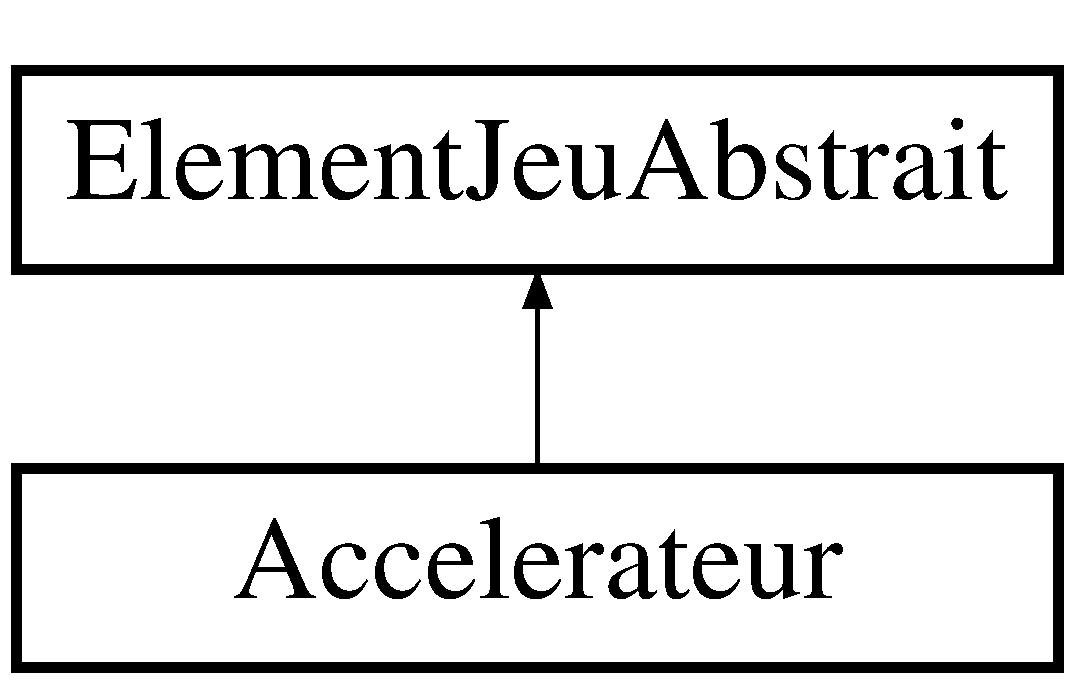
\includegraphics[height=2.000000cm]{class_accelerateur}
\end{center}
\end{figure}
\subsection*{Public Member Functions}
\begin{DoxyCompactItemize}
\item 
\hyperlink{group__inf2990_gaa9565cdb55e423b975ed39344f2c57a9}{Accelerateur} ()
\begin{DoxyCompactList}\small\item\em Constructeur. \end{DoxyCompactList}\item 
\hyperlink{group__inf2990_ga225372057b8bc81b0488af790df85fae}{Accelerateur} (\hyperlink{group__utilitaire_ga6b2956069f76c7e27df4f79f87e5a48c}{Vecteur3f} position\-Depart, \hyperlink{group__utilitaire_ga6b2956069f76c7e27df4f79f87e5a48c}{Vecteur3f} taille, \hyperlink{group__utilitaire_ga6b2956069f76c7e27df4f79f87e5a48c}{Vecteur3f} direction\-Vitesse, \hyperlink{fmod_8h_aeb841aa4b4b5f444b5d739d865b420af}{float} poids)
\item 
\hyperlink{group__inf2990_gac826e93cf1b9d277f38ca09d52636a43}{Accelerateur} (const \hyperlink{class_accelerateur}{Accelerateur} \&accelerateur)
\begin{DoxyCompactList}\small\item\em Constructeur par copie. \end{DoxyCompactList}\item 
virtual \hyperlink{group__inf2990_ga3e17016992773f130a44cd9f70249e85}{$\sim$\-Accelerateur} ()
\begin{DoxyCompactList}\small\item\em Destructeur. \end{DoxyCompactList}\item 
virtual \hyperlink{group___i_n_f2990-04_ga1d1cfd8ffb84e947f82999c682b666a7}{Type} \hyperlink{group__inf2990_ga2ee3174059cff90eda7941e20699f2c8}{get\-Type} ()
\begin{DoxyCompactList}\small\item\em Retourne le type de l'element. \end{DoxyCompactList}\item 
virtual \hyperlink{wglew_8h_aeea6e3dfae3acf232096f57d2d57f084}{void} \hyperlink{group__inf2990_ga5bfc1b71b8460b0d34667ab37e1881ff}{update} (\hyperlink{fmod_8h_aeb841aa4b4b5f444b5d739d865b420af}{float} delta\-T)
\begin{DoxyCompactList}\small\item\em Mise a jour. \end{DoxyCompactList}\item 
virtual \hyperlink{class_element_jeu_abstrait}{Element\-Jeu\-Abstrait} $\ast$ \hyperlink{group__inf2990_ga56f704dcb76a319389d98488226e2b55}{clone} () const 
\begin{DoxyCompactList}\small\item\em Permet de cloner l'element. \end{DoxyCompactList}\item 
virtual bool \hyperlink{group__inf2990_gadae7daa610394fcc68cdfc663e464595}{check\-Collision} (\hyperlink{class_vaisseau}{Vaisseau} $\ast$vaisseau)
\begin{DoxyCompactList}\small\item\em Permet de verifier la collision entre un accelerateur et un vaisseau ainsi que de la traiter. \end{DoxyCompactList}\item 
virtual bool \hyperlink{group__inf2990_ga5a2f46d23dac6e1999aaf918609c58fa}{check\-Collision} (\hyperlink{class_element_jeu_abstrait}{Element\-Jeu\-Abstrait} $\ast$element)
\item 
virtual bool \hyperlink{class_accelerateur_a508a92e1d984eeae57f1bbdd84c84322}{check\-Collision} (\hyperlink{class_accelerateur}{Accelerateur} $\ast$accelerateur)
\begin{DoxyCompactList}\small\item\em Methode pour verifier si une collision existe. \end{DoxyCompactList}\item 
virtual bool \hyperlink{class_accelerateur_aa85ee233f8bc86cf6c826acc0580e0a2}{check\-Collision} (\hyperlink{class_asteroide}{Asteroide} $\ast$asteroide)
\item 
virtual bool \hyperlink{class_accelerateur_a869783e0782c83f7eea473b618b14220}{check\-Collision} (\hyperlink{class_barriere}{Barriere} $\ast$barriere)
\item 
virtual bool \hyperlink{class_accelerateur_ab61bf9baed0ba9963341ca3d8fbf1c60}{check\-Collision} (\hyperlink{class_portail}{Portail} $\ast$portail)
\item 
virtual bool \hyperlink{class_accelerateur_ac7e350f65c76b6d5afdb3f42212e32f5}{check\-Collision} (\hyperlink{class_projectile}{Projectile} $\ast$projectile)
\item 
virtual bool \hyperlink{class_accelerateur_aeb1f74adbddbddf58d2dc09c8f6c2e34}{check\-Collision} (\hyperlink{class_station}{Station} $\ast$station)
\item 
virtual \hyperlink{wglew_8h_aeea6e3dfae3acf232096f57d2d57f084}{void} \hyperlink{group__inf2990_ga6a95509f0fcb19be7475a4a5474583a4}{traiter\-Collision} (\hyperlink{class_vaisseau}{Vaisseau} $\ast$vaisseau)
\item 
virtual \hyperlink{wglew_8h_aeea6e3dfae3acf232096f57d2d57f084}{void} \hyperlink{class_accelerateur_ab4e3a5f0fb2efdafe4ef6746068c73b0}{traiter\-Collision} (\hyperlink{class_element_jeu_abstrait}{Element\-Jeu\-Abstrait} $\ast$element)
\item 
virtual \hyperlink{wglew_8h_aeea6e3dfae3acf232096f57d2d57f084}{void} \hyperlink{class_accelerateur_ada602e23f6c55a15519d9b552ea3c58b}{traiter\-Collision} (\hyperlink{class_accelerateur}{Accelerateur} $\ast$accelerateur)
\begin{DoxyCompactList}\small\item\em Methode pour traiter la collision si elle a lui avec les differents elements. \end{DoxyCompactList}\item 
virtual \hyperlink{wglew_8h_aeea6e3dfae3acf232096f57d2d57f084}{void} \hyperlink{class_accelerateur_a883b1b41fa23cf033517a2da5f51ccbd}{traiter\-Collision} (\hyperlink{class_asteroide}{Asteroide} $\ast$asteroide)
\item 
virtual \hyperlink{wglew_8h_aeea6e3dfae3acf232096f57d2d57f084}{void} \hyperlink{class_accelerateur_a10595ee8cf0d6f79609733c543971a69}{traiter\-Collision} (\hyperlink{class_barriere}{Barriere} $\ast$barriere)
\item 
virtual \hyperlink{wglew_8h_aeea6e3dfae3acf232096f57d2d57f084}{void} \hyperlink{class_accelerateur_af07cb95ae53037e8947353254ee6ece5}{traiter\-Collision} (\hyperlink{class_portail}{Portail} $\ast$portail)
\item 
virtual \hyperlink{wglew_8h_aeea6e3dfae3acf232096f57d2d57f084}{void} \hyperlink{class_accelerateur_ab14c0dd64c691ee4d586dfeef881ec2b}{traiter\-Collision} (\hyperlink{class_position_depart}{Position\-Depart} $\ast$position\-Depart)
\item 
virtual \hyperlink{wglew_8h_aeea6e3dfae3acf232096f57d2d57f084}{void} \hyperlink{class_accelerateur_a7e55fed6f2d27c73b3b4063f5c992174}{traiter\-Collision} (\hyperlink{class_projectile}{Projectile} $\ast$projectile)
\item 
virtual \hyperlink{wglew_8h_aeea6e3dfae3acf232096f57d2d57f084}{void} \hyperlink{class_accelerateur_a6797ee1374e0cbff0e02b4374da67c35}{traiter\-Collision} (\hyperlink{class_station}{Station} $\ast$station)
\end{DoxyCompactItemize}
\subsection*{Static Public Attributes}
\begin{DoxyCompactItemize}
\item 
static const double \hyperlink{group__inf2990_ga9f211d39002f7446242da80a6c643945}{T\-E\-M\-P\-S\-\_\-\-D\-I\-N\-A\-C\-T\-I\-V\-I\-T\-E} = 5.\-0f
\end{DoxyCompactItemize}
\subsection*{Additional Inherited Members}


\subsection{Detailed Description}
Cette classe qui permet de creer des accelerateurs. 

La classe \hyperlink{class_accelerateur}{Accelerateur} contiendra un pointeur vers un noeud\-Accelerateur afin que celle-\/ci s'occupe de la texture de l'accelerateur. 

\subsection{Member Function Documentation}
\hypertarget{class_accelerateur_a508a92e1d984eeae57f1bbdd84c84322}{\index{Accelerateur@{Accelerateur}!check\-Collision@{check\-Collision}}
\index{check\-Collision@{check\-Collision}!Accelerateur@{Accelerateur}}
\subsubsection[{check\-Collision}]{\setlength{\rightskip}{0pt plus 5cm}virtual bool Accelerateur\-::check\-Collision (
\begin{DoxyParamCaption}
\item[{{\bf Accelerateur} $\ast$}]{accelerateur}
\end{DoxyParamCaption}
)\hspace{0.3cm}{\ttfamily [inline]}, {\ttfamily [virtual]}}}\label{class_accelerateur_a508a92e1d984eeae57f1bbdd84c84322}


Methode pour verifier si une collision existe. 



Implements \hyperlink{class_element_jeu_abstrait_a11071c15797deae04611da1a0642435a}{Element\-Jeu\-Abstrait}.

\hypertarget{class_accelerateur_aa85ee233f8bc86cf6c826acc0580e0a2}{\index{Accelerateur@{Accelerateur}!check\-Collision@{check\-Collision}}
\index{check\-Collision@{check\-Collision}!Accelerateur@{Accelerateur}}
\subsubsection[{check\-Collision}]{\setlength{\rightskip}{0pt plus 5cm}virtual bool Accelerateur\-::check\-Collision (
\begin{DoxyParamCaption}
\item[{{\bf Asteroide} $\ast$}]{asteroide}
\end{DoxyParamCaption}
)\hspace{0.3cm}{\ttfamily [inline]}, {\ttfamily [virtual]}}}\label{class_accelerateur_aa85ee233f8bc86cf6c826acc0580e0a2}


Implements \hyperlink{class_element_jeu_abstrait_ad1ffd24fa801a4e3c64e86a9886d690c}{Element\-Jeu\-Abstrait}.

\hypertarget{class_accelerateur_a869783e0782c83f7eea473b618b14220}{\index{Accelerateur@{Accelerateur}!check\-Collision@{check\-Collision}}
\index{check\-Collision@{check\-Collision}!Accelerateur@{Accelerateur}}
\subsubsection[{check\-Collision}]{\setlength{\rightskip}{0pt plus 5cm}virtual bool Accelerateur\-::check\-Collision (
\begin{DoxyParamCaption}
\item[{{\bf Barriere} $\ast$}]{barriere}
\end{DoxyParamCaption}
)\hspace{0.3cm}{\ttfamily [inline]}, {\ttfamily [virtual]}}}\label{class_accelerateur_a869783e0782c83f7eea473b618b14220}


Implements \hyperlink{class_element_jeu_abstrait_aebace6178f519dd1e5d845731ddb8063}{Element\-Jeu\-Abstrait}.

\hypertarget{class_accelerateur_ab61bf9baed0ba9963341ca3d8fbf1c60}{\index{Accelerateur@{Accelerateur}!check\-Collision@{check\-Collision}}
\index{check\-Collision@{check\-Collision}!Accelerateur@{Accelerateur}}
\subsubsection[{check\-Collision}]{\setlength{\rightskip}{0pt plus 5cm}virtual bool Accelerateur\-::check\-Collision (
\begin{DoxyParamCaption}
\item[{{\bf Portail} $\ast$}]{portail}
\end{DoxyParamCaption}
)\hspace{0.3cm}{\ttfamily [inline]}, {\ttfamily [virtual]}}}\label{class_accelerateur_ab61bf9baed0ba9963341ca3d8fbf1c60}


Implements \hyperlink{class_element_jeu_abstrait_a90210e78428103adf589e8c29c8076b0}{Element\-Jeu\-Abstrait}.

\hypertarget{class_accelerateur_ac7e350f65c76b6d5afdb3f42212e32f5}{\index{Accelerateur@{Accelerateur}!check\-Collision@{check\-Collision}}
\index{check\-Collision@{check\-Collision}!Accelerateur@{Accelerateur}}
\subsubsection[{check\-Collision}]{\setlength{\rightskip}{0pt plus 5cm}virtual bool Accelerateur\-::check\-Collision (
\begin{DoxyParamCaption}
\item[{{\bf Projectile} $\ast$}]{projectile}
\end{DoxyParamCaption}
)\hspace{0.3cm}{\ttfamily [inline]}, {\ttfamily [virtual]}}}\label{class_accelerateur_ac7e350f65c76b6d5afdb3f42212e32f5}


Implements \hyperlink{class_element_jeu_abstrait_aba1ceab5eb1460937054a77b2bf10fbc}{Element\-Jeu\-Abstrait}.

\hypertarget{class_accelerateur_aeb1f74adbddbddf58d2dc09c8f6c2e34}{\index{Accelerateur@{Accelerateur}!check\-Collision@{check\-Collision}}
\index{check\-Collision@{check\-Collision}!Accelerateur@{Accelerateur}}
\subsubsection[{check\-Collision}]{\setlength{\rightskip}{0pt plus 5cm}virtual bool Accelerateur\-::check\-Collision (
\begin{DoxyParamCaption}
\item[{{\bf Station} $\ast$}]{station}
\end{DoxyParamCaption}
)\hspace{0.3cm}{\ttfamily [inline]}, {\ttfamily [virtual]}}}\label{class_accelerateur_aeb1f74adbddbddf58d2dc09c8f6c2e34}


Implements \hyperlink{class_element_jeu_abstrait_adf9a2cc6ca52d89b93dbdb44ab932add}{Element\-Jeu\-Abstrait}.

\hypertarget{class_accelerateur_ab4e3a5f0fb2efdafe4ef6746068c73b0}{\index{Accelerateur@{Accelerateur}!traiter\-Collision@{traiter\-Collision}}
\index{traiter\-Collision@{traiter\-Collision}!Accelerateur@{Accelerateur}}
\subsubsection[{traiter\-Collision}]{\setlength{\rightskip}{0pt plus 5cm}virtual {\bf void} Accelerateur\-::traiter\-Collision (
\begin{DoxyParamCaption}
\item[{{\bf Element\-Jeu\-Abstrait} $\ast$}]{element\-Jeu}
\end{DoxyParamCaption}
)\hspace{0.3cm}{\ttfamily [inline]}, {\ttfamily [virtual]}}}\label{class_accelerateur_ab4e3a5f0fb2efdafe4ef6746068c73b0}
Methode qui permet d$<$effectuer le traitement de la collision avec le type d'objet La plupart du temps rien ne se passe.


\begin{DoxyParams}[1]{Parameters}
\mbox{\tt in}  & {\em element\-Jeu} & \-: l'autre objet avec lequel il faut verifier la collision\\
\hline
\end{DoxyParams}
\begin{DoxyReturn}{Returns}
Aucune. 
\end{DoxyReturn}


Implements \hyperlink{group__inf2990_gaaa60e09cf00bea42f27017e1a7a48e7b}{Element\-Jeu\-Abstrait}.

\hypertarget{class_accelerateur_ada602e23f6c55a15519d9b552ea3c58b}{\index{Accelerateur@{Accelerateur}!traiter\-Collision@{traiter\-Collision}}
\index{traiter\-Collision@{traiter\-Collision}!Accelerateur@{Accelerateur}}
\subsubsection[{traiter\-Collision}]{\setlength{\rightskip}{0pt plus 5cm}virtual {\bf void} Accelerateur\-::traiter\-Collision (
\begin{DoxyParamCaption}
\item[{{\bf Accelerateur} $\ast$}]{accelerateur}
\end{DoxyParamCaption}
)\hspace{0.3cm}{\ttfamily [inline]}, {\ttfamily [virtual]}}}\label{class_accelerateur_ada602e23f6c55a15519d9b552ea3c58b}


Methode pour traiter la collision si elle a lui avec les differents elements. 



Implements \hyperlink{class_element_jeu_abstrait_a22e8f47285f64372043dc89916c5eac5}{Element\-Jeu\-Abstrait}.

\hypertarget{class_accelerateur_a883b1b41fa23cf033517a2da5f51ccbd}{\index{Accelerateur@{Accelerateur}!traiter\-Collision@{traiter\-Collision}}
\index{traiter\-Collision@{traiter\-Collision}!Accelerateur@{Accelerateur}}
\subsubsection[{traiter\-Collision}]{\setlength{\rightskip}{0pt plus 5cm}virtual {\bf void} Accelerateur\-::traiter\-Collision (
\begin{DoxyParamCaption}
\item[{{\bf Asteroide} $\ast$}]{asteroide}
\end{DoxyParamCaption}
)\hspace{0.3cm}{\ttfamily [inline]}, {\ttfamily [virtual]}}}\label{class_accelerateur_a883b1b41fa23cf033517a2da5f51ccbd}


Implements \hyperlink{class_element_jeu_abstrait_af6218ea1d9fc026a8f39fbe09a90bfa0}{Element\-Jeu\-Abstrait}.

\hypertarget{class_accelerateur_a10595ee8cf0d6f79609733c543971a69}{\index{Accelerateur@{Accelerateur}!traiter\-Collision@{traiter\-Collision}}
\index{traiter\-Collision@{traiter\-Collision}!Accelerateur@{Accelerateur}}
\subsubsection[{traiter\-Collision}]{\setlength{\rightskip}{0pt plus 5cm}virtual {\bf void} Accelerateur\-::traiter\-Collision (
\begin{DoxyParamCaption}
\item[{{\bf Barriere} $\ast$}]{barriere}
\end{DoxyParamCaption}
)\hspace{0.3cm}{\ttfamily [inline]}, {\ttfamily [virtual]}}}\label{class_accelerateur_a10595ee8cf0d6f79609733c543971a69}


Implements \hyperlink{class_element_jeu_abstrait_a97210da984bc5f5024f603e6aba2130f}{Element\-Jeu\-Abstrait}.

\hypertarget{class_accelerateur_af07cb95ae53037e8947353254ee6ece5}{\index{Accelerateur@{Accelerateur}!traiter\-Collision@{traiter\-Collision}}
\index{traiter\-Collision@{traiter\-Collision}!Accelerateur@{Accelerateur}}
\subsubsection[{traiter\-Collision}]{\setlength{\rightskip}{0pt plus 5cm}virtual {\bf void} Accelerateur\-::traiter\-Collision (
\begin{DoxyParamCaption}
\item[{{\bf Portail} $\ast$}]{portail}
\end{DoxyParamCaption}
)\hspace{0.3cm}{\ttfamily [inline]}, {\ttfamily [virtual]}}}\label{class_accelerateur_af07cb95ae53037e8947353254ee6ece5}


Implements \hyperlink{class_element_jeu_abstrait_a2500f6eadb72cb87d1fdc2aa96f4d69b}{Element\-Jeu\-Abstrait}.

\hypertarget{class_accelerateur_ab14c0dd64c691ee4d586dfeef881ec2b}{\index{Accelerateur@{Accelerateur}!traiter\-Collision@{traiter\-Collision}}
\index{traiter\-Collision@{traiter\-Collision}!Accelerateur@{Accelerateur}}
\subsubsection[{traiter\-Collision}]{\setlength{\rightskip}{0pt plus 5cm}virtual {\bf void} Accelerateur\-::traiter\-Collision (
\begin{DoxyParamCaption}
\item[{{\bf Position\-Depart} $\ast$}]{position\-Depart}
\end{DoxyParamCaption}
)\hspace{0.3cm}{\ttfamily [inline]}, {\ttfamily [virtual]}}}\label{class_accelerateur_ab14c0dd64c691ee4d586dfeef881ec2b}
\hypertarget{class_accelerateur_a7e55fed6f2d27c73b3b4063f5c992174}{\index{Accelerateur@{Accelerateur}!traiter\-Collision@{traiter\-Collision}}
\index{traiter\-Collision@{traiter\-Collision}!Accelerateur@{Accelerateur}}
\subsubsection[{traiter\-Collision}]{\setlength{\rightskip}{0pt plus 5cm}virtual {\bf void} Accelerateur\-::traiter\-Collision (
\begin{DoxyParamCaption}
\item[{{\bf Projectile} $\ast$}]{projectile}
\end{DoxyParamCaption}
)\hspace{0.3cm}{\ttfamily [inline]}, {\ttfamily [virtual]}}}\label{class_accelerateur_a7e55fed6f2d27c73b3b4063f5c992174}


Implements \hyperlink{class_element_jeu_abstrait_ab06625e0b65cd4e3c96893b2a30ca110}{Element\-Jeu\-Abstrait}.

\hypertarget{class_accelerateur_a6797ee1374e0cbff0e02b4374da67c35}{\index{Accelerateur@{Accelerateur}!traiter\-Collision@{traiter\-Collision}}
\index{traiter\-Collision@{traiter\-Collision}!Accelerateur@{Accelerateur}}
\subsubsection[{traiter\-Collision}]{\setlength{\rightskip}{0pt plus 5cm}virtual {\bf void} Accelerateur\-::traiter\-Collision (
\begin{DoxyParamCaption}
\item[{{\bf Station} $\ast$}]{station}
\end{DoxyParamCaption}
)\hspace{0.3cm}{\ttfamily [inline]}, {\ttfamily [virtual]}}}\label{class_accelerateur_a6797ee1374e0cbff0e02b4374da67c35}


Implements \hyperlink{class_element_jeu_abstrait_aa757ff192c8fb88de966112d58fdc2a9}{Element\-Jeu\-Abstrait}.



The documentation for this class was generated from the following files\-:\begin{DoxyCompactItemize}
\item 
Cadriciel/\-Sources/\-C++/\-Element\-Objet/\hyperlink{_accelerateur_8h}{Accelerateur.\-h}\item 
Cadriciel/\-Sources/\-C++/\-Element\-Objet/\hyperlink{_accelerateur_8cpp}{Accelerateur.\-cpp}\item 
Cadriciel/\-Sources/\-C++/\-Element\-Objet/\hyperlink{_projectile_8cpp}{Projectile.\-cpp}\end{DoxyCompactItemize}

\hypertarget{class_additional_message}{\section{Additional\-Message Class Reference}
\label{class_additional_message}\index{Additional\-Message@{Additional\-Message}}
}


An additional \hyperlink{class_message}{Message} for assertions.

Provides a implicit constructor that takes a single string. This allow this class to be used as the message arguments in macros.  




{\ttfamily \#include $<$Additional\-Message.\-h$>$}

Inheritance diagram for Additional\-Message\-:\begin{figure}[H]
\begin{center}
\leavevmode
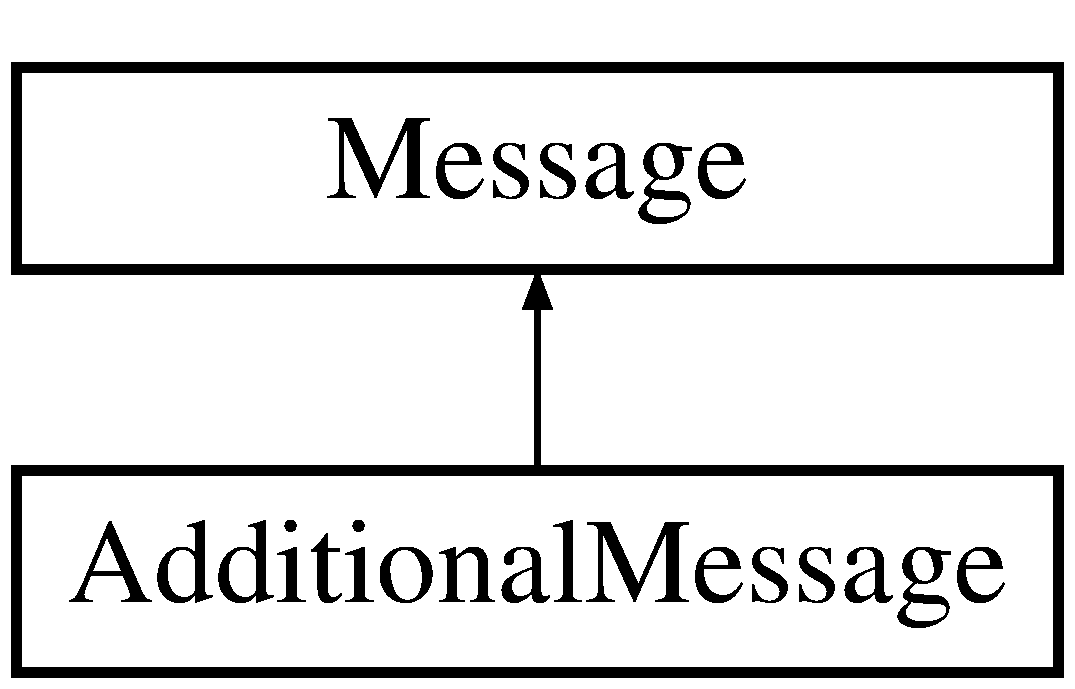
\includegraphics[height=2.000000cm]{class_additional_message}
\end{center}
\end{figure}
\subsection*{Public Types}
\begin{DoxyCompactItemize}
\item 
typedef \hyperlink{class_message}{Message} \hyperlink{class_additional_message_abc8626e28c147b5ddd66032a35676126}{Super\-Class}
\end{DoxyCompactItemize}
\subsection*{Public Member Functions}
\begin{DoxyCompactItemize}
\item 
\hyperlink{class_additional_message_a888715179848c5e5c385789b962a3cfb}{Additional\-Message} ()
\begin{DoxyCompactList}\small\item\em Constructs an empty \hyperlink{class_message}{Message}. \end{DoxyCompactList}\item 
\hyperlink{class_additional_message_a990455bbfe260bc04f99e5acc58d1c06}{Additional\-Message} (const \hyperlink{glew_8h_ae84541b4f3d8e1ea24ec0f466a8c568b}{std\-::string} \&detail1)
\begin{DoxyCompactList}\small\item\em Constructs a \hyperlink{class_message}{Message} with the specified detail string. \end{DoxyCompactList}\item 
\hyperlink{class_additional_message_a6486540f9b5d1957230e9e1f969adc9d}{Additional\-Message} (const char $\ast$detail1)
\begin{DoxyCompactList}\small\item\em Constructs a \hyperlink{class_message}{Message} with the specified detail string. \end{DoxyCompactList}\item 
\hyperlink{class_additional_message_a75735b6fd65686f31349d01c97c73bc7}{Additional\-Message} (const \hyperlink{class_message}{Message} \&other)
\begin{DoxyCompactList}\small\item\em Constructs a copy of the specified message. \end{DoxyCompactList}\item 
\hyperlink{class_additional_message}{Additional\-Message} \& \hyperlink{class_additional_message_abbda0de4323f70ff01a9b622a6f550f7}{operator=} (const \hyperlink{class_message}{Message} \&other)
\begin{DoxyCompactList}\small\item\em Assignment operator. \end{DoxyCompactList}\end{DoxyCompactItemize}


\subsection{Detailed Description}
An additional \hyperlink{class_message}{Message} for assertions.

Provides a implicit constructor that takes a single string. This allow this class to be used as the message arguments in macros. 

The constructed object is either a \hyperlink{class_message}{Message} with a single detail string if a string was passed to the macro, or a copy of the \hyperlink{class_message}{Message} passed to the macro.

Here is an example of usage\-: 
\begin{DoxyCode}
\textcolor{keywordtype}{void} checkStringEquals( \textcolor{keyword}{const} \hyperlink{glew_8h_ae84541b4f3d8e1ea24ec0f466a8c568b}{std::string} &expected,
                       \textcolor{keyword}{const} \hyperlink{glew_8h_ae84541b4f3d8e1ea24ec0f466a8c568b}{std::string} &actual,
                        \textcolor{keyword}{const} CppUnit::SourceLine &sourceLine,
                        \textcolor{keyword}{const} CppUnit::AdditionalMessage &\hyperlink{glew_8h_a76333d9470ffdd4811326932394d36da}{message} );

\textcolor{preprocessor}{#define XTLUT\_ASSERT\_STRING\_EQUAL\_MESSAGE( expected, actual, message )  \(\backslash\)}
\textcolor{preprocessor}{  ::XtlUt::Impl::checkStringEquals( ::Xtl::toString(expected),        \(\backslash\)}
\textcolor{preprocessor}{                                    ::Xtl::toString(actual),          \(\backslash\)}
\textcolor{preprocessor}{                                    CPPUNIT\_SOURCELINE(),             \(\backslash\)}
\textcolor{preprocessor}{                                    message )}
\end{DoxyCode}


In the previous example, the user can specify a simple string for {\itshape message}, or a complex \hyperlink{class_message}{Message} object.

\begin{DoxySeeAlso}{See Also}
\hyperlink{class_message}{Message} 
\end{DoxySeeAlso}


\subsection{Member Typedef Documentation}
\hypertarget{class_additional_message_abc8626e28c147b5ddd66032a35676126}{\index{Additional\-Message@{Additional\-Message}!Super\-Class@{Super\-Class}}
\index{Super\-Class@{Super\-Class}!AdditionalMessage@{Additional\-Message}}
\subsubsection[{Super\-Class}]{\setlength{\rightskip}{0pt plus 5cm}typedef {\bf Message} {\bf Additional\-Message\-::\-Super\-Class}}}\label{class_additional_message_abc8626e28c147b5ddd66032a35676126}


\subsection{Constructor \& Destructor Documentation}
\hypertarget{class_additional_message_a888715179848c5e5c385789b962a3cfb}{\index{Additional\-Message@{Additional\-Message}!Additional\-Message@{Additional\-Message}}
\index{Additional\-Message@{Additional\-Message}!AdditionalMessage@{Additional\-Message}}
\subsubsection[{Additional\-Message}]{\setlength{\rightskip}{0pt plus 5cm}Additional\-Message\-::\-Additional\-Message (
\begin{DoxyParamCaption}
{}
\end{DoxyParamCaption}
)}}\label{class_additional_message_a888715179848c5e5c385789b962a3cfb}


Constructs an empty \hyperlink{class_message}{Message}. 

\hypertarget{class_additional_message_a990455bbfe260bc04f99e5acc58d1c06}{\index{Additional\-Message@{Additional\-Message}!Additional\-Message@{Additional\-Message}}
\index{Additional\-Message@{Additional\-Message}!AdditionalMessage@{Additional\-Message}}
\subsubsection[{Additional\-Message}]{\setlength{\rightskip}{0pt plus 5cm}Additional\-Message\-::\-Additional\-Message (
\begin{DoxyParamCaption}
\item[{const {\bf std\-::string} \&}]{detail1}
\end{DoxyParamCaption}
)}}\label{class_additional_message_a990455bbfe260bc04f99e5acc58d1c06}


Constructs a \hyperlink{class_message}{Message} with the specified detail string. 


\begin{DoxyParams}{Parameters}
{\em detail1} & Detail string of the message. If empty, then it is not added. \\
\hline
\end{DoxyParams}
\hypertarget{class_additional_message_a6486540f9b5d1957230e9e1f969adc9d}{\index{Additional\-Message@{Additional\-Message}!Additional\-Message@{Additional\-Message}}
\index{Additional\-Message@{Additional\-Message}!AdditionalMessage@{Additional\-Message}}
\subsubsection[{Additional\-Message}]{\setlength{\rightskip}{0pt plus 5cm}Additional\-Message\-::\-Additional\-Message (
\begin{DoxyParamCaption}
\item[{const char $\ast$}]{detail1}
\end{DoxyParamCaption}
)}}\label{class_additional_message_a6486540f9b5d1957230e9e1f969adc9d}


Constructs a \hyperlink{class_message}{Message} with the specified detail string. 


\begin{DoxyParams}{Parameters}
{\em detail1} & Detail string of the message. If empty, then it is not added. \\
\hline
\end{DoxyParams}
\hypertarget{class_additional_message_a75735b6fd65686f31349d01c97c73bc7}{\index{Additional\-Message@{Additional\-Message}!Additional\-Message@{Additional\-Message}}
\index{Additional\-Message@{Additional\-Message}!AdditionalMessage@{Additional\-Message}}
\subsubsection[{Additional\-Message}]{\setlength{\rightskip}{0pt plus 5cm}Additional\-Message\-::\-Additional\-Message (
\begin{DoxyParamCaption}
\item[{const {\bf Message} \&}]{other}
\end{DoxyParamCaption}
)}}\label{class_additional_message_a75735b6fd65686f31349d01c97c73bc7}


Constructs a copy of the specified message. 


\begin{DoxyParams}{Parameters}
{\em other} & \hyperlink{class_message}{Message} to copy. \\
\hline
\end{DoxyParams}


\subsection{Member Function Documentation}
\hypertarget{class_additional_message_abbda0de4323f70ff01a9b622a6f550f7}{\index{Additional\-Message@{Additional\-Message}!operator=@{operator=}}
\index{operator=@{operator=}!AdditionalMessage@{Additional\-Message}}
\subsubsection[{operator=}]{\setlength{\rightskip}{0pt plus 5cm}{\bf Additional\-Message}\& Additional\-Message\-::operator= (
\begin{DoxyParamCaption}
\item[{const {\bf Message} \&}]{other}
\end{DoxyParamCaption}
)}}\label{class_additional_message_abbda0de4323f70ff01a9b622a6f550f7}


Assignment operator. 


\begin{DoxyParams}{Parameters}
{\em other} & \hyperlink{class_message}{Message} to copy. \\
\hline
\end{DoxyParams}
\begin{DoxyReturn}{Returns}
Reference on this object. 
\end{DoxyReturn}


The documentation for this class was generated from the following file\-:\begin{DoxyCompactItemize}
\item 
Cadriciel/\-Commun/\-Externe/cppunit/include/cppunit/\hyperlink{_additional_message_8h}{Additional\-Message.\-h}\end{DoxyCompactItemize}

\hypertarget{class_affichage_debogage}{\section{Affichage\-Debogage Class Reference}
\label{class_affichage_debogage}\index{Affichage\-Debogage@{Affichage\-Debogage}}
}


Classe permettant d'afficher a l'ecran et a la console des informations concernant la partie en cours. Cette classe impl�mente le patron singleton.  




{\ttfamily \#include $<$Affichage\-Debogage.\-h$>$}

\subsection*{Public Member Functions}
\begin{DoxyCompactItemize}
\item 
\hyperlink{wglew_8h_aeea6e3dfae3acf232096f57d2d57f084}{void} \hyperlink{group__inf2990_ga8a57681d7c42ad8236057b5ef28efe9e}{afficher\-Apparition\-Asteroide} (\hyperlink{structai_vector3_d}{ai\-Vector3\-D} \hyperlink{fmod__codec_8h_a7d71cf36b6a2fc185ecbc89f93fa58a3}{position}, \hyperlink{structai_vector3_d}{ai\-Vector3\-D} vitesse, \hyperlink{_free_image_8h_a425076c7067a1b5166e2cc530e914814}{unsigned} \hyperlink{wglew_8h_a500a82aecba06f4550f6849b8099ca21}{int} taille) const 
\item 
\hyperlink{wglew_8h_aeea6e3dfae3acf232096f57d2d57f084}{void} \hyperlink{group__inf2990_ga859ee15b94c0d5bfcdbe94377cd00cc8}{afficher\-Changement\-Mode\-Joueur\-Virtuel} (\hyperlink{_vaisseau_virtuel_8h_a46c8a310cf4c094f8c80e1cb8dc1f911}{Mode} \hyperlink{glew_8h_a1e71d9c196e4683cc06c4b54d53f7ef5}{mode}) const 
\item 
\hyperlink{wglew_8h_aeea6e3dfae3acf232096f57d2d57f084}{void} \hyperlink{group__inf2990_gad0a7eb6b2527603c50a7393f277b34f6}{afficher\-Modification\-Eclairage} (\hyperlink{_free_image_8h_a425076c7067a1b5166e2cc530e914814}{unsigned} \hyperlink{wglew_8h_a500a82aecba06f4550f6849b8099ca21}{int} type\-Lumiere, bool etat\-Actuel) const 
\item 
\hyperlink{wglew_8h_aeea6e3dfae3acf232096f57d2d57f084}{void} \hyperlink{group__inf2990_ga4e4ae3a48fc1532361b1b074c88e8770}{afficher\-Rayon\-Attraction} (const \hyperlink{class_noeud_portail}{Noeud\-Portail} $\ast$n\-Portail) const 
\item 
\hyperlink{wglew_8h_aeea6e3dfae3acf232096f57d2d57f084}{void} \hyperlink{group__inf2990_ga9d116e9d9669a6b53c314c2f322d1e80}{afficher\-Asteroide\-Cible\-Joueur\-Virtuel} (const \hyperlink{class_noeud_asteroide}{Noeud\-Asteroide} $\ast$n\-Asteroide) const 
\item 
\hyperlink{wglew_8h_aeea6e3dfae3acf232096f57d2d57f084}{void} \hyperlink{group__inf2990_gac7c0d459681e4ffb4401b12d2bc61e5d}{afficher\-Zone\-Passage} (const \hyperlink{class_carte}{Carte} $\ast$carte) const 
\item 
\hyperlink{wglew_8h_aeea6e3dfae3acf232096f57d2d57f084}{void} \hyperlink{group__inf2990_ga36341f3d350549056a074ad14bf3880e}{afficher\-Cadre\-Depart} (const \hyperlink{class_carte}{Carte} $\ast$carte) const 
\item 
\hyperlink{wglew_8h_aeea6e3dfae3acf232096f57d2d57f084}{void} \hyperlink{group__inf2990_ga0519ec698d8de87608c185fa3f56434b}{set\-Afficher\-Apparition\-Asteroide} (bool affichage)
\item 
\hyperlink{wglew_8h_aeea6e3dfae3acf232096f57d2d57f084}{void} \hyperlink{group__inf2990_ga58969139d167e116fe05d081f7e8304c}{set\-Afficher\-Changement\-Mode\-Joueur\-Virtuel} (bool affichage)
\item 
\hyperlink{wglew_8h_aeea6e3dfae3acf232096f57d2d57f084}{void} \hyperlink{group__inf2990_gaac0e7f2de4d847cd0cd5ee77435b67df}{set\-Afficher\-Modification\-Eclairage} (bool affichage)
\item 
\hyperlink{wglew_8h_aeea6e3dfae3acf232096f57d2d57f084}{void} \hyperlink{group__inf2990_ga732a1042486d7729906676b5bb4e30cb}{set\-Afficher\-Rayon\-Attraction} (bool affichage)
\item 
\hyperlink{wglew_8h_aeea6e3dfae3acf232096f57d2d57f084}{void} \hyperlink{group__inf2990_gaef1a4a54177d38b3b3242835af0ee5a7}{set\-Afficher\-Asteroide\-Cible} (bool affichage)
\item 
\hyperlink{wglew_8h_aeea6e3dfae3acf232096f57d2d57f084}{void} \hyperlink{group__inf2990_ga777c1ab47b02585102e5cf1bbd25f2a6}{set\-Afficher\-Zone\-Passage} (bool affichage)
\item 
\hyperlink{wglew_8h_aeea6e3dfae3acf232096f57d2d57f084}{void} \hyperlink{group__inf2990_gac08dedf16e09cee06a5d815a1268599e}{set\-Afficher\-Cadre\-Depart} (bool affichage)
\end{DoxyCompactItemize}
\subsection*{Static Public Member Functions}
\begin{DoxyCompactItemize}
\item 
static \hyperlink{class_affichage_debogage}{Affichage\-Debogage} $\ast$ \hyperlink{group__inf2990_ga75029aabd993101665737c9fdcb5e750}{obtenir\-Instance} ()
\end{DoxyCompactItemize}


\subsection{Detailed Description}
Classe permettant d'afficher a l'ecran et a la console des informations concernant la partie en cours. Cette classe impl�mente le patron singleton. 

\begin{DoxyAuthor}{Author}
Vincent Longpre 
\end{DoxyAuthor}
\begin{DoxyDate}{Date}
2014-\/02-\/25 
\end{DoxyDate}


The documentation for this class was generated from the following files\-:\begin{DoxyCompactItemize}
\item 
Cadriciel/\-Sources/\-C++/\-Application/\hyperlink{_affichage_debogage_8h}{Affichage\-Debogage.\-h}\item 
Cadriciel/\-Sources/\-C++/\-Application/\hyperlink{_affichage_debogage_8cpp}{Affichage\-Debogage.\-cpp}\end{DoxyCompactItemize}

\hypertarget{struct_a_f_m___font_info_rec__}{\section{A\-F\-M\-\_\-\-Font\-Info\-Rec\-\_\- Struct Reference}
\label{struct_a_f_m___font_info_rec__}\index{A\-F\-M\-\_\-\-Font\-Info\-Rec\-\_\-@{A\-F\-M\-\_\-\-Font\-Info\-Rec\-\_\-}}
}
\subsection*{Public Attributes}
\begin{DoxyCompactItemize}
\item 
\hypertarget{struct_a_f_m___font_info_rec___a6f198e74da5d8a3b7ff7518e255be231}{F\-T\-\_\-\-Bool {\bfseries Is\-C\-I\-D\-Font}}\label{struct_a_f_m___font_info_rec___a6f198e74da5d8a3b7ff7518e255be231}

\item 
\hypertarget{struct_a_f_m___font_info_rec___afa5112d6b0cc51839889206012dc1be6}{\hyperlink{struct_f_t___b_box__}{F\-T\-\_\-\-B\-Box} {\bfseries Font\-B\-Box}}\label{struct_a_f_m___font_info_rec___afa5112d6b0cc51839889206012dc1be6}

\item 
\hypertarget{struct_a_f_m___font_info_rec___a0b80412562435a2198a71aa4188ee85b}{F\-T\-\_\-\-Fixed {\bfseries Ascender}}\label{struct_a_f_m___font_info_rec___a0b80412562435a2198a71aa4188ee85b}

\item 
\hypertarget{struct_a_f_m___font_info_rec___a3561507200f0bc3413988af920924053}{F\-T\-\_\-\-Fixed {\bfseries Descender}}\label{struct_a_f_m___font_info_rec___a3561507200f0bc3413988af920924053}

\item 
\hypertarget{struct_a_f_m___font_info_rec___a8d9305229a1dacc15b8fceb5dbf25b9d}{\hyperlink{struct_a_f_m___track_kern_rec__}{A\-F\-M\-\_\-\-Track\-Kern} {\bfseries Track\-Kerns}}\label{struct_a_f_m___font_info_rec___a8d9305229a1dacc15b8fceb5dbf25b9d}

\item 
\hypertarget{struct_a_f_m___font_info_rec___a08a9207e8d4b0dd9dc0313218462f00e}{F\-T\-\_\-\-Int {\bfseries Num\-Track\-Kern}}\label{struct_a_f_m___font_info_rec___a08a9207e8d4b0dd9dc0313218462f00e}

\item 
\hypertarget{struct_a_f_m___font_info_rec___a16c5da5249d4d4f68cc169469f3ee75a}{\hyperlink{struct_a_f_m___kern_pair_rec__}{A\-F\-M\-\_\-\-Kern\-Pair} {\bfseries Kern\-Pairs}}\label{struct_a_f_m___font_info_rec___a16c5da5249d4d4f68cc169469f3ee75a}

\item 
\hypertarget{struct_a_f_m___font_info_rec___a8ff8af3c83fbf0b060bb711b57f1affd}{F\-T\-\_\-\-Int {\bfseries Num\-Kern\-Pair}}\label{struct_a_f_m___font_info_rec___a8ff8af3c83fbf0b060bb711b57f1affd}

\end{DoxyCompactItemize}


The documentation for this struct was generated from the following file\-:\begin{DoxyCompactItemize}
\item 
Cadriciel/\-Commun/\-Externe/\-Free\-Type/include/freetype/internal/t1types.\-h\end{DoxyCompactItemize}

\hypertarget{struct_a_f_m___kern_pair_rec__}{\section{A\-F\-M\-\_\-\-Kern\-Pair\-Rec\-\_\- Struct Reference}
\label{struct_a_f_m___kern_pair_rec__}\index{A\-F\-M\-\_\-\-Kern\-Pair\-Rec\-\_\-@{A\-F\-M\-\_\-\-Kern\-Pair\-Rec\-\_\-}}
}
\subsection*{Public Attributes}
\begin{DoxyCompactItemize}
\item 
\hypertarget{struct_a_f_m___kern_pair_rec___a732bca56dd4a070b1d887ada1637e810}{F\-T\-\_\-\-Int {\bfseries index1}}\label{struct_a_f_m___kern_pair_rec___a732bca56dd4a070b1d887ada1637e810}

\item 
\hypertarget{struct_a_f_m___kern_pair_rec___aee548123779323c255180112c7f5b831}{F\-T\-\_\-\-Int {\bfseries index2}}\label{struct_a_f_m___kern_pair_rec___aee548123779323c255180112c7f5b831}

\item 
\hypertarget{struct_a_f_m___kern_pair_rec___a4b7f90a0e17ed89353fec14ddb29fa12}{F\-T\-\_\-\-Int {\bfseries x}}\label{struct_a_f_m___kern_pair_rec___a4b7f90a0e17ed89353fec14ddb29fa12}

\item 
\hypertarget{struct_a_f_m___kern_pair_rec___aa177aa612e79701261eba72c76ea3f08}{F\-T\-\_\-\-Int {\bfseries y}}\label{struct_a_f_m___kern_pair_rec___aa177aa612e79701261eba72c76ea3f08}

\end{DoxyCompactItemize}


The documentation for this struct was generated from the following file\-:\begin{DoxyCompactItemize}
\item 
Cadriciel/\-Commun/\-Externe/\-Free\-Type/include/freetype/internal/t1types.\-h\end{DoxyCompactItemize}

\hypertarget{struct_a_f_m___parser___funcs_rec__}{\section{A\-F\-M\-\_\-\-Parser\-\_\-\-Funcs\-Rec\-\_\- Struct Reference}
\label{struct_a_f_m___parser___funcs_rec__}\index{A\-F\-M\-\_\-\-Parser\-\_\-\-Funcs\-Rec\-\_\-@{A\-F\-M\-\_\-\-Parser\-\_\-\-Funcs\-Rec\-\_\-}}
}
\subsection*{Public Attributes}
\begin{DoxyCompactItemize}
\item 
\hypertarget{struct_a_f_m___parser___funcs_rec___a7d5c1422c71ef00984f1207ebfb0b082}{F\-T\-\_\-\-Error($\ast$ {\bfseries init} )(\hyperlink{struct_a_f_m___parser_rec__}{A\-F\-M\-\_\-\-Parser} parser, F\-T\-\_\-\-Memory memory, F\-T\-\_\-\-Byte $\ast$base, F\-T\-\_\-\-Byte $\ast$limit)}\label{struct_a_f_m___parser___funcs_rec___a7d5c1422c71ef00984f1207ebfb0b082}

\item 
\hypertarget{struct_a_f_m___parser___funcs_rec___af4e8bc33b14d14b47d13caf0a2449d1b}{void($\ast$ {\bfseries done} )(\hyperlink{struct_a_f_m___parser_rec__}{A\-F\-M\-\_\-\-Parser} parser)}\label{struct_a_f_m___parser___funcs_rec___af4e8bc33b14d14b47d13caf0a2449d1b}

\item 
\hypertarget{struct_a_f_m___parser___funcs_rec___a2cd41be89cf12f9227c6f18220cbe2f3}{F\-T\-\_\-\-Error($\ast$ {\bfseries parse} )(\hyperlink{struct_a_f_m___parser_rec__}{A\-F\-M\-\_\-\-Parser} parser)}\label{struct_a_f_m___parser___funcs_rec___a2cd41be89cf12f9227c6f18220cbe2f3}

\end{DoxyCompactItemize}


The documentation for this struct was generated from the following file\-:\begin{DoxyCompactItemize}
\item 
Cadriciel/\-Commun/\-Externe/\-Free\-Type/include/freetype/internal/psaux.\-h\end{DoxyCompactItemize}

\hypertarget{struct_a_f_m___parser_rec__}{\section{A\-F\-M\-\_\-\-Parser\-Rec\-\_\- Struct Reference}
\label{struct_a_f_m___parser_rec__}\index{A\-F\-M\-\_\-\-Parser\-Rec\-\_\-@{A\-F\-M\-\_\-\-Parser\-Rec\-\_\-}}
}


{\ttfamily \#include $<$psaux.\-h$>$}

\subsection*{Public Attributes}
\begin{DoxyCompactItemize}
\item 
\hyperlink{ftsystem_8h_a67ec7ea35cde99a89a65e9f827a9ad3a}{F\-T\-\_\-\-Memory} \hyperlink{struct_a_f_m___parser_rec___a3fec8b1760fa9261f48ee87dc2b3858b}{memory}
\item 
\hyperlink{psaux_8h_af4e38d53e29cf02398d053dc7e26fa68}{A\-F\-M\-\_\-\-Stream} \hyperlink{struct_a_f_m___parser_rec___adf3b1165216cbd1f7ec7ae736fd4270a}{stream}
\item 
\hyperlink{t1types_8h_a777f9b8cdbac8c166fa6f1637d08c339}{A\-F\-M\-\_\-\-Font\-Info} \hyperlink{struct_a_f_m___parser_rec___ae53d6cddac32a0eb7014c3a9f74517df}{Font\-Info}
\item 
\hyperlink{fttypes_8h_af90e5fb0d07e21be9fe6faa33f02484c}{F\-T\-\_\-\-Int}($\ast$ \hyperlink{struct_a_f_m___parser_rec___a5f93c5c83d0957c19d3827071d90926f}{get\-\_\-index} )(const char $\ast$\hyperlink{fmod__codec_8h_a5c4947d4516dd7cfa3505ce3a648a4ef}{name}, \hyperlink{fttypes_8h_af7b5edd727ac01b0d4729ac848bd4175}{F\-T\-\_\-\-Offset} \hyperlink{glew_8h_a652168017ea9a8bbcead03d5c16269fb}{len}, \hyperlink{wglew_8h_aeea6e3dfae3acf232096f57d2d57f084}{void} $\ast$\hyperlink{struct_a_f_m___parser_rec___a9fa78a781737bf27e00448c5092b7657}{user\-\_\-data})
\item 
\hyperlink{wglew_8h_aeea6e3dfae3acf232096f57d2d57f084}{void} $\ast$ \hyperlink{struct_a_f_m___parser_rec___a9fa78a781737bf27e00448c5092b7657}{user\-\_\-data}
\end{DoxyCompactItemize}


\subsection{Member Data Documentation}
\hypertarget{struct_a_f_m___parser_rec___ae53d6cddac32a0eb7014c3a9f74517df}{\index{A\-F\-M\-\_\-\-Parser\-Rec\-\_\-@{A\-F\-M\-\_\-\-Parser\-Rec\-\_\-}!Font\-Info@{Font\-Info}}
\index{Font\-Info@{Font\-Info}!AFM_ParserRec_@{A\-F\-M\-\_\-\-Parser\-Rec\-\_\-}}
\subsubsection[{Font\-Info}]{\setlength{\rightskip}{0pt plus 5cm}{\bf A\-F\-M\-\_\-\-Font\-Info} A\-F\-M\-\_\-\-Parser\-Rec\-\_\-\-::\-Font\-Info}}\label{struct_a_f_m___parser_rec___ae53d6cddac32a0eb7014c3a9f74517df}
\hypertarget{struct_a_f_m___parser_rec___a5f93c5c83d0957c19d3827071d90926f}{\index{A\-F\-M\-\_\-\-Parser\-Rec\-\_\-@{A\-F\-M\-\_\-\-Parser\-Rec\-\_\-}!get\-\_\-index@{get\-\_\-index}}
\index{get\-\_\-index@{get\-\_\-index}!AFM_ParserRec_@{A\-F\-M\-\_\-\-Parser\-Rec\-\_\-}}
\subsubsection[{get\-\_\-index}]{\setlength{\rightskip}{0pt plus 5cm}{\bf F\-T\-\_\-\-Int}($\ast$ A\-F\-M\-\_\-\-Parser\-Rec\-\_\-\-::get\-\_\-index)(const char $\ast${\bf name}, {\bf F\-T\-\_\-\-Offset} {\bf len}, {\bf void} $\ast${\bf user\-\_\-data})}}\label{struct_a_f_m___parser_rec___a5f93c5c83d0957c19d3827071d90926f}
\hypertarget{struct_a_f_m___parser_rec___a3fec8b1760fa9261f48ee87dc2b3858b}{\index{A\-F\-M\-\_\-\-Parser\-Rec\-\_\-@{A\-F\-M\-\_\-\-Parser\-Rec\-\_\-}!memory@{memory}}
\index{memory@{memory}!AFM_ParserRec_@{A\-F\-M\-\_\-\-Parser\-Rec\-\_\-}}
\subsubsection[{memory}]{\setlength{\rightskip}{0pt plus 5cm}{\bf F\-T\-\_\-\-Memory} A\-F\-M\-\_\-\-Parser\-Rec\-\_\-\-::memory}}\label{struct_a_f_m___parser_rec___a3fec8b1760fa9261f48ee87dc2b3858b}
\hypertarget{struct_a_f_m___parser_rec___adf3b1165216cbd1f7ec7ae736fd4270a}{\index{A\-F\-M\-\_\-\-Parser\-Rec\-\_\-@{A\-F\-M\-\_\-\-Parser\-Rec\-\_\-}!stream@{stream}}
\index{stream@{stream}!AFM_ParserRec_@{A\-F\-M\-\_\-\-Parser\-Rec\-\_\-}}
\subsubsection[{stream}]{\setlength{\rightskip}{0pt plus 5cm}{\bf A\-F\-M\-\_\-\-Stream} A\-F\-M\-\_\-\-Parser\-Rec\-\_\-\-::stream}}\label{struct_a_f_m___parser_rec___adf3b1165216cbd1f7ec7ae736fd4270a}
\hypertarget{struct_a_f_m___parser_rec___a9fa78a781737bf27e00448c5092b7657}{\index{A\-F\-M\-\_\-\-Parser\-Rec\-\_\-@{A\-F\-M\-\_\-\-Parser\-Rec\-\_\-}!user\-\_\-data@{user\-\_\-data}}
\index{user\-\_\-data@{user\-\_\-data}!AFM_ParserRec_@{A\-F\-M\-\_\-\-Parser\-Rec\-\_\-}}
\subsubsection[{user\-\_\-data}]{\setlength{\rightskip}{0pt plus 5cm}{\bf void}$\ast$ A\-F\-M\-\_\-\-Parser\-Rec\-\_\-\-::user\-\_\-data}}\label{struct_a_f_m___parser_rec___a9fa78a781737bf27e00448c5092b7657}


The documentation for this struct was generated from the following file\-:\begin{DoxyCompactItemize}
\item 
Cadriciel/\-Commun/\-Externe/\-Free\-Type/include/freetype/internal/\hyperlink{psaux_8h}{psaux.\-h}\end{DoxyCompactItemize}

\hypertarget{struct_a_f_m___track_kern_rec__}{\section{A\-F\-M\-\_\-\-Track\-Kern\-Rec\-\_\- Struct Reference}
\label{struct_a_f_m___track_kern_rec__}\index{A\-F\-M\-\_\-\-Track\-Kern\-Rec\-\_\-@{A\-F\-M\-\_\-\-Track\-Kern\-Rec\-\_\-}}
}
\subsection*{Public Attributes}
\begin{DoxyCompactItemize}
\item 
\hypertarget{struct_a_f_m___track_kern_rec___a15272593c1a0ea05ca3687e7c2de26b6}{F\-T\-\_\-\-Int {\bfseries degree}}\label{struct_a_f_m___track_kern_rec___a15272593c1a0ea05ca3687e7c2de26b6}

\item 
\hypertarget{struct_a_f_m___track_kern_rec___a7b1e7fd74d92dcf2b89fee7f74d4fdba}{F\-T\-\_\-\-Fixed {\bfseries min\-\_\-ptsize}}\label{struct_a_f_m___track_kern_rec___a7b1e7fd74d92dcf2b89fee7f74d4fdba}

\item 
\hypertarget{struct_a_f_m___track_kern_rec___aee6f40c722e14ee2fb17948ce19d0499}{F\-T\-\_\-\-Fixed {\bfseries min\-\_\-kern}}\label{struct_a_f_m___track_kern_rec___aee6f40c722e14ee2fb17948ce19d0499}

\item 
\hypertarget{struct_a_f_m___track_kern_rec___a2b22a268fb0654a035ec59d3dfa3dfa4}{F\-T\-\_\-\-Fixed {\bfseries max\-\_\-ptsize}}\label{struct_a_f_m___track_kern_rec___a2b22a268fb0654a035ec59d3dfa3dfa4}

\item 
\hypertarget{struct_a_f_m___track_kern_rec___a8e25a36b738a2de3fa5c08e477b5a6a2}{F\-T\-\_\-\-Fixed {\bfseries max\-\_\-kern}}\label{struct_a_f_m___track_kern_rec___a8e25a36b738a2de3fa5c08e477b5a6a2}

\end{DoxyCompactItemize}


The documentation for this struct was generated from the following file\-:\begin{DoxyCompactItemize}
\item 
Cadriciel/\-Commun/\-Externe/\-Free\-Type/include/freetype/internal/t1types.\-h\end{DoxyCompactItemize}

\hypertarget{structai_anim_mesh}{\section{ai\-Anim\-Mesh Struct Reference}
\label{structai_anim_mesh}\index{ai\-Anim\-Mesh@{ai\-Anim\-Mesh}}
}


N\-O\-T C\-U\-R\-R\-E\-N\-T\-L\-Y I\-N U\-S\-E. An Anim\-Mesh is an attachment to an \hyperlink{structai_mesh}{ai\-Mesh} stores per-\/vertex animations for a particular frame.  




{\ttfamily \#include $<$ai\-Mesh.\-h$>$}

\subsection*{Public Attributes}
\begin{DoxyCompactItemize}
\item 
\hyperlink{ai_defines_8h_ab51df4230ceb602bbc1bc109c432a6a0}{C\-\_\-\-S\-T\-R\-U\-C\-T} \hyperlink{structai_vector3_d}{ai\-Vector3\-D} $\ast$ \hyperlink{structai_anim_mesh_a0ac2dd4c1afd23e6a9293b1d0ded3060}{m\-Vertices}
\item 
\hyperlink{ai_defines_8h_ab51df4230ceb602bbc1bc109c432a6a0}{C\-\_\-\-S\-T\-R\-U\-C\-T} \hyperlink{structai_vector3_d}{ai\-Vector3\-D} $\ast$ \hyperlink{structai_anim_mesh_a64a07a8c5c419b1e006c5302bca4d334}{m\-Normals}
\item 
\hyperlink{ai_defines_8h_ab51df4230ceb602bbc1bc109c432a6a0}{C\-\_\-\-S\-T\-R\-U\-C\-T} \hyperlink{structai_vector3_d}{ai\-Vector3\-D} $\ast$ \hyperlink{structai_anim_mesh_a95dcc49c6d5ecc570ceb54552a0a9625}{m\-Tangents}
\item 
\hyperlink{ai_defines_8h_ab51df4230ceb602bbc1bc109c432a6a0}{C\-\_\-\-S\-T\-R\-U\-C\-T} \hyperlink{structai_vector3_d}{ai\-Vector3\-D} $\ast$ \hyperlink{structai_anim_mesh_a7d60acf4d2b4b59dcc6c88956bfae85f}{m\-Bitangents}
\item 
\hyperlink{ai_defines_8h_ab51df4230ceb602bbc1bc109c432a6a0}{C\-\_\-\-S\-T\-R\-U\-C\-T} \hyperlink{structai_color4_d}{ai\-Color4\-D} $\ast$ \hyperlink{structai_anim_mesh_a4f062d9fac71c6b367fdf0f8638e1ca5}{m\-Colors} \mbox{[}\hyperlink{ai_mesh_8h_a74ea1282873ac4b111b48d2380c26bdc}{A\-I\-\_\-\-M\-A\-X\-\_\-\-N\-U\-M\-B\-E\-R\-\_\-\-O\-F\-\_\-\-C\-O\-L\-O\-R\-\_\-\-S\-E\-T\-S}\mbox{]}
\item 
\hyperlink{ai_defines_8h_ab51df4230ceb602bbc1bc109c432a6a0}{C\-\_\-\-S\-T\-R\-U\-C\-T} \hyperlink{structai_vector3_d}{ai\-Vector3\-D} $\ast$ \hyperlink{structai_anim_mesh_ad24a0451adeb845a53eb2351b9462e0a}{m\-Texture\-Coords} \mbox{[}\hyperlink{ai_mesh_8h_a335874c5058c7f1e866eb953bf192258}{A\-I\-\_\-\-M\-A\-X\-\_\-\-N\-U\-M\-B\-E\-R\-\_\-\-O\-F\-\_\-\-T\-E\-X\-T\-U\-R\-E\-C\-O\-O\-R\-D\-S}\mbox{]}
\item 
\hyperlink{_free_image_8h_a425076c7067a1b5166e2cc530e914814}{unsigned} \hyperlink{wglew_8h_a500a82aecba06f4550f6849b8099ca21}{int} \hyperlink{structai_anim_mesh_a6bb0d45317a1bbea7f2b7f8191d0c436}{m\-Num\-Vertices}
\end{DoxyCompactItemize}


\subsection{Detailed Description}
N\-O\-T C\-U\-R\-R\-E\-N\-T\-L\-Y I\-N U\-S\-E. An Anim\-Mesh is an attachment to an \hyperlink{structai_mesh}{ai\-Mesh} stores per-\/vertex animations for a particular frame. 

You may think of an \hyperlink{structai_anim_mesh}{ai\-Anim\-Mesh} as a {\ttfamily patch} for the host mesh, which replaces only certain vertex data streams at a particular time. Each mesh stores n attached attached meshes (\hyperlink{structai_mesh_a5078f7db7e99ed05db89dfa412f0e990}{ai\-Mesh\-::m\-Anim\-Meshes}). The actual relationship between the time line and anim meshes is established by \#ai\-Mesh\-Anim, which references singular mesh attachments by their I\-D and binds them to a time offset. 

\subsection{Member Data Documentation}
\hypertarget{structai_anim_mesh_a7d60acf4d2b4b59dcc6c88956bfae85f}{\index{ai\-Anim\-Mesh@{ai\-Anim\-Mesh}!m\-Bitangents@{m\-Bitangents}}
\index{m\-Bitangents@{m\-Bitangents}!aiAnimMesh@{ai\-Anim\-Mesh}}
\subsubsection[{m\-Bitangents}]{\setlength{\rightskip}{0pt plus 5cm}{\bf C\-\_\-\-S\-T\-R\-U\-C\-T} {\bf ai\-Vector3\-D}$\ast$ ai\-Anim\-Mesh\-::m\-Bitangents}}\label{structai_anim_mesh_a7d60acf4d2b4b59dcc6c88956bfae85f}
Replacement for \hyperlink{structai_mesh_ab2a81bfe1731f01271ebab274a8f01c4}{ai\-Mesh\-::m\-Bitangents}. \hypertarget{structai_anim_mesh_a4f062d9fac71c6b367fdf0f8638e1ca5}{\index{ai\-Anim\-Mesh@{ai\-Anim\-Mesh}!m\-Colors@{m\-Colors}}
\index{m\-Colors@{m\-Colors}!aiAnimMesh@{ai\-Anim\-Mesh}}
\subsubsection[{m\-Colors}]{\setlength{\rightskip}{0pt plus 5cm}{\bf C\-\_\-\-S\-T\-R\-U\-C\-T} {\bf ai\-Color4\-D}$\ast$ ai\-Anim\-Mesh\-::m\-Colors\mbox{[}{\bf A\-I\-\_\-\-M\-A\-X\-\_\-\-N\-U\-M\-B\-E\-R\-\_\-\-O\-F\-\_\-\-C\-O\-L\-O\-R\-\_\-\-S\-E\-T\-S}\mbox{]}}}\label{structai_anim_mesh_a4f062d9fac71c6b367fdf0f8638e1ca5}
Replacement for \hyperlink{structai_mesh_ad9215f67bd0c2277b10775a8adb66b96}{ai\-Mesh\-::m\-Colors} \hypertarget{structai_anim_mesh_a64a07a8c5c419b1e006c5302bca4d334}{\index{ai\-Anim\-Mesh@{ai\-Anim\-Mesh}!m\-Normals@{m\-Normals}}
\index{m\-Normals@{m\-Normals}!aiAnimMesh@{ai\-Anim\-Mesh}}
\subsubsection[{m\-Normals}]{\setlength{\rightskip}{0pt plus 5cm}{\bf C\-\_\-\-S\-T\-R\-U\-C\-T} {\bf ai\-Vector3\-D}$\ast$ ai\-Anim\-Mesh\-::m\-Normals}}\label{structai_anim_mesh_a64a07a8c5c419b1e006c5302bca4d334}
Replacement for \hyperlink{structai_mesh_aec81b496b4d93838cef038933dabe9b9}{ai\-Mesh\-::m\-Normals}. \hypertarget{structai_anim_mesh_a6bb0d45317a1bbea7f2b7f8191d0c436}{\index{ai\-Anim\-Mesh@{ai\-Anim\-Mesh}!m\-Num\-Vertices@{m\-Num\-Vertices}}
\index{m\-Num\-Vertices@{m\-Num\-Vertices}!aiAnimMesh@{ai\-Anim\-Mesh}}
\subsubsection[{m\-Num\-Vertices}]{\setlength{\rightskip}{0pt plus 5cm}{\bf unsigned} {\bf int} ai\-Anim\-Mesh\-::m\-Num\-Vertices}}\label{structai_anim_mesh_a6bb0d45317a1bbea7f2b7f8191d0c436}
The number of vertices in the \hyperlink{structai_anim_mesh}{ai\-Anim\-Mesh}, and thus the length of all the member arrays.

This has always the same value as the m\-Num\-Vertices property in the corresponding \hyperlink{structai_mesh}{ai\-Mesh}. It is duplicated here merely to make the length of the member arrays accessible even if the \hyperlink{structai_mesh}{ai\-Mesh} is not known, e.\-g. from language bindings. \hypertarget{structai_anim_mesh_a95dcc49c6d5ecc570ceb54552a0a9625}{\index{ai\-Anim\-Mesh@{ai\-Anim\-Mesh}!m\-Tangents@{m\-Tangents}}
\index{m\-Tangents@{m\-Tangents}!aiAnimMesh@{ai\-Anim\-Mesh}}
\subsubsection[{m\-Tangents}]{\setlength{\rightskip}{0pt plus 5cm}{\bf C\-\_\-\-S\-T\-R\-U\-C\-T} {\bf ai\-Vector3\-D}$\ast$ ai\-Anim\-Mesh\-::m\-Tangents}}\label{structai_anim_mesh_a95dcc49c6d5ecc570ceb54552a0a9625}
Replacement for \hyperlink{structai_mesh_af367ff78bd69f3e83d7edc8ad67dc5df}{ai\-Mesh\-::m\-Tangents}. \hypertarget{structai_anim_mesh_ad24a0451adeb845a53eb2351b9462e0a}{\index{ai\-Anim\-Mesh@{ai\-Anim\-Mesh}!m\-Texture\-Coords@{m\-Texture\-Coords}}
\index{m\-Texture\-Coords@{m\-Texture\-Coords}!aiAnimMesh@{ai\-Anim\-Mesh}}
\subsubsection[{m\-Texture\-Coords}]{\setlength{\rightskip}{0pt plus 5cm}{\bf C\-\_\-\-S\-T\-R\-U\-C\-T} {\bf ai\-Vector3\-D}$\ast$ ai\-Anim\-Mesh\-::m\-Texture\-Coords\mbox{[}{\bf A\-I\-\_\-\-M\-A\-X\-\_\-\-N\-U\-M\-B\-E\-R\-\_\-\-O\-F\-\_\-\-T\-E\-X\-T\-U\-R\-E\-C\-O\-O\-R\-D\-S}\mbox{]}}}\label{structai_anim_mesh_ad24a0451adeb845a53eb2351b9462e0a}
Replacement for \hyperlink{structai_mesh_a4a50b11d00ef50f419c75cab0f6bddd6}{ai\-Mesh\-::m\-Texture\-Coords} \hypertarget{structai_anim_mesh_a0ac2dd4c1afd23e6a9293b1d0ded3060}{\index{ai\-Anim\-Mesh@{ai\-Anim\-Mesh}!m\-Vertices@{m\-Vertices}}
\index{m\-Vertices@{m\-Vertices}!aiAnimMesh@{ai\-Anim\-Mesh}}
\subsubsection[{m\-Vertices}]{\setlength{\rightskip}{0pt plus 5cm}{\bf C\-\_\-\-S\-T\-R\-U\-C\-T} {\bf ai\-Vector3\-D}$\ast$ ai\-Anim\-Mesh\-::m\-Vertices}}\label{structai_anim_mesh_a0ac2dd4c1afd23e6a9293b1d0ded3060}
Replacement for \hyperlink{structai_mesh_afd4588abb3e1c72821ae0234a3850662}{ai\-Mesh\-::m\-Vertices}. If this array is non-\/\-N\-U\-L\-L, it {\itshape must} contain m\-Num\-Vertices entries. The corresponding array in the host mesh must be non-\/\-N\-U\-L\-L as well -\/ animation meshes may neither add or nor remove vertex components (if a replacement array is N\-U\-L\-L and the corresponding source array is not, the source data is taken instead) 

The documentation for this struct was generated from the following file\-:\begin{DoxyCompactItemize}
\item 
Cadriciel/\-Commun/\-Externe/assimp/include/\hyperlink{ai_mesh_8h}{ai\-Mesh.\-h}\end{DoxyCompactItemize}

\hypertarget{structai_bone}{\section{ai\-Bone Struct Reference}
\label{structai_bone}\index{ai\-Bone@{ai\-Bone}}
}


A single bone of a mesh.  




{\ttfamily \#include $<$ai\-Mesh.\-h$>$}

\subsection*{Public Attributes}
\begin{DoxyCompactItemize}
\item 
\hypertarget{structai_bone_acfb9bfd2a2c6302181d7c3cc1bb8bbf0}{C\-\_\-\-S\-T\-R\-U\-C\-T \hyperlink{structai_string}{ai\-String} \hyperlink{structai_bone_acfb9bfd2a2c6302181d7c3cc1bb8bbf0}{m\-Name}}\label{structai_bone_acfb9bfd2a2c6302181d7c3cc1bb8bbf0}

\begin{DoxyCompactList}\small\item\em The name of the bone. \end{DoxyCompactList}\item 
unsigned int \hyperlink{structai_bone_a87a79d42a0132753aac66397ad6f9b71}{m\-Num\-Weights}
\item 
\hypertarget{structai_bone_ade36319714b58c03ad46aae30a2724a4}{C\-\_\-\-S\-T\-R\-U\-C\-T \hyperlink{structai_vertex_weight}{ai\-Vertex\-Weight} $\ast$ \hyperlink{structai_bone_ade36319714b58c03ad46aae30a2724a4}{m\-Weights}}\label{structai_bone_ade36319714b58c03ad46aae30a2724a4}

\begin{DoxyCompactList}\small\item\em The vertices affected by this bone. \end{DoxyCompactList}\item 
\hypertarget{structai_bone_a1dd6c4f24a1384c05da281692be3e78d}{C\-\_\-\-S\-T\-R\-U\-C\-T \hyperlink{structai_matrix4x4}{ai\-Matrix4x4} \hyperlink{structai_bone_a1dd6c4f24a1384c05da281692be3e78d}{m\-Offset\-Matrix}}\label{structai_bone_a1dd6c4f24a1384c05da281692be3e78d}

\begin{DoxyCompactList}\small\item\em Matrix that transforms from mesh space to bone space in bind pose. \end{DoxyCompactList}\end{DoxyCompactItemize}


\subsection{Detailed Description}
A single bone of a mesh. 

A bone has a name by which it can be found in the frame hierarchy and by which it can be addressed by animations. In addition it has a number of influences on vertices. 

\subsection{Member Data Documentation}
\hypertarget{structai_bone_a87a79d42a0132753aac66397ad6f9b71}{\index{ai\-Bone@{ai\-Bone}!m\-Num\-Weights@{m\-Num\-Weights}}
\index{m\-Num\-Weights@{m\-Num\-Weights}!aiBone@{ai\-Bone}}
\subsubsection[{m\-Num\-Weights}]{\setlength{\rightskip}{0pt plus 5cm}unsigned int ai\-Bone\-::m\-Num\-Weights}}\label{structai_bone_a87a79d42a0132753aac66397ad6f9b71}
The number of vertices affected by this bone The maximum value for this member is \hyperlink{ai_mesh_8h_a565e88bbf36ef4957f1229609e51b7f6}{A\-I\-\_\-\-M\-A\-X\-\_\-\-B\-O\-N\-E\-\_\-\-W\-E\-I\-G\-H\-T\-S}. 

The documentation for this struct was generated from the following file\-:\begin{DoxyCompactItemize}
\item 
Cadriciel/\-Commun/\-Externe/assimp/include/\hyperlink{ai_mesh_8h}{ai\-Mesh.\-h}\end{DoxyCompactItemize}

\hypertarget{structai_camera}{\section{ai\-Camera Struct Reference}
\label{structai_camera}\index{ai\-Camera@{ai\-Camera}}
}


{\ttfamily \#include $<$ai\-Camera.\-h$>$}

\subsection*{Public Attributes}
\begin{DoxyCompactItemize}
\item 
\hyperlink{ai_defines_8h_ab51df4230ceb602bbc1bc109c432a6a0}{C\-\_\-\-S\-T\-R\-U\-C\-T} \hyperlink{structai_string}{ai\-String} \hyperlink{structai_camera_aa6a5fe5e04b3db1b23f69eb9910c6816}{m\-Name}
\item 
\hyperlink{ai_defines_8h_ab51df4230ceb602bbc1bc109c432a6a0}{C\-\_\-\-S\-T\-R\-U\-C\-T} \hyperlink{structai_vector3_d}{ai\-Vector3\-D} \hyperlink{structai_camera_a518617ea192ca0698e748a4399e7c3a5}{m\-Position}
\item 
\hyperlink{ai_defines_8h_ab51df4230ceb602bbc1bc109c432a6a0}{C\-\_\-\-S\-T\-R\-U\-C\-T} \hyperlink{structai_vector3_d}{ai\-Vector3\-D} \hyperlink{structai_camera_a7fb42b287389b4f99c883098268d6d1a}{m\-Up}
\item 
\hyperlink{ai_defines_8h_ab51df4230ceb602bbc1bc109c432a6a0}{C\-\_\-\-S\-T\-R\-U\-C\-T} \hyperlink{structai_vector3_d}{ai\-Vector3\-D} \hyperlink{structai_camera_af9463249ac870e030fa435b1186cef23}{m\-Look\-At}
\item 
\hyperlink{fmod_8h_aeb841aa4b4b5f444b5d739d865b420af}{float} \hyperlink{structai_camera_adcdea73ece19ea0a9068f5544ec23592}{m\-Horizontal\-F\-O\-V}
\item 
\hyperlink{fmod_8h_aeb841aa4b4b5f444b5d739d865b420af}{float} \hyperlink{structai_camera_a720e8c94c036dcefe4b13cc1c69c521e}{m\-Clip\-Plane\-Near}
\item 
\hyperlink{fmod_8h_aeb841aa4b4b5f444b5d739d865b420af}{float} \hyperlink{structai_camera_aa9ccf77e3d7ca3dc8f46df931b65172f}{m\-Clip\-Plane\-Far}
\item 
\hyperlink{fmod_8h_aeb841aa4b4b5f444b5d739d865b420af}{float} \hyperlink{structai_camera_ae414556eaa6f910b5927f465d97bf70c}{m\-Aspect}
\end{DoxyCompactItemize}


\subsection{Detailed Description}
Helper structure to describe a virtual camera.

Cameras have a representation in the node graph and can be animated. An important aspect is that the camera itself is also part of the scenegraph. This means, any values such as the look-\/at vector are not {\itshape absolute}, they're {\bfseries relative} to the coordinate system defined by the node which corresponds to the camera. This allows for camera animations. For static cameras parameters like the 'look-\/at' or 'up' vectors are usually specified directly in \hyperlink{structai_camera}{ai\-Camera}, but beware, they could also be encoded in the node transformation. The following (pseudo)code sample shows how to do it\-: \par
\par
 
\begin{DoxyCode}
\textcolor{comment}{// Get the camera matrix for a camera at a specific time}
\textcolor{comment}{// if the node hierarchy for the camera does not contain}
\textcolor{comment}{// at least one animated node this is a static computation}
\textcolor{keyword}{get}-camera-\hyperlink{glew_8h_a7b24a3f2f56eb1244ae69dacb4fecb6f}{matrix} (node sceneRoot, camera cam) : matrix
\{
   node   cnd = find-node-\textcolor{keywordflow}{for}-camera(cam)
   matrix cmt = identity()

   \textcolor{comment}{// as usual - get the absolute camera transformation for this frame}
   for each node nd \hyperlink{glew_8h_a83ad0ee7f1e06b59c90271716e689080}{in} hierarchy from sceneRoot to cnd
     matrix cur
     if (is-animated(nd))
        cur = eval-animation(nd)
     else cur = nd->mTransformation;
     cmt = mult-matrices( cmt, cur )
   \hyperlink{glew_8h_a432111147038972f06e049e18a837002}{end} for

   \textcolor{comment}{// now multiply with the camera's own local transform}
   cam = mult-matrices (cam, get-camera-matrix(cmt) )
\}
\end{DoxyCode}


\begin{DoxyNote}{Note}
some file formats (such as 3\-D\-S, A\-S\-E) export a \char`\"{}target point\char`\"{} -\/ the point the camera is looking at (it can even be animated). \hyperlink{namespace_assimp}{Assimp} writes the target point as a subnode of the camera's main node, called \char`\"{}$<$cam\-Name$>$.\-Target\char`\"{}. However this is just additional information then the transformation tracks of the camera main node make the camera already look in the right direction. 
\end{DoxyNote}


\subsection{Member Data Documentation}
\hypertarget{structai_camera_ae414556eaa6f910b5927f465d97bf70c}{\index{ai\-Camera@{ai\-Camera}!m\-Aspect@{m\-Aspect}}
\index{m\-Aspect@{m\-Aspect}!aiCamera@{ai\-Camera}}
\subsubsection[{m\-Aspect}]{\setlength{\rightskip}{0pt plus 5cm}{\bf float} ai\-Camera\-::m\-Aspect}}\label{structai_camera_ae414556eaa6f910b5927f465d97bf70c}
Screen aspect ratio.

This is the ration between the width and the height of the screen. Typical values are 4/3, 1/2 or 1/1. This value is 0 if the aspect ratio is not defined in the source file. 0 is also the default value. \hypertarget{structai_camera_aa9ccf77e3d7ca3dc8f46df931b65172f}{\index{ai\-Camera@{ai\-Camera}!m\-Clip\-Plane\-Far@{m\-Clip\-Plane\-Far}}
\index{m\-Clip\-Plane\-Far@{m\-Clip\-Plane\-Far}!aiCamera@{ai\-Camera}}
\subsubsection[{m\-Clip\-Plane\-Far}]{\setlength{\rightskip}{0pt plus 5cm}{\bf float} ai\-Camera\-::m\-Clip\-Plane\-Far}}\label{structai_camera_aa9ccf77e3d7ca3dc8f46df931b65172f}
Distance of the far clipping plane from the camera.

The far clipping plane must, of course, be further away than the near clipping plane. The default value is 1000.\-f. The ratio between the near and the far plane should not be too large (between 1000-\/10000 should be ok) to avoid floating-\/point inaccuracies which could lead to z-\/fighting. \hypertarget{structai_camera_a720e8c94c036dcefe4b13cc1c69c521e}{\index{ai\-Camera@{ai\-Camera}!m\-Clip\-Plane\-Near@{m\-Clip\-Plane\-Near}}
\index{m\-Clip\-Plane\-Near@{m\-Clip\-Plane\-Near}!aiCamera@{ai\-Camera}}
\subsubsection[{m\-Clip\-Plane\-Near}]{\setlength{\rightskip}{0pt plus 5cm}{\bf float} ai\-Camera\-::m\-Clip\-Plane\-Near}}\label{structai_camera_a720e8c94c036dcefe4b13cc1c69c521e}
Distance of the near clipping plane from the camera.

The value may not be 0.\-f (for arithmetic reasons to prevent a division through zero). The default value is 0.\-1f. \hypertarget{structai_camera_adcdea73ece19ea0a9068f5544ec23592}{\index{ai\-Camera@{ai\-Camera}!m\-Horizontal\-F\-O\-V@{m\-Horizontal\-F\-O\-V}}
\index{m\-Horizontal\-F\-O\-V@{m\-Horizontal\-F\-O\-V}!aiCamera@{ai\-Camera}}
\subsubsection[{m\-Horizontal\-F\-O\-V}]{\setlength{\rightskip}{0pt plus 5cm}{\bf float} ai\-Camera\-::m\-Horizontal\-F\-O\-V}}\label{structai_camera_adcdea73ece19ea0a9068f5544ec23592}
Half horizontal field of view angle, in radians.

The field of view angle is the angle between the center line of the screen and the left or right border. The default value is 1/4\-P\-I. \hypertarget{structai_camera_af9463249ac870e030fa435b1186cef23}{\index{ai\-Camera@{ai\-Camera}!m\-Look\-At@{m\-Look\-At}}
\index{m\-Look\-At@{m\-Look\-At}!aiCamera@{ai\-Camera}}
\subsubsection[{m\-Look\-At}]{\setlength{\rightskip}{0pt plus 5cm}{\bf C\-\_\-\-S\-T\-R\-U\-C\-T} {\bf ai\-Vector3\-D} ai\-Camera\-::m\-Look\-At}}\label{structai_camera_af9463249ac870e030fa435b1186cef23}
'Look\-At' -\/ vector of the camera coordinate system relative to the coordinate space defined by the corresponding node.

This is the viewing direction of the user. The default value is 0$\vert$0$\vert$1. The vector may be normalized, but it needn't. \hypertarget{structai_camera_aa6a5fe5e04b3db1b23f69eb9910c6816}{\index{ai\-Camera@{ai\-Camera}!m\-Name@{m\-Name}}
\index{m\-Name@{m\-Name}!aiCamera@{ai\-Camera}}
\subsubsection[{m\-Name}]{\setlength{\rightskip}{0pt plus 5cm}{\bf C\-\_\-\-S\-T\-R\-U\-C\-T} {\bf ai\-String} ai\-Camera\-::m\-Name}}\label{structai_camera_aa6a5fe5e04b3db1b23f69eb9910c6816}
The name of the camera.

There must be a node in the scenegraph with the same name. This node specifies the position of the camera in the scene hierarchy and can be animated. \hypertarget{structai_camera_a518617ea192ca0698e748a4399e7c3a5}{\index{ai\-Camera@{ai\-Camera}!m\-Position@{m\-Position}}
\index{m\-Position@{m\-Position}!aiCamera@{ai\-Camera}}
\subsubsection[{m\-Position}]{\setlength{\rightskip}{0pt plus 5cm}{\bf C\-\_\-\-S\-T\-R\-U\-C\-T} {\bf ai\-Vector3\-D} ai\-Camera\-::m\-Position}}\label{structai_camera_a518617ea192ca0698e748a4399e7c3a5}
Position of the camera relative to the coordinate space defined by the corresponding node.

The default value is 0$\vert$0$\vert$0. \hypertarget{structai_camera_a7fb42b287389b4f99c883098268d6d1a}{\index{ai\-Camera@{ai\-Camera}!m\-Up@{m\-Up}}
\index{m\-Up@{m\-Up}!aiCamera@{ai\-Camera}}
\subsubsection[{m\-Up}]{\setlength{\rightskip}{0pt plus 5cm}{\bf C\-\_\-\-S\-T\-R\-U\-C\-T} {\bf ai\-Vector3\-D} ai\-Camera\-::m\-Up}}\label{structai_camera_a7fb42b287389b4f99c883098268d6d1a}
'Up' -\/ vector of the camera coordinate system relative to the coordinate space defined by the corresponding node.

The 'right' vector of the camera coordinate system is the cross product of the up and look\-At vectors. The default value is 0$\vert$1$\vert$0. The vector may be normalized, but it needn't. 

The documentation for this struct was generated from the following file\-:\begin{DoxyCompactItemize}
\item 
Cadriciel/\-Commun/\-Externe/assimp/include/\hyperlink{ai_camera_8h}{ai\-Camera.\-h}\end{DoxyCompactItemize}

\hypertarget{structai_color3_d}{\section{ai\-Color3\-D Struct Reference}
\label{structai_color3_d}\index{ai\-Color3\-D@{ai\-Color3\-D}}
}


{\ttfamily \#include $<$ai\-Types.\-h$>$}

\subsection*{Public Attributes}
\begin{DoxyCompactItemize}
\item 
\hypertarget{structai_color3_d_a0ff704458aa26c84bbfe93b2dd89c630}{float \hyperlink{structai_color3_d_a0ff704458aa26c84bbfe93b2dd89c630}{r}}\label{structai_color3_d_a0ff704458aa26c84bbfe93b2dd89c630}

\begin{DoxyCompactList}\small\item\em Red, green and blue color values. \end{DoxyCompactList}\item 
\hypertarget{structai_color3_d_a40ecdcee92b5373cbaa5e00ebcdb2cfb}{float {\bfseries g}}\label{structai_color3_d_a40ecdcee92b5373cbaa5e00ebcdb2cfb}

\item 
\hypertarget{structai_color3_d_a02ddcc7af11f7d4d6ea14f1bfb4ef6c7}{float {\bfseries b}}\label{structai_color3_d_a02ddcc7af11f7d4d6ea14f1bfb4ef6c7}

\end{DoxyCompactItemize}


\subsection{Detailed Description}
Represents a color in Red-\/\-Green-\/\-Blue space. 

The documentation for this struct was generated from the following file\-:\begin{DoxyCompactItemize}
\item 
Cadriciel/\-Commun/\-Externe/assimp/include/\hyperlink{ai_types_8h}{ai\-Types.\-h}\end{DoxyCompactItemize}

\hypertarget{structai_color4_d}{\section{ai\-Color4\-D Struct Reference}
\label{structai_color4_d}\index{ai\-Color4\-D@{ai\-Color4\-D}}
}


{\ttfamily \#include $<$ai\-Color4\-D.\-h$>$}

\subsection*{Public Attributes}
\begin{DoxyCompactItemize}
\item 
\hyperlink{fmod_8h_aeb841aa4b4b5f444b5d739d865b420af}{float} \hyperlink{structai_color4_d_a989c2117cfae5a4457fa65f0257e93c7}{r}
\item 
\hyperlink{fmod_8h_aeb841aa4b4b5f444b5d739d865b420af}{float} \hyperlink{structai_color4_d_a32e929c7db12fb6f79f74a611f6d8fe6}{g}
\item 
\hyperlink{fmod_8h_aeb841aa4b4b5f444b5d739d865b420af}{float} \hyperlink{structai_color4_d_ab64376fc730371f8952f5f98084b2430}{b}
\item 
\hyperlink{fmod_8h_aeb841aa4b4b5f444b5d739d865b420af}{float} \hyperlink{structai_color4_d_a1bf4f719c14e844dcd7ce5a1c1969c89}{a}
\end{DoxyCompactItemize}


\subsection{Detailed Description}
Represents a color in Red-\/\-Green-\/\-Blue space including an alpha component. Color values range from 0 to 1. 

\subsection{Member Data Documentation}
\hypertarget{structai_color4_d_a1bf4f719c14e844dcd7ce5a1c1969c89}{\index{ai\-Color4\-D@{ai\-Color4\-D}!a@{a}}
\index{a@{a}!aiColor4D@{ai\-Color4\-D}}
\subsubsection[{a}]{\setlength{\rightskip}{0pt plus 5cm}{\bf float} ai\-Color4\-D\-::a}}\label{structai_color4_d_a1bf4f719c14e844dcd7ce5a1c1969c89}
\hypertarget{structai_color4_d_ab64376fc730371f8952f5f98084b2430}{\index{ai\-Color4\-D@{ai\-Color4\-D}!b@{b}}
\index{b@{b}!aiColor4D@{ai\-Color4\-D}}
\subsubsection[{b}]{\setlength{\rightskip}{0pt plus 5cm}{\bf float} ai\-Color4\-D\-::b}}\label{structai_color4_d_ab64376fc730371f8952f5f98084b2430}
\hypertarget{structai_color4_d_a32e929c7db12fb6f79f74a611f6d8fe6}{\index{ai\-Color4\-D@{ai\-Color4\-D}!g@{g}}
\index{g@{g}!aiColor4D@{ai\-Color4\-D}}
\subsubsection[{g}]{\setlength{\rightskip}{0pt plus 5cm}{\bf float} ai\-Color4\-D\-::g}}\label{structai_color4_d_a32e929c7db12fb6f79f74a611f6d8fe6}
\hypertarget{structai_color4_d_a989c2117cfae5a4457fa65f0257e93c7}{\index{ai\-Color4\-D@{ai\-Color4\-D}!r@{r}}
\index{r@{r}!aiColor4D@{ai\-Color4\-D}}
\subsubsection[{r}]{\setlength{\rightskip}{0pt plus 5cm}{\bf float} ai\-Color4\-D\-::r}}\label{structai_color4_d_a989c2117cfae5a4457fa65f0257e93c7}


The documentation for this struct was generated from the following file\-:\begin{DoxyCompactItemize}
\item 
Cadriciel/\-Commun/\-Externe/assimp/include/\hyperlink{ai_color4_d_8h}{ai\-Color4\-D.\-h}\end{DoxyCompactItemize}

\hypertarget{structai_face}{\section{ai\-Face Struct Reference}
\label{structai_face}\index{ai\-Face@{ai\-Face}}
}


A single face in a mesh, referring to multiple vertices.  




{\ttfamily \#include $<$ai\-Mesh.\-h$>$}

\subsection*{Public Attributes}
\begin{DoxyCompactItemize}
\item 
\hyperlink{_free_image_8h_a425076c7067a1b5166e2cc530e914814}{unsigned} \hyperlink{wglew_8h_a500a82aecba06f4550f6849b8099ca21}{int} \hyperlink{structai_face_adda2698cec0ebfe651572f4a5701360b}{m\-Num\-Indices}
\item 
\hyperlink{_free_image_8h_a425076c7067a1b5166e2cc530e914814}{unsigned} \hyperlink{wglew_8h_a500a82aecba06f4550f6849b8099ca21}{int} $\ast$ \hyperlink{structai_face_a2026b434c40cf1636f9f464a592ec36c}{m\-Indices}
\begin{DoxyCompactList}\small\item\em Pointer to the indices array. Size of the array is given in num\-Indices. \end{DoxyCompactList}\end{DoxyCompactItemize}


\subsection{Detailed Description}
A single face in a mesh, referring to multiple vertices. 

If m\-Num\-Indices is 3, we call the face 'triangle', for m\-Num\-Indices $>$ 3 it's called 'polygon' (hey, that's just a definition!). \par
 \hyperlink{structai_mesh_a99d66ac0a444068c1b252b30265cbf53}{ai\-Mesh\-::m\-Primitive\-Types} can be queried to quickly examine which types of primitive are actually present in a mesh. The \hyperlink{ai_post_process_8h_a64795260b95f5a4b3f3dc1be4f52e410ab4484f73635d633cd79973bac1431ed6}{ai\-Process\-\_\-\-Sort\-By\-P\-Type} flag executes a special post-\/processing algorithm which splits meshes with {\itshape different} primitive types mixed up (e.\-g. lines and triangles) in several 'clean' submeshes. Furthermore there is a configuration option ( \hyperlink{ai_config_8h_a971e337cb0d526861142586b8341cb98}{A\-I\-\_\-\-C\-O\-N\-F\-I\-G\-\_\-\-P\-P\-\_\-\-S\-B\-P\-\_\-\-R\-E\-M\-O\-V\-E}) to force \hyperlink{ai_post_process_8h_a64795260b95f5a4b3f3dc1be4f52e410ab4484f73635d633cd79973bac1431ed6}{ai\-Process\-\_\-\-Sort\-By\-P\-Type} to remove specific kinds of primitives from the imported scene, completely and forever. In many cases you'll probably want to set this setting to 
\begin{DoxyCode}
\hyperlink{ai_mesh_8h_ac352902280db7c3bd8ba64c133b7f03fa724184f90f0e408b903d07aed39914b4}{aiPrimitiveType\_LINE}|\hyperlink{ai_mesh_8h_ac352902280db7c3bd8ba64c133b7f03fafb9158b4924ec9457647c759aa961053}{aiPrimitiveType\_POINT}
\end{DoxyCode}
 Together with the \hyperlink{ai_post_process_8h_a64795260b95f5a4b3f3dc1be4f52e410a9c3de834f0307f31fa2b1b6d05dd592b}{ai\-Process\-\_\-\-Triangulate} flag you can then be sure that \hyperlink{structai_face_adda2698cec0ebfe651572f4a5701360b}{ai\-Face\-::m\-Num\-Indices} is always 3. \begin{DoxyNote}{Note}
Take a look at the \hyperlink{wglew_8h_a465dec1ce63d00e7ee74e136a178c031}{Data Structures page } for more information on the layout and winding order of a face. 
\end{DoxyNote}


\subsection{Member Data Documentation}
\hypertarget{structai_face_a2026b434c40cf1636f9f464a592ec36c}{\index{ai\-Face@{ai\-Face}!m\-Indices@{m\-Indices}}
\index{m\-Indices@{m\-Indices}!aiFace@{ai\-Face}}
\subsubsection[{m\-Indices}]{\setlength{\rightskip}{0pt plus 5cm}{\bf unsigned} {\bf int}$\ast$ ai\-Face\-::m\-Indices}}\label{structai_face_a2026b434c40cf1636f9f464a592ec36c}


Pointer to the indices array. Size of the array is given in num\-Indices. 

\hypertarget{structai_face_adda2698cec0ebfe651572f4a5701360b}{\index{ai\-Face@{ai\-Face}!m\-Num\-Indices@{m\-Num\-Indices}}
\index{m\-Num\-Indices@{m\-Num\-Indices}!aiFace@{ai\-Face}}
\subsubsection[{m\-Num\-Indices}]{\setlength{\rightskip}{0pt plus 5cm}{\bf unsigned} {\bf int} ai\-Face\-::m\-Num\-Indices}}\label{structai_face_adda2698cec0ebfe651572f4a5701360b}
Number of indices defining this face. The maximum value for this member is \hyperlink{ai_mesh_8h_a380f3ab069e89b3a1ed975577600438b}{A\-I\-\_\-\-M\-A\-X\-\_\-\-F\-A\-C\-E\-\_\-\-I\-N\-D\-I\-C\-E\-S}. 

The documentation for this struct was generated from the following file\-:\begin{DoxyCompactItemize}
\item 
Cadriciel/\-Commun/\-Externe/assimp/include/\hyperlink{ai_mesh_8h}{ai\-Mesh.\-h}\end{DoxyCompactItemize}

\hypertarget{structai_file}{\section{ai\-File Struct Reference}
\label{structai_file}\index{ai\-File@{ai\-File}}
}


C-\/\-A\-P\-I\-: File callbacks.  




{\ttfamily \#include $<$ai\-File\-I\-O.\-h$>$}

\subsection*{Public Attributes}
\begin{DoxyCompactItemize}
\item 
ai\-File\-Read\-Proc \hyperlink{structai_file_a52287e81ca67b9d43cc1ce6142f781fa}{Read\-Proc}
\item 
ai\-File\-Write\-Proc \hyperlink{structai_file_ab9fca3a62e34a33592c13a6f31db7d1d}{Write\-Proc}
\item 
ai\-File\-Tell\-Proc \hyperlink{structai_file_aaf2d88a3b2fcbdacf51119658283d27e}{Tell\-Proc}
\item 
ai\-File\-Tell\-Proc \hyperlink{structai_file_aff2fff8c0458e7ec71f7de217c3a3033}{File\-Size\-Proc}
\item 
ai\-File\-Seek \hyperlink{structai_file_a7a07b499be4ad433669246479a4d4ad2}{Seek\-Proc}
\item 
ai\-File\-Flush\-Proc \hyperlink{structai_file_a1102d28d1c0be68ffed20476669bdb0d}{Flush\-Proc}
\item 
ai\-User\-Data \hyperlink{structai_file_aec528fa18f4755fe4f28d604fde28aad}{User\-Data}
\end{DoxyCompactItemize}


\subsection{Detailed Description}
C-\/\-A\-P\-I\-: File callbacks. 

Actually, it's a data structure to wrap a set of f\-X\-X\-X\-X (e.\-g fopen) replacement functions.

The default implementation of the functions utilizes the f\-X\-X\-X functions from the C\-R\-T. However, you can supply a custom implementation to \hyperlink{namespace_assimp}{Assimp} by delivering a custom \hyperlink{structai_file_i_o}{ai\-File\-I\-O}. Use this to enable reading from other sources, such as Z\-I\-P archives or memory locations. 

\subsection{Member Data Documentation}
\hypertarget{structai_file_aff2fff8c0458e7ec71f7de217c3a3033}{\index{ai\-File@{ai\-File}!File\-Size\-Proc@{File\-Size\-Proc}}
\index{File\-Size\-Proc@{File\-Size\-Proc}!aiFile@{ai\-File}}
\subsubsection[{File\-Size\-Proc}]{\setlength{\rightskip}{0pt plus 5cm}ai\-File\-Tell\-Proc ai\-File\-::\-File\-Size\-Proc}}\label{structai_file_aff2fff8c0458e7ec71f7de217c3a3033}
Callback to retrieve the size of the file, in bytes \hypertarget{structai_file_a1102d28d1c0be68ffed20476669bdb0d}{\index{ai\-File@{ai\-File}!Flush\-Proc@{Flush\-Proc}}
\index{Flush\-Proc@{Flush\-Proc}!aiFile@{ai\-File}}
\subsubsection[{Flush\-Proc}]{\setlength{\rightskip}{0pt plus 5cm}ai\-File\-Flush\-Proc ai\-File\-::\-Flush\-Proc}}\label{structai_file_a1102d28d1c0be68ffed20476669bdb0d}
Callback to flush the file contents \hypertarget{structai_file_a52287e81ca67b9d43cc1ce6142f781fa}{\index{ai\-File@{ai\-File}!Read\-Proc@{Read\-Proc}}
\index{Read\-Proc@{Read\-Proc}!aiFile@{ai\-File}}
\subsubsection[{Read\-Proc}]{\setlength{\rightskip}{0pt plus 5cm}ai\-File\-Read\-Proc ai\-File\-::\-Read\-Proc}}\label{structai_file_a52287e81ca67b9d43cc1ce6142f781fa}
Callback to read from a file \hypertarget{structai_file_a7a07b499be4ad433669246479a4d4ad2}{\index{ai\-File@{ai\-File}!Seek\-Proc@{Seek\-Proc}}
\index{Seek\-Proc@{Seek\-Proc}!aiFile@{ai\-File}}
\subsubsection[{Seek\-Proc}]{\setlength{\rightskip}{0pt plus 5cm}ai\-File\-Seek ai\-File\-::\-Seek\-Proc}}\label{structai_file_a7a07b499be4ad433669246479a4d4ad2}
Callback to set the current position of the file cursor (fseek()) \hypertarget{structai_file_aaf2d88a3b2fcbdacf51119658283d27e}{\index{ai\-File@{ai\-File}!Tell\-Proc@{Tell\-Proc}}
\index{Tell\-Proc@{Tell\-Proc}!aiFile@{ai\-File}}
\subsubsection[{Tell\-Proc}]{\setlength{\rightskip}{0pt plus 5cm}ai\-File\-Tell\-Proc ai\-File\-::\-Tell\-Proc}}\label{structai_file_aaf2d88a3b2fcbdacf51119658283d27e}
Callback to retrieve the current position of the file cursor (ftell()) \hypertarget{structai_file_aec528fa18f4755fe4f28d604fde28aad}{\index{ai\-File@{ai\-File}!User\-Data@{User\-Data}}
\index{User\-Data@{User\-Data}!aiFile@{ai\-File}}
\subsubsection[{User\-Data}]{\setlength{\rightskip}{0pt plus 5cm}ai\-User\-Data ai\-File\-::\-User\-Data}}\label{structai_file_aec528fa18f4755fe4f28d604fde28aad}
User-\/defined, opaque data \hypertarget{structai_file_ab9fca3a62e34a33592c13a6f31db7d1d}{\index{ai\-File@{ai\-File}!Write\-Proc@{Write\-Proc}}
\index{Write\-Proc@{Write\-Proc}!aiFile@{ai\-File}}
\subsubsection[{Write\-Proc}]{\setlength{\rightskip}{0pt plus 5cm}ai\-File\-Write\-Proc ai\-File\-::\-Write\-Proc}}\label{structai_file_ab9fca3a62e34a33592c13a6f31db7d1d}
Callback to write to a file 

The documentation for this struct was generated from the following file\-:\begin{DoxyCompactItemize}
\item 
Cadriciel/\-Commun/\-Externe/assimp/include/\hyperlink{ai_file_i_o_8h}{ai\-File\-I\-O.\-h}\end{DoxyCompactItemize}

\hypertarget{structai_file_i_o}{\section{ai\-File\-I\-O Struct Reference}
\label{structai_file_i_o}\index{ai\-File\-I\-O@{ai\-File\-I\-O}}
}


C-\/\-A\-P\-I\-: File system callbacks.  




{\ttfamily \#include $<$ai\-File\-I\-O.\-h$>$}

\subsection*{Public Attributes}
\begin{DoxyCompactItemize}
\item 
ai\-File\-Open\-Proc \hyperlink{structai_file_i_o_a819d9c7823039294125068d06949a6df}{Open\-Proc}
\item 
ai\-File\-Close\-Proc \hyperlink{structai_file_i_o_a7ec702672712b5a02dc49cb17f980a14}{Close\-Proc}
\item 
ai\-User\-Data \hyperlink{structai_file_i_o_a9c62b7f3d70fbb2f41e33ad0b9933139}{User\-Data}
\end{DoxyCompactItemize}


\subsection{Detailed Description}
C-\/\-A\-P\-I\-: File system callbacks. 

Provided are functions to open and close files. Supply a custom structure to the import function. If you don't, a default implementation is used. Use custom file systems to enable reading from other sources, such as Z\-I\-Ps or memory locations. 

\subsection{Member Data Documentation}
\hypertarget{structai_file_i_o_a7ec702672712b5a02dc49cb17f980a14}{\index{ai\-File\-I\-O@{ai\-File\-I\-O}!Close\-Proc@{Close\-Proc}}
\index{Close\-Proc@{Close\-Proc}!aiFileIO@{ai\-File\-I\-O}}
\subsubsection[{Close\-Proc}]{\setlength{\rightskip}{0pt plus 5cm}ai\-File\-Close\-Proc ai\-File\-I\-O\-::\-Close\-Proc}}\label{structai_file_i_o_a7ec702672712b5a02dc49cb17f980a14}
Function used to close an existing file \hypertarget{structai_file_i_o_a819d9c7823039294125068d06949a6df}{\index{ai\-File\-I\-O@{ai\-File\-I\-O}!Open\-Proc@{Open\-Proc}}
\index{Open\-Proc@{Open\-Proc}!aiFileIO@{ai\-File\-I\-O}}
\subsubsection[{Open\-Proc}]{\setlength{\rightskip}{0pt plus 5cm}ai\-File\-Open\-Proc ai\-File\-I\-O\-::\-Open\-Proc}}\label{structai_file_i_o_a819d9c7823039294125068d06949a6df}
Function used to open a new file \hypertarget{structai_file_i_o_a9c62b7f3d70fbb2f41e33ad0b9933139}{\index{ai\-File\-I\-O@{ai\-File\-I\-O}!User\-Data@{User\-Data}}
\index{User\-Data@{User\-Data}!aiFileIO@{ai\-File\-I\-O}}
\subsubsection[{User\-Data}]{\setlength{\rightskip}{0pt plus 5cm}ai\-User\-Data ai\-File\-I\-O\-::\-User\-Data}}\label{structai_file_i_o_a9c62b7f3d70fbb2f41e33ad0b9933139}
User-\/defined, opaque data 

The documentation for this struct was generated from the following file\-:\begin{DoxyCompactItemize}
\item 
Cadriciel/\-Commun/\-Externe/assimp/include/\hyperlink{ai_file_i_o_8h}{ai\-File\-I\-O.\-h}\end{DoxyCompactItemize}

\hypertarget{structai_light}{\section{ai\-Light Struct Reference}
\label{structai_light}\index{ai\-Light@{ai\-Light}}
}


{\ttfamily \#include $<$ai\-Light.\-h$>$}

\subsection*{Public Attributes}
\begin{DoxyCompactItemize}
\item 
C\-\_\-\-S\-T\-R\-U\-C\-T \hyperlink{structai_string}{ai\-String} \hyperlink{structai_light_a92806413f16230728b04e5f379fd00c0}{m\-Name}
\item 
C\-\_\-\-E\-N\-U\-M \hyperlink{ai_light_8h_a7a75cb224d903e71e8daede432449766}{ai\-Light\-Source\-Type} \hyperlink{structai_light_a4cba1741875dd92724ff55be91c60c2b}{m\-Type}
\item 
C\-\_\-\-S\-T\-R\-U\-C\-T \hyperlink{structai_vector3_d}{ai\-Vector3\-D} \hyperlink{structai_light_a5daf9c9ad2613603b847a527123611f0}{m\-Position}
\item 
C\-\_\-\-S\-T\-R\-U\-C\-T \hyperlink{structai_vector3_d}{ai\-Vector3\-D} \hyperlink{structai_light_af3776d5e4e6065cb6dd7e10dc656dada}{m\-Direction}
\item 
float \hyperlink{structai_light_ae8804b3c309527ca0f85d676bab55710}{m\-Attenuation\-Constant}
\item 
float \hyperlink{structai_light_aefda311eaa785ea345782dfa95be817c}{m\-Attenuation\-Linear}
\item 
float \hyperlink{structai_light_ab4fb07bfa40a807661b1ed1791838a6d}{m\-Attenuation\-Quadratic}
\item 
C\-\_\-\-S\-T\-R\-U\-C\-T \hyperlink{structai_color3_d}{ai\-Color3\-D} \hyperlink{structai_light_a22e7feebbfaf53adf73bd9f581636efd}{m\-Color\-Diffuse}
\item 
C\-\_\-\-S\-T\-R\-U\-C\-T \hyperlink{structai_color3_d}{ai\-Color3\-D} \hyperlink{structai_light_aa79ae6ad6a10f0cb9c740e23b6bb01bf}{m\-Color\-Specular}
\item 
C\-\_\-\-S\-T\-R\-U\-C\-T \hyperlink{structai_color3_d}{ai\-Color3\-D} \hyperlink{structai_light_a5188b60e6fbaf1635fa780913508e3cd}{m\-Color\-Ambient}
\item 
float \hyperlink{structai_light_abad0466811938623e98bf1d334143f9a}{m\-Angle\-Inner\-Cone}
\item 
float \hyperlink{structai_light_a20fd332a5f9d8e8cb94816ff2b0ae7f4}{m\-Angle\-Outer\-Cone}
\end{DoxyCompactItemize}


\subsection{Detailed Description}
Helper structure to describe a light source.

\hyperlink{namespace_assimp}{Assimp} supports multiple sorts of light sources, including directional, point and spot lights. All of them are defined with just a single structure and distinguished by their parameters. Note -\/ some file formats (such as 3\-D\-S, A\-S\-E) export a \char`\"{}target point\char`\"{} -\/ the point a spot light is looking at (it can even be animated). \hyperlink{namespace_assimp}{Assimp} writes the target point as a subnode of a spotlights's main node, called \char`\"{}$<$spot\-Name$>$.\-Target\char`\"{}. However, this is just additional information then, the transformation tracks of the main node make the spot light already point in the right direction. 

\subsection{Member Data Documentation}
\hypertarget{structai_light_abad0466811938623e98bf1d334143f9a}{\index{ai\-Light@{ai\-Light}!m\-Angle\-Inner\-Cone@{m\-Angle\-Inner\-Cone}}
\index{m\-Angle\-Inner\-Cone@{m\-Angle\-Inner\-Cone}!aiLight@{ai\-Light}}
\subsubsection[{m\-Angle\-Inner\-Cone}]{\setlength{\rightskip}{0pt plus 5cm}float ai\-Light\-::m\-Angle\-Inner\-Cone}}\label{structai_light_abad0466811938623e98bf1d334143f9a}
Inner angle of a spot light's light cone.

The spot light has maximum influence on objects inside this angle. The angle is given in radians. It is 2\-P\-I for point lights and undefined for directional lights. \hypertarget{structai_light_a20fd332a5f9d8e8cb94816ff2b0ae7f4}{\index{ai\-Light@{ai\-Light}!m\-Angle\-Outer\-Cone@{m\-Angle\-Outer\-Cone}}
\index{m\-Angle\-Outer\-Cone@{m\-Angle\-Outer\-Cone}!aiLight@{ai\-Light}}
\subsubsection[{m\-Angle\-Outer\-Cone}]{\setlength{\rightskip}{0pt plus 5cm}float ai\-Light\-::m\-Angle\-Outer\-Cone}}\label{structai_light_a20fd332a5f9d8e8cb94816ff2b0ae7f4}
Outer angle of a spot light's light cone.

The spot light does not affect objects outside this angle. The angle is given in radians. It is 2\-P\-I for point lights and undefined for directional lights. The outer angle must be greater than or equal to the inner angle. It is assumed that the application uses a smooth interpolation between the inner and the outer cone of the spot light. \hypertarget{structai_light_ae8804b3c309527ca0f85d676bab55710}{\index{ai\-Light@{ai\-Light}!m\-Attenuation\-Constant@{m\-Attenuation\-Constant}}
\index{m\-Attenuation\-Constant@{m\-Attenuation\-Constant}!aiLight@{ai\-Light}}
\subsubsection[{m\-Attenuation\-Constant}]{\setlength{\rightskip}{0pt plus 5cm}float ai\-Light\-::m\-Attenuation\-Constant}}\label{structai_light_ae8804b3c309527ca0f85d676bab55710}
Constant light attenuation factor.

The intensity of the light source at a given distance 'd' from the light's position is 
\begin{DoxyCode}
Atten = 1/( att0 + att1 * d + att2 * d*d)
\end{DoxyCode}
 This member corresponds to the att0 variable in the equation. Naturally undefined for directional lights. \hypertarget{structai_light_aefda311eaa785ea345782dfa95be817c}{\index{ai\-Light@{ai\-Light}!m\-Attenuation\-Linear@{m\-Attenuation\-Linear}}
\index{m\-Attenuation\-Linear@{m\-Attenuation\-Linear}!aiLight@{ai\-Light}}
\subsubsection[{m\-Attenuation\-Linear}]{\setlength{\rightskip}{0pt plus 5cm}float ai\-Light\-::m\-Attenuation\-Linear}}\label{structai_light_aefda311eaa785ea345782dfa95be817c}
Linear light attenuation factor.

The intensity of the light source at a given distance 'd' from the light's position is 
\begin{DoxyCode}
Atten = 1/( att0 + att1 * d + att2 * d*d)
\end{DoxyCode}
 This member corresponds to the att1 variable in the equation. Naturally undefined for directional lights. \hypertarget{structai_light_ab4fb07bfa40a807661b1ed1791838a6d}{\index{ai\-Light@{ai\-Light}!m\-Attenuation\-Quadratic@{m\-Attenuation\-Quadratic}}
\index{m\-Attenuation\-Quadratic@{m\-Attenuation\-Quadratic}!aiLight@{ai\-Light}}
\subsubsection[{m\-Attenuation\-Quadratic}]{\setlength{\rightskip}{0pt plus 5cm}float ai\-Light\-::m\-Attenuation\-Quadratic}}\label{structai_light_ab4fb07bfa40a807661b1ed1791838a6d}
Quadratic light attenuation factor.

The intensity of the light source at a given distance 'd' from the light's position is 
\begin{DoxyCode}
Atten = 1/( att0 + att1 * d + att2 * d*d)
\end{DoxyCode}
 This member corresponds to the att2 variable in the equation. Naturally undefined for directional lights. \hypertarget{structai_light_a5188b60e6fbaf1635fa780913508e3cd}{\index{ai\-Light@{ai\-Light}!m\-Color\-Ambient@{m\-Color\-Ambient}}
\index{m\-Color\-Ambient@{m\-Color\-Ambient}!aiLight@{ai\-Light}}
\subsubsection[{m\-Color\-Ambient}]{\setlength{\rightskip}{0pt plus 5cm}C\-\_\-\-S\-T\-R\-U\-C\-T {\bf ai\-Color3\-D} ai\-Light\-::m\-Color\-Ambient}}\label{structai_light_a5188b60e6fbaf1635fa780913508e3cd}
Ambient color of the light source

The ambient light color is multiplied with the ambient material color to obtain the final color that contributes to the ambient shading term. Most renderers will ignore this value it, is just a remaining of the fixed-\/function pipeline that is still supported by quite many file formats. \hypertarget{structai_light_a22e7feebbfaf53adf73bd9f581636efd}{\index{ai\-Light@{ai\-Light}!m\-Color\-Diffuse@{m\-Color\-Diffuse}}
\index{m\-Color\-Diffuse@{m\-Color\-Diffuse}!aiLight@{ai\-Light}}
\subsubsection[{m\-Color\-Diffuse}]{\setlength{\rightskip}{0pt plus 5cm}C\-\_\-\-S\-T\-R\-U\-C\-T {\bf ai\-Color3\-D} ai\-Light\-::m\-Color\-Diffuse}}\label{structai_light_a22e7feebbfaf53adf73bd9f581636efd}
Diffuse color of the light source

The diffuse light color is multiplied with the diffuse material color to obtain the final color that contributes to the diffuse shading term. \hypertarget{structai_light_aa79ae6ad6a10f0cb9c740e23b6bb01bf}{\index{ai\-Light@{ai\-Light}!m\-Color\-Specular@{m\-Color\-Specular}}
\index{m\-Color\-Specular@{m\-Color\-Specular}!aiLight@{ai\-Light}}
\subsubsection[{m\-Color\-Specular}]{\setlength{\rightskip}{0pt plus 5cm}C\-\_\-\-S\-T\-R\-U\-C\-T {\bf ai\-Color3\-D} ai\-Light\-::m\-Color\-Specular}}\label{structai_light_aa79ae6ad6a10f0cb9c740e23b6bb01bf}
Specular color of the light source

The specular light color is multiplied with the specular material color to obtain the final color that contributes to the specular shading term. \hypertarget{structai_light_af3776d5e4e6065cb6dd7e10dc656dada}{\index{ai\-Light@{ai\-Light}!m\-Direction@{m\-Direction}}
\index{m\-Direction@{m\-Direction}!aiLight@{ai\-Light}}
\subsubsection[{m\-Direction}]{\setlength{\rightskip}{0pt plus 5cm}C\-\_\-\-S\-T\-R\-U\-C\-T {\bf ai\-Vector3\-D} ai\-Light\-::m\-Direction}}\label{structai_light_af3776d5e4e6065cb6dd7e10dc656dada}
Direction of the light source in space. Relative to the transformation of the node corresponding to the light.

The direction is undefined for point lights. The vector may be normalized, but it needn't. \hypertarget{structai_light_a92806413f16230728b04e5f379fd00c0}{\index{ai\-Light@{ai\-Light}!m\-Name@{m\-Name}}
\index{m\-Name@{m\-Name}!aiLight@{ai\-Light}}
\subsubsection[{m\-Name}]{\setlength{\rightskip}{0pt plus 5cm}C\-\_\-\-S\-T\-R\-U\-C\-T {\bf ai\-String} ai\-Light\-::m\-Name}}\label{structai_light_a92806413f16230728b04e5f379fd00c0}
The name of the light source.

There must be a node in the scenegraph with the same name. This node specifies the position of the light in the scene hierarchy and can be animated. \hypertarget{structai_light_a5daf9c9ad2613603b847a527123611f0}{\index{ai\-Light@{ai\-Light}!m\-Position@{m\-Position}}
\index{m\-Position@{m\-Position}!aiLight@{ai\-Light}}
\subsubsection[{m\-Position}]{\setlength{\rightskip}{0pt plus 5cm}C\-\_\-\-S\-T\-R\-U\-C\-T {\bf ai\-Vector3\-D} ai\-Light\-::m\-Position}}\label{structai_light_a5daf9c9ad2613603b847a527123611f0}
Position of the light source in space. Relative to the transformation of the node corresponding to the light.

The position is undefined for directional lights. \hypertarget{structai_light_a4cba1741875dd92724ff55be91c60c2b}{\index{ai\-Light@{ai\-Light}!m\-Type@{m\-Type}}
\index{m\-Type@{m\-Type}!aiLight@{ai\-Light}}
\subsubsection[{m\-Type}]{\setlength{\rightskip}{0pt plus 5cm}C\-\_\-\-E\-N\-U\-M {\bf ai\-Light\-Source\-Type} ai\-Light\-::m\-Type}}\label{structai_light_a4cba1741875dd92724ff55be91c60c2b}
The type of the light source.

ai\-Light\-Source\-\_\-\-U\-N\-D\-E\-F\-I\-N\-E\-D is not a valid value for this member. 

The documentation for this struct was generated from the following file\-:\begin{DoxyCompactItemize}
\item 
Cadriciel/\-Commun/\-Externe/assimp/include/\hyperlink{ai_light_8h}{ai\-Light.\-h}\end{DoxyCompactItemize}

\hypertarget{structai_log_stream}{\section{ai\-Log\-Stream Struct Reference}
\label{structai_log_stream}\index{ai\-Log\-Stream@{ai\-Log\-Stream}}
}


{\ttfamily \#include $<$assimp.\-h$>$}

\subsection*{Public Attributes}
\begin{DoxyCompactItemize}
\item 
ai\-Log\-Stream\-Callback \hyperlink{structai_log_stream_ac73ae46eee54ba0f920d6abb97c33e97}{callback}
\item 
char $\ast$ \hyperlink{structai_log_stream_a3382042e4171a6dd5a71d7f98741f86e}{user}
\end{DoxyCompactItemize}


\subsection{Detailed Description}
C-\/\-A\-P\-I\-: Represents a log stream. A log stream receives all log messages and streams them {\itshape somewhere}. \begin{DoxySeeAlso}{See Also}
\hyperlink{assimp_8h_ad7e375d7b134ec590e812ad1f50eab94}{ai\-Get\-Predefined\-Log\-Stream} 

\hyperlink{assimp_8h_a75c5aa6027cb059e63b3dda005c9c149}{ai\-Attach\-Log\-Stream} 

\hyperlink{assimp_8h_a98ad05bb95e8f8157a97c133812a1597}{ai\-Detach\-Log\-Stream} 
\end{DoxySeeAlso}


\subsection{Member Data Documentation}
\hypertarget{structai_log_stream_ac73ae46eee54ba0f920d6abb97c33e97}{\index{ai\-Log\-Stream@{ai\-Log\-Stream}!callback@{callback}}
\index{callback@{callback}!aiLogStream@{ai\-Log\-Stream}}
\subsubsection[{callback}]{\setlength{\rightskip}{0pt plus 5cm}ai\-Log\-Stream\-Callback ai\-Log\-Stream\-::callback}}\label{structai_log_stream_ac73ae46eee54ba0f920d6abb97c33e97}
callback to be called \hypertarget{structai_log_stream_a3382042e4171a6dd5a71d7f98741f86e}{\index{ai\-Log\-Stream@{ai\-Log\-Stream}!user@{user}}
\index{user@{user}!aiLogStream@{ai\-Log\-Stream}}
\subsubsection[{user}]{\setlength{\rightskip}{0pt plus 5cm}char$\ast$ ai\-Log\-Stream\-::user}}\label{structai_log_stream_a3382042e4171a6dd5a71d7f98741f86e}
user data to be passed to the callback 

The documentation for this struct was generated from the following file\-:\begin{DoxyCompactItemize}
\item 
Cadriciel/\-Commun/\-Externe/assimp/include/\hyperlink{assimp_8h}{assimp.\-h}\end{DoxyCompactItemize}

\hypertarget{structai_material}{\section{ai\-Material Struct Reference}
\label{structai_material}\index{ai\-Material@{ai\-Material}}
}


$\ast$/  




{\ttfamily \#include $<$ai\-Material.\-h$>$}

\subsection*{Public Member Functions}
\begin{DoxyCompactItemize}
\item 
\hypertarget{structai_material_a3c350f89834a7cd3dbc4b4490a0a09dd}{\hyperlink{structai_material_a3c350f89834a7cd3dbc4b4490a0a09dd}{ai\-Material} ()}\label{structai_material_a3c350f89834a7cd3dbc4b4490a0a09dd}

\begin{DoxyCompactList}\small\item\em N\-O\-T\-E\-: no initialization, instance Assimp\-::\-Material\-Helper instead. \end{DoxyCompactList}\item 
{\footnotesize template$<$typename Type $>$ }\\ai\-Return \hyperlink{structai_material_ace8dbb50ac9e239eca08292c7c961057}{Get} (const char $\ast$p\-Key, unsigned int type, unsigned int idx, Type $\ast$p\-Out, unsigned int $\ast$p\-Max) const 
\begin{DoxyCompactList}\small\item\em Retrieve an array of Type values with a specific key from the material. \end{DoxyCompactList}\item 
{\footnotesize template$<$typename Type $>$ }\\ai\-Return \hyperlink{structai_material_a6813bb11ee8d1de9d1d99a60cdb304d3}{Get} (const char $\ast$p\-Key, unsigned int type, unsigned int idx, Type \&p\-Out) const 
\begin{DoxyCompactList}\small\item\em Retrieve a Type value with a specific key from the material. \end{DoxyCompactList}\item 
unsigned int \hyperlink{structai_material_ad619f2bc4400c19caede1ef68b483ff4}{Get\-Texture\-Count} (\hyperlink{ai_material_8h_a7dd415ff703a2cc53d1c22ddbbd7dde0}{ai\-Texture\-Type} type) const 
\item 
ai\-Return \hyperlink{structai_material_aa2007a8ac452dd7d3fb1fb49298d5ffe}{Get\-Texture} (\hyperlink{ai_material_8h_a7dd415ff703a2cc53d1c22ddbbd7dde0}{ai\-Texture\-Type} type, unsigned int index, C\-\_\-\-S\-T\-R\-U\-C\-T \hyperlink{structai_string}{ai\-String} $\ast$path, \hyperlink{ai_material_8h_a6186e909f1ae28133ab10f1b4635b0f9}{ai\-Texture\-Mapping} $\ast$mapping=N\-U\-L\-L, unsigned int $\ast$uvindex=N\-U\-L\-L, float $\ast$blend=N\-U\-L\-L, \hyperlink{ai_material_8h_afcd3096d69affba13114cedfc6f9ee6b}{ai\-Texture\-Op} $\ast$op=N\-U\-L\-L, \hyperlink{ai_material_8h_a6cbe56056751aa80e8dd714632a49de0}{ai\-Texture\-Map\-Mode} $\ast$mapmode=N\-U\-L\-L) const 
\end{DoxyCompactItemize}
\subsection*{Public Attributes}
\begin{DoxyCompactItemize}
\item 
C\-\_\-\-S\-T\-R\-U\-C\-T ai\-Material\-Property $\ast$$\ast$ \hyperlink{structai_material_af32b125d54bff5bc1fc54a1007487cab}{m\-Properties}
\item 
unsigned int \hyperlink{structai_material_a243b07afdc6507f8878c93a2cafe4963}{m\-Num\-Properties}
\item 
unsigned int \hyperlink{structai_material_a84a0016a263362c52b27a9d8d76dc449}{m\-Num\-Allocated}
\end{DoxyCompactItemize}


\subsection{Detailed Description}
$\ast$/ 

Data structure for a material

Material data is stored using a key-\/value structure. A single key-\/value pair is called a 'material property'. C++ users should use the provided member functions of \hyperlink{structai_material}{ai\-Material} to process material properties, C users have to stick with the ai\-Material\-Get\-X\-X\-X family of unbound functions. The library defines a set of standard keys (A\-I\-\_\-\-M\-A\-T\-K\-E\-Y\-\_\-\-X\-X\-X). 

\subsection{Member Function Documentation}
\hypertarget{structai_material_ace8dbb50ac9e239eca08292c7c961057}{\index{ai\-Material@{ai\-Material}!Get@{Get}}
\index{Get@{Get}!aiMaterial@{ai\-Material}}
\subsubsection[{Get}]{\setlength{\rightskip}{0pt plus 5cm}template$<$typename Type $>$ ai\-Return ai\-Material\-::\-Get (
\begin{DoxyParamCaption}
\item[{const char $\ast$}]{p\-Key, }
\item[{unsigned int}]{type, }
\item[{unsigned int}]{idx, }
\item[{Type $\ast$}]{p\-Out, }
\item[{unsigned int $\ast$}]{p\-Max}
\end{DoxyParamCaption}
) const}}\label{structai_material_ace8dbb50ac9e239eca08292c7c961057}


Retrieve an array of Type values with a specific key from the material. 


\begin{DoxyParams}{Parameters}
{\em p\-Key} & Key to search for. One of the A\-I\-\_\-\-M\-A\-T\-K\-E\-Y\-\_\-\-X\-X\-X constants. \\
\hline
{\em type} & .. set by A\-I\-\_\-\-M\-A\-T\-K\-E\-Y\-\_\-\-X\-X\-X \\
\hline
{\em idx} & .. set by A\-I\-\_\-\-M\-A\-T\-K\-E\-Y\-\_\-\-X\-X\-X \\
\hline
{\em p\-Out} & Pointer to a buffer to receive the result. \\
\hline
{\em p\-Max} & Specifies the size of the given buffer, in Type's. Receives the number of values (not bytes!) read. N\-U\-L\-L is a valid value for this parameter. \\
\hline
\end{DoxyParams}
\hypertarget{structai_material_a6813bb11ee8d1de9d1d99a60cdb304d3}{\index{ai\-Material@{ai\-Material}!Get@{Get}}
\index{Get@{Get}!aiMaterial@{ai\-Material}}
\subsubsection[{Get}]{\setlength{\rightskip}{0pt plus 5cm}template$<$typename Type $>$ ai\-Return ai\-Material\-::\-Get (
\begin{DoxyParamCaption}
\item[{const char $\ast$}]{p\-Key, }
\item[{unsigned int}]{type, }
\item[{unsigned int}]{idx, }
\item[{Type \&}]{p\-Out}
\end{DoxyParamCaption}
) const}}\label{structai_material_a6813bb11ee8d1de9d1d99a60cdb304d3}


Retrieve a Type value with a specific key from the material. 


\begin{DoxyParams}{Parameters}
{\em p\-Key} & Key to search for. One of the A\-I\-\_\-\-M\-A\-T\-K\-E\-Y\-\_\-\-X\-X\-X constants. \\
\hline
{\em type} & Specifies the type of the texture to be retrieved ( e.\-g. diffuse, specular, height map ...) \\
\hline
{\em idx} & Index of the texture to be retrieved. \\
\hline
{\em p\-Out} & Reference to receive the output value \\
\hline
\end{DoxyParams}
\hypertarget{structai_material_aa2007a8ac452dd7d3fb1fb49298d5ffe}{\index{ai\-Material@{ai\-Material}!Get\-Texture@{Get\-Texture}}
\index{Get\-Texture@{Get\-Texture}!aiMaterial@{ai\-Material}}
\subsubsection[{Get\-Texture}]{\setlength{\rightskip}{0pt plus 5cm}ai\-Return ai\-Material\-::\-Get\-Texture (
\begin{DoxyParamCaption}
\item[{{\bf ai\-Texture\-Type}}]{type, }
\item[{unsigned int}]{index, }
\item[{C\-\_\-\-S\-T\-R\-U\-C\-T {\bf ai\-String} $\ast$}]{path, }
\item[{{\bf ai\-Texture\-Mapping} $\ast$}]{mapping = {\ttfamily NULL}, }
\item[{unsigned int $\ast$}]{uvindex = {\ttfamily NULL}, }
\item[{float $\ast$}]{blend = {\ttfamily NULL}, }
\item[{{\bf ai\-Texture\-Op} $\ast$}]{op = {\ttfamily NULL}, }
\item[{{\bf ai\-Texture\-Map\-Mode} $\ast$}]{mapmode = {\ttfamily NULL}}
\end{DoxyParamCaption}
) const}}\label{structai_material_aa2007a8ac452dd7d3fb1fb49298d5ffe}
Helper function to get all parameters pertaining to a particular texture slot from a material.

This function is provided just for convenience, you could also read the single material properties manually. 
\begin{DoxyParams}{Parameters}
{\em type} & Specifies the type of the texture to be retrieved ( e.\-g. diffuse, specular, height map ...) \\
\hline
{\em index} & Index of the texture to be retrieved. The function fails if there is no texture of that type with this index. \hyperlink{structai_material_ad619f2bc4400c19caede1ef68b483ff4}{Get\-Texture\-Count()} can be used to determine the number of textures per texture type. \\
\hline
{\em path} & Receives the path to the texture. N\-U\-L\-L is a valid value. \\
\hline
{\em mapping} & The texture mapping. N\-U\-L\-L is allowed as value. \\
\hline
{\em uvindex} & Receives the U\-V index of the texture. N\-U\-L\-L is a valid value. \\
\hline
{\em blend} & Receives the blend factor for the texture N\-U\-L\-L is a valid value. \\
\hline
{\em op} & Receives the texture operation to be performed between this texture and the previous texture. N\-U\-L\-L is allowed as value. \\
\hline
{\em mapmode} & Receives the mapping modes to be used for the texture. The parameter may be N\-U\-L\-L but if it is a valid pointer it M\-U\-S\-T point to an array of 3 ai\-Texture\-Map\-Mode's (one for each axis\-: U\-V\-W order (=X\-Y\-Z)). \\
\hline
\end{DoxyParams}
\hypertarget{structai_material_ad619f2bc4400c19caede1ef68b483ff4}{\index{ai\-Material@{ai\-Material}!Get\-Texture\-Count@{Get\-Texture\-Count}}
\index{Get\-Texture\-Count@{Get\-Texture\-Count}!aiMaterial@{ai\-Material}}
\subsubsection[{Get\-Texture\-Count}]{\setlength{\rightskip}{0pt plus 5cm}unsigned int ai\-Material\-::\-Get\-Texture\-Count (
\begin{DoxyParamCaption}
\item[{{\bf ai\-Texture\-Type}}]{type}
\end{DoxyParamCaption}
) const}}\label{structai_material_ad619f2bc4400c19caede1ef68b483ff4}
Get the number of textures for a particular texture type. 
\begin{DoxyParams}{Parameters}
{\em type} & Texture type to check for \\
\hline
\end{DoxyParams}
\begin{DoxyReturn}{Returns}
Number of textures for this type. 
\end{DoxyReturn}
\begin{DoxyNote}{Note}
A texture can be easily queried using \hyperlink{structai_material_aa2007a8ac452dd7d3fb1fb49298d5ffe}{Get\-Texture()} 
\end{DoxyNote}


\subsection{Member Data Documentation}
\hypertarget{structai_material_a84a0016a263362c52b27a9d8d76dc449}{\index{ai\-Material@{ai\-Material}!m\-Num\-Allocated@{m\-Num\-Allocated}}
\index{m\-Num\-Allocated@{m\-Num\-Allocated}!aiMaterial@{ai\-Material}}
\subsubsection[{m\-Num\-Allocated}]{\setlength{\rightskip}{0pt plus 5cm}unsigned int ai\-Material\-::m\-Num\-Allocated}}\label{structai_material_a84a0016a263362c52b27a9d8d76dc449}
Storage allocated \hypertarget{structai_material_a243b07afdc6507f8878c93a2cafe4963}{\index{ai\-Material@{ai\-Material}!m\-Num\-Properties@{m\-Num\-Properties}}
\index{m\-Num\-Properties@{m\-Num\-Properties}!aiMaterial@{ai\-Material}}
\subsubsection[{m\-Num\-Properties}]{\setlength{\rightskip}{0pt plus 5cm}unsigned int ai\-Material\-::m\-Num\-Properties}}\label{structai_material_a243b07afdc6507f8878c93a2cafe4963}
Number of properties in the data base \hypertarget{structai_material_af32b125d54bff5bc1fc54a1007487cab}{\index{ai\-Material@{ai\-Material}!m\-Properties@{m\-Properties}}
\index{m\-Properties@{m\-Properties}!aiMaterial@{ai\-Material}}
\subsubsection[{m\-Properties}]{\setlength{\rightskip}{0pt plus 5cm}C\-\_\-\-S\-T\-R\-U\-C\-T ai\-Material\-Property$\ast$$\ast$ ai\-Material\-::m\-Properties}}\label{structai_material_af32b125d54bff5bc1fc54a1007487cab}
List of all material properties loaded. 

The documentation for this struct was generated from the following file\-:\begin{DoxyCompactItemize}
\item 
Cadriciel/\-Commun/\-Externe/assimp/include/\hyperlink{ai_material_8h}{ai\-Material.\-h}\end{DoxyCompactItemize}

\hypertarget{structai_matrix3x3}{\section{ai\-Matrix3x3 Struct Reference}
\label{structai_matrix3x3}\index{ai\-Matrix3x3@{ai\-Matrix3x3}}
}


Represents a row-\/major 3x3 matrix.  




{\ttfamily \#include $<$ai\-Matrix3x3.\-h$>$}

\subsection*{Public Attributes}
\begin{DoxyCompactItemize}
\item 
\hypertarget{structai_matrix3x3_a6884258a2f50758ed8b554b531186917}{float {\bfseries a1}}\label{structai_matrix3x3_a6884258a2f50758ed8b554b531186917}

\item 
\hypertarget{structai_matrix3x3_a4c74733870193040ba4953fb673e77df}{float {\bfseries a2}}\label{structai_matrix3x3_a4c74733870193040ba4953fb673e77df}

\item 
\hypertarget{structai_matrix3x3_a851d391df32a39e1ced1a9a286b38cf4}{float {\bfseries a3}}\label{structai_matrix3x3_a851d391df32a39e1ced1a9a286b38cf4}

\item 
\hypertarget{structai_matrix3x3_a9eeba340d3502017caad70416f03863a}{float {\bfseries b1}}\label{structai_matrix3x3_a9eeba340d3502017caad70416f03863a}

\item 
\hypertarget{structai_matrix3x3_a9f5e25b60bbd7bdf8f0a19cd82cc6b15}{float {\bfseries b2}}\label{structai_matrix3x3_a9f5e25b60bbd7bdf8f0a19cd82cc6b15}

\item 
\hypertarget{structai_matrix3x3_a21aa4345fe6ce2774db94d118c536d02}{float {\bfseries b3}}\label{structai_matrix3x3_a21aa4345fe6ce2774db94d118c536d02}

\item 
\hypertarget{structai_matrix3x3_ae62a2877076cbee151e89cb34567e3ca}{float {\bfseries c1}}\label{structai_matrix3x3_ae62a2877076cbee151e89cb34567e3ca}

\item 
\hypertarget{structai_matrix3x3_a8e0d85d5c46eb4f4478f1fe159be4320}{float {\bfseries c2}}\label{structai_matrix3x3_a8e0d85d5c46eb4f4478f1fe159be4320}

\item 
\hypertarget{structai_matrix3x3_aa7eef894dec22db1011092410b24f19b}{float {\bfseries c3}}\label{structai_matrix3x3_aa7eef894dec22db1011092410b24f19b}

\end{DoxyCompactItemize}


\subsection{Detailed Description}
Represents a row-\/major 3x3 matrix. 

There's much confusion about matrix layouts (colum vs. row order). This is {\itshape always} a row-\/major matrix. Even with the ai\-Process\-\_\-\-Convert\-To\-Left\-Handed flag. 

The documentation for this struct was generated from the following file\-:\begin{DoxyCompactItemize}
\item 
Cadriciel/\-Commun/\-Externe/assimp/include/\hyperlink{ai_matrix3x3_8h}{ai\-Matrix3x3.\-h}\end{DoxyCompactItemize}

\hypertarget{structai_matrix4x4}{\section{ai\-Matrix4x4 Struct Reference}
\label{structai_matrix4x4}\index{ai\-Matrix4x4@{ai\-Matrix4x4}}
}


Represents a row-\/major 4x4 matrix, use this for homogeneous coordinates.  




{\ttfamily \#include $<$ai\-Matrix4x4.\-h$>$}

\subsection*{Public Attributes}
\begin{DoxyCompactItemize}
\item 
\hypertarget{structai_matrix4x4_aeabb269b7ef332d3c69c14d8af3d531c}{float {\bfseries a1}}\label{structai_matrix4x4_aeabb269b7ef332d3c69c14d8af3d531c}

\item 
\hypertarget{structai_matrix4x4_a9d36d992ba3cfc814913e0225a04b91b}{float {\bfseries a2}}\label{structai_matrix4x4_a9d36d992ba3cfc814913e0225a04b91b}

\item 
\hypertarget{structai_matrix4x4_a36f0d69cf678c3b5deea5a76f5624848}{float {\bfseries a3}}\label{structai_matrix4x4_a36f0d69cf678c3b5deea5a76f5624848}

\item 
\hypertarget{structai_matrix4x4_a184e1a78f61c430aa7b0079b42e4c2a0}{float {\bfseries a4}}\label{structai_matrix4x4_a184e1a78f61c430aa7b0079b42e4c2a0}

\item 
\hypertarget{structai_matrix4x4_a59667637f4d71bf4ebc1183bebe746fb}{float {\bfseries b1}}\label{structai_matrix4x4_a59667637f4d71bf4ebc1183bebe746fb}

\item 
\hypertarget{structai_matrix4x4_af5dcecf706021b313239b7113cb80daa}{float {\bfseries b2}}\label{structai_matrix4x4_af5dcecf706021b313239b7113cb80daa}

\item 
\hypertarget{structai_matrix4x4_a0f0bf4dfcf9dd562d71d5ed5a5342316}{float {\bfseries b3}}\label{structai_matrix4x4_a0f0bf4dfcf9dd562d71d5ed5a5342316}

\item 
\hypertarget{structai_matrix4x4_ae57a4a8b8f4509f5bdf90d7856c59281}{float {\bfseries b4}}\label{structai_matrix4x4_ae57a4a8b8f4509f5bdf90d7856c59281}

\item 
\hypertarget{structai_matrix4x4_a63c847f6e86653143aa659f13c154e2b}{float {\bfseries c1}}\label{structai_matrix4x4_a63c847f6e86653143aa659f13c154e2b}

\item 
\hypertarget{structai_matrix4x4_a67425f81054b1097c29b73bf317cfeeb}{float {\bfseries c2}}\label{structai_matrix4x4_a67425f81054b1097c29b73bf317cfeeb}

\item 
\hypertarget{structai_matrix4x4_aec8c5745b90139d472eb4e91f1373c1a}{float {\bfseries c3}}\label{structai_matrix4x4_aec8c5745b90139d472eb4e91f1373c1a}

\item 
\hypertarget{structai_matrix4x4_a7e3288f38a4e00d55c02272e1582e462}{float {\bfseries c4}}\label{structai_matrix4x4_a7e3288f38a4e00d55c02272e1582e462}

\item 
\hypertarget{structai_matrix4x4_a13f3800d9106e3be6d0e60b794c5a5ae}{float {\bfseries d1}}\label{structai_matrix4x4_a13f3800d9106e3be6d0e60b794c5a5ae}

\item 
\hypertarget{structai_matrix4x4_a6f17ca1c7e4b9377d0e332f85aab282b}{float {\bfseries d2}}\label{structai_matrix4x4_a6f17ca1c7e4b9377d0e332f85aab282b}

\item 
\hypertarget{structai_matrix4x4_a8d2910f62b34b1e2ace93b55e4db4b92}{float {\bfseries d3}}\label{structai_matrix4x4_a8d2910f62b34b1e2ace93b55e4db4b92}

\item 
\hypertarget{structai_matrix4x4_ac0a65b51f126f7331b4f7dbbd82f3d63}{float {\bfseries d4}}\label{structai_matrix4x4_ac0a65b51f126f7331b4f7dbbd82f3d63}

\end{DoxyCompactItemize}


\subsection{Detailed Description}
Represents a row-\/major 4x4 matrix, use this for homogeneous coordinates. 

There's much confusion about matrix layouts (colum vs. row order). This is {\itshape always} a row-\/major matrix. Even with the ai\-Process\-\_\-\-Convert\-To\-Left\-Handed flag. 

The documentation for this struct was generated from the following file\-:\begin{DoxyCompactItemize}
\item 
Cadriciel/\-Commun/\-Externe/assimp/include/\hyperlink{ai_matrix4x4_8h}{ai\-Matrix4x4.\-h}\end{DoxyCompactItemize}

\hypertarget{structai_mesh}{\section{ai\-Mesh Struct Reference}
\label{structai_mesh}\index{ai\-Mesh@{ai\-Mesh}}
}


A mesh represents a geometry or model with a single material.  




{\ttfamily \#include $<$ai\-Mesh.\-h$>$}

\subsection*{Public Attributes}
\begin{DoxyCompactItemize}
\item 
\hyperlink{_free_image_8h_a425076c7067a1b5166e2cc530e914814}{unsigned} \hyperlink{wglew_8h_a500a82aecba06f4550f6849b8099ca21}{int} \hyperlink{structai_mesh_a99d66ac0a444068c1b252b30265cbf53}{m\-Primitive\-Types}
\item 
\hyperlink{_free_image_8h_a425076c7067a1b5166e2cc530e914814}{unsigned} \hyperlink{wglew_8h_a500a82aecba06f4550f6849b8099ca21}{int} \hyperlink{structai_mesh_ab34b7b5941e6636f1c08f615cbb072ef}{m\-Num\-Vertices}
\item 
\hyperlink{_free_image_8h_a425076c7067a1b5166e2cc530e914814}{unsigned} \hyperlink{wglew_8h_a500a82aecba06f4550f6849b8099ca21}{int} \hyperlink{structai_mesh_aeed22ee6963b79548f3877b3c905518e}{m\-Num\-Faces}
\item 
\hyperlink{ai_defines_8h_ab51df4230ceb602bbc1bc109c432a6a0}{C\-\_\-\-S\-T\-R\-U\-C\-T} \hyperlink{structai_vector3_d}{ai\-Vector3\-D} $\ast$ \hyperlink{structai_mesh_afd4588abb3e1c72821ae0234a3850662}{m\-Vertices}
\item 
\hyperlink{ai_defines_8h_ab51df4230ceb602bbc1bc109c432a6a0}{C\-\_\-\-S\-T\-R\-U\-C\-T} \hyperlink{structai_vector3_d}{ai\-Vector3\-D} $\ast$ \hyperlink{structai_mesh_aec81b496b4d93838cef038933dabe9b9}{m\-Normals}
\item 
\hyperlink{ai_defines_8h_ab51df4230ceb602bbc1bc109c432a6a0}{C\-\_\-\-S\-T\-R\-U\-C\-T} \hyperlink{structai_vector3_d}{ai\-Vector3\-D} $\ast$ \hyperlink{structai_mesh_af367ff78bd69f3e83d7edc8ad67dc5df}{m\-Tangents}
\item 
\hyperlink{ai_defines_8h_ab51df4230ceb602bbc1bc109c432a6a0}{C\-\_\-\-S\-T\-R\-U\-C\-T} \hyperlink{structai_vector3_d}{ai\-Vector3\-D} $\ast$ \hyperlink{structai_mesh_ab2a81bfe1731f01271ebab274a8f01c4}{m\-Bitangents}
\item 
\hyperlink{ai_defines_8h_ab51df4230ceb602bbc1bc109c432a6a0}{C\-\_\-\-S\-T\-R\-U\-C\-T} \hyperlink{structai_color4_d}{ai\-Color4\-D} $\ast$ \hyperlink{structai_mesh_ad9215f67bd0c2277b10775a8adb66b96}{m\-Colors} \mbox{[}\hyperlink{ai_mesh_8h_a74ea1282873ac4b111b48d2380c26bdc}{A\-I\-\_\-\-M\-A\-X\-\_\-\-N\-U\-M\-B\-E\-R\-\_\-\-O\-F\-\_\-\-C\-O\-L\-O\-R\-\_\-\-S\-E\-T\-S}\mbox{]}
\item 
\hyperlink{ai_defines_8h_ab51df4230ceb602bbc1bc109c432a6a0}{C\-\_\-\-S\-T\-R\-U\-C\-T} \hyperlink{structai_vector3_d}{ai\-Vector3\-D} $\ast$ \hyperlink{structai_mesh_a4a50b11d00ef50f419c75cab0f6bddd6}{m\-Texture\-Coords} \mbox{[}\hyperlink{ai_mesh_8h_a335874c5058c7f1e866eb953bf192258}{A\-I\-\_\-\-M\-A\-X\-\_\-\-N\-U\-M\-B\-E\-R\-\_\-\-O\-F\-\_\-\-T\-E\-X\-T\-U\-R\-E\-C\-O\-O\-R\-D\-S}\mbox{]}
\item 
\hyperlink{_free_image_8h_a425076c7067a1b5166e2cc530e914814}{unsigned} \hyperlink{wglew_8h_a500a82aecba06f4550f6849b8099ca21}{int} \hyperlink{structai_mesh_a635c631a6e66d32989d6b25b2a892d86}{m\-Num\-U\-V\-Components} \mbox{[}\hyperlink{ai_mesh_8h_a335874c5058c7f1e866eb953bf192258}{A\-I\-\_\-\-M\-A\-X\-\_\-\-N\-U\-M\-B\-E\-R\-\_\-\-O\-F\-\_\-\-T\-E\-X\-T\-U\-R\-E\-C\-O\-O\-R\-D\-S}\mbox{]}
\item 
\hyperlink{ai_defines_8h_ab51df4230ceb602bbc1bc109c432a6a0}{C\-\_\-\-S\-T\-R\-U\-C\-T} \hyperlink{structai_face}{ai\-Face} $\ast$ \hyperlink{structai_mesh_a5a65fbc7fdea7f8d36f39047425ece07}{m\-Faces}
\item 
\hyperlink{_free_image_8h_a425076c7067a1b5166e2cc530e914814}{unsigned} \hyperlink{wglew_8h_a500a82aecba06f4550f6849b8099ca21}{int} \hyperlink{structai_mesh_a0f9d5425b6300e32a842a94f943fd79e}{m\-Num\-Bones}
\item 
\hyperlink{ai_defines_8h_ab51df4230ceb602bbc1bc109c432a6a0}{C\-\_\-\-S\-T\-R\-U\-C\-T} \hyperlink{structai_bone}{ai\-Bone} $\ast$$\ast$ \hyperlink{structai_mesh_a0c0582a7f45b340b6a33552c53232539}{m\-Bones}
\item 
\hyperlink{_free_image_8h_a425076c7067a1b5166e2cc530e914814}{unsigned} \hyperlink{wglew_8h_a500a82aecba06f4550f6849b8099ca21}{int} \hyperlink{structai_mesh_aa2807c7ba172115203ed16047ad65f9e}{m\-Material\-Index}
\item 
\hyperlink{ai_defines_8h_ab51df4230ceb602bbc1bc109c432a6a0}{C\-\_\-\-S\-T\-R\-U\-C\-T} \hyperlink{structai_string}{ai\-String} \hyperlink{structai_mesh_a8dd9433e0c5b008e3e5aee6c801d3b74}{m\-Name}
\item 
\hyperlink{_free_image_8h_a425076c7067a1b5166e2cc530e914814}{unsigned} \hyperlink{wglew_8h_a500a82aecba06f4550f6849b8099ca21}{int} \hyperlink{structai_mesh_a1692a300222b32348ae51779df4a697e}{m\-Num\-Anim\-Meshes}
\item 
\hyperlink{ai_defines_8h_ab51df4230ceb602bbc1bc109c432a6a0}{C\-\_\-\-S\-T\-R\-U\-C\-T} \hyperlink{structai_anim_mesh}{ai\-Anim\-Mesh} $\ast$$\ast$ \hyperlink{structai_mesh_a5078f7db7e99ed05db89dfa412f0e990}{m\-Anim\-Meshes}
\end{DoxyCompactItemize}


\subsection{Detailed Description}
A mesh represents a geometry or model with a single material. 

It usually consists of a number of vertices and a series of primitives/faces referencing the vertices. In addition there might be a series of bones, each of them addressing a number of vertices with a certain weight. Vertex data is presented in channels with each channel containing a single per-\/vertex information such as a set of texture coords or a normal vector. If a data pointer is non-\/null, the corresponding data stream is present. From C++-\/programs you can also use the comfort functions Has$\ast$() to test for the presence of various data streams.

A Mesh uses only a single material which is referenced by a material I\-D. \begin{DoxyNote}{Note}
The m\-Positions member is usually not optional. However, vertex positions {\itshape could} be missing if the \#\-A\-I\-\_\-\-S\-C\-E\-N\-E\-\_\-\-F\-L\-A\-G\-S\-\_\-\-I\-N\-C\-O\-M\-P\-L\-E\-T\-E flag is set in 
\begin{DoxyCode}
aiScene::mFlags
\end{DoxyCode}
 
\end{DoxyNote}


\subsection{Member Data Documentation}
\hypertarget{structai_mesh_a5078f7db7e99ed05db89dfa412f0e990}{\index{ai\-Mesh@{ai\-Mesh}!m\-Anim\-Meshes@{m\-Anim\-Meshes}}
\index{m\-Anim\-Meshes@{m\-Anim\-Meshes}!aiMesh@{ai\-Mesh}}
\subsubsection[{m\-Anim\-Meshes}]{\setlength{\rightskip}{0pt plus 5cm}{\bf C\-\_\-\-S\-T\-R\-U\-C\-T} {\bf ai\-Anim\-Mesh}$\ast$$\ast$ ai\-Mesh\-::m\-Anim\-Meshes}}\label{structai_mesh_a5078f7db7e99ed05db89dfa412f0e990}
N\-O\-T C\-U\-R\-R\-E\-N\-T\-L\-Y I\-N U\-S\-E. Attachment meshes for this mesh, for vertex-\/based animation. Attachment meshes carry replacement data for some of the mesh'es vertex components (usually positions, normals). \hypertarget{structai_mesh_ab2a81bfe1731f01271ebab274a8f01c4}{\index{ai\-Mesh@{ai\-Mesh}!m\-Bitangents@{m\-Bitangents}}
\index{m\-Bitangents@{m\-Bitangents}!aiMesh@{ai\-Mesh}}
\subsubsection[{m\-Bitangents}]{\setlength{\rightskip}{0pt plus 5cm}{\bf C\-\_\-\-S\-T\-R\-U\-C\-T} {\bf ai\-Vector3\-D}$\ast$ ai\-Mesh\-::m\-Bitangents}}\label{structai_mesh_ab2a81bfe1731f01271ebab274a8f01c4}
Vertex bitangents. The bitangent of a vertex points in the direction of the positive Y texture axis. The array contains normalized vectors, N\-U\-L\-L if not present. The array is m\-Num\-Vertices in size. \begin{DoxyNote}{Note}
If the mesh contains tangents, it automatically also contains bitangents. 
\end{DoxyNote}
\hypertarget{structai_mesh_a0c0582a7f45b340b6a33552c53232539}{\index{ai\-Mesh@{ai\-Mesh}!m\-Bones@{m\-Bones}}
\index{m\-Bones@{m\-Bones}!aiMesh@{ai\-Mesh}}
\subsubsection[{m\-Bones}]{\setlength{\rightskip}{0pt plus 5cm}{\bf C\-\_\-\-S\-T\-R\-U\-C\-T} {\bf ai\-Bone}$\ast$$\ast$ ai\-Mesh\-::m\-Bones}}\label{structai_mesh_a0c0582a7f45b340b6a33552c53232539}
The bones of this mesh. A bone consists of a name by which it can be found in the frame hierarchy and a set of vertex weights. \hypertarget{structai_mesh_ad9215f67bd0c2277b10775a8adb66b96}{\index{ai\-Mesh@{ai\-Mesh}!m\-Colors@{m\-Colors}}
\index{m\-Colors@{m\-Colors}!aiMesh@{ai\-Mesh}}
\subsubsection[{m\-Colors}]{\setlength{\rightskip}{0pt plus 5cm}{\bf C\-\_\-\-S\-T\-R\-U\-C\-T} {\bf ai\-Color4\-D}$\ast$ ai\-Mesh\-::m\-Colors\mbox{[}{\bf A\-I\-\_\-\-M\-A\-X\-\_\-\-N\-U\-M\-B\-E\-R\-\_\-\-O\-F\-\_\-\-C\-O\-L\-O\-R\-\_\-\-S\-E\-T\-S}\mbox{]}}}\label{structai_mesh_ad9215f67bd0c2277b10775a8adb66b96}
Vertex color sets. A mesh may contain 0 to \hyperlink{ai_mesh_8h_a74ea1282873ac4b111b48d2380c26bdc}{A\-I\-\_\-\-M\-A\-X\-\_\-\-N\-U\-M\-B\-E\-R\-\_\-\-O\-F\-\_\-\-C\-O\-L\-O\-R\-\_\-\-S\-E\-T\-S} vertex colors per vertex. N\-U\-L\-L if not present. Each array is m\-Num\-Vertices in size if present. \hypertarget{structai_mesh_a5a65fbc7fdea7f8d36f39047425ece07}{\index{ai\-Mesh@{ai\-Mesh}!m\-Faces@{m\-Faces}}
\index{m\-Faces@{m\-Faces}!aiMesh@{ai\-Mesh}}
\subsubsection[{m\-Faces}]{\setlength{\rightskip}{0pt plus 5cm}{\bf C\-\_\-\-S\-T\-R\-U\-C\-T} {\bf ai\-Face}$\ast$ ai\-Mesh\-::m\-Faces}}\label{structai_mesh_a5a65fbc7fdea7f8d36f39047425ece07}
The faces the mesh is constructed from. Each face refers to a number of vertices by their indices. This array is always present in a mesh, its size is given in m\-Num\-Faces. If the \#\-A\-I\-\_\-\-S\-C\-E\-N\-E\-\_\-\-F\-L\-A\-G\-S\-\_\-\-N\-O\-N\-\_\-\-V\-E\-R\-B\-O\-S\-E\-\_\-\-F\-O\-R\-M\-A\-T is N\-O\-T set each face references an unique set of vertices. \hypertarget{structai_mesh_aa2807c7ba172115203ed16047ad65f9e}{\index{ai\-Mesh@{ai\-Mesh}!m\-Material\-Index@{m\-Material\-Index}}
\index{m\-Material\-Index@{m\-Material\-Index}!aiMesh@{ai\-Mesh}}
\subsubsection[{m\-Material\-Index}]{\setlength{\rightskip}{0pt plus 5cm}{\bf unsigned} {\bf int} ai\-Mesh\-::m\-Material\-Index}}\label{structai_mesh_aa2807c7ba172115203ed16047ad65f9e}
The material used by this mesh. A mesh does use only a single material. If an imported model uses multiple materials, the import splits up the mesh. Use this value as index into the scene's material list. \hypertarget{structai_mesh_a8dd9433e0c5b008e3e5aee6c801d3b74}{\index{ai\-Mesh@{ai\-Mesh}!m\-Name@{m\-Name}}
\index{m\-Name@{m\-Name}!aiMesh@{ai\-Mesh}}
\subsubsection[{m\-Name}]{\setlength{\rightskip}{0pt plus 5cm}{\bf C\-\_\-\-S\-T\-R\-U\-C\-T} {\bf ai\-String} ai\-Mesh\-::m\-Name}}\label{structai_mesh_a8dd9433e0c5b008e3e5aee6c801d3b74}
Name of the mesh. Meshes can be named, but this is not a requirement and leaving this field empty is totally fine. There are mainly three uses for mesh names\-:
\begin{DoxyItemize}
\item some formats name nodes and meshes independently.
\item importers tend to split meshes up to meet the one-\/material-\/per-\/mesh requirement. Assigning the same (dummy) name to each of the result meshes aids the caller at recovering the original mesh partitioning.
\item Vertex animations refer to meshes by their names. 
\end{DoxyItemize}\hypertarget{structai_mesh_aec81b496b4d93838cef038933dabe9b9}{\index{ai\-Mesh@{ai\-Mesh}!m\-Normals@{m\-Normals}}
\index{m\-Normals@{m\-Normals}!aiMesh@{ai\-Mesh}}
\subsubsection[{m\-Normals}]{\setlength{\rightskip}{0pt plus 5cm}{\bf C\-\_\-\-S\-T\-R\-U\-C\-T} {\bf ai\-Vector3\-D}$\ast$ ai\-Mesh\-::m\-Normals}}\label{structai_mesh_aec81b496b4d93838cef038933dabe9b9}
Vertex normals. The array contains normalized vectors, N\-U\-L\-L if not present. The array is m\-Num\-Vertices in size. Normals are undefined for point and line primitives. A mesh consisting of points and lines only may not have normal vectors. Meshes with mixed primitive types (i.\-e. lines and triangles) may have normals, but the normals for vertices that are only referenced by point or line primitives are undefined and set to Q\-Na\-N (W\-A\-R\-N\-: q\-Na\-N compares to inequal to {\itshape everything}, even to q\-Na\-N itself. Using code like this to check whether a field is qnan is\-: 
\begin{DoxyCode}
\textcolor{preprocessor}{#define IS\_QNAN(f) (f != f)}
\end{DoxyCode}
 still dangerous because even 1.\-f == 1.\-f could evaluate to false! ( remember the subtleties of I\-E\-E\-E754 artithmetics). Use stuff like {\ttfamily fpclassify} instead. \begin{DoxyNote}{Note}
Normal vectors computed by \hyperlink{namespace_assimp}{Assimp} are always unit-\/length. However, this needn't apply for normals that have been taken directly from the model file. 
\end{DoxyNote}
\hypertarget{structai_mesh_a1692a300222b32348ae51779df4a697e}{\index{ai\-Mesh@{ai\-Mesh}!m\-Num\-Anim\-Meshes@{m\-Num\-Anim\-Meshes}}
\index{m\-Num\-Anim\-Meshes@{m\-Num\-Anim\-Meshes}!aiMesh@{ai\-Mesh}}
\subsubsection[{m\-Num\-Anim\-Meshes}]{\setlength{\rightskip}{0pt plus 5cm}{\bf unsigned} {\bf int} ai\-Mesh\-::m\-Num\-Anim\-Meshes}}\label{structai_mesh_a1692a300222b32348ae51779df4a697e}
N\-O\-T C\-U\-R\-R\-E\-N\-T\-L\-Y I\-N U\-S\-E. The number of attachment meshes \hypertarget{structai_mesh_a0f9d5425b6300e32a842a94f943fd79e}{\index{ai\-Mesh@{ai\-Mesh}!m\-Num\-Bones@{m\-Num\-Bones}}
\index{m\-Num\-Bones@{m\-Num\-Bones}!aiMesh@{ai\-Mesh}}
\subsubsection[{m\-Num\-Bones}]{\setlength{\rightskip}{0pt plus 5cm}{\bf unsigned} {\bf int} ai\-Mesh\-::m\-Num\-Bones}}\label{structai_mesh_a0f9d5425b6300e32a842a94f943fd79e}
The number of bones this mesh contains. Can be 0, in which case the m\-Bones array is N\-U\-L\-L. \hypertarget{structai_mesh_aeed22ee6963b79548f3877b3c905518e}{\index{ai\-Mesh@{ai\-Mesh}!m\-Num\-Faces@{m\-Num\-Faces}}
\index{m\-Num\-Faces@{m\-Num\-Faces}!aiMesh@{ai\-Mesh}}
\subsubsection[{m\-Num\-Faces}]{\setlength{\rightskip}{0pt plus 5cm}{\bf unsigned} {\bf int} ai\-Mesh\-::m\-Num\-Faces}}\label{structai_mesh_aeed22ee6963b79548f3877b3c905518e}
The number of primitives (triangles, polygons, lines) in this mesh. This is also the size of the m\-Faces array. The maximum value for this member is \hyperlink{ai_mesh_8h_aef69217e80411f3fee5aae3dc06b68ba}{A\-I\-\_\-\-M\-A\-X\-\_\-\-F\-A\-C\-E\-S}. \hypertarget{structai_mesh_a635c631a6e66d32989d6b25b2a892d86}{\index{ai\-Mesh@{ai\-Mesh}!m\-Num\-U\-V\-Components@{m\-Num\-U\-V\-Components}}
\index{m\-Num\-U\-V\-Components@{m\-Num\-U\-V\-Components}!aiMesh@{ai\-Mesh}}
\subsubsection[{m\-Num\-U\-V\-Components}]{\setlength{\rightskip}{0pt plus 5cm}{\bf unsigned} {\bf int} ai\-Mesh\-::m\-Num\-U\-V\-Components\mbox{[}{\bf A\-I\-\_\-\-M\-A\-X\-\_\-\-N\-U\-M\-B\-E\-R\-\_\-\-O\-F\-\_\-\-T\-E\-X\-T\-U\-R\-E\-C\-O\-O\-R\-D\-S}\mbox{]}}}\label{structai_mesh_a635c631a6e66d32989d6b25b2a892d86}
Specifies the number of components for a given U\-V channel. Up to three channels are supported (U\-V\-W, for accessing volume or cube maps). If the value is 2 for a given channel n, the component p.\-z of m\-Texture\-Coords\mbox{[}n\mbox{]}\mbox{[}p\mbox{]} is set to 0.\-0f. If the value is 1 for a given channel, p.\-y is set to 0.\-0f, too. \begin{DoxyNote}{Note}
4\-D coords are not supported 
\end{DoxyNote}
\hypertarget{structai_mesh_ab34b7b5941e6636f1c08f615cbb072ef}{\index{ai\-Mesh@{ai\-Mesh}!m\-Num\-Vertices@{m\-Num\-Vertices}}
\index{m\-Num\-Vertices@{m\-Num\-Vertices}!aiMesh@{ai\-Mesh}}
\subsubsection[{m\-Num\-Vertices}]{\setlength{\rightskip}{0pt plus 5cm}{\bf unsigned} {\bf int} ai\-Mesh\-::m\-Num\-Vertices}}\label{structai_mesh_ab34b7b5941e6636f1c08f615cbb072ef}
The number of vertices in this mesh. This is also the size of all of the per-\/vertex data arrays. The maximum value for this member is \hyperlink{ai_mesh_8h_aa3997d5751b93f15e4c9d86ced093b56}{A\-I\-\_\-\-M\-A\-X\-\_\-\-V\-E\-R\-T\-I\-C\-E\-S}. \hypertarget{structai_mesh_a99d66ac0a444068c1b252b30265cbf53}{\index{ai\-Mesh@{ai\-Mesh}!m\-Primitive\-Types@{m\-Primitive\-Types}}
\index{m\-Primitive\-Types@{m\-Primitive\-Types}!aiMesh@{ai\-Mesh}}
\subsubsection[{m\-Primitive\-Types}]{\setlength{\rightskip}{0pt plus 5cm}{\bf unsigned} {\bf int} ai\-Mesh\-::m\-Primitive\-Types}}\label{structai_mesh_a99d66ac0a444068c1b252b30265cbf53}
Bitwise combination of the members of the \hyperlink{ai_mesh_8h_ac352902280db7c3bd8ba64c133b7f03f}{ai\-Primitive\-Type} enum. This specifies which types of primitives are present in the mesh. The \char`\"{}\-Sort\-By\-Primitive\-Type\char`\"{}-\/\-Step can be used to make sure the output meshes consist of one primitive type each. \hypertarget{structai_mesh_af367ff78bd69f3e83d7edc8ad67dc5df}{\index{ai\-Mesh@{ai\-Mesh}!m\-Tangents@{m\-Tangents}}
\index{m\-Tangents@{m\-Tangents}!aiMesh@{ai\-Mesh}}
\subsubsection[{m\-Tangents}]{\setlength{\rightskip}{0pt plus 5cm}{\bf C\-\_\-\-S\-T\-R\-U\-C\-T} {\bf ai\-Vector3\-D}$\ast$ ai\-Mesh\-::m\-Tangents}}\label{structai_mesh_af367ff78bd69f3e83d7edc8ad67dc5df}
Vertex tangents. The tangent of a vertex points in the direction of the positive X texture axis. The array contains normalized vectors, N\-U\-L\-L if not present. The array is m\-Num\-Vertices in size. A mesh consisting of points and lines only may not have normal vectors. Meshes with mixed primitive types (i.\-e. lines and triangles) may have normals, but the normals for vertices that are only referenced by point or line primitives are undefined and set to q\-Na\-N. See the \hyperlink{structai_mesh_aec81b496b4d93838cef038933dabe9b9}{m\-Normals} member for a detailled discussion of q\-Na\-Ns. \begin{DoxyNote}{Note}
If the mesh contains tangents, it automatically also contains bitangents (the bitangent is just the cross product of tangent and normal vectors). 
\end{DoxyNote}
\hypertarget{structai_mesh_a4a50b11d00ef50f419c75cab0f6bddd6}{\index{ai\-Mesh@{ai\-Mesh}!m\-Texture\-Coords@{m\-Texture\-Coords}}
\index{m\-Texture\-Coords@{m\-Texture\-Coords}!aiMesh@{ai\-Mesh}}
\subsubsection[{m\-Texture\-Coords}]{\setlength{\rightskip}{0pt plus 5cm}{\bf C\-\_\-\-S\-T\-R\-U\-C\-T} {\bf ai\-Vector3\-D}$\ast$ ai\-Mesh\-::m\-Texture\-Coords\mbox{[}{\bf A\-I\-\_\-\-M\-A\-X\-\_\-\-N\-U\-M\-B\-E\-R\-\_\-\-O\-F\-\_\-\-T\-E\-X\-T\-U\-R\-E\-C\-O\-O\-R\-D\-S}\mbox{]}}}\label{structai_mesh_a4a50b11d00ef50f419c75cab0f6bddd6}
Vertex texture coords, also known as U\-V channels. A mesh may contain 0 to A\-I\-\_\-\-M\-A\-X\-\_\-\-N\-U\-M\-B\-E\-R\-\_\-\-O\-F\-\_\-\-T\-E\-X\-T\-U\-R\-E\-C\-O\-O\-R\-D\-S per vertex. N\-U\-L\-L if not present. The array is m\-Num\-Vertices in size. \hypertarget{structai_mesh_afd4588abb3e1c72821ae0234a3850662}{\index{ai\-Mesh@{ai\-Mesh}!m\-Vertices@{m\-Vertices}}
\index{m\-Vertices@{m\-Vertices}!aiMesh@{ai\-Mesh}}
\subsubsection[{m\-Vertices}]{\setlength{\rightskip}{0pt plus 5cm}{\bf C\-\_\-\-S\-T\-R\-U\-C\-T} {\bf ai\-Vector3\-D}$\ast$ ai\-Mesh\-::m\-Vertices}}\label{structai_mesh_afd4588abb3e1c72821ae0234a3850662}
Vertex positions. This array is always present in a mesh. The array is m\-Num\-Vertices in size. 

The documentation for this struct was generated from the following file\-:\begin{DoxyCompactItemize}
\item 
Cadriciel/\-Commun/\-Externe/assimp/include/\hyperlink{ai_mesh_8h}{ai\-Mesh.\-h}\end{DoxyCompactItemize}

\hypertarget{structai_plane}{\section{ai\-Plane Struct Reference}
\label{structai_plane}\index{ai\-Plane@{ai\-Plane}}
}


{\ttfamily \#include $<$ai\-Types.\-h$>$}

\subsection*{Public Attributes}
\begin{DoxyCompactItemize}
\item 
\hyperlink{fmod_8h_aeb841aa4b4b5f444b5d739d865b420af}{float} \hyperlink{structai_plane_aeadf64e70e6daf1f7f431c90cfc8bce1}{a}
\begin{DoxyCompactList}\small\item\em Plane equation. \end{DoxyCompactList}\item 
\hyperlink{fmod_8h_aeb841aa4b4b5f444b5d739d865b420af}{float} \hyperlink{structai_plane_a84ab33cd9b2f5325282b489f8a2bf11c}{b}
\item 
\hyperlink{fmod_8h_aeb841aa4b4b5f444b5d739d865b420af}{float} \hyperlink{structai_plane_a7b0ea36c355ca003a5789088fb24da1f}{c}
\item 
\hyperlink{fmod_8h_aeb841aa4b4b5f444b5d739d865b420af}{float} \hyperlink{structai_plane_ab8696b583b6fab46ae30cd5b691e7c9a}{d}
\end{DoxyCompactItemize}


\subsection{Detailed Description}
Represents a plane in a three-\/dimensional, euclidean space 

\subsection{Member Data Documentation}
\hypertarget{structai_plane_aeadf64e70e6daf1f7f431c90cfc8bce1}{\index{ai\-Plane@{ai\-Plane}!a@{a}}
\index{a@{a}!aiPlane@{ai\-Plane}}
\subsubsection[{a}]{\setlength{\rightskip}{0pt plus 5cm}{\bf float} ai\-Plane\-::a}}\label{structai_plane_aeadf64e70e6daf1f7f431c90cfc8bce1}


Plane equation. 

\hypertarget{structai_plane_a84ab33cd9b2f5325282b489f8a2bf11c}{\index{ai\-Plane@{ai\-Plane}!b@{b}}
\index{b@{b}!aiPlane@{ai\-Plane}}
\subsubsection[{b}]{\setlength{\rightskip}{0pt plus 5cm}{\bf float} ai\-Plane\-::b}}\label{structai_plane_a84ab33cd9b2f5325282b489f8a2bf11c}
\hypertarget{structai_plane_a7b0ea36c355ca003a5789088fb24da1f}{\index{ai\-Plane@{ai\-Plane}!c@{c}}
\index{c@{c}!aiPlane@{ai\-Plane}}
\subsubsection[{c}]{\setlength{\rightskip}{0pt plus 5cm}{\bf float} ai\-Plane\-::c}}\label{structai_plane_a7b0ea36c355ca003a5789088fb24da1f}
\hypertarget{structai_plane_ab8696b583b6fab46ae30cd5b691e7c9a}{\index{ai\-Plane@{ai\-Plane}!d@{d}}
\index{d@{d}!aiPlane@{ai\-Plane}}
\subsubsection[{d}]{\setlength{\rightskip}{0pt plus 5cm}{\bf float} ai\-Plane\-::d}}\label{structai_plane_ab8696b583b6fab46ae30cd5b691e7c9a}


The documentation for this struct was generated from the following file\-:\begin{DoxyCompactItemize}
\item 
Cadriciel/\-Commun/\-Externe/assimp/include/\hyperlink{ai_types_8h}{ai\-Types.\-h}\end{DoxyCompactItemize}

\hypertarget{structai_quaternion}{\section{ai\-Quaternion Struct Reference}
\label{structai_quaternion}\index{ai\-Quaternion@{ai\-Quaternion}}
}


{\ttfamily \#include $<$ai\-Quaternion.\-h$>$}

\subsection*{Public Attributes}
\begin{DoxyCompactItemize}
\item 
\hyperlink{fmod_8h_aeb841aa4b4b5f444b5d739d865b420af}{float} \hyperlink{structai_quaternion_a410b3c46417d67d728a01a5810907a36}{w}
\begin{DoxyCompactList}\small\item\em w,x,y,z components of the quaternion \end{DoxyCompactList}\item 
\hyperlink{fmod_8h_aeb841aa4b4b5f444b5d739d865b420af}{float} \hyperlink{structai_quaternion_af9db21b086c14d8654d62005f740e75f}{x}
\item 
\hyperlink{fmod_8h_aeb841aa4b4b5f444b5d739d865b420af}{float} \hyperlink{structai_quaternion_a1695fefbc60becf95fcafcc08573ab44}{y}
\item 
\hyperlink{fmod_8h_aeb841aa4b4b5f444b5d739d865b420af}{float} \hyperlink{structai_quaternion_acc30da6103d5131fb1bed6640f1eeda0}{z}
\end{DoxyCompactItemize}


\subsection{Detailed Description}
Represents a quaternion in a 4\-D vector. 

\subsection{Member Data Documentation}
\hypertarget{structai_quaternion_a410b3c46417d67d728a01a5810907a36}{\index{ai\-Quaternion@{ai\-Quaternion}!w@{w}}
\index{w@{w}!aiQuaternion@{ai\-Quaternion}}
\subsubsection[{w}]{\setlength{\rightskip}{0pt plus 5cm}{\bf float} ai\-Quaternion\-::w}}\label{structai_quaternion_a410b3c46417d67d728a01a5810907a36}


w,x,y,z components of the quaternion 

\hypertarget{structai_quaternion_af9db21b086c14d8654d62005f740e75f}{\index{ai\-Quaternion@{ai\-Quaternion}!x@{x}}
\index{x@{x}!aiQuaternion@{ai\-Quaternion}}
\subsubsection[{x}]{\setlength{\rightskip}{0pt plus 5cm}{\bf float} ai\-Quaternion\-::x}}\label{structai_quaternion_af9db21b086c14d8654d62005f740e75f}
\hypertarget{structai_quaternion_a1695fefbc60becf95fcafcc08573ab44}{\index{ai\-Quaternion@{ai\-Quaternion}!y@{y}}
\index{y@{y}!aiQuaternion@{ai\-Quaternion}}
\subsubsection[{y}]{\setlength{\rightskip}{0pt plus 5cm}{\bf float} ai\-Quaternion\-::y}}\label{structai_quaternion_a1695fefbc60becf95fcafcc08573ab44}
\hypertarget{structai_quaternion_acc30da6103d5131fb1bed6640f1eeda0}{\index{ai\-Quaternion@{ai\-Quaternion}!z@{z}}
\index{z@{z}!aiQuaternion@{ai\-Quaternion}}
\subsubsection[{z}]{\setlength{\rightskip}{0pt plus 5cm}{\bf float} ai\-Quaternion\-::z}}\label{structai_quaternion_acc30da6103d5131fb1bed6640f1eeda0}


The documentation for this struct was generated from the following file\-:\begin{DoxyCompactItemize}
\item 
Cadriciel/\-Commun/\-Externe/assimp/include/\hyperlink{ai_quaternion_8h}{ai\-Quaternion.\-h}\end{DoxyCompactItemize}

\hypertarget{structai_ray}{\section{ai\-Ray Struct Reference}
\label{structai_ray}\index{ai\-Ray@{ai\-Ray}}
}


{\ttfamily \#include $<$ai\-Types.\-h$>$}

\subsection*{Public Attributes}
\begin{DoxyCompactItemize}
\item 
\hypertarget{structai_ray_a312f663a7d2580b1b3beb52ffd4ab4c9}{C\-\_\-\-S\-T\-R\-U\-C\-T \hyperlink{structai_vector3_d}{ai\-Vector3\-D} \hyperlink{structai_ray_a312f663a7d2580b1b3beb52ffd4ab4c9}{pos}}\label{structai_ray_a312f663a7d2580b1b3beb52ffd4ab4c9}

\begin{DoxyCompactList}\small\item\em Position and direction of the ray. \end{DoxyCompactList}\item 
\hypertarget{structai_ray_a635d9120af2654716e5e7952d837282b}{C\-\_\-\-S\-T\-R\-U\-C\-T \hyperlink{structai_vector3_d}{ai\-Vector3\-D} {\bfseries dir}}\label{structai_ray_a635d9120af2654716e5e7952d837282b}

\end{DoxyCompactItemize}


\subsection{Detailed Description}
Represents a ray 

The documentation for this struct was generated from the following file\-:\begin{DoxyCompactItemize}
\item 
Cadriciel/\-Commun/\-Externe/assimp/include/\hyperlink{ai_types_8h}{ai\-Types.\-h}\end{DoxyCompactItemize}

\hypertarget{structai_string}{\section{ai\-String Struct Reference}
\label{structai_string}\index{ai\-String@{ai\-String}}
}


{\ttfamily \#include $<$ai\-Types.\-h$>$}

\subsection*{Public Attributes}
\begin{DoxyCompactItemize}
\item 
size\-\_\-t \hyperlink{structai_string_a7d77c2031ff0340746aa046f7fbcf313}{length}
\item 
char \hyperlink{structai_string_aa90b1da7d347a3dcca0a95061e6ea41d}{data} \mbox{[}\hyperlink{ai_types_8h_ae6648cd71a8bd49d58ae8ed33ba910d1}{M\-A\-X\-L\-E\-N}\mbox{]}
\end{DoxyCompactItemize}


\subsection{Detailed Description}
Represents an U\-T\-F-\/8 string, zero byte terminated.

The character set of an \hyperlink{structai_string}{ai\-String} is explicitly defined to be U\-T\-F-\/8. This Unicode transformation was chosen in the belief that most strings in 3d files are limited to the A\-S\-C\-I\-I characters, thus the character set needed to be A\-S\-C\-I\-I compatible.

Most text file loaders provide proper Unicode input file handling, special unicode characters are correctly transcoded to U\-T\-F8 and are kept throughout the libraries' import pipeline.

For most applications, it will be absolutely sufficient to interpret the \hyperlink{structai_string}{ai\-String} as A\-S\-C\-I\-I data and work with it as one would work with a plain char$\ast$. Windows users in need of proper support for i.\-e asian characters can use the \#\-Multi\-Byte\-To\-Wide\-Char(), \#\-Wide\-Char\-To\-Multi\-Byte() Win\-A\-P\-I functionality to convert the U\-T\-F-\/8 strings to their working character set (i.\-e. M\-B\-C\-S, Wide\-Char).

We use this representation instead of std\-::string to be C-\/compatible. The (binary) length of such a string is limited to M\-A\-X\-L\-E\-N characters (including the the terminating zero). 

\subsection{Member Data Documentation}
\hypertarget{structai_string_aa90b1da7d347a3dcca0a95061e6ea41d}{\index{ai\-String@{ai\-String}!data@{data}}
\index{data@{data}!aiString@{ai\-String}}
\subsubsection[{data}]{\setlength{\rightskip}{0pt plus 5cm}char ai\-String\-::data\mbox{[}{\bf M\-A\-X\-L\-E\-N}\mbox{]}}}\label{structai_string_aa90b1da7d347a3dcca0a95061e6ea41d}
String buffer. Size limit is M\-A\-X\-L\-E\-N \hypertarget{structai_string_a7d77c2031ff0340746aa046f7fbcf313}{\index{ai\-String@{ai\-String}!length@{length}}
\index{length@{length}!aiString@{ai\-String}}
\subsubsection[{length}]{\setlength{\rightskip}{0pt plus 5cm}size\-\_\-t ai\-String\-::length}}\label{structai_string_a7d77c2031ff0340746aa046f7fbcf313}
Binary length of the string excluding the terminal 0. This is N\-O\-T the logical length of strings containing U\-T\-F-\/8 multibyte sequences! It's the number of bytes from the beginning of the string to its end. 

The documentation for this struct was generated from the following file\-:\begin{DoxyCompactItemize}
\item 
Cadriciel/\-Commun/\-Externe/assimp/include/\hyperlink{ai_types_8h}{ai\-Types.\-h}\end{DoxyCompactItemize}

\hypertarget{structai_texel}{\section{ai\-Texel Struct Reference}
\label{structai_texel}\index{ai\-Texel@{ai\-Texel}}
}


Helper structure to represent a texel in a A\-R\-G\-B8888 format.  




{\ttfamily \#include $<$ai\-Texture.\-h$>$}

\subsection*{Public Attributes}
\begin{DoxyCompactItemize}
\item 
\hyperlink{_free_image_8h_a425076c7067a1b5166e2cc530e914814}{unsigned} char \hyperlink{structai_texel_a5b4f97f69cf59cb9065af67389599ba6}{b}
\item 
\hyperlink{_free_image_8h_a425076c7067a1b5166e2cc530e914814}{unsigned} char \hyperlink{structai_texel_a41da3516b8241165e4ca58ea8ed68fe6}{g}
\item 
\hyperlink{_free_image_8h_a425076c7067a1b5166e2cc530e914814}{unsigned} char \hyperlink{structai_texel_ae9408c0d18f6ff597715cc626398a0ff}{r}
\item 
\hyperlink{_free_image_8h_a425076c7067a1b5166e2cc530e914814}{unsigned} char \hyperlink{structai_texel_a6d4450e83b02b29d24f7aab27958034e}{a}
\end{DoxyCompactItemize}


\subsection{Detailed Description}
Helper structure to represent a texel in a A\-R\-G\-B8888 format. 

Used by \hyperlink{structai_texture}{ai\-Texture}. 

\subsection{Member Data Documentation}
\hypertarget{structai_texel_a6d4450e83b02b29d24f7aab27958034e}{\index{ai\-Texel@{ai\-Texel}!a@{a}}
\index{a@{a}!aiTexel@{ai\-Texel}}
\subsubsection[{a}]{\setlength{\rightskip}{0pt plus 5cm}{\bf unsigned} char ai\-Texel\-::a}}\label{structai_texel_a6d4450e83b02b29d24f7aab27958034e}
\hypertarget{structai_texel_a5b4f97f69cf59cb9065af67389599ba6}{\index{ai\-Texel@{ai\-Texel}!b@{b}}
\index{b@{b}!aiTexel@{ai\-Texel}}
\subsubsection[{b}]{\setlength{\rightskip}{0pt plus 5cm}{\bf unsigned} char ai\-Texel\-::b}}\label{structai_texel_a5b4f97f69cf59cb9065af67389599ba6}
\hypertarget{structai_texel_a41da3516b8241165e4ca58ea8ed68fe6}{\index{ai\-Texel@{ai\-Texel}!g@{g}}
\index{g@{g}!aiTexel@{ai\-Texel}}
\subsubsection[{g}]{\setlength{\rightskip}{0pt plus 5cm}{\bf unsigned} char ai\-Texel\-::g}}\label{structai_texel_a41da3516b8241165e4ca58ea8ed68fe6}
\hypertarget{structai_texel_ae9408c0d18f6ff597715cc626398a0ff}{\index{ai\-Texel@{ai\-Texel}!r@{r}}
\index{r@{r}!aiTexel@{ai\-Texel}}
\subsubsection[{r}]{\setlength{\rightskip}{0pt plus 5cm}{\bf unsigned} char ai\-Texel\-::r}}\label{structai_texel_ae9408c0d18f6ff597715cc626398a0ff}


The documentation for this struct was generated from the following file\-:\begin{DoxyCompactItemize}
\item 
Cadriciel/\-Commun/\-Externe/assimp/include/\hyperlink{ai_texture_8h}{ai\-Texture.\-h}\end{DoxyCompactItemize}

\hypertarget{structai_texture}{\section{ai\-Texture Struct Reference}
\label{structai_texture}\index{ai\-Texture@{ai\-Texture}}
}


{\ttfamily \#include $<$ai\-Texture.\-h$>$}

\subsection*{Public Attributes}
\begin{DoxyCompactItemize}
\item 
\hyperlink{_free_image_8h_a425076c7067a1b5166e2cc530e914814}{unsigned} \hyperlink{wglew_8h_a500a82aecba06f4550f6849b8099ca21}{int} \hyperlink{structai_texture_aaa3ad8cfe44fdc4dea2db91977d92234}{m\-Width}
\item 
\hyperlink{_free_image_8h_a425076c7067a1b5166e2cc530e914814}{unsigned} \hyperlink{wglew_8h_a500a82aecba06f4550f6849b8099ca21}{int} \hyperlink{structai_texture_ac1e2fa6f1f646e9c55e3985d4418a752}{m\-Height}
\item 
char \hyperlink{structai_texture_aa9f44996acf3b301bfeb4e5348311540}{ach\-Format\-Hint} \mbox{[}4\mbox{]}
\item 
\hyperlink{ai_defines_8h_ab51df4230ceb602bbc1bc109c432a6a0}{C\-\_\-\-S\-T\-R\-U\-C\-T} \hyperlink{structai_texel}{ai\-Texel} $\ast$ \hyperlink{structai_texture_aeb07528748b6e49d2d81c60006024f9a}{pc\-Data}
\end{DoxyCompactItemize}


\subsection{Detailed Description}
Helper structure to describe an embedded texture

Normally textures are contained in external files but some file formats embed them directly in the model file. There are two types of embedded textures\-:
\begin{DoxyEnumerate}
\item Uncompressed textures. The color data is given in an uncompressed format.
\item Compressed textures stored in a file format like png or jpg. The raw file bytes are given so the application must utilize an image decoder (e.\-g. Dev\-I\-L) to get access to the actual color data. 
\end{DoxyEnumerate}

\subsection{Member Data Documentation}
\hypertarget{structai_texture_aa9f44996acf3b301bfeb4e5348311540}{\index{ai\-Texture@{ai\-Texture}!ach\-Format\-Hint@{ach\-Format\-Hint}}
\index{ach\-Format\-Hint@{ach\-Format\-Hint}!aiTexture@{ai\-Texture}}
\subsubsection[{ach\-Format\-Hint}]{\setlength{\rightskip}{0pt plus 5cm}char ai\-Texture\-::ach\-Format\-Hint\mbox{[}4\mbox{]}}}\label{structai_texture_aa9f44996acf3b301bfeb4e5348311540}
A hint from the loader to make it easier for applications to determine the type of embedded compressed textures.

If m\-Height != 0 this member is undefined. Otherwise it is set set to '\textbackslash{}0\textbackslash{}0\textbackslash{}0\textbackslash{}0' if the loader has no additional information about the texture file format used O\-R the file extension of the format without a trailing dot. If there are multiple file extensions for a format, the shortest extension is chosen (J\-P\-E\-G maps to 'jpg', not to 'jpeg'). E.\-g. 'dds\textbackslash{}0', 'pcx\textbackslash{}0', 'jpg\textbackslash{}0'. All characters are lower-\/case. The fourth character will always be '\textbackslash{}0'. \hypertarget{structai_texture_ac1e2fa6f1f646e9c55e3985d4418a752}{\index{ai\-Texture@{ai\-Texture}!m\-Height@{m\-Height}}
\index{m\-Height@{m\-Height}!aiTexture@{ai\-Texture}}
\subsubsection[{m\-Height}]{\setlength{\rightskip}{0pt plus 5cm}{\bf unsigned} {\bf int} ai\-Texture\-::m\-Height}}\label{structai_texture_ac1e2fa6f1f646e9c55e3985d4418a752}
Height of the texture, in pixels

If this value is zero, pc\-Data points to an compressed texture in any format (e.\-g. J\-P\-E\-G). \hypertarget{structai_texture_aaa3ad8cfe44fdc4dea2db91977d92234}{\index{ai\-Texture@{ai\-Texture}!m\-Width@{m\-Width}}
\index{m\-Width@{m\-Width}!aiTexture@{ai\-Texture}}
\subsubsection[{m\-Width}]{\setlength{\rightskip}{0pt plus 5cm}{\bf unsigned} {\bf int} ai\-Texture\-::m\-Width}}\label{structai_texture_aaa3ad8cfe44fdc4dea2db91977d92234}
Width of the texture, in pixels

If m\-Height is zero the texture is compressed in a format like J\-P\-E\-G. In this case m\-Width specifies the size of the memory area pc\-Data is pointing to, in bytes. \hypertarget{structai_texture_aeb07528748b6e49d2d81c60006024f9a}{\index{ai\-Texture@{ai\-Texture}!pc\-Data@{pc\-Data}}
\index{pc\-Data@{pc\-Data}!aiTexture@{ai\-Texture}}
\subsubsection[{pc\-Data}]{\setlength{\rightskip}{0pt plus 5cm}{\bf C\-\_\-\-S\-T\-R\-U\-C\-T} {\bf ai\-Texel}$\ast$ ai\-Texture\-::pc\-Data}}\label{structai_texture_aeb07528748b6e49d2d81c60006024f9a}
Data of the texture.

Points to an array of m\-Width $\ast$ m\-Height \hyperlink{structai_texel}{ai\-Texel}'s. The format of the texture data is always A\-R\-G\-B8888 to make the implementation for user of the library as easy as possible. If m\-Height = 0 this is a pointer to a memory buffer of size m\-Width containing the compressed texture data. Good luck, have fun! 

The documentation for this struct was generated from the following file\-:\begin{DoxyCompactItemize}
\item 
Cadriciel/\-Commun/\-Externe/assimp/include/\hyperlink{ai_texture_8h}{ai\-Texture.\-h}\end{DoxyCompactItemize}

\hypertarget{structai_u_v_transform}{\section{ai\-U\-V\-Transform Struct Reference}
\label{structai_u_v_transform}\index{ai\-U\-V\-Transform@{ai\-U\-V\-Transform}}
}


Defines how an U\-V channel is transformed.  




{\ttfamily \#include $<$ai\-Material.\-h$>$}

\subsection*{Public Attributes}
\begin{DoxyCompactItemize}
\item 
C\-\_\-\-S\-T\-R\-U\-C\-T \hyperlink{structai_vector2_d}{ai\-Vector2\-D} \hyperlink{structai_u_v_transform_a8c7f35959aa342bf0cef670246fbb813}{m\-Translation}
\item 
C\-\_\-\-S\-T\-R\-U\-C\-T \hyperlink{structai_vector2_d}{ai\-Vector2\-D} \hyperlink{structai_u_v_transform_a89429a027cbf914e7212e48149a957c8}{m\-Scaling}
\item 
float \hyperlink{structai_u_v_transform_aa8dcf39ccd39f786b3f5f163bd663792}{m\-Rotation}
\end{DoxyCompactItemize}


\subsection{Detailed Description}
Defines how an U\-V channel is transformed. 

This is just a helper structure for the \#\-A\-I\-\_\-\-M\-A\-T\-K\-E\-Y\-\_\-\-U\-V\-T\-R\-A\-N\-S\-F\-O\-R\-M key. See its documentation for more details.

Typically you'll want to build a matrix of this information. However, we keep separate scaling/translation/rotation values to make it easier to process and optimize U\-V transformations internally. 

\subsection{Member Data Documentation}
\hypertarget{structai_u_v_transform_aa8dcf39ccd39f786b3f5f163bd663792}{\index{ai\-U\-V\-Transform@{ai\-U\-V\-Transform}!m\-Rotation@{m\-Rotation}}
\index{m\-Rotation@{m\-Rotation}!aiUVTransform@{ai\-U\-V\-Transform}}
\subsubsection[{m\-Rotation}]{\setlength{\rightskip}{0pt plus 5cm}float ai\-U\-V\-Transform\-::m\-Rotation}}\label{structai_u_v_transform_aa8dcf39ccd39f786b3f5f163bd663792}
Rotation -\/ in counter-\/clockwise direction.

The rotation angle is specified in radians. The rotation center is 0.\-5f$\vert$0.5f. The default value 0.\-f. \hypertarget{structai_u_v_transform_a89429a027cbf914e7212e48149a957c8}{\index{ai\-U\-V\-Transform@{ai\-U\-V\-Transform}!m\-Scaling@{m\-Scaling}}
\index{m\-Scaling@{m\-Scaling}!aiUVTransform@{ai\-U\-V\-Transform}}
\subsubsection[{m\-Scaling}]{\setlength{\rightskip}{0pt plus 5cm}C\-\_\-\-S\-T\-R\-U\-C\-T {\bf ai\-Vector2\-D} ai\-U\-V\-Transform\-::m\-Scaling}}\label{structai_u_v_transform_a89429a027cbf914e7212e48149a957c8}
Scaling on the u and v axes.

The default value is (1$\vert$1). \hypertarget{structai_u_v_transform_a8c7f35959aa342bf0cef670246fbb813}{\index{ai\-U\-V\-Transform@{ai\-U\-V\-Transform}!m\-Translation@{m\-Translation}}
\index{m\-Translation@{m\-Translation}!aiUVTransform@{ai\-U\-V\-Transform}}
\subsubsection[{m\-Translation}]{\setlength{\rightskip}{0pt plus 5cm}C\-\_\-\-S\-T\-R\-U\-C\-T {\bf ai\-Vector2\-D} ai\-U\-V\-Transform\-::m\-Translation}}\label{structai_u_v_transform_a8c7f35959aa342bf0cef670246fbb813}
Translation on the u and v axes.

The default value is (0$\vert$0). 

The documentation for this struct was generated from the following file\-:\begin{DoxyCompactItemize}
\item 
Cadriciel/\-Commun/\-Externe/assimp/include/\hyperlink{ai_material_8h}{ai\-Material.\-h}\end{DoxyCompactItemize}

\hypertarget{structai_vector2_d}{\section{ai\-Vector2\-D Struct Reference}
\label{structai_vector2_d}\index{ai\-Vector2\-D@{ai\-Vector2\-D}}
}


{\ttfamily \#include $<$ai\-Vector2\-D.\-h$>$}

\subsection*{Public Attributes}
\begin{DoxyCompactItemize}
\item 
\hypertarget{structai_vector2_d_a968e4db235e054f58b4c320576d82740}{float {\bfseries x}}\label{structai_vector2_d_a968e4db235e054f58b4c320576d82740}

\item 
\hypertarget{structai_vector2_d_a7bb1686f941459496627a3b8ce68e73f}{float {\bfseries y}}\label{structai_vector2_d_a7bb1686f941459496627a3b8ce68e73f}

\end{DoxyCompactItemize}


\subsection{Detailed Description}
Represents a two-\/dimensional vector. 

The documentation for this struct was generated from the following file\-:\begin{DoxyCompactItemize}
\item 
Cadriciel/\-Commun/\-Externe/assimp/include/\hyperlink{ai_vector2_d_8h}{ai\-Vector2\-D.\-h}\end{DoxyCompactItemize}

\hypertarget{structai_vector3_d}{\section{ai\-Vector3\-D Struct Reference}
\label{structai_vector3_d}\index{ai\-Vector3\-D@{ai\-Vector3\-D}}
}


{\ttfamily \#include $<$ai\-Vector3\-D.\-h$>$}

\subsection*{Public Attributes}
\begin{DoxyCompactItemize}
\item 
\hypertarget{structai_vector3_d_a3762d39eeb99def9ebd413b2bb8dd470}{float {\bfseries x}}\label{structai_vector3_d_a3762d39eeb99def9ebd413b2bb8dd470}

\item 
\hypertarget{structai_vector3_d_ac7b5fcc03324f8c3bc8429c95882dfb8}{float {\bfseries y}}\label{structai_vector3_d_ac7b5fcc03324f8c3bc8429c95882dfb8}

\item 
\hypertarget{structai_vector3_d_a2b93b892064995e8d24f4e3352175aae}{float {\bfseries z}}\label{structai_vector3_d_a2b93b892064995e8d24f4e3352175aae}

\end{DoxyCompactItemize}


\subsection{Detailed Description}
Represents a three-\/dimensional vector. 

The documentation for this struct was generated from the following file\-:\begin{DoxyCompactItemize}
\item 
Cadriciel/\-Commun/\-Externe/assimp/include/\hyperlink{ai_vector3_d_8h}{ai\-Vector3\-D.\-h}\end{DoxyCompactItemize}

\hypertarget{structai_vertex_weight}{\section{ai\-Vertex\-Weight Struct Reference}
\label{structai_vertex_weight}\index{ai\-Vertex\-Weight@{ai\-Vertex\-Weight}}
}


A single influence of a bone on a vertex.  




{\ttfamily \#include $<$ai\-Mesh.\-h$>$}

\subsection*{Public Attributes}
\begin{DoxyCompactItemize}
\item 
\hypertarget{structai_vertex_weight_af6269cf6a0f02e5ae870a72046d58f4f}{unsigned int \hyperlink{structai_vertex_weight_af6269cf6a0f02e5ae870a72046d58f4f}{m\-Vertex\-Id}}\label{structai_vertex_weight_af6269cf6a0f02e5ae870a72046d58f4f}

\begin{DoxyCompactList}\small\item\em Index of the vertex which is influenced by the bone. \end{DoxyCompactList}\item 
float \hyperlink{structai_vertex_weight_abab9c49baabc2cafef9ac840f59e61b8}{m\-Weight}
\end{DoxyCompactItemize}


\subsection{Detailed Description}
A single influence of a bone on a vertex. 

\subsection{Member Data Documentation}
\hypertarget{structai_vertex_weight_abab9c49baabc2cafef9ac840f59e61b8}{\index{ai\-Vertex\-Weight@{ai\-Vertex\-Weight}!m\-Weight@{m\-Weight}}
\index{m\-Weight@{m\-Weight}!aiVertexWeight@{ai\-Vertex\-Weight}}
\subsubsection[{m\-Weight}]{\setlength{\rightskip}{0pt plus 5cm}float ai\-Vertex\-Weight\-::m\-Weight}}\label{structai_vertex_weight_abab9c49baabc2cafef9ac840f59e61b8}
The strength of the influence in the range (0...1). The influence from all bones at one vertex amounts to 1. 

The documentation for this struct was generated from the following file\-:\begin{DoxyCompactItemize}
\item 
Cadriciel/\-Commun/\-Externe/assimp/include/\hyperlink{ai_mesh_8h}{ai\-Mesh.\-h}\end{DoxyCompactItemize}

\hypertarget{class_arbre_rendu}{\section{Arbre\-Rendu Class Reference}
\label{class_arbre_rendu}\index{Arbre\-Rendu@{Arbre\-Rendu}}
}


Classe d'arbre de rendu qui contient la racine de l'arbre de rendu avec les usines qui permettent d'ajouter des noeuds a cet arbre.  




{\ttfamily \#include $<$Arbre\-Rendu.\-h$>$}

Inheritance diagram for Arbre\-Rendu\-:\begin{figure}[H]
\begin{center}
\leavevmode
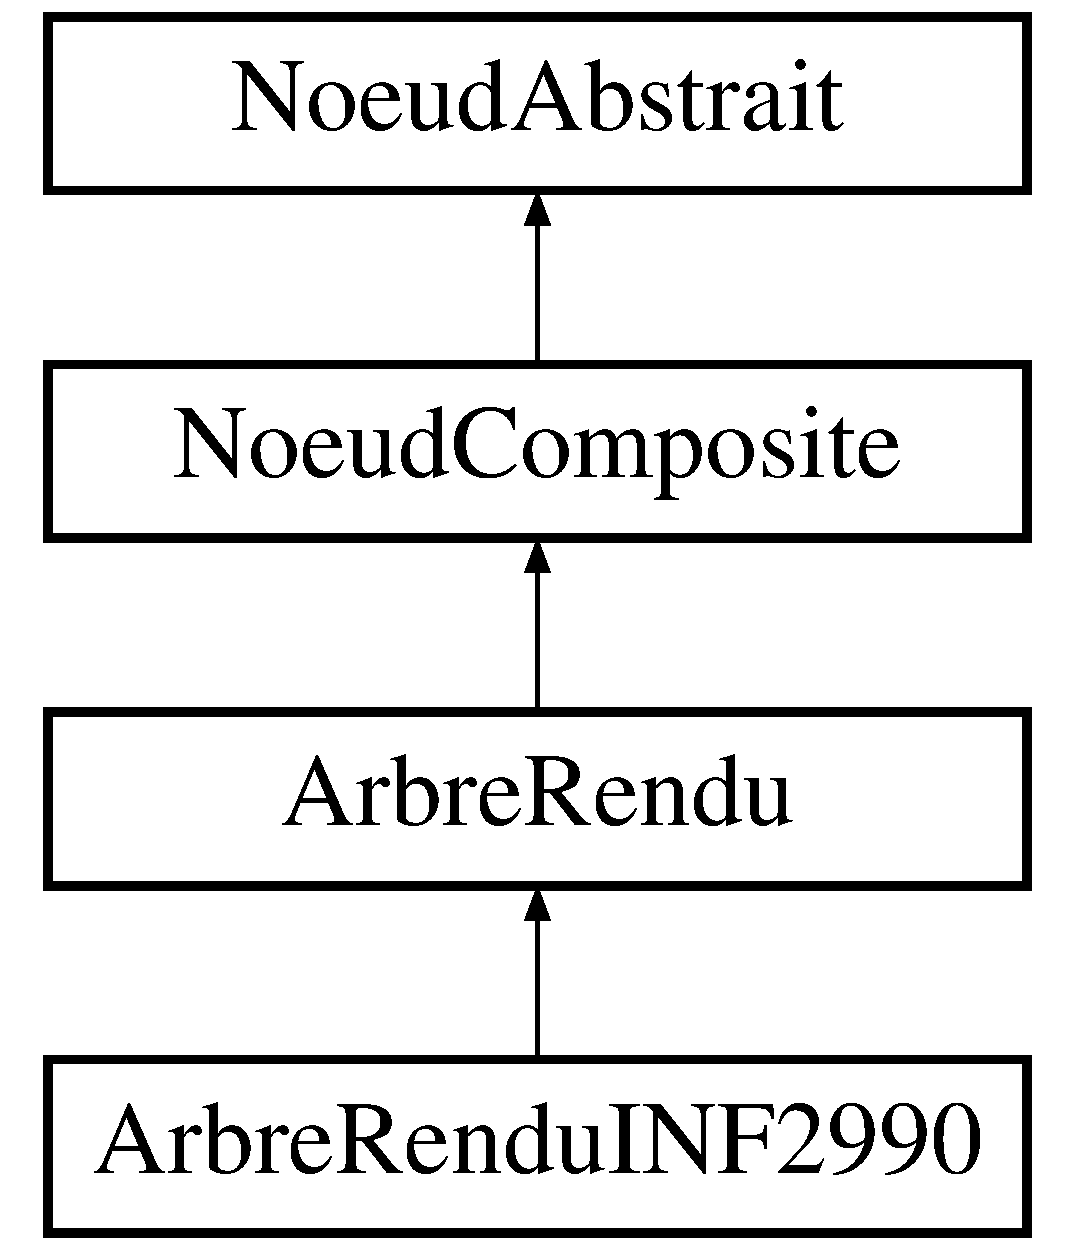
\includegraphics[height=4.000000cm]{class_arbre_rendu}
\end{center}
\end{figure}
\subsection*{Public Member Functions}
\begin{DoxyCompactItemize}
\item 
\hyperlink{group__inf2990_gaef1e98a66c4f1d3b468c786edee45ae6}{Arbre\-Rendu} ()
\begin{DoxyCompactList}\small\item\em Constructeur par defaut. \end{DoxyCompactList}\item 
virtual \hyperlink{group__inf2990_gadb462923759da0ff632dad097b7bfdab}{$\sim$\-Arbre\-Rendu} ()
\begin{DoxyCompactList}\small\item\em Destructeur. \end{DoxyCompactList}\item 
void \hyperlink{group__inf2990_gaef33737fda55a3916e895e1adc3e88ae}{ajouter\-Usine} (const std\-::string \&type, const \hyperlink{class_usine_noeud}{Usine\-Noeud} $\ast$usine)
\item 
\hyperlink{class_noeud_abstrait}{Noeud\-Abstrait} $\ast$ \hyperlink{group__inf2990_ga33ae9013f9cec73854d32527b85b41f9}{creer\-Noeud} (const std\-::string \&type\-Nouveau\-Noeud) const 
\item 
\hyperlink{class_noeud_abstrait}{Noeud\-Abstrait} $\ast$ \hyperlink{group__inf2990_gac10e5f0623af502d67f72aef764206a3}{ajouter\-Nouveau\-Noeud} (const std\-::string \&nom\-Parent, const std\-::string \&type\-Nouveau\-Noeud)
\item 
virtual void \hyperlink{group__inf2990_gab76c5b5c632e814ac27f784ff6d57809}{afficher} (bool selection3\-D=false) const 
\begin{DoxyCompactList}\small\item\em Affiche le noeud. \end{DoxyCompactList}\end{DoxyCompactItemize}
\subsection*{Static Public Member Functions}
\begin{DoxyCompactItemize}
\item 
static unsigned int \hyperlink{group__inf2990_gacf0e53d52040b07cd6550fda79867bd5}{calculer\-Profondeur\-Maximale} ()
\begin{DoxyCompactList}\small\item\em Calcule la profondeur maximale possible pour l'arbre de rendu. \end{DoxyCompactList}\end{DoxyCompactItemize}
\subsection*{Additional Inherited Members}


\subsection{Detailed Description}
Classe d'arbre de rendu qui contient la racine de l'arbre de rendu avec les usines qui permettent d'ajouter des noeuds a cet arbre. 

La profondeur de cet arbre est limitee par la taille de la pile des matrices et la taille de la pile des noms pour la selection Open\-G\-L, etant donne que chaque niveau de l'arbre effectue un \char`\"{}push\char`\"{} sur chacune de ces piles lors du rendu. L'arbre ne verifie pas que la profondeur reste sous la limite, mais il offre des fonctions permettant de le verifier aisement.

\begin{DoxyAuthor}{Author}
Martin Bisson 
\end{DoxyAuthor}
\begin{DoxyDate}{Date}
2007-\/01-\/28 
\end{DoxyDate}


The documentation for this class was generated from the following files\-:\begin{DoxyCompactItemize}
\item 
Cadriciel/\-Sources/\-C++/\-Arbre/\hyperlink{_arbre_rendu_8h}{Arbre\-Rendu.\-h}\item 
Cadriciel/\-Sources/\-C++/\-Arbre/\hyperlink{_arbre_rendu_8cpp}{Arbre\-Rendu.\-cpp}\end{DoxyCompactItemize}

\hypertarget{class_arbre_rendu_i_n_f2990}{\section{Arbre\-Rendu\-I\-N\-F2990 Class Reference}
\label{class_arbre_rendu_i_n_f2990}\index{Arbre\-Rendu\-I\-N\-F2990@{Arbre\-Rendu\-I\-N\-F2990}}
}


Classe qui represente l'arbre de rendu specifique au projet de I\-N\-F2990.  




{\ttfamily \#include $<$Arbre\-Rendu\-I\-N\-F2990.\-h$>$}

Inheritance diagram for Arbre\-Rendu\-I\-N\-F2990\-:\begin{figure}[H]
\begin{center}
\leavevmode
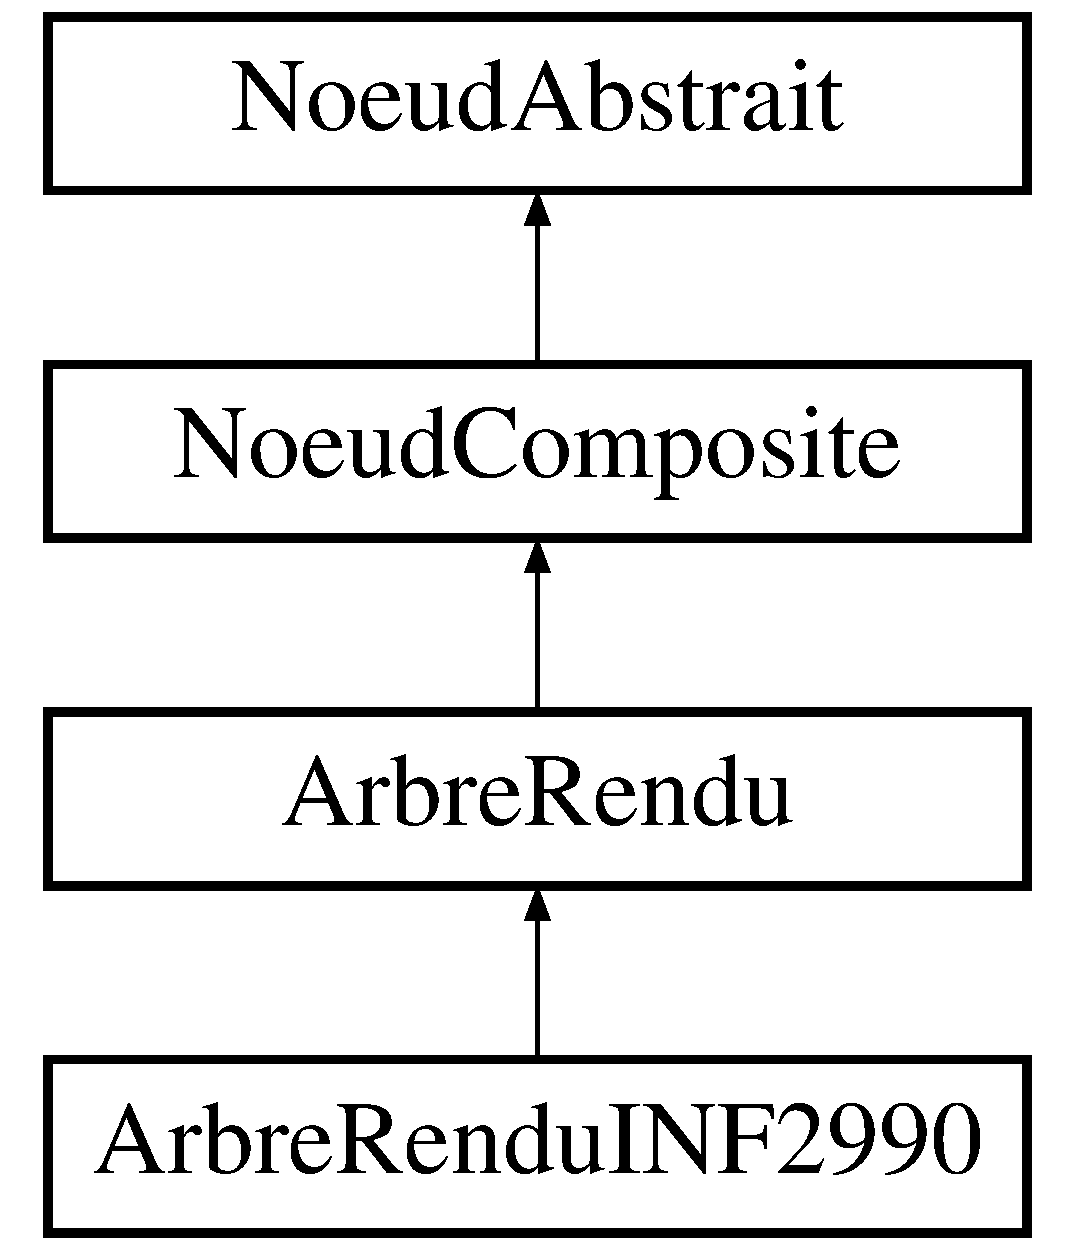
\includegraphics[height=4.000000cm]{class_arbre_rendu_i_n_f2990}
\end{center}
\end{figure}
\subsection*{Public Member Functions}
\begin{DoxyCompactItemize}
\item 
\hyperlink{group__inf2990_ga67528b7fa54e8ef8f96ef2e0bad06d2d}{Arbre\-Rendu\-I\-N\-F2990} ()
\begin{DoxyCompactList}\small\item\em Constructeur par defaut. \end{DoxyCompactList}\item 
virtual \hyperlink{group__inf2990_gaa67526b2fd719f6bcef7a4547bd25c7b}{$\sim$\-Arbre\-Rendu\-I\-N\-F2990} ()
\begin{DoxyCompactList}\small\item\em Destructeur. \end{DoxyCompactList}\item 
void \hyperlink{group__inf2990_ga678d89e1f12ae16ee7dcf6de3db637a3}{initialiser} ()
\begin{DoxyCompactList}\small\item\em Initialise l'arbre de rendu a son etat initial. \end{DoxyCompactList}\end{DoxyCompactItemize}
\subsection*{Static Public Attributes}
\begin{DoxyCompactItemize}
\item 
\hypertarget{group__inf2990_ga445635db2cf91ecb46d96346f886100e}{static const std\-::string {\bfseries N\-O\-M\-\_\-\-A\-C\-C\-E\-L\-E\-R\-A\-T\-E\-U\-R} = \char`\"{}Accelerateur\char`\"{}}\label{group__inf2990_ga445635db2cf91ecb46d96346f886100e}

\item 
\hypertarget{group__inf2990_gade5f55af8001f09e007aac6a010c3002}{static const std\-::string {\bfseries N\-O\-M\-\_\-\-A\-S\-T\-E\-R\-O\-I\-D\-E} = \char`\"{}Asteroide\char`\"{}}\label{group__inf2990_gade5f55af8001f09e007aac6a010c3002}

\item 
\hypertarget{group__inf2990_gad41eac1b0b90d38de6c22a1a6547b1da}{static const std\-::string {\bfseries N\-O\-M\-\_\-\-B\-A\-R\-R\-I\-E\-R\-E} = \char`\"{}Bbarriere\char`\"{}}\label{group__inf2990_gad41eac1b0b90d38de6c22a1a6547b1da}

\item 
\hypertarget{group__inf2990_ga71a649e3d19417d31752a25c002dc4d6}{static const std\-::string {\bfseries N\-O\-M\-\_\-\-P\-O\-R\-T\-A\-I\-L} = \char`\"{}Portail\char`\"{}}\label{group__inf2990_ga71a649e3d19417d31752a25c002dc4d6}

\item 
\hypertarget{group__inf2990_ga81ea9b807a272a338c5be22bde0b6c65}{static const std\-::string {\bfseries N\-O\-M\-\_\-\-P\-R\-O\-J\-E\-C\-T\-I\-L\-E} = \char`\"{}Projectile\char`\"{}}\label{group__inf2990_ga81ea9b807a272a338c5be22bde0b6c65}

\item 
\hypertarget{group__inf2990_ga883f40a096fda37a70e165f7482946de}{static const std\-::string {\bfseries N\-O\-M\-\_\-\-S\-T\-A\-T\-I\-O\-N} = \char`\"{}Station\char`\"{}}\label{group__inf2990_ga883f40a096fda37a70e165f7482946de}

\item 
\hypertarget{group__inf2990_gaebd1eba0f3fb0438336bf104ab066f8e}{static const std\-::string {\bfseries N\-O\-M\-\_\-\-V\-A\-I\-S\-S\-E\-A\-U} = \char`\"{}Vaisseau\char`\"{}}\label{group__inf2990_gaebd1eba0f3fb0438336bf104ab066f8e}

\item 
\hypertarget{group__inf2990_ga54efa483c652cb200fe18763b67cf0aa}{static const std\-::string {\bfseries N\-O\-M\-\_\-\-P\-O\-S\-I\-T\-I\-O\-N\-\_\-\-D\-E\-P\-A\-R\-T} = \char`\"{}Position\-Depart\char`\"{}}\label{group__inf2990_ga54efa483c652cb200fe18763b67cf0aa}

\end{DoxyCompactItemize}
\subsection*{Additional Inherited Members}


\subsection{Detailed Description}
Classe qui represente l'arbre de rendu specifique au projet de I\-N\-F2990. 

Cette classe s'occupe de configurer les usines des noeuds qui seront utilises par le projet.

\begin{DoxyAuthor}{Author}
Martin Bisson 
\end{DoxyAuthor}
\begin{DoxyDate}{Date}
2007-\/03-\/23 
\end{DoxyDate}


The documentation for this class was generated from the following files\-:\begin{DoxyCompactItemize}
\item 
Cadriciel/\-Sources/\-C++/\-Arbre/\hyperlink{_arbre_rendu_i_n_f2990_8h}{Arbre\-Rendu\-I\-N\-F2990.\-h}\item 
Cadriciel/\-Sources/\-C++/\-Arbre/\hyperlink{_arbre_rendu_i_n_f2990_8cpp}{Arbre\-Rendu\-I\-N\-F2990.\-cpp}\end{DoxyCompactItemize}

\hypertarget{struct_asserter}{\section{Asserter Struct Reference}
\label{struct_asserter}\index{Asserter@{Asserter}}
}


A set of functions to help writing assertion macros.

Here is an example of assertion, a simplified version of the actual assertion implemented in examples/cppunittest/\-Xml\-Uniformiser.\-h\-:  




{\ttfamily \#include $<$Asserter.\-h$>$}

\subsection*{Static Public Member Functions}
\begin{DoxyCompactItemize}
\item 
static \hyperlink{wglew_8h_aeea6e3dfae3acf232096f57d2d57f084}{void} \hyperlink{_cpp_unit_api_8h_a0a4ad180f07bc3823bae0e453718ef6a}{C\-P\-P\-U\-N\-I\-T\-\_\-\-A\-P\-I} \hyperlink{struct_asserter_a5a67b6042625cc87d271a53ac555e437}{fail} (const \hyperlink{class_message}{Message} \&\hyperlink{glew_8h_a76333d9470ffdd4811326932394d36da}{message}, const \hyperlink{class_source_line}{Source\-Line} \&source\-Line=\hyperlink{class_source_line}{Source\-Line}())
\begin{DoxyCompactList}\small\item\em Throws a \hyperlink{class_exception}{Exception} with the specified message and location. \end{DoxyCompactList}\item 
static \hyperlink{wglew_8h_aeea6e3dfae3acf232096f57d2d57f084}{void} \hyperlink{_cpp_unit_api_8h_a0a4ad180f07bc3823bae0e453718ef6a}{C\-P\-P\-U\-N\-I\-T\-\_\-\-A\-P\-I} \hyperlink{struct_asserter_a74825fc71909baa1286f9282ba5a2a54}{fail} (\hyperlink{glew_8h_ae84541b4f3d8e1ea24ec0f466a8c568b}{std\-::string} \hyperlink{glew_8h_a76333d9470ffdd4811326932394d36da}{message}, const \hyperlink{class_source_line}{Source\-Line} \&source\-Line=\hyperlink{class_source_line}{Source\-Line}())
\begin{DoxyCompactList}\small\item\em Throws a \hyperlink{class_exception}{Exception} with the specified message and location. \end{DoxyCompactList}\item 
static \hyperlink{wglew_8h_aeea6e3dfae3acf232096f57d2d57f084}{void} \hyperlink{_cpp_unit_api_8h_a0a4ad180f07bc3823bae0e453718ef6a}{C\-P\-P\-U\-N\-I\-T\-\_\-\-A\-P\-I} \hyperlink{struct_asserter_a425da14df34fad7e23a35456fce0eb2b}{fail\-If} (bool should\-Fail, const \hyperlink{class_message}{Message} \&\hyperlink{glew_8h_a76333d9470ffdd4811326932394d36da}{message}, const \hyperlink{class_source_line}{Source\-Line} \&source\-Line=\hyperlink{class_source_line}{Source\-Line}())
\begin{DoxyCompactList}\small\item\em Throws a \hyperlink{class_exception}{Exception} with the specified message and location. \end{DoxyCompactList}\item 
static \hyperlink{wglew_8h_aeea6e3dfae3acf232096f57d2d57f084}{void} \hyperlink{_cpp_unit_api_8h_a0a4ad180f07bc3823bae0e453718ef6a}{C\-P\-P\-U\-N\-I\-T\-\_\-\-A\-P\-I} \hyperlink{struct_asserter_a71a4667a9d3f5d483f1a82157f715824}{fail\-If} (bool should\-Fail, \hyperlink{glew_8h_ae84541b4f3d8e1ea24ec0f466a8c568b}{std\-::string} \hyperlink{glew_8h_a76333d9470ffdd4811326932394d36da}{message}, const \hyperlink{class_source_line}{Source\-Line} \&source\-Line=\hyperlink{class_source_line}{Source\-Line}())
\begin{DoxyCompactList}\small\item\em Throws a \hyperlink{class_exception}{Exception} with the specified message and location. \end{DoxyCompactList}\item 
static \hyperlink{glew_8h_ae84541b4f3d8e1ea24ec0f466a8c568b}{std\-::string} \hyperlink{_cpp_unit_api_8h_a0a4ad180f07bc3823bae0e453718ef6a}{C\-P\-P\-U\-N\-I\-T\-\_\-\-A\-P\-I} \hyperlink{struct_asserter_adcbee7c01d58bfaee72cc984627e6432}{make\-Expected} (const \hyperlink{glew_8h_ae84541b4f3d8e1ea24ec0f466a8c568b}{std\-::string} \&expected\-Value)
\begin{DoxyCompactList}\small\item\em Returns a expected value string for a message. Typically used to create 'not equal' message, or to check that a message contains the expected content when writing unit tests for your custom assertions. \end{DoxyCompactList}\item 
static \hyperlink{glew_8h_ae84541b4f3d8e1ea24ec0f466a8c568b}{std\-::string} \hyperlink{_cpp_unit_api_8h_a0a4ad180f07bc3823bae0e453718ef6a}{C\-P\-P\-U\-N\-I\-T\-\_\-\-A\-P\-I} \hyperlink{struct_asserter_ae52920ca7ffd981df61d7a3cfd88793b}{make\-Actual} (const \hyperlink{glew_8h_ae84541b4f3d8e1ea24ec0f466a8c568b}{std\-::string} \&actual\-Value)
\begin{DoxyCompactList}\small\item\em Returns an actual value string for a message. Typically used to create 'not equal' message, or to check that a message contains the expected content when writing unit tests for your custom assertions. \end{DoxyCompactList}\item 
static \hyperlink{class_message}{Message} \hyperlink{_cpp_unit_api_8h_a0a4ad180f07bc3823bae0e453718ef6a}{C\-P\-P\-U\-N\-I\-T\-\_\-\-A\-P\-I} \hyperlink{struct_asserter_adb8ac36c8f0d385430e5a087a66219db}{make\-Not\-Equal\-Message} (const \hyperlink{glew_8h_ae84541b4f3d8e1ea24ec0f466a8c568b}{std\-::string} \&expected\-Value, const \hyperlink{glew_8h_ae84541b4f3d8e1ea24ec0f466a8c568b}{std\-::string} \&actual\-Value, const \hyperlink{class_additional_message}{Additional\-Message} \&additional\-Message=\hyperlink{class_additional_message}{Additional\-Message}(), const \hyperlink{glew_8h_ae84541b4f3d8e1ea24ec0f466a8c568b}{std\-::string} \&short\-Description=\char`\"{}equality assertion failed\char`\"{})
\item 
static \hyperlink{wglew_8h_aeea6e3dfae3acf232096f57d2d57f084}{void} \hyperlink{_cpp_unit_api_8h_a0a4ad180f07bc3823bae0e453718ef6a}{C\-P\-P\-U\-N\-I\-T\-\_\-\-A\-P\-I} \hyperlink{struct_asserter_ac6234767e7d986bace97dc44f8d80d6c}{fail\-Not\-Equal} (\hyperlink{glew_8h_ae84541b4f3d8e1ea24ec0f466a8c568b}{std\-::string} expected, \hyperlink{glew_8h_ae84541b4f3d8e1ea24ec0f466a8c568b}{std\-::string} actual, const \hyperlink{class_source_line}{Source\-Line} \&source\-Line, const \hyperlink{class_additional_message}{Additional\-Message} \&additional\-Message=\hyperlink{class_additional_message}{Additional\-Message}(), \hyperlink{glew_8h_ae84541b4f3d8e1ea24ec0f466a8c568b}{std\-::string} short\-Description=\char`\"{}equality assertion failed\char`\"{})
\begin{DoxyCompactList}\small\item\em Throws an \hyperlink{class_exception}{Exception} with the specified message and location. \end{DoxyCompactList}\item 
static \hyperlink{wglew_8h_aeea6e3dfae3acf232096f57d2d57f084}{void} \hyperlink{_cpp_unit_api_8h_a0a4ad180f07bc3823bae0e453718ef6a}{C\-P\-P\-U\-N\-I\-T\-\_\-\-A\-P\-I} \hyperlink{struct_asserter_a3a805c9f8c641d65353bcff2da80624f}{fail\-Not\-Equal\-If} (bool should\-Fail, \hyperlink{glew_8h_ae84541b4f3d8e1ea24ec0f466a8c568b}{std\-::string} expected, \hyperlink{glew_8h_ae84541b4f3d8e1ea24ec0f466a8c568b}{std\-::string} actual, const \hyperlink{class_source_line}{Source\-Line} \&source\-Line, const \hyperlink{class_additional_message}{Additional\-Message} \&additional\-Message=\hyperlink{class_additional_message}{Additional\-Message}(), \hyperlink{glew_8h_ae84541b4f3d8e1ea24ec0f466a8c568b}{std\-::string} short\-Description=\char`\"{}equality assertion failed\char`\"{})
\begin{DoxyCompactList}\small\item\em Throws an \hyperlink{class_exception}{Exception} with the specified message and location. \end{DoxyCompactList}\end{DoxyCompactItemize}


\subsection{Detailed Description}
A set of functions to help writing assertion macros.

Here is an example of assertion, a simplified version of the actual assertion implemented in examples/cppunittest/\-Xml\-Uniformiser.\-h\-: 


\begin{DoxyCode}
\textcolor{preprocessor}{#include <\hyperlink{_source_line_8h}{cppunit/SourceLine.h}>}
\textcolor{preprocessor}{#include <\hyperlink{_test_assert_8h}{cppunit/TestAssert.h}>}

\textcolor{keywordtype}{void} 
checkXmlEqual( \hyperlink{glew_8h_ae84541b4f3d8e1ea24ec0f466a8c568b}{std::string} expectedXml,
               \hyperlink{glew_8h_ae84541b4f3d8e1ea24ec0f466a8c568b}{std::string} actualXml,
               CppUnit::SourceLine sourceLine )
\{
  \hyperlink{glew_8h_ae84541b4f3d8e1ea24ec0f466a8c568b}{std::string} expected = XmlUniformiser( expectedXml ).stripped();
  \hyperlink{glew_8h_ae84541b4f3d8e1ea24ec0f466a8c568b}{std::string} actual = XmlUniformiser( actualXml ).stripped();

  \textcolor{keywordflow}{if} ( expected == actual )
    \textcolor{keywordflow}{return};

  ::CppUnit::Asserter::failNotEqual( expected,
                                     actual,
                                     sourceLine );
\}

\textcolor{preprocessor}{#define CPPUNITTEST\_ASSERT\_XML\_EQUAL( expected, actual ) \(\backslash\)}
\textcolor{preprocessor}{    checkXmlEqual( expected, actual,                     \(\backslash\)}
\textcolor{preprocessor}{                   CPPUNIT\_SOURCELINE() )}
\end{DoxyCode}
 

\subsection{Member Function Documentation}
\hypertarget{struct_asserter_a5a67b6042625cc87d271a53ac555e437}{\index{Asserter@{Asserter}!fail@{fail}}
\index{fail@{fail}!Asserter@{Asserter}}
\subsubsection[{fail}]{\setlength{\rightskip}{0pt plus 5cm}static {\bf void} {\bf C\-P\-P\-U\-N\-I\-T\-\_\-\-A\-P\-I} Asserter\-::fail (
\begin{DoxyParamCaption}
\item[{const {\bf Message} \&}]{message, }
\item[{const {\bf Source\-Line} \&}]{source\-Line = {\ttfamily {\bf Source\-Line}()}}
\end{DoxyParamCaption}
)\hspace{0.3cm}{\ttfamily [static]}}}\label{struct_asserter_a5a67b6042625cc87d271a53ac555e437}


Throws a \hyperlink{class_exception}{Exception} with the specified message and location. 

\hypertarget{struct_asserter_a74825fc71909baa1286f9282ba5a2a54}{\index{Asserter@{Asserter}!fail@{fail}}
\index{fail@{fail}!Asserter@{Asserter}}
\subsubsection[{fail}]{\setlength{\rightskip}{0pt plus 5cm}static {\bf void} {\bf C\-P\-P\-U\-N\-I\-T\-\_\-\-A\-P\-I} Asserter\-::fail (
\begin{DoxyParamCaption}
\item[{{\bf std\-::string}}]{message, }
\item[{const {\bf Source\-Line} \&}]{source\-Line = {\ttfamily {\bf Source\-Line}()}}
\end{DoxyParamCaption}
)\hspace{0.3cm}{\ttfamily [static]}}}\label{struct_asserter_a74825fc71909baa1286f9282ba5a2a54}


Throws a \hyperlink{class_exception}{Exception} with the specified message and location. 

\begin{DoxyRefDesc}{Deprecated}
\item[\hyperlink{deprecated__deprecated000002}{Deprecated}]Use fail( Message, Source\-Line ) instead. \end{DoxyRefDesc}
\hypertarget{struct_asserter_a425da14df34fad7e23a35456fce0eb2b}{\index{Asserter@{Asserter}!fail\-If@{fail\-If}}
\index{fail\-If@{fail\-If}!Asserter@{Asserter}}
\subsubsection[{fail\-If}]{\setlength{\rightskip}{0pt plus 5cm}static {\bf void} {\bf C\-P\-P\-U\-N\-I\-T\-\_\-\-A\-P\-I} Asserter\-::fail\-If (
\begin{DoxyParamCaption}
\item[{bool}]{should\-Fail, }
\item[{const {\bf Message} \&}]{message, }
\item[{const {\bf Source\-Line} \&}]{source\-Line = {\ttfamily {\bf Source\-Line}()}}
\end{DoxyParamCaption}
)\hspace{0.3cm}{\ttfamily [static]}}}\label{struct_asserter_a425da14df34fad7e23a35456fce0eb2b}


Throws a \hyperlink{class_exception}{Exception} with the specified message and location. 


\begin{DoxyParams}{Parameters}
{\em should\-Fail} & if {\ttfamily true} then the exception is thrown. Otherwise nothing happen. \\
\hline
{\em message} & \hyperlink{class_message}{Message} explaining the assertion failiure. \\
\hline
{\em source\-Line} & Location of the assertion. \\
\hline
\end{DoxyParams}
\hypertarget{struct_asserter_a71a4667a9d3f5d483f1a82157f715824}{\index{Asserter@{Asserter}!fail\-If@{fail\-If}}
\index{fail\-If@{fail\-If}!Asserter@{Asserter}}
\subsubsection[{fail\-If}]{\setlength{\rightskip}{0pt plus 5cm}static {\bf void} {\bf C\-P\-P\-U\-N\-I\-T\-\_\-\-A\-P\-I} Asserter\-::fail\-If (
\begin{DoxyParamCaption}
\item[{bool}]{should\-Fail, }
\item[{{\bf std\-::string}}]{message, }
\item[{const {\bf Source\-Line} \&}]{source\-Line = {\ttfamily {\bf Source\-Line}()}}
\end{DoxyParamCaption}
)\hspace{0.3cm}{\ttfamily [static]}}}\label{struct_asserter_a71a4667a9d3f5d483f1a82157f715824}


Throws a \hyperlink{class_exception}{Exception} with the specified message and location. 

\begin{DoxyRefDesc}{Deprecated}
\item[\hyperlink{deprecated__deprecated000003}{Deprecated}]Use fail\-If( bool, Message, Source\-Line ) instead. 
\begin{DoxyParams}{Parameters}
{\em should\-Fail} & if {\ttfamily true} then the exception is thrown. Otherwise nothing happen. \\
\hline
{\em message} & \hyperlink{class_message}{Message} explaining the assertion failiure. \\
\hline
{\em source\-Line} & Location of the assertion. \\
\hline
\end{DoxyParams}
\end{DoxyRefDesc}
\hypertarget{struct_asserter_ac6234767e7d986bace97dc44f8d80d6c}{\index{Asserter@{Asserter}!fail\-Not\-Equal@{fail\-Not\-Equal}}
\index{fail\-Not\-Equal@{fail\-Not\-Equal}!Asserter@{Asserter}}
\subsubsection[{fail\-Not\-Equal}]{\setlength{\rightskip}{0pt plus 5cm}static {\bf void} {\bf C\-P\-P\-U\-N\-I\-T\-\_\-\-A\-P\-I} Asserter\-::fail\-Not\-Equal (
\begin{DoxyParamCaption}
\item[{{\bf std\-::string}}]{expected, }
\item[{{\bf std\-::string}}]{actual, }
\item[{const {\bf Source\-Line} \&}]{source\-Line, }
\item[{const {\bf Additional\-Message} \&}]{additional\-Message = {\ttfamily {\bf Additional\-Message}()}, }
\item[{{\bf std\-::string}}]{short\-Description = {\ttfamily \char`\"{}equality~assertion~failed\char`\"{}}}
\end{DoxyParamCaption}
)\hspace{0.3cm}{\ttfamily [static]}}}\label{struct_asserter_ac6234767e7d986bace97dc44f8d80d6c}


Throws an \hyperlink{class_exception}{Exception} with the specified message and location. 


\begin{DoxyParams}{Parameters}
{\em expected} & Text describing the expected value. \\
\hline
{\em actual} & Text describing the actual value. \\
\hline
{\em source\-Line} & Location of the assertion. \\
\hline
{\em additional\-Message} & Additional message. Usually used to report what are the differences between the expected and actual value. \\
\hline
{\em short\-Description} & Short description for the failure message. \\
\hline
\end{DoxyParams}
\hypertarget{struct_asserter_a3a805c9f8c641d65353bcff2da80624f}{\index{Asserter@{Asserter}!fail\-Not\-Equal\-If@{fail\-Not\-Equal\-If}}
\index{fail\-Not\-Equal\-If@{fail\-Not\-Equal\-If}!Asserter@{Asserter}}
\subsubsection[{fail\-Not\-Equal\-If}]{\setlength{\rightskip}{0pt plus 5cm}static {\bf void} {\bf C\-P\-P\-U\-N\-I\-T\-\_\-\-A\-P\-I} Asserter\-::fail\-Not\-Equal\-If (
\begin{DoxyParamCaption}
\item[{bool}]{should\-Fail, }
\item[{{\bf std\-::string}}]{expected, }
\item[{{\bf std\-::string}}]{actual, }
\item[{const {\bf Source\-Line} \&}]{source\-Line, }
\item[{const {\bf Additional\-Message} \&}]{additional\-Message = {\ttfamily {\bf Additional\-Message}()}, }
\item[{{\bf std\-::string}}]{short\-Description = {\ttfamily \char`\"{}equality~assertion~failed\char`\"{}}}
\end{DoxyParamCaption}
)\hspace{0.3cm}{\ttfamily [static]}}}\label{struct_asserter_a3a805c9f8c641d65353bcff2da80624f}


Throws an \hyperlink{class_exception}{Exception} with the specified message and location. 


\begin{DoxyParams}{Parameters}
{\em should\-Fail} & if {\ttfamily true} then the exception is thrown. Otherwise nothing happen. \\
\hline
{\em expected} & Text describing the expected value. \\
\hline
{\em actual} & Text describing the actual value. \\
\hline
{\em source\-Line} & Location of the assertion. \\
\hline
{\em additional\-Message} & Additional message. Usually used to report where the \char`\"{}difference\char`\"{} is located. \\
\hline
{\em short\-Description} & Short description for the failure message. \\
\hline
\end{DoxyParams}
\hypertarget{struct_asserter_ae52920ca7ffd981df61d7a3cfd88793b}{\index{Asserter@{Asserter}!make\-Actual@{make\-Actual}}
\index{make\-Actual@{make\-Actual}!Asserter@{Asserter}}
\subsubsection[{make\-Actual}]{\setlength{\rightskip}{0pt plus 5cm}static {\bf std\-::string} {\bf C\-P\-P\-U\-N\-I\-T\-\_\-\-A\-P\-I} Asserter\-::make\-Actual (
\begin{DoxyParamCaption}
\item[{const {\bf std\-::string} \&}]{actual\-Value}
\end{DoxyParamCaption}
)\hspace{0.3cm}{\ttfamily [static]}}}\label{struct_asserter_ae52920ca7ffd981df61d7a3cfd88793b}


Returns an actual value string for a message. Typically used to create 'not equal' message, or to check that a message contains the expected content when writing unit tests for your custom assertions. 


\begin{DoxyParams}{Parameters}
{\em actual\-Value} & String that represents the actual value. \\
\hline
\end{DoxyParams}
\begin{DoxyReturn}{Returns}
{\itshape actual\-Value} prefixed with \char`\"{}\-Actual  \-: \char`\"{}. 
\end{DoxyReturn}
\begin{DoxySeeAlso}{See Also}
\hyperlink{struct_asserter_adcbee7c01d58bfaee72cc984627e6432}{make\-Expected()}. 
\end{DoxySeeAlso}
\hypertarget{struct_asserter_adcbee7c01d58bfaee72cc984627e6432}{\index{Asserter@{Asserter}!make\-Expected@{make\-Expected}}
\index{make\-Expected@{make\-Expected}!Asserter@{Asserter}}
\subsubsection[{make\-Expected}]{\setlength{\rightskip}{0pt plus 5cm}static {\bf std\-::string} {\bf C\-P\-P\-U\-N\-I\-T\-\_\-\-A\-P\-I} Asserter\-::make\-Expected (
\begin{DoxyParamCaption}
\item[{const {\bf std\-::string} \&}]{expected\-Value}
\end{DoxyParamCaption}
)\hspace{0.3cm}{\ttfamily [static]}}}\label{struct_asserter_adcbee7c01d58bfaee72cc984627e6432}


Returns a expected value string for a message. Typically used to create 'not equal' message, or to check that a message contains the expected content when writing unit tests for your custom assertions. 


\begin{DoxyParams}{Parameters}
{\em expected\-Value} & String that represents the expected value. \\
\hline
\end{DoxyParams}
\begin{DoxyReturn}{Returns}
{\itshape expected\-Value} prefixed with \char`\"{}\-Expected\-: \char`\"{}. 
\end{DoxyReturn}
\begin{DoxySeeAlso}{See Also}
\hyperlink{struct_asserter_ae52920ca7ffd981df61d7a3cfd88793b}{make\-Actual()}. 
\end{DoxySeeAlso}
\hypertarget{struct_asserter_adb8ac36c8f0d385430e5a087a66219db}{\index{Asserter@{Asserter}!make\-Not\-Equal\-Message@{make\-Not\-Equal\-Message}}
\index{make\-Not\-Equal\-Message@{make\-Not\-Equal\-Message}!Asserter@{Asserter}}
\subsubsection[{make\-Not\-Equal\-Message}]{\setlength{\rightskip}{0pt plus 5cm}static {\bf Message} {\bf C\-P\-P\-U\-N\-I\-T\-\_\-\-A\-P\-I} Asserter\-::make\-Not\-Equal\-Message (
\begin{DoxyParamCaption}
\item[{const {\bf std\-::string} \&}]{expected\-Value, }
\item[{const {\bf std\-::string} \&}]{actual\-Value, }
\item[{const {\bf Additional\-Message} \&}]{additional\-Message = {\ttfamily {\bf Additional\-Message}()}, }
\item[{const {\bf std\-::string} \&}]{short\-Description = {\ttfamily \char`\"{}equality~assertion~failed\char`\"{}}}
\end{DoxyParamCaption}
)\hspace{0.3cm}{\ttfamily [static]}}}\label{struct_asserter_adb8ac36c8f0d385430e5a087a66219db}


The documentation for this struct was generated from the following file\-:\begin{DoxyCompactItemize}
\item 
Cadriciel/\-Commun/\-Externe/cppunit/include/cppunit/\hyperlink{_asserter_8h}{Asserter.\-h}\end{DoxyCompactItemize}

\hypertarget{structassertion__traits}{\section{assertion\-\_\-traits$<$ T $>$ Struct Template Reference}
\label{structassertion__traits}\index{assertion\-\_\-traits$<$ T $>$@{assertion\-\_\-traits$<$ T $>$}}
}


Traits used by C\-P\-P\-U\-N\-I\-T\-\_\-\-A\-S\-S\-E\-R\-T\-\_\-\-E\-Q\-U\-A\-L().  




{\ttfamily \#include $<$Test\-Assert.\-h$>$}

\subsection*{Static Public Member Functions}
\begin{DoxyCompactItemize}
\item 
\hypertarget{structassertion__traits_a287c07a4e171256a0128201c7e4c4228}{static bool {\bfseries equal} (const T \&x, const T \&y)}\label{structassertion__traits_a287c07a4e171256a0128201c7e4c4228}

\item 
\hypertarget{structassertion__traits_a1c96296fb44902b4f22d99b9c3cc7749}{static std\-::string {\bfseries to\-String} (const T \&x)}\label{structassertion__traits_a1c96296fb44902b4f22d99b9c3cc7749}

\end{DoxyCompactItemize}


\subsection{Detailed Description}
\subsubsection*{template$<$class T$>$struct assertion\-\_\-traits$<$ T $>$}

Traits used by C\-P\-P\-U\-N\-I\-T\-\_\-\-A\-S\-S\-E\-R\-T\-\_\-\-E\-Q\-U\-A\-L(). 

Here is an example of specialising these traits\-:


\begin{DoxyCode}
\textcolor{keyword}{template}<>
\textcolor{keyword}{struct }\hyperlink{structassertion__traits}{assertion\_traits}<std::string>   \textcolor{comment}{// specialization for the std::string type}
\{
  \textcolor{keyword}{static} \textcolor{keywordtype}{bool} equal( \textcolor{keyword}{const} std::string& x, \textcolor{keyword}{const} std::string& y )
  \{
    \textcolor{keywordflow}{return} x == y;
  \}

  \textcolor{keyword}{static} std::string toString( \textcolor{keyword}{const} std::string& x )
  \{
    std::string text = \textcolor{charliteral}{'"'} + x + \textcolor{charliteral}{'"'};    \textcolor{comment}{// adds quote around the string to see whitespace}
    OStringStream ost;
    ost << text;
    \textcolor{keywordflow}{return} ost.str();
  \}
\};
\end{DoxyCode}
 

The documentation for this struct was generated from the following file\-:\begin{DoxyCompactItemize}
\item 
Cadriciel/\-Commun/\-Externe/cppunit/include/cppunit/Test\-Assert.\-h\end{DoxyCompactItemize}

\hypertarget{structassertion__traits_3_01double_01_4}{\section{assertion\-\_\-traits$<$ double $>$ Struct Template Reference}
\label{structassertion__traits_3_01double_01_4}\index{assertion\-\_\-traits$<$ double $>$@{assertion\-\_\-traits$<$ double $>$}}
}


Traits used by \hyperlink{_test_assert_8h_a9d88b1e379e4a9ba2a5e9e79763389ea}{C\-P\-P\-U\-N\-I\-T\-\_\-\-A\-S\-S\-E\-R\-T\-\_\-\-D\-O\-U\-B\-L\-E\-S\-\_\-\-E\-Q\-U\-A\-L()}.  




{\ttfamily \#include $<$Test\-Assert.\-h$>$}

\subsection*{Static Public Member Functions}
\begin{DoxyCompactItemize}
\item 
static bool \hyperlink{structassertion__traits_3_01double_01_4_ac0d9d71ec0f239664b88188e481c0598}{equal} (double \hyperlink{glew_8h_ad77deca22f617d3f0e0eb786445689fc}{x}, double \hyperlink{glew_8h_a9298c7ad619074f5285b32c6b72bfdea}{y})
\item 
static \hyperlink{glew_8h_ae84541b4f3d8e1ea24ec0f466a8c568b}{std\-::string} \hyperlink{structassertion__traits_3_01double_01_4_a6bc37874eb60d30e0b50d4c127ab34df}{to\-String} (double \hyperlink{glew_8h_ad77deca22f617d3f0e0eb786445689fc}{x})
\end{DoxyCompactItemize}


\subsection{Detailed Description}
\subsubsection*{template$<$$>$struct assertion\-\_\-traits$<$ double $>$}

Traits used by \hyperlink{_test_assert_8h_a9d88b1e379e4a9ba2a5e9e79763389ea}{C\-P\-P\-U\-N\-I\-T\-\_\-\-A\-S\-S\-E\-R\-T\-\_\-\-D\-O\-U\-B\-L\-E\-S\-\_\-\-E\-Q\-U\-A\-L()}. 

This specialisation from {\ttfamily struct} {\ttfamily assertion\-\_\-traits$<$$>$} ensures that doubles are converted in full, instead of being rounded to the default 6 digits of precision. Use the system defined I\-S\-O C99 macro D\-B\-L\-\_\-\-D\-I\-G within float.\-h is available to define the maximum precision, otherwise use the hard-\/coded maximum precision of 15. 

\subsection{Member Function Documentation}
\hypertarget{structassertion__traits_3_01double_01_4_ac0d9d71ec0f239664b88188e481c0598}{\index{assertion\-\_\-traits$<$ double $>$@{assertion\-\_\-traits$<$ double $>$}!equal@{equal}}
\index{equal@{equal}!assertion_traits< double >@{assertion\-\_\-traits$<$ double $>$}}
\subsubsection[{equal}]{\setlength{\rightskip}{0pt plus 5cm}static bool {\bf assertion\-\_\-traits}$<$ double $>$\-::equal (
\begin{DoxyParamCaption}
\item[{double}]{x, }
\item[{double}]{y}
\end{DoxyParamCaption}
)\hspace{0.3cm}{\ttfamily [inline]}, {\ttfamily [static]}}}\label{structassertion__traits_3_01double_01_4_ac0d9d71ec0f239664b88188e481c0598}
\hypertarget{structassertion__traits_3_01double_01_4_a6bc37874eb60d30e0b50d4c127ab34df}{\index{assertion\-\_\-traits$<$ double $>$@{assertion\-\_\-traits$<$ double $>$}!to\-String@{to\-String}}
\index{to\-String@{to\-String}!assertion_traits< double >@{assertion\-\_\-traits$<$ double $>$}}
\subsubsection[{to\-String}]{\setlength{\rightskip}{0pt plus 5cm}static {\bf std\-::string} {\bf assertion\-\_\-traits}$<$ double $>$\-::to\-String (
\begin{DoxyParamCaption}
\item[{double}]{x}
\end{DoxyParamCaption}
)\hspace{0.3cm}{\ttfamily [inline]}, {\ttfamily [static]}}}\label{structassertion__traits_3_01double_01_4_a6bc37874eb60d30e0b50d4c127ab34df}


The documentation for this struct was generated from the following file\-:\begin{DoxyCompactItemize}
\item 
Cadriciel/\-Commun/\-Externe/cppunit/include/cppunit/\hyperlink{_test_assert_8h}{Test\-Assert.\-h}\end{DoxyCompactItemize}

\hypertarget{class_asteroide}{\section{Asteroide Class Reference}
\label{class_asteroide}\index{Asteroide@{Asteroide}}
}


Cette classe qui permet de creer des asteroides.  




{\ttfamily \#include $<$Asteroide.\-h$>$}

Inheritance diagram for Asteroide\-:\begin{figure}[H]
\begin{center}
\leavevmode
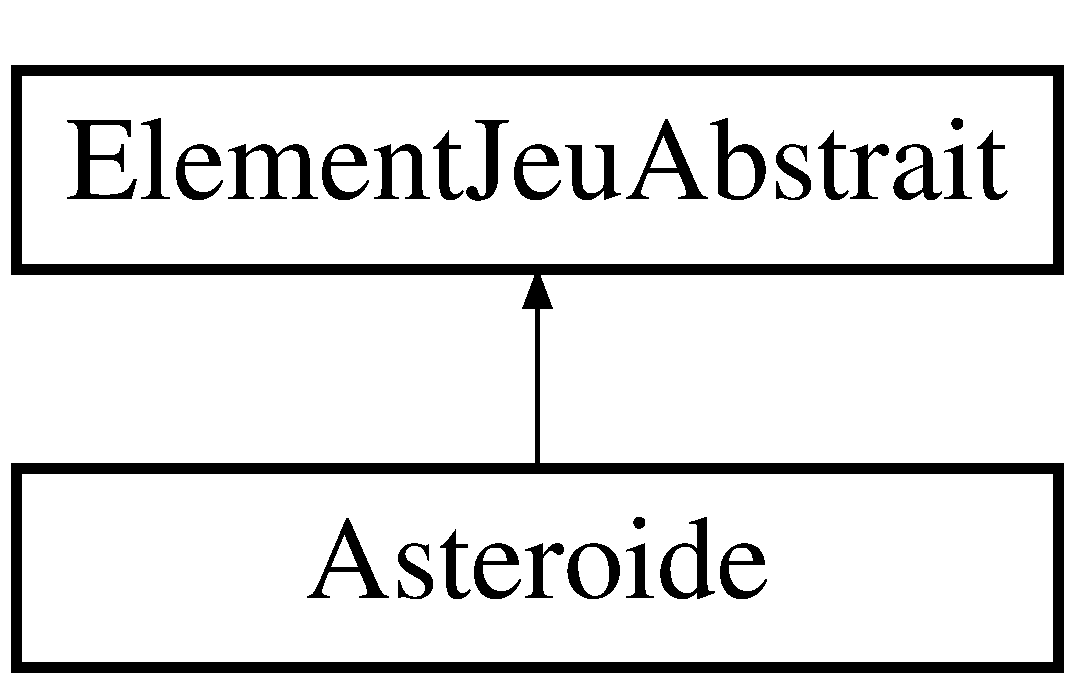
\includegraphics[height=2.000000cm]{class_asteroide}
\end{center}
\end{figure}
\subsection*{Public Member Functions}
\begin{DoxyCompactItemize}
\item 
\hyperlink{group__inf2990_gafe350047342cca5e224b5c2ea5f9b959}{Asteroide} ()
\begin{DoxyCompactList}\small\item\em Constructeur. \end{DoxyCompactList}\item 
\hyperlink{group__inf2990_ga34973732c5bfa698b0ff88af487e528a}{Asteroide} (\hyperlink{group__utilitaire_ga6a8205c734fc1c9d1272ea424efb2606}{Vecteur4f} cadre\-Depart, \hyperlink{group__utilitaire_ga6a8205c734fc1c9d1272ea424efb2606}{Vecteur4f} zone\-Passage)
\item 
\hyperlink{group__inf2990_ga2ffd65671cd6e71ec7a565f896dc65e8}{Asteroide} (\hyperlink{group__utilitaire_ga6b2956069f76c7e27df4f79f87e5a48c}{Vecteur3f} position\-Depart, \hyperlink{group__utilitaire_ga6b2956069f76c7e27df4f79f87e5a48c}{Vecteur3f} taille, \hyperlink{group__utilitaire_ga6b2956069f76c7e27df4f79f87e5a48c}{Vecteur3f} direction\-Vitesse, \hyperlink{fmod_8h_aeb841aa4b4b5f444b5d739d865b420af}{float} poids, \hyperlink{_free_image_8h_a425076c7067a1b5166e2cc530e914814}{unsigned} \hyperlink{wglew_8h_a500a82aecba06f4550f6849b8099ca21}{int} point\-De\-Vie)
\item 
\hyperlink{group__inf2990_ga23517155b85bb5ea1646ab2c6f3d4e85}{Asteroide} (const \hyperlink{class_asteroide}{Asteroide} \&asteroide)
\item 
virtual \hyperlink{group__inf2990_ga539ed35e6f89029a69eb76626da9263b}{$\sim$\-Asteroide} ()
\begin{DoxyCompactList}\small\item\em Destructeur. \end{DoxyCompactList}\item 
virtual \hyperlink{wglew_8h_a500a82aecba06f4550f6849b8099ca21}{int} \hyperlink{class_asteroide_a5755520c095800c4c9e39b8271ef4ac6}{get\-Point\-De\-Vie} ()
\item 
\hyperlink{wglew_8h_aeea6e3dfae3acf232096f57d2d57f084}{void} \hyperlink{group__inf2990_gaefe6b772d03b0731087364ecbbde23d5}{set\-Point\-De\-Vie} (\hyperlink{wglew_8h_a500a82aecba06f4550f6849b8099ca21}{int} point\-De\-Vie)
\item 
virtual \hyperlink{group___i_n_f2990-04_ga1d1cfd8ffb84e947f82999c682b666a7}{Type} \hyperlink{group__inf2990_gad5cb221ede09ce81ef9621b89dcf694c}{get\-Type} ()
\begin{DoxyCompactList}\small\item\em Permet d'obtenir le type de l'element. \end{DoxyCompactList}\item 
virtual \hyperlink{wglew_8h_aeea6e3dfae3acf232096f57d2d57f084}{void} \hyperlink{group__inf2990_ga853919162f10be16bdd57e918a9328cf}{update} (\hyperlink{fmod_8h_aeb841aa4b4b5f444b5d739d865b420af}{float} delta\-T)
\begin{DoxyCompactList}\small\item\em Mise a jour. \end{DoxyCompactList}\item 
virtual bool \hyperlink{group__inf2990_gaa93e8b00c94001bc04893450b8969eff}{check\-Collision} (\hyperlink{class_element_jeu_abstrait}{Element\-Jeu\-Abstrait} $\ast$\hyperlink{class_element_jeu_abstrait}{Element\-Jeu\-Abstrait})
\begin{DoxyCompactList}\small\item\em Permet de verifier la collision entre les types d'objets concern�s et de les traiter. \end{DoxyCompactList}\item 
virtual bool \hyperlink{class_asteroide_ab02167e3b62f74da70f5798473850368}{check\-Collision} (\hyperlink{class_accelerateur}{Accelerateur} $\ast$accelerateur)
\begin{DoxyCompactList}\small\item\em Methode pour verifier si une collision existe. \end{DoxyCompactList}\item 
virtual bool \hyperlink{group__inf2990_gaacd8ed8d91f5047c64f30ed4ded1797b}{check\-Collision} (\hyperlink{class_asteroide}{Asteroide} $\ast$asteroide)
\item 
virtual bool \hyperlink{group__inf2990_ga83d33ed67b297a1f2ed72ac61bee6f7c}{check\-Collision} (\hyperlink{class_barriere}{Barriere} $\ast$barriere)
\item 
virtual bool \hyperlink{group__inf2990_ga322ab7d5fc10bc7f634637ad0ee23dbb}{check\-Collision} (\hyperlink{class_portail}{Portail} $\ast$portail)
\item 
virtual bool \hyperlink{group__inf2990_gad444d75b00ce0a2b639493eaeb7d235f}{check\-Collision} (\hyperlink{class_projectile}{Projectile} $\ast$projectile)
\item 
virtual bool \hyperlink{group__inf2990_ga4924790f413b4ab5a806336f75fdaf73}{check\-Collision} (\hyperlink{class_station}{Station} $\ast$station)
\item 
virtual bool \hyperlink{group__inf2990_gacb843b3baa58aea8738b896a89d2a397}{check\-Collision} (\hyperlink{class_vaisseau}{Vaisseau} $\ast$vaisseau)
\item 
virtual \hyperlink{wglew_8h_aeea6e3dfae3acf232096f57d2d57f084}{void} \hyperlink{group__inf2990_gacb7ff9a98ed4e8d479a53f27dbc85abd}{traiter\-Collision} (\hyperlink{class_element_jeu_abstrait}{Element\-Jeu\-Abstrait} $\ast$element\-Abstrait)
\item 
virtual \hyperlink{wglew_8h_aeea6e3dfae3acf232096f57d2d57f084}{void} \hyperlink{class_asteroide_a46e8e4136e20a963806352bbf211ddcf}{traiter\-Collision} (\hyperlink{class_accelerateur}{Accelerateur} $\ast$accelerateur)
\begin{DoxyCompactList}\small\item\em Methode pour traiter la collision si elle a lui avec les differents elements. \end{DoxyCompactList}\item 
virtual \hyperlink{wglew_8h_aeea6e3dfae3acf232096f57d2d57f084}{void} \hyperlink{group__inf2990_gacff4cd10df330e8a475b92fc02a032fa}{traiter\-Collision} (\hyperlink{class_asteroide}{Asteroide} $\ast$asteroide)
\item 
virtual \hyperlink{wglew_8h_aeea6e3dfae3acf232096f57d2d57f084}{void} \hyperlink{group__inf2990_gafe8369d563ba8b4090cd0d43da798759}{traiter\-Collision} (\hyperlink{class_barriere}{Barriere} $\ast$barriere)
\item 
virtual \hyperlink{wglew_8h_aeea6e3dfae3acf232096f57d2d57f084}{void} \hyperlink{group__inf2990_ga5cdf0287f470382de9578ef9b9f1464b}{traiter\-Collision} (\hyperlink{class_portail}{Portail} $\ast$portail)
\item 
virtual \hyperlink{wglew_8h_aeea6e3dfae3acf232096f57d2d57f084}{void} \hyperlink{group__inf2990_ga8e7a199105a2eafb19313a270611d907}{traiter\-Collision} (\hyperlink{class_projectile}{Projectile} $\ast$projectile)
\item 
virtual \hyperlink{wglew_8h_aeea6e3dfae3acf232096f57d2d57f084}{void} \hyperlink{group__inf2990_gad3a829a9d1abaf60877eeccafcb46cb6}{traiter\-Collision} (\hyperlink{class_station}{Station} $\ast$station)
\item 
virtual \hyperlink{wglew_8h_aeea6e3dfae3acf232096f57d2d57f084}{void} \hyperlink{group__inf2990_ga83b3c697a22bf368404885447df096ff}{traiter\-Collision} (\hyperlink{class_vaisseau}{Vaisseau} $\ast$vaisseau)
\item 
virtual \hyperlink{class_element_jeu_abstrait}{Element\-Jeu\-Abstrait} $\ast$ \hyperlink{group__inf2990_ga0435fde4382c3e1aab88e59e20ef88fe}{clone} () const 
\begin{DoxyCompactList}\small\item\em Permet de cloner l'element. \end{DoxyCompactList}\item 
bool \hyperlink{class_asteroide_aa9bbb9c8bf57d673b0f2ac601cb9b1a3}{can\-Be\-Attracted} ()
\item 
\hyperlink{wglew_8h_aeea6e3dfae3acf232096f57d2d57f084}{void} \hyperlink{group__inf2990_gaf86b02c1c4205d216acb360289b89758}{set\-Can\-Be\-Attracted} (bool \hyperlink{class_asteroide_aa9bbb9c8bf57d673b0f2ac601cb9b1a3}{can\-Be\-Attracted})
\item 
virtual \hyperlink{fmod_8h_aeb841aa4b4b5f444b5d739d865b420af}{float} \hyperlink{group__inf2990_ga15fe29fbb48ceb5c85b6357ab68906a2}{get\-Rayon} ()
\item 
\hyperlink{wglew_8h_aeea6e3dfae3acf232096f57d2d57f084}{void} \hyperlink{group__inf2990_ga060fb438b9556e7d1257c5ea104655a0}{set\-Cible} (bool est\-Cible)
\item 
\hyperlink{wglew_8h_aeea6e3dfae3acf232096f57d2d57f084}{void} \hyperlink{class_asteroide_a8f7207da543636a93e55c8e1cc575ad7}{set\-To\-Be\-Deleted} (bool to\-Be\-Deleted)
\item 
bool \hyperlink{class_asteroide_abd796f2331249a74d1f9d874efe23627}{is\-To\-Be\-Deleted} ()
\end{DoxyCompactItemize}
\subsection*{Additional Inherited Members}


\subsection{Detailed Description}
Cette classe qui permet de creer des asteroides. 

La classe Asteroid contiendra un pointeur vers un noeud\-Asteroid afin que celle-\/ci s'occupe de la texture de l'asteroid. 

\subsection{Member Function Documentation}
\hypertarget{class_asteroide_aa9bbb9c8bf57d673b0f2ac601cb9b1a3}{\index{Asteroide@{Asteroide}!can\-Be\-Attracted@{can\-Be\-Attracted}}
\index{can\-Be\-Attracted@{can\-Be\-Attracted}!Asteroide@{Asteroide}}
\subsubsection[{can\-Be\-Attracted}]{\setlength{\rightskip}{0pt plus 5cm}bool Asteroide\-::can\-Be\-Attracted (
\begin{DoxyParamCaption}
{}
\end{DoxyParamCaption}
)\hspace{0.3cm}{\ttfamily [inline]}}}\label{class_asteroide_aa9bbb9c8bf57d673b0f2ac601cb9b1a3}
\hypertarget{class_asteroide_ab02167e3b62f74da70f5798473850368}{\index{Asteroide@{Asteroide}!check\-Collision@{check\-Collision}}
\index{check\-Collision@{check\-Collision}!Asteroide@{Asteroide}}
\subsubsection[{check\-Collision}]{\setlength{\rightskip}{0pt plus 5cm}virtual bool Asteroide\-::check\-Collision (
\begin{DoxyParamCaption}
\item[{{\bf Accelerateur} $\ast$}]{accelerateur}
\end{DoxyParamCaption}
)\hspace{0.3cm}{\ttfamily [inline]}, {\ttfamily [virtual]}}}\label{class_asteroide_ab02167e3b62f74da70f5798473850368}


Methode pour verifier si une collision existe. 



Implements \hyperlink{class_element_jeu_abstrait_a11071c15797deae04611da1a0642435a}{Element\-Jeu\-Abstrait}.

\hypertarget{class_asteroide_a5755520c095800c4c9e39b8271ef4ac6}{\index{Asteroide@{Asteroide}!get\-Point\-De\-Vie@{get\-Point\-De\-Vie}}
\index{get\-Point\-De\-Vie@{get\-Point\-De\-Vie}!Asteroide@{Asteroide}}
\subsubsection[{get\-Point\-De\-Vie}]{\setlength{\rightskip}{0pt plus 5cm}virtual {\bf int} Asteroide\-::get\-Point\-De\-Vie (
\begin{DoxyParamCaption}
{}
\end{DoxyParamCaption}
)\hspace{0.3cm}{\ttfamily [inline]}, {\ttfamily [virtual]}}}\label{class_asteroide_a5755520c095800c4c9e39b8271ef4ac6}
Permet d'obtenir les points de vie \begin{DoxyReturn}{Returns}
Le nombre de point de vie 
\end{DoxyReturn}


Reimplemented from \hyperlink{class_element_jeu_abstrait_a2392fe29d105fdd3888140478fed10b5}{Element\-Jeu\-Abstrait}.

\hypertarget{class_asteroide_abd796f2331249a74d1f9d874efe23627}{\index{Asteroide@{Asteroide}!is\-To\-Be\-Deleted@{is\-To\-Be\-Deleted}}
\index{is\-To\-Be\-Deleted@{is\-To\-Be\-Deleted}!Asteroide@{Asteroide}}
\subsubsection[{is\-To\-Be\-Deleted}]{\setlength{\rightskip}{0pt plus 5cm}bool Asteroide\-::is\-To\-Be\-Deleted (
\begin{DoxyParamCaption}
{}
\end{DoxyParamCaption}
)\hspace{0.3cm}{\ttfamily [inline]}}}\label{class_asteroide_abd796f2331249a74d1f9d874efe23627}
\hypertarget{class_asteroide_a8f7207da543636a93e55c8e1cc575ad7}{\index{Asteroide@{Asteroide}!set\-To\-Be\-Deleted@{set\-To\-Be\-Deleted}}
\index{set\-To\-Be\-Deleted@{set\-To\-Be\-Deleted}!Asteroide@{Asteroide}}
\subsubsection[{set\-To\-Be\-Deleted}]{\setlength{\rightskip}{0pt plus 5cm}{\bf void} Asteroide\-::set\-To\-Be\-Deleted (
\begin{DoxyParamCaption}
\item[{bool}]{to\-Be\-Deleted}
\end{DoxyParamCaption}
)\hspace{0.3cm}{\ttfamily [inline]}}}\label{class_asteroide_a8f7207da543636a93e55c8e1cc575ad7}
\hypertarget{class_asteroide_a46e8e4136e20a963806352bbf211ddcf}{\index{Asteroide@{Asteroide}!traiter\-Collision@{traiter\-Collision}}
\index{traiter\-Collision@{traiter\-Collision}!Asteroide@{Asteroide}}
\subsubsection[{traiter\-Collision}]{\setlength{\rightskip}{0pt plus 5cm}virtual {\bf void} Asteroide\-::traiter\-Collision (
\begin{DoxyParamCaption}
\item[{{\bf Accelerateur} $\ast$}]{accelerateur}
\end{DoxyParamCaption}
)\hspace{0.3cm}{\ttfamily [inline]}, {\ttfamily [virtual]}}}\label{class_asteroide_a46e8e4136e20a963806352bbf211ddcf}


Methode pour traiter la collision si elle a lui avec les differents elements. 



Implements \hyperlink{class_element_jeu_abstrait_a22e8f47285f64372043dc89916c5eac5}{Element\-Jeu\-Abstrait}.



The documentation for this class was generated from the following files\-:\begin{DoxyCompactItemize}
\item 
Cadriciel/\-Sources/\-C++/\-Element\-Objet/\hyperlink{_asteroide_8h}{Asteroide.\-h}\item 
Cadriciel/\-Sources/\-C++/\-Element\-Objet/\hyperlink{_asteroide_8cpp}{Asteroide.\-cpp}\item 
Cadriciel/\-Sources/\-C++/\-Element\-Objet/\hyperlink{_portail_8cpp}{Portail.\-cpp}\end{DoxyCompactItemize}

\hypertarget{class_auto_register_registry}{\section{Auto\-Register\-Registry Class Reference}
\label{class_auto_register_registry}\index{Auto\-Register\-Registry@{Auto\-Register\-Registry}}
}


(Implementation) Automatically adds a registry into another registry.  




{\ttfamily \#include $<$Auto\-Register\-Suite.\-h$>$}

\subsection*{Public Member Functions}
\begin{DoxyCompactItemize}
\item 
\hyperlink{class_auto_register_registry_aeb3c0171549420bc18714d4117d9c2b5}{Auto\-Register\-Registry} (const \hyperlink{glew_8h_ae84541b4f3d8e1ea24ec0f466a8c568b}{std\-::string} \&which, const \hyperlink{glew_8h_ae84541b4f3d8e1ea24ec0f466a8c568b}{std\-::string} \&to)
\item 
\hyperlink{class_auto_register_registry_a3efb50c6218f5d0e5969eb6fc8bccb23}{Auto\-Register\-Registry} (const \hyperlink{glew_8h_ae84541b4f3d8e1ea24ec0f466a8c568b}{std\-::string} \&which)
\end{DoxyCompactItemize}


\subsection{Detailed Description}
(Implementation) Automatically adds a registry into another registry. 

Don't use this class. Use the macros \hyperlink{_helper_macros_8h_a0785e2e8a821f70c69a8127c35c0a667}{C\-P\-P\-U\-N\-I\-T\-\_\-\-R\-E\-G\-I\-S\-T\-R\-Y\-\_\-\-A\-D\-D()} and \hyperlink{_helper_macros_8h_a9c3be3389213e1dc823ed580cc60878f}{C\-P\-P\-U\-N\-I\-T\-\_\-\-R\-E\-G\-I\-S\-T\-R\-Y\-\_\-\-A\-D\-D\-\_\-\-T\-O\-\_\-\-D\-E\-F\-A\-U\-L\-T()} instead. 

\subsection{Constructor \& Destructor Documentation}
\hypertarget{class_auto_register_registry_aeb3c0171549420bc18714d4117d9c2b5}{\index{Auto\-Register\-Registry@{Auto\-Register\-Registry}!Auto\-Register\-Registry@{Auto\-Register\-Registry}}
\index{Auto\-Register\-Registry@{Auto\-Register\-Registry}!AutoRegisterRegistry@{Auto\-Register\-Registry}}
\subsubsection[{Auto\-Register\-Registry}]{\setlength{\rightskip}{0pt plus 5cm}Auto\-Register\-Registry\-::\-Auto\-Register\-Registry (
\begin{DoxyParamCaption}
\item[{const {\bf std\-::string} \&}]{which, }
\item[{const {\bf std\-::string} \&}]{to}
\end{DoxyParamCaption}
)\hspace{0.3cm}{\ttfamily [inline]}}}\label{class_auto_register_registry_aeb3c0171549420bc18714d4117d9c2b5}
\hypertarget{class_auto_register_registry_a3efb50c6218f5d0e5969eb6fc8bccb23}{\index{Auto\-Register\-Registry@{Auto\-Register\-Registry}!Auto\-Register\-Registry@{Auto\-Register\-Registry}}
\index{Auto\-Register\-Registry@{Auto\-Register\-Registry}!AutoRegisterRegistry@{Auto\-Register\-Registry}}
\subsubsection[{Auto\-Register\-Registry}]{\setlength{\rightskip}{0pt plus 5cm}Auto\-Register\-Registry\-::\-Auto\-Register\-Registry (
\begin{DoxyParamCaption}
\item[{const {\bf std\-::string} \&}]{which}
\end{DoxyParamCaption}
)\hspace{0.3cm}{\ttfamily [inline]}}}\label{class_auto_register_registry_a3efb50c6218f5d0e5969eb6fc8bccb23}


The documentation for this class was generated from the following file\-:\begin{DoxyCompactItemize}
\item 
Cadriciel/\-Commun/\-Externe/cppunit/include/cppunit/extensions/\hyperlink{_auto_register_suite_8h}{Auto\-Register\-Suite.\-h}\end{DoxyCompactItemize}

\hypertarget{class_auto_register_suite}{\section{Auto\-Register\-Suite$<$ Test\-Case\-Type $>$ Class Template Reference}
\label{class_auto_register_suite}\index{Auto\-Register\-Suite$<$ Test\-Case\-Type $>$@{Auto\-Register\-Suite$<$ Test\-Case\-Type $>$}}
}


(Implementation) Automatically register the test suite of the specified type.  




{\ttfamily \#include $<$Auto\-Register\-Suite.\-h$>$}

\subsection*{Public Member Functions}
\begin{DoxyCompactItemize}
\item 
\hyperlink{class_auto_register_suite_a4c02d0d6e3de726f67b875dc5615e22a}{Auto\-Register\-Suite} ()
\item 
\hyperlink{class_auto_register_suite_a9350fa1995545aad03b61b7a6db690e4}{Auto\-Register\-Suite} (const std\-::string \&name)
\end{DoxyCompactItemize}


\subsection{Detailed Description}
\subsubsection*{template$<$class Test\-Case\-Type$>$class Auto\-Register\-Suite$<$ Test\-Case\-Type $>$}

(Implementation) Automatically register the test suite of the specified type. 

You should not use this class directly. Instead, use the following macros\-:
\begin{DoxyItemize}
\item \hyperlink{_helper_macros_8h_a2f4071eec88d1e306665ada0f2dd80e4}{C\-P\-P\-U\-N\-I\-T\-\_\-\-T\-E\-S\-T\-\_\-\-S\-U\-I\-T\-E\-\_\-\-R\-E\-G\-I\-S\-T\-R\-A\-T\-I\-O\-N()}
\item \hyperlink{_helper_macros_8h_a028a5855a40ad3836e2a26aa48cd4c91}{C\-P\-P\-U\-N\-I\-T\-\_\-\-T\-E\-S\-T\-\_\-\-S\-U\-I\-T\-E\-\_\-\-N\-A\-M\-E\-D\-\_\-\-R\-E\-G\-I\-S\-T\-R\-A\-T\-I\-O\-N()}
\end{DoxyItemize}

This object will register the test returned by Test\-Case\-Type\-::suite() when constructed to the test registry.

This object is intented to be used as a static variable.


\begin{DoxyParams}{Parameters}
{\em Test\-Case\-Type} & Type of the test case which suite is registered. \\
\hline
\end{DoxyParams}
\begin{DoxySeeAlso}{See Also}
\hyperlink{_helper_macros_8h_a2f4071eec88d1e306665ada0f2dd80e4}{C\-P\-P\-U\-N\-I\-T\-\_\-\-T\-E\-S\-T\-\_\-\-S\-U\-I\-T\-E\-\_\-\-R\-E\-G\-I\-S\-T\-R\-A\-T\-I\-O\-N}, \hyperlink{_helper_macros_8h_a028a5855a40ad3836e2a26aa48cd4c91}{C\-P\-P\-U\-N\-I\-T\-\_\-\-T\-E\-S\-T\-\_\-\-S\-U\-I\-T\-E\-\_\-\-N\-A\-M\-E\-D\-\_\-\-R\-E\-G\-I\-S\-T\-R\-A\-T\-I\-O\-N} 

Cpp\-Unit\-::\-Test\-Factory\-Registry. 
\end{DoxySeeAlso}


\subsection{Constructor \& Destructor Documentation}
\hypertarget{class_auto_register_suite_a4c02d0d6e3de726f67b875dc5615e22a}{\index{Auto\-Register\-Suite@{Auto\-Register\-Suite}!Auto\-Register\-Suite@{Auto\-Register\-Suite}}
\index{Auto\-Register\-Suite@{Auto\-Register\-Suite}!AutoRegisterSuite@{Auto\-Register\-Suite}}
\subsubsection[{Auto\-Register\-Suite}]{\setlength{\rightskip}{0pt plus 5cm}template$<$class Test\-Case\-Type $>$ {\bf Auto\-Register\-Suite}$<$ Test\-Case\-Type $>$\-::{\bf Auto\-Register\-Suite} (
\begin{DoxyParamCaption}
{}
\end{DoxyParamCaption}
)\hspace{0.3cm}{\ttfamily [inline]}}}\label{class_auto_register_suite_a4c02d0d6e3de726f67b875dc5615e22a}
Auto-\/register the suite factory in the global registry. \hypertarget{class_auto_register_suite_a9350fa1995545aad03b61b7a6db690e4}{\index{Auto\-Register\-Suite@{Auto\-Register\-Suite}!Auto\-Register\-Suite@{Auto\-Register\-Suite}}
\index{Auto\-Register\-Suite@{Auto\-Register\-Suite}!AutoRegisterSuite@{Auto\-Register\-Suite}}
\subsubsection[{Auto\-Register\-Suite}]{\setlength{\rightskip}{0pt plus 5cm}template$<$class Test\-Case\-Type $>$ {\bf Auto\-Register\-Suite}$<$ Test\-Case\-Type $>$\-::{\bf Auto\-Register\-Suite} (
\begin{DoxyParamCaption}
\item[{const std\-::string \&}]{name}
\end{DoxyParamCaption}
)\hspace{0.3cm}{\ttfamily [inline]}}}\label{class_auto_register_suite_a9350fa1995545aad03b61b7a6db690e4}
Auto-\/register the suite factory in the specified registry. 
\begin{DoxyParams}{Parameters}
{\em name} & Name of the registry. \\
\hline
\end{DoxyParams}


The documentation for this class was generated from the following file\-:\begin{DoxyCompactItemize}
\item 
Cadriciel/\-Commun/\-Externe/cppunit/include/cppunit/extensions/Auto\-Register\-Suite.\-h\end{DoxyCompactItemize}

\hypertarget{class_banc_tests}{\section{Banc\-Tests Class Reference}
\label{class_banc_tests}\index{Banc\-Tests@{Banc\-Tests}}
}


Banc de tests qui permet d'executer tous les tests unitaires. C'est une classe singleton.  




{\ttfamily \#include $<$Banc\-Tests.\-h$>$}

Inheritance diagram for Banc\-Tests\-:\begin{figure}[H]
\begin{center}
\leavevmode
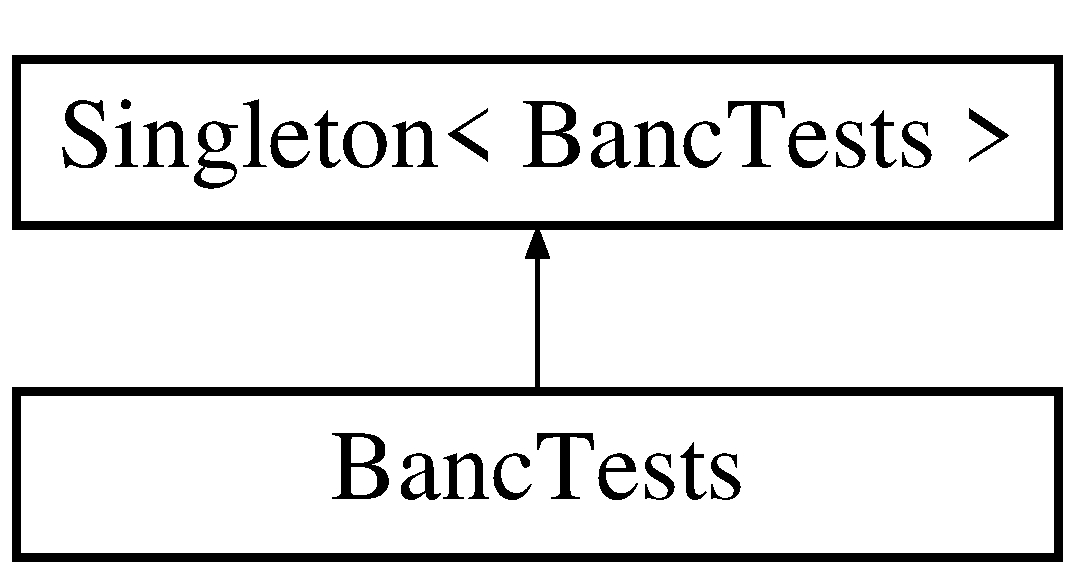
\includegraphics[height=2.000000cm]{class_banc_tests}
\end{center}
\end{figure}
\subsection*{Public Member Functions}
\begin{DoxyCompactItemize}
\item 
bool \hyperlink{group__inf2990_gab5d7fbfe7e3fbe00aa187caa10b1c506}{executer} ()
\begin{DoxyCompactList}\small\item\em Executer tous les tests unitaires. \end{DoxyCompactList}\end{DoxyCompactItemize}
\subsection*{Additional Inherited Members}


\subsection{Detailed Description}
Banc de tests qui permet d'executer tous les tests unitaires. C'est une classe singleton. 

\begin{DoxyAuthor}{Author}
Julien Gascon-\/\-Samson 
\end{DoxyAuthor}
\begin{DoxyDate}{Date}
2011-\/07-\/16 
\end{DoxyDate}


The documentation for this class was generated from the following files\-:\begin{DoxyCompactItemize}
\item 
Cadriciel/\-Sources/\-C++/\-Tests/\hyperlink{_banc_tests_8h}{Banc\-Tests.\-h}\item 
Cadriciel/\-Sources/\-C++/\-Tests/\hyperlink{_banc_tests_8cpp}{Banc\-Tests.\-cpp}\end{DoxyCompactItemize}

\hypertarget{class_interface_graphique_1_1_barre_outils}{\section{Interface\-Graphique.\-Barre\-Outils Class Reference}
\label{class_interface_graphique_1_1_barre_outils}\index{Interface\-Graphique.\-Barre\-Outils@{Interface\-Graphique.\-Barre\-Outils}}
}
Inheritance diagram for Interface\-Graphique.\-Barre\-Outils\-:\begin{figure}[H]
\begin{center}
\leavevmode
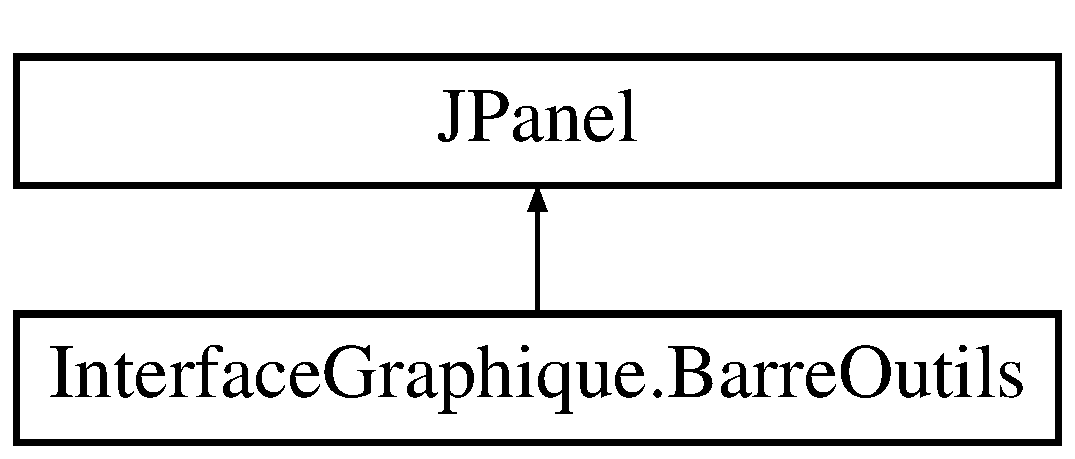
\includegraphics[height=2.000000cm]{class_interface_graphique_1_1_barre_outils}
\end{center}
\end{figure}
\subsection*{Public Member Functions}
\begin{DoxyCompactItemize}
\item 
\hyperlink{class_interface_graphique_1_1_barre_outils_acd477d6c14c10c60457127c7e059c1b2}{Barre\-Outils} ()
\item 
J\-Toggle\-Button \hyperlink{class_interface_graphique_1_1_barre_outils_a7e27f8b4f0369efafd85e2030bc1162a}{get\-Button} (int position)
\item 
void \hyperlink{class_interface_graphique_1_1_barre_outils_a851b3fc020f782bef8a95ea1948a9232}{set\-Boutons\-Size} (int larg, int haut)
\item 
int \hyperlink{class_interface_graphique_1_1_barre_outils_a71e21d552b22e486eecadb455ede1e1b}{get\-Largeur\-Boutons} ()
\item 
int \hyperlink{class_interface_graphique_1_1_barre_outils_a92104580f38b15d675b3f50e483e9a45}{get\-Hauteur\-Boutons} ()
\item 
int \hyperlink{class_interface_graphique_1_1_barre_outils_adf6d8e3d2d96c598ae6a8c53e3e6f04f}{get\-Nb\-Boutons} ()
\item 
\hypertarget{class_interface_graphique_1_1_barre_outils_a7697bec81e2b5d10b238db4c3328764b}{void {\bfseries reset\-Buttons} ()}\label{class_interface_graphique_1_1_barre_outils_a7697bec81e2b5d10b238db4c3328764b}

\item 
\hypertarget{class_interface_graphique_1_1_barre_outils_a8b45bb4c24bc67bbf0130bd6de925803}{Button\-Group {\bfseries get\-Button\-Group} ()}\label{class_interface_graphique_1_1_barre_outils_a8b45bb4c24bc67bbf0130bd6de925803}

\end{DoxyCompactItemize}


\subsection{Detailed Description}
\begin{DoxyAuthor}{Author}
Sacha L-\/\-Roussel
\end{DoxyAuthor}
Classe d�finissant la barre d'outils latt�rale de la fen�tre d'�dition. Elle contient un certain nombre de boutons permettant d'acc�der � des fonctions autrement dans la barre de menu de la classe \hyperlink{class_interface_graphique_1_1_interface_edition}{Interface\-Edition}. 

\subsection{Constructor \& Destructor Documentation}
\hypertarget{class_interface_graphique_1_1_barre_outils_acd477d6c14c10c60457127c7e059c1b2}{\index{Interface\-Graphique\-::\-Barre\-Outils@{Interface\-Graphique\-::\-Barre\-Outils}!Barre\-Outils@{Barre\-Outils}}
\index{Barre\-Outils@{Barre\-Outils}!InterfaceGraphique::BarreOutils@{Interface\-Graphique\-::\-Barre\-Outils}}
\subsubsection[{Barre\-Outils}]{\setlength{\rightskip}{0pt plus 5cm}Interface\-Graphique.\-Barre\-Outils.\-Barre\-Outils (
\begin{DoxyParamCaption}
{}
\end{DoxyParamCaption}
)\hspace{0.3cm}{\ttfamily [inline]}}}\label{class_interface_graphique_1_1_barre_outils_acd477d6c14c10c60457127c7e059c1b2}
Constructeur par d�faut de la barre d'outils. 
\begin{DoxyParams}{Parameters}
{\em Aucuns} & param�tres \\
\hline
\end{DoxyParams}
\begin{DoxyReturn}{Returns}
Rien 
\end{DoxyReturn}


\subsection{Member Function Documentation}
\hypertarget{class_interface_graphique_1_1_barre_outils_a7e27f8b4f0369efafd85e2030bc1162a}{\index{Interface\-Graphique\-::\-Barre\-Outils@{Interface\-Graphique\-::\-Barre\-Outils}!get\-Button@{get\-Button}}
\index{get\-Button@{get\-Button}!InterfaceGraphique::BarreOutils@{Interface\-Graphique\-::\-Barre\-Outils}}
\subsubsection[{get\-Button}]{\setlength{\rightskip}{0pt plus 5cm}J\-Toggle\-Button Interface\-Graphique.\-Barre\-Outils.\-get\-Button (
\begin{DoxyParamCaption}
\item[{int}]{position}
\end{DoxyParamCaption}
)\hspace{0.3cm}{\ttfamily [inline]}}}\label{class_interface_graphique_1_1_barre_outils_a7e27f8b4f0369efafd85e2030bc1162a}
M�thode permettant d'acc�der au bouton en une position connue (� partir de 0) 
\begin{DoxyParams}{Parameters}
{\em int} & position Position connue du bouton (En ordre d'apparition) \\
\hline
\end{DoxyParams}
\begin{DoxyReturn}{Returns}
J\-Toggle\-Button Retourne l'objet repr�sentt� par le bouton. 
\end{DoxyReturn}
\hypertarget{class_interface_graphique_1_1_barre_outils_a92104580f38b15d675b3f50e483e9a45}{\index{Interface\-Graphique\-::\-Barre\-Outils@{Interface\-Graphique\-::\-Barre\-Outils}!get\-Hauteur\-Boutons@{get\-Hauteur\-Boutons}}
\index{get\-Hauteur\-Boutons@{get\-Hauteur\-Boutons}!InterfaceGraphique::BarreOutils@{Interface\-Graphique\-::\-Barre\-Outils}}
\subsubsection[{get\-Hauteur\-Boutons}]{\setlength{\rightskip}{0pt plus 5cm}int Interface\-Graphique.\-Barre\-Outils.\-get\-Hauteur\-Boutons (
\begin{DoxyParamCaption}
{}
\end{DoxyParamCaption}
)\hspace{0.3cm}{\ttfamily [inline]}}}\label{class_interface_graphique_1_1_barre_outils_a92104580f38b15d675b3f50e483e9a45}
Retourne la heuteur des boutons 
\begin{DoxyParams}{Parameters}
{\em Aucuns} & param�tres \\
\hline
\end{DoxyParams}
\begin{DoxyReturn}{Returns}
int Valeur entir�re repr�sentant la hauteur d'un bouton 
\end{DoxyReturn}
\hypertarget{class_interface_graphique_1_1_barre_outils_a71e21d552b22e486eecadb455ede1e1b}{\index{Interface\-Graphique\-::\-Barre\-Outils@{Interface\-Graphique\-::\-Barre\-Outils}!get\-Largeur\-Boutons@{get\-Largeur\-Boutons}}
\index{get\-Largeur\-Boutons@{get\-Largeur\-Boutons}!InterfaceGraphique::BarreOutils@{Interface\-Graphique\-::\-Barre\-Outils}}
\subsubsection[{get\-Largeur\-Boutons}]{\setlength{\rightskip}{0pt plus 5cm}int Interface\-Graphique.\-Barre\-Outils.\-get\-Largeur\-Boutons (
\begin{DoxyParamCaption}
{}
\end{DoxyParamCaption}
)\hspace{0.3cm}{\ttfamily [inline]}}}\label{class_interface_graphique_1_1_barre_outils_a71e21d552b22e486eecadb455ede1e1b}
Retourne la largeur des boutons 
\begin{DoxyParams}{Parameters}
{\em Aucun} & \\
\hline
\end{DoxyParams}
\begin{DoxyReturn}{Returns}
int Valeur enti�re repr�sentant la largeur du bouton. 
\end{DoxyReturn}
\hypertarget{class_interface_graphique_1_1_barre_outils_adf6d8e3d2d96c598ae6a8c53e3e6f04f}{\index{Interface\-Graphique\-::\-Barre\-Outils@{Interface\-Graphique\-::\-Barre\-Outils}!get\-Nb\-Boutons@{get\-Nb\-Boutons}}
\index{get\-Nb\-Boutons@{get\-Nb\-Boutons}!InterfaceGraphique::BarreOutils@{Interface\-Graphique\-::\-Barre\-Outils}}
\subsubsection[{get\-Nb\-Boutons}]{\setlength{\rightskip}{0pt plus 5cm}int Interface\-Graphique.\-Barre\-Outils.\-get\-Nb\-Boutons (
\begin{DoxyParamCaption}
{}
\end{DoxyParamCaption}
)\hspace{0.3cm}{\ttfamily [inline]}}}\label{class_interface_graphique_1_1_barre_outils_adf6d8e3d2d96c598ae6a8c53e3e6f04f}
Retourne le nombre de boutons pr�sent dans la barre d'outils. 
\begin{DoxyParams}{Parameters}
{\em Aucuns} & param�tres \\
\hline
\end{DoxyParams}
\begin{DoxyReturn}{Returns}
int Entier qui repr�sente le nombre de boutons pr�sents 
\end{DoxyReturn}
\hypertarget{class_interface_graphique_1_1_barre_outils_a851b3fc020f782bef8a95ea1948a9232}{\index{Interface\-Graphique\-::\-Barre\-Outils@{Interface\-Graphique\-::\-Barre\-Outils}!set\-Boutons\-Size@{set\-Boutons\-Size}}
\index{set\-Boutons\-Size@{set\-Boutons\-Size}!InterfaceGraphique::BarreOutils@{Interface\-Graphique\-::\-Barre\-Outils}}
\subsubsection[{set\-Boutons\-Size}]{\setlength{\rightskip}{0pt plus 5cm}void Interface\-Graphique.\-Barre\-Outils.\-set\-Boutons\-Size (
\begin{DoxyParamCaption}
\item[{int}]{larg, }
\item[{int}]{haut}
\end{DoxyParamCaption}
)\hspace{0.3cm}{\ttfamily [inline]}}}\label{class_interface_graphique_1_1_barre_outils_a851b3fc020f782bef8a95ea1948a9232}
Permet de sp�cifier la taille qu'occuperont les boutons dans la barre d'outils 
\begin{DoxyParams}{Parameters}
{\em larg} & Largeur des boutons \\
\hline
{\em haut} & Hauteur des boutons \\
\hline
\end{DoxyParams}
\begin{DoxyReturn}{Returns}
void 
\end{DoxyReturn}


The documentation for this class was generated from the following file\-:\begin{DoxyCompactItemize}
\item 
Cadriciel/\-Sources/\-Java/\-Interface\-Graphique/src/\-Interface\-Graphique/Barre\-Outils.\-java\end{DoxyCompactItemize}

\hypertarget{class_barriere}{\section{Barriere Class Reference}
\label{class_barriere}\index{Barriere@{Barriere}}
}


Cette classe qui permet de creer des barrieres.  




{\ttfamily \#include $<$Barriere.\-h$>$}

Inheritance diagram for Barriere\-:\begin{figure}[H]
\begin{center}
\leavevmode
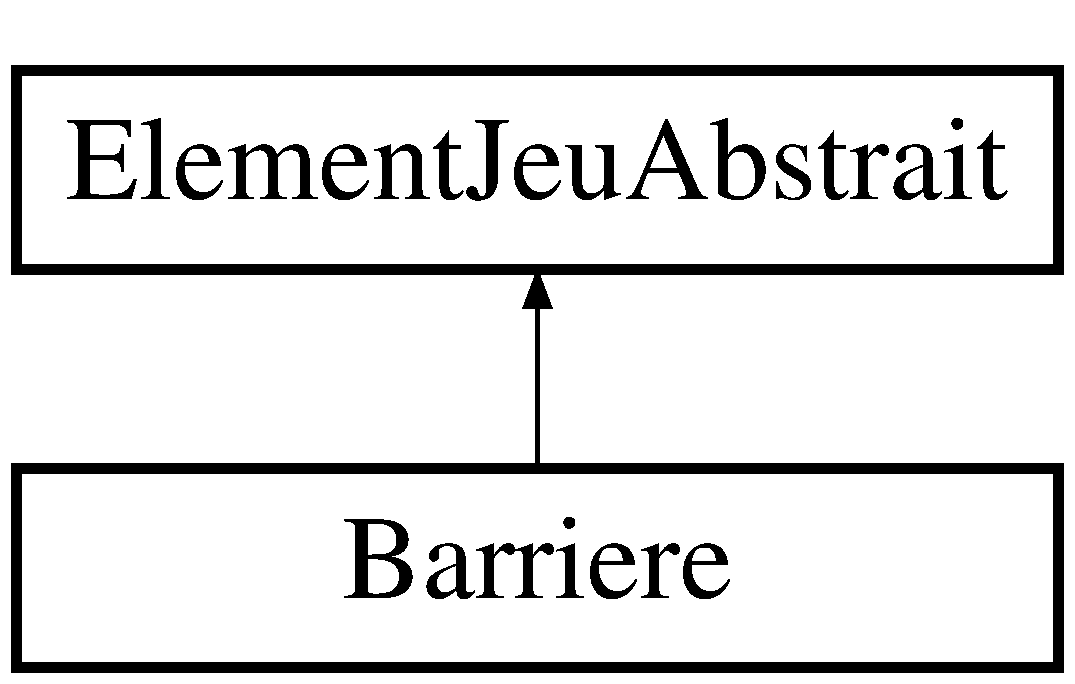
\includegraphics[height=2.000000cm]{class_barriere}
\end{center}
\end{figure}
\subsection*{Public Member Functions}
\begin{DoxyCompactItemize}
\item 
\hyperlink{group__inf2990_gacf2b80faa55444228db735390db40fc7}{Barriere} ()
\begin{DoxyCompactList}\small\item\em Constructeur. \end{DoxyCompactList}\item 
\hyperlink{group__inf2990_ga17283625d17ad9370a60c00357b1bf3e}{Barriere} (\hyperlink{group__utilitaire_ga6b2956069f76c7e27df4f79f87e5a48c}{Vecteur3f} position1, \hyperlink{group__utilitaire_ga6b2956069f76c7e27df4f79f87e5a48c}{Vecteur3f} position2, \hyperlink{group__utilitaire_ga6b2956069f76c7e27df4f79f87e5a48c}{Vecteur3f} taille, \hyperlink{group__utilitaire_ga6b2956069f76c7e27df4f79f87e5a48c}{Vecteur3f} direction\-Vitesse, float poids)
\item 
\hyperlink{group__inf2990_ga87db720230a9aced41fe2d33918f68d8}{Barriere} (const \hyperlink{class_barriere}{Barriere} \&barriere)
\item 
virtual \hyperlink{group__inf2990_ga99e534cc4cdddfce853a07d870270989}{$\sim$\-Barriere} ()
\begin{DoxyCompactList}\small\item\em Destructeur. \end{DoxyCompactList}\item 
\hypertarget{group__inf2990_gad85230f246a469fb21f367df473049a3}{virtual bool \hyperlink{group__inf2990_gad85230f246a469fb21f367df473049a3}{check\-Collision} (\hyperlink{class_element_jeu_abstrait}{Element\-Jeu\-Abstrait} $\ast$element)}\label{group__inf2990_gad85230f246a469fb21f367df473049a3}

\begin{DoxyCompactList}\small\item\em Check Collision. \end{DoxyCompactList}\item 
\hypertarget{class_barriere_ad512ec476e54d29b8edd022a31573764}{virtual bool \hyperlink{class_barriere_ad512ec476e54d29b8edd022a31573764}{check\-Collision} (\hyperlink{class_accelerateur}{Accelerateur} $\ast$accelerateur)}\label{class_barriere_ad512ec476e54d29b8edd022a31573764}

\begin{DoxyCompactList}\small\item\em Methode pour verifier si une collision existe. \end{DoxyCompactList}\item 
\hypertarget{group__inf2990_ga046dcb0b3592e83e6ceecb848c138185}{virtual bool {\bfseries check\-Collision} (\hyperlink{class_asteroide}{Asteroide} $\ast$asteroide)}\label{group__inf2990_ga046dcb0b3592e83e6ceecb848c138185}

\item 
\hypertarget{class_barriere_a3f1b279f8b739e3d06b39d5f6fabc30c}{virtual bool {\bfseries check\-Collision} (\hyperlink{class_barriere}{Barriere} $\ast$barriere)}\label{class_barriere_a3f1b279f8b739e3d06b39d5f6fabc30c}

\item 
\hypertarget{class_barriere_aafcaa584b3a1b994cb94fa192505c659}{virtual bool {\bfseries check\-Collision} (\hyperlink{class_portail}{Portail} $\ast$portail)}\label{class_barriere_aafcaa584b3a1b994cb94fa192505c659}

\item 
\hypertarget{group__inf2990_ga7a3b327a7f30283a2e6b79bc79eb0040}{virtual bool {\bfseries check\-Collision} (\hyperlink{class_projectile}{Projectile} $\ast$projectile)}\label{group__inf2990_ga7a3b327a7f30283a2e6b79bc79eb0040}

\item 
\hypertarget{class_barriere_afd75ee9a9f902f065384684520438feb}{virtual bool {\bfseries check\-Collision} (\hyperlink{class_station}{Station} $\ast$station)}\label{class_barriere_afd75ee9a9f902f065384684520438feb}

\item 
\hypertarget{group__inf2990_ga92014a0e895d1a7dd1c637a2033c2809}{virtual bool {\bfseries check\-Collision} (\hyperlink{class_vaisseau}{Vaisseau} $\ast$vaisseau)}\label{group__inf2990_ga92014a0e895d1a7dd1c637a2033c2809}

\item 
virtual bool \hyperlink{group__inf2990_gac7d66192494684c4e7bcdd00fa9b7ab2}{check\-Collision\-Joueur\-Virtuel} (\hyperlink{class_vaisseau}{Vaisseau} $\ast$joueur\-Virtuel)
\begin{DoxyCompactList}\small\item\em Permet au joueur virtuel de ne pas tirer sur une barrier. \end{DoxyCompactList}\item 
virtual void \hyperlink{group__inf2990_gafc3817554324d494409e24e195088892}{traiter\-Collision} (\hyperlink{class_element_jeu_abstrait}{Element\-Jeu\-Abstrait} $\ast$element)
\item 
\hypertarget{class_barriere_a06cd05cc1baba83705e4999d1109c4b0}{virtual void \hyperlink{class_barriere_a06cd05cc1baba83705e4999d1109c4b0}{traiter\-Collision} (\hyperlink{class_accelerateur}{Accelerateur} $\ast$accelerateur)}\label{class_barriere_a06cd05cc1baba83705e4999d1109c4b0}

\begin{DoxyCompactList}\small\item\em Methode pour traiter la collision si elle a lui avec les differents elements. \end{DoxyCompactList}\item 
\hypertarget{group__inf2990_ga187a42d83d5060894239c0ba34d18a8e}{virtual void {\bfseries traiter\-Collision} (\hyperlink{class_asteroide}{Asteroide} $\ast$asteroide)}\label{group__inf2990_ga187a42d83d5060894239c0ba34d18a8e}

\item 
\hypertarget{class_barriere_aceff2c03891e91ab4e6e43785d0680ee}{virtual void {\bfseries traiter\-Collision} (\hyperlink{class_barriere}{Barriere} $\ast$barriere)}\label{class_barriere_aceff2c03891e91ab4e6e43785d0680ee}

\item 
\hypertarget{class_barriere_a253f995214d58262ef072d47f705573b}{virtual void {\bfseries traiter\-Collision} (\hyperlink{class_portail}{Portail} $\ast$portail)}\label{class_barriere_a253f995214d58262ef072d47f705573b}

\item 
\hypertarget{group__inf2990_gaa09a3ee20ab537a1c4f37ad3edcb55b6}{virtual void {\bfseries traiter\-Collision} (\hyperlink{class_projectile}{Projectile} $\ast$projectile)}\label{group__inf2990_gaa09a3ee20ab537a1c4f37ad3edcb55b6}

\item 
\hypertarget{class_barriere_a321838647c5e214b6c0f7374b23f7dfa}{virtual void {\bfseries traiter\-Collision} (\hyperlink{class_station}{Station} $\ast$station)}\label{class_barriere_a321838647c5e214b6c0f7374b23f7dfa}

\item 
\hypertarget{group__inf2990_ga09b425373e5f02b1cbe200e71e006cfd}{virtual void {\bfseries traiter\-Collision} (\hyperlink{class_vaisseau}{Vaisseau} $\ast$vaisseau)}\label{group__inf2990_ga09b425373e5f02b1cbe200e71e006cfd}

\item 
virtual Type \hyperlink{group__inf2990_ga9a0160da5089efa38867ad45782ae40d}{get\-Type} ()
\begin{DoxyCompactList}\small\item\em Permet d'obtenir le type de l'element. \end{DoxyCompactList}\item 
virtual void \hyperlink{group__inf2990_ga171ffac6e81bf3bbd884212945946354}{update} (float delta\-T)
\begin{DoxyCompactList}\small\item\em Mise a jour. \end{DoxyCompactList}\item 
\hypertarget{group__inf2990_gad0aa2475444721471fc452d1b6f9438e}{virtual \hyperlink{class_element_jeu_abstrait}{Element\-Jeu\-Abstrait} $\ast$ \hyperlink{group__inf2990_gad0aa2475444721471fc452d1b6f9438e}{clone} () const }\label{group__inf2990_gad0aa2475444721471fc452d1b6f9438e}

\begin{DoxyCompactList}\small\item\em Permet de cloner l'element. \end{DoxyCompactList}\item 
void \hyperlink{group__inf2990_ga00c08e4b911e95aa83ddcd087ff09294}{position\-Barriere} (\hyperlink{group__utilitaire_ga6b2956069f76c7e27df4f79f87e5a48c}{Vecteur3f} position1, \hyperlink{group__utilitaire_ga6b2956069f76c7e27df4f79f87e5a48c}{Vecteur3f} position2)
\item 
\hyperlink{group__utilitaire_ga6b2956069f76c7e27df4f79f87e5a48c}{Vecteur3f} \hyperlink{group__inf2990_ga9993ac42c28c45c33526233cfcc302e0}{get\-Position\-Pt1} ()
\item 
\hypertarget{group__inf2990_ga45d889538f981bc7d4ebdb631b570ffe}{\hyperlink{group__utilitaire_ga6b2956069f76c7e27df4f79f87e5a48c}{Vecteur3f} {\bfseries get\-Position\-Pt2} ()}\label{group__inf2990_ga45d889538f981bc7d4ebdb631b570ffe}

\end{DoxyCompactItemize}
\subsection*{Additional Inherited Members}


\subsection{Detailed Description}
Cette classe qui permet de creer des barrieres. 

La classe \hyperlink{class_barriere}{Barriere} contiendra un pointeur vers un noeud\-Barriere afin que celle-\/ci s'occupe de la texture de la barriere. 

The documentation for this class was generated from the following files\-:\begin{DoxyCompactItemize}
\item 
Cadriciel/\-Sources/\-C++/\-Element\-Objet/\hyperlink{_barriere_8h}{Barriere.\-h}\item 
Cadriciel/\-Sources/\-C++/\-Element\-Objet/\hyperlink{_barriere_8cpp}{Barriere.\-cpp}\end{DoxyCompactItemize}

\hypertarget{struct_b_d_f___property_rec__}{\section{B\-D\-F\-\_\-\-Property\-Rec\-\_\- Struct Reference}
\label{struct_b_d_f___property_rec__}\index{B\-D\-F\-\_\-\-Property\-Rec\-\_\-@{B\-D\-F\-\_\-\-Property\-Rec\-\_\-}}
}
\subsection*{Public Attributes}
\begin{DoxyCompactItemize}
\item 
\hypertarget{struct_b_d_f___property_rec___a88c19ee6f16bd1b36127f5f7d44a4e39}{B\-D\-F\-\_\-\-Property\-Type {\bfseries type}}\label{struct_b_d_f___property_rec___a88c19ee6f16bd1b36127f5f7d44a4e39}

\item 
\hypertarget{struct_b_d_f___property_rec___a7fdd16635fbcfd4f737e6beb2d014871}{\begin{tabbing}
xx\=xx\=xx\=xx\=xx\=xx\=xx\=xx\=xx\=\kill
union \{\\
\hypertarget{union_b_d_f___property_rec___1_1@0_aa8d56dc848d8a2c8e2f7e40a63f5d032}{\>const char $\ast$ {\bfseries atom}\\
\hypertarget{union_b_d_f___property_rec___1_1@0_a71243b414ad203fd7d6d2468c39bbd79}{\>FT\_Int32 {\bfseries integer}\\
\hypertarget{union_b_d_f___property_rec___1_1@0_adaba2e4ce8da90a5ea59080a0521d332}{\>FT\_UInt32 {\bfseries cardinal}\\
\} {\bfseries u}}\label{struct_b_d_f___property_rec___a7fdd16635fbcfd4f737e6beb2d014871}
\\

\end{tabbing}\end{DoxyCompactItemize}


The documentation for this struct was generated from the following file\-:\begin{DoxyCompactItemize}
\item 
Cadriciel/\-Commun/\-Externe/\-Free\-Type/include/freetype/ftbdf.\-h\end{DoxyCompactItemize}

\hypertarget{classmath_1_1_boite_englobante_orientee}{\section{math\-:\-:Boite\-Englobante\-Orientee Class Reference}
\label{classmath_1_1_boite_englobante_orientee}\index{math\-::\-Boite\-Englobante\-Orientee@{math\-::\-Boite\-Englobante\-Orientee}}
}


{\ttfamily \#include $<$Boite\-Englobante\-Orientee.\-h$>$}

\subsection*{Public Member Functions}
\begin{DoxyCompactItemize}
\item 
\hyperlink{classmath_1_1_boite_englobante_orientee_aa7243dd64524ddebf0ba546a75cb9aac}{Boite\-Englobante\-Orientee} ()
\item 
\hyperlink{classmath_1_1_boite_englobante_orientee_ab42ccee7bf04a74a91c1e77e57b11e84}{Boite\-Englobante\-Orientee} (const \hyperlink{group__utilitaire_ga6b2956069f76c7e27df4f79f87e5a48c}{Vecteur3f} \&coin\-Min, const \hyperlink{group__utilitaire_ga6b2956069f76c7e27df4f79f87e5a48c}{Vecteur3f} \&coin\-Max)
\item 
bool \hyperlink{classmath_1_1_boite_englobante_orientee_aeb78d68ab7515e356fe0f9ad966a617b}{calculer\-Collision} (const \hyperlink{classmath_1_1_boite_englobante_orientee}{Boite\-Englobante\-Orientee} \&obb) const 
\item 
\hyperlink{wglew_8h_aeea6e3dfae3acf232096f57d2d57f084}{void} \hyperlink{classmath_1_1_boite_englobante_orientee_a65b61bcf844aa3748d4cb50eaf52c3da}{update} (const \hyperlink{structai_vector3_d}{ai\-Vector3\-D} \&\hyperlink{fmod__codec_8h_a7d71cf36b6a2fc185ecbc89f93fa58a3}{position}, \hyperlink{fmod_8h_aeb841aa4b4b5f444b5d739d865b420af}{float} \hyperlink{glew_8h_a6d7a98b0d979b9411a4344a98a7a6122}{angle}, const \hyperlink{structai_vector3_d}{ai\-Vector3\-D} \&taille)
\item 
\hyperlink{wglew_8h_aeea6e3dfae3acf232096f57d2d57f084}{void} \hyperlink{classmath_1_1_boite_englobante_orientee_aeb355a19767d9366825e32ccf95dc4fc}{afficher} () const 
\item 
const vector$<$ \hyperlink{group__utilitaire_ga6b2956069f76c7e27df4f79f87e5a48c}{Vecteur3f} $>$ \hyperlink{classmath_1_1_boite_englobante_orientee_a578c28c8047573d80a7d2e5824155d23}{get\-Coins} () const 
\item 
const vector$<$ \hyperlink{classmath_1_1_droite3_d}{Droite3\-D} $>$ \hyperlink{classmath_1_1_boite_englobante_orientee_a3d8d852d08d3190bf686becc86e5e410}{get\-Droites} () const 
\item 
\hyperlink{wglew_8h_aeea6e3dfae3acf232096f57d2d57f084}{void} \hyperlink{classmath_1_1_boite_englobante_orientee_abb2980f581864806cd859e1c382b677b}{get\-Boite\-Englobante\-Non\-Orientee} (\hyperlink{group__utilitaire_ga606b191c0b0bbb868ae25c13b906f45a}{Vecteur2f} \&coin\-Haut\-Gauche, \hyperlink{group__utilitaire_ga606b191c0b0bbb868ae25c13b906f45a}{Vecteur2f} \&coin\-Bas\-Droite) const 
\item 
\hyperlink{fmod_8h_aeb841aa4b4b5f444b5d739d865b420af}{float} \hyperlink{classmath_1_1_boite_englobante_orientee_a2420d0e0f451857cb8d46143013691fe}{get\-Moitie\-Longueur} () const 
\item 
\hyperlink{fmod_8h_aeb841aa4b4b5f444b5d739d865b420af}{float} \hyperlink{classmath_1_1_boite_englobante_orientee_ac626bbe542000ef0c491f8139a1ce51a}{get\-Moitie\-Hauteur} () const 
\end{DoxyCompactItemize}


\subsection{Detailed Description}
Cette classe definie une boite englobante orientee selon l'objet qu'elle englobe. Elle permet de tester les intersections avec d'autres boites englobantes orientees. 

\subsection{Constructor \& Destructor Documentation}
\hypertarget{classmath_1_1_boite_englobante_orientee_aa7243dd64524ddebf0ba546a75cb9aac}{\index{math\-::\-Boite\-Englobante\-Orientee@{math\-::\-Boite\-Englobante\-Orientee}!Boite\-Englobante\-Orientee@{Boite\-Englobante\-Orientee}}
\index{Boite\-Englobante\-Orientee@{Boite\-Englobante\-Orientee}!math::BoiteEnglobanteOrientee@{math\-::\-Boite\-Englobante\-Orientee}}
\subsubsection[{Boite\-Englobante\-Orientee}]{\setlength{\rightskip}{0pt plus 5cm}math\-::\-Boite\-Englobante\-Orientee\-::\-Boite\-Englobante\-Orientee (
\begin{DoxyParamCaption}
{}
\end{DoxyParamCaption}
)}}\label{classmath_1_1_boite_englobante_orientee_aa7243dd64524ddebf0ba546a75cb9aac}
Constructeur par defaut \hypertarget{classmath_1_1_boite_englobante_orientee_ab42ccee7bf04a74a91c1e77e57b11e84}{\index{math\-::\-Boite\-Englobante\-Orientee@{math\-::\-Boite\-Englobante\-Orientee}!Boite\-Englobante\-Orientee@{Boite\-Englobante\-Orientee}}
\index{Boite\-Englobante\-Orientee@{Boite\-Englobante\-Orientee}!math::BoiteEnglobanteOrientee@{math\-::\-Boite\-Englobante\-Orientee}}
\subsubsection[{Boite\-Englobante\-Orientee}]{\setlength{\rightskip}{0pt plus 5cm}math\-::\-Boite\-Englobante\-Orientee\-::\-Boite\-Englobante\-Orientee (
\begin{DoxyParamCaption}
\item[{const {\bf Vecteur3f} \&}]{coin\-Min, }
\item[{const {\bf Vecteur3f} \&}]{coin\-Max}
\end{DoxyParamCaption}
)}}\label{classmath_1_1_boite_englobante_orientee_ab42ccee7bf04a74a91c1e77e57b11e84}
Constructeur. 
\begin{DoxyParams}{Parameters}
{\em coin\-Min} & Le coin minimum de la boite englobante \\
\hline
{\em coin\-Max} & Le coin maximum de la boite englobante \\
\hline
{\em angle} & L'angle de rotation de la boite englobante (0 par defaut) \\
\hline
\end{DoxyParams}


\subsection{Member Function Documentation}
\hypertarget{classmath_1_1_boite_englobante_orientee_aeb355a19767d9366825e32ccf95dc4fc}{\index{math\-::\-Boite\-Englobante\-Orientee@{math\-::\-Boite\-Englobante\-Orientee}!afficher@{afficher}}
\index{afficher@{afficher}!math::BoiteEnglobanteOrientee@{math\-::\-Boite\-Englobante\-Orientee}}
\subsubsection[{afficher}]{\setlength{\rightskip}{0pt plus 5cm}{\bf void} math\-::\-Boite\-Englobante\-Orientee\-::afficher (
\begin{DoxyParamCaption}
{}
\end{DoxyParamCaption}
) const}}\label{classmath_1_1_boite_englobante_orientee_aeb355a19767d9366825e32ccf95dc4fc}
Affiche la boite englobante \hypertarget{classmath_1_1_boite_englobante_orientee_aeb78d68ab7515e356fe0f9ad966a617b}{\index{math\-::\-Boite\-Englobante\-Orientee@{math\-::\-Boite\-Englobante\-Orientee}!calculer\-Collision@{calculer\-Collision}}
\index{calculer\-Collision@{calculer\-Collision}!math::BoiteEnglobanteOrientee@{math\-::\-Boite\-Englobante\-Orientee}}
\subsubsection[{calculer\-Collision}]{\setlength{\rightskip}{0pt plus 5cm}bool math\-::\-Boite\-Englobante\-Orientee\-::calculer\-Collision (
\begin{DoxyParamCaption}
\item[{const {\bf Boite\-Englobante\-Orientee} \&}]{obb}
\end{DoxyParamCaption}
) const}}\label{classmath_1_1_boite_englobante_orientee_aeb78d68ab7515e356fe0f9ad966a617b}
Verifie si une autre boite englobante orientee intersecte celle-\/ci 
\begin{DoxyParams}{Parameters}
{\em obb} & La seconde boite englobante orientee (Oriented Bounding Box) avec laquelle on veut verifier la collision. \\
\hline
\end{DoxyParams}
\begin{DoxyReturn}{Returns}
true si l'objet est rentre en collision avec la boite englobante 
\end{DoxyReturn}
\hypertarget{classmath_1_1_boite_englobante_orientee_abb2980f581864806cd859e1c382b677b}{\index{math\-::\-Boite\-Englobante\-Orientee@{math\-::\-Boite\-Englobante\-Orientee}!get\-Boite\-Englobante\-Non\-Orientee@{get\-Boite\-Englobante\-Non\-Orientee}}
\index{get\-Boite\-Englobante\-Non\-Orientee@{get\-Boite\-Englobante\-Non\-Orientee}!math::BoiteEnglobanteOrientee@{math\-::\-Boite\-Englobante\-Orientee}}
\subsubsection[{get\-Boite\-Englobante\-Non\-Orientee}]{\setlength{\rightskip}{0pt plus 5cm}{\bf void} math\-::\-Boite\-Englobante\-Orientee\-::get\-Boite\-Englobante\-Non\-Orientee (
\begin{DoxyParamCaption}
\item[{{\bf Vecteur2f} \&}]{coin\-Haut\-Gauche, }
\item[{{\bf Vecteur2f} \&}]{coin\-Bas\-Droite}
\end{DoxyParamCaption}
) const}}\label{classmath_1_1_boite_englobante_orientee_abb2980f581864806cd859e1c382b677b}
Retourne 2 vecteurs en 2 dimensions qui d�finissent la boite englobante non-\/orient�e dans le plan xy. 
\begin{DoxyParams}{Parameters}
{\em coin\-Haut\-Gauche} & Le coin en haut � gauche de la boite non-\/orient�e \\
\hline
{\em coin\-Bas\-Droite} & Le coin en bas � droite de la boite non-\/orient�e \\
\hline
\end{DoxyParams}
\hypertarget{classmath_1_1_boite_englobante_orientee_a578c28c8047573d80a7d2e5824155d23}{\index{math\-::\-Boite\-Englobante\-Orientee@{math\-::\-Boite\-Englobante\-Orientee}!get\-Coins@{get\-Coins}}
\index{get\-Coins@{get\-Coins}!math::BoiteEnglobanteOrientee@{math\-::\-Boite\-Englobante\-Orientee}}
\subsubsection[{get\-Coins}]{\setlength{\rightskip}{0pt plus 5cm}const vector$<$ {\bf Vecteur3f} $>$ math\-::\-Boite\-Englobante\-Orientee\-::get\-Coins (
\begin{DoxyParamCaption}
{}
\end{DoxyParamCaption}
) const}}\label{classmath_1_1_boite_englobante_orientee_a578c28c8047573d80a7d2e5824155d23}
Retourne les 4 coins de la boite. Les coins sont dans cet ordre\-:
\begin{DoxyItemize}
\item Bas gauche;
\item Haut gauche;
\item Haut droit;
\item Bas droit. Cet ordre est correct lorsque l'objet n'est pas tourne. Si l'objet est a l'envers, alors les coins appara�tront a l'envers, mais ils gardent quand meme cet ordre. 
\end{DoxyItemize}\hypertarget{classmath_1_1_boite_englobante_orientee_a3d8d852d08d3190bf686becc86e5e410}{\index{math\-::\-Boite\-Englobante\-Orientee@{math\-::\-Boite\-Englobante\-Orientee}!get\-Droites@{get\-Droites}}
\index{get\-Droites@{get\-Droites}!math::BoiteEnglobanteOrientee@{math\-::\-Boite\-Englobante\-Orientee}}
\subsubsection[{get\-Droites}]{\setlength{\rightskip}{0pt plus 5cm}const vector$<$ {\bf Droite3\-D} $>$ math\-::\-Boite\-Englobante\-Orientee\-::get\-Droites (
\begin{DoxyParamCaption}
{}
\end{DoxyParamCaption}
) const}}\label{classmath_1_1_boite_englobante_orientee_a3d8d852d08d3190bf686becc86e5e410}
Retourne les 4 droites qui composent la boite. Les droites sont dans cet ordre\-:
\begin{DoxyItemize}
\item Bas dans l'axe des x;
\item Gauche dans l'axe des y;
\item Haut dans l'axe des x;
\item Droite dans l'axe des y; Cet ordre est correct lorsque l'objets n'est pas tourn�. Si l'objet est � l'envers, alors les droites seronts � l'evers, mais ils gardent quand m�me cet ordre. 
\end{DoxyItemize}\hypertarget{classmath_1_1_boite_englobante_orientee_ac626bbe542000ef0c491f8139a1ce51a}{\index{math\-::\-Boite\-Englobante\-Orientee@{math\-::\-Boite\-Englobante\-Orientee}!get\-Moitie\-Hauteur@{get\-Moitie\-Hauteur}}
\index{get\-Moitie\-Hauteur@{get\-Moitie\-Hauteur}!math::BoiteEnglobanteOrientee@{math\-::\-Boite\-Englobante\-Orientee}}
\subsubsection[{get\-Moitie\-Hauteur}]{\setlength{\rightskip}{0pt plus 5cm}{\bf float} math\-::\-Boite\-Englobante\-Orientee\-::get\-Moitie\-Hauteur (
\begin{DoxyParamCaption}
{}
\end{DoxyParamCaption}
) const\hspace{0.3cm}{\ttfamily [inline]}}}\label{classmath_1_1_boite_englobante_orientee_ac626bbe542000ef0c491f8139a1ce51a}
\hypertarget{classmath_1_1_boite_englobante_orientee_a2420d0e0f451857cb8d46143013691fe}{\index{math\-::\-Boite\-Englobante\-Orientee@{math\-::\-Boite\-Englobante\-Orientee}!get\-Moitie\-Longueur@{get\-Moitie\-Longueur}}
\index{get\-Moitie\-Longueur@{get\-Moitie\-Longueur}!math::BoiteEnglobanteOrientee@{math\-::\-Boite\-Englobante\-Orientee}}
\subsubsection[{get\-Moitie\-Longueur}]{\setlength{\rightskip}{0pt plus 5cm}{\bf float} math\-::\-Boite\-Englobante\-Orientee\-::get\-Moitie\-Longueur (
\begin{DoxyParamCaption}
{}
\end{DoxyParamCaption}
) const\hspace{0.3cm}{\ttfamily [inline]}}}\label{classmath_1_1_boite_englobante_orientee_a2420d0e0f451857cb8d46143013691fe}
\hypertarget{classmath_1_1_boite_englobante_orientee_a65b61bcf844aa3748d4cb50eaf52c3da}{\index{math\-::\-Boite\-Englobante\-Orientee@{math\-::\-Boite\-Englobante\-Orientee}!update@{update}}
\index{update@{update}!math::BoiteEnglobanteOrientee@{math\-::\-Boite\-Englobante\-Orientee}}
\subsubsection[{update}]{\setlength{\rightskip}{0pt plus 5cm}{\bf void} math\-::\-Boite\-Englobante\-Orientee\-::update (
\begin{DoxyParamCaption}
\item[{const {\bf ai\-Vector3\-D} \&}]{position, }
\item[{{\bf float}}]{angle, }
\item[{const {\bf ai\-Vector3\-D} \&}]{taille}
\end{DoxyParamCaption}
)}}\label{classmath_1_1_boite_englobante_orientee_a65b61bcf844aa3748d4cb50eaf52c3da}
Met a jour la boite englobante pour avoir sa nouvelle orientation et position 
\begin{DoxyParams}{Parameters}
{\em position} & La nouvelle position de la boite englobante \\
\hline
{\em angle} & Le nouvel angle de rotation de la boite englobante \\
\hline
{\em taille} & La nouvelle taille de la boite englobante \\
\hline
\end{DoxyParams}


The documentation for this class was generated from the following files\-:\begin{DoxyCompactItemize}
\item 
Cadriciel/\-Commun/\-Utilitaire/\hyperlink{_boite_englobante_orientee_8h}{Boite\-Englobante\-Orientee.\-h}\item 
Cadriciel/\-Commun/\-Utilitaire/\hyperlink{_boite_englobante_orientee_8cpp}{Boite\-Englobante\-Orientee.\-cpp}\end{DoxyCompactItemize}

\hypertarget{class_boite_englobante_orientee_test}{\section{Boite\-Englobante\-Orientee\-Test Class Reference}
\label{class_boite_englobante_orientee_test}\index{Boite\-Englobante\-Orientee\-Test@{Boite\-Englobante\-Orientee\-Test}}
}


\hyperlink{class_test}{Test} qui s'assure que les operations effectuees sur les boites englobantes orientees sont fonctionnelles.  




{\ttfamily \#include $<$Boite\-Englobante\-Orientee\-Test.\-h$>$}

Inheritance diagram for Boite\-Englobante\-Orientee\-Test\-:\begin{figure}[H]
\begin{center}
\leavevmode
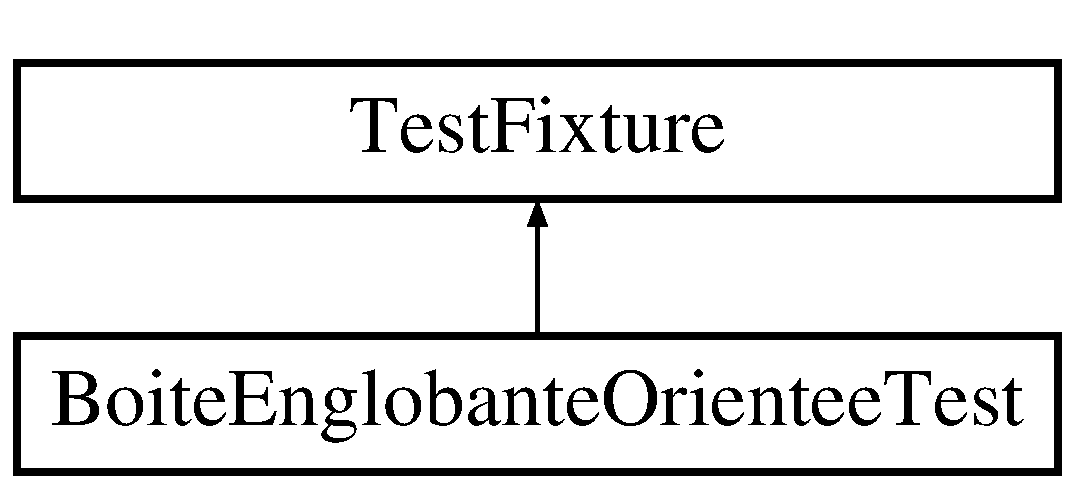
\includegraphics[height=2.000000cm]{class_boite_englobante_orientee_test}
\end{center}
\end{figure}
\subsection*{Public Member Functions}
\begin{DoxyCompactItemize}
\item 
\hypertarget{group__inf2990_ga3834ff95e970fc8a6fa9dc257c29a389}{void {\bfseries set\-Up} ()}\label{group__inf2990_ga3834ff95e970fc8a6fa9dc257c29a389}

\item 
\hypertarget{group__inf2990_ga139b16d99327e493e0711b802b882832}{void {\bfseries tear\-Down} ()}\label{group__inf2990_ga139b16d99327e493e0711b802b882832}

\item 
void \hyperlink{group__inf2990_gaf90ec830d73ad669f126faf67f9139e8}{test\-Calculer\-Collision} ()
\end{DoxyCompactItemize}


\subsection{Detailed Description}
\hyperlink{class_test}{Test} qui s'assure que les operations effectuees sur les boites englobantes orientees sont fonctionnelles. 

The documentation for this class was generated from the following files\-:\begin{DoxyCompactItemize}
\item 
Cadriciel/\-Sources/\-C++/\-Tests/Boite\-Englobante\-Orientee\-Test.\-h\item 
Cadriciel/\-Sources/\-C++/\-Tests/Boite\-Englobante\-Orientee\-Test.\-cpp\end{DoxyCompactItemize}

\hypertarget{classutilitaire_1_1_boite_environnement}{\section{utilitaire\-:\-:Boite\-Environnement Class Reference}
\label{classutilitaire_1_1_boite_environnement}\index{utilitaire\-::\-Boite\-Environnement@{utilitaire\-::\-Boite\-Environnement}}
}


Classe representant une bo�te d'environnement (\char`\"{}skybox\char`\"{}).  




{\ttfamily \#include $<$Boite\-Environnement.\-h$>$}

\subsection*{Public Member Functions}
\begin{DoxyCompactItemize}
\item 
\hyperlink{classutilitaire_1_1_boite_environnement_afa2e429fd77f584d9b07e1577b907f7b}{Boite\-Environnement} (const \hyperlink{glew_8h_ae84541b4f3d8e1ea24ec0f466a8c568b}{std\-::string} \&fichier\-Xpos, const \hyperlink{glew_8h_ae84541b4f3d8e1ea24ec0f466a8c568b}{std\-::string} \&fichier\-Xneg, const \hyperlink{glew_8h_ae84541b4f3d8e1ea24ec0f466a8c568b}{std\-::string} \&fichier\-Ypos, const \hyperlink{glew_8h_ae84541b4f3d8e1ea24ec0f466a8c568b}{std\-::string} \&fichier\-Yneg, const \hyperlink{glew_8h_ae84541b4f3d8e1ea24ec0f466a8c568b}{std\-::string} \&fichier\-Zpos, const \hyperlink{glew_8h_ae84541b4f3d8e1ea24ec0f466a8c568b}{std\-::string} \&fichier\-Zneg)
\begin{DoxyCompactList}\small\item\em Constructeur a partir des noms des fichiers d'images de la bo�te. \end{DoxyCompactList}\item 
\hyperlink{classutilitaire_1_1_boite_environnement_accfe35d5a88904e5001653142b985a27}{$\sim$\-Boite\-Environnement} ()
\begin{DoxyCompactList}\small\item\em Destructeur. \end{DoxyCompactList}\item 
\hyperlink{wglew_8h_aeea6e3dfae3acf232096f57d2d57f084}{void} \hyperlink{classutilitaire_1_1_boite_environnement_adfd42d118e0d62c3c9ea460df14feae4}{afficher} (const \hyperlink{group__utilitaire_ga541aa4837ad9250d3a248dc82ee9ad4d}{Vecteur3} \&centre, double demi\-Largeur) const 
\begin{DoxyCompactList}\small\item\em Affiche la bo�te d'environnement. \end{DoxyCompactList}\end{DoxyCompactItemize}


\subsection{Detailed Description}
Classe representant une bo�te d'environnement (\char`\"{}skybox\char`\"{}). 

Elle s'occupe de charger 6 images du cube formant la bo�te. Elle utilise la convention de sens de Cube\-Map\-Gen (de A\-T\-I), lorsque les images sont exportees avec le mapping Open\-G\-L (plut�t que Direct\-X).

\begin{DoxyAuthor}{Author}
Martin Bisson 
\end{DoxyAuthor}
\begin{DoxyDate}{Date}
2007-\/05-\/28 
\end{DoxyDate}


\subsection{Constructor \& Destructor Documentation}
\hypertarget{classutilitaire_1_1_boite_environnement_afa2e429fd77f584d9b07e1577b907f7b}{\index{utilitaire\-::\-Boite\-Environnement@{utilitaire\-::\-Boite\-Environnement}!Boite\-Environnement@{Boite\-Environnement}}
\index{Boite\-Environnement@{Boite\-Environnement}!utilitaire::BoiteEnvironnement@{utilitaire\-::\-Boite\-Environnement}}
\subsubsection[{Boite\-Environnement}]{\setlength{\rightskip}{0pt plus 5cm}utilitaire\-::\-Boite\-Environnement\-::\-Boite\-Environnement (
\begin{DoxyParamCaption}
\item[{const {\bf std\-::string} \&}]{fichier\-Xpos, }
\item[{const {\bf std\-::string} \&}]{fichier\-Xneg, }
\item[{const {\bf std\-::string} \&}]{fichier\-Ypos, }
\item[{const {\bf std\-::string} \&}]{fichier\-Yneg, }
\item[{const {\bf std\-::string} \&}]{fichier\-Zpos, }
\item[{const {\bf std\-::string} \&}]{fichier\-Zneg}
\end{DoxyParamCaption}
)}}\label{classutilitaire_1_1_boite_environnement_afa2e429fd77f584d9b07e1577b907f7b}


Constructeur a partir des noms des fichiers d'images de la bo�te. 

Ce constructeur charge les 6 textures correspondant a chacune des faces de la bo�te d'environnement.


\begin{DoxyParams}[1]{Parameters}
\mbox{\tt in}  & {\em fichier\-Xpos} & \-: Le nom du fichier contenant l'image correspondant a l'axe des X positifs. \\
\hline
\mbox{\tt in}  & {\em fichier\-Xneg} & \-: Le nom du fichier contenant l'image correspondant a l'axe des X negatifs. \\
\hline
\mbox{\tt in}  & {\em fichier\-Ypos} & \-: Le nom du fichier contenant l'image correspondant a l'axe des X positifs. \\
\hline
\mbox{\tt in}  & {\em fichier\-Yneg} & \-: Le nom du fichier contenant l'image correspondant a l'axe des Y negatifs. \\
\hline
\mbox{\tt in}  & {\em fichier\-Zpos} & \-: Le nom du fichier contenant l'image correspondant a l'axe des Z positifs. \\
\hline
\mbox{\tt in}  & {\em fichier\-Zneg} & \-: Le nom du fichier contenant l'image correspondant a l'axe des Z negatifs.\\
\hline
\end{DoxyParams}
\begin{DoxyReturn}{Returns}
Aucune (constructeur). 
\end{DoxyReturn}
\hypertarget{classutilitaire_1_1_boite_environnement_accfe35d5a88904e5001653142b985a27}{\index{utilitaire\-::\-Boite\-Environnement@{utilitaire\-::\-Boite\-Environnement}!$\sim$\-Boite\-Environnement@{$\sim$\-Boite\-Environnement}}
\index{$\sim$\-Boite\-Environnement@{$\sim$\-Boite\-Environnement}!utilitaire::BoiteEnvironnement@{utilitaire\-::\-Boite\-Environnement}}
\subsubsection[{$\sim$\-Boite\-Environnement}]{\setlength{\rightskip}{0pt plus 5cm}utilitaire\-::\-Boite\-Environnement\-::$\sim$\-Boite\-Environnement (
\begin{DoxyParamCaption}
{}
\end{DoxyParamCaption}
)}}\label{classutilitaire_1_1_boite_environnement_accfe35d5a88904e5001653142b985a27}


Destructeur. 

Ce destructeur libere l'espace allouee a chacune des textures des faces de la bo�te d'environnement.

\begin{DoxyReturn}{Returns}
Aucune (destructeur). 
\end{DoxyReturn}


\subsection{Member Function Documentation}
\hypertarget{classutilitaire_1_1_boite_environnement_adfd42d118e0d62c3c9ea460df14feae4}{\index{utilitaire\-::\-Boite\-Environnement@{utilitaire\-::\-Boite\-Environnement}!afficher@{afficher}}
\index{afficher@{afficher}!utilitaire::BoiteEnvironnement@{utilitaire\-::\-Boite\-Environnement}}
\subsubsection[{afficher}]{\setlength{\rightskip}{0pt plus 5cm}{\bf void} utilitaire\-::\-Boite\-Environnement\-::afficher (
\begin{DoxyParamCaption}
\item[{const {\bf Vecteur3} \&}]{centre, }
\item[{double}]{demi\-Largeur}
\end{DoxyParamCaption}
) const}}\label{classutilitaire_1_1_boite_environnement_adfd42d118e0d62c3c9ea460df14feae4}


Affiche la bo�te d'environnement. 

Cette fonction affiche tout simplement la bo�te d'environnement.


\begin{DoxyParams}[1]{Parameters}
\mbox{\tt in}  & {\em centre} & \-: La position du centre de la bo�te pour l'affichage. \\
\hline
\mbox{\tt in}  & {\em demi\-Largeur} & \-: La largeur de la moitie de la bo�te pour l'affichage.\\
\hline
\end{DoxyParams}
\begin{DoxyReturn}{Returns}
Aucune. 
\end{DoxyReturn}


The documentation for this class was generated from the following files\-:\begin{DoxyCompactItemize}
\item 
Cadriciel/\-Commun/\-Utilitaire/\hyperlink{_boite_environnement_8h}{Boite\-Environnement.\-h}\item 
Cadriciel/\-Commun/\-Utilitaire/\hyperlink{_boite_environnement_8cpp}{Boite\-Environnement.\-cpp}\end{DoxyCompactItemize}

\hypertarget{class_brief_test_progress_listener}{\section{Brief\-Test\-Progress\-Listener Class Reference}
\label{class_brief_test_progress_listener}\index{Brief\-Test\-Progress\-Listener@{Brief\-Test\-Progress\-Listener}}
}


\hyperlink{class_test_listener}{Test\-Listener} that prints the name of each test before running it.  




{\ttfamily \#include $<$Brief\-Test\-Progress\-Listener.\-h$>$}

Inheritance diagram for Brief\-Test\-Progress\-Listener\-:\begin{figure}[H]
\begin{center}
\leavevmode
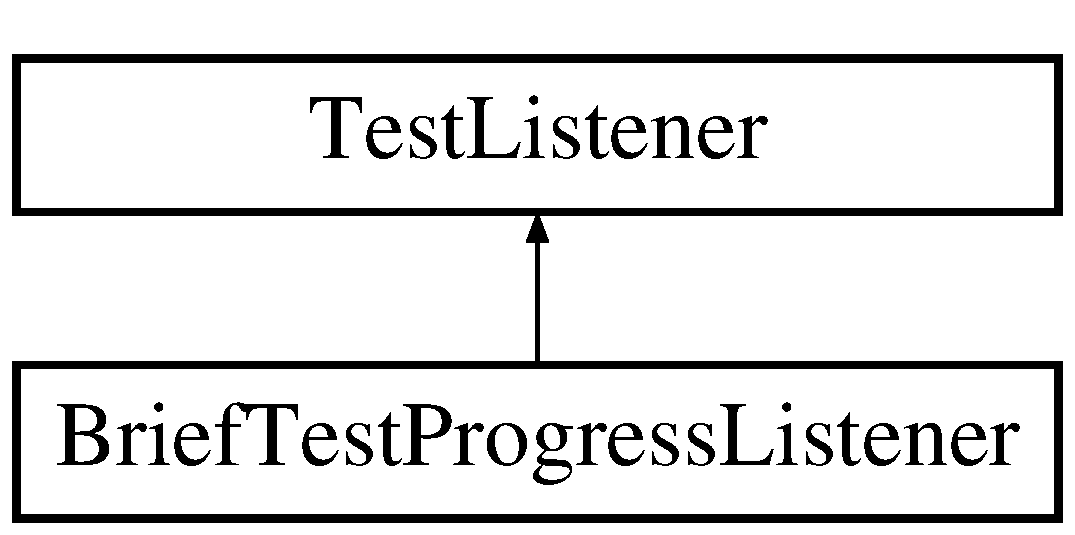
\includegraphics[height=2.000000cm]{class_brief_test_progress_listener}
\end{center}
\end{figure}
\subsection*{Public Member Functions}
\begin{DoxyCompactItemize}
\item 
\hyperlink{class_brief_test_progress_listener_a7af12547b437fcddab52e7b0f0d47782}{Brief\-Test\-Progress\-Listener} ()
\item 
virtual \hyperlink{class_brief_test_progress_listener_a9e1cf4460bdb460e14009d1629454881}{$\sim$\-Brief\-Test\-Progress\-Listener} ()
\begin{DoxyCompactList}\small\item\em Destructor. \end{DoxyCompactList}\item 
\hyperlink{wglew_8h_aeea6e3dfae3acf232096f57d2d57f084}{void} \hyperlink{class_brief_test_progress_listener_ab4196e15752bb2be443e72418500e20e}{start\-Test} (\hyperlink{class_test}{Test} $\ast$test)
\begin{DoxyCompactList}\small\item\em Called when just before a \hyperlink{class_test_case}{Test\-Case} is run. \end{DoxyCompactList}\item 
\hyperlink{wglew_8h_aeea6e3dfae3acf232096f57d2d57f084}{void} \hyperlink{class_brief_test_progress_listener_a21f8658a9c19c67220241656cfad30ce}{add\-Failure} (const \hyperlink{class_test_failure}{Test\-Failure} \&failure)
\begin{DoxyCompactList}\small\item\em Called when a failure occurs while running a test. \end{DoxyCompactList}\item 
\hyperlink{wglew_8h_aeea6e3dfae3acf232096f57d2d57f084}{void} \hyperlink{class_brief_test_progress_listener_a49cbd9152ea35a21f6525773660ee119}{end\-Test} (\hyperlink{class_test}{Test} $\ast$test)
\begin{DoxyCompactList}\small\item\em Called just after a \hyperlink{class_test_case}{Test\-Case} was run (even if a failure occured). \end{DoxyCompactList}\end{DoxyCompactItemize}


\subsection{Detailed Description}
\hyperlink{class_test_listener}{Test\-Listener} that prints the name of each test before running it. 

\subsection{Constructor \& Destructor Documentation}
\hypertarget{class_brief_test_progress_listener_a7af12547b437fcddab52e7b0f0d47782}{\index{Brief\-Test\-Progress\-Listener@{Brief\-Test\-Progress\-Listener}!Brief\-Test\-Progress\-Listener@{Brief\-Test\-Progress\-Listener}}
\index{Brief\-Test\-Progress\-Listener@{Brief\-Test\-Progress\-Listener}!BriefTestProgressListener@{Brief\-Test\-Progress\-Listener}}
\subsubsection[{Brief\-Test\-Progress\-Listener}]{\setlength{\rightskip}{0pt plus 5cm}Brief\-Test\-Progress\-Listener\-::\-Brief\-Test\-Progress\-Listener (
\begin{DoxyParamCaption}
{}
\end{DoxyParamCaption}
)}}\label{class_brief_test_progress_listener_a7af12547b437fcddab52e7b0f0d47782}
Constructs a \hyperlink{class_brief_test_progress_listener}{Brief\-Test\-Progress\-Listener} object. \hypertarget{class_brief_test_progress_listener_a9e1cf4460bdb460e14009d1629454881}{\index{Brief\-Test\-Progress\-Listener@{Brief\-Test\-Progress\-Listener}!$\sim$\-Brief\-Test\-Progress\-Listener@{$\sim$\-Brief\-Test\-Progress\-Listener}}
\index{$\sim$\-Brief\-Test\-Progress\-Listener@{$\sim$\-Brief\-Test\-Progress\-Listener}!BriefTestProgressListener@{Brief\-Test\-Progress\-Listener}}
\subsubsection[{$\sim$\-Brief\-Test\-Progress\-Listener}]{\setlength{\rightskip}{0pt plus 5cm}virtual Brief\-Test\-Progress\-Listener\-::$\sim$\-Brief\-Test\-Progress\-Listener (
\begin{DoxyParamCaption}
{}
\end{DoxyParamCaption}
)\hspace{0.3cm}{\ttfamily [virtual]}}}\label{class_brief_test_progress_listener_a9e1cf4460bdb460e14009d1629454881}


Destructor. 



\subsection{Member Function Documentation}
\hypertarget{class_brief_test_progress_listener_a21f8658a9c19c67220241656cfad30ce}{\index{Brief\-Test\-Progress\-Listener@{Brief\-Test\-Progress\-Listener}!add\-Failure@{add\-Failure}}
\index{add\-Failure@{add\-Failure}!BriefTestProgressListener@{Brief\-Test\-Progress\-Listener}}
\subsubsection[{add\-Failure}]{\setlength{\rightskip}{0pt plus 5cm}{\bf void} Brief\-Test\-Progress\-Listener\-::add\-Failure (
\begin{DoxyParamCaption}
\item[{const {\bf Test\-Failure} \&}]{}
\end{DoxyParamCaption}
)\hspace{0.3cm}{\ttfamily [virtual]}}}\label{class_brief_test_progress_listener_a21f8658a9c19c67220241656cfad30ce}


Called when a failure occurs while running a test. 

\begin{DoxySeeAlso}{See Also}
\hyperlink{class_test_failure}{Test\-Failure}. 
\end{DoxySeeAlso}
\begin{DoxyWarning}{Warning}
{\itshape failure} is a temporary object that is destroyed after the method call. Use \hyperlink{class_test_failure_a0f0c86f12431ea8adde3e70e0cb52db7}{Test\-Failure\-::clone()} to create a duplicate. 
\end{DoxyWarning}


Reimplemented from \hyperlink{class_test_listener_a103216a5814c907f7b752b969477e765}{Test\-Listener}.

\hypertarget{class_brief_test_progress_listener_a49cbd9152ea35a21f6525773660ee119}{\index{Brief\-Test\-Progress\-Listener@{Brief\-Test\-Progress\-Listener}!end\-Test@{end\-Test}}
\index{end\-Test@{end\-Test}!BriefTestProgressListener@{Brief\-Test\-Progress\-Listener}}
\subsubsection[{end\-Test}]{\setlength{\rightskip}{0pt plus 5cm}{\bf void} Brief\-Test\-Progress\-Listener\-::end\-Test (
\begin{DoxyParamCaption}
\item[{{\bf Test} $\ast$}]{}
\end{DoxyParamCaption}
)\hspace{0.3cm}{\ttfamily [virtual]}}}\label{class_brief_test_progress_listener_a49cbd9152ea35a21f6525773660ee119}


Called just after a \hyperlink{class_test_case}{Test\-Case} was run (even if a failure occured). 



Reimplemented from \hyperlink{class_test_listener_ae8ccd0f55dd9aa7eafded05ba14f9ac6}{Test\-Listener}.

\hypertarget{class_brief_test_progress_listener_ab4196e15752bb2be443e72418500e20e}{\index{Brief\-Test\-Progress\-Listener@{Brief\-Test\-Progress\-Listener}!start\-Test@{start\-Test}}
\index{start\-Test@{start\-Test}!BriefTestProgressListener@{Brief\-Test\-Progress\-Listener}}
\subsubsection[{start\-Test}]{\setlength{\rightskip}{0pt plus 5cm}{\bf void} Brief\-Test\-Progress\-Listener\-::start\-Test (
\begin{DoxyParamCaption}
\item[{{\bf Test} $\ast$}]{}
\end{DoxyParamCaption}
)\hspace{0.3cm}{\ttfamily [virtual]}}}\label{class_brief_test_progress_listener_ab4196e15752bb2be443e72418500e20e}


Called when just before a \hyperlink{class_test_case}{Test\-Case} is run. 



Reimplemented from \hyperlink{class_test_listener_a5546d4420e7412234915113b1ea5ad77}{Test\-Listener}.



The documentation for this class was generated from the following file\-:\begin{DoxyCompactItemize}
\item 
Cadriciel/\-Commun/\-Externe/cppunit/include/cppunit/\hyperlink{_brief_test_progress_listener_8h}{Brief\-Test\-Progress\-Listener.\-h}\end{DoxyCompactItemize}

\hypertarget{classvue_1_1_camera}{\section{vue\-:\-:Camera Class Reference}
\label{classvue_1_1_camera}\index{vue\-::\-Camera@{vue\-::\-Camera}}
}


Classe representant une camera dans le monde en 3\-D.  




{\ttfamily \#include $<$Camera.\-h$>$}

\subsection*{Public Member Functions}
\begin{DoxyCompactItemize}
\item 
\hyperlink{classvue_1_1_camera_ab509d5c06a626fb3b1f6c588a5c85ce1}{Camera} (const \hyperlink{group__utilitaire_ga541aa4837ad9250d3a248dc82ee9ad4d}{Vecteur3} \&position, const \hyperlink{group__utilitaire_ga541aa4837ad9250d3a248dc82ee9ad4d}{Vecteur3} \&point\-Vise, const \hyperlink{group__utilitaire_ga541aa4837ad9250d3a248dc82ee9ad4d}{Vecteur3} \&direction\-Haut\-Camera, const \hyperlink{group__utilitaire_ga541aa4837ad9250d3a248dc82ee9ad4d}{Vecteur3} \&direction\-Haut\-Monde)
\begin{DoxyCompactList}\small\item\em Constructeur a partir des coordonnees cartesiennes. \end{DoxyCompactList}\item 
\hypertarget{classvue_1_1_camera_a173cf3a9d91b30cadd21d72149df4504}{virtual \hyperlink{classvue_1_1_camera_a173cf3a9d91b30cadd21d72149df4504}{$\sim$\-Camera} ()}\label{classvue_1_1_camera_a173cf3a9d91b30cadd21d72149df4504}

\begin{DoxyCompactList}\small\item\em Destructeur virtuel vide. \end{DoxyCompactList}\item 
void \hyperlink{classvue_1_1_camera_aafd52e5bb78da96244421525058eef2f}{assigner\-Position} (const \hyperlink{group__utilitaire_ga541aa4837ad9250d3a248dc82ee9ad4d}{Vecteur3} \&position)
\begin{DoxyCompactList}\small\item\em Assigner la position de la camera. \end{DoxyCompactList}\item 
void \hyperlink{classvue_1_1_camera_a69846a87e30c5d8edb7929452836769b}{assigner\-Point\-Vise} (const \hyperlink{group__utilitaire_ga541aa4837ad9250d3a248dc82ee9ad4d}{Vecteur3} \&point\-Vise)
\begin{DoxyCompactList}\small\item\em Assigner le point vise de la camera. \end{DoxyCompactList}\item 
void \hyperlink{classvue_1_1_camera_a3b184e5951bb0a4acab80af4e2c50039}{assigner\-Direction\-Haut} (const \hyperlink{group__utilitaire_ga541aa4837ad9250d3a248dc82ee9ad4d}{Vecteur3} \&direction\-Haut)
\begin{DoxyCompactList}\small\item\em Assigner la direction du haut de la camera. \end{DoxyCompactList}\item 
const \hyperlink{group__utilitaire_ga541aa4837ad9250d3a248dc82ee9ad4d}{Vecteur3} \& \hyperlink{classvue_1_1_camera_a9e5aa2c77549dd8db47c2f249983d0ad}{obtenir\-Position} () const 
\begin{DoxyCompactList}\small\item\em Obtenir la position de la camera. \end{DoxyCompactList}\item 
const \hyperlink{group__utilitaire_ga541aa4837ad9250d3a248dc82ee9ad4d}{Vecteur3} \& \hyperlink{classvue_1_1_camera_a4c2e0079ea5ab132e2cca625a7854a09}{obtenir\-Point\-Vise} () const 
\begin{DoxyCompactList}\small\item\em Obtenir le point vise de la camera. \end{DoxyCompactList}\item 
const \hyperlink{group__utilitaire_ga541aa4837ad9250d3a248dc82ee9ad4d}{Vecteur3} \& \hyperlink{classvue_1_1_camera_adecce98a16454753431306e7b6ca4c75}{obtenir\-Direction\-Haut} () const 
\begin{DoxyCompactList}\small\item\em Obtenir la direction du haut de la camera. \end{DoxyCompactList}\item 
void \hyperlink{classvue_1_1_camera_aa08801e436ddf90400e632e402183618}{deplacer\-X\-Y} (double deplacement\-X, double deplacement\-Y)
\begin{DoxyCompactList}\small\item\em Deplacement dans le plan perpendiculaire a la direction visee. \end{DoxyCompactList}\item 
void \hyperlink{classvue_1_1_camera_a7e8dfbbf743a74bb0387e140fee09474}{deplacer\-Z} (double deplacement, bool bouge\-Point\-Vise)
\begin{DoxyCompactList}\small\item\em Deplacement dans l'axe de la direction visee. \end{DoxyCompactList}\item 
void \hyperlink{classvue_1_1_camera_a07795ebc629c68f8694b9ae08a53457f}{tourner\-X\-Y} (double rotation\-X, double rotation\-Y, bool empeche\-Inversion=true)
\begin{DoxyCompactList}\small\item\em Rotation de la camera autour de sa position. \end{DoxyCompactList}\item 
void \hyperlink{classvue_1_1_camera_a5e88216d5d5b31e0e65be9674e5904ef}{orbiter\-X\-Y} (double rotation\-X, double rotation\-Y, bool empeche\-Inversion=true)
\begin{DoxyCompactList}\small\item\em Rotation de la position de la camera autour de son point de vise. \end{DoxyCompactList}\item 
\hypertarget{classvue_1_1_camera_a1919234ae75d9bf57fc10fb600ea29e1}{void {\bfseries set\-Position} (\hyperlink{group__utilitaire_ga541aa4837ad9250d3a248dc82ee9ad4d}{Vecteur3} pos)}\label{classvue_1_1_camera_a1919234ae75d9bf57fc10fb600ea29e1}

\item 
\hypertarget{classvue_1_1_camera_ae1e82c701ed10d3e82984a21ddbc4636}{const \hyperlink{group__utilitaire_ga541aa4837ad9250d3a248dc82ee9ad4d}{Vecteur3} \& {\bfseries get\-Position} () const }\label{classvue_1_1_camera_ae1e82c701ed10d3e82984a21ddbc4636}

\item 
\hypertarget{classvue_1_1_camera_ab94bfe20e0d55cc1aef25e8fd13ea01b}{\hyperlink{group__utilitaire_ga541aa4837ad9250d3a248dc82ee9ad4d}{Vecteur3} \& {\bfseries get\-Position} ()}\label{classvue_1_1_camera_ab94bfe20e0d55cc1aef25e8fd13ea01b}

\item 
void \hyperlink{classvue_1_1_camera_a201db90bcebf204990f1dbb6db03b563}{positionner} () const 
\begin{DoxyCompactList}\small\item\em Positionner la camera (appel a glu\-Look\-At). \end{DoxyCompactList}\item 
\hypertarget{classvue_1_1_camera_a0f48e5e40432a9a93934a07641f43683}{void {\bfseries positionner\-Orbite} (double theta, double phi, double distance)}\label{classvue_1_1_camera_a0f48e5e40432a9a93934a07641f43683}

\item 
\hypertarget{classvue_1_1_camera_ad77f681260a5965a76fa1f37762e452d}{\hyperlink{classvue_1_1_camera}{Camera} \& {\bfseries operator=} (\hyperlink{classvue_1_1_camera}{Camera} \&camera)}\label{classvue_1_1_camera_ad77f681260a5965a76fa1f37762e452d}

\end{DoxyCompactItemize}


\subsection{Detailed Description}
Classe representant une camera dans le monde en 3\-D. 

Cette camera encapsule les differentes operations qu'il est possible de faire pour deplacer le point de vue de l'observateur a l'interieur de la scene en 3\-D.

\begin{DoxyAuthor}{Author}
Martin Bisson 
\end{DoxyAuthor}
\begin{DoxyDate}{Date}
2006-\/12-\/15 
\end{DoxyDate}


\subsection{Constructor \& Destructor Documentation}
\hypertarget{classvue_1_1_camera_ab509d5c06a626fb3b1f6c588a5c85ce1}{\index{vue\-::\-Camera@{vue\-::\-Camera}!Camera@{Camera}}
\index{Camera@{Camera}!vue::Camera@{vue\-::\-Camera}}
\subsubsection[{Camera}]{\setlength{\rightskip}{0pt plus 5cm}vue\-::\-Camera\-::\-Camera (
\begin{DoxyParamCaption}
\item[{const {\bf Vecteur3} \&}]{position, }
\item[{const {\bf Vecteur3} \&}]{point\-Vise, }
\item[{const {\bf Vecteur3} \&}]{direction\-Haut\-Camera, }
\item[{const {\bf Vecteur3} \&}]{direction\-Haut\-Monde}
\end{DoxyParamCaption}
)}}\label{classvue_1_1_camera_ab509d5c06a626fb3b1f6c588a5c85ce1}


Constructeur a partir des coordonnees cartesiennes. 

Constructeur de la camera a partir des coordonnees cartesiennes.


\begin{DoxyParams}[1]{Parameters}
\mbox{\tt in}  & {\em position} & \-: position de la camera. \\
\hline
\mbox{\tt in}  & {\em point\-Vise} & \-: point vise. \\
\hline
\mbox{\tt in}  & {\em direction\-Haut\-Camera} & \-: direction du haut de la camera. \\
\hline
\mbox{\tt in}  & {\em direction\-Haut\-Monde} & \-: direction du haut du monde de la camera.\\
\hline
\end{DoxyParams}
\begin{DoxyReturn}{Returns}
Aucune (constructeur). 
\end{DoxyReturn}


\subsection{Member Function Documentation}
\hypertarget{classvue_1_1_camera_a3b184e5951bb0a4acab80af4e2c50039}{\index{vue\-::\-Camera@{vue\-::\-Camera}!assigner\-Direction\-Haut@{assigner\-Direction\-Haut}}
\index{assigner\-Direction\-Haut@{assigner\-Direction\-Haut}!vue::Camera@{vue\-::\-Camera}}
\subsubsection[{assigner\-Direction\-Haut}]{\setlength{\rightskip}{0pt plus 5cm}void vue\-::\-Camera\-::assigner\-Direction\-Haut (
\begin{DoxyParamCaption}
\item[{const {\bf Vecteur3} \&}]{direction\-Haut}
\end{DoxyParamCaption}
)\hspace{0.3cm}{\ttfamily [inline]}}}\label{classvue_1_1_camera_a3b184e5951bb0a4acab80af4e2c50039}


Assigner la direction du haut de la camera. 

Cette fonction permet d'assigner la direction du haut de la camera.


\begin{DoxyParams}[1]{Parameters}
\mbox{\tt in}  & {\em direction\-Haut} & \-: La nouvelle direction du haut de la camera.\\
\hline
\end{DoxyParams}
\begin{DoxyReturn}{Returns}
Aucune. 
\end{DoxyReturn}
\hypertarget{classvue_1_1_camera_a69846a87e30c5d8edb7929452836769b}{\index{vue\-::\-Camera@{vue\-::\-Camera}!assigner\-Point\-Vise@{assigner\-Point\-Vise}}
\index{assigner\-Point\-Vise@{assigner\-Point\-Vise}!vue::Camera@{vue\-::\-Camera}}
\subsubsection[{assigner\-Point\-Vise}]{\setlength{\rightskip}{0pt plus 5cm}void vue\-::\-Camera\-::assigner\-Point\-Vise (
\begin{DoxyParamCaption}
\item[{const {\bf Vecteur3} \&}]{point\-Vise}
\end{DoxyParamCaption}
)\hspace{0.3cm}{\ttfamily [inline]}}}\label{classvue_1_1_camera_a69846a87e30c5d8edb7929452836769b}


Assigner le point vise de la camera. 

Cette fonction permet d'assigner le point de vise de la camera.


\begin{DoxyParams}[1]{Parameters}
\mbox{\tt in}  & {\em point\-Vise} & \-: Le nouveau point de vise de la camera.\\
\hline
\end{DoxyParams}
\begin{DoxyReturn}{Returns}
Aucune. 
\end{DoxyReturn}
\hypertarget{classvue_1_1_camera_aafd52e5bb78da96244421525058eef2f}{\index{vue\-::\-Camera@{vue\-::\-Camera}!assigner\-Position@{assigner\-Position}}
\index{assigner\-Position@{assigner\-Position}!vue::Camera@{vue\-::\-Camera}}
\subsubsection[{assigner\-Position}]{\setlength{\rightskip}{0pt plus 5cm}void vue\-::\-Camera\-::assigner\-Position (
\begin{DoxyParamCaption}
\item[{const {\bf Vecteur3} \&}]{position}
\end{DoxyParamCaption}
)\hspace{0.3cm}{\ttfamily [inline]}}}\label{classvue_1_1_camera_aafd52e5bb78da96244421525058eef2f}


Assigner la position de la camera. 

Cette fonction permet d'assigner la position de la camera.


\begin{DoxyParams}[1]{Parameters}
\mbox{\tt in}  & {\em position} & \-: La nouvelle position de la camera.\\
\hline
\end{DoxyParams}
\begin{DoxyReturn}{Returns}
Aucune. 
\end{DoxyReturn}
\hypertarget{classvue_1_1_camera_aa08801e436ddf90400e632e402183618}{\index{vue\-::\-Camera@{vue\-::\-Camera}!deplacer\-X\-Y@{deplacer\-X\-Y}}
\index{deplacer\-X\-Y@{deplacer\-X\-Y}!vue::Camera@{vue\-::\-Camera}}
\subsubsection[{deplacer\-X\-Y}]{\setlength{\rightskip}{0pt plus 5cm}void vue\-::\-Camera\-::deplacer\-X\-Y (
\begin{DoxyParamCaption}
\item[{double}]{deplacement\-X, }
\item[{double}]{deplacement\-Y}
\end{DoxyParamCaption}
)}}\label{classvue_1_1_camera_aa08801e436ddf90400e632e402183618}


Deplacement dans le plan perpendiculaire a la direction visee. 

Deplace la camera dans le plan perpendiculaire a la direction visee


\begin{DoxyParams}[1]{Parameters}
\mbox{\tt in}  & {\em deplacement\-X} & \-: Deplacement sur l'axe horizontal du plan de la camera. \\
\hline
\mbox{\tt in}  & {\em deplacement\-Y} & \-: Deplacement sur l'axe vertical du plan de la camera.\\
\hline
\end{DoxyParams}
\begin{DoxyReturn}{Returns}
Aucune. 
\end{DoxyReturn}
\hypertarget{classvue_1_1_camera_a7e8dfbbf743a74bb0387e140fee09474}{\index{vue\-::\-Camera@{vue\-::\-Camera}!deplacer\-Z@{deplacer\-Z}}
\index{deplacer\-Z@{deplacer\-Z}!vue::Camera@{vue\-::\-Camera}}
\subsubsection[{deplacer\-Z}]{\setlength{\rightskip}{0pt plus 5cm}void vue\-::\-Camera\-::deplacer\-Z (
\begin{DoxyParamCaption}
\item[{double}]{deplacement, }
\item[{bool}]{bouge\-Point\-Vise}
\end{DoxyParamCaption}
)}}\label{classvue_1_1_camera_a7e8dfbbf743a74bb0387e140fee09474}


Deplacement dans l'axe de la direction visee. 

Deplace la camera dans l'axe de la direction visee.


\begin{DoxyParams}[1]{Parameters}
\mbox{\tt in}  & {\em deplacement} & \-: Deplacement sur l'axe de la direction visee \\
\hline
\mbox{\tt in}  & {\em bouge\-Point\-Vise} & \-: Si vrai, le point de vise est egalement deplace.\\
\hline
\end{DoxyParams}
\begin{DoxyReturn}{Returns}
Aucune. 
\end{DoxyReturn}
\hypertarget{classvue_1_1_camera_adecce98a16454753431306e7b6ca4c75}{\index{vue\-::\-Camera@{vue\-::\-Camera}!obtenir\-Direction\-Haut@{obtenir\-Direction\-Haut}}
\index{obtenir\-Direction\-Haut@{obtenir\-Direction\-Haut}!vue::Camera@{vue\-::\-Camera}}
\subsubsection[{obtenir\-Direction\-Haut}]{\setlength{\rightskip}{0pt plus 5cm}const {\bf Vecteur3} \& vue\-::\-Camera\-::obtenir\-Direction\-Haut (
\begin{DoxyParamCaption}
{}
\end{DoxyParamCaption}
) const\hspace{0.3cm}{\ttfamily [inline]}}}\label{classvue_1_1_camera_adecce98a16454753431306e7b6ca4c75}


Obtenir la direction du haut de la camera. 

Cette fonction permet d'obtenir la direction du haut de la camera.

\begin{DoxyReturn}{Returns}
La direction du haut de la camera. 
\end{DoxyReturn}
\hypertarget{classvue_1_1_camera_a4c2e0079ea5ab132e2cca625a7854a09}{\index{vue\-::\-Camera@{vue\-::\-Camera}!obtenir\-Point\-Vise@{obtenir\-Point\-Vise}}
\index{obtenir\-Point\-Vise@{obtenir\-Point\-Vise}!vue::Camera@{vue\-::\-Camera}}
\subsubsection[{obtenir\-Point\-Vise}]{\setlength{\rightskip}{0pt plus 5cm}const {\bf Vecteur3} \& vue\-::\-Camera\-::obtenir\-Point\-Vise (
\begin{DoxyParamCaption}
{}
\end{DoxyParamCaption}
) const\hspace{0.3cm}{\ttfamily [inline]}}}\label{classvue_1_1_camera_a4c2e0079ea5ab132e2cca625a7854a09}


Obtenir le point vise de la camera. 

Cette fonction permet d'obtenir le point de vise de la camera.

\begin{DoxyReturn}{Returns}
Le point de vise de la camera. 
\end{DoxyReturn}
\hypertarget{classvue_1_1_camera_a9e5aa2c77549dd8db47c2f249983d0ad}{\index{vue\-::\-Camera@{vue\-::\-Camera}!obtenir\-Position@{obtenir\-Position}}
\index{obtenir\-Position@{obtenir\-Position}!vue::Camera@{vue\-::\-Camera}}
\subsubsection[{obtenir\-Position}]{\setlength{\rightskip}{0pt plus 5cm}const {\bf Vecteur3} \& vue\-::\-Camera\-::obtenir\-Position (
\begin{DoxyParamCaption}
{}
\end{DoxyParamCaption}
) const\hspace{0.3cm}{\ttfamily [inline]}}}\label{classvue_1_1_camera_a9e5aa2c77549dd8db47c2f249983d0ad}


Obtenir la position de la camera. 

Cette fonction permet d'obtenir la position de la camera.

\begin{DoxyReturn}{Returns}
La position de la camera. 
\end{DoxyReturn}
\hypertarget{classvue_1_1_camera_a5e88216d5d5b31e0e65be9674e5904ef}{\index{vue\-::\-Camera@{vue\-::\-Camera}!orbiter\-X\-Y@{orbiter\-X\-Y}}
\index{orbiter\-X\-Y@{orbiter\-X\-Y}!vue::Camera@{vue\-::\-Camera}}
\subsubsection[{orbiter\-X\-Y}]{\setlength{\rightskip}{0pt plus 5cm}void vue\-::\-Camera\-::orbiter\-X\-Y (
\begin{DoxyParamCaption}
\item[{double}]{rotation\-X, }
\item[{double}]{rotation\-Y, }
\item[{bool}]{empeche\-Inversion = {\ttfamily true}}
\end{DoxyParamCaption}
)}}\label{classvue_1_1_camera_a5e88216d5d5b31e0e65be9674e5904ef}


Rotation de la position de la camera autour de son point de vise. 

Rotation de la camera autour de son point de vise (et donc deplacement de la position en gardant le point de vise fixe.


\begin{DoxyParams}[1]{Parameters}
\mbox{\tt in}  & {\em rotation\-X} & \-: Modification de l'angle de rotation de la position par rapport au point de vise. \\
\hline
\mbox{\tt in}  & {\em rotation\-Y} & \-: Modification de l'angle d'elevation de la position par rapport au point de vise. \\
\hline
\mbox{\tt in}  & {\em empeche\-Inversion} & \-: Si vrai, la rotation n'est pas effectue si elle amenerait une inversion de la camera.\\
\hline
\end{DoxyParams}
\begin{DoxyReturn}{Returns}
Aucune. 
\end{DoxyReturn}
\hypertarget{classvue_1_1_camera_a201db90bcebf204990f1dbb6db03b563}{\index{vue\-::\-Camera@{vue\-::\-Camera}!positionner@{positionner}}
\index{positionner@{positionner}!vue::Camera@{vue\-::\-Camera}}
\subsubsection[{positionner}]{\setlength{\rightskip}{0pt plus 5cm}void vue\-::\-Camera\-::positionner (
\begin{DoxyParamCaption}
{}
\end{DoxyParamCaption}
) const}}\label{classvue_1_1_camera_a201db90bcebf204990f1dbb6db03b563}


Positionner la camera (appel a glu\-Look\-At). 

Positionne la camera dans la scene a l'aide de glu\-Look\-At().

\begin{DoxyReturn}{Returns}
Aucune. 
\end{DoxyReturn}
\hypertarget{classvue_1_1_camera_a07795ebc629c68f8694b9ae08a53457f}{\index{vue\-::\-Camera@{vue\-::\-Camera}!tourner\-X\-Y@{tourner\-X\-Y}}
\index{tourner\-X\-Y@{tourner\-X\-Y}!vue::Camera@{vue\-::\-Camera}}
\subsubsection[{tourner\-X\-Y}]{\setlength{\rightskip}{0pt plus 5cm}void vue\-::\-Camera\-::tourner\-X\-Y (
\begin{DoxyParamCaption}
\item[{double}]{rotation\-X, }
\item[{double}]{rotation\-Y, }
\item[{bool}]{empeche\-Inversion = {\ttfamily true}}
\end{DoxyParamCaption}
)}}\label{classvue_1_1_camera_a07795ebc629c68f8694b9ae08a53457f}


Rotation de la camera autour de sa position. 

Rotation de la camera autour de sa position (et donc deplacement du point vise en gardant la position fixe.


\begin{DoxyParams}[1]{Parameters}
\mbox{\tt in}  & {\em rotation\-X} & \-: Modification de l'angle de rotation du point vise par rapport a la position. \\
\hline
\mbox{\tt in}  & {\em rotation\-Y} & \-: Modification de l'angle d'elevation du point vise par rapport a la position. \\
\hline
\mbox{\tt in}  & {\em empeche\-Inversion} & \-: Si vrai, la rotation n'est pas effectuee si elle amenerait une inversion de la camera.\\
\hline
\end{DoxyParams}
\begin{DoxyReturn}{Returns}
Aucune. 
\end{DoxyReturn}


The documentation for this class was generated from the following files\-:\begin{DoxyCompactItemize}
\item 
Cadriciel/\-Commun/\-Utilitaire/\-Vue/\hyperlink{_camera_8h}{Camera.\-h}\item 
Cadriciel/\-Commun/\-Utilitaire/\-Vue/\hyperlink{_camera_8cpp}{Camera.\-cpp}\end{DoxyCompactItemize}

\hypertarget{class_carte}{\section{Carte Class Reference}
\label{class_carte}\index{Carte@{Carte}}
}


Classe qui permet l'ajout et la supression d'�lements sur la carte (zone de jeu)  




{\ttfamily \#include $<$Carte.\-h$>$}

\subsection*{Public Member Functions}
\begin{DoxyCompactItemize}
\item 
\hyperlink{group__inf2990_ga80f5e8743e4dcfb4f00cf7b1e8b766f7}{Carte} (\hyperlink{glew_8h_ae84541b4f3d8e1ea24ec0f466a8c568b}{string} nom, \hyperlink{class_arbre_rendu_i_n_f2990}{Arbre\-Rendu\-I\-N\-F2990} $\ast$arbre\-Rendu)
\item 
\hyperlink{group__inf2990_gad20e893d299d8498f5dfb5ed3021d6b8}{Carte} (\hyperlink{class_carte}{Carte} \&carte)
\item 
\hyperlink{group__inf2990_ga63300ff55c58b5d5b1674a3fc8f25910}{$\sim$\-Carte} ()
\item 
\hyperlink{wglew_8h_aeea6e3dfae3acf232096f57d2d57f084}{void} \hyperlink{group__inf2990_ga73f5d7b433f6f044f59c4ab7e7f3084e}{effacer\-Element} (\hyperlink{class_element_jeu_abstrait}{Element\-Jeu\-Abstrait} $\ast$element)
\item 
\hyperlink{wglew_8h_aeea6e3dfae3acf232096f57d2d57f084}{void} \hyperlink{group__inf2990_gaa4d51c79656dee570202820d99cc4ad8}{effacer\-Elements\-Type} (\hyperlink{wglew_8h_a500a82aecba06f4550f6849b8099ca21}{int} \hyperlink{fmod_8h_a5338b9cb3874378d7e5adfbe80a8a381}{type})
\item 
\hyperlink{wglew_8h_aeea6e3dfae3acf232096f57d2d57f084}{void} \hyperlink{group__inf2990_gadf54435158eee3a30796da0d0ef2c448}{changer\-Visibilite\-Position\-Depart} (bool visible)
\item 
\hyperlink{wglew_8h_aeea6e3dfae3acf232096f57d2d57f084}{void} \hyperlink{group__inf2990_gadcdb90feef6b62d2e292fb5bb6536d7a}{ajouter\-Element} (\hyperlink{class_element_jeu_abstrait}{Element\-Jeu\-Abstrait} $\ast$element)
\item 
\hyperlink{wglew_8h_aeea6e3dfae3acf232096f57d2d57f084}{void} \hyperlink{group__inf2990_ga65c3a3a67856a16972f2e6cdbc38ff5d}{creer\-Element\-Par\-X\-M\-L} (\hyperlink{class_ti_xml_element}{Ti\-Xml\-Element} \&element)
\item 
\hyperlink{wglew_8h_aeea6e3dfae3acf232096f57d2d57f084}{void} \hyperlink{group__inf2990_gaa738c20bc34f5cf4b9250ce27ff4e766}{creer\-Barriere} (\hyperlink{group__utilitaire_ga541aa4837ad9250d3a248dc82ee9ad4d}{Vecteur3} position1, \hyperlink{group__utilitaire_ga541aa4837ad9250d3a248dc82ee9ad4d}{Vecteur3} position2)
\item 
\hyperlink{class_asteroide}{Asteroide} $\ast$ \hyperlink{group__inf2990_ga705576c8363a33505812478249ca45cd}{creer\-Asteroide} ()
\begin{DoxyCompactList}\small\item\em Methode qui permet d'ajouter un asteroide. \end{DoxyCompactList}\item 
\hyperlink{wglew_8h_aeea6e3dfae3acf232096f57d2d57f084}{void} \hyperlink{group__inf2990_ga03d87a33c9289bc17de893dd347b749f}{ajouter\-Projectile} (\hyperlink{class_projectile}{Projectile} $\ast$proj)
\begin{DoxyCompactList}\small\item\em Methode qui permet d'ajouter un projectile. \end{DoxyCompactList}\item 
\hyperlink{wglew_8h_aeea6e3dfae3acf232096f57d2d57f084}{void} \hyperlink{group__inf2990_ga44f1aef3f67011778793184e07be4971}{update} (\hyperlink{fmod_8h_aeb841aa4b4b5f444b5d739d865b420af}{float} delta\-T)
\begin{DoxyCompactList}\small\item\em Met � jour les �l�ments de jeu. \end{DoxyCompactList}\item 
\hyperlink{wglew_8h_aeea6e3dfae3acf232096f57d2d57f084}{void} \hyperlink{group__inf2990_ga16b8d68534ed55b4fa68ba2b3b138d2a}{dessiner\-Cadre\-Zone\-De\-Jeu} ()
\begin{DoxyCompactList}\small\item\em Dessine le cadre de la zone de jeu. \end{DoxyCompactList}\item 
\hyperlink{wglew_8h_aeea6e3dfae3acf232096f57d2d57f084}{void} \hyperlink{group__inf2990_ga8cbbec72613d4b3402a4151e019f9453}{dessiner\-Cadre\-Depart} ()
\begin{DoxyCompactList}\small\item\em Dessine le cadre de la zone de depart. \end{DoxyCompactList}\item 
\hyperlink{_free_image_8h_a425076c7067a1b5166e2cc530e914814}{unsigned} \hyperlink{wglew_8h_a500a82aecba06f4550f6849b8099ca21}{int} \hyperlink{group__inf2990_ga469bf27b8cd78a7b89c24408e587bbe7}{get\-Nb\-Station\-Spatial} ()
\begin{DoxyCompactList}\small\item\em Methode qui retourne le nombre de stations spatiales de la carte. \end{DoxyCompactList}\item 
\hyperlink{_free_image_8h_a425076c7067a1b5166e2cc530e914814}{unsigned} \hyperlink{wglew_8h_a500a82aecba06f4550f6849b8099ca21}{int} \hyperlink{group__inf2990_ga4eba7c69df6cf2824849dcfbd917d635}{get\-Nb\-Min\-Station\-A\-Sauver} () const 
\begin{DoxyCompactList}\small\item\em Permet d'obtenir le nombre minimal de station a sauver de la destruction des ast�roides. \end{DoxyCompactList}\item 
\hyperlink{wglew_8h_aeea6e3dfae3acf232096f57d2d57f084}{void} \hyperlink{group__inf2990_ga6545b233796923dfe70057ad2b43e8b5}{set\-Nb\-Min\-Station\-A\-Sauver} (\hyperlink{_free_image_8h_a425076c7067a1b5166e2cc530e914814}{unsigned} \hyperlink{wglew_8h_a500a82aecba06f4550f6849b8099ca21}{int} nb\-Station)
\item 
\hyperlink{fmod_8h_aeb841aa4b4b5f444b5d739d865b420af}{float} \hyperlink{group__inf2990_gac07b728072e32b663d67de98eaaf9fd6}{get\-Frequence\-Asteroides} () const 
\begin{DoxyCompactList}\small\item\em Permet d'obtenir la frequence d'apparition des ast�roides. \end{DoxyCompactList}\item 
\hyperlink{wglew_8h_aeea6e3dfae3acf232096f57d2d57f084}{void} \hyperlink{group__inf2990_ga73ef39d308c58aa5fcaac2acfc6d86d3}{set\-Frequence\-Asteroides} (\hyperlink{fmod_8h_aeb841aa4b4b5f444b5d739d865b420af}{float} frequence)
\item 
\hyperlink{_free_image_8h_a425076c7067a1b5166e2cc530e914814}{unsigned} \hyperlink{wglew_8h_a500a82aecba06f4550f6849b8099ca21}{int} \hyperlink{group__inf2990_ga75c1c7a4a90f348e71940ca29d6c8927}{get\-Acceleration\-Bonus} () const 
\begin{DoxyCompactList}\small\item\em Permet d'obtenir l'acceleration fournie par les bonus accelerateurs. \end{DoxyCompactList}\item 
\hyperlink{wglew_8h_aeea6e3dfae3acf232096f57d2d57f084}{void} \hyperlink{group__inf2990_ga3fddcbce9a34438aef12c7666df4b35f}{set\-Acceleration\-Bonus} (\hyperlink{_free_image_8h_a425076c7067a1b5166e2cc530e914814}{unsigned} \hyperlink{wglew_8h_a500a82aecba06f4550f6849b8099ca21}{int} acceleration)
\item 
\hyperlink{wglew_8h_a500a82aecba06f4550f6849b8099ca21}{int} \hyperlink{group__inf2990_ga8912c69ed295beed906d80546868e3f1}{get\-Difficulte} () const 
\begin{DoxyCompactList}\small\item\em Permet d'obtenir la difficulte du jeu. \end{DoxyCompactList}\item 
\hyperlink{wglew_8h_aeea6e3dfae3acf232096f57d2d57f084}{void} \hyperlink{group__inf2990_ga0991d5455cd93de6361dfd77a2a9e382}{set\-Difficulte} (\hyperlink{wglew_8h_a500a82aecba06f4550f6849b8099ca21}{int} difficulte)
\item 
\hyperlink{glew_8h_ae84541b4f3d8e1ea24ec0f466a8c568b}{string} \hyperlink{group__inf2990_gad63dd9caa09a2df37a4efff59d392863}{get\-Nom} () const 
\begin{DoxyCompactList}\small\item\em Permet d'obtenir le nom de la carte. \end{DoxyCompactList}\item 
\hyperlink{wglew_8h_aeea6e3dfae3acf232096f57d2d57f084}{void} \hyperlink{group__inf2990_ga05c95b4e5dedf1e1528caf6093afecc9}{set\-Nom} (const \hyperlink{glew_8h_ae84541b4f3d8e1ea24ec0f466a8c568b}{string} nouveau\-Nom)
\item 
\hyperlink{group__utilitaire_ga606b191c0b0bbb868ae25c13b906f45a}{Vecteur2f} \hyperlink{group__inf2990_ga80405a77cf4f42dea19a84a7be7443e4}{get\-Zone\-Jeu\-X} () const 
\begin{DoxyCompactList}\small\item\em Permet d'obtenir la cloture en X de la zone de jeu. \end{DoxyCompactList}\item 
\hyperlink{group__utilitaire_ga606b191c0b0bbb868ae25c13b906f45a}{Vecteur2f} \hyperlink{group__inf2990_ga9a4d5a38f3b6db48cf2c01636fcbbe16}{get\-Zone\-Jeu\-Y} () const 
\begin{DoxyCompactList}\small\item\em Permet d'obtenir la cloture en Y de la zone de jeu. \end{DoxyCompactList}\item 
\hyperlink{wglew_8h_aeea6e3dfae3acf232096f57d2d57f084}{void} \hyperlink{group__inf2990_ga02eb8ad5c4393d1dc47e96df1b42c79e}{set\-Zone\-Jeu} (const \hyperlink{fmod_8h_aeb841aa4b4b5f444b5d739d865b420af}{float} largeur\-Zone)
\item 
\hyperlink{group__utilitaire_ga606b191c0b0bbb868ae25c13b906f45a}{Vecteur2f} \hyperlink{group__inf2990_gaf6b8d05bf2ffe207a93c7fef39df2791}{get\-Cadre\-Depart\-X} () const 
\begin{DoxyCompactList}\small\item\em Permet d'obtenir le cadre de depart en X. \end{DoxyCompactList}\item 
\hyperlink{group__utilitaire_ga606b191c0b0bbb868ae25c13b906f45a}{Vecteur2f} \hyperlink{group__inf2990_gabe65a8eb1aeca0dcffa1de528f2d2d5c}{get\-Cadre\-Depart\-Y} () const 
\begin{DoxyCompactList}\small\item\em // Permet d'obtenir le cadre de depart en Y \end{DoxyCompactList}\item 
vector$<$ \hyperlink{class_element_jeu_abstrait}{Element\-Jeu\-Abstrait} $\ast$ $>$ \& \hyperlink{group__inf2990_ga57fa20350b4cc71c755325d2738f44a6}{get\-Vecteur\-Element} ()
\begin{DoxyCompactList}\small\item\em Methode qui retourne le conteneur d'element\-Jeu. \end{DoxyCompactList}\item 
vector$<$ \hyperlink{class_asteroide}{Asteroide} $\ast$ $>$ \& \hyperlink{group__inf2990_ga1c3f79dbc801d5b8f083f5b2374623b5}{get\-Vecteur\-Asteroide} ()
\begin{DoxyCompactList}\small\item\em Methode qui retourne le conteneur d'asteroides. \end{DoxyCompactList}\item 
vector$<$ \hyperlink{class_projectile}{Projectile} $\ast$ $>$ \& \hyperlink{group__inf2990_gad5a6f85f49482efadadd9308eaabb8af}{get\-Vecteur\-Projectile} ()
\begin{DoxyCompactList}\small\item\em Methode qui retourne le conteneur de projectile. \end{DoxyCompactList}\item 
bool \hyperlink{group__inf2990_gad7d047f93755ee02689ec32330192b51}{sauvegarde\-Ok} () const 
\begin{DoxyCompactList}\small\item\em Methode qui verifie s'il est correct de sauvegarder la carte. \end{DoxyCompactList}\item 
\hyperlink{fmod_8h_aeb841aa4b4b5f444b5d739d865b420af}{float} \hyperlink{group__inf2990_ga3fada325b4eb999a26e377b93a9b9c7f}{get\-Largeur} () const 
\begin{DoxyCompactList}\small\item\em Methode qui retourne la largeur de la zone de jeu. \end{DoxyCompactList}\item 
\hyperlink{wglew_8h_aeea6e3dfae3acf232096f57d2d57f084}{void} \hyperlink{group__inf2990_ga17e37b58d3ff0cf46df7aa6797afd1e2}{set\-Joueur1} (\hyperlink{group__inf2990_ga01dafcdb1f8e7d4d6a419914150f437c}{Mode\-Joueur} \hyperlink{glew_8h_a1e71d9c196e4683cc06c4b54d53f7ef5}{mode})
\begin{DoxyCompactList}\small\item\em Methode qui permet de set le joueur 2 a joueur reel ou joueur virtuel. \end{DoxyCompactList}\item 
\hyperlink{wglew_8h_aeea6e3dfae3acf232096f57d2d57f084}{void} \hyperlink{group__inf2990_ga84579071dede9dee0851a9014aa01d07}{set\-Joueur2} (\hyperlink{group__inf2990_ga01dafcdb1f8e7d4d6a419914150f437c}{Mode\-Joueur} \hyperlink{glew_8h_a1e71d9c196e4683cc06c4b54d53f7ef5}{mode})
\begin{DoxyCompactList}\small\item\em Methode qui permet de set le joueur 2 a joueur reel ou joueur virtuel. \end{DoxyCompactList}\item 
\hyperlink{class_vaisseau}{Vaisseau} $\ast$ \hyperlink{group__inf2990_ga2b6bca7ef8b3549e8c541e42e24c0285}{get\-Joueur1} ()
\begin{DoxyCompactList}\small\item\em Methode qui permet de recuperer le joueur 1. \end{DoxyCompactList}\item 
\hyperlink{class_vaisseau}{Vaisseau} $\ast$ \hyperlink{group__inf2990_gaf68c4f967c4be6ddb587d5f9619d7bc9}{get\-Joueur2} ()
\begin{DoxyCompactList}\small\item\em Methode qui permet de recuperer le joueur 2. \end{DoxyCompactList}\item 
\hyperlink{class_carte}{Carte} \& \hyperlink{group__inf2990_gad25706184b2a2cee64e7339de7ef09e2}{operator=} (\hyperlink{class_carte}{Carte} \&carte)
\item 
\hyperlink{group__utilitaire_ga6a8205c734fc1c9d1272ea424efb2606}{Vecteur4f} \hyperlink{group__inf2990_ga2c433089e23aef234cb06bd99c15002b}{get\-Coins\-Zone\-Passage} () const 
\item 
\hyperlink{fmod_8h_aeb841aa4b4b5f444b5d739d865b420af}{float} \hyperlink{group__inf2990_gab93552bec5958c74ec93ab5d5a5e115d}{get\-Largeur\-Zone\-Passage} () const 
\item 
\hyperlink{group__utilitaire_ga6a8205c734fc1c9d1272ea424efb2606}{Vecteur4f} \hyperlink{group__inf2990_ga49dd142c29e7f37934c05cf370b5056b}{get\-Coins\-Cadre\-Depart} () const 
\item 
\hyperlink{structai_vector3_d}{ai\-Vector3\-D} \hyperlink{group__inf2990_ga9ecac5ee30e5f4c26af313baf8dd3701}{get\-Pos\-Depart\-Joueur} (\hyperlink{wglew_8h_a500a82aecba06f4550f6849b8099ca21}{int} joueur) const 
\begin{DoxyCompactList}\small\item\em Methode qui retourne la position depart du joueur\-X. \end{DoxyCompactList}\item 
\hyperlink{wglew_8h_aeea6e3dfae3acf232096f57d2d57f084}{void} \hyperlink{class_carte_a8016eaa95818e9f83c63486c01832116}{set\-Mode\-Coop} (bool mode\-Coop)
\begin{DoxyCompactList}\small\item\em Methode qui determine si on est en mode coop ou non. \end{DoxyCompactList}\item 
bool \hyperlink{class_carte_ab59379dd40ea71483fc2806ebc972a75}{get\-Mode\-Coop} () const 
\item 
\hyperlink{wglew_8h_aeea6e3dfae3acf232096f57d2d57f084}{void} \hyperlink{class_carte_a69b1bf8e902d98dd70443d398e904587}{set\-Joueur2\-Virtuelp} (bool joueur\-Virtuel)
\begin{DoxyCompactList}\small\item\em Methode qui determine si le joueur 2 est virtuel ou non. \end{DoxyCompactList}\item 
bool \hyperlink{class_carte_aa73c96016b11ffc60551ced5842c6906}{get\-Joueur2\-Virtuel} () const 
\item 
\hyperlink{wglew_8h_aeea6e3dfae3acf232096f57d2d57f084}{void} \hyperlink{group__inf2990_ga36720767c5328fd763f76856b4aaefc9}{echanger\-Position\-Depart\-Pour\-Vaisseau} ()
\begin{DoxyCompactList}\small\item\em Methode qui remplace les positions de depart par des vaisseaux. \end{DoxyCompactList}\item 
\hyperlink{wglew_8h_aeea6e3dfae3acf232096f57d2d57f084}{void} \hyperlink{group__inf2990_ga799f3d87e00080be4480dc16a66f46c2}{echanger\-Vaisseau\-Pour\-Position\-Depart} ()
\begin{DoxyCompactList}\small\item\em Methode qui remplace les vaisseaux par des positions de depart. \end{DoxyCompactList}\item 
\hyperlink{wglew_8h_aeea6e3dfae3acf232096f57d2d57f084}{void} \hyperlink{group__inf2990_ga019075f1c2a72789d161a96970aa709d}{definir\-Mode\-Joueurs} (bool mode\-Coop, bool joueur2\-Virtuel)
\item 
\hyperlink{wglew_8h_aeea6e3dfae3acf232096f57d2d57f084}{void} \hyperlink{group__inf2990_ga9c0472cccb0e3ed03d695799603e5e51}{detruire\-Asteroides} ()
\begin{DoxyCompactList}\small\item\em Methode qui detruit tous les asteroides generes. \end{DoxyCompactList}\item 
\hyperlink{wglew_8h_aeea6e3dfae3acf232096f57d2d57f084}{void} \hyperlink{group__inf2990_ga6cda887f28278f09a1400c609f1b5a85}{detruire\-Projectiles} ()
\begin{DoxyCompactList}\small\item\em Methode qui detruit tous les projectiles. \end{DoxyCompactList}\item 
\hyperlink{wglew_8h_aeea6e3dfae3acf232096f57d2d57f084}{void} \hyperlink{group__inf2990_gabd6ff077da6c27d738d0ed4a6f7a6c46}{detruire\-Objets} ()
\item 
\hyperlink{wglew_8h_aeea6e3dfae3acf232096f57d2d57f084}{void} \hyperlink{group__inf2990_ga7434287a77c07ed45aae3bae1c035e5d}{associer\-Freres\-Portails} ()
\item 
\hyperlink{_free_image_8h_a425076c7067a1b5166e2cc530e914814}{unsigned} \hyperlink{wglew_8h_a500a82aecba06f4550f6849b8099ca21}{int} \hyperlink{class_carte_a702c898d53eeeaca0a652c138522c196}{get\-Nombre\-Stations} () const 
\item 
\hyperlink{wglew_8h_aeea6e3dfae3acf232096f57d2d57f084}{void} \hyperlink{group__inf2990_ga852db81da13284b87b3e533f553902d5}{detruire\-Quad\-Tree} ()
\item 
bool \hyperlink{group__inf2990_ga0e3a51d3529b2743b660b74bb8fbc04b}{joueur\-Is\-Proche\-Cadre} ()
\end{DoxyCompactItemize}


\subsection{Detailed Description}
Classe qui permet l'ajout et la supression d'�lements sur la carte (zone de jeu) 

\begin{DoxyAuthor}{Author}
Floppy\-Disketeers 
\end{DoxyAuthor}
\begin{DoxyDate}{Date}
2014-\/01-\/21 
\end{DoxyDate}


\subsection{Member Function Documentation}
\hypertarget{class_carte_aa73c96016b11ffc60551ced5842c6906}{\index{Carte@{Carte}!get\-Joueur2\-Virtuel@{get\-Joueur2\-Virtuel}}
\index{get\-Joueur2\-Virtuel@{get\-Joueur2\-Virtuel}!Carte@{Carte}}
\subsubsection[{get\-Joueur2\-Virtuel}]{\setlength{\rightskip}{0pt plus 5cm}bool Carte\-::get\-Joueur2\-Virtuel (
\begin{DoxyParamCaption}
{}
\end{DoxyParamCaption}
) const\hspace{0.3cm}{\ttfamily [inline]}}}\label{class_carte_aa73c96016b11ffc60551ced5842c6906}
\hypertarget{class_carte_ab59379dd40ea71483fc2806ebc972a75}{\index{Carte@{Carte}!get\-Mode\-Coop@{get\-Mode\-Coop}}
\index{get\-Mode\-Coop@{get\-Mode\-Coop}!Carte@{Carte}}
\subsubsection[{get\-Mode\-Coop}]{\setlength{\rightskip}{0pt plus 5cm}bool Carte\-::get\-Mode\-Coop (
\begin{DoxyParamCaption}
{}
\end{DoxyParamCaption}
) const\hspace{0.3cm}{\ttfamily [inline]}}}\label{class_carte_ab59379dd40ea71483fc2806ebc972a75}
\hypertarget{class_carte_a702c898d53eeeaca0a652c138522c196}{\index{Carte@{Carte}!get\-Nombre\-Stations@{get\-Nombre\-Stations}}
\index{get\-Nombre\-Stations@{get\-Nombre\-Stations}!Carte@{Carte}}
\subsubsection[{get\-Nombre\-Stations}]{\setlength{\rightskip}{0pt plus 5cm}{\bf unsigned} {\bf int} Carte\-::get\-Nombre\-Stations (
\begin{DoxyParamCaption}
{}
\end{DoxyParamCaption}
) const\hspace{0.3cm}{\ttfamily [inline]}}}\label{class_carte_a702c898d53eeeaca0a652c138522c196}
\hypertarget{class_carte_a69b1bf8e902d98dd70443d398e904587}{\index{Carte@{Carte}!set\-Joueur2\-Virtuelp@{set\-Joueur2\-Virtuelp}}
\index{set\-Joueur2\-Virtuelp@{set\-Joueur2\-Virtuelp}!Carte@{Carte}}
\subsubsection[{set\-Joueur2\-Virtuelp}]{\setlength{\rightskip}{0pt plus 5cm}{\bf void} Carte\-::set\-Joueur2\-Virtuelp (
\begin{DoxyParamCaption}
\item[{bool}]{joueur\-Virtuel}
\end{DoxyParamCaption}
)\hspace{0.3cm}{\ttfamily [inline]}}}\label{class_carte_a69b1bf8e902d98dd70443d398e904587}


Methode qui determine si le joueur 2 est virtuel ou non. 

\hypertarget{class_carte_a8016eaa95818e9f83c63486c01832116}{\index{Carte@{Carte}!set\-Mode\-Coop@{set\-Mode\-Coop}}
\index{set\-Mode\-Coop@{set\-Mode\-Coop}!Carte@{Carte}}
\subsubsection[{set\-Mode\-Coop}]{\setlength{\rightskip}{0pt plus 5cm}{\bf void} Carte\-::set\-Mode\-Coop (
\begin{DoxyParamCaption}
\item[{bool}]{mode\-Coop}
\end{DoxyParamCaption}
)\hspace{0.3cm}{\ttfamily [inline]}}}\label{class_carte_a8016eaa95818e9f83c63486c01832116}


Methode qui determine si on est en mode coop ou non. 



The documentation for this class was generated from the following files\-:\begin{DoxyCompactItemize}
\item 
Cadriciel/\-Sources/\-C++/\-Application/\hyperlink{_carte_8h}{Carte.\-h}\item 
Cadriciel/\-Sources/\-C++/\-Application/\hyperlink{_carte_8cpp}{Carte.\-cpp}\end{DoxyCompactItemize}

\hypertarget{class_c_ecriture_fichier_binaire}{\section{C\-Ecriture\-Fichier\-Binaire Class Reference}
\label{class_c_ecriture_fichier_binaire}\index{C\-Ecriture\-Fichier\-Binaire@{C\-Ecriture\-Fichier\-Binaire}}
}


Cette classe contient des methodes $<$ permettant d'ecrire dans un fichier binaire des variables string, double, float, int, unsigned int, char, bool.  




{\ttfamily \#include $<$C\-Ecriture\-Fichier\-Binaire.\-h$>$}

Inheritance diagram for C\-Ecriture\-Fichier\-Binaire\-:\begin{figure}[H]
\begin{center}
\leavevmode
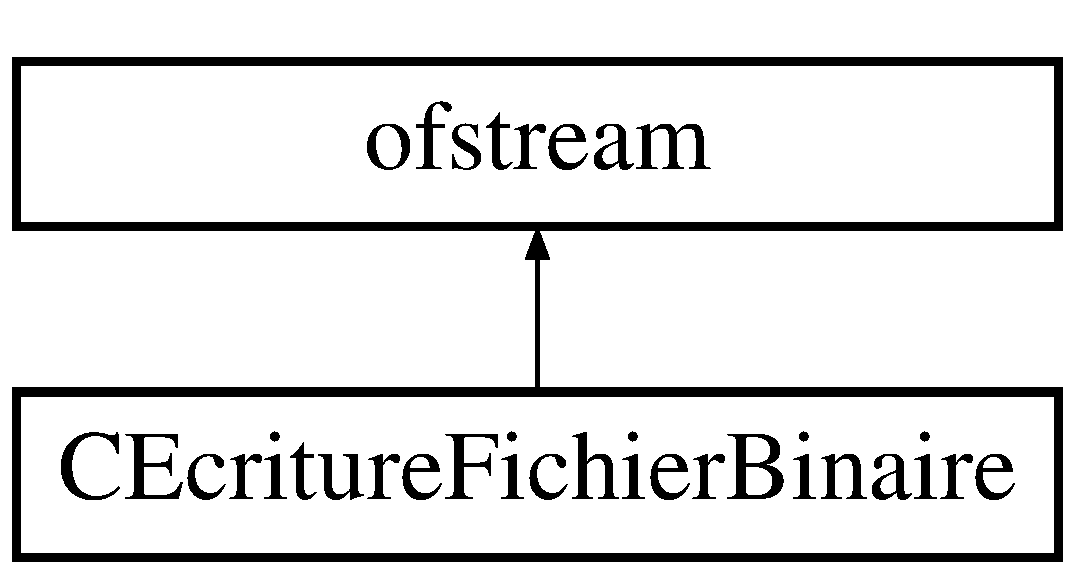
\includegraphics[height=2.000000cm]{class_c_ecriture_fichier_binaire}
\end{center}
\end{figure}
\subsection*{Public Member Functions}
\begin{DoxyCompactItemize}
\item 
\hyperlink{group__utilitaire_ga5b5846202001fecd71cd2a0afbbdb494}{C\-Ecriture\-Fichier\-Binaire} ()
\begin{DoxyCompactList}\small\item\em Constructeur par defaut. \end{DoxyCompactList}\item 
\hyperlink{group__utilitaire_gad19b9753aa12a9f25fd0febc3c899024}{C\-Ecriture\-Fichier\-Binaire} (const char $\ast$nom\-Fichier, openmode mode=std\-::ios\-::out$\vert$std\-::ios\-::binary)
\begin{DoxyCompactList}\small\item\em Constructeur par parametre. \end{DoxyCompactList}\item 
void \hyperlink{group__utilitaire_ga7145545254c30909311d3b1ef0bdd07a}{null} (int n)
\begin{DoxyCompactList}\small\item\em Fonction pour inserer des caracteres vides dans le fichier. \end{DoxyCompactList}\end{DoxyCompactItemize}
\subsection*{Friends}
\begin{DoxyCompactItemize}
\item 
\hypertarget{class_c_ecriture_fichier_binaire_a2c88c30ff08c7d9035596e0187d44e45}{\hyperlink{class_c_ecriture_fichier_binaire}{C\-Ecriture\-Fichier\-Binaire} \& \hyperlink{class_c_ecriture_fichier_binaire_a2c88c30ff08c7d9035596e0187d44e45}{operator$<$} (\hyperlink{class_c_ecriture_fichier_binaire}{C\-Ecriture\-Fichier\-Binaire} \&out, const std\-::string \&s)}\label{class_c_ecriture_fichier_binaire_a2c88c30ff08c7d9035596e0187d44e45}

\begin{DoxyCompactList}\small\item\em Surcharge de l'operateur pour le type {\itshape std\-::string}. \end{DoxyCompactList}\item 
\hypertarget{class_c_ecriture_fichier_binaire_afcaa555d19b37490df9fda731cf8cb19}{\hyperlink{class_c_ecriture_fichier_binaire}{C\-Ecriture\-Fichier\-Binaire} \& \hyperlink{class_c_ecriture_fichier_binaire_afcaa555d19b37490df9fda731cf8cb19}{operator$<$} (\hyperlink{class_c_ecriture_fichier_binaire}{C\-Ecriture\-Fichier\-Binaire} \&out, const double \&x)}\label{class_c_ecriture_fichier_binaire_afcaa555d19b37490df9fda731cf8cb19}

\begin{DoxyCompactList}\small\item\em Surcharge de l'operateur pour le type {\itshape double}. \end{DoxyCompactList}\item 
\hypertarget{class_c_ecriture_fichier_binaire_a68e43a125ee6c25828485dfb7270fdea}{\hyperlink{class_c_ecriture_fichier_binaire}{C\-Ecriture\-Fichier\-Binaire} \& \hyperlink{class_c_ecriture_fichier_binaire_a68e43a125ee6c25828485dfb7270fdea}{operator$<$} (\hyperlink{class_c_ecriture_fichier_binaire}{C\-Ecriture\-Fichier\-Binaire} \&out, const float \&x)}\label{class_c_ecriture_fichier_binaire_a68e43a125ee6c25828485dfb7270fdea}

\begin{DoxyCompactList}\small\item\em Surcharge de l'operateur pour le type {\itshape float}. \end{DoxyCompactList}\item 
\hypertarget{class_c_ecriture_fichier_binaire_a57ac55aefec2f3dd683cef75c409944b}{\hyperlink{class_c_ecriture_fichier_binaire}{C\-Ecriture\-Fichier\-Binaire} \& \hyperlink{class_c_ecriture_fichier_binaire_a57ac55aefec2f3dd683cef75c409944b}{operator$<$} (\hyperlink{class_c_ecriture_fichier_binaire}{C\-Ecriture\-Fichier\-Binaire} \&out, const int \&x)}\label{class_c_ecriture_fichier_binaire_a57ac55aefec2f3dd683cef75c409944b}

\begin{DoxyCompactList}\small\item\em Surcharge de l'operateur pour le type {\itshape int}. \end{DoxyCompactList}\item 
\hypertarget{class_c_ecriture_fichier_binaire_a38d0f050dcc8a79522b0fb9b9c591f72}{\hyperlink{class_c_ecriture_fichier_binaire}{C\-Ecriture\-Fichier\-Binaire} \& \hyperlink{class_c_ecriture_fichier_binaire_a38d0f050dcc8a79522b0fb9b9c591f72}{operator$<$} (\hyperlink{class_c_ecriture_fichier_binaire}{C\-Ecriture\-Fichier\-Binaire} \&out, const unsigned int \&x)}\label{class_c_ecriture_fichier_binaire_a38d0f050dcc8a79522b0fb9b9c591f72}

\begin{DoxyCompactList}\small\item\em Surcharge de l'operateur pour le type {\itshape unsigned} {\itshape int}. \end{DoxyCompactList}\item 
\hypertarget{class_c_ecriture_fichier_binaire_a3cb25116e2558d967dfd21e812e47a3e}{\hyperlink{class_c_ecriture_fichier_binaire}{C\-Ecriture\-Fichier\-Binaire} \& \hyperlink{class_c_ecriture_fichier_binaire_a3cb25116e2558d967dfd21e812e47a3e}{operator$<$} (\hyperlink{class_c_ecriture_fichier_binaire}{C\-Ecriture\-Fichier\-Binaire} \&out, const char \&x)}\label{class_c_ecriture_fichier_binaire_a3cb25116e2558d967dfd21e812e47a3e}

\begin{DoxyCompactList}\small\item\em Surcharge de l'operateur pour le type {\itshape char}. \end{DoxyCompactList}\item 
\hypertarget{class_c_ecriture_fichier_binaire_a37080aca11f391be69941db70093f77d}{\hyperlink{class_c_ecriture_fichier_binaire}{C\-Ecriture\-Fichier\-Binaire} \& \hyperlink{class_c_ecriture_fichier_binaire_a37080aca11f391be69941db70093f77d}{operator$<$} (\hyperlink{class_c_ecriture_fichier_binaire}{C\-Ecriture\-Fichier\-Binaire} \&out, const bool \&x)}\label{class_c_ecriture_fichier_binaire_a37080aca11f391be69941db70093f77d}

\begin{DoxyCompactList}\small\item\em Surcharge de l'operateur pour le type {\itshape bool}. \end{DoxyCompactList}\end{DoxyCompactItemize}


\subsection{Detailed Description}
Cette classe contient des methodes $<$ permettant d'ecrire dans un fichier binaire des variables string, double, float, int, unsigned int, char, bool. 

\begin{DoxyAuthor}{Author}
D\-G\-I-\/2990 
\end{DoxyAuthor}
\begin{DoxyDate}{Date}
2005-\/10-\/15 
\end{DoxyDate}


The documentation for this class was generated from the following files\-:\begin{DoxyCompactItemize}
\item 
Cadriciel/\-Commun/\-Utilitaire/\hyperlink{_c_ecriture_fichier_binaire_8h}{C\-Ecriture\-Fichier\-Binaire.\-h}\item 
Cadriciel/\-Commun/\-Utilitaire/\hyperlink{_c_ecriture_fichier_binaire_8cpp}{C\-Ecriture\-Fichier\-Binaire.\-cpp}\end{DoxyCompactItemize}

\hypertarget{class_f_m_o_d_1_1_channel}{\section{F\-M\-O\-D\-:\-:Channel Class Reference}
\label{class_f_m_o_d_1_1_channel}\index{F\-M\-O\-D\-::\-Channel@{F\-M\-O\-D\-::\-Channel}}
}


{\ttfamily \#include $<$fmod.\-hpp$>$}

\subsection*{Public Member Functions}
\begin{DoxyCompactItemize}
\item 
\hyperlink{fmod_8h_ae6ddadf8cb315e93ae7e6456b19db276}{F\-M\-O\-D\-\_\-\-R\-E\-S\-U\-L\-T} \hyperlink{fmod_8h_ace803d13e798b0cdde4384f9f323b901}{F\-\_\-\-A\-P\-I} \hyperlink{class_f_m_o_d_1_1_channel_ade71450e7b8a888d4a4f1e73eded4236}{get\-System\-Object} (\hyperlink{class_f_m_o_d_1_1_system}{System} $\ast$$\ast$system)
\item 
\hyperlink{fmod_8h_ae6ddadf8cb315e93ae7e6456b19db276}{F\-M\-O\-D\-\_\-\-R\-E\-S\-U\-L\-T} \hyperlink{fmod_8h_ace803d13e798b0cdde4384f9f323b901}{F\-\_\-\-A\-P\-I} \hyperlink{class_f_m_o_d_1_1_channel_a89d7bc13ea65f29f306fbd279e54dd08}{stop} ()
\item 
\hyperlink{fmod_8h_ae6ddadf8cb315e93ae7e6456b19db276}{F\-M\-O\-D\-\_\-\-R\-E\-S\-U\-L\-T} \hyperlink{fmod_8h_ace803d13e798b0cdde4384f9f323b901}{F\-\_\-\-A\-P\-I} \hyperlink{class_f_m_o_d_1_1_channel_a7610d6be6beec8f7cf6d0230c48c6618}{set\-Paused} (bool paused)
\item 
\hyperlink{fmod_8h_ae6ddadf8cb315e93ae7e6456b19db276}{F\-M\-O\-D\-\_\-\-R\-E\-S\-U\-L\-T} \hyperlink{fmod_8h_ace803d13e798b0cdde4384f9f323b901}{F\-\_\-\-A\-P\-I} \hyperlink{class_f_m_o_d_1_1_channel_a551d39aed652cb419ce5ec7256abefb4}{get\-Paused} (bool $\ast$paused)
\item 
\hyperlink{fmod_8h_ae6ddadf8cb315e93ae7e6456b19db276}{F\-M\-O\-D\-\_\-\-R\-E\-S\-U\-L\-T} \hyperlink{fmod_8h_ace803d13e798b0cdde4384f9f323b901}{F\-\_\-\-A\-P\-I} \hyperlink{class_f_m_o_d_1_1_channel_a641ee780642531cec59aa9ec065d4709}{set\-Volume} (\hyperlink{fmod_8h_aeb841aa4b4b5f444b5d739d865b420af}{float} volume)
\item 
\hyperlink{fmod_8h_ae6ddadf8cb315e93ae7e6456b19db276}{F\-M\-O\-D\-\_\-\-R\-E\-S\-U\-L\-T} \hyperlink{fmod_8h_ace803d13e798b0cdde4384f9f323b901}{F\-\_\-\-A\-P\-I} \hyperlink{class_f_m_o_d_1_1_channel_aef6f0675ac455547e3a00ce339ca85f9}{get\-Volume} (\hyperlink{fmod_8h_aeb841aa4b4b5f444b5d739d865b420af}{float} $\ast$volume)
\item 
\hyperlink{fmod_8h_ae6ddadf8cb315e93ae7e6456b19db276}{F\-M\-O\-D\-\_\-\-R\-E\-S\-U\-L\-T} \hyperlink{fmod_8h_ace803d13e798b0cdde4384f9f323b901}{F\-\_\-\-A\-P\-I} \hyperlink{class_f_m_o_d_1_1_channel_a355cd052a405c0ecdbaac7c65d24148b}{set\-Frequency} (\hyperlink{fmod_8h_aeb841aa4b4b5f444b5d739d865b420af}{float} frequency)
\item 
\hyperlink{fmod_8h_ae6ddadf8cb315e93ae7e6456b19db276}{F\-M\-O\-D\-\_\-\-R\-E\-S\-U\-L\-T} \hyperlink{fmod_8h_ace803d13e798b0cdde4384f9f323b901}{F\-\_\-\-A\-P\-I} \hyperlink{class_f_m_o_d_1_1_channel_a99f1dcf4b2a67f509d08f138e9e3cbca}{get\-Frequency} (\hyperlink{fmod_8h_aeb841aa4b4b5f444b5d739d865b420af}{float} $\ast$frequency)
\item 
\hyperlink{fmod_8h_ae6ddadf8cb315e93ae7e6456b19db276}{F\-M\-O\-D\-\_\-\-R\-E\-S\-U\-L\-T} \hyperlink{fmod_8h_ace803d13e798b0cdde4384f9f323b901}{F\-\_\-\-A\-P\-I} \hyperlink{class_f_m_o_d_1_1_channel_a419235a572a267b0763287fe988435f7}{set\-Pan} (\hyperlink{fmod_8h_aeb841aa4b4b5f444b5d739d865b420af}{float} pan)
\item 
\hyperlink{fmod_8h_ae6ddadf8cb315e93ae7e6456b19db276}{F\-M\-O\-D\-\_\-\-R\-E\-S\-U\-L\-T} \hyperlink{fmod_8h_ace803d13e798b0cdde4384f9f323b901}{F\-\_\-\-A\-P\-I} \hyperlink{class_f_m_o_d_1_1_channel_a776a9e6fbca132087663e77de052806c}{get\-Pan} (\hyperlink{fmod_8h_aeb841aa4b4b5f444b5d739d865b420af}{float} $\ast$pan)
\item 
\hyperlink{fmod_8h_ae6ddadf8cb315e93ae7e6456b19db276}{F\-M\-O\-D\-\_\-\-R\-E\-S\-U\-L\-T} \hyperlink{fmod_8h_ace803d13e798b0cdde4384f9f323b901}{F\-\_\-\-A\-P\-I} \hyperlink{class_f_m_o_d_1_1_channel_a21a2f9d9fdae503ce53a9ced9c4cb9a2}{set\-Delay} (\hyperlink{fmod_8h_a294c7a2929ae0374c4fa8a4e54902b7c}{F\-M\-O\-D\-\_\-\-D\-E\-L\-A\-Y\-T\-Y\-P\-E} delaytype, \hyperlink{_free_image_8h_a425076c7067a1b5166e2cc530e914814}{unsigned} \hyperlink{wglew_8h_a500a82aecba06f4550f6849b8099ca21}{int} delayhi, \hyperlink{_free_image_8h_a425076c7067a1b5166e2cc530e914814}{unsigned} \hyperlink{wglew_8h_a500a82aecba06f4550f6849b8099ca21}{int} delaylo)
\item 
\hyperlink{fmod_8h_ae6ddadf8cb315e93ae7e6456b19db276}{F\-M\-O\-D\-\_\-\-R\-E\-S\-U\-L\-T} \hyperlink{fmod_8h_ace803d13e798b0cdde4384f9f323b901}{F\-\_\-\-A\-P\-I} \hyperlink{class_f_m_o_d_1_1_channel_a8cc8b51bc344dd7916628568764aa6cf}{get\-Delay} (\hyperlink{fmod_8h_a294c7a2929ae0374c4fa8a4e54902b7c}{F\-M\-O\-D\-\_\-\-D\-E\-L\-A\-Y\-T\-Y\-P\-E} delaytype, \hyperlink{_free_image_8h_a425076c7067a1b5166e2cc530e914814}{unsigned} \hyperlink{wglew_8h_a500a82aecba06f4550f6849b8099ca21}{int} $\ast$delayhi, \hyperlink{_free_image_8h_a425076c7067a1b5166e2cc530e914814}{unsigned} \hyperlink{wglew_8h_a500a82aecba06f4550f6849b8099ca21}{int} $\ast$delaylo)
\item 
\hyperlink{fmod_8h_ae6ddadf8cb315e93ae7e6456b19db276}{F\-M\-O\-D\-\_\-\-R\-E\-S\-U\-L\-T} \hyperlink{fmod_8h_ace803d13e798b0cdde4384f9f323b901}{F\-\_\-\-A\-P\-I} \hyperlink{class_f_m_o_d_1_1_channel_ad6b62bf51be6c5c3006e23717e8ad4c7}{set\-Speaker\-Mix} (\hyperlink{fmod_8h_aeb841aa4b4b5f444b5d739d865b420af}{float} frontleft, \hyperlink{fmod_8h_aeb841aa4b4b5f444b5d739d865b420af}{float} frontright, \hyperlink{fmod_8h_aeb841aa4b4b5f444b5d739d865b420af}{float} center, \hyperlink{fmod_8h_aeb841aa4b4b5f444b5d739d865b420af}{float} lfe, \hyperlink{fmod_8h_aeb841aa4b4b5f444b5d739d865b420af}{float} backleft, \hyperlink{fmod_8h_aeb841aa4b4b5f444b5d739d865b420af}{float} backright, \hyperlink{fmod_8h_aeb841aa4b4b5f444b5d739d865b420af}{float} sideleft, \hyperlink{fmod_8h_aeb841aa4b4b5f444b5d739d865b420af}{float} sideright)
\item 
\hyperlink{fmod_8h_ae6ddadf8cb315e93ae7e6456b19db276}{F\-M\-O\-D\-\_\-\-R\-E\-S\-U\-L\-T} \hyperlink{fmod_8h_ace803d13e798b0cdde4384f9f323b901}{F\-\_\-\-A\-P\-I} \hyperlink{class_f_m_o_d_1_1_channel_a1cec99c48524d8cbf6d4454b1ec7a374}{get\-Speaker\-Mix} (\hyperlink{fmod_8h_aeb841aa4b4b5f444b5d739d865b420af}{float} $\ast$frontleft, \hyperlink{fmod_8h_aeb841aa4b4b5f444b5d739d865b420af}{float} $\ast$frontright, \hyperlink{fmod_8h_aeb841aa4b4b5f444b5d739d865b420af}{float} $\ast$center, \hyperlink{fmod_8h_aeb841aa4b4b5f444b5d739d865b420af}{float} $\ast$lfe, \hyperlink{fmod_8h_aeb841aa4b4b5f444b5d739d865b420af}{float} $\ast$backleft, \hyperlink{fmod_8h_aeb841aa4b4b5f444b5d739d865b420af}{float} $\ast$backright, \hyperlink{fmod_8h_aeb841aa4b4b5f444b5d739d865b420af}{float} $\ast$sideleft, \hyperlink{fmod_8h_aeb841aa4b4b5f444b5d739d865b420af}{float} $\ast$sideright)
\item 
\hyperlink{fmod_8h_ae6ddadf8cb315e93ae7e6456b19db276}{F\-M\-O\-D\-\_\-\-R\-E\-S\-U\-L\-T} \hyperlink{fmod_8h_ace803d13e798b0cdde4384f9f323b901}{F\-\_\-\-A\-P\-I} \hyperlink{class_f_m_o_d_1_1_channel_aa32c97cb14d3da622393d7406c9f0ca3}{set\-Speaker\-Levels} (\hyperlink{fmod_8h_a1870cd80bd38e1ba43eaa81e74d63bdc}{F\-M\-O\-D\-\_\-\-S\-P\-E\-A\-K\-E\-R} speaker, \hyperlink{fmod_8h_aeb841aa4b4b5f444b5d739d865b420af}{float} $\ast$levels, \hyperlink{wglew_8h_a500a82aecba06f4550f6849b8099ca21}{int} numlevels)
\item 
\hyperlink{fmod_8h_ae6ddadf8cb315e93ae7e6456b19db276}{F\-M\-O\-D\-\_\-\-R\-E\-S\-U\-L\-T} \hyperlink{fmod_8h_ace803d13e798b0cdde4384f9f323b901}{F\-\_\-\-A\-P\-I} \hyperlink{class_f_m_o_d_1_1_channel_aadb8b4003e6b716331d280a7f22a6f51}{get\-Speaker\-Levels} (\hyperlink{fmod_8h_a1870cd80bd38e1ba43eaa81e74d63bdc}{F\-M\-O\-D\-\_\-\-S\-P\-E\-A\-K\-E\-R} speaker, \hyperlink{fmod_8h_aeb841aa4b4b5f444b5d739d865b420af}{float} $\ast$levels, \hyperlink{wglew_8h_a500a82aecba06f4550f6849b8099ca21}{int} numlevels)
\item 
\hyperlink{fmod_8h_ae6ddadf8cb315e93ae7e6456b19db276}{F\-M\-O\-D\-\_\-\-R\-E\-S\-U\-L\-T} \hyperlink{fmod_8h_ace803d13e798b0cdde4384f9f323b901}{F\-\_\-\-A\-P\-I} \hyperlink{class_f_m_o_d_1_1_channel_a4695dfbef85dece725468e690053ca00}{set\-Input\-Channel\-Mix} (\hyperlink{fmod_8h_aeb841aa4b4b5f444b5d739d865b420af}{float} $\ast$levels, \hyperlink{wglew_8h_a500a82aecba06f4550f6849b8099ca21}{int} numlevels)
\item 
\hyperlink{fmod_8h_ae6ddadf8cb315e93ae7e6456b19db276}{F\-M\-O\-D\-\_\-\-R\-E\-S\-U\-L\-T} \hyperlink{fmod_8h_ace803d13e798b0cdde4384f9f323b901}{F\-\_\-\-A\-P\-I} \hyperlink{class_f_m_o_d_1_1_channel_ab893172c11ceab2bb254707b1b2d263e}{get\-Input\-Channel\-Mix} (\hyperlink{fmod_8h_aeb841aa4b4b5f444b5d739d865b420af}{float} $\ast$levels, \hyperlink{wglew_8h_a500a82aecba06f4550f6849b8099ca21}{int} numlevels)
\item 
\hyperlink{fmod_8h_ae6ddadf8cb315e93ae7e6456b19db276}{F\-M\-O\-D\-\_\-\-R\-E\-S\-U\-L\-T} \hyperlink{fmod_8h_ace803d13e798b0cdde4384f9f323b901}{F\-\_\-\-A\-P\-I} \hyperlink{class_f_m_o_d_1_1_channel_a0b0d4a7d28c0e57daeb8c1c39fb06379}{set\-Mute} (bool mute)
\item 
\hyperlink{fmod_8h_ae6ddadf8cb315e93ae7e6456b19db276}{F\-M\-O\-D\-\_\-\-R\-E\-S\-U\-L\-T} \hyperlink{fmod_8h_ace803d13e798b0cdde4384f9f323b901}{F\-\_\-\-A\-P\-I} \hyperlink{class_f_m_o_d_1_1_channel_acc5cfb7cd503c24210ab7ffbbdbbea0e}{get\-Mute} (bool $\ast$mute)
\item 
\hyperlink{fmod_8h_ae6ddadf8cb315e93ae7e6456b19db276}{F\-M\-O\-D\-\_\-\-R\-E\-S\-U\-L\-T} \hyperlink{fmod_8h_ace803d13e798b0cdde4384f9f323b901}{F\-\_\-\-A\-P\-I} \hyperlink{class_f_m_o_d_1_1_channel_a83a9a2f49e4bdde446f0d574847f5329}{set\-Priority} (\hyperlink{wglew_8h_a500a82aecba06f4550f6849b8099ca21}{int} priority)
\item 
\hyperlink{fmod_8h_ae6ddadf8cb315e93ae7e6456b19db276}{F\-M\-O\-D\-\_\-\-R\-E\-S\-U\-L\-T} \hyperlink{fmod_8h_ace803d13e798b0cdde4384f9f323b901}{F\-\_\-\-A\-P\-I} \hyperlink{class_f_m_o_d_1_1_channel_ae2a16710e706c0223937bc99fb3cad3d}{get\-Priority} (\hyperlink{wglew_8h_a500a82aecba06f4550f6849b8099ca21}{int} $\ast$priority)
\item 
\hyperlink{fmod_8h_ae6ddadf8cb315e93ae7e6456b19db276}{F\-M\-O\-D\-\_\-\-R\-E\-S\-U\-L\-T} \hyperlink{fmod_8h_ace803d13e798b0cdde4384f9f323b901}{F\-\_\-\-A\-P\-I} \hyperlink{class_f_m_o_d_1_1_channel_a46f8f6738b500bbb995bd4a4ecce826f}{set\-Position} (\hyperlink{_free_image_8h_a425076c7067a1b5166e2cc530e914814}{unsigned} \hyperlink{wglew_8h_a500a82aecba06f4550f6849b8099ca21}{int} \hyperlink{fmod__codec_8h_a7d71cf36b6a2fc185ecbc89f93fa58a3}{position}, \hyperlink{fmod_8h_a9999089b44f00c72ba8e9a270a8d6349}{F\-M\-O\-D\-\_\-\-T\-I\-M\-E\-U\-N\-I\-T} \hyperlink{fmod__codec_8h_afb73aa9ab0818133a25040abf0c9cecf}{postype})
\item 
\hyperlink{fmod_8h_ae6ddadf8cb315e93ae7e6456b19db276}{F\-M\-O\-D\-\_\-\-R\-E\-S\-U\-L\-T} \hyperlink{fmod_8h_ace803d13e798b0cdde4384f9f323b901}{F\-\_\-\-A\-P\-I} \hyperlink{class_f_m_o_d_1_1_channel_a580cb740f80cf139faaf21181490d98f}{get\-Position} (\hyperlink{_free_image_8h_a425076c7067a1b5166e2cc530e914814}{unsigned} \hyperlink{wglew_8h_a500a82aecba06f4550f6849b8099ca21}{int} $\ast$\hyperlink{fmod__codec_8h_a7d71cf36b6a2fc185ecbc89f93fa58a3}{position}, \hyperlink{fmod_8h_a9999089b44f00c72ba8e9a270a8d6349}{F\-M\-O\-D\-\_\-\-T\-I\-M\-E\-U\-N\-I\-T} \hyperlink{fmod__codec_8h_afb73aa9ab0818133a25040abf0c9cecf}{postype})
\item 
\hyperlink{fmod_8h_ae6ddadf8cb315e93ae7e6456b19db276}{F\-M\-O\-D\-\_\-\-R\-E\-S\-U\-L\-T} \hyperlink{fmod_8h_ace803d13e798b0cdde4384f9f323b901}{F\-\_\-\-A\-P\-I} \hyperlink{class_f_m_o_d_1_1_channel_a1002a2ff8f7f9f33b2fce03fb472e8a8}{set\-Reverb\-Properties} (const \hyperlink{struct_f_m_o_d___r_e_v_e_r_b___c_h_a_n_n_e_l_p_r_o_p_e_r_t_i_e_s}{F\-M\-O\-D\-\_\-\-R\-E\-V\-E\-R\-B\-\_\-\-C\-H\-A\-N\-N\-E\-L\-P\-R\-O\-P\-E\-R\-T\-I\-E\-S} $\ast$prop)
\item 
\hyperlink{fmod_8h_ae6ddadf8cb315e93ae7e6456b19db276}{F\-M\-O\-D\-\_\-\-R\-E\-S\-U\-L\-T} \hyperlink{fmod_8h_ace803d13e798b0cdde4384f9f323b901}{F\-\_\-\-A\-P\-I} \hyperlink{class_f_m_o_d_1_1_channel_a0e0e479c81abd5e709bda6abcebac57b}{get\-Reverb\-Properties} (\hyperlink{struct_f_m_o_d___r_e_v_e_r_b___c_h_a_n_n_e_l_p_r_o_p_e_r_t_i_e_s}{F\-M\-O\-D\-\_\-\-R\-E\-V\-E\-R\-B\-\_\-\-C\-H\-A\-N\-N\-E\-L\-P\-R\-O\-P\-E\-R\-T\-I\-E\-S} $\ast$prop)
\item 
\hyperlink{fmod_8h_ae6ddadf8cb315e93ae7e6456b19db276}{F\-M\-O\-D\-\_\-\-R\-E\-S\-U\-L\-T} \hyperlink{fmod_8h_ace803d13e798b0cdde4384f9f323b901}{F\-\_\-\-A\-P\-I} \hyperlink{class_f_m_o_d_1_1_channel_a10e6a2fe8768461407fac5963167c416}{set\-Low\-Pass\-Gain} (\hyperlink{fmod_8h_aeb841aa4b4b5f444b5d739d865b420af}{float} gain)
\item 
\hyperlink{fmod_8h_ae6ddadf8cb315e93ae7e6456b19db276}{F\-M\-O\-D\-\_\-\-R\-E\-S\-U\-L\-T} \hyperlink{fmod_8h_ace803d13e798b0cdde4384f9f323b901}{F\-\_\-\-A\-P\-I} \hyperlink{class_f_m_o_d_1_1_channel_a0e34960ec8bd9703fcdcfa0b85683b18}{get\-Low\-Pass\-Gain} (\hyperlink{fmod_8h_aeb841aa4b4b5f444b5d739d865b420af}{float} $\ast$gain)
\item 
\hyperlink{fmod_8h_ae6ddadf8cb315e93ae7e6456b19db276}{F\-M\-O\-D\-\_\-\-R\-E\-S\-U\-L\-T} \hyperlink{fmod_8h_ace803d13e798b0cdde4384f9f323b901}{F\-\_\-\-A\-P\-I} \hyperlink{class_f_m_o_d_1_1_channel_a570b83eb8178325a131b081a8d5ffd81}{set\-Channel\-Group} (\hyperlink{class_f_m_o_d_1_1_channel_group}{Channel\-Group} $\ast$channelgroup)
\item 
\hyperlink{fmod_8h_ae6ddadf8cb315e93ae7e6456b19db276}{F\-M\-O\-D\-\_\-\-R\-E\-S\-U\-L\-T} \hyperlink{fmod_8h_ace803d13e798b0cdde4384f9f323b901}{F\-\_\-\-A\-P\-I} \hyperlink{class_f_m_o_d_1_1_channel_a4b6d310d04eb844190db7a4074af2b2c}{get\-Channel\-Group} (\hyperlink{class_f_m_o_d_1_1_channel_group}{Channel\-Group} $\ast$$\ast$channelgroup)
\item 
\hyperlink{fmod_8h_ae6ddadf8cb315e93ae7e6456b19db276}{F\-M\-O\-D\-\_\-\-R\-E\-S\-U\-L\-T} \hyperlink{fmod_8h_ace803d13e798b0cdde4384f9f323b901}{F\-\_\-\-A\-P\-I} \hyperlink{class_f_m_o_d_1_1_channel_a5cbbb69ad8d74d36d7b469a77450c3fa}{set\-Callback} (F\-M\-O\-D\-\_\-\-C\-H\-A\-N\-N\-E\-L\-\_\-\-C\-A\-L\-L\-B\-A\-C\-K callback)
\item 
\hyperlink{fmod_8h_ae6ddadf8cb315e93ae7e6456b19db276}{F\-M\-O\-D\-\_\-\-R\-E\-S\-U\-L\-T} \hyperlink{fmod_8h_ace803d13e798b0cdde4384f9f323b901}{F\-\_\-\-A\-P\-I} \hyperlink{class_f_m_o_d_1_1_channel_ae0bb0f7c1c1a807bde8ab9e9c3870785}{set3\-D\-Attributes} (const \hyperlink{struct_f_m_o_d___v_e_c_t_o_r}{F\-M\-O\-D\-\_\-\-V\-E\-C\-T\-O\-R} $\ast$\hyperlink{fmod_8h_a74861c24659b95574d7a405e864de0df}{pos}, const \hyperlink{struct_f_m_o_d___v_e_c_t_o_r}{F\-M\-O\-D\-\_\-\-V\-E\-C\-T\-O\-R} $\ast$vel)
\item 
\hyperlink{fmod_8h_ae6ddadf8cb315e93ae7e6456b19db276}{F\-M\-O\-D\-\_\-\-R\-E\-S\-U\-L\-T} \hyperlink{fmod_8h_ace803d13e798b0cdde4384f9f323b901}{F\-\_\-\-A\-P\-I} \hyperlink{class_f_m_o_d_1_1_channel_ab0f5e28337f9303c75f80d139201a858}{get3\-D\-Attributes} (\hyperlink{struct_f_m_o_d___v_e_c_t_o_r}{F\-M\-O\-D\-\_\-\-V\-E\-C\-T\-O\-R} $\ast$\hyperlink{fmod_8h_a74861c24659b95574d7a405e864de0df}{pos}, \hyperlink{struct_f_m_o_d___v_e_c_t_o_r}{F\-M\-O\-D\-\_\-\-V\-E\-C\-T\-O\-R} $\ast$vel)
\item 
\hyperlink{fmod_8h_ae6ddadf8cb315e93ae7e6456b19db276}{F\-M\-O\-D\-\_\-\-R\-E\-S\-U\-L\-T} \hyperlink{fmod_8h_ace803d13e798b0cdde4384f9f323b901}{F\-\_\-\-A\-P\-I} \hyperlink{class_f_m_o_d_1_1_channel_aa6ee9a231435079405ec4a2c2bd07c44}{set3\-D\-Min\-Max\-Distance} (\hyperlink{fmod_8h_aeb841aa4b4b5f444b5d739d865b420af}{float} mindistance, \hyperlink{fmod_8h_aeb841aa4b4b5f444b5d739d865b420af}{float} maxdistance)
\item 
\hyperlink{fmod_8h_ae6ddadf8cb315e93ae7e6456b19db276}{F\-M\-O\-D\-\_\-\-R\-E\-S\-U\-L\-T} \hyperlink{fmod_8h_ace803d13e798b0cdde4384f9f323b901}{F\-\_\-\-A\-P\-I} \hyperlink{class_f_m_o_d_1_1_channel_ae997142f79c9e96414f0ecce05fa93a3}{get3\-D\-Min\-Max\-Distance} (\hyperlink{fmod_8h_aeb841aa4b4b5f444b5d739d865b420af}{float} $\ast$mindistance, \hyperlink{fmod_8h_aeb841aa4b4b5f444b5d739d865b420af}{float} $\ast$maxdistance)
\item 
\hyperlink{fmod_8h_ae6ddadf8cb315e93ae7e6456b19db276}{F\-M\-O\-D\-\_\-\-R\-E\-S\-U\-L\-T} \hyperlink{fmod_8h_ace803d13e798b0cdde4384f9f323b901}{F\-\_\-\-A\-P\-I} \hyperlink{class_f_m_o_d_1_1_channel_a9e0d8885d31b2978683d5305924de565}{set3\-D\-Cone\-Settings} (\hyperlink{fmod_8h_aeb841aa4b4b5f444b5d739d865b420af}{float} insideconeangle, \hyperlink{fmod_8h_aeb841aa4b4b5f444b5d739d865b420af}{float} outsideconeangle, \hyperlink{fmod_8h_aeb841aa4b4b5f444b5d739d865b420af}{float} outsidevolume)
\item 
\hyperlink{fmod_8h_ae6ddadf8cb315e93ae7e6456b19db276}{F\-M\-O\-D\-\_\-\-R\-E\-S\-U\-L\-T} \hyperlink{fmod_8h_ace803d13e798b0cdde4384f9f323b901}{F\-\_\-\-A\-P\-I} \hyperlink{class_f_m_o_d_1_1_channel_a7206e7b2353ed27ec91512690bd2c052}{get3\-D\-Cone\-Settings} (\hyperlink{fmod_8h_aeb841aa4b4b5f444b5d739d865b420af}{float} $\ast$insideconeangle, \hyperlink{fmod_8h_aeb841aa4b4b5f444b5d739d865b420af}{float} $\ast$outsideconeangle, \hyperlink{fmod_8h_aeb841aa4b4b5f444b5d739d865b420af}{float} $\ast$outsidevolume)
\item 
\hyperlink{fmod_8h_ae6ddadf8cb315e93ae7e6456b19db276}{F\-M\-O\-D\-\_\-\-R\-E\-S\-U\-L\-T} \hyperlink{fmod_8h_ace803d13e798b0cdde4384f9f323b901}{F\-\_\-\-A\-P\-I} \hyperlink{class_f_m_o_d_1_1_channel_a6c10b3cdb50cb11d5090b14b7f569a79}{set3\-D\-Cone\-Orientation} (\hyperlink{struct_f_m_o_d___v_e_c_t_o_r}{F\-M\-O\-D\-\_\-\-V\-E\-C\-T\-O\-R} $\ast$orientation)
\item 
\hyperlink{fmod_8h_ae6ddadf8cb315e93ae7e6456b19db276}{F\-M\-O\-D\-\_\-\-R\-E\-S\-U\-L\-T} \hyperlink{fmod_8h_ace803d13e798b0cdde4384f9f323b901}{F\-\_\-\-A\-P\-I} \hyperlink{class_f_m_o_d_1_1_channel_a0f22cabb2a93d1a8c038293c9a5a970d}{get3\-D\-Cone\-Orientation} (\hyperlink{struct_f_m_o_d___v_e_c_t_o_r}{F\-M\-O\-D\-\_\-\-V\-E\-C\-T\-O\-R} $\ast$orientation)
\item 
\hyperlink{fmod_8h_ae6ddadf8cb315e93ae7e6456b19db276}{F\-M\-O\-D\-\_\-\-R\-E\-S\-U\-L\-T} \hyperlink{fmod_8h_ace803d13e798b0cdde4384f9f323b901}{F\-\_\-\-A\-P\-I} \hyperlink{class_f_m_o_d_1_1_channel_a1ad33a178f33decfc764dfca2ad0aefb}{set3\-D\-Custom\-Rolloff} (\hyperlink{struct_f_m_o_d___v_e_c_t_o_r}{F\-M\-O\-D\-\_\-\-V\-E\-C\-T\-O\-R} $\ast$\hyperlink{glew_8h_a8542fd6d6fb19b09ca970f46a936eeca}{points}, \hyperlink{wglew_8h_a500a82aecba06f4550f6849b8099ca21}{int} numpoints)
\item 
\hyperlink{fmod_8h_ae6ddadf8cb315e93ae7e6456b19db276}{F\-M\-O\-D\-\_\-\-R\-E\-S\-U\-L\-T} \hyperlink{fmod_8h_ace803d13e798b0cdde4384f9f323b901}{F\-\_\-\-A\-P\-I} \hyperlink{class_f_m_o_d_1_1_channel_ae772d709160da9adb23971c6f0b2bc33}{get3\-D\-Custom\-Rolloff} (\hyperlink{struct_f_m_o_d___v_e_c_t_o_r}{F\-M\-O\-D\-\_\-\-V\-E\-C\-T\-O\-R} $\ast$$\ast$\hyperlink{glew_8h_a8542fd6d6fb19b09ca970f46a936eeca}{points}, \hyperlink{wglew_8h_a500a82aecba06f4550f6849b8099ca21}{int} $\ast$numpoints)
\item 
\hyperlink{fmod_8h_ae6ddadf8cb315e93ae7e6456b19db276}{F\-M\-O\-D\-\_\-\-R\-E\-S\-U\-L\-T} \hyperlink{fmod_8h_ace803d13e798b0cdde4384f9f323b901}{F\-\_\-\-A\-P\-I} \hyperlink{class_f_m_o_d_1_1_channel_a0037d4f48e07686f53d35c66fd6be5cd}{set3\-D\-Occlusion} (\hyperlink{fmod_8h_aeb841aa4b4b5f444b5d739d865b420af}{float} directocclusion, \hyperlink{fmod_8h_aeb841aa4b4b5f444b5d739d865b420af}{float} reverbocclusion)
\item 
\hyperlink{fmod_8h_ae6ddadf8cb315e93ae7e6456b19db276}{F\-M\-O\-D\-\_\-\-R\-E\-S\-U\-L\-T} \hyperlink{fmod_8h_ace803d13e798b0cdde4384f9f323b901}{F\-\_\-\-A\-P\-I} \hyperlink{class_f_m_o_d_1_1_channel_a0059b3132df76efd24f8567b4fcf4818}{get3\-D\-Occlusion} (\hyperlink{fmod_8h_aeb841aa4b4b5f444b5d739d865b420af}{float} $\ast$directocclusion, \hyperlink{fmod_8h_aeb841aa4b4b5f444b5d739d865b420af}{float} $\ast$reverbocclusion)
\item 
\hyperlink{fmod_8h_ae6ddadf8cb315e93ae7e6456b19db276}{F\-M\-O\-D\-\_\-\-R\-E\-S\-U\-L\-T} \hyperlink{fmod_8h_ace803d13e798b0cdde4384f9f323b901}{F\-\_\-\-A\-P\-I} \hyperlink{class_f_m_o_d_1_1_channel_a59fb99f17a8997b14d983647e6978c07}{set3\-D\-Spread} (\hyperlink{fmod_8h_aeb841aa4b4b5f444b5d739d865b420af}{float} \hyperlink{glew_8h_a6d7a98b0d979b9411a4344a98a7a6122}{angle})
\item 
\hyperlink{fmod_8h_ae6ddadf8cb315e93ae7e6456b19db276}{F\-M\-O\-D\-\_\-\-R\-E\-S\-U\-L\-T} \hyperlink{fmod_8h_ace803d13e798b0cdde4384f9f323b901}{F\-\_\-\-A\-P\-I} \hyperlink{class_f_m_o_d_1_1_channel_a527cbba8333bfe7515fe18208765ac61}{get3\-D\-Spread} (\hyperlink{fmod_8h_aeb841aa4b4b5f444b5d739d865b420af}{float} $\ast$\hyperlink{glew_8h_a6d7a98b0d979b9411a4344a98a7a6122}{angle})
\item 
\hyperlink{fmod_8h_ae6ddadf8cb315e93ae7e6456b19db276}{F\-M\-O\-D\-\_\-\-R\-E\-S\-U\-L\-T} \hyperlink{fmod_8h_ace803d13e798b0cdde4384f9f323b901}{F\-\_\-\-A\-P\-I} \hyperlink{class_f_m_o_d_1_1_channel_aaeadeb90b4c702d16b6083a17905efc5}{set3\-D\-Pan\-Level} (\hyperlink{fmod_8h_aeb841aa4b4b5f444b5d739d865b420af}{float} \hyperlink{glew_8h_a2b536fca24f51d6a849aed325793e661}{level})
\item 
\hyperlink{fmod_8h_ae6ddadf8cb315e93ae7e6456b19db276}{F\-M\-O\-D\-\_\-\-R\-E\-S\-U\-L\-T} \hyperlink{fmod_8h_ace803d13e798b0cdde4384f9f323b901}{F\-\_\-\-A\-P\-I} \hyperlink{class_f_m_o_d_1_1_channel_ac8779446fdac236616964ac5bddec5be}{get3\-D\-Pan\-Level} (\hyperlink{fmod_8h_aeb841aa4b4b5f444b5d739d865b420af}{float} $\ast$\hyperlink{glew_8h_a2b536fca24f51d6a849aed325793e661}{level})
\item 
\hyperlink{fmod_8h_ae6ddadf8cb315e93ae7e6456b19db276}{F\-M\-O\-D\-\_\-\-R\-E\-S\-U\-L\-T} \hyperlink{fmod_8h_ace803d13e798b0cdde4384f9f323b901}{F\-\_\-\-A\-P\-I} \hyperlink{class_f_m_o_d_1_1_channel_a7e1c29fc420d38a9a686a0a29996209a}{set3\-D\-Doppler\-Level} (\hyperlink{fmod_8h_aeb841aa4b4b5f444b5d739d865b420af}{float} \hyperlink{glew_8h_a2b536fca24f51d6a849aed325793e661}{level})
\item 
\hyperlink{fmod_8h_ae6ddadf8cb315e93ae7e6456b19db276}{F\-M\-O\-D\-\_\-\-R\-E\-S\-U\-L\-T} \hyperlink{fmod_8h_ace803d13e798b0cdde4384f9f323b901}{F\-\_\-\-A\-P\-I} \hyperlink{class_f_m_o_d_1_1_channel_a90e0a82f15339ae3a9442ad04bec229b}{get3\-D\-Doppler\-Level} (\hyperlink{fmod_8h_aeb841aa4b4b5f444b5d739d865b420af}{float} $\ast$\hyperlink{glew_8h_a2b536fca24f51d6a849aed325793e661}{level})
\item 
\hyperlink{fmod_8h_ae6ddadf8cb315e93ae7e6456b19db276}{F\-M\-O\-D\-\_\-\-R\-E\-S\-U\-L\-T} \hyperlink{fmod_8h_ace803d13e798b0cdde4384f9f323b901}{F\-\_\-\-A\-P\-I} \hyperlink{class_f_m_o_d_1_1_channel_a6c180f229b8edffa88ecc2ef99a581e3}{set3\-D\-Distance\-Filter} (bool custom, \hyperlink{fmod_8h_aeb841aa4b4b5f444b5d739d865b420af}{float} custom\-Level, \hyperlink{fmod_8h_aeb841aa4b4b5f444b5d739d865b420af}{float} center\-Freq)
\item 
\hyperlink{fmod_8h_ae6ddadf8cb315e93ae7e6456b19db276}{F\-M\-O\-D\-\_\-\-R\-E\-S\-U\-L\-T} \hyperlink{fmod_8h_ace803d13e798b0cdde4384f9f323b901}{F\-\_\-\-A\-P\-I} \hyperlink{class_f_m_o_d_1_1_channel_abf9d4d1cc96e3e79ea316172524a3c6a}{get3\-D\-Distance\-Filter} (bool $\ast$custom, \hyperlink{fmod_8h_aeb841aa4b4b5f444b5d739d865b420af}{float} $\ast$custom\-Level, \hyperlink{fmod_8h_aeb841aa4b4b5f444b5d739d865b420af}{float} $\ast$center\-Freq)
\item 
\hyperlink{fmod_8h_ae6ddadf8cb315e93ae7e6456b19db276}{F\-M\-O\-D\-\_\-\-R\-E\-S\-U\-L\-T} \hyperlink{fmod_8h_ace803d13e798b0cdde4384f9f323b901}{F\-\_\-\-A\-P\-I} \hyperlink{class_f_m_o_d_1_1_channel_a2629c769ba2de6aec89da5c07bf4a535}{get\-D\-S\-P\-Head} (\hyperlink{class_f_m_o_d_1_1_d_s_p}{D\-S\-P} $\ast$$\ast$dsp)
\item 
\hyperlink{fmod_8h_ae6ddadf8cb315e93ae7e6456b19db276}{F\-M\-O\-D\-\_\-\-R\-E\-S\-U\-L\-T} \hyperlink{fmod_8h_ace803d13e798b0cdde4384f9f323b901}{F\-\_\-\-A\-P\-I} \hyperlink{class_f_m_o_d_1_1_channel_a87b31364ea541df027a5dc89c2d8af2b}{add\-D\-S\-P} (\hyperlink{class_f_m_o_d_1_1_d_s_p}{D\-S\-P} $\ast$dsp, \hyperlink{class_f_m_o_d_1_1_d_s_p_connection}{D\-S\-P\-Connection} $\ast$$\ast$connection)
\item 
\hyperlink{fmod_8h_ae6ddadf8cb315e93ae7e6456b19db276}{F\-M\-O\-D\-\_\-\-R\-E\-S\-U\-L\-T} \hyperlink{fmod_8h_ace803d13e798b0cdde4384f9f323b901}{F\-\_\-\-A\-P\-I} \hyperlink{class_f_m_o_d_1_1_channel_a0e50e17361a0fc354a674827285539fa}{is\-Playing} (bool $\ast$isplaying)
\item 
\hyperlink{fmod_8h_ae6ddadf8cb315e93ae7e6456b19db276}{F\-M\-O\-D\-\_\-\-R\-E\-S\-U\-L\-T} \hyperlink{fmod_8h_ace803d13e798b0cdde4384f9f323b901}{F\-\_\-\-A\-P\-I} \hyperlink{class_f_m_o_d_1_1_channel_aba59130d19b04270bbe8d765d79018f9}{is\-Virtual} (bool $\ast$isvirtual)
\item 
\hyperlink{fmod_8h_ae6ddadf8cb315e93ae7e6456b19db276}{F\-M\-O\-D\-\_\-\-R\-E\-S\-U\-L\-T} \hyperlink{fmod_8h_ace803d13e798b0cdde4384f9f323b901}{F\-\_\-\-A\-P\-I} \hyperlink{class_f_m_o_d_1_1_channel_a1b3f068e7ad3ba926b647e0d5d186f5a}{get\-Audibility} (\hyperlink{fmod_8h_aeb841aa4b4b5f444b5d739d865b420af}{float} $\ast$audibility)
\item 
\hyperlink{fmod_8h_ae6ddadf8cb315e93ae7e6456b19db276}{F\-M\-O\-D\-\_\-\-R\-E\-S\-U\-L\-T} \hyperlink{fmod_8h_ace803d13e798b0cdde4384f9f323b901}{F\-\_\-\-A\-P\-I} \hyperlink{class_f_m_o_d_1_1_channel_af8c6cb4f1490eda077f4a661437a0809}{get\-Current\-Sound} (\hyperlink{class_f_m_o_d_1_1_sound}{Sound} $\ast$$\ast$\hyperlink{fmod__codec_8h_a1a31a11c995834bd0034c804d3f01098}{sound})
\item 
\hyperlink{fmod_8h_ae6ddadf8cb315e93ae7e6456b19db276}{F\-M\-O\-D\-\_\-\-R\-E\-S\-U\-L\-T} \hyperlink{fmod_8h_ace803d13e798b0cdde4384f9f323b901}{F\-\_\-\-A\-P\-I} \hyperlink{class_f_m_o_d_1_1_channel_ae3527fdf12e4b0aa49019a7ca02300e6}{get\-Spectrum} (\hyperlink{fmod_8h_aeb841aa4b4b5f444b5d739d865b420af}{float} $\ast$spectrumarray, \hyperlink{wglew_8h_a500a82aecba06f4550f6849b8099ca21}{int} numvalues, \hyperlink{wglew_8h_a500a82aecba06f4550f6849b8099ca21}{int} channeloffset, \hyperlink{fmod_8h_a367a057220514092d4e981e8c45a998b}{F\-M\-O\-D\-\_\-\-D\-S\-P\-\_\-\-F\-F\-T\-\_\-\-W\-I\-N\-D\-O\-W} windowtype)
\item 
\hyperlink{fmod_8h_ae6ddadf8cb315e93ae7e6456b19db276}{F\-M\-O\-D\-\_\-\-R\-E\-S\-U\-L\-T} \hyperlink{fmod_8h_ace803d13e798b0cdde4384f9f323b901}{F\-\_\-\-A\-P\-I} \hyperlink{class_f_m_o_d_1_1_channel_ad313289938f682ec0a4cf818a9f89966}{get\-Wave\-Data} (\hyperlink{fmod_8h_aeb841aa4b4b5f444b5d739d865b420af}{float} $\ast$wavearray, \hyperlink{wglew_8h_a500a82aecba06f4550f6849b8099ca21}{int} numvalues, \hyperlink{wglew_8h_a500a82aecba06f4550f6849b8099ca21}{int} channeloffset)
\item 
\hyperlink{fmod_8h_ae6ddadf8cb315e93ae7e6456b19db276}{F\-M\-O\-D\-\_\-\-R\-E\-S\-U\-L\-T} \hyperlink{fmod_8h_ace803d13e798b0cdde4384f9f323b901}{F\-\_\-\-A\-P\-I} \hyperlink{class_f_m_o_d_1_1_channel_ad1d410d1d16d0c153dd0af5de8fda88e}{get\-Index} (\hyperlink{wglew_8h_a500a82aecba06f4550f6849b8099ca21}{int} $\ast$\hyperlink{fmod__codec_8h_a57f14e05b1900f16a2da82ade47d0c6d}{index})
\item 
\hyperlink{fmod_8h_ae6ddadf8cb315e93ae7e6456b19db276}{F\-M\-O\-D\-\_\-\-R\-E\-S\-U\-L\-T} \hyperlink{fmod_8h_ace803d13e798b0cdde4384f9f323b901}{F\-\_\-\-A\-P\-I} \hyperlink{class_f_m_o_d_1_1_channel_a3fd338310b9d07f26d9934499235ccb5}{set\-Mode} (\hyperlink{fmod_8h_ab817628375dd23c707108f7d9fd302ca}{F\-M\-O\-D\-\_\-\-M\-O\-D\-E} \hyperlink{glew_8h_a1e71d9c196e4683cc06c4b54d53f7ef5}{mode})
\item 
\hyperlink{fmod_8h_ae6ddadf8cb315e93ae7e6456b19db276}{F\-M\-O\-D\-\_\-\-R\-E\-S\-U\-L\-T} \hyperlink{fmod_8h_ace803d13e798b0cdde4384f9f323b901}{F\-\_\-\-A\-P\-I} \hyperlink{class_f_m_o_d_1_1_channel_a6965a6f0867195b4666101283319b2c6}{get\-Mode} (\hyperlink{fmod_8h_ab817628375dd23c707108f7d9fd302ca}{F\-M\-O\-D\-\_\-\-M\-O\-D\-E} $\ast$\hyperlink{glew_8h_a1e71d9c196e4683cc06c4b54d53f7ef5}{mode})
\item 
\hyperlink{fmod_8h_ae6ddadf8cb315e93ae7e6456b19db276}{F\-M\-O\-D\-\_\-\-R\-E\-S\-U\-L\-T} \hyperlink{fmod_8h_ace803d13e798b0cdde4384f9f323b901}{F\-\_\-\-A\-P\-I} \hyperlink{class_f_m_o_d_1_1_channel_a7dc161cf3a929cd48da580634059f6a6}{set\-Loop\-Count} (\hyperlink{wglew_8h_a500a82aecba06f4550f6849b8099ca21}{int} loopcount)
\item 
\hyperlink{fmod_8h_ae6ddadf8cb315e93ae7e6456b19db276}{F\-M\-O\-D\-\_\-\-R\-E\-S\-U\-L\-T} \hyperlink{fmod_8h_ace803d13e798b0cdde4384f9f323b901}{F\-\_\-\-A\-P\-I} \hyperlink{class_f_m_o_d_1_1_channel_a23128bf2475ef316e1c38a3606ccbfd0}{get\-Loop\-Count} (\hyperlink{wglew_8h_a500a82aecba06f4550f6849b8099ca21}{int} $\ast$loopcount)
\item 
\hyperlink{fmod_8h_ae6ddadf8cb315e93ae7e6456b19db276}{F\-M\-O\-D\-\_\-\-R\-E\-S\-U\-L\-T} \hyperlink{fmod_8h_ace803d13e798b0cdde4384f9f323b901}{F\-\_\-\-A\-P\-I} \hyperlink{class_f_m_o_d_1_1_channel_abcac3fd6f8fb5a3f1097237a9ff00ee6}{set\-Loop\-Points} (\hyperlink{_free_image_8h_a425076c7067a1b5166e2cc530e914814}{unsigned} \hyperlink{wglew_8h_a500a82aecba06f4550f6849b8099ca21}{int} loopstart, \hyperlink{fmod_8h_a9999089b44f00c72ba8e9a270a8d6349}{F\-M\-O\-D\-\_\-\-T\-I\-M\-E\-U\-N\-I\-T} loopstarttype, \hyperlink{_free_image_8h_a425076c7067a1b5166e2cc530e914814}{unsigned} \hyperlink{wglew_8h_a500a82aecba06f4550f6849b8099ca21}{int} loopend, \hyperlink{fmod_8h_a9999089b44f00c72ba8e9a270a8d6349}{F\-M\-O\-D\-\_\-\-T\-I\-M\-E\-U\-N\-I\-T} loopendtype)
\item 
\hyperlink{fmod_8h_ae6ddadf8cb315e93ae7e6456b19db276}{F\-M\-O\-D\-\_\-\-R\-E\-S\-U\-L\-T} \hyperlink{fmod_8h_ace803d13e798b0cdde4384f9f323b901}{F\-\_\-\-A\-P\-I} \hyperlink{class_f_m_o_d_1_1_channel_a32b040f752fc4fba7d46054ddbd6b913}{get\-Loop\-Points} (\hyperlink{_free_image_8h_a425076c7067a1b5166e2cc530e914814}{unsigned} \hyperlink{wglew_8h_a500a82aecba06f4550f6849b8099ca21}{int} $\ast$loopstart, \hyperlink{fmod_8h_a9999089b44f00c72ba8e9a270a8d6349}{F\-M\-O\-D\-\_\-\-T\-I\-M\-E\-U\-N\-I\-T} loopstarttype, \hyperlink{_free_image_8h_a425076c7067a1b5166e2cc530e914814}{unsigned} \hyperlink{wglew_8h_a500a82aecba06f4550f6849b8099ca21}{int} $\ast$loopend, \hyperlink{fmod_8h_a9999089b44f00c72ba8e9a270a8d6349}{F\-M\-O\-D\-\_\-\-T\-I\-M\-E\-U\-N\-I\-T} loopendtype)
\item 
\hyperlink{fmod_8h_ae6ddadf8cb315e93ae7e6456b19db276}{F\-M\-O\-D\-\_\-\-R\-E\-S\-U\-L\-T} \hyperlink{fmod_8h_ace803d13e798b0cdde4384f9f323b901}{F\-\_\-\-A\-P\-I} \hyperlink{class_f_m_o_d_1_1_channel_a1ffb34925720c2fcc0afbcab0737df4e}{set\-User\-Data} (\hyperlink{wglew_8h_aeea6e3dfae3acf232096f57d2d57f084}{void} $\ast$\hyperlink{fmod_8h_ade70958cb78f6af9bb4122305a2ceb6a}{userdata})
\item 
\hyperlink{fmod_8h_ae6ddadf8cb315e93ae7e6456b19db276}{F\-M\-O\-D\-\_\-\-R\-E\-S\-U\-L\-T} \hyperlink{fmod_8h_ace803d13e798b0cdde4384f9f323b901}{F\-\_\-\-A\-P\-I} \hyperlink{class_f_m_o_d_1_1_channel_ab22d259b47802604e61c0e412d7e35f4}{get\-User\-Data} (\hyperlink{wglew_8h_aeea6e3dfae3acf232096f57d2d57f084}{void} $\ast$$\ast$\hyperlink{fmod_8h_ade70958cb78f6af9bb4122305a2ceb6a}{userdata})
\item 
\hyperlink{fmod_8h_ae6ddadf8cb315e93ae7e6456b19db276}{F\-M\-O\-D\-\_\-\-R\-E\-S\-U\-L\-T} \hyperlink{fmod_8h_ace803d13e798b0cdde4384f9f323b901}{F\-\_\-\-A\-P\-I} \hyperlink{class_f_m_o_d_1_1_channel_acefe95cb3e5096a5f01f253c2745bad3}{get\-Memory\-Info} (\hyperlink{_free_image_8h_a425076c7067a1b5166e2cc530e914814}{unsigned} \hyperlink{wglew_8h_a500a82aecba06f4550f6849b8099ca21}{int} memorybits, \hyperlink{_free_image_8h_a425076c7067a1b5166e2cc530e914814}{unsigned} \hyperlink{wglew_8h_a500a82aecba06f4550f6849b8099ca21}{int} event\-\_\-memorybits, \hyperlink{_free_image_8h_a425076c7067a1b5166e2cc530e914814}{unsigned} \hyperlink{wglew_8h_a500a82aecba06f4550f6849b8099ca21}{int} $\ast$memoryused, \hyperlink{struct_f_m_o_d___m_e_m_o_r_y___u_s_a_g_e___d_e_t_a_i_l_s}{F\-M\-O\-D\-\_\-\-M\-E\-M\-O\-R\-Y\-\_\-\-U\-S\-A\-G\-E\-\_\-\-D\-E\-T\-A\-I\-L\-S} $\ast$memoryused\-\_\-details)
\end{DoxyCompactItemize}


\subsection{Member Function Documentation}
\hypertarget{class_f_m_o_d_1_1_channel_a87b31364ea541df027a5dc89c2d8af2b}{\index{F\-M\-O\-D\-::\-Channel@{F\-M\-O\-D\-::\-Channel}!add\-D\-S\-P@{add\-D\-S\-P}}
\index{add\-D\-S\-P@{add\-D\-S\-P}!FMOD::Channel@{F\-M\-O\-D\-::\-Channel}}
\subsubsection[{add\-D\-S\-P}]{\setlength{\rightskip}{0pt plus 5cm}{\bf F\-M\-O\-D\-\_\-\-R\-E\-S\-U\-L\-T} {\bf F\-\_\-\-A\-P\-I} F\-M\-O\-D\-::\-Channel\-::add\-D\-S\-P (
\begin{DoxyParamCaption}
\item[{{\bf D\-S\-P} $\ast$}]{dsp, }
\item[{{\bf D\-S\-P\-Connection} $\ast$$\ast$}]{connection}
\end{DoxyParamCaption}
)}}\label{class_f_m_o_d_1_1_channel_a87b31364ea541df027a5dc89c2d8af2b}
\hypertarget{class_f_m_o_d_1_1_channel_ab0f5e28337f9303c75f80d139201a858}{\index{F\-M\-O\-D\-::\-Channel@{F\-M\-O\-D\-::\-Channel}!get3\-D\-Attributes@{get3\-D\-Attributes}}
\index{get3\-D\-Attributes@{get3\-D\-Attributes}!FMOD::Channel@{F\-M\-O\-D\-::\-Channel}}
\subsubsection[{get3\-D\-Attributes}]{\setlength{\rightskip}{0pt plus 5cm}{\bf F\-M\-O\-D\-\_\-\-R\-E\-S\-U\-L\-T} {\bf F\-\_\-\-A\-P\-I} F\-M\-O\-D\-::\-Channel\-::get3\-D\-Attributes (
\begin{DoxyParamCaption}
\item[{{\bf F\-M\-O\-D\-\_\-\-V\-E\-C\-T\-O\-R} $\ast$}]{pos, }
\item[{{\bf F\-M\-O\-D\-\_\-\-V\-E\-C\-T\-O\-R} $\ast$}]{vel}
\end{DoxyParamCaption}
)}}\label{class_f_m_o_d_1_1_channel_ab0f5e28337f9303c75f80d139201a858}
\hypertarget{class_f_m_o_d_1_1_channel_a0f22cabb2a93d1a8c038293c9a5a970d}{\index{F\-M\-O\-D\-::\-Channel@{F\-M\-O\-D\-::\-Channel}!get3\-D\-Cone\-Orientation@{get3\-D\-Cone\-Orientation}}
\index{get3\-D\-Cone\-Orientation@{get3\-D\-Cone\-Orientation}!FMOD::Channel@{F\-M\-O\-D\-::\-Channel}}
\subsubsection[{get3\-D\-Cone\-Orientation}]{\setlength{\rightskip}{0pt plus 5cm}{\bf F\-M\-O\-D\-\_\-\-R\-E\-S\-U\-L\-T} {\bf F\-\_\-\-A\-P\-I} F\-M\-O\-D\-::\-Channel\-::get3\-D\-Cone\-Orientation (
\begin{DoxyParamCaption}
\item[{{\bf F\-M\-O\-D\-\_\-\-V\-E\-C\-T\-O\-R} $\ast$}]{orientation}
\end{DoxyParamCaption}
)}}\label{class_f_m_o_d_1_1_channel_a0f22cabb2a93d1a8c038293c9a5a970d}
\hypertarget{class_f_m_o_d_1_1_channel_a7206e7b2353ed27ec91512690bd2c052}{\index{F\-M\-O\-D\-::\-Channel@{F\-M\-O\-D\-::\-Channel}!get3\-D\-Cone\-Settings@{get3\-D\-Cone\-Settings}}
\index{get3\-D\-Cone\-Settings@{get3\-D\-Cone\-Settings}!FMOD::Channel@{F\-M\-O\-D\-::\-Channel}}
\subsubsection[{get3\-D\-Cone\-Settings}]{\setlength{\rightskip}{0pt plus 5cm}{\bf F\-M\-O\-D\-\_\-\-R\-E\-S\-U\-L\-T} {\bf F\-\_\-\-A\-P\-I} F\-M\-O\-D\-::\-Channel\-::get3\-D\-Cone\-Settings (
\begin{DoxyParamCaption}
\item[{{\bf float} $\ast$}]{insideconeangle, }
\item[{{\bf float} $\ast$}]{outsideconeangle, }
\item[{{\bf float} $\ast$}]{outsidevolume}
\end{DoxyParamCaption}
)}}\label{class_f_m_o_d_1_1_channel_a7206e7b2353ed27ec91512690bd2c052}
\hypertarget{class_f_m_o_d_1_1_channel_ae772d709160da9adb23971c6f0b2bc33}{\index{F\-M\-O\-D\-::\-Channel@{F\-M\-O\-D\-::\-Channel}!get3\-D\-Custom\-Rolloff@{get3\-D\-Custom\-Rolloff}}
\index{get3\-D\-Custom\-Rolloff@{get3\-D\-Custom\-Rolloff}!FMOD::Channel@{F\-M\-O\-D\-::\-Channel}}
\subsubsection[{get3\-D\-Custom\-Rolloff}]{\setlength{\rightskip}{0pt plus 5cm}{\bf F\-M\-O\-D\-\_\-\-R\-E\-S\-U\-L\-T} {\bf F\-\_\-\-A\-P\-I} F\-M\-O\-D\-::\-Channel\-::get3\-D\-Custom\-Rolloff (
\begin{DoxyParamCaption}
\item[{{\bf F\-M\-O\-D\-\_\-\-V\-E\-C\-T\-O\-R} $\ast$$\ast$}]{points, }
\item[{{\bf int} $\ast$}]{numpoints}
\end{DoxyParamCaption}
)}}\label{class_f_m_o_d_1_1_channel_ae772d709160da9adb23971c6f0b2bc33}
\hypertarget{class_f_m_o_d_1_1_channel_abf9d4d1cc96e3e79ea316172524a3c6a}{\index{F\-M\-O\-D\-::\-Channel@{F\-M\-O\-D\-::\-Channel}!get3\-D\-Distance\-Filter@{get3\-D\-Distance\-Filter}}
\index{get3\-D\-Distance\-Filter@{get3\-D\-Distance\-Filter}!FMOD::Channel@{F\-M\-O\-D\-::\-Channel}}
\subsubsection[{get3\-D\-Distance\-Filter}]{\setlength{\rightskip}{0pt plus 5cm}{\bf F\-M\-O\-D\-\_\-\-R\-E\-S\-U\-L\-T} {\bf F\-\_\-\-A\-P\-I} F\-M\-O\-D\-::\-Channel\-::get3\-D\-Distance\-Filter (
\begin{DoxyParamCaption}
\item[{bool $\ast$}]{custom, }
\item[{{\bf float} $\ast$}]{custom\-Level, }
\item[{{\bf float} $\ast$}]{center\-Freq}
\end{DoxyParamCaption}
)}}\label{class_f_m_o_d_1_1_channel_abf9d4d1cc96e3e79ea316172524a3c6a}
\hypertarget{class_f_m_o_d_1_1_channel_a90e0a82f15339ae3a9442ad04bec229b}{\index{F\-M\-O\-D\-::\-Channel@{F\-M\-O\-D\-::\-Channel}!get3\-D\-Doppler\-Level@{get3\-D\-Doppler\-Level}}
\index{get3\-D\-Doppler\-Level@{get3\-D\-Doppler\-Level}!FMOD::Channel@{F\-M\-O\-D\-::\-Channel}}
\subsubsection[{get3\-D\-Doppler\-Level}]{\setlength{\rightskip}{0pt plus 5cm}{\bf F\-M\-O\-D\-\_\-\-R\-E\-S\-U\-L\-T} {\bf F\-\_\-\-A\-P\-I} F\-M\-O\-D\-::\-Channel\-::get3\-D\-Doppler\-Level (
\begin{DoxyParamCaption}
\item[{{\bf float} $\ast$}]{level}
\end{DoxyParamCaption}
)}}\label{class_f_m_o_d_1_1_channel_a90e0a82f15339ae3a9442ad04bec229b}
\hypertarget{class_f_m_o_d_1_1_channel_ae997142f79c9e96414f0ecce05fa93a3}{\index{F\-M\-O\-D\-::\-Channel@{F\-M\-O\-D\-::\-Channel}!get3\-D\-Min\-Max\-Distance@{get3\-D\-Min\-Max\-Distance}}
\index{get3\-D\-Min\-Max\-Distance@{get3\-D\-Min\-Max\-Distance}!FMOD::Channel@{F\-M\-O\-D\-::\-Channel}}
\subsubsection[{get3\-D\-Min\-Max\-Distance}]{\setlength{\rightskip}{0pt plus 5cm}{\bf F\-M\-O\-D\-\_\-\-R\-E\-S\-U\-L\-T} {\bf F\-\_\-\-A\-P\-I} F\-M\-O\-D\-::\-Channel\-::get3\-D\-Min\-Max\-Distance (
\begin{DoxyParamCaption}
\item[{{\bf float} $\ast$}]{mindistance, }
\item[{{\bf float} $\ast$}]{maxdistance}
\end{DoxyParamCaption}
)}}\label{class_f_m_o_d_1_1_channel_ae997142f79c9e96414f0ecce05fa93a3}
\hypertarget{class_f_m_o_d_1_1_channel_a0059b3132df76efd24f8567b4fcf4818}{\index{F\-M\-O\-D\-::\-Channel@{F\-M\-O\-D\-::\-Channel}!get3\-D\-Occlusion@{get3\-D\-Occlusion}}
\index{get3\-D\-Occlusion@{get3\-D\-Occlusion}!FMOD::Channel@{F\-M\-O\-D\-::\-Channel}}
\subsubsection[{get3\-D\-Occlusion}]{\setlength{\rightskip}{0pt plus 5cm}{\bf F\-M\-O\-D\-\_\-\-R\-E\-S\-U\-L\-T} {\bf F\-\_\-\-A\-P\-I} F\-M\-O\-D\-::\-Channel\-::get3\-D\-Occlusion (
\begin{DoxyParamCaption}
\item[{{\bf float} $\ast$}]{directocclusion, }
\item[{{\bf float} $\ast$}]{reverbocclusion}
\end{DoxyParamCaption}
)}}\label{class_f_m_o_d_1_1_channel_a0059b3132df76efd24f8567b4fcf4818}
\hypertarget{class_f_m_o_d_1_1_channel_ac8779446fdac236616964ac5bddec5be}{\index{F\-M\-O\-D\-::\-Channel@{F\-M\-O\-D\-::\-Channel}!get3\-D\-Pan\-Level@{get3\-D\-Pan\-Level}}
\index{get3\-D\-Pan\-Level@{get3\-D\-Pan\-Level}!FMOD::Channel@{F\-M\-O\-D\-::\-Channel}}
\subsubsection[{get3\-D\-Pan\-Level}]{\setlength{\rightskip}{0pt plus 5cm}{\bf F\-M\-O\-D\-\_\-\-R\-E\-S\-U\-L\-T} {\bf F\-\_\-\-A\-P\-I} F\-M\-O\-D\-::\-Channel\-::get3\-D\-Pan\-Level (
\begin{DoxyParamCaption}
\item[{{\bf float} $\ast$}]{level}
\end{DoxyParamCaption}
)}}\label{class_f_m_o_d_1_1_channel_ac8779446fdac236616964ac5bddec5be}
\hypertarget{class_f_m_o_d_1_1_channel_a527cbba8333bfe7515fe18208765ac61}{\index{F\-M\-O\-D\-::\-Channel@{F\-M\-O\-D\-::\-Channel}!get3\-D\-Spread@{get3\-D\-Spread}}
\index{get3\-D\-Spread@{get3\-D\-Spread}!FMOD::Channel@{F\-M\-O\-D\-::\-Channel}}
\subsubsection[{get3\-D\-Spread}]{\setlength{\rightskip}{0pt plus 5cm}{\bf F\-M\-O\-D\-\_\-\-R\-E\-S\-U\-L\-T} {\bf F\-\_\-\-A\-P\-I} F\-M\-O\-D\-::\-Channel\-::get3\-D\-Spread (
\begin{DoxyParamCaption}
\item[{{\bf float} $\ast$}]{angle}
\end{DoxyParamCaption}
)}}\label{class_f_m_o_d_1_1_channel_a527cbba8333bfe7515fe18208765ac61}
\hypertarget{class_f_m_o_d_1_1_channel_a1b3f068e7ad3ba926b647e0d5d186f5a}{\index{F\-M\-O\-D\-::\-Channel@{F\-M\-O\-D\-::\-Channel}!get\-Audibility@{get\-Audibility}}
\index{get\-Audibility@{get\-Audibility}!FMOD::Channel@{F\-M\-O\-D\-::\-Channel}}
\subsubsection[{get\-Audibility}]{\setlength{\rightskip}{0pt plus 5cm}{\bf F\-M\-O\-D\-\_\-\-R\-E\-S\-U\-L\-T} {\bf F\-\_\-\-A\-P\-I} F\-M\-O\-D\-::\-Channel\-::get\-Audibility (
\begin{DoxyParamCaption}
\item[{{\bf float} $\ast$}]{audibility}
\end{DoxyParamCaption}
)}}\label{class_f_m_o_d_1_1_channel_a1b3f068e7ad3ba926b647e0d5d186f5a}
\hypertarget{class_f_m_o_d_1_1_channel_a4b6d310d04eb844190db7a4074af2b2c}{\index{F\-M\-O\-D\-::\-Channel@{F\-M\-O\-D\-::\-Channel}!get\-Channel\-Group@{get\-Channel\-Group}}
\index{get\-Channel\-Group@{get\-Channel\-Group}!FMOD::Channel@{F\-M\-O\-D\-::\-Channel}}
\subsubsection[{get\-Channel\-Group}]{\setlength{\rightskip}{0pt plus 5cm}{\bf F\-M\-O\-D\-\_\-\-R\-E\-S\-U\-L\-T} {\bf F\-\_\-\-A\-P\-I} F\-M\-O\-D\-::\-Channel\-::get\-Channel\-Group (
\begin{DoxyParamCaption}
\item[{{\bf Channel\-Group} $\ast$$\ast$}]{channelgroup}
\end{DoxyParamCaption}
)}}\label{class_f_m_o_d_1_1_channel_a4b6d310d04eb844190db7a4074af2b2c}
\hypertarget{class_f_m_o_d_1_1_channel_af8c6cb4f1490eda077f4a661437a0809}{\index{F\-M\-O\-D\-::\-Channel@{F\-M\-O\-D\-::\-Channel}!get\-Current\-Sound@{get\-Current\-Sound}}
\index{get\-Current\-Sound@{get\-Current\-Sound}!FMOD::Channel@{F\-M\-O\-D\-::\-Channel}}
\subsubsection[{get\-Current\-Sound}]{\setlength{\rightskip}{0pt plus 5cm}{\bf F\-M\-O\-D\-\_\-\-R\-E\-S\-U\-L\-T} {\bf F\-\_\-\-A\-P\-I} F\-M\-O\-D\-::\-Channel\-::get\-Current\-Sound (
\begin{DoxyParamCaption}
\item[{{\bf Sound} $\ast$$\ast$}]{sound}
\end{DoxyParamCaption}
)}}\label{class_f_m_o_d_1_1_channel_af8c6cb4f1490eda077f4a661437a0809}
\hypertarget{class_f_m_o_d_1_1_channel_a8cc8b51bc344dd7916628568764aa6cf}{\index{F\-M\-O\-D\-::\-Channel@{F\-M\-O\-D\-::\-Channel}!get\-Delay@{get\-Delay}}
\index{get\-Delay@{get\-Delay}!FMOD::Channel@{F\-M\-O\-D\-::\-Channel}}
\subsubsection[{get\-Delay}]{\setlength{\rightskip}{0pt plus 5cm}{\bf F\-M\-O\-D\-\_\-\-R\-E\-S\-U\-L\-T} {\bf F\-\_\-\-A\-P\-I} F\-M\-O\-D\-::\-Channel\-::get\-Delay (
\begin{DoxyParamCaption}
\item[{{\bf F\-M\-O\-D\-\_\-\-D\-E\-L\-A\-Y\-T\-Y\-P\-E}}]{delaytype, }
\item[{{\bf unsigned} {\bf int} $\ast$}]{delayhi, }
\item[{{\bf unsigned} {\bf int} $\ast$}]{delaylo}
\end{DoxyParamCaption}
)}}\label{class_f_m_o_d_1_1_channel_a8cc8b51bc344dd7916628568764aa6cf}
\hypertarget{class_f_m_o_d_1_1_channel_a2629c769ba2de6aec89da5c07bf4a535}{\index{F\-M\-O\-D\-::\-Channel@{F\-M\-O\-D\-::\-Channel}!get\-D\-S\-P\-Head@{get\-D\-S\-P\-Head}}
\index{get\-D\-S\-P\-Head@{get\-D\-S\-P\-Head}!FMOD::Channel@{F\-M\-O\-D\-::\-Channel}}
\subsubsection[{get\-D\-S\-P\-Head}]{\setlength{\rightskip}{0pt plus 5cm}{\bf F\-M\-O\-D\-\_\-\-R\-E\-S\-U\-L\-T} {\bf F\-\_\-\-A\-P\-I} F\-M\-O\-D\-::\-Channel\-::get\-D\-S\-P\-Head (
\begin{DoxyParamCaption}
\item[{{\bf D\-S\-P} $\ast$$\ast$}]{dsp}
\end{DoxyParamCaption}
)}}\label{class_f_m_o_d_1_1_channel_a2629c769ba2de6aec89da5c07bf4a535}
\hypertarget{class_f_m_o_d_1_1_channel_a99f1dcf4b2a67f509d08f138e9e3cbca}{\index{F\-M\-O\-D\-::\-Channel@{F\-M\-O\-D\-::\-Channel}!get\-Frequency@{get\-Frequency}}
\index{get\-Frequency@{get\-Frequency}!FMOD::Channel@{F\-M\-O\-D\-::\-Channel}}
\subsubsection[{get\-Frequency}]{\setlength{\rightskip}{0pt plus 5cm}{\bf F\-M\-O\-D\-\_\-\-R\-E\-S\-U\-L\-T} {\bf F\-\_\-\-A\-P\-I} F\-M\-O\-D\-::\-Channel\-::get\-Frequency (
\begin{DoxyParamCaption}
\item[{{\bf float} $\ast$}]{frequency}
\end{DoxyParamCaption}
)}}\label{class_f_m_o_d_1_1_channel_a99f1dcf4b2a67f509d08f138e9e3cbca}
\hypertarget{class_f_m_o_d_1_1_channel_ad1d410d1d16d0c153dd0af5de8fda88e}{\index{F\-M\-O\-D\-::\-Channel@{F\-M\-O\-D\-::\-Channel}!get\-Index@{get\-Index}}
\index{get\-Index@{get\-Index}!FMOD::Channel@{F\-M\-O\-D\-::\-Channel}}
\subsubsection[{get\-Index}]{\setlength{\rightskip}{0pt plus 5cm}{\bf F\-M\-O\-D\-\_\-\-R\-E\-S\-U\-L\-T} {\bf F\-\_\-\-A\-P\-I} F\-M\-O\-D\-::\-Channel\-::get\-Index (
\begin{DoxyParamCaption}
\item[{{\bf int} $\ast$}]{index}
\end{DoxyParamCaption}
)}}\label{class_f_m_o_d_1_1_channel_ad1d410d1d16d0c153dd0af5de8fda88e}
\hypertarget{class_f_m_o_d_1_1_channel_ab893172c11ceab2bb254707b1b2d263e}{\index{F\-M\-O\-D\-::\-Channel@{F\-M\-O\-D\-::\-Channel}!get\-Input\-Channel\-Mix@{get\-Input\-Channel\-Mix}}
\index{get\-Input\-Channel\-Mix@{get\-Input\-Channel\-Mix}!FMOD::Channel@{F\-M\-O\-D\-::\-Channel}}
\subsubsection[{get\-Input\-Channel\-Mix}]{\setlength{\rightskip}{0pt plus 5cm}{\bf F\-M\-O\-D\-\_\-\-R\-E\-S\-U\-L\-T} {\bf F\-\_\-\-A\-P\-I} F\-M\-O\-D\-::\-Channel\-::get\-Input\-Channel\-Mix (
\begin{DoxyParamCaption}
\item[{{\bf float} $\ast$}]{levels, }
\item[{{\bf int}}]{numlevels}
\end{DoxyParamCaption}
)}}\label{class_f_m_o_d_1_1_channel_ab893172c11ceab2bb254707b1b2d263e}
\hypertarget{class_f_m_o_d_1_1_channel_a23128bf2475ef316e1c38a3606ccbfd0}{\index{F\-M\-O\-D\-::\-Channel@{F\-M\-O\-D\-::\-Channel}!get\-Loop\-Count@{get\-Loop\-Count}}
\index{get\-Loop\-Count@{get\-Loop\-Count}!FMOD::Channel@{F\-M\-O\-D\-::\-Channel}}
\subsubsection[{get\-Loop\-Count}]{\setlength{\rightskip}{0pt plus 5cm}{\bf F\-M\-O\-D\-\_\-\-R\-E\-S\-U\-L\-T} {\bf F\-\_\-\-A\-P\-I} F\-M\-O\-D\-::\-Channel\-::get\-Loop\-Count (
\begin{DoxyParamCaption}
\item[{{\bf int} $\ast$}]{loopcount}
\end{DoxyParamCaption}
)}}\label{class_f_m_o_d_1_1_channel_a23128bf2475ef316e1c38a3606ccbfd0}
\hypertarget{class_f_m_o_d_1_1_channel_a32b040f752fc4fba7d46054ddbd6b913}{\index{F\-M\-O\-D\-::\-Channel@{F\-M\-O\-D\-::\-Channel}!get\-Loop\-Points@{get\-Loop\-Points}}
\index{get\-Loop\-Points@{get\-Loop\-Points}!FMOD::Channel@{F\-M\-O\-D\-::\-Channel}}
\subsubsection[{get\-Loop\-Points}]{\setlength{\rightskip}{0pt plus 5cm}{\bf F\-M\-O\-D\-\_\-\-R\-E\-S\-U\-L\-T} {\bf F\-\_\-\-A\-P\-I} F\-M\-O\-D\-::\-Channel\-::get\-Loop\-Points (
\begin{DoxyParamCaption}
\item[{{\bf unsigned} {\bf int} $\ast$}]{loopstart, }
\item[{{\bf F\-M\-O\-D\-\_\-\-T\-I\-M\-E\-U\-N\-I\-T}}]{loopstarttype, }
\item[{{\bf unsigned} {\bf int} $\ast$}]{loopend, }
\item[{{\bf F\-M\-O\-D\-\_\-\-T\-I\-M\-E\-U\-N\-I\-T}}]{loopendtype}
\end{DoxyParamCaption}
)}}\label{class_f_m_o_d_1_1_channel_a32b040f752fc4fba7d46054ddbd6b913}
\hypertarget{class_f_m_o_d_1_1_channel_a0e34960ec8bd9703fcdcfa0b85683b18}{\index{F\-M\-O\-D\-::\-Channel@{F\-M\-O\-D\-::\-Channel}!get\-Low\-Pass\-Gain@{get\-Low\-Pass\-Gain}}
\index{get\-Low\-Pass\-Gain@{get\-Low\-Pass\-Gain}!FMOD::Channel@{F\-M\-O\-D\-::\-Channel}}
\subsubsection[{get\-Low\-Pass\-Gain}]{\setlength{\rightskip}{0pt plus 5cm}{\bf F\-M\-O\-D\-\_\-\-R\-E\-S\-U\-L\-T} {\bf F\-\_\-\-A\-P\-I} F\-M\-O\-D\-::\-Channel\-::get\-Low\-Pass\-Gain (
\begin{DoxyParamCaption}
\item[{{\bf float} $\ast$}]{gain}
\end{DoxyParamCaption}
)}}\label{class_f_m_o_d_1_1_channel_a0e34960ec8bd9703fcdcfa0b85683b18}
\hypertarget{class_f_m_o_d_1_1_channel_acefe95cb3e5096a5f01f253c2745bad3}{\index{F\-M\-O\-D\-::\-Channel@{F\-M\-O\-D\-::\-Channel}!get\-Memory\-Info@{get\-Memory\-Info}}
\index{get\-Memory\-Info@{get\-Memory\-Info}!FMOD::Channel@{F\-M\-O\-D\-::\-Channel}}
\subsubsection[{get\-Memory\-Info}]{\setlength{\rightskip}{0pt plus 5cm}{\bf F\-M\-O\-D\-\_\-\-R\-E\-S\-U\-L\-T} {\bf F\-\_\-\-A\-P\-I} F\-M\-O\-D\-::\-Channel\-::get\-Memory\-Info (
\begin{DoxyParamCaption}
\item[{{\bf unsigned} {\bf int}}]{memorybits, }
\item[{{\bf unsigned} {\bf int}}]{event\-\_\-memorybits, }
\item[{{\bf unsigned} {\bf int} $\ast$}]{memoryused, }
\item[{{\bf F\-M\-O\-D\-\_\-\-M\-E\-M\-O\-R\-Y\-\_\-\-U\-S\-A\-G\-E\-\_\-\-D\-E\-T\-A\-I\-L\-S} $\ast$}]{memoryused\-\_\-details}
\end{DoxyParamCaption}
)}}\label{class_f_m_o_d_1_1_channel_acefe95cb3e5096a5f01f253c2745bad3}
\hypertarget{class_f_m_o_d_1_1_channel_a6965a6f0867195b4666101283319b2c6}{\index{F\-M\-O\-D\-::\-Channel@{F\-M\-O\-D\-::\-Channel}!get\-Mode@{get\-Mode}}
\index{get\-Mode@{get\-Mode}!FMOD::Channel@{F\-M\-O\-D\-::\-Channel}}
\subsubsection[{get\-Mode}]{\setlength{\rightskip}{0pt plus 5cm}{\bf F\-M\-O\-D\-\_\-\-R\-E\-S\-U\-L\-T} {\bf F\-\_\-\-A\-P\-I} F\-M\-O\-D\-::\-Channel\-::get\-Mode (
\begin{DoxyParamCaption}
\item[{{\bf F\-M\-O\-D\-\_\-\-M\-O\-D\-E} $\ast$}]{mode}
\end{DoxyParamCaption}
)}}\label{class_f_m_o_d_1_1_channel_a6965a6f0867195b4666101283319b2c6}
\hypertarget{class_f_m_o_d_1_1_channel_acc5cfb7cd503c24210ab7ffbbdbbea0e}{\index{F\-M\-O\-D\-::\-Channel@{F\-M\-O\-D\-::\-Channel}!get\-Mute@{get\-Mute}}
\index{get\-Mute@{get\-Mute}!FMOD::Channel@{F\-M\-O\-D\-::\-Channel}}
\subsubsection[{get\-Mute}]{\setlength{\rightskip}{0pt plus 5cm}{\bf F\-M\-O\-D\-\_\-\-R\-E\-S\-U\-L\-T} {\bf F\-\_\-\-A\-P\-I} F\-M\-O\-D\-::\-Channel\-::get\-Mute (
\begin{DoxyParamCaption}
\item[{bool $\ast$}]{mute}
\end{DoxyParamCaption}
)}}\label{class_f_m_o_d_1_1_channel_acc5cfb7cd503c24210ab7ffbbdbbea0e}
\hypertarget{class_f_m_o_d_1_1_channel_a776a9e6fbca132087663e77de052806c}{\index{F\-M\-O\-D\-::\-Channel@{F\-M\-O\-D\-::\-Channel}!get\-Pan@{get\-Pan}}
\index{get\-Pan@{get\-Pan}!FMOD::Channel@{F\-M\-O\-D\-::\-Channel}}
\subsubsection[{get\-Pan}]{\setlength{\rightskip}{0pt plus 5cm}{\bf F\-M\-O\-D\-\_\-\-R\-E\-S\-U\-L\-T} {\bf F\-\_\-\-A\-P\-I} F\-M\-O\-D\-::\-Channel\-::get\-Pan (
\begin{DoxyParamCaption}
\item[{{\bf float} $\ast$}]{pan}
\end{DoxyParamCaption}
)}}\label{class_f_m_o_d_1_1_channel_a776a9e6fbca132087663e77de052806c}
\hypertarget{class_f_m_o_d_1_1_channel_a551d39aed652cb419ce5ec7256abefb4}{\index{F\-M\-O\-D\-::\-Channel@{F\-M\-O\-D\-::\-Channel}!get\-Paused@{get\-Paused}}
\index{get\-Paused@{get\-Paused}!FMOD::Channel@{F\-M\-O\-D\-::\-Channel}}
\subsubsection[{get\-Paused}]{\setlength{\rightskip}{0pt plus 5cm}{\bf F\-M\-O\-D\-\_\-\-R\-E\-S\-U\-L\-T} {\bf F\-\_\-\-A\-P\-I} F\-M\-O\-D\-::\-Channel\-::get\-Paused (
\begin{DoxyParamCaption}
\item[{bool $\ast$}]{paused}
\end{DoxyParamCaption}
)}}\label{class_f_m_o_d_1_1_channel_a551d39aed652cb419ce5ec7256abefb4}
\hypertarget{class_f_m_o_d_1_1_channel_a580cb740f80cf139faaf21181490d98f}{\index{F\-M\-O\-D\-::\-Channel@{F\-M\-O\-D\-::\-Channel}!get\-Position@{get\-Position}}
\index{get\-Position@{get\-Position}!FMOD::Channel@{F\-M\-O\-D\-::\-Channel}}
\subsubsection[{get\-Position}]{\setlength{\rightskip}{0pt plus 5cm}{\bf F\-M\-O\-D\-\_\-\-R\-E\-S\-U\-L\-T} {\bf F\-\_\-\-A\-P\-I} F\-M\-O\-D\-::\-Channel\-::get\-Position (
\begin{DoxyParamCaption}
\item[{{\bf unsigned} {\bf int} $\ast$}]{position, }
\item[{{\bf F\-M\-O\-D\-\_\-\-T\-I\-M\-E\-U\-N\-I\-T}}]{postype}
\end{DoxyParamCaption}
)}}\label{class_f_m_o_d_1_1_channel_a580cb740f80cf139faaf21181490d98f}
\hypertarget{class_f_m_o_d_1_1_channel_ae2a16710e706c0223937bc99fb3cad3d}{\index{F\-M\-O\-D\-::\-Channel@{F\-M\-O\-D\-::\-Channel}!get\-Priority@{get\-Priority}}
\index{get\-Priority@{get\-Priority}!FMOD::Channel@{F\-M\-O\-D\-::\-Channel}}
\subsubsection[{get\-Priority}]{\setlength{\rightskip}{0pt plus 5cm}{\bf F\-M\-O\-D\-\_\-\-R\-E\-S\-U\-L\-T} {\bf F\-\_\-\-A\-P\-I} F\-M\-O\-D\-::\-Channel\-::get\-Priority (
\begin{DoxyParamCaption}
\item[{{\bf int} $\ast$}]{priority}
\end{DoxyParamCaption}
)}}\label{class_f_m_o_d_1_1_channel_ae2a16710e706c0223937bc99fb3cad3d}
\hypertarget{class_f_m_o_d_1_1_channel_a0e0e479c81abd5e709bda6abcebac57b}{\index{F\-M\-O\-D\-::\-Channel@{F\-M\-O\-D\-::\-Channel}!get\-Reverb\-Properties@{get\-Reverb\-Properties}}
\index{get\-Reverb\-Properties@{get\-Reverb\-Properties}!FMOD::Channel@{F\-M\-O\-D\-::\-Channel}}
\subsubsection[{get\-Reverb\-Properties}]{\setlength{\rightskip}{0pt plus 5cm}{\bf F\-M\-O\-D\-\_\-\-R\-E\-S\-U\-L\-T} {\bf F\-\_\-\-A\-P\-I} F\-M\-O\-D\-::\-Channel\-::get\-Reverb\-Properties (
\begin{DoxyParamCaption}
\item[{{\bf F\-M\-O\-D\-\_\-\-R\-E\-V\-E\-R\-B\-\_\-\-C\-H\-A\-N\-N\-E\-L\-P\-R\-O\-P\-E\-R\-T\-I\-E\-S} $\ast$}]{prop}
\end{DoxyParamCaption}
)}}\label{class_f_m_o_d_1_1_channel_a0e0e479c81abd5e709bda6abcebac57b}
\hypertarget{class_f_m_o_d_1_1_channel_aadb8b4003e6b716331d280a7f22a6f51}{\index{F\-M\-O\-D\-::\-Channel@{F\-M\-O\-D\-::\-Channel}!get\-Speaker\-Levels@{get\-Speaker\-Levels}}
\index{get\-Speaker\-Levels@{get\-Speaker\-Levels}!FMOD::Channel@{F\-M\-O\-D\-::\-Channel}}
\subsubsection[{get\-Speaker\-Levels}]{\setlength{\rightskip}{0pt plus 5cm}{\bf F\-M\-O\-D\-\_\-\-R\-E\-S\-U\-L\-T} {\bf F\-\_\-\-A\-P\-I} F\-M\-O\-D\-::\-Channel\-::get\-Speaker\-Levels (
\begin{DoxyParamCaption}
\item[{{\bf F\-M\-O\-D\-\_\-\-S\-P\-E\-A\-K\-E\-R}}]{speaker, }
\item[{{\bf float} $\ast$}]{levels, }
\item[{{\bf int}}]{numlevels}
\end{DoxyParamCaption}
)}}\label{class_f_m_o_d_1_1_channel_aadb8b4003e6b716331d280a7f22a6f51}
\hypertarget{class_f_m_o_d_1_1_channel_a1cec99c48524d8cbf6d4454b1ec7a374}{\index{F\-M\-O\-D\-::\-Channel@{F\-M\-O\-D\-::\-Channel}!get\-Speaker\-Mix@{get\-Speaker\-Mix}}
\index{get\-Speaker\-Mix@{get\-Speaker\-Mix}!FMOD::Channel@{F\-M\-O\-D\-::\-Channel}}
\subsubsection[{get\-Speaker\-Mix}]{\setlength{\rightskip}{0pt plus 5cm}{\bf F\-M\-O\-D\-\_\-\-R\-E\-S\-U\-L\-T} {\bf F\-\_\-\-A\-P\-I} F\-M\-O\-D\-::\-Channel\-::get\-Speaker\-Mix (
\begin{DoxyParamCaption}
\item[{{\bf float} $\ast$}]{frontleft, }
\item[{{\bf float} $\ast$}]{frontright, }
\item[{{\bf float} $\ast$}]{center, }
\item[{{\bf float} $\ast$}]{lfe, }
\item[{{\bf float} $\ast$}]{backleft, }
\item[{{\bf float} $\ast$}]{backright, }
\item[{{\bf float} $\ast$}]{sideleft, }
\item[{{\bf float} $\ast$}]{sideright}
\end{DoxyParamCaption}
)}}\label{class_f_m_o_d_1_1_channel_a1cec99c48524d8cbf6d4454b1ec7a374}
\hypertarget{class_f_m_o_d_1_1_channel_ae3527fdf12e4b0aa49019a7ca02300e6}{\index{F\-M\-O\-D\-::\-Channel@{F\-M\-O\-D\-::\-Channel}!get\-Spectrum@{get\-Spectrum}}
\index{get\-Spectrum@{get\-Spectrum}!FMOD::Channel@{F\-M\-O\-D\-::\-Channel}}
\subsubsection[{get\-Spectrum}]{\setlength{\rightskip}{0pt plus 5cm}{\bf F\-M\-O\-D\-\_\-\-R\-E\-S\-U\-L\-T} {\bf F\-\_\-\-A\-P\-I} F\-M\-O\-D\-::\-Channel\-::get\-Spectrum (
\begin{DoxyParamCaption}
\item[{{\bf float} $\ast$}]{spectrumarray, }
\item[{{\bf int}}]{numvalues, }
\item[{{\bf int}}]{channeloffset, }
\item[{{\bf F\-M\-O\-D\-\_\-\-D\-S\-P\-\_\-\-F\-F\-T\-\_\-\-W\-I\-N\-D\-O\-W}}]{windowtype}
\end{DoxyParamCaption}
)}}\label{class_f_m_o_d_1_1_channel_ae3527fdf12e4b0aa49019a7ca02300e6}
\hypertarget{class_f_m_o_d_1_1_channel_ade71450e7b8a888d4a4f1e73eded4236}{\index{F\-M\-O\-D\-::\-Channel@{F\-M\-O\-D\-::\-Channel}!get\-System\-Object@{get\-System\-Object}}
\index{get\-System\-Object@{get\-System\-Object}!FMOD::Channel@{F\-M\-O\-D\-::\-Channel}}
\subsubsection[{get\-System\-Object}]{\setlength{\rightskip}{0pt plus 5cm}{\bf F\-M\-O\-D\-\_\-\-R\-E\-S\-U\-L\-T} {\bf F\-\_\-\-A\-P\-I} F\-M\-O\-D\-::\-Channel\-::get\-System\-Object (
\begin{DoxyParamCaption}
\item[{{\bf System} $\ast$$\ast$}]{system}
\end{DoxyParamCaption}
)}}\label{class_f_m_o_d_1_1_channel_ade71450e7b8a888d4a4f1e73eded4236}
\hypertarget{class_f_m_o_d_1_1_channel_ab22d259b47802604e61c0e412d7e35f4}{\index{F\-M\-O\-D\-::\-Channel@{F\-M\-O\-D\-::\-Channel}!get\-User\-Data@{get\-User\-Data}}
\index{get\-User\-Data@{get\-User\-Data}!FMOD::Channel@{F\-M\-O\-D\-::\-Channel}}
\subsubsection[{get\-User\-Data}]{\setlength{\rightskip}{0pt plus 5cm}{\bf F\-M\-O\-D\-\_\-\-R\-E\-S\-U\-L\-T} {\bf F\-\_\-\-A\-P\-I} F\-M\-O\-D\-::\-Channel\-::get\-User\-Data (
\begin{DoxyParamCaption}
\item[{{\bf void} $\ast$$\ast$}]{userdata}
\end{DoxyParamCaption}
)}}\label{class_f_m_o_d_1_1_channel_ab22d259b47802604e61c0e412d7e35f4}
\hypertarget{class_f_m_o_d_1_1_channel_aef6f0675ac455547e3a00ce339ca85f9}{\index{F\-M\-O\-D\-::\-Channel@{F\-M\-O\-D\-::\-Channel}!get\-Volume@{get\-Volume}}
\index{get\-Volume@{get\-Volume}!FMOD::Channel@{F\-M\-O\-D\-::\-Channel}}
\subsubsection[{get\-Volume}]{\setlength{\rightskip}{0pt plus 5cm}{\bf F\-M\-O\-D\-\_\-\-R\-E\-S\-U\-L\-T} {\bf F\-\_\-\-A\-P\-I} F\-M\-O\-D\-::\-Channel\-::get\-Volume (
\begin{DoxyParamCaption}
\item[{{\bf float} $\ast$}]{volume}
\end{DoxyParamCaption}
)}}\label{class_f_m_o_d_1_1_channel_aef6f0675ac455547e3a00ce339ca85f9}
\hypertarget{class_f_m_o_d_1_1_channel_ad313289938f682ec0a4cf818a9f89966}{\index{F\-M\-O\-D\-::\-Channel@{F\-M\-O\-D\-::\-Channel}!get\-Wave\-Data@{get\-Wave\-Data}}
\index{get\-Wave\-Data@{get\-Wave\-Data}!FMOD::Channel@{F\-M\-O\-D\-::\-Channel}}
\subsubsection[{get\-Wave\-Data}]{\setlength{\rightskip}{0pt plus 5cm}{\bf F\-M\-O\-D\-\_\-\-R\-E\-S\-U\-L\-T} {\bf F\-\_\-\-A\-P\-I} F\-M\-O\-D\-::\-Channel\-::get\-Wave\-Data (
\begin{DoxyParamCaption}
\item[{{\bf float} $\ast$}]{wavearray, }
\item[{{\bf int}}]{numvalues, }
\item[{{\bf int}}]{channeloffset}
\end{DoxyParamCaption}
)}}\label{class_f_m_o_d_1_1_channel_ad313289938f682ec0a4cf818a9f89966}
\hypertarget{class_f_m_o_d_1_1_channel_a0e50e17361a0fc354a674827285539fa}{\index{F\-M\-O\-D\-::\-Channel@{F\-M\-O\-D\-::\-Channel}!is\-Playing@{is\-Playing}}
\index{is\-Playing@{is\-Playing}!FMOD::Channel@{F\-M\-O\-D\-::\-Channel}}
\subsubsection[{is\-Playing}]{\setlength{\rightskip}{0pt plus 5cm}{\bf F\-M\-O\-D\-\_\-\-R\-E\-S\-U\-L\-T} {\bf F\-\_\-\-A\-P\-I} F\-M\-O\-D\-::\-Channel\-::is\-Playing (
\begin{DoxyParamCaption}
\item[{bool $\ast$}]{isplaying}
\end{DoxyParamCaption}
)}}\label{class_f_m_o_d_1_1_channel_a0e50e17361a0fc354a674827285539fa}
\hypertarget{class_f_m_o_d_1_1_channel_aba59130d19b04270bbe8d765d79018f9}{\index{F\-M\-O\-D\-::\-Channel@{F\-M\-O\-D\-::\-Channel}!is\-Virtual@{is\-Virtual}}
\index{is\-Virtual@{is\-Virtual}!FMOD::Channel@{F\-M\-O\-D\-::\-Channel}}
\subsubsection[{is\-Virtual}]{\setlength{\rightskip}{0pt plus 5cm}{\bf F\-M\-O\-D\-\_\-\-R\-E\-S\-U\-L\-T} {\bf F\-\_\-\-A\-P\-I} F\-M\-O\-D\-::\-Channel\-::is\-Virtual (
\begin{DoxyParamCaption}
\item[{bool $\ast$}]{isvirtual}
\end{DoxyParamCaption}
)}}\label{class_f_m_o_d_1_1_channel_aba59130d19b04270bbe8d765d79018f9}
\hypertarget{class_f_m_o_d_1_1_channel_ae0bb0f7c1c1a807bde8ab9e9c3870785}{\index{F\-M\-O\-D\-::\-Channel@{F\-M\-O\-D\-::\-Channel}!set3\-D\-Attributes@{set3\-D\-Attributes}}
\index{set3\-D\-Attributes@{set3\-D\-Attributes}!FMOD::Channel@{F\-M\-O\-D\-::\-Channel}}
\subsubsection[{set3\-D\-Attributes}]{\setlength{\rightskip}{0pt plus 5cm}{\bf F\-M\-O\-D\-\_\-\-R\-E\-S\-U\-L\-T} {\bf F\-\_\-\-A\-P\-I} F\-M\-O\-D\-::\-Channel\-::set3\-D\-Attributes (
\begin{DoxyParamCaption}
\item[{const {\bf F\-M\-O\-D\-\_\-\-V\-E\-C\-T\-O\-R} $\ast$}]{pos, }
\item[{const {\bf F\-M\-O\-D\-\_\-\-V\-E\-C\-T\-O\-R} $\ast$}]{vel}
\end{DoxyParamCaption}
)}}\label{class_f_m_o_d_1_1_channel_ae0bb0f7c1c1a807bde8ab9e9c3870785}
\hypertarget{class_f_m_o_d_1_1_channel_a6c10b3cdb50cb11d5090b14b7f569a79}{\index{F\-M\-O\-D\-::\-Channel@{F\-M\-O\-D\-::\-Channel}!set3\-D\-Cone\-Orientation@{set3\-D\-Cone\-Orientation}}
\index{set3\-D\-Cone\-Orientation@{set3\-D\-Cone\-Orientation}!FMOD::Channel@{F\-M\-O\-D\-::\-Channel}}
\subsubsection[{set3\-D\-Cone\-Orientation}]{\setlength{\rightskip}{0pt plus 5cm}{\bf F\-M\-O\-D\-\_\-\-R\-E\-S\-U\-L\-T} {\bf F\-\_\-\-A\-P\-I} F\-M\-O\-D\-::\-Channel\-::set3\-D\-Cone\-Orientation (
\begin{DoxyParamCaption}
\item[{{\bf F\-M\-O\-D\-\_\-\-V\-E\-C\-T\-O\-R} $\ast$}]{orientation}
\end{DoxyParamCaption}
)}}\label{class_f_m_o_d_1_1_channel_a6c10b3cdb50cb11d5090b14b7f569a79}
\hypertarget{class_f_m_o_d_1_1_channel_a9e0d8885d31b2978683d5305924de565}{\index{F\-M\-O\-D\-::\-Channel@{F\-M\-O\-D\-::\-Channel}!set3\-D\-Cone\-Settings@{set3\-D\-Cone\-Settings}}
\index{set3\-D\-Cone\-Settings@{set3\-D\-Cone\-Settings}!FMOD::Channel@{F\-M\-O\-D\-::\-Channel}}
\subsubsection[{set3\-D\-Cone\-Settings}]{\setlength{\rightskip}{0pt plus 5cm}{\bf F\-M\-O\-D\-\_\-\-R\-E\-S\-U\-L\-T} {\bf F\-\_\-\-A\-P\-I} F\-M\-O\-D\-::\-Channel\-::set3\-D\-Cone\-Settings (
\begin{DoxyParamCaption}
\item[{{\bf float}}]{insideconeangle, }
\item[{{\bf float}}]{outsideconeangle, }
\item[{{\bf float}}]{outsidevolume}
\end{DoxyParamCaption}
)}}\label{class_f_m_o_d_1_1_channel_a9e0d8885d31b2978683d5305924de565}
\hypertarget{class_f_m_o_d_1_1_channel_a1ad33a178f33decfc764dfca2ad0aefb}{\index{F\-M\-O\-D\-::\-Channel@{F\-M\-O\-D\-::\-Channel}!set3\-D\-Custom\-Rolloff@{set3\-D\-Custom\-Rolloff}}
\index{set3\-D\-Custom\-Rolloff@{set3\-D\-Custom\-Rolloff}!FMOD::Channel@{F\-M\-O\-D\-::\-Channel}}
\subsubsection[{set3\-D\-Custom\-Rolloff}]{\setlength{\rightskip}{0pt plus 5cm}{\bf F\-M\-O\-D\-\_\-\-R\-E\-S\-U\-L\-T} {\bf F\-\_\-\-A\-P\-I} F\-M\-O\-D\-::\-Channel\-::set3\-D\-Custom\-Rolloff (
\begin{DoxyParamCaption}
\item[{{\bf F\-M\-O\-D\-\_\-\-V\-E\-C\-T\-O\-R} $\ast$}]{points, }
\item[{{\bf int}}]{numpoints}
\end{DoxyParamCaption}
)}}\label{class_f_m_o_d_1_1_channel_a1ad33a178f33decfc764dfca2ad0aefb}
\hypertarget{class_f_m_o_d_1_1_channel_a6c180f229b8edffa88ecc2ef99a581e3}{\index{F\-M\-O\-D\-::\-Channel@{F\-M\-O\-D\-::\-Channel}!set3\-D\-Distance\-Filter@{set3\-D\-Distance\-Filter}}
\index{set3\-D\-Distance\-Filter@{set3\-D\-Distance\-Filter}!FMOD::Channel@{F\-M\-O\-D\-::\-Channel}}
\subsubsection[{set3\-D\-Distance\-Filter}]{\setlength{\rightskip}{0pt plus 5cm}{\bf F\-M\-O\-D\-\_\-\-R\-E\-S\-U\-L\-T} {\bf F\-\_\-\-A\-P\-I} F\-M\-O\-D\-::\-Channel\-::set3\-D\-Distance\-Filter (
\begin{DoxyParamCaption}
\item[{bool}]{custom, }
\item[{{\bf float}}]{custom\-Level, }
\item[{{\bf float}}]{center\-Freq}
\end{DoxyParamCaption}
)}}\label{class_f_m_o_d_1_1_channel_a6c180f229b8edffa88ecc2ef99a581e3}
\hypertarget{class_f_m_o_d_1_1_channel_a7e1c29fc420d38a9a686a0a29996209a}{\index{F\-M\-O\-D\-::\-Channel@{F\-M\-O\-D\-::\-Channel}!set3\-D\-Doppler\-Level@{set3\-D\-Doppler\-Level}}
\index{set3\-D\-Doppler\-Level@{set3\-D\-Doppler\-Level}!FMOD::Channel@{F\-M\-O\-D\-::\-Channel}}
\subsubsection[{set3\-D\-Doppler\-Level}]{\setlength{\rightskip}{0pt plus 5cm}{\bf F\-M\-O\-D\-\_\-\-R\-E\-S\-U\-L\-T} {\bf F\-\_\-\-A\-P\-I} F\-M\-O\-D\-::\-Channel\-::set3\-D\-Doppler\-Level (
\begin{DoxyParamCaption}
\item[{{\bf float}}]{level}
\end{DoxyParamCaption}
)}}\label{class_f_m_o_d_1_1_channel_a7e1c29fc420d38a9a686a0a29996209a}
\hypertarget{class_f_m_o_d_1_1_channel_aa6ee9a231435079405ec4a2c2bd07c44}{\index{F\-M\-O\-D\-::\-Channel@{F\-M\-O\-D\-::\-Channel}!set3\-D\-Min\-Max\-Distance@{set3\-D\-Min\-Max\-Distance}}
\index{set3\-D\-Min\-Max\-Distance@{set3\-D\-Min\-Max\-Distance}!FMOD::Channel@{F\-M\-O\-D\-::\-Channel}}
\subsubsection[{set3\-D\-Min\-Max\-Distance}]{\setlength{\rightskip}{0pt plus 5cm}{\bf F\-M\-O\-D\-\_\-\-R\-E\-S\-U\-L\-T} {\bf F\-\_\-\-A\-P\-I} F\-M\-O\-D\-::\-Channel\-::set3\-D\-Min\-Max\-Distance (
\begin{DoxyParamCaption}
\item[{{\bf float}}]{mindistance, }
\item[{{\bf float}}]{maxdistance}
\end{DoxyParamCaption}
)}}\label{class_f_m_o_d_1_1_channel_aa6ee9a231435079405ec4a2c2bd07c44}
\hypertarget{class_f_m_o_d_1_1_channel_a0037d4f48e07686f53d35c66fd6be5cd}{\index{F\-M\-O\-D\-::\-Channel@{F\-M\-O\-D\-::\-Channel}!set3\-D\-Occlusion@{set3\-D\-Occlusion}}
\index{set3\-D\-Occlusion@{set3\-D\-Occlusion}!FMOD::Channel@{F\-M\-O\-D\-::\-Channel}}
\subsubsection[{set3\-D\-Occlusion}]{\setlength{\rightskip}{0pt plus 5cm}{\bf F\-M\-O\-D\-\_\-\-R\-E\-S\-U\-L\-T} {\bf F\-\_\-\-A\-P\-I} F\-M\-O\-D\-::\-Channel\-::set3\-D\-Occlusion (
\begin{DoxyParamCaption}
\item[{{\bf float}}]{directocclusion, }
\item[{{\bf float}}]{reverbocclusion}
\end{DoxyParamCaption}
)}}\label{class_f_m_o_d_1_1_channel_a0037d4f48e07686f53d35c66fd6be5cd}
\hypertarget{class_f_m_o_d_1_1_channel_aaeadeb90b4c702d16b6083a17905efc5}{\index{F\-M\-O\-D\-::\-Channel@{F\-M\-O\-D\-::\-Channel}!set3\-D\-Pan\-Level@{set3\-D\-Pan\-Level}}
\index{set3\-D\-Pan\-Level@{set3\-D\-Pan\-Level}!FMOD::Channel@{F\-M\-O\-D\-::\-Channel}}
\subsubsection[{set3\-D\-Pan\-Level}]{\setlength{\rightskip}{0pt plus 5cm}{\bf F\-M\-O\-D\-\_\-\-R\-E\-S\-U\-L\-T} {\bf F\-\_\-\-A\-P\-I} F\-M\-O\-D\-::\-Channel\-::set3\-D\-Pan\-Level (
\begin{DoxyParamCaption}
\item[{{\bf float}}]{level}
\end{DoxyParamCaption}
)}}\label{class_f_m_o_d_1_1_channel_aaeadeb90b4c702d16b6083a17905efc5}
\hypertarget{class_f_m_o_d_1_1_channel_a59fb99f17a8997b14d983647e6978c07}{\index{F\-M\-O\-D\-::\-Channel@{F\-M\-O\-D\-::\-Channel}!set3\-D\-Spread@{set3\-D\-Spread}}
\index{set3\-D\-Spread@{set3\-D\-Spread}!FMOD::Channel@{F\-M\-O\-D\-::\-Channel}}
\subsubsection[{set3\-D\-Spread}]{\setlength{\rightskip}{0pt plus 5cm}{\bf F\-M\-O\-D\-\_\-\-R\-E\-S\-U\-L\-T} {\bf F\-\_\-\-A\-P\-I} F\-M\-O\-D\-::\-Channel\-::set3\-D\-Spread (
\begin{DoxyParamCaption}
\item[{{\bf float}}]{angle}
\end{DoxyParamCaption}
)}}\label{class_f_m_o_d_1_1_channel_a59fb99f17a8997b14d983647e6978c07}
\hypertarget{class_f_m_o_d_1_1_channel_a5cbbb69ad8d74d36d7b469a77450c3fa}{\index{F\-M\-O\-D\-::\-Channel@{F\-M\-O\-D\-::\-Channel}!set\-Callback@{set\-Callback}}
\index{set\-Callback@{set\-Callback}!FMOD::Channel@{F\-M\-O\-D\-::\-Channel}}
\subsubsection[{set\-Callback}]{\setlength{\rightskip}{0pt plus 5cm}{\bf F\-M\-O\-D\-\_\-\-R\-E\-S\-U\-L\-T} {\bf F\-\_\-\-A\-P\-I} F\-M\-O\-D\-::\-Channel\-::set\-Callback (
\begin{DoxyParamCaption}
\item[{F\-M\-O\-D\-\_\-\-C\-H\-A\-N\-N\-E\-L\-\_\-\-C\-A\-L\-L\-B\-A\-C\-K}]{callback}
\end{DoxyParamCaption}
)}}\label{class_f_m_o_d_1_1_channel_a5cbbb69ad8d74d36d7b469a77450c3fa}
\hypertarget{class_f_m_o_d_1_1_channel_a570b83eb8178325a131b081a8d5ffd81}{\index{F\-M\-O\-D\-::\-Channel@{F\-M\-O\-D\-::\-Channel}!set\-Channel\-Group@{set\-Channel\-Group}}
\index{set\-Channel\-Group@{set\-Channel\-Group}!FMOD::Channel@{F\-M\-O\-D\-::\-Channel}}
\subsubsection[{set\-Channel\-Group}]{\setlength{\rightskip}{0pt plus 5cm}{\bf F\-M\-O\-D\-\_\-\-R\-E\-S\-U\-L\-T} {\bf F\-\_\-\-A\-P\-I} F\-M\-O\-D\-::\-Channel\-::set\-Channel\-Group (
\begin{DoxyParamCaption}
\item[{{\bf Channel\-Group} $\ast$}]{channelgroup}
\end{DoxyParamCaption}
)}}\label{class_f_m_o_d_1_1_channel_a570b83eb8178325a131b081a8d5ffd81}
\hypertarget{class_f_m_o_d_1_1_channel_a21a2f9d9fdae503ce53a9ced9c4cb9a2}{\index{F\-M\-O\-D\-::\-Channel@{F\-M\-O\-D\-::\-Channel}!set\-Delay@{set\-Delay}}
\index{set\-Delay@{set\-Delay}!FMOD::Channel@{F\-M\-O\-D\-::\-Channel}}
\subsubsection[{set\-Delay}]{\setlength{\rightskip}{0pt plus 5cm}{\bf F\-M\-O\-D\-\_\-\-R\-E\-S\-U\-L\-T} {\bf F\-\_\-\-A\-P\-I} F\-M\-O\-D\-::\-Channel\-::set\-Delay (
\begin{DoxyParamCaption}
\item[{{\bf F\-M\-O\-D\-\_\-\-D\-E\-L\-A\-Y\-T\-Y\-P\-E}}]{delaytype, }
\item[{{\bf unsigned} {\bf int}}]{delayhi, }
\item[{{\bf unsigned} {\bf int}}]{delaylo}
\end{DoxyParamCaption}
)}}\label{class_f_m_o_d_1_1_channel_a21a2f9d9fdae503ce53a9ced9c4cb9a2}
\hypertarget{class_f_m_o_d_1_1_channel_a355cd052a405c0ecdbaac7c65d24148b}{\index{F\-M\-O\-D\-::\-Channel@{F\-M\-O\-D\-::\-Channel}!set\-Frequency@{set\-Frequency}}
\index{set\-Frequency@{set\-Frequency}!FMOD::Channel@{F\-M\-O\-D\-::\-Channel}}
\subsubsection[{set\-Frequency}]{\setlength{\rightskip}{0pt plus 5cm}{\bf F\-M\-O\-D\-\_\-\-R\-E\-S\-U\-L\-T} {\bf F\-\_\-\-A\-P\-I} F\-M\-O\-D\-::\-Channel\-::set\-Frequency (
\begin{DoxyParamCaption}
\item[{{\bf float}}]{frequency}
\end{DoxyParamCaption}
)}}\label{class_f_m_o_d_1_1_channel_a355cd052a405c0ecdbaac7c65d24148b}
\hypertarget{class_f_m_o_d_1_1_channel_a4695dfbef85dece725468e690053ca00}{\index{F\-M\-O\-D\-::\-Channel@{F\-M\-O\-D\-::\-Channel}!set\-Input\-Channel\-Mix@{set\-Input\-Channel\-Mix}}
\index{set\-Input\-Channel\-Mix@{set\-Input\-Channel\-Mix}!FMOD::Channel@{F\-M\-O\-D\-::\-Channel}}
\subsubsection[{set\-Input\-Channel\-Mix}]{\setlength{\rightskip}{0pt plus 5cm}{\bf F\-M\-O\-D\-\_\-\-R\-E\-S\-U\-L\-T} {\bf F\-\_\-\-A\-P\-I} F\-M\-O\-D\-::\-Channel\-::set\-Input\-Channel\-Mix (
\begin{DoxyParamCaption}
\item[{{\bf float} $\ast$}]{levels, }
\item[{{\bf int}}]{numlevels}
\end{DoxyParamCaption}
)}}\label{class_f_m_o_d_1_1_channel_a4695dfbef85dece725468e690053ca00}
\hypertarget{class_f_m_o_d_1_1_channel_a7dc161cf3a929cd48da580634059f6a6}{\index{F\-M\-O\-D\-::\-Channel@{F\-M\-O\-D\-::\-Channel}!set\-Loop\-Count@{set\-Loop\-Count}}
\index{set\-Loop\-Count@{set\-Loop\-Count}!FMOD::Channel@{F\-M\-O\-D\-::\-Channel}}
\subsubsection[{set\-Loop\-Count}]{\setlength{\rightskip}{0pt plus 5cm}{\bf F\-M\-O\-D\-\_\-\-R\-E\-S\-U\-L\-T} {\bf F\-\_\-\-A\-P\-I} F\-M\-O\-D\-::\-Channel\-::set\-Loop\-Count (
\begin{DoxyParamCaption}
\item[{{\bf int}}]{loopcount}
\end{DoxyParamCaption}
)}}\label{class_f_m_o_d_1_1_channel_a7dc161cf3a929cd48da580634059f6a6}
\hypertarget{class_f_m_o_d_1_1_channel_abcac3fd6f8fb5a3f1097237a9ff00ee6}{\index{F\-M\-O\-D\-::\-Channel@{F\-M\-O\-D\-::\-Channel}!set\-Loop\-Points@{set\-Loop\-Points}}
\index{set\-Loop\-Points@{set\-Loop\-Points}!FMOD::Channel@{F\-M\-O\-D\-::\-Channel}}
\subsubsection[{set\-Loop\-Points}]{\setlength{\rightskip}{0pt plus 5cm}{\bf F\-M\-O\-D\-\_\-\-R\-E\-S\-U\-L\-T} {\bf F\-\_\-\-A\-P\-I} F\-M\-O\-D\-::\-Channel\-::set\-Loop\-Points (
\begin{DoxyParamCaption}
\item[{{\bf unsigned} {\bf int}}]{loopstart, }
\item[{{\bf F\-M\-O\-D\-\_\-\-T\-I\-M\-E\-U\-N\-I\-T}}]{loopstarttype, }
\item[{{\bf unsigned} {\bf int}}]{loopend, }
\item[{{\bf F\-M\-O\-D\-\_\-\-T\-I\-M\-E\-U\-N\-I\-T}}]{loopendtype}
\end{DoxyParamCaption}
)}}\label{class_f_m_o_d_1_1_channel_abcac3fd6f8fb5a3f1097237a9ff00ee6}
\hypertarget{class_f_m_o_d_1_1_channel_a10e6a2fe8768461407fac5963167c416}{\index{F\-M\-O\-D\-::\-Channel@{F\-M\-O\-D\-::\-Channel}!set\-Low\-Pass\-Gain@{set\-Low\-Pass\-Gain}}
\index{set\-Low\-Pass\-Gain@{set\-Low\-Pass\-Gain}!FMOD::Channel@{F\-M\-O\-D\-::\-Channel}}
\subsubsection[{set\-Low\-Pass\-Gain}]{\setlength{\rightskip}{0pt plus 5cm}{\bf F\-M\-O\-D\-\_\-\-R\-E\-S\-U\-L\-T} {\bf F\-\_\-\-A\-P\-I} F\-M\-O\-D\-::\-Channel\-::set\-Low\-Pass\-Gain (
\begin{DoxyParamCaption}
\item[{{\bf float}}]{gain}
\end{DoxyParamCaption}
)}}\label{class_f_m_o_d_1_1_channel_a10e6a2fe8768461407fac5963167c416}
\hypertarget{class_f_m_o_d_1_1_channel_a3fd338310b9d07f26d9934499235ccb5}{\index{F\-M\-O\-D\-::\-Channel@{F\-M\-O\-D\-::\-Channel}!set\-Mode@{set\-Mode}}
\index{set\-Mode@{set\-Mode}!FMOD::Channel@{F\-M\-O\-D\-::\-Channel}}
\subsubsection[{set\-Mode}]{\setlength{\rightskip}{0pt plus 5cm}{\bf F\-M\-O\-D\-\_\-\-R\-E\-S\-U\-L\-T} {\bf F\-\_\-\-A\-P\-I} F\-M\-O\-D\-::\-Channel\-::set\-Mode (
\begin{DoxyParamCaption}
\item[{{\bf F\-M\-O\-D\-\_\-\-M\-O\-D\-E}}]{mode}
\end{DoxyParamCaption}
)}}\label{class_f_m_o_d_1_1_channel_a3fd338310b9d07f26d9934499235ccb5}
\hypertarget{class_f_m_o_d_1_1_channel_a0b0d4a7d28c0e57daeb8c1c39fb06379}{\index{F\-M\-O\-D\-::\-Channel@{F\-M\-O\-D\-::\-Channel}!set\-Mute@{set\-Mute}}
\index{set\-Mute@{set\-Mute}!FMOD::Channel@{F\-M\-O\-D\-::\-Channel}}
\subsubsection[{set\-Mute}]{\setlength{\rightskip}{0pt plus 5cm}{\bf F\-M\-O\-D\-\_\-\-R\-E\-S\-U\-L\-T} {\bf F\-\_\-\-A\-P\-I} F\-M\-O\-D\-::\-Channel\-::set\-Mute (
\begin{DoxyParamCaption}
\item[{bool}]{mute}
\end{DoxyParamCaption}
)}}\label{class_f_m_o_d_1_1_channel_a0b0d4a7d28c0e57daeb8c1c39fb06379}
\hypertarget{class_f_m_o_d_1_1_channel_a419235a572a267b0763287fe988435f7}{\index{F\-M\-O\-D\-::\-Channel@{F\-M\-O\-D\-::\-Channel}!set\-Pan@{set\-Pan}}
\index{set\-Pan@{set\-Pan}!FMOD::Channel@{F\-M\-O\-D\-::\-Channel}}
\subsubsection[{set\-Pan}]{\setlength{\rightskip}{0pt plus 5cm}{\bf F\-M\-O\-D\-\_\-\-R\-E\-S\-U\-L\-T} {\bf F\-\_\-\-A\-P\-I} F\-M\-O\-D\-::\-Channel\-::set\-Pan (
\begin{DoxyParamCaption}
\item[{{\bf float}}]{pan}
\end{DoxyParamCaption}
)}}\label{class_f_m_o_d_1_1_channel_a419235a572a267b0763287fe988435f7}
\hypertarget{class_f_m_o_d_1_1_channel_a7610d6be6beec8f7cf6d0230c48c6618}{\index{F\-M\-O\-D\-::\-Channel@{F\-M\-O\-D\-::\-Channel}!set\-Paused@{set\-Paused}}
\index{set\-Paused@{set\-Paused}!FMOD::Channel@{F\-M\-O\-D\-::\-Channel}}
\subsubsection[{set\-Paused}]{\setlength{\rightskip}{0pt plus 5cm}{\bf F\-M\-O\-D\-\_\-\-R\-E\-S\-U\-L\-T} {\bf F\-\_\-\-A\-P\-I} F\-M\-O\-D\-::\-Channel\-::set\-Paused (
\begin{DoxyParamCaption}
\item[{bool}]{paused}
\end{DoxyParamCaption}
)}}\label{class_f_m_o_d_1_1_channel_a7610d6be6beec8f7cf6d0230c48c6618}
\hypertarget{class_f_m_o_d_1_1_channel_a46f8f6738b500bbb995bd4a4ecce826f}{\index{F\-M\-O\-D\-::\-Channel@{F\-M\-O\-D\-::\-Channel}!set\-Position@{set\-Position}}
\index{set\-Position@{set\-Position}!FMOD::Channel@{F\-M\-O\-D\-::\-Channel}}
\subsubsection[{set\-Position}]{\setlength{\rightskip}{0pt plus 5cm}{\bf F\-M\-O\-D\-\_\-\-R\-E\-S\-U\-L\-T} {\bf F\-\_\-\-A\-P\-I} F\-M\-O\-D\-::\-Channel\-::set\-Position (
\begin{DoxyParamCaption}
\item[{{\bf unsigned} {\bf int}}]{position, }
\item[{{\bf F\-M\-O\-D\-\_\-\-T\-I\-M\-E\-U\-N\-I\-T}}]{postype}
\end{DoxyParamCaption}
)}}\label{class_f_m_o_d_1_1_channel_a46f8f6738b500bbb995bd4a4ecce826f}
\hypertarget{class_f_m_o_d_1_1_channel_a83a9a2f49e4bdde446f0d574847f5329}{\index{F\-M\-O\-D\-::\-Channel@{F\-M\-O\-D\-::\-Channel}!set\-Priority@{set\-Priority}}
\index{set\-Priority@{set\-Priority}!FMOD::Channel@{F\-M\-O\-D\-::\-Channel}}
\subsubsection[{set\-Priority}]{\setlength{\rightskip}{0pt plus 5cm}{\bf F\-M\-O\-D\-\_\-\-R\-E\-S\-U\-L\-T} {\bf F\-\_\-\-A\-P\-I} F\-M\-O\-D\-::\-Channel\-::set\-Priority (
\begin{DoxyParamCaption}
\item[{{\bf int}}]{priority}
\end{DoxyParamCaption}
)}}\label{class_f_m_o_d_1_1_channel_a83a9a2f49e4bdde446f0d574847f5329}
\hypertarget{class_f_m_o_d_1_1_channel_a1002a2ff8f7f9f33b2fce03fb472e8a8}{\index{F\-M\-O\-D\-::\-Channel@{F\-M\-O\-D\-::\-Channel}!set\-Reverb\-Properties@{set\-Reverb\-Properties}}
\index{set\-Reverb\-Properties@{set\-Reverb\-Properties}!FMOD::Channel@{F\-M\-O\-D\-::\-Channel}}
\subsubsection[{set\-Reverb\-Properties}]{\setlength{\rightskip}{0pt plus 5cm}{\bf F\-M\-O\-D\-\_\-\-R\-E\-S\-U\-L\-T} {\bf F\-\_\-\-A\-P\-I} F\-M\-O\-D\-::\-Channel\-::set\-Reverb\-Properties (
\begin{DoxyParamCaption}
\item[{const {\bf F\-M\-O\-D\-\_\-\-R\-E\-V\-E\-R\-B\-\_\-\-C\-H\-A\-N\-N\-E\-L\-P\-R\-O\-P\-E\-R\-T\-I\-E\-S} $\ast$}]{prop}
\end{DoxyParamCaption}
)}}\label{class_f_m_o_d_1_1_channel_a1002a2ff8f7f9f33b2fce03fb472e8a8}
\hypertarget{class_f_m_o_d_1_1_channel_aa32c97cb14d3da622393d7406c9f0ca3}{\index{F\-M\-O\-D\-::\-Channel@{F\-M\-O\-D\-::\-Channel}!set\-Speaker\-Levels@{set\-Speaker\-Levels}}
\index{set\-Speaker\-Levels@{set\-Speaker\-Levels}!FMOD::Channel@{F\-M\-O\-D\-::\-Channel}}
\subsubsection[{set\-Speaker\-Levels}]{\setlength{\rightskip}{0pt plus 5cm}{\bf F\-M\-O\-D\-\_\-\-R\-E\-S\-U\-L\-T} {\bf F\-\_\-\-A\-P\-I} F\-M\-O\-D\-::\-Channel\-::set\-Speaker\-Levels (
\begin{DoxyParamCaption}
\item[{{\bf F\-M\-O\-D\-\_\-\-S\-P\-E\-A\-K\-E\-R}}]{speaker, }
\item[{{\bf float} $\ast$}]{levels, }
\item[{{\bf int}}]{numlevels}
\end{DoxyParamCaption}
)}}\label{class_f_m_o_d_1_1_channel_aa32c97cb14d3da622393d7406c9f0ca3}
\hypertarget{class_f_m_o_d_1_1_channel_ad6b62bf51be6c5c3006e23717e8ad4c7}{\index{F\-M\-O\-D\-::\-Channel@{F\-M\-O\-D\-::\-Channel}!set\-Speaker\-Mix@{set\-Speaker\-Mix}}
\index{set\-Speaker\-Mix@{set\-Speaker\-Mix}!FMOD::Channel@{F\-M\-O\-D\-::\-Channel}}
\subsubsection[{set\-Speaker\-Mix}]{\setlength{\rightskip}{0pt plus 5cm}{\bf F\-M\-O\-D\-\_\-\-R\-E\-S\-U\-L\-T} {\bf F\-\_\-\-A\-P\-I} F\-M\-O\-D\-::\-Channel\-::set\-Speaker\-Mix (
\begin{DoxyParamCaption}
\item[{{\bf float}}]{frontleft, }
\item[{{\bf float}}]{frontright, }
\item[{{\bf float}}]{center, }
\item[{{\bf float}}]{lfe, }
\item[{{\bf float}}]{backleft, }
\item[{{\bf float}}]{backright, }
\item[{{\bf float}}]{sideleft, }
\item[{{\bf float}}]{sideright}
\end{DoxyParamCaption}
)}}\label{class_f_m_o_d_1_1_channel_ad6b62bf51be6c5c3006e23717e8ad4c7}
\hypertarget{class_f_m_o_d_1_1_channel_a1ffb34925720c2fcc0afbcab0737df4e}{\index{F\-M\-O\-D\-::\-Channel@{F\-M\-O\-D\-::\-Channel}!set\-User\-Data@{set\-User\-Data}}
\index{set\-User\-Data@{set\-User\-Data}!FMOD::Channel@{F\-M\-O\-D\-::\-Channel}}
\subsubsection[{set\-User\-Data}]{\setlength{\rightskip}{0pt plus 5cm}{\bf F\-M\-O\-D\-\_\-\-R\-E\-S\-U\-L\-T} {\bf F\-\_\-\-A\-P\-I} F\-M\-O\-D\-::\-Channel\-::set\-User\-Data (
\begin{DoxyParamCaption}
\item[{{\bf void} $\ast$}]{userdata}
\end{DoxyParamCaption}
)}}\label{class_f_m_o_d_1_1_channel_a1ffb34925720c2fcc0afbcab0737df4e}
\hypertarget{class_f_m_o_d_1_1_channel_a641ee780642531cec59aa9ec065d4709}{\index{F\-M\-O\-D\-::\-Channel@{F\-M\-O\-D\-::\-Channel}!set\-Volume@{set\-Volume}}
\index{set\-Volume@{set\-Volume}!FMOD::Channel@{F\-M\-O\-D\-::\-Channel}}
\subsubsection[{set\-Volume}]{\setlength{\rightskip}{0pt plus 5cm}{\bf F\-M\-O\-D\-\_\-\-R\-E\-S\-U\-L\-T} {\bf F\-\_\-\-A\-P\-I} F\-M\-O\-D\-::\-Channel\-::set\-Volume (
\begin{DoxyParamCaption}
\item[{{\bf float}}]{volume}
\end{DoxyParamCaption}
)}}\label{class_f_m_o_d_1_1_channel_a641ee780642531cec59aa9ec065d4709}
\hypertarget{class_f_m_o_d_1_1_channel_a89d7bc13ea65f29f306fbd279e54dd08}{\index{F\-M\-O\-D\-::\-Channel@{F\-M\-O\-D\-::\-Channel}!stop@{stop}}
\index{stop@{stop}!FMOD::Channel@{F\-M\-O\-D\-::\-Channel}}
\subsubsection[{stop}]{\setlength{\rightskip}{0pt plus 5cm}{\bf F\-M\-O\-D\-\_\-\-R\-E\-S\-U\-L\-T} {\bf F\-\_\-\-A\-P\-I} F\-M\-O\-D\-::\-Channel\-::stop (
\begin{DoxyParamCaption}
{}
\end{DoxyParamCaption}
)}}\label{class_f_m_o_d_1_1_channel_a89d7bc13ea65f29f306fbd279e54dd08}


The documentation for this class was generated from the following file\-:\begin{DoxyCompactItemize}
\item 
Cadriciel/\-Commun/\-Externe/\-F\-M\-O\-D/include/\hyperlink{fmod_8hpp}{fmod.\-hpp}\end{DoxyCompactItemize}

\hypertarget{class_f_m_o_d_1_1_channel_group}{\section{F\-M\-O\-D\-:\-:Channel\-Group Class Reference}
\label{class_f_m_o_d_1_1_channel_group}\index{F\-M\-O\-D\-::\-Channel\-Group@{F\-M\-O\-D\-::\-Channel\-Group}}
}


{\ttfamily \#include $<$fmod.\-hpp$>$}

\subsection*{Public Member Functions}
\begin{DoxyCompactItemize}
\item 
\hyperlink{fmod_8h_ae6ddadf8cb315e93ae7e6456b19db276}{F\-M\-O\-D\-\_\-\-R\-E\-S\-U\-L\-T} \hyperlink{fmod_8h_ace803d13e798b0cdde4384f9f323b901}{F\-\_\-\-A\-P\-I} \hyperlink{class_f_m_o_d_1_1_channel_group_a4f7fc3cf21050e3cd5e84f8a2f9a0fc9}{release} ()
\item 
\hyperlink{fmod_8h_ae6ddadf8cb315e93ae7e6456b19db276}{F\-M\-O\-D\-\_\-\-R\-E\-S\-U\-L\-T} \hyperlink{fmod_8h_ace803d13e798b0cdde4384f9f323b901}{F\-\_\-\-A\-P\-I} \hyperlink{class_f_m_o_d_1_1_channel_group_ad31856ea134d39c0757e6b6b2abeabcc}{get\-System\-Object} (\hyperlink{class_f_m_o_d_1_1_system}{System} $\ast$$\ast$system)
\item 
\hyperlink{fmod_8h_ae6ddadf8cb315e93ae7e6456b19db276}{F\-M\-O\-D\-\_\-\-R\-E\-S\-U\-L\-T} \hyperlink{fmod_8h_ace803d13e798b0cdde4384f9f323b901}{F\-\_\-\-A\-P\-I} \hyperlink{class_f_m_o_d_1_1_channel_group_ab2202bf291f95b99cb8f69796c7b5405}{set\-Volume} (\hyperlink{fmod_8h_aeb841aa4b4b5f444b5d739d865b420af}{float} volume)
\item 
\hyperlink{fmod_8h_ae6ddadf8cb315e93ae7e6456b19db276}{F\-M\-O\-D\-\_\-\-R\-E\-S\-U\-L\-T} \hyperlink{fmod_8h_ace803d13e798b0cdde4384f9f323b901}{F\-\_\-\-A\-P\-I} \hyperlink{class_f_m_o_d_1_1_channel_group_ac3ccba7965c6b5591dc355e4a785f145}{get\-Volume} (\hyperlink{fmod_8h_aeb841aa4b4b5f444b5d739d865b420af}{float} $\ast$volume)
\item 
\hyperlink{fmod_8h_ae6ddadf8cb315e93ae7e6456b19db276}{F\-M\-O\-D\-\_\-\-R\-E\-S\-U\-L\-T} \hyperlink{fmod_8h_ace803d13e798b0cdde4384f9f323b901}{F\-\_\-\-A\-P\-I} \hyperlink{class_f_m_o_d_1_1_channel_group_af765eda64e3ab4dc771204b1c1850d42}{set\-Pitch} (\hyperlink{fmod_8h_aeb841aa4b4b5f444b5d739d865b420af}{float} pitch)
\item 
\hyperlink{fmod_8h_ae6ddadf8cb315e93ae7e6456b19db276}{F\-M\-O\-D\-\_\-\-R\-E\-S\-U\-L\-T} \hyperlink{fmod_8h_ace803d13e798b0cdde4384f9f323b901}{F\-\_\-\-A\-P\-I} \hyperlink{class_f_m_o_d_1_1_channel_group_a7f209b70b88c1f044ae9ee7debf33834}{get\-Pitch} (\hyperlink{fmod_8h_aeb841aa4b4b5f444b5d739d865b420af}{float} $\ast$pitch)
\item 
\hyperlink{fmod_8h_ae6ddadf8cb315e93ae7e6456b19db276}{F\-M\-O\-D\-\_\-\-R\-E\-S\-U\-L\-T} \hyperlink{fmod_8h_ace803d13e798b0cdde4384f9f323b901}{F\-\_\-\-A\-P\-I} \hyperlink{class_f_m_o_d_1_1_channel_group_a270e71885163448a8d027cba12d2a167}{set3\-D\-Occlusion} (\hyperlink{fmod_8h_aeb841aa4b4b5f444b5d739d865b420af}{float} directocclusion, \hyperlink{fmod_8h_aeb841aa4b4b5f444b5d739d865b420af}{float} reverbocclusion)
\item 
\hyperlink{fmod_8h_ae6ddadf8cb315e93ae7e6456b19db276}{F\-M\-O\-D\-\_\-\-R\-E\-S\-U\-L\-T} \hyperlink{fmod_8h_ace803d13e798b0cdde4384f9f323b901}{F\-\_\-\-A\-P\-I} \hyperlink{class_f_m_o_d_1_1_channel_group_ae18b53716e7a672a2e75c215b8a04727}{get3\-D\-Occlusion} (\hyperlink{fmod_8h_aeb841aa4b4b5f444b5d739d865b420af}{float} $\ast$directocclusion, \hyperlink{fmod_8h_aeb841aa4b4b5f444b5d739d865b420af}{float} $\ast$reverbocclusion)
\item 
\hyperlink{fmod_8h_ae6ddadf8cb315e93ae7e6456b19db276}{F\-M\-O\-D\-\_\-\-R\-E\-S\-U\-L\-T} \hyperlink{fmod_8h_ace803d13e798b0cdde4384f9f323b901}{F\-\_\-\-A\-P\-I} \hyperlink{class_f_m_o_d_1_1_channel_group_af0f6206fa355b3620704068e0edc710c}{set\-Paused} (bool paused)
\item 
\hyperlink{fmod_8h_ae6ddadf8cb315e93ae7e6456b19db276}{F\-M\-O\-D\-\_\-\-R\-E\-S\-U\-L\-T} \hyperlink{fmod_8h_ace803d13e798b0cdde4384f9f323b901}{F\-\_\-\-A\-P\-I} \hyperlink{class_f_m_o_d_1_1_channel_group_a2ac97f8510ef2d390c5ae0c92b59b1a4}{get\-Paused} (bool $\ast$paused)
\item 
\hyperlink{fmod_8h_ae6ddadf8cb315e93ae7e6456b19db276}{F\-M\-O\-D\-\_\-\-R\-E\-S\-U\-L\-T} \hyperlink{fmod_8h_ace803d13e798b0cdde4384f9f323b901}{F\-\_\-\-A\-P\-I} \hyperlink{class_f_m_o_d_1_1_channel_group_a7c087657b151724fbfd5971c4ae39a47}{set\-Mute} (bool mute)
\item 
\hyperlink{fmod_8h_ae6ddadf8cb315e93ae7e6456b19db276}{F\-M\-O\-D\-\_\-\-R\-E\-S\-U\-L\-T} \hyperlink{fmod_8h_ace803d13e798b0cdde4384f9f323b901}{F\-\_\-\-A\-P\-I} \hyperlink{class_f_m_o_d_1_1_channel_group_adc659b37464df273311518b2184ebd30}{get\-Mute} (bool $\ast$mute)
\item 
\hyperlink{fmod_8h_ae6ddadf8cb315e93ae7e6456b19db276}{F\-M\-O\-D\-\_\-\-R\-E\-S\-U\-L\-T} \hyperlink{fmod_8h_ace803d13e798b0cdde4384f9f323b901}{F\-\_\-\-A\-P\-I} \hyperlink{class_f_m_o_d_1_1_channel_group_abaf4b796ab3cfa7e3c9b268ee9cabf7b}{stop} ()
\item 
\hyperlink{fmod_8h_ae6ddadf8cb315e93ae7e6456b19db276}{F\-M\-O\-D\-\_\-\-R\-E\-S\-U\-L\-T} \hyperlink{fmod_8h_ace803d13e798b0cdde4384f9f323b901}{F\-\_\-\-A\-P\-I} \hyperlink{class_f_m_o_d_1_1_channel_group_a660a2aa599765382145b1bd6fc7492a7}{override\-Volume} (\hyperlink{fmod_8h_aeb841aa4b4b5f444b5d739d865b420af}{float} volume)
\item 
\hyperlink{fmod_8h_ae6ddadf8cb315e93ae7e6456b19db276}{F\-M\-O\-D\-\_\-\-R\-E\-S\-U\-L\-T} \hyperlink{fmod_8h_ace803d13e798b0cdde4384f9f323b901}{F\-\_\-\-A\-P\-I} \hyperlink{class_f_m_o_d_1_1_channel_group_ac15d292ec1377f365cc2e966a0778e0c}{override\-Frequency} (\hyperlink{fmod_8h_aeb841aa4b4b5f444b5d739d865b420af}{float} frequency)
\item 
\hyperlink{fmod_8h_ae6ddadf8cb315e93ae7e6456b19db276}{F\-M\-O\-D\-\_\-\-R\-E\-S\-U\-L\-T} \hyperlink{fmod_8h_ace803d13e798b0cdde4384f9f323b901}{F\-\_\-\-A\-P\-I} \hyperlink{class_f_m_o_d_1_1_channel_group_a5e1fae774340fed154eb6e72917f9c59}{override\-Pan} (\hyperlink{fmod_8h_aeb841aa4b4b5f444b5d739d865b420af}{float} pan)
\item 
\hyperlink{fmod_8h_ae6ddadf8cb315e93ae7e6456b19db276}{F\-M\-O\-D\-\_\-\-R\-E\-S\-U\-L\-T} \hyperlink{fmod_8h_ace803d13e798b0cdde4384f9f323b901}{F\-\_\-\-A\-P\-I} \hyperlink{class_f_m_o_d_1_1_channel_group_a9d6ce9816c6c45180987a951125353fa}{override\-Reverb\-Properties} (const \hyperlink{struct_f_m_o_d___r_e_v_e_r_b___c_h_a_n_n_e_l_p_r_o_p_e_r_t_i_e_s}{F\-M\-O\-D\-\_\-\-R\-E\-V\-E\-R\-B\-\_\-\-C\-H\-A\-N\-N\-E\-L\-P\-R\-O\-P\-E\-R\-T\-I\-E\-S} $\ast$prop)
\item 
\hyperlink{fmod_8h_ae6ddadf8cb315e93ae7e6456b19db276}{F\-M\-O\-D\-\_\-\-R\-E\-S\-U\-L\-T} \hyperlink{fmod_8h_ace803d13e798b0cdde4384f9f323b901}{F\-\_\-\-A\-P\-I} \hyperlink{class_f_m_o_d_1_1_channel_group_aeabcc63a4a5668ed80a4e1bcafeaa159}{override3\-D\-Attributes} (const \hyperlink{struct_f_m_o_d___v_e_c_t_o_r}{F\-M\-O\-D\-\_\-\-V\-E\-C\-T\-O\-R} $\ast$\hyperlink{fmod_8h_a74861c24659b95574d7a405e864de0df}{pos}, const \hyperlink{struct_f_m_o_d___v_e_c_t_o_r}{F\-M\-O\-D\-\_\-\-V\-E\-C\-T\-O\-R} $\ast$vel)
\item 
\hyperlink{fmod_8h_ae6ddadf8cb315e93ae7e6456b19db276}{F\-M\-O\-D\-\_\-\-R\-E\-S\-U\-L\-T} \hyperlink{fmod_8h_ace803d13e798b0cdde4384f9f323b901}{F\-\_\-\-A\-P\-I} \hyperlink{class_f_m_o_d_1_1_channel_group_a69b1616ac61b95721dc0e0e1542a499d}{override\-Speaker\-Mix} (\hyperlink{fmod_8h_aeb841aa4b4b5f444b5d739d865b420af}{float} frontleft, \hyperlink{fmod_8h_aeb841aa4b4b5f444b5d739d865b420af}{float} frontright, \hyperlink{fmod_8h_aeb841aa4b4b5f444b5d739d865b420af}{float} center, \hyperlink{fmod_8h_aeb841aa4b4b5f444b5d739d865b420af}{float} lfe, \hyperlink{fmod_8h_aeb841aa4b4b5f444b5d739d865b420af}{float} backleft, \hyperlink{fmod_8h_aeb841aa4b4b5f444b5d739d865b420af}{float} backright, \hyperlink{fmod_8h_aeb841aa4b4b5f444b5d739d865b420af}{float} sideleft, \hyperlink{fmod_8h_aeb841aa4b4b5f444b5d739d865b420af}{float} sideright)
\item 
\hyperlink{fmod_8h_ae6ddadf8cb315e93ae7e6456b19db276}{F\-M\-O\-D\-\_\-\-R\-E\-S\-U\-L\-T} \hyperlink{fmod_8h_ace803d13e798b0cdde4384f9f323b901}{F\-\_\-\-A\-P\-I} \hyperlink{class_f_m_o_d_1_1_channel_group_acd57c9678884e01c71836520b5335516}{add\-Group} (\hyperlink{class_f_m_o_d_1_1_channel_group}{Channel\-Group} $\ast$\hyperlink{glew_8h_a69cec9b28d037f2272131b4fcd148620}{group})
\item 
\hyperlink{fmod_8h_ae6ddadf8cb315e93ae7e6456b19db276}{F\-M\-O\-D\-\_\-\-R\-E\-S\-U\-L\-T} \hyperlink{fmod_8h_ace803d13e798b0cdde4384f9f323b901}{F\-\_\-\-A\-P\-I} \hyperlink{class_f_m_o_d_1_1_channel_group_afa0b87ae5828685c64c1aa921872fd58}{get\-Num\-Groups} (\hyperlink{wglew_8h_a500a82aecba06f4550f6849b8099ca21}{int} $\ast$numgroups)
\item 
\hyperlink{fmod_8h_ae6ddadf8cb315e93ae7e6456b19db276}{F\-M\-O\-D\-\_\-\-R\-E\-S\-U\-L\-T} \hyperlink{fmod_8h_ace803d13e798b0cdde4384f9f323b901}{F\-\_\-\-A\-P\-I} \hyperlink{class_f_m_o_d_1_1_channel_group_a5ac9853233cf3fa367022f1219db26ff}{get\-Group} (\hyperlink{wglew_8h_a500a82aecba06f4550f6849b8099ca21}{int} \hyperlink{fmod__codec_8h_a57f14e05b1900f16a2da82ade47d0c6d}{index}, \hyperlink{class_f_m_o_d_1_1_channel_group}{Channel\-Group} $\ast$$\ast$\hyperlink{glew_8h_a69cec9b28d037f2272131b4fcd148620}{group})
\item 
\hyperlink{fmod_8h_ae6ddadf8cb315e93ae7e6456b19db276}{F\-M\-O\-D\-\_\-\-R\-E\-S\-U\-L\-T} \hyperlink{fmod_8h_ace803d13e798b0cdde4384f9f323b901}{F\-\_\-\-A\-P\-I} \hyperlink{class_f_m_o_d_1_1_channel_group_ab953a5c6bf1dc0d25bed4af7c0653bee}{get\-Parent\-Group} (\hyperlink{class_f_m_o_d_1_1_channel_group}{Channel\-Group} $\ast$$\ast$\hyperlink{glew_8h_a69cec9b28d037f2272131b4fcd148620}{group})
\item 
\hyperlink{fmod_8h_ae6ddadf8cb315e93ae7e6456b19db276}{F\-M\-O\-D\-\_\-\-R\-E\-S\-U\-L\-T} \hyperlink{fmod_8h_ace803d13e798b0cdde4384f9f323b901}{F\-\_\-\-A\-P\-I} \hyperlink{class_f_m_o_d_1_1_channel_group_abe6e293fe4bb90eb1547b0a038c83ac7}{get\-D\-S\-P\-Head} (\hyperlink{class_f_m_o_d_1_1_d_s_p}{D\-S\-P} $\ast$$\ast$dsp)
\item 
\hyperlink{fmod_8h_ae6ddadf8cb315e93ae7e6456b19db276}{F\-M\-O\-D\-\_\-\-R\-E\-S\-U\-L\-T} \hyperlink{fmod_8h_ace803d13e798b0cdde4384f9f323b901}{F\-\_\-\-A\-P\-I} \hyperlink{class_f_m_o_d_1_1_channel_group_a71b05630f62cd15a889777f29478cda2}{add\-D\-S\-P} (\hyperlink{class_f_m_o_d_1_1_d_s_p}{D\-S\-P} $\ast$dsp, \hyperlink{class_f_m_o_d_1_1_d_s_p_connection}{D\-S\-P\-Connection} $\ast$$\ast$connection)
\item 
\hyperlink{fmod_8h_ae6ddadf8cb315e93ae7e6456b19db276}{F\-M\-O\-D\-\_\-\-R\-E\-S\-U\-L\-T} \hyperlink{fmod_8h_ace803d13e798b0cdde4384f9f323b901}{F\-\_\-\-A\-P\-I} \hyperlink{class_f_m_o_d_1_1_channel_group_a152e3dfbbde9a125c002845e8ffd9231}{get\-Name} (char $\ast$\hyperlink{fmod__codec_8h_a5c4947d4516dd7cfa3505ce3a648a4ef}{name}, \hyperlink{wglew_8h_a500a82aecba06f4550f6849b8099ca21}{int} \hyperlink{glew_8h_a530c192f48a964d8ff63cc011b1459bb}{namelen})
\item 
\hyperlink{fmod_8h_ae6ddadf8cb315e93ae7e6456b19db276}{F\-M\-O\-D\-\_\-\-R\-E\-S\-U\-L\-T} \hyperlink{fmod_8h_ace803d13e798b0cdde4384f9f323b901}{F\-\_\-\-A\-P\-I} \hyperlink{class_f_m_o_d_1_1_channel_group_a31d5e3b8424b09069841b40633dee207}{get\-Num\-Channels} (\hyperlink{wglew_8h_a500a82aecba06f4550f6849b8099ca21}{int} $\ast$numchannels)
\item 
\hyperlink{fmod_8h_ae6ddadf8cb315e93ae7e6456b19db276}{F\-M\-O\-D\-\_\-\-R\-E\-S\-U\-L\-T} \hyperlink{fmod_8h_ace803d13e798b0cdde4384f9f323b901}{F\-\_\-\-A\-P\-I} \hyperlink{class_f_m_o_d_1_1_channel_group_aadda005170e610a32c03473499b94823}{get\-Channel} (\hyperlink{wglew_8h_a500a82aecba06f4550f6849b8099ca21}{int} \hyperlink{fmod__codec_8h_a57f14e05b1900f16a2da82ade47d0c6d}{index}, \hyperlink{class_f_m_o_d_1_1_channel}{Channel} $\ast$$\ast$channel)
\item 
\hyperlink{fmod_8h_ae6ddadf8cb315e93ae7e6456b19db276}{F\-M\-O\-D\-\_\-\-R\-E\-S\-U\-L\-T} \hyperlink{fmod_8h_ace803d13e798b0cdde4384f9f323b901}{F\-\_\-\-A\-P\-I} \hyperlink{class_f_m_o_d_1_1_channel_group_a8ee0bad7f2c729641b5d61f2f2aff135}{get\-Spectrum} (\hyperlink{fmod_8h_aeb841aa4b4b5f444b5d739d865b420af}{float} $\ast$spectrumarray, \hyperlink{wglew_8h_a500a82aecba06f4550f6849b8099ca21}{int} numvalues, \hyperlink{wglew_8h_a500a82aecba06f4550f6849b8099ca21}{int} channeloffset, \hyperlink{fmod_8h_a367a057220514092d4e981e8c45a998b}{F\-M\-O\-D\-\_\-\-D\-S\-P\-\_\-\-F\-F\-T\-\_\-\-W\-I\-N\-D\-O\-W} windowtype)
\item 
\hyperlink{fmod_8h_ae6ddadf8cb315e93ae7e6456b19db276}{F\-M\-O\-D\-\_\-\-R\-E\-S\-U\-L\-T} \hyperlink{fmod_8h_ace803d13e798b0cdde4384f9f323b901}{F\-\_\-\-A\-P\-I} \hyperlink{class_f_m_o_d_1_1_channel_group_a8d632fabc33cc9f67e528c76489c9172}{get\-Wave\-Data} (\hyperlink{fmod_8h_aeb841aa4b4b5f444b5d739d865b420af}{float} $\ast$wavearray, \hyperlink{wglew_8h_a500a82aecba06f4550f6849b8099ca21}{int} numvalues, \hyperlink{wglew_8h_a500a82aecba06f4550f6849b8099ca21}{int} channeloffset)
\item 
\hyperlink{fmod_8h_ae6ddadf8cb315e93ae7e6456b19db276}{F\-M\-O\-D\-\_\-\-R\-E\-S\-U\-L\-T} \hyperlink{fmod_8h_ace803d13e798b0cdde4384f9f323b901}{F\-\_\-\-A\-P\-I} \hyperlink{class_f_m_o_d_1_1_channel_group_a0a71472fd896173cae99c4d2c42743df}{set\-User\-Data} (\hyperlink{wglew_8h_aeea6e3dfae3acf232096f57d2d57f084}{void} $\ast$\hyperlink{fmod_8h_ade70958cb78f6af9bb4122305a2ceb6a}{userdata})
\item 
\hyperlink{fmod_8h_ae6ddadf8cb315e93ae7e6456b19db276}{F\-M\-O\-D\-\_\-\-R\-E\-S\-U\-L\-T} \hyperlink{fmod_8h_ace803d13e798b0cdde4384f9f323b901}{F\-\_\-\-A\-P\-I} \hyperlink{class_f_m_o_d_1_1_channel_group_a347e86f79b6679e20b4515846644e8a4}{get\-User\-Data} (\hyperlink{wglew_8h_aeea6e3dfae3acf232096f57d2d57f084}{void} $\ast$$\ast$\hyperlink{fmod_8h_ade70958cb78f6af9bb4122305a2ceb6a}{userdata})
\item 
\hyperlink{fmod_8h_ae6ddadf8cb315e93ae7e6456b19db276}{F\-M\-O\-D\-\_\-\-R\-E\-S\-U\-L\-T} \hyperlink{fmod_8h_ace803d13e798b0cdde4384f9f323b901}{F\-\_\-\-A\-P\-I} \hyperlink{class_f_m_o_d_1_1_channel_group_a8483ad1631034c7be3fdcf0a9633bbb7}{get\-Memory\-Info} (\hyperlink{_free_image_8h_a425076c7067a1b5166e2cc530e914814}{unsigned} \hyperlink{wglew_8h_a500a82aecba06f4550f6849b8099ca21}{int} memorybits, \hyperlink{_free_image_8h_a425076c7067a1b5166e2cc530e914814}{unsigned} \hyperlink{wglew_8h_a500a82aecba06f4550f6849b8099ca21}{int} event\-\_\-memorybits, \hyperlink{_free_image_8h_a425076c7067a1b5166e2cc530e914814}{unsigned} \hyperlink{wglew_8h_a500a82aecba06f4550f6849b8099ca21}{int} $\ast$memoryused, \hyperlink{struct_f_m_o_d___m_e_m_o_r_y___u_s_a_g_e___d_e_t_a_i_l_s}{F\-M\-O\-D\-\_\-\-M\-E\-M\-O\-R\-Y\-\_\-\-U\-S\-A\-G\-E\-\_\-\-D\-E\-T\-A\-I\-L\-S} $\ast$memoryused\-\_\-details)
\end{DoxyCompactItemize}


\subsection{Member Function Documentation}
\hypertarget{class_f_m_o_d_1_1_channel_group_a71b05630f62cd15a889777f29478cda2}{\index{F\-M\-O\-D\-::\-Channel\-Group@{F\-M\-O\-D\-::\-Channel\-Group}!add\-D\-S\-P@{add\-D\-S\-P}}
\index{add\-D\-S\-P@{add\-D\-S\-P}!FMOD::ChannelGroup@{F\-M\-O\-D\-::\-Channel\-Group}}
\subsubsection[{add\-D\-S\-P}]{\setlength{\rightskip}{0pt plus 5cm}{\bf F\-M\-O\-D\-\_\-\-R\-E\-S\-U\-L\-T} {\bf F\-\_\-\-A\-P\-I} F\-M\-O\-D\-::\-Channel\-Group\-::add\-D\-S\-P (
\begin{DoxyParamCaption}
\item[{{\bf D\-S\-P} $\ast$}]{dsp, }
\item[{{\bf D\-S\-P\-Connection} $\ast$$\ast$}]{connection}
\end{DoxyParamCaption}
)}}\label{class_f_m_o_d_1_1_channel_group_a71b05630f62cd15a889777f29478cda2}
\hypertarget{class_f_m_o_d_1_1_channel_group_acd57c9678884e01c71836520b5335516}{\index{F\-M\-O\-D\-::\-Channel\-Group@{F\-M\-O\-D\-::\-Channel\-Group}!add\-Group@{add\-Group}}
\index{add\-Group@{add\-Group}!FMOD::ChannelGroup@{F\-M\-O\-D\-::\-Channel\-Group}}
\subsubsection[{add\-Group}]{\setlength{\rightskip}{0pt plus 5cm}{\bf F\-M\-O\-D\-\_\-\-R\-E\-S\-U\-L\-T} {\bf F\-\_\-\-A\-P\-I} F\-M\-O\-D\-::\-Channel\-Group\-::add\-Group (
\begin{DoxyParamCaption}
\item[{{\bf Channel\-Group} $\ast$}]{group}
\end{DoxyParamCaption}
)}}\label{class_f_m_o_d_1_1_channel_group_acd57c9678884e01c71836520b5335516}
\hypertarget{class_f_m_o_d_1_1_channel_group_ae18b53716e7a672a2e75c215b8a04727}{\index{F\-M\-O\-D\-::\-Channel\-Group@{F\-M\-O\-D\-::\-Channel\-Group}!get3\-D\-Occlusion@{get3\-D\-Occlusion}}
\index{get3\-D\-Occlusion@{get3\-D\-Occlusion}!FMOD::ChannelGroup@{F\-M\-O\-D\-::\-Channel\-Group}}
\subsubsection[{get3\-D\-Occlusion}]{\setlength{\rightskip}{0pt plus 5cm}{\bf F\-M\-O\-D\-\_\-\-R\-E\-S\-U\-L\-T} {\bf F\-\_\-\-A\-P\-I} F\-M\-O\-D\-::\-Channel\-Group\-::get3\-D\-Occlusion (
\begin{DoxyParamCaption}
\item[{{\bf float} $\ast$}]{directocclusion, }
\item[{{\bf float} $\ast$}]{reverbocclusion}
\end{DoxyParamCaption}
)}}\label{class_f_m_o_d_1_1_channel_group_ae18b53716e7a672a2e75c215b8a04727}
\hypertarget{class_f_m_o_d_1_1_channel_group_aadda005170e610a32c03473499b94823}{\index{F\-M\-O\-D\-::\-Channel\-Group@{F\-M\-O\-D\-::\-Channel\-Group}!get\-Channel@{get\-Channel}}
\index{get\-Channel@{get\-Channel}!FMOD::ChannelGroup@{F\-M\-O\-D\-::\-Channel\-Group}}
\subsubsection[{get\-Channel}]{\setlength{\rightskip}{0pt plus 5cm}{\bf F\-M\-O\-D\-\_\-\-R\-E\-S\-U\-L\-T} {\bf F\-\_\-\-A\-P\-I} F\-M\-O\-D\-::\-Channel\-Group\-::get\-Channel (
\begin{DoxyParamCaption}
\item[{{\bf int}}]{index, }
\item[{{\bf Channel} $\ast$$\ast$}]{channel}
\end{DoxyParamCaption}
)}}\label{class_f_m_o_d_1_1_channel_group_aadda005170e610a32c03473499b94823}
\hypertarget{class_f_m_o_d_1_1_channel_group_abe6e293fe4bb90eb1547b0a038c83ac7}{\index{F\-M\-O\-D\-::\-Channel\-Group@{F\-M\-O\-D\-::\-Channel\-Group}!get\-D\-S\-P\-Head@{get\-D\-S\-P\-Head}}
\index{get\-D\-S\-P\-Head@{get\-D\-S\-P\-Head}!FMOD::ChannelGroup@{F\-M\-O\-D\-::\-Channel\-Group}}
\subsubsection[{get\-D\-S\-P\-Head}]{\setlength{\rightskip}{0pt plus 5cm}{\bf F\-M\-O\-D\-\_\-\-R\-E\-S\-U\-L\-T} {\bf F\-\_\-\-A\-P\-I} F\-M\-O\-D\-::\-Channel\-Group\-::get\-D\-S\-P\-Head (
\begin{DoxyParamCaption}
\item[{{\bf D\-S\-P} $\ast$$\ast$}]{dsp}
\end{DoxyParamCaption}
)}}\label{class_f_m_o_d_1_1_channel_group_abe6e293fe4bb90eb1547b0a038c83ac7}
\hypertarget{class_f_m_o_d_1_1_channel_group_a5ac9853233cf3fa367022f1219db26ff}{\index{F\-M\-O\-D\-::\-Channel\-Group@{F\-M\-O\-D\-::\-Channel\-Group}!get\-Group@{get\-Group}}
\index{get\-Group@{get\-Group}!FMOD::ChannelGroup@{F\-M\-O\-D\-::\-Channel\-Group}}
\subsubsection[{get\-Group}]{\setlength{\rightskip}{0pt plus 5cm}{\bf F\-M\-O\-D\-\_\-\-R\-E\-S\-U\-L\-T} {\bf F\-\_\-\-A\-P\-I} F\-M\-O\-D\-::\-Channel\-Group\-::get\-Group (
\begin{DoxyParamCaption}
\item[{{\bf int}}]{index, }
\item[{{\bf Channel\-Group} $\ast$$\ast$}]{group}
\end{DoxyParamCaption}
)}}\label{class_f_m_o_d_1_1_channel_group_a5ac9853233cf3fa367022f1219db26ff}
\hypertarget{class_f_m_o_d_1_1_channel_group_a8483ad1631034c7be3fdcf0a9633bbb7}{\index{F\-M\-O\-D\-::\-Channel\-Group@{F\-M\-O\-D\-::\-Channel\-Group}!get\-Memory\-Info@{get\-Memory\-Info}}
\index{get\-Memory\-Info@{get\-Memory\-Info}!FMOD::ChannelGroup@{F\-M\-O\-D\-::\-Channel\-Group}}
\subsubsection[{get\-Memory\-Info}]{\setlength{\rightskip}{0pt plus 5cm}{\bf F\-M\-O\-D\-\_\-\-R\-E\-S\-U\-L\-T} {\bf F\-\_\-\-A\-P\-I} F\-M\-O\-D\-::\-Channel\-Group\-::get\-Memory\-Info (
\begin{DoxyParamCaption}
\item[{{\bf unsigned} {\bf int}}]{memorybits, }
\item[{{\bf unsigned} {\bf int}}]{event\-\_\-memorybits, }
\item[{{\bf unsigned} {\bf int} $\ast$}]{memoryused, }
\item[{{\bf F\-M\-O\-D\-\_\-\-M\-E\-M\-O\-R\-Y\-\_\-\-U\-S\-A\-G\-E\-\_\-\-D\-E\-T\-A\-I\-L\-S} $\ast$}]{memoryused\-\_\-details}
\end{DoxyParamCaption}
)}}\label{class_f_m_o_d_1_1_channel_group_a8483ad1631034c7be3fdcf0a9633bbb7}
\hypertarget{class_f_m_o_d_1_1_channel_group_adc659b37464df273311518b2184ebd30}{\index{F\-M\-O\-D\-::\-Channel\-Group@{F\-M\-O\-D\-::\-Channel\-Group}!get\-Mute@{get\-Mute}}
\index{get\-Mute@{get\-Mute}!FMOD::ChannelGroup@{F\-M\-O\-D\-::\-Channel\-Group}}
\subsubsection[{get\-Mute}]{\setlength{\rightskip}{0pt plus 5cm}{\bf F\-M\-O\-D\-\_\-\-R\-E\-S\-U\-L\-T} {\bf F\-\_\-\-A\-P\-I} F\-M\-O\-D\-::\-Channel\-Group\-::get\-Mute (
\begin{DoxyParamCaption}
\item[{bool $\ast$}]{mute}
\end{DoxyParamCaption}
)}}\label{class_f_m_o_d_1_1_channel_group_adc659b37464df273311518b2184ebd30}
\hypertarget{class_f_m_o_d_1_1_channel_group_a152e3dfbbde9a125c002845e8ffd9231}{\index{F\-M\-O\-D\-::\-Channel\-Group@{F\-M\-O\-D\-::\-Channel\-Group}!get\-Name@{get\-Name}}
\index{get\-Name@{get\-Name}!FMOD::ChannelGroup@{F\-M\-O\-D\-::\-Channel\-Group}}
\subsubsection[{get\-Name}]{\setlength{\rightskip}{0pt plus 5cm}{\bf F\-M\-O\-D\-\_\-\-R\-E\-S\-U\-L\-T} {\bf F\-\_\-\-A\-P\-I} F\-M\-O\-D\-::\-Channel\-Group\-::get\-Name (
\begin{DoxyParamCaption}
\item[{char $\ast$}]{name, }
\item[{{\bf int}}]{namelen}
\end{DoxyParamCaption}
)}}\label{class_f_m_o_d_1_1_channel_group_a152e3dfbbde9a125c002845e8ffd9231}
\hypertarget{class_f_m_o_d_1_1_channel_group_a31d5e3b8424b09069841b40633dee207}{\index{F\-M\-O\-D\-::\-Channel\-Group@{F\-M\-O\-D\-::\-Channel\-Group}!get\-Num\-Channels@{get\-Num\-Channels}}
\index{get\-Num\-Channels@{get\-Num\-Channels}!FMOD::ChannelGroup@{F\-M\-O\-D\-::\-Channel\-Group}}
\subsubsection[{get\-Num\-Channels}]{\setlength{\rightskip}{0pt plus 5cm}{\bf F\-M\-O\-D\-\_\-\-R\-E\-S\-U\-L\-T} {\bf F\-\_\-\-A\-P\-I} F\-M\-O\-D\-::\-Channel\-Group\-::get\-Num\-Channels (
\begin{DoxyParamCaption}
\item[{{\bf int} $\ast$}]{numchannels}
\end{DoxyParamCaption}
)}}\label{class_f_m_o_d_1_1_channel_group_a31d5e3b8424b09069841b40633dee207}
\hypertarget{class_f_m_o_d_1_1_channel_group_afa0b87ae5828685c64c1aa921872fd58}{\index{F\-M\-O\-D\-::\-Channel\-Group@{F\-M\-O\-D\-::\-Channel\-Group}!get\-Num\-Groups@{get\-Num\-Groups}}
\index{get\-Num\-Groups@{get\-Num\-Groups}!FMOD::ChannelGroup@{F\-M\-O\-D\-::\-Channel\-Group}}
\subsubsection[{get\-Num\-Groups}]{\setlength{\rightskip}{0pt plus 5cm}{\bf F\-M\-O\-D\-\_\-\-R\-E\-S\-U\-L\-T} {\bf F\-\_\-\-A\-P\-I} F\-M\-O\-D\-::\-Channel\-Group\-::get\-Num\-Groups (
\begin{DoxyParamCaption}
\item[{{\bf int} $\ast$}]{numgroups}
\end{DoxyParamCaption}
)}}\label{class_f_m_o_d_1_1_channel_group_afa0b87ae5828685c64c1aa921872fd58}
\hypertarget{class_f_m_o_d_1_1_channel_group_ab953a5c6bf1dc0d25bed4af7c0653bee}{\index{F\-M\-O\-D\-::\-Channel\-Group@{F\-M\-O\-D\-::\-Channel\-Group}!get\-Parent\-Group@{get\-Parent\-Group}}
\index{get\-Parent\-Group@{get\-Parent\-Group}!FMOD::ChannelGroup@{F\-M\-O\-D\-::\-Channel\-Group}}
\subsubsection[{get\-Parent\-Group}]{\setlength{\rightskip}{0pt plus 5cm}{\bf F\-M\-O\-D\-\_\-\-R\-E\-S\-U\-L\-T} {\bf F\-\_\-\-A\-P\-I} F\-M\-O\-D\-::\-Channel\-Group\-::get\-Parent\-Group (
\begin{DoxyParamCaption}
\item[{{\bf Channel\-Group} $\ast$$\ast$}]{group}
\end{DoxyParamCaption}
)}}\label{class_f_m_o_d_1_1_channel_group_ab953a5c6bf1dc0d25bed4af7c0653bee}
\hypertarget{class_f_m_o_d_1_1_channel_group_a2ac97f8510ef2d390c5ae0c92b59b1a4}{\index{F\-M\-O\-D\-::\-Channel\-Group@{F\-M\-O\-D\-::\-Channel\-Group}!get\-Paused@{get\-Paused}}
\index{get\-Paused@{get\-Paused}!FMOD::ChannelGroup@{F\-M\-O\-D\-::\-Channel\-Group}}
\subsubsection[{get\-Paused}]{\setlength{\rightskip}{0pt plus 5cm}{\bf F\-M\-O\-D\-\_\-\-R\-E\-S\-U\-L\-T} {\bf F\-\_\-\-A\-P\-I} F\-M\-O\-D\-::\-Channel\-Group\-::get\-Paused (
\begin{DoxyParamCaption}
\item[{bool $\ast$}]{paused}
\end{DoxyParamCaption}
)}}\label{class_f_m_o_d_1_1_channel_group_a2ac97f8510ef2d390c5ae0c92b59b1a4}
\hypertarget{class_f_m_o_d_1_1_channel_group_a7f209b70b88c1f044ae9ee7debf33834}{\index{F\-M\-O\-D\-::\-Channel\-Group@{F\-M\-O\-D\-::\-Channel\-Group}!get\-Pitch@{get\-Pitch}}
\index{get\-Pitch@{get\-Pitch}!FMOD::ChannelGroup@{F\-M\-O\-D\-::\-Channel\-Group}}
\subsubsection[{get\-Pitch}]{\setlength{\rightskip}{0pt plus 5cm}{\bf F\-M\-O\-D\-\_\-\-R\-E\-S\-U\-L\-T} {\bf F\-\_\-\-A\-P\-I} F\-M\-O\-D\-::\-Channel\-Group\-::get\-Pitch (
\begin{DoxyParamCaption}
\item[{{\bf float} $\ast$}]{pitch}
\end{DoxyParamCaption}
)}}\label{class_f_m_o_d_1_1_channel_group_a7f209b70b88c1f044ae9ee7debf33834}
\hypertarget{class_f_m_o_d_1_1_channel_group_a8ee0bad7f2c729641b5d61f2f2aff135}{\index{F\-M\-O\-D\-::\-Channel\-Group@{F\-M\-O\-D\-::\-Channel\-Group}!get\-Spectrum@{get\-Spectrum}}
\index{get\-Spectrum@{get\-Spectrum}!FMOD::ChannelGroup@{F\-M\-O\-D\-::\-Channel\-Group}}
\subsubsection[{get\-Spectrum}]{\setlength{\rightskip}{0pt plus 5cm}{\bf F\-M\-O\-D\-\_\-\-R\-E\-S\-U\-L\-T} {\bf F\-\_\-\-A\-P\-I} F\-M\-O\-D\-::\-Channel\-Group\-::get\-Spectrum (
\begin{DoxyParamCaption}
\item[{{\bf float} $\ast$}]{spectrumarray, }
\item[{{\bf int}}]{numvalues, }
\item[{{\bf int}}]{channeloffset, }
\item[{{\bf F\-M\-O\-D\-\_\-\-D\-S\-P\-\_\-\-F\-F\-T\-\_\-\-W\-I\-N\-D\-O\-W}}]{windowtype}
\end{DoxyParamCaption}
)}}\label{class_f_m_o_d_1_1_channel_group_a8ee0bad7f2c729641b5d61f2f2aff135}
\hypertarget{class_f_m_o_d_1_1_channel_group_ad31856ea134d39c0757e6b6b2abeabcc}{\index{F\-M\-O\-D\-::\-Channel\-Group@{F\-M\-O\-D\-::\-Channel\-Group}!get\-System\-Object@{get\-System\-Object}}
\index{get\-System\-Object@{get\-System\-Object}!FMOD::ChannelGroup@{F\-M\-O\-D\-::\-Channel\-Group}}
\subsubsection[{get\-System\-Object}]{\setlength{\rightskip}{0pt plus 5cm}{\bf F\-M\-O\-D\-\_\-\-R\-E\-S\-U\-L\-T} {\bf F\-\_\-\-A\-P\-I} F\-M\-O\-D\-::\-Channel\-Group\-::get\-System\-Object (
\begin{DoxyParamCaption}
\item[{{\bf System} $\ast$$\ast$}]{system}
\end{DoxyParamCaption}
)}}\label{class_f_m_o_d_1_1_channel_group_ad31856ea134d39c0757e6b6b2abeabcc}
\hypertarget{class_f_m_o_d_1_1_channel_group_a347e86f79b6679e20b4515846644e8a4}{\index{F\-M\-O\-D\-::\-Channel\-Group@{F\-M\-O\-D\-::\-Channel\-Group}!get\-User\-Data@{get\-User\-Data}}
\index{get\-User\-Data@{get\-User\-Data}!FMOD::ChannelGroup@{F\-M\-O\-D\-::\-Channel\-Group}}
\subsubsection[{get\-User\-Data}]{\setlength{\rightskip}{0pt plus 5cm}{\bf F\-M\-O\-D\-\_\-\-R\-E\-S\-U\-L\-T} {\bf F\-\_\-\-A\-P\-I} F\-M\-O\-D\-::\-Channel\-Group\-::get\-User\-Data (
\begin{DoxyParamCaption}
\item[{{\bf void} $\ast$$\ast$}]{userdata}
\end{DoxyParamCaption}
)}}\label{class_f_m_o_d_1_1_channel_group_a347e86f79b6679e20b4515846644e8a4}
\hypertarget{class_f_m_o_d_1_1_channel_group_ac3ccba7965c6b5591dc355e4a785f145}{\index{F\-M\-O\-D\-::\-Channel\-Group@{F\-M\-O\-D\-::\-Channel\-Group}!get\-Volume@{get\-Volume}}
\index{get\-Volume@{get\-Volume}!FMOD::ChannelGroup@{F\-M\-O\-D\-::\-Channel\-Group}}
\subsubsection[{get\-Volume}]{\setlength{\rightskip}{0pt plus 5cm}{\bf F\-M\-O\-D\-\_\-\-R\-E\-S\-U\-L\-T} {\bf F\-\_\-\-A\-P\-I} F\-M\-O\-D\-::\-Channel\-Group\-::get\-Volume (
\begin{DoxyParamCaption}
\item[{{\bf float} $\ast$}]{volume}
\end{DoxyParamCaption}
)}}\label{class_f_m_o_d_1_1_channel_group_ac3ccba7965c6b5591dc355e4a785f145}
\hypertarget{class_f_m_o_d_1_1_channel_group_a8d632fabc33cc9f67e528c76489c9172}{\index{F\-M\-O\-D\-::\-Channel\-Group@{F\-M\-O\-D\-::\-Channel\-Group}!get\-Wave\-Data@{get\-Wave\-Data}}
\index{get\-Wave\-Data@{get\-Wave\-Data}!FMOD::ChannelGroup@{F\-M\-O\-D\-::\-Channel\-Group}}
\subsubsection[{get\-Wave\-Data}]{\setlength{\rightskip}{0pt plus 5cm}{\bf F\-M\-O\-D\-\_\-\-R\-E\-S\-U\-L\-T} {\bf F\-\_\-\-A\-P\-I} F\-M\-O\-D\-::\-Channel\-Group\-::get\-Wave\-Data (
\begin{DoxyParamCaption}
\item[{{\bf float} $\ast$}]{wavearray, }
\item[{{\bf int}}]{numvalues, }
\item[{{\bf int}}]{channeloffset}
\end{DoxyParamCaption}
)}}\label{class_f_m_o_d_1_1_channel_group_a8d632fabc33cc9f67e528c76489c9172}
\hypertarget{class_f_m_o_d_1_1_channel_group_aeabcc63a4a5668ed80a4e1bcafeaa159}{\index{F\-M\-O\-D\-::\-Channel\-Group@{F\-M\-O\-D\-::\-Channel\-Group}!override3\-D\-Attributes@{override3\-D\-Attributes}}
\index{override3\-D\-Attributes@{override3\-D\-Attributes}!FMOD::ChannelGroup@{F\-M\-O\-D\-::\-Channel\-Group}}
\subsubsection[{override3\-D\-Attributes}]{\setlength{\rightskip}{0pt plus 5cm}{\bf F\-M\-O\-D\-\_\-\-R\-E\-S\-U\-L\-T} {\bf F\-\_\-\-A\-P\-I} F\-M\-O\-D\-::\-Channel\-Group\-::override3\-D\-Attributes (
\begin{DoxyParamCaption}
\item[{const {\bf F\-M\-O\-D\-\_\-\-V\-E\-C\-T\-O\-R} $\ast$}]{pos, }
\item[{const {\bf F\-M\-O\-D\-\_\-\-V\-E\-C\-T\-O\-R} $\ast$}]{vel}
\end{DoxyParamCaption}
)}}\label{class_f_m_o_d_1_1_channel_group_aeabcc63a4a5668ed80a4e1bcafeaa159}
\hypertarget{class_f_m_o_d_1_1_channel_group_ac15d292ec1377f365cc2e966a0778e0c}{\index{F\-M\-O\-D\-::\-Channel\-Group@{F\-M\-O\-D\-::\-Channel\-Group}!override\-Frequency@{override\-Frequency}}
\index{override\-Frequency@{override\-Frequency}!FMOD::ChannelGroup@{F\-M\-O\-D\-::\-Channel\-Group}}
\subsubsection[{override\-Frequency}]{\setlength{\rightskip}{0pt plus 5cm}{\bf F\-M\-O\-D\-\_\-\-R\-E\-S\-U\-L\-T} {\bf F\-\_\-\-A\-P\-I} F\-M\-O\-D\-::\-Channel\-Group\-::override\-Frequency (
\begin{DoxyParamCaption}
\item[{{\bf float}}]{frequency}
\end{DoxyParamCaption}
)}}\label{class_f_m_o_d_1_1_channel_group_ac15d292ec1377f365cc2e966a0778e0c}
\hypertarget{class_f_m_o_d_1_1_channel_group_a5e1fae774340fed154eb6e72917f9c59}{\index{F\-M\-O\-D\-::\-Channel\-Group@{F\-M\-O\-D\-::\-Channel\-Group}!override\-Pan@{override\-Pan}}
\index{override\-Pan@{override\-Pan}!FMOD::ChannelGroup@{F\-M\-O\-D\-::\-Channel\-Group}}
\subsubsection[{override\-Pan}]{\setlength{\rightskip}{0pt plus 5cm}{\bf F\-M\-O\-D\-\_\-\-R\-E\-S\-U\-L\-T} {\bf F\-\_\-\-A\-P\-I} F\-M\-O\-D\-::\-Channel\-Group\-::override\-Pan (
\begin{DoxyParamCaption}
\item[{{\bf float}}]{pan}
\end{DoxyParamCaption}
)}}\label{class_f_m_o_d_1_1_channel_group_a5e1fae774340fed154eb6e72917f9c59}
\hypertarget{class_f_m_o_d_1_1_channel_group_a9d6ce9816c6c45180987a951125353fa}{\index{F\-M\-O\-D\-::\-Channel\-Group@{F\-M\-O\-D\-::\-Channel\-Group}!override\-Reverb\-Properties@{override\-Reverb\-Properties}}
\index{override\-Reverb\-Properties@{override\-Reverb\-Properties}!FMOD::ChannelGroup@{F\-M\-O\-D\-::\-Channel\-Group}}
\subsubsection[{override\-Reverb\-Properties}]{\setlength{\rightskip}{0pt plus 5cm}{\bf F\-M\-O\-D\-\_\-\-R\-E\-S\-U\-L\-T} {\bf F\-\_\-\-A\-P\-I} F\-M\-O\-D\-::\-Channel\-Group\-::override\-Reverb\-Properties (
\begin{DoxyParamCaption}
\item[{const {\bf F\-M\-O\-D\-\_\-\-R\-E\-V\-E\-R\-B\-\_\-\-C\-H\-A\-N\-N\-E\-L\-P\-R\-O\-P\-E\-R\-T\-I\-E\-S} $\ast$}]{prop}
\end{DoxyParamCaption}
)}}\label{class_f_m_o_d_1_1_channel_group_a9d6ce9816c6c45180987a951125353fa}
\hypertarget{class_f_m_o_d_1_1_channel_group_a69b1616ac61b95721dc0e0e1542a499d}{\index{F\-M\-O\-D\-::\-Channel\-Group@{F\-M\-O\-D\-::\-Channel\-Group}!override\-Speaker\-Mix@{override\-Speaker\-Mix}}
\index{override\-Speaker\-Mix@{override\-Speaker\-Mix}!FMOD::ChannelGroup@{F\-M\-O\-D\-::\-Channel\-Group}}
\subsubsection[{override\-Speaker\-Mix}]{\setlength{\rightskip}{0pt plus 5cm}{\bf F\-M\-O\-D\-\_\-\-R\-E\-S\-U\-L\-T} {\bf F\-\_\-\-A\-P\-I} F\-M\-O\-D\-::\-Channel\-Group\-::override\-Speaker\-Mix (
\begin{DoxyParamCaption}
\item[{{\bf float}}]{frontleft, }
\item[{{\bf float}}]{frontright, }
\item[{{\bf float}}]{center, }
\item[{{\bf float}}]{lfe, }
\item[{{\bf float}}]{backleft, }
\item[{{\bf float}}]{backright, }
\item[{{\bf float}}]{sideleft, }
\item[{{\bf float}}]{sideright}
\end{DoxyParamCaption}
)}}\label{class_f_m_o_d_1_1_channel_group_a69b1616ac61b95721dc0e0e1542a499d}
\hypertarget{class_f_m_o_d_1_1_channel_group_a660a2aa599765382145b1bd6fc7492a7}{\index{F\-M\-O\-D\-::\-Channel\-Group@{F\-M\-O\-D\-::\-Channel\-Group}!override\-Volume@{override\-Volume}}
\index{override\-Volume@{override\-Volume}!FMOD::ChannelGroup@{F\-M\-O\-D\-::\-Channel\-Group}}
\subsubsection[{override\-Volume}]{\setlength{\rightskip}{0pt plus 5cm}{\bf F\-M\-O\-D\-\_\-\-R\-E\-S\-U\-L\-T} {\bf F\-\_\-\-A\-P\-I} F\-M\-O\-D\-::\-Channel\-Group\-::override\-Volume (
\begin{DoxyParamCaption}
\item[{{\bf float}}]{volume}
\end{DoxyParamCaption}
)}}\label{class_f_m_o_d_1_1_channel_group_a660a2aa599765382145b1bd6fc7492a7}
\hypertarget{class_f_m_o_d_1_1_channel_group_a4f7fc3cf21050e3cd5e84f8a2f9a0fc9}{\index{F\-M\-O\-D\-::\-Channel\-Group@{F\-M\-O\-D\-::\-Channel\-Group}!release@{release}}
\index{release@{release}!FMOD::ChannelGroup@{F\-M\-O\-D\-::\-Channel\-Group}}
\subsubsection[{release}]{\setlength{\rightskip}{0pt plus 5cm}{\bf F\-M\-O\-D\-\_\-\-R\-E\-S\-U\-L\-T} {\bf F\-\_\-\-A\-P\-I} F\-M\-O\-D\-::\-Channel\-Group\-::release (
\begin{DoxyParamCaption}
{}
\end{DoxyParamCaption}
)}}\label{class_f_m_o_d_1_1_channel_group_a4f7fc3cf21050e3cd5e84f8a2f9a0fc9}
\hypertarget{class_f_m_o_d_1_1_channel_group_a270e71885163448a8d027cba12d2a167}{\index{F\-M\-O\-D\-::\-Channel\-Group@{F\-M\-O\-D\-::\-Channel\-Group}!set3\-D\-Occlusion@{set3\-D\-Occlusion}}
\index{set3\-D\-Occlusion@{set3\-D\-Occlusion}!FMOD::ChannelGroup@{F\-M\-O\-D\-::\-Channel\-Group}}
\subsubsection[{set3\-D\-Occlusion}]{\setlength{\rightskip}{0pt plus 5cm}{\bf F\-M\-O\-D\-\_\-\-R\-E\-S\-U\-L\-T} {\bf F\-\_\-\-A\-P\-I} F\-M\-O\-D\-::\-Channel\-Group\-::set3\-D\-Occlusion (
\begin{DoxyParamCaption}
\item[{{\bf float}}]{directocclusion, }
\item[{{\bf float}}]{reverbocclusion}
\end{DoxyParamCaption}
)}}\label{class_f_m_o_d_1_1_channel_group_a270e71885163448a8d027cba12d2a167}
\hypertarget{class_f_m_o_d_1_1_channel_group_a7c087657b151724fbfd5971c4ae39a47}{\index{F\-M\-O\-D\-::\-Channel\-Group@{F\-M\-O\-D\-::\-Channel\-Group}!set\-Mute@{set\-Mute}}
\index{set\-Mute@{set\-Mute}!FMOD::ChannelGroup@{F\-M\-O\-D\-::\-Channel\-Group}}
\subsubsection[{set\-Mute}]{\setlength{\rightskip}{0pt plus 5cm}{\bf F\-M\-O\-D\-\_\-\-R\-E\-S\-U\-L\-T} {\bf F\-\_\-\-A\-P\-I} F\-M\-O\-D\-::\-Channel\-Group\-::set\-Mute (
\begin{DoxyParamCaption}
\item[{bool}]{mute}
\end{DoxyParamCaption}
)}}\label{class_f_m_o_d_1_1_channel_group_a7c087657b151724fbfd5971c4ae39a47}
\hypertarget{class_f_m_o_d_1_1_channel_group_af0f6206fa355b3620704068e0edc710c}{\index{F\-M\-O\-D\-::\-Channel\-Group@{F\-M\-O\-D\-::\-Channel\-Group}!set\-Paused@{set\-Paused}}
\index{set\-Paused@{set\-Paused}!FMOD::ChannelGroup@{F\-M\-O\-D\-::\-Channel\-Group}}
\subsubsection[{set\-Paused}]{\setlength{\rightskip}{0pt plus 5cm}{\bf F\-M\-O\-D\-\_\-\-R\-E\-S\-U\-L\-T} {\bf F\-\_\-\-A\-P\-I} F\-M\-O\-D\-::\-Channel\-Group\-::set\-Paused (
\begin{DoxyParamCaption}
\item[{bool}]{paused}
\end{DoxyParamCaption}
)}}\label{class_f_m_o_d_1_1_channel_group_af0f6206fa355b3620704068e0edc710c}
\hypertarget{class_f_m_o_d_1_1_channel_group_af765eda64e3ab4dc771204b1c1850d42}{\index{F\-M\-O\-D\-::\-Channel\-Group@{F\-M\-O\-D\-::\-Channel\-Group}!set\-Pitch@{set\-Pitch}}
\index{set\-Pitch@{set\-Pitch}!FMOD::ChannelGroup@{F\-M\-O\-D\-::\-Channel\-Group}}
\subsubsection[{set\-Pitch}]{\setlength{\rightskip}{0pt plus 5cm}{\bf F\-M\-O\-D\-\_\-\-R\-E\-S\-U\-L\-T} {\bf F\-\_\-\-A\-P\-I} F\-M\-O\-D\-::\-Channel\-Group\-::set\-Pitch (
\begin{DoxyParamCaption}
\item[{{\bf float}}]{pitch}
\end{DoxyParamCaption}
)}}\label{class_f_m_o_d_1_1_channel_group_af765eda64e3ab4dc771204b1c1850d42}
\hypertarget{class_f_m_o_d_1_1_channel_group_a0a71472fd896173cae99c4d2c42743df}{\index{F\-M\-O\-D\-::\-Channel\-Group@{F\-M\-O\-D\-::\-Channel\-Group}!set\-User\-Data@{set\-User\-Data}}
\index{set\-User\-Data@{set\-User\-Data}!FMOD::ChannelGroup@{F\-M\-O\-D\-::\-Channel\-Group}}
\subsubsection[{set\-User\-Data}]{\setlength{\rightskip}{0pt plus 5cm}{\bf F\-M\-O\-D\-\_\-\-R\-E\-S\-U\-L\-T} {\bf F\-\_\-\-A\-P\-I} F\-M\-O\-D\-::\-Channel\-Group\-::set\-User\-Data (
\begin{DoxyParamCaption}
\item[{{\bf void} $\ast$}]{userdata}
\end{DoxyParamCaption}
)}}\label{class_f_m_o_d_1_1_channel_group_a0a71472fd896173cae99c4d2c42743df}
\hypertarget{class_f_m_o_d_1_1_channel_group_ab2202bf291f95b99cb8f69796c7b5405}{\index{F\-M\-O\-D\-::\-Channel\-Group@{F\-M\-O\-D\-::\-Channel\-Group}!set\-Volume@{set\-Volume}}
\index{set\-Volume@{set\-Volume}!FMOD::ChannelGroup@{F\-M\-O\-D\-::\-Channel\-Group}}
\subsubsection[{set\-Volume}]{\setlength{\rightskip}{0pt plus 5cm}{\bf F\-M\-O\-D\-\_\-\-R\-E\-S\-U\-L\-T} {\bf F\-\_\-\-A\-P\-I} F\-M\-O\-D\-::\-Channel\-Group\-::set\-Volume (
\begin{DoxyParamCaption}
\item[{{\bf float}}]{volume}
\end{DoxyParamCaption}
)}}\label{class_f_m_o_d_1_1_channel_group_ab2202bf291f95b99cb8f69796c7b5405}
\hypertarget{class_f_m_o_d_1_1_channel_group_abaf4b796ab3cfa7e3c9b268ee9cabf7b}{\index{F\-M\-O\-D\-::\-Channel\-Group@{F\-M\-O\-D\-::\-Channel\-Group}!stop@{stop}}
\index{stop@{stop}!FMOD::ChannelGroup@{F\-M\-O\-D\-::\-Channel\-Group}}
\subsubsection[{stop}]{\setlength{\rightskip}{0pt plus 5cm}{\bf F\-M\-O\-D\-\_\-\-R\-E\-S\-U\-L\-T} {\bf F\-\_\-\-A\-P\-I} F\-M\-O\-D\-::\-Channel\-Group\-::stop (
\begin{DoxyParamCaption}
{}
\end{DoxyParamCaption}
)}}\label{class_f_m_o_d_1_1_channel_group_abaf4b796ab3cfa7e3c9b268ee9cabf7b}


The documentation for this class was generated from the following file\-:\begin{DoxyCompactItemize}
\item 
Cadriciel/\-Commun/\-Externe/\-F\-M\-O\-D/include/\hyperlink{fmod_8hpp}{fmod.\-hpp}\end{DoxyCompactItemize}

\hypertarget{struct_c_i_d___face_dict_rec__}{\section{C\-I\-D\-\_\-\-Face\-Dict\-Rec\-\_\- Struct Reference}
\label{struct_c_i_d___face_dict_rec__}\index{C\-I\-D\-\_\-\-Face\-Dict\-Rec\-\_\-@{C\-I\-D\-\_\-\-Face\-Dict\-Rec\-\_\-}}
}
\subsection*{Public Attributes}
\begin{DoxyCompactItemize}
\item 
\hypertarget{struct_c_i_d___face_dict_rec___a6ccc25ba0592648bbb7a4a163fc7fdb0}{\hyperlink{struct_p_s___private_rec__}{P\-S\-\_\-\-Private\-Rec} {\bfseries private\-\_\-dict}}\label{struct_c_i_d___face_dict_rec___a6ccc25ba0592648bbb7a4a163fc7fdb0}

\item 
\hypertarget{struct_c_i_d___face_dict_rec___aec468e2ef1159dd49d33ff3560e8d15b}{F\-T\-\_\-\-U\-Int {\bfseries len\-\_\-buildchar}}\label{struct_c_i_d___face_dict_rec___aec468e2ef1159dd49d33ff3560e8d15b}

\item 
\hypertarget{struct_c_i_d___face_dict_rec___a4db0975dbd1211cb43f4dfc36061b3cb}{F\-T\-\_\-\-Fixed {\bfseries forcebold\-\_\-threshold}}\label{struct_c_i_d___face_dict_rec___a4db0975dbd1211cb43f4dfc36061b3cb}

\item 
\hypertarget{struct_c_i_d___face_dict_rec___a7da1ebfa4a184b696f789c27c07f23d1}{F\-T\-\_\-\-Pos {\bfseries stroke\-\_\-width}}\label{struct_c_i_d___face_dict_rec___a7da1ebfa4a184b696f789c27c07f23d1}

\item 
\hypertarget{struct_c_i_d___face_dict_rec___ae601bb5bc25e9a5f3da8e7c12fef6c92}{F\-T\-\_\-\-Fixed {\bfseries expansion\-\_\-factor}}\label{struct_c_i_d___face_dict_rec___ae601bb5bc25e9a5f3da8e7c12fef6c92}

\item 
\hypertarget{struct_c_i_d___face_dict_rec___a77e70cc8a5eba8e6a0f6a3a3e2e8d50c}{F\-T\-\_\-\-Byte {\bfseries paint\-\_\-type}}\label{struct_c_i_d___face_dict_rec___a77e70cc8a5eba8e6a0f6a3a3e2e8d50c}

\item 
\hypertarget{struct_c_i_d___face_dict_rec___af26e3e5ca3d912c2512e85257b635837}{F\-T\-\_\-\-Byte {\bfseries font\-\_\-type}}\label{struct_c_i_d___face_dict_rec___af26e3e5ca3d912c2512e85257b635837}

\item 
\hypertarget{struct_c_i_d___face_dict_rec___aa418f6ce40b7574b6234e0ab48377e4b}{\hyperlink{struct_f_t___matrix__}{F\-T\-\_\-\-Matrix} {\bfseries font\-\_\-matrix}}\label{struct_c_i_d___face_dict_rec___aa418f6ce40b7574b6234e0ab48377e4b}

\item 
\hypertarget{struct_c_i_d___face_dict_rec___aa62daa8d45ed4a817f1207cbd452d61e}{\hyperlink{struct_f_t___vector__}{F\-T\-\_\-\-Vector} {\bfseries font\-\_\-offset}}\label{struct_c_i_d___face_dict_rec___aa62daa8d45ed4a817f1207cbd452d61e}

\item 
\hypertarget{struct_c_i_d___face_dict_rec___a611c406c8d7cd2e37d077070f4bb3ebe}{F\-T\-\_\-\-U\-Int {\bfseries num\-\_\-subrs}}\label{struct_c_i_d___face_dict_rec___a611c406c8d7cd2e37d077070f4bb3ebe}

\item 
\hypertarget{struct_c_i_d___face_dict_rec___a45d58111727af70018289e7c5b64ba8c}{F\-T\-\_\-\-U\-Long {\bfseries subrmap\-\_\-offset}}\label{struct_c_i_d___face_dict_rec___a45d58111727af70018289e7c5b64ba8c}

\item 
\hypertarget{struct_c_i_d___face_dict_rec___aecdf98f9671f22c1715ec929b77767ce}{F\-T\-\_\-\-Int {\bfseries sd\-\_\-bytes}}\label{struct_c_i_d___face_dict_rec___aecdf98f9671f22c1715ec929b77767ce}

\end{DoxyCompactItemize}


The documentation for this struct was generated from the following file\-:\begin{DoxyCompactItemize}
\item 
Cadriciel/\-Commun/\-Externe/\-Free\-Type/include/freetype/t1tables.\-h\end{DoxyCompactItemize}

\hypertarget{struct_c_i_d___face_info_rec__}{\section{C\-I\-D\-\_\-\-Face\-Info\-Rec\-\_\- Struct Reference}
\label{struct_c_i_d___face_info_rec__}\index{C\-I\-D\-\_\-\-Face\-Info\-Rec\-\_\-@{C\-I\-D\-\_\-\-Face\-Info\-Rec\-\_\-}}
}


{\ttfamily \#include $<$t1tables.\-h$>$}

\subsection*{Public Attributes}
\begin{DoxyCompactItemize}
\item 
\hyperlink{fttypes_8h_a9846214585359eb2ba6bbb0e6de30639}{F\-T\-\_\-\-String} $\ast$ \hyperlink{struct_c_i_d___face_info_rec___a804ff6d8a672236f258bfe7baf20867a}{cid\-\_\-font\-\_\-name}
\item 
\hyperlink{fttypes_8h_a5f5a679cc09f758efdd0d1c5feed3c3d}{F\-T\-\_\-\-Fixed} \hyperlink{struct_c_i_d___face_info_rec___af37ddd46827a8e45fbcce60f43e2f61c}{cid\-\_\-version}
\item 
\hyperlink{fttypes_8h_af90e5fb0d07e21be9fe6faa33f02484c}{F\-T\-\_\-\-Int} \hyperlink{struct_c_i_d___face_info_rec___a83ce2384925f2fec44a823cf635abe8c}{cid\-\_\-font\-\_\-type}
\item 
\hyperlink{fttypes_8h_a9846214585359eb2ba6bbb0e6de30639}{F\-T\-\_\-\-String} $\ast$ \hyperlink{struct_c_i_d___face_info_rec___a7f553f371d2c960b4c46876f748f5c0d}{registry}
\item 
\hyperlink{fttypes_8h_a9846214585359eb2ba6bbb0e6de30639}{F\-T\-\_\-\-String} $\ast$ \hyperlink{struct_c_i_d___face_info_rec___acbc231cd616375331c2c1a7bb31b2f87}{ordering}
\item 
\hyperlink{fttypes_8h_af90e5fb0d07e21be9fe6faa33f02484c}{F\-T\-\_\-\-Int} \hyperlink{struct_c_i_d___face_info_rec___a6d35a867d12ca9cfa6ab06cf329d0354}{supplement}
\item 
\hyperlink{t1tables_8h_aea24b6bd1ce2570170c42cfd8718895e}{P\-S\-\_\-\-Font\-Info\-Rec} \hyperlink{struct_c_i_d___face_info_rec___ab7a975d269f3d2bd16554d2c3c1ba05f}{font\-\_\-info}
\item 
\hyperlink{ftimage_8h_ae341c4eb5a7199947a13b2a1dcaf7af7}{F\-T\-\_\-\-B\-Box} \hyperlink{struct_c_i_d___face_info_rec___a48fe4e9246535f547241028cbf8d8b41}{font\-\_\-bbox}
\item 
\hyperlink{fttypes_8h_a4fac88bdba78eb76b505efa6e4fbf3f5}{F\-T\-\_\-\-U\-Long} \hyperlink{struct_c_i_d___face_info_rec___a1fae2d9b863a9e27089894789ab4413e}{uid\-\_\-base}
\item 
\hyperlink{fttypes_8h_af90e5fb0d07e21be9fe6faa33f02484c}{F\-T\-\_\-\-Int} \hyperlink{struct_c_i_d___face_info_rec___ab7dc17fbfc7926996832513266e88623}{num\-\_\-xuid}
\item 
\hyperlink{fttypes_8h_a4fac88bdba78eb76b505efa6e4fbf3f5}{F\-T\-\_\-\-U\-Long} \hyperlink{struct_c_i_d___face_info_rec___a32cd8836dd8a395d9aa6fb5831f06b27}{xuid} \mbox{[}16\mbox{]}
\item 
\hyperlink{fttypes_8h_a4fac88bdba78eb76b505efa6e4fbf3f5}{F\-T\-\_\-\-U\-Long} \hyperlink{struct_c_i_d___face_info_rec___a8c72c1a90704c7e3519ca182613fec5a}{cidmap\-\_\-offset}
\item 
\hyperlink{fttypes_8h_af90e5fb0d07e21be9fe6faa33f02484c}{F\-T\-\_\-\-Int} \hyperlink{struct_c_i_d___face_info_rec___a72944c0b4e85dba619adaf114ff7a8b1}{fd\-\_\-bytes}
\item 
\hyperlink{fttypes_8h_af90e5fb0d07e21be9fe6faa33f02484c}{F\-T\-\_\-\-Int} \hyperlink{struct_c_i_d___face_info_rec___a4f1caffd756d0daebbc69af0dcdd74a0}{gd\-\_\-bytes}
\item 
\hyperlink{fttypes_8h_a4fac88bdba78eb76b505efa6e4fbf3f5}{F\-T\-\_\-\-U\-Long} \hyperlink{struct_c_i_d___face_info_rec___a5eae3fdfaded7bdef4e0bd027ecba595}{cid\-\_\-count}
\item 
\hyperlink{fttypes_8h_af90e5fb0d07e21be9fe6faa33f02484c}{F\-T\-\_\-\-Int} \hyperlink{struct_c_i_d___face_info_rec___a3b53b4e162a3c1434c6b91334aa69041}{num\-\_\-dicts}
\item 
\hyperlink{t1tables_8h_a34b9250866d5498cf916e98d87be861d}{C\-I\-D\-\_\-\-Face\-Dict} \hyperlink{struct_c_i_d___face_info_rec___a821a773b846c837338d1c03984e5e7d5}{font\-\_\-dicts}
\item 
\hyperlink{fttypes_8h_a4fac88bdba78eb76b505efa6e4fbf3f5}{F\-T\-\_\-\-U\-Long} \hyperlink{struct_c_i_d___face_info_rec___a31e8fb9ac2b0c1fa63220e5e07aeea97}{data\-\_\-offset}
\end{DoxyCompactItemize}


\subsection{Member Data Documentation}
\hypertarget{struct_c_i_d___face_info_rec___a5eae3fdfaded7bdef4e0bd027ecba595}{\index{C\-I\-D\-\_\-\-Face\-Info\-Rec\-\_\-@{C\-I\-D\-\_\-\-Face\-Info\-Rec\-\_\-}!cid\-\_\-count@{cid\-\_\-count}}
\index{cid\-\_\-count@{cid\-\_\-count}!CID_FaceInfoRec_@{C\-I\-D\-\_\-\-Face\-Info\-Rec\-\_\-}}
\subsubsection[{cid\-\_\-count}]{\setlength{\rightskip}{0pt plus 5cm}{\bf F\-T\-\_\-\-U\-Long} C\-I\-D\-\_\-\-Face\-Info\-Rec\-\_\-\-::cid\-\_\-count}}\label{struct_c_i_d___face_info_rec___a5eae3fdfaded7bdef4e0bd027ecba595}
\hypertarget{struct_c_i_d___face_info_rec___a804ff6d8a672236f258bfe7baf20867a}{\index{C\-I\-D\-\_\-\-Face\-Info\-Rec\-\_\-@{C\-I\-D\-\_\-\-Face\-Info\-Rec\-\_\-}!cid\-\_\-font\-\_\-name@{cid\-\_\-font\-\_\-name}}
\index{cid\-\_\-font\-\_\-name@{cid\-\_\-font\-\_\-name}!CID_FaceInfoRec_@{C\-I\-D\-\_\-\-Face\-Info\-Rec\-\_\-}}
\subsubsection[{cid\-\_\-font\-\_\-name}]{\setlength{\rightskip}{0pt plus 5cm}{\bf F\-T\-\_\-\-String}$\ast$ C\-I\-D\-\_\-\-Face\-Info\-Rec\-\_\-\-::cid\-\_\-font\-\_\-name}}\label{struct_c_i_d___face_info_rec___a804ff6d8a672236f258bfe7baf20867a}
\hypertarget{struct_c_i_d___face_info_rec___a83ce2384925f2fec44a823cf635abe8c}{\index{C\-I\-D\-\_\-\-Face\-Info\-Rec\-\_\-@{C\-I\-D\-\_\-\-Face\-Info\-Rec\-\_\-}!cid\-\_\-font\-\_\-type@{cid\-\_\-font\-\_\-type}}
\index{cid\-\_\-font\-\_\-type@{cid\-\_\-font\-\_\-type}!CID_FaceInfoRec_@{C\-I\-D\-\_\-\-Face\-Info\-Rec\-\_\-}}
\subsubsection[{cid\-\_\-font\-\_\-type}]{\setlength{\rightskip}{0pt plus 5cm}{\bf F\-T\-\_\-\-Int} C\-I\-D\-\_\-\-Face\-Info\-Rec\-\_\-\-::cid\-\_\-font\-\_\-type}}\label{struct_c_i_d___face_info_rec___a83ce2384925f2fec44a823cf635abe8c}
\hypertarget{struct_c_i_d___face_info_rec___af37ddd46827a8e45fbcce60f43e2f61c}{\index{C\-I\-D\-\_\-\-Face\-Info\-Rec\-\_\-@{C\-I\-D\-\_\-\-Face\-Info\-Rec\-\_\-}!cid\-\_\-version@{cid\-\_\-version}}
\index{cid\-\_\-version@{cid\-\_\-version}!CID_FaceInfoRec_@{C\-I\-D\-\_\-\-Face\-Info\-Rec\-\_\-}}
\subsubsection[{cid\-\_\-version}]{\setlength{\rightskip}{0pt plus 5cm}{\bf F\-T\-\_\-\-Fixed} C\-I\-D\-\_\-\-Face\-Info\-Rec\-\_\-\-::cid\-\_\-version}}\label{struct_c_i_d___face_info_rec___af37ddd46827a8e45fbcce60f43e2f61c}
\hypertarget{struct_c_i_d___face_info_rec___a8c72c1a90704c7e3519ca182613fec5a}{\index{C\-I\-D\-\_\-\-Face\-Info\-Rec\-\_\-@{C\-I\-D\-\_\-\-Face\-Info\-Rec\-\_\-}!cidmap\-\_\-offset@{cidmap\-\_\-offset}}
\index{cidmap\-\_\-offset@{cidmap\-\_\-offset}!CID_FaceInfoRec_@{C\-I\-D\-\_\-\-Face\-Info\-Rec\-\_\-}}
\subsubsection[{cidmap\-\_\-offset}]{\setlength{\rightskip}{0pt plus 5cm}{\bf F\-T\-\_\-\-U\-Long} C\-I\-D\-\_\-\-Face\-Info\-Rec\-\_\-\-::cidmap\-\_\-offset}}\label{struct_c_i_d___face_info_rec___a8c72c1a90704c7e3519ca182613fec5a}
\hypertarget{struct_c_i_d___face_info_rec___a31e8fb9ac2b0c1fa63220e5e07aeea97}{\index{C\-I\-D\-\_\-\-Face\-Info\-Rec\-\_\-@{C\-I\-D\-\_\-\-Face\-Info\-Rec\-\_\-}!data\-\_\-offset@{data\-\_\-offset}}
\index{data\-\_\-offset@{data\-\_\-offset}!CID_FaceInfoRec_@{C\-I\-D\-\_\-\-Face\-Info\-Rec\-\_\-}}
\subsubsection[{data\-\_\-offset}]{\setlength{\rightskip}{0pt plus 5cm}{\bf F\-T\-\_\-\-U\-Long} C\-I\-D\-\_\-\-Face\-Info\-Rec\-\_\-\-::data\-\_\-offset}}\label{struct_c_i_d___face_info_rec___a31e8fb9ac2b0c1fa63220e5e07aeea97}
\hypertarget{struct_c_i_d___face_info_rec___a72944c0b4e85dba619adaf114ff7a8b1}{\index{C\-I\-D\-\_\-\-Face\-Info\-Rec\-\_\-@{C\-I\-D\-\_\-\-Face\-Info\-Rec\-\_\-}!fd\-\_\-bytes@{fd\-\_\-bytes}}
\index{fd\-\_\-bytes@{fd\-\_\-bytes}!CID_FaceInfoRec_@{C\-I\-D\-\_\-\-Face\-Info\-Rec\-\_\-}}
\subsubsection[{fd\-\_\-bytes}]{\setlength{\rightskip}{0pt plus 5cm}{\bf F\-T\-\_\-\-Int} C\-I\-D\-\_\-\-Face\-Info\-Rec\-\_\-\-::fd\-\_\-bytes}}\label{struct_c_i_d___face_info_rec___a72944c0b4e85dba619adaf114ff7a8b1}
\hypertarget{struct_c_i_d___face_info_rec___a48fe4e9246535f547241028cbf8d8b41}{\index{C\-I\-D\-\_\-\-Face\-Info\-Rec\-\_\-@{C\-I\-D\-\_\-\-Face\-Info\-Rec\-\_\-}!font\-\_\-bbox@{font\-\_\-bbox}}
\index{font\-\_\-bbox@{font\-\_\-bbox}!CID_FaceInfoRec_@{C\-I\-D\-\_\-\-Face\-Info\-Rec\-\_\-}}
\subsubsection[{font\-\_\-bbox}]{\setlength{\rightskip}{0pt plus 5cm}{\bf F\-T\-\_\-\-B\-Box} C\-I\-D\-\_\-\-Face\-Info\-Rec\-\_\-\-::font\-\_\-bbox}}\label{struct_c_i_d___face_info_rec___a48fe4e9246535f547241028cbf8d8b41}
\hypertarget{struct_c_i_d___face_info_rec___a821a773b846c837338d1c03984e5e7d5}{\index{C\-I\-D\-\_\-\-Face\-Info\-Rec\-\_\-@{C\-I\-D\-\_\-\-Face\-Info\-Rec\-\_\-}!font\-\_\-dicts@{font\-\_\-dicts}}
\index{font\-\_\-dicts@{font\-\_\-dicts}!CID_FaceInfoRec_@{C\-I\-D\-\_\-\-Face\-Info\-Rec\-\_\-}}
\subsubsection[{font\-\_\-dicts}]{\setlength{\rightskip}{0pt plus 5cm}{\bf C\-I\-D\-\_\-\-Face\-Dict} C\-I\-D\-\_\-\-Face\-Info\-Rec\-\_\-\-::font\-\_\-dicts}}\label{struct_c_i_d___face_info_rec___a821a773b846c837338d1c03984e5e7d5}
\hypertarget{struct_c_i_d___face_info_rec___ab7a975d269f3d2bd16554d2c3c1ba05f}{\index{C\-I\-D\-\_\-\-Face\-Info\-Rec\-\_\-@{C\-I\-D\-\_\-\-Face\-Info\-Rec\-\_\-}!font\-\_\-info@{font\-\_\-info}}
\index{font\-\_\-info@{font\-\_\-info}!CID_FaceInfoRec_@{C\-I\-D\-\_\-\-Face\-Info\-Rec\-\_\-}}
\subsubsection[{font\-\_\-info}]{\setlength{\rightskip}{0pt plus 5cm}{\bf P\-S\-\_\-\-Font\-Info\-Rec} C\-I\-D\-\_\-\-Face\-Info\-Rec\-\_\-\-::font\-\_\-info}}\label{struct_c_i_d___face_info_rec___ab7a975d269f3d2bd16554d2c3c1ba05f}
\hypertarget{struct_c_i_d___face_info_rec___a4f1caffd756d0daebbc69af0dcdd74a0}{\index{C\-I\-D\-\_\-\-Face\-Info\-Rec\-\_\-@{C\-I\-D\-\_\-\-Face\-Info\-Rec\-\_\-}!gd\-\_\-bytes@{gd\-\_\-bytes}}
\index{gd\-\_\-bytes@{gd\-\_\-bytes}!CID_FaceInfoRec_@{C\-I\-D\-\_\-\-Face\-Info\-Rec\-\_\-}}
\subsubsection[{gd\-\_\-bytes}]{\setlength{\rightskip}{0pt plus 5cm}{\bf F\-T\-\_\-\-Int} C\-I\-D\-\_\-\-Face\-Info\-Rec\-\_\-\-::gd\-\_\-bytes}}\label{struct_c_i_d___face_info_rec___a4f1caffd756d0daebbc69af0dcdd74a0}
\hypertarget{struct_c_i_d___face_info_rec___a3b53b4e162a3c1434c6b91334aa69041}{\index{C\-I\-D\-\_\-\-Face\-Info\-Rec\-\_\-@{C\-I\-D\-\_\-\-Face\-Info\-Rec\-\_\-}!num\-\_\-dicts@{num\-\_\-dicts}}
\index{num\-\_\-dicts@{num\-\_\-dicts}!CID_FaceInfoRec_@{C\-I\-D\-\_\-\-Face\-Info\-Rec\-\_\-}}
\subsubsection[{num\-\_\-dicts}]{\setlength{\rightskip}{0pt plus 5cm}{\bf F\-T\-\_\-\-Int} C\-I\-D\-\_\-\-Face\-Info\-Rec\-\_\-\-::num\-\_\-dicts}}\label{struct_c_i_d___face_info_rec___a3b53b4e162a3c1434c6b91334aa69041}
\hypertarget{struct_c_i_d___face_info_rec___ab7dc17fbfc7926996832513266e88623}{\index{C\-I\-D\-\_\-\-Face\-Info\-Rec\-\_\-@{C\-I\-D\-\_\-\-Face\-Info\-Rec\-\_\-}!num\-\_\-xuid@{num\-\_\-xuid}}
\index{num\-\_\-xuid@{num\-\_\-xuid}!CID_FaceInfoRec_@{C\-I\-D\-\_\-\-Face\-Info\-Rec\-\_\-}}
\subsubsection[{num\-\_\-xuid}]{\setlength{\rightskip}{0pt plus 5cm}{\bf F\-T\-\_\-\-Int} C\-I\-D\-\_\-\-Face\-Info\-Rec\-\_\-\-::num\-\_\-xuid}}\label{struct_c_i_d___face_info_rec___ab7dc17fbfc7926996832513266e88623}
\hypertarget{struct_c_i_d___face_info_rec___acbc231cd616375331c2c1a7bb31b2f87}{\index{C\-I\-D\-\_\-\-Face\-Info\-Rec\-\_\-@{C\-I\-D\-\_\-\-Face\-Info\-Rec\-\_\-}!ordering@{ordering}}
\index{ordering@{ordering}!CID_FaceInfoRec_@{C\-I\-D\-\_\-\-Face\-Info\-Rec\-\_\-}}
\subsubsection[{ordering}]{\setlength{\rightskip}{0pt plus 5cm}{\bf F\-T\-\_\-\-String}$\ast$ C\-I\-D\-\_\-\-Face\-Info\-Rec\-\_\-\-::ordering}}\label{struct_c_i_d___face_info_rec___acbc231cd616375331c2c1a7bb31b2f87}
\hypertarget{struct_c_i_d___face_info_rec___a7f553f371d2c960b4c46876f748f5c0d}{\index{C\-I\-D\-\_\-\-Face\-Info\-Rec\-\_\-@{C\-I\-D\-\_\-\-Face\-Info\-Rec\-\_\-}!registry@{registry}}
\index{registry@{registry}!CID_FaceInfoRec_@{C\-I\-D\-\_\-\-Face\-Info\-Rec\-\_\-}}
\subsubsection[{registry}]{\setlength{\rightskip}{0pt plus 5cm}{\bf F\-T\-\_\-\-String}$\ast$ C\-I\-D\-\_\-\-Face\-Info\-Rec\-\_\-\-::registry}}\label{struct_c_i_d___face_info_rec___a7f553f371d2c960b4c46876f748f5c0d}
\hypertarget{struct_c_i_d___face_info_rec___a6d35a867d12ca9cfa6ab06cf329d0354}{\index{C\-I\-D\-\_\-\-Face\-Info\-Rec\-\_\-@{C\-I\-D\-\_\-\-Face\-Info\-Rec\-\_\-}!supplement@{supplement}}
\index{supplement@{supplement}!CID_FaceInfoRec_@{C\-I\-D\-\_\-\-Face\-Info\-Rec\-\_\-}}
\subsubsection[{supplement}]{\setlength{\rightskip}{0pt plus 5cm}{\bf F\-T\-\_\-\-Int} C\-I\-D\-\_\-\-Face\-Info\-Rec\-\_\-\-::supplement}}\label{struct_c_i_d___face_info_rec___a6d35a867d12ca9cfa6ab06cf329d0354}
\hypertarget{struct_c_i_d___face_info_rec___a1fae2d9b863a9e27089894789ab4413e}{\index{C\-I\-D\-\_\-\-Face\-Info\-Rec\-\_\-@{C\-I\-D\-\_\-\-Face\-Info\-Rec\-\_\-}!uid\-\_\-base@{uid\-\_\-base}}
\index{uid\-\_\-base@{uid\-\_\-base}!CID_FaceInfoRec_@{C\-I\-D\-\_\-\-Face\-Info\-Rec\-\_\-}}
\subsubsection[{uid\-\_\-base}]{\setlength{\rightskip}{0pt plus 5cm}{\bf F\-T\-\_\-\-U\-Long} C\-I\-D\-\_\-\-Face\-Info\-Rec\-\_\-\-::uid\-\_\-base}}\label{struct_c_i_d___face_info_rec___a1fae2d9b863a9e27089894789ab4413e}
\hypertarget{struct_c_i_d___face_info_rec___a32cd8836dd8a395d9aa6fb5831f06b27}{\index{C\-I\-D\-\_\-\-Face\-Info\-Rec\-\_\-@{C\-I\-D\-\_\-\-Face\-Info\-Rec\-\_\-}!xuid@{xuid}}
\index{xuid@{xuid}!CID_FaceInfoRec_@{C\-I\-D\-\_\-\-Face\-Info\-Rec\-\_\-}}
\subsubsection[{xuid}]{\setlength{\rightskip}{0pt plus 5cm}{\bf F\-T\-\_\-\-U\-Long} C\-I\-D\-\_\-\-Face\-Info\-Rec\-\_\-\-::xuid\mbox{[}16\mbox{]}}}\label{struct_c_i_d___face_info_rec___a32cd8836dd8a395d9aa6fb5831f06b27}


The documentation for this struct was generated from the following file\-:\begin{DoxyCompactItemize}
\item 
Cadriciel/\-Commun/\-Externe/\-Free\-Type/include/freetype/\hyperlink{t1tables_8h}{t1tables.\-h}\end{DoxyCompactItemize}

\hypertarget{struct_c_i_d___face_rec__}{\section{C\-I\-D\-\_\-\-Face\-Rec\-\_\- Struct Reference}
\label{struct_c_i_d___face_rec__}\index{C\-I\-D\-\_\-\-Face\-Rec\-\_\-@{C\-I\-D\-\_\-\-Face\-Rec\-\_\-}}
}
\subsection*{Public Attributes}
\begin{DoxyCompactItemize}
\item 
\hypertarget{struct_c_i_d___face_rec___aeeb09d3feaa016b664e1c5bf95a6f232}{\hyperlink{struct_f_t___face_rec__}{F\-T\-\_\-\-Face\-Rec} {\bfseries root}}\label{struct_c_i_d___face_rec___aeeb09d3feaa016b664e1c5bf95a6f232}

\item 
\hypertarget{struct_c_i_d___face_rec___ab87e41e70c9aa0c32382ce43dda8b32a}{void $\ast$ {\bfseries psnames}}\label{struct_c_i_d___face_rec___ab87e41e70c9aa0c32382ce43dda8b32a}

\item 
\hypertarget{struct_c_i_d___face_rec___a8e8c0efc67577803cef0f73fc114470d}{void $\ast$ {\bfseries psaux}}\label{struct_c_i_d___face_rec___a8e8c0efc67577803cef0f73fc114470d}

\item 
\hypertarget{struct_c_i_d___face_rec___a00bc02f259a47704eb471d38c573bd4c}{\hyperlink{struct_c_i_d___face_info_rec__}{C\-I\-D\-\_\-\-Face\-Info\-Rec} {\bfseries cid}}\label{struct_c_i_d___face_rec___a00bc02f259a47704eb471d38c573bd4c}

\item 
\hypertarget{struct_c_i_d___face_rec___aba208398d42242870890625f993caa81}{\hyperlink{struct_p_s___font_extra_rec__}{P\-S\-\_\-\-Font\-Extra\-Rec} {\bfseries font\-\_\-extra}}\label{struct_c_i_d___face_rec___aba208398d42242870890625f993caa81}

\item 
\hypertarget{struct_c_i_d___face_rec___aa842e3eb5a5092dd0fc2c0ecf7bd692b}{\hyperlink{struct_c_i_d___subrs_rec__}{C\-I\-D\-\_\-\-Subrs} {\bfseries subrs}}\label{struct_c_i_d___face_rec___aa842e3eb5a5092dd0fc2c0ecf7bd692b}

\item 
\hypertarget{struct_c_i_d___face_rec___a8a367e497f72f4d0384103952d73fc08}{void $\ast$ {\bfseries pshinter}}\label{struct_c_i_d___face_rec___a8a367e497f72f4d0384103952d73fc08}

\item 
\hypertarget{struct_c_i_d___face_rec___a42f458adc70ad63807dbe63b8b694da2}{F\-T\-\_\-\-Byte $\ast$ {\bfseries binary\-\_\-data}}\label{struct_c_i_d___face_rec___a42f458adc70ad63807dbe63b8b694da2}

\item 
\hypertarget{struct_c_i_d___face_rec___a2be5991aa14a8f599c02b1cdfc547e25}{\hyperlink{struct_f_t___stream_rec__}{F\-T\-\_\-\-Stream} {\bfseries cid\-\_\-stream}}\label{struct_c_i_d___face_rec___a2be5991aa14a8f599c02b1cdfc547e25}

\end{DoxyCompactItemize}


The documentation for this struct was generated from the following file\-:\begin{DoxyCompactItemize}
\item 
Cadriciel/\-Commun/\-Externe/\-Free\-Type/include/freetype/internal/t1types.\-h\end{DoxyCompactItemize}

\hypertarget{struct_c_i_d___subrs_rec__}{\section{C\-I\-D\-\_\-\-Subrs\-Rec\-\_\- Struct Reference}
\label{struct_c_i_d___subrs_rec__}\index{C\-I\-D\-\_\-\-Subrs\-Rec\-\_\-@{C\-I\-D\-\_\-\-Subrs\-Rec\-\_\-}}
}


{\ttfamily \#include $<$t1types.\-h$>$}

\subsection*{Public Attributes}
\begin{DoxyCompactItemize}
\item 
\hyperlink{fttypes_8h_abcb8db4dbf35d2b55a9e8c7b0926dc52}{F\-T\-\_\-\-U\-Int} \hyperlink{struct_c_i_d___subrs_rec___a3abd23388e2e0f4888f826a993953c7e}{num\-\_\-subrs}
\item 
\hyperlink{fttypes_8h_a51f26183ca0c9f4af958939648caeccd}{F\-T\-\_\-\-Byte} $\ast$$\ast$ \hyperlink{struct_c_i_d___subrs_rec___a1a4f0a4e514492fccaf81d7ede6c4e08}{code}
\end{DoxyCompactItemize}


\subsection{Member Data Documentation}
\hypertarget{struct_c_i_d___subrs_rec___a1a4f0a4e514492fccaf81d7ede6c4e08}{\index{C\-I\-D\-\_\-\-Subrs\-Rec\-\_\-@{C\-I\-D\-\_\-\-Subrs\-Rec\-\_\-}!code@{code}}
\index{code@{code}!CID_SubrsRec_@{C\-I\-D\-\_\-\-Subrs\-Rec\-\_\-}}
\subsubsection[{code}]{\setlength{\rightskip}{0pt plus 5cm}{\bf F\-T\-\_\-\-Byte}$\ast$$\ast$ C\-I\-D\-\_\-\-Subrs\-Rec\-\_\-\-::code}}\label{struct_c_i_d___subrs_rec___a1a4f0a4e514492fccaf81d7ede6c4e08}
\hypertarget{struct_c_i_d___subrs_rec___a3abd23388e2e0f4888f826a993953c7e}{\index{C\-I\-D\-\_\-\-Subrs\-Rec\-\_\-@{C\-I\-D\-\_\-\-Subrs\-Rec\-\_\-}!num\-\_\-subrs@{num\-\_\-subrs}}
\index{num\-\_\-subrs@{num\-\_\-subrs}!CID_SubrsRec_@{C\-I\-D\-\_\-\-Subrs\-Rec\-\_\-}}
\subsubsection[{num\-\_\-subrs}]{\setlength{\rightskip}{0pt plus 5cm}{\bf F\-T\-\_\-\-U\-Int} C\-I\-D\-\_\-\-Subrs\-Rec\-\_\-\-::num\-\_\-subrs}}\label{struct_c_i_d___subrs_rec___a3abd23388e2e0f4888f826a993953c7e}


The documentation for this struct was generated from the following file\-:\begin{DoxyCompactItemize}
\item 
Cadriciel/\-Commun/\-Externe/\-Free\-Type/include/freetype/internal/\hyperlink{t1types_8h}{t1types.\-h}\end{DoxyCompactItemize}

\hypertarget{class_c_lecture_fichier_binaire}{\section{C\-Lecture\-Fichier\-Binaire Class Reference}
\label{class_c_lecture_fichier_binaire}\index{C\-Lecture\-Fichier\-Binaire@{C\-Lecture\-Fichier\-Binaire}}
}


cette classe contient des methodes $>$ permettant de lire dans un fichier binaire des variables de types string, double, float, int, unsigned int, char, et bool.  




{\ttfamily \#include $<$C\-Lecture\-Fichier\-Binaire.\-h$>$}

Inheritance diagram for C\-Lecture\-Fichier\-Binaire\-:\begin{figure}[H]
\begin{center}
\leavevmode
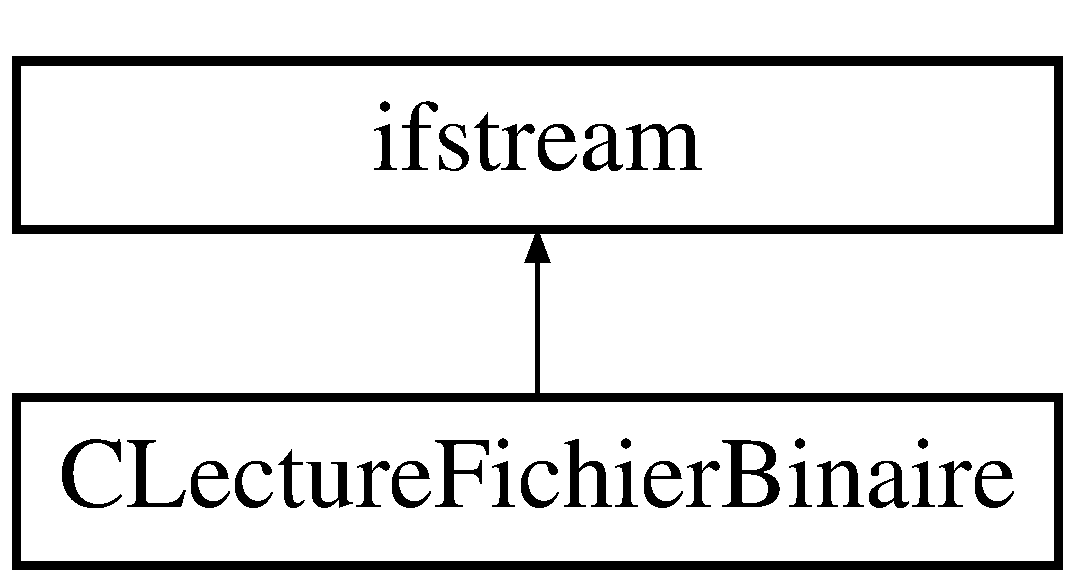
\includegraphics[height=2.000000cm]{class_c_lecture_fichier_binaire}
\end{center}
\end{figure}
\subsection*{Public Member Functions}
\begin{DoxyCompactItemize}
\item 
\hyperlink{group__utilitaire_ga3a259905a2c14513846e6ecb8cf476ad}{C\-Lecture\-Fichier\-Binaire} ()
\begin{DoxyCompactList}\small\item\em Constructeur par defaut. \end{DoxyCompactList}\item 
\hyperlink{group__utilitaire_gac16ebab7b172408c2ba14605f61f0f84}{C\-Lecture\-Fichier\-Binaire} (const char $\ast$nom\-Fichier, openmode \hyperlink{glew_8h_a1e71d9c196e4683cc06c4b54d53f7ef5}{mode}=\hyperlink{glew_8h_a83ad0ee7f1e06b59c90271716e689080}{std\-::ios\-::in}$\vert$\hyperlink{glew_8h_a0ace813ee1f7020974174eb65d53ff0d}{std\-::ios\-::binary})
\begin{DoxyCompactList}\small\item\em Constructeur par parametre. \end{DoxyCompactList}\end{DoxyCompactItemize}
\subsection*{Friends}
\begin{DoxyCompactItemize}
\item 
\hyperlink{class_c_lecture_fichier_binaire}{C\-Lecture\-Fichier\-Binaire} \& \hyperlink{class_c_lecture_fichier_binaire_abc9f4d65dcf682dbf572f5110a00252d}{operator$>$} (\hyperlink{class_c_lecture_fichier_binaire}{C\-Lecture\-Fichier\-Binaire} \&\hyperlink{glew_8h_a83ad0ee7f1e06b59c90271716e689080}{in}, \hyperlink{glew_8h_ae84541b4f3d8e1ea24ec0f466a8c568b}{std\-::string} \&\hyperlink{glew_8h_a4af680a6c683f88ed67b76f207f2e6e4}{s})
\begin{DoxyCompactList}\small\item\em Surcharge de l'operateur pour le type {\itshape std\-::string}. \end{DoxyCompactList}\item 
\hyperlink{class_c_lecture_fichier_binaire}{C\-Lecture\-Fichier\-Binaire} \& \hyperlink{class_c_lecture_fichier_binaire_a8b4123b210cccf9da0d2eb60dc19b8a0}{operator$>$} (\hyperlink{class_c_lecture_fichier_binaire}{C\-Lecture\-Fichier\-Binaire} \&\hyperlink{glew_8h_a83ad0ee7f1e06b59c90271716e689080}{in}, double \&\hyperlink{glew_8h_a691492ec0bd6383f91200e49f6ae40ed}{f})
\begin{DoxyCompactList}\small\item\em Surcharge de l'operateur pour le type {\itshape double}. \end{DoxyCompactList}\item 
\hyperlink{class_c_lecture_fichier_binaire}{C\-Lecture\-Fichier\-Binaire} \& \hyperlink{class_c_lecture_fichier_binaire_a8727572665715de99f2908c711e45114}{operator$>$} (\hyperlink{class_c_lecture_fichier_binaire}{C\-Lecture\-Fichier\-Binaire} \&\hyperlink{glew_8h_a83ad0ee7f1e06b59c90271716e689080}{in}, \hyperlink{fmod_8h_aeb841aa4b4b5f444b5d739d865b420af}{float} \&\hyperlink{glew_8h_a691492ec0bd6383f91200e49f6ae40ed}{f})
\begin{DoxyCompactList}\small\item\em Surcharge de l'operateur pour le type {\itshape float}. \end{DoxyCompactList}\item 
\hyperlink{class_c_lecture_fichier_binaire}{C\-Lecture\-Fichier\-Binaire} \& \hyperlink{class_c_lecture_fichier_binaire_a327898e8bcb11d00bdb07e3e8bd361bd}{operator$>$} (\hyperlink{class_c_lecture_fichier_binaire}{C\-Lecture\-Fichier\-Binaire} \&\hyperlink{glew_8h_a83ad0ee7f1e06b59c90271716e689080}{in}, \hyperlink{wglew_8h_a500a82aecba06f4550f6849b8099ca21}{int} \&\hyperlink{glew_8h_a691492ec0bd6383f91200e49f6ae40ed}{f})
\begin{DoxyCompactList}\small\item\em Surcharge de l'operateur pour le type {\itshape int}. \end{DoxyCompactList}\item 
\hyperlink{class_c_lecture_fichier_binaire}{C\-Lecture\-Fichier\-Binaire} \& \hyperlink{class_c_lecture_fichier_binaire_a10555985d21e9277fd610554eb804ad4}{operator$>$} (\hyperlink{class_c_lecture_fichier_binaire}{C\-Lecture\-Fichier\-Binaire} \&\hyperlink{glew_8h_a83ad0ee7f1e06b59c90271716e689080}{in}, \hyperlink{_free_image_8h_a425076c7067a1b5166e2cc530e914814}{unsigned} \hyperlink{wglew_8h_a500a82aecba06f4550f6849b8099ca21}{int} \&\hyperlink{glew_8h_a691492ec0bd6383f91200e49f6ae40ed}{f})
\begin{DoxyCompactList}\small\item\em Surcharge de l'operateur pour le type {\itshape unsigned} {\itshape int}. \end{DoxyCompactList}\item 
\hyperlink{class_c_lecture_fichier_binaire}{C\-Lecture\-Fichier\-Binaire} \& \hyperlink{class_c_lecture_fichier_binaire_a4a3ac4fa35e1f11664f6612d554d72bd}{operator$>$} (\hyperlink{class_c_lecture_fichier_binaire}{C\-Lecture\-Fichier\-Binaire} \&\hyperlink{glew_8h_a83ad0ee7f1e06b59c90271716e689080}{in}, char \&\hyperlink{glew_8h_a691492ec0bd6383f91200e49f6ae40ed}{f})
\begin{DoxyCompactList}\small\item\em Surcharge de l'operateur pour le type {\itshape char}. \end{DoxyCompactList}\item 
\hyperlink{class_c_lecture_fichier_binaire}{C\-Lecture\-Fichier\-Binaire} \& \hyperlink{class_c_lecture_fichier_binaire_aaf7fbfa5e060c1e9015b0ffbd013f3e3}{operator$>$} (\hyperlink{class_c_lecture_fichier_binaire}{C\-Lecture\-Fichier\-Binaire} \&\hyperlink{glew_8h_a83ad0ee7f1e06b59c90271716e689080}{in}, bool \&\hyperlink{glew_8h_a691492ec0bd6383f91200e49f6ae40ed}{f})
\begin{DoxyCompactList}\small\item\em Surcharge de l'operateur pour le type {\itshape bool}. \end{DoxyCompactList}\end{DoxyCompactItemize}


\subsection{Detailed Description}
cette classe contient des methodes $>$ permettant de lire dans un fichier binaire des variables de types string, double, float, int, unsigned int, char, et bool. 

\begin{DoxyAuthor}{Author}
D\-G\-I-\/2990 
\end{DoxyAuthor}
\begin{DoxyDate}{Date}
2005-\/10-\/15 
\end{DoxyDate}


\subsection{Friends And Related Function Documentation}
\hypertarget{class_c_lecture_fichier_binaire_abc9f4d65dcf682dbf572f5110a00252d}{\index{C\-Lecture\-Fichier\-Binaire@{C\-Lecture\-Fichier\-Binaire}!operator$>$@{operator$>$}}
\index{operator$>$@{operator$>$}!CLectureFichierBinaire@{C\-Lecture\-Fichier\-Binaire}}
\subsubsection[{operator$>$}]{\setlength{\rightskip}{0pt plus 5cm}{\bf C\-Lecture\-Fichier\-Binaire}\& operator$>$ (
\begin{DoxyParamCaption}
\item[{{\bf C\-Lecture\-Fichier\-Binaire} \&}]{in, }
\item[{{\bf std\-::string} \&}]{s}
\end{DoxyParamCaption}
)\hspace{0.3cm}{\ttfamily [friend]}}}\label{class_c_lecture_fichier_binaire_abc9f4d65dcf682dbf572f5110a00252d}


Surcharge de l'operateur pour le type {\itshape std\-::string}. 

\hypertarget{class_c_lecture_fichier_binaire_a8b4123b210cccf9da0d2eb60dc19b8a0}{\index{C\-Lecture\-Fichier\-Binaire@{C\-Lecture\-Fichier\-Binaire}!operator$>$@{operator$>$}}
\index{operator$>$@{operator$>$}!CLectureFichierBinaire@{C\-Lecture\-Fichier\-Binaire}}
\subsubsection[{operator$>$}]{\setlength{\rightskip}{0pt plus 5cm}{\bf C\-Lecture\-Fichier\-Binaire}\& operator$>$ (
\begin{DoxyParamCaption}
\item[{{\bf C\-Lecture\-Fichier\-Binaire} \&}]{in, }
\item[{double \&}]{f}
\end{DoxyParamCaption}
)\hspace{0.3cm}{\ttfamily [friend]}}}\label{class_c_lecture_fichier_binaire_a8b4123b210cccf9da0d2eb60dc19b8a0}


Surcharge de l'operateur pour le type {\itshape double}. 

\hypertarget{class_c_lecture_fichier_binaire_a8727572665715de99f2908c711e45114}{\index{C\-Lecture\-Fichier\-Binaire@{C\-Lecture\-Fichier\-Binaire}!operator$>$@{operator$>$}}
\index{operator$>$@{operator$>$}!CLectureFichierBinaire@{C\-Lecture\-Fichier\-Binaire}}
\subsubsection[{operator$>$}]{\setlength{\rightskip}{0pt plus 5cm}{\bf C\-Lecture\-Fichier\-Binaire}\& operator$>$ (
\begin{DoxyParamCaption}
\item[{{\bf C\-Lecture\-Fichier\-Binaire} \&}]{in, }
\item[{{\bf float} \&}]{f}
\end{DoxyParamCaption}
)\hspace{0.3cm}{\ttfamily [friend]}}}\label{class_c_lecture_fichier_binaire_a8727572665715de99f2908c711e45114}


Surcharge de l'operateur pour le type {\itshape float}. 

\hypertarget{class_c_lecture_fichier_binaire_a327898e8bcb11d00bdb07e3e8bd361bd}{\index{C\-Lecture\-Fichier\-Binaire@{C\-Lecture\-Fichier\-Binaire}!operator$>$@{operator$>$}}
\index{operator$>$@{operator$>$}!CLectureFichierBinaire@{C\-Lecture\-Fichier\-Binaire}}
\subsubsection[{operator$>$}]{\setlength{\rightskip}{0pt plus 5cm}{\bf C\-Lecture\-Fichier\-Binaire}\& operator$>$ (
\begin{DoxyParamCaption}
\item[{{\bf C\-Lecture\-Fichier\-Binaire} \&}]{in, }
\item[{{\bf int} \&}]{f}
\end{DoxyParamCaption}
)\hspace{0.3cm}{\ttfamily [friend]}}}\label{class_c_lecture_fichier_binaire_a327898e8bcb11d00bdb07e3e8bd361bd}


Surcharge de l'operateur pour le type {\itshape int}. 

\hypertarget{class_c_lecture_fichier_binaire_a10555985d21e9277fd610554eb804ad4}{\index{C\-Lecture\-Fichier\-Binaire@{C\-Lecture\-Fichier\-Binaire}!operator$>$@{operator$>$}}
\index{operator$>$@{operator$>$}!CLectureFichierBinaire@{C\-Lecture\-Fichier\-Binaire}}
\subsubsection[{operator$>$}]{\setlength{\rightskip}{0pt plus 5cm}{\bf C\-Lecture\-Fichier\-Binaire}\& operator$>$ (
\begin{DoxyParamCaption}
\item[{{\bf C\-Lecture\-Fichier\-Binaire} \&}]{in, }
\item[{{\bf unsigned} {\bf int} \&}]{f}
\end{DoxyParamCaption}
)\hspace{0.3cm}{\ttfamily [friend]}}}\label{class_c_lecture_fichier_binaire_a10555985d21e9277fd610554eb804ad4}


Surcharge de l'operateur pour le type {\itshape unsigned} {\itshape int}. 

\hypertarget{class_c_lecture_fichier_binaire_a4a3ac4fa35e1f11664f6612d554d72bd}{\index{C\-Lecture\-Fichier\-Binaire@{C\-Lecture\-Fichier\-Binaire}!operator$>$@{operator$>$}}
\index{operator$>$@{operator$>$}!CLectureFichierBinaire@{C\-Lecture\-Fichier\-Binaire}}
\subsubsection[{operator$>$}]{\setlength{\rightskip}{0pt plus 5cm}{\bf C\-Lecture\-Fichier\-Binaire}\& operator$>$ (
\begin{DoxyParamCaption}
\item[{{\bf C\-Lecture\-Fichier\-Binaire} \&}]{in, }
\item[{char \&}]{f}
\end{DoxyParamCaption}
)\hspace{0.3cm}{\ttfamily [friend]}}}\label{class_c_lecture_fichier_binaire_a4a3ac4fa35e1f11664f6612d554d72bd}


Surcharge de l'operateur pour le type {\itshape char}. 

\hypertarget{class_c_lecture_fichier_binaire_aaf7fbfa5e060c1e9015b0ffbd013f3e3}{\index{C\-Lecture\-Fichier\-Binaire@{C\-Lecture\-Fichier\-Binaire}!operator$>$@{operator$>$}}
\index{operator$>$@{operator$>$}!CLectureFichierBinaire@{C\-Lecture\-Fichier\-Binaire}}
\subsubsection[{operator$>$}]{\setlength{\rightskip}{0pt plus 5cm}{\bf C\-Lecture\-Fichier\-Binaire}\& operator$>$ (
\begin{DoxyParamCaption}
\item[{{\bf C\-Lecture\-Fichier\-Binaire} \&}]{in, }
\item[{bool \&}]{f}
\end{DoxyParamCaption}
)\hspace{0.3cm}{\ttfamily [friend]}}}\label{class_c_lecture_fichier_binaire_aaf7fbfa5e060c1e9015b0ffbd013f3e3}


Surcharge de l'operateur pour le type {\itshape bool}. 



The documentation for this class was generated from the following files\-:\begin{DoxyCompactItemize}
\item 
Cadriciel/\-Commun/\-Utilitaire/\hyperlink{_c_lecture_fichier_binaire_8h}{C\-Lecture\-Fichier\-Binaire.\-h}\item 
Cadriciel/\-Commun/\-Utilitaire/\hyperlink{_c_lecture_fichier_binaire_8cpp}{C\-Lecture\-Fichier\-Binaire.\-cpp}\end{DoxyCompactItemize}

\hypertarget{class_commande_ajout_accelerateur}{\section{Commande\-Ajout\-Accelerateur Class Reference}
\label{class_commande_ajout_accelerateur}\index{Commande\-Ajout\-Accelerateur@{Commande\-Ajout\-Accelerateur}}
}


La classe \hyperlink{class_commande_ajout_accelerateur}{Commande\-Ajout\-Accelerateur} permet d'ajouter un objet sur la carte.  




{\ttfamily \#include $<$Commande\-Ajout\-Accelerateur.\-h$>$}

Inheritance diagram for Commande\-Ajout\-Accelerateur\-:\begin{figure}[H]
\begin{center}
\leavevmode
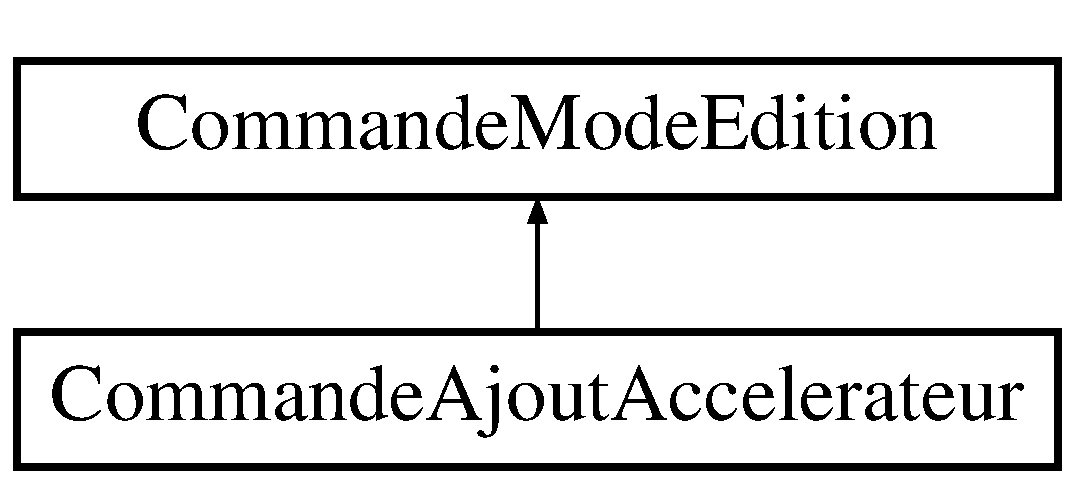
\includegraphics[height=2.000000cm]{class_commande_ajout_accelerateur}
\end{center}
\end{figure}
\subsection*{Public Member Functions}
\begin{DoxyCompactItemize}
\item 
\hyperlink{class_commande_ajout_accelerateur_a5deaad7144cbe48061677b59a8fca95c}{Commande\-Ajout\-Accelerateur} (const \hyperlink{classvue_1_1_vue}{vue\-::\-Vue} \&vue, \hyperlink{class_carte}{Carte} \&carte)
\item 
virtual \hyperlink{class_commande_ajout_accelerateur_ae5ecf61850b7ef9e3a482fc9baaaf3b1}{$\sim$\-Commande\-Ajout\-Accelerateur} ()
\item 
virtual void \hyperlink{class_commande_ajout_accelerateur_a1537ffad37fa05fa20cdbd414890adb3}{executer} (int mouse\-X, int mouse\-Y, int boutton, int touche)
\end{DoxyCompactItemize}
\subsection*{Additional Inherited Members}


\subsection{Detailed Description}
La classe \hyperlink{class_commande_ajout_accelerateur}{Commande\-Ajout\-Accelerateur} permet d'ajouter un objet sur la carte. 

\subsection{Constructor \& Destructor Documentation}
\hypertarget{class_commande_ajout_accelerateur_a5deaad7144cbe48061677b59a8fca95c}{\index{Commande\-Ajout\-Accelerateur@{Commande\-Ajout\-Accelerateur}!Commande\-Ajout\-Accelerateur@{Commande\-Ajout\-Accelerateur}}
\index{Commande\-Ajout\-Accelerateur@{Commande\-Ajout\-Accelerateur}!CommandeAjoutAccelerateur@{Commande\-Ajout\-Accelerateur}}
\subsubsection[{Commande\-Ajout\-Accelerateur}]{\setlength{\rightskip}{0pt plus 5cm}Commande\-Ajout\-Accelerateur\-::\-Commande\-Ajout\-Accelerateur (
\begin{DoxyParamCaption}
\item[{const {\bf vue\-::\-Vue} \&}]{vue, }
\item[{{\bf Carte} \&}]{carte}
\end{DoxyParamCaption}
)}}\label{class_commande_ajout_accelerateur_a5deaad7144cbe48061677b59a8fca95c}
Constructeur 
\begin{DoxyParams}{Parameters}
{\em vue} & La vue du jeu. Utilise pour transformer les points de l'ecran dans l'espace de la camera \\
\hline
{\em carte} & La carte sur laquelle ajouter l'objet. \\
\hline
\end{DoxyParams}
\hypertarget{class_commande_ajout_accelerateur_ae5ecf61850b7ef9e3a482fc9baaaf3b1}{\index{Commande\-Ajout\-Accelerateur@{Commande\-Ajout\-Accelerateur}!$\sim$\-Commande\-Ajout\-Accelerateur@{$\sim$\-Commande\-Ajout\-Accelerateur}}
\index{$\sim$\-Commande\-Ajout\-Accelerateur@{$\sim$\-Commande\-Ajout\-Accelerateur}!CommandeAjoutAccelerateur@{Commande\-Ajout\-Accelerateur}}
\subsubsection[{$\sim$\-Commande\-Ajout\-Accelerateur}]{\setlength{\rightskip}{0pt plus 5cm}Commande\-Ajout\-Accelerateur\-::$\sim$\-Commande\-Ajout\-Accelerateur (
\begin{DoxyParamCaption}
{}
\end{DoxyParamCaption}
)\hspace{0.3cm}{\ttfamily [virtual]}}}\label{class_commande_ajout_accelerateur_ae5ecf61850b7ef9e3a482fc9baaaf3b1}
Destructeur 

\subsection{Member Function Documentation}
\hypertarget{class_commande_ajout_accelerateur_a1537ffad37fa05fa20cdbd414890adb3}{\index{Commande\-Ajout\-Accelerateur@{Commande\-Ajout\-Accelerateur}!executer@{executer}}
\index{executer@{executer}!CommandeAjoutAccelerateur@{Commande\-Ajout\-Accelerateur}}
\subsubsection[{executer}]{\setlength{\rightskip}{0pt plus 5cm}void Commande\-Ajout\-Accelerateur\-::executer (
\begin{DoxyParamCaption}
\item[{int}]{mouse\-X, }
\item[{int}]{mouse\-Y, }
\item[{int}]{boutton, }
\item[{int}]{touche}
\end{DoxyParamCaption}
)\hspace{0.3cm}{\ttfamily [virtual]}}}\label{class_commande_ajout_accelerateur_a1537ffad37fa05fa20cdbd414890adb3}
Execute la commande. Ajoute un nouvel objet a la position souhaite sur la carte. 
\begin{DoxyParams}{Parameters}
{\em mouse\-X} & La position X de la souris \\
\hline
{\em mouse\-Y} & La position Y de la souris \\
\hline
{\em bouton} & L'etat des boutons de la souris \\
\hline
{\em touche} & Touche du clavier appuyee \\
\hline
\end{DoxyParams}


Implements \hyperlink{class_commande_mode_edition_aca77e9bb8557971af33748041975eecb}{Commande\-Mode\-Edition}.



The documentation for this class was generated from the following files\-:\begin{DoxyCompactItemize}
\item 
Cadriciel/\-Sources/\-C++/\-Application/\-Jeu/\-Mode\-Edition/\hyperlink{_commande_ajout_accelerateur_8h}{Commande\-Ajout\-Accelerateur.\-h}\item 
Cadriciel/\-Sources/\-C++/\-Application/\-Jeu/\-Mode\-Edition/Commande\-Ajout\-Accelerateur.\-cpp\end{DoxyCompactItemize}

\hypertarget{class_commande_ajout_barriere}{\section{Commande\-Ajout\-Barriere Class Reference}
\label{class_commande_ajout_barriere}\index{Commande\-Ajout\-Barriere@{Commande\-Ajout\-Barriere}}
}


La classe Commande\-Ajout permet d'ajouter une barriere sur la carte.  




{\ttfamily \#include $<$Commande\-Ajout\-Barriere.\-h$>$}

Inheritance diagram for Commande\-Ajout\-Barriere\-:\begin{figure}[H]
\begin{center}
\leavevmode
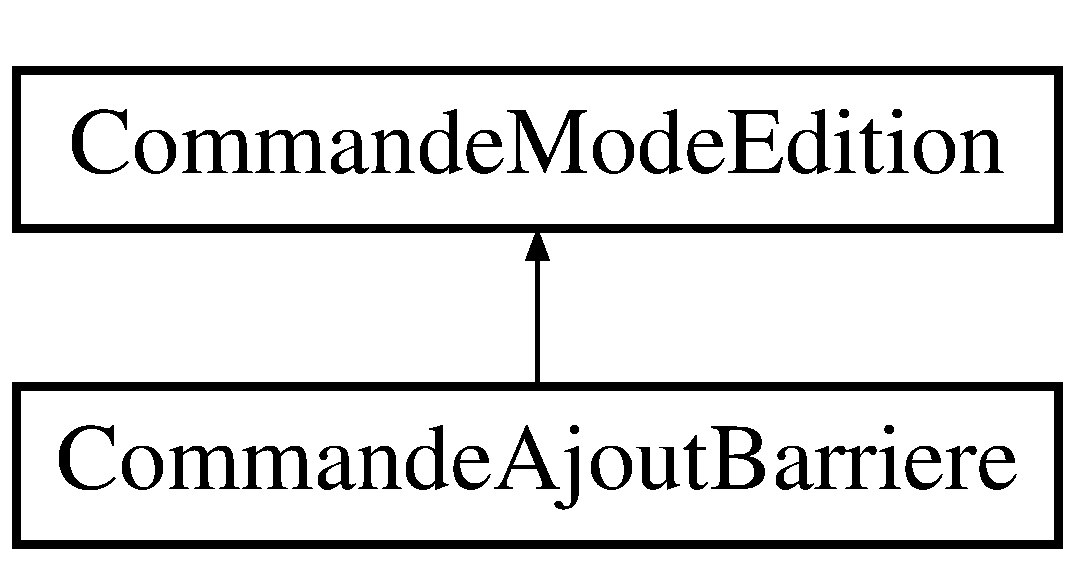
\includegraphics[height=2.000000cm]{class_commande_ajout_barriere}
\end{center}
\end{figure}
\subsection*{Public Member Functions}
\begin{DoxyCompactItemize}
\item 
\hyperlink{class_commande_ajout_barriere_a97062e0aa94ec0c70d6e66050d835988}{Commande\-Ajout\-Barriere} (const \hyperlink{classvue_1_1_vue}{vue\-::\-Vue} \&vue, \hyperlink{class_carte}{Carte} \&carte)
\item 
virtual \hyperlink{class_commande_ajout_barriere_acd8fbb39e8062e5cc4959493c7ea3717}{$\sim$\-Commande\-Ajout\-Barriere} ()
\item 
virtual void \hyperlink{class_commande_ajout_barriere_a23c6176e97b56fed95b2e02b37515290}{executer} (int mouse\-X, int mouse\-Y, int boutton, int touche)
\end{DoxyCompactItemize}
\subsection*{Additional Inherited Members}


\subsection{Detailed Description}
La classe Commande\-Ajout permet d'ajouter une barriere sur la carte. 

\subsection{Constructor \& Destructor Documentation}
\hypertarget{class_commande_ajout_barriere_a97062e0aa94ec0c70d6e66050d835988}{\index{Commande\-Ajout\-Barriere@{Commande\-Ajout\-Barriere}!Commande\-Ajout\-Barriere@{Commande\-Ajout\-Barriere}}
\index{Commande\-Ajout\-Barriere@{Commande\-Ajout\-Barriere}!CommandeAjoutBarriere@{Commande\-Ajout\-Barriere}}
\subsubsection[{Commande\-Ajout\-Barriere}]{\setlength{\rightskip}{0pt plus 5cm}Commande\-Ajout\-Barriere\-::\-Commande\-Ajout\-Barriere (
\begin{DoxyParamCaption}
\item[{const {\bf vue\-::\-Vue} \&}]{vue, }
\item[{{\bf Carte} \&}]{carte}
\end{DoxyParamCaption}
)}}\label{class_commande_ajout_barriere_a97062e0aa94ec0c70d6e66050d835988}
Constructeur 
\begin{DoxyParams}{Parameters}
{\em vue} & La vue du jeu. Utilise pour transformer les points de l'ecran dans l'espace de la camera \\
\hline
{\em carte} & La carte sur laquelle ajouter l'objet. \\
\hline
\end{DoxyParams}
\hypertarget{class_commande_ajout_barriere_acd8fbb39e8062e5cc4959493c7ea3717}{\index{Commande\-Ajout\-Barriere@{Commande\-Ajout\-Barriere}!$\sim$\-Commande\-Ajout\-Barriere@{$\sim$\-Commande\-Ajout\-Barriere}}
\index{$\sim$\-Commande\-Ajout\-Barriere@{$\sim$\-Commande\-Ajout\-Barriere}!CommandeAjoutBarriere@{Commande\-Ajout\-Barriere}}
\subsubsection[{$\sim$\-Commande\-Ajout\-Barriere}]{\setlength{\rightskip}{0pt plus 5cm}Commande\-Ajout\-Barriere\-::$\sim$\-Commande\-Ajout\-Barriere (
\begin{DoxyParamCaption}
{}
\end{DoxyParamCaption}
)\hspace{0.3cm}{\ttfamily [virtual]}}}\label{class_commande_ajout_barriere_acd8fbb39e8062e5cc4959493c7ea3717}
Destructeur 

\subsection{Member Function Documentation}
\hypertarget{class_commande_ajout_barriere_a23c6176e97b56fed95b2e02b37515290}{\index{Commande\-Ajout\-Barriere@{Commande\-Ajout\-Barriere}!executer@{executer}}
\index{executer@{executer}!CommandeAjoutBarriere@{Commande\-Ajout\-Barriere}}
\subsubsection[{executer}]{\setlength{\rightskip}{0pt plus 5cm}void Commande\-Ajout\-Barriere\-::executer (
\begin{DoxyParamCaption}
\item[{int}]{mouse\-X, }
\item[{int}]{mouse\-Y, }
\item[{int}]{boutton, }
\item[{int}]{touche}
\end{DoxyParamCaption}
)\hspace{0.3cm}{\ttfamily [virtual]}}}\label{class_commande_ajout_barriere_a23c6176e97b56fed95b2e02b37515290}
Execute la commande. Ajoute un nouvel objet a la position souhaite sur la carte. 
\begin{DoxyParams}{Parameters}
{\em mouse\-X} & La position X de la souris \\
\hline
{\em mouse\-Y} & La position Y de la souris \\
\hline
{\em bouton} & L'etat des boutons de la souris \\
\hline
{\em touche} & Touche du clavier appuyee \\
\hline
\end{DoxyParams}


Implements \hyperlink{class_commande_mode_edition_aca77e9bb8557971af33748041975eecb}{Commande\-Mode\-Edition}.



The documentation for this class was generated from the following files\-:\begin{DoxyCompactItemize}
\item 
Cadriciel/\-Sources/\-C++/\-Application/\-Jeu/\-Mode\-Edition/\hyperlink{_commande_ajout_barriere_8h}{Commande\-Ajout\-Barriere.\-h}\item 
Cadriciel/\-Sources/\-C++/\-Application/\-Jeu/\-Mode\-Edition/Commande\-Ajout\-Barriere.\-cpp\end{DoxyCompactItemize}

\hypertarget{class_commande_ajout_portail}{\section{Commande\-Ajout\-Portail Class Reference}
\label{class_commande_ajout_portail}\index{Commande\-Ajout\-Portail@{Commande\-Ajout\-Portail}}
}


La classe Commande\-Ajout permet d'ajouter un portail sur la carte.  




{\ttfamily \#include $<$Commande\-Ajout\-Portail.\-h$>$}

Inheritance diagram for Commande\-Ajout\-Portail\-:\begin{figure}[H]
\begin{center}
\leavevmode
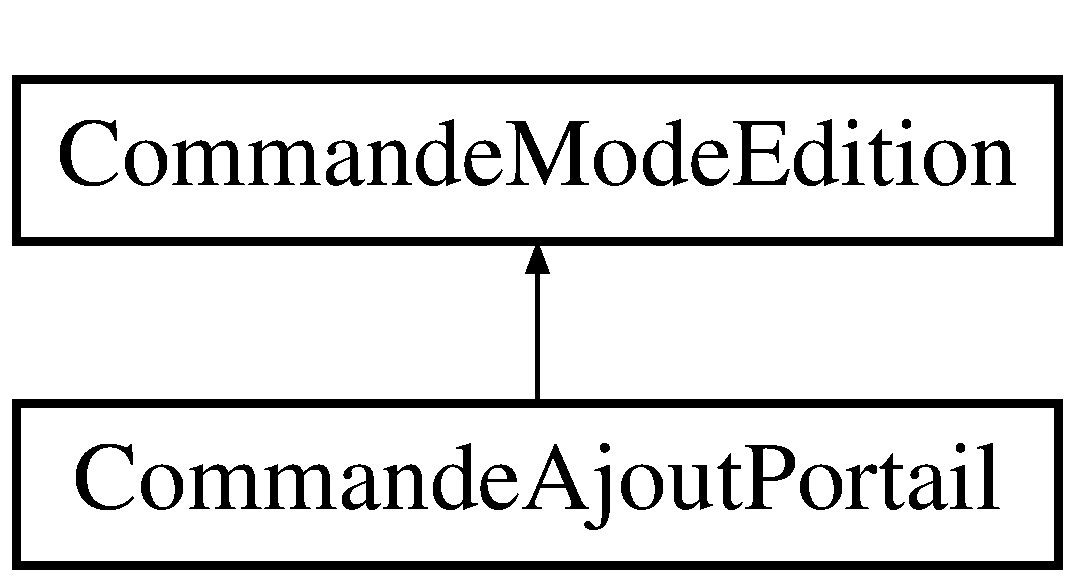
\includegraphics[height=2.000000cm]{class_commande_ajout_portail}
\end{center}
\end{figure}
\subsection*{Public Member Functions}
\begin{DoxyCompactItemize}
\item 
\hyperlink{class_commande_ajout_portail_a9bb23c57a5e651761ef1f2942c8beb34}{Commande\-Ajout\-Portail} (const \hyperlink{classvue_1_1_vue}{vue\-::\-Vue} \&vue, \hyperlink{class_carte}{Carte} \&carte)
\item 
virtual \hyperlink{class_commande_ajout_portail_aa146f3ca92f445cba4770a586a29c163}{$\sim$\-Commande\-Ajout\-Portail} ()
\item 
virtual \hyperlink{wglew_8h_aeea6e3dfae3acf232096f57d2d57f084}{void} \hyperlink{class_commande_ajout_portail_a1b5ac4fd38f34e785aa61a3ce6fd5702}{executer} (\hyperlink{wglew_8h_a500a82aecba06f4550f6849b8099ca21}{int} mouse\-X, \hyperlink{wglew_8h_a500a82aecba06f4550f6849b8099ca21}{int} mouse\-Y, \hyperlink{wglew_8h_a500a82aecba06f4550f6849b8099ca21}{int} boutton, \hyperlink{wglew_8h_a500a82aecba06f4550f6849b8099ca21}{int} touche)
\end{DoxyCompactItemize}
\subsection*{Additional Inherited Members}


\subsection{Detailed Description}
La classe Commande\-Ajout permet d'ajouter un portail sur la carte. 

\subsection{Constructor \& Destructor Documentation}
\hypertarget{class_commande_ajout_portail_a9bb23c57a5e651761ef1f2942c8beb34}{\index{Commande\-Ajout\-Portail@{Commande\-Ajout\-Portail}!Commande\-Ajout\-Portail@{Commande\-Ajout\-Portail}}
\index{Commande\-Ajout\-Portail@{Commande\-Ajout\-Portail}!CommandeAjoutPortail@{Commande\-Ajout\-Portail}}
\subsubsection[{Commande\-Ajout\-Portail}]{\setlength{\rightskip}{0pt plus 5cm}Commande\-Ajout\-Portail\-::\-Commande\-Ajout\-Portail (
\begin{DoxyParamCaption}
\item[{const {\bf vue\-::\-Vue} \&}]{vue, }
\item[{{\bf Carte} \&}]{carte}
\end{DoxyParamCaption}
)}}\label{class_commande_ajout_portail_a9bb23c57a5e651761ef1f2942c8beb34}
Constructeur 
\begin{DoxyParams}{Parameters}
{\em vue} & La vue du jeu. Utilise pour transformer les points de l'ecran dans l'espace de la camera \\
\hline
{\em carte} & La carte sur laquelle ajouter l'objet. \\
\hline
\end{DoxyParams}
\hypertarget{class_commande_ajout_portail_aa146f3ca92f445cba4770a586a29c163}{\index{Commande\-Ajout\-Portail@{Commande\-Ajout\-Portail}!$\sim$\-Commande\-Ajout\-Portail@{$\sim$\-Commande\-Ajout\-Portail}}
\index{$\sim$\-Commande\-Ajout\-Portail@{$\sim$\-Commande\-Ajout\-Portail}!CommandeAjoutPortail@{Commande\-Ajout\-Portail}}
\subsubsection[{$\sim$\-Commande\-Ajout\-Portail}]{\setlength{\rightskip}{0pt plus 5cm}Commande\-Ajout\-Portail\-::$\sim$\-Commande\-Ajout\-Portail (
\begin{DoxyParamCaption}
{}
\end{DoxyParamCaption}
)\hspace{0.3cm}{\ttfamily [virtual]}}}\label{class_commande_ajout_portail_aa146f3ca92f445cba4770a586a29c163}
Destructeur 

\subsection{Member Function Documentation}
\hypertarget{class_commande_ajout_portail_a1b5ac4fd38f34e785aa61a3ce6fd5702}{\index{Commande\-Ajout\-Portail@{Commande\-Ajout\-Portail}!executer@{executer}}
\index{executer@{executer}!CommandeAjoutPortail@{Commande\-Ajout\-Portail}}
\subsubsection[{executer}]{\setlength{\rightskip}{0pt plus 5cm}{\bf void} Commande\-Ajout\-Portail\-::executer (
\begin{DoxyParamCaption}
\item[{{\bf int}}]{mouse\-X, }
\item[{{\bf int}}]{mouse\-Y, }
\item[{{\bf int}}]{boutton, }
\item[{{\bf int}}]{touche}
\end{DoxyParamCaption}
)\hspace{0.3cm}{\ttfamily [virtual]}}}\label{class_commande_ajout_portail_a1b5ac4fd38f34e785aa61a3ce6fd5702}
Execute la commande. Ajoute un nouvel objet a la position souhaite sur la carte. 
\begin{DoxyParams}{Parameters}
{\em mouse\-X} & La position X de la souris \\
\hline
{\em mouse\-Y} & La position Y de la souris \\
\hline
{\em bouton} & L'etat des boutons de la souris \\
\hline
{\em touche} & Touche du clavier appuyee \\
\hline
\end{DoxyParams}


Implements \hyperlink{class_commande_mode_edition_aca77e9bb8557971af33748041975eecb}{Commande\-Mode\-Edition}.



The documentation for this class was generated from the following files\-:\begin{DoxyCompactItemize}
\item 
Cadriciel/\-Sources/\-C++/\-Application/\-Jeu/\-Mode\-Edition/\hyperlink{_commande_ajout_portail_8h}{Commande\-Ajout\-Portail.\-h}\item 
Cadriciel/\-Sources/\-C++/\-Application/\-Jeu/\-Mode\-Edition/\hyperlink{_commande_ajout_portail_8cpp}{Commande\-Ajout\-Portail.\-cpp}\end{DoxyCompactItemize}

\hypertarget{class_commande_ajout_station_spatial}{\section{Commande\-Ajout\-Station\-Spatial Class Reference}
\label{class_commande_ajout_station_spatial}\index{Commande\-Ajout\-Station\-Spatial@{Commande\-Ajout\-Station\-Spatial}}
}


La classe Commande\-Ajout permet d'ajouter une station spatial sur la carte.  




{\ttfamily \#include $<$Commande\-Ajout\-Station\-Spatial.\-h$>$}

Inheritance diagram for Commande\-Ajout\-Station\-Spatial\-:\begin{figure}[H]
\begin{center}
\leavevmode
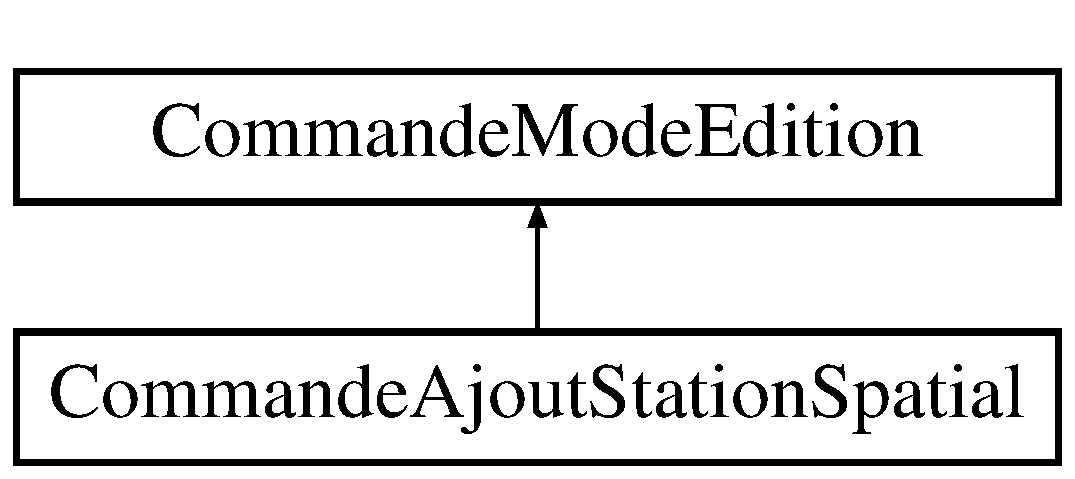
\includegraphics[height=2.000000cm]{class_commande_ajout_station_spatial}
\end{center}
\end{figure}
\subsection*{Public Member Functions}
\begin{DoxyCompactItemize}
\item 
\hyperlink{class_commande_ajout_station_spatial_ac827fa45fba577affd3455adede0c426}{Commande\-Ajout\-Station\-Spatial} (const \hyperlink{classvue_1_1_vue}{vue\-::\-Vue} \&vue, \hyperlink{class_carte}{Carte} \&carte)
\item 
virtual \hyperlink{class_commande_ajout_station_spatial_a41b6a3345606a722dcbec687ab234d9e}{$\sim$\-Commande\-Ajout\-Station\-Spatial} ()
\item 
virtual \hyperlink{wglew_8h_aeea6e3dfae3acf232096f57d2d57f084}{void} \hyperlink{class_commande_ajout_station_spatial_a92ca290ca6ca127e618e3463bf3fe75b}{executer} (\hyperlink{wglew_8h_a500a82aecba06f4550f6849b8099ca21}{int} mouse\-X, \hyperlink{wglew_8h_a500a82aecba06f4550f6849b8099ca21}{int} mouse\-Y, \hyperlink{wglew_8h_a500a82aecba06f4550f6849b8099ca21}{int} boutton, \hyperlink{wglew_8h_a500a82aecba06f4550f6849b8099ca21}{int} touche)
\end{DoxyCompactItemize}
\subsection*{Additional Inherited Members}


\subsection{Detailed Description}
La classe Commande\-Ajout permet d'ajouter une station spatial sur la carte. 

\subsection{Constructor \& Destructor Documentation}
\hypertarget{class_commande_ajout_station_spatial_ac827fa45fba577affd3455adede0c426}{\index{Commande\-Ajout\-Station\-Spatial@{Commande\-Ajout\-Station\-Spatial}!Commande\-Ajout\-Station\-Spatial@{Commande\-Ajout\-Station\-Spatial}}
\index{Commande\-Ajout\-Station\-Spatial@{Commande\-Ajout\-Station\-Spatial}!CommandeAjoutStationSpatial@{Commande\-Ajout\-Station\-Spatial}}
\subsubsection[{Commande\-Ajout\-Station\-Spatial}]{\setlength{\rightskip}{0pt plus 5cm}Commande\-Ajout\-Station\-Spatial\-::\-Commande\-Ajout\-Station\-Spatial (
\begin{DoxyParamCaption}
\item[{const {\bf vue\-::\-Vue} \&}]{vue, }
\item[{{\bf Carte} \&}]{carte}
\end{DoxyParamCaption}
)}}\label{class_commande_ajout_station_spatial_ac827fa45fba577affd3455adede0c426}
Constructeur 
\begin{DoxyParams}{Parameters}
{\em vue} & La vue du jeu. Utilise pour transformer les points de l'ecran dans l'espace de la camera \\
\hline
{\em carte} & La carte sur laquelle ajouter l'objet. \\
\hline
\end{DoxyParams}
\hypertarget{class_commande_ajout_station_spatial_a41b6a3345606a722dcbec687ab234d9e}{\index{Commande\-Ajout\-Station\-Spatial@{Commande\-Ajout\-Station\-Spatial}!$\sim$\-Commande\-Ajout\-Station\-Spatial@{$\sim$\-Commande\-Ajout\-Station\-Spatial}}
\index{$\sim$\-Commande\-Ajout\-Station\-Spatial@{$\sim$\-Commande\-Ajout\-Station\-Spatial}!CommandeAjoutStationSpatial@{Commande\-Ajout\-Station\-Spatial}}
\subsubsection[{$\sim$\-Commande\-Ajout\-Station\-Spatial}]{\setlength{\rightskip}{0pt plus 5cm}Commande\-Ajout\-Station\-Spatial\-::$\sim$\-Commande\-Ajout\-Station\-Spatial (
\begin{DoxyParamCaption}
{}
\end{DoxyParamCaption}
)\hspace{0.3cm}{\ttfamily [virtual]}}}\label{class_commande_ajout_station_spatial_a41b6a3345606a722dcbec687ab234d9e}
Destructeur 

\subsection{Member Function Documentation}
\hypertarget{class_commande_ajout_station_spatial_a92ca290ca6ca127e618e3463bf3fe75b}{\index{Commande\-Ajout\-Station\-Spatial@{Commande\-Ajout\-Station\-Spatial}!executer@{executer}}
\index{executer@{executer}!CommandeAjoutStationSpatial@{Commande\-Ajout\-Station\-Spatial}}
\subsubsection[{executer}]{\setlength{\rightskip}{0pt plus 5cm}{\bf void} Commande\-Ajout\-Station\-Spatial\-::executer (
\begin{DoxyParamCaption}
\item[{{\bf int}}]{mouse\-X, }
\item[{{\bf int}}]{mouse\-Y, }
\item[{{\bf int}}]{boutton, }
\item[{{\bf int}}]{touche}
\end{DoxyParamCaption}
)\hspace{0.3cm}{\ttfamily [virtual]}}}\label{class_commande_ajout_station_spatial_a92ca290ca6ca127e618e3463bf3fe75b}
Execute la commande. Ajoute la station spatial a la position souhaite sur la carte. 
\begin{DoxyParams}{Parameters}
{\em mouse\-X} & La position X de la souris \\
\hline
{\em mouse\-Y} & La position Y de la souris \\
\hline
{\em bouton} & L'etat des boutons de la souris \\
\hline
{\em touche} & Touche du clavier appuyee \\
\hline
\end{DoxyParams}


Implements \hyperlink{class_commande_mode_edition_aca77e9bb8557971af33748041975eecb}{Commande\-Mode\-Edition}.



The documentation for this class was generated from the following files\-:\begin{DoxyCompactItemize}
\item 
Cadriciel/\-Sources/\-C++/\-Application/\-Jeu/\-Mode\-Edition/\hyperlink{_commande_ajout_station_spatial_8h}{Commande\-Ajout\-Station\-Spatial.\-h}\item 
Cadriciel/\-Sources/\-C++/\-Application/\-Jeu/\-Mode\-Edition/\hyperlink{_commande_ajout_station_spatial_8cpp}{Commande\-Ajout\-Station\-Spatial.\-cpp}\end{DoxyCompactItemize}

\hypertarget{class_commande_deplacement}{\section{Commande\-Deplacement Class Reference}
\label{class_commande_deplacement}\index{Commande\-Deplacement@{Commande\-Deplacement}}
}


La classe \hyperlink{class_commande_deplacement}{Commande\-Deplacement} permet de modifier la position dans l'espace d'un ou de plusieurs objets selectionnes.  




{\ttfamily \#include $<$Commande\-Deplacement.\-h$>$}

Inheritance diagram for Commande\-Deplacement\-:\begin{figure}[H]
\begin{center}
\leavevmode
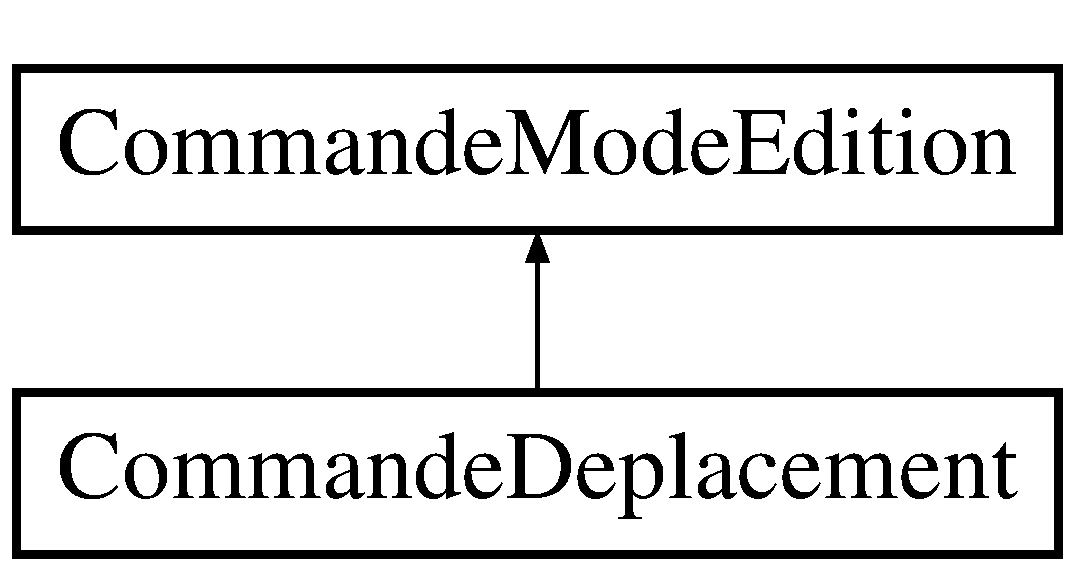
\includegraphics[height=2.000000cm]{class_commande_deplacement}
\end{center}
\end{figure}
\subsection*{Public Member Functions}
\begin{DoxyCompactItemize}
\item 
\hyperlink{class_commande_deplacement_a4a68767331241858637dc60272c11d1e}{Commande\-Deplacement} (const \hyperlink{classvue_1_1_vue}{vue\-::\-Vue} \&vue, \hyperlink{class_carte}{Carte} \&carte, const vector$<$ \hyperlink{class_element_jeu_abstrait}{Element\-Jeu\-Abstrait} $\ast$ $>$ \&objets\-Selectionnes)
\item 
virtual \hyperlink{class_commande_deplacement_af5fcff826a06cb9cf11645c7a551af27}{$\sim$\-Commande\-Deplacement} ()
\item 
virtual \hyperlink{wglew_8h_aeea6e3dfae3acf232096f57d2d57f084}{void} \hyperlink{class_commande_deplacement_a8a591ce694d95d57409f14597d0b1e9c}{executer} (\hyperlink{wglew_8h_a500a82aecba06f4550f6849b8099ca21}{int} mouse\-X, \hyperlink{wglew_8h_a500a82aecba06f4550f6849b8099ca21}{int} mouse\-Y, \hyperlink{wglew_8h_a500a82aecba06f4550f6849b8099ca21}{int} boutton, \hyperlink{wglew_8h_a500a82aecba06f4550f6849b8099ca21}{int} touche)
\end{DoxyCompactItemize}
\subsection*{Additional Inherited Members}


\subsection{Detailed Description}
La classe \hyperlink{class_commande_deplacement}{Commande\-Deplacement} permet de modifier la position dans l'espace d'un ou de plusieurs objets selectionnes. 

\subsection{Constructor \& Destructor Documentation}
\hypertarget{class_commande_deplacement_a4a68767331241858637dc60272c11d1e}{\index{Commande\-Deplacement@{Commande\-Deplacement}!Commande\-Deplacement@{Commande\-Deplacement}}
\index{Commande\-Deplacement@{Commande\-Deplacement}!CommandeDeplacement@{Commande\-Deplacement}}
\subsubsection[{Commande\-Deplacement}]{\setlength{\rightskip}{0pt plus 5cm}Commande\-Deplacement\-::\-Commande\-Deplacement (
\begin{DoxyParamCaption}
\item[{const {\bf vue\-::\-Vue} \&}]{vue, }
\item[{{\bf Carte} \&}]{carte, }
\item[{const vector$<$ {\bf Element\-Jeu\-Abstrait} $\ast$ $>$ \&}]{objets\-Selectionnes}
\end{DoxyParamCaption}
)}}\label{class_commande_deplacement_a4a68767331241858637dc60272c11d1e}
Constructeur 
\begin{DoxyParams}{Parameters}
{\em vue} & La vue du jeu. Utilise pour transformer les points de l'ecran dans l'espace de la camera \\
\hline
{\em carte} & La carte sur laquelle ajouter l'objet. \\
\hline
{\em objets\-Selectionnes} & Une reference vers un vecteur qui contiendra les objets selectionnes \\
\hline
\end{DoxyParams}
\hypertarget{class_commande_deplacement_af5fcff826a06cb9cf11645c7a551af27}{\index{Commande\-Deplacement@{Commande\-Deplacement}!$\sim$\-Commande\-Deplacement@{$\sim$\-Commande\-Deplacement}}
\index{$\sim$\-Commande\-Deplacement@{$\sim$\-Commande\-Deplacement}!CommandeDeplacement@{Commande\-Deplacement}}
\subsubsection[{$\sim$\-Commande\-Deplacement}]{\setlength{\rightskip}{0pt plus 5cm}Commande\-Deplacement\-::$\sim$\-Commande\-Deplacement (
\begin{DoxyParamCaption}
{}
\end{DoxyParamCaption}
)\hspace{0.3cm}{\ttfamily [virtual]}}}\label{class_commande_deplacement_af5fcff826a06cb9cf11645c7a551af27}
Destructeur 

\subsection{Member Function Documentation}
\hypertarget{class_commande_deplacement_a8a591ce694d95d57409f14597d0b1e9c}{\index{Commande\-Deplacement@{Commande\-Deplacement}!executer@{executer}}
\index{executer@{executer}!CommandeDeplacement@{Commande\-Deplacement}}
\subsubsection[{executer}]{\setlength{\rightskip}{0pt plus 5cm}{\bf void} Commande\-Deplacement\-::executer (
\begin{DoxyParamCaption}
\item[{{\bf int}}]{mouse\-X, }
\item[{{\bf int}}]{mouse\-Y, }
\item[{{\bf int}}]{boutton, }
\item[{{\bf int}}]{touche}
\end{DoxyParamCaption}
)\hspace{0.3cm}{\ttfamily [virtual]}}}\label{class_commande_deplacement_a8a591ce694d95d57409f14597d0b1e9c}
Execute la commande. Deplace les objets selectionnes a partir du mouvement de la souris. 
\begin{DoxyParams}{Parameters}
{\em mouse\-X} & La position X de la souris \\
\hline
{\em mouse\-Y} & La position Y de la souris \\
\hline
{\em bouton} & L'etat des boutons de la souris \\
\hline
{\em touche} & Touche du clavier appuyee \\
\hline
\end{DoxyParams}


Implements \hyperlink{class_commande_mode_edition_aca77e9bb8557971af33748041975eecb}{Commande\-Mode\-Edition}.



The documentation for this class was generated from the following files\-:\begin{DoxyCompactItemize}
\item 
Cadriciel/\-Sources/\-C++/\-Application/\-Jeu/\-Mode\-Edition/\hyperlink{_commande_deplacement_8h}{Commande\-Deplacement.\-h}\item 
Cadriciel/\-Sources/\-C++/\-Application/\-Jeu/\-Mode\-Edition/\hyperlink{_commande_deplacement_8cpp}{Commande\-Deplacement.\-cpp}\end{DoxyCompactItemize}

\hypertarget{class_commande_duplication}{\section{Commande\-Duplication Class Reference}
\label{class_commande_duplication}\index{Commande\-Duplication@{Commande\-Duplication}}
}


La classe \hyperlink{class_commande_duplication}{Commande\-Duplication} permet de dupliquer un ou plusieurs objets selectionnes.  




{\ttfamily \#include $<$Commande\-Duplication.\-h$>$}

Inheritance diagram for Commande\-Duplication\-:\begin{figure}[H]
\begin{center}
\leavevmode
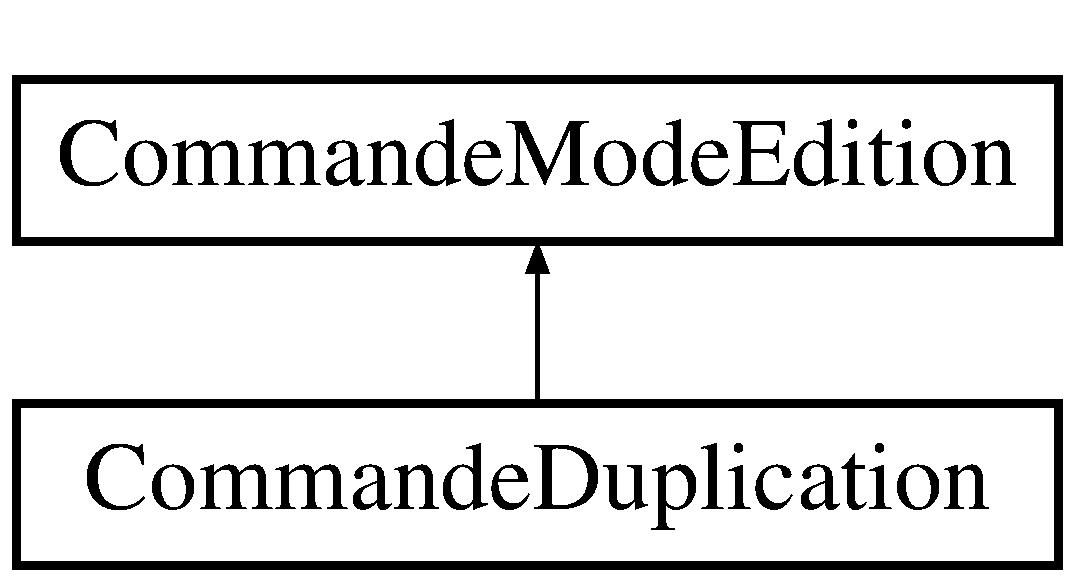
\includegraphics[height=2.000000cm]{class_commande_duplication}
\end{center}
\end{figure}
\subsection*{Public Member Functions}
\begin{DoxyCompactItemize}
\item 
\hyperlink{class_commande_duplication_a789f1ac4650fb772699150a8de40ce91}{Commande\-Duplication} (const \hyperlink{classvue_1_1_vue}{vue\-::\-Vue} \&vue, \hyperlink{class_carte}{Carte} \&carte, const vector$<$ \hyperlink{class_element_jeu_abstrait}{Element\-Jeu\-Abstrait} $\ast$ $>$ \&objets\-Selectionnes)
\item 
virtual \hyperlink{class_commande_duplication_a9690bc3984ecfe34cb8a5d8f15c1fcf4}{$\sim$\-Commande\-Duplication} ()
\item 
virtual void \hyperlink{class_commande_duplication_ab8f7e0df61599b747d80c06548b630a9}{executer} (int mouse\-X, int mouse\-Y, int boutton, int touche)
\end{DoxyCompactItemize}
\subsection*{Friends}
\begin{DoxyCompactItemize}
\item 
\hypertarget{class_commande_duplication_a56556d420bb3ba15607139fbe14fb3ee}{class {\bfseries Commande\-Duplication\-Test}}\label{class_commande_duplication_a56556d420bb3ba15607139fbe14fb3ee}

\end{DoxyCompactItemize}
\subsection*{Additional Inherited Members}


\subsection{Detailed Description}
La classe \hyperlink{class_commande_duplication}{Commande\-Duplication} permet de dupliquer un ou plusieurs objets selectionnes. 

\subsection{Constructor \& Destructor Documentation}
\hypertarget{class_commande_duplication_a789f1ac4650fb772699150a8de40ce91}{\index{Commande\-Duplication@{Commande\-Duplication}!Commande\-Duplication@{Commande\-Duplication}}
\index{Commande\-Duplication@{Commande\-Duplication}!CommandeDuplication@{Commande\-Duplication}}
\subsubsection[{Commande\-Duplication}]{\setlength{\rightskip}{0pt plus 5cm}Commande\-Duplication\-::\-Commande\-Duplication (
\begin{DoxyParamCaption}
\item[{const {\bf vue\-::\-Vue} \&}]{vue, }
\item[{{\bf Carte} \&}]{carte, }
\item[{const vector$<$ {\bf Element\-Jeu\-Abstrait} $\ast$ $>$ \&}]{objets\-Selectionnes}
\end{DoxyParamCaption}
)}}\label{class_commande_duplication_a789f1ac4650fb772699150a8de40ce91}
Constructeur 
\begin{DoxyParams}{Parameters}
{\em vue} & La vue du jeu. Utilise pour transformer les points de l'ecran dans l'espace de la camera \\
\hline
{\em carte} & La carte sur laquelle ajouter l'objet. \\
\hline
{\em objets\-Selectionnes} & Une reference vers un vecteur qui contiendra les objets selectionnes \\
\hline
\end{DoxyParams}
\hypertarget{class_commande_duplication_a9690bc3984ecfe34cb8a5d8f15c1fcf4}{\index{Commande\-Duplication@{Commande\-Duplication}!$\sim$\-Commande\-Duplication@{$\sim$\-Commande\-Duplication}}
\index{$\sim$\-Commande\-Duplication@{$\sim$\-Commande\-Duplication}!CommandeDuplication@{Commande\-Duplication}}
\subsubsection[{$\sim$\-Commande\-Duplication}]{\setlength{\rightskip}{0pt plus 5cm}Commande\-Duplication\-::$\sim$\-Commande\-Duplication (
\begin{DoxyParamCaption}
{}
\end{DoxyParamCaption}
)\hspace{0.3cm}{\ttfamily [virtual]}}}\label{class_commande_duplication_a9690bc3984ecfe34cb8a5d8f15c1fcf4}
Destructeur 

\subsection{Member Function Documentation}
\hypertarget{class_commande_duplication_ab8f7e0df61599b747d80c06548b630a9}{\index{Commande\-Duplication@{Commande\-Duplication}!executer@{executer}}
\index{executer@{executer}!CommandeDuplication@{Commande\-Duplication}}
\subsubsection[{executer}]{\setlength{\rightskip}{0pt plus 5cm}void Commande\-Duplication\-::executer (
\begin{DoxyParamCaption}
\item[{int}]{mouse\-X, }
\item[{int}]{mouse\-Y, }
\item[{int}]{boutton, }
\item[{int}]{touche}
\end{DoxyParamCaption}
)\hspace{0.3cm}{\ttfamily [virtual]}}}\label{class_commande_duplication_ab8f7e0df61599b747d80c06548b630a9}
Execute la commande. Duplique les objets selectionnes et les deplacent a partir du mouvement de la souris. 
\begin{DoxyParams}{Parameters}
{\em mouse\-X} & La position X de la souris \\
\hline
{\em mouse\-Y} & La position Y de la souris \\
\hline
{\em bouton} & L'etat des boutons de la souris \\
\hline
{\em touche} & Touche du clavier appuyee \\
\hline
\end{DoxyParams}


Implements \hyperlink{class_commande_mode_edition_aca77e9bb8557971af33748041975eecb}{Commande\-Mode\-Edition}.



The documentation for this class was generated from the following files\-:\begin{DoxyCompactItemize}
\item 
Cadriciel/\-Sources/\-C++/\-Application/\-Jeu/\-Mode\-Edition/\hyperlink{_commande_duplication_8h}{Commande\-Duplication.\-h}\item 
Cadriciel/\-Sources/\-C++/\-Application/\-Jeu/\-Mode\-Edition/Commande\-Duplication.\-cpp\end{DoxyCompactItemize}

\hypertarget{class_commande_mise_a_echelle}{\section{Commande\-Mise\-A\-Echelle Class Reference}
\label{class_commande_mise_a_echelle}\index{Commande\-Mise\-A\-Echelle@{Commande\-Mise\-A\-Echelle}}
}


La classe \hyperlink{class_commande_mise_a_echelle}{Commande\-Mise\-A\-Echelle} permet de redimensionner un ou plusieurs objets selectionnes.  




{\ttfamily \#include $<$Commande\-Mise\-A\-Echelle.\-h$>$}

Inheritance diagram for Commande\-Mise\-A\-Echelle\-:\begin{figure}[H]
\begin{center}
\leavevmode
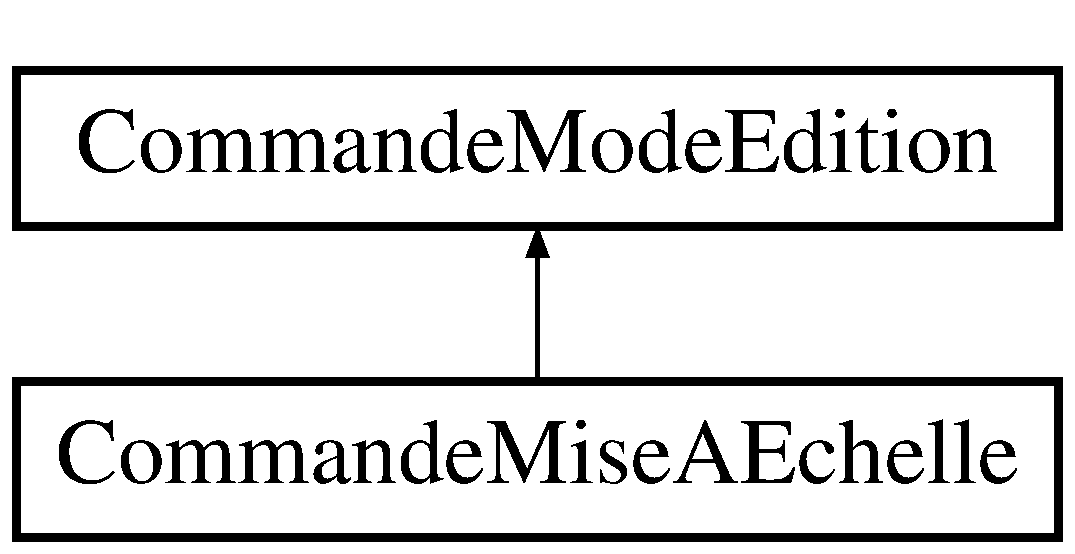
\includegraphics[height=2.000000cm]{class_commande_mise_a_echelle}
\end{center}
\end{figure}
\subsection*{Public Member Functions}
\begin{DoxyCompactItemize}
\item 
\hyperlink{class_commande_mise_a_echelle_a9b855e25dc10ed0893a8de09d305b436}{Commande\-Mise\-A\-Echelle} (const \hyperlink{classvue_1_1_vue}{vue\-::\-Vue} \&vue, \hyperlink{class_carte}{Carte} \&carte, const vector$<$ \hyperlink{class_element_jeu_abstrait}{Element\-Jeu\-Abstrait} $\ast$ $>$ \&objets\-Selectionnes)
\item 
virtual \hyperlink{class_commande_mise_a_echelle_a7cb0c5c9155f30b96ee3b8a82e014fd7}{$\sim$\-Commande\-Mise\-A\-Echelle} ()
\item 
virtual void \hyperlink{class_commande_mise_a_echelle_a03aabe2e5d3a20928b041cfe5595715b}{executer} (int mouse\-X, int mouse\-Y, int boutton, int touche)
\end{DoxyCompactItemize}
\subsection*{Additional Inherited Members}


\subsection{Detailed Description}
La classe \hyperlink{class_commande_mise_a_echelle}{Commande\-Mise\-A\-Echelle} permet de redimensionner un ou plusieurs objets selectionnes. 

\subsection{Constructor \& Destructor Documentation}
\hypertarget{class_commande_mise_a_echelle_a9b855e25dc10ed0893a8de09d305b436}{\index{Commande\-Mise\-A\-Echelle@{Commande\-Mise\-A\-Echelle}!Commande\-Mise\-A\-Echelle@{Commande\-Mise\-A\-Echelle}}
\index{Commande\-Mise\-A\-Echelle@{Commande\-Mise\-A\-Echelle}!CommandeMiseAEchelle@{Commande\-Mise\-A\-Echelle}}
\subsubsection[{Commande\-Mise\-A\-Echelle}]{\setlength{\rightskip}{0pt plus 5cm}Commande\-Mise\-A\-Echelle\-::\-Commande\-Mise\-A\-Echelle (
\begin{DoxyParamCaption}
\item[{const {\bf vue\-::\-Vue} \&}]{vue, }
\item[{{\bf Carte} \&}]{carte, }
\item[{const vector$<$ {\bf Element\-Jeu\-Abstrait} $\ast$ $>$ \&}]{objets\-Selectionnes}
\end{DoxyParamCaption}
)}}\label{class_commande_mise_a_echelle_a9b855e25dc10ed0893a8de09d305b436}
Constructeur 
\begin{DoxyParams}{Parameters}
{\em vue} & La vue du jeu. Utilise pour transformer les points de l'ecran dans l'espace de la camera \\
\hline
{\em carte} & La carte sur laquelle ajouter l'objet. \\
\hline
{\em objets\-Selectionnes} & Une reference vers un vecteur qui contiendra les objets selectionnes \\
\hline
\end{DoxyParams}
\hypertarget{class_commande_mise_a_echelle_a7cb0c5c9155f30b96ee3b8a82e014fd7}{\index{Commande\-Mise\-A\-Echelle@{Commande\-Mise\-A\-Echelle}!$\sim$\-Commande\-Mise\-A\-Echelle@{$\sim$\-Commande\-Mise\-A\-Echelle}}
\index{$\sim$\-Commande\-Mise\-A\-Echelle@{$\sim$\-Commande\-Mise\-A\-Echelle}!CommandeMiseAEchelle@{Commande\-Mise\-A\-Echelle}}
\subsubsection[{$\sim$\-Commande\-Mise\-A\-Echelle}]{\setlength{\rightskip}{0pt plus 5cm}Commande\-Mise\-A\-Echelle\-::$\sim$\-Commande\-Mise\-A\-Echelle (
\begin{DoxyParamCaption}
{}
\end{DoxyParamCaption}
)\hspace{0.3cm}{\ttfamily [virtual]}}}\label{class_commande_mise_a_echelle_a7cb0c5c9155f30b96ee3b8a82e014fd7}
Destructeur 

\subsection{Member Function Documentation}
\hypertarget{class_commande_mise_a_echelle_a03aabe2e5d3a20928b041cfe5595715b}{\index{Commande\-Mise\-A\-Echelle@{Commande\-Mise\-A\-Echelle}!executer@{executer}}
\index{executer@{executer}!CommandeMiseAEchelle@{Commande\-Mise\-A\-Echelle}}
\subsubsection[{executer}]{\setlength{\rightskip}{0pt plus 5cm}void Commande\-Mise\-A\-Echelle\-::executer (
\begin{DoxyParamCaption}
\item[{int}]{mouse\-X, }
\item[{int}]{mouse\-Y, }
\item[{int}]{boutton, }
\item[{int}]{touche}
\end{DoxyParamCaption}
)\hspace{0.3cm}{\ttfamily [virtual]}}}\label{class_commande_mise_a_echelle_a03aabe2e5d3a20928b041cfe5595715b}
Execute la commande. Redimensionne le ou les objets selectionnes a partir du mouvement de la souris. 
\begin{DoxyParams}{Parameters}
{\em mouse\-X} & La position X de la souris \\
\hline
{\em mouse\-Y} & La position Y de la souris \\
\hline
{\em bouton} & L'etat des boutons de la souris \\
\hline
{\em touche} & Touche du clavier appuyee \\
\hline
\end{DoxyParams}


Implements \hyperlink{class_commande_mode_edition_aca77e9bb8557971af33748041975eecb}{Commande\-Mode\-Edition}.



The documentation for this class was generated from the following files\-:\begin{DoxyCompactItemize}
\item 
Cadriciel/\-Sources/\-C++/\-Application/\-Jeu/\-Mode\-Edition/\hyperlink{_commande_mise_a_echelle_8h}{Commande\-Mise\-A\-Echelle.\-h}\item 
Cadriciel/\-Sources/\-C++/\-Application/\-Jeu/\-Mode\-Edition/Commande\-Mise\-A\-Echelle.\-cpp\end{DoxyCompactItemize}

\hypertarget{class_commande_mode_edition}{\section{Commande\-Mode\-Edition Interface Reference}
\label{class_commande_mode_edition}\index{Commande\-Mode\-Edition@{Commande\-Mode\-Edition}}
}


L'interface \hyperlink{class_commande_mode_edition}{Commande\-Mode\-Edition} permet de definir les commandes qui peuvent etres executes sur les differents objets en mode edition.  




{\ttfamily \#include $<$Commande\-Mode\-Edition.\-h$>$}

Inheritance diagram for Commande\-Mode\-Edition\-:\begin{figure}[H]
\begin{center}
\leavevmode
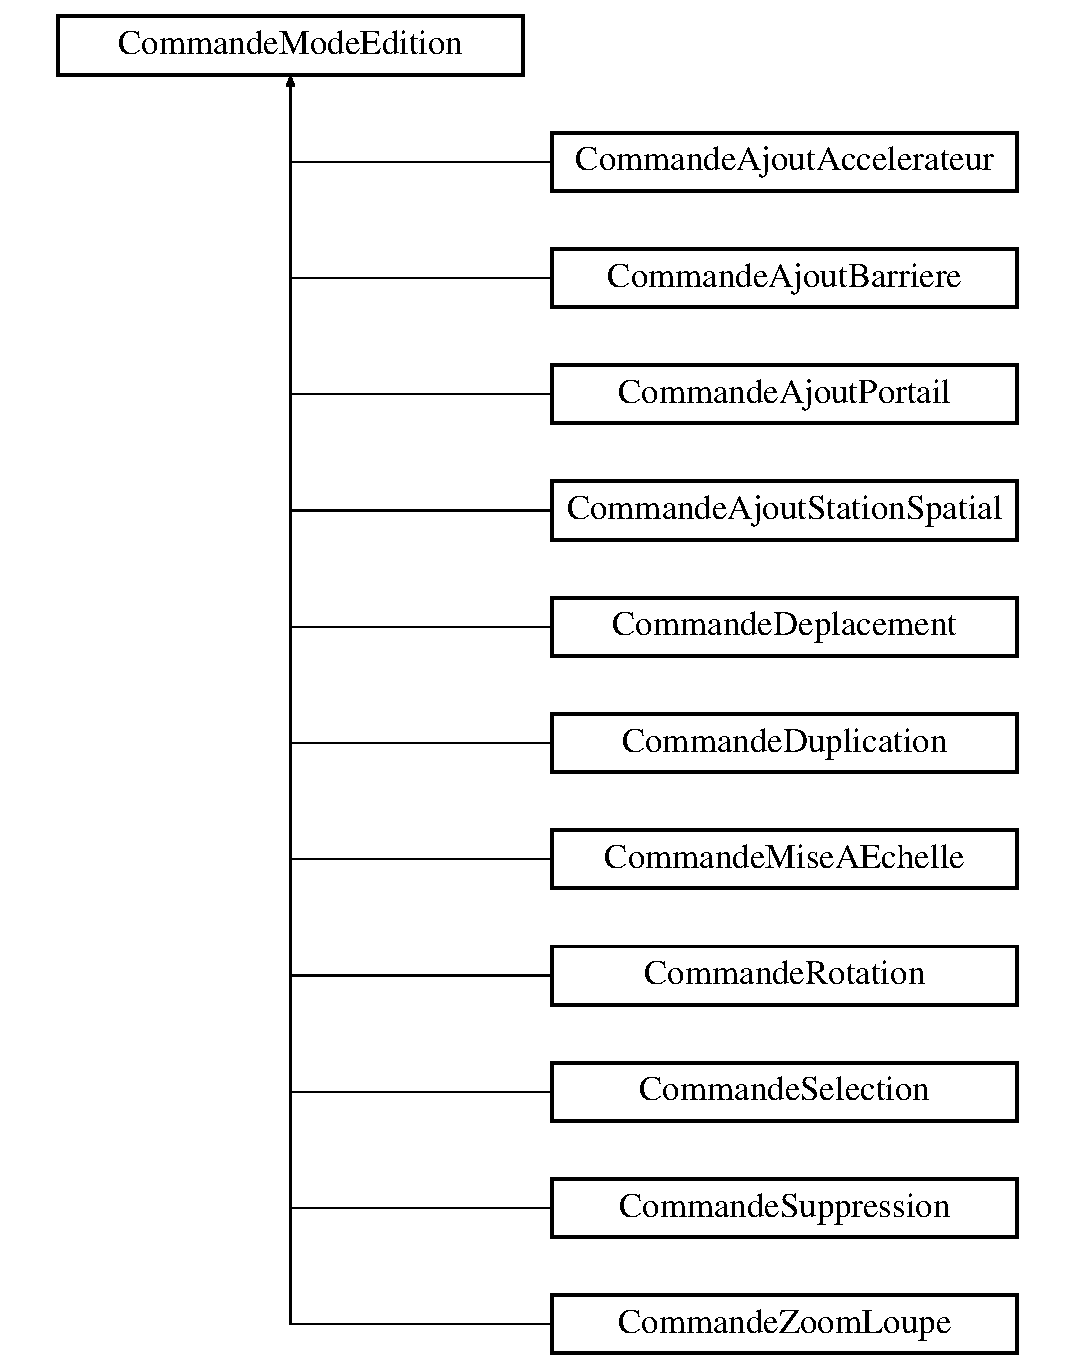
\includegraphics[height=12.000000cm]{class_commande_mode_edition}
\end{center}
\end{figure}
\subsection*{Public Member Functions}
\begin{DoxyCompactItemize}
\item 
\hyperlink{class_commande_mode_edition_ae6d4fef67683ce568a8c34b7329fd759}{Commande\-Mode\-Edition} ()
\item 
virtual \hyperlink{class_commande_mode_edition_af499078eaf3c840c1abb885c18581221}{$\sim$\-Commande\-Mode\-Edition} ()
\item 
virtual \hyperlink{wglew_8h_aeea6e3dfae3acf232096f57d2d57f084}{void} \hyperlink{class_commande_mode_edition_aca77e9bb8557971af33748041975eecb}{executer} (\hyperlink{wglew_8h_a500a82aecba06f4550f6849b8099ca21}{int} mouse\-X, \hyperlink{wglew_8h_a500a82aecba06f4550f6849b8099ca21}{int} mouse\-Y, \hyperlink{wglew_8h_a500a82aecba06f4550f6849b8099ca21}{int} boutton, \hyperlink{wglew_8h_a500a82aecba06f4550f6849b8099ca21}{int} touche)=0
\end{DoxyCompactItemize}
\subsection*{Protected Attributes}
\begin{DoxyCompactItemize}
\item 
\hyperlink{wglew_8h_a500a82aecba06f4550f6849b8099ca21}{int} \hyperlink{class_commande_mode_edition_ade7653be98ae5dd9da895a34983ec680}{mouse\-X\-\_\-}
\item 
\hyperlink{wglew_8h_a500a82aecba06f4550f6849b8099ca21}{int} \hyperlink{class_commande_mode_edition_a6128370123ce4b6e6fb8571c953241e4}{mouse\-Y\-\_\-}
\item 
\hyperlink{wglew_8h_a500a82aecba06f4550f6849b8099ca21}{int} \hyperlink{class_commande_mode_edition_a02fd21f564101674d5c8af535322ea02}{last\-Mouse\-X\-\_\-}
\item 
\hyperlink{wglew_8h_a500a82aecba06f4550f6849b8099ca21}{int} \hyperlink{class_commande_mode_edition_a42bd29db98adec623e8c7cd5771783f3}{last\-Mouse\-Y\-\_\-}
\item 
\hyperlink{wglew_8h_a500a82aecba06f4550f6849b8099ca21}{int} \hyperlink{class_commande_mode_edition_a84e2d980201bc0649b2af9c9f4bff7e6}{boutton\-\_\-}
\item 
\hyperlink{wglew_8h_a500a82aecba06f4550f6849b8099ca21}{int} \hyperlink{class_commande_mode_edition_a3a522c03034a54eb01178e8c8af9a8db}{touche\-\_\-}
\end{DoxyCompactItemize}


\subsection{Detailed Description}
L'interface \hyperlink{class_commande_mode_edition}{Commande\-Mode\-Edition} permet de definir les commandes qui peuvent etres executes sur les differents objets en mode edition. 

\subsection{Constructor \& Destructor Documentation}
\hypertarget{class_commande_mode_edition_ae6d4fef67683ce568a8c34b7329fd759}{\index{Commande\-Mode\-Edition@{Commande\-Mode\-Edition}!Commande\-Mode\-Edition@{Commande\-Mode\-Edition}}
\index{Commande\-Mode\-Edition@{Commande\-Mode\-Edition}!CommandeModeEdition@{Commande\-Mode\-Edition}}
\subsubsection[{Commande\-Mode\-Edition}]{\setlength{\rightskip}{0pt plus 5cm}Commande\-Mode\-Edition\-::\-Commande\-Mode\-Edition (
\begin{DoxyParamCaption}
{}
\end{DoxyParamCaption}
)\hspace{0.3cm}{\ttfamily [inline]}}}\label{class_commande_mode_edition_ae6d4fef67683ce568a8c34b7329fd759}
Constructeur \hypertarget{class_commande_mode_edition_af499078eaf3c840c1abb885c18581221}{\index{Commande\-Mode\-Edition@{Commande\-Mode\-Edition}!$\sim$\-Commande\-Mode\-Edition@{$\sim$\-Commande\-Mode\-Edition}}
\index{$\sim$\-Commande\-Mode\-Edition@{$\sim$\-Commande\-Mode\-Edition}!CommandeModeEdition@{Commande\-Mode\-Edition}}
\subsubsection[{$\sim$\-Commande\-Mode\-Edition}]{\setlength{\rightskip}{0pt plus 5cm}virtual Commande\-Mode\-Edition\-::$\sim$\-Commande\-Mode\-Edition (
\begin{DoxyParamCaption}
{}
\end{DoxyParamCaption}
)\hspace{0.3cm}{\ttfamily [inline]}, {\ttfamily [virtual]}}}\label{class_commande_mode_edition_af499078eaf3c840c1abb885c18581221}
Destructeur 

\subsection{Member Function Documentation}
\hypertarget{class_commande_mode_edition_aca77e9bb8557971af33748041975eecb}{\index{Commande\-Mode\-Edition@{Commande\-Mode\-Edition}!executer@{executer}}
\index{executer@{executer}!CommandeModeEdition@{Commande\-Mode\-Edition}}
\subsubsection[{executer}]{\setlength{\rightskip}{0pt plus 5cm}virtual {\bf void} Commande\-Mode\-Edition\-::executer (
\begin{DoxyParamCaption}
\item[{{\bf int}}]{mouse\-X, }
\item[{{\bf int}}]{mouse\-Y, }
\item[{{\bf int}}]{boutton, }
\item[{{\bf int}}]{touche}
\end{DoxyParamCaption}
)\hspace{0.3cm}{\ttfamily [pure virtual]}}}\label{class_commande_mode_edition_aca77e9bb8557971af33748041975eecb}
Fonction a implementer dans les classes derivees. Execute l'action que la commande doit effectuer 
\begin{DoxyParams}{Parameters}
{\em mouse\-X} & La position X de la souris \\
\hline
{\em mouse\-Y} & La position Y de la souris \\
\hline
{\em bouton} & L'etat des boutons de la souris \\
\hline
{\em touche} & Touche du clavier appuyee \\
\hline
\end{DoxyParams}


Implemented in \hyperlink{class_commande_selection_a1fdf079ab482bbcceb87a7d2eb72c7be}{Commande\-Selection}, \hyperlink{class_commande_duplication_ab8f7e0df61599b747d80c06548b630a9}{Commande\-Duplication}, \hyperlink{class_commande_rotation_a2ee611526f6ed7720821dbf8e577fe64}{Commande\-Rotation}, \hyperlink{class_commande_suppression_a8e3947cc0dcdcb85348e5c873f6def44}{Commande\-Suppression}, \hyperlink{class_commande_deplacement_a8a591ce694d95d57409f14597d0b1e9c}{Commande\-Deplacement}, \hyperlink{class_commande_mise_a_echelle_a03aabe2e5d3a20928b041cfe5595715b}{Commande\-Mise\-A\-Echelle}, \hyperlink{class_commande_ajout_portail_a1b5ac4fd38f34e785aa61a3ce6fd5702}{Commande\-Ajout\-Portail}, \hyperlink{group__inf2990_ga803d538d34b6d32dd88def5126d0684b}{Commande\-Zoom\-Loupe}, \hyperlink{class_commande_ajout_barriere_a23c6176e97b56fed95b2e02b37515290}{Commande\-Ajout\-Barriere}, \hyperlink{class_commande_ajout_station_spatial_a92ca290ca6ca127e618e3463bf3fe75b}{Commande\-Ajout\-Station\-Spatial}, and \hyperlink{class_commande_ajout_accelerateur_a1537ffad37fa05fa20cdbd414890adb3}{Commande\-Ajout\-Accelerateur}.



\subsection{Member Data Documentation}
\hypertarget{class_commande_mode_edition_a84e2d980201bc0649b2af9c9f4bff7e6}{\index{Commande\-Mode\-Edition@{Commande\-Mode\-Edition}!boutton\-\_\-@{boutton\-\_\-}}
\index{boutton\-\_\-@{boutton\-\_\-}!CommandeModeEdition@{Commande\-Mode\-Edition}}
\subsubsection[{boutton\-\_\-}]{\setlength{\rightskip}{0pt plus 5cm}{\bf int} Commande\-Mode\-Edition\-::boutton\-\_\-\hspace{0.3cm}{\ttfamily [protected]}}}\label{class_commande_mode_edition_a84e2d980201bc0649b2af9c9f4bff7e6}
Boutton presentement clique avec la souris \hypertarget{class_commande_mode_edition_a02fd21f564101674d5c8af535322ea02}{\index{Commande\-Mode\-Edition@{Commande\-Mode\-Edition}!last\-Mouse\-X\-\_\-@{last\-Mouse\-X\-\_\-}}
\index{last\-Mouse\-X\-\_\-@{last\-Mouse\-X\-\_\-}!CommandeModeEdition@{Commande\-Mode\-Edition}}
\subsubsection[{last\-Mouse\-X\-\_\-}]{\setlength{\rightskip}{0pt plus 5cm}{\bf int} Commande\-Mode\-Edition\-::last\-Mouse\-X\-\_\-\hspace{0.3cm}{\ttfamily [protected]}}}\label{class_commande_mode_edition_a02fd21f564101674d5c8af535322ea02}
Derniere position en X de la souris \hypertarget{class_commande_mode_edition_a42bd29db98adec623e8c7cd5771783f3}{\index{Commande\-Mode\-Edition@{Commande\-Mode\-Edition}!last\-Mouse\-Y\-\_\-@{last\-Mouse\-Y\-\_\-}}
\index{last\-Mouse\-Y\-\_\-@{last\-Mouse\-Y\-\_\-}!CommandeModeEdition@{Commande\-Mode\-Edition}}
\subsubsection[{last\-Mouse\-Y\-\_\-}]{\setlength{\rightskip}{0pt plus 5cm}{\bf int} Commande\-Mode\-Edition\-::last\-Mouse\-Y\-\_\-\hspace{0.3cm}{\ttfamily [protected]}}}\label{class_commande_mode_edition_a42bd29db98adec623e8c7cd5771783f3}
Derniere position en Y de la souris \hypertarget{class_commande_mode_edition_ade7653be98ae5dd9da895a34983ec680}{\index{Commande\-Mode\-Edition@{Commande\-Mode\-Edition}!mouse\-X\-\_\-@{mouse\-X\-\_\-}}
\index{mouse\-X\-\_\-@{mouse\-X\-\_\-}!CommandeModeEdition@{Commande\-Mode\-Edition}}
\subsubsection[{mouse\-X\-\_\-}]{\setlength{\rightskip}{0pt plus 5cm}{\bf int} Commande\-Mode\-Edition\-::mouse\-X\-\_\-\hspace{0.3cm}{\ttfamily [protected]}}}\label{class_commande_mode_edition_ade7653be98ae5dd9da895a34983ec680}
Position en X de la souris \hypertarget{class_commande_mode_edition_a6128370123ce4b6e6fb8571c953241e4}{\index{Commande\-Mode\-Edition@{Commande\-Mode\-Edition}!mouse\-Y\-\_\-@{mouse\-Y\-\_\-}}
\index{mouse\-Y\-\_\-@{mouse\-Y\-\_\-}!CommandeModeEdition@{Commande\-Mode\-Edition}}
\subsubsection[{mouse\-Y\-\_\-}]{\setlength{\rightskip}{0pt plus 5cm}{\bf int} Commande\-Mode\-Edition\-::mouse\-Y\-\_\-\hspace{0.3cm}{\ttfamily [protected]}}}\label{class_commande_mode_edition_a6128370123ce4b6e6fb8571c953241e4}
Position en Y de la souris \hypertarget{class_commande_mode_edition_a3a522c03034a54eb01178e8c8af9a8db}{\index{Commande\-Mode\-Edition@{Commande\-Mode\-Edition}!touche\-\_\-@{touche\-\_\-}}
\index{touche\-\_\-@{touche\-\_\-}!CommandeModeEdition@{Commande\-Mode\-Edition}}
\subsubsection[{touche\-\_\-}]{\setlength{\rightskip}{0pt plus 5cm}{\bf int} Commande\-Mode\-Edition\-::touche\-\_\-\hspace{0.3cm}{\ttfamily [protected]}}}\label{class_commande_mode_edition_a3a522c03034a54eb01178e8c8af9a8db}
Touche presentement appuye avec le clavier 

The documentation for this interface was generated from the following file\-:\begin{DoxyCompactItemize}
\item 
Cadriciel/\-Sources/\-C++/\-Application/\-Jeu/\-Mode\-Edition/\hyperlink{_commande_mode_edition_8h}{Commande\-Mode\-Edition.\-h}\end{DoxyCompactItemize}

\hypertarget{class_commande_rotation}{\section{Commande\-Rotation Class Reference}
\label{class_commande_rotation}\index{Commande\-Rotation@{Commande\-Rotation}}
}


La classe \hyperlink{class_commande_rotation}{Commande\-Rotation} permet d'effectuer une rotation sur un ou plusieurs objets selectionnes.  




{\ttfamily \#include $<$Commande\-Rotation.\-h$>$}

Inheritance diagram for Commande\-Rotation\-:\begin{figure}[H]
\begin{center}
\leavevmode
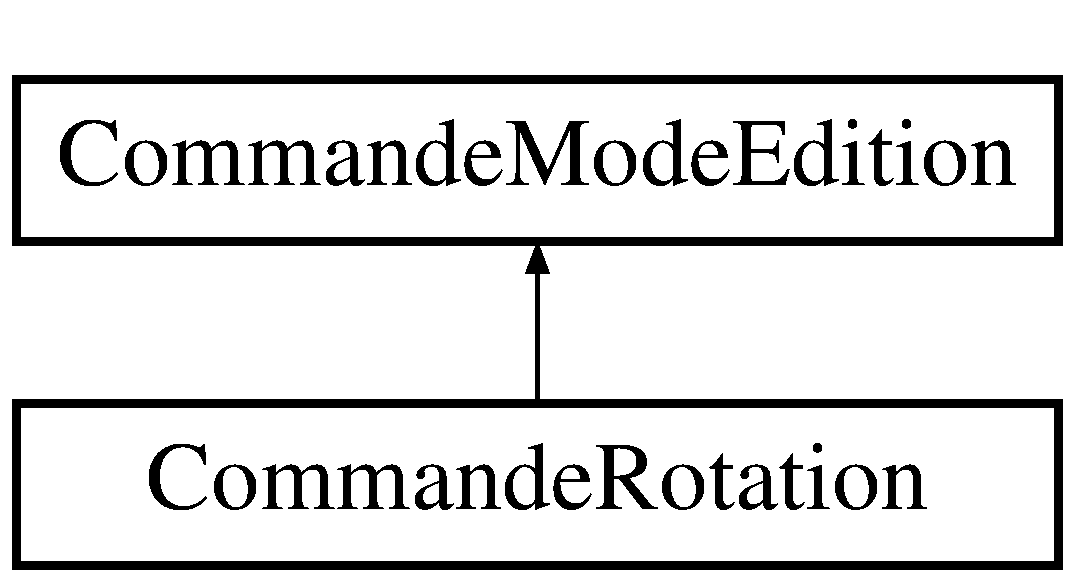
\includegraphics[height=2.000000cm]{class_commande_rotation}
\end{center}
\end{figure}
\subsection*{Public Member Functions}
\begin{DoxyCompactItemize}
\item 
\hyperlink{class_commande_rotation_a761e2cdab1e1b916643bea637070646d}{Commande\-Rotation} (const \hyperlink{classvue_1_1_vue}{vue\-::\-Vue} \&vue, \hyperlink{class_carte}{Carte} \&carte, const vector$<$ \hyperlink{class_element_jeu_abstrait}{Element\-Jeu\-Abstrait} $\ast$ $>$ \&objets\-Selectionnes)
\item 
virtual \hyperlink{class_commande_rotation_a5e0b92f5c0dd1d93b9f608c02d94608c}{$\sim$\-Commande\-Rotation} ()
\item 
virtual \hyperlink{wglew_8h_aeea6e3dfae3acf232096f57d2d57f084}{void} \hyperlink{class_commande_rotation_a2ee611526f6ed7720821dbf8e577fe64}{executer} (\hyperlink{wglew_8h_a500a82aecba06f4550f6849b8099ca21}{int} mouse\-X, \hyperlink{wglew_8h_a500a82aecba06f4550f6849b8099ca21}{int} mouse\-Y, \hyperlink{wglew_8h_a500a82aecba06f4550f6849b8099ca21}{int} boutton, \hyperlink{wglew_8h_a500a82aecba06f4550f6849b8099ca21}{int} touche)
\end{DoxyCompactItemize}
\subsection*{Additional Inherited Members}


\subsection{Detailed Description}
La classe \hyperlink{class_commande_rotation}{Commande\-Rotation} permet d'effectuer une rotation sur un ou plusieurs objets selectionnes. 

\subsection{Constructor \& Destructor Documentation}
\hypertarget{class_commande_rotation_a761e2cdab1e1b916643bea637070646d}{\index{Commande\-Rotation@{Commande\-Rotation}!Commande\-Rotation@{Commande\-Rotation}}
\index{Commande\-Rotation@{Commande\-Rotation}!CommandeRotation@{Commande\-Rotation}}
\subsubsection[{Commande\-Rotation}]{\setlength{\rightskip}{0pt plus 5cm}Commande\-Rotation\-::\-Commande\-Rotation (
\begin{DoxyParamCaption}
\item[{const {\bf vue\-::\-Vue} \&}]{vue, }
\item[{{\bf Carte} \&}]{carte, }
\item[{const vector$<$ {\bf Element\-Jeu\-Abstrait} $\ast$ $>$ \&}]{objets\-Selectionnes}
\end{DoxyParamCaption}
)}}\label{class_commande_rotation_a761e2cdab1e1b916643bea637070646d}
Constructeur 
\begin{DoxyParams}{Parameters}
{\em vue} & La vue du jeu. Utilise pour transformer les points de l'ecran dans l'espace de la camera \\
\hline
{\em carte} & La carte sur laquelle ajouter l'objet. \\
\hline
{\em objets\-Selectionnes} & Une reference vers un vecteur qui contiendra les objets selectionnes \\
\hline
\end{DoxyParams}
\hypertarget{class_commande_rotation_a5e0b92f5c0dd1d93b9f608c02d94608c}{\index{Commande\-Rotation@{Commande\-Rotation}!$\sim$\-Commande\-Rotation@{$\sim$\-Commande\-Rotation}}
\index{$\sim$\-Commande\-Rotation@{$\sim$\-Commande\-Rotation}!CommandeRotation@{Commande\-Rotation}}
\subsubsection[{$\sim$\-Commande\-Rotation}]{\setlength{\rightskip}{0pt plus 5cm}Commande\-Rotation\-::$\sim$\-Commande\-Rotation (
\begin{DoxyParamCaption}
{}
\end{DoxyParamCaption}
)\hspace{0.3cm}{\ttfamily [virtual]}}}\label{class_commande_rotation_a5e0b92f5c0dd1d93b9f608c02d94608c}
Destructeur 

\subsection{Member Function Documentation}
\hypertarget{class_commande_rotation_a2ee611526f6ed7720821dbf8e577fe64}{\index{Commande\-Rotation@{Commande\-Rotation}!executer@{executer}}
\index{executer@{executer}!CommandeRotation@{Commande\-Rotation}}
\subsubsection[{executer}]{\setlength{\rightskip}{0pt plus 5cm}{\bf void} Commande\-Rotation\-::executer (
\begin{DoxyParamCaption}
\item[{{\bf int}}]{mouse\-X, }
\item[{{\bf int}}]{mouse\-Y, }
\item[{{\bf int}}]{boutton, }
\item[{{\bf int}}]{touche}
\end{DoxyParamCaption}
)\hspace{0.3cm}{\ttfamily [virtual]}}}\label{class_commande_rotation_a2ee611526f6ed7720821dbf8e577fe64}
Execute la commande. Effectue une rotation sur le ou les objets selectionnes a partir du mouvement de la souris. 
\begin{DoxyParams}{Parameters}
{\em mouse\-X} & La position X de la souris \\
\hline
{\em mouse\-Y} & La position Y de la souris \\
\hline
{\em bouton} & L'etat des boutons de la souris \\
\hline
{\em touche} & Touche du clavier appuyee \\
\hline
\end{DoxyParams}


Implements \hyperlink{class_commande_mode_edition_aca77e9bb8557971af33748041975eecb}{Commande\-Mode\-Edition}.



The documentation for this class was generated from the following files\-:\begin{DoxyCompactItemize}
\item 
Cadriciel/\-Sources/\-C++/\-Application/\-Jeu/\-Mode\-Edition/\hyperlink{_commande_rotation_8h}{Commande\-Rotation.\-h}\item 
Cadriciel/\-Sources/\-C++/\-Application/\-Jeu/\-Mode\-Edition/\hyperlink{_commande_rotation_8cpp}{Commande\-Rotation.\-cpp}\end{DoxyCompactItemize}

\hypertarget{class_commande_selection}{\section{Commande\-Selection Class Reference}
\label{class_commande_selection}\index{Commande\-Selection@{Commande\-Selection}}
}


La classe \hyperlink{class_commande_selection}{Commande\-Selection} permet de selectionner dans la carte des objets de deux manieres differentes\-: de facon ponctuelle (un seul objet est selectionne en cliquant dessus) ou avec une selection elastique (plusieurs objets sont selectionnes).  




{\ttfamily \#include $<$Commande\-Selection.\-h$>$}

Inheritance diagram for Commande\-Selection\-:\begin{figure}[H]
\begin{center}
\leavevmode
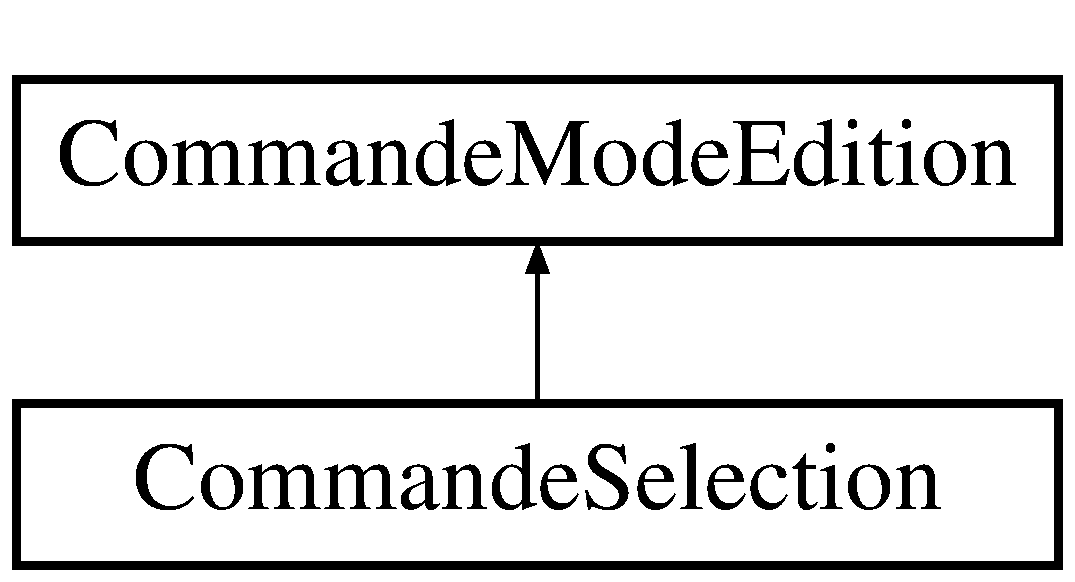
\includegraphics[height=2.000000cm]{class_commande_selection}
\end{center}
\end{figure}
\subsection*{Public Member Functions}
\begin{DoxyCompactItemize}
\item 
\hyperlink{class_commande_selection_a144fe79ec6aefd6f1e684f71c2eb7dc8}{Commande\-Selection} (const \hyperlink{classvue_1_1_vue}{vue\-::\-Vue} \&vue, \hyperlink{class_carte}{Carte} \&carte, vector$<$ \hyperlink{class_element_jeu_abstrait}{Element\-Jeu\-Abstrait} $\ast$ $>$ \&objets\-Selectionnes)
\item 
virtual \hyperlink{class_commande_selection_a3c35456e80063269a01c2057fd96e82f}{$\sim$\-Commande\-Selection} ()
\item 
virtual \hyperlink{wglew_8h_aeea6e3dfae3acf232096f57d2d57f084}{void} \hyperlink{class_commande_selection_a1fdf079ab482bbcceb87a7d2eb72c7be}{executer} (\hyperlink{wglew_8h_a500a82aecba06f4550f6849b8099ca21}{int} mouse\-X, \hyperlink{wglew_8h_a500a82aecba06f4550f6849b8099ca21}{int} mouse\-Y, \hyperlink{wglew_8h_a500a82aecba06f4550f6849b8099ca21}{int} boutton, \hyperlink{wglew_8h_a500a82aecba06f4550f6849b8099ca21}{int} touche)
\end{DoxyCompactItemize}
\subsection*{Additional Inherited Members}


\subsection{Detailed Description}
La classe \hyperlink{class_commande_selection}{Commande\-Selection} permet de selectionner dans la carte des objets de deux manieres differentes\-: de facon ponctuelle (un seul objet est selectionne en cliquant dessus) ou avec une selection elastique (plusieurs objets sont selectionnes). 

\subsection{Constructor \& Destructor Documentation}
\hypertarget{class_commande_selection_a144fe79ec6aefd6f1e684f71c2eb7dc8}{\index{Commande\-Selection@{Commande\-Selection}!Commande\-Selection@{Commande\-Selection}}
\index{Commande\-Selection@{Commande\-Selection}!CommandeSelection@{Commande\-Selection}}
\subsubsection[{Commande\-Selection}]{\setlength{\rightskip}{0pt plus 5cm}Commande\-Selection\-::\-Commande\-Selection (
\begin{DoxyParamCaption}
\item[{const {\bf vue\-::\-Vue} \&}]{vue, }
\item[{{\bf Carte} \&}]{carte, }
\item[{vector$<$ {\bf Element\-Jeu\-Abstrait} $\ast$ $>$ \&}]{objets\-Selectionnes}
\end{DoxyParamCaption}
)}}\label{class_commande_selection_a144fe79ec6aefd6f1e684f71c2eb7dc8}
Constructeur 
\begin{DoxyParams}{Parameters}
{\em vue} & La vue du jeu. Utilise pour transformer les points de l'ecran dans l'espace de la camera \\
\hline
{\em carte} & La carte sur laquelle ajouter l'objet. \\
\hline
{\em objets\-Selectionnes} & Une reference vers un vecteur qui contiendra les objets selectionnes \\
\hline
\end{DoxyParams}
\hypertarget{class_commande_selection_a3c35456e80063269a01c2057fd96e82f}{\index{Commande\-Selection@{Commande\-Selection}!$\sim$\-Commande\-Selection@{$\sim$\-Commande\-Selection}}
\index{$\sim$\-Commande\-Selection@{$\sim$\-Commande\-Selection}!CommandeSelection@{Commande\-Selection}}
\subsubsection[{$\sim$\-Commande\-Selection}]{\setlength{\rightskip}{0pt plus 5cm}Commande\-Selection\-::$\sim$\-Commande\-Selection (
\begin{DoxyParamCaption}
{}
\end{DoxyParamCaption}
)\hspace{0.3cm}{\ttfamily [virtual]}}}\label{class_commande_selection_a3c35456e80063269a01c2057fd96e82f}
Destructeur 

\subsection{Member Function Documentation}
\hypertarget{class_commande_selection_a1fdf079ab482bbcceb87a7d2eb72c7be}{\index{Commande\-Selection@{Commande\-Selection}!executer@{executer}}
\index{executer@{executer}!CommandeSelection@{Commande\-Selection}}
\subsubsection[{executer}]{\setlength{\rightskip}{0pt plus 5cm}{\bf void} Commande\-Selection\-::executer (
\begin{DoxyParamCaption}
\item[{{\bf int}}]{mouse\-X, }
\item[{{\bf int}}]{mouse\-Y, }
\item[{{\bf int}}]{boutton, }
\item[{{\bf int}}]{touche}
\end{DoxyParamCaption}
)\hspace{0.3cm}{\ttfamily [virtual]}}}\label{class_commande_selection_a1fdf079ab482bbcceb87a7d2eb72c7be}
Execute la commande. Permet de selectionner des objets de 2 manieres\-: soit de facon ponctuelle (1 objet) ou avec un rectangle de selection, pour avoir plusieurs objets. 
\begin{DoxyParams}{Parameters}
{\em mouse\-X} & La position X de la souris \\
\hline
{\em mouse\-Y} & La position Y de la souris \\
\hline
{\em bouton} & L'etat des boutons de la souris \\
\hline
{\em touche} & Touche du clavier appuyee \\
\hline
\end{DoxyParams}


Implements \hyperlink{class_commande_mode_edition_aca77e9bb8557971af33748041975eecb}{Commande\-Mode\-Edition}.



The documentation for this class was generated from the following files\-:\begin{DoxyCompactItemize}
\item 
Cadriciel/\-Sources/\-C++/\-Application/\-Jeu/\-Mode\-Edition/\hyperlink{_commande_selection_8h}{Commande\-Selection.\-h}\item 
Cadriciel/\-Sources/\-C++/\-Application/\-Jeu/\-Mode\-Edition/\hyperlink{_commande_selection_8cpp}{Commande\-Selection.\-cpp}\end{DoxyCompactItemize}

\hypertarget{class_commande_suppression}{\section{Commande\-Suppression Class Reference}
\label{class_commande_suppression}\index{Commande\-Suppression@{Commande\-Suppression}}
}


La classe \hyperlink{class_commande_suppression}{Commande\-Suppression} permet d'enlever un objet sur la carte.  




{\ttfamily \#include $<$Commande\-Suppression.\-h$>$}

Inheritance diagram for Commande\-Suppression\-:\begin{figure}[H]
\begin{center}
\leavevmode
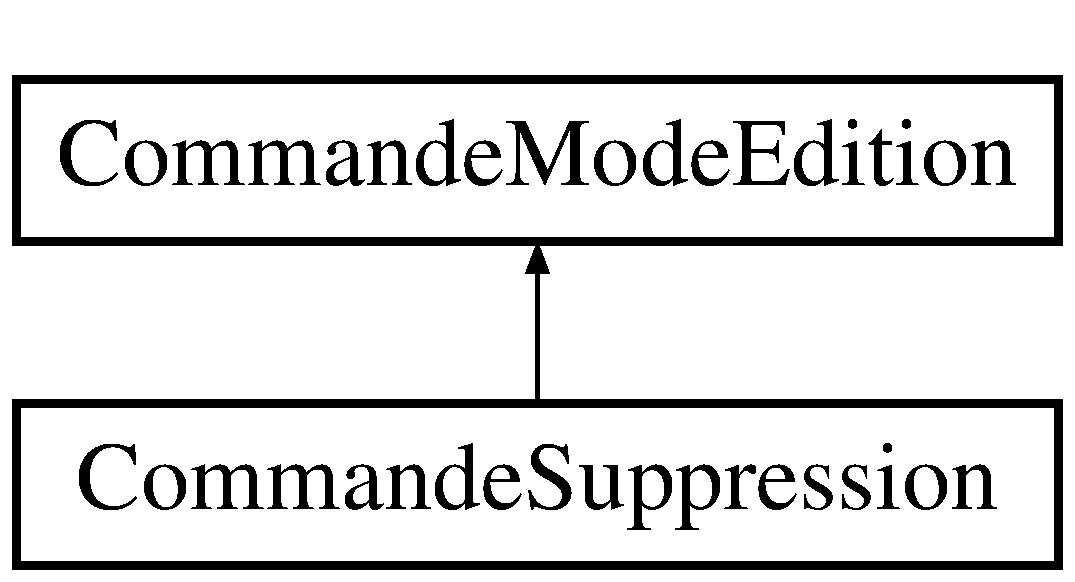
\includegraphics[height=2.000000cm]{class_commande_suppression}
\end{center}
\end{figure}
\subsection*{Public Member Functions}
\begin{DoxyCompactItemize}
\item 
\hyperlink{class_commande_suppression_a6438eb61f3a3971c3e23f8d4e2d7628f}{Commande\-Suppression} (const \hyperlink{classvue_1_1_vue}{vue\-::\-Vue} \&vue, \hyperlink{class_carte}{Carte} \&carte, vector$<$ \hyperlink{class_element_jeu_abstrait}{Element\-Jeu\-Abstrait} $\ast$ $>$ \&objets\-Selectionnes)
\item 
virtual \hyperlink{class_commande_suppression_a8a8c9487c2f267bf008ef98dec1d808e}{$\sim$\-Commande\-Suppression} ()
\item 
virtual void \hyperlink{class_commande_suppression_a8e3947cc0dcdcb85348e5c873f6def44}{executer} (int mouse\-X, int mouse\-Y, int boutton, int touche)
\end{DoxyCompactItemize}
\subsection*{Additional Inherited Members}


\subsection{Detailed Description}
La classe \hyperlink{class_commande_suppression}{Commande\-Suppression} permet d'enlever un objet sur la carte. 

\subsection{Constructor \& Destructor Documentation}
\hypertarget{class_commande_suppression_a6438eb61f3a3971c3e23f8d4e2d7628f}{\index{Commande\-Suppression@{Commande\-Suppression}!Commande\-Suppression@{Commande\-Suppression}}
\index{Commande\-Suppression@{Commande\-Suppression}!CommandeSuppression@{Commande\-Suppression}}
\subsubsection[{Commande\-Suppression}]{\setlength{\rightskip}{0pt plus 5cm}Commande\-Suppression\-::\-Commande\-Suppression (
\begin{DoxyParamCaption}
\item[{const {\bf vue\-::\-Vue} \&}]{vue, }
\item[{{\bf Carte} \&}]{carte, }
\item[{vector$<$ {\bf Element\-Jeu\-Abstrait} $\ast$ $>$ \&}]{objets\-Selectionnes}
\end{DoxyParamCaption}
)}}\label{class_commande_suppression_a6438eb61f3a3971c3e23f8d4e2d7628f}
Constructeur 
\begin{DoxyParams}{Parameters}
{\em vue} & La vue du jeu. Utilise pour transformer les points de l'ecran dans l'espace de la camera \\
\hline
{\em carte} & La carte sur laquelle ajouter l'objet. \\
\hline
{\em objets\-Selectionnes} & Une reference vers un vecteur qui contiendra les objets selectionnes \\
\hline
\end{DoxyParams}
\hypertarget{class_commande_suppression_a8a8c9487c2f267bf008ef98dec1d808e}{\index{Commande\-Suppression@{Commande\-Suppression}!$\sim$\-Commande\-Suppression@{$\sim$\-Commande\-Suppression}}
\index{$\sim$\-Commande\-Suppression@{$\sim$\-Commande\-Suppression}!CommandeSuppression@{Commande\-Suppression}}
\subsubsection[{$\sim$\-Commande\-Suppression}]{\setlength{\rightskip}{0pt plus 5cm}Commande\-Suppression\-::$\sim$\-Commande\-Suppression (
\begin{DoxyParamCaption}
{}
\end{DoxyParamCaption}
)\hspace{0.3cm}{\ttfamily [virtual]}}}\label{class_commande_suppression_a8a8c9487c2f267bf008ef98dec1d808e}
Destructeur 

\subsection{Member Function Documentation}
\hypertarget{class_commande_suppression_a8e3947cc0dcdcb85348e5c873f6def44}{\index{Commande\-Suppression@{Commande\-Suppression}!executer@{executer}}
\index{executer@{executer}!CommandeSuppression@{Commande\-Suppression}}
\subsubsection[{executer}]{\setlength{\rightskip}{0pt plus 5cm}void Commande\-Suppression\-::executer (
\begin{DoxyParamCaption}
\item[{int}]{mouse\-X, }
\item[{int}]{mouse\-Y, }
\item[{int}]{boutton, }
\item[{int}]{touche}
\end{DoxyParamCaption}
)\hspace{0.3cm}{\ttfamily [virtual]}}}\label{class_commande_suppression_a8e3947cc0dcdcb85348e5c873f6def44}
Execute la commande. Supprime un ou plusieurs objets de la carte courante. 
\begin{DoxyParams}{Parameters}
{\em mouse\-X} & La position X de la souris \\
\hline
{\em mouse\-Y} & La position Y de la souris \\
\hline
{\em bouton} & L'etat des boutons de la souris \\
\hline
{\em touche} & Touche du clavier appuyee \\
\hline
\end{DoxyParams}


Implements \hyperlink{class_commande_mode_edition_aca77e9bb8557971af33748041975eecb}{Commande\-Mode\-Edition}.



The documentation for this class was generated from the following files\-:\begin{DoxyCompactItemize}
\item 
Cadriciel/\-Sources/\-C++/\-Application/\-Jeu/\-Mode\-Edition/\hyperlink{_commande_suppression_8h}{Commande\-Suppression.\-h}\item 
Cadriciel/\-Sources/\-C++/\-Application/\-Jeu/\-Mode\-Edition/Commande\-Suppression.\-cpp\end{DoxyCompactItemize}

\hypertarget{class_commande_zoom_loupe}{\section{Commande\-Zoom\-Loupe Interface Reference}
\label{class_commande_zoom_loupe}\index{Commande\-Zoom\-Loupe@{Commande\-Zoom\-Loupe}}
}


L'interface \hyperlink{class_commande_zoom_loupe}{Commande\-Zoom\-Loupe} permet de zoomer en creant un rectangle elastique en mode edition.  




{\ttfamily \#include $<$Commande\-Zoom\-Loupe.\-h$>$}

Inheritance diagram for Commande\-Zoom\-Loupe\-:\begin{figure}[H]
\begin{center}
\leavevmode
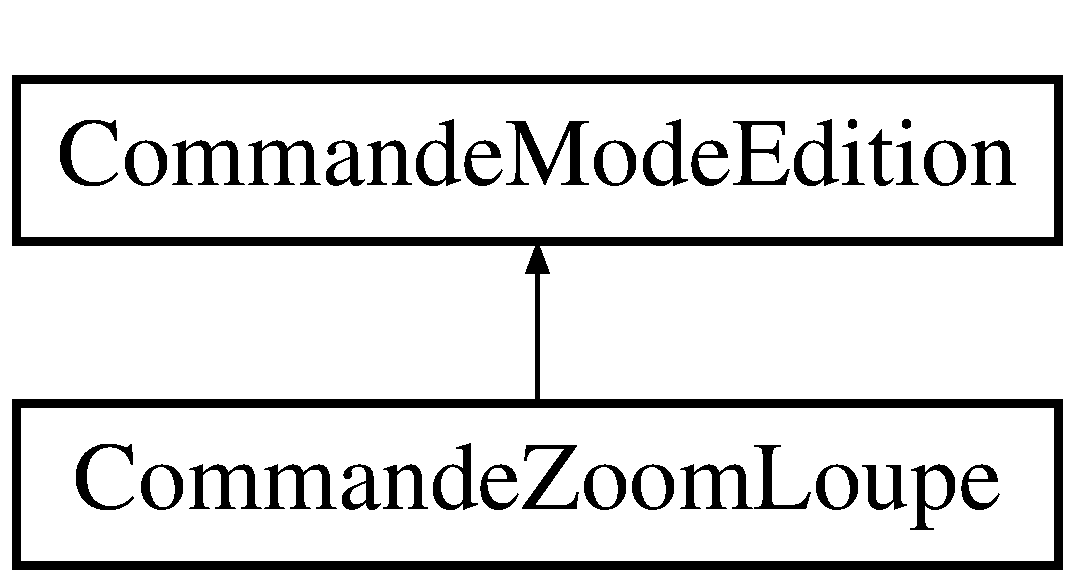
\includegraphics[height=2.000000cm]{class_commande_zoom_loupe}
\end{center}
\end{figure}
\subsection*{Public Member Functions}
\begin{DoxyCompactItemize}
\item 
\hyperlink{group__inf2990_gaef25c554211f1d059d0e0da604bba314}{Commande\-Zoom\-Loupe} (\hyperlink{classvue_1_1_vue}{vue\-::\-Vue} \&vue)
\item 
virtual \hyperlink{class_commande_zoom_loupe_a4903ef37ed8f806a3cd2b42ee5e41c1a}{$\sim$\-Commande\-Zoom\-Loupe} ()
\begin{DoxyCompactList}\small\item\em Destructeur. \end{DoxyCompactList}\item 
virtual \hyperlink{wglew_8h_aeea6e3dfae3acf232096f57d2d57f084}{void} \hyperlink{group__inf2990_ga803d538d34b6d32dd88def5126d0684b}{executer} (\hyperlink{wglew_8h_a500a82aecba06f4550f6849b8099ca21}{int} mouse\-X, \hyperlink{wglew_8h_a500a82aecba06f4550f6849b8099ca21}{int} mouse\-Y, \hyperlink{wglew_8h_a500a82aecba06f4550f6849b8099ca21}{int} boutton, \hyperlink{wglew_8h_a500a82aecba06f4550f6849b8099ca21}{int} touche)
\end{DoxyCompactItemize}
\subsection*{Additional Inherited Members}


\subsection{Detailed Description}
L'interface \hyperlink{class_commande_zoom_loupe}{Commande\-Zoom\-Loupe} permet de zoomer en creant un rectangle elastique en mode edition. 

\subsection{Constructor \& Destructor Documentation}
\hypertarget{class_commande_zoom_loupe_a4903ef37ed8f806a3cd2b42ee5e41c1a}{\index{Commande\-Zoom\-Loupe@{Commande\-Zoom\-Loupe}!$\sim$\-Commande\-Zoom\-Loupe@{$\sim$\-Commande\-Zoom\-Loupe}}
\index{$\sim$\-Commande\-Zoom\-Loupe@{$\sim$\-Commande\-Zoom\-Loupe}!CommandeZoomLoupe@{Commande\-Zoom\-Loupe}}
\subsubsection[{$\sim$\-Commande\-Zoom\-Loupe}]{\setlength{\rightskip}{0pt plus 5cm}virtual Commande\-Zoom\-Loupe\-::$\sim$\-Commande\-Zoom\-Loupe (
\begin{DoxyParamCaption}
{}
\end{DoxyParamCaption}
)\hspace{0.3cm}{\ttfamily [inline]}, {\ttfamily [virtual]}}}\label{class_commande_zoom_loupe_a4903ef37ed8f806a3cd2b42ee5e41c1a}


Destructeur. 



The documentation for this interface was generated from the following files\-:\begin{DoxyCompactItemize}
\item 
Cadriciel/\-Sources/\-C++/\-Application/\-Jeu/\-Mode\-Edition/\hyperlink{_commande_zoom_loupe_8h}{Commande\-Zoom\-Loupe.\-h}\item 
Cadriciel/\-Sources/\-C++/\-Application/\-Jeu/\-Mode\-Edition/\hyperlink{_commande_zoom_loupe_8cpp}{Commande\-Zoom\-Loupe.\-cpp}\end{DoxyCompactItemize}

\hypertarget{class_comparateur_cartes}{\section{Comparateur\-Cartes Class Reference}
\label{class_comparateur_cartes}\index{Comparateur\-Cartes@{Comparateur\-Cartes}}
}


Foncteur permettant de comparer deux cartes entre elles selon leur niveau de difficulte, puis selon leur nom.  




{\ttfamily \#include $<$Comparateur\-Cartes.\-h$>$}

\subsection*{Public Member Functions}
\begin{DoxyCompactItemize}
\item 
bool \hyperlink{group__inf2990_gac15d906e204ad5bb5942d3e21af77544}{operator()} (\hyperlink{glew_8h_ae84541b4f3d8e1ea24ec0f466a8c568b}{string} s1, \hyperlink{glew_8h_ae84541b4f3d8e1ea24ec0f466a8c568b}{string} s2)
\end{DoxyCompactItemize}


\subsection{Detailed Description}
Foncteur permettant de comparer deux cartes entre elles selon leur niveau de difficulte, puis selon leur nom. 

\begin{DoxyAuthor}{Author}
Vincent Longpre 
\end{DoxyAuthor}
\begin{DoxyDate}{Date}
2014-\/03-\/18 
\end{DoxyDate}


The documentation for this class was generated from the following file\-:\begin{DoxyCompactItemize}
\item 
Cadriciel/\-Sources/\-C++/\-Application/\-Jeu/\-Mode\-Jeu/\hyperlink{_comparateur_cartes_8h}{Comparateur\-Cartes.\-h}\end{DoxyCompactItemize}

\hypertarget{class_compiler_outputter}{\section{Compiler\-Outputter Class Reference}
\label{class_compiler_outputter}\index{Compiler\-Outputter@{Compiler\-Outputter}}
}


Outputs a \hyperlink{class_test_result_collector}{Test\-Result\-Collector} in a compiler compatible format.

Printing the test results in a compiler compatible format (assertion location has the same format as compiler error), allow you to use your I\-D\-E to jump to the assertion failure. Location format can be customized (see \hyperlink{class_compiler_outputter_a0d9e67c7bdcb443b0b2754d61a10790c}{set\-Location\-Format()} ).  




{\ttfamily \#include $<$Compiler\-Outputter.\-h$>$}

Inheritance diagram for Compiler\-Outputter\-:\begin{figure}[H]
\begin{center}
\leavevmode
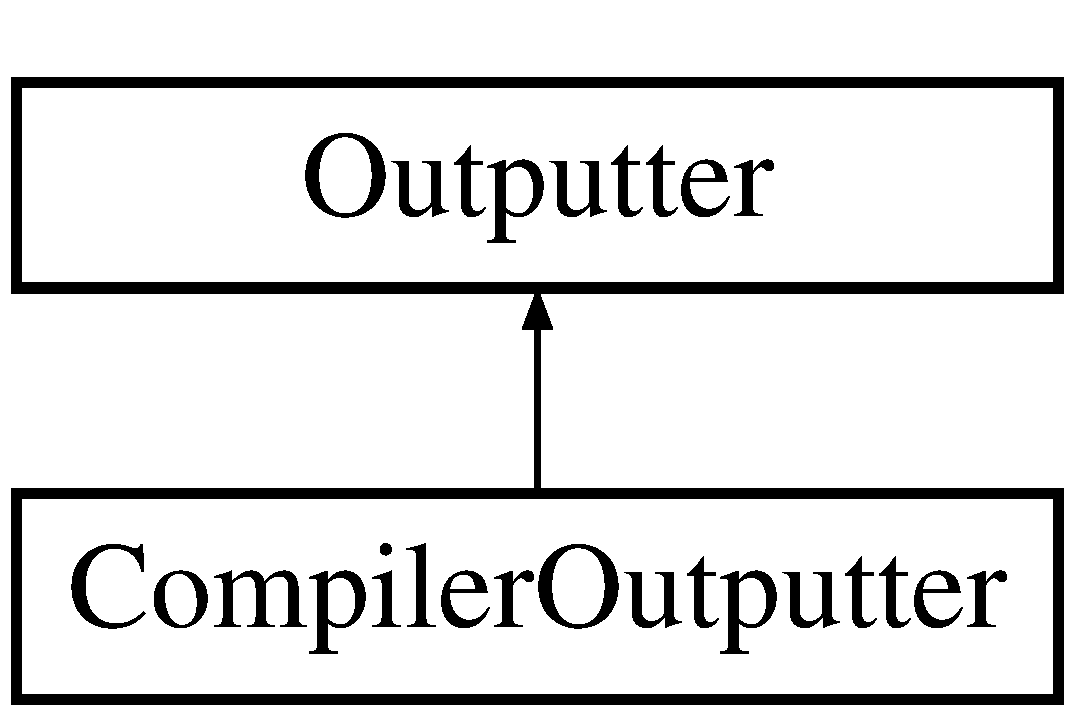
\includegraphics[height=2.000000cm]{class_compiler_outputter}
\end{center}
\end{figure}
\subsection*{Public Member Functions}
\begin{DoxyCompactItemize}
\item 
\hyperlink{class_compiler_outputter_a8dd6679e24c18b3ca54a4266d9d1b812}{Compiler\-Outputter} (\hyperlink{class_test_result_collector}{Test\-Result\-Collector} $\ast$\hyperlink{glew_8h_a5fb5836a37f7607602a16ad733ed6357}{result}, \hyperlink{_stream_8h_a80291a4e32881b445c8d4f839a9dd979}{O\-Stream} \&\hyperlink{glew_8h_a10d3bc96cdfc1d478f52c13d5ffd9316}{stream}, const \hyperlink{glew_8h_ae84541b4f3d8e1ea24ec0f466a8c568b}{std\-::string} \&location\-Format=\hyperlink{_portability_8h_a17c58ff0a5526dbcd28ebe3af5e7f04d}{C\-P\-P\-U\-N\-I\-T\-\_\-\-C\-O\-M\-P\-I\-L\-E\-R\-\_\-\-L\-O\-C\-A\-T\-I\-O\-N\-\_\-\-F\-O\-R\-M\-A\-T})
\begin{DoxyCompactList}\small\item\em Constructs a \hyperlink{class_compiler_outputter}{Compiler\-Outputter} object. \end{DoxyCompactList}\item 
virtual \hyperlink{class_compiler_outputter_ac74daaf4b355850c5e70b743aac2df82}{$\sim$\-Compiler\-Outputter} ()
\begin{DoxyCompactList}\small\item\em Destructor. \end{DoxyCompactList}\item 
\hyperlink{wglew_8h_aeea6e3dfae3acf232096f57d2d57f084}{void} \hyperlink{class_compiler_outputter_a0d9e67c7bdcb443b0b2754d61a10790c}{set\-Location\-Format} (const \hyperlink{glew_8h_ae84541b4f3d8e1ea24ec0f466a8c568b}{std\-::string} \&location\-Format)
\begin{DoxyCompactList}\small\item\em Sets the error location format. \end{DoxyCompactList}\item 
\hyperlink{wglew_8h_aeea6e3dfae3acf232096f57d2d57f084}{void} \hyperlink{class_compiler_outputter_a55ca2189956b9b52bdfb1802bf8da445}{write} ()
\item 
\hyperlink{wglew_8h_aeea6e3dfae3acf232096f57d2d57f084}{void} \hyperlink{class_compiler_outputter_aaa1d8281f8973552a8e9a4568b7d90b4}{set\-No\-Wrap} ()
\item 
\hyperlink{wglew_8h_aeea6e3dfae3acf232096f57d2d57f084}{void} \hyperlink{class_compiler_outputter_ab3559c2aaa88cbccb7c3823b3dd4d247}{set\-Wrap\-Column} (\hyperlink{wglew_8h_a500a82aecba06f4550f6849b8099ca21}{int} \hyperlink{class_compiler_outputter_a44a670371d545db99603ce88b59aa6c0}{wrap\-Column})
\item 
\hyperlink{wglew_8h_a500a82aecba06f4550f6849b8099ca21}{int} \hyperlink{class_compiler_outputter_a44a670371d545db99603ce88b59aa6c0}{wrap\-Column} () const 
\item 
virtual \hyperlink{wglew_8h_aeea6e3dfae3acf232096f57d2d57f084}{void} \hyperlink{class_compiler_outputter_a5fb16745d10fddb67cbcbec270218589}{print\-Success} ()
\item 
virtual \hyperlink{wglew_8h_aeea6e3dfae3acf232096f57d2d57f084}{void} \hyperlink{class_compiler_outputter_ab277e9b8c4af074593904dbc00853561}{print\-Failure\-Report} ()
\item 
virtual \hyperlink{wglew_8h_aeea6e3dfae3acf232096f57d2d57f084}{void} \hyperlink{class_compiler_outputter_a6919d4e1d44d03e50694aee73dc96d89}{print\-Failures\-List} ()
\item 
virtual \hyperlink{wglew_8h_aeea6e3dfae3acf232096f57d2d57f084}{void} \hyperlink{class_compiler_outputter_acc3eefc4776b975af3502ef9afaf8b3d}{print\-Statistics} ()
\item 
virtual \hyperlink{wglew_8h_aeea6e3dfae3acf232096f57d2d57f084}{void} \hyperlink{class_compiler_outputter_a2a8fece8722cb0307a5f0f6cd0de41c3}{print\-Failure\-Detail} (\hyperlink{class_test_failure}{Test\-Failure} $\ast$failure)
\item 
virtual \hyperlink{wglew_8h_aeea6e3dfae3acf232096f57d2d57f084}{void} \hyperlink{class_compiler_outputter_aac88928b23fbae0b33b1624fa5696c31}{print\-Failure\-Location} (\hyperlink{class_source_line}{Source\-Line} source\-Line)
\item 
virtual \hyperlink{wglew_8h_aeea6e3dfae3acf232096f57d2d57f084}{void} \hyperlink{class_compiler_outputter_ae836af9e969ced1ebdb399313df10250}{print\-Failure\-Type} (\hyperlink{class_test_failure}{Test\-Failure} $\ast$failure)
\item 
virtual \hyperlink{wglew_8h_aeea6e3dfae3acf232096f57d2d57f084}{void} \hyperlink{class_compiler_outputter_a3e3fc6d7f2e98161144ab02f5f42dd9b}{print\-Failed\-Test\-Name} (\hyperlink{class_test_failure}{Test\-Failure} $\ast$failure)
\item 
virtual \hyperlink{wglew_8h_aeea6e3dfae3acf232096f57d2d57f084}{void} \hyperlink{class_compiler_outputter_a701ad438ff6a5a0af01acd1d43de4b6c}{print\-Failure\-Message} (\hyperlink{class_test_failure}{Test\-Failure} $\ast$failure)
\end{DoxyCompactItemize}
\subsection*{Static Public Member Functions}
\begin{DoxyCompactItemize}
\item 
static \hyperlink{class_compiler_outputter}{Compiler\-Outputter} $\ast$ \hyperlink{class_compiler_outputter_aa0f8f9b1fb25fe8873b7454f91dcc929}{default\-Outputter} (\hyperlink{class_test_result_collector}{Test\-Result\-Collector} $\ast$\hyperlink{glew_8h_a5fb5836a37f7607602a16ad733ed6357}{result}, \hyperlink{_stream_8h_a80291a4e32881b445c8d4f839a9dd979}{O\-Stream} \&\hyperlink{glew_8h_a10d3bc96cdfc1d478f52c13d5ffd9316}{stream})
\begin{DoxyCompactList}\small\item\em Creates an instance of an outputter that matches your current compiler. \end{DoxyCompactList}\end{DoxyCompactItemize}


\subsection{Detailed Description}
Outputs a \hyperlink{class_test_result_collector}{Test\-Result\-Collector} in a compiler compatible format.

Printing the test results in a compiler compatible format (assertion location has the same format as compiler error), allow you to use your I\-D\-E to jump to the assertion failure. Location format can be customized (see \hyperlink{class_compiler_outputter_a0d9e67c7bdcb443b0b2754d61a10790c}{set\-Location\-Format()} ). 

For example, when running the test in a post-\/build with V\-C++, if an assertion fails, you can jump to the assertion by pressing F4 (jump to next error).

Heres is an example of usage (from examples/cppunittest/\-Cpp\-Unit\-Test\-Main.\-cpp)\-: 
\begin{DoxyCode}
\textcolor{keywordtype}{int} main( \textcolor{keywordtype}{int} argc, \textcolor{keywordtype}{char}* argv[] ) \{
  \textcolor{comment}{// if command line contains "-selftest" then this is the post build check}
  \textcolor{comment}{// => the output must be in the compiler error format.}
  \textcolor{keywordtype}{bool} selfTest = (argc > 1)  &&  
                  (\hyperlink{glew_8h_ae84541b4f3d8e1ea24ec0f466a8c568b}{std::string}(\textcolor{stringliteral}{"-selftest"}) == argv[1]);

  CppUnit::TextUi::TestRunner runner;
  runner.addTest( CppUnitTest::suite() );   \textcolor{comment}{// Add the top suite to the test runner}

 \textcolor{keywordflow}{if} ( selfTest )
  \{ \textcolor{comment}{// Change the default outputter to a compiler error format outputter}
    \textcolor{comment}{// The test runner owns the new outputter.}
    runner.setOutputter( \textcolor{keyword}{new} CppUnit::CompilerOutputter( &runner.result(),
                                                         std::cerr ) );
  \}

 \textcolor{comment}{// Run the test and don't wait a key if post build check.}
  \textcolor{keywordtype}{bool} wasSuccessful = runner.run( \textcolor{stringliteral}{""}, !selfTest );

  \textcolor{comment}{// Return error code 1 if the one of test failed.}
  \textcolor{keywordflow}{return} wasSuccessful ? 0 : 1;
\}
\end{DoxyCode}
 

\subsection{Constructor \& Destructor Documentation}
\hypertarget{class_compiler_outputter_a8dd6679e24c18b3ca54a4266d9d1b812}{\index{Compiler\-Outputter@{Compiler\-Outputter}!Compiler\-Outputter@{Compiler\-Outputter}}
\index{Compiler\-Outputter@{Compiler\-Outputter}!CompilerOutputter@{Compiler\-Outputter}}
\subsubsection[{Compiler\-Outputter}]{\setlength{\rightskip}{0pt plus 5cm}Compiler\-Outputter\-::\-Compiler\-Outputter (
\begin{DoxyParamCaption}
\item[{{\bf Test\-Result\-Collector} $\ast$}]{result, }
\item[{{\bf O\-Stream} \&}]{stream, }
\item[{const {\bf std\-::string} \&}]{location\-Format = {\ttfamily {\bf C\-P\-P\-U\-N\-I\-T\-\_\-\-C\-O\-M\-P\-I\-L\-E\-R\-\_\-\-L\-O\-C\-A\-T\-I\-O\-N\-\_\-\-F\-O\-R\-M\-A\-T}}}
\end{DoxyParamCaption}
)}}\label{class_compiler_outputter_a8dd6679e24c18b3ca54a4266d9d1b812}


Constructs a \hyperlink{class_compiler_outputter}{Compiler\-Outputter} object. 


\begin{DoxyParams}{Parameters}
{\em result} & Result of the test run. \\
\hline
{\em stream} & Stream used to output test result. \\
\hline
{\em location\-Format} & Error location format used by your compiler. Default to {\ttfamily C\-P\-P\-U\-N\-I\-T\-\_\-\-C\-O\-M\-P\-I\-L\-E\-R\-\_\-\-L\-O\-C\-A\-T\-I\-O\-N\-\_\-\-F\-O\-R\-M\-A\-T} which is defined in the configuration file. See \hyperlink{class_compiler_outputter_a0d9e67c7bdcb443b0b2754d61a10790c}{set\-Location\-Format()} for detail. \\
\hline
\end{DoxyParams}
\begin{DoxySeeAlso}{See Also}
\hyperlink{class_compiler_outputter_a0d9e67c7bdcb443b0b2754d61a10790c}{set\-Location\-Format()}. 
\end{DoxySeeAlso}
\hypertarget{class_compiler_outputter_ac74daaf4b355850c5e70b743aac2df82}{\index{Compiler\-Outputter@{Compiler\-Outputter}!$\sim$\-Compiler\-Outputter@{$\sim$\-Compiler\-Outputter}}
\index{$\sim$\-Compiler\-Outputter@{$\sim$\-Compiler\-Outputter}!CompilerOutputter@{Compiler\-Outputter}}
\subsubsection[{$\sim$\-Compiler\-Outputter}]{\setlength{\rightskip}{0pt plus 5cm}virtual Compiler\-Outputter\-::$\sim$\-Compiler\-Outputter (
\begin{DoxyParamCaption}
{}
\end{DoxyParamCaption}
)\hspace{0.3cm}{\ttfamily [virtual]}}}\label{class_compiler_outputter_ac74daaf4b355850c5e70b743aac2df82}


Destructor. 



\subsection{Member Function Documentation}
\hypertarget{class_compiler_outputter_aa0f8f9b1fb25fe8873b7454f91dcc929}{\index{Compiler\-Outputter@{Compiler\-Outputter}!default\-Outputter@{default\-Outputter}}
\index{default\-Outputter@{default\-Outputter}!CompilerOutputter@{Compiler\-Outputter}}
\subsubsection[{default\-Outputter}]{\setlength{\rightskip}{0pt plus 5cm}static {\bf Compiler\-Outputter}$\ast$ Compiler\-Outputter\-::default\-Outputter (
\begin{DoxyParamCaption}
\item[{{\bf Test\-Result\-Collector} $\ast$}]{result, }
\item[{{\bf O\-Stream} \&}]{stream}
\end{DoxyParamCaption}
)\hspace{0.3cm}{\ttfamily [static]}}}\label{class_compiler_outputter_aa0f8f9b1fb25fe8873b7454f91dcc929}


Creates an instance of an outputter that matches your current compiler. 

\begin{DoxyRefDesc}{Deprecated}
\item[\hyperlink{deprecated__deprecated000004}{Deprecated}]This class is specialized through parameterization instead of subclassing... Use \hyperlink{class_compiler_outputter_a8dd6679e24c18b3ca54a4266d9d1b812}{Compiler\-Outputter\-::\-Compiler\-Outputter} instead. \end{DoxyRefDesc}
\hypertarget{class_compiler_outputter_a3e3fc6d7f2e98161144ab02f5f42dd9b}{\index{Compiler\-Outputter@{Compiler\-Outputter}!print\-Failed\-Test\-Name@{print\-Failed\-Test\-Name}}
\index{print\-Failed\-Test\-Name@{print\-Failed\-Test\-Name}!CompilerOutputter@{Compiler\-Outputter}}
\subsubsection[{print\-Failed\-Test\-Name}]{\setlength{\rightskip}{0pt plus 5cm}virtual {\bf void} Compiler\-Outputter\-::print\-Failed\-Test\-Name (
\begin{DoxyParamCaption}
\item[{{\bf Test\-Failure} $\ast$}]{failure}
\end{DoxyParamCaption}
)\hspace{0.3cm}{\ttfamily [virtual]}}}\label{class_compiler_outputter_a3e3fc6d7f2e98161144ab02f5f42dd9b}
\hypertarget{class_compiler_outputter_a2a8fece8722cb0307a5f0f6cd0de41c3}{\index{Compiler\-Outputter@{Compiler\-Outputter}!print\-Failure\-Detail@{print\-Failure\-Detail}}
\index{print\-Failure\-Detail@{print\-Failure\-Detail}!CompilerOutputter@{Compiler\-Outputter}}
\subsubsection[{print\-Failure\-Detail}]{\setlength{\rightskip}{0pt plus 5cm}virtual {\bf void} Compiler\-Outputter\-::print\-Failure\-Detail (
\begin{DoxyParamCaption}
\item[{{\bf Test\-Failure} $\ast$}]{failure}
\end{DoxyParamCaption}
)\hspace{0.3cm}{\ttfamily [virtual]}}}\label{class_compiler_outputter_a2a8fece8722cb0307a5f0f6cd0de41c3}
\hypertarget{class_compiler_outputter_aac88928b23fbae0b33b1624fa5696c31}{\index{Compiler\-Outputter@{Compiler\-Outputter}!print\-Failure\-Location@{print\-Failure\-Location}}
\index{print\-Failure\-Location@{print\-Failure\-Location}!CompilerOutputter@{Compiler\-Outputter}}
\subsubsection[{print\-Failure\-Location}]{\setlength{\rightskip}{0pt plus 5cm}virtual {\bf void} Compiler\-Outputter\-::print\-Failure\-Location (
\begin{DoxyParamCaption}
\item[{{\bf Source\-Line}}]{source\-Line}
\end{DoxyParamCaption}
)\hspace{0.3cm}{\ttfamily [virtual]}}}\label{class_compiler_outputter_aac88928b23fbae0b33b1624fa5696c31}
\hypertarget{class_compiler_outputter_a701ad438ff6a5a0af01acd1d43de4b6c}{\index{Compiler\-Outputter@{Compiler\-Outputter}!print\-Failure\-Message@{print\-Failure\-Message}}
\index{print\-Failure\-Message@{print\-Failure\-Message}!CompilerOutputter@{Compiler\-Outputter}}
\subsubsection[{print\-Failure\-Message}]{\setlength{\rightskip}{0pt plus 5cm}virtual {\bf void} Compiler\-Outputter\-::print\-Failure\-Message (
\begin{DoxyParamCaption}
\item[{{\bf Test\-Failure} $\ast$}]{failure}
\end{DoxyParamCaption}
)\hspace{0.3cm}{\ttfamily [virtual]}}}\label{class_compiler_outputter_a701ad438ff6a5a0af01acd1d43de4b6c}
\hypertarget{class_compiler_outputter_ab277e9b8c4af074593904dbc00853561}{\index{Compiler\-Outputter@{Compiler\-Outputter}!print\-Failure\-Report@{print\-Failure\-Report}}
\index{print\-Failure\-Report@{print\-Failure\-Report}!CompilerOutputter@{Compiler\-Outputter}}
\subsubsection[{print\-Failure\-Report}]{\setlength{\rightskip}{0pt plus 5cm}virtual {\bf void} Compiler\-Outputter\-::print\-Failure\-Report (
\begin{DoxyParamCaption}
{}
\end{DoxyParamCaption}
)\hspace{0.3cm}{\ttfamily [virtual]}}}\label{class_compiler_outputter_ab277e9b8c4af074593904dbc00853561}
\hypertarget{class_compiler_outputter_a6919d4e1d44d03e50694aee73dc96d89}{\index{Compiler\-Outputter@{Compiler\-Outputter}!print\-Failures\-List@{print\-Failures\-List}}
\index{print\-Failures\-List@{print\-Failures\-List}!CompilerOutputter@{Compiler\-Outputter}}
\subsubsection[{print\-Failures\-List}]{\setlength{\rightskip}{0pt plus 5cm}virtual {\bf void} Compiler\-Outputter\-::print\-Failures\-List (
\begin{DoxyParamCaption}
{}
\end{DoxyParamCaption}
)\hspace{0.3cm}{\ttfamily [virtual]}}}\label{class_compiler_outputter_a6919d4e1d44d03e50694aee73dc96d89}
\hypertarget{class_compiler_outputter_ae836af9e969ced1ebdb399313df10250}{\index{Compiler\-Outputter@{Compiler\-Outputter}!print\-Failure\-Type@{print\-Failure\-Type}}
\index{print\-Failure\-Type@{print\-Failure\-Type}!CompilerOutputter@{Compiler\-Outputter}}
\subsubsection[{print\-Failure\-Type}]{\setlength{\rightskip}{0pt plus 5cm}virtual {\bf void} Compiler\-Outputter\-::print\-Failure\-Type (
\begin{DoxyParamCaption}
\item[{{\bf Test\-Failure} $\ast$}]{failure}
\end{DoxyParamCaption}
)\hspace{0.3cm}{\ttfamily [virtual]}}}\label{class_compiler_outputter_ae836af9e969ced1ebdb399313df10250}
\hypertarget{class_compiler_outputter_acc3eefc4776b975af3502ef9afaf8b3d}{\index{Compiler\-Outputter@{Compiler\-Outputter}!print\-Statistics@{print\-Statistics}}
\index{print\-Statistics@{print\-Statistics}!CompilerOutputter@{Compiler\-Outputter}}
\subsubsection[{print\-Statistics}]{\setlength{\rightskip}{0pt plus 5cm}virtual {\bf void} Compiler\-Outputter\-::print\-Statistics (
\begin{DoxyParamCaption}
{}
\end{DoxyParamCaption}
)\hspace{0.3cm}{\ttfamily [virtual]}}}\label{class_compiler_outputter_acc3eefc4776b975af3502ef9afaf8b3d}
\hypertarget{class_compiler_outputter_a5fb16745d10fddb67cbcbec270218589}{\index{Compiler\-Outputter@{Compiler\-Outputter}!print\-Success@{print\-Success}}
\index{print\-Success@{print\-Success}!CompilerOutputter@{Compiler\-Outputter}}
\subsubsection[{print\-Success}]{\setlength{\rightskip}{0pt plus 5cm}virtual {\bf void} Compiler\-Outputter\-::print\-Success (
\begin{DoxyParamCaption}
{}
\end{DoxyParamCaption}
)\hspace{0.3cm}{\ttfamily [virtual]}}}\label{class_compiler_outputter_a5fb16745d10fddb67cbcbec270218589}
\hypertarget{class_compiler_outputter_a0d9e67c7bdcb443b0b2754d61a10790c}{\index{Compiler\-Outputter@{Compiler\-Outputter}!set\-Location\-Format@{set\-Location\-Format}}
\index{set\-Location\-Format@{set\-Location\-Format}!CompilerOutputter@{Compiler\-Outputter}}
\subsubsection[{set\-Location\-Format}]{\setlength{\rightskip}{0pt plus 5cm}{\bf void} Compiler\-Outputter\-::set\-Location\-Format (
\begin{DoxyParamCaption}
\item[{const {\bf std\-::string} \&}]{location\-Format}
\end{DoxyParamCaption}
)}}\label{class_compiler_outputter_a0d9e67c7bdcb443b0b2754d61a10790c}


Sets the error location format. 

Indicates the format used to report location of failed assertion. This format should match the one used by your compiler.

The location format is a string in which the occurence of the following character sequence are replaced\-:


\begin{DoxyItemize}
\item \char`\"{}\%l\char`\"{} =$>$ replaced by the line number
\item \char`\"{}\%p\char`\"{} =$>$ replaced by the full path name of the file (\char`\"{}\-G\-:\textbackslash{}prg\textbackslash{}vc\textbackslash{}cppunit\textbackslash{}\-My\-Test.\-cpp\char`\"{})
\item \char`\"{}\%f\char`\"{} =$>$ replaced by the base name of the file (\char`\"{}\-My\-Test.\-cpp\char`\"{})
\end{DoxyItemize}

Some examples\-:


\begin{DoxyItemize}
\item V\-C++ error location format\-: \char`\"{}\%p(\%l)\-:\char`\"{} =$>$ produce \char`\"{}\-G\-:\textbackslash{}prg\textbackslash{}\-My\-Test.\-cpp(43)\-:\char`\"{}
\item G\-C\-C error location format\-: \char`\"{}\%f\-:\%l\-:\char`\"{} =$>$ produce \char`\"{}\-My\-Test.\-cpp\-:43\-:\char`\"{}
\end{DoxyItemize}

Thoses are the two compilers currently {\itshape supported} (gcc format is used if V\-C++ is not detected). If you want your compiler to be automatically supported by Cpp\-Unit, send a mail to the mailing list (preferred), or submit a feature request that indicates how to detect your compiler with the preprocessor (\#ifdef...) and your compiler location format. \hypertarget{class_compiler_outputter_aaa1d8281f8973552a8e9a4568b7d90b4}{\index{Compiler\-Outputter@{Compiler\-Outputter}!set\-No\-Wrap@{set\-No\-Wrap}}
\index{set\-No\-Wrap@{set\-No\-Wrap}!CompilerOutputter@{Compiler\-Outputter}}
\subsubsection[{set\-No\-Wrap}]{\setlength{\rightskip}{0pt plus 5cm}{\bf void} Compiler\-Outputter\-::set\-No\-Wrap (
\begin{DoxyParamCaption}
{}
\end{DoxyParamCaption}
)}}\label{class_compiler_outputter_aaa1d8281f8973552a8e9a4568b7d90b4}
\hypertarget{class_compiler_outputter_ab3559c2aaa88cbccb7c3823b3dd4d247}{\index{Compiler\-Outputter@{Compiler\-Outputter}!set\-Wrap\-Column@{set\-Wrap\-Column}}
\index{set\-Wrap\-Column@{set\-Wrap\-Column}!CompilerOutputter@{Compiler\-Outputter}}
\subsubsection[{set\-Wrap\-Column}]{\setlength{\rightskip}{0pt plus 5cm}{\bf void} Compiler\-Outputter\-::set\-Wrap\-Column (
\begin{DoxyParamCaption}
\item[{{\bf int}}]{wrap\-Column}
\end{DoxyParamCaption}
)}}\label{class_compiler_outputter_ab3559c2aaa88cbccb7c3823b3dd4d247}
\hypertarget{class_compiler_outputter_a44a670371d545db99603ce88b59aa6c0}{\index{Compiler\-Outputter@{Compiler\-Outputter}!wrap\-Column@{wrap\-Column}}
\index{wrap\-Column@{wrap\-Column}!CompilerOutputter@{Compiler\-Outputter}}
\subsubsection[{wrap\-Column}]{\setlength{\rightskip}{0pt plus 5cm}{\bf int} Compiler\-Outputter\-::wrap\-Column (
\begin{DoxyParamCaption}
{}
\end{DoxyParamCaption}
) const}}\label{class_compiler_outputter_a44a670371d545db99603ce88b59aa6c0}
\hypertarget{class_compiler_outputter_a55ca2189956b9b52bdfb1802bf8da445}{\index{Compiler\-Outputter@{Compiler\-Outputter}!write@{write}}
\index{write@{write}!CompilerOutputter@{Compiler\-Outputter}}
\subsubsection[{write}]{\setlength{\rightskip}{0pt plus 5cm}{\bf void} Compiler\-Outputter\-::write (
\begin{DoxyParamCaption}
{}
\end{DoxyParamCaption}
)\hspace{0.3cm}{\ttfamily [virtual]}}}\label{class_compiler_outputter_a55ca2189956b9b52bdfb1802bf8da445}


Implements \hyperlink{class_outputter_a0a5f32693d53ed33ceb8385041cb4b68}{Outputter}.



The documentation for this class was generated from the following file\-:\begin{DoxyCompactItemize}
\item 
Cadriciel/\-Commun/\-Externe/cppunit/include/cppunit/\hyperlink{_compiler_outputter_8h}{Compiler\-Outputter.\-h}\end{DoxyCompactItemize}

\hypertarget{classutilitaire_1_1_compteur_affichage}{\section{utilitaire\-:\-:Compteur\-Affichage Class Reference}
\label{classutilitaire_1_1_compteur_affichage}\index{utilitaire\-::\-Compteur\-Affichage@{utilitaire\-::\-Compteur\-Affichage}}
}


Classe qui gere le compte des affichages par secondes (\char`\"{}\-F\-P\-S\char`\"{}).  




{\ttfamily \#include $<$Compteur\-Affichage.\-h$>$}

\subsection*{Public Member Functions}
\begin{DoxyCompactItemize}
\item 
int \hyperlink{classutilitaire_1_1_compteur_affichage_a1902a495b4898b3f7ab9056537db00cc}{obtenir\-Affichages\-Seconde} () const 
\begin{DoxyCompactList}\small\item\em Obtient le dernier nombre calcule d'affichages par seconde. \end{DoxyCompactList}\item 
void \hyperlink{classutilitaire_1_1_compteur_affichage_a49f6562d1a37e275ff8c8c0e9be41ab5}{signaler\-Affichage} ()
\begin{DoxyCompactList}\small\item\em Indique qu'un affichage vient de se produire. \end{DoxyCompactList}\item 
void \hyperlink{classutilitaire_1_1_compteur_affichage_a69b89a3d76cde700f1c08580bab010ca}{reinitialiser} ()
\begin{DoxyCompactList}\small\item\em Reinitialise le compteur d'affichage. \end{DoxyCompactList}\end{DoxyCompactItemize}
\subsection*{Static Public Member Functions}
\begin{DoxyCompactItemize}
\item 
static \hyperlink{classutilitaire_1_1_compteur_affichage}{Compteur\-Affichage} $\ast$ \hyperlink{classutilitaire_1_1_compteur_affichage_a87a0785c0c73f0da0f6ffc4a86a609fe}{obtenir\-Instance} ()
\begin{DoxyCompactList}\small\item\em Obtient l'instance unique de la classe. \end{DoxyCompactList}\item 
static void \hyperlink{classutilitaire_1_1_compteur_affichage_ae37d88f73c83bfd3ff3c95496c9ef400}{liberer\-Instance} ()
\begin{DoxyCompactList}\small\item\em Libere l'instance unique de la classe. \end{DoxyCompactList}\end{DoxyCompactItemize}


\subsection{Detailed Description}
Classe qui gere le compte des affichages par secondes (\char`\"{}\-F\-P\-S\char`\"{}). 

\begin{DoxyAuthor}{Author}
Martin Bisson 
\end{DoxyAuthor}
\begin{DoxyDate}{Date}
2007-\/03-\/09 
\end{DoxyDate}


\subsection{Member Function Documentation}
\hypertarget{classutilitaire_1_1_compteur_affichage_ae37d88f73c83bfd3ff3c95496c9ef400}{\index{utilitaire\-::\-Compteur\-Affichage@{utilitaire\-::\-Compteur\-Affichage}!liberer\-Instance@{liberer\-Instance}}
\index{liberer\-Instance@{liberer\-Instance}!utilitaire::CompteurAffichage@{utilitaire\-::\-Compteur\-Affichage}}
\subsubsection[{liberer\-Instance}]{\setlength{\rightskip}{0pt plus 5cm}void utilitaire\-::\-Compteur\-Affichage\-::liberer\-Instance (
\begin{DoxyParamCaption}
{}
\end{DoxyParamCaption}
)\hspace{0.3cm}{\ttfamily [static]}}}\label{classutilitaire_1_1_compteur_affichage_ae37d88f73c83bfd3ff3c95496c9ef400}


Libere l'instance unique de la classe. 

Cette fonction libere l'instance unique de cette classe.

\begin{DoxyReturn}{Returns}
Aucune. 
\end{DoxyReturn}
\hypertarget{classutilitaire_1_1_compteur_affichage_a1902a495b4898b3f7ab9056537db00cc}{\index{utilitaire\-::\-Compteur\-Affichage@{utilitaire\-::\-Compteur\-Affichage}!obtenir\-Affichages\-Seconde@{obtenir\-Affichages\-Seconde}}
\index{obtenir\-Affichages\-Seconde@{obtenir\-Affichages\-Seconde}!utilitaire::CompteurAffichage@{utilitaire\-::\-Compteur\-Affichage}}
\subsubsection[{obtenir\-Affichages\-Seconde}]{\setlength{\rightskip}{0pt plus 5cm}int utilitaire\-::\-Compteur\-Affichage\-::obtenir\-Affichages\-Seconde (
\begin{DoxyParamCaption}
{}
\end{DoxyParamCaption}
) const\hspace{0.3cm}{\ttfamily [inline]}}}\label{classutilitaire_1_1_compteur_affichage_a1902a495b4898b3f7ab9056537db00cc}


Obtient le dernier nombre calcule d'affichages par seconde. 

Cette fonction retourne le dernier nombre d'affichages par seconde calcule par le compteur.

\begin{DoxyReturn}{Returns}
Le nombre d'affichages par seconce le plus recent. 
\end{DoxyReturn}
\hypertarget{classutilitaire_1_1_compteur_affichage_a87a0785c0c73f0da0f6ffc4a86a609fe}{\index{utilitaire\-::\-Compteur\-Affichage@{utilitaire\-::\-Compteur\-Affichage}!obtenir\-Instance@{obtenir\-Instance}}
\index{obtenir\-Instance@{obtenir\-Instance}!utilitaire::CompteurAffichage@{utilitaire\-::\-Compteur\-Affichage}}
\subsubsection[{obtenir\-Instance}]{\setlength{\rightskip}{0pt plus 5cm}{\bf Compteur\-Affichage} $\ast$ utilitaire\-::\-Compteur\-Affichage\-::obtenir\-Instance (
\begin{DoxyParamCaption}
{}
\end{DoxyParamCaption}
)\hspace{0.3cm}{\ttfamily [static]}}}\label{classutilitaire_1_1_compteur_affichage_a87a0785c0c73f0da0f6ffc4a86a609fe}


Obtient l'instance unique de la classe. 

Cette fonction retourne un pointeur vers l'instance unique de la classe. Si cette instance n'a pas ete creee, elle la cree. Cette creation n'est toutefois pas necessairement \char`\"{}thread-\/safe\char`\"{}, car aucun verrou n'est pris entre le test pour savoir si l'instance existe et le moment de sa creation.

\begin{DoxyReturn}{Returns}
Un pointeur vers l'instance unique de cette classe. 
\end{DoxyReturn}
\hypertarget{classutilitaire_1_1_compteur_affichage_a69b89a3d76cde700f1c08580bab010ca}{\index{utilitaire\-::\-Compteur\-Affichage@{utilitaire\-::\-Compteur\-Affichage}!reinitialiser@{reinitialiser}}
\index{reinitialiser@{reinitialiser}!utilitaire::CompteurAffichage@{utilitaire\-::\-Compteur\-Affichage}}
\subsubsection[{reinitialiser}]{\setlength{\rightskip}{0pt plus 5cm}void utilitaire\-::\-Compteur\-Affichage\-::reinitialiser (
\begin{DoxyParamCaption}
{}
\end{DoxyParamCaption}
)}}\label{classutilitaire_1_1_compteur_affichage_a69b89a3d76cde700f1c08580bab010ca}


Reinitialise le compteur d'affichage. 

Cette fonction reinitialise le compteur d'affichage a son etat initiale.

\begin{DoxyReturn}{Returns}
Aucune. 
\end{DoxyReturn}
\hypertarget{classutilitaire_1_1_compteur_affichage_a49f6562d1a37e275ff8c8c0e9be41ab5}{\index{utilitaire\-::\-Compteur\-Affichage@{utilitaire\-::\-Compteur\-Affichage}!signaler\-Affichage@{signaler\-Affichage}}
\index{signaler\-Affichage@{signaler\-Affichage}!utilitaire::CompteurAffichage@{utilitaire\-::\-Compteur\-Affichage}}
\subsubsection[{signaler\-Affichage}]{\setlength{\rightskip}{0pt plus 5cm}void utilitaire\-::\-Compteur\-Affichage\-::signaler\-Affichage (
\begin{DoxyParamCaption}
{}
\end{DoxyParamCaption}
)}}\label{classutilitaire_1_1_compteur_affichage_a49f6562d1a37e275ff8c8c0e9be41ab5}


Indique qu'un affichage vient de se produire. 

Cette fonction effectue le traitement necessaire lorsqu'un affichage est signalee, c'est-\/a-\/dire qu'elle incremente le compte et verifie si la limite de temps pour la mise a jour est depassee.

\begin{DoxyReturn}{Returns}
Aucune. 
\end{DoxyReturn}


The documentation for this class was generated from the following files\-:\begin{DoxyCompactItemize}
\item 
Cadriciel/\-Commun/\-Utilitaire/\hyperlink{_compteur_affichage_8h}{Compteur\-Affichage.\-h}\item 
Cadriciel/\-Commun/\-Utilitaire/\hyperlink{_compteur_affichage_8cpp}{Compteur\-Affichage.\-cpp}\end{DoxyCompactItemize}

\hypertarget{class_concret_test_fixture_factory}{\section{Concret\-Test\-Fixture\-Factory$<$ Test\-Fixture\-Type $>$ Class Template Reference}
\label{class_concret_test_fixture_factory}\index{Concret\-Test\-Fixture\-Factory$<$ Test\-Fixture\-Type $>$@{Concret\-Test\-Fixture\-Factory$<$ Test\-Fixture\-Type $>$}}
}


Concret \hyperlink{class_test_fixture}{Test\-Fixture} factory (Implementation).  




{\ttfamily \#include $<$Test\-Fixture\-Factory.\-h$>$}

Inheritance diagram for Concret\-Test\-Fixture\-Factory$<$ Test\-Fixture\-Type $>$\-:\begin{figure}[H]
\begin{center}
\leavevmode
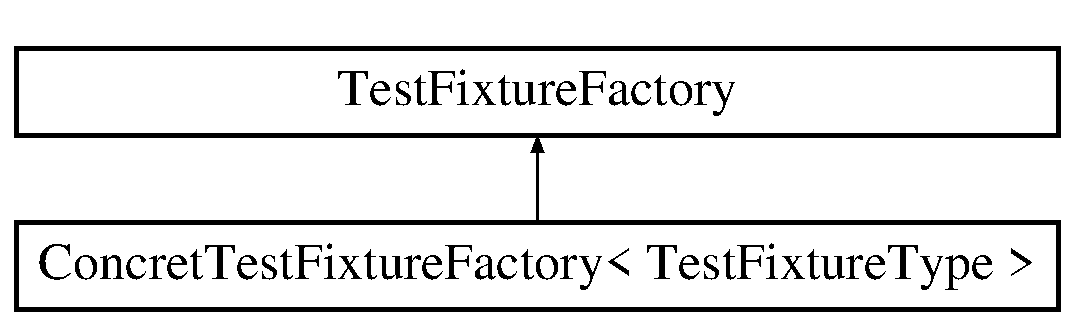
\includegraphics[height=2.000000cm]{class_concret_test_fixture_factory}
\end{center}
\end{figure}


\subsection{Detailed Description}
\subsubsection*{template$<$class Test\-Fixture\-Type$>$class Concret\-Test\-Fixture\-Factory$<$ Test\-Fixture\-Type $>$}

Concret \hyperlink{class_test_fixture}{Test\-Fixture} factory (Implementation). 

Implementation detail. Use by Helper\-Macros to handle \hyperlink{class_test_fixture}{Test\-Fixture} hierarchy. 

The documentation for this class was generated from the following file\-:\begin{DoxyCompactItemize}
\item 
Cadriciel/\-Commun/\-Externe/cppunit/include/cppunit/extensions/Test\-Fixture\-Factory.\-h\end{DoxyCompactItemize}

\hypertarget{class_config_scene}{\section{Config\-Scene Class Reference}
\label{class_config_scene}\index{Config\-Scene@{Config\-Scene}}
}


Les variables de configuration de la classe C\-Scene. C'est une classe singleton.  




{\ttfamily \#include $<$Config\-Scene.\-h$>$}

Inheritance diagram for Config\-Scene\-:\begin{figure}[H]
\begin{center}
\leavevmode
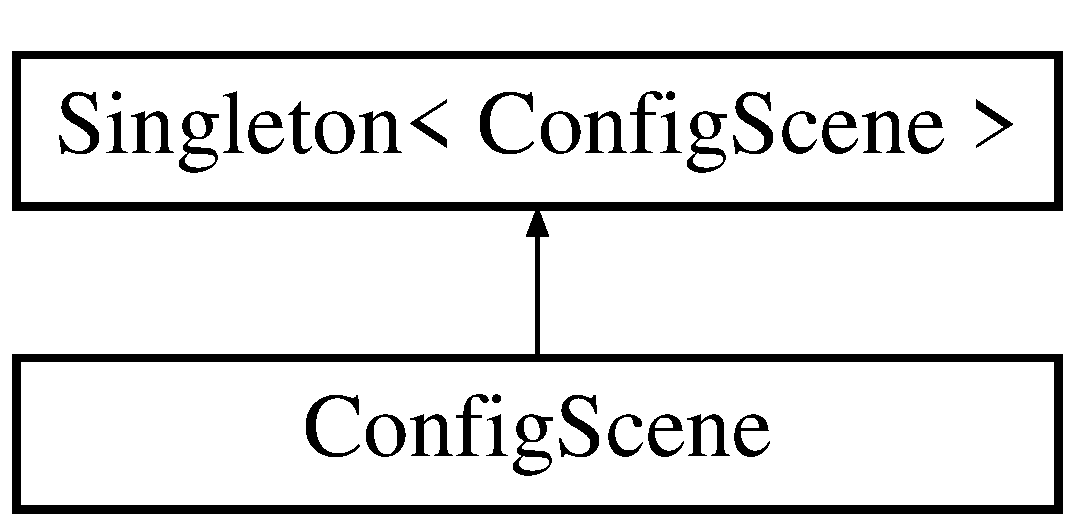
\includegraphics[height=2.000000cm]{class_config_scene}
\end{center}
\end{figure}
\subsection*{Public Member Functions}
\begin{DoxyCompactItemize}
\item 
\hyperlink{wglew_8h_aeea6e3dfae3acf232096f57d2d57f084}{void} \hyperlink{group__inf2990_gad74111f597fd4d2f58a08c6dedcb4270}{creer\-D\-O\-M} (\hyperlink{class_ti_xml_node}{Ti\-Xml\-Node} \&node) const 
\item 
\hyperlink{wglew_8h_aeea6e3dfae3acf232096f57d2d57f084}{void} \hyperlink{group__inf2990_gaa29c1518d06292658bfd90d3c6d379d3}{lire\-D\-O\-M} (const \hyperlink{class_ti_xml_node}{Ti\-Xml\-Node} \&node)
\end{DoxyCompactItemize}
\subsection*{Static Public Attributes}
\begin{DoxyCompactItemize}
\item 
static \hyperlink{wglew_8h_a500a82aecba06f4550f6849b8099ca21}{int} \hyperlink{group__inf2990_gadb487b450a0314a5d1f75cf31ce502eb}{C\-A\-L\-C\-U\-L\-S\-\_\-\-P\-A\-R\-\_\-\-I\-M\-A\-G\-E} = 50
\begin{DoxyCompactList}\small\item\em Nombre de calculs par image. \end{DoxyCompactList}\end{DoxyCompactItemize}
\subsection*{Additional Inherited Members}


\subsection{Detailed Description}
Les variables de configuration de la classe C\-Scene. C'est une classe singleton. 

\begin{DoxyAuthor}{Author}
Jean-\/\-Francois Perusse 
\end{DoxyAuthor}
\begin{DoxyDate}{Date}
2007-\/01-\/10 
\end{DoxyDate}


The documentation for this class was generated from the following files\-:\begin{DoxyCompactItemize}
\item 
Cadriciel/\-Sources/\-C++/\-Configuration/\hyperlink{_config_scene_8h}{Config\-Scene.\-h}\item 
Cadriciel/\-Sources/\-C++/\-Configuration/\hyperlink{_config_scene_8cpp}{Config\-Scene.\-cpp}\end{DoxyCompactItemize}

\hypertarget{class_config_scene_test}{\section{Config\-Scene\-Test Class Reference}
\label{class_config_scene_test}\index{Config\-Scene\-Test@{Config\-Scene\-Test}}
}


Classe de test cppunit pour tester le bon fonctionnement des methodes de la classe \hyperlink{class_config_scene}{Config\-Scene}.  




{\ttfamily \#include $<$Config\-Scene\-Test.\-h$>$}

Inheritance diagram for Config\-Scene\-Test\-:\begin{figure}[H]
\begin{center}
\leavevmode
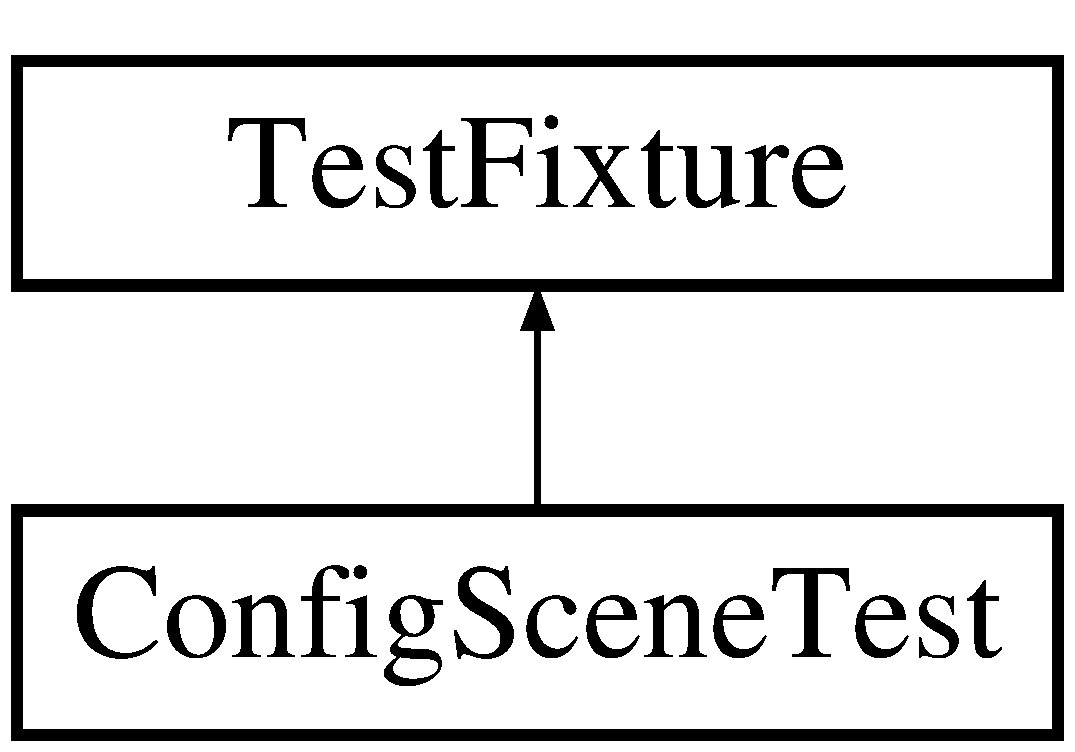
\includegraphics[height=2.000000cm]{class_config_scene_test}
\end{center}
\end{figure}
\subsection*{Public Member Functions}
\begin{DoxyCompactItemize}
\item 
void \hyperlink{group__inf2990_ga707d7400843047e67b736ab79bafb5a0}{set\-Up} ()
\begin{DoxyCompactList}\small\item\em Traitement a effectuer pour initialiser cette suite de tests. \end{DoxyCompactList}\item 
void \hyperlink{group__inf2990_ga889ed3891c3e55280cabb982953906d9}{tear\-Down} ()
\begin{DoxyCompactList}\small\item\em Traitement a effectuer pour 'finaliser' cette suite de tests. \end{DoxyCompactList}\item 
void \hyperlink{group__inf2990_ga0f09d52bc30d87f18b0341e1052efb74}{test\-Sauvegarde\-Chargement} ()
\begin{DoxyCompactList}\small\item\em Cas de test\-: sauvegarde et chargement X\-M\-L d'une carte. \end{DoxyCompactList}\item 
\hypertarget{group__inf2990_gac6b0ce9867809f3caab1e8f0a3d1a54a}{void \hyperlink{group__inf2990_gac6b0ce9867809f3caab1e8f0a3d1a54a}{test\-Taille} ()}\label{group__inf2990_gac6b0ce9867809f3caab1e8f0a3d1a54a}

\begin{DoxyCompactList}\small\item\em Cas de test\-: sauvegarde et chargment correct de la taille d'un element. \end{DoxyCompactList}\item 
\hypertarget{group__inf2990_gab62faa9bff39bff7feb25dffda78c21a}{void \hyperlink{group__inf2990_gab62faa9bff39bff7feb25dffda78c21a}{test\-Rotation} ()}\label{group__inf2990_gab62faa9bff39bff7feb25dffda78c21a}

\begin{DoxyCompactList}\small\item\em Cas de test\-: sauvegarde et chargment correct de la rotation d'un element. \end{DoxyCompactList}\end{DoxyCompactItemize}


\subsection{Detailed Description}
Classe de test cppunit pour tester le bon fonctionnement des methodes de la classe \hyperlink{class_config_scene}{Config\-Scene}. 

\begin{DoxyAuthor}{Author}
Julien Gascon-\/\-Samson 
\end{DoxyAuthor}
\begin{DoxyDate}{Date}
2011-\/07-\/16 
\end{DoxyDate}


The documentation for this class was generated from the following files\-:\begin{DoxyCompactItemize}
\item 
Cadriciel/\-Sources/\-C++/\-Tests/\hyperlink{_config_scene_test_8h}{Config\-Scene\-Test.\-h}\item 
Cadriciel/\-Sources/\-C++/\-Tests/\hyperlink{_config_scene_test_8cpp}{Config\-Scene\-Test.\-cpp}\end{DoxyCompactItemize}

\hypertarget{struct_cpp_unit_test_plug_in}{\section{Cpp\-Unit\-Test\-Plug\-In Struct Reference}
\label{struct_cpp_unit_test_plug_in}\index{Cpp\-Unit\-Test\-Plug\-In@{Cpp\-Unit\-Test\-Plug\-In}}
}


\hyperlink{class_test}{Test} plug-\/in interface.

This class define the interface implemented by test plug-\/in. A pointer to that interface is returned by the function exported by the test plug-\/in.  




{\ttfamily \#include $<$Test\-Plug\-In.\-h$>$}

Inheritance diagram for Cpp\-Unit\-Test\-Plug\-In\-:\begin{figure}[H]
\begin{center}
\leavevmode
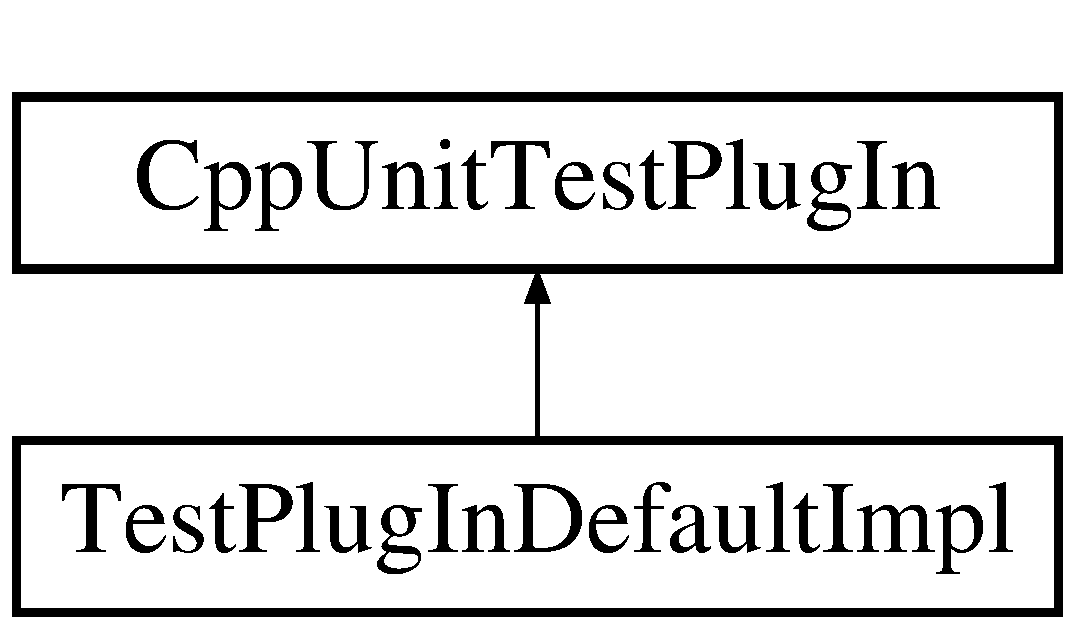
\includegraphics[height=2.000000cm]{struct_cpp_unit_test_plug_in}
\end{center}
\end{figure}
\subsection*{Public Member Functions}
\begin{DoxyCompactItemize}
\item 
virtual void \hyperlink{struct_cpp_unit_test_plug_in_aec670330e7fced26c2a66b1dcd56edc0}{initialize} (C\-P\-P\-U\-N\-I\-T\-\_\-\-N\-S\-::\-Test\-Factory\-Registry $\ast$registry, const C\-P\-P\-U\-N\-I\-T\-\_\-\-N\-S\-::\-Plug\-In\-Parameters \&parameters)=0
\begin{DoxyCompactList}\small\item\em Called just after loading the dynamic library. \end{DoxyCompactList}\item 
virtual void \hyperlink{struct_cpp_unit_test_plug_in_aad8038dc72d0f9798379937fe5692c97}{add\-Listener} (C\-P\-P\-U\-N\-I\-T\-\_\-\-N\-S\-::\-Test\-Result $\ast$event\-Manager)=0
\begin{DoxyCompactList}\small\item\em Gives a chance to the plug-\/in to register \hyperlink{class_test_listener}{Test\-Listener}. \end{DoxyCompactList}\item 
virtual void \hyperlink{struct_cpp_unit_test_plug_in_a8f36157014b515d38efbc8ab67923d85}{remove\-Listener} (C\-P\-P\-U\-N\-I\-T\-\_\-\-N\-S\-::\-Test\-Result $\ast$event\-Manager)=0
\begin{DoxyCompactList}\small\item\em Gives a chance to the plug-\/in to remove its registered \hyperlink{class_test_listener}{Test\-Listener}. \end{DoxyCompactList}\item 
\hypertarget{struct_cpp_unit_test_plug_in_a547cfddd0513dc9182721f723e27d9e3}{virtual void \hyperlink{struct_cpp_unit_test_plug_in_a547cfddd0513dc9182721f723e27d9e3}{add\-Xml\-Outputter\-Hooks} (C\-P\-P\-U\-N\-I\-T\-\_\-\-N\-S\-::\-Xml\-Outputter $\ast$outputter)=0}\label{struct_cpp_unit_test_plug_in_a547cfddd0513dc9182721f723e27d9e3}

\begin{DoxyCompactList}\small\item\em Provides a way for the plug-\/in to register some \hyperlink{class_xml_outputter_hook}{Xml\-Outputter\-Hook}. \end{DoxyCompactList}\item 
virtual void \hyperlink{struct_cpp_unit_test_plug_in_a045727ad9658525838b0b9157065fbcd}{remove\-Xml\-Outputter\-Hooks} ()=0
\begin{DoxyCompactList}\small\item\em Called when the \hyperlink{class_xml_outputter}{Xml\-Outputter} is destroyed. \end{DoxyCompactList}\item 
virtual void \hyperlink{struct_cpp_unit_test_plug_in_a8628d2026e76c58f715e17af88f77458}{uninitialize} (C\-P\-P\-U\-N\-I\-T\-\_\-\-N\-S\-::\-Test\-Factory\-Registry $\ast$registry)=0
\begin{DoxyCompactList}\small\item\em Called just before unloading the dynamic library. \end{DoxyCompactList}\end{DoxyCompactItemize}


\subsection{Detailed Description}
\hyperlink{class_test}{Test} plug-\/in interface.

This class define the interface implemented by test plug-\/in. A pointer to that interface is returned by the function exported by the test plug-\/in. 

Plug-\/in are loaded/unloaded by \hyperlink{class_plug_in_manager}{Plug\-In\-Manager}. When a plug-\/in is loaded, \hyperlink{struct_cpp_unit_test_plug_in_aec670330e7fced26c2a66b1dcd56edc0}{initialize()} is called. Before unloading the plug-\/in, the \hyperlink{class_plug_in_manager}{Plug\-In\-Manager} call \hyperlink{struct_cpp_unit_test_plug_in_a8628d2026e76c58f715e17af88f77458}{uninitialize()}.

\hyperlink{struct_cpp_unit_test_plug_in_aad8038dc72d0f9798379937fe5692c97}{add\-Listener()} and \hyperlink{struct_cpp_unit_test_plug_in_a8f36157014b515d38efbc8ab67923d85}{remove\-Listener()} are called respectively before and after the test run.

\hyperlink{struct_cpp_unit_test_plug_in_a547cfddd0513dc9182721f723e27d9e3}{add\-Xml\-Outputter\-Hooks()} and \hyperlink{struct_cpp_unit_test_plug_in_a045727ad9658525838b0b9157065fbcd}{remove\-Xml\-Outputter\-Hooks()} are called respectively before and after writing the X\-M\-L output using a \hyperlink{class_xml_outputter}{Xml\-Outputter}.

\begin{DoxySeeAlso}{See Also}
\hyperlink{_test_plug_in_8h_a705897c323d9381ac1b99a45e953e4ff}{C\-P\-P\-U\-N\-I\-T\-\_\-\-P\-L\-U\-G\-I\-N\-\_\-\-I\-M\-P\-L\-E\-M\-E\-N\-T}, \hyperlink{_test_plug_in_8h_a81bfba0323e2c7ca7dfd6767db813a5b}{C\-P\-P\-U\-N\-I\-T\-\_\-\-P\-L\-U\-G\-I\-N\-\_\-\-E\-X\-P\-O\-R\-T\-E\-D\-\_\-\-F\-U\-N\-C\-T\-I\-O\-N\-\_\-\-I\-M\-P\-L} 

Cpp\-Unit\-::\-Test\-Plug\-In\-Default\-Impl, Cpp\-Unit\-::\-Xml\-Outputter. 
\end{DoxySeeAlso}


\subsection{Member Function Documentation}
\hypertarget{struct_cpp_unit_test_plug_in_aad8038dc72d0f9798379937fe5692c97}{\index{Cpp\-Unit\-Test\-Plug\-In@{Cpp\-Unit\-Test\-Plug\-In}!add\-Listener@{add\-Listener}}
\index{add\-Listener@{add\-Listener}!CppUnitTestPlugIn@{Cpp\-Unit\-Test\-Plug\-In}}
\subsubsection[{add\-Listener}]{\setlength{\rightskip}{0pt plus 5cm}virtual void Cpp\-Unit\-Test\-Plug\-In\-::add\-Listener (
\begin{DoxyParamCaption}
\item[{C\-P\-P\-U\-N\-I\-T\-\_\-\-N\-S\-::\-Test\-Result $\ast$}]{event\-Manager}
\end{DoxyParamCaption}
)\hspace{0.3cm}{\ttfamily [pure virtual]}}}\label{struct_cpp_unit_test_plug_in_aad8038dc72d0f9798379937fe5692c97}


Gives a chance to the plug-\/in to register \hyperlink{class_test_listener}{Test\-Listener}. 

Override this method to add a \hyperlink{class_test_listener}{Test\-Listener} for the test run. This is useful if you are writing a custom \hyperlink{class_test_listener}{Test\-Listener}, but also if you need to set\-Up some global resource\-: listen to \hyperlink{class_test_listener_a263428abdf29b2a7123af4096771925e}{Test\-Listener\-::start\-Test\-Run()}, and \hyperlink{class_test_listener_a0411708032f688f6ec234bcc5e089289}{Test\-Listener\-::end\-Test\-Run()}. \hypertarget{struct_cpp_unit_test_plug_in_aec670330e7fced26c2a66b1dcd56edc0}{\index{Cpp\-Unit\-Test\-Plug\-In@{Cpp\-Unit\-Test\-Plug\-In}!initialize@{initialize}}
\index{initialize@{initialize}!CppUnitTestPlugIn@{Cpp\-Unit\-Test\-Plug\-In}}
\subsubsection[{initialize}]{\setlength{\rightskip}{0pt plus 5cm}virtual void Cpp\-Unit\-Test\-Plug\-In\-::initialize (
\begin{DoxyParamCaption}
\item[{C\-P\-P\-U\-N\-I\-T\-\_\-\-N\-S\-::\-Test\-Factory\-Registry $\ast$}]{registry, }
\item[{const C\-P\-P\-U\-N\-I\-T\-\_\-\-N\-S\-::\-Plug\-In\-Parameters \&}]{parameters}
\end{DoxyParamCaption}
)\hspace{0.3cm}{\ttfamily [pure virtual]}}}\label{struct_cpp_unit_test_plug_in_aec670330e7fced26c2a66b1dcd56edc0}


Called just after loading the dynamic library. 

Override this method to add additional suite to the registry, though this is preferably done using the macros (C\-P\-P\-U\-N\-I\-T\-\_\-\-T\-E\-S\-T\-\_\-\-S\-U\-I\-T\-E\-\_\-\-R\-E\-G\-I\-S\-T\-R\-A\-T\-I\-O\-N...). If you are creating a custom listener to extends the plug-\/in runner, you can use this to configure the listener using the {\itshape parameters}.

You could also use the parameters to specify some global parameter, such as test datas location, database name...

N.\-B.\-: Parameters interface is not define yet, and the plug-\/in runner does not yet support plug-\/in parameter. \hypertarget{struct_cpp_unit_test_plug_in_a8f36157014b515d38efbc8ab67923d85}{\index{Cpp\-Unit\-Test\-Plug\-In@{Cpp\-Unit\-Test\-Plug\-In}!remove\-Listener@{remove\-Listener}}
\index{remove\-Listener@{remove\-Listener}!CppUnitTestPlugIn@{Cpp\-Unit\-Test\-Plug\-In}}
\subsubsection[{remove\-Listener}]{\setlength{\rightskip}{0pt plus 5cm}virtual void Cpp\-Unit\-Test\-Plug\-In\-::remove\-Listener (
\begin{DoxyParamCaption}
\item[{C\-P\-P\-U\-N\-I\-T\-\_\-\-N\-S\-::\-Test\-Result $\ast$}]{event\-Manager}
\end{DoxyParamCaption}
)\hspace{0.3cm}{\ttfamily [pure virtual]}}}\label{struct_cpp_unit_test_plug_in_a8f36157014b515d38efbc8ab67923d85}


Gives a chance to the plug-\/in to remove its registered \hyperlink{class_test_listener}{Test\-Listener}. 

Override this method to remove a \hyperlink{class_test_listener}{Test\-Listener} that has been added. \hypertarget{struct_cpp_unit_test_plug_in_a045727ad9658525838b0b9157065fbcd}{\index{Cpp\-Unit\-Test\-Plug\-In@{Cpp\-Unit\-Test\-Plug\-In}!remove\-Xml\-Outputter\-Hooks@{remove\-Xml\-Outputter\-Hooks}}
\index{remove\-Xml\-Outputter\-Hooks@{remove\-Xml\-Outputter\-Hooks}!CppUnitTestPlugIn@{Cpp\-Unit\-Test\-Plug\-In}}
\subsubsection[{remove\-Xml\-Outputter\-Hooks}]{\setlength{\rightskip}{0pt plus 5cm}virtual void Cpp\-Unit\-Test\-Plug\-In\-::remove\-Xml\-Outputter\-Hooks (
\begin{DoxyParamCaption}
{}
\end{DoxyParamCaption}
)\hspace{0.3cm}{\ttfamily [pure virtual]}}}\label{struct_cpp_unit_test_plug_in_a045727ad9658525838b0b9157065fbcd}


Called when the \hyperlink{class_xml_outputter}{Xml\-Outputter} is destroyed. 

Can be used to free some resources allocated by \hyperlink{struct_cpp_unit_test_plug_in_a547cfddd0513dc9182721f723e27d9e3}{add\-Xml\-Outputter\-Hooks()}. 

Implemented in \hyperlink{class_test_plug_in_default_impl_aa4fa891e799ff362dece734417afd93d}{Test\-Plug\-In\-Default\-Impl}.

\hypertarget{struct_cpp_unit_test_plug_in_a8628d2026e76c58f715e17af88f77458}{\index{Cpp\-Unit\-Test\-Plug\-In@{Cpp\-Unit\-Test\-Plug\-In}!uninitialize@{uninitialize}}
\index{uninitialize@{uninitialize}!CppUnitTestPlugIn@{Cpp\-Unit\-Test\-Plug\-In}}
\subsubsection[{uninitialize}]{\setlength{\rightskip}{0pt plus 5cm}virtual void Cpp\-Unit\-Test\-Plug\-In\-::uninitialize (
\begin{DoxyParamCaption}
\item[{C\-P\-P\-U\-N\-I\-T\-\_\-\-N\-S\-::\-Test\-Factory\-Registry $\ast$}]{registry}
\end{DoxyParamCaption}
)\hspace{0.3cm}{\ttfamily [pure virtual]}}}\label{struct_cpp_unit_test_plug_in_a8628d2026e76c58f715e17af88f77458}


Called just before unloading the dynamic library. 

Override this method to unregister test factory added in \hyperlink{struct_cpp_unit_test_plug_in_aec670330e7fced26c2a66b1dcd56edc0}{initialize()}. This is necessary to keep the \hyperlink{class_test_factory_registry}{Test\-Factory\-Registry} 'clean'. When the plug-\/in is unloaded from memory, the \hyperlink{class_test_factory_registry}{Test\-Factory\-Registry} will hold reference on test that are no longer available if they are not unregistered. 

The documentation for this struct was generated from the following file\-:\begin{DoxyCompactItemize}
\item 
Cadriciel/\-Commun/\-Externe/cppunit/include/cppunit/plugin/\hyperlink{_test_plug_in_8h}{Test\-Plug\-In.\-h}\end{DoxyCompactItemize}

\hypertarget{class_assimp_1_1_default_logger}{\section{Assimp\-:\-:Default\-Logger Class Reference}
\label{class_assimp_1_1_default_logger}\index{Assimp\-::\-Default\-Logger@{Assimp\-::\-Default\-Logger}}
}


C\-P\-P-\/\-A\-P\-I\-: Primary logging facility of \hyperlink{namespace_assimp}{Assimp}.  




{\ttfamily \#include $<$Default\-Logger.\-h$>$}

Inheritance diagram for Assimp\-:\-:Default\-Logger\-:\begin{figure}[H]
\begin{center}
\leavevmode
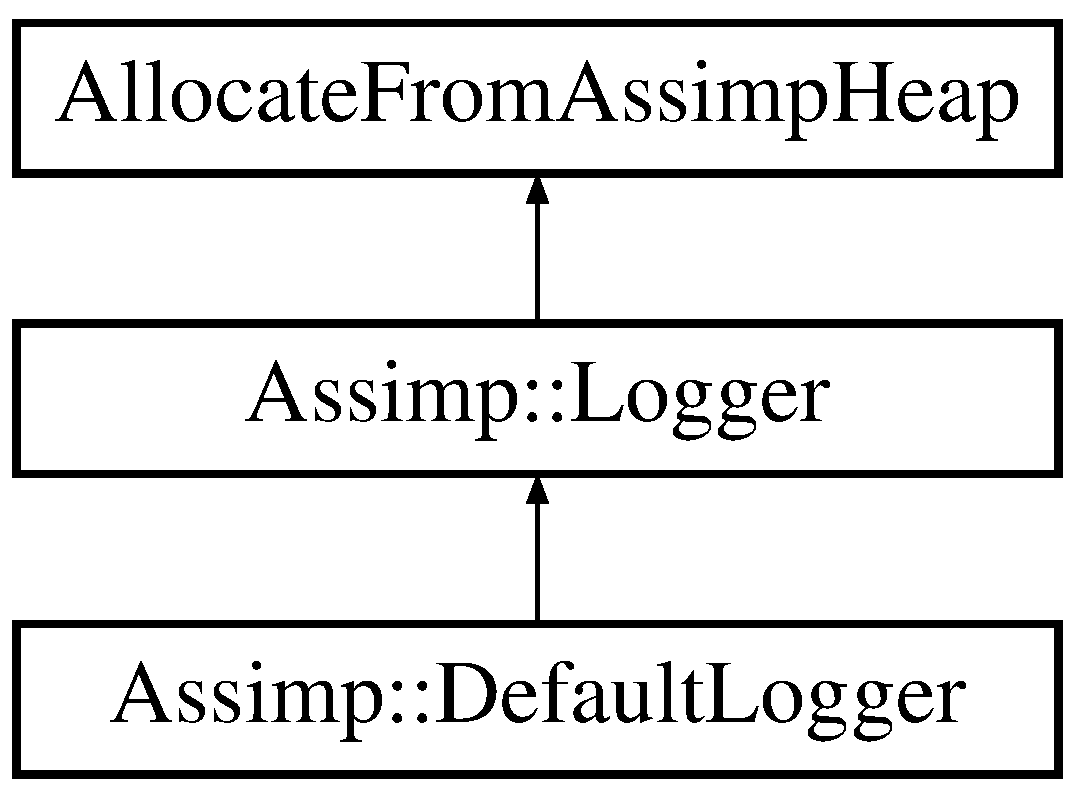
\includegraphics[height=3.000000cm]{class_assimp_1_1_default_logger}
\end{center}
\end{figure}
\subsection*{Public Member Functions}
\begin{DoxyCompactItemize}
\item 
bool \hyperlink{class_assimp_1_1_default_logger_abc0ca7a337f8c3e38eca0eb45bb1ccf0}{attach\-Stream} (\hyperlink{class_assimp_1_1_log_stream}{Log\-Stream} $\ast$p\-Stream, unsigned int severity)
\begin{DoxyCompactList}\small\item\em Attach a new logstream. \end{DoxyCompactList}\item 
bool \hyperlink{class_assimp_1_1_default_logger_a2615f1d1624f1d742d0cf2dd4a5cccc8}{detatch\-Stream} (\hyperlink{class_assimp_1_1_log_stream}{Log\-Stream} $\ast$p\-Stream, unsigned int severity)
\begin{DoxyCompactList}\small\item\em Detach a still attached stream from the logger (or modify the filter flags bits) \end{DoxyCompactList}\end{DoxyCompactItemize}
\subsection*{Static Public Member Functions}
\begin{DoxyCompactItemize}
\item 
static \hyperlink{class_assimp_1_1_logger}{Logger} $\ast$ \hyperlink{class_assimp_1_1_default_logger_adccb11f85f8b0ef226c382e11ba665c3}{create} (const char $\ast$name=\hyperlink{_default_logger_8h_a5e31e6d6c9f8a8954134f3da38fec0a0}{A\-S\-S\-I\-M\-P\-\_\-\-D\-E\-F\-A\-U\-L\-T\-\_\-\-L\-O\-G\-\_\-\-N\-A\-M\-E}, \hyperlink{class_assimp_1_1_logger_a8b6248a0fd062431e8572556350d29e6}{Log\-Severity} severity=\hyperlink{class_assimp_1_1_logger_a8b6248a0fd062431e8572556350d29e6a79d16f85dc21486ee489f300027e8eda}{N\-O\-R\-M\-A\-L}, unsigned int def\-Streams=ai\-Default\-Log\-Stream\-\_\-\-D\-E\-B\-U\-G\-G\-E\-R$\vert$ai\-Default\-Log\-Stream\-\_\-\-F\-I\-L\-E, \hyperlink{class_assimp_1_1_i_o_system}{I\-O\-System} $\ast$io=N\-U\-L\-L)
\begin{DoxyCompactList}\small\item\em Creates a logging instance. \end{DoxyCompactList}\item 
static void \hyperlink{class_assimp_1_1_default_logger_a9daba548026045b99813c760c2842ed2}{set} (\hyperlink{class_assimp_1_1_logger}{Logger} $\ast$logger)
\begin{DoxyCompactList}\small\item\em Setup a custom \hyperlink{class_assimp_1_1_logger_a784e6d1a741072b17bab32a6a41055e8}{Logger} implementation. \end{DoxyCompactList}\item 
static \hyperlink{class_assimp_1_1_logger}{Logger} $\ast$ \hyperlink{class_assimp_1_1_default_logger_a7d0a53f2db66945ade30094330a77ba4}{get} ()
\begin{DoxyCompactList}\small\item\em Getter for singleton instance. \end{DoxyCompactList}\item 
static bool \hyperlink{class_assimp_1_1_default_logger_abebc7ee702a2a2dde765e771948400c6}{is\-Null\-Logger} ()
\begin{DoxyCompactList}\small\item\em Return whether a \#\-Null\-Logger is currently active. \end{DoxyCompactList}\item 
\hypertarget{class_assimp_1_1_default_logger_a0b1da096d7442af5a4a4cb5ebb2540f7}{static void \hyperlink{class_assimp_1_1_default_logger_a0b1da096d7442af5a4a4cb5ebb2540f7}{kill} ()}\label{class_assimp_1_1_default_logger_a0b1da096d7442af5a4a4cb5ebb2540f7}

\begin{DoxyCompactList}\small\item\em Kills the current singleton logger and replaces it with a \#\-Null\-Logger instance. \end{DoxyCompactList}\end{DoxyCompactItemize}
\subsection*{Additional Inherited Members}


\subsection{Detailed Description}
C\-P\-P-\/\-A\-P\-I\-: Primary logging facility of \hyperlink{namespace_assimp}{Assimp}. 

The library stores its primary \hyperlink{class_assimp_1_1_logger_a784e6d1a741072b17bab32a6a41055e8}{Logger} as a static member of this class. \hyperlink{class_assimp_1_1_default_logger_a7d0a53f2db66945ade30094330a77ba4}{get()} returns this primary logger. By default the underlying implementation is just a \#\-Null\-Logger which rejects all log messages. By calling \hyperlink{class_assimp_1_1_default_logger_adccb11f85f8b0ef226c382e11ba665c3}{create()}, logging is turned on. To capture the log output multiple log streams (\#\-Log\-Stream) can be attach to the logger. Some default streams for common streaming locations (such as a file, std\-::cout, Output\-Debug\-String()) are also provided.

If you wish to customize the logging at an even deeper level supply your own implementation of \hyperlink{class_assimp_1_1_logger_a784e6d1a741072b17bab32a6a41055e8}{Logger} to \hyperlink{class_assimp_1_1_default_logger_a9daba548026045b99813c760c2842ed2}{set()}. \begin{DoxyNote}{Note}
The whole logging stuff causes a small extra overhead for all imports. 
\end{DoxyNote}


\subsection{Member Function Documentation}
\hypertarget{class_assimp_1_1_default_logger_abc0ca7a337f8c3e38eca0eb45bb1ccf0}{\index{Assimp\-::\-Default\-Logger@{Assimp\-::\-Default\-Logger}!attach\-Stream@{attach\-Stream}}
\index{attach\-Stream@{attach\-Stream}!Assimp::DefaultLogger@{Assimp\-::\-Default\-Logger}}
\subsubsection[{attach\-Stream}]{\setlength{\rightskip}{0pt plus 5cm}bool Assimp\-::\-Default\-Logger\-::attach\-Stream (
\begin{DoxyParamCaption}
\item[{{\bf Log\-Stream} $\ast$}]{p\-Stream, }
\item[{unsigned int}]{severity}
\end{DoxyParamCaption}
)\hspace{0.3cm}{\ttfamily [virtual]}}}\label{class_assimp_1_1_default_logger_abc0ca7a337f8c3e38eca0eb45bb1ccf0}


Attach a new logstream. 

The logger takes ownership of the stream and is responsible for its destruction (which is done using \-::delete when the logger itself is destroyed). Call detach\-Stream to detach a stream and to gain ownership of it again. 
\begin{DoxyParams}{Parameters}
{\em p\-Stream} & Logstream to attach \\
\hline
{\em severity} & \hyperlink{class_message}{Message} filter, specified which types of log messages are dispatched to the stream. Provide a bitwise combination of the Error\-Severity flags. \\
\hline
\end{DoxyParams}
\begin{DoxyReturn}{Returns}
true if the stream has been attached, false otherwise. 
\end{DoxyReturn}


Implements \hyperlink{class_assimp_1_1_logger_a56fbf4f392712f06d3c5bb581c3f3906}{Assimp\-::\-Logger}.

\hypertarget{class_assimp_1_1_default_logger_adccb11f85f8b0ef226c382e11ba665c3}{\index{Assimp\-::\-Default\-Logger@{Assimp\-::\-Default\-Logger}!create@{create}}
\index{create@{create}!Assimp::DefaultLogger@{Assimp\-::\-Default\-Logger}}
\subsubsection[{create}]{\setlength{\rightskip}{0pt plus 5cm}static {\bf Logger}$\ast$ Assimp\-::\-Default\-Logger\-::create (
\begin{DoxyParamCaption}
\item[{const char $\ast$}]{name = {\ttfamily {\bf A\-S\-S\-I\-M\-P\-\_\-\-D\-E\-F\-A\-U\-L\-T\-\_\-\-L\-O\-G\-\_\-\-N\-A\-M\-E}}, }
\item[{{\bf Log\-Severity}}]{severity = {\ttfamily {\bf N\-O\-R\-M\-A\-L}}, }
\item[{unsigned int}]{def\-Streams = {\ttfamily aiDefaultLogStream\-\_\-DEBUGGER$\vert$aiDefaultLogStream\-\_\-FILE}, }
\item[{{\bf I\-O\-System} $\ast$}]{io = {\ttfamily NULL}}
\end{DoxyParamCaption}
)\hspace{0.3cm}{\ttfamily [static]}}}\label{class_assimp_1_1_default_logger_adccb11f85f8b0ef226c382e11ba665c3}


Creates a logging instance. 


\begin{DoxyParams}{Parameters}
{\em name} & Name for log file. Only valid in combination with the ai\-Default\-Log\-Stream\-\_\-\-F\-I\-L\-E flag. \\
\hline
{\em severity} & Log severity, V\-E\-R\-B\-O\-S\-E turns on debug messages \\
\hline
{\em def\-Streams} & Default log streams to be attached. Any bitwise combination of the ai\-Default\-Log\-Stream enumerated values. If \#ai\-Default\-Log\-Stream\-\_\-\-F\-I\-L\-E is specified but an empty string is passed for 'name', no log file is created at all. \\
\hline
{\em io} & \hyperlink{class_assimp_1_1_i_o_system}{I\-O\-System} to be used to open external files (such as the log file). Pass N\-U\-L\-L to rely on the default implementation. This replaces the default \#\-Null\-Logger with a \#\-Default\-Logger instance. \\
\hline
\end{DoxyParams}
\hypertarget{class_assimp_1_1_default_logger_a2615f1d1624f1d742d0cf2dd4a5cccc8}{\index{Assimp\-::\-Default\-Logger@{Assimp\-::\-Default\-Logger}!detatch\-Stream@{detatch\-Stream}}
\index{detatch\-Stream@{detatch\-Stream}!Assimp::DefaultLogger@{Assimp\-::\-Default\-Logger}}
\subsubsection[{detatch\-Stream}]{\setlength{\rightskip}{0pt plus 5cm}bool Assimp\-::\-Default\-Logger\-::detatch\-Stream (
\begin{DoxyParamCaption}
\item[{{\bf Log\-Stream} $\ast$}]{p\-Stream, }
\item[{unsigned int}]{severity}
\end{DoxyParamCaption}
)\hspace{0.3cm}{\ttfamily [virtual]}}}\label{class_assimp_1_1_default_logger_a2615f1d1624f1d742d0cf2dd4a5cccc8}


Detach a still attached stream from the logger (or modify the filter flags bits) 


\begin{DoxyParams}{Parameters}
{\em p\-Stream} & Logstream instance for detaching \\
\hline
{\em severity} & Provide a bitwise combination of the Error\-Severity flags. This value is \&$\sim$ed with the current flags of the stream, if the result is 0 the stream is detached from the \hyperlink{class_assimp_1_1_logger}{Logger} and the caller retakes the possession of the stream. \\
\hline
\end{DoxyParams}
\begin{DoxyReturn}{Returns}
true if the stream has been dettached, false otherwise. 
\end{DoxyReturn}


Implements \hyperlink{class_assimp_1_1_logger_ac89b2edd326dda9046fe9d4e1f4d10fc}{Assimp\-::\-Logger}.

\hypertarget{class_assimp_1_1_default_logger_a7d0a53f2db66945ade30094330a77ba4}{\index{Assimp\-::\-Default\-Logger@{Assimp\-::\-Default\-Logger}!get@{get}}
\index{get@{get}!Assimp::DefaultLogger@{Assimp\-::\-Default\-Logger}}
\subsubsection[{get}]{\setlength{\rightskip}{0pt plus 5cm}static {\bf Logger}$\ast$ Assimp\-::\-Default\-Logger\-::get (
\begin{DoxyParamCaption}
{}
\end{DoxyParamCaption}
)\hspace{0.3cm}{\ttfamily [static]}}}\label{class_assimp_1_1_default_logger_a7d0a53f2db66945ade30094330a77ba4}


Getter for singleton instance. 

\begin{DoxyReturn}{Returns}
Only instance. This is never null, but it could be a \hyperlink{class_assimp_1_1_null_logger}{Null\-Logger}. Use is\-Null\-Logger to check this. 
\end{DoxyReturn}
\hypertarget{class_assimp_1_1_default_logger_abebc7ee702a2a2dde765e771948400c6}{\index{Assimp\-::\-Default\-Logger@{Assimp\-::\-Default\-Logger}!is\-Null\-Logger@{is\-Null\-Logger}}
\index{is\-Null\-Logger@{is\-Null\-Logger}!Assimp::DefaultLogger@{Assimp\-::\-Default\-Logger}}
\subsubsection[{is\-Null\-Logger}]{\setlength{\rightskip}{0pt plus 5cm}static bool Assimp\-::\-Default\-Logger\-::is\-Null\-Logger (
\begin{DoxyParamCaption}
{}
\end{DoxyParamCaption}
)\hspace{0.3cm}{\ttfamily [static]}}}\label{class_assimp_1_1_default_logger_abebc7ee702a2a2dde765e771948400c6}


Return whether a \#\-Null\-Logger is currently active. 

\begin{DoxyReturn}{Returns}
true if the current logger is a \#\-Null\-Logger. Use \hyperlink{class_assimp_1_1_default_logger_adccb11f85f8b0ef226c382e11ba665c3}{create()} or \hyperlink{class_assimp_1_1_default_logger_a9daba548026045b99813c760c2842ed2}{set()} to setup a logger that does actually do something else than just rejecting all log messages. 
\end{DoxyReturn}
\hypertarget{class_assimp_1_1_default_logger_a9daba548026045b99813c760c2842ed2}{\index{Assimp\-::\-Default\-Logger@{Assimp\-::\-Default\-Logger}!set@{set}}
\index{set@{set}!Assimp::DefaultLogger@{Assimp\-::\-Default\-Logger}}
\subsubsection[{set}]{\setlength{\rightskip}{0pt plus 5cm}static void Assimp\-::\-Default\-Logger\-::set (
\begin{DoxyParamCaption}
\item[{{\bf Logger} $\ast$}]{logger}
\end{DoxyParamCaption}
)\hspace{0.3cm}{\ttfamily [static]}}}\label{class_assimp_1_1_default_logger_a9daba548026045b99813c760c2842ed2}


Setup a custom \hyperlink{class_assimp_1_1_logger_a784e6d1a741072b17bab32a6a41055e8}{Logger} implementation. 

Use this if the provided \#\-Default\-Logger class doesn't fit into your needs. If the provided message formatting is O\-K for you, it's much easier to use \hyperlink{class_assimp_1_1_default_logger_adccb11f85f8b0ef226c382e11ba665c3}{create()} and to attach your own custom output streams to it. 
\begin{DoxyParams}{Parameters}
{\em logger} & Pass N\-U\-L\-L to setup a default \hyperlink{class_assimp_1_1_null_logger}{Null\-Logger} \\
\hline
\end{DoxyParams}


The documentation for this class was generated from the following file\-:\begin{DoxyCompactItemize}
\item 
Cadriciel/\-Commun/\-Externe/assimp/include/\hyperlink{_default_logger_8h}{Default\-Logger.\-h}\end{DoxyCompactItemize}

\hypertarget{class_interface_graphique_1_1_demarrage}{\section{Interface\-Graphique.\-Demarrage Class Reference}
\label{class_interface_graphique_1_1_demarrage}\index{Interface\-Graphique.\-Demarrage@{Interface\-Graphique.\-Demarrage}}
}
Inheritance diagram for Interface\-Graphique.\-Demarrage\-:\begin{figure}[H]
\begin{center}
\leavevmode
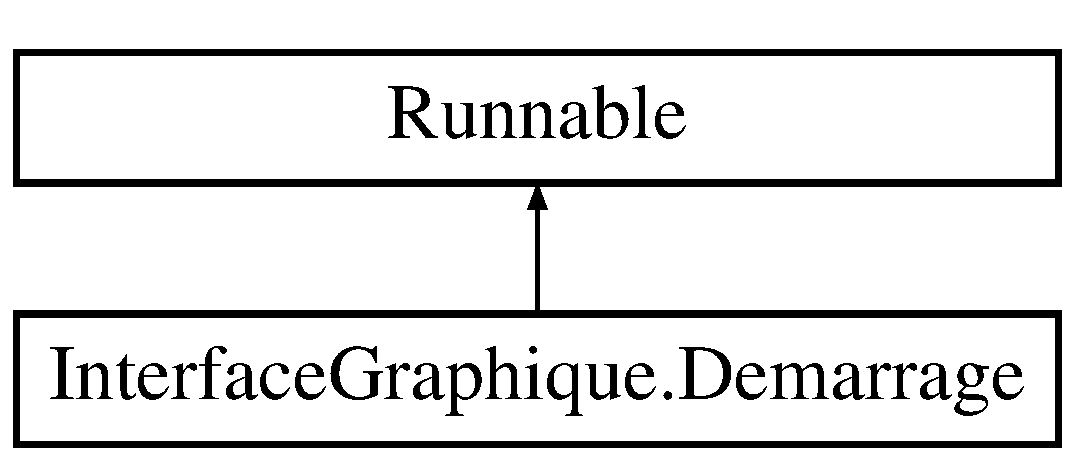
\includegraphics[height=2.000000cm]{class_interface_graphique_1_1_demarrage}
\end{center}
\end{figure}
\subsection*{Public Member Functions}
\begin{DoxyCompactItemize}
\item 
\hyperlink{class_interface_graphique_1_1_demarrage_aab1bcb7d2b2d0d67b2a1f443a9059d5c}{Demarrage} ()
\item 
\hyperlink{wglew_8h_aeea6e3dfae3acf232096f57d2d57f084}{void} \hyperlink{class_interface_graphique_1_1_demarrage_a5ba8d0338a858cacac0858bf5a929294}{run} ()
\item 
\hyperlink{class_interface_graphique_1_1_interface_generique}{Interface\-Generique} \hyperlink{class_interface_graphique_1_1_demarrage_a9bedc99311cf0fc9289398a4ade62881}{get\-Interface\-Jeu} ()
\item 
\hyperlink{wglew_8h_aeea6e3dfae3acf232096f57d2d57f084}{void} \hyperlink{class_interface_graphique_1_1_demarrage_a7ea2d557be440490330b4c8d4fad3310}{construction\-Fenetre\-Edition} ()
\item 
\hyperlink{wglew_8h_aeea6e3dfae3acf232096f57d2d57f084}{void} \hyperlink{class_interface_graphique_1_1_demarrage_a1458284107def5ab17ab84137e6ec925}{construction\-Fenetre\-Partie\-Rapide} ()
\item 
\hyperlink{wglew_8h_aeea6e3dfae3acf232096f57d2d57f084}{void} \hyperlink{class_interface_graphique_1_1_demarrage_a67eac408735f73f2509849cfca3a895e}{construction\-Fenetre\-Campagne} ()
\item 
\hyperlink{wglew_8h_aeea6e3dfae3acf232096f57d2d57f084}{void} \hyperlink{class_interface_graphique_1_1_demarrage_a75315a0d8de8cf442269c94408824c78}{construction\-Fenetre\-Test} ()
\item 
\hyperlink{class_interface_graphique_1_1_menu_principal}{Menu\-Principal} \hyperlink{class_interface_graphique_1_1_demarrage_a34d7cc460107f80e226a5becbfdbd328}{get\-Menu\-Principal} ()
\item 
\hyperlink{class_interface_graphique_1_1_fenetre_commune}{Fenetre\-Commune} \hyperlink{class_interface_graphique_1_1_demarrage_a7e88381b26dfe1b317f25ac0914b3b66}{get\-Fenetre\-Jeu} ()
\item 
\hyperlink{class_interface_graphique_1_1_instructions}{Instructions} \hyperlink{class_interface_graphique_1_1_demarrage_adf4bbd9377de2517004d29665fe49c92}{get\-Fenetre\-Instructions} ()
\item 
\hyperlink{class_interface_graphique_1_1_fenetre_configuration_diverses}{Fenetre\-Configuration\-Diverses} \hyperlink{class_interface_graphique_1_1_demarrage_ad7ea0e18e9f0515b93ed8406fbef37e7}{get\-Fenetre\-Configuration} ()
\item 
\hyperlink{enum_interface_graphique_1_1_mode_jeu}{Mode\-Jeu} \hyperlink{class_interface_graphique_1_1_demarrage_a5b2ef3b991374c8694a2c7f03793bacd}{get\-Mode\-Jeu} ()
\item 
\hyperlink{wglew_8h_aeea6e3dfae3acf232096f57d2d57f084}{void} \hyperlink{class_interface_graphique_1_1_demarrage_ad00019d212a67d38d91b38e2981fd561}{set\-Mode\-Jeu} (\hyperlink{enum_interface_graphique_1_1_mode_jeu}{Mode\-Jeu} \hyperlink{glew_8h_a1e71d9c196e4683cc06c4b54d53f7ef5}{mode})
\item 
\hyperlink{wglew_8h_aeea6e3dfae3acf232096f57d2d57f084}{void} \hyperlink{class_interface_graphique_1_1_demarrage_a5b7395f1012cef522ffaa0038e5718b8}{activer\-Minuterie} ()
\end{DoxyCompactItemize}
\subsection*{Static Public Member Functions}
\begin{DoxyCompactItemize}
\item 
static \hyperlink{wglew_8h_aeea6e3dfae3acf232096f57d2d57f084}{void} \hyperlink{class_interface_graphique_1_1_demarrage_ab132e51d880643e6c990f655b769ba17}{main} (String args\mbox{[}$\,$\mbox{]})
\item 
static native \hyperlink{wglew_8h_aeea6e3dfae3acf232096f57d2d57f084}{void} \hyperlink{class_interface_graphique_1_1_demarrage_ab3f3b04fdfcb895dcbfdb7fae89221b7}{fct\-C\-\_\-initialiser\-Open\-G\-L} (Canvas canvas)
\item 
static native \hyperlink{wglew_8h_aeea6e3dfae3acf232096f57d2d57f084}{void} \hyperlink{class_interface_graphique_1_1_demarrage_a05d12ffdd0d3d0ec5ed9892a0bfe1dbf}{fct\-C\-\_\-initialiser} ()
\item 
static native \hyperlink{wglew_8h_aeea6e3dfae3acf232096f57d2d57f084}{void} \hyperlink{class_interface_graphique_1_1_demarrage_a6056ae63e221fe5053941be32e12f591}{fct\-C\-\_\-initialiser\-Mode\-Edition} ()
\item 
static native \hyperlink{wglew_8h_aeea6e3dfae3acf232096f57d2d57f084}{void} \hyperlink{class_interface_graphique_1_1_demarrage_adc5fb6c8f782616b7213da2609ec354a}{fct\-C\-\_\-initialiser\-Mode\-Partie\-Rapide} (\hyperlink{wglew_8h_a500a82aecba06f4550f6849b8099ca21}{int} coop, \hyperlink{wglew_8h_a500a82aecba06f4550f6849b8099ca21}{int} joueur2, String nom\-Fichier)
\item 
static native \hyperlink{wglew_8h_aeea6e3dfae3acf232096f57d2d57f084}{void} \hyperlink{class_interface_graphique_1_1_demarrage_aa3d9f3cd07392f26881a7dde6ae4f97d}{fct\-C\-\_\-initialiser\-Mode\-Campagne} (\hyperlink{wglew_8h_a500a82aecba06f4550f6849b8099ca21}{int} coop, \hyperlink{wglew_8h_a500a82aecba06f4550f6849b8099ca21}{int} joueur2, Object\mbox{[}$\,$\mbox{]} cartes)
\item 
static native String \hyperlink{class_interface_graphique_1_1_demarrage_a972fac6b873d377e7e737ed2fcb44836}{fct\-C\-\_\-obtenir\-Informations\-Partie} ()
\item 
static native \hyperlink{wglew_8h_aeea6e3dfae3acf232096f57d2d57f084}{void} \hyperlink{class_interface_graphique_1_1_demarrage_a7ad7d1c76cd1de5a105be6891b857455}{fct\-C\-\_\-initialiser\-Mode\-Test} ()
\item 
static native \hyperlink{wglew_8h_aeea6e3dfae3acf232096f57d2d57f084}{void} \hyperlink{class_interface_graphique_1_1_demarrage_a9345154a7f42dc6671abaf5529407921}{fct\-C\-\_\-liberer\-Open\-G\-L} (Canvas canvas)
\item 
static native \hyperlink{wglew_8h_aeea6e3dfae3acf232096f57d2d57f084}{void} \hyperlink{class_interface_graphique_1_1_demarrage_a707ea378c8560e596ec0cd7d7c427f38}{fct\-C\-\_\-dessiner\-Open\-G\-L} (Canvas canvas, boolean en\-Pause)
\item 
static native \hyperlink{wglew_8h_aeea6e3dfae3acf232096f57d2d57f084}{void} \hyperlink{class_interface_graphique_1_1_demarrage_abbc8b9a74cd5f8423a12b8d5e0d33b98}{fct\-C\-\_\-redimensionner\-Fenetre} (\hyperlink{wglew_8h_a500a82aecba06f4550f6849b8099ca21}{int} largeur, \hyperlink{wglew_8h_a500a82aecba06f4550f6849b8099ca21}{int} hauteur)
\item 
static native \hyperlink{wglew_8h_aeea6e3dfae3acf232096f57d2d57f084}{void} \hyperlink{class_interface_graphique_1_1_demarrage_a40e7d9463915335475a42c2af2006c27}{fct\-C\-\_\-animer} (\hyperlink{fmod_8h_aeb841aa4b4b5f444b5d739d865b420af}{float} temps)
\item 
static native \hyperlink{wglew_8h_aeea6e3dfae3acf232096f57d2d57f084}{void} \hyperlink{class_interface_graphique_1_1_demarrage_a6bc3ea30c3ea63c253dc1eb7bb1c0356}{fct\-C\-\_\-zoom\-In} ()
\item 
static native \hyperlink{wglew_8h_aeea6e3dfae3acf232096f57d2d57f084}{void} \hyperlink{class_interface_graphique_1_1_demarrage_a3d3cf1934b50ecb928ebe269fe7570ec}{fct\-C\-\_\-zoom\-Out} ()
\item 
static native \hyperlink{wglew_8h_a500a82aecba06f4550f6849b8099ca21}{int} \hyperlink{class_interface_graphique_1_1_demarrage_a73a86d7527c704fdb84707ad15e2bf1b}{obtenir\-Affichages\-Par\-Seconde} ()
\item 
static native \hyperlink{wglew_8h_a500a82aecba06f4550f6849b8099ca21}{int} \hyperlink{class_interface_graphique_1_1_demarrage_a1c6cc50353f760084c91f174fda5acac}{fct\-C\-\_\-executer\-Tests} ()
\item 
static native \hyperlink{wglew_8h_aeea6e3dfae3acf232096f57d2d57f084}{void} \hyperlink{class_interface_graphique_1_1_demarrage_a8537fc9a3c7cb158034c9c35ca0f7cb0}{fct\-C\-\_\-envoyer\-Input} (\hyperlink{wglew_8h_a500a82aecba06f4550f6849b8099ca21}{int} \hyperlink{glew_8h_ad77deca22f617d3f0e0eb786445689fc}{x}, \hyperlink{wglew_8h_a500a82aecba06f4550f6849b8099ca21}{int} \hyperlink{glew_8h_a9298c7ad619074f5285b32c6b72bfdea}{y}, \hyperlink{wglew_8h_a500a82aecba06f4550f6849b8099ca21}{int} bouton, \hyperlink{wglew_8h_a500a82aecba06f4550f6849b8099ca21}{int} touche, \hyperlink{wglew_8h_a500a82aecba06f4550f6849b8099ca21}{int} scroll)
\item 
static native \hyperlink{wglew_8h_aeea6e3dfae3acf232096f57d2d57f084}{void} \hyperlink{class_interface_graphique_1_1_demarrage_a95d23fe7f86ad5ea52c044ad51f6c7eb}{fct\-C\-\_\-set\-Canvas\-Size\-Max} (\hyperlink{fmod_8h_aeb841aa4b4b5f444b5d739d865b420af}{float} largeur\-Max\-Cadre, \hyperlink{fmod_8h_aeb841aa4b4b5f444b5d739d865b420af}{float} hauteur\-Max\-Cadre)
\item 
static native \hyperlink{wglew_8h_aeea6e3dfae3acf232096f57d2d57f084}{void} \hyperlink{class_interface_graphique_1_1_demarrage_a94359b2110161b84545e5f45dae2e1ee}{fct\-C\-\_\-set\-Commande\-Deplacement} ()
\item 
static native \hyperlink{wglew_8h_aeea6e3dfae3acf232096f57d2d57f084}{void} \hyperlink{class_interface_graphique_1_1_demarrage_a1226bd5f037b2137ac39e0399728e671}{fct\-C\-\_\-set\-Commande\-Duplication} ()
\item 
static native \hyperlink{wglew_8h_aeea6e3dfae3acf232096f57d2d57f084}{void} \hyperlink{class_interface_graphique_1_1_demarrage_a10e5948229d1ac5e1639c4eb82d185d7}{fct\-C\-\_\-set\-Commande\-Zoom\-Loupe} ()
\item 
static native \hyperlink{wglew_8h_aeea6e3dfae3acf232096f57d2d57f084}{void} \hyperlink{class_interface_graphique_1_1_demarrage_adb446c13b31549fb3ff4bef110768881}{fct\-C\-\_\-set\-Commande\-Mise\-A\-Echelle} ()
\item 
static native \hyperlink{wglew_8h_aeea6e3dfae3acf232096f57d2d57f084}{void} \hyperlink{class_interface_graphique_1_1_demarrage_a777d2627bbbd4a6ed1dd307ecf2a8549}{fct\-C\-\_\-set\-Commande\-Rotation} ()
\item 
static native \hyperlink{wglew_8h_aeea6e3dfae3acf232096f57d2d57f084}{void} \hyperlink{class_interface_graphique_1_1_demarrage_a68ca6047067a3f282948a06e25752ced}{fct\-C\-\_\-set\-Commande\-Selection} ()
\item 
static native \hyperlink{wglew_8h_aeea6e3dfae3acf232096f57d2d57f084}{void} \hyperlink{class_interface_graphique_1_1_demarrage_a08b84a5d9beb005f6557446d7357b91f}{fct\-C\-\_\-set\-Commande\-Suppression} ()
\item 
static native \hyperlink{wglew_8h_aeea6e3dfae3acf232096f57d2d57f084}{void} \hyperlink{class_interface_graphique_1_1_demarrage_ac7d264d70332c797a97d35a6f9b95d0e}{fct\-C\-\_\-creer\-Bonus} ()
\item 
static native \hyperlink{wglew_8h_aeea6e3dfae3acf232096f57d2d57f084}{void} \hyperlink{class_interface_graphique_1_1_demarrage_a923d90b4d7c56bf5e76c775a69a35d77}{fct\-C\-\_\-creer\-Portail} ()
\item 
static native \hyperlink{wglew_8h_aeea6e3dfae3acf232096f57d2d57f084}{void} \hyperlink{class_interface_graphique_1_1_demarrage_a7729f7be704720472babbd3af2f80f70}{fct\-C\-\_\-creer\-Barriere} ()
\item 
static native \hyperlink{wglew_8h_aeea6e3dfae3acf232096f57d2d57f084}{void} \hyperlink{class_interface_graphique_1_1_demarrage_a17f6ca8ff5e6e3001ac5bdfb6fa32b26}{fct\-C\-\_\-creer\-Station} ()
\item 
static native \hyperlink{wglew_8h_aeea6e3dfae3acf232096f57d2d57f084}{void} \hyperlink{class_interface_graphique_1_1_demarrage_a01f55287362a41ad2100321ee740cb41}{fct\-C\-\_\-annuler\-Commande} ()
\item 
static native boolean \hyperlink{class_interface_graphique_1_1_demarrage_a40777ddd3c645a97daa004d30f4aca83}{fct\-C\-\_\-enregistrer} ()
\item 
static native \hyperlink{wglew_8h_aeea6e3dfae3acf232096f57d2d57f084}{void} \hyperlink{class_interface_graphique_1_1_demarrage_a862e5567be68a481a5c3e1f508835847}{fct\-C\-\_\-enregistrer\-Sous} (String nom\-Fichier)
\item 
static native \hyperlink{wglew_8h_aeea6e3dfae3acf232096f57d2d57f084}{void} \hyperlink{class_interface_graphique_1_1_demarrage_a292a6fa7bc59d3ee826c0a50737b4562}{fct\-C\-\_\-sauvegarde\-Configuration} (\hyperlink{wglew_8h_a500a82aecba06f4550f6849b8099ca21}{int} touche\-J1rot, \hyperlink{wglew_8h_a500a82aecba06f4550f6849b8099ca21}{int} touche\-J1rot\-Anti, \hyperlink{wglew_8h_a500a82aecba06f4550f6849b8099ca21}{int} touche\-J1man, \hyperlink{wglew_8h_a500a82aecba06f4550f6849b8099ca21}{int} touche\-J1prop, \hyperlink{wglew_8h_a500a82aecba06f4550f6849b8099ca21}{int} touche\-J1tir, \hyperlink{wglew_8h_a500a82aecba06f4550f6849b8099ca21}{int} touche\-J2rot, \hyperlink{wglew_8h_a500a82aecba06f4550f6849b8099ca21}{int} touche\-J2rot\-Anti, \hyperlink{wglew_8h_a500a82aecba06f4550f6849b8099ca21}{int} touche\-J2man, \hyperlink{wglew_8h_a500a82aecba06f4550f6849b8099ca21}{int} touche\-J2prop, \hyperlink{wglew_8h_a500a82aecba06f4550f6849b8099ca21}{int} touche\-J2tir, double duree\-Jeu, \hyperlink{wglew_8h_a500a82aecba06f4550f6849b8099ca21}{int} pts\-Vie\-Station, boolean apparatition\-Asteroide, boolean changement\-Mode, boolean eclairage, boolean cible\-Joueur, boolean cadre\-Depart, boolean zone\-Passage, boolean attraction\-Port)
\item 
static native \hyperlink{fmod_8h_aeb841aa4b4b5f444b5d739d865b420af}{float}\mbox{[}$\,$\mbox{]} \hyperlink{class_interface_graphique_1_1_demarrage_a183ff4192deb6b81608d719db0f761bc}{fct\-C\-\_\-charger\-Configuration} ()
\item 
static native \hyperlink{wglew_8h_aeea6e3dfae3acf232096f57d2d57f084}{void} \hyperlink{class_interface_graphique_1_1_demarrage_aede5554f335cd12b72ef0e14665c929c}{fct\-C\-\_\-sauvegarde\-Campagne} (\hyperlink{wglew_8h_a500a82aecba06f4550f6849b8099ca21}{int} coop, \hyperlink{wglew_8h_a500a82aecba06f4550f6849b8099ca21}{int} joueur2, Object\mbox{[}$\,$\mbox{]} cartes)
\item 
static native String\mbox{[}$\,$\mbox{]} \hyperlink{class_interface_graphique_1_1_demarrage_a04e13ae67b5aba5527fce8e35742fca3}{fct\-C\-\_\-charger\-Campagne} ()
\item 
static native \hyperlink{wglew_8h_aeea6e3dfae3acf232096f57d2d57f084}{void} \hyperlink{class_interface_graphique_1_1_demarrage_adb557a21fa9924c381421e35c6cecf41}{fct\-C\-\_\-charger} (String nom\-Fichier)
\item 
static native \hyperlink{wglew_8h_aeea6e3dfae3acf232096f57d2d57f084}{void} \hyperlink{class_interface_graphique_1_1_demarrage_ac3e98920474704411c3ca671acb6de96}{fct\-C\-\_\-set\-Proprietes\-Zone\-Jeu} (\hyperlink{wglew_8h_a500a82aecba06f4550f6849b8099ca21}{int} frequence\-Asteroide, \hyperlink{wglew_8h_a500a82aecba06f4550f6849b8099ca21}{int} nombre\-Stations, \hyperlink{wglew_8h_a500a82aecba06f4550f6849b8099ca21}{int} bonus\-Acceleration, \hyperlink{wglew_8h_a500a82aecba06f4550f6849b8099ca21}{int} cote\-Difficulte)
\item 
static native \hyperlink{wglew_8h_a500a82aecba06f4550f6849b8099ca21}{int}\mbox{[}$\,$\mbox{]} \hyperlink{class_interface_graphique_1_1_demarrage_a2d6cf3ba1f4db5d61ee6e2dd585f5c45}{fct\-C\-\_\-get\-Proprietes\-Zone\-Jeu} ()
\item 
static native \hyperlink{wglew_8h_aeea6e3dfae3acf232096f57d2d57f084}{void} \hyperlink{class_interface_graphique_1_1_demarrage_a5dd2fad9027791ae3ad9ab663d61d207}{fct\-C\-\_\-set\-Position\-Angle\-Scale} (\hyperlink{fmod_8h_aeb841aa4b4b5f444b5d739d865b420af}{float} pos\-X, \hyperlink{fmod_8h_aeb841aa4b4b5f444b5d739d865b420af}{float} pos\-Y, \hyperlink{fmod_8h_aeb841aa4b4b5f444b5d739d865b420af}{float} pos\-Z, \hyperlink{fmod_8h_aeb841aa4b4b5f444b5d739d865b420af}{float} \hyperlink{glew_8h_a6d7a98b0d979b9411a4344a98a7a6122}{angle}, \hyperlink{fmod_8h_aeb841aa4b4b5f444b5d739d865b420af}{float} scale\-X, \hyperlink{fmod_8h_aeb841aa4b4b5f444b5d739d865b420af}{float} scale\-Y, \hyperlink{fmod_8h_aeb841aa4b4b5f444b5d739d865b420af}{float} scale\-Z)
\item 
static native \hyperlink{fmod_8h_aeb841aa4b4b5f444b5d739d865b420af}{float}\mbox{[}$\,$\mbox{]} \hyperlink{class_interface_graphique_1_1_demarrage_a1e53e85221b9da8e046955076259965c}{fct\-C\-\_\-get\-Position\-Angle\-Scale\-Type} ()
\item 
static native \hyperlink{wglew_8h_a500a82aecba06f4550f6849b8099ca21}{int} \hyperlink{class_interface_graphique_1_1_demarrage_a97ff30238da0e36e9b449903296fc9ae}{fct\-C\-\_\-get\-Nombre\-Objets\-Selectionnes} ()
\item 
static native \hyperlink{wglew_8h_a500a82aecba06f4550f6849b8099ca21}{int} \hyperlink{class_interface_graphique_1_1_demarrage_ad89b7ffe89384f6607ef79441eae3ee5}{fct\-C\-\_\-get\-Temps\-Partie} ()
\item 
static native \hyperlink{wglew_8h_a500a82aecba06f4550f6849b8099ca21}{int} \hyperlink{class_interface_graphique_1_1_demarrage_aea4d1f491835570774d07a9162404fb6}{fct\-C\-\_\-get\-Statut\-Partie} ()
\item 
static native \hyperlink{wglew_8h_aeea6e3dfae3acf232096f57d2d57f084}{void} \hyperlink{class_interface_graphique_1_1_demarrage_a425fe27c64846d0185b0c776473ae285}{fct\-C\-\_\-multiple\-Input\-Vaisseau} (\hyperlink{wglew_8h_a500a82aecba06f4550f6849b8099ca21}{int}\mbox{[}$\,$\mbox{]} touches, \hyperlink{wglew_8h_a500a82aecba06f4550f6849b8099ca21}{int} taille\-Tableau)
\end{DoxyCompactItemize}


\subsection{Constructor \& Destructor Documentation}
\hypertarget{class_interface_graphique_1_1_demarrage_aab1bcb7d2b2d0d67b2a1f443a9059d5c}{\index{Interface\-Graphique\-::\-Demarrage@{Interface\-Graphique\-::\-Demarrage}!Demarrage@{Demarrage}}
\index{Demarrage@{Demarrage}!InterfaceGraphique::Demarrage@{Interface\-Graphique\-::\-Demarrage}}
\subsubsection[{Demarrage}]{\setlength{\rightskip}{0pt plus 5cm}Interface\-Graphique.\-Demarrage.\-Demarrage (
\begin{DoxyParamCaption}
{}
\end{DoxyParamCaption}
)\hspace{0.3cm}{\ttfamily [inline]}}}\label{class_interface_graphique_1_1_demarrage_aab1bcb7d2b2d0d67b2a1f443a9059d5c}


\subsection{Member Function Documentation}
\hypertarget{class_interface_graphique_1_1_demarrage_a5b7395f1012cef522ffaa0038e5718b8}{\index{Interface\-Graphique\-::\-Demarrage@{Interface\-Graphique\-::\-Demarrage}!activer\-Minuterie@{activer\-Minuterie}}
\index{activer\-Minuterie@{activer\-Minuterie}!InterfaceGraphique::Demarrage@{Interface\-Graphique\-::\-Demarrage}}
\subsubsection[{activer\-Minuterie}]{\setlength{\rightskip}{0pt plus 5cm}{\bf void} Interface\-Graphique.\-Demarrage.\-activer\-Minuterie (
\begin{DoxyParamCaption}
{}
\end{DoxyParamCaption}
)\hspace{0.3cm}{\ttfamily [inline]}}}\label{class_interface_graphique_1_1_demarrage_a5b7395f1012cef522ffaa0038e5718b8}
\hypertarget{class_interface_graphique_1_1_demarrage_a67eac408735f73f2509849cfca3a895e}{\index{Interface\-Graphique\-::\-Demarrage@{Interface\-Graphique\-::\-Demarrage}!construction\-Fenetre\-Campagne@{construction\-Fenetre\-Campagne}}
\index{construction\-Fenetre\-Campagne@{construction\-Fenetre\-Campagne}!InterfaceGraphique::Demarrage@{Interface\-Graphique\-::\-Demarrage}}
\subsubsection[{construction\-Fenetre\-Campagne}]{\setlength{\rightskip}{0pt plus 5cm}{\bf void} Interface\-Graphique.\-Demarrage.\-construction\-Fenetre\-Campagne (
\begin{DoxyParamCaption}
{}
\end{DoxyParamCaption}
)\hspace{0.3cm}{\ttfamily [inline]}}}\label{class_interface_graphique_1_1_demarrage_a67eac408735f73f2509849cfca3a895e}
\hypertarget{class_interface_graphique_1_1_demarrage_a7ea2d557be440490330b4c8d4fad3310}{\index{Interface\-Graphique\-::\-Demarrage@{Interface\-Graphique\-::\-Demarrage}!construction\-Fenetre\-Edition@{construction\-Fenetre\-Edition}}
\index{construction\-Fenetre\-Edition@{construction\-Fenetre\-Edition}!InterfaceGraphique::Demarrage@{Interface\-Graphique\-::\-Demarrage}}
\subsubsection[{construction\-Fenetre\-Edition}]{\setlength{\rightskip}{0pt plus 5cm}{\bf void} Interface\-Graphique.\-Demarrage.\-construction\-Fenetre\-Edition (
\begin{DoxyParamCaption}
{}
\end{DoxyParamCaption}
)\hspace{0.3cm}{\ttfamily [inline]}}}\label{class_interface_graphique_1_1_demarrage_a7ea2d557be440490330b4c8d4fad3310}
\hypertarget{class_interface_graphique_1_1_demarrage_a1458284107def5ab17ab84137e6ec925}{\index{Interface\-Graphique\-::\-Demarrage@{Interface\-Graphique\-::\-Demarrage}!construction\-Fenetre\-Partie\-Rapide@{construction\-Fenetre\-Partie\-Rapide}}
\index{construction\-Fenetre\-Partie\-Rapide@{construction\-Fenetre\-Partie\-Rapide}!InterfaceGraphique::Demarrage@{Interface\-Graphique\-::\-Demarrage}}
\subsubsection[{construction\-Fenetre\-Partie\-Rapide}]{\setlength{\rightskip}{0pt plus 5cm}{\bf void} Interface\-Graphique.\-Demarrage.\-construction\-Fenetre\-Partie\-Rapide (
\begin{DoxyParamCaption}
{}
\end{DoxyParamCaption}
)\hspace{0.3cm}{\ttfamily [inline]}}}\label{class_interface_graphique_1_1_demarrage_a1458284107def5ab17ab84137e6ec925}
\hypertarget{class_interface_graphique_1_1_demarrage_a75315a0d8de8cf442269c94408824c78}{\index{Interface\-Graphique\-::\-Demarrage@{Interface\-Graphique\-::\-Demarrage}!construction\-Fenetre\-Test@{construction\-Fenetre\-Test}}
\index{construction\-Fenetre\-Test@{construction\-Fenetre\-Test}!InterfaceGraphique::Demarrage@{Interface\-Graphique\-::\-Demarrage}}
\subsubsection[{construction\-Fenetre\-Test}]{\setlength{\rightskip}{0pt plus 5cm}{\bf void} Interface\-Graphique.\-Demarrage.\-construction\-Fenetre\-Test (
\begin{DoxyParamCaption}
{}
\end{DoxyParamCaption}
)\hspace{0.3cm}{\ttfamily [inline]}}}\label{class_interface_graphique_1_1_demarrage_a75315a0d8de8cf442269c94408824c78}
\hypertarget{class_interface_graphique_1_1_demarrage_a40e7d9463915335475a42c2af2006c27}{\index{Interface\-Graphique\-::\-Demarrage@{Interface\-Graphique\-::\-Demarrage}!fct\-C\-\_\-animer@{fct\-C\-\_\-animer}}
\index{fct\-C\-\_\-animer@{fct\-C\-\_\-animer}!InterfaceGraphique::Demarrage@{Interface\-Graphique\-::\-Demarrage}}
\subsubsection[{fct\-C\-\_\-animer}]{\setlength{\rightskip}{0pt plus 5cm}static native {\bf void} Interface\-Graphique.\-Demarrage.\-fct\-C\-\_\-animer (
\begin{DoxyParamCaption}
\item[{{\bf float}}]{temps}
\end{DoxyParamCaption}
)\hspace{0.3cm}{\ttfamily [static]}}}\label{class_interface_graphique_1_1_demarrage_a40e7d9463915335475a42c2af2006c27}
Fonction qui anime le jeu d'un certain intervalle de temps.

Elle vise � �tre appel�e de nombreuses fois par seconde. Elle effectue les diff�rents calculs de physique et effectue un affichage.


\begin{DoxyParams}{Parameters}
{\em temps} & L'intervalle de temps � utiliser pour les diff�rents calculs. On vise � faire correspondre cet invervalle de temps au temps entre deux appels � la fonction. \\
\hline
\end{DoxyParams}
\hypertarget{class_interface_graphique_1_1_demarrage_a01f55287362a41ad2100321ee740cb41}{\index{Interface\-Graphique\-::\-Demarrage@{Interface\-Graphique\-::\-Demarrage}!fct\-C\-\_\-annuler\-Commande@{fct\-C\-\_\-annuler\-Commande}}
\index{fct\-C\-\_\-annuler\-Commande@{fct\-C\-\_\-annuler\-Commande}!InterfaceGraphique::Demarrage@{Interface\-Graphique\-::\-Demarrage}}
\subsubsection[{fct\-C\-\_\-annuler\-Commande}]{\setlength{\rightskip}{0pt plus 5cm}static native {\bf void} Interface\-Graphique.\-Demarrage.\-fct\-C\-\_\-annuler\-Commande (
\begin{DoxyParamCaption}
{}
\end{DoxyParamCaption}
)\hspace{0.3cm}{\ttfamily [static]}}}\label{class_interface_graphique_1_1_demarrage_a01f55287362a41ad2100321ee740cb41}
Fontion qui permet de remettre la commande � A\-U\-C\-U\-N\-E \hypertarget{class_interface_graphique_1_1_demarrage_adb557a21fa9924c381421e35c6cecf41}{\index{Interface\-Graphique\-::\-Demarrage@{Interface\-Graphique\-::\-Demarrage}!fct\-C\-\_\-charger@{fct\-C\-\_\-charger}}
\index{fct\-C\-\_\-charger@{fct\-C\-\_\-charger}!InterfaceGraphique::Demarrage@{Interface\-Graphique\-::\-Demarrage}}
\subsubsection[{fct\-C\-\_\-charger}]{\setlength{\rightskip}{0pt plus 5cm}static native {\bf void} Interface\-Graphique.\-Demarrage.\-fct\-C\-\_\-charger (
\begin{DoxyParamCaption}
\item[{String}]{nom\-Fichier}
\end{DoxyParamCaption}
)\hspace{0.3cm}{\ttfamily [static]}}}\label{class_interface_graphique_1_1_demarrage_adb557a21fa9924c381421e35c6cecf41}
Fonction qui permet de charger un fichier \hypertarget{class_interface_graphique_1_1_demarrage_a04e13ae67b5aba5527fce8e35742fca3}{\index{Interface\-Graphique\-::\-Demarrage@{Interface\-Graphique\-::\-Demarrage}!fct\-C\-\_\-charger\-Campagne@{fct\-C\-\_\-charger\-Campagne}}
\index{fct\-C\-\_\-charger\-Campagne@{fct\-C\-\_\-charger\-Campagne}!InterfaceGraphique::Demarrage@{Interface\-Graphique\-::\-Demarrage}}
\subsubsection[{fct\-C\-\_\-charger\-Campagne}]{\setlength{\rightskip}{0pt plus 5cm}static native String \mbox{[}$\,$\mbox{]} Interface\-Graphique.\-Demarrage.\-fct\-C\-\_\-charger\-Campagne (
\begin{DoxyParamCaption}
{}
\end{DoxyParamCaption}
)\hspace{0.3cm}{\ttfamily [static]}}}\label{class_interface_graphique_1_1_demarrage_a04e13ae67b5aba5527fce8e35742fca3}
Fonction qui permet de charger la campagne \begin{DoxyReturn}{Returns}
Un tableau de string contenant les cartes de la campagne 
\end{DoxyReturn}
\hypertarget{class_interface_graphique_1_1_demarrage_a183ff4192deb6b81608d719db0f761bc}{\index{Interface\-Graphique\-::\-Demarrage@{Interface\-Graphique\-::\-Demarrage}!fct\-C\-\_\-charger\-Configuration@{fct\-C\-\_\-charger\-Configuration}}
\index{fct\-C\-\_\-charger\-Configuration@{fct\-C\-\_\-charger\-Configuration}!InterfaceGraphique::Demarrage@{Interface\-Graphique\-::\-Demarrage}}
\subsubsection[{fct\-C\-\_\-charger\-Configuration}]{\setlength{\rightskip}{0pt plus 5cm}static native {\bf float} \mbox{[}$\,$\mbox{]} Interface\-Graphique.\-Demarrage.\-fct\-C\-\_\-charger\-Configuration (
\begin{DoxyParamCaption}
{}
\end{DoxyParamCaption}
)\hspace{0.3cm}{\ttfamily [static]}}}\label{class_interface_graphique_1_1_demarrage_a183ff4192deb6b81608d719db0f761bc}
Fonction qui charge la configuration du jeu � partir d'un fichier X\-M\-L \begin{DoxyReturn}{Returns}
Un tableau de 12 floats contenant les diverses configurations du jeu. Les options d'affichage de d�bogage ne sonts pas incluses car elles ne sont pas sauvegard�es sur disque 
\end{DoxyReturn}
\hypertarget{class_interface_graphique_1_1_demarrage_a7729f7be704720472babbd3af2f80f70}{\index{Interface\-Graphique\-::\-Demarrage@{Interface\-Graphique\-::\-Demarrage}!fct\-C\-\_\-creer\-Barriere@{fct\-C\-\_\-creer\-Barriere}}
\index{fct\-C\-\_\-creer\-Barriere@{fct\-C\-\_\-creer\-Barriere}!InterfaceGraphique::Demarrage@{Interface\-Graphique\-::\-Demarrage}}
\subsubsection[{fct\-C\-\_\-creer\-Barriere}]{\setlength{\rightskip}{0pt plus 5cm}static native {\bf void} Interface\-Graphique.\-Demarrage.\-fct\-C\-\_\-creer\-Barriere (
\begin{DoxyParamCaption}
{}
\end{DoxyParamCaption}
)\hspace{0.3cm}{\ttfamily [static]}}}\label{class_interface_graphique_1_1_demarrage_a7729f7be704720472babbd3af2f80f70}
Fonction qui permet de creer une \hyperlink{class_barriere}{Barriere}. \hypertarget{class_interface_graphique_1_1_demarrage_ac7d264d70332c797a97d35a6f9b95d0e}{\index{Interface\-Graphique\-::\-Demarrage@{Interface\-Graphique\-::\-Demarrage}!fct\-C\-\_\-creer\-Bonus@{fct\-C\-\_\-creer\-Bonus}}
\index{fct\-C\-\_\-creer\-Bonus@{fct\-C\-\_\-creer\-Bonus}!InterfaceGraphique::Demarrage@{Interface\-Graphique\-::\-Demarrage}}
\subsubsection[{fct\-C\-\_\-creer\-Bonus}]{\setlength{\rightskip}{0pt plus 5cm}static native {\bf void} Interface\-Graphique.\-Demarrage.\-fct\-C\-\_\-creer\-Bonus (
\begin{DoxyParamCaption}
{}
\end{DoxyParamCaption}
)\hspace{0.3cm}{\ttfamily [static]}}}\label{class_interface_graphique_1_1_demarrage_ac7d264d70332c797a97d35a6f9b95d0e}
Fonction qui permet de creer un Bonus\-Accelerateur. \hypertarget{class_interface_graphique_1_1_demarrage_a923d90b4d7c56bf5e76c775a69a35d77}{\index{Interface\-Graphique\-::\-Demarrage@{Interface\-Graphique\-::\-Demarrage}!fct\-C\-\_\-creer\-Portail@{fct\-C\-\_\-creer\-Portail}}
\index{fct\-C\-\_\-creer\-Portail@{fct\-C\-\_\-creer\-Portail}!InterfaceGraphique::Demarrage@{Interface\-Graphique\-::\-Demarrage}}
\subsubsection[{fct\-C\-\_\-creer\-Portail}]{\setlength{\rightskip}{0pt plus 5cm}static native {\bf void} Interface\-Graphique.\-Demarrage.\-fct\-C\-\_\-creer\-Portail (
\begin{DoxyParamCaption}
{}
\end{DoxyParamCaption}
)\hspace{0.3cm}{\ttfamily [static]}}}\label{class_interface_graphique_1_1_demarrage_a923d90b4d7c56bf5e76c775a69a35d77}
Fonction qui permet de creer un \hyperlink{class_portail}{Portail}. \hypertarget{class_interface_graphique_1_1_demarrage_a17f6ca8ff5e6e3001ac5bdfb6fa32b26}{\index{Interface\-Graphique\-::\-Demarrage@{Interface\-Graphique\-::\-Demarrage}!fct\-C\-\_\-creer\-Station@{fct\-C\-\_\-creer\-Station}}
\index{fct\-C\-\_\-creer\-Station@{fct\-C\-\_\-creer\-Station}!InterfaceGraphique::Demarrage@{Interface\-Graphique\-::\-Demarrage}}
\subsubsection[{fct\-C\-\_\-creer\-Station}]{\setlength{\rightskip}{0pt plus 5cm}static native {\bf void} Interface\-Graphique.\-Demarrage.\-fct\-C\-\_\-creer\-Station (
\begin{DoxyParamCaption}
{}
\end{DoxyParamCaption}
)\hspace{0.3cm}{\ttfamily [static]}}}\label{class_interface_graphique_1_1_demarrage_a17f6ca8ff5e6e3001ac5bdfb6fa32b26}
Fonction qui permet de creer une station. \hypertarget{class_interface_graphique_1_1_demarrage_a707ea378c8560e596ec0cd7d7c427f38}{\index{Interface\-Graphique\-::\-Demarrage@{Interface\-Graphique\-::\-Demarrage}!fct\-C\-\_\-dessiner\-Open\-G\-L@{fct\-C\-\_\-dessiner\-Open\-G\-L}}
\index{fct\-C\-\_\-dessiner\-Open\-G\-L@{fct\-C\-\_\-dessiner\-Open\-G\-L}!InterfaceGraphique::Demarrage@{Interface\-Graphique\-::\-Demarrage}}
\subsubsection[{fct\-C\-\_\-dessiner\-Open\-G\-L}]{\setlength{\rightskip}{0pt plus 5cm}static native {\bf void} Interface\-Graphique.\-Demarrage.\-fct\-C\-\_\-dessiner\-Open\-G\-L (
\begin{DoxyParamCaption}
\item[{Canvas}]{canvas, }
\item[{boolean}]{en\-Pause}
\end{DoxyParamCaption}
)\hspace{0.3cm}{\ttfamily [static]}}}\label{class_interface_graphique_1_1_demarrage_a707ea378c8560e596ec0cd7d7c427f38}
Fonction qui affiche la sc�ne dans la fen�tre identifi�e par le canvas A\-W\-T pass� en param�tre.


\begin{DoxyParams}{Parameters}
{\em canvas} & Le canvas dans lequel cr�er le contexte Open\-G\-L. \\
\hline
{\em en\-Pause} & Est-\/ce que le jeu est en pause? (gettho) \\
\hline
\end{DoxyParams}
\hypertarget{class_interface_graphique_1_1_demarrage_a40777ddd3c645a97daa004d30f4aca83}{\index{Interface\-Graphique\-::\-Demarrage@{Interface\-Graphique\-::\-Demarrage}!fct\-C\-\_\-enregistrer@{fct\-C\-\_\-enregistrer}}
\index{fct\-C\-\_\-enregistrer@{fct\-C\-\_\-enregistrer}!InterfaceGraphique::Demarrage@{Interface\-Graphique\-::\-Demarrage}}
\subsubsection[{fct\-C\-\_\-enregistrer}]{\setlength{\rightskip}{0pt plus 5cm}static native boolean Interface\-Graphique.\-Demarrage.\-fct\-C\-\_\-enregistrer (
\begin{DoxyParamCaption}
{}
\end{DoxyParamCaption}
)\hspace{0.3cm}{\ttfamily [static]}}}\label{class_interface_graphique_1_1_demarrage_a40777ddd3c645a97daa004d30f4aca83}
Fonction qui permet d'enregistrer sous le nom courrant \hypertarget{class_interface_graphique_1_1_demarrage_a862e5567be68a481a5c3e1f508835847}{\index{Interface\-Graphique\-::\-Demarrage@{Interface\-Graphique\-::\-Demarrage}!fct\-C\-\_\-enregistrer\-Sous@{fct\-C\-\_\-enregistrer\-Sous}}
\index{fct\-C\-\_\-enregistrer\-Sous@{fct\-C\-\_\-enregistrer\-Sous}!InterfaceGraphique::Demarrage@{Interface\-Graphique\-::\-Demarrage}}
\subsubsection[{fct\-C\-\_\-enregistrer\-Sous}]{\setlength{\rightskip}{0pt plus 5cm}static native {\bf void} Interface\-Graphique.\-Demarrage.\-fct\-C\-\_\-enregistrer\-Sous (
\begin{DoxyParamCaption}
\item[{String}]{nom\-Fichier}
\end{DoxyParamCaption}
)\hspace{0.3cm}{\ttfamily [static]}}}\label{class_interface_graphique_1_1_demarrage_a862e5567be68a481a5c3e1f508835847}
Fonction qui permet d'enregistrer dans un nouveau fichier \hypertarget{class_interface_graphique_1_1_demarrage_a8537fc9a3c7cb158034c9c35ca0f7cb0}{\index{Interface\-Graphique\-::\-Demarrage@{Interface\-Graphique\-::\-Demarrage}!fct\-C\-\_\-envoyer\-Input@{fct\-C\-\_\-envoyer\-Input}}
\index{fct\-C\-\_\-envoyer\-Input@{fct\-C\-\_\-envoyer\-Input}!InterfaceGraphique::Demarrage@{Interface\-Graphique\-::\-Demarrage}}
\subsubsection[{fct\-C\-\_\-envoyer\-Input}]{\setlength{\rightskip}{0pt plus 5cm}static native {\bf void} Interface\-Graphique.\-Demarrage.\-fct\-C\-\_\-envoyer\-Input (
\begin{DoxyParamCaption}
\item[{{\bf int}}]{x, }
\item[{{\bf int}}]{y, }
\item[{{\bf int}}]{bouton, }
\item[{{\bf int}}]{touche, }
\item[{{\bf int}}]{scroll}
\end{DoxyParamCaption}
)\hspace{0.3cm}{\ttfamily [static]}}}\label{class_interface_graphique_1_1_demarrage_a8537fc9a3c7cb158034c9c35ca0f7cb0}
Fonction qui envoie l'input du code Java vers le C++ 
\begin{DoxyParams}{Parameters}
{\em x} & Position en x de la souris \\
\hline
{\em y} & Position en y de la souris \\
\hline
{\em bouton} & Le bouton sur lequel on a appuy� sur la souris \\
\hline
{\em touche} & La touche sur laquel on a appuy� sur le clavier \\
\hline
\end{DoxyParams}
\hypertarget{class_interface_graphique_1_1_demarrage_a1c6cc50353f760084c91f174fda5acac}{\index{Interface\-Graphique\-::\-Demarrage@{Interface\-Graphique\-::\-Demarrage}!fct\-C\-\_\-executer\-Tests@{fct\-C\-\_\-executer\-Tests}}
\index{fct\-C\-\_\-executer\-Tests@{fct\-C\-\_\-executer\-Tests}!InterfaceGraphique::Demarrage@{Interface\-Graphique\-::\-Demarrage}}
\subsubsection[{fct\-C\-\_\-executer\-Tests}]{\setlength{\rightskip}{0pt plus 5cm}static native {\bf int} Interface\-Graphique.\-Demarrage.\-fct\-C\-\_\-executer\-Tests (
\begin{DoxyParamCaption}
{}
\end{DoxyParamCaption}
)\hspace{0.3cm}{\ttfamily [static]}}}\label{class_interface_graphique_1_1_demarrage_a1c6cc50353f760084c91f174fda5acac}
Fonction qui ex�cute les jeux de tests unitaires C++. \hypertarget{class_interface_graphique_1_1_demarrage_a97ff30238da0e36e9b449903296fc9ae}{\index{Interface\-Graphique\-::\-Demarrage@{Interface\-Graphique\-::\-Demarrage}!fct\-C\-\_\-get\-Nombre\-Objets\-Selectionnes@{fct\-C\-\_\-get\-Nombre\-Objets\-Selectionnes}}
\index{fct\-C\-\_\-get\-Nombre\-Objets\-Selectionnes@{fct\-C\-\_\-get\-Nombre\-Objets\-Selectionnes}!InterfaceGraphique::Demarrage@{Interface\-Graphique\-::\-Demarrage}}
\subsubsection[{fct\-C\-\_\-get\-Nombre\-Objets\-Selectionnes}]{\setlength{\rightskip}{0pt plus 5cm}static native {\bf int} Interface\-Graphique.\-Demarrage.\-fct\-C\-\_\-get\-Nombre\-Objets\-Selectionnes (
\begin{DoxyParamCaption}
{}
\end{DoxyParamCaption}
)\hspace{0.3cm}{\ttfamily [static]}}}\label{class_interface_graphique_1_1_demarrage_a97ff30238da0e36e9b449903296fc9ae}
Fonction qui retourne le nombre d'objets s�lectionn�s \begin{DoxyReturn}{Returns}
Le nombre d'objets s�lectionn�s 
\end{DoxyReturn}
\hypertarget{class_interface_graphique_1_1_demarrage_a1e53e85221b9da8e046955076259965c}{\index{Interface\-Graphique\-::\-Demarrage@{Interface\-Graphique\-::\-Demarrage}!fct\-C\-\_\-get\-Position\-Angle\-Scale\-Type@{fct\-C\-\_\-get\-Position\-Angle\-Scale\-Type}}
\index{fct\-C\-\_\-get\-Position\-Angle\-Scale\-Type@{fct\-C\-\_\-get\-Position\-Angle\-Scale\-Type}!InterfaceGraphique::Demarrage@{Interface\-Graphique\-::\-Demarrage}}
\subsubsection[{fct\-C\-\_\-get\-Position\-Angle\-Scale\-Type}]{\setlength{\rightskip}{0pt plus 5cm}static native {\bf float} \mbox{[}$\,$\mbox{]} Interface\-Graphique.\-Demarrage.\-fct\-C\-\_\-get\-Position\-Angle\-Scale\-Type (
\begin{DoxyParamCaption}
{}
\end{DoxyParamCaption}
)\hspace{0.3cm}{\ttfamily [static]}}}\label{class_interface_graphique_1_1_demarrage_a1e53e85221b9da8e046955076259965c}
Fonction qui permet d'obtenir la position, l'angle de rotation et la taille de l'objet pr�sentement s�lectionn�. S'il n'y a pas d'objets s�lectionn�s ou s'il y en a plus d'un, la fonction ne fera rien. \begin{DoxyReturn}{Returns}
Un tableau de 8 floats qui contiennent, en ordre, la position en x, y et z, l'angle de rotation puis la taille en x, y et z.
\end{DoxyReturn}
Le dernier float repr�sente le type de l'objet. Il faut le convertir en int en on veut le comparer � l'enum \hyperlink{enum_interface_graphique_1_1_type_element_jeu}{Type\-Element\-Jeu}. \hypertarget{class_interface_graphique_1_1_demarrage_a2d6cf3ba1f4db5d61ee6e2dd585f5c45}{\index{Interface\-Graphique\-::\-Demarrage@{Interface\-Graphique\-::\-Demarrage}!fct\-C\-\_\-get\-Proprietes\-Zone\-Jeu@{fct\-C\-\_\-get\-Proprietes\-Zone\-Jeu}}
\index{fct\-C\-\_\-get\-Proprietes\-Zone\-Jeu@{fct\-C\-\_\-get\-Proprietes\-Zone\-Jeu}!InterfaceGraphique::Demarrage@{Interface\-Graphique\-::\-Demarrage}}
\subsubsection[{fct\-C\-\_\-get\-Proprietes\-Zone\-Jeu}]{\setlength{\rightskip}{0pt plus 5cm}static native {\bf int} \mbox{[}$\,$\mbox{]} Interface\-Graphique.\-Demarrage.\-fct\-C\-\_\-get\-Proprietes\-Zone\-Jeu (
\begin{DoxyParamCaption}
{}
\end{DoxyParamCaption}
)\hspace{0.3cm}{\ttfamily [static]}}}\label{class_interface_graphique_1_1_demarrage_a2d6cf3ba1f4db5d61ee6e2dd585f5c45}
Fonction qui re�oit les propri�t�s de la zone de jeu de la carte courante \begin{DoxyReturn}{Returns}
Un tableau de 4 entiers repr�sentant la fr�quence d'apparition des ast�ro�des, le nombre de stations minimum � sauver, le bonus d'acc�l�ration et la cote de difficult�, respectivement. 
\end{DoxyReturn}
\hypertarget{class_interface_graphique_1_1_demarrage_aea4d1f491835570774d07a9162404fb6}{\index{Interface\-Graphique\-::\-Demarrage@{Interface\-Graphique\-::\-Demarrage}!fct\-C\-\_\-get\-Statut\-Partie@{fct\-C\-\_\-get\-Statut\-Partie}}
\index{fct\-C\-\_\-get\-Statut\-Partie@{fct\-C\-\_\-get\-Statut\-Partie}!InterfaceGraphique::Demarrage@{Interface\-Graphique\-::\-Demarrage}}
\subsubsection[{fct\-C\-\_\-get\-Statut\-Partie}]{\setlength{\rightskip}{0pt plus 5cm}static native {\bf int} Interface\-Graphique.\-Demarrage.\-fct\-C\-\_\-get\-Statut\-Partie (
\begin{DoxyParamCaption}
{}
\end{DoxyParamCaption}
)\hspace{0.3cm}{\ttfamily [static]}}}\label{class_interface_graphique_1_1_demarrage_aea4d1f491835570774d07a9162404fb6}
Fonction qui retourne un int disant si le jeu est en cours, si on a gagn� ou si on a perdu. \begin{DoxyReturn}{Returns}
-\/1 si on a perdu, 0 si la partie est en cours 1 si on a gagn� 
\end{DoxyReturn}
\hypertarget{class_interface_graphique_1_1_demarrage_ad89b7ffe89384f6607ef79441eae3ee5}{\index{Interface\-Graphique\-::\-Demarrage@{Interface\-Graphique\-::\-Demarrage}!fct\-C\-\_\-get\-Temps\-Partie@{fct\-C\-\_\-get\-Temps\-Partie}}
\index{fct\-C\-\_\-get\-Temps\-Partie@{fct\-C\-\_\-get\-Temps\-Partie}!InterfaceGraphique::Demarrage@{Interface\-Graphique\-::\-Demarrage}}
\subsubsection[{fct\-C\-\_\-get\-Temps\-Partie}]{\setlength{\rightskip}{0pt plus 5cm}static native {\bf int} Interface\-Graphique.\-Demarrage.\-fct\-C\-\_\-get\-Temps\-Partie (
\begin{DoxyParamCaption}
{}
\end{DoxyParamCaption}
)\hspace{0.3cm}{\ttfamily [static]}}}\label{class_interface_graphique_1_1_demarrage_ad89b7ffe89384f6607ef79441eae3ee5}
Fonction qui retourne le nombre de secondes partie en cours \begin{DoxyReturn}{Returns}
Le nombre de secondes de la partie 
\end{DoxyReturn}
\hypertarget{class_interface_graphique_1_1_demarrage_a05d12ffdd0d3d0ec5ed9892a0bfe1dbf}{\index{Interface\-Graphique\-::\-Demarrage@{Interface\-Graphique\-::\-Demarrage}!fct\-C\-\_\-initialiser@{fct\-C\-\_\-initialiser}}
\index{fct\-C\-\_\-initialiser@{fct\-C\-\_\-initialiser}!InterfaceGraphique::Demarrage@{Interface\-Graphique\-::\-Demarrage}}
\subsubsection[{fct\-C\-\_\-initialiser}]{\setlength{\rightskip}{0pt plus 5cm}static native {\bf void} Interface\-Graphique.\-Demarrage.\-fct\-C\-\_\-initialiser (
\begin{DoxyParamCaption}
{}
\end{DoxyParamCaption}
)\hspace{0.3cm}{\ttfamily [static]}}}\label{class_interface_graphique_1_1_demarrage_a05d12ffdd0d3d0ec5ed9892a0bfe1dbf}
Initialise le jeu (arbre de rendu) \hypertarget{class_interface_graphique_1_1_demarrage_aa3d9f3cd07392f26881a7dde6ae4f97d}{\index{Interface\-Graphique\-::\-Demarrage@{Interface\-Graphique\-::\-Demarrage}!fct\-C\-\_\-initialiser\-Mode\-Campagne@{fct\-C\-\_\-initialiser\-Mode\-Campagne}}
\index{fct\-C\-\_\-initialiser\-Mode\-Campagne@{fct\-C\-\_\-initialiser\-Mode\-Campagne}!InterfaceGraphique::Demarrage@{Interface\-Graphique\-::\-Demarrage}}
\subsubsection[{fct\-C\-\_\-initialiser\-Mode\-Campagne}]{\setlength{\rightskip}{0pt plus 5cm}static native {\bf void} Interface\-Graphique.\-Demarrage.\-fct\-C\-\_\-initialiser\-Mode\-Campagne (
\begin{DoxyParamCaption}
\item[{{\bf int}}]{coop, }
\item[{{\bf int}}]{joueur2, }
\item[{Object\mbox{[}$\,$\mbox{]}}]{cartes}
\end{DoxyParamCaption}
)\hspace{0.3cm}{\ttfamily [static]}}}\label{class_interface_graphique_1_1_demarrage_aa3d9f3cd07392f26881a7dde6ae4f97d}
Initialise le mode campagne \hypertarget{class_interface_graphique_1_1_demarrage_a6056ae63e221fe5053941be32e12f591}{\index{Interface\-Graphique\-::\-Demarrage@{Interface\-Graphique\-::\-Demarrage}!fct\-C\-\_\-initialiser\-Mode\-Edition@{fct\-C\-\_\-initialiser\-Mode\-Edition}}
\index{fct\-C\-\_\-initialiser\-Mode\-Edition@{fct\-C\-\_\-initialiser\-Mode\-Edition}!InterfaceGraphique::Demarrage@{Interface\-Graphique\-::\-Demarrage}}
\subsubsection[{fct\-C\-\_\-initialiser\-Mode\-Edition}]{\setlength{\rightskip}{0pt plus 5cm}static native {\bf void} Interface\-Graphique.\-Demarrage.\-fct\-C\-\_\-initialiser\-Mode\-Edition (
\begin{DoxyParamCaption}
{}
\end{DoxyParamCaption}
)\hspace{0.3cm}{\ttfamily [static]}}}\label{class_interface_graphique_1_1_demarrage_a6056ae63e221fe5053941be32e12f591}
Initialise le mode �dition \hypertarget{class_interface_graphique_1_1_demarrage_adc5fb6c8f782616b7213da2609ec354a}{\index{Interface\-Graphique\-::\-Demarrage@{Interface\-Graphique\-::\-Demarrage}!fct\-C\-\_\-initialiser\-Mode\-Partie\-Rapide@{fct\-C\-\_\-initialiser\-Mode\-Partie\-Rapide}}
\index{fct\-C\-\_\-initialiser\-Mode\-Partie\-Rapide@{fct\-C\-\_\-initialiser\-Mode\-Partie\-Rapide}!InterfaceGraphique::Demarrage@{Interface\-Graphique\-::\-Demarrage}}
\subsubsection[{fct\-C\-\_\-initialiser\-Mode\-Partie\-Rapide}]{\setlength{\rightskip}{0pt plus 5cm}static native {\bf void} Interface\-Graphique.\-Demarrage.\-fct\-C\-\_\-initialiser\-Mode\-Partie\-Rapide (
\begin{DoxyParamCaption}
\item[{{\bf int}}]{coop, }
\item[{{\bf int}}]{joueur2, }
\item[{String}]{nom\-Fichier}
\end{DoxyParamCaption}
)\hspace{0.3cm}{\ttfamily [static]}}}\label{class_interface_graphique_1_1_demarrage_adc5fb6c8f782616b7213da2609ec354a}
Initialise le mode partie rapide \hypertarget{class_interface_graphique_1_1_demarrage_a7ad7d1c76cd1de5a105be6891b857455}{\index{Interface\-Graphique\-::\-Demarrage@{Interface\-Graphique\-::\-Demarrage}!fct\-C\-\_\-initialiser\-Mode\-Test@{fct\-C\-\_\-initialiser\-Mode\-Test}}
\index{fct\-C\-\_\-initialiser\-Mode\-Test@{fct\-C\-\_\-initialiser\-Mode\-Test}!InterfaceGraphique::Demarrage@{Interface\-Graphique\-::\-Demarrage}}
\subsubsection[{fct\-C\-\_\-initialiser\-Mode\-Test}]{\setlength{\rightskip}{0pt plus 5cm}static native {\bf void} Interface\-Graphique.\-Demarrage.\-fct\-C\-\_\-initialiser\-Mode\-Test (
\begin{DoxyParamCaption}
{}
\end{DoxyParamCaption}
)\hspace{0.3cm}{\ttfamily [static]}}}\label{class_interface_graphique_1_1_demarrage_a7ad7d1c76cd1de5a105be6891b857455}
Initialise le mode test \hypertarget{class_interface_graphique_1_1_demarrage_ab3f3b04fdfcb895dcbfdb7fae89221b7}{\index{Interface\-Graphique\-::\-Demarrage@{Interface\-Graphique\-::\-Demarrage}!fct\-C\-\_\-initialiser\-Open\-G\-L@{fct\-C\-\_\-initialiser\-Open\-G\-L}}
\index{fct\-C\-\_\-initialiser\-Open\-G\-L@{fct\-C\-\_\-initialiser\-Open\-G\-L}!InterfaceGraphique::Demarrage@{Interface\-Graphique\-::\-Demarrage}}
\subsubsection[{fct\-C\-\_\-initialiser\-Open\-G\-L}]{\setlength{\rightskip}{0pt plus 5cm}static native {\bf void} Interface\-Graphique.\-Demarrage.\-fct\-C\-\_\-initialiser\-Open\-G\-L (
\begin{DoxyParamCaption}
\item[{Canvas}]{canvas}
\end{DoxyParamCaption}
)\hspace{0.3cm}{\ttfamily [static]}}}\label{class_interface_graphique_1_1_demarrage_ab3f3b04fdfcb895dcbfdb7fae89221b7}
Fonction qui initialise un contexte Open\-G\-L dans la fen�tre identifi�e par le canvas A\-W\-T pass� en param�tre. Cette fonction doit �tre la premi�re � �tre appel�e, car la cr�ation de l'objet du mod�le C++ s'attend � avoir un contexte Open\-G\-L valide.


\begin{DoxyParams}{Parameters}
{\em canvas} & Le canvas dans lequel cr�er le contexte Open\-G\-L. \\
\hline
\end{DoxyParams}
\hypertarget{class_interface_graphique_1_1_demarrage_a9345154a7f42dc6671abaf5529407921}{\index{Interface\-Graphique\-::\-Demarrage@{Interface\-Graphique\-::\-Demarrage}!fct\-C\-\_\-liberer\-Open\-G\-L@{fct\-C\-\_\-liberer\-Open\-G\-L}}
\index{fct\-C\-\_\-liberer\-Open\-G\-L@{fct\-C\-\_\-liberer\-Open\-G\-L}!InterfaceGraphique::Demarrage@{Interface\-Graphique\-::\-Demarrage}}
\subsubsection[{fct\-C\-\_\-liberer\-Open\-G\-L}]{\setlength{\rightskip}{0pt plus 5cm}static native {\bf void} Interface\-Graphique.\-Demarrage.\-fct\-C\-\_\-liberer\-Open\-G\-L (
\begin{DoxyParamCaption}
\item[{Canvas}]{canvas}
\end{DoxyParamCaption}
)\hspace{0.3cm}{\ttfamily [static]}}}\label{class_interface_graphique_1_1_demarrage_a9345154a7f42dc6671abaf5529407921}
Fonction qui lib�re le contexte Open\-G\-L dans la fen�tre identifi�e par le canvas A\-W\-T pass� en param�tre. Cette fonction doit �tre la derni�re � �tre appel�e, car elle lib�re �galement l'objet du mod�le C++.


\begin{DoxyParams}{Parameters}
{\em canvas} & Le canvas dans lequel cr�er le contexte Open\-G\-L. \\
\hline
\end{DoxyParams}
\hypertarget{class_interface_graphique_1_1_demarrage_a425fe27c64846d0185b0c776473ae285}{\index{Interface\-Graphique\-::\-Demarrage@{Interface\-Graphique\-::\-Demarrage}!fct\-C\-\_\-multiple\-Input\-Vaisseau@{fct\-C\-\_\-multiple\-Input\-Vaisseau}}
\index{fct\-C\-\_\-multiple\-Input\-Vaisseau@{fct\-C\-\_\-multiple\-Input\-Vaisseau}!InterfaceGraphique::Demarrage@{Interface\-Graphique\-::\-Demarrage}}
\subsubsection[{fct\-C\-\_\-multiple\-Input\-Vaisseau}]{\setlength{\rightskip}{0pt plus 5cm}static native {\bf void} Interface\-Graphique.\-Demarrage.\-fct\-C\-\_\-multiple\-Input\-Vaisseau (
\begin{DoxyParamCaption}
\item[{{\bf int}\mbox{[}$\,$\mbox{]}}]{touches, }
\item[{{\bf int}}]{taille\-Tableau}
\end{DoxyParamCaption}
)\hspace{0.3cm}{\ttfamily [static]}}}\label{class_interface_graphique_1_1_demarrage_a425fe27c64846d0185b0c776473ae285}
Envoie un tableau de touches appuy�es pour permettre au joueur de, par exemple, avancer et tirer en m�me temps. 
\begin{DoxyParams}{Parameters}
{\em touches} & Un tableau d'entiers repr�sentant les touches appuy�es \\
\hline
{\em taille\-Tableau} & La taille du tableau \\
\hline
\end{DoxyParams}
\hypertarget{class_interface_graphique_1_1_demarrage_a972fac6b873d377e7e737ed2fcb44836}{\index{Interface\-Graphique\-::\-Demarrage@{Interface\-Graphique\-::\-Demarrage}!fct\-C\-\_\-obtenir\-Informations\-Partie@{fct\-C\-\_\-obtenir\-Informations\-Partie}}
\index{fct\-C\-\_\-obtenir\-Informations\-Partie@{fct\-C\-\_\-obtenir\-Informations\-Partie}!InterfaceGraphique::Demarrage@{Interface\-Graphique\-::\-Demarrage}}
\subsubsection[{fct\-C\-\_\-obtenir\-Informations\-Partie}]{\setlength{\rightskip}{0pt plus 5cm}static native String Interface\-Graphique.\-Demarrage.\-fct\-C\-\_\-obtenir\-Informations\-Partie (
\begin{DoxyParamCaption}
{}
\end{DoxyParamCaption}
)\hspace{0.3cm}{\ttfamily [static]}}}\label{class_interface_graphique_1_1_demarrage_a972fac6b873d377e7e737ed2fcb44836}
Methode qui obtient un string des informations sur la prochaine partie \begin{DoxyReturn}{Returns}
Le string d'informations 
\end{DoxyReturn}
\hypertarget{class_interface_graphique_1_1_demarrage_abbc8b9a74cd5f8423a12b8d5e0d33b98}{\index{Interface\-Graphique\-::\-Demarrage@{Interface\-Graphique\-::\-Demarrage}!fct\-C\-\_\-redimensionner\-Fenetre@{fct\-C\-\_\-redimensionner\-Fenetre}}
\index{fct\-C\-\_\-redimensionner\-Fenetre@{fct\-C\-\_\-redimensionner\-Fenetre}!InterfaceGraphique::Demarrage@{Interface\-Graphique\-::\-Demarrage}}
\subsubsection[{fct\-C\-\_\-redimensionner\-Fenetre}]{\setlength{\rightskip}{0pt plus 5cm}static native {\bf void} Interface\-Graphique.\-Demarrage.\-fct\-C\-\_\-redimensionner\-Fenetre (
\begin{DoxyParamCaption}
\item[{{\bf int}}]{largeur, }
\item[{{\bf int}}]{hauteur}
\end{DoxyParamCaption}
)\hspace{0.3cm}{\ttfamily [static]}}}\label{class_interface_graphique_1_1_demarrage_abbc8b9a74cd5f8423a12b8d5e0d33b98}
Fonction qui doit �tre appel�e lorsque la fen�tre est redimensionn�e afin d'ajuster les param�tres de la machine � �tats d'Open\-G\-L pour correspondre aux nouvelles dimensions de la fen�tre.


\begin{DoxyParams}{Parameters}
{\em largeur} & La nouvelle largeur de la fen�tre. \\
\hline
{\em hauteur} & La nouvelle hauteur de la fen�tre. \\
\hline
\end{DoxyParams}
\hypertarget{class_interface_graphique_1_1_demarrage_aede5554f335cd12b72ef0e14665c929c}{\index{Interface\-Graphique\-::\-Demarrage@{Interface\-Graphique\-::\-Demarrage}!fct\-C\-\_\-sauvegarde\-Campagne@{fct\-C\-\_\-sauvegarde\-Campagne}}
\index{fct\-C\-\_\-sauvegarde\-Campagne@{fct\-C\-\_\-sauvegarde\-Campagne}!InterfaceGraphique::Demarrage@{Interface\-Graphique\-::\-Demarrage}}
\subsubsection[{fct\-C\-\_\-sauvegarde\-Campagne}]{\setlength{\rightskip}{0pt plus 5cm}static native {\bf void} Interface\-Graphique.\-Demarrage.\-fct\-C\-\_\-sauvegarde\-Campagne (
\begin{DoxyParamCaption}
\item[{{\bf int}}]{coop, }
\item[{{\bf int}}]{joueur2, }
\item[{Object\mbox{[}$\,$\mbox{]}}]{cartes}
\end{DoxyParamCaption}
)\hspace{0.3cm}{\ttfamily [static]}}}\label{class_interface_graphique_1_1_demarrage_aede5554f335cd12b72ef0e14665c929c}
Fonction qui permet de sauvegarder les parametres de la campagne \hypertarget{class_interface_graphique_1_1_demarrage_a292a6fa7bc59d3ee826c0a50737b4562}{\index{Interface\-Graphique\-::\-Demarrage@{Interface\-Graphique\-::\-Demarrage}!fct\-C\-\_\-sauvegarde\-Configuration@{fct\-C\-\_\-sauvegarde\-Configuration}}
\index{fct\-C\-\_\-sauvegarde\-Configuration@{fct\-C\-\_\-sauvegarde\-Configuration}!InterfaceGraphique::Demarrage@{Interface\-Graphique\-::\-Demarrage}}
\subsubsection[{fct\-C\-\_\-sauvegarde\-Configuration}]{\setlength{\rightskip}{0pt plus 5cm}static native {\bf void} Interface\-Graphique.\-Demarrage.\-fct\-C\-\_\-sauvegarde\-Configuration (
\begin{DoxyParamCaption}
\item[{{\bf int}}]{touche\-J1rot, }
\item[{{\bf int}}]{touche\-J1rot\-Anti, }
\item[{{\bf int}}]{touche\-J1man, }
\item[{{\bf int}}]{touche\-J1prop, }
\item[{{\bf int}}]{touche\-J1tir, }
\item[{{\bf int}}]{touche\-J2rot, }
\item[{{\bf int}}]{touche\-J2rot\-Anti, }
\item[{{\bf int}}]{touche\-J2man, }
\item[{{\bf int}}]{touche\-J2prop, }
\item[{{\bf int}}]{touche\-J2tir, }
\item[{double}]{duree\-Jeu, }
\item[{{\bf int}}]{pts\-Vie\-Station, }
\item[{boolean}]{apparatition\-Asteroide, }
\item[{boolean}]{changement\-Mode, }
\item[{boolean}]{eclairage, }
\item[{boolean}]{cible\-Joueur, }
\item[{boolean}]{cadre\-Depart, }
\item[{boolean}]{zone\-Passage, }
\item[{boolean}]{attraction\-Port}
\end{DoxyParamCaption}
)\hspace{0.3cm}{\ttfamily [static]}}}\label{class_interface_graphique_1_1_demarrage_a292a6fa7bc59d3ee826c0a50737b4562}
Fonction qui sauvegarde les configurations de jeu \hypertarget{class_interface_graphique_1_1_demarrage_a95d23fe7f86ad5ea52c044ad51f6c7eb}{\index{Interface\-Graphique\-::\-Demarrage@{Interface\-Graphique\-::\-Demarrage}!fct\-C\-\_\-set\-Canvas\-Size\-Max@{fct\-C\-\_\-set\-Canvas\-Size\-Max}}
\index{fct\-C\-\_\-set\-Canvas\-Size\-Max@{fct\-C\-\_\-set\-Canvas\-Size\-Max}!InterfaceGraphique::Demarrage@{Interface\-Graphique\-::\-Demarrage}}
\subsubsection[{fct\-C\-\_\-set\-Canvas\-Size\-Max}]{\setlength{\rightskip}{0pt plus 5cm}static native {\bf void} Interface\-Graphique.\-Demarrage.\-fct\-C\-\_\-set\-Canvas\-Size\-Max (
\begin{DoxyParamCaption}
\item[{{\bf float}}]{largeur\-Max\-Cadre, }
\item[{{\bf float}}]{hauteur\-Max\-Cadre}
\end{DoxyParamCaption}
)\hspace{0.3cm}{\ttfamily [static]}}}\label{class_interface_graphique_1_1_demarrage_a95d23fe7f86ad5ea52c044ad51f6c7eb}
Fonction qui collecte les informations sur la largeur et la hauteur du canvas maximal \hypertarget{class_interface_graphique_1_1_demarrage_a94359b2110161b84545e5f45dae2e1ee}{\index{Interface\-Graphique\-::\-Demarrage@{Interface\-Graphique\-::\-Demarrage}!fct\-C\-\_\-set\-Commande\-Deplacement@{fct\-C\-\_\-set\-Commande\-Deplacement}}
\index{fct\-C\-\_\-set\-Commande\-Deplacement@{fct\-C\-\_\-set\-Commande\-Deplacement}!InterfaceGraphique::Demarrage@{Interface\-Graphique\-::\-Demarrage}}
\subsubsection[{fct\-C\-\_\-set\-Commande\-Deplacement}]{\setlength{\rightskip}{0pt plus 5cm}static native {\bf void} Interface\-Graphique.\-Demarrage.\-fct\-C\-\_\-set\-Commande\-Deplacement (
\begin{DoxyParamCaption}
{}
\end{DoxyParamCaption}
)\hspace{0.3cm}{\ttfamily [static]}}}\label{class_interface_graphique_1_1_demarrage_a94359b2110161b84545e5f45dae2e1ee}
Fonction qui demande d'utiliser la commande de d�placement \hypertarget{class_interface_graphique_1_1_demarrage_a1226bd5f037b2137ac39e0399728e671}{\index{Interface\-Graphique\-::\-Demarrage@{Interface\-Graphique\-::\-Demarrage}!fct\-C\-\_\-set\-Commande\-Duplication@{fct\-C\-\_\-set\-Commande\-Duplication}}
\index{fct\-C\-\_\-set\-Commande\-Duplication@{fct\-C\-\_\-set\-Commande\-Duplication}!InterfaceGraphique::Demarrage@{Interface\-Graphique\-::\-Demarrage}}
\subsubsection[{fct\-C\-\_\-set\-Commande\-Duplication}]{\setlength{\rightskip}{0pt plus 5cm}static native {\bf void} Interface\-Graphique.\-Demarrage.\-fct\-C\-\_\-set\-Commande\-Duplication (
\begin{DoxyParamCaption}
{}
\end{DoxyParamCaption}
)\hspace{0.3cm}{\ttfamily [static]}}}\label{class_interface_graphique_1_1_demarrage_a1226bd5f037b2137ac39e0399728e671}
Fonction qui demande d'utiliser la commande de duplication \hypertarget{class_interface_graphique_1_1_demarrage_adb446c13b31549fb3ff4bef110768881}{\index{Interface\-Graphique\-::\-Demarrage@{Interface\-Graphique\-::\-Demarrage}!fct\-C\-\_\-set\-Commande\-Mise\-A\-Echelle@{fct\-C\-\_\-set\-Commande\-Mise\-A\-Echelle}}
\index{fct\-C\-\_\-set\-Commande\-Mise\-A\-Echelle@{fct\-C\-\_\-set\-Commande\-Mise\-A\-Echelle}!InterfaceGraphique::Demarrage@{Interface\-Graphique\-::\-Demarrage}}
\subsubsection[{fct\-C\-\_\-set\-Commande\-Mise\-A\-Echelle}]{\setlength{\rightskip}{0pt plus 5cm}static native {\bf void} Interface\-Graphique.\-Demarrage.\-fct\-C\-\_\-set\-Commande\-Mise\-A\-Echelle (
\begin{DoxyParamCaption}
{}
\end{DoxyParamCaption}
)\hspace{0.3cm}{\ttfamily [static]}}}\label{class_interface_graphique_1_1_demarrage_adb446c13b31549fb3ff4bef110768881}
Fonction qui demande d'utiliser la commande de mise � �chelle \hypertarget{class_interface_graphique_1_1_demarrage_a777d2627bbbd4a6ed1dd307ecf2a8549}{\index{Interface\-Graphique\-::\-Demarrage@{Interface\-Graphique\-::\-Demarrage}!fct\-C\-\_\-set\-Commande\-Rotation@{fct\-C\-\_\-set\-Commande\-Rotation}}
\index{fct\-C\-\_\-set\-Commande\-Rotation@{fct\-C\-\_\-set\-Commande\-Rotation}!InterfaceGraphique::Demarrage@{Interface\-Graphique\-::\-Demarrage}}
\subsubsection[{fct\-C\-\_\-set\-Commande\-Rotation}]{\setlength{\rightskip}{0pt plus 5cm}static native {\bf void} Interface\-Graphique.\-Demarrage.\-fct\-C\-\_\-set\-Commande\-Rotation (
\begin{DoxyParamCaption}
{}
\end{DoxyParamCaption}
)\hspace{0.3cm}{\ttfamily [static]}}}\label{class_interface_graphique_1_1_demarrage_a777d2627bbbd4a6ed1dd307ecf2a8549}
Fonction qui demande d'utiliser la commande de rotation \hypertarget{class_interface_graphique_1_1_demarrage_a68ca6047067a3f282948a06e25752ced}{\index{Interface\-Graphique\-::\-Demarrage@{Interface\-Graphique\-::\-Demarrage}!fct\-C\-\_\-set\-Commande\-Selection@{fct\-C\-\_\-set\-Commande\-Selection}}
\index{fct\-C\-\_\-set\-Commande\-Selection@{fct\-C\-\_\-set\-Commande\-Selection}!InterfaceGraphique::Demarrage@{Interface\-Graphique\-::\-Demarrage}}
\subsubsection[{fct\-C\-\_\-set\-Commande\-Selection}]{\setlength{\rightskip}{0pt plus 5cm}static native {\bf void} Interface\-Graphique.\-Demarrage.\-fct\-C\-\_\-set\-Commande\-Selection (
\begin{DoxyParamCaption}
{}
\end{DoxyParamCaption}
)\hspace{0.3cm}{\ttfamily [static]}}}\label{class_interface_graphique_1_1_demarrage_a68ca6047067a3f282948a06e25752ced}
Fonction qui demande d'utiliser la commande de s�lection \hypertarget{class_interface_graphique_1_1_demarrage_a08b84a5d9beb005f6557446d7357b91f}{\index{Interface\-Graphique\-::\-Demarrage@{Interface\-Graphique\-::\-Demarrage}!fct\-C\-\_\-set\-Commande\-Suppression@{fct\-C\-\_\-set\-Commande\-Suppression}}
\index{fct\-C\-\_\-set\-Commande\-Suppression@{fct\-C\-\_\-set\-Commande\-Suppression}!InterfaceGraphique::Demarrage@{Interface\-Graphique\-::\-Demarrage}}
\subsubsection[{fct\-C\-\_\-set\-Commande\-Suppression}]{\setlength{\rightskip}{0pt plus 5cm}static native {\bf void} Interface\-Graphique.\-Demarrage.\-fct\-C\-\_\-set\-Commande\-Suppression (
\begin{DoxyParamCaption}
{}
\end{DoxyParamCaption}
)\hspace{0.3cm}{\ttfamily [static]}}}\label{class_interface_graphique_1_1_demarrage_a08b84a5d9beb005f6557446d7357b91f}
Fonction qui demande d'utiliser la commande de suppression \hypertarget{class_interface_graphique_1_1_demarrage_a10e5948229d1ac5e1639c4eb82d185d7}{\index{Interface\-Graphique\-::\-Demarrage@{Interface\-Graphique\-::\-Demarrage}!fct\-C\-\_\-set\-Commande\-Zoom\-Loupe@{fct\-C\-\_\-set\-Commande\-Zoom\-Loupe}}
\index{fct\-C\-\_\-set\-Commande\-Zoom\-Loupe@{fct\-C\-\_\-set\-Commande\-Zoom\-Loupe}!InterfaceGraphique::Demarrage@{Interface\-Graphique\-::\-Demarrage}}
\subsubsection[{fct\-C\-\_\-set\-Commande\-Zoom\-Loupe}]{\setlength{\rightskip}{0pt plus 5cm}static native {\bf void} Interface\-Graphique.\-Demarrage.\-fct\-C\-\_\-set\-Commande\-Zoom\-Loupe (
\begin{DoxyParamCaption}
{}
\end{DoxyParamCaption}
)\hspace{0.3cm}{\ttfamily [static]}}}\label{class_interface_graphique_1_1_demarrage_a10e5948229d1ac5e1639c4eb82d185d7}
Fonction qui demande d'utiliser la commande de zoom avec la loupe \hypertarget{class_interface_graphique_1_1_demarrage_a5dd2fad9027791ae3ad9ab663d61d207}{\index{Interface\-Graphique\-::\-Demarrage@{Interface\-Graphique\-::\-Demarrage}!fct\-C\-\_\-set\-Position\-Angle\-Scale@{fct\-C\-\_\-set\-Position\-Angle\-Scale}}
\index{fct\-C\-\_\-set\-Position\-Angle\-Scale@{fct\-C\-\_\-set\-Position\-Angle\-Scale}!InterfaceGraphique::Demarrage@{Interface\-Graphique\-::\-Demarrage}}
\subsubsection[{fct\-C\-\_\-set\-Position\-Angle\-Scale}]{\setlength{\rightskip}{0pt plus 5cm}static native {\bf void} Interface\-Graphique.\-Demarrage.\-fct\-C\-\_\-set\-Position\-Angle\-Scale (
\begin{DoxyParamCaption}
\item[{{\bf float}}]{pos\-X, }
\item[{{\bf float}}]{pos\-Y, }
\item[{{\bf float}}]{pos\-Z, }
\item[{{\bf float}}]{angle, }
\item[{{\bf float}}]{scale\-X, }
\item[{{\bf float}}]{scale\-Y, }
\item[{{\bf float}}]{scale\-Z}
\end{DoxyParamCaption}
)\hspace{0.3cm}{\ttfamily [static]}}}\label{class_interface_graphique_1_1_demarrage_a5dd2fad9027791ae3ad9ab663d61d207}
Fonction qui permet de changer la position, l'angle de rotation et la taille de l'objet pr�sentement s�lectionn�. S'il n'y a pas d'objets s�lectionn�s ou s'il y en a plus d'un, la fonction ne fera rien. 
\begin{DoxyParams}{Parameters}
{\em pos\-X} & La nouvelle position en X \\
\hline
{\em pos\-Y} & La nouvelle position en Y \\
\hline
{\em pos\-Z} & La nouvelle position en Z \\
\hline
{\em angle} & Le nouvel angle de rotation \\
\hline
{\em scale\-X} & La nouvelle taille en X \\
\hline
{\em scale\-Y} & La nouvelle taille en Y \\
\hline
{\em scale\-Z} & La nouvelle taille en Z \\
\hline
\end{DoxyParams}
\hypertarget{class_interface_graphique_1_1_demarrage_ac3e98920474704411c3ca671acb6de96}{\index{Interface\-Graphique\-::\-Demarrage@{Interface\-Graphique\-::\-Demarrage}!fct\-C\-\_\-set\-Proprietes\-Zone\-Jeu@{fct\-C\-\_\-set\-Proprietes\-Zone\-Jeu}}
\index{fct\-C\-\_\-set\-Proprietes\-Zone\-Jeu@{fct\-C\-\_\-set\-Proprietes\-Zone\-Jeu}!InterfaceGraphique::Demarrage@{Interface\-Graphique\-::\-Demarrage}}
\subsubsection[{fct\-C\-\_\-set\-Proprietes\-Zone\-Jeu}]{\setlength{\rightskip}{0pt plus 5cm}static native {\bf void} Interface\-Graphique.\-Demarrage.\-fct\-C\-\_\-set\-Proprietes\-Zone\-Jeu (
\begin{DoxyParamCaption}
\item[{{\bf int}}]{frequence\-Asteroide, }
\item[{{\bf int}}]{nombre\-Stations, }
\item[{{\bf int}}]{bonus\-Acceleration, }
\item[{{\bf int}}]{cote\-Difficulte}
\end{DoxyParamCaption}
)\hspace{0.3cm}{\ttfamily [static]}}}\label{class_interface_graphique_1_1_demarrage_ac3e98920474704411c3ca671acb6de96}
Fonction qui envoie les propri�t�s de la zone de jeu � la carte courante et qui enregistre la carte dans son fichier X\-M\-L. 
\begin{DoxyParams}{Parameters}
{\em frequence\-Asteroide} & La fr�quence d'apparition des ast�ro�des, en millisecondes. La valeur minimum est de 500 (2 ast�ro�des / seconde) et la valeur maximum est de 3000 (1 ast�ro�de / 3 secondes). \\
\hline
{\em nombre\-Stations} & Le nombre de stations minimum � sauver pour gagner. \\
\hline
{\em bonus\-Acceleration} & Le bonus de vitesse que donne le bonus d'acc�l�ration \\
\hline
{\em cote\-Difficulte} & La cote de difficulte de la carte, 1 �tant le plus facile et 4 le plus difficile. \\
\hline
\end{DoxyParams}
\hypertarget{class_interface_graphique_1_1_demarrage_a6bc3ea30c3ea63c253dc1eb7bb1c0356}{\index{Interface\-Graphique\-::\-Demarrage@{Interface\-Graphique\-::\-Demarrage}!fct\-C\-\_\-zoom\-In@{fct\-C\-\_\-zoom\-In}}
\index{fct\-C\-\_\-zoom\-In@{fct\-C\-\_\-zoom\-In}!InterfaceGraphique::Demarrage@{Interface\-Graphique\-::\-Demarrage}}
\subsubsection[{fct\-C\-\_\-zoom\-In}]{\setlength{\rightskip}{0pt plus 5cm}static native {\bf void} Interface\-Graphique.\-Demarrage.\-fct\-C\-\_\-zoom\-In (
\begin{DoxyParamCaption}
{}
\end{DoxyParamCaption}
)\hspace{0.3cm}{\ttfamily [static]}}}\label{class_interface_graphique_1_1_demarrage_a6bc3ea30c3ea63c253dc1eb7bb1c0356}
Fonction qui applique un zoom avant sur le pr�sent volume de vision. \hypertarget{class_interface_graphique_1_1_demarrage_a3d3cf1934b50ecb928ebe269fe7570ec}{\index{Interface\-Graphique\-::\-Demarrage@{Interface\-Graphique\-::\-Demarrage}!fct\-C\-\_\-zoom\-Out@{fct\-C\-\_\-zoom\-Out}}
\index{fct\-C\-\_\-zoom\-Out@{fct\-C\-\_\-zoom\-Out}!InterfaceGraphique::Demarrage@{Interface\-Graphique\-::\-Demarrage}}
\subsubsection[{fct\-C\-\_\-zoom\-Out}]{\setlength{\rightskip}{0pt plus 5cm}static native {\bf void} Interface\-Graphique.\-Demarrage.\-fct\-C\-\_\-zoom\-Out (
\begin{DoxyParamCaption}
{}
\end{DoxyParamCaption}
)\hspace{0.3cm}{\ttfamily [static]}}}\label{class_interface_graphique_1_1_demarrage_a3d3cf1934b50ecb928ebe269fe7570ec}
Fonction qui applique un zoom arri�re sur le pr�sent volume de vision. \hypertarget{class_interface_graphique_1_1_demarrage_ad7ea0e18e9f0515b93ed8406fbef37e7}{\index{Interface\-Graphique\-::\-Demarrage@{Interface\-Graphique\-::\-Demarrage}!get\-Fenetre\-Configuration@{get\-Fenetre\-Configuration}}
\index{get\-Fenetre\-Configuration@{get\-Fenetre\-Configuration}!InterfaceGraphique::Demarrage@{Interface\-Graphique\-::\-Demarrage}}
\subsubsection[{get\-Fenetre\-Configuration}]{\setlength{\rightskip}{0pt plus 5cm}{\bf Fenetre\-Configuration\-Diverses} Interface\-Graphique.\-Demarrage.\-get\-Fenetre\-Configuration (
\begin{DoxyParamCaption}
{}
\end{DoxyParamCaption}
)\hspace{0.3cm}{\ttfamily [inline]}}}\label{class_interface_graphique_1_1_demarrage_ad7ea0e18e9f0515b93ed8406fbef37e7}
\hypertarget{class_interface_graphique_1_1_demarrage_adf4bbd9377de2517004d29665fe49c92}{\index{Interface\-Graphique\-::\-Demarrage@{Interface\-Graphique\-::\-Demarrage}!get\-Fenetre\-Instructions@{get\-Fenetre\-Instructions}}
\index{get\-Fenetre\-Instructions@{get\-Fenetre\-Instructions}!InterfaceGraphique::Demarrage@{Interface\-Graphique\-::\-Demarrage}}
\subsubsection[{get\-Fenetre\-Instructions}]{\setlength{\rightskip}{0pt plus 5cm}{\bf Instructions} Interface\-Graphique.\-Demarrage.\-get\-Fenetre\-Instructions (
\begin{DoxyParamCaption}
{}
\end{DoxyParamCaption}
)\hspace{0.3cm}{\ttfamily [inline]}}}\label{class_interface_graphique_1_1_demarrage_adf4bbd9377de2517004d29665fe49c92}
Retourne l'objet de type \hyperlink{class_interface_graphique_1_1_instructions}{Instructions} appartenent � cette classe. 
\begin{DoxyParams}{Parameters}
{\em Aucuns} & param�tres \\
\hline
\end{DoxyParams}
\begin{DoxyReturn}{Returns}
fenetre\-Instructions L'instance unique de l'interface d'aide de l'application 
\end{DoxyReturn}
\hypertarget{class_interface_graphique_1_1_demarrage_a7e88381b26dfe1b317f25ac0914b3b66}{\index{Interface\-Graphique\-::\-Demarrage@{Interface\-Graphique\-::\-Demarrage}!get\-Fenetre\-Jeu@{get\-Fenetre\-Jeu}}
\index{get\-Fenetre\-Jeu@{get\-Fenetre\-Jeu}!InterfaceGraphique::Demarrage@{Interface\-Graphique\-::\-Demarrage}}
\subsubsection[{get\-Fenetre\-Jeu}]{\setlength{\rightskip}{0pt plus 5cm}{\bf Fenetre\-Commune} Interface\-Graphique.\-Demarrage.\-get\-Fenetre\-Jeu (
\begin{DoxyParamCaption}
{}
\end{DoxyParamCaption}
)\hspace{0.3cm}{\ttfamily [inline]}}}\label{class_interface_graphique_1_1_demarrage_a7e88381b26dfe1b317f25ac0914b3b66}
Retourne l'objet de type \hyperlink{class_interface_graphique_1_1_interface_edition}{Interface\-Edition} appartenent � cette classe. 
\begin{DoxyParams}{Parameters}
{\em Aucuns} & param�tres \\
\hline
\end{DoxyParams}
\begin{DoxyReturn}{Returns}
fenetre L'instance unique de l'interface d'�dition de l'application 
\end{DoxyReturn}
\hypertarget{class_interface_graphique_1_1_demarrage_a9bedc99311cf0fc9289398a4ade62881}{\index{Interface\-Graphique\-::\-Demarrage@{Interface\-Graphique\-::\-Demarrage}!get\-Interface\-Jeu@{get\-Interface\-Jeu}}
\index{get\-Interface\-Jeu@{get\-Interface\-Jeu}!InterfaceGraphique::Demarrage@{Interface\-Graphique\-::\-Demarrage}}
\subsubsection[{get\-Interface\-Jeu}]{\setlength{\rightskip}{0pt plus 5cm}{\bf Interface\-Generique} Interface\-Graphique.\-Demarrage.\-get\-Interface\-Jeu (
\begin{DoxyParamCaption}
{}
\end{DoxyParamCaption}
)\hspace{0.3cm}{\ttfamily [inline]}}}\label{class_interface_graphique_1_1_demarrage_a9bedc99311cf0fc9289398a4ade62881}
Retourne l'interface courante du jeu \hypertarget{class_interface_graphique_1_1_demarrage_a34d7cc460107f80e226a5becbfdbd328}{\index{Interface\-Graphique\-::\-Demarrage@{Interface\-Graphique\-::\-Demarrage}!get\-Menu\-Principal@{get\-Menu\-Principal}}
\index{get\-Menu\-Principal@{get\-Menu\-Principal}!InterfaceGraphique::Demarrage@{Interface\-Graphique\-::\-Demarrage}}
\subsubsection[{get\-Menu\-Principal}]{\setlength{\rightskip}{0pt plus 5cm}{\bf Menu\-Principal} Interface\-Graphique.\-Demarrage.\-get\-Menu\-Principal (
\begin{DoxyParamCaption}
{}
\end{DoxyParamCaption}
)\hspace{0.3cm}{\ttfamily [inline]}}}\label{class_interface_graphique_1_1_demarrage_a34d7cc460107f80e226a5becbfdbd328}
Retourne l'objet de type \hyperlink{class_interface_graphique_1_1_menu_principal}{Menu\-Principal} appartenenant � cette classe 
\begin{DoxyParams}{Parameters}
{\em Aucuns} & param�tres \\
\hline
\end{DoxyParams}
\begin{DoxyReturn}{Returns}
menu\-Principale L'instance unique du menu principal de l'application 
\end{DoxyReturn}
\hypertarget{class_interface_graphique_1_1_demarrage_a5b2ef3b991374c8694a2c7f03793bacd}{\index{Interface\-Graphique\-::\-Demarrage@{Interface\-Graphique\-::\-Demarrage}!get\-Mode\-Jeu@{get\-Mode\-Jeu}}
\index{get\-Mode\-Jeu@{get\-Mode\-Jeu}!InterfaceGraphique::Demarrage@{Interface\-Graphique\-::\-Demarrage}}
\subsubsection[{get\-Mode\-Jeu}]{\setlength{\rightskip}{0pt plus 5cm}{\bf Mode\-Jeu} Interface\-Graphique.\-Demarrage.\-get\-Mode\-Jeu (
\begin{DoxyParamCaption}
{}
\end{DoxyParamCaption}
)\hspace{0.3cm}{\ttfamily [inline]}}}\label{class_interface_graphique_1_1_demarrage_a5b2ef3b991374c8694a2c7f03793bacd}
\hypertarget{class_interface_graphique_1_1_demarrage_ab132e51d880643e6c990f655b769ba17}{\index{Interface\-Graphique\-::\-Demarrage@{Interface\-Graphique\-::\-Demarrage}!main@{main}}
\index{main@{main}!InterfaceGraphique::Demarrage@{Interface\-Graphique\-::\-Demarrage}}
\subsubsection[{main}]{\setlength{\rightskip}{0pt plus 5cm}static {\bf void} Interface\-Graphique.\-Demarrage.\-main (
\begin{DoxyParamCaption}
\item[{String}]{args\mbox{[}$\,$\mbox{]}}
\end{DoxyParamCaption}
)\hspace{0.3cm}{\ttfamily [inline]}, {\ttfamily [static]}}}\label{class_interface_graphique_1_1_demarrage_ab132e51d880643e6c990f655b769ba17}
M�thode d'ex�cution principale 
\begin{DoxyParams}{Parameters}
{\em Aucuns} & param�tres \\
\hline
\end{DoxyParams}
\begin{DoxyReturn}{Returns}
void 
\end{DoxyReturn}
\hypertarget{class_interface_graphique_1_1_demarrage_a73a86d7527c704fdb84707ad15e2bf1b}{\index{Interface\-Graphique\-::\-Demarrage@{Interface\-Graphique\-::\-Demarrage}!obtenir\-Affichages\-Par\-Seconde@{obtenir\-Affichages\-Par\-Seconde}}
\index{obtenir\-Affichages\-Par\-Seconde@{obtenir\-Affichages\-Par\-Seconde}!InterfaceGraphique::Demarrage@{Interface\-Graphique\-::\-Demarrage}}
\subsubsection[{obtenir\-Affichages\-Par\-Seconde}]{\setlength{\rightskip}{0pt plus 5cm}static native {\bf int} Interface\-Graphique.\-Demarrage.\-obtenir\-Affichages\-Par\-Seconde (
\begin{DoxyParamCaption}
{}
\end{DoxyParamCaption}
)\hspace{0.3cm}{\ttfamily [static]}}}\label{class_interface_graphique_1_1_demarrage_a73a86d7527c704fdb84707ad15e2bf1b}
Fonction qui retourne le nombre moyen d'affichage par secondes. \hypertarget{class_interface_graphique_1_1_demarrage_a5ba8d0338a858cacac0858bf5a929294}{\index{Interface\-Graphique\-::\-Demarrage@{Interface\-Graphique\-::\-Demarrage}!run@{run}}
\index{run@{run}!InterfaceGraphique::Demarrage@{Interface\-Graphique\-::\-Demarrage}}
\subsubsection[{run}]{\setlength{\rightskip}{0pt plus 5cm}{\bf void} Interface\-Graphique.\-Demarrage.\-run (
\begin{DoxyParamCaption}
{}
\end{DoxyParamCaption}
)\hspace{0.3cm}{\ttfamily [inline]}}}\label{class_interface_graphique_1_1_demarrage_a5ba8d0338a858cacac0858bf5a929294}
D�marrage du thread principale 
\begin{DoxyParams}{Parameters}
{\em Aucuns} & param�tres \\
\hline
\end{DoxyParams}
\begin{DoxyReturn}{Returns}
void 
\end{DoxyReturn}
\hypertarget{class_interface_graphique_1_1_demarrage_ad00019d212a67d38d91b38e2981fd561}{\index{Interface\-Graphique\-::\-Demarrage@{Interface\-Graphique\-::\-Demarrage}!set\-Mode\-Jeu@{set\-Mode\-Jeu}}
\index{set\-Mode\-Jeu@{set\-Mode\-Jeu}!InterfaceGraphique::Demarrage@{Interface\-Graphique\-::\-Demarrage}}
\subsubsection[{set\-Mode\-Jeu}]{\setlength{\rightskip}{0pt plus 5cm}{\bf void} Interface\-Graphique.\-Demarrage.\-set\-Mode\-Jeu (
\begin{DoxyParamCaption}
\item[{{\bf Mode\-Jeu}}]{mode}
\end{DoxyParamCaption}
)\hspace{0.3cm}{\ttfamily [inline]}}}\label{class_interface_graphique_1_1_demarrage_ad00019d212a67d38d91b38e2981fd561}


The documentation for this class was generated from the following file\-:\begin{DoxyCompactItemize}
\item 
Cadriciel/\-Sources/\-Java/\-Interface\-Graphique/src/\-Interface\-Graphique/\hyperlink{_demarrage_8java}{Demarrage.\-java}\end{DoxyCompactItemize}

\hypertarget{classaidecollision_1_1_details_collision}{\section{aidecollision\-:\-:Details\-Collision Class Reference}
\label{classaidecollision_1_1_details_collision}\index{aidecollision\-::\-Details\-Collision@{aidecollision\-::\-Details\-Collision}}
}


Structure contenant les informations d'une collision.  




{\ttfamily \#include $<$Aide\-Collision.\-h$>$}

\subsection*{Public Attributes}
\begin{DoxyCompactItemize}
\item 
\hypertarget{classaidecollision_1_1_details_collision_a524989691331ea39d2c14c639f0de02e}{\hyperlink{namespaceaidecollision_a1c8613e2393aa3268262f9d23d60c0c9}{Collision} \hyperlink{classaidecollision_1_1_details_collision_a524989691331ea39d2c14c639f0de02e}{type}}\label{classaidecollision_1_1_details_collision_a524989691331ea39d2c14c639f0de02e}

\begin{DoxyCompactList}\small\item\em Type de collision. \end{DoxyCompactList}\item 
\hypertarget{classaidecollision_1_1_details_collision_a4ffc7c26ed439fca9cc1b1b77c741ce8}{\hyperlink{group__utilitaire_ga541aa4837ad9250d3a248dc82ee9ad4d}{Vecteur3} \hyperlink{classaidecollision_1_1_details_collision_a4ffc7c26ed439fca9cc1b1b77c741ce8}{direction}}\label{classaidecollision_1_1_details_collision_a4ffc7c26ed439fca9cc1b1b77c741ce8}

\begin{DoxyCompactList}\small\item\em Direction de la collision. \end{DoxyCompactList}\item 
\hypertarget{classaidecollision_1_1_details_collision_a6aa4cae3f313a2a16608dd60da0f97d1}{double \hyperlink{classaidecollision_1_1_details_collision_a6aa4cae3f313a2a16608dd60da0f97d1}{enfoncement}}\label{classaidecollision_1_1_details_collision_a6aa4cae3f313a2a16608dd60da0f97d1}

\begin{DoxyCompactList}\small\item\em Enfoncement de l'objet a l'interieur de la collision. \end{DoxyCompactList}\end{DoxyCompactItemize}


\subsection{Detailed Description}
Structure contenant les informations d'une collision. 

The documentation for this class was generated from the following file\-:\begin{DoxyCompactItemize}
\item 
Cadriciel/\-Commun/\-Utilitaire/\hyperlink{_aide_collision_8h}{Aide\-Collision.\-h}\end{DoxyCompactItemize}

\hypertarget{classmath_1_1_droite3_d}{\section{math\-:\-:Droite3\-D Class Reference}
\label{classmath_1_1_droite3_d}\index{math\-::\-Droite3\-D@{math\-::\-Droite3\-D}}
}


Classe qui represente une droite en 3 dimensions.  




{\ttfamily \#include $<$Droite3\-D.\-h$>$}

\subsection*{Public Member Functions}
\begin{DoxyCompactItemize}
\item 
\hyperlink{classmath_1_1_droite3_d_ab81ca50540eb7be2a603b82fd245e7ed}{Droite3\-D} (const \hyperlink{group__utilitaire_ga541aa4837ad9250d3a248dc82ee9ad4d}{Vecteur3} \&point1, const \hyperlink{group__utilitaire_ga541aa4837ad9250d3a248dc82ee9ad4d}{Vecteur3} \&point2)
\begin{DoxyCompactList}\small\item\em Constructeur. \end{DoxyCompactList}\item 
bool \hyperlink{classmath_1_1_droite3_d_ad04656c01c9d5e779cda0878369902af}{intersection} (const \hyperlink{classmath_1_1_plan3_d}{Plan3\-D} \&plan\-Coupe, \hyperlink{group__utilitaire_ga541aa4837ad9250d3a248dc82ee9ad4d}{Vecteur3} \&intersection)
\begin{DoxyCompactList}\small\item\em Trouve l'intersection entre la droite et un plan. \end{DoxyCompactList}\item 
bool \hyperlink{classmath_1_1_droite3_d_a8d10274596d0980a8190621e350e7286}{intersection\-Segment} (const \hyperlink{group__utilitaire_ga541aa4837ad9250d3a248dc82ee9ad4d}{Vecteur3} \&point1, const \hyperlink{group__utilitaire_ga541aa4837ad9250d3a248dc82ee9ad4d}{Vecteur3} \&point2)
\begin{DoxyCompactList}\small\item\em Trouve l'intersection entre la droite et un segment. \end{DoxyCompactList}\item 
double \hyperlink{classmath_1_1_droite3_d_abdb87e3ff2c44bc86be2afe3aa4803c1}{distance\-Point} (const \hyperlink{group__utilitaire_ga541aa4837ad9250d3a248dc82ee9ad4d}{Vecteur3} \&centre)
\begin{DoxyCompactList}\small\item\em Calcule la distance entre un point et la droite. \end{DoxyCompactList}\item 
\hyperlink{group__utilitaire_ga541aa4837ad9250d3a248dc82ee9ad4d}{Vecteur3} \hyperlink{classmath_1_1_droite3_d_aafe2e5750803c05a4d4d3eabfe7de7f7}{perpendiculaire\-Droite} (const \hyperlink{group__utilitaire_ga541aa4837ad9250d3a248dc82ee9ad4d}{Vecteur3} \&point)
\begin{DoxyCompactList}\small\item\em Trouve le point de rencontre entre la droite et une perpendiculaire a partir d'un point. \end{DoxyCompactList}\item 
const \hyperlink{group__utilitaire_ga541aa4837ad9250d3a248dc82ee9ad4d}{Vecteur3} \& \hyperlink{classmath_1_1_droite3_d_a310e690a5d130817e6f17214224f33c5}{lire\-Vecteur} () const 
\begin{DoxyCompactList}\small\item\em Avoir le vecteur directeur de la droite. \end{DoxyCompactList}\item 
const \hyperlink{group__utilitaire_ga541aa4837ad9250d3a248dc82ee9ad4d}{Vecteur3} \& \hyperlink{classmath_1_1_droite3_d_a3cc7ce57a1b23e5760153520d9b0fe28}{lire\-Point} () const 
\begin{DoxyCompactList}\small\item\em Avoir un point de la droite. \end{DoxyCompactList}\item 
\hypertarget{classmath_1_1_droite3_d_ade6674de1153d1aaefa14438641f7f43}{\hyperlink{classmath_1_1_droite3_d}{Droite3\-D} \& {\bfseries operator=} (const \hyperlink{classmath_1_1_droite3_d}{Droite3\-D} \&rhs)}\label{classmath_1_1_droite3_d_ade6674de1153d1aaefa14438641f7f43}

\end{DoxyCompactItemize}


\subsection{Detailed Description}
Classe qui represente une droite en 3 dimensions. 

Classe qui permet d'avoir une droite en 3\-D. \par
Une droite dans l'espace 3\-D est definie par l'equation \-:

\[ \frac {x - x_0 } {a} = \frac { y - y_0 } {b} = \frac { z - z_0 } {c} \] o� le point $ (x_0, y_0, z_0) $ est un point de la droite et le vecteur de direction $ (a, b, c) $ est un vecteur parallele a la droite.\par
 \par
Une droite dans l'espace 3\-D passant par 2 points $ ( P_1, P_2) $ est definie par l'equation \-:

\[ \frac {x - x_1 } {x_2 - x_1} = \frac { y - y_1 } {y_2 - y_1} = \frac { z - z_1 } {z_2 - z_1} \] \par
\par
Cette classe contient des methodes pour \-: \begin{DoxyItemize}
\item construire une droite entre 2 points $ (P_1, P_2) $ ou avec un point $ P $ sur la droite et un vecteur de direction $ (a, b, c) $; \item trouver l'intersection entre une droite et un plan ; \item intersection\-Segment ; \item distance\-Point ; \item perpendiculaire\-Droite; \item les methodes d'acces.\end{DoxyItemize}
\begin{DoxyAuthor}{Author}
D\-G\-I-\/2990 
\end{DoxyAuthor}
\begin{DoxyDate}{Date}
2005-\/09-\/27 
\end{DoxyDate}


\subsection{Constructor \& Destructor Documentation}
\hypertarget{classmath_1_1_droite3_d_ab81ca50540eb7be2a603b82fd245e7ed}{\index{math\-::\-Droite3\-D@{math\-::\-Droite3\-D}!Droite3\-D@{Droite3\-D}}
\index{Droite3\-D@{Droite3\-D}!math::Droite3D@{math\-::\-Droite3\-D}}
\subsubsection[{Droite3\-D}]{\setlength{\rightskip}{0pt plus 5cm}math\-::\-Droite3\-D\-::\-Droite3\-D (
\begin{DoxyParamCaption}
\item[{const {\bf Vecteur3} \&}]{point1, }
\item[{const {\bf Vecteur3} \&}]{point2}
\end{DoxyParamCaption}
)}}\label{classmath_1_1_droite3_d_ab81ca50540eb7be2a603b82fd245e7ed}


Constructeur. 

Constructeur d'une droite 3\-D a partir de 2 points. \par
Une droite dans l'espace 3d passant par 2 points $ ( P_1, P_2) $ est definie par l'equation \-:

\[ \frac {x - x_1 } {x_2 - x_1} = \frac { y - y_1 } {y_2 - y_1} = \frac { z - z_1 } {z_2 - z_1} \] \par
\par
 
\begin{DoxyParams}[1]{Parameters}
\mbox{\tt in}  & {\em point1} & \-: Un point sur la droite. \\
\hline
\mbox{\tt in}  & {\em point2} & \-: Un autre point sur la droite (different du premier sinon il y a une levee d'exception).\\
\hline
\end{DoxyParams}
\begin{DoxyReturn}{Returns}
Aucune (constructeur). 
\end{DoxyReturn}


\subsection{Member Function Documentation}
\hypertarget{classmath_1_1_droite3_d_abdb87e3ff2c44bc86be2afe3aa4803c1}{\index{math\-::\-Droite3\-D@{math\-::\-Droite3\-D}!distance\-Point@{distance\-Point}}
\index{distance\-Point@{distance\-Point}!math::Droite3D@{math\-::\-Droite3\-D}}
\subsubsection[{distance\-Point}]{\setlength{\rightskip}{0pt plus 5cm}double math\-::\-Droite3\-D\-::distance\-Point (
\begin{DoxyParamCaption}
\item[{const {\bf Vecteur3} \&}]{centre}
\end{DoxyParamCaption}
)}}\label{classmath_1_1_droite3_d_abdb87e3ff2c44bc86be2afe3aa4803c1}


Calcule la distance entre un point et la droite. 

Calcule la distance euclidienne entre la droite et un point.


\begin{DoxyParams}[1]{Parameters}
\mbox{\tt in}  & {\em centre} & \-: Point a partir duquel la distance doit etre calculee.\\
\hline
\end{DoxyParams}
\begin{DoxyReturn}{Returns}
Distance du point a la droite. 
\end{DoxyReturn}
\hypertarget{classmath_1_1_droite3_d_ad04656c01c9d5e779cda0878369902af}{\index{math\-::\-Droite3\-D@{math\-::\-Droite3\-D}!intersection@{intersection}}
\index{intersection@{intersection}!math::Droite3D@{math\-::\-Droite3\-D}}
\subsubsection[{intersection}]{\setlength{\rightskip}{0pt plus 5cm}bool math\-::\-Droite3\-D\-::intersection (
\begin{DoxyParamCaption}
\item[{const {\bf Plan3\-D} \&}]{plan\-Coupe, }
\item[{{\bf Vecteur3} \&}]{intersection}
\end{DoxyParamCaption}
)}}\label{classmath_1_1_droite3_d_ad04656c01c9d5e779cda0878369902af}


Trouve l'intersection entre la droite et un plan. 

Cette fonction permet de trouver l'intersection entre une droite et un plan dans l'espace 3\-D. La droite ne doit pas etre parallele au plan. \par
 Si $ a $ est different de zero, alors l'intersection est donnee par \-:\par
 \[ x = \left ( { \frac {\left ( \frac { ( B b + C c) x_0} {a} - B y_0 - C z_0 - D \right)} { ( A + B \frac {b} {a} + C \frac{c} {b})} }\right) \] \[ y = \left ( { \frac {\left ( C \frac {c}{b} y_0 - C z_0 - D \right)} { ( B + C \frac {c} {b}) } }\right) \] \[ z = \frac{c} {a} (x - x_0) + z_0 \]

Si $ b $ est different de zero, alors l'intersection est donnee par \-:\par
 \[ x = x_0 \] \[ y = \frac{c} {b} (x - x_0) + y_0 \] \[ z = \frac{c} {b} (y - y_0) + z_0 \]

Sinon, l'intersection est donnee par \-:\par
 \[ x = x_0 \] \[ y = y_0 \] \[ z = \frac{(D + A x_0 + B y_0)} {C} \]


\begin{DoxyParams}[1]{Parameters}
\mbox{\tt in}  & {\em plan\-Coupe} & \-: Le plan avec lequel on veut trouver l'intersection. \\
\hline
\mbox{\tt out}  & {\em intersection} & \-: Le resultat de l'intersection $ (s, y, z) $ .\\
\hline
\end{DoxyParams}
\begin{DoxyReturn}{Returns}
Faux si la droite est parallele au plan, donc si donc l'intersection ne peut etre trouvee, vrai autrement. 
\end{DoxyReturn}
\hypertarget{classmath_1_1_droite3_d_a8d10274596d0980a8190621e350e7286}{\index{math\-::\-Droite3\-D@{math\-::\-Droite3\-D}!intersection\-Segment@{intersection\-Segment}}
\index{intersection\-Segment@{intersection\-Segment}!math::Droite3D@{math\-::\-Droite3\-D}}
\subsubsection[{intersection\-Segment}]{\setlength{\rightskip}{0pt plus 5cm}bool math\-::\-Droite3\-D\-::intersection\-Segment (
\begin{DoxyParamCaption}
\item[{const {\bf Vecteur3} \&}]{point1, }
\item[{const {\bf Vecteur3} \&}]{point2}
\end{DoxyParamCaption}
)}}\label{classmath_1_1_droite3_d_a8d10274596d0980a8190621e350e7286}


Trouve l'intersection entre la droite et un segment. 

Cette fonction permet de trouver l'intersection entre un segment de droite defini par 2 points $ (P_1, P_2) $ et une droite dans l'espace 3\-D.


\begin{DoxyParams}[1]{Parameters}
\mbox{\tt in}  & {\em point1} & \-: Le premier point du segment. \\
\hline
\mbox{\tt in}  & {\em point2} & \-: Le deuxieme point permettant de definir le segment de droite.\\
\hline
\end{DoxyParams}
\begin{DoxyReturn}{Returns}
bool \-: false =$>$ la droite est parallele au plan, donc l'intersection ne peut etre trouvee.
\end{DoxyReturn}
\begin{DoxyDate}{Date}
2006-\/02-\/21 Modification suite aux changements dans Vecteur3 
\end{DoxyDate}
\hypertarget{classmath_1_1_droite3_d_a3cc7ce57a1b23e5760153520d9b0fe28}{\index{math\-::\-Droite3\-D@{math\-::\-Droite3\-D}!lire\-Point@{lire\-Point}}
\index{lire\-Point@{lire\-Point}!math::Droite3D@{math\-::\-Droite3\-D}}
\subsubsection[{lire\-Point}]{\setlength{\rightskip}{0pt plus 5cm}const {\bf Vecteur3} \& math\-::\-Droite3\-D\-::lire\-Point (
\begin{DoxyParamCaption}
{}
\end{DoxyParamCaption}
) const\hspace{0.3cm}{\ttfamily [inline]}}}\label{classmath_1_1_droite3_d_a3cc7ce57a1b23e5760153520d9b0fe28}


Avoir un point de la droite. 

Cette fonction retourne un point quelconque de la droite.

\begin{DoxyReturn}{Returns}
Un point quelconque de la droite. 
\end{DoxyReturn}
\hypertarget{classmath_1_1_droite3_d_a310e690a5d130817e6f17214224f33c5}{\index{math\-::\-Droite3\-D@{math\-::\-Droite3\-D}!lire\-Vecteur@{lire\-Vecteur}}
\index{lire\-Vecteur@{lire\-Vecteur}!math::Droite3D@{math\-::\-Droite3\-D}}
\subsubsection[{lire\-Vecteur}]{\setlength{\rightskip}{0pt plus 5cm}const {\bf Vecteur3} \& math\-::\-Droite3\-D\-::lire\-Vecteur (
\begin{DoxyParamCaption}
{}
\end{DoxyParamCaption}
) const\hspace{0.3cm}{\ttfamily [inline]}}}\label{classmath_1_1_droite3_d_a310e690a5d130817e6f17214224f33c5}


Avoir le vecteur directeur de la droite. 

Cette fonction retourne le vecteur directeur de la droite.

\begin{DoxyReturn}{Returns}
Le vecteur directeur de la droite. 
\end{DoxyReturn}
\hypertarget{classmath_1_1_droite3_d_aafe2e5750803c05a4d4d3eabfe7de7f7}{\index{math\-::\-Droite3\-D@{math\-::\-Droite3\-D}!perpendiculaire\-Droite@{perpendiculaire\-Droite}}
\index{perpendiculaire\-Droite@{perpendiculaire\-Droite}!math::Droite3D@{math\-::\-Droite3\-D}}
\subsubsection[{perpendiculaire\-Droite}]{\setlength{\rightskip}{0pt plus 5cm}{\bf Vecteur3} math\-::\-Droite3\-D\-::perpendiculaire\-Droite (
\begin{DoxyParamCaption}
\item[{const {\bf Vecteur3} \&}]{point}
\end{DoxyParamCaption}
)}}\label{classmath_1_1_droite3_d_aafe2e5750803c05a4d4d3eabfe7de7f7}


Trouve le point de rencontre entre la droite et une perpendiculaire a partir d'un point. 

On trace la perpendicaulaire entre le point et le droite et on trouve le point d'intersection.


\begin{DoxyParams}[1]{Parameters}
\mbox{\tt in}  & {\em point} & \-: Un point dans l'espace d'o� est calculee la perpendiculaire.\\
\hline
\end{DoxyParams}
\begin{DoxyReturn}{Returns}
Le point de rencontre entre la droite et la perpendiculaire. 
\end{DoxyReturn}


The documentation for this class was generated from the following files\-:\begin{DoxyCompactItemize}
\item 
Cadriciel/\-Commun/\-Utilitaire/\hyperlink{_droite3_d_8h}{Droite3\-D.\-h}\item 
Cadriciel/\-Commun/\-Utilitaire/\hyperlink{_droite3_d_8cpp}{Droite3\-D.\-cpp}\end{DoxyCompactItemize}

\hypertarget{class_f_m_o_d_1_1_d_s_p}{\section{F\-M\-O\-D\-:\-:D\-S\-P Class Reference}
\label{class_f_m_o_d_1_1_d_s_p}\index{F\-M\-O\-D\-::\-D\-S\-P@{F\-M\-O\-D\-::\-D\-S\-P}}
}
\subsection*{Public Member Functions}
\begin{DoxyCompactItemize}
\item 
\hypertarget{class_f_m_o_d_1_1_d_s_p_a4ffd9dbcf1b0119a2ab94d27744ee033}{F\-M\-O\-D\-\_\-\-R\-E\-S\-U\-L\-T F\-\_\-\-A\-P\-I {\bfseries release} ()}\label{class_f_m_o_d_1_1_d_s_p_a4ffd9dbcf1b0119a2ab94d27744ee033}

\item 
\hypertarget{class_f_m_o_d_1_1_d_s_p_a06bef2d5b365de903e12fff814da31c7}{F\-M\-O\-D\-\_\-\-R\-E\-S\-U\-L\-T F\-\_\-\-A\-P\-I {\bfseries get\-System\-Object} (\hyperlink{class_f_m_o_d_1_1_system}{System} $\ast$$\ast$system)}\label{class_f_m_o_d_1_1_d_s_p_a06bef2d5b365de903e12fff814da31c7}

\item 
\hypertarget{class_f_m_o_d_1_1_d_s_p_a647ccb2fdd73ecc1ce2c9a7a5411cb8c}{F\-M\-O\-D\-\_\-\-R\-E\-S\-U\-L\-T F\-\_\-\-A\-P\-I {\bfseries add\-Input} (\hyperlink{class_f_m_o_d_1_1_d_s_p}{D\-S\-P} $\ast$target, \hyperlink{class_f_m_o_d_1_1_d_s_p_connection}{D\-S\-P\-Connection} $\ast$$\ast$connection)}\label{class_f_m_o_d_1_1_d_s_p_a647ccb2fdd73ecc1ce2c9a7a5411cb8c}

\item 
\hypertarget{class_f_m_o_d_1_1_d_s_p_a4a7dec17c9528099e23fe92102c10c38}{F\-M\-O\-D\-\_\-\-R\-E\-S\-U\-L\-T F\-\_\-\-A\-P\-I {\bfseries disconnect\-From} (\hyperlink{class_f_m_o_d_1_1_d_s_p}{D\-S\-P} $\ast$target)}\label{class_f_m_o_d_1_1_d_s_p_a4a7dec17c9528099e23fe92102c10c38}

\item 
\hypertarget{class_f_m_o_d_1_1_d_s_p_a3eb9cfc992a069357bbebeafffad9c8e}{F\-M\-O\-D\-\_\-\-R\-E\-S\-U\-L\-T F\-\_\-\-A\-P\-I {\bfseries disconnect\-All} (bool inputs, bool outputs)}\label{class_f_m_o_d_1_1_d_s_p_a3eb9cfc992a069357bbebeafffad9c8e}

\item 
\hypertarget{class_f_m_o_d_1_1_d_s_p_ae7503115a44e52310e9a7cfe4063cd81}{F\-M\-O\-D\-\_\-\-R\-E\-S\-U\-L\-T F\-\_\-\-A\-P\-I {\bfseries remove} ()}\label{class_f_m_o_d_1_1_d_s_p_ae7503115a44e52310e9a7cfe4063cd81}

\item 
\hypertarget{class_f_m_o_d_1_1_d_s_p_a20667543975afbb53cc19a1389bfd6e7}{F\-M\-O\-D\-\_\-\-R\-E\-S\-U\-L\-T F\-\_\-\-A\-P\-I {\bfseries get\-Num\-Inputs} (int $\ast$numinputs)}\label{class_f_m_o_d_1_1_d_s_p_a20667543975afbb53cc19a1389bfd6e7}

\item 
\hypertarget{class_f_m_o_d_1_1_d_s_p_a26bcf3c3560fae9e15db4ea1a39d21e3}{F\-M\-O\-D\-\_\-\-R\-E\-S\-U\-L\-T F\-\_\-\-A\-P\-I {\bfseries get\-Num\-Outputs} (int $\ast$numoutputs)}\label{class_f_m_o_d_1_1_d_s_p_a26bcf3c3560fae9e15db4ea1a39d21e3}

\item 
\hypertarget{class_f_m_o_d_1_1_d_s_p_adebf041723376a94c176edf0126c8321}{F\-M\-O\-D\-\_\-\-R\-E\-S\-U\-L\-T F\-\_\-\-A\-P\-I {\bfseries get\-Input} (int index, \hyperlink{class_f_m_o_d_1_1_d_s_p}{D\-S\-P} $\ast$$\ast$input, \hyperlink{class_f_m_o_d_1_1_d_s_p_connection}{D\-S\-P\-Connection} $\ast$$\ast$inputconnection)}\label{class_f_m_o_d_1_1_d_s_p_adebf041723376a94c176edf0126c8321}

\item 
\hypertarget{class_f_m_o_d_1_1_d_s_p_a13584fc2ef78192b375ca6d117a49560}{F\-M\-O\-D\-\_\-\-R\-E\-S\-U\-L\-T F\-\_\-\-A\-P\-I {\bfseries get\-Output} (int index, \hyperlink{class_f_m_o_d_1_1_d_s_p}{D\-S\-P} $\ast$$\ast$output, \hyperlink{class_f_m_o_d_1_1_d_s_p_connection}{D\-S\-P\-Connection} $\ast$$\ast$outputconnection)}\label{class_f_m_o_d_1_1_d_s_p_a13584fc2ef78192b375ca6d117a49560}

\item 
\hypertarget{class_f_m_o_d_1_1_d_s_p_ab85ee53bebfd6fc3cccb9979cf13eaba}{F\-M\-O\-D\-\_\-\-R\-E\-S\-U\-L\-T F\-\_\-\-A\-P\-I {\bfseries set\-Active} (bool active)}\label{class_f_m_o_d_1_1_d_s_p_ab85ee53bebfd6fc3cccb9979cf13eaba}

\item 
\hypertarget{class_f_m_o_d_1_1_d_s_p_ac802a3beb3dfb2dca8cd2717926a3413}{F\-M\-O\-D\-\_\-\-R\-E\-S\-U\-L\-T F\-\_\-\-A\-P\-I {\bfseries get\-Active} (bool $\ast$active)}\label{class_f_m_o_d_1_1_d_s_p_ac802a3beb3dfb2dca8cd2717926a3413}

\item 
\hypertarget{class_f_m_o_d_1_1_d_s_p_ac0e9c1d934542b45a8ec39f488de559a}{F\-M\-O\-D\-\_\-\-R\-E\-S\-U\-L\-T F\-\_\-\-A\-P\-I {\bfseries set\-Bypass} (bool bypass)}\label{class_f_m_o_d_1_1_d_s_p_ac0e9c1d934542b45a8ec39f488de559a}

\item 
\hypertarget{class_f_m_o_d_1_1_d_s_p_a019b1b2e5b980dc4d4b70c1c86fe4240}{F\-M\-O\-D\-\_\-\-R\-E\-S\-U\-L\-T F\-\_\-\-A\-P\-I {\bfseries get\-Bypass} (bool $\ast$bypass)}\label{class_f_m_o_d_1_1_d_s_p_a019b1b2e5b980dc4d4b70c1c86fe4240}

\item 
\hypertarget{class_f_m_o_d_1_1_d_s_p_ac8b9504840c96548c383fdead268f10c}{F\-M\-O\-D\-\_\-\-R\-E\-S\-U\-L\-T F\-\_\-\-A\-P\-I {\bfseries set\-Speaker\-Active} (F\-M\-O\-D\-\_\-\-S\-P\-E\-A\-K\-E\-R speaker, bool active)}\label{class_f_m_o_d_1_1_d_s_p_ac8b9504840c96548c383fdead268f10c}

\item 
\hypertarget{class_f_m_o_d_1_1_d_s_p_ace16e6d02305b7d39cb626abb944d054}{F\-M\-O\-D\-\_\-\-R\-E\-S\-U\-L\-T F\-\_\-\-A\-P\-I {\bfseries get\-Speaker\-Active} (F\-M\-O\-D\-\_\-\-S\-P\-E\-A\-K\-E\-R speaker, bool $\ast$active)}\label{class_f_m_o_d_1_1_d_s_p_ace16e6d02305b7d39cb626abb944d054}

\item 
\hypertarget{class_f_m_o_d_1_1_d_s_p_ae475150cbc68d5ad5e5be5791ec3961a}{F\-M\-O\-D\-\_\-\-R\-E\-S\-U\-L\-T F\-\_\-\-A\-P\-I {\bfseries reset} ()}\label{class_f_m_o_d_1_1_d_s_p_ae475150cbc68d5ad5e5be5791ec3961a}

\item 
\hypertarget{class_f_m_o_d_1_1_d_s_p_abb8a3ad932d399703103da1b752c4fad}{F\-M\-O\-D\-\_\-\-R\-E\-S\-U\-L\-T F\-\_\-\-A\-P\-I {\bfseries set\-Parameter} (int index, float value)}\label{class_f_m_o_d_1_1_d_s_p_abb8a3ad932d399703103da1b752c4fad}

\item 
\hypertarget{class_f_m_o_d_1_1_d_s_p_aae915b3c0d956419aeed08c2aa3000e2}{F\-M\-O\-D\-\_\-\-R\-E\-S\-U\-L\-T F\-\_\-\-A\-P\-I {\bfseries get\-Parameter} (int index, float $\ast$value, char $\ast$valuestr, int valuestrlen)}\label{class_f_m_o_d_1_1_d_s_p_aae915b3c0d956419aeed08c2aa3000e2}

\item 
\hypertarget{class_f_m_o_d_1_1_d_s_p_aba45842920caedf11c614d77aa028ab3}{F\-M\-O\-D\-\_\-\-R\-E\-S\-U\-L\-T F\-\_\-\-A\-P\-I {\bfseries get\-Num\-Parameters} (int $\ast$numparams)}\label{class_f_m_o_d_1_1_d_s_p_aba45842920caedf11c614d77aa028ab3}

\item 
\hypertarget{class_f_m_o_d_1_1_d_s_p_a116d65e165bac32512ddbb7c188bf3a5}{F\-M\-O\-D\-\_\-\-R\-E\-S\-U\-L\-T F\-\_\-\-A\-P\-I {\bfseries get\-Parameter\-Info} (int index, char $\ast$name, char $\ast$label, char $\ast$description, int descriptionlen, float $\ast$min, float $\ast$max)}\label{class_f_m_o_d_1_1_d_s_p_a116d65e165bac32512ddbb7c188bf3a5}

\item 
\hypertarget{class_f_m_o_d_1_1_d_s_p_a9a77cb36dbbc0bb053b42eb4d2dcd1f7}{F\-M\-O\-D\-\_\-\-R\-E\-S\-U\-L\-T F\-\_\-\-A\-P\-I {\bfseries show\-Config\-Dialog} (void $\ast$hwnd, bool show)}\label{class_f_m_o_d_1_1_d_s_p_a9a77cb36dbbc0bb053b42eb4d2dcd1f7}

\item 
\hypertarget{class_f_m_o_d_1_1_d_s_p_a5bb61015d7b0e835437e46ea4eaf6442}{F\-M\-O\-D\-\_\-\-R\-E\-S\-U\-L\-T F\-\_\-\-A\-P\-I {\bfseries get\-Info} (char $\ast$name, unsigned int $\ast$version, int $\ast$channels, int $\ast$configwidth, int $\ast$configheight)}\label{class_f_m_o_d_1_1_d_s_p_a5bb61015d7b0e835437e46ea4eaf6442}

\item 
\hypertarget{class_f_m_o_d_1_1_d_s_p_a7241c2669554667f90d4f2a576f64c4a}{F\-M\-O\-D\-\_\-\-R\-E\-S\-U\-L\-T F\-\_\-\-A\-P\-I {\bfseries get\-Type} (F\-M\-O\-D\-\_\-\-D\-S\-P\-\_\-\-T\-Y\-P\-E $\ast$type)}\label{class_f_m_o_d_1_1_d_s_p_a7241c2669554667f90d4f2a576f64c4a}

\item 
\hypertarget{class_f_m_o_d_1_1_d_s_p_a97919dbf4f783369b75f1bc43527489d}{F\-M\-O\-D\-\_\-\-R\-E\-S\-U\-L\-T F\-\_\-\-A\-P\-I {\bfseries set\-Defaults} (float frequency, float volume, float pan, int priority)}\label{class_f_m_o_d_1_1_d_s_p_a97919dbf4f783369b75f1bc43527489d}

\item 
\hypertarget{class_f_m_o_d_1_1_d_s_p_a80aa58e2f153dd3ad5fb6bf9305fc00e}{F\-M\-O\-D\-\_\-\-R\-E\-S\-U\-L\-T F\-\_\-\-A\-P\-I {\bfseries get\-Defaults} (float $\ast$frequency, float $\ast$volume, float $\ast$pan, int $\ast$priority)}\label{class_f_m_o_d_1_1_d_s_p_a80aa58e2f153dd3ad5fb6bf9305fc00e}

\item 
\hypertarget{class_f_m_o_d_1_1_d_s_p_a5aacd4725dbe50b725146bd6c412b0f4}{F\-M\-O\-D\-\_\-\-R\-E\-S\-U\-L\-T F\-\_\-\-A\-P\-I {\bfseries set\-User\-Data} (void $\ast$userdata)}\label{class_f_m_o_d_1_1_d_s_p_a5aacd4725dbe50b725146bd6c412b0f4}

\item 
\hypertarget{class_f_m_o_d_1_1_d_s_p_a1b9014166d1ad45923da3227d8db3439}{F\-M\-O\-D\-\_\-\-R\-E\-S\-U\-L\-T F\-\_\-\-A\-P\-I {\bfseries get\-User\-Data} (void $\ast$$\ast$userdata)}\label{class_f_m_o_d_1_1_d_s_p_a1b9014166d1ad45923da3227d8db3439}

\item 
\hypertarget{class_f_m_o_d_1_1_d_s_p_acac5f7f04e8e67719a712f848793e8f8}{F\-M\-O\-D\-\_\-\-R\-E\-S\-U\-L\-T F\-\_\-\-A\-P\-I {\bfseries get\-Memory\-Info} (unsigned int memorybits, unsigned int event\-\_\-memorybits, unsigned int $\ast$memoryused, \hyperlink{struct_f_m_o_d___m_e_m_o_r_y___u_s_a_g_e___d_e_t_a_i_l_s}{F\-M\-O\-D\-\_\-\-M\-E\-M\-O\-R\-Y\-\_\-\-U\-S\-A\-G\-E\-\_\-\-D\-E\-T\-A\-I\-L\-S} $\ast$memoryused\-\_\-details)}\label{class_f_m_o_d_1_1_d_s_p_acac5f7f04e8e67719a712f848793e8f8}

\end{DoxyCompactItemize}


The documentation for this class was generated from the following file\-:\begin{DoxyCompactItemize}
\item 
Cadriciel/\-Commun/\-Externe/\-F\-M\-O\-D/include/fmod.\-hpp\end{DoxyCompactItemize}

\hypertarget{class_f_m_o_d_1_1_d_s_p_connection}{\section{F\-M\-O\-D\-:\-:D\-S\-P\-Connection Class Reference}
\label{class_f_m_o_d_1_1_d_s_p_connection}\index{F\-M\-O\-D\-::\-D\-S\-P\-Connection@{F\-M\-O\-D\-::\-D\-S\-P\-Connection}}
}
\subsection*{Public Member Functions}
\begin{DoxyCompactItemize}
\item 
\hypertarget{class_f_m_o_d_1_1_d_s_p_connection_a4885524212e3f791debfac1ec259ee6a}{F\-M\-O\-D\-\_\-\-R\-E\-S\-U\-L\-T F\-\_\-\-A\-P\-I {\bfseries get\-Input} (\hyperlink{class_f_m_o_d_1_1_d_s_p}{D\-S\-P} $\ast$$\ast$input)}\label{class_f_m_o_d_1_1_d_s_p_connection_a4885524212e3f791debfac1ec259ee6a}

\item 
\hypertarget{class_f_m_o_d_1_1_d_s_p_connection_a813e7b67af3dcf1fad6b8ed73ad99a8d}{F\-M\-O\-D\-\_\-\-R\-E\-S\-U\-L\-T F\-\_\-\-A\-P\-I {\bfseries get\-Output} (\hyperlink{class_f_m_o_d_1_1_d_s_p}{D\-S\-P} $\ast$$\ast$output)}\label{class_f_m_o_d_1_1_d_s_p_connection_a813e7b67af3dcf1fad6b8ed73ad99a8d}

\item 
\hypertarget{class_f_m_o_d_1_1_d_s_p_connection_a67b8373d3bead0903909ac035acfa47d}{F\-M\-O\-D\-\_\-\-R\-E\-S\-U\-L\-T F\-\_\-\-A\-P\-I {\bfseries set\-Mix} (float volume)}\label{class_f_m_o_d_1_1_d_s_p_connection_a67b8373d3bead0903909ac035acfa47d}

\item 
\hypertarget{class_f_m_o_d_1_1_d_s_p_connection_a21bceb2d4e9d4f951c137d7a2bc95572}{F\-M\-O\-D\-\_\-\-R\-E\-S\-U\-L\-T F\-\_\-\-A\-P\-I {\bfseries get\-Mix} (float $\ast$volume)}\label{class_f_m_o_d_1_1_d_s_p_connection_a21bceb2d4e9d4f951c137d7a2bc95572}

\item 
\hypertarget{class_f_m_o_d_1_1_d_s_p_connection_a4ff2362aa7cfb0b5397919ca97f27d60}{F\-M\-O\-D\-\_\-\-R\-E\-S\-U\-L\-T F\-\_\-\-A\-P\-I {\bfseries set\-Levels} (F\-M\-O\-D\-\_\-\-S\-P\-E\-A\-K\-E\-R speaker, float $\ast$levels, int numlevels)}\label{class_f_m_o_d_1_1_d_s_p_connection_a4ff2362aa7cfb0b5397919ca97f27d60}

\item 
\hypertarget{class_f_m_o_d_1_1_d_s_p_connection_aa3a1e3bb3228c2bfdfba033657574013}{F\-M\-O\-D\-\_\-\-R\-E\-S\-U\-L\-T F\-\_\-\-A\-P\-I {\bfseries get\-Levels} (F\-M\-O\-D\-\_\-\-S\-P\-E\-A\-K\-E\-R speaker, float $\ast$levels, int numlevels)}\label{class_f_m_o_d_1_1_d_s_p_connection_aa3a1e3bb3228c2bfdfba033657574013}

\item 
\hypertarget{class_f_m_o_d_1_1_d_s_p_connection_ab3d3a0dc61be71656ee5b1b5d7dab50d}{F\-M\-O\-D\-\_\-\-R\-E\-S\-U\-L\-T F\-\_\-\-A\-P\-I {\bfseries set\-User\-Data} (void $\ast$userdata)}\label{class_f_m_o_d_1_1_d_s_p_connection_ab3d3a0dc61be71656ee5b1b5d7dab50d}

\item 
\hypertarget{class_f_m_o_d_1_1_d_s_p_connection_ad9db81fe98ee0eecb099a565d5ae2a4d}{F\-M\-O\-D\-\_\-\-R\-E\-S\-U\-L\-T F\-\_\-\-A\-P\-I {\bfseries get\-User\-Data} (void $\ast$$\ast$userdata)}\label{class_f_m_o_d_1_1_d_s_p_connection_ad9db81fe98ee0eecb099a565d5ae2a4d}

\item 
\hypertarget{class_f_m_o_d_1_1_d_s_p_connection_aaaf64c05107a635984495b8f4ba8a8fd}{F\-M\-O\-D\-\_\-\-R\-E\-S\-U\-L\-T F\-\_\-\-A\-P\-I {\bfseries get\-Memory\-Info} (unsigned int memorybits, unsigned int event\-\_\-memorybits, unsigned int $\ast$memoryused, \hyperlink{struct_f_m_o_d___m_e_m_o_r_y___u_s_a_g_e___d_e_t_a_i_l_s}{F\-M\-O\-D\-\_\-\-M\-E\-M\-O\-R\-Y\-\_\-\-U\-S\-A\-G\-E\-\_\-\-D\-E\-T\-A\-I\-L\-S} $\ast$memoryused\-\_\-details)}\label{class_f_m_o_d_1_1_d_s_p_connection_aaaf64c05107a635984495b8f4ba8a8fd}

\end{DoxyCompactItemize}


The documentation for this class was generated from the following file\-:\begin{DoxyCompactItemize}
\item 
Cadriciel/\-Commun/\-Externe/\-F\-M\-O\-D/include/fmod.\-hpp\end{DoxyCompactItemize}

\hypertarget{class_dynamic_library_manager}{\section{Dynamic\-Library\-Manager Class Reference}
\label{class_dynamic_library_manager}\index{Dynamic\-Library\-Manager@{Dynamic\-Library\-Manager}}
}


Manages dynamic libraries.  




{\ttfamily \#include $<$Dynamic\-Library\-Manager.\-h$>$}

\subsection*{Public Types}
\begin{DoxyCompactItemize}
\item 
typedef \hyperlink{wglew_8h_aeea6e3dfae3acf232096f57d2d57f084}{void} $\ast$ \hyperlink{class_dynamic_library_manager_abb1022f448f94bf40c890d38ea41c52b}{Symbol}
\item 
typedef \hyperlink{wglew_8h_aeea6e3dfae3acf232096f57d2d57f084}{void} $\ast$ \hyperlink{class_dynamic_library_manager_aa47563bb349a44ec41af6464300e0688}{Library\-Handle}
\end{DoxyCompactItemize}
\subsection*{Public Member Functions}
\begin{DoxyCompactItemize}
\item 
\hyperlink{class_dynamic_library_manager_a26d6592077763d9eb31d66d02d17b8d4}{Dynamic\-Library\-Manager} (const \hyperlink{glew_8h_ae84541b4f3d8e1ea24ec0f466a8c568b}{std\-::string} \&library\-File\-Name)
\begin{DoxyCompactList}\small\item\em Loads the specified library. \end{DoxyCompactList}\item 
\hyperlink{class_dynamic_library_manager_a1c6a30a61161a8ddb96279bfb44c44c7}{$\sim$\-Dynamic\-Library\-Manager} ()
\begin{DoxyCompactList}\small\item\em Releases the loaded library.. \end{DoxyCompactList}\item 
\hyperlink{class_dynamic_library_manager_abb1022f448f94bf40c890d38ea41c52b}{Symbol} \hyperlink{class_dynamic_library_manager_a2bd337473432b0f470f5bb987da77239}{find\-Symbol} (const \hyperlink{glew_8h_ae84541b4f3d8e1ea24ec0f466a8c568b}{std\-::string} \&symbol)
\begin{DoxyCompactList}\small\item\em Returns a pointer on the specified symbol exported by the library. \end{DoxyCompactList}\end{DoxyCompactItemize}


\subsection{Detailed Description}
Manages dynamic libraries. 

The Dynamic Library Manager provides a platform independent way to work with dynamic library. It load a specific dynamic library, and can returns specific symbol exported by the dynamic library.

If an error occurs, a \hyperlink{class_dynamic_library_manager_exception}{Dynamic\-Library\-Manager\-Exception} is thrown. 

\subsection{Member Typedef Documentation}
\hypertarget{class_dynamic_library_manager_aa47563bb349a44ec41af6464300e0688}{\index{Dynamic\-Library\-Manager@{Dynamic\-Library\-Manager}!Library\-Handle@{Library\-Handle}}
\index{Library\-Handle@{Library\-Handle}!DynamicLibraryManager@{Dynamic\-Library\-Manager}}
\subsubsection[{Library\-Handle}]{\setlength{\rightskip}{0pt plus 5cm}typedef {\bf void}$\ast$ {\bf Dynamic\-Library\-Manager\-::\-Library\-Handle}}}\label{class_dynamic_library_manager_aa47563bb349a44ec41af6464300e0688}
\hypertarget{class_dynamic_library_manager_abb1022f448f94bf40c890d38ea41c52b}{\index{Dynamic\-Library\-Manager@{Dynamic\-Library\-Manager}!Symbol@{Symbol}}
\index{Symbol@{Symbol}!DynamicLibraryManager@{Dynamic\-Library\-Manager}}
\subsubsection[{Symbol}]{\setlength{\rightskip}{0pt plus 5cm}typedef {\bf void}$\ast$ {\bf Dynamic\-Library\-Manager\-::\-Symbol}}}\label{class_dynamic_library_manager_abb1022f448f94bf40c890d38ea41c52b}


\subsection{Constructor \& Destructor Documentation}
\hypertarget{class_dynamic_library_manager_a26d6592077763d9eb31d66d02d17b8d4}{\index{Dynamic\-Library\-Manager@{Dynamic\-Library\-Manager}!Dynamic\-Library\-Manager@{Dynamic\-Library\-Manager}}
\index{Dynamic\-Library\-Manager@{Dynamic\-Library\-Manager}!DynamicLibraryManager@{Dynamic\-Library\-Manager}}
\subsubsection[{Dynamic\-Library\-Manager}]{\setlength{\rightskip}{0pt plus 5cm}Dynamic\-Library\-Manager\-::\-Dynamic\-Library\-Manager (
\begin{DoxyParamCaption}
\item[{const {\bf std\-::string} \&}]{library\-File\-Name}
\end{DoxyParamCaption}
)}}\label{class_dynamic_library_manager_a26d6592077763d9eb31d66d02d17b8d4}


Loads the specified library. 


\begin{DoxyParams}{Parameters}
{\em library\-File\-Name} & Name of the library to load. \\
\hline
\end{DoxyParams}

\begin{DoxyExceptions}{Exceptions}
{\em \hyperlink{class_dynamic_library_manager_exception}{Dynamic\-Library\-Manager\-Exception}} & if a failure occurs while loading the library (fail to found or load the library). \\
\hline
\end{DoxyExceptions}
\hypertarget{class_dynamic_library_manager_a1c6a30a61161a8ddb96279bfb44c44c7}{\index{Dynamic\-Library\-Manager@{Dynamic\-Library\-Manager}!$\sim$\-Dynamic\-Library\-Manager@{$\sim$\-Dynamic\-Library\-Manager}}
\index{$\sim$\-Dynamic\-Library\-Manager@{$\sim$\-Dynamic\-Library\-Manager}!DynamicLibraryManager@{Dynamic\-Library\-Manager}}
\subsubsection[{$\sim$\-Dynamic\-Library\-Manager}]{\setlength{\rightskip}{0pt plus 5cm}Dynamic\-Library\-Manager\-::$\sim$\-Dynamic\-Library\-Manager (
\begin{DoxyParamCaption}
{}
\end{DoxyParamCaption}
)}}\label{class_dynamic_library_manager_a1c6a30a61161a8ddb96279bfb44c44c7}


Releases the loaded library.. 



\subsection{Member Function Documentation}
\hypertarget{class_dynamic_library_manager_a2bd337473432b0f470f5bb987da77239}{\index{Dynamic\-Library\-Manager@{Dynamic\-Library\-Manager}!find\-Symbol@{find\-Symbol}}
\index{find\-Symbol@{find\-Symbol}!DynamicLibraryManager@{Dynamic\-Library\-Manager}}
\subsubsection[{find\-Symbol}]{\setlength{\rightskip}{0pt plus 5cm}{\bf Symbol} Dynamic\-Library\-Manager\-::find\-Symbol (
\begin{DoxyParamCaption}
\item[{const {\bf std\-::string} \&}]{symbol}
\end{DoxyParamCaption}
)}}\label{class_dynamic_library_manager_a2bd337473432b0f470f5bb987da77239}


Returns a pointer on the specified symbol exported by the library. 


\begin{DoxyParams}{Parameters}
{\em symbol} & Name of the symbol exported by the library. \\
\hline
\end{DoxyParams}
\begin{DoxyReturn}{Returns}
Pointer on the symbol. Should be casted to the actual type. Never {\ttfamily N\-U\-L\-L}. 
\end{DoxyReturn}

\begin{DoxyExceptions}{Exceptions}
{\em \hyperlink{class_dynamic_library_manager_exception}{Dynamic\-Library\-Manager\-Exception}} & if the symbol is not found. \\
\hline
\end{DoxyExceptions}


The documentation for this class was generated from the following file\-:\begin{DoxyCompactItemize}
\item 
Cadriciel/\-Commun/\-Externe/cppunit/include/cppunit/plugin/\hyperlink{_dynamic_library_manager_8h}{Dynamic\-Library\-Manager.\-h}\end{DoxyCompactItemize}

\hypertarget{class_dynamic_library_manager_exception}{\section{Dynamic\-Library\-Manager\-Exception Class Reference}
\label{class_dynamic_library_manager_exception}\index{Dynamic\-Library\-Manager\-Exception@{Dynamic\-Library\-Manager\-Exception}}
}


\hyperlink{class_exception}{Exception} thrown by \hyperlink{class_dynamic_library_manager}{Dynamic\-Library\-Manager} when a failure occurs.  




{\ttfamily \#include $<$Dynamic\-Library\-Manager\-Exception.\-h$>$}

Inheritance diagram for Dynamic\-Library\-Manager\-Exception\-:\begin{figure}[H]
\begin{center}
\leavevmode
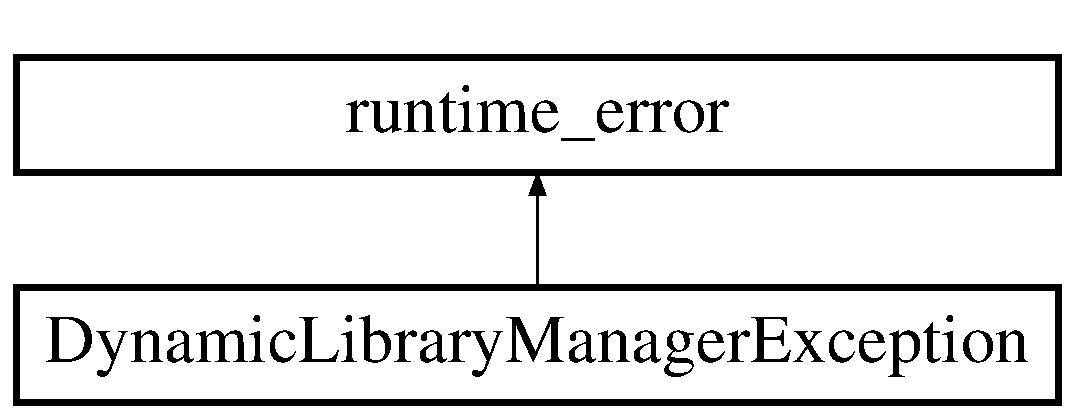
\includegraphics[height=2.000000cm]{class_dynamic_library_manager_exception}
\end{center}
\end{figure}
\subsection*{Public Types}
\begin{DoxyCompactItemize}
\item 
enum \hyperlink{class_dynamic_library_manager_exception_a73b4694c152e0693fbc19fb04987a0b9}{Cause} \{ \hyperlink{class_dynamic_library_manager_exception_a73b4694c152e0693fbc19fb04987a0b9a778b42fb996bf018bdc26934649cad63}{loading\-Failed} =0, 
\hyperlink{class_dynamic_library_manager_exception_a73b4694c152e0693fbc19fb04987a0b9a193fc58bb852e09790da269e2b613045}{symbol\-Not\-Found}
 \}
\end{DoxyCompactItemize}
\subsection*{Public Member Functions}
\begin{DoxyCompactItemize}
\item 
\hypertarget{class_dynamic_library_manager_exception_a15629092a054849f1cb73f8f468f8125}{\hyperlink{class_dynamic_library_manager_exception_a15629092a054849f1cb73f8f468f8125}{Dynamic\-Library\-Manager\-Exception} (const std\-::string \&library\-Name, const std\-::string \&error\-Detail, \hyperlink{class_dynamic_library_manager_exception_a73b4694c152e0693fbc19fb04987a0b9}{Cause} cause)}\label{class_dynamic_library_manager_exception_a15629092a054849f1cb73f8f468f8125}

\begin{DoxyCompactList}\small\item\em Failed to load the dynamic library or Symbol not found in the dynamic library. \end{DoxyCompactList}\item 
\hypertarget{class_dynamic_library_manager_exception_ab389b721f9a45814b8269ba865a1f25f}{\hyperlink{class_dynamic_library_manager_exception_a73b4694c152e0693fbc19fb04987a0b9}{Cause} {\bfseries get\-Cause} () const }\label{class_dynamic_library_manager_exception_ab389b721f9a45814b8269ba865a1f25f}

\item 
\hypertarget{class_dynamic_library_manager_exception_a3e6ed8a5e743a8ac80e4cb73a5d87360}{const char $\ast$ {\bfseries what} () const   throw ()}\label{class_dynamic_library_manager_exception_a3e6ed8a5e743a8ac80e4cb73a5d87360}

\end{DoxyCompactItemize}


\subsection{Detailed Description}
\hyperlink{class_exception}{Exception} thrown by \hyperlink{class_dynamic_library_manager}{Dynamic\-Library\-Manager} when a failure occurs. 

Use get\-Cause() to know what function caused the failure. 

\subsection{Member Enumeration Documentation}
\hypertarget{class_dynamic_library_manager_exception_a73b4694c152e0693fbc19fb04987a0b9}{\index{Dynamic\-Library\-Manager\-Exception@{Dynamic\-Library\-Manager\-Exception}!Cause@{Cause}}
\index{Cause@{Cause}!DynamicLibraryManagerException@{Dynamic\-Library\-Manager\-Exception}}
\subsubsection[{Cause}]{\setlength{\rightskip}{0pt plus 5cm}enum {\bf Dynamic\-Library\-Manager\-Exception\-::\-Cause}}}\label{class_dynamic_library_manager_exception_a73b4694c152e0693fbc19fb04987a0b9}
\begin{Desc}
\item[Enumerator]\par
\begin{description}
\index{loading\-Failed@{loading\-Failed}!Dynamic\-Library\-Manager\-Exception@{Dynamic\-Library\-Manager\-Exception}}\index{Dynamic\-Library\-Manager\-Exception@{Dynamic\-Library\-Manager\-Exception}!loading\-Failed@{loading\-Failed}}\item[{\em 
\hypertarget{class_dynamic_library_manager_exception_a73b4694c152e0693fbc19fb04987a0b9a778b42fb996bf018bdc26934649cad63}{loading\-Failed}\label{class_dynamic_library_manager_exception_a73b4694c152e0693fbc19fb04987a0b9a778b42fb996bf018bdc26934649cad63}
}]Failed to load the dynamic library. \index{symbol\-Not\-Found@{symbol\-Not\-Found}!Dynamic\-Library\-Manager\-Exception@{Dynamic\-Library\-Manager\-Exception}}\index{Dynamic\-Library\-Manager\-Exception@{Dynamic\-Library\-Manager\-Exception}!symbol\-Not\-Found@{symbol\-Not\-Found}}\item[{\em 
\hypertarget{class_dynamic_library_manager_exception_a73b4694c152e0693fbc19fb04987a0b9a193fc58bb852e09790da269e2b613045}{symbol\-Not\-Found}\label{class_dynamic_library_manager_exception_a73b4694c152e0693fbc19fb04987a0b9a193fc58bb852e09790da269e2b613045}
}]Symbol not found in the dynamic library. \end{description}
\end{Desc}


The documentation for this class was generated from the following file\-:\begin{DoxyCompactItemize}
\item 
Cadriciel/\-Commun/\-Externe/cppunit/include/cppunit/plugin/Dynamic\-Library\-Manager\-Exception.\-h\end{DoxyCompactItemize}

\hypertarget{class_element_jeu_abstrait}{\section{Element\-Jeu\-Abstrait Class Reference}
\label{class_element_jeu_abstrait}\index{Element\-Jeu\-Abstrait@{Element\-Jeu\-Abstrait}}
}


Cette classe abstraite servira de modele pour les objets du jeu.  




{\ttfamily \#include $<$Element\-Jeu\-Abstrait.\-h$>$}

Inheritance diagram for Element\-Jeu\-Abstrait\-:\begin{figure}[H]
\begin{center}
\leavevmode
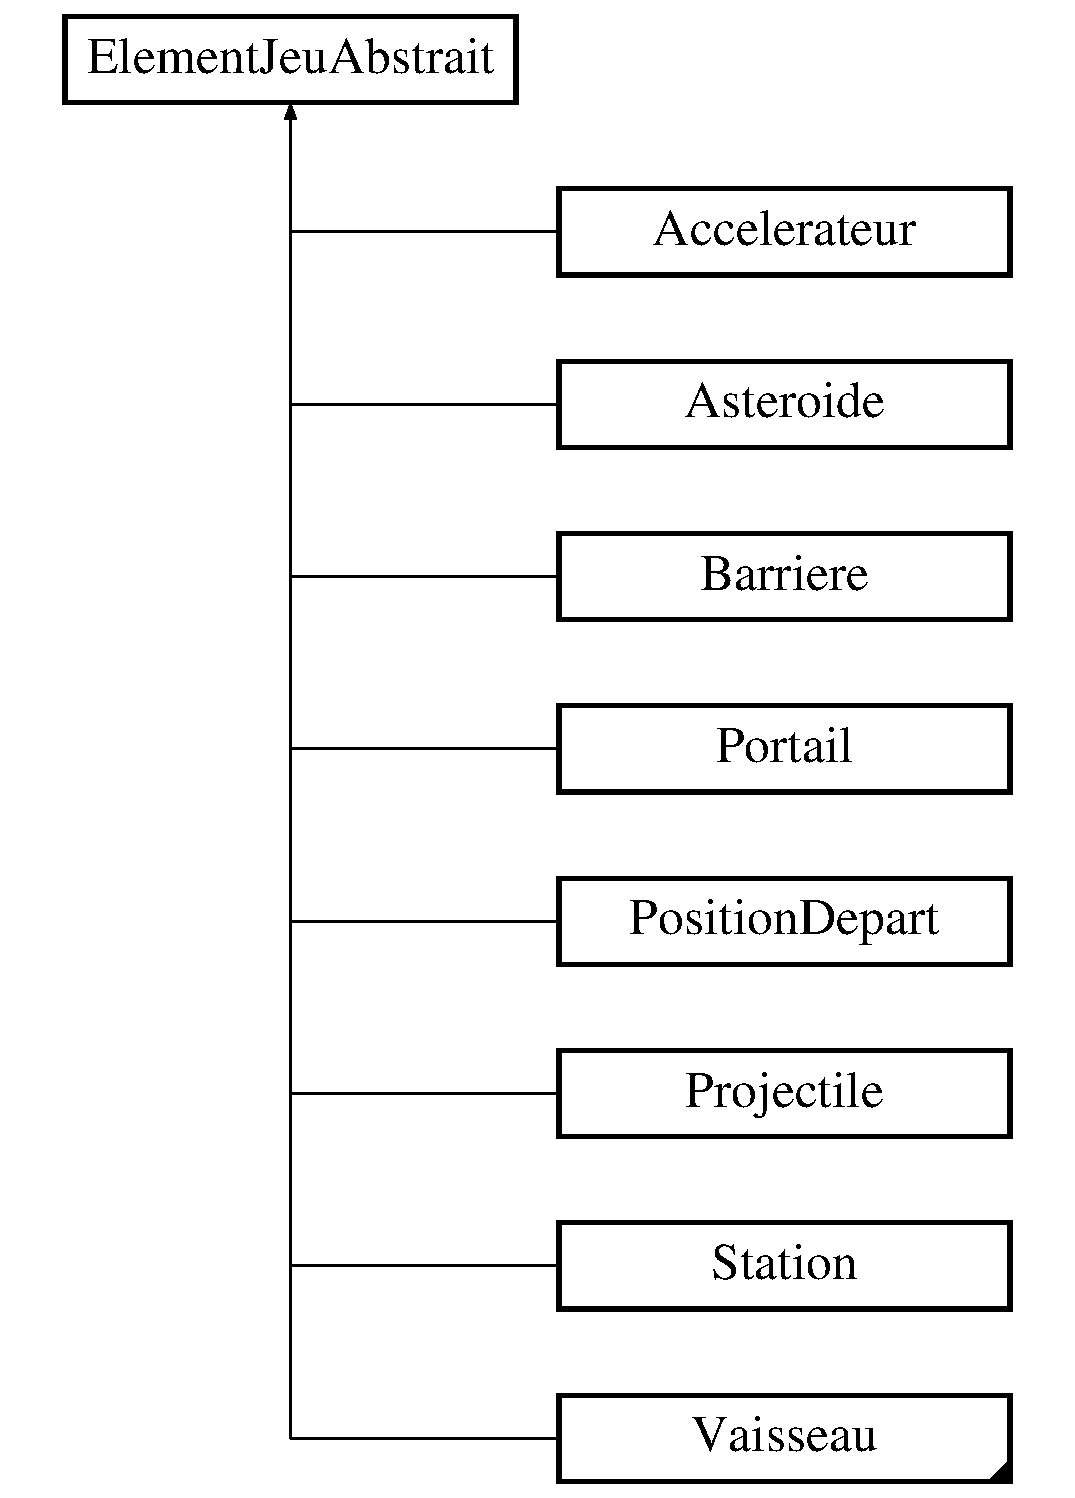
\includegraphics[height=9.000000cm]{class_element_jeu_abstrait}
\end{center}
\end{figure}
\subsection*{Public Member Functions}
\begin{DoxyCompactItemize}
\item 
\hyperlink{group__inf2990_ga9593e52a8eed3319191adf4ff18e4b51}{Element\-Jeu\-Abstrait} ()
\begin{DoxyCompactList}\small\item\em Constructeur. \end{DoxyCompactList}\item 
\hyperlink{group__inf2990_ga76e186eabb7b3cd93405aa854ec58ee9}{Element\-Jeu\-Abstrait} (const \hyperlink{class_element_jeu_abstrait}{Element\-Jeu\-Abstrait} \&element)
\begin{DoxyCompactList}\small\item\em Constructeur par copie. \end{DoxyCompactList}\item 
virtual \hyperlink{group__inf2990_ga221b1b36e924fcc1c74ea843181eb057}{$\sim$\-Element\-Jeu\-Abstrait} ()
\begin{DoxyCompactList}\small\item\em Destructeur. \end{DoxyCompactList}\item 
\hyperlink{structai_vector3_d}{ai\-Vector3\-D} \hyperlink{class_element_jeu_abstrait_aba19446f21d55fbea8d9302223630b2f}{get\-Position\-Depart} ()
\begin{DoxyCompactList}\small\item\em Visiteur. \end{DoxyCompactList}\item 
void \hyperlink{group__inf2990_gaf4962000b979fa009fd3eda6ae9e39a6}{set\-Position\-Depart} (\hyperlink{group__utilitaire_ga6b2956069f76c7e27df4f79f87e5a48c}{Vecteur3f} position\-Depart)
\item 
void \hyperlink{group__inf2990_gad6ce902644366a1c2b4ac7207291992e}{set\-Position\-Depart} (\hyperlink{structai_vector3_d}{ai\-Vector3\-D} position\-Depart)
\item 
\hyperlink{structai_vector3_d}{ai\-Vector3\-D} \hyperlink{class_element_jeu_abstrait_ada1ece7cf790b5153e0703d825dd3335}{get\-Position\-Actuelle} ()
\item 
void \hyperlink{group__inf2990_ga245d594e0c1703d863448d55c9df5ab5}{set\-Position\-Actuelle} (\hyperlink{group__utilitaire_ga6b2956069f76c7e27df4f79f87e5a48c}{Vecteur3f} position\-Actuelle)
\item 
\hyperlink{structai_vector3_d}{ai\-Vector3\-D} \hyperlink{class_element_jeu_abstrait_a633c1010fde0d69e745c3005facbc97c}{get\-Position\-Precedente} ()
\item 
\hypertarget{class_element_jeu_abstrait_af3889ed55c6781ddbf0b565317cee58a}{void {\bfseries set\-Position\-Precedente} (\hyperlink{structai_vector3_d}{ai\-Vector3\-D} position\-Precedente)}\label{class_element_jeu_abstrait_af3889ed55c6781ddbf0b565317cee58a}

\item 
void \hyperlink{group__inf2990_ga796ae0033c4636694c3e4dbe9bd3aa92}{set\-Position\-Actuelle} (\hyperlink{structai_vector3_d}{ai\-Vector3\-D} position\-Actuelle)
\item 
\hyperlink{structai_vector3_d}{ai\-Vector3\-D} \hyperlink{class_element_jeu_abstrait_a3e409ce902ca1f72ae8b0464678af30d}{get\-Direction\-Vitesse} ()
\item 
void \hyperlink{group__inf2990_gac2a3f72f9e1ae1337c59f2948a5aca21}{set\-Direction\-Vitesse} (\hyperlink{group__utilitaire_ga6b2956069f76c7e27df4f79f87e5a48c}{Vecteur3f} direction\-Vitesse)
\item 
void \hyperlink{group__inf2990_ga170429f9c1622d1412f61a0db079a5d4}{set\-Direction\-Vitesse} (\hyperlink{structai_vector3_d}{ai\-Vector3\-D} direction\-Vitesse)
\item 
float \hyperlink{class_element_jeu_abstrait_a92e32ae8a34955609c0454263f9c4457}{get\-Module\-Vitesse} ()
\item 
void \hyperlink{group__inf2990_ga6eccc0b9ca0dbcccb30d7a9384c87f4b}{set\-Module\-Vitesse} (float module\-Vitesse)
\item 
\hyperlink{structai_vector3_d}{ai\-Vector3\-D} \hyperlink{class_element_jeu_abstrait_acba27195cd238fd6b8b6a361de128d1c}{get\-Acceleration} ()
\item 
void \hyperlink{group__inf2990_ga7f5745cfbb11959de01f467ce1a03381}{set\-Acceleration} (\hyperlink{structai_vector3_d}{ai\-Vector3\-D} acceleration)
\item 
\hyperlink{structai_vector3_d}{ai\-Vector3\-D} \hyperlink{class_element_jeu_abstrait_a536c3c6ccd47ff91e0eb409ac25183b9}{get\-Axe} ()
\item 
void \hyperlink{group__inf2990_gaaf6b7ddfaaa2bb240ab1655209ebbf7c}{set\-Axe} (\hyperlink{group__utilitaire_ga6b2956069f76c7e27df4f79f87e5a48c}{Vecteur3f} axe)
\item 
\hyperlink{structai_vector3_d}{ai\-Vector3\-D} \hyperlink{class_element_jeu_abstrait_a6747305e75ef3dc395b52097fa30a5ee}{get\-Taille} ()
\item 
void \hyperlink{group__inf2990_gada54908cdff8d69feda67ec85b570b8b}{set\-Taille} (\hyperlink{group__utilitaire_ga6b2956069f76c7e27df4f79f87e5a48c}{Vecteur3f} taille)
\item 
void \hyperlink{group__inf2990_gae9e1d99cfd8171ce9dc8576c95094cec}{set\-Taille} (\hyperlink{structai_vector3_d}{ai\-Vector3\-D} taille)
\item 
float \hyperlink{class_element_jeu_abstrait_aa61b2e13f47f61fdcadcc509d26acf78}{get\-Poids} ()
\item 
void \hyperlink{group__inf2990_ga606a1953257cbd207de280e9dd19bf1a}{set\-Poids} (float poids)
\item 
float \hyperlink{class_element_jeu_abstrait_a20b3bdda6a3942d5191df25f5750d354}{get\-Angle} ()
\item 
void \hyperlink{group__inf2990_gaafe87c8fa5f36a6ab43e91c9204011a4}{set\-Angle} (float angle)
\item 
unsigned int \hyperlink{class_element_jeu_abstrait_ac6a7eccaa360f78047a4196c6e6cefca}{get\-Id} ()
\item 
void \hyperlink{group__inf2990_ga414e81b0393f589f3073ef1a7f0bfa91}{set\-Id} (unsigned int id)
\item 
virtual Type \hyperlink{class_element_jeu_abstrait_a06be76cc9ea3eaa3de4e263c9e5e21a3}{get\-Type} ()=0
\item 
\hypertarget{class_element_jeu_abstrait_aee3ed1d4ee01b0374387fcb9ef8a4e74}{virtual void \hyperlink{class_element_jeu_abstrait_aee3ed1d4ee01b0374387fcb9ef8a4e74}{update} (float delta\-T)=0}\label{class_element_jeu_abstrait_aee3ed1d4ee01b0374387fcb9ef8a4e74}

\begin{DoxyCompactList}\small\item\em Mise a jour. \end{DoxyCompactList}\item 
void \hyperlink{group__inf2990_ga3c0cd2230eb6f6c7578bd75b871e6246}{deplacer} (\hyperlink{group__utilitaire_ga6b2956069f76c7e27df4f79f87e5a48c}{Vecteur3f} deplacement)
\item 
void \hyperlink{group__inf2990_gad7950e80f061064bfc950d8c5494fd9c}{deplacer\-Ai\-Vector} (\hyperlink{structai_vector3_d}{ai\-Vector3\-D} deplacement)
\item 
void \hyperlink{group__inf2990_ga183f8335b30a3c48ed3313d5a3a0e343}{pivoter} (\hyperlink{group__utilitaire_ga6b2956069f76c7e27df4f79f87e5a48c}{Vecteur3f} axe, float angle)
\item 
void \hyperlink{group__inf2990_ga68627e8fd100d6f2ec8477059a199c80}{pivoter\-Ai\-Vector} (\hyperlink{structai_vector3_d}{ai\-Vector3\-D} axe, float angle)
\item 
void \hyperlink{group__inf2990_ga8b75d64d95198433215a30f17a423c80}{redimensionner} (\hyperlink{group__utilitaire_ga6b2956069f76c7e27df4f79f87e5a48c}{Vecteur3f} redimensionnement)
\item 
void \hyperlink{group__inf2990_ga208d73a00ce24dad0d0db2b78a5ad407}{set\-Selectionne} (bool selection)
\item 
bool \hyperlink{group__inf2990_ga8f58d4b951f03a3e78409813d9621b31}{get\-Selectionne} () const 
\item 
void \hyperlink{group__inf2990_gab84b15c2bd93908cb67e400b9daf4373}{inverser\-Selection} ()
\item 
double \hyperlink{group__inf2990_gab55d659d2ddb71f7a1deb9f819f985ea}{calculer\-Sphere\-Englobante} () const 
\item 
void \hyperlink{group__inf2990_ga9314283e0152cc0bd165e0fcca1b33b1}{calculer\-Cylindre\-Englobant} (double \&rayon, double \&bas, double \&haut) const 
\item 
void \hyperlink{group__inf2990_gac401b717e7e8314679a5430f99b0e0a7}{calculer\-Boite\-Englobante} (\hyperlink{group__utilitaire_ga541aa4837ad9250d3a248dc82ee9ad4d}{Vecteur3} \&coin\-Min, \hyperlink{group__utilitaire_ga541aa4837ad9250d3a248dc82ee9ad4d}{Vecteur3} \&coin\-Max) const 
\item 
virtual \hyperlink{class_element_jeu_abstrait}{Element\-Jeu\-Abstrait} $\ast$ \hyperlink{class_element_jeu_abstrait_a615a26c48dd6ce5b4274aeefb3a4032b}{clone} () const =0
\item 
\hyperlink{classmath_1_1_boite_englobante_orientee}{Boite\-Englobante\-Orientee} \& \hyperlink{group__inf2990_ga76c7fd67b6f61932f8889df6a22049ea}{get\-Boite\-Englobante\-Orientee} ()
\item 
virtual bool \hyperlink{group__inf2990_gaa2de365def9c59ffbf7ee51945b96fce}{check\-Collision} (\hyperlink{class_element_jeu_abstrait}{Element\-Jeu\-Abstrait} $\ast$element\-Jeu)=0
\item 
\hypertarget{class_element_jeu_abstrait_a11071c15797deae04611da1a0642435a}{virtual bool \hyperlink{class_element_jeu_abstrait_a11071c15797deae04611da1a0642435a}{check\-Collision} (\hyperlink{class_accelerateur}{Accelerateur} $\ast$accelerateur)=0}\label{class_element_jeu_abstrait_a11071c15797deae04611da1a0642435a}

\begin{DoxyCompactList}\small\item\em Methode pour verifier si une collision existe. \end{DoxyCompactList}\item 
\hypertarget{class_element_jeu_abstrait_ad1ffd24fa801a4e3c64e86a9886d690c}{virtual bool {\bfseries check\-Collision} (\hyperlink{class_asteroide}{Asteroide} $\ast$asteroide)=0}\label{class_element_jeu_abstrait_ad1ffd24fa801a4e3c64e86a9886d690c}

\item 
\hypertarget{class_element_jeu_abstrait_aebace6178f519dd1e5d845731ddb8063}{virtual bool {\bfseries check\-Collision} (\hyperlink{class_barriere}{Barriere} $\ast$barriere)=0}\label{class_element_jeu_abstrait_aebace6178f519dd1e5d845731ddb8063}

\item 
\hypertarget{class_element_jeu_abstrait_a90210e78428103adf589e8c29c8076b0}{virtual bool {\bfseries check\-Collision} (\hyperlink{class_portail}{Portail} $\ast$portail)=0}\label{class_element_jeu_abstrait_a90210e78428103adf589e8c29c8076b0}

\item 
\hypertarget{class_element_jeu_abstrait_aba1ceab5eb1460937054a77b2bf10fbc}{virtual bool {\bfseries check\-Collision} (\hyperlink{class_projectile}{Projectile} $\ast$projectile)=0}\label{class_element_jeu_abstrait_aba1ceab5eb1460937054a77b2bf10fbc}

\item 
\hypertarget{class_element_jeu_abstrait_adf9a2cc6ca52d89b93dbdb44ab932add}{virtual bool {\bfseries check\-Collision} (\hyperlink{class_station}{Station} $\ast$station)=0}\label{class_element_jeu_abstrait_adf9a2cc6ca52d89b93dbdb44ab932add}

\item 
\hypertarget{class_element_jeu_abstrait_ab803827965e92b2b9579370d3f67e69d}{virtual bool {\bfseries check\-Collision} (\hyperlink{class_vaisseau}{Vaisseau} $\ast$vaisseau)=0}\label{class_element_jeu_abstrait_ab803827965e92b2b9579370d3f67e69d}

\item 
virtual void \hyperlink{group__inf2990_gaaa60e09cf00bea42f27017e1a7a48e7b}{traiter\-Collision} (\hyperlink{class_element_jeu_abstrait}{Element\-Jeu\-Abstrait} $\ast$element\-Abstrait)=0
\item 
\hypertarget{class_element_jeu_abstrait_a22e8f47285f64372043dc89916c5eac5}{virtual void \hyperlink{class_element_jeu_abstrait_a22e8f47285f64372043dc89916c5eac5}{traiter\-Collision} (\hyperlink{class_accelerateur}{Accelerateur} $\ast$accelerateur)=0}\label{class_element_jeu_abstrait_a22e8f47285f64372043dc89916c5eac5}

\begin{DoxyCompactList}\small\item\em Methode pour traiter la collision si elle a lui avec les differents elements. \end{DoxyCompactList}\item 
\hypertarget{class_element_jeu_abstrait_af6218ea1d9fc026a8f39fbe09a90bfa0}{virtual void {\bfseries traiter\-Collision} (\hyperlink{class_asteroide}{Asteroide} $\ast$asteroide)=0}\label{class_element_jeu_abstrait_af6218ea1d9fc026a8f39fbe09a90bfa0}

\item 
\hypertarget{class_element_jeu_abstrait_a97210da984bc5f5024f603e6aba2130f}{virtual void {\bfseries traiter\-Collision} (\hyperlink{class_barriere}{Barriere} $\ast$barriere)=0}\label{class_element_jeu_abstrait_a97210da984bc5f5024f603e6aba2130f}

\item 
\hypertarget{class_element_jeu_abstrait_a2500f6eadb72cb87d1fdc2aa96f4d69b}{virtual void {\bfseries traiter\-Collision} (\hyperlink{class_portail}{Portail} $\ast$portail)=0}\label{class_element_jeu_abstrait_a2500f6eadb72cb87d1fdc2aa96f4d69b}

\item 
\hypertarget{class_element_jeu_abstrait_ab06625e0b65cd4e3c96893b2a30ca110}{virtual void {\bfseries traiter\-Collision} (\hyperlink{class_projectile}{Projectile} $\ast$projectile)=0}\label{class_element_jeu_abstrait_ab06625e0b65cd4e3c96893b2a30ca110}

\item 
\hypertarget{class_element_jeu_abstrait_aa757ff192c8fb88de966112d58fdc2a9}{virtual void {\bfseries traiter\-Collision} (\hyperlink{class_station}{Station} $\ast$station)=0}\label{class_element_jeu_abstrait_aa757ff192c8fb88de966112d58fdc2a9}

\item 
\hypertarget{class_element_jeu_abstrait_ac6d259676bcdbd00acefe232a727c1c6}{virtual void {\bfseries traiter\-Collision} (\hyperlink{class_vaisseau}{Vaisseau} $\ast$vaisseau)=0}\label{class_element_jeu_abstrait_ac6d259676bcdbd00acefe232a727c1c6}

\item 
virtual void \hyperlink{group__inf2990_ga73d543c47648fb2b3442e78d4f937393}{afficher\-Texte} ()
\begin{DoxyCompactList}\small\item\em Affiche les textes superposes. \end{DoxyCompactList}\item 
\hypertarget{group__inf2990_ga8d1ac90d7d8f597eaf454f8d1f69d3fb}{virtual float {\bfseries get\-Rayon} ()}\label{group__inf2990_ga8d1ac90d7d8f597eaf454f8d1f69d3fb}

\item 
\hypertarget{class_element_jeu_abstrait_aaf85ee401dd8c299aed05fe16ba4e625}{virtual bool \hyperlink{class_element_jeu_abstrait_aaf85ee401dd8c299aed05fe16ba4e625}{check\-Collision\-Joueur\-Virtuel} (\hyperlink{class_vaisseau}{Vaisseau} $\ast$joueur\-Virtuel)}\label{class_element_jeu_abstrait_aaf85ee401dd8c299aed05fe16ba4e625}

\begin{DoxyCompactList}\small\item\em Methode qui permet au joueur virtuel d'�viter les obstacles. \end{DoxyCompactList}\item 
void \hyperlink{group__inf2990_gab94e9badd17a334e21ec65aa074e4481}{set\-Force\-Portail} (float force\-Portail)
\item 
\hypertarget{class_element_jeu_abstrait_aa247c2519fc407419fc48f75357400c0}{\hyperlink{class_portail}{Portail} $\ast$ {\bfseries get\-Previous\-Portail} ()}\label{class_element_jeu_abstrait_aa247c2519fc407419fc48f75357400c0}

\item 
void \hyperlink{group__inf2990_ga5d58acff3da4427f1c5eb5c2a5f1acbe}{set\-Previous\-Portail} (\hyperlink{class_portail}{Portail} $\ast$previous\-Portail\-\_\-)
\item 
\hypertarget{class_element_jeu_abstrait_a2392fe29d105fdd3888140478fed10b5}{virtual int {\bfseries get\-Point\-De\-Vie} ()}\label{class_element_jeu_abstrait_a2392fe29d105fdd3888140478fed10b5}

\item 
\hypertarget{class_element_jeu_abstrait_a8ff66aee3f886e7b4ed1f6445f927cd2}{const \hyperlink{class_noeud_abstrait}{Noeud\-Abstrait} $\ast$ {\bfseries get\-Noeud\-Abstrait} () const }\label{class_element_jeu_abstrait_a8ff66aee3f886e7b4ed1f6445f927cd2}

\end{DoxyCompactItemize}
\subsection*{Protected Attributes}
\begin{DoxyCompactItemize}
\item 
\hypertarget{class_element_jeu_abstrait_adfe34e5d83467b9b84b6a42b6a6b8c29}{\hyperlink{structai_vector3_d}{ai\-Vector3\-D} {\bfseries position\-Depart\-\_\-}}\label{class_element_jeu_abstrait_adfe34e5d83467b9b84b6a42b6a6b8c29}

\item 
\hypertarget{class_element_jeu_abstrait_a6cc5b70837ba011739188f0a2d21019a}{\hyperlink{structai_vector3_d}{ai\-Vector3\-D} {\bfseries position\-Precedente\-\_\-}}\label{class_element_jeu_abstrait_a6cc5b70837ba011739188f0a2d21019a}

\item 
\hypertarget{class_element_jeu_abstrait_a578522bc24cad5190be9c8f94dc8a80a}{\hyperlink{structai_vector3_d}{ai\-Vector3\-D} {\bfseries position\-Actuelle\-\_\-}}\label{class_element_jeu_abstrait_a578522bc24cad5190be9c8f94dc8a80a}

\item 
\hypertarget{class_element_jeu_abstrait_a35ef9f504d8be9a463d3f5f9e781d986}{\hyperlink{structai_vector3_d}{ai\-Vector3\-D} {\bfseries direction\-Vitesse\-\_\-}}\label{class_element_jeu_abstrait_a35ef9f504d8be9a463d3f5f9e781d986}

\item 
\hypertarget{class_element_jeu_abstrait_a5c2402ed0874f050e52202390e1a0cea}{\hyperlink{structai_vector3_d}{ai\-Vector3\-D} {\bfseries acceleration\-\_\-}}\label{class_element_jeu_abstrait_a5c2402ed0874f050e52202390e1a0cea}

\item 
\hypertarget{class_element_jeu_abstrait_a734d4041d51acc353f126e6ffbce4e30}{\hyperlink{structai_vector3_d}{ai\-Vector3\-D} {\bfseries axe\-\_\-}}\label{class_element_jeu_abstrait_a734d4041d51acc353f126e6ffbce4e30}

\item 
\hypertarget{class_element_jeu_abstrait_a4d5369e94d5d85e9593a45ad5d28d62c}{\hyperlink{structai_vector3_d}{ai\-Vector3\-D} {\bfseries taille\-\_\-}}\label{class_element_jeu_abstrait_a4d5369e94d5d85e9593a45ad5d28d62c}

\item 
\hypertarget{class_element_jeu_abstrait_a5e8fa0ec520a531acbe4a3724b83e56b}{float {\bfseries module\-Vitesse\-\_\-}}\label{class_element_jeu_abstrait_a5e8fa0ec520a531acbe4a3724b83e56b}

\item 
\hypertarget{class_element_jeu_abstrait_adbf62302275db40b72e598de7e852e3c}{float {\bfseries angle\-\_\-}}\label{class_element_jeu_abstrait_adbf62302275db40b72e598de7e852e3c}

\item 
\hypertarget{class_element_jeu_abstrait_a3707a5fbf8ba6f8d1d723242113d55ae}{float {\bfseries poids\-\_\-}}\label{class_element_jeu_abstrait_a3707a5fbf8ba6f8d1d723242113d55ae}

\item 
\hypertarget{class_element_jeu_abstrait_a589a3c5ba67420c09b8d85b65a86deff}{unsigned int {\bfseries id\-\_\-}}\label{class_element_jeu_abstrait_a589a3c5ba67420c09b8d85b65a86deff}

\item 
\hypertarget{class_element_jeu_abstrait_acc0f8567e2a93bf1852a837a90b694e4}{\hyperlink{class_noeud_abstrait}{Noeud\-Abstrait} $\ast$ {\bfseries noeud\-Abstrait\-\_\-}}\label{class_element_jeu_abstrait_acc0f8567e2a93bf1852a837a90b694e4}

\item 
\hypertarget{class_element_jeu_abstrait_a8389c6d5a83b34977b21585c168a4474}{float {\bfseries force\-Portail\-\_\-}}\label{class_element_jeu_abstrait_a8389c6d5a83b34977b21585c168a4474}

\item 
\hypertarget{class_element_jeu_abstrait_a19d6fe7dd8e9f5d892334ce1bdc64aba}{\hyperlink{class_portail}{Portail} $\ast$ {\bfseries previous\-Portail\-\_\-}}\label{class_element_jeu_abstrait_a19d6fe7dd8e9f5d892334ce1bdc64aba}

\end{DoxyCompactItemize}
\subsection*{Static Protected Attributes}
\begin{DoxyCompactItemize}
\item 
\hypertarget{group__inf2990_ga33c86d3f6d041b55728a34ba6b655c7a}{static unsigned long {\bfseries numero\-\_\-} = 0}\label{group__inf2990_ga33c86d3f6d041b55728a34ba6b655c7a}

\end{DoxyCompactItemize}


\subsection{Detailed Description}
Cette classe abstraite servira de modele pour les objets du jeu. 

Elle va utilise les noeuds de memes types pour l'affichage des objets, tout en fournissant les elements principaux des objets du jeu. 

\subsection{Member Function Documentation}
\hypertarget{class_element_jeu_abstrait_a615a26c48dd6ce5b4274aeefb3a4032b}{\index{Element\-Jeu\-Abstrait@{Element\-Jeu\-Abstrait}!clone@{clone}}
\index{clone@{clone}!ElementJeuAbstrait@{Element\-Jeu\-Abstrait}}
\subsubsection[{clone}]{\setlength{\rightskip}{0pt plus 5cm}virtual {\bf Element\-Jeu\-Abstrait}$\ast$ Element\-Jeu\-Abstrait\-::clone (
\begin{DoxyParamCaption}
{}
\end{DoxyParamCaption}
) const\hspace{0.3cm}{\ttfamily [pure virtual]}}}\label{class_element_jeu_abstrait_a615a26c48dd6ce5b4274aeefb3a4032b}
Methode qui permet de cloner l'objet \begin{DoxyReturn}{Returns}
un pointeur vers la copie de l'objet 
\end{DoxyReturn}


Implemented in \hyperlink{group__inf2990_ga0435fde4382c3e1aab88e59e20ef88fe}{Asteroide}, \hyperlink{group__inf2990_ga15cab79251a8713cf4669ac6008b7940}{Projectile}, \hyperlink{group__inf2990_gad0aa2475444721471fc452d1b6f9438e}{Barriere}, \hyperlink{class_vaisseau_acb3a9188c88c85d30bc501c3b109f14d}{Vaisseau}, \hyperlink{group__inf2990_ga478857f2824957f9567a0a0baebafe34}{Vaisseau\-Virtuel}, \hyperlink{group__inf2990_gad184786ea5f912d24481427b4afb6f50}{Station}, \hyperlink{group__inf2990_ga79e69507b35314f3840ccaef125e3fa1}{Vaisseau\-Joueur}, \hyperlink{group__inf2990_ga56f704dcb76a319389d98488226e2b55}{Accelerateur}, \hyperlink{group___i_n_f2990-04_ga8d1a454a58e20a9dda3d393d2ed02271}{Position\-Depart}, and \hyperlink{group__inf2990_ga99a0c97911642939075b1883aa9d53ba}{Portail}.

\hypertarget{class_element_jeu_abstrait_acba27195cd238fd6b8b6a361de128d1c}{\index{Element\-Jeu\-Abstrait@{Element\-Jeu\-Abstrait}!get\-Acceleration@{get\-Acceleration}}
\index{get\-Acceleration@{get\-Acceleration}!ElementJeuAbstrait@{Element\-Jeu\-Abstrait}}
\subsubsection[{get\-Acceleration}]{\setlength{\rightskip}{0pt plus 5cm}{\bf ai\-Vector3\-D} Element\-Jeu\-Abstrait\-::get\-Acceleration (
\begin{DoxyParamCaption}
{}
\end{DoxyParamCaption}
)\hspace{0.3cm}{\ttfamily [inline]}}}\label{class_element_jeu_abstrait_acba27195cd238fd6b8b6a361de128d1c}
Permet d'obtenir l'acceleration de l'element \begin{DoxyReturn}{Returns}
L'acceleration de l'element 
\end{DoxyReturn}
\hypertarget{class_element_jeu_abstrait_a20b3bdda6a3942d5191df25f5750d354}{\index{Element\-Jeu\-Abstrait@{Element\-Jeu\-Abstrait}!get\-Angle@{get\-Angle}}
\index{get\-Angle@{get\-Angle}!ElementJeuAbstrait@{Element\-Jeu\-Abstrait}}
\subsubsection[{get\-Angle}]{\setlength{\rightskip}{0pt plus 5cm}float Element\-Jeu\-Abstrait\-::get\-Angle (
\begin{DoxyParamCaption}
{}
\end{DoxyParamCaption}
)\hspace{0.3cm}{\ttfamily [inline]}}}\label{class_element_jeu_abstrait_a20b3bdda6a3942d5191df25f5750d354}
Permet d'obtenir l'angle \begin{DoxyReturn}{Returns}
L'angle de l'element sur son axe 
\end{DoxyReturn}
\hypertarget{class_element_jeu_abstrait_a536c3c6ccd47ff91e0eb409ac25183b9}{\index{Element\-Jeu\-Abstrait@{Element\-Jeu\-Abstrait}!get\-Axe@{get\-Axe}}
\index{get\-Axe@{get\-Axe}!ElementJeuAbstrait@{Element\-Jeu\-Abstrait}}
\subsubsection[{get\-Axe}]{\setlength{\rightskip}{0pt plus 5cm}{\bf ai\-Vector3\-D} Element\-Jeu\-Abstrait\-::get\-Axe (
\begin{DoxyParamCaption}
{}
\end{DoxyParamCaption}
)\hspace{0.3cm}{\ttfamily [inline]}}}\label{class_element_jeu_abstrait_a536c3c6ccd47ff91e0eb409ac25183b9}
Permet d'obtenir l'axe de l'element \begin{DoxyReturn}{Returns}
L'axe de l'element 
\end{DoxyReturn}
\hypertarget{class_element_jeu_abstrait_a3e409ce902ca1f72ae8b0464678af30d}{\index{Element\-Jeu\-Abstrait@{Element\-Jeu\-Abstrait}!get\-Direction\-Vitesse@{get\-Direction\-Vitesse}}
\index{get\-Direction\-Vitesse@{get\-Direction\-Vitesse}!ElementJeuAbstrait@{Element\-Jeu\-Abstrait}}
\subsubsection[{get\-Direction\-Vitesse}]{\setlength{\rightskip}{0pt plus 5cm}{\bf ai\-Vector3\-D} Element\-Jeu\-Abstrait\-::get\-Direction\-Vitesse (
\begin{DoxyParamCaption}
{}
\end{DoxyParamCaption}
)\hspace{0.3cm}{\ttfamily [inline]}}}\label{class_element_jeu_abstrait_a3e409ce902ca1f72ae8b0464678af30d}
Permet d'obtenir la direction de la vitesse de l'element \begin{DoxyReturn}{Returns}
La direction de la vitesse de l'element 
\end{DoxyReturn}
\hypertarget{class_element_jeu_abstrait_ac6a7eccaa360f78047a4196c6e6cefca}{\index{Element\-Jeu\-Abstrait@{Element\-Jeu\-Abstrait}!get\-Id@{get\-Id}}
\index{get\-Id@{get\-Id}!ElementJeuAbstrait@{Element\-Jeu\-Abstrait}}
\subsubsection[{get\-Id}]{\setlength{\rightskip}{0pt plus 5cm}unsigned int Element\-Jeu\-Abstrait\-::get\-Id (
\begin{DoxyParamCaption}
{}
\end{DoxyParamCaption}
)\hspace{0.3cm}{\ttfamily [inline]}}}\label{class_element_jeu_abstrait_ac6a7eccaa360f78047a4196c6e6cefca}
Permet d'obtenir l'id \begin{DoxyReturn}{Returns}
L'id de l'element 
\end{DoxyReturn}
\hypertarget{class_element_jeu_abstrait_a92e32ae8a34955609c0454263f9c4457}{\index{Element\-Jeu\-Abstrait@{Element\-Jeu\-Abstrait}!get\-Module\-Vitesse@{get\-Module\-Vitesse}}
\index{get\-Module\-Vitesse@{get\-Module\-Vitesse}!ElementJeuAbstrait@{Element\-Jeu\-Abstrait}}
\subsubsection[{get\-Module\-Vitesse}]{\setlength{\rightskip}{0pt plus 5cm}float Element\-Jeu\-Abstrait\-::get\-Module\-Vitesse (
\begin{DoxyParamCaption}
{}
\end{DoxyParamCaption}
)\hspace{0.3cm}{\ttfamily [inline]}}}\label{class_element_jeu_abstrait_a92e32ae8a34955609c0454263f9c4457}
Permet d'obtenir le module de la vitesse de l'element \begin{DoxyReturn}{Returns}
La direction de la vitesse de l'element 
\end{DoxyReturn}
\hypertarget{class_element_jeu_abstrait_aa61b2e13f47f61fdcadcc509d26acf78}{\index{Element\-Jeu\-Abstrait@{Element\-Jeu\-Abstrait}!get\-Poids@{get\-Poids}}
\index{get\-Poids@{get\-Poids}!ElementJeuAbstrait@{Element\-Jeu\-Abstrait}}
\subsubsection[{get\-Poids}]{\setlength{\rightskip}{0pt plus 5cm}float Element\-Jeu\-Abstrait\-::get\-Poids (
\begin{DoxyParamCaption}
{}
\end{DoxyParamCaption}
)\hspace{0.3cm}{\ttfamily [inline]}}}\label{class_element_jeu_abstrait_aa61b2e13f47f61fdcadcc509d26acf78}
Permet d'obtenir le poids \begin{DoxyReturn}{Returns}
Le poids de l'element 
\end{DoxyReturn}
\hypertarget{class_element_jeu_abstrait_ada1ece7cf790b5153e0703d825dd3335}{\index{Element\-Jeu\-Abstrait@{Element\-Jeu\-Abstrait}!get\-Position\-Actuelle@{get\-Position\-Actuelle}}
\index{get\-Position\-Actuelle@{get\-Position\-Actuelle}!ElementJeuAbstrait@{Element\-Jeu\-Abstrait}}
\subsubsection[{get\-Position\-Actuelle}]{\setlength{\rightskip}{0pt plus 5cm}{\bf ai\-Vector3\-D} Element\-Jeu\-Abstrait\-::get\-Position\-Actuelle (
\begin{DoxyParamCaption}
{}
\end{DoxyParamCaption}
)\hspace{0.3cm}{\ttfamily [inline]}}}\label{class_element_jeu_abstrait_ada1ece7cf790b5153e0703d825dd3335}
Permet d'obtenir la position actuelle de l'element \begin{DoxyReturn}{Returns}
La position de l'element dans le jeu 
\end{DoxyReturn}
\hypertarget{class_element_jeu_abstrait_aba19446f21d55fbea8d9302223630b2f}{\index{Element\-Jeu\-Abstrait@{Element\-Jeu\-Abstrait}!get\-Position\-Depart@{get\-Position\-Depart}}
\index{get\-Position\-Depart@{get\-Position\-Depart}!ElementJeuAbstrait@{Element\-Jeu\-Abstrait}}
\subsubsection[{get\-Position\-Depart}]{\setlength{\rightskip}{0pt plus 5cm}{\bf ai\-Vector3\-D} Element\-Jeu\-Abstrait\-::get\-Position\-Depart (
\begin{DoxyParamCaption}
{}
\end{DoxyParamCaption}
)\hspace{0.3cm}{\ttfamily [inline]}}}\label{class_element_jeu_abstrait_aba19446f21d55fbea8d9302223630b2f}


Visiteur. 

Permet d'obtenir la position de depart de l'element \begin{DoxyReturn}{Returns}
La position de depart de l'element 
\end{DoxyReturn}
\hypertarget{class_element_jeu_abstrait_a633c1010fde0d69e745c3005facbc97c}{\index{Element\-Jeu\-Abstrait@{Element\-Jeu\-Abstrait}!get\-Position\-Precedente@{get\-Position\-Precedente}}
\index{get\-Position\-Precedente@{get\-Position\-Precedente}!ElementJeuAbstrait@{Element\-Jeu\-Abstrait}}
\subsubsection[{get\-Position\-Precedente}]{\setlength{\rightskip}{0pt plus 5cm}{\bf ai\-Vector3\-D} Element\-Jeu\-Abstrait\-::get\-Position\-Precedente (
\begin{DoxyParamCaption}
{}
\end{DoxyParamCaption}
)\hspace{0.3cm}{\ttfamily [inline]}}}\label{class_element_jeu_abstrait_a633c1010fde0d69e745c3005facbc97c}
Permet d'obtenir la position precedente de l'element \begin{DoxyReturn}{Returns}
La position de l'element dans le jeu 
\end{DoxyReturn}
\hypertarget{class_element_jeu_abstrait_a6747305e75ef3dc395b52097fa30a5ee}{\index{Element\-Jeu\-Abstrait@{Element\-Jeu\-Abstrait}!get\-Taille@{get\-Taille}}
\index{get\-Taille@{get\-Taille}!ElementJeuAbstrait@{Element\-Jeu\-Abstrait}}
\subsubsection[{get\-Taille}]{\setlength{\rightskip}{0pt plus 5cm}{\bf ai\-Vector3\-D} Element\-Jeu\-Abstrait\-::get\-Taille (
\begin{DoxyParamCaption}
{}
\end{DoxyParamCaption}
)\hspace{0.3cm}{\ttfamily [inline]}}}\label{class_element_jeu_abstrait_a6747305e75ef3dc395b52097fa30a5ee}
Permet d'obtenir la taille \begin{DoxyReturn}{Returns}
La taille 
\end{DoxyReturn}
\hypertarget{class_element_jeu_abstrait_a06be76cc9ea3eaa3de4e263c9e5e21a3}{\index{Element\-Jeu\-Abstrait@{Element\-Jeu\-Abstrait}!get\-Type@{get\-Type}}
\index{get\-Type@{get\-Type}!ElementJeuAbstrait@{Element\-Jeu\-Abstrait}}
\subsubsection[{get\-Type}]{\setlength{\rightskip}{0pt plus 5cm}virtual Type Element\-Jeu\-Abstrait\-::get\-Type (
\begin{DoxyParamCaption}
{}
\end{DoxyParamCaption}
)\hspace{0.3cm}{\ttfamily [pure virtual]}}}\label{class_element_jeu_abstrait_a06be76cc9ea3eaa3de4e263c9e5e21a3}
Permet d'obtenir le type de l'element \begin{DoxyReturn}{Returns}
Le type de l'element 
\end{DoxyReturn}


Implemented in \hyperlink{group__inf2990_ga9a0160da5089efa38867ad45782ae40d}{Barriere}, \hyperlink{group__inf2990_gad5cb221ede09ce81ef9621b89dcf694c}{Asteroide}, \hyperlink{group__inf2990_ga86387e528cf3b6717c086ea33967a312}{Vaisseau\-Virtuel}, \hyperlink{group__inf2990_ga73bf0677e077445d89c5351671a8c8b2}{Station}, \hyperlink{group__inf2990_gae4eafd2a7ad3e45343ed32a2eab6e238}{Vaisseau}, \hyperlink{group__inf2990_ga150da7e6cef37786545f24c4e3d47f80}{Vaisseau\-Joueur}, \hyperlink{group__inf2990_ga2ee3174059cff90eda7941e20699f2c8}{Accelerateur}, \hyperlink{group___i_n_f2990-04_gae4b1d64b04abfd849ef302e41c6fc6d1}{Position\-Depart}, \hyperlink{group__inf2990_ga9926b779c8956fd351b46d74f1d4ae20}{Projectile}, and \hyperlink{group__inf2990_gacce5da55b894c5b2edacda42b9388ec5}{Portail}.



The documentation for this class was generated from the following files\-:\begin{DoxyCompactItemize}
\item 
Cadriciel/\-Sources/\-C++/\-Element\-Objet/\hyperlink{_element_jeu_abstrait_8h}{Element\-Jeu\-Abstrait.\-h}\item 
Cadriciel/\-Sources/\-C++/\-Element\-Objet/\hyperlink{_element_jeu_abstrait_8cpp}{Element\-Jeu\-Abstrait.\-cpp}\end{DoxyCompactItemize}

\hypertarget{class_etat_joueur_virtuel}{\section{Etat\-Joueur\-Virtuel Class Reference}
\label{class_etat_joueur_virtuel}\index{Etat\-Joueur\-Virtuel@{Etat\-Joueur\-Virtuel}}
}


La classe \hyperlink{class_etat_joueur_virtuel}{Etat\-Joueur\-Virtuel} permet d'implementer les differents mode du vaisseau virtuel.  




{\ttfamily \#include $<$Etat\-Joueur\-Virtuel.\-h$>$}

Inheritance diagram for Etat\-Joueur\-Virtuel\-:\begin{figure}[H]
\begin{center}
\leavevmode
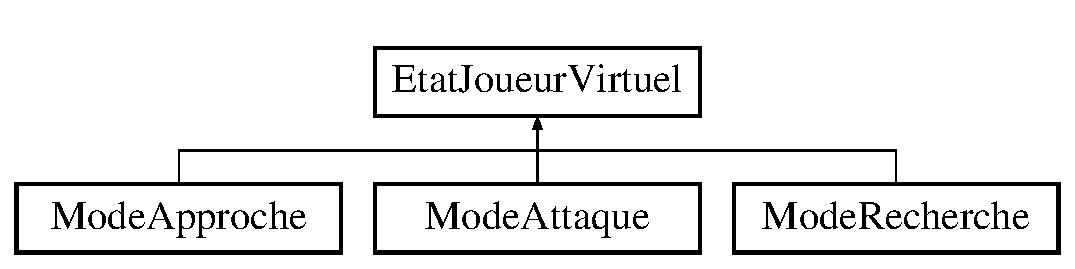
\includegraphics[height=2.000000cm]{class_etat_joueur_virtuel}
\end{center}
\end{figure}
\subsection*{Public Member Functions}
\begin{DoxyCompactItemize}
\item 
\hyperlink{group__inf2990_ga01e7e1a2286c56d6a1402fda8e26515c}{Etat\-Joueur\-Virtuel} ()
\item 
virtual \hyperlink{class_etat_joueur_virtuel_a208323774b6c0aa5446a22849e9a0090}{$\sim$\-Etat\-Joueur\-Virtuel} ()
\item 
virtual void \hyperlink{class_etat_joueur_virtuel_a21b40c0d4306e6073ee0e4ac7ff36a96}{update} (\hyperlink{class_vaisseau_virtuel}{Vaisseau\-Virtuel} \&vaisseau\-Virtuel, float delta\-T)=0
\item 
virtual const Mode \hyperlink{class_etat_joueur_virtuel_a3b18b9c7cd0181438090b040f6ecff57}{get\-Etat} () const =0
\item 
virtual \hyperlink{class_asteroide}{Asteroide} $\ast$ \hyperlink{class_etat_joueur_virtuel_a9fc759c914d9145f24210fdb2c9c0adc}{get\-Asteroide\-Cible} () const =0
\item 
\hypertarget{class_etat_joueur_virtuel_a52e15346e3bf2c1a276f534f7ba826ef}{virtual void {\bfseries set\-Ast\-Null} ()=0}\label{class_etat_joueur_virtuel_a52e15346e3bf2c1a276f534f7ba826ef}

\end{DoxyCompactItemize}
\subsection*{Protected Attributes}
\begin{DoxyCompactItemize}
\item 
\hypertarget{class_etat_joueur_virtuel_a49eff340df0c44ebe67873eb07778ab8}{\hyperlink{class_carte}{Carte} $\ast$ {\bfseries carte\-\_\-}}\label{class_etat_joueur_virtuel_a49eff340df0c44ebe67873eb07778ab8}

\item 
\hypertarget{class_etat_joueur_virtuel_a0d7d4783215bd6da4f061bae69106204}{double {\bfseries min\-X\-\_\-}}\label{class_etat_joueur_virtuel_a0d7d4783215bd6da4f061bae69106204}

\item 
\hypertarget{class_etat_joueur_virtuel_a0ab020dc8de0e3ae0056870f18f00452}{double {\bfseries min\-Y\-\_\-}}\label{class_etat_joueur_virtuel_a0ab020dc8de0e3ae0056870f18f00452}

\item 
\hypertarget{class_etat_joueur_virtuel_abe1f0055a14c3de8488e0a75183becd7}{double {\bfseries max\-X\-\_\-}}\label{class_etat_joueur_virtuel_abe1f0055a14c3de8488e0a75183becd7}

\item 
\hypertarget{class_etat_joueur_virtuel_a35f846f2c2f1b6bd5921185a5e47b063}{double {\bfseries max\-Y\-\_\-}}\label{class_etat_joueur_virtuel_a35f846f2c2f1b6bd5921185a5e47b063}

\item 
\hypertarget{class_etat_joueur_virtuel_a1106628b3215c4f875c3c746158472dd}{double {\bfseries distance\-Passer\-Mode\-Attaque\-\_\-}}\label{class_etat_joueur_virtuel_a1106628b3215c4f875c3c746158472dd}

\end{DoxyCompactItemize}


\subsection{Detailed Description}
La classe \hyperlink{class_etat_joueur_virtuel}{Etat\-Joueur\-Virtuel} permet d'implementer les differents mode du vaisseau virtuel. 

Cette classe contiendra des m�thodes qui le changement d'etats. 

\subsection{Constructor \& Destructor Documentation}
\hypertarget{class_etat_joueur_virtuel_a208323774b6c0aa5446a22849e9a0090}{\index{Etat\-Joueur\-Virtuel@{Etat\-Joueur\-Virtuel}!$\sim$\-Etat\-Joueur\-Virtuel@{$\sim$\-Etat\-Joueur\-Virtuel}}
\index{$\sim$\-Etat\-Joueur\-Virtuel@{$\sim$\-Etat\-Joueur\-Virtuel}!EtatJoueurVirtuel@{Etat\-Joueur\-Virtuel}}
\subsubsection[{$\sim$\-Etat\-Joueur\-Virtuel}]{\setlength{\rightskip}{0pt plus 5cm}virtual Etat\-Joueur\-Virtuel\-::$\sim$\-Etat\-Joueur\-Virtuel (
\begin{DoxyParamCaption}
{}
\end{DoxyParamCaption}
)\hspace{0.3cm}{\ttfamily [inline]}, {\ttfamily [virtual]}}}\label{class_etat_joueur_virtuel_a208323774b6c0aa5446a22849e9a0090}
Destructeur 

\subsection{Member Function Documentation}
\hypertarget{class_etat_joueur_virtuel_a9fc759c914d9145f24210fdb2c9c0adc}{\index{Etat\-Joueur\-Virtuel@{Etat\-Joueur\-Virtuel}!get\-Asteroide\-Cible@{get\-Asteroide\-Cible}}
\index{get\-Asteroide\-Cible@{get\-Asteroide\-Cible}!EtatJoueurVirtuel@{Etat\-Joueur\-Virtuel}}
\subsubsection[{get\-Asteroide\-Cible}]{\setlength{\rightskip}{0pt plus 5cm}virtual {\bf Asteroide}$\ast$ Etat\-Joueur\-Virtuel\-::get\-Asteroide\-Cible (
\begin{DoxyParamCaption}
{}
\end{DoxyParamCaption}
) const\hspace{0.3cm}{\ttfamily [pure virtual]}}}\label{class_etat_joueur_virtuel_a9fc759c914d9145f24210fdb2c9c0adc}
Getter de l'asteroide vise par le joueur virtuel \begin{DoxyReturn}{Returns}
\-: l'asteroide 
\end{DoxyReturn}


Implemented in \hyperlink{class_mode_recherche_a1eb4a92d4379f6c700a338c4fce95169}{Mode\-Recherche}, \hyperlink{class_mode_approche_ae744afaeb91afa4b65beb3a5a85c5c86}{Mode\-Approche}, and \hyperlink{class_mode_attaque_acade17b554ddd3ab4c1f467530674763}{Mode\-Attaque}.

\hypertarget{class_etat_joueur_virtuel_a3b18b9c7cd0181438090b040f6ecff57}{\index{Etat\-Joueur\-Virtuel@{Etat\-Joueur\-Virtuel}!get\-Etat@{get\-Etat}}
\index{get\-Etat@{get\-Etat}!EtatJoueurVirtuel@{Etat\-Joueur\-Virtuel}}
\subsubsection[{get\-Etat}]{\setlength{\rightskip}{0pt plus 5cm}virtual const Mode Etat\-Joueur\-Virtuel\-::get\-Etat (
\begin{DoxyParamCaption}
{}
\end{DoxyParamCaption}
) const\hspace{0.3cm}{\ttfamily [pure virtual]}}}\label{class_etat_joueur_virtuel_a3b18b9c7cd0181438090b040f6ecff57}
Getter du mode d'etat \begin{DoxyReturn}{Returns}
\-: le mode 
\end{DoxyReturn}


Implemented in \hyperlink{class_mode_recherche_a841e966fd005f3fe0097ad1fcf77d1fc}{Mode\-Recherche}, \hyperlink{class_mode_approche_a2931e82044b815a9ad8c32af36d101c1}{Mode\-Approche}, and \hyperlink{class_mode_attaque_a99026389b3870c7e33fc51cf2d2c0701}{Mode\-Attaque}.

\hypertarget{class_etat_joueur_virtuel_a21b40c0d4306e6073ee0e4ac7ff36a96}{\index{Etat\-Joueur\-Virtuel@{Etat\-Joueur\-Virtuel}!update@{update}}
\index{update@{update}!EtatJoueurVirtuel@{Etat\-Joueur\-Virtuel}}
\subsubsection[{update}]{\setlength{\rightskip}{0pt plus 5cm}virtual void Etat\-Joueur\-Virtuel\-::update (
\begin{DoxyParamCaption}
\item[{{\bf Vaisseau\-Virtuel} \&}]{vaisseau\-Virtuel, }
\item[{float}]{delta\-T}
\end{DoxyParamCaption}
)\hspace{0.3cm}{\ttfamily [pure virtual]}}}\label{class_etat_joueur_virtuel_a21b40c0d4306e6073ee0e4ac7ff36a96}
Update, m�thode virtuelle 
\begin{DoxyParams}{Parameters}
{\em } & le vaisseau virtuel, \\
\hline
{\em } & delta\-T \\
\hline
\end{DoxyParams}


Implemented in \hyperlink{class_mode_recherche_a5735b27160acd8f644caf1863c9ab954}{Mode\-Recherche}, \hyperlink{class_mode_approche_abfe4098ee8d3a873e6721140520e49fd}{Mode\-Approche}, and \hyperlink{class_mode_attaque_a3049ed25a9a5a4d447536ab631bd9031}{Mode\-Attaque}.



The documentation for this class was generated from the following files\-:\begin{DoxyCompactItemize}
\item 
Cadriciel/\-Commun/\-Utilitaire/\hyperlink{_etat_joueur_virtuel_8h}{Etat\-Joueur\-Virtuel.\-h}\item 
Cadriciel/\-Sources/\-C++/\-Environnement/\hyperlink{_etat_joueur_virtuel_8cpp}{Etat\-Joueur\-Virtuel.\-cpp}\end{DoxyCompactItemize}

\hypertarget{class_etat_open_g_l}{\section{Etat\-Open\-G\-L Class Reference}
\label{class_etat_open_g_l}\index{Etat\-Open\-G\-L@{Etat\-Open\-G\-L}}
}


Classe qui represente l'etat des variables de la machine Open\-G\-L.  




{\ttfamily \#include $<$Etat\-Open\-G\-L.\-h$>$}

\subsection*{Public Member Functions}
\begin{DoxyCompactItemize}
\item 
\hyperlink{group__utilitaire_gaf682f61929f2502b08b6b88de07349b6}{Etat\-Open\-G\-L} ()
\begin{DoxyCompactList}\small\item\em Constructeur par defaut. \end{DoxyCompactList}\item 
\hyperlink{glew_8h_ae84541b4f3d8e1ea24ec0f466a8c568b}{std\-::string} \hyperlink{group__utilitaire_ga13c8aaca9f02431b47b83e36b18f8067}{obtenir\-Chaine\-Gl\-Accum\-Alpha\-Bits} () const 
\begin{DoxyCompactList}\small\item\em Retourne une cha�ne representant l'attribut G\-L\-\_\-\-A\-C\-C\-U\-M\-\_\-\-A\-L\-P\-H\-A\-\_\-\-B\-I\-T\-S. \end{DoxyCompactList}\item 
\hyperlink{glew_8h_ae84541b4f3d8e1ea24ec0f466a8c568b}{std\-::string} \hyperlink{group__utilitaire_ga695387ee2d838c97214c70219d52da10}{obtenir\-Chaine\-Gl\-Accum\-Blue\-Bits} () const 
\begin{DoxyCompactList}\small\item\em Retourne une cha�ne representant l'attribut G\-L\-\_\-\-A\-C\-C\-U\-M\-\_\-\-B\-L\-U\-E\-\_\-\-B\-I\-T\-S. \end{DoxyCompactList}\item 
\hyperlink{glew_8h_ae84541b4f3d8e1ea24ec0f466a8c568b}{std\-::string} \hyperlink{group__utilitaire_gaf3e85f5f434e93aa09376200f3c837ae}{obtenir\-Chaine\-Gl\-Accum\-Clear\-Value} () const 
\begin{DoxyCompactList}\small\item\em Retourne une cha�ne representant l'attribut G\-L\-\_\-\-A\-C\-C\-U\-M\-\_\-\-C\-L\-E\-A\-R\-\_\-\-V\-A\-L\-U\-E. \end{DoxyCompactList}\item 
\hyperlink{glew_8h_ae84541b4f3d8e1ea24ec0f466a8c568b}{std\-::string} \hyperlink{group__utilitaire_gae677b60d2113b1843ba4d2c92fe34c34}{obtenir\-Chaine\-Gl\-Accum\-Green\-Bits} () const 
\begin{DoxyCompactList}\small\item\em Retourne une cha�ne representant l'attribut G\-L\-\_\-\-A\-C\-C\-U\-M\-\_\-\-G\-R\-E\-E\-N\-\_\-\-B\-I\-T\-S. \end{DoxyCompactList}\item 
\hyperlink{glew_8h_ae84541b4f3d8e1ea24ec0f466a8c568b}{std\-::string} \hyperlink{group__utilitaire_ga3405a98de14c30d7a57d954d298b6376}{obtenir\-Chaine\-Gl\-Accum\-Red\-Bits} () const 
\begin{DoxyCompactList}\small\item\em Retourne une cha�ne representant l'attribut G\-L\-\_\-\-A\-C\-C\-U\-M\-\_\-\-R\-E\-D\-\_\-\-B\-I\-T\-S. \end{DoxyCompactList}\item 
\hyperlink{glew_8h_ae84541b4f3d8e1ea24ec0f466a8c568b}{std\-::string} \hyperlink{group__utilitaire_gaf54d9525863334d2d2fd362c7043a4be}{obtenir\-Chaine\-Gl\-Alpha\-Bias} () const 
\begin{DoxyCompactList}\small\item\em Retourne une cha�ne representant l'attribut G\-L\-\_\-\-A\-L\-P\-H\-A\-\_\-\-B\-I\-A\-S. \end{DoxyCompactList}\item 
\hyperlink{glew_8h_ae84541b4f3d8e1ea24ec0f466a8c568b}{std\-::string} \hyperlink{group__utilitaire_ga7ea311e8cfd6aee3cb19e2041b2ba132}{obtenir\-Chaine\-Gl\-Alpha\-Bits} () const 
\begin{DoxyCompactList}\small\item\em Retourne une cha�ne representant l'attribut G\-L\-\_\-\-A\-L\-P\-H\-A\-\_\-\-B\-I\-T\-S. \end{DoxyCompactList}\item 
\hyperlink{glew_8h_ae84541b4f3d8e1ea24ec0f466a8c568b}{std\-::string} \hyperlink{group__utilitaire_ga3b85b93cd7e5d1f12a225f28ece00696}{obtenir\-Chaine\-Gl\-Alpha\-Scale} () const 
\begin{DoxyCompactList}\small\item\em Retourne une cha�ne representant l'attribut G\-L\-\_\-\-A\-L\-P\-H\-A\-\_\-\-S\-C\-A\-L\-E. \end{DoxyCompactList}\item 
\hyperlink{glew_8h_ae84541b4f3d8e1ea24ec0f466a8c568b}{std\-::string} \hyperlink{group__utilitaire_ga9fd2e2270997cf027e38f6a7b8d621a8}{obtenir\-Chaine\-Gl\-Alpha\-Test} () const 
\begin{DoxyCompactList}\small\item\em Retourne une cha�ne representant l'attribut G\-L\-\_\-\-A\-L\-P\-H\-A\-\_\-\-T\-E\-S\-T. \end{DoxyCompactList}\item 
\hyperlink{glew_8h_ae84541b4f3d8e1ea24ec0f466a8c568b}{std\-::string} \hyperlink{group__utilitaire_ga5002fd87fb9aede24afc4c4bb2a61fb1}{obtenir\-Chaine\-Gl\-Alpha\-Test\-Func} () const 
\begin{DoxyCompactList}\small\item\em Retourne une cha�ne representant l'attribut G\-L\-\_\-\-A\-L\-P\-H\-A\-\_\-\-T\-E\-S\-T\-\_\-\-F\-U\-N\-C. \end{DoxyCompactList}\item 
\hyperlink{glew_8h_ae84541b4f3d8e1ea24ec0f466a8c568b}{std\-::string} \hyperlink{group__utilitaire_gacc2904dcf7edec91f24e5e6ea58a780c}{obtenir\-Chaine\-Gl\-Alpha\-Test\-Ref} () const 
\begin{DoxyCompactList}\small\item\em Retourne une cha�ne representant l'attribut G\-L\-\_\-\-A\-L\-P\-H\-A\-\_\-\-T\-E\-S\-T\-\_\-\-R\-E\-F. \end{DoxyCompactList}\item 
\hyperlink{glew_8h_ae84541b4f3d8e1ea24ec0f466a8c568b}{std\-::string} \hyperlink{group__utilitaire_ga59c1e206aa477f625b5499cf328f695b}{obtenir\-Chaine\-Gl\-Attrib\-Stack\-Depth} () const 
\begin{DoxyCompactList}\small\item\em Retourne une cha�ne representant l'attribut G\-L\-\_\-\-A\-T\-T\-R\-I\-B\-\_\-\-S\-T\-A\-C\-K\-\_\-\-D\-E\-P\-T\-H. \end{DoxyCompactList}\item 
\hyperlink{glew_8h_ae84541b4f3d8e1ea24ec0f466a8c568b}{std\-::string} \hyperlink{group__utilitaire_gaaf8d3f8a4dd51812950c32268c8f77c5}{obtenir\-Chaine\-Gl\-Auto\-Normal} () const 
\begin{DoxyCompactList}\small\item\em Retourne une cha�ne representant l'attribut G\-L\-\_\-\-A\-U\-T\-O\-\_\-\-N\-O\-R\-M\-A\-L. \end{DoxyCompactList}\item 
\hyperlink{glew_8h_ae84541b4f3d8e1ea24ec0f466a8c568b}{std\-::string} \hyperlink{group__utilitaire_gab8c780e176faece6cbaa11084e957e8d}{obtenir\-Chaine\-Gl\-Aux\-Buffers} () const 
\begin{DoxyCompactList}\small\item\em Retourne une cha�ne representant l'attribut G\-L\-\_\-\-A\-U\-X\-\_\-\-B\-U\-F\-F\-E\-R\-S. \end{DoxyCompactList}\item 
\hyperlink{glew_8h_ae84541b4f3d8e1ea24ec0f466a8c568b}{std\-::string} \hyperlink{group__utilitaire_ga8a5f949f2b7a9a911c0677d639bebae5}{obtenir\-Chaine\-Gl\-Blend} () const 
\begin{DoxyCompactList}\small\item\em Retourne une cha�ne representant l'attribut G\-L\-\_\-\-B\-L\-E\-N\-D. \end{DoxyCompactList}\item 
\hyperlink{glew_8h_ae84541b4f3d8e1ea24ec0f466a8c568b}{std\-::string} \hyperlink{group__utilitaire_gaa52ab39bcb62d4f8777afddfca458650}{obtenir\-Chaine\-Gl\-Blend\-Dst} () const 
\begin{DoxyCompactList}\small\item\em Retourne une cha�ne representant l'attribut G\-L\-\_\-\-B\-L\-E\-N\-D\-\_\-\-D\-S\-T. \end{DoxyCompactList}\item 
\hyperlink{glew_8h_ae84541b4f3d8e1ea24ec0f466a8c568b}{std\-::string} \hyperlink{group__utilitaire_ga510a36fe5d3e313756e40b5c67b516ba}{obtenir\-Chaine\-Gl\-Blend\-Src} () const 
\begin{DoxyCompactList}\small\item\em Retourne une cha�ne representant l'attribut G\-L\-\_\-\-B\-L\-E\-N\-D\-\_\-\-S\-R\-C. \end{DoxyCompactList}\item 
\hyperlink{glew_8h_ae84541b4f3d8e1ea24ec0f466a8c568b}{std\-::string} \hyperlink{group__utilitaire_ga95f9a6baabd65a0cdd4b1e5cbeb4f678}{obtenir\-Chaine\-Gl\-Blue\-Bias} () const 
\begin{DoxyCompactList}\small\item\em Retourne une cha�ne representant l'attribut G\-L\-\_\-\-B\-L\-U\-E\-\_\-\-B\-I\-A\-S. \end{DoxyCompactList}\item 
\hyperlink{glew_8h_ae84541b4f3d8e1ea24ec0f466a8c568b}{std\-::string} \hyperlink{group__utilitaire_ga125172f1c5c4ef27c20c4e52a70ce38a}{obtenir\-Chaine\-Gl\-Blue\-Bits} () const 
\begin{DoxyCompactList}\small\item\em Retourne une cha�ne representant l'attribut G\-L\-\_\-\-B\-L\-U\-E\-\_\-\-B\-I\-T\-S. \end{DoxyCompactList}\item 
\hyperlink{glew_8h_ae84541b4f3d8e1ea24ec0f466a8c568b}{std\-::string} \hyperlink{group__utilitaire_ga8422f585aba4fc07dcaac22e6cf587b3}{obtenir\-Chaine\-Gl\-Blue\-Scale} () const 
\begin{DoxyCompactList}\small\item\em Retourne une cha�ne representant l'attribut G\-L\-\_\-\-B\-L\-U\-E\-\_\-\-S\-C\-A\-L\-E. \end{DoxyCompactList}\item 
\hyperlink{glew_8h_ae84541b4f3d8e1ea24ec0f466a8c568b}{std\-::string} \hyperlink{group__utilitaire_gad57f6d8da9cffeae2204a77e6e5f9292}{obtenir\-Chaine\-Gl\-Client\-Attrib\-Stack\-Depth} () const 
\begin{DoxyCompactList}\small\item\em Retourne une cha�ne representant l'attribut G\-L\-\_\-\-C\-L\-I\-E\-N\-T\-\_\-\-A\-T\-T\-R\-I\-B\-\_\-\-S\-T\-A\-C\-K\-\_\-\-D\-E\-P\-T\-H. \end{DoxyCompactList}\item 
\hyperlink{glew_8h_ae84541b4f3d8e1ea24ec0f466a8c568b}{std\-::string} \hyperlink{group__utilitaire_ga7deb847efbc619585d5e8c9f6600204c}{obtenir\-Chaine\-Gl\-Clip\-Planei} () const 
\begin{DoxyCompactList}\small\item\em Retourne une cha�ne representant l'attribut G\-L\-\_\-\-C\-L\-I\-P\-\_\-\-P\-L\-A\-N\-Ei. \end{DoxyCompactList}\item 
\hyperlink{glew_8h_ae84541b4f3d8e1ea24ec0f466a8c568b}{std\-::string} \hyperlink{group__utilitaire_ga8fae4f702f9be3574209f0721b6768ba}{obtenir\-Chaine\-Gl\-Color\-Array} () const 
\begin{DoxyCompactList}\small\item\em Retourne une cha�ne representant l'attribut G\-L\-\_\-\-C\-O\-L\-O\-R\-\_\-\-A\-R\-R\-A\-Y. \end{DoxyCompactList}\item 
\hyperlink{glew_8h_ae84541b4f3d8e1ea24ec0f466a8c568b}{std\-::string} \hyperlink{group__utilitaire_gad1e82d8c71b8e2a76c806e1c92cbb669}{obtenir\-Chaine\-Gl\-Color\-Array\-Size} () const 
\begin{DoxyCompactList}\small\item\em Retourne une cha�ne representant l'attribut G\-L\-\_\-\-C\-O\-L\-O\-R\-\_\-\-A\-R\-R\-A\-Y\-\_\-\-S\-I\-Z\-E. \end{DoxyCompactList}\item 
\hyperlink{glew_8h_ae84541b4f3d8e1ea24ec0f466a8c568b}{std\-::string} \hyperlink{group__utilitaire_gab499d52456b097364de8300cc6af6808}{obtenir\-Chaine\-Gl\-Color\-Array\-Stride} () const 
\begin{DoxyCompactList}\small\item\em Retourne une cha�ne representant l'attribut G\-L\-\_\-\-C\-O\-L\-O\-R\-\_\-\-A\-R\-R\-A\-Y\-\_\-\-S\-T\-R\-I\-D\-E. \end{DoxyCompactList}\item 
\hyperlink{glew_8h_ae84541b4f3d8e1ea24ec0f466a8c568b}{std\-::string} \hyperlink{group__utilitaire_gae77f9acd8bdebe2e7bb39660e03b3e28}{obtenir\-Chaine\-Gl\-Color\-Array\-Type} () const 
\begin{DoxyCompactList}\small\item\em Retourne une cha�ne representant l'attribut G\-L\-\_\-\-C\-O\-L\-O\-R\-\_\-\-A\-R\-R\-A\-Y\-\_\-\-T\-Y\-P\-E. \end{DoxyCompactList}\item 
\hyperlink{glew_8h_ae84541b4f3d8e1ea24ec0f466a8c568b}{std\-::string} \hyperlink{group__utilitaire_ga7de74c129bd5c5038e7f3d03a5508f72}{obtenir\-Chaine\-Gl\-Color\-Clear\-Value} () const 
\begin{DoxyCompactList}\small\item\em Retourne une cha�ne representant l'attribut G\-L\-\_\-\-C\-O\-L\-O\-R\-\_\-\-C\-L\-E\-A\-R\-\_\-\-V\-A\-L\-U\-E. \end{DoxyCompactList}\item 
\hyperlink{glew_8h_ae84541b4f3d8e1ea24ec0f466a8c568b}{std\-::string} \hyperlink{group__utilitaire_gac48e5f8e10bfcd96670a537164a0a8ff}{obtenir\-Chaine\-Gl\-Color\-Logic\-Op} () const 
\begin{DoxyCompactList}\small\item\em Retourne une cha�ne representant l'attribut G\-L\-\_\-\-C\-O\-L\-O\-R\-\_\-\-L\-O\-G\-I\-C\-\_\-\-O\-P. \end{DoxyCompactList}\item 
\hyperlink{glew_8h_ae84541b4f3d8e1ea24ec0f466a8c568b}{std\-::string} \hyperlink{group__utilitaire_gae53c823bf9d4e4305baf00f4d7da96af}{obtenir\-Chaine\-Gl\-Color\-Material} () const 
\begin{DoxyCompactList}\small\item\em Retourne une cha�ne representant l'attribut G\-L\-\_\-\-C\-O\-L\-O\-R\-\_\-\-M\-A\-T\-E\-R\-I\-A\-L. \end{DoxyCompactList}\item 
\hyperlink{glew_8h_ae84541b4f3d8e1ea24ec0f466a8c568b}{std\-::string} \hyperlink{group__utilitaire_gaec66f0ae860a11d50b0e1cf2def483bf}{obtenir\-Chaine\-Gl\-Color\-Material\-Face} () const 
\begin{DoxyCompactList}\small\item\em Retourne une cha�ne representant l'attribut G\-L\-\_\-\-C\-O\-L\-O\-R\-\_\-\-M\-A\-T\-E\-R\-I\-A\-L\-\_\-\-F\-A\-C\-E. \end{DoxyCompactList}\item 
\hyperlink{glew_8h_ae84541b4f3d8e1ea24ec0f466a8c568b}{std\-::string} \hyperlink{group__utilitaire_gad2b7f4282f94a24c4b5129854732c36a}{obtenir\-Chaine\-Gl\-Color\-Material\-Parameter} () const 
\begin{DoxyCompactList}\small\item\em Retourne une cha�ne representant l'attribut G\-L\-\_\-\-C\-O\-L\-O\-R\-\_\-\-M\-A\-T\-E\-R\-I\-A\-L\-\_\-\-P\-A\-R\-A\-M\-E\-T\-E\-R. \end{DoxyCompactList}\item 
\hyperlink{glew_8h_ae84541b4f3d8e1ea24ec0f466a8c568b}{std\-::string} \hyperlink{group__utilitaire_ga677eb5add1db0999f73a7c6febefe4d8}{obtenir\-Chaine\-Gl\-Color\-Writemask} () const 
\begin{DoxyCompactList}\small\item\em Retourne une cha�ne representant l'attribut G\-L\-\_\-\-C\-O\-L\-O\-R\-\_\-\-W\-R\-I\-T\-E\-M\-A\-S\-K. \end{DoxyCompactList}\item 
\hyperlink{glew_8h_ae84541b4f3d8e1ea24ec0f466a8c568b}{std\-::string} \hyperlink{group__utilitaire_ga6c53044cfb9b67582efe6415ff1f1f49}{obtenir\-Chaine\-Gl\-Cull\-Face} () const 
\begin{DoxyCompactList}\small\item\em Retourne une cha�ne representant l'attribut G\-L\-\_\-\-C\-U\-L\-L\-\_\-\-F\-A\-C\-E. \end{DoxyCompactList}\item 
\hyperlink{glew_8h_ae84541b4f3d8e1ea24ec0f466a8c568b}{std\-::string} \hyperlink{group__utilitaire_ga0601a9f84791de8e9ab33841308ecea0}{obtenir\-Chaine\-Gl\-Cull\-Face\-Mode} () const 
\begin{DoxyCompactList}\small\item\em Retourne une cha�ne representant l'attribut G\-L\-\_\-\-C\-U\-L\-L\-\_\-\-F\-A\-C\-E\-\_\-\-M\-O\-D\-E. \end{DoxyCompactList}\item 
\hyperlink{glew_8h_ae84541b4f3d8e1ea24ec0f466a8c568b}{std\-::string} \hyperlink{group__utilitaire_gabe349174d65850291bc46f7b524dac44}{obtenir\-Chaine\-Gl\-Current\-Color} () const 
\begin{DoxyCompactList}\small\item\em Retourne une cha�ne representant l'attribut G\-L\-\_\-\-C\-U\-R\-R\-E\-N\-T\-\_\-\-C\-O\-L\-O\-R. \end{DoxyCompactList}\item 
\hyperlink{glew_8h_ae84541b4f3d8e1ea24ec0f466a8c568b}{std\-::string} \hyperlink{group__utilitaire_ga222790a07e4a9cacfbe2f68cd97fd8d9}{obtenir\-Chaine\-Gl\-Current\-Index} () const 
\begin{DoxyCompactList}\small\item\em Retourne une cha�ne representant l'attribut G\-L\-\_\-\-C\-U\-R\-R\-E\-N\-T\-\_\-\-I\-N\-D\-E\-X. \end{DoxyCompactList}\item 
\hyperlink{glew_8h_ae84541b4f3d8e1ea24ec0f466a8c568b}{std\-::string} \hyperlink{group__utilitaire_gac6c54789d936998634ad29c80e150d92}{obtenir\-Chaine\-Gl\-Current\-Normal} () const 
\begin{DoxyCompactList}\small\item\em Retourne une cha�ne representant l'attribut G\-L\-\_\-\-C\-U\-R\-R\-E\-N\-T\-\_\-\-N\-O\-R\-M\-A\-L. \end{DoxyCompactList}\item 
\hyperlink{glew_8h_ae84541b4f3d8e1ea24ec0f466a8c568b}{std\-::string} \hyperlink{group__utilitaire_ga62ef22c97a3ecc8c7e956f2fd7267b9d}{obtenir\-Chaine\-Gl\-Current\-Raster\-Color} () const 
\begin{DoxyCompactList}\small\item\em Retourne une cha�ne representant l'attribut G\-L\-\_\-\-C\-U\-R\-R\-E\-N\-T\-\_\-\-R\-A\-S\-T\-E\-R\-\_\-\-C\-O\-L\-O\-R. \end{DoxyCompactList}\item 
\hyperlink{glew_8h_ae84541b4f3d8e1ea24ec0f466a8c568b}{std\-::string} \hyperlink{group__utilitaire_ga130c72bf45a65d7d7770c77c7f71cf5c}{obtenir\-Chaine\-Gl\-Current\-Raster\-Distance} () const 
\begin{DoxyCompactList}\small\item\em Retourne une cha�ne representant l'attribut G\-L\-\_\-\-C\-U\-R\-R\-E\-N\-T\-\_\-\-R\-A\-S\-T\-E\-R\-\_\-\-D\-I\-S\-T\-A\-N\-C\-E. \end{DoxyCompactList}\item 
\hyperlink{glew_8h_ae84541b4f3d8e1ea24ec0f466a8c568b}{std\-::string} \hyperlink{group__utilitaire_ga9d14728a6f086186ff9ec92738952892}{obtenir\-Chaine\-Gl\-Current\-Raster\-Index} () const 
\begin{DoxyCompactList}\small\item\em Retourne une cha�ne representant l'attribut G\-L\-\_\-\-C\-U\-R\-R\-E\-N\-T\-\_\-\-R\-A\-S\-T\-E\-R\-\_\-\-I\-N\-D\-E\-X. \end{DoxyCompactList}\item 
\hyperlink{glew_8h_ae84541b4f3d8e1ea24ec0f466a8c568b}{std\-::string} \hyperlink{group__utilitaire_ga1151f4eee3a50e14e0157b18b6fefaa4}{obtenir\-Chaine\-Gl\-Current\-Raster\-Position} () const 
\begin{DoxyCompactList}\small\item\em Retourne une cha�ne representant l'attribut G\-L\-\_\-\-C\-U\-R\-R\-E\-N\-T\-\_\-\-R\-A\-S\-T\-E\-R\-\_\-\-P\-O\-S\-I\-T\-I\-O\-N. \end{DoxyCompactList}\item 
\hyperlink{glew_8h_ae84541b4f3d8e1ea24ec0f466a8c568b}{std\-::string} \hyperlink{group__utilitaire_gaa95c762062531085430d3bd8381c1ab1}{obtenir\-Chaine\-Gl\-Current\-Raster\-Position\-Valid} () const 
\begin{DoxyCompactList}\small\item\em Retourne une cha�ne representant l'attribut G\-L\-\_\-\-C\-U\-R\-R\-E\-N\-T\-\_\-\-R\-A\-S\-T\-E\-R\-\_\-\-P\-O\-S\-I\-T\-I\-O\-N\-\_\-\-V\-A\-L\-I\-D. \end{DoxyCompactList}\item 
\hyperlink{glew_8h_ae84541b4f3d8e1ea24ec0f466a8c568b}{std\-::string} \hyperlink{group__utilitaire_gae1b30e504db9237dce13eade239c8c5a}{obtenir\-Chaine\-Gl\-Current\-Raster\-Texture\-Coords} () const 
\begin{DoxyCompactList}\small\item\em Retourne une cha�ne representant l'attribut G\-L\-\_\-\-C\-U\-R\-R\-E\-N\-T\-\_\-\-R\-A\-S\-T\-E\-R\-\_\-\-T\-E\-X\-T\-U\-R\-E\-\_\-\-C\-O\-O\-R\-D\-S. \end{DoxyCompactList}\item 
\hyperlink{glew_8h_ae84541b4f3d8e1ea24ec0f466a8c568b}{std\-::string} \hyperlink{group__utilitaire_ga5bf6abadfe9d63e576d34c94c93ee8f0}{obtenir\-Chaine\-Gl\-Current\-Texture\-Coords} () const 
\begin{DoxyCompactList}\small\item\em Retourne une cha�ne representant l'attribut G\-L\-\_\-\-C\-U\-R\-R\-E\-N\-T\-\_\-\-T\-E\-X\-T\-U\-R\-E\-\_\-\-C\-O\-O\-R\-D\-S. \end{DoxyCompactList}\item 
\hyperlink{glew_8h_ae84541b4f3d8e1ea24ec0f466a8c568b}{std\-::string} \hyperlink{group__utilitaire_gae3e587b7e9f860f3874823a3c4ab7d71}{obtenir\-Chaine\-Gl\-Depth\-Bias} () const 
\begin{DoxyCompactList}\small\item\em Retourne une cha�ne representant l'attribut G\-L\-\_\-\-D\-E\-P\-T\-H\-\_\-\-B\-I\-A\-S. \end{DoxyCompactList}\item 
\hyperlink{glew_8h_ae84541b4f3d8e1ea24ec0f466a8c568b}{std\-::string} \hyperlink{group__utilitaire_gae1dffc44c8e27d7cb249064cfe35653e}{obtenir\-Chaine\-Gl\-Depth\-Bits} () const 
\begin{DoxyCompactList}\small\item\em Retourne une cha�ne representant l'attribut G\-L\-\_\-\-D\-E\-P\-T\-H\-\_\-\-B\-I\-T\-S. \end{DoxyCompactList}\item 
\hyperlink{glew_8h_ae84541b4f3d8e1ea24ec0f466a8c568b}{std\-::string} \hyperlink{group__utilitaire_gad8b3e2701fb07b0178b5015868818509}{obtenir\-Chaine\-Gl\-Depth\-Clear\-Value} () const 
\begin{DoxyCompactList}\small\item\em Retourne une cha�ne representant l'attribut G\-L\-\_\-\-D\-E\-P\-T\-H\-\_\-\-C\-L\-E\-A\-R\-\_\-\-V\-A\-L\-U\-E. \end{DoxyCompactList}\item 
\hyperlink{glew_8h_ae84541b4f3d8e1ea24ec0f466a8c568b}{std\-::string} \hyperlink{group__utilitaire_gac0dff9e4aee8f969fe6e688bb407dcc9}{obtenir\-Chaine\-Gl\-Depth\-Func} () const 
\begin{DoxyCompactList}\small\item\em Retourne une cha�ne representant l'attribut G\-L\-\_\-\-D\-E\-P\-T\-H\-\_\-\-F\-U\-N\-C. \end{DoxyCompactList}\item 
\hyperlink{glew_8h_ae84541b4f3d8e1ea24ec0f466a8c568b}{std\-::string} \hyperlink{group__utilitaire_ga9921b541644f4dc3b64a4ffd4a661a09}{obtenir\-Chaine\-Gl\-Depth\-Range} () const 
\begin{DoxyCompactList}\small\item\em Retourne une cha�ne representant l'attribut G\-L\-\_\-\-D\-E\-P\-T\-H\-\_\-\-R\-A\-N\-G\-E. \end{DoxyCompactList}\item 
\hyperlink{glew_8h_ae84541b4f3d8e1ea24ec0f466a8c568b}{std\-::string} \hyperlink{group__utilitaire_ga4fac162003ef8c012c16ecd9041794ae}{obtenir\-Chaine\-Gl\-Depth\-Scale} () const 
\begin{DoxyCompactList}\small\item\em Retourne une cha�ne representant l'attribut G\-L\-\_\-\-D\-E\-P\-T\-H\-\_\-\-S\-C\-A\-L\-E. \end{DoxyCompactList}\item 
\hyperlink{glew_8h_ae84541b4f3d8e1ea24ec0f466a8c568b}{std\-::string} \hyperlink{group__utilitaire_ga712bcce1fd6c63377d2b3c9c421f7559}{obtenir\-Chaine\-Gl\-Depth\-Test} () const 
\begin{DoxyCompactList}\small\item\em Retourne une cha�ne representant l'attribut G\-L\-\_\-\-D\-E\-P\-T\-H\-\_\-\-T\-E\-S\-T. \end{DoxyCompactList}\item 
\hyperlink{glew_8h_ae84541b4f3d8e1ea24ec0f466a8c568b}{std\-::string} \hyperlink{group__utilitaire_gaec88db9c85bfd66909d3172982025862}{obtenir\-Chaine\-Gl\-Depth\-Writemask} () const 
\begin{DoxyCompactList}\small\item\em Retourne une cha�ne representant l'attribut G\-L\-\_\-\-D\-E\-P\-T\-H\-\_\-\-W\-R\-I\-T\-E\-M\-A\-S\-K. \end{DoxyCompactList}\item 
\hyperlink{glew_8h_ae84541b4f3d8e1ea24ec0f466a8c568b}{std\-::string} \hyperlink{group__utilitaire_gabc6e75dad01908ff21a473d75483f691}{obtenir\-Chaine\-Gl\-Dither} () const 
\begin{DoxyCompactList}\small\item\em Retourne une cha�ne representant l'attribut G\-L\-\_\-\-D\-I\-T\-H\-E\-R. \end{DoxyCompactList}\item 
\hyperlink{glew_8h_ae84541b4f3d8e1ea24ec0f466a8c568b}{std\-::string} \hyperlink{group__utilitaire_gae8239c45bba646389f06a6bdd49670f3}{obtenir\-Chaine\-Gl\-Doublebuffer} () const 
\begin{DoxyCompactList}\small\item\em Retourne une cha�ne representant l'attribut G\-L\-\_\-\-D\-O\-U\-B\-L\-E\-B\-U\-F\-F\-E\-R. \end{DoxyCompactList}\item 
\hyperlink{glew_8h_ae84541b4f3d8e1ea24ec0f466a8c568b}{std\-::string} \hyperlink{group__utilitaire_ga3b705291c7da107645656d5dfb51872a}{obtenir\-Chaine\-Gl\-Draw\-Buffer} () const 
\begin{DoxyCompactList}\small\item\em Retourne une cha�ne representant l'attribut G\-L\-\_\-\-D\-R\-A\-W\-\_\-\-B\-U\-F\-F\-E\-R. \end{DoxyCompactList}\item 
\hyperlink{glew_8h_ae84541b4f3d8e1ea24ec0f466a8c568b}{std\-::string} \hyperlink{group__utilitaire_ga982e0dacd18861db40bc153b8e7748d6}{obtenir\-Chaine\-Gl\-Edge\-Flag} () const 
\begin{DoxyCompactList}\small\item\em Retourne une cha�ne representant l'attribut G\-L\-\_\-\-E\-D\-G\-E\-\_\-\-F\-L\-A\-G. \end{DoxyCompactList}\item 
\hyperlink{glew_8h_ae84541b4f3d8e1ea24ec0f466a8c568b}{std\-::string} \hyperlink{group__utilitaire_gac69166db434f3671eb241b00786be34b}{obtenir\-Chaine\-Gl\-Edge\-Flag\-Array} () const 
\begin{DoxyCompactList}\small\item\em Retourne une cha�ne representant l'attribut G\-L\-\_\-\-E\-D\-G\-E\-\_\-\-F\-L\-A\-G\-\_\-\-A\-R\-R\-A\-Y. \end{DoxyCompactList}\item 
\hyperlink{glew_8h_ae84541b4f3d8e1ea24ec0f466a8c568b}{std\-::string} \hyperlink{group__utilitaire_ga12932637a943b952d6c822af48b4102a}{obtenir\-Chaine\-Gl\-Edge\-Flag\-Array\-Stride} () const 
\begin{DoxyCompactList}\small\item\em Retourne une cha�ne representant l'attribut G\-L\-\_\-\-E\-D\-G\-E\-\_\-\-F\-L\-A\-G\-\_\-\-A\-R\-R\-A\-Y\-\_\-\-S\-T\-R\-I\-D\-E. \end{DoxyCompactList}\item 
\hyperlink{glew_8h_ae84541b4f3d8e1ea24ec0f466a8c568b}{std\-::string} \hyperlink{group__utilitaire_gab0ae8d230f1fe733862032e082cfbd2f}{obtenir\-Chaine\-Gl\-Feedback\-Buffer\-Size} () const 
\begin{DoxyCompactList}\small\item\em Retourne une cha�ne representant l'attribut G\-L\-\_\-\-F\-E\-E\-D\-B\-A\-C\-K\-\_\-\-B\-U\-F\-F\-E\-R\-\_\-\-S\-I\-Z\-E. \end{DoxyCompactList}\item 
\hyperlink{glew_8h_ae84541b4f3d8e1ea24ec0f466a8c568b}{std\-::string} \hyperlink{group__utilitaire_ga30bdbc77ee2c0b27ee48e5de2654d29c}{obtenir\-Chaine\-Gl\-Feedback\-Buffer\-Type} () const 
\begin{DoxyCompactList}\small\item\em Retourne une cha�ne representant l'attribut G\-L\-\_\-\-F\-E\-E\-D\-B\-A\-C\-K\-\_\-\-B\-U\-F\-F\-E\-R\-\_\-\-T\-Y\-P\-E. \end{DoxyCompactList}\item 
\hyperlink{glew_8h_ae84541b4f3d8e1ea24ec0f466a8c568b}{std\-::string} \hyperlink{group__utilitaire_ga73b3d82b8c3940a818e1dab3d69e4899}{obtenir\-Chaine\-Gl\-Fog} () const 
\begin{DoxyCompactList}\small\item\em Retourne une cha�ne representant l'attribut G\-L\-\_\-\-F\-O\-G. \end{DoxyCompactList}\item 
\hyperlink{glew_8h_ae84541b4f3d8e1ea24ec0f466a8c568b}{std\-::string} \hyperlink{group__utilitaire_ga572f199118c8cb77085a7eb21f05f7fb}{obtenir\-Chaine\-Gl\-Fog\-Color} () const 
\begin{DoxyCompactList}\small\item\em Retourne une cha�ne representant l'attribut G\-L\-\_\-\-F\-O\-G\-\_\-\-C\-O\-L\-O\-R. \end{DoxyCompactList}\item 
\hyperlink{glew_8h_ae84541b4f3d8e1ea24ec0f466a8c568b}{std\-::string} \hyperlink{group__utilitaire_ga9ad8c1de41bc053666ffe001bca8f064}{obtenir\-Chaine\-Gl\-Fog\-Density} () const 
\begin{DoxyCompactList}\small\item\em Retourne une cha�ne representant l'attribut G\-L\-\_\-\-F\-O\-G\-\_\-\-D\-E\-N\-S\-I\-T\-Y. \end{DoxyCompactList}\item 
\hyperlink{glew_8h_ae84541b4f3d8e1ea24ec0f466a8c568b}{std\-::string} \hyperlink{group__utilitaire_ga9c6edbc286eed9a47b2e3ed2426e2b92}{obtenir\-Chaine\-Gl\-Fog\-End} () const 
\begin{DoxyCompactList}\small\item\em Retourne une cha�ne representant l'attribut G\-L\-\_\-\-F\-O\-G\-\_\-\-E\-N\-D. \end{DoxyCompactList}\item 
\hyperlink{glew_8h_ae84541b4f3d8e1ea24ec0f466a8c568b}{std\-::string} \hyperlink{group__utilitaire_ga8bd30ecaffe9f7d38e7a447a185dc8d0}{obtenir\-Chaine\-Gl\-Fog\-Hint} () const 
\begin{DoxyCompactList}\small\item\em Retourne une cha�ne representant l'attribut G\-L\-\_\-\-F\-O\-G\-\_\-\-H\-I\-N\-T. \end{DoxyCompactList}\item 
\hyperlink{glew_8h_ae84541b4f3d8e1ea24ec0f466a8c568b}{std\-::string} \hyperlink{group__utilitaire_ga929e0d580e014af6abda36f16fce43c3}{obtenir\-Chaine\-Gl\-Fog\-Index} () const 
\begin{DoxyCompactList}\small\item\em Retourne une cha�ne representant l'attribut G\-L\-\_\-\-F\-O\-G\-\_\-\-I\-N\-D\-E\-X. \end{DoxyCompactList}\item 
\hyperlink{glew_8h_ae84541b4f3d8e1ea24ec0f466a8c568b}{std\-::string} \hyperlink{group__utilitaire_ga1f28b3ec34f9bd4a2080e1252ca64d57}{obtenir\-Chaine\-Gl\-Fog\-Mode} () const 
\begin{DoxyCompactList}\small\item\em Retourne une cha�ne representant l'attribut G\-L\-\_\-\-F\-O\-G\-\_\-\-M\-O\-D\-E. \end{DoxyCompactList}\item 
\hyperlink{glew_8h_ae84541b4f3d8e1ea24ec0f466a8c568b}{std\-::string} \hyperlink{group__utilitaire_ga7063764912254ec440429aee9e8c3f83}{obtenir\-Chaine\-Gl\-Fog\-Start} () const 
\begin{DoxyCompactList}\small\item\em Retourne une cha�ne representant l'attribut G\-L\-\_\-\-F\-O\-G\-\_\-\-S\-T\-A\-R\-T. \end{DoxyCompactList}\item 
\hyperlink{glew_8h_ae84541b4f3d8e1ea24ec0f466a8c568b}{std\-::string} \hyperlink{group__utilitaire_ga5843f630d530a2112407e19b540e3c42}{obtenir\-Chaine\-Gl\-Front\-Face} () const 
\begin{DoxyCompactList}\small\item\em Retourne une cha�ne representant l'attribut G\-L\-\_\-\-F\-R\-O\-N\-T\-\_\-\-F\-A\-C\-E. \end{DoxyCompactList}\item 
\hyperlink{glew_8h_ae84541b4f3d8e1ea24ec0f466a8c568b}{std\-::string} \hyperlink{group__utilitaire_gabb435ce9e5ba38406d8c429a5a0510ed}{obtenir\-Chaine\-Gl\-Green\-Bias} () const 
\begin{DoxyCompactList}\small\item\em Retourne une cha�ne representant l'attribut G\-L\-\_\-\-G\-R\-E\-E\-N\-\_\-\-B\-I\-A\-S. \end{DoxyCompactList}\item 
\hyperlink{glew_8h_ae84541b4f3d8e1ea24ec0f466a8c568b}{std\-::string} \hyperlink{group__utilitaire_ga418e82a0a01a9dfe598780e602b41b2f}{obtenir\-Chaine\-Gl\-Green\-Bits} () const 
\begin{DoxyCompactList}\small\item\em Retourne une cha�ne representant l'attribut G\-L\-\_\-\-G\-R\-E\-E\-N\-\_\-\-B\-I\-T\-S. \end{DoxyCompactList}\item 
\hyperlink{glew_8h_ae84541b4f3d8e1ea24ec0f466a8c568b}{std\-::string} \hyperlink{group__utilitaire_ga933583938ec361ea302f25dd1323b541}{obtenir\-Chaine\-Gl\-Green\-Scale} () const 
\begin{DoxyCompactList}\small\item\em Retourne une cha�ne representant l'attribut G\-L\-\_\-\-G\-R\-E\-E\-N\-\_\-\-S\-C\-A\-L\-E. \end{DoxyCompactList}\item 
\hyperlink{glew_8h_ae84541b4f3d8e1ea24ec0f466a8c568b}{std\-::string} \hyperlink{group__utilitaire_ga63a264a046b4714154de9f26b04ab1f8}{obtenir\-Chaine\-Gl\-Index\-Array} () const 
\begin{DoxyCompactList}\small\item\em Retourne une cha�ne representant l'attribut G\-L\-\_\-\-I\-N\-D\-E\-X\-\_\-\-A\-R\-R\-A\-Y. \end{DoxyCompactList}\item 
\hyperlink{glew_8h_ae84541b4f3d8e1ea24ec0f466a8c568b}{std\-::string} \hyperlink{group__utilitaire_ga79b9f3969a037a0ed02684b41a8a1328}{obtenir\-Chaine\-Gl\-Index\-Array\-Stride} () const 
\begin{DoxyCompactList}\small\item\em Retourne une cha�ne representant l'attribut G\-L\-\_\-\-I\-N\-D\-E\-X\-\_\-\-A\-R\-R\-A\-Y\-\_\-\-S\-T\-R\-I\-D\-E. \end{DoxyCompactList}\item 
\hyperlink{glew_8h_ae84541b4f3d8e1ea24ec0f466a8c568b}{std\-::string} \hyperlink{group__utilitaire_ga8479c06a3ede7442505bb38803be818f}{obtenir\-Chaine\-Gl\-Index\-Array\-Type} () const 
\begin{DoxyCompactList}\small\item\em Retourne une cha�ne representant l'attribut G\-L\-\_\-\-I\-N\-D\-E\-X\-\_\-\-A\-R\-R\-A\-Y\-\_\-\-T\-Y\-P\-E. \end{DoxyCompactList}\item 
\hyperlink{glew_8h_ae84541b4f3d8e1ea24ec0f466a8c568b}{std\-::string} \hyperlink{group__utilitaire_gae88fc4ca05d447c04f08671823a407a3}{obtenir\-Chaine\-Gl\-Index\-Bits} () const 
\begin{DoxyCompactList}\small\item\em Retourne une cha�ne representant l'attribut G\-L\-\_\-\-I\-N\-D\-E\-X\-\_\-\-B\-I\-T\-S. \end{DoxyCompactList}\item 
\hyperlink{glew_8h_ae84541b4f3d8e1ea24ec0f466a8c568b}{std\-::string} \hyperlink{group__utilitaire_gad0d02a72c93d1501432001b500bf6435}{obtenir\-Chaine\-Gl\-Index\-Clear\-Value} () const 
\begin{DoxyCompactList}\small\item\em Retourne une cha�ne representant l'attribut G\-L\-\_\-\-I\-N\-D\-E\-X\-\_\-\-C\-L\-E\-A\-R\-\_\-\-V\-A\-L\-U\-E. \end{DoxyCompactList}\item 
\hyperlink{glew_8h_ae84541b4f3d8e1ea24ec0f466a8c568b}{std\-::string} \hyperlink{group__utilitaire_ga5294ee67327c1a604fe1ac627d539acc}{obtenir\-Chaine\-Gl\-Index\-Logic\-Op} () const 
\begin{DoxyCompactList}\small\item\em Retourne une cha�ne representant l'attribut G\-L\-\_\-\-I\-N\-D\-E\-X\-\_\-\-L\-O\-G\-I\-C\-\_\-\-O\-P. \end{DoxyCompactList}\item 
\hyperlink{glew_8h_ae84541b4f3d8e1ea24ec0f466a8c568b}{std\-::string} \hyperlink{group__utilitaire_ga5413d656a860db0103e85dcd025970e8}{obtenir\-Chaine\-Gl\-Index\-Mode} () const 
\begin{DoxyCompactList}\small\item\em Retourne une cha�ne representant l'attribut G\-L\-\_\-\-I\-N\-D\-E\-X\-\_\-\-M\-O\-D\-E. \end{DoxyCompactList}\item 
\hyperlink{glew_8h_ae84541b4f3d8e1ea24ec0f466a8c568b}{std\-::string} \hyperlink{group__utilitaire_ga2ef77a1752dfc7df305e66d9ebc8fee0}{obtenir\-Chaine\-Gl\-Index\-Offset} () const 
\begin{DoxyCompactList}\small\item\em Retourne une cha�ne representant l'attribut G\-L\-\_\-\-I\-N\-D\-E\-X\-\_\-\-O\-F\-F\-S\-E\-T. \end{DoxyCompactList}\item 
\hyperlink{glew_8h_ae84541b4f3d8e1ea24ec0f466a8c568b}{std\-::string} \hyperlink{group__utilitaire_gabb665544045af095c7c301467b71a53d}{obtenir\-Chaine\-Gl\-Index\-Shift} () const 
\begin{DoxyCompactList}\small\item\em Retourne une cha�ne representant l'attribut G\-L\-\_\-\-I\-N\-D\-E\-X\-\_\-\-S\-H\-I\-F\-T. \end{DoxyCompactList}\item 
\hyperlink{glew_8h_ae84541b4f3d8e1ea24ec0f466a8c568b}{std\-::string} \hyperlink{group__utilitaire_ga7041e09cfd847b59e2fd8b306639b2e2}{obtenir\-Chaine\-Gl\-Index\-Writemask} () const 
\begin{DoxyCompactList}\small\item\em Retourne une cha�ne representant l'attribut G\-L\-\_\-\-I\-N\-D\-E\-X\-\_\-\-W\-R\-I\-T\-E\-M\-A\-S\-K. \end{DoxyCompactList}\item 
\hyperlink{glew_8h_ae84541b4f3d8e1ea24ec0f466a8c568b}{std\-::string} \hyperlink{group__utilitaire_ga373300784f0f42aea9a0d6c78cb01623}{obtenir\-Chaine\-Gl\-Lighti} () const 
\begin{DoxyCompactList}\small\item\em Retourne une cha�ne representant l'attribut G\-L\-\_\-\-L\-I\-G\-H\-Ti. \end{DoxyCompactList}\item 
\hyperlink{glew_8h_ae84541b4f3d8e1ea24ec0f466a8c568b}{std\-::string} \hyperlink{group__utilitaire_gac26fe35af4bad0a50b4890f21e61ea02}{obtenir\-Chaine\-Gl\-Lighting} () const 
\begin{DoxyCompactList}\small\item\em Retourne une cha�ne representant l'attribut G\-L\-\_\-\-L\-I\-G\-H\-T\-I\-N\-G. \end{DoxyCompactList}\item 
\hyperlink{glew_8h_ae84541b4f3d8e1ea24ec0f466a8c568b}{std\-::string} \hyperlink{group__utilitaire_gafee564b101971fe6c901050b13522dc7}{obtenir\-Chaine\-Gl\-Light\-Model\-Ambient} () const 
\begin{DoxyCompactList}\small\item\em Retourne une cha�ne representant l'attribut G\-L\-\_\-\-L\-I\-G\-H\-T\-\_\-\-M\-O\-D\-E\-L\-\_\-\-A\-M\-B\-I\-E\-N\-T. \end{DoxyCompactList}\item 
\hyperlink{glew_8h_ae84541b4f3d8e1ea24ec0f466a8c568b}{std\-::string} \hyperlink{group__utilitaire_gad3dbc66405e9f773549840afceebda51}{obtenir\-Chaine\-Gl\-Light\-Model\-Local\-Viewer} () const 
\begin{DoxyCompactList}\small\item\em Retourne une cha�ne representant l'attribut G\-L\-\_\-\-L\-I\-G\-H\-T\-\_\-\-M\-O\-D\-E\-L\-\_\-\-L\-O\-C\-A\-L\-\_\-\-V\-I\-E\-W\-E\-R. \end{DoxyCompactList}\item 
\hyperlink{glew_8h_ae84541b4f3d8e1ea24ec0f466a8c568b}{std\-::string} \hyperlink{group__utilitaire_gab355049dd400e05dcf9057355f954b2d}{obtenir\-Chaine\-Gl\-Light\-Model\-Two\-Side} () const 
\begin{DoxyCompactList}\small\item\em Retourne une cha�ne representant l'attribut G\-L\-\_\-\-L\-I\-G\-H\-T\-\_\-\-M\-O\-D\-E\-L\-\_\-\-T\-W\-O\-\_\-\-S\-I\-D\-E. \end{DoxyCompactList}\item 
\hyperlink{glew_8h_ae84541b4f3d8e1ea24ec0f466a8c568b}{std\-::string} \hyperlink{group__utilitaire_ga3823c538863f06203e0f72df0af8e517}{obtenir\-Chaine\-Gl\-Line\-Smooth} () const 
\begin{DoxyCompactList}\small\item\em Retourne une cha�ne representant l'attribut G\-L\-\_\-\-L\-I\-N\-E\-\_\-\-S\-M\-O\-O\-T\-H. \end{DoxyCompactList}\item 
\hyperlink{glew_8h_ae84541b4f3d8e1ea24ec0f466a8c568b}{std\-::string} \hyperlink{group__utilitaire_ga259303d6900794169347807035689bc8}{obtenir\-Chaine\-Gl\-Line\-Smooth\-Hint} () const 
\begin{DoxyCompactList}\small\item\em Retourne une cha�ne representant l'attribut G\-L\-\_\-\-L\-I\-N\-E\-\_\-\-S\-M\-O\-O\-T\-H\-\_\-\-H\-I\-N\-T. \end{DoxyCompactList}\item 
\hyperlink{glew_8h_ae84541b4f3d8e1ea24ec0f466a8c568b}{std\-::string} \hyperlink{group__utilitaire_gae6a2fafc56ddcffeb516c7e7451ee620}{obtenir\-Chaine\-Gl\-Line\-Stipple} () const 
\begin{DoxyCompactList}\small\item\em Retourne une cha�ne representant l'attribut G\-L\-\_\-\-L\-I\-N\-E\-\_\-\-S\-T\-I\-P\-P\-L\-E. \end{DoxyCompactList}\item 
\hyperlink{glew_8h_ae84541b4f3d8e1ea24ec0f466a8c568b}{std\-::string} \hyperlink{group__utilitaire_gaf5594a01ce0e3ce08073c9d8adc2dc7d}{obtenir\-Chaine\-Gl\-Line\-Stipple\-Pattern} () const 
\begin{DoxyCompactList}\small\item\em Retourne une cha�ne representant l'attribut G\-L\-\_\-\-L\-I\-N\-E\-\_\-\-S\-T\-I\-P\-P\-L\-E\-\_\-\-P\-A\-T\-T\-E\-R\-N. \end{DoxyCompactList}\item 
\hyperlink{glew_8h_ae84541b4f3d8e1ea24ec0f466a8c568b}{std\-::string} \hyperlink{group__utilitaire_gab9b326741292e41732d5e0b646c4f006}{obtenir\-Chaine\-Gl\-Line\-Stipple\-Repeat} () const 
\begin{DoxyCompactList}\small\item\em Retourne une cha�ne representant l'attribut G\-L\-\_\-\-L\-I\-N\-E\-\_\-\-S\-T\-I\-P\-P\-L\-E\-\_\-\-R\-E\-P\-E\-A\-T. \end{DoxyCompactList}\item 
\hyperlink{glew_8h_ae84541b4f3d8e1ea24ec0f466a8c568b}{std\-::string} \hyperlink{group__utilitaire_gacd329652ea9f177db0c0ad44bc9150bd}{obtenir\-Chaine\-Gl\-Line\-Width} () const 
\begin{DoxyCompactList}\small\item\em Retourne une cha�ne representant l'attribut G\-L\-\_\-\-L\-I\-N\-E\-\_\-\-W\-I\-D\-T\-H. \end{DoxyCompactList}\item 
\hyperlink{glew_8h_ae84541b4f3d8e1ea24ec0f466a8c568b}{std\-::string} \hyperlink{group__utilitaire_ga42e5a43f490a0f90bedf54064921de10}{obtenir\-Chaine\-Gl\-Line\-Width\-Granularity} () const 
\begin{DoxyCompactList}\small\item\em Retourne une cha�ne representant l'attribut G\-L\-\_\-\-L\-I\-N\-E\-\_\-\-W\-I\-D\-T\-H\-\_\-\-G\-R\-A\-N\-U\-L\-A\-R\-I\-T\-Y. \end{DoxyCompactList}\item 
\hyperlink{glew_8h_ae84541b4f3d8e1ea24ec0f466a8c568b}{std\-::string} \hyperlink{group__utilitaire_gacdf3e63f9464f755958fb682f2a45015}{obtenir\-Chaine\-Glline\-Width\-Range} () const 
\begin{DoxyCompactList}\small\item\em Retourne une cha�ne representant l'attribut G\-L\-\_\-\-L\-I\-N\-E\-\_\-\-W\-I\-D\-T\-H\-\_\-\-R\-A\-N\-G\-E. \end{DoxyCompactList}\item 
\hyperlink{glew_8h_ae84541b4f3d8e1ea24ec0f466a8c568b}{std\-::string} \hyperlink{group__utilitaire_ga869ac6c34aaec533fb74b4e8095ae993}{obtenir\-Chaine\-Gl\-List\-Base} () const 
\begin{DoxyCompactList}\small\item\em Retourne une cha�ne representant l'attribut G\-L\-\_\-\-L\-I\-S\-T\-\_\-\-B\-A\-S\-E. \end{DoxyCompactList}\item 
\hyperlink{glew_8h_ae84541b4f3d8e1ea24ec0f466a8c568b}{std\-::string} \hyperlink{group__utilitaire_ga4486b4e688ef8a216e16b7c1a6ec7a61}{obtenir\-Chaine\-Gl\-List\-Index} () const 
\begin{DoxyCompactList}\small\item\em Retourne une cha�ne representant l'attribut G\-L\-\_\-\-L\-I\-S\-T\-\_\-\-I\-N\-D\-E\-X. \end{DoxyCompactList}\item 
\hyperlink{glew_8h_ae84541b4f3d8e1ea24ec0f466a8c568b}{std\-::string} \hyperlink{group__utilitaire_ga75eb73d049c2865922e414f5a06b749a}{obtenir\-Chaine\-Gl\-List\-Mode} () const 
\begin{DoxyCompactList}\small\item\em Retourne une cha�ne representant l'attribut G\-L\-\_\-\-L\-I\-S\-T\-\_\-\-M\-O\-D\-E. \end{DoxyCompactList}\item 
\hyperlink{glew_8h_ae84541b4f3d8e1ea24ec0f466a8c568b}{std\-::string} \hyperlink{group__utilitaire_gaf88292802715427e1a4e58f591b8e67e}{obtenir\-Chaine\-Gl\-Logic\-Op\-Mode} () const 
\begin{DoxyCompactList}\small\item\em Retourne une cha�ne representant l'attribut G\-L\-\_\-\-L\-O\-G\-I\-C\-\_\-\-O\-P\-\_\-\-M\-O\-D\-E. \end{DoxyCompactList}\item 
\hyperlink{glew_8h_ae84541b4f3d8e1ea24ec0f466a8c568b}{std\-::string} \hyperlink{group__utilitaire_gaa3e13a4accbc22c40a52ee9cee9fc3e0}{obtenir\-Chaine\-Gl\-Map1\-Color4} () const 
\begin{DoxyCompactList}\small\item\em Retourne une cha�ne representant l'attribut G\-L\-\_\-\-M\-A\-P1\-\_\-\-C\-O\-L\-O\-R\-\_\-4. \end{DoxyCompactList}\item 
\hyperlink{glew_8h_ae84541b4f3d8e1ea24ec0f466a8c568b}{std\-::string} \hyperlink{group__utilitaire_gad05cd2af4f512deb88aca0b00b0815c4}{obtenir\-Chaine\-Gl\-Map1\-Grid\-Domain} () const 
\begin{DoxyCompactList}\small\item\em Retourne une cha�ne representant l'attribut G\-L\-\_\-\-M\-A\-P1\-\_\-\-G\-R\-I\-D\-\_\-\-D\-O\-M\-A\-I\-N. \end{DoxyCompactList}\item 
\hyperlink{glew_8h_ae84541b4f3d8e1ea24ec0f466a8c568b}{std\-::string} \hyperlink{group__utilitaire_gaef4171a2ed92756d394ed8bae1fc57cd}{obtenir\-Chaine\-Gl\-Map1\-Grid\-Segments} () const 
\begin{DoxyCompactList}\small\item\em Retourne une cha�ne representant l'attribut G\-L\-\_\-\-M\-A\-P1\-\_\-\-G\-R\-I\-D\-\_\-\-S\-E\-G\-M\-E\-N\-T\-S. \end{DoxyCompactList}\item 
\hyperlink{glew_8h_ae84541b4f3d8e1ea24ec0f466a8c568b}{std\-::string} \hyperlink{group__utilitaire_ga52ba9a6fe299e4342d28baac6a83c769}{obtenir\-Chaine\-Gl\-Map1\-Index} () const 
\begin{DoxyCompactList}\small\item\em Retourne une cha�ne representant l'attribut G\-L\-\_\-\-M\-A\-P1\-\_\-\-I\-N\-D\-E\-X. \end{DoxyCompactList}\item 
\hyperlink{glew_8h_ae84541b4f3d8e1ea24ec0f466a8c568b}{std\-::string} \hyperlink{group__utilitaire_gad0e75e07ddc5d51e11b4a9b525ee4190}{obtenir\-Chaine\-Gl\-Map1\-Normal} () const 
\begin{DoxyCompactList}\small\item\em Retourne une cha�ne representant l'attribut G\-L\-\_\-\-M\-A\-P1\-\_\-\-N\-O\-R\-M\-A\-L. \end{DoxyCompactList}\item 
\hyperlink{glew_8h_ae84541b4f3d8e1ea24ec0f466a8c568b}{std\-::string} \hyperlink{group__utilitaire_gaf06cacbe0ee8f4fe4a6f56571fb8c27c}{obtenir\-Chaine\-Gl\-Map1\-Texture\-Coord1} () const 
\begin{DoxyCompactList}\small\item\em Retourne une cha�ne representant l'attribut G\-L\-\_\-\-M\-A\-P1\-\_\-\-T\-E\-X\-T\-U\-R\-E\-\_\-\-C\-O\-O\-R\-D\-\_\-1. \end{DoxyCompactList}\item 
\hyperlink{glew_8h_ae84541b4f3d8e1ea24ec0f466a8c568b}{std\-::string} \hyperlink{group__utilitaire_gade175aafd1123e597959f78fbe04489f}{obtenir\-Chaine\-Gl\-Map1\-Texture\-Coord2} () const 
\begin{DoxyCompactList}\small\item\em Retourne une cha�ne representant l'attribut G\-L\-\_\-\-M\-A\-P1\-\_\-\-T\-E\-X\-T\-U\-R\-E\-\_\-\-C\-O\-O\-R\-D\-\_\-2. \end{DoxyCompactList}\item 
\hyperlink{glew_8h_ae84541b4f3d8e1ea24ec0f466a8c568b}{std\-::string} \hyperlink{group__utilitaire_ga6690ab58fbdae84d2543e29cc9e4c41d}{obtenir\-Chaine\-Gl\-Map1\-Texture\-Coord3} () const 
\begin{DoxyCompactList}\small\item\em Retourne une cha�ne representant l'attribut G\-L\-\_\-\-M\-A\-P1\-\_\-\-T\-E\-X\-T\-U\-R\-E\-\_\-\-C\-O\-O\-R\-D\-\_\-3. \end{DoxyCompactList}\item 
\hyperlink{glew_8h_ae84541b4f3d8e1ea24ec0f466a8c568b}{std\-::string} \hyperlink{group__utilitaire_gab7a65aa462c3a278c42977ed9a35904e}{obtenir\-Chaine\-Gl\-Map1\-Texture\-Coord4} () const 
\begin{DoxyCompactList}\small\item\em Retourne une cha�ne representant l'attribut G\-L\-\_\-\-M\-A\-P1\-\_\-\-T\-E\-X\-T\-U\-R\-E\-\_\-\-C\-O\-O\-R\-D\-\_\-4. \end{DoxyCompactList}\item 
\hyperlink{glew_8h_ae84541b4f3d8e1ea24ec0f466a8c568b}{std\-::string} \hyperlink{group__utilitaire_gafe0e07682a0bb42bb227fecd287de609}{obtenir\-Chaine\-Gl\-Map1\-Vertex3} () const 
\begin{DoxyCompactList}\small\item\em Retourne une cha�ne representant l'attribut G\-L\-\_\-\-M\-A\-P1\-\_\-\-V\-E\-R\-T\-E\-X\-\_\-3. \end{DoxyCompactList}\item 
\hyperlink{glew_8h_ae84541b4f3d8e1ea24ec0f466a8c568b}{std\-::string} \hyperlink{group__utilitaire_gab130a35770d4594bf74a89d18c49697a}{obtenir\-Chaine\-Gl\-Map1\-Vertex4} () const 
\begin{DoxyCompactList}\small\item\em Retourne une cha�ne representant l'attribut G\-L\-\_\-\-M\-A\-P1\-\_\-\-V\-E\-R\-T\-E\-X\-\_\-4. \end{DoxyCompactList}\item 
\hyperlink{glew_8h_ae84541b4f3d8e1ea24ec0f466a8c568b}{std\-::string} \hyperlink{group__utilitaire_ga85dca50f7d25944ca4158173a630d15d}{obtenir\-Chaine\-Gl\-Map2\-Color4} () const 
\begin{DoxyCompactList}\small\item\em Retourne une cha�ne representant l'attribut G\-L\-\_\-\-M\-A\-P2\-\_\-\-C\-O\-L\-O\-R\-\_\-4. \end{DoxyCompactList}\item 
\hyperlink{glew_8h_ae84541b4f3d8e1ea24ec0f466a8c568b}{std\-::string} \hyperlink{group__utilitaire_ga15f308a3995cd63e0bf8ff13fd1024dd}{obtenir\-Chaine\-Gl\-Map2\-Grid\-Domain} () const 
\begin{DoxyCompactList}\small\item\em Retourne une cha�ne representant l'attribut G\-L\-\_\-\-M\-A\-P2\-\_\-\-G\-R\-I\-D\-\_\-\-D\-O\-M\-A\-I\-N. \end{DoxyCompactList}\item 
\hyperlink{glew_8h_ae84541b4f3d8e1ea24ec0f466a8c568b}{std\-::string} \hyperlink{group__utilitaire_ga7cc72b6b6d1f670c6bb2a37bb02f22cc}{obtenir\-Chaine\-Gl\-Map2\-Grid\-Segments} () const 
\begin{DoxyCompactList}\small\item\em Retourne une cha�ne representant l'attribut G\-L\-\_\-\-M\-A\-P2\-\_\-\-G\-R\-I\-D\-\_\-\-S\-E\-G\-M\-E\-N\-T\-S. \end{DoxyCompactList}\item 
\hyperlink{glew_8h_ae84541b4f3d8e1ea24ec0f466a8c568b}{std\-::string} \hyperlink{group__utilitaire_ga5c26c0fce87b7c852f2819ddbc816835}{obtenir\-Chaine\-Gl\-Map2\-Index} () const 
\begin{DoxyCompactList}\small\item\em Retourne une cha�ne representant l'attribut G\-L\-\_\-\-M\-A\-P2\-\_\-\-I\-N\-D\-E\-X. \end{DoxyCompactList}\item 
\hyperlink{glew_8h_ae84541b4f3d8e1ea24ec0f466a8c568b}{std\-::string} \hyperlink{group__utilitaire_ga281e64b376bb0c3f7f7090820a64bd7e}{obtenir\-Chaine\-Gl\-Map2\-Normal} () const 
\begin{DoxyCompactList}\small\item\em Retourne une cha�ne representant l'attribut G\-L\-\_\-\-M\-A\-P2\-\_\-\-N\-O\-R\-M\-A\-L. \end{DoxyCompactList}\item 
\hyperlink{glew_8h_ae84541b4f3d8e1ea24ec0f466a8c568b}{std\-::string} \hyperlink{group__utilitaire_gadb7c67ea193286a4088b9dcc172abef6}{obtenir\-Chaine\-Gl\-Map2\-Texture\-Coord1} () const 
\begin{DoxyCompactList}\small\item\em Retourne une cha�ne representant l'attribut G\-L\-\_\-\-M\-A\-P2\-\_\-\-T\-E\-X\-T\-U\-R\-E\-\_\-\-C\-O\-O\-R\-D\-\_\-1. \end{DoxyCompactList}\item 
\hyperlink{glew_8h_ae84541b4f3d8e1ea24ec0f466a8c568b}{std\-::string} \hyperlink{group__utilitaire_gaf5cb23274f1ad4c504c5aed7947a3432}{obtenir\-Chaine\-Gl\-Map2\-Texture\-Coord2} () const 
\begin{DoxyCompactList}\small\item\em Retourne une cha�ne representant l'attribut G\-L\-\_\-\-M\-A\-P2\-\_\-\-T\-E\-X\-T\-U\-R\-E\-\_\-\-C\-O\-O\-R\-D\-\_\-2. \end{DoxyCompactList}\item 
\hyperlink{glew_8h_ae84541b4f3d8e1ea24ec0f466a8c568b}{std\-::string} \hyperlink{group__utilitaire_gad4b636ae980e2c420c9a7357fe8d58cc}{obtenir\-Chaine\-Gl\-Map2\-Texture\-Coord3} () const 
\begin{DoxyCompactList}\small\item\em Retourne une cha�ne representant l'attribut G\-L\-\_\-\-M\-A\-P2\-\_\-\-T\-E\-X\-T\-U\-R\-E\-\_\-\-C\-O\-O\-R\-D\-\_\-3. \end{DoxyCompactList}\item 
\hyperlink{glew_8h_ae84541b4f3d8e1ea24ec0f466a8c568b}{std\-::string} \hyperlink{group__utilitaire_ga0716a8c85e544f43620ea6664c58b570}{obtenir\-Chaine\-Gl\-Map2\-Texture\-Coord4} () const 
\begin{DoxyCompactList}\small\item\em Retourne une cha�ne representant l'attribut G\-L\-\_\-\-M\-A\-P2\-\_\-\-T\-E\-X\-T\-U\-R\-E\-\_\-\-C\-O\-O\-R\-D\-\_\-4. \end{DoxyCompactList}\item 
\hyperlink{glew_8h_ae84541b4f3d8e1ea24ec0f466a8c568b}{std\-::string} \hyperlink{group__utilitaire_ga7d031ab910660e0f56b3ed4a95d2bfc6}{obtenir\-Chaine\-Gl\-Map2\-Vertex3} () const 
\begin{DoxyCompactList}\small\item\em Retourne une cha�ne representant l'attribut G\-L\-\_\-\-M\-A\-P2\-\_\-\-V\-E\-R\-T\-E\-X\-\_\-3. \end{DoxyCompactList}\item 
\hyperlink{glew_8h_ae84541b4f3d8e1ea24ec0f466a8c568b}{std\-::string} \hyperlink{group__utilitaire_ga866e31b0b0469c11f0c0bee0bb4f9973}{obtenir\-Chaine\-Gl\-Map2\-Vertex4} () const 
\begin{DoxyCompactList}\small\item\em Retourne une cha�ne representant l'attribut G\-L\-\_\-\-M\-A\-P2\-\_\-\-V\-E\-R\-T\-E\-X\-\_\-4. \end{DoxyCompactList}\item 
\hyperlink{glew_8h_ae84541b4f3d8e1ea24ec0f466a8c568b}{std\-::string} \hyperlink{group__utilitaire_ga7224b43655a9b3d8a381bea11d42d401}{obtenir\-Chaine\-Gl\-Map\-Color} () const 
\begin{DoxyCompactList}\small\item\em Retourne une cha�ne representant l'attribut G\-L\-\_\-\-M\-A\-P\-\_\-\-C\-O\-L\-O\-R. \end{DoxyCompactList}\item 
\hyperlink{glew_8h_ae84541b4f3d8e1ea24ec0f466a8c568b}{std\-::string} \hyperlink{group__utilitaire_ga17a6e4887be554b1845d8eb595129b0c}{obtenir\-Chaine\-Gl\-Map\-Stencil} () const 
\begin{DoxyCompactList}\small\item\em Retourne une cha�ne representant l'attribut G\-L\-\_\-\-M\-A\-P\-\_\-\-S\-T\-E\-N\-C\-I\-L. \end{DoxyCompactList}\item 
\hyperlink{glew_8h_ae84541b4f3d8e1ea24ec0f466a8c568b}{std\-::string} \hyperlink{group__utilitaire_ga3cb5f2ef622bebc2786449eda2460d55}{obtenir\-Chaine\-Gl\-Matrix\-Mode} () const 
\begin{DoxyCompactList}\small\item\em Retourne une cha�ne representant l'attribut G\-L\-\_\-\-M\-A\-T\-R\-I\-X\-\_\-\-M\-O\-D\-E. \end{DoxyCompactList}\item 
\hyperlink{glew_8h_ae84541b4f3d8e1ea24ec0f466a8c568b}{std\-::string} \hyperlink{group__utilitaire_ga2085416ccd06cb60bc98ba2207174dd1}{obtenir\-Chaine\-Gl\-Max\-Client\-Attrib\-Stack\-Depth} () const 
\begin{DoxyCompactList}\small\item\em Retourne une cha�ne representant l'attribut G\-L\-\_\-\-M\-A\-X\-\_\-\-C\-L\-I\-E\-N\-T\-\_\-\-A\-T\-T\-R\-I\-B\-\_\-\-S\-T\-A\-C\-K\-\_\-\-D\-E\-P\-T\-H. \end{DoxyCompactList}\item 
\hyperlink{glew_8h_ae84541b4f3d8e1ea24ec0f466a8c568b}{std\-::string} \hyperlink{group__utilitaire_gaa03eca9a37a755a11183714292f89779}{obtenir\-Chaine\-Gl\-Max\-Attrib\-Stack\-Depth} () const 
\begin{DoxyCompactList}\small\item\em Retourne une cha�ne representant l'attribut G\-L\-\_\-\-M\-A\-X\-\_\-\-A\-T\-T\-R\-I\-B\-\_\-\-S\-T\-A\-C\-K\-\_\-\-D\-E\-P\-T\-H. \end{DoxyCompactList}\item 
\hyperlink{glew_8h_ae84541b4f3d8e1ea24ec0f466a8c568b}{std\-::string} \hyperlink{group__utilitaire_gae90d5285df064d711bedd09091ba413b}{obtenir\-Chaine\-Gl\-Max\-Clip\-Planes} () const 
\begin{DoxyCompactList}\small\item\em Retourne une cha�ne representant l'attribut G\-L\-\_\-\-M\-A\-X\-\_\-\-C\-L\-I\-P\-\_\-\-P\-L\-A\-N\-E\-S. \end{DoxyCompactList}\item 
\hyperlink{glew_8h_ae84541b4f3d8e1ea24ec0f466a8c568b}{std\-::string} \hyperlink{group__utilitaire_gaf82e6892182ffe565a05329073a06248}{obtenir\-Chaine\-Gl\-Max\-Eval\-Order} () const 
\begin{DoxyCompactList}\small\item\em Retourne une cha�ne representant l'attribut G\-L\-\_\-\-M\-A\-X\-\_\-\-E\-V\-A\-L\-\_\-\-O\-R\-D\-E\-R. \end{DoxyCompactList}\item 
\hyperlink{glew_8h_ae84541b4f3d8e1ea24ec0f466a8c568b}{std\-::string} \hyperlink{group__utilitaire_ga95b23ba66220abe4def913fd80f31f9c}{obtenir\-Chaine\-Gl\-Max\-Lights} () const 
\begin{DoxyCompactList}\small\item\em Retourne une cha�ne representant l'attribut G\-L\-\_\-\-M\-A\-X\-\_\-\-L\-I\-G\-H\-T\-S. \end{DoxyCompactList}\item 
\hyperlink{glew_8h_ae84541b4f3d8e1ea24ec0f466a8c568b}{std\-::string} \hyperlink{group__utilitaire_gaab626bdfc4cf8d6445955270799c969a}{obtenir\-Chaine\-Gl\-Max\-List\-Nesting} () const 
\begin{DoxyCompactList}\small\item\em Retourne une cha�ne representant l'attribut G\-L\-\_\-\-M\-A\-X\-\_\-\-L\-I\-S\-T\-\_\-\-N\-E\-S\-T\-I\-N\-G. \end{DoxyCompactList}\item 
\hyperlink{glew_8h_ae84541b4f3d8e1ea24ec0f466a8c568b}{std\-::string} \hyperlink{group__utilitaire_ga7a7a64fd525a66dfc542f8d38470e6df}{obtenir\-Chaine\-Gl\-Max\-Modelview\-Stack\-Depth} () const 
\begin{DoxyCompactList}\small\item\em Retourne une cha�ne representant l'attribut G\-L\-\_\-\-M\-A\-X\-\_\-\-M\-O\-D\-E\-L\-V\-I\-E\-W\-\_\-\-S\-T\-A\-C\-K\-\_\-\-D\-E\-P\-T\-H. \end{DoxyCompactList}\item 
\hyperlink{glew_8h_ae84541b4f3d8e1ea24ec0f466a8c568b}{std\-::string} \hyperlink{group__utilitaire_gad22c079b7e29e5cfb6ee2fe9bb220816}{obtenir\-Chaine\-Gl\-Max\-Name\-Stack\-Depth} () const 
\begin{DoxyCompactList}\small\item\em Retourne une cha�ne representant l'attribut G\-L\-\_\-\-M\-A\-X\-\_\-\-N\-A\-M\-E\-\_\-\-S\-T\-A\-C\-K\-\_\-\-D\-E\-P\-T\-H. \end{DoxyCompactList}\item 
\hyperlink{glew_8h_ae84541b4f3d8e1ea24ec0f466a8c568b}{std\-::string} \hyperlink{group__utilitaire_ga266533ff4a35f65c19be95594d07f435}{obtenir\-Chaine\-Gl\-Max\-Pixel\-Map\-Table} () const 
\begin{DoxyCompactList}\small\item\em Retourne une cha�ne representant l'attribut G\-L\-\_\-\-M\-A\-X\-\_\-\-P\-I\-X\-E\-L\-\_\-\-M\-A\-P\-\_\-\-T\-A\-B\-L\-E. \end{DoxyCompactList}\item 
\hyperlink{glew_8h_ae84541b4f3d8e1ea24ec0f466a8c568b}{std\-::string} \hyperlink{group__utilitaire_ga8c2d3530aa09867d9c01d8433839011e}{obtenir\-Chaine\-Gl\-Max\-Projection\-Stack\-Depth} () const 
\begin{DoxyCompactList}\small\item\em Retourne une cha�ne representant l'attribut G\-L\-\_\-\-M\-A\-X\-\_\-\-P\-R\-O\-J\-E\-C\-T\-I\-O\-N\-\_\-\-S\-T\-A\-C\-K\-\_\-\-D\-E\-P\-T\-H. \end{DoxyCompactList}\item 
\hyperlink{glew_8h_ae84541b4f3d8e1ea24ec0f466a8c568b}{std\-::string} \hyperlink{group__utilitaire_gaeba7eaad6682c2c4aa8925501601c606}{obtenir\-Chaine\-Gl\-Max\-Texture\-Size} () const 
\begin{DoxyCompactList}\small\item\em Retourne une cha�ne representant l'attribut G\-L\-\_\-\-M\-A\-X\-\_\-\-T\-E\-X\-T\-U\-R\-E\-\_\-\-S\-I\-Z\-E. \end{DoxyCompactList}\item 
\hyperlink{glew_8h_ae84541b4f3d8e1ea24ec0f466a8c568b}{std\-::string} \hyperlink{group__utilitaire_ga9aac1a0891487831a30125fca75bec93}{obtenir\-Chaine\-Gl\-Max\-Texture\-Stack\-Depth} () const 
\begin{DoxyCompactList}\small\item\em Retourne une cha�ne representant l'attribut G\-L\-\_\-\-M\-A\-X\-\_\-\-T\-E\-X\-T\-U\-R\-E\-\_\-\-S\-T\-A\-C\-K\-\_\-\-D\-E\-P\-T\-H. \end{DoxyCompactList}\item 
\hyperlink{glew_8h_ae84541b4f3d8e1ea24ec0f466a8c568b}{std\-::string} \hyperlink{group__utilitaire_ga0dad12ef08cd32b9fb94e214f00a95a9}{obtenir\-Chaine\-Gl\-Max\-Viewport\-Dims} () const 
\begin{DoxyCompactList}\small\item\em Retourne une cha�ne representant l'attribut G\-L\-\_\-\-M\-A\-X\-\_\-\-V\-I\-E\-W\-P\-O\-R\-T\-\_\-\-D\-I\-M\-S. \end{DoxyCompactList}\item 
\hyperlink{glew_8h_ae84541b4f3d8e1ea24ec0f466a8c568b}{std\-::string} \hyperlink{group__utilitaire_ga44c62c93a914527f821b2aef913fada7}{obtenir\-Chaine\-Gl\-Modelview\-Matrix} () const 
\begin{DoxyCompactList}\small\item\em Retourne une cha�ne representant l'attribut G\-L\-\_\-\-M\-O\-D\-E\-L\-V\-I\-E\-W\-\_\-\-M\-A\-T\-R\-I\-X. \end{DoxyCompactList}\item 
\hyperlink{glew_8h_ae84541b4f3d8e1ea24ec0f466a8c568b}{std\-::string} \hyperlink{group__utilitaire_ga745672a8704edbf33daef5314f9cdfaf}{obtenir\-Chaine\-Gl\-Modelview\-Stack\-Depth} () const 
\begin{DoxyCompactList}\small\item\em Retourne une cha�ne representant l'attribut G\-L\-\_\-\-M\-O\-D\-E\-L\-V\-I\-E\-W\-\_\-\-S\-T\-A\-C\-K\-\_\-\-D\-E\-P\-T\-H. \end{DoxyCompactList}\item 
\hyperlink{glew_8h_ae84541b4f3d8e1ea24ec0f466a8c568b}{std\-::string} \hyperlink{group__utilitaire_ga04c7aa5d2e684fa0029e53b8c3b2cda8}{obtenir\-Chaine\-Gl\-Name\-Stack\-Depth} () const 
\begin{DoxyCompactList}\small\item\em Retourne une cha�ne representant l'attribut G\-L\-\_\-\-N\-A\-M\-E\-\_\-\-S\-T\-A\-C\-K\-\_\-\-D\-E\-P\-T\-H. \end{DoxyCompactList}\item 
\hyperlink{glew_8h_ae84541b4f3d8e1ea24ec0f466a8c568b}{std\-::string} \hyperlink{group__utilitaire_gaa71b4ce64f1a5f86f8822904e51b549f}{obtenir\-Chaine\-Gl\-Normal\-Array} () const 
\begin{DoxyCompactList}\small\item\em Retourne une cha�ne representant l'attribut G\-L\-\_\-\-N\-O\-R\-M\-A\-L\-\_\-\-A\-R\-R\-A\-Y. \end{DoxyCompactList}\item 
\hyperlink{glew_8h_ae84541b4f3d8e1ea24ec0f466a8c568b}{std\-::string} \hyperlink{group__utilitaire_ga9388bcac733bb55d8bff349828b9d86d}{obtenir\-Chaine\-Gl\-Normal\-Array\-Stride} () const 
\begin{DoxyCompactList}\small\item\em Retourne une cha�ne representant l'attribut G\-L\-\_\-\-N\-O\-R\-M\-A\-L\-\_\-\-A\-R\-R\-A\-Y\-\_\-\-S\-T\-R\-I\-D\-E. \end{DoxyCompactList}\item 
\hyperlink{glew_8h_ae84541b4f3d8e1ea24ec0f466a8c568b}{std\-::string} \hyperlink{group__utilitaire_gac2ac905eb6421d2ff8edb736557f40e5}{obtenir\-Chaine\-Gl\-Normal\-Array\-Type} () const 
\begin{DoxyCompactList}\small\item\em Retourne une cha�ne representant l'attribut G\-L\-\_\-\-N\-O\-R\-M\-A\-L\-\_\-\-A\-R\-R\-A\-Y\-\_\-\-T\-Y\-P\-E. \end{DoxyCompactList}\item 
\hyperlink{glew_8h_ae84541b4f3d8e1ea24ec0f466a8c568b}{std\-::string} \hyperlink{group__utilitaire_gab8f8c7f8e749817f94751308b2344af4}{obtenir\-Chaine\-Gl\-Normalize} () const 
\begin{DoxyCompactList}\small\item\em Retourne une cha�ne representant l'attribut G\-L\-\_\-\-N\-O\-R\-M\-A\-L\-I\-Z\-E. \end{DoxyCompactList}\item 
\hyperlink{glew_8h_ae84541b4f3d8e1ea24ec0f466a8c568b}{std\-::string} \hyperlink{group__utilitaire_ga7b46757dfa6068f0833baab8d98d2c2a}{obtenir\-Chaine\-Gl\-Pack\-Alignment} () const 
\begin{DoxyCompactList}\small\item\em Retourne une cha�ne representant l'attribut G\-L\-\_\-\-P\-A\-C\-K\-\_\-\-A\-L\-I\-G\-N\-M\-E\-N\-T. \end{DoxyCompactList}\item 
\hyperlink{glew_8h_ae84541b4f3d8e1ea24ec0f466a8c568b}{std\-::string} \hyperlink{group__utilitaire_ga49cc9b47a26f144e0651b4679752a02c}{obtenir\-Chaine\-Gl\-Pack\-Lsb\-First} () const 
\begin{DoxyCompactList}\small\item\em Retourne une cha�ne representant l'attribut G\-L\-\_\-\-P\-A\-C\-K\-\_\-\-L\-S\-B\-\_\-\-F\-I\-R\-S\-T. \end{DoxyCompactList}\item 
\hyperlink{glew_8h_ae84541b4f3d8e1ea24ec0f466a8c568b}{std\-::string} \hyperlink{group__utilitaire_ga64b0337d0f84557f6f8661ec6e03e154}{obtenir\-Chaine\-Gl\-Pack\-Row\-Length} () const 
\begin{DoxyCompactList}\small\item\em Retourne une cha�ne representant l'attribut G\-L\-\_\-\-P\-A\-C\-K\-\_\-\-R\-O\-W\-\_\-\-L\-E\-N\-G\-T\-H. \end{DoxyCompactList}\item 
\hyperlink{glew_8h_ae84541b4f3d8e1ea24ec0f466a8c568b}{std\-::string} \hyperlink{group__utilitaire_gadb44f6347d29047a0a3789c51f4913f6}{obtenir\-Chaine\-Gl\-Pack\-Skip\-Pixels} () const 
\begin{DoxyCompactList}\small\item\em Retourne une cha�ne representant l'attribut G\-L\-\_\-\-P\-A\-C\-K\-\_\-\-S\-K\-I\-P\-\_\-\-P\-I\-X\-E\-L\-S. \end{DoxyCompactList}\item 
\hyperlink{glew_8h_ae84541b4f3d8e1ea24ec0f466a8c568b}{std\-::string} \hyperlink{group__utilitaire_ga13b70d48642c0b921c0497f1ed7e88fa}{obtenir\-Chaine\-Gl\-Pack\-Skip\-Rows} () const 
\begin{DoxyCompactList}\small\item\em Retourne une cha�ne representant l'attribut G\-L\-\_\-\-P\-A\-C\-K\-\_\-\-S\-K\-I\-P\-\_\-\-R\-O\-W\-S. \end{DoxyCompactList}\item 
\hyperlink{glew_8h_ae84541b4f3d8e1ea24ec0f466a8c568b}{std\-::string} \hyperlink{group__utilitaire_ga34c8e9bce5b0b759995934900bc33e14}{obtenir\-Chaine\-Gl\-Pack\-Swap\-Bytes} () const 
\begin{DoxyCompactList}\small\item\em Retourne une cha�ne representant l'attribut G\-L\-\_\-\-P\-A\-C\-K\-\_\-\-S\-W\-A\-P\-\_\-\-B\-Y\-T\-E\-S. \end{DoxyCompactList}\item 
\hyperlink{glew_8h_ae84541b4f3d8e1ea24ec0f466a8c568b}{std\-::string} \hyperlink{group__utilitaire_ga2f8a371d540a654c038ff2e3301a63d3}{obtenir\-Chaine\-Gl\-Perspective\-Correction\-Hint} () const 
\begin{DoxyCompactList}\small\item\em Retourne une cha�ne representant l'attribut G\-L\-\_\-\-P\-E\-R\-S\-P\-E\-C\-T\-I\-V\-E\-\_\-\-C\-O\-R\-R\-E\-C\-T\-I\-O\-N\-\_\-\-H\-I\-N\-T. \end{DoxyCompactList}\item 
\hyperlink{glew_8h_ae84541b4f3d8e1ea24ec0f466a8c568b}{std\-::string} \hyperlink{group__utilitaire_ga6d92a97f95de6e5eb298d27c342a4375}{obtenir\-Chaine\-Gl\-Pixel\-Map\-A\-To\-A\-Size} () const 
\begin{DoxyCompactList}\small\item\em Retourne une cha�ne representant l'attribut G\-L\-\_\-\-P\-I\-X\-E\-L\-\_\-\-M\-A\-P\-\_\-\-A\-\_\-\-T\-O\-\_\-\-A\-\_\-\-S\-I\-Z\-E. \end{DoxyCompactList}\item 
\hyperlink{glew_8h_ae84541b4f3d8e1ea24ec0f466a8c568b}{std\-::string} \hyperlink{group__utilitaire_ga554e72e1ef666b6dca527a1073219c9e}{obtenir\-Chaine\-Gl\-Pixel\-Map\-B\-To\-B\-Size} () const 
\begin{DoxyCompactList}\small\item\em Retourne une cha�ne representant l'attribut G\-L\-\_\-\-P\-I\-X\-E\-L\-\_\-\-M\-A\-P\-\_\-\-B\-\_\-\-T\-O\-\_\-\-B\-\_\-\-S\-I\-Z\-E. \end{DoxyCompactList}\item 
\hyperlink{glew_8h_ae84541b4f3d8e1ea24ec0f466a8c568b}{std\-::string} \hyperlink{group__utilitaire_gad80ac227ca04522df384be1e0f93b546}{obtenir\-Chaine\-Gl\-Pixel\-Map\-G\-To\-G\-Size} () const 
\begin{DoxyCompactList}\small\item\em Retourne une cha�ne representant l'attribut G\-L\-\_\-\-P\-I\-X\-E\-L\-\_\-\-M\-A\-P\-\_\-\-G\-\_\-\-T\-O\-\_\-\-G\-\_\-\-S\-I\-Z\-E. \end{DoxyCompactList}\item 
\hyperlink{glew_8h_ae84541b4f3d8e1ea24ec0f466a8c568b}{std\-::string} \hyperlink{group__utilitaire_gadadb89e110f09aaf815829f028ab539d}{obtenir\-Chaine\-Gl\-Pixel\-Map\-I\-To\-A\-Size} () const 
\begin{DoxyCompactList}\small\item\em Retourne une cha�ne representant l'attribut G\-L\-\_\-\-P\-I\-X\-E\-L\-\_\-\-M\-A\-P\-\_\-\-I\-\_\-\-T\-O\-\_\-\-A\-\_\-\-S\-I\-Z\-E. \end{DoxyCompactList}\item 
\hyperlink{glew_8h_ae84541b4f3d8e1ea24ec0f466a8c568b}{std\-::string} \hyperlink{group__utilitaire_ga8fac55d9d77a0b119c7247536471b5fe}{obtenir\-Chaine\-Gl\-Pixel\-Map\-I\-To\-B\-Size} () const 
\begin{DoxyCompactList}\small\item\em Retourne une cha�ne representant l'attribut G\-L\-\_\-\-P\-I\-X\-E\-L\-\_\-\-M\-A\-P\-\_\-\-I\-\_\-\-T\-O\-\_\-\-B\-\_\-\-S\-I\-Z\-E. \end{DoxyCompactList}\item 
\hyperlink{glew_8h_ae84541b4f3d8e1ea24ec0f466a8c568b}{std\-::string} \hyperlink{group__utilitaire_gaa449af86fad19dad37eea16a918b3c33}{obtenir\-Chaine\-Gl\-Pixel\-Map\-I\-To\-G\-Size} () const 
\begin{DoxyCompactList}\small\item\em Retourne une cha�ne representant l'attribut G\-L\-\_\-\-P\-I\-X\-E\-L\-\_\-\-M\-A\-P\-\_\-\-I\-\_\-\-T\-O\-\_\-\-G\-\_\-\-S\-I\-Z\-E. \end{DoxyCompactList}\item 
\hyperlink{glew_8h_ae84541b4f3d8e1ea24ec0f466a8c568b}{std\-::string} \hyperlink{group__utilitaire_ga0eb7b39aef0ca240d98e9507703cd1e4}{obtenir\-Chaine\-Gl\-Pixel\-Map\-I\-To\-I\-Size} () const 
\begin{DoxyCompactList}\small\item\em Retourne une cha�ne representant l'attribut G\-L\-\_\-\-P\-I\-X\-E\-L\-\_\-\-M\-A\-P\-\_\-\-I\-\_\-\-T\-O\-\_\-\-I\-\_\-\-S\-I\-Z\-E. \end{DoxyCompactList}\item 
\hyperlink{glew_8h_ae84541b4f3d8e1ea24ec0f466a8c568b}{std\-::string} \hyperlink{group__utilitaire_gad3cc6e9acee4df62ca1407e6b42d87d4}{obtenir\-Chaine\-Gl\-Pixel\-Map\-I\-To\-R\-Size} () const 
\begin{DoxyCompactList}\small\item\em Retourne une cha�ne representant l'attribut G\-L\-\_\-\-P\-I\-X\-E\-L\-\_\-\-M\-A\-P\-\_\-\-I\-\_\-\-T\-O\-\_\-\-R\-\_\-\-S\-I\-Z\-E. \end{DoxyCompactList}\item 
\hyperlink{glew_8h_ae84541b4f3d8e1ea24ec0f466a8c568b}{std\-::string} \hyperlink{group__utilitaire_ga315fd9fa34e26c259ce76e33ddadc11b}{obtenir\-Chaine\-Gl\-Pixel\-Map\-R\-To\-R\-Size} () const 
\begin{DoxyCompactList}\small\item\em Retourne une cha�ne representant l'attribut G\-L\-\_\-\-P\-I\-X\-E\-L\-\_\-\-M\-A\-P\-\_\-\-R\-\_\-\-T\-O\-\_\-\-R\-\_\-\-S\-I\-Z\-E. \end{DoxyCompactList}\item 
\hyperlink{glew_8h_ae84541b4f3d8e1ea24ec0f466a8c568b}{std\-::string} \hyperlink{group__utilitaire_ga5d77ae2d820ab8304af841033ee957ef}{obtenir\-Chaine\-Gl\-Pixel\-Map\-S\-To\-S\-Size} () const 
\begin{DoxyCompactList}\small\item\em Retourne une cha�ne representant l'attribut G\-L\-\_\-\-P\-I\-X\-E\-L\-\_\-\-M\-A\-P\-\_\-\-S\-\_\-\-T\-O\-\_\-\-S\-\_\-\-S\-I\-Z\-E. \end{DoxyCompactList}\item 
\hyperlink{glew_8h_ae84541b4f3d8e1ea24ec0f466a8c568b}{std\-::string} \hyperlink{group__utilitaire_gad02efc6cfc989e454b9cc91443fef303}{obtenir\-Chaine\-Gl\-Point\-Size} () const 
\begin{DoxyCompactList}\small\item\em Retourne une cha�ne representant l'attribut G\-L\-\_\-\-P\-O\-I\-N\-T\-\_\-\-S\-I\-Z\-E. \end{DoxyCompactList}\item 
\hyperlink{glew_8h_ae84541b4f3d8e1ea24ec0f466a8c568b}{std\-::string} \hyperlink{group__utilitaire_ga77ea6a1da567197d644dcd11743f67a8}{obtenir\-Chaine\-Gl\-Point\-Size\-Granularity} () const 
\begin{DoxyCompactList}\small\item\em Retourne une cha�ne representant l'attribut G\-L\-\_\-\-P\-O\-I\-N\-T\-\_\-\-S\-I\-Z\-E\-\_\-\-G\-R\-A\-N\-U\-L\-A\-R\-I\-T\-Y. \end{DoxyCompactList}\item 
\hyperlink{glew_8h_ae84541b4f3d8e1ea24ec0f466a8c568b}{std\-::string} \hyperlink{group__utilitaire_gab2553c47e6d7fa315b61ab5dcdb1506e}{obtenir\-Chaine\-Gl\-Point\-Size\-Range} () const 
\begin{DoxyCompactList}\small\item\em Retourne une cha�ne representant l'attribut G\-L\-\_\-\-P\-O\-I\-N\-T\-\_\-\-S\-I\-Z\-E\-\_\-\-R\-A\-N\-G\-E. \end{DoxyCompactList}\item 
\hyperlink{glew_8h_ae84541b4f3d8e1ea24ec0f466a8c568b}{std\-::string} \hyperlink{group__utilitaire_ga32e178d5d54d00dc20f27cf516943a65}{obtenir\-Chaine\-Gl\-Point\-Smooth} () const 
\begin{DoxyCompactList}\small\item\em Retourne une cha�ne representant l'attribut G\-L\-\_\-\-P\-O\-I\-N\-T\-\_\-\-S\-M\-O\-O\-T\-H. \end{DoxyCompactList}\item 
\hyperlink{glew_8h_ae84541b4f3d8e1ea24ec0f466a8c568b}{std\-::string} \hyperlink{group__utilitaire_gaa9c02409795d34b851b6da29f7f91c35}{obtenir\-Chaine\-Gl\-Point\-Smooth\-Hint} () const 
\begin{DoxyCompactList}\small\item\em Retourne une cha�ne representant l'attribut G\-L\-\_\-\-P\-O\-I\-N\-T\-\_\-\-S\-M\-O\-O\-T\-H\-\_\-\-H\-I\-N\-T. \end{DoxyCompactList}\item 
\hyperlink{glew_8h_ae84541b4f3d8e1ea24ec0f466a8c568b}{std\-::string} \hyperlink{group__utilitaire_ga799784d6a719eb2c25ffd5854ec09aa8}{obtenir\-Chaine\-Gl\-Polygon\-Mode} () const 
\begin{DoxyCompactList}\small\item\em Retourne une cha�ne representant l'attribut G\-L\-\_\-\-P\-O\-L\-Y\-G\-O\-N\-\_\-\-M\-O\-D\-E. \end{DoxyCompactList}\item 
\hyperlink{glew_8h_ae84541b4f3d8e1ea24ec0f466a8c568b}{std\-::string} \hyperlink{group__utilitaire_gaedc33f5a28be70057bb4b6124b67955a}{obtenir\-Chaine\-Gl\-Polygon\-Offset\-Factor} () const 
\begin{DoxyCompactList}\small\item\em Retourne une cha�ne representant l'attribut G\-L\-\_\-\-P\-O\-L\-Y\-G\-O\-N\-\_\-\-O\-F\-F\-S\-E\-T\-\_\-\-F\-A\-C\-T\-O\-R. \end{DoxyCompactList}\item 
\hyperlink{glew_8h_ae84541b4f3d8e1ea24ec0f466a8c568b}{std\-::string} \hyperlink{group__utilitaire_ga5e5f7eacf5333293ba0f1a02bbe3cdc5}{obtenir\-Chaine\-Gl\-Polygon\-Offset\-Units} () const 
\begin{DoxyCompactList}\small\item\em Retourne une cha�ne representant l'attribut G\-L\-\_\-\-P\-O\-L\-Y\-G\-O\-N\-\_\-\-O\-F\-F\-S\-E\-T\-\_\-\-U\-N\-I\-T\-S. \end{DoxyCompactList}\item 
\hyperlink{glew_8h_ae84541b4f3d8e1ea24ec0f466a8c568b}{std\-::string} \hyperlink{group__utilitaire_gaa4f958b650aeedc92140b1406f98d985}{obtenir\-Chaine\-Gl\-Polygon\-Offset\-Fill} () const 
\begin{DoxyCompactList}\small\item\em Retourne une cha�ne representant l'attribut G\-L\-\_\-\-P\-O\-L\-Y\-G\-O\-N\-\_\-\-O\-F\-F\-S\-E\-T\-\_\-\-F\-I\-L\-L. \end{DoxyCompactList}\item 
\hyperlink{glew_8h_ae84541b4f3d8e1ea24ec0f466a8c568b}{std\-::string} \hyperlink{group__utilitaire_ga7470a404bbcbef21d1316b3bfd02deb6}{obtenir\-Chaine\-Gl\-Polygon\-Offset\-Line} () const 
\begin{DoxyCompactList}\small\item\em Retourne une cha�ne representant l'attribut G\-L\-\_\-\-P\-O\-L\-Y\-G\-O\-N\-\_\-\-O\-F\-F\-S\-E\-T\-\_\-\-L\-I\-N\-E. \end{DoxyCompactList}\item 
\hyperlink{glew_8h_ae84541b4f3d8e1ea24ec0f466a8c568b}{std\-::string} \hyperlink{group__utilitaire_ga19543110e1a7115a1ec9a30caaa490fe}{obtenir\-Chaine\-Gl\-Polygon\-Offset\-Point} () const 
\begin{DoxyCompactList}\small\item\em Retourne une cha�ne representant l'attribut G\-L\-\_\-\-P\-O\-L\-Y\-G\-O\-N\-\_\-\-O\-F\-F\-S\-E\-T\-\_\-\-P\-O\-I\-N\-T. \end{DoxyCompactList}\item 
\hyperlink{glew_8h_ae84541b4f3d8e1ea24ec0f466a8c568b}{std\-::string} \hyperlink{group__utilitaire_gac4627c5f84f92d1e259d756aba7d6068}{obtenir\-Chaine\-Gl\-Polygon\-Smooth} () const 
\begin{DoxyCompactList}\small\item\em Retourne une cha�ne representant l'attribut G\-L\-\_\-\-P\-O\-L\-Y\-G\-O\-N\-\_\-\-S\-M\-O\-O\-T\-H. \end{DoxyCompactList}\item 
\hyperlink{glew_8h_ae84541b4f3d8e1ea24ec0f466a8c568b}{std\-::string} \hyperlink{group__utilitaire_ga45100a9646aab1c37b538298c55cb0ca}{obtenir\-Chaine\-Gl\-Polygon\-Smooth\-Hint} () const 
\begin{DoxyCompactList}\small\item\em Retourne une cha�ne representant l'attribut G\-L\-\_\-\-P\-O\-L\-Y\-G\-O\-N\-\_\-\-S\-M\-O\-O\-T\-H\-\_\-\-H\-I\-N\-T. \end{DoxyCompactList}\item 
\hyperlink{glew_8h_ae84541b4f3d8e1ea24ec0f466a8c568b}{std\-::string} \hyperlink{group__utilitaire_ga53fd366a5e9d6eef773c883b1d2914d5}{obtenir\-Chaine\-Gl\-Polygon\-Stipple} () const 
\begin{DoxyCompactList}\small\item\em Retourne une cha�ne representant l'attribut G\-L\-\_\-\-P\-O\-L\-Y\-G\-O\-N\-\_\-\-S\-T\-I\-P\-P\-L\-E. \end{DoxyCompactList}\item 
\hyperlink{glew_8h_ae84541b4f3d8e1ea24ec0f466a8c568b}{std\-::string} \hyperlink{group__utilitaire_ga4e56c1c62378ae9385db874bf2b6a030}{obtenir\-Chaine\-Gl\-Projection\-Matrix} () const 
\begin{DoxyCompactList}\small\item\em Retourne une cha�ne representant l'attribut G\-L\-\_\-\-P\-R\-O\-J\-E\-C\-T\-I\-O\-N\-\_\-\-M\-A\-T\-R\-I\-X. \end{DoxyCompactList}\item 
\hyperlink{glew_8h_ae84541b4f3d8e1ea24ec0f466a8c568b}{std\-::string} \hyperlink{group__utilitaire_gad2d5e19c001663ff2943c43cc9b0c0ea}{obtenir\-Chaine\-Gl\-Projection\-Stack\-Depth} () const 
\begin{DoxyCompactList}\small\item\em Retourne une cha�ne representant l'attribut G\-L\-\_\-\-P\-R\-O\-J\-E\-C\-T\-I\-O\-N\-\_\-\-S\-T\-A\-C\-K\-\_\-\-D\-E\-P\-T\-H. \end{DoxyCompactList}\item 
\hyperlink{glew_8h_ae84541b4f3d8e1ea24ec0f466a8c568b}{std\-::string} \hyperlink{group__utilitaire_ga5d3a759c6f7b623d7598708ca4810b00}{obtenir\-Chaine\-Gl\-Read\-Buffer} () const 
\begin{DoxyCompactList}\small\item\em Retourne une cha�ne representant l'attribut G\-L\-\_\-\-R\-E\-A\-D\-\_\-\-B\-U\-F\-F\-E\-R. \end{DoxyCompactList}\item 
\hyperlink{glew_8h_ae84541b4f3d8e1ea24ec0f466a8c568b}{std\-::string} \hyperlink{group__utilitaire_ga4db73eaaf942ff5c5aa9b62e0386f9a9}{obtenir\-Chaine\-Gl\-Red\-Bias} () const 
\begin{DoxyCompactList}\small\item\em Retourne une cha�ne representant l'attribut G\-L\-\_\-\-R\-E\-D\-\_\-\-B\-I\-A\-S. \end{DoxyCompactList}\item 
\hyperlink{glew_8h_ae84541b4f3d8e1ea24ec0f466a8c568b}{std\-::string} \hyperlink{group__utilitaire_gac4060a4139d031b9f8b9b1198c4a89f5}{obtenir\-Chaine\-Gl\-Red\-Bits} () const 
\begin{DoxyCompactList}\small\item\em Retourne une cha�ne representant l'attribut G\-L\-\_\-\-R\-E\-D\-\_\-\-B\-I\-T\-S. \end{DoxyCompactList}\item 
\hyperlink{glew_8h_ae84541b4f3d8e1ea24ec0f466a8c568b}{std\-::string} \hyperlink{group__utilitaire_gae20713f3668cb6be662849b8de30d623}{obtenir\-Chaine\-Gl\-Red\-Scale} () const 
\begin{DoxyCompactList}\small\item\em Retourne une cha�ne representant l'attribut G\-L\-\_\-\-R\-E\-D\-\_\-\-S\-C\-A\-L\-E. \end{DoxyCompactList}\item 
\hyperlink{glew_8h_ae84541b4f3d8e1ea24ec0f466a8c568b}{std\-::string} \hyperlink{group__utilitaire_ga64d9bf10216007aeb301d43ac14f82b4}{obtenir\-Chaine\-Gl\-Render\-Mode} () const 
\begin{DoxyCompactList}\small\item\em Retourne une cha�ne representant l'attribut G\-L\-\_\-\-R\-E\-N\-D\-E\-R\-\_\-\-M\-O\-D\-E. \end{DoxyCompactList}\item 
\hyperlink{glew_8h_ae84541b4f3d8e1ea24ec0f466a8c568b}{std\-::string} \hyperlink{group__utilitaire_ga1596849dfe7b4606e0fc3ff9fbe00489}{obtenir\-Chaine\-Gl\-Rgba\-Mode} () const 
\begin{DoxyCompactList}\small\item\em Retourne une cha�ne representant l'attribut G\-L\-\_\-\-R\-G\-B\-A\-\_\-\-M\-O\-D\-E. \end{DoxyCompactList}\item 
\hyperlink{glew_8h_ae84541b4f3d8e1ea24ec0f466a8c568b}{std\-::string} \hyperlink{group__utilitaire_ga58f683f150a231ec839aed3f79cd3ef2}{obtenir\-Chaine\-Gl\-Scissor\-Box} () const 
\begin{DoxyCompactList}\small\item\em Retourne une cha�ne representant l'attribut G\-L\-\_\-\-S\-C\-I\-S\-S\-O\-R\-\_\-\-B\-O\-X. \end{DoxyCompactList}\item 
\hyperlink{glew_8h_ae84541b4f3d8e1ea24ec0f466a8c568b}{std\-::string} \hyperlink{group__utilitaire_ga80ed5d63c763521b6db8166033008a6a}{obtenir\-Chaine\-Gl\-Scissor\-Test} () const 
\begin{DoxyCompactList}\small\item\em Retourne une cha�ne representant l'attribut G\-L\-\_\-\-S\-C\-I\-S\-S\-O\-R\-\_\-\-T\-E\-S\-T. \end{DoxyCompactList}\item 
\hyperlink{glew_8h_ae84541b4f3d8e1ea24ec0f466a8c568b}{std\-::string} \hyperlink{group__utilitaire_gae47f276d2d1d8233f544fca09b062e63}{obtenir\-Chaine\-Gl\-Selection\-Buffer\-Size} () const 
\begin{DoxyCompactList}\small\item\em Retourne une cha�ne representant l'attribut G\-L\-\_\-\-S\-E\-L\-E\-C\-T\-I\-O\-N\-\_\-\-B\-U\-F\-F\-E\-R\-\_\-\-S\-I\-Z\-E. \end{DoxyCompactList}\item 
\hyperlink{glew_8h_ae84541b4f3d8e1ea24ec0f466a8c568b}{std\-::string} \hyperlink{group__utilitaire_gaef3c863fd714bcd6607a7fe129c6c1d4}{obtenir\-Chaine\-Gl\-Shade\-Model} () const 
\begin{DoxyCompactList}\small\item\em Retourne une cha�ne representant l'attribut G\-L\-\_\-\-S\-H\-A\-D\-E\-\_\-\-M\-O\-D\-E\-L. \end{DoxyCompactList}\item 
\hyperlink{glew_8h_ae84541b4f3d8e1ea24ec0f466a8c568b}{std\-::string} \hyperlink{group__utilitaire_ga9001f71cc6ac9cb771d5e9eeedd69c5a}{obtenir\-Chaine\-Gl\-Stencil\-Bits} () const 
\begin{DoxyCompactList}\small\item\em Retourne une cha�ne representant l'attribut G\-L\-\_\-\-S\-T\-E\-N\-C\-I\-L\-\_\-\-B\-I\-T\-S. \end{DoxyCompactList}\item 
\hyperlink{glew_8h_ae84541b4f3d8e1ea24ec0f466a8c568b}{std\-::string} \hyperlink{group__utilitaire_ga0949a92c39c09a594a65cb035d992baf}{obtenir\-Chaine\-Gl\-Stencil\-Clear\-Value} () const 
\begin{DoxyCompactList}\small\item\em Retourne une cha�ne representant l'attribut G\-L\-\_\-\-S\-T\-E\-N\-C\-I\-L\-\_\-\-C\-L\-E\-A\-R\-\_\-\-V\-A\-L\-U\-E. \end{DoxyCompactList}\item 
\hyperlink{glew_8h_ae84541b4f3d8e1ea24ec0f466a8c568b}{std\-::string} \hyperlink{group__utilitaire_ga3022225d3598456c739303b98e9d6ff8}{obtenir\-Chaine\-Gl\-Stencil\-Fail} () const 
\begin{DoxyCompactList}\small\item\em Retourne une cha�ne representant l'attribut G\-L\-\_\-\-S\-T\-E\-N\-C\-I\-L\-\_\-\-F\-A\-I\-L. \end{DoxyCompactList}\item 
\hyperlink{glew_8h_ae84541b4f3d8e1ea24ec0f466a8c568b}{std\-::string} \hyperlink{group__utilitaire_ga1afa1d486d88c628562ec9e9ba6f6e10}{obtenir\-Chaine\-Gl\-Stencil\-Func} () const 
\begin{DoxyCompactList}\small\item\em Retourne une cha�ne representant l'attribut G\-L\-\_\-\-S\-T\-E\-N\-C\-I\-L\-\_\-\-F\-U\-N\-C. \end{DoxyCompactList}\item 
\hyperlink{glew_8h_ae84541b4f3d8e1ea24ec0f466a8c568b}{std\-::string} \hyperlink{group__utilitaire_ga2e0217d78bce7c9e8aa865fa1b2d7e1f}{obtenir\-Chaine\-Gl\-Stencil\-Pass\-Depth\-Fail} () const 
\begin{DoxyCompactList}\small\item\em Retourne une cha�ne representant l'attribut G\-L\-\_\-\-S\-T\-E\-N\-C\-I\-L\-\_\-\-P\-A\-S\-S\-\_\-\-D\-E\-P\-T\-H\-\_\-\-F\-A\-I\-L. \end{DoxyCompactList}\item 
\hyperlink{glew_8h_ae84541b4f3d8e1ea24ec0f466a8c568b}{std\-::string} \hyperlink{group__utilitaire_ga722cf069559981c09c4b40810b37986f}{obtenir\-Chaine\-Gl\-Stencil\-Pass\-Depth\-Pass} () const 
\begin{DoxyCompactList}\small\item\em Retourne une cha�ne representant l'attribut G\-L\-\_\-\-S\-T\-E\-N\-C\-I\-L\-\_\-\-P\-A\-S\-S\-\_\-\-D\-E\-P\-T\-H\-\_\-\-P\-A\-S\-S. \end{DoxyCompactList}\item 
\hyperlink{glew_8h_ae84541b4f3d8e1ea24ec0f466a8c568b}{std\-::string} \hyperlink{group__utilitaire_ga31c961d29726d9daaf4d7cfc78025a6b}{obtenir\-Chaine\-Gl\-Stencil\-Ref} () const 
\begin{DoxyCompactList}\small\item\em Retourne une cha�ne representant l'attribut G\-L\-\_\-\-S\-T\-E\-N\-C\-I\-L\-\_\-\-R\-E\-F. \end{DoxyCompactList}\item 
\hyperlink{glew_8h_ae84541b4f3d8e1ea24ec0f466a8c568b}{std\-::string} \hyperlink{group__utilitaire_ga3c3fb4e59ed994063e62893114882ad7}{obtenir\-Chaine\-Gl\-Stencil\-Test} () const 
\begin{DoxyCompactList}\small\item\em Retourne une cha�ne representant l'attribut G\-L\-\_\-\-S\-T\-E\-N\-C\-I\-L\-\_\-\-T\-E\-S\-T. \end{DoxyCompactList}\item 
\hyperlink{glew_8h_ae84541b4f3d8e1ea24ec0f466a8c568b}{std\-::string} \hyperlink{group__utilitaire_ga88f72c76847937fa57511a7758f43d43}{obtenir\-Chaine\-Gl\-Stencil\-Value\-Mask} () const 
\begin{DoxyCompactList}\small\item\em Retourne une cha�ne representant l'attribut G\-L\-\_\-\-S\-T\-E\-N\-C\-I\-L\-\_\-\-V\-A\-L\-U\-E\-\_\-\-M\-A\-S\-K. \end{DoxyCompactList}\item 
\hyperlink{glew_8h_ae84541b4f3d8e1ea24ec0f466a8c568b}{std\-::string} \hyperlink{group__utilitaire_ga4dbeac5dc5d9ad85a54af632e3f96aac}{obtenir\-Chaine\-Gl\-Stencil\-Writemask} () const 
\begin{DoxyCompactList}\small\item\em Retourne une cha�ne representant l'attribut G\-L\-\_\-\-S\-T\-E\-N\-C\-I\-L\-\_\-\-W\-R\-I\-T\-E\-M\-A\-S\-K. \end{DoxyCompactList}\item 
\hyperlink{glew_8h_ae84541b4f3d8e1ea24ec0f466a8c568b}{std\-::string} \hyperlink{group__utilitaire_gadb2e39bc8896bcdd38587b23347df156}{obtenir\-Chaine\-Gl\-Stereo} () const 
\begin{DoxyCompactList}\small\item\em Retourne une cha�ne representant l'attribut G\-L\-\_\-\-S\-T\-E\-R\-E\-O. \end{DoxyCompactList}\item 
\hyperlink{glew_8h_ae84541b4f3d8e1ea24ec0f466a8c568b}{std\-::string} \hyperlink{group__utilitaire_ga842fdba84c1a6dc5261e2e694732df1a}{obtenir\-Chaine\-Gl\-Subpixel\-Bits} () const 
\begin{DoxyCompactList}\small\item\em Retourne une cha�ne representant l'attribut G\-L\-\_\-\-S\-U\-B\-P\-I\-X\-E\-L\-\_\-\-B\-I\-T\-S. \end{DoxyCompactList}\item 
\hyperlink{glew_8h_ae84541b4f3d8e1ea24ec0f466a8c568b}{std\-::string} \hyperlink{group__utilitaire_ga60712e8970d469ba28a61541933011c4}{obtenir\-Chaine\-Gl\-Texture1\-D} () const 
\begin{DoxyCompactList}\small\item\em Retourne une cha�ne representant l'attribut G\-L\-\_\-\-T\-E\-X\-T\-U\-R\-E\-\_\-1\-D. \end{DoxyCompactList}\item 
\hyperlink{glew_8h_ae84541b4f3d8e1ea24ec0f466a8c568b}{std\-::string} \hyperlink{group__utilitaire_ga6ef71bae62c28f023f69aa0838ef1b31}{obtenir\-Chaine\-Gl\-Texture\-Binding1\-D} () const 
\begin{DoxyCompactList}\small\item\em Retourne une cha�ne representant l'attribut G\-L\-\_\-\-T\-E\-X\-T\-U\-R\-E\-\_\-\-B\-I\-N\-D\-I\-N\-G\-\_\-1\-D. \end{DoxyCompactList}\item 
\hyperlink{glew_8h_ae84541b4f3d8e1ea24ec0f466a8c568b}{std\-::string} \hyperlink{group__utilitaire_ga9c4d303e8a354ddb4678796eaceb45c6}{obtenir\-Chaine\-Gl\-Texture2\-D} () const 
\begin{DoxyCompactList}\small\item\em Retourne une cha�ne representant l'attribut G\-L\-\_\-\-T\-E\-X\-T\-U\-R\-E\-\_\-2\-D. \end{DoxyCompactList}\item 
\hyperlink{glew_8h_ae84541b4f3d8e1ea24ec0f466a8c568b}{std\-::string} \hyperlink{group__utilitaire_ga308bae30bed330cc281e0f2443cb43d2}{obtenir\-Chaine\-Gl\-Texture\-Binding2\-D} () const 
\begin{DoxyCompactList}\small\item\em Retourne une cha�ne representant l'attribut G\-L\-\_\-\-T\-E\-X\-T\-U\-R\-E\-\_\-\-B\-I\-N\-D\-I\-N\-G\-\_\-2\-D. \end{DoxyCompactList}\item 
\hyperlink{glew_8h_ae84541b4f3d8e1ea24ec0f466a8c568b}{std\-::string} \hyperlink{group__utilitaire_ga6e3e42a091a09f20c4885d62bd29d1fb}{obtenir\-Chaine\-Gl\-Texture\-Coord\-Array} () const 
\begin{DoxyCompactList}\small\item\em Retourne une cha�ne representant l'attribut G\-L\-\_\-\-T\-E\-X\-T\-U\-R\-E\-\_\-\-C\-O\-O\-R\-D\-\_\-\-A\-R\-R\-A\-Y. \end{DoxyCompactList}\item 
\hyperlink{glew_8h_ae84541b4f3d8e1ea24ec0f466a8c568b}{std\-::string} \hyperlink{group__utilitaire_ga874c08bb1dab5bf56279fa496f347017}{obtenir\-Chaine\-Gl\-Texture\-Coord\-Array\-Size} () const 
\begin{DoxyCompactList}\small\item\em Retourne une cha�ne representant l'attribut G\-L\-\_\-\-T\-E\-X\-T\-U\-R\-E\-\_\-\-C\-O\-O\-R\-D\-\_\-\-A\-R\-R\-A\-Y\-\_\-\-S\-I\-Z\-E. \end{DoxyCompactList}\item 
\hyperlink{glew_8h_ae84541b4f3d8e1ea24ec0f466a8c568b}{std\-::string} \hyperlink{group__utilitaire_ga0cef5f78ea9815fc83b519aff2694d5b}{obtenir\-Chaine\-Gl\-Texture\-Coord\-Array\-Stride} () const 
\begin{DoxyCompactList}\small\item\em Retourne une cha�ne representant l'attribut G\-L\-\_\-\-T\-E\-X\-T\-U\-R\-E\-\_\-\-C\-O\-O\-R\-D\-\_\-\-A\-R\-R\-A\-Y\-\_\-\-S\-T\-R\-I\-D\-E. \end{DoxyCompactList}\item 
\hyperlink{glew_8h_ae84541b4f3d8e1ea24ec0f466a8c568b}{std\-::string} \hyperlink{group__utilitaire_ga6cae6d3addddcf37939f5543fffab86f}{obtenir\-Chaine\-Gl\-Texture\-Coord\-Array\-Type} () const 
\begin{DoxyCompactList}\small\item\em Retourne une cha�ne representant l'attribut G\-L\-\_\-\-T\-E\-X\-T\-U\-R\-E\-\_\-\-C\-O\-O\-R\-D\-\_\-\-A\-R\-R\-A\-Y\-\_\-\-T\-Y\-P\-E. \end{DoxyCompactList}\item 
\hyperlink{glew_8h_ae84541b4f3d8e1ea24ec0f466a8c568b}{std\-::string} \hyperlink{group__utilitaire_ga2bc696d575361d0668e25ab8f8455c21}{obtenir\-Chaine\-Gl\-Texture\-Gen\-Q} () const 
\begin{DoxyCompactList}\small\item\em Retourne une cha�ne representant l'attribut G\-L\-\_\-\-T\-E\-X\-T\-U\-R\-E\-\_\-\-G\-E\-N\-\_\-\-Q. \end{DoxyCompactList}\item 
\hyperlink{glew_8h_ae84541b4f3d8e1ea24ec0f466a8c568b}{std\-::string} \hyperlink{group__utilitaire_ga232ca6071605477892ccd38781f48b53}{obtenir\-Chaine\-Gl\-Texture\-Gen\-R} () const 
\begin{DoxyCompactList}\small\item\em Retourne une cha�ne representant l'attribut G\-L\-\_\-\-T\-E\-X\-T\-U\-R\-E\-\_\-\-G\-E\-N\-\_\-\-R. \end{DoxyCompactList}\item 
\hyperlink{glew_8h_ae84541b4f3d8e1ea24ec0f466a8c568b}{std\-::string} \hyperlink{group__utilitaire_gac92ef30b356fe2de552d88b455aa0b20}{obtenir\-Chaine\-Gl\-Texture\-Gen\-S} () const 
\begin{DoxyCompactList}\small\item\em Retourne une cha�ne representant l'attribut G\-L\-\_\-\-T\-E\-X\-T\-U\-R\-E\-\_\-\-G\-E\-N\-\_\-\-S. \end{DoxyCompactList}\item 
\hyperlink{glew_8h_ae84541b4f3d8e1ea24ec0f466a8c568b}{std\-::string} \hyperlink{group__utilitaire_gaa225300590e106cd32d3a011d1ff6599}{obtenir\-Chaine\-Gl\-Texture\-Gen\-T} () const 
\begin{DoxyCompactList}\small\item\em Retourne une cha�ne representant l'attribut G\-L\-\_\-\-T\-E\-X\-T\-U\-R\-E\-\_\-\-G\-E\-N\-\_\-\-T. \end{DoxyCompactList}\item 
\hyperlink{glew_8h_ae84541b4f3d8e1ea24ec0f466a8c568b}{std\-::string} \hyperlink{group__utilitaire_gad21a2e048b745fe84c5befbd361f2f5e}{obtenir\-Chaine\-Gl\-Texture\-Matrix} () const 
\begin{DoxyCompactList}\small\item\em Retourne une cha�ne representant l'attribut G\-L\-\_\-\-T\-E\-X\-T\-U\-R\-E\-\_\-\-M\-A\-T\-R\-I\-X. \end{DoxyCompactList}\item 
\hyperlink{glew_8h_ae84541b4f3d8e1ea24ec0f466a8c568b}{std\-::string} \hyperlink{group__utilitaire_ga278f05112b89edd0cbb3d601d73fadb4}{obtenir\-Chaine\-Gl\-Texture\-Stack\-Depth} () const 
\begin{DoxyCompactList}\small\item\em Retourne une cha�ne representant l'attribut G\-L\-\_\-\-T\-E\-X\-T\-U\-R\-E\-\_\-\-S\-T\-A\-C\-K\-\_\-\-D\-E\-P\-T\-H. \end{DoxyCompactList}\item 
\hyperlink{glew_8h_ae84541b4f3d8e1ea24ec0f466a8c568b}{std\-::string} \hyperlink{group__utilitaire_gabcc3fe54f0a5f429af71e1bacef5a9c9}{obtenir\-Chaine\-Gl\-Unpack\-Alignment} () const 
\begin{DoxyCompactList}\small\item\em Retourne une cha�ne representant l'attribut G\-L\-\_\-\-U\-N\-P\-A\-C\-K\-\_\-\-A\-L\-I\-G\-N\-M\-E\-N\-T. \end{DoxyCompactList}\item 
\hyperlink{glew_8h_ae84541b4f3d8e1ea24ec0f466a8c568b}{std\-::string} \hyperlink{group__utilitaire_ga5de4612f68058b5bc47576fc64f97004}{obtenir\-Chaine\-Gl\-Unpack\-Lsb\-First} () const 
\begin{DoxyCompactList}\small\item\em Retourne une cha�ne representant l'attribut G\-L\-\_\-\-U\-N\-P\-A\-C\-K\-\_\-\-L\-S\-B\-\_\-\-F\-I\-R\-S\-T. \end{DoxyCompactList}\item 
\hyperlink{glew_8h_ae84541b4f3d8e1ea24ec0f466a8c568b}{std\-::string} \hyperlink{group__utilitaire_gaefbf6604571a413d33c117cb1c170a79}{obtenir\-Chaine\-Gl\-Unpack\-Row\-Length} () const 
\begin{DoxyCompactList}\small\item\em Retourne une cha�ne representant l'attribut G\-L\-\_\-\-U\-N\-P\-A\-C\-K\-\_\-\-R\-O\-W\-\_\-\-L\-E\-N\-G\-T\-H. \end{DoxyCompactList}\item 
\hyperlink{glew_8h_ae84541b4f3d8e1ea24ec0f466a8c568b}{std\-::string} \hyperlink{group__utilitaire_gaa0abd9dc2b1158d657d9553424732bb8}{obtenir\-Chaine\-Gl\-Unpack\-Skip\-Pixels} () const 
\begin{DoxyCompactList}\small\item\em Retourne une cha�ne representant l'attribut G\-L\-\_\-\-U\-N\-P\-A\-C\-K\-\_\-\-S\-K\-I\-P\-\_\-\-P\-I\-X\-E\-L\-S. \end{DoxyCompactList}\item 
\hyperlink{glew_8h_ae84541b4f3d8e1ea24ec0f466a8c568b}{std\-::string} \hyperlink{group__utilitaire_gaa4065b05943d7e949fd785f85dd3cdc2}{obtenir\-Chaine\-Gl\-Unpack\-Skip\-Rows} () const 
\begin{DoxyCompactList}\small\item\em Retourne une cha�ne representant l'attribut G\-L\-\_\-\-U\-N\-P\-A\-C\-K\-\_\-\-S\-K\-I\-P\-\_\-\-R\-O\-W\-S. \end{DoxyCompactList}\item 
\hyperlink{glew_8h_ae84541b4f3d8e1ea24ec0f466a8c568b}{std\-::string} \hyperlink{group__utilitaire_gaa9b797c3176f4a4cb2094550ebaab4d9}{obtenir\-Chaine\-Gl\-Unpack\-Swap\-Bytes} () const 
\begin{DoxyCompactList}\small\item\em Retourne une cha�ne representant l'attribut G\-L\-\_\-\-U\-N\-P\-A\-C\-K\-\_\-\-S\-W\-A\-P\-\_\-\-B\-Y\-T\-E\-S. \end{DoxyCompactList}\item 
\hyperlink{glew_8h_ae84541b4f3d8e1ea24ec0f466a8c568b}{std\-::string} \hyperlink{group__utilitaire_gaaa758212d7a3f274415edbc9e2532289}{obtenir\-Chaine\-Gl\-Vertex\-Array} () const 
\begin{DoxyCompactList}\small\item\em Retourne une cha�ne representant l'attribut G\-L\-\_\-\-V\-E\-R\-T\-E\-X\-\_\-\-A\-R\-R\-A\-Y. \end{DoxyCompactList}\item 
\hyperlink{glew_8h_ae84541b4f3d8e1ea24ec0f466a8c568b}{std\-::string} \hyperlink{group__utilitaire_ga5475c8155f182e7c018cca2f6124f746}{obtenir\-Chaine\-Gl\-Vertex\-Array\-Size} () const 
\begin{DoxyCompactList}\small\item\em Retourne une cha�ne representant l'attribut G\-L\-\_\-\-V\-E\-R\-T\-E\-X\-\_\-\-A\-R\-R\-A\-Y\-\_\-\-S\-I\-Z\-E. \end{DoxyCompactList}\item 
\hyperlink{glew_8h_ae84541b4f3d8e1ea24ec0f466a8c568b}{std\-::string} \hyperlink{group__utilitaire_ga7830e4ba0be698e54d824a5c6a430f5d}{obtenir\-Chaine\-Gl\-Vertex\-Array\-Stride} () const 
\begin{DoxyCompactList}\small\item\em Retourne une cha�ne representant l'attribut G\-L\-\_\-\-V\-E\-R\-T\-E\-X\-\_\-\-A\-R\-R\-A\-Y\-\_\-\-S\-T\-R\-I\-D\-E. \end{DoxyCompactList}\item 
\hyperlink{glew_8h_ae84541b4f3d8e1ea24ec0f466a8c568b}{std\-::string} \hyperlink{group__utilitaire_ga27df79ce6a4279f818c5cd041e8dc6bd}{obtenir\-Chaine\-Gl\-Vertex\-Array\-Type} () const 
\begin{DoxyCompactList}\small\item\em Retourne une cha�ne representant l'attribut G\-L\-\_\-\-V\-E\-R\-T\-E\-X\-\_\-\-A\-R\-R\-A\-Y\-\_\-\-T\-Y\-P\-E. \end{DoxyCompactList}\item 
\hyperlink{glew_8h_ae84541b4f3d8e1ea24ec0f466a8c568b}{std\-::string} \hyperlink{group__utilitaire_ga6afc9840c8a03deb6d741843bf82d28d}{obtenir\-Chaine\-Gl\-Viewport} () const 
\begin{DoxyCompactList}\small\item\em Retourne une cha�ne representant l'attribut G\-L\-\_\-\-V\-I\-E\-W\-P\-O\-R\-T. \end{DoxyCompactList}\item 
\hyperlink{glew_8h_ae84541b4f3d8e1ea24ec0f466a8c568b}{std\-::string} \hyperlink{group__utilitaire_ga8ca35baf35a77d201c5a770a22aedbe8}{obtenir\-Chaine\-Gl\-Zoom\-X} () const 
\begin{DoxyCompactList}\small\item\em Retourne une cha�ne representant l'attribut G\-L\-\_\-\-Z\-O\-O\-M\-\_\-\-X. \end{DoxyCompactList}\item 
\hyperlink{glew_8h_ae84541b4f3d8e1ea24ec0f466a8c568b}{std\-::string} \hyperlink{group__utilitaire_ga4231723bc8a26f191c53329dceed9222}{obtenir\-Chaine\-Gl\-Zoom\-Y} () const 
\begin{DoxyCompactList}\small\item\em Retourne une cha�ne representant l'attribut G\-L\-\_\-\-Z\-O\-O\-M\-\_\-\-Y. \end{DoxyCompactList}\end{DoxyCompactItemize}
\subsection*{Static Public Member Functions}
\begin{DoxyCompactItemize}
\item 
static \hyperlink{wglew_8h_aeea6e3dfae3acf232096f57d2d57f084}{void} \hyperlink{group__utilitaire_ga24ddfdab3e65cc4069b86ba84d3f565b}{obtenir\-Difference} (std\-::ostream \&o, const \hyperlink{class_etat_open_g_l}{Etat\-Open\-G\-L} \&etat1, const \hyperlink{class_etat_open_g_l}{Etat\-Open\-G\-L} \&etat2)
\begin{DoxyCompactList}\small\item\em Compare deux etats Open\-G\-L et affiche la difference entre les deux. \end{DoxyCompactList}\end{DoxyCompactItemize}


\subsection{Detailed Description}
Classe qui represente l'etat des variables de la machine Open\-G\-L. 

Cette classe permet d'aller chercher la valeur de la majorite des variables de l'etat de la machine Open\-G\-L. Elle permet d'afficher ses valeurs et de comparer deux etats differents afin d'afficher seulement les differences entre deux etats. Le but de cette classe est de faciliter le deboguage d'applications Open\-G\-L.

a noter que seuls les variables definies dans la version 1.\-1 de Open\-G\-L sont lues par cette classe. Il faudrait eventuellement deriver d'autres classes de celle-\/ci afin d'ajouter les fonctionnalites des versions plus recentes d'Open\-G\-L.

\begin{DoxyAuthor}{Author}
Martin Bisson 
\end{DoxyAuthor}
\begin{DoxyDate}{Date}
2007-\/07-\/27 
\end{DoxyDate}


The documentation for this class was generated from the following files\-:\begin{DoxyCompactItemize}
\item 
Cadriciel/\-Commun/\-Utilitaire/\hyperlink{_etat_open_g_l_8h}{Etat\-Open\-G\-L.\-h}\item 
Cadriciel/\-Commun/\-Utilitaire/\hyperlink{_etat_open_g_l_8cpp}{Etat\-Open\-G\-L.\-cpp}\end{DoxyCompactItemize}

\hypertarget{class_exception}{\section{Exception Class Reference}
\label{class_exception}\index{Exception@{Exception}}
}


Exceptions thrown by failed assertions.

\hyperlink{class_exception}{Exception} is an exception that serves descriptive strings through its \hyperlink{class_exception_a45642915395d3b813fedc2593fbcb8bb}{what()} method.  




{\ttfamily \#include $<$Exception.\-h$>$}

Inheritance diagram for Exception\-:\begin{figure}[H]
\begin{center}
\leavevmode
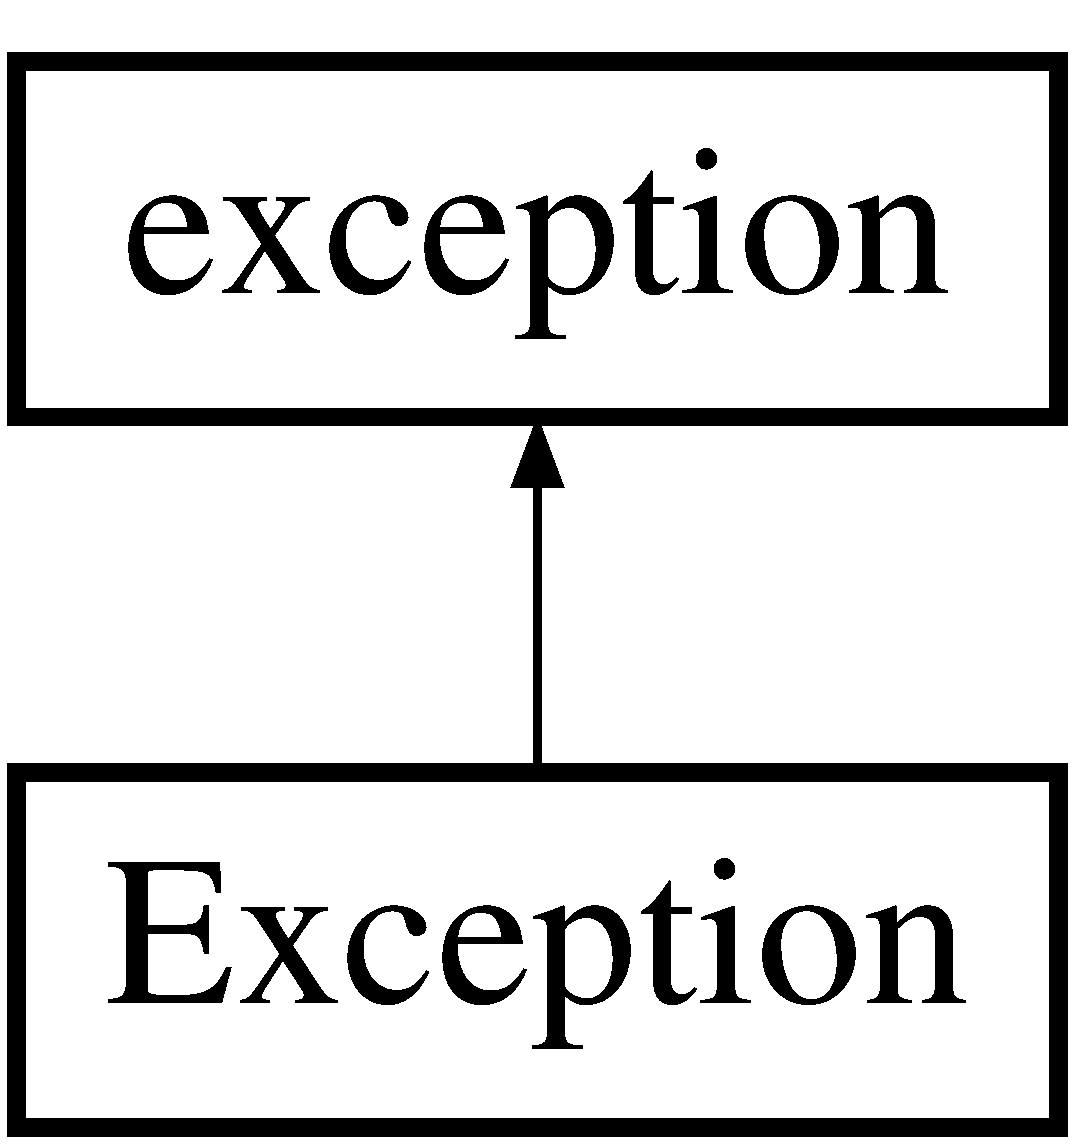
\includegraphics[height=2.000000cm]{class_exception}
\end{center}
\end{figure}
\subsection*{Public Member Functions}
\begin{DoxyCompactItemize}
\item 
\hyperlink{class_exception_aac5e9386080a8eac2edebf02c8169ecc}{Exception} (const \hyperlink{class_message}{Message} \&\hyperlink{glew_8h_a76333d9470ffdd4811326932394d36da}{message}=\hyperlink{class_message}{Message}(), const \hyperlink{class_source_line}{Source\-Line} \&\hyperlink{class_exception_a67f40ff3ea7f1c07e46222c38dcbaf43}{source\-Line}=\hyperlink{class_source_line}{Source\-Line}())
\begin{DoxyCompactList}\small\item\em Constructs the exception with the specified message and source location. \end{DoxyCompactList}\item 
\hyperlink{class_exception_ae0fd52e62283ee92c085d767d0aab736}{Exception} (const \hyperlink{class_exception}{Exception} \&other)
\begin{DoxyCompactList}\small\item\em Constructs a copy of an exception. \end{DoxyCompactList}\item 
virtual \hyperlink{class_exception_ad1ba411de295ef2eeb02ba26284a829a}{$\sim$\-Exception} ()  throw ()
\begin{DoxyCompactList}\small\item\em Destructs the exception. \end{DoxyCompactList}\item 
\hyperlink{class_exception}{Exception} \& \hyperlink{class_exception_a71c844ee3ac32b7656c24386e9ab60a0}{operator=} (const \hyperlink{class_exception}{Exception} \&other)
\begin{DoxyCompactList}\small\item\em Performs an assignment. \end{DoxyCompactList}\item 
const char $\ast$ \hyperlink{class_exception_a45642915395d3b813fedc2593fbcb8bb}{what} () const   throw ()
\begin{DoxyCompactList}\small\item\em Returns descriptive message. \end{DoxyCompactList}\item 
\hyperlink{class_source_line}{Source\-Line} \hyperlink{class_exception_a67f40ff3ea7f1c07e46222c38dcbaf43}{source\-Line} () const 
\begin{DoxyCompactList}\small\item\em Location where the error occured. \end{DoxyCompactList}\item 
\hyperlink{class_message}{Message} \hyperlink{class_exception_aab5c1504a18016fdfe7574eb81f59ac6}{message} () const 
\begin{DoxyCompactList}\small\item\em \hyperlink{class_message}{Message} related to the exception. \end{DoxyCompactList}\item 
\hyperlink{wglew_8h_aeea6e3dfae3acf232096f57d2d57f084}{void} \hyperlink{class_exception_ad508783fa44767e8fedb6472a4180234}{set\-Message} (const \hyperlink{class_message}{Message} \&\hyperlink{glew_8h_a76333d9470ffdd4811326932394d36da}{message})
\begin{DoxyCompactList}\small\item\em Set the message. \end{DoxyCompactList}\item 
virtual \hyperlink{class_exception}{Exception} $\ast$ \hyperlink{class_exception_ad05463060510ad131ccaaafa6b63b2d7}{clone} () const 
\begin{DoxyCompactList}\small\item\em Clones the exception. \end{DoxyCompactList}\end{DoxyCompactItemize}
\subsection*{Protected Types}
\begin{DoxyCompactItemize}
\item 
typedef std\-::exception \hyperlink{class_exception_a5086086062a7ec2cfe4e609026adfbd9}{Super\-Class}
\end{DoxyCompactItemize}
\subsection*{Protected Attributes}
\begin{DoxyCompactItemize}
\item 
\hyperlink{class_message}{Message} \hyperlink{class_exception_ad77e1fcf64ced674e60e1d9195c634df}{m\-\_\-message}
\item 
\hyperlink{class_source_line}{Source\-Line} \hyperlink{class_exception_ae6685340e219cdcef0d72d45b58c5efb}{m\-\_\-source\-Line}
\item 
\hyperlink{glew_8h_ae84541b4f3d8e1ea24ec0f466a8c568b}{std\-::string} \hyperlink{class_exception_a51b947da686ab2dd290f799b2a05d492}{m\-\_\-what\-Message}
\end{DoxyCompactItemize}


\subsection{Detailed Description}
Exceptions thrown by failed assertions.

\hyperlink{class_exception}{Exception} is an exception that serves descriptive strings through its \hyperlink{class_exception_a45642915395d3b813fedc2593fbcb8bb}{what()} method. 

\subsection{Member Typedef Documentation}
\hypertarget{class_exception_a5086086062a7ec2cfe4e609026adfbd9}{\index{Exception@{Exception}!Super\-Class@{Super\-Class}}
\index{Super\-Class@{Super\-Class}!Exception@{Exception}}
\subsubsection[{Super\-Class}]{\setlength{\rightskip}{0pt plus 5cm}typedef std\-::exception {\bf Exception\-::\-Super\-Class}\hspace{0.3cm}{\ttfamily [protected]}}}\label{class_exception_a5086086062a7ec2cfe4e609026adfbd9}


\subsection{Constructor \& Destructor Documentation}
\hypertarget{class_exception_aac5e9386080a8eac2edebf02c8169ecc}{\index{Exception@{Exception}!Exception@{Exception}}
\index{Exception@{Exception}!Exception@{Exception}}
\subsubsection[{Exception}]{\setlength{\rightskip}{0pt plus 5cm}Exception\-::\-Exception (
\begin{DoxyParamCaption}
\item[{const {\bf Message} \&}]{message = {\ttfamily {\bf Message}()}, }
\item[{const {\bf Source\-Line} \&}]{source\-Line = {\ttfamily {\bf Source\-Line}()}}
\end{DoxyParamCaption}
)}}\label{class_exception_aac5e9386080a8eac2edebf02c8169ecc}


Constructs the exception with the specified message and source location. 


\begin{DoxyParams}{Parameters}
{\em message} & \hyperlink{class_message}{Message} associated to the exception. \\
\hline
{\em source\-Line} & Source location related to the exception. \\
\hline
\end{DoxyParams}
\hypertarget{class_exception_ae0fd52e62283ee92c085d767d0aab736}{\index{Exception@{Exception}!Exception@{Exception}}
\index{Exception@{Exception}!Exception@{Exception}}
\subsubsection[{Exception}]{\setlength{\rightskip}{0pt plus 5cm}Exception\-::\-Exception (
\begin{DoxyParamCaption}
\item[{const {\bf Exception} \&}]{other}
\end{DoxyParamCaption}
)}}\label{class_exception_ae0fd52e62283ee92c085d767d0aab736}


Constructs a copy of an exception. 


\begin{DoxyParams}{Parameters}
{\em other} & \hyperlink{class_exception}{Exception} to copy. \\
\hline
\end{DoxyParams}
\hypertarget{class_exception_ad1ba411de295ef2eeb02ba26284a829a}{\index{Exception@{Exception}!$\sim$\-Exception@{$\sim$\-Exception}}
\index{$\sim$\-Exception@{$\sim$\-Exception}!Exception@{Exception}}
\subsubsection[{$\sim$\-Exception}]{\setlength{\rightskip}{0pt plus 5cm}virtual Exception\-::$\sim$\-Exception (
\begin{DoxyParamCaption}
{}
\end{DoxyParamCaption}
) throw  ) \hspace{0.3cm}{\ttfamily [virtual]}}}\label{class_exception_ad1ba411de295ef2eeb02ba26284a829a}


Destructs the exception. 



\subsection{Member Function Documentation}
\hypertarget{class_exception_ad05463060510ad131ccaaafa6b63b2d7}{\index{Exception@{Exception}!clone@{clone}}
\index{clone@{clone}!Exception@{Exception}}
\subsubsection[{clone}]{\setlength{\rightskip}{0pt plus 5cm}virtual {\bf Exception}$\ast$ Exception\-::clone (
\begin{DoxyParamCaption}
{}
\end{DoxyParamCaption}
) const\hspace{0.3cm}{\ttfamily [virtual]}}}\label{class_exception_ad05463060510ad131ccaaafa6b63b2d7}


Clones the exception. 

\hypertarget{class_exception_aab5c1504a18016fdfe7574eb81f59ac6}{\index{Exception@{Exception}!message@{message}}
\index{message@{message}!Exception@{Exception}}
\subsubsection[{message}]{\setlength{\rightskip}{0pt plus 5cm}{\bf Message} Exception\-::message (
\begin{DoxyParamCaption}
{}
\end{DoxyParamCaption}
) const}}\label{class_exception_aab5c1504a18016fdfe7574eb81f59ac6}


\hyperlink{class_message}{Message} related to the exception. 

\hypertarget{class_exception_a71c844ee3ac32b7656c24386e9ab60a0}{\index{Exception@{Exception}!operator=@{operator=}}
\index{operator=@{operator=}!Exception@{Exception}}
\subsubsection[{operator=}]{\setlength{\rightskip}{0pt plus 5cm}{\bf Exception}\& Exception\-::operator= (
\begin{DoxyParamCaption}
\item[{const {\bf Exception} \&}]{other}
\end{DoxyParamCaption}
)}}\label{class_exception_a71c844ee3ac32b7656c24386e9ab60a0}


Performs an assignment. 

\hypertarget{class_exception_ad508783fa44767e8fedb6472a4180234}{\index{Exception@{Exception}!set\-Message@{set\-Message}}
\index{set\-Message@{set\-Message}!Exception@{Exception}}
\subsubsection[{set\-Message}]{\setlength{\rightskip}{0pt plus 5cm}{\bf void} Exception\-::set\-Message (
\begin{DoxyParamCaption}
\item[{const {\bf Message} \&}]{message}
\end{DoxyParamCaption}
)}}\label{class_exception_ad508783fa44767e8fedb6472a4180234}


Set the message. 

\hypertarget{class_exception_a67f40ff3ea7f1c07e46222c38dcbaf43}{\index{Exception@{Exception}!source\-Line@{source\-Line}}
\index{source\-Line@{source\-Line}!Exception@{Exception}}
\subsubsection[{source\-Line}]{\setlength{\rightskip}{0pt plus 5cm}{\bf Source\-Line} Exception\-::source\-Line (
\begin{DoxyParamCaption}
{}
\end{DoxyParamCaption}
) const}}\label{class_exception_a67f40ff3ea7f1c07e46222c38dcbaf43}


Location where the error occured. 

\hypertarget{class_exception_a45642915395d3b813fedc2593fbcb8bb}{\index{Exception@{Exception}!what@{what}}
\index{what@{what}!Exception@{Exception}}
\subsubsection[{what}]{\setlength{\rightskip}{0pt plus 5cm}const char$\ast$ Exception\-::what (
\begin{DoxyParamCaption}
{}
\end{DoxyParamCaption}
) const throw  ) }}\label{class_exception_a45642915395d3b813fedc2593fbcb8bb}


Returns descriptive message. 



\subsection{Member Data Documentation}
\hypertarget{class_exception_ad77e1fcf64ced674e60e1d9195c634df}{\index{Exception@{Exception}!m\-\_\-message@{m\-\_\-message}}
\index{m\-\_\-message@{m\-\_\-message}!Exception@{Exception}}
\subsubsection[{m\-\_\-message}]{\setlength{\rightskip}{0pt plus 5cm}{\bf Message} Exception\-::m\-\_\-message\hspace{0.3cm}{\ttfamily [protected]}}}\label{class_exception_ad77e1fcf64ced674e60e1d9195c634df}
\hypertarget{class_exception_ae6685340e219cdcef0d72d45b58c5efb}{\index{Exception@{Exception}!m\-\_\-source\-Line@{m\-\_\-source\-Line}}
\index{m\-\_\-source\-Line@{m\-\_\-source\-Line}!Exception@{Exception}}
\subsubsection[{m\-\_\-source\-Line}]{\setlength{\rightskip}{0pt plus 5cm}{\bf Source\-Line} Exception\-::m\-\_\-source\-Line\hspace{0.3cm}{\ttfamily [protected]}}}\label{class_exception_ae6685340e219cdcef0d72d45b58c5efb}
\hypertarget{class_exception_a51b947da686ab2dd290f799b2a05d492}{\index{Exception@{Exception}!m\-\_\-what\-Message@{m\-\_\-what\-Message}}
\index{m\-\_\-what\-Message@{m\-\_\-what\-Message}!Exception@{Exception}}
\subsubsection[{m\-\_\-what\-Message}]{\setlength{\rightskip}{0pt plus 5cm}{\bf std\-::string} Exception\-::m\-\_\-what\-Message\hspace{0.3cm}{\ttfamily [protected]}}}\label{class_exception_a51b947da686ab2dd290f799b2a05d492}


The documentation for this class was generated from the following file\-:\begin{DoxyCompactItemize}
\item 
Cadriciel/\-Commun/\-Externe/cppunit/include/cppunit/\hyperlink{_exception_8h}{Exception.\-h}\end{DoxyCompactItemize}

\hypertarget{class_exception_test_case_decorator}{\section{Exception\-Test\-Case\-Decorator$<$ Expected\-Exception $>$ Class Template Reference}
\label{class_exception_test_case_decorator}\index{Exception\-Test\-Case\-Decorator$<$ Expected\-Exception $>$@{Exception\-Test\-Case\-Decorator$<$ Expected\-Exception $>$}}
}


Expected exception test case decorator.  




{\ttfamily \#include $<$Exception\-Test\-Case\-Decorator.\-h$>$}

Inheritance diagram for Exception\-Test\-Case\-Decorator$<$ Expected\-Exception $>$\-:\begin{figure}[H]
\begin{center}
\leavevmode
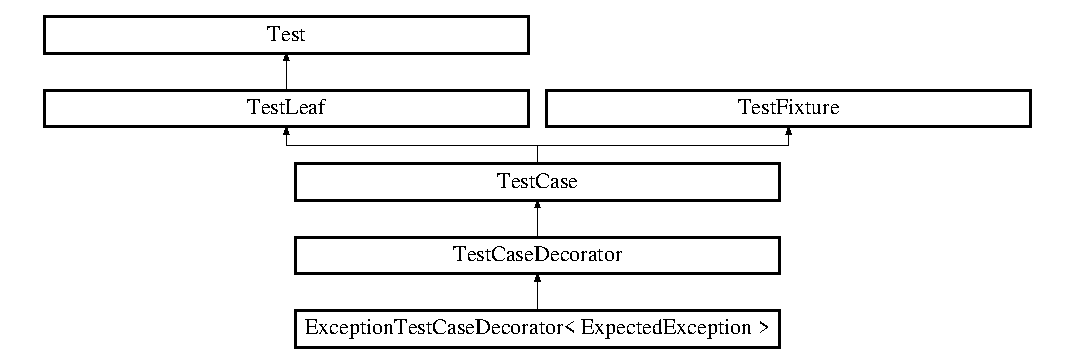
\includegraphics[height=4.444445cm]{class_exception_test_case_decorator}
\end{center}
\end{figure}
\subsection*{Public Types}
\begin{DoxyCompactItemize}
\item 
typedef Expected\-Exception \hyperlink{class_exception_test_case_decorator_a3fc7e11a4aa1730fa98ff6ac52958ae9}{Expected\-Exception\-Type}
\end{DoxyCompactItemize}
\subsection*{Public Member Functions}
\begin{DoxyCompactItemize}
\item 
\hyperlink{class_exception_test_case_decorator_a01b0c42952450cff574dd9e293c718fa}{Exception\-Test\-Case\-Decorator} (\hyperlink{class_test_case}{Test\-Case} $\ast$test)
\begin{DoxyCompactList}\small\item\em Decorates the specified test. \end{DoxyCompactList}\item 
\hyperlink{wglew_8h_aeea6e3dfae3acf232096f57d2d57f084}{void} \hyperlink{class_exception_test_case_decorator_a3f78294d459a94f55413162d814f291d}{run\-Test} ()
\begin{DoxyCompactList}\small\item\em Checks that the expected exception is thrown by the decorated test. is thrown. \end{DoxyCompactList}\end{DoxyCompactItemize}
\subsection*{Additional Inherited Members}


\subsection{Detailed Description}
\subsubsection*{template$<$class Expected\-Exception$>$class Exception\-Test\-Case\-Decorator$<$ Expected\-Exception $>$}

Expected exception test case decorator. 

A decorator used to assert that a specific test case should throw an exception of a given type.

You should use this class only if you need to check the exception object state (that a specific cause is set for example). If you don't need to do that, you might consider using \hyperlink{group___writing_test_fixture_gaca8eeb6f60714baade6cbfd185868c40}{C\-P\-P\-U\-N\-I\-T\-\_\-\-T\-E\-S\-T\-\_\-\-E\-X\-C\-E\-P\-T\-I\-O\-N()} instead.

Intended use is to subclass and override check\-Exception(). Example\-:


\begin{DoxyCode}
\textcolor{keyword}{class }NetworkErrorTestCaseDecorator : 
          \textcolor{keyword}{public} \hyperlink{class_exception_test_case_decorator}{ExceptionTestCaseDecorator}<NetworkError>
\{
\textcolor{keyword}{public}:
  NetworkErrorTestCaseDecorator( NetworkError::Cause expectedCause )
      : m\_expectedCause( expectedCause )
  \{
  \}
\textcolor{keyword}{private}:
  \textcolor{keywordtype}{void} checkException( \hyperlink{class_exception_test_case_decorator_a3fc7e11a4aa1730fa98ff6ac52958ae9}{ExpectedExceptionType} &e )
  \{
    \hyperlink{_test_assert_8h_a71162f05be07ef6817d156e77c68b1a3}{CPPUNIT\_ASSERT\_EQUAL}( m\_expectedCause, e.getCause() );
  \}

  NetworkError::Cause m\_expectedCause;
\};
\end{DoxyCode}
 

\subsection{Member Typedef Documentation}
\hypertarget{class_exception_test_case_decorator_a3fc7e11a4aa1730fa98ff6ac52958ae9}{\index{Exception\-Test\-Case\-Decorator@{Exception\-Test\-Case\-Decorator}!Expected\-Exception\-Type@{Expected\-Exception\-Type}}
\index{Expected\-Exception\-Type@{Expected\-Exception\-Type}!ExceptionTestCaseDecorator@{Exception\-Test\-Case\-Decorator}}
\subsubsection[{Expected\-Exception\-Type}]{\setlength{\rightskip}{0pt plus 5cm}template$<$class Expected\-Exception $>$ typedef Expected\-Exception {\bf Exception\-Test\-Case\-Decorator}$<$ Expected\-Exception $>$\-::{\bf Expected\-Exception\-Type}}}\label{class_exception_test_case_decorator_a3fc7e11a4aa1730fa98ff6ac52958ae9}


\subsection{Constructor \& Destructor Documentation}
\hypertarget{class_exception_test_case_decorator_a01b0c42952450cff574dd9e293c718fa}{\index{Exception\-Test\-Case\-Decorator@{Exception\-Test\-Case\-Decorator}!Exception\-Test\-Case\-Decorator@{Exception\-Test\-Case\-Decorator}}
\index{Exception\-Test\-Case\-Decorator@{Exception\-Test\-Case\-Decorator}!ExceptionTestCaseDecorator@{Exception\-Test\-Case\-Decorator}}
\subsubsection[{Exception\-Test\-Case\-Decorator}]{\setlength{\rightskip}{0pt plus 5cm}template$<$class Expected\-Exception $>$ {\bf Exception\-Test\-Case\-Decorator}$<$ Expected\-Exception $>$\-::{\bf Exception\-Test\-Case\-Decorator} (
\begin{DoxyParamCaption}
\item[{{\bf Test\-Case} $\ast$}]{test}
\end{DoxyParamCaption}
)\hspace{0.3cm}{\ttfamily [inline]}}}\label{class_exception_test_case_decorator_a01b0c42952450cff574dd9e293c718fa}


Decorates the specified test. 


\begin{DoxyParams}{Parameters}
{\em test} & \hyperlink{class_test_case}{Test\-Case} to decorate. Assumes ownership of the test. \\
\hline
\end{DoxyParams}


\subsection{Member Function Documentation}
\hypertarget{class_exception_test_case_decorator_a3f78294d459a94f55413162d814f291d}{\index{Exception\-Test\-Case\-Decorator@{Exception\-Test\-Case\-Decorator}!run\-Test@{run\-Test}}
\index{run\-Test@{run\-Test}!ExceptionTestCaseDecorator@{Exception\-Test\-Case\-Decorator}}
\subsubsection[{run\-Test}]{\setlength{\rightskip}{0pt plus 5cm}template$<$class Expected\-Exception $>$ {\bf void} {\bf Exception\-Test\-Case\-Decorator}$<$ Expected\-Exception $>$\-::run\-Test (
\begin{DoxyParamCaption}
{}
\end{DoxyParamCaption}
)\hspace{0.3cm}{\ttfamily [inline]}, {\ttfamily [virtual]}}}\label{class_exception_test_case_decorator_a3f78294d459a94f55413162d814f291d}


Checks that the expected exception is thrown by the decorated test. is thrown. 

Calls the decorated test \hyperlink{class_exception_test_case_decorator_a3f78294d459a94f55413162d814f291d}{run\-Test()} and checks that an exception of type Expected\-Exception is thrown. Call check\-Exception() passing the exception that was caught so that some assertions can be made if needed. 

Reimplemented from \hyperlink{class_test_case_a6b55957ac1dfef01e5d9fa2475676f34}{Test\-Case}.



The documentation for this class was generated from the following file\-:\begin{DoxyCompactItemize}
\item 
Cadriciel/\-Commun/\-Externe/cppunit/include/cppunit/extensions/\hyperlink{_exception_test_case_decorator_8h}{Exception\-Test\-Case\-Decorator.\-h}\end{DoxyCompactItemize}

\hypertarget{class_synchronized_object_1_1_exclusive_zone}{\section{Synchronized\-Object\-:\-:Exclusive\-Zone Class Reference}
\label{class_synchronized_object_1_1_exclusive_zone}\index{Synchronized\-Object\-::\-Exclusive\-Zone@{Synchronized\-Object\-::\-Exclusive\-Zone}}
}


Locks a synchronization object in the current scope.  




{\ttfamily \#include $<$Synchronized\-Object.\-h$>$}

\subsection*{Public Member Functions}
\begin{DoxyCompactItemize}
\item 
\hyperlink{class_synchronized_object_1_1_exclusive_zone_ae4393b508828328c2f4816ff9b7b090c}{Exclusive\-Zone} (\hyperlink{class_synchronized_object_1_1_synchronization_object}{Synchronization\-Object} $\ast$sync\-Object)
\item 
\hyperlink{class_synchronized_object_1_1_exclusive_zone_a501678d50abfd678ff0ce0fc164c63d4}{$\sim$\-Exclusive\-Zone} ()
\end{DoxyCompactItemize}


\subsection{Detailed Description}
Locks a synchronization object in the current scope. 

\subsection{Constructor \& Destructor Documentation}
\hypertarget{class_synchronized_object_1_1_exclusive_zone_ae4393b508828328c2f4816ff9b7b090c}{\index{Synchronized\-Object\-::\-Exclusive\-Zone@{Synchronized\-Object\-::\-Exclusive\-Zone}!Exclusive\-Zone@{Exclusive\-Zone}}
\index{Exclusive\-Zone@{Exclusive\-Zone}!SynchronizedObject::ExclusiveZone@{Synchronized\-Object\-::\-Exclusive\-Zone}}
\subsubsection[{Exclusive\-Zone}]{\setlength{\rightskip}{0pt plus 5cm}Synchronized\-Object\-::\-Exclusive\-Zone\-::\-Exclusive\-Zone (
\begin{DoxyParamCaption}
\item[{{\bf Synchronization\-Object} $\ast$}]{sync\-Object}
\end{DoxyParamCaption}
)\hspace{0.3cm}{\ttfamily [inline]}}}\label{class_synchronized_object_1_1_exclusive_zone_ae4393b508828328c2f4816ff9b7b090c}
\hypertarget{class_synchronized_object_1_1_exclusive_zone_a501678d50abfd678ff0ce0fc164c63d4}{\index{Synchronized\-Object\-::\-Exclusive\-Zone@{Synchronized\-Object\-::\-Exclusive\-Zone}!$\sim$\-Exclusive\-Zone@{$\sim$\-Exclusive\-Zone}}
\index{$\sim$\-Exclusive\-Zone@{$\sim$\-Exclusive\-Zone}!SynchronizedObject::ExclusiveZone@{Synchronized\-Object\-::\-Exclusive\-Zone}}
\subsubsection[{$\sim$\-Exclusive\-Zone}]{\setlength{\rightskip}{0pt plus 5cm}Synchronized\-Object\-::\-Exclusive\-Zone\-::$\sim$\-Exclusive\-Zone (
\begin{DoxyParamCaption}
{}
\end{DoxyParamCaption}
)\hspace{0.3cm}{\ttfamily [inline]}}}\label{class_synchronized_object_1_1_exclusive_zone_a501678d50abfd678ff0ce0fc164c63d4}


The documentation for this class was generated from the following file\-:\begin{DoxyCompactItemize}
\item 
Cadriciel/\-Commun/\-Externe/cppunit/include/cppunit/\hyperlink{_synchronized_object_8h}{Synchronized\-Object.\-h}\end{DoxyCompactItemize}

\hypertarget{classca_1_1polymtl_1_1inf2990_1_1_exemple}{\section{ca.\-polymtl.\-inf2990.\-Exemple Class Reference}
\label{classca_1_1polymtl_1_1inf2990_1_1_exemple}\index{ca.\-polymtl.\-inf2990.\-Exemple@{ca.\-polymtl.\-inf2990.\-Exemple}}
}
Inheritance diagram for ca.\-polymtl.\-inf2990.\-Exemple\-:\begin{figure}[H]
\begin{center}
\leavevmode
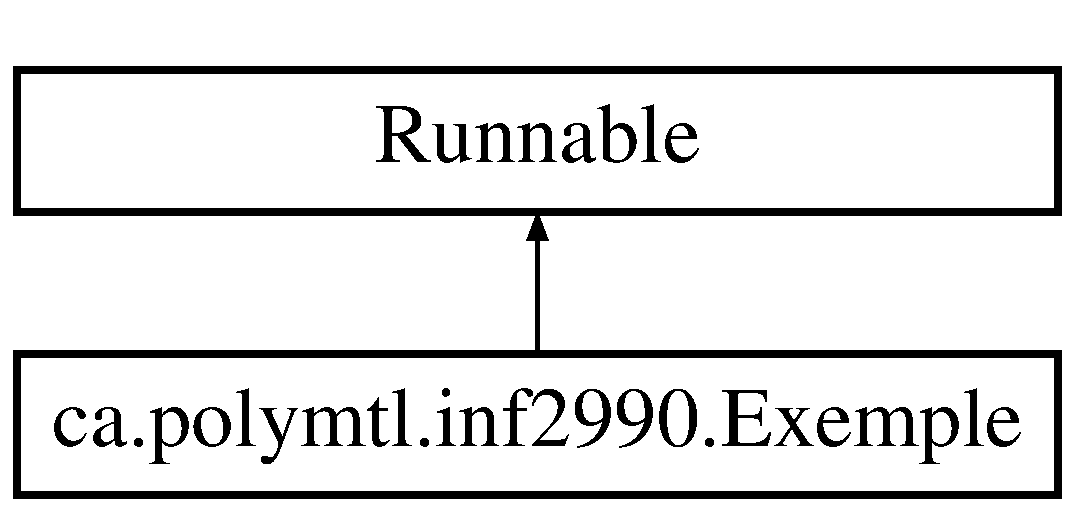
\includegraphics[height=2.000000cm]{classca_1_1polymtl_1_1inf2990_1_1_exemple}
\end{center}
\end{figure}
\subsection*{Public Member Functions}
\begin{DoxyCompactItemize}
\item 
\hyperlink{wglew_8h_aeea6e3dfae3acf232096f57d2d57f084}{void} \hyperlink{classca_1_1polymtl_1_1inf2990_1_1_exemple_a861ce9c3d363682f551d53535b2e3eb8}{run} ()
\item 
\hyperlink{wglew_8h_aeea6e3dfae3acf232096f57d2d57f084}{void} \hyperlink{classca_1_1polymtl_1_1inf2990_1_1_exemple_ad64833544cadb749c919a1f57bc8d981}{Nouveau} ()
\item 
\hyperlink{wglew_8h_aeea6e3dfae3acf232096f57d2d57f084}{void} \hyperlink{classca_1_1polymtl_1_1inf2990_1_1_exemple_a8a6473b33c40696eb0d38cb057acfd46}{Quitter} ()
\item 
\hyperlink{wglew_8h_aeea6e3dfae3acf232096f57d2d57f084}{void} \hyperlink{classca_1_1polymtl_1_1inf2990_1_1_exemple_a33c099d03978b19ebeac976e2b7ebe86}{Aide} ()
\item 
\hyperlink{wglew_8h_aeea6e3dfae3acf232096f57d2d57f084}{void} \hyperlink{classca_1_1polymtl_1_1inf2990_1_1_exemple_ae290a8913d699b6470a35cef6df56a08}{Texte} ()
\item 
\hyperlink{wglew_8h_aeea6e3dfae3acf232096f57d2d57f084}{void} \hyperlink{classca_1_1polymtl_1_1inf2990_1_1_exemple_a87c48d0e90a7b3d2a571b70c3cc8b4dd}{appuyer\-\_\-a} ()
\item 
\hyperlink{wglew_8h_aeea6e3dfae3acf232096f57d2d57f084}{void} \hyperlink{classca_1_1polymtl_1_1inf2990_1_1_exemple_a16e0a16ba8499be3c0c9943245941c42}{appuyer\-\_\-f} ()
\end{DoxyCompactItemize}
\subsection*{Static Public Member Functions}
\begin{DoxyCompactItemize}
\item 
static \hyperlink{wglew_8h_aeea6e3dfae3acf232096f57d2d57f084}{void} \hyperlink{classca_1_1polymtl_1_1inf2990_1_1_exemple_ac97a9982d04498d48f453e6b74f9a36c}{main} (String args\mbox{[}$\,$\mbox{]})
\item 
static native \hyperlink{wglew_8h_aeea6e3dfae3acf232096f57d2d57f084}{void} \hyperlink{classca_1_1polymtl_1_1inf2990_1_1_exemple_ad7d5216ecae9d689b7af90c854a1019e}{fct\-C\-\_\-initialiser\-Open\-G\-L} (Canvas canvas)
\item 
static native \hyperlink{wglew_8h_aeea6e3dfae3acf232096f57d2d57f084}{void} \hyperlink{classca_1_1polymtl_1_1inf2990_1_1_exemple_a7b48e33233c15a717963d803b8fc3fc0}{fct\-C\-\_\-liberer\-Open\-G\-L} (Canvas canvas)
\item 
static native \hyperlink{wglew_8h_aeea6e3dfae3acf232096f57d2d57f084}{void} \hyperlink{classca_1_1polymtl_1_1inf2990_1_1_exemple_adccce4874d16b314681f2c299fdb4fde}{fct\-C\-\_\-dessiner\-Open\-G\-L} (Canvas canvas)
\item 
static native \hyperlink{wglew_8h_aeea6e3dfae3acf232096f57d2d57f084}{void} \hyperlink{classca_1_1polymtl_1_1inf2990_1_1_exemple_a5956b6c316c0a27f6934b50bdd264dfd}{fct\-C\-\_\-redimensionner\-Fenetre} (\hyperlink{wglew_8h_a500a82aecba06f4550f6849b8099ca21}{int} largeur, \hyperlink{wglew_8h_a500a82aecba06f4550f6849b8099ca21}{int} hauteur)
\item 
static native \hyperlink{wglew_8h_aeea6e3dfae3acf232096f57d2d57f084}{void} \hyperlink{classca_1_1polymtl_1_1inf2990_1_1_exemple_a58af060f14adc783875eb13c7eb30472}{fct\-C\-\_\-animer} (\hyperlink{fmod_8h_aeb841aa4b4b5f444b5d739d865b420af}{float} temps)
\item 
static native \hyperlink{wglew_8h_aeea6e3dfae3acf232096f57d2d57f084}{void} \hyperlink{classca_1_1polymtl_1_1inf2990_1_1_exemple_a0be3f6aaa1b721293bf64911d20b2dac}{fct\-C\-\_\-zoom\-In} ()
\item 
static native \hyperlink{wglew_8h_aeea6e3dfae3acf232096f57d2d57f084}{void} \hyperlink{classca_1_1polymtl_1_1inf2990_1_1_exemple_aca90a7e09b54b2bbf3f2f28a29dd5c16}{fct\-C\-\_\-zoom\-Out} ()
\item 
static native \hyperlink{wglew_8h_a500a82aecba06f4550f6849b8099ca21}{int} \hyperlink{classca_1_1polymtl_1_1inf2990_1_1_exemple_a5bb5c32a3ff555ecbbe8d90f65bec58d}{obtenir\-Affichages\-Par\-Seconde} ()
\item 
static native \hyperlink{wglew_8h_a500a82aecba06f4550f6849b8099ca21}{int} \hyperlink{classca_1_1polymtl_1_1inf2990_1_1_exemple_ad3f1c2c5c80440a6af312cbc52ac8ead}{fct\-C\-\_\-executer\-Tests} ()
\item 
static native \hyperlink{wglew_8h_aeea6e3dfae3acf232096f57d2d57f084}{void} \hyperlink{classca_1_1polymtl_1_1inf2990_1_1_exemple_a9d4e25c8e324e7989fe70b4471cf9df4}{fct\-C\-\_\-envoyer\-Input} (\hyperlink{wglew_8h_a500a82aecba06f4550f6849b8099ca21}{int} \hyperlink{glew_8h_ad77deca22f617d3f0e0eb786445689fc}{x}, \hyperlink{wglew_8h_a500a82aecba06f4550f6849b8099ca21}{int} \hyperlink{glew_8h_a9298c7ad619074f5285b32c6b72bfdea}{y}, \hyperlink{wglew_8h_a500a82aecba06f4550f6849b8099ca21}{int} bouton, \hyperlink{wglew_8h_a500a82aecba06f4550f6849b8099ca21}{int} touche)
\end{DoxyCompactItemize}


\subsection{Detailed Description}
Cette classe cr�e une fen�tre Java ainsi qu'un contexte Open\-G\-L dans lequel la librairie C++ pourra dessiner.

Il ne s'agit que d'un exemple des diff�rentes fonctionnalit�s qu'il est possible d'implanter en Java, notamment la cr�ation d'une fen�tre, d'un contexte Open\-G\-L, d'une barre de menus et d'une barre d'outils, ainsi que la gestionnaire de certains �v�nements.

C\-E\-T\-T\-E C\-L\-A\-S\-S\-E N\-E C\-O\-N\-S\-T\-I\-T\-U\-E P\-A\-S U\-N E\-X\-E\-M\-P\-L\-E D\-E B\-O\-N\-N\-E P\-R\-O\-G\-R\-A\-M\-M\-A\-T\-I\-O\-N. Elle est monolithique et vise � �tre s�par�e en plusieurs classes, �ventuellement dans des paquetages diff�rents, lorsque les v�ritables fonctionnalit�s seront implant�es.

\begin{DoxyAuthor}{Author}
Martin Bisson 
\end{DoxyAuthor}
\begin{DoxyDate}{Date}
2007-\/08-\/15 
\end{DoxyDate}


\subsection{Member Function Documentation}
\hypertarget{classca_1_1polymtl_1_1inf2990_1_1_exemple_a33c099d03978b19ebeac976e2b7ebe86}{\index{ca\-::polymtl\-::inf2990\-::\-Exemple@{ca\-::polymtl\-::inf2990\-::\-Exemple}!Aide@{Aide}}
\index{Aide@{Aide}!ca::polymtl::inf2990::Exemple@{ca\-::polymtl\-::inf2990\-::\-Exemple}}
\subsubsection[{Aide}]{\setlength{\rightskip}{0pt plus 5cm}{\bf void} ca.\-polymtl.\-inf2990.\-Exemple.\-Aide (
\begin{DoxyParamCaption}
{}
\end{DoxyParamCaption}
)\hspace{0.3cm}{\ttfamily [inline]}}}\label{classca_1_1polymtl_1_1inf2990_1_1_exemple_a33c099d03978b19ebeac976e2b7ebe86}
Fonction appel�e lorsque le bouton Aide de la barre d'outils est actionn�. \hypertarget{classca_1_1polymtl_1_1inf2990_1_1_exemple_a87c48d0e90a7b3d2a571b70c3cc8b4dd}{\index{ca\-::polymtl\-::inf2990\-::\-Exemple@{ca\-::polymtl\-::inf2990\-::\-Exemple}!appuyer\-\_\-a@{appuyer\-\_\-a}}
\index{appuyer\-\_\-a@{appuyer\-\_\-a}!ca::polymtl::inf2990::Exemple@{ca\-::polymtl\-::inf2990\-::\-Exemple}}
\subsubsection[{appuyer\-\_\-a}]{\setlength{\rightskip}{0pt plus 5cm}{\bf void} ca.\-polymtl.\-inf2990.\-Exemple.\-appuyer\-\_\-a (
\begin{DoxyParamCaption}
{}
\end{DoxyParamCaption}
)\hspace{0.3cm}{\ttfamily [inline]}}}\label{classca_1_1polymtl_1_1inf2990_1_1_exemple_a87c48d0e90a7b3d2a571b70c3cc8b4dd}
Fonction appel�e lorsque la touche \char`\"{}a\char`\"{} est appuy�e. \hypertarget{classca_1_1polymtl_1_1inf2990_1_1_exemple_a16e0a16ba8499be3c0c9943245941c42}{\index{ca\-::polymtl\-::inf2990\-::\-Exemple@{ca\-::polymtl\-::inf2990\-::\-Exemple}!appuyer\-\_\-f@{appuyer\-\_\-f}}
\index{appuyer\-\_\-f@{appuyer\-\_\-f}!ca::polymtl::inf2990::Exemple@{ca\-::polymtl\-::inf2990\-::\-Exemple}}
\subsubsection[{appuyer\-\_\-f}]{\setlength{\rightskip}{0pt plus 5cm}{\bf void} ca.\-polymtl.\-inf2990.\-Exemple.\-appuyer\-\_\-f (
\begin{DoxyParamCaption}
{}
\end{DoxyParamCaption}
)\hspace{0.3cm}{\ttfamily [inline]}}}\label{classca_1_1polymtl_1_1inf2990_1_1_exemple_a16e0a16ba8499be3c0c9943245941c42}
Fonction appel�e lorsque la touche \char`\"{}f\char`\"{} est appuy�e. Elle affiche le nombre d'affichages par seconde. \hypertarget{classca_1_1polymtl_1_1inf2990_1_1_exemple_a58af060f14adc783875eb13c7eb30472}{\index{ca\-::polymtl\-::inf2990\-::\-Exemple@{ca\-::polymtl\-::inf2990\-::\-Exemple}!fct\-C\-\_\-animer@{fct\-C\-\_\-animer}}
\index{fct\-C\-\_\-animer@{fct\-C\-\_\-animer}!ca::polymtl::inf2990::Exemple@{ca\-::polymtl\-::inf2990\-::\-Exemple}}
\subsubsection[{fct\-C\-\_\-animer}]{\setlength{\rightskip}{0pt plus 5cm}static native {\bf void} ca.\-polymtl.\-inf2990.\-Exemple.\-fct\-C\-\_\-animer (
\begin{DoxyParamCaption}
\item[{{\bf float}}]{temps}
\end{DoxyParamCaption}
)\hspace{0.3cm}{\ttfamily [static]}}}\label{classca_1_1polymtl_1_1inf2990_1_1_exemple_a58af060f14adc783875eb13c7eb30472}
Fonction qui anime le jeu d'un certain intervalle de temps.

Elle vise � �tre appel�e de nombreuses fois par seconde. Elle effectue les diff�rents calculs de physique et effectue un affichage.


\begin{DoxyParams}{Parameters}
{\em temps} & L'intervalle de temps � utiliser pour les diff�rents calculs. On vise � faire correspondre cet invervalle de temps au temps entre deux appels � la fonction. \\
\hline
\end{DoxyParams}
\hypertarget{classca_1_1polymtl_1_1inf2990_1_1_exemple_adccce4874d16b314681f2c299fdb4fde}{\index{ca\-::polymtl\-::inf2990\-::\-Exemple@{ca\-::polymtl\-::inf2990\-::\-Exemple}!fct\-C\-\_\-dessiner\-Open\-G\-L@{fct\-C\-\_\-dessiner\-Open\-G\-L}}
\index{fct\-C\-\_\-dessiner\-Open\-G\-L@{fct\-C\-\_\-dessiner\-Open\-G\-L}!ca::polymtl::inf2990::Exemple@{ca\-::polymtl\-::inf2990\-::\-Exemple}}
\subsubsection[{fct\-C\-\_\-dessiner\-Open\-G\-L}]{\setlength{\rightskip}{0pt plus 5cm}static native {\bf void} ca.\-polymtl.\-inf2990.\-Exemple.\-fct\-C\-\_\-dessiner\-Open\-G\-L (
\begin{DoxyParamCaption}
\item[{Canvas}]{canvas}
\end{DoxyParamCaption}
)\hspace{0.3cm}{\ttfamily [static]}}}\label{classca_1_1polymtl_1_1inf2990_1_1_exemple_adccce4874d16b314681f2c299fdb4fde}
Fonction qui affiche la sc�ne dans la fen�tre identifi�e par le canvas A\-W\-T pass� en param�tre.


\begin{DoxyParams}{Parameters}
{\em canvas} & Le canvas dans lequel cr�er le contexte Open\-G\-L. \\
\hline
\end{DoxyParams}
\hypertarget{classca_1_1polymtl_1_1inf2990_1_1_exemple_a9d4e25c8e324e7989fe70b4471cf9df4}{\index{ca\-::polymtl\-::inf2990\-::\-Exemple@{ca\-::polymtl\-::inf2990\-::\-Exemple}!fct\-C\-\_\-envoyer\-Input@{fct\-C\-\_\-envoyer\-Input}}
\index{fct\-C\-\_\-envoyer\-Input@{fct\-C\-\_\-envoyer\-Input}!ca::polymtl::inf2990::Exemple@{ca\-::polymtl\-::inf2990\-::\-Exemple}}
\subsubsection[{fct\-C\-\_\-envoyer\-Input}]{\setlength{\rightskip}{0pt plus 5cm}static native {\bf void} ca.\-polymtl.\-inf2990.\-Exemple.\-fct\-C\-\_\-envoyer\-Input (
\begin{DoxyParamCaption}
\item[{{\bf int}}]{x, }
\item[{{\bf int}}]{y, }
\item[{{\bf int}}]{bouton, }
\item[{{\bf int}}]{touche}
\end{DoxyParamCaption}
)\hspace{0.3cm}{\ttfamily [static]}}}\label{classca_1_1polymtl_1_1inf2990_1_1_exemple_a9d4e25c8e324e7989fe70b4471cf9df4}
Fonction qui envoie l'input du code Java vers le C++ 
\begin{DoxyParams}{Parameters}
{\em x} & Position en x de la souris \\
\hline
{\em y} & Position en y de la souris \\
\hline
{\em bouton} & Le bouton sur lequel on a appuy� sur la souris \\
\hline
{\em touche} & La touche sur laquel on a appuy� sur le clavier \\
\hline
\end{DoxyParams}
\hypertarget{classca_1_1polymtl_1_1inf2990_1_1_exemple_ad3f1c2c5c80440a6af312cbc52ac8ead}{\index{ca\-::polymtl\-::inf2990\-::\-Exemple@{ca\-::polymtl\-::inf2990\-::\-Exemple}!fct\-C\-\_\-executer\-Tests@{fct\-C\-\_\-executer\-Tests}}
\index{fct\-C\-\_\-executer\-Tests@{fct\-C\-\_\-executer\-Tests}!ca::polymtl::inf2990::Exemple@{ca\-::polymtl\-::inf2990\-::\-Exemple}}
\subsubsection[{fct\-C\-\_\-executer\-Tests}]{\setlength{\rightskip}{0pt plus 5cm}static native {\bf int} ca.\-polymtl.\-inf2990.\-Exemple.\-fct\-C\-\_\-executer\-Tests (
\begin{DoxyParamCaption}
{}
\end{DoxyParamCaption}
)\hspace{0.3cm}{\ttfamily [static]}}}\label{classca_1_1polymtl_1_1inf2990_1_1_exemple_ad3f1c2c5c80440a6af312cbc52ac8ead}
Fonction qui ex�cute les jeux de tests unitaires C++. \hypertarget{classca_1_1polymtl_1_1inf2990_1_1_exemple_ad7d5216ecae9d689b7af90c854a1019e}{\index{ca\-::polymtl\-::inf2990\-::\-Exemple@{ca\-::polymtl\-::inf2990\-::\-Exemple}!fct\-C\-\_\-initialiser\-Open\-G\-L@{fct\-C\-\_\-initialiser\-Open\-G\-L}}
\index{fct\-C\-\_\-initialiser\-Open\-G\-L@{fct\-C\-\_\-initialiser\-Open\-G\-L}!ca::polymtl::inf2990::Exemple@{ca\-::polymtl\-::inf2990\-::\-Exemple}}
\subsubsection[{fct\-C\-\_\-initialiser\-Open\-G\-L}]{\setlength{\rightskip}{0pt plus 5cm}static native {\bf void} ca.\-polymtl.\-inf2990.\-Exemple.\-fct\-C\-\_\-initialiser\-Open\-G\-L (
\begin{DoxyParamCaption}
\item[{Canvas}]{canvas}
\end{DoxyParamCaption}
)\hspace{0.3cm}{\ttfamily [static]}}}\label{classca_1_1polymtl_1_1inf2990_1_1_exemple_ad7d5216ecae9d689b7af90c854a1019e}
Fonction qui initialise un contexte Open\-G\-L dans la fen�tre identifi�e par le canvas A\-W\-T pass� en param�tre. Cette fonction doit �tre la premi�re � �tre appel�e, car la cr�ation de l'objet du mod�le C++ s'attend � avoir un contexte Open\-G\-L valide.


\begin{DoxyParams}{Parameters}
{\em canvas} & Le canvas dans lequel cr�er le contexte Open\-G\-L. \\
\hline
\end{DoxyParams}
\hypertarget{classca_1_1polymtl_1_1inf2990_1_1_exemple_a7b48e33233c15a717963d803b8fc3fc0}{\index{ca\-::polymtl\-::inf2990\-::\-Exemple@{ca\-::polymtl\-::inf2990\-::\-Exemple}!fct\-C\-\_\-liberer\-Open\-G\-L@{fct\-C\-\_\-liberer\-Open\-G\-L}}
\index{fct\-C\-\_\-liberer\-Open\-G\-L@{fct\-C\-\_\-liberer\-Open\-G\-L}!ca::polymtl::inf2990::Exemple@{ca\-::polymtl\-::inf2990\-::\-Exemple}}
\subsubsection[{fct\-C\-\_\-liberer\-Open\-G\-L}]{\setlength{\rightskip}{0pt plus 5cm}static native {\bf void} ca.\-polymtl.\-inf2990.\-Exemple.\-fct\-C\-\_\-liberer\-Open\-G\-L (
\begin{DoxyParamCaption}
\item[{Canvas}]{canvas}
\end{DoxyParamCaption}
)\hspace{0.3cm}{\ttfamily [static]}}}\label{classca_1_1polymtl_1_1inf2990_1_1_exemple_a7b48e33233c15a717963d803b8fc3fc0}
Fonction qui lib�re le contexte Open\-G\-L dans la fen�tre identifi�e par le canvas A\-W\-T pass� en param�tre. Cette fonction doit �tre la derni�re � �tre appel�e, car elle lib�re �galement l'objet du mod�le C++.


\begin{DoxyParams}{Parameters}
{\em canvas} & Le canvas dans lequel cr�er le contexte Open\-G\-L. \\
\hline
\end{DoxyParams}
\hypertarget{classca_1_1polymtl_1_1inf2990_1_1_exemple_a5956b6c316c0a27f6934b50bdd264dfd}{\index{ca\-::polymtl\-::inf2990\-::\-Exemple@{ca\-::polymtl\-::inf2990\-::\-Exemple}!fct\-C\-\_\-redimensionner\-Fenetre@{fct\-C\-\_\-redimensionner\-Fenetre}}
\index{fct\-C\-\_\-redimensionner\-Fenetre@{fct\-C\-\_\-redimensionner\-Fenetre}!ca::polymtl::inf2990::Exemple@{ca\-::polymtl\-::inf2990\-::\-Exemple}}
\subsubsection[{fct\-C\-\_\-redimensionner\-Fenetre}]{\setlength{\rightskip}{0pt plus 5cm}static native {\bf void} ca.\-polymtl.\-inf2990.\-Exemple.\-fct\-C\-\_\-redimensionner\-Fenetre (
\begin{DoxyParamCaption}
\item[{{\bf int}}]{largeur, }
\item[{{\bf int}}]{hauteur}
\end{DoxyParamCaption}
)\hspace{0.3cm}{\ttfamily [static]}}}\label{classca_1_1polymtl_1_1inf2990_1_1_exemple_a5956b6c316c0a27f6934b50bdd264dfd}
Fonction qui doit �tre appel�e lorsque la fen�tre est redimensionn�e afin d'ajuster les param�tres de la machine � �tats d'Open\-G\-L pour correspondre aux nouvelles dimensions de la fen�tre.


\begin{DoxyParams}{Parameters}
{\em largeur} & La nouvelle largeur de la fen�tre. \\
\hline
{\em hauteur} & La nouvelle hauteur de la fen�tre. \\
\hline
\end{DoxyParams}
\hypertarget{classca_1_1polymtl_1_1inf2990_1_1_exemple_a0be3f6aaa1b721293bf64911d20b2dac}{\index{ca\-::polymtl\-::inf2990\-::\-Exemple@{ca\-::polymtl\-::inf2990\-::\-Exemple}!fct\-C\-\_\-zoom\-In@{fct\-C\-\_\-zoom\-In}}
\index{fct\-C\-\_\-zoom\-In@{fct\-C\-\_\-zoom\-In}!ca::polymtl::inf2990::Exemple@{ca\-::polymtl\-::inf2990\-::\-Exemple}}
\subsubsection[{fct\-C\-\_\-zoom\-In}]{\setlength{\rightskip}{0pt plus 5cm}static native {\bf void} ca.\-polymtl.\-inf2990.\-Exemple.\-fct\-C\-\_\-zoom\-In (
\begin{DoxyParamCaption}
{}
\end{DoxyParamCaption}
)\hspace{0.3cm}{\ttfamily [static]}}}\label{classca_1_1polymtl_1_1inf2990_1_1_exemple_a0be3f6aaa1b721293bf64911d20b2dac}
Fonction qui applique un zoom avant sur le pr�sent volume de vision. \hypertarget{classca_1_1polymtl_1_1inf2990_1_1_exemple_aca90a7e09b54b2bbf3f2f28a29dd5c16}{\index{ca\-::polymtl\-::inf2990\-::\-Exemple@{ca\-::polymtl\-::inf2990\-::\-Exemple}!fct\-C\-\_\-zoom\-Out@{fct\-C\-\_\-zoom\-Out}}
\index{fct\-C\-\_\-zoom\-Out@{fct\-C\-\_\-zoom\-Out}!ca::polymtl::inf2990::Exemple@{ca\-::polymtl\-::inf2990\-::\-Exemple}}
\subsubsection[{fct\-C\-\_\-zoom\-Out}]{\setlength{\rightskip}{0pt plus 5cm}static native {\bf void} ca.\-polymtl.\-inf2990.\-Exemple.\-fct\-C\-\_\-zoom\-Out (
\begin{DoxyParamCaption}
{}
\end{DoxyParamCaption}
)\hspace{0.3cm}{\ttfamily [static]}}}\label{classca_1_1polymtl_1_1inf2990_1_1_exemple_aca90a7e09b54b2bbf3f2f28a29dd5c16}
Fonction qui applique un zoom arri�re sur le pr�sent volume de vision. \hypertarget{classca_1_1polymtl_1_1inf2990_1_1_exemple_ac97a9982d04498d48f453e6b74f9a36c}{\index{ca\-::polymtl\-::inf2990\-::\-Exemple@{ca\-::polymtl\-::inf2990\-::\-Exemple}!main@{main}}
\index{main@{main}!ca::polymtl::inf2990::Exemple@{ca\-::polymtl\-::inf2990\-::\-Exemple}}
\subsubsection[{main}]{\setlength{\rightskip}{0pt plus 5cm}static {\bf void} ca.\-polymtl.\-inf2990.\-Exemple.\-main (
\begin{DoxyParamCaption}
\item[{String}]{args\mbox{[}$\,$\mbox{]}}
\end{DoxyParamCaption}
)\hspace{0.3cm}{\ttfamily [inline]}, {\ttfamily [static]}}}\label{classca_1_1polymtl_1_1inf2990_1_1_exemple_ac97a9982d04498d48f453e6b74f9a36c}
Fonction principale de l'application qui constitue en fait son point d'entr�e. Elle v�rifie en premier si l'usager souhaite ex�cuter les test unitaires (si l'argument est tests\-C++). Dans l'affirmative, elle invoque l'appel des tests unitaires C++ via J\-N\-I et retourne le code d'erreur renvoy�. Sinon, la fonction d'entr�e proc�de au traitement par d�faut \-: elle se contente de cr�er un objet {\ttfamily \hyperlink{classca_1_1polymtl_1_1inf2990_1_1_exemple}{Exemple}} et de l'invoquer dans le thread A\-W\-T.


\begin{DoxyParams}{Parameters}
{\em args} & Les param�tres pass�es � l'application par la ligne de commande. Si le premier argument (args\mbox{[}0\mbox{]}) contient la cha�ne \char`\"{}tests\-C++\char`\"{}, les tests unitaires C++ sont invoqu�s et l'application quitte (retourne) imm�diatement. \\
\hline
\end{DoxyParams}
\hypertarget{classca_1_1polymtl_1_1inf2990_1_1_exemple_ad64833544cadb749c919a1f57bc8d981}{\index{ca\-::polymtl\-::inf2990\-::\-Exemple@{ca\-::polymtl\-::inf2990\-::\-Exemple}!Nouveau@{Nouveau}}
\index{Nouveau@{Nouveau}!ca::polymtl::inf2990::Exemple@{ca\-::polymtl\-::inf2990\-::\-Exemple}}
\subsubsection[{Nouveau}]{\setlength{\rightskip}{0pt plus 5cm}{\bf void} ca.\-polymtl.\-inf2990.\-Exemple.\-Nouveau (
\begin{DoxyParamCaption}
{}
\end{DoxyParamCaption}
)\hspace{0.3cm}{\ttfamily [inline]}}}\label{classca_1_1polymtl_1_1inf2990_1_1_exemple_ad64833544cadb749c919a1f57bc8d981}
Fonction appel�e lorsque l'�l�ment Nouveau du menu est actionn�. \hypertarget{classca_1_1polymtl_1_1inf2990_1_1_exemple_a5bb5c32a3ff555ecbbe8d90f65bec58d}{\index{ca\-::polymtl\-::inf2990\-::\-Exemple@{ca\-::polymtl\-::inf2990\-::\-Exemple}!obtenir\-Affichages\-Par\-Seconde@{obtenir\-Affichages\-Par\-Seconde}}
\index{obtenir\-Affichages\-Par\-Seconde@{obtenir\-Affichages\-Par\-Seconde}!ca::polymtl::inf2990::Exemple@{ca\-::polymtl\-::inf2990\-::\-Exemple}}
\subsubsection[{obtenir\-Affichages\-Par\-Seconde}]{\setlength{\rightskip}{0pt plus 5cm}static native {\bf int} ca.\-polymtl.\-inf2990.\-Exemple.\-obtenir\-Affichages\-Par\-Seconde (
\begin{DoxyParamCaption}
{}
\end{DoxyParamCaption}
)\hspace{0.3cm}{\ttfamily [static]}}}\label{classca_1_1polymtl_1_1inf2990_1_1_exemple_a5bb5c32a3ff555ecbbe8d90f65bec58d}
Fonction qui retourne le nombre moyen d'affichage par secondes. \hypertarget{classca_1_1polymtl_1_1inf2990_1_1_exemple_a8a6473b33c40696eb0d38cb057acfd46}{\index{ca\-::polymtl\-::inf2990\-::\-Exemple@{ca\-::polymtl\-::inf2990\-::\-Exemple}!Quitter@{Quitter}}
\index{Quitter@{Quitter}!ca::polymtl::inf2990::Exemple@{ca\-::polymtl\-::inf2990\-::\-Exemple}}
\subsubsection[{Quitter}]{\setlength{\rightskip}{0pt plus 5cm}{\bf void} ca.\-polymtl.\-inf2990.\-Exemple.\-Quitter (
\begin{DoxyParamCaption}
{}
\end{DoxyParamCaption}
)\hspace{0.3cm}{\ttfamily [inline]}}}\label{classca_1_1polymtl_1_1inf2990_1_1_exemple_a8a6473b33c40696eb0d38cb057acfd46}
Fonction appel�e lorsque l'�l�ment Quitter du menu est actionn�. \hypertarget{classca_1_1polymtl_1_1inf2990_1_1_exemple_a861ce9c3d363682f551d53535b2e3eb8}{\index{ca\-::polymtl\-::inf2990\-::\-Exemple@{ca\-::polymtl\-::inf2990\-::\-Exemple}!run@{run}}
\index{run@{run}!ca::polymtl::inf2990::Exemple@{ca\-::polymtl\-::inf2990\-::\-Exemple}}
\subsubsection[{run}]{\setlength{\rightskip}{0pt plus 5cm}{\bf void} ca.\-polymtl.\-inf2990.\-Exemple.\-run (
\begin{DoxyParamCaption}
{}
\end{DoxyParamCaption}
)\hspace{0.3cm}{\ttfamily [inline]}}}\label{classca_1_1polymtl_1_1inf2990_1_1_exemple_a861ce9c3d363682f551d53535b2e3eb8}
Fonction qui cr�e l'interface graphique et le pr�pare � recevoir des �v�nements. Cette fonction est appel�e par le thread A\-W\-T afin que les appels au G\-U\-I soit tous faits dans le m�me thread. \hypertarget{classca_1_1polymtl_1_1inf2990_1_1_exemple_ae290a8913d699b6470a35cef6df56a08}{\index{ca\-::polymtl\-::inf2990\-::\-Exemple@{ca\-::polymtl\-::inf2990\-::\-Exemple}!Texte@{Texte}}
\index{Texte@{Texte}!ca::polymtl::inf2990::Exemple@{ca\-::polymtl\-::inf2990\-::\-Exemple}}
\subsubsection[{Texte}]{\setlength{\rightskip}{0pt plus 5cm}{\bf void} ca.\-polymtl.\-inf2990.\-Exemple.\-Texte (
\begin{DoxyParamCaption}
{}
\end{DoxyParamCaption}
)\hspace{0.3cm}{\ttfamily [inline]}}}\label{classca_1_1polymtl_1_1inf2990_1_1_exemple_ae290a8913d699b6470a35cef6df56a08}
Fonction appel�e lorsque le bouton Texte de la barre d'outils est actionn�. 

The documentation for this class was generated from the following file\-:\begin{DoxyCompactItemize}
\item 
Cadriciel/\-Sources/\-Java/\-Interface\-Graphique/src/ca/polymtl/inf2990/\hyperlink{_exemple_8java}{Exemple.\-java}\end{DoxyCompactItemize}

\hypertarget{class_facade_modele}{\section{Facade\-Modele Class Reference}
\label{class_facade_modele}\index{Facade\-Modele@{Facade\-Modele}}
}


Classe qui constitue une interface (une facade) sur l'ensemble du modele et des classes qui le composent.  




{\ttfamily \#include $<$Facade\-Modele.\-h$>$}

\subsection*{Public Member Functions}
\begin{DoxyCompactItemize}
\item 
\hyperlink{wglew_8h_aeea6e3dfae3acf232096f57d2d57f084}{void} \hyperlink{group__inf2990_gabf12ccafbabf1049cb8327cf78699a1b}{initialiser\-Open\-G\-L} (H\-W\-N\-D h\-Wnd)
\item 
\hyperlink{wglew_8h_aeea6e3dfae3acf232096f57d2d57f084}{void} \hyperlink{group__inf2990_gaddb877ab50988fa2508dc3b84838a88d}{charger\-Configuration} (\hyperlink{glew_8h_ae84541b4f3d8e1ea24ec0f466a8c568b}{string} nom\-Fichier)
\item 
\hyperlink{wglew_8h_aeea6e3dfae3acf232096f57d2d57f084}{void} \hyperlink{group__inf2990_gac6f2eb4311410473faeab6ce4906be3b}{enregistrer\-Configuration} (\hyperlink{glew_8h_ae84541b4f3d8e1ea24ec0f466a8c568b}{string} nom\-Fichier) const 
\item 
\hyperlink{wglew_8h_aeea6e3dfae3acf232096f57d2d57f084}{void} \hyperlink{group__inf2990_gac7b831ce13626514e9637c4533d7c15d}{liberer\-Open\-G\-L} ()
\begin{DoxyCompactList}\small\item\em Libere le contexte Open\-G\-L. \end{DoxyCompactList}\item 
\hyperlink{wglew_8h_aeea6e3dfae3acf232096f57d2d57f084}{void} \hyperlink{group__inf2990_gac014b43b148f4ef4bb2cf035a329af85}{afficher} (bool en\-Pause) const 
\begin{DoxyCompactList}\small\item\em Affiche le contenu du modele. \end{DoxyCompactList}\item 
\hyperlink{wglew_8h_aeea6e3dfae3acf232096f57d2d57f084}{void} \hyperlink{group__inf2990_ga23bed5e3b226e446cfee30084150f7f7}{afficher\-Base} () const 
\begin{DoxyCompactList}\small\item\em Affiche la base du contenu du modele. \end{DoxyCompactList}\item 
\hyperlink{wglew_8h_aeea6e3dfae3acf232096f57d2d57f084}{void} \hyperlink{group__inf2990_ga249167a1dcfc9593e6a3009fe4b1488d}{recevoir\-Input} (\hyperlink{wglew_8h_a500a82aecba06f4550f6849b8099ca21}{int} mouse\-X, \hyperlink{wglew_8h_a500a82aecba06f4550f6849b8099ca21}{int} mouse\-Y, \hyperlink{wglew_8h_a500a82aecba06f4550f6849b8099ca21}{int} boutton, \hyperlink{wglew_8h_a500a82aecba06f4550f6849b8099ca21}{int} touche, \hyperlink{wglew_8h_a500a82aecba06f4550f6849b8099ca21}{int} scroll)
\item 
\hyperlink{classvue_1_1_vue}{vue\-::\-Vue} $\ast$ \hyperlink{group__inf2990_gaa56cf96b7e381e0f14e2c9a55be913bf}{obtenir\-Vue} ()
\begin{DoxyCompactList}\small\item\em Retourne la vue courante. \end{DoxyCompactList}\item 
const \hyperlink{class_arbre_rendu_i_n_f2990}{Arbre\-Rendu\-I\-N\-F2990} $\ast$ \hyperlink{group__inf2990_gaf578161d03b2157cdaa3182900ff61cc}{obtenir\-Arbre\-Rendu\-I\-N\-F2990} () const 
\begin{DoxyCompactList}\small\item\em Retourne l'arbre de rendu. \end{DoxyCompactList}\item 
\hyperlink{class_arbre_rendu_i_n_f2990}{Arbre\-Rendu\-I\-N\-F2990} $\ast$ \hyperlink{group__inf2990_ga12d5594db6a9507b24c7e1ffcd6751af}{obtenir\-Arbre\-Rendu\-I\-N\-F2990} ()
\begin{DoxyCompactList}\small\item\em Retourne l'arbre de rendu. \end{DoxyCompactList}\item 
\hyperlink{wglew_8h_aeea6e3dfae3acf232096f57d2d57f084}{void} \hyperlink{group__inf2990_ga17ff9b1c855fc92e4599e90dd955494c}{initialiser} ()
\item 
\hyperlink{wglew_8h_aeea6e3dfae3acf232096f57d2d57f084}{void} \hyperlink{group__inf2990_ga6bece5354242a7fe65730f9fd19ff9d2}{initialiser\-Mode\-Edition} ()
\item 
\hyperlink{wglew_8h_aeea6e3dfae3acf232096f57d2d57f084}{void} \hyperlink{group__inf2990_ga6ceb0a801047a98e2262537e00face8e}{initialiser\-Partie\-Rapide} (\hyperlink{glew_8h_ae84541b4f3d8e1ea24ec0f466a8c568b}{string} nom\-Carte, bool mode\-Coop, bool joueur2\-Virtuel)
\item 
\hyperlink{wglew_8h_aeea6e3dfae3acf232096f57d2d57f084}{void} \hyperlink{group__inf2990_ga58c1592e43adfcbfe018e2999ec54cc1}{initialiser\-Mode\-Campagne} (bool mode\-Coop, bool joueur2\-Virtuel, vector$<$ \hyperlink{glew_8h_ae84541b4f3d8e1ea24ec0f466a8c568b}{string} $>$ cartes)
\item 
\hyperlink{glew_8h_ae84541b4f3d8e1ea24ec0f466a8c568b}{string} \hyperlink{group__inf2990_gabc87c923450bc5fcc6e6c613c8865cab}{obtenir\-Informations} ()
\item 
\hyperlink{wglew_8h_aeea6e3dfae3acf232096f57d2d57f084}{void} \hyperlink{group__inf2990_ga339a0bfdab7f4dd0bd275ce1543e9256}{prochaine\-Partie} ()
\item 
\hyperlink{wglew_8h_aeea6e3dfae3acf232096f57d2d57f084}{void} \hyperlink{group__inf2990_ga6398bf1dc8c02d73af9998ac4e808727}{initialiser\-Mode\-Test} ()
\item 
\hyperlink{wglew_8h_aeea6e3dfae3acf232096f57d2d57f084}{void} \hyperlink{group__inf2990_ga24dcb4e32cf104797158b398bafbfbb7}{animer} (\hyperlink{fmod_8h_aeb841aa4b4b5f444b5d739d865b420af}{float} temps)
\begin{DoxyCompactList}\small\item\em Anime la scene. \end{DoxyCompactList}\item 
\hyperlink{wglew_8h_aeea6e3dfae3acf232096f57d2d57f084}{void} \hyperlink{group__inf2990_ga4866a15c25c30931bbcf98b4e9125b1e}{set\-Commande} (\hyperlink{wglew_8h_a500a82aecba06f4550f6849b8099ca21}{int} numero\-Outil)
\begin{DoxyCompactList}\small\item\em Methode qui permet d'appeler une commande. \end{DoxyCompactList}\item 
\hyperlink{glew_8h_ae84541b4f3d8e1ea24ec0f466a8c568b}{string} \hyperlink{group__inf2990_ga484d69b2f9c6a4ac4c7587d877f8bb84}{get\-Nom\-Carte\-Actuelle} ()
\begin{DoxyCompactList}\small\item\em Methode qui permet de recuperer le nom de la carte. \end{DoxyCompactList}\item 
\hyperlink{class_carte}{Carte} $\ast$ \hyperlink{group__inf2990_ga19898acea4e21bbe0bebed9011564af5}{get\-Carte} ()
\item 
\hyperlink{wglew_8h_aeea6e3dfae3acf232096f57d2d57f084}{void} \hyperlink{class_facade_modele_a0d405f6bece9e0e409d70c38b68e65e9}{set\-Carte} (\hyperlink{class_carte}{Carte} $\ast$carte)
\item 
\hyperlink{wglew_8h_aeea6e3dfae3acf232096f57d2d57f084}{void} \hyperlink{group__inf2990_gaf9c0417629871508d0d7ebed21108126}{set\-Position\-Angle\-Scale\-Objet\-Selectionne} (\hyperlink{fmod_8h_aeb841aa4b4b5f444b5d739d865b420af}{float} pos\-X, \hyperlink{fmod_8h_aeb841aa4b4b5f444b5d739d865b420af}{float} pos\-Y, \hyperlink{fmod_8h_aeb841aa4b4b5f444b5d739d865b420af}{float} pos\-Z, \hyperlink{fmod_8h_aeb841aa4b4b5f444b5d739d865b420af}{float} \hyperlink{glew_8h_a6d7a98b0d979b9411a4344a98a7a6122}{angle}, \hyperlink{fmod_8h_aeb841aa4b4b5f444b5d739d865b420af}{float} scale\-X, \hyperlink{fmod_8h_aeb841aa4b4b5f444b5d739d865b420af}{float} scale\-Y, \hyperlink{fmod_8h_aeb841aa4b4b5f444b5d739d865b420af}{float} scale\-Z)
\item 
bool \hyperlink{group__inf2990_ga8112f8d4623f5696ac46a1b501fe6a8b}{get\-Position\-Angle\-Scale\-Type\-Objet\-Selectionne} (\hyperlink{fmod_8h_aeb841aa4b4b5f444b5d739d865b420af}{float} floats\mbox{[}$\,$\mbox{]})
\item 
\hyperlink{wglew_8h_aeea6e3dfae3acf232096f57d2d57f084}{void} \hyperlink{group__inf2990_ga5ea9f06fe4eaa7e7c6571d3d7c4956d8}{get\-Touches\-Duree\-Jeu\-Point\-De\-Vie} (\hyperlink{fmod_8h_aeb841aa4b4b5f444b5d739d865b420af}{float} floats\mbox{[}$\,$\mbox{]})
\item 
size\-\_\-t \hyperlink{group__inf2990_ga39f0aad80adc1f4cedf86cf538904e8e}{get\-Nombre\-Objets\-Selectionnes} ()
\item 
\hyperlink{wglew_8h_aeea6e3dfae3acf232096f57d2d57f084}{void} \hyperlink{group__inf2990_gafae55091b248c33936c27127f0f45143}{map\-Commande} (\hyperlink{wglew_8h_a500a82aecba06f4550f6849b8099ca21}{int} commande, \hyperlink{wglew_8h_a500a82aecba06f4550f6849b8099ca21}{int} touche)
\begin{DoxyCompactList}\small\item\em Methode qui permet de map la commande a une touche sp�cifique pour le mode Jeu. \end{DoxyCompactList}\item 
map$<$ \hyperlink{wglew_8h_a500a82aecba06f4550f6849b8099ca21}{int}, \hyperlink{wglew_8h_a500a82aecba06f4550f6849b8099ca21}{int} $>$ $\ast$ \hyperlink{class_facade_modele_a5df881c88ba9425c5217834a5ab89013}{get\-Map\-Commandes} ()
\item 
\hyperlink{wglew_8h_aeea6e3dfae3acf232096f57d2d57f084}{void} \hyperlink{group__inf2990_gad73b58407c4f900294e585912d917f3b}{recevoir\-Multiple\-Input} (const vector$<$ \hyperlink{wglew_8h_a500a82aecba06f4550f6849b8099ca21}{int} $>$ \&touches)
\item 
const vector$<$ \hyperlink{wglew_8h_a500a82aecba06f4550f6849b8099ca21}{int} $>$ \& \hyperlink{class_facade_modele_a8533b2ced3306018bb25ed68ec3bd944}{get\-Touches\-Appuyees} () const 
\item 
\hyperlink{wglew_8h_aeea6e3dfae3acf232096f57d2d57f084}{void} \hyperlink{class_facade_modele_ab1824da8a9019558983b7ca5d36e4d20}{set\-Duree\-Jeu} (double duree)
\begin{DoxyCompactList}\small\item\em Permet de recuperer le temps de jeu. \end{DoxyCompactList}\item 
double \hyperlink{class_facade_modele_a27a077831c8d0b13cf28410dc16fc432}{get\-Duree\-Jeu} ()
\item 
\hyperlink{wglew_8h_aeea6e3dfae3acf232096f57d2d57f084}{void} \hyperlink{class_facade_modele_a8fab5568d4fdbe20593238bf51b20920}{set\-Pts\-Vie\-Station} (\hyperlink{wglew_8h_a500a82aecba06f4550f6849b8099ca21}{int} pts\-Vie)
\begin{DoxyCompactList}\small\item\em Permet d'obtenir les points de vies des stations. \end{DoxyCompactList}\item 
\hyperlink{wglew_8h_a500a82aecba06f4550f6849b8099ca21}{int} \hyperlink{class_facade_modele_af1d34ad2b4f42cec6b18159cf5eb5bd6}{get\-Pts\-De\-Vie\-Station} ()
\item 
\hyperlink{wglew_8h_aeea6e3dfae3acf232096f57d2d57f084}{void} \hyperlink{class_facade_modele_ad967921ed4603493f18df218a9c6ca96}{set\-Temps\-Jeu} (\hyperlink{wglew_8h_a500a82aecba06f4550f6849b8099ca21}{int} temps)
\item 
\hyperlink{wglew_8h_a500a82aecba06f4550f6849b8099ca21}{int} \hyperlink{class_facade_modele_a9d0b28f4f0a3866411fd0ba7b5c69e4a}{get\-Temps\-Jeu} () const 
\item 
\hyperlink{wglew_8h_aeea6e3dfae3acf232096f57d2d57f084}{void} \hyperlink{class_facade_modele_ad7341a892b7674d2c7920e33ecc223e0}{set\-Statut\-Jeu} (\hyperlink{wglew_8h_a500a82aecba06f4550f6849b8099ca21}{int} statut)
\item 
\hyperlink{wglew_8h_a500a82aecba06f4550f6849b8099ca21}{int} \hyperlink{class_facade_modele_a83bc0b2bfe74b4021902f52cab516122}{get\-Statut\-Jeu} () const 
\item 
\hyperlink{wglew_8h_aeea6e3dfae3acf232096f57d2d57f084}{void} \hyperlink{group__inf2990_ga7ffb8a9cdcfe5e2d8d67983280916891}{set\-Canvas\-Size\-Max} (\hyperlink{fmod_8h_aeb841aa4b4b5f444b5d739d865b420af}{float} largeur\-Max\-Canvas, \hyperlink{fmod_8h_aeb841aa4b4b5f444b5d739d865b420af}{float} hauteur\-Max\-Canvas)
\begin{DoxyCompactList}\small\item\em Setter les plus gros grandeur du canvas. \end{DoxyCompactList}\end{DoxyCompactItemize}
\subsection*{Static Public Member Functions}
\begin{DoxyCompactItemize}
\item 
static \hyperlink{class_facade_modele}{Facade\-Modele} $\ast$ \hyperlink{group__inf2990_gaf52e6d65d1a911d3e1699fc30af97d38}{obtenir\-Instance} ()
\begin{DoxyCompactList}\small\item\em Obtient l'instance unique de la classe. \end{DoxyCompactList}\item 
static \hyperlink{wglew_8h_aeea6e3dfae3acf232096f57d2d57f084}{void} \hyperlink{group__inf2990_gacbf0495fda26f5be37089470dc5f4372}{liberer\-Instance} ()
\begin{DoxyCompactList}\small\item\em Libere l'instance unique de la classe. \end{DoxyCompactList}\end{DoxyCompactItemize}


\subsection{Detailed Description}
Classe qui constitue une interface (une facade) sur l'ensemble du modele et des classes qui le composent. 

\begin{DoxyAuthor}{Author}
Martin Bisson 
\end{DoxyAuthor}
\begin{DoxyDate}{Date}
2007-\/02-\/20 
\end{DoxyDate}


\subsection{Member Function Documentation}
\hypertarget{class_facade_modele_a27a077831c8d0b13cf28410dc16fc432}{\index{Facade\-Modele@{Facade\-Modele}!get\-Duree\-Jeu@{get\-Duree\-Jeu}}
\index{get\-Duree\-Jeu@{get\-Duree\-Jeu}!FacadeModele@{Facade\-Modele}}
\subsubsection[{get\-Duree\-Jeu}]{\setlength{\rightskip}{0pt plus 5cm}double Facade\-Modele\-::get\-Duree\-Jeu (
\begin{DoxyParamCaption}
{}
\end{DoxyParamCaption}
)\hspace{0.3cm}{\ttfamily [inline]}}}\label{class_facade_modele_a27a077831c8d0b13cf28410dc16fc432}
\hypertarget{class_facade_modele_a5df881c88ba9425c5217834a5ab89013}{\index{Facade\-Modele@{Facade\-Modele}!get\-Map\-Commandes@{get\-Map\-Commandes}}
\index{get\-Map\-Commandes@{get\-Map\-Commandes}!FacadeModele@{Facade\-Modele}}
\subsubsection[{get\-Map\-Commandes}]{\setlength{\rightskip}{0pt plus 5cm}map$<${\bf int},{\bf int}$>$$\ast$ Facade\-Modele\-::get\-Map\-Commandes (
\begin{DoxyParamCaption}
{}
\end{DoxyParamCaption}
)\hspace{0.3cm}{\ttfamily [inline]}}}\label{class_facade_modele_a5df881c88ba9425c5217834a5ab89013}
\hypertarget{class_facade_modele_af1d34ad2b4f42cec6b18159cf5eb5bd6}{\index{Facade\-Modele@{Facade\-Modele}!get\-Pts\-De\-Vie\-Station@{get\-Pts\-De\-Vie\-Station}}
\index{get\-Pts\-De\-Vie\-Station@{get\-Pts\-De\-Vie\-Station}!FacadeModele@{Facade\-Modele}}
\subsubsection[{get\-Pts\-De\-Vie\-Station}]{\setlength{\rightskip}{0pt plus 5cm}{\bf int} Facade\-Modele\-::get\-Pts\-De\-Vie\-Station (
\begin{DoxyParamCaption}
{}
\end{DoxyParamCaption}
)\hspace{0.3cm}{\ttfamily [inline]}}}\label{class_facade_modele_af1d34ad2b4f42cec6b18159cf5eb5bd6}
\hypertarget{class_facade_modele_a83bc0b2bfe74b4021902f52cab516122}{\index{Facade\-Modele@{Facade\-Modele}!get\-Statut\-Jeu@{get\-Statut\-Jeu}}
\index{get\-Statut\-Jeu@{get\-Statut\-Jeu}!FacadeModele@{Facade\-Modele}}
\subsubsection[{get\-Statut\-Jeu}]{\setlength{\rightskip}{0pt plus 5cm}{\bf int} Facade\-Modele\-::get\-Statut\-Jeu (
\begin{DoxyParamCaption}
{}
\end{DoxyParamCaption}
) const\hspace{0.3cm}{\ttfamily [inline]}}}\label{class_facade_modele_a83bc0b2bfe74b4021902f52cab516122}
\hypertarget{class_facade_modele_a9d0b28f4f0a3866411fd0ba7b5c69e4a}{\index{Facade\-Modele@{Facade\-Modele}!get\-Temps\-Jeu@{get\-Temps\-Jeu}}
\index{get\-Temps\-Jeu@{get\-Temps\-Jeu}!FacadeModele@{Facade\-Modele}}
\subsubsection[{get\-Temps\-Jeu}]{\setlength{\rightskip}{0pt plus 5cm}{\bf int} Facade\-Modele\-::get\-Temps\-Jeu (
\begin{DoxyParamCaption}
{}
\end{DoxyParamCaption}
) const\hspace{0.3cm}{\ttfamily [inline]}}}\label{class_facade_modele_a9d0b28f4f0a3866411fd0ba7b5c69e4a}
\hypertarget{class_facade_modele_a8533b2ced3306018bb25ed68ec3bd944}{\index{Facade\-Modele@{Facade\-Modele}!get\-Touches\-Appuyees@{get\-Touches\-Appuyees}}
\index{get\-Touches\-Appuyees@{get\-Touches\-Appuyees}!FacadeModele@{Facade\-Modele}}
\subsubsection[{get\-Touches\-Appuyees}]{\setlength{\rightskip}{0pt plus 5cm}const vector$<${\bf int}$>$\& Facade\-Modele\-::get\-Touches\-Appuyees (
\begin{DoxyParamCaption}
{}
\end{DoxyParamCaption}
) const\hspace{0.3cm}{\ttfamily [inline]}}}\label{class_facade_modele_a8533b2ced3306018bb25ed68ec3bd944}
\hypertarget{class_facade_modele_a0d405f6bece9e0e409d70c38b68e65e9}{\index{Facade\-Modele@{Facade\-Modele}!set\-Carte@{set\-Carte}}
\index{set\-Carte@{set\-Carte}!FacadeModele@{Facade\-Modele}}
\subsubsection[{set\-Carte}]{\setlength{\rightskip}{0pt plus 5cm}{\bf void} Facade\-Modele\-::set\-Carte (
\begin{DoxyParamCaption}
\item[{{\bf Carte} $\ast$}]{carte}
\end{DoxyParamCaption}
)\hspace{0.3cm}{\ttfamily [inline]}}}\label{class_facade_modele_a0d405f6bece9e0e409d70c38b68e65e9}
\hypertarget{class_facade_modele_ab1824da8a9019558983b7ca5d36e4d20}{\index{Facade\-Modele@{Facade\-Modele}!set\-Duree\-Jeu@{set\-Duree\-Jeu}}
\index{set\-Duree\-Jeu@{set\-Duree\-Jeu}!FacadeModele@{Facade\-Modele}}
\subsubsection[{set\-Duree\-Jeu}]{\setlength{\rightskip}{0pt plus 5cm}{\bf void} Facade\-Modele\-::set\-Duree\-Jeu (
\begin{DoxyParamCaption}
\item[{double}]{duree}
\end{DoxyParamCaption}
)\hspace{0.3cm}{\ttfamily [inline]}}}\label{class_facade_modele_ab1824da8a9019558983b7ca5d36e4d20}


Permet de recuperer le temps de jeu. 

\hypertarget{class_facade_modele_a8fab5568d4fdbe20593238bf51b20920}{\index{Facade\-Modele@{Facade\-Modele}!set\-Pts\-Vie\-Station@{set\-Pts\-Vie\-Station}}
\index{set\-Pts\-Vie\-Station@{set\-Pts\-Vie\-Station}!FacadeModele@{Facade\-Modele}}
\subsubsection[{set\-Pts\-Vie\-Station}]{\setlength{\rightskip}{0pt plus 5cm}{\bf void} Facade\-Modele\-::set\-Pts\-Vie\-Station (
\begin{DoxyParamCaption}
\item[{{\bf int}}]{pts\-Vie}
\end{DoxyParamCaption}
)\hspace{0.3cm}{\ttfamily [inline]}}}\label{class_facade_modele_a8fab5568d4fdbe20593238bf51b20920}


Permet d'obtenir les points de vies des stations. 

\hypertarget{class_facade_modele_ad7341a892b7674d2c7920e33ecc223e0}{\index{Facade\-Modele@{Facade\-Modele}!set\-Statut\-Jeu@{set\-Statut\-Jeu}}
\index{set\-Statut\-Jeu@{set\-Statut\-Jeu}!FacadeModele@{Facade\-Modele}}
\subsubsection[{set\-Statut\-Jeu}]{\setlength{\rightskip}{0pt plus 5cm}{\bf void} Facade\-Modele\-::set\-Statut\-Jeu (
\begin{DoxyParamCaption}
\item[{{\bf int}}]{statut}
\end{DoxyParamCaption}
)\hspace{0.3cm}{\ttfamily [inline]}}}\label{class_facade_modele_ad7341a892b7674d2c7920e33ecc223e0}
\hypertarget{class_facade_modele_ad967921ed4603493f18df218a9c6ca96}{\index{Facade\-Modele@{Facade\-Modele}!set\-Temps\-Jeu@{set\-Temps\-Jeu}}
\index{set\-Temps\-Jeu@{set\-Temps\-Jeu}!FacadeModele@{Facade\-Modele}}
\subsubsection[{set\-Temps\-Jeu}]{\setlength{\rightskip}{0pt plus 5cm}{\bf void} Facade\-Modele\-::set\-Temps\-Jeu (
\begin{DoxyParamCaption}
\item[{{\bf int}}]{temps}
\end{DoxyParamCaption}
)\hspace{0.3cm}{\ttfamily [inline]}}}\label{class_facade_modele_ad967921ed4603493f18df218a9c6ca96}


The documentation for this class was generated from the following files\-:\begin{DoxyCompactItemize}
\item 
Cadriciel/\-Sources/\-C++/\-Application/\hyperlink{_facade_modele_8h}{Facade\-Modele.\-h}\item 
Cadriciel/\-Sources/\-C++/\-Application/\hyperlink{_facade_modele_8cpp}{Facade\-Modele.\-cpp}\end{DoxyCompactItemize}

\hypertarget{class_interface_graphique_1_1_fenetre_commune}{\section{Interface\-Graphique.\-Fenetre\-Commune Class Reference}
\label{class_interface_graphique_1_1_fenetre_commune}\index{Interface\-Graphique.\-Fenetre\-Commune@{Interface\-Graphique.\-Fenetre\-Commune}}
}
Inheritance diagram for Interface\-Graphique.\-Fenetre\-Commune\-:\begin{figure}[H]
\begin{center}
\leavevmode
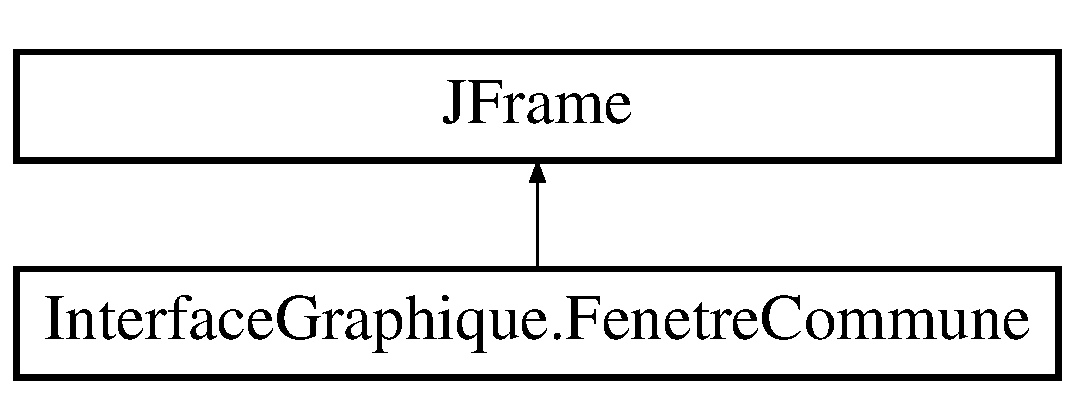
\includegraphics[height=2.000000cm]{class_interface_graphique_1_1_fenetre_commune}
\end{center}
\end{figure}
\subsection*{Public Member Functions}
\begin{DoxyCompactItemize}
\item 
\hyperlink{class_interface_graphique_1_1_fenetre_commune_a6ead45bec7ea28378786f96b58ddace0}{Fenetre\-Commune} ()
\item 
void \hyperlink{class_interface_graphique_1_1_fenetre_commune_afc234f026dc642c19c33ca953942a070}{reinitialiser\-Fenetre} ()
\item 
void \hyperlink{class_interface_graphique_1_1_fenetre_commune_a0104f87e7376a62c827db993203e3e52}{reset\-Position} ()
\item 
Canvas \hyperlink{class_interface_graphique_1_1_fenetre_commune_ae68fee935d60fab1c73939bd996e05b6}{get\-Canvas} ()
\end{DoxyCompactItemize}
\subsection*{Protected Attributes}
\begin{DoxyCompactItemize}
\item 
\hypertarget{class_interface_graphique_1_1_fenetre_commune_a3ee2a682b828ba028b88316f64b023ff}{J\-Layered\-Pane {\bfseries content\-Pane\-\_\-}}\label{class_interface_graphique_1_1_fenetre_commune_a3ee2a682b828ba028b88316f64b023ff}

\item 
\hypertarget{class_interface_graphique_1_1_fenetre_commune_a60b855a19dc5eddeeaf02319a6bcedb8}{Canvas {\bfseries canvas\-\_\-}}\label{class_interface_graphique_1_1_fenetre_commune_a60b855a19dc5eddeeaf02319a6bcedb8}

\end{DoxyCompactItemize}


\subsection{Constructor \& Destructor Documentation}
\hypertarget{class_interface_graphique_1_1_fenetre_commune_a6ead45bec7ea28378786f96b58ddace0}{\index{Interface\-Graphique\-::\-Fenetre\-Commune@{Interface\-Graphique\-::\-Fenetre\-Commune}!Fenetre\-Commune@{Fenetre\-Commune}}
\index{Fenetre\-Commune@{Fenetre\-Commune}!InterfaceGraphique::FenetreCommune@{Interface\-Graphique\-::\-Fenetre\-Commune}}
\subsubsection[{Fenetre\-Commune}]{\setlength{\rightskip}{0pt plus 5cm}Interface\-Graphique.\-Fenetre\-Commune.\-Fenetre\-Commune (
\begin{DoxyParamCaption}
{}
\end{DoxyParamCaption}
)\hspace{0.3cm}{\ttfamily [inline]}}}\label{class_interface_graphique_1_1_fenetre_commune_a6ead45bec7ea28378786f96b58ddace0}
Constructeur par d�faut. On initialise le Content\-Panel et le Canvas de la fen�tre 

\subsection{Member Function Documentation}
\hypertarget{class_interface_graphique_1_1_fenetre_commune_ae68fee935d60fab1c73939bd996e05b6}{\index{Interface\-Graphique\-::\-Fenetre\-Commune@{Interface\-Graphique\-::\-Fenetre\-Commune}!get\-Canvas@{get\-Canvas}}
\index{get\-Canvas@{get\-Canvas}!InterfaceGraphique::FenetreCommune@{Interface\-Graphique\-::\-Fenetre\-Commune}}
\subsubsection[{get\-Canvas}]{\setlength{\rightskip}{0pt plus 5cm}Canvas Interface\-Graphique.\-Fenetre\-Commune.\-get\-Canvas (
\begin{DoxyParamCaption}
{}
\end{DoxyParamCaption}
)\hspace{0.3cm}{\ttfamily [inline]}}}\label{class_interface_graphique_1_1_fenetre_commune_ae68fee935d60fab1c73939bd996e05b6}
Retourne le canvas contenu au centre de la fenetre d'edition 
\begin{DoxyParams}{Parameters}
{\em Aucun} & param�tres \\
\hline
\end{DoxyParams}
\begin{DoxyReturn}{Returns}
Le canvas sur lequel le jeu est dessin� 
\end{DoxyReturn}
\hypertarget{class_interface_graphique_1_1_fenetre_commune_afc234f026dc642c19c33ca953942a070}{\index{Interface\-Graphique\-::\-Fenetre\-Commune@{Interface\-Graphique\-::\-Fenetre\-Commune}!reinitialiser\-Fenetre@{reinitialiser\-Fenetre}}
\index{reinitialiser\-Fenetre@{reinitialiser\-Fenetre}!InterfaceGraphique::FenetreCommune@{Interface\-Graphique\-::\-Fenetre\-Commune}}
\subsubsection[{reinitialiser\-Fenetre}]{\setlength{\rightskip}{0pt plus 5cm}void Interface\-Graphique.\-Fenetre\-Commune.\-reinitialiser\-Fenetre (
\begin{DoxyParamCaption}
{}
\end{DoxyParamCaption}
)\hspace{0.3cm}{\ttfamily [inline]}}}\label{class_interface_graphique_1_1_fenetre_commune_afc234f026dc642c19c33ca953942a070}
M�thode a appeller au d�but de la construction des diff�rentes fen�tres pour r�-\/initialiser le contenu de la fen�tre \hypertarget{class_interface_graphique_1_1_fenetre_commune_a0104f87e7376a62c827db993203e3e52}{\index{Interface\-Graphique\-::\-Fenetre\-Commune@{Interface\-Graphique\-::\-Fenetre\-Commune}!reset\-Position@{reset\-Position}}
\index{reset\-Position@{reset\-Position}!InterfaceGraphique::FenetreCommune@{Interface\-Graphique\-::\-Fenetre\-Commune}}
\subsubsection[{reset\-Position}]{\setlength{\rightskip}{0pt plus 5cm}void Interface\-Graphique.\-Fenetre\-Commune.\-reset\-Position (
\begin{DoxyParamCaption}
{}
\end{DoxyParamCaption}
)\hspace{0.3cm}{\ttfamily [inline]}}}\label{class_interface_graphique_1_1_fenetre_commune_a0104f87e7376a62c827db993203e3e52}
Permet de repositionner la fen�tre a son emplacement original avant de l'afficher ou de la r�afficher. 
\begin{DoxyParams}{Parameters}
{\em Aucun} & param�tres \\
\hline
\end{DoxyParams}
\begin{DoxyReturn}{Returns}
void 
\end{DoxyReturn}


The documentation for this class was generated from the following file\-:\begin{DoxyCompactItemize}
\item 
Cadriciel/\-Sources/\-Java/\-Interface\-Graphique/src/\-Interface\-Graphique/Fenetre\-Commune.\-java\end{DoxyCompactItemize}

\hypertarget{class_interface_graphique_1_1_fenetre_configuration_campagne}{\section{Interface\-Graphique.\-Fenetre\-Configuration\-Campagne Class Reference}
\label{class_interface_graphique_1_1_fenetre_configuration_campagne}\index{Interface\-Graphique.\-Fenetre\-Configuration\-Campagne@{Interface\-Graphique.\-Fenetre\-Configuration\-Campagne}}
}
Inheritance diagram for Interface\-Graphique.\-Fenetre\-Configuration\-Campagne\-:\begin{figure}[H]
\begin{center}
\leavevmode
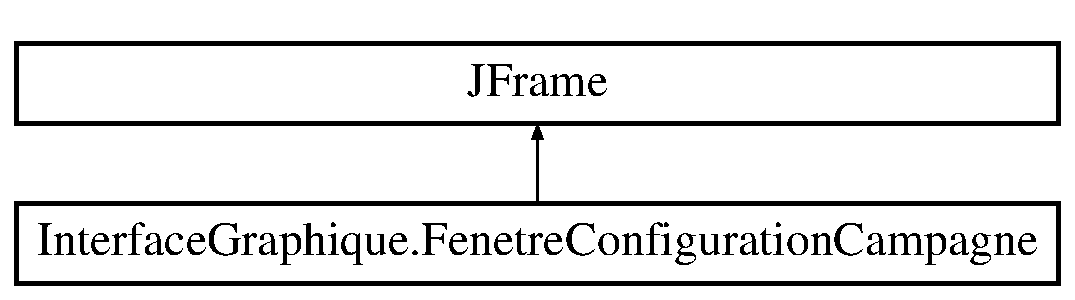
\includegraphics[height=2.000000cm]{class_interface_graphique_1_1_fenetre_configuration_campagne}
\end{center}
\end{figure}
\subsection*{Public Member Functions}
\begin{DoxyCompactItemize}
\item 
\hyperlink{class_interface_graphique_1_1_fenetre_configuration_campagne_a7b747c3bca91435ee319a3badb20df49}{Fenetre\-Configuration\-Campagne} ()
\item 
void \hyperlink{class_interface_graphique_1_1_fenetre_configuration_campagne_aa08258f2b1d5dbfe8d9e7ded4a1ca22c}{construction\-Fenetre} ()
\item 
Object\mbox{[}$\,$\mbox{]} \hyperlink{class_interface_graphique_1_1_fenetre_configuration_campagne_abad6477bf96425dc414d6fa320ffdec5}{get\-Liste\-Cartes\-Choisies} ()
\item 
\hypertarget{class_interface_graphique_1_1_fenetre_configuration_campagne_a4f877ac3b1876a9224e1f085cd3abc30}{int {\bfseries get\-Mode\-Coop} ()}\label{class_interface_graphique_1_1_fenetre_configuration_campagne_a4f877ac3b1876a9224e1f085cd3abc30}

\item 
\hypertarget{class_interface_graphique_1_1_fenetre_configuration_campagne_a535fb4c84cdb529c7167f5a2b99d71c2}{int {\bfseries get\-Joueur2\-Virtuel} ()}\label{class_interface_graphique_1_1_fenetre_configuration_campagne_a535fb4c84cdb529c7167f5a2b99d71c2}

\item 
\hypertarget{class_interface_graphique_1_1_fenetre_configuration_campagne_a404d6969fbf2ea926ba14db321eeacfb}{void {\bfseries set\-Mode\-Coop} (int mode\-Coop)}\label{class_interface_graphique_1_1_fenetre_configuration_campagne_a404d6969fbf2ea926ba14db321eeacfb}

\item 
\hypertarget{class_interface_graphique_1_1_fenetre_configuration_campagne_a987654868b818d4abc9693fd35703da6}{void {\bfseries set\-Joueur2\-Virtuel} (int joueur\-Virtuel)}\label{class_interface_graphique_1_1_fenetre_configuration_campagne_a987654868b818d4abc9693fd35703da6}

\item 
\hypertarget{class_interface_graphique_1_1_fenetre_configuration_campagne_a0050992f5553545310b83825e9ef22c0}{void {\bfseries set\-Cartes\-Campagne} (String\mbox{[}$\,$\mbox{]} cartes)}\label{class_interface_graphique_1_1_fenetre_configuration_campagne_a0050992f5553545310b83825e9ef22c0}

\end{DoxyCompactItemize}


\subsection{Constructor \& Destructor Documentation}
\hypertarget{class_interface_graphique_1_1_fenetre_configuration_campagne_a7b747c3bca91435ee319a3badb20df49}{\index{Interface\-Graphique\-::\-Fenetre\-Configuration\-Campagne@{Interface\-Graphique\-::\-Fenetre\-Configuration\-Campagne}!Fenetre\-Configuration\-Campagne@{Fenetre\-Configuration\-Campagne}}
\index{Fenetre\-Configuration\-Campagne@{Fenetre\-Configuration\-Campagne}!InterfaceGraphique::FenetreConfigurationCampagne@{Interface\-Graphique\-::\-Fenetre\-Configuration\-Campagne}}
\subsubsection[{Fenetre\-Configuration\-Campagne}]{\setlength{\rightskip}{0pt plus 5cm}Interface\-Graphique.\-Fenetre\-Configuration\-Campagne.\-Fenetre\-Configuration\-Campagne (
\begin{DoxyParamCaption}
{}
\end{DoxyParamCaption}
)\hspace{0.3cm}{\ttfamily [inline]}}}\label{class_interface_graphique_1_1_fenetre_configuration_campagne_a7b747c3bca91435ee319a3badb20df49}
Constructeur 

\subsection{Member Function Documentation}
\hypertarget{class_interface_graphique_1_1_fenetre_configuration_campagne_aa08258f2b1d5dbfe8d9e7ded4a1ca22c}{\index{Interface\-Graphique\-::\-Fenetre\-Configuration\-Campagne@{Interface\-Graphique\-::\-Fenetre\-Configuration\-Campagne}!construction\-Fenetre@{construction\-Fenetre}}
\index{construction\-Fenetre@{construction\-Fenetre}!InterfaceGraphique::FenetreConfigurationCampagne@{Interface\-Graphique\-::\-Fenetre\-Configuration\-Campagne}}
\subsubsection[{construction\-Fenetre}]{\setlength{\rightskip}{0pt plus 5cm}void Interface\-Graphique.\-Fenetre\-Configuration\-Campagne.\-construction\-Fenetre (
\begin{DoxyParamCaption}
{}
\end{DoxyParamCaption}
)\hspace{0.3cm}{\ttfamily [inline]}}}\label{class_interface_graphique_1_1_fenetre_configuration_campagne_aa08258f2b1d5dbfe8d9e7ded4a1ca22c}
M�thode qui popule la liste des cartes disponibles \hypertarget{class_interface_graphique_1_1_fenetre_configuration_campagne_abad6477bf96425dc414d6fa320ffdec5}{\index{Interface\-Graphique\-::\-Fenetre\-Configuration\-Campagne@{Interface\-Graphique\-::\-Fenetre\-Configuration\-Campagne}!get\-Liste\-Cartes\-Choisies@{get\-Liste\-Cartes\-Choisies}}
\index{get\-Liste\-Cartes\-Choisies@{get\-Liste\-Cartes\-Choisies}!InterfaceGraphique::FenetreConfigurationCampagne@{Interface\-Graphique\-::\-Fenetre\-Configuration\-Campagne}}
\subsubsection[{get\-Liste\-Cartes\-Choisies}]{\setlength{\rightskip}{0pt plus 5cm}Object \mbox{[}$\,$\mbox{]} Interface\-Graphique.\-Fenetre\-Configuration\-Campagne.\-get\-Liste\-Cartes\-Choisies (
\begin{DoxyParamCaption}
{}
\end{DoxyParamCaption}
)\hspace{0.3cm}{\ttfamily [inline]}}}\label{class_interface_graphique_1_1_fenetre_configuration_campagne_abad6477bf96425dc414d6fa320ffdec5}
M�thode qui retourne la liste des noms des cartes choisies pour la campagne \begin{DoxyReturn}{Returns}
La liste des cartes choisies 
\end{DoxyReturn}


The documentation for this class was generated from the following file\-:\begin{DoxyCompactItemize}
\item 
Cadriciel/\-Sources/\-Java/\-Interface\-Graphique/src/\-Interface\-Graphique/Fenetre\-Configuration\-Campagne.\-java\end{DoxyCompactItemize}

\hypertarget{class_interface_graphique_1_1_fenetre_configuration_diverses}{\section{Interface\-Graphique.\-Fenetre\-Configuration\-Diverses Class Reference}
\label{class_interface_graphique_1_1_fenetre_configuration_diverses}\index{Interface\-Graphique.\-Fenetre\-Configuration\-Diverses@{Interface\-Graphique.\-Fenetre\-Configuration\-Diverses}}
}
Inheritance diagram for Interface\-Graphique.\-Fenetre\-Configuration\-Diverses\-:\begin{figure}[H]
\begin{center}
\leavevmode
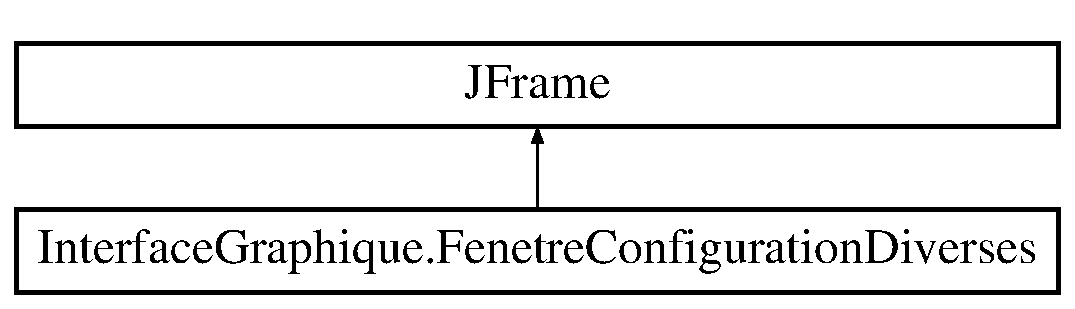
\includegraphics[height=2.000000cm]{class_interface_graphique_1_1_fenetre_configuration_diverses}
\end{center}
\end{figure}
\subsection*{Public Member Functions}
\begin{DoxyCompactItemize}
\item 
\hyperlink{class_interface_graphique_1_1_fenetre_configuration_diverses_a476caf795e2528a6fa818e0a3007b6db}{Fenetre\-Configuration\-Diverses} ()
\item 
\hypertarget{class_interface_graphique_1_1_fenetre_configuration_diverses_a06f5a9d5cb4823955aedbabf38b2e72b}{boolean {\bfseries check\-Doublon} (Integer e, Integer valeur\-Actuelle)}\label{class_interface_graphique_1_1_fenetre_configuration_diverses_a06f5a9d5cb4823955aedbabf38b2e72b}

\item 
\hypertarget{class_interface_graphique_1_1_fenetre_configuration_diverses_a824b8586effdc433dcc4eb050c1967fa}{void {\bfseries set\-Touche\-J1\-Rot} (int touche)}\label{class_interface_graphique_1_1_fenetre_configuration_diverses_a824b8586effdc433dcc4eb050c1967fa}

\item 
\hypertarget{class_interface_graphique_1_1_fenetre_configuration_diverses_a1368d63404611c0e099a879ed3c59c57}{void {\bfseries set\-Touche\-J1\-Rot\-Anti} (int touche)}\label{class_interface_graphique_1_1_fenetre_configuration_diverses_a1368d63404611c0e099a879ed3c59c57}

\item 
\hypertarget{class_interface_graphique_1_1_fenetre_configuration_diverses_ad48ef33a074eff0fb20e7ced7d8e9571}{void {\bfseries set\-Touche\-J1\-Man} (int touche)}\label{class_interface_graphique_1_1_fenetre_configuration_diverses_ad48ef33a074eff0fb20e7ced7d8e9571}

\item 
\hypertarget{class_interface_graphique_1_1_fenetre_configuration_diverses_a7f8f35410a4b4055613f043ebbdb1575}{void {\bfseries set\-Touche\-J1\-Prop} (int touche)}\label{class_interface_graphique_1_1_fenetre_configuration_diverses_a7f8f35410a4b4055613f043ebbdb1575}

\item 
\hypertarget{class_interface_graphique_1_1_fenetre_configuration_diverses_aa5fde8ce18a8bbe6e09849e4cf363085}{void {\bfseries set\-Touche\-J1\-Tir} (int touche)}\label{class_interface_graphique_1_1_fenetre_configuration_diverses_aa5fde8ce18a8bbe6e09849e4cf363085}

\item 
\hypertarget{class_interface_graphique_1_1_fenetre_configuration_diverses_a612fee2b4384d7c9c0ac4ff9133ccc6c}{void {\bfseries set\-Touche\-J2\-Rot} (int touche)}\label{class_interface_graphique_1_1_fenetre_configuration_diverses_a612fee2b4384d7c9c0ac4ff9133ccc6c}

\item 
\hypertarget{class_interface_graphique_1_1_fenetre_configuration_diverses_a243277b075d66b45b9fa73129c758d55}{void {\bfseries set\-Touche\-J2\-Rot\-Anti} (int touche)}\label{class_interface_graphique_1_1_fenetre_configuration_diverses_a243277b075d66b45b9fa73129c758d55}

\item 
\hypertarget{class_interface_graphique_1_1_fenetre_configuration_diverses_aac3a1b90997df76457bbf880aeb81080}{void {\bfseries set\-Touche\-J2\-Man} (int touche)}\label{class_interface_graphique_1_1_fenetre_configuration_diverses_aac3a1b90997df76457bbf880aeb81080}

\item 
\hypertarget{class_interface_graphique_1_1_fenetre_configuration_diverses_af86682e86b7ca04594dc7e415d7a858f}{void {\bfseries set\-Touche\-J2\-Prop} (int touche)}\label{class_interface_graphique_1_1_fenetre_configuration_diverses_af86682e86b7ca04594dc7e415d7a858f}

\item 
\hypertarget{class_interface_graphique_1_1_fenetre_configuration_diverses_a7c6ebc79b97bfd45796a4c10a862a8d0}{void {\bfseries set\-Touche\-J2\-Tir} (int touche)}\label{class_interface_graphique_1_1_fenetre_configuration_diverses_a7c6ebc79b97bfd45796a4c10a862a8d0}

\item 
\hypertarget{class_interface_graphique_1_1_fenetre_configuration_diverses_a55f72a90117424837438075bfb9f159d}{void {\bfseries set\-Duree\-Jeu} (double duree)}\label{class_interface_graphique_1_1_fenetre_configuration_diverses_a55f72a90117424837438075bfb9f159d}

\item 
\hypertarget{class_interface_graphique_1_1_fenetre_configuration_diverses_a010eab3e0f77013607094d4b2254c1b8}{void {\bfseries set\-Point\-De\-Vie\-Station} (int pts\-Vie)}\label{class_interface_graphique_1_1_fenetre_configuration_diverses_a010eab3e0f77013607094d4b2254c1b8}

\item 
\hypertarget{class_interface_graphique_1_1_fenetre_configuration_diverses_a4a261555fb2a1e81dbdafb57e01d3dca}{void {\bfseries set\-Apparition\-Asteroide} (int b)}\label{class_interface_graphique_1_1_fenetre_configuration_diverses_a4a261555fb2a1e81dbdafb57e01d3dca}

\item 
\hypertarget{class_interface_graphique_1_1_fenetre_configuration_diverses_a406ad2e6af2386f5b19cece3978f6aaf}{void {\bfseries set\-Changement\-Mode} (int b)}\label{class_interface_graphique_1_1_fenetre_configuration_diverses_a406ad2e6af2386f5b19cece3978f6aaf}

\item 
\hypertarget{class_interface_graphique_1_1_fenetre_configuration_diverses_a477eab323b80a0e001b0d8392533a839}{void {\bfseries set\-Eclairage} (int b)}\label{class_interface_graphique_1_1_fenetre_configuration_diverses_a477eab323b80a0e001b0d8392533a839}

\item 
\hypertarget{class_interface_graphique_1_1_fenetre_configuration_diverses_a98c851fb6973ebda4dcfdc5c0ebf7292}{void {\bfseries set\-Cible\-Joueur} (int b)}\label{class_interface_graphique_1_1_fenetre_configuration_diverses_a98c851fb6973ebda4dcfdc5c0ebf7292}

\item 
\hypertarget{class_interface_graphique_1_1_fenetre_configuration_diverses_a056ad5d50e41ae73c3fd8950ad1098b7}{void {\bfseries set\-Zone\-Passage} (int b)}\label{class_interface_graphique_1_1_fenetre_configuration_diverses_a056ad5d50e41ae73c3fd8950ad1098b7}

\item 
\hypertarget{class_interface_graphique_1_1_fenetre_configuration_diverses_ab6a6398b6df780a5fccf78c554337c35}{void {\bfseries set\-Cadre\-Depart} (int b)}\label{class_interface_graphique_1_1_fenetre_configuration_diverses_ab6a6398b6df780a5fccf78c554337c35}

\item 
\hypertarget{class_interface_graphique_1_1_fenetre_configuration_diverses_a500ac190fe3ce4f85de9aca28be44b4a}{void {\bfseries set\-Attraction\-Port} (int b)}\label{class_interface_graphique_1_1_fenetre_configuration_diverses_a500ac190fe3ce4f85de9aca28be44b4a}

\item 
\hypertarget{class_interface_graphique_1_1_fenetre_configuration_diverses_a32628f50666b0ce218063aaddfddce90}{int {\bfseries get\-Touche\-J1\-Rot} ()}\label{class_interface_graphique_1_1_fenetre_configuration_diverses_a32628f50666b0ce218063aaddfddce90}

\item 
\hypertarget{class_interface_graphique_1_1_fenetre_configuration_diverses_a5955166004dde410e56903acea4e8dca}{int {\bfseries get\-Touche\-J1\-Rot\-Anti} ()}\label{class_interface_graphique_1_1_fenetre_configuration_diverses_a5955166004dde410e56903acea4e8dca}

\item 
\hypertarget{class_interface_graphique_1_1_fenetre_configuration_diverses_a7f8129a30ecc0618cd87135ddf92650d}{int {\bfseries get\-Touche\-J1\-Man} ()}\label{class_interface_graphique_1_1_fenetre_configuration_diverses_a7f8129a30ecc0618cd87135ddf92650d}

\item 
\hypertarget{class_interface_graphique_1_1_fenetre_configuration_diverses_ae1c0b83390d5e63858b8e47a0d57a88e}{int {\bfseries get\-Touche\-J1\-Prop} ()}\label{class_interface_graphique_1_1_fenetre_configuration_diverses_ae1c0b83390d5e63858b8e47a0d57a88e}

\item 
\hypertarget{class_interface_graphique_1_1_fenetre_configuration_diverses_a94f260d9f43c502761e66d8032d909b4}{int {\bfseries get\-Touche\-J1\-Tir} ()}\label{class_interface_graphique_1_1_fenetre_configuration_diverses_a94f260d9f43c502761e66d8032d909b4}

\item 
\hypertarget{class_interface_graphique_1_1_fenetre_configuration_diverses_a399605a25b529edebf7179dea0c1d1ea}{int {\bfseries get\-Touche\-J2\-Rot} ()}\label{class_interface_graphique_1_1_fenetre_configuration_diverses_a399605a25b529edebf7179dea0c1d1ea}

\item 
\hypertarget{class_interface_graphique_1_1_fenetre_configuration_diverses_a13c5891cef8bc00e1168cf40028518fa}{int {\bfseries get\-Touche\-J2\-Rot\-Anti} ()}\label{class_interface_graphique_1_1_fenetre_configuration_diverses_a13c5891cef8bc00e1168cf40028518fa}

\item 
\hypertarget{class_interface_graphique_1_1_fenetre_configuration_diverses_a32c5fea562607497d69b11f89b496913}{int {\bfseries get\-Touche\-J2\-Man} ()}\label{class_interface_graphique_1_1_fenetre_configuration_diverses_a32c5fea562607497d69b11f89b496913}

\item 
\hypertarget{class_interface_graphique_1_1_fenetre_configuration_diverses_a2e472f2c1a758e6de8db3d91496ead45}{int {\bfseries get\-Touche\-J2\-Prop} ()}\label{class_interface_graphique_1_1_fenetre_configuration_diverses_a2e472f2c1a758e6de8db3d91496ead45}

\item 
\hypertarget{class_interface_graphique_1_1_fenetre_configuration_diverses_acc595c64f6198413249e72396150f92c}{int {\bfseries get\-Touche\-J2\-Tir} ()}\label{class_interface_graphique_1_1_fenetre_configuration_diverses_acc595c64f6198413249e72396150f92c}

\item 
\hypertarget{class_interface_graphique_1_1_fenetre_configuration_diverses_ad7dff276229d0160dba7e509718d4a1e}{double {\bfseries get\-Duree\-Jeu} ()}\label{class_interface_graphique_1_1_fenetre_configuration_diverses_ad7dff276229d0160dba7e509718d4a1e}

\item 
\hypertarget{class_interface_graphique_1_1_fenetre_configuration_diverses_ae1e5b86e8cd418fbd5745768f80857c2}{int {\bfseries get\-Point\-De\-Vie\-Station} ()}\label{class_interface_graphique_1_1_fenetre_configuration_diverses_ae1e5b86e8cd418fbd5745768f80857c2}

\item 
\hypertarget{class_interface_graphique_1_1_fenetre_configuration_diverses_a43891f550b8e95eb5396ff599bd0e038}{boolean {\bfseries get\-Check\-Apparition\-Asteroide} ()}\label{class_interface_graphique_1_1_fenetre_configuration_diverses_a43891f550b8e95eb5396ff599bd0e038}

\item 
\hypertarget{class_interface_graphique_1_1_fenetre_configuration_diverses_a99134b49204e647430e1d9650f31c6c6}{boolean {\bfseries get\-Check\-Changement\-Mode} ()}\label{class_interface_graphique_1_1_fenetre_configuration_diverses_a99134b49204e647430e1d9650f31c6c6}

\item 
\hypertarget{class_interface_graphique_1_1_fenetre_configuration_diverses_a5f0b92011cf1dd01e19ffef863c20782}{boolean {\bfseries get\-Check\-Eclairage} ()}\label{class_interface_graphique_1_1_fenetre_configuration_diverses_a5f0b92011cf1dd01e19ffef863c20782}

\item 
\hypertarget{class_interface_graphique_1_1_fenetre_configuration_diverses_aeaca6acdd1534adb14531455e1c718d2}{boolean {\bfseries get\-Check\-Cible\-Joueur} ()}\label{class_interface_graphique_1_1_fenetre_configuration_diverses_aeaca6acdd1534adb14531455e1c718d2}

\item 
\hypertarget{class_interface_graphique_1_1_fenetre_configuration_diverses_a566c1fac80f6f0438c98eead010b658a}{boolean {\bfseries get\-Check\-Cadre\-Depart} ()}\label{class_interface_graphique_1_1_fenetre_configuration_diverses_a566c1fac80f6f0438c98eead010b658a}

\item 
\hypertarget{class_interface_graphique_1_1_fenetre_configuration_diverses_a1ae3a1c0c81e53cd43ce718b00e9c2fb}{boolean {\bfseries get\-Check\-Zone\-Passage} ()}\label{class_interface_graphique_1_1_fenetre_configuration_diverses_a1ae3a1c0c81e53cd43ce718b00e9c2fb}

\item 
\hypertarget{class_interface_graphique_1_1_fenetre_configuration_diverses_ad184fb6caeee483bc26e28ea8211556d}{boolean {\bfseries get\-Check\-Attraction\-Portail} ()}\label{class_interface_graphique_1_1_fenetre_configuration_diverses_ad184fb6caeee483bc26e28ea8211556d}

\end{DoxyCompactItemize}


\subsection{Constructor \& Destructor Documentation}
\hypertarget{class_interface_graphique_1_1_fenetre_configuration_diverses_a476caf795e2528a6fa818e0a3007b6db}{\index{Interface\-Graphique\-::\-Fenetre\-Configuration\-Diverses@{Interface\-Graphique\-::\-Fenetre\-Configuration\-Diverses}!Fenetre\-Configuration\-Diverses@{Fenetre\-Configuration\-Diverses}}
\index{Fenetre\-Configuration\-Diverses@{Fenetre\-Configuration\-Diverses}!InterfaceGraphique::FenetreConfigurationDiverses@{Interface\-Graphique\-::\-Fenetre\-Configuration\-Diverses}}
\subsubsection[{Fenetre\-Configuration\-Diverses}]{\setlength{\rightskip}{0pt plus 5cm}Interface\-Graphique.\-Fenetre\-Configuration\-Diverses.\-Fenetre\-Configuration\-Diverses (
\begin{DoxyParamCaption}
{}
\end{DoxyParamCaption}
)\hspace{0.3cm}{\ttfamily [inline]}}}\label{class_interface_graphique_1_1_fenetre_configuration_diverses_a476caf795e2528a6fa818e0a3007b6db}
Methode qui permet l'affichage de la fenetre de configuration 
\begin{DoxyParams}{Parameters}
{\em aucun} & \\
\hline
\end{DoxyParams}
\begin{DoxyReturn}{Returns}
void 
\end{DoxyReturn}


The documentation for this class was generated from the following file\-:\begin{DoxyCompactItemize}
\item 
Cadriciel/\-Sources/\-Java/\-Interface\-Graphique/src/\-Interface\-Graphique/Fenetre\-Configuration\-Diverses.\-java\end{DoxyCompactItemize}

\hypertarget{class_interface_graphique_1_1_fenetre_configuration_zone_jeu}{\section{Interface\-Graphique.\-Fenetre\-Configuration\-Zone\-Jeu Class Reference}
\label{class_interface_graphique_1_1_fenetre_configuration_zone_jeu}\index{Interface\-Graphique.\-Fenetre\-Configuration\-Zone\-Jeu@{Interface\-Graphique.\-Fenetre\-Configuration\-Zone\-Jeu}}
}
Inheritance diagram for Interface\-Graphique.\-Fenetre\-Configuration\-Zone\-Jeu\-:\begin{figure}[H]
\begin{center}
\leavevmode
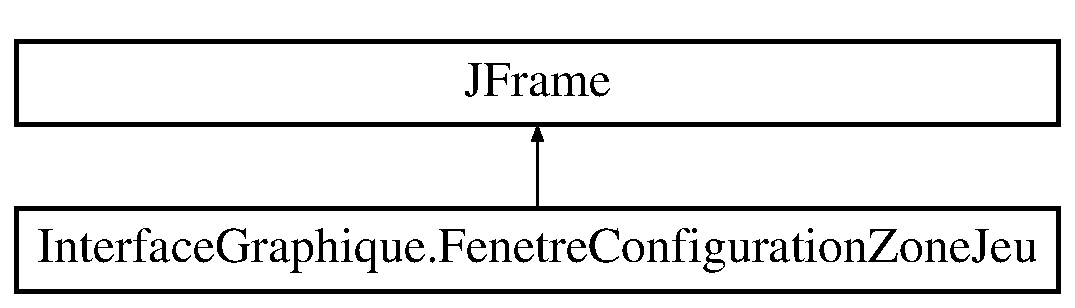
\includegraphics[height=2.000000cm]{class_interface_graphique_1_1_fenetre_configuration_zone_jeu}
\end{center}
\end{figure}
\subsection*{Public Member Functions}
\begin{DoxyCompactItemize}
\item 
void \hyperlink{class_interface_graphique_1_1_fenetre_configuration_zone_jeu_a62d395c0ab7322e0cb02ac9294d0662d}{set\-Proprietes} (int frequence\-Asteroide, int nombre\-Stations, int bonus\-Acceleration, int cote\-Difficulte)
\end{DoxyCompactItemize}


\subsection{Member Function Documentation}
\hypertarget{class_interface_graphique_1_1_fenetre_configuration_zone_jeu_a62d395c0ab7322e0cb02ac9294d0662d}{\index{Interface\-Graphique\-::\-Fenetre\-Configuration\-Zone\-Jeu@{Interface\-Graphique\-::\-Fenetre\-Configuration\-Zone\-Jeu}!set\-Proprietes@{set\-Proprietes}}
\index{set\-Proprietes@{set\-Proprietes}!InterfaceGraphique::FenetreConfigurationZoneJeu@{Interface\-Graphique\-::\-Fenetre\-Configuration\-Zone\-Jeu}}
\subsubsection[{set\-Proprietes}]{\setlength{\rightskip}{0pt plus 5cm}void Interface\-Graphique.\-Fenetre\-Configuration\-Zone\-Jeu.\-set\-Proprietes (
\begin{DoxyParamCaption}
\item[{int}]{frequence\-Asteroide, }
\item[{int}]{nombre\-Stations, }
\item[{int}]{bonus\-Acceleration, }
\item[{int}]{cote\-Difficulte}
\end{DoxyParamCaption}
)\hspace{0.3cm}{\ttfamily [inline]}}}\label{class_interface_graphique_1_1_fenetre_configuration_zone_jeu_a62d395c0ab7322e0cb02ac9294d0662d}
Fonction qui permet de setter les propri�t�s de la carte 
\begin{DoxyParams}{Parameters}
{\em frequence\-Asteroide} & La fr�quence d'apparition des ast�ro�des, en millisecondes. \\
\hline
{\em nombre\-Stations} & Le nombre de stations minimum � sauver pour gagner. \\
\hline
{\em bonus\-Acceleration} & Le bonus de vitesse que donne le bonus d'acc�l�ration \\
\hline
{\em cote\-Difficulte} & La cote de difficulte de la carte, 1 �tant le plus facile et 4 le plus difficile. \\
\hline
\end{DoxyParams}


The documentation for this class was generated from the following file\-:\begin{DoxyCompactItemize}
\item 
Cadriciel/\-Sources/\-Java/\-Interface\-Graphique/src/\-Interface\-Graphique/Fenetre\-Configuration\-Zone\-Jeu.\-java\end{DoxyCompactItemize}

\hypertarget{struct_f_m_o_d___a_d_v_a_n_c_e_d_s_e_t_t_i_n_g_s}{\section{F\-M\-O\-D\-\_\-\-A\-D\-V\-A\-N\-C\-E\-D\-S\-E\-T\-T\-I\-N\-G\-S Struct Reference}
\label{struct_f_m_o_d___a_d_v_a_n_c_e_d_s_e_t_t_i_n_g_s}\index{F\-M\-O\-D\-\_\-\-A\-D\-V\-A\-N\-C\-E\-D\-S\-E\-T\-T\-I\-N\-G\-S@{F\-M\-O\-D\-\_\-\-A\-D\-V\-A\-N\-C\-E\-D\-S\-E\-T\-T\-I\-N\-G\-S}}
}
\subsection*{Public Attributes}
\begin{DoxyCompactItemize}
\item 
\hypertarget{struct_f_m_o_d___a_d_v_a_n_c_e_d_s_e_t_t_i_n_g_s_a45f37c714e81702c153beaeeaf5789d9}{int {\bfseries cbsize}}\label{struct_f_m_o_d___a_d_v_a_n_c_e_d_s_e_t_t_i_n_g_s_a45f37c714e81702c153beaeeaf5789d9}

\item 
\hypertarget{struct_f_m_o_d___a_d_v_a_n_c_e_d_s_e_t_t_i_n_g_s_ac38a94fd8d9b1ad4ed77d111cfcafa71}{int {\bfseries max\-M\-P\-E\-Gcodecs}}\label{struct_f_m_o_d___a_d_v_a_n_c_e_d_s_e_t_t_i_n_g_s_ac38a94fd8d9b1ad4ed77d111cfcafa71}

\item 
\hypertarget{struct_f_m_o_d___a_d_v_a_n_c_e_d_s_e_t_t_i_n_g_s_afebaec0ba3caa0367c9184416bd74f2a}{int {\bfseries max\-A\-D\-P\-C\-Mcodecs}}\label{struct_f_m_o_d___a_d_v_a_n_c_e_d_s_e_t_t_i_n_g_s_afebaec0ba3caa0367c9184416bd74f2a}

\item 
\hypertarget{struct_f_m_o_d___a_d_v_a_n_c_e_d_s_e_t_t_i_n_g_s_a4c351e7bc430c6c9aa9c87ad5fae8324}{int {\bfseries max\-X\-M\-Acodecs}}\label{struct_f_m_o_d___a_d_v_a_n_c_e_d_s_e_t_t_i_n_g_s_a4c351e7bc430c6c9aa9c87ad5fae8324}

\item 
\hypertarget{struct_f_m_o_d___a_d_v_a_n_c_e_d_s_e_t_t_i_n_g_s_a0f51ebed22a9eda603d37e2f9ccf5376}{int {\bfseries max\-C\-E\-L\-Tcodecs}}\label{struct_f_m_o_d___a_d_v_a_n_c_e_d_s_e_t_t_i_n_g_s_a0f51ebed22a9eda603d37e2f9ccf5376}

\item 
\hypertarget{struct_f_m_o_d___a_d_v_a_n_c_e_d_s_e_t_t_i_n_g_s_a4fc5ae4871fcfea0c82f818c6f7a9128}{int {\bfseries max\-P\-C\-Mcodecs}}\label{struct_f_m_o_d___a_d_v_a_n_c_e_d_s_e_t_t_i_n_g_s_a4fc5ae4871fcfea0c82f818c6f7a9128}

\item 
\hypertarget{struct_f_m_o_d___a_d_v_a_n_c_e_d_s_e_t_t_i_n_g_s_a90fe2a214a0bdd6569ee48c0b7740cb5}{int {\bfseries A\-S\-I\-O\-Num\-Channels}}\label{struct_f_m_o_d___a_d_v_a_n_c_e_d_s_e_t_t_i_n_g_s_a90fe2a214a0bdd6569ee48c0b7740cb5}

\item 
\hypertarget{struct_f_m_o_d___a_d_v_a_n_c_e_d_s_e_t_t_i_n_g_s_aebc4867d0c6fb6a95bd67702e6cb5c03}{char $\ast$$\ast$ {\bfseries A\-S\-I\-O\-Channel\-List}}\label{struct_f_m_o_d___a_d_v_a_n_c_e_d_s_e_t_t_i_n_g_s_aebc4867d0c6fb6a95bd67702e6cb5c03}

\item 
\hypertarget{struct_f_m_o_d___a_d_v_a_n_c_e_d_s_e_t_t_i_n_g_s_a096b0eae3b5a2d1a8cf4ad2640f437dc}{F\-M\-O\-D\-\_\-\-S\-P\-E\-A\-K\-E\-R $\ast$ {\bfseries A\-S\-I\-O\-Speaker\-List}}\label{struct_f_m_o_d___a_d_v_a_n_c_e_d_s_e_t_t_i_n_g_s_a096b0eae3b5a2d1a8cf4ad2640f437dc}

\item 
\hypertarget{struct_f_m_o_d___a_d_v_a_n_c_e_d_s_e_t_t_i_n_g_s_ae8beee991b58b68943198715d4e9c991}{int {\bfseries max3\-D\-Reverb\-D\-S\-Ps}}\label{struct_f_m_o_d___a_d_v_a_n_c_e_d_s_e_t_t_i_n_g_s_ae8beee991b58b68943198715d4e9c991}

\item 
\hypertarget{struct_f_m_o_d___a_d_v_a_n_c_e_d_s_e_t_t_i_n_g_s_ab57df4fc8742292752e5aa99389fdabd}{float {\bfseries H\-R\-T\-F\-Min\-Angle}}\label{struct_f_m_o_d___a_d_v_a_n_c_e_d_s_e_t_t_i_n_g_s_ab57df4fc8742292752e5aa99389fdabd}

\item 
\hypertarget{struct_f_m_o_d___a_d_v_a_n_c_e_d_s_e_t_t_i_n_g_s_aafd3cddd9a59789c54084474c95619ff}{float {\bfseries H\-R\-T\-F\-Max\-Angle}}\label{struct_f_m_o_d___a_d_v_a_n_c_e_d_s_e_t_t_i_n_g_s_aafd3cddd9a59789c54084474c95619ff}

\item 
\hypertarget{struct_f_m_o_d___a_d_v_a_n_c_e_d_s_e_t_t_i_n_g_s_a84a94d9d0106ee245d5c3aa8a6927814}{float {\bfseries H\-R\-T\-F\-Freq}}\label{struct_f_m_o_d___a_d_v_a_n_c_e_d_s_e_t_t_i_n_g_s_a84a94d9d0106ee245d5c3aa8a6927814}

\item 
\hypertarget{struct_f_m_o_d___a_d_v_a_n_c_e_d_s_e_t_t_i_n_g_s_a34978996f8dfe0ca0d79a30414936eb6}{float {\bfseries vol0virtualvol}}\label{struct_f_m_o_d___a_d_v_a_n_c_e_d_s_e_t_t_i_n_g_s_a34978996f8dfe0ca0d79a30414936eb6}

\item 
\hypertarget{struct_f_m_o_d___a_d_v_a_n_c_e_d_s_e_t_t_i_n_g_s_a39788bb34f800aa4abcef457692ac966}{int {\bfseries eventqueuesize}}\label{struct_f_m_o_d___a_d_v_a_n_c_e_d_s_e_t_t_i_n_g_s_a39788bb34f800aa4abcef457692ac966}

\item 
\hypertarget{struct_f_m_o_d___a_d_v_a_n_c_e_d_s_e_t_t_i_n_g_s_a8b2d2802cd34875f10d319c8f363e399}{unsigned int {\bfseries default\-Decode\-Buffer\-Size}}\label{struct_f_m_o_d___a_d_v_a_n_c_e_d_s_e_t_t_i_n_g_s_a8b2d2802cd34875f10d319c8f363e399}

\item 
\hypertarget{struct_f_m_o_d___a_d_v_a_n_c_e_d_s_e_t_t_i_n_g_s_a00d10a918d3414c8f4bde3664f01b44f}{char $\ast$ {\bfseries debug\-Log\-Filename}}\label{struct_f_m_o_d___a_d_v_a_n_c_e_d_s_e_t_t_i_n_g_s_a00d10a918d3414c8f4bde3664f01b44f}

\item 
\hypertarget{struct_f_m_o_d___a_d_v_a_n_c_e_d_s_e_t_t_i_n_g_s_a5d12c84c6911facd30fcba7ab0dd7faa}{unsigned short {\bfseries profileport}}\label{struct_f_m_o_d___a_d_v_a_n_c_e_d_s_e_t_t_i_n_g_s_a5d12c84c6911facd30fcba7ab0dd7faa}

\item 
\hypertarget{struct_f_m_o_d___a_d_v_a_n_c_e_d_s_e_t_t_i_n_g_s_a973568fb1ec638193a0b0198d4165558}{unsigned int {\bfseries geometry\-Max\-Fade\-Time}}\label{struct_f_m_o_d___a_d_v_a_n_c_e_d_s_e_t_t_i_n_g_s_a973568fb1ec638193a0b0198d4165558}

\item 
\hypertarget{struct_f_m_o_d___a_d_v_a_n_c_e_d_s_e_t_t_i_n_g_s_a0404a31fe61b9d4e2340125a2a38a00d}{unsigned int {\bfseries max\-Spectrum\-Wave\-Data\-Buffers}}\label{struct_f_m_o_d___a_d_v_a_n_c_e_d_s_e_t_t_i_n_g_s_a0404a31fe61b9d4e2340125a2a38a00d}

\item 
\hypertarget{struct_f_m_o_d___a_d_v_a_n_c_e_d_s_e_t_t_i_n_g_s_abb66bb0cce280bd12f4092d2b3f642d1}{unsigned int {\bfseries music\-System\-Cache\-Delay}}\label{struct_f_m_o_d___a_d_v_a_n_c_e_d_s_e_t_t_i_n_g_s_abb66bb0cce280bd12f4092d2b3f642d1}

\item 
\hypertarget{struct_f_m_o_d___a_d_v_a_n_c_e_d_s_e_t_t_i_n_g_s_aec899d9cc69d0d664393d48f87dd9373}{float {\bfseries distance\-Filter\-Centre\-Freq}}\label{struct_f_m_o_d___a_d_v_a_n_c_e_d_s_e_t_t_i_n_g_s_aec899d9cc69d0d664393d48f87dd9373}

\end{DoxyCompactItemize}


The documentation for this struct was generated from the following file\-:\begin{DoxyCompactItemize}
\item 
Cadriciel/\-Commun/\-Externe/\-F\-M\-O\-D/include/fmod.\-h\end{DoxyCompactItemize}

\hypertarget{struct_f_m_o_d___a_s_y_n_c_r_e_a_d_i_n_f_o}{\section{F\-M\-O\-D\-\_\-\-A\-S\-Y\-N\-C\-R\-E\-A\-D\-I\-N\-F\-O Struct Reference}
\label{struct_f_m_o_d___a_s_y_n_c_r_e_a_d_i_n_f_o}\index{F\-M\-O\-D\-\_\-\-A\-S\-Y\-N\-C\-R\-E\-A\-D\-I\-N\-F\-O@{F\-M\-O\-D\-\_\-\-A\-S\-Y\-N\-C\-R\-E\-A\-D\-I\-N\-F\-O}}
}
\subsection*{Public Attributes}
\begin{DoxyCompactItemize}
\item 
\hypertarget{struct_f_m_o_d___a_s_y_n_c_r_e_a_d_i_n_f_o_a31e2e01864e3c97844a252f947ff8040}{void $\ast$ {\bfseries handle}}\label{struct_f_m_o_d___a_s_y_n_c_r_e_a_d_i_n_f_o_a31e2e01864e3c97844a252f947ff8040}

\item 
\hypertarget{struct_f_m_o_d___a_s_y_n_c_r_e_a_d_i_n_f_o_a8d42cc77cd8ef0559a666038e02a8807}{unsigned int {\bfseries offset}}\label{struct_f_m_o_d___a_s_y_n_c_r_e_a_d_i_n_f_o_a8d42cc77cd8ef0559a666038e02a8807}

\item 
\hypertarget{struct_f_m_o_d___a_s_y_n_c_r_e_a_d_i_n_f_o_a19cda62a563d8b9c3116411c13d207f6}{unsigned int {\bfseries sizebytes}}\label{struct_f_m_o_d___a_s_y_n_c_r_e_a_d_i_n_f_o_a19cda62a563d8b9c3116411c13d207f6}

\item 
\hypertarget{struct_f_m_o_d___a_s_y_n_c_r_e_a_d_i_n_f_o_aae5a4b76307bec7a0132b3abb04ab823}{int {\bfseries priority}}\label{struct_f_m_o_d___a_s_y_n_c_r_e_a_d_i_n_f_o_aae5a4b76307bec7a0132b3abb04ab823}

\item 
\hypertarget{struct_f_m_o_d___a_s_y_n_c_r_e_a_d_i_n_f_o_a2154c0c4825d5f133e0b14ca1b94b324}{void $\ast$ {\bfseries buffer}}\label{struct_f_m_o_d___a_s_y_n_c_r_e_a_d_i_n_f_o_a2154c0c4825d5f133e0b14ca1b94b324}

\item 
\hypertarget{struct_f_m_o_d___a_s_y_n_c_r_e_a_d_i_n_f_o_acef1543320ee49d5c723ce1dbd58e43b}{unsigned int {\bfseries bytesread}}\label{struct_f_m_o_d___a_s_y_n_c_r_e_a_d_i_n_f_o_acef1543320ee49d5c723ce1dbd58e43b}

\item 
\hypertarget{struct_f_m_o_d___a_s_y_n_c_r_e_a_d_i_n_f_o_a85e0137ab5748fbbd7ffee359823f57e}{F\-M\-O\-D\-\_\-\-R\-E\-S\-U\-L\-T {\bfseries result}}\label{struct_f_m_o_d___a_s_y_n_c_r_e_a_d_i_n_f_o_a85e0137ab5748fbbd7ffee359823f57e}

\item 
\hypertarget{struct_f_m_o_d___a_s_y_n_c_r_e_a_d_i_n_f_o_a8a273751e70e26c1a51540a18269eecc}{void $\ast$ {\bfseries userdata}}\label{struct_f_m_o_d___a_s_y_n_c_r_e_a_d_i_n_f_o_a8a273751e70e26c1a51540a18269eecc}

\end{DoxyCompactItemize}


The documentation for this struct was generated from the following file\-:\begin{DoxyCompactItemize}
\item 
Cadriciel/\-Commun/\-Externe/\-F\-M\-O\-D/include/fmod.\-h\end{DoxyCompactItemize}

\hypertarget{struct_f_m_o_d___c_d_t_o_c}{\section{F\-M\-O\-D\-\_\-\-C\-D\-T\-O\-C Struct Reference}
\label{struct_f_m_o_d___c_d_t_o_c}\index{F\-M\-O\-D\-\_\-\-C\-D\-T\-O\-C@{F\-M\-O\-D\-\_\-\-C\-D\-T\-O\-C}}
}


{\ttfamily \#include $<$fmod.\-h$>$}

\subsection*{Public Attributes}
\begin{DoxyCompactItemize}
\item 
\hyperlink{wglew_8h_a500a82aecba06f4550f6849b8099ca21}{int} \hyperlink{struct_f_m_o_d___c_d_t_o_c_aad0a3526919d1d67958c47179a73cf7b}{numtracks}
\item 
\hyperlink{wglew_8h_a500a82aecba06f4550f6849b8099ca21}{int} \hyperlink{struct_f_m_o_d___c_d_t_o_c_ac32672636e86e7d5da6cd02737123f0e}{min} \mbox{[}100\mbox{]}
\item 
\hyperlink{wglew_8h_a500a82aecba06f4550f6849b8099ca21}{int} \hyperlink{struct_f_m_o_d___c_d_t_o_c_a20dcf991841f7f4322904f9a1175e7c6}{sec} \mbox{[}100\mbox{]}
\item 
\hyperlink{wglew_8h_a500a82aecba06f4550f6849b8099ca21}{int} \hyperlink{struct_f_m_o_d___c_d_t_o_c_a40e8bdc25c765a02c4ca0af13c74dc5f}{frame} \mbox{[}100\mbox{]}
\end{DoxyCompactItemize}


\subsection{Member Data Documentation}
\hypertarget{struct_f_m_o_d___c_d_t_o_c_a40e8bdc25c765a02c4ca0af13c74dc5f}{\index{F\-M\-O\-D\-\_\-\-C\-D\-T\-O\-C@{F\-M\-O\-D\-\_\-\-C\-D\-T\-O\-C}!frame@{frame}}
\index{frame@{frame}!FMOD_CDTOC@{F\-M\-O\-D\-\_\-\-C\-D\-T\-O\-C}}
\subsubsection[{frame}]{\setlength{\rightskip}{0pt plus 5cm}{\bf int} F\-M\-O\-D\-\_\-\-C\-D\-T\-O\-C\-::frame\mbox{[}100\mbox{]}}}\label{struct_f_m_o_d___c_d_t_o_c_a40e8bdc25c765a02c4ca0af13c74dc5f}
\hypertarget{struct_f_m_o_d___c_d_t_o_c_ac32672636e86e7d5da6cd02737123f0e}{\index{F\-M\-O\-D\-\_\-\-C\-D\-T\-O\-C@{F\-M\-O\-D\-\_\-\-C\-D\-T\-O\-C}!min@{min}}
\index{min@{min}!FMOD_CDTOC@{F\-M\-O\-D\-\_\-\-C\-D\-T\-O\-C}}
\subsubsection[{min}]{\setlength{\rightskip}{0pt plus 5cm}{\bf int} F\-M\-O\-D\-\_\-\-C\-D\-T\-O\-C\-::min\mbox{[}100\mbox{]}}}\label{struct_f_m_o_d___c_d_t_o_c_ac32672636e86e7d5da6cd02737123f0e}
\hypertarget{struct_f_m_o_d___c_d_t_o_c_aad0a3526919d1d67958c47179a73cf7b}{\index{F\-M\-O\-D\-\_\-\-C\-D\-T\-O\-C@{F\-M\-O\-D\-\_\-\-C\-D\-T\-O\-C}!numtracks@{numtracks}}
\index{numtracks@{numtracks}!FMOD_CDTOC@{F\-M\-O\-D\-\_\-\-C\-D\-T\-O\-C}}
\subsubsection[{numtracks}]{\setlength{\rightskip}{0pt plus 5cm}{\bf int} F\-M\-O\-D\-\_\-\-C\-D\-T\-O\-C\-::numtracks}}\label{struct_f_m_o_d___c_d_t_o_c_aad0a3526919d1d67958c47179a73cf7b}
\hypertarget{struct_f_m_o_d___c_d_t_o_c_a20dcf991841f7f4322904f9a1175e7c6}{\index{F\-M\-O\-D\-\_\-\-C\-D\-T\-O\-C@{F\-M\-O\-D\-\_\-\-C\-D\-T\-O\-C}!sec@{sec}}
\index{sec@{sec}!FMOD_CDTOC@{F\-M\-O\-D\-\_\-\-C\-D\-T\-O\-C}}
\subsubsection[{sec}]{\setlength{\rightskip}{0pt plus 5cm}{\bf int} F\-M\-O\-D\-\_\-\-C\-D\-T\-O\-C\-::sec\mbox{[}100\mbox{]}}}\label{struct_f_m_o_d___c_d_t_o_c_a20dcf991841f7f4322904f9a1175e7c6}


The documentation for this struct was generated from the following file\-:\begin{DoxyCompactItemize}
\item 
Cadriciel/\-Commun/\-Externe/\-F\-M\-O\-D/include/\hyperlink{fmod_8h}{fmod.\-h}\end{DoxyCompactItemize}

\hypertarget{struct_f_m_o_d___c_o_d_e_c___d_e_s_c_r_i_p_t_i_o_n}{\section{F\-M\-O\-D\-\_\-\-C\-O\-D\-E\-C\-\_\-\-D\-E\-S\-C\-R\-I\-P\-T\-I\-O\-N Struct Reference}
\label{struct_f_m_o_d___c_o_d_e_c___d_e_s_c_r_i_p_t_i_o_n}\index{F\-M\-O\-D\-\_\-\-C\-O\-D\-E\-C\-\_\-\-D\-E\-S\-C\-R\-I\-P\-T\-I\-O\-N@{F\-M\-O\-D\-\_\-\-C\-O\-D\-E\-C\-\_\-\-D\-E\-S\-C\-R\-I\-P\-T\-I\-O\-N}}
}


{\ttfamily \#include $<$fmod\-\_\-codec.\-h$>$}

\subsection*{Public Attributes}
\begin{DoxyCompactItemize}
\item 
const char $\ast$ \hyperlink{struct_f_m_o_d___c_o_d_e_c___d_e_s_c_r_i_p_t_i_o_n_a3d2d1cb50c8d3fcee03e465753a9adb0}{name}
\item 
\hyperlink{_free_image_8h_a425076c7067a1b5166e2cc530e914814}{unsigned} \hyperlink{wglew_8h_a500a82aecba06f4550f6849b8099ca21}{int} \hyperlink{struct_f_m_o_d___c_o_d_e_c___d_e_s_c_r_i_p_t_i_o_n_a8dfb836ca79931ee6ca39c12bd8aad3f}{version}
\item 
\hyperlink{wglew_8h_a500a82aecba06f4550f6849b8099ca21}{int} \hyperlink{struct_f_m_o_d___c_o_d_e_c___d_e_s_c_r_i_p_t_i_o_n_ac79461b38a89c34d2ec2e609736df941}{defaultasstream}
\item 
\hyperlink{fmod_8h_a9999089b44f00c72ba8e9a270a8d6349}{F\-M\-O\-D\-\_\-\-T\-I\-M\-E\-U\-N\-I\-T} \hyperlink{struct_f_m_o_d___c_o_d_e_c___d_e_s_c_r_i_p_t_i_o_n_a17d05f38ea3ea759d20d463aa8a8ca9f}{timeunits}
\item 
F\-M\-O\-D\-\_\-\-C\-O\-D\-E\-C\-\_\-\-O\-P\-E\-N\-C\-A\-L\-L\-B\-A\-C\-K \hyperlink{struct_f_m_o_d___c_o_d_e_c___d_e_s_c_r_i_p_t_i_o_n_a6cd1d60659e4c2f1013f3b98924d51a7}{open}
\item 
F\-M\-O\-D\-\_\-\-C\-O\-D\-E\-C\-\_\-\-C\-L\-O\-S\-E\-C\-A\-L\-L\-B\-A\-C\-K \hyperlink{struct_f_m_o_d___c_o_d_e_c___d_e_s_c_r_i_p_t_i_o_n_aa628c3f28fd817bd36876fd845fd1df6}{close}
\item 
F\-M\-O\-D\-\_\-\-C\-O\-D\-E\-C\-\_\-\-R\-E\-A\-D\-C\-A\-L\-L\-B\-A\-C\-K \hyperlink{struct_f_m_o_d___c_o_d_e_c___d_e_s_c_r_i_p_t_i_o_n_ac64375412d9cd6e73fdf0d9aea0ca37a}{read}
\item 
F\-M\-O\-D\-\_\-\-C\-O\-D\-E\-C\-\_\-\-G\-E\-T\-L\-E\-N\-G\-T\-H\-C\-A\-L\-L\-B\-A\-C\-K \hyperlink{struct_f_m_o_d___c_o_d_e_c___d_e_s_c_r_i_p_t_i_o_n_a83a086b8d6537aa0c7c271fc2adb4fbf}{getlength}
\item 
F\-M\-O\-D\-\_\-\-C\-O\-D\-E\-C\-\_\-\-S\-E\-T\-P\-O\-S\-I\-T\-I\-O\-N\-C\-A\-L\-L\-B\-A\-C\-K \hyperlink{struct_f_m_o_d___c_o_d_e_c___d_e_s_c_r_i_p_t_i_o_n_a7d60d107fe48efef977f2a883fd097be}{setposition}
\item 
F\-M\-O\-D\-\_\-\-C\-O\-D\-E\-C\-\_\-\-G\-E\-T\-P\-O\-S\-I\-T\-I\-O\-N\-C\-A\-L\-L\-B\-A\-C\-K \hyperlink{struct_f_m_o_d___c_o_d_e_c___d_e_s_c_r_i_p_t_i_o_n_a3e532db698aa1f571ddb4afb20f53682}{getposition}
\item 
F\-M\-O\-D\-\_\-\-C\-O\-D\-E\-C\-\_\-\-S\-O\-U\-N\-D\-C\-R\-E\-A\-T\-E\-C\-A\-L\-L\-B\-A\-C\-K \hyperlink{struct_f_m_o_d___c_o_d_e_c___d_e_s_c_r_i_p_t_i_o_n_a9004a5424a76ae31edc173015a20233e}{soundcreate}
\item 
F\-M\-O\-D\-\_\-\-C\-O\-D\-E\-C\-\_\-\-G\-E\-T\-W\-A\-V\-E\-F\-O\-R\-M\-A\-T \hyperlink{struct_f_m_o_d___c_o_d_e_c___d_e_s_c_r_i_p_t_i_o_n_a81c4079df89138532f9c435ebd0d1f64}{getwaveformat}
\end{DoxyCompactItemize}


\subsection{Member Data Documentation}
\hypertarget{struct_f_m_o_d___c_o_d_e_c___d_e_s_c_r_i_p_t_i_o_n_aa628c3f28fd817bd36876fd845fd1df6}{\index{F\-M\-O\-D\-\_\-\-C\-O\-D\-E\-C\-\_\-\-D\-E\-S\-C\-R\-I\-P\-T\-I\-O\-N@{F\-M\-O\-D\-\_\-\-C\-O\-D\-E\-C\-\_\-\-D\-E\-S\-C\-R\-I\-P\-T\-I\-O\-N}!close@{close}}
\index{close@{close}!FMOD_CODEC_DESCRIPTION@{F\-M\-O\-D\-\_\-\-C\-O\-D\-E\-C\-\_\-\-D\-E\-S\-C\-R\-I\-P\-T\-I\-O\-N}}
\subsubsection[{close}]{\setlength{\rightskip}{0pt plus 5cm}F\-M\-O\-D\-\_\-\-C\-O\-D\-E\-C\-\_\-\-C\-L\-O\-S\-E\-C\-A\-L\-L\-B\-A\-C\-K F\-M\-O\-D\-\_\-\-C\-O\-D\-E\-C\-\_\-\-D\-E\-S\-C\-R\-I\-P\-T\-I\-O\-N\-::close}}\label{struct_f_m_o_d___c_o_d_e_c___d_e_s_c_r_i_p_t_i_o_n_aa628c3f28fd817bd36876fd845fd1df6}
\hypertarget{struct_f_m_o_d___c_o_d_e_c___d_e_s_c_r_i_p_t_i_o_n_ac79461b38a89c34d2ec2e609736df941}{\index{F\-M\-O\-D\-\_\-\-C\-O\-D\-E\-C\-\_\-\-D\-E\-S\-C\-R\-I\-P\-T\-I\-O\-N@{F\-M\-O\-D\-\_\-\-C\-O\-D\-E\-C\-\_\-\-D\-E\-S\-C\-R\-I\-P\-T\-I\-O\-N}!defaultasstream@{defaultasstream}}
\index{defaultasstream@{defaultasstream}!FMOD_CODEC_DESCRIPTION@{F\-M\-O\-D\-\_\-\-C\-O\-D\-E\-C\-\_\-\-D\-E\-S\-C\-R\-I\-P\-T\-I\-O\-N}}
\subsubsection[{defaultasstream}]{\setlength{\rightskip}{0pt plus 5cm}{\bf int} F\-M\-O\-D\-\_\-\-C\-O\-D\-E\-C\-\_\-\-D\-E\-S\-C\-R\-I\-P\-T\-I\-O\-N\-::defaultasstream}}\label{struct_f_m_o_d___c_o_d_e_c___d_e_s_c_r_i_p_t_i_o_n_ac79461b38a89c34d2ec2e609736df941}
\hypertarget{struct_f_m_o_d___c_o_d_e_c___d_e_s_c_r_i_p_t_i_o_n_a83a086b8d6537aa0c7c271fc2adb4fbf}{\index{F\-M\-O\-D\-\_\-\-C\-O\-D\-E\-C\-\_\-\-D\-E\-S\-C\-R\-I\-P\-T\-I\-O\-N@{F\-M\-O\-D\-\_\-\-C\-O\-D\-E\-C\-\_\-\-D\-E\-S\-C\-R\-I\-P\-T\-I\-O\-N}!getlength@{getlength}}
\index{getlength@{getlength}!FMOD_CODEC_DESCRIPTION@{F\-M\-O\-D\-\_\-\-C\-O\-D\-E\-C\-\_\-\-D\-E\-S\-C\-R\-I\-P\-T\-I\-O\-N}}
\subsubsection[{getlength}]{\setlength{\rightskip}{0pt plus 5cm}F\-M\-O\-D\-\_\-\-C\-O\-D\-E\-C\-\_\-\-G\-E\-T\-L\-E\-N\-G\-T\-H\-C\-A\-L\-L\-B\-A\-C\-K F\-M\-O\-D\-\_\-\-C\-O\-D\-E\-C\-\_\-\-D\-E\-S\-C\-R\-I\-P\-T\-I\-O\-N\-::getlength}}\label{struct_f_m_o_d___c_o_d_e_c___d_e_s_c_r_i_p_t_i_o_n_a83a086b8d6537aa0c7c271fc2adb4fbf}
\hypertarget{struct_f_m_o_d___c_o_d_e_c___d_e_s_c_r_i_p_t_i_o_n_a3e532db698aa1f571ddb4afb20f53682}{\index{F\-M\-O\-D\-\_\-\-C\-O\-D\-E\-C\-\_\-\-D\-E\-S\-C\-R\-I\-P\-T\-I\-O\-N@{F\-M\-O\-D\-\_\-\-C\-O\-D\-E\-C\-\_\-\-D\-E\-S\-C\-R\-I\-P\-T\-I\-O\-N}!getposition@{getposition}}
\index{getposition@{getposition}!FMOD_CODEC_DESCRIPTION@{F\-M\-O\-D\-\_\-\-C\-O\-D\-E\-C\-\_\-\-D\-E\-S\-C\-R\-I\-P\-T\-I\-O\-N}}
\subsubsection[{getposition}]{\setlength{\rightskip}{0pt plus 5cm}F\-M\-O\-D\-\_\-\-C\-O\-D\-E\-C\-\_\-\-G\-E\-T\-P\-O\-S\-I\-T\-I\-O\-N\-C\-A\-L\-L\-B\-A\-C\-K F\-M\-O\-D\-\_\-\-C\-O\-D\-E\-C\-\_\-\-D\-E\-S\-C\-R\-I\-P\-T\-I\-O\-N\-::getposition}}\label{struct_f_m_o_d___c_o_d_e_c___d_e_s_c_r_i_p_t_i_o_n_a3e532db698aa1f571ddb4afb20f53682}
\hypertarget{struct_f_m_o_d___c_o_d_e_c___d_e_s_c_r_i_p_t_i_o_n_a81c4079df89138532f9c435ebd0d1f64}{\index{F\-M\-O\-D\-\_\-\-C\-O\-D\-E\-C\-\_\-\-D\-E\-S\-C\-R\-I\-P\-T\-I\-O\-N@{F\-M\-O\-D\-\_\-\-C\-O\-D\-E\-C\-\_\-\-D\-E\-S\-C\-R\-I\-P\-T\-I\-O\-N}!getwaveformat@{getwaveformat}}
\index{getwaveformat@{getwaveformat}!FMOD_CODEC_DESCRIPTION@{F\-M\-O\-D\-\_\-\-C\-O\-D\-E\-C\-\_\-\-D\-E\-S\-C\-R\-I\-P\-T\-I\-O\-N}}
\subsubsection[{getwaveformat}]{\setlength{\rightskip}{0pt plus 5cm}F\-M\-O\-D\-\_\-\-C\-O\-D\-E\-C\-\_\-\-G\-E\-T\-W\-A\-V\-E\-F\-O\-R\-M\-A\-T F\-M\-O\-D\-\_\-\-C\-O\-D\-E\-C\-\_\-\-D\-E\-S\-C\-R\-I\-P\-T\-I\-O\-N\-::getwaveformat}}\label{struct_f_m_o_d___c_o_d_e_c___d_e_s_c_r_i_p_t_i_o_n_a81c4079df89138532f9c435ebd0d1f64}
\hypertarget{struct_f_m_o_d___c_o_d_e_c___d_e_s_c_r_i_p_t_i_o_n_a3d2d1cb50c8d3fcee03e465753a9adb0}{\index{F\-M\-O\-D\-\_\-\-C\-O\-D\-E\-C\-\_\-\-D\-E\-S\-C\-R\-I\-P\-T\-I\-O\-N@{F\-M\-O\-D\-\_\-\-C\-O\-D\-E\-C\-\_\-\-D\-E\-S\-C\-R\-I\-P\-T\-I\-O\-N}!name@{name}}
\index{name@{name}!FMOD_CODEC_DESCRIPTION@{F\-M\-O\-D\-\_\-\-C\-O\-D\-E\-C\-\_\-\-D\-E\-S\-C\-R\-I\-P\-T\-I\-O\-N}}
\subsubsection[{name}]{\setlength{\rightskip}{0pt plus 5cm}const char$\ast$ F\-M\-O\-D\-\_\-\-C\-O\-D\-E\-C\-\_\-\-D\-E\-S\-C\-R\-I\-P\-T\-I\-O\-N\-::name}}\label{struct_f_m_o_d___c_o_d_e_c___d_e_s_c_r_i_p_t_i_o_n_a3d2d1cb50c8d3fcee03e465753a9adb0}
\hypertarget{struct_f_m_o_d___c_o_d_e_c___d_e_s_c_r_i_p_t_i_o_n_a6cd1d60659e4c2f1013f3b98924d51a7}{\index{F\-M\-O\-D\-\_\-\-C\-O\-D\-E\-C\-\_\-\-D\-E\-S\-C\-R\-I\-P\-T\-I\-O\-N@{F\-M\-O\-D\-\_\-\-C\-O\-D\-E\-C\-\_\-\-D\-E\-S\-C\-R\-I\-P\-T\-I\-O\-N}!open@{open}}
\index{open@{open}!FMOD_CODEC_DESCRIPTION@{F\-M\-O\-D\-\_\-\-C\-O\-D\-E\-C\-\_\-\-D\-E\-S\-C\-R\-I\-P\-T\-I\-O\-N}}
\subsubsection[{open}]{\setlength{\rightskip}{0pt plus 5cm}F\-M\-O\-D\-\_\-\-C\-O\-D\-E\-C\-\_\-\-O\-P\-E\-N\-C\-A\-L\-L\-B\-A\-C\-K F\-M\-O\-D\-\_\-\-C\-O\-D\-E\-C\-\_\-\-D\-E\-S\-C\-R\-I\-P\-T\-I\-O\-N\-::open}}\label{struct_f_m_o_d___c_o_d_e_c___d_e_s_c_r_i_p_t_i_o_n_a6cd1d60659e4c2f1013f3b98924d51a7}
\hypertarget{struct_f_m_o_d___c_o_d_e_c___d_e_s_c_r_i_p_t_i_o_n_ac64375412d9cd6e73fdf0d9aea0ca37a}{\index{F\-M\-O\-D\-\_\-\-C\-O\-D\-E\-C\-\_\-\-D\-E\-S\-C\-R\-I\-P\-T\-I\-O\-N@{F\-M\-O\-D\-\_\-\-C\-O\-D\-E\-C\-\_\-\-D\-E\-S\-C\-R\-I\-P\-T\-I\-O\-N}!read@{read}}
\index{read@{read}!FMOD_CODEC_DESCRIPTION@{F\-M\-O\-D\-\_\-\-C\-O\-D\-E\-C\-\_\-\-D\-E\-S\-C\-R\-I\-P\-T\-I\-O\-N}}
\subsubsection[{read}]{\setlength{\rightskip}{0pt plus 5cm}F\-M\-O\-D\-\_\-\-C\-O\-D\-E\-C\-\_\-\-R\-E\-A\-D\-C\-A\-L\-L\-B\-A\-C\-K F\-M\-O\-D\-\_\-\-C\-O\-D\-E\-C\-\_\-\-D\-E\-S\-C\-R\-I\-P\-T\-I\-O\-N\-::read}}\label{struct_f_m_o_d___c_o_d_e_c___d_e_s_c_r_i_p_t_i_o_n_ac64375412d9cd6e73fdf0d9aea0ca37a}
\hypertarget{struct_f_m_o_d___c_o_d_e_c___d_e_s_c_r_i_p_t_i_o_n_a7d60d107fe48efef977f2a883fd097be}{\index{F\-M\-O\-D\-\_\-\-C\-O\-D\-E\-C\-\_\-\-D\-E\-S\-C\-R\-I\-P\-T\-I\-O\-N@{F\-M\-O\-D\-\_\-\-C\-O\-D\-E\-C\-\_\-\-D\-E\-S\-C\-R\-I\-P\-T\-I\-O\-N}!setposition@{setposition}}
\index{setposition@{setposition}!FMOD_CODEC_DESCRIPTION@{F\-M\-O\-D\-\_\-\-C\-O\-D\-E\-C\-\_\-\-D\-E\-S\-C\-R\-I\-P\-T\-I\-O\-N}}
\subsubsection[{setposition}]{\setlength{\rightskip}{0pt plus 5cm}F\-M\-O\-D\-\_\-\-C\-O\-D\-E\-C\-\_\-\-S\-E\-T\-P\-O\-S\-I\-T\-I\-O\-N\-C\-A\-L\-L\-B\-A\-C\-K F\-M\-O\-D\-\_\-\-C\-O\-D\-E\-C\-\_\-\-D\-E\-S\-C\-R\-I\-P\-T\-I\-O\-N\-::setposition}}\label{struct_f_m_o_d___c_o_d_e_c___d_e_s_c_r_i_p_t_i_o_n_a7d60d107fe48efef977f2a883fd097be}
\hypertarget{struct_f_m_o_d___c_o_d_e_c___d_e_s_c_r_i_p_t_i_o_n_a9004a5424a76ae31edc173015a20233e}{\index{F\-M\-O\-D\-\_\-\-C\-O\-D\-E\-C\-\_\-\-D\-E\-S\-C\-R\-I\-P\-T\-I\-O\-N@{F\-M\-O\-D\-\_\-\-C\-O\-D\-E\-C\-\_\-\-D\-E\-S\-C\-R\-I\-P\-T\-I\-O\-N}!soundcreate@{soundcreate}}
\index{soundcreate@{soundcreate}!FMOD_CODEC_DESCRIPTION@{F\-M\-O\-D\-\_\-\-C\-O\-D\-E\-C\-\_\-\-D\-E\-S\-C\-R\-I\-P\-T\-I\-O\-N}}
\subsubsection[{soundcreate}]{\setlength{\rightskip}{0pt plus 5cm}F\-M\-O\-D\-\_\-\-C\-O\-D\-E\-C\-\_\-\-S\-O\-U\-N\-D\-C\-R\-E\-A\-T\-E\-C\-A\-L\-L\-B\-A\-C\-K F\-M\-O\-D\-\_\-\-C\-O\-D\-E\-C\-\_\-\-D\-E\-S\-C\-R\-I\-P\-T\-I\-O\-N\-::soundcreate}}\label{struct_f_m_o_d___c_o_d_e_c___d_e_s_c_r_i_p_t_i_o_n_a9004a5424a76ae31edc173015a20233e}
\hypertarget{struct_f_m_o_d___c_o_d_e_c___d_e_s_c_r_i_p_t_i_o_n_a17d05f38ea3ea759d20d463aa8a8ca9f}{\index{F\-M\-O\-D\-\_\-\-C\-O\-D\-E\-C\-\_\-\-D\-E\-S\-C\-R\-I\-P\-T\-I\-O\-N@{F\-M\-O\-D\-\_\-\-C\-O\-D\-E\-C\-\_\-\-D\-E\-S\-C\-R\-I\-P\-T\-I\-O\-N}!timeunits@{timeunits}}
\index{timeunits@{timeunits}!FMOD_CODEC_DESCRIPTION@{F\-M\-O\-D\-\_\-\-C\-O\-D\-E\-C\-\_\-\-D\-E\-S\-C\-R\-I\-P\-T\-I\-O\-N}}
\subsubsection[{timeunits}]{\setlength{\rightskip}{0pt plus 5cm}{\bf F\-M\-O\-D\-\_\-\-T\-I\-M\-E\-U\-N\-I\-T} F\-M\-O\-D\-\_\-\-C\-O\-D\-E\-C\-\_\-\-D\-E\-S\-C\-R\-I\-P\-T\-I\-O\-N\-::timeunits}}\label{struct_f_m_o_d___c_o_d_e_c___d_e_s_c_r_i_p_t_i_o_n_a17d05f38ea3ea759d20d463aa8a8ca9f}
\hypertarget{struct_f_m_o_d___c_o_d_e_c___d_e_s_c_r_i_p_t_i_o_n_a8dfb836ca79931ee6ca39c12bd8aad3f}{\index{F\-M\-O\-D\-\_\-\-C\-O\-D\-E\-C\-\_\-\-D\-E\-S\-C\-R\-I\-P\-T\-I\-O\-N@{F\-M\-O\-D\-\_\-\-C\-O\-D\-E\-C\-\_\-\-D\-E\-S\-C\-R\-I\-P\-T\-I\-O\-N}!version@{version}}
\index{version@{version}!FMOD_CODEC_DESCRIPTION@{F\-M\-O\-D\-\_\-\-C\-O\-D\-E\-C\-\_\-\-D\-E\-S\-C\-R\-I\-P\-T\-I\-O\-N}}
\subsubsection[{version}]{\setlength{\rightskip}{0pt plus 5cm}{\bf unsigned} {\bf int} F\-M\-O\-D\-\_\-\-C\-O\-D\-E\-C\-\_\-\-D\-E\-S\-C\-R\-I\-P\-T\-I\-O\-N\-::version}}\label{struct_f_m_o_d___c_o_d_e_c___d_e_s_c_r_i_p_t_i_o_n_a8dfb836ca79931ee6ca39c12bd8aad3f}


The documentation for this struct was generated from the following file\-:\begin{DoxyCompactItemize}
\item 
Cadriciel/\-Commun/\-Externe/\-F\-M\-O\-D/include/\hyperlink{fmod__codec_8h}{fmod\-\_\-codec.\-h}\end{DoxyCompactItemize}

\hypertarget{struct_f_m_o_d___c_o_d_e_c___s_t_a_t_e}{\section{F\-M\-O\-D\-\_\-\-C\-O\-D\-E\-C\-\_\-\-S\-T\-A\-T\-E Struct Reference}
\label{struct_f_m_o_d___c_o_d_e_c___s_t_a_t_e}\index{F\-M\-O\-D\-\_\-\-C\-O\-D\-E\-C\-\_\-\-S\-T\-A\-T\-E@{F\-M\-O\-D\-\_\-\-C\-O\-D\-E\-C\-\_\-\-S\-T\-A\-T\-E}}
}


{\ttfamily \#include $<$fmod\-\_\-codec.\-h$>$}

\subsection*{Public Attributes}
\begin{DoxyCompactItemize}
\item 
\hyperlink{wglew_8h_a500a82aecba06f4550f6849b8099ca21}{int} \hyperlink{struct_f_m_o_d___c_o_d_e_c___s_t_a_t_e_af9c17a02d9b967fa0ececf991a654dfd}{numsubsounds}
\item 
\hyperlink{struct_f_m_o_d___c_o_d_e_c___w_a_v_e_f_o_r_m_a_t}{F\-M\-O\-D\-\_\-\-C\-O\-D\-E\-C\-\_\-\-W\-A\-V\-E\-F\-O\-R\-M\-A\-T} $\ast$ \hyperlink{struct_f_m_o_d___c_o_d_e_c___s_t_a_t_e_a785115172e17e38c3baf764e8f67b962}{waveformat}
\item 
\hyperlink{wglew_8h_aeea6e3dfae3acf232096f57d2d57f084}{void} $\ast$ \hyperlink{struct_f_m_o_d___c_o_d_e_c___s_t_a_t_e_a8201fa8b60e1cf571ac0d66e678b3928}{plugindata}
\item 
\hyperlink{wglew_8h_aeea6e3dfae3acf232096f57d2d57f084}{void} $\ast$ \hyperlink{struct_f_m_o_d___c_o_d_e_c___s_t_a_t_e_af70df892eb7bc2cb3b29854536fad747}{filehandle}
\item 
\hyperlink{_free_image_8h_a425076c7067a1b5166e2cc530e914814}{unsigned} \hyperlink{wglew_8h_a500a82aecba06f4550f6849b8099ca21}{int} \hyperlink{struct_f_m_o_d___c_o_d_e_c___s_t_a_t_e_af314546d98e746687bfeaae8a59f792c}{filesize}
\item 
F\-M\-O\-D\-\_\-\-F\-I\-L\-E\-\_\-\-R\-E\-A\-D\-C\-A\-L\-L\-B\-A\-C\-K \hyperlink{struct_f_m_o_d___c_o_d_e_c___s_t_a_t_e_a5ae058ad0c24eb2766b30a56e63dc6d1}{fileread}
\item 
F\-M\-O\-D\-\_\-\-F\-I\-L\-E\-\_\-\-S\-E\-E\-K\-C\-A\-L\-L\-B\-A\-C\-K \hyperlink{struct_f_m_o_d___c_o_d_e_c___s_t_a_t_e_a687641e4351497085141f91e70831928}{fileseek}
\item 
F\-M\-O\-D\-\_\-\-C\-O\-D\-E\-C\-\_\-\-M\-E\-T\-A\-D\-A\-T\-A\-C\-A\-L\-L\-B\-A\-C\-K \hyperlink{struct_f_m_o_d___c_o_d_e_c___s_t_a_t_e_ac567cbf774e3f9dbbc8a3c4dd351ddd4}{metadata}
\end{DoxyCompactItemize}


\subsection{Member Data Documentation}
\hypertarget{struct_f_m_o_d___c_o_d_e_c___s_t_a_t_e_af70df892eb7bc2cb3b29854536fad747}{\index{F\-M\-O\-D\-\_\-\-C\-O\-D\-E\-C\-\_\-\-S\-T\-A\-T\-E@{F\-M\-O\-D\-\_\-\-C\-O\-D\-E\-C\-\_\-\-S\-T\-A\-T\-E}!filehandle@{filehandle}}
\index{filehandle@{filehandle}!FMOD_CODEC_STATE@{F\-M\-O\-D\-\_\-\-C\-O\-D\-E\-C\-\_\-\-S\-T\-A\-T\-E}}
\subsubsection[{filehandle}]{\setlength{\rightskip}{0pt plus 5cm}{\bf void}$\ast$ F\-M\-O\-D\-\_\-\-C\-O\-D\-E\-C\-\_\-\-S\-T\-A\-T\-E\-::filehandle}}\label{struct_f_m_o_d___c_o_d_e_c___s_t_a_t_e_af70df892eb7bc2cb3b29854536fad747}
\hypertarget{struct_f_m_o_d___c_o_d_e_c___s_t_a_t_e_a5ae058ad0c24eb2766b30a56e63dc6d1}{\index{F\-M\-O\-D\-\_\-\-C\-O\-D\-E\-C\-\_\-\-S\-T\-A\-T\-E@{F\-M\-O\-D\-\_\-\-C\-O\-D\-E\-C\-\_\-\-S\-T\-A\-T\-E}!fileread@{fileread}}
\index{fileread@{fileread}!FMOD_CODEC_STATE@{F\-M\-O\-D\-\_\-\-C\-O\-D\-E\-C\-\_\-\-S\-T\-A\-T\-E}}
\subsubsection[{fileread}]{\setlength{\rightskip}{0pt plus 5cm}F\-M\-O\-D\-\_\-\-F\-I\-L\-E\-\_\-\-R\-E\-A\-D\-C\-A\-L\-L\-B\-A\-C\-K F\-M\-O\-D\-\_\-\-C\-O\-D\-E\-C\-\_\-\-S\-T\-A\-T\-E\-::fileread}}\label{struct_f_m_o_d___c_o_d_e_c___s_t_a_t_e_a5ae058ad0c24eb2766b30a56e63dc6d1}
\hypertarget{struct_f_m_o_d___c_o_d_e_c___s_t_a_t_e_a687641e4351497085141f91e70831928}{\index{F\-M\-O\-D\-\_\-\-C\-O\-D\-E\-C\-\_\-\-S\-T\-A\-T\-E@{F\-M\-O\-D\-\_\-\-C\-O\-D\-E\-C\-\_\-\-S\-T\-A\-T\-E}!fileseek@{fileseek}}
\index{fileseek@{fileseek}!FMOD_CODEC_STATE@{F\-M\-O\-D\-\_\-\-C\-O\-D\-E\-C\-\_\-\-S\-T\-A\-T\-E}}
\subsubsection[{fileseek}]{\setlength{\rightskip}{0pt plus 5cm}F\-M\-O\-D\-\_\-\-F\-I\-L\-E\-\_\-\-S\-E\-E\-K\-C\-A\-L\-L\-B\-A\-C\-K F\-M\-O\-D\-\_\-\-C\-O\-D\-E\-C\-\_\-\-S\-T\-A\-T\-E\-::fileseek}}\label{struct_f_m_o_d___c_o_d_e_c___s_t_a_t_e_a687641e4351497085141f91e70831928}
\hypertarget{struct_f_m_o_d___c_o_d_e_c___s_t_a_t_e_af314546d98e746687bfeaae8a59f792c}{\index{F\-M\-O\-D\-\_\-\-C\-O\-D\-E\-C\-\_\-\-S\-T\-A\-T\-E@{F\-M\-O\-D\-\_\-\-C\-O\-D\-E\-C\-\_\-\-S\-T\-A\-T\-E}!filesize@{filesize}}
\index{filesize@{filesize}!FMOD_CODEC_STATE@{F\-M\-O\-D\-\_\-\-C\-O\-D\-E\-C\-\_\-\-S\-T\-A\-T\-E}}
\subsubsection[{filesize}]{\setlength{\rightskip}{0pt plus 5cm}{\bf unsigned} {\bf int} F\-M\-O\-D\-\_\-\-C\-O\-D\-E\-C\-\_\-\-S\-T\-A\-T\-E\-::filesize}}\label{struct_f_m_o_d___c_o_d_e_c___s_t_a_t_e_af314546d98e746687bfeaae8a59f792c}
\hypertarget{struct_f_m_o_d___c_o_d_e_c___s_t_a_t_e_ac567cbf774e3f9dbbc8a3c4dd351ddd4}{\index{F\-M\-O\-D\-\_\-\-C\-O\-D\-E\-C\-\_\-\-S\-T\-A\-T\-E@{F\-M\-O\-D\-\_\-\-C\-O\-D\-E\-C\-\_\-\-S\-T\-A\-T\-E}!metadata@{metadata}}
\index{metadata@{metadata}!FMOD_CODEC_STATE@{F\-M\-O\-D\-\_\-\-C\-O\-D\-E\-C\-\_\-\-S\-T\-A\-T\-E}}
\subsubsection[{metadata}]{\setlength{\rightskip}{0pt plus 5cm}F\-M\-O\-D\-\_\-\-C\-O\-D\-E\-C\-\_\-\-M\-E\-T\-A\-D\-A\-T\-A\-C\-A\-L\-L\-B\-A\-C\-K F\-M\-O\-D\-\_\-\-C\-O\-D\-E\-C\-\_\-\-S\-T\-A\-T\-E\-::metadata}}\label{struct_f_m_o_d___c_o_d_e_c___s_t_a_t_e_ac567cbf774e3f9dbbc8a3c4dd351ddd4}
\hypertarget{struct_f_m_o_d___c_o_d_e_c___s_t_a_t_e_af9c17a02d9b967fa0ececf991a654dfd}{\index{F\-M\-O\-D\-\_\-\-C\-O\-D\-E\-C\-\_\-\-S\-T\-A\-T\-E@{F\-M\-O\-D\-\_\-\-C\-O\-D\-E\-C\-\_\-\-S\-T\-A\-T\-E}!numsubsounds@{numsubsounds}}
\index{numsubsounds@{numsubsounds}!FMOD_CODEC_STATE@{F\-M\-O\-D\-\_\-\-C\-O\-D\-E\-C\-\_\-\-S\-T\-A\-T\-E}}
\subsubsection[{numsubsounds}]{\setlength{\rightskip}{0pt plus 5cm}{\bf int} F\-M\-O\-D\-\_\-\-C\-O\-D\-E\-C\-\_\-\-S\-T\-A\-T\-E\-::numsubsounds}}\label{struct_f_m_o_d___c_o_d_e_c___s_t_a_t_e_af9c17a02d9b967fa0ececf991a654dfd}
\hypertarget{struct_f_m_o_d___c_o_d_e_c___s_t_a_t_e_a8201fa8b60e1cf571ac0d66e678b3928}{\index{F\-M\-O\-D\-\_\-\-C\-O\-D\-E\-C\-\_\-\-S\-T\-A\-T\-E@{F\-M\-O\-D\-\_\-\-C\-O\-D\-E\-C\-\_\-\-S\-T\-A\-T\-E}!plugindata@{plugindata}}
\index{plugindata@{plugindata}!FMOD_CODEC_STATE@{F\-M\-O\-D\-\_\-\-C\-O\-D\-E\-C\-\_\-\-S\-T\-A\-T\-E}}
\subsubsection[{plugindata}]{\setlength{\rightskip}{0pt plus 5cm}{\bf void}$\ast$ F\-M\-O\-D\-\_\-\-C\-O\-D\-E\-C\-\_\-\-S\-T\-A\-T\-E\-::plugindata}}\label{struct_f_m_o_d___c_o_d_e_c___s_t_a_t_e_a8201fa8b60e1cf571ac0d66e678b3928}
\hypertarget{struct_f_m_o_d___c_o_d_e_c___s_t_a_t_e_a785115172e17e38c3baf764e8f67b962}{\index{F\-M\-O\-D\-\_\-\-C\-O\-D\-E\-C\-\_\-\-S\-T\-A\-T\-E@{F\-M\-O\-D\-\_\-\-C\-O\-D\-E\-C\-\_\-\-S\-T\-A\-T\-E}!waveformat@{waveformat}}
\index{waveformat@{waveformat}!FMOD_CODEC_STATE@{F\-M\-O\-D\-\_\-\-C\-O\-D\-E\-C\-\_\-\-S\-T\-A\-T\-E}}
\subsubsection[{waveformat}]{\setlength{\rightskip}{0pt plus 5cm}{\bf F\-M\-O\-D\-\_\-\-C\-O\-D\-E\-C\-\_\-\-W\-A\-V\-E\-F\-O\-R\-M\-A\-T}$\ast$ F\-M\-O\-D\-\_\-\-C\-O\-D\-E\-C\-\_\-\-S\-T\-A\-T\-E\-::waveformat}}\label{struct_f_m_o_d___c_o_d_e_c___s_t_a_t_e_a785115172e17e38c3baf764e8f67b962}


The documentation for this struct was generated from the following file\-:\begin{DoxyCompactItemize}
\item 
Cadriciel/\-Commun/\-Externe/\-F\-M\-O\-D/include/\hyperlink{fmod__codec_8h}{fmod\-\_\-codec.\-h}\end{DoxyCompactItemize}

\hypertarget{struct_f_m_o_d___c_o_d_e_c___w_a_v_e_f_o_r_m_a_t}{\section{F\-M\-O\-D\-\_\-\-C\-O\-D\-E\-C\-\_\-\-W\-A\-V\-E\-F\-O\-R\-M\-A\-T Struct Reference}
\label{struct_f_m_o_d___c_o_d_e_c___w_a_v_e_f_o_r_m_a_t}\index{F\-M\-O\-D\-\_\-\-C\-O\-D\-E\-C\-\_\-\-W\-A\-V\-E\-F\-O\-R\-M\-A\-T@{F\-M\-O\-D\-\_\-\-C\-O\-D\-E\-C\-\_\-\-W\-A\-V\-E\-F\-O\-R\-M\-A\-T}}
}


{\ttfamily \#include $<$fmod\-\_\-codec.\-h$>$}

\subsection*{Public Attributes}
\begin{DoxyCompactItemize}
\item 
char \hyperlink{struct_f_m_o_d___c_o_d_e_c___w_a_v_e_f_o_r_m_a_t_a184ede024717b42f3df054aca4bf3ae5}{name} \mbox{[}256\mbox{]}
\item 
\hyperlink{fmod_8h_a6192ea5a963e6b24689b53e96a946833}{F\-M\-O\-D\-\_\-\-S\-O\-U\-N\-D\-\_\-\-F\-O\-R\-M\-A\-T} \hyperlink{struct_f_m_o_d___c_o_d_e_c___w_a_v_e_f_o_r_m_a_t_aced3a8f677c8663353851db51c43f581}{format}
\item 
\hyperlink{wglew_8h_a500a82aecba06f4550f6849b8099ca21}{int} \hyperlink{struct_f_m_o_d___c_o_d_e_c___w_a_v_e_f_o_r_m_a_t_aed37ce9c60c7cafb4b1335285a97d890}{channels}
\item 
\hyperlink{wglew_8h_a500a82aecba06f4550f6849b8099ca21}{int} \hyperlink{struct_f_m_o_d___c_o_d_e_c___w_a_v_e_f_o_r_m_a_t_a6a54a1b79daa79dc605d9145f04aaddb}{frequency}
\item 
\hyperlink{_free_image_8h_a425076c7067a1b5166e2cc530e914814}{unsigned} \hyperlink{wglew_8h_a500a82aecba06f4550f6849b8099ca21}{int} \hyperlink{struct_f_m_o_d___c_o_d_e_c___w_a_v_e_f_o_r_m_a_t_a2e9d8c283bfc9b69e9f6a22c04507e62}{lengthbytes}
\item 
\hyperlink{_free_image_8h_a425076c7067a1b5166e2cc530e914814}{unsigned} \hyperlink{wglew_8h_a500a82aecba06f4550f6849b8099ca21}{int} \hyperlink{struct_f_m_o_d___c_o_d_e_c___w_a_v_e_f_o_r_m_a_t_a0cccdeb82b13ac9342c24401c5a50f5f}{lengthpcm}
\item 
\hyperlink{wglew_8h_a500a82aecba06f4550f6849b8099ca21}{int} \hyperlink{struct_f_m_o_d___c_o_d_e_c___w_a_v_e_f_o_r_m_a_t_a46df2a2789c6c438cd773762ed397a6f}{blockalign}
\item 
\hyperlink{wglew_8h_a500a82aecba06f4550f6849b8099ca21}{int} \hyperlink{struct_f_m_o_d___c_o_d_e_c___w_a_v_e_f_o_r_m_a_t_ae795e36327ba4772301f09501b2a8cc0}{loopstart}
\item 
\hyperlink{wglew_8h_a500a82aecba06f4550f6849b8099ca21}{int} \hyperlink{struct_f_m_o_d___c_o_d_e_c___w_a_v_e_f_o_r_m_a_t_af6fe45ead433ef4bdb8d3e74859900f2}{loopend}
\item 
\hyperlink{fmod_8h_ab817628375dd23c707108f7d9fd302ca}{F\-M\-O\-D\-\_\-\-M\-O\-D\-E} \hyperlink{struct_f_m_o_d___c_o_d_e_c___w_a_v_e_f_o_r_m_a_t_a1f23ba212c380e08e9d0b83f16a00320}{mode}
\item 
\hyperlink{_free_image_8h_a425076c7067a1b5166e2cc530e914814}{unsigned} \hyperlink{wglew_8h_a500a82aecba06f4550f6849b8099ca21}{int} \hyperlink{struct_f_m_o_d___c_o_d_e_c___w_a_v_e_f_o_r_m_a_t_aced974dac899dfe17cc5299453904281}{channelmask}
\end{DoxyCompactItemize}


\subsection{Member Data Documentation}
\hypertarget{struct_f_m_o_d___c_o_d_e_c___w_a_v_e_f_o_r_m_a_t_a46df2a2789c6c438cd773762ed397a6f}{\index{F\-M\-O\-D\-\_\-\-C\-O\-D\-E\-C\-\_\-\-W\-A\-V\-E\-F\-O\-R\-M\-A\-T@{F\-M\-O\-D\-\_\-\-C\-O\-D\-E\-C\-\_\-\-W\-A\-V\-E\-F\-O\-R\-M\-A\-T}!blockalign@{blockalign}}
\index{blockalign@{blockalign}!FMOD_CODEC_WAVEFORMAT@{F\-M\-O\-D\-\_\-\-C\-O\-D\-E\-C\-\_\-\-W\-A\-V\-E\-F\-O\-R\-M\-A\-T}}
\subsubsection[{blockalign}]{\setlength{\rightskip}{0pt plus 5cm}{\bf int} F\-M\-O\-D\-\_\-\-C\-O\-D\-E\-C\-\_\-\-W\-A\-V\-E\-F\-O\-R\-M\-A\-T\-::blockalign}}\label{struct_f_m_o_d___c_o_d_e_c___w_a_v_e_f_o_r_m_a_t_a46df2a2789c6c438cd773762ed397a6f}
\hypertarget{struct_f_m_o_d___c_o_d_e_c___w_a_v_e_f_o_r_m_a_t_aced974dac899dfe17cc5299453904281}{\index{F\-M\-O\-D\-\_\-\-C\-O\-D\-E\-C\-\_\-\-W\-A\-V\-E\-F\-O\-R\-M\-A\-T@{F\-M\-O\-D\-\_\-\-C\-O\-D\-E\-C\-\_\-\-W\-A\-V\-E\-F\-O\-R\-M\-A\-T}!channelmask@{channelmask}}
\index{channelmask@{channelmask}!FMOD_CODEC_WAVEFORMAT@{F\-M\-O\-D\-\_\-\-C\-O\-D\-E\-C\-\_\-\-W\-A\-V\-E\-F\-O\-R\-M\-A\-T}}
\subsubsection[{channelmask}]{\setlength{\rightskip}{0pt plus 5cm}{\bf unsigned} {\bf int} F\-M\-O\-D\-\_\-\-C\-O\-D\-E\-C\-\_\-\-W\-A\-V\-E\-F\-O\-R\-M\-A\-T\-::channelmask}}\label{struct_f_m_o_d___c_o_d_e_c___w_a_v_e_f_o_r_m_a_t_aced974dac899dfe17cc5299453904281}
\hypertarget{struct_f_m_o_d___c_o_d_e_c___w_a_v_e_f_o_r_m_a_t_aed37ce9c60c7cafb4b1335285a97d890}{\index{F\-M\-O\-D\-\_\-\-C\-O\-D\-E\-C\-\_\-\-W\-A\-V\-E\-F\-O\-R\-M\-A\-T@{F\-M\-O\-D\-\_\-\-C\-O\-D\-E\-C\-\_\-\-W\-A\-V\-E\-F\-O\-R\-M\-A\-T}!channels@{channels}}
\index{channels@{channels}!FMOD_CODEC_WAVEFORMAT@{F\-M\-O\-D\-\_\-\-C\-O\-D\-E\-C\-\_\-\-W\-A\-V\-E\-F\-O\-R\-M\-A\-T}}
\subsubsection[{channels}]{\setlength{\rightskip}{0pt plus 5cm}{\bf int} F\-M\-O\-D\-\_\-\-C\-O\-D\-E\-C\-\_\-\-W\-A\-V\-E\-F\-O\-R\-M\-A\-T\-::channels}}\label{struct_f_m_o_d___c_o_d_e_c___w_a_v_e_f_o_r_m_a_t_aed37ce9c60c7cafb4b1335285a97d890}
\hypertarget{struct_f_m_o_d___c_o_d_e_c___w_a_v_e_f_o_r_m_a_t_aced3a8f677c8663353851db51c43f581}{\index{F\-M\-O\-D\-\_\-\-C\-O\-D\-E\-C\-\_\-\-W\-A\-V\-E\-F\-O\-R\-M\-A\-T@{F\-M\-O\-D\-\_\-\-C\-O\-D\-E\-C\-\_\-\-W\-A\-V\-E\-F\-O\-R\-M\-A\-T}!format@{format}}
\index{format@{format}!FMOD_CODEC_WAVEFORMAT@{F\-M\-O\-D\-\_\-\-C\-O\-D\-E\-C\-\_\-\-W\-A\-V\-E\-F\-O\-R\-M\-A\-T}}
\subsubsection[{format}]{\setlength{\rightskip}{0pt plus 5cm}{\bf F\-M\-O\-D\-\_\-\-S\-O\-U\-N\-D\-\_\-\-F\-O\-R\-M\-A\-T} F\-M\-O\-D\-\_\-\-C\-O\-D\-E\-C\-\_\-\-W\-A\-V\-E\-F\-O\-R\-M\-A\-T\-::format}}\label{struct_f_m_o_d___c_o_d_e_c___w_a_v_e_f_o_r_m_a_t_aced3a8f677c8663353851db51c43f581}
\hypertarget{struct_f_m_o_d___c_o_d_e_c___w_a_v_e_f_o_r_m_a_t_a6a54a1b79daa79dc605d9145f04aaddb}{\index{F\-M\-O\-D\-\_\-\-C\-O\-D\-E\-C\-\_\-\-W\-A\-V\-E\-F\-O\-R\-M\-A\-T@{F\-M\-O\-D\-\_\-\-C\-O\-D\-E\-C\-\_\-\-W\-A\-V\-E\-F\-O\-R\-M\-A\-T}!frequency@{frequency}}
\index{frequency@{frequency}!FMOD_CODEC_WAVEFORMAT@{F\-M\-O\-D\-\_\-\-C\-O\-D\-E\-C\-\_\-\-W\-A\-V\-E\-F\-O\-R\-M\-A\-T}}
\subsubsection[{frequency}]{\setlength{\rightskip}{0pt plus 5cm}{\bf int} F\-M\-O\-D\-\_\-\-C\-O\-D\-E\-C\-\_\-\-W\-A\-V\-E\-F\-O\-R\-M\-A\-T\-::frequency}}\label{struct_f_m_o_d___c_o_d_e_c___w_a_v_e_f_o_r_m_a_t_a6a54a1b79daa79dc605d9145f04aaddb}
\hypertarget{struct_f_m_o_d___c_o_d_e_c___w_a_v_e_f_o_r_m_a_t_a2e9d8c283bfc9b69e9f6a22c04507e62}{\index{F\-M\-O\-D\-\_\-\-C\-O\-D\-E\-C\-\_\-\-W\-A\-V\-E\-F\-O\-R\-M\-A\-T@{F\-M\-O\-D\-\_\-\-C\-O\-D\-E\-C\-\_\-\-W\-A\-V\-E\-F\-O\-R\-M\-A\-T}!lengthbytes@{lengthbytes}}
\index{lengthbytes@{lengthbytes}!FMOD_CODEC_WAVEFORMAT@{F\-M\-O\-D\-\_\-\-C\-O\-D\-E\-C\-\_\-\-W\-A\-V\-E\-F\-O\-R\-M\-A\-T}}
\subsubsection[{lengthbytes}]{\setlength{\rightskip}{0pt plus 5cm}{\bf unsigned} {\bf int} F\-M\-O\-D\-\_\-\-C\-O\-D\-E\-C\-\_\-\-W\-A\-V\-E\-F\-O\-R\-M\-A\-T\-::lengthbytes}}\label{struct_f_m_o_d___c_o_d_e_c___w_a_v_e_f_o_r_m_a_t_a2e9d8c283bfc9b69e9f6a22c04507e62}
\hypertarget{struct_f_m_o_d___c_o_d_e_c___w_a_v_e_f_o_r_m_a_t_a0cccdeb82b13ac9342c24401c5a50f5f}{\index{F\-M\-O\-D\-\_\-\-C\-O\-D\-E\-C\-\_\-\-W\-A\-V\-E\-F\-O\-R\-M\-A\-T@{F\-M\-O\-D\-\_\-\-C\-O\-D\-E\-C\-\_\-\-W\-A\-V\-E\-F\-O\-R\-M\-A\-T}!lengthpcm@{lengthpcm}}
\index{lengthpcm@{lengthpcm}!FMOD_CODEC_WAVEFORMAT@{F\-M\-O\-D\-\_\-\-C\-O\-D\-E\-C\-\_\-\-W\-A\-V\-E\-F\-O\-R\-M\-A\-T}}
\subsubsection[{lengthpcm}]{\setlength{\rightskip}{0pt plus 5cm}{\bf unsigned} {\bf int} F\-M\-O\-D\-\_\-\-C\-O\-D\-E\-C\-\_\-\-W\-A\-V\-E\-F\-O\-R\-M\-A\-T\-::lengthpcm}}\label{struct_f_m_o_d___c_o_d_e_c___w_a_v_e_f_o_r_m_a_t_a0cccdeb82b13ac9342c24401c5a50f5f}
\hypertarget{struct_f_m_o_d___c_o_d_e_c___w_a_v_e_f_o_r_m_a_t_af6fe45ead433ef4bdb8d3e74859900f2}{\index{F\-M\-O\-D\-\_\-\-C\-O\-D\-E\-C\-\_\-\-W\-A\-V\-E\-F\-O\-R\-M\-A\-T@{F\-M\-O\-D\-\_\-\-C\-O\-D\-E\-C\-\_\-\-W\-A\-V\-E\-F\-O\-R\-M\-A\-T}!loopend@{loopend}}
\index{loopend@{loopend}!FMOD_CODEC_WAVEFORMAT@{F\-M\-O\-D\-\_\-\-C\-O\-D\-E\-C\-\_\-\-W\-A\-V\-E\-F\-O\-R\-M\-A\-T}}
\subsubsection[{loopend}]{\setlength{\rightskip}{0pt plus 5cm}{\bf int} F\-M\-O\-D\-\_\-\-C\-O\-D\-E\-C\-\_\-\-W\-A\-V\-E\-F\-O\-R\-M\-A\-T\-::loopend}}\label{struct_f_m_o_d___c_o_d_e_c___w_a_v_e_f_o_r_m_a_t_af6fe45ead433ef4bdb8d3e74859900f2}
\hypertarget{struct_f_m_o_d___c_o_d_e_c___w_a_v_e_f_o_r_m_a_t_ae795e36327ba4772301f09501b2a8cc0}{\index{F\-M\-O\-D\-\_\-\-C\-O\-D\-E\-C\-\_\-\-W\-A\-V\-E\-F\-O\-R\-M\-A\-T@{F\-M\-O\-D\-\_\-\-C\-O\-D\-E\-C\-\_\-\-W\-A\-V\-E\-F\-O\-R\-M\-A\-T}!loopstart@{loopstart}}
\index{loopstart@{loopstart}!FMOD_CODEC_WAVEFORMAT@{F\-M\-O\-D\-\_\-\-C\-O\-D\-E\-C\-\_\-\-W\-A\-V\-E\-F\-O\-R\-M\-A\-T}}
\subsubsection[{loopstart}]{\setlength{\rightskip}{0pt plus 5cm}{\bf int} F\-M\-O\-D\-\_\-\-C\-O\-D\-E\-C\-\_\-\-W\-A\-V\-E\-F\-O\-R\-M\-A\-T\-::loopstart}}\label{struct_f_m_o_d___c_o_d_e_c___w_a_v_e_f_o_r_m_a_t_ae795e36327ba4772301f09501b2a8cc0}
\hypertarget{struct_f_m_o_d___c_o_d_e_c___w_a_v_e_f_o_r_m_a_t_a1f23ba212c380e08e9d0b83f16a00320}{\index{F\-M\-O\-D\-\_\-\-C\-O\-D\-E\-C\-\_\-\-W\-A\-V\-E\-F\-O\-R\-M\-A\-T@{F\-M\-O\-D\-\_\-\-C\-O\-D\-E\-C\-\_\-\-W\-A\-V\-E\-F\-O\-R\-M\-A\-T}!mode@{mode}}
\index{mode@{mode}!FMOD_CODEC_WAVEFORMAT@{F\-M\-O\-D\-\_\-\-C\-O\-D\-E\-C\-\_\-\-W\-A\-V\-E\-F\-O\-R\-M\-A\-T}}
\subsubsection[{mode}]{\setlength{\rightskip}{0pt plus 5cm}{\bf F\-M\-O\-D\-\_\-\-M\-O\-D\-E} F\-M\-O\-D\-\_\-\-C\-O\-D\-E\-C\-\_\-\-W\-A\-V\-E\-F\-O\-R\-M\-A\-T\-::mode}}\label{struct_f_m_o_d___c_o_d_e_c___w_a_v_e_f_o_r_m_a_t_a1f23ba212c380e08e9d0b83f16a00320}
\hypertarget{struct_f_m_o_d___c_o_d_e_c___w_a_v_e_f_o_r_m_a_t_a184ede024717b42f3df054aca4bf3ae5}{\index{F\-M\-O\-D\-\_\-\-C\-O\-D\-E\-C\-\_\-\-W\-A\-V\-E\-F\-O\-R\-M\-A\-T@{F\-M\-O\-D\-\_\-\-C\-O\-D\-E\-C\-\_\-\-W\-A\-V\-E\-F\-O\-R\-M\-A\-T}!name@{name}}
\index{name@{name}!FMOD_CODEC_WAVEFORMAT@{F\-M\-O\-D\-\_\-\-C\-O\-D\-E\-C\-\_\-\-W\-A\-V\-E\-F\-O\-R\-M\-A\-T}}
\subsubsection[{name}]{\setlength{\rightskip}{0pt plus 5cm}char F\-M\-O\-D\-\_\-\-C\-O\-D\-E\-C\-\_\-\-W\-A\-V\-E\-F\-O\-R\-M\-A\-T\-::name\mbox{[}256\mbox{]}}}\label{struct_f_m_o_d___c_o_d_e_c___w_a_v_e_f_o_r_m_a_t_a184ede024717b42f3df054aca4bf3ae5}


The documentation for this struct was generated from the following file\-:\begin{DoxyCompactItemize}
\item 
Cadriciel/\-Commun/\-Externe/\-F\-M\-O\-D/include/\hyperlink{fmod__codec_8h}{fmod\-\_\-codec.\-h}\end{DoxyCompactItemize}

\hypertarget{struct_f_m_o_d___c_r_e_a_t_e_s_o_u_n_d_e_x_i_n_f_o}{\section{F\-M\-O\-D\-\_\-\-C\-R\-E\-A\-T\-E\-S\-O\-U\-N\-D\-E\-X\-I\-N\-F\-O Struct Reference}
\label{struct_f_m_o_d___c_r_e_a_t_e_s_o_u_n_d_e_x_i_n_f_o}\index{F\-M\-O\-D\-\_\-\-C\-R\-E\-A\-T\-E\-S\-O\-U\-N\-D\-E\-X\-I\-N\-F\-O@{F\-M\-O\-D\-\_\-\-C\-R\-E\-A\-T\-E\-S\-O\-U\-N\-D\-E\-X\-I\-N\-F\-O}}
}
\subsection*{Public Attributes}
\begin{DoxyCompactItemize}
\item 
\hypertarget{struct_f_m_o_d___c_r_e_a_t_e_s_o_u_n_d_e_x_i_n_f_o_a905941acdbc5922a694fbb44761a1fa6}{int {\bfseries cbsize}}\label{struct_f_m_o_d___c_r_e_a_t_e_s_o_u_n_d_e_x_i_n_f_o_a905941acdbc5922a694fbb44761a1fa6}

\item 
\hypertarget{struct_f_m_o_d___c_r_e_a_t_e_s_o_u_n_d_e_x_i_n_f_o_a4747dfdcc1a5b3aa8429b265655a0745}{unsigned int {\bfseries length}}\label{struct_f_m_o_d___c_r_e_a_t_e_s_o_u_n_d_e_x_i_n_f_o_a4747dfdcc1a5b3aa8429b265655a0745}

\item 
\hypertarget{struct_f_m_o_d___c_r_e_a_t_e_s_o_u_n_d_e_x_i_n_f_o_a7b44d4b86cadbcd0b82f7103312d64ae}{unsigned int {\bfseries fileoffset}}\label{struct_f_m_o_d___c_r_e_a_t_e_s_o_u_n_d_e_x_i_n_f_o_a7b44d4b86cadbcd0b82f7103312d64ae}

\item 
\hypertarget{struct_f_m_o_d___c_r_e_a_t_e_s_o_u_n_d_e_x_i_n_f_o_a07286cab031745284732e094ca8f722e}{int {\bfseries numchannels}}\label{struct_f_m_o_d___c_r_e_a_t_e_s_o_u_n_d_e_x_i_n_f_o_a07286cab031745284732e094ca8f722e}

\item 
\hypertarget{struct_f_m_o_d___c_r_e_a_t_e_s_o_u_n_d_e_x_i_n_f_o_abc2bb4d103afbbffb3cfdda4dc54b10b}{int {\bfseries defaultfrequency}}\label{struct_f_m_o_d___c_r_e_a_t_e_s_o_u_n_d_e_x_i_n_f_o_abc2bb4d103afbbffb3cfdda4dc54b10b}

\item 
\hypertarget{struct_f_m_o_d___c_r_e_a_t_e_s_o_u_n_d_e_x_i_n_f_o_a1cfd3a1633370ea3016f722f8c2531ce}{F\-M\-O\-D\-\_\-\-S\-O\-U\-N\-D\-\_\-\-F\-O\-R\-M\-A\-T {\bfseries format}}\label{struct_f_m_o_d___c_r_e_a_t_e_s_o_u_n_d_e_x_i_n_f_o_a1cfd3a1633370ea3016f722f8c2531ce}

\item 
\hypertarget{struct_f_m_o_d___c_r_e_a_t_e_s_o_u_n_d_e_x_i_n_f_o_a854f54e774c81c959da15a09348af9bf}{unsigned int {\bfseries decodebuffersize}}\label{struct_f_m_o_d___c_r_e_a_t_e_s_o_u_n_d_e_x_i_n_f_o_a854f54e774c81c959da15a09348af9bf}

\item 
\hypertarget{struct_f_m_o_d___c_r_e_a_t_e_s_o_u_n_d_e_x_i_n_f_o_a0b6b37604abb632c74c1912b7de6cf8a}{int {\bfseries initialsubsound}}\label{struct_f_m_o_d___c_r_e_a_t_e_s_o_u_n_d_e_x_i_n_f_o_a0b6b37604abb632c74c1912b7de6cf8a}

\item 
\hypertarget{struct_f_m_o_d___c_r_e_a_t_e_s_o_u_n_d_e_x_i_n_f_o_a84eebd6ba29eb025470d074fb9c36c32}{int {\bfseries numsubsounds}}\label{struct_f_m_o_d___c_r_e_a_t_e_s_o_u_n_d_e_x_i_n_f_o_a84eebd6ba29eb025470d074fb9c36c32}

\item 
\hypertarget{struct_f_m_o_d___c_r_e_a_t_e_s_o_u_n_d_e_x_i_n_f_o_a6a9fda68184f91419dd8d523db749ad7}{int $\ast$ {\bfseries inclusionlist}}\label{struct_f_m_o_d___c_r_e_a_t_e_s_o_u_n_d_e_x_i_n_f_o_a6a9fda68184f91419dd8d523db749ad7}

\item 
\hypertarget{struct_f_m_o_d___c_r_e_a_t_e_s_o_u_n_d_e_x_i_n_f_o_ab06a599a0214646ffe412edc75ef812e}{int {\bfseries inclusionlistnum}}\label{struct_f_m_o_d___c_r_e_a_t_e_s_o_u_n_d_e_x_i_n_f_o_ab06a599a0214646ffe412edc75ef812e}

\item 
\hypertarget{struct_f_m_o_d___c_r_e_a_t_e_s_o_u_n_d_e_x_i_n_f_o_aa58ca119eb7ae9de48bd4a187d9e9e45}{F\-M\-O\-D\-\_\-\-S\-O\-U\-N\-D\-\_\-\-P\-C\-M\-R\-E\-A\-D\-C\-A\-L\-L\-B\-A\-C\-K {\bfseries pcmreadcallback}}\label{struct_f_m_o_d___c_r_e_a_t_e_s_o_u_n_d_e_x_i_n_f_o_aa58ca119eb7ae9de48bd4a187d9e9e45}

\item 
\hypertarget{struct_f_m_o_d___c_r_e_a_t_e_s_o_u_n_d_e_x_i_n_f_o_ac8e4d22cd238655b7b9a4d5c4623601c}{F\-M\-O\-D\-\_\-\-S\-O\-U\-N\-D\-\_\-\-P\-C\-M\-S\-E\-T\-P\-O\-S\-C\-A\-L\-L\-B\-A\-C\-K {\bfseries pcmsetposcallback}}\label{struct_f_m_o_d___c_r_e_a_t_e_s_o_u_n_d_e_x_i_n_f_o_ac8e4d22cd238655b7b9a4d5c4623601c}

\item 
\hypertarget{struct_f_m_o_d___c_r_e_a_t_e_s_o_u_n_d_e_x_i_n_f_o_ac7d4f60695e9ae96c478692bb404e586}{F\-M\-O\-D\-\_\-\-S\-O\-U\-N\-D\-\_\-\-N\-O\-N\-B\-L\-O\-C\-K\-C\-A\-L\-L\-B\-A\-C\-K {\bfseries nonblockcallback}}\label{struct_f_m_o_d___c_r_e_a_t_e_s_o_u_n_d_e_x_i_n_f_o_ac7d4f60695e9ae96c478692bb404e586}

\item 
\hypertarget{struct_f_m_o_d___c_r_e_a_t_e_s_o_u_n_d_e_x_i_n_f_o_aa6f4ef3daecbc7e005ee9facd53426a7}{const char $\ast$ {\bfseries dlsname}}\label{struct_f_m_o_d___c_r_e_a_t_e_s_o_u_n_d_e_x_i_n_f_o_aa6f4ef3daecbc7e005ee9facd53426a7}

\item 
\hypertarget{struct_f_m_o_d___c_r_e_a_t_e_s_o_u_n_d_e_x_i_n_f_o_a42ac3b92a72225370ac41846709a1bbd}{const char $\ast$ {\bfseries encryptionkey}}\label{struct_f_m_o_d___c_r_e_a_t_e_s_o_u_n_d_e_x_i_n_f_o_a42ac3b92a72225370ac41846709a1bbd}

\item 
\hypertarget{struct_f_m_o_d___c_r_e_a_t_e_s_o_u_n_d_e_x_i_n_f_o_ad2bc771aa24ba582d645845a3d98426c}{int {\bfseries maxpolyphony}}\label{struct_f_m_o_d___c_r_e_a_t_e_s_o_u_n_d_e_x_i_n_f_o_ad2bc771aa24ba582d645845a3d98426c}

\item 
\hypertarget{struct_f_m_o_d___c_r_e_a_t_e_s_o_u_n_d_e_x_i_n_f_o_ab3c42629445aefd11256e4e3b411c23f}{void $\ast$ {\bfseries userdata}}\label{struct_f_m_o_d___c_r_e_a_t_e_s_o_u_n_d_e_x_i_n_f_o_ab3c42629445aefd11256e4e3b411c23f}

\item 
\hypertarget{struct_f_m_o_d___c_r_e_a_t_e_s_o_u_n_d_e_x_i_n_f_o_a48b58dbbb8f89152cb60ac081e667849}{F\-M\-O\-D\-\_\-\-S\-O\-U\-N\-D\-\_\-\-T\-Y\-P\-E {\bfseries suggestedsoundtype}}\label{struct_f_m_o_d___c_r_e_a_t_e_s_o_u_n_d_e_x_i_n_f_o_a48b58dbbb8f89152cb60ac081e667849}

\item 
\hypertarget{struct_f_m_o_d___c_r_e_a_t_e_s_o_u_n_d_e_x_i_n_f_o_a44563654ebe147baa782611c6f7fa42f}{F\-M\-O\-D\-\_\-\-F\-I\-L\-E\-\_\-\-O\-P\-E\-N\-C\-A\-L\-L\-B\-A\-C\-K {\bfseries useropen}}\label{struct_f_m_o_d___c_r_e_a_t_e_s_o_u_n_d_e_x_i_n_f_o_a44563654ebe147baa782611c6f7fa42f}

\item 
\hypertarget{struct_f_m_o_d___c_r_e_a_t_e_s_o_u_n_d_e_x_i_n_f_o_a0daf40f5565376da5748c00ccae724cf}{F\-M\-O\-D\-\_\-\-F\-I\-L\-E\-\_\-\-C\-L\-O\-S\-E\-C\-A\-L\-L\-B\-A\-C\-K {\bfseries userclose}}\label{struct_f_m_o_d___c_r_e_a_t_e_s_o_u_n_d_e_x_i_n_f_o_a0daf40f5565376da5748c00ccae724cf}

\item 
\hypertarget{struct_f_m_o_d___c_r_e_a_t_e_s_o_u_n_d_e_x_i_n_f_o_af6e3697c3e76ec82028b5ed79daa084e}{F\-M\-O\-D\-\_\-\-F\-I\-L\-E\-\_\-\-R\-E\-A\-D\-C\-A\-L\-L\-B\-A\-C\-K {\bfseries userread}}\label{struct_f_m_o_d___c_r_e_a_t_e_s_o_u_n_d_e_x_i_n_f_o_af6e3697c3e76ec82028b5ed79daa084e}

\item 
\hypertarget{struct_f_m_o_d___c_r_e_a_t_e_s_o_u_n_d_e_x_i_n_f_o_a9063a97ac9de132f8ff2ba7048670e1c}{F\-M\-O\-D\-\_\-\-F\-I\-L\-E\-\_\-\-S\-E\-E\-K\-C\-A\-L\-L\-B\-A\-C\-K {\bfseries userseek}}\label{struct_f_m_o_d___c_r_e_a_t_e_s_o_u_n_d_e_x_i_n_f_o_a9063a97ac9de132f8ff2ba7048670e1c}

\item 
\hypertarget{struct_f_m_o_d___c_r_e_a_t_e_s_o_u_n_d_e_x_i_n_f_o_a4d0dd8153d5191e550b8a8ef6123d737}{F\-M\-O\-D\-\_\-\-F\-I\-L\-E\-\_\-\-A\-S\-Y\-N\-C\-R\-E\-A\-D\-C\-A\-L\-L\-B\-A\-C\-K {\bfseries userasyncread}}\label{struct_f_m_o_d___c_r_e_a_t_e_s_o_u_n_d_e_x_i_n_f_o_a4d0dd8153d5191e550b8a8ef6123d737}

\item 
\hypertarget{struct_f_m_o_d___c_r_e_a_t_e_s_o_u_n_d_e_x_i_n_f_o_a6cf94db240477e76107573b5e4f69ed8}{F\-M\-O\-D\-\_\-\-F\-I\-L\-E\-\_\-\-A\-S\-Y\-N\-C\-C\-A\-N\-C\-E\-L\-C\-A\-L\-L\-B\-A\-C\-K {\bfseries userasynccancel}}\label{struct_f_m_o_d___c_r_e_a_t_e_s_o_u_n_d_e_x_i_n_f_o_a6cf94db240477e76107573b5e4f69ed8}

\item 
\hypertarget{struct_f_m_o_d___c_r_e_a_t_e_s_o_u_n_d_e_x_i_n_f_o_a4a2100eaf35bb354cff5875811450006}{F\-M\-O\-D\-\_\-\-S\-P\-E\-A\-K\-E\-R\-M\-A\-P\-T\-Y\-P\-E {\bfseries speakermap}}\label{struct_f_m_o_d___c_r_e_a_t_e_s_o_u_n_d_e_x_i_n_f_o_a4a2100eaf35bb354cff5875811450006}

\item 
\hypertarget{struct_f_m_o_d___c_r_e_a_t_e_s_o_u_n_d_e_x_i_n_f_o_a680f5786a4a73c4ce3efd244aab1aeba}{F\-M\-O\-D\-\_\-\-S\-O\-U\-N\-D\-G\-R\-O\-U\-P $\ast$ {\bfseries initialsoundgroup}}\label{struct_f_m_o_d___c_r_e_a_t_e_s_o_u_n_d_e_x_i_n_f_o_a680f5786a4a73c4ce3efd244aab1aeba}

\item 
\hypertarget{struct_f_m_o_d___c_r_e_a_t_e_s_o_u_n_d_e_x_i_n_f_o_abd2577182ac908d6af88d4610470e68c}{unsigned int {\bfseries initialseekposition}}\label{struct_f_m_o_d___c_r_e_a_t_e_s_o_u_n_d_e_x_i_n_f_o_abd2577182ac908d6af88d4610470e68c}

\item 
\hypertarget{struct_f_m_o_d___c_r_e_a_t_e_s_o_u_n_d_e_x_i_n_f_o_acb1b8eee3ee0a85e91dbb7a88a74d574}{F\-M\-O\-D\-\_\-\-T\-I\-M\-E\-U\-N\-I\-T {\bfseries initialseekpostype}}\label{struct_f_m_o_d___c_r_e_a_t_e_s_o_u_n_d_e_x_i_n_f_o_acb1b8eee3ee0a85e91dbb7a88a74d574}

\item 
\hypertarget{struct_f_m_o_d___c_r_e_a_t_e_s_o_u_n_d_e_x_i_n_f_o_a6bbfa77595d2a222ab5b51c8163015f9}{int {\bfseries ignoresetfilesystem}}\label{struct_f_m_o_d___c_r_e_a_t_e_s_o_u_n_d_e_x_i_n_f_o_a6bbfa77595d2a222ab5b51c8163015f9}

\item 
\hypertarget{struct_f_m_o_d___c_r_e_a_t_e_s_o_u_n_d_e_x_i_n_f_o_a6eba4eee8813485c49042453ffdbe9bf}{int {\bfseries cddaforceaspi}}\label{struct_f_m_o_d___c_r_e_a_t_e_s_o_u_n_d_e_x_i_n_f_o_a6eba4eee8813485c49042453ffdbe9bf}

\item 
\hypertarget{struct_f_m_o_d___c_r_e_a_t_e_s_o_u_n_d_e_x_i_n_f_o_a23344f4eafd6e30b53443c6e63045684}{unsigned int {\bfseries audioqueuepolicy}}\label{struct_f_m_o_d___c_r_e_a_t_e_s_o_u_n_d_e_x_i_n_f_o_a23344f4eafd6e30b53443c6e63045684}

\item 
\hypertarget{struct_f_m_o_d___c_r_e_a_t_e_s_o_u_n_d_e_x_i_n_f_o_accd465df1d73435daae0d2ef87026362}{unsigned int {\bfseries minmidigranularity}}\label{struct_f_m_o_d___c_r_e_a_t_e_s_o_u_n_d_e_x_i_n_f_o_accd465df1d73435daae0d2ef87026362}

\item 
\hypertarget{struct_f_m_o_d___c_r_e_a_t_e_s_o_u_n_d_e_x_i_n_f_o_a99017c1720cfae07e5bd5abacf3ac2a7}{int {\bfseries nonblockthreadid}}\label{struct_f_m_o_d___c_r_e_a_t_e_s_o_u_n_d_e_x_i_n_f_o_a99017c1720cfae07e5bd5abacf3ac2a7}

\end{DoxyCompactItemize}


The documentation for this struct was generated from the following file\-:\begin{DoxyCompactItemize}
\item 
Cadriciel/\-Commun/\-Externe/\-F\-M\-O\-D/include/fmod.\-h\end{DoxyCompactItemize}

\hypertarget{struct_f_m_o_d___d_s_p___d_e_s_c_r_i_p_t_i_o_n}{\section{F\-M\-O\-D\-\_\-\-D\-S\-P\-\_\-\-D\-E\-S\-C\-R\-I\-P\-T\-I\-O\-N Struct Reference}
\label{struct_f_m_o_d___d_s_p___d_e_s_c_r_i_p_t_i_o_n}\index{F\-M\-O\-D\-\_\-\-D\-S\-P\-\_\-\-D\-E\-S\-C\-R\-I\-P\-T\-I\-O\-N@{F\-M\-O\-D\-\_\-\-D\-S\-P\-\_\-\-D\-E\-S\-C\-R\-I\-P\-T\-I\-O\-N}}
}
\subsection*{Public Attributes}
\begin{DoxyCompactItemize}
\item 
\hypertarget{struct_f_m_o_d___d_s_p___d_e_s_c_r_i_p_t_i_o_n_a936bbb2616344ea745f21fcb86201497}{char {\bfseries name} \mbox{[}32\mbox{]}}\label{struct_f_m_o_d___d_s_p___d_e_s_c_r_i_p_t_i_o_n_a936bbb2616344ea745f21fcb86201497}

\item 
\hypertarget{struct_f_m_o_d___d_s_p___d_e_s_c_r_i_p_t_i_o_n_a2b39be891bd32c184883a673348bd29a}{unsigned int {\bfseries version}}\label{struct_f_m_o_d___d_s_p___d_e_s_c_r_i_p_t_i_o_n_a2b39be891bd32c184883a673348bd29a}

\item 
\hypertarget{struct_f_m_o_d___d_s_p___d_e_s_c_r_i_p_t_i_o_n_a6d8bbb62ed1b5bd7a5a90b6e3687360d}{int {\bfseries channels}}\label{struct_f_m_o_d___d_s_p___d_e_s_c_r_i_p_t_i_o_n_a6d8bbb62ed1b5bd7a5a90b6e3687360d}

\item 
\hypertarget{struct_f_m_o_d___d_s_p___d_e_s_c_r_i_p_t_i_o_n_ab5425909d6162252d06da751ffc971ed}{F\-M\-O\-D\-\_\-\-D\-S\-P\-\_\-\-C\-R\-E\-A\-T\-E\-C\-A\-L\-L\-B\-A\-C\-K {\bfseries create}}\label{struct_f_m_o_d___d_s_p___d_e_s_c_r_i_p_t_i_o_n_ab5425909d6162252d06da751ffc971ed}

\item 
\hypertarget{struct_f_m_o_d___d_s_p___d_e_s_c_r_i_p_t_i_o_n_a39af498cf54ff7d6f7dd8ffbaaf238d7}{F\-M\-O\-D\-\_\-\-D\-S\-P\-\_\-\-R\-E\-L\-E\-A\-S\-E\-C\-A\-L\-L\-B\-A\-C\-K {\bfseries release}}\label{struct_f_m_o_d___d_s_p___d_e_s_c_r_i_p_t_i_o_n_a39af498cf54ff7d6f7dd8ffbaaf238d7}

\item 
\hypertarget{struct_f_m_o_d___d_s_p___d_e_s_c_r_i_p_t_i_o_n_a837aca99489149f6eb46cfa4da0a03c9}{F\-M\-O\-D\-\_\-\-D\-S\-P\-\_\-\-R\-E\-S\-E\-T\-C\-A\-L\-L\-B\-A\-C\-K {\bfseries reset}}\label{struct_f_m_o_d___d_s_p___d_e_s_c_r_i_p_t_i_o_n_a837aca99489149f6eb46cfa4da0a03c9}

\item 
\hypertarget{struct_f_m_o_d___d_s_p___d_e_s_c_r_i_p_t_i_o_n_a1c33b7154583cb5b1f650df7384f323f}{F\-M\-O\-D\-\_\-\-D\-S\-P\-\_\-\-R\-E\-A\-D\-C\-A\-L\-L\-B\-A\-C\-K {\bfseries read}}\label{struct_f_m_o_d___d_s_p___d_e_s_c_r_i_p_t_i_o_n_a1c33b7154583cb5b1f650df7384f323f}

\item 
\hypertarget{struct_f_m_o_d___d_s_p___d_e_s_c_r_i_p_t_i_o_n_a27a9b7951bdc37fe319b26c98222d9db}{F\-M\-O\-D\-\_\-\-D\-S\-P\-\_\-\-S\-E\-T\-P\-O\-S\-I\-T\-I\-O\-N\-C\-A\-L\-L\-B\-A\-C\-K {\bfseries setposition}}\label{struct_f_m_o_d___d_s_p___d_e_s_c_r_i_p_t_i_o_n_a27a9b7951bdc37fe319b26c98222d9db}

\item 
\hypertarget{struct_f_m_o_d___d_s_p___d_e_s_c_r_i_p_t_i_o_n_a6258ca66c8ed1583159b0a6d3bf05d68}{int {\bfseries numparameters}}\label{struct_f_m_o_d___d_s_p___d_e_s_c_r_i_p_t_i_o_n_a6258ca66c8ed1583159b0a6d3bf05d68}

\item 
\hypertarget{struct_f_m_o_d___d_s_p___d_e_s_c_r_i_p_t_i_o_n_a06e200c4e4316a4fd05649a4d14db422}{\hyperlink{struct_f_m_o_d___d_s_p___p_a_r_a_m_e_t_e_r_d_e_s_c}{F\-M\-O\-D\-\_\-\-D\-S\-P\-\_\-\-P\-A\-R\-A\-M\-E\-T\-E\-R\-D\-E\-S\-C} $\ast$ {\bfseries paramdesc}}\label{struct_f_m_o_d___d_s_p___d_e_s_c_r_i_p_t_i_o_n_a06e200c4e4316a4fd05649a4d14db422}

\item 
\hypertarget{struct_f_m_o_d___d_s_p___d_e_s_c_r_i_p_t_i_o_n_af8f88dcd36c8bedd7e675c99e43824a7}{F\-M\-O\-D\-\_\-\-D\-S\-P\-\_\-\-S\-E\-T\-P\-A\-R\-A\-M\-C\-A\-L\-L\-B\-A\-C\-K {\bfseries setparameter}}\label{struct_f_m_o_d___d_s_p___d_e_s_c_r_i_p_t_i_o_n_af8f88dcd36c8bedd7e675c99e43824a7}

\item 
\hypertarget{struct_f_m_o_d___d_s_p___d_e_s_c_r_i_p_t_i_o_n_a1cc169e951257f2d5fe5f7f31dd92011}{F\-M\-O\-D\-\_\-\-D\-S\-P\-\_\-\-G\-E\-T\-P\-A\-R\-A\-M\-C\-A\-L\-L\-B\-A\-C\-K {\bfseries getparameter}}\label{struct_f_m_o_d___d_s_p___d_e_s_c_r_i_p_t_i_o_n_a1cc169e951257f2d5fe5f7f31dd92011}

\item 
\hypertarget{struct_f_m_o_d___d_s_p___d_e_s_c_r_i_p_t_i_o_n_a9264d74f606ed0cf5f23a4633c30b3b6}{F\-M\-O\-D\-\_\-\-D\-S\-P\-\_\-\-D\-I\-A\-L\-O\-G\-C\-A\-L\-L\-B\-A\-C\-K {\bfseries config}}\label{struct_f_m_o_d___d_s_p___d_e_s_c_r_i_p_t_i_o_n_a9264d74f606ed0cf5f23a4633c30b3b6}

\item 
\hypertarget{struct_f_m_o_d___d_s_p___d_e_s_c_r_i_p_t_i_o_n_a245ac31fdb312449734f15ff8c03c0f0}{int {\bfseries configwidth}}\label{struct_f_m_o_d___d_s_p___d_e_s_c_r_i_p_t_i_o_n_a245ac31fdb312449734f15ff8c03c0f0}

\item 
\hypertarget{struct_f_m_o_d___d_s_p___d_e_s_c_r_i_p_t_i_o_n_a896589017397442724a4e26a6aa2d921}{int {\bfseries configheight}}\label{struct_f_m_o_d___d_s_p___d_e_s_c_r_i_p_t_i_o_n_a896589017397442724a4e26a6aa2d921}

\item 
\hypertarget{struct_f_m_o_d___d_s_p___d_e_s_c_r_i_p_t_i_o_n_a1610f0c65c07582271120060e36e9d87}{void $\ast$ {\bfseries userdata}}\label{struct_f_m_o_d___d_s_p___d_e_s_c_r_i_p_t_i_o_n_a1610f0c65c07582271120060e36e9d87}

\end{DoxyCompactItemize}


The documentation for this struct was generated from the following file\-:\begin{DoxyCompactItemize}
\item 
Cadriciel/\-Commun/\-Externe/\-F\-M\-O\-D/include/fmod\-\_\-dsp.\-h\end{DoxyCompactItemize}

\hypertarget{struct_f_m_o_d___d_s_p___p_a_r_a_m_e_t_e_r_d_e_s_c}{\section{F\-M\-O\-D\-\_\-\-D\-S\-P\-\_\-\-P\-A\-R\-A\-M\-E\-T\-E\-R\-D\-E\-S\-C Struct Reference}
\label{struct_f_m_o_d___d_s_p___p_a_r_a_m_e_t_e_r_d_e_s_c}\index{F\-M\-O\-D\-\_\-\-D\-S\-P\-\_\-\-P\-A\-R\-A\-M\-E\-T\-E\-R\-D\-E\-S\-C@{F\-M\-O\-D\-\_\-\-D\-S\-P\-\_\-\-P\-A\-R\-A\-M\-E\-T\-E\-R\-D\-E\-S\-C}}
}


{\ttfamily \#include $<$fmod\-\_\-dsp.\-h$>$}

\subsection*{Public Attributes}
\begin{DoxyCompactItemize}
\item 
\hyperlink{fmod_8h_aeb841aa4b4b5f444b5d739d865b420af}{float} \hyperlink{struct_f_m_o_d___d_s_p___p_a_r_a_m_e_t_e_r_d_e_s_c_a6a70d0988ed0a13192f2d2beb2bd5595}{min}
\item 
\hyperlink{fmod_8h_aeb841aa4b4b5f444b5d739d865b420af}{float} \hyperlink{struct_f_m_o_d___d_s_p___p_a_r_a_m_e_t_e_r_d_e_s_c_aabb0d4e04d947e9830378115e3085402}{max}
\item 
\hyperlink{fmod_8h_aeb841aa4b4b5f444b5d739d865b420af}{float} \hyperlink{struct_f_m_o_d___d_s_p___p_a_r_a_m_e_t_e_r_d_e_s_c_a9f47edb0a65cceaa81dd3cc77a272734}{defaultval}
\item 
char \hyperlink{struct_f_m_o_d___d_s_p___p_a_r_a_m_e_t_e_r_d_e_s_c_a1619c32ff0267079429a9fa4c76f5745}{name} \mbox{[}16\mbox{]}
\item 
char \hyperlink{struct_f_m_o_d___d_s_p___p_a_r_a_m_e_t_e_r_d_e_s_c_a989bbcd725bbe64d8ec330be19037d78}{label} \mbox{[}16\mbox{]}
\item 
const char $\ast$ \hyperlink{struct_f_m_o_d___d_s_p___p_a_r_a_m_e_t_e_r_d_e_s_c_aff99d44f94a9bcded22e7a24a8976f41}{description}
\end{DoxyCompactItemize}


\subsection{Member Data Documentation}
\hypertarget{struct_f_m_o_d___d_s_p___p_a_r_a_m_e_t_e_r_d_e_s_c_a9f47edb0a65cceaa81dd3cc77a272734}{\index{F\-M\-O\-D\-\_\-\-D\-S\-P\-\_\-\-P\-A\-R\-A\-M\-E\-T\-E\-R\-D\-E\-S\-C@{F\-M\-O\-D\-\_\-\-D\-S\-P\-\_\-\-P\-A\-R\-A\-M\-E\-T\-E\-R\-D\-E\-S\-C}!defaultval@{defaultval}}
\index{defaultval@{defaultval}!FMOD_DSP_PARAMETERDESC@{F\-M\-O\-D\-\_\-\-D\-S\-P\-\_\-\-P\-A\-R\-A\-M\-E\-T\-E\-R\-D\-E\-S\-C}}
\subsubsection[{defaultval}]{\setlength{\rightskip}{0pt plus 5cm}{\bf float} F\-M\-O\-D\-\_\-\-D\-S\-P\-\_\-\-P\-A\-R\-A\-M\-E\-T\-E\-R\-D\-E\-S\-C\-::defaultval}}\label{struct_f_m_o_d___d_s_p___p_a_r_a_m_e_t_e_r_d_e_s_c_a9f47edb0a65cceaa81dd3cc77a272734}
\hypertarget{struct_f_m_o_d___d_s_p___p_a_r_a_m_e_t_e_r_d_e_s_c_aff99d44f94a9bcded22e7a24a8976f41}{\index{F\-M\-O\-D\-\_\-\-D\-S\-P\-\_\-\-P\-A\-R\-A\-M\-E\-T\-E\-R\-D\-E\-S\-C@{F\-M\-O\-D\-\_\-\-D\-S\-P\-\_\-\-P\-A\-R\-A\-M\-E\-T\-E\-R\-D\-E\-S\-C}!description@{description}}
\index{description@{description}!FMOD_DSP_PARAMETERDESC@{F\-M\-O\-D\-\_\-\-D\-S\-P\-\_\-\-P\-A\-R\-A\-M\-E\-T\-E\-R\-D\-E\-S\-C}}
\subsubsection[{description}]{\setlength{\rightskip}{0pt plus 5cm}const char$\ast$ F\-M\-O\-D\-\_\-\-D\-S\-P\-\_\-\-P\-A\-R\-A\-M\-E\-T\-E\-R\-D\-E\-S\-C\-::description}}\label{struct_f_m_o_d___d_s_p___p_a_r_a_m_e_t_e_r_d_e_s_c_aff99d44f94a9bcded22e7a24a8976f41}
\hypertarget{struct_f_m_o_d___d_s_p___p_a_r_a_m_e_t_e_r_d_e_s_c_a989bbcd725bbe64d8ec330be19037d78}{\index{F\-M\-O\-D\-\_\-\-D\-S\-P\-\_\-\-P\-A\-R\-A\-M\-E\-T\-E\-R\-D\-E\-S\-C@{F\-M\-O\-D\-\_\-\-D\-S\-P\-\_\-\-P\-A\-R\-A\-M\-E\-T\-E\-R\-D\-E\-S\-C}!label@{label}}
\index{label@{label}!FMOD_DSP_PARAMETERDESC@{F\-M\-O\-D\-\_\-\-D\-S\-P\-\_\-\-P\-A\-R\-A\-M\-E\-T\-E\-R\-D\-E\-S\-C}}
\subsubsection[{label}]{\setlength{\rightskip}{0pt plus 5cm}char F\-M\-O\-D\-\_\-\-D\-S\-P\-\_\-\-P\-A\-R\-A\-M\-E\-T\-E\-R\-D\-E\-S\-C\-::label\mbox{[}16\mbox{]}}}\label{struct_f_m_o_d___d_s_p___p_a_r_a_m_e_t_e_r_d_e_s_c_a989bbcd725bbe64d8ec330be19037d78}
\hypertarget{struct_f_m_o_d___d_s_p___p_a_r_a_m_e_t_e_r_d_e_s_c_aabb0d4e04d947e9830378115e3085402}{\index{F\-M\-O\-D\-\_\-\-D\-S\-P\-\_\-\-P\-A\-R\-A\-M\-E\-T\-E\-R\-D\-E\-S\-C@{F\-M\-O\-D\-\_\-\-D\-S\-P\-\_\-\-P\-A\-R\-A\-M\-E\-T\-E\-R\-D\-E\-S\-C}!max@{max}}
\index{max@{max}!FMOD_DSP_PARAMETERDESC@{F\-M\-O\-D\-\_\-\-D\-S\-P\-\_\-\-P\-A\-R\-A\-M\-E\-T\-E\-R\-D\-E\-S\-C}}
\subsubsection[{max}]{\setlength{\rightskip}{0pt plus 5cm}{\bf float} F\-M\-O\-D\-\_\-\-D\-S\-P\-\_\-\-P\-A\-R\-A\-M\-E\-T\-E\-R\-D\-E\-S\-C\-::max}}\label{struct_f_m_o_d___d_s_p___p_a_r_a_m_e_t_e_r_d_e_s_c_aabb0d4e04d947e9830378115e3085402}
\hypertarget{struct_f_m_o_d___d_s_p___p_a_r_a_m_e_t_e_r_d_e_s_c_a6a70d0988ed0a13192f2d2beb2bd5595}{\index{F\-M\-O\-D\-\_\-\-D\-S\-P\-\_\-\-P\-A\-R\-A\-M\-E\-T\-E\-R\-D\-E\-S\-C@{F\-M\-O\-D\-\_\-\-D\-S\-P\-\_\-\-P\-A\-R\-A\-M\-E\-T\-E\-R\-D\-E\-S\-C}!min@{min}}
\index{min@{min}!FMOD_DSP_PARAMETERDESC@{F\-M\-O\-D\-\_\-\-D\-S\-P\-\_\-\-P\-A\-R\-A\-M\-E\-T\-E\-R\-D\-E\-S\-C}}
\subsubsection[{min}]{\setlength{\rightskip}{0pt plus 5cm}{\bf float} F\-M\-O\-D\-\_\-\-D\-S\-P\-\_\-\-P\-A\-R\-A\-M\-E\-T\-E\-R\-D\-E\-S\-C\-::min}}\label{struct_f_m_o_d___d_s_p___p_a_r_a_m_e_t_e_r_d_e_s_c_a6a70d0988ed0a13192f2d2beb2bd5595}
\hypertarget{struct_f_m_o_d___d_s_p___p_a_r_a_m_e_t_e_r_d_e_s_c_a1619c32ff0267079429a9fa4c76f5745}{\index{F\-M\-O\-D\-\_\-\-D\-S\-P\-\_\-\-P\-A\-R\-A\-M\-E\-T\-E\-R\-D\-E\-S\-C@{F\-M\-O\-D\-\_\-\-D\-S\-P\-\_\-\-P\-A\-R\-A\-M\-E\-T\-E\-R\-D\-E\-S\-C}!name@{name}}
\index{name@{name}!FMOD_DSP_PARAMETERDESC@{F\-M\-O\-D\-\_\-\-D\-S\-P\-\_\-\-P\-A\-R\-A\-M\-E\-T\-E\-R\-D\-E\-S\-C}}
\subsubsection[{name}]{\setlength{\rightskip}{0pt plus 5cm}char F\-M\-O\-D\-\_\-\-D\-S\-P\-\_\-\-P\-A\-R\-A\-M\-E\-T\-E\-R\-D\-E\-S\-C\-::name\mbox{[}16\mbox{]}}}\label{struct_f_m_o_d___d_s_p___p_a_r_a_m_e_t_e_r_d_e_s_c_a1619c32ff0267079429a9fa4c76f5745}


The documentation for this struct was generated from the following file\-:\begin{DoxyCompactItemize}
\item 
Cadriciel/\-Commun/\-Externe/\-F\-M\-O\-D/include/\hyperlink{fmod__dsp_8h}{fmod\-\_\-dsp.\-h}\end{DoxyCompactItemize}

\hypertarget{struct_f_m_o_d___d_s_p___s_t_a_t_e}{\section{F\-M\-O\-D\-\_\-\-D\-S\-P\-\_\-\-S\-T\-A\-T\-E Struct Reference}
\label{struct_f_m_o_d___d_s_p___s_t_a_t_e}\index{F\-M\-O\-D\-\_\-\-D\-S\-P\-\_\-\-S\-T\-A\-T\-E@{F\-M\-O\-D\-\_\-\-D\-S\-P\-\_\-\-S\-T\-A\-T\-E}}
}


{\ttfamily \#include $<$fmod\-\_\-dsp.\-h$>$}

\subsection*{Public Attributes}
\begin{DoxyCompactItemize}
\item 
\hyperlink{fmod_8h_a2a546c1efce476d85cd8065d962d705d}{F\-M\-O\-D\-\_\-\-D\-S\-P} $\ast$ \hyperlink{struct_f_m_o_d___d_s_p___s_t_a_t_e_a1756ea7b18fdd566e64c64de4151a39c}{instance}
\item 
\hyperlink{wglew_8h_aeea6e3dfae3acf232096f57d2d57f084}{void} $\ast$ \hyperlink{struct_f_m_o_d___d_s_p___s_t_a_t_e_a94293193f1fd65ffc7d72de31e03932c}{plugindata}
\item 
\hyperlink{_free_image_8h_a425076c7067a1b5166e2cc530e914814}{unsigned} short \hyperlink{struct_f_m_o_d___d_s_p___s_t_a_t_e_a98c7cf116176d358e3d26193245f6e19}{speakermask}
\end{DoxyCompactItemize}


\subsection{Member Data Documentation}
\hypertarget{struct_f_m_o_d___d_s_p___s_t_a_t_e_a1756ea7b18fdd566e64c64de4151a39c}{\index{F\-M\-O\-D\-\_\-\-D\-S\-P\-\_\-\-S\-T\-A\-T\-E@{F\-M\-O\-D\-\_\-\-D\-S\-P\-\_\-\-S\-T\-A\-T\-E}!instance@{instance}}
\index{instance@{instance}!FMOD_DSP_STATE@{F\-M\-O\-D\-\_\-\-D\-S\-P\-\_\-\-S\-T\-A\-T\-E}}
\subsubsection[{instance}]{\setlength{\rightskip}{0pt plus 5cm}{\bf F\-M\-O\-D\-\_\-\-D\-S\-P}$\ast$ F\-M\-O\-D\-\_\-\-D\-S\-P\-\_\-\-S\-T\-A\-T\-E\-::instance}}\label{struct_f_m_o_d___d_s_p___s_t_a_t_e_a1756ea7b18fdd566e64c64de4151a39c}
\hypertarget{struct_f_m_o_d___d_s_p___s_t_a_t_e_a94293193f1fd65ffc7d72de31e03932c}{\index{F\-M\-O\-D\-\_\-\-D\-S\-P\-\_\-\-S\-T\-A\-T\-E@{F\-M\-O\-D\-\_\-\-D\-S\-P\-\_\-\-S\-T\-A\-T\-E}!plugindata@{plugindata}}
\index{plugindata@{plugindata}!FMOD_DSP_STATE@{F\-M\-O\-D\-\_\-\-D\-S\-P\-\_\-\-S\-T\-A\-T\-E}}
\subsubsection[{plugindata}]{\setlength{\rightskip}{0pt plus 5cm}{\bf void}$\ast$ F\-M\-O\-D\-\_\-\-D\-S\-P\-\_\-\-S\-T\-A\-T\-E\-::plugindata}}\label{struct_f_m_o_d___d_s_p___s_t_a_t_e_a94293193f1fd65ffc7d72de31e03932c}
\hypertarget{struct_f_m_o_d___d_s_p___s_t_a_t_e_a98c7cf116176d358e3d26193245f6e19}{\index{F\-M\-O\-D\-\_\-\-D\-S\-P\-\_\-\-S\-T\-A\-T\-E@{F\-M\-O\-D\-\_\-\-D\-S\-P\-\_\-\-S\-T\-A\-T\-E}!speakermask@{speakermask}}
\index{speakermask@{speakermask}!FMOD_DSP_STATE@{F\-M\-O\-D\-\_\-\-D\-S\-P\-\_\-\-S\-T\-A\-T\-E}}
\subsubsection[{speakermask}]{\setlength{\rightskip}{0pt plus 5cm}{\bf unsigned} short F\-M\-O\-D\-\_\-\-D\-S\-P\-\_\-\-S\-T\-A\-T\-E\-::speakermask}}\label{struct_f_m_o_d___d_s_p___s_t_a_t_e_a98c7cf116176d358e3d26193245f6e19}


The documentation for this struct was generated from the following file\-:\begin{DoxyCompactItemize}
\item 
Cadriciel/\-Commun/\-Externe/\-F\-M\-O\-D/include/\hyperlink{fmod__dsp_8h}{fmod\-\_\-dsp.\-h}\end{DoxyCompactItemize}

\hypertarget{struct_f_m_o_d___g_u_i_d}{\section{F\-M\-O\-D\-\_\-\-G\-U\-I\-D Struct Reference}
\label{struct_f_m_o_d___g_u_i_d}\index{F\-M\-O\-D\-\_\-\-G\-U\-I\-D@{F\-M\-O\-D\-\_\-\-G\-U\-I\-D}}
}
\subsection*{Public Attributes}
\begin{DoxyCompactItemize}
\item 
\hypertarget{struct_f_m_o_d___g_u_i_d_ade5cc5a3c9665147a488c8a9e2ea211c}{unsigned int {\bfseries Data1}}\label{struct_f_m_o_d___g_u_i_d_ade5cc5a3c9665147a488c8a9e2ea211c}

\item 
\hypertarget{struct_f_m_o_d___g_u_i_d_ac5805cdbaf5cfa2113d637e11f6ad36e}{unsigned short {\bfseries Data2}}\label{struct_f_m_o_d___g_u_i_d_ac5805cdbaf5cfa2113d637e11f6ad36e}

\item 
\hypertarget{struct_f_m_o_d___g_u_i_d_a98f6f2f06cad235236cbc86099aa4e96}{unsigned short {\bfseries Data3}}\label{struct_f_m_o_d___g_u_i_d_a98f6f2f06cad235236cbc86099aa4e96}

\item 
\hypertarget{struct_f_m_o_d___g_u_i_d_a3a1337ea3f0bec8fbddd197ebdb29cf7}{unsigned char {\bfseries Data4} \mbox{[}8\mbox{]}}\label{struct_f_m_o_d___g_u_i_d_a3a1337ea3f0bec8fbddd197ebdb29cf7}

\end{DoxyCompactItemize}


The documentation for this struct was generated from the following file\-:\begin{DoxyCompactItemize}
\item 
Cadriciel/\-Commun/\-Externe/\-F\-M\-O\-D/include/fmod.\-h\end{DoxyCompactItemize}

\hypertarget{struct_f_m_o_d___m_e_m_o_r_y___u_s_a_g_e___d_e_t_a_i_l_s}{\section{F\-M\-O\-D\-\_\-\-M\-E\-M\-O\-R\-Y\-\_\-\-U\-S\-A\-G\-E\-\_\-\-D\-E\-T\-A\-I\-L\-S Struct Reference}
\label{struct_f_m_o_d___m_e_m_o_r_y___u_s_a_g_e___d_e_t_a_i_l_s}\index{F\-M\-O\-D\-\_\-\-M\-E\-M\-O\-R\-Y\-\_\-\-U\-S\-A\-G\-E\-\_\-\-D\-E\-T\-A\-I\-L\-S@{F\-M\-O\-D\-\_\-\-M\-E\-M\-O\-R\-Y\-\_\-\-U\-S\-A\-G\-E\-\_\-\-D\-E\-T\-A\-I\-L\-S}}
}


{\ttfamily \#include $<$fmod\-\_\-memoryinfo.\-h$>$}

\subsection*{Public Attributes}
\begin{DoxyCompactItemize}
\item 
\hyperlink{_free_image_8h_a425076c7067a1b5166e2cc530e914814}{unsigned} \hyperlink{wglew_8h_a500a82aecba06f4550f6849b8099ca21}{int} \hyperlink{struct_f_m_o_d___m_e_m_o_r_y___u_s_a_g_e___d_e_t_a_i_l_s_a300e1bdb5199a52da9f003315c6cb15d}{other}
\item 
\hyperlink{_free_image_8h_a425076c7067a1b5166e2cc530e914814}{unsigned} \hyperlink{wglew_8h_a500a82aecba06f4550f6849b8099ca21}{int} \hyperlink{struct_f_m_o_d___m_e_m_o_r_y___u_s_a_g_e___d_e_t_a_i_l_s_ab8c2dedc98802ead3fdc7cbc22e2f3b4}{string}
\item 
\hyperlink{_free_image_8h_a425076c7067a1b5166e2cc530e914814}{unsigned} \hyperlink{wglew_8h_a500a82aecba06f4550f6849b8099ca21}{int} \hyperlink{struct_f_m_o_d___m_e_m_o_r_y___u_s_a_g_e___d_e_t_a_i_l_s_a2d1e357014b5080fc3cfbeaef5c62a13}{system}
\item 
\hyperlink{_free_image_8h_a425076c7067a1b5166e2cc530e914814}{unsigned} \hyperlink{wglew_8h_a500a82aecba06f4550f6849b8099ca21}{int} \hyperlink{struct_f_m_o_d___m_e_m_o_r_y___u_s_a_g_e___d_e_t_a_i_l_s_a03953fc446eb51222d8db677ade7072f}{plugins}
\item 
\hyperlink{_free_image_8h_a425076c7067a1b5166e2cc530e914814}{unsigned} \hyperlink{wglew_8h_a500a82aecba06f4550f6849b8099ca21}{int} \hyperlink{struct_f_m_o_d___m_e_m_o_r_y___u_s_a_g_e___d_e_t_a_i_l_s_a9dbd43228c9a6b1410c62ea21594b15a}{output}
\item 
\hyperlink{_free_image_8h_a425076c7067a1b5166e2cc530e914814}{unsigned} \hyperlink{wglew_8h_a500a82aecba06f4550f6849b8099ca21}{int} \hyperlink{struct_f_m_o_d___m_e_m_o_r_y___u_s_a_g_e___d_e_t_a_i_l_s_ae3b48702e225301e37957ac229ab0e16}{channel}
\item 
\hyperlink{_free_image_8h_a425076c7067a1b5166e2cc530e914814}{unsigned} \hyperlink{wglew_8h_a500a82aecba06f4550f6849b8099ca21}{int} \hyperlink{struct_f_m_o_d___m_e_m_o_r_y___u_s_a_g_e___d_e_t_a_i_l_s_a67ea1545641c9847db378305ccf5bd5d}{channelgroup}
\item 
\hyperlink{_free_image_8h_a425076c7067a1b5166e2cc530e914814}{unsigned} \hyperlink{wglew_8h_a500a82aecba06f4550f6849b8099ca21}{int} \hyperlink{struct_f_m_o_d___m_e_m_o_r_y___u_s_a_g_e___d_e_t_a_i_l_s_a921f132cf18528ae4620bd800db8a63f}{codec}
\item 
\hyperlink{_free_image_8h_a425076c7067a1b5166e2cc530e914814}{unsigned} \hyperlink{wglew_8h_a500a82aecba06f4550f6849b8099ca21}{int} \hyperlink{struct_f_m_o_d___m_e_m_o_r_y___u_s_a_g_e___d_e_t_a_i_l_s_aebdf686f2ef82fc90b86d418908ab547}{file}
\item 
\hyperlink{_free_image_8h_a425076c7067a1b5166e2cc530e914814}{unsigned} \hyperlink{wglew_8h_a500a82aecba06f4550f6849b8099ca21}{int} \hyperlink{struct_f_m_o_d___m_e_m_o_r_y___u_s_a_g_e___d_e_t_a_i_l_s_a1467ff506b1139e295894218f2e806b9}{sound}
\item 
\hyperlink{_free_image_8h_a425076c7067a1b5166e2cc530e914814}{unsigned} \hyperlink{wglew_8h_a500a82aecba06f4550f6849b8099ca21}{int} \hyperlink{struct_f_m_o_d___m_e_m_o_r_y___u_s_a_g_e___d_e_t_a_i_l_s_ac34fde8baa6a6e4f90a18f307ad88722}{secondaryram}
\item 
\hyperlink{_free_image_8h_a425076c7067a1b5166e2cc530e914814}{unsigned} \hyperlink{wglew_8h_a500a82aecba06f4550f6849b8099ca21}{int} \hyperlink{struct_f_m_o_d___m_e_m_o_r_y___u_s_a_g_e___d_e_t_a_i_l_s_aa33a004bae54a4f685d5568b941026cf}{soundgroup}
\item 
\hyperlink{_free_image_8h_a425076c7067a1b5166e2cc530e914814}{unsigned} \hyperlink{wglew_8h_a500a82aecba06f4550f6849b8099ca21}{int} \hyperlink{struct_f_m_o_d___m_e_m_o_r_y___u_s_a_g_e___d_e_t_a_i_l_s_a3022a92b94305104e141c6e2f0a01a07}{streambuffer}
\item 
\hyperlink{_free_image_8h_a425076c7067a1b5166e2cc530e914814}{unsigned} \hyperlink{wglew_8h_a500a82aecba06f4550f6849b8099ca21}{int} \hyperlink{struct_f_m_o_d___m_e_m_o_r_y___u_s_a_g_e___d_e_t_a_i_l_s_ae087ccbd72de084296d7f33f9fff6def}{dspconnection}
\item 
\hyperlink{_free_image_8h_a425076c7067a1b5166e2cc530e914814}{unsigned} \hyperlink{wglew_8h_a500a82aecba06f4550f6849b8099ca21}{int} \hyperlink{struct_f_m_o_d___m_e_m_o_r_y___u_s_a_g_e___d_e_t_a_i_l_s_a7caa72227229be2e1ac442b70ad2ca48}{dsp}
\item 
\hyperlink{_free_image_8h_a425076c7067a1b5166e2cc530e914814}{unsigned} \hyperlink{wglew_8h_a500a82aecba06f4550f6849b8099ca21}{int} \hyperlink{struct_f_m_o_d___m_e_m_o_r_y___u_s_a_g_e___d_e_t_a_i_l_s_a25f03c9bbeb2c430f46a5a66b7ade6ba}{dspcodec}
\item 
\hyperlink{_free_image_8h_a425076c7067a1b5166e2cc530e914814}{unsigned} \hyperlink{wglew_8h_a500a82aecba06f4550f6849b8099ca21}{int} \hyperlink{struct_f_m_o_d___m_e_m_o_r_y___u_s_a_g_e___d_e_t_a_i_l_s_af5065d4f80b16b7676e5b5d55db976b3}{profile}
\item 
\hyperlink{_free_image_8h_a425076c7067a1b5166e2cc530e914814}{unsigned} \hyperlink{wglew_8h_a500a82aecba06f4550f6849b8099ca21}{int} \hyperlink{struct_f_m_o_d___m_e_m_o_r_y___u_s_a_g_e___d_e_t_a_i_l_s_a2c895a4408cad21dd61ab7bbdfbc54a1}{recordbuffer}
\item 
\hyperlink{_free_image_8h_a425076c7067a1b5166e2cc530e914814}{unsigned} \hyperlink{wglew_8h_a500a82aecba06f4550f6849b8099ca21}{int} \hyperlink{struct_f_m_o_d___m_e_m_o_r_y___u_s_a_g_e___d_e_t_a_i_l_s_a41fffa08e86aa9a1d9d752a5b5a1b21b}{reverb}
\item 
\hyperlink{_free_image_8h_a425076c7067a1b5166e2cc530e914814}{unsigned} \hyperlink{wglew_8h_a500a82aecba06f4550f6849b8099ca21}{int} \hyperlink{struct_f_m_o_d___m_e_m_o_r_y___u_s_a_g_e___d_e_t_a_i_l_s_ac435a0f5544bf69d46fd23a07aaf8532}{reverbchannelprops}
\item 
\hyperlink{_free_image_8h_a425076c7067a1b5166e2cc530e914814}{unsigned} \hyperlink{wglew_8h_a500a82aecba06f4550f6849b8099ca21}{int} \hyperlink{struct_f_m_o_d___m_e_m_o_r_y___u_s_a_g_e___d_e_t_a_i_l_s_a7355cdd868306923f4cec6e29b2f5c46}{geometry}
\item 
\hyperlink{_free_image_8h_a425076c7067a1b5166e2cc530e914814}{unsigned} \hyperlink{wglew_8h_a500a82aecba06f4550f6849b8099ca21}{int} \hyperlink{struct_f_m_o_d___m_e_m_o_r_y___u_s_a_g_e___d_e_t_a_i_l_s_a74105eb029feaa4fa59d0cafad0c24ea}{syncpoint}
\item 
\hyperlink{_free_image_8h_a425076c7067a1b5166e2cc530e914814}{unsigned} \hyperlink{wglew_8h_a500a82aecba06f4550f6849b8099ca21}{int} \hyperlink{struct_f_m_o_d___m_e_m_o_r_y___u_s_a_g_e___d_e_t_a_i_l_s_a3f222544efcbd69412efe2bab0019d38}{eventsystem}
\item 
\hyperlink{_free_image_8h_a425076c7067a1b5166e2cc530e914814}{unsigned} \hyperlink{wglew_8h_a500a82aecba06f4550f6849b8099ca21}{int} \hyperlink{struct_f_m_o_d___m_e_m_o_r_y___u_s_a_g_e___d_e_t_a_i_l_s_a49c126ed93a1e73f92fa41caadacc2b3}{musicsystem}
\item 
\hyperlink{_free_image_8h_a425076c7067a1b5166e2cc530e914814}{unsigned} \hyperlink{wglew_8h_a500a82aecba06f4550f6849b8099ca21}{int} \hyperlink{struct_f_m_o_d___m_e_m_o_r_y___u_s_a_g_e___d_e_t_a_i_l_s_aa4ba6ec3b8e24090f39d0119a8e640a6}{fev}
\item 
\hyperlink{_free_image_8h_a425076c7067a1b5166e2cc530e914814}{unsigned} \hyperlink{wglew_8h_a500a82aecba06f4550f6849b8099ca21}{int} \hyperlink{struct_f_m_o_d___m_e_m_o_r_y___u_s_a_g_e___d_e_t_a_i_l_s_ac7d64e73ea0badb6af5b4971c93b19d1}{memoryfsb}
\item 
\hyperlink{_free_image_8h_a425076c7067a1b5166e2cc530e914814}{unsigned} \hyperlink{wglew_8h_a500a82aecba06f4550f6849b8099ca21}{int} \hyperlink{struct_f_m_o_d___m_e_m_o_r_y___u_s_a_g_e___d_e_t_a_i_l_s_a6cd666f9bded500731d1a453d64c72da}{eventproject}
\item 
\hyperlink{_free_image_8h_a425076c7067a1b5166e2cc530e914814}{unsigned} \hyperlink{wglew_8h_a500a82aecba06f4550f6849b8099ca21}{int} \hyperlink{struct_f_m_o_d___m_e_m_o_r_y___u_s_a_g_e___d_e_t_a_i_l_s_a7e4deb690f4cd224211e54f233739037}{eventgroupi}
\item 
\hyperlink{_free_image_8h_a425076c7067a1b5166e2cc530e914814}{unsigned} \hyperlink{wglew_8h_a500a82aecba06f4550f6849b8099ca21}{int} \hyperlink{struct_f_m_o_d___m_e_m_o_r_y___u_s_a_g_e___d_e_t_a_i_l_s_a9ecc0aea6c0782f813dbbf9fffe3cb91}{soundbankclass}
\item 
\hyperlink{_free_image_8h_a425076c7067a1b5166e2cc530e914814}{unsigned} \hyperlink{wglew_8h_a500a82aecba06f4550f6849b8099ca21}{int} \hyperlink{struct_f_m_o_d___m_e_m_o_r_y___u_s_a_g_e___d_e_t_a_i_l_s_a9fe331f897b32e627aada827f90f53a3}{soundbanklist}
\item 
\hyperlink{_free_image_8h_a425076c7067a1b5166e2cc530e914814}{unsigned} \hyperlink{wglew_8h_a500a82aecba06f4550f6849b8099ca21}{int} \hyperlink{struct_f_m_o_d___m_e_m_o_r_y___u_s_a_g_e___d_e_t_a_i_l_s_afb42ff95e9a1f3d26d6de25500e99f2d}{streaminstance}
\item 
\hyperlink{_free_image_8h_a425076c7067a1b5166e2cc530e914814}{unsigned} \hyperlink{wglew_8h_a500a82aecba06f4550f6849b8099ca21}{int} \hyperlink{struct_f_m_o_d___m_e_m_o_r_y___u_s_a_g_e___d_e_t_a_i_l_s_ac7e243e64335dede850b7f647aa50843}{sounddefclass}
\item 
\hyperlink{_free_image_8h_a425076c7067a1b5166e2cc530e914814}{unsigned} \hyperlink{wglew_8h_a500a82aecba06f4550f6849b8099ca21}{int} \hyperlink{struct_f_m_o_d___m_e_m_o_r_y___u_s_a_g_e___d_e_t_a_i_l_s_a60bc6911b138716d89f073efaf5ee968}{sounddefdefclass}
\item 
\hyperlink{_free_image_8h_a425076c7067a1b5166e2cc530e914814}{unsigned} \hyperlink{wglew_8h_a500a82aecba06f4550f6849b8099ca21}{int} \hyperlink{struct_f_m_o_d___m_e_m_o_r_y___u_s_a_g_e___d_e_t_a_i_l_s_a5881f774516839225883651dd3140312}{sounddefpool}
\item 
\hyperlink{_free_image_8h_a425076c7067a1b5166e2cc530e914814}{unsigned} \hyperlink{wglew_8h_a500a82aecba06f4550f6849b8099ca21}{int} \hyperlink{struct_f_m_o_d___m_e_m_o_r_y___u_s_a_g_e___d_e_t_a_i_l_s_a89c5555cc2b945bdf7adf65cdd20c456}{reverbdef}
\item 
\hyperlink{_free_image_8h_a425076c7067a1b5166e2cc530e914814}{unsigned} \hyperlink{wglew_8h_a500a82aecba06f4550f6849b8099ca21}{int} \hyperlink{struct_f_m_o_d___m_e_m_o_r_y___u_s_a_g_e___d_e_t_a_i_l_s_a5b9b8466d14fd37392238e0be493af6e}{eventreverb}
\item 
\hyperlink{_free_image_8h_a425076c7067a1b5166e2cc530e914814}{unsigned} \hyperlink{wglew_8h_a500a82aecba06f4550f6849b8099ca21}{int} \hyperlink{struct_f_m_o_d___m_e_m_o_r_y___u_s_a_g_e___d_e_t_a_i_l_s_a6cb2bca3e86e78bc19e084ace1d9c4c7}{userproperty}
\item 
\hyperlink{_free_image_8h_a425076c7067a1b5166e2cc530e914814}{unsigned} \hyperlink{wglew_8h_a500a82aecba06f4550f6849b8099ca21}{int} \hyperlink{struct_f_m_o_d___m_e_m_o_r_y___u_s_a_g_e___d_e_t_a_i_l_s_a0ca6e5b10351074859a8413faf95e199}{eventinstance}
\item 
\hyperlink{_free_image_8h_a425076c7067a1b5166e2cc530e914814}{unsigned} \hyperlink{wglew_8h_a500a82aecba06f4550f6849b8099ca21}{int} \hyperlink{struct_f_m_o_d___m_e_m_o_r_y___u_s_a_g_e___d_e_t_a_i_l_s_a10c581881811cfd574653165beb854b0}{eventinstance\-\_\-complex}
\item 
\hyperlink{_free_image_8h_a425076c7067a1b5166e2cc530e914814}{unsigned} \hyperlink{wglew_8h_a500a82aecba06f4550f6849b8099ca21}{int} \hyperlink{struct_f_m_o_d___m_e_m_o_r_y___u_s_a_g_e___d_e_t_a_i_l_s_a016e3bdec986d6ed44237fb2b27f415b}{eventinstance\-\_\-simple}
\item 
\hyperlink{_free_image_8h_a425076c7067a1b5166e2cc530e914814}{unsigned} \hyperlink{wglew_8h_a500a82aecba06f4550f6849b8099ca21}{int} \hyperlink{struct_f_m_o_d___m_e_m_o_r_y___u_s_a_g_e___d_e_t_a_i_l_s_ab6b2f473d29a823b2094eb5ca3c5ba4c}{eventinstance\-\_\-layer}
\item 
\hyperlink{_free_image_8h_a425076c7067a1b5166e2cc530e914814}{unsigned} \hyperlink{wglew_8h_a500a82aecba06f4550f6849b8099ca21}{int} \hyperlink{struct_f_m_o_d___m_e_m_o_r_y___u_s_a_g_e___d_e_t_a_i_l_s_a0cdff468a28786b62bdf21f1a3bce6ab}{eventinstance\-\_\-sound}
\item 
\hyperlink{_free_image_8h_a425076c7067a1b5166e2cc530e914814}{unsigned} \hyperlink{wglew_8h_a500a82aecba06f4550f6849b8099ca21}{int} \hyperlink{struct_f_m_o_d___m_e_m_o_r_y___u_s_a_g_e___d_e_t_a_i_l_s_aabffaf1e001c0e30c01b1d3646caf1ce}{eventenvelope}
\item 
\hyperlink{_free_image_8h_a425076c7067a1b5166e2cc530e914814}{unsigned} \hyperlink{wglew_8h_a500a82aecba06f4550f6849b8099ca21}{int} \hyperlink{struct_f_m_o_d___m_e_m_o_r_y___u_s_a_g_e___d_e_t_a_i_l_s_a17fa7f404749f5d7b4b701ba4eea2878}{eventenvelopedef}
\item 
\hyperlink{_free_image_8h_a425076c7067a1b5166e2cc530e914814}{unsigned} \hyperlink{wglew_8h_a500a82aecba06f4550f6849b8099ca21}{int} \hyperlink{struct_f_m_o_d___m_e_m_o_r_y___u_s_a_g_e___d_e_t_a_i_l_s_a070d52c836c2367d66756fa96160fea7}{eventparameter}
\item 
\hyperlink{_free_image_8h_a425076c7067a1b5166e2cc530e914814}{unsigned} \hyperlink{wglew_8h_a500a82aecba06f4550f6849b8099ca21}{int} \hyperlink{struct_f_m_o_d___m_e_m_o_r_y___u_s_a_g_e___d_e_t_a_i_l_s_a20e4daeee9444ddc5ae4533014b4b27a}{eventcategory}
\item 
\hyperlink{_free_image_8h_a425076c7067a1b5166e2cc530e914814}{unsigned} \hyperlink{wglew_8h_a500a82aecba06f4550f6849b8099ca21}{int} \hyperlink{struct_f_m_o_d___m_e_m_o_r_y___u_s_a_g_e___d_e_t_a_i_l_s_aeec51fe4108d9f383c5db076dcac34be}{eventenvelopepoint}
\item 
\hyperlink{_free_image_8h_a425076c7067a1b5166e2cc530e914814}{unsigned} \hyperlink{wglew_8h_a500a82aecba06f4550f6849b8099ca21}{int} \hyperlink{struct_f_m_o_d___m_e_m_o_r_y___u_s_a_g_e___d_e_t_a_i_l_s_ac75baf7e2a3500aeab9a968276fa010c}{eventinstancepool}
\end{DoxyCompactItemize}


\subsection{Member Data Documentation}
\hypertarget{struct_f_m_o_d___m_e_m_o_r_y___u_s_a_g_e___d_e_t_a_i_l_s_ae3b48702e225301e37957ac229ab0e16}{\index{F\-M\-O\-D\-\_\-\-M\-E\-M\-O\-R\-Y\-\_\-\-U\-S\-A\-G\-E\-\_\-\-D\-E\-T\-A\-I\-L\-S@{F\-M\-O\-D\-\_\-\-M\-E\-M\-O\-R\-Y\-\_\-\-U\-S\-A\-G\-E\-\_\-\-D\-E\-T\-A\-I\-L\-S}!channel@{channel}}
\index{channel@{channel}!FMOD_MEMORY_USAGE_DETAILS@{F\-M\-O\-D\-\_\-\-M\-E\-M\-O\-R\-Y\-\_\-\-U\-S\-A\-G\-E\-\_\-\-D\-E\-T\-A\-I\-L\-S}}
\subsubsection[{channel}]{\setlength{\rightskip}{0pt plus 5cm}{\bf unsigned} {\bf int} F\-M\-O\-D\-\_\-\-M\-E\-M\-O\-R\-Y\-\_\-\-U\-S\-A\-G\-E\-\_\-\-D\-E\-T\-A\-I\-L\-S\-::channel}}\label{struct_f_m_o_d___m_e_m_o_r_y___u_s_a_g_e___d_e_t_a_i_l_s_ae3b48702e225301e37957ac229ab0e16}
\hypertarget{struct_f_m_o_d___m_e_m_o_r_y___u_s_a_g_e___d_e_t_a_i_l_s_a67ea1545641c9847db378305ccf5bd5d}{\index{F\-M\-O\-D\-\_\-\-M\-E\-M\-O\-R\-Y\-\_\-\-U\-S\-A\-G\-E\-\_\-\-D\-E\-T\-A\-I\-L\-S@{F\-M\-O\-D\-\_\-\-M\-E\-M\-O\-R\-Y\-\_\-\-U\-S\-A\-G\-E\-\_\-\-D\-E\-T\-A\-I\-L\-S}!channelgroup@{channelgroup}}
\index{channelgroup@{channelgroup}!FMOD_MEMORY_USAGE_DETAILS@{F\-M\-O\-D\-\_\-\-M\-E\-M\-O\-R\-Y\-\_\-\-U\-S\-A\-G\-E\-\_\-\-D\-E\-T\-A\-I\-L\-S}}
\subsubsection[{channelgroup}]{\setlength{\rightskip}{0pt plus 5cm}{\bf unsigned} {\bf int} F\-M\-O\-D\-\_\-\-M\-E\-M\-O\-R\-Y\-\_\-\-U\-S\-A\-G\-E\-\_\-\-D\-E\-T\-A\-I\-L\-S\-::channelgroup}}\label{struct_f_m_o_d___m_e_m_o_r_y___u_s_a_g_e___d_e_t_a_i_l_s_a67ea1545641c9847db378305ccf5bd5d}
\hypertarget{struct_f_m_o_d___m_e_m_o_r_y___u_s_a_g_e___d_e_t_a_i_l_s_a921f132cf18528ae4620bd800db8a63f}{\index{F\-M\-O\-D\-\_\-\-M\-E\-M\-O\-R\-Y\-\_\-\-U\-S\-A\-G\-E\-\_\-\-D\-E\-T\-A\-I\-L\-S@{F\-M\-O\-D\-\_\-\-M\-E\-M\-O\-R\-Y\-\_\-\-U\-S\-A\-G\-E\-\_\-\-D\-E\-T\-A\-I\-L\-S}!codec@{codec}}
\index{codec@{codec}!FMOD_MEMORY_USAGE_DETAILS@{F\-M\-O\-D\-\_\-\-M\-E\-M\-O\-R\-Y\-\_\-\-U\-S\-A\-G\-E\-\_\-\-D\-E\-T\-A\-I\-L\-S}}
\subsubsection[{codec}]{\setlength{\rightskip}{0pt plus 5cm}{\bf unsigned} {\bf int} F\-M\-O\-D\-\_\-\-M\-E\-M\-O\-R\-Y\-\_\-\-U\-S\-A\-G\-E\-\_\-\-D\-E\-T\-A\-I\-L\-S\-::codec}}\label{struct_f_m_o_d___m_e_m_o_r_y___u_s_a_g_e___d_e_t_a_i_l_s_a921f132cf18528ae4620bd800db8a63f}
\hypertarget{struct_f_m_o_d___m_e_m_o_r_y___u_s_a_g_e___d_e_t_a_i_l_s_a7caa72227229be2e1ac442b70ad2ca48}{\index{F\-M\-O\-D\-\_\-\-M\-E\-M\-O\-R\-Y\-\_\-\-U\-S\-A\-G\-E\-\_\-\-D\-E\-T\-A\-I\-L\-S@{F\-M\-O\-D\-\_\-\-M\-E\-M\-O\-R\-Y\-\_\-\-U\-S\-A\-G\-E\-\_\-\-D\-E\-T\-A\-I\-L\-S}!dsp@{dsp}}
\index{dsp@{dsp}!FMOD_MEMORY_USAGE_DETAILS@{F\-M\-O\-D\-\_\-\-M\-E\-M\-O\-R\-Y\-\_\-\-U\-S\-A\-G\-E\-\_\-\-D\-E\-T\-A\-I\-L\-S}}
\subsubsection[{dsp}]{\setlength{\rightskip}{0pt plus 5cm}{\bf unsigned} {\bf int} F\-M\-O\-D\-\_\-\-M\-E\-M\-O\-R\-Y\-\_\-\-U\-S\-A\-G\-E\-\_\-\-D\-E\-T\-A\-I\-L\-S\-::dsp}}\label{struct_f_m_o_d___m_e_m_o_r_y___u_s_a_g_e___d_e_t_a_i_l_s_a7caa72227229be2e1ac442b70ad2ca48}
\hypertarget{struct_f_m_o_d___m_e_m_o_r_y___u_s_a_g_e___d_e_t_a_i_l_s_a25f03c9bbeb2c430f46a5a66b7ade6ba}{\index{F\-M\-O\-D\-\_\-\-M\-E\-M\-O\-R\-Y\-\_\-\-U\-S\-A\-G\-E\-\_\-\-D\-E\-T\-A\-I\-L\-S@{F\-M\-O\-D\-\_\-\-M\-E\-M\-O\-R\-Y\-\_\-\-U\-S\-A\-G\-E\-\_\-\-D\-E\-T\-A\-I\-L\-S}!dspcodec@{dspcodec}}
\index{dspcodec@{dspcodec}!FMOD_MEMORY_USAGE_DETAILS@{F\-M\-O\-D\-\_\-\-M\-E\-M\-O\-R\-Y\-\_\-\-U\-S\-A\-G\-E\-\_\-\-D\-E\-T\-A\-I\-L\-S}}
\subsubsection[{dspcodec}]{\setlength{\rightskip}{0pt plus 5cm}{\bf unsigned} {\bf int} F\-M\-O\-D\-\_\-\-M\-E\-M\-O\-R\-Y\-\_\-\-U\-S\-A\-G\-E\-\_\-\-D\-E\-T\-A\-I\-L\-S\-::dspcodec}}\label{struct_f_m_o_d___m_e_m_o_r_y___u_s_a_g_e___d_e_t_a_i_l_s_a25f03c9bbeb2c430f46a5a66b7ade6ba}
\hypertarget{struct_f_m_o_d___m_e_m_o_r_y___u_s_a_g_e___d_e_t_a_i_l_s_ae087ccbd72de084296d7f33f9fff6def}{\index{F\-M\-O\-D\-\_\-\-M\-E\-M\-O\-R\-Y\-\_\-\-U\-S\-A\-G\-E\-\_\-\-D\-E\-T\-A\-I\-L\-S@{F\-M\-O\-D\-\_\-\-M\-E\-M\-O\-R\-Y\-\_\-\-U\-S\-A\-G\-E\-\_\-\-D\-E\-T\-A\-I\-L\-S}!dspconnection@{dspconnection}}
\index{dspconnection@{dspconnection}!FMOD_MEMORY_USAGE_DETAILS@{F\-M\-O\-D\-\_\-\-M\-E\-M\-O\-R\-Y\-\_\-\-U\-S\-A\-G\-E\-\_\-\-D\-E\-T\-A\-I\-L\-S}}
\subsubsection[{dspconnection}]{\setlength{\rightskip}{0pt plus 5cm}{\bf unsigned} {\bf int} F\-M\-O\-D\-\_\-\-M\-E\-M\-O\-R\-Y\-\_\-\-U\-S\-A\-G\-E\-\_\-\-D\-E\-T\-A\-I\-L\-S\-::dspconnection}}\label{struct_f_m_o_d___m_e_m_o_r_y___u_s_a_g_e___d_e_t_a_i_l_s_ae087ccbd72de084296d7f33f9fff6def}
\hypertarget{struct_f_m_o_d___m_e_m_o_r_y___u_s_a_g_e___d_e_t_a_i_l_s_a20e4daeee9444ddc5ae4533014b4b27a}{\index{F\-M\-O\-D\-\_\-\-M\-E\-M\-O\-R\-Y\-\_\-\-U\-S\-A\-G\-E\-\_\-\-D\-E\-T\-A\-I\-L\-S@{F\-M\-O\-D\-\_\-\-M\-E\-M\-O\-R\-Y\-\_\-\-U\-S\-A\-G\-E\-\_\-\-D\-E\-T\-A\-I\-L\-S}!eventcategory@{eventcategory}}
\index{eventcategory@{eventcategory}!FMOD_MEMORY_USAGE_DETAILS@{F\-M\-O\-D\-\_\-\-M\-E\-M\-O\-R\-Y\-\_\-\-U\-S\-A\-G\-E\-\_\-\-D\-E\-T\-A\-I\-L\-S}}
\subsubsection[{eventcategory}]{\setlength{\rightskip}{0pt plus 5cm}{\bf unsigned} {\bf int} F\-M\-O\-D\-\_\-\-M\-E\-M\-O\-R\-Y\-\_\-\-U\-S\-A\-G\-E\-\_\-\-D\-E\-T\-A\-I\-L\-S\-::eventcategory}}\label{struct_f_m_o_d___m_e_m_o_r_y___u_s_a_g_e___d_e_t_a_i_l_s_a20e4daeee9444ddc5ae4533014b4b27a}
\hypertarget{struct_f_m_o_d___m_e_m_o_r_y___u_s_a_g_e___d_e_t_a_i_l_s_aabffaf1e001c0e30c01b1d3646caf1ce}{\index{F\-M\-O\-D\-\_\-\-M\-E\-M\-O\-R\-Y\-\_\-\-U\-S\-A\-G\-E\-\_\-\-D\-E\-T\-A\-I\-L\-S@{F\-M\-O\-D\-\_\-\-M\-E\-M\-O\-R\-Y\-\_\-\-U\-S\-A\-G\-E\-\_\-\-D\-E\-T\-A\-I\-L\-S}!eventenvelope@{eventenvelope}}
\index{eventenvelope@{eventenvelope}!FMOD_MEMORY_USAGE_DETAILS@{F\-M\-O\-D\-\_\-\-M\-E\-M\-O\-R\-Y\-\_\-\-U\-S\-A\-G\-E\-\_\-\-D\-E\-T\-A\-I\-L\-S}}
\subsubsection[{eventenvelope}]{\setlength{\rightskip}{0pt plus 5cm}{\bf unsigned} {\bf int} F\-M\-O\-D\-\_\-\-M\-E\-M\-O\-R\-Y\-\_\-\-U\-S\-A\-G\-E\-\_\-\-D\-E\-T\-A\-I\-L\-S\-::eventenvelope}}\label{struct_f_m_o_d___m_e_m_o_r_y___u_s_a_g_e___d_e_t_a_i_l_s_aabffaf1e001c0e30c01b1d3646caf1ce}
\hypertarget{struct_f_m_o_d___m_e_m_o_r_y___u_s_a_g_e___d_e_t_a_i_l_s_a17fa7f404749f5d7b4b701ba4eea2878}{\index{F\-M\-O\-D\-\_\-\-M\-E\-M\-O\-R\-Y\-\_\-\-U\-S\-A\-G\-E\-\_\-\-D\-E\-T\-A\-I\-L\-S@{F\-M\-O\-D\-\_\-\-M\-E\-M\-O\-R\-Y\-\_\-\-U\-S\-A\-G\-E\-\_\-\-D\-E\-T\-A\-I\-L\-S}!eventenvelopedef@{eventenvelopedef}}
\index{eventenvelopedef@{eventenvelopedef}!FMOD_MEMORY_USAGE_DETAILS@{F\-M\-O\-D\-\_\-\-M\-E\-M\-O\-R\-Y\-\_\-\-U\-S\-A\-G\-E\-\_\-\-D\-E\-T\-A\-I\-L\-S}}
\subsubsection[{eventenvelopedef}]{\setlength{\rightskip}{0pt plus 5cm}{\bf unsigned} {\bf int} F\-M\-O\-D\-\_\-\-M\-E\-M\-O\-R\-Y\-\_\-\-U\-S\-A\-G\-E\-\_\-\-D\-E\-T\-A\-I\-L\-S\-::eventenvelopedef}}\label{struct_f_m_o_d___m_e_m_o_r_y___u_s_a_g_e___d_e_t_a_i_l_s_a17fa7f404749f5d7b4b701ba4eea2878}
\hypertarget{struct_f_m_o_d___m_e_m_o_r_y___u_s_a_g_e___d_e_t_a_i_l_s_aeec51fe4108d9f383c5db076dcac34be}{\index{F\-M\-O\-D\-\_\-\-M\-E\-M\-O\-R\-Y\-\_\-\-U\-S\-A\-G\-E\-\_\-\-D\-E\-T\-A\-I\-L\-S@{F\-M\-O\-D\-\_\-\-M\-E\-M\-O\-R\-Y\-\_\-\-U\-S\-A\-G\-E\-\_\-\-D\-E\-T\-A\-I\-L\-S}!eventenvelopepoint@{eventenvelopepoint}}
\index{eventenvelopepoint@{eventenvelopepoint}!FMOD_MEMORY_USAGE_DETAILS@{F\-M\-O\-D\-\_\-\-M\-E\-M\-O\-R\-Y\-\_\-\-U\-S\-A\-G\-E\-\_\-\-D\-E\-T\-A\-I\-L\-S}}
\subsubsection[{eventenvelopepoint}]{\setlength{\rightskip}{0pt plus 5cm}{\bf unsigned} {\bf int} F\-M\-O\-D\-\_\-\-M\-E\-M\-O\-R\-Y\-\_\-\-U\-S\-A\-G\-E\-\_\-\-D\-E\-T\-A\-I\-L\-S\-::eventenvelopepoint}}\label{struct_f_m_o_d___m_e_m_o_r_y___u_s_a_g_e___d_e_t_a_i_l_s_aeec51fe4108d9f383c5db076dcac34be}
\hypertarget{struct_f_m_o_d___m_e_m_o_r_y___u_s_a_g_e___d_e_t_a_i_l_s_a7e4deb690f4cd224211e54f233739037}{\index{F\-M\-O\-D\-\_\-\-M\-E\-M\-O\-R\-Y\-\_\-\-U\-S\-A\-G\-E\-\_\-\-D\-E\-T\-A\-I\-L\-S@{F\-M\-O\-D\-\_\-\-M\-E\-M\-O\-R\-Y\-\_\-\-U\-S\-A\-G\-E\-\_\-\-D\-E\-T\-A\-I\-L\-S}!eventgroupi@{eventgroupi}}
\index{eventgroupi@{eventgroupi}!FMOD_MEMORY_USAGE_DETAILS@{F\-M\-O\-D\-\_\-\-M\-E\-M\-O\-R\-Y\-\_\-\-U\-S\-A\-G\-E\-\_\-\-D\-E\-T\-A\-I\-L\-S}}
\subsubsection[{eventgroupi}]{\setlength{\rightskip}{0pt plus 5cm}{\bf unsigned} {\bf int} F\-M\-O\-D\-\_\-\-M\-E\-M\-O\-R\-Y\-\_\-\-U\-S\-A\-G\-E\-\_\-\-D\-E\-T\-A\-I\-L\-S\-::eventgroupi}}\label{struct_f_m_o_d___m_e_m_o_r_y___u_s_a_g_e___d_e_t_a_i_l_s_a7e4deb690f4cd224211e54f233739037}
\hypertarget{struct_f_m_o_d___m_e_m_o_r_y___u_s_a_g_e___d_e_t_a_i_l_s_a0ca6e5b10351074859a8413faf95e199}{\index{F\-M\-O\-D\-\_\-\-M\-E\-M\-O\-R\-Y\-\_\-\-U\-S\-A\-G\-E\-\_\-\-D\-E\-T\-A\-I\-L\-S@{F\-M\-O\-D\-\_\-\-M\-E\-M\-O\-R\-Y\-\_\-\-U\-S\-A\-G\-E\-\_\-\-D\-E\-T\-A\-I\-L\-S}!eventinstance@{eventinstance}}
\index{eventinstance@{eventinstance}!FMOD_MEMORY_USAGE_DETAILS@{F\-M\-O\-D\-\_\-\-M\-E\-M\-O\-R\-Y\-\_\-\-U\-S\-A\-G\-E\-\_\-\-D\-E\-T\-A\-I\-L\-S}}
\subsubsection[{eventinstance}]{\setlength{\rightskip}{0pt plus 5cm}{\bf unsigned} {\bf int} F\-M\-O\-D\-\_\-\-M\-E\-M\-O\-R\-Y\-\_\-\-U\-S\-A\-G\-E\-\_\-\-D\-E\-T\-A\-I\-L\-S\-::eventinstance}}\label{struct_f_m_o_d___m_e_m_o_r_y___u_s_a_g_e___d_e_t_a_i_l_s_a0ca6e5b10351074859a8413faf95e199}
\hypertarget{struct_f_m_o_d___m_e_m_o_r_y___u_s_a_g_e___d_e_t_a_i_l_s_a10c581881811cfd574653165beb854b0}{\index{F\-M\-O\-D\-\_\-\-M\-E\-M\-O\-R\-Y\-\_\-\-U\-S\-A\-G\-E\-\_\-\-D\-E\-T\-A\-I\-L\-S@{F\-M\-O\-D\-\_\-\-M\-E\-M\-O\-R\-Y\-\_\-\-U\-S\-A\-G\-E\-\_\-\-D\-E\-T\-A\-I\-L\-S}!eventinstance\-\_\-complex@{eventinstance\-\_\-complex}}
\index{eventinstance\-\_\-complex@{eventinstance\-\_\-complex}!FMOD_MEMORY_USAGE_DETAILS@{F\-M\-O\-D\-\_\-\-M\-E\-M\-O\-R\-Y\-\_\-\-U\-S\-A\-G\-E\-\_\-\-D\-E\-T\-A\-I\-L\-S}}
\subsubsection[{eventinstance\-\_\-complex}]{\setlength{\rightskip}{0pt plus 5cm}{\bf unsigned} {\bf int} F\-M\-O\-D\-\_\-\-M\-E\-M\-O\-R\-Y\-\_\-\-U\-S\-A\-G\-E\-\_\-\-D\-E\-T\-A\-I\-L\-S\-::eventinstance\-\_\-complex}}\label{struct_f_m_o_d___m_e_m_o_r_y___u_s_a_g_e___d_e_t_a_i_l_s_a10c581881811cfd574653165beb854b0}
\hypertarget{struct_f_m_o_d___m_e_m_o_r_y___u_s_a_g_e___d_e_t_a_i_l_s_ab6b2f473d29a823b2094eb5ca3c5ba4c}{\index{F\-M\-O\-D\-\_\-\-M\-E\-M\-O\-R\-Y\-\_\-\-U\-S\-A\-G\-E\-\_\-\-D\-E\-T\-A\-I\-L\-S@{F\-M\-O\-D\-\_\-\-M\-E\-M\-O\-R\-Y\-\_\-\-U\-S\-A\-G\-E\-\_\-\-D\-E\-T\-A\-I\-L\-S}!eventinstance\-\_\-layer@{eventinstance\-\_\-layer}}
\index{eventinstance\-\_\-layer@{eventinstance\-\_\-layer}!FMOD_MEMORY_USAGE_DETAILS@{F\-M\-O\-D\-\_\-\-M\-E\-M\-O\-R\-Y\-\_\-\-U\-S\-A\-G\-E\-\_\-\-D\-E\-T\-A\-I\-L\-S}}
\subsubsection[{eventinstance\-\_\-layer}]{\setlength{\rightskip}{0pt plus 5cm}{\bf unsigned} {\bf int} F\-M\-O\-D\-\_\-\-M\-E\-M\-O\-R\-Y\-\_\-\-U\-S\-A\-G\-E\-\_\-\-D\-E\-T\-A\-I\-L\-S\-::eventinstance\-\_\-layer}}\label{struct_f_m_o_d___m_e_m_o_r_y___u_s_a_g_e___d_e_t_a_i_l_s_ab6b2f473d29a823b2094eb5ca3c5ba4c}
\hypertarget{struct_f_m_o_d___m_e_m_o_r_y___u_s_a_g_e___d_e_t_a_i_l_s_a016e3bdec986d6ed44237fb2b27f415b}{\index{F\-M\-O\-D\-\_\-\-M\-E\-M\-O\-R\-Y\-\_\-\-U\-S\-A\-G\-E\-\_\-\-D\-E\-T\-A\-I\-L\-S@{F\-M\-O\-D\-\_\-\-M\-E\-M\-O\-R\-Y\-\_\-\-U\-S\-A\-G\-E\-\_\-\-D\-E\-T\-A\-I\-L\-S}!eventinstance\-\_\-simple@{eventinstance\-\_\-simple}}
\index{eventinstance\-\_\-simple@{eventinstance\-\_\-simple}!FMOD_MEMORY_USAGE_DETAILS@{F\-M\-O\-D\-\_\-\-M\-E\-M\-O\-R\-Y\-\_\-\-U\-S\-A\-G\-E\-\_\-\-D\-E\-T\-A\-I\-L\-S}}
\subsubsection[{eventinstance\-\_\-simple}]{\setlength{\rightskip}{0pt plus 5cm}{\bf unsigned} {\bf int} F\-M\-O\-D\-\_\-\-M\-E\-M\-O\-R\-Y\-\_\-\-U\-S\-A\-G\-E\-\_\-\-D\-E\-T\-A\-I\-L\-S\-::eventinstance\-\_\-simple}}\label{struct_f_m_o_d___m_e_m_o_r_y___u_s_a_g_e___d_e_t_a_i_l_s_a016e3bdec986d6ed44237fb2b27f415b}
\hypertarget{struct_f_m_o_d___m_e_m_o_r_y___u_s_a_g_e___d_e_t_a_i_l_s_a0cdff468a28786b62bdf21f1a3bce6ab}{\index{F\-M\-O\-D\-\_\-\-M\-E\-M\-O\-R\-Y\-\_\-\-U\-S\-A\-G\-E\-\_\-\-D\-E\-T\-A\-I\-L\-S@{F\-M\-O\-D\-\_\-\-M\-E\-M\-O\-R\-Y\-\_\-\-U\-S\-A\-G\-E\-\_\-\-D\-E\-T\-A\-I\-L\-S}!eventinstance\-\_\-sound@{eventinstance\-\_\-sound}}
\index{eventinstance\-\_\-sound@{eventinstance\-\_\-sound}!FMOD_MEMORY_USAGE_DETAILS@{F\-M\-O\-D\-\_\-\-M\-E\-M\-O\-R\-Y\-\_\-\-U\-S\-A\-G\-E\-\_\-\-D\-E\-T\-A\-I\-L\-S}}
\subsubsection[{eventinstance\-\_\-sound}]{\setlength{\rightskip}{0pt plus 5cm}{\bf unsigned} {\bf int} F\-M\-O\-D\-\_\-\-M\-E\-M\-O\-R\-Y\-\_\-\-U\-S\-A\-G\-E\-\_\-\-D\-E\-T\-A\-I\-L\-S\-::eventinstance\-\_\-sound}}\label{struct_f_m_o_d___m_e_m_o_r_y___u_s_a_g_e___d_e_t_a_i_l_s_a0cdff468a28786b62bdf21f1a3bce6ab}
\hypertarget{struct_f_m_o_d___m_e_m_o_r_y___u_s_a_g_e___d_e_t_a_i_l_s_ac75baf7e2a3500aeab9a968276fa010c}{\index{F\-M\-O\-D\-\_\-\-M\-E\-M\-O\-R\-Y\-\_\-\-U\-S\-A\-G\-E\-\_\-\-D\-E\-T\-A\-I\-L\-S@{F\-M\-O\-D\-\_\-\-M\-E\-M\-O\-R\-Y\-\_\-\-U\-S\-A\-G\-E\-\_\-\-D\-E\-T\-A\-I\-L\-S}!eventinstancepool@{eventinstancepool}}
\index{eventinstancepool@{eventinstancepool}!FMOD_MEMORY_USAGE_DETAILS@{F\-M\-O\-D\-\_\-\-M\-E\-M\-O\-R\-Y\-\_\-\-U\-S\-A\-G\-E\-\_\-\-D\-E\-T\-A\-I\-L\-S}}
\subsubsection[{eventinstancepool}]{\setlength{\rightskip}{0pt plus 5cm}{\bf unsigned} {\bf int} F\-M\-O\-D\-\_\-\-M\-E\-M\-O\-R\-Y\-\_\-\-U\-S\-A\-G\-E\-\_\-\-D\-E\-T\-A\-I\-L\-S\-::eventinstancepool}}\label{struct_f_m_o_d___m_e_m_o_r_y___u_s_a_g_e___d_e_t_a_i_l_s_ac75baf7e2a3500aeab9a968276fa010c}
\hypertarget{struct_f_m_o_d___m_e_m_o_r_y___u_s_a_g_e___d_e_t_a_i_l_s_a070d52c836c2367d66756fa96160fea7}{\index{F\-M\-O\-D\-\_\-\-M\-E\-M\-O\-R\-Y\-\_\-\-U\-S\-A\-G\-E\-\_\-\-D\-E\-T\-A\-I\-L\-S@{F\-M\-O\-D\-\_\-\-M\-E\-M\-O\-R\-Y\-\_\-\-U\-S\-A\-G\-E\-\_\-\-D\-E\-T\-A\-I\-L\-S}!eventparameter@{eventparameter}}
\index{eventparameter@{eventparameter}!FMOD_MEMORY_USAGE_DETAILS@{F\-M\-O\-D\-\_\-\-M\-E\-M\-O\-R\-Y\-\_\-\-U\-S\-A\-G\-E\-\_\-\-D\-E\-T\-A\-I\-L\-S}}
\subsubsection[{eventparameter}]{\setlength{\rightskip}{0pt plus 5cm}{\bf unsigned} {\bf int} F\-M\-O\-D\-\_\-\-M\-E\-M\-O\-R\-Y\-\_\-\-U\-S\-A\-G\-E\-\_\-\-D\-E\-T\-A\-I\-L\-S\-::eventparameter}}\label{struct_f_m_o_d___m_e_m_o_r_y___u_s_a_g_e___d_e_t_a_i_l_s_a070d52c836c2367d66756fa96160fea7}
\hypertarget{struct_f_m_o_d___m_e_m_o_r_y___u_s_a_g_e___d_e_t_a_i_l_s_a6cd666f9bded500731d1a453d64c72da}{\index{F\-M\-O\-D\-\_\-\-M\-E\-M\-O\-R\-Y\-\_\-\-U\-S\-A\-G\-E\-\_\-\-D\-E\-T\-A\-I\-L\-S@{F\-M\-O\-D\-\_\-\-M\-E\-M\-O\-R\-Y\-\_\-\-U\-S\-A\-G\-E\-\_\-\-D\-E\-T\-A\-I\-L\-S}!eventproject@{eventproject}}
\index{eventproject@{eventproject}!FMOD_MEMORY_USAGE_DETAILS@{F\-M\-O\-D\-\_\-\-M\-E\-M\-O\-R\-Y\-\_\-\-U\-S\-A\-G\-E\-\_\-\-D\-E\-T\-A\-I\-L\-S}}
\subsubsection[{eventproject}]{\setlength{\rightskip}{0pt plus 5cm}{\bf unsigned} {\bf int} F\-M\-O\-D\-\_\-\-M\-E\-M\-O\-R\-Y\-\_\-\-U\-S\-A\-G\-E\-\_\-\-D\-E\-T\-A\-I\-L\-S\-::eventproject}}\label{struct_f_m_o_d___m_e_m_o_r_y___u_s_a_g_e___d_e_t_a_i_l_s_a6cd666f9bded500731d1a453d64c72da}
\hypertarget{struct_f_m_o_d___m_e_m_o_r_y___u_s_a_g_e___d_e_t_a_i_l_s_a5b9b8466d14fd37392238e0be493af6e}{\index{F\-M\-O\-D\-\_\-\-M\-E\-M\-O\-R\-Y\-\_\-\-U\-S\-A\-G\-E\-\_\-\-D\-E\-T\-A\-I\-L\-S@{F\-M\-O\-D\-\_\-\-M\-E\-M\-O\-R\-Y\-\_\-\-U\-S\-A\-G\-E\-\_\-\-D\-E\-T\-A\-I\-L\-S}!eventreverb@{eventreverb}}
\index{eventreverb@{eventreverb}!FMOD_MEMORY_USAGE_DETAILS@{F\-M\-O\-D\-\_\-\-M\-E\-M\-O\-R\-Y\-\_\-\-U\-S\-A\-G\-E\-\_\-\-D\-E\-T\-A\-I\-L\-S}}
\subsubsection[{eventreverb}]{\setlength{\rightskip}{0pt plus 5cm}{\bf unsigned} {\bf int} F\-M\-O\-D\-\_\-\-M\-E\-M\-O\-R\-Y\-\_\-\-U\-S\-A\-G\-E\-\_\-\-D\-E\-T\-A\-I\-L\-S\-::eventreverb}}\label{struct_f_m_o_d___m_e_m_o_r_y___u_s_a_g_e___d_e_t_a_i_l_s_a5b9b8466d14fd37392238e0be493af6e}
\hypertarget{struct_f_m_o_d___m_e_m_o_r_y___u_s_a_g_e___d_e_t_a_i_l_s_a3f222544efcbd69412efe2bab0019d38}{\index{F\-M\-O\-D\-\_\-\-M\-E\-M\-O\-R\-Y\-\_\-\-U\-S\-A\-G\-E\-\_\-\-D\-E\-T\-A\-I\-L\-S@{F\-M\-O\-D\-\_\-\-M\-E\-M\-O\-R\-Y\-\_\-\-U\-S\-A\-G\-E\-\_\-\-D\-E\-T\-A\-I\-L\-S}!eventsystem@{eventsystem}}
\index{eventsystem@{eventsystem}!FMOD_MEMORY_USAGE_DETAILS@{F\-M\-O\-D\-\_\-\-M\-E\-M\-O\-R\-Y\-\_\-\-U\-S\-A\-G\-E\-\_\-\-D\-E\-T\-A\-I\-L\-S}}
\subsubsection[{eventsystem}]{\setlength{\rightskip}{0pt plus 5cm}{\bf unsigned} {\bf int} F\-M\-O\-D\-\_\-\-M\-E\-M\-O\-R\-Y\-\_\-\-U\-S\-A\-G\-E\-\_\-\-D\-E\-T\-A\-I\-L\-S\-::eventsystem}}\label{struct_f_m_o_d___m_e_m_o_r_y___u_s_a_g_e___d_e_t_a_i_l_s_a3f222544efcbd69412efe2bab0019d38}
\hypertarget{struct_f_m_o_d___m_e_m_o_r_y___u_s_a_g_e___d_e_t_a_i_l_s_aa4ba6ec3b8e24090f39d0119a8e640a6}{\index{F\-M\-O\-D\-\_\-\-M\-E\-M\-O\-R\-Y\-\_\-\-U\-S\-A\-G\-E\-\_\-\-D\-E\-T\-A\-I\-L\-S@{F\-M\-O\-D\-\_\-\-M\-E\-M\-O\-R\-Y\-\_\-\-U\-S\-A\-G\-E\-\_\-\-D\-E\-T\-A\-I\-L\-S}!fev@{fev}}
\index{fev@{fev}!FMOD_MEMORY_USAGE_DETAILS@{F\-M\-O\-D\-\_\-\-M\-E\-M\-O\-R\-Y\-\_\-\-U\-S\-A\-G\-E\-\_\-\-D\-E\-T\-A\-I\-L\-S}}
\subsubsection[{fev}]{\setlength{\rightskip}{0pt plus 5cm}{\bf unsigned} {\bf int} F\-M\-O\-D\-\_\-\-M\-E\-M\-O\-R\-Y\-\_\-\-U\-S\-A\-G\-E\-\_\-\-D\-E\-T\-A\-I\-L\-S\-::fev}}\label{struct_f_m_o_d___m_e_m_o_r_y___u_s_a_g_e___d_e_t_a_i_l_s_aa4ba6ec3b8e24090f39d0119a8e640a6}
\hypertarget{struct_f_m_o_d___m_e_m_o_r_y___u_s_a_g_e___d_e_t_a_i_l_s_aebdf686f2ef82fc90b86d418908ab547}{\index{F\-M\-O\-D\-\_\-\-M\-E\-M\-O\-R\-Y\-\_\-\-U\-S\-A\-G\-E\-\_\-\-D\-E\-T\-A\-I\-L\-S@{F\-M\-O\-D\-\_\-\-M\-E\-M\-O\-R\-Y\-\_\-\-U\-S\-A\-G\-E\-\_\-\-D\-E\-T\-A\-I\-L\-S}!file@{file}}
\index{file@{file}!FMOD_MEMORY_USAGE_DETAILS@{F\-M\-O\-D\-\_\-\-M\-E\-M\-O\-R\-Y\-\_\-\-U\-S\-A\-G\-E\-\_\-\-D\-E\-T\-A\-I\-L\-S}}
\subsubsection[{file}]{\setlength{\rightskip}{0pt plus 5cm}{\bf unsigned} {\bf int} F\-M\-O\-D\-\_\-\-M\-E\-M\-O\-R\-Y\-\_\-\-U\-S\-A\-G\-E\-\_\-\-D\-E\-T\-A\-I\-L\-S\-::file}}\label{struct_f_m_o_d___m_e_m_o_r_y___u_s_a_g_e___d_e_t_a_i_l_s_aebdf686f2ef82fc90b86d418908ab547}
\hypertarget{struct_f_m_o_d___m_e_m_o_r_y___u_s_a_g_e___d_e_t_a_i_l_s_a7355cdd868306923f4cec6e29b2f5c46}{\index{F\-M\-O\-D\-\_\-\-M\-E\-M\-O\-R\-Y\-\_\-\-U\-S\-A\-G\-E\-\_\-\-D\-E\-T\-A\-I\-L\-S@{F\-M\-O\-D\-\_\-\-M\-E\-M\-O\-R\-Y\-\_\-\-U\-S\-A\-G\-E\-\_\-\-D\-E\-T\-A\-I\-L\-S}!geometry@{geometry}}
\index{geometry@{geometry}!FMOD_MEMORY_USAGE_DETAILS@{F\-M\-O\-D\-\_\-\-M\-E\-M\-O\-R\-Y\-\_\-\-U\-S\-A\-G\-E\-\_\-\-D\-E\-T\-A\-I\-L\-S}}
\subsubsection[{geometry}]{\setlength{\rightskip}{0pt plus 5cm}{\bf unsigned} {\bf int} F\-M\-O\-D\-\_\-\-M\-E\-M\-O\-R\-Y\-\_\-\-U\-S\-A\-G\-E\-\_\-\-D\-E\-T\-A\-I\-L\-S\-::geometry}}\label{struct_f_m_o_d___m_e_m_o_r_y___u_s_a_g_e___d_e_t_a_i_l_s_a7355cdd868306923f4cec6e29b2f5c46}
\hypertarget{struct_f_m_o_d___m_e_m_o_r_y___u_s_a_g_e___d_e_t_a_i_l_s_ac7d64e73ea0badb6af5b4971c93b19d1}{\index{F\-M\-O\-D\-\_\-\-M\-E\-M\-O\-R\-Y\-\_\-\-U\-S\-A\-G\-E\-\_\-\-D\-E\-T\-A\-I\-L\-S@{F\-M\-O\-D\-\_\-\-M\-E\-M\-O\-R\-Y\-\_\-\-U\-S\-A\-G\-E\-\_\-\-D\-E\-T\-A\-I\-L\-S}!memoryfsb@{memoryfsb}}
\index{memoryfsb@{memoryfsb}!FMOD_MEMORY_USAGE_DETAILS@{F\-M\-O\-D\-\_\-\-M\-E\-M\-O\-R\-Y\-\_\-\-U\-S\-A\-G\-E\-\_\-\-D\-E\-T\-A\-I\-L\-S}}
\subsubsection[{memoryfsb}]{\setlength{\rightskip}{0pt plus 5cm}{\bf unsigned} {\bf int} F\-M\-O\-D\-\_\-\-M\-E\-M\-O\-R\-Y\-\_\-\-U\-S\-A\-G\-E\-\_\-\-D\-E\-T\-A\-I\-L\-S\-::memoryfsb}}\label{struct_f_m_o_d___m_e_m_o_r_y___u_s_a_g_e___d_e_t_a_i_l_s_ac7d64e73ea0badb6af5b4971c93b19d1}
\hypertarget{struct_f_m_o_d___m_e_m_o_r_y___u_s_a_g_e___d_e_t_a_i_l_s_a49c126ed93a1e73f92fa41caadacc2b3}{\index{F\-M\-O\-D\-\_\-\-M\-E\-M\-O\-R\-Y\-\_\-\-U\-S\-A\-G\-E\-\_\-\-D\-E\-T\-A\-I\-L\-S@{F\-M\-O\-D\-\_\-\-M\-E\-M\-O\-R\-Y\-\_\-\-U\-S\-A\-G\-E\-\_\-\-D\-E\-T\-A\-I\-L\-S}!musicsystem@{musicsystem}}
\index{musicsystem@{musicsystem}!FMOD_MEMORY_USAGE_DETAILS@{F\-M\-O\-D\-\_\-\-M\-E\-M\-O\-R\-Y\-\_\-\-U\-S\-A\-G\-E\-\_\-\-D\-E\-T\-A\-I\-L\-S}}
\subsubsection[{musicsystem}]{\setlength{\rightskip}{0pt plus 5cm}{\bf unsigned} {\bf int} F\-M\-O\-D\-\_\-\-M\-E\-M\-O\-R\-Y\-\_\-\-U\-S\-A\-G\-E\-\_\-\-D\-E\-T\-A\-I\-L\-S\-::musicsystem}}\label{struct_f_m_o_d___m_e_m_o_r_y___u_s_a_g_e___d_e_t_a_i_l_s_a49c126ed93a1e73f92fa41caadacc2b3}
\hypertarget{struct_f_m_o_d___m_e_m_o_r_y___u_s_a_g_e___d_e_t_a_i_l_s_a300e1bdb5199a52da9f003315c6cb15d}{\index{F\-M\-O\-D\-\_\-\-M\-E\-M\-O\-R\-Y\-\_\-\-U\-S\-A\-G\-E\-\_\-\-D\-E\-T\-A\-I\-L\-S@{F\-M\-O\-D\-\_\-\-M\-E\-M\-O\-R\-Y\-\_\-\-U\-S\-A\-G\-E\-\_\-\-D\-E\-T\-A\-I\-L\-S}!other@{other}}
\index{other@{other}!FMOD_MEMORY_USAGE_DETAILS@{F\-M\-O\-D\-\_\-\-M\-E\-M\-O\-R\-Y\-\_\-\-U\-S\-A\-G\-E\-\_\-\-D\-E\-T\-A\-I\-L\-S}}
\subsubsection[{other}]{\setlength{\rightskip}{0pt plus 5cm}{\bf unsigned} {\bf int} F\-M\-O\-D\-\_\-\-M\-E\-M\-O\-R\-Y\-\_\-\-U\-S\-A\-G\-E\-\_\-\-D\-E\-T\-A\-I\-L\-S\-::other}}\label{struct_f_m_o_d___m_e_m_o_r_y___u_s_a_g_e___d_e_t_a_i_l_s_a300e1bdb5199a52da9f003315c6cb15d}
\hypertarget{struct_f_m_o_d___m_e_m_o_r_y___u_s_a_g_e___d_e_t_a_i_l_s_a9dbd43228c9a6b1410c62ea21594b15a}{\index{F\-M\-O\-D\-\_\-\-M\-E\-M\-O\-R\-Y\-\_\-\-U\-S\-A\-G\-E\-\_\-\-D\-E\-T\-A\-I\-L\-S@{F\-M\-O\-D\-\_\-\-M\-E\-M\-O\-R\-Y\-\_\-\-U\-S\-A\-G\-E\-\_\-\-D\-E\-T\-A\-I\-L\-S}!output@{output}}
\index{output@{output}!FMOD_MEMORY_USAGE_DETAILS@{F\-M\-O\-D\-\_\-\-M\-E\-M\-O\-R\-Y\-\_\-\-U\-S\-A\-G\-E\-\_\-\-D\-E\-T\-A\-I\-L\-S}}
\subsubsection[{output}]{\setlength{\rightskip}{0pt plus 5cm}{\bf unsigned} {\bf int} F\-M\-O\-D\-\_\-\-M\-E\-M\-O\-R\-Y\-\_\-\-U\-S\-A\-G\-E\-\_\-\-D\-E\-T\-A\-I\-L\-S\-::output}}\label{struct_f_m_o_d___m_e_m_o_r_y___u_s_a_g_e___d_e_t_a_i_l_s_a9dbd43228c9a6b1410c62ea21594b15a}
\hypertarget{struct_f_m_o_d___m_e_m_o_r_y___u_s_a_g_e___d_e_t_a_i_l_s_a03953fc446eb51222d8db677ade7072f}{\index{F\-M\-O\-D\-\_\-\-M\-E\-M\-O\-R\-Y\-\_\-\-U\-S\-A\-G\-E\-\_\-\-D\-E\-T\-A\-I\-L\-S@{F\-M\-O\-D\-\_\-\-M\-E\-M\-O\-R\-Y\-\_\-\-U\-S\-A\-G\-E\-\_\-\-D\-E\-T\-A\-I\-L\-S}!plugins@{plugins}}
\index{plugins@{plugins}!FMOD_MEMORY_USAGE_DETAILS@{F\-M\-O\-D\-\_\-\-M\-E\-M\-O\-R\-Y\-\_\-\-U\-S\-A\-G\-E\-\_\-\-D\-E\-T\-A\-I\-L\-S}}
\subsubsection[{plugins}]{\setlength{\rightskip}{0pt plus 5cm}{\bf unsigned} {\bf int} F\-M\-O\-D\-\_\-\-M\-E\-M\-O\-R\-Y\-\_\-\-U\-S\-A\-G\-E\-\_\-\-D\-E\-T\-A\-I\-L\-S\-::plugins}}\label{struct_f_m_o_d___m_e_m_o_r_y___u_s_a_g_e___d_e_t_a_i_l_s_a03953fc446eb51222d8db677ade7072f}
\hypertarget{struct_f_m_o_d___m_e_m_o_r_y___u_s_a_g_e___d_e_t_a_i_l_s_af5065d4f80b16b7676e5b5d55db976b3}{\index{F\-M\-O\-D\-\_\-\-M\-E\-M\-O\-R\-Y\-\_\-\-U\-S\-A\-G\-E\-\_\-\-D\-E\-T\-A\-I\-L\-S@{F\-M\-O\-D\-\_\-\-M\-E\-M\-O\-R\-Y\-\_\-\-U\-S\-A\-G\-E\-\_\-\-D\-E\-T\-A\-I\-L\-S}!profile@{profile}}
\index{profile@{profile}!FMOD_MEMORY_USAGE_DETAILS@{F\-M\-O\-D\-\_\-\-M\-E\-M\-O\-R\-Y\-\_\-\-U\-S\-A\-G\-E\-\_\-\-D\-E\-T\-A\-I\-L\-S}}
\subsubsection[{profile}]{\setlength{\rightskip}{0pt plus 5cm}{\bf unsigned} {\bf int} F\-M\-O\-D\-\_\-\-M\-E\-M\-O\-R\-Y\-\_\-\-U\-S\-A\-G\-E\-\_\-\-D\-E\-T\-A\-I\-L\-S\-::profile}}\label{struct_f_m_o_d___m_e_m_o_r_y___u_s_a_g_e___d_e_t_a_i_l_s_af5065d4f80b16b7676e5b5d55db976b3}
\hypertarget{struct_f_m_o_d___m_e_m_o_r_y___u_s_a_g_e___d_e_t_a_i_l_s_a2c895a4408cad21dd61ab7bbdfbc54a1}{\index{F\-M\-O\-D\-\_\-\-M\-E\-M\-O\-R\-Y\-\_\-\-U\-S\-A\-G\-E\-\_\-\-D\-E\-T\-A\-I\-L\-S@{F\-M\-O\-D\-\_\-\-M\-E\-M\-O\-R\-Y\-\_\-\-U\-S\-A\-G\-E\-\_\-\-D\-E\-T\-A\-I\-L\-S}!recordbuffer@{recordbuffer}}
\index{recordbuffer@{recordbuffer}!FMOD_MEMORY_USAGE_DETAILS@{F\-M\-O\-D\-\_\-\-M\-E\-M\-O\-R\-Y\-\_\-\-U\-S\-A\-G\-E\-\_\-\-D\-E\-T\-A\-I\-L\-S}}
\subsubsection[{recordbuffer}]{\setlength{\rightskip}{0pt plus 5cm}{\bf unsigned} {\bf int} F\-M\-O\-D\-\_\-\-M\-E\-M\-O\-R\-Y\-\_\-\-U\-S\-A\-G\-E\-\_\-\-D\-E\-T\-A\-I\-L\-S\-::recordbuffer}}\label{struct_f_m_o_d___m_e_m_o_r_y___u_s_a_g_e___d_e_t_a_i_l_s_a2c895a4408cad21dd61ab7bbdfbc54a1}
\hypertarget{struct_f_m_o_d___m_e_m_o_r_y___u_s_a_g_e___d_e_t_a_i_l_s_a41fffa08e86aa9a1d9d752a5b5a1b21b}{\index{F\-M\-O\-D\-\_\-\-M\-E\-M\-O\-R\-Y\-\_\-\-U\-S\-A\-G\-E\-\_\-\-D\-E\-T\-A\-I\-L\-S@{F\-M\-O\-D\-\_\-\-M\-E\-M\-O\-R\-Y\-\_\-\-U\-S\-A\-G\-E\-\_\-\-D\-E\-T\-A\-I\-L\-S}!reverb@{reverb}}
\index{reverb@{reverb}!FMOD_MEMORY_USAGE_DETAILS@{F\-M\-O\-D\-\_\-\-M\-E\-M\-O\-R\-Y\-\_\-\-U\-S\-A\-G\-E\-\_\-\-D\-E\-T\-A\-I\-L\-S}}
\subsubsection[{reverb}]{\setlength{\rightskip}{0pt plus 5cm}{\bf unsigned} {\bf int} F\-M\-O\-D\-\_\-\-M\-E\-M\-O\-R\-Y\-\_\-\-U\-S\-A\-G\-E\-\_\-\-D\-E\-T\-A\-I\-L\-S\-::reverb}}\label{struct_f_m_o_d___m_e_m_o_r_y___u_s_a_g_e___d_e_t_a_i_l_s_a41fffa08e86aa9a1d9d752a5b5a1b21b}
\hypertarget{struct_f_m_o_d___m_e_m_o_r_y___u_s_a_g_e___d_e_t_a_i_l_s_ac435a0f5544bf69d46fd23a07aaf8532}{\index{F\-M\-O\-D\-\_\-\-M\-E\-M\-O\-R\-Y\-\_\-\-U\-S\-A\-G\-E\-\_\-\-D\-E\-T\-A\-I\-L\-S@{F\-M\-O\-D\-\_\-\-M\-E\-M\-O\-R\-Y\-\_\-\-U\-S\-A\-G\-E\-\_\-\-D\-E\-T\-A\-I\-L\-S}!reverbchannelprops@{reverbchannelprops}}
\index{reverbchannelprops@{reverbchannelprops}!FMOD_MEMORY_USAGE_DETAILS@{F\-M\-O\-D\-\_\-\-M\-E\-M\-O\-R\-Y\-\_\-\-U\-S\-A\-G\-E\-\_\-\-D\-E\-T\-A\-I\-L\-S}}
\subsubsection[{reverbchannelprops}]{\setlength{\rightskip}{0pt plus 5cm}{\bf unsigned} {\bf int} F\-M\-O\-D\-\_\-\-M\-E\-M\-O\-R\-Y\-\_\-\-U\-S\-A\-G\-E\-\_\-\-D\-E\-T\-A\-I\-L\-S\-::reverbchannelprops}}\label{struct_f_m_o_d___m_e_m_o_r_y___u_s_a_g_e___d_e_t_a_i_l_s_ac435a0f5544bf69d46fd23a07aaf8532}
\hypertarget{struct_f_m_o_d___m_e_m_o_r_y___u_s_a_g_e___d_e_t_a_i_l_s_a89c5555cc2b945bdf7adf65cdd20c456}{\index{F\-M\-O\-D\-\_\-\-M\-E\-M\-O\-R\-Y\-\_\-\-U\-S\-A\-G\-E\-\_\-\-D\-E\-T\-A\-I\-L\-S@{F\-M\-O\-D\-\_\-\-M\-E\-M\-O\-R\-Y\-\_\-\-U\-S\-A\-G\-E\-\_\-\-D\-E\-T\-A\-I\-L\-S}!reverbdef@{reverbdef}}
\index{reverbdef@{reverbdef}!FMOD_MEMORY_USAGE_DETAILS@{F\-M\-O\-D\-\_\-\-M\-E\-M\-O\-R\-Y\-\_\-\-U\-S\-A\-G\-E\-\_\-\-D\-E\-T\-A\-I\-L\-S}}
\subsubsection[{reverbdef}]{\setlength{\rightskip}{0pt plus 5cm}{\bf unsigned} {\bf int} F\-M\-O\-D\-\_\-\-M\-E\-M\-O\-R\-Y\-\_\-\-U\-S\-A\-G\-E\-\_\-\-D\-E\-T\-A\-I\-L\-S\-::reverbdef}}\label{struct_f_m_o_d___m_e_m_o_r_y___u_s_a_g_e___d_e_t_a_i_l_s_a89c5555cc2b945bdf7adf65cdd20c456}
\hypertarget{struct_f_m_o_d___m_e_m_o_r_y___u_s_a_g_e___d_e_t_a_i_l_s_ac34fde8baa6a6e4f90a18f307ad88722}{\index{F\-M\-O\-D\-\_\-\-M\-E\-M\-O\-R\-Y\-\_\-\-U\-S\-A\-G\-E\-\_\-\-D\-E\-T\-A\-I\-L\-S@{F\-M\-O\-D\-\_\-\-M\-E\-M\-O\-R\-Y\-\_\-\-U\-S\-A\-G\-E\-\_\-\-D\-E\-T\-A\-I\-L\-S}!secondaryram@{secondaryram}}
\index{secondaryram@{secondaryram}!FMOD_MEMORY_USAGE_DETAILS@{F\-M\-O\-D\-\_\-\-M\-E\-M\-O\-R\-Y\-\_\-\-U\-S\-A\-G\-E\-\_\-\-D\-E\-T\-A\-I\-L\-S}}
\subsubsection[{secondaryram}]{\setlength{\rightskip}{0pt plus 5cm}{\bf unsigned} {\bf int} F\-M\-O\-D\-\_\-\-M\-E\-M\-O\-R\-Y\-\_\-\-U\-S\-A\-G\-E\-\_\-\-D\-E\-T\-A\-I\-L\-S\-::secondaryram}}\label{struct_f_m_o_d___m_e_m_o_r_y___u_s_a_g_e___d_e_t_a_i_l_s_ac34fde8baa6a6e4f90a18f307ad88722}
\hypertarget{struct_f_m_o_d___m_e_m_o_r_y___u_s_a_g_e___d_e_t_a_i_l_s_a1467ff506b1139e295894218f2e806b9}{\index{F\-M\-O\-D\-\_\-\-M\-E\-M\-O\-R\-Y\-\_\-\-U\-S\-A\-G\-E\-\_\-\-D\-E\-T\-A\-I\-L\-S@{F\-M\-O\-D\-\_\-\-M\-E\-M\-O\-R\-Y\-\_\-\-U\-S\-A\-G\-E\-\_\-\-D\-E\-T\-A\-I\-L\-S}!sound@{sound}}
\index{sound@{sound}!FMOD_MEMORY_USAGE_DETAILS@{F\-M\-O\-D\-\_\-\-M\-E\-M\-O\-R\-Y\-\_\-\-U\-S\-A\-G\-E\-\_\-\-D\-E\-T\-A\-I\-L\-S}}
\subsubsection[{sound}]{\setlength{\rightskip}{0pt plus 5cm}{\bf unsigned} {\bf int} F\-M\-O\-D\-\_\-\-M\-E\-M\-O\-R\-Y\-\_\-\-U\-S\-A\-G\-E\-\_\-\-D\-E\-T\-A\-I\-L\-S\-::sound}}\label{struct_f_m_o_d___m_e_m_o_r_y___u_s_a_g_e___d_e_t_a_i_l_s_a1467ff506b1139e295894218f2e806b9}
\hypertarget{struct_f_m_o_d___m_e_m_o_r_y___u_s_a_g_e___d_e_t_a_i_l_s_a9ecc0aea6c0782f813dbbf9fffe3cb91}{\index{F\-M\-O\-D\-\_\-\-M\-E\-M\-O\-R\-Y\-\_\-\-U\-S\-A\-G\-E\-\_\-\-D\-E\-T\-A\-I\-L\-S@{F\-M\-O\-D\-\_\-\-M\-E\-M\-O\-R\-Y\-\_\-\-U\-S\-A\-G\-E\-\_\-\-D\-E\-T\-A\-I\-L\-S}!soundbankclass@{soundbankclass}}
\index{soundbankclass@{soundbankclass}!FMOD_MEMORY_USAGE_DETAILS@{F\-M\-O\-D\-\_\-\-M\-E\-M\-O\-R\-Y\-\_\-\-U\-S\-A\-G\-E\-\_\-\-D\-E\-T\-A\-I\-L\-S}}
\subsubsection[{soundbankclass}]{\setlength{\rightskip}{0pt plus 5cm}{\bf unsigned} {\bf int} F\-M\-O\-D\-\_\-\-M\-E\-M\-O\-R\-Y\-\_\-\-U\-S\-A\-G\-E\-\_\-\-D\-E\-T\-A\-I\-L\-S\-::soundbankclass}}\label{struct_f_m_o_d___m_e_m_o_r_y___u_s_a_g_e___d_e_t_a_i_l_s_a9ecc0aea6c0782f813dbbf9fffe3cb91}
\hypertarget{struct_f_m_o_d___m_e_m_o_r_y___u_s_a_g_e___d_e_t_a_i_l_s_a9fe331f897b32e627aada827f90f53a3}{\index{F\-M\-O\-D\-\_\-\-M\-E\-M\-O\-R\-Y\-\_\-\-U\-S\-A\-G\-E\-\_\-\-D\-E\-T\-A\-I\-L\-S@{F\-M\-O\-D\-\_\-\-M\-E\-M\-O\-R\-Y\-\_\-\-U\-S\-A\-G\-E\-\_\-\-D\-E\-T\-A\-I\-L\-S}!soundbanklist@{soundbanklist}}
\index{soundbanklist@{soundbanklist}!FMOD_MEMORY_USAGE_DETAILS@{F\-M\-O\-D\-\_\-\-M\-E\-M\-O\-R\-Y\-\_\-\-U\-S\-A\-G\-E\-\_\-\-D\-E\-T\-A\-I\-L\-S}}
\subsubsection[{soundbanklist}]{\setlength{\rightskip}{0pt plus 5cm}{\bf unsigned} {\bf int} F\-M\-O\-D\-\_\-\-M\-E\-M\-O\-R\-Y\-\_\-\-U\-S\-A\-G\-E\-\_\-\-D\-E\-T\-A\-I\-L\-S\-::soundbanklist}}\label{struct_f_m_o_d___m_e_m_o_r_y___u_s_a_g_e___d_e_t_a_i_l_s_a9fe331f897b32e627aada827f90f53a3}
\hypertarget{struct_f_m_o_d___m_e_m_o_r_y___u_s_a_g_e___d_e_t_a_i_l_s_ac7e243e64335dede850b7f647aa50843}{\index{F\-M\-O\-D\-\_\-\-M\-E\-M\-O\-R\-Y\-\_\-\-U\-S\-A\-G\-E\-\_\-\-D\-E\-T\-A\-I\-L\-S@{F\-M\-O\-D\-\_\-\-M\-E\-M\-O\-R\-Y\-\_\-\-U\-S\-A\-G\-E\-\_\-\-D\-E\-T\-A\-I\-L\-S}!sounddefclass@{sounddefclass}}
\index{sounddefclass@{sounddefclass}!FMOD_MEMORY_USAGE_DETAILS@{F\-M\-O\-D\-\_\-\-M\-E\-M\-O\-R\-Y\-\_\-\-U\-S\-A\-G\-E\-\_\-\-D\-E\-T\-A\-I\-L\-S}}
\subsubsection[{sounddefclass}]{\setlength{\rightskip}{0pt plus 5cm}{\bf unsigned} {\bf int} F\-M\-O\-D\-\_\-\-M\-E\-M\-O\-R\-Y\-\_\-\-U\-S\-A\-G\-E\-\_\-\-D\-E\-T\-A\-I\-L\-S\-::sounddefclass}}\label{struct_f_m_o_d___m_e_m_o_r_y___u_s_a_g_e___d_e_t_a_i_l_s_ac7e243e64335dede850b7f647aa50843}
\hypertarget{struct_f_m_o_d___m_e_m_o_r_y___u_s_a_g_e___d_e_t_a_i_l_s_a60bc6911b138716d89f073efaf5ee968}{\index{F\-M\-O\-D\-\_\-\-M\-E\-M\-O\-R\-Y\-\_\-\-U\-S\-A\-G\-E\-\_\-\-D\-E\-T\-A\-I\-L\-S@{F\-M\-O\-D\-\_\-\-M\-E\-M\-O\-R\-Y\-\_\-\-U\-S\-A\-G\-E\-\_\-\-D\-E\-T\-A\-I\-L\-S}!sounddefdefclass@{sounddefdefclass}}
\index{sounddefdefclass@{sounddefdefclass}!FMOD_MEMORY_USAGE_DETAILS@{F\-M\-O\-D\-\_\-\-M\-E\-M\-O\-R\-Y\-\_\-\-U\-S\-A\-G\-E\-\_\-\-D\-E\-T\-A\-I\-L\-S}}
\subsubsection[{sounddefdefclass}]{\setlength{\rightskip}{0pt plus 5cm}{\bf unsigned} {\bf int} F\-M\-O\-D\-\_\-\-M\-E\-M\-O\-R\-Y\-\_\-\-U\-S\-A\-G\-E\-\_\-\-D\-E\-T\-A\-I\-L\-S\-::sounddefdefclass}}\label{struct_f_m_o_d___m_e_m_o_r_y___u_s_a_g_e___d_e_t_a_i_l_s_a60bc6911b138716d89f073efaf5ee968}
\hypertarget{struct_f_m_o_d___m_e_m_o_r_y___u_s_a_g_e___d_e_t_a_i_l_s_a5881f774516839225883651dd3140312}{\index{F\-M\-O\-D\-\_\-\-M\-E\-M\-O\-R\-Y\-\_\-\-U\-S\-A\-G\-E\-\_\-\-D\-E\-T\-A\-I\-L\-S@{F\-M\-O\-D\-\_\-\-M\-E\-M\-O\-R\-Y\-\_\-\-U\-S\-A\-G\-E\-\_\-\-D\-E\-T\-A\-I\-L\-S}!sounddefpool@{sounddefpool}}
\index{sounddefpool@{sounddefpool}!FMOD_MEMORY_USAGE_DETAILS@{F\-M\-O\-D\-\_\-\-M\-E\-M\-O\-R\-Y\-\_\-\-U\-S\-A\-G\-E\-\_\-\-D\-E\-T\-A\-I\-L\-S}}
\subsubsection[{sounddefpool}]{\setlength{\rightskip}{0pt plus 5cm}{\bf unsigned} {\bf int} F\-M\-O\-D\-\_\-\-M\-E\-M\-O\-R\-Y\-\_\-\-U\-S\-A\-G\-E\-\_\-\-D\-E\-T\-A\-I\-L\-S\-::sounddefpool}}\label{struct_f_m_o_d___m_e_m_o_r_y___u_s_a_g_e___d_e_t_a_i_l_s_a5881f774516839225883651dd3140312}
\hypertarget{struct_f_m_o_d___m_e_m_o_r_y___u_s_a_g_e___d_e_t_a_i_l_s_aa33a004bae54a4f685d5568b941026cf}{\index{F\-M\-O\-D\-\_\-\-M\-E\-M\-O\-R\-Y\-\_\-\-U\-S\-A\-G\-E\-\_\-\-D\-E\-T\-A\-I\-L\-S@{F\-M\-O\-D\-\_\-\-M\-E\-M\-O\-R\-Y\-\_\-\-U\-S\-A\-G\-E\-\_\-\-D\-E\-T\-A\-I\-L\-S}!soundgroup@{soundgroup}}
\index{soundgroup@{soundgroup}!FMOD_MEMORY_USAGE_DETAILS@{F\-M\-O\-D\-\_\-\-M\-E\-M\-O\-R\-Y\-\_\-\-U\-S\-A\-G\-E\-\_\-\-D\-E\-T\-A\-I\-L\-S}}
\subsubsection[{soundgroup}]{\setlength{\rightskip}{0pt plus 5cm}{\bf unsigned} {\bf int} F\-M\-O\-D\-\_\-\-M\-E\-M\-O\-R\-Y\-\_\-\-U\-S\-A\-G\-E\-\_\-\-D\-E\-T\-A\-I\-L\-S\-::soundgroup}}\label{struct_f_m_o_d___m_e_m_o_r_y___u_s_a_g_e___d_e_t_a_i_l_s_aa33a004bae54a4f685d5568b941026cf}
\hypertarget{struct_f_m_o_d___m_e_m_o_r_y___u_s_a_g_e___d_e_t_a_i_l_s_a3022a92b94305104e141c6e2f0a01a07}{\index{F\-M\-O\-D\-\_\-\-M\-E\-M\-O\-R\-Y\-\_\-\-U\-S\-A\-G\-E\-\_\-\-D\-E\-T\-A\-I\-L\-S@{F\-M\-O\-D\-\_\-\-M\-E\-M\-O\-R\-Y\-\_\-\-U\-S\-A\-G\-E\-\_\-\-D\-E\-T\-A\-I\-L\-S}!streambuffer@{streambuffer}}
\index{streambuffer@{streambuffer}!FMOD_MEMORY_USAGE_DETAILS@{F\-M\-O\-D\-\_\-\-M\-E\-M\-O\-R\-Y\-\_\-\-U\-S\-A\-G\-E\-\_\-\-D\-E\-T\-A\-I\-L\-S}}
\subsubsection[{streambuffer}]{\setlength{\rightskip}{0pt plus 5cm}{\bf unsigned} {\bf int} F\-M\-O\-D\-\_\-\-M\-E\-M\-O\-R\-Y\-\_\-\-U\-S\-A\-G\-E\-\_\-\-D\-E\-T\-A\-I\-L\-S\-::streambuffer}}\label{struct_f_m_o_d___m_e_m_o_r_y___u_s_a_g_e___d_e_t_a_i_l_s_a3022a92b94305104e141c6e2f0a01a07}
\hypertarget{struct_f_m_o_d___m_e_m_o_r_y___u_s_a_g_e___d_e_t_a_i_l_s_afb42ff95e9a1f3d26d6de25500e99f2d}{\index{F\-M\-O\-D\-\_\-\-M\-E\-M\-O\-R\-Y\-\_\-\-U\-S\-A\-G\-E\-\_\-\-D\-E\-T\-A\-I\-L\-S@{F\-M\-O\-D\-\_\-\-M\-E\-M\-O\-R\-Y\-\_\-\-U\-S\-A\-G\-E\-\_\-\-D\-E\-T\-A\-I\-L\-S}!streaminstance@{streaminstance}}
\index{streaminstance@{streaminstance}!FMOD_MEMORY_USAGE_DETAILS@{F\-M\-O\-D\-\_\-\-M\-E\-M\-O\-R\-Y\-\_\-\-U\-S\-A\-G\-E\-\_\-\-D\-E\-T\-A\-I\-L\-S}}
\subsubsection[{streaminstance}]{\setlength{\rightskip}{0pt plus 5cm}{\bf unsigned} {\bf int} F\-M\-O\-D\-\_\-\-M\-E\-M\-O\-R\-Y\-\_\-\-U\-S\-A\-G\-E\-\_\-\-D\-E\-T\-A\-I\-L\-S\-::streaminstance}}\label{struct_f_m_o_d___m_e_m_o_r_y___u_s_a_g_e___d_e_t_a_i_l_s_afb42ff95e9a1f3d26d6de25500e99f2d}
\hypertarget{struct_f_m_o_d___m_e_m_o_r_y___u_s_a_g_e___d_e_t_a_i_l_s_ab8c2dedc98802ead3fdc7cbc22e2f3b4}{\index{F\-M\-O\-D\-\_\-\-M\-E\-M\-O\-R\-Y\-\_\-\-U\-S\-A\-G\-E\-\_\-\-D\-E\-T\-A\-I\-L\-S@{F\-M\-O\-D\-\_\-\-M\-E\-M\-O\-R\-Y\-\_\-\-U\-S\-A\-G\-E\-\_\-\-D\-E\-T\-A\-I\-L\-S}!string@{string}}
\index{string@{string}!FMOD_MEMORY_USAGE_DETAILS@{F\-M\-O\-D\-\_\-\-M\-E\-M\-O\-R\-Y\-\_\-\-U\-S\-A\-G\-E\-\_\-\-D\-E\-T\-A\-I\-L\-S}}
\subsubsection[{string}]{\setlength{\rightskip}{0pt plus 5cm}{\bf unsigned} {\bf int} F\-M\-O\-D\-\_\-\-M\-E\-M\-O\-R\-Y\-\_\-\-U\-S\-A\-G\-E\-\_\-\-D\-E\-T\-A\-I\-L\-S\-::string}}\label{struct_f_m_o_d___m_e_m_o_r_y___u_s_a_g_e___d_e_t_a_i_l_s_ab8c2dedc98802ead3fdc7cbc22e2f3b4}
\hypertarget{struct_f_m_o_d___m_e_m_o_r_y___u_s_a_g_e___d_e_t_a_i_l_s_a74105eb029feaa4fa59d0cafad0c24ea}{\index{F\-M\-O\-D\-\_\-\-M\-E\-M\-O\-R\-Y\-\_\-\-U\-S\-A\-G\-E\-\_\-\-D\-E\-T\-A\-I\-L\-S@{F\-M\-O\-D\-\_\-\-M\-E\-M\-O\-R\-Y\-\_\-\-U\-S\-A\-G\-E\-\_\-\-D\-E\-T\-A\-I\-L\-S}!syncpoint@{syncpoint}}
\index{syncpoint@{syncpoint}!FMOD_MEMORY_USAGE_DETAILS@{F\-M\-O\-D\-\_\-\-M\-E\-M\-O\-R\-Y\-\_\-\-U\-S\-A\-G\-E\-\_\-\-D\-E\-T\-A\-I\-L\-S}}
\subsubsection[{syncpoint}]{\setlength{\rightskip}{0pt plus 5cm}{\bf unsigned} {\bf int} F\-M\-O\-D\-\_\-\-M\-E\-M\-O\-R\-Y\-\_\-\-U\-S\-A\-G\-E\-\_\-\-D\-E\-T\-A\-I\-L\-S\-::syncpoint}}\label{struct_f_m_o_d___m_e_m_o_r_y___u_s_a_g_e___d_e_t_a_i_l_s_a74105eb029feaa4fa59d0cafad0c24ea}
\hypertarget{struct_f_m_o_d___m_e_m_o_r_y___u_s_a_g_e___d_e_t_a_i_l_s_a2d1e357014b5080fc3cfbeaef5c62a13}{\index{F\-M\-O\-D\-\_\-\-M\-E\-M\-O\-R\-Y\-\_\-\-U\-S\-A\-G\-E\-\_\-\-D\-E\-T\-A\-I\-L\-S@{F\-M\-O\-D\-\_\-\-M\-E\-M\-O\-R\-Y\-\_\-\-U\-S\-A\-G\-E\-\_\-\-D\-E\-T\-A\-I\-L\-S}!system@{system}}
\index{system@{system}!FMOD_MEMORY_USAGE_DETAILS@{F\-M\-O\-D\-\_\-\-M\-E\-M\-O\-R\-Y\-\_\-\-U\-S\-A\-G\-E\-\_\-\-D\-E\-T\-A\-I\-L\-S}}
\subsubsection[{system}]{\setlength{\rightskip}{0pt plus 5cm}{\bf unsigned} {\bf int} F\-M\-O\-D\-\_\-\-M\-E\-M\-O\-R\-Y\-\_\-\-U\-S\-A\-G\-E\-\_\-\-D\-E\-T\-A\-I\-L\-S\-::system}}\label{struct_f_m_o_d___m_e_m_o_r_y___u_s_a_g_e___d_e_t_a_i_l_s_a2d1e357014b5080fc3cfbeaef5c62a13}
\hypertarget{struct_f_m_o_d___m_e_m_o_r_y___u_s_a_g_e___d_e_t_a_i_l_s_a6cb2bca3e86e78bc19e084ace1d9c4c7}{\index{F\-M\-O\-D\-\_\-\-M\-E\-M\-O\-R\-Y\-\_\-\-U\-S\-A\-G\-E\-\_\-\-D\-E\-T\-A\-I\-L\-S@{F\-M\-O\-D\-\_\-\-M\-E\-M\-O\-R\-Y\-\_\-\-U\-S\-A\-G\-E\-\_\-\-D\-E\-T\-A\-I\-L\-S}!userproperty@{userproperty}}
\index{userproperty@{userproperty}!FMOD_MEMORY_USAGE_DETAILS@{F\-M\-O\-D\-\_\-\-M\-E\-M\-O\-R\-Y\-\_\-\-U\-S\-A\-G\-E\-\_\-\-D\-E\-T\-A\-I\-L\-S}}
\subsubsection[{userproperty}]{\setlength{\rightskip}{0pt plus 5cm}{\bf unsigned} {\bf int} F\-M\-O\-D\-\_\-\-M\-E\-M\-O\-R\-Y\-\_\-\-U\-S\-A\-G\-E\-\_\-\-D\-E\-T\-A\-I\-L\-S\-::userproperty}}\label{struct_f_m_o_d___m_e_m_o_r_y___u_s_a_g_e___d_e_t_a_i_l_s_a6cb2bca3e86e78bc19e084ace1d9c4c7}


The documentation for this struct was generated from the following file\-:\begin{DoxyCompactItemize}
\item 
Cadriciel/\-Commun/\-Externe/\-F\-M\-O\-D/include/\hyperlink{fmod__memoryinfo_8h}{fmod\-\_\-memoryinfo.\-h}\end{DoxyCompactItemize}

\hypertarget{struct_f_m_o_d___o_u_t_p_u_t___d_e_s_c_r_i_p_t_i_o_n}{\section{F\-M\-O\-D\-\_\-\-O\-U\-T\-P\-U\-T\-\_\-\-D\-E\-S\-C\-R\-I\-P\-T\-I\-O\-N Struct Reference}
\label{struct_f_m_o_d___o_u_t_p_u_t___d_e_s_c_r_i_p_t_i_o_n}\index{F\-M\-O\-D\-\_\-\-O\-U\-T\-P\-U\-T\-\_\-\-D\-E\-S\-C\-R\-I\-P\-T\-I\-O\-N@{F\-M\-O\-D\-\_\-\-O\-U\-T\-P\-U\-T\-\_\-\-D\-E\-S\-C\-R\-I\-P\-T\-I\-O\-N}}
}
\subsection*{Public Attributes}
\begin{DoxyCompactItemize}
\item 
\hypertarget{struct_f_m_o_d___o_u_t_p_u_t___d_e_s_c_r_i_p_t_i_o_n_ab2d1c75ad80fc949101a31310f6866fe}{const char $\ast$ {\bfseries name}}\label{struct_f_m_o_d___o_u_t_p_u_t___d_e_s_c_r_i_p_t_i_o_n_ab2d1c75ad80fc949101a31310f6866fe}

\item 
\hypertarget{struct_f_m_o_d___o_u_t_p_u_t___d_e_s_c_r_i_p_t_i_o_n_a1ffa1ceb39e6b22a0887819f479cbdd9}{unsigned int {\bfseries version}}\label{struct_f_m_o_d___o_u_t_p_u_t___d_e_s_c_r_i_p_t_i_o_n_a1ffa1ceb39e6b22a0887819f479cbdd9}

\item 
\hypertarget{struct_f_m_o_d___o_u_t_p_u_t___d_e_s_c_r_i_p_t_i_o_n_a523fa9268311d2f39464bc0d8bdacf53}{int {\bfseries polling}}\label{struct_f_m_o_d___o_u_t_p_u_t___d_e_s_c_r_i_p_t_i_o_n_a523fa9268311d2f39464bc0d8bdacf53}

\item 
\hypertarget{struct_f_m_o_d___o_u_t_p_u_t___d_e_s_c_r_i_p_t_i_o_n_ae5ed5731da53559226a6dc0114a67101}{F\-M\-O\-D\-\_\-\-O\-U\-T\-P\-U\-T\-\_\-\-G\-E\-T\-N\-U\-M\-D\-R\-I\-V\-E\-R\-S\-C\-A\-L\-L\-B\-A\-C\-K {\bfseries getnumdrivers}}\label{struct_f_m_o_d___o_u_t_p_u_t___d_e_s_c_r_i_p_t_i_o_n_ae5ed5731da53559226a6dc0114a67101}

\item 
\hypertarget{struct_f_m_o_d___o_u_t_p_u_t___d_e_s_c_r_i_p_t_i_o_n_ade7eeb2121ade877145b71e77c97d8ad}{F\-M\-O\-D\-\_\-\-O\-U\-T\-P\-U\-T\-\_\-\-G\-E\-T\-D\-R\-I\-V\-E\-R\-N\-A\-M\-E\-C\-A\-L\-L\-B\-A\-C\-K {\bfseries getdrivername}}\label{struct_f_m_o_d___o_u_t_p_u_t___d_e_s_c_r_i_p_t_i_o_n_ade7eeb2121ade877145b71e77c97d8ad}

\item 
\hypertarget{struct_f_m_o_d___o_u_t_p_u_t___d_e_s_c_r_i_p_t_i_o_n_a10a61f364d202bc6d4f298ef41b40fb9}{F\-M\-O\-D\-\_\-\-O\-U\-T\-P\-U\-T\-\_\-\-G\-E\-T\-D\-R\-I\-V\-E\-R\-C\-A\-P\-S\-C\-A\-L\-L\-B\-A\-C\-K {\bfseries getdrivercaps}}\label{struct_f_m_o_d___o_u_t_p_u_t___d_e_s_c_r_i_p_t_i_o_n_a10a61f364d202bc6d4f298ef41b40fb9}

\item 
\hypertarget{struct_f_m_o_d___o_u_t_p_u_t___d_e_s_c_r_i_p_t_i_o_n_a16015d5d334e75322b95adebaac20139}{F\-M\-O\-D\-\_\-\-O\-U\-T\-P\-U\-T\-\_\-\-I\-N\-I\-T\-C\-A\-L\-L\-B\-A\-C\-K {\bfseries init}}\label{struct_f_m_o_d___o_u_t_p_u_t___d_e_s_c_r_i_p_t_i_o_n_a16015d5d334e75322b95adebaac20139}

\item 
\hypertarget{struct_f_m_o_d___o_u_t_p_u_t___d_e_s_c_r_i_p_t_i_o_n_a5e0e9b99b7b8011bb248e58ad82b4fa8}{F\-M\-O\-D\-\_\-\-O\-U\-T\-P\-U\-T\-\_\-\-C\-L\-O\-S\-E\-C\-A\-L\-L\-B\-A\-C\-K {\bfseries close}}\label{struct_f_m_o_d___o_u_t_p_u_t___d_e_s_c_r_i_p_t_i_o_n_a5e0e9b99b7b8011bb248e58ad82b4fa8}

\item 
\hypertarget{struct_f_m_o_d___o_u_t_p_u_t___d_e_s_c_r_i_p_t_i_o_n_a3c61df7f0da61edd058317a0966c04bf}{F\-M\-O\-D\-\_\-\-O\-U\-T\-P\-U\-T\-\_\-\-U\-P\-D\-A\-T\-E\-C\-A\-L\-L\-B\-A\-C\-K {\bfseries update}}\label{struct_f_m_o_d___o_u_t_p_u_t___d_e_s_c_r_i_p_t_i_o_n_a3c61df7f0da61edd058317a0966c04bf}

\item 
\hypertarget{struct_f_m_o_d___o_u_t_p_u_t___d_e_s_c_r_i_p_t_i_o_n_a2029938a3daf763ac99e971bf0a4ce40}{F\-M\-O\-D\-\_\-\-O\-U\-T\-P\-U\-T\-\_\-\-G\-E\-T\-H\-A\-N\-D\-L\-E\-C\-A\-L\-L\-B\-A\-C\-K {\bfseries gethandle}}\label{struct_f_m_o_d___o_u_t_p_u_t___d_e_s_c_r_i_p_t_i_o_n_a2029938a3daf763ac99e971bf0a4ce40}

\item 
\hypertarget{struct_f_m_o_d___o_u_t_p_u_t___d_e_s_c_r_i_p_t_i_o_n_ae8b8332e832ea9d12c45a48dd0481e9e}{F\-M\-O\-D\-\_\-\-O\-U\-T\-P\-U\-T\-\_\-\-G\-E\-T\-P\-O\-S\-I\-T\-I\-O\-N\-C\-A\-L\-L\-B\-A\-C\-K {\bfseries getposition}}\label{struct_f_m_o_d___o_u_t_p_u_t___d_e_s_c_r_i_p_t_i_o_n_ae8b8332e832ea9d12c45a48dd0481e9e}

\item 
\hypertarget{struct_f_m_o_d___o_u_t_p_u_t___d_e_s_c_r_i_p_t_i_o_n_a906c1cdb6636db105538db27b48cc513}{F\-M\-O\-D\-\_\-\-O\-U\-T\-P\-U\-T\-\_\-\-L\-O\-C\-K\-C\-A\-L\-L\-B\-A\-C\-K {\bfseries lock}}\label{struct_f_m_o_d___o_u_t_p_u_t___d_e_s_c_r_i_p_t_i_o_n_a906c1cdb6636db105538db27b48cc513}

\item 
\hypertarget{struct_f_m_o_d___o_u_t_p_u_t___d_e_s_c_r_i_p_t_i_o_n_adeb7eea407c7b5b167d0cd30c6ef4a9f}{F\-M\-O\-D\-\_\-\-O\-U\-T\-P\-U\-T\-\_\-\-U\-N\-L\-O\-C\-K\-C\-A\-L\-L\-B\-A\-C\-K {\bfseries unlock}}\label{struct_f_m_o_d___o_u_t_p_u_t___d_e_s_c_r_i_p_t_i_o_n_adeb7eea407c7b5b167d0cd30c6ef4a9f}

\end{DoxyCompactItemize}


The documentation for this struct was generated from the following file\-:\begin{DoxyCompactItemize}
\item 
Cadriciel/\-Commun/\-Externe/\-F\-M\-O\-D/include/fmod\-\_\-output.\-h\end{DoxyCompactItemize}

\hypertarget{struct_f_m_o_d___o_u_t_p_u_t___s_t_a_t_e}{\section{F\-M\-O\-D\-\_\-\-O\-U\-T\-P\-U\-T\-\_\-\-S\-T\-A\-T\-E Struct Reference}
\label{struct_f_m_o_d___o_u_t_p_u_t___s_t_a_t_e}\index{F\-M\-O\-D\-\_\-\-O\-U\-T\-P\-U\-T\-\_\-\-S\-T\-A\-T\-E@{F\-M\-O\-D\-\_\-\-O\-U\-T\-P\-U\-T\-\_\-\-S\-T\-A\-T\-E}}
}
\subsection*{Public Attributes}
\begin{DoxyCompactItemize}
\item 
\hypertarget{struct_f_m_o_d___o_u_t_p_u_t___s_t_a_t_e_a08d52689c8b698c0ea363c7403e8978b}{void $\ast$ {\bfseries plugindata}}\label{struct_f_m_o_d___o_u_t_p_u_t___s_t_a_t_e_a08d52689c8b698c0ea363c7403e8978b}

\item 
\hypertarget{struct_f_m_o_d___o_u_t_p_u_t___s_t_a_t_e_a297cdb7fbba2150340cceecf8d4c9ca1}{F\-M\-O\-D\-\_\-\-O\-U\-T\-P\-U\-T\-\_\-\-R\-E\-A\-D\-F\-R\-O\-M\-M\-I\-X\-E\-R {\bfseries readfrommixer}}\label{struct_f_m_o_d___o_u_t_p_u_t___s_t_a_t_e_a297cdb7fbba2150340cceecf8d4c9ca1}

\end{DoxyCompactItemize}


The documentation for this struct was generated from the following file\-:\begin{DoxyCompactItemize}
\item 
Cadriciel/\-Commun/\-Externe/\-F\-M\-O\-D/include/fmod\-\_\-output.\-h\end{DoxyCompactItemize}

\hypertarget{struct_f_m_o_d___r_e_v_e_r_b___c_h_a_n_n_e_l_p_r_o_p_e_r_t_i_e_s}{\section{F\-M\-O\-D\-\_\-\-R\-E\-V\-E\-R\-B\-\_\-\-C\-H\-A\-N\-N\-E\-L\-P\-R\-O\-P\-E\-R\-T\-I\-E\-S Struct Reference}
\label{struct_f_m_o_d___r_e_v_e_r_b___c_h_a_n_n_e_l_p_r_o_p_e_r_t_i_e_s}\index{F\-M\-O\-D\-\_\-\-R\-E\-V\-E\-R\-B\-\_\-\-C\-H\-A\-N\-N\-E\-L\-P\-R\-O\-P\-E\-R\-T\-I\-E\-S@{F\-M\-O\-D\-\_\-\-R\-E\-V\-E\-R\-B\-\_\-\-C\-H\-A\-N\-N\-E\-L\-P\-R\-O\-P\-E\-R\-T\-I\-E\-S}}
}
\subsection*{Public Attributes}
\begin{DoxyCompactItemize}
\item 
\hypertarget{struct_f_m_o_d___r_e_v_e_r_b___c_h_a_n_n_e_l_p_r_o_p_e_r_t_i_e_s_a4b8d70f2215d3170ef4d2d06db7a41bf}{int {\bfseries Direct}}\label{struct_f_m_o_d___r_e_v_e_r_b___c_h_a_n_n_e_l_p_r_o_p_e_r_t_i_e_s_a4b8d70f2215d3170ef4d2d06db7a41bf}

\item 
\hypertarget{struct_f_m_o_d___r_e_v_e_r_b___c_h_a_n_n_e_l_p_r_o_p_e_r_t_i_e_s_a4c5a73c7a00690a7e25d3b4ab50c6cc6}{int {\bfseries Room}}\label{struct_f_m_o_d___r_e_v_e_r_b___c_h_a_n_n_e_l_p_r_o_p_e_r_t_i_e_s_a4c5a73c7a00690a7e25d3b4ab50c6cc6}

\item 
\hypertarget{struct_f_m_o_d___r_e_v_e_r_b___c_h_a_n_n_e_l_p_r_o_p_e_r_t_i_e_s_ac1b89e86a536121fc1c1d0602f7346d7}{unsigned int {\bfseries Flags}}\label{struct_f_m_o_d___r_e_v_e_r_b___c_h_a_n_n_e_l_p_r_o_p_e_r_t_i_e_s_ac1b89e86a536121fc1c1d0602f7346d7}

\item 
\hypertarget{struct_f_m_o_d___r_e_v_e_r_b___c_h_a_n_n_e_l_p_r_o_p_e_r_t_i_e_s_afa124f21c3035badddc2dabc008ec0c5}{F\-M\-O\-D\-\_\-\-D\-S\-P $\ast$ {\bfseries Connection\-Point}}\label{struct_f_m_o_d___r_e_v_e_r_b___c_h_a_n_n_e_l_p_r_o_p_e_r_t_i_e_s_afa124f21c3035badddc2dabc008ec0c5}

\end{DoxyCompactItemize}


The documentation for this struct was generated from the following file\-:\begin{DoxyCompactItemize}
\item 
Cadriciel/\-Commun/\-Externe/\-F\-M\-O\-D/include/fmod.\-h\end{DoxyCompactItemize}

\hypertarget{struct_f_m_o_d___r_e_v_e_r_b___p_r_o_p_e_r_t_i_e_s}{\section{F\-M\-O\-D\-\_\-\-R\-E\-V\-E\-R\-B\-\_\-\-P\-R\-O\-P\-E\-R\-T\-I\-E\-S Struct Reference}
\label{struct_f_m_o_d___r_e_v_e_r_b___p_r_o_p_e_r_t_i_e_s}\index{F\-M\-O\-D\-\_\-\-R\-E\-V\-E\-R\-B\-\_\-\-P\-R\-O\-P\-E\-R\-T\-I\-E\-S@{F\-M\-O\-D\-\_\-\-R\-E\-V\-E\-R\-B\-\_\-\-P\-R\-O\-P\-E\-R\-T\-I\-E\-S}}
}
\subsection*{Public Attributes}
\begin{DoxyCompactItemize}
\item 
\hypertarget{struct_f_m_o_d___r_e_v_e_r_b___p_r_o_p_e_r_t_i_e_s_a41962641b26cd664ebe99b94a601e415}{int {\bfseries Instance}}\label{struct_f_m_o_d___r_e_v_e_r_b___p_r_o_p_e_r_t_i_e_s_a41962641b26cd664ebe99b94a601e415}

\item 
\hypertarget{struct_f_m_o_d___r_e_v_e_r_b___p_r_o_p_e_r_t_i_e_s_afae3003d52d86bd18cdc1621311f9196}{int {\bfseries Environment}}\label{struct_f_m_o_d___r_e_v_e_r_b___p_r_o_p_e_r_t_i_e_s_afae3003d52d86bd18cdc1621311f9196}

\item 
\hypertarget{struct_f_m_o_d___r_e_v_e_r_b___p_r_o_p_e_r_t_i_e_s_a694e98175479b3a7ff88b7cfb68f32f0}{float {\bfseries Env\-Diffusion}}\label{struct_f_m_o_d___r_e_v_e_r_b___p_r_o_p_e_r_t_i_e_s_a694e98175479b3a7ff88b7cfb68f32f0}

\item 
\hypertarget{struct_f_m_o_d___r_e_v_e_r_b___p_r_o_p_e_r_t_i_e_s_aff2c5393b06ec1238cc8595d9b25d881}{int {\bfseries Room}}\label{struct_f_m_o_d___r_e_v_e_r_b___p_r_o_p_e_r_t_i_e_s_aff2c5393b06ec1238cc8595d9b25d881}

\item 
\hypertarget{struct_f_m_o_d___r_e_v_e_r_b___p_r_o_p_e_r_t_i_e_s_ae4a836dcc26f48773d51c6e40db286a4}{int {\bfseries Room\-H\-F}}\label{struct_f_m_o_d___r_e_v_e_r_b___p_r_o_p_e_r_t_i_e_s_ae4a836dcc26f48773d51c6e40db286a4}

\item 
\hypertarget{struct_f_m_o_d___r_e_v_e_r_b___p_r_o_p_e_r_t_i_e_s_ae07d419ed7e08ea376081b59798f7b1c}{int {\bfseries Room\-L\-F}}\label{struct_f_m_o_d___r_e_v_e_r_b___p_r_o_p_e_r_t_i_e_s_ae07d419ed7e08ea376081b59798f7b1c}

\item 
\hypertarget{struct_f_m_o_d___r_e_v_e_r_b___p_r_o_p_e_r_t_i_e_s_a96c2f0bf909c70708440ff25b709fd43}{float {\bfseries Decay\-Time}}\label{struct_f_m_o_d___r_e_v_e_r_b___p_r_o_p_e_r_t_i_e_s_a96c2f0bf909c70708440ff25b709fd43}

\item 
\hypertarget{struct_f_m_o_d___r_e_v_e_r_b___p_r_o_p_e_r_t_i_e_s_afe0c68dd60b6eae25b007a44b9ef3caf}{float {\bfseries Decay\-H\-F\-Ratio}}\label{struct_f_m_o_d___r_e_v_e_r_b___p_r_o_p_e_r_t_i_e_s_afe0c68dd60b6eae25b007a44b9ef3caf}

\item 
\hypertarget{struct_f_m_o_d___r_e_v_e_r_b___p_r_o_p_e_r_t_i_e_s_a59d3bad857bca6be73d2ffb753b73d0a}{float {\bfseries Decay\-L\-F\-Ratio}}\label{struct_f_m_o_d___r_e_v_e_r_b___p_r_o_p_e_r_t_i_e_s_a59d3bad857bca6be73d2ffb753b73d0a}

\item 
\hypertarget{struct_f_m_o_d___r_e_v_e_r_b___p_r_o_p_e_r_t_i_e_s_a20b9c6b6eb95e69d04bbdc508e489168}{int {\bfseries Reflections}}\label{struct_f_m_o_d___r_e_v_e_r_b___p_r_o_p_e_r_t_i_e_s_a20b9c6b6eb95e69d04bbdc508e489168}

\item 
\hypertarget{struct_f_m_o_d___r_e_v_e_r_b___p_r_o_p_e_r_t_i_e_s_a763f7b2ead70aa78a0faf41ba940214f}{float {\bfseries Reflections\-Delay}}\label{struct_f_m_o_d___r_e_v_e_r_b___p_r_o_p_e_r_t_i_e_s_a763f7b2ead70aa78a0faf41ba940214f}

\item 
\hypertarget{struct_f_m_o_d___r_e_v_e_r_b___p_r_o_p_e_r_t_i_e_s_aa7c5f4fc77d61ed4b10ed2fc50dcb695}{int {\bfseries Reverb}}\label{struct_f_m_o_d___r_e_v_e_r_b___p_r_o_p_e_r_t_i_e_s_aa7c5f4fc77d61ed4b10ed2fc50dcb695}

\item 
\hypertarget{struct_f_m_o_d___r_e_v_e_r_b___p_r_o_p_e_r_t_i_e_s_a9ddf6504cfbedb7419ed9940d82cfd5d}{float {\bfseries Reverb\-Delay}}\label{struct_f_m_o_d___r_e_v_e_r_b___p_r_o_p_e_r_t_i_e_s_a9ddf6504cfbedb7419ed9940d82cfd5d}

\item 
\hypertarget{struct_f_m_o_d___r_e_v_e_r_b___p_r_o_p_e_r_t_i_e_s_aab8dab21cda1e4b38129ac6e0268fb72}{float {\bfseries Modulation\-Time}}\label{struct_f_m_o_d___r_e_v_e_r_b___p_r_o_p_e_r_t_i_e_s_aab8dab21cda1e4b38129ac6e0268fb72}

\item 
\hypertarget{struct_f_m_o_d___r_e_v_e_r_b___p_r_o_p_e_r_t_i_e_s_ae142ce41d2b9318b8480e75923d8fa28}{float {\bfseries Modulation\-Depth}}\label{struct_f_m_o_d___r_e_v_e_r_b___p_r_o_p_e_r_t_i_e_s_ae142ce41d2b9318b8480e75923d8fa28}

\item 
\hypertarget{struct_f_m_o_d___r_e_v_e_r_b___p_r_o_p_e_r_t_i_e_s_ac0d48e7775cc35e434535d7b0f41d425}{float {\bfseries H\-F\-Reference}}\label{struct_f_m_o_d___r_e_v_e_r_b___p_r_o_p_e_r_t_i_e_s_ac0d48e7775cc35e434535d7b0f41d425}

\item 
\hypertarget{struct_f_m_o_d___r_e_v_e_r_b___p_r_o_p_e_r_t_i_e_s_ac3edfdcc94df619aa11f5163dfacbfd4}{float {\bfseries L\-F\-Reference}}\label{struct_f_m_o_d___r_e_v_e_r_b___p_r_o_p_e_r_t_i_e_s_ac3edfdcc94df619aa11f5163dfacbfd4}

\item 
\hypertarget{struct_f_m_o_d___r_e_v_e_r_b___p_r_o_p_e_r_t_i_e_s_ae4b36833e4d30de592c954af2f0c55b3}{float {\bfseries Diffusion}}\label{struct_f_m_o_d___r_e_v_e_r_b___p_r_o_p_e_r_t_i_e_s_ae4b36833e4d30de592c954af2f0c55b3}

\item 
\hypertarget{struct_f_m_o_d___r_e_v_e_r_b___p_r_o_p_e_r_t_i_e_s_a3672d989ace5e2dc4450b7677fa83f75}{float {\bfseries Density}}\label{struct_f_m_o_d___r_e_v_e_r_b___p_r_o_p_e_r_t_i_e_s_a3672d989ace5e2dc4450b7677fa83f75}

\item 
\hypertarget{struct_f_m_o_d___r_e_v_e_r_b___p_r_o_p_e_r_t_i_e_s_a8e2786c436b8b3fa9bc1cbfb3f3b629c}{unsigned int {\bfseries Flags}}\label{struct_f_m_o_d___r_e_v_e_r_b___p_r_o_p_e_r_t_i_e_s_a8e2786c436b8b3fa9bc1cbfb3f3b629c}

\end{DoxyCompactItemize}


The documentation for this struct was generated from the following file\-:\begin{DoxyCompactItemize}
\item 
Cadriciel/\-Commun/\-Externe/\-F\-M\-O\-D/include/fmod.\-h\end{DoxyCompactItemize}

\hypertarget{struct_f_m_o_d___t_a_g}{\section{F\-M\-O\-D\-\_\-\-T\-A\-G Struct Reference}
\label{struct_f_m_o_d___t_a_g}\index{F\-M\-O\-D\-\_\-\-T\-A\-G@{F\-M\-O\-D\-\_\-\-T\-A\-G}}
}
\subsection*{Public Attributes}
\begin{DoxyCompactItemize}
\item 
\hypertarget{struct_f_m_o_d___t_a_g_ad891c5f78e72ffeebc0f39e34e5b1b20}{F\-M\-O\-D\-\_\-\-T\-A\-G\-T\-Y\-P\-E {\bfseries type}}\label{struct_f_m_o_d___t_a_g_ad891c5f78e72ffeebc0f39e34e5b1b20}

\item 
\hypertarget{struct_f_m_o_d___t_a_g_acc0f4bf92ee045d5828ba7eccc3c4c23}{F\-M\-O\-D\-\_\-\-T\-A\-G\-D\-A\-T\-A\-T\-Y\-P\-E {\bfseries datatype}}\label{struct_f_m_o_d___t_a_g_acc0f4bf92ee045d5828ba7eccc3c4c23}

\item 
\hypertarget{struct_f_m_o_d___t_a_g_a200d18627ec871638bb7df841a77b2ab}{char $\ast$ {\bfseries name}}\label{struct_f_m_o_d___t_a_g_a200d18627ec871638bb7df841a77b2ab}

\item 
\hypertarget{struct_f_m_o_d___t_a_g_a86247271797eb33118a5fff813c1e548}{void $\ast$ {\bfseries data}}\label{struct_f_m_o_d___t_a_g_a86247271797eb33118a5fff813c1e548}

\item 
\hypertarget{struct_f_m_o_d___t_a_g_a589281f4f1adc717798744722ec43761}{unsigned int {\bfseries datalen}}\label{struct_f_m_o_d___t_a_g_a589281f4f1adc717798744722ec43761}

\item 
\hypertarget{struct_f_m_o_d___t_a_g_a0358f4afc9957d3d3254691c3118d90a}{F\-M\-O\-D\-\_\-\-B\-O\-O\-L {\bfseries updated}}\label{struct_f_m_o_d___t_a_g_a0358f4afc9957d3d3254691c3118d90a}

\end{DoxyCompactItemize}


The documentation for this struct was generated from the following file\-:\begin{DoxyCompactItemize}
\item 
Cadriciel/\-Commun/\-Externe/\-F\-M\-O\-D/include/fmod.\-h\end{DoxyCompactItemize}

\hypertarget{struct_f_m_o_d___v_e_c_t_o_r}{\section{F\-M\-O\-D\-\_\-\-V\-E\-C\-T\-O\-R Struct Reference}
\label{struct_f_m_o_d___v_e_c_t_o_r}\index{F\-M\-O\-D\-\_\-\-V\-E\-C\-T\-O\-R@{F\-M\-O\-D\-\_\-\-V\-E\-C\-T\-O\-R}}
}
\subsection*{Public Attributes}
\begin{DoxyCompactItemize}
\item 
\hypertarget{struct_f_m_o_d___v_e_c_t_o_r_afe9fad8ce812c3cfc021c25bbb8bc0e8}{float {\bfseries x}}\label{struct_f_m_o_d___v_e_c_t_o_r_afe9fad8ce812c3cfc021c25bbb8bc0e8}

\item 
\hypertarget{struct_f_m_o_d___v_e_c_t_o_r_abea7feb26ece298baa766f821b8686ff}{float {\bfseries y}}\label{struct_f_m_o_d___v_e_c_t_o_r_abea7feb26ece298baa766f821b8686ff}

\item 
\hypertarget{struct_f_m_o_d___v_e_c_t_o_r_ab64088b1bd2e695bd1abc6b370b71796}{float {\bfseries z}}\label{struct_f_m_o_d___v_e_c_t_o_r_ab64088b1bd2e695bd1abc6b370b71796}

\end{DoxyCompactItemize}


The documentation for this struct was generated from the following file\-:\begin{DoxyCompactItemize}
\item 
Cadriciel/\-Commun/\-Externe/\-F\-M\-O\-D/include/fmod.\-h\end{DoxyCompactItemize}

\hypertarget{class_foncteur_type}{\section{Foncteur\-Type Class Reference}
\label{class_foncteur_type}\index{Foncteur\-Type@{Foncteur\-Type}}
}


Classe foncteur qui permet de determiner si le type d'un element est celui desire.  




{\ttfamily \#include $<$Foncteur\-Type.\-h$>$}

\subsection*{Public Member Functions}
\begin{DoxyCompactItemize}
\item 
\hypertarget{group__inf2990_gafcde197bef3ec73b838a97b787605d46}{{\bfseries Foncteur\-Type} (int type)}\label{group__inf2990_gafcde197bef3ec73b838a97b787605d46}

\item 
bool \hyperlink{group__inf2990_ga133b99829c940832643aae8fc4b0dab7}{operator()} (\hyperlink{class_element_jeu_abstrait}{Element\-Jeu\-Abstrait} $\ast$element)
\end{DoxyCompactItemize}


\subsection{Detailed Description}
Classe foncteur qui permet de determiner si le type d'un element est celui desire. 

\begin{DoxyAuthor}{Author}
Floppy\-Disketeers 
\end{DoxyAuthor}
\begin{DoxyDate}{Date}
2014-\/03-\/15 
\end{DoxyDate}


The documentation for this class was generated from the following file\-:\begin{DoxyCompactItemize}
\item 
Cadriciel/\-Sources/\-C++/\-Application/\hyperlink{_foncteur_type_8h}{Foncteur\-Type.\-h}\end{DoxyCompactItemize}

\hypertarget{struct_f_t___auto_hinter___service_rec__}{\section{F\-T\-\_\-\-Auto\-Hinter\-\_\-\-Service\-Rec\-\_\- Struct Reference}
\label{struct_f_t___auto_hinter___service_rec__}\index{F\-T\-\_\-\-Auto\-Hinter\-\_\-\-Service\-Rec\-\_\-@{F\-T\-\_\-\-Auto\-Hinter\-\_\-\-Service\-Rec\-\_\-}}
}
\subsection*{Public Attributes}
\begin{DoxyCompactItemize}
\item 
\hypertarget{struct_f_t___auto_hinter___service_rec___a846234a9c9c5427d3274e4568f33272c}{F\-T\-\_\-\-Auto\-Hinter\-\_\-\-Global\-Reset\-Func {\bfseries reset\-\_\-face}}\label{struct_f_t___auto_hinter___service_rec___a846234a9c9c5427d3274e4568f33272c}

\item 
\hypertarget{struct_f_t___auto_hinter___service_rec___a958371c33e08125393cd4b401a22f2a0}{F\-T\-\_\-\-Auto\-Hinter\-\_\-\-Global\-Get\-Func {\bfseries get\-\_\-global\-\_\-hints}}\label{struct_f_t___auto_hinter___service_rec___a958371c33e08125393cd4b401a22f2a0}

\item 
\hypertarget{struct_f_t___auto_hinter___service_rec___a648ac943fc1194f60ba638e0a59486e9}{F\-T\-\_\-\-Auto\-Hinter\-\_\-\-Global\-Done\-Func {\bfseries done\-\_\-global\-\_\-hints}}\label{struct_f_t___auto_hinter___service_rec___a648ac943fc1194f60ba638e0a59486e9}

\item 
\hypertarget{struct_f_t___auto_hinter___service_rec___ad36efe39469959626744ebdd04a04031}{F\-T\-\_\-\-Auto\-Hinter\-\_\-\-Glyph\-Load\-Func {\bfseries load\-\_\-glyph}}\label{struct_f_t___auto_hinter___service_rec___ad36efe39469959626744ebdd04a04031}

\end{DoxyCompactItemize}


The documentation for this struct was generated from the following file\-:\begin{DoxyCompactItemize}
\item 
Cadriciel/\-Commun/\-Externe/\-Free\-Type/include/freetype/internal/autohint.\-h\end{DoxyCompactItemize}

\hypertarget{struct_f_t___b_box__}{\section{F\-T\-\_\-\-B\-Box\-\_\- Struct Reference}
\label{struct_f_t___b_box__}\index{F\-T\-\_\-\-B\-Box\-\_\-@{F\-T\-\_\-\-B\-Box\-\_\-}}
}
\subsection*{Public Attributes}
\begin{DoxyCompactItemize}
\item 
\hypertarget{struct_f_t___b_box___a1f2a5d0565d496c1d41e43d018f45add}{F\-T\-\_\-\-Pos {\bfseries x\-Min}}\label{struct_f_t___b_box___a1f2a5d0565d496c1d41e43d018f45add}

\item 
\hypertarget{struct_f_t___b_box___a959ca1d5bc1c5338da0d85c8e7135f4e}{F\-T\-\_\-\-Pos {\bfseries y\-Min}}\label{struct_f_t___b_box___a959ca1d5bc1c5338da0d85c8e7135f4e}

\item 
\hypertarget{struct_f_t___b_box___ac6da5c44f4cb7b97eef1f438eb69c0ec}{F\-T\-\_\-\-Pos {\bfseries x\-Max}}\label{struct_f_t___b_box___ac6da5c44f4cb7b97eef1f438eb69c0ec}

\item 
\hypertarget{struct_f_t___b_box___a77084921589f386a8a593ae1f25b1569}{F\-T\-\_\-\-Pos {\bfseries y\-Max}}\label{struct_f_t___b_box___a77084921589f386a8a593ae1f25b1569}

\end{DoxyCompactItemize}


The documentation for this struct was generated from the following file\-:\begin{DoxyCompactItemize}
\item 
Cadriciel/\-Commun/\-Externe/\-Free\-Type/include/freetype/ftimage.\-h\end{DoxyCompactItemize}

\hypertarget{struct_f_t___bitmap__}{\section{F\-T\-\_\-\-Bitmap\-\_\- Struct Reference}
\label{struct_f_t___bitmap__}\index{F\-T\-\_\-\-Bitmap\-\_\-@{F\-T\-\_\-\-Bitmap\-\_\-}}
}
\subsection*{Public Attributes}
\begin{DoxyCompactItemize}
\item 
\hypertarget{struct_f_t___bitmap___a1b6bb20b30fe087e3fc87a0eb37730c0}{int {\bfseries rows}}\label{struct_f_t___bitmap___a1b6bb20b30fe087e3fc87a0eb37730c0}

\item 
\hypertarget{struct_f_t___bitmap___a7b5e6252dd91a3809fe80ebbeb6720eb}{int {\bfseries width}}\label{struct_f_t___bitmap___a7b5e6252dd91a3809fe80ebbeb6720eb}

\item 
\hypertarget{struct_f_t___bitmap___afdee595846e1188c7a76d0cec9d85cf2}{int {\bfseries pitch}}\label{struct_f_t___bitmap___afdee595846e1188c7a76d0cec9d85cf2}

\item 
\hypertarget{struct_f_t___bitmap___a76439b1d3c13b81ca506108cd1623284}{unsigned char $\ast$ {\bfseries buffer}}\label{struct_f_t___bitmap___a76439b1d3c13b81ca506108cd1623284}

\item 
\hypertarget{struct_f_t___bitmap___a415d78060f8012d312703c9792ec005a}{short {\bfseries num\-\_\-grays}}\label{struct_f_t___bitmap___a415d78060f8012d312703c9792ec005a}

\item 
\hypertarget{struct_f_t___bitmap___a5cc5e0fe42a93a86e16706ad52e087a2}{char {\bfseries pixel\-\_\-mode}}\label{struct_f_t___bitmap___a5cc5e0fe42a93a86e16706ad52e087a2}

\item 
\hypertarget{struct_f_t___bitmap___ae7c8c74255cd27873b12a360cd5f3884}{char {\bfseries palette\-\_\-mode}}\label{struct_f_t___bitmap___ae7c8c74255cd27873b12a360cd5f3884}

\item 
\hypertarget{struct_f_t___bitmap___a8d5ecf4409f71bfb559e0d13d8df4d86}{void $\ast$ {\bfseries palette}}\label{struct_f_t___bitmap___a8d5ecf4409f71bfb559e0d13d8df4d86}

\end{DoxyCompactItemize}


The documentation for this struct was generated from the following file\-:\begin{DoxyCompactItemize}
\item 
Cadriciel/\-Commun/\-Externe/\-Free\-Type/include/freetype/ftimage.\-h\end{DoxyCompactItemize}

\hypertarget{struct_f_t___bitmap___size__}{\section{F\-T\-\_\-\-Bitmap\-\_\-\-Size\-\_\- Struct Reference}
\label{struct_f_t___bitmap___size__}\index{F\-T\-\_\-\-Bitmap\-\_\-\-Size\-\_\-@{F\-T\-\_\-\-Bitmap\-\_\-\-Size\-\_\-}}
}


{\ttfamily \#include $<$freetype.\-h$>$}

\subsection*{Public Attributes}
\begin{DoxyCompactItemize}
\item 
\hyperlink{fttypes_8h_aa7279be89046a2563cd3d4d6651fbdcf}{F\-T\-\_\-\-Short} \hyperlink{struct_f_t___bitmap___size___adf2f24039b458ff4674712886f242262}{height}
\item 
\hyperlink{fttypes_8h_aa7279be89046a2563cd3d4d6651fbdcf}{F\-T\-\_\-\-Short} \hyperlink{struct_f_t___bitmap___size___ab9da94223f75a89a649d1e6d018b17f1}{width}
\item 
\hyperlink{ftimage_8h_af5f230f4b253d4c7715fd2e595614c90}{F\-T\-\_\-\-Pos} \hyperlink{struct_f_t___bitmap___size___a1db23a6220fb6bcb712430821a6e5352}{size}
\item 
\hyperlink{ftimage_8h_af5f230f4b253d4c7715fd2e595614c90}{F\-T\-\_\-\-Pos} \hyperlink{struct_f_t___bitmap___size___a6f877a792d2dc93328037c928979215f}{x\-\_\-ppem}
\item 
\hyperlink{ftimage_8h_af5f230f4b253d4c7715fd2e595614c90}{F\-T\-\_\-\-Pos} \hyperlink{struct_f_t___bitmap___size___a60d4d003d09fd57505f69f39e31e19c1}{y\-\_\-ppem}
\end{DoxyCompactItemize}


\subsection{Member Data Documentation}
\hypertarget{struct_f_t___bitmap___size___adf2f24039b458ff4674712886f242262}{\index{F\-T\-\_\-\-Bitmap\-\_\-\-Size\-\_\-@{F\-T\-\_\-\-Bitmap\-\_\-\-Size\-\_\-}!height@{height}}
\index{height@{height}!FT_Bitmap_Size_@{F\-T\-\_\-\-Bitmap\-\_\-\-Size\-\_\-}}
\subsubsection[{height}]{\setlength{\rightskip}{0pt plus 5cm}{\bf F\-T\-\_\-\-Short} F\-T\-\_\-\-Bitmap\-\_\-\-Size\-\_\-\-::height}}\label{struct_f_t___bitmap___size___adf2f24039b458ff4674712886f242262}
\hypertarget{struct_f_t___bitmap___size___a1db23a6220fb6bcb712430821a6e5352}{\index{F\-T\-\_\-\-Bitmap\-\_\-\-Size\-\_\-@{F\-T\-\_\-\-Bitmap\-\_\-\-Size\-\_\-}!size@{size}}
\index{size@{size}!FT_Bitmap_Size_@{F\-T\-\_\-\-Bitmap\-\_\-\-Size\-\_\-}}
\subsubsection[{size}]{\setlength{\rightskip}{0pt plus 5cm}{\bf F\-T\-\_\-\-Pos} F\-T\-\_\-\-Bitmap\-\_\-\-Size\-\_\-\-::size}}\label{struct_f_t___bitmap___size___a1db23a6220fb6bcb712430821a6e5352}
\hypertarget{struct_f_t___bitmap___size___ab9da94223f75a89a649d1e6d018b17f1}{\index{F\-T\-\_\-\-Bitmap\-\_\-\-Size\-\_\-@{F\-T\-\_\-\-Bitmap\-\_\-\-Size\-\_\-}!width@{width}}
\index{width@{width}!FT_Bitmap_Size_@{F\-T\-\_\-\-Bitmap\-\_\-\-Size\-\_\-}}
\subsubsection[{width}]{\setlength{\rightskip}{0pt plus 5cm}{\bf F\-T\-\_\-\-Short} F\-T\-\_\-\-Bitmap\-\_\-\-Size\-\_\-\-::width}}\label{struct_f_t___bitmap___size___ab9da94223f75a89a649d1e6d018b17f1}
\hypertarget{struct_f_t___bitmap___size___a6f877a792d2dc93328037c928979215f}{\index{F\-T\-\_\-\-Bitmap\-\_\-\-Size\-\_\-@{F\-T\-\_\-\-Bitmap\-\_\-\-Size\-\_\-}!x\-\_\-ppem@{x\-\_\-ppem}}
\index{x\-\_\-ppem@{x\-\_\-ppem}!FT_Bitmap_Size_@{F\-T\-\_\-\-Bitmap\-\_\-\-Size\-\_\-}}
\subsubsection[{x\-\_\-ppem}]{\setlength{\rightskip}{0pt plus 5cm}{\bf F\-T\-\_\-\-Pos} F\-T\-\_\-\-Bitmap\-\_\-\-Size\-\_\-\-::x\-\_\-ppem}}\label{struct_f_t___bitmap___size___a6f877a792d2dc93328037c928979215f}
\hypertarget{struct_f_t___bitmap___size___a60d4d003d09fd57505f69f39e31e19c1}{\index{F\-T\-\_\-\-Bitmap\-\_\-\-Size\-\_\-@{F\-T\-\_\-\-Bitmap\-\_\-\-Size\-\_\-}!y\-\_\-ppem@{y\-\_\-ppem}}
\index{y\-\_\-ppem@{y\-\_\-ppem}!FT_Bitmap_Size_@{F\-T\-\_\-\-Bitmap\-\_\-\-Size\-\_\-}}
\subsubsection[{y\-\_\-ppem}]{\setlength{\rightskip}{0pt plus 5cm}{\bf F\-T\-\_\-\-Pos} F\-T\-\_\-\-Bitmap\-\_\-\-Size\-\_\-\-::y\-\_\-ppem}}\label{struct_f_t___bitmap___size___a60d4d003d09fd57505f69f39e31e19c1}


The documentation for this struct was generated from the following file\-:\begin{DoxyCompactItemize}
\item 
Cadriciel/\-Commun/\-Externe/\-Free\-Type/include/freetype/\hyperlink{freetype_8h}{freetype.\-h}\end{DoxyCompactItemize}

\hypertarget{struct_f_t___bitmap_glyph_rec__}{\section{F\-T\-\_\-\-Bitmap\-Glyph\-Rec\-\_\- Struct Reference}
\label{struct_f_t___bitmap_glyph_rec__}\index{F\-T\-\_\-\-Bitmap\-Glyph\-Rec\-\_\-@{F\-T\-\_\-\-Bitmap\-Glyph\-Rec\-\_\-}}
}


{\ttfamily \#include $<$ftglyph.\-h$>$}

\subsection*{Public Attributes}
\begin{DoxyCompactItemize}
\item 
\hyperlink{ftglyph_8h_a095b515f46c978b33ffc9c20aad081a4}{F\-T\-\_\-\-Glyph\-Rec} \hyperlink{struct_f_t___bitmap_glyph_rec___ac3970353fbc0fe3d4c59c3fd608140f3}{root}
\item 
\hyperlink{fttypes_8h_af90e5fb0d07e21be9fe6faa33f02484c}{F\-T\-\_\-\-Int} \hyperlink{struct_f_t___bitmap_glyph_rec___a6cfd2d89af7b6be4af886047c9cb7e0a}{left}
\item 
\hyperlink{fttypes_8h_af90e5fb0d07e21be9fe6faa33f02484c}{F\-T\-\_\-\-Int} \hyperlink{struct_f_t___bitmap_glyph_rec___a25fc81296678d6a2d064843c01bc05f7}{top}
\item 
\hyperlink{ftimage_8h_ae28691030f2d16376937cf5e3485f921}{F\-T\-\_\-\-Bitmap} \hyperlink{struct_f_t___bitmap_glyph_rec___a16ecd0725920f8d5ad4c14e9448126ad}{bitmap}
\end{DoxyCompactItemize}


\subsection{Member Data Documentation}
\hypertarget{struct_f_t___bitmap_glyph_rec___a16ecd0725920f8d5ad4c14e9448126ad}{\index{F\-T\-\_\-\-Bitmap\-Glyph\-Rec\-\_\-@{F\-T\-\_\-\-Bitmap\-Glyph\-Rec\-\_\-}!bitmap@{bitmap}}
\index{bitmap@{bitmap}!FT_BitmapGlyphRec_@{F\-T\-\_\-\-Bitmap\-Glyph\-Rec\-\_\-}}
\subsubsection[{bitmap}]{\setlength{\rightskip}{0pt plus 5cm}{\bf F\-T\-\_\-\-Bitmap} F\-T\-\_\-\-Bitmap\-Glyph\-Rec\-\_\-\-::bitmap}}\label{struct_f_t___bitmap_glyph_rec___a16ecd0725920f8d5ad4c14e9448126ad}
\hypertarget{struct_f_t___bitmap_glyph_rec___a6cfd2d89af7b6be4af886047c9cb7e0a}{\index{F\-T\-\_\-\-Bitmap\-Glyph\-Rec\-\_\-@{F\-T\-\_\-\-Bitmap\-Glyph\-Rec\-\_\-}!left@{left}}
\index{left@{left}!FT_BitmapGlyphRec_@{F\-T\-\_\-\-Bitmap\-Glyph\-Rec\-\_\-}}
\subsubsection[{left}]{\setlength{\rightskip}{0pt plus 5cm}{\bf F\-T\-\_\-\-Int} F\-T\-\_\-\-Bitmap\-Glyph\-Rec\-\_\-\-::left}}\label{struct_f_t___bitmap_glyph_rec___a6cfd2d89af7b6be4af886047c9cb7e0a}
\hypertarget{struct_f_t___bitmap_glyph_rec___ac3970353fbc0fe3d4c59c3fd608140f3}{\index{F\-T\-\_\-\-Bitmap\-Glyph\-Rec\-\_\-@{F\-T\-\_\-\-Bitmap\-Glyph\-Rec\-\_\-}!root@{root}}
\index{root@{root}!FT_BitmapGlyphRec_@{F\-T\-\_\-\-Bitmap\-Glyph\-Rec\-\_\-}}
\subsubsection[{root}]{\setlength{\rightskip}{0pt plus 5cm}{\bf F\-T\-\_\-\-Glyph\-Rec} F\-T\-\_\-\-Bitmap\-Glyph\-Rec\-\_\-\-::root}}\label{struct_f_t___bitmap_glyph_rec___ac3970353fbc0fe3d4c59c3fd608140f3}
\hypertarget{struct_f_t___bitmap_glyph_rec___a25fc81296678d6a2d064843c01bc05f7}{\index{F\-T\-\_\-\-Bitmap\-Glyph\-Rec\-\_\-@{F\-T\-\_\-\-Bitmap\-Glyph\-Rec\-\_\-}!top@{top}}
\index{top@{top}!FT_BitmapGlyphRec_@{F\-T\-\_\-\-Bitmap\-Glyph\-Rec\-\_\-}}
\subsubsection[{top}]{\setlength{\rightskip}{0pt plus 5cm}{\bf F\-T\-\_\-\-Int} F\-T\-\_\-\-Bitmap\-Glyph\-Rec\-\_\-\-::top}}\label{struct_f_t___bitmap_glyph_rec___a25fc81296678d6a2d064843c01bc05f7}


The documentation for this struct was generated from the following file\-:\begin{DoxyCompactItemize}
\item 
Cadriciel/\-Commun/\-Externe/\-Free\-Type/include/freetype/\hyperlink{ftglyph_8h}{ftglyph.\-h}\end{DoxyCompactItemize}

\hypertarget{struct_f_t___char_map_rec__}{\section{F\-T\-\_\-\-Char\-Map\-Rec\-\_\- Struct Reference}
\label{struct_f_t___char_map_rec__}\index{F\-T\-\_\-\-Char\-Map\-Rec\-\_\-@{F\-T\-\_\-\-Char\-Map\-Rec\-\_\-}}
}
\subsection*{Public Attributes}
\begin{DoxyCompactItemize}
\item 
\hypertarget{struct_f_t___char_map_rec___a70a4e53e3f9818209916e5745c46dc28}{\hyperlink{struct_f_t___face_rec__}{F\-T\-\_\-\-Face} {\bfseries face}}\label{struct_f_t___char_map_rec___a70a4e53e3f9818209916e5745c46dc28}

\item 
\hypertarget{struct_f_t___char_map_rec___a88ee6f726ef11a8e6cc793d59ff5557e}{F\-T\-\_\-\-Encoding {\bfseries encoding}}\label{struct_f_t___char_map_rec___a88ee6f726ef11a8e6cc793d59ff5557e}

\item 
\hypertarget{struct_f_t___char_map_rec___ae7f439996a8615698e780ce3c4f92457}{F\-T\-\_\-\-U\-Short {\bfseries platform\-\_\-id}}\label{struct_f_t___char_map_rec___ae7f439996a8615698e780ce3c4f92457}

\item 
\hypertarget{struct_f_t___char_map_rec___af10dd43eee8dc93e7d6191c663ae831a}{F\-T\-\_\-\-U\-Short {\bfseries encoding\-\_\-id}}\label{struct_f_t___char_map_rec___af10dd43eee8dc93e7d6191c663ae831a}

\end{DoxyCompactItemize}


The documentation for this struct was generated from the following file\-:\begin{DoxyCompactItemize}
\item 
Cadriciel/\-Commun/\-Externe/\-Free\-Type/include/freetype/freetype.\-h\end{DoxyCompactItemize}

\hypertarget{struct_f_t___c_map___class_rec__}{\section{F\-T\-\_\-\-C\-Map\-\_\-\-Class\-Rec\-\_\- Struct Reference}
\label{struct_f_t___c_map___class_rec__}\index{F\-T\-\_\-\-C\-Map\-\_\-\-Class\-Rec\-\_\-@{F\-T\-\_\-\-C\-Map\-\_\-\-Class\-Rec\-\_\-}}
}
\subsection*{Public Attributes}
\begin{DoxyCompactItemize}
\item 
\hypertarget{struct_f_t___c_map___class_rec___a86283cf239b9c0e559c9acbaa004def6}{F\-T\-\_\-\-U\-Long {\bfseries size}}\label{struct_f_t___c_map___class_rec___a86283cf239b9c0e559c9acbaa004def6}

\item 
\hypertarget{struct_f_t___c_map___class_rec___afe1da0877ec0686dfe7b2e020fc0d408}{F\-T\-\_\-\-C\-Map\-\_\-\-Init\-Func {\bfseries init}}\label{struct_f_t___c_map___class_rec___afe1da0877ec0686dfe7b2e020fc0d408}

\item 
\hypertarget{struct_f_t___c_map___class_rec___a00d1d77a4d926340b4d97bc03cd29231}{F\-T\-\_\-\-C\-Map\-\_\-\-Done\-Func {\bfseries done}}\label{struct_f_t___c_map___class_rec___a00d1d77a4d926340b4d97bc03cd29231}

\item 
\hypertarget{struct_f_t___c_map___class_rec___ad1c0448188e8d52f6159b5521bb2dc83}{F\-T\-\_\-\-C\-Map\-\_\-\-Char\-Index\-Func {\bfseries char\-\_\-index}}\label{struct_f_t___c_map___class_rec___ad1c0448188e8d52f6159b5521bb2dc83}

\item 
\hypertarget{struct_f_t___c_map___class_rec___a053362f31fcfbc6a284cc8d026ab57ff}{F\-T\-\_\-\-C\-Map\-\_\-\-Char\-Next\-Func {\bfseries char\-\_\-next}}\label{struct_f_t___c_map___class_rec___a053362f31fcfbc6a284cc8d026ab57ff}

\item 
\hypertarget{struct_f_t___c_map___class_rec___a6bc46e2595aec30295e6d2bfc362afcb}{F\-T\-\_\-\-C\-Map\-\_\-\-Char\-Var\-Index\-Func {\bfseries char\-\_\-var\-\_\-index}}\label{struct_f_t___c_map___class_rec___a6bc46e2595aec30295e6d2bfc362afcb}

\item 
\hypertarget{struct_f_t___c_map___class_rec___ac8305cb0aebd02b54c0046765f28ef4a}{F\-T\-\_\-\-C\-Map\-\_\-\-Char\-Var\-Is\-Default\-Func {\bfseries char\-\_\-var\-\_\-default}}\label{struct_f_t___c_map___class_rec___ac8305cb0aebd02b54c0046765f28ef4a}

\item 
\hypertarget{struct_f_t___c_map___class_rec___ad61635444cbfc71c4259e74cb892c172}{F\-T\-\_\-\-C\-Map\-\_\-\-Variant\-List\-Func {\bfseries variant\-\_\-list}}\label{struct_f_t___c_map___class_rec___ad61635444cbfc71c4259e74cb892c172}

\item 
\hypertarget{struct_f_t___c_map___class_rec___a65db9dfa0e29b7de257dc8870532ab19}{F\-T\-\_\-\-C\-Map\-\_\-\-Char\-Variant\-List\-Func {\bfseries charvariant\-\_\-list}}\label{struct_f_t___c_map___class_rec___a65db9dfa0e29b7de257dc8870532ab19}

\item 
\hypertarget{struct_f_t___c_map___class_rec___ac1563590a0bac99082aa0996b94aad57}{F\-T\-\_\-\-C\-Map\-\_\-\-Variant\-Char\-List\-Func {\bfseries variantchar\-\_\-list}}\label{struct_f_t___c_map___class_rec___ac1563590a0bac99082aa0996b94aad57}

\end{DoxyCompactItemize}


The documentation for this struct was generated from the following file\-:\begin{DoxyCompactItemize}
\item 
Cadriciel/\-Commun/\-Externe/\-Free\-Type/include/freetype/internal/ftobjs.\-h\end{DoxyCompactItemize}

\hypertarget{struct_f_t___c_map_rec__}{\section{F\-T\-\_\-\-C\-Map\-Rec\-\_\- Struct Reference}
\label{struct_f_t___c_map_rec__}\index{F\-T\-\_\-\-C\-Map\-Rec\-\_\-@{F\-T\-\_\-\-C\-Map\-Rec\-\_\-}}
}


{\ttfamily \#include $<$ftobjs.\-h$>$}

\subsection*{Public Attributes}
\begin{DoxyCompactItemize}
\item 
\hyperlink{freetype_8h_ad92f7574a10b500314a39fc55aa7e9e8}{F\-T\-\_\-\-Char\-Map\-Rec} \hyperlink{struct_f_t___c_map_rec___a39fa6de9995d4ae4496b93e2b874b34e}{charmap}
\item 
\hyperlink{ftobjs_8h_af6ac93d072307dd61214e0d2b7c0e924}{F\-T\-\_\-\-C\-Map\-\_\-\-Class} \hyperlink{struct_f_t___c_map_rec___aa85db42650df0edb38f8af5887c0ac6a}{clazz}
\end{DoxyCompactItemize}


\subsection{Member Data Documentation}
\hypertarget{struct_f_t___c_map_rec___a39fa6de9995d4ae4496b93e2b874b34e}{\index{F\-T\-\_\-\-C\-Map\-Rec\-\_\-@{F\-T\-\_\-\-C\-Map\-Rec\-\_\-}!charmap@{charmap}}
\index{charmap@{charmap}!FT_CMapRec_@{F\-T\-\_\-\-C\-Map\-Rec\-\_\-}}
\subsubsection[{charmap}]{\setlength{\rightskip}{0pt plus 5cm}{\bf F\-T\-\_\-\-Char\-Map\-Rec} F\-T\-\_\-\-C\-Map\-Rec\-\_\-\-::charmap}}\label{struct_f_t___c_map_rec___a39fa6de9995d4ae4496b93e2b874b34e}
\hypertarget{struct_f_t___c_map_rec___aa85db42650df0edb38f8af5887c0ac6a}{\index{F\-T\-\_\-\-C\-Map\-Rec\-\_\-@{F\-T\-\_\-\-C\-Map\-Rec\-\_\-}!clazz@{clazz}}
\index{clazz@{clazz}!FT_CMapRec_@{F\-T\-\_\-\-C\-Map\-Rec\-\_\-}}
\subsubsection[{clazz}]{\setlength{\rightskip}{0pt plus 5cm}{\bf F\-T\-\_\-\-C\-Map\-\_\-\-Class} F\-T\-\_\-\-C\-Map\-Rec\-\_\-\-::clazz}}\label{struct_f_t___c_map_rec___aa85db42650df0edb38f8af5887c0ac6a}


The documentation for this struct was generated from the following file\-:\begin{DoxyCompactItemize}
\item 
Cadriciel/\-Commun/\-Externe/\-Free\-Type/include/freetype/internal/\hyperlink{ftobjs_8h}{ftobjs.\-h}\end{DoxyCompactItemize}

\hypertarget{struct_f_t___data__}{\section{F\-T\-\_\-\-Data\-\_\- Struct Reference}
\label{struct_f_t___data__}\index{F\-T\-\_\-\-Data\-\_\-@{F\-T\-\_\-\-Data\-\_\-}}
}
\subsection*{Public Attributes}
\begin{DoxyCompactItemize}
\item 
\hypertarget{struct_f_t___data___a4dea731b8a256b973757e1b8f612b050}{const F\-T\-\_\-\-Byte $\ast$ {\bfseries pointer}}\label{struct_f_t___data___a4dea731b8a256b973757e1b8f612b050}

\item 
\hypertarget{struct_f_t___data___af60c89dccd1852aceb0dc08675aca2fd}{F\-T\-\_\-\-Int {\bfseries length}}\label{struct_f_t___data___af60c89dccd1852aceb0dc08675aca2fd}

\end{DoxyCompactItemize}


The documentation for this struct was generated from the following file\-:\begin{DoxyCompactItemize}
\item 
Cadriciel/\-Commun/\-Externe/\-Free\-Type/include/freetype/fttypes.\-h\end{DoxyCompactItemize}

\hypertarget{struct_f_t___driver___class_rec__}{\section{F\-T\-\_\-\-Driver\-\_\-\-Class\-Rec\-\_\- Struct Reference}
\label{struct_f_t___driver___class_rec__}\index{F\-T\-\_\-\-Driver\-\_\-\-Class\-Rec\-\_\-@{F\-T\-\_\-\-Driver\-\_\-\-Class\-Rec\-\_\-}}
}
\subsection*{Public Attributes}
\begin{DoxyCompactItemize}
\item 
\hypertarget{struct_f_t___driver___class_rec___a087ca3e2c562bb90b8af82b31e82d8c7}{\hyperlink{struct_f_t___module___class__}{F\-T\-\_\-\-Module\-\_\-\-Class} {\bfseries root}}\label{struct_f_t___driver___class_rec___a087ca3e2c562bb90b8af82b31e82d8c7}

\item 
\hypertarget{struct_f_t___driver___class_rec___a194fc6fbae019e9c109c65328e57e44f}{F\-T\-\_\-\-Long {\bfseries face\-\_\-object\-\_\-size}}\label{struct_f_t___driver___class_rec___a194fc6fbae019e9c109c65328e57e44f}

\item 
\hypertarget{struct_f_t___driver___class_rec___a436687825ee47ed94da71fda90e2f578}{F\-T\-\_\-\-Long {\bfseries size\-\_\-object\-\_\-size}}\label{struct_f_t___driver___class_rec___a436687825ee47ed94da71fda90e2f578}

\item 
\hypertarget{struct_f_t___driver___class_rec___adcce7eb86dd7c763b622818cfcde99a6}{F\-T\-\_\-\-Long {\bfseries slot\-\_\-object\-\_\-size}}\label{struct_f_t___driver___class_rec___adcce7eb86dd7c763b622818cfcde99a6}

\item 
\hypertarget{struct_f_t___driver___class_rec___a68e94aeae3e78ed5984c29189c64df9a}{F\-T\-\_\-\-Face\-\_\-\-Init\-Func {\bfseries init\-\_\-face}}\label{struct_f_t___driver___class_rec___a68e94aeae3e78ed5984c29189c64df9a}

\item 
\hypertarget{struct_f_t___driver___class_rec___a7d37afe63f914ae28ed02c960e4d5642}{F\-T\-\_\-\-Face\-\_\-\-Done\-Func {\bfseries done\-\_\-face}}\label{struct_f_t___driver___class_rec___a7d37afe63f914ae28ed02c960e4d5642}

\item 
\hypertarget{struct_f_t___driver___class_rec___a0aec58307bc166f0e74c890509638ddf}{F\-T\-\_\-\-Size\-\_\-\-Init\-Func {\bfseries init\-\_\-size}}\label{struct_f_t___driver___class_rec___a0aec58307bc166f0e74c890509638ddf}

\item 
\hypertarget{struct_f_t___driver___class_rec___a5c96f627816a089b27bcff09f22dd1a6}{F\-T\-\_\-\-Size\-\_\-\-Done\-Func {\bfseries done\-\_\-size}}\label{struct_f_t___driver___class_rec___a5c96f627816a089b27bcff09f22dd1a6}

\item 
\hypertarget{struct_f_t___driver___class_rec___ae4e1d4ec7bdbdee0b4a5f8fc8f113d30}{F\-T\-\_\-\-Slot\-\_\-\-Init\-Func {\bfseries init\-\_\-slot}}\label{struct_f_t___driver___class_rec___ae4e1d4ec7bdbdee0b4a5f8fc8f113d30}

\item 
\hypertarget{struct_f_t___driver___class_rec___a548a343f5921f5d341142bf3743c42d4}{F\-T\-\_\-\-Slot\-\_\-\-Done\-Func {\bfseries done\-\_\-slot}}\label{struct_f_t___driver___class_rec___a548a343f5921f5d341142bf3743c42d4}

\item 
\hypertarget{struct_f_t___driver___class_rec___a49dbd71e64094d4d825b8b8d51dd4e47}{F\-T\-\_\-\-Slot\-\_\-\-Load\-Func {\bfseries load\-\_\-glyph}}\label{struct_f_t___driver___class_rec___a49dbd71e64094d4d825b8b8d51dd4e47}

\item 
\hypertarget{struct_f_t___driver___class_rec___a398395bfdbef65a8d531724d200ed91c}{F\-T\-\_\-\-Face\-\_\-\-Get\-Kerning\-Func {\bfseries get\-\_\-kerning}}\label{struct_f_t___driver___class_rec___a398395bfdbef65a8d531724d200ed91c}

\item 
\hypertarget{struct_f_t___driver___class_rec___a9caec9ae56a4bab9c90cede699279f29}{F\-T\-\_\-\-Face\-\_\-\-Attach\-Func {\bfseries attach\-\_\-file}}\label{struct_f_t___driver___class_rec___a9caec9ae56a4bab9c90cede699279f29}

\item 
\hypertarget{struct_f_t___driver___class_rec___aad560cd145b6d7cab7eae79194b1d724}{F\-T\-\_\-\-Face\-\_\-\-Get\-Advances\-Func {\bfseries get\-\_\-advances}}\label{struct_f_t___driver___class_rec___aad560cd145b6d7cab7eae79194b1d724}

\item 
\hypertarget{struct_f_t___driver___class_rec___a03ff7c2e4a2fb6d08eb481b03a78e8de}{F\-T\-\_\-\-Size\-\_\-\-Request\-Func {\bfseries request\-\_\-size}}\label{struct_f_t___driver___class_rec___a03ff7c2e4a2fb6d08eb481b03a78e8de}

\item 
\hypertarget{struct_f_t___driver___class_rec___a1b365eb82525dae0a816974d949fe0dd}{F\-T\-\_\-\-Size\-\_\-\-Select\-Func {\bfseries select\-\_\-size}}\label{struct_f_t___driver___class_rec___a1b365eb82525dae0a816974d949fe0dd}

\end{DoxyCompactItemize}


The documentation for this struct was generated from the following file\-:\begin{DoxyCompactItemize}
\item 
Cadriciel/\-Commun/\-Externe/\-Free\-Type/include/freetype/internal/ftdriver.\-h\end{DoxyCompactItemize}

\hypertarget{struct_f_t___driver_rec__}{\section{F\-T\-\_\-\-Driver\-Rec\-\_\- Struct Reference}
\label{struct_f_t___driver_rec__}\index{F\-T\-\_\-\-Driver\-Rec\-\_\-@{F\-T\-\_\-\-Driver\-Rec\-\_\-}}
}
\subsection*{Public Attributes}
\begin{DoxyCompactItemize}
\item 
\hypertarget{struct_f_t___driver_rec___a8451ceb25c76794fb47e81f477c8222d}{\hyperlink{struct_f_t___module_rec__}{F\-T\-\_\-\-Module\-Rec} {\bfseries root}}\label{struct_f_t___driver_rec___a8451ceb25c76794fb47e81f477c8222d}

\item 
\hypertarget{struct_f_t___driver_rec___a3111153608e5abeb093ed5eb7fef5aec}{\hyperlink{struct_f_t___driver___class_rec__}{F\-T\-\_\-\-Driver\-\_\-\-Class} {\bfseries clazz}}\label{struct_f_t___driver_rec___a3111153608e5abeb093ed5eb7fef5aec}

\item 
\hypertarget{struct_f_t___driver_rec___a2602170e3ecde21a764dc32417aaa002}{\hyperlink{struct_f_t___list_rec__}{F\-T\-\_\-\-List\-Rec} {\bfseries faces\-\_\-list}}\label{struct_f_t___driver_rec___a2602170e3ecde21a764dc32417aaa002}

\item 
\hypertarget{struct_f_t___driver_rec___ad2f1c1a800723dc887dcbc7ce78203d8}{void $\ast$ {\bfseries extensions}}\label{struct_f_t___driver_rec___ad2f1c1a800723dc887dcbc7ce78203d8}

\item 
\hypertarget{struct_f_t___driver_rec___ac28e7adbc14ee82c2b7710d0ee5541e2}{F\-T\-\_\-\-Glyph\-Loader {\bfseries glyph\-\_\-loader}}\label{struct_f_t___driver_rec___ac28e7adbc14ee82c2b7710d0ee5541e2}

\end{DoxyCompactItemize}


The documentation for this struct was generated from the following file\-:\begin{DoxyCompactItemize}
\item 
Cadriciel/\-Commun/\-Externe/\-Free\-Type/include/freetype/internal/ftobjs.\-h\end{DoxyCompactItemize}

\hypertarget{struct_f_t___face___internal_rec__}{\section{F\-T\-\_\-\-Face\-\_\-\-Internal\-Rec\-\_\- Struct Reference}
\label{struct_f_t___face___internal_rec__}\index{F\-T\-\_\-\-Face\-\_\-\-Internal\-Rec\-\_\-@{F\-T\-\_\-\-Face\-\_\-\-Internal\-Rec\-\_\-}}
}
\subsection*{Public Attributes}
\begin{DoxyCompactItemize}
\item 
\hypertarget{struct_f_t___face___internal_rec___ab4be2dcda098e6136f5701580d18032d}{\hyperlink{struct_f_t___matrix__}{F\-T\-\_\-\-Matrix} {\bfseries transform\-\_\-matrix}}\label{struct_f_t___face___internal_rec___ab4be2dcda098e6136f5701580d18032d}

\item 
\hypertarget{struct_f_t___face___internal_rec___ab6c2aacdac58312273395b21b8d168c6}{\hyperlink{struct_f_t___vector__}{F\-T\-\_\-\-Vector} {\bfseries transform\-\_\-delta}}\label{struct_f_t___face___internal_rec___ab6c2aacdac58312273395b21b8d168c6}

\item 
\hypertarget{struct_f_t___face___internal_rec___a2495aced35040e1b7c2bc0afcd7a920d}{F\-T\-\_\-\-Int {\bfseries transform\-\_\-flags}}\label{struct_f_t___face___internal_rec___a2495aced35040e1b7c2bc0afcd7a920d}

\item 
\hypertarget{struct_f_t___face___internal_rec___abc3acb3bf5db056bb9c549af04f07963}{\hyperlink{struct_f_t___service_cache_rec__}{F\-T\-\_\-\-Service\-Cache\-Rec} {\bfseries services}}\label{struct_f_t___face___internal_rec___abc3acb3bf5db056bb9c549af04f07963}

\item 
\hypertarget{struct_f_t___face___internal_rec___af898fd754c36c3f34c9ce0e88eb101c9}{F\-T\-\_\-\-Bool {\bfseries ignore\-\_\-unpatented\-\_\-hinter}}\label{struct_f_t___face___internal_rec___af898fd754c36c3f34c9ce0e88eb101c9}

\item 
\hypertarget{struct_f_t___face___internal_rec___a05d49c857c024a50441e17899803f56c}{F\-T\-\_\-\-U\-Int {\bfseries refcount}}\label{struct_f_t___face___internal_rec___a05d49c857c024a50441e17899803f56c}

\end{DoxyCompactItemize}


The documentation for this struct was generated from the following file\-:\begin{DoxyCompactItemize}
\item 
Cadriciel/\-Commun/\-Externe/\-Free\-Type/include/freetype/internal/ftobjs.\-h\end{DoxyCompactItemize}

\hypertarget{struct_f_t___face_rec__}{\section{F\-T\-\_\-\-Face\-Rec\-\_\- Struct Reference}
\label{struct_f_t___face_rec__}\index{F\-T\-\_\-\-Face\-Rec\-\_\-@{F\-T\-\_\-\-Face\-Rec\-\_\-}}
}


{\ttfamily \#include $<$freetype.\-h$>$}

\subsection*{Public Attributes}
\begin{DoxyCompactItemize}
\item 
\hyperlink{fttypes_8h_a7fa72a1f0e79fb1860c5965789024d6f}{F\-T\-\_\-\-Long} \hyperlink{struct_f_t___face_rec___af28be4cba102baaeb09d8e24b71e88fe}{num\-\_\-faces}
\item 
\hyperlink{fttypes_8h_a7fa72a1f0e79fb1860c5965789024d6f}{F\-T\-\_\-\-Long} \hyperlink{struct_f_t___face_rec___ab9a5640eb25bd3c743b3d725edd68a87}{face\-\_\-index}
\item 
\hyperlink{fttypes_8h_a7fa72a1f0e79fb1860c5965789024d6f}{F\-T\-\_\-\-Long} \hyperlink{struct_f_t___face_rec___af1596857ebc9f8eac4c4b51c8f3ffd31}{face\-\_\-flags}
\item 
\hyperlink{fttypes_8h_a7fa72a1f0e79fb1860c5965789024d6f}{F\-T\-\_\-\-Long} \hyperlink{struct_f_t___face_rec___ab06fc56f19fc1bf51cbed9bd621d3835}{style\-\_\-flags}
\item 
\hyperlink{fttypes_8h_a7fa72a1f0e79fb1860c5965789024d6f}{F\-T\-\_\-\-Long} \hyperlink{struct_f_t___face_rec___a58348bc3e0e113e8c73de9c318a9bd7a}{num\-\_\-glyphs}
\item 
\hyperlink{fttypes_8h_a9846214585359eb2ba6bbb0e6de30639}{F\-T\-\_\-\-String} $\ast$ \hyperlink{struct_f_t___face_rec___ae07b64a64466aa7ae2b9066e9336ac8b}{family\-\_\-name}
\item 
\hyperlink{fttypes_8h_a9846214585359eb2ba6bbb0e6de30639}{F\-T\-\_\-\-String} $\ast$ \hyperlink{struct_f_t___face_rec___abd855b9e48b1f377b22176fb97668d7b}{style\-\_\-name}
\item 
\hyperlink{fttypes_8h_af90e5fb0d07e21be9fe6faa33f02484c}{F\-T\-\_\-\-Int} \hyperlink{struct_f_t___face_rec___aa652af958546eb8edf87ccd4b697bfdf}{num\-\_\-fixed\-\_\-sizes}
\item 
\hyperlink{freetype_8h_a6905fdea05db62fabe3ed448cbf6778b}{F\-T\-\_\-\-Bitmap\-\_\-\-Size} $\ast$ \hyperlink{struct_f_t___face_rec___a563ca9007f754aa0f711ba67050f3e47}{available\-\_\-sizes}
\item 
\hyperlink{fttypes_8h_af90e5fb0d07e21be9fe6faa33f02484c}{F\-T\-\_\-\-Int} \hyperlink{struct_f_t___face_rec___a6b953f00e56d508611bb94af85b6d84b}{num\-\_\-charmaps}
\item 
\hyperlink{freetype_8h_afc4717ddfd456a38ee15ec9c88fc7dac}{F\-T\-\_\-\-Char\-Map} $\ast$ \hyperlink{struct_f_t___face_rec___ab629e1bee5ddf3a90997d66751e6dfe0}{charmaps}
\item 
\hyperlink{fttypes_8h_ae15e8550dd7d863328686aadaead5c77}{F\-T\-\_\-\-Generic} \hyperlink{struct_f_t___face_rec___aaba29e9164f9c283348c8991f088a114}{generic}
\item 
\hyperlink{ftimage_8h_ae341c4eb5a7199947a13b2a1dcaf7af7}{F\-T\-\_\-\-B\-Box} \hyperlink{struct_f_t___face_rec___a8a7b6313b5a6083e0b02c530d269417f}{bbox}
\item 
\hyperlink{fttypes_8h_a937f6c17cf5ffd09086d8610c37b9f58}{F\-T\-\_\-\-U\-Short} \hyperlink{struct_f_t___face_rec___a8fde3c2d9b5fab717d8398b4196dd041}{units\-\_\-per\-\_\-\-E\-M}
\item 
\hyperlink{fttypes_8h_aa7279be89046a2563cd3d4d6651fbdcf}{F\-T\-\_\-\-Short} \hyperlink{struct_f_t___face_rec___afd0fe7d9dc08a4afbdec0ea0eabb0198}{ascender}
\item 
\hyperlink{fttypes_8h_aa7279be89046a2563cd3d4d6651fbdcf}{F\-T\-\_\-\-Short} \hyperlink{struct_f_t___face_rec___a7524f78b4f7b4e91d8c690713f8de275}{descender}
\item 
\hyperlink{fttypes_8h_aa7279be89046a2563cd3d4d6651fbdcf}{F\-T\-\_\-\-Short} \hyperlink{struct_f_t___face_rec___a6062881a848ab3395c6d096812065d9d}{height}
\item 
\hyperlink{fttypes_8h_aa7279be89046a2563cd3d4d6651fbdcf}{F\-T\-\_\-\-Short} \hyperlink{struct_f_t___face_rec___ac8c9bd9f9b43ccb81326e7802c3d235d}{max\-\_\-advance\-\_\-width}
\item 
\hyperlink{fttypes_8h_aa7279be89046a2563cd3d4d6651fbdcf}{F\-T\-\_\-\-Short} \hyperlink{struct_f_t___face_rec___abb74c1e75fb9138261c106e01bd08d69}{max\-\_\-advance\-\_\-height}
\item 
\hyperlink{fttypes_8h_aa7279be89046a2563cd3d4d6651fbdcf}{F\-T\-\_\-\-Short} \hyperlink{struct_f_t___face_rec___ac4f899e32a37a89794d6c160a26937e1}{underline\-\_\-position}
\item 
\hyperlink{fttypes_8h_aa7279be89046a2563cd3d4d6651fbdcf}{F\-T\-\_\-\-Short} \hyperlink{struct_f_t___face_rec___a61adda036bab17c419c358a31693e680}{underline\-\_\-thickness}
\item 
\hyperlink{freetype_8h_a768daa0d9c3fa499e6c37034ee9f2ca3}{F\-T\-\_\-\-Glyph\-Slot} \hyperlink{struct_f_t___face_rec___aea701e6584693e684acf300edb28d8f6}{glyph}
\item 
\hyperlink{freetype_8h_a791d0ff3273ca9628a523efd98d138c1}{F\-T\-\_\-\-Size} \hyperlink{struct_f_t___face_rec___a212d116864a5d81e80b176f9b846cd08}{size}
\item 
\hyperlink{freetype_8h_afc4717ddfd456a38ee15ec9c88fc7dac}{F\-T\-\_\-\-Char\-Map} \hyperlink{struct_f_t___face_rec___aca87d50488a5a1489741e8c13414c268}{charmap}
\item 
\hyperlink{freetype_8h_a5503c06c138ccdfeef486f2ce87bb8ec}{F\-T\-\_\-\-Driver} \hyperlink{struct_f_t___face_rec___a011b62fcffdd6dc421c9ab3286d4c9fa}{driver}
\item 
\hyperlink{ftsystem_8h_a67ec7ea35cde99a89a65e9f827a9ad3a}{F\-T\-\_\-\-Memory} \hyperlink{struct_f_t___face_rec___af269b241bfc2f570d485ab03fc0261b2}{memory}
\item 
\hyperlink{ftsystem_8h_a788b32c932932f7411a8dfa7f6c794bf}{F\-T\-\_\-\-Stream} \hyperlink{struct_f_t___face_rec___a831d5da25cd0fe2a783d2a73f467de55}{stream}
\item 
\hyperlink{fttypes_8h_ac01ed10278dab3cb3f046dba687b50ed}{F\-T\-\_\-\-List\-Rec} \hyperlink{struct_f_t___face_rec___a47504203e02bfba59c802c35cb4009ed}{sizes\-\_\-list}
\item 
\hyperlink{fttypes_8h_ae15e8550dd7d863328686aadaead5c77}{F\-T\-\_\-\-Generic} \hyperlink{struct_f_t___face_rec___a34ba9b1367f1b2d13676043b8da3ea73}{autohint}
\item 
\hyperlink{wglew_8h_aeea6e3dfae3acf232096f57d2d57f084}{void} $\ast$ \hyperlink{struct_f_t___face_rec___a8b24f993e38da597d3e0273267890f49}{extensions}
\item 
\hyperlink{freetype_8h_a1b0af221e2e374269fa3dc687a1e4023}{F\-T\-\_\-\-Face\-\_\-\-Internal} \hyperlink{struct_f_t___face_rec___aed9a1267cddcbe790f0591471c886537}{internal}
\end{DoxyCompactItemize}


\subsection{Member Data Documentation}
\hypertarget{struct_f_t___face_rec___afd0fe7d9dc08a4afbdec0ea0eabb0198}{\index{F\-T\-\_\-\-Face\-Rec\-\_\-@{F\-T\-\_\-\-Face\-Rec\-\_\-}!ascender@{ascender}}
\index{ascender@{ascender}!FT_FaceRec_@{F\-T\-\_\-\-Face\-Rec\-\_\-}}
\subsubsection[{ascender}]{\setlength{\rightskip}{0pt plus 5cm}{\bf F\-T\-\_\-\-Short} F\-T\-\_\-\-Face\-Rec\-\_\-\-::ascender}}\label{struct_f_t___face_rec___afd0fe7d9dc08a4afbdec0ea0eabb0198}
\hypertarget{struct_f_t___face_rec___a34ba9b1367f1b2d13676043b8da3ea73}{\index{F\-T\-\_\-\-Face\-Rec\-\_\-@{F\-T\-\_\-\-Face\-Rec\-\_\-}!autohint@{autohint}}
\index{autohint@{autohint}!FT_FaceRec_@{F\-T\-\_\-\-Face\-Rec\-\_\-}}
\subsubsection[{autohint}]{\setlength{\rightskip}{0pt plus 5cm}{\bf F\-T\-\_\-\-Generic} F\-T\-\_\-\-Face\-Rec\-\_\-\-::autohint}}\label{struct_f_t___face_rec___a34ba9b1367f1b2d13676043b8da3ea73}
\hypertarget{struct_f_t___face_rec___a563ca9007f754aa0f711ba67050f3e47}{\index{F\-T\-\_\-\-Face\-Rec\-\_\-@{F\-T\-\_\-\-Face\-Rec\-\_\-}!available\-\_\-sizes@{available\-\_\-sizes}}
\index{available\-\_\-sizes@{available\-\_\-sizes}!FT_FaceRec_@{F\-T\-\_\-\-Face\-Rec\-\_\-}}
\subsubsection[{available\-\_\-sizes}]{\setlength{\rightskip}{0pt plus 5cm}{\bf F\-T\-\_\-\-Bitmap\-\_\-\-Size}$\ast$ F\-T\-\_\-\-Face\-Rec\-\_\-\-::available\-\_\-sizes}}\label{struct_f_t___face_rec___a563ca9007f754aa0f711ba67050f3e47}
\hypertarget{struct_f_t___face_rec___a8a7b6313b5a6083e0b02c530d269417f}{\index{F\-T\-\_\-\-Face\-Rec\-\_\-@{F\-T\-\_\-\-Face\-Rec\-\_\-}!bbox@{bbox}}
\index{bbox@{bbox}!FT_FaceRec_@{F\-T\-\_\-\-Face\-Rec\-\_\-}}
\subsubsection[{bbox}]{\setlength{\rightskip}{0pt plus 5cm}{\bf F\-T\-\_\-\-B\-Box} F\-T\-\_\-\-Face\-Rec\-\_\-\-::bbox}}\label{struct_f_t___face_rec___a8a7b6313b5a6083e0b02c530d269417f}
\hypertarget{struct_f_t___face_rec___aca87d50488a5a1489741e8c13414c268}{\index{F\-T\-\_\-\-Face\-Rec\-\_\-@{F\-T\-\_\-\-Face\-Rec\-\_\-}!charmap@{charmap}}
\index{charmap@{charmap}!FT_FaceRec_@{F\-T\-\_\-\-Face\-Rec\-\_\-}}
\subsubsection[{charmap}]{\setlength{\rightskip}{0pt plus 5cm}{\bf F\-T\-\_\-\-Char\-Map} F\-T\-\_\-\-Face\-Rec\-\_\-\-::charmap}}\label{struct_f_t___face_rec___aca87d50488a5a1489741e8c13414c268}
\hypertarget{struct_f_t___face_rec___ab629e1bee5ddf3a90997d66751e6dfe0}{\index{F\-T\-\_\-\-Face\-Rec\-\_\-@{F\-T\-\_\-\-Face\-Rec\-\_\-}!charmaps@{charmaps}}
\index{charmaps@{charmaps}!FT_FaceRec_@{F\-T\-\_\-\-Face\-Rec\-\_\-}}
\subsubsection[{charmaps}]{\setlength{\rightskip}{0pt plus 5cm}{\bf F\-T\-\_\-\-Char\-Map}$\ast$ F\-T\-\_\-\-Face\-Rec\-\_\-\-::charmaps}}\label{struct_f_t___face_rec___ab629e1bee5ddf3a90997d66751e6dfe0}
\hypertarget{struct_f_t___face_rec___a7524f78b4f7b4e91d8c690713f8de275}{\index{F\-T\-\_\-\-Face\-Rec\-\_\-@{F\-T\-\_\-\-Face\-Rec\-\_\-}!descender@{descender}}
\index{descender@{descender}!FT_FaceRec_@{F\-T\-\_\-\-Face\-Rec\-\_\-}}
\subsubsection[{descender}]{\setlength{\rightskip}{0pt plus 5cm}{\bf F\-T\-\_\-\-Short} F\-T\-\_\-\-Face\-Rec\-\_\-\-::descender}}\label{struct_f_t___face_rec___a7524f78b4f7b4e91d8c690713f8de275}
\hypertarget{struct_f_t___face_rec___a011b62fcffdd6dc421c9ab3286d4c9fa}{\index{F\-T\-\_\-\-Face\-Rec\-\_\-@{F\-T\-\_\-\-Face\-Rec\-\_\-}!driver@{driver}}
\index{driver@{driver}!FT_FaceRec_@{F\-T\-\_\-\-Face\-Rec\-\_\-}}
\subsubsection[{driver}]{\setlength{\rightskip}{0pt plus 5cm}{\bf F\-T\-\_\-\-Driver} F\-T\-\_\-\-Face\-Rec\-\_\-\-::driver}}\label{struct_f_t___face_rec___a011b62fcffdd6dc421c9ab3286d4c9fa}
\hypertarget{struct_f_t___face_rec___a8b24f993e38da597d3e0273267890f49}{\index{F\-T\-\_\-\-Face\-Rec\-\_\-@{F\-T\-\_\-\-Face\-Rec\-\_\-}!extensions@{extensions}}
\index{extensions@{extensions}!FT_FaceRec_@{F\-T\-\_\-\-Face\-Rec\-\_\-}}
\subsubsection[{extensions}]{\setlength{\rightskip}{0pt plus 5cm}{\bf void}$\ast$ F\-T\-\_\-\-Face\-Rec\-\_\-\-::extensions}}\label{struct_f_t___face_rec___a8b24f993e38da597d3e0273267890f49}
\hypertarget{struct_f_t___face_rec___af1596857ebc9f8eac4c4b51c8f3ffd31}{\index{F\-T\-\_\-\-Face\-Rec\-\_\-@{F\-T\-\_\-\-Face\-Rec\-\_\-}!face\-\_\-flags@{face\-\_\-flags}}
\index{face\-\_\-flags@{face\-\_\-flags}!FT_FaceRec_@{F\-T\-\_\-\-Face\-Rec\-\_\-}}
\subsubsection[{face\-\_\-flags}]{\setlength{\rightskip}{0pt plus 5cm}{\bf F\-T\-\_\-\-Long} F\-T\-\_\-\-Face\-Rec\-\_\-\-::face\-\_\-flags}}\label{struct_f_t___face_rec___af1596857ebc9f8eac4c4b51c8f3ffd31}
\hypertarget{struct_f_t___face_rec___ab9a5640eb25bd3c743b3d725edd68a87}{\index{F\-T\-\_\-\-Face\-Rec\-\_\-@{F\-T\-\_\-\-Face\-Rec\-\_\-}!face\-\_\-index@{face\-\_\-index}}
\index{face\-\_\-index@{face\-\_\-index}!FT_FaceRec_@{F\-T\-\_\-\-Face\-Rec\-\_\-}}
\subsubsection[{face\-\_\-index}]{\setlength{\rightskip}{0pt plus 5cm}{\bf F\-T\-\_\-\-Long} F\-T\-\_\-\-Face\-Rec\-\_\-\-::face\-\_\-index}}\label{struct_f_t___face_rec___ab9a5640eb25bd3c743b3d725edd68a87}
\hypertarget{struct_f_t___face_rec___ae07b64a64466aa7ae2b9066e9336ac8b}{\index{F\-T\-\_\-\-Face\-Rec\-\_\-@{F\-T\-\_\-\-Face\-Rec\-\_\-}!family\-\_\-name@{family\-\_\-name}}
\index{family\-\_\-name@{family\-\_\-name}!FT_FaceRec_@{F\-T\-\_\-\-Face\-Rec\-\_\-}}
\subsubsection[{family\-\_\-name}]{\setlength{\rightskip}{0pt plus 5cm}{\bf F\-T\-\_\-\-String}$\ast$ F\-T\-\_\-\-Face\-Rec\-\_\-\-::family\-\_\-name}}\label{struct_f_t___face_rec___ae07b64a64466aa7ae2b9066e9336ac8b}
\hypertarget{struct_f_t___face_rec___aaba29e9164f9c283348c8991f088a114}{\index{F\-T\-\_\-\-Face\-Rec\-\_\-@{F\-T\-\_\-\-Face\-Rec\-\_\-}!generic@{generic}}
\index{generic@{generic}!FT_FaceRec_@{F\-T\-\_\-\-Face\-Rec\-\_\-}}
\subsubsection[{generic}]{\setlength{\rightskip}{0pt plus 5cm}{\bf F\-T\-\_\-\-Generic} F\-T\-\_\-\-Face\-Rec\-\_\-\-::generic}}\label{struct_f_t___face_rec___aaba29e9164f9c283348c8991f088a114}
\hypertarget{struct_f_t___face_rec___aea701e6584693e684acf300edb28d8f6}{\index{F\-T\-\_\-\-Face\-Rec\-\_\-@{F\-T\-\_\-\-Face\-Rec\-\_\-}!glyph@{glyph}}
\index{glyph@{glyph}!FT_FaceRec_@{F\-T\-\_\-\-Face\-Rec\-\_\-}}
\subsubsection[{glyph}]{\setlength{\rightskip}{0pt plus 5cm}{\bf F\-T\-\_\-\-Glyph\-Slot} F\-T\-\_\-\-Face\-Rec\-\_\-\-::glyph}}\label{struct_f_t___face_rec___aea701e6584693e684acf300edb28d8f6}
\hypertarget{struct_f_t___face_rec___a6062881a848ab3395c6d096812065d9d}{\index{F\-T\-\_\-\-Face\-Rec\-\_\-@{F\-T\-\_\-\-Face\-Rec\-\_\-}!height@{height}}
\index{height@{height}!FT_FaceRec_@{F\-T\-\_\-\-Face\-Rec\-\_\-}}
\subsubsection[{height}]{\setlength{\rightskip}{0pt plus 5cm}{\bf F\-T\-\_\-\-Short} F\-T\-\_\-\-Face\-Rec\-\_\-\-::height}}\label{struct_f_t___face_rec___a6062881a848ab3395c6d096812065d9d}
\hypertarget{struct_f_t___face_rec___aed9a1267cddcbe790f0591471c886537}{\index{F\-T\-\_\-\-Face\-Rec\-\_\-@{F\-T\-\_\-\-Face\-Rec\-\_\-}!internal@{internal}}
\index{internal@{internal}!FT_FaceRec_@{F\-T\-\_\-\-Face\-Rec\-\_\-}}
\subsubsection[{internal}]{\setlength{\rightskip}{0pt plus 5cm}{\bf F\-T\-\_\-\-Face\-\_\-\-Internal} F\-T\-\_\-\-Face\-Rec\-\_\-\-::internal}}\label{struct_f_t___face_rec___aed9a1267cddcbe790f0591471c886537}
\hypertarget{struct_f_t___face_rec___abb74c1e75fb9138261c106e01bd08d69}{\index{F\-T\-\_\-\-Face\-Rec\-\_\-@{F\-T\-\_\-\-Face\-Rec\-\_\-}!max\-\_\-advance\-\_\-height@{max\-\_\-advance\-\_\-height}}
\index{max\-\_\-advance\-\_\-height@{max\-\_\-advance\-\_\-height}!FT_FaceRec_@{F\-T\-\_\-\-Face\-Rec\-\_\-}}
\subsubsection[{max\-\_\-advance\-\_\-height}]{\setlength{\rightskip}{0pt plus 5cm}{\bf F\-T\-\_\-\-Short} F\-T\-\_\-\-Face\-Rec\-\_\-\-::max\-\_\-advance\-\_\-height}}\label{struct_f_t___face_rec___abb74c1e75fb9138261c106e01bd08d69}
\hypertarget{struct_f_t___face_rec___ac8c9bd9f9b43ccb81326e7802c3d235d}{\index{F\-T\-\_\-\-Face\-Rec\-\_\-@{F\-T\-\_\-\-Face\-Rec\-\_\-}!max\-\_\-advance\-\_\-width@{max\-\_\-advance\-\_\-width}}
\index{max\-\_\-advance\-\_\-width@{max\-\_\-advance\-\_\-width}!FT_FaceRec_@{F\-T\-\_\-\-Face\-Rec\-\_\-}}
\subsubsection[{max\-\_\-advance\-\_\-width}]{\setlength{\rightskip}{0pt plus 5cm}{\bf F\-T\-\_\-\-Short} F\-T\-\_\-\-Face\-Rec\-\_\-\-::max\-\_\-advance\-\_\-width}}\label{struct_f_t___face_rec___ac8c9bd9f9b43ccb81326e7802c3d235d}
\hypertarget{struct_f_t___face_rec___af269b241bfc2f570d485ab03fc0261b2}{\index{F\-T\-\_\-\-Face\-Rec\-\_\-@{F\-T\-\_\-\-Face\-Rec\-\_\-}!memory@{memory}}
\index{memory@{memory}!FT_FaceRec_@{F\-T\-\_\-\-Face\-Rec\-\_\-}}
\subsubsection[{memory}]{\setlength{\rightskip}{0pt plus 5cm}{\bf F\-T\-\_\-\-Memory} F\-T\-\_\-\-Face\-Rec\-\_\-\-::memory}}\label{struct_f_t___face_rec___af269b241bfc2f570d485ab03fc0261b2}
\hypertarget{struct_f_t___face_rec___a6b953f00e56d508611bb94af85b6d84b}{\index{F\-T\-\_\-\-Face\-Rec\-\_\-@{F\-T\-\_\-\-Face\-Rec\-\_\-}!num\-\_\-charmaps@{num\-\_\-charmaps}}
\index{num\-\_\-charmaps@{num\-\_\-charmaps}!FT_FaceRec_@{F\-T\-\_\-\-Face\-Rec\-\_\-}}
\subsubsection[{num\-\_\-charmaps}]{\setlength{\rightskip}{0pt plus 5cm}{\bf F\-T\-\_\-\-Int} F\-T\-\_\-\-Face\-Rec\-\_\-\-::num\-\_\-charmaps}}\label{struct_f_t___face_rec___a6b953f00e56d508611bb94af85b6d84b}
\hypertarget{struct_f_t___face_rec___af28be4cba102baaeb09d8e24b71e88fe}{\index{F\-T\-\_\-\-Face\-Rec\-\_\-@{F\-T\-\_\-\-Face\-Rec\-\_\-}!num\-\_\-faces@{num\-\_\-faces}}
\index{num\-\_\-faces@{num\-\_\-faces}!FT_FaceRec_@{F\-T\-\_\-\-Face\-Rec\-\_\-}}
\subsubsection[{num\-\_\-faces}]{\setlength{\rightskip}{0pt plus 5cm}{\bf F\-T\-\_\-\-Long} F\-T\-\_\-\-Face\-Rec\-\_\-\-::num\-\_\-faces}}\label{struct_f_t___face_rec___af28be4cba102baaeb09d8e24b71e88fe}
\hypertarget{struct_f_t___face_rec___aa652af958546eb8edf87ccd4b697bfdf}{\index{F\-T\-\_\-\-Face\-Rec\-\_\-@{F\-T\-\_\-\-Face\-Rec\-\_\-}!num\-\_\-fixed\-\_\-sizes@{num\-\_\-fixed\-\_\-sizes}}
\index{num\-\_\-fixed\-\_\-sizes@{num\-\_\-fixed\-\_\-sizes}!FT_FaceRec_@{F\-T\-\_\-\-Face\-Rec\-\_\-}}
\subsubsection[{num\-\_\-fixed\-\_\-sizes}]{\setlength{\rightskip}{0pt plus 5cm}{\bf F\-T\-\_\-\-Int} F\-T\-\_\-\-Face\-Rec\-\_\-\-::num\-\_\-fixed\-\_\-sizes}}\label{struct_f_t___face_rec___aa652af958546eb8edf87ccd4b697bfdf}
\hypertarget{struct_f_t___face_rec___a58348bc3e0e113e8c73de9c318a9bd7a}{\index{F\-T\-\_\-\-Face\-Rec\-\_\-@{F\-T\-\_\-\-Face\-Rec\-\_\-}!num\-\_\-glyphs@{num\-\_\-glyphs}}
\index{num\-\_\-glyphs@{num\-\_\-glyphs}!FT_FaceRec_@{F\-T\-\_\-\-Face\-Rec\-\_\-}}
\subsubsection[{num\-\_\-glyphs}]{\setlength{\rightskip}{0pt plus 5cm}{\bf F\-T\-\_\-\-Long} F\-T\-\_\-\-Face\-Rec\-\_\-\-::num\-\_\-glyphs}}\label{struct_f_t___face_rec___a58348bc3e0e113e8c73de9c318a9bd7a}
\hypertarget{struct_f_t___face_rec___a212d116864a5d81e80b176f9b846cd08}{\index{F\-T\-\_\-\-Face\-Rec\-\_\-@{F\-T\-\_\-\-Face\-Rec\-\_\-}!size@{size}}
\index{size@{size}!FT_FaceRec_@{F\-T\-\_\-\-Face\-Rec\-\_\-}}
\subsubsection[{size}]{\setlength{\rightskip}{0pt plus 5cm}{\bf F\-T\-\_\-\-Size} F\-T\-\_\-\-Face\-Rec\-\_\-\-::size}}\label{struct_f_t___face_rec___a212d116864a5d81e80b176f9b846cd08}
\hypertarget{struct_f_t___face_rec___a47504203e02bfba59c802c35cb4009ed}{\index{F\-T\-\_\-\-Face\-Rec\-\_\-@{F\-T\-\_\-\-Face\-Rec\-\_\-}!sizes\-\_\-list@{sizes\-\_\-list}}
\index{sizes\-\_\-list@{sizes\-\_\-list}!FT_FaceRec_@{F\-T\-\_\-\-Face\-Rec\-\_\-}}
\subsubsection[{sizes\-\_\-list}]{\setlength{\rightskip}{0pt plus 5cm}{\bf F\-T\-\_\-\-List\-Rec} F\-T\-\_\-\-Face\-Rec\-\_\-\-::sizes\-\_\-list}}\label{struct_f_t___face_rec___a47504203e02bfba59c802c35cb4009ed}
\hypertarget{struct_f_t___face_rec___a831d5da25cd0fe2a783d2a73f467de55}{\index{F\-T\-\_\-\-Face\-Rec\-\_\-@{F\-T\-\_\-\-Face\-Rec\-\_\-}!stream@{stream}}
\index{stream@{stream}!FT_FaceRec_@{F\-T\-\_\-\-Face\-Rec\-\_\-}}
\subsubsection[{stream}]{\setlength{\rightskip}{0pt plus 5cm}{\bf F\-T\-\_\-\-Stream} F\-T\-\_\-\-Face\-Rec\-\_\-\-::stream}}\label{struct_f_t___face_rec___a831d5da25cd0fe2a783d2a73f467de55}
\hypertarget{struct_f_t___face_rec___ab06fc56f19fc1bf51cbed9bd621d3835}{\index{F\-T\-\_\-\-Face\-Rec\-\_\-@{F\-T\-\_\-\-Face\-Rec\-\_\-}!style\-\_\-flags@{style\-\_\-flags}}
\index{style\-\_\-flags@{style\-\_\-flags}!FT_FaceRec_@{F\-T\-\_\-\-Face\-Rec\-\_\-}}
\subsubsection[{style\-\_\-flags}]{\setlength{\rightskip}{0pt plus 5cm}{\bf F\-T\-\_\-\-Long} F\-T\-\_\-\-Face\-Rec\-\_\-\-::style\-\_\-flags}}\label{struct_f_t___face_rec___ab06fc56f19fc1bf51cbed9bd621d3835}
\hypertarget{struct_f_t___face_rec___abd855b9e48b1f377b22176fb97668d7b}{\index{F\-T\-\_\-\-Face\-Rec\-\_\-@{F\-T\-\_\-\-Face\-Rec\-\_\-}!style\-\_\-name@{style\-\_\-name}}
\index{style\-\_\-name@{style\-\_\-name}!FT_FaceRec_@{F\-T\-\_\-\-Face\-Rec\-\_\-}}
\subsubsection[{style\-\_\-name}]{\setlength{\rightskip}{0pt plus 5cm}{\bf F\-T\-\_\-\-String}$\ast$ F\-T\-\_\-\-Face\-Rec\-\_\-\-::style\-\_\-name}}\label{struct_f_t___face_rec___abd855b9e48b1f377b22176fb97668d7b}
\hypertarget{struct_f_t___face_rec___ac4f899e32a37a89794d6c160a26937e1}{\index{F\-T\-\_\-\-Face\-Rec\-\_\-@{F\-T\-\_\-\-Face\-Rec\-\_\-}!underline\-\_\-position@{underline\-\_\-position}}
\index{underline\-\_\-position@{underline\-\_\-position}!FT_FaceRec_@{F\-T\-\_\-\-Face\-Rec\-\_\-}}
\subsubsection[{underline\-\_\-position}]{\setlength{\rightskip}{0pt plus 5cm}{\bf F\-T\-\_\-\-Short} F\-T\-\_\-\-Face\-Rec\-\_\-\-::underline\-\_\-position}}\label{struct_f_t___face_rec___ac4f899e32a37a89794d6c160a26937e1}
\hypertarget{struct_f_t___face_rec___a61adda036bab17c419c358a31693e680}{\index{F\-T\-\_\-\-Face\-Rec\-\_\-@{F\-T\-\_\-\-Face\-Rec\-\_\-}!underline\-\_\-thickness@{underline\-\_\-thickness}}
\index{underline\-\_\-thickness@{underline\-\_\-thickness}!FT_FaceRec_@{F\-T\-\_\-\-Face\-Rec\-\_\-}}
\subsubsection[{underline\-\_\-thickness}]{\setlength{\rightskip}{0pt plus 5cm}{\bf F\-T\-\_\-\-Short} F\-T\-\_\-\-Face\-Rec\-\_\-\-::underline\-\_\-thickness}}\label{struct_f_t___face_rec___a61adda036bab17c419c358a31693e680}
\hypertarget{struct_f_t___face_rec___a8fde3c2d9b5fab717d8398b4196dd041}{\index{F\-T\-\_\-\-Face\-Rec\-\_\-@{F\-T\-\_\-\-Face\-Rec\-\_\-}!units\-\_\-per\-\_\-\-E\-M@{units\-\_\-per\-\_\-\-E\-M}}
\index{units\-\_\-per\-\_\-\-E\-M@{units\-\_\-per\-\_\-\-E\-M}!FT_FaceRec_@{F\-T\-\_\-\-Face\-Rec\-\_\-}}
\subsubsection[{units\-\_\-per\-\_\-\-E\-M}]{\setlength{\rightskip}{0pt plus 5cm}{\bf F\-T\-\_\-\-U\-Short} F\-T\-\_\-\-Face\-Rec\-\_\-\-::units\-\_\-per\-\_\-\-E\-M}}\label{struct_f_t___face_rec___a8fde3c2d9b5fab717d8398b4196dd041}


The documentation for this struct was generated from the following file\-:\begin{DoxyCompactItemize}
\item 
Cadriciel/\-Commun/\-Externe/\-Free\-Type/include/freetype/\hyperlink{freetype_8h}{freetype.\-h}\end{DoxyCompactItemize}

\hypertarget{struct_f_t___frame___field__}{\section{F\-T\-\_\-\-Frame\-\_\-\-Field\-\_\- Struct Reference}
\label{struct_f_t___frame___field__}\index{F\-T\-\_\-\-Frame\-\_\-\-Field\-\_\-@{F\-T\-\_\-\-Frame\-\_\-\-Field\-\_\-}}
}


{\ttfamily \#include $<$ftstream.\-h$>$}

\subsection*{Public Attributes}
\begin{DoxyCompactItemize}
\item 
\hyperlink{fttypes_8h_a51f26183ca0c9f4af958939648caeccd}{F\-T\-\_\-\-Byte} \hyperlink{struct_f_t___frame___field___a10f91dcdd0a582727b67ad45d42bab41}{value}
\item 
\hyperlink{fttypes_8h_a51f26183ca0c9f4af958939648caeccd}{F\-T\-\_\-\-Byte} \hyperlink{struct_f_t___frame___field___a47e6fbcb90c079421d9d9b64f63a587e}{size}
\item 
\hyperlink{fttypes_8h_a937f6c17cf5ffd09086d8610c37b9f58}{F\-T\-\_\-\-U\-Short} \hyperlink{struct_f_t___frame___field___a85c3275fbb7044f7d6880020b6f0f794}{offset}
\end{DoxyCompactItemize}


\subsection{Member Data Documentation}
\hypertarget{struct_f_t___frame___field___a85c3275fbb7044f7d6880020b6f0f794}{\index{F\-T\-\_\-\-Frame\-\_\-\-Field\-\_\-@{F\-T\-\_\-\-Frame\-\_\-\-Field\-\_\-}!offset@{offset}}
\index{offset@{offset}!FT_Frame_Field_@{F\-T\-\_\-\-Frame\-\_\-\-Field\-\_\-}}
\subsubsection[{offset}]{\setlength{\rightskip}{0pt plus 5cm}{\bf F\-T\-\_\-\-U\-Short} F\-T\-\_\-\-Frame\-\_\-\-Field\-\_\-\-::offset}}\label{struct_f_t___frame___field___a85c3275fbb7044f7d6880020b6f0f794}
\hypertarget{struct_f_t___frame___field___a47e6fbcb90c079421d9d9b64f63a587e}{\index{F\-T\-\_\-\-Frame\-\_\-\-Field\-\_\-@{F\-T\-\_\-\-Frame\-\_\-\-Field\-\_\-}!size@{size}}
\index{size@{size}!FT_Frame_Field_@{F\-T\-\_\-\-Frame\-\_\-\-Field\-\_\-}}
\subsubsection[{size}]{\setlength{\rightskip}{0pt plus 5cm}{\bf F\-T\-\_\-\-Byte} F\-T\-\_\-\-Frame\-\_\-\-Field\-\_\-\-::size}}\label{struct_f_t___frame___field___a47e6fbcb90c079421d9d9b64f63a587e}
\hypertarget{struct_f_t___frame___field___a10f91dcdd0a582727b67ad45d42bab41}{\index{F\-T\-\_\-\-Frame\-\_\-\-Field\-\_\-@{F\-T\-\_\-\-Frame\-\_\-\-Field\-\_\-}!value@{value}}
\index{value@{value}!FT_Frame_Field_@{F\-T\-\_\-\-Frame\-\_\-\-Field\-\_\-}}
\subsubsection[{value}]{\setlength{\rightskip}{0pt plus 5cm}{\bf F\-T\-\_\-\-Byte} F\-T\-\_\-\-Frame\-\_\-\-Field\-\_\-\-::value}}\label{struct_f_t___frame___field___a10f91dcdd0a582727b67ad45d42bab41}


The documentation for this struct was generated from the following file\-:\begin{DoxyCompactItemize}
\item 
Cadriciel/\-Commun/\-Externe/\-Free\-Type/include/freetype/internal/\hyperlink{ftstream_8h}{ftstream.\-h}\end{DoxyCompactItemize}

\hypertarget{struct_f_t___generic__}{\section{F\-T\-\_\-\-Generic\-\_\- Struct Reference}
\label{struct_f_t___generic__}\index{F\-T\-\_\-\-Generic\-\_\-@{F\-T\-\_\-\-Generic\-\_\-}}
}


{\ttfamily \#include $<$fttypes.\-h$>$}

\subsection*{Public Attributes}
\begin{DoxyCompactItemize}
\item 
\hyperlink{wglew_8h_aeea6e3dfae3acf232096f57d2d57f084}{void} $\ast$ \hyperlink{struct_f_t___generic___af0bf8b983254b662f293e9a20505e27e}{data}
\item 
\hyperlink{fttypes_8h_a8ca4797cb3ccca807d7ecfcb49f0c491}{F\-T\-\_\-\-Generic\-\_\-\-Finalizer} \hyperlink{struct_f_t___generic___a20fce8de90cc9e3876935817247b9ccc}{finalizer}
\end{DoxyCompactItemize}


\subsection{Member Data Documentation}
\hypertarget{struct_f_t___generic___af0bf8b983254b662f293e9a20505e27e}{\index{F\-T\-\_\-\-Generic\-\_\-@{F\-T\-\_\-\-Generic\-\_\-}!data@{data}}
\index{data@{data}!FT_Generic_@{F\-T\-\_\-\-Generic\-\_\-}}
\subsubsection[{data}]{\setlength{\rightskip}{0pt plus 5cm}{\bf void}$\ast$ F\-T\-\_\-\-Generic\-\_\-\-::data}}\label{struct_f_t___generic___af0bf8b983254b662f293e9a20505e27e}
\hypertarget{struct_f_t___generic___a20fce8de90cc9e3876935817247b9ccc}{\index{F\-T\-\_\-\-Generic\-\_\-@{F\-T\-\_\-\-Generic\-\_\-}!finalizer@{finalizer}}
\index{finalizer@{finalizer}!FT_Generic_@{F\-T\-\_\-\-Generic\-\_\-}}
\subsubsection[{finalizer}]{\setlength{\rightskip}{0pt plus 5cm}{\bf F\-T\-\_\-\-Generic\-\_\-\-Finalizer} F\-T\-\_\-\-Generic\-\_\-\-::finalizer}}\label{struct_f_t___generic___a20fce8de90cc9e3876935817247b9ccc}


The documentation for this struct was generated from the following file\-:\begin{DoxyCompactItemize}
\item 
Cadriciel/\-Commun/\-Externe/\-Free\-Type/include/freetype/\hyperlink{fttypes_8h}{fttypes.\-h}\end{DoxyCompactItemize}

\hypertarget{struct_f_t___glyph___class__}{\section{F\-T\-\_\-\-Glyph\-\_\-\-Class\-\_\- Struct Reference}
\label{struct_f_t___glyph___class__}\index{F\-T\-\_\-\-Glyph\-\_\-\-Class\-\_\-@{F\-T\-\_\-\-Glyph\-\_\-\-Class\-\_\-}}
}
\subsection*{Public Attributes}
\begin{DoxyCompactItemize}
\item 
\hypertarget{struct_f_t___glyph___class___a1a76c68b9fb0e93947e888c0fe77cbf8}{F\-T\-\_\-\-Long {\bfseries glyph\-\_\-size}}\label{struct_f_t___glyph___class___a1a76c68b9fb0e93947e888c0fe77cbf8}

\item 
\hypertarget{struct_f_t___glyph___class___a26738bd14d5845e18d09ccaa3a709d23}{F\-T\-\_\-\-Glyph\-\_\-\-Format {\bfseries glyph\-\_\-format}}\label{struct_f_t___glyph___class___a26738bd14d5845e18d09ccaa3a709d23}

\item 
\hypertarget{struct_f_t___glyph___class___a657200ad15ff061b38fb25b168737f95}{F\-T\-\_\-\-Glyph\-\_\-\-Init\-Func {\bfseries glyph\-\_\-init}}\label{struct_f_t___glyph___class___a657200ad15ff061b38fb25b168737f95}

\item 
\hypertarget{struct_f_t___glyph___class___aabf05a4368dccacf45e1a54e542e5d63}{F\-T\-\_\-\-Glyph\-\_\-\-Done\-Func {\bfseries glyph\-\_\-done}}\label{struct_f_t___glyph___class___aabf05a4368dccacf45e1a54e542e5d63}

\item 
\hypertarget{struct_f_t___glyph___class___afc78dcdc4802760ebcaccf3a7b6cd088}{F\-T\-\_\-\-Glyph\-\_\-\-Copy\-Func {\bfseries glyph\-\_\-copy}}\label{struct_f_t___glyph___class___afc78dcdc4802760ebcaccf3a7b6cd088}

\item 
\hypertarget{struct_f_t___glyph___class___a5f72ac1d0d92eb31fa3e2bb721a97ef2}{F\-T\-\_\-\-Glyph\-\_\-\-Transform\-Func {\bfseries glyph\-\_\-transform}}\label{struct_f_t___glyph___class___a5f72ac1d0d92eb31fa3e2bb721a97ef2}

\item 
\hypertarget{struct_f_t___glyph___class___a06bfad431865c6731305cb781f78b317}{F\-T\-\_\-\-Glyph\-\_\-\-Get\-B\-Box\-Func {\bfseries glyph\-\_\-bbox}}\label{struct_f_t___glyph___class___a06bfad431865c6731305cb781f78b317}

\item 
\hypertarget{struct_f_t___glyph___class___af7f406e5ea20a6614c946746938830c9}{F\-T\-\_\-\-Glyph\-\_\-\-Prepare\-Func {\bfseries glyph\-\_\-prepare}}\label{struct_f_t___glyph___class___af7f406e5ea20a6614c946746938830c9}

\end{DoxyCompactItemize}


The documentation for this struct was generated from the following file\-:\begin{DoxyCompactItemize}
\item 
Cadriciel/\-Commun/\-Externe/\-Free\-Type/include/freetype/ftrender.\-h\end{DoxyCompactItemize}

\hypertarget{struct_f_t___glyph___metrics__}{\section{F\-T\-\_\-\-Glyph\-\_\-\-Metrics\-\_\- Struct Reference}
\label{struct_f_t___glyph___metrics__}\index{F\-T\-\_\-\-Glyph\-\_\-\-Metrics\-\_\-@{F\-T\-\_\-\-Glyph\-\_\-\-Metrics\-\_\-}}
}
\subsection*{Public Attributes}
\begin{DoxyCompactItemize}
\item 
\hypertarget{struct_f_t___glyph___metrics___a0ff1be869e6a28d1f2990b0e5719dca9}{F\-T\-\_\-\-Pos {\bfseries width}}\label{struct_f_t___glyph___metrics___a0ff1be869e6a28d1f2990b0e5719dca9}

\item 
\hypertarget{struct_f_t___glyph___metrics___aa2a76ec448ec9d18acf343f01b77cb21}{F\-T\-\_\-\-Pos {\bfseries height}}\label{struct_f_t___glyph___metrics___aa2a76ec448ec9d18acf343f01b77cb21}

\item 
\hypertarget{struct_f_t___glyph___metrics___a2afc877f52c8a8910ec144a1948186cc}{F\-T\-\_\-\-Pos {\bfseries hori\-Bearing\-X}}\label{struct_f_t___glyph___metrics___a2afc877f52c8a8910ec144a1948186cc}

\item 
\hypertarget{struct_f_t___glyph___metrics___afd97c10d43ed1f66598a18884468b536}{F\-T\-\_\-\-Pos {\bfseries hori\-Bearing\-Y}}\label{struct_f_t___glyph___metrics___afd97c10d43ed1f66598a18884468b536}

\item 
\hypertarget{struct_f_t___glyph___metrics___af12db260a90b8a7c938ad48ebf20ccbe}{F\-T\-\_\-\-Pos {\bfseries hori\-Advance}}\label{struct_f_t___glyph___metrics___af12db260a90b8a7c938ad48ebf20ccbe}

\item 
\hypertarget{struct_f_t___glyph___metrics___aead5c5637b983b811738bff3bcea8cea}{F\-T\-\_\-\-Pos {\bfseries vert\-Bearing\-X}}\label{struct_f_t___glyph___metrics___aead5c5637b983b811738bff3bcea8cea}

\item 
\hypertarget{struct_f_t___glyph___metrics___a7f1aba91b86fddeb11030eab15dcce08}{F\-T\-\_\-\-Pos {\bfseries vert\-Bearing\-Y}}\label{struct_f_t___glyph___metrics___a7f1aba91b86fddeb11030eab15dcce08}

\item 
\hypertarget{struct_f_t___glyph___metrics___a594f43c64fe5c12a399a0f0a47c04990}{F\-T\-\_\-\-Pos {\bfseries vert\-Advance}}\label{struct_f_t___glyph___metrics___a594f43c64fe5c12a399a0f0a47c04990}

\end{DoxyCompactItemize}


The documentation for this struct was generated from the following file\-:\begin{DoxyCompactItemize}
\item 
Cadriciel/\-Commun/\-Externe/\-Free\-Type/include/freetype/freetype.\-h\end{DoxyCompactItemize}

\hypertarget{struct_f_t___glyph_loader_rec__}{\section{F\-T\-\_\-\-Glyph\-Loader\-Rec\-\_\- Struct Reference}
\label{struct_f_t___glyph_loader_rec__}\index{F\-T\-\_\-\-Glyph\-Loader\-Rec\-\_\-@{F\-T\-\_\-\-Glyph\-Loader\-Rec\-\_\-}}
}
\subsection*{Public Attributes}
\begin{DoxyCompactItemize}
\item 
\hypertarget{struct_f_t___glyph_loader_rec___a9120a7808ee59d24dd52409e609907a2}{F\-T\-\_\-\-Memory {\bfseries memory}}\label{struct_f_t___glyph_loader_rec___a9120a7808ee59d24dd52409e609907a2}

\item 
\hypertarget{struct_f_t___glyph_loader_rec___a62339fa7a06e0b4ddecd5db2aa606741}{F\-T\-\_\-\-U\-Int {\bfseries max\-\_\-points}}\label{struct_f_t___glyph_loader_rec___a62339fa7a06e0b4ddecd5db2aa606741}

\item 
\hypertarget{struct_f_t___glyph_loader_rec___a808ccf46597572d953f387e705f10a36}{F\-T\-\_\-\-U\-Int {\bfseries max\-\_\-contours}}\label{struct_f_t___glyph_loader_rec___a808ccf46597572d953f387e705f10a36}

\item 
\hypertarget{struct_f_t___glyph_loader_rec___a2d5b00d7caf624ed2b4f6fd2db3228db}{F\-T\-\_\-\-U\-Int {\bfseries max\-\_\-subglyphs}}\label{struct_f_t___glyph_loader_rec___a2d5b00d7caf624ed2b4f6fd2db3228db}

\item 
\hypertarget{struct_f_t___glyph_loader_rec___a54009985acda32d83f2f124e28c5d00a}{F\-T\-\_\-\-Bool {\bfseries use\-\_\-extra}}\label{struct_f_t___glyph_loader_rec___a54009985acda32d83f2f124e28c5d00a}

\item 
\hypertarget{struct_f_t___glyph_loader_rec___ae80dfc17f20bfce8c60ffaaba95c821b}{\hyperlink{struct_f_t___glyph_load_rec__}{F\-T\-\_\-\-Glyph\-Load\-Rec} {\bfseries base}}\label{struct_f_t___glyph_loader_rec___ae80dfc17f20bfce8c60ffaaba95c821b}

\item 
\hypertarget{struct_f_t___glyph_loader_rec___a271b1b9604746ed08cf6613710ebb4c1}{\hyperlink{struct_f_t___glyph_load_rec__}{F\-T\-\_\-\-Glyph\-Load\-Rec} {\bfseries current}}\label{struct_f_t___glyph_loader_rec___a271b1b9604746ed08cf6613710ebb4c1}

\item 
\hypertarget{struct_f_t___glyph_loader_rec___a9c58c5b06f0135fe5cef16bd85d939e3}{void $\ast$ {\bfseries other}}\label{struct_f_t___glyph_loader_rec___a9c58c5b06f0135fe5cef16bd85d939e3}

\end{DoxyCompactItemize}


The documentation for this struct was generated from the following file\-:\begin{DoxyCompactItemize}
\item 
Cadriciel/\-Commun/\-Externe/\-Free\-Type/include/freetype/internal/ftgloadr.\-h\end{DoxyCompactItemize}

\hypertarget{struct_f_t___glyph_load_rec__}{\section{F\-T\-\_\-\-Glyph\-Load\-Rec\-\_\- Struct Reference}
\label{struct_f_t___glyph_load_rec__}\index{F\-T\-\_\-\-Glyph\-Load\-Rec\-\_\-@{F\-T\-\_\-\-Glyph\-Load\-Rec\-\_\-}}
}
\subsection*{Public Attributes}
\begin{DoxyCompactItemize}
\item 
\hypertarget{struct_f_t___glyph_load_rec___ae340cdb5263322e86c640b15f82ea72a}{\hyperlink{struct_f_t___outline__}{F\-T\-\_\-\-Outline} {\bfseries outline}}\label{struct_f_t___glyph_load_rec___ae340cdb5263322e86c640b15f82ea72a}

\item 
\hypertarget{struct_f_t___glyph_load_rec___ad2547bd6a7c7473d3a4646dfe908f1c3}{\hyperlink{struct_f_t___vector__}{F\-T\-\_\-\-Vector} $\ast$ {\bfseries extra\-\_\-points}}\label{struct_f_t___glyph_load_rec___ad2547bd6a7c7473d3a4646dfe908f1c3}

\item 
\hypertarget{struct_f_t___glyph_load_rec___a5e8bbe62bd889e806700bc0d583ff79b}{\hyperlink{struct_f_t___vector__}{F\-T\-\_\-\-Vector} $\ast$ {\bfseries extra\-\_\-points2}}\label{struct_f_t___glyph_load_rec___a5e8bbe62bd889e806700bc0d583ff79b}

\item 
\hypertarget{struct_f_t___glyph_load_rec___a71dc4ab52b956b974fe65c95a098e03c}{F\-T\-\_\-\-U\-Int {\bfseries num\-\_\-subglyphs}}\label{struct_f_t___glyph_load_rec___a71dc4ab52b956b974fe65c95a098e03c}

\item 
\hypertarget{struct_f_t___glyph_load_rec___a12ef145fedbeb14cc8b9d320ae3fed96}{\hyperlink{struct_f_t___sub_glyph_rec__}{F\-T\-\_\-\-Sub\-Glyph} {\bfseries subglyphs}}\label{struct_f_t___glyph_load_rec___a12ef145fedbeb14cc8b9d320ae3fed96}

\end{DoxyCompactItemize}


The documentation for this struct was generated from the following file\-:\begin{DoxyCompactItemize}
\item 
Cadriciel/\-Commun/\-Externe/\-Free\-Type/include/freetype/internal/ftgloadr.\-h\end{DoxyCompactItemize}

\hypertarget{struct_f_t___glyph_rec__}{\section{F\-T\-\_\-\-Glyph\-Rec\-\_\- Struct Reference}
\label{struct_f_t___glyph_rec__}\index{F\-T\-\_\-\-Glyph\-Rec\-\_\-@{F\-T\-\_\-\-Glyph\-Rec\-\_\-}}
}


{\ttfamily \#include $<$ftglyph.\-h$>$}

\subsection*{Public Attributes}
\begin{DoxyCompactItemize}
\item 
\hyperlink{freetype_8h_a92857f8bf079b7b9ef5d3ce74cf89ef5}{F\-T\-\_\-\-Library} \hyperlink{struct_f_t___glyph_rec___a00679b5e2519affab0f3999718817f8e}{library}
\item 
const \hyperlink{ftglyph_8h_ad05b3999d93247f41f1c4ac20ea0104b}{F\-T\-\_\-\-Glyph\-\_\-\-Class} $\ast$ \hyperlink{struct_f_t___glyph_rec___ad7074cfe0e9fd6616e4dc4011e481524}{clazz}
\item 
\hyperlink{ftimage_8h_aeca0d10a27aedecbf96515e0628aff1f}{F\-T\-\_\-\-Glyph\-\_\-\-Format} \hyperlink{struct_f_t___glyph_rec___a26b42a2610a69dcaed3e7c8b6d506211}{format}
\item 
\hyperlink{ftimage_8h_ab158b5a7e422acb1968af95db786d018}{F\-T\-\_\-\-Vector} \hyperlink{struct_f_t___glyph_rec___afd95b047df6a249db79018a279137018}{advance}
\end{DoxyCompactItemize}


\subsection{Member Data Documentation}
\hypertarget{struct_f_t___glyph_rec___afd95b047df6a249db79018a279137018}{\index{F\-T\-\_\-\-Glyph\-Rec\-\_\-@{F\-T\-\_\-\-Glyph\-Rec\-\_\-}!advance@{advance}}
\index{advance@{advance}!FT_GlyphRec_@{F\-T\-\_\-\-Glyph\-Rec\-\_\-}}
\subsubsection[{advance}]{\setlength{\rightskip}{0pt plus 5cm}{\bf F\-T\-\_\-\-Vector} F\-T\-\_\-\-Glyph\-Rec\-\_\-\-::advance}}\label{struct_f_t___glyph_rec___afd95b047df6a249db79018a279137018}
\hypertarget{struct_f_t___glyph_rec___ad7074cfe0e9fd6616e4dc4011e481524}{\index{F\-T\-\_\-\-Glyph\-Rec\-\_\-@{F\-T\-\_\-\-Glyph\-Rec\-\_\-}!clazz@{clazz}}
\index{clazz@{clazz}!FT_GlyphRec_@{F\-T\-\_\-\-Glyph\-Rec\-\_\-}}
\subsubsection[{clazz}]{\setlength{\rightskip}{0pt plus 5cm}const {\bf F\-T\-\_\-\-Glyph\-\_\-\-Class}$\ast$ F\-T\-\_\-\-Glyph\-Rec\-\_\-\-::clazz}}\label{struct_f_t___glyph_rec___ad7074cfe0e9fd6616e4dc4011e481524}
\hypertarget{struct_f_t___glyph_rec___a26b42a2610a69dcaed3e7c8b6d506211}{\index{F\-T\-\_\-\-Glyph\-Rec\-\_\-@{F\-T\-\_\-\-Glyph\-Rec\-\_\-}!format@{format}}
\index{format@{format}!FT_GlyphRec_@{F\-T\-\_\-\-Glyph\-Rec\-\_\-}}
\subsubsection[{format}]{\setlength{\rightskip}{0pt plus 5cm}{\bf F\-T\-\_\-\-Glyph\-\_\-\-Format} F\-T\-\_\-\-Glyph\-Rec\-\_\-\-::format}}\label{struct_f_t___glyph_rec___a26b42a2610a69dcaed3e7c8b6d506211}
\hypertarget{struct_f_t___glyph_rec___a00679b5e2519affab0f3999718817f8e}{\index{F\-T\-\_\-\-Glyph\-Rec\-\_\-@{F\-T\-\_\-\-Glyph\-Rec\-\_\-}!library@{library}}
\index{library@{library}!FT_GlyphRec_@{F\-T\-\_\-\-Glyph\-Rec\-\_\-}}
\subsubsection[{library}]{\setlength{\rightskip}{0pt plus 5cm}{\bf F\-T\-\_\-\-Library} F\-T\-\_\-\-Glyph\-Rec\-\_\-\-::library}}\label{struct_f_t___glyph_rec___a00679b5e2519affab0f3999718817f8e}


The documentation for this struct was generated from the following file\-:\begin{DoxyCompactItemize}
\item 
Cadriciel/\-Commun/\-Externe/\-Free\-Type/include/freetype/\hyperlink{ftglyph_8h}{ftglyph.\-h}\end{DoxyCompactItemize}

\hypertarget{struct_f_t___glyph_slot_rec__}{\section{F\-T\-\_\-\-Glyph\-Slot\-Rec\-\_\- Struct Reference}
\label{struct_f_t___glyph_slot_rec__}\index{F\-T\-\_\-\-Glyph\-Slot\-Rec\-\_\-@{F\-T\-\_\-\-Glyph\-Slot\-Rec\-\_\-}}
}
\subsection*{Public Attributes}
\begin{DoxyCompactItemize}
\item 
\hypertarget{struct_f_t___glyph_slot_rec___a5415bcbf70efb3aae7a6b77040e21e91}{\hyperlink{struct_f_t___library_rec__}{F\-T\-\_\-\-Library} {\bfseries library}}\label{struct_f_t___glyph_slot_rec___a5415bcbf70efb3aae7a6b77040e21e91}

\item 
\hypertarget{struct_f_t___glyph_slot_rec___a0f5dbaf7d539bf2d92ecdff740342b04}{\hyperlink{struct_f_t___face_rec__}{F\-T\-\_\-\-Face} {\bfseries face}}\label{struct_f_t___glyph_slot_rec___a0f5dbaf7d539bf2d92ecdff740342b04}

\item 
\hypertarget{struct_f_t___glyph_slot_rec___af339309df5ebe70dfa62a9f4f8838440}{\hyperlink{struct_f_t___glyph_slot_rec__}{F\-T\-\_\-\-Glyph\-Slot} {\bfseries next}}\label{struct_f_t___glyph_slot_rec___af339309df5ebe70dfa62a9f4f8838440}

\item 
\hypertarget{struct_f_t___glyph_slot_rec___ae829996584939557dfe46c4e4f2b28a8}{F\-T\-\_\-\-U\-Int {\bfseries reserved}}\label{struct_f_t___glyph_slot_rec___ae829996584939557dfe46c4e4f2b28a8}

\item 
\hypertarget{struct_f_t___glyph_slot_rec___ac2d04848997fba660e17bc00760ef14f}{\hyperlink{struct_f_t___generic__}{F\-T\-\_\-\-Generic} {\bfseries generic}}\label{struct_f_t___glyph_slot_rec___ac2d04848997fba660e17bc00760ef14f}

\item 
\hypertarget{struct_f_t___glyph_slot_rec___abe1ba307281c06a232f50e34c061ce7b}{F\-T\-\_\-\-Glyph\-\_\-\-Metrics {\bfseries metrics}}\label{struct_f_t___glyph_slot_rec___abe1ba307281c06a232f50e34c061ce7b}

\item 
\hypertarget{struct_f_t___glyph_slot_rec___a9d0ba6b09729d4f009ef380e267607c3}{F\-T\-\_\-\-Fixed {\bfseries linear\-Hori\-Advance}}\label{struct_f_t___glyph_slot_rec___a9d0ba6b09729d4f009ef380e267607c3}

\item 
\hypertarget{struct_f_t___glyph_slot_rec___abc10f58c3d859e46694515956aa4a1e8}{F\-T\-\_\-\-Fixed {\bfseries linear\-Vert\-Advance}}\label{struct_f_t___glyph_slot_rec___abc10f58c3d859e46694515956aa4a1e8}

\item 
\hypertarget{struct_f_t___glyph_slot_rec___a09779d1a4781ea029382e92c01048c6a}{\hyperlink{struct_f_t___vector__}{F\-T\-\_\-\-Vector} {\bfseries advance}}\label{struct_f_t___glyph_slot_rec___a09779d1a4781ea029382e92c01048c6a}

\item 
\hypertarget{struct_f_t___glyph_slot_rec___afcd35188ff4c3d5cbb518602d05b2807}{F\-T\-\_\-\-Glyph\-\_\-\-Format {\bfseries format}}\label{struct_f_t___glyph_slot_rec___afcd35188ff4c3d5cbb518602d05b2807}

\item 
\hypertarget{struct_f_t___glyph_slot_rec___a8c50199e30b763b8e2a645af04a1f293}{\hyperlink{struct_f_t___bitmap__}{F\-T\-\_\-\-Bitmap} {\bfseries bitmap}}\label{struct_f_t___glyph_slot_rec___a8c50199e30b763b8e2a645af04a1f293}

\item 
\hypertarget{struct_f_t___glyph_slot_rec___a7e47f0471336ac68e3c72312a3349dc4}{F\-T\-\_\-\-Int {\bfseries bitmap\-\_\-left}}\label{struct_f_t___glyph_slot_rec___a7e47f0471336ac68e3c72312a3349dc4}

\item 
\hypertarget{struct_f_t___glyph_slot_rec___a0c150c0fb007e49fe4b9db6a69df53b7}{F\-T\-\_\-\-Int {\bfseries bitmap\-\_\-top}}\label{struct_f_t___glyph_slot_rec___a0c150c0fb007e49fe4b9db6a69df53b7}

\item 
\hypertarget{struct_f_t___glyph_slot_rec___a8e46dd5d808079bdcba68056d6476d8d}{\hyperlink{struct_f_t___outline__}{F\-T\-\_\-\-Outline} {\bfseries outline}}\label{struct_f_t___glyph_slot_rec___a8e46dd5d808079bdcba68056d6476d8d}

\item 
\hypertarget{struct_f_t___glyph_slot_rec___a5753b48d7165b08f106de3ad7c12bdd7}{F\-T\-\_\-\-U\-Int {\bfseries num\-\_\-subglyphs}}\label{struct_f_t___glyph_slot_rec___a5753b48d7165b08f106de3ad7c12bdd7}

\item 
\hypertarget{struct_f_t___glyph_slot_rec___a295f5a3108399c4c0703e6ee2f88cc67}{\hyperlink{struct_f_t___sub_glyph_rec__}{F\-T\-\_\-\-Sub\-Glyph} {\bfseries subglyphs}}\label{struct_f_t___glyph_slot_rec___a295f5a3108399c4c0703e6ee2f88cc67}

\item 
\hypertarget{struct_f_t___glyph_slot_rec___a2af67814d985bcdfcffdf7e8a36ebbdf}{void $\ast$ {\bfseries control\-\_\-data}}\label{struct_f_t___glyph_slot_rec___a2af67814d985bcdfcffdf7e8a36ebbdf}

\item 
\hypertarget{struct_f_t___glyph_slot_rec___a7a088255cb09abe42f19f650f48b6b3f}{long {\bfseries control\-\_\-len}}\label{struct_f_t___glyph_slot_rec___a7a088255cb09abe42f19f650f48b6b3f}

\item 
\hypertarget{struct_f_t___glyph_slot_rec___a7d0d8c2eda28e38541e953186ecab89a}{F\-T\-\_\-\-Pos {\bfseries lsb\-\_\-delta}}\label{struct_f_t___glyph_slot_rec___a7d0d8c2eda28e38541e953186ecab89a}

\item 
\hypertarget{struct_f_t___glyph_slot_rec___a2ca5f5e7b92df3aee4584949fa6a2a1c}{F\-T\-\_\-\-Pos {\bfseries rsb\-\_\-delta}}\label{struct_f_t___glyph_slot_rec___a2ca5f5e7b92df3aee4584949fa6a2a1c}

\item 
\hypertarget{struct_f_t___glyph_slot_rec___ad0c5ab51842f178ba571bab2874f1bdb}{void $\ast$ {\bfseries other}}\label{struct_f_t___glyph_slot_rec___ad0c5ab51842f178ba571bab2874f1bdb}

\item 
\hypertarget{struct_f_t___glyph_slot_rec___a91731fd527eeab1d1acf3e1aea4bea84}{\hyperlink{struct_f_t___slot___internal_rec__}{F\-T\-\_\-\-Slot\-\_\-\-Internal} {\bfseries internal}}\label{struct_f_t___glyph_slot_rec___a91731fd527eeab1d1acf3e1aea4bea84}

\end{DoxyCompactItemize}


The documentation for this struct was generated from the following file\-:\begin{DoxyCompactItemize}
\item 
Cadriciel/\-Commun/\-Externe/\-Free\-Type/include/freetype/freetype.\-h\end{DoxyCompactItemize}

\hypertarget{struct_f_t___incremental___funcs_rec__}{\section{F\-T\-\_\-\-Incremental\-\_\-\-Funcs\-Rec\-\_\- Struct Reference}
\label{struct_f_t___incremental___funcs_rec__}\index{F\-T\-\_\-\-Incremental\-\_\-\-Funcs\-Rec\-\_\-@{F\-T\-\_\-\-Incremental\-\_\-\-Funcs\-Rec\-\_\-}}
}
\subsection*{Public Attributes}
\begin{DoxyCompactItemize}
\item 
\hypertarget{struct_f_t___incremental___funcs_rec___ac276b7ff9624b8d8bf144ab8d00538b4}{F\-T\-\_\-\-Incremental\-\_\-\-Get\-Glyph\-Data\-Func {\bfseries get\-\_\-glyph\-\_\-data}}\label{struct_f_t___incremental___funcs_rec___ac276b7ff9624b8d8bf144ab8d00538b4}

\item 
\hypertarget{struct_f_t___incremental___funcs_rec___a9201afcfda8c15be839aee04306dff0a}{F\-T\-\_\-\-Incremental\-\_\-\-Free\-Glyph\-Data\-Func {\bfseries free\-\_\-glyph\-\_\-data}}\label{struct_f_t___incremental___funcs_rec___a9201afcfda8c15be839aee04306dff0a}

\item 
\hypertarget{struct_f_t___incremental___funcs_rec___ac7d95e85357ab9d1893660b0628c1908}{F\-T\-\_\-\-Incremental\-\_\-\-Get\-Glyph\-Metrics\-Func {\bfseries get\-\_\-glyph\-\_\-metrics}}\label{struct_f_t___incremental___funcs_rec___ac7d95e85357ab9d1893660b0628c1908}

\end{DoxyCompactItemize}


The documentation for this struct was generated from the following file\-:\begin{DoxyCompactItemize}
\item 
Cadriciel/\-Commun/\-Externe/\-Free\-Type/include/freetype/ftincrem.\-h\end{DoxyCompactItemize}

\hypertarget{struct_f_t___incremental___interface_rec__}{\section{F\-T\-\_\-\-Incremental\-\_\-\-Interface\-Rec\-\_\- Struct Reference}
\label{struct_f_t___incremental___interface_rec__}\index{F\-T\-\_\-\-Incremental\-\_\-\-Interface\-Rec\-\_\-@{F\-T\-\_\-\-Incremental\-\_\-\-Interface\-Rec\-\_\-}}
}


{\ttfamily \#include $<$ftincrem.\-h$>$}

\subsection*{Public Attributes}
\begin{DoxyCompactItemize}
\item 
const \hyperlink{ftincrem_8h_ad771ba070b5075413589049634803c8e}{F\-T\-\_\-\-Incremental\-\_\-\-Funcs\-Rec} $\ast$ \hyperlink{struct_f_t___incremental___interface_rec___acd254ae2bdd80b4c9218a484c6bc2a41}{funcs}
\item 
\hyperlink{ftincrem_8h_a2ec8ac9cacdca1f493e4c3c5d27ed3c4}{F\-T\-\_\-\-Incremental} \hyperlink{struct_f_t___incremental___interface_rec___ae4f527f53465ff84ad01b484fe721a88}{object}
\end{DoxyCompactItemize}


\subsection{Member Data Documentation}
\hypertarget{struct_f_t___incremental___interface_rec___acd254ae2bdd80b4c9218a484c6bc2a41}{\index{F\-T\-\_\-\-Incremental\-\_\-\-Interface\-Rec\-\_\-@{F\-T\-\_\-\-Incremental\-\_\-\-Interface\-Rec\-\_\-}!funcs@{funcs}}
\index{funcs@{funcs}!FT_Incremental_InterfaceRec_@{F\-T\-\_\-\-Incremental\-\_\-\-Interface\-Rec\-\_\-}}
\subsubsection[{funcs}]{\setlength{\rightskip}{0pt plus 5cm}const {\bf F\-T\-\_\-\-Incremental\-\_\-\-Funcs\-Rec}$\ast$ F\-T\-\_\-\-Incremental\-\_\-\-Interface\-Rec\-\_\-\-::funcs}}\label{struct_f_t___incremental___interface_rec___acd254ae2bdd80b4c9218a484c6bc2a41}
\hypertarget{struct_f_t___incremental___interface_rec___ae4f527f53465ff84ad01b484fe721a88}{\index{F\-T\-\_\-\-Incremental\-\_\-\-Interface\-Rec\-\_\-@{F\-T\-\_\-\-Incremental\-\_\-\-Interface\-Rec\-\_\-}!object@{object}}
\index{object@{object}!FT_Incremental_InterfaceRec_@{F\-T\-\_\-\-Incremental\-\_\-\-Interface\-Rec\-\_\-}}
\subsubsection[{object}]{\setlength{\rightskip}{0pt plus 5cm}{\bf F\-T\-\_\-\-Incremental} F\-T\-\_\-\-Incremental\-\_\-\-Interface\-Rec\-\_\-\-::object}}\label{struct_f_t___incremental___interface_rec___ae4f527f53465ff84ad01b484fe721a88}


The documentation for this struct was generated from the following file\-:\begin{DoxyCompactItemize}
\item 
Cadriciel/\-Commun/\-Externe/\-Free\-Type/include/freetype/\hyperlink{ftincrem_8h}{ftincrem.\-h}\end{DoxyCompactItemize}

\hypertarget{struct_f_t___incremental___metrics_rec__}{\section{F\-T\-\_\-\-Incremental\-\_\-\-Metrics\-Rec\-\_\- Struct Reference}
\label{struct_f_t___incremental___metrics_rec__}\index{F\-T\-\_\-\-Incremental\-\_\-\-Metrics\-Rec\-\_\-@{F\-T\-\_\-\-Incremental\-\_\-\-Metrics\-Rec\-\_\-}}
}


{\ttfamily \#include $<$ftincrem.\-h$>$}

\subsection*{Public Attributes}
\begin{DoxyCompactItemize}
\item 
\hyperlink{fttypes_8h_a7fa72a1f0e79fb1860c5965789024d6f}{F\-T\-\_\-\-Long} \hyperlink{struct_f_t___incremental___metrics_rec___af065d998d0a0f2a57513125038d802a6}{bearing\-\_\-x}
\item 
\hyperlink{fttypes_8h_a7fa72a1f0e79fb1860c5965789024d6f}{F\-T\-\_\-\-Long} \hyperlink{struct_f_t___incremental___metrics_rec___af1443aa7c1ca54d3c2a29f1cf6d7848b}{bearing\-\_\-y}
\item 
\hyperlink{fttypes_8h_a7fa72a1f0e79fb1860c5965789024d6f}{F\-T\-\_\-\-Long} \hyperlink{struct_f_t___incremental___metrics_rec___a996c99aa0e6b36c2c7776fc1a2b6b614}{advance}
\item 
\hyperlink{fttypes_8h_a7fa72a1f0e79fb1860c5965789024d6f}{F\-T\-\_\-\-Long} \hyperlink{struct_f_t___incremental___metrics_rec___a0ee280662a03ea935dbfe377e56f4d6d}{advance\-\_\-v}
\end{DoxyCompactItemize}


\subsection{Member Data Documentation}
\hypertarget{struct_f_t___incremental___metrics_rec___a996c99aa0e6b36c2c7776fc1a2b6b614}{\index{F\-T\-\_\-\-Incremental\-\_\-\-Metrics\-Rec\-\_\-@{F\-T\-\_\-\-Incremental\-\_\-\-Metrics\-Rec\-\_\-}!advance@{advance}}
\index{advance@{advance}!FT_Incremental_MetricsRec_@{F\-T\-\_\-\-Incremental\-\_\-\-Metrics\-Rec\-\_\-}}
\subsubsection[{advance}]{\setlength{\rightskip}{0pt plus 5cm}{\bf F\-T\-\_\-\-Long} F\-T\-\_\-\-Incremental\-\_\-\-Metrics\-Rec\-\_\-\-::advance}}\label{struct_f_t___incremental___metrics_rec___a996c99aa0e6b36c2c7776fc1a2b6b614}
\hypertarget{struct_f_t___incremental___metrics_rec___a0ee280662a03ea935dbfe377e56f4d6d}{\index{F\-T\-\_\-\-Incremental\-\_\-\-Metrics\-Rec\-\_\-@{F\-T\-\_\-\-Incremental\-\_\-\-Metrics\-Rec\-\_\-}!advance\-\_\-v@{advance\-\_\-v}}
\index{advance\-\_\-v@{advance\-\_\-v}!FT_Incremental_MetricsRec_@{F\-T\-\_\-\-Incremental\-\_\-\-Metrics\-Rec\-\_\-}}
\subsubsection[{advance\-\_\-v}]{\setlength{\rightskip}{0pt plus 5cm}{\bf F\-T\-\_\-\-Long} F\-T\-\_\-\-Incremental\-\_\-\-Metrics\-Rec\-\_\-\-::advance\-\_\-v}}\label{struct_f_t___incremental___metrics_rec___a0ee280662a03ea935dbfe377e56f4d6d}
\hypertarget{struct_f_t___incremental___metrics_rec___af065d998d0a0f2a57513125038d802a6}{\index{F\-T\-\_\-\-Incremental\-\_\-\-Metrics\-Rec\-\_\-@{F\-T\-\_\-\-Incremental\-\_\-\-Metrics\-Rec\-\_\-}!bearing\-\_\-x@{bearing\-\_\-x}}
\index{bearing\-\_\-x@{bearing\-\_\-x}!FT_Incremental_MetricsRec_@{F\-T\-\_\-\-Incremental\-\_\-\-Metrics\-Rec\-\_\-}}
\subsubsection[{bearing\-\_\-x}]{\setlength{\rightskip}{0pt plus 5cm}{\bf F\-T\-\_\-\-Long} F\-T\-\_\-\-Incremental\-\_\-\-Metrics\-Rec\-\_\-\-::bearing\-\_\-x}}\label{struct_f_t___incremental___metrics_rec___af065d998d0a0f2a57513125038d802a6}
\hypertarget{struct_f_t___incremental___metrics_rec___af1443aa7c1ca54d3c2a29f1cf6d7848b}{\index{F\-T\-\_\-\-Incremental\-\_\-\-Metrics\-Rec\-\_\-@{F\-T\-\_\-\-Incremental\-\_\-\-Metrics\-Rec\-\_\-}!bearing\-\_\-y@{bearing\-\_\-y}}
\index{bearing\-\_\-y@{bearing\-\_\-y}!FT_Incremental_MetricsRec_@{F\-T\-\_\-\-Incremental\-\_\-\-Metrics\-Rec\-\_\-}}
\subsubsection[{bearing\-\_\-y}]{\setlength{\rightskip}{0pt plus 5cm}{\bf F\-T\-\_\-\-Long} F\-T\-\_\-\-Incremental\-\_\-\-Metrics\-Rec\-\_\-\-::bearing\-\_\-y}}\label{struct_f_t___incremental___metrics_rec___af1443aa7c1ca54d3c2a29f1cf6d7848b}


The documentation for this struct was generated from the following file\-:\begin{DoxyCompactItemize}
\item 
Cadriciel/\-Commun/\-Externe/\-Free\-Type/include/freetype/\hyperlink{ftincrem_8h}{ftincrem.\-h}\end{DoxyCompactItemize}

\hypertarget{struct_f_t___library_rec__}{\section{F\-T\-\_\-\-Library\-Rec\-\_\- Struct Reference}
\label{struct_f_t___library_rec__}\index{F\-T\-\_\-\-Library\-Rec\-\_\-@{F\-T\-\_\-\-Library\-Rec\-\_\-}}
}


{\ttfamily \#include $<$ftobjs.\-h$>$}

\subsection*{Public Attributes}
\begin{DoxyCompactItemize}
\item 
\hyperlink{ftsystem_8h_a67ec7ea35cde99a89a65e9f827a9ad3a}{F\-T\-\_\-\-Memory} \hyperlink{struct_f_t___library_rec___afe392b83bc018b1b1fb25459f68a5861}{memory}
\item 
\hyperlink{fttypes_8h_ae15e8550dd7d863328686aadaead5c77}{F\-T\-\_\-\-Generic} \hyperlink{struct_f_t___library_rec___a68920b41043e7935fa695d53f246c992}{generic}
\item 
\hyperlink{fttypes_8h_af90e5fb0d07e21be9fe6faa33f02484c}{F\-T\-\_\-\-Int} \hyperlink{struct_f_t___library_rec___a218c30755bac8b58592d70148c938e38}{version\-\_\-major}
\item 
\hyperlink{fttypes_8h_af90e5fb0d07e21be9fe6faa33f02484c}{F\-T\-\_\-\-Int} \hyperlink{struct_f_t___library_rec___a211d591fbc89d9471715638809865290}{version\-\_\-minor}
\item 
\hyperlink{fttypes_8h_af90e5fb0d07e21be9fe6faa33f02484c}{F\-T\-\_\-\-Int} \hyperlink{struct_f_t___library_rec___a51ab560542e78c5e65e248b5a94f66a1}{version\-\_\-patch}
\item 
\hyperlink{fttypes_8h_abcb8db4dbf35d2b55a9e8c7b0926dc52}{F\-T\-\_\-\-U\-Int} \hyperlink{struct_f_t___library_rec___af75d01983c4d91bb3373583424750afa}{num\-\_\-modules}
\item 
\hyperlink{freetype_8h_a660c1bb333747abacdc433b7d73ca59b}{F\-T\-\_\-\-Module} \hyperlink{struct_f_t___library_rec___af66a4d9e9fbcaa2ff0e18a9cc8d3d89d}{modules} \mbox{[}\hyperlink{ftoption_8h_a2fa51a675b9b4bf8117b76f57f415592}{F\-T\-\_\-\-M\-A\-X\-\_\-\-M\-O\-D\-U\-L\-E\-S}\mbox{]}
\item 
\hyperlink{fttypes_8h_ac01ed10278dab3cb3f046dba687b50ed}{F\-T\-\_\-\-List\-Rec} \hyperlink{struct_f_t___library_rec___ad9503f71cf4e4d88edfbdda59eb5e43d}{renderers}
\item 
\hyperlink{freetype_8h_a0c70692baaab06a7dad20faee7a86439}{F\-T\-\_\-\-Renderer} \hyperlink{struct_f_t___library_rec___a528dd3298756070ecad7d0f82f009294}{cur\-\_\-renderer}
\item 
\hyperlink{freetype_8h_a660c1bb333747abacdc433b7d73ca59b}{F\-T\-\_\-\-Module} \hyperlink{struct_f_t___library_rec___ae608b33b223905d4d70b782ed7ec8c78}{auto\-\_\-hinter}
\item 
\hyperlink{fttypes_8h_a51f26183ca0c9f4af958939648caeccd}{F\-T\-\_\-\-Byte} $\ast$ \hyperlink{struct_f_t___library_rec___aa8dd799d2efb7817b05c4a02a6828275}{raster\-\_\-pool}
\item 
\hyperlink{fttypes_8h_a4fac88bdba78eb76b505efa6e4fbf3f5}{F\-T\-\_\-\-U\-Long} \hyperlink{struct_f_t___library_rec___a798afdcaf0cda349eb454b769abfa251}{raster\-\_\-pool\-\_\-size}
\item 
\hyperlink{ftmodapi_8h_a86349fa5682450e64690c7097cfad53a}{F\-T\-\_\-\-Debug\-Hook\-\_\-\-Func} \hyperlink{struct_f_t___library_rec___a1ba1f5abd0254a22dae533a9ac971b84}{debug\-\_\-hooks} \mbox{[}4\mbox{]}
\item 
\hyperlink{fttypes_8h_abcb8db4dbf35d2b55a9e8c7b0926dc52}{F\-T\-\_\-\-U\-Int} \hyperlink{struct_f_t___library_rec___aad71b1ecfaea56594fbd21c18e72f15c}{refcount}
\end{DoxyCompactItemize}


\subsection{Member Data Documentation}
\hypertarget{struct_f_t___library_rec___ae608b33b223905d4d70b782ed7ec8c78}{\index{F\-T\-\_\-\-Library\-Rec\-\_\-@{F\-T\-\_\-\-Library\-Rec\-\_\-}!auto\-\_\-hinter@{auto\-\_\-hinter}}
\index{auto\-\_\-hinter@{auto\-\_\-hinter}!FT_LibraryRec_@{F\-T\-\_\-\-Library\-Rec\-\_\-}}
\subsubsection[{auto\-\_\-hinter}]{\setlength{\rightskip}{0pt plus 5cm}{\bf F\-T\-\_\-\-Module} F\-T\-\_\-\-Library\-Rec\-\_\-\-::auto\-\_\-hinter}}\label{struct_f_t___library_rec___ae608b33b223905d4d70b782ed7ec8c78}
\hypertarget{struct_f_t___library_rec___a528dd3298756070ecad7d0f82f009294}{\index{F\-T\-\_\-\-Library\-Rec\-\_\-@{F\-T\-\_\-\-Library\-Rec\-\_\-}!cur\-\_\-renderer@{cur\-\_\-renderer}}
\index{cur\-\_\-renderer@{cur\-\_\-renderer}!FT_LibraryRec_@{F\-T\-\_\-\-Library\-Rec\-\_\-}}
\subsubsection[{cur\-\_\-renderer}]{\setlength{\rightskip}{0pt plus 5cm}{\bf F\-T\-\_\-\-Renderer} F\-T\-\_\-\-Library\-Rec\-\_\-\-::cur\-\_\-renderer}}\label{struct_f_t___library_rec___a528dd3298756070ecad7d0f82f009294}
\hypertarget{struct_f_t___library_rec___a1ba1f5abd0254a22dae533a9ac971b84}{\index{F\-T\-\_\-\-Library\-Rec\-\_\-@{F\-T\-\_\-\-Library\-Rec\-\_\-}!debug\-\_\-hooks@{debug\-\_\-hooks}}
\index{debug\-\_\-hooks@{debug\-\_\-hooks}!FT_LibraryRec_@{F\-T\-\_\-\-Library\-Rec\-\_\-}}
\subsubsection[{debug\-\_\-hooks}]{\setlength{\rightskip}{0pt plus 5cm}{\bf F\-T\-\_\-\-Debug\-Hook\-\_\-\-Func} F\-T\-\_\-\-Library\-Rec\-\_\-\-::debug\-\_\-hooks\mbox{[}4\mbox{]}}}\label{struct_f_t___library_rec___a1ba1f5abd0254a22dae533a9ac971b84}
\hypertarget{struct_f_t___library_rec___a68920b41043e7935fa695d53f246c992}{\index{F\-T\-\_\-\-Library\-Rec\-\_\-@{F\-T\-\_\-\-Library\-Rec\-\_\-}!generic@{generic}}
\index{generic@{generic}!FT_LibraryRec_@{F\-T\-\_\-\-Library\-Rec\-\_\-}}
\subsubsection[{generic}]{\setlength{\rightskip}{0pt plus 5cm}{\bf F\-T\-\_\-\-Generic} F\-T\-\_\-\-Library\-Rec\-\_\-\-::generic}}\label{struct_f_t___library_rec___a68920b41043e7935fa695d53f246c992}
\hypertarget{struct_f_t___library_rec___afe392b83bc018b1b1fb25459f68a5861}{\index{F\-T\-\_\-\-Library\-Rec\-\_\-@{F\-T\-\_\-\-Library\-Rec\-\_\-}!memory@{memory}}
\index{memory@{memory}!FT_LibraryRec_@{F\-T\-\_\-\-Library\-Rec\-\_\-}}
\subsubsection[{memory}]{\setlength{\rightskip}{0pt plus 5cm}{\bf F\-T\-\_\-\-Memory} F\-T\-\_\-\-Library\-Rec\-\_\-\-::memory}}\label{struct_f_t___library_rec___afe392b83bc018b1b1fb25459f68a5861}
\hypertarget{struct_f_t___library_rec___af66a4d9e9fbcaa2ff0e18a9cc8d3d89d}{\index{F\-T\-\_\-\-Library\-Rec\-\_\-@{F\-T\-\_\-\-Library\-Rec\-\_\-}!modules@{modules}}
\index{modules@{modules}!FT_LibraryRec_@{F\-T\-\_\-\-Library\-Rec\-\_\-}}
\subsubsection[{modules}]{\setlength{\rightskip}{0pt plus 5cm}{\bf F\-T\-\_\-\-Module} F\-T\-\_\-\-Library\-Rec\-\_\-\-::modules\mbox{[}{\bf F\-T\-\_\-\-M\-A\-X\-\_\-\-M\-O\-D\-U\-L\-E\-S}\mbox{]}}}\label{struct_f_t___library_rec___af66a4d9e9fbcaa2ff0e18a9cc8d3d89d}
\hypertarget{struct_f_t___library_rec___af75d01983c4d91bb3373583424750afa}{\index{F\-T\-\_\-\-Library\-Rec\-\_\-@{F\-T\-\_\-\-Library\-Rec\-\_\-}!num\-\_\-modules@{num\-\_\-modules}}
\index{num\-\_\-modules@{num\-\_\-modules}!FT_LibraryRec_@{F\-T\-\_\-\-Library\-Rec\-\_\-}}
\subsubsection[{num\-\_\-modules}]{\setlength{\rightskip}{0pt plus 5cm}{\bf F\-T\-\_\-\-U\-Int} F\-T\-\_\-\-Library\-Rec\-\_\-\-::num\-\_\-modules}}\label{struct_f_t___library_rec___af75d01983c4d91bb3373583424750afa}
\hypertarget{struct_f_t___library_rec___aa8dd799d2efb7817b05c4a02a6828275}{\index{F\-T\-\_\-\-Library\-Rec\-\_\-@{F\-T\-\_\-\-Library\-Rec\-\_\-}!raster\-\_\-pool@{raster\-\_\-pool}}
\index{raster\-\_\-pool@{raster\-\_\-pool}!FT_LibraryRec_@{F\-T\-\_\-\-Library\-Rec\-\_\-}}
\subsubsection[{raster\-\_\-pool}]{\setlength{\rightskip}{0pt plus 5cm}{\bf F\-T\-\_\-\-Byte}$\ast$ F\-T\-\_\-\-Library\-Rec\-\_\-\-::raster\-\_\-pool}}\label{struct_f_t___library_rec___aa8dd799d2efb7817b05c4a02a6828275}
\hypertarget{struct_f_t___library_rec___a798afdcaf0cda349eb454b769abfa251}{\index{F\-T\-\_\-\-Library\-Rec\-\_\-@{F\-T\-\_\-\-Library\-Rec\-\_\-}!raster\-\_\-pool\-\_\-size@{raster\-\_\-pool\-\_\-size}}
\index{raster\-\_\-pool\-\_\-size@{raster\-\_\-pool\-\_\-size}!FT_LibraryRec_@{F\-T\-\_\-\-Library\-Rec\-\_\-}}
\subsubsection[{raster\-\_\-pool\-\_\-size}]{\setlength{\rightskip}{0pt plus 5cm}{\bf F\-T\-\_\-\-U\-Long} F\-T\-\_\-\-Library\-Rec\-\_\-\-::raster\-\_\-pool\-\_\-size}}\label{struct_f_t___library_rec___a798afdcaf0cda349eb454b769abfa251}
\hypertarget{struct_f_t___library_rec___aad71b1ecfaea56594fbd21c18e72f15c}{\index{F\-T\-\_\-\-Library\-Rec\-\_\-@{F\-T\-\_\-\-Library\-Rec\-\_\-}!refcount@{refcount}}
\index{refcount@{refcount}!FT_LibraryRec_@{F\-T\-\_\-\-Library\-Rec\-\_\-}}
\subsubsection[{refcount}]{\setlength{\rightskip}{0pt plus 5cm}{\bf F\-T\-\_\-\-U\-Int} F\-T\-\_\-\-Library\-Rec\-\_\-\-::refcount}}\label{struct_f_t___library_rec___aad71b1ecfaea56594fbd21c18e72f15c}
\hypertarget{struct_f_t___library_rec___ad9503f71cf4e4d88edfbdda59eb5e43d}{\index{F\-T\-\_\-\-Library\-Rec\-\_\-@{F\-T\-\_\-\-Library\-Rec\-\_\-}!renderers@{renderers}}
\index{renderers@{renderers}!FT_LibraryRec_@{F\-T\-\_\-\-Library\-Rec\-\_\-}}
\subsubsection[{renderers}]{\setlength{\rightskip}{0pt plus 5cm}{\bf F\-T\-\_\-\-List\-Rec} F\-T\-\_\-\-Library\-Rec\-\_\-\-::renderers}}\label{struct_f_t___library_rec___ad9503f71cf4e4d88edfbdda59eb5e43d}
\hypertarget{struct_f_t___library_rec___a218c30755bac8b58592d70148c938e38}{\index{F\-T\-\_\-\-Library\-Rec\-\_\-@{F\-T\-\_\-\-Library\-Rec\-\_\-}!version\-\_\-major@{version\-\_\-major}}
\index{version\-\_\-major@{version\-\_\-major}!FT_LibraryRec_@{F\-T\-\_\-\-Library\-Rec\-\_\-}}
\subsubsection[{version\-\_\-major}]{\setlength{\rightskip}{0pt plus 5cm}{\bf F\-T\-\_\-\-Int} F\-T\-\_\-\-Library\-Rec\-\_\-\-::version\-\_\-major}}\label{struct_f_t___library_rec___a218c30755bac8b58592d70148c938e38}
\hypertarget{struct_f_t___library_rec___a211d591fbc89d9471715638809865290}{\index{F\-T\-\_\-\-Library\-Rec\-\_\-@{F\-T\-\_\-\-Library\-Rec\-\_\-}!version\-\_\-minor@{version\-\_\-minor}}
\index{version\-\_\-minor@{version\-\_\-minor}!FT_LibraryRec_@{F\-T\-\_\-\-Library\-Rec\-\_\-}}
\subsubsection[{version\-\_\-minor}]{\setlength{\rightskip}{0pt plus 5cm}{\bf F\-T\-\_\-\-Int} F\-T\-\_\-\-Library\-Rec\-\_\-\-::version\-\_\-minor}}\label{struct_f_t___library_rec___a211d591fbc89d9471715638809865290}
\hypertarget{struct_f_t___library_rec___a51ab560542e78c5e65e248b5a94f66a1}{\index{F\-T\-\_\-\-Library\-Rec\-\_\-@{F\-T\-\_\-\-Library\-Rec\-\_\-}!version\-\_\-patch@{version\-\_\-patch}}
\index{version\-\_\-patch@{version\-\_\-patch}!FT_LibraryRec_@{F\-T\-\_\-\-Library\-Rec\-\_\-}}
\subsubsection[{version\-\_\-patch}]{\setlength{\rightskip}{0pt plus 5cm}{\bf F\-T\-\_\-\-Int} F\-T\-\_\-\-Library\-Rec\-\_\-\-::version\-\_\-patch}}\label{struct_f_t___library_rec___a51ab560542e78c5e65e248b5a94f66a1}


The documentation for this struct was generated from the following file\-:\begin{DoxyCompactItemize}
\item 
Cadriciel/\-Commun/\-Externe/\-Free\-Type/include/freetype/internal/\hyperlink{ftobjs_8h}{ftobjs.\-h}\end{DoxyCompactItemize}

\hypertarget{struct_f_t___list_node_rec__}{\section{F\-T\-\_\-\-List\-Node\-Rec\-\_\- Struct Reference}
\label{struct_f_t___list_node_rec__}\index{F\-T\-\_\-\-List\-Node\-Rec\-\_\-@{F\-T\-\_\-\-List\-Node\-Rec\-\_\-}}
}


{\ttfamily \#include $<$fttypes.\-h$>$}

\subsection*{Public Attributes}
\begin{DoxyCompactItemize}
\item 
\hyperlink{fttypes_8h_a155e4980a42c16fbc221ad40b2b59695}{F\-T\-\_\-\-List\-Node} \hyperlink{struct_f_t___list_node_rec___a41c77950e6940b1b98e04709b705c046}{prev}
\item 
\hyperlink{fttypes_8h_a155e4980a42c16fbc221ad40b2b59695}{F\-T\-\_\-\-List\-Node} \hyperlink{struct_f_t___list_node_rec___a8275962fa8c92b77435cb4fa76251f39}{next}
\item 
\hyperlink{wglew_8h_aeea6e3dfae3acf232096f57d2d57f084}{void} $\ast$ \hyperlink{struct_f_t___list_node_rec___ab0202be88f722442a4bec9aeb5f6418f}{data}
\end{DoxyCompactItemize}


\subsection{Member Data Documentation}
\hypertarget{struct_f_t___list_node_rec___ab0202be88f722442a4bec9aeb5f6418f}{\index{F\-T\-\_\-\-List\-Node\-Rec\-\_\-@{F\-T\-\_\-\-List\-Node\-Rec\-\_\-}!data@{data}}
\index{data@{data}!FT_ListNodeRec_@{F\-T\-\_\-\-List\-Node\-Rec\-\_\-}}
\subsubsection[{data}]{\setlength{\rightskip}{0pt plus 5cm}{\bf void}$\ast$ F\-T\-\_\-\-List\-Node\-Rec\-\_\-\-::data}}\label{struct_f_t___list_node_rec___ab0202be88f722442a4bec9aeb5f6418f}
\hypertarget{struct_f_t___list_node_rec___a8275962fa8c92b77435cb4fa76251f39}{\index{F\-T\-\_\-\-List\-Node\-Rec\-\_\-@{F\-T\-\_\-\-List\-Node\-Rec\-\_\-}!next@{next}}
\index{next@{next}!FT_ListNodeRec_@{F\-T\-\_\-\-List\-Node\-Rec\-\_\-}}
\subsubsection[{next}]{\setlength{\rightskip}{0pt plus 5cm}{\bf F\-T\-\_\-\-List\-Node} F\-T\-\_\-\-List\-Node\-Rec\-\_\-\-::next}}\label{struct_f_t___list_node_rec___a8275962fa8c92b77435cb4fa76251f39}
\hypertarget{struct_f_t___list_node_rec___a41c77950e6940b1b98e04709b705c046}{\index{F\-T\-\_\-\-List\-Node\-Rec\-\_\-@{F\-T\-\_\-\-List\-Node\-Rec\-\_\-}!prev@{prev}}
\index{prev@{prev}!FT_ListNodeRec_@{F\-T\-\_\-\-List\-Node\-Rec\-\_\-}}
\subsubsection[{prev}]{\setlength{\rightskip}{0pt plus 5cm}{\bf F\-T\-\_\-\-List\-Node} F\-T\-\_\-\-List\-Node\-Rec\-\_\-\-::prev}}\label{struct_f_t___list_node_rec___a41c77950e6940b1b98e04709b705c046}


The documentation for this struct was generated from the following file\-:\begin{DoxyCompactItemize}
\item 
Cadriciel/\-Commun/\-Externe/\-Free\-Type/include/freetype/\hyperlink{fttypes_8h}{fttypes.\-h}\end{DoxyCompactItemize}

\hypertarget{struct_f_t___list_rec__}{\section{F\-T\-\_\-\-List\-Rec\-\_\- Struct Reference}
\label{struct_f_t___list_rec__}\index{F\-T\-\_\-\-List\-Rec\-\_\-@{F\-T\-\_\-\-List\-Rec\-\_\-}}
}
\subsection*{Public Attributes}
\begin{DoxyCompactItemize}
\item 
\hypertarget{struct_f_t___list_rec___a09ed35c2bcdc1c3acd12ff4650dfdeb9}{\hyperlink{struct_f_t___list_node_rec__}{F\-T\-\_\-\-List\-Node} {\bfseries head}}\label{struct_f_t___list_rec___a09ed35c2bcdc1c3acd12ff4650dfdeb9}

\item 
\hypertarget{struct_f_t___list_rec___a4664761f0ab2af3d48231b00cd978b23}{\hyperlink{struct_f_t___list_node_rec__}{F\-T\-\_\-\-List\-Node} {\bfseries tail}}\label{struct_f_t___list_rec___a4664761f0ab2af3d48231b00cd978b23}

\end{DoxyCompactItemize}


The documentation for this struct was generated from the following file\-:\begin{DoxyCompactItemize}
\item 
Cadriciel/\-Commun/\-Externe/\-Free\-Type/include/freetype/fttypes.\-h\end{DoxyCompactItemize}

\hypertarget{struct_f_t___matrix__}{\section{F\-T\-\_\-\-Matrix\-\_\- Struct Reference}
\label{struct_f_t___matrix__}\index{F\-T\-\_\-\-Matrix\-\_\-@{F\-T\-\_\-\-Matrix\-\_\-}}
}


{\ttfamily \#include $<$fttypes.\-h$>$}

\subsection*{Public Attributes}
\begin{DoxyCompactItemize}
\item 
\hyperlink{fttypes_8h_a5f5a679cc09f758efdd0d1c5feed3c3d}{F\-T\-\_\-\-Fixed} \hyperlink{struct_f_t___matrix___a27d51c2958634abe7bf377610e095f74}{xx}
\item 
\hyperlink{fttypes_8h_a5f5a679cc09f758efdd0d1c5feed3c3d}{F\-T\-\_\-\-Fixed} \hyperlink{struct_f_t___matrix___a7e9f439d37c00ba1a11919bcaa8937a2}{xy}
\item 
\hyperlink{fttypes_8h_a5f5a679cc09f758efdd0d1c5feed3c3d}{F\-T\-\_\-\-Fixed} \hyperlink{struct_f_t___matrix___a55792583a843a1611b43c40534a02a17}{yx}
\item 
\hyperlink{fttypes_8h_a5f5a679cc09f758efdd0d1c5feed3c3d}{F\-T\-\_\-\-Fixed} \hyperlink{struct_f_t___matrix___a689a6fd20a88238788b90c3597ee0c2a}{yy}
\end{DoxyCompactItemize}


\subsection{Member Data Documentation}
\hypertarget{struct_f_t___matrix___a27d51c2958634abe7bf377610e095f74}{\index{F\-T\-\_\-\-Matrix\-\_\-@{F\-T\-\_\-\-Matrix\-\_\-}!xx@{xx}}
\index{xx@{xx}!FT_Matrix_@{F\-T\-\_\-\-Matrix\-\_\-}}
\subsubsection[{xx}]{\setlength{\rightskip}{0pt plus 5cm}{\bf F\-T\-\_\-\-Fixed} F\-T\-\_\-\-Matrix\-\_\-\-::xx}}\label{struct_f_t___matrix___a27d51c2958634abe7bf377610e095f74}
\hypertarget{struct_f_t___matrix___a7e9f439d37c00ba1a11919bcaa8937a2}{\index{F\-T\-\_\-\-Matrix\-\_\-@{F\-T\-\_\-\-Matrix\-\_\-}!xy@{xy}}
\index{xy@{xy}!FT_Matrix_@{F\-T\-\_\-\-Matrix\-\_\-}}
\subsubsection[{xy}]{\setlength{\rightskip}{0pt plus 5cm}{\bf F\-T\-\_\-\-Fixed} F\-T\-\_\-\-Matrix\-\_\-\-::xy}}\label{struct_f_t___matrix___a7e9f439d37c00ba1a11919bcaa8937a2}
\hypertarget{struct_f_t___matrix___a55792583a843a1611b43c40534a02a17}{\index{F\-T\-\_\-\-Matrix\-\_\-@{F\-T\-\_\-\-Matrix\-\_\-}!yx@{yx}}
\index{yx@{yx}!FT_Matrix_@{F\-T\-\_\-\-Matrix\-\_\-}}
\subsubsection[{yx}]{\setlength{\rightskip}{0pt plus 5cm}{\bf F\-T\-\_\-\-Fixed} F\-T\-\_\-\-Matrix\-\_\-\-::yx}}\label{struct_f_t___matrix___a55792583a843a1611b43c40534a02a17}
\hypertarget{struct_f_t___matrix___a689a6fd20a88238788b90c3597ee0c2a}{\index{F\-T\-\_\-\-Matrix\-\_\-@{F\-T\-\_\-\-Matrix\-\_\-}!yy@{yy}}
\index{yy@{yy}!FT_Matrix_@{F\-T\-\_\-\-Matrix\-\_\-}}
\subsubsection[{yy}]{\setlength{\rightskip}{0pt plus 5cm}{\bf F\-T\-\_\-\-Fixed} F\-T\-\_\-\-Matrix\-\_\-\-::yy}}\label{struct_f_t___matrix___a689a6fd20a88238788b90c3597ee0c2a}


The documentation for this struct was generated from the following file\-:\begin{DoxyCompactItemize}
\item 
Cadriciel/\-Commun/\-Externe/\-Free\-Type/include/freetype/\hyperlink{fttypes_8h}{fttypes.\-h}\end{DoxyCompactItemize}

\hypertarget{struct_f_t___memory_rec__}{\section{F\-T\-\_\-\-Memory\-Rec\-\_\- Struct Reference}
\label{struct_f_t___memory_rec__}\index{F\-T\-\_\-\-Memory\-Rec\-\_\-@{F\-T\-\_\-\-Memory\-Rec\-\_\-}}
}


{\ttfamily \#include $<$ftsystem.\-h$>$}

\subsection*{Public Attributes}
\begin{DoxyCompactItemize}
\item 
\hyperlink{wglew_8h_aeea6e3dfae3acf232096f57d2d57f084}{void} $\ast$ \hyperlink{struct_f_t___memory_rec___aae5bc614434ba4525e37d7faaf03c4b7}{user}
\item 
\hyperlink{ftsystem_8h_a039b55a7c519225d979f180ce609c552}{F\-T\-\_\-\-Alloc\-\_\-\-Func} \hyperlink{struct_f_t___memory_rec___a2269eada6afbb008fe5c73707145410c}{alloc}
\item 
\hyperlink{ftsystem_8h_ab963fd1f3ae6c1b251191360c769ad17}{F\-T\-\_\-\-Free\-\_\-\-Func} \hyperlink{struct_f_t___memory_rec___a83ab2422bd9265d8731b9e5e368ba240}{free}
\item 
\hyperlink{ftsystem_8h_abbec55b4fe338ca28fc673b5048840a2}{F\-T\-\_\-\-Realloc\-\_\-\-Func} \hyperlink{struct_f_t___memory_rec___a5ce3424cc72e898fe973ffeabe44a95c}{realloc}
\end{DoxyCompactItemize}


\subsection{Member Data Documentation}
\hypertarget{struct_f_t___memory_rec___a2269eada6afbb008fe5c73707145410c}{\index{F\-T\-\_\-\-Memory\-Rec\-\_\-@{F\-T\-\_\-\-Memory\-Rec\-\_\-}!alloc@{alloc}}
\index{alloc@{alloc}!FT_MemoryRec_@{F\-T\-\_\-\-Memory\-Rec\-\_\-}}
\subsubsection[{alloc}]{\setlength{\rightskip}{0pt plus 5cm}{\bf F\-T\-\_\-\-Alloc\-\_\-\-Func} F\-T\-\_\-\-Memory\-Rec\-\_\-\-::alloc}}\label{struct_f_t___memory_rec___a2269eada6afbb008fe5c73707145410c}
\hypertarget{struct_f_t___memory_rec___a83ab2422bd9265d8731b9e5e368ba240}{\index{F\-T\-\_\-\-Memory\-Rec\-\_\-@{F\-T\-\_\-\-Memory\-Rec\-\_\-}!free@{free}}
\index{free@{free}!FT_MemoryRec_@{F\-T\-\_\-\-Memory\-Rec\-\_\-}}
\subsubsection[{free}]{\setlength{\rightskip}{0pt plus 5cm}{\bf F\-T\-\_\-\-Free\-\_\-\-Func} F\-T\-\_\-\-Memory\-Rec\-\_\-\-::free}}\label{struct_f_t___memory_rec___a83ab2422bd9265d8731b9e5e368ba240}
\hypertarget{struct_f_t___memory_rec___a5ce3424cc72e898fe973ffeabe44a95c}{\index{F\-T\-\_\-\-Memory\-Rec\-\_\-@{F\-T\-\_\-\-Memory\-Rec\-\_\-}!realloc@{realloc}}
\index{realloc@{realloc}!FT_MemoryRec_@{F\-T\-\_\-\-Memory\-Rec\-\_\-}}
\subsubsection[{realloc}]{\setlength{\rightskip}{0pt plus 5cm}{\bf F\-T\-\_\-\-Realloc\-\_\-\-Func} F\-T\-\_\-\-Memory\-Rec\-\_\-\-::realloc}}\label{struct_f_t___memory_rec___a5ce3424cc72e898fe973ffeabe44a95c}
\hypertarget{struct_f_t___memory_rec___aae5bc614434ba4525e37d7faaf03c4b7}{\index{F\-T\-\_\-\-Memory\-Rec\-\_\-@{F\-T\-\_\-\-Memory\-Rec\-\_\-}!user@{user}}
\index{user@{user}!FT_MemoryRec_@{F\-T\-\_\-\-Memory\-Rec\-\_\-}}
\subsubsection[{user}]{\setlength{\rightskip}{0pt plus 5cm}{\bf void}$\ast$ F\-T\-\_\-\-Memory\-Rec\-\_\-\-::user}}\label{struct_f_t___memory_rec___aae5bc614434ba4525e37d7faaf03c4b7}


The documentation for this struct was generated from the following file\-:\begin{DoxyCompactItemize}
\item 
Cadriciel/\-Commun/\-Externe/\-Free\-Type/include/freetype/\hyperlink{ftsystem_8h}{ftsystem.\-h}\end{DoxyCompactItemize}

\hypertarget{struct_f_t___m_m___axis__}{\section{F\-T\-\_\-\-M\-M\-\_\-\-Axis\-\_\- Struct Reference}
\label{struct_f_t___m_m___axis__}\index{F\-T\-\_\-\-M\-M\-\_\-\-Axis\-\_\-@{F\-T\-\_\-\-M\-M\-\_\-\-Axis\-\_\-}}
}


{\ttfamily \#include $<$ftmm.\-h$>$}

\subsection*{Public Attributes}
\begin{DoxyCompactItemize}
\item 
\hyperlink{fttypes_8h_a9846214585359eb2ba6bbb0e6de30639}{F\-T\-\_\-\-String} $\ast$ \hyperlink{struct_f_t___m_m___axis___a5c784efa44906c0e2b715eb1f866a09f}{name}
\item 
\hyperlink{fttypes_8h_a7fa72a1f0e79fb1860c5965789024d6f}{F\-T\-\_\-\-Long} \hyperlink{struct_f_t___m_m___axis___a9dc31f02b350b1356e0896673b5b73a4}{minimum}
\item 
\hyperlink{fttypes_8h_a7fa72a1f0e79fb1860c5965789024d6f}{F\-T\-\_\-\-Long} \hyperlink{struct_f_t___m_m___axis___addac1f8e71da1bedea9b393ae2751881}{maximum}
\end{DoxyCompactItemize}


\subsection{Member Data Documentation}
\hypertarget{struct_f_t___m_m___axis___addac1f8e71da1bedea9b393ae2751881}{\index{F\-T\-\_\-\-M\-M\-\_\-\-Axis\-\_\-@{F\-T\-\_\-\-M\-M\-\_\-\-Axis\-\_\-}!maximum@{maximum}}
\index{maximum@{maximum}!FT_MM_Axis_@{F\-T\-\_\-\-M\-M\-\_\-\-Axis\-\_\-}}
\subsubsection[{maximum}]{\setlength{\rightskip}{0pt plus 5cm}{\bf F\-T\-\_\-\-Long} F\-T\-\_\-\-M\-M\-\_\-\-Axis\-\_\-\-::maximum}}\label{struct_f_t___m_m___axis___addac1f8e71da1bedea9b393ae2751881}
\hypertarget{struct_f_t___m_m___axis___a9dc31f02b350b1356e0896673b5b73a4}{\index{F\-T\-\_\-\-M\-M\-\_\-\-Axis\-\_\-@{F\-T\-\_\-\-M\-M\-\_\-\-Axis\-\_\-}!minimum@{minimum}}
\index{minimum@{minimum}!FT_MM_Axis_@{F\-T\-\_\-\-M\-M\-\_\-\-Axis\-\_\-}}
\subsubsection[{minimum}]{\setlength{\rightskip}{0pt plus 5cm}{\bf F\-T\-\_\-\-Long} F\-T\-\_\-\-M\-M\-\_\-\-Axis\-\_\-\-::minimum}}\label{struct_f_t___m_m___axis___a9dc31f02b350b1356e0896673b5b73a4}
\hypertarget{struct_f_t___m_m___axis___a5c784efa44906c0e2b715eb1f866a09f}{\index{F\-T\-\_\-\-M\-M\-\_\-\-Axis\-\_\-@{F\-T\-\_\-\-M\-M\-\_\-\-Axis\-\_\-}!name@{name}}
\index{name@{name}!FT_MM_Axis_@{F\-T\-\_\-\-M\-M\-\_\-\-Axis\-\_\-}}
\subsubsection[{name}]{\setlength{\rightskip}{0pt plus 5cm}{\bf F\-T\-\_\-\-String}$\ast$ F\-T\-\_\-\-M\-M\-\_\-\-Axis\-\_\-\-::name}}\label{struct_f_t___m_m___axis___a5c784efa44906c0e2b715eb1f866a09f}


The documentation for this struct was generated from the following file\-:\begin{DoxyCompactItemize}
\item 
Cadriciel/\-Commun/\-Externe/\-Free\-Type/include/freetype/\hyperlink{ftmm_8h}{ftmm.\-h}\end{DoxyCompactItemize}

\hypertarget{struct_f_t___m_m___var__}{\section{F\-T\-\_\-\-M\-M\-\_\-\-Var\-\_\- Struct Reference}
\label{struct_f_t___m_m___var__}\index{F\-T\-\_\-\-M\-M\-\_\-\-Var\-\_\-@{F\-T\-\_\-\-M\-M\-\_\-\-Var\-\_\-}}
}
\subsection*{Public Attributes}
\begin{DoxyCompactItemize}
\item 
\hypertarget{struct_f_t___m_m___var___acd32d4eb128f6fd9f6fde7da4c7b99bf}{F\-T\-\_\-\-U\-Int {\bfseries num\-\_\-axis}}\label{struct_f_t___m_m___var___acd32d4eb128f6fd9f6fde7da4c7b99bf}

\item 
\hypertarget{struct_f_t___m_m___var___a5109a6a20626d90ed44cd64363d29e92}{F\-T\-\_\-\-U\-Int {\bfseries num\-\_\-designs}}\label{struct_f_t___m_m___var___a5109a6a20626d90ed44cd64363d29e92}

\item 
\hypertarget{struct_f_t___m_m___var___ac54bdd53447f4967b5d3b1a341a4bdff}{F\-T\-\_\-\-U\-Int {\bfseries num\-\_\-namedstyles}}\label{struct_f_t___m_m___var___ac54bdd53447f4967b5d3b1a341a4bdff}

\item 
\hypertarget{struct_f_t___m_m___var___a19cc7772e057dad1c4acd6e744328466}{\hyperlink{struct_f_t___var___axis__}{F\-T\-\_\-\-Var\-\_\-\-Axis} $\ast$ {\bfseries axis}}\label{struct_f_t___m_m___var___a19cc7772e057dad1c4acd6e744328466}

\item 
\hypertarget{struct_f_t___m_m___var___acda1ec5211250ddc06ec090f695adabf}{\hyperlink{struct_f_t___var___named___style__}{F\-T\-\_\-\-Var\-\_\-\-Named\-\_\-\-Style} $\ast$ {\bfseries namedstyle}}\label{struct_f_t___m_m___var___acda1ec5211250ddc06ec090f695adabf}

\end{DoxyCompactItemize}


The documentation for this struct was generated from the following file\-:\begin{DoxyCompactItemize}
\item 
Cadriciel/\-Commun/\-Externe/\-Free\-Type/include/freetype/ftmm.\-h\end{DoxyCompactItemize}

\hypertarget{struct_f_t___module___class__}{\section{F\-T\-\_\-\-Module\-\_\-\-Class\-\_\- Struct Reference}
\label{struct_f_t___module___class__}\index{F\-T\-\_\-\-Module\-\_\-\-Class\-\_\-@{F\-T\-\_\-\-Module\-\_\-\-Class\-\_\-}}
}
\subsection*{Public Attributes}
\begin{DoxyCompactItemize}
\item 
\hypertarget{struct_f_t___module___class___a54a02a3767955cd8fa0cd786bd1f9515}{F\-T\-\_\-\-U\-Long {\bfseries module\-\_\-flags}}\label{struct_f_t___module___class___a54a02a3767955cd8fa0cd786bd1f9515}

\item 
\hypertarget{struct_f_t___module___class___a2582eeab364e4fbbd5d1e420bfcf3207}{F\-T\-\_\-\-Long {\bfseries module\-\_\-size}}\label{struct_f_t___module___class___a2582eeab364e4fbbd5d1e420bfcf3207}

\item 
\hypertarget{struct_f_t___module___class___af25b9e32b6c91e0c31560efb62886ed7}{const F\-T\-\_\-\-String $\ast$ {\bfseries module\-\_\-name}}\label{struct_f_t___module___class___af25b9e32b6c91e0c31560efb62886ed7}

\item 
\hypertarget{struct_f_t___module___class___a5b649f1965c42fd8c54bbc370fbf60b4}{F\-T\-\_\-\-Fixed {\bfseries module\-\_\-version}}\label{struct_f_t___module___class___a5b649f1965c42fd8c54bbc370fbf60b4}

\item 
\hypertarget{struct_f_t___module___class___a24772981bd972d342f54a6e1704f85c3}{F\-T\-\_\-\-Fixed {\bfseries module\-\_\-requires}}\label{struct_f_t___module___class___a24772981bd972d342f54a6e1704f85c3}

\item 
\hypertarget{struct_f_t___module___class___a320168f227e2d268691429ac0c6b2900}{const void $\ast$ {\bfseries module\-\_\-interface}}\label{struct_f_t___module___class___a320168f227e2d268691429ac0c6b2900}

\item 
\hypertarget{struct_f_t___module___class___a60f2bb9eee68366f20fe0613f347ffbd}{F\-T\-\_\-\-Module\-\_\-\-Constructor {\bfseries module\-\_\-init}}\label{struct_f_t___module___class___a60f2bb9eee68366f20fe0613f347ffbd}

\item 
\hypertarget{struct_f_t___module___class___ab6e9c780519e24a51144df79692cf339}{F\-T\-\_\-\-Module\-\_\-\-Destructor {\bfseries module\-\_\-done}}\label{struct_f_t___module___class___ab6e9c780519e24a51144df79692cf339}

\item 
\hypertarget{struct_f_t___module___class___aa72d79fcd0991231e24e88f359244e8e}{F\-T\-\_\-\-Module\-\_\-\-Requester {\bfseries get\-\_\-interface}}\label{struct_f_t___module___class___aa72d79fcd0991231e24e88f359244e8e}

\end{DoxyCompactItemize}


The documentation for this struct was generated from the following file\-:\begin{DoxyCompactItemize}
\item 
Cadriciel/\-Commun/\-Externe/\-Free\-Type/include/freetype/ftmodapi.\-h\end{DoxyCompactItemize}

\hypertarget{struct_f_t___module_rec__}{\section{F\-T\-\_\-\-Module\-Rec\-\_\- Struct Reference}
\label{struct_f_t___module_rec__}\index{F\-T\-\_\-\-Module\-Rec\-\_\-@{F\-T\-\_\-\-Module\-Rec\-\_\-}}
}


{\ttfamily \#include $<$ftobjs.\-h$>$}

\subsection*{Public Attributes}
\begin{DoxyCompactItemize}
\item 
\hyperlink{ftmodapi_8h_a1bdc5c23cae8b7c61c05966edc4e8343}{F\-T\-\_\-\-Module\-\_\-\-Class} $\ast$ \hyperlink{struct_f_t___module_rec___ac762573dc13af2d2af190a9e855742f5}{clazz}
\item 
\hyperlink{freetype_8h_a92857f8bf079b7b9ef5d3ce74cf89ef5}{F\-T\-\_\-\-Library} \hyperlink{struct_f_t___module_rec___ac3d04fbdc2988bf9a39f4ad6d3cb4b5f}{library}
\item 
\hyperlink{ftsystem_8h_a67ec7ea35cde99a89a65e9f827a9ad3a}{F\-T\-\_\-\-Memory} \hyperlink{struct_f_t___module_rec___a33113e9eb2d6cd8ee6666da75ff8e108}{memory}
\item 
\hyperlink{fttypes_8h_ae15e8550dd7d863328686aadaead5c77}{F\-T\-\_\-\-Generic} \hyperlink{struct_f_t___module_rec___a860be13b9f239c42cacdbc5d6f81d44a}{generic}
\end{DoxyCompactItemize}


\subsection{Member Data Documentation}
\hypertarget{struct_f_t___module_rec___ac762573dc13af2d2af190a9e855742f5}{\index{F\-T\-\_\-\-Module\-Rec\-\_\-@{F\-T\-\_\-\-Module\-Rec\-\_\-}!clazz@{clazz}}
\index{clazz@{clazz}!FT_ModuleRec_@{F\-T\-\_\-\-Module\-Rec\-\_\-}}
\subsubsection[{clazz}]{\setlength{\rightskip}{0pt plus 5cm}{\bf F\-T\-\_\-\-Module\-\_\-\-Class}$\ast$ F\-T\-\_\-\-Module\-Rec\-\_\-\-::clazz}}\label{struct_f_t___module_rec___ac762573dc13af2d2af190a9e855742f5}
\hypertarget{struct_f_t___module_rec___a860be13b9f239c42cacdbc5d6f81d44a}{\index{F\-T\-\_\-\-Module\-Rec\-\_\-@{F\-T\-\_\-\-Module\-Rec\-\_\-}!generic@{generic}}
\index{generic@{generic}!FT_ModuleRec_@{F\-T\-\_\-\-Module\-Rec\-\_\-}}
\subsubsection[{generic}]{\setlength{\rightskip}{0pt plus 5cm}{\bf F\-T\-\_\-\-Generic} F\-T\-\_\-\-Module\-Rec\-\_\-\-::generic}}\label{struct_f_t___module_rec___a860be13b9f239c42cacdbc5d6f81d44a}
\hypertarget{struct_f_t___module_rec___ac3d04fbdc2988bf9a39f4ad6d3cb4b5f}{\index{F\-T\-\_\-\-Module\-Rec\-\_\-@{F\-T\-\_\-\-Module\-Rec\-\_\-}!library@{library}}
\index{library@{library}!FT_ModuleRec_@{F\-T\-\_\-\-Module\-Rec\-\_\-}}
\subsubsection[{library}]{\setlength{\rightskip}{0pt plus 5cm}{\bf F\-T\-\_\-\-Library} F\-T\-\_\-\-Module\-Rec\-\_\-\-::library}}\label{struct_f_t___module_rec___ac3d04fbdc2988bf9a39f4ad6d3cb4b5f}
\hypertarget{struct_f_t___module_rec___a33113e9eb2d6cd8ee6666da75ff8e108}{\index{F\-T\-\_\-\-Module\-Rec\-\_\-@{F\-T\-\_\-\-Module\-Rec\-\_\-}!memory@{memory}}
\index{memory@{memory}!FT_ModuleRec_@{F\-T\-\_\-\-Module\-Rec\-\_\-}}
\subsubsection[{memory}]{\setlength{\rightskip}{0pt plus 5cm}{\bf F\-T\-\_\-\-Memory} F\-T\-\_\-\-Module\-Rec\-\_\-\-::memory}}\label{struct_f_t___module_rec___a33113e9eb2d6cd8ee6666da75ff8e108}


The documentation for this struct was generated from the following file\-:\begin{DoxyCompactItemize}
\item 
Cadriciel/\-Commun/\-Externe/\-Free\-Type/include/freetype/internal/\hyperlink{ftobjs_8h}{ftobjs.\-h}\end{DoxyCompactItemize}

\hypertarget{struct_f_t___multi___master__}{\section{F\-T\-\_\-\-Multi\-\_\-\-Master\-\_\- Struct Reference}
\label{struct_f_t___multi___master__}\index{F\-T\-\_\-\-Multi\-\_\-\-Master\-\_\-@{F\-T\-\_\-\-Multi\-\_\-\-Master\-\_\-}}
}


{\ttfamily \#include $<$ftmm.\-h$>$}

\subsection*{Public Attributes}
\begin{DoxyCompactItemize}
\item 
\hyperlink{fttypes_8h_abcb8db4dbf35d2b55a9e8c7b0926dc52}{F\-T\-\_\-\-U\-Int} \hyperlink{struct_f_t___multi___master___a90a0ace4e40b91912259ad52fc86fb6f}{num\-\_\-axis}
\item 
\hyperlink{fttypes_8h_abcb8db4dbf35d2b55a9e8c7b0926dc52}{F\-T\-\_\-\-U\-Int} \hyperlink{struct_f_t___multi___master___a78b797ee560f4b00795a7dce9656178d}{num\-\_\-designs}
\item 
\hyperlink{ftmm_8h_a3af0f0b8fec16073eb9795eb69a645ee}{F\-T\-\_\-\-M\-M\-\_\-\-Axis} \hyperlink{struct_f_t___multi___master___a1eb062ff3b5ac245ab9421a46b349818}{axis} \mbox{[}\hyperlink{t1tables_8h_a471108ae668a65363dd36bb17e1ecbbe}{T1\-\_\-\-M\-A\-X\-\_\-\-M\-M\-\_\-\-A\-X\-I\-S}\mbox{]}
\end{DoxyCompactItemize}


\subsection{Member Data Documentation}
\hypertarget{struct_f_t___multi___master___a1eb062ff3b5ac245ab9421a46b349818}{\index{F\-T\-\_\-\-Multi\-\_\-\-Master\-\_\-@{F\-T\-\_\-\-Multi\-\_\-\-Master\-\_\-}!axis@{axis}}
\index{axis@{axis}!FT_Multi_Master_@{F\-T\-\_\-\-Multi\-\_\-\-Master\-\_\-}}
\subsubsection[{axis}]{\setlength{\rightskip}{0pt plus 5cm}{\bf F\-T\-\_\-\-M\-M\-\_\-\-Axis} F\-T\-\_\-\-Multi\-\_\-\-Master\-\_\-\-::axis\mbox{[}{\bf T1\-\_\-\-M\-A\-X\-\_\-\-M\-M\-\_\-\-A\-X\-I\-S}\mbox{]}}}\label{struct_f_t___multi___master___a1eb062ff3b5ac245ab9421a46b349818}
\hypertarget{struct_f_t___multi___master___a90a0ace4e40b91912259ad52fc86fb6f}{\index{F\-T\-\_\-\-Multi\-\_\-\-Master\-\_\-@{F\-T\-\_\-\-Multi\-\_\-\-Master\-\_\-}!num\-\_\-axis@{num\-\_\-axis}}
\index{num\-\_\-axis@{num\-\_\-axis}!FT_Multi_Master_@{F\-T\-\_\-\-Multi\-\_\-\-Master\-\_\-}}
\subsubsection[{num\-\_\-axis}]{\setlength{\rightskip}{0pt plus 5cm}{\bf F\-T\-\_\-\-U\-Int} F\-T\-\_\-\-Multi\-\_\-\-Master\-\_\-\-::num\-\_\-axis}}\label{struct_f_t___multi___master___a90a0ace4e40b91912259ad52fc86fb6f}
\hypertarget{struct_f_t___multi___master___a78b797ee560f4b00795a7dce9656178d}{\index{F\-T\-\_\-\-Multi\-\_\-\-Master\-\_\-@{F\-T\-\_\-\-Multi\-\_\-\-Master\-\_\-}!num\-\_\-designs@{num\-\_\-designs}}
\index{num\-\_\-designs@{num\-\_\-designs}!FT_Multi_Master_@{F\-T\-\_\-\-Multi\-\_\-\-Master\-\_\-}}
\subsubsection[{num\-\_\-designs}]{\setlength{\rightskip}{0pt plus 5cm}{\bf F\-T\-\_\-\-U\-Int} F\-T\-\_\-\-Multi\-\_\-\-Master\-\_\-\-::num\-\_\-designs}}\label{struct_f_t___multi___master___a78b797ee560f4b00795a7dce9656178d}


The documentation for this struct was generated from the following file\-:\begin{DoxyCompactItemize}
\item 
Cadriciel/\-Commun/\-Externe/\-Free\-Type/include/freetype/\hyperlink{ftmm_8h}{ftmm.\-h}\end{DoxyCompactItemize}

\hypertarget{struct_f_t___open___args__}{\section{F\-T\-\_\-\-Open\-\_\-\-Args\-\_\- Struct Reference}
\label{struct_f_t___open___args__}\index{F\-T\-\_\-\-Open\-\_\-\-Args\-\_\-@{F\-T\-\_\-\-Open\-\_\-\-Args\-\_\-}}
}


{\ttfamily \#include $<$freetype.\-h$>$}

\subsection*{Public Attributes}
\begin{DoxyCompactItemize}
\item 
\hyperlink{fttypes_8h_abcb8db4dbf35d2b55a9e8c7b0926dc52}{F\-T\-\_\-\-U\-Int} \hyperlink{struct_f_t___open___args___a2e3e6b9284fe8b4d9833e247a19181fa}{flags}
\item 
const \hyperlink{fttypes_8h_a51f26183ca0c9f4af958939648caeccd}{F\-T\-\_\-\-Byte} $\ast$ \hyperlink{struct_f_t___open___args___a1231da51bc58922096b3bc603bb2ffb0}{memory\-\_\-base}
\item 
\hyperlink{fttypes_8h_a7fa72a1f0e79fb1860c5965789024d6f}{F\-T\-\_\-\-Long} \hyperlink{struct_f_t___open___args___a87f0bb2f257abe94c93a79e0de3525da}{memory\-\_\-size}
\item 
\hyperlink{fttypes_8h_a9846214585359eb2ba6bbb0e6de30639}{F\-T\-\_\-\-String} $\ast$ \hyperlink{struct_f_t___open___args___aea3d454d9fd9bb7434aad07e651d027b}{pathname}
\item 
\hyperlink{ftsystem_8h_a788b32c932932f7411a8dfa7f6c794bf}{F\-T\-\_\-\-Stream} \hyperlink{struct_f_t___open___args___ae1e6444bf0c21b323ce6cbe8bc475b2b}{stream}
\item 
\hyperlink{freetype_8h_a660c1bb333747abacdc433b7d73ca59b}{F\-T\-\_\-\-Module} \hyperlink{struct_f_t___open___args___a7c01bd7e34a440c3e89141ee521e2646}{driver}
\item 
\hyperlink{fttypes_8h_af90e5fb0d07e21be9fe6faa33f02484c}{F\-T\-\_\-\-Int} \hyperlink{struct_f_t___open___args___afaf47d9e1631f2147b696fd7f5a6f4eb}{num\-\_\-params}
\item 
\hyperlink{freetype_8h_a0b96ed5cf9b897c90409981c43633d55}{F\-T\-\_\-\-Parameter} $\ast$ \hyperlink{struct_f_t___open___args___a77b279a34beba29bc14901926f79818f}{params}
\end{DoxyCompactItemize}


\subsection{Member Data Documentation}
\hypertarget{struct_f_t___open___args___a7c01bd7e34a440c3e89141ee521e2646}{\index{F\-T\-\_\-\-Open\-\_\-\-Args\-\_\-@{F\-T\-\_\-\-Open\-\_\-\-Args\-\_\-}!driver@{driver}}
\index{driver@{driver}!FT_Open_Args_@{F\-T\-\_\-\-Open\-\_\-\-Args\-\_\-}}
\subsubsection[{driver}]{\setlength{\rightskip}{0pt plus 5cm}{\bf F\-T\-\_\-\-Module} F\-T\-\_\-\-Open\-\_\-\-Args\-\_\-\-::driver}}\label{struct_f_t___open___args___a7c01bd7e34a440c3e89141ee521e2646}
\hypertarget{struct_f_t___open___args___a2e3e6b9284fe8b4d9833e247a19181fa}{\index{F\-T\-\_\-\-Open\-\_\-\-Args\-\_\-@{F\-T\-\_\-\-Open\-\_\-\-Args\-\_\-}!flags@{flags}}
\index{flags@{flags}!FT_Open_Args_@{F\-T\-\_\-\-Open\-\_\-\-Args\-\_\-}}
\subsubsection[{flags}]{\setlength{\rightskip}{0pt plus 5cm}{\bf F\-T\-\_\-\-U\-Int} F\-T\-\_\-\-Open\-\_\-\-Args\-\_\-\-::flags}}\label{struct_f_t___open___args___a2e3e6b9284fe8b4d9833e247a19181fa}
\hypertarget{struct_f_t___open___args___a1231da51bc58922096b3bc603bb2ffb0}{\index{F\-T\-\_\-\-Open\-\_\-\-Args\-\_\-@{F\-T\-\_\-\-Open\-\_\-\-Args\-\_\-}!memory\-\_\-base@{memory\-\_\-base}}
\index{memory\-\_\-base@{memory\-\_\-base}!FT_Open_Args_@{F\-T\-\_\-\-Open\-\_\-\-Args\-\_\-}}
\subsubsection[{memory\-\_\-base}]{\setlength{\rightskip}{0pt plus 5cm}const {\bf F\-T\-\_\-\-Byte}$\ast$ F\-T\-\_\-\-Open\-\_\-\-Args\-\_\-\-::memory\-\_\-base}}\label{struct_f_t___open___args___a1231da51bc58922096b3bc603bb2ffb0}
\hypertarget{struct_f_t___open___args___a87f0bb2f257abe94c93a79e0de3525da}{\index{F\-T\-\_\-\-Open\-\_\-\-Args\-\_\-@{F\-T\-\_\-\-Open\-\_\-\-Args\-\_\-}!memory\-\_\-size@{memory\-\_\-size}}
\index{memory\-\_\-size@{memory\-\_\-size}!FT_Open_Args_@{F\-T\-\_\-\-Open\-\_\-\-Args\-\_\-}}
\subsubsection[{memory\-\_\-size}]{\setlength{\rightskip}{0pt plus 5cm}{\bf F\-T\-\_\-\-Long} F\-T\-\_\-\-Open\-\_\-\-Args\-\_\-\-::memory\-\_\-size}}\label{struct_f_t___open___args___a87f0bb2f257abe94c93a79e0de3525da}
\hypertarget{struct_f_t___open___args___afaf47d9e1631f2147b696fd7f5a6f4eb}{\index{F\-T\-\_\-\-Open\-\_\-\-Args\-\_\-@{F\-T\-\_\-\-Open\-\_\-\-Args\-\_\-}!num\-\_\-params@{num\-\_\-params}}
\index{num\-\_\-params@{num\-\_\-params}!FT_Open_Args_@{F\-T\-\_\-\-Open\-\_\-\-Args\-\_\-}}
\subsubsection[{num\-\_\-params}]{\setlength{\rightskip}{0pt plus 5cm}{\bf F\-T\-\_\-\-Int} F\-T\-\_\-\-Open\-\_\-\-Args\-\_\-\-::num\-\_\-params}}\label{struct_f_t___open___args___afaf47d9e1631f2147b696fd7f5a6f4eb}
\hypertarget{struct_f_t___open___args___a77b279a34beba29bc14901926f79818f}{\index{F\-T\-\_\-\-Open\-\_\-\-Args\-\_\-@{F\-T\-\_\-\-Open\-\_\-\-Args\-\_\-}!params@{params}}
\index{params@{params}!FT_Open_Args_@{F\-T\-\_\-\-Open\-\_\-\-Args\-\_\-}}
\subsubsection[{params}]{\setlength{\rightskip}{0pt plus 5cm}{\bf F\-T\-\_\-\-Parameter}$\ast$ F\-T\-\_\-\-Open\-\_\-\-Args\-\_\-\-::params}}\label{struct_f_t___open___args___a77b279a34beba29bc14901926f79818f}
\hypertarget{struct_f_t___open___args___aea3d454d9fd9bb7434aad07e651d027b}{\index{F\-T\-\_\-\-Open\-\_\-\-Args\-\_\-@{F\-T\-\_\-\-Open\-\_\-\-Args\-\_\-}!pathname@{pathname}}
\index{pathname@{pathname}!FT_Open_Args_@{F\-T\-\_\-\-Open\-\_\-\-Args\-\_\-}}
\subsubsection[{pathname}]{\setlength{\rightskip}{0pt plus 5cm}{\bf F\-T\-\_\-\-String}$\ast$ F\-T\-\_\-\-Open\-\_\-\-Args\-\_\-\-::pathname}}\label{struct_f_t___open___args___aea3d454d9fd9bb7434aad07e651d027b}
\hypertarget{struct_f_t___open___args___ae1e6444bf0c21b323ce6cbe8bc475b2b}{\index{F\-T\-\_\-\-Open\-\_\-\-Args\-\_\-@{F\-T\-\_\-\-Open\-\_\-\-Args\-\_\-}!stream@{stream}}
\index{stream@{stream}!FT_Open_Args_@{F\-T\-\_\-\-Open\-\_\-\-Args\-\_\-}}
\subsubsection[{stream}]{\setlength{\rightskip}{0pt plus 5cm}{\bf F\-T\-\_\-\-Stream} F\-T\-\_\-\-Open\-\_\-\-Args\-\_\-\-::stream}}\label{struct_f_t___open___args___ae1e6444bf0c21b323ce6cbe8bc475b2b}


The documentation for this struct was generated from the following file\-:\begin{DoxyCompactItemize}
\item 
Cadriciel/\-Commun/\-Externe/\-Free\-Type/include/freetype/\hyperlink{freetype_8h}{freetype.\-h}\end{DoxyCompactItemize}

\hypertarget{struct_f_t___outline__}{\section{F\-T\-\_\-\-Outline\-\_\- Struct Reference}
\label{struct_f_t___outline__}\index{F\-T\-\_\-\-Outline\-\_\-@{F\-T\-\_\-\-Outline\-\_\-}}
}


{\ttfamily \#include $<$ftimage.\-h$>$}

\subsection*{Public Attributes}
\begin{DoxyCompactItemize}
\item 
short \hyperlink{struct_f_t___outline___a0313ba9c2c51f10e6b7d7ef97bd946e2}{n\-\_\-contours}
\item 
short \hyperlink{struct_f_t___outline___a7ebcf3c33231af88655534d1ac02b66e}{n\-\_\-points}
\item 
\hyperlink{ftimage_8h_ab158b5a7e422acb1968af95db786d018}{F\-T\-\_\-\-Vector} $\ast$ \hyperlink{struct_f_t___outline___a4871896a2f38bdab947e30a7cf6bca04}{points}
\item 
char $\ast$ \hyperlink{struct_f_t___outline___ac84ca66907361e1f49ec11c14720087a}{tags}
\item 
short $\ast$ \hyperlink{struct_f_t___outline___a218fdea14003061142ac1045ac50affa}{contours}
\item 
\hyperlink{wglew_8h_a500a82aecba06f4550f6849b8099ca21}{int} \hyperlink{struct_f_t___outline___a149765f0be0eab4fc82410cf853964bf}{flags}
\end{DoxyCompactItemize}


\subsection{Member Data Documentation}
\hypertarget{struct_f_t___outline___a218fdea14003061142ac1045ac50affa}{\index{F\-T\-\_\-\-Outline\-\_\-@{F\-T\-\_\-\-Outline\-\_\-}!contours@{contours}}
\index{contours@{contours}!FT_Outline_@{F\-T\-\_\-\-Outline\-\_\-}}
\subsubsection[{contours}]{\setlength{\rightskip}{0pt plus 5cm}short$\ast$ F\-T\-\_\-\-Outline\-\_\-\-::contours}}\label{struct_f_t___outline___a218fdea14003061142ac1045ac50affa}
\hypertarget{struct_f_t___outline___a149765f0be0eab4fc82410cf853964bf}{\index{F\-T\-\_\-\-Outline\-\_\-@{F\-T\-\_\-\-Outline\-\_\-}!flags@{flags}}
\index{flags@{flags}!FT_Outline_@{F\-T\-\_\-\-Outline\-\_\-}}
\subsubsection[{flags}]{\setlength{\rightskip}{0pt plus 5cm}{\bf int} F\-T\-\_\-\-Outline\-\_\-\-::flags}}\label{struct_f_t___outline___a149765f0be0eab4fc82410cf853964bf}
\hypertarget{struct_f_t___outline___a0313ba9c2c51f10e6b7d7ef97bd946e2}{\index{F\-T\-\_\-\-Outline\-\_\-@{F\-T\-\_\-\-Outline\-\_\-}!n\-\_\-contours@{n\-\_\-contours}}
\index{n\-\_\-contours@{n\-\_\-contours}!FT_Outline_@{F\-T\-\_\-\-Outline\-\_\-}}
\subsubsection[{n\-\_\-contours}]{\setlength{\rightskip}{0pt plus 5cm}short F\-T\-\_\-\-Outline\-\_\-\-::n\-\_\-contours}}\label{struct_f_t___outline___a0313ba9c2c51f10e6b7d7ef97bd946e2}
\hypertarget{struct_f_t___outline___a7ebcf3c33231af88655534d1ac02b66e}{\index{F\-T\-\_\-\-Outline\-\_\-@{F\-T\-\_\-\-Outline\-\_\-}!n\-\_\-points@{n\-\_\-points}}
\index{n\-\_\-points@{n\-\_\-points}!FT_Outline_@{F\-T\-\_\-\-Outline\-\_\-}}
\subsubsection[{n\-\_\-points}]{\setlength{\rightskip}{0pt plus 5cm}short F\-T\-\_\-\-Outline\-\_\-\-::n\-\_\-points}}\label{struct_f_t___outline___a7ebcf3c33231af88655534d1ac02b66e}
\hypertarget{struct_f_t___outline___a4871896a2f38bdab947e30a7cf6bca04}{\index{F\-T\-\_\-\-Outline\-\_\-@{F\-T\-\_\-\-Outline\-\_\-}!points@{points}}
\index{points@{points}!FT_Outline_@{F\-T\-\_\-\-Outline\-\_\-}}
\subsubsection[{points}]{\setlength{\rightskip}{0pt plus 5cm}{\bf F\-T\-\_\-\-Vector}$\ast$ F\-T\-\_\-\-Outline\-\_\-\-::points}}\label{struct_f_t___outline___a4871896a2f38bdab947e30a7cf6bca04}
\hypertarget{struct_f_t___outline___ac84ca66907361e1f49ec11c14720087a}{\index{F\-T\-\_\-\-Outline\-\_\-@{F\-T\-\_\-\-Outline\-\_\-}!tags@{tags}}
\index{tags@{tags}!FT_Outline_@{F\-T\-\_\-\-Outline\-\_\-}}
\subsubsection[{tags}]{\setlength{\rightskip}{0pt plus 5cm}char$\ast$ F\-T\-\_\-\-Outline\-\_\-\-::tags}}\label{struct_f_t___outline___ac84ca66907361e1f49ec11c14720087a}


The documentation for this struct was generated from the following file\-:\begin{DoxyCompactItemize}
\item 
Cadriciel/\-Commun/\-Externe/\-Free\-Type/include/freetype/\hyperlink{ftimage_8h}{ftimage.\-h}\end{DoxyCompactItemize}

\hypertarget{struct_f_t___outline___funcs__}{\section{F\-T\-\_\-\-Outline\-\_\-\-Funcs\-\_\- Struct Reference}
\label{struct_f_t___outline___funcs__}\index{F\-T\-\_\-\-Outline\-\_\-\-Funcs\-\_\-@{F\-T\-\_\-\-Outline\-\_\-\-Funcs\-\_\-}}
}
\subsection*{Public Attributes}
\begin{DoxyCompactItemize}
\item 
\hypertarget{struct_f_t___outline___funcs___abd53463a59a1ae2c6998e619c2ab6a65}{F\-T\-\_\-\-Outline\-\_\-\-Move\-To\-Func {\bfseries move\-\_\-to}}\label{struct_f_t___outline___funcs___abd53463a59a1ae2c6998e619c2ab6a65}

\item 
\hypertarget{struct_f_t___outline___funcs___a876fc8ca7541786cd3c4ec3806f88360}{F\-T\-\_\-\-Outline\-\_\-\-Line\-To\-Func {\bfseries line\-\_\-to}}\label{struct_f_t___outline___funcs___a876fc8ca7541786cd3c4ec3806f88360}

\item 
\hypertarget{struct_f_t___outline___funcs___a09681f5a64189066d3fba3cf398a135b}{F\-T\-\_\-\-Outline\-\_\-\-Conic\-To\-Func {\bfseries conic\-\_\-to}}\label{struct_f_t___outline___funcs___a09681f5a64189066d3fba3cf398a135b}

\item 
\hypertarget{struct_f_t___outline___funcs___aa3e0c1bacb181a5f43c104ab7f72cfda}{F\-T\-\_\-\-Outline\-\_\-\-Cubic\-To\-Func {\bfseries cubic\-\_\-to}}\label{struct_f_t___outline___funcs___aa3e0c1bacb181a5f43c104ab7f72cfda}

\item 
\hypertarget{struct_f_t___outline___funcs___a540c246669b21b86cb405b3d9019cfda}{int {\bfseries shift}}\label{struct_f_t___outline___funcs___a540c246669b21b86cb405b3d9019cfda}

\item 
\hypertarget{struct_f_t___outline___funcs___a3c3121398b3ff564b4f3fd5b2a318e5e}{F\-T\-\_\-\-Pos {\bfseries delta}}\label{struct_f_t___outline___funcs___a3c3121398b3ff564b4f3fd5b2a318e5e}

\end{DoxyCompactItemize}


The documentation for this struct was generated from the following file\-:\begin{DoxyCompactItemize}
\item 
Cadriciel/\-Commun/\-Externe/\-Free\-Type/include/freetype/ftimage.\-h\end{DoxyCompactItemize}

\hypertarget{struct_f_t___outline_glyph_rec__}{\section{F\-T\-\_\-\-Outline\-Glyph\-Rec\-\_\- Struct Reference}
\label{struct_f_t___outline_glyph_rec__}\index{F\-T\-\_\-\-Outline\-Glyph\-Rec\-\_\-@{F\-T\-\_\-\-Outline\-Glyph\-Rec\-\_\-}}
}


{\ttfamily \#include $<$ftglyph.\-h$>$}

\subsection*{Public Attributes}
\begin{DoxyCompactItemize}
\item 
\hyperlink{ftglyph_8h_a095b515f46c978b33ffc9c20aad081a4}{F\-T\-\_\-\-Glyph\-Rec} \hyperlink{struct_f_t___outline_glyph_rec___a71e5a8d5fe69e0cea68c96486dd6713f}{root}
\item 
\hyperlink{ftimage_8h_a79cb182373b5aa3041955b19ce32afca}{F\-T\-\_\-\-Outline} \hyperlink{struct_f_t___outline_glyph_rec___af1bd473a32fcbc500edcfcf89e3ac8ac}{outline}
\end{DoxyCompactItemize}


\subsection{Member Data Documentation}
\hypertarget{struct_f_t___outline_glyph_rec___af1bd473a32fcbc500edcfcf89e3ac8ac}{\index{F\-T\-\_\-\-Outline\-Glyph\-Rec\-\_\-@{F\-T\-\_\-\-Outline\-Glyph\-Rec\-\_\-}!outline@{outline}}
\index{outline@{outline}!FT_OutlineGlyphRec_@{F\-T\-\_\-\-Outline\-Glyph\-Rec\-\_\-}}
\subsubsection[{outline}]{\setlength{\rightskip}{0pt plus 5cm}{\bf F\-T\-\_\-\-Outline} F\-T\-\_\-\-Outline\-Glyph\-Rec\-\_\-\-::outline}}\label{struct_f_t___outline_glyph_rec___af1bd473a32fcbc500edcfcf89e3ac8ac}
\hypertarget{struct_f_t___outline_glyph_rec___a71e5a8d5fe69e0cea68c96486dd6713f}{\index{F\-T\-\_\-\-Outline\-Glyph\-Rec\-\_\-@{F\-T\-\_\-\-Outline\-Glyph\-Rec\-\_\-}!root@{root}}
\index{root@{root}!FT_OutlineGlyphRec_@{F\-T\-\_\-\-Outline\-Glyph\-Rec\-\_\-}}
\subsubsection[{root}]{\setlength{\rightskip}{0pt plus 5cm}{\bf F\-T\-\_\-\-Glyph\-Rec} F\-T\-\_\-\-Outline\-Glyph\-Rec\-\_\-\-::root}}\label{struct_f_t___outline_glyph_rec___a71e5a8d5fe69e0cea68c96486dd6713f}


The documentation for this struct was generated from the following file\-:\begin{DoxyCompactItemize}
\item 
Cadriciel/\-Commun/\-Externe/\-Free\-Type/include/freetype/\hyperlink{ftglyph_8h}{ftglyph.\-h}\end{DoxyCompactItemize}

\hypertarget{struct_f_t___parameter__}{\section{F\-T\-\_\-\-Parameter\-\_\- Struct Reference}
\label{struct_f_t___parameter__}\index{F\-T\-\_\-\-Parameter\-\_\-@{F\-T\-\_\-\-Parameter\-\_\-}}
}


{\ttfamily \#include $<$freetype.\-h$>$}

\subsection*{Public Attributes}
\begin{DoxyCompactItemize}
\item 
\hyperlink{fttypes_8h_a4fac88bdba78eb76b505efa6e4fbf3f5}{F\-T\-\_\-\-U\-Long} \hyperlink{struct_f_t___parameter___a5a53ef2652683a2cd9ee6a0a694cb76b}{tag}
\item 
\hyperlink{fttypes_8h_a00f9e6a0ddd7bc55f79b2f4b5b867266}{F\-T\-\_\-\-Pointer} \hyperlink{struct_f_t___parameter___a930c8885bd25be8d054443153c817c13}{data}
\end{DoxyCompactItemize}


\subsection{Member Data Documentation}
\hypertarget{struct_f_t___parameter___a930c8885bd25be8d054443153c817c13}{\index{F\-T\-\_\-\-Parameter\-\_\-@{F\-T\-\_\-\-Parameter\-\_\-}!data@{data}}
\index{data@{data}!FT_Parameter_@{F\-T\-\_\-\-Parameter\-\_\-}}
\subsubsection[{data}]{\setlength{\rightskip}{0pt plus 5cm}{\bf F\-T\-\_\-\-Pointer} F\-T\-\_\-\-Parameter\-\_\-\-::data}}\label{struct_f_t___parameter___a930c8885bd25be8d054443153c817c13}
\hypertarget{struct_f_t___parameter___a5a53ef2652683a2cd9ee6a0a694cb76b}{\index{F\-T\-\_\-\-Parameter\-\_\-@{F\-T\-\_\-\-Parameter\-\_\-}!tag@{tag}}
\index{tag@{tag}!FT_Parameter_@{F\-T\-\_\-\-Parameter\-\_\-}}
\subsubsection[{tag}]{\setlength{\rightskip}{0pt plus 5cm}{\bf F\-T\-\_\-\-U\-Long} F\-T\-\_\-\-Parameter\-\_\-\-::tag}}\label{struct_f_t___parameter___a5a53ef2652683a2cd9ee6a0a694cb76b}


The documentation for this struct was generated from the following file\-:\begin{DoxyCompactItemize}
\item 
Cadriciel/\-Commun/\-Externe/\-Free\-Type/include/freetype/\hyperlink{freetype_8h}{freetype.\-h}\end{DoxyCompactItemize}

\hypertarget{struct_f_t___raster___funcs__}{\section{F\-T\-\_\-\-Raster\-\_\-\-Funcs\-\_\- Struct Reference}
\label{struct_f_t___raster___funcs__}\index{F\-T\-\_\-\-Raster\-\_\-\-Funcs\-\_\-@{F\-T\-\_\-\-Raster\-\_\-\-Funcs\-\_\-}}
}


{\ttfamily \#include $<$ftimage.\-h$>$}

\subsection*{Public Attributes}
\begin{DoxyCompactItemize}
\item 
\hyperlink{ftimage_8h_aeca0d10a27aedecbf96515e0628aff1f}{F\-T\-\_\-\-Glyph\-\_\-\-Format} \hyperlink{struct_f_t___raster___funcs___a741b43afa16f1f1b7f633cebd9f1d6a9}{glyph\-\_\-format}
\item 
\hyperlink{ftimage_8h_a485e0b35192d13220169b742bbba69c5}{F\-T\-\_\-\-Raster\-\_\-\-New\-Func} \hyperlink{struct_f_t___raster___funcs___a31c9df9af6636df8a17a11bcd921b6a4}{raster\-\_\-new}
\item 
\hyperlink{ftimage_8h_a9f117350ec9faab7a50df4b2a16960bc}{F\-T\-\_\-\-Raster\-\_\-\-Reset\-Func} \hyperlink{struct_f_t___raster___funcs___a91e9decd6066090a5f306f33f9815d39}{raster\-\_\-reset}
\item 
\hyperlink{ftimage_8h_ab1fd920fab26a7bd1192f91372fa6013}{F\-T\-\_\-\-Raster\-\_\-\-Set\-Mode\-Func} \hyperlink{struct_f_t___raster___funcs___a3b37c781e54cf933cb60f57f2d45b32c}{raster\-\_\-set\-\_\-mode}
\item 
\hyperlink{ftimage_8h_a56ad92be7f92489c25f4dbc4ff49f4d0}{F\-T\-\_\-\-Raster\-\_\-\-Render\-Func} \hyperlink{struct_f_t___raster___funcs___a7479a3def4522ce2667d6772e7bb96a5}{raster\-\_\-render}
\item 
\hyperlink{ftimage_8h_a02742716b0c8afc554e269797c869bf8}{F\-T\-\_\-\-Raster\-\_\-\-Done\-Func} \hyperlink{struct_f_t___raster___funcs___aecfd50bb6567d4442c997467cd68c857}{raster\-\_\-done}
\end{DoxyCompactItemize}


\subsection{Member Data Documentation}
\hypertarget{struct_f_t___raster___funcs___a741b43afa16f1f1b7f633cebd9f1d6a9}{\index{F\-T\-\_\-\-Raster\-\_\-\-Funcs\-\_\-@{F\-T\-\_\-\-Raster\-\_\-\-Funcs\-\_\-}!glyph\-\_\-format@{glyph\-\_\-format}}
\index{glyph\-\_\-format@{glyph\-\_\-format}!FT_Raster_Funcs_@{F\-T\-\_\-\-Raster\-\_\-\-Funcs\-\_\-}}
\subsubsection[{glyph\-\_\-format}]{\setlength{\rightskip}{0pt plus 5cm}{\bf F\-T\-\_\-\-Glyph\-\_\-\-Format} F\-T\-\_\-\-Raster\-\_\-\-Funcs\-\_\-\-::glyph\-\_\-format}}\label{struct_f_t___raster___funcs___a741b43afa16f1f1b7f633cebd9f1d6a9}
\hypertarget{struct_f_t___raster___funcs___aecfd50bb6567d4442c997467cd68c857}{\index{F\-T\-\_\-\-Raster\-\_\-\-Funcs\-\_\-@{F\-T\-\_\-\-Raster\-\_\-\-Funcs\-\_\-}!raster\-\_\-done@{raster\-\_\-done}}
\index{raster\-\_\-done@{raster\-\_\-done}!FT_Raster_Funcs_@{F\-T\-\_\-\-Raster\-\_\-\-Funcs\-\_\-}}
\subsubsection[{raster\-\_\-done}]{\setlength{\rightskip}{0pt plus 5cm}{\bf F\-T\-\_\-\-Raster\-\_\-\-Done\-Func} F\-T\-\_\-\-Raster\-\_\-\-Funcs\-\_\-\-::raster\-\_\-done}}\label{struct_f_t___raster___funcs___aecfd50bb6567d4442c997467cd68c857}
\hypertarget{struct_f_t___raster___funcs___a31c9df9af6636df8a17a11bcd921b6a4}{\index{F\-T\-\_\-\-Raster\-\_\-\-Funcs\-\_\-@{F\-T\-\_\-\-Raster\-\_\-\-Funcs\-\_\-}!raster\-\_\-new@{raster\-\_\-new}}
\index{raster\-\_\-new@{raster\-\_\-new}!FT_Raster_Funcs_@{F\-T\-\_\-\-Raster\-\_\-\-Funcs\-\_\-}}
\subsubsection[{raster\-\_\-new}]{\setlength{\rightskip}{0pt plus 5cm}{\bf F\-T\-\_\-\-Raster\-\_\-\-New\-Func} F\-T\-\_\-\-Raster\-\_\-\-Funcs\-\_\-\-::raster\-\_\-new}}\label{struct_f_t___raster___funcs___a31c9df9af6636df8a17a11bcd921b6a4}
\hypertarget{struct_f_t___raster___funcs___a7479a3def4522ce2667d6772e7bb96a5}{\index{F\-T\-\_\-\-Raster\-\_\-\-Funcs\-\_\-@{F\-T\-\_\-\-Raster\-\_\-\-Funcs\-\_\-}!raster\-\_\-render@{raster\-\_\-render}}
\index{raster\-\_\-render@{raster\-\_\-render}!FT_Raster_Funcs_@{F\-T\-\_\-\-Raster\-\_\-\-Funcs\-\_\-}}
\subsubsection[{raster\-\_\-render}]{\setlength{\rightskip}{0pt plus 5cm}{\bf F\-T\-\_\-\-Raster\-\_\-\-Render\-Func} F\-T\-\_\-\-Raster\-\_\-\-Funcs\-\_\-\-::raster\-\_\-render}}\label{struct_f_t___raster___funcs___a7479a3def4522ce2667d6772e7bb96a5}
\hypertarget{struct_f_t___raster___funcs___a91e9decd6066090a5f306f33f9815d39}{\index{F\-T\-\_\-\-Raster\-\_\-\-Funcs\-\_\-@{F\-T\-\_\-\-Raster\-\_\-\-Funcs\-\_\-}!raster\-\_\-reset@{raster\-\_\-reset}}
\index{raster\-\_\-reset@{raster\-\_\-reset}!FT_Raster_Funcs_@{F\-T\-\_\-\-Raster\-\_\-\-Funcs\-\_\-}}
\subsubsection[{raster\-\_\-reset}]{\setlength{\rightskip}{0pt plus 5cm}{\bf F\-T\-\_\-\-Raster\-\_\-\-Reset\-Func} F\-T\-\_\-\-Raster\-\_\-\-Funcs\-\_\-\-::raster\-\_\-reset}}\label{struct_f_t___raster___funcs___a91e9decd6066090a5f306f33f9815d39}
\hypertarget{struct_f_t___raster___funcs___a3b37c781e54cf933cb60f57f2d45b32c}{\index{F\-T\-\_\-\-Raster\-\_\-\-Funcs\-\_\-@{F\-T\-\_\-\-Raster\-\_\-\-Funcs\-\_\-}!raster\-\_\-set\-\_\-mode@{raster\-\_\-set\-\_\-mode}}
\index{raster\-\_\-set\-\_\-mode@{raster\-\_\-set\-\_\-mode}!FT_Raster_Funcs_@{F\-T\-\_\-\-Raster\-\_\-\-Funcs\-\_\-}}
\subsubsection[{raster\-\_\-set\-\_\-mode}]{\setlength{\rightskip}{0pt plus 5cm}{\bf F\-T\-\_\-\-Raster\-\_\-\-Set\-Mode\-Func} F\-T\-\_\-\-Raster\-\_\-\-Funcs\-\_\-\-::raster\-\_\-set\-\_\-mode}}\label{struct_f_t___raster___funcs___a3b37c781e54cf933cb60f57f2d45b32c}


The documentation for this struct was generated from the following file\-:\begin{DoxyCompactItemize}
\item 
Cadriciel/\-Commun/\-Externe/\-Free\-Type/include/freetype/\hyperlink{ftimage_8h}{ftimage.\-h}\end{DoxyCompactItemize}

\hypertarget{struct_f_t___raster___params__}{\section{F\-T\-\_\-\-Raster\-\_\-\-Params\-\_\- Struct Reference}
\label{struct_f_t___raster___params__}\index{F\-T\-\_\-\-Raster\-\_\-\-Params\-\_\-@{F\-T\-\_\-\-Raster\-\_\-\-Params\-\_\-}}
}
\subsection*{Public Attributes}
\begin{DoxyCompactItemize}
\item 
\hypertarget{struct_f_t___raster___params___a2ba8941740db23ec91302aa9bd154da3}{const \hyperlink{struct_f_t___bitmap__}{F\-T\-\_\-\-Bitmap} $\ast$ {\bfseries target}}\label{struct_f_t___raster___params___a2ba8941740db23ec91302aa9bd154da3}

\item 
\hypertarget{struct_f_t___raster___params___a9be95865384791b018f7a9665a062ee5}{const void $\ast$ {\bfseries source}}\label{struct_f_t___raster___params___a9be95865384791b018f7a9665a062ee5}

\item 
\hypertarget{struct_f_t___raster___params___a1a28ab69b8296b4378886d1a2b57d333}{int {\bfseries flags}}\label{struct_f_t___raster___params___a1a28ab69b8296b4378886d1a2b57d333}

\item 
\hypertarget{struct_f_t___raster___params___a456191f1944775933e3d9d36c8632c35}{F\-T\-\_\-\-Span\-Func {\bfseries gray\-\_\-spans}}\label{struct_f_t___raster___params___a456191f1944775933e3d9d36c8632c35}

\item 
\hypertarget{struct_f_t___raster___params___a42c30e60ad5e243cf78833232e052b47}{F\-T\-\_\-\-Span\-Func {\bfseries black\-\_\-spans}}\label{struct_f_t___raster___params___a42c30e60ad5e243cf78833232e052b47}

\item 
\hypertarget{struct_f_t___raster___params___aff3c1a2a7eda24136a46715128d24ed6}{F\-T\-\_\-\-Raster\-\_\-\-Bit\-Test\-\_\-\-Func {\bfseries bit\-\_\-test}}\label{struct_f_t___raster___params___aff3c1a2a7eda24136a46715128d24ed6}

\item 
\hypertarget{struct_f_t___raster___params___ac66c3c44fcb63c254a46170d85d653c0}{F\-T\-\_\-\-Raster\-\_\-\-Bit\-Set\-\_\-\-Func {\bfseries bit\-\_\-set}}\label{struct_f_t___raster___params___ac66c3c44fcb63c254a46170d85d653c0}

\item 
\hypertarget{struct_f_t___raster___params___af78bac59f93c989840bbcbcbefd77c55}{void $\ast$ {\bfseries user}}\label{struct_f_t___raster___params___af78bac59f93c989840bbcbcbefd77c55}

\item 
\hypertarget{struct_f_t___raster___params___ab32f75f19d9cacb20e410886c055e306}{\hyperlink{struct_f_t___b_box__}{F\-T\-\_\-\-B\-Box} {\bfseries clip\-\_\-box}}\label{struct_f_t___raster___params___ab32f75f19d9cacb20e410886c055e306}

\end{DoxyCompactItemize}


The documentation for this struct was generated from the following file\-:\begin{DoxyCompactItemize}
\item 
Cadriciel/\-Commun/\-Externe/\-Free\-Type/include/freetype/ftimage.\-h\end{DoxyCompactItemize}

\hypertarget{struct_f_t___renderer___class__}{\section{F\-T\-\_\-\-Renderer\-\_\-\-Class\-\_\- Struct Reference}
\label{struct_f_t___renderer___class__}\index{F\-T\-\_\-\-Renderer\-\_\-\-Class\-\_\-@{F\-T\-\_\-\-Renderer\-\_\-\-Class\-\_\-}}
}
\subsection*{Public Attributes}
\begin{DoxyCompactItemize}
\item 
\hypertarget{struct_f_t___renderer___class___a3df4509f1de704596bf4237d6ff8cbd4}{\hyperlink{struct_f_t___module___class__}{F\-T\-\_\-\-Module\-\_\-\-Class} {\bfseries root}}\label{struct_f_t___renderer___class___a3df4509f1de704596bf4237d6ff8cbd4}

\item 
\hypertarget{struct_f_t___renderer___class___a2c8602452fae27379a6f85bbcb4b525c}{F\-T\-\_\-\-Glyph\-\_\-\-Format {\bfseries glyph\-\_\-format}}\label{struct_f_t___renderer___class___a2c8602452fae27379a6f85bbcb4b525c}

\item 
\hypertarget{struct_f_t___renderer___class___a7a022b8358ce3a06620c62f3542d0d2b}{F\-T\-\_\-\-Renderer\-\_\-\-Render\-Func {\bfseries render\-\_\-glyph}}\label{struct_f_t___renderer___class___a7a022b8358ce3a06620c62f3542d0d2b}

\item 
\hypertarget{struct_f_t___renderer___class___a2aef09ecdabacf5628ef29fb3d179def}{F\-T\-\_\-\-Renderer\-\_\-\-Transform\-Func {\bfseries transform\-\_\-glyph}}\label{struct_f_t___renderer___class___a2aef09ecdabacf5628ef29fb3d179def}

\item 
\hypertarget{struct_f_t___renderer___class___a4f9dc9b6d86504a8d3b04b4e72936e76}{F\-T\-\_\-\-Renderer\-\_\-\-Get\-C\-Box\-Func {\bfseries get\-\_\-glyph\-\_\-cbox}}\label{struct_f_t___renderer___class___a4f9dc9b6d86504a8d3b04b4e72936e76}

\item 
\hypertarget{struct_f_t___renderer___class___a7cfd4795107157aad4f7efcab77a0f64}{F\-T\-\_\-\-Renderer\-\_\-\-Set\-Mode\-Func {\bfseries set\-\_\-mode}}\label{struct_f_t___renderer___class___a7cfd4795107157aad4f7efcab77a0f64}

\item 
\hypertarget{struct_f_t___renderer___class___a5af75b9f582f98f9f74dbcbc530c7e88}{\hyperlink{struct_f_t___raster___funcs__}{F\-T\-\_\-\-Raster\-\_\-\-Funcs} $\ast$ {\bfseries raster\-\_\-class}}\label{struct_f_t___renderer___class___a5af75b9f582f98f9f74dbcbc530c7e88}

\end{DoxyCompactItemize}


The documentation for this struct was generated from the following file\-:\begin{DoxyCompactItemize}
\item 
Cadriciel/\-Commun/\-Externe/\-Free\-Type/include/freetype/ftrender.\-h\end{DoxyCompactItemize}

\hypertarget{struct_f_t___renderer_rec__}{\section{F\-T\-\_\-\-Renderer\-Rec\-\_\- Struct Reference}
\label{struct_f_t___renderer_rec__}\index{F\-T\-\_\-\-Renderer\-Rec\-\_\-@{F\-T\-\_\-\-Renderer\-Rec\-\_\-}}
}


{\ttfamily \#include $<$ftobjs.\-h$>$}

\subsection*{Public Attributes}
\begin{DoxyCompactItemize}
\item 
\hyperlink{ftobjs_8h_adab1941496d5a44d1a8c2a822c24cfe9}{F\-T\-\_\-\-Module\-Rec} \hyperlink{struct_f_t___renderer_rec___a7c93326898f03a9eb224f57104fa2433}{root}
\item 
\hyperlink{ftrender_8h_a45a715d897a340ee66d1e848bf89d0d4}{F\-T\-\_\-\-Renderer\-\_\-\-Class} $\ast$ \hyperlink{struct_f_t___renderer_rec___a2b13c0a776ea7f589f41f576f9c4e8ad}{clazz}
\item 
\hyperlink{ftimage_8h_aeca0d10a27aedecbf96515e0628aff1f}{F\-T\-\_\-\-Glyph\-\_\-\-Format} \hyperlink{struct_f_t___renderer_rec___a478b14f577b633cea7043fb17d404721}{glyph\-\_\-format}
\item 
\hyperlink{ftglyph_8h_ad05b3999d93247f41f1c4ac20ea0104b}{F\-T\-\_\-\-Glyph\-\_\-\-Class} \hyperlink{struct_f_t___renderer_rec___a38a591be1d20fb2b4d81e48ebb624dd7}{glyph\-\_\-class}
\item 
\hyperlink{ftimage_8h_a6774d2eb4bf030daf319aa6b56347431}{F\-T\-\_\-\-Raster} \hyperlink{struct_f_t___renderer_rec___a9c54a2da84f5892e0563d032ebd1ee09}{raster}
\item 
\hyperlink{ftimage_8h_a469b1d3125d0032b8c66df3179832657}{F\-T\-\_\-\-Raster\-\_\-\-Render\-\_\-\-Func} \hyperlink{struct_f_t___renderer_rec___a6dc07268fc39d9dde130a5708607d19d}{raster\-\_\-render}
\item 
\hyperlink{ftrender_8h_ada485fdd7f97be351db11403a9b82d9f}{F\-T\-\_\-\-Renderer\-\_\-\-Render\-Func} \hyperlink{struct_f_t___renderer_rec___a197bfeb9dde4aef8eee87bc3ea95312e}{render}
\end{DoxyCompactItemize}


\subsection{Member Data Documentation}
\hypertarget{struct_f_t___renderer_rec___a2b13c0a776ea7f589f41f576f9c4e8ad}{\index{F\-T\-\_\-\-Renderer\-Rec\-\_\-@{F\-T\-\_\-\-Renderer\-Rec\-\_\-}!clazz@{clazz}}
\index{clazz@{clazz}!FT_RendererRec_@{F\-T\-\_\-\-Renderer\-Rec\-\_\-}}
\subsubsection[{clazz}]{\setlength{\rightskip}{0pt plus 5cm}{\bf F\-T\-\_\-\-Renderer\-\_\-\-Class}$\ast$ F\-T\-\_\-\-Renderer\-Rec\-\_\-\-::clazz}}\label{struct_f_t___renderer_rec___a2b13c0a776ea7f589f41f576f9c4e8ad}
\hypertarget{struct_f_t___renderer_rec___a38a591be1d20fb2b4d81e48ebb624dd7}{\index{F\-T\-\_\-\-Renderer\-Rec\-\_\-@{F\-T\-\_\-\-Renderer\-Rec\-\_\-}!glyph\-\_\-class@{glyph\-\_\-class}}
\index{glyph\-\_\-class@{glyph\-\_\-class}!FT_RendererRec_@{F\-T\-\_\-\-Renderer\-Rec\-\_\-}}
\subsubsection[{glyph\-\_\-class}]{\setlength{\rightskip}{0pt plus 5cm}{\bf F\-T\-\_\-\-Glyph\-\_\-\-Class} F\-T\-\_\-\-Renderer\-Rec\-\_\-\-::glyph\-\_\-class}}\label{struct_f_t___renderer_rec___a38a591be1d20fb2b4d81e48ebb624dd7}
\hypertarget{struct_f_t___renderer_rec___a478b14f577b633cea7043fb17d404721}{\index{F\-T\-\_\-\-Renderer\-Rec\-\_\-@{F\-T\-\_\-\-Renderer\-Rec\-\_\-}!glyph\-\_\-format@{glyph\-\_\-format}}
\index{glyph\-\_\-format@{glyph\-\_\-format}!FT_RendererRec_@{F\-T\-\_\-\-Renderer\-Rec\-\_\-}}
\subsubsection[{glyph\-\_\-format}]{\setlength{\rightskip}{0pt plus 5cm}{\bf F\-T\-\_\-\-Glyph\-\_\-\-Format} F\-T\-\_\-\-Renderer\-Rec\-\_\-\-::glyph\-\_\-format}}\label{struct_f_t___renderer_rec___a478b14f577b633cea7043fb17d404721}
\hypertarget{struct_f_t___renderer_rec___a9c54a2da84f5892e0563d032ebd1ee09}{\index{F\-T\-\_\-\-Renderer\-Rec\-\_\-@{F\-T\-\_\-\-Renderer\-Rec\-\_\-}!raster@{raster}}
\index{raster@{raster}!FT_RendererRec_@{F\-T\-\_\-\-Renderer\-Rec\-\_\-}}
\subsubsection[{raster}]{\setlength{\rightskip}{0pt plus 5cm}{\bf F\-T\-\_\-\-Raster} F\-T\-\_\-\-Renderer\-Rec\-\_\-\-::raster}}\label{struct_f_t___renderer_rec___a9c54a2da84f5892e0563d032ebd1ee09}
\hypertarget{struct_f_t___renderer_rec___a6dc07268fc39d9dde130a5708607d19d}{\index{F\-T\-\_\-\-Renderer\-Rec\-\_\-@{F\-T\-\_\-\-Renderer\-Rec\-\_\-}!raster\-\_\-render@{raster\-\_\-render}}
\index{raster\-\_\-render@{raster\-\_\-render}!FT_RendererRec_@{F\-T\-\_\-\-Renderer\-Rec\-\_\-}}
\subsubsection[{raster\-\_\-render}]{\setlength{\rightskip}{0pt plus 5cm}{\bf F\-T\-\_\-\-Raster\-\_\-\-Render\-\_\-\-Func} F\-T\-\_\-\-Renderer\-Rec\-\_\-\-::raster\-\_\-render}}\label{struct_f_t___renderer_rec___a6dc07268fc39d9dde130a5708607d19d}
\hypertarget{struct_f_t___renderer_rec___a197bfeb9dde4aef8eee87bc3ea95312e}{\index{F\-T\-\_\-\-Renderer\-Rec\-\_\-@{F\-T\-\_\-\-Renderer\-Rec\-\_\-}!render@{render}}
\index{render@{render}!FT_RendererRec_@{F\-T\-\_\-\-Renderer\-Rec\-\_\-}}
\subsubsection[{render}]{\setlength{\rightskip}{0pt plus 5cm}{\bf F\-T\-\_\-\-Renderer\-\_\-\-Render\-Func} F\-T\-\_\-\-Renderer\-Rec\-\_\-\-::render}}\label{struct_f_t___renderer_rec___a197bfeb9dde4aef8eee87bc3ea95312e}
\hypertarget{struct_f_t___renderer_rec___a7c93326898f03a9eb224f57104fa2433}{\index{F\-T\-\_\-\-Renderer\-Rec\-\_\-@{F\-T\-\_\-\-Renderer\-Rec\-\_\-}!root@{root}}
\index{root@{root}!FT_RendererRec_@{F\-T\-\_\-\-Renderer\-Rec\-\_\-}}
\subsubsection[{root}]{\setlength{\rightskip}{0pt plus 5cm}{\bf F\-T\-\_\-\-Module\-Rec} F\-T\-\_\-\-Renderer\-Rec\-\_\-\-::root}}\label{struct_f_t___renderer_rec___a7c93326898f03a9eb224f57104fa2433}


The documentation for this struct was generated from the following file\-:\begin{DoxyCompactItemize}
\item 
Cadriciel/\-Commun/\-Externe/\-Free\-Type/include/freetype/internal/\hyperlink{ftobjs_8h}{ftobjs.\-h}\end{DoxyCompactItemize}

\hypertarget{struct_f_t___r_fork___ref__}{\section{F\-T\-\_\-\-R\-Fork\-\_\-\-Ref\-\_\- Struct Reference}
\label{struct_f_t___r_fork___ref__}\index{F\-T\-\_\-\-R\-Fork\-\_\-\-Ref\-\_\-@{F\-T\-\_\-\-R\-Fork\-\_\-\-Ref\-\_\-}}
}
\subsection*{Public Attributes}
\begin{DoxyCompactItemize}
\item 
\hypertarget{struct_f_t___r_fork___ref___a7bca14bddf56df7903166b52e19a0500}{F\-T\-\_\-\-U\-Short {\bfseries res\-\_\-id}}\label{struct_f_t___r_fork___ref___a7bca14bddf56df7903166b52e19a0500}

\item 
\hypertarget{struct_f_t___r_fork___ref___af84c349a29b40c42a788927b113f9ecf}{F\-T\-\_\-\-U\-Long {\bfseries offset}}\label{struct_f_t___r_fork___ref___af84c349a29b40c42a788927b113f9ecf}

\end{DoxyCompactItemize}


The documentation for this struct was generated from the following file\-:\begin{DoxyCompactItemize}
\item 
Cadriciel/\-Commun/\-Externe/\-Free\-Type/include/freetype/internal/ftrfork.\-h\end{DoxyCompactItemize}

\hypertarget{struct_f_t___service_cache_rec__}{\section{F\-T\-\_\-\-Service\-Cache\-Rec\-\_\- Struct Reference}
\label{struct_f_t___service_cache_rec__}\index{F\-T\-\_\-\-Service\-Cache\-Rec\-\_\-@{F\-T\-\_\-\-Service\-Cache\-Rec\-\_\-}}
}


{\ttfamily \#include $<$ftserv.\-h$>$}

\subsection*{Public Attributes}
\begin{DoxyCompactItemize}
\item 
\hyperlink{fttypes_8h_a00f9e6a0ddd7bc55f79b2f4b5b867266}{F\-T\-\_\-\-Pointer} \hyperlink{struct_f_t___service_cache_rec___a1b95ee574621c8b031fe239d449bfa5c}{service\-\_\-\-P\-O\-S\-T\-S\-C\-R\-I\-P\-T\-\_\-\-F\-O\-N\-T\-\_\-\-N\-A\-M\-E}
\item 
\hyperlink{fttypes_8h_a00f9e6a0ddd7bc55f79b2f4b5b867266}{F\-T\-\_\-\-Pointer} \hyperlink{struct_f_t___service_cache_rec___abf51ac75b59eeac29ad5e4bbbc50e749}{service\-\_\-\-M\-U\-L\-T\-I\-\_\-\-M\-A\-S\-T\-E\-R\-S}
\item 
\hyperlink{fttypes_8h_a00f9e6a0ddd7bc55f79b2f4b5b867266}{F\-T\-\_\-\-Pointer} \hyperlink{struct_f_t___service_cache_rec___af8bbf442f497ad21666069ec33aaa88a}{service\-\_\-\-G\-L\-Y\-P\-H\-\_\-\-D\-I\-C\-T}
\item 
\hyperlink{fttypes_8h_a00f9e6a0ddd7bc55f79b2f4b5b867266}{F\-T\-\_\-\-Pointer} \hyperlink{struct_f_t___service_cache_rec___ac5d029d7f442e8b727c40d5a88faa344}{service\-\_\-\-P\-F\-R\-\_\-\-M\-E\-T\-R\-I\-C\-S}
\item 
\hyperlink{fttypes_8h_a00f9e6a0ddd7bc55f79b2f4b5b867266}{F\-T\-\_\-\-Pointer} \hyperlink{struct_f_t___service_cache_rec___abb824452cfb20932fbd22405323781f9}{service\-\_\-\-W\-I\-N\-F\-N\-T}
\end{DoxyCompactItemize}


\subsection{Member Data Documentation}
\hypertarget{struct_f_t___service_cache_rec___af8bbf442f497ad21666069ec33aaa88a}{\index{F\-T\-\_\-\-Service\-Cache\-Rec\-\_\-@{F\-T\-\_\-\-Service\-Cache\-Rec\-\_\-}!service\-\_\-\-G\-L\-Y\-P\-H\-\_\-\-D\-I\-C\-T@{service\-\_\-\-G\-L\-Y\-P\-H\-\_\-\-D\-I\-C\-T}}
\index{service\-\_\-\-G\-L\-Y\-P\-H\-\_\-\-D\-I\-C\-T@{service\-\_\-\-G\-L\-Y\-P\-H\-\_\-\-D\-I\-C\-T}!FT_ServiceCacheRec_@{F\-T\-\_\-\-Service\-Cache\-Rec\-\_\-}}
\subsubsection[{service\-\_\-\-G\-L\-Y\-P\-H\-\_\-\-D\-I\-C\-T}]{\setlength{\rightskip}{0pt plus 5cm}{\bf F\-T\-\_\-\-Pointer} F\-T\-\_\-\-Service\-Cache\-Rec\-\_\-\-::service\-\_\-\-G\-L\-Y\-P\-H\-\_\-\-D\-I\-C\-T}}\label{struct_f_t___service_cache_rec___af8bbf442f497ad21666069ec33aaa88a}
\hypertarget{struct_f_t___service_cache_rec___abf51ac75b59eeac29ad5e4bbbc50e749}{\index{F\-T\-\_\-\-Service\-Cache\-Rec\-\_\-@{F\-T\-\_\-\-Service\-Cache\-Rec\-\_\-}!service\-\_\-\-M\-U\-L\-T\-I\-\_\-\-M\-A\-S\-T\-E\-R\-S@{service\-\_\-\-M\-U\-L\-T\-I\-\_\-\-M\-A\-S\-T\-E\-R\-S}}
\index{service\-\_\-\-M\-U\-L\-T\-I\-\_\-\-M\-A\-S\-T\-E\-R\-S@{service\-\_\-\-M\-U\-L\-T\-I\-\_\-\-M\-A\-S\-T\-E\-R\-S}!FT_ServiceCacheRec_@{F\-T\-\_\-\-Service\-Cache\-Rec\-\_\-}}
\subsubsection[{service\-\_\-\-M\-U\-L\-T\-I\-\_\-\-M\-A\-S\-T\-E\-R\-S}]{\setlength{\rightskip}{0pt plus 5cm}{\bf F\-T\-\_\-\-Pointer} F\-T\-\_\-\-Service\-Cache\-Rec\-\_\-\-::service\-\_\-\-M\-U\-L\-T\-I\-\_\-\-M\-A\-S\-T\-E\-R\-S}}\label{struct_f_t___service_cache_rec___abf51ac75b59eeac29ad5e4bbbc50e749}
\hypertarget{struct_f_t___service_cache_rec___ac5d029d7f442e8b727c40d5a88faa344}{\index{F\-T\-\_\-\-Service\-Cache\-Rec\-\_\-@{F\-T\-\_\-\-Service\-Cache\-Rec\-\_\-}!service\-\_\-\-P\-F\-R\-\_\-\-M\-E\-T\-R\-I\-C\-S@{service\-\_\-\-P\-F\-R\-\_\-\-M\-E\-T\-R\-I\-C\-S}}
\index{service\-\_\-\-P\-F\-R\-\_\-\-M\-E\-T\-R\-I\-C\-S@{service\-\_\-\-P\-F\-R\-\_\-\-M\-E\-T\-R\-I\-C\-S}!FT_ServiceCacheRec_@{F\-T\-\_\-\-Service\-Cache\-Rec\-\_\-}}
\subsubsection[{service\-\_\-\-P\-F\-R\-\_\-\-M\-E\-T\-R\-I\-C\-S}]{\setlength{\rightskip}{0pt plus 5cm}{\bf F\-T\-\_\-\-Pointer} F\-T\-\_\-\-Service\-Cache\-Rec\-\_\-\-::service\-\_\-\-P\-F\-R\-\_\-\-M\-E\-T\-R\-I\-C\-S}}\label{struct_f_t___service_cache_rec___ac5d029d7f442e8b727c40d5a88faa344}
\hypertarget{struct_f_t___service_cache_rec___a1b95ee574621c8b031fe239d449bfa5c}{\index{F\-T\-\_\-\-Service\-Cache\-Rec\-\_\-@{F\-T\-\_\-\-Service\-Cache\-Rec\-\_\-}!service\-\_\-\-P\-O\-S\-T\-S\-C\-R\-I\-P\-T\-\_\-\-F\-O\-N\-T\-\_\-\-N\-A\-M\-E@{service\-\_\-\-P\-O\-S\-T\-S\-C\-R\-I\-P\-T\-\_\-\-F\-O\-N\-T\-\_\-\-N\-A\-M\-E}}
\index{service\-\_\-\-P\-O\-S\-T\-S\-C\-R\-I\-P\-T\-\_\-\-F\-O\-N\-T\-\_\-\-N\-A\-M\-E@{service\-\_\-\-P\-O\-S\-T\-S\-C\-R\-I\-P\-T\-\_\-\-F\-O\-N\-T\-\_\-\-N\-A\-M\-E}!FT_ServiceCacheRec_@{F\-T\-\_\-\-Service\-Cache\-Rec\-\_\-}}
\subsubsection[{service\-\_\-\-P\-O\-S\-T\-S\-C\-R\-I\-P\-T\-\_\-\-F\-O\-N\-T\-\_\-\-N\-A\-M\-E}]{\setlength{\rightskip}{0pt plus 5cm}{\bf F\-T\-\_\-\-Pointer} F\-T\-\_\-\-Service\-Cache\-Rec\-\_\-\-::service\-\_\-\-P\-O\-S\-T\-S\-C\-R\-I\-P\-T\-\_\-\-F\-O\-N\-T\-\_\-\-N\-A\-M\-E}}\label{struct_f_t___service_cache_rec___a1b95ee574621c8b031fe239d449bfa5c}
\hypertarget{struct_f_t___service_cache_rec___abb824452cfb20932fbd22405323781f9}{\index{F\-T\-\_\-\-Service\-Cache\-Rec\-\_\-@{F\-T\-\_\-\-Service\-Cache\-Rec\-\_\-}!service\-\_\-\-W\-I\-N\-F\-N\-T@{service\-\_\-\-W\-I\-N\-F\-N\-T}}
\index{service\-\_\-\-W\-I\-N\-F\-N\-T@{service\-\_\-\-W\-I\-N\-F\-N\-T}!FT_ServiceCacheRec_@{F\-T\-\_\-\-Service\-Cache\-Rec\-\_\-}}
\subsubsection[{service\-\_\-\-W\-I\-N\-F\-N\-T}]{\setlength{\rightskip}{0pt plus 5cm}{\bf F\-T\-\_\-\-Pointer} F\-T\-\_\-\-Service\-Cache\-Rec\-\_\-\-::service\-\_\-\-W\-I\-N\-F\-N\-T}}\label{struct_f_t___service_cache_rec___abb824452cfb20932fbd22405323781f9}


The documentation for this struct was generated from the following file\-:\begin{DoxyCompactItemize}
\item 
Cadriciel/\-Commun/\-Externe/\-Free\-Type/include/freetype/internal/\hyperlink{ftserv_8h}{ftserv.\-h}\end{DoxyCompactItemize}

\hypertarget{struct_f_t___service_desc_rec__}{\section{F\-T\-\_\-\-Service\-Desc\-Rec\-\_\- Struct Reference}
\label{struct_f_t___service_desc_rec__}\index{F\-T\-\_\-\-Service\-Desc\-Rec\-\_\-@{F\-T\-\_\-\-Service\-Desc\-Rec\-\_\-}}
}
\subsection*{Public Attributes}
\begin{DoxyCompactItemize}
\item 
\hypertarget{struct_f_t___service_desc_rec___ab706270db01e1398233571f10bd249d4}{const char $\ast$ {\bfseries serv\-\_\-id}}\label{struct_f_t___service_desc_rec___ab706270db01e1398233571f10bd249d4}

\item 
\hypertarget{struct_f_t___service_desc_rec___aa597a33a2b0d099ec32882dc6aa38d59}{const void $\ast$ {\bfseries serv\-\_\-data}}\label{struct_f_t___service_desc_rec___aa597a33a2b0d099ec32882dc6aa38d59}

\end{DoxyCompactItemize}


The documentation for this struct was generated from the following file\-:\begin{DoxyCompactItemize}
\item 
Cadriciel/\-Commun/\-Externe/\-Free\-Type/include/freetype/internal/ftserv.\-h\end{DoxyCompactItemize}

\hypertarget{struct_f_t___sfnt_name__}{\section{F\-T\-\_\-\-Sfnt\-Name\-\_\- Struct Reference}
\label{struct_f_t___sfnt_name__}\index{F\-T\-\_\-\-Sfnt\-Name\-\_\-@{F\-T\-\_\-\-Sfnt\-Name\-\_\-}}
}
\subsection*{Public Attributes}
\begin{DoxyCompactItemize}
\item 
\hypertarget{struct_f_t___sfnt_name___ae92450a058eb4737df85f66226d69f43}{F\-T\-\_\-\-U\-Short {\bfseries platform\-\_\-id}}\label{struct_f_t___sfnt_name___ae92450a058eb4737df85f66226d69f43}

\item 
\hypertarget{struct_f_t___sfnt_name___a01f4573605eab3f4d2e4b9b50b0de98f}{F\-T\-\_\-\-U\-Short {\bfseries encoding\-\_\-id}}\label{struct_f_t___sfnt_name___a01f4573605eab3f4d2e4b9b50b0de98f}

\item 
\hypertarget{struct_f_t___sfnt_name___a6fb23e0f299a97b25b63805b04cf1fc5}{F\-T\-\_\-\-U\-Short {\bfseries language\-\_\-id}}\label{struct_f_t___sfnt_name___a6fb23e0f299a97b25b63805b04cf1fc5}

\item 
\hypertarget{struct_f_t___sfnt_name___ac07be3e852408990fe0a910f00b68f4e}{F\-T\-\_\-\-U\-Short {\bfseries name\-\_\-id}}\label{struct_f_t___sfnt_name___ac07be3e852408990fe0a910f00b68f4e}

\item 
\hypertarget{struct_f_t___sfnt_name___ab369e2c3d8dc9662f69c53e4d3158067}{F\-T\-\_\-\-Byte $\ast$ {\bfseries string}}\label{struct_f_t___sfnt_name___ab369e2c3d8dc9662f69c53e4d3158067}

\item 
\hypertarget{struct_f_t___sfnt_name___a4ebdb7207b5681d16f9cc17f432cb56f}{F\-T\-\_\-\-U\-Int {\bfseries string\-\_\-len}}\label{struct_f_t___sfnt_name___a4ebdb7207b5681d16f9cc17f432cb56f}

\end{DoxyCompactItemize}


The documentation for this struct was generated from the following file\-:\begin{DoxyCompactItemize}
\item 
Cadriciel/\-Commun/\-Externe/\-Free\-Type/include/freetype/ftsnames.\-h\end{DoxyCompactItemize}

\hypertarget{struct_f_t___size___metrics__}{\section{F\-T\-\_\-\-Size\-\_\-\-Metrics\-\_\- Struct Reference}
\label{struct_f_t___size___metrics__}\index{F\-T\-\_\-\-Size\-\_\-\-Metrics\-\_\-@{F\-T\-\_\-\-Size\-\_\-\-Metrics\-\_\-}}
}


{\ttfamily \#include $<$freetype.\-h$>$}

\subsection*{Public Attributes}
\begin{DoxyCompactItemize}
\item 
\hyperlink{fttypes_8h_a937f6c17cf5ffd09086d8610c37b9f58}{F\-T\-\_\-\-U\-Short} \hyperlink{struct_f_t___size___metrics___abb42b175a3450e9d8b84483f166d6c8a}{x\-\_\-ppem}
\item 
\hyperlink{fttypes_8h_a937f6c17cf5ffd09086d8610c37b9f58}{F\-T\-\_\-\-U\-Short} \hyperlink{struct_f_t___size___metrics___abcdb70cb9e39a74679bc39c07f3275f7}{y\-\_\-ppem}
\item 
\hyperlink{fttypes_8h_a5f5a679cc09f758efdd0d1c5feed3c3d}{F\-T\-\_\-\-Fixed} \hyperlink{struct_f_t___size___metrics___a5e92028bb9881e107a6fb75d557eaff1}{x\-\_\-scale}
\item 
\hyperlink{fttypes_8h_a5f5a679cc09f758efdd0d1c5feed3c3d}{F\-T\-\_\-\-Fixed} \hyperlink{struct_f_t___size___metrics___a1f8b1cb3538b9920127f721dd061379d}{y\-\_\-scale}
\item 
\hyperlink{ftimage_8h_af5f230f4b253d4c7715fd2e595614c90}{F\-T\-\_\-\-Pos} \hyperlink{struct_f_t___size___metrics___ab5fde60a2661d7b774f61c264a2a6070}{ascender}
\item 
\hyperlink{ftimage_8h_af5f230f4b253d4c7715fd2e595614c90}{F\-T\-\_\-\-Pos} \hyperlink{struct_f_t___size___metrics___a9b2ca3a4391803e8721ed99eb9953d52}{descender}
\item 
\hyperlink{ftimage_8h_af5f230f4b253d4c7715fd2e595614c90}{F\-T\-\_\-\-Pos} \hyperlink{struct_f_t___size___metrics___ae3361e264fb8a9e669f118bdb244439b}{height}
\item 
\hyperlink{ftimage_8h_af5f230f4b253d4c7715fd2e595614c90}{F\-T\-\_\-\-Pos} \hyperlink{struct_f_t___size___metrics___ac315a7a834ac1a57c7169ce021718958}{max\-\_\-advance}
\end{DoxyCompactItemize}


\subsection{Member Data Documentation}
\hypertarget{struct_f_t___size___metrics___ab5fde60a2661d7b774f61c264a2a6070}{\index{F\-T\-\_\-\-Size\-\_\-\-Metrics\-\_\-@{F\-T\-\_\-\-Size\-\_\-\-Metrics\-\_\-}!ascender@{ascender}}
\index{ascender@{ascender}!FT_Size_Metrics_@{F\-T\-\_\-\-Size\-\_\-\-Metrics\-\_\-}}
\subsubsection[{ascender}]{\setlength{\rightskip}{0pt plus 5cm}{\bf F\-T\-\_\-\-Pos} F\-T\-\_\-\-Size\-\_\-\-Metrics\-\_\-\-::ascender}}\label{struct_f_t___size___metrics___ab5fde60a2661d7b774f61c264a2a6070}
\hypertarget{struct_f_t___size___metrics___a9b2ca3a4391803e8721ed99eb9953d52}{\index{F\-T\-\_\-\-Size\-\_\-\-Metrics\-\_\-@{F\-T\-\_\-\-Size\-\_\-\-Metrics\-\_\-}!descender@{descender}}
\index{descender@{descender}!FT_Size_Metrics_@{F\-T\-\_\-\-Size\-\_\-\-Metrics\-\_\-}}
\subsubsection[{descender}]{\setlength{\rightskip}{0pt plus 5cm}{\bf F\-T\-\_\-\-Pos} F\-T\-\_\-\-Size\-\_\-\-Metrics\-\_\-\-::descender}}\label{struct_f_t___size___metrics___a9b2ca3a4391803e8721ed99eb9953d52}
\hypertarget{struct_f_t___size___metrics___ae3361e264fb8a9e669f118bdb244439b}{\index{F\-T\-\_\-\-Size\-\_\-\-Metrics\-\_\-@{F\-T\-\_\-\-Size\-\_\-\-Metrics\-\_\-}!height@{height}}
\index{height@{height}!FT_Size_Metrics_@{F\-T\-\_\-\-Size\-\_\-\-Metrics\-\_\-}}
\subsubsection[{height}]{\setlength{\rightskip}{0pt plus 5cm}{\bf F\-T\-\_\-\-Pos} F\-T\-\_\-\-Size\-\_\-\-Metrics\-\_\-\-::height}}\label{struct_f_t___size___metrics___ae3361e264fb8a9e669f118bdb244439b}
\hypertarget{struct_f_t___size___metrics___ac315a7a834ac1a57c7169ce021718958}{\index{F\-T\-\_\-\-Size\-\_\-\-Metrics\-\_\-@{F\-T\-\_\-\-Size\-\_\-\-Metrics\-\_\-}!max\-\_\-advance@{max\-\_\-advance}}
\index{max\-\_\-advance@{max\-\_\-advance}!FT_Size_Metrics_@{F\-T\-\_\-\-Size\-\_\-\-Metrics\-\_\-}}
\subsubsection[{max\-\_\-advance}]{\setlength{\rightskip}{0pt plus 5cm}{\bf F\-T\-\_\-\-Pos} F\-T\-\_\-\-Size\-\_\-\-Metrics\-\_\-\-::max\-\_\-advance}}\label{struct_f_t___size___metrics___ac315a7a834ac1a57c7169ce021718958}
\hypertarget{struct_f_t___size___metrics___abb42b175a3450e9d8b84483f166d6c8a}{\index{F\-T\-\_\-\-Size\-\_\-\-Metrics\-\_\-@{F\-T\-\_\-\-Size\-\_\-\-Metrics\-\_\-}!x\-\_\-ppem@{x\-\_\-ppem}}
\index{x\-\_\-ppem@{x\-\_\-ppem}!FT_Size_Metrics_@{F\-T\-\_\-\-Size\-\_\-\-Metrics\-\_\-}}
\subsubsection[{x\-\_\-ppem}]{\setlength{\rightskip}{0pt plus 5cm}{\bf F\-T\-\_\-\-U\-Short} F\-T\-\_\-\-Size\-\_\-\-Metrics\-\_\-\-::x\-\_\-ppem}}\label{struct_f_t___size___metrics___abb42b175a3450e9d8b84483f166d6c8a}
\hypertarget{struct_f_t___size___metrics___a5e92028bb9881e107a6fb75d557eaff1}{\index{F\-T\-\_\-\-Size\-\_\-\-Metrics\-\_\-@{F\-T\-\_\-\-Size\-\_\-\-Metrics\-\_\-}!x\-\_\-scale@{x\-\_\-scale}}
\index{x\-\_\-scale@{x\-\_\-scale}!FT_Size_Metrics_@{F\-T\-\_\-\-Size\-\_\-\-Metrics\-\_\-}}
\subsubsection[{x\-\_\-scale}]{\setlength{\rightskip}{0pt plus 5cm}{\bf F\-T\-\_\-\-Fixed} F\-T\-\_\-\-Size\-\_\-\-Metrics\-\_\-\-::x\-\_\-scale}}\label{struct_f_t___size___metrics___a5e92028bb9881e107a6fb75d557eaff1}
\hypertarget{struct_f_t___size___metrics___abcdb70cb9e39a74679bc39c07f3275f7}{\index{F\-T\-\_\-\-Size\-\_\-\-Metrics\-\_\-@{F\-T\-\_\-\-Size\-\_\-\-Metrics\-\_\-}!y\-\_\-ppem@{y\-\_\-ppem}}
\index{y\-\_\-ppem@{y\-\_\-ppem}!FT_Size_Metrics_@{F\-T\-\_\-\-Size\-\_\-\-Metrics\-\_\-}}
\subsubsection[{y\-\_\-ppem}]{\setlength{\rightskip}{0pt plus 5cm}{\bf F\-T\-\_\-\-U\-Short} F\-T\-\_\-\-Size\-\_\-\-Metrics\-\_\-\-::y\-\_\-ppem}}\label{struct_f_t___size___metrics___abcdb70cb9e39a74679bc39c07f3275f7}
\hypertarget{struct_f_t___size___metrics___a1f8b1cb3538b9920127f721dd061379d}{\index{F\-T\-\_\-\-Size\-\_\-\-Metrics\-\_\-@{F\-T\-\_\-\-Size\-\_\-\-Metrics\-\_\-}!y\-\_\-scale@{y\-\_\-scale}}
\index{y\-\_\-scale@{y\-\_\-scale}!FT_Size_Metrics_@{F\-T\-\_\-\-Size\-\_\-\-Metrics\-\_\-}}
\subsubsection[{y\-\_\-scale}]{\setlength{\rightskip}{0pt plus 5cm}{\bf F\-T\-\_\-\-Fixed} F\-T\-\_\-\-Size\-\_\-\-Metrics\-\_\-\-::y\-\_\-scale}}\label{struct_f_t___size___metrics___a1f8b1cb3538b9920127f721dd061379d}


The documentation for this struct was generated from the following file\-:\begin{DoxyCompactItemize}
\item 
Cadriciel/\-Commun/\-Externe/\-Free\-Type/include/freetype/\hyperlink{freetype_8h}{freetype.\-h}\end{DoxyCompactItemize}

\hypertarget{struct_f_t___size___request_rec__}{\section{F\-T\-\_\-\-Size\-\_\-\-Request\-Rec\-\_\- Struct Reference}
\label{struct_f_t___size___request_rec__}\index{F\-T\-\_\-\-Size\-\_\-\-Request\-Rec\-\_\-@{F\-T\-\_\-\-Size\-\_\-\-Request\-Rec\-\_\-}}
}
\subsection*{Public Attributes}
\begin{DoxyCompactItemize}
\item 
\hypertarget{struct_f_t___size___request_rec___a7644b04dd2b26c0698df558775320494}{F\-T\-\_\-\-Size\-\_\-\-Request\-\_\-\-Type {\bfseries type}}\label{struct_f_t___size___request_rec___a7644b04dd2b26c0698df558775320494}

\item 
\hypertarget{struct_f_t___size___request_rec___a7b044d36af318b053d5e3939eb0d5039}{F\-T\-\_\-\-Long {\bfseries width}}\label{struct_f_t___size___request_rec___a7b044d36af318b053d5e3939eb0d5039}

\item 
\hypertarget{struct_f_t___size___request_rec___af8142450d8d032e1870d758cdcfa51a9}{F\-T\-\_\-\-Long {\bfseries height}}\label{struct_f_t___size___request_rec___af8142450d8d032e1870d758cdcfa51a9}

\item 
\hypertarget{struct_f_t___size___request_rec___a3a85704d13561d9db53aa60f7805ec73}{F\-T\-\_\-\-U\-Int {\bfseries hori\-Resolution}}\label{struct_f_t___size___request_rec___a3a85704d13561d9db53aa60f7805ec73}

\item 
\hypertarget{struct_f_t___size___request_rec___a86601c38d91064b6efe256a9e99c56f4}{F\-T\-\_\-\-U\-Int {\bfseries vert\-Resolution}}\label{struct_f_t___size___request_rec___a86601c38d91064b6efe256a9e99c56f4}

\end{DoxyCompactItemize}


The documentation for this struct was generated from the following file\-:\begin{DoxyCompactItemize}
\item 
Cadriciel/\-Commun/\-Externe/\-Free\-Type/include/freetype/freetype.\-h\end{DoxyCompactItemize}

\hypertarget{struct_f_t___size_rec__}{\section{F\-T\-\_\-\-Size\-Rec\-\_\- Struct Reference}
\label{struct_f_t___size_rec__}\index{F\-T\-\_\-\-Size\-Rec\-\_\-@{F\-T\-\_\-\-Size\-Rec\-\_\-}}
}


{\ttfamily \#include $<$freetype.\-h$>$}

\subsection*{Public Attributes}
\begin{DoxyCompactItemize}
\item 
\hyperlink{freetype_8h_a7eba045ee20968354fa1bff0f69740fa}{F\-T\-\_\-\-Face} \hyperlink{struct_f_t___size_rec___a21b54fb07feaba8be23321054da98f5f}{face}
\item 
\hyperlink{fttypes_8h_ae15e8550dd7d863328686aadaead5c77}{F\-T\-\_\-\-Generic} \hyperlink{struct_f_t___size_rec___aa24520b093a9b4ba9ff388bfe7b9491d}{generic}
\item 
\hyperlink{freetype_8h_a8b7a8201f8d155cac76cfb03302c2672}{F\-T\-\_\-\-Size\-\_\-\-Metrics} \hyperlink{struct_f_t___size_rec___a29a6b518d09f6cf1714d9aed01eddc01}{metrics}
\item 
\hyperlink{freetype_8h_a59c5fa003a18285aab769cb96252499c}{F\-T\-\_\-\-Size\-\_\-\-Internal} \hyperlink{struct_f_t___size_rec___a236c47ea3138e485c29b0d7baa5cf3b6}{internal}
\end{DoxyCompactItemize}


\subsection{Member Data Documentation}
\hypertarget{struct_f_t___size_rec___a21b54fb07feaba8be23321054da98f5f}{\index{F\-T\-\_\-\-Size\-Rec\-\_\-@{F\-T\-\_\-\-Size\-Rec\-\_\-}!face@{face}}
\index{face@{face}!FT_SizeRec_@{F\-T\-\_\-\-Size\-Rec\-\_\-}}
\subsubsection[{face}]{\setlength{\rightskip}{0pt plus 5cm}{\bf F\-T\-\_\-\-Face} F\-T\-\_\-\-Size\-Rec\-\_\-\-::face}}\label{struct_f_t___size_rec___a21b54fb07feaba8be23321054da98f5f}
\hypertarget{struct_f_t___size_rec___aa24520b093a9b4ba9ff388bfe7b9491d}{\index{F\-T\-\_\-\-Size\-Rec\-\_\-@{F\-T\-\_\-\-Size\-Rec\-\_\-}!generic@{generic}}
\index{generic@{generic}!FT_SizeRec_@{F\-T\-\_\-\-Size\-Rec\-\_\-}}
\subsubsection[{generic}]{\setlength{\rightskip}{0pt plus 5cm}{\bf F\-T\-\_\-\-Generic} F\-T\-\_\-\-Size\-Rec\-\_\-\-::generic}}\label{struct_f_t___size_rec___aa24520b093a9b4ba9ff388bfe7b9491d}
\hypertarget{struct_f_t___size_rec___a236c47ea3138e485c29b0d7baa5cf3b6}{\index{F\-T\-\_\-\-Size\-Rec\-\_\-@{F\-T\-\_\-\-Size\-Rec\-\_\-}!internal@{internal}}
\index{internal@{internal}!FT_SizeRec_@{F\-T\-\_\-\-Size\-Rec\-\_\-}}
\subsubsection[{internal}]{\setlength{\rightskip}{0pt plus 5cm}{\bf F\-T\-\_\-\-Size\-\_\-\-Internal} F\-T\-\_\-\-Size\-Rec\-\_\-\-::internal}}\label{struct_f_t___size_rec___a236c47ea3138e485c29b0d7baa5cf3b6}
\hypertarget{struct_f_t___size_rec___a29a6b518d09f6cf1714d9aed01eddc01}{\index{F\-T\-\_\-\-Size\-Rec\-\_\-@{F\-T\-\_\-\-Size\-Rec\-\_\-}!metrics@{metrics}}
\index{metrics@{metrics}!FT_SizeRec_@{F\-T\-\_\-\-Size\-Rec\-\_\-}}
\subsubsection[{metrics}]{\setlength{\rightskip}{0pt plus 5cm}{\bf F\-T\-\_\-\-Size\-\_\-\-Metrics} F\-T\-\_\-\-Size\-Rec\-\_\-\-::metrics}}\label{struct_f_t___size_rec___a29a6b518d09f6cf1714d9aed01eddc01}


The documentation for this struct was generated from the following file\-:\begin{DoxyCompactItemize}
\item 
Cadriciel/\-Commun/\-Externe/\-Free\-Type/include/freetype/\hyperlink{freetype_8h}{freetype.\-h}\end{DoxyCompactItemize}

\hypertarget{struct_f_t___slot___internal_rec__}{\section{F\-T\-\_\-\-Slot\-\_\-\-Internal\-Rec\-\_\- Struct Reference}
\label{struct_f_t___slot___internal_rec__}\index{F\-T\-\_\-\-Slot\-\_\-\-Internal\-Rec\-\_\-@{F\-T\-\_\-\-Slot\-\_\-\-Internal\-Rec\-\_\-}}
}


{\ttfamily \#include $<$ftobjs.\-h$>$}

\subsection*{Public Attributes}
\begin{DoxyCompactItemize}
\item 
\hyperlink{ftgloadr_8h_a2671bcb107327e81037ea42332454741}{F\-T\-\_\-\-Glyph\-Loader} \hyperlink{struct_f_t___slot___internal_rec___ac57f8c939f667938ab9f986088c15d8f}{loader}
\item 
\hyperlink{fttypes_8h_abcb8db4dbf35d2b55a9e8c7b0926dc52}{F\-T\-\_\-\-U\-Int} \hyperlink{struct_f_t___slot___internal_rec___a9a2a287ba2b363197b36fe24d2f48746}{flags}
\item 
\hyperlink{fttypes_8h_a1a832a256bb5a7e6e884afaa1a07f3ae}{F\-T\-\_\-\-Bool} \hyperlink{struct_f_t___slot___internal_rec___ac2bba891ac70016b74c085a05c1f182c}{glyph\-\_\-transformed}
\item 
\hyperlink{fttypes_8h_afeacbc4365cf2ad77162b6292f3e3e23}{F\-T\-\_\-\-Matrix} \hyperlink{struct_f_t___slot___internal_rec___a95af217daf1c2080692b5a69e345aa3b}{glyph\-\_\-matrix}
\item 
\hyperlink{ftimage_8h_ab158b5a7e422acb1968af95db786d018}{F\-T\-\_\-\-Vector} \hyperlink{struct_f_t___slot___internal_rec___a2a94b955dd1e260aaf8699238d44769d}{glyph\-\_\-delta}
\item 
\hyperlink{wglew_8h_aeea6e3dfae3acf232096f57d2d57f084}{void} $\ast$ \hyperlink{struct_f_t___slot___internal_rec___a16337853823cdccfb0c636673c4eb3ae}{glyph\-\_\-hints}
\end{DoxyCompactItemize}


\subsection{Member Data Documentation}
\hypertarget{struct_f_t___slot___internal_rec___a9a2a287ba2b363197b36fe24d2f48746}{\index{F\-T\-\_\-\-Slot\-\_\-\-Internal\-Rec\-\_\-@{F\-T\-\_\-\-Slot\-\_\-\-Internal\-Rec\-\_\-}!flags@{flags}}
\index{flags@{flags}!FT_Slot_InternalRec_@{F\-T\-\_\-\-Slot\-\_\-\-Internal\-Rec\-\_\-}}
\subsubsection[{flags}]{\setlength{\rightskip}{0pt plus 5cm}{\bf F\-T\-\_\-\-U\-Int} F\-T\-\_\-\-Slot\-\_\-\-Internal\-Rec\-\_\-\-::flags}}\label{struct_f_t___slot___internal_rec___a9a2a287ba2b363197b36fe24d2f48746}
\hypertarget{struct_f_t___slot___internal_rec___a2a94b955dd1e260aaf8699238d44769d}{\index{F\-T\-\_\-\-Slot\-\_\-\-Internal\-Rec\-\_\-@{F\-T\-\_\-\-Slot\-\_\-\-Internal\-Rec\-\_\-}!glyph\-\_\-delta@{glyph\-\_\-delta}}
\index{glyph\-\_\-delta@{glyph\-\_\-delta}!FT_Slot_InternalRec_@{F\-T\-\_\-\-Slot\-\_\-\-Internal\-Rec\-\_\-}}
\subsubsection[{glyph\-\_\-delta}]{\setlength{\rightskip}{0pt plus 5cm}{\bf F\-T\-\_\-\-Vector} F\-T\-\_\-\-Slot\-\_\-\-Internal\-Rec\-\_\-\-::glyph\-\_\-delta}}\label{struct_f_t___slot___internal_rec___a2a94b955dd1e260aaf8699238d44769d}
\hypertarget{struct_f_t___slot___internal_rec___a16337853823cdccfb0c636673c4eb3ae}{\index{F\-T\-\_\-\-Slot\-\_\-\-Internal\-Rec\-\_\-@{F\-T\-\_\-\-Slot\-\_\-\-Internal\-Rec\-\_\-}!glyph\-\_\-hints@{glyph\-\_\-hints}}
\index{glyph\-\_\-hints@{glyph\-\_\-hints}!FT_Slot_InternalRec_@{F\-T\-\_\-\-Slot\-\_\-\-Internal\-Rec\-\_\-}}
\subsubsection[{glyph\-\_\-hints}]{\setlength{\rightskip}{0pt plus 5cm}{\bf void}$\ast$ F\-T\-\_\-\-Slot\-\_\-\-Internal\-Rec\-\_\-\-::glyph\-\_\-hints}}\label{struct_f_t___slot___internal_rec___a16337853823cdccfb0c636673c4eb3ae}
\hypertarget{struct_f_t___slot___internal_rec___a95af217daf1c2080692b5a69e345aa3b}{\index{F\-T\-\_\-\-Slot\-\_\-\-Internal\-Rec\-\_\-@{F\-T\-\_\-\-Slot\-\_\-\-Internal\-Rec\-\_\-}!glyph\-\_\-matrix@{glyph\-\_\-matrix}}
\index{glyph\-\_\-matrix@{glyph\-\_\-matrix}!FT_Slot_InternalRec_@{F\-T\-\_\-\-Slot\-\_\-\-Internal\-Rec\-\_\-}}
\subsubsection[{glyph\-\_\-matrix}]{\setlength{\rightskip}{0pt plus 5cm}{\bf F\-T\-\_\-\-Matrix} F\-T\-\_\-\-Slot\-\_\-\-Internal\-Rec\-\_\-\-::glyph\-\_\-matrix}}\label{struct_f_t___slot___internal_rec___a95af217daf1c2080692b5a69e345aa3b}
\hypertarget{struct_f_t___slot___internal_rec___ac2bba891ac70016b74c085a05c1f182c}{\index{F\-T\-\_\-\-Slot\-\_\-\-Internal\-Rec\-\_\-@{F\-T\-\_\-\-Slot\-\_\-\-Internal\-Rec\-\_\-}!glyph\-\_\-transformed@{glyph\-\_\-transformed}}
\index{glyph\-\_\-transformed@{glyph\-\_\-transformed}!FT_Slot_InternalRec_@{F\-T\-\_\-\-Slot\-\_\-\-Internal\-Rec\-\_\-}}
\subsubsection[{glyph\-\_\-transformed}]{\setlength{\rightskip}{0pt plus 5cm}{\bf F\-T\-\_\-\-Bool} F\-T\-\_\-\-Slot\-\_\-\-Internal\-Rec\-\_\-\-::glyph\-\_\-transformed}}\label{struct_f_t___slot___internal_rec___ac2bba891ac70016b74c085a05c1f182c}
\hypertarget{struct_f_t___slot___internal_rec___ac57f8c939f667938ab9f986088c15d8f}{\index{F\-T\-\_\-\-Slot\-\_\-\-Internal\-Rec\-\_\-@{F\-T\-\_\-\-Slot\-\_\-\-Internal\-Rec\-\_\-}!loader@{loader}}
\index{loader@{loader}!FT_Slot_InternalRec_@{F\-T\-\_\-\-Slot\-\_\-\-Internal\-Rec\-\_\-}}
\subsubsection[{loader}]{\setlength{\rightskip}{0pt plus 5cm}{\bf F\-T\-\_\-\-Glyph\-Loader} F\-T\-\_\-\-Slot\-\_\-\-Internal\-Rec\-\_\-\-::loader}}\label{struct_f_t___slot___internal_rec___ac57f8c939f667938ab9f986088c15d8f}


The documentation for this struct was generated from the following file\-:\begin{DoxyCompactItemize}
\item 
Cadriciel/\-Commun/\-Externe/\-Free\-Type/include/freetype/internal/\hyperlink{ftobjs_8h}{ftobjs.\-h}\end{DoxyCompactItemize}

\hypertarget{struct_f_t___span__}{\section{F\-T\-\_\-\-Span\-\_\- Struct Reference}
\label{struct_f_t___span__}\index{F\-T\-\_\-\-Span\-\_\-@{F\-T\-\_\-\-Span\-\_\-}}
}
\subsection*{Public Attributes}
\begin{DoxyCompactItemize}
\item 
\hypertarget{struct_f_t___span___a7f7235a404c66398b49c50fa09691ba5}{short {\bfseries x}}\label{struct_f_t___span___a7f7235a404c66398b49c50fa09691ba5}

\item 
\hypertarget{struct_f_t___span___a939c84317f25a97d0ba01704591a4d38}{unsigned short {\bfseries len}}\label{struct_f_t___span___a939c84317f25a97d0ba01704591a4d38}

\item 
\hypertarget{struct_f_t___span___a70f9c9e0e8d3f0b38adee03a508ae214}{unsigned char {\bfseries coverage}}\label{struct_f_t___span___a70f9c9e0e8d3f0b38adee03a508ae214}

\end{DoxyCompactItemize}


The documentation for this struct was generated from the following file\-:\begin{DoxyCompactItemize}
\item 
Cadriciel/\-Commun/\-Externe/\-Free\-Type/include/freetype/ftimage.\-h\end{DoxyCompactItemize}

\hypertarget{union_f_t___stream_desc__}{\section{F\-T\-\_\-\-Stream\-Desc\-\_\- Union Reference}
\label{union_f_t___stream_desc__}\index{F\-T\-\_\-\-Stream\-Desc\-\_\-@{F\-T\-\_\-\-Stream\-Desc\-\_\-}}
}


{\ttfamily \#include $<$ftsystem.\-h$>$}

\subsection*{Public Attributes}
\begin{DoxyCompactItemize}
\item 
\hyperlink{_free_image_8h_a7701bb16365a51acda9234120673781d}{long} \hyperlink{union_f_t___stream_desc___a1a94493032faef1c3ed7bc33816ce90c}{value}
\item 
\hyperlink{wglew_8h_aeea6e3dfae3acf232096f57d2d57f084}{void} $\ast$ \hyperlink{union_f_t___stream_desc___a410ed102dc377fb9a5b9c950c3f863dc}{pointer}
\end{DoxyCompactItemize}


\subsection{Member Data Documentation}
\hypertarget{union_f_t___stream_desc___a410ed102dc377fb9a5b9c950c3f863dc}{\index{F\-T\-\_\-\-Stream\-Desc\-\_\-@{F\-T\-\_\-\-Stream\-Desc\-\_\-}!pointer@{pointer}}
\index{pointer@{pointer}!FT_StreamDesc_@{F\-T\-\_\-\-Stream\-Desc\-\_\-}}
\subsubsection[{pointer}]{\setlength{\rightskip}{0pt plus 5cm}{\bf void}$\ast$ F\-T\-\_\-\-Stream\-Desc\-\_\-\-::pointer}}\label{union_f_t___stream_desc___a410ed102dc377fb9a5b9c950c3f863dc}
\hypertarget{union_f_t___stream_desc___a1a94493032faef1c3ed7bc33816ce90c}{\index{F\-T\-\_\-\-Stream\-Desc\-\_\-@{F\-T\-\_\-\-Stream\-Desc\-\_\-}!value@{value}}
\index{value@{value}!FT_StreamDesc_@{F\-T\-\_\-\-Stream\-Desc\-\_\-}}
\subsubsection[{value}]{\setlength{\rightskip}{0pt plus 5cm}{\bf long} F\-T\-\_\-\-Stream\-Desc\-\_\-\-::value}}\label{union_f_t___stream_desc___a1a94493032faef1c3ed7bc33816ce90c}


The documentation for this union was generated from the following file\-:\begin{DoxyCompactItemize}
\item 
Cadriciel/\-Commun/\-Externe/\-Free\-Type/include/freetype/\hyperlink{ftsystem_8h}{ftsystem.\-h}\end{DoxyCompactItemize}

\hypertarget{struct_f_t___stream_rec__}{\section{F\-T\-\_\-\-Stream\-Rec\-\_\- Struct Reference}
\label{struct_f_t___stream_rec__}\index{F\-T\-\_\-\-Stream\-Rec\-\_\-@{F\-T\-\_\-\-Stream\-Rec\-\_\-}}
}


{\ttfamily \#include $<$ftsystem.\-h$>$}

\subsection*{Public Attributes}
\begin{DoxyCompactItemize}
\item 
\hyperlink{_free_image_8h_a425076c7067a1b5166e2cc530e914814}{unsigned} char $\ast$ \hyperlink{struct_f_t___stream_rec___a7b406cb9a60c5a8b4bd8d04b7a23cfee}{base}
\item 
\hyperlink{_free_image_8h_a425076c7067a1b5166e2cc530e914814}{unsigned} \hyperlink{_free_image_8h_a7701bb16365a51acda9234120673781d}{long} \hyperlink{struct_f_t___stream_rec___ab00e3cf802c950d0ca5a022a06953123}{size}
\item 
\hyperlink{_free_image_8h_a425076c7067a1b5166e2cc530e914814}{unsigned} \hyperlink{_free_image_8h_a7701bb16365a51acda9234120673781d}{long} \hyperlink{struct_f_t___stream_rec___a5bf82c2ff4554752edfeec442fba2f33}{pos}
\item 
\hyperlink{ftsystem_8h_ad7ddff377e42bfb38bec17f11fa75911}{F\-T\-\_\-\-Stream\-Desc} \hyperlink{struct_f_t___stream_rec___a361c44020eace21cc453b51852d8cc4f}{descriptor}
\item 
\hyperlink{ftsystem_8h_ad7ddff377e42bfb38bec17f11fa75911}{F\-T\-\_\-\-Stream\-Desc} \hyperlink{struct_f_t___stream_rec___afd75c5de5ed78c484a200a7e97ef5a41}{pathname}
\item 
\hyperlink{ftsystem_8h_ac519e286320678727c62e40e09474bca}{F\-T\-\_\-\-Stream\-\_\-\-Io\-Func} \hyperlink{struct_f_t___stream_rec___af724049d0258d4988c2b11c3a08b1b05}{read}
\item 
\hyperlink{ftsystem_8h_a24013c9d02cdde7d9de6b80c958d8795}{F\-T\-\_\-\-Stream\-\_\-\-Close\-Func} \hyperlink{struct_f_t___stream_rec___a7d7c7a1d7de8f580d7ad66efe89defa9}{close}
\item 
\hyperlink{ftsystem_8h_a67ec7ea35cde99a89a65e9f827a9ad3a}{F\-T\-\_\-\-Memory} \hyperlink{struct_f_t___stream_rec___a51e2be0d80d70b532aae3face5461e7e}{memory}
\item 
\hyperlink{_free_image_8h_a425076c7067a1b5166e2cc530e914814}{unsigned} char $\ast$ \hyperlink{struct_f_t___stream_rec___ab7dbbad87d8b6d0178771a06e1ce8b4d}{cursor}
\item 
\hyperlink{_free_image_8h_a425076c7067a1b5166e2cc530e914814}{unsigned} char $\ast$ \hyperlink{struct_f_t___stream_rec___aff006e6ee3bbc2741a2c4ae79b1bad3a}{limit}
\end{DoxyCompactItemize}


\subsection{Member Data Documentation}
\hypertarget{struct_f_t___stream_rec___a7b406cb9a60c5a8b4bd8d04b7a23cfee}{\index{F\-T\-\_\-\-Stream\-Rec\-\_\-@{F\-T\-\_\-\-Stream\-Rec\-\_\-}!base@{base}}
\index{base@{base}!FT_StreamRec_@{F\-T\-\_\-\-Stream\-Rec\-\_\-}}
\subsubsection[{base}]{\setlength{\rightskip}{0pt plus 5cm}{\bf unsigned} char$\ast$ F\-T\-\_\-\-Stream\-Rec\-\_\-\-::base}}\label{struct_f_t___stream_rec___a7b406cb9a60c5a8b4bd8d04b7a23cfee}
\hypertarget{struct_f_t___stream_rec___a7d7c7a1d7de8f580d7ad66efe89defa9}{\index{F\-T\-\_\-\-Stream\-Rec\-\_\-@{F\-T\-\_\-\-Stream\-Rec\-\_\-}!close@{close}}
\index{close@{close}!FT_StreamRec_@{F\-T\-\_\-\-Stream\-Rec\-\_\-}}
\subsubsection[{close}]{\setlength{\rightskip}{0pt plus 5cm}{\bf F\-T\-\_\-\-Stream\-\_\-\-Close\-Func} F\-T\-\_\-\-Stream\-Rec\-\_\-\-::close}}\label{struct_f_t___stream_rec___a7d7c7a1d7de8f580d7ad66efe89defa9}
\hypertarget{struct_f_t___stream_rec___ab7dbbad87d8b6d0178771a06e1ce8b4d}{\index{F\-T\-\_\-\-Stream\-Rec\-\_\-@{F\-T\-\_\-\-Stream\-Rec\-\_\-}!cursor@{cursor}}
\index{cursor@{cursor}!FT_StreamRec_@{F\-T\-\_\-\-Stream\-Rec\-\_\-}}
\subsubsection[{cursor}]{\setlength{\rightskip}{0pt plus 5cm}{\bf unsigned} char$\ast$ F\-T\-\_\-\-Stream\-Rec\-\_\-\-::cursor}}\label{struct_f_t___stream_rec___ab7dbbad87d8b6d0178771a06e1ce8b4d}
\hypertarget{struct_f_t___stream_rec___a361c44020eace21cc453b51852d8cc4f}{\index{F\-T\-\_\-\-Stream\-Rec\-\_\-@{F\-T\-\_\-\-Stream\-Rec\-\_\-}!descriptor@{descriptor}}
\index{descriptor@{descriptor}!FT_StreamRec_@{F\-T\-\_\-\-Stream\-Rec\-\_\-}}
\subsubsection[{descriptor}]{\setlength{\rightskip}{0pt plus 5cm}{\bf F\-T\-\_\-\-Stream\-Desc} F\-T\-\_\-\-Stream\-Rec\-\_\-\-::descriptor}}\label{struct_f_t___stream_rec___a361c44020eace21cc453b51852d8cc4f}
\hypertarget{struct_f_t___stream_rec___aff006e6ee3bbc2741a2c4ae79b1bad3a}{\index{F\-T\-\_\-\-Stream\-Rec\-\_\-@{F\-T\-\_\-\-Stream\-Rec\-\_\-}!limit@{limit}}
\index{limit@{limit}!FT_StreamRec_@{F\-T\-\_\-\-Stream\-Rec\-\_\-}}
\subsubsection[{limit}]{\setlength{\rightskip}{0pt plus 5cm}{\bf unsigned} char$\ast$ F\-T\-\_\-\-Stream\-Rec\-\_\-\-::limit}}\label{struct_f_t___stream_rec___aff006e6ee3bbc2741a2c4ae79b1bad3a}
\hypertarget{struct_f_t___stream_rec___a51e2be0d80d70b532aae3face5461e7e}{\index{F\-T\-\_\-\-Stream\-Rec\-\_\-@{F\-T\-\_\-\-Stream\-Rec\-\_\-}!memory@{memory}}
\index{memory@{memory}!FT_StreamRec_@{F\-T\-\_\-\-Stream\-Rec\-\_\-}}
\subsubsection[{memory}]{\setlength{\rightskip}{0pt plus 5cm}{\bf F\-T\-\_\-\-Memory} F\-T\-\_\-\-Stream\-Rec\-\_\-\-::memory}}\label{struct_f_t___stream_rec___a51e2be0d80d70b532aae3face5461e7e}
\hypertarget{struct_f_t___stream_rec___afd75c5de5ed78c484a200a7e97ef5a41}{\index{F\-T\-\_\-\-Stream\-Rec\-\_\-@{F\-T\-\_\-\-Stream\-Rec\-\_\-}!pathname@{pathname}}
\index{pathname@{pathname}!FT_StreamRec_@{F\-T\-\_\-\-Stream\-Rec\-\_\-}}
\subsubsection[{pathname}]{\setlength{\rightskip}{0pt plus 5cm}{\bf F\-T\-\_\-\-Stream\-Desc} F\-T\-\_\-\-Stream\-Rec\-\_\-\-::pathname}}\label{struct_f_t___stream_rec___afd75c5de5ed78c484a200a7e97ef5a41}
\hypertarget{struct_f_t___stream_rec___a5bf82c2ff4554752edfeec442fba2f33}{\index{F\-T\-\_\-\-Stream\-Rec\-\_\-@{F\-T\-\_\-\-Stream\-Rec\-\_\-}!pos@{pos}}
\index{pos@{pos}!FT_StreamRec_@{F\-T\-\_\-\-Stream\-Rec\-\_\-}}
\subsubsection[{pos}]{\setlength{\rightskip}{0pt plus 5cm}{\bf unsigned} {\bf long} F\-T\-\_\-\-Stream\-Rec\-\_\-\-::pos}}\label{struct_f_t___stream_rec___a5bf82c2ff4554752edfeec442fba2f33}
\hypertarget{struct_f_t___stream_rec___af724049d0258d4988c2b11c3a08b1b05}{\index{F\-T\-\_\-\-Stream\-Rec\-\_\-@{F\-T\-\_\-\-Stream\-Rec\-\_\-}!read@{read}}
\index{read@{read}!FT_StreamRec_@{F\-T\-\_\-\-Stream\-Rec\-\_\-}}
\subsubsection[{read}]{\setlength{\rightskip}{0pt plus 5cm}{\bf F\-T\-\_\-\-Stream\-\_\-\-Io\-Func} F\-T\-\_\-\-Stream\-Rec\-\_\-\-::read}}\label{struct_f_t___stream_rec___af724049d0258d4988c2b11c3a08b1b05}
\hypertarget{struct_f_t___stream_rec___ab00e3cf802c950d0ca5a022a06953123}{\index{F\-T\-\_\-\-Stream\-Rec\-\_\-@{F\-T\-\_\-\-Stream\-Rec\-\_\-}!size@{size}}
\index{size@{size}!FT_StreamRec_@{F\-T\-\_\-\-Stream\-Rec\-\_\-}}
\subsubsection[{size}]{\setlength{\rightskip}{0pt plus 5cm}{\bf unsigned} {\bf long} F\-T\-\_\-\-Stream\-Rec\-\_\-\-::size}}\label{struct_f_t___stream_rec___ab00e3cf802c950d0ca5a022a06953123}


The documentation for this struct was generated from the following file\-:\begin{DoxyCompactItemize}
\item 
Cadriciel/\-Commun/\-Externe/\-Free\-Type/include/freetype/\hyperlink{ftsystem_8h}{ftsystem.\-h}\end{DoxyCompactItemize}

\hypertarget{struct_f_t___sub_glyph_rec__}{\section{F\-T\-\_\-\-Sub\-Glyph\-Rec\-\_\- Struct Reference}
\label{struct_f_t___sub_glyph_rec__}\index{F\-T\-\_\-\-Sub\-Glyph\-Rec\-\_\-@{F\-T\-\_\-\-Sub\-Glyph\-Rec\-\_\-}}
}


{\ttfamily \#include $<$ftgloadr.\-h$>$}

\subsection*{Public Attributes}
\begin{DoxyCompactItemize}
\item 
\hyperlink{fttypes_8h_af90e5fb0d07e21be9fe6faa33f02484c}{F\-T\-\_\-\-Int} \hyperlink{struct_f_t___sub_glyph_rec___aa4febc2d867ff074ac116b068f372d3a}{index}
\item 
\hyperlink{fttypes_8h_a937f6c17cf5ffd09086d8610c37b9f58}{F\-T\-\_\-\-U\-Short} \hyperlink{struct_f_t___sub_glyph_rec___a2d02aefc16061f7e039f76074518f6e5}{flags}
\item 
\hyperlink{fttypes_8h_af90e5fb0d07e21be9fe6faa33f02484c}{F\-T\-\_\-\-Int} \hyperlink{struct_f_t___sub_glyph_rec___ad9f6b04ef50e1b39db90331e76f38206}{arg1}
\item 
\hyperlink{fttypes_8h_af90e5fb0d07e21be9fe6faa33f02484c}{F\-T\-\_\-\-Int} \hyperlink{struct_f_t___sub_glyph_rec___a0d27a8b473379cedeb061f9ecd7e97da}{arg2}
\item 
\hyperlink{fttypes_8h_afeacbc4365cf2ad77162b6292f3e3e23}{F\-T\-\_\-\-Matrix} \hyperlink{struct_f_t___sub_glyph_rec___a3c5fc1959a357c6c2b970ec2118d2683}{transform}
\end{DoxyCompactItemize}


\subsection{Member Data Documentation}
\hypertarget{struct_f_t___sub_glyph_rec___ad9f6b04ef50e1b39db90331e76f38206}{\index{F\-T\-\_\-\-Sub\-Glyph\-Rec\-\_\-@{F\-T\-\_\-\-Sub\-Glyph\-Rec\-\_\-}!arg1@{arg1}}
\index{arg1@{arg1}!FT_SubGlyphRec_@{F\-T\-\_\-\-Sub\-Glyph\-Rec\-\_\-}}
\subsubsection[{arg1}]{\setlength{\rightskip}{0pt plus 5cm}{\bf F\-T\-\_\-\-Int} F\-T\-\_\-\-Sub\-Glyph\-Rec\-\_\-\-::arg1}}\label{struct_f_t___sub_glyph_rec___ad9f6b04ef50e1b39db90331e76f38206}
\hypertarget{struct_f_t___sub_glyph_rec___a0d27a8b473379cedeb061f9ecd7e97da}{\index{F\-T\-\_\-\-Sub\-Glyph\-Rec\-\_\-@{F\-T\-\_\-\-Sub\-Glyph\-Rec\-\_\-}!arg2@{arg2}}
\index{arg2@{arg2}!FT_SubGlyphRec_@{F\-T\-\_\-\-Sub\-Glyph\-Rec\-\_\-}}
\subsubsection[{arg2}]{\setlength{\rightskip}{0pt plus 5cm}{\bf F\-T\-\_\-\-Int} F\-T\-\_\-\-Sub\-Glyph\-Rec\-\_\-\-::arg2}}\label{struct_f_t___sub_glyph_rec___a0d27a8b473379cedeb061f9ecd7e97da}
\hypertarget{struct_f_t___sub_glyph_rec___a2d02aefc16061f7e039f76074518f6e5}{\index{F\-T\-\_\-\-Sub\-Glyph\-Rec\-\_\-@{F\-T\-\_\-\-Sub\-Glyph\-Rec\-\_\-}!flags@{flags}}
\index{flags@{flags}!FT_SubGlyphRec_@{F\-T\-\_\-\-Sub\-Glyph\-Rec\-\_\-}}
\subsubsection[{flags}]{\setlength{\rightskip}{0pt plus 5cm}{\bf F\-T\-\_\-\-U\-Short} F\-T\-\_\-\-Sub\-Glyph\-Rec\-\_\-\-::flags}}\label{struct_f_t___sub_glyph_rec___a2d02aefc16061f7e039f76074518f6e5}
\hypertarget{struct_f_t___sub_glyph_rec___aa4febc2d867ff074ac116b068f372d3a}{\index{F\-T\-\_\-\-Sub\-Glyph\-Rec\-\_\-@{F\-T\-\_\-\-Sub\-Glyph\-Rec\-\_\-}!index@{index}}
\index{index@{index}!FT_SubGlyphRec_@{F\-T\-\_\-\-Sub\-Glyph\-Rec\-\_\-}}
\subsubsection[{index}]{\setlength{\rightskip}{0pt plus 5cm}{\bf F\-T\-\_\-\-Int} F\-T\-\_\-\-Sub\-Glyph\-Rec\-\_\-\-::index}}\label{struct_f_t___sub_glyph_rec___aa4febc2d867ff074ac116b068f372d3a}
\hypertarget{struct_f_t___sub_glyph_rec___a3c5fc1959a357c6c2b970ec2118d2683}{\index{F\-T\-\_\-\-Sub\-Glyph\-Rec\-\_\-@{F\-T\-\_\-\-Sub\-Glyph\-Rec\-\_\-}!transform@{transform}}
\index{transform@{transform}!FT_SubGlyphRec_@{F\-T\-\_\-\-Sub\-Glyph\-Rec\-\_\-}}
\subsubsection[{transform}]{\setlength{\rightskip}{0pt plus 5cm}{\bf F\-T\-\_\-\-Matrix} F\-T\-\_\-\-Sub\-Glyph\-Rec\-\_\-\-::transform}}\label{struct_f_t___sub_glyph_rec___a3c5fc1959a357c6c2b970ec2118d2683}


The documentation for this struct was generated from the following file\-:\begin{DoxyCompactItemize}
\item 
Cadriciel/\-Commun/\-Externe/\-Free\-Type/include/freetype/internal/\hyperlink{ftgloadr_8h}{ftgloadr.\-h}\end{DoxyCompactItemize}

\hypertarget{struct_f_t___unit_vector__}{\section{F\-T\-\_\-\-Unit\-Vector\-\_\- Struct Reference}
\label{struct_f_t___unit_vector__}\index{F\-T\-\_\-\-Unit\-Vector\-\_\-@{F\-T\-\_\-\-Unit\-Vector\-\_\-}}
}


{\ttfamily \#include $<$fttypes.\-h$>$}

\subsection*{Public Attributes}
\begin{DoxyCompactItemize}
\item 
\hyperlink{fttypes_8h_a430d070e946e531a607ae350e822ffca}{F\-T\-\_\-\-F2\-Dot14} \hyperlink{struct_f_t___unit_vector___a03c9f8ae35a5ad1bcac49995a9dac714}{x}
\item 
\hyperlink{fttypes_8h_a430d070e946e531a607ae350e822ffca}{F\-T\-\_\-\-F2\-Dot14} \hyperlink{struct_f_t___unit_vector___a12eb9ad5c47614f5f2d3f9e401933d0e}{y}
\end{DoxyCompactItemize}


\subsection{Member Data Documentation}
\hypertarget{struct_f_t___unit_vector___a03c9f8ae35a5ad1bcac49995a9dac714}{\index{F\-T\-\_\-\-Unit\-Vector\-\_\-@{F\-T\-\_\-\-Unit\-Vector\-\_\-}!x@{x}}
\index{x@{x}!FT_UnitVector_@{F\-T\-\_\-\-Unit\-Vector\-\_\-}}
\subsubsection[{x}]{\setlength{\rightskip}{0pt plus 5cm}{\bf F\-T\-\_\-\-F2\-Dot14} F\-T\-\_\-\-Unit\-Vector\-\_\-\-::x}}\label{struct_f_t___unit_vector___a03c9f8ae35a5ad1bcac49995a9dac714}
\hypertarget{struct_f_t___unit_vector___a12eb9ad5c47614f5f2d3f9e401933d0e}{\index{F\-T\-\_\-\-Unit\-Vector\-\_\-@{F\-T\-\_\-\-Unit\-Vector\-\_\-}!y@{y}}
\index{y@{y}!FT_UnitVector_@{F\-T\-\_\-\-Unit\-Vector\-\_\-}}
\subsubsection[{y}]{\setlength{\rightskip}{0pt plus 5cm}{\bf F\-T\-\_\-\-F2\-Dot14} F\-T\-\_\-\-Unit\-Vector\-\_\-\-::y}}\label{struct_f_t___unit_vector___a12eb9ad5c47614f5f2d3f9e401933d0e}


The documentation for this struct was generated from the following file\-:\begin{DoxyCompactItemize}
\item 
Cadriciel/\-Commun/\-Externe/\-Free\-Type/include/freetype/\hyperlink{fttypes_8h}{fttypes.\-h}\end{DoxyCompactItemize}

\hypertarget{struct_f_t___validator_rec__}{\section{F\-T\-\_\-\-Validator\-Rec\-\_\- Struct Reference}
\label{struct_f_t___validator_rec__}\index{F\-T\-\_\-\-Validator\-Rec\-\_\-@{F\-T\-\_\-\-Validator\-Rec\-\_\-}}
}
\subsection*{Public Attributes}
\begin{DoxyCompactItemize}
\item 
\hypertarget{struct_f_t___validator_rec___a62de459b75acae3e1695b3d6600ca22f}{const F\-T\-\_\-\-Byte $\ast$ {\bfseries base}}\label{struct_f_t___validator_rec___a62de459b75acae3e1695b3d6600ca22f}

\item 
\hypertarget{struct_f_t___validator_rec___acc4d58a3e46d2b7c92bb51c3ddd8d331}{const F\-T\-\_\-\-Byte $\ast$ {\bfseries limit}}\label{struct_f_t___validator_rec___acc4d58a3e46d2b7c92bb51c3ddd8d331}

\item 
\hypertarget{struct_f_t___validator_rec___aa70830280c76507b8b06e616da8cb545}{F\-T\-\_\-\-Validation\-Level {\bfseries level}}\label{struct_f_t___validator_rec___aa70830280c76507b8b06e616da8cb545}

\item 
\hypertarget{struct_f_t___validator_rec___ab12d54f54a55a90ce19761a1c24e28f0}{F\-T\-\_\-\-Error {\bfseries error}}\label{struct_f_t___validator_rec___ab12d54f54a55a90ce19761a1c24e28f0}

\item 
\hypertarget{struct_f_t___validator_rec___aa0b346f9ef78939e93c85389aa2b54b3}{ft\-\_\-jmp\-\_\-buf {\bfseries jump\-\_\-buffer}}\label{struct_f_t___validator_rec___aa0b346f9ef78939e93c85389aa2b54b3}

\end{DoxyCompactItemize}


The documentation for this struct was generated from the following file\-:\begin{DoxyCompactItemize}
\item 
Cadriciel/\-Commun/\-Externe/\-Free\-Type/include/freetype/internal/ftvalid.\-h\end{DoxyCompactItemize}

\hypertarget{struct_f_t___var___axis__}{\section{F\-T\-\_\-\-Var\-\_\-\-Axis\-\_\- Struct Reference}
\label{struct_f_t___var___axis__}\index{F\-T\-\_\-\-Var\-\_\-\-Axis\-\_\-@{F\-T\-\_\-\-Var\-\_\-\-Axis\-\_\-}}
}
\subsection*{Public Attributes}
\begin{DoxyCompactItemize}
\item 
\hypertarget{struct_f_t___var___axis___a8d0e0af322a692999ec3733a3e18a5a4}{F\-T\-\_\-\-String $\ast$ {\bfseries name}}\label{struct_f_t___var___axis___a8d0e0af322a692999ec3733a3e18a5a4}

\item 
\hypertarget{struct_f_t___var___axis___aae13a8dea1c96bc3949019e8117e7edb}{F\-T\-\_\-\-Fixed {\bfseries minimum}}\label{struct_f_t___var___axis___aae13a8dea1c96bc3949019e8117e7edb}

\item 
\hypertarget{struct_f_t___var___axis___a37a6ca4188a6bfd95d9d06538bf1a3dd}{F\-T\-\_\-\-Fixed {\bfseries def}}\label{struct_f_t___var___axis___a37a6ca4188a6bfd95d9d06538bf1a3dd}

\item 
\hypertarget{struct_f_t___var___axis___a5704641439e9f318cf3c2b73864e3260}{F\-T\-\_\-\-Fixed {\bfseries maximum}}\label{struct_f_t___var___axis___a5704641439e9f318cf3c2b73864e3260}

\item 
\hypertarget{struct_f_t___var___axis___a01ef9396e34e740c2d2b8c7117094624}{F\-T\-\_\-\-U\-Long {\bfseries tag}}\label{struct_f_t___var___axis___a01ef9396e34e740c2d2b8c7117094624}

\item 
\hypertarget{struct_f_t___var___axis___a297d28ab0f5666e56d7575249ccc75d7}{F\-T\-\_\-\-U\-Int {\bfseries strid}}\label{struct_f_t___var___axis___a297d28ab0f5666e56d7575249ccc75d7}

\end{DoxyCompactItemize}


The documentation for this struct was generated from the following file\-:\begin{DoxyCompactItemize}
\item 
Cadriciel/\-Commun/\-Externe/\-Free\-Type/include/freetype/ftmm.\-h\end{DoxyCompactItemize}

\hypertarget{struct_f_t___var___named___style__}{\section{F\-T\-\_\-\-Var\-\_\-\-Named\-\_\-\-Style\-\_\- Struct Reference}
\label{struct_f_t___var___named___style__}\index{F\-T\-\_\-\-Var\-\_\-\-Named\-\_\-\-Style\-\_\-@{F\-T\-\_\-\-Var\-\_\-\-Named\-\_\-\-Style\-\_\-}}
}


{\ttfamily \#include $<$ftmm.\-h$>$}

\subsection*{Public Attributes}
\begin{DoxyCompactItemize}
\item 
\hyperlink{fttypes_8h_a5f5a679cc09f758efdd0d1c5feed3c3d}{F\-T\-\_\-\-Fixed} $\ast$ \hyperlink{struct_f_t___var___named___style___a07195d55aee541db651ef3a8b04bb41f}{coords}
\item 
\hyperlink{fttypes_8h_abcb8db4dbf35d2b55a9e8c7b0926dc52}{F\-T\-\_\-\-U\-Int} \hyperlink{struct_f_t___var___named___style___a7802f6958c6e883bdce16b9931002826}{strid}
\end{DoxyCompactItemize}


\subsection{Member Data Documentation}
\hypertarget{struct_f_t___var___named___style___a07195d55aee541db651ef3a8b04bb41f}{\index{F\-T\-\_\-\-Var\-\_\-\-Named\-\_\-\-Style\-\_\-@{F\-T\-\_\-\-Var\-\_\-\-Named\-\_\-\-Style\-\_\-}!coords@{coords}}
\index{coords@{coords}!FT_Var_Named_Style_@{F\-T\-\_\-\-Var\-\_\-\-Named\-\_\-\-Style\-\_\-}}
\subsubsection[{coords}]{\setlength{\rightskip}{0pt plus 5cm}{\bf F\-T\-\_\-\-Fixed}$\ast$ F\-T\-\_\-\-Var\-\_\-\-Named\-\_\-\-Style\-\_\-\-::coords}}\label{struct_f_t___var___named___style___a07195d55aee541db651ef3a8b04bb41f}
\hypertarget{struct_f_t___var___named___style___a7802f6958c6e883bdce16b9931002826}{\index{F\-T\-\_\-\-Var\-\_\-\-Named\-\_\-\-Style\-\_\-@{F\-T\-\_\-\-Var\-\_\-\-Named\-\_\-\-Style\-\_\-}!strid@{strid}}
\index{strid@{strid}!FT_Var_Named_Style_@{F\-T\-\_\-\-Var\-\_\-\-Named\-\_\-\-Style\-\_\-}}
\subsubsection[{strid}]{\setlength{\rightskip}{0pt plus 5cm}{\bf F\-T\-\_\-\-U\-Int} F\-T\-\_\-\-Var\-\_\-\-Named\-\_\-\-Style\-\_\-\-::strid}}\label{struct_f_t___var___named___style___a7802f6958c6e883bdce16b9931002826}


The documentation for this struct was generated from the following file\-:\begin{DoxyCompactItemize}
\item 
Cadriciel/\-Commun/\-Externe/\-Free\-Type/include/freetype/\hyperlink{ftmm_8h}{ftmm.\-h}\end{DoxyCompactItemize}

\hypertarget{struct_f_t___vector__}{\section{F\-T\-\_\-\-Vector\-\_\- Struct Reference}
\label{struct_f_t___vector__}\index{F\-T\-\_\-\-Vector\-\_\-@{F\-T\-\_\-\-Vector\-\_\-}}
}
\subsection*{Public Attributes}
\begin{DoxyCompactItemize}
\item 
\hypertarget{struct_f_t___vector___a941e818e6dfca06409cddff4f325f74c}{F\-T\-\_\-\-Pos {\bfseries x}}\label{struct_f_t___vector___a941e818e6dfca06409cddff4f325f74c}

\item 
\hypertarget{struct_f_t___vector___ac3246ed214e880047ec74eeb15f8b973}{F\-T\-\_\-\-Pos {\bfseries y}}\label{struct_f_t___vector___ac3246ed214e880047ec74eeb15f8b973}

\end{DoxyCompactItemize}


The documentation for this struct was generated from the following file\-:\begin{DoxyCompactItemize}
\item 
Cadriciel/\-Commun/\-Externe/\-Free\-Type/include/freetype/ftimage.\-h\end{DoxyCompactItemize}

\hypertarget{struct_f_t___win_f_n_t___header_rec__}{\section{F\-T\-\_\-\-Win\-F\-N\-T\-\_\-\-Header\-Rec\-\_\- Struct Reference}
\label{struct_f_t___win_f_n_t___header_rec__}\index{F\-T\-\_\-\-Win\-F\-N\-T\-\_\-\-Header\-Rec\-\_\-@{F\-T\-\_\-\-Win\-F\-N\-T\-\_\-\-Header\-Rec\-\_\-}}
}
\subsection*{Public Attributes}
\begin{DoxyCompactItemize}
\item 
\hypertarget{struct_f_t___win_f_n_t___header_rec___a88f8539fc11d2fac60f172553caa5b8d}{F\-T\-\_\-\-U\-Short {\bfseries version}}\label{struct_f_t___win_f_n_t___header_rec___a88f8539fc11d2fac60f172553caa5b8d}

\item 
\hypertarget{struct_f_t___win_f_n_t___header_rec___ae311838f941463d96f4ee570de58a359}{F\-T\-\_\-\-U\-Long {\bfseries file\-\_\-size}}\label{struct_f_t___win_f_n_t___header_rec___ae311838f941463d96f4ee570de58a359}

\item 
\hypertarget{struct_f_t___win_f_n_t___header_rec___a289a835480eac30710dae8bfc04c6ae7}{F\-T\-\_\-\-Byte {\bfseries copyright} \mbox{[}60\mbox{]}}\label{struct_f_t___win_f_n_t___header_rec___a289a835480eac30710dae8bfc04c6ae7}

\item 
\hypertarget{struct_f_t___win_f_n_t___header_rec___a0ca7a317967750673fd06f98af5f8329}{F\-T\-\_\-\-U\-Short {\bfseries file\-\_\-type}}\label{struct_f_t___win_f_n_t___header_rec___a0ca7a317967750673fd06f98af5f8329}

\item 
\hypertarget{struct_f_t___win_f_n_t___header_rec___a98fd9a9f31cdbdfa570fba3e0094dfdc}{F\-T\-\_\-\-U\-Short {\bfseries nominal\-\_\-point\-\_\-size}}\label{struct_f_t___win_f_n_t___header_rec___a98fd9a9f31cdbdfa570fba3e0094dfdc}

\item 
\hypertarget{struct_f_t___win_f_n_t___header_rec___ad8f76384c2eec492a559e66de170baba}{F\-T\-\_\-\-U\-Short {\bfseries vertical\-\_\-resolution}}\label{struct_f_t___win_f_n_t___header_rec___ad8f76384c2eec492a559e66de170baba}

\item 
\hypertarget{struct_f_t___win_f_n_t___header_rec___a0adc07f0f285c8c2350c0078d71ace9a}{F\-T\-\_\-\-U\-Short {\bfseries horizontal\-\_\-resolution}}\label{struct_f_t___win_f_n_t___header_rec___a0adc07f0f285c8c2350c0078d71ace9a}

\item 
\hypertarget{struct_f_t___win_f_n_t___header_rec___a99125a3ce627cd8295c50c6019ec2f42}{F\-T\-\_\-\-U\-Short {\bfseries ascent}}\label{struct_f_t___win_f_n_t___header_rec___a99125a3ce627cd8295c50c6019ec2f42}

\item 
\hypertarget{struct_f_t___win_f_n_t___header_rec___a4d0826bf847581def355ca51d7c4ef00}{F\-T\-\_\-\-U\-Short {\bfseries internal\-\_\-leading}}\label{struct_f_t___win_f_n_t___header_rec___a4d0826bf847581def355ca51d7c4ef00}

\item 
\hypertarget{struct_f_t___win_f_n_t___header_rec___a84e93c435a7a243f6a4afa96b5d34747}{F\-T\-\_\-\-U\-Short {\bfseries external\-\_\-leading}}\label{struct_f_t___win_f_n_t___header_rec___a84e93c435a7a243f6a4afa96b5d34747}

\item 
\hypertarget{struct_f_t___win_f_n_t___header_rec___ac7258944e092264f150c941afd01bbb3}{F\-T\-\_\-\-Byte {\bfseries italic}}\label{struct_f_t___win_f_n_t___header_rec___ac7258944e092264f150c941afd01bbb3}

\item 
\hypertarget{struct_f_t___win_f_n_t___header_rec___ab24fdf9e3524a3a43fd65a58ca639474}{F\-T\-\_\-\-Byte {\bfseries underline}}\label{struct_f_t___win_f_n_t___header_rec___ab24fdf9e3524a3a43fd65a58ca639474}

\item 
\hypertarget{struct_f_t___win_f_n_t___header_rec___ac8525309fd08919fb381ca9f193ed59a}{F\-T\-\_\-\-Byte {\bfseries strike\-\_\-out}}\label{struct_f_t___win_f_n_t___header_rec___ac8525309fd08919fb381ca9f193ed59a}

\item 
\hypertarget{struct_f_t___win_f_n_t___header_rec___aa06f2d447dc9b048ae42498d03e361db}{F\-T\-\_\-\-U\-Short {\bfseries weight}}\label{struct_f_t___win_f_n_t___header_rec___aa06f2d447dc9b048ae42498d03e361db}

\item 
\hypertarget{struct_f_t___win_f_n_t___header_rec___a930b0d2d600321443de3164fc55fcbcd}{F\-T\-\_\-\-Byte {\bfseries charset}}\label{struct_f_t___win_f_n_t___header_rec___a930b0d2d600321443de3164fc55fcbcd}

\item 
\hypertarget{struct_f_t___win_f_n_t___header_rec___aee6e993e5530933e2c6d99446ed7fc7c}{F\-T\-\_\-\-U\-Short {\bfseries pixel\-\_\-width}}\label{struct_f_t___win_f_n_t___header_rec___aee6e993e5530933e2c6d99446ed7fc7c}

\item 
\hypertarget{struct_f_t___win_f_n_t___header_rec___ab842eb0d082ccdc29d5fde435c0c8eb4}{F\-T\-\_\-\-U\-Short {\bfseries pixel\-\_\-height}}\label{struct_f_t___win_f_n_t___header_rec___ab842eb0d082ccdc29d5fde435c0c8eb4}

\item 
\hypertarget{struct_f_t___win_f_n_t___header_rec___a2474459426a7e81d6e32ebe7c0cf4e36}{F\-T\-\_\-\-Byte {\bfseries pitch\-\_\-and\-\_\-family}}\label{struct_f_t___win_f_n_t___header_rec___a2474459426a7e81d6e32ebe7c0cf4e36}

\item 
\hypertarget{struct_f_t___win_f_n_t___header_rec___a5f919b7a10577dc2a2bf19496a7a4366}{F\-T\-\_\-\-U\-Short {\bfseries avg\-\_\-width}}\label{struct_f_t___win_f_n_t___header_rec___a5f919b7a10577dc2a2bf19496a7a4366}

\item 
\hypertarget{struct_f_t___win_f_n_t___header_rec___aaa8bce31720246e1a71194a4b9a4c42c}{F\-T\-\_\-\-U\-Short {\bfseries max\-\_\-width}}\label{struct_f_t___win_f_n_t___header_rec___aaa8bce31720246e1a71194a4b9a4c42c}

\item 
\hypertarget{struct_f_t___win_f_n_t___header_rec___acb8e2b39580ebab4368ab5b001eef67c}{F\-T\-\_\-\-Byte {\bfseries first\-\_\-char}}\label{struct_f_t___win_f_n_t___header_rec___acb8e2b39580ebab4368ab5b001eef67c}

\item 
\hypertarget{struct_f_t___win_f_n_t___header_rec___a2a3cce3fda763be5991e2768feb919b8}{F\-T\-\_\-\-Byte {\bfseries last\-\_\-char}}\label{struct_f_t___win_f_n_t___header_rec___a2a3cce3fda763be5991e2768feb919b8}

\item 
\hypertarget{struct_f_t___win_f_n_t___header_rec___a3fb91e47023c6271e0d2c52f112e5e75}{F\-T\-\_\-\-Byte {\bfseries default\-\_\-char}}\label{struct_f_t___win_f_n_t___header_rec___a3fb91e47023c6271e0d2c52f112e5e75}

\item 
\hypertarget{struct_f_t___win_f_n_t___header_rec___a7977cbf12d386203d1b0f49ad3995e85}{F\-T\-\_\-\-Byte {\bfseries break\-\_\-char}}\label{struct_f_t___win_f_n_t___header_rec___a7977cbf12d386203d1b0f49ad3995e85}

\item 
\hypertarget{struct_f_t___win_f_n_t___header_rec___ac9679659e7ca5d8e95be0f6262253e8a}{F\-T\-\_\-\-U\-Short {\bfseries bytes\-\_\-per\-\_\-row}}\label{struct_f_t___win_f_n_t___header_rec___ac9679659e7ca5d8e95be0f6262253e8a}

\item 
\hypertarget{struct_f_t___win_f_n_t___header_rec___ac08c8a2bd1d558b10e61dba92b838666}{F\-T\-\_\-\-U\-Long {\bfseries device\-\_\-offset}}\label{struct_f_t___win_f_n_t___header_rec___ac08c8a2bd1d558b10e61dba92b838666}

\item 
\hypertarget{struct_f_t___win_f_n_t___header_rec___ab0848bbb97730f069c5434926ec7aa2d}{F\-T\-\_\-\-U\-Long {\bfseries face\-\_\-name\-\_\-offset}}\label{struct_f_t___win_f_n_t___header_rec___ab0848bbb97730f069c5434926ec7aa2d}

\item 
\hypertarget{struct_f_t___win_f_n_t___header_rec___aadce0638c78fbf4ec2566ea9ef49d528}{F\-T\-\_\-\-U\-Long {\bfseries bits\-\_\-pointer}}\label{struct_f_t___win_f_n_t___header_rec___aadce0638c78fbf4ec2566ea9ef49d528}

\item 
\hypertarget{struct_f_t___win_f_n_t___header_rec___abcdf521978a3eb401ed6d1db20e9e16a}{F\-T\-\_\-\-U\-Long {\bfseries bits\-\_\-offset}}\label{struct_f_t___win_f_n_t___header_rec___abcdf521978a3eb401ed6d1db20e9e16a}

\item 
\hypertarget{struct_f_t___win_f_n_t___header_rec___a802cb51af97c1f9c556d1db71e2ea51a}{F\-T\-\_\-\-Byte {\bfseries reserved}}\label{struct_f_t___win_f_n_t___header_rec___a802cb51af97c1f9c556d1db71e2ea51a}

\item 
\hypertarget{struct_f_t___win_f_n_t___header_rec___ac3230b8c51250b5c1e48c8e38c44d6f6}{F\-T\-\_\-\-U\-Long {\bfseries flags}}\label{struct_f_t___win_f_n_t___header_rec___ac3230b8c51250b5c1e48c8e38c44d6f6}

\item 
\hypertarget{struct_f_t___win_f_n_t___header_rec___ad97f5f84ac213c1fb59ceeafc689f381}{F\-T\-\_\-\-U\-Short {\bfseries A\-\_\-space}}\label{struct_f_t___win_f_n_t___header_rec___ad97f5f84ac213c1fb59ceeafc689f381}

\item 
\hypertarget{struct_f_t___win_f_n_t___header_rec___aabd41a485124b6c4220fc4622525608e}{F\-T\-\_\-\-U\-Short {\bfseries B\-\_\-space}}\label{struct_f_t___win_f_n_t___header_rec___aabd41a485124b6c4220fc4622525608e}

\item 
\hypertarget{struct_f_t___win_f_n_t___header_rec___a1173b4d5c809db01edf4ff2185e1d43b}{F\-T\-\_\-\-U\-Short {\bfseries C\-\_\-space}}\label{struct_f_t___win_f_n_t___header_rec___a1173b4d5c809db01edf4ff2185e1d43b}

\item 
\hypertarget{struct_f_t___win_f_n_t___header_rec___a83fa51bfd7fe814f8264416204701c60}{F\-T\-\_\-\-U\-Short {\bfseries color\-\_\-table\-\_\-offset}}\label{struct_f_t___win_f_n_t___header_rec___a83fa51bfd7fe814f8264416204701c60}

\item 
\hypertarget{struct_f_t___win_f_n_t___header_rec___af01de9742608fb7a2a603d062f3783e3}{F\-T\-\_\-\-U\-Long {\bfseries reserved1} \mbox{[}4\mbox{]}}\label{struct_f_t___win_f_n_t___header_rec___af01de9742608fb7a2a603d062f3783e3}

\end{DoxyCompactItemize}


The documentation for this struct was generated from the following file\-:\begin{DoxyCompactItemize}
\item 
Cadriciel/\-Commun/\-Externe/\-Free\-Type/include/freetype/ftwinfnt.\-h\end{DoxyCompactItemize}

\hypertarget{struct_f_t_c___image_type_rec__}{\section{F\-T\-C\-\_\-\-Image\-Type\-Rec\-\_\- Struct Reference}
\label{struct_f_t_c___image_type_rec__}\index{F\-T\-C\-\_\-\-Image\-Type\-Rec\-\_\-@{F\-T\-C\-\_\-\-Image\-Type\-Rec\-\_\-}}
}
\subsection*{Public Attributes}
\begin{DoxyCompactItemize}
\item 
\hypertarget{struct_f_t_c___image_type_rec___a9851b8d4a06baacd18d5b9856fd85abd}{F\-T\-C\-\_\-\-Face\-I\-D {\bfseries face\-\_\-id}}\label{struct_f_t_c___image_type_rec___a9851b8d4a06baacd18d5b9856fd85abd}

\item 
\hypertarget{struct_f_t_c___image_type_rec___af1a4cccbabb0f5852ed755a12ed08dd8}{F\-T\-\_\-\-Int {\bfseries width}}\label{struct_f_t_c___image_type_rec___af1a4cccbabb0f5852ed755a12ed08dd8}

\item 
\hypertarget{struct_f_t_c___image_type_rec___adb56a9d18a3f522d713d0ba01c1a8778}{F\-T\-\_\-\-Int {\bfseries height}}\label{struct_f_t_c___image_type_rec___adb56a9d18a3f522d713d0ba01c1a8778}

\item 
\hypertarget{struct_f_t_c___image_type_rec___a391782ed8c67de86591c71f276ea6454}{F\-T\-\_\-\-Int32 {\bfseries flags}}\label{struct_f_t_c___image_type_rec___a391782ed8c67de86591c71f276ea6454}

\end{DoxyCompactItemize}


The documentation for this struct was generated from the following file\-:\begin{DoxyCompactItemize}
\item 
Cadriciel/\-Commun/\-Externe/\-Free\-Type/include/freetype/ftcache.\-h\end{DoxyCompactItemize}

\hypertarget{struct_f_t_c___s_bit_rec__}{\section{F\-T\-C\-\_\-\-S\-Bit\-Rec\-\_\- Struct Reference}
\label{struct_f_t_c___s_bit_rec__}\index{F\-T\-C\-\_\-\-S\-Bit\-Rec\-\_\-@{F\-T\-C\-\_\-\-S\-Bit\-Rec\-\_\-}}
}
\subsection*{Public Attributes}
\begin{DoxyCompactItemize}
\item 
\hypertarget{struct_f_t_c___s_bit_rec___a5b92fb4f213a880f758bb87ac2ceb263}{F\-T\-\_\-\-Byte {\bfseries width}}\label{struct_f_t_c___s_bit_rec___a5b92fb4f213a880f758bb87ac2ceb263}

\item 
\hypertarget{struct_f_t_c___s_bit_rec___a5953efe2aded3b184875d5e5d08cafef}{F\-T\-\_\-\-Byte {\bfseries height}}\label{struct_f_t_c___s_bit_rec___a5953efe2aded3b184875d5e5d08cafef}

\item 
\hypertarget{struct_f_t_c___s_bit_rec___aef273749f4fdb9943500ec6df8412a94}{F\-T\-\_\-\-Char {\bfseries left}}\label{struct_f_t_c___s_bit_rec___aef273749f4fdb9943500ec6df8412a94}

\item 
\hypertarget{struct_f_t_c___s_bit_rec___a3e558b3a04b70f00f80b862cdc94d9a2}{F\-T\-\_\-\-Char {\bfseries top}}\label{struct_f_t_c___s_bit_rec___a3e558b3a04b70f00f80b862cdc94d9a2}

\item 
\hypertarget{struct_f_t_c___s_bit_rec___a3d3fcc2869ce5c95f0f63898e6cef8be}{F\-T\-\_\-\-Byte {\bfseries format}}\label{struct_f_t_c___s_bit_rec___a3d3fcc2869ce5c95f0f63898e6cef8be}

\item 
\hypertarget{struct_f_t_c___s_bit_rec___a83958d4649a898312de9a7274550dff9}{F\-T\-\_\-\-Byte {\bfseries max\-\_\-grays}}\label{struct_f_t_c___s_bit_rec___a83958d4649a898312de9a7274550dff9}

\item 
\hypertarget{struct_f_t_c___s_bit_rec___a1382ec014df599e706c2c1785bc18235}{F\-T\-\_\-\-Short {\bfseries pitch}}\label{struct_f_t_c___s_bit_rec___a1382ec014df599e706c2c1785bc18235}

\item 
\hypertarget{struct_f_t_c___s_bit_rec___a502a0bb69d973d2ae626a842eb9fefd3}{F\-T\-\_\-\-Char {\bfseries xadvance}}\label{struct_f_t_c___s_bit_rec___a502a0bb69d973d2ae626a842eb9fefd3}

\item 
\hypertarget{struct_f_t_c___s_bit_rec___aabe767ddaf7ff62918886c6f62e9ac28}{F\-T\-\_\-\-Char {\bfseries yadvance}}\label{struct_f_t_c___s_bit_rec___aabe767ddaf7ff62918886c6f62e9ac28}

\item 
\hypertarget{struct_f_t_c___s_bit_rec___abe4d78fc3f411d67e7fc43f7aa21bd1d}{F\-T\-\_\-\-Byte $\ast$ {\bfseries buffer}}\label{struct_f_t_c___s_bit_rec___abe4d78fc3f411d67e7fc43f7aa21bd1d}

\end{DoxyCompactItemize}


The documentation for this struct was generated from the following file\-:\begin{DoxyCompactItemize}
\item 
Cadriciel/\-Commun/\-Externe/\-Free\-Type/include/freetype/ftcache.\-h\end{DoxyCompactItemize}

\hypertarget{struct_f_t_c___scaler_rec__}{\section{F\-T\-C\-\_\-\-Scaler\-Rec\-\_\- Struct Reference}
\label{struct_f_t_c___scaler_rec__}\index{F\-T\-C\-\_\-\-Scaler\-Rec\-\_\-@{F\-T\-C\-\_\-\-Scaler\-Rec\-\_\-}}
}
\subsection*{Public Attributes}
\begin{DoxyCompactItemize}
\item 
\hypertarget{struct_f_t_c___scaler_rec___a8e963aa619409e646558fe7aa272e81f}{F\-T\-C\-\_\-\-Face\-I\-D {\bfseries face\-\_\-id}}\label{struct_f_t_c___scaler_rec___a8e963aa619409e646558fe7aa272e81f}

\item 
\hypertarget{struct_f_t_c___scaler_rec___a11e13d907ca4661bf7c1d98fffecf321}{F\-T\-\_\-\-U\-Int {\bfseries width}}\label{struct_f_t_c___scaler_rec___a11e13d907ca4661bf7c1d98fffecf321}

\item 
\hypertarget{struct_f_t_c___scaler_rec___a9b3a9b4d7148bbaa4daaae1e1fbb2dbc}{F\-T\-\_\-\-U\-Int {\bfseries height}}\label{struct_f_t_c___scaler_rec___a9b3a9b4d7148bbaa4daaae1e1fbb2dbc}

\item 
\hypertarget{struct_f_t_c___scaler_rec___ab78868341e2d66f17e6f1d77e9e054d2}{F\-T\-\_\-\-Int {\bfseries pixel}}\label{struct_f_t_c___scaler_rec___ab78868341e2d66f17e6f1d77e9e054d2}

\item 
\hypertarget{struct_f_t_c___scaler_rec___a886c7c1230dc5d5e6b3fc32d06274752}{F\-T\-\_\-\-U\-Int {\bfseries x\-\_\-res}}\label{struct_f_t_c___scaler_rec___a886c7c1230dc5d5e6b3fc32d06274752}

\item 
\hypertarget{struct_f_t_c___scaler_rec___accb53c7a9aeebb41c05f48d14d3dfe71}{F\-T\-\_\-\-U\-Int {\bfseries y\-\_\-res}}\label{struct_f_t_c___scaler_rec___accb53c7a9aeebb41c05f48d14d3dfe71}

\end{DoxyCompactItemize}


The documentation for this struct was generated from the following file\-:\begin{DoxyCompactItemize}
\item 
Cadriciel/\-Commun/\-Externe/\-Free\-Type/include/freetype/ftcache.\-h\end{DoxyCompactItemize}

\hypertarget{class_functor}{\section{Functor Class Reference}
\label{class_functor}\index{Functor@{Functor}}
}


{\ttfamily \#include $<$Protector.\-h$>$}

\subsection*{Public Member Functions}
\begin{DoxyCompactItemize}
\item 
virtual \hyperlink{class_functor_a839ddcb12aa37af640e5177afa59b61c}{$\sim$\-Functor} ()
\item 
virtual bool \hyperlink{class_functor_a075ab7f3b1e7ace202e650670556acbd}{operator()} () const =0
\end{DoxyCompactItemize}


\subsection{Constructor \& Destructor Documentation}
\hypertarget{class_functor_a839ddcb12aa37af640e5177afa59b61c}{\index{Functor@{Functor}!$\sim$\-Functor@{$\sim$\-Functor}}
\index{$\sim$\-Functor@{$\sim$\-Functor}!Functor@{Functor}}
\subsubsection[{$\sim$\-Functor}]{\setlength{\rightskip}{0pt plus 5cm}virtual Functor\-::$\sim$\-Functor (
\begin{DoxyParamCaption}
{}
\end{DoxyParamCaption}
)\hspace{0.3cm}{\ttfamily [virtual]}}}\label{class_functor_a839ddcb12aa37af640e5177afa59b61c}


\subsection{Member Function Documentation}
\hypertarget{class_functor_a075ab7f3b1e7ace202e650670556acbd}{\index{Functor@{Functor}!operator()@{operator()}}
\index{operator()@{operator()}!Functor@{Functor}}
\subsubsection[{operator()}]{\setlength{\rightskip}{0pt plus 5cm}virtual bool Functor\-::operator() (
\begin{DoxyParamCaption}
{}
\end{DoxyParamCaption}
) const\hspace{0.3cm}{\ttfamily [pure virtual]}}}\label{class_functor_a075ab7f3b1e7ace202e650670556acbd}


The documentation for this class was generated from the following file\-:\begin{DoxyCompactItemize}
\item 
Cadriciel/\-Commun/\-Externe/cppunit/include/cppunit/\hyperlink{_protector_8h}{Protector.\-h}\end{DoxyCompactItemize}

\hypertarget{class_f_m_o_d_1_1_geometry}{\section{F\-M\-O\-D\-:\-:Geometry Class Reference}
\label{class_f_m_o_d_1_1_geometry}\index{F\-M\-O\-D\-::\-Geometry@{F\-M\-O\-D\-::\-Geometry}}
}


{\ttfamily \#include $<$fmod.\-hpp$>$}

\subsection*{Public Member Functions}
\begin{DoxyCompactItemize}
\item 
\hyperlink{fmod_8h_ae6ddadf8cb315e93ae7e6456b19db276}{F\-M\-O\-D\-\_\-\-R\-E\-S\-U\-L\-T} \hyperlink{fmod_8h_ace803d13e798b0cdde4384f9f323b901}{F\-\_\-\-A\-P\-I} \hyperlink{class_f_m_o_d_1_1_geometry_ad984475b495e44b9c0ed0b2b1377c65c}{release} ()
\item 
\hyperlink{fmod_8h_ae6ddadf8cb315e93ae7e6456b19db276}{F\-M\-O\-D\-\_\-\-R\-E\-S\-U\-L\-T} \hyperlink{fmod_8h_ace803d13e798b0cdde4384f9f323b901}{F\-\_\-\-A\-P\-I} \hyperlink{class_f_m_o_d_1_1_geometry_ad136a5cbb2de501723a3cbdee0165998}{add\-Polygon} (\hyperlink{fmod_8h_aeb841aa4b4b5f444b5d739d865b420af}{float} directocclusion, \hyperlink{fmod_8h_aeb841aa4b4b5f444b5d739d865b420af}{float} reverbocclusion, bool doublesided, \hyperlink{wglew_8h_a500a82aecba06f4550f6849b8099ca21}{int} numvertices, const \hyperlink{struct_f_m_o_d___v_e_c_t_o_r}{F\-M\-O\-D\-\_\-\-V\-E\-C\-T\-O\-R} $\ast$vertices, \hyperlink{wglew_8h_a500a82aecba06f4550f6849b8099ca21}{int} $\ast$polygonindex)
\item 
\hyperlink{fmod_8h_ae6ddadf8cb315e93ae7e6456b19db276}{F\-M\-O\-D\-\_\-\-R\-E\-S\-U\-L\-T} \hyperlink{fmod_8h_ace803d13e798b0cdde4384f9f323b901}{F\-\_\-\-A\-P\-I} \hyperlink{class_f_m_o_d_1_1_geometry_aa827d0503715f5bf09680660c4d3b841}{get\-Num\-Polygons} (\hyperlink{wglew_8h_a500a82aecba06f4550f6849b8099ca21}{int} $\ast$numpolygons)
\item 
\hyperlink{fmod_8h_ae6ddadf8cb315e93ae7e6456b19db276}{F\-M\-O\-D\-\_\-\-R\-E\-S\-U\-L\-T} \hyperlink{fmod_8h_ace803d13e798b0cdde4384f9f323b901}{F\-\_\-\-A\-P\-I} \hyperlink{class_f_m_o_d_1_1_geometry_af735ddc6409a2f3df7309775921f1557}{get\-Max\-Polygons} (\hyperlink{wglew_8h_a500a82aecba06f4550f6849b8099ca21}{int} $\ast$maxpolygons, \hyperlink{wglew_8h_a500a82aecba06f4550f6849b8099ca21}{int} $\ast$maxvertices)
\item 
\hyperlink{fmod_8h_ae6ddadf8cb315e93ae7e6456b19db276}{F\-M\-O\-D\-\_\-\-R\-E\-S\-U\-L\-T} \hyperlink{fmod_8h_ace803d13e798b0cdde4384f9f323b901}{F\-\_\-\-A\-P\-I} \hyperlink{class_f_m_o_d_1_1_geometry_a54c09b03e10d8d6a4d03a7d9a65e8731}{get\-Polygon\-Num\-Vertices} (\hyperlink{wglew_8h_a500a82aecba06f4550f6849b8099ca21}{int} \hyperlink{fmod__codec_8h_a57f14e05b1900f16a2da82ade47d0c6d}{index}, \hyperlink{wglew_8h_a500a82aecba06f4550f6849b8099ca21}{int} $\ast$numvertices)
\item 
\hyperlink{fmod_8h_ae6ddadf8cb315e93ae7e6456b19db276}{F\-M\-O\-D\-\_\-\-R\-E\-S\-U\-L\-T} \hyperlink{fmod_8h_ace803d13e798b0cdde4384f9f323b901}{F\-\_\-\-A\-P\-I} \hyperlink{class_f_m_o_d_1_1_geometry_af8d0ccb341379a2e3a47942a330e0485}{set\-Polygon\-Vertex} (\hyperlink{wglew_8h_a500a82aecba06f4550f6849b8099ca21}{int} \hyperlink{fmod__codec_8h_a57f14e05b1900f16a2da82ade47d0c6d}{index}, \hyperlink{wglew_8h_a500a82aecba06f4550f6849b8099ca21}{int} vertexindex, const \hyperlink{struct_f_m_o_d___v_e_c_t_o_r}{F\-M\-O\-D\-\_\-\-V\-E\-C\-T\-O\-R} $\ast$vertex)
\item 
\hyperlink{fmod_8h_ae6ddadf8cb315e93ae7e6456b19db276}{F\-M\-O\-D\-\_\-\-R\-E\-S\-U\-L\-T} \hyperlink{fmod_8h_ace803d13e798b0cdde4384f9f323b901}{F\-\_\-\-A\-P\-I} \hyperlink{class_f_m_o_d_1_1_geometry_ac318ff7a7b5d48aa1d4c6e432e46ecd3}{get\-Polygon\-Vertex} (\hyperlink{wglew_8h_a500a82aecba06f4550f6849b8099ca21}{int} \hyperlink{fmod__codec_8h_a57f14e05b1900f16a2da82ade47d0c6d}{index}, \hyperlink{wglew_8h_a500a82aecba06f4550f6849b8099ca21}{int} vertexindex, \hyperlink{struct_f_m_o_d___v_e_c_t_o_r}{F\-M\-O\-D\-\_\-\-V\-E\-C\-T\-O\-R} $\ast$vertex)
\item 
\hyperlink{fmod_8h_ae6ddadf8cb315e93ae7e6456b19db276}{F\-M\-O\-D\-\_\-\-R\-E\-S\-U\-L\-T} \hyperlink{fmod_8h_ace803d13e798b0cdde4384f9f323b901}{F\-\_\-\-A\-P\-I} \hyperlink{class_f_m_o_d_1_1_geometry_a4a33620a607eefbaaa0e482c64c4151d}{set\-Polygon\-Attributes} (\hyperlink{wglew_8h_a500a82aecba06f4550f6849b8099ca21}{int} \hyperlink{fmod__codec_8h_a57f14e05b1900f16a2da82ade47d0c6d}{index}, \hyperlink{fmod_8h_aeb841aa4b4b5f444b5d739d865b420af}{float} directocclusion, \hyperlink{fmod_8h_aeb841aa4b4b5f444b5d739d865b420af}{float} reverbocclusion, bool doublesided)
\item 
\hyperlink{fmod_8h_ae6ddadf8cb315e93ae7e6456b19db276}{F\-M\-O\-D\-\_\-\-R\-E\-S\-U\-L\-T} \hyperlink{fmod_8h_ace803d13e798b0cdde4384f9f323b901}{F\-\_\-\-A\-P\-I} \hyperlink{class_f_m_o_d_1_1_geometry_ac3eb9f887e2bfcb0e7f7080ee3decf03}{get\-Polygon\-Attributes} (\hyperlink{wglew_8h_a500a82aecba06f4550f6849b8099ca21}{int} \hyperlink{fmod__codec_8h_a57f14e05b1900f16a2da82ade47d0c6d}{index}, \hyperlink{fmod_8h_aeb841aa4b4b5f444b5d739d865b420af}{float} $\ast$directocclusion, \hyperlink{fmod_8h_aeb841aa4b4b5f444b5d739d865b420af}{float} $\ast$reverbocclusion, bool $\ast$doublesided)
\item 
\hyperlink{fmod_8h_ae6ddadf8cb315e93ae7e6456b19db276}{F\-M\-O\-D\-\_\-\-R\-E\-S\-U\-L\-T} \hyperlink{fmod_8h_ace803d13e798b0cdde4384f9f323b901}{F\-\_\-\-A\-P\-I} \hyperlink{class_f_m_o_d_1_1_geometry_aa12f6ef6232eead759d86d37b5bcd65f}{set\-Active} (bool active)
\item 
\hyperlink{fmod_8h_ae6ddadf8cb315e93ae7e6456b19db276}{F\-M\-O\-D\-\_\-\-R\-E\-S\-U\-L\-T} \hyperlink{fmod_8h_ace803d13e798b0cdde4384f9f323b901}{F\-\_\-\-A\-P\-I} \hyperlink{class_f_m_o_d_1_1_geometry_a421b1e652492dcf253b532c625730671}{get\-Active} (bool $\ast$active)
\item 
\hyperlink{fmod_8h_ae6ddadf8cb315e93ae7e6456b19db276}{F\-M\-O\-D\-\_\-\-R\-E\-S\-U\-L\-T} \hyperlink{fmod_8h_ace803d13e798b0cdde4384f9f323b901}{F\-\_\-\-A\-P\-I} \hyperlink{class_f_m_o_d_1_1_geometry_abe45900e1c2023f19b6d781a9c28b13a}{set\-Rotation} (const \hyperlink{struct_f_m_o_d___v_e_c_t_o_r}{F\-M\-O\-D\-\_\-\-V\-E\-C\-T\-O\-R} $\ast$forward, const \hyperlink{struct_f_m_o_d___v_e_c_t_o_r}{F\-M\-O\-D\-\_\-\-V\-E\-C\-T\-O\-R} $\ast$up)
\item 
\hyperlink{fmod_8h_ae6ddadf8cb315e93ae7e6456b19db276}{F\-M\-O\-D\-\_\-\-R\-E\-S\-U\-L\-T} \hyperlink{fmod_8h_ace803d13e798b0cdde4384f9f323b901}{F\-\_\-\-A\-P\-I} \hyperlink{class_f_m_o_d_1_1_geometry_ad813365cbc9b9ac89ad05de2853712bd}{get\-Rotation} (\hyperlink{struct_f_m_o_d___v_e_c_t_o_r}{F\-M\-O\-D\-\_\-\-V\-E\-C\-T\-O\-R} $\ast$forward, \hyperlink{struct_f_m_o_d___v_e_c_t_o_r}{F\-M\-O\-D\-\_\-\-V\-E\-C\-T\-O\-R} $\ast$up)
\item 
\hyperlink{fmod_8h_ae6ddadf8cb315e93ae7e6456b19db276}{F\-M\-O\-D\-\_\-\-R\-E\-S\-U\-L\-T} \hyperlink{fmod_8h_ace803d13e798b0cdde4384f9f323b901}{F\-\_\-\-A\-P\-I} \hyperlink{class_f_m_o_d_1_1_geometry_a36ca90c62cbc0c37938a51750ce865e7}{set\-Position} (const \hyperlink{struct_f_m_o_d___v_e_c_t_o_r}{F\-M\-O\-D\-\_\-\-V\-E\-C\-T\-O\-R} $\ast$\hyperlink{fmod__codec_8h_a7d71cf36b6a2fc185ecbc89f93fa58a3}{position})
\item 
\hyperlink{fmod_8h_ae6ddadf8cb315e93ae7e6456b19db276}{F\-M\-O\-D\-\_\-\-R\-E\-S\-U\-L\-T} \hyperlink{fmod_8h_ace803d13e798b0cdde4384f9f323b901}{F\-\_\-\-A\-P\-I} \hyperlink{class_f_m_o_d_1_1_geometry_a2d0e4a6525b54cd9a39c447995eba296}{get\-Position} (\hyperlink{struct_f_m_o_d___v_e_c_t_o_r}{F\-M\-O\-D\-\_\-\-V\-E\-C\-T\-O\-R} $\ast$\hyperlink{fmod__codec_8h_a7d71cf36b6a2fc185ecbc89f93fa58a3}{position})
\item 
\hyperlink{fmod_8h_ae6ddadf8cb315e93ae7e6456b19db276}{F\-M\-O\-D\-\_\-\-R\-E\-S\-U\-L\-T} \hyperlink{fmod_8h_ace803d13e798b0cdde4384f9f323b901}{F\-\_\-\-A\-P\-I} \hyperlink{class_f_m_o_d_1_1_geometry_a46104dceeff4a02e5aae989f86951b2f}{set\-Scale} (const \hyperlink{struct_f_m_o_d___v_e_c_t_o_r}{F\-M\-O\-D\-\_\-\-V\-E\-C\-T\-O\-R} $\ast$\hyperlink{glew_8h_a281421b881aa7a1266842b73a3bc7655}{scale})
\item 
\hyperlink{fmod_8h_ae6ddadf8cb315e93ae7e6456b19db276}{F\-M\-O\-D\-\_\-\-R\-E\-S\-U\-L\-T} \hyperlink{fmod_8h_ace803d13e798b0cdde4384f9f323b901}{F\-\_\-\-A\-P\-I} \hyperlink{class_f_m_o_d_1_1_geometry_a40f45f30258de49daf8bee7063afa9e9}{get\-Scale} (\hyperlink{struct_f_m_o_d___v_e_c_t_o_r}{F\-M\-O\-D\-\_\-\-V\-E\-C\-T\-O\-R} $\ast$\hyperlink{glew_8h_a281421b881aa7a1266842b73a3bc7655}{scale})
\item 
\hyperlink{fmod_8h_ae6ddadf8cb315e93ae7e6456b19db276}{F\-M\-O\-D\-\_\-\-R\-E\-S\-U\-L\-T} \hyperlink{fmod_8h_ace803d13e798b0cdde4384f9f323b901}{F\-\_\-\-A\-P\-I} \hyperlink{class_f_m_o_d_1_1_geometry_a066a05c012e2d41f1ca929ab0328aa25}{save} (\hyperlink{wglew_8h_aeea6e3dfae3acf232096f57d2d57f084}{void} $\ast$\hyperlink{fmod__codec_8h_a42c2b1d86fa71a425e73a882cb0a72c8}{data}, \hyperlink{wglew_8h_a500a82aecba06f4550f6849b8099ca21}{int} $\ast$datasize)
\item 
\hyperlink{fmod_8h_ae6ddadf8cb315e93ae7e6456b19db276}{F\-M\-O\-D\-\_\-\-R\-E\-S\-U\-L\-T} \hyperlink{fmod_8h_ace803d13e798b0cdde4384f9f323b901}{F\-\_\-\-A\-P\-I} \hyperlink{class_f_m_o_d_1_1_geometry_a9e7359878a030cf144cfdd773dfce85a}{set\-User\-Data} (\hyperlink{wglew_8h_aeea6e3dfae3acf232096f57d2d57f084}{void} $\ast$\hyperlink{fmod_8h_ade70958cb78f6af9bb4122305a2ceb6a}{userdata})
\item 
\hyperlink{fmod_8h_ae6ddadf8cb315e93ae7e6456b19db276}{F\-M\-O\-D\-\_\-\-R\-E\-S\-U\-L\-T} \hyperlink{fmod_8h_ace803d13e798b0cdde4384f9f323b901}{F\-\_\-\-A\-P\-I} \hyperlink{class_f_m_o_d_1_1_geometry_ab8502126a540d836f0fee179f2310c8f}{get\-User\-Data} (\hyperlink{wglew_8h_aeea6e3dfae3acf232096f57d2d57f084}{void} $\ast$$\ast$\hyperlink{fmod_8h_ade70958cb78f6af9bb4122305a2ceb6a}{userdata})
\item 
\hyperlink{fmod_8h_ae6ddadf8cb315e93ae7e6456b19db276}{F\-M\-O\-D\-\_\-\-R\-E\-S\-U\-L\-T} \hyperlink{fmod_8h_ace803d13e798b0cdde4384f9f323b901}{F\-\_\-\-A\-P\-I} \hyperlink{class_f_m_o_d_1_1_geometry_a3dd06bc4077fac782ed5487c347ff14d}{get\-Memory\-Info} (\hyperlink{_free_image_8h_a425076c7067a1b5166e2cc530e914814}{unsigned} \hyperlink{wglew_8h_a500a82aecba06f4550f6849b8099ca21}{int} memorybits, \hyperlink{_free_image_8h_a425076c7067a1b5166e2cc530e914814}{unsigned} \hyperlink{wglew_8h_a500a82aecba06f4550f6849b8099ca21}{int} event\-\_\-memorybits, \hyperlink{_free_image_8h_a425076c7067a1b5166e2cc530e914814}{unsigned} \hyperlink{wglew_8h_a500a82aecba06f4550f6849b8099ca21}{int} $\ast$memoryused, \hyperlink{struct_f_m_o_d___m_e_m_o_r_y___u_s_a_g_e___d_e_t_a_i_l_s}{F\-M\-O\-D\-\_\-\-M\-E\-M\-O\-R\-Y\-\_\-\-U\-S\-A\-G\-E\-\_\-\-D\-E\-T\-A\-I\-L\-S} $\ast$memoryused\-\_\-details)
\end{DoxyCompactItemize}


\subsection{Member Function Documentation}
\hypertarget{class_f_m_o_d_1_1_geometry_ad136a5cbb2de501723a3cbdee0165998}{\index{F\-M\-O\-D\-::\-Geometry@{F\-M\-O\-D\-::\-Geometry}!add\-Polygon@{add\-Polygon}}
\index{add\-Polygon@{add\-Polygon}!FMOD::Geometry@{F\-M\-O\-D\-::\-Geometry}}
\subsubsection[{add\-Polygon}]{\setlength{\rightskip}{0pt plus 5cm}{\bf F\-M\-O\-D\-\_\-\-R\-E\-S\-U\-L\-T} {\bf F\-\_\-\-A\-P\-I} F\-M\-O\-D\-::\-Geometry\-::add\-Polygon (
\begin{DoxyParamCaption}
\item[{{\bf float}}]{directocclusion, }
\item[{{\bf float}}]{reverbocclusion, }
\item[{bool}]{doublesided, }
\item[{{\bf int}}]{numvertices, }
\item[{const {\bf F\-M\-O\-D\-\_\-\-V\-E\-C\-T\-O\-R} $\ast$}]{vertices, }
\item[{{\bf int} $\ast$}]{polygonindex}
\end{DoxyParamCaption}
)}}\label{class_f_m_o_d_1_1_geometry_ad136a5cbb2de501723a3cbdee0165998}
\hypertarget{class_f_m_o_d_1_1_geometry_a421b1e652492dcf253b532c625730671}{\index{F\-M\-O\-D\-::\-Geometry@{F\-M\-O\-D\-::\-Geometry}!get\-Active@{get\-Active}}
\index{get\-Active@{get\-Active}!FMOD::Geometry@{F\-M\-O\-D\-::\-Geometry}}
\subsubsection[{get\-Active}]{\setlength{\rightskip}{0pt plus 5cm}{\bf F\-M\-O\-D\-\_\-\-R\-E\-S\-U\-L\-T} {\bf F\-\_\-\-A\-P\-I} F\-M\-O\-D\-::\-Geometry\-::get\-Active (
\begin{DoxyParamCaption}
\item[{bool $\ast$}]{active}
\end{DoxyParamCaption}
)}}\label{class_f_m_o_d_1_1_geometry_a421b1e652492dcf253b532c625730671}
\hypertarget{class_f_m_o_d_1_1_geometry_af735ddc6409a2f3df7309775921f1557}{\index{F\-M\-O\-D\-::\-Geometry@{F\-M\-O\-D\-::\-Geometry}!get\-Max\-Polygons@{get\-Max\-Polygons}}
\index{get\-Max\-Polygons@{get\-Max\-Polygons}!FMOD::Geometry@{F\-M\-O\-D\-::\-Geometry}}
\subsubsection[{get\-Max\-Polygons}]{\setlength{\rightskip}{0pt plus 5cm}{\bf F\-M\-O\-D\-\_\-\-R\-E\-S\-U\-L\-T} {\bf F\-\_\-\-A\-P\-I} F\-M\-O\-D\-::\-Geometry\-::get\-Max\-Polygons (
\begin{DoxyParamCaption}
\item[{{\bf int} $\ast$}]{maxpolygons, }
\item[{{\bf int} $\ast$}]{maxvertices}
\end{DoxyParamCaption}
)}}\label{class_f_m_o_d_1_1_geometry_af735ddc6409a2f3df7309775921f1557}
\hypertarget{class_f_m_o_d_1_1_geometry_a3dd06bc4077fac782ed5487c347ff14d}{\index{F\-M\-O\-D\-::\-Geometry@{F\-M\-O\-D\-::\-Geometry}!get\-Memory\-Info@{get\-Memory\-Info}}
\index{get\-Memory\-Info@{get\-Memory\-Info}!FMOD::Geometry@{F\-M\-O\-D\-::\-Geometry}}
\subsubsection[{get\-Memory\-Info}]{\setlength{\rightskip}{0pt plus 5cm}{\bf F\-M\-O\-D\-\_\-\-R\-E\-S\-U\-L\-T} {\bf F\-\_\-\-A\-P\-I} F\-M\-O\-D\-::\-Geometry\-::get\-Memory\-Info (
\begin{DoxyParamCaption}
\item[{{\bf unsigned} {\bf int}}]{memorybits, }
\item[{{\bf unsigned} {\bf int}}]{event\-\_\-memorybits, }
\item[{{\bf unsigned} {\bf int} $\ast$}]{memoryused, }
\item[{{\bf F\-M\-O\-D\-\_\-\-M\-E\-M\-O\-R\-Y\-\_\-\-U\-S\-A\-G\-E\-\_\-\-D\-E\-T\-A\-I\-L\-S} $\ast$}]{memoryused\-\_\-details}
\end{DoxyParamCaption}
)}}\label{class_f_m_o_d_1_1_geometry_a3dd06bc4077fac782ed5487c347ff14d}
\hypertarget{class_f_m_o_d_1_1_geometry_aa827d0503715f5bf09680660c4d3b841}{\index{F\-M\-O\-D\-::\-Geometry@{F\-M\-O\-D\-::\-Geometry}!get\-Num\-Polygons@{get\-Num\-Polygons}}
\index{get\-Num\-Polygons@{get\-Num\-Polygons}!FMOD::Geometry@{F\-M\-O\-D\-::\-Geometry}}
\subsubsection[{get\-Num\-Polygons}]{\setlength{\rightskip}{0pt plus 5cm}{\bf F\-M\-O\-D\-\_\-\-R\-E\-S\-U\-L\-T} {\bf F\-\_\-\-A\-P\-I} F\-M\-O\-D\-::\-Geometry\-::get\-Num\-Polygons (
\begin{DoxyParamCaption}
\item[{{\bf int} $\ast$}]{numpolygons}
\end{DoxyParamCaption}
)}}\label{class_f_m_o_d_1_1_geometry_aa827d0503715f5bf09680660c4d3b841}
\hypertarget{class_f_m_o_d_1_1_geometry_ac3eb9f887e2bfcb0e7f7080ee3decf03}{\index{F\-M\-O\-D\-::\-Geometry@{F\-M\-O\-D\-::\-Geometry}!get\-Polygon\-Attributes@{get\-Polygon\-Attributes}}
\index{get\-Polygon\-Attributes@{get\-Polygon\-Attributes}!FMOD::Geometry@{F\-M\-O\-D\-::\-Geometry}}
\subsubsection[{get\-Polygon\-Attributes}]{\setlength{\rightskip}{0pt plus 5cm}{\bf F\-M\-O\-D\-\_\-\-R\-E\-S\-U\-L\-T} {\bf F\-\_\-\-A\-P\-I} F\-M\-O\-D\-::\-Geometry\-::get\-Polygon\-Attributes (
\begin{DoxyParamCaption}
\item[{{\bf int}}]{index, }
\item[{{\bf float} $\ast$}]{directocclusion, }
\item[{{\bf float} $\ast$}]{reverbocclusion, }
\item[{bool $\ast$}]{doublesided}
\end{DoxyParamCaption}
)}}\label{class_f_m_o_d_1_1_geometry_ac3eb9f887e2bfcb0e7f7080ee3decf03}
\hypertarget{class_f_m_o_d_1_1_geometry_a54c09b03e10d8d6a4d03a7d9a65e8731}{\index{F\-M\-O\-D\-::\-Geometry@{F\-M\-O\-D\-::\-Geometry}!get\-Polygon\-Num\-Vertices@{get\-Polygon\-Num\-Vertices}}
\index{get\-Polygon\-Num\-Vertices@{get\-Polygon\-Num\-Vertices}!FMOD::Geometry@{F\-M\-O\-D\-::\-Geometry}}
\subsubsection[{get\-Polygon\-Num\-Vertices}]{\setlength{\rightskip}{0pt plus 5cm}{\bf F\-M\-O\-D\-\_\-\-R\-E\-S\-U\-L\-T} {\bf F\-\_\-\-A\-P\-I} F\-M\-O\-D\-::\-Geometry\-::get\-Polygon\-Num\-Vertices (
\begin{DoxyParamCaption}
\item[{{\bf int}}]{index, }
\item[{{\bf int} $\ast$}]{numvertices}
\end{DoxyParamCaption}
)}}\label{class_f_m_o_d_1_1_geometry_a54c09b03e10d8d6a4d03a7d9a65e8731}
\hypertarget{class_f_m_o_d_1_1_geometry_ac318ff7a7b5d48aa1d4c6e432e46ecd3}{\index{F\-M\-O\-D\-::\-Geometry@{F\-M\-O\-D\-::\-Geometry}!get\-Polygon\-Vertex@{get\-Polygon\-Vertex}}
\index{get\-Polygon\-Vertex@{get\-Polygon\-Vertex}!FMOD::Geometry@{F\-M\-O\-D\-::\-Geometry}}
\subsubsection[{get\-Polygon\-Vertex}]{\setlength{\rightskip}{0pt plus 5cm}{\bf F\-M\-O\-D\-\_\-\-R\-E\-S\-U\-L\-T} {\bf F\-\_\-\-A\-P\-I} F\-M\-O\-D\-::\-Geometry\-::get\-Polygon\-Vertex (
\begin{DoxyParamCaption}
\item[{{\bf int}}]{index, }
\item[{{\bf int}}]{vertexindex, }
\item[{{\bf F\-M\-O\-D\-\_\-\-V\-E\-C\-T\-O\-R} $\ast$}]{vertex}
\end{DoxyParamCaption}
)}}\label{class_f_m_o_d_1_1_geometry_ac318ff7a7b5d48aa1d4c6e432e46ecd3}
\hypertarget{class_f_m_o_d_1_1_geometry_a2d0e4a6525b54cd9a39c447995eba296}{\index{F\-M\-O\-D\-::\-Geometry@{F\-M\-O\-D\-::\-Geometry}!get\-Position@{get\-Position}}
\index{get\-Position@{get\-Position}!FMOD::Geometry@{F\-M\-O\-D\-::\-Geometry}}
\subsubsection[{get\-Position}]{\setlength{\rightskip}{0pt plus 5cm}{\bf F\-M\-O\-D\-\_\-\-R\-E\-S\-U\-L\-T} {\bf F\-\_\-\-A\-P\-I} F\-M\-O\-D\-::\-Geometry\-::get\-Position (
\begin{DoxyParamCaption}
\item[{{\bf F\-M\-O\-D\-\_\-\-V\-E\-C\-T\-O\-R} $\ast$}]{position}
\end{DoxyParamCaption}
)}}\label{class_f_m_o_d_1_1_geometry_a2d0e4a6525b54cd9a39c447995eba296}
\hypertarget{class_f_m_o_d_1_1_geometry_ad813365cbc9b9ac89ad05de2853712bd}{\index{F\-M\-O\-D\-::\-Geometry@{F\-M\-O\-D\-::\-Geometry}!get\-Rotation@{get\-Rotation}}
\index{get\-Rotation@{get\-Rotation}!FMOD::Geometry@{F\-M\-O\-D\-::\-Geometry}}
\subsubsection[{get\-Rotation}]{\setlength{\rightskip}{0pt plus 5cm}{\bf F\-M\-O\-D\-\_\-\-R\-E\-S\-U\-L\-T} {\bf F\-\_\-\-A\-P\-I} F\-M\-O\-D\-::\-Geometry\-::get\-Rotation (
\begin{DoxyParamCaption}
\item[{{\bf F\-M\-O\-D\-\_\-\-V\-E\-C\-T\-O\-R} $\ast$}]{forward, }
\item[{{\bf F\-M\-O\-D\-\_\-\-V\-E\-C\-T\-O\-R} $\ast$}]{up}
\end{DoxyParamCaption}
)}}\label{class_f_m_o_d_1_1_geometry_ad813365cbc9b9ac89ad05de2853712bd}
\hypertarget{class_f_m_o_d_1_1_geometry_a40f45f30258de49daf8bee7063afa9e9}{\index{F\-M\-O\-D\-::\-Geometry@{F\-M\-O\-D\-::\-Geometry}!get\-Scale@{get\-Scale}}
\index{get\-Scale@{get\-Scale}!FMOD::Geometry@{F\-M\-O\-D\-::\-Geometry}}
\subsubsection[{get\-Scale}]{\setlength{\rightskip}{0pt plus 5cm}{\bf F\-M\-O\-D\-\_\-\-R\-E\-S\-U\-L\-T} {\bf F\-\_\-\-A\-P\-I} F\-M\-O\-D\-::\-Geometry\-::get\-Scale (
\begin{DoxyParamCaption}
\item[{{\bf F\-M\-O\-D\-\_\-\-V\-E\-C\-T\-O\-R} $\ast$}]{scale}
\end{DoxyParamCaption}
)}}\label{class_f_m_o_d_1_1_geometry_a40f45f30258de49daf8bee7063afa9e9}
\hypertarget{class_f_m_o_d_1_1_geometry_ab8502126a540d836f0fee179f2310c8f}{\index{F\-M\-O\-D\-::\-Geometry@{F\-M\-O\-D\-::\-Geometry}!get\-User\-Data@{get\-User\-Data}}
\index{get\-User\-Data@{get\-User\-Data}!FMOD::Geometry@{F\-M\-O\-D\-::\-Geometry}}
\subsubsection[{get\-User\-Data}]{\setlength{\rightskip}{0pt plus 5cm}{\bf F\-M\-O\-D\-\_\-\-R\-E\-S\-U\-L\-T} {\bf F\-\_\-\-A\-P\-I} F\-M\-O\-D\-::\-Geometry\-::get\-User\-Data (
\begin{DoxyParamCaption}
\item[{{\bf void} $\ast$$\ast$}]{userdata}
\end{DoxyParamCaption}
)}}\label{class_f_m_o_d_1_1_geometry_ab8502126a540d836f0fee179f2310c8f}
\hypertarget{class_f_m_o_d_1_1_geometry_ad984475b495e44b9c0ed0b2b1377c65c}{\index{F\-M\-O\-D\-::\-Geometry@{F\-M\-O\-D\-::\-Geometry}!release@{release}}
\index{release@{release}!FMOD::Geometry@{F\-M\-O\-D\-::\-Geometry}}
\subsubsection[{release}]{\setlength{\rightskip}{0pt plus 5cm}{\bf F\-M\-O\-D\-\_\-\-R\-E\-S\-U\-L\-T} {\bf F\-\_\-\-A\-P\-I} F\-M\-O\-D\-::\-Geometry\-::release (
\begin{DoxyParamCaption}
{}
\end{DoxyParamCaption}
)}}\label{class_f_m_o_d_1_1_geometry_ad984475b495e44b9c0ed0b2b1377c65c}
\hypertarget{class_f_m_o_d_1_1_geometry_a066a05c012e2d41f1ca929ab0328aa25}{\index{F\-M\-O\-D\-::\-Geometry@{F\-M\-O\-D\-::\-Geometry}!save@{save}}
\index{save@{save}!FMOD::Geometry@{F\-M\-O\-D\-::\-Geometry}}
\subsubsection[{save}]{\setlength{\rightskip}{0pt plus 5cm}{\bf F\-M\-O\-D\-\_\-\-R\-E\-S\-U\-L\-T} {\bf F\-\_\-\-A\-P\-I} F\-M\-O\-D\-::\-Geometry\-::save (
\begin{DoxyParamCaption}
\item[{{\bf void} $\ast$}]{data, }
\item[{{\bf int} $\ast$}]{datasize}
\end{DoxyParamCaption}
)}}\label{class_f_m_o_d_1_1_geometry_a066a05c012e2d41f1ca929ab0328aa25}
\hypertarget{class_f_m_o_d_1_1_geometry_aa12f6ef6232eead759d86d37b5bcd65f}{\index{F\-M\-O\-D\-::\-Geometry@{F\-M\-O\-D\-::\-Geometry}!set\-Active@{set\-Active}}
\index{set\-Active@{set\-Active}!FMOD::Geometry@{F\-M\-O\-D\-::\-Geometry}}
\subsubsection[{set\-Active}]{\setlength{\rightskip}{0pt plus 5cm}{\bf F\-M\-O\-D\-\_\-\-R\-E\-S\-U\-L\-T} {\bf F\-\_\-\-A\-P\-I} F\-M\-O\-D\-::\-Geometry\-::set\-Active (
\begin{DoxyParamCaption}
\item[{bool}]{active}
\end{DoxyParamCaption}
)}}\label{class_f_m_o_d_1_1_geometry_aa12f6ef6232eead759d86d37b5bcd65f}
\hypertarget{class_f_m_o_d_1_1_geometry_a4a33620a607eefbaaa0e482c64c4151d}{\index{F\-M\-O\-D\-::\-Geometry@{F\-M\-O\-D\-::\-Geometry}!set\-Polygon\-Attributes@{set\-Polygon\-Attributes}}
\index{set\-Polygon\-Attributes@{set\-Polygon\-Attributes}!FMOD::Geometry@{F\-M\-O\-D\-::\-Geometry}}
\subsubsection[{set\-Polygon\-Attributes}]{\setlength{\rightskip}{0pt plus 5cm}{\bf F\-M\-O\-D\-\_\-\-R\-E\-S\-U\-L\-T} {\bf F\-\_\-\-A\-P\-I} F\-M\-O\-D\-::\-Geometry\-::set\-Polygon\-Attributes (
\begin{DoxyParamCaption}
\item[{{\bf int}}]{index, }
\item[{{\bf float}}]{directocclusion, }
\item[{{\bf float}}]{reverbocclusion, }
\item[{bool}]{doublesided}
\end{DoxyParamCaption}
)}}\label{class_f_m_o_d_1_1_geometry_a4a33620a607eefbaaa0e482c64c4151d}
\hypertarget{class_f_m_o_d_1_1_geometry_af8d0ccb341379a2e3a47942a330e0485}{\index{F\-M\-O\-D\-::\-Geometry@{F\-M\-O\-D\-::\-Geometry}!set\-Polygon\-Vertex@{set\-Polygon\-Vertex}}
\index{set\-Polygon\-Vertex@{set\-Polygon\-Vertex}!FMOD::Geometry@{F\-M\-O\-D\-::\-Geometry}}
\subsubsection[{set\-Polygon\-Vertex}]{\setlength{\rightskip}{0pt plus 5cm}{\bf F\-M\-O\-D\-\_\-\-R\-E\-S\-U\-L\-T} {\bf F\-\_\-\-A\-P\-I} F\-M\-O\-D\-::\-Geometry\-::set\-Polygon\-Vertex (
\begin{DoxyParamCaption}
\item[{{\bf int}}]{index, }
\item[{{\bf int}}]{vertexindex, }
\item[{const {\bf F\-M\-O\-D\-\_\-\-V\-E\-C\-T\-O\-R} $\ast$}]{vertex}
\end{DoxyParamCaption}
)}}\label{class_f_m_o_d_1_1_geometry_af8d0ccb341379a2e3a47942a330e0485}
\hypertarget{class_f_m_o_d_1_1_geometry_a36ca90c62cbc0c37938a51750ce865e7}{\index{F\-M\-O\-D\-::\-Geometry@{F\-M\-O\-D\-::\-Geometry}!set\-Position@{set\-Position}}
\index{set\-Position@{set\-Position}!FMOD::Geometry@{F\-M\-O\-D\-::\-Geometry}}
\subsubsection[{set\-Position}]{\setlength{\rightskip}{0pt plus 5cm}{\bf F\-M\-O\-D\-\_\-\-R\-E\-S\-U\-L\-T} {\bf F\-\_\-\-A\-P\-I} F\-M\-O\-D\-::\-Geometry\-::set\-Position (
\begin{DoxyParamCaption}
\item[{const {\bf F\-M\-O\-D\-\_\-\-V\-E\-C\-T\-O\-R} $\ast$}]{position}
\end{DoxyParamCaption}
)}}\label{class_f_m_o_d_1_1_geometry_a36ca90c62cbc0c37938a51750ce865e7}
\hypertarget{class_f_m_o_d_1_1_geometry_abe45900e1c2023f19b6d781a9c28b13a}{\index{F\-M\-O\-D\-::\-Geometry@{F\-M\-O\-D\-::\-Geometry}!set\-Rotation@{set\-Rotation}}
\index{set\-Rotation@{set\-Rotation}!FMOD::Geometry@{F\-M\-O\-D\-::\-Geometry}}
\subsubsection[{set\-Rotation}]{\setlength{\rightskip}{0pt plus 5cm}{\bf F\-M\-O\-D\-\_\-\-R\-E\-S\-U\-L\-T} {\bf F\-\_\-\-A\-P\-I} F\-M\-O\-D\-::\-Geometry\-::set\-Rotation (
\begin{DoxyParamCaption}
\item[{const {\bf F\-M\-O\-D\-\_\-\-V\-E\-C\-T\-O\-R} $\ast$}]{forward, }
\item[{const {\bf F\-M\-O\-D\-\_\-\-V\-E\-C\-T\-O\-R} $\ast$}]{up}
\end{DoxyParamCaption}
)}}\label{class_f_m_o_d_1_1_geometry_abe45900e1c2023f19b6d781a9c28b13a}
\hypertarget{class_f_m_o_d_1_1_geometry_a46104dceeff4a02e5aae989f86951b2f}{\index{F\-M\-O\-D\-::\-Geometry@{F\-M\-O\-D\-::\-Geometry}!set\-Scale@{set\-Scale}}
\index{set\-Scale@{set\-Scale}!FMOD::Geometry@{F\-M\-O\-D\-::\-Geometry}}
\subsubsection[{set\-Scale}]{\setlength{\rightskip}{0pt plus 5cm}{\bf F\-M\-O\-D\-\_\-\-R\-E\-S\-U\-L\-T} {\bf F\-\_\-\-A\-P\-I} F\-M\-O\-D\-::\-Geometry\-::set\-Scale (
\begin{DoxyParamCaption}
\item[{const {\bf F\-M\-O\-D\-\_\-\-V\-E\-C\-T\-O\-R} $\ast$}]{scale}
\end{DoxyParamCaption}
)}}\label{class_f_m_o_d_1_1_geometry_a46104dceeff4a02e5aae989f86951b2f}
\hypertarget{class_f_m_o_d_1_1_geometry_a9e7359878a030cf144cfdd773dfce85a}{\index{F\-M\-O\-D\-::\-Geometry@{F\-M\-O\-D\-::\-Geometry}!set\-User\-Data@{set\-User\-Data}}
\index{set\-User\-Data@{set\-User\-Data}!FMOD::Geometry@{F\-M\-O\-D\-::\-Geometry}}
\subsubsection[{set\-User\-Data}]{\setlength{\rightskip}{0pt plus 5cm}{\bf F\-M\-O\-D\-\_\-\-R\-E\-S\-U\-L\-T} {\bf F\-\_\-\-A\-P\-I} F\-M\-O\-D\-::\-Geometry\-::set\-User\-Data (
\begin{DoxyParamCaption}
\item[{{\bf void} $\ast$}]{userdata}
\end{DoxyParamCaption}
)}}\label{class_f_m_o_d_1_1_geometry_a9e7359878a030cf144cfdd773dfce85a}


The documentation for this class was generated from the following file\-:\begin{DoxyCompactItemize}
\item 
Cadriciel/\-Commun/\-Externe/\-F\-M\-O\-D/include/\hyperlink{fmod_8hpp}{fmod.\-hpp}\end{DoxyCompactItemize}

\hypertarget{class_gestionnaire_asteroide}{\section{Gestionnaire\-Asteroide Class Reference}
\label{class_gestionnaire_asteroide}\index{Gestionnaire\-Asteroide@{Gestionnaire\-Asteroide}}
}


Classe qui s'occuppe de cr�er les ast�ro�des.  




{\ttfamily \#include $<$Gestionnaire\-Asteroide.\-h$>$}

\subsection*{Public Member Functions}
\begin{DoxyCompactItemize}
\item 
void \hyperlink{class_gestionnaire_asteroide_aee360275bb0a4680100d0b9f9cd5fb10}{generer\-Asteroides} (int num\-Asteroides, int num\-Cell\-X, int num\-Cell\-Y, int num\-Cell\-Z, float rayon\-Sphere, float ellipse\-X\-Min, float ellipse\-X\-Max, float ellipse\-Y\-Min, float ellips\-Y\-Max, float ellipse\-Z\-Min, float ellipse\-Z\-Max, float variation\-Sin\-Min, float variation\-Sin\-Max, float variation\-Texel\-Min, float variation\-Texel\-Max)
\item 
void \hyperlink{class_gestionnaire_asteroide_acf3db95e9fb7bd7bbe17672304069f53}{detruire\-Asteroides} ()
\item 
void \hyperlink{class_gestionnaire_asteroide_a6215e1f98aa8026f0902a2f57d072ead}{get\-Modele\-Asteroide} (unsigned int \&liste, float \&rayon) const 
\end{DoxyCompactItemize}
\subsection*{Static Public Member Functions}
\begin{DoxyCompactItemize}
\item 
\hypertarget{class_gestionnaire_asteroide_a215542f09ef997313bb6d59e6b66ee6d}{static \hyperlink{class_gestionnaire_asteroide}{Gestionnaire\-Asteroide} $\ast$ {\bfseries get\-Instance} ()}\label{class_gestionnaire_asteroide_a215542f09ef997313bb6d59e6b66ee6d}

\end{DoxyCompactItemize}


\subsection{Detailed Description}
Classe qui s'occuppe de cr�er les ast�ro�des. 

Cette classe g�n�re diff�rent mod�les d'ast�ro�de, cr�er des call lists et permet d'en prendre un au hasard lorsqu'on veut cr�er un \hyperlink{class_noeud_asteroide}{Noeud\-Asteroide}.

Cette classe est un singleton.

L'algorithme de g�n�ration des ast�ro�des est celui du marching cube (\href{http://en.wikipedia.org/wiki/Marching_cubes}{\tt http\-://en.\-wikipedia.\-org/wiki/\-Marching\-\_\-cubes}). Cet algorithme utilise une fonction implicite 3\-D, par exemple, celle d'une sph�re\-: f(x, y, z) = x� + y� + z� -\/ R� = 0 o� R est le rayon de la sph�re, pour g�n�rer une surface.

L'algorithme part d'un cube qu'il subdivise en plusieurs petits cubes. Chacun des sommets de ces cubes se voient attribuer une valeur � partir de la fonction implicite. On parcours ensuite chacun des cubes et on v�rifie si les sommets ont une valeur n�gative ou positive.

Dans le premier cas, le sommet est � l'ext�rieur de la surface. Dans le second cas, le sommet est � l'int�rieur. On prend note de tous les sommets dont la valeur est n�gative et on cr�er des sommets qui d�finissent une surface qui exclue ces sommets n�gatifs.

On r�p�te le processus processus pour toutes les subdivisions du cube original et la liste finale de sommets repr�sente la surface implicite.

Dans ce cas particulier, on veut des ast�ro�des qui ont des formes relativement sph�rique et ellipso�de. On part donc d'une sph�re ou d'une forme ellipso�de et on perturbe sa surface en introduisant du bruit � l'aide d'une texture proc�durale (\href{http://en.wikipedia.org/wiki/Procedural_texture}{\tt http\-://en.\-wikipedia.\-org/wiki/\-Procedural\-\_\-texture}). Plusieurs types de textures proc�durales existent et celle utilise est de type Worley (\href{http://en.wikipedia.org/wiki/Worley_noise}{\tt http\-://en.\-wikipedia.\-org/wiki/\-Worley\-\_\-noise}).

La fonction implicite utilis� pour g�n�r� les ast�ro�des est\-: f(x, y, z) = (x� / a + y� / b + z� / c + sin(texel) $\ast$ var\-Sin + texel $\ast$ var\-Texel) -\/ R�

O� a, b et c sont les rayons de l'ellipso�de, texel est la valeur de la texture au point (x, y, z) et var\-Sin et var\-Texel sont des coefficients pour contr�ler comment la surface sera modifi�. R est le rayon de la sph�re initiale que l'on vient perturber.

Il est a noter que les rayons a, b et c ne sont pas utilis�s dans des divisions mais bien dans des multiplications dans l'impl�mentation.

Pour plus de d�tails sur l'impl�mentation des textures Worley \-: \href{http://aftbit.com/cell-noise-2/}{\tt http\-://aftbit.\-com/cell-\/noise-\/2/} Pour plus de d�tails sur l'impl�mentation de l'algorithm de Marching Cube \-: \href{http://paulbourke.net/geometry/polygonise/}{\tt http\-://paulbourke.\-net/geometry/polygonise/} 

\subsection{Member Function Documentation}
\hypertarget{class_gestionnaire_asteroide_acf3db95e9fb7bd7bbe17672304069f53}{\index{Gestionnaire\-Asteroide@{Gestionnaire\-Asteroide}!detruire\-Asteroides@{detruire\-Asteroides}}
\index{detruire\-Asteroides@{detruire\-Asteroides}!GestionnaireAsteroide@{Gestionnaire\-Asteroide}}
\subsubsection[{detruire\-Asteroides}]{\setlength{\rightskip}{0pt plus 5cm}void Gestionnaire\-Asteroide\-::detruire\-Asteroides (
\begin{DoxyParamCaption}
{}
\end{DoxyParamCaption}
)}}\label{class_gestionnaire_asteroide_acf3db95e9fb7bd7bbe17672304069f53}
D�truit tous les ast�ro�des \hypertarget{class_gestionnaire_asteroide_aee360275bb0a4680100d0b9f9cd5fb10}{\index{Gestionnaire\-Asteroide@{Gestionnaire\-Asteroide}!generer\-Asteroides@{generer\-Asteroides}}
\index{generer\-Asteroides@{generer\-Asteroides}!GestionnaireAsteroide@{Gestionnaire\-Asteroide}}
\subsubsection[{generer\-Asteroides}]{\setlength{\rightskip}{0pt plus 5cm}void Gestionnaire\-Asteroide\-::generer\-Asteroides (
\begin{DoxyParamCaption}
\item[{int}]{num\-Asteroides, }
\item[{int}]{num\-Cell\-X, }
\item[{int}]{num\-Cell\-Y, }
\item[{int}]{num\-Cell\-Z, }
\item[{float}]{rayon\-Sphere, }
\item[{float}]{ellipse\-X\-Min, }
\item[{float}]{ellipse\-X\-Max, }
\item[{float}]{ellipse\-Y\-Min, }
\item[{float}]{ellips\-Y\-Max, }
\item[{float}]{ellipse\-Z\-Min, }
\item[{float}]{ellipse\-Z\-Max, }
\item[{float}]{variation\-Sin\-Min, }
\item[{float}]{variation\-Sin\-Max, }
\item[{float}]{variation\-Texel\-Min, }
\item[{float}]{variation\-Texel\-Max}
\end{DoxyParamCaption}
)}}\label{class_gestionnaire_asteroide_aee360275bb0a4680100d0b9f9cd5fb10}
G�n�re un certain nombre d'ast�ro�des en faisant varier les param�tres de cr�ation. Cette fonction ne fait que compiler des display list d'Open\-G\-L et g�n�re des sph�res englobantes pour les ast�ro�des 
\begin{DoxyParams}{Parameters}
{\em num\-Asteroides} & Le nombre de variation d'ast�ro�des � g�n�rer \\
\hline
{\em num\-Cell\-X} & Le nombre de subdivision sur l'axe des x \\
\hline
{\em num\-Cell\-Y} & Le nombre de subdivision sur l'axe des y \\
\hline
{\em num\-Cell\-Z} & Le nombre de subdivision sur l'axe des z \\
\hline
{\em rayon\-Sphere} & Le rayon de la sph�re que l'on vient perturber \\
\hline
{\em ellipse\-X\-Min} & La valeur minimale que peut prendre le rayon elliptique sur l'axe des x \\
\hline
{\em ellipse\-X\-Max} & La valeur maximale que peut prendre le rayon elliptique sur l'axe des x \\
\hline
{\em ellipse\-Y\-Min} & La valeur minimale que peut prendre le rayon elliptique sur l'axe des y \\
\hline
{\em ellipse\-Y\-Max} & La valeur maximale que peut prendre le rayon elliptique sur l'axe des y \\
\hline
{\em ellipse\-Z\-Min} & La valeur minimale que peut prendre le rayon elliptique sur l'axe des z \\
\hline
{\em ellipse\-Z\-Max} & La valeur maximale que peut prendre le rayon elliptique sur l'axe des z \\
\hline
{\em variation\-Sin\-Min} & La valeur minimale que peut prendre la variation du sinus \\
\hline
{\em variation\-Sin\-Max} & La valeur maximale que peut prendre la variation du sinus \\
\hline
{\em variation\-Texel\-Min} & La valeur minimale que peut prendre le gain du texel \\
\hline
{\em variation\-Texel\-Max} & La valeur maximale que peut prendre le gain du texel \\
\hline
\end{DoxyParams}
\hypertarget{class_gestionnaire_asteroide_a6215e1f98aa8026f0902a2f57d072ead}{\index{Gestionnaire\-Asteroide@{Gestionnaire\-Asteroide}!get\-Modele\-Asteroide@{get\-Modele\-Asteroide}}
\index{get\-Modele\-Asteroide@{get\-Modele\-Asteroide}!GestionnaireAsteroide@{Gestionnaire\-Asteroide}}
\subsubsection[{get\-Modele\-Asteroide}]{\setlength{\rightskip}{0pt plus 5cm}void Gestionnaire\-Asteroide\-::get\-Modele\-Asteroide (
\begin{DoxyParamCaption}
\item[{unsigned int \&}]{liste, }
\item[{float \&}]{rayon}
\end{DoxyParamCaption}
) const}}\label{class_gestionnaire_asteroide_a6215e1f98aa8026f0902a2f57d072ead}
Retourne un mod�le d'ast�ro�de pris au hasard parmis le bassin d'objets. 
\begin{DoxyParams}{Parameters}
{\em liste} & La liste d'affichage Open\-G\-L repr�sentant le mod�le d'ast�ro�de. \\
\hline
{\em rayon} & Le rayon de l'ast�ro�de \\
\hline
\end{DoxyParams}


The documentation for this class was generated from the following files\-:\begin{DoxyCompactItemize}
\item 
Cadriciel/\-Sources/\-C++/\-Arbre/\-Modeles/Gestionnaire\-Asteroide.\-h\item 
Cadriciel/\-Sources/\-C++/\-Arbre/\-Modeles/Gestionnaire\-Asteroide.\-cpp\end{DoxyCompactItemize}

\hypertarget{class_interface_graphique_1_1_gestionnaire_boutons}{\section{Interface\-Graphique.\-Gestionnaire\-Boutons Class Reference}
\label{class_interface_graphique_1_1_gestionnaire_boutons}\index{Interface\-Graphique.\-Gestionnaire\-Boutons@{Interface\-Graphique.\-Gestionnaire\-Boutons}}
}
Inheritance diagram for Interface\-Graphique.\-Gestionnaire\-Boutons\-:\begin{figure}[H]
\begin{center}
\leavevmode
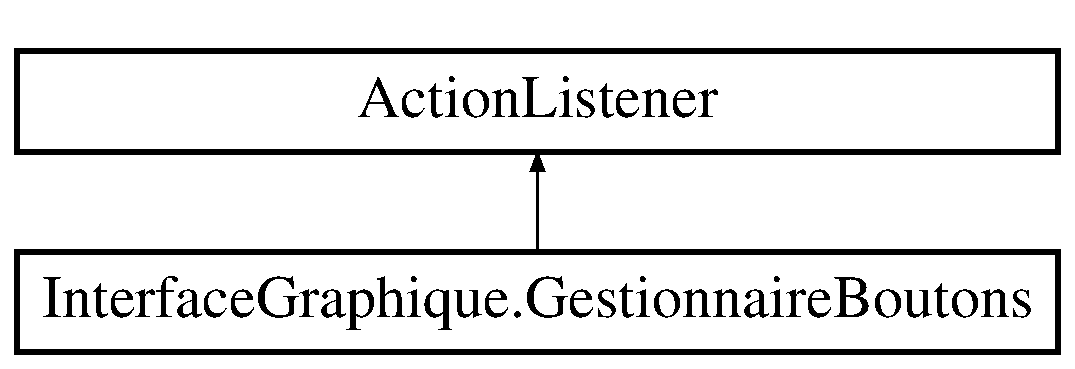
\includegraphics[height=2.000000cm]{class_interface_graphique_1_1_gestionnaire_boutons}
\end{center}
\end{figure}
\subsection*{Public Member Functions}
\begin{DoxyCompactItemize}
\item 
\hyperlink{class_interface_graphique_1_1_gestionnaire_boutons_a168307bb28d6e6013a01a111db7c3228}{Gestionnaire\-Boutons} (Object gestionnaire)
\item 
\hyperlink{wglew_8h_aeea6e3dfae3acf232096f57d2d57f084}{void} \hyperlink{class_interface_graphique_1_1_gestionnaire_boutons_a63647b573e2c4c7c4f8d25ed79fe5234}{action\-Performed} (Action\-Event evenement)
\end{DoxyCompactItemize}


\subsection{Detailed Description}
Classe permettant de g�rer les actions des boutons (par r�flexion) permettant ainsi de d�localiser les m�thodes appel�es, et de les mettre dans la classe \hyperlink{class_interface_graphique_1_1_input_manager}{Input\-Manager}. Aussi, de cette mani�re, on a besoin que d'un seul Action\-Performed qui g�re tous les �v�nements li� aux boutons 

\subsection{Constructor \& Destructor Documentation}
\hypertarget{class_interface_graphique_1_1_gestionnaire_boutons_a168307bb28d6e6013a01a111db7c3228}{\index{Interface\-Graphique\-::\-Gestionnaire\-Boutons@{Interface\-Graphique\-::\-Gestionnaire\-Boutons}!Gestionnaire\-Boutons@{Gestionnaire\-Boutons}}
\index{Gestionnaire\-Boutons@{Gestionnaire\-Boutons}!InterfaceGraphique::GestionnaireBoutons@{Interface\-Graphique\-::\-Gestionnaire\-Boutons}}
\subsubsection[{Gestionnaire\-Boutons}]{\setlength{\rightskip}{0pt plus 5cm}Interface\-Graphique.\-Gestionnaire\-Boutons.\-Gestionnaire\-Boutons (
\begin{DoxyParamCaption}
\item[{Object}]{gestionnaire}
\end{DoxyParamCaption}
)\hspace{0.3cm}{\ttfamily [inline]}}}\label{class_interface_graphique_1_1_gestionnaire_boutons_a168307bb28d6e6013a01a111db7c3228}
Constructeur qui ne fait qu'assigner le gestionnaire des actions re�ues par cet �couteur.


\begin{DoxyParams}{Parameters}
{\em gestionnaire} & Le gestionnaire des actions re�ues par cet �couteur. \\
\hline
\end{DoxyParams}


\subsection{Member Function Documentation}
\hypertarget{class_interface_graphique_1_1_gestionnaire_boutons_a63647b573e2c4c7c4f8d25ed79fe5234}{\index{Interface\-Graphique\-::\-Gestionnaire\-Boutons@{Interface\-Graphique\-::\-Gestionnaire\-Boutons}!action\-Performed@{action\-Performed}}
\index{action\-Performed@{action\-Performed}!InterfaceGraphique::GestionnaireBoutons@{Interface\-Graphique\-::\-Gestionnaire\-Boutons}}
\subsubsection[{action\-Performed}]{\setlength{\rightskip}{0pt plus 5cm}{\bf void} Interface\-Graphique.\-Gestionnaire\-Boutons.\-action\-Performed (
\begin{DoxyParamCaption}
\item[{Action\-Event}]{evenement}
\end{DoxyParamCaption}
)\hspace{0.3cm}{\ttfamily [inline]}}}\label{class_interface_graphique_1_1_gestionnaire_boutons_a63647b573e2c4c7c4f8d25ed79fe5234}
Implantation de l'interface {\ttfamily Action\-Listener} qui g�re les actions provenant de certains �v�nements d'interface.


\begin{DoxyParams}{Parameters}
{\em evenement} & L'�v�nement correspondant � l'action. \\
\hline
\end{DoxyParams}


The documentation for this class was generated from the following file\-:\begin{DoxyCompactItemize}
\item 
Cadriciel/\-Sources/\-Java/\-Interface\-Graphique/src/\-Interface\-Graphique/\hyperlink{_gestionnaire_boutons_8java}{Gestionnaire\-Boutons.\-java}\end{DoxyCompactItemize}

\hypertarget{class_interface_graphique_1_1_gestionnaire_clavier}{\section{Interface\-Graphique.\-Gestionnaire\-Clavier Class Reference}
\label{class_interface_graphique_1_1_gestionnaire_clavier}\index{Interface\-Graphique.\-Gestionnaire\-Clavier@{Interface\-Graphique.\-Gestionnaire\-Clavier}}
}
Inheritance diagram for Interface\-Graphique.\-Gestionnaire\-Clavier\-:\begin{figure}[H]
\begin{center}
\leavevmode
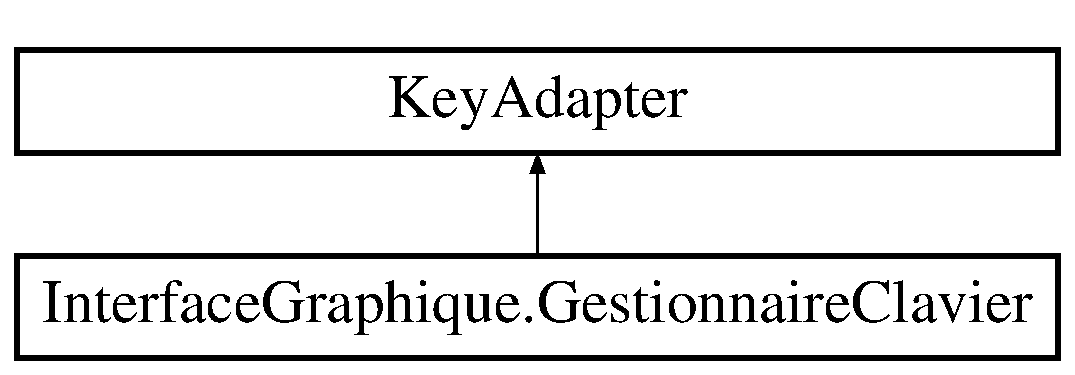
\includegraphics[height=2.000000cm]{class_interface_graphique_1_1_gestionnaire_clavier}
\end{center}
\end{figure}
\subsection*{Public Member Functions}
\begin{DoxyCompactItemize}
\item 
\hyperlink{class_interface_graphique_1_1_gestionnaire_clavier_a222ffc76d02866188df4f477e2ce28e8}{Gestionnaire\-Clavier} (Object gestionnaire)
\item 
\hyperlink{wglew_8h_aeea6e3dfae3acf232096f57d2d57f084}{void} \hyperlink{class_interface_graphique_1_1_gestionnaire_clavier_ab0e60ec8e5fedd3be53614423def95f3}{key\-Pressed} (Key\-Event evenement)
\item 
\hyperlink{wglew_8h_aeea6e3dfae3acf232096f57d2d57f084}{void} \hyperlink{class_interface_graphique_1_1_gestionnaire_clavier_ad804df8af48e0326a6f30630d0bcd21c}{key\-Released} (Key\-Event evenement)
\end{DoxyCompactItemize}


\subsection{Detailed Description}
Classe permettant de g�rer les actions du clavier (par r�flexion) permettant ainsi de d�localiser les m�thodes appel�es, et de les mettre dans la classe \hyperlink{class_interface_graphique_1_1_input_manager}{Input\-Manager}. Aussi, de cette mani�re, on a besoin que d'un seul Key\-Event qui g�re tous les �v�nements du clavier 

\subsection{Constructor \& Destructor Documentation}
\hypertarget{class_interface_graphique_1_1_gestionnaire_clavier_a222ffc76d02866188df4f477e2ce28e8}{\index{Interface\-Graphique\-::\-Gestionnaire\-Clavier@{Interface\-Graphique\-::\-Gestionnaire\-Clavier}!Gestionnaire\-Clavier@{Gestionnaire\-Clavier}}
\index{Gestionnaire\-Clavier@{Gestionnaire\-Clavier}!InterfaceGraphique::GestionnaireClavier@{Interface\-Graphique\-::\-Gestionnaire\-Clavier}}
\subsubsection[{Gestionnaire\-Clavier}]{\setlength{\rightskip}{0pt plus 5cm}Interface\-Graphique.\-Gestionnaire\-Clavier.\-Gestionnaire\-Clavier (
\begin{DoxyParamCaption}
\item[{Object}]{gestionnaire}
\end{DoxyParamCaption}
)\hspace{0.3cm}{\ttfamily [inline]}}}\label{class_interface_graphique_1_1_gestionnaire_clavier_a222ffc76d02866188df4f477e2ce28e8}
Constructeur qui ne fait qu'assigner le gestionnaire des actions re�ues par cet �couteur.


\begin{DoxyParams}{Parameters}
{\em gestionnaire} & Le gestionnaire des actions re�ues par cet �couteur. \\
\hline
\end{DoxyParams}


\subsection{Member Function Documentation}
\hypertarget{class_interface_graphique_1_1_gestionnaire_clavier_ab0e60ec8e5fedd3be53614423def95f3}{\index{Interface\-Graphique\-::\-Gestionnaire\-Clavier@{Interface\-Graphique\-::\-Gestionnaire\-Clavier}!key\-Pressed@{key\-Pressed}}
\index{key\-Pressed@{key\-Pressed}!InterfaceGraphique::GestionnaireClavier@{Interface\-Graphique\-::\-Gestionnaire\-Clavier}}
\subsubsection[{key\-Pressed}]{\setlength{\rightskip}{0pt plus 5cm}{\bf void} Interface\-Graphique.\-Gestionnaire\-Clavier.\-key\-Pressed (
\begin{DoxyParamCaption}
\item[{Key\-Event}]{evenement}
\end{DoxyParamCaption}
)\hspace{0.3cm}{\ttfamily [inline]}}}\label{class_interface_graphique_1_1_gestionnaire_clavier_ab0e60ec8e5fedd3be53614423def95f3}
Implantation de l'interface Key\-Listener qui g�re les �v�nements d'une touche enfonc�e.


\begin{DoxyParams}{Parameters}
{\em evenement} & L'�v�nement correspondant � l'action. \\
\hline
\end{DoxyParams}
\hypertarget{class_interface_graphique_1_1_gestionnaire_clavier_ad804df8af48e0326a6f30630d0bcd21c}{\index{Interface\-Graphique\-::\-Gestionnaire\-Clavier@{Interface\-Graphique\-::\-Gestionnaire\-Clavier}!key\-Released@{key\-Released}}
\index{key\-Released@{key\-Released}!InterfaceGraphique::GestionnaireClavier@{Interface\-Graphique\-::\-Gestionnaire\-Clavier}}
\subsubsection[{key\-Released}]{\setlength{\rightskip}{0pt plus 5cm}{\bf void} Interface\-Graphique.\-Gestionnaire\-Clavier.\-key\-Released (
\begin{DoxyParamCaption}
\item[{Key\-Event}]{evenement}
\end{DoxyParamCaption}
)\hspace{0.3cm}{\ttfamily [inline]}}}\label{class_interface_graphique_1_1_gestionnaire_clavier_ad804df8af48e0326a6f30630d0bcd21c}
M�thode appel�e lorsqu'une touche de clavier est relach� 
\begin{DoxyParams}{Parameters}
{\em evenement} & Evenement li� a l'action du relachement de clic \\
\hline
\end{DoxyParams}
\begin{DoxyReturn}{Returns}
void 
\end{DoxyReturn}


The documentation for this class was generated from the following file\-:\begin{DoxyCompactItemize}
\item 
Cadriciel/\-Sources/\-Java/\-Interface\-Graphique/src/\-Interface\-Graphique/\hyperlink{_gestionnaire_clavier_8java}{Gestionnaire\-Clavier.\-java}\end{DoxyCompactItemize}

\hypertarget{class_gestionnaire_collision}{\section{Gestionnaire\-Collision Class Reference}
\label{class_gestionnaire_collision}\index{Gestionnaire\-Collision@{Gestionnaire\-Collision}}
}


Classe qui se charge de verifier les collisions et d'appeler leur traitement.  




{\ttfamily \#include $<$Gestionnaire\-Collision.\-h$>$}

\subsection*{Public Member Functions}
\begin{DoxyCompactItemize}
\item 
\hyperlink{group__inf2990_ga9df084bfa2dc4442d976654973ee5372}{Gestionnaire\-Collision} (vector$<$ \hyperlink{class_element_jeu_abstrait}{Element\-Jeu\-Abstrait} $\ast$ $>$ \&vecteur\-Elements\-Jeu, vector$<$ \hyperlink{class_asteroide}{Asteroide} $\ast$ $>$ \&vecteur\-Asteroides, vector$<$ \hyperlink{class_projectile}{Projectile} $\ast$ $>$ \&vecteur\-Projectiles)
\item 
\hyperlink{group__inf2990_ga32cdb2d1f023ff9698249fcbaa5f7dc8}{$\sim$\-Gestionnaire\-Collision} ()
\item 
\hyperlink{wglew_8h_aeea6e3dfae3acf232096f57d2d57f084}{void} \hyperlink{group__inf2990_ga2243af30a36d7db008ec99ce8e8f74b6}{initialiser\-Quad\-Tree} (const \hyperlink{group__utilitaire_ga606b191c0b0bbb868ae25c13b906f45a}{Vecteur2f} \&coin\-Haut\-Gauche, const \hyperlink{group__utilitaire_ga606b191c0b0bbb868ae25c13b906f45a}{Vecteur2f} \&coin\-Bas\-Gauche)
\item 
vector$<$ \hyperlink{class_asteroide}{Asteroide} $\ast$ $>$ \& \hyperlink{group__inf2990_ga572a2a95fc9137f44e0a5ce8c6ab0648}{get\-Conteneur\-Asteroides} ()
\item 
vector$<$ \hyperlink{class_element_jeu_abstrait}{Element\-Jeu\-Abstrait} $\ast$ $>$ \& \hyperlink{group__inf2990_gacc26b8c32b6c1bdeb1ded2e69e427ffc}{get\-Conteneur\-Elements\-Jeu} ()
\item 
\hyperlink{wglew_8h_aeea6e3dfae3acf232096f57d2d57f084}{void} \hyperlink{group__inf2990_ga3de2ac60f6d74d60c8015f7fba0c6194}{set\-Conteneur\-Asteroides} (vector$<$ \hyperlink{class_asteroide}{Asteroide} $\ast$ $>$ \&asteroides)
\item 
\hyperlink{wglew_8h_aeea6e3dfae3acf232096f57d2d57f084}{void} \hyperlink{group__inf2990_ga883cc7e90d1ec884d4f983a302c9ed90}{set\-Conteneur\-Element\-Jeu} (vector$<$ \hyperlink{class_element_jeu_abstrait}{Element\-Jeu\-Abstrait} $\ast$ $>$ \&elements\-Jeu)
\item 
\hyperlink{wglew_8h_aeea6e3dfae3acf232096f57d2d57f084}{void} \hyperlink{group__inf2990_ga6b1e1b31aa559c75d0cb6314620aef7b}{add\-Joueur} (\hyperlink{class_vaisseau}{Vaisseau} $\ast$vaisseau)
\item 
\hyperlink{wglew_8h_aeea6e3dfae3acf232096f57d2d57f084}{void} \hyperlink{group__inf2990_ga34d26483935d731acb183b073f0641e4}{check\-Collisions} ()
\item 
\hyperlink{wglew_8h_aeea6e3dfae3acf232096f57d2d57f084}{void} \hyperlink{group__inf2990_gab1e397ffc039f85112a7a177fb0219f3}{traiter\-Collisions} ()
\item 
\hyperlink{wglew_8h_aeea6e3dfae3acf232096f57d2d57f084}{void} \hyperlink{group__inf2990_ga9d33a33cd08ac039ff71c43976397d38}{detruire\-Quad\-Tree} ()
\end{DoxyCompactItemize}


\subsection{Detailed Description}
Classe qui se charge de verifier les collisions et d'appeler leur traitement. 

\begin{DoxyAuthor}{Author}
Floppy\-Disketeers 
\end{DoxyAuthor}
\begin{DoxyDate}{Date}
2014-\/01-\/21 
\end{DoxyDate}


The documentation for this class was generated from the following files\-:\begin{DoxyCompactItemize}
\item 
Cadriciel/\-Sources/\-C++/\-Application/\hyperlink{_gestionnaire_collision_8h}{Gestionnaire\-Collision.\-h}\item 
Cadriciel/\-Sources/\-C++/\-Application/\hyperlink{_gestionnaire_collision_8cpp}{Gestionnaire\-Collision.\-cpp}\end{DoxyCompactItemize}

\hypertarget{class_gestionnaire_ressources}{\section{Gestionnaire\-Ressources Class Reference}
\label{class_gestionnaire_ressources}\index{Gestionnaire\-Ressources@{Gestionnaire\-Ressources}}
}


Cette class est un singleton. Elle permet de centraliser le chargement des ressources et permet de re-\/utiliser ce qui a deja ete charge, comme les modeles 3\-D ou les textures.  




{\ttfamily \#include $<$Gestionnaire\-Ressources.\-h$>$}

\subsection*{Public Member Functions}
\begin{DoxyCompactItemize}
\item 
\hyperlink{class_gestionnaire_ressources_adefa41ed304fd2242410cf8ad912e6e2}{$\sim$\-Gestionnaire\-Ressources} ()
\item 
const ai\-Scene $\ast$ \hyperlink{class_gestionnaire_ressources_a6f0f993e3edeb435cb65cc0b400e2958}{charger\-Modele3\-D} (const \hyperlink{glew_8h_ae84541b4f3d8e1ea24ec0f466a8c568b}{string} \&nom\-Fichier, map$<$ \hyperlink{glew_8h_ae84541b4f3d8e1ea24ec0f466a8c568b}{string}, \hyperlink{glew_8h_a68c4714e43d8e827d80759f9cb864f3c}{G\-Luint} $>$ \&\hyperlink{glew_8h_a450062c0770127a605331b58382bfa3b}{textures})
\item 
\hyperlink{glew_8h_a68c4714e43d8e827d80759f9cb864f3c}{G\-Luint} \hyperlink{class_gestionnaire_ressources_a8b6bbee12ec9c00bdb3637bc6072bfc2}{creer\-Call\-List} (const ai\-Scene $\ast$scene)
\item 
bool \hyperlink{class_gestionnaire_ressources_a48e20c30acdaff204c77a3977ab2a7b0}{charger\-Texture} (const \hyperlink{glew_8h_ae84541b4f3d8e1ea24ec0f466a8c568b}{string} \&nom\-Fichier, \hyperlink{glew_8h_a68c4714e43d8e827d80759f9cb864f3c}{G\-Luint} \&\hyperlink{glew_8h_af1de2b5e600991636b673dcda0fa5342}{texture})
\item 
bool \hyperlink{class_gestionnaire_ressources_a8109eec59d2e8f711643853b788babeb}{calculer\-Points\-Extremes} (const \hyperlink{glew_8h_ae84541b4f3d8e1ea24ec0f466a8c568b}{string} \&nom\-Fichier, \hyperlink{group__utilitaire_ga6b2956069f76c7e27df4f79f87e5a48c}{Vecteur3f} \&x\-Min, \hyperlink{group__utilitaire_ga6b2956069f76c7e27df4f79f87e5a48c}{Vecteur3f} \&y\-Min, \hyperlink{group__utilitaire_ga6b2956069f76c7e27df4f79f87e5a48c}{Vecteur3f} \&z\-Min, \hyperlink{group__utilitaire_ga6b2956069f76c7e27df4f79f87e5a48c}{Vecteur3f} \&x\-Max, \hyperlink{group__utilitaire_ga6b2956069f76c7e27df4f79f87e5a48c}{Vecteur3f} \&y\-Max, \hyperlink{group__utilitaire_ga6b2956069f76c7e27df4f79f87e5a48c}{Vecteur3f} \&z\-Max)
\item 
\hyperlink{fmod_8h_aeb841aa4b4b5f444b5d739d865b420af}{float} \hyperlink{class_gestionnaire_ressources_a6fb3dc8d4945fbe2dc34054f9fe842c2}{calculer\-Rayon\-Sphere\-Englobante} (const \hyperlink{glew_8h_ae84541b4f3d8e1ea24ec0f466a8c568b}{string} \&nom\-Fichier)
\end{DoxyCompactItemize}
\subsection*{Static Public Member Functions}
\begin{DoxyCompactItemize}
\item 
static \hyperlink{class_gestionnaire_ressources}{Gestionnaire\-Ressources} $\ast$ \hyperlink{class_gestionnaire_ressources_af6c8a2217d3269073d0b4b1246aeedac}{get\-Instance} ()
\end{DoxyCompactItemize}


\subsection{Detailed Description}
Cette class est un singleton. Elle permet de centraliser le chargement des ressources et permet de re-\/utiliser ce qui a deja ete charge, comme les modeles 3\-D ou les textures. 

\subsection{Constructor \& Destructor Documentation}
\hypertarget{class_gestionnaire_ressources_adefa41ed304fd2242410cf8ad912e6e2}{\index{Gestionnaire\-Ressources@{Gestionnaire\-Ressources}!$\sim$\-Gestionnaire\-Ressources@{$\sim$\-Gestionnaire\-Ressources}}
\index{$\sim$\-Gestionnaire\-Ressources@{$\sim$\-Gestionnaire\-Ressources}!GestionnaireRessources@{Gestionnaire\-Ressources}}
\subsubsection[{$\sim$\-Gestionnaire\-Ressources}]{\setlength{\rightskip}{0pt plus 5cm}Gestionnaire\-Ressources\-::$\sim$\-Gestionnaire\-Ressources (
\begin{DoxyParamCaption}
{}
\end{DoxyParamCaption}
)}}\label{class_gestionnaire_ressources_adefa41ed304fd2242410cf8ad912e6e2}
Destructeur. Libere toutes les ressources. 

\subsection{Member Function Documentation}
\hypertarget{class_gestionnaire_ressources_a8109eec59d2e8f711643853b788babeb}{\index{Gestionnaire\-Ressources@{Gestionnaire\-Ressources}!calculer\-Points\-Extremes@{calculer\-Points\-Extremes}}
\index{calculer\-Points\-Extremes@{calculer\-Points\-Extremes}!GestionnaireRessources@{Gestionnaire\-Ressources}}
\subsubsection[{calculer\-Points\-Extremes}]{\setlength{\rightskip}{0pt plus 5cm}bool Gestionnaire\-Ressources\-::calculer\-Points\-Extremes (
\begin{DoxyParamCaption}
\item[{const {\bf string} \&}]{nom\-Fichier, }
\item[{{\bf Vecteur3f} \&}]{x\-Min, }
\item[{{\bf Vecteur3f} \&}]{y\-Min, }
\item[{{\bf Vecteur3f} \&}]{z\-Min, }
\item[{{\bf Vecteur3f} \&}]{x\-Max, }
\item[{{\bf Vecteur3f} \&}]{y\-Max, }
\item[{{\bf Vecteur3f} \&}]{z\-Max}
\end{DoxyParamCaption}
)}}\label{class_gestionnaire_ressources_a8109eec59d2e8f711643853b788babeb}
Calcule les points extremes d'un modele deja charge. S'il n'est pas deja charge, alors la fonction ne calculera rien. 
\begin{DoxyParams}{Parameters}
{\em nom\-Fichier} & Le nom du modele pour lequel on veut calculer les points extremes. \\
\hline
{\em x\-Min} & Points extremes minimaux en x \\
\hline
{\em y\-Min} & Points extremes minimaux en y \\
\hline
{\em z\-Min} & Points extremes minimaux en z \\
\hline
{\em x\-Max} & Points extremes maximaux en x \\
\hline
{\em y\-Max} & Points extremes maximaux en y \\
\hline
{\em z\-Max} & Points extremes maximaux en z \\
\hline
\end{DoxyParams}
\begin{DoxyReturn}{Returns}
true si le modele est deja charge, false sinon. 
\end{DoxyReturn}
\hypertarget{class_gestionnaire_ressources_a6fb3dc8d4945fbe2dc34054f9fe842c2}{\index{Gestionnaire\-Ressources@{Gestionnaire\-Ressources}!calculer\-Rayon\-Sphere\-Englobante@{calculer\-Rayon\-Sphere\-Englobante}}
\index{calculer\-Rayon\-Sphere\-Englobante@{calculer\-Rayon\-Sphere\-Englobante}!GestionnaireRessources@{Gestionnaire\-Ressources}}
\subsubsection[{calculer\-Rayon\-Sphere\-Englobante}]{\setlength{\rightskip}{0pt plus 5cm}{\bf float} Gestionnaire\-Ressources\-::calculer\-Rayon\-Sphere\-Englobante (
\begin{DoxyParamCaption}
\item[{const {\bf string} \&}]{nom\-Fichier}
\end{DoxyParamCaption}
)}}\label{class_gestionnaire_ressources_a6fb3dc8d4945fbe2dc34054f9fe842c2}
Calcule le rayon de la sph�re englobante 
\begin{DoxyParams}{Parameters}
{\em nom\-Fichier} & Le nom du fichier du mod�le pour lequel on veut calculer le rayon de la sph�re englobante \\
\hline
\end{DoxyParams}
\begin{DoxyReturn}{Returns}
Le rayon de la sph�re englobante 
\end{DoxyReturn}
\hypertarget{class_gestionnaire_ressources_a6f0f993e3edeb435cb65cc0b400e2958}{\index{Gestionnaire\-Ressources@{Gestionnaire\-Ressources}!charger\-Modele3\-D@{charger\-Modele3\-D}}
\index{charger\-Modele3\-D@{charger\-Modele3\-D}!GestionnaireRessources@{Gestionnaire\-Ressources}}
\subsubsection[{charger\-Modele3\-D}]{\setlength{\rightskip}{0pt plus 5cm}const ai\-Scene $\ast$ Gestionnaire\-Ressources\-::charger\-Modele3\-D (
\begin{DoxyParamCaption}
\item[{const {\bf string} \&}]{nom\-Fichier, }
\item[{map$<$ {\bf string}, {\bf G\-Luint} $>$ \&}]{textures}
\end{DoxyParamCaption}
)}}\label{class_gestionnaire_ressources_a6f0f993e3edeb435cb65cc0b400e2958}
Charge un modele 3\-D 
\begin{DoxyParams}{Parameters}
{\em nom\-Fichier} & Le nom du fichier du modele a charger \\
\hline
{\em textures} & Une map de textures pour l'objet. La cle est le nom de la texture et la valeur est l'identifiant de la texture \\
\hline
\end{DoxyParams}
\begin{DoxyReturn}{Returns}
La scene assimp representant l'objet si l'objet a ete bien charge. N\-U\-L\-L sinon 
\end{DoxyReturn}
\hypertarget{class_gestionnaire_ressources_a48e20c30acdaff204c77a3977ab2a7b0}{\index{Gestionnaire\-Ressources@{Gestionnaire\-Ressources}!charger\-Texture@{charger\-Texture}}
\index{charger\-Texture@{charger\-Texture}!GestionnaireRessources@{Gestionnaire\-Ressources}}
\subsubsection[{charger\-Texture}]{\setlength{\rightskip}{0pt plus 5cm}bool Gestionnaire\-Ressources\-::charger\-Texture (
\begin{DoxyParamCaption}
\item[{const {\bf string} \&}]{nom\-Fichier, }
\item[{{\bf G\-Luint} \&}]{texture}
\end{DoxyParamCaption}
)}}\label{class_gestionnaire_ressources_a48e20c30acdaff204c77a3977ab2a7b0}
Charge une texture 
\begin{DoxyParams}{Parameters}
{\em nom\-Fichier} & Le nom du fichier de la texture a charger \\
\hline
{\em texture} & L'identificateur de la texture \\
\hline
\end{DoxyParams}
\begin{DoxyReturn}{Returns}
True si la texture a ete charge correctement, false sinon 
\end{DoxyReturn}
\hypertarget{class_gestionnaire_ressources_a8b6bbee12ec9c00bdb3637bc6072bfc2}{\index{Gestionnaire\-Ressources@{Gestionnaire\-Ressources}!creer\-Call\-List@{creer\-Call\-List}}
\index{creer\-Call\-List@{creer\-Call\-List}!GestionnaireRessources@{Gestionnaire\-Ressources}}
\subsubsection[{creer\-Call\-List}]{\setlength{\rightskip}{0pt plus 5cm}{\bf G\-Luint} Gestionnaire\-Ressources\-::creer\-Call\-List (
\begin{DoxyParamCaption}
\item[{const ai\-Scene $\ast$}]{scene}
\end{DoxyParamCaption}
)}}\label{class_gestionnaire_ressources_a8b6bbee12ec9c00bdb3637bc6072bfc2}
Creer une liste d'affichage pour un modele specifie 
\begin{DoxyParams}{Parameters}
{\em scene} & Une scene \hyperlink{namespace_assimp}{Assimp} permettant d'acceder aux donnees du modele pour l'afficher. \\
\hline
\end{DoxyParams}
\begin{DoxyReturn}{Returns}
L'identifiant de la liste d'affichage creee ou G\-L\-\_\-\-I\-N\-V\-A\-L\-I\-D\-\_\-\-V\-A\-L\-U\-E 
\end{DoxyReturn}
\hypertarget{class_gestionnaire_ressources_af6c8a2217d3269073d0b4b1246aeedac}{\index{Gestionnaire\-Ressources@{Gestionnaire\-Ressources}!get\-Instance@{get\-Instance}}
\index{get\-Instance@{get\-Instance}!GestionnaireRessources@{Gestionnaire\-Ressources}}
\subsubsection[{get\-Instance}]{\setlength{\rightskip}{0pt plus 5cm}{\bf Gestionnaire\-Ressources} $\ast$ Gestionnaire\-Ressources\-::get\-Instance (
\begin{DoxyParamCaption}
{}
\end{DoxyParamCaption}
)\hspace{0.3cm}{\ttfamily [static]}}}\label{class_gestionnaire_ressources_af6c8a2217d3269073d0b4b1246aeedac}
Retourne l'instance du singleton. 

The documentation for this class was generated from the following files\-:\begin{DoxyCompactItemize}
\item 
Cadriciel/\-Sources/\-C++/\-Arbre/\-Modeles/\hyperlink{_gestionnaire_ressources_8h}{Gestionnaire\-Ressources.\-h}\item 
Cadriciel/\-Sources/\-C++/\-Arbre/\-Modeles/\hyperlink{_gestionnaire_ressources_8cpp}{Gestionnaire\-Ressources.\-cpp}\end{DoxyCompactItemize}

\hypertarget{class_gestionnaire_x_m_l}{\section{Gestionnaire\-X\-M\-L Class Reference}
\label{class_gestionnaire_x_m_l}\index{Gestionnaire\-X\-M\-L@{Gestionnaire\-X\-M\-L}}
}


Classe qui s'occupe de la gestion des cartes et des fichiers X\-M\-L C'est une classe singleton.  




{\ttfamily \#include $<$Gestionnaire\-X\-M\-L.\-h$>$}

Inheritance diagram for Gestionnaire\-X\-M\-L\-:\begin{figure}[H]
\begin{center}
\leavevmode
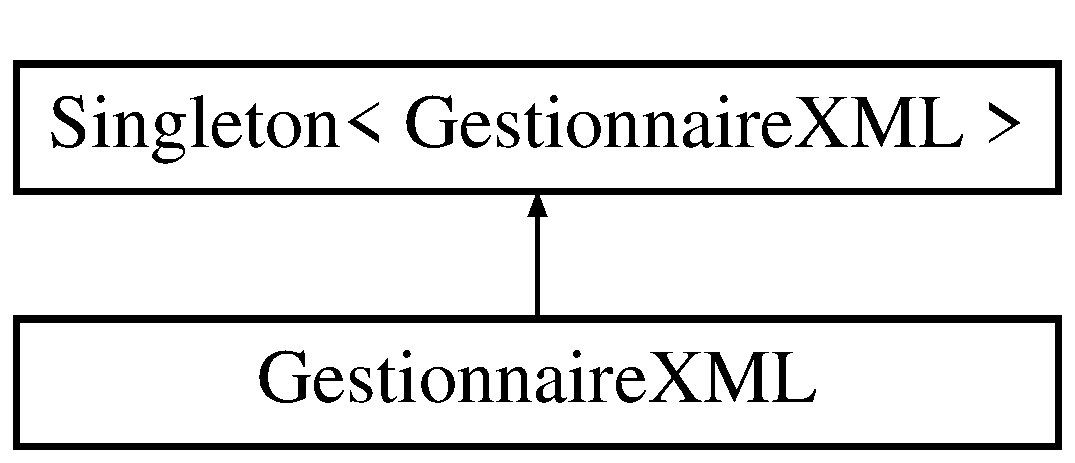
\includegraphics[height=2.000000cm]{class_gestionnaire_x_m_l}
\end{center}
\end{figure}
\subsection*{Public Member Functions}
\begin{DoxyCompactItemize}
\item 
\hyperlink{group__inf2990_ga267eebe0e3bb95b5d5f973a4319fe1da}{Gestionnaire\-X\-M\-L} ()
\begin{DoxyCompactList}\small\item\em Constructeur par defaut. \end{DoxyCompactList}\item 
\hyperlink{group__inf2990_gad8207e0a0791170d9c30e81be160ec73}{$\sim$\-Gestionnaire\-X\-M\-L} ()
\begin{DoxyCompactList}\small\item\em Destructeur. \end{DoxyCompactList}\item 
\hyperlink{wglew_8h_aeea6e3dfae3acf232096f57d2d57f084}{void} \hyperlink{group__inf2990_ga84f9d09636d2edbbeb398da22274741d}{sauvegarder\-Carte} (const \hyperlink{glew_8h_ae84541b4f3d8e1ea24ec0f466a8c568b}{string} nom, \hyperlink{class_carte}{Carte} \&carte) const 
\item 
\hyperlink{class_carte}{Carte} $\ast$ \hyperlink{group__inf2990_gaed7d668fdea387603e69c90f14766f97}{charger\-Carte} (const \hyperlink{glew_8h_ae84541b4f3d8e1ea24ec0f466a8c568b}{string} nom)
\item 
\hyperlink{glew_8h_ae84541b4f3d8e1ea24ec0f466a8c568b}{string} \hyperlink{group__inf2990_ga43004d2d9e045bae88d16024594e5cf3}{get\-Nom\-Carte\-Defaut} () const 
\item 
\hyperlink{class_carte}{Carte} $\ast$ \hyperlink{group__inf2990_ga9e8d745ff895e25d5d7bdf3a79ef2341}{charger\-Carte\-Defaut} ()
\item 
\hyperlink{class_carte}{Carte} $\ast$ \hyperlink{group__inf2990_ga9a4209b0cd0a7f296aca339a495f6c01}{charger\-Carte\-Campagne\-Defaut} ()
\item 
\hyperlink{wglew_8h_aeea6e3dfae3acf232096f57d2d57f084}{void} \hyperlink{group__inf2990_ga2078e6964e0e3991cdc3926da825412d}{sauvegarder\-Configuration} (\hyperlink{wglew_8h_a500a82aecba06f4550f6849b8099ca21}{int} touche\-Joueur1\-Propulsion, \hyperlink{wglew_8h_a500a82aecba06f4550f6849b8099ca21}{int} touche\-Joueur1\-Tourner\-Gauche, \hyperlink{wglew_8h_a500a82aecba06f4550f6849b8099ca21}{int} touche\-Joueur1\-Tourner\-Droite, \hyperlink{wglew_8h_a500a82aecba06f4550f6849b8099ca21}{int} touche\-Joueur1\-Manoeuvre, \hyperlink{wglew_8h_a500a82aecba06f4550f6849b8099ca21}{int} touche\-Joueur1\-Tir, \hyperlink{wglew_8h_a500a82aecba06f4550f6849b8099ca21}{int} touche\-Joueur2\-Propulsion, \hyperlink{wglew_8h_a500a82aecba06f4550f6849b8099ca21}{int} touche\-Joueur2\-Tourner\-Gauche, \hyperlink{wglew_8h_a500a82aecba06f4550f6849b8099ca21}{int} touche\-Joueur2\-Tourner\-Droite, \hyperlink{wglew_8h_a500a82aecba06f4550f6849b8099ca21}{int} touche\-Joueur2\-Manoeuvre, \hyperlink{wglew_8h_a500a82aecba06f4550f6849b8099ca21}{int} touche\-Joueur2\-Tir, double duree\-Jeu, \hyperlink{wglew_8h_a500a82aecba06f4550f6849b8099ca21}{int} points\-De\-Vie\-Station, bool apparition\-Asteroide, bool changement\-Mode, bool eclairage, bool cible\-Joueur, bool cadre\-Depart, bool zone\-Passage, bool attraction\-Port) const 
\item 
\hyperlink{wglew_8h_aeea6e3dfae3acf232096f57d2d57f084}{void} \hyperlink{group__inf2990_ga74edda2c2220100dfa1a59b20291610b}{charger\-Configuration} (\hyperlink{wglew_8h_a500a82aecba06f4550f6849b8099ca21}{int} \&touche\-Joueur1\-Propulsion, \hyperlink{wglew_8h_a500a82aecba06f4550f6849b8099ca21}{int} \&touche\-Joueur1\-Tourner\-Gauche, \hyperlink{wglew_8h_a500a82aecba06f4550f6849b8099ca21}{int} \&touche\-Joueur1\-Tourner\-Droite, \hyperlink{wglew_8h_a500a82aecba06f4550f6849b8099ca21}{int} \&touche\-Joueur1\-Manoeuvre, \hyperlink{wglew_8h_a500a82aecba06f4550f6849b8099ca21}{int} \&touche\-Joueur1\-Tir, \hyperlink{wglew_8h_a500a82aecba06f4550f6849b8099ca21}{int} \&touche\-Joueur2\-Propulsion, \hyperlink{wglew_8h_a500a82aecba06f4550f6849b8099ca21}{int} \&touche\-Joueur2\-Tourner\-Gauche, \hyperlink{wglew_8h_a500a82aecba06f4550f6849b8099ca21}{int} \&touche\-Joueur2\-Tourner\-Droite, \hyperlink{wglew_8h_a500a82aecba06f4550f6849b8099ca21}{int} \&touche\-Joueur2\-Manoeuvre, \hyperlink{wglew_8h_a500a82aecba06f4550f6849b8099ca21}{int} \&touche\-Joueur2\-Tir, double \&duree\-Jeu, \hyperlink{wglew_8h_a500a82aecba06f4550f6849b8099ca21}{int} \&points\-De\-Vie\-Station, bool \&apparition\-Asteroide, bool \&changement\-Mode, bool \&eclairage, bool \&cible\-Joueur, bool \&cadre\-Depart, bool \&zone\-Passage, bool \&attraction\-Port, bool \&fichier\-Existe) const 
\item 
\hyperlink{wglew_8h_aeea6e3dfae3acf232096f57d2d57f084}{void} \hyperlink{group__inf2990_gaf25915bc26ca653ace2a0b4df3a4d808}{sauvegarder\-Config\-Campagne} (bool mode\-Coop, bool joueur2\-Virtuel, vector$<$ \hyperlink{glew_8h_ae84541b4f3d8e1ea24ec0f466a8c568b}{string} $>$ liste\-Carte)
\item 
\hyperlink{wglew_8h_aeea6e3dfae3acf232096f57d2d57f084}{void} \hyperlink{group__inf2990_ga2020824a2c8ca40060649cd759f728f5}{charger\-Config\-Campagne} (bool \&mode\-Coop, bool \&joueur2\-Virtuel, bool \&fichier, vector$<$ \hyperlink{glew_8h_ae84541b4f3d8e1ea24ec0f466a8c568b}{string} $>$ \&liste\-Carte)
\end{DoxyCompactItemize}
\subsection*{Additional Inherited Members}


\subsection{Detailed Description}
Classe qui s'occupe de la gestion des cartes et des fichiers X\-M\-L C'est une classe singleton. 

\begin{DoxyAuthor}{Author}
Floppy\-Disketeers 
\end{DoxyAuthor}
\begin{DoxyDate}{Date}
2014-\/01-\/21 
\end{DoxyDate}


The documentation for this class was generated from the following files\-:\begin{DoxyCompactItemize}
\item 
Cadriciel/\-Sources/\-C++/\-Application/\hyperlink{_gestionnaire_x_m_l_8h}{Gestionnaire\-X\-M\-L.\-h}\item 
Cadriciel/\-Sources/\-C++/\-Application/\hyperlink{_gestionnaire_x_m_l_8cpp}{Gestionnaire\-X\-M\-L.\-cpp}\end{DoxyCompactItemize}

\hypertarget{struct_g_l_x_buffer_clobber_event_s_g_i_x}{\section{G\-L\-X\-Buffer\-Clobber\-Event\-S\-G\-I\-X Struct Reference}
\label{struct_g_l_x_buffer_clobber_event_s_g_i_x}\index{G\-L\-X\-Buffer\-Clobber\-Event\-S\-G\-I\-X@{G\-L\-X\-Buffer\-Clobber\-Event\-S\-G\-I\-X}}
}


{\ttfamily \#include $<$glxew.\-h$>$}

\subsection*{Public Attributes}
\begin{DoxyCompactItemize}
\item 
\hyperlink{wglew_8h_a500a82aecba06f4550f6849b8099ca21}{int} \hyperlink{struct_g_l_x_buffer_clobber_event_s_g_i_x_a36e3e8a5feea664623ea43d0f273b63a}{type}
\item 
\hyperlink{_free_image_8h_a425076c7067a1b5166e2cc530e914814}{unsigned} \hyperlink{_free_image_8h_a7701bb16365a51acda9234120673781d}{long} \hyperlink{struct_g_l_x_buffer_clobber_event_s_g_i_x_ac295e3276a7986eeae4d6a2a28c7e0b7}{serial}
\item 
Bool \hyperlink{struct_g_l_x_buffer_clobber_event_s_g_i_x_af43bf0edbe40a74ef58dfb546a75118b}{send\-\_\-event}
\item 
Display $\ast$ \hyperlink{struct_g_l_x_buffer_clobber_event_s_g_i_x_afef060d81026da75c846727f4a3de9d4}{display}
\item 
\hyperlink{glxew_8h_a826f51745d9d6c81bdbac47ae2b80cf7}{G\-L\-X\-Drawable} \hyperlink{struct_g_l_x_buffer_clobber_event_s_g_i_x_a9c45674193ed80a79261c3b7518ee04f}{drawable}
\item 
\hyperlink{wglew_8h_a500a82aecba06f4550f6849b8099ca21}{int} \hyperlink{struct_g_l_x_buffer_clobber_event_s_g_i_x_a0b405123f1d6528f1f4dfa7ff92bde9b}{event\-\_\-type}
\item 
\hyperlink{wglew_8h_a500a82aecba06f4550f6849b8099ca21}{int} \hyperlink{struct_g_l_x_buffer_clobber_event_s_g_i_x_a25c31e8cbec0919f74a1e93ae74175b1}{draw\-\_\-type}
\item 
\hyperlink{_free_image_8h_a425076c7067a1b5166e2cc530e914814}{unsigned} \hyperlink{wglew_8h_a500a82aecba06f4550f6849b8099ca21}{int} \hyperlink{struct_g_l_x_buffer_clobber_event_s_g_i_x_a74b4ad1ad3cac011001151411f621da1}{mask}
\item 
\hyperlink{wglew_8h_a500a82aecba06f4550f6849b8099ca21}{int} \hyperlink{struct_g_l_x_buffer_clobber_event_s_g_i_x_a5118d48c3c8d5253d39922b5014b52ff}{x}
\item 
\hyperlink{wglew_8h_a500a82aecba06f4550f6849b8099ca21}{int} \hyperlink{struct_g_l_x_buffer_clobber_event_s_g_i_x_aef21efa11558a5b67861f96471c56003}{y}
\item 
\hyperlink{wglew_8h_a500a82aecba06f4550f6849b8099ca21}{int} \hyperlink{struct_g_l_x_buffer_clobber_event_s_g_i_x_adad23535733161528427584a42bfc6eb}{width}
\item 
\hyperlink{wglew_8h_a500a82aecba06f4550f6849b8099ca21}{int} \hyperlink{struct_g_l_x_buffer_clobber_event_s_g_i_x_a7838dbabb76c22aa8241310a3f2363ea}{height}
\item 
\hyperlink{wglew_8h_a500a82aecba06f4550f6849b8099ca21}{int} \hyperlink{struct_g_l_x_buffer_clobber_event_s_g_i_x_ad8f4f0aae058e0a1ff542679823e37a9}{count}
\end{DoxyCompactItemize}


\subsection{Member Data Documentation}
\hypertarget{struct_g_l_x_buffer_clobber_event_s_g_i_x_ad8f4f0aae058e0a1ff542679823e37a9}{\index{G\-L\-X\-Buffer\-Clobber\-Event\-S\-G\-I\-X@{G\-L\-X\-Buffer\-Clobber\-Event\-S\-G\-I\-X}!count@{count}}
\index{count@{count}!GLXBufferClobberEventSGIX@{G\-L\-X\-Buffer\-Clobber\-Event\-S\-G\-I\-X}}
\subsubsection[{count}]{\setlength{\rightskip}{0pt plus 5cm}{\bf int} G\-L\-X\-Buffer\-Clobber\-Event\-S\-G\-I\-X\-::count}}\label{struct_g_l_x_buffer_clobber_event_s_g_i_x_ad8f4f0aae058e0a1ff542679823e37a9}
\hypertarget{struct_g_l_x_buffer_clobber_event_s_g_i_x_afef060d81026da75c846727f4a3de9d4}{\index{G\-L\-X\-Buffer\-Clobber\-Event\-S\-G\-I\-X@{G\-L\-X\-Buffer\-Clobber\-Event\-S\-G\-I\-X}!display@{display}}
\index{display@{display}!GLXBufferClobberEventSGIX@{G\-L\-X\-Buffer\-Clobber\-Event\-S\-G\-I\-X}}
\subsubsection[{display}]{\setlength{\rightskip}{0pt plus 5cm}Display$\ast$ G\-L\-X\-Buffer\-Clobber\-Event\-S\-G\-I\-X\-::display}}\label{struct_g_l_x_buffer_clobber_event_s_g_i_x_afef060d81026da75c846727f4a3de9d4}
\hypertarget{struct_g_l_x_buffer_clobber_event_s_g_i_x_a25c31e8cbec0919f74a1e93ae74175b1}{\index{G\-L\-X\-Buffer\-Clobber\-Event\-S\-G\-I\-X@{G\-L\-X\-Buffer\-Clobber\-Event\-S\-G\-I\-X}!draw\-\_\-type@{draw\-\_\-type}}
\index{draw\-\_\-type@{draw\-\_\-type}!GLXBufferClobberEventSGIX@{G\-L\-X\-Buffer\-Clobber\-Event\-S\-G\-I\-X}}
\subsubsection[{draw\-\_\-type}]{\setlength{\rightskip}{0pt plus 5cm}{\bf int} G\-L\-X\-Buffer\-Clobber\-Event\-S\-G\-I\-X\-::draw\-\_\-type}}\label{struct_g_l_x_buffer_clobber_event_s_g_i_x_a25c31e8cbec0919f74a1e93ae74175b1}
\hypertarget{struct_g_l_x_buffer_clobber_event_s_g_i_x_a9c45674193ed80a79261c3b7518ee04f}{\index{G\-L\-X\-Buffer\-Clobber\-Event\-S\-G\-I\-X@{G\-L\-X\-Buffer\-Clobber\-Event\-S\-G\-I\-X}!drawable@{drawable}}
\index{drawable@{drawable}!GLXBufferClobberEventSGIX@{G\-L\-X\-Buffer\-Clobber\-Event\-S\-G\-I\-X}}
\subsubsection[{drawable}]{\setlength{\rightskip}{0pt plus 5cm}{\bf G\-L\-X\-Drawable} G\-L\-X\-Buffer\-Clobber\-Event\-S\-G\-I\-X\-::drawable}}\label{struct_g_l_x_buffer_clobber_event_s_g_i_x_a9c45674193ed80a79261c3b7518ee04f}
\hypertarget{struct_g_l_x_buffer_clobber_event_s_g_i_x_a0b405123f1d6528f1f4dfa7ff92bde9b}{\index{G\-L\-X\-Buffer\-Clobber\-Event\-S\-G\-I\-X@{G\-L\-X\-Buffer\-Clobber\-Event\-S\-G\-I\-X}!event\-\_\-type@{event\-\_\-type}}
\index{event\-\_\-type@{event\-\_\-type}!GLXBufferClobberEventSGIX@{G\-L\-X\-Buffer\-Clobber\-Event\-S\-G\-I\-X}}
\subsubsection[{event\-\_\-type}]{\setlength{\rightskip}{0pt plus 5cm}{\bf int} G\-L\-X\-Buffer\-Clobber\-Event\-S\-G\-I\-X\-::event\-\_\-type}}\label{struct_g_l_x_buffer_clobber_event_s_g_i_x_a0b405123f1d6528f1f4dfa7ff92bde9b}
\hypertarget{struct_g_l_x_buffer_clobber_event_s_g_i_x_a7838dbabb76c22aa8241310a3f2363ea}{\index{G\-L\-X\-Buffer\-Clobber\-Event\-S\-G\-I\-X@{G\-L\-X\-Buffer\-Clobber\-Event\-S\-G\-I\-X}!height@{height}}
\index{height@{height}!GLXBufferClobberEventSGIX@{G\-L\-X\-Buffer\-Clobber\-Event\-S\-G\-I\-X}}
\subsubsection[{height}]{\setlength{\rightskip}{0pt plus 5cm}{\bf int} G\-L\-X\-Buffer\-Clobber\-Event\-S\-G\-I\-X\-::height}}\label{struct_g_l_x_buffer_clobber_event_s_g_i_x_a7838dbabb76c22aa8241310a3f2363ea}
\hypertarget{struct_g_l_x_buffer_clobber_event_s_g_i_x_a74b4ad1ad3cac011001151411f621da1}{\index{G\-L\-X\-Buffer\-Clobber\-Event\-S\-G\-I\-X@{G\-L\-X\-Buffer\-Clobber\-Event\-S\-G\-I\-X}!mask@{mask}}
\index{mask@{mask}!GLXBufferClobberEventSGIX@{G\-L\-X\-Buffer\-Clobber\-Event\-S\-G\-I\-X}}
\subsubsection[{mask}]{\setlength{\rightskip}{0pt plus 5cm}{\bf unsigned} {\bf int} G\-L\-X\-Buffer\-Clobber\-Event\-S\-G\-I\-X\-::mask}}\label{struct_g_l_x_buffer_clobber_event_s_g_i_x_a74b4ad1ad3cac011001151411f621da1}
\hypertarget{struct_g_l_x_buffer_clobber_event_s_g_i_x_af43bf0edbe40a74ef58dfb546a75118b}{\index{G\-L\-X\-Buffer\-Clobber\-Event\-S\-G\-I\-X@{G\-L\-X\-Buffer\-Clobber\-Event\-S\-G\-I\-X}!send\-\_\-event@{send\-\_\-event}}
\index{send\-\_\-event@{send\-\_\-event}!GLXBufferClobberEventSGIX@{G\-L\-X\-Buffer\-Clobber\-Event\-S\-G\-I\-X}}
\subsubsection[{send\-\_\-event}]{\setlength{\rightskip}{0pt plus 5cm}Bool G\-L\-X\-Buffer\-Clobber\-Event\-S\-G\-I\-X\-::send\-\_\-event}}\label{struct_g_l_x_buffer_clobber_event_s_g_i_x_af43bf0edbe40a74ef58dfb546a75118b}
\hypertarget{struct_g_l_x_buffer_clobber_event_s_g_i_x_ac295e3276a7986eeae4d6a2a28c7e0b7}{\index{G\-L\-X\-Buffer\-Clobber\-Event\-S\-G\-I\-X@{G\-L\-X\-Buffer\-Clobber\-Event\-S\-G\-I\-X}!serial@{serial}}
\index{serial@{serial}!GLXBufferClobberEventSGIX@{G\-L\-X\-Buffer\-Clobber\-Event\-S\-G\-I\-X}}
\subsubsection[{serial}]{\setlength{\rightskip}{0pt plus 5cm}{\bf unsigned} {\bf long} G\-L\-X\-Buffer\-Clobber\-Event\-S\-G\-I\-X\-::serial}}\label{struct_g_l_x_buffer_clobber_event_s_g_i_x_ac295e3276a7986eeae4d6a2a28c7e0b7}
\hypertarget{struct_g_l_x_buffer_clobber_event_s_g_i_x_a36e3e8a5feea664623ea43d0f273b63a}{\index{G\-L\-X\-Buffer\-Clobber\-Event\-S\-G\-I\-X@{G\-L\-X\-Buffer\-Clobber\-Event\-S\-G\-I\-X}!type@{type}}
\index{type@{type}!GLXBufferClobberEventSGIX@{G\-L\-X\-Buffer\-Clobber\-Event\-S\-G\-I\-X}}
\subsubsection[{type}]{\setlength{\rightskip}{0pt plus 5cm}{\bf int} G\-L\-X\-Buffer\-Clobber\-Event\-S\-G\-I\-X\-::type}}\label{struct_g_l_x_buffer_clobber_event_s_g_i_x_a36e3e8a5feea664623ea43d0f273b63a}
\hypertarget{struct_g_l_x_buffer_clobber_event_s_g_i_x_adad23535733161528427584a42bfc6eb}{\index{G\-L\-X\-Buffer\-Clobber\-Event\-S\-G\-I\-X@{G\-L\-X\-Buffer\-Clobber\-Event\-S\-G\-I\-X}!width@{width}}
\index{width@{width}!GLXBufferClobberEventSGIX@{G\-L\-X\-Buffer\-Clobber\-Event\-S\-G\-I\-X}}
\subsubsection[{width}]{\setlength{\rightskip}{0pt plus 5cm}{\bf int} G\-L\-X\-Buffer\-Clobber\-Event\-S\-G\-I\-X\-::width}}\label{struct_g_l_x_buffer_clobber_event_s_g_i_x_adad23535733161528427584a42bfc6eb}
\hypertarget{struct_g_l_x_buffer_clobber_event_s_g_i_x_a5118d48c3c8d5253d39922b5014b52ff}{\index{G\-L\-X\-Buffer\-Clobber\-Event\-S\-G\-I\-X@{G\-L\-X\-Buffer\-Clobber\-Event\-S\-G\-I\-X}!x@{x}}
\index{x@{x}!GLXBufferClobberEventSGIX@{G\-L\-X\-Buffer\-Clobber\-Event\-S\-G\-I\-X}}
\subsubsection[{x}]{\setlength{\rightskip}{0pt plus 5cm}{\bf int} G\-L\-X\-Buffer\-Clobber\-Event\-S\-G\-I\-X\-::x}}\label{struct_g_l_x_buffer_clobber_event_s_g_i_x_a5118d48c3c8d5253d39922b5014b52ff}
\hypertarget{struct_g_l_x_buffer_clobber_event_s_g_i_x_aef21efa11558a5b67861f96471c56003}{\index{G\-L\-X\-Buffer\-Clobber\-Event\-S\-G\-I\-X@{G\-L\-X\-Buffer\-Clobber\-Event\-S\-G\-I\-X}!y@{y}}
\index{y@{y}!GLXBufferClobberEventSGIX@{G\-L\-X\-Buffer\-Clobber\-Event\-S\-G\-I\-X}}
\subsubsection[{y}]{\setlength{\rightskip}{0pt plus 5cm}{\bf int} G\-L\-X\-Buffer\-Clobber\-Event\-S\-G\-I\-X\-::y}}\label{struct_g_l_x_buffer_clobber_event_s_g_i_x_aef21efa11558a5b67861f96471c56003}


The documentation for this struct was generated from the following file\-:\begin{DoxyCompactItemize}
\item 
Cadriciel/\-Commun/\-Externe/\-G\-L\-E\-W/include/\-G\-L/\hyperlink{glxew_8h}{glxew.\-h}\end{DoxyCompactItemize}

\hypertarget{struct_g_l_x_hyperpipe_config_s_g_i_x}{\section{G\-L\-X\-Hyperpipe\-Config\-S\-G\-I\-X Struct Reference}
\label{struct_g_l_x_hyperpipe_config_s_g_i_x}\index{G\-L\-X\-Hyperpipe\-Config\-S\-G\-I\-X@{G\-L\-X\-Hyperpipe\-Config\-S\-G\-I\-X}}
}
\subsection*{Public Attributes}
\begin{DoxyCompactItemize}
\item 
\hypertarget{struct_g_l_x_hyperpipe_config_s_g_i_x_a9e3748f92005cac81cb44d4c67acccb8}{char {\bfseries pipe\-Name} \mbox{[}G\-L\-X\-\_\-\-H\-Y\-P\-E\-R\-P\-I\-P\-E\-\_\-\-P\-I\-P\-E\-\_\-\-N\-A\-M\-E\-\_\-\-L\-E\-N\-G\-T\-H\-\_\-\-S\-G\-I\-X\mbox{]}}\label{struct_g_l_x_hyperpipe_config_s_g_i_x_a9e3748f92005cac81cb44d4c67acccb8}

\item 
\hypertarget{struct_g_l_x_hyperpipe_config_s_g_i_x_abc812d8796ba89d5de4e33b3532d8335}{int {\bfseries channel}}\label{struct_g_l_x_hyperpipe_config_s_g_i_x_abc812d8796ba89d5de4e33b3532d8335}

\item 
\hypertarget{struct_g_l_x_hyperpipe_config_s_g_i_x_a093cfaaec305531f66e1120929b5b01b}{unsigned int {\bfseries participation\-Type}}\label{struct_g_l_x_hyperpipe_config_s_g_i_x_a093cfaaec305531f66e1120929b5b01b}

\item 
\hypertarget{struct_g_l_x_hyperpipe_config_s_g_i_x_afe9288e75dc1ae5e0f33eff978d7024d}{int {\bfseries time\-Slice}}\label{struct_g_l_x_hyperpipe_config_s_g_i_x_afe9288e75dc1ae5e0f33eff978d7024d}

\end{DoxyCompactItemize}


The documentation for this struct was generated from the following file\-:\begin{DoxyCompactItemize}
\item 
Cadriciel/\-Commun/\-Externe/\-G\-L\-E\-W/include/\-G\-L/glxew.\-h\end{DoxyCompactItemize}

\hypertarget{struct_g_l_x_hyperpipe_network_s_g_i_x}{\section{G\-L\-X\-Hyperpipe\-Network\-S\-G\-I\-X Struct Reference}
\label{struct_g_l_x_hyperpipe_network_s_g_i_x}\index{G\-L\-X\-Hyperpipe\-Network\-S\-G\-I\-X@{G\-L\-X\-Hyperpipe\-Network\-S\-G\-I\-X}}
}
\subsection*{Public Attributes}
\begin{DoxyCompactItemize}
\item 
\hypertarget{struct_g_l_x_hyperpipe_network_s_g_i_x_a6338b9717fa895aec16b932f2ef693ed}{char {\bfseries pipe\-Name} \mbox{[}G\-L\-X\-\_\-\-H\-Y\-P\-E\-R\-P\-I\-P\-E\-\_\-\-P\-I\-P\-E\-\_\-\-N\-A\-M\-E\-\_\-\-L\-E\-N\-G\-T\-H\-\_\-\-S\-G\-I\-X\mbox{]}}\label{struct_g_l_x_hyperpipe_network_s_g_i_x_a6338b9717fa895aec16b932f2ef693ed}

\item 
\hypertarget{struct_g_l_x_hyperpipe_network_s_g_i_x_a81393053988b32fadb0b21615024add1}{int {\bfseries network\-Id}}\label{struct_g_l_x_hyperpipe_network_s_g_i_x_a81393053988b32fadb0b21615024add1}

\end{DoxyCompactItemize}


The documentation for this struct was generated from the following file\-:\begin{DoxyCompactItemize}
\item 
Cadriciel/\-Commun/\-Externe/\-G\-L\-E\-W/include/\-G\-L/glxew.\-h\end{DoxyCompactItemize}

\hypertarget{struct_g_l_x_pbuffer_clobber_event}{\section{G\-L\-X\-Pbuffer\-Clobber\-Event Struct Reference}
\label{struct_g_l_x_pbuffer_clobber_event}\index{G\-L\-X\-Pbuffer\-Clobber\-Event@{G\-L\-X\-Pbuffer\-Clobber\-Event}}
}


{\ttfamily \#include $<$glxew.\-h$>$}

\subsection*{Public Attributes}
\begin{DoxyCompactItemize}
\item 
\hyperlink{wglew_8h_a500a82aecba06f4550f6849b8099ca21}{int} \hyperlink{struct_g_l_x_pbuffer_clobber_event_a30d7162d8d77246b01f5e610cda4da68}{event\-\_\-type}
\item 
\hyperlink{wglew_8h_a500a82aecba06f4550f6849b8099ca21}{int} \hyperlink{struct_g_l_x_pbuffer_clobber_event_a243f92b79d3cfbde73eab02815be2320}{draw\-\_\-type}
\item 
\hyperlink{_free_image_8h_a425076c7067a1b5166e2cc530e914814}{unsigned} \hyperlink{_free_image_8h_a7701bb16365a51acda9234120673781d}{long} \hyperlink{struct_g_l_x_pbuffer_clobber_event_a6390b2875ae06a4cb827d2b4c321eda3}{serial}
\item 
Bool \hyperlink{struct_g_l_x_pbuffer_clobber_event_aa51969e67e4ad6095bda26ca64fe8ba6}{send\-\_\-event}
\item 
Display $\ast$ \hyperlink{struct_g_l_x_pbuffer_clobber_event_aeb49bb93cc59448e75d66170a39596d1}{display}
\item 
\hyperlink{glxew_8h_a826f51745d9d6c81bdbac47ae2b80cf7}{G\-L\-X\-Drawable} \hyperlink{struct_g_l_x_pbuffer_clobber_event_a388908b766e35205c1a461ea8b60439f}{drawable}
\item 
\hyperlink{_free_image_8h_a425076c7067a1b5166e2cc530e914814}{unsigned} \hyperlink{wglew_8h_a500a82aecba06f4550f6849b8099ca21}{int} \hyperlink{struct_g_l_x_pbuffer_clobber_event_aff4c23d00f6dad98427f8d32a5f10580}{buffer\-\_\-mask}
\item 
\hyperlink{_free_image_8h_a425076c7067a1b5166e2cc530e914814}{unsigned} \hyperlink{wglew_8h_a500a82aecba06f4550f6849b8099ca21}{int} \hyperlink{struct_g_l_x_pbuffer_clobber_event_a13193b6e7e3e52b15f754fe91403b7ec}{aux\-\_\-buffer}
\item 
\hyperlink{wglew_8h_a500a82aecba06f4550f6849b8099ca21}{int} \hyperlink{struct_g_l_x_pbuffer_clobber_event_a8f0a7162a033c89ee94ce535580dbc32}{x}
\item 
\hyperlink{wglew_8h_a500a82aecba06f4550f6849b8099ca21}{int} \hyperlink{struct_g_l_x_pbuffer_clobber_event_a69eb7ac60d36ac3ec4550ac206cfc61f}{y}
\item 
\hyperlink{wglew_8h_a500a82aecba06f4550f6849b8099ca21}{int} \hyperlink{struct_g_l_x_pbuffer_clobber_event_aaca375fecb872c73c60cd5d0bfc7c7a5}{width}
\item 
\hyperlink{wglew_8h_a500a82aecba06f4550f6849b8099ca21}{int} \hyperlink{struct_g_l_x_pbuffer_clobber_event_aed4e539c896bdad15217bf92c28f8520}{height}
\item 
\hyperlink{wglew_8h_a500a82aecba06f4550f6849b8099ca21}{int} \hyperlink{struct_g_l_x_pbuffer_clobber_event_a61e9f6b31738464dca67f909fcacd298}{count}
\end{DoxyCompactItemize}


\subsection{Member Data Documentation}
\hypertarget{struct_g_l_x_pbuffer_clobber_event_a13193b6e7e3e52b15f754fe91403b7ec}{\index{G\-L\-X\-Pbuffer\-Clobber\-Event@{G\-L\-X\-Pbuffer\-Clobber\-Event}!aux\-\_\-buffer@{aux\-\_\-buffer}}
\index{aux\-\_\-buffer@{aux\-\_\-buffer}!GLXPbufferClobberEvent@{G\-L\-X\-Pbuffer\-Clobber\-Event}}
\subsubsection[{aux\-\_\-buffer}]{\setlength{\rightskip}{0pt plus 5cm}{\bf unsigned} {\bf int} G\-L\-X\-Pbuffer\-Clobber\-Event\-::aux\-\_\-buffer}}\label{struct_g_l_x_pbuffer_clobber_event_a13193b6e7e3e52b15f754fe91403b7ec}
\hypertarget{struct_g_l_x_pbuffer_clobber_event_aff4c23d00f6dad98427f8d32a5f10580}{\index{G\-L\-X\-Pbuffer\-Clobber\-Event@{G\-L\-X\-Pbuffer\-Clobber\-Event}!buffer\-\_\-mask@{buffer\-\_\-mask}}
\index{buffer\-\_\-mask@{buffer\-\_\-mask}!GLXPbufferClobberEvent@{G\-L\-X\-Pbuffer\-Clobber\-Event}}
\subsubsection[{buffer\-\_\-mask}]{\setlength{\rightskip}{0pt plus 5cm}{\bf unsigned} {\bf int} G\-L\-X\-Pbuffer\-Clobber\-Event\-::buffer\-\_\-mask}}\label{struct_g_l_x_pbuffer_clobber_event_aff4c23d00f6dad98427f8d32a5f10580}
\hypertarget{struct_g_l_x_pbuffer_clobber_event_a61e9f6b31738464dca67f909fcacd298}{\index{G\-L\-X\-Pbuffer\-Clobber\-Event@{G\-L\-X\-Pbuffer\-Clobber\-Event}!count@{count}}
\index{count@{count}!GLXPbufferClobberEvent@{G\-L\-X\-Pbuffer\-Clobber\-Event}}
\subsubsection[{count}]{\setlength{\rightskip}{0pt plus 5cm}{\bf int} G\-L\-X\-Pbuffer\-Clobber\-Event\-::count}}\label{struct_g_l_x_pbuffer_clobber_event_a61e9f6b31738464dca67f909fcacd298}
\hypertarget{struct_g_l_x_pbuffer_clobber_event_aeb49bb93cc59448e75d66170a39596d1}{\index{G\-L\-X\-Pbuffer\-Clobber\-Event@{G\-L\-X\-Pbuffer\-Clobber\-Event}!display@{display}}
\index{display@{display}!GLXPbufferClobberEvent@{G\-L\-X\-Pbuffer\-Clobber\-Event}}
\subsubsection[{display}]{\setlength{\rightskip}{0pt plus 5cm}Display$\ast$ G\-L\-X\-Pbuffer\-Clobber\-Event\-::display}}\label{struct_g_l_x_pbuffer_clobber_event_aeb49bb93cc59448e75d66170a39596d1}
\hypertarget{struct_g_l_x_pbuffer_clobber_event_a243f92b79d3cfbde73eab02815be2320}{\index{G\-L\-X\-Pbuffer\-Clobber\-Event@{G\-L\-X\-Pbuffer\-Clobber\-Event}!draw\-\_\-type@{draw\-\_\-type}}
\index{draw\-\_\-type@{draw\-\_\-type}!GLXPbufferClobberEvent@{G\-L\-X\-Pbuffer\-Clobber\-Event}}
\subsubsection[{draw\-\_\-type}]{\setlength{\rightskip}{0pt plus 5cm}{\bf int} G\-L\-X\-Pbuffer\-Clobber\-Event\-::draw\-\_\-type}}\label{struct_g_l_x_pbuffer_clobber_event_a243f92b79d3cfbde73eab02815be2320}
\hypertarget{struct_g_l_x_pbuffer_clobber_event_a388908b766e35205c1a461ea8b60439f}{\index{G\-L\-X\-Pbuffer\-Clobber\-Event@{G\-L\-X\-Pbuffer\-Clobber\-Event}!drawable@{drawable}}
\index{drawable@{drawable}!GLXPbufferClobberEvent@{G\-L\-X\-Pbuffer\-Clobber\-Event}}
\subsubsection[{drawable}]{\setlength{\rightskip}{0pt plus 5cm}{\bf G\-L\-X\-Drawable} G\-L\-X\-Pbuffer\-Clobber\-Event\-::drawable}}\label{struct_g_l_x_pbuffer_clobber_event_a388908b766e35205c1a461ea8b60439f}
\hypertarget{struct_g_l_x_pbuffer_clobber_event_a30d7162d8d77246b01f5e610cda4da68}{\index{G\-L\-X\-Pbuffer\-Clobber\-Event@{G\-L\-X\-Pbuffer\-Clobber\-Event}!event\-\_\-type@{event\-\_\-type}}
\index{event\-\_\-type@{event\-\_\-type}!GLXPbufferClobberEvent@{G\-L\-X\-Pbuffer\-Clobber\-Event}}
\subsubsection[{event\-\_\-type}]{\setlength{\rightskip}{0pt plus 5cm}{\bf int} G\-L\-X\-Pbuffer\-Clobber\-Event\-::event\-\_\-type}}\label{struct_g_l_x_pbuffer_clobber_event_a30d7162d8d77246b01f5e610cda4da68}
\hypertarget{struct_g_l_x_pbuffer_clobber_event_aed4e539c896bdad15217bf92c28f8520}{\index{G\-L\-X\-Pbuffer\-Clobber\-Event@{G\-L\-X\-Pbuffer\-Clobber\-Event}!height@{height}}
\index{height@{height}!GLXPbufferClobberEvent@{G\-L\-X\-Pbuffer\-Clobber\-Event}}
\subsubsection[{height}]{\setlength{\rightskip}{0pt plus 5cm}{\bf int} G\-L\-X\-Pbuffer\-Clobber\-Event\-::height}}\label{struct_g_l_x_pbuffer_clobber_event_aed4e539c896bdad15217bf92c28f8520}
\hypertarget{struct_g_l_x_pbuffer_clobber_event_aa51969e67e4ad6095bda26ca64fe8ba6}{\index{G\-L\-X\-Pbuffer\-Clobber\-Event@{G\-L\-X\-Pbuffer\-Clobber\-Event}!send\-\_\-event@{send\-\_\-event}}
\index{send\-\_\-event@{send\-\_\-event}!GLXPbufferClobberEvent@{G\-L\-X\-Pbuffer\-Clobber\-Event}}
\subsubsection[{send\-\_\-event}]{\setlength{\rightskip}{0pt plus 5cm}Bool G\-L\-X\-Pbuffer\-Clobber\-Event\-::send\-\_\-event}}\label{struct_g_l_x_pbuffer_clobber_event_aa51969e67e4ad6095bda26ca64fe8ba6}
\hypertarget{struct_g_l_x_pbuffer_clobber_event_a6390b2875ae06a4cb827d2b4c321eda3}{\index{G\-L\-X\-Pbuffer\-Clobber\-Event@{G\-L\-X\-Pbuffer\-Clobber\-Event}!serial@{serial}}
\index{serial@{serial}!GLXPbufferClobberEvent@{G\-L\-X\-Pbuffer\-Clobber\-Event}}
\subsubsection[{serial}]{\setlength{\rightskip}{0pt plus 5cm}{\bf unsigned} {\bf long} G\-L\-X\-Pbuffer\-Clobber\-Event\-::serial}}\label{struct_g_l_x_pbuffer_clobber_event_a6390b2875ae06a4cb827d2b4c321eda3}
\hypertarget{struct_g_l_x_pbuffer_clobber_event_aaca375fecb872c73c60cd5d0bfc7c7a5}{\index{G\-L\-X\-Pbuffer\-Clobber\-Event@{G\-L\-X\-Pbuffer\-Clobber\-Event}!width@{width}}
\index{width@{width}!GLXPbufferClobberEvent@{G\-L\-X\-Pbuffer\-Clobber\-Event}}
\subsubsection[{width}]{\setlength{\rightskip}{0pt plus 5cm}{\bf int} G\-L\-X\-Pbuffer\-Clobber\-Event\-::width}}\label{struct_g_l_x_pbuffer_clobber_event_aaca375fecb872c73c60cd5d0bfc7c7a5}
\hypertarget{struct_g_l_x_pbuffer_clobber_event_a8f0a7162a033c89ee94ce535580dbc32}{\index{G\-L\-X\-Pbuffer\-Clobber\-Event@{G\-L\-X\-Pbuffer\-Clobber\-Event}!x@{x}}
\index{x@{x}!GLXPbufferClobberEvent@{G\-L\-X\-Pbuffer\-Clobber\-Event}}
\subsubsection[{x}]{\setlength{\rightskip}{0pt plus 5cm}{\bf int} G\-L\-X\-Pbuffer\-Clobber\-Event\-::x}}\label{struct_g_l_x_pbuffer_clobber_event_a8f0a7162a033c89ee94ce535580dbc32}
\hypertarget{struct_g_l_x_pbuffer_clobber_event_a69eb7ac60d36ac3ec4550ac206cfc61f}{\index{G\-L\-X\-Pbuffer\-Clobber\-Event@{G\-L\-X\-Pbuffer\-Clobber\-Event}!y@{y}}
\index{y@{y}!GLXPbufferClobberEvent@{G\-L\-X\-Pbuffer\-Clobber\-Event}}
\subsubsection[{y}]{\setlength{\rightskip}{0pt plus 5cm}{\bf int} G\-L\-X\-Pbuffer\-Clobber\-Event\-::y}}\label{struct_g_l_x_pbuffer_clobber_event_a69eb7ac60d36ac3ec4550ac206cfc61f}


The documentation for this struct was generated from the following file\-:\begin{DoxyCompactItemize}
\item 
Cadriciel/\-Commun/\-Externe/\-G\-L\-E\-W/include/\-G\-L/\hyperlink{glxew_8h}{glxew.\-h}\end{DoxyCompactItemize}

\hypertarget{struct_g_l_x_pipe_rect}{\section{G\-L\-X\-Pipe\-Rect Struct Reference}
\label{struct_g_l_x_pipe_rect}\index{G\-L\-X\-Pipe\-Rect@{G\-L\-X\-Pipe\-Rect}}
}
\subsection*{Public Attributes}
\begin{DoxyCompactItemize}
\item 
\hypertarget{struct_g_l_x_pipe_rect_aa4c4f60e9647705ddefa10f95a37cb79}{char {\bfseries pipe\-Name} \mbox{[}G\-L\-X\-\_\-\-H\-Y\-P\-E\-R\-P\-I\-P\-E\-\_\-\-P\-I\-P\-E\-\_\-\-N\-A\-M\-E\-\_\-\-L\-E\-N\-G\-T\-H\-\_\-\-S\-G\-I\-X\mbox{]}}\label{struct_g_l_x_pipe_rect_aa4c4f60e9647705ddefa10f95a37cb79}

\item 
\hypertarget{struct_g_l_x_pipe_rect_a9df2313c01f75d149e64f2ff467bc266}{int {\bfseries src\-X\-Origin}}\label{struct_g_l_x_pipe_rect_a9df2313c01f75d149e64f2ff467bc266}

\item 
\hypertarget{struct_g_l_x_pipe_rect_a1f7316dff7050ab2ce9d3d37f8c5450e}{int {\bfseries src\-Y\-Origin}}\label{struct_g_l_x_pipe_rect_a1f7316dff7050ab2ce9d3d37f8c5450e}

\item 
\hypertarget{struct_g_l_x_pipe_rect_a2c6c180a4dabb71076366e06a1c7d0ef}{int {\bfseries src\-Width}}\label{struct_g_l_x_pipe_rect_a2c6c180a4dabb71076366e06a1c7d0ef}

\item 
\hypertarget{struct_g_l_x_pipe_rect_a35632524bce6bffa05f284a9b1c1b8ff}{int {\bfseries src\-Height}}\label{struct_g_l_x_pipe_rect_a35632524bce6bffa05f284a9b1c1b8ff}

\item 
\hypertarget{struct_g_l_x_pipe_rect_a8b7b941894ad3420326d7e9fa885bb71}{int {\bfseries dest\-X\-Origin}}\label{struct_g_l_x_pipe_rect_a8b7b941894ad3420326d7e9fa885bb71}

\item 
\hypertarget{struct_g_l_x_pipe_rect_aef7766b02ef07c20a11e89da5878b469}{int {\bfseries dest\-Y\-Origin}}\label{struct_g_l_x_pipe_rect_aef7766b02ef07c20a11e89da5878b469}

\item 
\hypertarget{struct_g_l_x_pipe_rect_a3c07991d2a8fb6e973eae834650b3dad}{int {\bfseries dest\-Width}}\label{struct_g_l_x_pipe_rect_a3c07991d2a8fb6e973eae834650b3dad}

\item 
\hypertarget{struct_g_l_x_pipe_rect_a858b0ea6642e451495aff35cfefbd083}{int {\bfseries dest\-Height}}\label{struct_g_l_x_pipe_rect_a858b0ea6642e451495aff35cfefbd083}

\end{DoxyCompactItemize}


The documentation for this struct was generated from the following file\-:\begin{DoxyCompactItemize}
\item 
Cadriciel/\-Commun/\-Externe/\-G\-L\-E\-W/include/\-G\-L/glxew.\-h\end{DoxyCompactItemize}

\hypertarget{struct_g_l_x_pipe_rect_limits}{\section{G\-L\-X\-Pipe\-Rect\-Limits Struct Reference}
\label{struct_g_l_x_pipe_rect_limits}\index{G\-L\-X\-Pipe\-Rect\-Limits@{G\-L\-X\-Pipe\-Rect\-Limits}}
}
\subsection*{Public Attributes}
\begin{DoxyCompactItemize}
\item 
\hypertarget{struct_g_l_x_pipe_rect_limits_ae78b4b6656101bc841946733a5b6e5ce}{char {\bfseries pipe\-Name} \mbox{[}G\-L\-X\-\_\-\-H\-Y\-P\-E\-R\-P\-I\-P\-E\-\_\-\-P\-I\-P\-E\-\_\-\-N\-A\-M\-E\-\_\-\-L\-E\-N\-G\-T\-H\-\_\-\-S\-G\-I\-X\mbox{]}}\label{struct_g_l_x_pipe_rect_limits_ae78b4b6656101bc841946733a5b6e5ce}

\item 
\hypertarget{struct_g_l_x_pipe_rect_limits_a3e5a965059d9f5d2ca42acd35af5bb9b}{int {\bfseries X\-Origin}}\label{struct_g_l_x_pipe_rect_limits_a3e5a965059d9f5d2ca42acd35af5bb9b}

\item 
\hypertarget{struct_g_l_x_pipe_rect_limits_a50e06bcf0dae95854be7d93a515199e9}{int {\bfseries Y\-Origin}}\label{struct_g_l_x_pipe_rect_limits_a50e06bcf0dae95854be7d93a515199e9}

\item 
\hypertarget{struct_g_l_x_pipe_rect_limits_a27572e499c0d3280031c2ad8e387c0c1}{int {\bfseries max\-Height}}\label{struct_g_l_x_pipe_rect_limits_a27572e499c0d3280031c2ad8e387c0c1}

\item 
\hypertarget{struct_g_l_x_pipe_rect_limits_a8662c7a712b30620e25fc994adf337a1}{int {\bfseries max\-Width}}\label{struct_g_l_x_pipe_rect_limits_a8662c7a712b30620e25fc994adf337a1}

\end{DoxyCompactItemize}


The documentation for this struct was generated from the following file\-:\begin{DoxyCompactItemize}
\item 
Cadriciel/\-Commun/\-Externe/\-G\-L\-E\-W/include/\-G\-L/glxew.\-h\end{DoxyCompactItemize}

\hypertarget{class_assimp_1_1_importer}{\section{Assimp\-:\-:Importer Class Reference}
\label{class_assimp_1_1_importer}\index{Assimp\-::\-Importer@{Assimp\-::\-Importer}}
}


{\ttfamily \#include $<$assimp.\-hpp$>$}

\subsection*{Public Member Functions}
\begin{DoxyCompactItemize}
\item 
\hyperlink{class_assimp_1_1_importer_a2c207299ed05f1db1ad1e6dab005f719}{Importer} ()
\item 
\hyperlink{class_assimp_1_1_importer_a69743664b5a7a8c195be48265144317b}{Importer} (const \hyperlink{class_assimp_1_1_importer}{Importer} \&other)
\item 
\hyperlink{class_assimp_1_1_importer_a3d65af5286ba22f46220a72a6eb2a1c9}{$\sim$\-Importer} ()
\item 
ai\-Return \hyperlink{class_assimp_1_1_importer_a3846294ffe76d91a1d3096d22d7c6b7d}{Register\-Loader} (Base\-Importer $\ast$p\-Imp)
\item 
ai\-Return \hyperlink{class_assimp_1_1_importer_a3b1f5af2c763b13aca0f324b19001722}{Unregister\-Loader} (Base\-Importer $\ast$p\-Imp)
\item 
ai\-Return \hyperlink{class_assimp_1_1_importer_a102650d3648c0e414a1e73bdad9bed35}{Register\-P\-P\-Step} (\hyperlink{class_assimp_1_1_importer_a7624adc48d8bacb15f1f29efa2c9c63b}{Base\-Process} $\ast$p\-Imp)
\item 
ai\-Return \hyperlink{class_assimp_1_1_importer_a3a683671c7c40638b1103c5d3648d86c}{Unregister\-P\-P\-Step} (\hyperlink{class_assimp_1_1_importer_a7624adc48d8bacb15f1f29efa2c9c63b}{Base\-Process} $\ast$p\-Imp)
\item 
\hyperlink{wglew_8h_aeea6e3dfae3acf232096f57d2d57f084}{void} \hyperlink{class_assimp_1_1_importer_aa50eba6120a9b9805d0c2b02f1187165}{Set\-Property\-Integer} (const char $\ast$sz\-Name, \hyperlink{wglew_8h_a500a82aecba06f4550f6849b8099ca21}{int} i\-Value, bool $\ast$b\-Was\-Existing=\hyperlink{ftobjs_8h_a070d2ce7b6bb7e5c05602aa8c308d0c4}{N\-U\-L\-L})
\item 
\hyperlink{wglew_8h_aeea6e3dfae3acf232096f57d2d57f084}{void} \hyperlink{class_assimp_1_1_importer_acf161a9fdd0d2ed3902e325351311389}{Set\-Property\-Bool} (const char $\ast$sz\-Name, bool \hyperlink{fmod__dsp_8h_a6a4f8a1a444e9080b297963b3db29fe0}{value}, bool $\ast$b\-Was\-Existing=\hyperlink{ftobjs_8h_a070d2ce7b6bb7e5c05602aa8c308d0c4}{N\-U\-L\-L})
\item 
\hyperlink{wglew_8h_aeea6e3dfae3acf232096f57d2d57f084}{void} \hyperlink{class_assimp_1_1_importer_ab264807393b68662d1672c2b05e1c0cd}{Set\-Property\-Float} (const char $\ast$sz\-Name, \hyperlink{fmod_8h_aeb841aa4b4b5f444b5d739d865b420af}{float} f\-Value, bool $\ast$b\-Was\-Existing=\hyperlink{ftobjs_8h_a070d2ce7b6bb7e5c05602aa8c308d0c4}{N\-U\-L\-L})
\item 
\hyperlink{wglew_8h_aeea6e3dfae3acf232096f57d2d57f084}{void} \hyperlink{class_assimp_1_1_importer_a8f79ecb5c6f67a76fc87654c32986e8e}{Set\-Property\-String} (const char $\ast$sz\-Name, const \hyperlink{glew_8h_ae84541b4f3d8e1ea24ec0f466a8c568b}{std\-::string} \&s\-Value, bool $\ast$b\-Was\-Existing=\hyperlink{ftobjs_8h_a070d2ce7b6bb7e5c05602aa8c308d0c4}{N\-U\-L\-L})
\item 
\hyperlink{wglew_8h_a500a82aecba06f4550f6849b8099ca21}{int} \hyperlink{class_assimp_1_1_importer_a3e796a0758a9f10f13107f44c542ad41}{Get\-Property\-Integer} (const char $\ast$sz\-Name, \hyperlink{wglew_8h_a500a82aecba06f4550f6849b8099ca21}{int} i\-Error\-Return=0xffffffff) const 
\item 
bool \hyperlink{class_assimp_1_1_importer_a90f5d35d25e5d2a0ef8bc0c6545b2010}{Get\-Property\-Bool} (const char $\ast$sz\-Name, bool b\-Error\-Return=false) const 
\item 
\hyperlink{fmod_8h_aeb841aa4b4b5f444b5d739d865b420af}{float} \hyperlink{class_assimp_1_1_importer_a9a99a3467d6386ddcfbe2823f16b6640}{Get\-Property\-Float} (const char $\ast$sz\-Name, \hyperlink{fmod_8h_aeb841aa4b4b5f444b5d739d865b420af}{float} f\-Error\-Return=10e10f) const 
\item 
const \hyperlink{glew_8h_ae84541b4f3d8e1ea24ec0f466a8c568b}{std\-::string} \& \hyperlink{class_assimp_1_1_importer_a4d64ee7131d6c26dc9688de85d142f14}{Get\-Property\-String} (const char $\ast$sz\-Name, const \hyperlink{glew_8h_ae84541b4f3d8e1ea24ec0f466a8c568b}{std\-::string} \&s\-Error\-Return=\char`\"{}\char`\"{}) const 
\item 
\hyperlink{wglew_8h_aeea6e3dfae3acf232096f57d2d57f084}{void} \hyperlink{class_assimp_1_1_importer_a1161f46318af18bb86dfe0fc3edea4df}{Set\-I\-O\-Handler} (\hyperlink{class_assimp_1_1_i_o_system}{I\-O\-System} $\ast$p\-I\-O\-Handler)
\item 
\hyperlink{class_assimp_1_1_i_o_system}{I\-O\-System} $\ast$ \hyperlink{class_assimp_1_1_importer_abe3af30f4c5eae2e875b0f32068be44d}{Get\-I\-O\-Handler} () const 
\item 
bool \hyperlink{class_assimp_1_1_importer_ae3f26466cf7756594216ffedbc247563}{Is\-Default\-I\-O\-Handler} () const 
\item 
\hyperlink{wglew_8h_aeea6e3dfae3acf232096f57d2d57f084}{void} \hyperlink{class_assimp_1_1_importer_a6a4d830ffb3f77a3c7c919e0af006920}{Set\-Progress\-Handler} (\hyperlink{class_assimp_1_1_progress_handler}{Progress\-Handler} $\ast$p\-Handler)
\item 
\hyperlink{class_assimp_1_1_progress_handler}{Progress\-Handler} $\ast$ \hyperlink{class_assimp_1_1_importer_a1fa669f0edc504fdf9178e8e22c728ad}{Get\-Progress\-Handler} () const 
\item 
bool \hyperlink{class_assimp_1_1_importer_a2d60d970eddf8f9d35b6e9b54214cedd}{Is\-Default\-Progress\-Handler} () const 
\item 
bool \hyperlink{class_assimp_1_1_importer_a780329e2dd0406e930291cf8ab9deb99}{Validate\-Flags} (\hyperlink{_free_image_8h_a425076c7067a1b5166e2cc530e914814}{unsigned} \hyperlink{wglew_8h_a500a82aecba06f4550f6849b8099ca21}{int} p\-Flags) const 
\begin{DoxyCompactList}\small\item\em Check whether a given set of postprocessing flags is supported. \end{DoxyCompactList}\item 
const ai\-Scene $\ast$ \hyperlink{class_assimp_1_1_importer_a174418ab41d5b8bc51a044895cb991e5}{Read\-File} (const char $\ast$p\-File, \hyperlink{_free_image_8h_a425076c7067a1b5166e2cc530e914814}{unsigned} \hyperlink{wglew_8h_a500a82aecba06f4550f6849b8099ca21}{int} p\-Flags)
\item 
const ai\-Scene $\ast$ \hyperlink{class_assimp_1_1_importer_a9b3c5e8b1042702f449e84a95b3324f6}{Read\-File\-From\-Memory} (const \hyperlink{wglew_8h_aeea6e3dfae3acf232096f57d2d57f084}{void} $\ast$p\-Buffer, size\-\_\-t p\-Length, \hyperlink{_free_image_8h_a425076c7067a1b5166e2cc530e914814}{unsigned} \hyperlink{wglew_8h_a500a82aecba06f4550f6849b8099ca21}{int} p\-Flags, const char $\ast$p\-Hint=\char`\"{}\char`\"{})
\item 
const ai\-Scene $\ast$ \hyperlink{class_assimp_1_1_importer_a5872e749c1451fee64183fc14f1fc81d}{Apply\-Post\-Processing} (\hyperlink{_free_image_8h_a425076c7067a1b5166e2cc530e914814}{unsigned} \hyperlink{wglew_8h_a500a82aecba06f4550f6849b8099ca21}{int} p\-Flags)
\item 
const ai\-Scene $\ast$ \hyperlink{class_assimp_1_1_importer_a339882c7acb47d5b5110bbd078d870a9}{Read\-File} (const \hyperlink{glew_8h_ae84541b4f3d8e1ea24ec0f466a8c568b}{std\-::string} \&p\-File, \hyperlink{_free_image_8h_a425076c7067a1b5166e2cc530e914814}{unsigned} \hyperlink{wglew_8h_a500a82aecba06f4550f6849b8099ca21}{int} p\-Flags)
\begin{DoxyCompactList}\small\item\em Reads the given file and returns its contents if successful. \end{DoxyCompactList}\item 
\hyperlink{wglew_8h_aeea6e3dfae3acf232096f57d2d57f084}{void} \hyperlink{class_assimp_1_1_importer_a53dafc3046abc33365a07c605716c5d4}{Free\-Scene} ()
\item 
const char $\ast$ \hyperlink{class_assimp_1_1_importer_a23bab5ba8cb9b6886c690a610766668b}{Get\-Error\-String} () const 
\item 
bool \hyperlink{class_assimp_1_1_importer_a9146ea75c33c0aac0310195346877388}{Is\-Extension\-Supported} (const char $\ast$sz\-Extension) const 
\item 
bool \hyperlink{class_assimp_1_1_importer_a5b01905366f5bf8d1f89d51f755bf7d2}{Is\-Extension\-Supported} (const \hyperlink{glew_8h_ae84541b4f3d8e1ea24ec0f466a8c568b}{std\-::string} \&sz\-Extension) const 
\begin{DoxyCompactList}\small\item\em Returns whether a given file extension is supported by A\-S\-S\-I\-M\-P. \end{DoxyCompactList}\item 
\hyperlink{wglew_8h_aeea6e3dfae3acf232096f57d2d57f084}{void} \hyperlink{class_assimp_1_1_importer_a23c85647f7977012d9fef20b36c2d579}{Get\-Extension\-List} (\hyperlink{structai_string}{ai\-String} \&sz\-Out) const 
\item 
\hyperlink{wglew_8h_aeea6e3dfae3acf232096f57d2d57f084}{void} \hyperlink{class_assimp_1_1_importer_a6ab684351c55e170de3c5b7d730b306d}{Get\-Extension\-List} (\hyperlink{glew_8h_ae84541b4f3d8e1ea24ec0f466a8c568b}{std\-::string} \&sz\-Out) const 
\begin{DoxyCompactList}\small\item\em Get a full list of all file extensions supported by A\-S\-S\-I\-M\-P. \end{DoxyCompactList}\item 
Base\-Importer $\ast$ \hyperlink{class_assimp_1_1_importer_a4c1803f4397432eebad5545efdefce89}{Find\-Loader} (const char $\ast$sz\-Extension) const 
\item 
const ai\-Scene $\ast$ \hyperlink{class_assimp_1_1_importer_a26fd479a6a955969c1377fa59f92db66}{Get\-Scene} () const 
\item 
ai\-Scene $\ast$ \hyperlink{class_assimp_1_1_importer_a60eb9042fb85bfbd61a863e131a56ecd}{Get\-Orphaned\-Scene} ()
\item 
\hyperlink{wglew_8h_aeea6e3dfae3acf232096f57d2d57f084}{void} \hyperlink{class_assimp_1_1_importer_aba2eacd0b627cb481b6d66d9ca55eac9}{Get\-Memory\-Requirements} (ai\-Memory\-Info \&\hyperlink{glew_8h_a83ad0ee7f1e06b59c90271716e689080}{in}) const 
\item 
\hyperlink{wglew_8h_aeea6e3dfae3acf232096f57d2d57f084}{void} \hyperlink{class_assimp_1_1_importer_a9bb793072c84c784279d0f6e870bb42d}{Set\-Extra\-Verbose} (bool b\-Do)
\end{DoxyCompactItemize}
\subsection*{Protected Attributes}
\begin{DoxyCompactItemize}
\item 
Importer\-Pimpl $\ast$ \hyperlink{class_assimp_1_1_importer_a3928bb8d375fd676dd5dbe33382e46ce}{pimpl}
\end{DoxyCompactItemize}
\subsection*{Friends}
\begin{DoxyCompactItemize}
\item 
class \hyperlink{class_assimp_1_1_importer_a7624adc48d8bacb15f1f29efa2c9c63b}{Base\-Process}
\item 
class \hyperlink{class_assimp_1_1_importer_a5fea0896b948727f91147b236db38086}{Batch\-Loader}
\item 
const ai\-Scene $\ast$ \hyperlink{class_assimp_1_1_importer_af625a61cb616962fa3ba3475843709a0}{ai\-Import\-File\-Ex} (const char $\ast$, \hyperlink{_free_image_8h_a425076c7067a1b5166e2cc530e914814}{unsigned} \hyperlink{wglew_8h_a500a82aecba06f4550f6849b8099ca21}{int}, \hyperlink{structai_file_i_o}{ai\-File\-I\-O} $\ast$)
\item 
const ai\-Scene $\ast$ \hyperlink{class_assimp_1_1_importer_abeab099f57452e48c11077a2fffdc08a}{ai\-Import\-File\-From\-Memory} (const char $\ast$, \hyperlink{_free_image_8h_a425076c7067a1b5166e2cc530e914814}{unsigned} \hyperlink{wglew_8h_a500a82aecba06f4550f6849b8099ca21}{int}, \hyperlink{_free_image_8h_a425076c7067a1b5166e2cc530e914814}{unsigned} \hyperlink{wglew_8h_a500a82aecba06f4550f6849b8099ca21}{int}, const char $\ast$)
\end{DoxyCompactItemize}


\subsection{Detailed Description}
C\-P\-P-\/\-A\-P\-I\-: The \hyperlink{class_assimp_1_1_importer}{Importer} class forms an C++ interface to the functionality of the Open Asset Import Library.

Create an object of this class and call \hyperlink{class_assimp_1_1_importer_a174418ab41d5b8bc51a044895cb991e5}{Read\-File()} to import a file. If the import succeeds, the function returns a pointer to the imported data. The data remains property of the object, it is intended to be accessed read-\/only. The imported data will be destroyed along with the \hyperlink{class_assimp_1_1_importer}{Importer} object. If the import fails, \hyperlink{class_assimp_1_1_importer_a174418ab41d5b8bc51a044895cb991e5}{Read\-File()} returns a N\-U\-L\-L pointer. In this case you can retrieve a human-\/readable error description be calling \hyperlink{class_assimp_1_1_importer_a23bab5ba8cb9b6886c690a610766668b}{Get\-Error\-String()}. You can call \hyperlink{class_assimp_1_1_importer_a174418ab41d5b8bc51a044895cb991e5}{Read\-File()} multiple times with a single \hyperlink{class_assimp_1_1_importer}{Importer} instance. Actually, constructing \hyperlink{class_assimp_1_1_importer}{Importer} objects involves quite many allocations and may take some time, so it's better to reuse them as often as possible.

If you need the \hyperlink{class_assimp_1_1_importer}{Importer} to do custom file handling to access the files, implement \hyperlink{class_assimp_1_1_i_o_system}{I\-O\-System} and \hyperlink{class_assimp_1_1_i_o_stream}{I\-O\-Stream} and supply an instance of your custom \hyperlink{class_assimp_1_1_i_o_system}{I\-O\-System} implementation by calling \hyperlink{class_assimp_1_1_importer_a1161f46318af18bb86dfe0fc3edea4df}{Set\-I\-O\-Handler()} before calling \hyperlink{class_assimp_1_1_importer_a174418ab41d5b8bc51a044895cb991e5}{Read\-File()}. If you do not assign a custion I\-O handler, a default handler using the standard C++ I\-O logic will be used.

\begin{DoxyNote}{Note}
One \hyperlink{class_assimp_1_1_importer}{Importer} instance is not thread-\/safe. If you use multiple threads for loading, each thread should maintain its own \hyperlink{class_assimp_1_1_importer}{Importer} instance. 
\end{DoxyNote}


\subsection{Constructor \& Destructor Documentation}
\hypertarget{class_assimp_1_1_importer_a2c207299ed05f1db1ad1e6dab005f719}{\index{Assimp\-::\-Importer@{Assimp\-::\-Importer}!Importer@{Importer}}
\index{Importer@{Importer}!Assimp::Importer@{Assimp\-::\-Importer}}
\subsubsection[{Importer}]{\setlength{\rightskip}{0pt plus 5cm}Assimp\-::\-Importer\-::\-Importer (
\begin{DoxyParamCaption}
{}
\end{DoxyParamCaption}
)}}\label{class_assimp_1_1_importer_a2c207299ed05f1db1ad1e6dab005f719}
Constructor. Creates an empty importer object.

Call \hyperlink{class_assimp_1_1_importer_a174418ab41d5b8bc51a044895cb991e5}{Read\-File()} to start the import process. The configuration property table is initially empty. \hypertarget{class_assimp_1_1_importer_a69743664b5a7a8c195be48265144317b}{\index{Assimp\-::\-Importer@{Assimp\-::\-Importer}!Importer@{Importer}}
\index{Importer@{Importer}!Assimp::Importer@{Assimp\-::\-Importer}}
\subsubsection[{Importer}]{\setlength{\rightskip}{0pt plus 5cm}Assimp\-::\-Importer\-::\-Importer (
\begin{DoxyParamCaption}
\item[{const {\bf Importer} \&}]{other}
\end{DoxyParamCaption}
)}}\label{class_assimp_1_1_importer_a69743664b5a7a8c195be48265144317b}
Copy constructor.

This copies the configuration properties of another \hyperlink{class_assimp_1_1_importer}{Importer}. If this \hyperlink{class_assimp_1_1_importer}{Importer} owns a scene it won't be copied. Call \hyperlink{class_assimp_1_1_importer_a174418ab41d5b8bc51a044895cb991e5}{Read\-File()} to start the import process. \hypertarget{class_assimp_1_1_importer_a3d65af5286ba22f46220a72a6eb2a1c9}{\index{Assimp\-::\-Importer@{Assimp\-::\-Importer}!$\sim$\-Importer@{$\sim$\-Importer}}
\index{$\sim$\-Importer@{$\sim$\-Importer}!Assimp::Importer@{Assimp\-::\-Importer}}
\subsubsection[{$\sim$\-Importer}]{\setlength{\rightskip}{0pt plus 5cm}Assimp\-::\-Importer\-::$\sim$\-Importer (
\begin{DoxyParamCaption}
{}
\end{DoxyParamCaption}
)}}\label{class_assimp_1_1_importer_a3d65af5286ba22f46220a72a6eb2a1c9}
Destructor. The object kept ownership of the imported data, which now will be destroyed along with the object. 

\subsection{Member Function Documentation}
\hypertarget{class_assimp_1_1_importer_a5872e749c1451fee64183fc14f1fc81d}{\index{Assimp\-::\-Importer@{Assimp\-::\-Importer}!Apply\-Post\-Processing@{Apply\-Post\-Processing}}
\index{Apply\-Post\-Processing@{Apply\-Post\-Processing}!Assimp::Importer@{Assimp\-::\-Importer}}
\subsubsection[{Apply\-Post\-Processing}]{\setlength{\rightskip}{0pt plus 5cm}const ai\-Scene$\ast$ Assimp\-::\-Importer\-::\-Apply\-Post\-Processing (
\begin{DoxyParamCaption}
\item[{{\bf unsigned} {\bf int}}]{p\-Flags}
\end{DoxyParamCaption}
)}}\label{class_assimp_1_1_importer_a5872e749c1451fee64183fc14f1fc81d}
Apply post-\/processing to an already-\/imported scene.

This is strictly equivalent to calling \hyperlink{class_assimp_1_1_importer_a174418ab41d5b8bc51a044895cb991e5}{Read\-File()} with the same flags. However, you can use this separate function to inspect the imported scene first to fine-\/tune your post-\/processing setup. 
\begin{DoxyParams}{Parameters}
{\em p\-Flags} & Provide a bitwise combination of the \hyperlink{ai_post_process_8h_a64795260b95f5a4b3f3dc1be4f52e410}{ai\-Post\-Process\-Steps} flags. \\
\hline
\end{DoxyParams}
\begin{DoxyReturn}{Returns}
A pointer to the post-\/processed data. This is still the same as the pointer returned by \hyperlink{class_assimp_1_1_importer_a174418ab41d5b8bc51a044895cb991e5}{Read\-File()}. However, if post-\/processing fails, the scene could now be N\-U\-L\-L. That's quite a rare case, post processing steps are not really designed to 'fail'. To be exact, the \#ai\-Process\-\_\-\-Validate\-D\-S flag is currently the only post processing step which can actually cause the scene to be reset to N\-U\-L\-L.
\end{DoxyReturn}
\begin{DoxyNote}{Note}
The method does nothing if no scene is currently bound to the \hyperlink{class_assimp_1_1_importer_a2c207299ed05f1db1ad1e6dab005f719}{Importer} instance. 
\end{DoxyNote}
\hypertarget{class_assimp_1_1_importer_a4c1803f4397432eebad5545efdefce89}{\index{Assimp\-::\-Importer@{Assimp\-::\-Importer}!Find\-Loader@{Find\-Loader}}
\index{Find\-Loader@{Find\-Loader}!Assimp::Importer@{Assimp\-::\-Importer}}
\subsubsection[{Find\-Loader}]{\setlength{\rightskip}{0pt plus 5cm}Base\-Importer$\ast$ Assimp\-::\-Importer\-::\-Find\-Loader (
\begin{DoxyParamCaption}
\item[{const char $\ast$}]{sz\-Extension}
\end{DoxyParamCaption}
) const}}\label{class_assimp_1_1_importer_a4c1803f4397432eebad5545efdefce89}
Find the loader corresponding to a specific file extension.

This is quite similar to \hyperlink{class_assimp_1_1_importer_a9146ea75c33c0aac0310195346877388}{Is\-Extension\-Supported()} except a Base\-Importer instance is returned. 
\begin{DoxyParams}{Parameters}
{\em sz\-Extension} & Extension to check for. The following formats are recgnized (B\-A\-H being the file extension)\-: \char`\"{}\-B\-A\-H\char`\"{} (comparison is case-\/insensitive), \char`\"{}.\-bah\char`\"{}, \char`\"{}$\ast$.\-bah\char`\"{} (wild card and dot characters at the beginning of the extension are skipped). \\
\hline
\end{DoxyParams}
\begin{DoxyReturn}{Returns}
N\-U\-L\-L if there is no loader for the extension. 
\end{DoxyReturn}
\hypertarget{class_assimp_1_1_importer_a53dafc3046abc33365a07c605716c5d4}{\index{Assimp\-::\-Importer@{Assimp\-::\-Importer}!Free\-Scene@{Free\-Scene}}
\index{Free\-Scene@{Free\-Scene}!Assimp::Importer@{Assimp\-::\-Importer}}
\subsubsection[{Free\-Scene}]{\setlength{\rightskip}{0pt plus 5cm}{\bf void} Assimp\-::\-Importer\-::\-Free\-Scene (
\begin{DoxyParamCaption}
{}
\end{DoxyParamCaption}
)}}\label{class_assimp_1_1_importer_a53dafc3046abc33365a07c605716c5d4}
Frees the current scene.

The function does nothing if no scene has previously been read via \hyperlink{class_assimp_1_1_importer_a174418ab41d5b8bc51a044895cb991e5}{Read\-File()}. \hyperlink{class_assimp_1_1_importer_a53dafc3046abc33365a07c605716c5d4}{Free\-Scene()} is called automatically by the destructor and \hyperlink{class_assimp_1_1_importer_a174418ab41d5b8bc51a044895cb991e5}{Read\-File()} itself. \hypertarget{class_assimp_1_1_importer_a23bab5ba8cb9b6886c690a610766668b}{\index{Assimp\-::\-Importer@{Assimp\-::\-Importer}!Get\-Error\-String@{Get\-Error\-String}}
\index{Get\-Error\-String@{Get\-Error\-String}!Assimp::Importer@{Assimp\-::\-Importer}}
\subsubsection[{Get\-Error\-String}]{\setlength{\rightskip}{0pt plus 5cm}const char$\ast$ Assimp\-::\-Importer\-::\-Get\-Error\-String (
\begin{DoxyParamCaption}
{}
\end{DoxyParamCaption}
) const}}\label{class_assimp_1_1_importer_a23bab5ba8cb9b6886c690a610766668b}
Returns an error description of an error that occurred in \hyperlink{class_assimp_1_1_importer_a174418ab41d5b8bc51a044895cb991e5}{Read\-File()}.

Returns an empty string if no error occurred. \begin{DoxyReturn}{Returns}
A description of the last error, an empty string if no error occurred. The string is never N\-U\-L\-L.
\end{DoxyReturn}
\begin{DoxyNote}{Note}
The returned function remains valid until one of the following methods is called\-: \hyperlink{class_assimp_1_1_importer_a174418ab41d5b8bc51a044895cb991e5}{Read\-File()}, \hyperlink{class_assimp_1_1_importer_a53dafc3046abc33365a07c605716c5d4}{Free\-Scene()}. 
\end{DoxyNote}
\hypertarget{class_assimp_1_1_importer_a23c85647f7977012d9fef20b36c2d579}{\index{Assimp\-::\-Importer@{Assimp\-::\-Importer}!Get\-Extension\-List@{Get\-Extension\-List}}
\index{Get\-Extension\-List@{Get\-Extension\-List}!Assimp::Importer@{Assimp\-::\-Importer}}
\subsubsection[{Get\-Extension\-List}]{\setlength{\rightskip}{0pt plus 5cm}{\bf void} Assimp\-::\-Importer\-::\-Get\-Extension\-List (
\begin{DoxyParamCaption}
\item[{{\bf ai\-String} \&}]{sz\-Out}
\end{DoxyParamCaption}
) const}}\label{class_assimp_1_1_importer_a23c85647f7977012d9fef20b36c2d579}
Get a full list of all file extensions supported by A\-S\-S\-I\-M\-P.

If a file extension is contained in the list this does of course not mean that A\-S\-S\-I\-M\-P is able to load all files with this extension --- it simply means there is an importer loaded which claims to handle files with this file extension. 
\begin{DoxyParams}{Parameters}
{\em sz\-Out} & String to receive the extension list. Format of the list\-: \char`\"{}$\ast$.\-3ds;$\ast$.\-obj;$\ast$.\-dae\char`\"{}. This is useful for use with the Win\-A\-P\-I call Get\-Open\-File\-Name(\-Ex). \\
\hline
\end{DoxyParams}
\hypertarget{class_assimp_1_1_importer_a6ab684351c55e170de3c5b7d730b306d}{\index{Assimp\-::\-Importer@{Assimp\-::\-Importer}!Get\-Extension\-List@{Get\-Extension\-List}}
\index{Get\-Extension\-List@{Get\-Extension\-List}!Assimp::Importer@{Assimp\-::\-Importer}}
\subsubsection[{Get\-Extension\-List}]{\setlength{\rightskip}{0pt plus 5cm}{\bf A\-I\-\_\-\-F\-O\-R\-C\-E\-\_\-\-I\-N\-L\-I\-N\-E} {\bf void} Assimp\-::\-Importer\-::\-Get\-Extension\-List (
\begin{DoxyParamCaption}
\item[{{\bf std\-::string} \&}]{sz\-Out}
\end{DoxyParamCaption}
) const\hspace{0.3cm}{\ttfamily [inline]}}}\label{class_assimp_1_1_importer_a6ab684351c55e170de3c5b7d730b306d}


Get a full list of all file extensions supported by A\-S\-S\-I\-M\-P. 

This function is provided for backward compatibility. See the \hyperlink{structai_string}{ai\-String} version for detailed and up-\/to-\/date docs. \begin{DoxySeeAlso}{See Also}
Get\-Extension\-List(ai\-String\&) 
\end{DoxySeeAlso}
\hypertarget{class_assimp_1_1_importer_abe3af30f4c5eae2e875b0f32068be44d}{\index{Assimp\-::\-Importer@{Assimp\-::\-Importer}!Get\-I\-O\-Handler@{Get\-I\-O\-Handler}}
\index{Get\-I\-O\-Handler@{Get\-I\-O\-Handler}!Assimp::Importer@{Assimp\-::\-Importer}}
\subsubsection[{Get\-I\-O\-Handler}]{\setlength{\rightskip}{0pt plus 5cm}{\bf I\-O\-System}$\ast$ Assimp\-::\-Importer\-::\-Get\-I\-O\-Handler (
\begin{DoxyParamCaption}
{}
\end{DoxyParamCaption}
) const}}\label{class_assimp_1_1_importer_abe3af30f4c5eae2e875b0f32068be44d}
Retrieves the I\-O handler that is currently set. You can use \hyperlink{class_assimp_1_1_importer_ae3f26466cf7756594216ffedbc247563}{Is\-Default\-I\-O\-Handler()} to check whether the returned interface is the default I\-O handler provided by A\-S\-S\-I\-M\-P. The default handler is active as long the application doesn't supply its own custom I\-O handler via \hyperlink{class_assimp_1_1_importer_a1161f46318af18bb86dfe0fc3edea4df}{Set\-I\-O\-Handler()}. \begin{DoxyReturn}{Returns}
A valid \hyperlink{class_assimp_1_1_i_o_system}{I\-O\-System} interface, never N\-U\-L\-L. 
\end{DoxyReturn}
\hypertarget{class_assimp_1_1_importer_aba2eacd0b627cb481b6d66d9ca55eac9}{\index{Assimp\-::\-Importer@{Assimp\-::\-Importer}!Get\-Memory\-Requirements@{Get\-Memory\-Requirements}}
\index{Get\-Memory\-Requirements@{Get\-Memory\-Requirements}!Assimp::Importer@{Assimp\-::\-Importer}}
\subsubsection[{Get\-Memory\-Requirements}]{\setlength{\rightskip}{0pt plus 5cm}{\bf void} Assimp\-::\-Importer\-::\-Get\-Memory\-Requirements (
\begin{DoxyParamCaption}
\item[{ai\-Memory\-Info \&}]{in}
\end{DoxyParamCaption}
) const}}\label{class_assimp_1_1_importer_aba2eacd0b627cb481b6d66d9ca55eac9}
Returns the storage allocated by A\-S\-S\-I\-M\-P to hold the scene data in memory.

This refers to the currently loaded file, see \hyperlink{class_assimp_1_1_importer_a174418ab41d5b8bc51a044895cb991e5}{Read\-File()}. 
\begin{DoxyParams}{Parameters}
{\em in} & Data structure to be filled. \\
\hline
\end{DoxyParams}
\begin{DoxyNote}{Note}
The returned memory statistics refer to the actual size of the use data of the ai\-Scene. Heap-\/related overhead is (naturally) not included. 
\end{DoxyNote}
\hypertarget{class_assimp_1_1_importer_a60eb9042fb85bfbd61a863e131a56ecd}{\index{Assimp\-::\-Importer@{Assimp\-::\-Importer}!Get\-Orphaned\-Scene@{Get\-Orphaned\-Scene}}
\index{Get\-Orphaned\-Scene@{Get\-Orphaned\-Scene}!Assimp::Importer@{Assimp\-::\-Importer}}
\subsubsection[{Get\-Orphaned\-Scene}]{\setlength{\rightskip}{0pt plus 5cm}ai\-Scene$\ast$ Assimp\-::\-Importer\-::\-Get\-Orphaned\-Scene (
\begin{DoxyParamCaption}
{}
\end{DoxyParamCaption}
)}}\label{class_assimp_1_1_importer_a60eb9042fb85bfbd61a863e131a56ecd}
Returns the scene loaded by the last successful call to \hyperlink{class_assimp_1_1_importer_a174418ab41d5b8bc51a044895cb991e5}{Read\-File()} and releases the scene from the ownership of the \hyperlink{class_assimp_1_1_importer}{Importer} instance. The application is now responsible for deleting the scene. Any further calls to \hyperlink{class_assimp_1_1_importer_a26fd479a6a955969c1377fa59f92db66}{Get\-Scene()} or \hyperlink{class_assimp_1_1_importer_a60eb9042fb85bfbd61a863e131a56ecd}{Get\-Orphaned\-Scene()} will return N\-U\-L\-L -\/ until a new scene has been loaded via \hyperlink{class_assimp_1_1_importer_a174418ab41d5b8bc51a044895cb991e5}{Read\-File()}.

\begin{DoxyReturn}{Returns}
Current scene or N\-U\-L\-L if there is currently no scene loaded 
\end{DoxyReturn}
\begin{DoxyNote}{Note}
Use this method with maximal caution, and only if you have to. By design, ai\-Scene's are exclusively maintained, allocated and deallocated by \hyperlink{namespace_assimp}{Assimp} and no one else. The reasoning behind this is the golden rule that deallocations should always be done by the module that did the original allocation because heaps are not necessarily shared. \hyperlink{class_assimp_1_1_importer_a60eb9042fb85bfbd61a863e131a56ecd}{Get\-Orphaned\-Scene()} enforces you to delete the returned scene by yourself, but this will only be fine if and only if you're using the same heap as assimp. On Windows, it's typically fine when everything is linked against the multithreaded-\/dll version of the runtime library. It will work as well for static linkage with \hyperlink{namespace_assimp}{Assimp}. 
\end{DoxyNote}
\hypertarget{class_assimp_1_1_importer_a1fa669f0edc504fdf9178e8e22c728ad}{\index{Assimp\-::\-Importer@{Assimp\-::\-Importer}!Get\-Progress\-Handler@{Get\-Progress\-Handler}}
\index{Get\-Progress\-Handler@{Get\-Progress\-Handler}!Assimp::Importer@{Assimp\-::\-Importer}}
\subsubsection[{Get\-Progress\-Handler}]{\setlength{\rightskip}{0pt plus 5cm}{\bf Progress\-Handler}$\ast$ Assimp\-::\-Importer\-::\-Get\-Progress\-Handler (
\begin{DoxyParamCaption}
{}
\end{DoxyParamCaption}
) const}}\label{class_assimp_1_1_importer_a1fa669f0edc504fdf9178e8e22c728ad}
Retrieves the progress handler that is currently set. You can use \hyperlink{class_assimp_1_1_importer_a2d60d970eddf8f9d35b6e9b54214cedd}{Is\-Default\-Progress\-Handler()} to check whether the returned interface is the default handler provided by A\-S\-S\-I\-M\-P. The default handler is active as long the application doesn't supply its own custom handler via \hyperlink{class_assimp_1_1_importer_a6a4d830ffb3f77a3c7c919e0af006920}{Set\-Progress\-Handler()}. \begin{DoxyReturn}{Returns}
A valid \hyperlink{class_assimp_1_1_progress_handler}{Progress\-Handler} interface, never N\-U\-L\-L. 
\end{DoxyReturn}
\hypertarget{class_assimp_1_1_importer_a90f5d35d25e5d2a0ef8bc0c6545b2010}{\index{Assimp\-::\-Importer@{Assimp\-::\-Importer}!Get\-Property\-Bool@{Get\-Property\-Bool}}
\index{Get\-Property\-Bool@{Get\-Property\-Bool}!Assimp::Importer@{Assimp\-::\-Importer}}
\subsubsection[{Get\-Property\-Bool}]{\setlength{\rightskip}{0pt plus 5cm}bool Assimp\-::\-Importer\-::\-Get\-Property\-Bool (
\begin{DoxyParamCaption}
\item[{const char $\ast$}]{sz\-Name, }
\item[{bool}]{b\-Error\-Return = {\ttfamily false}}
\end{DoxyParamCaption}
) const\hspace{0.3cm}{\ttfamily [inline]}}}\label{class_assimp_1_1_importer_a90f5d35d25e5d2a0ef8bc0c6545b2010}
Get a boolean configuration property. Boolean properties are stored on the integer stack internally so it's possible to set them via \hyperlink{class_assimp_1_1_importer_acf161a9fdd0d2ed3902e325351311389}{Set\-Property\-Bool} and query them with \hyperlink{class_assimp_1_1_importer_a90f5d35d25e5d2a0ef8bc0c6545b2010}{Get\-Property\-Bool} and vice versa. \begin{DoxySeeAlso}{See Also}
\hyperlink{class_assimp_1_1_importer_a3e796a0758a9f10f13107f44c542ad41}{Get\-Property\-Integer()} 
\end{DoxySeeAlso}
\hypertarget{class_assimp_1_1_importer_a9a99a3467d6386ddcfbe2823f16b6640}{\index{Assimp\-::\-Importer@{Assimp\-::\-Importer}!Get\-Property\-Float@{Get\-Property\-Float}}
\index{Get\-Property\-Float@{Get\-Property\-Float}!Assimp::Importer@{Assimp\-::\-Importer}}
\subsubsection[{Get\-Property\-Float}]{\setlength{\rightskip}{0pt plus 5cm}{\bf float} Assimp\-::\-Importer\-::\-Get\-Property\-Float (
\begin{DoxyParamCaption}
\item[{const char $\ast$}]{sz\-Name, }
\item[{{\bf float}}]{f\-Error\-Return = {\ttfamily 10e10f}}
\end{DoxyParamCaption}
) const}}\label{class_assimp_1_1_importer_a9a99a3467d6386ddcfbe2823f16b6640}
Get a floating-\/point configuration property \begin{DoxySeeAlso}{See Also}
\hyperlink{class_assimp_1_1_importer_a3e796a0758a9f10f13107f44c542ad41}{Get\-Property\-Integer()} 
\end{DoxySeeAlso}
\hypertarget{class_assimp_1_1_importer_a3e796a0758a9f10f13107f44c542ad41}{\index{Assimp\-::\-Importer@{Assimp\-::\-Importer}!Get\-Property\-Integer@{Get\-Property\-Integer}}
\index{Get\-Property\-Integer@{Get\-Property\-Integer}!Assimp::Importer@{Assimp\-::\-Importer}}
\subsubsection[{Get\-Property\-Integer}]{\setlength{\rightskip}{0pt plus 5cm}{\bf int} Assimp\-::\-Importer\-::\-Get\-Property\-Integer (
\begin{DoxyParamCaption}
\item[{const char $\ast$}]{sz\-Name, }
\item[{{\bf int}}]{i\-Error\-Return = {\ttfamily 0xffffffff}}
\end{DoxyParamCaption}
) const}}\label{class_assimp_1_1_importer_a3e796a0758a9f10f13107f44c542ad41}
Get a configuration property. 
\begin{DoxyParams}{Parameters}
{\em sz\-Name} & Name of the property. All supported properties are defined in the ai\-Config.\-g header (all constants share the prefix A\-I\-\_\-\-C\-O\-N\-F\-I\-G\-\_\-\-X\-X\-X). \\
\hline
{\em i\-Error\-Return} & Value that is returned if the property is not found. \\
\hline
\end{DoxyParams}
\begin{DoxyReturn}{Returns}
Current value of the property 
\end{DoxyReturn}
\begin{DoxyNote}{Note}
Property of different types (float, int, string ..) are kept on different lists, so calling \hyperlink{class_assimp_1_1_importer_aa50eba6120a9b9805d0c2b02f1187165}{Set\-Property\-Integer()} for a floating-\/point property has no effect -\/ the loader will call \hyperlink{class_assimp_1_1_importer_a9a99a3467d6386ddcfbe2823f16b6640}{Get\-Property\-Float()} to read the property, but it won't be there. 
\end{DoxyNote}
\hypertarget{class_assimp_1_1_importer_a4d64ee7131d6c26dc9688de85d142f14}{\index{Assimp\-::\-Importer@{Assimp\-::\-Importer}!Get\-Property\-String@{Get\-Property\-String}}
\index{Get\-Property\-String@{Get\-Property\-String}!Assimp::Importer@{Assimp\-::\-Importer}}
\subsubsection[{Get\-Property\-String}]{\setlength{\rightskip}{0pt plus 5cm}const {\bf std\-::string}\& Assimp\-::\-Importer\-::\-Get\-Property\-String (
\begin{DoxyParamCaption}
\item[{const char $\ast$}]{sz\-Name, }
\item[{const {\bf std\-::string} \&}]{s\-Error\-Return = {\ttfamily \char`\"{}\char`\"{}}}
\end{DoxyParamCaption}
) const}}\label{class_assimp_1_1_importer_a4d64ee7131d6c26dc9688de85d142f14}
Get a string configuration property

The return value remains valid until the property is modified. \begin{DoxySeeAlso}{See Also}
\hyperlink{class_assimp_1_1_importer_a3e796a0758a9f10f13107f44c542ad41}{Get\-Property\-Integer()} 
\end{DoxySeeAlso}
\hypertarget{class_assimp_1_1_importer_a26fd479a6a955969c1377fa59f92db66}{\index{Assimp\-::\-Importer@{Assimp\-::\-Importer}!Get\-Scene@{Get\-Scene}}
\index{Get\-Scene@{Get\-Scene}!Assimp::Importer@{Assimp\-::\-Importer}}
\subsubsection[{Get\-Scene}]{\setlength{\rightskip}{0pt plus 5cm}const ai\-Scene$\ast$ Assimp\-::\-Importer\-::\-Get\-Scene (
\begin{DoxyParamCaption}
{}
\end{DoxyParamCaption}
) const}}\label{class_assimp_1_1_importer_a26fd479a6a955969c1377fa59f92db66}
Returns the scene loaded by the last successful call to \hyperlink{class_assimp_1_1_importer_a174418ab41d5b8bc51a044895cb991e5}{Read\-File()}

\begin{DoxyReturn}{Returns}
Current scene or N\-U\-L\-L if there is currently no scene loaded 
\end{DoxyReturn}
\hypertarget{class_assimp_1_1_importer_ae3f26466cf7756594216ffedbc247563}{\index{Assimp\-::\-Importer@{Assimp\-::\-Importer}!Is\-Default\-I\-O\-Handler@{Is\-Default\-I\-O\-Handler}}
\index{Is\-Default\-I\-O\-Handler@{Is\-Default\-I\-O\-Handler}!Assimp::Importer@{Assimp\-::\-Importer}}
\subsubsection[{Is\-Default\-I\-O\-Handler}]{\setlength{\rightskip}{0pt plus 5cm}bool Assimp\-::\-Importer\-::\-Is\-Default\-I\-O\-Handler (
\begin{DoxyParamCaption}
{}
\end{DoxyParamCaption}
) const}}\label{class_assimp_1_1_importer_ae3f26466cf7756594216ffedbc247563}
Checks whether a default I\-O handler is active A default handler is active as long the application doesn't supply its own custom I\-O handler via \hyperlink{class_assimp_1_1_importer_a1161f46318af18bb86dfe0fc3edea4df}{Set\-I\-O\-Handler()}. \begin{DoxyReturn}{Returns}
true by default 
\end{DoxyReturn}
\hypertarget{class_assimp_1_1_importer_a2d60d970eddf8f9d35b6e9b54214cedd}{\index{Assimp\-::\-Importer@{Assimp\-::\-Importer}!Is\-Default\-Progress\-Handler@{Is\-Default\-Progress\-Handler}}
\index{Is\-Default\-Progress\-Handler@{Is\-Default\-Progress\-Handler}!Assimp::Importer@{Assimp\-::\-Importer}}
\subsubsection[{Is\-Default\-Progress\-Handler}]{\setlength{\rightskip}{0pt plus 5cm}bool Assimp\-::\-Importer\-::\-Is\-Default\-Progress\-Handler (
\begin{DoxyParamCaption}
{}
\end{DoxyParamCaption}
) const}}\label{class_assimp_1_1_importer_a2d60d970eddf8f9d35b6e9b54214cedd}
Checks whether a default progress handler is active A default handler is active as long the application doesn't supply its own custom progress handler via \hyperlink{class_assimp_1_1_importer_a6a4d830ffb3f77a3c7c919e0af006920}{Set\-Progress\-Handler()}. \begin{DoxyReturn}{Returns}
true by default 
\end{DoxyReturn}
\hypertarget{class_assimp_1_1_importer_a9146ea75c33c0aac0310195346877388}{\index{Assimp\-::\-Importer@{Assimp\-::\-Importer}!Is\-Extension\-Supported@{Is\-Extension\-Supported}}
\index{Is\-Extension\-Supported@{Is\-Extension\-Supported}!Assimp::Importer@{Assimp\-::\-Importer}}
\subsubsection[{Is\-Extension\-Supported}]{\setlength{\rightskip}{0pt plus 5cm}bool Assimp\-::\-Importer\-::\-Is\-Extension\-Supported (
\begin{DoxyParamCaption}
\item[{const char $\ast$}]{sz\-Extension}
\end{DoxyParamCaption}
) const}}\label{class_assimp_1_1_importer_a9146ea75c33c0aac0310195346877388}
Returns whether a given file extension is supported by A\-S\-S\-I\-M\-P.


\begin{DoxyParams}{Parameters}
{\em sz\-Extension} & Extension to be checked. Must include a trailing dot '.'. Example\-: \char`\"{}.\-3ds\char`\"{}, \char`\"{}.\-md3\char`\"{}. Cases-\/insensitive. \\
\hline
\end{DoxyParams}
\begin{DoxyReturn}{Returns}
true if the extension is supported, false otherwise 
\end{DoxyReturn}
\hypertarget{class_assimp_1_1_importer_a5b01905366f5bf8d1f89d51f755bf7d2}{\index{Assimp\-::\-Importer@{Assimp\-::\-Importer}!Is\-Extension\-Supported@{Is\-Extension\-Supported}}
\index{Is\-Extension\-Supported@{Is\-Extension\-Supported}!Assimp::Importer@{Assimp\-::\-Importer}}
\subsubsection[{Is\-Extension\-Supported}]{\setlength{\rightskip}{0pt plus 5cm}{\bf A\-I\-\_\-\-F\-O\-R\-C\-E\-\_\-\-I\-N\-L\-I\-N\-E} bool Assimp\-::\-Importer\-::\-Is\-Extension\-Supported (
\begin{DoxyParamCaption}
\item[{const {\bf std\-::string} \&}]{sz\-Extension}
\end{DoxyParamCaption}
) const\hspace{0.3cm}{\ttfamily [inline]}}}\label{class_assimp_1_1_importer_a5b01905366f5bf8d1f89d51f755bf7d2}


Returns whether a given file extension is supported by A\-S\-S\-I\-M\-P. 

This function is provided for backward compatibility. See the const char$\ast$ version for detailed and up-\/to-\/date docs. \begin{DoxySeeAlso}{See Also}
Is\-Extension\-Supported(const char$\ast$) 
\end{DoxySeeAlso}
\hypertarget{class_assimp_1_1_importer_a174418ab41d5b8bc51a044895cb991e5}{\index{Assimp\-::\-Importer@{Assimp\-::\-Importer}!Read\-File@{Read\-File}}
\index{Read\-File@{Read\-File}!Assimp::Importer@{Assimp\-::\-Importer}}
\subsubsection[{Read\-File}]{\setlength{\rightskip}{0pt plus 5cm}const ai\-Scene$\ast$ Assimp\-::\-Importer\-::\-Read\-File (
\begin{DoxyParamCaption}
\item[{const char $\ast$}]{p\-File, }
\item[{{\bf unsigned} {\bf int}}]{p\-Flags}
\end{DoxyParamCaption}
)}}\label{class_assimp_1_1_importer_a174418ab41d5b8bc51a044895cb991e5}
Reads the given file and returns its contents if successful.

If the call succeeds, the contents of the file are returned as a pointer to an ai\-Scene object. The returned data is intended to be read-\/only, the importer object keeps ownership of the data and will destroy it upon destruction. If the import fails, N\-U\-L\-L is returned. A human-\/readable error description can be retrieved by calling \hyperlink{class_assimp_1_1_importer_a23bab5ba8cb9b6886c690a610766668b}{Get\-Error\-String()}. The previous scene will be deleted during this call. 
\begin{DoxyParams}{Parameters}
{\em p\-File} & Path and filename to the file to be imported. \\
\hline
{\em p\-Flags} & Optional post processing steps to be executed after a successful import. Provide a bitwise combination of the \hyperlink{ai_post_process_8h_a64795260b95f5a4b3f3dc1be4f52e410}{ai\-Post\-Process\-Steps} flags. If you wish to inspect the imported scene first in order to fine-\/tune your post-\/processing setup, consider to use \hyperlink{class_assimp_1_1_importer_a5872e749c1451fee64183fc14f1fc81d}{Apply\-Post\-Processing()}. \\
\hline
\end{DoxyParams}
\begin{DoxyReturn}{Returns}
A pointer to the imported data, N\-U\-L\-L if the import failed. The pointer to the scene remains in possession of the \hyperlink{class_assimp_1_1_importer}{Importer} instance. Use \hyperlink{class_assimp_1_1_importer_a60eb9042fb85bfbd61a863e131a56ecd}{Get\-Orphaned\-Scene()} to take ownership of it.
\end{DoxyReturn}
\begin{DoxyNote}{Note}
\hyperlink{namespace_assimp}{Assimp} is able to determine the file format of a file automatically. 
\end{DoxyNote}
\hypertarget{class_assimp_1_1_importer_a339882c7acb47d5b5110bbd078d870a9}{\index{Assimp\-::\-Importer@{Assimp\-::\-Importer}!Read\-File@{Read\-File}}
\index{Read\-File@{Read\-File}!Assimp::Importer@{Assimp\-::\-Importer}}
\subsubsection[{Read\-File}]{\setlength{\rightskip}{0pt plus 5cm}{\bf A\-I\-\_\-\-F\-O\-R\-C\-E\-\_\-\-I\-N\-L\-I\-N\-E} const ai\-Scene $\ast$ Assimp\-::\-Importer\-::\-Read\-File (
\begin{DoxyParamCaption}
\item[{const {\bf std\-::string} \&}]{p\-File, }
\item[{{\bf unsigned} {\bf int}}]{p\-Flags}
\end{DoxyParamCaption}
)}}\label{class_assimp_1_1_importer_a339882c7acb47d5b5110bbd078d870a9}


Reads the given file and returns its contents if successful. 

class \hyperlink{class_assimp_1_1_importer}{Importer}

This function is provided for backward compatibility. See the const char$\ast$ version for detailled docs. \begin{DoxySeeAlso}{See Also}
Read\-File(const char$\ast$, p\-Flags) 
\end{DoxySeeAlso}
\hypertarget{class_assimp_1_1_importer_a9b3c5e8b1042702f449e84a95b3324f6}{\index{Assimp\-::\-Importer@{Assimp\-::\-Importer}!Read\-File\-From\-Memory@{Read\-File\-From\-Memory}}
\index{Read\-File\-From\-Memory@{Read\-File\-From\-Memory}!Assimp::Importer@{Assimp\-::\-Importer}}
\subsubsection[{Read\-File\-From\-Memory}]{\setlength{\rightskip}{0pt plus 5cm}const ai\-Scene$\ast$ Assimp\-::\-Importer\-::\-Read\-File\-From\-Memory (
\begin{DoxyParamCaption}
\item[{const {\bf void} $\ast$}]{p\-Buffer, }
\item[{size\-\_\-t}]{p\-Length, }
\item[{{\bf unsigned} {\bf int}}]{p\-Flags, }
\item[{const char $\ast$}]{p\-Hint = {\ttfamily \char`\"{}\char`\"{}}}
\end{DoxyParamCaption}
)}}\label{class_assimp_1_1_importer_a9b3c5e8b1042702f449e84a95b3324f6}
Reads the given file from a memory buffer and returns its contents if successful.

If the call succeeds, the contents of the file are returned as a pointer to an ai\-Scene object. The returned data is intended to be read-\/only, the importer object keeps ownership of the data and will destroy it upon destruction. If the import fails, N\-U\-L\-L is returned. A human-\/readable error description can be retrieved by calling \hyperlink{class_assimp_1_1_importer_a23bab5ba8cb9b6886c690a610766668b}{Get\-Error\-String()}. The previous scene will be deleted during this call. Calling this method doesn't affect the active \hyperlink{class_assimp_1_1_i_o_system}{I\-O\-System}. 
\begin{DoxyParams}{Parameters}
{\em p\-Buffer} & Pointer to the file data \\
\hline
{\em p\-Length} & Length of p\-Buffer, in bytes \\
\hline
{\em p\-Flags} & Optional post processing steps to be executed after a successful import. Provide a bitwise combination of the \hyperlink{ai_post_process_8h_a64795260b95f5a4b3f3dc1be4f52e410}{ai\-Post\-Process\-Steps} flags. If you wish to inspect the imported scene first in order to fine-\/tune your post-\/processing setup, consider to use \hyperlink{class_assimp_1_1_importer_a5872e749c1451fee64183fc14f1fc81d}{Apply\-Post\-Processing()}. \\
\hline
{\em p\-Hint} & An additional hint to the library. If this is a non empty string, the library looks for a loader to support the file extension specified by p\-Hint and passes the file to the first matching loader. If this loader is unable to completely the request, the library continues and tries to determine the file format on its own, a task that may or may not be successful. Check the return value, and you'll know ... \\
\hline
\end{DoxyParams}
\begin{DoxyReturn}{Returns}
A pointer to the imported data, N\-U\-L\-L if the import failed. The pointer to the scene remains in possession of the \hyperlink{class_assimp_1_1_importer}{Importer} instance. Use \hyperlink{class_assimp_1_1_importer_a60eb9042fb85bfbd61a863e131a56ecd}{Get\-Orphaned\-Scene()} to take ownership of it.
\end{DoxyReturn}
\begin{DoxyNote}{Note}
This is a straightforward way to decode models from memory buffers, but it doesn't handle model formats spreading their data across multiple files or even directories. Examples include O\-B\-J or M\-D3, which outsource parts of their material stuff into external scripts. If you need the full functionality, provide a custom \hyperlink{class_assimp_1_1_i_o_system}{I\-O\-System} to make \hyperlink{namespace_assimp}{Assimp} find these files. 
\end{DoxyNote}
\hypertarget{class_assimp_1_1_importer_a3846294ffe76d91a1d3096d22d7c6b7d}{\index{Assimp\-::\-Importer@{Assimp\-::\-Importer}!Register\-Loader@{Register\-Loader}}
\index{Register\-Loader@{Register\-Loader}!Assimp::Importer@{Assimp\-::\-Importer}}
\subsubsection[{Register\-Loader}]{\setlength{\rightskip}{0pt plus 5cm}ai\-Return Assimp\-::\-Importer\-::\-Register\-Loader (
\begin{DoxyParamCaption}
\item[{Base\-Importer $\ast$}]{p\-Imp}
\end{DoxyParamCaption}
)}}\label{class_assimp_1_1_importer_a3846294ffe76d91a1d3096d22d7c6b7d}
Registers a new loader.


\begin{DoxyParams}{Parameters}
{\em p\-Imp} & \hyperlink{class_assimp_1_1_importer}{Importer} to be added. The \hyperlink{class_assimp_1_1_importer}{Importer} instance takes ownership of the pointer, so it will be automatically deleted with the \hyperlink{class_assimp_1_1_importer}{Importer} instance. \\
\hline
\end{DoxyParams}
\begin{DoxyReturn}{Returns}
A\-I\-\_\-\-S\-U\-C\-C\-E\-S\-S if the loader has been added. The registration fails if there is already a loader for a specific file extension. 
\end{DoxyReturn}
\hypertarget{class_assimp_1_1_importer_a102650d3648c0e414a1e73bdad9bed35}{\index{Assimp\-::\-Importer@{Assimp\-::\-Importer}!Register\-P\-P\-Step@{Register\-P\-P\-Step}}
\index{Register\-P\-P\-Step@{Register\-P\-P\-Step}!Assimp::Importer@{Assimp\-::\-Importer}}
\subsubsection[{Register\-P\-P\-Step}]{\setlength{\rightskip}{0pt plus 5cm}ai\-Return Assimp\-::\-Importer\-::\-Register\-P\-P\-Step (
\begin{DoxyParamCaption}
\item[{{\bf Base\-Process} $\ast$}]{p\-Imp}
\end{DoxyParamCaption}
)}}\label{class_assimp_1_1_importer_a102650d3648c0e414a1e73bdad9bed35}
Registers a new post-\/process step.

At the moment, there's a small limitation\-: new post processing steps are added to end of the list, or in other words, executed last, after all built-\/in steps. 
\begin{DoxyParams}{Parameters}
{\em p\-Imp} & Post-\/process step to be added. The \hyperlink{class_assimp_1_1_importer}{Importer} instance takes ownership of the pointer, so it will be automatically deleted with the \hyperlink{class_assimp_1_1_importer}{Importer} instance. \\
\hline
\end{DoxyParams}
\begin{DoxyReturn}{Returns}
A\-I\-\_\-\-S\-U\-C\-C\-E\-S\-S if the step has been added correctly. 
\end{DoxyReturn}
\hypertarget{class_assimp_1_1_importer_a9bb793072c84c784279d0f6e870bb42d}{\index{Assimp\-::\-Importer@{Assimp\-::\-Importer}!Set\-Extra\-Verbose@{Set\-Extra\-Verbose}}
\index{Set\-Extra\-Verbose@{Set\-Extra\-Verbose}!Assimp::Importer@{Assimp\-::\-Importer}}
\subsubsection[{Set\-Extra\-Verbose}]{\setlength{\rightskip}{0pt plus 5cm}{\bf void} Assimp\-::\-Importer\-::\-Set\-Extra\-Verbose (
\begin{DoxyParamCaption}
\item[{bool}]{b\-Do}
\end{DoxyParamCaption}
)}}\label{class_assimp_1_1_importer_a9bb793072c84c784279d0f6e870bb42d}
Enables \char`\"{}extra verbose\char`\"{} mode.

'Extra verbose' means the data structure is validated after {\itshape every} single post processing step to make sure everyone modifies the data structure in a well-\/defined manner. This is a debug feature and not intended for use in production environments. \hypertarget{class_assimp_1_1_importer_a1161f46318af18bb86dfe0fc3edea4df}{\index{Assimp\-::\-Importer@{Assimp\-::\-Importer}!Set\-I\-O\-Handler@{Set\-I\-O\-Handler}}
\index{Set\-I\-O\-Handler@{Set\-I\-O\-Handler}!Assimp::Importer@{Assimp\-::\-Importer}}
\subsubsection[{Set\-I\-O\-Handler}]{\setlength{\rightskip}{0pt plus 5cm}{\bf void} Assimp\-::\-Importer\-::\-Set\-I\-O\-Handler (
\begin{DoxyParamCaption}
\item[{{\bf I\-O\-System} $\ast$}]{p\-I\-O\-Handler}
\end{DoxyParamCaption}
)}}\label{class_assimp_1_1_importer_a1161f46318af18bb86dfe0fc3edea4df}
Supplies a custom I\-O handler to the importer to use to open and access files. If you need the importer to use custion I\-O logic to access the files, you need to provide a custom implementation of \hyperlink{class_assimp_1_1_i_o_system}{I\-O\-System} and I\-O\-File to the importer. Then create an instance of your custion \hyperlink{class_assimp_1_1_i_o_system}{I\-O\-System} implementation and supply it by this function.

The \hyperlink{class_assimp_1_1_importer}{Importer} takes ownership of the object and will destroy it afterwards. The previously assigned handler will be deleted. Pass N\-U\-L\-L to take again ownership of your \hyperlink{class_assimp_1_1_i_o_system}{I\-O\-System} and reset \hyperlink{namespace_assimp}{Assimp} to use its default implementation.


\begin{DoxyParams}{Parameters}
{\em p\-I\-O\-Handler} & The I\-O handler to be used in all file accesses of the \hyperlink{class_assimp_1_1_importer}{Importer}. \\
\hline
\end{DoxyParams}
\hypertarget{class_assimp_1_1_importer_a6a4d830ffb3f77a3c7c919e0af006920}{\index{Assimp\-::\-Importer@{Assimp\-::\-Importer}!Set\-Progress\-Handler@{Set\-Progress\-Handler}}
\index{Set\-Progress\-Handler@{Set\-Progress\-Handler}!Assimp::Importer@{Assimp\-::\-Importer}}
\subsubsection[{Set\-Progress\-Handler}]{\setlength{\rightskip}{0pt plus 5cm}{\bf void} Assimp\-::\-Importer\-::\-Set\-Progress\-Handler (
\begin{DoxyParamCaption}
\item[{{\bf Progress\-Handler} $\ast$}]{p\-Handler}
\end{DoxyParamCaption}
)}}\label{class_assimp_1_1_importer_a6a4d830ffb3f77a3c7c919e0af006920}
Supplies a custom progress handler to the importer. This interface exposes a \#\-Update() callback, which is called more or less periodically (please don't sue us if it isn't as periodically as you'd like it to have ...). This can be used to implement progress bars and loading timeouts. 
\begin{DoxyParams}{Parameters}
{\em p\-Handler} & Progress callback interface. Pass N\-U\-L\-L to disable progress reporting. \\
\hline
\end{DoxyParams}
\begin{DoxyNote}{Note}
Progress handlers can be used to abort the loading at almost any time. 
\end{DoxyNote}
\hypertarget{class_assimp_1_1_importer_acf161a9fdd0d2ed3902e325351311389}{\index{Assimp\-::\-Importer@{Assimp\-::\-Importer}!Set\-Property\-Bool@{Set\-Property\-Bool}}
\index{Set\-Property\-Bool@{Set\-Property\-Bool}!Assimp::Importer@{Assimp\-::\-Importer}}
\subsubsection[{Set\-Property\-Bool}]{\setlength{\rightskip}{0pt plus 5cm}{\bf void} Assimp\-::\-Importer\-::\-Set\-Property\-Bool (
\begin{DoxyParamCaption}
\item[{const char $\ast$}]{sz\-Name, }
\item[{bool}]{value, }
\item[{bool $\ast$}]{b\-Was\-Existing = {\ttfamily {\bf N\-U\-L\-L}}}
\end{DoxyParamCaption}
)\hspace{0.3cm}{\ttfamily [inline]}}}\label{class_assimp_1_1_importer_acf161a9fdd0d2ed3902e325351311389}
Set a boolean configuration property. Boolean properties are stored on the integer stack internally so it's possible to set them via \hyperlink{class_assimp_1_1_importer_acf161a9fdd0d2ed3902e325351311389}{Set\-Property\-Bool} and query them with \hyperlink{class_assimp_1_1_importer_a90f5d35d25e5d2a0ef8bc0c6545b2010}{Get\-Property\-Bool} and vice versa. \begin{DoxySeeAlso}{See Also}
\hyperlink{class_assimp_1_1_importer_aa50eba6120a9b9805d0c2b02f1187165}{Set\-Property\-Integer()} 
\end{DoxySeeAlso}
\hypertarget{class_assimp_1_1_importer_ab264807393b68662d1672c2b05e1c0cd}{\index{Assimp\-::\-Importer@{Assimp\-::\-Importer}!Set\-Property\-Float@{Set\-Property\-Float}}
\index{Set\-Property\-Float@{Set\-Property\-Float}!Assimp::Importer@{Assimp\-::\-Importer}}
\subsubsection[{Set\-Property\-Float}]{\setlength{\rightskip}{0pt plus 5cm}{\bf void} Assimp\-::\-Importer\-::\-Set\-Property\-Float (
\begin{DoxyParamCaption}
\item[{const char $\ast$}]{sz\-Name, }
\item[{{\bf float}}]{f\-Value, }
\item[{bool $\ast$}]{b\-Was\-Existing = {\ttfamily {\bf N\-U\-L\-L}}}
\end{DoxyParamCaption}
)}}\label{class_assimp_1_1_importer_ab264807393b68662d1672c2b05e1c0cd}
Set a floating-\/point configuration property. \begin{DoxySeeAlso}{See Also}
\hyperlink{class_assimp_1_1_importer_aa50eba6120a9b9805d0c2b02f1187165}{Set\-Property\-Integer()} 
\end{DoxySeeAlso}
\hypertarget{class_assimp_1_1_importer_aa50eba6120a9b9805d0c2b02f1187165}{\index{Assimp\-::\-Importer@{Assimp\-::\-Importer}!Set\-Property\-Integer@{Set\-Property\-Integer}}
\index{Set\-Property\-Integer@{Set\-Property\-Integer}!Assimp::Importer@{Assimp\-::\-Importer}}
\subsubsection[{Set\-Property\-Integer}]{\setlength{\rightskip}{0pt plus 5cm}{\bf void} Assimp\-::\-Importer\-::\-Set\-Property\-Integer (
\begin{DoxyParamCaption}
\item[{const char $\ast$}]{sz\-Name, }
\item[{{\bf int}}]{i\-Value, }
\item[{bool $\ast$}]{b\-Was\-Existing = {\ttfamily {\bf N\-U\-L\-L}}}
\end{DoxyParamCaption}
)}}\label{class_assimp_1_1_importer_aa50eba6120a9b9805d0c2b02f1187165}
Set an integer configuration property. 
\begin{DoxyParams}{Parameters}
{\em sz\-Name} & Name of the property. All supported properties are defined in the ai\-Config.\-g header (all constants share the prefix A\-I\-\_\-\-C\-O\-N\-F\-I\-G\-\_\-\-X\-X\-X and are simple strings). \\
\hline
{\em i\-Value} & New value of the property \\
\hline
{\em b\-Was\-Existing} & Optional pointer to receive true if the property was set before. The new value replaces the previous value in this case. \\
\hline
\end{DoxyParams}
\begin{DoxyNote}{Note}
Property of different types (float, int, string ..) are kept on different stacks, so calling \hyperlink{class_assimp_1_1_importer_aa50eba6120a9b9805d0c2b02f1187165}{Set\-Property\-Integer()} for a floating-\/point property has no effect -\/ the loader will call \hyperlink{class_assimp_1_1_importer_a9a99a3467d6386ddcfbe2823f16b6640}{Get\-Property\-Float()} to read the property, but it won't be there. 
\end{DoxyNote}
\hypertarget{class_assimp_1_1_importer_a8f79ecb5c6f67a76fc87654c32986e8e}{\index{Assimp\-::\-Importer@{Assimp\-::\-Importer}!Set\-Property\-String@{Set\-Property\-String}}
\index{Set\-Property\-String@{Set\-Property\-String}!Assimp::Importer@{Assimp\-::\-Importer}}
\subsubsection[{Set\-Property\-String}]{\setlength{\rightskip}{0pt plus 5cm}{\bf void} Assimp\-::\-Importer\-::\-Set\-Property\-String (
\begin{DoxyParamCaption}
\item[{const char $\ast$}]{sz\-Name, }
\item[{const {\bf std\-::string} \&}]{s\-Value, }
\item[{bool $\ast$}]{b\-Was\-Existing = {\ttfamily {\bf N\-U\-L\-L}}}
\end{DoxyParamCaption}
)}}\label{class_assimp_1_1_importer_a8f79ecb5c6f67a76fc87654c32986e8e}
Set a string configuration property. \begin{DoxySeeAlso}{See Also}
\hyperlink{class_assimp_1_1_importer_aa50eba6120a9b9805d0c2b02f1187165}{Set\-Property\-Integer()} 
\end{DoxySeeAlso}
\hypertarget{class_assimp_1_1_importer_a3b1f5af2c763b13aca0f324b19001722}{\index{Assimp\-::\-Importer@{Assimp\-::\-Importer}!Unregister\-Loader@{Unregister\-Loader}}
\index{Unregister\-Loader@{Unregister\-Loader}!Assimp::Importer@{Assimp\-::\-Importer}}
\subsubsection[{Unregister\-Loader}]{\setlength{\rightskip}{0pt plus 5cm}ai\-Return Assimp\-::\-Importer\-::\-Unregister\-Loader (
\begin{DoxyParamCaption}
\item[{Base\-Importer $\ast$}]{p\-Imp}
\end{DoxyParamCaption}
)}}\label{class_assimp_1_1_importer_a3b1f5af2c763b13aca0f324b19001722}
Unregisters a loader.


\begin{DoxyParams}{Parameters}
{\em p\-Imp} & \hyperlink{class_assimp_1_1_importer}{Importer} to be unregistered. \\
\hline
\end{DoxyParams}
\begin{DoxyReturn}{Returns}
A\-I\-\_\-\-S\-U\-C\-C\-E\-S\-S if the loader has been removed. The function fails if the loader is currently in use (this could happen if the \hyperlink{class_assimp_1_1_importer_a2c207299ed05f1db1ad1e6dab005f719}{Importer} instance is used by more than one thread) or if it has not yet been registered. 
\end{DoxyReturn}
\hypertarget{class_assimp_1_1_importer_a3a683671c7c40638b1103c5d3648d86c}{\index{Assimp\-::\-Importer@{Assimp\-::\-Importer}!Unregister\-P\-P\-Step@{Unregister\-P\-P\-Step}}
\index{Unregister\-P\-P\-Step@{Unregister\-P\-P\-Step}!Assimp::Importer@{Assimp\-::\-Importer}}
\subsubsection[{Unregister\-P\-P\-Step}]{\setlength{\rightskip}{0pt plus 5cm}ai\-Return Assimp\-::\-Importer\-::\-Unregister\-P\-P\-Step (
\begin{DoxyParamCaption}
\item[{{\bf Base\-Process} $\ast$}]{p\-Imp}
\end{DoxyParamCaption}
)}}\label{class_assimp_1_1_importer_a3a683671c7c40638b1103c5d3648d86c}
Unregisters a post-\/process step.


\begin{DoxyParams}{Parameters}
{\em p\-Imp} & Step to be unregistered. \\
\hline
\end{DoxyParams}
\begin{DoxyReturn}{Returns}
A\-I\-\_\-\-S\-U\-C\-C\-E\-S\-S if the step has been removed. The function fails if the step is currently in use (this could happen if the \hyperlink{class_assimp_1_1_importer_a2c207299ed05f1db1ad1e6dab005f719}{Importer} instance is used by more than one thread) or if it has not yet been registered. 
\end{DoxyReturn}
\hypertarget{class_assimp_1_1_importer_a780329e2dd0406e930291cf8ab9deb99}{\index{Assimp\-::\-Importer@{Assimp\-::\-Importer}!Validate\-Flags@{Validate\-Flags}}
\index{Validate\-Flags@{Validate\-Flags}!Assimp::Importer@{Assimp\-::\-Importer}}
\subsubsection[{Validate\-Flags}]{\setlength{\rightskip}{0pt plus 5cm}bool Assimp\-::\-Importer\-::\-Validate\-Flags (
\begin{DoxyParamCaption}
\item[{{\bf unsigned} {\bf int}}]{p\-Flags}
\end{DoxyParamCaption}
) const}}\label{class_assimp_1_1_importer_a780329e2dd0406e930291cf8ab9deb99}


Check whether a given set of postprocessing flags is supported. 

Some flags are mutually exclusive, others are probably not available because your excluded them from your \hyperlink{namespace_assimp}{Assimp} builds. Calling this function is recommended if you're unsure.


\begin{DoxyParams}{Parameters}
{\em p\-Flags} & Bitwise combination of the ai\-Post\-Process flags. \\
\hline
\end{DoxyParams}
\begin{DoxyReturn}{Returns}
true if this flag combination is fine. 
\end{DoxyReturn}


\subsection{Friends And Related Function Documentation}
\hypertarget{class_assimp_1_1_importer_af625a61cb616962fa3ba3475843709a0}{\index{Assimp\-::\-Importer@{Assimp\-::\-Importer}!ai\-Import\-File\-Ex@{ai\-Import\-File\-Ex}}
\index{ai\-Import\-File\-Ex@{ai\-Import\-File\-Ex}!Assimp::Importer@{Assimp\-::\-Importer}}
\subsubsection[{ai\-Import\-File\-Ex}]{\setlength{\rightskip}{0pt plus 5cm}const ai\-Scene$\ast$ ai\-Import\-File\-Ex (
\begin{DoxyParamCaption}
\item[{const char $\ast$}]{, }
\item[{{\bf unsigned}}]{int, }
\item[{{\bf ai\-File\-I\-O} $\ast$}]{}
\end{DoxyParamCaption}
)\hspace{0.3cm}{\ttfamily [friend]}}}\label{class_assimp_1_1_importer_af625a61cb616962fa3ba3475843709a0}
\hypertarget{class_assimp_1_1_importer_abeab099f57452e48c11077a2fffdc08a}{\index{Assimp\-::\-Importer@{Assimp\-::\-Importer}!ai\-Import\-File\-From\-Memory@{ai\-Import\-File\-From\-Memory}}
\index{ai\-Import\-File\-From\-Memory@{ai\-Import\-File\-From\-Memory}!Assimp::Importer@{Assimp\-::\-Importer}}
\subsubsection[{ai\-Import\-File\-From\-Memory}]{\setlength{\rightskip}{0pt plus 5cm}const ai\-Scene$\ast$ ai\-Import\-File\-From\-Memory (
\begin{DoxyParamCaption}
\item[{const char $\ast$}]{, }
\item[{{\bf unsigned}}]{int, }
\item[{{\bf unsigned}}]{int, }
\item[{const char $\ast$}]{}
\end{DoxyParamCaption}
)\hspace{0.3cm}{\ttfamily [friend]}}}\label{class_assimp_1_1_importer_abeab099f57452e48c11077a2fffdc08a}
Reads the given file from a given memory buffer,

If the call succeeds, the contents of the file are returned as a pointer to an ai\-Scene object. The returned data is intended to be read-\/only, the importer keeps ownership of the data and will destroy it upon destruction. If the import fails, N\-U\-L\-L is returned. A human-\/readable error description can be retrieved by calling \hyperlink{assimp_8h_abe72551b74cc4bc3c49349ce3014bc9b}{ai\-Get\-Error\-String()}. 
\begin{DoxyParams}{Parameters}
{\em p\-Buffer} & Pointer to the file data \\
\hline
{\em p\-Length} & Length of p\-Buffer, in bytes \\
\hline
{\em p\-Flags} & Optional post processing steps to be executed after a successful import. Provide a bitwise combination of the \hyperlink{ai_post_process_8h_a64795260b95f5a4b3f3dc1be4f52e410}{ai\-Post\-Process\-Steps} flags. If you wish to inspect the imported scene first in order to fine-\/tune your post-\/processing setup, consider to use \hyperlink{assimp_8h_af399cb7002e348f6b9228cff3f836c6c}{ai\-Apply\-Post\-Processing()}. \\
\hline
{\em p\-Hint} & An additional hint to the library. If this is a non empty string, the library looks for a loader to support the file extension specified by p\-Hint and passes the file to the first matching loader. If this loader is unable to completely the request, the library continues and tries to determine the file format on its own, a task that may or may not be successful. Check the return value, and you'll know ... \\
\hline
\end{DoxyParams}
\begin{DoxyReturn}{Returns}
A pointer to the imported data, N\-U\-L\-L if the import failed.
\end{DoxyReturn}
\begin{DoxyNote}{Note}
This is a straightforward way to decode models from memory buffers, but it doesn't handle model formats spreading their data across multiple files or even directories. Examples include O\-B\-J or M\-D3, which outsource parts of their material stuff into external scripts. If you need the full functionality, provide a custom \hyperlink{class_assimp_1_1_i_o_system}{I\-O\-System} to make \hyperlink{namespace_assimp}{Assimp} find these files. 
\end{DoxyNote}
\hypertarget{class_assimp_1_1_importer_a7624adc48d8bacb15f1f29efa2c9c63b}{\index{Assimp\-::\-Importer@{Assimp\-::\-Importer}!Base\-Process@{Base\-Process}}
\index{Base\-Process@{Base\-Process}!Assimp::Importer@{Assimp\-::\-Importer}}
\subsubsection[{Base\-Process}]{\setlength{\rightskip}{0pt plus 5cm}friend class Base\-Process\hspace{0.3cm}{\ttfamily [friend]}}}\label{class_assimp_1_1_importer_a7624adc48d8bacb15f1f29efa2c9c63b}
\hypertarget{class_assimp_1_1_importer_a5fea0896b948727f91147b236db38086}{\index{Assimp\-::\-Importer@{Assimp\-::\-Importer}!Batch\-Loader@{Batch\-Loader}}
\index{Batch\-Loader@{Batch\-Loader}!Assimp::Importer@{Assimp\-::\-Importer}}
\subsubsection[{Batch\-Loader}]{\setlength{\rightskip}{0pt plus 5cm}friend class Batch\-Loader\hspace{0.3cm}{\ttfamily [friend]}}}\label{class_assimp_1_1_importer_a5fea0896b948727f91147b236db38086}


\subsection{Member Data Documentation}
\hypertarget{class_assimp_1_1_importer_a3928bb8d375fd676dd5dbe33382e46ce}{\index{Assimp\-::\-Importer@{Assimp\-::\-Importer}!pimpl@{pimpl}}
\index{pimpl@{pimpl}!Assimp::Importer@{Assimp\-::\-Importer}}
\subsubsection[{pimpl}]{\setlength{\rightskip}{0pt plus 5cm}Importer\-Pimpl$\ast$ Assimp\-::\-Importer\-::pimpl\hspace{0.3cm}{\ttfamily [protected]}}}\label{class_assimp_1_1_importer_a3928bb8d375fd676dd5dbe33382e46ce}


The documentation for this class was generated from the following file\-:\begin{DoxyCompactItemize}
\item 
Cadriciel/\-Commun/\-Externe/assimp/include/\hyperlink{assimp_8hpp}{assimp.\-hpp}\end{DoxyCompactItemize}

\hypertarget{class_interface_graphique_1_1_input_manager}{\section{Interface\-Graphique.\-Input\-Manager Class Reference}
\label{class_interface_graphique_1_1_input_manager}\index{Interface\-Graphique.\-Input\-Manager@{Interface\-Graphique.\-Input\-Manager}}
}
Inheritance diagram for Interface\-Graphique.\-Input\-Manager\-:\begin{figure}[H]
\begin{center}
\leavevmode
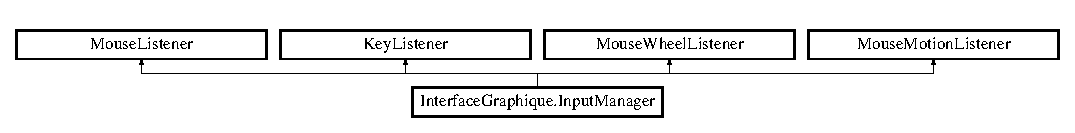
\includegraphics[height=1.333333cm]{class_interface_graphique_1_1_input_manager}
\end{center}
\end{figure}
\subsection*{Public Member Functions}
\begin{DoxyCompactItemize}
\item 
\hyperlink{wglew_8h_aeea6e3dfae3acf232096f57d2d57f084}{void} \hyperlink{class_interface_graphique_1_1_input_manager_a928d0ff1f9094ab94d016084cd61797d}{attach\-To\-Canvas} (Canvas canvas)
\item 
\hyperlink{wglew_8h_aeea6e3dfae3acf232096f57d2d57f084}{void} \hyperlink{class_interface_graphique_1_1_input_manager_a4e67848d1bb4e779cf5777d93fbe7ae7}{clear\-Touches\-Appuyees} ()
\item 
\hyperlink{wglew_8h_aeea6e3dfae3acf232096f57d2d57f084}{void} \hyperlink{class_interface_graphique_1_1_input_manager_a3518690b66a60c40532ec33754aa5ccd}{set\-Main\-Window} (\hyperlink{class_interface_graphique_1_1_demarrage}{Demarrage} fenetre)
\item 
boolean \hyperlink{class_interface_graphique_1_1_input_manager_a8b1712588f51aaa9d217d16e5721a3b5}{is\-Key\-Typed} (\hyperlink{wglew_8h_a500a82aecba06f4550f6849b8099ca21}{int} key)
\item 
boolean \hyperlink{class_interface_graphique_1_1_input_manager_ae6638e8a80f36bb248c040dc071dcf0c}{is\-Key\-Pressed} (\hyperlink{wglew_8h_a500a82aecba06f4550f6849b8099ca21}{int} key)
\item 
boolean \hyperlink{class_interface_graphique_1_1_input_manager_a4fa51a13e70c37c1a6306e05c23e72e5}{is\-Mouse\-Button\-Pressed} (\hyperlink{wglew_8h_a500a82aecba06f4550f6849b8099ca21}{int} button)
\item 
boolean \hyperlink{class_interface_graphique_1_1_input_manager_a5f1dac1fe00de4b1c5f0a49036486bc1}{is\-Mouse\-Button\-Clicked} (\hyperlink{wglew_8h_a500a82aecba06f4550f6849b8099ca21}{int} button)
\item 
Point \hyperlink{class_interface_graphique_1_1_input_manager_a312f35e71847398cb91f4ea70d5804a5}{get\-Mouse\-Position} ()
\item 
\hyperlink{wglew_8h_a500a82aecba06f4550f6849b8099ca21}{int} \hyperlink{class_interface_graphique_1_1_input_manager_ac019beea51384a4a1c4648504b37078d}{get\-Current\-Scrolled\-Mouse\-Wheel} ()
\item 
\hyperlink{wglew_8h_a500a82aecba06f4550f6849b8099ca21}{int} \hyperlink{class_interface_graphique_1_1_input_manager_ac20c8faf622f0a876401fe92cc17a7d6}{get\-Current\-Pressed\-Key} ()
\item 
\hyperlink{wglew_8h_a500a82aecba06f4550f6849b8099ca21}{int} \hyperlink{class_interface_graphique_1_1_input_manager_ac8ba061ba7c04ac09d8deb85ff6b11a6}{get\-Current\-Pressed\-Button} ()
\item 
Hash\-Set$<$ Integer $>$ \hyperlink{class_interface_graphique_1_1_input_manager_a29fcbd1cf15a5461421879f12133f3ba}{get\-Pressed\-Keys} ()
\item 
\hyperlink{wglew_8h_aeea6e3dfae3acf232096f57d2d57f084}{void} \hyperlink{class_interface_graphique_1_1_input_manager_ad846eba9a62c947116f88c802c477ba9}{key\-Typed} (Key\-Event e)
\item 
\hyperlink{wglew_8h_aeea6e3dfae3acf232096f57d2d57f084}{void} \hyperlink{class_interface_graphique_1_1_input_manager_a916ed887434d14d754fe7f24cd793be3}{key\-Pressed} (Key\-Event e)
\item 
\hyperlink{wglew_8h_aeea6e3dfae3acf232096f57d2d57f084}{void} \hyperlink{class_interface_graphique_1_1_input_manager_affb66f19576341f69780056589d9462a}{key\-Released} (Key\-Event e)
\item 
\hyperlink{wglew_8h_aeea6e3dfae3acf232096f57d2d57f084}{void} \hyperlink{class_interface_graphique_1_1_input_manager_aba00c4bf0ab95375dd2259fa21e54f31}{mouse\-Clicked} (Mouse\-Event e)
\item 
\hyperlink{wglew_8h_aeea6e3dfae3acf232096f57d2d57f084}{void} \hyperlink{class_interface_graphique_1_1_input_manager_a45afeb669cfbfda8f0d7058b847cac98}{mouse\-Pressed} (Mouse\-Event e)
\item 
\hyperlink{wglew_8h_aeea6e3dfae3acf232096f57d2d57f084}{void} \hyperlink{class_interface_graphique_1_1_input_manager_a84192982d39a3c9990d763b458f3e3ff}{mouse\-Released} (Mouse\-Event e)
\item 
\hyperlink{wglew_8h_aeea6e3dfae3acf232096f57d2d57f084}{void} \hyperlink{class_interface_graphique_1_1_input_manager_ad9b7501bf8ce0071e6183891cbeceb14}{mouse\-Entered} (Mouse\-Event e)
\item 
\hyperlink{wglew_8h_aeea6e3dfae3acf232096f57d2d57f084}{void} \hyperlink{class_interface_graphique_1_1_input_manager_a3d98dae1b59cddaac86fc4178b21a8a5}{mouse\-Exited} (Mouse\-Event e)
\item 
\hyperlink{wglew_8h_aeea6e3dfae3acf232096f57d2d57f084}{void} \hyperlink{class_interface_graphique_1_1_input_manager_ab277aafa689d996dee87ede6e3d36193}{mouse\-Dragged} (Mouse\-Event arg0)
\item 
\hyperlink{wglew_8h_aeea6e3dfae3acf232096f57d2d57f084}{void} \hyperlink{class_interface_graphique_1_1_input_manager_af9ba61f04581147dd5ca9fefa773d386}{mouse\-Moved} (Mouse\-Event arg0)
\item 
\hyperlink{wglew_8h_aeea6e3dfae3acf232096f57d2d57f084}{void} \hyperlink{class_interface_graphique_1_1_input_manager_a5107c555ab224c5b485ceaaabf060be9}{mouse\-Wheel\-Moved} (Mouse\-Wheel\-Event e)
\item 
\hyperlink{wglew_8h_aeea6e3dfae3acf232096f57d2d57f084}{void} \hyperlink{class_interface_graphique_1_1_input_manager_a2632f531b395d2f496abed8f1dad2331}{appuyer\-\_\-f} ()
\item 
\hyperlink{wglew_8h_aeea6e3dfae3acf232096f57d2d57f084}{void} \hyperlink{class_interface_graphique_1_1_input_manager_a888900a2d2f853639d41349bdd35703c}{appuyer\-\_\-d} ()
\item 
\hyperlink{wglew_8h_aeea6e3dfae3acf232096f57d2d57f084}{void} \hyperlink{class_interface_graphique_1_1_input_manager_abb9f3c756c7698f74f38a2ea1394e1a0}{appuyer\-\_\-s} ()
\item 
\hyperlink{wglew_8h_aeea6e3dfae3acf232096f57d2d57f084}{void} \hyperlink{class_interface_graphique_1_1_input_manager_aeecb09cafb5135bc1d04aa0ba341098e}{appuyer\-\_\-r} ()
\item 
\hyperlink{wglew_8h_aeea6e3dfae3acf232096f57d2d57f084}{void} \hyperlink{class_interface_graphique_1_1_input_manager_a389b251b807c61e9083e2764122978d3}{appuyer\-\_\-e} ()
\item 
\hyperlink{wglew_8h_aeea6e3dfae3acf232096f57d2d57f084}{void} \hyperlink{class_interface_graphique_1_1_input_manager_a9e727ec197424caa1a9c88393541b180}{appuyer\-\_\-c} ()
\item 
\hyperlink{wglew_8h_aeea6e3dfae3acf232096f57d2d57f084}{void} \hyperlink{class_interface_graphique_1_1_input_manager_af385ee71ed3fbbe72f6704d68ab247f4}{appuyer\-\_\-z} ()
\item 
\hyperlink{wglew_8h_aeea6e3dfae3acf232096f57d2d57f084}{void} \hyperlink{class_interface_graphique_1_1_input_manager_aa5f93af909bef218fbef3f9593cc932e}{appuyer\-\_\-m} ()
\item 
\hyperlink{wglew_8h_aeea6e3dfae3acf232096f57d2d57f084}{void} \hyperlink{class_interface_graphique_1_1_input_manager_adc5a8349eddaebbc7e9abc4bb0866cb9}{appuyer\-\_\-p} ()
\item 
\hyperlink{wglew_8h_aeea6e3dfae3acf232096f57d2d57f084}{void} \hyperlink{class_interface_graphique_1_1_input_manager_a129709985b69f9a9a375db02b1d8e949}{appuyer\-\_\-b} ()
\item 
\hyperlink{wglew_8h_aeea6e3dfae3acf232096f57d2d57f084}{void} \hyperlink{class_interface_graphique_1_1_input_manager_adf19ee7e453f492a7ed46889e1dda54f}{appuyer\-\_\-g} ()
\item 
\hyperlink{wglew_8h_aeea6e3dfae3acf232096f57d2d57f084}{void} \hyperlink{class_interface_graphique_1_1_input_manager_aa50f45de0e2162bff0b2aae953ae29dd}{appuyer\-\_\-t} ()
\item 
\hyperlink{wglew_8h_aeea6e3dfae3acf232096f57d2d57f084}{void} \hyperlink{class_interface_graphique_1_1_input_manager_aea476f6a03fe5db1f412fe7993410b5a}{appuyer\-\_\-1} ()
\item 
\hyperlink{wglew_8h_aeea6e3dfae3acf232096f57d2d57f084}{void} \hyperlink{class_interface_graphique_1_1_input_manager_a1f3b1811698ccd1378b9f5afdfcacec6}{appuyer\-\_\-2} ()
\item 
\hyperlink{wglew_8h_aeea6e3dfae3acf232096f57d2d57f084}{void} \hyperlink{class_interface_graphique_1_1_input_manager_ae0f9355524ec2bcba9e73fe16b44672a}{appuyer\-\_\-\-E\-S\-C} ()
\item 
\hyperlink{wglew_8h_aeea6e3dfae3acf232096f57d2d57f084}{void} \hyperlink{class_interface_graphique_1_1_input_manager_adf26b00691f2e3066dfb288ea44f543c}{appuyer\-\_\-backspace} ()
\item 
\hyperlink{wglew_8h_aeea6e3dfae3acf232096f57d2d57f084}{void} \hyperlink{class_interface_graphique_1_1_input_manager_a27fe6229a80d50860840d94da4fc5d92}{Partie\-Rapide} ()
\item 
\hyperlink{wglew_8h_aeea6e3dfae3acf232096f57d2d57f084}{void} \hyperlink{class_interface_graphique_1_1_input_manager_a09709cf851c04cf063a714a92a206d56}{Campagne} ()
\item 
\hyperlink{wglew_8h_aeea6e3dfae3acf232096f57d2d57f084}{void} \hyperlink{class_interface_graphique_1_1_input_manager_aaf306d14c578f76672c4d49b771c994e}{Configuration\-Campagne} ()
\item 
\hyperlink{wglew_8h_aeea6e3dfae3acf232096f57d2d57f084}{void} \hyperlink{class_interface_graphique_1_1_input_manager_ab104f49fa1322971093dc5b809267bac}{Nouveau} ()
\item 
\hyperlink{wglew_8h_aeea6e3dfae3acf232096f57d2d57f084}{void} \hyperlink{class_interface_graphique_1_1_input_manager_ab06b1952910501a34530245ada55d51c}{Ouvrir} ()
\item 
\hyperlink{wglew_8h_aeea6e3dfae3acf232096f57d2d57f084}{void} \hyperlink{class_interface_graphique_1_1_input_manager_ac0b5346e8bc00b6b6900a681987d81d0}{Enregistrer} ()
\item 
\hyperlink{wglew_8h_aeea6e3dfae3acf232096f57d2d57f084}{void} \hyperlink{class_interface_graphique_1_1_input_manager_ad98cb7b9b0c051af34c567c4a96a7d13}{Enregistrer\-Sous} ()
\item 
\hyperlink{wglew_8h_aeea6e3dfae3acf232096f57d2d57f084}{void} \hyperlink{class_interface_graphique_1_1_input_manager_a36d67af53beef02f2679e829fab5fa51}{Proprietes} ()
\item 
\hyperlink{wglew_8h_aeea6e3dfae3acf232096f57d2d57f084}{void} \hyperlink{class_interface_graphique_1_1_input_manager_a9e586b8ae8560f4f2391ce922108a14c}{Mode\-Test} ()
\item 
\hyperlink{wglew_8h_aeea6e3dfae3acf232096f57d2d57f084}{void} \hyperlink{class_interface_graphique_1_1_input_manager_a6bebbff324e7252c39dfd600bbe82f8a}{Menu\-Principal} ()
\item 
\hyperlink{wglew_8h_aeea6e3dfae3acf232096f57d2d57f084}{void} \hyperlink{class_interface_graphique_1_1_input_manager_a8cadb205f49c743af90d2fd179ad53e1}{Configuration} ()
\item 
\hyperlink{wglew_8h_aeea6e3dfae3acf232096f57d2d57f084}{void} \hyperlink{class_interface_graphique_1_1_input_manager_a0a161445feef76124e22d37b72ab3c77}{Sauvegarde\-Configuration} ()
\item 
\hyperlink{wglew_8h_aeea6e3dfae3acf232096f57d2d57f084}{void} \hyperlink{class_interface_graphique_1_1_input_manager_a41a980434b6245b3a3eff3c9160a18fa}{Fenetre\-Edition} ()
\item 
\hyperlink{wglew_8h_aeea6e3dfae3acf232096f57d2d57f084}{void} \hyperlink{class_interface_graphique_1_1_input_manager_a092761dee7b8fdc9e4b0ef463711213c}{Supprimer} ()
\item 
\hyperlink{wglew_8h_aeea6e3dfae3acf232096f57d2d57f084}{void} \hyperlink{class_interface_graphique_1_1_input_manager_a9b1ac4651b6112cbf86cd065cf2a01ac}{Selection} ()
\item 
\hyperlink{wglew_8h_aeea6e3dfae3acf232096f57d2d57f084}{void} \hyperlink{class_interface_graphique_1_1_input_manager_a172d3daf5088008d54a2f10463d69d8d}{Deplacement} ()
\item 
\hyperlink{wglew_8h_aeea6e3dfae3acf232096f57d2d57f084}{void} \hyperlink{class_interface_graphique_1_1_input_manager_af05534635274a76a1e8f60ed4e8e5098}{Rotation} ()
\item 
\hyperlink{wglew_8h_aeea6e3dfae3acf232096f57d2d57f084}{void} \hyperlink{class_interface_graphique_1_1_input_manager_a5c712c708a93b782e5b7f35a50387b7e}{Mise\-A\-Echelle} ()
\item 
\hyperlink{wglew_8h_aeea6e3dfae3acf232096f57d2d57f084}{void} \hyperlink{class_interface_graphique_1_1_input_manager_a8251bcd2385f2cf7419769b006c980da}{Duplication} ()
\item 
\hyperlink{wglew_8h_aeea6e3dfae3acf232096f57d2d57f084}{void} \hyperlink{class_interface_graphique_1_1_input_manager_a1c25e8f65230beebf1ad9d85060c26b6}{Zoom} ()
\item 
\hyperlink{wglew_8h_aeea6e3dfae3acf232096f57d2d57f084}{void} \hyperlink{class_interface_graphique_1_1_input_manager_a81fc16e249ced7ce602900c6518d91d5}{Creation\-Bonus} ()
\item 
\hyperlink{wglew_8h_aeea6e3dfae3acf232096f57d2d57f084}{void} \hyperlink{class_interface_graphique_1_1_input_manager_a0d11e8b27720ada94131531abf91602b}{Creation\-Portails} ()
\item 
\hyperlink{wglew_8h_aeea6e3dfae3acf232096f57d2d57f084}{void} \hyperlink{class_interface_graphique_1_1_input_manager_ab78175fcd4c196550ea83bb2e2d0a266}{Creation\-Barriere} ()
\item 
\hyperlink{wglew_8h_aeea6e3dfae3acf232096f57d2d57f084}{void} \hyperlink{class_interface_graphique_1_1_input_manager_a037da2aa66f52ab35e789c0c26e6d706}{Creation\-Station} ()
\item 
\hyperlink{wglew_8h_aeea6e3dfae3acf232096f57d2d57f084}{void} \hyperlink{class_interface_graphique_1_1_input_manager_afdf14393d23a931b927029f5ffa8bd2d}{Changer\-Vue\-Orbite} ()
\item 
\hyperlink{wglew_8h_aeea6e3dfae3acf232096f57d2d57f084}{void} \hyperlink{class_interface_graphique_1_1_input_manager_a24a63cff4c87a546a753027114635ca7}{Changer\-Vue\-Orthographique} ()
\item 
\hyperlink{wglew_8h_aeea6e3dfae3acf232096f57d2d57f084}{void} \hyperlink{class_interface_graphique_1_1_input_manager_a1d3e27dd47a6eb19f8a8db55e97f820c}{Quitter} ()
\item 
\hyperlink{wglew_8h_aeea6e3dfae3acf232096f57d2d57f084}{void} \hyperlink{class_interface_graphique_1_1_input_manager_a2f51026962423e2ed4407b4cb0133d09}{Aide} ()
\item 
\hyperlink{wglew_8h_aeea6e3dfae3acf232096f57d2d57f084}{void} \hyperlink{class_interface_graphique_1_1_input_manager_a9eeeb47248b31cac5985763b87237475}{set\-Parametre\-Panneau\-Config} ()
\item 
\hyperlink{wglew_8h_aeea6e3dfae3acf232096f57d2d57f084}{void} \hyperlink{class_interface_graphique_1_1_input_manager_ac0806e4a1361db6f86d86cf517bdebb6}{fermer\-Configuration\-Zone\-Jeu} ()
\item 
boolean \hyperlink{class_interface_graphique_1_1_input_manager_aa01122aeb9e56dc1ac9da645cb95159b}{get\-Mode\-Pause} ()
\end{DoxyCompactItemize}
\subsection*{Static Public Member Functions}
\begin{DoxyCompactItemize}
\item 
static \hyperlink{class_interface_graphique_1_1_input_manager}{Input\-Manager} \hyperlink{class_interface_graphique_1_1_input_manager_ae207e898f3b2c41896b9675f95995126}{get\-Instance} ()
\end{DoxyCompactItemize}


\subsection{Member Function Documentation}
\hypertarget{class_interface_graphique_1_1_input_manager_a2f51026962423e2ed4407b4cb0133d09}{\index{Interface\-Graphique\-::\-Input\-Manager@{Interface\-Graphique\-::\-Input\-Manager}!Aide@{Aide}}
\index{Aide@{Aide}!InterfaceGraphique::InputManager@{Interface\-Graphique\-::\-Input\-Manager}}
\subsubsection[{Aide}]{\setlength{\rightskip}{0pt plus 5cm}{\bf void} Interface\-Graphique.\-Input\-Manager.\-Aide (
\begin{DoxyParamCaption}
{}
\end{DoxyParamCaption}
)\hspace{0.3cm}{\ttfamily [inline]}}}\label{class_interface_graphique_1_1_input_manager_a2f51026962423e2ed4407b4cb0133d09}
Fonction appel�e lorsque le bouton Aide de la barre d'outils est actionn�. \hypertarget{class_interface_graphique_1_1_input_manager_aea476f6a03fe5db1f412fe7993410b5a}{\index{Interface\-Graphique\-::\-Input\-Manager@{Interface\-Graphique\-::\-Input\-Manager}!appuyer\-\_\-1@{appuyer\-\_\-1}}
\index{appuyer\-\_\-1@{appuyer\-\_\-1}!InterfaceGraphique::InputManager@{Interface\-Graphique\-::\-Input\-Manager}}
\subsubsection[{appuyer\-\_\-1}]{\setlength{\rightskip}{0pt plus 5cm}{\bf void} Interface\-Graphique.\-Input\-Manager.\-appuyer\-\_\-1 (
\begin{DoxyParamCaption}
{}
\end{DoxyParamCaption}
)\hspace{0.3cm}{\ttfamily [inline]}}}\label{class_interface_graphique_1_1_input_manager_aea476f6a03fe5db1f412fe7993410b5a}
Raccourci vue camera orthographique 
\begin{DoxyParams}{Parameters}
{\em Aucun} & \\
\hline
\end{DoxyParams}
\begin{DoxyReturn}{Returns}
void 
\end{DoxyReturn}
\hypertarget{class_interface_graphique_1_1_input_manager_a1f3b1811698ccd1378b9f5afdfcacec6}{\index{Interface\-Graphique\-::\-Input\-Manager@{Interface\-Graphique\-::\-Input\-Manager}!appuyer\-\_\-2@{appuyer\-\_\-2}}
\index{appuyer\-\_\-2@{appuyer\-\_\-2}!InterfaceGraphique::InputManager@{Interface\-Graphique\-::\-Input\-Manager}}
\subsubsection[{appuyer\-\_\-2}]{\setlength{\rightskip}{0pt plus 5cm}{\bf void} Interface\-Graphique.\-Input\-Manager.\-appuyer\-\_\-2 (
\begin{DoxyParamCaption}
{}
\end{DoxyParamCaption}
)\hspace{0.3cm}{\ttfamily [inline]}}}\label{class_interface_graphique_1_1_input_manager_a1f3b1811698ccd1378b9f5afdfcacec6}
Raccourci vue camera orbite 
\begin{DoxyParams}{Parameters}
{\em Aucun} & \\
\hline
\end{DoxyParams}
\begin{DoxyReturn}{Returns}
void 
\end{DoxyReturn}
\hypertarget{class_interface_graphique_1_1_input_manager_a129709985b69f9a9a375db02b1d8e949}{\index{Interface\-Graphique\-::\-Input\-Manager@{Interface\-Graphique\-::\-Input\-Manager}!appuyer\-\_\-b@{appuyer\-\_\-b}}
\index{appuyer\-\_\-b@{appuyer\-\_\-b}!InterfaceGraphique::InputManager@{Interface\-Graphique\-::\-Input\-Manager}}
\subsubsection[{appuyer\-\_\-b}]{\setlength{\rightskip}{0pt plus 5cm}{\bf void} Interface\-Graphique.\-Input\-Manager.\-appuyer\-\_\-b (
\begin{DoxyParamCaption}
{}
\end{DoxyParamCaption}
)\hspace{0.3cm}{\ttfamily [inline]}}}\label{class_interface_graphique_1_1_input_manager_a129709985b69f9a9a375db02b1d8e949}
Raccourci cr�ation bonus 
\begin{DoxyParams}{Parameters}
{\em Aucun} & \\
\hline
\end{DoxyParams}
\begin{DoxyReturn}{Returns}
void 
\end{DoxyReturn}
\hypertarget{class_interface_graphique_1_1_input_manager_adf26b00691f2e3066dfb288ea44f543c}{\index{Interface\-Graphique\-::\-Input\-Manager@{Interface\-Graphique\-::\-Input\-Manager}!appuyer\-\_\-backspace@{appuyer\-\_\-backspace}}
\index{appuyer\-\_\-backspace@{appuyer\-\_\-backspace}!InterfaceGraphique::InputManager@{Interface\-Graphique\-::\-Input\-Manager}}
\subsubsection[{appuyer\-\_\-backspace}]{\setlength{\rightskip}{0pt plus 5cm}{\bf void} Interface\-Graphique.\-Input\-Manager.\-appuyer\-\_\-backspace (
\begin{DoxyParamCaption}
{}
\end{DoxyParamCaption}
)\hspace{0.3cm}{\ttfamily [inline]}}}\label{class_interface_graphique_1_1_input_manager_adf26b00691f2e3066dfb288ea44f543c}
\hypertarget{class_interface_graphique_1_1_input_manager_a9e727ec197424caa1a9c88393541b180}{\index{Interface\-Graphique\-::\-Input\-Manager@{Interface\-Graphique\-::\-Input\-Manager}!appuyer\-\_\-c@{appuyer\-\_\-c}}
\index{appuyer\-\_\-c@{appuyer\-\_\-c}!InterfaceGraphique::InputManager@{Interface\-Graphique\-::\-Input\-Manager}}
\subsubsection[{appuyer\-\_\-c}]{\setlength{\rightskip}{0pt plus 5cm}{\bf void} Interface\-Graphique.\-Input\-Manager.\-appuyer\-\_\-c (
\begin{DoxyParamCaption}
{}
\end{DoxyParamCaption}
)\hspace{0.3cm}{\ttfamily [inline]}}}\label{class_interface_graphique_1_1_input_manager_a9e727ec197424caa1a9c88393541b180}
Raccourci Duplication 
\begin{DoxyParams}{Parameters}
{\em Aucun} & \\
\hline
\end{DoxyParams}
\begin{DoxyReturn}{Returns}
void 
\end{DoxyReturn}
\hypertarget{class_interface_graphique_1_1_input_manager_a888900a2d2f853639d41349bdd35703c}{\index{Interface\-Graphique\-::\-Input\-Manager@{Interface\-Graphique\-::\-Input\-Manager}!appuyer\-\_\-d@{appuyer\-\_\-d}}
\index{appuyer\-\_\-d@{appuyer\-\_\-d}!InterfaceGraphique::InputManager@{Interface\-Graphique\-::\-Input\-Manager}}
\subsubsection[{appuyer\-\_\-d}]{\setlength{\rightskip}{0pt plus 5cm}{\bf void} Interface\-Graphique.\-Input\-Manager.\-appuyer\-\_\-d (
\begin{DoxyParamCaption}
{}
\end{DoxyParamCaption}
)\hspace{0.3cm}{\ttfamily [inline]}}}\label{class_interface_graphique_1_1_input_manager_a888900a2d2f853639d41349bdd35703c}
Raccourci d�placement 
\begin{DoxyParams}{Parameters}
{\em Aucun} & \\
\hline
\end{DoxyParams}
\begin{DoxyReturn}{Returns}
void 
\end{DoxyReturn}
\hypertarget{class_interface_graphique_1_1_input_manager_a389b251b807c61e9083e2764122978d3}{\index{Interface\-Graphique\-::\-Input\-Manager@{Interface\-Graphique\-::\-Input\-Manager}!appuyer\-\_\-e@{appuyer\-\_\-e}}
\index{appuyer\-\_\-e@{appuyer\-\_\-e}!InterfaceGraphique::InputManager@{Interface\-Graphique\-::\-Input\-Manager}}
\subsubsection[{appuyer\-\_\-e}]{\setlength{\rightskip}{0pt plus 5cm}{\bf void} Interface\-Graphique.\-Input\-Manager.\-appuyer\-\_\-e (
\begin{DoxyParamCaption}
{}
\end{DoxyParamCaption}
)\hspace{0.3cm}{\ttfamily [inline]}}}\label{class_interface_graphique_1_1_input_manager_a389b251b807c61e9083e2764122978d3}
Raccourci Mise a echelle 
\begin{DoxyParams}{Parameters}
{\em Aucun} & \\
\hline
\end{DoxyParams}
\begin{DoxyReturn}{Returns}
void 
\end{DoxyReturn}
\hypertarget{class_interface_graphique_1_1_input_manager_ae0f9355524ec2bcba9e73fe16b44672a}{\index{Interface\-Graphique\-::\-Input\-Manager@{Interface\-Graphique\-::\-Input\-Manager}!appuyer\-\_\-\-E\-S\-C@{appuyer\-\_\-\-E\-S\-C}}
\index{appuyer\-\_\-\-E\-S\-C@{appuyer\-\_\-\-E\-S\-C}!InterfaceGraphique::InputManager@{Interface\-Graphique\-::\-Input\-Manager}}
\subsubsection[{appuyer\-\_\-\-E\-S\-C}]{\setlength{\rightskip}{0pt plus 5cm}{\bf void} Interface\-Graphique.\-Input\-Manager.\-appuyer\-\_\-\-E\-S\-C (
\begin{DoxyParamCaption}
{}
\end{DoxyParamCaption}
)\hspace{0.3cm}{\ttfamily [inline]}}}\label{class_interface_graphique_1_1_input_manager_ae0f9355524ec2bcba9e73fe16b44672a}
Raccourci mode pause 
\begin{DoxyParams}{Parameters}
{\em Aucun} & \\
\hline
\end{DoxyParams}
\begin{DoxyReturn}{Returns}
void 
\end{DoxyReturn}
\hypertarget{class_interface_graphique_1_1_input_manager_a2632f531b395d2f496abed8f1dad2331}{\index{Interface\-Graphique\-::\-Input\-Manager@{Interface\-Graphique\-::\-Input\-Manager}!appuyer\-\_\-f@{appuyer\-\_\-f}}
\index{appuyer\-\_\-f@{appuyer\-\_\-f}!InterfaceGraphique::InputManager@{Interface\-Graphique\-::\-Input\-Manager}}
\subsubsection[{appuyer\-\_\-f}]{\setlength{\rightskip}{0pt plus 5cm}{\bf void} Interface\-Graphique.\-Input\-Manager.\-appuyer\-\_\-f (
\begin{DoxyParamCaption}
{}
\end{DoxyParamCaption}
)\hspace{0.3cm}{\ttfamily [inline]}}}\label{class_interface_graphique_1_1_input_manager_a2632f531b395d2f496abed8f1dad2331}
Fonction appel�e lorsque la touche \char`\"{}f\char`\"{} est appuy�e. Elle affiche le nombre d'affichages par seconde. \hypertarget{class_interface_graphique_1_1_input_manager_adf19ee7e453f492a7ed46889e1dda54f}{\index{Interface\-Graphique\-::\-Input\-Manager@{Interface\-Graphique\-::\-Input\-Manager}!appuyer\-\_\-g@{appuyer\-\_\-g}}
\index{appuyer\-\_\-g@{appuyer\-\_\-g}!InterfaceGraphique::InputManager@{Interface\-Graphique\-::\-Input\-Manager}}
\subsubsection[{appuyer\-\_\-g}]{\setlength{\rightskip}{0pt plus 5cm}{\bf void} Interface\-Graphique.\-Input\-Manager.\-appuyer\-\_\-g (
\begin{DoxyParamCaption}
{}
\end{DoxyParamCaption}
)\hspace{0.3cm}{\ttfamily [inline]}}}\label{class_interface_graphique_1_1_input_manager_adf19ee7e453f492a7ed46889e1dda54f}
Raccourci cr�ation station 
\begin{DoxyParams}{Parameters}
{\em Aucun} & \\
\hline
\end{DoxyParams}
\begin{DoxyReturn}{Returns}
void 
\end{DoxyReturn}
\hypertarget{class_interface_graphique_1_1_input_manager_aa5f93af909bef218fbef3f9593cc932e}{\index{Interface\-Graphique\-::\-Input\-Manager@{Interface\-Graphique\-::\-Input\-Manager}!appuyer\-\_\-m@{appuyer\-\_\-m}}
\index{appuyer\-\_\-m@{appuyer\-\_\-m}!InterfaceGraphique::InputManager@{Interface\-Graphique\-::\-Input\-Manager}}
\subsubsection[{appuyer\-\_\-m}]{\setlength{\rightskip}{0pt plus 5cm}{\bf void} Interface\-Graphique.\-Input\-Manager.\-appuyer\-\_\-m (
\begin{DoxyParamCaption}
{}
\end{DoxyParamCaption}
)\hspace{0.3cm}{\ttfamily [inline]}}}\label{class_interface_graphique_1_1_input_manager_aa5f93af909bef218fbef3f9593cc932e}
Raccourci cr�ation barriere 
\begin{DoxyParams}{Parameters}
{\em Aucun} & \\
\hline
\end{DoxyParams}
\begin{DoxyReturn}{Returns}
void 
\end{DoxyReturn}
\hypertarget{class_interface_graphique_1_1_input_manager_adc5a8349eddaebbc7e9abc4bb0866cb9}{\index{Interface\-Graphique\-::\-Input\-Manager@{Interface\-Graphique\-::\-Input\-Manager}!appuyer\-\_\-p@{appuyer\-\_\-p}}
\index{appuyer\-\_\-p@{appuyer\-\_\-p}!InterfaceGraphique::InputManager@{Interface\-Graphique\-::\-Input\-Manager}}
\subsubsection[{appuyer\-\_\-p}]{\setlength{\rightskip}{0pt plus 5cm}{\bf void} Interface\-Graphique.\-Input\-Manager.\-appuyer\-\_\-p (
\begin{DoxyParamCaption}
{}
\end{DoxyParamCaption}
)\hspace{0.3cm}{\ttfamily [inline]}}}\label{class_interface_graphique_1_1_input_manager_adc5a8349eddaebbc7e9abc4bb0866cb9}
Raccourci cr�ation portail 
\begin{DoxyParams}{Parameters}
{\em Aucun} & \\
\hline
\end{DoxyParams}
\begin{DoxyReturn}{Returns}
void 
\end{DoxyReturn}
\hypertarget{class_interface_graphique_1_1_input_manager_aeecb09cafb5135bc1d04aa0ba341098e}{\index{Interface\-Graphique\-::\-Input\-Manager@{Interface\-Graphique\-::\-Input\-Manager}!appuyer\-\_\-r@{appuyer\-\_\-r}}
\index{appuyer\-\_\-r@{appuyer\-\_\-r}!InterfaceGraphique::InputManager@{Interface\-Graphique\-::\-Input\-Manager}}
\subsubsection[{appuyer\-\_\-r}]{\setlength{\rightskip}{0pt plus 5cm}{\bf void} Interface\-Graphique.\-Input\-Manager.\-appuyer\-\_\-r (
\begin{DoxyParamCaption}
{}
\end{DoxyParamCaption}
)\hspace{0.3cm}{\ttfamily [inline]}}}\label{class_interface_graphique_1_1_input_manager_aeecb09cafb5135bc1d04aa0ba341098e}
Raccourci rotation 
\begin{DoxyParams}{Parameters}
{\em Aucun} & \\
\hline
\end{DoxyParams}
\begin{DoxyReturn}{Returns}
void 
\end{DoxyReturn}
\hypertarget{class_interface_graphique_1_1_input_manager_abb9f3c756c7698f74f38a2ea1394e1a0}{\index{Interface\-Graphique\-::\-Input\-Manager@{Interface\-Graphique\-::\-Input\-Manager}!appuyer\-\_\-s@{appuyer\-\_\-s}}
\index{appuyer\-\_\-s@{appuyer\-\_\-s}!InterfaceGraphique::InputManager@{Interface\-Graphique\-::\-Input\-Manager}}
\subsubsection[{appuyer\-\_\-s}]{\setlength{\rightskip}{0pt plus 5cm}{\bf void} Interface\-Graphique.\-Input\-Manager.\-appuyer\-\_\-s (
\begin{DoxyParamCaption}
{}
\end{DoxyParamCaption}
)\hspace{0.3cm}{\ttfamily [inline]}}}\label{class_interface_graphique_1_1_input_manager_abb9f3c756c7698f74f38a2ea1394e1a0}
Raccourci s�lection 
\begin{DoxyParams}{Parameters}
{\em Aucun} & \\
\hline
\end{DoxyParams}
\begin{DoxyReturn}{Returns}
void 
\end{DoxyReturn}
\hypertarget{class_interface_graphique_1_1_input_manager_aa50f45de0e2162bff0b2aae953ae29dd}{\index{Interface\-Graphique\-::\-Input\-Manager@{Interface\-Graphique\-::\-Input\-Manager}!appuyer\-\_\-t@{appuyer\-\_\-t}}
\index{appuyer\-\_\-t@{appuyer\-\_\-t}!InterfaceGraphique::InputManager@{Interface\-Graphique\-::\-Input\-Manager}}
\subsubsection[{appuyer\-\_\-t}]{\setlength{\rightskip}{0pt plus 5cm}{\bf void} Interface\-Graphique.\-Input\-Manager.\-appuyer\-\_\-t (
\begin{DoxyParamCaption}
{}
\end{DoxyParamCaption}
)\hspace{0.3cm}{\ttfamily [inline]}}}\label{class_interface_graphique_1_1_input_manager_aa50f45de0e2162bff0b2aae953ae29dd}
Raccourci mode test 
\begin{DoxyParams}{Parameters}
{\em Aucun} & \\
\hline
\end{DoxyParams}
\begin{DoxyReturn}{Returns}
void 
\end{DoxyReturn}
\hypertarget{class_interface_graphique_1_1_input_manager_af385ee71ed3fbbe72f6704d68ab247f4}{\index{Interface\-Graphique\-::\-Input\-Manager@{Interface\-Graphique\-::\-Input\-Manager}!appuyer\-\_\-z@{appuyer\-\_\-z}}
\index{appuyer\-\_\-z@{appuyer\-\_\-z}!InterfaceGraphique::InputManager@{Interface\-Graphique\-::\-Input\-Manager}}
\subsubsection[{appuyer\-\_\-z}]{\setlength{\rightskip}{0pt plus 5cm}{\bf void} Interface\-Graphique.\-Input\-Manager.\-appuyer\-\_\-z (
\begin{DoxyParamCaption}
{}
\end{DoxyParamCaption}
)\hspace{0.3cm}{\ttfamily [inline]}}}\label{class_interface_graphique_1_1_input_manager_af385ee71ed3fbbe72f6704d68ab247f4}
Raccourci Zoom 
\begin{DoxyParams}{Parameters}
{\em Aucun} & \\
\hline
\end{DoxyParams}
\begin{DoxyReturn}{Returns}
void 
\end{DoxyReturn}
\hypertarget{class_interface_graphique_1_1_input_manager_a928d0ff1f9094ab94d016084cd61797d}{\index{Interface\-Graphique\-::\-Input\-Manager@{Interface\-Graphique\-::\-Input\-Manager}!attach\-To\-Canvas@{attach\-To\-Canvas}}
\index{attach\-To\-Canvas@{attach\-To\-Canvas}!InterfaceGraphique::InputManager@{Interface\-Graphique\-::\-Input\-Manager}}
\subsubsection[{attach\-To\-Canvas}]{\setlength{\rightskip}{0pt plus 5cm}{\bf void} Interface\-Graphique.\-Input\-Manager.\-attach\-To\-Canvas (
\begin{DoxyParamCaption}
\item[{Canvas}]{canvas}
\end{DoxyParamCaption}
)\hspace{0.3cm}{\ttfamily [inline]}}}\label{class_interface_graphique_1_1_input_manager_a928d0ff1f9094ab94d016084cd61797d}
Permet d'ajouter les listeners au Canvas \hypertarget{class_interface_graphique_1_1_input_manager_a09709cf851c04cf063a714a92a206d56}{\index{Interface\-Graphique\-::\-Input\-Manager@{Interface\-Graphique\-::\-Input\-Manager}!Campagne@{Campagne}}
\index{Campagne@{Campagne}!InterfaceGraphique::InputManager@{Interface\-Graphique\-::\-Input\-Manager}}
\subsubsection[{Campagne}]{\setlength{\rightskip}{0pt plus 5cm}{\bf void} Interface\-Graphique.\-Input\-Manager.\-Campagne (
\begin{DoxyParamCaption}
{}
\end{DoxyParamCaption}
)\hspace{0.3cm}{\ttfamily [inline]}}}\label{class_interface_graphique_1_1_input_manager_a09709cf851c04cf063a714a92a206d56}
Fonction appel�e lorsque l'�l�ment Campagne du menu est actionn�. \hypertarget{class_interface_graphique_1_1_input_manager_afdf14393d23a931b927029f5ffa8bd2d}{\index{Interface\-Graphique\-::\-Input\-Manager@{Interface\-Graphique\-::\-Input\-Manager}!Changer\-Vue\-Orbite@{Changer\-Vue\-Orbite}}
\index{Changer\-Vue\-Orbite@{Changer\-Vue\-Orbite}!InterfaceGraphique::InputManager@{Interface\-Graphique\-::\-Input\-Manager}}
\subsubsection[{Changer\-Vue\-Orbite}]{\setlength{\rightskip}{0pt plus 5cm}{\bf void} Interface\-Graphique.\-Input\-Manager.\-Changer\-Vue\-Orbite (
\begin{DoxyParamCaption}
{}
\end{DoxyParamCaption}
)\hspace{0.3cm}{\ttfamily [inline]}}}\label{class_interface_graphique_1_1_input_manager_afdf14393d23a931b927029f5ffa8bd2d}
Fonction appel�e lorsque l'�l�ment Changer\-Vue\-Orbitale du menu est actionn�. \hypertarget{class_interface_graphique_1_1_input_manager_a24a63cff4c87a546a753027114635ca7}{\index{Interface\-Graphique\-::\-Input\-Manager@{Interface\-Graphique\-::\-Input\-Manager}!Changer\-Vue\-Orthographique@{Changer\-Vue\-Orthographique}}
\index{Changer\-Vue\-Orthographique@{Changer\-Vue\-Orthographique}!InterfaceGraphique::InputManager@{Interface\-Graphique\-::\-Input\-Manager}}
\subsubsection[{Changer\-Vue\-Orthographique}]{\setlength{\rightskip}{0pt plus 5cm}{\bf void} Interface\-Graphique.\-Input\-Manager.\-Changer\-Vue\-Orthographique (
\begin{DoxyParamCaption}
{}
\end{DoxyParamCaption}
)\hspace{0.3cm}{\ttfamily [inline]}}}\label{class_interface_graphique_1_1_input_manager_a24a63cff4c87a546a753027114635ca7}
Fonction appel�e lorsque l'�l�ment Changer\-Vue\-Orthographique du menu est actionn�. \hypertarget{class_interface_graphique_1_1_input_manager_a4e67848d1bb4e779cf5777d93fbe7ae7}{\index{Interface\-Graphique\-::\-Input\-Manager@{Interface\-Graphique\-::\-Input\-Manager}!clear\-Touches\-Appuyees@{clear\-Touches\-Appuyees}}
\index{clear\-Touches\-Appuyees@{clear\-Touches\-Appuyees}!InterfaceGraphique::InputManager@{Interface\-Graphique\-::\-Input\-Manager}}
\subsubsection[{clear\-Touches\-Appuyees}]{\setlength{\rightskip}{0pt plus 5cm}{\bf void} Interface\-Graphique.\-Input\-Manager.\-clear\-Touches\-Appuyees (
\begin{DoxyParamCaption}
{}
\end{DoxyParamCaption}
)\hspace{0.3cm}{\ttfamily [inline]}}}\label{class_interface_graphique_1_1_input_manager_a4e67848d1bb4e779cf5777d93fbe7ae7}
R�initialise les touches appuy�es \hypertarget{class_interface_graphique_1_1_input_manager_a8cadb205f49c743af90d2fd179ad53e1}{\index{Interface\-Graphique\-::\-Input\-Manager@{Interface\-Graphique\-::\-Input\-Manager}!Configuration@{Configuration}}
\index{Configuration@{Configuration}!InterfaceGraphique::InputManager@{Interface\-Graphique\-::\-Input\-Manager}}
\subsubsection[{Configuration}]{\setlength{\rightskip}{0pt plus 5cm}{\bf void} Interface\-Graphique.\-Input\-Manager.\-Configuration (
\begin{DoxyParamCaption}
{}
\end{DoxyParamCaption}
)\hspace{0.3cm}{\ttfamily [inline]}}}\label{class_interface_graphique_1_1_input_manager_a8cadb205f49c743af90d2fd179ad53e1}
Fonction appel�e lorsque l'�l�ment Configuration du menu est actionn�. \hypertarget{class_interface_graphique_1_1_input_manager_aaf306d14c578f76672c4d49b771c994e}{\index{Interface\-Graphique\-::\-Input\-Manager@{Interface\-Graphique\-::\-Input\-Manager}!Configuration\-Campagne@{Configuration\-Campagne}}
\index{Configuration\-Campagne@{Configuration\-Campagne}!InterfaceGraphique::InputManager@{Interface\-Graphique\-::\-Input\-Manager}}
\subsubsection[{Configuration\-Campagne}]{\setlength{\rightskip}{0pt plus 5cm}{\bf void} Interface\-Graphique.\-Input\-Manager.\-Configuration\-Campagne (
\begin{DoxyParamCaption}
{}
\end{DoxyParamCaption}
)\hspace{0.3cm}{\ttfamily [inline]}}}\label{class_interface_graphique_1_1_input_manager_aaf306d14c578f76672c4d49b771c994e}
Fonction appel�e lorsque la configuration de la campagne est termin�e \hypertarget{class_interface_graphique_1_1_input_manager_ab78175fcd4c196550ea83bb2e2d0a266}{\index{Interface\-Graphique\-::\-Input\-Manager@{Interface\-Graphique\-::\-Input\-Manager}!Creation\-Barriere@{Creation\-Barriere}}
\index{Creation\-Barriere@{Creation\-Barriere}!InterfaceGraphique::InputManager@{Interface\-Graphique\-::\-Input\-Manager}}
\subsubsection[{Creation\-Barriere}]{\setlength{\rightskip}{0pt plus 5cm}{\bf void} Interface\-Graphique.\-Input\-Manager.\-Creation\-Barriere (
\begin{DoxyParamCaption}
{}
\end{DoxyParamCaption}
)\hspace{0.3cm}{\ttfamily [inline]}}}\label{class_interface_graphique_1_1_input_manager_ab78175fcd4c196550ea83bb2e2d0a266}
Fonction appel�e lorsque l'�l�ment Creation\-Barriere du menu est actionn�. \hypertarget{class_interface_graphique_1_1_input_manager_a81fc16e249ced7ce602900c6518d91d5}{\index{Interface\-Graphique\-::\-Input\-Manager@{Interface\-Graphique\-::\-Input\-Manager}!Creation\-Bonus@{Creation\-Bonus}}
\index{Creation\-Bonus@{Creation\-Bonus}!InterfaceGraphique::InputManager@{Interface\-Graphique\-::\-Input\-Manager}}
\subsubsection[{Creation\-Bonus}]{\setlength{\rightskip}{0pt plus 5cm}{\bf void} Interface\-Graphique.\-Input\-Manager.\-Creation\-Bonus (
\begin{DoxyParamCaption}
{}
\end{DoxyParamCaption}
)\hspace{0.3cm}{\ttfamily [inline]}}}\label{class_interface_graphique_1_1_input_manager_a81fc16e249ced7ce602900c6518d91d5}
Fonction appel�e lorsque l'�l�ment Creation\-Bonus du menu est actionn�. \hypertarget{class_interface_graphique_1_1_input_manager_a0d11e8b27720ada94131531abf91602b}{\index{Interface\-Graphique\-::\-Input\-Manager@{Interface\-Graphique\-::\-Input\-Manager}!Creation\-Portails@{Creation\-Portails}}
\index{Creation\-Portails@{Creation\-Portails}!InterfaceGraphique::InputManager@{Interface\-Graphique\-::\-Input\-Manager}}
\subsubsection[{Creation\-Portails}]{\setlength{\rightskip}{0pt plus 5cm}{\bf void} Interface\-Graphique.\-Input\-Manager.\-Creation\-Portails (
\begin{DoxyParamCaption}
{}
\end{DoxyParamCaption}
)\hspace{0.3cm}{\ttfamily [inline]}}}\label{class_interface_graphique_1_1_input_manager_a0d11e8b27720ada94131531abf91602b}
Fonction appel�e lorsque l'�l�ment Creation\-Portails du menu est actionn�. \hypertarget{class_interface_graphique_1_1_input_manager_a037da2aa66f52ab35e789c0c26e6d706}{\index{Interface\-Graphique\-::\-Input\-Manager@{Interface\-Graphique\-::\-Input\-Manager}!Creation\-Station@{Creation\-Station}}
\index{Creation\-Station@{Creation\-Station}!InterfaceGraphique::InputManager@{Interface\-Graphique\-::\-Input\-Manager}}
\subsubsection[{Creation\-Station}]{\setlength{\rightskip}{0pt plus 5cm}{\bf void} Interface\-Graphique.\-Input\-Manager.\-Creation\-Station (
\begin{DoxyParamCaption}
{}
\end{DoxyParamCaption}
)\hspace{0.3cm}{\ttfamily [inline]}}}\label{class_interface_graphique_1_1_input_manager_a037da2aa66f52ab35e789c0c26e6d706}
Fonction appel�e lorsque l'�l�ment Creation\-Station du menu est actionn�. \hypertarget{class_interface_graphique_1_1_input_manager_a172d3daf5088008d54a2f10463d69d8d}{\index{Interface\-Graphique\-::\-Input\-Manager@{Interface\-Graphique\-::\-Input\-Manager}!Deplacement@{Deplacement}}
\index{Deplacement@{Deplacement}!InterfaceGraphique::InputManager@{Interface\-Graphique\-::\-Input\-Manager}}
\subsubsection[{Deplacement}]{\setlength{\rightskip}{0pt plus 5cm}{\bf void} Interface\-Graphique.\-Input\-Manager.\-Deplacement (
\begin{DoxyParamCaption}
{}
\end{DoxyParamCaption}
)\hspace{0.3cm}{\ttfamily [inline]}}}\label{class_interface_graphique_1_1_input_manager_a172d3daf5088008d54a2f10463d69d8d}
Fonction appel�e lorsque l'�l�ment Deplacement du menu est actionn�. \hypertarget{class_interface_graphique_1_1_input_manager_a8251bcd2385f2cf7419769b006c980da}{\index{Interface\-Graphique\-::\-Input\-Manager@{Interface\-Graphique\-::\-Input\-Manager}!Duplication@{Duplication}}
\index{Duplication@{Duplication}!InterfaceGraphique::InputManager@{Interface\-Graphique\-::\-Input\-Manager}}
\subsubsection[{Duplication}]{\setlength{\rightskip}{0pt plus 5cm}{\bf void} Interface\-Graphique.\-Input\-Manager.\-Duplication (
\begin{DoxyParamCaption}
{}
\end{DoxyParamCaption}
)\hspace{0.3cm}{\ttfamily [inline]}}}\label{class_interface_graphique_1_1_input_manager_a8251bcd2385f2cf7419769b006c980da}
Fonction appel�e lorsque l'�l�ment Duplication du menu est actionn�. \hypertarget{class_interface_graphique_1_1_input_manager_ac0b5346e8bc00b6b6900a681987d81d0}{\index{Interface\-Graphique\-::\-Input\-Manager@{Interface\-Graphique\-::\-Input\-Manager}!Enregistrer@{Enregistrer}}
\index{Enregistrer@{Enregistrer}!InterfaceGraphique::InputManager@{Interface\-Graphique\-::\-Input\-Manager}}
\subsubsection[{Enregistrer}]{\setlength{\rightskip}{0pt plus 5cm}{\bf void} Interface\-Graphique.\-Input\-Manager.\-Enregistrer (
\begin{DoxyParamCaption}
{}
\end{DoxyParamCaption}
)\hspace{0.3cm}{\ttfamily [inline]}}}\label{class_interface_graphique_1_1_input_manager_ac0b5346e8bc00b6b6900a681987d81d0}
Fonction appel�e lorsque l'�l�ment Enregistrer du menu est actionn�. \hypertarget{class_interface_graphique_1_1_input_manager_ad98cb7b9b0c051af34c567c4a96a7d13}{\index{Interface\-Graphique\-::\-Input\-Manager@{Interface\-Graphique\-::\-Input\-Manager}!Enregistrer\-Sous@{Enregistrer\-Sous}}
\index{Enregistrer\-Sous@{Enregistrer\-Sous}!InterfaceGraphique::InputManager@{Interface\-Graphique\-::\-Input\-Manager}}
\subsubsection[{Enregistrer\-Sous}]{\setlength{\rightskip}{0pt plus 5cm}{\bf void} Interface\-Graphique.\-Input\-Manager.\-Enregistrer\-Sous (
\begin{DoxyParamCaption}
{}
\end{DoxyParamCaption}
)\hspace{0.3cm}{\ttfamily [inline]}}}\label{class_interface_graphique_1_1_input_manager_ad98cb7b9b0c051af34c567c4a96a7d13}
Fonction appel�e lorsque l'�l�ment Enregistrer\-Sous du menu est actionn�. \hypertarget{class_interface_graphique_1_1_input_manager_a41a980434b6245b3a3eff3c9160a18fa}{\index{Interface\-Graphique\-::\-Input\-Manager@{Interface\-Graphique\-::\-Input\-Manager}!Fenetre\-Edition@{Fenetre\-Edition}}
\index{Fenetre\-Edition@{Fenetre\-Edition}!InterfaceGraphique::InputManager@{Interface\-Graphique\-::\-Input\-Manager}}
\subsubsection[{Fenetre\-Edition}]{\setlength{\rightskip}{0pt plus 5cm}{\bf void} Interface\-Graphique.\-Input\-Manager.\-Fenetre\-Edition (
\begin{DoxyParamCaption}
{}
\end{DoxyParamCaption}
)\hspace{0.3cm}{\ttfamily [inline]}}}\label{class_interface_graphique_1_1_input_manager_a41a980434b6245b3a3eff3c9160a18fa}
Fonction appel�e lorsque l'�l�ment Fenetre\-Edition du menu est actionn�. \hypertarget{class_interface_graphique_1_1_input_manager_ac0806e4a1361db6f86d86cf517bdebb6}{\index{Interface\-Graphique\-::\-Input\-Manager@{Interface\-Graphique\-::\-Input\-Manager}!fermer\-Configuration\-Zone\-Jeu@{fermer\-Configuration\-Zone\-Jeu}}
\index{fermer\-Configuration\-Zone\-Jeu@{fermer\-Configuration\-Zone\-Jeu}!InterfaceGraphique::InputManager@{Interface\-Graphique\-::\-Input\-Manager}}
\subsubsection[{fermer\-Configuration\-Zone\-Jeu}]{\setlength{\rightskip}{0pt plus 5cm}{\bf void} Interface\-Graphique.\-Input\-Manager.\-fermer\-Configuration\-Zone\-Jeu (
\begin{DoxyParamCaption}
{}
\end{DoxyParamCaption}
)\hspace{0.3cm}{\ttfamily [inline]}}}\label{class_interface_graphique_1_1_input_manager_ac0806e4a1361db6f86d86cf517bdebb6}
\hypertarget{class_interface_graphique_1_1_input_manager_ac8ba061ba7c04ac09d8deb85ff6b11a6}{\index{Interface\-Graphique\-::\-Input\-Manager@{Interface\-Graphique\-::\-Input\-Manager}!get\-Current\-Pressed\-Button@{get\-Current\-Pressed\-Button}}
\index{get\-Current\-Pressed\-Button@{get\-Current\-Pressed\-Button}!InterfaceGraphique::InputManager@{Interface\-Graphique\-::\-Input\-Manager}}
\subsubsection[{get\-Current\-Pressed\-Button}]{\setlength{\rightskip}{0pt plus 5cm}{\bf int} Interface\-Graphique.\-Input\-Manager.\-get\-Current\-Pressed\-Button (
\begin{DoxyParamCaption}
{}
\end{DoxyParamCaption}
)\hspace{0.3cm}{\ttfamily [inline]}}}\label{class_interface_graphique_1_1_input_manager_ac8ba061ba7c04ac09d8deb85ff6b11a6}
Retourne le boutton de la souris qui est pr�sentemment appuy� \hypertarget{class_interface_graphique_1_1_input_manager_ac20c8faf622f0a876401fe92cc17a7d6}{\index{Interface\-Graphique\-::\-Input\-Manager@{Interface\-Graphique\-::\-Input\-Manager}!get\-Current\-Pressed\-Key@{get\-Current\-Pressed\-Key}}
\index{get\-Current\-Pressed\-Key@{get\-Current\-Pressed\-Key}!InterfaceGraphique::InputManager@{Interface\-Graphique\-::\-Input\-Manager}}
\subsubsection[{get\-Current\-Pressed\-Key}]{\setlength{\rightskip}{0pt plus 5cm}{\bf int} Interface\-Graphique.\-Input\-Manager.\-get\-Current\-Pressed\-Key (
\begin{DoxyParamCaption}
{}
\end{DoxyParamCaption}
)\hspace{0.3cm}{\ttfamily [inline]}}}\label{class_interface_graphique_1_1_input_manager_ac20c8faf622f0a876401fe92cc17a7d6}
Retourne la touche du clavier qui est pr�sentemment appuy� \hypertarget{class_interface_graphique_1_1_input_manager_ac019beea51384a4a1c4648504b37078d}{\index{Interface\-Graphique\-::\-Input\-Manager@{Interface\-Graphique\-::\-Input\-Manager}!get\-Current\-Scrolled\-Mouse\-Wheel@{get\-Current\-Scrolled\-Mouse\-Wheel}}
\index{get\-Current\-Scrolled\-Mouse\-Wheel@{get\-Current\-Scrolled\-Mouse\-Wheel}!InterfaceGraphique::InputManager@{Interface\-Graphique\-::\-Input\-Manager}}
\subsubsection[{get\-Current\-Scrolled\-Mouse\-Wheel}]{\setlength{\rightskip}{0pt plus 5cm}{\bf int} Interface\-Graphique.\-Input\-Manager.\-get\-Current\-Scrolled\-Mouse\-Wheel (
\begin{DoxyParamCaption}
{}
\end{DoxyParamCaption}
)\hspace{0.3cm}{\ttfamily [inline]}}}\label{class_interface_graphique_1_1_input_manager_ac019beea51384a4a1c4648504b37078d}
Retourne le scroll de la souris. Positif (vers le bas), negatif (vers le haut) \hypertarget{class_interface_graphique_1_1_input_manager_ae207e898f3b2c41896b9675f95995126}{\index{Interface\-Graphique\-::\-Input\-Manager@{Interface\-Graphique\-::\-Input\-Manager}!get\-Instance@{get\-Instance}}
\index{get\-Instance@{get\-Instance}!InterfaceGraphique::InputManager@{Interface\-Graphique\-::\-Input\-Manager}}
\subsubsection[{get\-Instance}]{\setlength{\rightskip}{0pt plus 5cm}static {\bf Input\-Manager} Interface\-Graphique.\-Input\-Manager.\-get\-Instance (
\begin{DoxyParamCaption}
{}
\end{DoxyParamCaption}
)\hspace{0.3cm}{\ttfamily [inline]}, {\ttfamily [static]}}}\label{class_interface_graphique_1_1_input_manager_ae207e898f3b2c41896b9675f95995126}
\hypertarget{class_interface_graphique_1_1_input_manager_aa01122aeb9e56dc1ac9da645cb95159b}{\index{Interface\-Graphique\-::\-Input\-Manager@{Interface\-Graphique\-::\-Input\-Manager}!get\-Mode\-Pause@{get\-Mode\-Pause}}
\index{get\-Mode\-Pause@{get\-Mode\-Pause}!InterfaceGraphique::InputManager@{Interface\-Graphique\-::\-Input\-Manager}}
\subsubsection[{get\-Mode\-Pause}]{\setlength{\rightskip}{0pt plus 5cm}boolean Interface\-Graphique.\-Input\-Manager.\-get\-Mode\-Pause (
\begin{DoxyParamCaption}
{}
\end{DoxyParamCaption}
)\hspace{0.3cm}{\ttfamily [inline]}}}\label{class_interface_graphique_1_1_input_manager_aa01122aeb9e56dc1ac9da645cb95159b}
\hypertarget{class_interface_graphique_1_1_input_manager_a312f35e71847398cb91f4ea70d5804a5}{\index{Interface\-Graphique\-::\-Input\-Manager@{Interface\-Graphique\-::\-Input\-Manager}!get\-Mouse\-Position@{get\-Mouse\-Position}}
\index{get\-Mouse\-Position@{get\-Mouse\-Position}!InterfaceGraphique::InputManager@{Interface\-Graphique\-::\-Input\-Manager}}
\subsubsection[{get\-Mouse\-Position}]{\setlength{\rightskip}{0pt plus 5cm}Point Interface\-Graphique.\-Input\-Manager.\-get\-Mouse\-Position (
\begin{DoxyParamCaption}
{}
\end{DoxyParamCaption}
)\hspace{0.3cm}{\ttfamily [inline]}}}\label{class_interface_graphique_1_1_input_manager_a312f35e71847398cb91f4ea70d5804a5}
Retourne la position courante de la souris \hypertarget{class_interface_graphique_1_1_input_manager_a29fcbd1cf15a5461421879f12133f3ba}{\index{Interface\-Graphique\-::\-Input\-Manager@{Interface\-Graphique\-::\-Input\-Manager}!get\-Pressed\-Keys@{get\-Pressed\-Keys}}
\index{get\-Pressed\-Keys@{get\-Pressed\-Keys}!InterfaceGraphique::InputManager@{Interface\-Graphique\-::\-Input\-Manager}}
\subsubsection[{get\-Pressed\-Keys}]{\setlength{\rightskip}{0pt plus 5cm}Hash\-Set$<$Integer$>$ Interface\-Graphique.\-Input\-Manager.\-get\-Pressed\-Keys (
\begin{DoxyParamCaption}
{}
\end{DoxyParamCaption}
)\hspace{0.3cm}{\ttfamily [inline]}}}\label{class_interface_graphique_1_1_input_manager_a29fcbd1cf15a5461421879f12133f3ba}
Retourne toutes les touches qui sont appuy�es \hypertarget{class_interface_graphique_1_1_input_manager_ae6638e8a80f36bb248c040dc071dcf0c}{\index{Interface\-Graphique\-::\-Input\-Manager@{Interface\-Graphique\-::\-Input\-Manager}!is\-Key\-Pressed@{is\-Key\-Pressed}}
\index{is\-Key\-Pressed@{is\-Key\-Pressed}!InterfaceGraphique::InputManager@{Interface\-Graphique\-::\-Input\-Manager}}
\subsubsection[{is\-Key\-Pressed}]{\setlength{\rightskip}{0pt plus 5cm}boolean Interface\-Graphique.\-Input\-Manager.\-is\-Key\-Pressed (
\begin{DoxyParamCaption}
\item[{{\bf int}}]{key}
\end{DoxyParamCaption}
)\hspace{0.3cm}{\ttfamily [inline]}}}\label{class_interface_graphique_1_1_input_manager_ae6638e8a80f36bb248c040dc071dcf0c}
Permet de v�rifier si une touche du clavier a �t� appuy�e 
\begin{DoxyParams}{Parameters}
{\em key} & La touche que l'on veut v�rifier \\
\hline
\end{DoxyParams}
\begin{DoxyReturn}{Returns}
true si elle a �t� appuy�e, false sinon 
\end{DoxyReturn}
\hypertarget{class_interface_graphique_1_1_input_manager_a8b1712588f51aaa9d217d16e5721a3b5}{\index{Interface\-Graphique\-::\-Input\-Manager@{Interface\-Graphique\-::\-Input\-Manager}!is\-Key\-Typed@{is\-Key\-Typed}}
\index{is\-Key\-Typed@{is\-Key\-Typed}!InterfaceGraphique::InputManager@{Interface\-Graphique\-::\-Input\-Manager}}
\subsubsection[{is\-Key\-Typed}]{\setlength{\rightskip}{0pt plus 5cm}boolean Interface\-Graphique.\-Input\-Manager.\-is\-Key\-Typed (
\begin{DoxyParamCaption}
\item[{{\bf int}}]{key}
\end{DoxyParamCaption}
)\hspace{0.3cm}{\ttfamily [inline]}}}\label{class_interface_graphique_1_1_input_manager_a8b1712588f51aaa9d217d16e5721a3b5}
Permet de v�rifier si une touche du clavier a �t� appuy�e puis rel�ch�e 
\begin{DoxyParams}{Parameters}
{\em key} & La touche que l'on veut v�rifier \\
\hline
\end{DoxyParams}
\begin{DoxyReturn}{Returns}
true si elle a �t� appuy�e puis rel�ch�e, false sinon 
\end{DoxyReturn}
\hypertarget{class_interface_graphique_1_1_input_manager_a5f1dac1fe00de4b1c5f0a49036486bc1}{\index{Interface\-Graphique\-::\-Input\-Manager@{Interface\-Graphique\-::\-Input\-Manager}!is\-Mouse\-Button\-Clicked@{is\-Mouse\-Button\-Clicked}}
\index{is\-Mouse\-Button\-Clicked@{is\-Mouse\-Button\-Clicked}!InterfaceGraphique::InputManager@{Interface\-Graphique\-::\-Input\-Manager}}
\subsubsection[{is\-Mouse\-Button\-Clicked}]{\setlength{\rightskip}{0pt plus 5cm}boolean Interface\-Graphique.\-Input\-Manager.\-is\-Mouse\-Button\-Clicked (
\begin{DoxyParamCaption}
\item[{{\bf int}}]{button}
\end{DoxyParamCaption}
)\hspace{0.3cm}{\ttfamily [inline]}}}\label{class_interface_graphique_1_1_input_manager_a5f1dac1fe00de4b1c5f0a49036486bc1}
Permet de v�rifier si un bouton de la souris a �t� appuy�e 
\begin{DoxyParams}{Parameters}
{\em button} & Le bouton que l'on veut v�rifier \\
\hline
\end{DoxyParams}
\begin{DoxyReturn}{Returns}
true si elle a �t� appuy�e, false sinon 
\end{DoxyReturn}
\hypertarget{class_interface_graphique_1_1_input_manager_a4fa51a13e70c37c1a6306e05c23e72e5}{\index{Interface\-Graphique\-::\-Input\-Manager@{Interface\-Graphique\-::\-Input\-Manager}!is\-Mouse\-Button\-Pressed@{is\-Mouse\-Button\-Pressed}}
\index{is\-Mouse\-Button\-Pressed@{is\-Mouse\-Button\-Pressed}!InterfaceGraphique::InputManager@{Interface\-Graphique\-::\-Input\-Manager}}
\subsubsection[{is\-Mouse\-Button\-Pressed}]{\setlength{\rightskip}{0pt plus 5cm}boolean Interface\-Graphique.\-Input\-Manager.\-is\-Mouse\-Button\-Pressed (
\begin{DoxyParamCaption}
\item[{{\bf int}}]{button}
\end{DoxyParamCaption}
)\hspace{0.3cm}{\ttfamily [inline]}}}\label{class_interface_graphique_1_1_input_manager_a4fa51a13e70c37c1a6306e05c23e72e5}
Permet de v�rifier si un bouton de la souris a �t� appuy�e puis rel�ch�e 
\begin{DoxyParams}{Parameters}
{\em button} & Le bouton que l'on veut v�rifier \\
\hline
\end{DoxyParams}
\begin{DoxyReturn}{Returns}
true si elle a �t� appuy�e puis rel�ch�e, false sinon 
\end{DoxyReturn}
\hypertarget{class_interface_graphique_1_1_input_manager_a916ed887434d14d754fe7f24cd793be3}{\index{Interface\-Graphique\-::\-Input\-Manager@{Interface\-Graphique\-::\-Input\-Manager}!key\-Pressed@{key\-Pressed}}
\index{key\-Pressed@{key\-Pressed}!InterfaceGraphique::InputManager@{Interface\-Graphique\-::\-Input\-Manager}}
\subsubsection[{key\-Pressed}]{\setlength{\rightskip}{0pt plus 5cm}{\bf void} Interface\-Graphique.\-Input\-Manager.\-key\-Pressed (
\begin{DoxyParamCaption}
\item[{Key\-Event}]{e}
\end{DoxyParamCaption}
)\hspace{0.3cm}{\ttfamily [inline]}}}\label{class_interface_graphique_1_1_input_manager_a916ed887434d14d754fe7f24cd793be3}
\hypertarget{class_interface_graphique_1_1_input_manager_affb66f19576341f69780056589d9462a}{\index{Interface\-Graphique\-::\-Input\-Manager@{Interface\-Graphique\-::\-Input\-Manager}!key\-Released@{key\-Released}}
\index{key\-Released@{key\-Released}!InterfaceGraphique::InputManager@{Interface\-Graphique\-::\-Input\-Manager}}
\subsubsection[{key\-Released}]{\setlength{\rightskip}{0pt plus 5cm}{\bf void} Interface\-Graphique.\-Input\-Manager.\-key\-Released (
\begin{DoxyParamCaption}
\item[{Key\-Event}]{e}
\end{DoxyParamCaption}
)\hspace{0.3cm}{\ttfamily [inline]}}}\label{class_interface_graphique_1_1_input_manager_affb66f19576341f69780056589d9462a}
\hypertarget{class_interface_graphique_1_1_input_manager_ad846eba9a62c947116f88c802c477ba9}{\index{Interface\-Graphique\-::\-Input\-Manager@{Interface\-Graphique\-::\-Input\-Manager}!key\-Typed@{key\-Typed}}
\index{key\-Typed@{key\-Typed}!InterfaceGraphique::InputManager@{Interface\-Graphique\-::\-Input\-Manager}}
\subsubsection[{key\-Typed}]{\setlength{\rightskip}{0pt plus 5cm}{\bf void} Interface\-Graphique.\-Input\-Manager.\-key\-Typed (
\begin{DoxyParamCaption}
\item[{Key\-Event}]{e}
\end{DoxyParamCaption}
)\hspace{0.3cm}{\ttfamily [inline]}}}\label{class_interface_graphique_1_1_input_manager_ad846eba9a62c947116f88c802c477ba9}
\hypertarget{class_interface_graphique_1_1_input_manager_a6bebbff324e7252c39dfd600bbe82f8a}{\index{Interface\-Graphique\-::\-Input\-Manager@{Interface\-Graphique\-::\-Input\-Manager}!Menu\-Principal@{Menu\-Principal}}
\index{Menu\-Principal@{Menu\-Principal}!InterfaceGraphique::InputManager@{Interface\-Graphique\-::\-Input\-Manager}}
\subsubsection[{Menu\-Principal}]{\setlength{\rightskip}{0pt plus 5cm}{\bf void} Interface\-Graphique.\-Input\-Manager.\-Menu\-Principal (
\begin{DoxyParamCaption}
{}
\end{DoxyParamCaption}
)\hspace{0.3cm}{\ttfamily [inline]}}}\label{class_interface_graphique_1_1_input_manager_a6bebbff324e7252c39dfd600bbe82f8a}
Fonction appel�e lorsque l'�l�ment \hyperlink{class_interface_graphique_1_1_menu_principal}{Menu\-Principal} du menu est actionn�. \hypertarget{class_interface_graphique_1_1_input_manager_a5c712c708a93b782e5b7f35a50387b7e}{\index{Interface\-Graphique\-::\-Input\-Manager@{Interface\-Graphique\-::\-Input\-Manager}!Mise\-A\-Echelle@{Mise\-A\-Echelle}}
\index{Mise\-A\-Echelle@{Mise\-A\-Echelle}!InterfaceGraphique::InputManager@{Interface\-Graphique\-::\-Input\-Manager}}
\subsubsection[{Mise\-A\-Echelle}]{\setlength{\rightskip}{0pt plus 5cm}{\bf void} Interface\-Graphique.\-Input\-Manager.\-Mise\-A\-Echelle (
\begin{DoxyParamCaption}
{}
\end{DoxyParamCaption}
)\hspace{0.3cm}{\ttfamily [inline]}}}\label{class_interface_graphique_1_1_input_manager_a5c712c708a93b782e5b7f35a50387b7e}
Fonction appel�e lorsque l'�l�ment Mise\-A\-Echelle du menu est actionn�. \hypertarget{class_interface_graphique_1_1_input_manager_a9e586b8ae8560f4f2391ce922108a14c}{\index{Interface\-Graphique\-::\-Input\-Manager@{Interface\-Graphique\-::\-Input\-Manager}!Mode\-Test@{Mode\-Test}}
\index{Mode\-Test@{Mode\-Test}!InterfaceGraphique::InputManager@{Interface\-Graphique\-::\-Input\-Manager}}
\subsubsection[{Mode\-Test}]{\setlength{\rightskip}{0pt plus 5cm}{\bf void} Interface\-Graphique.\-Input\-Manager.\-Mode\-Test (
\begin{DoxyParamCaption}
{}
\end{DoxyParamCaption}
)\hspace{0.3cm}{\ttfamily [inline]}}}\label{class_interface_graphique_1_1_input_manager_a9e586b8ae8560f4f2391ce922108a14c}
Fonction appel�e lorsque l'�l�ment \hyperlink{class_mode_test}{Mode\-Test} du menu est actionn�. \hypertarget{class_interface_graphique_1_1_input_manager_aba00c4bf0ab95375dd2259fa21e54f31}{\index{Interface\-Graphique\-::\-Input\-Manager@{Interface\-Graphique\-::\-Input\-Manager}!mouse\-Clicked@{mouse\-Clicked}}
\index{mouse\-Clicked@{mouse\-Clicked}!InterfaceGraphique::InputManager@{Interface\-Graphique\-::\-Input\-Manager}}
\subsubsection[{mouse\-Clicked}]{\setlength{\rightskip}{0pt plus 5cm}{\bf void} Interface\-Graphique.\-Input\-Manager.\-mouse\-Clicked (
\begin{DoxyParamCaption}
\item[{Mouse\-Event}]{e}
\end{DoxyParamCaption}
)\hspace{0.3cm}{\ttfamily [inline]}}}\label{class_interface_graphique_1_1_input_manager_aba00c4bf0ab95375dd2259fa21e54f31}
\hypertarget{class_interface_graphique_1_1_input_manager_ab277aafa689d996dee87ede6e3d36193}{\index{Interface\-Graphique\-::\-Input\-Manager@{Interface\-Graphique\-::\-Input\-Manager}!mouse\-Dragged@{mouse\-Dragged}}
\index{mouse\-Dragged@{mouse\-Dragged}!InterfaceGraphique::InputManager@{Interface\-Graphique\-::\-Input\-Manager}}
\subsubsection[{mouse\-Dragged}]{\setlength{\rightskip}{0pt plus 5cm}{\bf void} Interface\-Graphique.\-Input\-Manager.\-mouse\-Dragged (
\begin{DoxyParamCaption}
\item[{Mouse\-Event}]{arg0}
\end{DoxyParamCaption}
)\hspace{0.3cm}{\ttfamily [inline]}}}\label{class_interface_graphique_1_1_input_manager_ab277aafa689d996dee87ede6e3d36193}
\hypertarget{class_interface_graphique_1_1_input_manager_ad9b7501bf8ce0071e6183891cbeceb14}{\index{Interface\-Graphique\-::\-Input\-Manager@{Interface\-Graphique\-::\-Input\-Manager}!mouse\-Entered@{mouse\-Entered}}
\index{mouse\-Entered@{mouse\-Entered}!InterfaceGraphique::InputManager@{Interface\-Graphique\-::\-Input\-Manager}}
\subsubsection[{mouse\-Entered}]{\setlength{\rightskip}{0pt plus 5cm}{\bf void} Interface\-Graphique.\-Input\-Manager.\-mouse\-Entered (
\begin{DoxyParamCaption}
\item[{Mouse\-Event}]{e}
\end{DoxyParamCaption}
)\hspace{0.3cm}{\ttfamily [inline]}}}\label{class_interface_graphique_1_1_input_manager_ad9b7501bf8ce0071e6183891cbeceb14}
\hypertarget{class_interface_graphique_1_1_input_manager_a3d98dae1b59cddaac86fc4178b21a8a5}{\index{Interface\-Graphique\-::\-Input\-Manager@{Interface\-Graphique\-::\-Input\-Manager}!mouse\-Exited@{mouse\-Exited}}
\index{mouse\-Exited@{mouse\-Exited}!InterfaceGraphique::InputManager@{Interface\-Graphique\-::\-Input\-Manager}}
\subsubsection[{mouse\-Exited}]{\setlength{\rightskip}{0pt plus 5cm}{\bf void} Interface\-Graphique.\-Input\-Manager.\-mouse\-Exited (
\begin{DoxyParamCaption}
\item[{Mouse\-Event}]{e}
\end{DoxyParamCaption}
)\hspace{0.3cm}{\ttfamily [inline]}}}\label{class_interface_graphique_1_1_input_manager_a3d98dae1b59cddaac86fc4178b21a8a5}
\hypertarget{class_interface_graphique_1_1_input_manager_af9ba61f04581147dd5ca9fefa773d386}{\index{Interface\-Graphique\-::\-Input\-Manager@{Interface\-Graphique\-::\-Input\-Manager}!mouse\-Moved@{mouse\-Moved}}
\index{mouse\-Moved@{mouse\-Moved}!InterfaceGraphique::InputManager@{Interface\-Graphique\-::\-Input\-Manager}}
\subsubsection[{mouse\-Moved}]{\setlength{\rightskip}{0pt plus 5cm}{\bf void} Interface\-Graphique.\-Input\-Manager.\-mouse\-Moved (
\begin{DoxyParamCaption}
\item[{Mouse\-Event}]{arg0}
\end{DoxyParamCaption}
)\hspace{0.3cm}{\ttfamily [inline]}}}\label{class_interface_graphique_1_1_input_manager_af9ba61f04581147dd5ca9fefa773d386}
\hypertarget{class_interface_graphique_1_1_input_manager_a45afeb669cfbfda8f0d7058b847cac98}{\index{Interface\-Graphique\-::\-Input\-Manager@{Interface\-Graphique\-::\-Input\-Manager}!mouse\-Pressed@{mouse\-Pressed}}
\index{mouse\-Pressed@{mouse\-Pressed}!InterfaceGraphique::InputManager@{Interface\-Graphique\-::\-Input\-Manager}}
\subsubsection[{mouse\-Pressed}]{\setlength{\rightskip}{0pt plus 5cm}{\bf void} Interface\-Graphique.\-Input\-Manager.\-mouse\-Pressed (
\begin{DoxyParamCaption}
\item[{Mouse\-Event}]{e}
\end{DoxyParamCaption}
)\hspace{0.3cm}{\ttfamily [inline]}}}\label{class_interface_graphique_1_1_input_manager_a45afeb669cfbfda8f0d7058b847cac98}
\hypertarget{class_interface_graphique_1_1_input_manager_a84192982d39a3c9990d763b458f3e3ff}{\index{Interface\-Graphique\-::\-Input\-Manager@{Interface\-Graphique\-::\-Input\-Manager}!mouse\-Released@{mouse\-Released}}
\index{mouse\-Released@{mouse\-Released}!InterfaceGraphique::InputManager@{Interface\-Graphique\-::\-Input\-Manager}}
\subsubsection[{mouse\-Released}]{\setlength{\rightskip}{0pt plus 5cm}{\bf void} Interface\-Graphique.\-Input\-Manager.\-mouse\-Released (
\begin{DoxyParamCaption}
\item[{Mouse\-Event}]{e}
\end{DoxyParamCaption}
)\hspace{0.3cm}{\ttfamily [inline]}}}\label{class_interface_graphique_1_1_input_manager_a84192982d39a3c9990d763b458f3e3ff}
\hypertarget{class_interface_graphique_1_1_input_manager_a5107c555ab224c5b485ceaaabf060be9}{\index{Interface\-Graphique\-::\-Input\-Manager@{Interface\-Graphique\-::\-Input\-Manager}!mouse\-Wheel\-Moved@{mouse\-Wheel\-Moved}}
\index{mouse\-Wheel\-Moved@{mouse\-Wheel\-Moved}!InterfaceGraphique::InputManager@{Interface\-Graphique\-::\-Input\-Manager}}
\subsubsection[{mouse\-Wheel\-Moved}]{\setlength{\rightskip}{0pt plus 5cm}{\bf void} Interface\-Graphique.\-Input\-Manager.\-mouse\-Wheel\-Moved (
\begin{DoxyParamCaption}
\item[{Mouse\-Wheel\-Event}]{e}
\end{DoxyParamCaption}
)\hspace{0.3cm}{\ttfamily [inline]}}}\label{class_interface_graphique_1_1_input_manager_a5107c555ab224c5b485ceaaabf060be9}
Permet de v�rifier si un scroll up ou un scroll down a ete effectue Un scroll vers le bas est un int positif, et un scroll vers le haut est un int negatif. \hypertarget{class_interface_graphique_1_1_input_manager_ab104f49fa1322971093dc5b809267bac}{\index{Interface\-Graphique\-::\-Input\-Manager@{Interface\-Graphique\-::\-Input\-Manager}!Nouveau@{Nouveau}}
\index{Nouveau@{Nouveau}!InterfaceGraphique::InputManager@{Interface\-Graphique\-::\-Input\-Manager}}
\subsubsection[{Nouveau}]{\setlength{\rightskip}{0pt plus 5cm}{\bf void} Interface\-Graphique.\-Input\-Manager.\-Nouveau (
\begin{DoxyParamCaption}
{}
\end{DoxyParamCaption}
)\hspace{0.3cm}{\ttfamily [inline]}}}\label{class_interface_graphique_1_1_input_manager_ab104f49fa1322971093dc5b809267bac}
Fonction appel�e lorsque l'�l�ment Nouveau du menu est actionn�. \hypertarget{class_interface_graphique_1_1_input_manager_ab06b1952910501a34530245ada55d51c}{\index{Interface\-Graphique\-::\-Input\-Manager@{Interface\-Graphique\-::\-Input\-Manager}!Ouvrir@{Ouvrir}}
\index{Ouvrir@{Ouvrir}!InterfaceGraphique::InputManager@{Interface\-Graphique\-::\-Input\-Manager}}
\subsubsection[{Ouvrir}]{\setlength{\rightskip}{0pt plus 5cm}{\bf void} Interface\-Graphique.\-Input\-Manager.\-Ouvrir (
\begin{DoxyParamCaption}
{}
\end{DoxyParamCaption}
)\hspace{0.3cm}{\ttfamily [inline]}}}\label{class_interface_graphique_1_1_input_manager_ab06b1952910501a34530245ada55d51c}
Fonction appel�e lorsque l'�l�ment Ouvrir du menu est actionn�. \hypertarget{class_interface_graphique_1_1_input_manager_a27fe6229a80d50860840d94da4fc5d92}{\index{Interface\-Graphique\-::\-Input\-Manager@{Interface\-Graphique\-::\-Input\-Manager}!Partie\-Rapide@{Partie\-Rapide}}
\index{Partie\-Rapide@{Partie\-Rapide}!InterfaceGraphique::InputManager@{Interface\-Graphique\-::\-Input\-Manager}}
\subsubsection[{Partie\-Rapide}]{\setlength{\rightskip}{0pt plus 5cm}{\bf void} Interface\-Graphique.\-Input\-Manager.\-Partie\-Rapide (
\begin{DoxyParamCaption}
{}
\end{DoxyParamCaption}
)\hspace{0.3cm}{\ttfamily [inline]}}}\label{class_interface_graphique_1_1_input_manager_a27fe6229a80d50860840d94da4fc5d92}
Fonction appel�e lorsque l'�l�ment Partie\-Rapide du menu est actionn�. \hypertarget{class_interface_graphique_1_1_input_manager_a36d67af53beef02f2679e829fab5fa51}{\index{Interface\-Graphique\-::\-Input\-Manager@{Interface\-Graphique\-::\-Input\-Manager}!Proprietes@{Proprietes}}
\index{Proprietes@{Proprietes}!InterfaceGraphique::InputManager@{Interface\-Graphique\-::\-Input\-Manager}}
\subsubsection[{Proprietes}]{\setlength{\rightskip}{0pt plus 5cm}{\bf void} Interface\-Graphique.\-Input\-Manager.\-Proprietes (
\begin{DoxyParamCaption}
{}
\end{DoxyParamCaption}
)\hspace{0.3cm}{\ttfamily [inline]}}}\label{class_interface_graphique_1_1_input_manager_a36d67af53beef02f2679e829fab5fa51}
Fonction appel�e lorsque l'�l�ment Proprietes du menu est actionn�. \hypertarget{class_interface_graphique_1_1_input_manager_a1d3e27dd47a6eb19f8a8db55e97f820c}{\index{Interface\-Graphique\-::\-Input\-Manager@{Interface\-Graphique\-::\-Input\-Manager}!Quitter@{Quitter}}
\index{Quitter@{Quitter}!InterfaceGraphique::InputManager@{Interface\-Graphique\-::\-Input\-Manager}}
\subsubsection[{Quitter}]{\setlength{\rightskip}{0pt plus 5cm}{\bf void} Interface\-Graphique.\-Input\-Manager.\-Quitter (
\begin{DoxyParamCaption}
{}
\end{DoxyParamCaption}
)\hspace{0.3cm}{\ttfamily [inline]}}}\label{class_interface_graphique_1_1_input_manager_a1d3e27dd47a6eb19f8a8db55e97f820c}
Fonction appel�e lorsque l'�l�ment Quitter du menu est actionn�. \hypertarget{class_interface_graphique_1_1_input_manager_af05534635274a76a1e8f60ed4e8e5098}{\index{Interface\-Graphique\-::\-Input\-Manager@{Interface\-Graphique\-::\-Input\-Manager}!Rotation@{Rotation}}
\index{Rotation@{Rotation}!InterfaceGraphique::InputManager@{Interface\-Graphique\-::\-Input\-Manager}}
\subsubsection[{Rotation}]{\setlength{\rightskip}{0pt plus 5cm}{\bf void} Interface\-Graphique.\-Input\-Manager.\-Rotation (
\begin{DoxyParamCaption}
{}
\end{DoxyParamCaption}
)\hspace{0.3cm}{\ttfamily [inline]}}}\label{class_interface_graphique_1_1_input_manager_af05534635274a76a1e8f60ed4e8e5098}
Fonction appel�e lorsque l'�l�ment Rotation du menu est actionn�. \hypertarget{class_interface_graphique_1_1_input_manager_a0a161445feef76124e22d37b72ab3c77}{\index{Interface\-Graphique\-::\-Input\-Manager@{Interface\-Graphique\-::\-Input\-Manager}!Sauvegarde\-Configuration@{Sauvegarde\-Configuration}}
\index{Sauvegarde\-Configuration@{Sauvegarde\-Configuration}!InterfaceGraphique::InputManager@{Interface\-Graphique\-::\-Input\-Manager}}
\subsubsection[{Sauvegarde\-Configuration}]{\setlength{\rightskip}{0pt plus 5cm}{\bf void} Interface\-Graphique.\-Input\-Manager.\-Sauvegarde\-Configuration (
\begin{DoxyParamCaption}
{}
\end{DoxyParamCaption}
)\hspace{0.3cm}{\ttfamily [inline]}}}\label{class_interface_graphique_1_1_input_manager_a0a161445feef76124e22d37b72ab3c77}
Fonction appel�e lorsque le bouton Sauvergarder du panneau de configuration est actionn�. \hypertarget{class_interface_graphique_1_1_input_manager_a9b1ac4651b6112cbf86cd065cf2a01ac}{\index{Interface\-Graphique\-::\-Input\-Manager@{Interface\-Graphique\-::\-Input\-Manager}!Selection@{Selection}}
\index{Selection@{Selection}!InterfaceGraphique::InputManager@{Interface\-Graphique\-::\-Input\-Manager}}
\subsubsection[{Selection}]{\setlength{\rightskip}{0pt plus 5cm}{\bf void} Interface\-Graphique.\-Input\-Manager.\-Selection (
\begin{DoxyParamCaption}
{}
\end{DoxyParamCaption}
)\hspace{0.3cm}{\ttfamily [inline]}}}\label{class_interface_graphique_1_1_input_manager_a9b1ac4651b6112cbf86cd065cf2a01ac}
Fonction appel�e lorsque l'�l�ment Selection du menu est actionn�. \hypertarget{class_interface_graphique_1_1_input_manager_a3518690b66a60c40532ec33754aa5ccd}{\index{Interface\-Graphique\-::\-Input\-Manager@{Interface\-Graphique\-::\-Input\-Manager}!set\-Main\-Window@{set\-Main\-Window}}
\index{set\-Main\-Window@{set\-Main\-Window}!InterfaceGraphique::InputManager@{Interface\-Graphique\-::\-Input\-Manager}}
\subsubsection[{set\-Main\-Window}]{\setlength{\rightskip}{0pt plus 5cm}{\bf void} Interface\-Graphique.\-Input\-Manager.\-set\-Main\-Window (
\begin{DoxyParamCaption}
\item[{{\bf Demarrage}}]{fenetre}
\end{DoxyParamCaption}
)\hspace{0.3cm}{\ttfamily [inline]}}}\label{class_interface_graphique_1_1_input_manager_a3518690b66a60c40532ec33754aa5ccd}
Permet de lier la fenetre de d�marrage au \hyperlink{class_interface_graphique_1_1_input_manager}{Input\-Manager}, permettant ainsi de manipuler les fenetres. 
\begin{DoxyParams}{Parameters}
{\em fenetre} & \\
\hline
\end{DoxyParams}
\hypertarget{class_interface_graphique_1_1_input_manager_a9eeeb47248b31cac5985763b87237475}{\index{Interface\-Graphique\-::\-Input\-Manager@{Interface\-Graphique\-::\-Input\-Manager}!set\-Parametre\-Panneau\-Config@{set\-Parametre\-Panneau\-Config}}
\index{set\-Parametre\-Panneau\-Config@{set\-Parametre\-Panneau\-Config}!InterfaceGraphique::InputManager@{Interface\-Graphique\-::\-Input\-Manager}}
\subsubsection[{set\-Parametre\-Panneau\-Config}]{\setlength{\rightskip}{0pt plus 5cm}{\bf void} Interface\-Graphique.\-Input\-Manager.\-set\-Parametre\-Panneau\-Config (
\begin{DoxyParamCaption}
{}
\end{DoxyParamCaption}
)\hspace{0.3cm}{\ttfamily [inline]}}}\label{class_interface_graphique_1_1_input_manager_a9eeeb47248b31cac5985763b87237475}
\hypertarget{class_interface_graphique_1_1_input_manager_a092761dee7b8fdc9e4b0ef463711213c}{\index{Interface\-Graphique\-::\-Input\-Manager@{Interface\-Graphique\-::\-Input\-Manager}!Supprimer@{Supprimer}}
\index{Supprimer@{Supprimer}!InterfaceGraphique::InputManager@{Interface\-Graphique\-::\-Input\-Manager}}
\subsubsection[{Supprimer}]{\setlength{\rightskip}{0pt plus 5cm}{\bf void} Interface\-Graphique.\-Input\-Manager.\-Supprimer (
\begin{DoxyParamCaption}
{}
\end{DoxyParamCaption}
)\hspace{0.3cm}{\ttfamily [inline]}}}\label{class_interface_graphique_1_1_input_manager_a092761dee7b8fdc9e4b0ef463711213c}
Fonction appel�e lorsque l'�l�ment Supprimer du menu est actionn�. \hypertarget{class_interface_graphique_1_1_input_manager_a1c25e8f65230beebf1ad9d85060c26b6}{\index{Interface\-Graphique\-::\-Input\-Manager@{Interface\-Graphique\-::\-Input\-Manager}!Zoom@{Zoom}}
\index{Zoom@{Zoom}!InterfaceGraphique::InputManager@{Interface\-Graphique\-::\-Input\-Manager}}
\subsubsection[{Zoom}]{\setlength{\rightskip}{0pt plus 5cm}{\bf void} Interface\-Graphique.\-Input\-Manager.\-Zoom (
\begin{DoxyParamCaption}
{}
\end{DoxyParamCaption}
)\hspace{0.3cm}{\ttfamily [inline]}}}\label{class_interface_graphique_1_1_input_manager_a1c25e8f65230beebf1ad9d85060c26b6}
Fonction appel�e lorsque l'�l�ment Zoom du menu est actionn�. 

The documentation for this class was generated from the following file\-:\begin{DoxyCompactItemize}
\item 
Cadriciel/\-Sources/\-Java/\-Interface\-Graphique/src/\-Interface\-Graphique/\hyperlink{_input_manager_8java}{Input\-Manager.\-java}\end{DoxyCompactItemize}

\hypertarget{class_interface_graphique_1_1_instructions}{\section{Interface\-Graphique.\-Instructions Class Reference}
\label{class_interface_graphique_1_1_instructions}\index{Interface\-Graphique.\-Instructions@{Interface\-Graphique.\-Instructions}}
}
Inheritance diagram for Interface\-Graphique.\-Instructions\-:\begin{figure}[H]
\begin{center}
\leavevmode
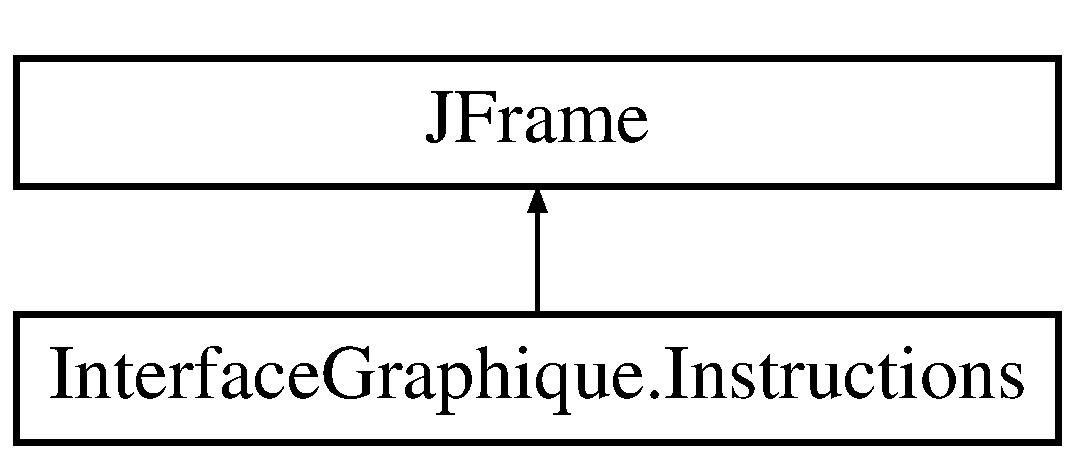
\includegraphics[height=2.000000cm]{class_interface_graphique_1_1_instructions}
\end{center}
\end{figure}
\subsection*{Public Member Functions}
\begin{DoxyCompactItemize}
\item 
\hyperlink{class_interface_graphique_1_1_instructions_a53573b2080eebf2b1cbb10d197d962a9}{Instructions} ()
\item 
\hyperlink{wglew_8h_aeea6e3dfae3acf232096f57d2d57f084}{void} \hyperlink{class_interface_graphique_1_1_instructions_aab3e4add413ae0c999bb7dd51097aaf0}{set\-Tab} (\hyperlink{wglew_8h_a500a82aecba06f4550f6849b8099ca21}{int} \hyperlink{glew_8h_a85149b1510a8c7b78a603f657799ec2d}{num})
\end{DoxyCompactItemize}


\subsection{Constructor \& Destructor Documentation}
\hypertarget{class_interface_graphique_1_1_instructions_a53573b2080eebf2b1cbb10d197d962a9}{\index{Interface\-Graphique\-::\-Instructions@{Interface\-Graphique\-::\-Instructions}!Instructions@{Instructions}}
\index{Instructions@{Instructions}!InterfaceGraphique::Instructions@{Interface\-Graphique\-::\-Instructions}}
\subsubsection[{Instructions}]{\setlength{\rightskip}{0pt plus 5cm}Interface\-Graphique.\-Instructions.\-Instructions (
\begin{DoxyParamCaption}
{}
\end{DoxyParamCaption}
)\hspace{0.3cm}{\ttfamily [inline]}}}\label{class_interface_graphique_1_1_instructions_a53573b2080eebf2b1cbb10d197d962a9}
Creation de la fenetre d'instructions 

\subsection{Member Function Documentation}
\hypertarget{class_interface_graphique_1_1_instructions_aab3e4add413ae0c999bb7dd51097aaf0}{\index{Interface\-Graphique\-::\-Instructions@{Interface\-Graphique\-::\-Instructions}!set\-Tab@{set\-Tab}}
\index{set\-Tab@{set\-Tab}!InterfaceGraphique::Instructions@{Interface\-Graphique\-::\-Instructions}}
\subsubsection[{set\-Tab}]{\setlength{\rightskip}{0pt plus 5cm}{\bf void} Interface\-Graphique.\-Instructions.\-set\-Tab (
\begin{DoxyParamCaption}
\item[{{\bf int}}]{num}
\end{DoxyParamCaption}
)\hspace{0.3cm}{\ttfamily [inline]}}}\label{class_interface_graphique_1_1_instructions_aab3e4add413ae0c999bb7dd51097aaf0}
Permet de modifier l'onglet de l'aide sur lequel on est 
\begin{DoxyParams}{Parameters}
{\em num} & -\/ int \-: numero de l'onglet \\
\hline
\end{DoxyParams}


The documentation for this class was generated from the following file\-:\begin{DoxyCompactItemize}
\item 
Cadriciel/\-Sources/\-Java/\-Interface\-Graphique/src/\-Interface\-Graphique/\hyperlink{_instructions_8java}{Instructions.\-java}\end{DoxyCompactItemize}

\hypertarget{class_interface_graphique_1_1_interface_campagne}{\section{Interface\-Graphique.\-Interface\-Campagne Class Reference}
\label{class_interface_graphique_1_1_interface_campagne}\index{Interface\-Graphique.\-Interface\-Campagne@{Interface\-Graphique.\-Interface\-Campagne}}
}
Inheritance diagram for Interface\-Graphique.\-Interface\-Campagne\-:\begin{figure}[H]
\begin{center}
\leavevmode
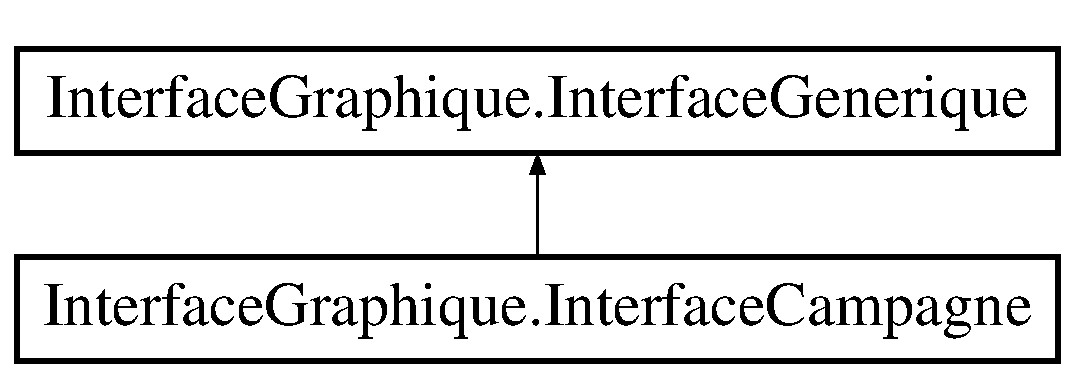
\includegraphics[height=2.000000cm]{class_interface_graphique_1_1_interface_campagne}
\end{center}
\end{figure}
\subsection*{Public Member Functions}
\begin{DoxyCompactItemize}
\item 
\hypertarget{class_interface_graphique_1_1_interface_campagne_ad2e054988085e951e791cdf14e2da829}{{\bfseries Interface\-Campagne} (\hyperlink{class_interface_graphique_1_1_fenetre_commune}{Fenetre\-Commune} fenetre)}\label{class_interface_graphique_1_1_interface_campagne_ad2e054988085e951e791cdf14e2da829}

\item 
\hypertarget{class_interface_graphique_1_1_interface_campagne_af7f7f0388e7adfdded14db761be5f387}{void {\bfseries run} (float temps)}\label{class_interface_graphique_1_1_interface_campagne_af7f7f0388e7adfdded14db761be5f387}

\item 
\hypertarget{class_interface_graphique_1_1_interface_campagne_a5ce32b051af1ef1af79b37b864bb833e}{void {\bfseries rejouer} (boolean win)}\label{class_interface_graphique_1_1_interface_campagne_a5ce32b051af1ef1af79b37b864bb833e}

\item 
\hypertarget{class_interface_graphique_1_1_interface_campagne_af7b0469e6674c03dbc43e0e6ddf7067c}{void {\bfseries set\-Bouton\-Ortho} (boolean est\-Ortho)}\label{class_interface_graphique_1_1_interface_campagne_af7b0469e6674c03dbc43e0e6ddf7067c}

\end{DoxyCompactItemize}
\subsection*{Protected Member Functions}
\begin{DoxyCompactItemize}
\item 
\hypertarget{class_interface_graphique_1_1_interface_campagne_ae5d44a3c17e9f0ec475862200af5675a}{void {\bfseries redimensionner\-Canvas} ()}\label{class_interface_graphique_1_1_interface_campagne_ae5d44a3c17e9f0ec475862200af5675a}

\item 
void \hyperlink{class_interface_graphique_1_1_interface_campagne_acf78f4679ef66f3651af00f2183bb395}{definir\-Canvas} ()
\end{DoxyCompactItemize}
\subsection*{Additional Inherited Members}


\subsection{Member Function Documentation}
\hypertarget{class_interface_graphique_1_1_interface_campagne_acf78f4679ef66f3651af00f2183bb395}{\index{Interface\-Graphique\-::\-Interface\-Campagne@{Interface\-Graphique\-::\-Interface\-Campagne}!definir\-Canvas@{definir\-Canvas}}
\index{definir\-Canvas@{definir\-Canvas}!InterfaceGraphique::InterfaceCampagne@{Interface\-Graphique\-::\-Interface\-Campagne}}
\subsubsection[{definir\-Canvas}]{\setlength{\rightskip}{0pt plus 5cm}void Interface\-Graphique.\-Interface\-Campagne.\-definir\-Canvas (
\begin{DoxyParamCaption}
{}
\end{DoxyParamCaption}
)\hspace{0.3cm}{\ttfamily [inline]}, {\ttfamily [protected]}}}\label{class_interface_graphique_1_1_interface_campagne_acf78f4679ef66f3651af00f2183bb395}
M�thode qui d�finit l'�tat de base du canvas de dessin 
\begin{DoxyParams}{Parameters}
{\em Aucun} & \\
\hline
\end{DoxyParams}
\begin{DoxyReturn}{Returns}
void 
\end{DoxyReturn}


The documentation for this class was generated from the following file\-:\begin{DoxyCompactItemize}
\item 
Cadriciel/\-Sources/\-Java/\-Interface\-Graphique/src/\-Interface\-Graphique/Interface\-Campagne.\-java\end{DoxyCompactItemize}

\hypertarget{class_interface_graphique_1_1_interface_edition}{\section{Interface\-Graphique.\-Interface\-Edition Class Reference}
\label{class_interface_graphique_1_1_interface_edition}\index{Interface\-Graphique.\-Interface\-Edition@{Interface\-Graphique.\-Interface\-Edition}}
}
Inheritance diagram for Interface\-Graphique.\-Interface\-Edition\-:\begin{figure}[H]
\begin{center}
\leavevmode
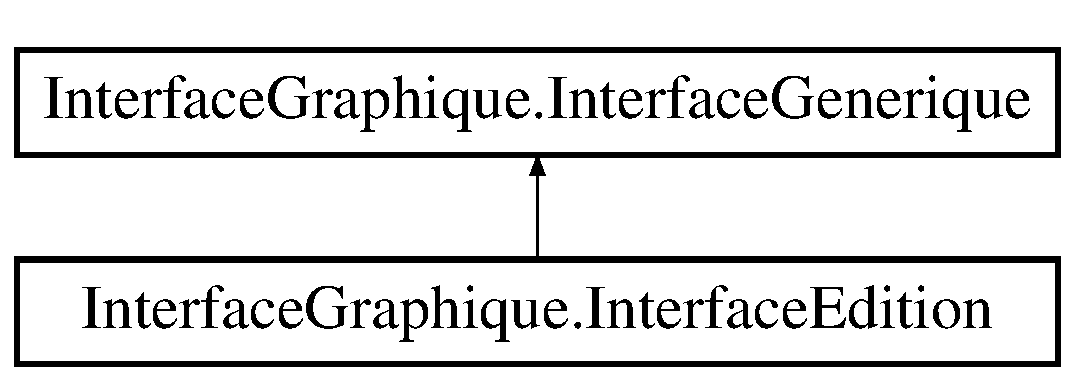
\includegraphics[height=2.000000cm]{class_interface_graphique_1_1_interface_edition}
\end{center}
\end{figure}
\subsection*{Public Member Functions}
\begin{DoxyCompactItemize}
\item 
\hyperlink{class_interface_graphique_1_1_interface_edition_a5a03953960026b370b4148f4649816d3}{Interface\-Edition} (\hyperlink{class_interface_graphique_1_1_fenetre_commune}{Fenetre\-Commune} fenetre)
\item 
\hyperlink{class_interface_graphique_1_1_barre_outils}{Barre\-Outils} \hyperlink{class_interface_graphique_1_1_interface_edition_a8183d606672ccb9c5a8ca553bd175aed}{get\-Barre\-Outils} ()
\item 
\hyperlink{class_interface_graphique_1_1_panel_proprietes}{Panel\-Proprietes} \hyperlink{class_interface_graphique_1_1_interface_edition_a30636101ae9f12d757d66acd4c77cc30}{get\-Panel\-Proprietes} ()
\item 
void \hyperlink{class_interface_graphique_1_1_interface_edition_ada6d0aa21fe6c66e4bb6d5a7c20db8b7}{show\-Panel\-Proprietes} (boolean etat)
\item 
\hypertarget{class_interface_graphique_1_1_interface_edition_a7119e4d8b18bc0dff8082dfb084e3c04}{boolean {\bfseries is\-Panel\-Proprietes\-Shown} ()}\label{class_interface_graphique_1_1_interface_edition_a7119e4d8b18bc0dff8082dfb084e3c04}

\item 
\hypertarget{class_interface_graphique_1_1_interface_edition_af6b47f8802ad783e99538249993d84b3}{void {\bfseries montrer\-Configuration\-Zone\-Jeu} (boolean val)}\label{class_interface_graphique_1_1_interface_edition_af6b47f8802ad783e99538249993d84b3}

\item 
\hypertarget{class_interface_graphique_1_1_interface_edition_a1577e39e13498abea17b1763f333cea9}{void {\bfseries run} (float temps)}\label{class_interface_graphique_1_1_interface_edition_a1577e39e13498abea17b1763f333cea9}

\item 
\hypertarget{class_interface_graphique_1_1_interface_edition_a04b0cbb3bce17fbda7de4d5f2dd48e37}{void {\bfseries set\-Bouton\-Ortho} (boolean est\-Ortho)}\label{class_interface_graphique_1_1_interface_edition_a04b0cbb3bce17fbda7de4d5f2dd48e37}

\item 
\hypertarget{class_interface_graphique_1_1_interface_edition_aade97359b9153537300e8c238d82e0e3}{void {\bfseries reset\-Buttons} ()}\label{class_interface_graphique_1_1_interface_edition_aade97359b9153537300e8c238d82e0e3}

\end{DoxyCompactItemize}
\subsection*{Protected Member Functions}
\begin{DoxyCompactItemize}
\item 
void \hyperlink{class_interface_graphique_1_1_interface_edition_a1c5ce720a7692bdf19ae567fdfbb9388}{definir\-Canvas} ()
\item 
void \hyperlink{class_interface_graphique_1_1_interface_edition_a5c6d247fc4daf5bb1676aa9674cade19}{redimensionner\-Canvas} ()
\end{DoxyCompactItemize}
\subsection*{Additional Inherited Members}


\subsection{Detailed Description}
\begin{DoxyAuthor}{Author}
Sacha L-\/\-Roussel
\end{DoxyAuthor}
Classe qui d�finit l'interface d'�dition du programme; Celle-\/ci permet de cr�er et d'�diter des cartes de jeux compos�e de \hyperlink{class_station}{Station} Spatiale, de vaisseaux, d'ast�ro�de, de barri�re et de bonus. 

\subsection{Constructor \& Destructor Documentation}
\hypertarget{class_interface_graphique_1_1_interface_edition_a5a03953960026b370b4148f4649816d3}{\index{Interface\-Graphique\-::\-Interface\-Edition@{Interface\-Graphique\-::\-Interface\-Edition}!Interface\-Edition@{Interface\-Edition}}
\index{Interface\-Edition@{Interface\-Edition}!InterfaceGraphique::InterfaceEdition@{Interface\-Graphique\-::\-Interface\-Edition}}
\subsubsection[{Interface\-Edition}]{\setlength{\rightskip}{0pt plus 5cm}Interface\-Graphique.\-Interface\-Edition.\-Interface\-Edition (
\begin{DoxyParamCaption}
\item[{{\bf Fenetre\-Commune}}]{fenetre}
\end{DoxyParamCaption}
)\hspace{0.3cm}{\ttfamily [inline]}}}\label{class_interface_graphique_1_1_interface_edition_a5a03953960026b370b4148f4649816d3}
Constructeur par d�faut de la classe \hyperlink{class_interface_graphique_1_1_interface_edition}{Interface\-Edition}. On y cr�er les composantes graphiques de l'interface. 
\begin{DoxyParams}{Parameters}
{\em fenetre\-Demarrage} & La fen�tre de d�marrage � passer pour la fen�tre de configuration de la zone de jeu \\
\hline
\end{DoxyParams}
\begin{DoxyReturn}{Returns}
Rien 
\end{DoxyReturn}


\subsection{Member Function Documentation}
\hypertarget{class_interface_graphique_1_1_interface_edition_a1c5ce720a7692bdf19ae567fdfbb9388}{\index{Interface\-Graphique\-::\-Interface\-Edition@{Interface\-Graphique\-::\-Interface\-Edition}!definir\-Canvas@{definir\-Canvas}}
\index{definir\-Canvas@{definir\-Canvas}!InterfaceGraphique::InterfaceEdition@{Interface\-Graphique\-::\-Interface\-Edition}}
\subsubsection[{definir\-Canvas}]{\setlength{\rightskip}{0pt plus 5cm}void Interface\-Graphique.\-Interface\-Edition.\-definir\-Canvas (
\begin{DoxyParamCaption}
{}
\end{DoxyParamCaption}
)\hspace{0.3cm}{\ttfamily [inline]}, {\ttfamily [protected]}}}\label{class_interface_graphique_1_1_interface_edition_a1c5ce720a7692bdf19ae567fdfbb9388}
M�thode qui d�finit l'�tat de base du canvas de dessin 
\begin{DoxyParams}{Parameters}
{\em Aucun} & \\
\hline
\end{DoxyParams}
\begin{DoxyReturn}{Returns}
void 
\end{DoxyReturn}
\hypertarget{class_interface_graphique_1_1_interface_edition_a8183d606672ccb9c5a8ca553bd175aed}{\index{Interface\-Graphique\-::\-Interface\-Edition@{Interface\-Graphique\-::\-Interface\-Edition}!get\-Barre\-Outils@{get\-Barre\-Outils}}
\index{get\-Barre\-Outils@{get\-Barre\-Outils}!InterfaceGraphique::InterfaceEdition@{Interface\-Graphique\-::\-Interface\-Edition}}
\subsubsection[{get\-Barre\-Outils}]{\setlength{\rightskip}{0pt plus 5cm}{\bf Barre\-Outils} Interface\-Graphique.\-Interface\-Edition.\-get\-Barre\-Outils (
\begin{DoxyParamCaption}
{}
\end{DoxyParamCaption}
)\hspace{0.3cm}{\ttfamily [inline]}}}\label{class_interface_graphique_1_1_interface_edition_a8183d606672ccb9c5a8ca553bd175aed}
Retourne l'instance de la barre d'outils contenue dans l'interface d'edition 
\begin{DoxyParams}{Parameters}
{\em Aucuns} & param�tres \\
\hline
\end{DoxyParams}
\begin{DoxyReturn}{Returns}
barre\-Outils Objet de type \hyperlink{class_interface_graphique_1_1_barre_outils}{Barre\-Outils}. 
\end{DoxyReturn}
\hypertarget{class_interface_graphique_1_1_interface_edition_a30636101ae9f12d757d66acd4c77cc30}{\index{Interface\-Graphique\-::\-Interface\-Edition@{Interface\-Graphique\-::\-Interface\-Edition}!get\-Panel\-Proprietes@{get\-Panel\-Proprietes}}
\index{get\-Panel\-Proprietes@{get\-Panel\-Proprietes}!InterfaceGraphique::InterfaceEdition@{Interface\-Graphique\-::\-Interface\-Edition}}
\subsubsection[{get\-Panel\-Proprietes}]{\setlength{\rightskip}{0pt plus 5cm}{\bf Panel\-Proprietes} Interface\-Graphique.\-Interface\-Edition.\-get\-Panel\-Proprietes (
\begin{DoxyParamCaption}
{}
\end{DoxyParamCaption}
)\hspace{0.3cm}{\ttfamily [inline]}}}\label{class_interface_graphique_1_1_interface_edition_a30636101ae9f12d757d66acd4c77cc30}
Retourne l'instance du panel de modification des param�tres des propri�t�s des �l�ments 
\begin{DoxyParams}{Parameters}
{\em Aucuns} & param�tres \\
\hline
\end{DoxyParams}
\begin{DoxyReturn}{Returns}
panel\-Proprietes Objet de type \hyperlink{class_interface_graphique_1_1_panel_proprietes}{Panel\-Proprietes} 
\end{DoxyReturn}
\hypertarget{class_interface_graphique_1_1_interface_edition_a5c6d247fc4daf5bb1676aa9674cade19}{\index{Interface\-Graphique\-::\-Interface\-Edition@{Interface\-Graphique\-::\-Interface\-Edition}!redimensionner\-Canvas@{redimensionner\-Canvas}}
\index{redimensionner\-Canvas@{redimensionner\-Canvas}!InterfaceGraphique::InterfaceEdition@{Interface\-Graphique\-::\-Interface\-Edition}}
\subsubsection[{redimensionner\-Canvas}]{\setlength{\rightskip}{0pt plus 5cm}void Interface\-Graphique.\-Interface\-Edition.\-redimensionner\-Canvas (
\begin{DoxyParamCaption}
{}
\end{DoxyParamCaption}
)\hspace{0.3cm}{\ttfamily [inline]}, {\ttfamily [protected]}}}\label{class_interface_graphique_1_1_interface_edition_a5c6d247fc4daf5bb1676aa9674cade19}
M�thode qui calcule les nouvelles dimensions 
\begin{DoxyParams}{Parameters}
{\em Aucun} & \\
\hline
\end{DoxyParams}
\begin{DoxyReturn}{Returns}
void 
\end{DoxyReturn}
\hypertarget{class_interface_graphique_1_1_interface_edition_ada6d0aa21fe6c66e4bb6d5a7c20db8b7}{\index{Interface\-Graphique\-::\-Interface\-Edition@{Interface\-Graphique\-::\-Interface\-Edition}!show\-Panel\-Proprietes@{show\-Panel\-Proprietes}}
\index{show\-Panel\-Proprietes@{show\-Panel\-Proprietes}!InterfaceGraphique::InterfaceEdition@{Interface\-Graphique\-::\-Interface\-Edition}}
\subsubsection[{show\-Panel\-Proprietes}]{\setlength{\rightskip}{0pt plus 5cm}void Interface\-Graphique.\-Interface\-Edition.\-show\-Panel\-Proprietes (
\begin{DoxyParamCaption}
\item[{boolean}]{etat}
\end{DoxyParamCaption}
)\hspace{0.3cm}{\ttfamily [inline]}}}\label{class_interface_graphique_1_1_interface_edition_ada6d0aa21fe6c66e4bb6d5a7c20db8b7}
Permet de changer l'�tat du panel des propri�t�s -\/ Cette m�thode le cache si il est visible et inversement 
\begin{DoxyParams}{Parameters}
{\em Aucuns} & param�tres \\
\hline
\end{DoxyParams}
\begin{DoxyReturn}{Returns}
void 
\end{DoxyReturn}


The documentation for this class was generated from the following file\-:\begin{DoxyCompactItemize}
\item 
Cadriciel/\-Sources/\-Java/\-Interface\-Graphique/src/\-Interface\-Graphique/Interface\-Edition.\-java\end{DoxyCompactItemize}

\hypertarget{class_interface_graphique_1_1_interface_generique}{\section{Interface\-Graphique.\-Interface\-Generique Class Reference}
\label{class_interface_graphique_1_1_interface_generique}\index{Interface\-Graphique.\-Interface\-Generique@{Interface\-Graphique.\-Interface\-Generique}}
}
Inheritance diagram for Interface\-Graphique.\-Interface\-Generique\-:\begin{figure}[H]
\begin{center}
\leavevmode
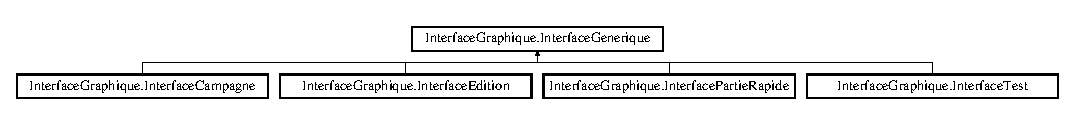
\includegraphics[height=1.102362cm]{class_interface_graphique_1_1_interface_generique}
\end{center}
\end{figure}
\subsection*{Public Member Functions}
\begin{DoxyCompactItemize}
\item 
abstract void \hyperlink{class_interface_graphique_1_1_interface_generique_adfe812d2ad8c99e63ba4b8c119c7fd7e}{run} (float temps)
\item 
\hypertarget{class_interface_graphique_1_1_interface_generique_a6a35b6b7caf6f953a0fd0d6aff500be8}{void {\bfseries set\-Bouton\-Ortho} (boolean est\-Ortho)}\label{class_interface_graphique_1_1_interface_generique_a6a35b6b7caf6f953a0fd0d6aff500be8}

\item 
\hypertarget{class_interface_graphique_1_1_interface_generique_a8c14debcd907eeaf2b8e96a3b9cdd2a2}{void {\bfseries reset\-Buttons} ()}\label{class_interface_graphique_1_1_interface_generique_a8c14debcd907eeaf2b8e96a3b9cdd2a2}

\end{DoxyCompactItemize}
\subsection*{Protected Member Functions}
\begin{DoxyCompactItemize}
\item 
int \hyperlink{class_interface_graphique_1_1_interface_generique_aad0516a099ac58815b02a20c3b493c15}{envoyer\-Input} ()
\end{DoxyCompactItemize}
\subsection*{Protected Attributes}
\begin{DoxyCompactItemize}
\item 
\hypertarget{class_interface_graphique_1_1_interface_generique_a04a1ada67399fd276189f3d2cda94101}{J\-Layered\-Pane {\bfseries content\-Pane\-\_\-}}\label{class_interface_graphique_1_1_interface_generique_a04a1ada67399fd276189f3d2cda94101}

\item 
\hypertarget{class_interface_graphique_1_1_interface_generique_a55fda1f3112e22800f675759714dbdc4}{Canvas {\bfseries canvas\-\_\-}}\label{class_interface_graphique_1_1_interface_generique_a55fda1f3112e22800f675759714dbdc4}

\item 
\hypertarget{class_interface_graphique_1_1_interface_generique_a829f0ab0b5d9e292a24591af5c20d05d}{final double {\bfseries aspect\-Ratio\-\_\-} = (1.\-78)}\label{class_interface_graphique_1_1_interface_generique_a829f0ab0b5d9e292a24591af5c20d05d}

\end{DoxyCompactItemize}
\subsection*{Static Protected Attributes}
\begin{DoxyCompactItemize}
\item 
\hypertarget{class_interface_graphique_1_1_interface_generique_a0ea265f2166bf13c5c99bfca600dc5d1}{static final int {\bfseries T\-E\-M\-P\-S\-\_\-\-I\-N\-T\-E\-R\-\_\-\-A\-F\-F\-I\-C\-H\-A\-G\-E} = 20}\label{class_interface_graphique_1_1_interface_generique_a0ea265f2166bf13c5c99bfca600dc5d1}

\end{DoxyCompactItemize}


\subsection{Member Function Documentation}
\hypertarget{class_interface_graphique_1_1_interface_generique_aad0516a099ac58815b02a20c3b493c15}{\index{Interface\-Graphique\-::\-Interface\-Generique@{Interface\-Graphique\-::\-Interface\-Generique}!envoyer\-Input@{envoyer\-Input}}
\index{envoyer\-Input@{envoyer\-Input}!InterfaceGraphique::InterfaceGenerique@{Interface\-Graphique\-::\-Interface\-Generique}}
\subsubsection[{envoyer\-Input}]{\setlength{\rightskip}{0pt plus 5cm}int Interface\-Graphique.\-Interface\-Generique.\-envoyer\-Input (
\begin{DoxyParamCaption}
{}
\end{DoxyParamCaption}
)\hspace{0.3cm}{\ttfamily [inline]}, {\ttfamily [protected]}}}\label{class_interface_graphique_1_1_interface_generique_aad0516a099ac58815b02a20c3b493c15}
M�thode qui permet d'envoyer les inputs de clavier et souris � la librairie C++ via le lien J\-N\-I 
\begin{DoxyParams}{Parameters}
{\em Aucun} & \\
\hline
\end{DoxyParams}
\begin{DoxyReturn}{Returns}
La valeur du scroll 
\end{DoxyReturn}
\hypertarget{class_interface_graphique_1_1_interface_generique_adfe812d2ad8c99e63ba4b8c119c7fd7e}{\index{Interface\-Graphique\-::\-Interface\-Generique@{Interface\-Graphique\-::\-Interface\-Generique}!run@{run}}
\index{run@{run}!InterfaceGraphique::InterfaceGenerique@{Interface\-Graphique\-::\-Interface\-Generique}}
\subsubsection[{run}]{\setlength{\rightskip}{0pt plus 5cm}abstract void Interface\-Graphique.\-Interface\-Generique.\-run (
\begin{DoxyParamCaption}
\item[{float}]{temps}
\end{DoxyParamCaption}
)\hspace{0.3cm}{\ttfamily [abstract]}}}\label{class_interface_graphique_1_1_interface_generique_adfe812d2ad8c99e63ba4b8c119c7fd7e}
Cette m�thode doit �tre surcharg�e par les classes enfants et servira de boucle principale. 
\begin{DoxyParams}{Parameters}
{\em temps} & Le temps depuis la derni�re frame \\
\hline
\end{DoxyParams}


The documentation for this class was generated from the following file\-:\begin{DoxyCompactItemize}
\item 
Cadriciel/\-Sources/\-Java/\-Interface\-Graphique/src/\-Interface\-Graphique/Interface\-Generique.\-java\end{DoxyCompactItemize}

\hypertarget{class_interface_graphique_1_1_interface_partie_rapide}{\section{Interface\-Graphique.\-Interface\-Partie\-Rapide Class Reference}
\label{class_interface_graphique_1_1_interface_partie_rapide}\index{Interface\-Graphique.\-Interface\-Partie\-Rapide@{Interface\-Graphique.\-Interface\-Partie\-Rapide}}
}
Inheritance diagram for Interface\-Graphique.\-Interface\-Partie\-Rapide\-:\begin{figure}[H]
\begin{center}
\leavevmode
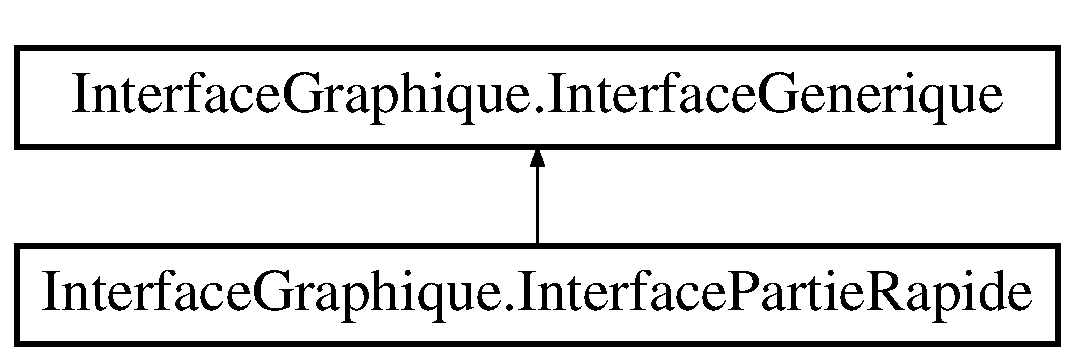
\includegraphics[height=2.000000cm]{class_interface_graphique_1_1_interface_partie_rapide}
\end{center}
\end{figure}
\subsection*{Public Member Functions}
\begin{DoxyCompactItemize}
\item 
\hyperlink{class_interface_graphique_1_1_interface_partie_rapide_a3f452cb0727e080e43ce9fbe6e47fbdb}{Interface\-Partie\-Rapide} (\hyperlink{class_interface_graphique_1_1_fenetre_commune}{Fenetre\-Commune} fenetre)
\item 
\hyperlink{wglew_8h_aeea6e3dfae3acf232096f57d2d57f084}{void} \hyperlink{class_interface_graphique_1_1_interface_partie_rapide_afcff09a25089b95f90e2a92f5b362e66}{run} (\hyperlink{fmod_8h_aeb841aa4b4b5f444b5d739d865b420af}{float} temps)
\end{DoxyCompactItemize}
\subsection*{Protected Member Functions}
\begin{DoxyCompactItemize}
\item 
\hyperlink{wglew_8h_aeea6e3dfae3acf232096f57d2d57f084}{void} \hyperlink{class_interface_graphique_1_1_interface_partie_rapide_ac79486a101a62809b1a6cb65a75c45da}{redimensionner\-Canvas} ()
\item 
\hyperlink{wglew_8h_aeea6e3dfae3acf232096f57d2d57f084}{void} \hyperlink{class_interface_graphique_1_1_interface_partie_rapide_a531bed540d524ecb36c8c5a06f2183e3}{definir\-Canvas} ()
\end{DoxyCompactItemize}
\subsection*{Additional Inherited Members}


\subsection{Constructor \& Destructor Documentation}
\hypertarget{class_interface_graphique_1_1_interface_partie_rapide_a3f452cb0727e080e43ce9fbe6e47fbdb}{\index{Interface\-Graphique\-::\-Interface\-Partie\-Rapide@{Interface\-Graphique\-::\-Interface\-Partie\-Rapide}!Interface\-Partie\-Rapide@{Interface\-Partie\-Rapide}}
\index{Interface\-Partie\-Rapide@{Interface\-Partie\-Rapide}!InterfaceGraphique::InterfacePartieRapide@{Interface\-Graphique\-::\-Interface\-Partie\-Rapide}}
\subsubsection[{Interface\-Partie\-Rapide}]{\setlength{\rightskip}{0pt plus 5cm}Interface\-Graphique.\-Interface\-Partie\-Rapide.\-Interface\-Partie\-Rapide (
\begin{DoxyParamCaption}
\item[{{\bf Fenetre\-Commune}}]{fenetre}
\end{DoxyParamCaption}
)\hspace{0.3cm}{\ttfamily [inline]}}}\label{class_interface_graphique_1_1_interface_partie_rapide_a3f452cb0727e080e43ce9fbe6e47fbdb}


\subsection{Member Function Documentation}
\hypertarget{class_interface_graphique_1_1_interface_partie_rapide_a531bed540d524ecb36c8c5a06f2183e3}{\index{Interface\-Graphique\-::\-Interface\-Partie\-Rapide@{Interface\-Graphique\-::\-Interface\-Partie\-Rapide}!definir\-Canvas@{definir\-Canvas}}
\index{definir\-Canvas@{definir\-Canvas}!InterfaceGraphique::InterfacePartieRapide@{Interface\-Graphique\-::\-Interface\-Partie\-Rapide}}
\subsubsection[{definir\-Canvas}]{\setlength{\rightskip}{0pt plus 5cm}{\bf void} Interface\-Graphique.\-Interface\-Partie\-Rapide.\-definir\-Canvas (
\begin{DoxyParamCaption}
{}
\end{DoxyParamCaption}
)\hspace{0.3cm}{\ttfamily [inline]}, {\ttfamily [protected]}}}\label{class_interface_graphique_1_1_interface_partie_rapide_a531bed540d524ecb36c8c5a06f2183e3}
M�thode qui d�finit l'�tat de base du canvas de dessin 
\begin{DoxyParams}{Parameters}
{\em Aucun} & \\
\hline
\end{DoxyParams}
\begin{DoxyReturn}{Returns}
void 
\end{DoxyReturn}
\hypertarget{class_interface_graphique_1_1_interface_partie_rapide_ac79486a101a62809b1a6cb65a75c45da}{\index{Interface\-Graphique\-::\-Interface\-Partie\-Rapide@{Interface\-Graphique\-::\-Interface\-Partie\-Rapide}!redimensionner\-Canvas@{redimensionner\-Canvas}}
\index{redimensionner\-Canvas@{redimensionner\-Canvas}!InterfaceGraphique::InterfacePartieRapide@{Interface\-Graphique\-::\-Interface\-Partie\-Rapide}}
\subsubsection[{redimensionner\-Canvas}]{\setlength{\rightskip}{0pt plus 5cm}{\bf void} Interface\-Graphique.\-Interface\-Partie\-Rapide.\-redimensionner\-Canvas (
\begin{DoxyParamCaption}
{}
\end{DoxyParamCaption}
)\hspace{0.3cm}{\ttfamily [inline]}, {\ttfamily [protected]}}}\label{class_interface_graphique_1_1_interface_partie_rapide_ac79486a101a62809b1a6cb65a75c45da}
M�thode qui calcule les nouvelles dimensions 
\begin{DoxyParams}{Parameters}
{\em Aucun} & \\
\hline
\end{DoxyParams}
\begin{DoxyReturn}{Returns}
void 
\end{DoxyReturn}
\hypertarget{class_interface_graphique_1_1_interface_partie_rapide_afcff09a25089b95f90e2a92f5b362e66}{\index{Interface\-Graphique\-::\-Interface\-Partie\-Rapide@{Interface\-Graphique\-::\-Interface\-Partie\-Rapide}!run@{run}}
\index{run@{run}!InterfaceGraphique::InterfacePartieRapide@{Interface\-Graphique\-::\-Interface\-Partie\-Rapide}}
\subsubsection[{run}]{\setlength{\rightskip}{0pt plus 5cm}{\bf void} Interface\-Graphique.\-Interface\-Partie\-Rapide.\-run (
\begin{DoxyParamCaption}
\item[{{\bf float}}]{temps}
\end{DoxyParamCaption}
)\hspace{0.3cm}{\ttfamily [inline]}}}\label{class_interface_graphique_1_1_interface_partie_rapide_afcff09a25089b95f90e2a92f5b362e66}


The documentation for this class was generated from the following file\-:\begin{DoxyCompactItemize}
\item 
Cadriciel/\-Sources/\-Java/\-Interface\-Graphique/src/\-Interface\-Graphique/\hyperlink{_interface_partie_rapide_8java}{Interface\-Partie\-Rapide.\-java}\end{DoxyCompactItemize}

\hypertarget{class_interface_graphique_1_1_interface_test}{\section{Interface\-Graphique.\-Interface\-Test Class Reference}
\label{class_interface_graphique_1_1_interface_test}\index{Interface\-Graphique.\-Interface\-Test@{Interface\-Graphique.\-Interface\-Test}}
}
Inheritance diagram for Interface\-Graphique.\-Interface\-Test\-:\begin{figure}[H]
\begin{center}
\leavevmode
\includegraphics[height=2.000000cm]{class_interface_graphique_1_1_interface_test}
\end{center}
\end{figure}
\subsection*{Public Member Functions}
\begin{DoxyCompactItemize}
\item 
\hypertarget{class_interface_graphique_1_1_interface_test_a6e88a5449b5ca0cc3de4e171c034b35d}{{\bfseries Interface\-Test} (\hyperlink{class_interface_graphique_1_1_fenetre_commune}{Fenetre\-Commune} fenetre)}\label{class_interface_graphique_1_1_interface_test_a6e88a5449b5ca0cc3de4e171c034b35d}

\item 
\hypertarget{class_interface_graphique_1_1_interface_test_ae08d0cba865743eb34a0e6c758152113}{void {\bfseries run} (float temps)}\label{class_interface_graphique_1_1_interface_test_ae08d0cba865743eb34a0e6c758152113}

\item 
\hypertarget{class_interface_graphique_1_1_interface_test_a72bbb00db6d06f08899a4d3c3269b825}{void {\bfseries set\-Bouton\-Ortho} (boolean est\-Ortho)}\label{class_interface_graphique_1_1_interface_test_a72bbb00db6d06f08899a4d3c3269b825}

\end{DoxyCompactItemize}
\subsection*{Protected Member Functions}
\begin{DoxyCompactItemize}
\item 
void \hyperlink{class_interface_graphique_1_1_interface_test_a555bf8271860120a0dc81ddb39e5210e}{redimensionner\-Canvas} ()
\item 
void \hyperlink{class_interface_graphique_1_1_interface_test_a40782de457ebfad1b775a7d3831e4b0b}{definir\-Canvas} ()
\end{DoxyCompactItemize}
\subsection*{Additional Inherited Members}


\subsection{Member Function Documentation}
\hypertarget{class_interface_graphique_1_1_interface_test_a40782de457ebfad1b775a7d3831e4b0b}{\index{Interface\-Graphique\-::\-Interface\-Test@{Interface\-Graphique\-::\-Interface\-Test}!definir\-Canvas@{definir\-Canvas}}
\index{definir\-Canvas@{definir\-Canvas}!InterfaceGraphique::InterfaceTest@{Interface\-Graphique\-::\-Interface\-Test}}
\subsubsection[{definir\-Canvas}]{\setlength{\rightskip}{0pt plus 5cm}void Interface\-Graphique.\-Interface\-Test.\-definir\-Canvas (
\begin{DoxyParamCaption}
{}
\end{DoxyParamCaption}
)\hspace{0.3cm}{\ttfamily [inline]}, {\ttfamily [protected]}}}\label{class_interface_graphique_1_1_interface_test_a40782de457ebfad1b775a7d3831e4b0b}
M�thode qui d�finit l'�tat de base du canvas de dessin 
\begin{DoxyParams}{Parameters}
{\em Aucun} & \\
\hline
\end{DoxyParams}
\begin{DoxyReturn}{Returns}
void 
\end{DoxyReturn}
\hypertarget{class_interface_graphique_1_1_interface_test_a555bf8271860120a0dc81ddb39e5210e}{\index{Interface\-Graphique\-::\-Interface\-Test@{Interface\-Graphique\-::\-Interface\-Test}!redimensionner\-Canvas@{redimensionner\-Canvas}}
\index{redimensionner\-Canvas@{redimensionner\-Canvas}!InterfaceGraphique::InterfaceTest@{Interface\-Graphique\-::\-Interface\-Test}}
\subsubsection[{redimensionner\-Canvas}]{\setlength{\rightskip}{0pt plus 5cm}void Interface\-Graphique.\-Interface\-Test.\-redimensionner\-Canvas (
\begin{DoxyParamCaption}
{}
\end{DoxyParamCaption}
)\hspace{0.3cm}{\ttfamily [inline]}, {\ttfamily [protected]}}}\label{class_interface_graphique_1_1_interface_test_a555bf8271860120a0dc81ddb39e5210e}
M�thode qui calcule les nouvelles dimensions 
\begin{DoxyParams}{Parameters}
{\em Aucun} & \\
\hline
\end{DoxyParams}
\begin{DoxyReturn}{Returns}
void 
\end{DoxyReturn}


The documentation for this class was generated from the following file\-:\begin{DoxyCompactItemize}
\item 
Cadriciel/\-Sources/\-Java/\-Interface\-Graphique/src/\-Interface\-Graphique/Interface\-Test.\-java\end{DoxyCompactItemize}

\hypertarget{class_assimp_1_1_i_o_stream}{\section{Assimp\-:\-:I\-O\-Stream Class Reference}
\label{class_assimp_1_1_i_o_stream}\index{Assimp\-::\-I\-O\-Stream@{Assimp\-::\-I\-O\-Stream}}
}


C\-P\-P-\/\-A\-P\-I\-: Class to handle file I/\-O for C++.  




{\ttfamily \#include $<$I\-O\-Stream.\-h$>$}

Inheritance diagram for Assimp\-:\-:I\-O\-Stream\-:\begin{figure}[H]
\begin{center}
\leavevmode
\includegraphics[height=2.000000cm]{class_assimp_1_1_i_o_stream}
\end{center}
\end{figure}
\subsection*{Public Member Functions}
\begin{DoxyCompactItemize}
\item 
\hypertarget{class_assimp_1_1_i_o_stream_a6cedc5033bf531bf14b97d1c9b788de8}{virtual \hyperlink{class_assimp_1_1_i_o_stream_a6cedc5033bf531bf14b97d1c9b788de8}{$\sim$\-I\-O\-Stream} ()}\label{class_assimp_1_1_i_o_stream_a6cedc5033bf531bf14b97d1c9b788de8}

\begin{DoxyCompactList}\small\item\em Destructor. Deleting the object closes the underlying file, alternatively you may use \hyperlink{class_assimp_1_1_i_o_system_a8c334d60f04bceeb6bd0157d21723f3e}{I\-O\-System\-::\-Close()} to release the file. \end{DoxyCompactList}\item 
virtual size\-\_\-t \hyperlink{class_assimp_1_1_i_o_stream_ae376f641020989d61863b9c6f55c7abf}{Read} (void $\ast$pv\-Buffer, size\-\_\-t p\-Size, size\-\_\-t p\-Count)=0
\begin{DoxyCompactList}\small\item\em Read from the file. \end{DoxyCompactList}\item 
virtual size\-\_\-t \hyperlink{class_assimp_1_1_i_o_stream_ad0ca4aae1b8c4d00db391ac3a4171f7b}{Write} (const void $\ast$pv\-Buffer, size\-\_\-t p\-Size, size\-\_\-t p\-Count)=0
\begin{DoxyCompactList}\small\item\em Write to the file. \end{DoxyCompactList}\item 
virtual ai\-Return \hyperlink{class_assimp_1_1_i_o_stream_a5ed0dddf418ab08cf3fc21f3f3032220}{Seek} (size\-\_\-t p\-Offset, ai\-Origin p\-Origin)=0
\begin{DoxyCompactList}\small\item\em Set the read/write cursor of the file. \end{DoxyCompactList}\item 
virtual size\-\_\-t \hyperlink{class_assimp_1_1_i_o_stream_a316ac6cd16b5a493d1313f792c806194}{Tell} () const =0
\begin{DoxyCompactList}\small\item\em Get the current position of the read/write cursor. \end{DoxyCompactList}\item 
\hypertarget{class_assimp_1_1_i_o_stream_aaa01183d197fb714f28d6c611b6fa058}{virtual size\-\_\-t \hyperlink{class_assimp_1_1_i_o_stream_aaa01183d197fb714f28d6c611b6fa058}{File\-Size} () const =0}\label{class_assimp_1_1_i_o_stream_aaa01183d197fb714f28d6c611b6fa058}

\begin{DoxyCompactList}\small\item\em Returns filesize Returns the filesize. \end{DoxyCompactList}\item 
\hypertarget{class_assimp_1_1_i_o_stream_a7c19952446ece90924b246f087417899}{virtual void \hyperlink{class_assimp_1_1_i_o_stream_a7c19952446ece90924b246f087417899}{Flush} ()=0}\label{class_assimp_1_1_i_o_stream_a7c19952446ece90924b246f087417899}

\begin{DoxyCompactList}\small\item\em Flush the contents of the file buffer (for writers) See fflush() for more details. \end{DoxyCompactList}\end{DoxyCompactItemize}
\subsection*{Protected Member Functions}
\begin{DoxyCompactItemize}
\item 
\hyperlink{class_assimp_1_1_i_o_stream_af5ae78123b6c6f7afc31b2a52dc9192e}{I\-O\-Stream} (void)
\begin{DoxyCompactList}\small\item\em class \hyperlink{class_assimp_1_1_i_o_stream}{I\-O\-Stream} \end{DoxyCompactList}\end{DoxyCompactItemize}


\subsection{Detailed Description}
C\-P\-P-\/\-A\-P\-I\-: Class to handle file I/\-O for C++. 

Derive an own implementation from this interface to provide custom I\-O handling to the \hyperlink{class_assimp_1_1_importer}{Importer}. If you implement this interface, be sure to also provide an implementation for \hyperlink{class_assimp_1_1_i_o_system}{I\-O\-System} that creates instances of your custom I\-O class. 

\subsection{Constructor \& Destructor Documentation}
\hypertarget{class_assimp_1_1_i_o_stream_af5ae78123b6c6f7afc31b2a52dc9192e}{\index{Assimp\-::\-I\-O\-Stream@{Assimp\-::\-I\-O\-Stream}!I\-O\-Stream@{I\-O\-Stream}}
\index{I\-O\-Stream@{I\-O\-Stream}!Assimp::IOStream@{Assimp\-::\-I\-O\-Stream}}
\subsubsection[{I\-O\-Stream}]{\setlength{\rightskip}{0pt plus 5cm}Assimp\-::\-I\-O\-Stream\-::\-I\-O\-Stream (
\begin{DoxyParamCaption}
\item[{void}]{}
\end{DoxyParamCaption}
)\hspace{0.3cm}{\ttfamily [inline]}, {\ttfamily [protected]}}}\label{class_assimp_1_1_i_o_stream_af5ae78123b6c6f7afc31b2a52dc9192e}


class \hyperlink{class_assimp_1_1_i_o_stream}{I\-O\-Stream} 

Constructor protected, use \hyperlink{class_assimp_1_1_i_o_system_ac512ece3b0701de5682553007a4c0816}{I\-O\-System\-::\-Open()} to create an instance. 

\subsection{Member Function Documentation}
\hypertarget{class_assimp_1_1_i_o_stream_ae376f641020989d61863b9c6f55c7abf}{\index{Assimp\-::\-I\-O\-Stream@{Assimp\-::\-I\-O\-Stream}!Read@{Read}}
\index{Read@{Read}!Assimp::IOStream@{Assimp\-::\-I\-O\-Stream}}
\subsubsection[{Read}]{\setlength{\rightskip}{0pt plus 5cm}virtual size\-\_\-t Assimp\-::\-I\-O\-Stream\-::\-Read (
\begin{DoxyParamCaption}
\item[{void $\ast$}]{pv\-Buffer, }
\item[{size\-\_\-t}]{p\-Size, }
\item[{size\-\_\-t}]{p\-Count}
\end{DoxyParamCaption}
)\hspace{0.3cm}{\ttfamily [pure virtual]}}}\label{class_assimp_1_1_i_o_stream_ae376f641020989d61863b9c6f55c7abf}


Read from the file. 

See fread() for more details This fails for write-\/only files \hypertarget{class_assimp_1_1_i_o_stream_a5ed0dddf418ab08cf3fc21f3f3032220}{\index{Assimp\-::\-I\-O\-Stream@{Assimp\-::\-I\-O\-Stream}!Seek@{Seek}}
\index{Seek@{Seek}!Assimp::IOStream@{Assimp\-::\-I\-O\-Stream}}
\subsubsection[{Seek}]{\setlength{\rightskip}{0pt plus 5cm}virtual ai\-Return Assimp\-::\-I\-O\-Stream\-::\-Seek (
\begin{DoxyParamCaption}
\item[{size\-\_\-t}]{p\-Offset, }
\item[{ai\-Origin}]{p\-Origin}
\end{DoxyParamCaption}
)\hspace{0.3cm}{\ttfamily [pure virtual]}}}\label{class_assimp_1_1_i_o_stream_a5ed0dddf418ab08cf3fc21f3f3032220}


Set the read/write cursor of the file. 

Note that the offset is {\itshape negative} for ai\-Origin\-\_\-\-E\-N\-D. See fseek() for more details \hypertarget{class_assimp_1_1_i_o_stream_a316ac6cd16b5a493d1313f792c806194}{\index{Assimp\-::\-I\-O\-Stream@{Assimp\-::\-I\-O\-Stream}!Tell@{Tell}}
\index{Tell@{Tell}!Assimp::IOStream@{Assimp\-::\-I\-O\-Stream}}
\subsubsection[{Tell}]{\setlength{\rightskip}{0pt plus 5cm}virtual size\-\_\-t Assimp\-::\-I\-O\-Stream\-::\-Tell (
\begin{DoxyParamCaption}
{}
\end{DoxyParamCaption}
) const\hspace{0.3cm}{\ttfamily [pure virtual]}}}\label{class_assimp_1_1_i_o_stream_a316ac6cd16b5a493d1313f792c806194}


Get the current position of the read/write cursor. 

See ftell() for more details \hypertarget{class_assimp_1_1_i_o_stream_ad0ca4aae1b8c4d00db391ac3a4171f7b}{\index{Assimp\-::\-I\-O\-Stream@{Assimp\-::\-I\-O\-Stream}!Write@{Write}}
\index{Write@{Write}!Assimp::IOStream@{Assimp\-::\-I\-O\-Stream}}
\subsubsection[{Write}]{\setlength{\rightskip}{0pt plus 5cm}virtual size\-\_\-t Assimp\-::\-I\-O\-Stream\-::\-Write (
\begin{DoxyParamCaption}
\item[{const void $\ast$}]{pv\-Buffer, }
\item[{size\-\_\-t}]{p\-Size, }
\item[{size\-\_\-t}]{p\-Count}
\end{DoxyParamCaption}
)\hspace{0.3cm}{\ttfamily [pure virtual]}}}\label{class_assimp_1_1_i_o_stream_ad0ca4aae1b8c4d00db391ac3a4171f7b}


Write to the file. 

See fwrite() for more details This fails for read-\/only files 

The documentation for this class was generated from the following file\-:\begin{DoxyCompactItemize}
\item 
Cadriciel/\-Commun/\-Externe/assimp/include/\hyperlink{_i_o_stream_8h}{I\-O\-Stream.\-h}\end{DoxyCompactItemize}

\hypertarget{class_assimp_1_1_i_o_system}{\section{Assimp\-:\-:I\-O\-System Class Reference}
\label{class_assimp_1_1_i_o_system}\index{Assimp\-::\-I\-O\-System@{Assimp\-::\-I\-O\-System}}
}


C\-P\-P-\/\-A\-P\-I\-: Interface to the file system.  




{\ttfamily \#include $<$I\-O\-System.\-h$>$}

Inheritance diagram for Assimp\-:\-:I\-O\-System\-:\begin{figure}[H]
\begin{center}
\leavevmode
\includegraphics[height=2.000000cm]{class_assimp_1_1_i_o_system}
\end{center}
\end{figure}
\subsection*{Public Member Functions}
\begin{DoxyCompactItemize}
\item 
\hyperlink{class_assimp_1_1_i_o_system_af8ba1ee2dc0686da8fc9e3dad49af801}{I\-O\-System} ()
\begin{DoxyCompactList}\small\item\em Default constructor. \end{DoxyCompactList}\item 
virtual \hyperlink{class_assimp_1_1_i_o_system_a617417f1c5125770606fea3b41068b36}{$\sim$\-I\-O\-System} ()
\begin{DoxyCompactList}\small\item\em Virtual destructor. \end{DoxyCompactList}\item 
\hyperlink{ai_defines_8h_a61d239a320b58eca56bacc46fc2c79b8}{A\-I\-\_\-\-F\-O\-R\-C\-E\-\_\-\-I\-N\-L\-I\-N\-E} bool \hyperlink{class_assimp_1_1_i_o_system_a7ae6cfaea4957408967463bfc3b84b27}{Exists} (const \hyperlink{glew_8h_ae84541b4f3d8e1ea24ec0f466a8c568b}{std\-::string} \&p\-File) const 
\begin{DoxyCompactList}\small\item\em For backward compatibility. \end{DoxyCompactList}\item 
virtual bool \hyperlink{class_assimp_1_1_i_o_system_a79f5fe8d2dbe1056c9418f7de9a72445}{Exists} (const char $\ast$p\-File) const =0
\begin{DoxyCompactList}\small\item\em Tests for the existence of a file at the given path. \end{DoxyCompactList}\item 
virtual char \hyperlink{class_assimp_1_1_i_o_system_a40e412875b985bdb638f00ef0f20fff6}{get\-Os\-Separator} () const =0
\begin{DoxyCompactList}\small\item\em Returns the system specific directory separator. \end{DoxyCompactList}\item 
virtual \hyperlink{class_assimp_1_1_i_o_stream}{I\-O\-Stream} $\ast$ \hyperlink{class_assimp_1_1_i_o_system_ac512ece3b0701de5682553007a4c0816}{Open} (const char $\ast$p\-File, const char $\ast$p\-Mode=\char`\"{}rb\char`\"{})=0
\begin{DoxyCompactList}\small\item\em Open a new file with a given path. \end{DoxyCompactList}\item 
\hyperlink{class_assimp_1_1_i_o_stream}{I\-O\-Stream} $\ast$ \hyperlink{class_assimp_1_1_i_o_system_aef35fabc9bd49fb83bfd4f12a94083c3}{Open} (const \hyperlink{glew_8h_ae84541b4f3d8e1ea24ec0f466a8c568b}{std\-::string} \&p\-File, const \hyperlink{glew_8h_ae84541b4f3d8e1ea24ec0f466a8c568b}{std\-::string} \&p\-Mode=\hyperlink{glew_8h_ae84541b4f3d8e1ea24ec0f466a8c568b}{std\-::string}(\char`\"{}rb\char`\"{}))
\begin{DoxyCompactList}\small\item\em For backward compatibility. \end{DoxyCompactList}\item 
virtual \hyperlink{wglew_8h_aeea6e3dfae3acf232096f57d2d57f084}{void} \hyperlink{class_assimp_1_1_i_o_system_a8c334d60f04bceeb6bd0157d21723f3e}{Close} (\hyperlink{class_assimp_1_1_i_o_stream}{I\-O\-Stream} $\ast$p\-File)=0
\begin{DoxyCompactList}\small\item\em Closes the given file and releases all resources associated with it. \end{DoxyCompactList}\item 
virtual bool \hyperlink{class_assimp_1_1_i_o_system_a11349a65b353ed62f655c3dd802b9062}{Compare\-Paths} (const char $\ast$one, const char $\ast$second) const 
\begin{DoxyCompactList}\small\item\em Compares two paths and check whether the point to identical files. \end{DoxyCompactList}\item 
bool \hyperlink{class_assimp_1_1_i_o_system_a279d1d4b0b2aa37800e222aad508dff1}{Compare\-Paths} (const \hyperlink{glew_8h_ae84541b4f3d8e1ea24ec0f466a8c568b}{std\-::string} \&one, const \hyperlink{glew_8h_ae84541b4f3d8e1ea24ec0f466a8c568b}{std\-::string} \&second) const 
\begin{DoxyCompactList}\small\item\em For backward compatibility. \end{DoxyCompactList}\end{DoxyCompactItemize}


\subsection{Detailed Description}
C\-P\-P-\/\-A\-P\-I\-: Interface to the file system. 

Derive an own implementation from this interface to supply custom file handling to the importer library. If you implement this interface, you also want to supply a custom implementation for \hyperlink{class_assimp_1_1_i_o_stream}{I\-O\-Stream}.

\begin{DoxySeeAlso}{See Also}
\hyperlink{class_assimp_1_1_importer_a1161f46318af18bb86dfe0fc3edea4df}{Importer\-::\-Set\-I\-O\-Handler()} 
\end{DoxySeeAlso}


\subsection{Constructor \& Destructor Documentation}
\hypertarget{class_assimp_1_1_i_o_system_af8ba1ee2dc0686da8fc9e3dad49af801}{\index{Assimp\-::\-I\-O\-System@{Assimp\-::\-I\-O\-System}!I\-O\-System@{I\-O\-System}}
\index{I\-O\-System@{I\-O\-System}!Assimp::IOSystem@{Assimp\-::\-I\-O\-System}}
\subsubsection[{I\-O\-System}]{\setlength{\rightskip}{0pt plus 5cm}{\bf A\-I\-\_\-\-F\-O\-R\-C\-E\-\_\-\-I\-N\-L\-I\-N\-E} Assimp\-::\-I\-O\-System\-::\-I\-O\-System (
\begin{DoxyParamCaption}
{}
\end{DoxyParamCaption}
)}}\label{class_assimp_1_1_i_o_system_af8ba1ee2dc0686da8fc9e3dad49af801}


Default constructor. 

Create an instance of your derived class and assign it to an \hyperlink{class_assimp_1_1_importer}{Assimp\-::\-Importer} instance by calling \hyperlink{class_assimp_1_1_importer_a1161f46318af18bb86dfe0fc3edea4df}{Importer\-::\-Set\-I\-O\-Handler()}. \hypertarget{class_assimp_1_1_i_o_system_a617417f1c5125770606fea3b41068b36}{\index{Assimp\-::\-I\-O\-System@{Assimp\-::\-I\-O\-System}!$\sim$\-I\-O\-System@{$\sim$\-I\-O\-System}}
\index{$\sim$\-I\-O\-System@{$\sim$\-I\-O\-System}!Assimp::IOSystem@{Assimp\-::\-I\-O\-System}}
\subsubsection[{$\sim$\-I\-O\-System}]{\setlength{\rightskip}{0pt plus 5cm}{\bf A\-I\-\_\-\-F\-O\-R\-C\-E\-\_\-\-I\-N\-L\-I\-N\-E} Assimp\-::\-I\-O\-System\-::$\sim$\-I\-O\-System (
\begin{DoxyParamCaption}
{}
\end{DoxyParamCaption}
)\hspace{0.3cm}{\ttfamily [virtual]}}}\label{class_assimp_1_1_i_o_system_a617417f1c5125770606fea3b41068b36}


Virtual destructor. 

It is safe to be called from within D\-L\-L \hyperlink{namespace_assimp}{Assimp}, we're constructed on \hyperlink{namespace_assimp}{Assimp}'s heap. 

\subsection{Member Function Documentation}
\hypertarget{class_assimp_1_1_i_o_system_a8c334d60f04bceeb6bd0157d21723f3e}{\index{Assimp\-::\-I\-O\-System@{Assimp\-::\-I\-O\-System}!Close@{Close}}
\index{Close@{Close}!Assimp::IOSystem@{Assimp\-::\-I\-O\-System}}
\subsubsection[{Close}]{\setlength{\rightskip}{0pt plus 5cm}virtual {\bf void} Assimp\-::\-I\-O\-System\-::\-Close (
\begin{DoxyParamCaption}
\item[{{\bf I\-O\-Stream} $\ast$}]{p\-File}
\end{DoxyParamCaption}
)\hspace{0.3cm}{\ttfamily [pure virtual]}}}\label{class_assimp_1_1_i_o_system_a8c334d60f04bceeb6bd0157d21723f3e}


Closes the given file and releases all resources associated with it. 


\begin{DoxyParams}{Parameters}
{\em p\-File} & The file instance previously created by \hyperlink{class_assimp_1_1_i_o_system_ac512ece3b0701de5682553007a4c0816}{Open()}. \\
\hline
\end{DoxyParams}
\hypertarget{class_assimp_1_1_i_o_system_a11349a65b353ed62f655c3dd802b9062}{\index{Assimp\-::\-I\-O\-System@{Assimp\-::\-I\-O\-System}!Compare\-Paths@{Compare\-Paths}}
\index{Compare\-Paths@{Compare\-Paths}!Assimp::IOSystem@{Assimp\-::\-I\-O\-System}}
\subsubsection[{Compare\-Paths}]{\setlength{\rightskip}{0pt plus 5cm}virtual bool Assimp\-::\-I\-O\-System\-::\-Compare\-Paths (
\begin{DoxyParamCaption}
\item[{const char $\ast$}]{one, }
\item[{const char $\ast$}]{second}
\end{DoxyParamCaption}
) const\hspace{0.3cm}{\ttfamily [virtual]}}}\label{class_assimp_1_1_i_o_system_a11349a65b353ed62f655c3dd802b9062}


Compares two paths and check whether the point to identical files. 

The dummy implementation of this virtual performs a case-\/insensitive comparison of the given strings. The default I\-O system implementation uses O\-S mechanisms to convert relative into absolute paths, so the result can be trusted. 
\begin{DoxyParams}{Parameters}
{\em one} & First file \\
\hline
{\em second} & Second file \\
\hline
\end{DoxyParams}
\begin{DoxyReturn}{Returns}
true if the paths point to the same file. The file needn't be existing, however. 
\end{DoxyReturn}
\hypertarget{class_assimp_1_1_i_o_system_a279d1d4b0b2aa37800e222aad508dff1}{\index{Assimp\-::\-I\-O\-System@{Assimp\-::\-I\-O\-System}!Compare\-Paths@{Compare\-Paths}}
\index{Compare\-Paths@{Compare\-Paths}!Assimp::IOSystem@{Assimp\-::\-I\-O\-System}}
\subsubsection[{Compare\-Paths}]{\setlength{\rightskip}{0pt plus 5cm}bool Assimp\-::\-I\-O\-System\-::\-Compare\-Paths (
\begin{DoxyParamCaption}
\item[{const {\bf std\-::string} \&}]{one, }
\item[{const {\bf std\-::string} \&}]{second}
\end{DoxyParamCaption}
) const\hspace{0.3cm}{\ttfamily [inline]}}}\label{class_assimp_1_1_i_o_system_a279d1d4b0b2aa37800e222aad508dff1}


For backward compatibility. 

\begin{DoxySeeAlso}{See Also}
Compare\-Paths(const char$\ast$, const char$\ast$) 
\end{DoxySeeAlso}
\hypertarget{class_assimp_1_1_i_o_system_a7ae6cfaea4957408967463bfc3b84b27}{\index{Assimp\-::\-I\-O\-System@{Assimp\-::\-I\-O\-System}!Exists@{Exists}}
\index{Exists@{Exists}!Assimp::IOSystem@{Assimp\-::\-I\-O\-System}}
\subsubsection[{Exists}]{\setlength{\rightskip}{0pt plus 5cm}{\bf A\-I\-\_\-\-F\-O\-R\-C\-E\-\_\-\-I\-N\-L\-I\-N\-E} bool Assimp\-::\-I\-O\-System\-::\-Exists (
\begin{DoxyParamCaption}
\item[{const {\bf std\-::string} \&}]{p\-File}
\end{DoxyParamCaption}
) const}}\label{class_assimp_1_1_i_o_system_a7ae6cfaea4957408967463bfc3b84b27}


For backward compatibility. 

\begin{DoxySeeAlso}{See Also}
Exists(const char$\ast$) 
\end{DoxySeeAlso}
\hypertarget{class_assimp_1_1_i_o_system_a79f5fe8d2dbe1056c9418f7de9a72445}{\index{Assimp\-::\-I\-O\-System@{Assimp\-::\-I\-O\-System}!Exists@{Exists}}
\index{Exists@{Exists}!Assimp::IOSystem@{Assimp\-::\-I\-O\-System}}
\subsubsection[{Exists}]{\setlength{\rightskip}{0pt plus 5cm}virtual bool Assimp\-::\-I\-O\-System\-::\-Exists (
\begin{DoxyParamCaption}
\item[{const char $\ast$}]{p\-File}
\end{DoxyParamCaption}
) const\hspace{0.3cm}{\ttfamily [pure virtual]}}}\label{class_assimp_1_1_i_o_system_a79f5fe8d2dbe1056c9418f7de9a72445}


Tests for the existence of a file at the given path. 


\begin{DoxyParams}{Parameters}
{\em p\-File} & Path to the file \\
\hline
\end{DoxyParams}
\begin{DoxyReturn}{Returns}
true if there is a file with this path, else false. 
\end{DoxyReturn}
\hypertarget{class_assimp_1_1_i_o_system_a40e412875b985bdb638f00ef0f20fff6}{\index{Assimp\-::\-I\-O\-System@{Assimp\-::\-I\-O\-System}!get\-Os\-Separator@{get\-Os\-Separator}}
\index{get\-Os\-Separator@{get\-Os\-Separator}!Assimp::IOSystem@{Assimp\-::\-I\-O\-System}}
\subsubsection[{get\-Os\-Separator}]{\setlength{\rightskip}{0pt plus 5cm}virtual char Assimp\-::\-I\-O\-System\-::get\-Os\-Separator (
\begin{DoxyParamCaption}
{}
\end{DoxyParamCaption}
) const\hspace{0.3cm}{\ttfamily [pure virtual]}}}\label{class_assimp_1_1_i_o_system_a40e412875b985bdb638f00ef0f20fff6}


Returns the system specific directory separator. 

\begin{DoxyReturn}{Returns}
System specific directory separator 
\end{DoxyReturn}
\hypertarget{class_assimp_1_1_i_o_system_ac512ece3b0701de5682553007a4c0816}{\index{Assimp\-::\-I\-O\-System@{Assimp\-::\-I\-O\-System}!Open@{Open}}
\index{Open@{Open}!Assimp::IOSystem@{Assimp\-::\-I\-O\-System}}
\subsubsection[{Open}]{\setlength{\rightskip}{0pt plus 5cm}virtual {\bf I\-O\-Stream}$\ast$ Assimp\-::\-I\-O\-System\-::\-Open (
\begin{DoxyParamCaption}
\item[{const char $\ast$}]{p\-File, }
\item[{const char $\ast$}]{p\-Mode = {\ttfamily \char`\"{}rb\char`\"{}}}
\end{DoxyParamCaption}
)\hspace{0.3cm}{\ttfamily [pure virtual]}}}\label{class_assimp_1_1_i_o_system_ac512ece3b0701de5682553007a4c0816}


Open a new file with a given path. 

When the access to the file is finished, call \hyperlink{class_assimp_1_1_i_o_system_a8c334d60f04bceeb6bd0157d21723f3e}{Close()} to release all associated resources (or the virtual dtor of the \hyperlink{class_assimp_1_1_i_o_stream}{I\-O\-Stream}).


\begin{DoxyParams}{Parameters}
{\em p\-File} & Path to the file \\
\hline
{\em p\-Mode} & Desired file I/\-O mode. Required are\-: \char`\"{}wb\char`\"{}, \char`\"{}w\char`\"{}, \char`\"{}wt\char`\"{}, \char`\"{}rb\char`\"{}, \char`\"{}r\char`\"{}, \char`\"{}rt\char`\"{}.\\
\hline
\end{DoxyParams}
\begin{DoxyReturn}{Returns}
New \hyperlink{class_assimp_1_1_i_o_stream}{I\-O\-Stream} interface allowing the lib to access the underlying file. 
\end{DoxyReturn}
\begin{DoxyNote}{Note}
When implementing this class to provide custom I\-O handling, you probably have to supply an own implementation of \hyperlink{class_assimp_1_1_i_o_stream}{I\-O\-Stream} as well. 
\end{DoxyNote}
\hypertarget{class_assimp_1_1_i_o_system_aef35fabc9bd49fb83bfd4f12a94083c3}{\index{Assimp\-::\-I\-O\-System@{Assimp\-::\-I\-O\-System}!Open@{Open}}
\index{Open@{Open}!Assimp::IOSystem@{Assimp\-::\-I\-O\-System}}
\subsubsection[{Open}]{\setlength{\rightskip}{0pt plus 5cm}{\bf A\-I\-\_\-\-F\-O\-R\-C\-E\-\_\-\-I\-N\-L\-I\-N\-E} {\bf I\-O\-Stream} $\ast$ Assimp\-::\-I\-O\-System\-::\-Open (
\begin{DoxyParamCaption}
\item[{const {\bf std\-::string} \&}]{p\-File, }
\item[{const {\bf std\-::string} \&}]{p\-Mode = {\ttfamily {\bf std\-::string}(\char`\"{}rb\char`\"{})}}
\end{DoxyParamCaption}
)\hspace{0.3cm}{\ttfamily [inline]}}}\label{class_assimp_1_1_i_o_system_aef35fabc9bd49fb83bfd4f12a94083c3}


For backward compatibility. 

\begin{DoxySeeAlso}{See Also}
\hyperlink{class_assimp_1_1_i_o_system_ac512ece3b0701de5682553007a4c0816}{Open(const char$\ast$, const char$\ast$)} 
\end{DoxySeeAlso}


The documentation for this class was generated from the following file\-:\begin{DoxyCompactItemize}
\item 
Cadriciel/\-Commun/\-Externe/assimp/include/\hyperlink{_i_o_system_8h}{I\-O\-System.\-h}\end{DoxyCompactItemize}

\hypertarget{class_j_a_w_t___info}{\section{J\-A\-W\-T\-\_\-\-Info Class Reference}
\label{class_j_a_w_t___info}\index{J\-A\-W\-T\-\_\-\-Info@{J\-A\-W\-T\-\_\-\-Info}}
}
\subsection*{Public Member Functions}
\begin{DoxyCompactItemize}
\item 
\hypertarget{class_j_a_w_t___info_a4e3733bebccef28b59e17dc9d540d46d}{{\bfseries J\-A\-W\-T\-\_\-\-Info} (J\-N\-I\-Env $\ast$env, jobject panel)}\label{class_j_a_w_t___info_a4e3733bebccef28b59e17dc9d540d46d}

\item 
\hypertarget{class_j_a_w_t___info_a8a6d00ba985dd7fbeabc258bf5ec577e}{H\-W\-N\-D {\bfseries get\-H\-W\-N\-D} ()}\label{class_j_a_w_t___info_a8a6d00ba985dd7fbeabc258bf5ec577e}

\item 
\hypertarget{class_j_a_w_t___info_a4a5091a3e36923c94d54760ebfa24e53}{H\-D\-C {\bfseries get\-H\-D\-C} ()}\label{class_j_a_w_t___info_a4a5091a3e36923c94d54760ebfa24e53}

\end{DoxyCompactItemize}


The documentation for this class was generated from the following file\-:\begin{DoxyCompactItemize}
\item 
Cadriciel/\-Commun/\-Externe/\-J\-A\-W\-T\-\_\-info/include/J\-A\-W\-T\-\_\-\-Info.\-h\end{DoxyCompactItemize}

\hypertarget{class_jeu_abstrait}{\section{Jeu\-Abstrait Class Reference}
\label{class_jeu_abstrait}\index{Jeu\-Abstrait@{Jeu\-Abstrait}}
}


Classe abstraite representant les fonctionalites de bases des differents modes de jeux.  




{\ttfamily \#include $<$Jeu\-Abstrait.\-h$>$}

Inheritance diagram for Jeu\-Abstrait\-:\begin{figure}[H]
\begin{center}
\leavevmode
\includegraphics[height=3.000000cm]{class_jeu_abstrait}
\end{center}
\end{figure}
\subsection*{Public Member Functions}
\begin{DoxyCompactItemize}
\item 
\hyperlink{group__inf2990_ga24222f4c947cc57c4063bc4bdde23985}{Jeu\-Abstrait} (\hyperlink{class_carte}{Carte} \&carte, \hyperlink{classvue_1_1_vue}{vue\-::\-Vue} $\ast$vue)
\item 
virtual \hyperlink{group__inf2990_gaeaa1ca9db48bba9637245331fa257076}{$\sim$\-Jeu\-Abstrait} ()
\item 
void \hyperlink{group__inf2990_ga670cec0b00bf489f54a95f3362cd8584}{set\-Carte} (\hyperlink{class_carte}{Carte} \&carte)
\item 
\hyperlink{class_carte}{Carte} \& \hyperlink{group__inf2990_ga473ce72116fb23851e8da0bddfbc71d6}{get\-Carte} () const 
\item 
void \hyperlink{group__inf2990_gaeb3f920fd8f1163b527156a102a675b4}{set\-Vue} (\hyperlink{classvue_1_1_vue}{vue\-::\-Vue} $\ast$vue)
\item 
virtual void \hyperlink{group__inf2990_ga8aed09e66590b4f339b9290c8d3d70e6}{update} (float delta\-T)
\item 
void \hyperlink{group__inf2990_gac60bf135740871b1770283e508d263df}{recevoir\-Inputs} (int mouse\-X, int mouse\-Y, int boutton, int touche, int scroll)
\item 
\hypertarget{group__inf2990_ga2c3bb5664ace8e802d897a39f6801dab}{virtual void {\bfseries set\-Pourcentage\-Deplacement} (bool est\-Ortho)}\label{group__inf2990_ga2c3bb5664ace8e802d897a39f6801dab}

\end{DoxyCompactItemize}
\subsection*{Protected Attributes}
\begin{DoxyCompactItemize}
\item 
\hypertarget{group__inf2990_ga5349be037dec2b73adb0fbcca724eb2c}{\hyperlink{class_carte}{Carte} \& \hyperlink{group__inf2990_ga5349be037dec2b73adb0fbcca724eb2c}{carte\-\_\-}}\label{group__inf2990_ga5349be037dec2b73adb0fbcca724eb2c}

\begin{DoxyCompactList}\small\item\em La carte qui contient tous les objets. \end{DoxyCompactList}\item 
\hyperlink{classvue_1_1_vue}{vue\-::\-Vue} $\ast$ \hyperlink{group__inf2990_ga5d11ef13ab8e861e9c6c14b722ac85bf}{vue\-\_\-}
\item 
int \hyperlink{group__inf2990_gaebf64b4f7fa00bda679ed2815c3030cc}{mouse\-X\-\_\-}
\item 
int \hyperlink{group__inf2990_ga20f528aad2f2937cf34559ec8091cc22}{mouse\-Y\-\_\-}
\item 
int \hyperlink{group__inf2990_ga5f106517d59dda12c86741443236f981}{last\-Mouse\-X\-\_\-}
\item 
int \hyperlink{group__inf2990_ga24d07ce8ed9d2e9176deaaefd8937dd2}{last\-Mouse\-Y\-\_\-}
\item 
int \hyperlink{group__inf2990_ga6aefbc7c04b8d51ef72b4648f5278ba4}{boutton\-\_\-}
\item 
int \hyperlink{group__inf2990_ga076e503a05fd9f20e5ecc64e91eabf7f}{touche\-\_\-}
\item 
int \hyperlink{group__inf2990_ga231796955c445be70dc2273b6de8da36}{previous\-Touche\-\_\-}
\item 
int \hyperlink{group__inf2990_ga388bde29eb1b80839575085a97dd6063}{scroll\-\_\-}
\item 
\hypertarget{group__inf2990_ga41985d319601cbba0f6da4ed8d6387fb}{float {\bfseries pourcentage\-Deplacement\-\_\-}}\label{group__inf2990_ga41985d319601cbba0f6da4ed8d6387fb}

\end{DoxyCompactItemize}


\subsection{Detailed Description}
Classe abstraite representant les fonctionalites de bases des differents modes de jeux. 

\begin{DoxyAuthor}{Author}
Floppy\-Disketeers 
\end{DoxyAuthor}
\begin{DoxyDate}{Date}
2014-\/01-\/21 
\end{DoxyDate}


The documentation for this class was generated from the following files\-:\begin{DoxyCompactItemize}
\item 
Cadriciel/\-Sources/\-C++/\-Application/\-Jeu/\hyperlink{_jeu_abstrait_8h}{Jeu\-Abstrait.\-h}\item 
Cadriciel/\-Sources/\-C++/\-Application/\-Jeu/\hyperlink{_jeu_abstrait_8cpp}{Jeu\-Abstrait.\-cpp}\end{DoxyCompactItemize}

\hypertarget{classaidegl_1_1_ligne_pointillee}{\section{aidegl\-:\-:Ligne\-Pointillee Class Reference}
\label{classaidegl_1_1_ligne_pointillee}\index{aidegl\-::\-Ligne\-Pointillee@{aidegl\-::\-Ligne\-Pointillee}}
}


Classe qui gere l'affichage de lignes pointillees.  




{\ttfamily \#include $<$Ligne\-Pointillee.\-h$>$}

\subsection*{Public Member Functions}
\begin{DoxyCompactItemize}
\item 
\hyperlink{classaidegl_1_1_ligne_pointillee_a4fc590690c8bbc7368fb355a71d5eaf2}{Ligne\-Pointillee} ()
\begin{DoxyCompactList}\small\item\em Constructeur par defaut. \end{DoxyCompactList}\item 
void \hyperlink{classaidegl_1_1_ligne_pointillee_a455e3f5a717d72b04808c90c3d20f23f}{commencer} () const 
\begin{DoxyCompactList}\small\item\em Debut du rendu de lignes. \end{DoxyCompactList}\item 
void \hyperlink{classaidegl_1_1_ligne_pointillee_a5a1522b90f6970b3a33103935bed74da}{finir} () const 
\begin{DoxyCompactList}\small\item\em Fin du rendu de lignes. \end{DoxyCompactList}\item 
void \hyperlink{classaidegl_1_1_ligne_pointillee_af051ae200dfd9a5f5a26591a139e7939}{assigner\-Couleur} (const \hyperlink{group__utilitaire_ga6a8205c734fc1c9d1272ea424efb2606}{Vecteur4f} \&couleur)
\begin{DoxyCompactList}\small\item\em Assigne la couleur des lignes. \end{DoxyCompactList}\item 
void \hyperlink{classaidegl_1_1_ligne_pointillee_a0d9e3b0ca2604f1e9410b868a8917a78}{assigner\-Facteur} (int facteur)
\begin{DoxyCompactList}\small\item\em Assigne le facteur multiplicatif du pointille. \end{DoxyCompactList}\item 
void \hyperlink{classaidegl_1_1_ligne_pointillee_a2eb75fea1bec5566ca4feae3612d7b5e}{assigner\-Patron} (unsigned short patron)
\begin{DoxyCompactList}\small\item\em Assigne le patron de pointille des lignes. \end{DoxyCompactList}\end{DoxyCompactItemize}


\subsection{Detailed Description}
Classe qui gere l'affichage de lignes pointillees. 

\begin{DoxyAuthor}{Author}
Martin Bisson 
\end{DoxyAuthor}
\begin{DoxyDate}{Date}
2007-\/01-\/28 
\end{DoxyDate}


\subsection{Constructor \& Destructor Documentation}
\hypertarget{classaidegl_1_1_ligne_pointillee_a4fc590690c8bbc7368fb355a71d5eaf2}{\index{aidegl\-::\-Ligne\-Pointillee@{aidegl\-::\-Ligne\-Pointillee}!Ligne\-Pointillee@{Ligne\-Pointillee}}
\index{Ligne\-Pointillee@{Ligne\-Pointillee}!aidegl::LignePointillee@{aidegl\-::\-Ligne\-Pointillee}}
\subsubsection[{Ligne\-Pointillee}]{\setlength{\rightskip}{0pt plus 5cm}aidegl\-::\-Ligne\-Pointillee\-::\-Ligne\-Pointillee (
\begin{DoxyParamCaption}
{}
\end{DoxyParamCaption}
)\hspace{0.3cm}{\ttfamily [inline]}}}\label{classaidegl_1_1_ligne_pointillee_a4fc590690c8bbc7368fb355a71d5eaf2}


Constructeur par defaut. 

Constructeur par defaut qui se contente d'initialiser les parametres du rendu de la ligne a des valeurs par defaut.

\begin{DoxyReturn}{Returns}
Aucune (constructeur). 
\end{DoxyReturn}


\subsection{Member Function Documentation}
\hypertarget{classaidegl_1_1_ligne_pointillee_af051ae200dfd9a5f5a26591a139e7939}{\index{aidegl\-::\-Ligne\-Pointillee@{aidegl\-::\-Ligne\-Pointillee}!assigner\-Couleur@{assigner\-Couleur}}
\index{assigner\-Couleur@{assigner\-Couleur}!aidegl::LignePointillee@{aidegl\-::\-Ligne\-Pointillee}}
\subsubsection[{assigner\-Couleur}]{\setlength{\rightskip}{0pt plus 5cm}void aidegl\-::\-Ligne\-Pointillee\-::assigner\-Couleur (
\begin{DoxyParamCaption}
\item[{const {\bf Vecteur4f} \&}]{couleur}
\end{DoxyParamCaption}
)\hspace{0.3cm}{\ttfamily [inline]}}}\label{classaidegl_1_1_ligne_pointillee_af051ae200dfd9a5f5a26591a139e7939}


Assigne la couleur des lignes. 

Cette fonction permet d'assigner la couleur utilisee pour dessiner les lignes.


\begin{DoxyParams}[1]{Parameters}
\mbox{\tt in}  & {\em couleur} & \-: La couleur des lignes.\\
\hline
\end{DoxyParams}
\begin{DoxyReturn}{Returns}
Aucune. 
\end{DoxyReturn}
\hypertarget{classaidegl_1_1_ligne_pointillee_a0d9e3b0ca2604f1e9410b868a8917a78}{\index{aidegl\-::\-Ligne\-Pointillee@{aidegl\-::\-Ligne\-Pointillee}!assigner\-Facteur@{assigner\-Facteur}}
\index{assigner\-Facteur@{assigner\-Facteur}!aidegl::LignePointillee@{aidegl\-::\-Ligne\-Pointillee}}
\subsubsection[{assigner\-Facteur}]{\setlength{\rightskip}{0pt plus 5cm}void aidegl\-::\-Ligne\-Pointillee\-::assigner\-Facteur (
\begin{DoxyParamCaption}
\item[{int}]{facteur}
\end{DoxyParamCaption}
)\hspace{0.3cm}{\ttfamily [inline]}}}\label{classaidegl_1_1_ligne_pointillee_a0d9e3b0ca2604f1e9410b868a8917a78}


Assigne le facteur multiplicatif du pointille. 

Cette fonction permet d'assigner le facteur multiplicatif du pointille utilise pour dessiner les lignes.


\begin{DoxyParams}[1]{Parameters}
\mbox{\tt in}  & {\em facteur} & \-: Le facteur multiplicatif.\\
\hline
\end{DoxyParams}
\begin{DoxyReturn}{Returns}
Aucune. 
\end{DoxyReturn}
\hypertarget{classaidegl_1_1_ligne_pointillee_a2eb75fea1bec5566ca4feae3612d7b5e}{\index{aidegl\-::\-Ligne\-Pointillee@{aidegl\-::\-Ligne\-Pointillee}!assigner\-Patron@{assigner\-Patron}}
\index{assigner\-Patron@{assigner\-Patron}!aidegl::LignePointillee@{aidegl\-::\-Ligne\-Pointillee}}
\subsubsection[{assigner\-Patron}]{\setlength{\rightskip}{0pt plus 5cm}void aidegl\-::\-Ligne\-Pointillee\-::assigner\-Patron (
\begin{DoxyParamCaption}
\item[{unsigned short}]{patron}
\end{DoxyParamCaption}
)\hspace{0.3cm}{\ttfamily [inline]}}}\label{classaidegl_1_1_ligne_pointillee_a2eb75fea1bec5566ca4feae3612d7b5e}


Assigne le patron de pointille des lignes. 

Cette fonction permet d'assigner le patron du pointille utilise pour dessiner les lignes.


\begin{DoxyParams}[1]{Parameters}
\mbox{\tt in}  & {\em patron} & \-: Le patron du pointille.\\
\hline
\end{DoxyParams}
\begin{DoxyReturn}{Returns}
Aucune. 
\end{DoxyReturn}
\hypertarget{classaidegl_1_1_ligne_pointillee_a455e3f5a717d72b04808c90c3d20f23f}{\index{aidegl\-::\-Ligne\-Pointillee@{aidegl\-::\-Ligne\-Pointillee}!commencer@{commencer}}
\index{commencer@{commencer}!aidegl::LignePointillee@{aidegl\-::\-Ligne\-Pointillee}}
\subsubsection[{commencer}]{\setlength{\rightskip}{0pt plus 5cm}void aidegl\-::\-Ligne\-Pointillee\-::commencer (
\begin{DoxyParamCaption}
{}
\end{DoxyParamCaption}
) const\hspace{0.3cm}{\ttfamily [inline]}}}\label{classaidegl_1_1_ligne_pointillee_a455e3f5a717d72b04808c90c3d20f23f}


Debut du rendu de lignes. 

Cette fonction assigne les parametres necessaires pour le debut du rendu de la ligne dans la machine a etats Open\-G\-L.

\begin{DoxyReturn}{Returns}
Aucune. 
\end{DoxyReturn}
\hypertarget{classaidegl_1_1_ligne_pointillee_a5a1522b90f6970b3a33103935bed74da}{\index{aidegl\-::\-Ligne\-Pointillee@{aidegl\-::\-Ligne\-Pointillee}!finir@{finir}}
\index{finir@{finir}!aidegl::LignePointillee@{aidegl\-::\-Ligne\-Pointillee}}
\subsubsection[{finir}]{\setlength{\rightskip}{0pt plus 5cm}void aidegl\-::\-Ligne\-Pointillee\-::finir (
\begin{DoxyParamCaption}
{}
\end{DoxyParamCaption}
) const\hspace{0.3cm}{\ttfamily [inline]}}}\label{classaidegl_1_1_ligne_pointillee_a5a1522b90f6970b3a33103935bed74da}


Fin du rendu de lignes. 

Cette fonction restaure les parametres d'avant le debut du trace des lignes.

\begin{DoxyReturn}{Returns}
Aucune. 
\end{DoxyReturn}


The documentation for this class was generated from the following file\-:\begin{DoxyCompactItemize}
\item 
Cadriciel/\-Commun/\-Utilitaire/\hyperlink{_ligne_pointillee_8h}{Ligne\-Pointillee.\-h}\end{DoxyCompactItemize}

\hypertarget{class_assimp_1_1_logger}{\section{Assimp\-:\-:Logger Class Reference}
\label{class_assimp_1_1_logger}\index{Assimp\-::\-Logger@{Assimp\-::\-Logger}}
}


C\-P\-P-\/\-A\-P\-I\-: Abstract interface for logger implementations. \hyperlink{namespace_assimp}{Assimp} provides a default implementation and uses it for almost all logging stuff ('\hyperlink{class_assimp_1_1_default_logger}{Default\-Logger}'). This class defines just basic logging behaviour and is not of interest for you. Instead, take a look at \#\-Default\-Logger.  




{\ttfamily \#include $<$Logger.\-h$>$}

Inheritance diagram for Assimp\-:\-:Logger\-:\begin{figure}[H]
\begin{center}
\leavevmode
\includegraphics[height=3.000000cm]{class_assimp_1_1_logger}
\end{center}
\end{figure}
\subsection*{Public Types}
\begin{DoxyCompactItemize}
\item 
enum \hyperlink{class_assimp_1_1_logger_a8b6248a0fd062431e8572556350d29e6}{Log\-Severity} \{ \hyperlink{class_assimp_1_1_logger_a8b6248a0fd062431e8572556350d29e6a79d16f85dc21486ee489f300027e8eda}{N\-O\-R\-M\-A\-L}, 
\hyperlink{class_assimp_1_1_logger_a8b6248a0fd062431e8572556350d29e6afc9d1d86aa82fdb80e00c99b3c1ce486}{V\-E\-R\-B\-O\-S\-E}
 \}
\begin{DoxyCompactList}\small\item\em Log severity to describe the granularity of logging. \end{DoxyCompactList}\item 
enum \hyperlink{class_assimp_1_1_logger_acd0b52a87d6fc11e957ed2c6e2ad75b6}{Error\-Severity} \{ \hyperlink{class_assimp_1_1_logger_acd0b52a87d6fc11e957ed2c6e2ad75b6a1c233dd8bb46dc4386948a03877b8160}{D\-E\-B\-U\-G\-G\-I\-N\-G} = 1, 
\hyperlink{class_assimp_1_1_logger_acd0b52a87d6fc11e957ed2c6e2ad75b6a5631a164f078d5f7e8780cf88d1d45d6}{I\-N\-F\-O} = 2, 
\hyperlink{class_assimp_1_1_logger_acd0b52a87d6fc11e957ed2c6e2ad75b6abea27a64e7f7cc758549526f953c26f2}{W\-A\-R\-N} = 4, 
\hyperlink{class_assimp_1_1_logger_acd0b52a87d6fc11e957ed2c6e2ad75b6a2dd325191d60507ab0afd01ea3add8d1}{E\-R\-R} = 8
 \}
\begin{DoxyCompactList}\small\item\em Description for severity of a log message. \end{DoxyCompactList}\end{DoxyCompactItemize}
\subsection*{Public Member Functions}
\begin{DoxyCompactItemize}
\item 
virtual \hyperlink{class_assimp_1_1_logger_a27dd2bd4fd3b9cde0635ed22aad687c3}{$\sim$\-Logger} ()
\begin{DoxyCompactList}\small\item\em Virtual destructor. \end{DoxyCompactList}\item 
\hyperlink{wglew_8h_aeea6e3dfae3acf232096f57d2d57f084}{void} \hyperlink{class_assimp_1_1_logger_af978b5a592fef74ec3b5634ebdf22a3b}{debug} (const \hyperlink{glew_8h_ae84541b4f3d8e1ea24ec0f466a8c568b}{std\-::string} \&\hyperlink{glew_8h_a76333d9470ffdd4811326932394d36da}{message})
\begin{DoxyCompactList}\small\item\em Writes a debug message. \end{DoxyCompactList}\item 
\hyperlink{wglew_8h_aeea6e3dfae3acf232096f57d2d57f084}{void} \hyperlink{class_assimp_1_1_logger_a6774f0cc4373195ef899799a40ad9879}{info} (const \hyperlink{glew_8h_ae84541b4f3d8e1ea24ec0f466a8c568b}{std\-::string} \&\hyperlink{glew_8h_a76333d9470ffdd4811326932394d36da}{message})
\begin{DoxyCompactList}\small\item\em Writes a info message. \end{DoxyCompactList}\item 
\hyperlink{wglew_8h_aeea6e3dfae3acf232096f57d2d57f084}{void} \hyperlink{class_assimp_1_1_logger_afe0f9914014c7a62780a67557b9fc0d3}{warn} (const \hyperlink{glew_8h_ae84541b4f3d8e1ea24ec0f466a8c568b}{std\-::string} \&\hyperlink{glew_8h_a76333d9470ffdd4811326932394d36da}{message})
\begin{DoxyCompactList}\small\item\em Writes a warning message. \end{DoxyCompactList}\item 
\hyperlink{wglew_8h_aeea6e3dfae3acf232096f57d2d57f084}{void} \hyperlink{class_assimp_1_1_logger_a42b564d43664bb9fdc72613aa3e54770}{error} (const \hyperlink{glew_8h_ae84541b4f3d8e1ea24ec0f466a8c568b}{std\-::string} \&\hyperlink{glew_8h_a76333d9470ffdd4811326932394d36da}{message})
\begin{DoxyCompactList}\small\item\em Writes an error message. \end{DoxyCompactList}\item 
\hyperlink{wglew_8h_aeea6e3dfae3acf232096f57d2d57f084}{void} \hyperlink{class_assimp_1_1_logger_a8fb4fa4c2c329a36ac39bc9c743925f1}{set\-Log\-Severity} (\hyperlink{class_assimp_1_1_logger_a8b6248a0fd062431e8572556350d29e6}{Log\-Severity} log\-\_\-severity)
\begin{DoxyCompactList}\small\item\em Set a new log severity. \end{DoxyCompactList}\item 
\hyperlink{class_assimp_1_1_logger_a8b6248a0fd062431e8572556350d29e6}{Log\-Severity} \hyperlink{class_assimp_1_1_logger_a2b4cee0d7f1f8948308ab6a8ee1a3dc7}{get\-Log\-Severity} () const 
\begin{DoxyCompactList}\small\item\em Get the current log severity. \end{DoxyCompactList}\item 
virtual bool \hyperlink{class_assimp_1_1_logger_a56fbf4f392712f06d3c5bb581c3f3906}{attach\-Stream} (\hyperlink{class_assimp_1_1_log_stream}{Log\-Stream} $\ast$p\-Stream, \hyperlink{_free_image_8h_a425076c7067a1b5166e2cc530e914814}{unsigned} \hyperlink{wglew_8h_a500a82aecba06f4550f6849b8099ca21}{int} \hyperlink{glew_8h_acc39d4387d4f2d172de77ed0c5208990}{severity}=\hyperlink{class_assimp_1_1_logger_acd0b52a87d6fc11e957ed2c6e2ad75b6a1c233dd8bb46dc4386948a03877b8160}{D\-E\-B\-U\-G\-G\-I\-N\-G}$\vert$\hyperlink{class_assimp_1_1_logger_acd0b52a87d6fc11e957ed2c6e2ad75b6a2dd325191d60507ab0afd01ea3add8d1}{E\-R\-R}$\vert$\hyperlink{class_assimp_1_1_logger_acd0b52a87d6fc11e957ed2c6e2ad75b6abea27a64e7f7cc758549526f953c26f2}{W\-A\-R\-N}$\vert$\hyperlink{class_assimp_1_1_logger_acd0b52a87d6fc11e957ed2c6e2ad75b6a5631a164f078d5f7e8780cf88d1d45d6}{I\-N\-F\-O})=0
\begin{DoxyCompactList}\small\item\em Attach a new logstream. \end{DoxyCompactList}\item 
virtual bool \hyperlink{class_assimp_1_1_logger_ac89b2edd326dda9046fe9d4e1f4d10fc}{detatch\-Stream} (\hyperlink{class_assimp_1_1_log_stream}{Log\-Stream} $\ast$p\-Stream, \hyperlink{_free_image_8h_a425076c7067a1b5166e2cc530e914814}{unsigned} \hyperlink{wglew_8h_a500a82aecba06f4550f6849b8099ca21}{int} \hyperlink{glew_8h_acc39d4387d4f2d172de77ed0c5208990}{severity}=\hyperlink{class_assimp_1_1_logger_acd0b52a87d6fc11e957ed2c6e2ad75b6a1c233dd8bb46dc4386948a03877b8160}{D\-E\-B\-U\-G\-G\-I\-N\-G}$\vert$\hyperlink{class_assimp_1_1_logger_acd0b52a87d6fc11e957ed2c6e2ad75b6a2dd325191d60507ab0afd01ea3add8d1}{E\-R\-R}$\vert$\hyperlink{class_assimp_1_1_logger_acd0b52a87d6fc11e957ed2c6e2ad75b6abea27a64e7f7cc758549526f953c26f2}{W\-A\-R\-N}$\vert$\hyperlink{class_assimp_1_1_logger_acd0b52a87d6fc11e957ed2c6e2ad75b6a5631a164f078d5f7e8780cf88d1d45d6}{I\-N\-F\-O})=0
\begin{DoxyCompactList}\small\item\em Detach a still attached stream from the logger (or modify the filter flags bits) \end{DoxyCompactList}\end{DoxyCompactItemize}
\subsection*{Protected Member Functions}
\begin{DoxyCompactItemize}
\item 
\hyperlink{class_assimp_1_1_logger_a784e6d1a741072b17bab32a6a41055e8}{Logger} ()
\item 
\hyperlink{class_assimp_1_1_logger_accc0ffea63ddf0982d8c2ba7e07f0716}{Logger} (\hyperlink{class_assimp_1_1_logger_a8b6248a0fd062431e8572556350d29e6}{Log\-Severity} \hyperlink{glew_8h_acc39d4387d4f2d172de77ed0c5208990}{severity})
\item 
virtual \hyperlink{wglew_8h_aeea6e3dfae3acf232096f57d2d57f084}{void} \hyperlink{class_assimp_1_1_logger_aded6996d20f14204877097b88bd5eac6}{On\-Debug} (const char $\ast$\hyperlink{glew_8h_a76333d9470ffdd4811326932394d36da}{message})=0
\begin{DoxyCompactList}\small\item\em Called as a request to write a specific debug message. \end{DoxyCompactList}\item 
virtual \hyperlink{wglew_8h_aeea6e3dfae3acf232096f57d2d57f084}{void} \hyperlink{class_assimp_1_1_logger_aba81c4562ff8db83f06c6b62f2eb7983}{On\-Info} (const char $\ast$\hyperlink{glew_8h_a76333d9470ffdd4811326932394d36da}{message})=0
\begin{DoxyCompactList}\small\item\em Called as a request to write a specific info message. \end{DoxyCompactList}\item 
virtual \hyperlink{wglew_8h_aeea6e3dfae3acf232096f57d2d57f084}{void} \hyperlink{class_assimp_1_1_logger_ab8066978dd37992f711d75d49cf4607b}{On\-Warn} (const char $\ast$essage)=0
\begin{DoxyCompactList}\small\item\em Called as a request to write a specific warn message. \end{DoxyCompactList}\item 
virtual \hyperlink{wglew_8h_aeea6e3dfae3acf232096f57d2d57f084}{void} \hyperlink{class_assimp_1_1_logger_ae2ea0790aba6125b90af0f2768b0759d}{On\-Error} (const char $\ast$\hyperlink{glew_8h_a76333d9470ffdd4811326932394d36da}{message})=0
\begin{DoxyCompactList}\small\item\em Called as a request to write a specific error message. \end{DoxyCompactList}\end{DoxyCompactItemize}
\subsection*{Protected Attributes}
\begin{DoxyCompactItemize}
\item 
\hyperlink{class_assimp_1_1_logger_a8b6248a0fd062431e8572556350d29e6}{Log\-Severity} \hyperlink{class_assimp_1_1_logger_ae1c96711eb927a5b33745a6211e93f56}{m\-\_\-\-Severity}
\begin{DoxyCompactList}\small\item\em \hyperlink{class_assimp_1_1_logger}{Logger} severity. \end{DoxyCompactList}\end{DoxyCompactItemize}


\subsection{Detailed Description}
C\-P\-P-\/\-A\-P\-I\-: Abstract interface for logger implementations. \hyperlink{namespace_assimp}{Assimp} provides a default implementation and uses it for almost all logging stuff ('\hyperlink{class_assimp_1_1_default_logger}{Default\-Logger}'). This class defines just basic logging behaviour and is not of interest for you. Instead, take a look at \#\-Default\-Logger. 

\subsection{Member Enumeration Documentation}
\hypertarget{class_assimp_1_1_logger_acd0b52a87d6fc11e957ed2c6e2ad75b6}{\index{Assimp\-::\-Logger@{Assimp\-::\-Logger}!Error\-Severity@{Error\-Severity}}
\index{Error\-Severity@{Error\-Severity}!Assimp::Logger@{Assimp\-::\-Logger}}
\subsubsection[{Error\-Severity}]{\setlength{\rightskip}{0pt plus 5cm}enum {\bf Assimp\-::\-Logger\-::\-Error\-Severity}}}\label{class_assimp_1_1_logger_acd0b52a87d6fc11e957ed2c6e2ad75b6}


Description for severity of a log message. 

Every \hyperlink{class_assimp_1_1_log_stream}{Log\-Stream} has a bitwise combination of these flags. A \hyperlink{class_assimp_1_1_log_stream}{Log\-Stream} doesn't receive any messages of a specific type if it doesn't specify the corresponding Error\-Severity flag. \begin{Desc}
\item[Enumerator]\par
\begin{description}
\index{D\-E\-B\-U\-G\-G\-I\-N\-G@{D\-E\-B\-U\-G\-G\-I\-N\-G}!Assimp\-::\-Logger@{Assimp\-::\-Logger}}\index{Assimp\-::\-Logger@{Assimp\-::\-Logger}!D\-E\-B\-U\-G\-G\-I\-N\-G@{D\-E\-B\-U\-G\-G\-I\-N\-G}}\item[{\em 
\hypertarget{class_assimp_1_1_logger_acd0b52a87d6fc11e957ed2c6e2ad75b6a1c233dd8bb46dc4386948a03877b8160}{D\-E\-B\-U\-G\-G\-I\-N\-G}\label{class_assimp_1_1_logger_acd0b52a87d6fc11e957ed2c6e2ad75b6a1c233dd8bb46dc4386948a03877b8160}
}]Debug log message. \index{I\-N\-F\-O@{I\-N\-F\-O}!Assimp\-::\-Logger@{Assimp\-::\-Logger}}\index{Assimp\-::\-Logger@{Assimp\-::\-Logger}!I\-N\-F\-O@{I\-N\-F\-O}}\item[{\em 
\hypertarget{class_assimp_1_1_logger_acd0b52a87d6fc11e957ed2c6e2ad75b6a5631a164f078d5f7e8780cf88d1d45d6}{I\-N\-F\-O}\label{class_assimp_1_1_logger_acd0b52a87d6fc11e957ed2c6e2ad75b6a5631a164f078d5f7e8780cf88d1d45d6}
}]Info log message. \index{W\-A\-R\-N@{W\-A\-R\-N}!Assimp\-::\-Logger@{Assimp\-::\-Logger}}\index{Assimp\-::\-Logger@{Assimp\-::\-Logger}!W\-A\-R\-N@{W\-A\-R\-N}}\item[{\em 
\hypertarget{class_assimp_1_1_logger_acd0b52a87d6fc11e957ed2c6e2ad75b6abea27a64e7f7cc758549526f953c26f2}{W\-A\-R\-N}\label{class_assimp_1_1_logger_acd0b52a87d6fc11e957ed2c6e2ad75b6abea27a64e7f7cc758549526f953c26f2}
}]Warn log message. \index{E\-R\-R@{E\-R\-R}!Assimp\-::\-Logger@{Assimp\-::\-Logger}}\index{Assimp\-::\-Logger@{Assimp\-::\-Logger}!E\-R\-R@{E\-R\-R}}\item[{\em 
\hypertarget{class_assimp_1_1_logger_acd0b52a87d6fc11e957ed2c6e2ad75b6a2dd325191d60507ab0afd01ea3add8d1}{E\-R\-R}\label{class_assimp_1_1_logger_acd0b52a87d6fc11e957ed2c6e2ad75b6a2dd325191d60507ab0afd01ea3add8d1}
}]Error log message. \end{description}
\end{Desc}
\hypertarget{class_assimp_1_1_logger_a8b6248a0fd062431e8572556350d29e6}{\index{Assimp\-::\-Logger@{Assimp\-::\-Logger}!Log\-Severity@{Log\-Severity}}
\index{Log\-Severity@{Log\-Severity}!Assimp::Logger@{Assimp\-::\-Logger}}
\subsubsection[{Log\-Severity}]{\setlength{\rightskip}{0pt plus 5cm}enum {\bf Assimp\-::\-Logger\-::\-Log\-Severity}}}\label{class_assimp_1_1_logger_a8b6248a0fd062431e8572556350d29e6}


Log severity to describe the granularity of logging. 

\begin{Desc}
\item[Enumerator]\par
\begin{description}
\index{N\-O\-R\-M\-A\-L@{N\-O\-R\-M\-A\-L}!Assimp\-::\-Logger@{Assimp\-::\-Logger}}\index{Assimp\-::\-Logger@{Assimp\-::\-Logger}!N\-O\-R\-M\-A\-L@{N\-O\-R\-M\-A\-L}}\item[{\em 
\hypertarget{class_assimp_1_1_logger_a8b6248a0fd062431e8572556350d29e6a79d16f85dc21486ee489f300027e8eda}{N\-O\-R\-M\-A\-L}\label{class_assimp_1_1_logger_a8b6248a0fd062431e8572556350d29e6a79d16f85dc21486ee489f300027e8eda}
}]Normal granularity of logging. \index{V\-E\-R\-B\-O\-S\-E@{V\-E\-R\-B\-O\-S\-E}!Assimp\-::\-Logger@{Assimp\-::\-Logger}}\index{Assimp\-::\-Logger@{Assimp\-::\-Logger}!V\-E\-R\-B\-O\-S\-E@{V\-E\-R\-B\-O\-S\-E}}\item[{\em 
\hypertarget{class_assimp_1_1_logger_a8b6248a0fd062431e8572556350d29e6afc9d1d86aa82fdb80e00c99b3c1ce486}{V\-E\-R\-B\-O\-S\-E}\label{class_assimp_1_1_logger_a8b6248a0fd062431e8572556350d29e6afc9d1d86aa82fdb80e00c99b3c1ce486}
}]Debug infos will be logged, too. \end{description}
\end{Desc}


\subsection{Constructor \& Destructor Documentation}
\hypertarget{class_assimp_1_1_logger_a27dd2bd4fd3b9cde0635ed22aad687c3}{\index{Assimp\-::\-Logger@{Assimp\-::\-Logger}!$\sim$\-Logger@{$\sim$\-Logger}}
\index{$\sim$\-Logger@{$\sim$\-Logger}!Assimp::Logger@{Assimp\-::\-Logger}}
\subsubsection[{$\sim$\-Logger}]{\setlength{\rightskip}{0pt plus 5cm}Assimp\-::\-Logger\-::$\sim$\-Logger (
\begin{DoxyParamCaption}
{}
\end{DoxyParamCaption}
)\hspace{0.3cm}{\ttfamily [inline]}, {\ttfamily [virtual]}}}\label{class_assimp_1_1_logger_a27dd2bd4fd3b9cde0635ed22aad687c3}


Virtual destructor. 

\hypertarget{class_assimp_1_1_logger_a784e6d1a741072b17bab32a6a41055e8}{\index{Assimp\-::\-Logger@{Assimp\-::\-Logger}!Logger@{Logger}}
\index{Logger@{Logger}!Assimp::Logger@{Assimp\-::\-Logger}}
\subsubsection[{Logger}]{\setlength{\rightskip}{0pt plus 5cm}Assimp\-::\-Logger\-::\-Logger (
\begin{DoxyParamCaption}
{}
\end{DoxyParamCaption}
)\hspace{0.3cm}{\ttfamily [inline]}, {\ttfamily [protected]}}}\label{class_assimp_1_1_logger_a784e6d1a741072b17bab32a6a41055e8}
Default constructor \hypertarget{class_assimp_1_1_logger_accc0ffea63ddf0982d8c2ba7e07f0716}{\index{Assimp\-::\-Logger@{Assimp\-::\-Logger}!Logger@{Logger}}
\index{Logger@{Logger}!Assimp::Logger@{Assimp\-::\-Logger}}
\subsubsection[{Logger}]{\setlength{\rightskip}{0pt plus 5cm}Assimp\-::\-Logger\-::\-Logger (
\begin{DoxyParamCaption}
\item[{{\bf Log\-Severity}}]{severity}
\end{DoxyParamCaption}
)\hspace{0.3cm}{\ttfamily [inline]}, {\ttfamily [protected]}}}\label{class_assimp_1_1_logger_accc0ffea63ddf0982d8c2ba7e07f0716}
Construction with a given log severity 

\subsection{Member Function Documentation}
\hypertarget{class_assimp_1_1_logger_a56fbf4f392712f06d3c5bb581c3f3906}{\index{Assimp\-::\-Logger@{Assimp\-::\-Logger}!attach\-Stream@{attach\-Stream}}
\index{attach\-Stream@{attach\-Stream}!Assimp::Logger@{Assimp\-::\-Logger}}
\subsubsection[{attach\-Stream}]{\setlength{\rightskip}{0pt plus 5cm}virtual bool Assimp\-::\-Logger\-::attach\-Stream (
\begin{DoxyParamCaption}
\item[{{\bf Log\-Stream} $\ast$}]{p\-Stream, }
\item[{{\bf unsigned} {\bf int}}]{severity = {\ttfamily {\bf D\-E\-B\-U\-G\-G\-I\-N\-G}$\vert${\bf E\-R\-R}$\vert${\bf W\-A\-R\-N}$\vert${\bf I\-N\-F\-O}}}
\end{DoxyParamCaption}
)\hspace{0.3cm}{\ttfamily [pure virtual]}}}\label{class_assimp_1_1_logger_a56fbf4f392712f06d3c5bb581c3f3906}


Attach a new logstream. 

The logger takes ownership of the stream and is responsible for its destruction (which is done using \-::delete when the logger itself is destroyed). Call detach\-Stream to detach a stream and to gain ownership of it again. 
\begin{DoxyParams}{Parameters}
{\em p\-Stream} & Logstream to attach \\
\hline
{\em severity} & \hyperlink{class_message}{Message} filter, specified which types of log messages are dispatched to the stream. Provide a bitwise combination of the Error\-Severity flags. \\
\hline
\end{DoxyParams}
\begin{DoxyReturn}{Returns}
true if the stream has been attached, false otherwise. 
\end{DoxyReturn}


Implemented in \hyperlink{class_assimp_1_1_default_logger_abc0ca7a337f8c3e38eca0eb45bb1ccf0}{Assimp\-::\-Default\-Logger}, and \hyperlink{class_assimp_1_1_null_logger_a31c05ecaee392b5fd34fd2dfd1cca559}{Assimp\-::\-Null\-Logger}.

\hypertarget{class_assimp_1_1_logger_af978b5a592fef74ec3b5634ebdf22a3b}{\index{Assimp\-::\-Logger@{Assimp\-::\-Logger}!debug@{debug}}
\index{debug@{debug}!Assimp::Logger@{Assimp\-::\-Logger}}
\subsubsection[{debug}]{\setlength{\rightskip}{0pt plus 5cm}{\bf void} Assimp\-::\-Logger\-::debug (
\begin{DoxyParamCaption}
\item[{const {\bf std\-::string} \&}]{message}
\end{DoxyParamCaption}
)}}\label{class_assimp_1_1_logger_af978b5a592fef74ec3b5634ebdf22a3b}


Writes a debug message. 


\begin{DoxyParams}{Parameters}
{\em message} & Debug message \\
\hline
\end{DoxyParams}
\hypertarget{class_assimp_1_1_logger_ac89b2edd326dda9046fe9d4e1f4d10fc}{\index{Assimp\-::\-Logger@{Assimp\-::\-Logger}!detatch\-Stream@{detatch\-Stream}}
\index{detatch\-Stream@{detatch\-Stream}!Assimp::Logger@{Assimp\-::\-Logger}}
\subsubsection[{detatch\-Stream}]{\setlength{\rightskip}{0pt plus 5cm}virtual bool Assimp\-::\-Logger\-::detatch\-Stream (
\begin{DoxyParamCaption}
\item[{{\bf Log\-Stream} $\ast$}]{p\-Stream, }
\item[{{\bf unsigned} {\bf int}}]{severity = {\ttfamily {\bf D\-E\-B\-U\-G\-G\-I\-N\-G}$\vert${\bf E\-R\-R}$\vert${\bf W\-A\-R\-N}$\vert${\bf I\-N\-F\-O}}}
\end{DoxyParamCaption}
)\hspace{0.3cm}{\ttfamily [pure virtual]}}}\label{class_assimp_1_1_logger_ac89b2edd326dda9046fe9d4e1f4d10fc}


Detach a still attached stream from the logger (or modify the filter flags bits) 


\begin{DoxyParams}{Parameters}
{\em p\-Stream} & Logstream instance for detaching \\
\hline
{\em severity} & Provide a bitwise combination of the Error\-Severity flags. This value is \&$\sim$ed with the current flags of the stream, if the result is 0 the stream is detached from the \hyperlink{class_assimp_1_1_logger}{Logger} and the caller retakes the possession of the stream. \\
\hline
\end{DoxyParams}
\begin{DoxyReturn}{Returns}
true if the stream has been dettached, false otherwise. 
\end{DoxyReturn}


Implemented in \hyperlink{class_assimp_1_1_default_logger_a2615f1d1624f1d742d0cf2dd4a5cccc8}{Assimp\-::\-Default\-Logger}, and \hyperlink{class_assimp_1_1_null_logger_ab49b14a0045aab73b813a448b5aa77b4}{Assimp\-::\-Null\-Logger}.

\hypertarget{class_assimp_1_1_logger_a42b564d43664bb9fdc72613aa3e54770}{\index{Assimp\-::\-Logger@{Assimp\-::\-Logger}!error@{error}}
\index{error@{error}!Assimp::Logger@{Assimp\-::\-Logger}}
\subsubsection[{error}]{\setlength{\rightskip}{0pt plus 5cm}{\bf void} Assimp\-::\-Logger\-::error (
\begin{DoxyParamCaption}
\item[{const {\bf std\-::string} \&}]{message}
\end{DoxyParamCaption}
)}}\label{class_assimp_1_1_logger_a42b564d43664bb9fdc72613aa3e54770}


Writes an error message. 


\begin{DoxyParams}{Parameters}
{\em message} & Error message \\
\hline
\end{DoxyParams}
\hypertarget{class_assimp_1_1_logger_a2b4cee0d7f1f8948308ab6a8ee1a3dc7}{\index{Assimp\-::\-Logger@{Assimp\-::\-Logger}!get\-Log\-Severity@{get\-Log\-Severity}}
\index{get\-Log\-Severity@{get\-Log\-Severity}!Assimp::Logger@{Assimp\-::\-Logger}}
\subsubsection[{get\-Log\-Severity}]{\setlength{\rightskip}{0pt plus 5cm}{\bf Logger\-::\-Log\-Severity} Assimp\-::\-Logger\-::get\-Log\-Severity (
\begin{DoxyParamCaption}
{}
\end{DoxyParamCaption}
) const\hspace{0.3cm}{\ttfamily [inline]}}}\label{class_assimp_1_1_logger_a2b4cee0d7f1f8948308ab6a8ee1a3dc7}


Get the current log severity. 

\hypertarget{class_assimp_1_1_logger_a6774f0cc4373195ef899799a40ad9879}{\index{Assimp\-::\-Logger@{Assimp\-::\-Logger}!info@{info}}
\index{info@{info}!Assimp::Logger@{Assimp\-::\-Logger}}
\subsubsection[{info}]{\setlength{\rightskip}{0pt plus 5cm}{\bf void} Assimp\-::\-Logger\-::info (
\begin{DoxyParamCaption}
\item[{const {\bf std\-::string} \&}]{message}
\end{DoxyParamCaption}
)}}\label{class_assimp_1_1_logger_a6774f0cc4373195ef899799a40ad9879}


Writes a info message. 


\begin{DoxyParams}{Parameters}
{\em message} & Info message \\
\hline
\end{DoxyParams}
\hypertarget{class_assimp_1_1_logger_aded6996d20f14204877097b88bd5eac6}{\index{Assimp\-::\-Logger@{Assimp\-::\-Logger}!On\-Debug@{On\-Debug}}
\index{On\-Debug@{On\-Debug}!Assimp::Logger@{Assimp\-::\-Logger}}
\subsubsection[{On\-Debug}]{\setlength{\rightskip}{0pt plus 5cm}virtual {\bf void} Assimp\-::\-Logger\-::\-On\-Debug (
\begin{DoxyParamCaption}
\item[{const char $\ast$}]{message}
\end{DoxyParamCaption}
)\hspace{0.3cm}{\ttfamily [protected]}, {\ttfamily [pure virtual]}}}\label{class_assimp_1_1_logger_aded6996d20f14204877097b88bd5eac6}


Called as a request to write a specific debug message. 


\begin{DoxyParams}{Parameters}
{\em message} & Debug message. Never longer than M\-A\-X\-\_\-\-L\-O\-G\-\_\-\-M\-E\-S\-S\-A\-G\-E\-\_\-\-L\-E\-N\-G\-T\-H characters (exluding the '0'). \\
\hline
\end{DoxyParams}
\begin{DoxyNote}{Note}
The message string is only valid until the scope of the function is left. 
\end{DoxyNote}


Implemented in \hyperlink{class_assimp_1_1_null_logger_af354ebbd382b7097a55d364794a45631}{Assimp\-::\-Null\-Logger}.

\hypertarget{class_assimp_1_1_logger_ae2ea0790aba6125b90af0f2768b0759d}{\index{Assimp\-::\-Logger@{Assimp\-::\-Logger}!On\-Error@{On\-Error}}
\index{On\-Error@{On\-Error}!Assimp::Logger@{Assimp\-::\-Logger}}
\subsubsection[{On\-Error}]{\setlength{\rightskip}{0pt plus 5cm}virtual {\bf void} Assimp\-::\-Logger\-::\-On\-Error (
\begin{DoxyParamCaption}
\item[{const char $\ast$}]{message}
\end{DoxyParamCaption}
)\hspace{0.3cm}{\ttfamily [protected]}, {\ttfamily [pure virtual]}}}\label{class_assimp_1_1_logger_ae2ea0790aba6125b90af0f2768b0759d}


Called as a request to write a specific error message. 


\begin{DoxyParams}{Parameters}
{\em message} & Error message. Never longer than M\-A\-X\-\_\-\-L\-O\-G\-\_\-\-M\-E\-S\-S\-A\-G\-E\-\_\-\-L\-E\-N\-G\-T\-H characters (exluding the '0'). \\
\hline
\end{DoxyParams}
\begin{DoxyNote}{Note}
The message string is only valid until the scope of the function is left. 
\end{DoxyNote}


Implemented in \hyperlink{class_assimp_1_1_null_logger_a4fbf66103757fafcff891fb04b4ee714}{Assimp\-::\-Null\-Logger}.

\hypertarget{class_assimp_1_1_logger_aba81c4562ff8db83f06c6b62f2eb7983}{\index{Assimp\-::\-Logger@{Assimp\-::\-Logger}!On\-Info@{On\-Info}}
\index{On\-Info@{On\-Info}!Assimp::Logger@{Assimp\-::\-Logger}}
\subsubsection[{On\-Info}]{\setlength{\rightskip}{0pt plus 5cm}virtual {\bf void} Assimp\-::\-Logger\-::\-On\-Info (
\begin{DoxyParamCaption}
\item[{const char $\ast$}]{message}
\end{DoxyParamCaption}
)\hspace{0.3cm}{\ttfamily [protected]}, {\ttfamily [pure virtual]}}}\label{class_assimp_1_1_logger_aba81c4562ff8db83f06c6b62f2eb7983}


Called as a request to write a specific info message. 


\begin{DoxyParams}{Parameters}
{\em message} & Info message. Never longer than M\-A\-X\-\_\-\-L\-O\-G\-\_\-\-M\-E\-S\-S\-A\-G\-E\-\_\-\-L\-E\-N\-G\-T\-H characters (exluding the '0'). \\
\hline
\end{DoxyParams}
\begin{DoxyNote}{Note}
The message string is only valid until the scope of the function is left. 
\end{DoxyNote}


Implemented in \hyperlink{class_assimp_1_1_null_logger_a12d2b0048d17a819c8c00277ad1394c5}{Assimp\-::\-Null\-Logger}.

\hypertarget{class_assimp_1_1_logger_ab8066978dd37992f711d75d49cf4607b}{\index{Assimp\-::\-Logger@{Assimp\-::\-Logger}!On\-Warn@{On\-Warn}}
\index{On\-Warn@{On\-Warn}!Assimp::Logger@{Assimp\-::\-Logger}}
\subsubsection[{On\-Warn}]{\setlength{\rightskip}{0pt plus 5cm}virtual {\bf void} Assimp\-::\-Logger\-::\-On\-Warn (
\begin{DoxyParamCaption}
\item[{const char $\ast$}]{essage}
\end{DoxyParamCaption}
)\hspace{0.3cm}{\ttfamily [protected]}, {\ttfamily [pure virtual]}}}\label{class_assimp_1_1_logger_ab8066978dd37992f711d75d49cf4607b}


Called as a request to write a specific warn message. 


\begin{DoxyParams}{Parameters}
{\em message} & Warn message. Never longer than M\-A\-X\-\_\-\-L\-O\-G\-\_\-\-M\-E\-S\-S\-A\-G\-E\-\_\-\-L\-E\-N\-G\-T\-H characters (exluding the '0'). \\
\hline
\end{DoxyParams}
\begin{DoxyNote}{Note}
The message string is only valid until the scope of the function is left. 
\end{DoxyNote}


Implemented in \hyperlink{class_assimp_1_1_null_logger_a9a04c2b9e3d4bc9eec8f693ed8115f24}{Assimp\-::\-Null\-Logger}.

\hypertarget{class_assimp_1_1_logger_a8fb4fa4c2c329a36ac39bc9c743925f1}{\index{Assimp\-::\-Logger@{Assimp\-::\-Logger}!set\-Log\-Severity@{set\-Log\-Severity}}
\index{set\-Log\-Severity@{set\-Log\-Severity}!Assimp::Logger@{Assimp\-::\-Logger}}
\subsubsection[{set\-Log\-Severity}]{\setlength{\rightskip}{0pt plus 5cm}{\bf void} Assimp\-::\-Logger\-::set\-Log\-Severity (
\begin{DoxyParamCaption}
\item[{{\bf Log\-Severity}}]{log\-\_\-severity}
\end{DoxyParamCaption}
)\hspace{0.3cm}{\ttfamily [inline]}}}\label{class_assimp_1_1_logger_a8fb4fa4c2c329a36ac39bc9c743925f1}


Set a new log severity. 


\begin{DoxyParams}{Parameters}
{\em log\-\_\-severity} & New severity for logging \\
\hline
\end{DoxyParams}
\hypertarget{class_assimp_1_1_logger_afe0f9914014c7a62780a67557b9fc0d3}{\index{Assimp\-::\-Logger@{Assimp\-::\-Logger}!warn@{warn}}
\index{warn@{warn}!Assimp::Logger@{Assimp\-::\-Logger}}
\subsubsection[{warn}]{\setlength{\rightskip}{0pt plus 5cm}{\bf void} Assimp\-::\-Logger\-::warn (
\begin{DoxyParamCaption}
\item[{const {\bf std\-::string} \&}]{message}
\end{DoxyParamCaption}
)}}\label{class_assimp_1_1_logger_afe0f9914014c7a62780a67557b9fc0d3}


Writes a warning message. 


\begin{DoxyParams}{Parameters}
{\em message} & Warn message \\
\hline
\end{DoxyParams}


\subsection{Member Data Documentation}
\hypertarget{class_assimp_1_1_logger_ae1c96711eb927a5b33745a6211e93f56}{\index{Assimp\-::\-Logger@{Assimp\-::\-Logger}!m\-\_\-\-Severity@{m\-\_\-\-Severity}}
\index{m\-\_\-\-Severity@{m\-\_\-\-Severity}!Assimp::Logger@{Assimp\-::\-Logger}}
\subsubsection[{m\-\_\-\-Severity}]{\setlength{\rightskip}{0pt plus 5cm}{\bf Log\-Severity} Assimp\-::\-Logger\-::m\-\_\-\-Severity\hspace{0.3cm}{\ttfamily [protected]}}}\label{class_assimp_1_1_logger_ae1c96711eb927a5b33745a6211e93f56}


\hyperlink{class_assimp_1_1_logger}{Logger} severity. 



The documentation for this class was generated from the following file\-:\begin{DoxyCompactItemize}
\item 
Cadriciel/\-Commun/\-Externe/assimp/include/\hyperlink{_logger_8h}{Logger.\-h}\end{DoxyCompactItemize}

\hypertarget{class_assimp_1_1_log_stream}{\section{Assimp\-:\-:Log\-Stream Class Reference}
\label{class_assimp_1_1_log_stream}\index{Assimp\-::\-Log\-Stream@{Assimp\-::\-Log\-Stream}}
}


C\-P\-P-\/\-A\-P\-I\-: Abstract interface for log stream implementations.  




{\ttfamily \#include $<$Log\-Stream.\-h$>$}

Inheritance diagram for Assimp\-:\-:Log\-Stream\-:\begin{figure}[H]
\begin{center}
\leavevmode
\includegraphics[height=2.000000cm]{class_assimp_1_1_log_stream}
\end{center}
\end{figure}
\subsection*{Public Member Functions}
\begin{DoxyCompactItemize}
\item 
\hypertarget{class_assimp_1_1_log_stream_a72cabcadc78dcbdd54b5641703057ee7}{virtual \hyperlink{class_assimp_1_1_log_stream_a72cabcadc78dcbdd54b5641703057ee7}{$\sim$\-Log\-Stream} ()}\label{class_assimp_1_1_log_stream_a72cabcadc78dcbdd54b5641703057ee7}

\begin{DoxyCompactList}\small\item\em Virtual destructor. \end{DoxyCompactList}\item 
virtual void \hyperlink{class_assimp_1_1_log_stream_ab0bfcb5ab9988ef65d7222a50f6e8d37}{write} (const char $\ast$message)=0
\begin{DoxyCompactList}\small\item\em Overwrite this for your own output methods. \end{DoxyCompactList}\end{DoxyCompactItemize}
\subsection*{Static Public Member Functions}
\begin{DoxyCompactItemize}
\item 
static \hyperlink{class_assimp_1_1_log_stream}{Log\-Stream} $\ast$ \hyperlink{class_assimp_1_1_log_stream_a6b358a4a79b2e9ba2025e10d3e9405e3}{create\-Default\-Stream} (ai\-Default\-Log\-Stream stream, const char $\ast$name=\char`\"{}Assimp\-Log.\-txt\char`\"{}, I\-O\-System $\ast$io=N\-U\-L\-L)
\begin{DoxyCompactList}\small\item\em Creates a default log stream. \end{DoxyCompactList}\end{DoxyCompactItemize}
\subsection*{Protected Member Functions}
\begin{DoxyCompactItemize}
\item 
\hypertarget{class_assimp_1_1_log_stream_ac6863075fc4a6fcffd76ad6af80c18bc}{\hyperlink{class_assimp_1_1_log_stream_ac6863075fc4a6fcffd76ad6af80c18bc}{Log\-Stream} ()}\label{class_assimp_1_1_log_stream_ac6863075fc4a6fcffd76ad6af80c18bc}

\begin{DoxyCompactList}\small\item\em Default constructor. \end{DoxyCompactList}\end{DoxyCompactItemize}


\subsection{Detailed Description}
C\-P\-P-\/\-A\-P\-I\-: Abstract interface for log stream implementations. 

Several default implementations are provided, see \#ai\-Default\-Log\-Stream for more details. Writing your own implementation of \hyperlink{class_assimp_1_1_log_stream}{Log\-Stream} is just necessary if these are not enough for your purpose. 

\subsection{Member Function Documentation}
\hypertarget{class_assimp_1_1_log_stream_a6b358a4a79b2e9ba2025e10d3e9405e3}{\index{Assimp\-::\-Log\-Stream@{Assimp\-::\-Log\-Stream}!create\-Default\-Stream@{create\-Default\-Stream}}
\index{create\-Default\-Stream@{create\-Default\-Stream}!Assimp::LogStream@{Assimp\-::\-Log\-Stream}}
\subsubsection[{create\-Default\-Stream}]{\setlength{\rightskip}{0pt plus 5cm}static {\bf Log\-Stream}$\ast$ Assimp\-::\-Log\-Stream\-::create\-Default\-Stream (
\begin{DoxyParamCaption}
\item[{ai\-Default\-Log\-Stream}]{stream, }
\item[{const char $\ast$}]{name = {\ttfamily \char`\"{}AssimpLog.txt\char`\"{}}, }
\item[{{\bf I\-O\-System} $\ast$}]{io = {\ttfamily NULL}}
\end{DoxyParamCaption}
)\hspace{0.3cm}{\ttfamily [static]}}}\label{class_assimp_1_1_log_stream_a6b358a4a79b2e9ba2025e10d3e9405e3}


Creates a default log stream. 


\begin{DoxyParams}{Parameters}
{\em streams} & Type of the default stream \\
\hline
{\em name} & For ai\-Default\-Log\-Stream\-\_\-\-F\-I\-L\-E\-: name of the output file \\
\hline
{\em io} & For ai\-Default\-Log\-Stream\-\_\-\-F\-I\-L\-E\-: \hyperlink{class_assimp_1_1_i_o_system}{I\-O\-System} to be used to open the output file. Pass N\-U\-L\-L for the default implementation. \\
\hline
\end{DoxyParams}
\begin{DoxyReturn}{Returns}
New \hyperlink{class_assimp_1_1_log_stream}{Log\-Stream} instance. 
\end{DoxyReturn}
\hypertarget{class_assimp_1_1_log_stream_ab0bfcb5ab9988ef65d7222a50f6e8d37}{\index{Assimp\-::\-Log\-Stream@{Assimp\-::\-Log\-Stream}!write@{write}}
\index{write@{write}!Assimp::LogStream@{Assimp\-::\-Log\-Stream}}
\subsubsection[{write}]{\setlength{\rightskip}{0pt plus 5cm}virtual void Assimp\-::\-Log\-Stream\-::write (
\begin{DoxyParamCaption}
\item[{const char $\ast$}]{message}
\end{DoxyParamCaption}
)\hspace{0.3cm}{\ttfamily [pure virtual]}}}\label{class_assimp_1_1_log_stream_ab0bfcb5ab9988ef65d7222a50f6e8d37}


Overwrite this for your own output methods. 

Log messages {\itshape may} consist of multiple lines and you shouldn't expect a consistent formatting. If you want custom formatting (e.\-g. generate H\-T\-M\-L), supply a custom instance of \hyperlink{class_assimp_1_1_logger}{Logger} to \#\-Default\-Logger\-:set(). Usually you can {\itshape expect} that a log message is exactly one line and terminated with a single \par
 character. 
\begin{DoxyParams}{Parameters}
{\em message} & \hyperlink{class_message}{Message} to be written \\
\hline
\end{DoxyParams}


The documentation for this class was generated from the following file\-:\begin{DoxyCompactItemize}
\item 
Cadriciel/\-Commun/\-Externe/assimp/include/\hyperlink{_log_stream_8h}{Log\-Stream.\-h}\end{DoxyCompactItemize}

\hypertarget{class_interface_graphique_1_1_menu_principal}{\section{Interface\-Graphique.\-Menu\-Principal Class Reference}
\label{class_interface_graphique_1_1_menu_principal}\index{Interface\-Graphique.\-Menu\-Principal@{Interface\-Graphique.\-Menu\-Principal}}
}
Inheritance diagram for Interface\-Graphique.\-Menu\-Principal\-:\begin{figure}[H]
\begin{center}
\leavevmode
\includegraphics[height=2.000000cm]{class_interface_graphique_1_1_menu_principal}
\end{center}
\end{figure}
\subsection*{Public Member Functions}
\begin{DoxyCompactItemize}
\item 
\hyperlink{class_interface_graphique_1_1_menu_principal_a4546e67aa4fd134bc376505facf1bf0c}{Menu\-Principal} ()
\end{DoxyCompactItemize}


\subsection{Detailed Description}
\begin{DoxyAuthor}{Author}
Sacha L-\/\-Roussel Classe du menu principal. Ceui-\/ci ne contient que les boutons permettant d'accer aux diff�rentes fonctions du jeux. 
\end{DoxyAuthor}


\subsection{Constructor \& Destructor Documentation}
\hypertarget{class_interface_graphique_1_1_menu_principal_a4546e67aa4fd134bc376505facf1bf0c}{\index{Interface\-Graphique\-::\-Menu\-Principal@{Interface\-Graphique\-::\-Menu\-Principal}!Menu\-Principal@{Menu\-Principal}}
\index{Menu\-Principal@{Menu\-Principal}!InterfaceGraphique::MenuPrincipal@{Interface\-Graphique\-::\-Menu\-Principal}}
\subsubsection[{Menu\-Principal}]{\setlength{\rightskip}{0pt plus 5cm}Interface\-Graphique.\-Menu\-Principal.\-Menu\-Principal (
\begin{DoxyParamCaption}
{}
\end{DoxyParamCaption}
)\hspace{0.3cm}{\ttfamily [inline]}}}\label{class_interface_graphique_1_1_menu_principal_a4546e67aa4fd134bc376505facf1bf0c}
Constructeur par d�faut du menu; On fixe les composantes graphiques de la fenetre ainsi que leur �couteurs d'action. 
\begin{DoxyParams}{Parameters}
{\em Aucuns} & param�tres \\
\hline
\end{DoxyParams}
\begin{DoxyReturn}{Returns}
Rien 
\end{DoxyReturn}


The documentation for this class was generated from the following file\-:\begin{DoxyCompactItemize}
\item 
Cadriciel/\-Sources/\-Java/\-Interface\-Graphique/src/\-Interface\-Graphique/Menu\-Principal.\-java\end{DoxyCompactItemize}

\hypertarget{class_message}{\section{Message Class Reference}
\label{class_message}\index{Message@{Message}}
}


\hyperlink{class_message}{Message} associated to an \hyperlink{class_exception}{Exception}.

A message is composed of two items\-:  




{\ttfamily \#include $<$Message.\-h$>$}

Inheritance diagram for Message\-:\begin{figure}[H]
\begin{center}
\leavevmode
\includegraphics[height=2.000000cm]{class_message}
\end{center}
\end{figure}
\subsection*{Public Member Functions}
\begin{DoxyCompactItemize}
\item 
\hyperlink{class_message_a4fc4f717b634e66070366cb7722d7761}{Message} ()
\item 
\hyperlink{class_message_ad253b20930e70257e2523bb9fc7d299c}{Message} (const \hyperlink{class_message}{Message} \&other)
\item 
\hyperlink{class_message_aad17a05b7c2d5f1ef207f7150691a03a}{Message} (const \hyperlink{glew_8h_ae84541b4f3d8e1ea24ec0f466a8c568b}{std\-::string} \&\hyperlink{class_message_aa22497c35079e8619c516f693d1fd97f}{short\-Description})
\item 
\hyperlink{class_message_ab77d28861db855dadef024529aab07d8}{Message} (const \hyperlink{glew_8h_ae84541b4f3d8e1ea24ec0f466a8c568b}{std\-::string} \&\hyperlink{class_message_aa22497c35079e8619c516f693d1fd97f}{short\-Description}, const \hyperlink{glew_8h_ae84541b4f3d8e1ea24ec0f466a8c568b}{std\-::string} \&detail1)
\item 
\hyperlink{class_message_ae8c66f7de0811d86765369a4c430bb6c}{Message} (const \hyperlink{glew_8h_ae84541b4f3d8e1ea24ec0f466a8c568b}{std\-::string} \&\hyperlink{class_message_aa22497c35079e8619c516f693d1fd97f}{short\-Description}, const \hyperlink{glew_8h_ae84541b4f3d8e1ea24ec0f466a8c568b}{std\-::string} \&detail1, const \hyperlink{glew_8h_ae84541b4f3d8e1ea24ec0f466a8c568b}{std\-::string} \&detail2)
\item 
\hyperlink{class_message_a65fcd0b70c65cf7b9b9de390386cef79}{Message} (const \hyperlink{glew_8h_ae84541b4f3d8e1ea24ec0f466a8c568b}{std\-::string} \&\hyperlink{class_message_aa22497c35079e8619c516f693d1fd97f}{short\-Description}, const \hyperlink{glew_8h_ae84541b4f3d8e1ea24ec0f466a8c568b}{std\-::string} \&detail1, const \hyperlink{glew_8h_ae84541b4f3d8e1ea24ec0f466a8c568b}{std\-::string} \&detail2, const \hyperlink{glew_8h_ae84541b4f3d8e1ea24ec0f466a8c568b}{std\-::string} \&detail3)
\item 
\hyperlink{class_message}{Message} \& \hyperlink{class_message_a8003315e3355d1b0a5e3b7dcd5a0514c}{operator=} (const \hyperlink{class_message}{Message} \&other)
\item 
const \hyperlink{glew_8h_ae84541b4f3d8e1ea24ec0f466a8c568b}{std\-::string} \& \hyperlink{class_message_aa22497c35079e8619c516f693d1fd97f}{short\-Description} () const 
\begin{DoxyCompactList}\small\item\em Returns the short description. \end{DoxyCompactList}\item 
\hyperlink{wglew_8h_a500a82aecba06f4550f6849b8099ca21}{int} \hyperlink{class_message_a312fc09ce16cb1414a0efd2458defc21}{detail\-Count} () const 
\begin{DoxyCompactList}\small\item\em Returns the number of detail string. \end{DoxyCompactList}\item 
\hyperlink{glew_8h_ae84541b4f3d8e1ea24ec0f466a8c568b}{std\-::string} \hyperlink{class_message_ad2fea61f003bfbe810ce8149f2faf6a2}{detail\-At} (\hyperlink{wglew_8h_a500a82aecba06f4550f6849b8099ca21}{int} \hyperlink{fmod__codec_8h_a57f14e05b1900f16a2da82ade47d0c6d}{index}) const 
\begin{DoxyCompactList}\small\item\em Returns the detail at the specified index. \end{DoxyCompactList}\item 
\hyperlink{glew_8h_ae84541b4f3d8e1ea24ec0f466a8c568b}{std\-::string} \hyperlink{class_message_aacec5052940b4e18a35bb3f363f05cc4}{details} () const 
\begin{DoxyCompactList}\small\item\em Returns a string that represents a list of the detail strings. \end{DoxyCompactList}\item 
\hyperlink{wglew_8h_aeea6e3dfae3acf232096f57d2d57f084}{void} \hyperlink{class_message_af5a1d2f3def9208bb603587f79c5d711}{clear\-Details} ()
\begin{DoxyCompactList}\small\item\em Removes all detail strings. \end{DoxyCompactList}\item 
\hyperlink{wglew_8h_aeea6e3dfae3acf232096f57d2d57f084}{void} \hyperlink{class_message_a7cc56c24bc9d7516247cd865c472ab2f}{add\-Detail} (const \hyperlink{glew_8h_ae84541b4f3d8e1ea24ec0f466a8c568b}{std\-::string} \&detail)
\begin{DoxyCompactList}\small\item\em Adds a single detail string. \end{DoxyCompactList}\item 
\hyperlink{wglew_8h_aeea6e3dfae3acf232096f57d2d57f084}{void} \hyperlink{class_message_a2c67e0d82c3b4e3f3d21cec40537d6de}{add\-Detail} (const \hyperlink{glew_8h_ae84541b4f3d8e1ea24ec0f466a8c568b}{std\-::string} \&detail1, const \hyperlink{glew_8h_ae84541b4f3d8e1ea24ec0f466a8c568b}{std\-::string} \&detail2)
\begin{DoxyCompactList}\small\item\em Adds two detail strings. \end{DoxyCompactList}\item 
\hyperlink{wglew_8h_aeea6e3dfae3acf232096f57d2d57f084}{void} \hyperlink{class_message_a9d83e2c5fd0d817291331e65830b824a}{add\-Detail} (const \hyperlink{glew_8h_ae84541b4f3d8e1ea24ec0f466a8c568b}{std\-::string} \&detail1, const \hyperlink{glew_8h_ae84541b4f3d8e1ea24ec0f466a8c568b}{std\-::string} \&detail2, const \hyperlink{glew_8h_ae84541b4f3d8e1ea24ec0f466a8c568b}{std\-::string} \&detail3)
\begin{DoxyCompactList}\small\item\em Adds three detail strings. \end{DoxyCompactList}\item 
\hyperlink{wglew_8h_aeea6e3dfae3acf232096f57d2d57f084}{void} \hyperlink{class_message_a576d9d2c563c11ff0a000d22bb235d1c}{add\-Detail} (const \hyperlink{class_message}{Message} \&\hyperlink{glew_8h_a76333d9470ffdd4811326932394d36da}{message})
\begin{DoxyCompactList}\small\item\em Adds the detail strings of the specified message. \end{DoxyCompactList}\item 
\hyperlink{wglew_8h_aeea6e3dfae3acf232096f57d2d57f084}{void} \hyperlink{class_message_a3f2362cf70c38b79a188dd8545d24d03}{set\-Short\-Description} (const \hyperlink{glew_8h_ae84541b4f3d8e1ea24ec0f466a8c568b}{std\-::string} \&\hyperlink{class_message_aa22497c35079e8619c516f693d1fd97f}{short\-Description})
\begin{DoxyCompactList}\small\item\em Sets the short description. \end{DoxyCompactList}\item 
bool \hyperlink{class_message_a30387c914e7f0125a38f2819b9f43e04}{operator==} (const \hyperlink{class_message}{Message} \&other) const 
\begin{DoxyCompactList}\small\item\em Tests if a message is identical to another one. \end{DoxyCompactList}\item 
bool \hyperlink{class_message_a5abc9c637b0c4ec2b7966ea06bd1401b}{operator!=} (const \hyperlink{class_message}{Message} \&other) const 
\begin{DoxyCompactList}\small\item\em Tests if a message is different from another one. \end{DoxyCompactList}\end{DoxyCompactItemize}


\subsection{Detailed Description}
\hyperlink{class_message}{Message} associated to an \hyperlink{class_exception}{Exception}.

A message is composed of two items\-: 


\begin{DoxyItemize}
\item a short description ($\sim$20/30 characters)
\item a list of detail strings
\end{DoxyItemize}

The short description is used to indicate how the detail strings should be interpreted. It usually indicates the failure types, such as \char`\"{}assertion failed\char`\"{}, \char`\"{}forced failure\char`\"{}, \char`\"{}unexpected exception caught\char`\"{}, \char`\"{}equality assertion failed\char`\"{}... It should not contains new line character (\par
).

Detail strings are used to provide more information about the failure. It can contains the asserted expression, the expected and actual values in an equality assertion, some addional messages... Detail strings can contains new line characters (\par
). 

\subsection{Constructor \& Destructor Documentation}
\hypertarget{class_message_a4fc4f717b634e66070366cb7722d7761}{\index{Message@{Message}!Message@{Message}}
\index{Message@{Message}!Message@{Message}}
\subsubsection[{Message}]{\setlength{\rightskip}{0pt plus 5cm}Message\-::\-Message (
\begin{DoxyParamCaption}
{}
\end{DoxyParamCaption}
)}}\label{class_message_a4fc4f717b634e66070366cb7722d7761}
\hypertarget{class_message_ad253b20930e70257e2523bb9fc7d299c}{\index{Message@{Message}!Message@{Message}}
\index{Message@{Message}!Message@{Message}}
\subsubsection[{Message}]{\setlength{\rightskip}{0pt plus 5cm}Message\-::\-Message (
\begin{DoxyParamCaption}
\item[{const {\bf Message} \&}]{other}
\end{DoxyParamCaption}
)}}\label{class_message_ad253b20930e70257e2523bb9fc7d299c}
\hypertarget{class_message_aad17a05b7c2d5f1ef207f7150691a03a}{\index{Message@{Message}!Message@{Message}}
\index{Message@{Message}!Message@{Message}}
\subsubsection[{Message}]{\setlength{\rightskip}{0pt plus 5cm}Message\-::\-Message (
\begin{DoxyParamCaption}
\item[{const {\bf std\-::string} \&}]{short\-Description}
\end{DoxyParamCaption}
)\hspace{0.3cm}{\ttfamily [explicit]}}}\label{class_message_aad17a05b7c2d5f1ef207f7150691a03a}
\hypertarget{class_message_ab77d28861db855dadef024529aab07d8}{\index{Message@{Message}!Message@{Message}}
\index{Message@{Message}!Message@{Message}}
\subsubsection[{Message}]{\setlength{\rightskip}{0pt plus 5cm}Message\-::\-Message (
\begin{DoxyParamCaption}
\item[{const {\bf std\-::string} \&}]{short\-Description, }
\item[{const {\bf std\-::string} \&}]{detail1}
\end{DoxyParamCaption}
)}}\label{class_message_ab77d28861db855dadef024529aab07d8}
\hypertarget{class_message_ae8c66f7de0811d86765369a4c430bb6c}{\index{Message@{Message}!Message@{Message}}
\index{Message@{Message}!Message@{Message}}
\subsubsection[{Message}]{\setlength{\rightskip}{0pt plus 5cm}Message\-::\-Message (
\begin{DoxyParamCaption}
\item[{const {\bf std\-::string} \&}]{short\-Description, }
\item[{const {\bf std\-::string} \&}]{detail1, }
\item[{const {\bf std\-::string} \&}]{detail2}
\end{DoxyParamCaption}
)}}\label{class_message_ae8c66f7de0811d86765369a4c430bb6c}
\hypertarget{class_message_a65fcd0b70c65cf7b9b9de390386cef79}{\index{Message@{Message}!Message@{Message}}
\index{Message@{Message}!Message@{Message}}
\subsubsection[{Message}]{\setlength{\rightskip}{0pt plus 5cm}Message\-::\-Message (
\begin{DoxyParamCaption}
\item[{const {\bf std\-::string} \&}]{short\-Description, }
\item[{const {\bf std\-::string} \&}]{detail1, }
\item[{const {\bf std\-::string} \&}]{detail2, }
\item[{const {\bf std\-::string} \&}]{detail3}
\end{DoxyParamCaption}
)}}\label{class_message_a65fcd0b70c65cf7b9b9de390386cef79}


\subsection{Member Function Documentation}
\hypertarget{class_message_a7cc56c24bc9d7516247cd865c472ab2f}{\index{Message@{Message}!add\-Detail@{add\-Detail}}
\index{add\-Detail@{add\-Detail}!Message@{Message}}
\subsubsection[{add\-Detail}]{\setlength{\rightskip}{0pt plus 5cm}{\bf void} Message\-::add\-Detail (
\begin{DoxyParamCaption}
\item[{const {\bf std\-::string} \&}]{detail}
\end{DoxyParamCaption}
)}}\label{class_message_a7cc56c24bc9d7516247cd865c472ab2f}


Adds a single detail string. 


\begin{DoxyParams}{Parameters}
{\em detail} & Detail string to add. \\
\hline
\end{DoxyParams}
\hypertarget{class_message_a2c67e0d82c3b4e3f3d21cec40537d6de}{\index{Message@{Message}!add\-Detail@{add\-Detail}}
\index{add\-Detail@{add\-Detail}!Message@{Message}}
\subsubsection[{add\-Detail}]{\setlength{\rightskip}{0pt plus 5cm}{\bf void} Message\-::add\-Detail (
\begin{DoxyParamCaption}
\item[{const {\bf std\-::string} \&}]{detail1, }
\item[{const {\bf std\-::string} \&}]{detail2}
\end{DoxyParamCaption}
)}}\label{class_message_a2c67e0d82c3b4e3f3d21cec40537d6de}


Adds two detail strings. 


\begin{DoxyParams}{Parameters}
{\em detail1} & Detail string to add. \\
\hline
{\em detail2} & Detail string to add. \\
\hline
\end{DoxyParams}
\hypertarget{class_message_a9d83e2c5fd0d817291331e65830b824a}{\index{Message@{Message}!add\-Detail@{add\-Detail}}
\index{add\-Detail@{add\-Detail}!Message@{Message}}
\subsubsection[{add\-Detail}]{\setlength{\rightskip}{0pt plus 5cm}{\bf void} Message\-::add\-Detail (
\begin{DoxyParamCaption}
\item[{const {\bf std\-::string} \&}]{detail1, }
\item[{const {\bf std\-::string} \&}]{detail2, }
\item[{const {\bf std\-::string} \&}]{detail3}
\end{DoxyParamCaption}
)}}\label{class_message_a9d83e2c5fd0d817291331e65830b824a}


Adds three detail strings. 


\begin{DoxyParams}{Parameters}
{\em detail1} & Detail string to add. \\
\hline
{\em detail2} & Detail string to add. \\
\hline
{\em detail3} & Detail string to add. \\
\hline
\end{DoxyParams}
\hypertarget{class_message_a576d9d2c563c11ff0a000d22bb235d1c}{\index{Message@{Message}!add\-Detail@{add\-Detail}}
\index{add\-Detail@{add\-Detail}!Message@{Message}}
\subsubsection[{add\-Detail}]{\setlength{\rightskip}{0pt plus 5cm}{\bf void} Message\-::add\-Detail (
\begin{DoxyParamCaption}
\item[{const {\bf Message} \&}]{message}
\end{DoxyParamCaption}
)}}\label{class_message_a576d9d2c563c11ff0a000d22bb235d1c}


Adds the detail strings of the specified message. 


\begin{DoxyParams}{Parameters}
{\em message} & All the detail strings of this message are added to this one. \\
\hline
\end{DoxyParams}
\hypertarget{class_message_af5a1d2f3def9208bb603587f79c5d711}{\index{Message@{Message}!clear\-Details@{clear\-Details}}
\index{clear\-Details@{clear\-Details}!Message@{Message}}
\subsubsection[{clear\-Details}]{\setlength{\rightskip}{0pt plus 5cm}{\bf void} Message\-::clear\-Details (
\begin{DoxyParamCaption}
{}
\end{DoxyParamCaption}
)}}\label{class_message_af5a1d2f3def9208bb603587f79c5d711}


Removes all detail strings. 

\hypertarget{class_message_ad2fea61f003bfbe810ce8149f2faf6a2}{\index{Message@{Message}!detail\-At@{detail\-At}}
\index{detail\-At@{detail\-At}!Message@{Message}}
\subsubsection[{detail\-At}]{\setlength{\rightskip}{0pt plus 5cm}{\bf std\-::string} Message\-::detail\-At (
\begin{DoxyParamCaption}
\item[{{\bf int}}]{index}
\end{DoxyParamCaption}
) const}}\label{class_message_ad2fea61f003bfbe810ce8149f2faf6a2}


Returns the detail at the specified index. 


\begin{DoxyParams}{Parameters}
{\em index} & Zero based index of the detail string to return. \\
\hline
\end{DoxyParams}
\begin{DoxyReturn}{Returns}
Detail string at the specified index. 
\end{DoxyReturn}

\begin{DoxyExceptions}{Exceptions}
{\em std\-::invalid\-\_\-argument} & if {\itshape index} $<$ 0 or index $>$= \hyperlink{class_message_a312fc09ce16cb1414a0efd2458defc21}{detail\-Count()}. \\
\hline
\end{DoxyExceptions}
\hypertarget{class_message_a312fc09ce16cb1414a0efd2458defc21}{\index{Message@{Message}!detail\-Count@{detail\-Count}}
\index{detail\-Count@{detail\-Count}!Message@{Message}}
\subsubsection[{detail\-Count}]{\setlength{\rightskip}{0pt plus 5cm}{\bf int} Message\-::detail\-Count (
\begin{DoxyParamCaption}
{}
\end{DoxyParamCaption}
) const}}\label{class_message_a312fc09ce16cb1414a0efd2458defc21}


Returns the number of detail string. 

\begin{DoxyReturn}{Returns}
Number of detail string. 
\end{DoxyReturn}
\hypertarget{class_message_aacec5052940b4e18a35bb3f363f05cc4}{\index{Message@{Message}!details@{details}}
\index{details@{details}!Message@{Message}}
\subsubsection[{details}]{\setlength{\rightskip}{0pt plus 5cm}{\bf std\-::string} Message\-::details (
\begin{DoxyParamCaption}
{}
\end{DoxyParamCaption}
) const}}\label{class_message_aacec5052940b4e18a35bb3f363f05cc4}


Returns a string that represents a list of the detail strings. 

Example\-: 
\begin{DoxyCode}
\hyperlink{class_message}{Message} \hyperlink{glew_8h_a76333d9470ffdd4811326932394d36da}{message}( \textcolor{stringliteral}{"not equal"}, \textcolor{stringliteral}{"Expected: 3"}, \textcolor{stringliteral}{"Actual: 7"} );
\hyperlink{glew_8h_ae84541b4f3d8e1ea24ec0f466a8c568b}{std::string} details = \hyperlink{glew_8h_a76333d9470ffdd4811326932394d36da}{message}.details();
\textcolor{comment}{// details contains:}
\textcolor{comment}{// "- Expected: 3\(\backslash\)n- Actual: 7\(\backslash\)n"  }
\end{DoxyCode}


\begin{DoxyReturn}{Returns}
A string that is a concatenation of all the detail strings. Each detail string is prefixed with '-\/ ' and suffixed with '\par
' before being concatenated to the other. 
\end{DoxyReturn}
\hypertarget{class_message_a5abc9c637b0c4ec2b7966ea06bd1401b}{\index{Message@{Message}!operator!=@{operator!=}}
\index{operator!=@{operator!=}!Message@{Message}}
\subsubsection[{operator!=}]{\setlength{\rightskip}{0pt plus 5cm}bool Message\-::operator!= (
\begin{DoxyParamCaption}
\item[{const {\bf Message} \&}]{other}
\end{DoxyParamCaption}
) const}}\label{class_message_a5abc9c637b0c4ec2b7966ea06bd1401b}


Tests if a message is different from another one. 


\begin{DoxyParams}{Parameters}
{\em other} & \hyperlink{class_message}{Message} this message is compared to. \\
\hline
\end{DoxyParams}
\begin{DoxyReturn}{Returns}
{\ttfamily true} if the two message are not identical, {\ttfamily false} otherwise. 
\end{DoxyReturn}
\hypertarget{class_message_a8003315e3355d1b0a5e3b7dcd5a0514c}{\index{Message@{Message}!operator=@{operator=}}
\index{operator=@{operator=}!Message@{Message}}
\subsubsection[{operator=}]{\setlength{\rightskip}{0pt plus 5cm}{\bf Message}\& Message\-::operator= (
\begin{DoxyParamCaption}
\item[{const {\bf Message} \&}]{other}
\end{DoxyParamCaption}
)}}\label{class_message_a8003315e3355d1b0a5e3b7dcd5a0514c}
\hypertarget{class_message_a30387c914e7f0125a38f2819b9f43e04}{\index{Message@{Message}!operator==@{operator==}}
\index{operator==@{operator==}!Message@{Message}}
\subsubsection[{operator==}]{\setlength{\rightskip}{0pt plus 5cm}bool Message\-::operator== (
\begin{DoxyParamCaption}
\item[{const {\bf Message} \&}]{other}
\end{DoxyParamCaption}
) const}}\label{class_message_a30387c914e7f0125a38f2819b9f43e04}


Tests if a message is identical to another one. 


\begin{DoxyParams}{Parameters}
{\em other} & \hyperlink{class_message}{Message} this message is compared to. \\
\hline
\end{DoxyParams}
\begin{DoxyReturn}{Returns}
{\ttfamily true} if the two message are identical, {\ttfamily false} otherwise. 
\end{DoxyReturn}
\hypertarget{class_message_a3f2362cf70c38b79a188dd8545d24d03}{\index{Message@{Message}!set\-Short\-Description@{set\-Short\-Description}}
\index{set\-Short\-Description@{set\-Short\-Description}!Message@{Message}}
\subsubsection[{set\-Short\-Description}]{\setlength{\rightskip}{0pt plus 5cm}{\bf void} Message\-::set\-Short\-Description (
\begin{DoxyParamCaption}
\item[{const {\bf std\-::string} \&}]{short\-Description}
\end{DoxyParamCaption}
)}}\label{class_message_a3f2362cf70c38b79a188dd8545d24d03}


Sets the short description. 


\begin{DoxyParams}{Parameters}
{\em short\-Description} & New short description. \\
\hline
\end{DoxyParams}
\hypertarget{class_message_aa22497c35079e8619c516f693d1fd97f}{\index{Message@{Message}!short\-Description@{short\-Description}}
\index{short\-Description@{short\-Description}!Message@{Message}}
\subsubsection[{short\-Description}]{\setlength{\rightskip}{0pt plus 5cm}const {\bf std\-::string}\& Message\-::short\-Description (
\begin{DoxyParamCaption}
{}
\end{DoxyParamCaption}
) const}}\label{class_message_aa22497c35079e8619c516f693d1fd97f}


Returns the short description. 

\begin{DoxyReturn}{Returns}
Short description. 
\end{DoxyReturn}


The documentation for this class was generated from the following file\-:\begin{DoxyCompactItemize}
\item 
Cadriciel/\-Commun/\-Externe/cppunit/include/cppunit/\hyperlink{_message_8h}{Message.\-h}\end{DoxyCompactItemize}

\hypertarget{class_mfc_test_runner}{\section{Mfc\-Test\-Runner Class Reference}
\label{class_mfc_test_runner}\index{Mfc\-Test\-Runner@{Mfc\-Test\-Runner}}
}


M\-F\-C test runner.

Use this to launch the M\-F\-C \hyperlink{class_test_runner}{Test\-Runner}. Usually called from you C\-Win\-App subclass\-:  




{\ttfamily \#include $<$Mfc\-Test\-Runner.\-h$>$}

\subsection*{Public Member Functions}
\begin{DoxyCompactItemize}
\item 
\hypertarget{class_mfc_test_runner_aea503f886c3a992b557d4dfc223bb0b2}{void {\bfseries run} ()}\label{class_mfc_test_runner_aea503f886c3a992b557d4dfc223bb0b2}

\item 
\hypertarget{class_mfc_test_runner_aedb029517afb5863e483bf9ff0d7d1ed}{void {\bfseries add\-Test} (\hyperlink{class_test}{Test} $\ast$test)}\label{class_mfc_test_runner_aedb029517afb5863e483bf9ff0d7d1ed}

\item 
\hypertarget{class_mfc_test_runner_a99c469dd7f65c820a378e217ca886fd9}{void {\bfseries add\-Tests} (const Cpp\-Unit\-Vector$<$ \hyperlink{class_test}{Test} $\ast$ $>$ \&tests)}\label{class_mfc_test_runner_a99c469dd7f65c820a378e217ca886fd9}

\end{DoxyCompactItemize}
\subsection*{Protected Types}
\begin{DoxyCompactItemize}
\item 
\hypertarget{class_mfc_test_runner_a6911063cb903f782927897e33df1692f}{typedef Cpp\-Unit\-Vector$<$ \hyperlink{class_test}{Test} $\ast$ $>$ {\bfseries Tests}}\label{class_mfc_test_runner_a6911063cb903f782927897e33df1692f}

\end{DoxyCompactItemize}
\subsection*{Protected Member Functions}
\begin{DoxyCompactItemize}
\item 
\hypertarget{class_mfc_test_runner_ad810643faf74943741660ca94b9811ee}{\hyperlink{class_test}{Test} $\ast$ {\bfseries get\-Root\-Test} ()}\label{class_mfc_test_runner_ad810643faf74943741660ca94b9811ee}

\end{DoxyCompactItemize}
\subsection*{Protected Attributes}
\begin{DoxyCompactItemize}
\item 
\hypertarget{class_mfc_test_runner_a7700f0b285e70f42f3e84b56be890658}{\hyperlink{class_test_suite}{Test\-Suite} $\ast$ {\bfseries m\-\_\-suite}}\label{class_mfc_test_runner_a7700f0b285e70f42f3e84b56be890658}

\item 
\hypertarget{class_mfc_test_runner_a041d453efb2f9e262676f1d68f1c22af}{Tests {\bfseries m\-\_\-tests}}\label{class_mfc_test_runner_a041d453efb2f9e262676f1d68f1c22af}

\end{DoxyCompactItemize}


\subsection{Detailed Description}
M\-F\-C test runner.

Use this to launch the M\-F\-C \hyperlink{class_test_runner}{Test\-Runner}. Usually called from you C\-Win\-App subclass\-: 


\begin{DoxyCode}
\textcolor{preprocessor}{#include <cppunit/ui/mfc/MfcTestRunner.h>}
\textcolor{preprocessor}{#include <cppunit/extensions/TestFactoryRegistry.h>}

\textcolor{keywordtype}{void} 
CHostAppApp::RunUnitTests()
\{
  CppUnit::MfcTestRunner runner;
  runner.addTest( CppUnit::TestFactoryRegistry::getRegistry().makeTest() );

  runner.run();    
\}
\end{DoxyCode}
 \begin{DoxySeeAlso}{See Also}
Cpp\-Unit\-::\-Text\-Test\-Runner, Cpp\-Unit\-::\-Test\-Factory\-Registry. 
\end{DoxySeeAlso}


The documentation for this class was generated from the following file\-:\begin{DoxyCompactItemize}
\item 
Cadriciel/\-Commun/\-Externe/cppunit/include/cppunit/ui/mfc/Mfc\-Test\-Runner.\-h\end{DoxyCompactItemize}

\hypertarget{class_mode_approche}{\section{Mode\-Approche Class Reference}
\label{class_mode_approche}\index{Mode\-Approche@{Mode\-Approche}}
}


La classe \hyperlink{class_mode_approche}{Mode\-Approche} permet d'implementer le mode d'approche du vaisseau virtuel.  




{\ttfamily \#include $<$Mode\-Approche.\-h$>$}

Inheritance diagram for Mode\-Approche\-:\begin{figure}[H]
\begin{center}
\leavevmode
\includegraphics[height=2.000000cm]{class_mode_approche}
\end{center}
\end{figure}
\subsection*{Public Member Functions}
\begin{DoxyCompactItemize}
\item 
virtual \hyperlink{class_mode_approche_ac8ef6ac653bfa6ad7ca9706dbaaafeef}{$\sim$\-Mode\-Approche} ()
\end{DoxyCompactItemize}
{\bf }\par
\begin{DoxyCompactItemize}
\item 
\hyperlink{class_mode_approche_aef2707921c0280175f2638f672a4d8e4}{Mode\-Approche} (\hyperlink{class_asteroide}{Asteroide} $\ast$asteroide\-Cible)
\item 
virtual void \hyperlink{class_mode_approche_abfe4098ee8d3a873e6721140520e49fd}{update} (\hyperlink{class_vaisseau_virtuel}{Vaisseau\-Virtuel} \&vaisseau\-Virtuel, float delta\-T)
\item 
virtual const Mode \hyperlink{class_mode_approche_a2931e82044b815a9ad8c32af36d101c1}{get\-Etat} () const 
\item 
virtual \hyperlink{class_asteroide}{Asteroide} $\ast$ \hyperlink{class_mode_approche_ae744afaeb91afa4b65beb3a5a85c5c86}{get\-Asteroide\-Cible} () const 
\item 
\hypertarget{class_mode_approche_a3ab0d139c2ea300f2266df8ad61a22f3}{virtual void {\bfseries set\-Ast\-Null} ()}\label{class_mode_approche_a3ab0d139c2ea300f2266df8ad61a22f3}

\end{DoxyCompactItemize}

\subsection*{Additional Inherited Members}


\subsection{Detailed Description}
La classe \hyperlink{class_mode_approche}{Mode\-Approche} permet d'implementer le mode d'approche du vaisseau virtuel. 

Cette classe contiendra des m�thodes qui le changement d'etats, un vecteur des elements de jeu qui seront des obstacles et l'asteroide cible. 

\subsection{Constructor \& Destructor Documentation}
\hypertarget{class_mode_approche_aef2707921c0280175f2638f672a4d8e4}{\index{Mode\-Approche@{Mode\-Approche}!Mode\-Approche@{Mode\-Approche}}
\index{Mode\-Approche@{Mode\-Approche}!ModeApproche@{Mode\-Approche}}
\subsubsection[{Mode\-Approche}]{\setlength{\rightskip}{0pt plus 5cm}Mode\-Approche\-::\-Mode\-Approche (
\begin{DoxyParamCaption}
\item[{{\bf Asteroide} $\ast$}]{asteroide\-Cible}
\end{DoxyParamCaption}
)}}\label{class_mode_approche_aef2707921c0280175f2638f672a4d8e4}
Constructeur par parametre \hypertarget{class_mode_approche_ac8ef6ac653bfa6ad7ca9706dbaaafeef}{\index{Mode\-Approche@{Mode\-Approche}!$\sim$\-Mode\-Approche@{$\sim$\-Mode\-Approche}}
\index{$\sim$\-Mode\-Approche@{$\sim$\-Mode\-Approche}!ModeApproche@{Mode\-Approche}}
\subsubsection[{$\sim$\-Mode\-Approche}]{\setlength{\rightskip}{0pt plus 5cm}virtual Mode\-Approche\-::$\sim$\-Mode\-Approche (
\begin{DoxyParamCaption}
{}
\end{DoxyParamCaption}
)\hspace{0.3cm}{\ttfamily [inline]}, {\ttfamily [virtual]}}}\label{class_mode_approche_ac8ef6ac653bfa6ad7ca9706dbaaafeef}
Destructeur 

\subsection{Member Function Documentation}
\hypertarget{class_mode_approche_ae744afaeb91afa4b65beb3a5a85c5c86}{\index{Mode\-Approche@{Mode\-Approche}!get\-Asteroide\-Cible@{get\-Asteroide\-Cible}}
\index{get\-Asteroide\-Cible@{get\-Asteroide\-Cible}!ModeApproche@{Mode\-Approche}}
\subsubsection[{get\-Asteroide\-Cible}]{\setlength{\rightskip}{0pt plus 5cm}{\bf Asteroide} $\ast$ Mode\-Approche\-::get\-Asteroide\-Cible (
\begin{DoxyParamCaption}
{}
\end{DoxyParamCaption}
) const\hspace{0.3cm}{\ttfamily [virtual]}}}\label{class_mode_approche_ae744afaeb91afa4b65beb3a5a85c5c86}
Getter de l'asteroide vise par le joueur virtuel \begin{DoxyReturn}{Returns}
\-: l'asteroide
\end{DoxyReturn}
Methode qui permet de retourner l'asteroide cible

\begin{DoxyReturn}{Returns}
Pointeur vers l'asteroide 
\end{DoxyReturn}


Implements \hyperlink{class_etat_joueur_virtuel_a9fc759c914d9145f24210fdb2c9c0adc}{Etat\-Joueur\-Virtuel}.

\hypertarget{class_mode_approche_a2931e82044b815a9ad8c32af36d101c1}{\index{Mode\-Approche@{Mode\-Approche}!get\-Etat@{get\-Etat}}
\index{get\-Etat@{get\-Etat}!ModeApproche@{Mode\-Approche}}
\subsubsection[{get\-Etat}]{\setlength{\rightskip}{0pt plus 5cm}const Mode Mode\-Approche\-::get\-Etat (
\begin{DoxyParamCaption}
{}
\end{DoxyParamCaption}
) const\hspace{0.3cm}{\ttfamily [virtual]}}}\label{class_mode_approche_a2931e82044b815a9ad8c32af36d101c1}
Getter du mode d'etat \begin{DoxyReturn}{Returns}
\-: le mode 
\end{DoxyReturn}


Implements \hyperlink{class_etat_joueur_virtuel_a3b18b9c7cd0181438090b040f6ecff57}{Etat\-Joueur\-Virtuel}.

\hypertarget{class_mode_approche_abfe4098ee8d3a873e6721140520e49fd}{\index{Mode\-Approche@{Mode\-Approche}!update@{update}}
\index{update@{update}!ModeApproche@{Mode\-Approche}}
\subsubsection[{update}]{\setlength{\rightskip}{0pt plus 5cm}void Mode\-Approche\-::update (
\begin{DoxyParamCaption}
\item[{{\bf Vaisseau\-Virtuel} \&}]{vaisseau\-Virtuel, }
\item[{float}]{delta\-T}
\end{DoxyParamCaption}
)\hspace{0.3cm}{\ttfamily [virtual]}}}\label{class_mode_approche_abfe4098ee8d3a873e6721140520e49fd}
Update 
\begin{DoxyParams}{Parameters}
{\em } & le vaisseau virtuel, \\
\hline
{\em } & delta\-T \\
\hline
\end{DoxyParams}


Implements \hyperlink{class_etat_joueur_virtuel_a21b40c0d4306e6073ee0e4ac7ff36a96}{Etat\-Joueur\-Virtuel}.



The documentation for this class was generated from the following files\-:\begin{DoxyCompactItemize}
\item 
Cadriciel/\-Sources/\-C++/\-Environnement/\hyperlink{_mode_approche_8h}{Mode\-Approche.\-h}\item 
Cadriciel/\-Sources/\-C++/\-Environnement/\hyperlink{_mode_approche_8cpp}{Mode\-Approche.\-cpp}\end{DoxyCompactItemize}

\hypertarget{class_mode_attaque}{\section{Mode\-Attaque Class Reference}
\label{class_mode_attaque}\index{Mode\-Attaque@{Mode\-Attaque}}
}


La classe \hyperlink{class_mode_attaque}{Mode\-Attaque} permet d'implementer le mode d'attaque du vaisseau virtuel.  




{\ttfamily \#include $<$Mode\-Attaque.\-h$>$}

Inheritance diagram for Mode\-Attaque\-:\begin{figure}[H]
\begin{center}
\leavevmode
\includegraphics[height=2.000000cm]{class_mode_attaque}
\end{center}
\end{figure}
\subsection*{Public Member Functions}
\begin{DoxyCompactItemize}
\item 
virtual \hyperlink{class_mode_attaque_a0b3dc6cab483192de024a09ba217bd14}{$\sim$\-Mode\-Attaque} ()
\end{DoxyCompactItemize}
{\bf }\par
\begin{DoxyCompactItemize}
\item 
\hyperlink{class_mode_attaque_a57ae195e8660e49b569a76d27ef42fbd}{Mode\-Attaque} (\hyperlink{class_asteroide}{Asteroide} $\ast$asteroide\-Cible, \hyperlink{structai_vector3_d}{ai\-Vector3\-D} direction\-Vaisseau\-A\-Asteroide)
\item 
virtual \hyperlink{wglew_8h_aeea6e3dfae3acf232096f57d2d57f084}{void} \hyperlink{class_mode_attaque_a3049ed25a9a5a4d447536ab631bd9031}{update} (\hyperlink{class_vaisseau_virtuel}{Vaisseau\-Virtuel} \&vaisseau\-Virtuel, \hyperlink{fmod_8h_aeb841aa4b4b5f444b5d739d865b420af}{float} delta\-T)
\item 
virtual const \hyperlink{_vaisseau_virtuel_8h_a46c8a310cf4c094f8c80e1cb8dc1f911}{Mode} \hyperlink{class_mode_attaque_a99026389b3870c7e33fc51cf2d2c0701}{get\-Etat} () const 
\item 
virtual \hyperlink{class_asteroide}{Asteroide} $\ast$ \hyperlink{class_mode_attaque_acade17b554ddd3ab4c1f467530674763}{get\-Asteroide\-Cible} () const 
\item 
virtual \hyperlink{wglew_8h_aeea6e3dfae3acf232096f57d2d57f084}{void} \hyperlink{class_mode_attaque_a043e2077ba2c7fb3ecfc4202e5451571}{set\-Ast\-Null} ()
\end{DoxyCompactItemize}

\subsection*{Additional Inherited Members}


\subsection{Detailed Description}
La classe \hyperlink{class_mode_attaque}{Mode\-Attaque} permet d'implementer le mode d'attaque du vaisseau virtuel. 

Cette classe contiendra des m�thodes qui le changement d'etats, un vecteur des elements de jeu qui seront des obstacles et l'asteroide cible. 

\subsection{Constructor \& Destructor Documentation}
\hypertarget{class_mode_attaque_a57ae195e8660e49b569a76d27ef42fbd}{\index{Mode\-Attaque@{Mode\-Attaque}!Mode\-Attaque@{Mode\-Attaque}}
\index{Mode\-Attaque@{Mode\-Attaque}!ModeAttaque@{Mode\-Attaque}}
\subsubsection[{Mode\-Attaque}]{\setlength{\rightskip}{0pt plus 5cm}Mode\-Attaque\-::\-Mode\-Attaque (
\begin{DoxyParamCaption}
\item[{{\bf Asteroide} $\ast$}]{asteroide\-Cible, }
\item[{{\bf ai\-Vector3\-D}}]{direction\-Vaisseau\-A\-Asteroide}
\end{DoxyParamCaption}
)}}\label{class_mode_attaque_a57ae195e8660e49b569a76d27ef42fbd}
Constructeur par parametre \hypertarget{class_mode_attaque_a0b3dc6cab483192de024a09ba217bd14}{\index{Mode\-Attaque@{Mode\-Attaque}!$\sim$\-Mode\-Attaque@{$\sim$\-Mode\-Attaque}}
\index{$\sim$\-Mode\-Attaque@{$\sim$\-Mode\-Attaque}!ModeAttaque@{Mode\-Attaque}}
\subsubsection[{$\sim$\-Mode\-Attaque}]{\setlength{\rightskip}{0pt plus 5cm}virtual Mode\-Attaque\-::$\sim$\-Mode\-Attaque (
\begin{DoxyParamCaption}
{}
\end{DoxyParamCaption}
)\hspace{0.3cm}{\ttfamily [inline]}, {\ttfamily [virtual]}}}\label{class_mode_attaque_a0b3dc6cab483192de024a09ba217bd14}
Destructeur 

\subsection{Member Function Documentation}
\hypertarget{class_mode_attaque_acade17b554ddd3ab4c1f467530674763}{\index{Mode\-Attaque@{Mode\-Attaque}!get\-Asteroide\-Cible@{get\-Asteroide\-Cible}}
\index{get\-Asteroide\-Cible@{get\-Asteroide\-Cible}!ModeAttaque@{Mode\-Attaque}}
\subsubsection[{get\-Asteroide\-Cible}]{\setlength{\rightskip}{0pt plus 5cm}{\bf Asteroide} $\ast$ Mode\-Attaque\-::get\-Asteroide\-Cible (
\begin{DoxyParamCaption}
{}
\end{DoxyParamCaption}
) const\hspace{0.3cm}{\ttfamily [virtual]}}}\label{class_mode_attaque_acade17b554ddd3ab4c1f467530674763}
Getter de l'asteroide vise par le joueur virtuel \begin{DoxyReturn}{Returns}
\-: l'asteroide
\end{DoxyReturn}
Methode qui permet de retourner l'asteroide cible

\begin{DoxyReturn}{Returns}
Pointeur vers l'asteroide 
\end{DoxyReturn}


Implements \hyperlink{class_etat_joueur_virtuel_a9fc759c914d9145f24210fdb2c9c0adc}{Etat\-Joueur\-Virtuel}.

\hypertarget{class_mode_attaque_a99026389b3870c7e33fc51cf2d2c0701}{\index{Mode\-Attaque@{Mode\-Attaque}!get\-Etat@{get\-Etat}}
\index{get\-Etat@{get\-Etat}!ModeAttaque@{Mode\-Attaque}}
\subsubsection[{get\-Etat}]{\setlength{\rightskip}{0pt plus 5cm}const {\bf Mode} Mode\-Attaque\-::get\-Etat (
\begin{DoxyParamCaption}
{}
\end{DoxyParamCaption}
) const\hspace{0.3cm}{\ttfamily [virtual]}}}\label{class_mode_attaque_a99026389b3870c7e33fc51cf2d2c0701}
Getter du mode d'etat \begin{DoxyReturn}{Returns}
\-: le mode 
\end{DoxyReturn}


Implements \hyperlink{class_etat_joueur_virtuel_a3b18b9c7cd0181438090b040f6ecff57}{Etat\-Joueur\-Virtuel}.

\hypertarget{class_mode_attaque_a043e2077ba2c7fb3ecfc4202e5451571}{\index{Mode\-Attaque@{Mode\-Attaque}!set\-Ast\-Null@{set\-Ast\-Null}}
\index{set\-Ast\-Null@{set\-Ast\-Null}!ModeAttaque@{Mode\-Attaque}}
\subsubsection[{set\-Ast\-Null}]{\setlength{\rightskip}{0pt plus 5cm}{\bf void} Mode\-Attaque\-::set\-Ast\-Null (
\begin{DoxyParamCaption}
{}
\end{DoxyParamCaption}
)\hspace{0.3cm}{\ttfamily [virtual]}}}\label{class_mode_attaque_a043e2077ba2c7fb3ecfc4202e5451571}


Implements \hyperlink{class_etat_joueur_virtuel_a52e15346e3bf2c1a276f534f7ba826ef}{Etat\-Joueur\-Virtuel}.

\hypertarget{class_mode_attaque_a3049ed25a9a5a4d447536ab631bd9031}{\index{Mode\-Attaque@{Mode\-Attaque}!update@{update}}
\index{update@{update}!ModeAttaque@{Mode\-Attaque}}
\subsubsection[{update}]{\setlength{\rightskip}{0pt plus 5cm}{\bf void} Mode\-Attaque\-::update (
\begin{DoxyParamCaption}
\item[{{\bf Vaisseau\-Virtuel} \&}]{vaisseau\-Virtuel, }
\item[{{\bf float}}]{delta\-T}
\end{DoxyParamCaption}
)\hspace{0.3cm}{\ttfamily [virtual]}}}\label{class_mode_attaque_a3049ed25a9a5a4d447536ab631bd9031}
Update 
\begin{DoxyParams}{Parameters}
{\em } & le vaisseau virtuel, \\
\hline
{\em } & delta\-T \\
\hline
\end{DoxyParams}


Implements \hyperlink{class_etat_joueur_virtuel_a21b40c0d4306e6073ee0e4ac7ff36a96}{Etat\-Joueur\-Virtuel}.



The documentation for this class was generated from the following files\-:\begin{DoxyCompactItemize}
\item 
Cadriciel/\-Sources/\-C++/\-Environnement/\hyperlink{_mode_attaque_8h}{Mode\-Attaque.\-h}\item 
Cadriciel/\-Sources/\-C++/\-Environnement/\hyperlink{_mode_attaque_8cpp}{Mode\-Attaque.\-cpp}\end{DoxyCompactItemize}

\hypertarget{class_mode_campagne}{\section{Mode\-Campagne Class Reference}
\label{class_mode_campagne}\index{Mode\-Campagne@{Mode\-Campagne}}
}


Classe qui implemente le comportement du mode campagne.  




{\ttfamily \#include $<$Mode\-Campagne.\-h$>$}

Inheritance diagram for Mode\-Campagne\-:\begin{figure}[H]
\begin{center}
\leavevmode
\includegraphics[height=3.000000cm]{class_mode_campagne}
\end{center}
\end{figure}
\subsection*{Public Member Functions}
\begin{DoxyCompactItemize}
\item 
\hyperlink{group__inf2990_gab7efcbe89e3c473537cf827aa7585855}{Mode\-Campagne} (\hyperlink{class_carte}{Carte} \&carte, \hyperlink{classvue_1_1_vue}{vue\-::\-Vue} \&vue, vector$<$ \hyperlink{glew_8h_ae84541b4f3d8e1ea24ec0f466a8c568b}{string} $>$ cartes, bool mode\-Coop, bool joueur2\-Virtuel)
\item 
virtual \hyperlink{group__inf2990_gad5c62416d036e67d8ce06fe9753e37fc}{$\sim$\-Mode\-Campagne} ()
\begin{DoxyCompactList}\small\item\em Destructeur. \end{DoxyCompactList}\item 
virtual \hyperlink{wglew_8h_aeea6e3dfae3acf232096f57d2d57f084}{void} \hyperlink{group__inf2990_ga5d794c1c233a859a92de85a2b60ba4fd}{update} (\hyperlink{fmod_8h_aeb841aa4b4b5f444b5d739d865b420af}{float} delta\-T)
\item 
\hyperlink{wglew_8h_aeea6e3dfae3acf232096f57d2d57f084}{void} \hyperlink{group__inf2990_ga0b02f51f6938b11d49af9a678e939174}{prochaine\-Carte} (bool mode\-Coop, bool joueur2\-Virtuel)
\end{DoxyCompactItemize}
\subsection*{Additional Inherited Members}


\subsection{Detailed Description}
Classe qui implemente le comportement du mode campagne. 

\begin{DoxyAuthor}{Author}
Vincent Longpre 
\end{DoxyAuthor}
\begin{DoxyDate}{Date}
2014-\/03-\/11 
\end{DoxyDate}


The documentation for this class was generated from the following files\-:\begin{DoxyCompactItemize}
\item 
Cadriciel/\-Sources/\-C++/\-Application/\-Jeu/\-Mode\-Jeu/\hyperlink{_mode_campagne_8h}{Mode\-Campagne.\-h}\item 
Cadriciel/\-Sources/\-C++/\-Application/\-Jeu/\-Mode\-Jeu/\hyperlink{_mode_campagne_8cpp}{Mode\-Campagne.\-cpp}\end{DoxyCompactItemize}

\hypertarget{class_mode_edition}{\section{Mode\-Edition Class Reference}
\label{class_mode_edition}\index{Mode\-Edition@{Mode\-Edition}}
}


Le mode edition permet a l'utilisateur d'ajouter, de modifier et de supprimer les objets (portails, bonus accelerateurs, barrieres protectrices, stations, spatiales, positions de depart) sur la zone de jeu. Il est egalement possible modifier differentes constantes qui affectent le comportement des objets. La zone de jeu creee peut etre sauvegardee dans un fichier X\-M\-L.  




{\ttfamily \#include $<$Mode\-Edition.\-h$>$}

Inheritance diagram for Mode\-Edition\-:\begin{figure}[H]
\begin{center}
\leavevmode
\includegraphics[height=2.000000cm]{class_mode_edition}
\end{center}
\end{figure}
\subsection*{Public Member Functions}
\begin{DoxyCompactItemize}
\item 
\hypertarget{group__inf2990_ga0aa05c104a50d0e25c6e7f82fbb142ff}{\hyperlink{group__inf2990_ga0aa05c104a50d0e25c6e7f82fbb142ff}{Mode\-Edition} (\hyperlink{class_carte}{Carte} \&carte, \hyperlink{classvue_1_1_vue}{vue\-::\-Vue} $\ast$vue)}\label{group__inf2990_ga0aa05c104a50d0e25c6e7f82fbb142ff}

\begin{DoxyCompactList}\small\item\em Constructeur par defaut. \end{DoxyCompactList}\item 
\hypertarget{group__inf2990_gae3468af0e1eea13d063a084401c34a05}{virtual \hyperlink{group__inf2990_gae3468af0e1eea13d063a084401c34a05}{$\sim$\-Mode\-Edition} ()}\label{group__inf2990_gae3468af0e1eea13d063a084401c34a05}

\begin{DoxyCompactList}\small\item\em Destructeur. \end{DoxyCompactList}\item 
\hypertarget{group__inf2990_gac35939dea30e8f7de122a30e7d38d9a0}{void \hyperlink{group__inf2990_gac35939dea30e8f7de122a30e7d38d9a0}{set\-Command} (int numero\-Outil)}\label{group__inf2990_gac35939dea30e8f7de122a30e7d38d9a0}

\begin{DoxyCompactList}\small\item\em Setter Unsetter pour la commande en cours. \end{DoxyCompactList}\item 
\hypertarget{group__inf2990_ga6afae356465e03636187c5e62190c501}{void {\bfseries unset\-Command} ()}\label{group__inf2990_ga6afae356465e03636187c5e62190c501}

\item 
\hypertarget{group__inf2990_ga39858d3c94a25354f54068c3b32cab2a}{virtual void \hyperlink{group__inf2990_ga39858d3c94a25354f54068c3b32cab2a}{update} (float delta\-T)}\label{group__inf2990_ga39858d3c94a25354f54068c3b32cab2a}

\begin{DoxyCompactList}\small\item\em Update recoit les informations et laisse le jeu analyser les donnees. \end{DoxyCompactList}\item 
void \hyperlink{group__inf2990_ga47db3339cda33fdc249548620e0dcc8f}{set\-Position\-Angle\-Scale\-Objet\-Selectionne} (float pos\-X, float pos\-Y, float pos\-Z, float angle, float scale\-X, float scale\-Y, float scale\-Z)
\item 
vector$<$ \hyperlink{class_element_jeu_abstrait}{Element\-Jeu\-Abstrait} $\ast$ $>$ \& \hyperlink{group__inf2990_ga75b06b061177f481474fd9d0a9892f94}{get\-Objets\-Selectionnes} ()
\end{DoxyCompactItemize}
\subsection*{Additional Inherited Members}


\subsection{Detailed Description}
Le mode edition permet a l'utilisateur d'ajouter, de modifier et de supprimer les objets (portails, bonus accelerateurs, barrieres protectrices, stations, spatiales, positions de depart) sur la zone de jeu. Il est egalement possible modifier differentes constantes qui affectent le comportement des objets. La zone de jeu creee peut etre sauvegardee dans un fichier X\-M\-L. 

\begin{DoxyAuthor}{Author}
Floppy\-Disketeers 
\end{DoxyAuthor}
\begin{DoxyDate}{Date}
2014-\/01-\/21 
\end{DoxyDate}


The documentation for this class was generated from the following files\-:\begin{DoxyCompactItemize}
\item 
Cadriciel/\-Sources/\-C++/\-Application/\-Jeu/\-Mode\-Edition/\hyperlink{_mode_edition_8h}{Mode\-Edition.\-h}\item 
Cadriciel/\-Sources/\-C++/\-Application/\-Jeu/\-Mode\-Edition/\hyperlink{_mode_edition_8cpp}{Mode\-Edition.\-cpp}\end{DoxyCompactItemize}

\hypertarget{class_mode_jeu}{\section{Mode\-Jeu Class Reference}
\label{class_mode_jeu}\index{Mode\-Jeu@{Mode\-Jeu}}
}


Classe contenant les fonctionalites en lien avec le gameplay (une partie est en cours), donc la zone de jeu a ete chargee et le(s) joueur(s) puvent controler leur vaisseau. La minuterie part, les animations, la physique du jeu et les regles sont appliquees. La barre de menus devient visible seulement lorsque la partie est en pause (bouton \char`\"{}\-E\-S\-C\char`\"{}). Les deux options de la barres de menus sont \-: retourner au menu principal et changer de camera. \char`\"{}\-Backspace\char`\"{} reinitialise la partie Les modes suivent le command pattern.  




{\ttfamily \#include $<$Mode\-Jeu.\-h$>$}

Inheritance diagram for Mode\-Jeu\-:\begin{figure}[H]
\begin{center}
\leavevmode
\includegraphics[height=3.000000cm]{class_mode_jeu}
\end{center}
\end{figure}
\subsection*{Public Types}
\begin{DoxyCompactItemize}
\item 
enum \hyperlink{group__inf2990_ga71285f3153fb23eef836554fd235cddf}{Liste\-Commandes} \{ {\bfseries P\-A\-U\-S\-E}, 
{\bfseries R\-E\-I\-N\-I\-T\-I\-A\-L\-I\-S\-E\-R}, 
{\bfseries N\-O\-M\-B\-R\-E\-C\-O\-M\-M\-A\-N\-D\-E\-S}
 \}
\begin{DoxyCompactList}\small\item\em Enumerations des commandes. \end{DoxyCompactList}\end{DoxyCompactItemize}
\subsection*{Public Member Functions}
\begin{DoxyCompactItemize}
\item 
\hyperlink{group__inf2990_ga8e1c11efcd2c69971fb4862da5a9307e}{Mode\-Jeu} (\hyperlink{class_carte}{Carte} \&carte, \hyperlink{classvue_1_1_vue}{vue\-::\-Vue} $\ast$vue)
\item 
\hypertarget{group__inf2990_gabe9c0c22f3c612975783b898cb873b9e}{virtual \hyperlink{group__inf2990_gabe9c0c22f3c612975783b898cb873b9e}{$\sim$\-Mode\-Jeu} ()}\label{group__inf2990_gabe9c0c22f3c612975783b898cb873b9e}

\begin{DoxyCompactList}\small\item\em Destructeur. \end{DoxyCompactList}\item 
\hypertarget{group__inf2990_ga9dc0e59a90ca442a5ca07e810e8eaa62}{virtual void \hyperlink{group__inf2990_ga9dc0e59a90ca442a5ca07e810e8eaa62}{update} (float delta\-T)}\label{group__inf2990_ga9dc0e59a90ca442a5ca07e810e8eaa62}

\begin{DoxyCompactList}\small\item\em Update recoit les informations et laisse le jeu analyser les donnees. \end{DoxyCompactList}\item 
void \hyperlink{group__inf2990_gaf96271bae84dac32f8dd5ce7e7eb4bb7}{logique\-Vaisseaux} (float delta\-T)
\begin{DoxyCompactList}\small\item\em Methode qui s'occupe de la logique des vaisseaux Joueurs. \end{DoxyCompactList}\item 
\hypertarget{group__inf2990_ga46958594262809ada6a0bcf7bc53bd2c}{virtual void \hyperlink{group__inf2990_ga46958594262809ada6a0bcf7bc53bd2c}{traitement\-Initial} ()}\label{group__inf2990_ga46958594262809ada6a0bcf7bc53bd2c}

\begin{DoxyCompactList}\small\item\em Methode qui definit le mode et la position des joueurs. \end{DoxyCompactList}\end{DoxyCompactItemize}
\subsection*{Protected Attributes}
\begin{DoxyCompactItemize}
\item 
\hypertarget{group__inf2990_gab9c63901c8b14b0d0a11de3e76e686a0}{float \hyperlink{group__inf2990_gab9c63901c8b14b0d0a11de3e76e686a0}{temps\-Jeu\-\_\-}}\label{group__inf2990_gab9c63901c8b14b0d0a11de3e76e686a0}

\begin{DoxyCompactList}\small\item\em Attribut pour la duree de jeu. \end{DoxyCompactList}\end{DoxyCompactItemize}


\subsection{Detailed Description}
Classe contenant les fonctionalites en lien avec le gameplay (une partie est en cours), donc la zone de jeu a ete chargee et le(s) joueur(s) puvent controler leur vaisseau. La minuterie part, les animations, la physique du jeu et les regles sont appliquees. La barre de menus devient visible seulement lorsque la partie est en pause (bouton \char`\"{}\-E\-S\-C\char`\"{}). Les deux options de la barres de menus sont \-: retourner au menu principal et changer de camera. \char`\"{}\-Backspace\char`\"{} reinitialise la partie Les modes suivent le command pattern. 

\begin{DoxyAuthor}{Author}
Floppy\-Disketeers 
\end{DoxyAuthor}
\begin{DoxyDate}{Date}
2014-\/01-\/21 
\end{DoxyDate}


The documentation for this class was generated from the following files\-:\begin{DoxyCompactItemize}
\item 
Cadriciel/\-Sources/\-C++/\-Application/\-Jeu/\-Mode\-Jeu/\hyperlink{_mode_jeu_8h}{Mode\-Jeu.\-h}\item 
Cadriciel/\-Sources/\-C++/\-Application/\-Jeu/\-Mode\-Jeu/\hyperlink{_mode_jeu_8cpp}{Mode\-Jeu.\-cpp}\end{DoxyCompactItemize}

\hypertarget{enum_interface_graphique_1_1_mode_jeu}{\section{Interface\-Graphique.\-Mode\-Jeu Enum Reference}
\label{enum_interface_graphique_1_1_mode_jeu}\index{Interface\-Graphique.\-Mode\-Jeu@{Interface\-Graphique.\-Mode\-Jeu}}
}
\subsection*{Public Attributes}
\begin{DoxyCompactItemize}
\item 
\hyperlink{enum_interface_graphique_1_1_mode_jeu_a2ce3fc855d657e5ed1cb9a1ba39322d1}{M\-O\-D\-E\-\_\-\-E\-D\-I\-T\-I\-O\-N}
\item 
\hyperlink{enum_interface_graphique_1_1_mode_jeu_aa18a0fa455af8be0edef086145d26a43}{M\-O\-D\-E\-\_\-\-P\-A\-R\-T\-I\-E\-\_\-\-R\-A\-P\-I\-D\-E}
\item 
\hyperlink{enum_interface_graphique_1_1_mode_jeu_af6363b742c940c0eee0d7a07f92ff6c2}{M\-O\-D\-E\-\_\-\-C\-A\-M\-P\-A\-G\-N\-E}
\item 
\hyperlink{enum_interface_graphique_1_1_mode_jeu_a9d195d987725b39d401c0af0e650b7f1}{M\-O\-D\-E\-\_\-\-T\-E\-S\-T}
\item 
\hyperlink{enum_interface_graphique_1_1_mode_jeu_a58aa4831d87829eb51c57d16dfb2c451}{A\-U\-C\-U\-N}
\end{DoxyCompactItemize}


\subsection{Member Data Documentation}
\hypertarget{enum_interface_graphique_1_1_mode_jeu_a58aa4831d87829eb51c57d16dfb2c451}{\index{Interface\-Graphique\-::\-Mode\-Jeu@{Interface\-Graphique\-::\-Mode\-Jeu}!A\-U\-C\-U\-N@{A\-U\-C\-U\-N}}
\index{A\-U\-C\-U\-N@{A\-U\-C\-U\-N}!InterfaceGraphique::ModeJeu@{Interface\-Graphique\-::\-Mode\-Jeu}}
\subsubsection[{A\-U\-C\-U\-N}]{\setlength{\rightskip}{0pt plus 5cm}Interface\-Graphique.\-Mode\-Jeu.\-A\-U\-C\-U\-N}}\label{enum_interface_graphique_1_1_mode_jeu_a58aa4831d87829eb51c57d16dfb2c451}
\hypertarget{enum_interface_graphique_1_1_mode_jeu_af6363b742c940c0eee0d7a07f92ff6c2}{\index{Interface\-Graphique\-::\-Mode\-Jeu@{Interface\-Graphique\-::\-Mode\-Jeu}!M\-O\-D\-E\-\_\-\-C\-A\-M\-P\-A\-G\-N\-E@{M\-O\-D\-E\-\_\-\-C\-A\-M\-P\-A\-G\-N\-E}}
\index{M\-O\-D\-E\-\_\-\-C\-A\-M\-P\-A\-G\-N\-E@{M\-O\-D\-E\-\_\-\-C\-A\-M\-P\-A\-G\-N\-E}!InterfaceGraphique::ModeJeu@{Interface\-Graphique\-::\-Mode\-Jeu}}
\subsubsection[{M\-O\-D\-E\-\_\-\-C\-A\-M\-P\-A\-G\-N\-E}]{\setlength{\rightskip}{0pt plus 5cm}Interface\-Graphique.\-Mode\-Jeu.\-M\-O\-D\-E\-\_\-\-C\-A\-M\-P\-A\-G\-N\-E}}\label{enum_interface_graphique_1_1_mode_jeu_af6363b742c940c0eee0d7a07f92ff6c2}
\hypertarget{enum_interface_graphique_1_1_mode_jeu_a2ce3fc855d657e5ed1cb9a1ba39322d1}{\index{Interface\-Graphique\-::\-Mode\-Jeu@{Interface\-Graphique\-::\-Mode\-Jeu}!M\-O\-D\-E\-\_\-\-E\-D\-I\-T\-I\-O\-N@{M\-O\-D\-E\-\_\-\-E\-D\-I\-T\-I\-O\-N}}
\index{M\-O\-D\-E\-\_\-\-E\-D\-I\-T\-I\-O\-N@{M\-O\-D\-E\-\_\-\-E\-D\-I\-T\-I\-O\-N}!InterfaceGraphique::ModeJeu@{Interface\-Graphique\-::\-Mode\-Jeu}}
\subsubsection[{M\-O\-D\-E\-\_\-\-E\-D\-I\-T\-I\-O\-N}]{\setlength{\rightskip}{0pt plus 5cm}Interface\-Graphique.\-Mode\-Jeu.\-M\-O\-D\-E\-\_\-\-E\-D\-I\-T\-I\-O\-N}}\label{enum_interface_graphique_1_1_mode_jeu_a2ce3fc855d657e5ed1cb9a1ba39322d1}
\hypertarget{enum_interface_graphique_1_1_mode_jeu_aa18a0fa455af8be0edef086145d26a43}{\index{Interface\-Graphique\-::\-Mode\-Jeu@{Interface\-Graphique\-::\-Mode\-Jeu}!M\-O\-D\-E\-\_\-\-P\-A\-R\-T\-I\-E\-\_\-\-R\-A\-P\-I\-D\-E@{M\-O\-D\-E\-\_\-\-P\-A\-R\-T\-I\-E\-\_\-\-R\-A\-P\-I\-D\-E}}
\index{M\-O\-D\-E\-\_\-\-P\-A\-R\-T\-I\-E\-\_\-\-R\-A\-P\-I\-D\-E@{M\-O\-D\-E\-\_\-\-P\-A\-R\-T\-I\-E\-\_\-\-R\-A\-P\-I\-D\-E}!InterfaceGraphique::ModeJeu@{Interface\-Graphique\-::\-Mode\-Jeu}}
\subsubsection[{M\-O\-D\-E\-\_\-\-P\-A\-R\-T\-I\-E\-\_\-\-R\-A\-P\-I\-D\-E}]{\setlength{\rightskip}{0pt plus 5cm}Interface\-Graphique.\-Mode\-Jeu.\-M\-O\-D\-E\-\_\-\-P\-A\-R\-T\-I\-E\-\_\-\-R\-A\-P\-I\-D\-E}}\label{enum_interface_graphique_1_1_mode_jeu_aa18a0fa455af8be0edef086145d26a43}
\hypertarget{enum_interface_graphique_1_1_mode_jeu_a9d195d987725b39d401c0af0e650b7f1}{\index{Interface\-Graphique\-::\-Mode\-Jeu@{Interface\-Graphique\-::\-Mode\-Jeu}!M\-O\-D\-E\-\_\-\-T\-E\-S\-T@{M\-O\-D\-E\-\_\-\-T\-E\-S\-T}}
\index{M\-O\-D\-E\-\_\-\-T\-E\-S\-T@{M\-O\-D\-E\-\_\-\-T\-E\-S\-T}!InterfaceGraphique::ModeJeu@{Interface\-Graphique\-::\-Mode\-Jeu}}
\subsubsection[{M\-O\-D\-E\-\_\-\-T\-E\-S\-T}]{\setlength{\rightskip}{0pt plus 5cm}Interface\-Graphique.\-Mode\-Jeu.\-M\-O\-D\-E\-\_\-\-T\-E\-S\-T}}\label{enum_interface_graphique_1_1_mode_jeu_a9d195d987725b39d401c0af0e650b7f1}


The documentation for this enum was generated from the following file\-:\begin{DoxyCompactItemize}
\item 
Cadriciel/\-Sources/\-Java/\-Interface\-Graphique/src/\-Interface\-Graphique/\hyperlink{_mode_jeu_8java}{Mode\-Jeu.\-java}\end{DoxyCompactItemize}

\hypertarget{class_modele3_d}{\section{Modele3\-D Class Reference}
\label{class_modele3_d}\index{Modele3\-D@{Modele3\-D}}
}


Classe qui encapsule un modele 3d de la librairie 'assimp'. Cette classe permet de charger un modele 3d d'un fichier exporte par un outil (en utilisant ladite librairie) et de l'afficher.  




{\ttfamily \#include $<$Modele3\-D.\-h$>$}

\subsection*{Public Member Functions}
\begin{DoxyCompactItemize}
\item 
\hyperlink{group__inf2990_ga61424b36eaf9f88c825890aa57192bfd}{Modele3\-D} ()
\begin{DoxyCompactList}\small\item\em Creation du modele 3d. \end{DoxyCompactList}\item 
\hyperlink{group__inf2990_ga28d3f261304927aa825e902c61555307}{$\sim$\-Modele3\-D} ()
\begin{DoxyCompactList}\small\item\em Destruction du modele 3d. \end{DoxyCompactList}\item 
void \hyperlink{group__inf2990_ga2d4fe693acad70384447b9db282e3912}{set\-Display\-List} (G\-Luint list)
\item 
void \hyperlink{group__inf2990_gae9a28411f50e679373dd41c62ffc9698}{charger} (const string \&nom\-Fichier)
\begin{DoxyCompactList}\small\item\em Charger le modele 3d a partir d'un fichier. \end{DoxyCompactList}\item 
void \hyperlink{group__inf2990_ga024588f2e5354c3753dd73278e7755e4}{dessiner} () const 
\begin{DoxyCompactList}\small\item\em Effectuer le rendu. \end{DoxyCompactList}\item 
\hypertarget{group__inf2990_ga2f6cf63dd757e87478e5bf109431a1f5}{double \hyperlink{group__inf2990_ga2f6cf63dd757e87478e5bf109431a1f5}{calculer\-Sphere\-Englobante} () const }\label{group__inf2990_ga2f6cf63dd757e87478e5bf109431a1f5}

\begin{DoxyCompactList}\small\item\em Calcule la sphere englobante. \end{DoxyCompactList}\item 
void \hyperlink{group__inf2990_ga64446e685fdef334ae85392340735fbc}{calculer\-Cylindre\-Englobant} (double \&rayon, double \&bas, double \&haut) const 
\item 
void \hyperlink{group__inf2990_gac3a33e3e2675268653ae5846be055c21}{calculer\-Boite\-Englobante} (\hyperlink{group__utilitaire_ga541aa4837ad9250d3a248dc82ee9ad4d}{Vecteur3} \&coin\-Min, \hyperlink{group__utilitaire_ga541aa4837ad9250d3a248dc82ee9ad4d}{Vecteur3} \&coin\-Max) const 
\item 
void \hyperlink{group__inf2990_gae1ac7bcdbc6bbb75ae9b26edb3e06e4d}{assigner\-Facteur\-Agrandissement} (float facteur\-Agrandissement)
\item 
const float \hyperlink{group__inf2990_gac6181a36077d672f673879a7ddea628a}{obtenir\-Facteur\-Agrandissement} ()
\begin{DoxyCompactList}\small\item\em Obtenir le facteur d'agrandissement. \end{DoxyCompactList}\item 
void \hyperlink{class_modele3_d_aa7178546dff87e72d7c30300b9c4d2b9}{set\-Selectionne} (bool selectionne)
\item 
\hypertarget{class_modele3_d_ad00cb228449b856507c55ca20a6b5b48}{float {\bfseries get\-Rayon\-Sphere\-Englobante} () const }\label{class_modele3_d_ad00cb228449b856507c55ca20a6b5b48}

\end{DoxyCompactItemize}


\subsection{Detailed Description}
Classe qui encapsule un modele 3d de la librairie 'assimp'. Cette classe permet de charger un modele 3d d'un fichier exporte par un outil (en utilisant ladite librairie) et de l'afficher. 

\begin{DoxyAuthor}{Author}
Julien Gascon-\/\-Samson 
\end{DoxyAuthor}
\begin{DoxyDate}{Date}
2011-\/07-\/21 
\end{DoxyDate}


\subsection{Member Function Documentation}
\hypertarget{class_modele3_d_aa7178546dff87e72d7c30300b9c4d2b9}{\index{Modele3\-D@{Modele3\-D}!set\-Selectionne@{set\-Selectionne}}
\index{set\-Selectionne@{set\-Selectionne}!Modele3D@{Modele3\-D}}
\subsubsection[{set\-Selectionne}]{\setlength{\rightskip}{0pt plus 5cm}void Modele3\-D\-::set\-Selectionne (
\begin{DoxyParamCaption}
\item[{bool}]{selectionne}
\end{DoxyParamCaption}
)\hspace{0.3cm}{\ttfamily [inline]}}}\label{class_modele3_d_aa7178546dff87e72d7c30300b9c4d2b9}
Permet de definir si un modele est selectionne ou non 
\begin{DoxyParams}{Parameters}
{\em selectionne} & L'etat de selection \\
\hline
\end{DoxyParams}


The documentation for this class was generated from the following files\-:\begin{DoxyCompactItemize}
\item 
Cadriciel/\-Sources/\-C++/\-Arbre/\-Modeles/\hyperlink{_modele3_d_8h}{Modele3\-D.\-h}\item 
Cadriciel/\-Sources/\-C++/\-Arbre/\-Modeles/\hyperlink{_modele3_d_8cpp}{Modele3\-D.\-cpp}\end{DoxyCompactItemize}

\hypertarget{class_mode_partie_rapide}{\section{Mode\-Partie\-Rapide Class Reference}
\label{class_mode_partie_rapide}\index{Mode\-Partie\-Rapide@{Mode\-Partie\-Rapide}}
}


Cette classe implemente le mode de jeu partie rapide.  




{\ttfamily \#include $<$Mode\-Partie\-Rapide.\-h$>$}

Inheritance diagram for Mode\-Partie\-Rapide\-:\begin{figure}[H]
\begin{center}
\leavevmode
\includegraphics[height=3.000000cm]{class_mode_partie_rapide}
\end{center}
\end{figure}
\subsection*{Public Member Functions}
\begin{DoxyCompactItemize}
\item 
\hyperlink{group__inf2990_ga8bab1f137340f96294686db099d5def8}{Mode\-Partie\-Rapide} (\hyperlink{class_carte}{Carte} \&carte, \hyperlink{classvue_1_1_vue}{vue\-::\-Vue} \&vue)
\item 
virtual \hyperlink{wglew_8h_aeea6e3dfae3acf232096f57d2d57f084}{void} \hyperlink{group__inf2990_gade3ae69aad6fa916631e29fd9be850c9}{update} (\hyperlink{fmod_8h_aeb841aa4b4b5f444b5d739d865b420af}{float} delta\-T)
\end{DoxyCompactItemize}
\subsection*{Additional Inherited Members}


\subsection{Detailed Description}
Cette classe implemente le mode de jeu partie rapide. 

\begin{DoxyAuthor}{Author}
Floppy\-Disketeers 
\end{DoxyAuthor}


The documentation for this class was generated from the following files\-:\begin{DoxyCompactItemize}
\item 
Cadriciel/\-Sources/\-C++/\-Application/\-Jeu/\-Mode\-Jeu/\hyperlink{_mode_partie_rapide_8h}{Mode\-Partie\-Rapide.\-h}\item 
Cadriciel/\-Sources/\-C++/\-Application/\-Jeu/\-Mode\-Jeu/\hyperlink{_mode_partie_rapide_8cpp}{Mode\-Partie\-Rapide.\-cpp}\end{DoxyCompactItemize}

\hypertarget{class_mode_recherche}{\section{Mode\-Recherche Class Reference}
\label{class_mode_recherche}\index{Mode\-Recherche@{Mode\-Recherche}}
}


La classe \hyperlink{class_mode_recherche}{Mode\-Recherche} permet d'implementer le mode de recherche du vaisseau virtuel.  




{\ttfamily \#include $<$Mode\-Recherche.\-h$>$}

Inheritance diagram for Mode\-Recherche\-:\begin{figure}[H]
\begin{center}
\leavevmode
\includegraphics[height=2.000000cm]{class_mode_recherche}
\end{center}
\end{figure}
\subsection*{Public Member Functions}
\begin{DoxyCompactItemize}
\item 
virtual \hyperlink{class_mode_recherche_a64e1b4296bbbb1396cb1663f0ff8b6ae}{$\sim$\-Mode\-Recherche} ()
\end{DoxyCompactItemize}
{\bf }\par
\begin{DoxyCompactItemize}
\item 
\hyperlink{class_mode_recherche_ab6584100f6bfa32e492d4c0c65fc061e}{Mode\-Recherche} ()
\item 
virtual void \hyperlink{class_mode_recherche_a5735b27160acd8f644caf1863c9ab954}{update} (\hyperlink{class_vaisseau_virtuel}{Vaisseau\-Virtuel} \&vaisseau\-Virtuel, float delta\-T)
\item 
virtual const Mode \hyperlink{class_mode_recherche_a841e966fd005f3fe0097ad1fcf77d1fc}{get\-Etat} () const 
\item 
virtual \hyperlink{class_asteroide}{Asteroide} $\ast$ \hyperlink{class_mode_recherche_a1eb4a92d4379f6c700a338c4fce95169}{get\-Asteroide\-Cible} () const 
\item 
bool \hyperlink{class_mode_recherche_a97e0bdb3a0a4fa7ab42bd950d49cedbe}{trouver\-Asteroide\-Cible} ()
\item 
\hypertarget{class_mode_recherche_a840bd1fe29cb4e969fab78325f445ba8}{virtual void {\bfseries set\-Ast\-Null} ()}\label{class_mode_recherche_a840bd1fe29cb4e969fab78325f445ba8}

\end{DoxyCompactItemize}

\subsection*{Additional Inherited Members}


\subsection{Detailed Description}
La classe \hyperlink{class_mode_recherche}{Mode\-Recherche} permet d'implementer le mode de recherche du vaisseau virtuel. 

Cette classe contiendra des m�thodes qui le changement d'etats, un vecteur des elements de jeu qui seront des obstacles et l'asteroide cible. 

\subsection{Constructor \& Destructor Documentation}
\hypertarget{class_mode_recherche_ab6584100f6bfa32e492d4c0c65fc061e}{\index{Mode\-Recherche@{Mode\-Recherche}!Mode\-Recherche@{Mode\-Recherche}}
\index{Mode\-Recherche@{Mode\-Recherche}!ModeRecherche@{Mode\-Recherche}}
\subsubsection[{Mode\-Recherche}]{\setlength{\rightskip}{0pt plus 5cm}Mode\-Recherche\-::\-Mode\-Recherche (
\begin{DoxyParamCaption}
{}
\end{DoxyParamCaption}
)}}\label{class_mode_recherche_ab6584100f6bfa32e492d4c0c65fc061e}
Constructeur par parametre

Constructeur

\begin{DoxyReturn}{Returns}
Aucun (Constructeur). 
\end{DoxyReturn}
\hypertarget{class_mode_recherche_a64e1b4296bbbb1396cb1663f0ff8b6ae}{\index{Mode\-Recherche@{Mode\-Recherche}!$\sim$\-Mode\-Recherche@{$\sim$\-Mode\-Recherche}}
\index{$\sim$\-Mode\-Recherche@{$\sim$\-Mode\-Recherche}!ModeRecherche@{Mode\-Recherche}}
\subsubsection[{$\sim$\-Mode\-Recherche}]{\setlength{\rightskip}{0pt plus 5cm}virtual Mode\-Recherche\-::$\sim$\-Mode\-Recherche (
\begin{DoxyParamCaption}
{}
\end{DoxyParamCaption}
)\hspace{0.3cm}{\ttfamily [inline]}, {\ttfamily [virtual]}}}\label{class_mode_recherche_a64e1b4296bbbb1396cb1663f0ff8b6ae}
Destructeur 

\subsection{Member Function Documentation}
\hypertarget{class_mode_recherche_a1eb4a92d4379f6c700a338c4fce95169}{\index{Mode\-Recherche@{Mode\-Recherche}!get\-Asteroide\-Cible@{get\-Asteroide\-Cible}}
\index{get\-Asteroide\-Cible@{get\-Asteroide\-Cible}!ModeRecherche@{Mode\-Recherche}}
\subsubsection[{get\-Asteroide\-Cible}]{\setlength{\rightskip}{0pt plus 5cm}{\bf Asteroide} $\ast$ Mode\-Recherche\-::get\-Asteroide\-Cible (
\begin{DoxyParamCaption}
{}
\end{DoxyParamCaption}
) const\hspace{0.3cm}{\ttfamily [virtual]}}}\label{class_mode_recherche_a1eb4a92d4379f6c700a338c4fce95169}
Getter de l'asteroide vise par le joueur virtuel \begin{DoxyReturn}{Returns}
\-: l'asteroide
\end{DoxyReturn}
Methode qui permet de retourner l'asteroide cible

\begin{DoxyReturn}{Returns}
Pointeur vers l'asteroide 
\end{DoxyReturn}


Implements \hyperlink{class_etat_joueur_virtuel_a9fc759c914d9145f24210fdb2c9c0adc}{Etat\-Joueur\-Virtuel}.

\hypertarget{class_mode_recherche_a841e966fd005f3fe0097ad1fcf77d1fc}{\index{Mode\-Recherche@{Mode\-Recherche}!get\-Etat@{get\-Etat}}
\index{get\-Etat@{get\-Etat}!ModeRecherche@{Mode\-Recherche}}
\subsubsection[{get\-Etat}]{\setlength{\rightskip}{0pt plus 5cm}const Mode Mode\-Recherche\-::get\-Etat (
\begin{DoxyParamCaption}
{}
\end{DoxyParamCaption}
) const\hspace{0.3cm}{\ttfamily [virtual]}}}\label{class_mode_recherche_a841e966fd005f3fe0097ad1fcf77d1fc}
Getter du mode d'etat \begin{DoxyReturn}{Returns}
\-: le mode
\end{DoxyReturn}
Methode qui permet de determiner l'�tat actuel du vaisseau virtuel

\begin{DoxyReturn}{Returns}
Etat \-: enum de l'�tat du vaisseau 
\end{DoxyReturn}


Implements \hyperlink{class_etat_joueur_virtuel_a3b18b9c7cd0181438090b040f6ecff57}{Etat\-Joueur\-Virtuel}.

\hypertarget{class_mode_recherche_a97e0bdb3a0a4fa7ab42bd950d49cedbe}{\index{Mode\-Recherche@{Mode\-Recherche}!trouver\-Asteroide\-Cible@{trouver\-Asteroide\-Cible}}
\index{trouver\-Asteroide\-Cible@{trouver\-Asteroide\-Cible}!ModeRecherche@{Mode\-Recherche}}
\subsubsection[{trouver\-Asteroide\-Cible}]{\setlength{\rightskip}{0pt plus 5cm}bool Mode\-Recherche\-::trouver\-Asteroide\-Cible (
\begin{DoxyParamCaption}
{}
\end{DoxyParamCaption}
)}}\label{class_mode_recherche_a97e0bdb3a0a4fa7ab42bd950d49cedbe}
M�thode qui permet de trouver un asteroide a detruire \begin{DoxyReturn}{Returns}
\-: bool 
\end{DoxyReturn}
\hypertarget{class_mode_recherche_a5735b27160acd8f644caf1863c9ab954}{\index{Mode\-Recherche@{Mode\-Recherche}!update@{update}}
\index{update@{update}!ModeRecherche@{Mode\-Recherche}}
\subsubsection[{update}]{\setlength{\rightskip}{0pt plus 5cm}void Mode\-Recherche\-::update (
\begin{DoxyParamCaption}
\item[{{\bf Vaisseau\-Virtuel} \&}]{vaisseau\-Virtuel, }
\item[{float}]{delta\-T}
\end{DoxyParamCaption}
)\hspace{0.3cm}{\ttfamily [virtual]}}}\label{class_mode_recherche_a5735b27160acd8f644caf1863c9ab954}
Update 
\begin{DoxyParams}{Parameters}
{\em } & le vaisseau virtuel, \\
\hline
{\em } & delta\-T\\
\hline
\end{DoxyParams}
Methode de logique de l'�tat du joueur\-Virtuel en mode recherche


\begin{DoxyParams}[1]{Parameters}
\mbox{\tt in}  & {\em \hyperlink{class_vaisseau_virtuel}{Vaisseau\-Virtuel}} & \&vaisseau\-Virtuel \-: le vaisseau du joueur virtuel\\
\hline
\end{DoxyParams}
\begin{DoxyReturn}{Returns}
Aucun 
\end{DoxyReturn}


Implements \hyperlink{class_etat_joueur_virtuel_a21b40c0d4306e6073ee0e4ac7ff36a96}{Etat\-Joueur\-Virtuel}.



The documentation for this class was generated from the following files\-:\begin{DoxyCompactItemize}
\item 
Cadriciel/\-Sources/\-C++/\-Environnement/\hyperlink{_mode_recherche_8h}{Mode\-Recherche.\-h}\item 
Cadriciel/\-Sources/\-C++/\-Environnement/\hyperlink{_mode_recherche_8cpp}{Mode\-Recherche.\-cpp}\end{DoxyCompactItemize}

\hypertarget{class_mode_test}{\section{Mode\-Test Class Reference}
\label{class_mode_test}\index{Mode\-Test@{Mode\-Test}}
}


Cette classe implemente le mode test.  




{\ttfamily \#include $<$Mode\-Test.\-h$>$}

Inheritance diagram for Mode\-Test\-:\begin{figure}[H]
\begin{center}
\leavevmode
\includegraphics[height=3.000000cm]{class_mode_test}
\end{center}
\end{figure}
\subsection*{Public Member Functions}
\begin{DoxyCompactItemize}
\item 
\hyperlink{group__inf2990_ga9fd4b22227a767396e1d1697c34bb59e}{Mode\-Test} (\hyperlink{class_carte}{Carte} \&carte, \hyperlink{classvue_1_1_vue}{vue\-::\-Vue} $\ast$vue)
\item 
\hyperlink{group__inf2990_ga11f99d8a7a9a8bb928506ed416f6f280}{$\sim$\-Mode\-Test} ()
\item 
\hypertarget{group__inf2990_gae0bec82d1b43d696e9feaff9f321f7fe}{virtual void \hyperlink{group__inf2990_gae0bec82d1b43d696e9feaff9f321f7fe}{update} (float delta\-T)}\label{group__inf2990_gae0bec82d1b43d696e9feaff9f321f7fe}

\begin{DoxyCompactList}\small\item\em Update recoit les informations et laisse le jeu analyser les donnees. \end{DoxyCompactList}\end{DoxyCompactItemize}
\subsection*{Additional Inherited Members}


\subsection{Detailed Description}
Cette classe implemente le mode test. 

\begin{DoxyAuthor}{Author}
Floppy\-Disketeers 
\end{DoxyAuthor}


The documentation for this class was generated from the following files\-:\begin{DoxyCompactItemize}
\item 
Cadriciel/\-Sources/\-C++/\-Application/\-Jeu/\-Mode\-Jeu/\hyperlink{_mode_test_8h}{Mode\-Test.\-h}\item 
Cadriciel/\-Sources/\-C++/\-Application/\-Jeu/\-Mode\-Jeu/Mode\-Test.\-cpp\end{DoxyCompactItemize}

\hypertarget{class_noeud_abstrait}{\section{Noeud\-Abstrait Class Reference}
\label{class_noeud_abstrait}\index{Noeud\-Abstrait@{Noeud\-Abstrait}}
}


Classe de base du patron composite utilisee pour creer l'arbre de rendu.  




{\ttfamily \#include $<$Noeud\-Abstrait.\-h$>$}

Inheritance diagram for Noeud\-Abstrait\-:\begin{figure}[H]
\begin{center}
\leavevmode
\includegraphics[height=10.000000cm]{class_noeud_abstrait}
\end{center}
\end{figure}
\subsection*{Public Member Functions}
\begin{DoxyCompactItemize}
\item 
\hyperlink{group__inf2990_gaabc17b31c3bf1be3c3a167c4b37feb36}{Noeud\-Abstrait} (const std\-::string \&type=std\-::string(\char`\"{}\char`\"{}))
\item 
\hyperlink{group__inf2990_gad58c97657b34d7f2e64d18a4d13d52cb}{Noeud\-Abstrait} (const \hyperlink{class_noeud_abstrait}{Noeud\-Abstrait} \&src)
\item 
virtual \hyperlink{group__inf2990_ga0ab3f7ab838e8349113da5074abcdc3a}{$\sim$\-Noeud\-Abstrait} ()
\item 
\hyperlink{class_noeud_abstrait}{Noeud\-Abstrait} $\ast$ \hyperlink{group__inf2990_gaa2ac8c4cd02d88c312b92c65e07ed6d9}{obtenir\-Parent} ()
\item 
const \hyperlink{class_noeud_abstrait}{Noeud\-Abstrait} $\ast$ \hyperlink{group__inf2990_gaf063d208bc4764b1fd2c4e76ec0469b9}{obtenir\-Parent} () const 
\item 
void \hyperlink{group__inf2990_ga7787ab59ecc1e6119287459a7154f307}{assigner\-Parent} (\hyperlink{class_noeud_abstrait}{Noeud\-Abstrait} $\ast$parent)
\item 
const \hyperlink{group__utilitaire_ga541aa4837ad9250d3a248dc82ee9ad4d}{Vecteur3} \& \hyperlink{group__inf2990_ga398e7d8fd9d9e59900f20dbcbf0c0ec1}{obtenir\-Position\-Relative} () const 
\item 
void \hyperlink{group__inf2990_gaa63e7e09f2fa251296d50b115fdcec9e}{assigner\-Position\-Relative} (const \hyperlink{group__utilitaire_ga541aa4837ad9250d3a248dc82ee9ad4d}{Vecteur3} \&position\-Relative)
\item 
const std\-::string \& \hyperlink{group__inf2990_ga2df7c53ab456cc88bce73f7eb913e3e6}{obtenir\-Type} () const 
\item 
void \hyperlink{group__inf2990_gad5205d1e1b63fb66175a8580261d5eea}{assigner\-Affiche} (bool affiche)
\item 
bool \hyperlink{group__inf2990_ga07fc02e86d59ccd2680f9e5f5b8e373d}{est\-Affiche} () const 
\item 
void \hyperlink{group__inf2990_ga0f39647390d357d8662a870f0c76242c}{assigner\-Selection} (bool selectionne)
\item 
bool \hyperlink{group__inf2990_ga8fb7a3313ce4d361ef7ec8e45ba8add5}{est\-Selectionne} () const 
\item 
void \hyperlink{group__inf2990_ga397add0bac7ec3b842598a2085990b7d}{assigner\-Est\-Selectionnable} (bool selectionnable)
\item 
bool \hyperlink{group__inf2990_gaa3f3a34571af62de0da5db2d8f54f690}{est\-Selectionnable} () const 
\item 
void \hyperlink{group__inf2990_gabb7f3756a4094dc588690126ec0703d3}{assigner\-Est\-Enregistrable} (bool enregistrable)
\item 
bool \hyperlink{group__inf2990_ga6a6af3639f1b4e3e33a126703376dcec}{est\-Enregistrable} () const 
\item 
void \hyperlink{group__inf2990_gae69ed7846c0ce296186b6fc360882738}{set\-Transformation} (const \hyperlink{structai_vector3_d}{ai\-Vector3\-D} \&translation, float angle\-Rotation, const \hyperlink{structai_vector3_d}{ai\-Vector3\-D} \&axe\-Rotation, const \hyperlink{structai_vector3_d}{ai\-Vector3\-D} \&taille)
\item 
virtual unsigned int \hyperlink{group__inf2990_gad854800087fd6c13f1a63589caefb41d}{calculer\-Profondeur} () const 
\item 
virtual void \hyperlink{group__inf2990_ga55435ee83860c6a2101334ba67bbd9b6}{vider} ()
\begin{DoxyCompactList}\small\item\em Vide le noeud de ses enfants. \end{DoxyCompactList}\item 
virtual void \hyperlink{group__inf2990_ga2ab3dc520026d1ad77aa848981688bfd}{effacer} (const \hyperlink{class_noeud_abstrait}{Noeud\-Abstrait} $\ast$noeud)
\item 
virtual const \hyperlink{class_noeud_abstrait}{Noeud\-Abstrait} $\ast$ \hyperlink{group__inf2990_gaeda0df98faf404765d985fcde60fb924}{chercher} (const std\-::string \&type\-Noeud) const 
\item 
virtual \hyperlink{class_noeud_abstrait}{Noeud\-Abstrait} $\ast$ \hyperlink{group__inf2990_ga0868ae108165b071f6c8a68a7265c770}{chercher} (const std\-::string \&type\-Noeud)
\item 
virtual const \hyperlink{class_noeud_abstrait}{Noeud\-Abstrait} $\ast$ \hyperlink{group__inf2990_gac334b078c318e39a065b85572778bf13}{chercher} (unsigned int indice) const 
\item 
virtual \hyperlink{class_noeud_abstrait}{Noeud\-Abstrait} $\ast$ \hyperlink{group__inf2990_ga13f7e9a637f7439b1a0cec0c49f6fa88}{chercher} (unsigned int indice)
\item 
virtual bool \hyperlink{group__inf2990_ga31dd45110fcb977a956a32b918f71819}{ajouter} (\hyperlink{class_noeud_abstrait}{Noeud\-Abstrait} $\ast$enfant)
\item 
virtual unsigned int \hyperlink{group__inf2990_gad5a99959e905fc2d9f0fef16a02546a2}{obtenir\-Nombre\-Enfants} () const 
\item 
virtual void \hyperlink{group__inf2990_ga2516eef94f98d4951baff6fd45020725}{inverser\-Selection} ()
\begin{DoxyCompactList}\small\item\em Changer la selection du noeud. \end{DoxyCompactList}\item 
virtual void \hyperlink{group__inf2990_gaf6440c1b4ab6861f0ace6ba410c1fc84}{effacer\-Selection} ()
\begin{DoxyCompactList}\small\item\em Efface les enfants selectionnes. \end{DoxyCompactList}\item 
virtual void \hyperlink{group__inf2990_gaa9b1fa06dad2695ea6870411c62652b3}{selectionner\-Tout} ()
\begin{DoxyCompactList}\small\item\em Selectionne tous les enfants de meme que le noeud. \end{DoxyCompactList}\item 
virtual void \hyperlink{group__inf2990_ga4f942bd122fc3402537ecac737c5248a}{deselectionner\-Tout} ()
\begin{DoxyCompactList}\small\item\em Deselectionne tous les enfants de meme que le noeud. \end{DoxyCompactList}\item 
virtual bool \hyperlink{group__inf2990_gae7c702b865babd20ddd30dd776adc82b}{selection\-Existe} () const 
\item 
virtual void \hyperlink{group__inf2990_ga13a97383c2081b405fc2e0d97cff80df}{changer\-Mode\-Polygones} (bool est\-Force)
\item 
virtual void \hyperlink{group__inf2990_ga726d9d0a524939f405aeeac3fbd06666}{assigner\-Mode\-Polygones} (G\-Lenum mode\-Polygones)
\item 
virtual void \hyperlink{group__inf2990_ga2ceaf34673d00e39dd23948b1956e0d6}{afficher} (bool selection3\-D=false) const 
\begin{DoxyCompactList}\small\item\em Affiche le noeud. \end{DoxyCompactList}\item 
virtual void \hyperlink{group__inf2990_ga330df455c8b08440d3c8e64d0a480391}{afficher\-Concret} () const 
\begin{DoxyCompactList}\small\item\em Affiche le noeud de maniere concrete. \end{DoxyCompactList}\item 
virtual void \hyperlink{group__inf2990_gadc6ebe69894dbb682fdd0ecb1b6c11e9}{animer} (float dt)
\item 
virtual void \hyperlink{group__inf2990_ga783dc2839fdfba9c2a39078f111a4d78}{objet\-Temporaire} (float longueur, float r, float g, float b) const 
\item 
\hyperlink{class_modele3_d}{Modele3\-D} $\ast$ \hyperlink{class_noeud_abstrait_a52bf035b135e99be726031cf7a49cec9}{get\-Modele3\-D} ()
\item 
\hypertarget{class_noeud_abstrait_a7c3bbddb3b7b5b4becdce3a0d04669c4}{\hyperlink{structai_vector3_d}{ai\-Vector3\-D} {\bfseries get\-Position} () const }\label{class_noeud_abstrait_a7c3bbddb3b7b5b4becdce3a0d04669c4}

\item 
void \hyperlink{class_noeud_abstrait_a0a10db3f30ed6959e61063c275d7f737}{toggle\-Transparent} ()
\item 
\hyperlink{classmath_1_1_boite_englobante_orientee}{math\-::\-Boite\-Englobante\-Orientee} \& \hyperlink{class_noeud_abstrait_a606bc0f185d1c83919d297eab80f0a0c}{get\-Boite\-Englobante\-Orientee} ()
\item 
\hypertarget{class_noeud_abstrait_af258ae75f8d2b4c5663d9def402de151}{const \\*
\hyperlink{classmath_1_1_boite_englobante_orientee}{math\-::\-Boite\-Englobante\-Orientee} \& {\bfseries get\-Boite\-Englobante\-Orientee} () const }\label{class_noeud_abstrait_af258ae75f8d2b4c5663d9def402de151}

\end{DoxyCompactItemize}
\subsection*{Protected Attributes}
\begin{DoxyCompactItemize}
\item 
\hypertarget{class_noeud_abstrait_ad53da47a60f4b4fbbd400234cbdcb06b}{std\-::string \hyperlink{class_noeud_abstrait_ad53da47a60f4b4fbbd400234cbdcb06b}{type\-\_\-}}\label{class_noeud_abstrait_ad53da47a60f4b4fbbd400234cbdcb06b}

\begin{DoxyCompactList}\small\item\em Type du noeud. \end{DoxyCompactList}\item 
\hypertarget{class_noeud_abstrait_aa2b57eeb848bc8cb48562788daf81d3e}{G\-Lenum \hyperlink{class_noeud_abstrait_aa2b57eeb848bc8cb48562788daf81d3e}{mode\-Polygones\-\_\-}}\label{class_noeud_abstrait_aa2b57eeb848bc8cb48562788daf81d3e}

\begin{DoxyCompactList}\small\item\em Mode d'affichage des polygones. \end{DoxyCompactList}\item 
\hypertarget{class_noeud_abstrait_a550684cd131248b974bfc400b81c6fb7}{\hyperlink{group__utilitaire_ga541aa4837ad9250d3a248dc82ee9ad4d}{Vecteur3} \hyperlink{class_noeud_abstrait_a550684cd131248b974bfc400b81c6fb7}{position\-Relative\-\_\-}}\label{class_noeud_abstrait_a550684cd131248b974bfc400b81c6fb7}

\begin{DoxyCompactList}\small\item\em Position relative du noeud. \end{DoxyCompactList}\item 
\hypertarget{class_noeud_abstrait_a20af11e8041b0af8a34b6f041bb24c7f}{bool \hyperlink{class_noeud_abstrait_a20af11e8041b0af8a34b6f041bb24c7f}{affiche\-\_\-}}\label{class_noeud_abstrait_a20af11e8041b0af8a34b6f041bb24c7f}

\begin{DoxyCompactList}\small\item\em Vrai si on doit afficher le noeud. \end{DoxyCompactList}\item 
\hypertarget{class_noeud_abstrait_a7b2d2410f947987765a9ef41fedcc703}{bool \hyperlink{class_noeud_abstrait_a7b2d2410f947987765a9ef41fedcc703}{selectionne\-\_\-}}\label{class_noeud_abstrait_a7b2d2410f947987765a9ef41fedcc703}

\begin{DoxyCompactList}\small\item\em Selection du noeud. \end{DoxyCompactList}\item 
\hypertarget{class_noeud_abstrait_a2e5d12f2a106f410e149263fa72a530f}{bool \hyperlink{class_noeud_abstrait_a2e5d12f2a106f410e149263fa72a530f}{selectionnable\-\_\-}}\label{class_noeud_abstrait_a2e5d12f2a106f410e149263fa72a530f}

\begin{DoxyCompactList}\small\item\em Vrai si le noeud est selectionnable. \end{DoxyCompactList}\item 
\hypertarget{class_noeud_abstrait_aa4b43e83161e8650b8810c8e29f0c985}{bool \hyperlink{class_noeud_abstrait_aa4b43e83161e8650b8810c8e29f0c985}{enregistrable\-\_\-}}\label{class_noeud_abstrait_aa4b43e83161e8650b8810c8e29f0c985}

\begin{DoxyCompactList}\small\item\em Determine si l'objet peut etre sauvegarde en X\-M\-L. \end{DoxyCompactList}\item 
\hypertarget{class_noeud_abstrait_a002558def0146fea8c413c7928b962a1}{\hyperlink{class_noeud_abstrait}{Noeud\-Abstrait} $\ast$ \hyperlink{class_noeud_abstrait_a002558def0146fea8c413c7928b962a1}{parent\-\_\-}}\label{class_noeud_abstrait_a002558def0146fea8c413c7928b962a1}

\begin{DoxyCompactList}\small\item\em Pointeur vers le parent. \end{DoxyCompactList}\item 
\hypertarget{class_noeud_abstrait_a94f288b0cf6d93a401e69f5d702f30b9}{\hyperlink{class_modele3_d}{Modele3\-D} \hyperlink{class_noeud_abstrait_a94f288b0cf6d93a401e69f5d702f30b9}{modele\-\_\-}}\label{class_noeud_abstrait_a94f288b0cf6d93a401e69f5d702f30b9}

\begin{DoxyCompactList}\small\item\em Modele 3\-D correspondant a ce noeud. \end{DoxyCompactList}\item 
\hypertarget{class_noeud_abstrait_a8f51a9351fd14387f069a3db5ebaf59a}{G\-Luint \hyperlink{class_noeud_abstrait_a8f51a9351fd14387f069a3db5ebaf59a}{liste\-\_\-}}\label{class_noeud_abstrait_a8f51a9351fd14387f069a3db5ebaf59a}

\begin{DoxyCompactList}\small\item\em Liste d'affichage pour l'affichage de ce noeud. \end{DoxyCompactList}\item 
\hypertarget{class_noeud_abstrait_a540689163f0d520b9750ca0deebb1488}{\hyperlink{structai_vector3_d}{ai\-Vector3\-D} \hyperlink{class_noeud_abstrait_a540689163f0d520b9750ca0deebb1488}{position\-\_\-}}\label{class_noeud_abstrait_a540689163f0d520b9750ca0deebb1488}

\begin{DoxyCompactList}\small\item\em Position du noeud. \end{DoxyCompactList}\item 
\hypertarget{class_noeud_abstrait_a69f867797b7cdc93fbcb5b4d9ae3deee}{float \hyperlink{class_noeud_abstrait_a69f867797b7cdc93fbcb5b4d9ae3deee}{angle\-Rotation\-\_\-}}\label{class_noeud_abstrait_a69f867797b7cdc93fbcb5b4d9ae3deee}

\begin{DoxyCompactList}\small\item\em Angle de rotation. \end{DoxyCompactList}\item 
\hypertarget{class_noeud_abstrait_a90683561e47e4382b0a6a8a319b1ee3a}{\hyperlink{structai_vector3_d}{ai\-Vector3\-D} \hyperlink{class_noeud_abstrait_a90683561e47e4382b0a6a8a319b1ee3a}{axe\-Rotation\-\_\-}}\label{class_noeud_abstrait_a90683561e47e4382b0a6a8a319b1ee3a}

\begin{DoxyCompactList}\small\item\em Axe de rotation du noeud. \end{DoxyCompactList}\item 
\hypertarget{class_noeud_abstrait_a057d64a5100e2922ab8d2ee715a5086d}{\hyperlink{structai_vector3_d}{ai\-Vector3\-D} \hyperlink{class_noeud_abstrait_a057d64a5100e2922ab8d2ee715a5086d}{taille\-\_\-}}\label{class_noeud_abstrait_a057d64a5100e2922ab8d2ee715a5086d}

\begin{DoxyCompactList}\small\item\em Taille du noeud. \end{DoxyCompactList}\item 
\hyperlink{classmath_1_1_boite_englobante_orientee}{math\-::\-Boite\-Englobante\-Orientee} \hyperlink{class_noeud_abstrait_a95fbc582a0261904c450fd79867c539b}{boite\-Englobante\-Orientee\-\_\-}
\end{DoxyCompactItemize}
\subsection*{Static Protected Attributes}
\begin{DoxyCompactItemize}
\item 
static unsigned int \hyperlink{group__inf2990_ga2ca4d9e29fbe5601d935f6b4e66c545a}{nom\-Selection\-\_\-} = 1
\end{DoxyCompactItemize}


\subsection{Detailed Description}
Classe de base du patron composite utilisee pour creer l'arbre de rendu. 

Cette classe abstraite comprend l'interface de base que doivent implanter tous les noeuds pouvant etre present dans l'arbre de rendu.

\begin{DoxyAuthor}{Author}
D\-G\-I-\/2990 
\end{DoxyAuthor}
\begin{DoxyDate}{Date}
2007-\/01-\/24 
\end{DoxyDate}


\subsection{Member Function Documentation}
\hypertarget{class_noeud_abstrait_a606bc0f185d1c83919d297eab80f0a0c}{\index{Noeud\-Abstrait@{Noeud\-Abstrait}!get\-Boite\-Englobante\-Orientee@{get\-Boite\-Englobante\-Orientee}}
\index{get\-Boite\-Englobante\-Orientee@{get\-Boite\-Englobante\-Orientee}!NoeudAbstrait@{Noeud\-Abstrait}}
\subsubsection[{get\-Boite\-Englobante\-Orientee}]{\setlength{\rightskip}{0pt plus 5cm}{\bf math\-::\-Boite\-Englobante\-Orientee}\& Noeud\-Abstrait\-::get\-Boite\-Englobante\-Orientee (
\begin{DoxyParamCaption}
{}
\end{DoxyParamCaption}
)\hspace{0.3cm}{\ttfamily [inline]}}}\label{class_noeud_abstrait_a606bc0f185d1c83919d297eab80f0a0c}
Getter pour la bo�te englobante \begin{DoxyReturn}{Returns}
La bo�te englobante 
\end{DoxyReturn}
\hypertarget{class_noeud_abstrait_a52bf035b135e99be726031cf7a49cec9}{\index{Noeud\-Abstrait@{Noeud\-Abstrait}!get\-Modele3\-D@{get\-Modele3\-D}}
\index{get\-Modele3\-D@{get\-Modele3\-D}!NoeudAbstrait@{Noeud\-Abstrait}}
\subsubsection[{get\-Modele3\-D}]{\setlength{\rightskip}{0pt plus 5cm}{\bf Modele3\-D}$\ast$ Noeud\-Abstrait\-::get\-Modele3\-D (
\begin{DoxyParamCaption}
{}
\end{DoxyParamCaption}
)\hspace{0.3cm}{\ttfamily [inline]}}}\label{class_noeud_abstrait_a52bf035b135e99be726031cf7a49cec9}
Retourne le modele 3\-D \begin{DoxyReturn}{Returns}
Le modele 3\-D 
\end{DoxyReturn}
\hypertarget{class_noeud_abstrait_a0a10db3f30ed6959e61063c275d7f737}{\index{Noeud\-Abstrait@{Noeud\-Abstrait}!toggle\-Transparent@{toggle\-Transparent}}
\index{toggle\-Transparent@{toggle\-Transparent}!NoeudAbstrait@{Noeud\-Abstrait}}
\subsubsection[{toggle\-Transparent}]{\setlength{\rightskip}{0pt plus 5cm}void Noeud\-Abstrait\-::toggle\-Transparent (
\begin{DoxyParamCaption}
{}
\end{DoxyParamCaption}
)}}\label{class_noeud_abstrait_a0a10db3f30ed6959e61063c275d7f737}
Methode qui permet de definir si l'element doit etre transparent \begin{DoxyAuthor}{Author}
Vincent Longpre 
\end{DoxyAuthor}


\subsection{Member Data Documentation}
\hypertarget{class_noeud_abstrait_a95fbc582a0261904c450fd79867c539b}{\index{Noeud\-Abstrait@{Noeud\-Abstrait}!boite\-Englobante\-Orientee\-\_\-@{boite\-Englobante\-Orientee\-\_\-}}
\index{boite\-Englobante\-Orientee\-\_\-@{boite\-Englobante\-Orientee\-\_\-}!NoeudAbstrait@{Noeud\-Abstrait}}
\subsubsection[{boite\-Englobante\-Orientee\-\_\-}]{\setlength{\rightskip}{0pt plus 5cm}{\bf math\-::\-Boite\-Englobante\-Orientee} Noeud\-Abstrait\-::boite\-Englobante\-Orientee\-\_\-\hspace{0.3cm}{\ttfamily [protected]}}}\label{class_noeud_abstrait_a95fbc582a0261904c450fd79867c539b}
La boite englobante orientee de l'objet 

The documentation for this class was generated from the following files\-:\begin{DoxyCompactItemize}
\item 
Cadriciel/\-Sources/\-C++/\-Arbre/\-Noeuds/\hyperlink{_noeud_abstrait_8h}{Noeud\-Abstrait.\-h}\item 
Cadriciel/\-Sources/\-C++/\-Arbre/\-Noeuds/\hyperlink{_noeud_abstrait_8cpp}{Noeud\-Abstrait.\-cpp}\end{DoxyCompactItemize}

\hypertarget{class_noeud_abstrait_test}{\section{Noeud\-Abstrait\-Test Class Reference}
\label{class_noeud_abstrait_test}\index{Noeud\-Abstrait\-Test@{Noeud\-Abstrait\-Test}}
}


Classe de test cppunit pour tester le bon fonctionnement des methodes de la classe \hyperlink{class_noeud_abstrait}{Noeud\-Abstrait}.  




{\ttfamily \#include $<$Noeud\-Abstrait\-Test.\-h$>$}

Inheritance diagram for Noeud\-Abstrait\-Test\-:\begin{figure}[H]
\begin{center}
\leavevmode
\includegraphics[height=2.000000cm]{class_noeud_abstrait_test}
\end{center}
\end{figure}
\subsection*{Public Member Functions}
\begin{DoxyCompactItemize}
\item 
void \hyperlink{group__inf2990_ga4d2fe388f550ba374823d09b5c8ebe77}{set\-Up} ()
\begin{DoxyCompactList}\small\item\em Traitement a effectuer pour initialiser cette suite de tests. \end{DoxyCompactList}\item 
void \hyperlink{group__inf2990_ga2c5c558ff7e40386c724a55b670af417}{tear\-Down} ()
\begin{DoxyCompactList}\small\item\em Traitement a effectuer pour 'finaliser' cette suite de tests. \end{DoxyCompactList}\item 
void \hyperlink{group__inf2990_gaed7a5423d2a3a7518aef743f17d32ccd}{test\-Position\-Relative} ()
\begin{DoxyCompactList}\small\item\em Cas de test\-: ecriture/lecture de la position relative. \end{DoxyCompactList}\item 
void \hyperlink{group__inf2990_gadf554a62266cc21c7c48f6a27ad7c752}{test\-Type} ()
\begin{DoxyCompactList}\small\item\em Cas de test\-: type de noeud. \end{DoxyCompactList}\item 
void \hyperlink{group__inf2990_ga3def02e7ab244d09d1ffc231c47818b2}{test\-Etat} ()
\begin{DoxyCompactList}\small\item\em Cas de test\-: definition/obtention de l'etat (booleens) du noeud. \end{DoxyCompactList}\item 
void \hyperlink{group__inf2990_gac044744b04574c86418a57b39e3238ff}{test\-Selection} ()
\begin{DoxyCompactList}\small\item\em Cas de test\-: definition/obtention des etats de selection du noeud. \end{DoxyCompactList}\item 
void \hyperlink{group__inf2990_ga0e65b00620e79646a9efd8a93c4fc650}{test\-Enfants} ()
\begin{DoxyCompactList}\small\item\em Cas de test\-: s'assurer que le noeud abstrait n'a pas d'enfant. \end{DoxyCompactList}\item 
void \hyperlink{group__inf2990_ga0c8ab22a0e11160d54a82529dcbd41d5}{test\-Ajout} ()
\begin{DoxyCompactList}\small\item\em Cas de test\-: s'assurer qu'il est impossible d'ajouter un enfant. \end{DoxyCompactList}\end{DoxyCompactItemize}


\subsection{Detailed Description}
Classe de test cppunit pour tester le bon fonctionnement des methodes de la classe \hyperlink{class_noeud_abstrait}{Noeud\-Abstrait}. 

\begin{DoxyAuthor}{Author}
Julien Gascon-\/\-Samson 
\end{DoxyAuthor}
\begin{DoxyDate}{Date}
2011-\/07-\/16 
\end{DoxyDate}


The documentation for this class was generated from the following files\-:\begin{DoxyCompactItemize}
\item 
Cadriciel/\-Sources/\-C++/\-Tests/\hyperlink{_noeud_abstrait_test_8h}{Noeud\-Abstrait\-Test.\-h}\item 
Cadriciel/\-Sources/\-C++/\-Tests/\hyperlink{_noeud_abstrait_test_8cpp}{Noeud\-Abstrait\-Test.\-cpp}\end{DoxyCompactItemize}

\hypertarget{class_noeud_accelerateur}{\section{Noeud\-Accelerateur Class Reference}
\label{class_noeud_accelerateur}\index{Noeud\-Accelerateur@{Noeud\-Accelerateur}}
}


Cette classe permet d'afficher un bonus accelerateur grace a l'arbre de rendu.  




{\ttfamily \#include $<$Noeud\-Accelerateur.\-h$>$}

Inheritance diagram for Noeud\-Accelerateur\-:\begin{figure}[H]
\begin{center}
\leavevmode
\includegraphics[height=2.000000cm]{class_noeud_accelerateur}
\end{center}
\end{figure}
\subsection*{Public Member Functions}
\begin{DoxyCompactItemize}
\item 
\hyperlink{class_noeud_accelerateur_a4b37b22cfb43ba30430642aeb4ec8a62}{Noeud\-Accelerateur} (const std\-::string \&type)
\item 
\hyperlink{class_noeud_accelerateur_a9f9237bb8d441b733f1a522c7d918a00}{Noeud\-Accelerateur} (const \hyperlink{class_noeud_accelerateur}{Noeud\-Accelerateur} \&src)
\item 
\hyperlink{class_noeud_accelerateur_abc2330c49066f24a13c14aba2ed88108}{$\sim$\-Noeud\-Accelerateur} ()
\item 
virtual void \hyperlink{class_noeud_accelerateur_aaad5010633c75c21af1a326bfea55777}{animer} (float dt)
\item 
virtual void \hyperlink{class_noeud_accelerateur_a9f4a4900957b211e13bd31b32688a600}{afficher\-Concret} () const 
\begin{DoxyCompactList}\small\item\em Le dessin concret du noeud (pour le moment c'est temporaire) \end{DoxyCompactList}\item 
\hypertarget{class_noeud_accelerateur_aef7e490cb71247056a57d2b3d2e9e060}{bool {\bfseries get\-Est\-Actif} () const }\label{class_noeud_accelerateur_aef7e490cb71247056a57d2b3d2e9e060}

\item 
\hypertarget{class_noeud_accelerateur_a36f42eb2a4bbc261cbdf25982fb9e633}{void {\bfseries set\-Est\-Actif} (bool val)}\label{class_noeud_accelerateur_a36f42eb2a4bbc261cbdf25982fb9e633}

\end{DoxyCompactItemize}
\subsection*{Additional Inherited Members}


\subsection{Detailed Description}
Cette classe permet d'afficher un bonus accelerateur grace a l'arbre de rendu. 

\subsection{Constructor \& Destructor Documentation}
\hypertarget{class_noeud_accelerateur_a4b37b22cfb43ba30430642aeb4ec8a62}{\index{Noeud\-Accelerateur@{Noeud\-Accelerateur}!Noeud\-Accelerateur@{Noeud\-Accelerateur}}
\index{Noeud\-Accelerateur@{Noeud\-Accelerateur}!NoeudAccelerateur@{Noeud\-Accelerateur}}
\subsubsection[{Noeud\-Accelerateur}]{\setlength{\rightskip}{0pt plus 5cm}Noeud\-Accelerateur\-::\-Noeud\-Accelerateur (
\begin{DoxyParamCaption}
\item[{const std\-::string \&}]{type}
\end{DoxyParamCaption}
)}}\label{class_noeud_accelerateur_a4b37b22cfb43ba30430642aeb4ec8a62}
Constructeur. Creer la liste d'affichage pour le bonus accelerateur 
\begin{DoxyParams}{Parameters}
{\em type} & Le type du noeud \\
\hline
\end{DoxyParams}
\hypertarget{class_noeud_accelerateur_a9f9237bb8d441b733f1a522c7d918a00}{\index{Noeud\-Accelerateur@{Noeud\-Accelerateur}!Noeud\-Accelerateur@{Noeud\-Accelerateur}}
\index{Noeud\-Accelerateur@{Noeud\-Accelerateur}!NoeudAccelerateur@{Noeud\-Accelerateur}}
\subsubsection[{Noeud\-Accelerateur}]{\setlength{\rightskip}{0pt plus 5cm}Noeud\-Accelerateur\-::\-Noeud\-Accelerateur (
\begin{DoxyParamCaption}
\item[{const {\bf Noeud\-Accelerateur} \&}]{src}
\end{DoxyParamCaption}
)}}\label{class_noeud_accelerateur_a9f9237bb8d441b733f1a522c7d918a00}
Constructeur par copie 
\begin{DoxyParams}{Parameters}
{\em src} & L'objet que l'on veut copier \\
\hline
\end{DoxyParams}
\hypertarget{class_noeud_accelerateur_abc2330c49066f24a13c14aba2ed88108}{\index{Noeud\-Accelerateur@{Noeud\-Accelerateur}!$\sim$\-Noeud\-Accelerateur@{$\sim$\-Noeud\-Accelerateur}}
\index{$\sim$\-Noeud\-Accelerateur@{$\sim$\-Noeud\-Accelerateur}!NoeudAccelerateur@{Noeud\-Accelerateur}}
\subsubsection[{$\sim$\-Noeud\-Accelerateur}]{\setlength{\rightskip}{0pt plus 5cm}Noeud\-Accelerateur\-::$\sim$\-Noeud\-Accelerateur (
\begin{DoxyParamCaption}
{}
\end{DoxyParamCaption}
)}}\label{class_noeud_accelerateur_abc2330c49066f24a13c14aba2ed88108}
Destructeur 

\subsection{Member Function Documentation}
\hypertarget{class_noeud_accelerateur_a9f4a4900957b211e13bd31b32688a600}{\index{Noeud\-Accelerateur@{Noeud\-Accelerateur}!afficher\-Concret@{afficher\-Concret}}
\index{afficher\-Concret@{afficher\-Concret}!NoeudAccelerateur@{Noeud\-Accelerateur}}
\subsubsection[{afficher\-Concret}]{\setlength{\rightskip}{0pt plus 5cm}void Noeud\-Accelerateur\-::afficher\-Concret (
\begin{DoxyParamCaption}
{}
\end{DoxyParamCaption}
) const\hspace{0.3cm}{\ttfamily [virtual]}}}\label{class_noeud_accelerateur_a9f4a4900957b211e13bd31b32688a600}


Le dessin concret du noeud (pour le moment c'est temporaire) 

Transformation par rapport a l'objet lui-\/meme 

Reimplemented from \hyperlink{group__inf2990_ga330df455c8b08440d3c8e64d0a480391}{Noeud\-Abstrait}.

\hypertarget{class_noeud_accelerateur_aaad5010633c75c21af1a326bfea55777}{\index{Noeud\-Accelerateur@{Noeud\-Accelerateur}!animer@{animer}}
\index{animer@{animer}!NoeudAccelerateur@{Noeud\-Accelerateur}}
\subsubsection[{animer}]{\setlength{\rightskip}{0pt plus 5cm}void Noeud\-Accelerateur\-::animer (
\begin{DoxyParamCaption}
\item[{float}]{dt}
\end{DoxyParamCaption}
)\hspace{0.3cm}{\ttfamily [virtual]}}}\label{class_noeud_accelerateur_aaad5010633c75c21af1a326bfea55777}
Animation du noeud 

Reimplemented from \hyperlink{group__inf2990_gadc6ebe69894dbb682fdd0ecb1b6c11e9}{Noeud\-Abstrait}.



The documentation for this class was generated from the following files\-:\begin{DoxyCompactItemize}
\item 
Cadriciel/\-Sources/\-C++/\-Arbre/\-Noeuds/\hyperlink{_noeud_accelerateur_8h}{Noeud\-Accelerateur.\-h}\item 
Cadriciel/\-Sources/\-C++/\-Arbre/\-Noeuds/Noeud\-Accelerateur.\-cpp\end{DoxyCompactItemize}

\hypertarget{class_noeud_asteroide}{\section{Noeud\-Asteroide Class Reference}
\label{class_noeud_asteroide}\index{Noeud\-Asteroide@{Noeud\-Asteroide}}
}


Cette classe permet d'afficher un asteroide grace a l'arbre de rendu.  




{\ttfamily \#include $<$Noeud\-Asteroide.\-h$>$}

Inheritance diagram for Noeud\-Asteroide\-:\begin{figure}[H]
\begin{center}
\leavevmode
\includegraphics[height=2.000000cm]{class_noeud_asteroide}
\end{center}
\end{figure}
\subsection*{Public Member Functions}
\begin{DoxyCompactItemize}
\item 
\hyperlink{class_noeud_asteroide_a6879cff59fdc09b742b9e0850bec62a8}{Noeud\-Asteroide} (const std\-::string \&type)
\item 
\hyperlink{class_noeud_asteroide_a0cf8165f8385ddfc802312eb3c4abe57}{Noeud\-Asteroide} (const \hyperlink{class_noeud_asteroide}{Noeud\-Asteroide} \&src)
\item 
\hyperlink{class_noeud_asteroide_adbf6fbd81915741bb2f2c44907489e6e}{$\sim$\-Noeud\-Asteroide} ()
\item 
\hypertarget{class_noeud_asteroide_a987232997d11bee582d5e26cbda9851d}{void {\bfseries set\-Cible} (bool est\-Cible)}\label{class_noeud_asteroide_a987232997d11bee582d5e26cbda9851d}

\item 
virtual void \hyperlink{class_noeud_asteroide_a4f0750d3acc170de96351168456835d8}{animer} (float dt)
\item 
virtual void \hyperlink{class_noeud_asteroide_ab0db59bbf10bb8c24ccf62b84cf2bf10}{afficher\-Concret} () const 
\begin{DoxyCompactList}\small\item\em Le dessin concret du noeud (pour le moment c'est temporaire. \end{DoxyCompactList}\item 
\hypertarget{class_noeud_asteroide_aa61b44a5531337050117382dd2bbd94d}{void {\bfseries set\-Rayon} (float rayon)}\label{class_noeud_asteroide_aa61b44a5531337050117382dd2bbd94d}

\item 
\hypertarget{class_noeud_asteroide_a2924a9031e94faaf53a26b2afc8f360c}{float {\bfseries get\-Rayon} () const }\label{class_noeud_asteroide_a2924a9031e94faaf53a26b2afc8f360c}

\item 
\hypertarget{class_noeud_asteroide_a490e5be76099dfa581df7c104b69162d}{void {\bfseries set\-Angle\-X} (float angle)}\label{class_noeud_asteroide_a490e5be76099dfa581df7c104b69162d}

\item 
\hypertarget{class_noeud_asteroide_a22a25b8240e0d3bb45e3295192dd42e9}{void {\bfseries set\-Angle\-Y} (float angle)}\label{class_noeud_asteroide_a22a25b8240e0d3bb45e3295192dd42e9}

\item 
\hypertarget{class_noeud_asteroide_a8674615a93c162a4fdc17768ab0aef0c}{void {\bfseries set\-Angle\-Z} (float angle)}\label{class_noeud_asteroide_a8674615a93c162a4fdc17768ab0aef0c}

\item 
\hypertarget{class_noeud_asteroide_a80b8db5ca5b9ae9ae14da2397aab19b5}{float {\bfseries get\-Angle\-X} ()}\label{class_noeud_asteroide_a80b8db5ca5b9ae9ae14da2397aab19b5}

\item 
\hypertarget{class_noeud_asteroide_a7b242e9e31832e72914cb31493521f3e}{float {\bfseries get\-Angle\-Y} ()}\label{class_noeud_asteroide_a7b242e9e31832e72914cb31493521f3e}

\item 
\hypertarget{class_noeud_asteroide_a8c5d24777b1f52bdc9a630250e46a3dc}{float {\bfseries get\-Angle\-Z} ()}\label{class_noeud_asteroide_a8c5d24777b1f52bdc9a630250e46a3dc}

\end{DoxyCompactItemize}
\subsection*{Additional Inherited Members}


\subsection{Detailed Description}
Cette classe permet d'afficher un asteroide grace a l'arbre de rendu. 

\subsection{Constructor \& Destructor Documentation}
\hypertarget{class_noeud_asteroide_a6879cff59fdc09b742b9e0850bec62a8}{\index{Noeud\-Asteroide@{Noeud\-Asteroide}!Noeud\-Asteroide@{Noeud\-Asteroide}}
\index{Noeud\-Asteroide@{Noeud\-Asteroide}!NoeudAsteroide@{Noeud\-Asteroide}}
\subsubsection[{Noeud\-Asteroide}]{\setlength{\rightskip}{0pt plus 5cm}Noeud\-Asteroide\-::\-Noeud\-Asteroide (
\begin{DoxyParamCaption}
\item[{const std\-::string \&}]{type}
\end{DoxyParamCaption}
)}}\label{class_noeud_asteroide_a6879cff59fdc09b742b9e0850bec62a8}
Constructeur. Creer la liste d'affichage pour l'asteroide 
\begin{DoxyParams}{Parameters}
{\em type} & Le type du noeud \\
\hline
\end{DoxyParams}
\hypertarget{class_noeud_asteroide_a0cf8165f8385ddfc802312eb3c4abe57}{\index{Noeud\-Asteroide@{Noeud\-Asteroide}!Noeud\-Asteroide@{Noeud\-Asteroide}}
\index{Noeud\-Asteroide@{Noeud\-Asteroide}!NoeudAsteroide@{Noeud\-Asteroide}}
\subsubsection[{Noeud\-Asteroide}]{\setlength{\rightskip}{0pt plus 5cm}Noeud\-Asteroide\-::\-Noeud\-Asteroide (
\begin{DoxyParamCaption}
\item[{const {\bf Noeud\-Asteroide} \&}]{src}
\end{DoxyParamCaption}
)}}\label{class_noeud_asteroide_a0cf8165f8385ddfc802312eb3c4abe57}
Constructeur par copie 
\begin{DoxyParams}{Parameters}
{\em src} & L'objet que l'on veut copier \\
\hline
\end{DoxyParams}
\hypertarget{class_noeud_asteroide_adbf6fbd81915741bb2f2c44907489e6e}{\index{Noeud\-Asteroide@{Noeud\-Asteroide}!$\sim$\-Noeud\-Asteroide@{$\sim$\-Noeud\-Asteroide}}
\index{$\sim$\-Noeud\-Asteroide@{$\sim$\-Noeud\-Asteroide}!NoeudAsteroide@{Noeud\-Asteroide}}
\subsubsection[{$\sim$\-Noeud\-Asteroide}]{\setlength{\rightskip}{0pt plus 5cm}Noeud\-Asteroide\-::$\sim$\-Noeud\-Asteroide (
\begin{DoxyParamCaption}
{}
\end{DoxyParamCaption}
)}}\label{class_noeud_asteroide_adbf6fbd81915741bb2f2c44907489e6e}
Destructeur 

\subsection{Member Function Documentation}
\hypertarget{class_noeud_asteroide_ab0db59bbf10bb8c24ccf62b84cf2bf10}{\index{Noeud\-Asteroide@{Noeud\-Asteroide}!afficher\-Concret@{afficher\-Concret}}
\index{afficher\-Concret@{afficher\-Concret}!NoeudAsteroide@{Noeud\-Asteroide}}
\subsubsection[{afficher\-Concret}]{\setlength{\rightskip}{0pt plus 5cm}void Noeud\-Asteroide\-::afficher\-Concret (
\begin{DoxyParamCaption}
{}
\end{DoxyParamCaption}
) const\hspace{0.3cm}{\ttfamily [virtual]}}}\label{class_noeud_asteroide_ab0db59bbf10bb8c24ccf62b84cf2bf10}


Le dessin concret du noeud (pour le moment c'est temporaire. 

Transformation par rapport a l'objet lui-\/meme 

Reimplemented from \hyperlink{group__inf2990_ga330df455c8b08440d3c8e64d0a480391}{Noeud\-Abstrait}.

\hypertarget{class_noeud_asteroide_a4f0750d3acc170de96351168456835d8}{\index{Noeud\-Asteroide@{Noeud\-Asteroide}!animer@{animer}}
\index{animer@{animer}!NoeudAsteroide@{Noeud\-Asteroide}}
\subsubsection[{animer}]{\setlength{\rightskip}{0pt plus 5cm}void Noeud\-Asteroide\-::animer (
\begin{DoxyParamCaption}
\item[{float}]{dt}
\end{DoxyParamCaption}
)\hspace{0.3cm}{\ttfamily [virtual]}}}\label{class_noeud_asteroide_a4f0750d3acc170de96351168456835d8}
Animation du noeud 

Reimplemented from \hyperlink{group__inf2990_gadc6ebe69894dbb682fdd0ecb1b6c11e9}{Noeud\-Abstrait}.



The documentation for this class was generated from the following files\-:\begin{DoxyCompactItemize}
\item 
Cadriciel/\-Sources/\-C++/\-Arbre/\-Noeuds/\hyperlink{_noeud_asteroide_8h}{Noeud\-Asteroide.\-h}\item 
Cadriciel/\-Sources/\-C++/\-Arbre/\-Noeuds/Noeud\-Asteroide.\-cpp\end{DoxyCompactItemize}

\hypertarget{class_noeud_barriere}{\section{Noeud\-Barriere Class Reference}
\label{class_noeud_barriere}\index{Noeud\-Barriere@{Noeud\-Barriere}}
}


Cette classe permet d'afficher une barriere protectrice grace a l'arbre de rendu.  




{\ttfamily \#include $<$Noeud\-Barriere.\-h$>$}

Inheritance diagram for Noeud\-Barriere\-:\begin{figure}[H]
\begin{center}
\leavevmode
\includegraphics[height=2.000000cm]{class_noeud_barriere}
\end{center}
\end{figure}
\subsection*{Public Member Functions}
\begin{DoxyCompactItemize}
\item 
\hyperlink{class_noeud_barriere_ac2ded5cbd09486327739b9a1eff2a88f}{Noeud\-Barriere} (const \hyperlink{glew_8h_ae84541b4f3d8e1ea24ec0f466a8c568b}{std\-::string} \&\hyperlink{fmod_8h_a5338b9cb3874378d7e5adfbe80a8a381}{type})
\item 
\hyperlink{class_noeud_barriere_a0f9e6ae182c7eb58fcadfd96f16adc40}{Noeud\-Barriere} (const \hyperlink{class_noeud_barriere}{Noeud\-Barriere} \&\hyperlink{glew_8h_a72e0fdf0f845ded60b1fada9e9195cd7}{src})
\item 
\hyperlink{class_noeud_barriere_a1a1b0a7ae1c14dcbcac0f6a2a1660ce1}{$\sim$\-Noeud\-Barriere} ()
\item 
virtual \hyperlink{wglew_8h_aeea6e3dfae3acf232096f57d2d57f084}{void} \hyperlink{class_noeud_barriere_a5abfc301214b16756cc0bebc6422660a}{animer} (\hyperlink{fmod_8h_aeb841aa4b4b5f444b5d739d865b420af}{float} dt)
\item 
virtual \hyperlink{wglew_8h_aeea6e3dfae3acf232096f57d2d57f084}{void} \hyperlink{class_noeud_barriere_a7a8838b9f73166d2548cfff11a0386b7}{afficher\-Concret} () const 
\begin{DoxyCompactList}\small\item\em Le dessin concret du noeud (pour le moment c'est temporaire. \end{DoxyCompactList}\end{DoxyCompactItemize}
\subsection*{Additional Inherited Members}


\subsection{Detailed Description}
Cette classe permet d'afficher une barriere protectrice grace a l'arbre de rendu. 

\subsection{Constructor \& Destructor Documentation}
\hypertarget{class_noeud_barriere_ac2ded5cbd09486327739b9a1eff2a88f}{\index{Noeud\-Barriere@{Noeud\-Barriere}!Noeud\-Barriere@{Noeud\-Barriere}}
\index{Noeud\-Barriere@{Noeud\-Barriere}!NoeudBarriere@{Noeud\-Barriere}}
\subsubsection[{Noeud\-Barriere}]{\setlength{\rightskip}{0pt plus 5cm}Noeud\-Barriere\-::\-Noeud\-Barriere (
\begin{DoxyParamCaption}
\item[{const {\bf std\-::string} \&}]{type}
\end{DoxyParamCaption}
)}}\label{class_noeud_barriere_ac2ded5cbd09486327739b9a1eff2a88f}
Constructeur. Creer la liste d'affichage pour la barriere protectrice 
\begin{DoxyParams}{Parameters}
{\em type} & Le type du noeud \\
\hline
\end{DoxyParams}
\hypertarget{class_noeud_barriere_a0f9e6ae182c7eb58fcadfd96f16adc40}{\index{Noeud\-Barriere@{Noeud\-Barriere}!Noeud\-Barriere@{Noeud\-Barriere}}
\index{Noeud\-Barriere@{Noeud\-Barriere}!NoeudBarriere@{Noeud\-Barriere}}
\subsubsection[{Noeud\-Barriere}]{\setlength{\rightskip}{0pt plus 5cm}Noeud\-Barriere\-::\-Noeud\-Barriere (
\begin{DoxyParamCaption}
\item[{const {\bf Noeud\-Barriere} \&}]{src}
\end{DoxyParamCaption}
)}}\label{class_noeud_barriere_a0f9e6ae182c7eb58fcadfd96f16adc40}
Constructeur par copie 
\begin{DoxyParams}{Parameters}
{\em src} & L'objet que l'on veut copier \\
\hline
\end{DoxyParams}
\hypertarget{class_noeud_barriere_a1a1b0a7ae1c14dcbcac0f6a2a1660ce1}{\index{Noeud\-Barriere@{Noeud\-Barriere}!$\sim$\-Noeud\-Barriere@{$\sim$\-Noeud\-Barriere}}
\index{$\sim$\-Noeud\-Barriere@{$\sim$\-Noeud\-Barriere}!NoeudBarriere@{Noeud\-Barriere}}
\subsubsection[{$\sim$\-Noeud\-Barriere}]{\setlength{\rightskip}{0pt plus 5cm}Noeud\-Barriere\-::$\sim$\-Noeud\-Barriere (
\begin{DoxyParamCaption}
{}
\end{DoxyParamCaption}
)}}\label{class_noeud_barriere_a1a1b0a7ae1c14dcbcac0f6a2a1660ce1}
Destructeur 

\subsection{Member Function Documentation}
\hypertarget{class_noeud_barriere_a7a8838b9f73166d2548cfff11a0386b7}{\index{Noeud\-Barriere@{Noeud\-Barriere}!afficher\-Concret@{afficher\-Concret}}
\index{afficher\-Concret@{afficher\-Concret}!NoeudBarriere@{Noeud\-Barriere}}
\subsubsection[{afficher\-Concret}]{\setlength{\rightskip}{0pt plus 5cm}{\bf void} Noeud\-Barriere\-::afficher\-Concret (
\begin{DoxyParamCaption}
{}
\end{DoxyParamCaption}
) const\hspace{0.3cm}{\ttfamily [virtual]}}}\label{class_noeud_barriere_a7a8838b9f73166d2548cfff11a0386b7}


Le dessin concret du noeud (pour le moment c'est temporaire. 



Reimplemented from \hyperlink{group__inf2990_ga330df455c8b08440d3c8e64d0a480391}{Noeud\-Abstrait}.

\hypertarget{class_noeud_barriere_a5abfc301214b16756cc0bebc6422660a}{\index{Noeud\-Barriere@{Noeud\-Barriere}!animer@{animer}}
\index{animer@{animer}!NoeudBarriere@{Noeud\-Barriere}}
\subsubsection[{animer}]{\setlength{\rightskip}{0pt plus 5cm}{\bf void} Noeud\-Barriere\-::animer (
\begin{DoxyParamCaption}
\item[{{\bf float}}]{dt}
\end{DoxyParamCaption}
)\hspace{0.3cm}{\ttfamily [virtual]}}}\label{class_noeud_barriere_a5abfc301214b16756cc0bebc6422660a}
Animation du noeud 

Reimplemented from \hyperlink{group__inf2990_gadc6ebe69894dbb682fdd0ecb1b6c11e9}{Noeud\-Abstrait}.



The documentation for this class was generated from the following files\-:\begin{DoxyCompactItemize}
\item 
Cadriciel/\-Sources/\-C++/\-Arbre/\-Noeuds/\hyperlink{_noeud_barriere_8h}{Noeud\-Barriere.\-h}\item 
Cadriciel/\-Sources/\-C++/\-Arbre/\-Noeuds/\hyperlink{_noeud_barriere_8cpp}{Noeud\-Barriere.\-cpp}\end{DoxyCompactItemize}

\hypertarget{class_noeud_composite}{\section{Noeud\-Composite Class Reference}
\label{class_noeud_composite}\index{Noeud\-Composite@{Noeud\-Composite}}
}


Implantation d'un noeud du patron composite qui peut posseder des enfants.  




{\ttfamily \#include $<$Noeud\-Composite.\-h$>$}

Inheritance diagram for Noeud\-Composite\-:\begin{figure}[H]
\begin{center}
\leavevmode
\includegraphics[height=4.000000cm]{class_noeud_composite}
\end{center}
\end{figure}
\subsection*{Public Types}
\begin{DoxyCompactItemize}
\item 
typedef std\-::vector\\*
$<$ \hyperlink{class_noeud_abstrait}{Noeud\-Abstrait} $\ast$ $>$ \hyperlink{class_noeud_composite_a697e52516e154d6943a1e1aa9533c317}{conteneur\-\_\-enfants}
\begin{DoxyCompactList}\small\item\em Le choix du conteneur pour les enfants. \end{DoxyCompactList}\end{DoxyCompactItemize}
\subsection*{Public Member Functions}
\begin{DoxyCompactItemize}
\item 
\hyperlink{group__inf2990_ga21f20f8612314721e4e63ea0596d0b42}{Noeud\-Composite} (const \hyperlink{glew_8h_ae84541b4f3d8e1ea24ec0f466a8c568b}{std\-::string} \&\hyperlink{fmod_8h_a5338b9cb3874378d7e5adfbe80a8a381}{type}=\hyperlink{glew_8h_ae84541b4f3d8e1ea24ec0f466a8c568b}{std\-::string}(\char`\"{}\char`\"{}))
\begin{DoxyCompactList}\small\item\em Constructeur. \end{DoxyCompactList}\item 
virtual \hyperlink{group__inf2990_gaada4bd846bd950f2ac186b09f35aa9c6}{$\sim$\-Noeud\-Composite} ()
\begin{DoxyCompactList}\small\item\em Destructeur. \end{DoxyCompactList}\item 
\hyperlink{class_noeud_composite_a697e52516e154d6943a1e1aa9533c317}{conteneur\-\_\-enfants} \hyperlink{class_noeud_composite_a920dcd848105559a42689d7e77d3f63d}{get\-Enfants} ()
\item 
virtual \hyperlink{_free_image_8h_a425076c7067a1b5166e2cc530e914814}{unsigned} \hyperlink{wglew_8h_a500a82aecba06f4550f6849b8099ca21}{int} \hyperlink{group__inf2990_gac2725a10b80438f67bb51076f13a78e1}{calculer\-Profondeur} () const 
\item 
virtual \hyperlink{wglew_8h_aeea6e3dfae3acf232096f57d2d57f084}{void} \hyperlink{group__inf2990_ga5e1564f2f07f5cd84cef7078ae88e3c6}{vider} ()
\begin{DoxyCompactList}\small\item\em Vide le noeud de ses enfants. \end{DoxyCompactList}\item 
virtual \hyperlink{wglew_8h_aeea6e3dfae3acf232096f57d2d57f084}{void} \hyperlink{group__inf2990_gabdc10574cb2b5c4825bc10b610fa9b5d}{effacer} (const \hyperlink{class_noeud_abstrait}{Noeud\-Abstrait} $\ast$noeud)
\begin{DoxyCompactList}\small\item\em Efface le noeud passe en parametre. \end{DoxyCompactList}\item 
virtual const \hyperlink{class_noeud_abstrait}{Noeud\-Abstrait} $\ast$ \hyperlink{group__inf2990_ga3bc273d5a3b1aed9e697bd2fa540403d}{chercher} (const \hyperlink{glew_8h_ae84541b4f3d8e1ea24ec0f466a8c568b}{std\-::string} \&type\-Noeud) const 
\item 
virtual \hyperlink{class_noeud_abstrait}{Noeud\-Abstrait} $\ast$ \hyperlink{group__inf2990_ga622dcce31cdfb05afeedb7602e007f25}{chercher} (const \hyperlink{glew_8h_ae84541b4f3d8e1ea24ec0f466a8c568b}{std\-::string} \&type\-Noeud)
\item 
virtual const \hyperlink{class_noeud_abstrait}{Noeud\-Abstrait} $\ast$ \hyperlink{group__inf2990_gacf157b0fc2a929cc8e711dba2e201660}{chercher} (\hyperlink{_free_image_8h_a425076c7067a1b5166e2cc530e914814}{unsigned} \hyperlink{wglew_8h_a500a82aecba06f4550f6849b8099ca21}{int} indice) const 
\item 
virtual \hyperlink{class_noeud_abstrait}{Noeud\-Abstrait} $\ast$ \hyperlink{group__inf2990_ga67f24432c3a667154adf005f2c6c4396}{chercher} (\hyperlink{_free_image_8h_a425076c7067a1b5166e2cc530e914814}{unsigned} \hyperlink{wglew_8h_a500a82aecba06f4550f6849b8099ca21}{int} indice)
\item 
virtual bool \hyperlink{group__inf2990_gac2ce823d2c52140d4e1a924163ebbb58}{ajouter} (\hyperlink{class_noeud_abstrait}{Noeud\-Abstrait} $\ast$enfant)
\item 
virtual \hyperlink{_free_image_8h_a425076c7067a1b5166e2cc530e914814}{unsigned} \hyperlink{wglew_8h_a500a82aecba06f4550f6849b8099ca21}{int} \hyperlink{group__inf2990_ga87b0010b4dc77c69c6114a70f3de73bd}{obtenir\-Nombre\-Enfants} () const 
\item 
virtual \hyperlink{wglew_8h_aeea6e3dfae3acf232096f57d2d57f084}{void} \hyperlink{group__inf2990_ga64bcef79a467ea669275d885dbe31c8d}{effacer\-Selection} ()
\begin{DoxyCompactList}\small\item\em Efface les enfants selectionnes. \end{DoxyCompactList}\item 
virtual \hyperlink{wglew_8h_aeea6e3dfae3acf232096f57d2d57f084}{void} \hyperlink{group__inf2990_ga6c0620784aa50cb5c19664124e884cdd}{selectionner\-Tout} ()
\begin{DoxyCompactList}\small\item\em Selectionne tous les enfants de meme que le noeud. \end{DoxyCompactList}\item 
virtual \hyperlink{wglew_8h_aeea6e3dfae3acf232096f57d2d57f084}{void} \hyperlink{group__inf2990_ga0a838e8f0a086e71856e3a116508bcf2}{deselectionner\-Tout} ()
\begin{DoxyCompactList}\small\item\em Deselectionne tous les enfants de meme que le noeud. \end{DoxyCompactList}\item 
virtual bool \hyperlink{group__inf2990_ga38f910a0d19bb3d091daa285ad91cd8a}{selection\-Existe} () const 
\item 
virtual \hyperlink{wglew_8h_aeea6e3dfae3acf232096f57d2d57f084}{void} \hyperlink{group__inf2990_gafcbaa01f832fc2dad13b363253963d0b}{changer\-Mode\-Polygones} (bool est\-Force)
\begin{DoxyCompactList}\small\item\em Change le mode d'affichage des polygones. \end{DoxyCompactList}\item 
virtual \hyperlink{wglew_8h_aeea6e3dfae3acf232096f57d2d57f084}{void} \hyperlink{group__inf2990_gaeeeca055ef6aef0435b9956eb467ff7f}{assigner\-Mode\-Polygones} (\hyperlink{glew_8h_a5d5233918a454ad3975c620a69ac5f0b}{G\-Lenum} mode\-Polygones)
\begin{DoxyCompactList}\small\item\em Assigne le mode d'affichage des polygones. \end{DoxyCompactList}\item 
virtual \hyperlink{wglew_8h_aeea6e3dfae3acf232096f57d2d57f084}{void} \hyperlink{group__inf2990_gad440d00734a92e1bd99cdee2ac62bb68}{afficher\-Concret} () const 
\begin{DoxyCompactList}\small\item\em Affiche le noeud de maniere concrete. \end{DoxyCompactList}\item 
virtual \hyperlink{wglew_8h_aeea6e3dfae3acf232096f57d2d57f084}{void} \hyperlink{group__inf2990_ga57f31e1a0fd79628d04651001014fd41}{animer} (\hyperlink{fmod_8h_aeb841aa4b4b5f444b5d739d865b420af}{float} dt)
\begin{DoxyCompactList}\small\item\em Anime le noeud. \end{DoxyCompactList}\end{DoxyCompactItemize}
\subsection*{Protected Attributes}
\begin{DoxyCompactItemize}
\item 
\hyperlink{class_noeud_composite_a697e52516e154d6943a1e1aa9533c317}{conteneur\-\_\-enfants} \hyperlink{class_noeud_composite_a628227fd324020e497ada7577457ff3f}{enfants\-\_\-}
\begin{DoxyCompactList}\small\item\em La liste des enfants. \end{DoxyCompactList}\end{DoxyCompactItemize}


\subsection{Detailed Description}
Implantation d'un noeud du patron composite qui peut posseder des enfants. 

Cette classe implante les differentes fonctions relatives aux enfants, comme l'ajout, le retrait, la recherche, etc.

\begin{DoxyAuthor}{Author}
D\-G\-I-\/2990 
\end{DoxyAuthor}
\begin{DoxyDate}{Date}
2007-\/01-\/24 
\end{DoxyDate}


\subsection{Member Typedef Documentation}
\hypertarget{class_noeud_composite_a697e52516e154d6943a1e1aa9533c317}{\index{Noeud\-Composite@{Noeud\-Composite}!conteneur\-\_\-enfants@{conteneur\-\_\-enfants}}
\index{conteneur\-\_\-enfants@{conteneur\-\_\-enfants}!NoeudComposite@{Noeud\-Composite}}
\subsubsection[{conteneur\-\_\-enfants}]{\setlength{\rightskip}{0pt plus 5cm}typedef std\-::vector$<${\bf Noeud\-Abstrait}$\ast$$>$ {\bf Noeud\-Composite\-::conteneur\-\_\-enfants}}}\label{class_noeud_composite_a697e52516e154d6943a1e1aa9533c317}


Le choix du conteneur pour les enfants. 



\subsection{Member Function Documentation}
\hypertarget{class_noeud_composite_a920dcd848105559a42689d7e77d3f63d}{\index{Noeud\-Composite@{Noeud\-Composite}!get\-Enfants@{get\-Enfants}}
\index{get\-Enfants@{get\-Enfants}!NoeudComposite@{Noeud\-Composite}}
\subsubsection[{get\-Enfants}]{\setlength{\rightskip}{0pt plus 5cm}{\bf conteneur\-\_\-enfants} Noeud\-Composite\-::get\-Enfants (
\begin{DoxyParamCaption}
{}
\end{DoxyParamCaption}
)\hspace{0.3cm}{\ttfamily [inline]}}}\label{class_noeud_composite_a920dcd848105559a42689d7e77d3f63d}
getter \begin{DoxyReturn}{Returns}
Le conteneur d'enfants 
\end{DoxyReturn}


\subsection{Member Data Documentation}
\hypertarget{class_noeud_composite_a628227fd324020e497ada7577457ff3f}{\index{Noeud\-Composite@{Noeud\-Composite}!enfants\-\_\-@{enfants\-\_\-}}
\index{enfants\-\_\-@{enfants\-\_\-}!NoeudComposite@{Noeud\-Composite}}
\subsubsection[{enfants\-\_\-}]{\setlength{\rightskip}{0pt plus 5cm}{\bf conteneur\-\_\-enfants} Noeud\-Composite\-::enfants\-\_\-\hspace{0.3cm}{\ttfamily [protected]}}}\label{class_noeud_composite_a628227fd324020e497ada7577457ff3f}


La liste des enfants. 



The documentation for this class was generated from the following files\-:\begin{DoxyCompactItemize}
\item 
Cadriciel/\-Sources/\-C++/\-Arbre/\-Noeuds/\hyperlink{_noeud_composite_8h}{Noeud\-Composite.\-h}\item 
Cadriciel/\-Sources/\-C++/\-Arbre/\-Noeuds/\hyperlink{_noeud_composite_8cpp}{Noeud\-Composite.\-cpp}\end{DoxyCompactItemize}

\hypertarget{class_noeud_composite_test}{\section{Noeud\-Composite\-Test Class Reference}
\label{class_noeud_composite_test}\index{Noeud\-Composite\-Test@{Noeud\-Composite\-Test}}
}


\hyperlink{class_test}{Test} qui s'assure que les operations importantes d'un noeud composite sont fonctionnelles.  




{\ttfamily \#include $<$Noeud\-Composite\-Test.\-h$>$}

Inheritance diagram for Noeud\-Composite\-Test\-:\begin{figure}[H]
\begin{center}
\leavevmode
\includegraphics[height=2.000000cm]{class_noeud_composite_test}
\end{center}
\end{figure}
\subsection*{Public Member Functions}
\begin{DoxyCompactItemize}
\item 
void \hyperlink{group__inf2990_gac580ba74910c8d4e8476ce2f4e1930a2}{set\-Up} ()
\item 
void \hyperlink{group__inf2990_gaab8590913d1e0ce48d52ca2875c12c92}{tear\-Down} ()
\item 
void \hyperlink{group__inf2990_ga1b1070558ee915655b38348147c96f11}{test\-Calculer\-Profondeur} ()
\item 
void \hyperlink{group__inf2990_ga684b84f99cf5a559386a96b8c4468683}{test\-Chercher} ()
\item 
void \hyperlink{group__inf2990_gaaeb7bf3f97cb196df2398cdf1a639469}{test\-Ajouter} ()
\item 
void \hyperlink{group__inf2990_ga2f7f5a6ba30a148469a30a8c32a8690c}{test\-Effacer} ()
\item 
void \hyperlink{group__inf2990_ga756e97f908890526dfe10d4d6a907bec}{test\-Obtenir\-Nombre\-Enfant} ()
\end{DoxyCompactItemize}


\subsection{Detailed Description}
\hyperlink{class_test}{Test} qui s'assure que les operations importantes d'un noeud composite sont fonctionnelles. 

The documentation for this class was generated from the following files\-:\begin{DoxyCompactItemize}
\item 
Cadriciel/\-Sources/\-C++/\-Tests/\hyperlink{_noeud_composite_test_8h}{Noeud\-Composite\-Test.\-h}\item 
Cadriciel/\-Sources/\-C++/\-Tests/\hyperlink{_noeud_composite_test_8cpp}{Noeud\-Composite\-Test.\-cpp}\end{DoxyCompactItemize}

\hypertarget{class_noeud_portail}{\section{Noeud\-Portail Class Reference}
\label{class_noeud_portail}\index{Noeud\-Portail@{Noeud\-Portail}}
}


Cette classe permet d'afficher un portail grace a l'arbre de rendu.  




{\ttfamily \#include $<$Noeud\-Portail.\-h$>$}

Inheritance diagram for Noeud\-Portail\-:\begin{figure}[H]
\begin{center}
\leavevmode
\includegraphics[height=2.000000cm]{class_noeud_portail}
\end{center}
\end{figure}
\subsection*{Public Member Functions}
\begin{DoxyCompactItemize}
\item 
\hyperlink{class_noeud_portail_a2b2679b209572bfec9c4fbaba1db7fd6}{Noeud\-Portail} (const \hyperlink{glew_8h_ae84541b4f3d8e1ea24ec0f466a8c568b}{std\-::string} \&\hyperlink{fmod_8h_a5338b9cb3874378d7e5adfbe80a8a381}{type})
\item 
\hyperlink{class_noeud_portail_a9fc4028c467afd1ae588feb679f4ff35}{Noeud\-Portail} (const \hyperlink{class_noeud_portail}{Noeud\-Portail} \&\hyperlink{glew_8h_a72e0fdf0f845ded60b1fada9e9195cd7}{src})
\item 
\hyperlink{class_noeud_portail_a539e125201edd719886ae550eab35a28}{$\sim$\-Noeud\-Portail} ()
\item 
virtual \hyperlink{wglew_8h_aeea6e3dfae3acf232096f57d2d57f084}{void} \hyperlink{class_noeud_portail_ad172adb0152d25d14892049f4f2b10a5}{animer} (\hyperlink{fmod_8h_aeb841aa4b4b5f444b5d739d865b420af}{float} dt)
\item 
virtual \hyperlink{wglew_8h_aeea6e3dfae3acf232096f57d2d57f084}{void} \hyperlink{class_noeud_portail_a282c4e5f63044fbc8db47b7c11f9cd04}{afficher\-Concret} () const 
\begin{DoxyCompactList}\small\item\em Le dessin concret du noeud (pour le moment c'est temporaire. \end{DoxyCompactList}\end{DoxyCompactItemize}
\subsection*{Additional Inherited Members}


\subsection{Detailed Description}
Cette classe permet d'afficher un portail grace a l'arbre de rendu. 

\subsection{Constructor \& Destructor Documentation}
\hypertarget{class_noeud_portail_a2b2679b209572bfec9c4fbaba1db7fd6}{\index{Noeud\-Portail@{Noeud\-Portail}!Noeud\-Portail@{Noeud\-Portail}}
\index{Noeud\-Portail@{Noeud\-Portail}!NoeudPortail@{Noeud\-Portail}}
\subsubsection[{Noeud\-Portail}]{\setlength{\rightskip}{0pt plus 5cm}Noeud\-Portail\-::\-Noeud\-Portail (
\begin{DoxyParamCaption}
\item[{const {\bf std\-::string} \&}]{type}
\end{DoxyParamCaption}
)}}\label{class_noeud_portail_a2b2679b209572bfec9c4fbaba1db7fd6}
Constructeur. Creer la liste d'affichage pour le portail 
\begin{DoxyParams}{Parameters}
{\em type} & Le type du noeud \\
\hline
\end{DoxyParams}
\hypertarget{class_noeud_portail_a9fc4028c467afd1ae588feb679f4ff35}{\index{Noeud\-Portail@{Noeud\-Portail}!Noeud\-Portail@{Noeud\-Portail}}
\index{Noeud\-Portail@{Noeud\-Portail}!NoeudPortail@{Noeud\-Portail}}
\subsubsection[{Noeud\-Portail}]{\setlength{\rightskip}{0pt plus 5cm}Noeud\-Portail\-::\-Noeud\-Portail (
\begin{DoxyParamCaption}
\item[{const {\bf Noeud\-Portail} \&}]{src}
\end{DoxyParamCaption}
)}}\label{class_noeud_portail_a9fc4028c467afd1ae588feb679f4ff35}
Constructeur par copie 
\begin{DoxyParams}{Parameters}
{\em src} & L'objet que l'on veut copier \\
\hline
\end{DoxyParams}
\hypertarget{class_noeud_portail_a539e125201edd719886ae550eab35a28}{\index{Noeud\-Portail@{Noeud\-Portail}!$\sim$\-Noeud\-Portail@{$\sim$\-Noeud\-Portail}}
\index{$\sim$\-Noeud\-Portail@{$\sim$\-Noeud\-Portail}!NoeudPortail@{Noeud\-Portail}}
\subsubsection[{$\sim$\-Noeud\-Portail}]{\setlength{\rightskip}{0pt plus 5cm}Noeud\-Portail\-::$\sim$\-Noeud\-Portail (
\begin{DoxyParamCaption}
{}
\end{DoxyParamCaption}
)}}\label{class_noeud_portail_a539e125201edd719886ae550eab35a28}
Destructeur 

\subsection{Member Function Documentation}
\hypertarget{class_noeud_portail_a282c4e5f63044fbc8db47b7c11f9cd04}{\index{Noeud\-Portail@{Noeud\-Portail}!afficher\-Concret@{afficher\-Concret}}
\index{afficher\-Concret@{afficher\-Concret}!NoeudPortail@{Noeud\-Portail}}
\subsubsection[{afficher\-Concret}]{\setlength{\rightskip}{0pt plus 5cm}{\bf void} Noeud\-Portail\-::afficher\-Concret (
\begin{DoxyParamCaption}
{}
\end{DoxyParamCaption}
) const\hspace{0.3cm}{\ttfamily [virtual]}}}\label{class_noeud_portail_a282c4e5f63044fbc8db47b7c11f9cd04}


Le dessin concret du noeud (pour le moment c'est temporaire. 



Reimplemented from \hyperlink{group__inf2990_ga330df455c8b08440d3c8e64d0a480391}{Noeud\-Abstrait}.

\hypertarget{class_noeud_portail_ad172adb0152d25d14892049f4f2b10a5}{\index{Noeud\-Portail@{Noeud\-Portail}!animer@{animer}}
\index{animer@{animer}!NoeudPortail@{Noeud\-Portail}}
\subsubsection[{animer}]{\setlength{\rightskip}{0pt plus 5cm}{\bf void} Noeud\-Portail\-::animer (
\begin{DoxyParamCaption}
\item[{{\bf float}}]{dt}
\end{DoxyParamCaption}
)\hspace{0.3cm}{\ttfamily [virtual]}}}\label{class_noeud_portail_ad172adb0152d25d14892049f4f2b10a5}
Animation du noeud 

Reimplemented from \hyperlink{group__inf2990_gadc6ebe69894dbb682fdd0ecb1b6c11e9}{Noeud\-Abstrait}.



The documentation for this class was generated from the following files\-:\begin{DoxyCompactItemize}
\item 
Cadriciel/\-Sources/\-C++/\-Arbre/\-Noeuds/\hyperlink{_noeud_portail_8h}{Noeud\-Portail.\-h}\item 
Cadriciel/\-Sources/\-C++/\-Arbre/\-Noeuds/\hyperlink{_noeud_portail_8cpp}{Noeud\-Portail.\-cpp}\end{DoxyCompactItemize}

\hypertarget{class_noeud_position_depart}{\section{Noeud\-Position\-Depart Class Reference}
\label{class_noeud_position_depart}\index{Noeud\-Position\-Depart@{Noeud\-Position\-Depart}}
}


Cette classe permet d'afficher une position de depart grace a l'arbre de rendu.  




{\ttfamily \#include $<$Noeud\-Position\-Depart.\-h$>$}

Inheritance diagram for Noeud\-Position\-Depart\-:\begin{figure}[H]
\begin{center}
\leavevmode
\includegraphics[height=2.000000cm]{class_noeud_position_depart}
\end{center}
\end{figure}
\subsection*{Public Member Functions}
\begin{DoxyCompactItemize}
\item 
\hyperlink{class_noeud_position_depart_a236d93969d761048212958011d3d6973}{Noeud\-Position\-Depart} (const std\-::string \&type)
\item 
\hyperlink{class_noeud_position_depart_a2a1e3c7807399c8451a6ec4215456205}{Noeud\-Position\-Depart} (const \hyperlink{class_noeud_position_depart}{Noeud\-Position\-Depart} \&src)
\item 
\hyperlink{class_noeud_position_depart_a1b301b686153b5df3e9e5789a4dc760d}{$\sim$\-Noeud\-Position\-Depart} ()
\item 
virtual void \hyperlink{class_noeud_position_depart_aa87b39fbe5ae4f44519645a58c20cec4}{animer} (float dt)
\item 
virtual void \hyperlink{class_noeud_position_depart_a39b82bb20a515295048655572e58b9ab}{afficher\-Concret} () const 
\begin{DoxyCompactList}\small\item\em Le dessin concret du noeud (pour le moment c'est temporaire. \end{DoxyCompactList}\end{DoxyCompactItemize}
\subsection*{Additional Inherited Members}


\subsection{Detailed Description}
Cette classe permet d'afficher une position de depart grace a l'arbre de rendu. 

\subsection{Constructor \& Destructor Documentation}
\hypertarget{class_noeud_position_depart_a236d93969d761048212958011d3d6973}{\index{Noeud\-Position\-Depart@{Noeud\-Position\-Depart}!Noeud\-Position\-Depart@{Noeud\-Position\-Depart}}
\index{Noeud\-Position\-Depart@{Noeud\-Position\-Depart}!NoeudPositionDepart@{Noeud\-Position\-Depart}}
\subsubsection[{Noeud\-Position\-Depart}]{\setlength{\rightskip}{0pt plus 5cm}Noeud\-Position\-Depart\-::\-Noeud\-Position\-Depart (
\begin{DoxyParamCaption}
\item[{const std\-::string \&}]{type}
\end{DoxyParamCaption}
)}}\label{class_noeud_position_depart_a236d93969d761048212958011d3d6973}
Constructeur. Creer la liste d'affichage pour la position de depart 
\begin{DoxyParams}{Parameters}
{\em type} & Le type du noeud \\
\hline
\end{DoxyParams}
\hypertarget{class_noeud_position_depart_a2a1e3c7807399c8451a6ec4215456205}{\index{Noeud\-Position\-Depart@{Noeud\-Position\-Depart}!Noeud\-Position\-Depart@{Noeud\-Position\-Depart}}
\index{Noeud\-Position\-Depart@{Noeud\-Position\-Depart}!NoeudPositionDepart@{Noeud\-Position\-Depart}}
\subsubsection[{Noeud\-Position\-Depart}]{\setlength{\rightskip}{0pt plus 5cm}Noeud\-Position\-Depart\-::\-Noeud\-Position\-Depart (
\begin{DoxyParamCaption}
\item[{const {\bf Noeud\-Position\-Depart} \&}]{src}
\end{DoxyParamCaption}
)}}\label{class_noeud_position_depart_a2a1e3c7807399c8451a6ec4215456205}
Constructeur par copie 
\begin{DoxyParams}{Parameters}
{\em src} & L'objet que l'on veut copier \\
\hline
\end{DoxyParams}
\hypertarget{class_noeud_position_depart_a1b301b686153b5df3e9e5789a4dc760d}{\index{Noeud\-Position\-Depart@{Noeud\-Position\-Depart}!$\sim$\-Noeud\-Position\-Depart@{$\sim$\-Noeud\-Position\-Depart}}
\index{$\sim$\-Noeud\-Position\-Depart@{$\sim$\-Noeud\-Position\-Depart}!NoeudPositionDepart@{Noeud\-Position\-Depart}}
\subsubsection[{$\sim$\-Noeud\-Position\-Depart}]{\setlength{\rightskip}{0pt plus 5cm}Noeud\-Position\-Depart\-::$\sim$\-Noeud\-Position\-Depart (
\begin{DoxyParamCaption}
{}
\end{DoxyParamCaption}
)}}\label{class_noeud_position_depart_a1b301b686153b5df3e9e5789a4dc760d}
Destructeur 

\subsection{Member Function Documentation}
\hypertarget{class_noeud_position_depart_a39b82bb20a515295048655572e58b9ab}{\index{Noeud\-Position\-Depart@{Noeud\-Position\-Depart}!afficher\-Concret@{afficher\-Concret}}
\index{afficher\-Concret@{afficher\-Concret}!NoeudPositionDepart@{Noeud\-Position\-Depart}}
\subsubsection[{afficher\-Concret}]{\setlength{\rightskip}{0pt plus 5cm}void Noeud\-Position\-Depart\-::afficher\-Concret (
\begin{DoxyParamCaption}
{}
\end{DoxyParamCaption}
) const\hspace{0.3cm}{\ttfamily [virtual]}}}\label{class_noeud_position_depart_a39b82bb20a515295048655572e58b9ab}


Le dessin concret du noeud (pour le moment c'est temporaire. 

Transformation par rapport a l'objet lui-\/meme 

Reimplemented from \hyperlink{group__inf2990_ga330df455c8b08440d3c8e64d0a480391}{Noeud\-Abstrait}.

\hypertarget{class_noeud_position_depart_aa87b39fbe5ae4f44519645a58c20cec4}{\index{Noeud\-Position\-Depart@{Noeud\-Position\-Depart}!animer@{animer}}
\index{animer@{animer}!NoeudPositionDepart@{Noeud\-Position\-Depart}}
\subsubsection[{animer}]{\setlength{\rightskip}{0pt plus 5cm}void Noeud\-Position\-Depart\-::animer (
\begin{DoxyParamCaption}
\item[{float}]{dt}
\end{DoxyParamCaption}
)\hspace{0.3cm}{\ttfamily [virtual]}}}\label{class_noeud_position_depart_aa87b39fbe5ae4f44519645a58c20cec4}
Animation du noeud 

Reimplemented from \hyperlink{group__inf2990_gadc6ebe69894dbb682fdd0ecb1b6c11e9}{Noeud\-Abstrait}.



The documentation for this class was generated from the following files\-:\begin{DoxyCompactItemize}
\item 
Cadriciel/\-Sources/\-C++/\-Arbre/\-Noeuds/\hyperlink{_noeud_position_depart_8h}{Noeud\-Position\-Depart.\-h}\item 
Cadriciel/\-Sources/\-C++/\-Arbre/\-Noeuds/Noeud\-Position\-Depart.\-cpp\end{DoxyCompactItemize}

\hypertarget{class_noeud_projectile}{\section{Noeud\-Projectile Class Reference}
\label{class_noeud_projectile}\index{Noeud\-Projectile@{Noeud\-Projectile}}
}


Cette classe permet d'afficher un projectile grace a l'arbre de rendu.  




{\ttfamily \#include $<$Noeud\-Projectile.\-h$>$}

Inheritance diagram for Noeud\-Projectile\-:\begin{figure}[H]
\begin{center}
\leavevmode
\includegraphics[height=2.000000cm]{class_noeud_projectile}
\end{center}
\end{figure}
\subsection*{Public Member Functions}
\begin{DoxyCompactItemize}
\item 
\hyperlink{class_noeud_projectile_acc40e58645d941f6a8169e009f3bffda}{Noeud\-Projectile} (const std\-::string \&type)
\item 
\hyperlink{class_noeud_projectile_a41b1f5a62f11d001af734c6afa7131ba}{Noeud\-Projectile} (const \hyperlink{class_noeud_projectile}{Noeud\-Projectile} \&src)
\item 
\hyperlink{class_noeud_projectile_a48ec93ba735e4d4e05c365bcaf901d15}{$\sim$\-Noeud\-Projectile} ()
\item 
virtual void \hyperlink{class_noeud_projectile_afaca531eaf522998d34eba290a8ffb74}{animer} (float dt)
\item 
\hypertarget{class_noeud_projectile_a531942f329113293d45b036aee60fafc}{virtual void \hyperlink{class_noeud_projectile_a531942f329113293d45b036aee60fafc}{afficher\-Concret} () const }\label{class_noeud_projectile_a531942f329113293d45b036aee60fafc}

\begin{DoxyCompactList}\small\item\em Le dessin concret du noeud (pour le moment c'est temporaire. \end{DoxyCompactList}\end{DoxyCompactItemize}
\subsection*{Additional Inherited Members}


\subsection{Detailed Description}
Cette classe permet d'afficher un projectile grace a l'arbre de rendu. 

\subsection{Constructor \& Destructor Documentation}
\hypertarget{class_noeud_projectile_acc40e58645d941f6a8169e009f3bffda}{\index{Noeud\-Projectile@{Noeud\-Projectile}!Noeud\-Projectile@{Noeud\-Projectile}}
\index{Noeud\-Projectile@{Noeud\-Projectile}!NoeudProjectile@{Noeud\-Projectile}}
\subsubsection[{Noeud\-Projectile}]{\setlength{\rightskip}{0pt plus 5cm}Noeud\-Projectile\-::\-Noeud\-Projectile (
\begin{DoxyParamCaption}
\item[{const std\-::string \&}]{type}
\end{DoxyParamCaption}
)}}\label{class_noeud_projectile_acc40e58645d941f6a8169e009f3bffda}
Constructeur. Creer la liste d'affichage pour le projectile 
\begin{DoxyParams}{Parameters}
{\em type} & Le type du noeud \\
\hline
\end{DoxyParams}
\hypertarget{class_noeud_projectile_a41b1f5a62f11d001af734c6afa7131ba}{\index{Noeud\-Projectile@{Noeud\-Projectile}!Noeud\-Projectile@{Noeud\-Projectile}}
\index{Noeud\-Projectile@{Noeud\-Projectile}!NoeudProjectile@{Noeud\-Projectile}}
\subsubsection[{Noeud\-Projectile}]{\setlength{\rightskip}{0pt plus 5cm}Noeud\-Projectile\-::\-Noeud\-Projectile (
\begin{DoxyParamCaption}
\item[{const {\bf Noeud\-Projectile} \&}]{src}
\end{DoxyParamCaption}
)}}\label{class_noeud_projectile_a41b1f5a62f11d001af734c6afa7131ba}
Constructeur par copie 
\begin{DoxyParams}{Parameters}
{\em src} & L'objet que l'on veut copier \\
\hline
\end{DoxyParams}
\hypertarget{class_noeud_projectile_a48ec93ba735e4d4e05c365bcaf901d15}{\index{Noeud\-Projectile@{Noeud\-Projectile}!$\sim$\-Noeud\-Projectile@{$\sim$\-Noeud\-Projectile}}
\index{$\sim$\-Noeud\-Projectile@{$\sim$\-Noeud\-Projectile}!NoeudProjectile@{Noeud\-Projectile}}
\subsubsection[{$\sim$\-Noeud\-Projectile}]{\setlength{\rightskip}{0pt plus 5cm}Noeud\-Projectile\-::$\sim$\-Noeud\-Projectile (
\begin{DoxyParamCaption}
{}
\end{DoxyParamCaption}
)}}\label{class_noeud_projectile_a48ec93ba735e4d4e05c365bcaf901d15}
Destructeur 

\subsection{Member Function Documentation}
\hypertarget{class_noeud_projectile_afaca531eaf522998d34eba290a8ffb74}{\index{Noeud\-Projectile@{Noeud\-Projectile}!animer@{animer}}
\index{animer@{animer}!NoeudProjectile@{Noeud\-Projectile}}
\subsubsection[{animer}]{\setlength{\rightskip}{0pt plus 5cm}void Noeud\-Projectile\-::animer (
\begin{DoxyParamCaption}
\item[{float}]{dt}
\end{DoxyParamCaption}
)\hspace{0.3cm}{\ttfamily [virtual]}}}\label{class_noeud_projectile_afaca531eaf522998d34eba290a8ffb74}
Animation du noeud 

Reimplemented from \hyperlink{group__inf2990_gadc6ebe69894dbb682fdd0ecb1b6c11e9}{Noeud\-Abstrait}.



The documentation for this class was generated from the following files\-:\begin{DoxyCompactItemize}
\item 
Cadriciel/\-Sources/\-C++/\-Arbre/\-Noeuds/\hyperlink{_noeud_projectile_8h}{Noeud\-Projectile.\-h}\item 
Cadriciel/\-Sources/\-C++/\-Arbre/\-Noeuds/Noeud\-Projectile.\-cpp\end{DoxyCompactItemize}

\hypertarget{class_noeud_station}{\section{Noeud\-Station Class Reference}
\label{class_noeud_station}\index{Noeud\-Station@{Noeud\-Station}}
}


Cette classe permet d'afficher une \hyperlink{class_station}{Station} grace a l'arbre de rendu.  




{\ttfamily \#include $<$Noeud\-Station.\-h$>$}

Inheritance diagram for Noeud\-Station\-:\begin{figure}[H]
\begin{center}
\leavevmode
\includegraphics[height=2.000000cm]{class_noeud_station}
\end{center}
\end{figure}
\subsection*{Public Member Functions}
\begin{DoxyCompactItemize}
\item 
\hyperlink{class_noeud_station_aa5d82a821e4662d843f5d6a4575fa55c}{Noeud\-Station} (const std\-::string \&type)
\item 
\hyperlink{class_noeud_station_a2b47ef290b117b0ec9b585b61bfc9bbe}{Noeud\-Station} (const \hyperlink{class_noeud_station}{Noeud\-Station} \&src)
\item 
\hyperlink{class_noeud_station_a8d3b3efc21e863912a2e336835e4abec}{$\sim$\-Noeud\-Station} ()
\item 
virtual void \hyperlink{class_noeud_station_a91d4bb1205eccd2f1757fb2812542ad0}{animer} (float dt)
\item 
\hypertarget{class_noeud_station_aa196ba98d1d45483745e2ffe2659f92d}{virtual void \hyperlink{class_noeud_station_aa196ba98d1d45483745e2ffe2659f92d}{afficher\-Concret} () const }\label{class_noeud_station_aa196ba98d1d45483745e2ffe2659f92d}

\begin{DoxyCompactList}\small\item\em Le dessin concret du noeud (pour le moment c'est temporaire. \end{DoxyCompactList}\item 
\hypertarget{class_noeud_station_a0fb5f01c5e8e6081a72e754f1b86f977}{void \hyperlink{class_noeud_station_a0fb5f01c5e8e6081a72e754f1b86f977}{afficher\-Vie} (const int \&nb\-Vie) const }\label{class_noeud_station_a0fb5f01c5e8e6081a72e754f1b86f977}

\begin{DoxyCompactList}\small\item\em Methode pour afficher le nombre de vies de la station. \end{DoxyCompactList}\end{DoxyCompactItemize}
\subsection*{Additional Inherited Members}


\subsection{Detailed Description}
Cette classe permet d'afficher une \hyperlink{class_station}{Station} grace a l'arbre de rendu. 

\subsection{Constructor \& Destructor Documentation}
\hypertarget{class_noeud_station_aa5d82a821e4662d843f5d6a4575fa55c}{\index{Noeud\-Station@{Noeud\-Station}!Noeud\-Station@{Noeud\-Station}}
\index{Noeud\-Station@{Noeud\-Station}!NoeudStation@{Noeud\-Station}}
\subsubsection[{Noeud\-Station}]{\setlength{\rightskip}{0pt plus 5cm}Noeud\-Station\-::\-Noeud\-Station (
\begin{DoxyParamCaption}
\item[{const std\-::string \&}]{type}
\end{DoxyParamCaption}
)}}\label{class_noeud_station_aa5d82a821e4662d843f5d6a4575fa55c}
Constructeur. Creer la liste d'affichage pour la station 
\begin{DoxyParams}{Parameters}
{\em type} & Le type du noeud \\
\hline
\end{DoxyParams}
\hypertarget{class_noeud_station_a2b47ef290b117b0ec9b585b61bfc9bbe}{\index{Noeud\-Station@{Noeud\-Station}!Noeud\-Station@{Noeud\-Station}}
\index{Noeud\-Station@{Noeud\-Station}!NoeudStation@{Noeud\-Station}}
\subsubsection[{Noeud\-Station}]{\setlength{\rightskip}{0pt plus 5cm}Noeud\-Station\-::\-Noeud\-Station (
\begin{DoxyParamCaption}
\item[{const {\bf Noeud\-Station} \&}]{src}
\end{DoxyParamCaption}
)}}\label{class_noeud_station_a2b47ef290b117b0ec9b585b61bfc9bbe}
Constructeur par copie 
\begin{DoxyParams}{Parameters}
{\em src} & L'objet que l'on veut copier \\
\hline
\end{DoxyParams}
\hypertarget{class_noeud_station_a8d3b3efc21e863912a2e336835e4abec}{\index{Noeud\-Station@{Noeud\-Station}!$\sim$\-Noeud\-Station@{$\sim$\-Noeud\-Station}}
\index{$\sim$\-Noeud\-Station@{$\sim$\-Noeud\-Station}!NoeudStation@{Noeud\-Station}}
\subsubsection[{$\sim$\-Noeud\-Station}]{\setlength{\rightskip}{0pt plus 5cm}Noeud\-Station\-::$\sim$\-Noeud\-Station (
\begin{DoxyParamCaption}
{}
\end{DoxyParamCaption}
)}}\label{class_noeud_station_a8d3b3efc21e863912a2e336835e4abec}
Destructeur 

\subsection{Member Function Documentation}
\hypertarget{class_noeud_station_a91d4bb1205eccd2f1757fb2812542ad0}{\index{Noeud\-Station@{Noeud\-Station}!animer@{animer}}
\index{animer@{animer}!NoeudStation@{Noeud\-Station}}
\subsubsection[{animer}]{\setlength{\rightskip}{0pt plus 5cm}void Noeud\-Station\-::animer (
\begin{DoxyParamCaption}
\item[{float}]{dt}
\end{DoxyParamCaption}
)\hspace{0.3cm}{\ttfamily [virtual]}}}\label{class_noeud_station_a91d4bb1205eccd2f1757fb2812542ad0}
Animation du noeud 

Reimplemented from \hyperlink{group__inf2990_gadc6ebe69894dbb682fdd0ecb1b6c11e9}{Noeud\-Abstrait}.



The documentation for this class was generated from the following files\-:\begin{DoxyCompactItemize}
\item 
Cadriciel/\-Sources/\-C++/\-Arbre/\-Noeuds/\hyperlink{_noeud_station_8h}{Noeud\-Station.\-h}\item 
Cadriciel/\-Sources/\-C++/\-Arbre/\-Noeuds/Noeud\-Station.\-cpp\end{DoxyCompactItemize}

\hypertarget{class_noeud_vaisseau}{\section{Noeud\-Vaisseau Class Reference}
\label{class_noeud_vaisseau}\index{Noeud\-Vaisseau@{Noeud\-Vaisseau}}
}


Cette classe permet d'afficher un vaisseau grace a l'arbre de rendu.  




{\ttfamily \#include $<$Noeud\-Vaisseau.\-h$>$}

Inheritance diagram for Noeud\-Vaisseau\-:\begin{figure}[H]
\begin{center}
\leavevmode
\includegraphics[height=2.000000cm]{class_noeud_vaisseau}
\end{center}
\end{figure}
\subsection*{Public Member Functions}
\begin{DoxyCompactItemize}
\item 
\hyperlink{class_noeud_vaisseau_a5b772aa4f6424fa19e072c2522192b59}{Noeud\-Vaisseau} (const std\-::string \&type)
\item 
\hyperlink{class_noeud_vaisseau_aa45a235d6467858a9b59df04dc4aaf22}{Noeud\-Vaisseau} (const \hyperlink{class_noeud_vaisseau}{Noeud\-Vaisseau} \&src)
\item 
\hyperlink{class_noeud_vaisseau_a3d40bc09ebbc6a9639903cbd39df6cb3}{$\sim$\-Noeud\-Vaisseau} ()
\item 
virtual void \hyperlink{class_noeud_vaisseau_ad5421fd22f086186ec172cc0ec82ae3a}{animer} (float dt)
\item 
virtual void \hyperlink{class_noeud_vaisseau_a74af850f9d984cd99b86b46664eb3d74}{afficher\-Concret} () const 
\begin{DoxyCompactList}\small\item\em Le dessin concret du noeud (pour le moment c'est temporaire. \end{DoxyCompactList}\item 
\hypertarget{class_noeud_vaisseau_ab842bcf24f9553cdc7deea03ebb4eac5}{void {\bfseries set\-Joueur1} (bool val)}\label{class_noeud_vaisseau_ab842bcf24f9553cdc7deea03ebb4eac5}

\item 
\hypertarget{class_noeud_vaisseau_a95995ec949f7cb34cef018f967cff09b}{bool {\bfseries get\-Joueur1} () const }\label{class_noeud_vaisseau_a95995ec949f7cb34cef018f967cff09b}

\end{DoxyCompactItemize}
\subsection*{Additional Inherited Members}


\subsection{Detailed Description}
Cette classe permet d'afficher un vaisseau grace a l'arbre de rendu. 

\subsection{Constructor \& Destructor Documentation}
\hypertarget{class_noeud_vaisseau_a5b772aa4f6424fa19e072c2522192b59}{\index{Noeud\-Vaisseau@{Noeud\-Vaisseau}!Noeud\-Vaisseau@{Noeud\-Vaisseau}}
\index{Noeud\-Vaisseau@{Noeud\-Vaisseau}!NoeudVaisseau@{Noeud\-Vaisseau}}
\subsubsection[{Noeud\-Vaisseau}]{\setlength{\rightskip}{0pt plus 5cm}Noeud\-Vaisseau\-::\-Noeud\-Vaisseau (
\begin{DoxyParamCaption}
\item[{const std\-::string \&}]{type}
\end{DoxyParamCaption}
)}}\label{class_noeud_vaisseau_a5b772aa4f6424fa19e072c2522192b59}
Constructeur. Creer la liste d'affichage pour le vaisseau 
\begin{DoxyParams}{Parameters}
{\em type} & Le type du noeud \\
\hline
\end{DoxyParams}
\hypertarget{class_noeud_vaisseau_aa45a235d6467858a9b59df04dc4aaf22}{\index{Noeud\-Vaisseau@{Noeud\-Vaisseau}!Noeud\-Vaisseau@{Noeud\-Vaisseau}}
\index{Noeud\-Vaisseau@{Noeud\-Vaisseau}!NoeudVaisseau@{Noeud\-Vaisseau}}
\subsubsection[{Noeud\-Vaisseau}]{\setlength{\rightskip}{0pt plus 5cm}Noeud\-Vaisseau\-::\-Noeud\-Vaisseau (
\begin{DoxyParamCaption}
\item[{const {\bf Noeud\-Vaisseau} \&}]{src}
\end{DoxyParamCaption}
)}}\label{class_noeud_vaisseau_aa45a235d6467858a9b59df04dc4aaf22}
Constructeur par copie 
\begin{DoxyParams}{Parameters}
{\em src} & L'objet que l'on veut copier \\
\hline
\end{DoxyParams}
\hypertarget{class_noeud_vaisseau_a3d40bc09ebbc6a9639903cbd39df6cb3}{\index{Noeud\-Vaisseau@{Noeud\-Vaisseau}!$\sim$\-Noeud\-Vaisseau@{$\sim$\-Noeud\-Vaisseau}}
\index{$\sim$\-Noeud\-Vaisseau@{$\sim$\-Noeud\-Vaisseau}!NoeudVaisseau@{Noeud\-Vaisseau}}
\subsubsection[{$\sim$\-Noeud\-Vaisseau}]{\setlength{\rightskip}{0pt plus 5cm}Noeud\-Vaisseau\-::$\sim$\-Noeud\-Vaisseau (
\begin{DoxyParamCaption}
{}
\end{DoxyParamCaption}
)}}\label{class_noeud_vaisseau_a3d40bc09ebbc6a9639903cbd39df6cb3}
Destructeur 

\subsection{Member Function Documentation}
\hypertarget{class_noeud_vaisseau_a74af850f9d984cd99b86b46664eb3d74}{\index{Noeud\-Vaisseau@{Noeud\-Vaisseau}!afficher\-Concret@{afficher\-Concret}}
\index{afficher\-Concret@{afficher\-Concret}!NoeudVaisseau@{Noeud\-Vaisseau}}
\subsubsection[{afficher\-Concret}]{\setlength{\rightskip}{0pt plus 5cm}void Noeud\-Vaisseau\-::afficher\-Concret (
\begin{DoxyParamCaption}
{}
\end{DoxyParamCaption}
) const\hspace{0.3cm}{\ttfamily [virtual]}}}\label{class_noeud_vaisseau_a74af850f9d984cd99b86b46664eb3d74}


Le dessin concret du noeud (pour le moment c'est temporaire. 

Transformation par rapport a l'objet lui-\/meme 

Reimplemented from \hyperlink{group__inf2990_ga330df455c8b08440d3c8e64d0a480391}{Noeud\-Abstrait}.

\hypertarget{class_noeud_vaisseau_ad5421fd22f086186ec172cc0ec82ae3a}{\index{Noeud\-Vaisseau@{Noeud\-Vaisseau}!animer@{animer}}
\index{animer@{animer}!NoeudVaisseau@{Noeud\-Vaisseau}}
\subsubsection[{animer}]{\setlength{\rightskip}{0pt plus 5cm}void Noeud\-Vaisseau\-::animer (
\begin{DoxyParamCaption}
\item[{float}]{dt}
\end{DoxyParamCaption}
)\hspace{0.3cm}{\ttfamily [virtual]}}}\label{class_noeud_vaisseau_ad5421fd22f086186ec172cc0ec82ae3a}
Animation du noeud 

Reimplemented from \hyperlink{group__inf2990_gadc6ebe69894dbb682fdd0ecb1b6c11e9}{Noeud\-Abstrait}.



The documentation for this class was generated from the following files\-:\begin{DoxyCompactItemize}
\item 
Cadriciel/\-Sources/\-C++/\-Arbre/\-Noeuds/\hyperlink{_noeud_vaisseau_8h}{Noeud\-Vaisseau.\-h}\item 
Cadriciel/\-Sources/\-C++/\-Arbre/\-Noeuds/Noeud\-Vaisseau.\-cpp\end{DoxyCompactItemize}

\hypertarget{class_assimp_1_1_null_logger}{\section{Assimp\-:\-:Null\-Logger Class Reference}
\label{class_assimp_1_1_null_logger}\index{Assimp\-::\-Null\-Logger@{Assimp\-::\-Null\-Logger}}
}


C\-P\-P-\/\-A\-P\-I\-: Empty logging implementation.  




{\ttfamily \#include $<$Null\-Logger.\-h$>$}

Inheritance diagram for Assimp\-:\-:Null\-Logger\-:\begin{figure}[H]
\begin{center}
\leavevmode
\includegraphics[height=3.000000cm]{class_assimp_1_1_null_logger}
\end{center}
\end{figure}
\subsection*{Public Member Functions}
\begin{DoxyCompactItemize}
\item 
\hypertarget{class_assimp_1_1_null_logger_af354ebbd382b7097a55d364794a45631}{void \hyperlink{class_assimp_1_1_null_logger_af354ebbd382b7097a55d364794a45631}{On\-Debug} (const char $\ast$message)}\label{class_assimp_1_1_null_logger_af354ebbd382b7097a55d364794a45631}

\begin{DoxyCompactList}\small\item\em Logs a debug message. \end{DoxyCompactList}\item 
\hypertarget{class_assimp_1_1_null_logger_a12d2b0048d17a819c8c00277ad1394c5}{void \hyperlink{class_assimp_1_1_null_logger_a12d2b0048d17a819c8c00277ad1394c5}{On\-Info} (const char $\ast$message)}\label{class_assimp_1_1_null_logger_a12d2b0048d17a819c8c00277ad1394c5}

\begin{DoxyCompactList}\small\item\em Logs an info message. \end{DoxyCompactList}\item 
\hypertarget{class_assimp_1_1_null_logger_a9a04c2b9e3d4bc9eec8f693ed8115f24}{void \hyperlink{class_assimp_1_1_null_logger_a9a04c2b9e3d4bc9eec8f693ed8115f24}{On\-Warn} (const char $\ast$message)}\label{class_assimp_1_1_null_logger_a9a04c2b9e3d4bc9eec8f693ed8115f24}

\begin{DoxyCompactList}\small\item\em Logs a warning message. \end{DoxyCompactList}\item 
\hypertarget{class_assimp_1_1_null_logger_a4fbf66103757fafcff891fb04b4ee714}{void \hyperlink{class_assimp_1_1_null_logger_a4fbf66103757fafcff891fb04b4ee714}{On\-Error} (const char $\ast$message)}\label{class_assimp_1_1_null_logger_a4fbf66103757fafcff891fb04b4ee714}

\begin{DoxyCompactList}\small\item\em Logs an error message. \end{DoxyCompactList}\item 
\hypertarget{class_assimp_1_1_null_logger_a31c05ecaee392b5fd34fd2dfd1cca559}{bool \hyperlink{class_assimp_1_1_null_logger_a31c05ecaee392b5fd34fd2dfd1cca559}{attach\-Stream} (\hyperlink{class_assimp_1_1_log_stream}{Log\-Stream} $\ast$p\-Stream, unsigned int severity)}\label{class_assimp_1_1_null_logger_a31c05ecaee392b5fd34fd2dfd1cca559}

\begin{DoxyCompactList}\small\item\em Detach a still attached stream from logger. \end{DoxyCompactList}\item 
\hypertarget{class_assimp_1_1_null_logger_ab49b14a0045aab73b813a448b5aa77b4}{bool \hyperlink{class_assimp_1_1_null_logger_ab49b14a0045aab73b813a448b5aa77b4}{detatch\-Stream} (\hyperlink{class_assimp_1_1_log_stream}{Log\-Stream} $\ast$p\-Stream, unsigned int severity)}\label{class_assimp_1_1_null_logger_ab49b14a0045aab73b813a448b5aa77b4}

\begin{DoxyCompactList}\small\item\em Detach a still attached stream from logger. \end{DoxyCompactList}\end{DoxyCompactItemize}
\subsection*{Additional Inherited Members}


\subsection{Detailed Description}
C\-P\-P-\/\-A\-P\-I\-: Empty logging implementation. 

Does nothing! Used by default if the application hasn't requested a custom logger via \#\-Default\-Logger\-::set() or \#\-Default\-Logger\-::create(); 

The documentation for this class was generated from the following file\-:\begin{DoxyCompactItemize}
\item 
Cadriciel/\-Commun/\-Externe/assimp/include/\hyperlink{_null_logger_8h}{Null\-Logger.\-h}\end{DoxyCompactItemize}

\hypertarget{class_orthodox}{\section{Orthodox$<$ Class\-Under\-Test $>$ Class Template Reference}
\label{class_orthodox}\index{Orthodox$<$ Class\-Under\-Test $>$@{Orthodox$<$ Class\-Under\-Test $>$}}
}


{\ttfamily \#include $<$Orthodox.\-h$>$}

Inheritance diagram for Orthodox$<$ Class\-Under\-Test $>$\-:\begin{figure}[H]
\begin{center}
\leavevmode
\includegraphics[height=4.000000cm]{class_orthodox}
\end{center}
\end{figure}
\subsection*{Public Member Functions}
\begin{DoxyCompactItemize}
\item 
\hyperlink{class_orthodox_a20da7daf1b5b00530d36ed910f7dd1fa}{Orthodox} ()
\end{DoxyCompactItemize}
\subsection*{Protected Member Functions}
\begin{DoxyCompactItemize}
\item 
Class\-Under\-Test \hyperlink{class_orthodox_a08e9feb769578cb7a8b92c7c2c5d1874}{call} (Class\-Under\-Test object)
\item 
\hyperlink{wglew_8h_aeea6e3dfae3acf232096f57d2d57f084}{void} \hyperlink{class_orthodox_aaeaafea272fdce3b5b2f33882cb33d8c}{run\-Test} ()
\begin{DoxyCompactList}\small\item\em F\-I\-X\-M\-E\-: this should probably be pure virtual. \end{DoxyCompactList}\end{DoxyCompactItemize}


\subsection{Constructor \& Destructor Documentation}
\hypertarget{class_orthodox_a20da7daf1b5b00530d36ed910f7dd1fa}{\index{Orthodox@{Orthodox}!Orthodox@{Orthodox}}
\index{Orthodox@{Orthodox}!Orthodox@{Orthodox}}
\subsubsection[{Orthodox}]{\setlength{\rightskip}{0pt plus 5cm}template$<$class Class\-Under\-Test $>$ {\bf Orthodox}$<$ Class\-Under\-Test $>$\-::{\bf Orthodox} (
\begin{DoxyParamCaption}
{}
\end{DoxyParamCaption}
)\hspace{0.3cm}{\ttfamily [inline]}}}\label{class_orthodox_a20da7daf1b5b00530d36ed910f7dd1fa}


\subsection{Member Function Documentation}
\hypertarget{class_orthodox_a08e9feb769578cb7a8b92c7c2c5d1874}{\index{Orthodox@{Orthodox}!call@{call}}
\index{call@{call}!Orthodox@{Orthodox}}
\subsubsection[{call}]{\setlength{\rightskip}{0pt plus 5cm}template$<$class Class\-Under\-Test $>$ Class\-Under\-Test {\bf Orthodox}$<$ Class\-Under\-Test $>$\-::call (
\begin{DoxyParamCaption}
\item[{Class\-Under\-Test}]{object}
\end{DoxyParamCaption}
)\hspace{0.3cm}{\ttfamily [protected]}}}\label{class_orthodox_a08e9feb769578cb7a8b92c7c2c5d1874}
\hypertarget{class_orthodox_aaeaafea272fdce3b5b2f33882cb33d8c}{\index{Orthodox@{Orthodox}!run\-Test@{run\-Test}}
\index{run\-Test@{run\-Test}!Orthodox@{Orthodox}}
\subsubsection[{run\-Test}]{\setlength{\rightskip}{0pt plus 5cm}template$<$class Class\-Under\-Test $>$ {\bf void} {\bf Orthodox}$<$ Class\-Under\-Test $>$\-::run\-Test (
\begin{DoxyParamCaption}
{}
\end{DoxyParamCaption}
)\hspace{0.3cm}{\ttfamily [protected]}, {\ttfamily [virtual]}}}\label{class_orthodox_aaeaafea272fdce3b5b2f33882cb33d8c}


F\-I\-X\-M\-E\-: this should probably be pure virtual. 



Reimplemented from \hyperlink{class_test_case_a6b55957ac1dfef01e5d9fa2475676f34}{Test\-Case}.



The documentation for this class was generated from the following file\-:\begin{DoxyCompactItemize}
\item 
Cadriciel/\-Commun/\-Externe/cppunit/include/cppunit/extensions/\hyperlink{_orthodox_8h}{Orthodox.\-h}\end{DoxyCompactItemize}

\hypertarget{class_outputter}{\section{Outputter Class Reference}
\label{class_outputter}\index{Outputter@{Outputter}}
}


Abstract outputter to print test result summary.  




{\ttfamily \#include $<$Outputter.\-h$>$}

Inheritance diagram for Outputter\-:\begin{figure}[H]
\begin{center}
\leavevmode
\includegraphics[height=2.000000cm]{class_outputter}
\end{center}
\end{figure}
\subsection*{Public Member Functions}
\begin{DoxyCompactItemize}
\item 
\hypertarget{class_outputter_a0af584ecb81380ff38e3875b65ad4dd5}{virtual \hyperlink{class_outputter_a0af584ecb81380ff38e3875b65ad4dd5}{$\sim$\-Outputter} ()}\label{class_outputter_a0af584ecb81380ff38e3875b65ad4dd5}

\begin{DoxyCompactList}\small\item\em Destructor. \end{DoxyCompactList}\item 
\hypertarget{class_outputter_a0a5f32693d53ed33ceb8385041cb4b68}{virtual void {\bfseries write} ()=0}\label{class_outputter_a0a5f32693d53ed33ceb8385041cb4b68}

\end{DoxyCompactItemize}


\subsection{Detailed Description}
Abstract outputter to print test result summary. 

The documentation for this class was generated from the following file\-:\begin{DoxyCompactItemize}
\item 
Cadriciel/\-Commun/\-Externe/cppunit/include/cppunit/Outputter.\-h\end{DoxyCompactItemize}

\hypertarget{class_interface_graphique_1_1_panel_proprietes}{\section{Interface\-Graphique.\-Panel\-Proprietes Class Reference}
\label{class_interface_graphique_1_1_panel_proprietes}\index{Interface\-Graphique.\-Panel\-Proprietes@{Interface\-Graphique.\-Panel\-Proprietes}}
}
Inheritance diagram for Interface\-Graphique.\-Panel\-Proprietes\-:\begin{figure}[H]
\begin{center}
\leavevmode
\includegraphics[height=2.000000cm]{class_interface_graphique_1_1_panel_proprietes}
\end{center}
\end{figure}
\subsection*{Public Member Functions}
\begin{DoxyCompactItemize}
\item 
\hyperlink{class_interface_graphique_1_1_panel_proprietes_a2663b649459dd1ae342bce3e0ee4c1a9}{Panel\-Proprietes} ()
\item 
void \hyperlink{class_interface_graphique_1_1_panel_proprietes_a9f1308f74a26da39ec8d13f0add6e680}{set\-Enabled} (boolean b)
\item 
void \hyperlink{class_interface_graphique_1_1_panel_proprietes_ad3d065ce5530552c62df4501b3e86282}{reset\-Value} ()
\item 
void \hyperlink{class_interface_graphique_1_1_panel_proprietes_a0f8f74cf70cc88e569238d21e4954614}{set\-Rotation} (int value)
\item 
int \hyperlink{class_interface_graphique_1_1_panel_proprietes_ad7ca162b1f4f1f138b31751506c98f67}{get\-Rotation\-Value} ()
\item 
void \hyperlink{class_interface_graphique_1_1_panel_proprietes_ab25ff763ee69dc23dc7a057edd0f046a}{set\-Mise\-Echelle} (float value)
\item 
float \hyperlink{class_interface_graphique_1_1_panel_proprietes_ada27e2a5b74741776383028a2d09a7dc}{get\-Mise\-Echelle\-Value} ()
\item 
void \hyperlink{class_interface_graphique_1_1_panel_proprietes_a87aea05e8d5dae1f0e2f07ce8b49b437}{set\-Position} (int x, int y)
\item 
void \hyperlink{class_interface_graphique_1_1_panel_proprietes_a80875c72af564c70987a58cc8b1f38a4}{set\-Position\-X} (int x)
\item 
void \hyperlink{class_interface_graphique_1_1_panel_proprietes_a6b41a67003d8808e93998bdae27f7d59}{set\-Position\-Y} (int y)
\item 
int \hyperlink{class_interface_graphique_1_1_panel_proprietes_a8824c1c9dc9b98203625b07d4d52eb2c}{get\-Pos\-X} ()
\item 
int \hyperlink{class_interface_graphique_1_1_panel_proprietes_a883198319c1c468ae85e7979549b8de1}{get\-Pos\-Y} ()
\item 
\hypertarget{class_interface_graphique_1_1_panel_proprietes_a48132d5de5d4649f9e9a7964367bc86f}{void {\bfseries apply\-Parameters} ()}\label{class_interface_graphique_1_1_panel_proprietes_a48132d5de5d4649f9e9a7964367bc86f}

\item 
void \hyperlink{class_interface_graphique_1_1_panel_proprietes_a7d9e3b3fc4d9f01af3d2a26d79710b96}{update\-Parameters} ()
\item 
\hypertarget{class_interface_graphique_1_1_panel_proprietes_a2783ac2dfb9a1fc738e21e5970418f2b}{\hyperlink{enum_interface_graphique_1_1_type_element_jeu}{Type\-Element\-Jeu} {\bfseries get\-Type\-Objet\-Selectionne} ()}\label{class_interface_graphique_1_1_panel_proprietes_a2783ac2dfb9a1fc738e21e5970418f2b}

\item 
\hypertarget{class_interface_graphique_1_1_panel_proprietes_af57e3f36eea0068b1af085304fdbb4a7}{void {\bfseries set\-Type\-Objet\-Selectionne} (\hyperlink{enum_interface_graphique_1_1_type_element_jeu}{Type\-Element\-Jeu} type\-Objet\-Selectionne)}\label{class_interface_graphique_1_1_panel_proprietes_af57e3f36eea0068b1af085304fdbb4a7}

\end{DoxyCompactItemize}


\subsection{Detailed Description}
\begin{DoxyAuthor}{Author}
Sacha L-\/\-Roussel
\end{DoxyAuthor}
Classe d�finissant le panneau de modification des propri�t�s des objets pr�sent dans le fenetre d'�dition 

\subsection{Constructor \& Destructor Documentation}
\hypertarget{class_interface_graphique_1_1_panel_proprietes_a2663b649459dd1ae342bce3e0ee4c1a9}{\index{Interface\-Graphique\-::\-Panel\-Proprietes@{Interface\-Graphique\-::\-Panel\-Proprietes}!Panel\-Proprietes@{Panel\-Proprietes}}
\index{Panel\-Proprietes@{Panel\-Proprietes}!InterfaceGraphique::PanelProprietes@{Interface\-Graphique\-::\-Panel\-Proprietes}}
\subsubsection[{Panel\-Proprietes}]{\setlength{\rightskip}{0pt plus 5cm}Interface\-Graphique.\-Panel\-Proprietes.\-Panel\-Proprietes (
\begin{DoxyParamCaption}
{}
\end{DoxyParamCaption}
)\hspace{0.3cm}{\ttfamily [inline]}}}\label{class_interface_graphique_1_1_panel_proprietes_a2663b649459dd1ae342bce3e0ee4c1a9}
Constructeur par d�faut du panneau de configuration 
\begin{DoxyParams}{Parameters}
{\em \hyperlink{class_interface_graphique_1_1_interface_edition}{Interface\-Edition}} & instance du conteneur parent \\
\hline
\end{DoxyParams}
\begin{DoxyReturn}{Returns}
Aucun 
\end{DoxyReturn}


\subsection{Member Function Documentation}
\hypertarget{class_interface_graphique_1_1_panel_proprietes_ada27e2a5b74741776383028a2d09a7dc}{\index{Interface\-Graphique\-::\-Panel\-Proprietes@{Interface\-Graphique\-::\-Panel\-Proprietes}!get\-Mise\-Echelle\-Value@{get\-Mise\-Echelle\-Value}}
\index{get\-Mise\-Echelle\-Value@{get\-Mise\-Echelle\-Value}!InterfaceGraphique::PanelProprietes@{Interface\-Graphique\-::\-Panel\-Proprietes}}
\subsubsection[{get\-Mise\-Echelle\-Value}]{\setlength{\rightskip}{0pt plus 5cm}float Interface\-Graphique.\-Panel\-Proprietes.\-get\-Mise\-Echelle\-Value (
\begin{DoxyParamCaption}
{}
\end{DoxyParamCaption}
)\hspace{0.3cm}{\ttfamily [inline]}}}\label{class_interface_graphique_1_1_panel_proprietes_ada27e2a5b74741776383028a2d09a7dc}
Retourne la valeur courante du slider 
\begin{DoxyParams}{Parameters}
{\em Aucun} & \\
\hline
\end{DoxyParams}
\begin{DoxyReturn}{Returns}
int Valeur courant du slider 
\end{DoxyReturn}
\hypertarget{class_interface_graphique_1_1_panel_proprietes_a8824c1c9dc9b98203625b07d4d52eb2c}{\index{Interface\-Graphique\-::\-Panel\-Proprietes@{Interface\-Graphique\-::\-Panel\-Proprietes}!get\-Pos\-X@{get\-Pos\-X}}
\index{get\-Pos\-X@{get\-Pos\-X}!InterfaceGraphique::PanelProprietes@{Interface\-Graphique\-::\-Panel\-Proprietes}}
\subsubsection[{get\-Pos\-X}]{\setlength{\rightskip}{0pt plus 5cm}int Interface\-Graphique.\-Panel\-Proprietes.\-get\-Pos\-X (
\begin{DoxyParamCaption}
{}
\end{DoxyParamCaption}
)\hspace{0.3cm}{\ttfamily [inline]}}}\label{class_interface_graphique_1_1_panel_proprietes_a8824c1c9dc9b98203625b07d4d52eb2c}
Retourne la position en X afficher dans le panel 
\begin{DoxyParams}{Parameters}
{\em aucun} & \\
\hline
\end{DoxyParams}
\begin{DoxyReturn}{Returns}
int Coordonn�e X 
\end{DoxyReturn}
\hypertarget{class_interface_graphique_1_1_panel_proprietes_a883198319c1c468ae85e7979549b8de1}{\index{Interface\-Graphique\-::\-Panel\-Proprietes@{Interface\-Graphique\-::\-Panel\-Proprietes}!get\-Pos\-Y@{get\-Pos\-Y}}
\index{get\-Pos\-Y@{get\-Pos\-Y}!InterfaceGraphique::PanelProprietes@{Interface\-Graphique\-::\-Panel\-Proprietes}}
\subsubsection[{get\-Pos\-Y}]{\setlength{\rightskip}{0pt plus 5cm}int Interface\-Graphique.\-Panel\-Proprietes.\-get\-Pos\-Y (
\begin{DoxyParamCaption}
{}
\end{DoxyParamCaption}
)\hspace{0.3cm}{\ttfamily [inline]}}}\label{class_interface_graphique_1_1_panel_proprietes_a883198319c1c468ae85e7979549b8de1}
Retourne la position en Y afficher dans le panel 
\begin{DoxyParams}{Parameters}
{\em aucun} & \\
\hline
\end{DoxyParams}
\begin{DoxyReturn}{Returns}
int Coordonn�e Y 
\end{DoxyReturn}
\hypertarget{class_interface_graphique_1_1_panel_proprietes_ad7ca162b1f4f1f138b31751506c98f67}{\index{Interface\-Graphique\-::\-Panel\-Proprietes@{Interface\-Graphique\-::\-Panel\-Proprietes}!get\-Rotation\-Value@{get\-Rotation\-Value}}
\index{get\-Rotation\-Value@{get\-Rotation\-Value}!InterfaceGraphique::PanelProprietes@{Interface\-Graphique\-::\-Panel\-Proprietes}}
\subsubsection[{get\-Rotation\-Value}]{\setlength{\rightskip}{0pt plus 5cm}int Interface\-Graphique.\-Panel\-Proprietes.\-get\-Rotation\-Value (
\begin{DoxyParamCaption}
{}
\end{DoxyParamCaption}
)\hspace{0.3cm}{\ttfamily [inline]}}}\label{class_interface_graphique_1_1_panel_proprietes_ad7ca162b1f4f1f138b31751506c98f67}
Retourne la valeur courante du slider 
\begin{DoxyParams}{Parameters}
{\em Aucun} & \\
\hline
\end{DoxyParams}
\begin{DoxyReturn}{Returns}
int Valeur courant du slider 
\end{DoxyReturn}
\hypertarget{class_interface_graphique_1_1_panel_proprietes_ad3d065ce5530552c62df4501b3e86282}{\index{Interface\-Graphique\-::\-Panel\-Proprietes@{Interface\-Graphique\-::\-Panel\-Proprietes}!reset\-Value@{reset\-Value}}
\index{reset\-Value@{reset\-Value}!InterfaceGraphique::PanelProprietes@{Interface\-Graphique\-::\-Panel\-Proprietes}}
\subsubsection[{reset\-Value}]{\setlength{\rightskip}{0pt plus 5cm}void Interface\-Graphique.\-Panel\-Proprietes.\-reset\-Value (
\begin{DoxyParamCaption}
{}
\end{DoxyParamCaption}
)\hspace{0.3cm}{\ttfamily [inline]}}}\label{class_interface_graphique_1_1_panel_proprietes_ad3d065ce5530552c62df4501b3e86282}
Permet de remettre les param�tres � leur valeur de d�part 
\begin{DoxyParams}{Parameters}
{\em aucun} & \\
\hline
\end{DoxyParams}
\begin{DoxyReturn}{Returns}
void 
\end{DoxyReturn}
\hypertarget{class_interface_graphique_1_1_panel_proprietes_a9f1308f74a26da39ec8d13f0add6e680}{\index{Interface\-Graphique\-::\-Panel\-Proprietes@{Interface\-Graphique\-::\-Panel\-Proprietes}!set\-Enabled@{set\-Enabled}}
\index{set\-Enabled@{set\-Enabled}!InterfaceGraphique::PanelProprietes@{Interface\-Graphique\-::\-Panel\-Proprietes}}
\subsubsection[{set\-Enabled}]{\setlength{\rightskip}{0pt plus 5cm}void Interface\-Graphique.\-Panel\-Proprietes.\-set\-Enabled (
\begin{DoxyParamCaption}
\item[{boolean}]{b}
\end{DoxyParamCaption}
)\hspace{0.3cm}{\ttfamily [inline]}}}\label{class_interface_graphique_1_1_panel_proprietes_a9f1308f74a26da39ec8d13f0add6e680}
Permet d'activer ou de d�sactiver les composantes du panel On l'utilise lorsqu'un seul objet est s�lectionn� et dans les aures cas (Aucun ou plusieurs �l�ments s�lectionn�s) 
\begin{DoxyParams}{Parameters}
{\em boolean} & b param�tre qui d�finit l'�tat d'activation des composantes du panel \\
\hline
\end{DoxyParams}
\begin{DoxyReturn}{Returns}
void 
\end{DoxyReturn}
\hypertarget{class_interface_graphique_1_1_panel_proprietes_ab25ff763ee69dc23dc7a057edd0f046a}{\index{Interface\-Graphique\-::\-Panel\-Proprietes@{Interface\-Graphique\-::\-Panel\-Proprietes}!set\-Mise\-Echelle@{set\-Mise\-Echelle}}
\index{set\-Mise\-Echelle@{set\-Mise\-Echelle}!InterfaceGraphique::PanelProprietes@{Interface\-Graphique\-::\-Panel\-Proprietes}}
\subsubsection[{set\-Mise\-Echelle}]{\setlength{\rightskip}{0pt plus 5cm}void Interface\-Graphique.\-Panel\-Proprietes.\-set\-Mise\-Echelle (
\begin{DoxyParamCaption}
\item[{float}]{value}
\end{DoxyParamCaption}
)\hspace{0.3cm}{\ttfamily [inline]}}}\label{class_interface_graphique_1_1_panel_proprietes_ab25ff763ee69dc23dc7a057edd0f046a}
Permet de fixer la valeur du slider � une valeur propre 
\begin{DoxyParams}{Parameters}
{\em int} & value valeur souhait�e du slider \\
\hline
\end{DoxyParams}
\begin{DoxyReturn}{Returns}
void 
\end{DoxyReturn}
\hypertarget{class_interface_graphique_1_1_panel_proprietes_a87aea05e8d5dae1f0e2f07ce8b49b437}{\index{Interface\-Graphique\-::\-Panel\-Proprietes@{Interface\-Graphique\-::\-Panel\-Proprietes}!set\-Position@{set\-Position}}
\index{set\-Position@{set\-Position}!InterfaceGraphique::PanelProprietes@{Interface\-Graphique\-::\-Panel\-Proprietes}}
\subsubsection[{set\-Position}]{\setlength{\rightskip}{0pt plus 5cm}void Interface\-Graphique.\-Panel\-Proprietes.\-set\-Position (
\begin{DoxyParamCaption}
\item[{int}]{x, }
\item[{int}]{y}
\end{DoxyParamCaption}
)\hspace{0.3cm}{\ttfamily [inline]}}}\label{class_interface_graphique_1_1_panel_proprietes_a87aea05e8d5dae1f0e2f07ce8b49b437}
Permet de fixer les coordonn�es affich�es dans les boites de saisie de text des coordonn�es de l'objet 
\begin{DoxyParams}{Parameters}
{\em int} & x, y Coordonn�es souhait�es \\
\hline
\end{DoxyParams}
\begin{DoxyReturn}{Returns}
void 
\end{DoxyReturn}
\hypertarget{class_interface_graphique_1_1_panel_proprietes_a80875c72af564c70987a58cc8b1f38a4}{\index{Interface\-Graphique\-::\-Panel\-Proprietes@{Interface\-Graphique\-::\-Panel\-Proprietes}!set\-Position\-X@{set\-Position\-X}}
\index{set\-Position\-X@{set\-Position\-X}!InterfaceGraphique::PanelProprietes@{Interface\-Graphique\-::\-Panel\-Proprietes}}
\subsubsection[{set\-Position\-X}]{\setlength{\rightskip}{0pt plus 5cm}void Interface\-Graphique.\-Panel\-Proprietes.\-set\-Position\-X (
\begin{DoxyParamCaption}
\item[{int}]{x}
\end{DoxyParamCaption}
)\hspace{0.3cm}{\ttfamily [inline]}}}\label{class_interface_graphique_1_1_panel_proprietes_a80875c72af564c70987a58cc8b1f38a4}
Permet de fixer la coordon�es en X de l'objet 
\begin{DoxyParams}{Parameters}
{\em int} & x Coordonn�e en X \\
\hline
\end{DoxyParams}
\begin{DoxyReturn}{Returns}
void 
\end{DoxyReturn}
\hypertarget{class_interface_graphique_1_1_panel_proprietes_a6b41a67003d8808e93998bdae27f7d59}{\index{Interface\-Graphique\-::\-Panel\-Proprietes@{Interface\-Graphique\-::\-Panel\-Proprietes}!set\-Position\-Y@{set\-Position\-Y}}
\index{set\-Position\-Y@{set\-Position\-Y}!InterfaceGraphique::PanelProprietes@{Interface\-Graphique\-::\-Panel\-Proprietes}}
\subsubsection[{set\-Position\-Y}]{\setlength{\rightskip}{0pt plus 5cm}void Interface\-Graphique.\-Panel\-Proprietes.\-set\-Position\-Y (
\begin{DoxyParamCaption}
\item[{int}]{y}
\end{DoxyParamCaption}
)\hspace{0.3cm}{\ttfamily [inline]}}}\label{class_interface_graphique_1_1_panel_proprietes_a6b41a67003d8808e93998bdae27f7d59}
Permet de fixer la coordon�es en Y de l'objet 
\begin{DoxyParams}{Parameters}
{\em int} & y Coordonn�e en Y \\
\hline
\end{DoxyParams}
\begin{DoxyReturn}{Returns}
void 
\end{DoxyReturn}
\hypertarget{class_interface_graphique_1_1_panel_proprietes_a0f8f74cf70cc88e569238d21e4954614}{\index{Interface\-Graphique\-::\-Panel\-Proprietes@{Interface\-Graphique\-::\-Panel\-Proprietes}!set\-Rotation@{set\-Rotation}}
\index{set\-Rotation@{set\-Rotation}!InterfaceGraphique::PanelProprietes@{Interface\-Graphique\-::\-Panel\-Proprietes}}
\subsubsection[{set\-Rotation}]{\setlength{\rightskip}{0pt plus 5cm}void Interface\-Graphique.\-Panel\-Proprietes.\-set\-Rotation (
\begin{DoxyParamCaption}
\item[{int}]{value}
\end{DoxyParamCaption}
)\hspace{0.3cm}{\ttfamily [inline]}}}\label{class_interface_graphique_1_1_panel_proprietes_a0f8f74cf70cc88e569238d21e4954614}
Permet de fixer la valeur du slider � une valeur propre 
\begin{DoxyParams}{Parameters}
{\em int} & value valeur souhait�e du slider \\
\hline
\end{DoxyParams}
\begin{DoxyReturn}{Returns}
void 
\end{DoxyReturn}
\hypertarget{class_interface_graphique_1_1_panel_proprietes_a7d9e3b3fc4d9f01af3d2a26d79710b96}{\index{Interface\-Graphique\-::\-Panel\-Proprietes@{Interface\-Graphique\-::\-Panel\-Proprietes}!update\-Parameters@{update\-Parameters}}
\index{update\-Parameters@{update\-Parameters}!InterfaceGraphique::PanelProprietes@{Interface\-Graphique\-::\-Panel\-Proprietes}}
\subsubsection[{update\-Parameters}]{\setlength{\rightskip}{0pt plus 5cm}void Interface\-Graphique.\-Panel\-Proprietes.\-update\-Parameters (
\begin{DoxyParamCaption}
{}
\end{DoxyParamCaption}
)\hspace{0.3cm}{\ttfamily [inline]}}}\label{class_interface_graphique_1_1_panel_proprietes_a7d9e3b3fc4d9f01af3d2a26d79710b96}
Permet de mettre � jour les param�tres de l'objet � partir des informations venant de la D\-L\-L. On met � jour ces valeurs seulement si elles diff�rent des derni�res qu'on a eu de la D\-L\-L. 

The documentation for this class was generated from the following file\-:\begin{DoxyCompactItemize}
\item 
Cadriciel/\-Sources/\-Java/\-Interface\-Graphique/src/\-Interface\-Graphique/Panel\-Proprietes.\-java\end{DoxyCompactItemize}

\hypertarget{classmath_1_1_plan3_d}{\section{math\-:\-:Plan3\-D Class Reference}
\label{classmath_1_1_plan3_d}\index{math\-::\-Plan3\-D@{math\-::\-Plan3\-D}}
}


Definition de la classe qui cree un plan en 3 dimensions.  




{\ttfamily \#include $<$Plan3\-D.\-h$>$}

\subsection*{Public Member Functions}
\begin{DoxyCompactItemize}
\item 
\hyperlink{classmath_1_1_plan3_d_a34a220734a4dc35f5477ea57aab7b9ca}{Plan3\-D} (const \hyperlink{group__utilitaire_ga541aa4837ad9250d3a248dc82ee9ad4d}{Vecteur3} \&normale, const \hyperlink{group__utilitaire_ga541aa4837ad9250d3a248dc82ee9ad4d}{Vecteur3} \&point\-Du\-Plan)
\begin{DoxyCompactList}\small\item\em Constructeur. \end{DoxyCompactList}\item 
const \hyperlink{group__utilitaire_ga541aa4837ad9250d3a248dc82ee9ad4d}{Vecteur3} \& \hyperlink{classmath_1_1_plan3_d_a24f91fdee54327138face83c9cb9711f}{lire\-Normale} () const 
\begin{DoxyCompactList}\small\item\em Lire la normale du plan. \end{DoxyCompactList}\item 
\hyperlink{wglew_8h_aeea6e3dfae3acf232096f57d2d57f084}{void} \hyperlink{classmath_1_1_plan3_d_a0246c57422ec6bcd5cffe0935e734819}{lire\-Param} (double \&\hyperlink{glew_8h_a307708feff65d5bcfe44f8a767030677}{a}, double \&\hyperlink{glew_8h_a7b01aaccb6b1691185992154f99088cb}{b}, double \&\hyperlink{glew_8h_ae0f40feefa74d9cb1721a009573cfce5}{c}, double \&d) const 
\begin{DoxyCompactList}\small\item\em Lire les 4 parametres qui definissent un plan en 3\-D. \end{DoxyCompactList}\end{DoxyCompactItemize}


\subsection{Detailed Description}
Definition de la classe qui cree un plan en 3 dimensions. 

Classe qui permet d'avoir un plan en 3\-D.\par
Un plan est defini par $ Ax + By + Cz + D = 0 $ o� $ A, B $ et $ C $ sont les composantes en $ x, y $ et $ z $ d'un vecteur normal au plan.

\begin{DoxyAuthor}{Author}
D\-G\-I-\/2990 
\end{DoxyAuthor}
\begin{DoxyDate}{Date}
2005-\/09-\/27 
\end{DoxyDate}


\subsection{Constructor \& Destructor Documentation}
\hypertarget{classmath_1_1_plan3_d_a34a220734a4dc35f5477ea57aab7b9ca}{\index{math\-::\-Plan3\-D@{math\-::\-Plan3\-D}!Plan3\-D@{Plan3\-D}}
\index{Plan3\-D@{Plan3\-D}!math::Plan3D@{math\-::\-Plan3\-D}}
\subsubsection[{Plan3\-D}]{\setlength{\rightskip}{0pt plus 5cm}math\-::\-Plan3\-D\-::\-Plan3\-D (
\begin{DoxyParamCaption}
\item[{const {\bf Vecteur3} \&}]{normale, }
\item[{const {\bf Vecteur3} \&}]{point\-Du\-Plan}
\end{DoxyParamCaption}
)}}\label{classmath_1_1_plan3_d_a34a220734a4dc35f5477ea57aab7b9ca}


Constructeur. 

Permet de construire un plan a partir d'une normale au plan et d'un point sur le plan. La normale doit etre non nulle.


\begin{DoxyParams}[1]{Parameters}
\mbox{\tt in}  & {\em normale} & \-: normale au plan \\
\hline
\mbox{\tt in}  & {\em point\-Du\-Plan} & \-: un point sur le plan\\
\hline
\end{DoxyParams}
\begin{DoxyReturn}{Returns}
Aucune (constructeur). 
\end{DoxyReturn}


\subsection{Member Function Documentation}
\hypertarget{classmath_1_1_plan3_d_a24f91fdee54327138face83c9cb9711f}{\index{math\-::\-Plan3\-D@{math\-::\-Plan3\-D}!lire\-Normale@{lire\-Normale}}
\index{lire\-Normale@{lire\-Normale}!math::Plan3D@{math\-::\-Plan3\-D}}
\subsubsection[{lire\-Normale}]{\setlength{\rightskip}{0pt plus 5cm}const {\bf Vecteur3} \& math\-::\-Plan3\-D\-::lire\-Normale (
\begin{DoxyParamCaption}
{}
\end{DoxyParamCaption}
) const\hspace{0.3cm}{\ttfamily [inline]}}}\label{classmath_1_1_plan3_d_a24f91fdee54327138face83c9cb9711f}


Lire la normale du plan. 

Cette fonction retourne le vecteur normal au plan.

\begin{DoxyReturn}{Returns}
Le vecteur normal au plan. 
\end{DoxyReturn}
\hypertarget{classmath_1_1_plan3_d_a0246c57422ec6bcd5cffe0935e734819}{\index{math\-::\-Plan3\-D@{math\-::\-Plan3\-D}!lire\-Param@{lire\-Param}}
\index{lire\-Param@{lire\-Param}!math::Plan3D@{math\-::\-Plan3\-D}}
\subsubsection[{lire\-Param}]{\setlength{\rightskip}{0pt plus 5cm}{\bf void} math\-::\-Plan3\-D\-::lire\-Param (
\begin{DoxyParamCaption}
\item[{double \&}]{a, }
\item[{double \&}]{b, }
\item[{double \&}]{c, }
\item[{double \&}]{d}
\end{DoxyParamCaption}
) const}}\label{classmath_1_1_plan3_d_a0246c57422ec6bcd5cffe0935e734819}


Lire les 4 parametres qui definissent un plan en 3\-D. 

Lire les 4 coefficients qui definissent un plan en 3\-D. $ Ax + By + Cz + D = 0 $


\begin{DoxyParams}[1]{Parameters}
\mbox{\tt out}  & {\em a} & \-: coefficient {\itshape A} \\
\hline
\mbox{\tt out}  & {\em b} & \-: coefficient {\itshape B} \\
\hline
\mbox{\tt out}  & {\em c} & \-: coefficient {\itshape C} \\
\hline
\mbox{\tt out}  & {\em d} & \-: coefficient {\itshape D} \\
\hline
\end{DoxyParams}
\begin{DoxyReturn}{Returns}
Aucune. 
\end{DoxyReturn}


The documentation for this class was generated from the following files\-:\begin{DoxyCompactItemize}
\item 
Cadriciel/\-Commun/\-Utilitaire/\hyperlink{_plan3_d_8h}{Plan3\-D.\-h}\item 
Cadriciel/\-Commun/\-Utilitaire/\hyperlink{_plan3_d_8cpp}{Plan3\-D.\-cpp}\end{DoxyCompactItemize}

\hypertarget{struct_plug_in_manager_1_1_plug_in_info}{\section{Plug\-In\-Manager\-:\-:Plug\-In\-Info Struct Reference}
\label{struct_plug_in_manager_1_1_plug_in_info}\index{Plug\-In\-Manager\-::\-Plug\-In\-Info@{Plug\-In\-Manager\-::\-Plug\-In\-Info}}
}


(I\-N\-T\-E\-R\-N\-A\-L) Information about a specific plug-\/in.  




{\ttfamily \#include $<$Plug\-In\-Manager.\-h$>$}

\subsection*{Public Attributes}
\begin{DoxyCompactItemize}
\item 
\hypertarget{struct_plug_in_manager_1_1_plug_in_info_ac084e2efe4d9953812eff03966c06988}{std\-::string {\bfseries m\-\_\-file\-Name}}\label{struct_plug_in_manager_1_1_plug_in_info_ac084e2efe4d9953812eff03966c06988}

\item 
\hypertarget{struct_plug_in_manager_1_1_plug_in_info_a1889712db485e16a29c45ecba4780f0a}{\hyperlink{class_dynamic_library_manager}{Dynamic\-Library\-Manager} $\ast$ {\bfseries m\-\_\-manager}}\label{struct_plug_in_manager_1_1_plug_in_info_a1889712db485e16a29c45ecba4780f0a}

\item 
\hypertarget{struct_plug_in_manager_1_1_plug_in_info_a306eb58a5d6881b117d6bb9a9ae46589}{\hyperlink{struct_cpp_unit_test_plug_in}{Cpp\-Unit\-Test\-Plug\-In} $\ast$ {\bfseries m\-\_\-interface}}\label{struct_plug_in_manager_1_1_plug_in_info_a306eb58a5d6881b117d6bb9a9ae46589}

\end{DoxyCompactItemize}


\subsection{Detailed Description}
(I\-N\-T\-E\-R\-N\-A\-L) Information about a specific plug-\/in. 

The documentation for this struct was generated from the following file\-:\begin{DoxyCompactItemize}
\item 
Cadriciel/\-Commun/\-Externe/cppunit/include/cppunit/plugin/Plug\-In\-Manager.\-h\end{DoxyCompactItemize}

\hypertarget{class_plug_in_manager}{\section{Plug\-In\-Manager Class Reference}
\label{class_plug_in_manager}\index{Plug\-In\-Manager@{Plug\-In\-Manager}}
}


Manges Test\-Plug\-In.  




{\ttfamily \#include $<$Plug\-In\-Manager.\-h$>$}

\subsection*{Classes}
\begin{DoxyCompactItemize}
\item 
struct \hyperlink{struct_plug_in_manager_1_1_plug_in_info}{Plug\-In\-Info}
\begin{DoxyCompactList}\small\item\em (I\-N\-T\-E\-R\-N\-A\-L) Information about a specific plug-\/in. \end{DoxyCompactList}\end{DoxyCompactItemize}
\subsection*{Public Member Functions}
\begin{DoxyCompactItemize}
\item 
\hyperlink{class_plug_in_manager_a7789a7e258e750bd14267d20cac7d288}{Plug\-In\-Manager} ()
\item 
\hypertarget{class_plug_in_manager_a093797f2d979b22fcf8df2230985b246}{virtual \hyperlink{class_plug_in_manager_a093797f2d979b22fcf8df2230985b246}{$\sim$\-Plug\-In\-Manager} ()}\label{class_plug_in_manager_a093797f2d979b22fcf8df2230985b246}

\begin{DoxyCompactList}\small\item\em Destructor. \end{DoxyCompactList}\item 
void \hyperlink{class_plug_in_manager_aa617ef22c19ff90d7a56cd048c975afa}{load} (const std\-::string \&library\-File\-Name, const \hyperlink{class_plug_in_parameters}{Plug\-In\-Parameters} \&parameters=\hyperlink{class_plug_in_parameters}{Plug\-In\-Parameters}())
\begin{DoxyCompactList}\small\item\em Loads the specified plug-\/in. \end{DoxyCompactList}\item 
void \hyperlink{class_plug_in_manager_a5366b1e0e2e96e84d09e26893c00c4bf}{unload} (const std\-::string \&library\-File\-Name)
\begin{DoxyCompactList}\small\item\em Unloads the specified plug-\/in. \end{DoxyCompactList}\item 
void \hyperlink{class_plug_in_manager_a3c51a256e3d6ee3bf6fa6c98d74053d1}{add\-Listener} (\hyperlink{class_test_result}{Test\-Result} $\ast$event\-Manager)
\begin{DoxyCompactList}\small\item\em Gives a chance to each loaded plug-\/in to register \hyperlink{class_test_listener}{Test\-Listener}. \end{DoxyCompactList}\item 
\hypertarget{class_plug_in_manager_aea9b8b61e256169b823516868e1d8ad0}{void \hyperlink{class_plug_in_manager_aea9b8b61e256169b823516868e1d8ad0}{remove\-Listener} (\hyperlink{class_test_result}{Test\-Result} $\ast$event\-Manager)}\label{class_plug_in_manager_aea9b8b61e256169b823516868e1d8ad0}

\begin{DoxyCompactList}\small\item\em Gives a chance to each loaded plug-\/in to unregister \hyperlink{class_test_listener}{Test\-Listener}. For each plug-\/in, call \hyperlink{struct_cpp_unit_test_plug_in_a8f36157014b515d38efbc8ab67923d85}{Cpp\-Unit\-Test\-Plug\-In\-::remove\-Listener()}. \end{DoxyCompactList}\item 
\hypertarget{class_plug_in_manager_a4a9c64e0ac3f762b100b993d7e33f889}{void \hyperlink{class_plug_in_manager_a4a9c64e0ac3f762b100b993d7e33f889}{add\-Xml\-Outputter\-Hooks} (\hyperlink{class_xml_outputter}{Xml\-Outputter} $\ast$outputter)}\label{class_plug_in_manager_a4a9c64e0ac3f762b100b993d7e33f889}

\begin{DoxyCompactList}\small\item\em Provides a way for the plug-\/in to register some \hyperlink{class_xml_outputter_hook}{Xml\-Outputter\-Hook}. \end{DoxyCompactList}\item 
void \hyperlink{class_plug_in_manager_a0fe59f82fd430ea57159a6ffad9a4035}{remove\-Xml\-Outputter\-Hooks} ()
\begin{DoxyCompactList}\small\item\em Called when the \hyperlink{class_xml_outputter}{Xml\-Outputter} is destroyed. \end{DoxyCompactList}\end{DoxyCompactItemize}
\subsection*{Protected Member Functions}
\begin{DoxyCompactItemize}
\item 
void \hyperlink{class_plug_in_manager_afc1fa045afaac73cd44f69839056f1e1}{unload} (\hyperlink{struct_plug_in_manager_1_1_plug_in_info}{Plug\-In\-Info} \&plug\-In)
\end{DoxyCompactItemize}


\subsection{Detailed Description}
Manges Test\-Plug\-In. 

\subsection{Constructor \& Destructor Documentation}
\hypertarget{class_plug_in_manager_a7789a7e258e750bd14267d20cac7d288}{\index{Plug\-In\-Manager@{Plug\-In\-Manager}!Plug\-In\-Manager@{Plug\-In\-Manager}}
\index{Plug\-In\-Manager@{Plug\-In\-Manager}!PlugInManager@{Plug\-In\-Manager}}
\subsubsection[{Plug\-In\-Manager}]{\setlength{\rightskip}{0pt plus 5cm}Plug\-In\-Manager\-::\-Plug\-In\-Manager (
\begin{DoxyParamCaption}
{}
\end{DoxyParamCaption}
)}}\label{class_plug_in_manager_a7789a7e258e750bd14267d20cac7d288}
Constructs a \hyperlink{class_plug_in_manager}{Plug\-In\-Manager} object. 

\subsection{Member Function Documentation}
\hypertarget{class_plug_in_manager_a3c51a256e3d6ee3bf6fa6c98d74053d1}{\index{Plug\-In\-Manager@{Plug\-In\-Manager}!add\-Listener@{add\-Listener}}
\index{add\-Listener@{add\-Listener}!PlugInManager@{Plug\-In\-Manager}}
\subsubsection[{add\-Listener}]{\setlength{\rightskip}{0pt plus 5cm}void Plug\-In\-Manager\-::add\-Listener (
\begin{DoxyParamCaption}
\item[{{\bf Test\-Result} $\ast$}]{event\-Manager}
\end{DoxyParamCaption}
)}}\label{class_plug_in_manager_a3c51a256e3d6ee3bf6fa6c98d74053d1}


Gives a chance to each loaded plug-\/in to register \hyperlink{class_test_listener}{Test\-Listener}. 

For each plug-\/in, call \hyperlink{struct_cpp_unit_test_plug_in_aad8038dc72d0f9798379937fe5692c97}{Cpp\-Unit\-Test\-Plug\-In\-::add\-Listener()}. \hypertarget{class_plug_in_manager_aa617ef22c19ff90d7a56cd048c975afa}{\index{Plug\-In\-Manager@{Plug\-In\-Manager}!load@{load}}
\index{load@{load}!PlugInManager@{Plug\-In\-Manager}}
\subsubsection[{load}]{\setlength{\rightskip}{0pt plus 5cm}void Plug\-In\-Manager\-::load (
\begin{DoxyParamCaption}
\item[{const std\-::string \&}]{library\-File\-Name, }
\item[{const {\bf Plug\-In\-Parameters} \&}]{parameters = {\ttfamily {\bf Plug\-In\-Parameters}()}}
\end{DoxyParamCaption}
)}}\label{class_plug_in_manager_aa617ef22c19ff90d7a56cd048c975afa}


Loads the specified plug-\/in. 

After being loaded, the \hyperlink{struct_cpp_unit_test_plug_in_aec670330e7fced26c2a66b1dcd56edc0}{Cpp\-Unit\-Test\-Plug\-In\-::initialize()} is called.


\begin{DoxyParams}{Parameters}
{\em library\-File\-Name} & Name of the file that contains the Test\-Plug\-In. \\
\hline
{\em parameters} & List of string passed to the plug-\/in. \\
\hline
\end{DoxyParams}
\begin{DoxyReturn}{Returns}
Pointer on the \hyperlink{class_dynamic_library_manager}{Dynamic\-Library\-Manager} associated to the library. Valid until the library is unloaded. Never {\ttfamily N\-U\-L\-L}. 
\end{DoxyReturn}

\begin{DoxyExceptions}{Exceptions}
{\em \hyperlink{class_dynamic_library_manager_exception}{Dynamic\-Library\-Manager\-Exception}} & is thrown if an error occurs during loading. \\
\hline
\end{DoxyExceptions}
\hypertarget{class_plug_in_manager_a0fe59f82fd430ea57159a6ffad9a4035}{\index{Plug\-In\-Manager@{Plug\-In\-Manager}!remove\-Xml\-Outputter\-Hooks@{remove\-Xml\-Outputter\-Hooks}}
\index{remove\-Xml\-Outputter\-Hooks@{remove\-Xml\-Outputter\-Hooks}!PlugInManager@{Plug\-In\-Manager}}
\subsubsection[{remove\-Xml\-Outputter\-Hooks}]{\setlength{\rightskip}{0pt plus 5cm}void Plug\-In\-Manager\-::remove\-Xml\-Outputter\-Hooks (
\begin{DoxyParamCaption}
{}
\end{DoxyParamCaption}
)}}\label{class_plug_in_manager_a0fe59f82fd430ea57159a6ffad9a4035}


Called when the \hyperlink{class_xml_outputter}{Xml\-Outputter} is destroyed. 

Can be used to free some resources allocated by \hyperlink{class_plug_in_manager_a4a9c64e0ac3f762b100b993d7e33f889}{add\-Xml\-Outputter\-Hooks()}. \hypertarget{class_plug_in_manager_a5366b1e0e2e96e84d09e26893c00c4bf}{\index{Plug\-In\-Manager@{Plug\-In\-Manager}!unload@{unload}}
\index{unload@{unload}!PlugInManager@{Plug\-In\-Manager}}
\subsubsection[{unload}]{\setlength{\rightskip}{0pt plus 5cm}void Plug\-In\-Manager\-::unload (
\begin{DoxyParamCaption}
\item[{const std\-::string \&}]{library\-File\-Name}
\end{DoxyParamCaption}
)}}\label{class_plug_in_manager_a5366b1e0e2e96e84d09e26893c00c4bf}


Unloads the specified plug-\/in. 


\begin{DoxyParams}{Parameters}
{\em library\-File\-Name} & Name of the file that contains the Test\-Plug\-In passed to a previous call to \hyperlink{class_plug_in_manager_aa617ef22c19ff90d7a56cd048c975afa}{load()}. \\
\hline
\end{DoxyParams}
\hypertarget{class_plug_in_manager_afc1fa045afaac73cd44f69839056f1e1}{\index{Plug\-In\-Manager@{Plug\-In\-Manager}!unload@{unload}}
\index{unload@{unload}!PlugInManager@{Plug\-In\-Manager}}
\subsubsection[{unload}]{\setlength{\rightskip}{0pt plus 5cm}void Plug\-In\-Manager\-::unload (
\begin{DoxyParamCaption}
\item[{{\bf Plug\-In\-Info} \&}]{plug\-In}
\end{DoxyParamCaption}
)\hspace{0.3cm}{\ttfamily [protected]}}}\label{class_plug_in_manager_afc1fa045afaac73cd44f69839056f1e1}
Unloads the specified plug-\/in. 
\begin{DoxyParams}{Parameters}
{\em plug\-In} & Information about the plug-\/in. \\
\hline
\end{DoxyParams}


The documentation for this class was generated from the following file\-:\begin{DoxyCompactItemize}
\item 
Cadriciel/\-Commun/\-Externe/cppunit/include/cppunit/plugin/Plug\-In\-Manager.\-h\end{DoxyCompactItemize}

\hypertarget{class_plug_in_parameters}{\section{Plug\-In\-Parameters Class Reference}
\label{class_plug_in_parameters}\index{Plug\-In\-Parameters@{Plug\-In\-Parameters}}
}


\hyperlink{class_test}{Test} plug-\/ins parameters.  




{\ttfamily \#include $<$Plug\-In\-Parameters.\-h$>$}

\subsection*{Public Member Functions}
\begin{DoxyCompactItemize}
\item 
\hypertarget{class_plug_in_parameters_acbf183c92faaa4e17dc66dec87ddc033}{\hyperlink{class_plug_in_parameters_acbf183c92faaa4e17dc66dec87ddc033}{Plug\-In\-Parameters} (const std\-::string \&command\-Line=\char`\"{}\char`\"{})}\label{class_plug_in_parameters_acbf183c92faaa4e17dc66dec87ddc033}

\begin{DoxyCompactList}\small\item\em Constructs plug-\/in parameters from the specified command-\/line. \end{DoxyCompactList}\item 
\hypertarget{class_plug_in_parameters_aad9dfbb3f1745b72154ab6b70948d629}{std\-::string \hyperlink{class_plug_in_parameters_aad9dfbb3f1745b72154ab6b70948d629}{get\-Command\-Line} () const }\label{class_plug_in_parameters_aad9dfbb3f1745b72154ab6b70948d629}

\begin{DoxyCompactList}\small\item\em Returns the command line that was passed on construction. \end{DoxyCompactList}\end{DoxyCompactItemize}


\subsection{Detailed Description}
\hyperlink{class_test}{Test} plug-\/ins parameters. 

The documentation for this class was generated from the following file\-:\begin{DoxyCompactItemize}
\item 
Cadriciel/\-Commun/\-Externe/cppunit/include/cppunit/plugin/Plug\-In\-Parameters.\-h\end{DoxyCompactItemize}

\hypertarget{class_portail}{\section{Portail Class Reference}
\label{class_portail}\index{Portail@{Portail}}
}


Cette classe qui permet de creer des Portails.  




{\ttfamily \#include $<$Portail.\-h$>$}

Inheritance diagram for Portail\-:\begin{figure}[H]
\begin{center}
\leavevmode
\includegraphics[height=2.000000cm]{class_portail}
\end{center}
\end{figure}
\subsection*{Public Member Functions}
\begin{DoxyCompactItemize}
\item 
\hyperlink{group__inf2990_gaf6d9439ebec4396a8bf34eac7bff7cb1}{Portail} ()
\begin{DoxyCompactList}\small\item\em Constructeur. \end{DoxyCompactList}\item 
\hyperlink{group__inf2990_gaec20303d49d252590816834559f3471e}{Portail} (\hyperlink{group__utilitaire_ga6b2956069f76c7e27df4f79f87e5a48c}{Vecteur3f} position\-Depart, \hyperlink{group__utilitaire_ga6b2956069f76c7e27df4f79f87e5a48c}{Vecteur3f} taille, \hyperlink{group__utilitaire_ga6b2956069f76c7e27df4f79f87e5a48c}{Vecteur3f} direction\-Vitesse, \hyperlink{fmod_8h_aeb841aa4b4b5f444b5d739d865b420af}{float} poids)
\item 
\hyperlink{group__inf2990_ga6e9e113ec0187b2d4ceaf226b7bd0af2}{Portail} (const \hyperlink{class_portail}{Portail} \&portail)
\item 
virtual \hyperlink{group__inf2990_ga09c16356faf8b2fee35b2350c65c22fe}{$\sim$\-Portail} ()
\begin{DoxyCompactList}\small\item\em Destructeur. \end{DoxyCompactList}\item 
virtual \hyperlink{group___i_n_f2990-04_ga1d1cfd8ffb84e947f82999c682b666a7}{Type} \hyperlink{group__inf2990_gacce5da55b894c5b2edacda42b9388ec5}{get\-Type} ()
\begin{DoxyCompactList}\small\item\em Permet d'obtenir le type de l'element. \end{DoxyCompactList}\item 
virtual \hyperlink{wglew_8h_aeea6e3dfae3acf232096f57d2d57f084}{void} \hyperlink{group__inf2990_ga98d5d413ce0f8138ffd91a8a793b0e3e}{update} (\hyperlink{fmod_8h_aeb841aa4b4b5f444b5d739d865b420af}{float} delta\-T)
\begin{DoxyCompactList}\small\item\em Mise a jour. \end{DoxyCompactList}\item 
virtual \hyperlink{class_element_jeu_abstrait}{Element\-Jeu\-Abstrait} $\ast$ \hyperlink{group__inf2990_ga99a0c97911642939075b1883aa9d53ba}{clone} () const 
\begin{DoxyCompactList}\small\item\em Permet de cloner l'element. \end{DoxyCompactList}\item 
\hyperlink{class_portail}{Portail} $\ast$ \hyperlink{class_portail_aee6649f1eda4826a65b4aa4e309d037d}{get\-Frere} () const 
\item 
\hyperlink{wglew_8h_aeea6e3dfae3acf232096f57d2d57f084}{void} \hyperlink{group__inf2990_ga4ddbb3b1800dbc48f04f3090a5ab6be7}{set\-Frere} (\hyperlink{class_portail}{Portail} $\ast$frere)
\item 
\hyperlink{_free_image_8h_a425076c7067a1b5166e2cc530e914814}{unsigned} \hyperlink{_free_image_8h_a7701bb16365a51acda9234120673781d}{long} \hyperlink{class_portail_ac65bc4729a8225ad32f30038013d1965}{get\-Id\-Frere} () const 
\item 
\hyperlink{wglew_8h_aeea6e3dfae3acf232096f57d2d57f084}{void} \hyperlink{class_portail_a386c1842eb8408347866c7ccaf8c311b}{set\-Id\-Frere} (\hyperlink{_free_image_8h_a425076c7067a1b5166e2cc530e914814}{unsigned} \hyperlink{_free_image_8h_a7701bb16365a51acda9234120673781d}{long} \hyperlink{glew_8h_a58c2a664503e14ffb8f21012aabff3e9}{id})
\item 
virtual bool \hyperlink{group__inf2990_ga386541ce4948197853a35d71197aec73}{check\-Collision} (\hyperlink{class_element_jeu_abstrait}{Element\-Jeu\-Abstrait} $\ast$element)
\begin{DoxyCompactList}\small\item\em Permet de verifier la collision entre les types d'objets concern�s et de les traiter. \end{DoxyCompactList}\item 
virtual bool \hyperlink{class_portail_a4f7a3a866dacc848a7039e7eacb92889}{check\-Collision} (\hyperlink{class_accelerateur}{Accelerateur} $\ast$accelerateur)
\begin{DoxyCompactList}\small\item\em Methode pour verifier si une collision existe. \end{DoxyCompactList}\item 
virtual bool \hyperlink{group__inf2990_ga6bb3752df39a41e7048f884c2d748406}{check\-Collision} (\hyperlink{class_asteroide}{Asteroide} $\ast$asteroide)
\item 
virtual bool \hyperlink{class_portail_a930b091f099a0af992e044b22264c57c}{check\-Collision} (\hyperlink{class_barriere}{Barriere} $\ast$barriere)
\item 
virtual bool \hyperlink{class_portail_ad5e05e097a737b6af33e3eac609bc720}{check\-Collision} (\hyperlink{class_portail}{Portail} $\ast$portail)
\item 
virtual bool \hyperlink{group__inf2990_ga79398be5bcc2404fa3d5bf65d915e44b}{check\-Collision} (\hyperlink{class_projectile}{Projectile} $\ast$projectile)
\item 
virtual bool \hyperlink{class_portail_a1f275d72c4e29653ec825d6515ced9d0}{check\-Collision} (\hyperlink{class_station}{Station} $\ast$station)
\item 
virtual bool \hyperlink{group__inf2990_ga296a30844b045cec3b0fe9b64c8efd88}{check\-Collision} (\hyperlink{class_vaisseau}{Vaisseau} $\ast$vaisseau)
\item 
virtual bool \hyperlink{group__inf2990_gaedc93a5278c59be2320ef4705f30d38b}{check\-Collision\-Joueur\-Virtuel} (\hyperlink{class_vaisseau}{Vaisseau} $\ast$joueur\-Virtuel)
\begin{DoxyCompactList}\small\item\em Methode qui permet au joueur virtuel d'�viter les obstacles. \end{DoxyCompactList}\item 
virtual \hyperlink{wglew_8h_aeea6e3dfae3acf232096f57d2d57f084}{void} \hyperlink{group__inf2990_gafb12ed48e38b1ce92dc431f821cb1c80}{traiter\-Collision} (\hyperlink{class_element_jeu_abstrait}{Element\-Jeu\-Abstrait} $\ast$element\-Abstrait)
\item 
virtual \hyperlink{wglew_8h_aeea6e3dfae3acf232096f57d2d57f084}{void} \hyperlink{group__inf2990_gac61a4eefc89e4b62d62f4fca03d5e987}{traiter\-Collision} (\hyperlink{class_asteroide}{Asteroide} $\ast$asteroide)
\item 
virtual \hyperlink{wglew_8h_aeea6e3dfae3acf232096f57d2d57f084}{void} \hyperlink{group__inf2990_ga18d0f287cb1d96d73d07ba270afe28fe}{traiter\-Collision} (\hyperlink{class_projectile}{Projectile} $\ast$projectile)
\item 
virtual \hyperlink{wglew_8h_aeea6e3dfae3acf232096f57d2d57f084}{void} \hyperlink{group__inf2990_ga2187c101d19cc78b46fef7e9b435121b}{traiter\-Collision} (\hyperlink{class_vaisseau}{Vaisseau} $\ast$vaisseau)
\item 
virtual \hyperlink{wglew_8h_aeea6e3dfae3acf232096f57d2d57f084}{void} \hyperlink{class_portail_a328c67db26eb54b2166e90230f137515}{traiter\-Collision} (\hyperlink{class_accelerateur}{Accelerateur} $\ast$accelerateur)
\begin{DoxyCompactList}\small\item\em Methode pour traiter la collision si elle a lui avec les differents elements. \end{DoxyCompactList}\item 
virtual \hyperlink{wglew_8h_aeea6e3dfae3acf232096f57d2d57f084}{void} \hyperlink{class_portail_aead7352b434357af27640d9a755e83d7}{traiter\-Collision} (\hyperlink{class_barriere}{Barriere} $\ast$barriere)
\item 
virtual \hyperlink{wglew_8h_aeea6e3dfae3acf232096f57d2d57f084}{void} \hyperlink{class_portail_ac8ec6f2822af66089f319e818e5cf7e3}{traiter\-Collision} (\hyperlink{class_portail}{Portail} $\ast$portail)
\item 
virtual \hyperlink{wglew_8h_aeea6e3dfae3acf232096f57d2d57f084}{void} \hyperlink{class_portail_ad47ed7c5581f5c67b391f31baf30fd3a}{traiter\-Collision} (\hyperlink{class_position_depart}{Position\-Depart} $\ast$position\-Depart)
\item 
virtual \hyperlink{wglew_8h_aeea6e3dfae3acf232096f57d2d57f084}{void} \hyperlink{class_portail_a58acff0057bc1c27e5527a2ea44cc917}{traiter\-Collision} (\hyperlink{class_station}{Station} $\ast$station)
\item 
virtual \hyperlink{fmod_8h_aeb841aa4b4b5f444b5d739d865b420af}{float} \hyperlink{group__inf2990_ga5e0180e3301eee6581637d82b239acd5}{get\-Rayon} ()
\end{DoxyCompactItemize}
\subsection*{Additional Inherited Members}


\subsection{Detailed Description}
Cette classe qui permet de creer des Portails. 

La classe \hyperlink{class_portail}{Portail} contiendra un pointeur vers un noeud\-Portail afin que celle-\/ci s'occupe de la texture de la \hyperlink{class_portail}{Portail}. 

\subsection{Member Function Documentation}
\hypertarget{class_portail_a4f7a3a866dacc848a7039e7eacb92889}{\index{Portail@{Portail}!check\-Collision@{check\-Collision}}
\index{check\-Collision@{check\-Collision}!Portail@{Portail}}
\subsubsection[{check\-Collision}]{\setlength{\rightskip}{0pt plus 5cm}virtual bool Portail\-::check\-Collision (
\begin{DoxyParamCaption}
\item[{{\bf Accelerateur} $\ast$}]{accelerateur}
\end{DoxyParamCaption}
)\hspace{0.3cm}{\ttfamily [inline]}, {\ttfamily [virtual]}}}\label{class_portail_a4f7a3a866dacc848a7039e7eacb92889}


Methode pour verifier si une collision existe. 



Implements \hyperlink{class_element_jeu_abstrait_a11071c15797deae04611da1a0642435a}{Element\-Jeu\-Abstrait}.

\hypertarget{class_portail_a930b091f099a0af992e044b22264c57c}{\index{Portail@{Portail}!check\-Collision@{check\-Collision}}
\index{check\-Collision@{check\-Collision}!Portail@{Portail}}
\subsubsection[{check\-Collision}]{\setlength{\rightskip}{0pt plus 5cm}virtual bool Portail\-::check\-Collision (
\begin{DoxyParamCaption}
\item[{{\bf Barriere} $\ast$}]{barriere}
\end{DoxyParamCaption}
)\hspace{0.3cm}{\ttfamily [inline]}, {\ttfamily [virtual]}}}\label{class_portail_a930b091f099a0af992e044b22264c57c}


Implements \hyperlink{class_element_jeu_abstrait_aebace6178f519dd1e5d845731ddb8063}{Element\-Jeu\-Abstrait}.

\hypertarget{class_portail_ad5e05e097a737b6af33e3eac609bc720}{\index{Portail@{Portail}!check\-Collision@{check\-Collision}}
\index{check\-Collision@{check\-Collision}!Portail@{Portail}}
\subsubsection[{check\-Collision}]{\setlength{\rightskip}{0pt plus 5cm}virtual bool Portail\-::check\-Collision (
\begin{DoxyParamCaption}
\item[{{\bf Portail} $\ast$}]{portail}
\end{DoxyParamCaption}
)\hspace{0.3cm}{\ttfamily [inline]}, {\ttfamily [virtual]}}}\label{class_portail_ad5e05e097a737b6af33e3eac609bc720}


Implements \hyperlink{class_element_jeu_abstrait_a90210e78428103adf589e8c29c8076b0}{Element\-Jeu\-Abstrait}.

\hypertarget{class_portail_a1f275d72c4e29653ec825d6515ced9d0}{\index{Portail@{Portail}!check\-Collision@{check\-Collision}}
\index{check\-Collision@{check\-Collision}!Portail@{Portail}}
\subsubsection[{check\-Collision}]{\setlength{\rightskip}{0pt plus 5cm}virtual bool Portail\-::check\-Collision (
\begin{DoxyParamCaption}
\item[{{\bf Station} $\ast$}]{station}
\end{DoxyParamCaption}
)\hspace{0.3cm}{\ttfamily [inline]}, {\ttfamily [virtual]}}}\label{class_portail_a1f275d72c4e29653ec825d6515ced9d0}


Implements \hyperlink{class_element_jeu_abstrait_adf9a2cc6ca52d89b93dbdb44ab932add}{Element\-Jeu\-Abstrait}.

\hypertarget{class_portail_aee6649f1eda4826a65b4aa4e309d037d}{\index{Portail@{Portail}!get\-Frere@{get\-Frere}}
\index{get\-Frere@{get\-Frere}!Portail@{Portail}}
\subsubsection[{get\-Frere}]{\setlength{\rightskip}{0pt plus 5cm}{\bf Portail}$\ast$ Portail\-::get\-Frere (
\begin{DoxyParamCaption}
{}
\end{DoxyParamCaption}
) const\hspace{0.3cm}{\ttfamily [inline]}}}\label{class_portail_aee6649f1eda4826a65b4aa4e309d037d}
\hypertarget{class_portail_ac65bc4729a8225ad32f30038013d1965}{\index{Portail@{Portail}!get\-Id\-Frere@{get\-Id\-Frere}}
\index{get\-Id\-Frere@{get\-Id\-Frere}!Portail@{Portail}}
\subsubsection[{get\-Id\-Frere}]{\setlength{\rightskip}{0pt plus 5cm}{\bf unsigned} {\bf long} Portail\-::get\-Id\-Frere (
\begin{DoxyParamCaption}
{}
\end{DoxyParamCaption}
) const\hspace{0.3cm}{\ttfamily [inline]}}}\label{class_portail_ac65bc4729a8225ad32f30038013d1965}
\hypertarget{class_portail_a386c1842eb8408347866c7ccaf8c311b}{\index{Portail@{Portail}!set\-Id\-Frere@{set\-Id\-Frere}}
\index{set\-Id\-Frere@{set\-Id\-Frere}!Portail@{Portail}}
\subsubsection[{set\-Id\-Frere}]{\setlength{\rightskip}{0pt plus 5cm}{\bf void} Portail\-::set\-Id\-Frere (
\begin{DoxyParamCaption}
\item[{{\bf unsigned} {\bf long}}]{id}
\end{DoxyParamCaption}
)\hspace{0.3cm}{\ttfamily [inline]}}}\label{class_portail_a386c1842eb8408347866c7ccaf8c311b}
\hypertarget{class_portail_a328c67db26eb54b2166e90230f137515}{\index{Portail@{Portail}!traiter\-Collision@{traiter\-Collision}}
\index{traiter\-Collision@{traiter\-Collision}!Portail@{Portail}}
\subsubsection[{traiter\-Collision}]{\setlength{\rightskip}{0pt plus 5cm}virtual {\bf void} Portail\-::traiter\-Collision (
\begin{DoxyParamCaption}
\item[{{\bf Accelerateur} $\ast$}]{accelerateur}
\end{DoxyParamCaption}
)\hspace{0.3cm}{\ttfamily [inline]}, {\ttfamily [virtual]}}}\label{class_portail_a328c67db26eb54b2166e90230f137515}


Methode pour traiter la collision si elle a lui avec les differents elements. 



Implements \hyperlink{class_element_jeu_abstrait_a22e8f47285f64372043dc89916c5eac5}{Element\-Jeu\-Abstrait}.

\hypertarget{class_portail_aead7352b434357af27640d9a755e83d7}{\index{Portail@{Portail}!traiter\-Collision@{traiter\-Collision}}
\index{traiter\-Collision@{traiter\-Collision}!Portail@{Portail}}
\subsubsection[{traiter\-Collision}]{\setlength{\rightskip}{0pt plus 5cm}virtual {\bf void} Portail\-::traiter\-Collision (
\begin{DoxyParamCaption}
\item[{{\bf Barriere} $\ast$}]{barriere}
\end{DoxyParamCaption}
)\hspace{0.3cm}{\ttfamily [inline]}, {\ttfamily [virtual]}}}\label{class_portail_aead7352b434357af27640d9a755e83d7}


Implements \hyperlink{class_element_jeu_abstrait_a97210da984bc5f5024f603e6aba2130f}{Element\-Jeu\-Abstrait}.

\hypertarget{class_portail_ac8ec6f2822af66089f319e818e5cf7e3}{\index{Portail@{Portail}!traiter\-Collision@{traiter\-Collision}}
\index{traiter\-Collision@{traiter\-Collision}!Portail@{Portail}}
\subsubsection[{traiter\-Collision}]{\setlength{\rightskip}{0pt plus 5cm}virtual {\bf void} Portail\-::traiter\-Collision (
\begin{DoxyParamCaption}
\item[{{\bf Portail} $\ast$}]{portail}
\end{DoxyParamCaption}
)\hspace{0.3cm}{\ttfamily [inline]}, {\ttfamily [virtual]}}}\label{class_portail_ac8ec6f2822af66089f319e818e5cf7e3}


Implements \hyperlink{class_element_jeu_abstrait_a2500f6eadb72cb87d1fdc2aa96f4d69b}{Element\-Jeu\-Abstrait}.

\hypertarget{class_portail_ad47ed7c5581f5c67b391f31baf30fd3a}{\index{Portail@{Portail}!traiter\-Collision@{traiter\-Collision}}
\index{traiter\-Collision@{traiter\-Collision}!Portail@{Portail}}
\subsubsection[{traiter\-Collision}]{\setlength{\rightskip}{0pt plus 5cm}virtual {\bf void} Portail\-::traiter\-Collision (
\begin{DoxyParamCaption}
\item[{{\bf Position\-Depart} $\ast$}]{position\-Depart}
\end{DoxyParamCaption}
)\hspace{0.3cm}{\ttfamily [inline]}, {\ttfamily [virtual]}}}\label{class_portail_ad47ed7c5581f5c67b391f31baf30fd3a}
\hypertarget{class_portail_a58acff0057bc1c27e5527a2ea44cc917}{\index{Portail@{Portail}!traiter\-Collision@{traiter\-Collision}}
\index{traiter\-Collision@{traiter\-Collision}!Portail@{Portail}}
\subsubsection[{traiter\-Collision}]{\setlength{\rightskip}{0pt plus 5cm}virtual {\bf void} Portail\-::traiter\-Collision (
\begin{DoxyParamCaption}
\item[{{\bf Station} $\ast$}]{station}
\end{DoxyParamCaption}
)\hspace{0.3cm}{\ttfamily [inline]}, {\ttfamily [virtual]}}}\label{class_portail_a58acff0057bc1c27e5527a2ea44cc917}


Implements \hyperlink{class_element_jeu_abstrait_aa757ff192c8fb88de966112d58fdc2a9}{Element\-Jeu\-Abstrait}.



The documentation for this class was generated from the following files\-:\begin{DoxyCompactItemize}
\item 
Cadriciel/\-Sources/\-C++/\-Element\-Objet/\hyperlink{_portail_8h}{Portail.\-h}\item 
Cadriciel/\-Sources/\-C++/\-Element\-Objet/\hyperlink{_portail_8cpp}{Portail.\-cpp}\end{DoxyCompactItemize}

\hypertarget{class_position_depart}{\section{Position\-Depart Class Reference}
\label{class_position_depart}\index{Position\-Depart@{Position\-Depart}}
}


Cette classe permet de creer des position de depart.  




{\ttfamily \#include $<$Position\-Depart.\-h$>$}

Inheritance diagram for Position\-Depart\-:\begin{figure}[H]
\begin{center}
\leavevmode
\includegraphics[height=2.000000cm]{class_position_depart}
\end{center}
\end{figure}
\subsection*{Public Member Functions}
\begin{DoxyCompactItemize}
\item 
\hyperlink{group___i_n_f2990-04_ga2cd5d23fdefd5a5db303a8c7e2af9c3c}{Position\-Depart} ()
\begin{DoxyCompactList}\small\item\em Constructeur. \end{DoxyCompactList}\item 
\hyperlink{group___i_n_f2990-04_ga48b038debe01d96507a78be1940891f8}{Position\-Depart} (\hyperlink{group__utilitaire_ga6b2956069f76c7e27df4f79f87e5a48c}{Vecteur3f} position\-Depart, \hyperlink{group__utilitaire_ga6b2956069f76c7e27df4f79f87e5a48c}{Vecteur3f} taille, \hyperlink{group__utilitaire_ga6b2956069f76c7e27df4f79f87e5a48c}{Vecteur3f} direction\-Vitesse, unsigned int poids)
\item 
\hyperlink{group___i_n_f2990-04_ga407a4f493c341f2b9ce6f05d575676aa}{Position\-Depart} (const \hyperlink{class_position_depart}{Position\-Depart} \&position\-Depart)
\item 
virtual \hyperlink{group___i_n_f2990-04_ga7223f64532a213cd4faf6e29aa5c5a30}{$\sim$\-Position\-Depart} ()
\begin{DoxyCompactList}\small\item\em Destructeur. \end{DoxyCompactList}\item 
virtual Type \hyperlink{group___i_n_f2990-04_gae4b1d64b04abfd849ef302e41c6fc6d1}{get\-Type} ()
\begin{DoxyCompactList}\small\item\em Permet d'obtenir le type de l'element. \end{DoxyCompactList}\item 
virtual void \hyperlink{group___i_n_f2990-04_gac089935dcf561edb43c8a402e6f6ace5}{update} (float delta\-T)
\begin{DoxyCompactList}\small\item\em Mise a jour. \end{DoxyCompactList}\item 
\hypertarget{group___i_n_f2990-04_ga8d1a454a58e20a9dda3d393d2ed02271}{virtual \hyperlink{class_element_jeu_abstrait}{Element\-Jeu\-Abstrait} $\ast$ \hyperlink{group___i_n_f2990-04_ga8d1a454a58e20a9dda3d393d2ed02271}{clone} () const }\label{group___i_n_f2990-04_ga8d1a454a58e20a9dda3d393d2ed02271}

\begin{DoxyCompactList}\small\item\em Permet de cloner l'element. \end{DoxyCompactList}\item 
void \hyperlink{class_position_depart_ad201a3eeea197734ca05ed4664b802a1}{set\-Visible} (bool visible)
\item 
virtual bool \hyperlink{class_position_depart_aca5a339f043e3021b77708bbcdcb4515}{check\-Collision} (\hyperlink{class_element_jeu_abstrait}{Element\-Jeu\-Abstrait} $\ast$element)
\item 
\hypertarget{class_position_depart_a8832154671ceadfa95468cb4225378f4}{virtual bool \hyperlink{class_position_depart_a8832154671ceadfa95468cb4225378f4}{check\-Collision} (\hyperlink{class_accelerateur}{Accelerateur} $\ast$accelerateur)}\label{class_position_depart_a8832154671ceadfa95468cb4225378f4}

\begin{DoxyCompactList}\small\item\em Methode pour verifier si une collision existe. \end{DoxyCompactList}\item 
\hypertarget{class_position_depart_a02fbfc88f4df43df0086141aef83e572}{virtual bool {\bfseries check\-Collision} (\hyperlink{class_asteroide}{Asteroide} $\ast$asteroide)}\label{class_position_depart_a02fbfc88f4df43df0086141aef83e572}

\item 
\hypertarget{class_position_depart_a3cbaa4bddba08391232bb7c9cd18475d}{virtual bool {\bfseries check\-Collision} (\hyperlink{class_barriere}{Barriere} $\ast$barriere)}\label{class_position_depart_a3cbaa4bddba08391232bb7c9cd18475d}

\item 
\hypertarget{class_position_depart_adab90619b2e68daf254fd22b194465dd}{virtual bool {\bfseries check\-Collision} (\hyperlink{class_portail}{Portail} $\ast$portail)}\label{class_position_depart_adab90619b2e68daf254fd22b194465dd}

\item 
\hypertarget{class_position_depart_a5564b2f52ac4d8d82e568c37ac9cf7c4}{virtual bool {\bfseries check\-Collision} (\hyperlink{class_projectile}{Projectile} $\ast$projectile)}\label{class_position_depart_a5564b2f52ac4d8d82e568c37ac9cf7c4}

\item 
\hypertarget{class_position_depart_a009f9f677abae1542fcd33fae506fcfe}{virtual bool {\bfseries check\-Collision} (\hyperlink{class_station}{Station} $\ast$station)}\label{class_position_depart_a009f9f677abae1542fcd33fae506fcfe}

\item 
\hypertarget{class_position_depart_a09b672c6476f832182452f371ee2e002}{virtual bool {\bfseries check\-Collision} (\hyperlink{class_vaisseau}{Vaisseau} $\ast$vaisseau)}\label{class_position_depart_a09b672c6476f832182452f371ee2e002}

\item 
virtual void \hyperlink{class_position_depart_a0675f0c17e1a35da105bdb44cf899b10}{traiter\-Collision} (\hyperlink{class_element_jeu_abstrait}{Element\-Jeu\-Abstrait} $\ast$element)
\item 
\hypertarget{class_position_depart_a95ca347cf3fb6aaed0c10631946e3f12}{virtual void \hyperlink{class_position_depart_a95ca347cf3fb6aaed0c10631946e3f12}{traiter\-Collision} (\hyperlink{class_accelerateur}{Accelerateur} $\ast$accelerateur)}\label{class_position_depart_a95ca347cf3fb6aaed0c10631946e3f12}

\begin{DoxyCompactList}\small\item\em Methode pour traiter la collision si elle a lui avec les differents elements. \end{DoxyCompactList}\item 
\hypertarget{class_position_depart_af159bc9bf4624373bf5bb3f631c3b117}{virtual void {\bfseries traiter\-Collision} (\hyperlink{class_asteroide}{Asteroide} $\ast$asteroide)}\label{class_position_depart_af159bc9bf4624373bf5bb3f631c3b117}

\item 
\hypertarget{class_position_depart_afb274942936691d5ed53b52c5719538a}{virtual void {\bfseries traiter\-Collision} (\hyperlink{class_barriere}{Barriere} $\ast$barriere)}\label{class_position_depart_afb274942936691d5ed53b52c5719538a}

\item 
\hypertarget{class_position_depart_adab24313dffd3f9d01d6667002d0a140}{virtual void {\bfseries traiter\-Collision} (\hyperlink{class_portail}{Portail} $\ast$portail)}\label{class_position_depart_adab24313dffd3f9d01d6667002d0a140}

\item 
\hypertarget{class_position_depart_a01b7a34c56e40f65731ee41a8b18784c}{virtual void {\bfseries traiter\-Collision} (\hyperlink{class_projectile}{Projectile} $\ast$projectile)}\label{class_position_depart_a01b7a34c56e40f65731ee41a8b18784c}

\item 
\hypertarget{class_position_depart_ac2c7bce72958d868647ec76cb63db718}{virtual void {\bfseries traiter\-Collision} (\hyperlink{class_station}{Station} $\ast$station)}\label{class_position_depart_ac2c7bce72958d868647ec76cb63db718}

\item 
\hypertarget{class_position_depart_a749a7a6527729c5115f66384a2ac605a}{virtual void {\bfseries traiter\-Collision} (\hyperlink{class_vaisseau}{Vaisseau} $\ast$vaisseau)}\label{class_position_depart_a749a7a6527729c5115f66384a2ac605a}

\end{DoxyCompactItemize}
\subsection*{Additional Inherited Members}


\subsection{Detailed Description}
Cette classe permet de creer des position de depart. 

La classe \hyperlink{class_position_depart}{Position\-Depart} est afficher seulement en mode edition. Il y aura deux position de depart pour les deux joueurs. Les positions de depart peuvent etre deplacer mais non effacer 

\subsection{Member Function Documentation}
\hypertarget{class_position_depart_aca5a339f043e3021b77708bbcdcb4515}{\index{Position\-Depart@{Position\-Depart}!check\-Collision@{check\-Collision}}
\index{check\-Collision@{check\-Collision}!PositionDepart@{Position\-Depart}}
\subsubsection[{check\-Collision}]{\setlength{\rightskip}{0pt plus 5cm}virtual bool Position\-Depart\-::check\-Collision (
\begin{DoxyParamCaption}
\item[{{\bf Element\-Jeu\-Abstrait} $\ast$}]{element\-Jeu}
\end{DoxyParamCaption}
)\hspace{0.3cm}{\ttfamily [inline]}, {\ttfamily [virtual]}}}\label{class_position_depart_aca5a339f043e3021b77708bbcdcb4515}
Methode qui permet de verifier s'il y a une collision de l'objet avec un autre objet. Le traitement par defaut sera que le \char`\"{}this\char`\"{} est un cercle.


\begin{DoxyParams}[1]{Parameters}
\mbox{\tt in}  & {\em element\-Jeu} & \-: l'autre objet avec lequel il faut verifier la collision\\
\hline
\end{DoxyParams}
\begin{DoxyReturn}{Returns}
bool \-: Est-\/ce qu'il y a eu une collision 
\end{DoxyReturn}


Implements \hyperlink{group__inf2990_gaa2de365def9c59ffbf7ee51945b96fce}{Element\-Jeu\-Abstrait}.

\hypertarget{class_position_depart_ad201a3eeea197734ca05ed4664b802a1}{\index{Position\-Depart@{Position\-Depart}!set\-Visible@{set\-Visible}}
\index{set\-Visible@{set\-Visible}!PositionDepart@{Position\-Depart}}
\subsubsection[{set\-Visible}]{\setlength{\rightskip}{0pt plus 5cm}void Position\-Depart\-::set\-Visible (
\begin{DoxyParamCaption}
\item[{bool}]{visible}
\end{DoxyParamCaption}
)\hspace{0.3cm}{\ttfamily [inline]}}}\label{class_position_depart_ad201a3eeea197734ca05ed4664b802a1}
Methode qui definit la visibilite d'un element 
\begin{DoxyParams}{Parameters}
{\em visible} & Si l'element doit etre visible ou non \\
\hline
\end{DoxyParams}
\hypertarget{class_position_depart_a0675f0c17e1a35da105bdb44cf899b10}{\index{Position\-Depart@{Position\-Depart}!traiter\-Collision@{traiter\-Collision}}
\index{traiter\-Collision@{traiter\-Collision}!PositionDepart@{Position\-Depart}}
\subsubsection[{traiter\-Collision}]{\setlength{\rightskip}{0pt plus 5cm}virtual void Position\-Depart\-::traiter\-Collision (
\begin{DoxyParamCaption}
\item[{{\bf Element\-Jeu\-Abstrait} $\ast$}]{element\-Jeu}
\end{DoxyParamCaption}
)\hspace{0.3cm}{\ttfamily [inline]}, {\ttfamily [virtual]}}}\label{class_position_depart_a0675f0c17e1a35da105bdb44cf899b10}
Methode qui permet d$<$effectuer le traitement de la collision avec le type d'objet La plupart du temps rien ne se passe.


\begin{DoxyParams}[1]{Parameters}
\mbox{\tt in}  & {\em element\-Jeu} & \-: l'autre objet avec lequel il faut verifier la collision\\
\hline
\end{DoxyParams}
\begin{DoxyReturn}{Returns}
Aucune. 
\end{DoxyReturn}


Implements \hyperlink{group__inf2990_gaaa60e09cf00bea42f27017e1a7a48e7b}{Element\-Jeu\-Abstrait}.



The documentation for this class was generated from the following files\-:\begin{DoxyCompactItemize}
\item 
Cadriciel/\-Sources/\-C++/\-Element\-Objet/\hyperlink{_position_depart_8h}{Position\-Depart.\-h}\item 
Cadriciel/\-Sources/\-C++/\-Element\-Objet/Position\-Depart.\-cpp\end{DoxyCompactItemize}

\hypertarget{class_assimp_1_1_progress_handler}{\section{Assimp\-:\-:Progress\-Handler Class Reference}
\label{class_assimp_1_1_progress_handler}\index{Assimp\-::\-Progress\-Handler@{Assimp\-::\-Progress\-Handler}}
}


C\-P\-P-\/\-A\-P\-I\-: Abstract interface for custom progress report receivers.  




{\ttfamily \#include $<$Progress\-Handler.\-h$>$}

Inheritance diagram for Assimp\-:\-:Progress\-Handler\-:\begin{figure}[H]
\begin{center}
\leavevmode
\includegraphics[height=2.000000cm]{class_assimp_1_1_progress_handler}
\end{center}
\end{figure}
\subsection*{Public Member Functions}
\begin{DoxyCompactItemize}
\item 
virtual \hyperlink{class_assimp_1_1_progress_handler_a3ec465a62e1feaae00f585ca0cffb81e}{$\sim$\-Progress\-Handler} ()
\begin{DoxyCompactList}\small\item\em Virtual destructor. \end{DoxyCompactList}\item 
virtual bool \hyperlink{class_assimp_1_1_progress_handler_ab08a1d300d434f6dd86ca41747cba448}{Update} (\hyperlink{fmod_8h_aeb841aa4b4b5f444b5d739d865b420af}{float} percentage=-\/1.\hyperlink{glew_8h_a691492ec0bd6383f91200e49f6ae40ed}{f})=0
\begin{DoxyCompactList}\small\item\em Progress callback. \end{DoxyCompactList}\end{DoxyCompactItemize}
\subsection*{Protected Member Functions}
\begin{DoxyCompactItemize}
\item 
\hyperlink{class_assimp_1_1_progress_handler_a53b192913e9904c674b851c46e1ea9e8}{Progress\-Handler} ()
\begin{DoxyCompactList}\small\item\em Default constructor. \end{DoxyCompactList}\end{DoxyCompactItemize}


\subsection{Detailed Description}
C\-P\-P-\/\-A\-P\-I\-: Abstract interface for custom progress report receivers. 

Each \#\-Importer instance maintains its own \hyperlink{class_assimp_1_1_progress_handler_a53b192913e9904c674b851c46e1ea9e8}{Progress\-Handler}. The default implementation provided by \hyperlink{namespace_assimp}{Assimp} doesn't do anything at all. 

\subsection{Constructor \& Destructor Documentation}
\hypertarget{class_assimp_1_1_progress_handler_a53b192913e9904c674b851c46e1ea9e8}{\index{Assimp\-::\-Progress\-Handler@{Assimp\-::\-Progress\-Handler}!Progress\-Handler@{Progress\-Handler}}
\index{Progress\-Handler@{Progress\-Handler}!Assimp::ProgressHandler@{Assimp\-::\-Progress\-Handler}}
\subsubsection[{Progress\-Handler}]{\setlength{\rightskip}{0pt plus 5cm}Assimp\-::\-Progress\-Handler\-::\-Progress\-Handler (
\begin{DoxyParamCaption}
{}
\end{DoxyParamCaption}
)\hspace{0.3cm}{\ttfamily [inline]}, {\ttfamily [protected]}}}\label{class_assimp_1_1_progress_handler_a53b192913e9904c674b851c46e1ea9e8}


Default constructor. 

\hypertarget{class_assimp_1_1_progress_handler_a3ec465a62e1feaae00f585ca0cffb81e}{\index{Assimp\-::\-Progress\-Handler@{Assimp\-::\-Progress\-Handler}!$\sim$\-Progress\-Handler@{$\sim$\-Progress\-Handler}}
\index{$\sim$\-Progress\-Handler@{$\sim$\-Progress\-Handler}!Assimp::ProgressHandler@{Assimp\-::\-Progress\-Handler}}
\subsubsection[{$\sim$\-Progress\-Handler}]{\setlength{\rightskip}{0pt plus 5cm}virtual Assimp\-::\-Progress\-Handler\-::$\sim$\-Progress\-Handler (
\begin{DoxyParamCaption}
{}
\end{DoxyParamCaption}
)\hspace{0.3cm}{\ttfamily [inline]}, {\ttfamily [virtual]}}}\label{class_assimp_1_1_progress_handler_a3ec465a62e1feaae00f585ca0cffb81e}


Virtual destructor. 



\subsection{Member Function Documentation}
\hypertarget{class_assimp_1_1_progress_handler_ab08a1d300d434f6dd86ca41747cba448}{\index{Assimp\-::\-Progress\-Handler@{Assimp\-::\-Progress\-Handler}!Update@{Update}}
\index{Update@{Update}!Assimp::ProgressHandler@{Assimp\-::\-Progress\-Handler}}
\subsubsection[{Update}]{\setlength{\rightskip}{0pt plus 5cm}virtual bool Assimp\-::\-Progress\-Handler\-::\-Update (
\begin{DoxyParamCaption}
\item[{{\bf float}}]{percentage = {\ttfamily -\/1.{\bf f}}}
\end{DoxyParamCaption}
)\hspace{0.3cm}{\ttfamily [pure virtual]}}}\label{class_assimp_1_1_progress_handler_ab08a1d300d434f6dd86ca41747cba448}


Progress callback. 


\begin{DoxyParams}{Parameters}
{\em percentage} & An estimate of the current loading progress, in percent. Or -\/1.\-f if such an estimate is not available.\\
\hline
\end{DoxyParams}
There are restriction on what you may do from within your implementation of this method\-: no exceptions may be thrown and no non-\/const \#\-Importer methods may be called. It is not generally possible to predict the number of callbacks fired during a single import.

\begin{DoxyReturn}{Returns}
Return false to abort loading at the next possible occasion (loaders and \hyperlink{namespace_assimp}{Assimp} are generally allowed to perform all needed cleanup tasks prior to returning control to the caller). If the loading is aborted, \#\-Importer\-::\-Read\-File() returns always N\-U\-L\-L.
\end{DoxyReturn}
\begin{DoxyNote}{Note}
Currently, percentage is always -\/1.\-f because there is no reliable way to compute it. 
\end{DoxyNote}


The documentation for this class was generated from the following file\-:\begin{DoxyCompactItemize}
\item 
Cadriciel/\-Commun/\-Externe/assimp/include/\hyperlink{_progress_handler_8h}{Progress\-Handler.\-h}\end{DoxyCompactItemize}

\hypertarget{class_projectile}{\section{Projectile Class Reference}
\label{class_projectile}\index{Projectile@{Projectile}}
}


Cette classe qui permet de creer des Projectiles.  




{\ttfamily \#include $<$Projectile.\-h$>$}

Inheritance diagram for Projectile\-:\begin{figure}[H]
\begin{center}
\leavevmode
\includegraphics[height=2.000000cm]{class_projectile}
\end{center}
\end{figure}
\subsection*{Public Member Functions}
\begin{DoxyCompactItemize}
\item 
\hyperlink{group__inf2990_gac536ed2aad56af866a2078b9a85aa16d}{Projectile} ()
\begin{DoxyCompactList}\small\item\em Constructeur. \end{DoxyCompactList}\item 
\hyperlink{group__inf2990_ga23ee522be0f0614258cbcdf95f529082}{Projectile} (\hyperlink{structai_vector3_d}{ai\-Vector3\-D} position\-Depart, \hyperlink{structai_vector3_d}{ai\-Vector3\-D} taille, \hyperlink{structai_vector3_d}{ai\-Vector3\-D} direction\-Vitesse, float poids)
\item 
\hypertarget{group__inf2990_ga7bdfb6d482c18c62594d431c14512148}{{\bfseries Projectile} (const \hyperlink{class_projectile}{Projectile} \&projectile)}\label{group__inf2990_ga7bdfb6d482c18c62594d431c14512148}

\item 
virtual \hyperlink{group__inf2990_ga94903e021fa2edab60ba3836ca0b937d}{$\sim$\-Projectile} ()
\begin{DoxyCompactList}\small\item\em Destructeur. \end{DoxyCompactList}\item 
\hypertarget{group__inf2990_ga9926b779c8956fd351b46d74f1d4ae20}{virtual Type \hyperlink{group__inf2990_ga9926b779c8956fd351b46d74f1d4ae20}{get\-Type} ()}\label{group__inf2990_ga9926b779c8956fd351b46d74f1d4ae20}

\begin{DoxyCompactList}\small\item\em Permet d'obtenir le type de l'element. \end{DoxyCompactList}\item 
virtual void \hyperlink{group__inf2990_ga9db90ff08a3f616d995c994bb36f3684}{update} (float delta\-T)
\begin{DoxyCompactList}\small\item\em Mise a jour. \end{DoxyCompactList}\item 
\hypertarget{group__inf2990_gaa4fb67578d2a062cc24579da06b6fd13}{virtual bool \hyperlink{group__inf2990_gaa4fb67578d2a062cc24579da06b6fd13}{check\-Collision} (\hyperlink{class_element_jeu_abstrait}{Element\-Jeu\-Abstrait} $\ast$element)}\label{group__inf2990_gaa4fb67578d2a062cc24579da06b6fd13}

\begin{DoxyCompactList}\small\item\em Permet de verifier la collision entre les types d'objets concern�s et de les traiter. \end{DoxyCompactList}\item 
\hypertarget{class_projectile_a6f5a3269fbd8fd9c7c37cb819fd8cea0}{virtual bool \hyperlink{class_projectile_a6f5a3269fbd8fd9c7c37cb819fd8cea0}{check\-Collision} (\hyperlink{class_accelerateur}{Accelerateur} $\ast$accelerateur)}\label{class_projectile_a6f5a3269fbd8fd9c7c37cb819fd8cea0}

\begin{DoxyCompactList}\small\item\em Methode pour verifier si une collision existe. \end{DoxyCompactList}\item 
virtual bool \hyperlink{group__inf2990_ga55b3fc56c72db065758acc1a2871a290}{check\-Collision} (\hyperlink{class_asteroide}{Asteroide} $\ast$asteroide)
\item 
\hypertarget{group__inf2990_ga75f06b6b77eab4de09cb4d2aeaedcc92}{virtual bool {\bfseries check\-Collision} (\hyperlink{class_barriere}{Barriere} $\ast$barriere)}\label{group__inf2990_ga75f06b6b77eab4de09cb4d2aeaedcc92}

\item 
\hypertarget{group__inf2990_ga15decc467c88ebcfe699ae2f833e3e3b}{virtual bool {\bfseries check\-Collision} (\hyperlink{class_portail}{Portail} $\ast$portail)}\label{group__inf2990_ga15decc467c88ebcfe699ae2f833e3e3b}

\item 
\hypertarget{class_projectile_aade54dcd79fa47f8e8b37f1b52b3ffa9}{virtual bool {\bfseries check\-Collision} (\hyperlink{class_projectile}{Projectile} $\ast$projectile)}\label{class_projectile_aade54dcd79fa47f8e8b37f1b52b3ffa9}

\item 
\hypertarget{group__inf2990_ga33beed290d2a1d5dca66257e75561023}{virtual bool {\bfseries check\-Collision} (\hyperlink{class_station}{Station} $\ast$station)}\label{group__inf2990_ga33beed290d2a1d5dca66257e75561023}

\item 
\hypertarget{group__inf2990_gab52b39ffad9621713a12ca2666a48b68}{virtual bool {\bfseries check\-Collision} (\hyperlink{class_vaisseau}{Vaisseau} $\ast$vaisseau)}\label{group__inf2990_gab52b39ffad9621713a12ca2666a48b68}

\item 
virtual void \hyperlink{group__inf2990_gaacf842d1fe20c915f6d089bd744cf20f}{traiter\-Collision} (\hyperlink{class_element_jeu_abstrait}{Element\-Jeu\-Abstrait} $\ast$element\-Abstrait)
\item 
\hypertarget{group__inf2990_ga5e16995936d38490d9aa85b13bd2c26e}{virtual void {\bfseries traiter\-Collision} (\hyperlink{class_barriere}{Barriere} $\ast$barriere)}\label{group__inf2990_ga5e16995936d38490d9aa85b13bd2c26e}

\item 
\hypertarget{group__inf2990_ga90524a724a8fff4d4fb6d0f9fb905448}{virtual void {\bfseries traiter\-Collision} (\hyperlink{class_portail}{Portail} $\ast$portail)}\label{group__inf2990_ga90524a724a8fff4d4fb6d0f9fb905448}

\item 
\hypertarget{group__inf2990_gad18b94288d5ccb5319b2a7012280fdf2}{virtual void {\bfseries traiter\-Collision} (\hyperlink{class_station}{Station} $\ast$station)}\label{group__inf2990_gad18b94288d5ccb5319b2a7012280fdf2}

\item 
\hypertarget{class_projectile_ab95375501de551f27859fc23f09c8277}{virtual void \hyperlink{class_projectile_ab95375501de551f27859fc23f09c8277}{traiter\-Collision} (\hyperlink{class_accelerateur}{Accelerateur} $\ast$accelerateur)}\label{class_projectile_ab95375501de551f27859fc23f09c8277}

\begin{DoxyCompactList}\small\item\em Methode pour traiter la collision si elle a lui avec les differents elements. \end{DoxyCompactList}\item 
\hypertarget{group__inf2990_ga67aeced5338544204d5cf9d687ae39db}{virtual void {\bfseries traiter\-Collision} (\hyperlink{class_asteroide}{Asteroide} $\ast$asteroide)}\label{group__inf2990_ga67aeced5338544204d5cf9d687ae39db}

\item 
\hypertarget{class_projectile_ad9c0b1c00ad09ccaa6d7fd5bd902766e}{virtual void {\bfseries traiter\-Collision} (\hyperlink{class_position_depart}{Position\-Depart} $\ast$position\-Depart)}\label{class_projectile_ad9c0b1c00ad09ccaa6d7fd5bd902766e}

\item 
\hypertarget{class_projectile_aee995ed5ed457987f77d8f7cdce018f8}{virtual void {\bfseries traiter\-Collision} (\hyperlink{class_projectile}{Projectile} $\ast$projectile)}\label{class_projectile_aee995ed5ed457987f77d8f7cdce018f8}

\item 
\hypertarget{group__inf2990_gab5a64c2ee13a8514b04d59fa1ac50ef4}{virtual void {\bfseries traiter\-Collision} (\hyperlink{class_vaisseau}{Vaisseau} $\ast$vaisseau)}\label{group__inf2990_gab5a64c2ee13a8514b04d59fa1ac50ef4}

\item 
\hypertarget{class_projectile_ac39e4b852960c40b381e45fcf0571bee}{bool {\bfseries get\-Death\-Sentence} ()}\label{class_projectile_ac39e4b852960c40b381e45fcf0571bee}

\item 
void \hyperlink{group__inf2990_gaa53c5e928852f48a23e8aa3e9af418a5}{must\-Die} ()
\item 
\hypertarget{group__inf2990_ga15cab79251a8713cf4669ac6008b7940}{virtual \hyperlink{class_element_jeu_abstrait}{Element\-Jeu\-Abstrait} $\ast$ \hyperlink{group__inf2990_ga15cab79251a8713cf4669ac6008b7940}{clone} () const }\label{group__inf2990_ga15cab79251a8713cf4669ac6008b7940}

\begin{DoxyCompactList}\small\item\em Permet de cloner l'element. \end{DoxyCompactList}\item 
\hypertarget{class_projectile_a2a82c959229cd2873659465fa014f549}{bool {\bfseries can\-Be\-Attracted} ()}\label{class_projectile_a2a82c959229cd2873659465fa014f549}

\item 
void \hyperlink{group__inf2990_ga909ff48dd289a7f9212f1a9443c9aad6}{set\-Can\-Be\-Attracted} (bool can\-Be\-Attracted)
\end{DoxyCompactItemize}
\subsection*{Additional Inherited Members}


\subsection{Detailed Description}
Cette classe qui permet de creer des Projectiles. 

La classe \hyperlink{class_projectile}{Projectile} contiendra un pointeur vers un noeud\-Projectile afin que celle-\/ci s'occupe de la texture de la \hyperlink{class_projectile}{Projectile}. 

The documentation for this class was generated from the following files\-:\begin{DoxyCompactItemize}
\item 
Cadriciel/\-Sources/\-C++/\-Element\-Objet/\hyperlink{_projectile_8h}{Projectile.\-h}\item 
Cadriciel/\-Sources/\-C++/\-Element\-Objet/\hyperlink{_projectile_8cpp}{Projectile.\-cpp}\end{DoxyCompactItemize}

\hypertarget{classvue_1_1_projection}{\section{vue\-:\-:Projection Class Reference}
\label{classvue_1_1_projection}\index{vue\-::\-Projection@{vue\-::\-Projection}}
}


Classe contr�lant la projection du monde a la fenetre.  




{\ttfamily \#include $<$Projection.\-h$>$}

Inheritance diagram for vue\-:\-:Projection\-:\begin{figure}[H]
\begin{center}
\leavevmode
\includegraphics[height=2.000000cm]{classvue_1_1_projection}
\end{center}
\end{figure}
\subsection*{Public Member Functions}
\begin{DoxyCompactItemize}
\item 
\hyperlink{classvue_1_1_projection_a27549dbc8ece7f5fdb3f7cd5d7a66fad}{Projection} (\hyperlink{wglew_8h_a500a82aecba06f4550f6849b8099ca21}{int} x\-Min\-Cloture, \hyperlink{wglew_8h_a500a82aecba06f4550f6849b8099ca21}{int} x\-Max\-Cloture, \hyperlink{wglew_8h_a500a82aecba06f4550f6849b8099ca21}{int} y\-Min\-Cloture, \hyperlink{wglew_8h_a500a82aecba06f4550f6849b8099ca21}{int} y\-Max\-Cloture, double z\-Avant, double z\-Arriere, double zoom\-In\-Max, double zoom\-Out\-Max, double increment\-Zoom, bool \hyperlink{classvue_1_1_projection_a3d9b70124ec0b3ed22299158abc4067c}{est\-Perspective})
\begin{DoxyCompactList}\small\item\em Constructeur. \end{DoxyCompactList}\item 
virtual \hyperlink{classvue_1_1_projection_acb6551eb343f0b522c4994022a85b570}{$\sim$\-Projection} ()
\begin{DoxyCompactList}\small\item\em Destructeur virtuel vide. \end{DoxyCompactList}\item 
virtual \hyperlink{wglew_8h_aeea6e3dfae3acf232096f57d2d57f084}{void} \hyperlink{classvue_1_1_projection_ac3cd77fd93595b6844bd1b3b66867f55}{zoomer\-In} ()=0
\begin{DoxyCompactList}\small\item\em Zoom in, c'est-\/a-\/dire un agrandissement. \end{DoxyCompactList}\item 
virtual \hyperlink{wglew_8h_aeea6e3dfae3acf232096f57d2d57f084}{void} \hyperlink{classvue_1_1_projection_a2f411375817ca560d31a66f2da5e51eb}{zoomer\-Out} ()=0
\begin{DoxyCompactList}\small\item\em Zoom out, c'est-\/a-\/dire un rapetissement. \end{DoxyCompactList}\item 
virtual \hyperlink{wglew_8h_aeea6e3dfae3acf232096f57d2d57f084}{void} \hyperlink{classvue_1_1_projection_a83bafbf2b16431bdc8d9bb35f4024f1a}{redimensionner\-Fenetre} (const \hyperlink{group__utilitaire_gaec90ef57a6e09fb50982434719093ccf}{Vecteur2i} \&coin\-Min, const \hyperlink{group__utilitaire_gaec90ef57a6e09fb50982434719093ccf}{Vecteur2i} \&coin\-Max)=0
\begin{DoxyCompactList}\small\item\em Modification de la cl�ture. \end{DoxyCompactList}\item 
virtual \hyperlink{wglew_8h_aeea6e3dfae3acf232096f57d2d57f084}{void} \hyperlink{classvue_1_1_projection_a88c8ee9ae0a1d08b48b94f6c093ee563}{appliquer} () const =0
\begin{DoxyCompactList}\small\item\em Application de la projection. \end{DoxyCompactList}\item 
\hyperlink{wglew_8h_aeea6e3dfae3acf232096f57d2d57f084}{void} \hyperlink{classvue_1_1_projection_a0a4499967128947206cd3fc34c2b3b20}{mettre\-A\-Jour\-Cloture} () const 
\begin{DoxyCompactList}\small\item\em Application de la fenetre de cl�ture (appel a gl\-Viewport). \end{DoxyCompactList}\item 
\hyperlink{wglew_8h_aeea6e3dfae3acf232096f57d2d57f084}{void} \hyperlink{classvue_1_1_projection_abe8290f07564c7b63be04af8c5f68acb}{mettre\-A\-Jour\-Projection} () const 
\begin{DoxyCompactList}\small\item\em Application de la projection. \end{DoxyCompactList}\item 
\hyperlink{group__utilitaire_gaec90ef57a6e09fb50982434719093ccf}{Vecteur2i} \hyperlink{classvue_1_1_projection_af25e2bf7609c82d78afcd21dcfd6da42}{obtenir\-Dimension\-Cloture} () const 
\begin{DoxyCompactList}\small\item\em Obtention des dimensions de la fenetre de clot�re. \end{DoxyCompactList}\item 
\hyperlink{wglew_8h_aeea6e3dfae3acf232096f57d2d57f084}{void} \hyperlink{classvue_1_1_projection_a2e2d21fa9455e872ad27980d0ba80e4b}{obtenir\-Coordonnees\-Cloture} (\hyperlink{wglew_8h_a500a82aecba06f4550f6849b8099ca21}{int} \&x\-Min, \hyperlink{wglew_8h_a500a82aecba06f4550f6849b8099ca21}{int} \&x\-Max, \hyperlink{wglew_8h_a500a82aecba06f4550f6849b8099ca21}{int} \&y\-Min, \hyperlink{wglew_8h_a500a82aecba06f4550f6849b8099ca21}{int} \&y\-Max) const 
\begin{DoxyCompactList}\small\item\em Obtention des coordonnees de la fenetre de cl�ture. \end{DoxyCompactList}\item 
bool \hyperlink{classvue_1_1_projection_a3d9b70124ec0b3ed22299158abc4067c}{est\-Perspective} () const 
\begin{DoxyCompactList}\small\item\em Verification de si la projection est perspective. \end{DoxyCompactList}\end{DoxyCompactItemize}
\subsection*{Protected Attributes}
\begin{DoxyCompactItemize}
\item 
\hyperlink{wglew_8h_a500a82aecba06f4550f6849b8099ca21}{int} \hyperlink{classvue_1_1_projection_ab72f1930aa81faf98b2a9cb60f54af33}{x\-Min\-Cloture\-\_\-}
\begin{DoxyCompactList}\small\item\em Coordonnee inferieur de la cl�ture en X. \end{DoxyCompactList}\item 
\hyperlink{wglew_8h_a500a82aecba06f4550f6849b8099ca21}{int} \hyperlink{classvue_1_1_projection_abaed989322960f44c619b5a22e51dc22}{x\-Max\-Cloture\-\_\-}
\begin{DoxyCompactList}\small\item\em Coordonnee superieur de la cl�ture en X. \end{DoxyCompactList}\item 
\hyperlink{wglew_8h_a500a82aecba06f4550f6849b8099ca21}{int} \hyperlink{classvue_1_1_projection_a347192bd39c5ba331e97061f797ed3f0}{y\-Min\-Cloture\-\_\-}
\begin{DoxyCompactList}\small\item\em Coordonnee inferieur de la cl�ture en Y. \end{DoxyCompactList}\item 
\hyperlink{wglew_8h_a500a82aecba06f4550f6849b8099ca21}{int} \hyperlink{classvue_1_1_projection_a6f60c6c82b2c79d647fde24fbe67b23c}{y\-Max\-Cloture\-\_\-}
\begin{DoxyCompactList}\small\item\em Coordonnee superieur de la cl�ture en Y. \end{DoxyCompactList}\item 
double \hyperlink{classvue_1_1_projection_a7decea4d1b5a891a9457f4ef00575e27}{z\-Avant\-\_\-}
\begin{DoxyCompactList}\small\item\em Avant du volume de visualisation. \end{DoxyCompactList}\item 
double \hyperlink{classvue_1_1_projection_a2f7cb7c480bee25fed5b85c1b0d20b14}{z\-Arriere\-\_\-}
\begin{DoxyCompactList}\small\item\em Arriere du volume de visualisation. \end{DoxyCompactList}\item 
const double \hyperlink{classvue_1_1_projection_ada0dd83663ea60af42c1b907dc9eea3b}{zoom\-In\-Max\-\_\-}
\begin{DoxyCompactList}\small\item\em Facteur maximal de zoom in. \end{DoxyCompactList}\item 
const double \hyperlink{classvue_1_1_projection_a6c1d3823cb92516327cddfd985587b5c}{zoom\-Out\-Max\-\_\-}
\begin{DoxyCompactList}\small\item\em Facteur maximal de zoom out. \end{DoxyCompactList}\item 
const double \hyperlink{classvue_1_1_projection_abf6f52e53ca42685abe66814a6e140df}{increment\-Zoom\-\_\-}
\begin{DoxyCompactList}\small\item\em Increment des zooms. \end{DoxyCompactList}\item 
const bool \hyperlink{classvue_1_1_projection_a28720ca4dd92651253292851c740b020}{est\-Perspective\-\_\-}
\begin{DoxyCompactList}\small\item\em Vrai si la projection est perspective. \end{DoxyCompactList}\end{DoxyCompactItemize}


\subsection{Detailed Description}
Classe contr�lant la projection du monde a la fenetre. 

Cette classe offre certaines fonctionnalites commune a chacun des types de projection (isometrique, perspective, etc.). Elle definit une interface que doivent implanter les types concrets de projection, c'est-\/a-\/dire permettre de modifier le facteur de zoom par exemple.

\begin{DoxyAuthor}{Author}
Martin Bisson 
\end{DoxyAuthor}
\begin{DoxyDate}{Date}
2006-\/12-\/15 
\end{DoxyDate}


\subsection{Constructor \& Destructor Documentation}
\hypertarget{classvue_1_1_projection_a27549dbc8ece7f5fdb3f7cd5d7a66fad}{\index{vue\-::\-Projection@{vue\-::\-Projection}!Projection@{Projection}}
\index{Projection@{Projection}!vue::Projection@{vue\-::\-Projection}}
\subsubsection[{Projection}]{\setlength{\rightskip}{0pt plus 5cm}vue\-::\-Projection\-::\-Projection (
\begin{DoxyParamCaption}
\item[{{\bf int}}]{x\-Min\-Cloture, }
\item[{{\bf int}}]{x\-Max\-Cloture, }
\item[{{\bf int}}]{y\-Min\-Cloture, }
\item[{{\bf int}}]{y\-Max\-Cloture, }
\item[{double}]{z\-Avant, }
\item[{double}]{z\-Arriere, }
\item[{double}]{zoom\-In\-Max, }
\item[{double}]{zoom\-Out\-Max, }
\item[{double}]{increment\-Zoom, }
\item[{bool}]{est\-Perspective}
\end{DoxyParamCaption}
)}}\label{classvue_1_1_projection_a27549dbc8ece7f5fdb3f7cd5d7a66fad}


Constructeur. 

Constructeur d'une projection. Ne fait qu'assigner les variables membres.


\begin{DoxyParams}[1]{Parameters}
\mbox{\tt in}  & {\em x\-Min\-Cloture} & \-: coordonnee minimale en {\itshape x} de la cl�ture. \\
\hline
\mbox{\tt in}  & {\em x\-Max\-Cloture} & \-: coordonnee maximale en {\itshape x} de la cl�ture. \\
\hline
\mbox{\tt in}  & {\em y\-Min\-Cloture} & \-: coordonnee minimale en {\itshape y} de la cl�ture. \\
\hline
\mbox{\tt in}  & {\em y\-Max\-Cloture} & \-: coordonnee maximale en {\itshape y} de la cl�ture. \\
\hline
\mbox{\tt in}  & {\em z\-Avant} & \-: distance du plan avant (en {\itshape z}). \\
\hline
\mbox{\tt in}  & {\em z\-Arriere} & \-: distance du plan arriere (en {\itshape z}). \\
\hline
\mbox{\tt in}  & {\em zoom\-In\-Max} & \-: facteur de zoom in maximal. \\
\hline
\mbox{\tt in}  & {\em zoom\-Out\-Max} & \-: facteur de zoom out maximal. \\
\hline
\mbox{\tt in}  & {\em increment\-Zoom} & \-: distance du plan arriere (en {\itshape z}). \\
\hline
\mbox{\tt in}  & {\em est\-Perspective} & \-: vrai si la projection est perspective.\\
\hline
\end{DoxyParams}
\begin{DoxyReturn}{Returns}
Aucune (constructeur). 
\end{DoxyReturn}
\hypertarget{classvue_1_1_projection_acb6551eb343f0b522c4994022a85b570}{\index{vue\-::\-Projection@{vue\-::\-Projection}!$\sim$\-Projection@{$\sim$\-Projection}}
\index{$\sim$\-Projection@{$\sim$\-Projection}!vue::Projection@{vue\-::\-Projection}}
\subsubsection[{$\sim$\-Projection}]{\setlength{\rightskip}{0pt plus 5cm}virtual vue\-::\-Projection\-::$\sim$\-Projection (
\begin{DoxyParamCaption}
{}
\end{DoxyParamCaption}
)\hspace{0.3cm}{\ttfamily [inline]}, {\ttfamily [virtual]}}}\label{classvue_1_1_projection_acb6551eb343f0b522c4994022a85b570}


Destructeur virtuel vide. 



\subsection{Member Function Documentation}
\hypertarget{classvue_1_1_projection_a88c8ee9ae0a1d08b48b94f6c093ee563}{\index{vue\-::\-Projection@{vue\-::\-Projection}!appliquer@{appliquer}}
\index{appliquer@{appliquer}!vue::Projection@{vue\-::\-Projection}}
\subsubsection[{appliquer}]{\setlength{\rightskip}{0pt plus 5cm}virtual {\bf void} vue\-::\-Projection\-::appliquer (
\begin{DoxyParamCaption}
{}
\end{DoxyParamCaption}
) const\hspace{0.3cm}{\ttfamily [pure virtual]}}}\label{classvue_1_1_projection_a88c8ee9ae0a1d08b48b94f6c093ee563}


Application de la projection. 



Implemented in \hyperlink{classvue_1_1_projection_ortho_aa2b76e034f890dba75852db6fd0b254c}{vue\-::\-Projection\-Ortho}.

\hypertarget{classvue_1_1_projection_a3d9b70124ec0b3ed22299158abc4067c}{\index{vue\-::\-Projection@{vue\-::\-Projection}!est\-Perspective@{est\-Perspective}}
\index{est\-Perspective@{est\-Perspective}!vue::Projection@{vue\-::\-Projection}}
\subsubsection[{est\-Perspective}]{\setlength{\rightskip}{0pt plus 5cm}bool vue\-::\-Projection\-::est\-Perspective (
\begin{DoxyParamCaption}
{}
\end{DoxyParamCaption}
) const\hspace{0.3cm}{\ttfamily [inline]}}}\label{classvue_1_1_projection_a3d9b70124ec0b3ed22299158abc4067c}


Verification de si la projection est perspective. 

Cette fonction retourne vrai si la projection est une projection perspective.

\begin{DoxyReturn}{Returns}
Vrai si la projection est une projection perspective. 
\end{DoxyReturn}
\hypertarget{classvue_1_1_projection_a0a4499967128947206cd3fc34c2b3b20}{\index{vue\-::\-Projection@{vue\-::\-Projection}!mettre\-A\-Jour\-Cloture@{mettre\-A\-Jour\-Cloture}}
\index{mettre\-A\-Jour\-Cloture@{mettre\-A\-Jour\-Cloture}!vue::Projection@{vue\-::\-Projection}}
\subsubsection[{mettre\-A\-Jour\-Cloture}]{\setlength{\rightskip}{0pt plus 5cm}{\bf void} vue\-::\-Projection\-::mettre\-A\-Jour\-Cloture (
\begin{DoxyParamCaption}
{}
\end{DoxyParamCaption}
) const}}\label{classvue_1_1_projection_a0a4499967128947206cd3fc34c2b3b20}


Application de la fenetre de cl�ture (appel a gl\-Viewport). 

Specifie la cl�ture de la fenetre a l'aide de la fonction \hyperlink{glew_8h_a8e93835e91933b7078c88f905dd8599c}{gl\-Viewport()} dans la machine a etats d'Open\-G\-L.

\begin{DoxyReturn}{Returns}
Aucune. 
\end{DoxyReturn}
\hypertarget{classvue_1_1_projection_abe8290f07564c7b63be04af8c5f68acb}{\index{vue\-::\-Projection@{vue\-::\-Projection}!mettre\-A\-Jour\-Projection@{mettre\-A\-Jour\-Projection}}
\index{mettre\-A\-Jour\-Projection@{mettre\-A\-Jour\-Projection}!vue::Projection@{vue\-::\-Projection}}
\subsubsection[{mettre\-A\-Jour\-Projection}]{\setlength{\rightskip}{0pt plus 5cm}{\bf void} vue\-::\-Projection\-::mettre\-A\-Jour\-Projection (
\begin{DoxyParamCaption}
{}
\end{DoxyParamCaption}
) const}}\label{classvue_1_1_projection_abe8290f07564c7b63be04af8c5f68acb}


Application de la projection. 

Specifie la matrice de projection dans la machine a etats d'Open\-G\-L.

\begin{DoxyReturn}{Returns}
Aucune. 
\end{DoxyReturn}
\hypertarget{classvue_1_1_projection_a2e2d21fa9455e872ad27980d0ba80e4b}{\index{vue\-::\-Projection@{vue\-::\-Projection}!obtenir\-Coordonnees\-Cloture@{obtenir\-Coordonnees\-Cloture}}
\index{obtenir\-Coordonnees\-Cloture@{obtenir\-Coordonnees\-Cloture}!vue::Projection@{vue\-::\-Projection}}
\subsubsection[{obtenir\-Coordonnees\-Cloture}]{\setlength{\rightskip}{0pt plus 5cm}{\bf void} vue\-::\-Projection\-::obtenir\-Coordonnees\-Cloture (
\begin{DoxyParamCaption}
\item[{{\bf int} \&}]{x\-Min, }
\item[{{\bf int} \&}]{x\-Max, }
\item[{{\bf int} \&}]{y\-Min, }
\item[{{\bf int} \&}]{y\-Max}
\end{DoxyParamCaption}
) const\hspace{0.3cm}{\ttfamily [inline]}}}\label{classvue_1_1_projection_a2e2d21fa9455e872ad27980d0ba80e4b}


Obtention des coordonnees de la fenetre de cl�ture. 

Cette fonction retourne les coordonnees de la fenetre de cl�ture associee a cette projection.


\begin{DoxyParams}[1]{Parameters}
\mbox{\tt out}  & {\em x\-Min} & \-: La variable qui contiendra l'abcsisse minimale. \\
\hline
\mbox{\tt out}  & {\em x\-Max} & \-: La variable qui contiendra l'abcsisse maximale. \\
\hline
\mbox{\tt out}  & {\em y\-Min} & \-: La variable qui contiendra l'ordonnee minimale. \\
\hline
\mbox{\tt out}  & {\em y\-Max} & \-: La variable qui contiendra l'ordonnee maximale.\\
\hline
\end{DoxyParams}
\begin{DoxyReturn}{Returns}
Les coordonnees de la fenetre de cl�ture. 
\end{DoxyReturn}
\hypertarget{classvue_1_1_projection_af25e2bf7609c82d78afcd21dcfd6da42}{\index{vue\-::\-Projection@{vue\-::\-Projection}!obtenir\-Dimension\-Cloture@{obtenir\-Dimension\-Cloture}}
\index{obtenir\-Dimension\-Cloture@{obtenir\-Dimension\-Cloture}!vue::Projection@{vue\-::\-Projection}}
\subsubsection[{obtenir\-Dimension\-Cloture}]{\setlength{\rightskip}{0pt plus 5cm}{\bf Vecteur2i} vue\-::\-Projection\-::obtenir\-Dimension\-Cloture (
\begin{DoxyParamCaption}
{}
\end{DoxyParamCaption}
) const\hspace{0.3cm}{\ttfamily [inline]}}}\label{classvue_1_1_projection_af25e2bf7609c82d78afcd21dcfd6da42}


Obtention des dimensions de la fenetre de clot�re. 

Cette fonction retourne les dimensions de la fenetre de cl�ture associee a cette projection.

\begin{DoxyReturn}{Returns}
Les dimensions de la fenetre de cl�ture. 
\end{DoxyReturn}
\hypertarget{classvue_1_1_projection_a83bafbf2b16431bdc8d9bb35f4024f1a}{\index{vue\-::\-Projection@{vue\-::\-Projection}!redimensionner\-Fenetre@{redimensionner\-Fenetre}}
\index{redimensionner\-Fenetre@{redimensionner\-Fenetre}!vue::Projection@{vue\-::\-Projection}}
\subsubsection[{redimensionner\-Fenetre}]{\setlength{\rightskip}{0pt plus 5cm}virtual {\bf void} vue\-::\-Projection\-::redimensionner\-Fenetre (
\begin{DoxyParamCaption}
\item[{const {\bf Vecteur2i} \&}]{coin\-Min, }
\item[{const {\bf Vecteur2i} \&}]{coin\-Max}
\end{DoxyParamCaption}
)\hspace{0.3cm}{\ttfamily [pure virtual]}}}\label{classvue_1_1_projection_a83bafbf2b16431bdc8d9bb35f4024f1a}


Modification de la cl�ture. 



Implemented in \hyperlink{classvue_1_1_projection_ortho_a7535c3cd49fa2e8b26b98c7703d44e19}{vue\-::\-Projection\-Ortho}.

\hypertarget{classvue_1_1_projection_ac3cd77fd93595b6844bd1b3b66867f55}{\index{vue\-::\-Projection@{vue\-::\-Projection}!zoomer\-In@{zoomer\-In}}
\index{zoomer\-In@{zoomer\-In}!vue::Projection@{vue\-::\-Projection}}
\subsubsection[{zoomer\-In}]{\setlength{\rightskip}{0pt plus 5cm}virtual {\bf void} vue\-::\-Projection\-::zoomer\-In (
\begin{DoxyParamCaption}
{}
\end{DoxyParamCaption}
)\hspace{0.3cm}{\ttfamily [pure virtual]}}}\label{classvue_1_1_projection_ac3cd77fd93595b6844bd1b3b66867f55}


Zoom in, c'est-\/a-\/dire un agrandissement. 



Implemented in \hyperlink{classvue_1_1_projection_ortho_a4c0a5d669d4fd937ce3ac1a3fe63dc7b}{vue\-::\-Projection\-Ortho}.

\hypertarget{classvue_1_1_projection_a2f411375817ca560d31a66f2da5e51eb}{\index{vue\-::\-Projection@{vue\-::\-Projection}!zoomer\-Out@{zoomer\-Out}}
\index{zoomer\-Out@{zoomer\-Out}!vue::Projection@{vue\-::\-Projection}}
\subsubsection[{zoomer\-Out}]{\setlength{\rightskip}{0pt plus 5cm}virtual {\bf void} vue\-::\-Projection\-::zoomer\-Out (
\begin{DoxyParamCaption}
{}
\end{DoxyParamCaption}
)\hspace{0.3cm}{\ttfamily [pure virtual]}}}\label{classvue_1_1_projection_a2f411375817ca560d31a66f2da5e51eb}


Zoom out, c'est-\/a-\/dire un rapetissement. 



Implemented in \hyperlink{classvue_1_1_projection_ortho_a5dd1f08ff6161ccce6b2dfa8dc5dfe40}{vue\-::\-Projection\-Ortho}.



\subsection{Member Data Documentation}
\hypertarget{classvue_1_1_projection_a28720ca4dd92651253292851c740b020}{\index{vue\-::\-Projection@{vue\-::\-Projection}!est\-Perspective\-\_\-@{est\-Perspective\-\_\-}}
\index{est\-Perspective\-\_\-@{est\-Perspective\-\_\-}!vue::Projection@{vue\-::\-Projection}}
\subsubsection[{est\-Perspective\-\_\-}]{\setlength{\rightskip}{0pt plus 5cm}const bool vue\-::\-Projection\-::est\-Perspective\-\_\-\hspace{0.3cm}{\ttfamily [protected]}}}\label{classvue_1_1_projection_a28720ca4dd92651253292851c740b020}


Vrai si la projection est perspective. 

\hypertarget{classvue_1_1_projection_abf6f52e53ca42685abe66814a6e140df}{\index{vue\-::\-Projection@{vue\-::\-Projection}!increment\-Zoom\-\_\-@{increment\-Zoom\-\_\-}}
\index{increment\-Zoom\-\_\-@{increment\-Zoom\-\_\-}!vue::Projection@{vue\-::\-Projection}}
\subsubsection[{increment\-Zoom\-\_\-}]{\setlength{\rightskip}{0pt plus 5cm}const double vue\-::\-Projection\-::increment\-Zoom\-\_\-\hspace{0.3cm}{\ttfamily [protected]}}}\label{classvue_1_1_projection_abf6f52e53ca42685abe66814a6e140df}


Increment des zooms. 

\hypertarget{classvue_1_1_projection_abaed989322960f44c619b5a22e51dc22}{\index{vue\-::\-Projection@{vue\-::\-Projection}!x\-Max\-Cloture\-\_\-@{x\-Max\-Cloture\-\_\-}}
\index{x\-Max\-Cloture\-\_\-@{x\-Max\-Cloture\-\_\-}!vue::Projection@{vue\-::\-Projection}}
\subsubsection[{x\-Max\-Cloture\-\_\-}]{\setlength{\rightskip}{0pt plus 5cm}{\bf int} vue\-::\-Projection\-::x\-Max\-Cloture\-\_\-\hspace{0.3cm}{\ttfamily [protected]}}}\label{classvue_1_1_projection_abaed989322960f44c619b5a22e51dc22}


Coordonnee superieur de la cl�ture en X. 

\hypertarget{classvue_1_1_projection_ab72f1930aa81faf98b2a9cb60f54af33}{\index{vue\-::\-Projection@{vue\-::\-Projection}!x\-Min\-Cloture\-\_\-@{x\-Min\-Cloture\-\_\-}}
\index{x\-Min\-Cloture\-\_\-@{x\-Min\-Cloture\-\_\-}!vue::Projection@{vue\-::\-Projection}}
\subsubsection[{x\-Min\-Cloture\-\_\-}]{\setlength{\rightskip}{0pt plus 5cm}{\bf int} vue\-::\-Projection\-::x\-Min\-Cloture\-\_\-\hspace{0.3cm}{\ttfamily [protected]}}}\label{classvue_1_1_projection_ab72f1930aa81faf98b2a9cb60f54af33}


Coordonnee inferieur de la cl�ture en X. 

\hypertarget{classvue_1_1_projection_a6f60c6c82b2c79d647fde24fbe67b23c}{\index{vue\-::\-Projection@{vue\-::\-Projection}!y\-Max\-Cloture\-\_\-@{y\-Max\-Cloture\-\_\-}}
\index{y\-Max\-Cloture\-\_\-@{y\-Max\-Cloture\-\_\-}!vue::Projection@{vue\-::\-Projection}}
\subsubsection[{y\-Max\-Cloture\-\_\-}]{\setlength{\rightskip}{0pt plus 5cm}{\bf int} vue\-::\-Projection\-::y\-Max\-Cloture\-\_\-\hspace{0.3cm}{\ttfamily [protected]}}}\label{classvue_1_1_projection_a6f60c6c82b2c79d647fde24fbe67b23c}


Coordonnee superieur de la cl�ture en Y. 

\hypertarget{classvue_1_1_projection_a347192bd39c5ba331e97061f797ed3f0}{\index{vue\-::\-Projection@{vue\-::\-Projection}!y\-Min\-Cloture\-\_\-@{y\-Min\-Cloture\-\_\-}}
\index{y\-Min\-Cloture\-\_\-@{y\-Min\-Cloture\-\_\-}!vue::Projection@{vue\-::\-Projection}}
\subsubsection[{y\-Min\-Cloture\-\_\-}]{\setlength{\rightskip}{0pt plus 5cm}{\bf int} vue\-::\-Projection\-::y\-Min\-Cloture\-\_\-\hspace{0.3cm}{\ttfamily [protected]}}}\label{classvue_1_1_projection_a347192bd39c5ba331e97061f797ed3f0}


Coordonnee inferieur de la cl�ture en Y. 

\hypertarget{classvue_1_1_projection_a2f7cb7c480bee25fed5b85c1b0d20b14}{\index{vue\-::\-Projection@{vue\-::\-Projection}!z\-Arriere\-\_\-@{z\-Arriere\-\_\-}}
\index{z\-Arriere\-\_\-@{z\-Arriere\-\_\-}!vue::Projection@{vue\-::\-Projection}}
\subsubsection[{z\-Arriere\-\_\-}]{\setlength{\rightskip}{0pt plus 5cm}double vue\-::\-Projection\-::z\-Arriere\-\_\-\hspace{0.3cm}{\ttfamily [protected]}}}\label{classvue_1_1_projection_a2f7cb7c480bee25fed5b85c1b0d20b14}


Arriere du volume de visualisation. 

\hypertarget{classvue_1_1_projection_a7decea4d1b5a891a9457f4ef00575e27}{\index{vue\-::\-Projection@{vue\-::\-Projection}!z\-Avant\-\_\-@{z\-Avant\-\_\-}}
\index{z\-Avant\-\_\-@{z\-Avant\-\_\-}!vue::Projection@{vue\-::\-Projection}}
\subsubsection[{z\-Avant\-\_\-}]{\setlength{\rightskip}{0pt plus 5cm}double vue\-::\-Projection\-::z\-Avant\-\_\-\hspace{0.3cm}{\ttfamily [protected]}}}\label{classvue_1_1_projection_a7decea4d1b5a891a9457f4ef00575e27}


Avant du volume de visualisation. 

\hypertarget{classvue_1_1_projection_ada0dd83663ea60af42c1b907dc9eea3b}{\index{vue\-::\-Projection@{vue\-::\-Projection}!zoom\-In\-Max\-\_\-@{zoom\-In\-Max\-\_\-}}
\index{zoom\-In\-Max\-\_\-@{zoom\-In\-Max\-\_\-}!vue::Projection@{vue\-::\-Projection}}
\subsubsection[{zoom\-In\-Max\-\_\-}]{\setlength{\rightskip}{0pt plus 5cm}const double vue\-::\-Projection\-::zoom\-In\-Max\-\_\-\hspace{0.3cm}{\ttfamily [protected]}}}\label{classvue_1_1_projection_ada0dd83663ea60af42c1b907dc9eea3b}


Facteur maximal de zoom in. 

\hypertarget{classvue_1_1_projection_a6c1d3823cb92516327cddfd985587b5c}{\index{vue\-::\-Projection@{vue\-::\-Projection}!zoom\-Out\-Max\-\_\-@{zoom\-Out\-Max\-\_\-}}
\index{zoom\-Out\-Max\-\_\-@{zoom\-Out\-Max\-\_\-}!vue::Projection@{vue\-::\-Projection}}
\subsubsection[{zoom\-Out\-Max\-\_\-}]{\setlength{\rightskip}{0pt plus 5cm}const double vue\-::\-Projection\-::zoom\-Out\-Max\-\_\-\hspace{0.3cm}{\ttfamily [protected]}}}\label{classvue_1_1_projection_a6c1d3823cb92516327cddfd985587b5c}


Facteur maximal de zoom out. 



The documentation for this class was generated from the following files\-:\begin{DoxyCompactItemize}
\item 
Cadriciel/\-Commun/\-Utilitaire/\-Vue/\hyperlink{_projection_8h}{Projection.\-h}\item 
Cadriciel/\-Commun/\-Utilitaire/\-Vue/\hyperlink{_projection_8cpp}{Projection.\-cpp}\end{DoxyCompactItemize}

\hypertarget{classvue_1_1_projection_ortho}{\section{vue\-:\-:Projection\-Ortho Class Reference}
\label{classvue_1_1_projection_ortho}\index{vue\-::\-Projection\-Ortho@{vue\-::\-Projection\-Ortho}}
}


Classe implantant une projection orthogonale.  




{\ttfamily \#include $<$Projection\-Ortho.\-h$>$}

Inheritance diagram for vue\-:\-:Projection\-Ortho\-:\begin{figure}[H]
\begin{center}
\leavevmode
\includegraphics[height=2.000000cm]{classvue_1_1_projection_ortho}
\end{center}
\end{figure}
\subsection*{Public Member Functions}
\begin{DoxyCompactItemize}
\item 
\hyperlink{classvue_1_1_projection_ortho_a06b243688202d77b06d88eea8f97bc1d}{Projection\-Ortho} (\hyperlink{wglew_8h_a500a82aecba06f4550f6849b8099ca21}{int} x\-Min\-Cloture, \hyperlink{wglew_8h_a500a82aecba06f4550f6849b8099ca21}{int} x\-Max\-Cloture, \hyperlink{wglew_8h_a500a82aecba06f4550f6849b8099ca21}{int} y\-Min\-Cloture, \hyperlink{wglew_8h_a500a82aecba06f4550f6849b8099ca21}{int} y\-Max\-Cloture, double z\-Avant, double z\-Arriere, double zoom\-In\-Max, double zoom\-Out\-Max, double increment\-Zoom, double x\-Min\-Fenetre, double x\-Max\-Fenetre, double y\-Min\-Fenetre, double y\-Max\-Fenetre)
\begin{DoxyCompactList}\small\item\em Constructeur. \end{DoxyCompactList}\item 
virtual \hyperlink{wglew_8h_aeea6e3dfae3acf232096f57d2d57f084}{void} \hyperlink{classvue_1_1_projection_ortho_a4c0a5d669d4fd937ce3ac1a3fe63dc7b}{zoomer\-In} ()
\begin{DoxyCompactList}\small\item\em Zoom in, c'est-\/a-\/dire un agrandissement. \end{DoxyCompactList}\item 
virtual \hyperlink{wglew_8h_aeea6e3dfae3acf232096f57d2d57f084}{void} \hyperlink{classvue_1_1_projection_ortho_a5dd1f08ff6161ccce6b2dfa8dc5dfe40}{zoomer\-Out} ()
\begin{DoxyCompactList}\small\item\em Zoom out, c'est-\/a-\/dire un rapetissement. \end{DoxyCompactList}\item 
virtual \hyperlink{wglew_8h_aeea6e3dfae3acf232096f57d2d57f084}{void} \hyperlink{classvue_1_1_projection_ortho_a7535c3cd49fa2e8b26b98c7703d44e19}{redimensionner\-Fenetre} (const \hyperlink{group__utilitaire_gaec90ef57a6e09fb50982434719093ccf}{Vecteur2i} \&coin\-Min, const \hyperlink{group__utilitaire_gaec90ef57a6e09fb50982434719093ccf}{Vecteur2i} \&coin\-Max)
\begin{DoxyCompactList}\small\item\em Modification de la cl�ture. \end{DoxyCompactList}\item 
virtual \hyperlink{wglew_8h_aeea6e3dfae3acf232096f57d2d57f084}{void} \hyperlink{classvue_1_1_projection_ortho_aa2b76e034f890dba75852db6fd0b254c}{appliquer} () const 
\begin{DoxyCompactList}\small\item\em Application de la projection. \end{DoxyCompactList}\item 
\hyperlink{wglew_8h_aeea6e3dfae3acf232096f57d2d57f084}{void} \hyperlink{classvue_1_1_projection_ortho_a7544acfaea2355c2667425a2e2fee838}{zoomer\-Out} (const \hyperlink{group__utilitaire_gaec90ef57a6e09fb50982434719093ccf}{Vecteur2i} \&coin1, const \hyperlink{group__utilitaire_gaec90ef57a6e09fb50982434719093ccf}{Vecteur2i} \&coin2)
\begin{DoxyCompactList}\small\item\em Zoom out elastique, sur un rectangle. \end{DoxyCompactList}\item 
\hyperlink{wglew_8h_aeea6e3dfae3acf232096f57d2d57f084}{void} \hyperlink{classvue_1_1_projection_ortho_aa8cfb8580dce7cbb2ec09d5a2ba4f9e1}{zoomer\-In} (const \hyperlink{group__utilitaire_gaec90ef57a6e09fb50982434719093ccf}{Vecteur2i} \&coin1, const \hyperlink{group__utilitaire_gaec90ef57a6e09fb50982434719093ccf}{Vecteur2i} \&coin2)
\begin{DoxyCompactList}\small\item\em Zoom in elatique, sur un rectangle. \end{DoxyCompactList}\item 
\hyperlink{wglew_8h_aeea6e3dfae3acf232096f57d2d57f084}{void} \hyperlink{classvue_1_1_projection_ortho_ab0b91a56bb059b3cb53c53c196fa9ad8}{translater} (double deplacement\-X, double deplacement\-Y)
\begin{DoxyCompactList}\small\item\em Translater la fenetre virtuelle d'un pourcentage en {\itshape X} ou en {\itshape Y}. \end{DoxyCompactList}\item 
\hyperlink{wglew_8h_aeea6e3dfae3acf232096f57d2d57f084}{void} \hyperlink{classvue_1_1_projection_ortho_a0f5843a897fffb27c800ff2d2b15764f}{translater} (const \hyperlink{group__utilitaire_gaec90ef57a6e09fb50982434719093ccf}{Vecteur2i} \&deplacement)
\begin{DoxyCompactList}\small\item\em Translater la fenetre virtuelle d'un vecteur. \end{DoxyCompactList}\item 
\hyperlink{wglew_8h_aeea6e3dfae3acf232096f57d2d57f084}{void} \hyperlink{classvue_1_1_projection_ortho_a8fa649355c9c45e5e995969a70ee580b}{centrer\-Sur\-Point} (const \hyperlink{group__utilitaire_gaec90ef57a6e09fb50982434719093ccf}{Vecteur2i} \&point\-Centre)
\begin{DoxyCompactList}\small\item\em Centrer la fenetre virtuelle sur un point. \end{DoxyCompactList}\item 
\hyperlink{wglew_8h_aeea6e3dfae3acf232096f57d2d57f084}{void} \hyperlink{classvue_1_1_projection_ortho_a6e2fe7110bcaa89dd4b10ba59aa3e72b}{obtenir\-Coordonnees\-Fenetre\-Virtuelle} (double \&x\-Min, double \&x\-Max, double \&y\-Min, double \&y\-Max) const 
\begin{DoxyCompactList}\small\item\em Obtenir les coordonnees de la fenetre virtuelle. \end{DoxyCompactList}\end{DoxyCompactItemize}
\subsection*{Additional Inherited Members}


\subsection{Detailed Description}
Classe implantant une projection orthogonale. 

Cette classe implante l'interface de projection definie par la classe de base \hyperlink{classvue_1_1_projection}{Projection} et ajoute certaines fonctionnalitees specifiques a la projection orthogonale, comme le zoom autour d'un point en particulier et le zoom elastique.

\begin{DoxyAuthor}{Author}
Martin Bisson 
\end{DoxyAuthor}
\begin{DoxyDate}{Date}
2006-\/12-\/15 
\end{DoxyDate}


\subsection{Constructor \& Destructor Documentation}
\hypertarget{classvue_1_1_projection_ortho_a06b243688202d77b06d88eea8f97bc1d}{\index{vue\-::\-Projection\-Ortho@{vue\-::\-Projection\-Ortho}!Projection\-Ortho@{Projection\-Ortho}}
\index{Projection\-Ortho@{Projection\-Ortho}!vue::ProjectionOrtho@{vue\-::\-Projection\-Ortho}}
\subsubsection[{Projection\-Ortho}]{\setlength{\rightskip}{0pt plus 5cm}vue\-::\-Projection\-Ortho\-::\-Projection\-Ortho (
\begin{DoxyParamCaption}
\item[{{\bf int}}]{x\-Min\-Cloture, }
\item[{{\bf int}}]{x\-Max\-Cloture, }
\item[{{\bf int}}]{y\-Min\-Cloture, }
\item[{{\bf int}}]{y\-Max\-Cloture, }
\item[{double}]{z\-Avant, }
\item[{double}]{z\-Arriere, }
\item[{double}]{zoom\-In\-Max, }
\item[{double}]{zoom\-Out\-Max, }
\item[{double}]{increment\-Zoom, }
\item[{double}]{x\-Min\-Fenetre, }
\item[{double}]{x\-Max\-Fenetre, }
\item[{double}]{y\-Min\-Fenetre, }
\item[{double}]{y\-Max\-Fenetre}
\end{DoxyParamCaption}
)}}\label{classvue_1_1_projection_ortho_a06b243688202d77b06d88eea8f97bc1d}


Constructeur. 

Constructeur d'une projection orthogonale. Ne fait qu'assigner les variables membres et ajuste ensuite le rapport d'aspect.


\begin{DoxyParams}[1]{Parameters}
\mbox{\tt in}  & {\em x\-Min\-Cloture} & \-: coordonnee minimale en {\itshape x} de la cl�ture. \\
\hline
\mbox{\tt in}  & {\em x\-Max\-Cloture} & \-: coordonnee maximale en {\itshape x} de la cl�ture. \\
\hline
\mbox{\tt in}  & {\em y\-Min\-Cloture} & \-: coordonnee minimale en {\itshape y} de la cl�ture. \\
\hline
\mbox{\tt in}  & {\em y\-Max\-Cloture} & \-: coordonnee maximale en {\itshape y} de la cl�ture. \\
\hline
\mbox{\tt in}  & {\em z\-Avant} & \-: distance du plan avant (en {\itshape z}). \\
\hline
\mbox{\tt in}  & {\em z\-Arriere} & \-: distance du plan arriere (en {\itshape z}). \\
\hline
\mbox{\tt in}  & {\em zoom\-In\-Max} & \-: facteur de zoom in maximal. \\
\hline
\mbox{\tt in}  & {\em zoom\-Out\-Max} & \-: facteur de zoom out maximal. \\
\hline
\mbox{\tt in}  & {\em increment\-Zoom} & \-: distance du plan arriere (en {\itshape z}). \\
\hline
\mbox{\tt in}  & {\em x\-Min\-Fenetre} & \-: coordonnee minimale en {\itshape x} de la fenetre virtuelle. \\
\hline
\mbox{\tt in}  & {\em x\-Max\-Fenetre} & \-: coordonnee maximale en {\itshape x} de la fenetre virtuelle. \\
\hline
\mbox{\tt in}  & {\em y\-Min\-Fenetre} & \-: coordonnee minimale en {\itshape y} de la fenetre virtuelle. \\
\hline
\mbox{\tt in}  & {\em y\-Max\-Fenetre} & \-: coordonnee maximale en {\itshape y} de la fenetre virtuelle.\\
\hline
\end{DoxyParams}
\begin{DoxyReturn}{Returns}
Aucune (constructeur). 
\end{DoxyReturn}


\subsection{Member Function Documentation}
\hypertarget{classvue_1_1_projection_ortho_aa2b76e034f890dba75852db6fd0b254c}{\index{vue\-::\-Projection\-Ortho@{vue\-::\-Projection\-Ortho}!appliquer@{appliquer}}
\index{appliquer@{appliquer}!vue::ProjectionOrtho@{vue\-::\-Projection\-Ortho}}
\subsubsection[{appliquer}]{\setlength{\rightskip}{0pt plus 5cm}{\bf void} vue\-::\-Projection\-Ortho\-::appliquer (
\begin{DoxyParamCaption}
{}
\end{DoxyParamCaption}
) const\hspace{0.3cm}{\ttfamily [virtual]}}}\label{classvue_1_1_projection_ortho_aa2b76e034f890dba75852db6fd0b254c}


Application de la projection. 

Cette fonction permet d'appliquer la fenetre virtuelle en appelant les fonctions d'Open\-G\-L selon le type de projection et les proprietes de la fenetre.

\begin{DoxyReturn}{Returns}
Aucune. 
\end{DoxyReturn}


Implements \hyperlink{classvue_1_1_projection_a88c8ee9ae0a1d08b48b94f6c093ee563}{vue\-::\-Projection}.

\hypertarget{classvue_1_1_projection_ortho_a8fa649355c9c45e5e995969a70ee580b}{\index{vue\-::\-Projection\-Ortho@{vue\-::\-Projection\-Ortho}!centrer\-Sur\-Point@{centrer\-Sur\-Point}}
\index{centrer\-Sur\-Point@{centrer\-Sur\-Point}!vue::ProjectionOrtho@{vue\-::\-Projection\-Ortho}}
\subsubsection[{centrer\-Sur\-Point}]{\setlength{\rightskip}{0pt plus 5cm}{\bf void} vue\-::\-Projection\-Ortho\-::centrer\-Sur\-Point (
\begin{DoxyParamCaption}
\item[{const {\bf Vecteur2i} \&}]{point\-Centre}
\end{DoxyParamCaption}
)}}\label{classvue_1_1_projection_ortho_a8fa649355c9c45e5e995969a70ee580b}


Centrer la fenetre virtuelle sur un point. 

Permet de centrer la fenetre virtuelle sur un point de l'ecran. Le point de l'ecran est convertit en coordonnees virtuelles et il devient le centre de la fenetre virtuelle.


\begin{DoxyParams}[1]{Parameters}
\mbox{\tt in}  & {\em point\-Centre} & \-: Le point sur lequel on doit centrer.\\
\hline
\end{DoxyParams}
\begin{DoxyReturn}{Returns}
Aucune. 
\end{DoxyReturn}
\hypertarget{classvue_1_1_projection_ortho_a6e2fe7110bcaa89dd4b10ba59aa3e72b}{\index{vue\-::\-Projection\-Ortho@{vue\-::\-Projection\-Ortho}!obtenir\-Coordonnees\-Fenetre\-Virtuelle@{obtenir\-Coordonnees\-Fenetre\-Virtuelle}}
\index{obtenir\-Coordonnees\-Fenetre\-Virtuelle@{obtenir\-Coordonnees\-Fenetre\-Virtuelle}!vue::ProjectionOrtho@{vue\-::\-Projection\-Ortho}}
\subsubsection[{obtenir\-Coordonnees\-Fenetre\-Virtuelle}]{\setlength{\rightskip}{0pt plus 5cm}{\bf void} vue\-::\-Projection\-Ortho\-::obtenir\-Coordonnees\-Fenetre\-Virtuelle (
\begin{DoxyParamCaption}
\item[{double \&}]{x\-Min, }
\item[{double \&}]{x\-Max, }
\item[{double \&}]{y\-Min, }
\item[{double \&}]{y\-Max}
\end{DoxyParamCaption}
) const\hspace{0.3cm}{\ttfamily [inline]}}}\label{classvue_1_1_projection_ortho_a6e2fe7110bcaa89dd4b10ba59aa3e72b}


Obtenir les coordonnees de la fenetre virtuelle. 

Cette fonction retourne les coordonnees de la fenetre virtuelle associee a cette projection.


\begin{DoxyParams}[1]{Parameters}
\mbox{\tt out}  & {\em x\-Min} & \-: La variable qui contiendra l'abcsisse minimale. \\
\hline
\mbox{\tt out}  & {\em x\-Max} & \-: La variable qui contiendra l'abcsisse maximale. \\
\hline
\mbox{\tt out}  & {\em y\-Min} & \-: La variable qui contiendra l'ordonnee minimale. \\
\hline
\mbox{\tt out}  & {\em y\-Max} & \-: La variable qui contiendra l'ordonnee maximale.\\
\hline
\end{DoxyParams}
\begin{DoxyReturn}{Returns}
Les coordonnees de la fenetre virtuelle. 
\end{DoxyReturn}
\hypertarget{classvue_1_1_projection_ortho_a7535c3cd49fa2e8b26b98c7703d44e19}{\index{vue\-::\-Projection\-Ortho@{vue\-::\-Projection\-Ortho}!redimensionner\-Fenetre@{redimensionner\-Fenetre}}
\index{redimensionner\-Fenetre@{redimensionner\-Fenetre}!vue::ProjectionOrtho@{vue\-::\-Projection\-Ortho}}
\subsubsection[{redimensionner\-Fenetre}]{\setlength{\rightskip}{0pt plus 5cm}{\bf void} vue\-::\-Projection\-Ortho\-::redimensionner\-Fenetre (
\begin{DoxyParamCaption}
\item[{const {\bf Vecteur2i} \&}]{coin\-Min, }
\item[{const {\bf Vecteur2i} \&}]{coin\-Max}
\end{DoxyParamCaption}
)\hspace{0.3cm}{\ttfamily [virtual]}}}\label{classvue_1_1_projection_ortho_a7535c3cd49fa2e8b26b98c7703d44e19}


Modification de la cl�ture. 

Permet d'ajuster les coordonnees de la fenetre virtuelle en fonction d'un redimensionnement de la fenetre.

L'agrandissement de la fenetre virtuelle est proportionnel a l'agrandissement de la clot�re afin que les objets gardent la meme grandeur apparente lorsque la fenetre est redimensionnee.


\begin{DoxyParams}[1]{Parameters}
\mbox{\tt in}  & {\em coin\-Min} & \-: Coin contenant les coordonnees minimales de la nouvelle cl�ture \\
\hline
\mbox{\tt in}  & {\em coin\-Max} & \-: Coin contenant les coordonnees maximales de la nouvelle cl�ture\\
\hline
\end{DoxyParams}
\begin{DoxyReturn}{Returns}
Aucune. 
\end{DoxyReturn}


Implements \hyperlink{classvue_1_1_projection_a83bafbf2b16431bdc8d9bb35f4024f1a}{vue\-::\-Projection}.

\hypertarget{classvue_1_1_projection_ortho_ab0b91a56bb059b3cb53c53c196fa9ad8}{\index{vue\-::\-Projection\-Ortho@{vue\-::\-Projection\-Ortho}!translater@{translater}}
\index{translater@{translater}!vue::ProjectionOrtho@{vue\-::\-Projection\-Ortho}}
\subsubsection[{translater}]{\setlength{\rightskip}{0pt plus 5cm}{\bf void} vue\-::\-Projection\-Ortho\-::translater (
\begin{DoxyParamCaption}
\item[{double}]{deplacement\-X, }
\item[{double}]{deplacement\-Y}
\end{DoxyParamCaption}
)}}\label{classvue_1_1_projection_ortho_ab0b91a56bb059b3cb53c53c196fa9ad8}


Translater la fenetre virtuelle d'un pourcentage en {\itshape X} ou en {\itshape Y}. 

Permet de deplacer la fenetre virtuelle en {\itshape x} et en {\itshape y}. Les deplacement doivent etre exprimes en proportion de la fenetre virtuelle.


\begin{DoxyParams}[1]{Parameters}
\mbox{\tt in}  & {\em deplacement\-X} & \-: le deplacement en {\itshape x} (en pourcentage). \\
\hline
\mbox{\tt in}  & {\em deplacement\-Y} & \-: le deplacement en {\itshape y} (en pourcentage).\\
\hline
\end{DoxyParams}
\begin{DoxyReturn}{Returns}
Aucune. 
\end{DoxyReturn}
\hypertarget{classvue_1_1_projection_ortho_a0f5843a897fffb27c800ff2d2b15764f}{\index{vue\-::\-Projection\-Ortho@{vue\-::\-Projection\-Ortho}!translater@{translater}}
\index{translater@{translater}!vue::ProjectionOrtho@{vue\-::\-Projection\-Ortho}}
\subsubsection[{translater}]{\setlength{\rightskip}{0pt plus 5cm}{\bf void} vue\-::\-Projection\-Ortho\-::translater (
\begin{DoxyParamCaption}
\item[{const {\bf Vecteur2i} \&}]{deplacement}
\end{DoxyParamCaption}
)}}\label{classvue_1_1_projection_ortho_a0f5843a897fffb27c800ff2d2b15764f}


Translater la fenetre virtuelle d'un vecteur. 

Permet de translater la fenetre virtuelle en fonction d'un deplacement en coordonnees de cl�ture.


\begin{DoxyParams}[1]{Parameters}
\mbox{\tt in}  & {\em deplacement} & \-: Le deplacement en coordonnees de cl�ture.\\
\hline
\end{DoxyParams}
\begin{DoxyReturn}{Returns}
Aucune. 
\end{DoxyReturn}
\hypertarget{classvue_1_1_projection_ortho_a4c0a5d669d4fd937ce3ac1a3fe63dc7b}{\index{vue\-::\-Projection\-Ortho@{vue\-::\-Projection\-Ortho}!zoomer\-In@{zoomer\-In}}
\index{zoomer\-In@{zoomer\-In}!vue::ProjectionOrtho@{vue\-::\-Projection\-Ortho}}
\subsubsection[{zoomer\-In}]{\setlength{\rightskip}{0pt plus 5cm}{\bf void} vue\-::\-Projection\-Ortho\-::zoomer\-In (
\begin{DoxyParamCaption}
{}
\end{DoxyParamCaption}
)\hspace{0.3cm}{\ttfamily [virtual]}}}\label{classvue_1_1_projection_ortho_a4c0a5d669d4fd937ce3ac1a3fe63dc7b}


Zoom in, c'est-\/a-\/dire un agrandissement. 

Permet de faire un zoom in selon l'increment de zoom.

\begin{DoxyReturn}{Returns}
Aucune. 
\end{DoxyReturn}


Implements \hyperlink{classvue_1_1_projection_ac3cd77fd93595b6844bd1b3b66867f55}{vue\-::\-Projection}.

\hypertarget{classvue_1_1_projection_ortho_aa8cfb8580dce7cbb2ec09d5a2ba4f9e1}{\index{vue\-::\-Projection\-Ortho@{vue\-::\-Projection\-Ortho}!zoomer\-In@{zoomer\-In}}
\index{zoomer\-In@{zoomer\-In}!vue::ProjectionOrtho@{vue\-::\-Projection\-Ortho}}
\subsubsection[{zoomer\-In}]{\setlength{\rightskip}{0pt plus 5cm}{\bf void} vue\-::\-Projection\-Ortho\-::zoomer\-In (
\begin{DoxyParamCaption}
\item[{const {\bf Vecteur2i} \&}]{coin1, }
\item[{const {\bf Vecteur2i} \&}]{coin2}
\end{DoxyParamCaption}
)}}\label{classvue_1_1_projection_ortho_aa8cfb8580dce7cbb2ec09d5a2ba4f9e1}


Zoom in elatique, sur un rectangle. 

Permet de faire un zoom in sur un rectangle determine par deux coins. Ainsi la region delimitee par le rectangle deviendra la fenetre virtuelle. La fenetre resultante est ajustee pour respecter le rapport d'aspect.


\begin{DoxyParams}[1]{Parameters}
\mbox{\tt in}  & {\em coin1} & \-: Le premier coin du rectangle. \\
\hline
\mbox{\tt in}  & {\em coin2} & \-: Le deuxieme coin du rectangle.\\
\hline
\end{DoxyParams}
\begin{DoxyReturn}{Returns}
Aucune. 
\end{DoxyReturn}
\hypertarget{classvue_1_1_projection_ortho_a5dd1f08ff6161ccce6b2dfa8dc5dfe40}{\index{vue\-::\-Projection\-Ortho@{vue\-::\-Projection\-Ortho}!zoomer\-Out@{zoomer\-Out}}
\index{zoomer\-Out@{zoomer\-Out}!vue::ProjectionOrtho@{vue\-::\-Projection\-Ortho}}
\subsubsection[{zoomer\-Out}]{\setlength{\rightskip}{0pt plus 5cm}{\bf void} vue\-::\-Projection\-Ortho\-::zoomer\-Out (
\begin{DoxyParamCaption}
{}
\end{DoxyParamCaption}
)\hspace{0.3cm}{\ttfamily [virtual]}}}\label{classvue_1_1_projection_ortho_a5dd1f08ff6161ccce6b2dfa8dc5dfe40}


Zoom out, c'est-\/a-\/dire un rapetissement. 

Permet de faire un zoom out selon l'increment de zoom.

\begin{DoxyReturn}{Returns}
Aucune. 
\end{DoxyReturn}


Implements \hyperlink{classvue_1_1_projection_a2f411375817ca560d31a66f2da5e51eb}{vue\-::\-Projection}.

\hypertarget{classvue_1_1_projection_ortho_a7544acfaea2355c2667425a2e2fee838}{\index{vue\-::\-Projection\-Ortho@{vue\-::\-Projection\-Ortho}!zoomer\-Out@{zoomer\-Out}}
\index{zoomer\-Out@{zoomer\-Out}!vue::ProjectionOrtho@{vue\-::\-Projection\-Ortho}}
\subsubsection[{zoomer\-Out}]{\setlength{\rightskip}{0pt plus 5cm}{\bf void} vue\-::\-Projection\-Ortho\-::zoomer\-Out (
\begin{DoxyParamCaption}
\item[{const {\bf Vecteur2i} \&}]{coin1, }
\item[{const {\bf Vecteur2i} \&}]{coin2}
\end{DoxyParamCaption}
)}}\label{classvue_1_1_projection_ortho_a7544acfaea2355c2667425a2e2fee838}


Zoom out elastique, sur un rectangle. 

Permet de faire un zoom out sur un rectangle delimite par deux coins. Ainsi la fenetre virtuelle avant le zoom sera placee a l'interieur de la region delimite par le rectangle. La fenetre resultante est ajustee pour respecter le rapport d'aspect.


\begin{DoxyParams}[1]{Parameters}
\mbox{\tt in}  & {\em coin1} & \-: Le premier coin du rectangle. \\
\hline
\mbox{\tt in}  & {\em coin2} & \-: Le deuxieme coin du rectangle.\\
\hline
\end{DoxyParams}
\begin{DoxyReturn}{Returns}
Aucune. 
\end{DoxyReturn}


The documentation for this class was generated from the following files\-:\begin{DoxyCompactItemize}
\item 
Cadriciel/\-Commun/\-Utilitaire/\-Vue/\hyperlink{_projection_ortho_8h}{Projection\-Ortho.\-h}\item 
Cadriciel/\-Commun/\-Utilitaire/\-Vue/\hyperlink{_projection_ortho_8cpp}{Projection\-Ortho.\-cpp}\end{DoxyCompactItemize}

\hypertarget{class_projection_ortho_test}{\section{Projection\-Ortho\-Test Class Reference}
\label{class_projection_ortho_test}\index{Projection\-Ortho\-Test@{Projection\-Ortho\-Test}}
}


Classe de test cppunit pour tester le bon fonctionnement des methodes de la classe Projection\-Ortho.  




{\ttfamily \#include $<$Projection\-Ortho\-Test.\-h$>$}

Inheritance diagram for Projection\-Ortho\-Test\-:\begin{figure}[H]
\begin{center}
\leavevmode
\includegraphics[height=2.000000cm]{class_projection_ortho_test}
\end{center}
\end{figure}
\subsection*{Public Member Functions}
\begin{DoxyCompactItemize}
\item 
\hyperlink{wglew_8h_aeea6e3dfae3acf232096f57d2d57f084}{void} \hyperlink{group__inf2990_gaf0da04f36972757ddcfc1c09bba812a4}{set\-Up} ()
\begin{DoxyCompactList}\small\item\em Traitement a effectuer pour initialiser cette suite de tests. \end{DoxyCompactList}\item 
\hyperlink{wglew_8h_aeea6e3dfae3acf232096f57d2d57f084}{void} \hyperlink{group__inf2990_gafb91f8be6a3a9addf5909684b4f21cb0}{tear\-Down} ()
\begin{DoxyCompactList}\small\item\em Traitement a effectuer pour 'finaliser' cette suite de tests. \end{DoxyCompactList}\item 
\hyperlink{wglew_8h_aeea6e3dfae3acf232096f57d2d57f084}{void} \hyperlink{group__inf2990_gac39b4634d781adb80ffefcc145dcac80}{test\-Zoomer\-In\-Out} ()
\begin{DoxyCompactList}\small\item\em Cas de test\-: zoomer in out avec le scroll de la souris. \end{DoxyCompactList}\item 
\hyperlink{wglew_8h_aeea6e3dfae3acf232096f57d2d57f084}{void} \hyperlink{group__inf2990_ga8cae25887c7a3d3128a3f7117feb8995}{ajuster\-Rapport\-Aspect} ()
\begin{DoxyCompactList}\small\item\em Cas de test\-: definition/obtention de l'etat (booleens) du noeud. \end{DoxyCompactList}\item 
\hyperlink{wglew_8h_aeea6e3dfae3acf232096f57d2d57f084}{void} \hyperlink{group__inf2990_ga5c9bc480965ea0b477eddd49a7c13511}{test\-Redimension\-Fenetre} ()
\begin{DoxyCompactList}\small\item\em Cas de test\-: definition/obtention de l'etat (booleens) du noeud. \end{DoxyCompactList}\end{DoxyCompactItemize}


\subsection{Detailed Description}
Classe de test cppunit pour tester le bon fonctionnement des methodes de la classe Projection\-Ortho. 

\begin{DoxyAuthor}{Author}
Julien Gascon-\/\-Samson 
\end{DoxyAuthor}
\begin{DoxyDate}{Date}
2011-\/07-\/16 
\end{DoxyDate}


The documentation for this class was generated from the following files\-:\begin{DoxyCompactItemize}
\item 
Cadriciel/\-Sources/\-C++/\-Tests/\hyperlink{_projection_ortho_test_8h}{Projection\-Ortho\-Test.\-h}\item 
Cadriciel/\-Sources/\-C++/\-Tests/\hyperlink{_projection_ortho_test_8cpp}{Projection\-Ortho\-Test.\-cpp}\end{DoxyCompactItemize}

\hypertarget{class_protector}{\section{Protector Class Reference}
\label{class_protector}\index{Protector@{Protector}}
}


Protects one or more test case run.  




{\ttfamily \#include $<$Protector.\-h$>$}

\subsection*{Public Member Functions}
\begin{DoxyCompactItemize}
\item 
virtual \hyperlink{class_protector_ac8382db0ff9d79c53499b1ad362e94fa}{$\sim$\-Protector} ()
\item 
virtual bool \hyperlink{class_protector_a8e005ff581ca40431526fb873a03415a}{protect} (const \hyperlink{class_functor}{Functor} \&functor, const Protector\-Context \&context)=0
\end{DoxyCompactItemize}
\subsection*{Protected Member Functions}
\begin{DoxyCompactItemize}
\item 
\hyperlink{wglew_8h_aeea6e3dfae3acf232096f57d2d57f084}{void} \hyperlink{class_protector_a94c08e57ebcf59ed093916c16384c99a}{report\-Error} (const Protector\-Context \&context, const \hyperlink{class_exception}{Exception} \&error) const 
\item 
\hyperlink{wglew_8h_aeea6e3dfae3acf232096f57d2d57f084}{void} \hyperlink{class_protector_ab1fda7a5e61e2033e2a7b848aa04690a}{report\-Error} (const Protector\-Context \&context, const \hyperlink{class_message}{Message} \&\hyperlink{glew_8h_a76333d9470ffdd4811326932394d36da}{message}, const \hyperlink{class_source_line}{Source\-Line} \&source\-Line=\hyperlink{class_source_line}{Source\-Line}()) const 
\item 
\hyperlink{wglew_8h_aeea6e3dfae3acf232096f57d2d57f084}{void} \hyperlink{class_protector_ac52d8e2909a5621d2692ec3ce5d4dbc7}{report\-Failure} (const Protector\-Context \&context, const \hyperlink{class_exception}{Exception} \&failure) const 
\item 
\hyperlink{class_message}{Message} \hyperlink{class_protector_a259356bbf5f03e07f75ac797c9e34737}{actual\-Message} (const \hyperlink{class_message}{Message} \&\hyperlink{glew_8h_a76333d9470ffdd4811326932394d36da}{message}, const Protector\-Context \&context) const 
\end{DoxyCompactItemize}


\subsection{Detailed Description}
Protects one or more test case run. 

\hyperlink{class_protector}{Protector} are used to globably 'decorate' a test case. The most common usage of \hyperlink{class_protector}{Protector} is to catch exception that do not subclass std\-::exception, such as M\-F\-C C\-Exception class or Rogue Wave R\-W\-X\-Msg class, and capture the message associated to the exception. In fact, Cpp\-Unit capture message from \hyperlink{class_exception}{Exception} and std\-::exception using a \hyperlink{class_protector}{Protector}.

\hyperlink{class_protector}{Protector} are chained. When you add a \hyperlink{class_protector}{Protector} using \hyperlink{class_test_result_a1a4fbbca38cb73e8e00905193b7593dc}{Test\-Result\-::push\-Protector()}, your protector is in fact passed as a \hyperlink{class_functor}{Functor} to the first protector of the chain.

\hyperlink{class_test_case}{Test\-Case} protects call to set\-Up(), run\-Test() and tear\-Down() by calling \hyperlink{class_test_result_a243b3097a3d9468abc61e7910bbaa8b7}{Test\-Result\-::protect()}.

Because the protector chain is handled by \hyperlink{class_test_result}{Test\-Result}, a protector can be active for a single test, or a complete test run.

Here are some possible usages\-:
\begin{DoxyItemize}
\item run all test case in a separate thread and assumes the test failed if it did not finish in a given time (infinite loop work around)
\item performance tracing \-: time only the run\-Test() time. \begin{DoxySeeAlso}{See Also}
\hyperlink{class_test_result}{Test\-Result}, \hyperlink{class_test_case}{Test\-Case}, \hyperlink{class_test_listener}{Test\-Listener}. 
\end{DoxySeeAlso}

\end{DoxyItemize}

\subsection{Constructor \& Destructor Documentation}
\hypertarget{class_protector_ac8382db0ff9d79c53499b1ad362e94fa}{\index{Protector@{Protector}!$\sim$\-Protector@{$\sim$\-Protector}}
\index{$\sim$\-Protector@{$\sim$\-Protector}!Protector@{Protector}}
\subsubsection[{$\sim$\-Protector}]{\setlength{\rightskip}{0pt plus 5cm}virtual Protector\-::$\sim$\-Protector (
\begin{DoxyParamCaption}
{}
\end{DoxyParamCaption}
)\hspace{0.3cm}{\ttfamily [virtual]}}}\label{class_protector_ac8382db0ff9d79c53499b1ad362e94fa}


\subsection{Member Function Documentation}
\hypertarget{class_protector_a259356bbf5f03e07f75ac797c9e34737}{\index{Protector@{Protector}!actual\-Message@{actual\-Message}}
\index{actual\-Message@{actual\-Message}!Protector@{Protector}}
\subsubsection[{actual\-Message}]{\setlength{\rightskip}{0pt plus 5cm}{\bf Message} Protector\-::actual\-Message (
\begin{DoxyParamCaption}
\item[{const {\bf Message} \&}]{message, }
\item[{const Protector\-Context \&}]{context}
\end{DoxyParamCaption}
) const\hspace{0.3cm}{\ttfamily [protected]}}}\label{class_protector_a259356bbf5f03e07f75ac797c9e34737}
\hypertarget{class_protector_a8e005ff581ca40431526fb873a03415a}{\index{Protector@{Protector}!protect@{protect}}
\index{protect@{protect}!Protector@{Protector}}
\subsubsection[{protect}]{\setlength{\rightskip}{0pt plus 5cm}virtual bool Protector\-::protect (
\begin{DoxyParamCaption}
\item[{const {\bf Functor} \&}]{functor, }
\item[{const Protector\-Context \&}]{context}
\end{DoxyParamCaption}
)\hspace{0.3cm}{\ttfamily [pure virtual]}}}\label{class_protector_a8e005ff581ca40431526fb873a03415a}
\hypertarget{class_protector_a94c08e57ebcf59ed093916c16384c99a}{\index{Protector@{Protector}!report\-Error@{report\-Error}}
\index{report\-Error@{report\-Error}!Protector@{Protector}}
\subsubsection[{report\-Error}]{\setlength{\rightskip}{0pt plus 5cm}{\bf void} Protector\-::report\-Error (
\begin{DoxyParamCaption}
\item[{const Protector\-Context \&}]{context, }
\item[{const {\bf Exception} \&}]{error}
\end{DoxyParamCaption}
) const\hspace{0.3cm}{\ttfamily [protected]}}}\label{class_protector_a94c08e57ebcf59ed093916c16384c99a}
\hypertarget{class_protector_ab1fda7a5e61e2033e2a7b848aa04690a}{\index{Protector@{Protector}!report\-Error@{report\-Error}}
\index{report\-Error@{report\-Error}!Protector@{Protector}}
\subsubsection[{report\-Error}]{\setlength{\rightskip}{0pt plus 5cm}{\bf void} Protector\-::report\-Error (
\begin{DoxyParamCaption}
\item[{const Protector\-Context \&}]{context, }
\item[{const {\bf Message} \&}]{message, }
\item[{const {\bf Source\-Line} \&}]{source\-Line = {\ttfamily {\bf Source\-Line}()}}
\end{DoxyParamCaption}
) const\hspace{0.3cm}{\ttfamily [protected]}}}\label{class_protector_ab1fda7a5e61e2033e2a7b848aa04690a}
\hypertarget{class_protector_ac52d8e2909a5621d2692ec3ce5d4dbc7}{\index{Protector@{Protector}!report\-Failure@{report\-Failure}}
\index{report\-Failure@{report\-Failure}!Protector@{Protector}}
\subsubsection[{report\-Failure}]{\setlength{\rightskip}{0pt plus 5cm}{\bf void} Protector\-::report\-Failure (
\begin{DoxyParamCaption}
\item[{const Protector\-Context \&}]{context, }
\item[{const {\bf Exception} \&}]{failure}
\end{DoxyParamCaption}
) const\hspace{0.3cm}{\ttfamily [protected]}}}\label{class_protector_ac52d8e2909a5621d2692ec3ce5d4dbc7}


The documentation for this class was generated from the following file\-:\begin{DoxyCompactItemize}
\item 
Cadriciel/\-Commun/\-Externe/cppunit/include/cppunit/\hyperlink{_protector_8h}{Protector.\-h}\end{DoxyCompactItemize}

\hypertarget{class_protector_guard}{\section{Protector\-Guard Class Reference}
\label{class_protector_guard}\index{Protector\-Guard@{Protector\-Guard}}
}


Scoped protector push to \hyperlink{class_test_result}{Test\-Result}.  




{\ttfamily \#include $<$Protector.\-h$>$}

\subsection*{Public Member Functions}
\begin{DoxyCompactItemize}
\item 
\hypertarget{class_protector_guard_abc4a3b2b51b6d93fb3dd9fed1bbc85db}{\hyperlink{class_protector_guard_abc4a3b2b51b6d93fb3dd9fed1bbc85db}{Protector\-Guard} (\hyperlink{class_test_result}{Test\-Result} $\ast$result, \hyperlink{class_protector}{Protector} $\ast$protector)}\label{class_protector_guard_abc4a3b2b51b6d93fb3dd9fed1bbc85db}

\begin{DoxyCompactList}\small\item\em Pushes the specified protector. \end{DoxyCompactList}\item 
\hypertarget{class_protector_guard_af80b574cc5999746e77ec13d2d0093f5}{\hyperlink{class_protector_guard_af80b574cc5999746e77ec13d2d0093f5}{$\sim$\-Protector\-Guard} ()}\label{class_protector_guard_af80b574cc5999746e77ec13d2d0093f5}

\begin{DoxyCompactList}\small\item\em Pops the protector. \end{DoxyCompactList}\end{DoxyCompactItemize}


\subsection{Detailed Description}
Scoped protector push to \hyperlink{class_test_result}{Test\-Result}. 

Adds the specified \hyperlink{class_protector}{Protector} to the specified \hyperlink{class_test_result}{Test\-Result} for the object life-\/time. 

The documentation for this class was generated from the following file\-:\begin{DoxyCompactItemize}
\item 
Cadriciel/\-Commun/\-Externe/cppunit/include/cppunit/Protector.\-h\end{DoxyCompactItemize}

\hypertarget{struct_p_s___blend_rec__}{\section{P\-S\-\_\-\-Blend\-Rec\-\_\- Struct Reference}
\label{struct_p_s___blend_rec__}\index{P\-S\-\_\-\-Blend\-Rec\-\_\-@{P\-S\-\_\-\-Blend\-Rec\-\_\-}}
}
\subsection*{Public Attributes}
\begin{DoxyCompactItemize}
\item 
\hypertarget{struct_p_s___blend_rec___ad81cbf3697f89908e9c15071e2ab9cac}{F\-T\-\_\-\-U\-Int {\bfseries num\-\_\-designs}}\label{struct_p_s___blend_rec___ad81cbf3697f89908e9c15071e2ab9cac}

\item 
\hypertarget{struct_p_s___blend_rec___af9b375493ee2d450cabbc571473e4006}{F\-T\-\_\-\-U\-Int {\bfseries num\-\_\-axis}}\label{struct_p_s___blend_rec___af9b375493ee2d450cabbc571473e4006}

\item 
\hypertarget{struct_p_s___blend_rec___afc0e4018ff3439f306d61e3c219b91f9}{F\-T\-\_\-\-String $\ast$ {\bfseries axis\-\_\-names} \mbox{[}T1\-\_\-\-M\-A\-X\-\_\-\-M\-M\-\_\-\-A\-X\-I\-S\mbox{]}}\label{struct_p_s___blend_rec___afc0e4018ff3439f306d61e3c219b91f9}

\item 
\hypertarget{struct_p_s___blend_rec___ad0e6c9b9d42346fd8a3371a5b2473e3c}{F\-T\-\_\-\-Fixed $\ast$ {\bfseries design\-\_\-pos} \mbox{[}T1\-\_\-\-M\-A\-X\-\_\-\-M\-M\-\_\-\-D\-E\-S\-I\-G\-N\-S\mbox{]}}\label{struct_p_s___blend_rec___ad0e6c9b9d42346fd8a3371a5b2473e3c}

\item 
\hypertarget{struct_p_s___blend_rec___a005c783c65e5dd35611e88901b5db2ca}{\hyperlink{struct_p_s___design_map__}{P\-S\-\_\-\-Design\-Map\-Rec} {\bfseries design\-\_\-map} \mbox{[}T1\-\_\-\-M\-A\-X\-\_\-\-M\-M\-\_\-\-A\-X\-I\-S\mbox{]}}\label{struct_p_s___blend_rec___a005c783c65e5dd35611e88901b5db2ca}

\item 
\hypertarget{struct_p_s___blend_rec___ae3dcbb2aaee676fdc3d5bde890b2cc78}{F\-T\-\_\-\-Fixed $\ast$ {\bfseries weight\-\_\-vector}}\label{struct_p_s___blend_rec___ae3dcbb2aaee676fdc3d5bde890b2cc78}

\item 
\hypertarget{struct_p_s___blend_rec___a29c19d988e8ee1eb4f333b1ac55759de}{F\-T\-\_\-\-Fixed $\ast$ {\bfseries default\-\_\-weight\-\_\-vector}}\label{struct_p_s___blend_rec___a29c19d988e8ee1eb4f333b1ac55759de}

\item 
\hypertarget{struct_p_s___blend_rec___ac5478cafc838257e693a9604edf1f5e9}{\hyperlink{struct_p_s___font_info_rec__}{P\-S\-\_\-\-Font\-Info} {\bfseries font\-\_\-infos} \mbox{[}T1\-\_\-\-M\-A\-X\-\_\-\-M\-M\-\_\-\-D\-E\-S\-I\-G\-N\-S+1\mbox{]}}\label{struct_p_s___blend_rec___ac5478cafc838257e693a9604edf1f5e9}

\item 
\hypertarget{struct_p_s___blend_rec___a2b6e0c48d7a9c350b09f2943c1779ea4}{\hyperlink{struct_p_s___private_rec__}{P\-S\-\_\-\-Private} {\bfseries privates} \mbox{[}T1\-\_\-\-M\-A\-X\-\_\-\-M\-M\-\_\-\-D\-E\-S\-I\-G\-N\-S+1\mbox{]}}\label{struct_p_s___blend_rec___a2b6e0c48d7a9c350b09f2943c1779ea4}

\item 
\hypertarget{struct_p_s___blend_rec___a86caa5319e208b4a2057db656bad9221}{F\-T\-\_\-\-U\-Long {\bfseries blend\-\_\-bitflags}}\label{struct_p_s___blend_rec___a86caa5319e208b4a2057db656bad9221}

\item 
\hypertarget{struct_p_s___blend_rec___a30845d3cbd2e95a5f9cc867c7226af5e}{\hyperlink{struct_f_t___b_box__}{F\-T\-\_\-\-B\-Box} $\ast$ {\bfseries bboxes} \mbox{[}T1\-\_\-\-M\-A\-X\-\_\-\-M\-M\-\_\-\-D\-E\-S\-I\-G\-N\-S+1\mbox{]}}\label{struct_p_s___blend_rec___a30845d3cbd2e95a5f9cc867c7226af5e}

\item 
\hypertarget{struct_p_s___blend_rec___a3ddacbda91fe0f9ef934a9e0afa6286f}{F\-T\-\_\-\-U\-Int {\bfseries default\-\_\-design\-\_\-vector} \mbox{[}T1\-\_\-\-M\-A\-X\-\_\-\-M\-M\-\_\-\-D\-E\-S\-I\-G\-N\-S\mbox{]}}\label{struct_p_s___blend_rec___a3ddacbda91fe0f9ef934a9e0afa6286f}

\item 
\hypertarget{struct_p_s___blend_rec___afa5c7dd4206eb8a1d9ef4894abfc9555}{F\-T\-\_\-\-U\-Int {\bfseries num\-\_\-default\-\_\-design\-\_\-vector}}\label{struct_p_s___blend_rec___afa5c7dd4206eb8a1d9ef4894abfc9555}

\end{DoxyCompactItemize}


The documentation for this struct was generated from the following file\-:\begin{DoxyCompactItemize}
\item 
Cadriciel/\-Commun/\-Externe/\-Free\-Type/include/freetype/t1tables.\-h\end{DoxyCompactItemize}

\hypertarget{struct_p_s___design_map__}{\section{P\-S\-\_\-\-Design\-Map\-\_\- Struct Reference}
\label{struct_p_s___design_map__}\index{P\-S\-\_\-\-Design\-Map\-\_\-@{P\-S\-\_\-\-Design\-Map\-\_\-}}
}


{\ttfamily \#include $<$t1tables.\-h$>$}

\subsection*{Public Attributes}
\begin{DoxyCompactItemize}
\item 
\hyperlink{fttypes_8h_a51f26183ca0c9f4af958939648caeccd}{F\-T\-\_\-\-Byte} \hyperlink{struct_p_s___design_map___a505a70dd0f497f177fffca9bc4e5d0a5}{num\-\_\-points}
\item 
\hyperlink{fttypes_8h_a7fa72a1f0e79fb1860c5965789024d6f}{F\-T\-\_\-\-Long} $\ast$ \hyperlink{struct_p_s___design_map___abd7a86ba33248ceed657c31063b49679}{design\-\_\-points}
\item 
\hyperlink{fttypes_8h_a5f5a679cc09f758efdd0d1c5feed3c3d}{F\-T\-\_\-\-Fixed} $\ast$ \hyperlink{struct_p_s___design_map___a74a555fb4315fca7477f6d20d49686ec}{blend\-\_\-points}
\end{DoxyCompactItemize}


\subsection{Member Data Documentation}
\hypertarget{struct_p_s___design_map___a74a555fb4315fca7477f6d20d49686ec}{\index{P\-S\-\_\-\-Design\-Map\-\_\-@{P\-S\-\_\-\-Design\-Map\-\_\-}!blend\-\_\-points@{blend\-\_\-points}}
\index{blend\-\_\-points@{blend\-\_\-points}!PS_DesignMap_@{P\-S\-\_\-\-Design\-Map\-\_\-}}
\subsubsection[{blend\-\_\-points}]{\setlength{\rightskip}{0pt plus 5cm}{\bf F\-T\-\_\-\-Fixed}$\ast$ P\-S\-\_\-\-Design\-Map\-\_\-\-::blend\-\_\-points}}\label{struct_p_s___design_map___a74a555fb4315fca7477f6d20d49686ec}
\hypertarget{struct_p_s___design_map___abd7a86ba33248ceed657c31063b49679}{\index{P\-S\-\_\-\-Design\-Map\-\_\-@{P\-S\-\_\-\-Design\-Map\-\_\-}!design\-\_\-points@{design\-\_\-points}}
\index{design\-\_\-points@{design\-\_\-points}!PS_DesignMap_@{P\-S\-\_\-\-Design\-Map\-\_\-}}
\subsubsection[{design\-\_\-points}]{\setlength{\rightskip}{0pt plus 5cm}{\bf F\-T\-\_\-\-Long}$\ast$ P\-S\-\_\-\-Design\-Map\-\_\-\-::design\-\_\-points}}\label{struct_p_s___design_map___abd7a86ba33248ceed657c31063b49679}
\hypertarget{struct_p_s___design_map___a505a70dd0f497f177fffca9bc4e5d0a5}{\index{P\-S\-\_\-\-Design\-Map\-\_\-@{P\-S\-\_\-\-Design\-Map\-\_\-}!num\-\_\-points@{num\-\_\-points}}
\index{num\-\_\-points@{num\-\_\-points}!PS_DesignMap_@{P\-S\-\_\-\-Design\-Map\-\_\-}}
\subsubsection[{num\-\_\-points}]{\setlength{\rightskip}{0pt plus 5cm}{\bf F\-T\-\_\-\-Byte} P\-S\-\_\-\-Design\-Map\-\_\-\-::num\-\_\-points}}\label{struct_p_s___design_map___a505a70dd0f497f177fffca9bc4e5d0a5}


The documentation for this struct was generated from the following file\-:\begin{DoxyCompactItemize}
\item 
Cadriciel/\-Commun/\-Externe/\-Free\-Type/include/freetype/\hyperlink{t1tables_8h}{t1tables.\-h}\end{DoxyCompactItemize}

\hypertarget{struct_p_s___font_extra_rec__}{\section{P\-S\-\_\-\-Font\-Extra\-Rec\-\_\- Struct Reference}
\label{struct_p_s___font_extra_rec__}\index{P\-S\-\_\-\-Font\-Extra\-Rec\-\_\-@{P\-S\-\_\-\-Font\-Extra\-Rec\-\_\-}}
}
\subsection*{Public Attributes}
\begin{DoxyCompactItemize}
\item 
\hypertarget{struct_p_s___font_extra_rec___a048e1e57ee974c3e05e9a88476e6b8a9}{F\-T\-\_\-\-U\-Short {\bfseries fs\-\_\-type}}\label{struct_p_s___font_extra_rec___a048e1e57ee974c3e05e9a88476e6b8a9}

\end{DoxyCompactItemize}


The documentation for this struct was generated from the following file\-:\begin{DoxyCompactItemize}
\item 
Cadriciel/\-Commun/\-Externe/\-Free\-Type/include/freetype/internal/t1types.\-h\end{DoxyCompactItemize}

\hypertarget{struct_p_s___font_info_rec__}{\section{P\-S\-\_\-\-Font\-Info\-Rec\-\_\- Struct Reference}
\label{struct_p_s___font_info_rec__}\index{P\-S\-\_\-\-Font\-Info\-Rec\-\_\-@{P\-S\-\_\-\-Font\-Info\-Rec\-\_\-}}
}
\subsection*{Public Attributes}
\begin{DoxyCompactItemize}
\item 
\hypertarget{struct_p_s___font_info_rec___adb595076e50f8e7ece9446f612433cfc}{F\-T\-\_\-\-String $\ast$ {\bfseries version}}\label{struct_p_s___font_info_rec___adb595076e50f8e7ece9446f612433cfc}

\item 
\hypertarget{struct_p_s___font_info_rec___a63858ebce653f21d9aa2ddc61ee32b80}{F\-T\-\_\-\-String $\ast$ {\bfseries notice}}\label{struct_p_s___font_info_rec___a63858ebce653f21d9aa2ddc61ee32b80}

\item 
\hypertarget{struct_p_s___font_info_rec___a039dbf76ccc1b63b03e77215cb4b430b}{F\-T\-\_\-\-String $\ast$ {\bfseries full\-\_\-name}}\label{struct_p_s___font_info_rec___a039dbf76ccc1b63b03e77215cb4b430b}

\item 
\hypertarget{struct_p_s___font_info_rec___ac54d883f153a495f9a20dc043ed434cf}{F\-T\-\_\-\-String $\ast$ {\bfseries family\-\_\-name}}\label{struct_p_s___font_info_rec___ac54d883f153a495f9a20dc043ed434cf}

\item 
\hypertarget{struct_p_s___font_info_rec___a057243ec7cf62f573fa675ccb728f4b1}{F\-T\-\_\-\-String $\ast$ {\bfseries weight}}\label{struct_p_s___font_info_rec___a057243ec7cf62f573fa675ccb728f4b1}

\item 
\hypertarget{struct_p_s___font_info_rec___ab558a75a56fadd54dfc71dcbeec1375a}{F\-T\-\_\-\-Long {\bfseries italic\-\_\-angle}}\label{struct_p_s___font_info_rec___ab558a75a56fadd54dfc71dcbeec1375a}

\item 
\hypertarget{struct_p_s___font_info_rec___a68e2d0913fe910ea86d558a4a426412a}{F\-T\-\_\-\-Bool {\bfseries is\-\_\-fixed\-\_\-pitch}}\label{struct_p_s___font_info_rec___a68e2d0913fe910ea86d558a4a426412a}

\item 
\hypertarget{struct_p_s___font_info_rec___a772af52d17288d7846e8893e74d55212}{F\-T\-\_\-\-Short {\bfseries underline\-\_\-position}}\label{struct_p_s___font_info_rec___a772af52d17288d7846e8893e74d55212}

\item 
\hypertarget{struct_p_s___font_info_rec___a423904e811db5195485557bf0dccf126}{F\-T\-\_\-\-U\-Short {\bfseries underline\-\_\-thickness}}\label{struct_p_s___font_info_rec___a423904e811db5195485557bf0dccf126}

\end{DoxyCompactItemize}


The documentation for this struct was generated from the following file\-:\begin{DoxyCompactItemize}
\item 
Cadriciel/\-Commun/\-Externe/\-Free\-Type/include/freetype/t1tables.\-h\end{DoxyCompactItemize}

\hypertarget{struct_p_s___parser___funcs_rec__}{\section{P\-S\-\_\-\-Parser\-\_\-\-Funcs\-Rec\-\_\- Struct Reference}
\label{struct_p_s___parser___funcs_rec__}\index{P\-S\-\_\-\-Parser\-\_\-\-Funcs\-Rec\-\_\-@{P\-S\-\_\-\-Parser\-\_\-\-Funcs\-Rec\-\_\-}}
}


{\ttfamily \#include $<$psaux.\-h$>$}

\subsection*{Public Attributes}
\begin{DoxyCompactItemize}
\item 
\hyperlink{wglew_8h_aeea6e3dfae3acf232096f57d2d57f084}{void}($\ast$ \hyperlink{struct_p_s___parser___funcs_rec___ab85cca9562d53b5ee3142e0f5c1b8a9b}{init} )(\hyperlink{psaux_8h_ac4ccf6a7b29344497180cdbc540b31de}{P\-S\-\_\-\-Parser} parser, \hyperlink{fttypes_8h_a51f26183ca0c9f4af958939648caeccd}{F\-T\-\_\-\-Byte} $\ast$base, \hyperlink{fttypes_8h_a51f26183ca0c9f4af958939648caeccd}{F\-T\-\_\-\-Byte} $\ast$\hyperlink{glew_8h_a702e6dc059ad96a3ec3e24fd769fd6ac}{limit}, \hyperlink{ftsystem_8h_a67ec7ea35cde99a89a65e9f827a9ad3a}{F\-T\-\_\-\-Memory} memory)
\item 
\hyperlink{wglew_8h_aeea6e3dfae3acf232096f57d2d57f084}{void}($\ast$ \hyperlink{struct_p_s___parser___funcs_rec___a9351f4dfa31c817d74c1a65741a71c8d}{done} )(\hyperlink{psaux_8h_ac4ccf6a7b29344497180cdbc540b31de}{P\-S\-\_\-\-Parser} parser)
\item 
\hyperlink{wglew_8h_aeea6e3dfae3acf232096f57d2d57f084}{void}($\ast$ \hyperlink{struct_p_s___parser___funcs_rec___a3ebff5e8cf80ee2051858bc456c2f388}{skip\-\_\-spaces} )(\hyperlink{psaux_8h_ac4ccf6a7b29344497180cdbc540b31de}{P\-S\-\_\-\-Parser} parser)
\item 
\hyperlink{wglew_8h_aeea6e3dfae3acf232096f57d2d57f084}{void}($\ast$ \hyperlink{struct_p_s___parser___funcs_rec___a786db660e0ba4418b2e60e2b91c3f1e9}{skip\-\_\-\-P\-S\-\_\-token} )(\hyperlink{psaux_8h_ac4ccf6a7b29344497180cdbc540b31de}{P\-S\-\_\-\-Parser} parser)
\item 
\hyperlink{fttypes_8h_a7fa72a1f0e79fb1860c5965789024d6f}{F\-T\-\_\-\-Long}($\ast$ \hyperlink{struct_p_s___parser___funcs_rec___a59a2017715d1a0db810c6e38ad3a4a67}{to\-\_\-int} )(\hyperlink{psaux_8h_ac4ccf6a7b29344497180cdbc540b31de}{P\-S\-\_\-\-Parser} parser)
\item 
\hyperlink{fttypes_8h_a5f5a679cc09f758efdd0d1c5feed3c3d}{F\-T\-\_\-\-Fixed}($\ast$ \hyperlink{struct_p_s___parser___funcs_rec___a7a67e9c9b8fc0e0aedb37476f107e835}{to\-\_\-fixed} )(\hyperlink{psaux_8h_ac4ccf6a7b29344497180cdbc540b31de}{P\-S\-\_\-\-Parser} parser, \hyperlink{fttypes_8h_af90e5fb0d07e21be9fe6faa33f02484c}{F\-T\-\_\-\-Int} power\-\_\-ten)
\item 
\hyperlink{fttypes_8h_a64c8060bdb3d6eec844a1bf670e06bdd}{F\-T\-\_\-\-Error}($\ast$ \hyperlink{struct_p_s___parser___funcs_rec___abbda6afe648361ec1efa535fc853ce54}{to\-\_\-bytes} )(\hyperlink{psaux_8h_ac4ccf6a7b29344497180cdbc540b31de}{P\-S\-\_\-\-Parser} parser, \hyperlink{fttypes_8h_a51f26183ca0c9f4af958939648caeccd}{F\-T\-\_\-\-Byte} $\ast$bytes, \hyperlink{fttypes_8h_af7b5edd727ac01b0d4729ac848bd4175}{F\-T\-\_\-\-Offset} max\-\_\-bytes, \hyperlink{fttypes_8h_a7fa72a1f0e79fb1860c5965789024d6f}{F\-T\-\_\-\-Long} $\ast$pnum\-\_\-bytes, \hyperlink{fttypes_8h_a1a832a256bb5a7e6e884afaa1a07f3ae}{F\-T\-\_\-\-Bool} delimiters)
\item 
\hyperlink{fttypes_8h_af90e5fb0d07e21be9fe6faa33f02484c}{F\-T\-\_\-\-Int}($\ast$ \hyperlink{struct_p_s___parser___funcs_rec___a11da5ac33187bc7b67696a9d24f3d239}{to\-\_\-coord\-\_\-array} )(\hyperlink{psaux_8h_ac4ccf6a7b29344497180cdbc540b31de}{P\-S\-\_\-\-Parser} parser, \hyperlink{fttypes_8h_af90e5fb0d07e21be9fe6faa33f02484c}{F\-T\-\_\-\-Int} max\-\_\-coords, \hyperlink{fttypes_8h_aa7279be89046a2563cd3d4d6651fbdcf}{F\-T\-\_\-\-Short} $\ast$\hyperlink{glew_8h_acdbd39c05bd58b1a6ce737d0189ee608}{coords})
\item 
\hyperlink{fttypes_8h_af90e5fb0d07e21be9fe6faa33f02484c}{F\-T\-\_\-\-Int}($\ast$ \hyperlink{struct_p_s___parser___funcs_rec___a5b9316c7a5459857da99f6158afdf3d9}{to\-\_\-fixed\-\_\-array} )(\hyperlink{psaux_8h_ac4ccf6a7b29344497180cdbc540b31de}{P\-S\-\_\-\-Parser} parser, \hyperlink{fttypes_8h_af90e5fb0d07e21be9fe6faa33f02484c}{F\-T\-\_\-\-Int} max\-\_\-values, \hyperlink{fttypes_8h_a5f5a679cc09f758efdd0d1c5feed3c3d}{F\-T\-\_\-\-Fixed} $\ast$\hyperlink{glew_8h_a0aa8cf39c79d294b1d9f4daef5020bec}{values}, \hyperlink{fttypes_8h_af90e5fb0d07e21be9fe6faa33f02484c}{F\-T\-\_\-\-Int} power\-\_\-ten)
\item 
\hyperlink{wglew_8h_aeea6e3dfae3acf232096f57d2d57f084}{void}($\ast$ \hyperlink{struct_p_s___parser___funcs_rec___ad963b97fac4a1ae52f4a68e693f39907}{to\-\_\-token} )(\hyperlink{psaux_8h_ac4ccf6a7b29344497180cdbc540b31de}{P\-S\-\_\-\-Parser} parser, \hyperlink{psaux_8h_aaee5fcb159a39e09f57597e140a6ce38}{T1\-\_\-\-Token} token)
\item 
\hyperlink{wglew_8h_aeea6e3dfae3acf232096f57d2d57f084}{void}($\ast$ \hyperlink{struct_p_s___parser___funcs_rec___ac3cb6fd9c5eb16d8d853fa02e57602c2}{to\-\_\-token\-\_\-array} )(\hyperlink{psaux_8h_ac4ccf6a7b29344497180cdbc540b31de}{P\-S\-\_\-\-Parser} parser, \hyperlink{psaux_8h_aaee5fcb159a39e09f57597e140a6ce38}{T1\-\_\-\-Token} tokens, \hyperlink{fttypes_8h_abcb8db4dbf35d2b55a9e8c7b0926dc52}{F\-T\-\_\-\-U\-Int} max\-\_\-tokens, \hyperlink{fttypes_8h_af90e5fb0d07e21be9fe6faa33f02484c}{F\-T\-\_\-\-Int} $\ast$pnum\-\_\-tokens)
\item 
\hyperlink{fttypes_8h_a64c8060bdb3d6eec844a1bf670e06bdd}{F\-T\-\_\-\-Error}($\ast$ \hyperlink{struct_p_s___parser___funcs_rec___a1e3a763197f876746bc053bee27a3b86}{load\-\_\-field} )(\hyperlink{psaux_8h_ac4ccf6a7b29344497180cdbc540b31de}{P\-S\-\_\-\-Parser} parser, const \hyperlink{psaux_8h_aff7e8566a4f38b05a4dc5355a81facea}{T1\-\_\-\-Field} field, \hyperlink{wglew_8h_aeea6e3dfae3acf232096f57d2d57f084}{void} $\ast$$\ast$objects, \hyperlink{fttypes_8h_abcb8db4dbf35d2b55a9e8c7b0926dc52}{F\-T\-\_\-\-U\-Int} max\-\_\-objects, \hyperlink{fttypes_8h_a4fac88bdba78eb76b505efa6e4fbf3f5}{F\-T\-\_\-\-U\-Long} $\ast$pflags)
\item 
\hyperlink{fttypes_8h_a64c8060bdb3d6eec844a1bf670e06bdd}{F\-T\-\_\-\-Error}($\ast$ \hyperlink{struct_p_s___parser___funcs_rec___ac925f8b8b583c22717da0475a2427863}{load\-\_\-field\-\_\-table} )(\hyperlink{psaux_8h_ac4ccf6a7b29344497180cdbc540b31de}{P\-S\-\_\-\-Parser} parser, const \hyperlink{psaux_8h_aff7e8566a4f38b05a4dc5355a81facea}{T1\-\_\-\-Field} field, \hyperlink{wglew_8h_aeea6e3dfae3acf232096f57d2d57f084}{void} $\ast$$\ast$objects, \hyperlink{fttypes_8h_abcb8db4dbf35d2b55a9e8c7b0926dc52}{F\-T\-\_\-\-U\-Int} max\-\_\-objects, \hyperlink{fttypes_8h_a4fac88bdba78eb76b505efa6e4fbf3f5}{F\-T\-\_\-\-U\-Long} $\ast$pflags)
\end{DoxyCompactItemize}


\subsection{Member Data Documentation}
\hypertarget{struct_p_s___parser___funcs_rec___a9351f4dfa31c817d74c1a65741a71c8d}{\index{P\-S\-\_\-\-Parser\-\_\-\-Funcs\-Rec\-\_\-@{P\-S\-\_\-\-Parser\-\_\-\-Funcs\-Rec\-\_\-}!done@{done}}
\index{done@{done}!PS_Parser_FuncsRec_@{P\-S\-\_\-\-Parser\-\_\-\-Funcs\-Rec\-\_\-}}
\subsubsection[{done}]{\setlength{\rightskip}{0pt plus 5cm}{\bf void}($\ast$ P\-S\-\_\-\-Parser\-\_\-\-Funcs\-Rec\-\_\-\-::done)({\bf P\-S\-\_\-\-Parser} parser)}}\label{struct_p_s___parser___funcs_rec___a9351f4dfa31c817d74c1a65741a71c8d}
\hypertarget{struct_p_s___parser___funcs_rec___ab85cca9562d53b5ee3142e0f5c1b8a9b}{\index{P\-S\-\_\-\-Parser\-\_\-\-Funcs\-Rec\-\_\-@{P\-S\-\_\-\-Parser\-\_\-\-Funcs\-Rec\-\_\-}!init@{init}}
\index{init@{init}!PS_Parser_FuncsRec_@{P\-S\-\_\-\-Parser\-\_\-\-Funcs\-Rec\-\_\-}}
\subsubsection[{init}]{\setlength{\rightskip}{0pt plus 5cm}{\bf void}($\ast$ P\-S\-\_\-\-Parser\-\_\-\-Funcs\-Rec\-\_\-\-::init)({\bf P\-S\-\_\-\-Parser} parser, {\bf F\-T\-\_\-\-Byte} $\ast$base, {\bf F\-T\-\_\-\-Byte} $\ast${\bf limit}, {\bf F\-T\-\_\-\-Memory} memory)}}\label{struct_p_s___parser___funcs_rec___ab85cca9562d53b5ee3142e0f5c1b8a9b}
\hypertarget{struct_p_s___parser___funcs_rec___a1e3a763197f876746bc053bee27a3b86}{\index{P\-S\-\_\-\-Parser\-\_\-\-Funcs\-Rec\-\_\-@{P\-S\-\_\-\-Parser\-\_\-\-Funcs\-Rec\-\_\-}!load\-\_\-field@{load\-\_\-field}}
\index{load\-\_\-field@{load\-\_\-field}!PS_Parser_FuncsRec_@{P\-S\-\_\-\-Parser\-\_\-\-Funcs\-Rec\-\_\-}}
\subsubsection[{load\-\_\-field}]{\setlength{\rightskip}{0pt plus 5cm}{\bf F\-T\-\_\-\-Error}($\ast$ P\-S\-\_\-\-Parser\-\_\-\-Funcs\-Rec\-\_\-\-::load\-\_\-field)({\bf P\-S\-\_\-\-Parser} parser, const {\bf T1\-\_\-\-Field} field, {\bf void} $\ast$$\ast$objects, {\bf F\-T\-\_\-\-U\-Int} max\-\_\-objects, {\bf F\-T\-\_\-\-U\-Long} $\ast$pflags)}}\label{struct_p_s___parser___funcs_rec___a1e3a763197f876746bc053bee27a3b86}
\hypertarget{struct_p_s___parser___funcs_rec___ac925f8b8b583c22717da0475a2427863}{\index{P\-S\-\_\-\-Parser\-\_\-\-Funcs\-Rec\-\_\-@{P\-S\-\_\-\-Parser\-\_\-\-Funcs\-Rec\-\_\-}!load\-\_\-field\-\_\-table@{load\-\_\-field\-\_\-table}}
\index{load\-\_\-field\-\_\-table@{load\-\_\-field\-\_\-table}!PS_Parser_FuncsRec_@{P\-S\-\_\-\-Parser\-\_\-\-Funcs\-Rec\-\_\-}}
\subsubsection[{load\-\_\-field\-\_\-table}]{\setlength{\rightskip}{0pt plus 5cm}{\bf F\-T\-\_\-\-Error}($\ast$ P\-S\-\_\-\-Parser\-\_\-\-Funcs\-Rec\-\_\-\-::load\-\_\-field\-\_\-table)({\bf P\-S\-\_\-\-Parser} parser, const {\bf T1\-\_\-\-Field} field, {\bf void} $\ast$$\ast$objects, {\bf F\-T\-\_\-\-U\-Int} max\-\_\-objects, {\bf F\-T\-\_\-\-U\-Long} $\ast$pflags)}}\label{struct_p_s___parser___funcs_rec___ac925f8b8b583c22717da0475a2427863}
\hypertarget{struct_p_s___parser___funcs_rec___a786db660e0ba4418b2e60e2b91c3f1e9}{\index{P\-S\-\_\-\-Parser\-\_\-\-Funcs\-Rec\-\_\-@{P\-S\-\_\-\-Parser\-\_\-\-Funcs\-Rec\-\_\-}!skip\-\_\-\-P\-S\-\_\-token@{skip\-\_\-\-P\-S\-\_\-token}}
\index{skip\-\_\-\-P\-S\-\_\-token@{skip\-\_\-\-P\-S\-\_\-token}!PS_Parser_FuncsRec_@{P\-S\-\_\-\-Parser\-\_\-\-Funcs\-Rec\-\_\-}}
\subsubsection[{skip\-\_\-\-P\-S\-\_\-token}]{\setlength{\rightskip}{0pt plus 5cm}{\bf void}($\ast$ P\-S\-\_\-\-Parser\-\_\-\-Funcs\-Rec\-\_\-\-::skip\-\_\-\-P\-S\-\_\-token)({\bf P\-S\-\_\-\-Parser} parser)}}\label{struct_p_s___parser___funcs_rec___a786db660e0ba4418b2e60e2b91c3f1e9}
\hypertarget{struct_p_s___parser___funcs_rec___a3ebff5e8cf80ee2051858bc456c2f388}{\index{P\-S\-\_\-\-Parser\-\_\-\-Funcs\-Rec\-\_\-@{P\-S\-\_\-\-Parser\-\_\-\-Funcs\-Rec\-\_\-}!skip\-\_\-spaces@{skip\-\_\-spaces}}
\index{skip\-\_\-spaces@{skip\-\_\-spaces}!PS_Parser_FuncsRec_@{P\-S\-\_\-\-Parser\-\_\-\-Funcs\-Rec\-\_\-}}
\subsubsection[{skip\-\_\-spaces}]{\setlength{\rightskip}{0pt plus 5cm}{\bf void}($\ast$ P\-S\-\_\-\-Parser\-\_\-\-Funcs\-Rec\-\_\-\-::skip\-\_\-spaces)({\bf P\-S\-\_\-\-Parser} parser)}}\label{struct_p_s___parser___funcs_rec___a3ebff5e8cf80ee2051858bc456c2f388}
\hypertarget{struct_p_s___parser___funcs_rec___abbda6afe648361ec1efa535fc853ce54}{\index{P\-S\-\_\-\-Parser\-\_\-\-Funcs\-Rec\-\_\-@{P\-S\-\_\-\-Parser\-\_\-\-Funcs\-Rec\-\_\-}!to\-\_\-bytes@{to\-\_\-bytes}}
\index{to\-\_\-bytes@{to\-\_\-bytes}!PS_Parser_FuncsRec_@{P\-S\-\_\-\-Parser\-\_\-\-Funcs\-Rec\-\_\-}}
\subsubsection[{to\-\_\-bytes}]{\setlength{\rightskip}{0pt plus 5cm}{\bf F\-T\-\_\-\-Error}($\ast$ P\-S\-\_\-\-Parser\-\_\-\-Funcs\-Rec\-\_\-\-::to\-\_\-bytes)({\bf P\-S\-\_\-\-Parser} parser, {\bf F\-T\-\_\-\-Byte} $\ast$bytes, {\bf F\-T\-\_\-\-Offset} max\-\_\-bytes, {\bf F\-T\-\_\-\-Long} $\ast$pnum\-\_\-bytes, {\bf F\-T\-\_\-\-Bool} delimiters)}}\label{struct_p_s___parser___funcs_rec___abbda6afe648361ec1efa535fc853ce54}
\hypertarget{struct_p_s___parser___funcs_rec___a11da5ac33187bc7b67696a9d24f3d239}{\index{P\-S\-\_\-\-Parser\-\_\-\-Funcs\-Rec\-\_\-@{P\-S\-\_\-\-Parser\-\_\-\-Funcs\-Rec\-\_\-}!to\-\_\-coord\-\_\-array@{to\-\_\-coord\-\_\-array}}
\index{to\-\_\-coord\-\_\-array@{to\-\_\-coord\-\_\-array}!PS_Parser_FuncsRec_@{P\-S\-\_\-\-Parser\-\_\-\-Funcs\-Rec\-\_\-}}
\subsubsection[{to\-\_\-coord\-\_\-array}]{\setlength{\rightskip}{0pt plus 5cm}{\bf F\-T\-\_\-\-Int}($\ast$ P\-S\-\_\-\-Parser\-\_\-\-Funcs\-Rec\-\_\-\-::to\-\_\-coord\-\_\-array)({\bf P\-S\-\_\-\-Parser} parser, {\bf F\-T\-\_\-\-Int} max\-\_\-coords, {\bf F\-T\-\_\-\-Short} $\ast${\bf coords})}}\label{struct_p_s___parser___funcs_rec___a11da5ac33187bc7b67696a9d24f3d239}
\hypertarget{struct_p_s___parser___funcs_rec___a7a67e9c9b8fc0e0aedb37476f107e835}{\index{P\-S\-\_\-\-Parser\-\_\-\-Funcs\-Rec\-\_\-@{P\-S\-\_\-\-Parser\-\_\-\-Funcs\-Rec\-\_\-}!to\-\_\-fixed@{to\-\_\-fixed}}
\index{to\-\_\-fixed@{to\-\_\-fixed}!PS_Parser_FuncsRec_@{P\-S\-\_\-\-Parser\-\_\-\-Funcs\-Rec\-\_\-}}
\subsubsection[{to\-\_\-fixed}]{\setlength{\rightskip}{0pt plus 5cm}{\bf F\-T\-\_\-\-Fixed}($\ast$ P\-S\-\_\-\-Parser\-\_\-\-Funcs\-Rec\-\_\-\-::to\-\_\-fixed)({\bf P\-S\-\_\-\-Parser} parser, {\bf F\-T\-\_\-\-Int} power\-\_\-ten)}}\label{struct_p_s___parser___funcs_rec___a7a67e9c9b8fc0e0aedb37476f107e835}
\hypertarget{struct_p_s___parser___funcs_rec___a5b9316c7a5459857da99f6158afdf3d9}{\index{P\-S\-\_\-\-Parser\-\_\-\-Funcs\-Rec\-\_\-@{P\-S\-\_\-\-Parser\-\_\-\-Funcs\-Rec\-\_\-}!to\-\_\-fixed\-\_\-array@{to\-\_\-fixed\-\_\-array}}
\index{to\-\_\-fixed\-\_\-array@{to\-\_\-fixed\-\_\-array}!PS_Parser_FuncsRec_@{P\-S\-\_\-\-Parser\-\_\-\-Funcs\-Rec\-\_\-}}
\subsubsection[{to\-\_\-fixed\-\_\-array}]{\setlength{\rightskip}{0pt plus 5cm}{\bf F\-T\-\_\-\-Int}($\ast$ P\-S\-\_\-\-Parser\-\_\-\-Funcs\-Rec\-\_\-\-::to\-\_\-fixed\-\_\-array)({\bf P\-S\-\_\-\-Parser} parser, {\bf F\-T\-\_\-\-Int} max\-\_\-values, {\bf F\-T\-\_\-\-Fixed} $\ast${\bf values}, {\bf F\-T\-\_\-\-Int} power\-\_\-ten)}}\label{struct_p_s___parser___funcs_rec___a5b9316c7a5459857da99f6158afdf3d9}
\hypertarget{struct_p_s___parser___funcs_rec___a59a2017715d1a0db810c6e38ad3a4a67}{\index{P\-S\-\_\-\-Parser\-\_\-\-Funcs\-Rec\-\_\-@{P\-S\-\_\-\-Parser\-\_\-\-Funcs\-Rec\-\_\-}!to\-\_\-int@{to\-\_\-int}}
\index{to\-\_\-int@{to\-\_\-int}!PS_Parser_FuncsRec_@{P\-S\-\_\-\-Parser\-\_\-\-Funcs\-Rec\-\_\-}}
\subsubsection[{to\-\_\-int}]{\setlength{\rightskip}{0pt plus 5cm}{\bf F\-T\-\_\-\-Long}($\ast$ P\-S\-\_\-\-Parser\-\_\-\-Funcs\-Rec\-\_\-\-::to\-\_\-int)({\bf P\-S\-\_\-\-Parser} parser)}}\label{struct_p_s___parser___funcs_rec___a59a2017715d1a0db810c6e38ad3a4a67}
\hypertarget{struct_p_s___parser___funcs_rec___ad963b97fac4a1ae52f4a68e693f39907}{\index{P\-S\-\_\-\-Parser\-\_\-\-Funcs\-Rec\-\_\-@{P\-S\-\_\-\-Parser\-\_\-\-Funcs\-Rec\-\_\-}!to\-\_\-token@{to\-\_\-token}}
\index{to\-\_\-token@{to\-\_\-token}!PS_Parser_FuncsRec_@{P\-S\-\_\-\-Parser\-\_\-\-Funcs\-Rec\-\_\-}}
\subsubsection[{to\-\_\-token}]{\setlength{\rightskip}{0pt plus 5cm}{\bf void}($\ast$ P\-S\-\_\-\-Parser\-\_\-\-Funcs\-Rec\-\_\-\-::to\-\_\-token)({\bf P\-S\-\_\-\-Parser} parser, {\bf T1\-\_\-\-Token} token)}}\label{struct_p_s___parser___funcs_rec___ad963b97fac4a1ae52f4a68e693f39907}
\hypertarget{struct_p_s___parser___funcs_rec___ac3cb6fd9c5eb16d8d853fa02e57602c2}{\index{P\-S\-\_\-\-Parser\-\_\-\-Funcs\-Rec\-\_\-@{P\-S\-\_\-\-Parser\-\_\-\-Funcs\-Rec\-\_\-}!to\-\_\-token\-\_\-array@{to\-\_\-token\-\_\-array}}
\index{to\-\_\-token\-\_\-array@{to\-\_\-token\-\_\-array}!PS_Parser_FuncsRec_@{P\-S\-\_\-\-Parser\-\_\-\-Funcs\-Rec\-\_\-}}
\subsubsection[{to\-\_\-token\-\_\-array}]{\setlength{\rightskip}{0pt plus 5cm}{\bf void}($\ast$ P\-S\-\_\-\-Parser\-\_\-\-Funcs\-Rec\-\_\-\-::to\-\_\-token\-\_\-array)({\bf P\-S\-\_\-\-Parser} parser, {\bf T1\-\_\-\-Token} tokens, {\bf F\-T\-\_\-\-U\-Int} max\-\_\-tokens, {\bf F\-T\-\_\-\-Int} $\ast$pnum\-\_\-tokens)}}\label{struct_p_s___parser___funcs_rec___ac3cb6fd9c5eb16d8d853fa02e57602c2}


The documentation for this struct was generated from the following file\-:\begin{DoxyCompactItemize}
\item 
Cadriciel/\-Commun/\-Externe/\-Free\-Type/include/freetype/internal/\hyperlink{psaux_8h}{psaux.\-h}\end{DoxyCompactItemize}

\hypertarget{struct_p_s___parser_rec__}{\section{P\-S\-\_\-\-Parser\-Rec\-\_\- Struct Reference}
\label{struct_p_s___parser_rec__}\index{P\-S\-\_\-\-Parser\-Rec\-\_\-@{P\-S\-\_\-\-Parser\-Rec\-\_\-}}
}


{\ttfamily \#include $<$psaux.\-h$>$}

\subsection*{Public Attributes}
\begin{DoxyCompactItemize}
\item 
\hyperlink{fttypes_8h_a51f26183ca0c9f4af958939648caeccd}{F\-T\-\_\-\-Byte} $\ast$ \hyperlink{struct_p_s___parser_rec___a6ed189bc25c03814bdafad63819ddfe7}{cursor}
\item 
\hyperlink{fttypes_8h_a51f26183ca0c9f4af958939648caeccd}{F\-T\-\_\-\-Byte} $\ast$ \hyperlink{struct_p_s___parser_rec___a30528f6a9caffce2fd44ef2d5a38e5bd}{base}
\item 
\hyperlink{fttypes_8h_a51f26183ca0c9f4af958939648caeccd}{F\-T\-\_\-\-Byte} $\ast$ \hyperlink{struct_p_s___parser_rec___af3310795fd73530036fb32ec4385ea3d}{limit}
\item 
\hyperlink{fttypes_8h_a64c8060bdb3d6eec844a1bf670e06bdd}{F\-T\-\_\-\-Error} \hyperlink{struct_p_s___parser_rec___a7a1432cb4d8bb603663f1258224c8ec4}{error}
\item 
\hyperlink{ftsystem_8h_a67ec7ea35cde99a89a65e9f827a9ad3a}{F\-T\-\_\-\-Memory} \hyperlink{struct_p_s___parser_rec___a3e2206deb6c0d73f51c8c71d5db1db1f}{memory}
\item 
\hyperlink{psaux_8h_a73ccaa98f37bcac7d3e302148011beb6}{P\-S\-\_\-\-Parser\-\_\-\-Funcs\-Rec} \hyperlink{struct_p_s___parser_rec___a450031fd9e77e55bf424dc64a8d2659d}{funcs}
\end{DoxyCompactItemize}


\subsection{Member Data Documentation}
\hypertarget{struct_p_s___parser_rec___a30528f6a9caffce2fd44ef2d5a38e5bd}{\index{P\-S\-\_\-\-Parser\-Rec\-\_\-@{P\-S\-\_\-\-Parser\-Rec\-\_\-}!base@{base}}
\index{base@{base}!PS_ParserRec_@{P\-S\-\_\-\-Parser\-Rec\-\_\-}}
\subsubsection[{base}]{\setlength{\rightskip}{0pt plus 5cm}{\bf F\-T\-\_\-\-Byte}$\ast$ P\-S\-\_\-\-Parser\-Rec\-\_\-\-::base}}\label{struct_p_s___parser_rec___a30528f6a9caffce2fd44ef2d5a38e5bd}
\hypertarget{struct_p_s___parser_rec___a6ed189bc25c03814bdafad63819ddfe7}{\index{P\-S\-\_\-\-Parser\-Rec\-\_\-@{P\-S\-\_\-\-Parser\-Rec\-\_\-}!cursor@{cursor}}
\index{cursor@{cursor}!PS_ParserRec_@{P\-S\-\_\-\-Parser\-Rec\-\_\-}}
\subsubsection[{cursor}]{\setlength{\rightskip}{0pt plus 5cm}{\bf F\-T\-\_\-\-Byte}$\ast$ P\-S\-\_\-\-Parser\-Rec\-\_\-\-::cursor}}\label{struct_p_s___parser_rec___a6ed189bc25c03814bdafad63819ddfe7}
\hypertarget{struct_p_s___parser_rec___a7a1432cb4d8bb603663f1258224c8ec4}{\index{P\-S\-\_\-\-Parser\-Rec\-\_\-@{P\-S\-\_\-\-Parser\-Rec\-\_\-}!error@{error}}
\index{error@{error}!PS_ParserRec_@{P\-S\-\_\-\-Parser\-Rec\-\_\-}}
\subsubsection[{error}]{\setlength{\rightskip}{0pt plus 5cm}{\bf F\-T\-\_\-\-Error} P\-S\-\_\-\-Parser\-Rec\-\_\-\-::error}}\label{struct_p_s___parser_rec___a7a1432cb4d8bb603663f1258224c8ec4}
\hypertarget{struct_p_s___parser_rec___a450031fd9e77e55bf424dc64a8d2659d}{\index{P\-S\-\_\-\-Parser\-Rec\-\_\-@{P\-S\-\_\-\-Parser\-Rec\-\_\-}!funcs@{funcs}}
\index{funcs@{funcs}!PS_ParserRec_@{P\-S\-\_\-\-Parser\-Rec\-\_\-}}
\subsubsection[{funcs}]{\setlength{\rightskip}{0pt plus 5cm}{\bf P\-S\-\_\-\-Parser\-\_\-\-Funcs\-Rec} P\-S\-\_\-\-Parser\-Rec\-\_\-\-::funcs}}\label{struct_p_s___parser_rec___a450031fd9e77e55bf424dc64a8d2659d}
\hypertarget{struct_p_s___parser_rec___af3310795fd73530036fb32ec4385ea3d}{\index{P\-S\-\_\-\-Parser\-Rec\-\_\-@{P\-S\-\_\-\-Parser\-Rec\-\_\-}!limit@{limit}}
\index{limit@{limit}!PS_ParserRec_@{P\-S\-\_\-\-Parser\-Rec\-\_\-}}
\subsubsection[{limit}]{\setlength{\rightskip}{0pt plus 5cm}{\bf F\-T\-\_\-\-Byte}$\ast$ P\-S\-\_\-\-Parser\-Rec\-\_\-\-::limit}}\label{struct_p_s___parser_rec___af3310795fd73530036fb32ec4385ea3d}
\hypertarget{struct_p_s___parser_rec___a3e2206deb6c0d73f51c8c71d5db1db1f}{\index{P\-S\-\_\-\-Parser\-Rec\-\_\-@{P\-S\-\_\-\-Parser\-Rec\-\_\-}!memory@{memory}}
\index{memory@{memory}!PS_ParserRec_@{P\-S\-\_\-\-Parser\-Rec\-\_\-}}
\subsubsection[{memory}]{\setlength{\rightskip}{0pt plus 5cm}{\bf F\-T\-\_\-\-Memory} P\-S\-\_\-\-Parser\-Rec\-\_\-\-::memory}}\label{struct_p_s___parser_rec___a3e2206deb6c0d73f51c8c71d5db1db1f}


The documentation for this struct was generated from the following file\-:\begin{DoxyCompactItemize}
\item 
Cadriciel/\-Commun/\-Externe/\-Free\-Type/include/freetype/internal/\hyperlink{psaux_8h}{psaux.\-h}\end{DoxyCompactItemize}

\hypertarget{struct_p_s___private_rec__}{\section{P\-S\-\_\-\-Private\-Rec\-\_\- Struct Reference}
\label{struct_p_s___private_rec__}\index{P\-S\-\_\-\-Private\-Rec\-\_\-@{P\-S\-\_\-\-Private\-Rec\-\_\-}}
}
\subsection*{Public Attributes}
\begin{DoxyCompactItemize}
\item 
\hypertarget{struct_p_s___private_rec___ae862c1db170cfee85aa3242be9fa5d57}{F\-T\-\_\-\-Int {\bfseries unique\-\_\-id}}\label{struct_p_s___private_rec___ae862c1db170cfee85aa3242be9fa5d57}

\item 
\hypertarget{struct_p_s___private_rec___a796ebb92d96f0297ae584a911768db8b}{F\-T\-\_\-\-Int {\bfseries len\-I\-V}}\label{struct_p_s___private_rec___a796ebb92d96f0297ae584a911768db8b}

\item 
\hypertarget{struct_p_s___private_rec___ae3c56e75b5674451a7296cbb9f0a2e40}{F\-T\-\_\-\-Byte {\bfseries num\-\_\-blue\-\_\-values}}\label{struct_p_s___private_rec___ae3c56e75b5674451a7296cbb9f0a2e40}

\item 
\hypertarget{struct_p_s___private_rec___a149acdf871b0739f7ab13b1ac8e48a28}{F\-T\-\_\-\-Byte {\bfseries num\-\_\-other\-\_\-blues}}\label{struct_p_s___private_rec___a149acdf871b0739f7ab13b1ac8e48a28}

\item 
\hypertarget{struct_p_s___private_rec___a1e8a432c78f00034c73cfc54c787b10f}{F\-T\-\_\-\-Byte {\bfseries num\-\_\-family\-\_\-blues}}\label{struct_p_s___private_rec___a1e8a432c78f00034c73cfc54c787b10f}

\item 
\hypertarget{struct_p_s___private_rec___a7370e2e89f39f7ff8923f3d1befbcfce}{F\-T\-\_\-\-Byte {\bfseries num\-\_\-family\-\_\-other\-\_\-blues}}\label{struct_p_s___private_rec___a7370e2e89f39f7ff8923f3d1befbcfce}

\item 
\hypertarget{struct_p_s___private_rec___ae2c23ed06e54b680473f924483685425}{F\-T\-\_\-\-Short {\bfseries blue\-\_\-values} \mbox{[}14\mbox{]}}\label{struct_p_s___private_rec___ae2c23ed06e54b680473f924483685425}

\item 
\hypertarget{struct_p_s___private_rec___a6da97f89e174d621936c75fe9b463e65}{F\-T\-\_\-\-Short {\bfseries other\-\_\-blues} \mbox{[}10\mbox{]}}\label{struct_p_s___private_rec___a6da97f89e174d621936c75fe9b463e65}

\item 
\hypertarget{struct_p_s___private_rec___aa6645b5810e4e8b7d1a8b57300cdf406}{F\-T\-\_\-\-Short {\bfseries family\-\_\-blues} \mbox{[}14\mbox{]}}\label{struct_p_s___private_rec___aa6645b5810e4e8b7d1a8b57300cdf406}

\item 
\hypertarget{struct_p_s___private_rec___aaff4f071eee676aff4e5ca61ba30c218}{F\-T\-\_\-\-Short {\bfseries family\-\_\-other\-\_\-blues} \mbox{[}10\mbox{]}}\label{struct_p_s___private_rec___aaff4f071eee676aff4e5ca61ba30c218}

\item 
\hypertarget{struct_p_s___private_rec___aef435ab2e5ad52aa4e2ad3eed14b6666}{F\-T\-\_\-\-Fixed {\bfseries blue\-\_\-scale}}\label{struct_p_s___private_rec___aef435ab2e5ad52aa4e2ad3eed14b6666}

\item 
\hypertarget{struct_p_s___private_rec___aaf1a9f747580eb6618422e3c5b77ae82}{F\-T\-\_\-\-Int {\bfseries blue\-\_\-shift}}\label{struct_p_s___private_rec___aaf1a9f747580eb6618422e3c5b77ae82}

\item 
\hypertarget{struct_p_s___private_rec___a21fbb2665f25cd0d769d023ca8063319}{F\-T\-\_\-\-Int {\bfseries blue\-\_\-fuzz}}\label{struct_p_s___private_rec___a21fbb2665f25cd0d769d023ca8063319}

\item 
\hypertarget{struct_p_s___private_rec___a1c8ae2204e63c22b7702446720ed50a3}{F\-T\-\_\-\-U\-Short {\bfseries standard\-\_\-width} \mbox{[}1\mbox{]}}\label{struct_p_s___private_rec___a1c8ae2204e63c22b7702446720ed50a3}

\item 
\hypertarget{struct_p_s___private_rec___a89aed70a7b26aafe320e7733eaeb400e}{F\-T\-\_\-\-U\-Short {\bfseries standard\-\_\-height} \mbox{[}1\mbox{]}}\label{struct_p_s___private_rec___a89aed70a7b26aafe320e7733eaeb400e}

\item 
\hypertarget{struct_p_s___private_rec___a0bd8b3c1b86b2b3ff66e44cba5297d07}{F\-T\-\_\-\-Byte {\bfseries num\-\_\-snap\-\_\-widths}}\label{struct_p_s___private_rec___a0bd8b3c1b86b2b3ff66e44cba5297d07}

\item 
\hypertarget{struct_p_s___private_rec___a53f7cfd204400a00eb7203b67d6a1b1c}{F\-T\-\_\-\-Byte {\bfseries num\-\_\-snap\-\_\-heights}}\label{struct_p_s___private_rec___a53f7cfd204400a00eb7203b67d6a1b1c}

\item 
\hypertarget{struct_p_s___private_rec___a40e62a278e48f47a0f204bd9fa5c883f}{F\-T\-\_\-\-Bool {\bfseries force\-\_\-bold}}\label{struct_p_s___private_rec___a40e62a278e48f47a0f204bd9fa5c883f}

\item 
\hypertarget{struct_p_s___private_rec___a96b9729811d02146a87ffdc5c254bbe9}{F\-T\-\_\-\-Bool {\bfseries round\-\_\-stem\-\_\-up}}\label{struct_p_s___private_rec___a96b9729811d02146a87ffdc5c254bbe9}

\item 
\hypertarget{struct_p_s___private_rec___a39cf1a4b21280bf8082ccba0f4824a8a}{F\-T\-\_\-\-Short {\bfseries snap\-\_\-widths} \mbox{[}13\mbox{]}}\label{struct_p_s___private_rec___a39cf1a4b21280bf8082ccba0f4824a8a}

\item 
\hypertarget{struct_p_s___private_rec___a3583caf0cc05de2afac098574ed0bc4b}{F\-T\-\_\-\-Short {\bfseries snap\-\_\-heights} \mbox{[}13\mbox{]}}\label{struct_p_s___private_rec___a3583caf0cc05de2afac098574ed0bc4b}

\item 
\hypertarget{struct_p_s___private_rec___a45cf6e07c4c26f029e66998e6cad9fa0}{F\-T\-\_\-\-Fixed {\bfseries expansion\-\_\-factor}}\label{struct_p_s___private_rec___a45cf6e07c4c26f029e66998e6cad9fa0}

\item 
\hypertarget{struct_p_s___private_rec___afc2a7f950a174577ebfc062bb1598f5c}{F\-T\-\_\-\-Long {\bfseries language\-\_\-group}}\label{struct_p_s___private_rec___afc2a7f950a174577ebfc062bb1598f5c}

\item 
\hypertarget{struct_p_s___private_rec___a309a871cdeb6f658d8fbff23fa13b667}{F\-T\-\_\-\-Long {\bfseries password}}\label{struct_p_s___private_rec___a309a871cdeb6f658d8fbff23fa13b667}

\item 
\hypertarget{struct_p_s___private_rec___af8c829e03c424b1f12b2c9cd4041a868}{F\-T\-\_\-\-Short {\bfseries min\-\_\-feature} \mbox{[}2\mbox{]}}\label{struct_p_s___private_rec___af8c829e03c424b1f12b2c9cd4041a868}

\end{DoxyCompactItemize}


The documentation for this struct was generated from the following file\-:\begin{DoxyCompactItemize}
\item 
Cadriciel/\-Commun/\-Externe/\-Free\-Type/include/freetype/t1tables.\-h\end{DoxyCompactItemize}

\hypertarget{struct_p_s___table___funcs_rec__}{\section{P\-S\-\_\-\-Table\-\_\-\-Funcs\-Rec\-\_\- Struct Reference}
\label{struct_p_s___table___funcs_rec__}\index{P\-S\-\_\-\-Table\-\_\-\-Funcs\-Rec\-\_\-@{P\-S\-\_\-\-Table\-\_\-\-Funcs\-Rec\-\_\-}}
}
\subsection*{Public Attributes}
\begin{DoxyCompactItemize}
\item 
\hypertarget{struct_p_s___table___funcs_rec___ad0e795ae1e8a7040b7ef80d4a46e8d6a}{F\-T\-\_\-\-Error($\ast$ {\bfseries init} )(P\-S\-\_\-\-Table table, F\-T\-\_\-\-Int count, F\-T\-\_\-\-Memory memory)}\label{struct_p_s___table___funcs_rec___ad0e795ae1e8a7040b7ef80d4a46e8d6a}

\item 
\hypertarget{struct_p_s___table___funcs_rec___a33d660e1444fbe0ef35a87645f5831ad}{void($\ast$ {\bfseries done} )(P\-S\-\_\-\-Table table)}\label{struct_p_s___table___funcs_rec___a33d660e1444fbe0ef35a87645f5831ad}

\item 
\hypertarget{struct_p_s___table___funcs_rec___a38a0e111e48a877f52cce490362e4c91}{F\-T\-\_\-\-Error($\ast$ {\bfseries add} )(P\-S\-\_\-\-Table table, F\-T\-\_\-\-Int idx, void $\ast$object, F\-T\-\_\-\-Ptr\-Dist length)}\label{struct_p_s___table___funcs_rec___a38a0e111e48a877f52cce490362e4c91}

\item 
\hypertarget{struct_p_s___table___funcs_rec___a252959418225279f78e2ece7fc7705bd}{void($\ast$ {\bfseries release} )(P\-S\-\_\-\-Table table)}\label{struct_p_s___table___funcs_rec___a252959418225279f78e2ece7fc7705bd}

\end{DoxyCompactItemize}


The documentation for this struct was generated from the following file\-:\begin{DoxyCompactItemize}
\item 
Cadriciel/\-Commun/\-Externe/\-Free\-Type/include/freetype/internal/psaux.\-h\end{DoxyCompactItemize}

\hypertarget{struct_p_s___table_rec__}{\section{P\-S\-\_\-\-Table\-Rec\-\_\- Struct Reference}
\label{struct_p_s___table_rec__}\index{P\-S\-\_\-\-Table\-Rec\-\_\-@{P\-S\-\_\-\-Table\-Rec\-\_\-}}
}


{\ttfamily \#include $<$psaux.\-h$>$}

\subsection*{Public Attributes}
\begin{DoxyCompactItemize}
\item 
\hyperlink{fttypes_8h_a51f26183ca0c9f4af958939648caeccd}{F\-T\-\_\-\-Byte} $\ast$ \hyperlink{struct_p_s___table_rec___a6caa7b6aef2ba7e28d260b6a87782723}{block}
\item 
\hyperlink{fttypes_8h_af7b5edd727ac01b0d4729ac848bd4175}{F\-T\-\_\-\-Offset} \hyperlink{struct_p_s___table_rec___a8725d30f75b6dc785b988ed689ac7e58}{cursor}
\item 
\hyperlink{fttypes_8h_af7b5edd727ac01b0d4729ac848bd4175}{F\-T\-\_\-\-Offset} \hyperlink{struct_p_s___table_rec___acf6d4f15ca247960cc7823b73d3c66bf}{capacity}
\item 
\hyperlink{fttypes_8h_a7fa72a1f0e79fb1860c5965789024d6f}{F\-T\-\_\-\-Long} \hyperlink{struct_p_s___table_rec___aa76fb2bcdcf4fc75e880b092bb9d3115}{init}
\item 
\hyperlink{fttypes_8h_af90e5fb0d07e21be9fe6faa33f02484c}{F\-T\-\_\-\-Int} \hyperlink{struct_p_s___table_rec___a8594ec199ad792ed7ffd558806a7d23b}{max\-\_\-elems}
\item 
\hyperlink{fttypes_8h_af90e5fb0d07e21be9fe6faa33f02484c}{F\-T\-\_\-\-Int} \hyperlink{struct_p_s___table_rec___a26706016251497b19039f2c002c4e9d5}{num\-\_\-elems}
\item 
\hyperlink{fttypes_8h_a51f26183ca0c9f4af958939648caeccd}{F\-T\-\_\-\-Byte} $\ast$$\ast$ \hyperlink{struct_p_s___table_rec___a1967f81d98ea65a605968a7e1e5c51c3}{elements}
\item 
\hyperlink{fttypes_8h_a2469cb02129d36e468be22f7a8bf5b33}{F\-T\-\_\-\-Ptr\-Dist} $\ast$ \hyperlink{struct_p_s___table_rec___a955ae6315b89923f1074f3d046da23b1}{lengths}
\item 
\hyperlink{ftsystem_8h_a67ec7ea35cde99a89a65e9f827a9ad3a}{F\-T\-\_\-\-Memory} \hyperlink{struct_p_s___table_rec___a061872add9c6d1af67cfdfac5ce2b80d}{memory}
\item 
\hyperlink{psaux_8h_a55deb0ed740221275bbe1488d786e5f6}{P\-S\-\_\-\-Table\-\_\-\-Funcs\-Rec} \hyperlink{struct_p_s___table_rec___adced5ad36107c90012e9fafa55eab5b9}{funcs}
\end{DoxyCompactItemize}


\subsection{Member Data Documentation}
\hypertarget{struct_p_s___table_rec___a6caa7b6aef2ba7e28d260b6a87782723}{\index{P\-S\-\_\-\-Table\-Rec\-\_\-@{P\-S\-\_\-\-Table\-Rec\-\_\-}!block@{block}}
\index{block@{block}!PS_TableRec_@{P\-S\-\_\-\-Table\-Rec\-\_\-}}
\subsubsection[{block}]{\setlength{\rightskip}{0pt plus 5cm}{\bf F\-T\-\_\-\-Byte}$\ast$ P\-S\-\_\-\-Table\-Rec\-\_\-\-::block}}\label{struct_p_s___table_rec___a6caa7b6aef2ba7e28d260b6a87782723}
\hypertarget{struct_p_s___table_rec___acf6d4f15ca247960cc7823b73d3c66bf}{\index{P\-S\-\_\-\-Table\-Rec\-\_\-@{P\-S\-\_\-\-Table\-Rec\-\_\-}!capacity@{capacity}}
\index{capacity@{capacity}!PS_TableRec_@{P\-S\-\_\-\-Table\-Rec\-\_\-}}
\subsubsection[{capacity}]{\setlength{\rightskip}{0pt plus 5cm}{\bf F\-T\-\_\-\-Offset} P\-S\-\_\-\-Table\-Rec\-\_\-\-::capacity}}\label{struct_p_s___table_rec___acf6d4f15ca247960cc7823b73d3c66bf}
\hypertarget{struct_p_s___table_rec___a8725d30f75b6dc785b988ed689ac7e58}{\index{P\-S\-\_\-\-Table\-Rec\-\_\-@{P\-S\-\_\-\-Table\-Rec\-\_\-}!cursor@{cursor}}
\index{cursor@{cursor}!PS_TableRec_@{P\-S\-\_\-\-Table\-Rec\-\_\-}}
\subsubsection[{cursor}]{\setlength{\rightskip}{0pt plus 5cm}{\bf F\-T\-\_\-\-Offset} P\-S\-\_\-\-Table\-Rec\-\_\-\-::cursor}}\label{struct_p_s___table_rec___a8725d30f75b6dc785b988ed689ac7e58}
\hypertarget{struct_p_s___table_rec___a1967f81d98ea65a605968a7e1e5c51c3}{\index{P\-S\-\_\-\-Table\-Rec\-\_\-@{P\-S\-\_\-\-Table\-Rec\-\_\-}!elements@{elements}}
\index{elements@{elements}!PS_TableRec_@{P\-S\-\_\-\-Table\-Rec\-\_\-}}
\subsubsection[{elements}]{\setlength{\rightskip}{0pt plus 5cm}{\bf F\-T\-\_\-\-Byte}$\ast$$\ast$ P\-S\-\_\-\-Table\-Rec\-\_\-\-::elements}}\label{struct_p_s___table_rec___a1967f81d98ea65a605968a7e1e5c51c3}
\hypertarget{struct_p_s___table_rec___adced5ad36107c90012e9fafa55eab5b9}{\index{P\-S\-\_\-\-Table\-Rec\-\_\-@{P\-S\-\_\-\-Table\-Rec\-\_\-}!funcs@{funcs}}
\index{funcs@{funcs}!PS_TableRec_@{P\-S\-\_\-\-Table\-Rec\-\_\-}}
\subsubsection[{funcs}]{\setlength{\rightskip}{0pt plus 5cm}{\bf P\-S\-\_\-\-Table\-\_\-\-Funcs\-Rec} P\-S\-\_\-\-Table\-Rec\-\_\-\-::funcs}}\label{struct_p_s___table_rec___adced5ad36107c90012e9fafa55eab5b9}
\hypertarget{struct_p_s___table_rec___aa76fb2bcdcf4fc75e880b092bb9d3115}{\index{P\-S\-\_\-\-Table\-Rec\-\_\-@{P\-S\-\_\-\-Table\-Rec\-\_\-}!init@{init}}
\index{init@{init}!PS_TableRec_@{P\-S\-\_\-\-Table\-Rec\-\_\-}}
\subsubsection[{init}]{\setlength{\rightskip}{0pt plus 5cm}{\bf F\-T\-\_\-\-Long} P\-S\-\_\-\-Table\-Rec\-\_\-\-::init}}\label{struct_p_s___table_rec___aa76fb2bcdcf4fc75e880b092bb9d3115}
\hypertarget{struct_p_s___table_rec___a955ae6315b89923f1074f3d046da23b1}{\index{P\-S\-\_\-\-Table\-Rec\-\_\-@{P\-S\-\_\-\-Table\-Rec\-\_\-}!lengths@{lengths}}
\index{lengths@{lengths}!PS_TableRec_@{P\-S\-\_\-\-Table\-Rec\-\_\-}}
\subsubsection[{lengths}]{\setlength{\rightskip}{0pt plus 5cm}{\bf F\-T\-\_\-\-Ptr\-Dist}$\ast$ P\-S\-\_\-\-Table\-Rec\-\_\-\-::lengths}}\label{struct_p_s___table_rec___a955ae6315b89923f1074f3d046da23b1}
\hypertarget{struct_p_s___table_rec___a8594ec199ad792ed7ffd558806a7d23b}{\index{P\-S\-\_\-\-Table\-Rec\-\_\-@{P\-S\-\_\-\-Table\-Rec\-\_\-}!max\-\_\-elems@{max\-\_\-elems}}
\index{max\-\_\-elems@{max\-\_\-elems}!PS_TableRec_@{P\-S\-\_\-\-Table\-Rec\-\_\-}}
\subsubsection[{max\-\_\-elems}]{\setlength{\rightskip}{0pt plus 5cm}{\bf F\-T\-\_\-\-Int} P\-S\-\_\-\-Table\-Rec\-\_\-\-::max\-\_\-elems}}\label{struct_p_s___table_rec___a8594ec199ad792ed7ffd558806a7d23b}
\hypertarget{struct_p_s___table_rec___a061872add9c6d1af67cfdfac5ce2b80d}{\index{P\-S\-\_\-\-Table\-Rec\-\_\-@{P\-S\-\_\-\-Table\-Rec\-\_\-}!memory@{memory}}
\index{memory@{memory}!PS_TableRec_@{P\-S\-\_\-\-Table\-Rec\-\_\-}}
\subsubsection[{memory}]{\setlength{\rightskip}{0pt plus 5cm}{\bf F\-T\-\_\-\-Memory} P\-S\-\_\-\-Table\-Rec\-\_\-\-::memory}}\label{struct_p_s___table_rec___a061872add9c6d1af67cfdfac5ce2b80d}
\hypertarget{struct_p_s___table_rec___a26706016251497b19039f2c002c4e9d5}{\index{P\-S\-\_\-\-Table\-Rec\-\_\-@{P\-S\-\_\-\-Table\-Rec\-\_\-}!num\-\_\-elems@{num\-\_\-elems}}
\index{num\-\_\-elems@{num\-\_\-elems}!PS_TableRec_@{P\-S\-\_\-\-Table\-Rec\-\_\-}}
\subsubsection[{num\-\_\-elems}]{\setlength{\rightskip}{0pt plus 5cm}{\bf F\-T\-\_\-\-Int} P\-S\-\_\-\-Table\-Rec\-\_\-\-::num\-\_\-elems}}\label{struct_p_s___table_rec___a26706016251497b19039f2c002c4e9d5}


The documentation for this struct was generated from the following file\-:\begin{DoxyCompactItemize}
\item 
Cadriciel/\-Commun/\-Externe/\-Free\-Type/include/freetype/internal/\hyperlink{psaux_8h}{psaux.\-h}\end{DoxyCompactItemize}

\hypertarget{struct_p_s___unicodes_rec__}{\section{P\-S\-\_\-\-Unicodes\-Rec\-\_\- Struct Reference}
\label{struct_p_s___unicodes_rec__}\index{P\-S\-\_\-\-Unicodes\-Rec\-\_\-@{P\-S\-\_\-\-Unicodes\-Rec\-\_\-}}
}
\subsection*{Public Attributes}
\begin{DoxyCompactItemize}
\item 
\hypertarget{struct_p_s___unicodes_rec___a4c3e28cb86c8a7039107437dcf995da7}{\hyperlink{struct_f_t___c_map_rec__}{F\-T\-\_\-\-C\-Map\-Rec} {\bfseries cmap}}\label{struct_p_s___unicodes_rec___a4c3e28cb86c8a7039107437dcf995da7}

\item 
\hypertarget{struct_p_s___unicodes_rec___abbc3617f13363ddcf851ee229752b08d}{F\-T\-\_\-\-U\-Int {\bfseries num\-\_\-maps}}\label{struct_p_s___unicodes_rec___abbc3617f13363ddcf851ee229752b08d}

\item 
\hypertarget{struct_p_s___unicodes_rec___abd0ff1abe19a2a6a838b631ec81d22cd}{\hyperlink{struct_p_s___uni_map__}{P\-S\-\_\-\-Uni\-Map} $\ast$ {\bfseries maps}}\label{struct_p_s___unicodes_rec___abd0ff1abe19a2a6a838b631ec81d22cd}

\end{DoxyCompactItemize}


The documentation for this struct was generated from the following file\-:\begin{DoxyCompactItemize}
\item 
Cadriciel/\-Commun/\-Externe/\-Free\-Type/include/freetype/internal/services/svpscmap.\-h\end{DoxyCompactItemize}

\hypertarget{struct_p_s___uni_map__}{\section{P\-S\-\_\-\-Uni\-Map\-\_\- Struct Reference}
\label{struct_p_s___uni_map__}\index{P\-S\-\_\-\-Uni\-Map\-\_\-@{P\-S\-\_\-\-Uni\-Map\-\_\-}}
}


{\ttfamily \#include $<$svpscmap.\-h$>$}

\subsection*{Public Attributes}
\begin{DoxyCompactItemize}
\item 
F\-T\-\_\-\-U\-Int32 \hyperlink{struct_p_s___uni_map___a87c1f471eb4033fc5ed9d0f1ecaf35a1}{unicode}
\item 
\hyperlink{fttypes_8h_abcb8db4dbf35d2b55a9e8c7b0926dc52}{F\-T\-\_\-\-U\-Int} \hyperlink{struct_p_s___uni_map___a0d5b2e3c405aeab1f1059a3587125cfd}{glyph\-\_\-index}
\end{DoxyCompactItemize}


\subsection{Member Data Documentation}
\hypertarget{struct_p_s___uni_map___a0d5b2e3c405aeab1f1059a3587125cfd}{\index{P\-S\-\_\-\-Uni\-Map\-\_\-@{P\-S\-\_\-\-Uni\-Map\-\_\-}!glyph\-\_\-index@{glyph\-\_\-index}}
\index{glyph\-\_\-index@{glyph\-\_\-index}!PS_UniMap_@{P\-S\-\_\-\-Uni\-Map\-\_\-}}
\subsubsection[{glyph\-\_\-index}]{\setlength{\rightskip}{0pt plus 5cm}{\bf F\-T\-\_\-\-U\-Int} P\-S\-\_\-\-Uni\-Map\-\_\-\-::glyph\-\_\-index}}\label{struct_p_s___uni_map___a0d5b2e3c405aeab1f1059a3587125cfd}
\hypertarget{struct_p_s___uni_map___a87c1f471eb4033fc5ed9d0f1ecaf35a1}{\index{P\-S\-\_\-\-Uni\-Map\-\_\-@{P\-S\-\_\-\-Uni\-Map\-\_\-}!unicode@{unicode}}
\index{unicode@{unicode}!PS_UniMap_@{P\-S\-\_\-\-Uni\-Map\-\_\-}}
\subsubsection[{unicode}]{\setlength{\rightskip}{0pt plus 5cm}F\-T\-\_\-\-U\-Int32 P\-S\-\_\-\-Uni\-Map\-\_\-\-::unicode}}\label{struct_p_s___uni_map___a87c1f471eb4033fc5ed9d0f1ecaf35a1}


The documentation for this struct was generated from the following file\-:\begin{DoxyCompactItemize}
\item 
Cadriciel/\-Commun/\-Externe/\-Free\-Type/include/freetype/internal/services/\hyperlink{svpscmap_8h}{svpscmap.\-h}\end{DoxyCompactItemize}

\hypertarget{struct_p_s_aux___service_rec__}{\section{P\-S\-Aux\-\_\-\-Service\-Rec\-\_\- Struct Reference}
\label{struct_p_s_aux___service_rec__}\index{P\-S\-Aux\-\_\-\-Service\-Rec\-\_\-@{P\-S\-Aux\-\_\-\-Service\-Rec\-\_\-}}
}


{\ttfamily \#include $<$psaux.\-h$>$}

\subsection*{Public Attributes}
\begin{DoxyCompactItemize}
\item 
const \hyperlink{psaux_8h_a55deb0ed740221275bbe1488d786e5f6}{P\-S\-\_\-\-Table\-\_\-\-Funcs\-Rec} $\ast$ \hyperlink{struct_p_s_aux___service_rec___ad328bf7394cad5b2838822aa109acc42}{ps\-\_\-table\-\_\-funcs}
\item 
const \hyperlink{psaux_8h_a73ccaa98f37bcac7d3e302148011beb6}{P\-S\-\_\-\-Parser\-\_\-\-Funcs\-Rec} $\ast$ \hyperlink{struct_p_s_aux___service_rec___ac673695e814332b38fd33c7f0287a4b7}{ps\-\_\-parser\-\_\-funcs}
\item 
const \hyperlink{psaux_8h_a5f1e6a31991016df7eafdbbff137e3ed}{T1\-\_\-\-Builder\-\_\-\-Funcs\-Rec} $\ast$ \hyperlink{struct_p_s_aux___service_rec___a3fe7449b123d0fb6f7ba92462c4e94c1}{t1\-\_\-builder\-\_\-funcs}
\item 
const \hyperlink{psaux_8h_a0d7708c89277ed537ad307a66814e491}{T1\-\_\-\-Decoder\-\_\-\-Funcs\-Rec} $\ast$ \hyperlink{struct_p_s_aux___service_rec___a5cfe03f55fa4c342a094fd31355835b2}{t1\-\_\-decoder\-\_\-funcs}
\item 
\hyperlink{wglew_8h_aeea6e3dfae3acf232096f57d2d57f084}{void}($\ast$ \hyperlink{struct_p_s_aux___service_rec___a908d3ea91a5c313015bc90568026d57c}{t1\-\_\-decrypt} )(\hyperlink{fttypes_8h_a51f26183ca0c9f4af958939648caeccd}{F\-T\-\_\-\-Byte} $\ast$\hyperlink{fmod_8h_a6c0f527f003707dfaca177b40f406ed9}{buffer}, \hyperlink{fttypes_8h_af7b5edd727ac01b0d4729ac848bd4175}{F\-T\-\_\-\-Offset} \hyperlink{fmod__codec_8h_a921fa83f7755f0139c84ba1831417a2e}{length}, \hyperlink{fttypes_8h_a937f6c17cf5ffd09086d8610c37b9f58}{F\-T\-\_\-\-U\-Short} seed)
\item 
\hyperlink{psaux_8h_a69a7c0a42a1bc1731862770f50a32bc2}{T1\-\_\-\-C\-Map\-\_\-\-Classes} \hyperlink{struct_p_s_aux___service_rec___a4ac30b929dcc6127200baea07b5b406a}{t1\-\_\-cmap\-\_\-classes}
\item 
const \hyperlink{psaux_8h_a40593cf4b8c5b0c179884a3f17af2241}{A\-F\-M\-\_\-\-Parser\-\_\-\-Funcs\-Rec} $\ast$ \hyperlink{struct_p_s_aux___service_rec___a9ddf18cc18487266a3e1dd7721fd12fb}{afm\-\_\-parser\-\_\-funcs}
\end{DoxyCompactItemize}


\subsection{Member Data Documentation}
\hypertarget{struct_p_s_aux___service_rec___a9ddf18cc18487266a3e1dd7721fd12fb}{\index{P\-S\-Aux\-\_\-\-Service\-Rec\-\_\-@{P\-S\-Aux\-\_\-\-Service\-Rec\-\_\-}!afm\-\_\-parser\-\_\-funcs@{afm\-\_\-parser\-\_\-funcs}}
\index{afm\-\_\-parser\-\_\-funcs@{afm\-\_\-parser\-\_\-funcs}!PSAux_ServiceRec_@{P\-S\-Aux\-\_\-\-Service\-Rec\-\_\-}}
\subsubsection[{afm\-\_\-parser\-\_\-funcs}]{\setlength{\rightskip}{0pt plus 5cm}const {\bf A\-F\-M\-\_\-\-Parser\-\_\-\-Funcs\-Rec}$\ast$ P\-S\-Aux\-\_\-\-Service\-Rec\-\_\-\-::afm\-\_\-parser\-\_\-funcs}}\label{struct_p_s_aux___service_rec___a9ddf18cc18487266a3e1dd7721fd12fb}
\hypertarget{struct_p_s_aux___service_rec___ac673695e814332b38fd33c7f0287a4b7}{\index{P\-S\-Aux\-\_\-\-Service\-Rec\-\_\-@{P\-S\-Aux\-\_\-\-Service\-Rec\-\_\-}!ps\-\_\-parser\-\_\-funcs@{ps\-\_\-parser\-\_\-funcs}}
\index{ps\-\_\-parser\-\_\-funcs@{ps\-\_\-parser\-\_\-funcs}!PSAux_ServiceRec_@{P\-S\-Aux\-\_\-\-Service\-Rec\-\_\-}}
\subsubsection[{ps\-\_\-parser\-\_\-funcs}]{\setlength{\rightskip}{0pt plus 5cm}const {\bf P\-S\-\_\-\-Parser\-\_\-\-Funcs\-Rec}$\ast$ P\-S\-Aux\-\_\-\-Service\-Rec\-\_\-\-::ps\-\_\-parser\-\_\-funcs}}\label{struct_p_s_aux___service_rec___ac673695e814332b38fd33c7f0287a4b7}
\hypertarget{struct_p_s_aux___service_rec___ad328bf7394cad5b2838822aa109acc42}{\index{P\-S\-Aux\-\_\-\-Service\-Rec\-\_\-@{P\-S\-Aux\-\_\-\-Service\-Rec\-\_\-}!ps\-\_\-table\-\_\-funcs@{ps\-\_\-table\-\_\-funcs}}
\index{ps\-\_\-table\-\_\-funcs@{ps\-\_\-table\-\_\-funcs}!PSAux_ServiceRec_@{P\-S\-Aux\-\_\-\-Service\-Rec\-\_\-}}
\subsubsection[{ps\-\_\-table\-\_\-funcs}]{\setlength{\rightskip}{0pt plus 5cm}const {\bf P\-S\-\_\-\-Table\-\_\-\-Funcs\-Rec}$\ast$ P\-S\-Aux\-\_\-\-Service\-Rec\-\_\-\-::ps\-\_\-table\-\_\-funcs}}\label{struct_p_s_aux___service_rec___ad328bf7394cad5b2838822aa109acc42}
\hypertarget{struct_p_s_aux___service_rec___a3fe7449b123d0fb6f7ba92462c4e94c1}{\index{P\-S\-Aux\-\_\-\-Service\-Rec\-\_\-@{P\-S\-Aux\-\_\-\-Service\-Rec\-\_\-}!t1\-\_\-builder\-\_\-funcs@{t1\-\_\-builder\-\_\-funcs}}
\index{t1\-\_\-builder\-\_\-funcs@{t1\-\_\-builder\-\_\-funcs}!PSAux_ServiceRec_@{P\-S\-Aux\-\_\-\-Service\-Rec\-\_\-}}
\subsubsection[{t1\-\_\-builder\-\_\-funcs}]{\setlength{\rightskip}{0pt plus 5cm}const {\bf T1\-\_\-\-Builder\-\_\-\-Funcs\-Rec}$\ast$ P\-S\-Aux\-\_\-\-Service\-Rec\-\_\-\-::t1\-\_\-builder\-\_\-funcs}}\label{struct_p_s_aux___service_rec___a3fe7449b123d0fb6f7ba92462c4e94c1}
\hypertarget{struct_p_s_aux___service_rec___a4ac30b929dcc6127200baea07b5b406a}{\index{P\-S\-Aux\-\_\-\-Service\-Rec\-\_\-@{P\-S\-Aux\-\_\-\-Service\-Rec\-\_\-}!t1\-\_\-cmap\-\_\-classes@{t1\-\_\-cmap\-\_\-classes}}
\index{t1\-\_\-cmap\-\_\-classes@{t1\-\_\-cmap\-\_\-classes}!PSAux_ServiceRec_@{P\-S\-Aux\-\_\-\-Service\-Rec\-\_\-}}
\subsubsection[{t1\-\_\-cmap\-\_\-classes}]{\setlength{\rightskip}{0pt plus 5cm}{\bf T1\-\_\-\-C\-Map\-\_\-\-Classes} P\-S\-Aux\-\_\-\-Service\-Rec\-\_\-\-::t1\-\_\-cmap\-\_\-classes}}\label{struct_p_s_aux___service_rec___a4ac30b929dcc6127200baea07b5b406a}
\hypertarget{struct_p_s_aux___service_rec___a5cfe03f55fa4c342a094fd31355835b2}{\index{P\-S\-Aux\-\_\-\-Service\-Rec\-\_\-@{P\-S\-Aux\-\_\-\-Service\-Rec\-\_\-}!t1\-\_\-decoder\-\_\-funcs@{t1\-\_\-decoder\-\_\-funcs}}
\index{t1\-\_\-decoder\-\_\-funcs@{t1\-\_\-decoder\-\_\-funcs}!PSAux_ServiceRec_@{P\-S\-Aux\-\_\-\-Service\-Rec\-\_\-}}
\subsubsection[{t1\-\_\-decoder\-\_\-funcs}]{\setlength{\rightskip}{0pt plus 5cm}const {\bf T1\-\_\-\-Decoder\-\_\-\-Funcs\-Rec}$\ast$ P\-S\-Aux\-\_\-\-Service\-Rec\-\_\-\-::t1\-\_\-decoder\-\_\-funcs}}\label{struct_p_s_aux___service_rec___a5cfe03f55fa4c342a094fd31355835b2}
\hypertarget{struct_p_s_aux___service_rec___a908d3ea91a5c313015bc90568026d57c}{\index{P\-S\-Aux\-\_\-\-Service\-Rec\-\_\-@{P\-S\-Aux\-\_\-\-Service\-Rec\-\_\-}!t1\-\_\-decrypt@{t1\-\_\-decrypt}}
\index{t1\-\_\-decrypt@{t1\-\_\-decrypt}!PSAux_ServiceRec_@{P\-S\-Aux\-\_\-\-Service\-Rec\-\_\-}}
\subsubsection[{t1\-\_\-decrypt}]{\setlength{\rightskip}{0pt plus 5cm}{\bf void}($\ast$ P\-S\-Aux\-\_\-\-Service\-Rec\-\_\-\-::t1\-\_\-decrypt)({\bf F\-T\-\_\-\-Byte} $\ast${\bf buffer}, {\bf F\-T\-\_\-\-Offset} {\bf length}, {\bf F\-T\-\_\-\-U\-Short} seed)}}\label{struct_p_s_aux___service_rec___a908d3ea91a5c313015bc90568026d57c}


The documentation for this struct was generated from the following file\-:\begin{DoxyCompactItemize}
\item 
Cadriciel/\-Commun/\-Externe/\-Free\-Type/include/freetype/internal/\hyperlink{psaux_8h}{psaux.\-h}\end{DoxyCompactItemize}

\hypertarget{struct_p_s_h___globals___funcs_rec__}{\section{P\-S\-H\-\_\-\-Globals\-\_\-\-Funcs\-Rec\-\_\- Struct Reference}
\label{struct_p_s_h___globals___funcs_rec__}\index{P\-S\-H\-\_\-\-Globals\-\_\-\-Funcs\-Rec\-\_\-@{P\-S\-H\-\_\-\-Globals\-\_\-\-Funcs\-Rec\-\_\-}}
}
\subsection*{Public Attributes}
\begin{DoxyCompactItemize}
\item 
\hypertarget{struct_p_s_h___globals___funcs_rec___ac136cec55ea33a2e3b60ffdad20f5420}{P\-S\-H\-\_\-\-Globals\-\_\-\-New\-Func {\bfseries create}}\label{struct_p_s_h___globals___funcs_rec___ac136cec55ea33a2e3b60ffdad20f5420}

\item 
\hypertarget{struct_p_s_h___globals___funcs_rec___a9c97456d3f521cb1091f08c2bda27332}{P\-S\-H\-\_\-\-Globals\-\_\-\-Set\-Scale\-Func {\bfseries set\-\_\-scale}}\label{struct_p_s_h___globals___funcs_rec___a9c97456d3f521cb1091f08c2bda27332}

\item 
\hypertarget{struct_p_s_h___globals___funcs_rec___aebb5534f8305a189b09adfebff4f57ba}{P\-S\-H\-\_\-\-Globals\-\_\-\-Destroy\-Func {\bfseries destroy}}\label{struct_p_s_h___globals___funcs_rec___aebb5534f8305a189b09adfebff4f57ba}

\end{DoxyCompactItemize}


The documentation for this struct was generated from the following file\-:\begin{DoxyCompactItemize}
\item 
Cadriciel/\-Commun/\-Externe/\-Free\-Type/include/freetype/internal/pshints.\-h\end{DoxyCompactItemize}

\hypertarget{struct_p_s_hinter___interface__}{\section{P\-S\-Hinter\-\_\-\-Interface\-\_\- Struct Reference}
\label{struct_p_s_hinter___interface__}\index{P\-S\-Hinter\-\_\-\-Interface\-\_\-@{P\-S\-Hinter\-\_\-\-Interface\-\_\-}}
}


{\ttfamily \#include $<$pshints.\-h$>$}

\subsection*{Public Attributes}
\begin{DoxyCompactItemize}
\item 
\hyperlink{pshints_8h_ac83db932351480e591fa91ea38fca5ac}{P\-S\-H\-\_\-\-Globals\-\_\-\-Funcs}($\ast$ \hyperlink{struct_p_s_hinter___interface___a59c68da021c7c0fadcb8bcc8c9a5ba75}{get\-\_\-globals\-\_\-funcs} )(\hyperlink{freetype_8h_a660c1bb333747abacdc433b7d73ca59b}{F\-T\-\_\-\-Module} module)
\item 
\hyperlink{pshints_8h_a58382619ef239247c0769c04dcd6e4d8}{T1\-\_\-\-Hints\-\_\-\-Funcs}($\ast$ \hyperlink{struct_p_s_hinter___interface___a9b5405d780efc53df42c3a3e4f8e844b}{get\-\_\-t1\-\_\-funcs} )(\hyperlink{freetype_8h_a660c1bb333747abacdc433b7d73ca59b}{F\-T\-\_\-\-Module} module)
\item 
\hyperlink{pshints_8h_a0aa727e5db76dbf6b39051afd1ce1536}{T2\-\_\-\-Hints\-\_\-\-Funcs}($\ast$ \hyperlink{struct_p_s_hinter___interface___a7ecbd2179450d996111ec51e8d50ecc3}{get\-\_\-t2\-\_\-funcs} )(\hyperlink{freetype_8h_a660c1bb333747abacdc433b7d73ca59b}{F\-T\-\_\-\-Module} module)
\end{DoxyCompactItemize}


\subsection{Member Data Documentation}
\hypertarget{struct_p_s_hinter___interface___a59c68da021c7c0fadcb8bcc8c9a5ba75}{\index{P\-S\-Hinter\-\_\-\-Interface\-\_\-@{P\-S\-Hinter\-\_\-\-Interface\-\_\-}!get\-\_\-globals\-\_\-funcs@{get\-\_\-globals\-\_\-funcs}}
\index{get\-\_\-globals\-\_\-funcs@{get\-\_\-globals\-\_\-funcs}!PSHinter_Interface_@{P\-S\-Hinter\-\_\-\-Interface\-\_\-}}
\subsubsection[{get\-\_\-globals\-\_\-funcs}]{\setlength{\rightskip}{0pt plus 5cm}{\bf P\-S\-H\-\_\-\-Globals\-\_\-\-Funcs}($\ast$ P\-S\-Hinter\-\_\-\-Interface\-\_\-\-::get\-\_\-globals\-\_\-funcs)({\bf F\-T\-\_\-\-Module} module)}}\label{struct_p_s_hinter___interface___a59c68da021c7c0fadcb8bcc8c9a5ba75}
\hypertarget{struct_p_s_hinter___interface___a9b5405d780efc53df42c3a3e4f8e844b}{\index{P\-S\-Hinter\-\_\-\-Interface\-\_\-@{P\-S\-Hinter\-\_\-\-Interface\-\_\-}!get\-\_\-t1\-\_\-funcs@{get\-\_\-t1\-\_\-funcs}}
\index{get\-\_\-t1\-\_\-funcs@{get\-\_\-t1\-\_\-funcs}!PSHinter_Interface_@{P\-S\-Hinter\-\_\-\-Interface\-\_\-}}
\subsubsection[{get\-\_\-t1\-\_\-funcs}]{\setlength{\rightskip}{0pt plus 5cm}{\bf T1\-\_\-\-Hints\-\_\-\-Funcs}($\ast$ P\-S\-Hinter\-\_\-\-Interface\-\_\-\-::get\-\_\-t1\-\_\-funcs)({\bf F\-T\-\_\-\-Module} module)}}\label{struct_p_s_hinter___interface___a9b5405d780efc53df42c3a3e4f8e844b}
\hypertarget{struct_p_s_hinter___interface___a7ecbd2179450d996111ec51e8d50ecc3}{\index{P\-S\-Hinter\-\_\-\-Interface\-\_\-@{P\-S\-Hinter\-\_\-\-Interface\-\_\-}!get\-\_\-t2\-\_\-funcs@{get\-\_\-t2\-\_\-funcs}}
\index{get\-\_\-t2\-\_\-funcs@{get\-\_\-t2\-\_\-funcs}!PSHinter_Interface_@{P\-S\-Hinter\-\_\-\-Interface\-\_\-}}
\subsubsection[{get\-\_\-t2\-\_\-funcs}]{\setlength{\rightskip}{0pt plus 5cm}{\bf T2\-\_\-\-Hints\-\_\-\-Funcs}($\ast$ P\-S\-Hinter\-\_\-\-Interface\-\_\-\-::get\-\_\-t2\-\_\-funcs)({\bf F\-T\-\_\-\-Module} module)}}\label{struct_p_s_hinter___interface___a7ecbd2179450d996111ec51e8d50ecc3}


The documentation for this struct was generated from the following file\-:\begin{DoxyCompactItemize}
\item 
Cadriciel/\-Commun/\-Externe/\-Free\-Type/include/freetype/internal/\hyperlink{pshints_8h}{pshints.\-h}\end{DoxyCompactItemize}

\hypertarget{class_qt_test_runner}{\section{Qt\-Test\-Runner Class Reference}
\label{class_qt_test_runner}\index{Qt\-Test\-Runner@{Qt\-Test\-Runner}}
}


Q\-T test runner.

Here is an example of usage\-:  




{\ttfamily \#include $<$Qt\-Test\-Runner.\-h$>$}

\subsection*{Public Member Functions}
\begin{DoxyCompactItemize}
\item 
\hyperlink{class_qt_test_runner_a6343dbe4e69b8bdd238a4f080619f929}{Qt\-Test\-Runner} ()
\item 
virtual \hyperlink{class_qt_test_runner_a71264fc7621f31989fc510f35b0fd668}{$\sim$\-Qt\-Test\-Runner} ()
\item 
\hyperlink{wglew_8h_aeea6e3dfae3acf232096f57d2d57f084}{void} \hyperlink{class_qt_test_runner_ac3b0f28df1611fd01f83a7b0bcae72e3}{run} (bool auto\-Run=false)
\item 
\hyperlink{wglew_8h_aeea6e3dfae3acf232096f57d2d57f084}{void} \hyperlink{class_qt_test_runner_a31e4c6548007d2c94e277341e7168802}{add\-Test} (\hyperlink{class_test}{Test} $\ast$test)
\end{DoxyCompactItemize}


\subsection{Detailed Description}
Q\-T test runner.

Here is an example of usage\-: 


\begin{DoxyCode}
\textcolor{preprocessor}{#include <\hyperlink{_test_factory_registry_8h}{cppunit/extensions/TestFactoryRegistry.h}>}
\textcolor{preprocessor}{#include <\hyperlink{ui_2qt_2_test_runner_8h}{cppunit/ui/qt/TestRunner.h}>}

[...]

\textcolor{keywordtype}{void} 
QDepWindow::runTests()
\{
  CppUnit::QtUi::TestRunner runner;
  runner.addTest( CppUnit::TestFactoryRegistry::getRegistry().makeTest() );
  runner.run( \textcolor{keyword}{true} );
\}
\end{DoxyCode}
 

\subsection{Constructor \& Destructor Documentation}
\hypertarget{class_qt_test_runner_a6343dbe4e69b8bdd238a4f080619f929}{\index{Qt\-Test\-Runner@{Qt\-Test\-Runner}!Qt\-Test\-Runner@{Qt\-Test\-Runner}}
\index{Qt\-Test\-Runner@{Qt\-Test\-Runner}!QtTestRunner@{Qt\-Test\-Runner}}
\subsubsection[{Qt\-Test\-Runner}]{\setlength{\rightskip}{0pt plus 5cm}Qt\-Test\-Runner\-::\-Qt\-Test\-Runner (
\begin{DoxyParamCaption}
{}
\end{DoxyParamCaption}
)}}\label{class_qt_test_runner_a6343dbe4e69b8bdd238a4f080619f929}
Constructs a \hyperlink{class_test_runner}{Test\-Runner} object. \hypertarget{class_qt_test_runner_a71264fc7621f31989fc510f35b0fd668}{\index{Qt\-Test\-Runner@{Qt\-Test\-Runner}!$\sim$\-Qt\-Test\-Runner@{$\sim$\-Qt\-Test\-Runner}}
\index{$\sim$\-Qt\-Test\-Runner@{$\sim$\-Qt\-Test\-Runner}!QtTestRunner@{Qt\-Test\-Runner}}
\subsubsection[{$\sim$\-Qt\-Test\-Runner}]{\setlength{\rightskip}{0pt plus 5cm}virtual Qt\-Test\-Runner\-::$\sim$\-Qt\-Test\-Runner (
\begin{DoxyParamCaption}
{}
\end{DoxyParamCaption}
)\hspace{0.3cm}{\ttfamily [virtual]}}}\label{class_qt_test_runner_a71264fc7621f31989fc510f35b0fd668}
Destructor. 

\subsection{Member Function Documentation}
\hypertarget{class_qt_test_runner_a31e4c6548007d2c94e277341e7168802}{\index{Qt\-Test\-Runner@{Qt\-Test\-Runner}!add\-Test@{add\-Test}}
\index{add\-Test@{add\-Test}!QtTestRunner@{Qt\-Test\-Runner}}
\subsubsection[{add\-Test}]{\setlength{\rightskip}{0pt plus 5cm}{\bf void} Qt\-Test\-Runner\-::add\-Test (
\begin{DoxyParamCaption}
\item[{{\bf Test} $\ast$}]{test}
\end{DoxyParamCaption}
)}}\label{class_qt_test_runner_a31e4c6548007d2c94e277341e7168802}
\hypertarget{class_qt_test_runner_ac3b0f28df1611fd01f83a7b0bcae72e3}{\index{Qt\-Test\-Runner@{Qt\-Test\-Runner}!run@{run}}
\index{run@{run}!QtTestRunner@{Qt\-Test\-Runner}}
\subsubsection[{run}]{\setlength{\rightskip}{0pt plus 5cm}{\bf void} Qt\-Test\-Runner\-::run (
\begin{DoxyParamCaption}
\item[{bool}]{auto\-Run = {\ttfamily false}}
\end{DoxyParamCaption}
)}}\label{class_qt_test_runner_ac3b0f28df1611fd01f83a7b0bcae72e3}


The documentation for this class was generated from the following file\-:\begin{DoxyCompactItemize}
\item 
Cadriciel/\-Commun/\-Externe/cppunit/include/cppunit/ui/qt/\hyperlink{_qt_test_runner_8h}{Qt\-Test\-Runner.\-h}\end{DoxyCompactItemize}

\hypertarget{class_quad_tree}{\section{Quad\-Tree Class Reference}
\label{class_quad_tree}\index{Quad\-Tree@{Quad\-Tree}}
}


Cette class impl�mente la fonctionnalit� d'un \hyperlink{class_quad_tree}{Quad\-Tree}.  




{\ttfamily \#include $<$Quad\-Tree.\-h$>$}

\subsection*{Public Member Functions}
\begin{DoxyCompactItemize}
\item 
\hyperlink{class_quad_tree_aa42167450b06ec519ce23257e2e7ebc4}{Quad\-Tree} (const \hyperlink{group__utilitaire_ga606b191c0b0bbb868ae25c13b906f45a}{Vecteur2f} \&coin\-Haut\-Gauche, const \hyperlink{group__utilitaire_ga606b191c0b0bbb868ae25c13b906f45a}{Vecteur2f} \&coin\-Bas\-Droite, \hyperlink{wglew_8h_a500a82aecba06f4550f6849b8099ca21}{int} niveau=0)
\item 
\hyperlink{wglew_8h_aeea6e3dfae3acf232096f57d2d57f084}{void} \hyperlink{class_quad_tree_a0c1976706b3dd28abd50efce4024b087}{clear} ()
\item 
\hyperlink{wglew_8h_aeea6e3dfae3acf232096f57d2d57f084}{void} \hyperlink{class_quad_tree_a0ead74989abce61d221adf859db74515}{inserer} (\hyperlink{class_element_jeu_abstrait}{Element\-Jeu\-Abstrait} $\ast$objet)
\item 
set$<$ \hyperlink{class_element_jeu_abstrait}{Element\-Jeu\-Abstrait} $\ast$ $>$ \hyperlink{class_quad_tree_aff37cdf1670a48587497840c379a6544}{retrieve} (\hyperlink{class_element_jeu_abstrait}{Element\-Jeu\-Abstrait} $\ast$objet) const 
\item 
const set$<$ \hyperlink{class_element_jeu_abstrait}{Element\-Jeu\-Abstrait} $\ast$ $>$ \hyperlink{class_quad_tree_a03d8f9dff8ae37f229144c3d9bb01486}{get\-Objets} () const 
\item 
\hyperlink{wglew_8h_aeea6e3dfae3acf232096f57d2d57f084}{void} \hyperlink{class_quad_tree_a0bb9db1ca4ead8b9c370fa692864ad6f}{afficher} () const 
\end{DoxyCompactItemize}


\subsection{Detailed Description}
Cette class impl�mente la fonctionnalit� d'un \hyperlink{class_quad_tree}{Quad\-Tree}. 

C'est un arbre dans lequel chaque noeud contient exactement 4 enfants. On ajoute des noeuds suppl�mentaires en ajoutant des �l�ments dans l'arbre\-: lorsque le nombre d'objets se trouvant dans un noeud est sup�rieure � une constante d�finie par l'utilisateur, on subdivise le noeud courant en 4 sous-\/noeuds.

Cet arbre permet de traiter les collisions seulement avec les autres objets qui se trouvent dans le m�me noeud, r�duisant dramatiquement le nombre de cas � traiter.

L'insertion utilise des boites englobantes non-\/orient�es pour d�terminer si un objet est dans un noeud. Cette m�thode n'est pas la plus pr�cise, mais avec un \hyperlink{class_quad_tree}{Quad\-Tree} on cherche a donner une approximation rapidement pour �viter de plus gros calculs, donc une boite englobante non-\/orient�e suffit largement.

L'indexation des sous-\/noeuds est comme suit\-: $\vert$ \subsubsection*{I\-I $\vert$ I }

I\-I\-I $\vert$ I\-V $\vert$

Impl�mentation tir� de \href{http://gamedevelopment.tutsplus.com/tutorials/quick-tip-use-quadtrees-to-detect-likely-collisions-in-2d-space&ndash;gamedev-374}{\tt http\-://gamedevelopment.\-tutsplus.\-com/tutorials/quick-\/tip-\/use-\/quadtrees-\/to-\/detect-\/likely-\/collisions-\/in-\/2d-\/space\&ndash;gamedev-\/374} 

\subsection{Constructor \& Destructor Documentation}
\hypertarget{class_quad_tree_aa42167450b06ec519ce23257e2e7ebc4}{\index{Quad\-Tree@{Quad\-Tree}!Quad\-Tree@{Quad\-Tree}}
\index{Quad\-Tree@{Quad\-Tree}!QuadTree@{Quad\-Tree}}
\subsubsection[{Quad\-Tree}]{\setlength{\rightskip}{0pt plus 5cm}Quad\-Tree\-::\-Quad\-Tree (
\begin{DoxyParamCaption}
\item[{const {\bf Vecteur2f} \&}]{coin\-Haut\-Gauche, }
\item[{const {\bf Vecteur2f} \&}]{coin\-Bas\-Droite, }
\item[{{\bf int}}]{niveau = {\ttfamily 0}}
\end{DoxyParamCaption}
)}}\label{class_quad_tree_aa42167450b06ec519ce23257e2e7ebc4}
Constructeur par param�tres 
\begin{DoxyParams}{Parameters}
{\em coin\-Haut\-Gauche} & La position du coin en haut � gauche du noeud courant \\
\hline
{\em coin\-Bas\-Droite} & La position du coin en bas � droite du noeud courant \\
\hline
{\em niveau} & Le niveau du \hyperlink{class_quad_tree}{Quad\-Tree}, 0 �tant le premier niveau. 0 par d�faut. \\
\hline
\end{DoxyParams}


\subsection{Member Function Documentation}
\hypertarget{class_quad_tree_a0bb9db1ca4ead8b9c370fa692864ad6f}{\index{Quad\-Tree@{Quad\-Tree}!afficher@{afficher}}
\index{afficher@{afficher}!QuadTree@{Quad\-Tree}}
\subsubsection[{afficher}]{\setlength{\rightskip}{0pt plus 5cm}{\bf void} Quad\-Tree\-::afficher (
\begin{DoxyParamCaption}
{}
\end{DoxyParamCaption}
) const}}\label{class_quad_tree_a0bb9db1ca4ead8b9c370fa692864ad6f}
\hypertarget{class_quad_tree_a0c1976706b3dd28abd50efce4024b087}{\index{Quad\-Tree@{Quad\-Tree}!clear@{clear}}
\index{clear@{clear}!QuadTree@{Quad\-Tree}}
\subsubsection[{clear}]{\setlength{\rightskip}{0pt plus 5cm}{\bf void} Quad\-Tree\-::clear (
\begin{DoxyParamCaption}
{}
\end{DoxyParamCaption}
)}}\label{class_quad_tree_a0c1976706b3dd28abd50efce4024b087}
Vide le \hyperlink{class_quad_tree}{Quad\-Tree}. Les destructeurs des enfants se chargeront du reste \hypertarget{class_quad_tree_a03d8f9dff8ae37f229144c3d9bb01486}{\index{Quad\-Tree@{Quad\-Tree}!get\-Objets@{get\-Objets}}
\index{get\-Objets@{get\-Objets}!QuadTree@{Quad\-Tree}}
\subsubsection[{get\-Objets}]{\setlength{\rightskip}{0pt plus 5cm}const set$<${\bf Element\-Jeu\-Abstrait}$\ast$$>$ Quad\-Tree\-::get\-Objets (
\begin{DoxyParamCaption}
{}
\end{DoxyParamCaption}
) const\hspace{0.3cm}{\ttfamily [inline]}}}\label{class_quad_tree_a03d8f9dff8ae37f229144c3d9bb01486}
\hypertarget{class_quad_tree_a0ead74989abce61d221adf859db74515}{\index{Quad\-Tree@{Quad\-Tree}!inserer@{inserer}}
\index{inserer@{inserer}!QuadTree@{Quad\-Tree}}
\subsubsection[{inserer}]{\setlength{\rightskip}{0pt plus 5cm}{\bf void} Quad\-Tree\-::inserer (
\begin{DoxyParamCaption}
\item[{{\bf Element\-Jeu\-Abstrait} $\ast$}]{objet}
\end{DoxyParamCaption}
)}}\label{class_quad_tree_a0ead74989abce61d221adf859db74515}
Ins�re un �l�ment dans le \hyperlink{class_quad_tree}{Quad\-Tree}. Si l'ajout du nouvel objet fait exploser la capacit� du noeud courant, on le subdivise et on assigne les objets dans les nouveaux noeuds. 
\begin{DoxyParams}{Parameters}
{\em objet} & L'objet � ajouter dans le \hyperlink{class_quad_tree}{Quad\-Tree} \\
\hline
\end{DoxyParams}
\hypertarget{class_quad_tree_aff37cdf1670a48587497840c379a6544}{\index{Quad\-Tree@{Quad\-Tree}!retrieve@{retrieve}}
\index{retrieve@{retrieve}!QuadTree@{Quad\-Tree}}
\subsubsection[{retrieve}]{\setlength{\rightskip}{0pt plus 5cm}set$<$ {\bf Element\-Jeu\-Abstrait} $\ast$ $>$ Quad\-Tree\-::retrieve (
\begin{DoxyParamCaption}
\item[{{\bf Element\-Jeu\-Abstrait} $\ast$}]{objet}
\end{DoxyParamCaption}
) const}}\label{class_quad_tree_aff37cdf1670a48587497840c379a6544}
Va chercher tous les objets qui pourraient entrer en collision avec l'objet courant. 
\begin{DoxyParams}{Parameters}
{\em objet} & L'objet pour lequel on veut une liste des autres objets qui pourraient entrer en collision \\
\hline
\end{DoxyParams}
\begin{DoxyReturn}{Returns}
Un set de pointeurs d'�l�ments abstraits. Ce sont des objets avec lesquels l'objet courant pourrait entrer en collision. 
\end{DoxyReturn}


The documentation for this class was generated from the following files\-:\begin{DoxyCompactItemize}
\item 
Cadriciel/\-Sources/\-C++/\-Application/\hyperlink{_quad_tree_8h}{Quad\-Tree.\-h}\item 
Cadriciel/\-Sources/\-C++/\-Application/\hyperlink{_quad_tree_8cpp}{Quad\-Tree.\-cpp}\end{DoxyCompactItemize}

\hypertarget{class_repeated_test}{\section{Repeated\-Test Class Reference}
\label{class_repeated_test}\index{Repeated\-Test@{Repeated\-Test}}
}


Decorator that runs a test repeatedly.  




{\ttfamily \#include $<$Repeated\-Test.\-h$>$}

Inheritance diagram for Repeated\-Test\-:\begin{figure}[H]
\begin{center}
\leavevmode
\includegraphics[height=3.000000cm]{class_repeated_test}
\end{center}
\end{figure}
\subsection*{Public Member Functions}
\begin{DoxyCompactItemize}
\item 
\hyperlink{class_repeated_test_a73cf84a81085a1e93f21f2f4d2a14bc6}{Repeated\-Test} (\hyperlink{class_test}{Test} $\ast$test, \hyperlink{wglew_8h_a500a82aecba06f4550f6849b8099ca21}{int} times\-Repeat)
\item 
\hyperlink{wglew_8h_aeea6e3dfae3acf232096f57d2d57f084}{void} \hyperlink{class_repeated_test_a6faffcd29b619305a75dd4c1995beaad}{run} (\hyperlink{class_test_result}{Test\-Result} $\ast$\hyperlink{glew_8h_a5fb5836a37f7607602a16ad733ed6357}{result})
\begin{DoxyCompactList}\small\item\em Run the test, collecting results. \end{DoxyCompactList}\item 
\hyperlink{wglew_8h_a500a82aecba06f4550f6849b8099ca21}{int} \hyperlink{class_repeated_test_a2bacf360b91cc6a0c52ec9e75ceae5a6}{count\-Test\-Cases} () const 
\begin{DoxyCompactList}\small\item\em Return the number of test cases invoked by \hyperlink{class_repeated_test_a6faffcd29b619305a75dd4c1995beaad}{run()}. \end{DoxyCompactList}\end{DoxyCompactItemize}
\subsection*{Additional Inherited Members}


\subsection{Detailed Description}
Decorator that runs a test repeatedly. 

Does not assume ownership of the test it decorates 

\subsection{Constructor \& Destructor Documentation}
\hypertarget{class_repeated_test_a73cf84a81085a1e93f21f2f4d2a14bc6}{\index{Repeated\-Test@{Repeated\-Test}!Repeated\-Test@{Repeated\-Test}}
\index{Repeated\-Test@{Repeated\-Test}!RepeatedTest@{Repeated\-Test}}
\subsubsection[{Repeated\-Test}]{\setlength{\rightskip}{0pt plus 5cm}Repeated\-Test\-::\-Repeated\-Test (
\begin{DoxyParamCaption}
\item[{{\bf Test} $\ast$}]{test, }
\item[{{\bf int}}]{times\-Repeat}
\end{DoxyParamCaption}
)\hspace{0.3cm}{\ttfamily [inline]}}}\label{class_repeated_test_a73cf84a81085a1e93f21f2f4d2a14bc6}


\subsection{Member Function Documentation}
\hypertarget{class_repeated_test_a2bacf360b91cc6a0c52ec9e75ceae5a6}{\index{Repeated\-Test@{Repeated\-Test}!count\-Test\-Cases@{count\-Test\-Cases}}
\index{count\-Test\-Cases@{count\-Test\-Cases}!RepeatedTest@{Repeated\-Test}}
\subsubsection[{count\-Test\-Cases}]{\setlength{\rightskip}{0pt plus 5cm}{\bf int} Repeated\-Test\-::count\-Test\-Cases (
\begin{DoxyParamCaption}
{}
\end{DoxyParamCaption}
) const\hspace{0.3cm}{\ttfamily [virtual]}}}\label{class_repeated_test_a2bacf360b91cc6a0c52ec9e75ceae5a6}


Return the number of test cases invoked by \hyperlink{class_repeated_test_a6faffcd29b619305a75dd4c1995beaad}{run()}. 

The base unit of testing is the class \hyperlink{class_test_case}{Test\-Case}. This method returns the number of \hyperlink{class_test_case}{Test\-Case} objects invoked by the \hyperlink{class_repeated_test_a6faffcd29b619305a75dd4c1995beaad}{run()} method. 

Implements \hyperlink{class_test_aad2b7244c7cec3f3aa9f81d12b15c8cf}{Test}.

\hypertarget{class_repeated_test_a6faffcd29b619305a75dd4c1995beaad}{\index{Repeated\-Test@{Repeated\-Test}!run@{run}}
\index{run@{run}!RepeatedTest@{Repeated\-Test}}
\subsubsection[{run}]{\setlength{\rightskip}{0pt plus 5cm}{\bf void} Repeated\-Test\-::run (
\begin{DoxyParamCaption}
\item[{{\bf Test\-Result} $\ast$}]{result}
\end{DoxyParamCaption}
)\hspace{0.3cm}{\ttfamily [virtual]}}}\label{class_repeated_test_a6faffcd29b619305a75dd4c1995beaad}


Run the test, collecting results. 



Implements \hyperlink{class_test_a7beeb95dc0d058bd3bfea1a75463cb03}{Test}.



The documentation for this class was generated from the following file\-:\begin{DoxyCompactItemize}
\item 
Cadriciel/\-Commun/\-Externe/cppunit/include/cppunit/extensions/\hyperlink{_repeated_test_8h}{Repeated\-Test.\-h}\end{DoxyCompactItemize}

\hypertarget{class_f_m_o_d_1_1_reverb}{\section{F\-M\-O\-D\-:\-:Reverb Class Reference}
\label{class_f_m_o_d_1_1_reverb}\index{F\-M\-O\-D\-::\-Reverb@{F\-M\-O\-D\-::\-Reverb}}
}


{\ttfamily \#include $<$fmod.\-hpp$>$}

\subsection*{Public Member Functions}
\begin{DoxyCompactItemize}
\item 
\hyperlink{fmod_8h_ae6ddadf8cb315e93ae7e6456b19db276}{F\-M\-O\-D\-\_\-\-R\-E\-S\-U\-L\-T} \hyperlink{fmod_8h_ace803d13e798b0cdde4384f9f323b901}{F\-\_\-\-A\-P\-I} \hyperlink{class_f_m_o_d_1_1_reverb_affc0f1977a5a5189f3aa2f70ae884aa7}{release} ()
\item 
\hyperlink{fmod_8h_ae6ddadf8cb315e93ae7e6456b19db276}{F\-M\-O\-D\-\_\-\-R\-E\-S\-U\-L\-T} \hyperlink{fmod_8h_ace803d13e798b0cdde4384f9f323b901}{F\-\_\-\-A\-P\-I} \hyperlink{class_f_m_o_d_1_1_reverb_af1ada1ea4d3f32e28d462ab5ccf06314}{set3\-D\-Attributes} (const \hyperlink{struct_f_m_o_d___v_e_c_t_o_r}{F\-M\-O\-D\-\_\-\-V\-E\-C\-T\-O\-R} $\ast$\hyperlink{fmod__codec_8h_a7d71cf36b6a2fc185ecbc89f93fa58a3}{position}, \hyperlink{fmod_8h_aeb841aa4b4b5f444b5d739d865b420af}{float} mindistance, \hyperlink{fmod_8h_aeb841aa4b4b5f444b5d739d865b420af}{float} maxdistance)
\item 
\hyperlink{fmod_8h_ae6ddadf8cb315e93ae7e6456b19db276}{F\-M\-O\-D\-\_\-\-R\-E\-S\-U\-L\-T} \hyperlink{fmod_8h_ace803d13e798b0cdde4384f9f323b901}{F\-\_\-\-A\-P\-I} \hyperlink{class_f_m_o_d_1_1_reverb_aa5d6fae46d291616cf583e68410390dc}{get3\-D\-Attributes} (\hyperlink{struct_f_m_o_d___v_e_c_t_o_r}{F\-M\-O\-D\-\_\-\-V\-E\-C\-T\-O\-R} $\ast$\hyperlink{fmod__codec_8h_a7d71cf36b6a2fc185ecbc89f93fa58a3}{position}, \hyperlink{fmod_8h_aeb841aa4b4b5f444b5d739d865b420af}{float} $\ast$mindistance, \hyperlink{fmod_8h_aeb841aa4b4b5f444b5d739d865b420af}{float} $\ast$maxdistance)
\item 
\hyperlink{fmod_8h_ae6ddadf8cb315e93ae7e6456b19db276}{F\-M\-O\-D\-\_\-\-R\-E\-S\-U\-L\-T} \hyperlink{fmod_8h_ace803d13e798b0cdde4384f9f323b901}{F\-\_\-\-A\-P\-I} \hyperlink{class_f_m_o_d_1_1_reverb_a8b247009376148800cd70b444e702179}{set\-Properties} (const \hyperlink{struct_f_m_o_d___r_e_v_e_r_b___p_r_o_p_e_r_t_i_e_s}{F\-M\-O\-D\-\_\-\-R\-E\-V\-E\-R\-B\-\_\-\-P\-R\-O\-P\-E\-R\-T\-I\-E\-S} $\ast$properties)
\item 
\hyperlink{fmod_8h_ae6ddadf8cb315e93ae7e6456b19db276}{F\-M\-O\-D\-\_\-\-R\-E\-S\-U\-L\-T} \hyperlink{fmod_8h_ace803d13e798b0cdde4384f9f323b901}{F\-\_\-\-A\-P\-I} \hyperlink{class_f_m_o_d_1_1_reverb_a70d4d392767ba5aca142232a89fc1a5c}{get\-Properties} (\hyperlink{struct_f_m_o_d___r_e_v_e_r_b___p_r_o_p_e_r_t_i_e_s}{F\-M\-O\-D\-\_\-\-R\-E\-V\-E\-R\-B\-\_\-\-P\-R\-O\-P\-E\-R\-T\-I\-E\-S} $\ast$properties)
\item 
\hyperlink{fmod_8h_ae6ddadf8cb315e93ae7e6456b19db276}{F\-M\-O\-D\-\_\-\-R\-E\-S\-U\-L\-T} \hyperlink{fmod_8h_ace803d13e798b0cdde4384f9f323b901}{F\-\_\-\-A\-P\-I} \hyperlink{class_f_m_o_d_1_1_reverb_ace7f7f68d6f6298a356b9ee831f50aae}{set\-Active} (bool active)
\item 
\hyperlink{fmod_8h_ae6ddadf8cb315e93ae7e6456b19db276}{F\-M\-O\-D\-\_\-\-R\-E\-S\-U\-L\-T} \hyperlink{fmod_8h_ace803d13e798b0cdde4384f9f323b901}{F\-\_\-\-A\-P\-I} \hyperlink{class_f_m_o_d_1_1_reverb_a50f3bbcec09517e400fa606330738e2b}{get\-Active} (bool $\ast$active)
\item 
\hyperlink{fmod_8h_ae6ddadf8cb315e93ae7e6456b19db276}{F\-M\-O\-D\-\_\-\-R\-E\-S\-U\-L\-T} \hyperlink{fmod_8h_ace803d13e798b0cdde4384f9f323b901}{F\-\_\-\-A\-P\-I} \hyperlink{class_f_m_o_d_1_1_reverb_ad29004efcf52bf367bc13fde07527647}{set\-User\-Data} (\hyperlink{wglew_8h_aeea6e3dfae3acf232096f57d2d57f084}{void} $\ast$\hyperlink{fmod_8h_ade70958cb78f6af9bb4122305a2ceb6a}{userdata})
\item 
\hyperlink{fmod_8h_ae6ddadf8cb315e93ae7e6456b19db276}{F\-M\-O\-D\-\_\-\-R\-E\-S\-U\-L\-T} \hyperlink{fmod_8h_ace803d13e798b0cdde4384f9f323b901}{F\-\_\-\-A\-P\-I} \hyperlink{class_f_m_o_d_1_1_reverb_ac12115e79aebe3f8150c971b75de38c7}{get\-User\-Data} (\hyperlink{wglew_8h_aeea6e3dfae3acf232096f57d2d57f084}{void} $\ast$$\ast$\hyperlink{fmod_8h_ade70958cb78f6af9bb4122305a2ceb6a}{userdata})
\item 
\hyperlink{fmod_8h_ae6ddadf8cb315e93ae7e6456b19db276}{F\-M\-O\-D\-\_\-\-R\-E\-S\-U\-L\-T} \hyperlink{fmod_8h_ace803d13e798b0cdde4384f9f323b901}{F\-\_\-\-A\-P\-I} \hyperlink{class_f_m_o_d_1_1_reverb_a9be1262ba585537bdd32e569eb999d05}{get\-Memory\-Info} (\hyperlink{_free_image_8h_a425076c7067a1b5166e2cc530e914814}{unsigned} \hyperlink{wglew_8h_a500a82aecba06f4550f6849b8099ca21}{int} memorybits, \hyperlink{_free_image_8h_a425076c7067a1b5166e2cc530e914814}{unsigned} \hyperlink{wglew_8h_a500a82aecba06f4550f6849b8099ca21}{int} event\-\_\-memorybits, \hyperlink{_free_image_8h_a425076c7067a1b5166e2cc530e914814}{unsigned} \hyperlink{wglew_8h_a500a82aecba06f4550f6849b8099ca21}{int} $\ast$memoryused, \hyperlink{struct_f_m_o_d___m_e_m_o_r_y___u_s_a_g_e___d_e_t_a_i_l_s}{F\-M\-O\-D\-\_\-\-M\-E\-M\-O\-R\-Y\-\_\-\-U\-S\-A\-G\-E\-\_\-\-D\-E\-T\-A\-I\-L\-S} $\ast$memoryused\-\_\-details)
\end{DoxyCompactItemize}


\subsection{Member Function Documentation}
\hypertarget{class_f_m_o_d_1_1_reverb_aa5d6fae46d291616cf583e68410390dc}{\index{F\-M\-O\-D\-::\-Reverb@{F\-M\-O\-D\-::\-Reverb}!get3\-D\-Attributes@{get3\-D\-Attributes}}
\index{get3\-D\-Attributes@{get3\-D\-Attributes}!FMOD::Reverb@{F\-M\-O\-D\-::\-Reverb}}
\subsubsection[{get3\-D\-Attributes}]{\setlength{\rightskip}{0pt plus 5cm}{\bf F\-M\-O\-D\-\_\-\-R\-E\-S\-U\-L\-T} {\bf F\-\_\-\-A\-P\-I} F\-M\-O\-D\-::\-Reverb\-::get3\-D\-Attributes (
\begin{DoxyParamCaption}
\item[{{\bf F\-M\-O\-D\-\_\-\-V\-E\-C\-T\-O\-R} $\ast$}]{position, }
\item[{{\bf float} $\ast$}]{mindistance, }
\item[{{\bf float} $\ast$}]{maxdistance}
\end{DoxyParamCaption}
)}}\label{class_f_m_o_d_1_1_reverb_aa5d6fae46d291616cf583e68410390dc}
\hypertarget{class_f_m_o_d_1_1_reverb_a50f3bbcec09517e400fa606330738e2b}{\index{F\-M\-O\-D\-::\-Reverb@{F\-M\-O\-D\-::\-Reverb}!get\-Active@{get\-Active}}
\index{get\-Active@{get\-Active}!FMOD::Reverb@{F\-M\-O\-D\-::\-Reverb}}
\subsubsection[{get\-Active}]{\setlength{\rightskip}{0pt plus 5cm}{\bf F\-M\-O\-D\-\_\-\-R\-E\-S\-U\-L\-T} {\bf F\-\_\-\-A\-P\-I} F\-M\-O\-D\-::\-Reverb\-::get\-Active (
\begin{DoxyParamCaption}
\item[{bool $\ast$}]{active}
\end{DoxyParamCaption}
)}}\label{class_f_m_o_d_1_1_reverb_a50f3bbcec09517e400fa606330738e2b}
\hypertarget{class_f_m_o_d_1_1_reverb_a9be1262ba585537bdd32e569eb999d05}{\index{F\-M\-O\-D\-::\-Reverb@{F\-M\-O\-D\-::\-Reverb}!get\-Memory\-Info@{get\-Memory\-Info}}
\index{get\-Memory\-Info@{get\-Memory\-Info}!FMOD::Reverb@{F\-M\-O\-D\-::\-Reverb}}
\subsubsection[{get\-Memory\-Info}]{\setlength{\rightskip}{0pt plus 5cm}{\bf F\-M\-O\-D\-\_\-\-R\-E\-S\-U\-L\-T} {\bf F\-\_\-\-A\-P\-I} F\-M\-O\-D\-::\-Reverb\-::get\-Memory\-Info (
\begin{DoxyParamCaption}
\item[{{\bf unsigned} {\bf int}}]{memorybits, }
\item[{{\bf unsigned} {\bf int}}]{event\-\_\-memorybits, }
\item[{{\bf unsigned} {\bf int} $\ast$}]{memoryused, }
\item[{{\bf F\-M\-O\-D\-\_\-\-M\-E\-M\-O\-R\-Y\-\_\-\-U\-S\-A\-G\-E\-\_\-\-D\-E\-T\-A\-I\-L\-S} $\ast$}]{memoryused\-\_\-details}
\end{DoxyParamCaption}
)}}\label{class_f_m_o_d_1_1_reverb_a9be1262ba585537bdd32e569eb999d05}
\hypertarget{class_f_m_o_d_1_1_reverb_a70d4d392767ba5aca142232a89fc1a5c}{\index{F\-M\-O\-D\-::\-Reverb@{F\-M\-O\-D\-::\-Reverb}!get\-Properties@{get\-Properties}}
\index{get\-Properties@{get\-Properties}!FMOD::Reverb@{F\-M\-O\-D\-::\-Reverb}}
\subsubsection[{get\-Properties}]{\setlength{\rightskip}{0pt plus 5cm}{\bf F\-M\-O\-D\-\_\-\-R\-E\-S\-U\-L\-T} {\bf F\-\_\-\-A\-P\-I} F\-M\-O\-D\-::\-Reverb\-::get\-Properties (
\begin{DoxyParamCaption}
\item[{{\bf F\-M\-O\-D\-\_\-\-R\-E\-V\-E\-R\-B\-\_\-\-P\-R\-O\-P\-E\-R\-T\-I\-E\-S} $\ast$}]{properties}
\end{DoxyParamCaption}
)}}\label{class_f_m_o_d_1_1_reverb_a70d4d392767ba5aca142232a89fc1a5c}
\hypertarget{class_f_m_o_d_1_1_reverb_ac12115e79aebe3f8150c971b75de38c7}{\index{F\-M\-O\-D\-::\-Reverb@{F\-M\-O\-D\-::\-Reverb}!get\-User\-Data@{get\-User\-Data}}
\index{get\-User\-Data@{get\-User\-Data}!FMOD::Reverb@{F\-M\-O\-D\-::\-Reverb}}
\subsubsection[{get\-User\-Data}]{\setlength{\rightskip}{0pt plus 5cm}{\bf F\-M\-O\-D\-\_\-\-R\-E\-S\-U\-L\-T} {\bf F\-\_\-\-A\-P\-I} F\-M\-O\-D\-::\-Reverb\-::get\-User\-Data (
\begin{DoxyParamCaption}
\item[{{\bf void} $\ast$$\ast$}]{userdata}
\end{DoxyParamCaption}
)}}\label{class_f_m_o_d_1_1_reverb_ac12115e79aebe3f8150c971b75de38c7}
\hypertarget{class_f_m_o_d_1_1_reverb_affc0f1977a5a5189f3aa2f70ae884aa7}{\index{F\-M\-O\-D\-::\-Reverb@{F\-M\-O\-D\-::\-Reverb}!release@{release}}
\index{release@{release}!FMOD::Reverb@{F\-M\-O\-D\-::\-Reverb}}
\subsubsection[{release}]{\setlength{\rightskip}{0pt plus 5cm}{\bf F\-M\-O\-D\-\_\-\-R\-E\-S\-U\-L\-T} {\bf F\-\_\-\-A\-P\-I} F\-M\-O\-D\-::\-Reverb\-::release (
\begin{DoxyParamCaption}
{}
\end{DoxyParamCaption}
)}}\label{class_f_m_o_d_1_1_reverb_affc0f1977a5a5189f3aa2f70ae884aa7}
\hypertarget{class_f_m_o_d_1_1_reverb_af1ada1ea4d3f32e28d462ab5ccf06314}{\index{F\-M\-O\-D\-::\-Reverb@{F\-M\-O\-D\-::\-Reverb}!set3\-D\-Attributes@{set3\-D\-Attributes}}
\index{set3\-D\-Attributes@{set3\-D\-Attributes}!FMOD::Reverb@{F\-M\-O\-D\-::\-Reverb}}
\subsubsection[{set3\-D\-Attributes}]{\setlength{\rightskip}{0pt plus 5cm}{\bf F\-M\-O\-D\-\_\-\-R\-E\-S\-U\-L\-T} {\bf F\-\_\-\-A\-P\-I} F\-M\-O\-D\-::\-Reverb\-::set3\-D\-Attributes (
\begin{DoxyParamCaption}
\item[{const {\bf F\-M\-O\-D\-\_\-\-V\-E\-C\-T\-O\-R} $\ast$}]{position, }
\item[{{\bf float}}]{mindistance, }
\item[{{\bf float}}]{maxdistance}
\end{DoxyParamCaption}
)}}\label{class_f_m_o_d_1_1_reverb_af1ada1ea4d3f32e28d462ab5ccf06314}
\hypertarget{class_f_m_o_d_1_1_reverb_ace7f7f68d6f6298a356b9ee831f50aae}{\index{F\-M\-O\-D\-::\-Reverb@{F\-M\-O\-D\-::\-Reverb}!set\-Active@{set\-Active}}
\index{set\-Active@{set\-Active}!FMOD::Reverb@{F\-M\-O\-D\-::\-Reverb}}
\subsubsection[{set\-Active}]{\setlength{\rightskip}{0pt plus 5cm}{\bf F\-M\-O\-D\-\_\-\-R\-E\-S\-U\-L\-T} {\bf F\-\_\-\-A\-P\-I} F\-M\-O\-D\-::\-Reverb\-::set\-Active (
\begin{DoxyParamCaption}
\item[{bool}]{active}
\end{DoxyParamCaption}
)}}\label{class_f_m_o_d_1_1_reverb_ace7f7f68d6f6298a356b9ee831f50aae}
\hypertarget{class_f_m_o_d_1_1_reverb_a8b247009376148800cd70b444e702179}{\index{F\-M\-O\-D\-::\-Reverb@{F\-M\-O\-D\-::\-Reverb}!set\-Properties@{set\-Properties}}
\index{set\-Properties@{set\-Properties}!FMOD::Reverb@{F\-M\-O\-D\-::\-Reverb}}
\subsubsection[{set\-Properties}]{\setlength{\rightskip}{0pt plus 5cm}{\bf F\-M\-O\-D\-\_\-\-R\-E\-S\-U\-L\-T} {\bf F\-\_\-\-A\-P\-I} F\-M\-O\-D\-::\-Reverb\-::set\-Properties (
\begin{DoxyParamCaption}
\item[{const {\bf F\-M\-O\-D\-\_\-\-R\-E\-V\-E\-R\-B\-\_\-\-P\-R\-O\-P\-E\-R\-T\-I\-E\-S} $\ast$}]{properties}
\end{DoxyParamCaption}
)}}\label{class_f_m_o_d_1_1_reverb_a8b247009376148800cd70b444e702179}
\hypertarget{class_f_m_o_d_1_1_reverb_ad29004efcf52bf367bc13fde07527647}{\index{F\-M\-O\-D\-::\-Reverb@{F\-M\-O\-D\-::\-Reverb}!set\-User\-Data@{set\-User\-Data}}
\index{set\-User\-Data@{set\-User\-Data}!FMOD::Reverb@{F\-M\-O\-D\-::\-Reverb}}
\subsubsection[{set\-User\-Data}]{\setlength{\rightskip}{0pt plus 5cm}{\bf F\-M\-O\-D\-\_\-\-R\-E\-S\-U\-L\-T} {\bf F\-\_\-\-A\-P\-I} F\-M\-O\-D\-::\-Reverb\-::set\-User\-Data (
\begin{DoxyParamCaption}
\item[{{\bf void} $\ast$}]{userdata}
\end{DoxyParamCaption}
)}}\label{class_f_m_o_d_1_1_reverb_ad29004efcf52bf367bc13fde07527647}


The documentation for this class was generated from the following file\-:\begin{DoxyCompactItemize}
\item 
Cadriciel/\-Commun/\-Externe/\-F\-M\-O\-D/include/\hyperlink{fmod_8hpp}{fmod.\-hpp}\end{DoxyCompactItemize}

\hypertarget{struct_s_f_n_t___header_rec__}{\section{S\-F\-N\-T\-\_\-\-Header\-Rec\-\_\- Struct Reference}
\label{struct_s_f_n_t___header_rec__}\index{S\-F\-N\-T\-\_\-\-Header\-Rec\-\_\-@{S\-F\-N\-T\-\_\-\-Header\-Rec\-\_\-}}
}


{\ttfamily \#include $<$tttypes.\-h$>$}

\subsection*{Public Attributes}
\begin{DoxyCompactItemize}
\item 
\hyperlink{fttypes_8h_a4fac88bdba78eb76b505efa6e4fbf3f5}{F\-T\-\_\-\-U\-Long} \hyperlink{struct_s_f_n_t___header_rec___ad59d649b189ab19fae02341e95e02448}{format\-\_\-tag}
\item 
\hyperlink{fttypes_8h_a937f6c17cf5ffd09086d8610c37b9f58}{F\-T\-\_\-\-U\-Short} \hyperlink{struct_s_f_n_t___header_rec___a46d8d8bf8f2d8b6536eb5fa5704852e2}{num\-\_\-tables}
\item 
\hyperlink{fttypes_8h_a937f6c17cf5ffd09086d8610c37b9f58}{F\-T\-\_\-\-U\-Short} \hyperlink{struct_s_f_n_t___header_rec___a39ca0e21eaec6be602547bb2ed898d5d}{search\-\_\-range}
\item 
\hyperlink{fttypes_8h_a937f6c17cf5ffd09086d8610c37b9f58}{F\-T\-\_\-\-U\-Short} \hyperlink{struct_s_f_n_t___header_rec___ada628a85486eb034abd56b872ecdcd78}{entry\-\_\-selector}
\item 
\hyperlink{fttypes_8h_a937f6c17cf5ffd09086d8610c37b9f58}{F\-T\-\_\-\-U\-Short} \hyperlink{struct_s_f_n_t___header_rec___aa2a39db194a8a9a0cc8504143ac4f5c1}{range\-\_\-shift}
\item 
\hyperlink{fttypes_8h_a4fac88bdba78eb76b505efa6e4fbf3f5}{F\-T\-\_\-\-U\-Long} \hyperlink{struct_s_f_n_t___header_rec___a04f99ce2ff335f8702a4edf7132a3e04}{offset}
\end{DoxyCompactItemize}


\subsection{Member Data Documentation}
\hypertarget{struct_s_f_n_t___header_rec___ada628a85486eb034abd56b872ecdcd78}{\index{S\-F\-N\-T\-\_\-\-Header\-Rec\-\_\-@{S\-F\-N\-T\-\_\-\-Header\-Rec\-\_\-}!entry\-\_\-selector@{entry\-\_\-selector}}
\index{entry\-\_\-selector@{entry\-\_\-selector}!SFNT_HeaderRec_@{S\-F\-N\-T\-\_\-\-Header\-Rec\-\_\-}}
\subsubsection[{entry\-\_\-selector}]{\setlength{\rightskip}{0pt plus 5cm}{\bf F\-T\-\_\-\-U\-Short} S\-F\-N\-T\-\_\-\-Header\-Rec\-\_\-\-::entry\-\_\-selector}}\label{struct_s_f_n_t___header_rec___ada628a85486eb034abd56b872ecdcd78}
\hypertarget{struct_s_f_n_t___header_rec___ad59d649b189ab19fae02341e95e02448}{\index{S\-F\-N\-T\-\_\-\-Header\-Rec\-\_\-@{S\-F\-N\-T\-\_\-\-Header\-Rec\-\_\-}!format\-\_\-tag@{format\-\_\-tag}}
\index{format\-\_\-tag@{format\-\_\-tag}!SFNT_HeaderRec_@{S\-F\-N\-T\-\_\-\-Header\-Rec\-\_\-}}
\subsubsection[{format\-\_\-tag}]{\setlength{\rightskip}{0pt plus 5cm}{\bf F\-T\-\_\-\-U\-Long} S\-F\-N\-T\-\_\-\-Header\-Rec\-\_\-\-::format\-\_\-tag}}\label{struct_s_f_n_t___header_rec___ad59d649b189ab19fae02341e95e02448}
\hypertarget{struct_s_f_n_t___header_rec___a46d8d8bf8f2d8b6536eb5fa5704852e2}{\index{S\-F\-N\-T\-\_\-\-Header\-Rec\-\_\-@{S\-F\-N\-T\-\_\-\-Header\-Rec\-\_\-}!num\-\_\-tables@{num\-\_\-tables}}
\index{num\-\_\-tables@{num\-\_\-tables}!SFNT_HeaderRec_@{S\-F\-N\-T\-\_\-\-Header\-Rec\-\_\-}}
\subsubsection[{num\-\_\-tables}]{\setlength{\rightskip}{0pt plus 5cm}{\bf F\-T\-\_\-\-U\-Short} S\-F\-N\-T\-\_\-\-Header\-Rec\-\_\-\-::num\-\_\-tables}}\label{struct_s_f_n_t___header_rec___a46d8d8bf8f2d8b6536eb5fa5704852e2}
\hypertarget{struct_s_f_n_t___header_rec___a04f99ce2ff335f8702a4edf7132a3e04}{\index{S\-F\-N\-T\-\_\-\-Header\-Rec\-\_\-@{S\-F\-N\-T\-\_\-\-Header\-Rec\-\_\-}!offset@{offset}}
\index{offset@{offset}!SFNT_HeaderRec_@{S\-F\-N\-T\-\_\-\-Header\-Rec\-\_\-}}
\subsubsection[{offset}]{\setlength{\rightskip}{0pt plus 5cm}{\bf F\-T\-\_\-\-U\-Long} S\-F\-N\-T\-\_\-\-Header\-Rec\-\_\-\-::offset}}\label{struct_s_f_n_t___header_rec___a04f99ce2ff335f8702a4edf7132a3e04}
\hypertarget{struct_s_f_n_t___header_rec___aa2a39db194a8a9a0cc8504143ac4f5c1}{\index{S\-F\-N\-T\-\_\-\-Header\-Rec\-\_\-@{S\-F\-N\-T\-\_\-\-Header\-Rec\-\_\-}!range\-\_\-shift@{range\-\_\-shift}}
\index{range\-\_\-shift@{range\-\_\-shift}!SFNT_HeaderRec_@{S\-F\-N\-T\-\_\-\-Header\-Rec\-\_\-}}
\subsubsection[{range\-\_\-shift}]{\setlength{\rightskip}{0pt plus 5cm}{\bf F\-T\-\_\-\-U\-Short} S\-F\-N\-T\-\_\-\-Header\-Rec\-\_\-\-::range\-\_\-shift}}\label{struct_s_f_n_t___header_rec___aa2a39db194a8a9a0cc8504143ac4f5c1}
\hypertarget{struct_s_f_n_t___header_rec___a39ca0e21eaec6be602547bb2ed898d5d}{\index{S\-F\-N\-T\-\_\-\-Header\-Rec\-\_\-@{S\-F\-N\-T\-\_\-\-Header\-Rec\-\_\-}!search\-\_\-range@{search\-\_\-range}}
\index{search\-\_\-range@{search\-\_\-range}!SFNT_HeaderRec_@{S\-F\-N\-T\-\_\-\-Header\-Rec\-\_\-}}
\subsubsection[{search\-\_\-range}]{\setlength{\rightskip}{0pt plus 5cm}{\bf F\-T\-\_\-\-U\-Short} S\-F\-N\-T\-\_\-\-Header\-Rec\-\_\-\-::search\-\_\-range}}\label{struct_s_f_n_t___header_rec___a39ca0e21eaec6be602547bb2ed898d5d}


The documentation for this struct was generated from the following file\-:\begin{DoxyCompactItemize}
\item 
Cadriciel/\-Commun/\-Externe/\-Free\-Type/include/freetype/internal/\hyperlink{tttypes_8h}{tttypes.\-h}\end{DoxyCompactItemize}

\hypertarget{struct_s_f_n_t___interface__}{\section{S\-F\-N\-T\-\_\-\-Interface\-\_\- Struct Reference}
\label{struct_s_f_n_t___interface__}\index{S\-F\-N\-T\-\_\-\-Interface\-\_\-@{S\-F\-N\-T\-\_\-\-Interface\-\_\-}}
}
\subsection*{Public Attributes}
\begin{DoxyCompactItemize}
\item 
\hypertarget{struct_s_f_n_t___interface___aee5cacbd128dd48ddf73ab6eb8d89500}{T\-T\-\_\-\-Loader\-\_\-\-Goto\-Table\-Func {\bfseries goto\-\_\-table}}\label{struct_s_f_n_t___interface___aee5cacbd128dd48ddf73ab6eb8d89500}

\item 
\hypertarget{struct_s_f_n_t___interface___a9ec559df25a7bd65db0c1c4df8554321}{T\-T\-\_\-\-Init\-\_\-\-Face\-\_\-\-Func {\bfseries init\-\_\-face}}\label{struct_s_f_n_t___interface___a9ec559df25a7bd65db0c1c4df8554321}

\item 
\hypertarget{struct_s_f_n_t___interface___ad87a982ddabe05f0d15330aec54f7597}{T\-T\-\_\-\-Load\-\_\-\-Face\-\_\-\-Func {\bfseries load\-\_\-face}}\label{struct_s_f_n_t___interface___ad87a982ddabe05f0d15330aec54f7597}

\item 
\hypertarget{struct_s_f_n_t___interface___a4066721e7bb91b28819b5e673fa406bb}{T\-T\-\_\-\-Done\-\_\-\-Face\-\_\-\-Func {\bfseries done\-\_\-face}}\label{struct_s_f_n_t___interface___a4066721e7bb91b28819b5e673fa406bb}

\item 
\hypertarget{struct_s_f_n_t___interface___a417552cced1058aeba30fd485fd838e2}{F\-T\-\_\-\-Module\-\_\-\-Requester {\bfseries get\-\_\-interface}}\label{struct_s_f_n_t___interface___a417552cced1058aeba30fd485fd838e2}

\item 
\hypertarget{struct_s_f_n_t___interface___a9497a7c23efc4a27124b72f794167f33}{T\-T\-\_\-\-Load\-\_\-\-Any\-\_\-\-Func {\bfseries load\-\_\-any}}\label{struct_s_f_n_t___interface___a9497a7c23efc4a27124b72f794167f33}

\item 
\hypertarget{struct_s_f_n_t___interface___af4e699f29f305ac50a3e35abda888936}{T\-T\-\_\-\-Load\-\_\-\-Table\-\_\-\-Func {\bfseries load\-\_\-head}}\label{struct_s_f_n_t___interface___af4e699f29f305ac50a3e35abda888936}

\item 
\hypertarget{struct_s_f_n_t___interface___a8e24e72f3a69f8c4415a1f9e433da08f}{T\-T\-\_\-\-Load\-\_\-\-Metrics\-\_\-\-Func {\bfseries load\-\_\-hhea}}\label{struct_s_f_n_t___interface___a8e24e72f3a69f8c4415a1f9e433da08f}

\item 
\hypertarget{struct_s_f_n_t___interface___a3390e643937228ada5f1097c5598b851}{T\-T\-\_\-\-Load\-\_\-\-Table\-\_\-\-Func {\bfseries load\-\_\-cmap}}\label{struct_s_f_n_t___interface___a3390e643937228ada5f1097c5598b851}

\item 
\hypertarget{struct_s_f_n_t___interface___a399c84ff5f64ebe022b0de02b474605f}{T\-T\-\_\-\-Load\-\_\-\-Table\-\_\-\-Func {\bfseries load\-\_\-maxp}}\label{struct_s_f_n_t___interface___a399c84ff5f64ebe022b0de02b474605f}

\item 
\hypertarget{struct_s_f_n_t___interface___a8976abd388072452e40dc7669c4882e2}{T\-T\-\_\-\-Load\-\_\-\-Table\-\_\-\-Func {\bfseries load\-\_\-os2}}\label{struct_s_f_n_t___interface___a8976abd388072452e40dc7669c4882e2}

\item 
\hypertarget{struct_s_f_n_t___interface___a9781e592014f8f3b55e5035ddadb0492}{T\-T\-\_\-\-Load\-\_\-\-Table\-\_\-\-Func {\bfseries load\-\_\-post}}\label{struct_s_f_n_t___interface___a9781e592014f8f3b55e5035ddadb0492}

\item 
\hypertarget{struct_s_f_n_t___interface___a139d44712b3fa1432cb76cfd07767312}{T\-T\-\_\-\-Load\-\_\-\-Table\-\_\-\-Func {\bfseries load\-\_\-name}}\label{struct_s_f_n_t___interface___a139d44712b3fa1432cb76cfd07767312}

\item 
\hypertarget{struct_s_f_n_t___interface___a158489e92faa08d1d8dc651da4e8f0d3}{T\-T\-\_\-\-Free\-\_\-\-Table\-\_\-\-Func {\bfseries free\-\_\-name}}\label{struct_s_f_n_t___interface___a158489e92faa08d1d8dc651da4e8f0d3}

\item 
\hypertarget{struct_s_f_n_t___interface___a351663c6b34807a9c0445498bf29f3d6}{T\-T\-\_\-\-Load\-\_\-\-Table\-\_\-\-Func {\bfseries load\-\_\-kern}}\label{struct_s_f_n_t___interface___a351663c6b34807a9c0445498bf29f3d6}

\item 
\hypertarget{struct_s_f_n_t___interface___a294bb9a099cd4a5594e52aa9f63d3e53}{T\-T\-\_\-\-Load\-\_\-\-Table\-\_\-\-Func {\bfseries load\-\_\-gasp}}\label{struct_s_f_n_t___interface___a294bb9a099cd4a5594e52aa9f63d3e53}

\item 
\hypertarget{struct_s_f_n_t___interface___adfeb4667e09e03da5244fe5fd3f088e4}{T\-T\-\_\-\-Load\-\_\-\-Table\-\_\-\-Func {\bfseries load\-\_\-pclt}}\label{struct_s_f_n_t___interface___adfeb4667e09e03da5244fe5fd3f088e4}

\item 
\hypertarget{struct_s_f_n_t___interface___a4f1924327f1802067c4923e327ad5e46}{T\-T\-\_\-\-Load\-\_\-\-Table\-\_\-\-Func {\bfseries load\-\_\-bhed}}\label{struct_s_f_n_t___interface___a4f1924327f1802067c4923e327ad5e46}

\item 
\hypertarget{struct_s_f_n_t___interface___ac0c68f047a4dbe7467ae422cd810e917}{T\-T\-\_\-\-Load\-\_\-\-S\-Bit\-\_\-\-Image\-\_\-\-Func {\bfseries load\-\_\-sbit\-\_\-image}}\label{struct_s_f_n_t___interface___ac0c68f047a4dbe7467ae422cd810e917}

\item 
\hypertarget{struct_s_f_n_t___interface___a08c388ef2f20f9452600fffeaf051183}{T\-T\-\_\-\-Get\-\_\-\-P\-S\-\_\-\-Name\-\_\-\-Func {\bfseries get\-\_\-psname}}\label{struct_s_f_n_t___interface___a08c388ef2f20f9452600fffeaf051183}

\item 
\hypertarget{struct_s_f_n_t___interface___a4d73e810a4e0bc018b7ca935822e4eec}{T\-T\-\_\-\-Free\-\_\-\-Table\-\_\-\-Func {\bfseries free\-\_\-psnames}}\label{struct_s_f_n_t___interface___a4d73e810a4e0bc018b7ca935822e4eec}

\item 
\hypertarget{struct_s_f_n_t___interface___a73b00cba7226978783efdcc928330eb9}{T\-T\-\_\-\-Face\-\_\-\-Get\-Kerning\-Func {\bfseries get\-\_\-kerning}}\label{struct_s_f_n_t___interface___a73b00cba7226978783efdcc928330eb9}

\item 
\hypertarget{struct_s_f_n_t___interface___a30af6672f274638bb0b0c7546e58d470}{T\-T\-\_\-\-Load\-\_\-\-Table\-\_\-\-Func {\bfseries load\-\_\-font\-\_\-dir}}\label{struct_s_f_n_t___interface___a30af6672f274638bb0b0c7546e58d470}

\item 
\hypertarget{struct_s_f_n_t___interface___aea4dd40109dec64e4feb53462d3a54d0}{T\-T\-\_\-\-Load\-\_\-\-Metrics\-\_\-\-Func {\bfseries load\-\_\-hmtx}}\label{struct_s_f_n_t___interface___aea4dd40109dec64e4feb53462d3a54d0}

\item 
\hypertarget{struct_s_f_n_t___interface___a2b6d7cb72644cc5e36ca67e4aeed55e1}{T\-T\-\_\-\-Load\-\_\-\-Table\-\_\-\-Func {\bfseries load\-\_\-eblc}}\label{struct_s_f_n_t___interface___a2b6d7cb72644cc5e36ca67e4aeed55e1}

\item 
\hypertarget{struct_s_f_n_t___interface___a043a22a8dd45b30dc6e8e5cb7be8dc44}{T\-T\-\_\-\-Free\-\_\-\-Table\-\_\-\-Func {\bfseries free\-\_\-eblc}}\label{struct_s_f_n_t___interface___a043a22a8dd45b30dc6e8e5cb7be8dc44}

\item 
\hypertarget{struct_s_f_n_t___interface___ab9e73d79753ea4a492c1cf66aee8e518}{T\-T\-\_\-\-Set\-\_\-\-S\-Bit\-\_\-\-Strike\-\_\-\-Func {\bfseries set\-\_\-sbit\-\_\-strike}}\label{struct_s_f_n_t___interface___ab9e73d79753ea4a492c1cf66aee8e518}

\item 
\hypertarget{struct_s_f_n_t___interface___a285149d0d4f00f2b862e3db45205cfa0}{T\-T\-\_\-\-Load\-\_\-\-Strike\-\_\-\-Metrics\-\_\-\-Func {\bfseries load\-\_\-strike\-\_\-metrics}}\label{struct_s_f_n_t___interface___a285149d0d4f00f2b862e3db45205cfa0}

\item 
\hypertarget{struct_s_f_n_t___interface___a32ceff5842782c1cf7d7992e40cc858e}{T\-T\-\_\-\-Get\-\_\-\-Metrics\-\_\-\-Func {\bfseries get\-\_\-metrics}}\label{struct_s_f_n_t___interface___a32ceff5842782c1cf7d7992e40cc858e}

\end{DoxyCompactItemize}


The documentation for this struct was generated from the following file\-:\begin{DoxyCompactItemize}
\item 
Cadriciel/\-Commun/\-Externe/\-Free\-Type/include/freetype/internal/sfnt.\-h\end{DoxyCompactItemize}

\hypertarget{class_singleton}{\section{Singleton$<$ T $>$ Class Template Reference}
\label{class_singleton}\index{Singleton$<$ T $>$@{Singleton$<$ T $>$}}
}


Cette classe represente une base generique pour la declaration de singleton.  




{\ttfamily \#include $<$Singleton.\-h$>$}

\subsection*{Static Public Member Functions}
\begin{DoxyCompactItemize}
\item 
static T $\ast$ \hyperlink{group__utilitaire_ga349c289d77c484b8b4a180843d968b46}{obtenir\-Instance} ()
\begin{DoxyCompactList}\small\item\em Obtient l'instance unique de la classe. \end{DoxyCompactList}\item 
static \hyperlink{wglew_8h_aeea6e3dfae3acf232096f57d2d57f084}{void} \hyperlink{group__utilitaire_ga2b9ae943a004663d769be3f08ae35a0f}{liberer\-Instance} ()
\begin{DoxyCompactList}\small\item\em Libere l'instance unique de la classe. \end{DoxyCompactList}\end{DoxyCompactItemize}
\subsection*{Protected Member Functions}
\begin{DoxyCompactItemize}
\item 
\hyperlink{class_singleton_a923b995920da9c06590adb170ab2f890}{Singleton} ()
\begin{DoxyCompactList}\small\item\em Constructeur vide declare protected. \end{DoxyCompactList}\item 
\hyperlink{class_singleton_ac6e7af82cba33f561bd64e5e0243e7f8}{$\sim$\-Singleton} ()
\begin{DoxyCompactList}\small\item\em Destructeur vide declare protected. \end{DoxyCompactList}\end{DoxyCompactItemize}


\subsection{Detailed Description}
\subsubsection*{template$<$class T$>$class Singleton$<$ T $>$}

Cette classe represente une base generique pour la declaration de singleton. 

Les singletons qui deriveront de cette classe generique et qui utiliseront les macros appropriees auront deja les parties communes a pratiquement tous les singletons, soit la gestion de l'instance unique.

\begin{DoxyAuthor}{Author}
Martin Bisson 
\end{DoxyAuthor}
\begin{DoxyDate}{Date}
2007-\/03-\/11 
\end{DoxyDate}


\subsection{Constructor \& Destructor Documentation}
\hypertarget{class_singleton_a923b995920da9c06590adb170ab2f890}{\index{Singleton@{Singleton}!Singleton@{Singleton}}
\index{Singleton@{Singleton}!Singleton@{Singleton}}
\subsubsection[{Singleton}]{\setlength{\rightskip}{0pt plus 5cm}template$<$class T$>$ {\bf Singleton}$<$ T $>$\-::{\bf Singleton} (
\begin{DoxyParamCaption}
{}
\end{DoxyParamCaption}
)\hspace{0.3cm}{\ttfamily [inline]}, {\ttfamily [protected]}}}\label{class_singleton_a923b995920da9c06590adb170ab2f890}


Constructeur vide declare protected. 

\hypertarget{class_singleton_ac6e7af82cba33f561bd64e5e0243e7f8}{\index{Singleton@{Singleton}!$\sim$\-Singleton@{$\sim$\-Singleton}}
\index{$\sim$\-Singleton@{$\sim$\-Singleton}!Singleton@{Singleton}}
\subsubsection[{$\sim$\-Singleton}]{\setlength{\rightskip}{0pt plus 5cm}template$<$class T$>$ {\bf Singleton}$<$ T $>$\-::$\sim${\bf Singleton} (
\begin{DoxyParamCaption}
{}
\end{DoxyParamCaption}
)\hspace{0.3cm}{\ttfamily [inline]}, {\ttfamily [protected]}}}\label{class_singleton_ac6e7af82cba33f561bd64e5e0243e7f8}


Destructeur vide declare protected. 



The documentation for this class was generated from the following file\-:\begin{DoxyCompactItemize}
\item 
Cadriciel/\-Commun/\-Utilitaire/\hyperlink{_singleton_8h}{Singleton.\-h}\end{DoxyCompactItemize}

\hypertarget{class_f_m_o_d_1_1_sound}{\section{F\-M\-O\-D\-:\-:Sound Class Reference}
\label{class_f_m_o_d_1_1_sound}\index{F\-M\-O\-D\-::\-Sound@{F\-M\-O\-D\-::\-Sound}}
}
\subsection*{Public Member Functions}
\begin{DoxyCompactItemize}
\item 
\hypertarget{class_f_m_o_d_1_1_sound_ab0d8425b6f8ad26b4011dc36fee9948c}{F\-M\-O\-D\-\_\-\-R\-E\-S\-U\-L\-T F\-\_\-\-A\-P\-I {\bfseries release} ()}\label{class_f_m_o_d_1_1_sound_ab0d8425b6f8ad26b4011dc36fee9948c}

\item 
\hypertarget{class_f_m_o_d_1_1_sound_aed24d7342fc12299472454730828987e}{F\-M\-O\-D\-\_\-\-R\-E\-S\-U\-L\-T F\-\_\-\-A\-P\-I {\bfseries get\-System\-Object} (\hyperlink{class_f_m_o_d_1_1_system}{System} $\ast$$\ast$system)}\label{class_f_m_o_d_1_1_sound_aed24d7342fc12299472454730828987e}

\item 
\hypertarget{class_f_m_o_d_1_1_sound_a0f83fccead6df86323a21a0ae0207c61}{F\-M\-O\-D\-\_\-\-R\-E\-S\-U\-L\-T F\-\_\-\-A\-P\-I {\bfseries lock} (unsigned int offset, unsigned int length, void $\ast$$\ast$ptr1, void $\ast$$\ast$ptr2, unsigned int $\ast$len1, unsigned int $\ast$len2)}\label{class_f_m_o_d_1_1_sound_a0f83fccead6df86323a21a0ae0207c61}

\item 
\hypertarget{class_f_m_o_d_1_1_sound_ab80dbd8fdc67d3b4c0358de311865da3}{F\-M\-O\-D\-\_\-\-R\-E\-S\-U\-L\-T F\-\_\-\-A\-P\-I {\bfseries unlock} (void $\ast$ptr1, void $\ast$ptr2, unsigned int len1, unsigned int len2)}\label{class_f_m_o_d_1_1_sound_ab80dbd8fdc67d3b4c0358de311865da3}

\item 
\hypertarget{class_f_m_o_d_1_1_sound_a287c29ce3062fd49c77732dc71353a5e}{F\-M\-O\-D\-\_\-\-R\-E\-S\-U\-L\-T F\-\_\-\-A\-P\-I {\bfseries set\-Defaults} (float frequency, float volume, float pan, int priority)}\label{class_f_m_o_d_1_1_sound_a287c29ce3062fd49c77732dc71353a5e}

\item 
\hypertarget{class_f_m_o_d_1_1_sound_a252e31cdc8bc20be31ce553c54aff2f4}{F\-M\-O\-D\-\_\-\-R\-E\-S\-U\-L\-T F\-\_\-\-A\-P\-I {\bfseries get\-Defaults} (float $\ast$frequency, float $\ast$volume, float $\ast$pan, int $\ast$priority)}\label{class_f_m_o_d_1_1_sound_a252e31cdc8bc20be31ce553c54aff2f4}

\item 
\hypertarget{class_f_m_o_d_1_1_sound_adc2709acd1734f56b55c12dee01cda7b}{F\-M\-O\-D\-\_\-\-R\-E\-S\-U\-L\-T F\-\_\-\-A\-P\-I {\bfseries set\-Variations} (float frequencyvar, float volumevar, float panvar)}\label{class_f_m_o_d_1_1_sound_adc2709acd1734f56b55c12dee01cda7b}

\item 
\hypertarget{class_f_m_o_d_1_1_sound_a62af5aa6618aca4965b91dd01672b2b3}{F\-M\-O\-D\-\_\-\-R\-E\-S\-U\-L\-T F\-\_\-\-A\-P\-I {\bfseries get\-Variations} (float $\ast$frequencyvar, float $\ast$volumevar, float $\ast$panvar)}\label{class_f_m_o_d_1_1_sound_a62af5aa6618aca4965b91dd01672b2b3}

\item 
\hypertarget{class_f_m_o_d_1_1_sound_acc2bb0f37e41ccdacfc27ec28cd2cd26}{F\-M\-O\-D\-\_\-\-R\-E\-S\-U\-L\-T F\-\_\-\-A\-P\-I {\bfseries set3\-D\-Min\-Max\-Distance} (float min, float max)}\label{class_f_m_o_d_1_1_sound_acc2bb0f37e41ccdacfc27ec28cd2cd26}

\item 
\hypertarget{class_f_m_o_d_1_1_sound_aca77cc87d0375dcf9d26be19073dcc45}{F\-M\-O\-D\-\_\-\-R\-E\-S\-U\-L\-T F\-\_\-\-A\-P\-I {\bfseries get3\-D\-Min\-Max\-Distance} (float $\ast$min, float $\ast$max)}\label{class_f_m_o_d_1_1_sound_aca77cc87d0375dcf9d26be19073dcc45}

\item 
\hypertarget{class_f_m_o_d_1_1_sound_a9b239365e93cf9ec141b8239b2770e0a}{F\-M\-O\-D\-\_\-\-R\-E\-S\-U\-L\-T F\-\_\-\-A\-P\-I {\bfseries set3\-D\-Cone\-Settings} (float insideconeangle, float outsideconeangle, float outsidevolume)}\label{class_f_m_o_d_1_1_sound_a9b239365e93cf9ec141b8239b2770e0a}

\item 
\hypertarget{class_f_m_o_d_1_1_sound_a9033acfd185c7e24c706e83effbdb516}{F\-M\-O\-D\-\_\-\-R\-E\-S\-U\-L\-T F\-\_\-\-A\-P\-I {\bfseries get3\-D\-Cone\-Settings} (float $\ast$insideconeangle, float $\ast$outsideconeangle, float $\ast$outsidevolume)}\label{class_f_m_o_d_1_1_sound_a9033acfd185c7e24c706e83effbdb516}

\item 
\hypertarget{class_f_m_o_d_1_1_sound_a277c94985b2caf5aed6125604a6d6f74}{F\-M\-O\-D\-\_\-\-R\-E\-S\-U\-L\-T F\-\_\-\-A\-P\-I {\bfseries set3\-D\-Custom\-Rolloff} (\hyperlink{struct_f_m_o_d___v_e_c_t_o_r}{F\-M\-O\-D\-\_\-\-V\-E\-C\-T\-O\-R} $\ast$points, int numpoints)}\label{class_f_m_o_d_1_1_sound_a277c94985b2caf5aed6125604a6d6f74}

\item 
\hypertarget{class_f_m_o_d_1_1_sound_aeff4d197c2a9edc1dd746b519d63f490}{F\-M\-O\-D\-\_\-\-R\-E\-S\-U\-L\-T F\-\_\-\-A\-P\-I {\bfseries get3\-D\-Custom\-Rolloff} (\hyperlink{struct_f_m_o_d___v_e_c_t_o_r}{F\-M\-O\-D\-\_\-\-V\-E\-C\-T\-O\-R} $\ast$$\ast$points, int $\ast$numpoints)}\label{class_f_m_o_d_1_1_sound_aeff4d197c2a9edc1dd746b519d63f490}

\item 
\hypertarget{class_f_m_o_d_1_1_sound_ab326892db719b2e98dc0d14b91b0a17c}{F\-M\-O\-D\-\_\-\-R\-E\-S\-U\-L\-T F\-\_\-\-A\-P\-I {\bfseries set\-Sub\-Sound} (int index, \hyperlink{class_f_m_o_d_1_1_sound}{Sound} $\ast$subsound)}\label{class_f_m_o_d_1_1_sound_ab326892db719b2e98dc0d14b91b0a17c}

\item 
\hypertarget{class_f_m_o_d_1_1_sound_ae1f9dd4b19f536a11850961348d6210f}{F\-M\-O\-D\-\_\-\-R\-E\-S\-U\-L\-T F\-\_\-\-A\-P\-I {\bfseries get\-Sub\-Sound} (int index, \hyperlink{class_f_m_o_d_1_1_sound}{Sound} $\ast$$\ast$subsound)}\label{class_f_m_o_d_1_1_sound_ae1f9dd4b19f536a11850961348d6210f}

\item 
\hypertarget{class_f_m_o_d_1_1_sound_a8d7e00c75eb46132351ff14069097cd0}{F\-M\-O\-D\-\_\-\-R\-E\-S\-U\-L\-T F\-\_\-\-A\-P\-I {\bfseries set\-Sub\-Sound\-Sentence} (int $\ast$subsoundlist, int numsubsounds)}\label{class_f_m_o_d_1_1_sound_a8d7e00c75eb46132351ff14069097cd0}

\item 
\hypertarget{class_f_m_o_d_1_1_sound_a448ce4d402d03d76c79f289565cae2c2}{F\-M\-O\-D\-\_\-\-R\-E\-S\-U\-L\-T F\-\_\-\-A\-P\-I {\bfseries get\-Name} (char $\ast$name, int namelen)}\label{class_f_m_o_d_1_1_sound_a448ce4d402d03d76c79f289565cae2c2}

\item 
\hypertarget{class_f_m_o_d_1_1_sound_a3f0b77ce74332b1f358816eedfc6ca02}{F\-M\-O\-D\-\_\-\-R\-E\-S\-U\-L\-T F\-\_\-\-A\-P\-I {\bfseries get\-Length} (unsigned int $\ast$length, F\-M\-O\-D\-\_\-\-T\-I\-M\-E\-U\-N\-I\-T lengthtype)}\label{class_f_m_o_d_1_1_sound_a3f0b77ce74332b1f358816eedfc6ca02}

\item 
\hypertarget{class_f_m_o_d_1_1_sound_a3b74a166eab897c4b01795aac95eceb1}{F\-M\-O\-D\-\_\-\-R\-E\-S\-U\-L\-T F\-\_\-\-A\-P\-I {\bfseries get\-Format} (F\-M\-O\-D\-\_\-\-S\-O\-U\-N\-D\-\_\-\-T\-Y\-P\-E $\ast$type, F\-M\-O\-D\-\_\-\-S\-O\-U\-N\-D\-\_\-\-F\-O\-R\-M\-A\-T $\ast$format, int $\ast$channels, int $\ast$bits)}\label{class_f_m_o_d_1_1_sound_a3b74a166eab897c4b01795aac95eceb1}

\item 
\hypertarget{class_f_m_o_d_1_1_sound_ade84503ee47f6c08a1116899c4b59ab7}{F\-M\-O\-D\-\_\-\-R\-E\-S\-U\-L\-T F\-\_\-\-A\-P\-I {\bfseries get\-Num\-Sub\-Sounds} (int $\ast$numsubsounds)}\label{class_f_m_o_d_1_1_sound_ade84503ee47f6c08a1116899c4b59ab7}

\item 
\hypertarget{class_f_m_o_d_1_1_sound_af676bc0be9a87128c8b09f104a4ce31c}{F\-M\-O\-D\-\_\-\-R\-E\-S\-U\-L\-T F\-\_\-\-A\-P\-I {\bfseries get\-Num\-Tags} (int $\ast$numtags, int $\ast$numtagsupdated)}\label{class_f_m_o_d_1_1_sound_af676bc0be9a87128c8b09f104a4ce31c}

\item 
\hypertarget{class_f_m_o_d_1_1_sound_abb0b254a45594e485e95ed4eab9fd1b3}{F\-M\-O\-D\-\_\-\-R\-E\-S\-U\-L\-T F\-\_\-\-A\-P\-I {\bfseries get\-Tag} (const char $\ast$name, int index, \hyperlink{struct_f_m_o_d___t_a_g}{F\-M\-O\-D\-\_\-\-T\-A\-G} $\ast$tag)}\label{class_f_m_o_d_1_1_sound_abb0b254a45594e485e95ed4eab9fd1b3}

\item 
\hypertarget{class_f_m_o_d_1_1_sound_a2c3115f9bd9343b7d3b09b2e4edbb8b3}{F\-M\-O\-D\-\_\-\-R\-E\-S\-U\-L\-T F\-\_\-\-A\-P\-I {\bfseries get\-Open\-State} (F\-M\-O\-D\-\_\-\-O\-P\-E\-N\-S\-T\-A\-T\-E $\ast$openstate, unsigned int $\ast$percentbuffered, bool $\ast$starving, bool $\ast$diskbusy)}\label{class_f_m_o_d_1_1_sound_a2c3115f9bd9343b7d3b09b2e4edbb8b3}

\item 
\hypertarget{class_f_m_o_d_1_1_sound_af58de66a892b9e49a513502288cf930b}{F\-M\-O\-D\-\_\-\-R\-E\-S\-U\-L\-T F\-\_\-\-A\-P\-I {\bfseries read\-Data} (void $\ast$buffer, unsigned int lenbytes, unsigned int $\ast$read)}\label{class_f_m_o_d_1_1_sound_af58de66a892b9e49a513502288cf930b}

\item 
\hypertarget{class_f_m_o_d_1_1_sound_ac73572153744ba36367391939cd3bc5e}{F\-M\-O\-D\-\_\-\-R\-E\-S\-U\-L\-T F\-\_\-\-A\-P\-I {\bfseries seek\-Data} (unsigned int pcm)}\label{class_f_m_o_d_1_1_sound_ac73572153744ba36367391939cd3bc5e}

\item 
\hypertarget{class_f_m_o_d_1_1_sound_a6433c4494cbb472ef1d9cf214749dc01}{F\-M\-O\-D\-\_\-\-R\-E\-S\-U\-L\-T F\-\_\-\-A\-P\-I {\bfseries set\-Sound\-Group} (\hyperlink{class_f_m_o_d_1_1_sound_group}{Sound\-Group} $\ast$soundgroup)}\label{class_f_m_o_d_1_1_sound_a6433c4494cbb472ef1d9cf214749dc01}

\item 
\hypertarget{class_f_m_o_d_1_1_sound_a146bf9b59d99685b313f95e3460a4b8b}{F\-M\-O\-D\-\_\-\-R\-E\-S\-U\-L\-T F\-\_\-\-A\-P\-I {\bfseries get\-Sound\-Group} (\hyperlink{class_f_m_o_d_1_1_sound_group}{Sound\-Group} $\ast$$\ast$soundgroup)}\label{class_f_m_o_d_1_1_sound_a146bf9b59d99685b313f95e3460a4b8b}

\item 
\hypertarget{class_f_m_o_d_1_1_sound_a3a8c9fd2fb487a3b3a66952f09840fbf}{F\-M\-O\-D\-\_\-\-R\-E\-S\-U\-L\-T F\-\_\-\-A\-P\-I {\bfseries get\-Num\-Sync\-Points} (int $\ast$numsyncpoints)}\label{class_f_m_o_d_1_1_sound_a3a8c9fd2fb487a3b3a66952f09840fbf}

\item 
\hypertarget{class_f_m_o_d_1_1_sound_ab091d9a05e5f30f7a3ffbe1503335d32}{F\-M\-O\-D\-\_\-\-R\-E\-S\-U\-L\-T F\-\_\-\-A\-P\-I {\bfseries get\-Sync\-Point} (int index, F\-M\-O\-D\-\_\-\-S\-Y\-N\-C\-P\-O\-I\-N\-T $\ast$$\ast$point)}\label{class_f_m_o_d_1_1_sound_ab091d9a05e5f30f7a3ffbe1503335d32}

\item 
\hypertarget{class_f_m_o_d_1_1_sound_a99aa787828a6fa111ba2663a3c35b6e0}{F\-M\-O\-D\-\_\-\-R\-E\-S\-U\-L\-T F\-\_\-\-A\-P\-I {\bfseries get\-Sync\-Point\-Info} (F\-M\-O\-D\-\_\-\-S\-Y\-N\-C\-P\-O\-I\-N\-T $\ast$point, char $\ast$name, int namelen, unsigned int $\ast$offset, F\-M\-O\-D\-\_\-\-T\-I\-M\-E\-U\-N\-I\-T offsettype)}\label{class_f_m_o_d_1_1_sound_a99aa787828a6fa111ba2663a3c35b6e0}

\item 
\hypertarget{class_f_m_o_d_1_1_sound_abb46f258c1ac4563f20b17a4647b0dc0}{F\-M\-O\-D\-\_\-\-R\-E\-S\-U\-L\-T F\-\_\-\-A\-P\-I {\bfseries add\-Sync\-Point} (unsigned int offset, F\-M\-O\-D\-\_\-\-T\-I\-M\-E\-U\-N\-I\-T offsettype, const char $\ast$name, F\-M\-O\-D\-\_\-\-S\-Y\-N\-C\-P\-O\-I\-N\-T $\ast$$\ast$point)}\label{class_f_m_o_d_1_1_sound_abb46f258c1ac4563f20b17a4647b0dc0}

\item 
\hypertarget{class_f_m_o_d_1_1_sound_a21e86318ac39e576111e642b57db4187}{F\-M\-O\-D\-\_\-\-R\-E\-S\-U\-L\-T F\-\_\-\-A\-P\-I {\bfseries delete\-Sync\-Point} (F\-M\-O\-D\-\_\-\-S\-Y\-N\-C\-P\-O\-I\-N\-T $\ast$point)}\label{class_f_m_o_d_1_1_sound_a21e86318ac39e576111e642b57db4187}

\item 
\hypertarget{class_f_m_o_d_1_1_sound_a8410551349a26de45abe6a931ea6965a}{F\-M\-O\-D\-\_\-\-R\-E\-S\-U\-L\-T F\-\_\-\-A\-P\-I {\bfseries set\-Mode} (F\-M\-O\-D\-\_\-\-M\-O\-D\-E mode)}\label{class_f_m_o_d_1_1_sound_a8410551349a26de45abe6a931ea6965a}

\item 
\hypertarget{class_f_m_o_d_1_1_sound_ae8bfe6364a2283c43c21f03d43daafe5}{F\-M\-O\-D\-\_\-\-R\-E\-S\-U\-L\-T F\-\_\-\-A\-P\-I {\bfseries get\-Mode} (F\-M\-O\-D\-\_\-\-M\-O\-D\-E $\ast$mode)}\label{class_f_m_o_d_1_1_sound_ae8bfe6364a2283c43c21f03d43daafe5}

\item 
\hypertarget{class_f_m_o_d_1_1_sound_af5da99ae0aff53b50910a36e3510d7ba}{F\-M\-O\-D\-\_\-\-R\-E\-S\-U\-L\-T F\-\_\-\-A\-P\-I {\bfseries set\-Loop\-Count} (int loopcount)}\label{class_f_m_o_d_1_1_sound_af5da99ae0aff53b50910a36e3510d7ba}

\item 
\hypertarget{class_f_m_o_d_1_1_sound_a8ed3b79d45f937d215a84e52c2be4891}{F\-M\-O\-D\-\_\-\-R\-E\-S\-U\-L\-T F\-\_\-\-A\-P\-I {\bfseries get\-Loop\-Count} (int $\ast$loopcount)}\label{class_f_m_o_d_1_1_sound_a8ed3b79d45f937d215a84e52c2be4891}

\item 
\hypertarget{class_f_m_o_d_1_1_sound_ae4ed822496a4bd387e8384aec67e33f9}{F\-M\-O\-D\-\_\-\-R\-E\-S\-U\-L\-T F\-\_\-\-A\-P\-I {\bfseries set\-Loop\-Points} (unsigned int loopstart, F\-M\-O\-D\-\_\-\-T\-I\-M\-E\-U\-N\-I\-T loopstarttype, unsigned int loopend, F\-M\-O\-D\-\_\-\-T\-I\-M\-E\-U\-N\-I\-T loopendtype)}\label{class_f_m_o_d_1_1_sound_ae4ed822496a4bd387e8384aec67e33f9}

\item 
\hypertarget{class_f_m_o_d_1_1_sound_a6528c2344a8f4b87c1f48bc02a829fc5}{F\-M\-O\-D\-\_\-\-R\-E\-S\-U\-L\-T F\-\_\-\-A\-P\-I {\bfseries get\-Loop\-Points} (unsigned int $\ast$loopstart, F\-M\-O\-D\-\_\-\-T\-I\-M\-E\-U\-N\-I\-T loopstarttype, unsigned int $\ast$loopend, F\-M\-O\-D\-\_\-\-T\-I\-M\-E\-U\-N\-I\-T loopendtype)}\label{class_f_m_o_d_1_1_sound_a6528c2344a8f4b87c1f48bc02a829fc5}

\item 
\hypertarget{class_f_m_o_d_1_1_sound_ae5af50e5bdaec640dceb9a797c75fa99}{F\-M\-O\-D\-\_\-\-R\-E\-S\-U\-L\-T F\-\_\-\-A\-P\-I {\bfseries get\-Music\-Num\-Channels} (int $\ast$numchannels)}\label{class_f_m_o_d_1_1_sound_ae5af50e5bdaec640dceb9a797c75fa99}

\item 
\hypertarget{class_f_m_o_d_1_1_sound_ab5dc7c5f81b8301d9ea74bd0c0d00c49}{F\-M\-O\-D\-\_\-\-R\-E\-S\-U\-L\-T F\-\_\-\-A\-P\-I {\bfseries set\-Music\-Channel\-Volume} (int channel, float volume)}\label{class_f_m_o_d_1_1_sound_ab5dc7c5f81b8301d9ea74bd0c0d00c49}

\item 
\hypertarget{class_f_m_o_d_1_1_sound_afc1ef61ba84190294a6b1f1f0fd3ab64}{F\-M\-O\-D\-\_\-\-R\-E\-S\-U\-L\-T F\-\_\-\-A\-P\-I {\bfseries get\-Music\-Channel\-Volume} (int channel, float $\ast$volume)}\label{class_f_m_o_d_1_1_sound_afc1ef61ba84190294a6b1f1f0fd3ab64}

\item 
\hypertarget{class_f_m_o_d_1_1_sound_af5fe3deac71212ab13531a7bec20c918}{F\-M\-O\-D\-\_\-\-R\-E\-S\-U\-L\-T F\-\_\-\-A\-P\-I {\bfseries set\-Music\-Speed} (float speed)}\label{class_f_m_o_d_1_1_sound_af5fe3deac71212ab13531a7bec20c918}

\item 
\hypertarget{class_f_m_o_d_1_1_sound_a22e4865bfd9f4bf40633671439dade82}{F\-M\-O\-D\-\_\-\-R\-E\-S\-U\-L\-T F\-\_\-\-A\-P\-I {\bfseries get\-Music\-Speed} (float $\ast$speed)}\label{class_f_m_o_d_1_1_sound_a22e4865bfd9f4bf40633671439dade82}

\item 
\hypertarget{class_f_m_o_d_1_1_sound_ac921f8c260ef5b396a837016d5882713}{F\-M\-O\-D\-\_\-\-R\-E\-S\-U\-L\-T F\-\_\-\-A\-P\-I {\bfseries set\-User\-Data} (void $\ast$userdata)}\label{class_f_m_o_d_1_1_sound_ac921f8c260ef5b396a837016d5882713}

\item 
\hypertarget{class_f_m_o_d_1_1_sound_a829f8e68b254764374c38e6e23f7f8df}{F\-M\-O\-D\-\_\-\-R\-E\-S\-U\-L\-T F\-\_\-\-A\-P\-I {\bfseries get\-User\-Data} (void $\ast$$\ast$userdata)}\label{class_f_m_o_d_1_1_sound_a829f8e68b254764374c38e6e23f7f8df}

\item 
\hypertarget{class_f_m_o_d_1_1_sound_abf8d14ac330b572417f9f949456848d5}{F\-M\-O\-D\-\_\-\-R\-E\-S\-U\-L\-T F\-\_\-\-A\-P\-I {\bfseries get\-Memory\-Info} (unsigned int memorybits, unsigned int event\-\_\-memorybits, unsigned int $\ast$memoryused, \hyperlink{struct_f_m_o_d___m_e_m_o_r_y___u_s_a_g_e___d_e_t_a_i_l_s}{F\-M\-O\-D\-\_\-\-M\-E\-M\-O\-R\-Y\-\_\-\-U\-S\-A\-G\-E\-\_\-\-D\-E\-T\-A\-I\-L\-S} $\ast$memoryused\-\_\-details)}\label{class_f_m_o_d_1_1_sound_abf8d14ac330b572417f9f949456848d5}

\end{DoxyCompactItemize}


The documentation for this class was generated from the following file\-:\begin{DoxyCompactItemize}
\item 
Cadriciel/\-Commun/\-Externe/\-F\-M\-O\-D/include/fmod.\-hpp\end{DoxyCompactItemize}

\hypertarget{class_f_m_o_d_1_1_sound_group}{\section{F\-M\-O\-D\-:\-:Sound\-Group Class Reference}
\label{class_f_m_o_d_1_1_sound_group}\index{F\-M\-O\-D\-::\-Sound\-Group@{F\-M\-O\-D\-::\-Sound\-Group}}
}
\subsection*{Public Member Functions}
\begin{DoxyCompactItemize}
\item 
\hypertarget{class_f_m_o_d_1_1_sound_group_a184d5ee5cab2f885f21b2e23764e641d}{F\-M\-O\-D\-\_\-\-R\-E\-S\-U\-L\-T F\-\_\-\-A\-P\-I {\bfseries release} ()}\label{class_f_m_o_d_1_1_sound_group_a184d5ee5cab2f885f21b2e23764e641d}

\item 
\hypertarget{class_f_m_o_d_1_1_sound_group_a2997b6d45663014b03d44bf791d54187}{F\-M\-O\-D\-\_\-\-R\-E\-S\-U\-L\-T F\-\_\-\-A\-P\-I {\bfseries get\-System\-Object} (\hyperlink{class_f_m_o_d_1_1_system}{System} $\ast$$\ast$system)}\label{class_f_m_o_d_1_1_sound_group_a2997b6d45663014b03d44bf791d54187}

\item 
\hypertarget{class_f_m_o_d_1_1_sound_group_a8e3b6569d346e94cf3f23d789eae5b5f}{F\-M\-O\-D\-\_\-\-R\-E\-S\-U\-L\-T F\-\_\-\-A\-P\-I {\bfseries set\-Max\-Audible} (int maxaudible)}\label{class_f_m_o_d_1_1_sound_group_a8e3b6569d346e94cf3f23d789eae5b5f}

\item 
\hypertarget{class_f_m_o_d_1_1_sound_group_ac63af09a716e9598b04394986e813bbb}{F\-M\-O\-D\-\_\-\-R\-E\-S\-U\-L\-T F\-\_\-\-A\-P\-I {\bfseries get\-Max\-Audible} (int $\ast$maxaudible)}\label{class_f_m_o_d_1_1_sound_group_ac63af09a716e9598b04394986e813bbb}

\item 
\hypertarget{class_f_m_o_d_1_1_sound_group_a8f13ff7ef4a6e3768af07f3f1c64e3b3}{F\-M\-O\-D\-\_\-\-R\-E\-S\-U\-L\-T F\-\_\-\-A\-P\-I {\bfseries set\-Max\-Audible\-Behavior} (F\-M\-O\-D\-\_\-\-S\-O\-U\-N\-D\-G\-R\-O\-U\-P\-\_\-\-B\-E\-H\-A\-V\-I\-O\-R behavior)}\label{class_f_m_o_d_1_1_sound_group_a8f13ff7ef4a6e3768af07f3f1c64e3b3}

\item 
\hypertarget{class_f_m_o_d_1_1_sound_group_a9da1bb7047b20c8195916518a6bed57b}{F\-M\-O\-D\-\_\-\-R\-E\-S\-U\-L\-T F\-\_\-\-A\-P\-I {\bfseries get\-Max\-Audible\-Behavior} (F\-M\-O\-D\-\_\-\-S\-O\-U\-N\-D\-G\-R\-O\-U\-P\-\_\-\-B\-E\-H\-A\-V\-I\-O\-R $\ast$behavior)}\label{class_f_m_o_d_1_1_sound_group_a9da1bb7047b20c8195916518a6bed57b}

\item 
\hypertarget{class_f_m_o_d_1_1_sound_group_a12f1961024de5e1e4998efe69d01a772}{F\-M\-O\-D\-\_\-\-R\-E\-S\-U\-L\-T F\-\_\-\-A\-P\-I {\bfseries set\-Mute\-Fade\-Speed} (float speed)}\label{class_f_m_o_d_1_1_sound_group_a12f1961024de5e1e4998efe69d01a772}

\item 
\hypertarget{class_f_m_o_d_1_1_sound_group_aca310a25104400a3eb2988db655fe606}{F\-M\-O\-D\-\_\-\-R\-E\-S\-U\-L\-T F\-\_\-\-A\-P\-I {\bfseries get\-Mute\-Fade\-Speed} (float $\ast$speed)}\label{class_f_m_o_d_1_1_sound_group_aca310a25104400a3eb2988db655fe606}

\item 
\hypertarget{class_f_m_o_d_1_1_sound_group_a62bdee90b0493d4c881e6f34c7a7389d}{F\-M\-O\-D\-\_\-\-R\-E\-S\-U\-L\-T F\-\_\-\-A\-P\-I {\bfseries set\-Volume} (float volume)}\label{class_f_m_o_d_1_1_sound_group_a62bdee90b0493d4c881e6f34c7a7389d}

\item 
\hypertarget{class_f_m_o_d_1_1_sound_group_a72cf877fa4dbc446c3b53afd84a93029}{F\-M\-O\-D\-\_\-\-R\-E\-S\-U\-L\-T F\-\_\-\-A\-P\-I {\bfseries get\-Volume} (float $\ast$volume)}\label{class_f_m_o_d_1_1_sound_group_a72cf877fa4dbc446c3b53afd84a93029}

\item 
\hypertarget{class_f_m_o_d_1_1_sound_group_a65f4d4a04d2f916c6287c185a2851746}{F\-M\-O\-D\-\_\-\-R\-E\-S\-U\-L\-T F\-\_\-\-A\-P\-I {\bfseries stop} ()}\label{class_f_m_o_d_1_1_sound_group_a65f4d4a04d2f916c6287c185a2851746}

\item 
\hypertarget{class_f_m_o_d_1_1_sound_group_a3c1c4fa4a6fc7f7e688769ce594ccb1d}{F\-M\-O\-D\-\_\-\-R\-E\-S\-U\-L\-T F\-\_\-\-A\-P\-I {\bfseries get\-Name} (char $\ast$name, int namelen)}\label{class_f_m_o_d_1_1_sound_group_a3c1c4fa4a6fc7f7e688769ce594ccb1d}

\item 
\hypertarget{class_f_m_o_d_1_1_sound_group_a48023bf29e1891b69ddc350b34db8c9b}{F\-M\-O\-D\-\_\-\-R\-E\-S\-U\-L\-T F\-\_\-\-A\-P\-I {\bfseries get\-Num\-Sounds} (int $\ast$numsounds)}\label{class_f_m_o_d_1_1_sound_group_a48023bf29e1891b69ddc350b34db8c9b}

\item 
\hypertarget{class_f_m_o_d_1_1_sound_group_a81b9002220c4b6b03d7252d7a1b20f20}{F\-M\-O\-D\-\_\-\-R\-E\-S\-U\-L\-T F\-\_\-\-A\-P\-I {\bfseries get\-Sound} (int index, \hyperlink{class_f_m_o_d_1_1_sound}{Sound} $\ast$$\ast$sound)}\label{class_f_m_o_d_1_1_sound_group_a81b9002220c4b6b03d7252d7a1b20f20}

\item 
\hypertarget{class_f_m_o_d_1_1_sound_group_af88057e101e4dd2268d1a6f6656db75b}{F\-M\-O\-D\-\_\-\-R\-E\-S\-U\-L\-T F\-\_\-\-A\-P\-I {\bfseries get\-Num\-Playing} (int $\ast$numplaying)}\label{class_f_m_o_d_1_1_sound_group_af88057e101e4dd2268d1a6f6656db75b}

\item 
\hypertarget{class_f_m_o_d_1_1_sound_group_a3315678b522baf2d74f732ab671f48c7}{F\-M\-O\-D\-\_\-\-R\-E\-S\-U\-L\-T F\-\_\-\-A\-P\-I {\bfseries set\-User\-Data} (void $\ast$userdata)}\label{class_f_m_o_d_1_1_sound_group_a3315678b522baf2d74f732ab671f48c7}

\item 
\hypertarget{class_f_m_o_d_1_1_sound_group_ac428e826a819030cbab7ffa666d7d9cd}{F\-M\-O\-D\-\_\-\-R\-E\-S\-U\-L\-T F\-\_\-\-A\-P\-I {\bfseries get\-User\-Data} (void $\ast$$\ast$userdata)}\label{class_f_m_o_d_1_1_sound_group_ac428e826a819030cbab7ffa666d7d9cd}

\item 
\hypertarget{class_f_m_o_d_1_1_sound_group_aab478a5f6edb8ef0eaf8d8fc70d1a448}{F\-M\-O\-D\-\_\-\-R\-E\-S\-U\-L\-T F\-\_\-\-A\-P\-I {\bfseries get\-Memory\-Info} (unsigned int memorybits, unsigned int event\-\_\-memorybits, unsigned int $\ast$memoryused, \hyperlink{struct_f_m_o_d___m_e_m_o_r_y___u_s_a_g_e___d_e_t_a_i_l_s}{F\-M\-O\-D\-\_\-\-M\-E\-M\-O\-R\-Y\-\_\-\-U\-S\-A\-G\-E\-\_\-\-D\-E\-T\-A\-I\-L\-S} $\ast$memoryused\-\_\-details)}\label{class_f_m_o_d_1_1_sound_group_aab478a5f6edb8ef0eaf8d8fc70d1a448}

\end{DoxyCompactItemize}


The documentation for this class was generated from the following file\-:\begin{DoxyCompactItemize}
\item 
Cadriciel/\-Commun/\-Externe/\-F\-M\-O\-D/include/fmod.\-hpp\end{DoxyCompactItemize}

\hypertarget{class_source_line}{\section{Source\-Line Class Reference}
\label{class_source_line}\index{Source\-Line@{Source\-Line}}
}


Represents a source line location.

Used to capture the failure location in assertion.  




{\ttfamily \#include $<$Source\-Line.\-h$>$}

\subsection*{Public Member Functions}
\begin{DoxyCompactItemize}
\item 
\hypertarget{class_source_line_a9fb221c8969d14c88b909af568ab91d5}{{\bfseries Source\-Line} (const \hyperlink{class_source_line}{Source\-Line} \&other)}\label{class_source_line_a9fb221c8969d14c88b909af568ab91d5}

\item 
\hypertarget{class_source_line_a2a6cc3b13b3e76b64475ba2e9aff29d0}{{\bfseries Source\-Line} (const std\-::string \&file\-Name, int line\-Number)}\label{class_source_line_a2a6cc3b13b3e76b64475ba2e9aff29d0}

\item 
\hypertarget{class_source_line_a25e0e26b31c067a85d008240764ed47e}{\hyperlink{class_source_line}{Source\-Line} \& {\bfseries operator=} (const \hyperlink{class_source_line}{Source\-Line} \&other)}\label{class_source_line_a25e0e26b31c067a85d008240764ed47e}

\item 
\hypertarget{class_source_line_afe82eb20dbe4291911d7e369b96b04aa}{virtual \hyperlink{class_source_line_afe82eb20dbe4291911d7e369b96b04aa}{$\sim$\-Source\-Line} ()}\label{class_source_line_afe82eb20dbe4291911d7e369b96b04aa}

\begin{DoxyCompactList}\small\item\em Destructor. \end{DoxyCompactList}\item 
\hypertarget{class_source_line_a4ebbbf64f2d1688803298dd83cba6c77}{bool {\bfseries is\-Valid} () const }\label{class_source_line_a4ebbbf64f2d1688803298dd83cba6c77}

\item 
\hypertarget{class_source_line_ada3cce7f748d6fedffc7f3e9a348bc54}{int {\bfseries line\-Number} () const }\label{class_source_line_ada3cce7f748d6fedffc7f3e9a348bc54}

\item 
\hypertarget{class_source_line_a1571a51d45ebcea382b86224ef767a2e}{std\-::string {\bfseries file\-Name} () const }\label{class_source_line_a1571a51d45ebcea382b86224ef767a2e}

\item 
\hypertarget{class_source_line_a6c9eff68161f364725b3a51fc60c3e01}{bool {\bfseries operator==} (const \hyperlink{class_source_line}{Source\-Line} \&other) const }\label{class_source_line_a6c9eff68161f364725b3a51fc60c3e01}

\item 
\hypertarget{class_source_line_aa4633f46f9c9f470c6b680327d002e86}{bool {\bfseries operator!=} (const \hyperlink{class_source_line}{Source\-Line} \&other) const }\label{class_source_line_aa4633f46f9c9f470c6b680327d002e86}

\end{DoxyCompactItemize}


\subsection{Detailed Description}
Represents a source line location.

Used to capture the failure location in assertion. 

Use the C\-P\-P\-U\-N\-I\-T\-\_\-\-S\-O\-U\-R\-C\-E\-L\-I\-N\-E() macro to construct that object. Typically used when writing an assertion macro in association with \hyperlink{struct_asserter}{Asserter}.

\begin{DoxySeeAlso}{See Also}
\hyperlink{struct_asserter}{Asserter}. 
\end{DoxySeeAlso}


The documentation for this class was generated from the following file\-:\begin{DoxyCompactItemize}
\item 
Cadriciel/\-Commun/\-Externe/cppunit/include/cppunit/Source\-Line.\-h\end{DoxyCompactItemize}

\hypertarget{class_station}{\section{Station Class Reference}
\label{class_station}\index{Station@{Station}}
}


Classe permettant la creation d'une station spatiale.  




{\ttfamily \#include $<$Station.\-h$>$}

Inheritance diagram for Station\-:\begin{figure}[H]
\begin{center}
\leavevmode
\includegraphics[height=2.000000cm]{class_station}
\end{center}
\end{figure}
\subsection*{Public Member Functions}
\begin{DoxyCompactItemize}
\item 
\hyperlink{group__inf2990_ga73d335726aad1d844d81cda6d9fd74e6}{Station} ()
\begin{DoxyCompactList}\small\item\em Constructeur. \end{DoxyCompactList}\item 
\hyperlink{group__inf2990_ga09a6495cc8ec9e50d4359a14476bbd4a}{Station} (\hyperlink{group__utilitaire_ga6b2956069f76c7e27df4f79f87e5a48c}{Vecteur3f} position\-Depart, \hyperlink{group__utilitaire_ga6b2956069f76c7e27df4f79f87e5a48c}{Vecteur3f} taille, \hyperlink{group__utilitaire_ga6b2956069f76c7e27df4f79f87e5a48c}{Vecteur3f} direction\-Vitesse, \hyperlink{fmod_8h_aeb841aa4b4b5f444b5d739d865b420af}{float} poids, \hyperlink{_free_image_8h_a425076c7067a1b5166e2cc530e914814}{unsigned} \hyperlink{wglew_8h_a500a82aecba06f4550f6849b8099ca21}{int} point\-De\-Vie)
\item 
\hyperlink{group__inf2990_gae450a1004864297d2446a874bd046f0a}{Station} (const \hyperlink{class_station}{Station} \&station)
\item 
virtual \hyperlink{group__inf2990_ga00434e79e8ee7f4ebd6d3b631dde5ac0}{$\sim$\-Station} ()
\begin{DoxyCompactList}\small\item\em Destructeur. \end{DoxyCompactList}\item 
virtual \hyperlink{wglew_8h_a500a82aecba06f4550f6849b8099ca21}{int} \hyperlink{class_station_a75c5040674bf4e5e637b9c2edd3f372d}{get\-Point\-De\-Vie} ()
\item 
\hyperlink{wglew_8h_aeea6e3dfae3acf232096f57d2d57f084}{void} \hyperlink{group__inf2990_ga528ed11c57fa1a0b1504ef1177d07d59}{set\-Point\-De\-Vie} (\hyperlink{wglew_8h_a500a82aecba06f4550f6849b8099ca21}{int} point\-De\-Vie)
\item 
virtual \hyperlink{group___i_n_f2990-04_ga1d1cfd8ffb84e947f82999c682b666a7}{Type} \hyperlink{group__inf2990_ga73bf0677e077445d89c5351671a8c8b2}{get\-Type} ()
\begin{DoxyCompactList}\small\item\em Permet d'obtenir le type de l'element. \end{DoxyCompactList}\item 
virtual \hyperlink{wglew_8h_aeea6e3dfae3acf232096f57d2d57f084}{void} \hyperlink{group__inf2990_ga9c6dd9be516cface183c7a47ff3f730f}{update} (\hyperlink{fmod_8h_aeb841aa4b4b5f444b5d739d865b420af}{float} delta\-T)
\begin{DoxyCompactList}\small\item\em Mise a jour. \end{DoxyCompactList}\item 
virtual \hyperlink{class_element_jeu_abstrait}{Element\-Jeu\-Abstrait} $\ast$ \hyperlink{group__inf2990_gad184786ea5f912d24481427b4afb6f50}{clone} () const 
\begin{DoxyCompactList}\small\item\em Permet de cloner l'element. \end{DoxyCompactList}\item 
virtual bool \hyperlink{group__inf2990_ga28c152266a4b66b7899cc4b2d8b1d11d}{check\-Collision} (\hyperlink{class_element_jeu_abstrait}{Element\-Jeu\-Abstrait} $\ast$element)
\begin{DoxyCompactList}\small\item\em Methode qui permet au joueur virtuel d'�viter les stations spatiales. \end{DoxyCompactList}\item 
virtual bool \hyperlink{group__inf2990_gabb22cf80d57b73a426e1d6b4f719c943}{check\-Collision\-Joueur\-Virtuel} (\hyperlink{class_vaisseau}{Vaisseau} $\ast$joueur\-Virtuel)
\item 
virtual bool \hyperlink{class_station_a05adfed60d430ff2f07f5597b1023121}{check\-Collision} (\hyperlink{class_accelerateur}{Accelerateur} $\ast$accelerateur)
\begin{DoxyCompactList}\small\item\em Methode pour verifier si une collision existe. \end{DoxyCompactList}\item 
virtual bool \hyperlink{group__inf2990_gaa45f58a11c8d6390b2e6c9e58458c6ff}{check\-Collision} (\hyperlink{class_asteroide}{Asteroide} $\ast$asteroide)
\item 
virtual bool \hyperlink{class_station_a32deb660619d600c4190ddc19f1f4a48}{check\-Collision} (\hyperlink{class_barriere}{Barriere} $\ast$barriere)
\item 
virtual bool \hyperlink{class_station_a72818fc3839f16f91f5499d5edba8261}{check\-Collision} (\hyperlink{class_portail}{Portail} $\ast$portail)
\item 
virtual bool \hyperlink{group__inf2990_ga928ec17dd5136ef8ac23c36265b395b4}{check\-Collision} (\hyperlink{class_projectile}{Projectile} $\ast$projectile)
\item 
virtual bool \hyperlink{class_station_a48179b9d9e35ab1b8039877a097db623}{check\-Collision} (\hyperlink{class_station}{Station} $\ast$station)
\item 
virtual bool \hyperlink{group__inf2990_gab692e9266db50b65beab5eda698b0cee}{check\-Collision} (\hyperlink{class_vaisseau}{Vaisseau} $\ast$vaisseau)
\item 
virtual \hyperlink{wglew_8h_aeea6e3dfae3acf232096f57d2d57f084}{void} \hyperlink{group__inf2990_gadb46ad4e454ae8582ca5abf375c3bfa4}{traiter\-Collision} (\hyperlink{class_element_jeu_abstrait}{Element\-Jeu\-Abstrait} $\ast$element)
\item 
virtual \hyperlink{wglew_8h_aeea6e3dfae3acf232096f57d2d57f084}{void} \hyperlink{group__inf2990_gae5329d02cfab96ed0bb2afd1cb9e0840}{traiter\-Collision} (\hyperlink{class_projectile}{Projectile} $\ast$projectile)
\item 
virtual \hyperlink{wglew_8h_aeea6e3dfae3acf232096f57d2d57f084}{void} \hyperlink{class_station_a463b6251c8d7b0b8d8c98c79ab4560ca}{traiter\-Collision} (\hyperlink{class_accelerateur}{Accelerateur} $\ast$accelerateur)
\begin{DoxyCompactList}\small\item\em Methode pour traiter la collision si elle a lui avec les differents elements. \end{DoxyCompactList}\item 
virtual \hyperlink{wglew_8h_aeea6e3dfae3acf232096f57d2d57f084}{void} \hyperlink{group__inf2990_gae3372c1874377329d9e533ec02d1bb87}{traiter\-Collision} (\hyperlink{class_asteroide}{Asteroide} $\ast$asteroide)
\item 
virtual \hyperlink{wglew_8h_aeea6e3dfae3acf232096f57d2d57f084}{void} \hyperlink{class_station_afb8267e8ecba5ef1fb44e0c27b579c6c}{traiter\-Collision} (\hyperlink{class_barriere}{Barriere} $\ast$barriere)
\item 
virtual \hyperlink{wglew_8h_aeea6e3dfae3acf232096f57d2d57f084}{void} \hyperlink{class_station_a51513d9c5e9e87e715b09ff54e1cadfc}{traiter\-Collision} (\hyperlink{class_portail}{Portail} $\ast$portail)
\item 
virtual \hyperlink{wglew_8h_aeea6e3dfae3acf232096f57d2d57f084}{void} \hyperlink{class_station_a875f3d66b131cbb23849847b91c357d0}{traiter\-Collision} (\hyperlink{class_position_depart}{Position\-Depart} $\ast$position\-Depart)
\item 
virtual \hyperlink{wglew_8h_aeea6e3dfae3acf232096f57d2d57f084}{void} \hyperlink{class_station_acca5c637e7c9c9de3c5539ec71c853f6}{traiter\-Collision} (\hyperlink{class_station}{Station} $\ast$station)
\item 
virtual \hyperlink{wglew_8h_aeea6e3dfae3acf232096f57d2d57f084}{void} \hyperlink{group__inf2990_ga97b835392bf66b643d759049a6572f12}{traiter\-Collision} (\hyperlink{class_vaisseau}{Vaisseau} $\ast$vaisseau)
\end{DoxyCompactItemize}
\subsection*{Static Public Member Functions}
\begin{DoxyCompactItemize}
\item 
static \hyperlink{_free_image_8h_a425076c7067a1b5166e2cc530e914814}{unsigned} \hyperlink{wglew_8h_a500a82aecba06f4550f6849b8099ca21}{int} \hyperlink{group__inf2990_ga6c478171445bfb641684ab27b3d247ca}{get\-Nb\-Station} ()
\end{DoxyCompactItemize}
\subsection*{Additional Inherited Members}


\subsection{Detailed Description}
Classe permettant la creation d'une station spatiale. 

Cette classe contiendra un pointeur de \hyperlink{class_noeud_station}{Noeud\-Station} qui gerera la texture et la modelisation de cette classe. 

\subsection{Member Function Documentation}
\hypertarget{class_station_a05adfed60d430ff2f07f5597b1023121}{\index{Station@{Station}!check\-Collision@{check\-Collision}}
\index{check\-Collision@{check\-Collision}!Station@{Station}}
\subsubsection[{check\-Collision}]{\setlength{\rightskip}{0pt plus 5cm}virtual bool Station\-::check\-Collision (
\begin{DoxyParamCaption}
\item[{{\bf Accelerateur} $\ast$}]{accelerateur}
\end{DoxyParamCaption}
)\hspace{0.3cm}{\ttfamily [inline]}, {\ttfamily [virtual]}}}\label{class_station_a05adfed60d430ff2f07f5597b1023121}


Methode pour verifier si une collision existe. 



Implements \hyperlink{class_element_jeu_abstrait_a11071c15797deae04611da1a0642435a}{Element\-Jeu\-Abstrait}.

\hypertarget{class_station_a32deb660619d600c4190ddc19f1f4a48}{\index{Station@{Station}!check\-Collision@{check\-Collision}}
\index{check\-Collision@{check\-Collision}!Station@{Station}}
\subsubsection[{check\-Collision}]{\setlength{\rightskip}{0pt plus 5cm}virtual bool Station\-::check\-Collision (
\begin{DoxyParamCaption}
\item[{{\bf Barriere} $\ast$}]{barriere}
\end{DoxyParamCaption}
)\hspace{0.3cm}{\ttfamily [inline]}, {\ttfamily [virtual]}}}\label{class_station_a32deb660619d600c4190ddc19f1f4a48}


Implements \hyperlink{class_element_jeu_abstrait_aebace6178f519dd1e5d845731ddb8063}{Element\-Jeu\-Abstrait}.

\hypertarget{class_station_a72818fc3839f16f91f5499d5edba8261}{\index{Station@{Station}!check\-Collision@{check\-Collision}}
\index{check\-Collision@{check\-Collision}!Station@{Station}}
\subsubsection[{check\-Collision}]{\setlength{\rightskip}{0pt plus 5cm}virtual bool Station\-::check\-Collision (
\begin{DoxyParamCaption}
\item[{{\bf Portail} $\ast$}]{portail}
\end{DoxyParamCaption}
)\hspace{0.3cm}{\ttfamily [inline]}, {\ttfamily [virtual]}}}\label{class_station_a72818fc3839f16f91f5499d5edba8261}


Implements \hyperlink{class_element_jeu_abstrait_a90210e78428103adf589e8c29c8076b0}{Element\-Jeu\-Abstrait}.

\hypertarget{class_station_a48179b9d9e35ab1b8039877a097db623}{\index{Station@{Station}!check\-Collision@{check\-Collision}}
\index{check\-Collision@{check\-Collision}!Station@{Station}}
\subsubsection[{check\-Collision}]{\setlength{\rightskip}{0pt plus 5cm}virtual bool Station\-::check\-Collision (
\begin{DoxyParamCaption}
\item[{{\bf Station} $\ast$}]{station}
\end{DoxyParamCaption}
)\hspace{0.3cm}{\ttfamily [inline]}, {\ttfamily [virtual]}}}\label{class_station_a48179b9d9e35ab1b8039877a097db623}


Implements \hyperlink{class_element_jeu_abstrait_adf9a2cc6ca52d89b93dbdb44ab932add}{Element\-Jeu\-Abstrait}.

\hypertarget{class_station_a75c5040674bf4e5e637b9c2edd3f372d}{\index{Station@{Station}!get\-Point\-De\-Vie@{get\-Point\-De\-Vie}}
\index{get\-Point\-De\-Vie@{get\-Point\-De\-Vie}!Station@{Station}}
\subsubsection[{get\-Point\-De\-Vie}]{\setlength{\rightskip}{0pt plus 5cm}virtual {\bf int} Station\-::get\-Point\-De\-Vie (
\begin{DoxyParamCaption}
{}
\end{DoxyParamCaption}
)\hspace{0.3cm}{\ttfamily [inline]}, {\ttfamily [virtual]}}}\label{class_station_a75c5040674bf4e5e637b9c2edd3f372d}


Reimplemented from \hyperlink{class_element_jeu_abstrait_a2392fe29d105fdd3888140478fed10b5}{Element\-Jeu\-Abstrait}.

\hypertarget{class_station_a463b6251c8d7b0b8d8c98c79ab4560ca}{\index{Station@{Station}!traiter\-Collision@{traiter\-Collision}}
\index{traiter\-Collision@{traiter\-Collision}!Station@{Station}}
\subsubsection[{traiter\-Collision}]{\setlength{\rightskip}{0pt plus 5cm}virtual {\bf void} Station\-::traiter\-Collision (
\begin{DoxyParamCaption}
\item[{{\bf Accelerateur} $\ast$}]{accelerateur}
\end{DoxyParamCaption}
)\hspace{0.3cm}{\ttfamily [inline]}, {\ttfamily [virtual]}}}\label{class_station_a463b6251c8d7b0b8d8c98c79ab4560ca}


Methode pour traiter la collision si elle a lui avec les differents elements. 



Implements \hyperlink{class_element_jeu_abstrait_a22e8f47285f64372043dc89916c5eac5}{Element\-Jeu\-Abstrait}.

\hypertarget{class_station_afb8267e8ecba5ef1fb44e0c27b579c6c}{\index{Station@{Station}!traiter\-Collision@{traiter\-Collision}}
\index{traiter\-Collision@{traiter\-Collision}!Station@{Station}}
\subsubsection[{traiter\-Collision}]{\setlength{\rightskip}{0pt plus 5cm}virtual {\bf void} Station\-::traiter\-Collision (
\begin{DoxyParamCaption}
\item[{{\bf Barriere} $\ast$}]{barriere}
\end{DoxyParamCaption}
)\hspace{0.3cm}{\ttfamily [inline]}, {\ttfamily [virtual]}}}\label{class_station_afb8267e8ecba5ef1fb44e0c27b579c6c}


Implements \hyperlink{class_element_jeu_abstrait_a97210da984bc5f5024f603e6aba2130f}{Element\-Jeu\-Abstrait}.

\hypertarget{class_station_a51513d9c5e9e87e715b09ff54e1cadfc}{\index{Station@{Station}!traiter\-Collision@{traiter\-Collision}}
\index{traiter\-Collision@{traiter\-Collision}!Station@{Station}}
\subsubsection[{traiter\-Collision}]{\setlength{\rightskip}{0pt plus 5cm}virtual {\bf void} Station\-::traiter\-Collision (
\begin{DoxyParamCaption}
\item[{{\bf Portail} $\ast$}]{portail}
\end{DoxyParamCaption}
)\hspace{0.3cm}{\ttfamily [inline]}, {\ttfamily [virtual]}}}\label{class_station_a51513d9c5e9e87e715b09ff54e1cadfc}


Implements \hyperlink{class_element_jeu_abstrait_a2500f6eadb72cb87d1fdc2aa96f4d69b}{Element\-Jeu\-Abstrait}.

\hypertarget{class_station_a875f3d66b131cbb23849847b91c357d0}{\index{Station@{Station}!traiter\-Collision@{traiter\-Collision}}
\index{traiter\-Collision@{traiter\-Collision}!Station@{Station}}
\subsubsection[{traiter\-Collision}]{\setlength{\rightskip}{0pt plus 5cm}virtual {\bf void} Station\-::traiter\-Collision (
\begin{DoxyParamCaption}
\item[{{\bf Position\-Depart} $\ast$}]{position\-Depart}
\end{DoxyParamCaption}
)\hspace{0.3cm}{\ttfamily [inline]}, {\ttfamily [virtual]}}}\label{class_station_a875f3d66b131cbb23849847b91c357d0}
\hypertarget{class_station_acca5c637e7c9c9de3c5539ec71c853f6}{\index{Station@{Station}!traiter\-Collision@{traiter\-Collision}}
\index{traiter\-Collision@{traiter\-Collision}!Station@{Station}}
\subsubsection[{traiter\-Collision}]{\setlength{\rightskip}{0pt plus 5cm}virtual {\bf void} Station\-::traiter\-Collision (
\begin{DoxyParamCaption}
\item[{{\bf Station} $\ast$}]{station}
\end{DoxyParamCaption}
)\hspace{0.3cm}{\ttfamily [inline]}, {\ttfamily [virtual]}}}\label{class_station_acca5c637e7c9c9de3c5539ec71c853f6}


Implements \hyperlink{class_element_jeu_abstrait_aa757ff192c8fb88de966112d58fdc2a9}{Element\-Jeu\-Abstrait}.



The documentation for this class was generated from the following files\-:\begin{DoxyCompactItemize}
\item 
Cadriciel/\-Sources/\-C++/\-Element\-Objet/\hyperlink{_station_8h}{Station.\-h}\item 
Cadriciel/\-Sources/\-C++/\-Element\-Objet/\hyperlink{_station_8cpp}{Station.\-cpp}\end{DoxyCompactItemize}

\hypertarget{struct_string_tools}{\section{String\-Tools Struct Reference}
\label{struct_string_tools}\index{String\-Tools@{String\-Tools}}
}


Tool functions to manipulate string.  




{\ttfamily \#include $<$String\-Tools.\-h$>$}

\subsection*{Public Types}
\begin{DoxyCompactItemize}
\item 
\hypertarget{struct_string_tools_ab01d065d80c39015955e9f765cd19921}{typedef Cpp\-Unit\-Vector\\*
$<$ std\-::string $>$ {\bfseries Strings}}\label{struct_string_tools_ab01d065d80c39015955e9f765cd19921}

\end{DoxyCompactItemize}
\subsection*{Static Public Member Functions}
\begin{DoxyCompactItemize}
\item 
\hypertarget{struct_string_tools_a2b4a4cbbfa69a2c28c71bd519ba71e5c}{static std\-::string C\-P\-P\-U\-N\-I\-T\-\_\-\-A\-P\-I {\bfseries to\-String} (int value)}\label{struct_string_tools_a2b4a4cbbfa69a2c28c71bd519ba71e5c}

\item 
\hypertarget{struct_string_tools_adfab22bf90b73231f635aa1ae299d4c4}{static std\-::string C\-P\-P\-U\-N\-I\-T\-\_\-\-A\-P\-I {\bfseries to\-String} (double value)}\label{struct_string_tools_adfab22bf90b73231f635aa1ae299d4c4}

\item 
\hypertarget{struct_string_tools_ac3c3d30a35c82c1d5fcb54e915130767}{static Strings C\-P\-P\-U\-N\-I\-T\-\_\-\-A\-P\-I {\bfseries split} (const std\-::string \&text, char separator)}\label{struct_string_tools_ac3c3d30a35c82c1d5fcb54e915130767}

\item 
\hypertarget{struct_string_tools_a02d43819e61394264c3e75c24433a057}{static std\-::string C\-P\-P\-U\-N\-I\-T\-\_\-\-A\-P\-I {\bfseries wrap} (const std\-::string \&text, int wrap\-Column=C\-P\-P\-U\-N\-I\-T\-\_\-\-W\-R\-A\-P\-\_\-\-C\-O\-L\-U\-M\-N)}\label{struct_string_tools_a02d43819e61394264c3e75c24433a057}

\end{DoxyCompactItemize}


\subsection{Detailed Description}
Tool functions to manipulate string. 

The documentation for this struct was generated from the following file\-:\begin{DoxyCompactItemize}
\item 
Cadriciel/\-Commun/\-Externe/cppunit/include/cppunit/tools/String\-Tools.\-h\end{DoxyCompactItemize}

\hypertarget{class_synchronized_object_1_1_synchronization_object}{\section{Synchronized\-Object\-:\-:Synchronization\-Object Class Reference}
\label{class_synchronized_object_1_1_synchronization_object}\index{Synchronized\-Object\-::\-Synchronization\-Object@{Synchronized\-Object\-::\-Synchronization\-Object}}
}


Abstract synchronization object (mutex)  




{\ttfamily \#include $<$Synchronized\-Object.\-h$>$}

\subsection*{Public Member Functions}
\begin{DoxyCompactItemize}
\item 
\hyperlink{class_synchronized_object_1_1_synchronization_object_a67e78ad6521c30c5cf4f96c0b40be75c}{Synchronization\-Object} ()
\item 
virtual \hyperlink{class_synchronized_object_1_1_synchronization_object_ad17549ab19b32fcb3eafebc425ae9083}{$\sim$\-Synchronization\-Object} ()
\item 
virtual \hyperlink{wglew_8h_aeea6e3dfae3acf232096f57d2d57f084}{void} \hyperlink{class_synchronized_object_1_1_synchronization_object_a2c1a4b7e3e3a8f8993140fb1fc9dabe0}{lock} ()
\item 
virtual \hyperlink{wglew_8h_aeea6e3dfae3acf232096f57d2d57f084}{void} \hyperlink{class_synchronized_object_1_1_synchronization_object_a2af2a59901a0cdc673dc8729840fe797}{unlock} ()
\end{DoxyCompactItemize}


\subsection{Detailed Description}
Abstract synchronization object (mutex) 

\subsection{Constructor \& Destructor Documentation}
\hypertarget{class_synchronized_object_1_1_synchronization_object_a67e78ad6521c30c5cf4f96c0b40be75c}{\index{Synchronized\-Object\-::\-Synchronization\-Object@{Synchronized\-Object\-::\-Synchronization\-Object}!Synchronization\-Object@{Synchronization\-Object}}
\index{Synchronization\-Object@{Synchronization\-Object}!SynchronizedObject::SynchronizationObject@{Synchronized\-Object\-::\-Synchronization\-Object}}
\subsubsection[{Synchronization\-Object}]{\setlength{\rightskip}{0pt plus 5cm}Synchronized\-Object\-::\-Synchronization\-Object\-::\-Synchronization\-Object (
\begin{DoxyParamCaption}
{}
\end{DoxyParamCaption}
)\hspace{0.3cm}{\ttfamily [inline]}}}\label{class_synchronized_object_1_1_synchronization_object_a67e78ad6521c30c5cf4f96c0b40be75c}
\hypertarget{class_synchronized_object_1_1_synchronization_object_ad17549ab19b32fcb3eafebc425ae9083}{\index{Synchronized\-Object\-::\-Synchronization\-Object@{Synchronized\-Object\-::\-Synchronization\-Object}!$\sim$\-Synchronization\-Object@{$\sim$\-Synchronization\-Object}}
\index{$\sim$\-Synchronization\-Object@{$\sim$\-Synchronization\-Object}!SynchronizedObject::SynchronizationObject@{Synchronized\-Object\-::\-Synchronization\-Object}}
\subsubsection[{$\sim$\-Synchronization\-Object}]{\setlength{\rightskip}{0pt plus 5cm}virtual Synchronized\-Object\-::\-Synchronization\-Object\-::$\sim$\-Synchronization\-Object (
\begin{DoxyParamCaption}
{}
\end{DoxyParamCaption}
)\hspace{0.3cm}{\ttfamily [inline]}, {\ttfamily [virtual]}}}\label{class_synchronized_object_1_1_synchronization_object_ad17549ab19b32fcb3eafebc425ae9083}


\subsection{Member Function Documentation}
\hypertarget{class_synchronized_object_1_1_synchronization_object_a2c1a4b7e3e3a8f8993140fb1fc9dabe0}{\index{Synchronized\-Object\-::\-Synchronization\-Object@{Synchronized\-Object\-::\-Synchronization\-Object}!lock@{lock}}
\index{lock@{lock}!SynchronizedObject::SynchronizationObject@{Synchronized\-Object\-::\-Synchronization\-Object}}
\subsubsection[{lock}]{\setlength{\rightskip}{0pt plus 5cm}virtual {\bf void} Synchronized\-Object\-::\-Synchronization\-Object\-::lock (
\begin{DoxyParamCaption}
{}
\end{DoxyParamCaption}
)\hspace{0.3cm}{\ttfamily [inline]}, {\ttfamily [virtual]}}}\label{class_synchronized_object_1_1_synchronization_object_a2c1a4b7e3e3a8f8993140fb1fc9dabe0}
\hypertarget{class_synchronized_object_1_1_synchronization_object_a2af2a59901a0cdc673dc8729840fe797}{\index{Synchronized\-Object\-::\-Synchronization\-Object@{Synchronized\-Object\-::\-Synchronization\-Object}!unlock@{unlock}}
\index{unlock@{unlock}!SynchronizedObject::SynchronizationObject@{Synchronized\-Object\-::\-Synchronization\-Object}}
\subsubsection[{unlock}]{\setlength{\rightskip}{0pt plus 5cm}virtual {\bf void} Synchronized\-Object\-::\-Synchronization\-Object\-::unlock (
\begin{DoxyParamCaption}
{}
\end{DoxyParamCaption}
)\hspace{0.3cm}{\ttfamily [inline]}, {\ttfamily [virtual]}}}\label{class_synchronized_object_1_1_synchronization_object_a2af2a59901a0cdc673dc8729840fe797}


The documentation for this class was generated from the following file\-:\begin{DoxyCompactItemize}
\item 
Cadriciel/\-Commun/\-Externe/cppunit/include/cppunit/\hyperlink{_synchronized_object_8h}{Synchronized\-Object.\-h}\end{DoxyCompactItemize}

\hypertarget{class_synchronized_object}{\section{Synchronized\-Object Class Reference}
\label{class_synchronized_object}\index{Synchronized\-Object@{Synchronized\-Object}}
}


Base class for synchronized object.  




{\ttfamily \#include $<$Synchronized\-Object.\-h$>$}

Inheritance diagram for Synchronized\-Object\-:\begin{figure}[H]
\begin{center}
\leavevmode
\includegraphics[height=4.000000cm]{class_synchronized_object}
\end{center}
\end{figure}
\subsection*{Classes}
\begin{DoxyCompactItemize}
\item 
class \hyperlink{class_synchronized_object_1_1_exclusive_zone}{Exclusive\-Zone}
\begin{DoxyCompactList}\small\item\em Locks a synchronization object in the current scope. \end{DoxyCompactList}\item 
class \hyperlink{class_synchronized_object_1_1_synchronization_object}{Synchronization\-Object}
\begin{DoxyCompactList}\small\item\em Abstract synchronization object (mutex) \end{DoxyCompactList}\end{DoxyCompactItemize}
\subsection*{Public Member Functions}
\begin{DoxyCompactItemize}
\item 
\hyperlink{class_synchronized_object_a9ae8017720af72aac92964f23b55d6f1}{Synchronized\-Object} (\hyperlink{class_synchronized_object_1_1_synchronization_object}{Synchronization\-Object} $\ast$sync\-Object=0)
\item 
virtual \hyperlink{class_synchronized_object_ae2c081d2e252b35a49edbf887579cfe0}{$\sim$\-Synchronized\-Object} ()
\begin{DoxyCompactList}\small\item\em Destructor. \end{DoxyCompactList}\end{DoxyCompactItemize}
\subsection*{Protected Member Functions}
\begin{DoxyCompactItemize}
\item 
virtual \hyperlink{wglew_8h_aeea6e3dfae3acf232096f57d2d57f084}{void} \hyperlink{class_synchronized_object_a72f0856ba79569fea9907916e085c555}{set\-Synchronization\-Object} (\hyperlink{class_synchronized_object_1_1_synchronization_object}{Synchronization\-Object} $\ast$sync\-Object)
\end{DoxyCompactItemize}
\subsection*{Protected Attributes}
\begin{DoxyCompactItemize}
\item 
\hyperlink{class_synchronized_object_1_1_synchronization_object}{Synchronization\-Object} $\ast$ \hyperlink{class_synchronized_object_a51605ed5ba10c06e795f21a98ea5ef37}{m\-\_\-sync\-Object}
\end{DoxyCompactItemize}


\subsection{Detailed Description}
Base class for synchronized object. 

Synchronized object are object which members are used concurrently by mutiple threads.

This class define the class \hyperlink{class_synchronized_object_1_1_synchronization_object}{Synchronization\-Object} which must be subclassed to implement an actual lock.

Each instance of this class holds a pointer on a lock object.

See src/msvc6/\-Mfc\-Synchronized\-Object.\-h for an example. 

\subsection{Constructor \& Destructor Documentation}
\hypertarget{class_synchronized_object_a9ae8017720af72aac92964f23b55d6f1}{\index{Synchronized\-Object@{Synchronized\-Object}!Synchronized\-Object@{Synchronized\-Object}}
\index{Synchronized\-Object@{Synchronized\-Object}!SynchronizedObject@{Synchronized\-Object}}
\subsubsection[{Synchronized\-Object}]{\setlength{\rightskip}{0pt plus 5cm}Synchronized\-Object\-::\-Synchronized\-Object (
\begin{DoxyParamCaption}
\item[{{\bf Synchronization\-Object} $\ast$}]{sync\-Object = {\ttfamily 0}}
\end{DoxyParamCaption}
)}}\label{class_synchronized_object_a9ae8017720af72aac92964f23b55d6f1}
Constructs a \hyperlink{class_synchronized_object}{Synchronized\-Object} object. \hypertarget{class_synchronized_object_ae2c081d2e252b35a49edbf887579cfe0}{\index{Synchronized\-Object@{Synchronized\-Object}!$\sim$\-Synchronized\-Object@{$\sim$\-Synchronized\-Object}}
\index{$\sim$\-Synchronized\-Object@{$\sim$\-Synchronized\-Object}!SynchronizedObject@{Synchronized\-Object}}
\subsubsection[{$\sim$\-Synchronized\-Object}]{\setlength{\rightskip}{0pt plus 5cm}virtual Synchronized\-Object\-::$\sim$\-Synchronized\-Object (
\begin{DoxyParamCaption}
{}
\end{DoxyParamCaption}
)\hspace{0.3cm}{\ttfamily [virtual]}}}\label{class_synchronized_object_ae2c081d2e252b35a49edbf887579cfe0}


Destructor. 



\subsection{Member Function Documentation}
\hypertarget{class_synchronized_object_a72f0856ba79569fea9907916e085c555}{\index{Synchronized\-Object@{Synchronized\-Object}!set\-Synchronization\-Object@{set\-Synchronization\-Object}}
\index{set\-Synchronization\-Object@{set\-Synchronization\-Object}!SynchronizedObject@{Synchronized\-Object}}
\subsubsection[{set\-Synchronization\-Object}]{\setlength{\rightskip}{0pt plus 5cm}virtual {\bf void} Synchronized\-Object\-::set\-Synchronization\-Object (
\begin{DoxyParamCaption}
\item[{{\bf Synchronization\-Object} $\ast$}]{sync\-Object}
\end{DoxyParamCaption}
)\hspace{0.3cm}{\ttfamily [protected]}, {\ttfamily [virtual]}}}\label{class_synchronized_object_a72f0856ba79569fea9907916e085c555}


\subsection{Member Data Documentation}
\hypertarget{class_synchronized_object_a51605ed5ba10c06e795f21a98ea5ef37}{\index{Synchronized\-Object@{Synchronized\-Object}!m\-\_\-sync\-Object@{m\-\_\-sync\-Object}}
\index{m\-\_\-sync\-Object@{m\-\_\-sync\-Object}!SynchronizedObject@{Synchronized\-Object}}
\subsubsection[{m\-\_\-sync\-Object}]{\setlength{\rightskip}{0pt plus 5cm}{\bf Synchronization\-Object}$\ast$ Synchronized\-Object\-::m\-\_\-sync\-Object\hspace{0.3cm}{\ttfamily [protected]}}}\label{class_synchronized_object_a51605ed5ba10c06e795f21a98ea5ef37}


The documentation for this class was generated from the following file\-:\begin{DoxyCompactItemize}
\item 
Cadriciel/\-Commun/\-Externe/cppunit/include/cppunit/\hyperlink{_synchronized_object_8h}{Synchronized\-Object.\-h}\end{DoxyCompactItemize}

\hypertarget{class_f_m_o_d_1_1_system}{\section{F\-M\-O\-D\-:\-:System Class Reference}
\label{class_f_m_o_d_1_1_system}\index{F\-M\-O\-D\-::\-System@{F\-M\-O\-D\-::\-System}}
}
\subsection*{Public Member Functions}
\begin{DoxyCompactItemize}
\item 
\hypertarget{class_f_m_o_d_1_1_system_aa7ac27bd5b475d40b6ca4b3b93a9351d}{F\-M\-O\-D\-\_\-\-R\-E\-S\-U\-L\-T F\-\_\-\-A\-P\-I {\bfseries release} ()}\label{class_f_m_o_d_1_1_system_aa7ac27bd5b475d40b6ca4b3b93a9351d}

\item 
\hypertarget{class_f_m_o_d_1_1_system_a97cba04b9a36251e4443aaeba23f2d45}{F\-M\-O\-D\-\_\-\-R\-E\-S\-U\-L\-T F\-\_\-\-A\-P\-I {\bfseries set\-Output} (F\-M\-O\-D\-\_\-\-O\-U\-T\-P\-U\-T\-T\-Y\-P\-E output)}\label{class_f_m_o_d_1_1_system_a97cba04b9a36251e4443aaeba23f2d45}

\item 
\hypertarget{class_f_m_o_d_1_1_system_a3abd8e368b7b220b761fd885ba150485}{F\-M\-O\-D\-\_\-\-R\-E\-S\-U\-L\-T F\-\_\-\-A\-P\-I {\bfseries get\-Output} (F\-M\-O\-D\-\_\-\-O\-U\-T\-P\-U\-T\-T\-Y\-P\-E $\ast$output)}\label{class_f_m_o_d_1_1_system_a3abd8e368b7b220b761fd885ba150485}

\item 
\hypertarget{class_f_m_o_d_1_1_system_aabd75260613afffc7ef0650ac62ef2f4}{F\-M\-O\-D\-\_\-\-R\-E\-S\-U\-L\-T F\-\_\-\-A\-P\-I {\bfseries get\-Num\-Drivers} (int $\ast$numdrivers)}\label{class_f_m_o_d_1_1_system_aabd75260613afffc7ef0650ac62ef2f4}

\item 
\hypertarget{class_f_m_o_d_1_1_system_a1740086b76cb4609109cb2b7c6484749}{F\-M\-O\-D\-\_\-\-R\-E\-S\-U\-L\-T F\-\_\-\-A\-P\-I {\bfseries get\-Driver\-Info} (int id, char $\ast$name, int namelen, \hyperlink{struct_f_m_o_d___g_u_i_d}{F\-M\-O\-D\-\_\-\-G\-U\-I\-D} $\ast$guid)}\label{class_f_m_o_d_1_1_system_a1740086b76cb4609109cb2b7c6484749}

\item 
\hypertarget{class_f_m_o_d_1_1_system_ad08a70658919844b618ff2ade2e2441a}{F\-M\-O\-D\-\_\-\-R\-E\-S\-U\-L\-T F\-\_\-\-A\-P\-I {\bfseries get\-Driver\-Info\-W} (int id, short $\ast$name, int namelen, \hyperlink{struct_f_m_o_d___g_u_i_d}{F\-M\-O\-D\-\_\-\-G\-U\-I\-D} $\ast$guid)}\label{class_f_m_o_d_1_1_system_ad08a70658919844b618ff2ade2e2441a}

\item 
\hypertarget{class_f_m_o_d_1_1_system_a94c535029424ae1b1416c7484683a783}{F\-M\-O\-D\-\_\-\-R\-E\-S\-U\-L\-T F\-\_\-\-A\-P\-I {\bfseries get\-Driver\-Caps} (int id, F\-M\-O\-D\-\_\-\-C\-A\-P\-S $\ast$caps, int $\ast$controlpaneloutputrate, F\-M\-O\-D\-\_\-\-S\-P\-E\-A\-K\-E\-R\-M\-O\-D\-E $\ast$controlpanelspeakermode)}\label{class_f_m_o_d_1_1_system_a94c535029424ae1b1416c7484683a783}

\item 
\hypertarget{class_f_m_o_d_1_1_system_a2ce18295f0e062054e1f8b9421788683}{F\-M\-O\-D\-\_\-\-R\-E\-S\-U\-L\-T F\-\_\-\-A\-P\-I {\bfseries set\-Driver} (int driver)}\label{class_f_m_o_d_1_1_system_a2ce18295f0e062054e1f8b9421788683}

\item 
\hypertarget{class_f_m_o_d_1_1_system_aeba7030e04c4604da112264e3ddbb8e6}{F\-M\-O\-D\-\_\-\-R\-E\-S\-U\-L\-T F\-\_\-\-A\-P\-I {\bfseries get\-Driver} (int $\ast$driver)}\label{class_f_m_o_d_1_1_system_aeba7030e04c4604da112264e3ddbb8e6}

\item 
\hypertarget{class_f_m_o_d_1_1_system_a0b4f6c60505418445a9d8607ac00fca1}{F\-M\-O\-D\-\_\-\-R\-E\-S\-U\-L\-T F\-\_\-\-A\-P\-I {\bfseries set\-Hardware\-Channels} (int numhardwarechannels)}\label{class_f_m_o_d_1_1_system_a0b4f6c60505418445a9d8607ac00fca1}

\item 
\hypertarget{class_f_m_o_d_1_1_system_ad12789aa16134fb66520aca1cb1419c6}{F\-M\-O\-D\-\_\-\-R\-E\-S\-U\-L\-T F\-\_\-\-A\-P\-I {\bfseries set\-Software\-Channels} (int numsoftwarechannels)}\label{class_f_m_o_d_1_1_system_ad12789aa16134fb66520aca1cb1419c6}

\item 
\hypertarget{class_f_m_o_d_1_1_system_a210d30f8df72c80d31bc38f5a8e116d0}{F\-M\-O\-D\-\_\-\-R\-E\-S\-U\-L\-T F\-\_\-\-A\-P\-I {\bfseries get\-Software\-Channels} (int $\ast$numsoftwarechannels)}\label{class_f_m_o_d_1_1_system_a210d30f8df72c80d31bc38f5a8e116d0}

\item 
\hypertarget{class_f_m_o_d_1_1_system_a1ad691b00d940df85a4bb1718fbf42e2}{F\-M\-O\-D\-\_\-\-R\-E\-S\-U\-L\-T F\-\_\-\-A\-P\-I {\bfseries set\-Software\-Format} (int samplerate, F\-M\-O\-D\-\_\-\-S\-O\-U\-N\-D\-\_\-\-F\-O\-R\-M\-A\-T format, int numoutputchannels, int maxinputchannels, F\-M\-O\-D\-\_\-\-D\-S\-P\-\_\-\-R\-E\-S\-A\-M\-P\-L\-E\-R resamplemethod)}\label{class_f_m_o_d_1_1_system_a1ad691b00d940df85a4bb1718fbf42e2}

\item 
\hypertarget{class_f_m_o_d_1_1_system_aec52071eb8a2ed416e70b393f701add4}{F\-M\-O\-D\-\_\-\-R\-E\-S\-U\-L\-T F\-\_\-\-A\-P\-I {\bfseries get\-Software\-Format} (int $\ast$samplerate, F\-M\-O\-D\-\_\-\-S\-O\-U\-N\-D\-\_\-\-F\-O\-R\-M\-A\-T $\ast$format, int $\ast$numoutputchannels, int $\ast$maxinputchannels, F\-M\-O\-D\-\_\-\-D\-S\-P\-\_\-\-R\-E\-S\-A\-M\-P\-L\-E\-R $\ast$resamplemethod, int $\ast$bits)}\label{class_f_m_o_d_1_1_system_aec52071eb8a2ed416e70b393f701add4}

\item 
\hypertarget{class_f_m_o_d_1_1_system_af715ce88b8dd4b9653a09ba8ea7e7cfd}{F\-M\-O\-D\-\_\-\-R\-E\-S\-U\-L\-T F\-\_\-\-A\-P\-I {\bfseries set\-D\-S\-P\-Buffer\-Size} (unsigned int bufferlength, int numbuffers)}\label{class_f_m_o_d_1_1_system_af715ce88b8dd4b9653a09ba8ea7e7cfd}

\item 
\hypertarget{class_f_m_o_d_1_1_system_a2aa3e1c3193075a3dac5fd35361f8df5}{F\-M\-O\-D\-\_\-\-R\-E\-S\-U\-L\-T F\-\_\-\-A\-P\-I {\bfseries get\-D\-S\-P\-Buffer\-Size} (unsigned int $\ast$bufferlength, int $\ast$numbuffers)}\label{class_f_m_o_d_1_1_system_a2aa3e1c3193075a3dac5fd35361f8df5}

\item 
\hypertarget{class_f_m_o_d_1_1_system_a5dc43bac9fbd400109dc17464f07c5eb}{F\-M\-O\-D\-\_\-\-R\-E\-S\-U\-L\-T F\-\_\-\-A\-P\-I {\bfseries set\-File\-System} (F\-M\-O\-D\-\_\-\-F\-I\-L\-E\-\_\-\-O\-P\-E\-N\-C\-A\-L\-L\-B\-A\-C\-K useropen, F\-M\-O\-D\-\_\-\-F\-I\-L\-E\-\_\-\-C\-L\-O\-S\-E\-C\-A\-L\-L\-B\-A\-C\-K userclose, F\-M\-O\-D\-\_\-\-F\-I\-L\-E\-\_\-\-R\-E\-A\-D\-C\-A\-L\-L\-B\-A\-C\-K userread, F\-M\-O\-D\-\_\-\-F\-I\-L\-E\-\_\-\-S\-E\-E\-K\-C\-A\-L\-L\-B\-A\-C\-K userseek, F\-M\-O\-D\-\_\-\-F\-I\-L\-E\-\_\-\-A\-S\-Y\-N\-C\-R\-E\-A\-D\-C\-A\-L\-L\-B\-A\-C\-K userasyncread, F\-M\-O\-D\-\_\-\-F\-I\-L\-E\-\_\-\-A\-S\-Y\-N\-C\-C\-A\-N\-C\-E\-L\-C\-A\-L\-L\-B\-A\-C\-K userasynccancel, int blockalign)}\label{class_f_m_o_d_1_1_system_a5dc43bac9fbd400109dc17464f07c5eb}

\item 
\hypertarget{class_f_m_o_d_1_1_system_ab4314f764055fc5eae09febb194774ca}{F\-M\-O\-D\-\_\-\-R\-E\-S\-U\-L\-T F\-\_\-\-A\-P\-I {\bfseries attach\-File\-System} (F\-M\-O\-D\-\_\-\-F\-I\-L\-E\-\_\-\-O\-P\-E\-N\-C\-A\-L\-L\-B\-A\-C\-K useropen, F\-M\-O\-D\-\_\-\-F\-I\-L\-E\-\_\-\-C\-L\-O\-S\-E\-C\-A\-L\-L\-B\-A\-C\-K userclose, F\-M\-O\-D\-\_\-\-F\-I\-L\-E\-\_\-\-R\-E\-A\-D\-C\-A\-L\-L\-B\-A\-C\-K userread, F\-M\-O\-D\-\_\-\-F\-I\-L\-E\-\_\-\-S\-E\-E\-K\-C\-A\-L\-L\-B\-A\-C\-K userseek)}\label{class_f_m_o_d_1_1_system_ab4314f764055fc5eae09febb194774ca}

\item 
\hypertarget{class_f_m_o_d_1_1_system_a8e7c0f550c5c540d8889fb835992cff5}{F\-M\-O\-D\-\_\-\-R\-E\-S\-U\-L\-T F\-\_\-\-A\-P\-I {\bfseries set\-Advanced\-Settings} (\hyperlink{struct_f_m_o_d___a_d_v_a_n_c_e_d_s_e_t_t_i_n_g_s}{F\-M\-O\-D\-\_\-\-A\-D\-V\-A\-N\-C\-E\-D\-S\-E\-T\-T\-I\-N\-G\-S} $\ast$settings)}\label{class_f_m_o_d_1_1_system_a8e7c0f550c5c540d8889fb835992cff5}

\item 
\hypertarget{class_f_m_o_d_1_1_system_a9c111315da6297cb6889aedfd46c3daa}{F\-M\-O\-D\-\_\-\-R\-E\-S\-U\-L\-T F\-\_\-\-A\-P\-I {\bfseries get\-Advanced\-Settings} (\hyperlink{struct_f_m_o_d___a_d_v_a_n_c_e_d_s_e_t_t_i_n_g_s}{F\-M\-O\-D\-\_\-\-A\-D\-V\-A\-N\-C\-E\-D\-S\-E\-T\-T\-I\-N\-G\-S} $\ast$settings)}\label{class_f_m_o_d_1_1_system_a9c111315da6297cb6889aedfd46c3daa}

\item 
\hypertarget{class_f_m_o_d_1_1_system_a08636005f5f2a6a435470a56a3bfb6a8}{F\-M\-O\-D\-\_\-\-R\-E\-S\-U\-L\-T F\-\_\-\-A\-P\-I {\bfseries set\-Speaker\-Mode} (F\-M\-O\-D\-\_\-\-S\-P\-E\-A\-K\-E\-R\-M\-O\-D\-E speakermode)}\label{class_f_m_o_d_1_1_system_a08636005f5f2a6a435470a56a3bfb6a8}

\item 
\hypertarget{class_f_m_o_d_1_1_system_a4ed6cc41bbb35016a0093054c17c0a4a}{F\-M\-O\-D\-\_\-\-R\-E\-S\-U\-L\-T F\-\_\-\-A\-P\-I {\bfseries get\-Speaker\-Mode} (F\-M\-O\-D\-\_\-\-S\-P\-E\-A\-K\-E\-R\-M\-O\-D\-E $\ast$speakermode)}\label{class_f_m_o_d_1_1_system_a4ed6cc41bbb35016a0093054c17c0a4a}

\item 
\hypertarget{class_f_m_o_d_1_1_system_a479bb915a2e04c9374f599f007b6cc0a}{F\-M\-O\-D\-\_\-\-R\-E\-S\-U\-L\-T F\-\_\-\-A\-P\-I {\bfseries set\-Callback} (F\-M\-O\-D\-\_\-\-S\-Y\-S\-T\-E\-M\-\_\-\-C\-A\-L\-L\-B\-A\-C\-K callback)}\label{class_f_m_o_d_1_1_system_a479bb915a2e04c9374f599f007b6cc0a}

\item 
\hypertarget{class_f_m_o_d_1_1_system_ae1a00669920caf97abb5228d2053a28a}{F\-M\-O\-D\-\_\-\-R\-E\-S\-U\-L\-T F\-\_\-\-A\-P\-I {\bfseries set\-Plugin\-Path} (const char $\ast$path)}\label{class_f_m_o_d_1_1_system_ae1a00669920caf97abb5228d2053a28a}

\item 
\hypertarget{class_f_m_o_d_1_1_system_a046e94ca835e30f60564dbf44cfa111f}{F\-M\-O\-D\-\_\-\-R\-E\-S\-U\-L\-T F\-\_\-\-A\-P\-I {\bfseries load\-Plugin} (const char $\ast$filename, unsigned int $\ast$handle, unsigned int priority=0)}\label{class_f_m_o_d_1_1_system_a046e94ca835e30f60564dbf44cfa111f}

\item 
\hypertarget{class_f_m_o_d_1_1_system_a07ae0f13eb4b291651f34c8fa59d76ff}{F\-M\-O\-D\-\_\-\-R\-E\-S\-U\-L\-T F\-\_\-\-A\-P\-I {\bfseries unload\-Plugin} (unsigned int handle)}\label{class_f_m_o_d_1_1_system_a07ae0f13eb4b291651f34c8fa59d76ff}

\item 
\hypertarget{class_f_m_o_d_1_1_system_a1a066a03febf0c76a43162e5abc09c7b}{F\-M\-O\-D\-\_\-\-R\-E\-S\-U\-L\-T F\-\_\-\-A\-P\-I {\bfseries get\-Num\-Plugins} (F\-M\-O\-D\-\_\-\-P\-L\-U\-G\-I\-N\-T\-Y\-P\-E plugintype, int $\ast$numplugins)}\label{class_f_m_o_d_1_1_system_a1a066a03febf0c76a43162e5abc09c7b}

\item 
\hypertarget{class_f_m_o_d_1_1_system_aa94d36d0d28721e35ec47fb1ef06ce1f}{F\-M\-O\-D\-\_\-\-R\-E\-S\-U\-L\-T F\-\_\-\-A\-P\-I {\bfseries get\-Plugin\-Handle} (F\-M\-O\-D\-\_\-\-P\-L\-U\-G\-I\-N\-T\-Y\-P\-E plugintype, int index, unsigned int $\ast$handle)}\label{class_f_m_o_d_1_1_system_aa94d36d0d28721e35ec47fb1ef06ce1f}

\item 
\hypertarget{class_f_m_o_d_1_1_system_a68da30ad69d2f9320ddbdc4ced35fec1}{F\-M\-O\-D\-\_\-\-R\-E\-S\-U\-L\-T F\-\_\-\-A\-P\-I {\bfseries get\-Plugin\-Info} (unsigned int handle, F\-M\-O\-D\-\_\-\-P\-L\-U\-G\-I\-N\-T\-Y\-P\-E $\ast$plugintype, char $\ast$name, int namelen, unsigned int $\ast$version)}\label{class_f_m_o_d_1_1_system_a68da30ad69d2f9320ddbdc4ced35fec1}

\item 
\hypertarget{class_f_m_o_d_1_1_system_a014b2d9623aca816e8054867517067ff}{F\-M\-O\-D\-\_\-\-R\-E\-S\-U\-L\-T F\-\_\-\-A\-P\-I {\bfseries set\-Output\-By\-Plugin} (unsigned int handle)}\label{class_f_m_o_d_1_1_system_a014b2d9623aca816e8054867517067ff}

\item 
\hypertarget{class_f_m_o_d_1_1_system_a4fc02b0d0253fb9c16427393d25bad59}{F\-M\-O\-D\-\_\-\-R\-E\-S\-U\-L\-T F\-\_\-\-A\-P\-I {\bfseries get\-Output\-By\-Plugin} (unsigned int $\ast$handle)}\label{class_f_m_o_d_1_1_system_a4fc02b0d0253fb9c16427393d25bad59}

\item 
\hypertarget{class_f_m_o_d_1_1_system_a3b6b43cfc7eced0c0babf56403d91f6f}{F\-M\-O\-D\-\_\-\-R\-E\-S\-U\-L\-T F\-\_\-\-A\-P\-I {\bfseries create\-D\-S\-P\-By\-Plugin} (unsigned int handle, \hyperlink{class_f_m_o_d_1_1_d_s_p}{D\-S\-P} $\ast$$\ast$dsp)}\label{class_f_m_o_d_1_1_system_a3b6b43cfc7eced0c0babf56403d91f6f}

\item 
\hypertarget{class_f_m_o_d_1_1_system_a6855d31fda8b1b9318c15498762c2380}{F\-M\-O\-D\-\_\-\-R\-E\-S\-U\-L\-T F\-\_\-\-A\-P\-I {\bfseries create\-Codec} (\hyperlink{struct_f_m_o_d___c_o_d_e_c___d_e_s_c_r_i_p_t_i_o_n}{F\-M\-O\-D\-\_\-\-C\-O\-D\-E\-C\-\_\-\-D\-E\-S\-C\-R\-I\-P\-T\-I\-O\-N} $\ast$description, unsigned int priority=0)}\label{class_f_m_o_d_1_1_system_a6855d31fda8b1b9318c15498762c2380}

\item 
\hypertarget{class_f_m_o_d_1_1_system_a0f8f7c5f25875362ff9d822ca894857a}{F\-M\-O\-D\-\_\-\-R\-E\-S\-U\-L\-T F\-\_\-\-A\-P\-I {\bfseries init} (int maxchannels, F\-M\-O\-D\-\_\-\-I\-N\-I\-T\-F\-L\-A\-G\-S flags, void $\ast$extradriverdata)}\label{class_f_m_o_d_1_1_system_a0f8f7c5f25875362ff9d822ca894857a}

\item 
\hypertarget{class_f_m_o_d_1_1_system_af8b6c4c677e44197657893de01383169}{F\-M\-O\-D\-\_\-\-R\-E\-S\-U\-L\-T F\-\_\-\-A\-P\-I {\bfseries close} ()}\label{class_f_m_o_d_1_1_system_af8b6c4c677e44197657893de01383169}

\item 
\hypertarget{class_f_m_o_d_1_1_system_a52538b2fe55918c1575ff22bbfab48d6}{F\-M\-O\-D\-\_\-\-R\-E\-S\-U\-L\-T F\-\_\-\-A\-P\-I {\bfseries update} ()}\label{class_f_m_o_d_1_1_system_a52538b2fe55918c1575ff22bbfab48d6}

\item 
\hypertarget{class_f_m_o_d_1_1_system_a107414e588b619f0883570efa92da2ca}{F\-M\-O\-D\-\_\-\-R\-E\-S\-U\-L\-T F\-\_\-\-A\-P\-I {\bfseries set3\-D\-Settings} (float dopplerscale, float distancefactor, float rolloffscale)}\label{class_f_m_o_d_1_1_system_a107414e588b619f0883570efa92da2ca}

\item 
\hypertarget{class_f_m_o_d_1_1_system_a3d437ae627c22704714a274c310b8966}{F\-M\-O\-D\-\_\-\-R\-E\-S\-U\-L\-T F\-\_\-\-A\-P\-I {\bfseries get3\-D\-Settings} (float $\ast$dopplerscale, float $\ast$distancefactor, float $\ast$rolloffscale)}\label{class_f_m_o_d_1_1_system_a3d437ae627c22704714a274c310b8966}

\item 
\hypertarget{class_f_m_o_d_1_1_system_a33a3a5b785baf3eb09a7428ea2beb495}{F\-M\-O\-D\-\_\-\-R\-E\-S\-U\-L\-T F\-\_\-\-A\-P\-I {\bfseries set3\-D\-Num\-Listeners} (int numlisteners)}\label{class_f_m_o_d_1_1_system_a33a3a5b785baf3eb09a7428ea2beb495}

\item 
\hypertarget{class_f_m_o_d_1_1_system_a6909226f2d3f918a3a6900e35476cdbc}{F\-M\-O\-D\-\_\-\-R\-E\-S\-U\-L\-T F\-\_\-\-A\-P\-I {\bfseries get3\-D\-Num\-Listeners} (int $\ast$numlisteners)}\label{class_f_m_o_d_1_1_system_a6909226f2d3f918a3a6900e35476cdbc}

\item 
\hypertarget{class_f_m_o_d_1_1_system_a0e24af3c714aab78000e13cf522a3bfc}{F\-M\-O\-D\-\_\-\-R\-E\-S\-U\-L\-T F\-\_\-\-A\-P\-I {\bfseries set3\-D\-Listener\-Attributes} (int listener, const \hyperlink{struct_f_m_o_d___v_e_c_t_o_r}{F\-M\-O\-D\-\_\-\-V\-E\-C\-T\-O\-R} $\ast$pos, const \hyperlink{struct_f_m_o_d___v_e_c_t_o_r}{F\-M\-O\-D\-\_\-\-V\-E\-C\-T\-O\-R} $\ast$vel, const \hyperlink{struct_f_m_o_d___v_e_c_t_o_r}{F\-M\-O\-D\-\_\-\-V\-E\-C\-T\-O\-R} $\ast$forward, const \hyperlink{struct_f_m_o_d___v_e_c_t_o_r}{F\-M\-O\-D\-\_\-\-V\-E\-C\-T\-O\-R} $\ast$up)}\label{class_f_m_o_d_1_1_system_a0e24af3c714aab78000e13cf522a3bfc}

\item 
\hypertarget{class_f_m_o_d_1_1_system_af141ec87d96230c1c445d6e3c2de224a}{F\-M\-O\-D\-\_\-\-R\-E\-S\-U\-L\-T F\-\_\-\-A\-P\-I {\bfseries get3\-D\-Listener\-Attributes} (int listener, \hyperlink{struct_f_m_o_d___v_e_c_t_o_r}{F\-M\-O\-D\-\_\-\-V\-E\-C\-T\-O\-R} $\ast$pos, \hyperlink{struct_f_m_o_d___v_e_c_t_o_r}{F\-M\-O\-D\-\_\-\-V\-E\-C\-T\-O\-R} $\ast$vel, \hyperlink{struct_f_m_o_d___v_e_c_t_o_r}{F\-M\-O\-D\-\_\-\-V\-E\-C\-T\-O\-R} $\ast$forward, \hyperlink{struct_f_m_o_d___v_e_c_t_o_r}{F\-M\-O\-D\-\_\-\-V\-E\-C\-T\-O\-R} $\ast$up)}\label{class_f_m_o_d_1_1_system_af141ec87d96230c1c445d6e3c2de224a}

\item 
\hypertarget{class_f_m_o_d_1_1_system_a10491361e22c3fa6968e1ed43ca42dc5}{F\-M\-O\-D\-\_\-\-R\-E\-S\-U\-L\-T F\-\_\-\-A\-P\-I {\bfseries set3\-D\-Rolloff\-Callback} (F\-M\-O\-D\-\_\-3\-D\-\_\-\-R\-O\-L\-L\-O\-F\-F\-C\-A\-L\-L\-B\-A\-C\-K callback)}\label{class_f_m_o_d_1_1_system_a10491361e22c3fa6968e1ed43ca42dc5}

\item 
\hypertarget{class_f_m_o_d_1_1_system_ab2f8b73ae39bf546ec187d9fef30de83}{F\-M\-O\-D\-\_\-\-R\-E\-S\-U\-L\-T F\-\_\-\-A\-P\-I {\bfseries set3\-D\-Speaker\-Position} (F\-M\-O\-D\-\_\-\-S\-P\-E\-A\-K\-E\-R speaker, float x, float y, bool active)}\label{class_f_m_o_d_1_1_system_ab2f8b73ae39bf546ec187d9fef30de83}

\item 
\hypertarget{class_f_m_o_d_1_1_system_a49c0fcb3f0c3c0fb8c19c809b418ede3}{F\-M\-O\-D\-\_\-\-R\-E\-S\-U\-L\-T F\-\_\-\-A\-P\-I {\bfseries get3\-D\-Speaker\-Position} (F\-M\-O\-D\-\_\-\-S\-P\-E\-A\-K\-E\-R speaker, float $\ast$x, float $\ast$y, bool $\ast$active)}\label{class_f_m_o_d_1_1_system_a49c0fcb3f0c3c0fb8c19c809b418ede3}

\item 
\hypertarget{class_f_m_o_d_1_1_system_a3a1af0fad360c049a38df4abcb14380c}{F\-M\-O\-D\-\_\-\-R\-E\-S\-U\-L\-T F\-\_\-\-A\-P\-I {\bfseries set\-Stream\-Buffer\-Size} (unsigned int filebuffersize, F\-M\-O\-D\-\_\-\-T\-I\-M\-E\-U\-N\-I\-T filebuffersizetype)}\label{class_f_m_o_d_1_1_system_a3a1af0fad360c049a38df4abcb14380c}

\item 
\hypertarget{class_f_m_o_d_1_1_system_a363f5ab0586dd5a10e091986fc2e6a3f}{F\-M\-O\-D\-\_\-\-R\-E\-S\-U\-L\-T F\-\_\-\-A\-P\-I {\bfseries get\-Stream\-Buffer\-Size} (unsigned int $\ast$filebuffersize, F\-M\-O\-D\-\_\-\-T\-I\-M\-E\-U\-N\-I\-T $\ast$filebuffersizetype)}\label{class_f_m_o_d_1_1_system_a363f5ab0586dd5a10e091986fc2e6a3f}

\item 
\hypertarget{class_f_m_o_d_1_1_system_ac248a1234309ccb8be4c69f6b1a8d07e}{F\-M\-O\-D\-\_\-\-R\-E\-S\-U\-L\-T F\-\_\-\-A\-P\-I {\bfseries get\-Version} (unsigned int $\ast$version)}\label{class_f_m_o_d_1_1_system_ac248a1234309ccb8be4c69f6b1a8d07e}

\item 
\hypertarget{class_f_m_o_d_1_1_system_a0bd90d8ae95bad9f2cca9658b73da96d}{F\-M\-O\-D\-\_\-\-R\-E\-S\-U\-L\-T F\-\_\-\-A\-P\-I {\bfseries get\-Output\-Handle} (void $\ast$$\ast$handle)}\label{class_f_m_o_d_1_1_system_a0bd90d8ae95bad9f2cca9658b73da96d}

\item 
\hypertarget{class_f_m_o_d_1_1_system_a5188b4b34e150daf4cc64dde24ad1c1c}{F\-M\-O\-D\-\_\-\-R\-E\-S\-U\-L\-T F\-\_\-\-A\-P\-I {\bfseries get\-Channels\-Playing} (int $\ast$channels)}\label{class_f_m_o_d_1_1_system_a5188b4b34e150daf4cc64dde24ad1c1c}

\item 
\hypertarget{class_f_m_o_d_1_1_system_a25278fabe9e4e95e676e3b56921efa41}{F\-M\-O\-D\-\_\-\-R\-E\-S\-U\-L\-T F\-\_\-\-A\-P\-I {\bfseries get\-Hardware\-Channels} (int $\ast$numhardwarechannels)}\label{class_f_m_o_d_1_1_system_a25278fabe9e4e95e676e3b56921efa41}

\item 
\hypertarget{class_f_m_o_d_1_1_system_a3faa4a44c39af4c49f5812bb000c43d4}{F\-M\-O\-D\-\_\-\-R\-E\-S\-U\-L\-T F\-\_\-\-A\-P\-I {\bfseries get\-C\-P\-U\-Usage} (float $\ast$dsp, float $\ast$stream, float $\ast$geometry, float $\ast$update, float $\ast$total)}\label{class_f_m_o_d_1_1_system_a3faa4a44c39af4c49f5812bb000c43d4}

\item 
\hypertarget{class_f_m_o_d_1_1_system_a406c76a44c183773616569d2cdec2036}{F\-M\-O\-D\-\_\-\-R\-E\-S\-U\-L\-T F\-\_\-\-A\-P\-I {\bfseries get\-Sound\-R\-A\-M} (int $\ast$currentalloced, int $\ast$maxalloced, int $\ast$total)}\label{class_f_m_o_d_1_1_system_a406c76a44c183773616569d2cdec2036}

\item 
\hypertarget{class_f_m_o_d_1_1_system_a0486b9577e9315bca170478ab27bae2f}{F\-M\-O\-D\-\_\-\-R\-E\-S\-U\-L\-T F\-\_\-\-A\-P\-I {\bfseries get\-Num\-C\-D\-R\-O\-M\-Drives} (int $\ast$numdrives)}\label{class_f_m_o_d_1_1_system_a0486b9577e9315bca170478ab27bae2f}

\item 
\hypertarget{class_f_m_o_d_1_1_system_a88d949c50355f054c2363b17b8723e72}{F\-M\-O\-D\-\_\-\-R\-E\-S\-U\-L\-T F\-\_\-\-A\-P\-I {\bfseries get\-C\-D\-R\-O\-M\-Drive\-Name} (int drive, char $\ast$drivename, int drivenamelen, char $\ast$scsiname, int scsinamelen, char $\ast$devicename, int devicenamelen)}\label{class_f_m_o_d_1_1_system_a88d949c50355f054c2363b17b8723e72}

\item 
\hypertarget{class_f_m_o_d_1_1_system_a6ce8950d031e5c213d85e9c9b04bc201}{F\-M\-O\-D\-\_\-\-R\-E\-S\-U\-L\-T F\-\_\-\-A\-P\-I {\bfseries get\-Spectrum} (float $\ast$spectrumarray, int numvalues, int channeloffset, F\-M\-O\-D\-\_\-\-D\-S\-P\-\_\-\-F\-F\-T\-\_\-\-W\-I\-N\-D\-O\-W windowtype)}\label{class_f_m_o_d_1_1_system_a6ce8950d031e5c213d85e9c9b04bc201}

\item 
\hypertarget{class_f_m_o_d_1_1_system_a5a28459b7c9b3d5023001ec5c96b2bf9}{F\-M\-O\-D\-\_\-\-R\-E\-S\-U\-L\-T F\-\_\-\-A\-P\-I {\bfseries get\-Wave\-Data} (float $\ast$wavearray, int numvalues, int channeloffset)}\label{class_f_m_o_d_1_1_system_a5a28459b7c9b3d5023001ec5c96b2bf9}

\item 
\hypertarget{class_f_m_o_d_1_1_system_aca0782c1d367a54ddf00aea484971735}{F\-M\-O\-D\-\_\-\-R\-E\-S\-U\-L\-T F\-\_\-\-A\-P\-I {\bfseries create\-Sound} (const char $\ast$name\-\_\-or\-\_\-data, F\-M\-O\-D\-\_\-\-M\-O\-D\-E mode, \hyperlink{struct_f_m_o_d___c_r_e_a_t_e_s_o_u_n_d_e_x_i_n_f_o}{F\-M\-O\-D\-\_\-\-C\-R\-E\-A\-T\-E\-S\-O\-U\-N\-D\-E\-X\-I\-N\-F\-O} $\ast$exinfo, \hyperlink{class_f_m_o_d_1_1_sound}{Sound} $\ast$$\ast$sound)}\label{class_f_m_o_d_1_1_system_aca0782c1d367a54ddf00aea484971735}

\item 
\hypertarget{class_f_m_o_d_1_1_system_accec6ee2c51fccf5091098658b65491c}{F\-M\-O\-D\-\_\-\-R\-E\-S\-U\-L\-T F\-\_\-\-A\-P\-I {\bfseries create\-Stream} (const char $\ast$name\-\_\-or\-\_\-data, F\-M\-O\-D\-\_\-\-M\-O\-D\-E mode, \hyperlink{struct_f_m_o_d___c_r_e_a_t_e_s_o_u_n_d_e_x_i_n_f_o}{F\-M\-O\-D\-\_\-\-C\-R\-E\-A\-T\-E\-S\-O\-U\-N\-D\-E\-X\-I\-N\-F\-O} $\ast$exinfo, \hyperlink{class_f_m_o_d_1_1_sound}{Sound} $\ast$$\ast$sound)}\label{class_f_m_o_d_1_1_system_accec6ee2c51fccf5091098658b65491c}

\item 
\hypertarget{class_f_m_o_d_1_1_system_a9e14998873b05d52108096d92b7994bd}{F\-M\-O\-D\-\_\-\-R\-E\-S\-U\-L\-T F\-\_\-\-A\-P\-I {\bfseries create\-D\-S\-P} (\hyperlink{struct_f_m_o_d___d_s_p___d_e_s_c_r_i_p_t_i_o_n}{F\-M\-O\-D\-\_\-\-D\-S\-P\-\_\-\-D\-E\-S\-C\-R\-I\-P\-T\-I\-O\-N} $\ast$description, \hyperlink{class_f_m_o_d_1_1_d_s_p}{D\-S\-P} $\ast$$\ast$dsp)}\label{class_f_m_o_d_1_1_system_a9e14998873b05d52108096d92b7994bd}

\item 
\hypertarget{class_f_m_o_d_1_1_system_ab3a4c98eb70da7e96866b0f40f5cbd22}{F\-M\-O\-D\-\_\-\-R\-E\-S\-U\-L\-T F\-\_\-\-A\-P\-I {\bfseries create\-D\-S\-P\-By\-Type} (F\-M\-O\-D\-\_\-\-D\-S\-P\-\_\-\-T\-Y\-P\-E type, \hyperlink{class_f_m_o_d_1_1_d_s_p}{D\-S\-P} $\ast$$\ast$dsp)}\label{class_f_m_o_d_1_1_system_ab3a4c98eb70da7e96866b0f40f5cbd22}

\item 
\hypertarget{class_f_m_o_d_1_1_system_af4d7063579a60c8986eb8bb1f67e7f2c}{F\-M\-O\-D\-\_\-\-R\-E\-S\-U\-L\-T F\-\_\-\-A\-P\-I {\bfseries create\-Channel\-Group} (const char $\ast$name, \hyperlink{class_f_m_o_d_1_1_channel_group}{Channel\-Group} $\ast$$\ast$channelgroup)}\label{class_f_m_o_d_1_1_system_af4d7063579a60c8986eb8bb1f67e7f2c}

\item 
\hypertarget{class_f_m_o_d_1_1_system_adac6229aff0ac7480c50988d753df46f}{F\-M\-O\-D\-\_\-\-R\-E\-S\-U\-L\-T F\-\_\-\-A\-P\-I {\bfseries create\-Sound\-Group} (const char $\ast$name, \hyperlink{class_f_m_o_d_1_1_sound_group}{Sound\-Group} $\ast$$\ast$soundgroup)}\label{class_f_m_o_d_1_1_system_adac6229aff0ac7480c50988d753df46f}

\item 
\hypertarget{class_f_m_o_d_1_1_system_a4739df49d53fb59dce376f305fa33d9a}{F\-M\-O\-D\-\_\-\-R\-E\-S\-U\-L\-T F\-\_\-\-A\-P\-I {\bfseries create\-Reverb} (\hyperlink{class_f_m_o_d_1_1_reverb}{Reverb} $\ast$$\ast$reverb)}\label{class_f_m_o_d_1_1_system_a4739df49d53fb59dce376f305fa33d9a}

\item 
\hypertarget{class_f_m_o_d_1_1_system_a9757b01ce190269ccec4cf0a11119277}{F\-M\-O\-D\-\_\-\-R\-E\-S\-U\-L\-T F\-\_\-\-A\-P\-I {\bfseries play\-Sound} (F\-M\-O\-D\-\_\-\-C\-H\-A\-N\-N\-E\-L\-I\-N\-D\-E\-X channelid, \hyperlink{class_f_m_o_d_1_1_sound}{Sound} $\ast$sound, bool paused, \hyperlink{class_f_m_o_d_1_1_channel}{Channel} $\ast$$\ast$channel)}\label{class_f_m_o_d_1_1_system_a9757b01ce190269ccec4cf0a11119277}

\item 
\hypertarget{class_f_m_o_d_1_1_system_ac45d8b28b3b594a14f6266ccfa3bf23f}{F\-M\-O\-D\-\_\-\-R\-E\-S\-U\-L\-T F\-\_\-\-A\-P\-I {\bfseries play\-D\-S\-P} (F\-M\-O\-D\-\_\-\-C\-H\-A\-N\-N\-E\-L\-I\-N\-D\-E\-X channelid, \hyperlink{class_f_m_o_d_1_1_d_s_p}{D\-S\-P} $\ast$dsp, bool paused, \hyperlink{class_f_m_o_d_1_1_channel}{Channel} $\ast$$\ast$channel)}\label{class_f_m_o_d_1_1_system_ac45d8b28b3b594a14f6266ccfa3bf23f}

\item 
\hypertarget{class_f_m_o_d_1_1_system_ada0bf180aafd95d6311fc6b743251299}{F\-M\-O\-D\-\_\-\-R\-E\-S\-U\-L\-T F\-\_\-\-A\-P\-I {\bfseries get\-Channel} (int channelid, \hyperlink{class_f_m_o_d_1_1_channel}{Channel} $\ast$$\ast$channel)}\label{class_f_m_o_d_1_1_system_ada0bf180aafd95d6311fc6b743251299}

\item 
\hypertarget{class_f_m_o_d_1_1_system_ac175dc5bc0e78ce2b52eddff65d16411}{F\-M\-O\-D\-\_\-\-R\-E\-S\-U\-L\-T F\-\_\-\-A\-P\-I {\bfseries get\-Master\-Channel\-Group} (\hyperlink{class_f_m_o_d_1_1_channel_group}{Channel\-Group} $\ast$$\ast$channelgroup)}\label{class_f_m_o_d_1_1_system_ac175dc5bc0e78ce2b52eddff65d16411}

\item 
\hypertarget{class_f_m_o_d_1_1_system_abb21546d80d099e01c58b3c7235b345d}{F\-M\-O\-D\-\_\-\-R\-E\-S\-U\-L\-T F\-\_\-\-A\-P\-I {\bfseries get\-Master\-Sound\-Group} (\hyperlink{class_f_m_o_d_1_1_sound_group}{Sound\-Group} $\ast$$\ast$soundgroup)}\label{class_f_m_o_d_1_1_system_abb21546d80d099e01c58b3c7235b345d}

\item 
\hypertarget{class_f_m_o_d_1_1_system_afce98598bcad6bd6d27a8739545617e6}{F\-M\-O\-D\-\_\-\-R\-E\-S\-U\-L\-T F\-\_\-\-A\-P\-I {\bfseries set\-Reverb\-Properties} (const \hyperlink{struct_f_m_o_d___r_e_v_e_r_b___p_r_o_p_e_r_t_i_e_s}{F\-M\-O\-D\-\_\-\-R\-E\-V\-E\-R\-B\-\_\-\-P\-R\-O\-P\-E\-R\-T\-I\-E\-S} $\ast$prop)}\label{class_f_m_o_d_1_1_system_afce98598bcad6bd6d27a8739545617e6}

\item 
\hypertarget{class_f_m_o_d_1_1_system_a05177df319c03309058e450c4cc767af}{F\-M\-O\-D\-\_\-\-R\-E\-S\-U\-L\-T F\-\_\-\-A\-P\-I {\bfseries get\-Reverb\-Properties} (\hyperlink{struct_f_m_o_d___r_e_v_e_r_b___p_r_o_p_e_r_t_i_e_s}{F\-M\-O\-D\-\_\-\-R\-E\-V\-E\-R\-B\-\_\-\-P\-R\-O\-P\-E\-R\-T\-I\-E\-S} $\ast$prop)}\label{class_f_m_o_d_1_1_system_a05177df319c03309058e450c4cc767af}

\item 
\hypertarget{class_f_m_o_d_1_1_system_a17893e303c0ffb6c9c4693a53e2db288}{F\-M\-O\-D\-\_\-\-R\-E\-S\-U\-L\-T F\-\_\-\-A\-P\-I {\bfseries set\-Reverb\-Ambient\-Properties} (\hyperlink{struct_f_m_o_d___r_e_v_e_r_b___p_r_o_p_e_r_t_i_e_s}{F\-M\-O\-D\-\_\-\-R\-E\-V\-E\-R\-B\-\_\-\-P\-R\-O\-P\-E\-R\-T\-I\-E\-S} $\ast$prop)}\label{class_f_m_o_d_1_1_system_a17893e303c0ffb6c9c4693a53e2db288}

\item 
\hypertarget{class_f_m_o_d_1_1_system_a7bccc1c1c58f331bda60c4340d034790}{F\-M\-O\-D\-\_\-\-R\-E\-S\-U\-L\-T F\-\_\-\-A\-P\-I {\bfseries get\-Reverb\-Ambient\-Properties} (\hyperlink{struct_f_m_o_d___r_e_v_e_r_b___p_r_o_p_e_r_t_i_e_s}{F\-M\-O\-D\-\_\-\-R\-E\-V\-E\-R\-B\-\_\-\-P\-R\-O\-P\-E\-R\-T\-I\-E\-S} $\ast$prop)}\label{class_f_m_o_d_1_1_system_a7bccc1c1c58f331bda60c4340d034790}

\item 
\hypertarget{class_f_m_o_d_1_1_system_a9cf8e7677c30b2311e8be63f226ff725}{F\-M\-O\-D\-\_\-\-R\-E\-S\-U\-L\-T F\-\_\-\-A\-P\-I {\bfseries get\-D\-S\-P\-Head} (\hyperlink{class_f_m_o_d_1_1_d_s_p}{D\-S\-P} $\ast$$\ast$dsp)}\label{class_f_m_o_d_1_1_system_a9cf8e7677c30b2311e8be63f226ff725}

\item 
\hypertarget{class_f_m_o_d_1_1_system_a906201eed9cae8c352b4f57393587a16}{F\-M\-O\-D\-\_\-\-R\-E\-S\-U\-L\-T F\-\_\-\-A\-P\-I {\bfseries add\-D\-S\-P} (\hyperlink{class_f_m_o_d_1_1_d_s_p}{D\-S\-P} $\ast$dsp, \hyperlink{class_f_m_o_d_1_1_d_s_p_connection}{D\-S\-P\-Connection} $\ast$$\ast$connection)}\label{class_f_m_o_d_1_1_system_a906201eed9cae8c352b4f57393587a16}

\item 
\hypertarget{class_f_m_o_d_1_1_system_a3e214796058609cdf622c8be675f43a9}{F\-M\-O\-D\-\_\-\-R\-E\-S\-U\-L\-T F\-\_\-\-A\-P\-I {\bfseries lock\-D\-S\-P} ()}\label{class_f_m_o_d_1_1_system_a3e214796058609cdf622c8be675f43a9}

\item 
\hypertarget{class_f_m_o_d_1_1_system_a2caf736a103467e81ff40a34e9702423}{F\-M\-O\-D\-\_\-\-R\-E\-S\-U\-L\-T F\-\_\-\-A\-P\-I {\bfseries unlock\-D\-S\-P} ()}\label{class_f_m_o_d_1_1_system_a2caf736a103467e81ff40a34e9702423}

\item 
\hypertarget{class_f_m_o_d_1_1_system_a459ae3b77f9da1ca9f1cb680b843b074}{F\-M\-O\-D\-\_\-\-R\-E\-S\-U\-L\-T F\-\_\-\-A\-P\-I {\bfseries get\-D\-S\-P\-Clock} (unsigned int $\ast$hi, unsigned int $\ast$lo)}\label{class_f_m_o_d_1_1_system_a459ae3b77f9da1ca9f1cb680b843b074}

\item 
\hypertarget{class_f_m_o_d_1_1_system_a0729c552a7f61ddb37a81feb1469c9e8}{F\-M\-O\-D\-\_\-\-R\-E\-S\-U\-L\-T F\-\_\-\-A\-P\-I {\bfseries get\-Record\-Num\-Drivers} (int $\ast$numdrivers)}\label{class_f_m_o_d_1_1_system_a0729c552a7f61ddb37a81feb1469c9e8}

\item 
\hypertarget{class_f_m_o_d_1_1_system_a7c9feb1180cbafcd4b7295a72b3e56ff}{F\-M\-O\-D\-\_\-\-R\-E\-S\-U\-L\-T F\-\_\-\-A\-P\-I {\bfseries get\-Record\-Driver\-Info} (int id, char $\ast$name, int namelen, \hyperlink{struct_f_m_o_d___g_u_i_d}{F\-M\-O\-D\-\_\-\-G\-U\-I\-D} $\ast$guid)}\label{class_f_m_o_d_1_1_system_a7c9feb1180cbafcd4b7295a72b3e56ff}

\item 
\hypertarget{class_f_m_o_d_1_1_system_a03e2c57a0b01c190e98f92753c606f4a}{F\-M\-O\-D\-\_\-\-R\-E\-S\-U\-L\-T F\-\_\-\-A\-P\-I {\bfseries get\-Record\-Driver\-Info\-W} (int id, short $\ast$name, int namelen, \hyperlink{struct_f_m_o_d___g_u_i_d}{F\-M\-O\-D\-\_\-\-G\-U\-I\-D} $\ast$guid)}\label{class_f_m_o_d_1_1_system_a03e2c57a0b01c190e98f92753c606f4a}

\item 
\hypertarget{class_f_m_o_d_1_1_system_ad5ee4d0a2a2b89ae66d3bbd7255e77a2}{F\-M\-O\-D\-\_\-\-R\-E\-S\-U\-L\-T F\-\_\-\-A\-P\-I {\bfseries get\-Record\-Driver\-Caps} (int id, F\-M\-O\-D\-\_\-\-C\-A\-P\-S $\ast$caps, int $\ast$minfrequency, int $\ast$maxfrequency)}\label{class_f_m_o_d_1_1_system_ad5ee4d0a2a2b89ae66d3bbd7255e77a2}

\item 
\hypertarget{class_f_m_o_d_1_1_system_a508b2368e0c8d9d7d582b89e957c5b5b}{F\-M\-O\-D\-\_\-\-R\-E\-S\-U\-L\-T F\-\_\-\-A\-P\-I {\bfseries get\-Record\-Position} (int id, unsigned int $\ast$position)}\label{class_f_m_o_d_1_1_system_a508b2368e0c8d9d7d582b89e957c5b5b}

\item 
\hypertarget{class_f_m_o_d_1_1_system_a244b4cd7c917fa73354a0b1579003e15}{F\-M\-O\-D\-\_\-\-R\-E\-S\-U\-L\-T F\-\_\-\-A\-P\-I {\bfseries record\-Start} (int id, \hyperlink{class_f_m_o_d_1_1_sound}{Sound} $\ast$sound, bool loop)}\label{class_f_m_o_d_1_1_system_a244b4cd7c917fa73354a0b1579003e15}

\item 
\hypertarget{class_f_m_o_d_1_1_system_a8fb57bf64f8e40ea7e0183cec6765c0f}{F\-M\-O\-D\-\_\-\-R\-E\-S\-U\-L\-T F\-\_\-\-A\-P\-I {\bfseries record\-Stop} (int id)}\label{class_f_m_o_d_1_1_system_a8fb57bf64f8e40ea7e0183cec6765c0f}

\item 
\hypertarget{class_f_m_o_d_1_1_system_a30d96283b97941279b8896a5993c6592}{F\-M\-O\-D\-\_\-\-R\-E\-S\-U\-L\-T F\-\_\-\-A\-P\-I {\bfseries is\-Recording} (int id, bool $\ast$recording)}\label{class_f_m_o_d_1_1_system_a30d96283b97941279b8896a5993c6592}

\item 
\hypertarget{class_f_m_o_d_1_1_system_a3652e6e628a0b634f3670d40fde05938}{F\-M\-O\-D\-\_\-\-R\-E\-S\-U\-L\-T F\-\_\-\-A\-P\-I {\bfseries create\-Geometry} (int maxpolygons, int maxvertices, \hyperlink{class_f_m_o_d_1_1_geometry}{Geometry} $\ast$$\ast$geometry)}\label{class_f_m_o_d_1_1_system_a3652e6e628a0b634f3670d40fde05938}

\item 
\hypertarget{class_f_m_o_d_1_1_system_a421603edcdc170de9d72d8ab95ee0fbd}{F\-M\-O\-D\-\_\-\-R\-E\-S\-U\-L\-T F\-\_\-\-A\-P\-I {\bfseries set\-Geometry\-Settings} (float maxworldsize)}\label{class_f_m_o_d_1_1_system_a421603edcdc170de9d72d8ab95ee0fbd}

\item 
\hypertarget{class_f_m_o_d_1_1_system_a4466ede69006041d702b6ac5be162c57}{F\-M\-O\-D\-\_\-\-R\-E\-S\-U\-L\-T F\-\_\-\-A\-P\-I {\bfseries get\-Geometry\-Settings} (float $\ast$maxworldsize)}\label{class_f_m_o_d_1_1_system_a4466ede69006041d702b6ac5be162c57}

\item 
\hypertarget{class_f_m_o_d_1_1_system_af9aa1402e3132a854037625ea6fabd4e}{F\-M\-O\-D\-\_\-\-R\-E\-S\-U\-L\-T F\-\_\-\-A\-P\-I {\bfseries load\-Geometry} (const void $\ast$data, int datasize, \hyperlink{class_f_m_o_d_1_1_geometry}{Geometry} $\ast$$\ast$geometry)}\label{class_f_m_o_d_1_1_system_af9aa1402e3132a854037625ea6fabd4e}

\item 
\hypertarget{class_f_m_o_d_1_1_system_ac1c462ead8eef9cbb955a898cd1c64a9}{F\-M\-O\-D\-\_\-\-R\-E\-S\-U\-L\-T F\-\_\-\-A\-P\-I {\bfseries get\-Geometry\-Occlusion} (const \hyperlink{struct_f_m_o_d___v_e_c_t_o_r}{F\-M\-O\-D\-\_\-\-V\-E\-C\-T\-O\-R} $\ast$listener, const \hyperlink{struct_f_m_o_d___v_e_c_t_o_r}{F\-M\-O\-D\-\_\-\-V\-E\-C\-T\-O\-R} $\ast$source, float $\ast$direct, float $\ast$reverb)}\label{class_f_m_o_d_1_1_system_ac1c462ead8eef9cbb955a898cd1c64a9}

\item 
\hypertarget{class_f_m_o_d_1_1_system_ab1368bd2bd2bcba58d4c70c385277bd1}{F\-M\-O\-D\-\_\-\-R\-E\-S\-U\-L\-T F\-\_\-\-A\-P\-I {\bfseries set\-Network\-Proxy} (const char $\ast$proxy)}\label{class_f_m_o_d_1_1_system_ab1368bd2bd2bcba58d4c70c385277bd1}

\item 
\hypertarget{class_f_m_o_d_1_1_system_a6346a910caaff928a7498f2bfeaf8a69}{F\-M\-O\-D\-\_\-\-R\-E\-S\-U\-L\-T F\-\_\-\-A\-P\-I {\bfseries get\-Network\-Proxy} (char $\ast$proxy, int proxylen)}\label{class_f_m_o_d_1_1_system_a6346a910caaff928a7498f2bfeaf8a69}

\item 
\hypertarget{class_f_m_o_d_1_1_system_aad7cb557e4992666cfc304dfbac6d04e}{F\-M\-O\-D\-\_\-\-R\-E\-S\-U\-L\-T F\-\_\-\-A\-P\-I {\bfseries set\-Network\-Timeout} (int timeout)}\label{class_f_m_o_d_1_1_system_aad7cb557e4992666cfc304dfbac6d04e}

\item 
\hypertarget{class_f_m_o_d_1_1_system_aaabd940cb1f8768ae35bf68782d72ab6}{F\-M\-O\-D\-\_\-\-R\-E\-S\-U\-L\-T F\-\_\-\-A\-P\-I {\bfseries get\-Network\-Timeout} (int $\ast$timeout)}\label{class_f_m_o_d_1_1_system_aaabd940cb1f8768ae35bf68782d72ab6}

\item 
\hypertarget{class_f_m_o_d_1_1_system_ab2f36a02a4badbc4fc4727f37f62b7c3}{F\-M\-O\-D\-\_\-\-R\-E\-S\-U\-L\-T F\-\_\-\-A\-P\-I {\bfseries set\-User\-Data} (void $\ast$userdata)}\label{class_f_m_o_d_1_1_system_ab2f36a02a4badbc4fc4727f37f62b7c3}

\item 
\hypertarget{class_f_m_o_d_1_1_system_a04c439bfbbfa385ce819b29b26584fc5}{F\-M\-O\-D\-\_\-\-R\-E\-S\-U\-L\-T F\-\_\-\-A\-P\-I {\bfseries get\-User\-Data} (void $\ast$$\ast$userdata)}\label{class_f_m_o_d_1_1_system_a04c439bfbbfa385ce819b29b26584fc5}

\item 
\hypertarget{class_f_m_o_d_1_1_system_a248a17e258aa12ccc32c85c7a5a4f64c}{F\-M\-O\-D\-\_\-\-R\-E\-S\-U\-L\-T F\-\_\-\-A\-P\-I {\bfseries get\-Memory\-Info} (unsigned int memorybits, unsigned int event\-\_\-memorybits, unsigned int $\ast$memoryused, \hyperlink{struct_f_m_o_d___m_e_m_o_r_y___u_s_a_g_e___d_e_t_a_i_l_s}{F\-M\-O\-D\-\_\-\-M\-E\-M\-O\-R\-Y\-\_\-\-U\-S\-A\-G\-E\-\_\-\-D\-E\-T\-A\-I\-L\-S} $\ast$memoryused\-\_\-details)}\label{class_f_m_o_d_1_1_system_a248a17e258aa12ccc32c85c7a5a4f64c}

\end{DoxyCompactItemize}


The documentation for this class was generated from the following file\-:\begin{DoxyCompactItemize}
\item 
Cadriciel/\-Commun/\-Externe/\-F\-M\-O\-D/include/fmod.\-hpp\end{DoxyCompactItemize}

\hypertarget{struct_t1___builder___funcs_rec__}{\section{T1\-\_\-\-Builder\-\_\-\-Funcs\-Rec\-\_\- Struct Reference}
\label{struct_t1___builder___funcs_rec__}\index{T1\-\_\-\-Builder\-\_\-\-Funcs\-Rec\-\_\-@{T1\-\_\-\-Builder\-\_\-\-Funcs\-Rec\-\_\-}}
}
\subsection*{Public Attributes}
\begin{DoxyCompactItemize}
\item 
\hypertarget{struct_t1___builder___funcs_rec___abdb04c5d1f2e281fa1a38ab03293ccb9}{void($\ast$ {\bfseries init} )(\hyperlink{struct_t1___builder_rec__}{T1\-\_\-\-Builder} builder, \hyperlink{struct_f_t___face_rec__}{F\-T\-\_\-\-Face} face, \hyperlink{struct_f_t___size_rec__}{F\-T\-\_\-\-Size} size, \hyperlink{struct_f_t___glyph_slot_rec__}{F\-T\-\_\-\-Glyph\-Slot} slot, F\-T\-\_\-\-Bool hinting)}\label{struct_t1___builder___funcs_rec___abdb04c5d1f2e281fa1a38ab03293ccb9}

\item 
\hypertarget{struct_t1___builder___funcs_rec___a1a95d417d9b6f04d8f5ab5998e2e2008}{void($\ast$ {\bfseries done} )(\hyperlink{struct_t1___builder_rec__}{T1\-\_\-\-Builder} builder)}\label{struct_t1___builder___funcs_rec___a1a95d417d9b6f04d8f5ab5998e2e2008}

\item 
\hypertarget{struct_t1___builder___funcs_rec___a303aa60891edacdc0a9665663577a44a}{T1\-\_\-\-Builder\-\_\-\-Check\-\_\-\-Points\-\_\-\-Func {\bfseries check\-\_\-points}}\label{struct_t1___builder___funcs_rec___a303aa60891edacdc0a9665663577a44a}

\item 
\hypertarget{struct_t1___builder___funcs_rec___a8f06e116ae86a88bb3d6d2ea5fd6fdd1}{T1\-\_\-\-Builder\-\_\-\-Add\-\_\-\-Point\-\_\-\-Func {\bfseries add\-\_\-point}}\label{struct_t1___builder___funcs_rec___a8f06e116ae86a88bb3d6d2ea5fd6fdd1}

\item 
\hypertarget{struct_t1___builder___funcs_rec___a52113cffcd739ad679c0b162dc81b530}{T1\-\_\-\-Builder\-\_\-\-Add\-\_\-\-Point1\-\_\-\-Func {\bfseries add\-\_\-point1}}\label{struct_t1___builder___funcs_rec___a52113cffcd739ad679c0b162dc81b530}

\item 
\hypertarget{struct_t1___builder___funcs_rec___af069cac890c0d2d27532a973ffa95a33}{T1\-\_\-\-Builder\-\_\-\-Add\-\_\-\-Contour\-\_\-\-Func {\bfseries add\-\_\-contour}}\label{struct_t1___builder___funcs_rec___af069cac890c0d2d27532a973ffa95a33}

\item 
\hypertarget{struct_t1___builder___funcs_rec___ab4897186c65875b4312d4ef68aad9d02}{T1\-\_\-\-Builder\-\_\-\-Start\-\_\-\-Point\-\_\-\-Func {\bfseries start\-\_\-point}}\label{struct_t1___builder___funcs_rec___ab4897186c65875b4312d4ef68aad9d02}

\item 
\hypertarget{struct_t1___builder___funcs_rec___abe163896432cc768719bf87cef0d1266}{T1\-\_\-\-Builder\-\_\-\-Close\-\_\-\-Contour\-\_\-\-Func {\bfseries close\-\_\-contour}}\label{struct_t1___builder___funcs_rec___abe163896432cc768719bf87cef0d1266}

\end{DoxyCompactItemize}


The documentation for this struct was generated from the following file\-:\begin{DoxyCompactItemize}
\item 
Cadriciel/\-Commun/\-Externe/\-Free\-Type/include/freetype/internal/psaux.\-h\end{DoxyCompactItemize}

\hypertarget{struct_t1___builder_rec__}{\section{T1\-\_\-\-Builder\-Rec\-\_\- Struct Reference}
\label{struct_t1___builder_rec__}\index{T1\-\_\-\-Builder\-Rec\-\_\-@{T1\-\_\-\-Builder\-Rec\-\_\-}}
}
\subsection*{Public Attributes}
\begin{DoxyCompactItemize}
\item 
\hypertarget{struct_t1___builder_rec___abc49339af219c2a6310d16a19d277df3}{F\-T\-\_\-\-Memory {\bfseries memory}}\label{struct_t1___builder_rec___abc49339af219c2a6310d16a19d277df3}

\item 
\hypertarget{struct_t1___builder_rec___a63764b21488527a39316aebeee9f98a2}{\hyperlink{struct_f_t___face_rec__}{F\-T\-\_\-\-Face} {\bfseries face}}\label{struct_t1___builder_rec___a63764b21488527a39316aebeee9f98a2}

\item 
\hypertarget{struct_t1___builder_rec___a2382a6bc2256513f70bf959180f56e4c}{\hyperlink{struct_f_t___glyph_slot_rec__}{F\-T\-\_\-\-Glyph\-Slot} {\bfseries glyph}}\label{struct_t1___builder_rec___a2382a6bc2256513f70bf959180f56e4c}

\item 
\hypertarget{struct_t1___builder_rec___ae2202eaee7c0937435419d559374bd3c}{F\-T\-\_\-\-Glyph\-Loader {\bfseries loader}}\label{struct_t1___builder_rec___ae2202eaee7c0937435419d559374bd3c}

\item 
\hypertarget{struct_t1___builder_rec___a6096f6eba85f91c3ac6dc270d8af464c}{\hyperlink{struct_f_t___outline__}{F\-T\-\_\-\-Outline} $\ast$ {\bfseries base}}\label{struct_t1___builder_rec___a6096f6eba85f91c3ac6dc270d8af464c}

\item 
\hypertarget{struct_t1___builder_rec___a6cabaa34c7f020e871a73a1b54371f98}{\hyperlink{struct_f_t___outline__}{F\-T\-\_\-\-Outline} $\ast$ {\bfseries current}}\label{struct_t1___builder_rec___a6cabaa34c7f020e871a73a1b54371f98}

\item 
\hypertarget{struct_t1___builder_rec___ad3e29097d00fa1941ac17273c1310a92}{F\-T\-\_\-\-Pos {\bfseries pos\-\_\-x}}\label{struct_t1___builder_rec___ad3e29097d00fa1941ac17273c1310a92}

\item 
\hypertarget{struct_t1___builder_rec___ad389bf0d5182b677ed3dba05a9612530}{F\-T\-\_\-\-Pos {\bfseries pos\-\_\-y}}\label{struct_t1___builder_rec___ad389bf0d5182b677ed3dba05a9612530}

\item 
\hypertarget{struct_t1___builder_rec___a86247b8fd87873ef93aecf0e27e4b6dc}{\hyperlink{struct_f_t___vector__}{F\-T\-\_\-\-Vector} {\bfseries left\-\_\-bearing}}\label{struct_t1___builder_rec___a86247b8fd87873ef93aecf0e27e4b6dc}

\item 
\hypertarget{struct_t1___builder_rec___a48575715ea96f16bdc7077996013ef9e}{\hyperlink{struct_f_t___vector__}{F\-T\-\_\-\-Vector} {\bfseries advance}}\label{struct_t1___builder_rec___a48575715ea96f16bdc7077996013ef9e}

\item 
\hypertarget{struct_t1___builder_rec___a534c6d954f8cf791a94489350314a8f7}{\hyperlink{struct_f_t___b_box__}{F\-T\-\_\-\-B\-Box} {\bfseries bbox}}\label{struct_t1___builder_rec___a534c6d954f8cf791a94489350314a8f7}

\item 
\hypertarget{struct_t1___builder_rec___afaa675cc3601ed05ed86bc474153094b}{T1\-\_\-\-Parse\-State {\bfseries parse\-\_\-state}}\label{struct_t1___builder_rec___afaa675cc3601ed05ed86bc474153094b}

\item 
\hypertarget{struct_t1___builder_rec___acaf59a770471bf90b5b7d9f72e97e64e}{F\-T\-\_\-\-Bool {\bfseries load\-\_\-points}}\label{struct_t1___builder_rec___acaf59a770471bf90b5b7d9f72e97e64e}

\item 
\hypertarget{struct_t1___builder_rec___a0369f22bec404666e1c7dc6bb648ac28}{F\-T\-\_\-\-Bool {\bfseries no\-\_\-recurse}}\label{struct_t1___builder_rec___a0369f22bec404666e1c7dc6bb648ac28}

\item 
\hypertarget{struct_t1___builder_rec___ab4c509b363e5a5f4da25460413e9364f}{F\-T\-\_\-\-Bool {\bfseries metrics\-\_\-only}}\label{struct_t1___builder_rec___ab4c509b363e5a5f4da25460413e9364f}

\item 
\hypertarget{struct_t1___builder_rec___aeed4b5ebe5256cc07e31159b4a4a95ff}{void $\ast$ {\bfseries hints\-\_\-funcs}}\label{struct_t1___builder_rec___aeed4b5ebe5256cc07e31159b4a4a95ff}

\item 
\hypertarget{struct_t1___builder_rec___ae94605dc79c1d54c1b59423046b38671}{void $\ast$ {\bfseries hints\-\_\-globals}}\label{struct_t1___builder_rec___ae94605dc79c1d54c1b59423046b38671}

\item 
\hypertarget{struct_t1___builder_rec___acecf3c6c134bccd36a1d30e10147ca54}{\hyperlink{struct_t1___builder___funcs_rec__}{T1\-\_\-\-Builder\-\_\-\-Funcs\-Rec} {\bfseries funcs}}\label{struct_t1___builder_rec___acecf3c6c134bccd36a1d30e10147ca54}

\end{DoxyCompactItemize}


The documentation for this struct was generated from the following file\-:\begin{DoxyCompactItemize}
\item 
Cadriciel/\-Commun/\-Externe/\-Free\-Type/include/freetype/internal/psaux.\-h\end{DoxyCompactItemize}

\hypertarget{struct_t1___c_map___classes_rec__}{\section{T1\-\_\-\-C\-Map\-\_\-\-Classes\-Rec\-\_\- Struct Reference}
\label{struct_t1___c_map___classes_rec__}\index{T1\-\_\-\-C\-Map\-\_\-\-Classes\-Rec\-\_\-@{T1\-\_\-\-C\-Map\-\_\-\-Classes\-Rec\-\_\-}}
}


{\ttfamily \#include $<$psaux.\-h$>$}

\subsection*{Public Attributes}
\begin{DoxyCompactItemize}
\item 
\hyperlink{ftobjs_8h_af6ac93d072307dd61214e0d2b7c0e924}{F\-T\-\_\-\-C\-Map\-\_\-\-Class} \hyperlink{struct_t1___c_map___classes_rec___a11bc9e986af1c0cf91bd67e2e30028ca}{standard}
\item 
\hyperlink{ftobjs_8h_af6ac93d072307dd61214e0d2b7c0e924}{F\-T\-\_\-\-C\-Map\-\_\-\-Class} \hyperlink{struct_t1___c_map___classes_rec___a9576c404d5197dd66498725eacde1302}{expert}
\item 
\hyperlink{ftobjs_8h_af6ac93d072307dd61214e0d2b7c0e924}{F\-T\-\_\-\-C\-Map\-\_\-\-Class} \hyperlink{struct_t1___c_map___classes_rec___a21378ef457d58cc00f357011f45fba5e}{custom}
\item 
\hyperlink{ftobjs_8h_af6ac93d072307dd61214e0d2b7c0e924}{F\-T\-\_\-\-C\-Map\-\_\-\-Class} \hyperlink{struct_t1___c_map___classes_rec___aab1eef66893dd7b0d25897612d056d4a}{unicode}
\end{DoxyCompactItemize}


\subsection{Member Data Documentation}
\hypertarget{struct_t1___c_map___classes_rec___a21378ef457d58cc00f357011f45fba5e}{\index{T1\-\_\-\-C\-Map\-\_\-\-Classes\-Rec\-\_\-@{T1\-\_\-\-C\-Map\-\_\-\-Classes\-Rec\-\_\-}!custom@{custom}}
\index{custom@{custom}!T1_CMap_ClassesRec_@{T1\-\_\-\-C\-Map\-\_\-\-Classes\-Rec\-\_\-}}
\subsubsection[{custom}]{\setlength{\rightskip}{0pt plus 5cm}{\bf F\-T\-\_\-\-C\-Map\-\_\-\-Class} T1\-\_\-\-C\-Map\-\_\-\-Classes\-Rec\-\_\-\-::custom}}\label{struct_t1___c_map___classes_rec___a21378ef457d58cc00f357011f45fba5e}
\hypertarget{struct_t1___c_map___classes_rec___a9576c404d5197dd66498725eacde1302}{\index{T1\-\_\-\-C\-Map\-\_\-\-Classes\-Rec\-\_\-@{T1\-\_\-\-C\-Map\-\_\-\-Classes\-Rec\-\_\-}!expert@{expert}}
\index{expert@{expert}!T1_CMap_ClassesRec_@{T1\-\_\-\-C\-Map\-\_\-\-Classes\-Rec\-\_\-}}
\subsubsection[{expert}]{\setlength{\rightskip}{0pt plus 5cm}{\bf F\-T\-\_\-\-C\-Map\-\_\-\-Class} T1\-\_\-\-C\-Map\-\_\-\-Classes\-Rec\-\_\-\-::expert}}\label{struct_t1___c_map___classes_rec___a9576c404d5197dd66498725eacde1302}
\hypertarget{struct_t1___c_map___classes_rec___a11bc9e986af1c0cf91bd67e2e30028ca}{\index{T1\-\_\-\-C\-Map\-\_\-\-Classes\-Rec\-\_\-@{T1\-\_\-\-C\-Map\-\_\-\-Classes\-Rec\-\_\-}!standard@{standard}}
\index{standard@{standard}!T1_CMap_ClassesRec_@{T1\-\_\-\-C\-Map\-\_\-\-Classes\-Rec\-\_\-}}
\subsubsection[{standard}]{\setlength{\rightskip}{0pt plus 5cm}{\bf F\-T\-\_\-\-C\-Map\-\_\-\-Class} T1\-\_\-\-C\-Map\-\_\-\-Classes\-Rec\-\_\-\-::standard}}\label{struct_t1___c_map___classes_rec___a11bc9e986af1c0cf91bd67e2e30028ca}
\hypertarget{struct_t1___c_map___classes_rec___aab1eef66893dd7b0d25897612d056d4a}{\index{T1\-\_\-\-C\-Map\-\_\-\-Classes\-Rec\-\_\-@{T1\-\_\-\-C\-Map\-\_\-\-Classes\-Rec\-\_\-}!unicode@{unicode}}
\index{unicode@{unicode}!T1_CMap_ClassesRec_@{T1\-\_\-\-C\-Map\-\_\-\-Classes\-Rec\-\_\-}}
\subsubsection[{unicode}]{\setlength{\rightskip}{0pt plus 5cm}{\bf F\-T\-\_\-\-C\-Map\-\_\-\-Class} T1\-\_\-\-C\-Map\-\_\-\-Classes\-Rec\-\_\-\-::unicode}}\label{struct_t1___c_map___classes_rec___aab1eef66893dd7b0d25897612d056d4a}


The documentation for this struct was generated from the following file\-:\begin{DoxyCompactItemize}
\item 
Cadriciel/\-Commun/\-Externe/\-Free\-Type/include/freetype/internal/\hyperlink{psaux_8h}{psaux.\-h}\end{DoxyCompactItemize}

\hypertarget{struct_t1___decoder___funcs_rec__}{\section{T1\-\_\-\-Decoder\-\_\-\-Funcs\-Rec\-\_\- Struct Reference}
\label{struct_t1___decoder___funcs_rec__}\index{T1\-\_\-\-Decoder\-\_\-\-Funcs\-Rec\-\_\-@{T1\-\_\-\-Decoder\-\_\-\-Funcs\-Rec\-\_\-}}
}


{\ttfamily \#include $<$psaux.\-h$>$}

\subsection*{Public Attributes}
\begin{DoxyCompactItemize}
\item 
\hyperlink{fttypes_8h_a64c8060bdb3d6eec844a1bf670e06bdd}{F\-T\-\_\-\-Error}($\ast$ \hyperlink{struct_t1___decoder___funcs_rec___a10baf5f433631fb6e73e639fca7e9478}{init} )(\hyperlink{psaux_8h_a428b7bd32678ab7b0a785ee699ecc2b6}{T1\-\_\-\-Decoder} decoder, \hyperlink{freetype_8h_a7eba045ee20968354fa1bff0f69740fa}{F\-T\-\_\-\-Face} \hyperlink{glew_8h_a676ca580c460c0154eb58200433d2a9e}{face}, \hyperlink{freetype_8h_a791d0ff3273ca9628a523efd98d138c1}{F\-T\-\_\-\-Size} \hyperlink{_free_image_8h_a3d1e3edfcf61ca2d831883e1afbad89e}{size}, \hyperlink{freetype_8h_a768daa0d9c3fa499e6c37034ee9f2ca3}{F\-T\-\_\-\-Glyph\-Slot} slot, \hyperlink{fttypes_8h_a51f26183ca0c9f4af958939648caeccd}{F\-T\-\_\-\-Byte} $\ast$$\ast$glyph\-\_\-names, \hyperlink{t1tables_8h_aa6585837cd3e553b7c3d969f8afc3b17}{P\-S\-\_\-\-Blend} blend, \hyperlink{fttypes_8h_a1a832a256bb5a7e6e884afaa1a07f3ae}{F\-T\-\_\-\-Bool} hinting, \hyperlink{freetype_8h_aaa0488bc4d2c5f0a6f4311ddee8edfb7}{F\-T\-\_\-\-Render\-\_\-\-Mode} hint\-\_\-mode, \hyperlink{psaux_8h_a1544a8bc91e0e623a78dbda256e0d03e}{T1\-\_\-\-Decoder\-\_\-\-Callback} callback)
\item 
\hyperlink{wglew_8h_aeea6e3dfae3acf232096f57d2d57f084}{void}($\ast$ \hyperlink{struct_t1___decoder___funcs_rec___a2d76ed11eab173c09dc8f5cde75a64ee}{done} )(\hyperlink{psaux_8h_a428b7bd32678ab7b0a785ee699ecc2b6}{T1\-\_\-\-Decoder} decoder)
\item 
\hyperlink{fttypes_8h_a64c8060bdb3d6eec844a1bf670e06bdd}{F\-T\-\_\-\-Error}($\ast$ \hyperlink{struct_t1___decoder___funcs_rec___a921b7ac2c00f97c425643c5a612b3c38}{parse\-\_\-charstrings} )(\hyperlink{psaux_8h_a428b7bd32678ab7b0a785ee699ecc2b6}{T1\-\_\-\-Decoder} decoder, \hyperlink{fttypes_8h_a51f26183ca0c9f4af958939648caeccd}{F\-T\-\_\-\-Byte} $\ast$base, \hyperlink{fttypes_8h_abcb8db4dbf35d2b55a9e8c7b0926dc52}{F\-T\-\_\-\-U\-Int} \hyperlink{glew_8h_a652168017ea9a8bbcead03d5c16269fb}{len})
\end{DoxyCompactItemize}


\subsection{Member Data Documentation}
\hypertarget{struct_t1___decoder___funcs_rec___a2d76ed11eab173c09dc8f5cde75a64ee}{\index{T1\-\_\-\-Decoder\-\_\-\-Funcs\-Rec\-\_\-@{T1\-\_\-\-Decoder\-\_\-\-Funcs\-Rec\-\_\-}!done@{done}}
\index{done@{done}!T1_Decoder_FuncsRec_@{T1\-\_\-\-Decoder\-\_\-\-Funcs\-Rec\-\_\-}}
\subsubsection[{done}]{\setlength{\rightskip}{0pt plus 5cm}{\bf void}($\ast$ T1\-\_\-\-Decoder\-\_\-\-Funcs\-Rec\-\_\-\-::done)({\bf T1\-\_\-\-Decoder} decoder)}}\label{struct_t1___decoder___funcs_rec___a2d76ed11eab173c09dc8f5cde75a64ee}
\hypertarget{struct_t1___decoder___funcs_rec___a10baf5f433631fb6e73e639fca7e9478}{\index{T1\-\_\-\-Decoder\-\_\-\-Funcs\-Rec\-\_\-@{T1\-\_\-\-Decoder\-\_\-\-Funcs\-Rec\-\_\-}!init@{init}}
\index{init@{init}!T1_Decoder_FuncsRec_@{T1\-\_\-\-Decoder\-\_\-\-Funcs\-Rec\-\_\-}}
\subsubsection[{init}]{\setlength{\rightskip}{0pt plus 5cm}{\bf F\-T\-\_\-\-Error}($\ast$ T1\-\_\-\-Decoder\-\_\-\-Funcs\-Rec\-\_\-\-::init)({\bf T1\-\_\-\-Decoder} decoder, {\bf F\-T\-\_\-\-Face} {\bf face}, {\bf F\-T\-\_\-\-Size} {\bf size}, {\bf F\-T\-\_\-\-Glyph\-Slot} slot, {\bf F\-T\-\_\-\-Byte} $\ast$$\ast$glyph\-\_\-names, {\bf P\-S\-\_\-\-Blend} blend, {\bf F\-T\-\_\-\-Bool} hinting, {\bf F\-T\-\_\-\-Render\-\_\-\-Mode} hint\-\_\-mode, {\bf T1\-\_\-\-Decoder\-\_\-\-Callback} callback)}}\label{struct_t1___decoder___funcs_rec___a10baf5f433631fb6e73e639fca7e9478}
\hypertarget{struct_t1___decoder___funcs_rec___a921b7ac2c00f97c425643c5a612b3c38}{\index{T1\-\_\-\-Decoder\-\_\-\-Funcs\-Rec\-\_\-@{T1\-\_\-\-Decoder\-\_\-\-Funcs\-Rec\-\_\-}!parse\-\_\-charstrings@{parse\-\_\-charstrings}}
\index{parse\-\_\-charstrings@{parse\-\_\-charstrings}!T1_Decoder_FuncsRec_@{T1\-\_\-\-Decoder\-\_\-\-Funcs\-Rec\-\_\-}}
\subsubsection[{parse\-\_\-charstrings}]{\setlength{\rightskip}{0pt plus 5cm}{\bf F\-T\-\_\-\-Error}($\ast$ T1\-\_\-\-Decoder\-\_\-\-Funcs\-Rec\-\_\-\-::parse\-\_\-charstrings)({\bf T1\-\_\-\-Decoder} decoder, {\bf F\-T\-\_\-\-Byte} $\ast$base, {\bf F\-T\-\_\-\-U\-Int} {\bf len})}}\label{struct_t1___decoder___funcs_rec___a921b7ac2c00f97c425643c5a612b3c38}


The documentation for this struct was generated from the following file\-:\begin{DoxyCompactItemize}
\item 
Cadriciel/\-Commun/\-Externe/\-Free\-Type/include/freetype/internal/\hyperlink{psaux_8h}{psaux.\-h}\end{DoxyCompactItemize}

\hypertarget{struct_t1___decoder___zone_rec__}{\section{T1\-\_\-\-Decoder\-\_\-\-Zone\-Rec\-\_\- Struct Reference}
\label{struct_t1___decoder___zone_rec__}\index{T1\-\_\-\-Decoder\-\_\-\-Zone\-Rec\-\_\-@{T1\-\_\-\-Decoder\-\_\-\-Zone\-Rec\-\_\-}}
}


{\ttfamily \#include $<$psaux.\-h$>$}

\subsection*{Public Attributes}
\begin{DoxyCompactItemize}
\item 
\hyperlink{fttypes_8h_a51f26183ca0c9f4af958939648caeccd}{F\-T\-\_\-\-Byte} $\ast$ \hyperlink{struct_t1___decoder___zone_rec___a14e9f190496672f6174ead91e375767d}{cursor}
\item 
\hyperlink{fttypes_8h_a51f26183ca0c9f4af958939648caeccd}{F\-T\-\_\-\-Byte} $\ast$ \hyperlink{struct_t1___decoder___zone_rec___a9cd7e54387b238504b1e8aae47b7da7c}{base}
\item 
\hyperlink{fttypes_8h_a51f26183ca0c9f4af958939648caeccd}{F\-T\-\_\-\-Byte} $\ast$ \hyperlink{struct_t1___decoder___zone_rec___a46fe1e4aa9bdb712ae414305f88d95db}{limit}
\end{DoxyCompactItemize}


\subsection{Member Data Documentation}
\hypertarget{struct_t1___decoder___zone_rec___a9cd7e54387b238504b1e8aae47b7da7c}{\index{T1\-\_\-\-Decoder\-\_\-\-Zone\-Rec\-\_\-@{T1\-\_\-\-Decoder\-\_\-\-Zone\-Rec\-\_\-}!base@{base}}
\index{base@{base}!T1_Decoder_ZoneRec_@{T1\-\_\-\-Decoder\-\_\-\-Zone\-Rec\-\_\-}}
\subsubsection[{base}]{\setlength{\rightskip}{0pt plus 5cm}{\bf F\-T\-\_\-\-Byte}$\ast$ T1\-\_\-\-Decoder\-\_\-\-Zone\-Rec\-\_\-\-::base}}\label{struct_t1___decoder___zone_rec___a9cd7e54387b238504b1e8aae47b7da7c}
\hypertarget{struct_t1___decoder___zone_rec___a14e9f190496672f6174ead91e375767d}{\index{T1\-\_\-\-Decoder\-\_\-\-Zone\-Rec\-\_\-@{T1\-\_\-\-Decoder\-\_\-\-Zone\-Rec\-\_\-}!cursor@{cursor}}
\index{cursor@{cursor}!T1_Decoder_ZoneRec_@{T1\-\_\-\-Decoder\-\_\-\-Zone\-Rec\-\_\-}}
\subsubsection[{cursor}]{\setlength{\rightskip}{0pt plus 5cm}{\bf F\-T\-\_\-\-Byte}$\ast$ T1\-\_\-\-Decoder\-\_\-\-Zone\-Rec\-\_\-\-::cursor}}\label{struct_t1___decoder___zone_rec___a14e9f190496672f6174ead91e375767d}
\hypertarget{struct_t1___decoder___zone_rec___a46fe1e4aa9bdb712ae414305f88d95db}{\index{T1\-\_\-\-Decoder\-\_\-\-Zone\-Rec\-\_\-@{T1\-\_\-\-Decoder\-\_\-\-Zone\-Rec\-\_\-}!limit@{limit}}
\index{limit@{limit}!T1_Decoder_ZoneRec_@{T1\-\_\-\-Decoder\-\_\-\-Zone\-Rec\-\_\-}}
\subsubsection[{limit}]{\setlength{\rightskip}{0pt plus 5cm}{\bf F\-T\-\_\-\-Byte}$\ast$ T1\-\_\-\-Decoder\-\_\-\-Zone\-Rec\-\_\-\-::limit}}\label{struct_t1___decoder___zone_rec___a46fe1e4aa9bdb712ae414305f88d95db}


The documentation for this struct was generated from the following file\-:\begin{DoxyCompactItemize}
\item 
Cadriciel/\-Commun/\-Externe/\-Free\-Type/include/freetype/internal/\hyperlink{psaux_8h}{psaux.\-h}\end{DoxyCompactItemize}

\hypertarget{struct_t1___decoder_rec__}{\section{T1\-\_\-\-Decoder\-Rec\-\_\- Struct Reference}
\label{struct_t1___decoder_rec__}\index{T1\-\_\-\-Decoder\-Rec\-\_\-@{T1\-\_\-\-Decoder\-Rec\-\_\-}}
}


{\ttfamily \#include $<$psaux.\-h$>$}

\subsection*{Public Attributes}
\begin{DoxyCompactItemize}
\item 
\hyperlink{psaux_8h_a50915d5a0a17cb729e88544f7e74e791}{T1\-\_\-\-Builder\-Rec} \hyperlink{struct_t1___decoder_rec___a75fd9f539974efe45107ce602dc9ea1b}{builder}
\item 
\hyperlink{fttypes_8h_a7fa72a1f0e79fb1860c5965789024d6f}{F\-T\-\_\-\-Long} \hyperlink{struct_t1___decoder_rec___af0def194d1b8f9b68f1750820a19bb3f}{stack} \mbox{[}\hyperlink{ftoption_8h_a2d9bf92424fd81e25c1ed03f80bb5c80}{T1\-\_\-\-M\-A\-X\-\_\-\-C\-H\-A\-R\-S\-T\-R\-I\-N\-G\-S\-\_\-\-O\-P\-E\-R\-A\-N\-D\-S}\mbox{]}
\item 
\hyperlink{fttypes_8h_a7fa72a1f0e79fb1860c5965789024d6f}{F\-T\-\_\-\-Long} $\ast$ \hyperlink{struct_t1___decoder_rec___a5f26aa85b1859f23427b7aba9008f126}{top}
\item 
\hyperlink{psaux_8h_a1e1e25f5a6878f28ed803ad26941d841}{T1\-\_\-\-Decoder\-\_\-\-Zone\-Rec} \hyperlink{struct_t1___decoder_rec___a4e33201df5beec8a3d81eca726b09ea5}{zones} \mbox{[}\hyperlink{ftoption_8h_aa9c844460223f004a1916df4b7a831f4}{T1\-\_\-\-M\-A\-X\-\_\-\-S\-U\-B\-R\-S\-\_\-\-C\-A\-L\-L\-S}+1\mbox{]}
\item 
\hyperlink{psaux_8h_a5cfd02fa4e8c74f182585e0853bc93b2}{T1\-\_\-\-Decoder\-\_\-\-Zone} \hyperlink{struct_t1___decoder_rec___add29399f0c811404b9d6ca373793103e}{zone}
\item 
F\-T\-\_\-\-Service\-\_\-\-Ps\-C\-Maps \hyperlink{struct_t1___decoder_rec___ac1c3efd334618c670c6e2b975829e926}{psnames}
\item 
\hyperlink{fttypes_8h_abcb8db4dbf35d2b55a9e8c7b0926dc52}{F\-T\-\_\-\-U\-Int} \hyperlink{struct_t1___decoder_rec___a1ae08137c5931f34db9c3bb864b17712}{num\-\_\-glyphs}
\item 
\hyperlink{fttypes_8h_a51f26183ca0c9f4af958939648caeccd}{F\-T\-\_\-\-Byte} $\ast$$\ast$ \hyperlink{struct_t1___decoder_rec___acb8be0bdd36652cd4383754698b5b44a}{glyph\-\_\-names}
\item 
\hyperlink{fttypes_8h_af90e5fb0d07e21be9fe6faa33f02484c}{F\-T\-\_\-\-Int} \hyperlink{struct_t1___decoder_rec___ae462a9834f9196cec6b51bb651409a04}{len\-I\-V}
\item 
\hyperlink{fttypes_8h_abcb8db4dbf35d2b55a9e8c7b0926dc52}{F\-T\-\_\-\-U\-Int} \hyperlink{struct_t1___decoder_rec___ad72ad428733cb12fa7aa5979912ee1bc}{num\-\_\-subrs}
\item 
\hyperlink{fttypes_8h_a51f26183ca0c9f4af958939648caeccd}{F\-T\-\_\-\-Byte} $\ast$$\ast$ \hyperlink{struct_t1___decoder_rec___a069e863647a7f3ff1f9fa36d4ff20bec}{subrs}
\item 
\hyperlink{fttypes_8h_a2469cb02129d36e468be22f7a8bf5b33}{F\-T\-\_\-\-Ptr\-Dist} $\ast$ \hyperlink{struct_t1___decoder_rec___ab6c66c44ec67740cf88be663cfa0c0cc}{subrs\-\_\-len}
\item 
\hyperlink{fttypes_8h_afeacbc4365cf2ad77162b6292f3e3e23}{F\-T\-\_\-\-Matrix} \hyperlink{struct_t1___decoder_rec___a0964ecfe6c7cd48293ef2df1113f2358}{font\-\_\-matrix}
\item 
\hyperlink{ftimage_8h_ab158b5a7e422acb1968af95db786d018}{F\-T\-\_\-\-Vector} \hyperlink{struct_t1___decoder_rec___a93665f0c3ec9a060fcc50d09809dfb9c}{font\-\_\-offset}
\item 
\hyperlink{fttypes_8h_af90e5fb0d07e21be9fe6faa33f02484c}{F\-T\-\_\-\-Int} \hyperlink{struct_t1___decoder_rec___a24ce4060a032f528d0bcc10b8494c9b6}{flex\-\_\-state}
\item 
\hyperlink{fttypes_8h_af90e5fb0d07e21be9fe6faa33f02484c}{F\-T\-\_\-\-Int} \hyperlink{struct_t1___decoder_rec___a3d126bc9c7acd4d5ba333deb256c6e2d}{num\-\_\-flex\-\_\-vectors}
\item 
\hyperlink{ftimage_8h_ab158b5a7e422acb1968af95db786d018}{F\-T\-\_\-\-Vector} \hyperlink{struct_t1___decoder_rec___a445d990e03f146af0b9ce61721367563}{flex\-\_\-vectors} \mbox{[}7\mbox{]}
\item 
\hyperlink{t1tables_8h_aa6585837cd3e553b7c3d969f8afc3b17}{P\-S\-\_\-\-Blend} \hyperlink{struct_t1___decoder_rec___a0cd698c7041cb4f319949b62f215f7c7}{blend}
\item 
\hyperlink{freetype_8h_aaa0488bc4d2c5f0a6f4311ddee8edfb7}{F\-T\-\_\-\-Render\-\_\-\-Mode} \hyperlink{struct_t1___decoder_rec___a364b15149edb573dcc79be015eba61b4}{hint\-\_\-mode}
\item 
\hyperlink{psaux_8h_a1544a8bc91e0e623a78dbda256e0d03e}{T1\-\_\-\-Decoder\-\_\-\-Callback} \hyperlink{struct_t1___decoder_rec___a840af0b01e7adb1e3aa521a936196b62}{parse\-\_\-callback}
\item 
\hyperlink{psaux_8h_a0d7708c89277ed537ad307a66814e491}{T1\-\_\-\-Decoder\-\_\-\-Funcs\-Rec} \hyperlink{struct_t1___decoder_rec___a6b0f5f7cb3f44e88880aa9c927d79775}{funcs}
\item 
\hyperlink{fttypes_8h_a7fa72a1f0e79fb1860c5965789024d6f}{F\-T\-\_\-\-Long} $\ast$ \hyperlink{struct_t1___decoder_rec___a967ee06cbbdc8823be8f95df5db625b9}{buildchar}
\item 
\hyperlink{fttypes_8h_abcb8db4dbf35d2b55a9e8c7b0926dc52}{F\-T\-\_\-\-U\-Int} \hyperlink{struct_t1___decoder_rec___a55fd1c88d6f7badaec2aa13db17c816f}{len\-\_\-buildchar}
\item 
\hyperlink{fttypes_8h_a1a832a256bb5a7e6e884afaa1a07f3ae}{F\-T\-\_\-\-Bool} \hyperlink{struct_t1___decoder_rec___a45bf18b54ff973177ea3061ef0b705c6}{seac}
\end{DoxyCompactItemize}


\subsection{Member Data Documentation}
\hypertarget{struct_t1___decoder_rec___a0cd698c7041cb4f319949b62f215f7c7}{\index{T1\-\_\-\-Decoder\-Rec\-\_\-@{T1\-\_\-\-Decoder\-Rec\-\_\-}!blend@{blend}}
\index{blend@{blend}!T1_DecoderRec_@{T1\-\_\-\-Decoder\-Rec\-\_\-}}
\subsubsection[{blend}]{\setlength{\rightskip}{0pt plus 5cm}{\bf P\-S\-\_\-\-Blend} T1\-\_\-\-Decoder\-Rec\-\_\-\-::blend}}\label{struct_t1___decoder_rec___a0cd698c7041cb4f319949b62f215f7c7}
\hypertarget{struct_t1___decoder_rec___a967ee06cbbdc8823be8f95df5db625b9}{\index{T1\-\_\-\-Decoder\-Rec\-\_\-@{T1\-\_\-\-Decoder\-Rec\-\_\-}!buildchar@{buildchar}}
\index{buildchar@{buildchar}!T1_DecoderRec_@{T1\-\_\-\-Decoder\-Rec\-\_\-}}
\subsubsection[{buildchar}]{\setlength{\rightskip}{0pt plus 5cm}{\bf F\-T\-\_\-\-Long}$\ast$ T1\-\_\-\-Decoder\-Rec\-\_\-\-::buildchar}}\label{struct_t1___decoder_rec___a967ee06cbbdc8823be8f95df5db625b9}
\hypertarget{struct_t1___decoder_rec___a75fd9f539974efe45107ce602dc9ea1b}{\index{T1\-\_\-\-Decoder\-Rec\-\_\-@{T1\-\_\-\-Decoder\-Rec\-\_\-}!builder@{builder}}
\index{builder@{builder}!T1_DecoderRec_@{T1\-\_\-\-Decoder\-Rec\-\_\-}}
\subsubsection[{builder}]{\setlength{\rightskip}{0pt plus 5cm}{\bf T1\-\_\-\-Builder\-Rec} T1\-\_\-\-Decoder\-Rec\-\_\-\-::builder}}\label{struct_t1___decoder_rec___a75fd9f539974efe45107ce602dc9ea1b}
\hypertarget{struct_t1___decoder_rec___a24ce4060a032f528d0bcc10b8494c9b6}{\index{T1\-\_\-\-Decoder\-Rec\-\_\-@{T1\-\_\-\-Decoder\-Rec\-\_\-}!flex\-\_\-state@{flex\-\_\-state}}
\index{flex\-\_\-state@{flex\-\_\-state}!T1_DecoderRec_@{T1\-\_\-\-Decoder\-Rec\-\_\-}}
\subsubsection[{flex\-\_\-state}]{\setlength{\rightskip}{0pt plus 5cm}{\bf F\-T\-\_\-\-Int} T1\-\_\-\-Decoder\-Rec\-\_\-\-::flex\-\_\-state}}\label{struct_t1___decoder_rec___a24ce4060a032f528d0bcc10b8494c9b6}
\hypertarget{struct_t1___decoder_rec___a445d990e03f146af0b9ce61721367563}{\index{T1\-\_\-\-Decoder\-Rec\-\_\-@{T1\-\_\-\-Decoder\-Rec\-\_\-}!flex\-\_\-vectors@{flex\-\_\-vectors}}
\index{flex\-\_\-vectors@{flex\-\_\-vectors}!T1_DecoderRec_@{T1\-\_\-\-Decoder\-Rec\-\_\-}}
\subsubsection[{flex\-\_\-vectors}]{\setlength{\rightskip}{0pt plus 5cm}{\bf F\-T\-\_\-\-Vector} T1\-\_\-\-Decoder\-Rec\-\_\-\-::flex\-\_\-vectors\mbox{[}7\mbox{]}}}\label{struct_t1___decoder_rec___a445d990e03f146af0b9ce61721367563}
\hypertarget{struct_t1___decoder_rec___a0964ecfe6c7cd48293ef2df1113f2358}{\index{T1\-\_\-\-Decoder\-Rec\-\_\-@{T1\-\_\-\-Decoder\-Rec\-\_\-}!font\-\_\-matrix@{font\-\_\-matrix}}
\index{font\-\_\-matrix@{font\-\_\-matrix}!T1_DecoderRec_@{T1\-\_\-\-Decoder\-Rec\-\_\-}}
\subsubsection[{font\-\_\-matrix}]{\setlength{\rightskip}{0pt plus 5cm}{\bf F\-T\-\_\-\-Matrix} T1\-\_\-\-Decoder\-Rec\-\_\-\-::font\-\_\-matrix}}\label{struct_t1___decoder_rec___a0964ecfe6c7cd48293ef2df1113f2358}
\hypertarget{struct_t1___decoder_rec___a93665f0c3ec9a060fcc50d09809dfb9c}{\index{T1\-\_\-\-Decoder\-Rec\-\_\-@{T1\-\_\-\-Decoder\-Rec\-\_\-}!font\-\_\-offset@{font\-\_\-offset}}
\index{font\-\_\-offset@{font\-\_\-offset}!T1_DecoderRec_@{T1\-\_\-\-Decoder\-Rec\-\_\-}}
\subsubsection[{font\-\_\-offset}]{\setlength{\rightskip}{0pt plus 5cm}{\bf F\-T\-\_\-\-Vector} T1\-\_\-\-Decoder\-Rec\-\_\-\-::font\-\_\-offset}}\label{struct_t1___decoder_rec___a93665f0c3ec9a060fcc50d09809dfb9c}
\hypertarget{struct_t1___decoder_rec___a6b0f5f7cb3f44e88880aa9c927d79775}{\index{T1\-\_\-\-Decoder\-Rec\-\_\-@{T1\-\_\-\-Decoder\-Rec\-\_\-}!funcs@{funcs}}
\index{funcs@{funcs}!T1_DecoderRec_@{T1\-\_\-\-Decoder\-Rec\-\_\-}}
\subsubsection[{funcs}]{\setlength{\rightskip}{0pt plus 5cm}{\bf T1\-\_\-\-Decoder\-\_\-\-Funcs\-Rec} T1\-\_\-\-Decoder\-Rec\-\_\-\-::funcs}}\label{struct_t1___decoder_rec___a6b0f5f7cb3f44e88880aa9c927d79775}
\hypertarget{struct_t1___decoder_rec___acb8be0bdd36652cd4383754698b5b44a}{\index{T1\-\_\-\-Decoder\-Rec\-\_\-@{T1\-\_\-\-Decoder\-Rec\-\_\-}!glyph\-\_\-names@{glyph\-\_\-names}}
\index{glyph\-\_\-names@{glyph\-\_\-names}!T1_DecoderRec_@{T1\-\_\-\-Decoder\-Rec\-\_\-}}
\subsubsection[{glyph\-\_\-names}]{\setlength{\rightskip}{0pt plus 5cm}{\bf F\-T\-\_\-\-Byte}$\ast$$\ast$ T1\-\_\-\-Decoder\-Rec\-\_\-\-::glyph\-\_\-names}}\label{struct_t1___decoder_rec___acb8be0bdd36652cd4383754698b5b44a}
\hypertarget{struct_t1___decoder_rec___a364b15149edb573dcc79be015eba61b4}{\index{T1\-\_\-\-Decoder\-Rec\-\_\-@{T1\-\_\-\-Decoder\-Rec\-\_\-}!hint\-\_\-mode@{hint\-\_\-mode}}
\index{hint\-\_\-mode@{hint\-\_\-mode}!T1_DecoderRec_@{T1\-\_\-\-Decoder\-Rec\-\_\-}}
\subsubsection[{hint\-\_\-mode}]{\setlength{\rightskip}{0pt plus 5cm}{\bf F\-T\-\_\-\-Render\-\_\-\-Mode} T1\-\_\-\-Decoder\-Rec\-\_\-\-::hint\-\_\-mode}}\label{struct_t1___decoder_rec___a364b15149edb573dcc79be015eba61b4}
\hypertarget{struct_t1___decoder_rec___a55fd1c88d6f7badaec2aa13db17c816f}{\index{T1\-\_\-\-Decoder\-Rec\-\_\-@{T1\-\_\-\-Decoder\-Rec\-\_\-}!len\-\_\-buildchar@{len\-\_\-buildchar}}
\index{len\-\_\-buildchar@{len\-\_\-buildchar}!T1_DecoderRec_@{T1\-\_\-\-Decoder\-Rec\-\_\-}}
\subsubsection[{len\-\_\-buildchar}]{\setlength{\rightskip}{0pt plus 5cm}{\bf F\-T\-\_\-\-U\-Int} T1\-\_\-\-Decoder\-Rec\-\_\-\-::len\-\_\-buildchar}}\label{struct_t1___decoder_rec___a55fd1c88d6f7badaec2aa13db17c816f}
\hypertarget{struct_t1___decoder_rec___ae462a9834f9196cec6b51bb651409a04}{\index{T1\-\_\-\-Decoder\-Rec\-\_\-@{T1\-\_\-\-Decoder\-Rec\-\_\-}!len\-I\-V@{len\-I\-V}}
\index{len\-I\-V@{len\-I\-V}!T1_DecoderRec_@{T1\-\_\-\-Decoder\-Rec\-\_\-}}
\subsubsection[{len\-I\-V}]{\setlength{\rightskip}{0pt plus 5cm}{\bf F\-T\-\_\-\-Int} T1\-\_\-\-Decoder\-Rec\-\_\-\-::len\-I\-V}}\label{struct_t1___decoder_rec___ae462a9834f9196cec6b51bb651409a04}
\hypertarget{struct_t1___decoder_rec___a3d126bc9c7acd4d5ba333deb256c6e2d}{\index{T1\-\_\-\-Decoder\-Rec\-\_\-@{T1\-\_\-\-Decoder\-Rec\-\_\-}!num\-\_\-flex\-\_\-vectors@{num\-\_\-flex\-\_\-vectors}}
\index{num\-\_\-flex\-\_\-vectors@{num\-\_\-flex\-\_\-vectors}!T1_DecoderRec_@{T1\-\_\-\-Decoder\-Rec\-\_\-}}
\subsubsection[{num\-\_\-flex\-\_\-vectors}]{\setlength{\rightskip}{0pt plus 5cm}{\bf F\-T\-\_\-\-Int} T1\-\_\-\-Decoder\-Rec\-\_\-\-::num\-\_\-flex\-\_\-vectors}}\label{struct_t1___decoder_rec___a3d126bc9c7acd4d5ba333deb256c6e2d}
\hypertarget{struct_t1___decoder_rec___a1ae08137c5931f34db9c3bb864b17712}{\index{T1\-\_\-\-Decoder\-Rec\-\_\-@{T1\-\_\-\-Decoder\-Rec\-\_\-}!num\-\_\-glyphs@{num\-\_\-glyphs}}
\index{num\-\_\-glyphs@{num\-\_\-glyphs}!T1_DecoderRec_@{T1\-\_\-\-Decoder\-Rec\-\_\-}}
\subsubsection[{num\-\_\-glyphs}]{\setlength{\rightskip}{0pt plus 5cm}{\bf F\-T\-\_\-\-U\-Int} T1\-\_\-\-Decoder\-Rec\-\_\-\-::num\-\_\-glyphs}}\label{struct_t1___decoder_rec___a1ae08137c5931f34db9c3bb864b17712}
\hypertarget{struct_t1___decoder_rec___ad72ad428733cb12fa7aa5979912ee1bc}{\index{T1\-\_\-\-Decoder\-Rec\-\_\-@{T1\-\_\-\-Decoder\-Rec\-\_\-}!num\-\_\-subrs@{num\-\_\-subrs}}
\index{num\-\_\-subrs@{num\-\_\-subrs}!T1_DecoderRec_@{T1\-\_\-\-Decoder\-Rec\-\_\-}}
\subsubsection[{num\-\_\-subrs}]{\setlength{\rightskip}{0pt plus 5cm}{\bf F\-T\-\_\-\-U\-Int} T1\-\_\-\-Decoder\-Rec\-\_\-\-::num\-\_\-subrs}}\label{struct_t1___decoder_rec___ad72ad428733cb12fa7aa5979912ee1bc}
\hypertarget{struct_t1___decoder_rec___a840af0b01e7adb1e3aa521a936196b62}{\index{T1\-\_\-\-Decoder\-Rec\-\_\-@{T1\-\_\-\-Decoder\-Rec\-\_\-}!parse\-\_\-callback@{parse\-\_\-callback}}
\index{parse\-\_\-callback@{parse\-\_\-callback}!T1_DecoderRec_@{T1\-\_\-\-Decoder\-Rec\-\_\-}}
\subsubsection[{parse\-\_\-callback}]{\setlength{\rightskip}{0pt plus 5cm}{\bf T1\-\_\-\-Decoder\-\_\-\-Callback} T1\-\_\-\-Decoder\-Rec\-\_\-\-::parse\-\_\-callback}}\label{struct_t1___decoder_rec___a840af0b01e7adb1e3aa521a936196b62}
\hypertarget{struct_t1___decoder_rec___ac1c3efd334618c670c6e2b975829e926}{\index{T1\-\_\-\-Decoder\-Rec\-\_\-@{T1\-\_\-\-Decoder\-Rec\-\_\-}!psnames@{psnames}}
\index{psnames@{psnames}!T1_DecoderRec_@{T1\-\_\-\-Decoder\-Rec\-\_\-}}
\subsubsection[{psnames}]{\setlength{\rightskip}{0pt plus 5cm}F\-T\-\_\-\-Service\-\_\-\-Ps\-C\-Maps T1\-\_\-\-Decoder\-Rec\-\_\-\-::psnames}}\label{struct_t1___decoder_rec___ac1c3efd334618c670c6e2b975829e926}
\hypertarget{struct_t1___decoder_rec___a45bf18b54ff973177ea3061ef0b705c6}{\index{T1\-\_\-\-Decoder\-Rec\-\_\-@{T1\-\_\-\-Decoder\-Rec\-\_\-}!seac@{seac}}
\index{seac@{seac}!T1_DecoderRec_@{T1\-\_\-\-Decoder\-Rec\-\_\-}}
\subsubsection[{seac}]{\setlength{\rightskip}{0pt plus 5cm}{\bf F\-T\-\_\-\-Bool} T1\-\_\-\-Decoder\-Rec\-\_\-\-::seac}}\label{struct_t1___decoder_rec___a45bf18b54ff973177ea3061ef0b705c6}
\hypertarget{struct_t1___decoder_rec___af0def194d1b8f9b68f1750820a19bb3f}{\index{T1\-\_\-\-Decoder\-Rec\-\_\-@{T1\-\_\-\-Decoder\-Rec\-\_\-}!stack@{stack}}
\index{stack@{stack}!T1_DecoderRec_@{T1\-\_\-\-Decoder\-Rec\-\_\-}}
\subsubsection[{stack}]{\setlength{\rightskip}{0pt plus 5cm}{\bf F\-T\-\_\-\-Long} T1\-\_\-\-Decoder\-Rec\-\_\-\-::stack\mbox{[}{\bf T1\-\_\-\-M\-A\-X\-\_\-\-C\-H\-A\-R\-S\-T\-R\-I\-N\-G\-S\-\_\-\-O\-P\-E\-R\-A\-N\-D\-S}\mbox{]}}}\label{struct_t1___decoder_rec___af0def194d1b8f9b68f1750820a19bb3f}
\hypertarget{struct_t1___decoder_rec___a069e863647a7f3ff1f9fa36d4ff20bec}{\index{T1\-\_\-\-Decoder\-Rec\-\_\-@{T1\-\_\-\-Decoder\-Rec\-\_\-}!subrs@{subrs}}
\index{subrs@{subrs}!T1_DecoderRec_@{T1\-\_\-\-Decoder\-Rec\-\_\-}}
\subsubsection[{subrs}]{\setlength{\rightskip}{0pt plus 5cm}{\bf F\-T\-\_\-\-Byte}$\ast$$\ast$ T1\-\_\-\-Decoder\-Rec\-\_\-\-::subrs}}\label{struct_t1___decoder_rec___a069e863647a7f3ff1f9fa36d4ff20bec}
\hypertarget{struct_t1___decoder_rec___ab6c66c44ec67740cf88be663cfa0c0cc}{\index{T1\-\_\-\-Decoder\-Rec\-\_\-@{T1\-\_\-\-Decoder\-Rec\-\_\-}!subrs\-\_\-len@{subrs\-\_\-len}}
\index{subrs\-\_\-len@{subrs\-\_\-len}!T1_DecoderRec_@{T1\-\_\-\-Decoder\-Rec\-\_\-}}
\subsubsection[{subrs\-\_\-len}]{\setlength{\rightskip}{0pt plus 5cm}{\bf F\-T\-\_\-\-Ptr\-Dist}$\ast$ T1\-\_\-\-Decoder\-Rec\-\_\-\-::subrs\-\_\-len}}\label{struct_t1___decoder_rec___ab6c66c44ec67740cf88be663cfa0c0cc}
\hypertarget{struct_t1___decoder_rec___a5f26aa85b1859f23427b7aba9008f126}{\index{T1\-\_\-\-Decoder\-Rec\-\_\-@{T1\-\_\-\-Decoder\-Rec\-\_\-}!top@{top}}
\index{top@{top}!T1_DecoderRec_@{T1\-\_\-\-Decoder\-Rec\-\_\-}}
\subsubsection[{top}]{\setlength{\rightskip}{0pt plus 5cm}{\bf F\-T\-\_\-\-Long}$\ast$ T1\-\_\-\-Decoder\-Rec\-\_\-\-::top}}\label{struct_t1___decoder_rec___a5f26aa85b1859f23427b7aba9008f126}
\hypertarget{struct_t1___decoder_rec___add29399f0c811404b9d6ca373793103e}{\index{T1\-\_\-\-Decoder\-Rec\-\_\-@{T1\-\_\-\-Decoder\-Rec\-\_\-}!zone@{zone}}
\index{zone@{zone}!T1_DecoderRec_@{T1\-\_\-\-Decoder\-Rec\-\_\-}}
\subsubsection[{zone}]{\setlength{\rightskip}{0pt plus 5cm}{\bf T1\-\_\-\-Decoder\-\_\-\-Zone} T1\-\_\-\-Decoder\-Rec\-\_\-\-::zone}}\label{struct_t1___decoder_rec___add29399f0c811404b9d6ca373793103e}
\hypertarget{struct_t1___decoder_rec___a4e33201df5beec8a3d81eca726b09ea5}{\index{T1\-\_\-\-Decoder\-Rec\-\_\-@{T1\-\_\-\-Decoder\-Rec\-\_\-}!zones@{zones}}
\index{zones@{zones}!T1_DecoderRec_@{T1\-\_\-\-Decoder\-Rec\-\_\-}}
\subsubsection[{zones}]{\setlength{\rightskip}{0pt plus 5cm}{\bf T1\-\_\-\-Decoder\-\_\-\-Zone\-Rec} T1\-\_\-\-Decoder\-Rec\-\_\-\-::zones\mbox{[}{\bf T1\-\_\-\-M\-A\-X\-\_\-\-S\-U\-B\-R\-S\-\_\-\-C\-A\-L\-L\-S}+1\mbox{]}}}\label{struct_t1___decoder_rec___a4e33201df5beec8a3d81eca726b09ea5}


The documentation for this struct was generated from the following file\-:\begin{DoxyCompactItemize}
\item 
Cadriciel/\-Commun/\-Externe/\-Free\-Type/include/freetype/internal/\hyperlink{psaux_8h}{psaux.\-h}\end{DoxyCompactItemize}

\hypertarget{struct_t1___encoding_rec_rec__}{\section{T1\-\_\-\-Encoding\-Rec\-Rec\-\_\- Struct Reference}
\label{struct_t1___encoding_rec_rec__}\index{T1\-\_\-\-Encoding\-Rec\-Rec\-\_\-@{T1\-\_\-\-Encoding\-Rec\-Rec\-\_\-}}
}
\subsection*{Public Attributes}
\begin{DoxyCompactItemize}
\item 
\hypertarget{struct_t1___encoding_rec_rec___af1468d5bad99cccebeb0387713999e9c}{F\-T\-\_\-\-Int {\bfseries num\-\_\-chars}}\label{struct_t1___encoding_rec_rec___af1468d5bad99cccebeb0387713999e9c}

\item 
\hypertarget{struct_t1___encoding_rec_rec___ae21aad8cbb10c8fd94e9f30c60542662}{F\-T\-\_\-\-Int {\bfseries code\-\_\-first}}\label{struct_t1___encoding_rec_rec___ae21aad8cbb10c8fd94e9f30c60542662}

\item 
\hypertarget{struct_t1___encoding_rec_rec___a9be1faadf0ce11d12d3bce600e1f2a9d}{F\-T\-\_\-\-Int {\bfseries code\-\_\-last}}\label{struct_t1___encoding_rec_rec___a9be1faadf0ce11d12d3bce600e1f2a9d}

\item 
\hypertarget{struct_t1___encoding_rec_rec___a0c00a7b5c5ec7ba5eba667252f11f199}{F\-T\-\_\-\-U\-Short $\ast$ {\bfseries char\-\_\-index}}\label{struct_t1___encoding_rec_rec___a0c00a7b5c5ec7ba5eba667252f11f199}

\item 
\hypertarget{struct_t1___encoding_rec_rec___acf21f77cff90336fb9f297799aaf26eb}{F\-T\-\_\-\-String $\ast$$\ast$ {\bfseries char\-\_\-name}}\label{struct_t1___encoding_rec_rec___acf21f77cff90336fb9f297799aaf26eb}

\end{DoxyCompactItemize}


The documentation for this struct was generated from the following file\-:\begin{DoxyCompactItemize}
\item 
Cadriciel/\-Commun/\-Externe/\-Free\-Type/include/freetype/internal/t1types.\-h\end{DoxyCompactItemize}

\hypertarget{struct_t1___face_rec__}{\section{T1\-\_\-\-Face\-Rec\-\_\- Struct Reference}
\label{struct_t1___face_rec__}\index{T1\-\_\-\-Face\-Rec\-\_\-@{T1\-\_\-\-Face\-Rec\-\_\-}}
}
\subsection*{Public Attributes}
\begin{DoxyCompactItemize}
\item 
\hypertarget{struct_t1___face_rec___a43be05c1ded91ee98e851f285b97f2e8}{\hyperlink{struct_f_t___face_rec__}{F\-T\-\_\-\-Face\-Rec} {\bfseries root}}\label{struct_t1___face_rec___a43be05c1ded91ee98e851f285b97f2e8}

\item 
\hypertarget{struct_t1___face_rec___aa1b8f09752d662d2dca26ed8bc00d782}{\hyperlink{struct_t1___font_rec__}{T1\-\_\-\-Font\-Rec} {\bfseries type1}}\label{struct_t1___face_rec___aa1b8f09752d662d2dca26ed8bc00d782}

\item 
\hypertarget{struct_t1___face_rec___ad685d33071eb00bfe3c9b7d3b91f7405}{const void $\ast$ {\bfseries psnames}}\label{struct_t1___face_rec___ad685d33071eb00bfe3c9b7d3b91f7405}

\item 
\hypertarget{struct_t1___face_rec___a33673d6f5c7f690a45e59f79dbf9c77f}{const void $\ast$ {\bfseries psaux}}\label{struct_t1___face_rec___a33673d6f5c7f690a45e59f79dbf9c77f}

\item 
\hypertarget{struct_t1___face_rec___afbaa364af232b37ec67dec7c99db773c}{const void $\ast$ {\bfseries afm\-\_\-data}}\label{struct_t1___face_rec___afbaa364af232b37ec67dec7c99db773c}

\item 
\hypertarget{struct_t1___face_rec___a017b1eee73523b188e6d2a25881d6852}{\hyperlink{struct_f_t___char_map_rec__}{F\-T\-\_\-\-Char\-Map\-Rec} {\bfseries charmaprecs} \mbox{[}2\mbox{]}}\label{struct_t1___face_rec___a017b1eee73523b188e6d2a25881d6852}

\item 
\hypertarget{struct_t1___face_rec___a1e9ad3418fbff6b1594db5beddd9b5a8}{\hyperlink{struct_f_t___char_map_rec__}{F\-T\-\_\-\-Char\-Map} {\bfseries charmaps} \mbox{[}2\mbox{]}}\label{struct_t1___face_rec___a1e9ad3418fbff6b1594db5beddd9b5a8}

\item 
\hypertarget{struct_t1___face_rec___a51e4e76f9988ec601d1fec6b5d4611db}{\hyperlink{struct_p_s___blend_rec__}{P\-S\-\_\-\-Blend} {\bfseries blend}}\label{struct_t1___face_rec___a51e4e76f9988ec601d1fec6b5d4611db}

\item 
\hypertarget{struct_t1___face_rec___a0ecadea7618642ccc351f81ac56ec266}{F\-T\-\_\-\-Int {\bfseries ndv\-\_\-idx}}\label{struct_t1___face_rec___a0ecadea7618642ccc351f81ac56ec266}

\item 
\hypertarget{struct_t1___face_rec___a7a77dcddf65ac6d86f1f62b3859d11d8}{F\-T\-\_\-\-Int {\bfseries cdv\-\_\-idx}}\label{struct_t1___face_rec___a7a77dcddf65ac6d86f1f62b3859d11d8}

\item 
\hypertarget{struct_t1___face_rec___a75554021d0baddb1c64f69fd8dbde86b}{F\-T\-\_\-\-U\-Int {\bfseries len\-\_\-buildchar}}\label{struct_t1___face_rec___a75554021d0baddb1c64f69fd8dbde86b}

\item 
\hypertarget{struct_t1___face_rec___af1fd890acaa0f423f7cc36807c42d75f}{F\-T\-\_\-\-Long $\ast$ {\bfseries buildchar}}\label{struct_t1___face_rec___af1fd890acaa0f423f7cc36807c42d75f}

\item 
\hypertarget{struct_t1___face_rec___a438e8ce8cbd53b7e205b17f95e7b2106}{const void $\ast$ {\bfseries pshinter}}\label{struct_t1___face_rec___a438e8ce8cbd53b7e205b17f95e7b2106}

\end{DoxyCompactItemize}


The documentation for this struct was generated from the following file\-:\begin{DoxyCompactItemize}
\item 
Cadriciel/\-Commun/\-Externe/\-Free\-Type/include/freetype/internal/t1types.\-h\end{DoxyCompactItemize}

\hypertarget{struct_t1___field_rec__}{\section{T1\-\_\-\-Field\-Rec\-\_\- Struct Reference}
\label{struct_t1___field_rec__}\index{T1\-\_\-\-Field\-Rec\-\_\-@{T1\-\_\-\-Field\-Rec\-\_\-}}
}


{\ttfamily \#include $<$psaux.\-h$>$}

\subsection*{Public Attributes}
\begin{DoxyCompactItemize}
\item 
const char $\ast$ \hyperlink{struct_t1___field_rec___aaf70ae870eff9ea2b0518ef5e7301cfd}{ident}
\item 
\hyperlink{psaux_8h_a637c3eacbe10170614859a538510aca8}{T1\-\_\-\-Field\-Location} \hyperlink{struct_t1___field_rec___a1e17111c68df523f82d20bddd822ca4d}{location}
\item 
\hyperlink{psaux_8h_a3f21c4055e4867b15e6ab7210e06ca6f}{T1\-\_\-\-Field\-Type} \hyperlink{struct_t1___field_rec___ad873155b36b72db9a1feaf2699fed1ce}{type}
\item 
\hyperlink{psaux_8h_a3e014419d57759b6e2e6752f04b998fa}{T1\-\_\-\-Field\-\_\-\-Parse\-Func} \hyperlink{struct_t1___field_rec___a95e227de47c22bdadd77f797ff43d89d}{reader}
\item 
\hyperlink{fttypes_8h_abcb8db4dbf35d2b55a9e8c7b0926dc52}{F\-T\-\_\-\-U\-Int} \hyperlink{struct_t1___field_rec___a41b503016f68291e061a2e29498982c1}{offset}
\item 
\hyperlink{fttypes_8h_a51f26183ca0c9f4af958939648caeccd}{F\-T\-\_\-\-Byte} \hyperlink{struct_t1___field_rec___a8ce74a7ad2276abe8942883e7fbb1241}{size}
\item 
\hyperlink{fttypes_8h_abcb8db4dbf35d2b55a9e8c7b0926dc52}{F\-T\-\_\-\-U\-Int} \hyperlink{struct_t1___field_rec___a87f063bd3ad0dcfa30c00946d9f9cae8}{array\-\_\-max}
\item 
\hyperlink{fttypes_8h_abcb8db4dbf35d2b55a9e8c7b0926dc52}{F\-T\-\_\-\-U\-Int} \hyperlink{struct_t1___field_rec___a41d8814cc651d0276f8cfad751721326}{count\-\_\-offset}
\item 
\hyperlink{fttypes_8h_abcb8db4dbf35d2b55a9e8c7b0926dc52}{F\-T\-\_\-\-U\-Int} \hyperlink{struct_t1___field_rec___a509f7ddb1e0ffe050017daa29223e224}{dict}
\end{DoxyCompactItemize}


\subsection{Member Data Documentation}
\hypertarget{struct_t1___field_rec___a87f063bd3ad0dcfa30c00946d9f9cae8}{\index{T1\-\_\-\-Field\-Rec\-\_\-@{T1\-\_\-\-Field\-Rec\-\_\-}!array\-\_\-max@{array\-\_\-max}}
\index{array\-\_\-max@{array\-\_\-max}!T1_FieldRec_@{T1\-\_\-\-Field\-Rec\-\_\-}}
\subsubsection[{array\-\_\-max}]{\setlength{\rightskip}{0pt plus 5cm}{\bf F\-T\-\_\-\-U\-Int} T1\-\_\-\-Field\-Rec\-\_\-\-::array\-\_\-max}}\label{struct_t1___field_rec___a87f063bd3ad0dcfa30c00946d9f9cae8}
\hypertarget{struct_t1___field_rec___a41d8814cc651d0276f8cfad751721326}{\index{T1\-\_\-\-Field\-Rec\-\_\-@{T1\-\_\-\-Field\-Rec\-\_\-}!count\-\_\-offset@{count\-\_\-offset}}
\index{count\-\_\-offset@{count\-\_\-offset}!T1_FieldRec_@{T1\-\_\-\-Field\-Rec\-\_\-}}
\subsubsection[{count\-\_\-offset}]{\setlength{\rightskip}{0pt plus 5cm}{\bf F\-T\-\_\-\-U\-Int} T1\-\_\-\-Field\-Rec\-\_\-\-::count\-\_\-offset}}\label{struct_t1___field_rec___a41d8814cc651d0276f8cfad751721326}
\hypertarget{struct_t1___field_rec___a509f7ddb1e0ffe050017daa29223e224}{\index{T1\-\_\-\-Field\-Rec\-\_\-@{T1\-\_\-\-Field\-Rec\-\_\-}!dict@{dict}}
\index{dict@{dict}!T1_FieldRec_@{T1\-\_\-\-Field\-Rec\-\_\-}}
\subsubsection[{dict}]{\setlength{\rightskip}{0pt plus 5cm}{\bf F\-T\-\_\-\-U\-Int} T1\-\_\-\-Field\-Rec\-\_\-\-::dict}}\label{struct_t1___field_rec___a509f7ddb1e0ffe050017daa29223e224}
\hypertarget{struct_t1___field_rec___aaf70ae870eff9ea2b0518ef5e7301cfd}{\index{T1\-\_\-\-Field\-Rec\-\_\-@{T1\-\_\-\-Field\-Rec\-\_\-}!ident@{ident}}
\index{ident@{ident}!T1_FieldRec_@{T1\-\_\-\-Field\-Rec\-\_\-}}
\subsubsection[{ident}]{\setlength{\rightskip}{0pt plus 5cm}const char$\ast$ T1\-\_\-\-Field\-Rec\-\_\-\-::ident}}\label{struct_t1___field_rec___aaf70ae870eff9ea2b0518ef5e7301cfd}
\hypertarget{struct_t1___field_rec___a1e17111c68df523f82d20bddd822ca4d}{\index{T1\-\_\-\-Field\-Rec\-\_\-@{T1\-\_\-\-Field\-Rec\-\_\-}!location@{location}}
\index{location@{location}!T1_FieldRec_@{T1\-\_\-\-Field\-Rec\-\_\-}}
\subsubsection[{location}]{\setlength{\rightskip}{0pt plus 5cm}{\bf T1\-\_\-\-Field\-Location} T1\-\_\-\-Field\-Rec\-\_\-\-::location}}\label{struct_t1___field_rec___a1e17111c68df523f82d20bddd822ca4d}
\hypertarget{struct_t1___field_rec___a41b503016f68291e061a2e29498982c1}{\index{T1\-\_\-\-Field\-Rec\-\_\-@{T1\-\_\-\-Field\-Rec\-\_\-}!offset@{offset}}
\index{offset@{offset}!T1_FieldRec_@{T1\-\_\-\-Field\-Rec\-\_\-}}
\subsubsection[{offset}]{\setlength{\rightskip}{0pt plus 5cm}{\bf F\-T\-\_\-\-U\-Int} T1\-\_\-\-Field\-Rec\-\_\-\-::offset}}\label{struct_t1___field_rec___a41b503016f68291e061a2e29498982c1}
\hypertarget{struct_t1___field_rec___a95e227de47c22bdadd77f797ff43d89d}{\index{T1\-\_\-\-Field\-Rec\-\_\-@{T1\-\_\-\-Field\-Rec\-\_\-}!reader@{reader}}
\index{reader@{reader}!T1_FieldRec_@{T1\-\_\-\-Field\-Rec\-\_\-}}
\subsubsection[{reader}]{\setlength{\rightskip}{0pt plus 5cm}{\bf T1\-\_\-\-Field\-\_\-\-Parse\-Func} T1\-\_\-\-Field\-Rec\-\_\-\-::reader}}\label{struct_t1___field_rec___a95e227de47c22bdadd77f797ff43d89d}
\hypertarget{struct_t1___field_rec___a8ce74a7ad2276abe8942883e7fbb1241}{\index{T1\-\_\-\-Field\-Rec\-\_\-@{T1\-\_\-\-Field\-Rec\-\_\-}!size@{size}}
\index{size@{size}!T1_FieldRec_@{T1\-\_\-\-Field\-Rec\-\_\-}}
\subsubsection[{size}]{\setlength{\rightskip}{0pt plus 5cm}{\bf F\-T\-\_\-\-Byte} T1\-\_\-\-Field\-Rec\-\_\-\-::size}}\label{struct_t1___field_rec___a8ce74a7ad2276abe8942883e7fbb1241}
\hypertarget{struct_t1___field_rec___ad873155b36b72db9a1feaf2699fed1ce}{\index{T1\-\_\-\-Field\-Rec\-\_\-@{T1\-\_\-\-Field\-Rec\-\_\-}!type@{type}}
\index{type@{type}!T1_FieldRec_@{T1\-\_\-\-Field\-Rec\-\_\-}}
\subsubsection[{type}]{\setlength{\rightskip}{0pt plus 5cm}{\bf T1\-\_\-\-Field\-Type} T1\-\_\-\-Field\-Rec\-\_\-\-::type}}\label{struct_t1___field_rec___ad873155b36b72db9a1feaf2699fed1ce}


The documentation for this struct was generated from the following file\-:\begin{DoxyCompactItemize}
\item 
Cadriciel/\-Commun/\-Externe/\-Free\-Type/include/freetype/internal/\hyperlink{psaux_8h}{psaux.\-h}\end{DoxyCompactItemize}

\hypertarget{struct_t1___font_rec__}{\section{T1\-\_\-\-Font\-Rec\-\_\- Struct Reference}
\label{struct_t1___font_rec__}\index{T1\-\_\-\-Font\-Rec\-\_\-@{T1\-\_\-\-Font\-Rec\-\_\-}}
}
\subsection*{Public Attributes}
\begin{DoxyCompactItemize}
\item 
\hypertarget{struct_t1___font_rec___a38098edc6279f539983e0d4694b9949a}{P\-S\-\_\-\-Font\-Info\-Rec {\bfseries font\-\_\-info}}\label{struct_t1___font_rec___a38098edc6279f539983e0d4694b9949a}

\item 
\hypertarget{struct_t1___font_rec___a8f2f0990ef8ab29e961047b8c2ceca0d}{\hyperlink{struct_p_s___font_extra_rec__}{P\-S\-\_\-\-Font\-Extra\-Rec} {\bfseries font\-\_\-extra}}\label{struct_t1___font_rec___a8f2f0990ef8ab29e961047b8c2ceca0d}

\item 
\hypertarget{struct_t1___font_rec___a14386570a1b12e477407836e470a258f}{\hyperlink{struct_p_s___private_rec__}{P\-S\-\_\-\-Private\-Rec} {\bfseries private\-\_\-dict}}\label{struct_t1___font_rec___a14386570a1b12e477407836e470a258f}

\item 
\hypertarget{struct_t1___font_rec___a878fc12d0ddda382ffc09c27a7ed81ad}{F\-T\-\_\-\-String $\ast$ {\bfseries font\-\_\-name}}\label{struct_t1___font_rec___a878fc12d0ddda382ffc09c27a7ed81ad}

\item 
\hypertarget{struct_t1___font_rec___a20cb798239623daa4ac7fe833a2a9dc9}{T1\-\_\-\-Encoding\-Type {\bfseries encoding\-\_\-type}}\label{struct_t1___font_rec___a20cb798239623daa4ac7fe833a2a9dc9}

\item 
\hypertarget{struct_t1___font_rec___a78de0ca49e25ea59a2736ec5837c77b4}{T1\-\_\-\-Encoding\-Rec {\bfseries encoding}}\label{struct_t1___font_rec___a78de0ca49e25ea59a2736ec5837c77b4}

\item 
\hypertarget{struct_t1___font_rec___a46675e2cba990def15e0ea01b11578a7}{F\-T\-\_\-\-Byte $\ast$ {\bfseries subrs\-\_\-block}}\label{struct_t1___font_rec___a46675e2cba990def15e0ea01b11578a7}

\item 
\hypertarget{struct_t1___font_rec___a8985630587cf6364837fe172391cfadb}{F\-T\-\_\-\-Byte $\ast$ {\bfseries charstrings\-\_\-block}}\label{struct_t1___font_rec___a8985630587cf6364837fe172391cfadb}

\item 
\hypertarget{struct_t1___font_rec___ae39e95d7c50028e8d4a9a24665b37e78}{F\-T\-\_\-\-Byte $\ast$ {\bfseries glyph\-\_\-names\-\_\-block}}\label{struct_t1___font_rec___ae39e95d7c50028e8d4a9a24665b37e78}

\item 
\hypertarget{struct_t1___font_rec___a88194da9611e06106a8ef3c92b27cfd6}{F\-T\-\_\-\-Int {\bfseries num\-\_\-subrs}}\label{struct_t1___font_rec___a88194da9611e06106a8ef3c92b27cfd6}

\item 
\hypertarget{struct_t1___font_rec___a46fcdb34f96efc9ee53b21d219780694}{F\-T\-\_\-\-Byte $\ast$$\ast$ {\bfseries subrs}}\label{struct_t1___font_rec___a46fcdb34f96efc9ee53b21d219780694}

\item 
\hypertarget{struct_t1___font_rec___aa24ce3583a6ada78cde3770d95b9bb9a}{F\-T\-\_\-\-Ptr\-Dist $\ast$ {\bfseries subrs\-\_\-len}}\label{struct_t1___font_rec___aa24ce3583a6ada78cde3770d95b9bb9a}

\item 
\hypertarget{struct_t1___font_rec___a5f3d9894e881e65aa991f365abf81754}{F\-T\-\_\-\-Int {\bfseries num\-\_\-glyphs}}\label{struct_t1___font_rec___a5f3d9894e881e65aa991f365abf81754}

\item 
\hypertarget{struct_t1___font_rec___a767a1ed62cee1678ee5aa2d61f30d82d}{F\-T\-\_\-\-String $\ast$$\ast$ {\bfseries glyph\-\_\-names}}\label{struct_t1___font_rec___a767a1ed62cee1678ee5aa2d61f30d82d}

\item 
\hypertarget{struct_t1___font_rec___aa1714f1aa75ab0b7265d1649bc21cb39}{F\-T\-\_\-\-Byte $\ast$$\ast$ {\bfseries charstrings}}\label{struct_t1___font_rec___aa1714f1aa75ab0b7265d1649bc21cb39}

\item 
\hypertarget{struct_t1___font_rec___af3c80aee40a87b1eb382c159ee75cd44}{F\-T\-\_\-\-Ptr\-Dist $\ast$ {\bfseries charstrings\-\_\-len}}\label{struct_t1___font_rec___af3c80aee40a87b1eb382c159ee75cd44}

\item 
\hypertarget{struct_t1___font_rec___a83a850c12dbc17178d9832a98b84835a}{F\-T\-\_\-\-Byte {\bfseries paint\-\_\-type}}\label{struct_t1___font_rec___a83a850c12dbc17178d9832a98b84835a}

\item 
\hypertarget{struct_t1___font_rec___a9d37e54d3a584f823dca80eca624f700}{F\-T\-\_\-\-Byte {\bfseries font\-\_\-type}}\label{struct_t1___font_rec___a9d37e54d3a584f823dca80eca624f700}

\item 
\hypertarget{struct_t1___font_rec___a87c95f084851d2bb9e48889e9444b2a8}{\hyperlink{struct_f_t___matrix__}{F\-T\-\_\-\-Matrix} {\bfseries font\-\_\-matrix}}\label{struct_t1___font_rec___a87c95f084851d2bb9e48889e9444b2a8}

\item 
\hypertarget{struct_t1___font_rec___ab6e773e20df1c585dc14ee3fa7ed1737}{\hyperlink{struct_f_t___vector__}{F\-T\-\_\-\-Vector} {\bfseries font\-\_\-offset}}\label{struct_t1___font_rec___ab6e773e20df1c585dc14ee3fa7ed1737}

\item 
\hypertarget{struct_t1___font_rec___a86fd1af4c03e34b7d151054ccc7525a7}{\hyperlink{struct_f_t___b_box__}{F\-T\-\_\-\-B\-Box} {\bfseries font\-\_\-bbox}}\label{struct_t1___font_rec___a86fd1af4c03e34b7d151054ccc7525a7}

\item 
\hypertarget{struct_t1___font_rec___a14178cf438d1a5fcb31b7d398d06cfaf}{F\-T\-\_\-\-Long {\bfseries font\-\_\-id}}\label{struct_t1___font_rec___a14178cf438d1a5fcb31b7d398d06cfaf}

\item 
\hypertarget{struct_t1___font_rec___ac71ace1872be6b2adbd3d6f5ca456d23}{F\-T\-\_\-\-Fixed {\bfseries stroke\-\_\-width}}\label{struct_t1___font_rec___ac71ace1872be6b2adbd3d6f5ca456d23}

\end{DoxyCompactItemize}


The documentation for this struct was generated from the following file\-:\begin{DoxyCompactItemize}
\item 
Cadriciel/\-Commun/\-Externe/\-Free\-Type/include/freetype/internal/t1types.\-h\end{DoxyCompactItemize}

\hypertarget{struct_t1___hints___funcs_rec__}{\section{T1\-\_\-\-Hints\-\_\-\-Funcs\-Rec\-\_\- Struct Reference}
\label{struct_t1___hints___funcs_rec__}\index{T1\-\_\-\-Hints\-\_\-\-Funcs\-Rec\-\_\-@{T1\-\_\-\-Hints\-\_\-\-Funcs\-Rec\-\_\-}}
}


{\ttfamily \#include $<$pshints.\-h$>$}

\subsection*{Public Attributes}
\begin{DoxyCompactItemize}
\item 
\hyperlink{pshints_8h_a86b4b4d3662e7a6eae4dd00eacf88719}{T1\-\_\-\-Hints} \hyperlink{struct_t1___hints___funcs_rec___a6a58f489e362b746703b4caae91349ef}{hints}
\item 
\hyperlink{pshints_8h_a0aacfe03a588f4d5f93a82a5156826e4}{T1\-\_\-\-Hints\-\_\-\-Open\-Func} \hyperlink{struct_t1___hints___funcs_rec___a41ca09a042c8e92f64822f19486a622a}{open}
\item 
\hyperlink{pshints_8h_a9eb6c13bbe475d2d7100ca0441e483c8}{T1\-\_\-\-Hints\-\_\-\-Close\-Func} \hyperlink{struct_t1___hints___funcs_rec___aa6d879215bff42f4b3851a9151c78505}{close}
\item 
\hyperlink{pshints_8h_a0ed3fe9a0f4510bc464a12161c00fe7e}{T1\-\_\-\-Hints\-\_\-\-Set\-Stem\-Func} \hyperlink{struct_t1___hints___funcs_rec___abdbf955a1fc9b19799ed8ea8137c9381}{stem}
\item 
\hyperlink{pshints_8h_a42a08fed4c8f0716c77fd56d8c3f71cf}{T1\-\_\-\-Hints\-\_\-\-Set\-Stem3\-Func} \hyperlink{struct_t1___hints___funcs_rec___acc1edae831d279929f93c8eb1872daa3}{stem3}
\item 
\hyperlink{pshints_8h_a9a0a20816c0cb4b48effc574e9fd9858}{T1\-\_\-\-Hints\-\_\-\-Reset\-Func} \hyperlink{struct_t1___hints___funcs_rec___a5646878cdabd593389e28cffd8b077cb}{reset}
\item 
\hyperlink{pshints_8h_a436e963b0eacf48d04667143f78e86ab}{T1\-\_\-\-Hints\-\_\-\-Apply\-Func} \hyperlink{struct_t1___hints___funcs_rec___a3fb5f01de31da9efb2ae8f5251b4d506}{apply}
\end{DoxyCompactItemize}


\subsection{Member Data Documentation}
\hypertarget{struct_t1___hints___funcs_rec___a3fb5f01de31da9efb2ae8f5251b4d506}{\index{T1\-\_\-\-Hints\-\_\-\-Funcs\-Rec\-\_\-@{T1\-\_\-\-Hints\-\_\-\-Funcs\-Rec\-\_\-}!apply@{apply}}
\index{apply@{apply}!T1_Hints_FuncsRec_@{T1\-\_\-\-Hints\-\_\-\-Funcs\-Rec\-\_\-}}
\subsubsection[{apply}]{\setlength{\rightskip}{0pt plus 5cm}{\bf T1\-\_\-\-Hints\-\_\-\-Apply\-Func} T1\-\_\-\-Hints\-\_\-\-Funcs\-Rec\-\_\-\-::apply}}\label{struct_t1___hints___funcs_rec___a3fb5f01de31da9efb2ae8f5251b4d506}
\hypertarget{struct_t1___hints___funcs_rec___aa6d879215bff42f4b3851a9151c78505}{\index{T1\-\_\-\-Hints\-\_\-\-Funcs\-Rec\-\_\-@{T1\-\_\-\-Hints\-\_\-\-Funcs\-Rec\-\_\-}!close@{close}}
\index{close@{close}!T1_Hints_FuncsRec_@{T1\-\_\-\-Hints\-\_\-\-Funcs\-Rec\-\_\-}}
\subsubsection[{close}]{\setlength{\rightskip}{0pt plus 5cm}{\bf T1\-\_\-\-Hints\-\_\-\-Close\-Func} T1\-\_\-\-Hints\-\_\-\-Funcs\-Rec\-\_\-\-::close}}\label{struct_t1___hints___funcs_rec___aa6d879215bff42f4b3851a9151c78505}
\hypertarget{struct_t1___hints___funcs_rec___a6a58f489e362b746703b4caae91349ef}{\index{T1\-\_\-\-Hints\-\_\-\-Funcs\-Rec\-\_\-@{T1\-\_\-\-Hints\-\_\-\-Funcs\-Rec\-\_\-}!hints@{hints}}
\index{hints@{hints}!T1_Hints_FuncsRec_@{T1\-\_\-\-Hints\-\_\-\-Funcs\-Rec\-\_\-}}
\subsubsection[{hints}]{\setlength{\rightskip}{0pt plus 5cm}{\bf T1\-\_\-\-Hints} T1\-\_\-\-Hints\-\_\-\-Funcs\-Rec\-\_\-\-::hints}}\label{struct_t1___hints___funcs_rec___a6a58f489e362b746703b4caae91349ef}
\hypertarget{struct_t1___hints___funcs_rec___a41ca09a042c8e92f64822f19486a622a}{\index{T1\-\_\-\-Hints\-\_\-\-Funcs\-Rec\-\_\-@{T1\-\_\-\-Hints\-\_\-\-Funcs\-Rec\-\_\-}!open@{open}}
\index{open@{open}!T1_Hints_FuncsRec_@{T1\-\_\-\-Hints\-\_\-\-Funcs\-Rec\-\_\-}}
\subsubsection[{open}]{\setlength{\rightskip}{0pt plus 5cm}{\bf T1\-\_\-\-Hints\-\_\-\-Open\-Func} T1\-\_\-\-Hints\-\_\-\-Funcs\-Rec\-\_\-\-::open}}\label{struct_t1___hints___funcs_rec___a41ca09a042c8e92f64822f19486a622a}
\hypertarget{struct_t1___hints___funcs_rec___a5646878cdabd593389e28cffd8b077cb}{\index{T1\-\_\-\-Hints\-\_\-\-Funcs\-Rec\-\_\-@{T1\-\_\-\-Hints\-\_\-\-Funcs\-Rec\-\_\-}!reset@{reset}}
\index{reset@{reset}!T1_Hints_FuncsRec_@{T1\-\_\-\-Hints\-\_\-\-Funcs\-Rec\-\_\-}}
\subsubsection[{reset}]{\setlength{\rightskip}{0pt plus 5cm}{\bf T1\-\_\-\-Hints\-\_\-\-Reset\-Func} T1\-\_\-\-Hints\-\_\-\-Funcs\-Rec\-\_\-\-::reset}}\label{struct_t1___hints___funcs_rec___a5646878cdabd593389e28cffd8b077cb}
\hypertarget{struct_t1___hints___funcs_rec___abdbf955a1fc9b19799ed8ea8137c9381}{\index{T1\-\_\-\-Hints\-\_\-\-Funcs\-Rec\-\_\-@{T1\-\_\-\-Hints\-\_\-\-Funcs\-Rec\-\_\-}!stem@{stem}}
\index{stem@{stem}!T1_Hints_FuncsRec_@{T1\-\_\-\-Hints\-\_\-\-Funcs\-Rec\-\_\-}}
\subsubsection[{stem}]{\setlength{\rightskip}{0pt plus 5cm}{\bf T1\-\_\-\-Hints\-\_\-\-Set\-Stem\-Func} T1\-\_\-\-Hints\-\_\-\-Funcs\-Rec\-\_\-\-::stem}}\label{struct_t1___hints___funcs_rec___abdbf955a1fc9b19799ed8ea8137c9381}
\hypertarget{struct_t1___hints___funcs_rec___acc1edae831d279929f93c8eb1872daa3}{\index{T1\-\_\-\-Hints\-\_\-\-Funcs\-Rec\-\_\-@{T1\-\_\-\-Hints\-\_\-\-Funcs\-Rec\-\_\-}!stem3@{stem3}}
\index{stem3@{stem3}!T1_Hints_FuncsRec_@{T1\-\_\-\-Hints\-\_\-\-Funcs\-Rec\-\_\-}}
\subsubsection[{stem3}]{\setlength{\rightskip}{0pt plus 5cm}{\bf T1\-\_\-\-Hints\-\_\-\-Set\-Stem3\-Func} T1\-\_\-\-Hints\-\_\-\-Funcs\-Rec\-\_\-\-::stem3}}\label{struct_t1___hints___funcs_rec___acc1edae831d279929f93c8eb1872daa3}


The documentation for this struct was generated from the following file\-:\begin{DoxyCompactItemize}
\item 
Cadriciel/\-Commun/\-Externe/\-Free\-Type/include/freetype/internal/\hyperlink{pshints_8h}{pshints.\-h}\end{DoxyCompactItemize}

\hypertarget{struct_t1___token_rec__}{\section{T1\-\_\-\-Token\-Rec\-\_\- Struct Reference}
\label{struct_t1___token_rec__}\index{T1\-\_\-\-Token\-Rec\-\_\-@{T1\-\_\-\-Token\-Rec\-\_\-}}
}


{\ttfamily \#include $<$psaux.\-h$>$}

\subsection*{Public Attributes}
\begin{DoxyCompactItemize}
\item 
\hyperlink{fttypes_8h_a51f26183ca0c9f4af958939648caeccd}{F\-T\-\_\-\-Byte} $\ast$ \hyperlink{struct_t1___token_rec___a1b365e2910220eabf05f925f45bc98d6}{start}
\item 
\hyperlink{fttypes_8h_a51f26183ca0c9f4af958939648caeccd}{F\-T\-\_\-\-Byte} $\ast$ \hyperlink{struct_t1___token_rec___aacd035f0dfbc47b7e1c7eefbe2c2080c}{limit}
\item 
\hyperlink{psaux_8h_a6c524c7d74034e1dc206cfb5587069d4}{T1\-\_\-\-Token\-Type} \hyperlink{struct_t1___token_rec___a88b3b889e74609be1827ead4093a2d52}{type}
\end{DoxyCompactItemize}


\subsection{Member Data Documentation}
\hypertarget{struct_t1___token_rec___aacd035f0dfbc47b7e1c7eefbe2c2080c}{\index{T1\-\_\-\-Token\-Rec\-\_\-@{T1\-\_\-\-Token\-Rec\-\_\-}!limit@{limit}}
\index{limit@{limit}!T1_TokenRec_@{T1\-\_\-\-Token\-Rec\-\_\-}}
\subsubsection[{limit}]{\setlength{\rightskip}{0pt plus 5cm}{\bf F\-T\-\_\-\-Byte}$\ast$ T1\-\_\-\-Token\-Rec\-\_\-\-::limit}}\label{struct_t1___token_rec___aacd035f0dfbc47b7e1c7eefbe2c2080c}
\hypertarget{struct_t1___token_rec___a1b365e2910220eabf05f925f45bc98d6}{\index{T1\-\_\-\-Token\-Rec\-\_\-@{T1\-\_\-\-Token\-Rec\-\_\-}!start@{start}}
\index{start@{start}!T1_TokenRec_@{T1\-\_\-\-Token\-Rec\-\_\-}}
\subsubsection[{start}]{\setlength{\rightskip}{0pt plus 5cm}{\bf F\-T\-\_\-\-Byte}$\ast$ T1\-\_\-\-Token\-Rec\-\_\-\-::start}}\label{struct_t1___token_rec___a1b365e2910220eabf05f925f45bc98d6}
\hypertarget{struct_t1___token_rec___a88b3b889e74609be1827ead4093a2d52}{\index{T1\-\_\-\-Token\-Rec\-\_\-@{T1\-\_\-\-Token\-Rec\-\_\-}!type@{type}}
\index{type@{type}!T1_TokenRec_@{T1\-\_\-\-Token\-Rec\-\_\-}}
\subsubsection[{type}]{\setlength{\rightskip}{0pt plus 5cm}{\bf T1\-\_\-\-Token\-Type} T1\-\_\-\-Token\-Rec\-\_\-\-::type}}\label{struct_t1___token_rec___a88b3b889e74609be1827ead4093a2d52}


The documentation for this struct was generated from the following file\-:\begin{DoxyCompactItemize}
\item 
Cadriciel/\-Commun/\-Externe/\-Free\-Type/include/freetype/internal/\hyperlink{psaux_8h}{psaux.\-h}\end{DoxyCompactItemize}

\hypertarget{struct_t2___hints___funcs_rec__}{\section{T2\-\_\-\-Hints\-\_\-\-Funcs\-Rec\-\_\- Struct Reference}
\label{struct_t2___hints___funcs_rec__}\index{T2\-\_\-\-Hints\-\_\-\-Funcs\-Rec\-\_\-@{T2\-\_\-\-Hints\-\_\-\-Funcs\-Rec\-\_\-}}
}
\subsection*{Public Attributes}
\begin{DoxyCompactItemize}
\item 
\hypertarget{struct_t2___hints___funcs_rec___af8daab694889bede5a513fbae5f86e25}{T2\-\_\-\-Hints {\bfseries hints}}\label{struct_t2___hints___funcs_rec___af8daab694889bede5a513fbae5f86e25}

\item 
\hypertarget{struct_t2___hints___funcs_rec___a1a5e0b296ee2e2ae6711b3ee35e5fcd9}{T2\-\_\-\-Hints\-\_\-\-Open\-Func {\bfseries open}}\label{struct_t2___hints___funcs_rec___a1a5e0b296ee2e2ae6711b3ee35e5fcd9}

\item 
\hypertarget{struct_t2___hints___funcs_rec___a7e50e26fd55254044bc9f2ba62574352}{T2\-\_\-\-Hints\-\_\-\-Close\-Func {\bfseries close}}\label{struct_t2___hints___funcs_rec___a7e50e26fd55254044bc9f2ba62574352}

\item 
\hypertarget{struct_t2___hints___funcs_rec___a12bfd8bae5d3df8f570fcdfb70c00139}{T2\-\_\-\-Hints\-\_\-\-Stems\-Func {\bfseries stems}}\label{struct_t2___hints___funcs_rec___a12bfd8bae5d3df8f570fcdfb70c00139}

\item 
\hypertarget{struct_t2___hints___funcs_rec___af50d0cadda7033d7dbd27a199ccfcdd4}{T2\-\_\-\-Hints\-\_\-\-Mask\-Func {\bfseries hintmask}}\label{struct_t2___hints___funcs_rec___af50d0cadda7033d7dbd27a199ccfcdd4}

\item 
\hypertarget{struct_t2___hints___funcs_rec___ad9d856a64b4a8556fc8d74bae1779e11}{T2\-\_\-\-Hints\-\_\-\-Counter\-Func {\bfseries counter}}\label{struct_t2___hints___funcs_rec___ad9d856a64b4a8556fc8d74bae1779e11}

\item 
\hypertarget{struct_t2___hints___funcs_rec___abaf12efb416bd79cf4ce72b13e6fc68f}{T2\-\_\-\-Hints\-\_\-\-Apply\-Func {\bfseries apply}}\label{struct_t2___hints___funcs_rec___abaf12efb416bd79cf4ce72b13e6fc68f}

\end{DoxyCompactItemize}


The documentation for this struct was generated from the following file\-:\begin{DoxyCompactItemize}
\item 
Cadriciel/\-Commun/\-Externe/\-Free\-Type/include/freetype/internal/pshints.\-h\end{DoxyCompactItemize}

\hypertarget{structtag_b_i_t_m_a_p_i_n_f_o}{\section{tag\-B\-I\-T\-M\-A\-P\-I\-N\-F\-O Struct Reference}
\label{structtag_b_i_t_m_a_p_i_n_f_o}\index{tag\-B\-I\-T\-M\-A\-P\-I\-N\-F\-O@{tag\-B\-I\-T\-M\-A\-P\-I\-N\-F\-O}}
}


{\ttfamily \#include $<$Free\-Image.\-h$>$}

\subsection*{Public Attributes}
\begin{DoxyCompactItemize}
\item 
\hyperlink{_free_image_8h_a5334657d9ccd03e5f7681d8172c7b73c}{B\-I\-T\-M\-A\-P\-I\-N\-F\-O\-H\-E\-A\-D\-E\-R} \hyperlink{structtag_b_i_t_m_a_p_i_n_f_o_a1cbcd562dccbedec498b504f247405c3}{bmi\-Header}
\item 
\hyperlink{_free_image_8h_a2b5290bfab12743335a843900be5deeb}{R\-G\-B\-Q\-U\-A\-D} \hyperlink{structtag_b_i_t_m_a_p_i_n_f_o_a5a9747ecf91e36b60469f6483ec1980e}{bmi\-Colors} \mbox{[}1\mbox{]}
\end{DoxyCompactItemize}


\subsection{Member Data Documentation}
\hypertarget{structtag_b_i_t_m_a_p_i_n_f_o_a5a9747ecf91e36b60469f6483ec1980e}{\index{tag\-B\-I\-T\-M\-A\-P\-I\-N\-F\-O@{tag\-B\-I\-T\-M\-A\-P\-I\-N\-F\-O}!bmi\-Colors@{bmi\-Colors}}
\index{bmi\-Colors@{bmi\-Colors}!tagBITMAPINFO@{tag\-B\-I\-T\-M\-A\-P\-I\-N\-F\-O}}
\subsubsection[{bmi\-Colors}]{\setlength{\rightskip}{0pt plus 5cm}{\bf R\-G\-B\-Q\-U\-A\-D} tag\-B\-I\-T\-M\-A\-P\-I\-N\-F\-O\-::bmi\-Colors\mbox{[}1\mbox{]}}}\label{structtag_b_i_t_m_a_p_i_n_f_o_a5a9747ecf91e36b60469f6483ec1980e}
\hypertarget{structtag_b_i_t_m_a_p_i_n_f_o_a1cbcd562dccbedec498b504f247405c3}{\index{tag\-B\-I\-T\-M\-A\-P\-I\-N\-F\-O@{tag\-B\-I\-T\-M\-A\-P\-I\-N\-F\-O}!bmi\-Header@{bmi\-Header}}
\index{bmi\-Header@{bmi\-Header}!tagBITMAPINFO@{tag\-B\-I\-T\-M\-A\-P\-I\-N\-F\-O}}
\subsubsection[{bmi\-Header}]{\setlength{\rightskip}{0pt plus 5cm}{\bf B\-I\-T\-M\-A\-P\-I\-N\-F\-O\-H\-E\-A\-D\-E\-R} tag\-B\-I\-T\-M\-A\-P\-I\-N\-F\-O\-::bmi\-Header}}\label{structtag_b_i_t_m_a_p_i_n_f_o_a1cbcd562dccbedec498b504f247405c3}


The documentation for this struct was generated from the following file\-:\begin{DoxyCompactItemize}
\item 
Cadriciel/\-Commun/\-Externe/\-Free\-Image/include/\hyperlink{_free_image_8h}{Free\-Image.\-h}\end{DoxyCompactItemize}

\hypertarget{structtag_b_i_t_m_a_p_i_n_f_o_h_e_a_d_e_r}{\section{tag\-B\-I\-T\-M\-A\-P\-I\-N\-F\-O\-H\-E\-A\-D\-E\-R Struct Reference}
\label{structtag_b_i_t_m_a_p_i_n_f_o_h_e_a_d_e_r}\index{tag\-B\-I\-T\-M\-A\-P\-I\-N\-F\-O\-H\-E\-A\-D\-E\-R@{tag\-B\-I\-T\-M\-A\-P\-I\-N\-F\-O\-H\-E\-A\-D\-E\-R}}
}
\subsection*{Public Attributes}
\begin{DoxyCompactItemize}
\item 
\hypertarget{structtag_b_i_t_m_a_p_i_n_f_o_h_e_a_d_e_r_a78b47f256953606cbf23cd665452a263}{D\-W\-O\-R\-D {\bfseries bi\-Size}}\label{structtag_b_i_t_m_a_p_i_n_f_o_h_e_a_d_e_r_a78b47f256953606cbf23cd665452a263}

\item 
\hypertarget{structtag_b_i_t_m_a_p_i_n_f_o_h_e_a_d_e_r_a4bbc605184be98c4da36f707f7695e0f}{L\-O\-N\-G {\bfseries bi\-Width}}\label{structtag_b_i_t_m_a_p_i_n_f_o_h_e_a_d_e_r_a4bbc605184be98c4da36f707f7695e0f}

\item 
\hypertarget{structtag_b_i_t_m_a_p_i_n_f_o_h_e_a_d_e_r_aa18cf290b7f7a6d1cc8058feae85ab68}{L\-O\-N\-G {\bfseries bi\-Height}}\label{structtag_b_i_t_m_a_p_i_n_f_o_h_e_a_d_e_r_aa18cf290b7f7a6d1cc8058feae85ab68}

\item 
\hypertarget{structtag_b_i_t_m_a_p_i_n_f_o_h_e_a_d_e_r_a261e0f0a578bcd4d53a4a221e6ebe2fa}{W\-O\-R\-D {\bfseries bi\-Planes}}\label{structtag_b_i_t_m_a_p_i_n_f_o_h_e_a_d_e_r_a261e0f0a578bcd4d53a4a221e6ebe2fa}

\item 
\hypertarget{structtag_b_i_t_m_a_p_i_n_f_o_h_e_a_d_e_r_a713c58f9cf7d5f115938d189d59fadf5}{W\-O\-R\-D {\bfseries bi\-Bit\-Count}}\label{structtag_b_i_t_m_a_p_i_n_f_o_h_e_a_d_e_r_a713c58f9cf7d5f115938d189d59fadf5}

\item 
\hypertarget{structtag_b_i_t_m_a_p_i_n_f_o_h_e_a_d_e_r_a6b50d93eae77d44af8907740e337583d}{D\-W\-O\-R\-D {\bfseries bi\-Compression}}\label{structtag_b_i_t_m_a_p_i_n_f_o_h_e_a_d_e_r_a6b50d93eae77d44af8907740e337583d}

\item 
\hypertarget{structtag_b_i_t_m_a_p_i_n_f_o_h_e_a_d_e_r_ac69dfda61a32d8ec53dd11ef165d198b}{D\-W\-O\-R\-D {\bfseries bi\-Size\-Image}}\label{structtag_b_i_t_m_a_p_i_n_f_o_h_e_a_d_e_r_ac69dfda61a32d8ec53dd11ef165d198b}

\item 
\hypertarget{structtag_b_i_t_m_a_p_i_n_f_o_h_e_a_d_e_r_ae363738b6e92248a7be41f4e7ed55c54}{L\-O\-N\-G {\bfseries bi\-X\-Pels\-Per\-Meter}}\label{structtag_b_i_t_m_a_p_i_n_f_o_h_e_a_d_e_r_ae363738b6e92248a7be41f4e7ed55c54}

\item 
\hypertarget{structtag_b_i_t_m_a_p_i_n_f_o_h_e_a_d_e_r_ac6226594275d045ff0d03849945d920f}{L\-O\-N\-G {\bfseries bi\-Y\-Pels\-Per\-Meter}}\label{structtag_b_i_t_m_a_p_i_n_f_o_h_e_a_d_e_r_ac6226594275d045ff0d03849945d920f}

\item 
\hypertarget{structtag_b_i_t_m_a_p_i_n_f_o_h_e_a_d_e_r_adbf6bd52839895672030a734d2ae752f}{D\-W\-O\-R\-D {\bfseries bi\-Clr\-Used}}\label{structtag_b_i_t_m_a_p_i_n_f_o_h_e_a_d_e_r_adbf6bd52839895672030a734d2ae752f}

\item 
\hypertarget{structtag_b_i_t_m_a_p_i_n_f_o_h_e_a_d_e_r_a637282b108fc8ac3bdf41479f9931ccb}{D\-W\-O\-R\-D {\bfseries bi\-Clr\-Important}}\label{structtag_b_i_t_m_a_p_i_n_f_o_h_e_a_d_e_r_a637282b108fc8ac3bdf41479f9931ccb}

\end{DoxyCompactItemize}


The documentation for this struct was generated from the following file\-:\begin{DoxyCompactItemize}
\item 
Cadriciel/\-Commun/\-Externe/\-Free\-Image/include/Free\-Image.\-h\end{DoxyCompactItemize}

\hypertarget{structtag_f_i_c_o_m_p_l_e_x}{\section{tag\-F\-I\-C\-O\-M\-P\-L\-E\-X Struct Reference}
\label{structtag_f_i_c_o_m_p_l_e_x}\index{tag\-F\-I\-C\-O\-M\-P\-L\-E\-X@{tag\-F\-I\-C\-O\-M\-P\-L\-E\-X}}
}


{\ttfamily \#include $<$Free\-Image.\-h$>$}

\subsection*{Public Attributes}
\begin{DoxyCompactItemize}
\item 
double \hyperlink{structtag_f_i_c_o_m_p_l_e_x_a448818f3de56c81064bdcb1ba78a7ead}{r}
\begin{DoxyCompactList}\small\item\em real part \end{DoxyCompactList}\item 
double \hyperlink{structtag_f_i_c_o_m_p_l_e_x_ad2cc2cc6d32c1e5496f2c77e185d8218}{i}
\begin{DoxyCompactList}\small\item\em imaginary part \end{DoxyCompactList}\end{DoxyCompactItemize}


\subsection{Detailed Description}
Data structure for C\-O\-M\-P\-L\-E\-X type (complex number) 

\subsection{Member Data Documentation}
\hypertarget{structtag_f_i_c_o_m_p_l_e_x_ad2cc2cc6d32c1e5496f2c77e185d8218}{\index{tag\-F\-I\-C\-O\-M\-P\-L\-E\-X@{tag\-F\-I\-C\-O\-M\-P\-L\-E\-X}!i@{i}}
\index{i@{i}!tagFICOMPLEX@{tag\-F\-I\-C\-O\-M\-P\-L\-E\-X}}
\subsubsection[{i}]{\setlength{\rightskip}{0pt plus 5cm}double tag\-F\-I\-C\-O\-M\-P\-L\-E\-X\-::i}}\label{structtag_f_i_c_o_m_p_l_e_x_ad2cc2cc6d32c1e5496f2c77e185d8218}


imaginary part 

\hypertarget{structtag_f_i_c_o_m_p_l_e_x_a448818f3de56c81064bdcb1ba78a7ead}{\index{tag\-F\-I\-C\-O\-M\-P\-L\-E\-X@{tag\-F\-I\-C\-O\-M\-P\-L\-E\-X}!r@{r}}
\index{r@{r}!tagFICOMPLEX@{tag\-F\-I\-C\-O\-M\-P\-L\-E\-X}}
\subsubsection[{r}]{\setlength{\rightskip}{0pt plus 5cm}double tag\-F\-I\-C\-O\-M\-P\-L\-E\-X\-::r}}\label{structtag_f_i_c_o_m_p_l_e_x_a448818f3de56c81064bdcb1ba78a7ead}


real part 



The documentation for this struct was generated from the following file\-:\begin{DoxyCompactItemize}
\item 
Cadriciel/\-Commun/\-Externe/\-Free\-Image/include/\hyperlink{_free_image_8h}{Free\-Image.\-h}\end{DoxyCompactItemize}

\hypertarget{structtag_f_i_r_g_b16}{\section{tag\-F\-I\-R\-G\-B16 Struct Reference}
\label{structtag_f_i_r_g_b16}\index{tag\-F\-I\-R\-G\-B16@{tag\-F\-I\-R\-G\-B16}}
}


{\ttfamily \#include $<$Free\-Image.\-h$>$}

\subsection*{Public Attributes}
\begin{DoxyCompactItemize}
\item 
\hyperlink{_free_image_8h_ab24077addd3b7b13e086987ff296552c}{W\-O\-R\-D} \hyperlink{structtag_f_i_r_g_b16_aeaa2393246d6482c02cac30d169ee022}{red}
\item 
\hyperlink{_free_image_8h_ab24077addd3b7b13e086987ff296552c}{W\-O\-R\-D} \hyperlink{structtag_f_i_r_g_b16_a00e213246943f0a47698fdd0d51f9924}{green}
\item 
\hyperlink{_free_image_8h_ab24077addd3b7b13e086987ff296552c}{W\-O\-R\-D} \hyperlink{structtag_f_i_r_g_b16_ae9de217a4d3c01c533bc8e727c0ec0eb}{blue}
\end{DoxyCompactItemize}


\subsection{Detailed Description}
48-\/bit R\-G\-B 

\subsection{Member Data Documentation}
\hypertarget{structtag_f_i_r_g_b16_ae9de217a4d3c01c533bc8e727c0ec0eb}{\index{tag\-F\-I\-R\-G\-B16@{tag\-F\-I\-R\-G\-B16}!blue@{blue}}
\index{blue@{blue}!tagFIRGB16@{tag\-F\-I\-R\-G\-B16}}
\subsubsection[{blue}]{\setlength{\rightskip}{0pt plus 5cm}{\bf W\-O\-R\-D} tag\-F\-I\-R\-G\-B16\-::blue}}\label{structtag_f_i_r_g_b16_ae9de217a4d3c01c533bc8e727c0ec0eb}
\hypertarget{structtag_f_i_r_g_b16_a00e213246943f0a47698fdd0d51f9924}{\index{tag\-F\-I\-R\-G\-B16@{tag\-F\-I\-R\-G\-B16}!green@{green}}
\index{green@{green}!tagFIRGB16@{tag\-F\-I\-R\-G\-B16}}
\subsubsection[{green}]{\setlength{\rightskip}{0pt plus 5cm}{\bf W\-O\-R\-D} tag\-F\-I\-R\-G\-B16\-::green}}\label{structtag_f_i_r_g_b16_a00e213246943f0a47698fdd0d51f9924}
\hypertarget{structtag_f_i_r_g_b16_aeaa2393246d6482c02cac30d169ee022}{\index{tag\-F\-I\-R\-G\-B16@{tag\-F\-I\-R\-G\-B16}!red@{red}}
\index{red@{red}!tagFIRGB16@{tag\-F\-I\-R\-G\-B16}}
\subsubsection[{red}]{\setlength{\rightskip}{0pt plus 5cm}{\bf W\-O\-R\-D} tag\-F\-I\-R\-G\-B16\-::red}}\label{structtag_f_i_r_g_b16_aeaa2393246d6482c02cac30d169ee022}


The documentation for this struct was generated from the following file\-:\begin{DoxyCompactItemize}
\item 
Cadriciel/\-Commun/\-Externe/\-Free\-Image/include/\hyperlink{_free_image_8h}{Free\-Image.\-h}\end{DoxyCompactItemize}

\hypertarget{structtag_f_i_r_g_b_a16}{\section{tag\-F\-I\-R\-G\-B\-A16 Struct Reference}
\label{structtag_f_i_r_g_b_a16}\index{tag\-F\-I\-R\-G\-B\-A16@{tag\-F\-I\-R\-G\-B\-A16}}
}


{\ttfamily \#include $<$Free\-Image.\-h$>$}

\subsection*{Public Attributes}
\begin{DoxyCompactItemize}
\item 
\hypertarget{structtag_f_i_r_g_b_a16_a580143c8b2f5e28721972342a6facd01}{W\-O\-R\-D {\bfseries red}}\label{structtag_f_i_r_g_b_a16_a580143c8b2f5e28721972342a6facd01}

\item 
\hypertarget{structtag_f_i_r_g_b_a16_a0ae72ef6b7fe786b9ea6068579cd3f2d}{W\-O\-R\-D {\bfseries green}}\label{structtag_f_i_r_g_b_a16_a0ae72ef6b7fe786b9ea6068579cd3f2d}

\item 
\hypertarget{structtag_f_i_r_g_b_a16_afe4aa863b00988ad24831a1432ef837e}{W\-O\-R\-D {\bfseries blue}}\label{structtag_f_i_r_g_b_a16_afe4aa863b00988ad24831a1432ef837e}

\item 
\hypertarget{structtag_f_i_r_g_b_a16_a9875250254b19efbfb321bf33ae2fdf6}{W\-O\-R\-D {\bfseries alpha}}\label{structtag_f_i_r_g_b_a16_a9875250254b19efbfb321bf33ae2fdf6}

\end{DoxyCompactItemize}


\subsection{Detailed Description}
64-\/bit R\-G\-B\-A 

The documentation for this struct was generated from the following file\-:\begin{DoxyCompactItemize}
\item 
Cadriciel/\-Commun/\-Externe/\-Free\-Image/include/Free\-Image.\-h\end{DoxyCompactItemize}

\hypertarget{structtag_f_i_r_g_b_a_f}{\section{tag\-F\-I\-R\-G\-B\-A\-F Struct Reference}
\label{structtag_f_i_r_g_b_a_f}\index{tag\-F\-I\-R\-G\-B\-A\-F@{tag\-F\-I\-R\-G\-B\-A\-F}}
}


{\ttfamily \#include $<$Free\-Image.\-h$>$}

\subsection*{Public Attributes}
\begin{DoxyCompactItemize}
\item 
\hyperlink{fmod_8h_aeb841aa4b4b5f444b5d739d865b420af}{float} \hyperlink{structtag_f_i_r_g_b_a_f_a59e5260e2f6e013661bc5d4775b18d9e}{red}
\item 
\hyperlink{fmod_8h_aeb841aa4b4b5f444b5d739d865b420af}{float} \hyperlink{structtag_f_i_r_g_b_a_f_ac4e284e0711fdba31b624cee92d85e2b}{green}
\item 
\hyperlink{fmod_8h_aeb841aa4b4b5f444b5d739d865b420af}{float} \hyperlink{structtag_f_i_r_g_b_a_f_a9c2e5ec45c4c33518fd4765f5fd04b01}{blue}
\item 
\hyperlink{fmod_8h_aeb841aa4b4b5f444b5d739d865b420af}{float} \hyperlink{structtag_f_i_r_g_b_a_f_a59da6fdc089e6ad1f8b2be601815f5cb}{alpha}
\end{DoxyCompactItemize}


\subsection{Detailed Description}
128-\/bit R\-G\-B\-A Float 

\subsection{Member Data Documentation}
\hypertarget{structtag_f_i_r_g_b_a_f_a59da6fdc089e6ad1f8b2be601815f5cb}{\index{tag\-F\-I\-R\-G\-B\-A\-F@{tag\-F\-I\-R\-G\-B\-A\-F}!alpha@{alpha}}
\index{alpha@{alpha}!tagFIRGBAF@{tag\-F\-I\-R\-G\-B\-A\-F}}
\subsubsection[{alpha}]{\setlength{\rightskip}{0pt plus 5cm}{\bf float} tag\-F\-I\-R\-G\-B\-A\-F\-::alpha}}\label{structtag_f_i_r_g_b_a_f_a59da6fdc089e6ad1f8b2be601815f5cb}
\hypertarget{structtag_f_i_r_g_b_a_f_a9c2e5ec45c4c33518fd4765f5fd04b01}{\index{tag\-F\-I\-R\-G\-B\-A\-F@{tag\-F\-I\-R\-G\-B\-A\-F}!blue@{blue}}
\index{blue@{blue}!tagFIRGBAF@{tag\-F\-I\-R\-G\-B\-A\-F}}
\subsubsection[{blue}]{\setlength{\rightskip}{0pt plus 5cm}{\bf float} tag\-F\-I\-R\-G\-B\-A\-F\-::blue}}\label{structtag_f_i_r_g_b_a_f_a9c2e5ec45c4c33518fd4765f5fd04b01}
\hypertarget{structtag_f_i_r_g_b_a_f_ac4e284e0711fdba31b624cee92d85e2b}{\index{tag\-F\-I\-R\-G\-B\-A\-F@{tag\-F\-I\-R\-G\-B\-A\-F}!green@{green}}
\index{green@{green}!tagFIRGBAF@{tag\-F\-I\-R\-G\-B\-A\-F}}
\subsubsection[{green}]{\setlength{\rightskip}{0pt plus 5cm}{\bf float} tag\-F\-I\-R\-G\-B\-A\-F\-::green}}\label{structtag_f_i_r_g_b_a_f_ac4e284e0711fdba31b624cee92d85e2b}
\hypertarget{structtag_f_i_r_g_b_a_f_a59e5260e2f6e013661bc5d4775b18d9e}{\index{tag\-F\-I\-R\-G\-B\-A\-F@{tag\-F\-I\-R\-G\-B\-A\-F}!red@{red}}
\index{red@{red}!tagFIRGBAF@{tag\-F\-I\-R\-G\-B\-A\-F}}
\subsubsection[{red}]{\setlength{\rightskip}{0pt plus 5cm}{\bf float} tag\-F\-I\-R\-G\-B\-A\-F\-::red}}\label{structtag_f_i_r_g_b_a_f_a59e5260e2f6e013661bc5d4775b18d9e}


The documentation for this struct was generated from the following file\-:\begin{DoxyCompactItemize}
\item 
Cadriciel/\-Commun/\-Externe/\-Free\-Image/include/\hyperlink{_free_image_8h}{Free\-Image.\-h}\end{DoxyCompactItemize}

\hypertarget{structtag_f_i_r_g_b_f}{\section{tag\-F\-I\-R\-G\-B\-F Struct Reference}
\label{structtag_f_i_r_g_b_f}\index{tag\-F\-I\-R\-G\-B\-F@{tag\-F\-I\-R\-G\-B\-F}}
}


{\ttfamily \#include $<$Free\-Image.\-h$>$}

\subsection*{Public Attributes}
\begin{DoxyCompactItemize}
\item 
\hypertarget{structtag_f_i_r_g_b_f_ab15fa4a5afe84d7d66e598a1c1a17ffa}{float {\bfseries red}}\label{structtag_f_i_r_g_b_f_ab15fa4a5afe84d7d66e598a1c1a17ffa}

\item 
\hypertarget{structtag_f_i_r_g_b_f_ac062604601e6b4da84deb02a29287774}{float {\bfseries green}}\label{structtag_f_i_r_g_b_f_ac062604601e6b4da84deb02a29287774}

\item 
\hypertarget{structtag_f_i_r_g_b_f_a18cf7966f5a4f5ffd0820aa5a18f8362}{float {\bfseries blue}}\label{structtag_f_i_r_g_b_f_a18cf7966f5a4f5ffd0820aa5a18f8362}

\end{DoxyCompactItemize}


\subsection{Detailed Description}
96-\/bit R\-G\-B Float 

The documentation for this struct was generated from the following file\-:\begin{DoxyCompactItemize}
\item 
Cadriciel/\-Commun/\-Externe/\-Free\-Image/include/Free\-Image.\-h\end{DoxyCompactItemize}

\hypertarget{structtag_r_g_b_q_u_a_d}{\section{tag\-R\-G\-B\-Q\-U\-A\-D Struct Reference}
\label{structtag_r_g_b_q_u_a_d}\index{tag\-R\-G\-B\-Q\-U\-A\-D@{tag\-R\-G\-B\-Q\-U\-A\-D}}
}
\subsection*{Public Attributes}
\begin{DoxyCompactItemize}
\item 
\hypertarget{structtag_r_g_b_q_u_a_d_ad99c50770a73c6fae3ee1ea627da1c60}{B\-Y\-T\-E {\bfseries rgb\-Blue}}\label{structtag_r_g_b_q_u_a_d_ad99c50770a73c6fae3ee1ea627da1c60}

\item 
\hypertarget{structtag_r_g_b_q_u_a_d_a4dae0a7db2f4d432cb4da3de4ef337bd}{B\-Y\-T\-E {\bfseries rgb\-Green}}\label{structtag_r_g_b_q_u_a_d_a4dae0a7db2f4d432cb4da3de4ef337bd}

\item 
\hypertarget{structtag_r_g_b_q_u_a_d_aa143fcd3ff08a04b152bee9d410821a6}{B\-Y\-T\-E {\bfseries rgb\-Red}}\label{structtag_r_g_b_q_u_a_d_aa143fcd3ff08a04b152bee9d410821a6}

\item 
\hypertarget{structtag_r_g_b_q_u_a_d_a2758aec56e37d4f3f5fde511a58f4f82}{B\-Y\-T\-E {\bfseries rgb\-Reserved}}\label{structtag_r_g_b_q_u_a_d_a2758aec56e37d4f3f5fde511a58f4f82}

\end{DoxyCompactItemize}


The documentation for this struct was generated from the following file\-:\begin{DoxyCompactItemize}
\item 
Cadriciel/\-Commun/\-Externe/\-Free\-Image/include/Free\-Image.\-h\end{DoxyCompactItemize}

\hypertarget{structtag_r_g_b_t_r_i_p_l_e}{\section{tag\-R\-G\-B\-T\-R\-I\-P\-L\-E Struct Reference}
\label{structtag_r_g_b_t_r_i_p_l_e}\index{tag\-R\-G\-B\-T\-R\-I\-P\-L\-E@{tag\-R\-G\-B\-T\-R\-I\-P\-L\-E}}
}


{\ttfamily \#include $<$Free\-Image.\-h$>$}

\subsection*{Public Attributes}
\begin{DoxyCompactItemize}
\item 
\hyperlink{_free_image_8h_aae9749d96e15ccb4f482dd5f55d98f9b}{B\-Y\-T\-E} \hyperlink{structtag_r_g_b_t_r_i_p_l_e_adbebf9e7802cdfffbdae31c08a71dab7}{rgbt\-Blue}
\item 
\hyperlink{_free_image_8h_aae9749d96e15ccb4f482dd5f55d98f9b}{B\-Y\-T\-E} \hyperlink{structtag_r_g_b_t_r_i_p_l_e_a2e3e106422819352693de65189cc341f}{rgbt\-Green}
\item 
\hyperlink{_free_image_8h_aae9749d96e15ccb4f482dd5f55d98f9b}{B\-Y\-T\-E} \hyperlink{structtag_r_g_b_t_r_i_p_l_e_ae61b0771fd3e1e267a3495dcfba5e21c}{rgbt\-Red}
\end{DoxyCompactItemize}


\subsection{Member Data Documentation}
\hypertarget{structtag_r_g_b_t_r_i_p_l_e_adbebf9e7802cdfffbdae31c08a71dab7}{\index{tag\-R\-G\-B\-T\-R\-I\-P\-L\-E@{tag\-R\-G\-B\-T\-R\-I\-P\-L\-E}!rgbt\-Blue@{rgbt\-Blue}}
\index{rgbt\-Blue@{rgbt\-Blue}!tagRGBTRIPLE@{tag\-R\-G\-B\-T\-R\-I\-P\-L\-E}}
\subsubsection[{rgbt\-Blue}]{\setlength{\rightskip}{0pt plus 5cm}{\bf B\-Y\-T\-E} tag\-R\-G\-B\-T\-R\-I\-P\-L\-E\-::rgbt\-Blue}}\label{structtag_r_g_b_t_r_i_p_l_e_adbebf9e7802cdfffbdae31c08a71dab7}
\hypertarget{structtag_r_g_b_t_r_i_p_l_e_a2e3e106422819352693de65189cc341f}{\index{tag\-R\-G\-B\-T\-R\-I\-P\-L\-E@{tag\-R\-G\-B\-T\-R\-I\-P\-L\-E}!rgbt\-Green@{rgbt\-Green}}
\index{rgbt\-Green@{rgbt\-Green}!tagRGBTRIPLE@{tag\-R\-G\-B\-T\-R\-I\-P\-L\-E}}
\subsubsection[{rgbt\-Green}]{\setlength{\rightskip}{0pt plus 5cm}{\bf B\-Y\-T\-E} tag\-R\-G\-B\-T\-R\-I\-P\-L\-E\-::rgbt\-Green}}\label{structtag_r_g_b_t_r_i_p_l_e_a2e3e106422819352693de65189cc341f}
\hypertarget{structtag_r_g_b_t_r_i_p_l_e_ae61b0771fd3e1e267a3495dcfba5e21c}{\index{tag\-R\-G\-B\-T\-R\-I\-P\-L\-E@{tag\-R\-G\-B\-T\-R\-I\-P\-L\-E}!rgbt\-Red@{rgbt\-Red}}
\index{rgbt\-Red@{rgbt\-Red}!tagRGBTRIPLE@{tag\-R\-G\-B\-T\-R\-I\-P\-L\-E}}
\subsubsection[{rgbt\-Red}]{\setlength{\rightskip}{0pt plus 5cm}{\bf B\-Y\-T\-E} tag\-R\-G\-B\-T\-R\-I\-P\-L\-E\-::rgbt\-Red}}\label{structtag_r_g_b_t_r_i_p_l_e_ae61b0771fd3e1e267a3495dcfba5e21c}


The documentation for this struct was generated from the following file\-:\begin{DoxyCompactItemize}
\item 
Cadriciel/\-Commun/\-Externe/\-Free\-Image/include/\hyperlink{_free_image_8h}{Free\-Image.\-h}\end{DoxyCompactItemize}

\hypertarget{class_test}{\section{Test Class Reference}
\label{class_test}\index{Test@{Test}}
}


Base class for all test objects.

All test objects should be a subclass of \hyperlink{class_test}{Test}. Some test objects, \hyperlink{class_test_case}{Test\-Case} for example, represent one individual test. Other test objects, such as \hyperlink{class_test_suite}{Test\-Suite}, are comprised of several tests.  




{\ttfamily \#include $<$Test.\-h$>$}

Inheritance diagram for Test\-:\begin{figure}[H]
\begin{center}
\leavevmode
\includegraphics[height=1.777778cm]{class_test}
\end{center}
\end{figure}
\subsection*{Public Member Functions}
\begin{DoxyCompactItemize}
\item 
\hypertarget{class_test_a7beeb95dc0d058bd3bfea1a75463cb03}{virtual void \hyperlink{class_test_a7beeb95dc0d058bd3bfea1a75463cb03}{run} (\hyperlink{class_test_result}{Test\-Result} $\ast$result)=0}\label{class_test_a7beeb95dc0d058bd3bfea1a75463cb03}

\begin{DoxyCompactList}\small\item\em Run the test, collecting results. \end{DoxyCompactList}\item 
virtual int \hyperlink{class_test_aad2b7244c7cec3f3aa9f81d12b15c8cf}{count\-Test\-Cases} () const =0
\begin{DoxyCompactList}\small\item\em Return the number of test cases invoked by \hyperlink{class_test_a7beeb95dc0d058bd3bfea1a75463cb03}{run()}. \end{DoxyCompactList}\item 
\hypertarget{class_test_a7aaab95037b7222573471074c56df85b}{virtual int \hyperlink{class_test_a7aaab95037b7222573471074c56df85b}{get\-Child\-Test\-Count} () const =0}\label{class_test_a7aaab95037b7222573471074c56df85b}

\begin{DoxyCompactList}\small\item\em Returns the number of direct child of the test. \end{DoxyCompactList}\item 
virtual \hyperlink{class_test}{Test} $\ast$ \hyperlink{class_test_aad295af3b440fdec4bd95ddd422466b8}{get\-Child\-Test\-At} (int index) const 
\begin{DoxyCompactList}\small\item\em Returns the child test of the specified index. \end{DoxyCompactList}\item 
virtual std\-::string \hyperlink{class_test_a5e024da199f811a33264e432c21dcc94}{get\-Name} () const =0
\begin{DoxyCompactList}\small\item\em Returns the test name. \end{DoxyCompactList}\item 
virtual bool \hyperlink{class_test_a609b4d93fde2f4fa5b4177c1e1a002ff}{find\-Test\-Path} (const std\-::string \&test\-Name, \hyperlink{class_test_path}{Test\-Path} \&test\-Path) const 
\begin{DoxyCompactList}\small\item\em Finds the test with the specified name and its parents test. \end{DoxyCompactList}\item 
virtual bool \hyperlink{class_test_a9f0c1e40c1378f596bd5effd3a034652}{find\-Test\-Path} (const \hyperlink{class_test}{Test} $\ast$test, \hyperlink{class_test_path}{Test\-Path} \&test\-Path) const 
\begin{DoxyCompactList}\small\item\em Finds the specified test and its parents test. \end{DoxyCompactList}\item 
virtual \hyperlink{class_test}{Test} $\ast$ \hyperlink{class_test_a4182e55e98622e6daf5460e5c948dc82}{find\-Test} (const std\-::string \&test\-Name) const 
\begin{DoxyCompactList}\small\item\em Finds the test with the specified name in the hierarchy. \end{DoxyCompactList}\item 
virtual \hyperlink{class_test_path}{Test\-Path} \hyperlink{class_test_aaa1f5a8b47a9ad4feed4603c7e56758c}{resolve\-Test\-Path} (const std\-::string \&test\-Path) const 
\begin{DoxyCompactList}\small\item\em Resolved the specified test path with this test acting as 'root'. \end{DoxyCompactList}\end{DoxyCompactItemize}
\subsection*{Protected Member Functions}
\begin{DoxyCompactItemize}
\item 
virtual void \hyperlink{class_test_a417a24c245c6273c7886680ab3e30849}{check\-Is\-Valid\-Index} (int index) const 
\item 
virtual \hyperlink{class_test}{Test} $\ast$ \hyperlink{class_test_a5c2ca854987799dca293ba78689bf64d}{do\-Get\-Child\-Test\-At} (int index) const =0
\begin{DoxyCompactList}\small\item\em Returns the child test of the specified valid index. \end{DoxyCompactList}\end{DoxyCompactItemize}


\subsection{Detailed Description}
Base class for all test objects.

All test objects should be a subclass of \hyperlink{class_test}{Test}. Some test objects, \hyperlink{class_test_case}{Test\-Case} for example, represent one individual test. Other test objects, such as \hyperlink{class_test_suite}{Test\-Suite}, are comprised of several tests. 

When a \hyperlink{class_test}{Test} is run, the result is collected by a \hyperlink{class_test_result}{Test\-Result} object.

\begin{DoxySeeAlso}{See Also}
\hyperlink{class_test_case}{Test\-Case} 

\hyperlink{class_test_suite}{Test\-Suite} 
\end{DoxySeeAlso}


\subsection{Member Function Documentation}
\hypertarget{class_test_a417a24c245c6273c7886680ab3e30849}{\index{Test@{Test}!check\-Is\-Valid\-Index@{check\-Is\-Valid\-Index}}
\index{check\-Is\-Valid\-Index@{check\-Is\-Valid\-Index}!Test@{Test}}
\subsubsection[{check\-Is\-Valid\-Index}]{\setlength{\rightskip}{0pt plus 5cm}virtual void Test\-::check\-Is\-Valid\-Index (
\begin{DoxyParamCaption}
\item[{int}]{index}
\end{DoxyParamCaption}
) const\hspace{0.3cm}{\ttfamily [protected]}, {\ttfamily [virtual]}}}\label{class_test_a417a24c245c6273c7886680ab3e30849}
Throws an exception if the specified index is invalid. 
\begin{DoxyParams}{Parameters}
{\em index} & Zero base index of a child test. \\
\hline
\end{DoxyParams}

\begin{DoxyExceptions}{Exceptions}
{\em std\-::out\-\_\-of\-\_\-range} & is {\itshape index} is $<$ 0 or $>$= \hyperlink{class_test_a7aaab95037b7222573471074c56df85b}{get\-Child\-Test\-Count()}. \\
\hline
\end{DoxyExceptions}
\hypertarget{class_test_aad2b7244c7cec3f3aa9f81d12b15c8cf}{\index{Test@{Test}!count\-Test\-Cases@{count\-Test\-Cases}}
\index{count\-Test\-Cases@{count\-Test\-Cases}!Test@{Test}}
\subsubsection[{count\-Test\-Cases}]{\setlength{\rightskip}{0pt plus 5cm}virtual int Test\-::count\-Test\-Cases (
\begin{DoxyParamCaption}
{}
\end{DoxyParamCaption}
) const\hspace{0.3cm}{\ttfamily [pure virtual]}}}\label{class_test_aad2b7244c7cec3f3aa9f81d12b15c8cf}


Return the number of test cases invoked by \hyperlink{class_test_a7beeb95dc0d058bd3bfea1a75463cb03}{run()}. 

The base unit of testing is the class \hyperlink{class_test_case}{Test\-Case}. This method returns the number of \hyperlink{class_test_case}{Test\-Case} objects invoked by the \hyperlink{class_test_a7beeb95dc0d058bd3bfea1a75463cb03}{run()} method. 

Implemented in \hyperlink{class_repeated_test_a2bacf360b91cc6a0c52ec9e75ceae5a6}{Repeated\-Test}, \hyperlink{class_test_decorator_add3b489dfb3331eba0aee7e06b03548b}{Test\-Decorator}, \hyperlink{class_test_composite_aab3a79f9629eb6f026467e9c27b08788}{Test\-Composite}, and \hyperlink{class_test_leaf_aecf22f6d00f9a35d89c00c4b83e34aff}{Test\-Leaf}.

\hypertarget{class_test_a5c2ca854987799dca293ba78689bf64d}{\index{Test@{Test}!do\-Get\-Child\-Test\-At@{do\-Get\-Child\-Test\-At}}
\index{do\-Get\-Child\-Test\-At@{do\-Get\-Child\-Test\-At}!Test@{Test}}
\subsubsection[{do\-Get\-Child\-Test\-At}]{\setlength{\rightskip}{0pt plus 5cm}virtual {\bf Test}$\ast$ Test\-::do\-Get\-Child\-Test\-At (
\begin{DoxyParamCaption}
\item[{int}]{index}
\end{DoxyParamCaption}
) const\hspace{0.3cm}{\ttfamily [protected]}, {\ttfamily [pure virtual]}}}\label{class_test_a5c2ca854987799dca293ba78689bf64d}


Returns the child test of the specified valid index. 


\begin{DoxyParams}{Parameters}
{\em index} & Zero based valid index of the child test to return. \\
\hline
\end{DoxyParams}
\begin{DoxyReturn}{Returns}
Pointer on the test. Never {\ttfamily N\-U\-L\-L}. 
\end{DoxyReturn}


Implemented in \hyperlink{class_test_runner_1_1_wrapping_suite_a84e5ef67fbdd8beec998923532849cb5}{Test\-Runner\-::\-Wrapping\-Suite}, \hyperlink{class_test_suite_aab4d1f64d7b32a24489cc2a3f3e412ee}{Test\-Suite}, \hyperlink{class_test_leaf_ac6c850de11b23821255839205fb319d5}{Test\-Leaf}, and \hyperlink{class_test_decorator_a029da80376365525d52387a88e6837f4}{Test\-Decorator}.

\hypertarget{class_test_a4182e55e98622e6daf5460e5c948dc82}{\index{Test@{Test}!find\-Test@{find\-Test}}
\index{find\-Test@{find\-Test}!Test@{Test}}
\subsubsection[{find\-Test}]{\setlength{\rightskip}{0pt plus 5cm}virtual {\bf Test}$\ast$ Test\-::find\-Test (
\begin{DoxyParamCaption}
\item[{const std\-::string \&}]{test\-Name}
\end{DoxyParamCaption}
) const\hspace{0.3cm}{\ttfamily [virtual]}}}\label{class_test_a4182e55e98622e6daf5460e5c948dc82}


Finds the test with the specified name in the hierarchy. 


\begin{DoxyParams}{Parameters}
{\em test\-Name} & Name of the test to find. \\
\hline
\end{DoxyParams}
\begin{DoxyReturn}{Returns}
Pointer on the first test found that is named {\itshape test\-Name}. Never {\ttfamily N\-U\-L\-L}. 
\end{DoxyReturn}

\begin{DoxyExceptions}{Exceptions}
{\em std\-::invalid\-\_\-argument} & if no test named {\itshape test\-Name} is found. \\
\hline
\end{DoxyExceptions}
\hypertarget{class_test_a609b4d93fde2f4fa5b4177c1e1a002ff}{\index{Test@{Test}!find\-Test\-Path@{find\-Test\-Path}}
\index{find\-Test\-Path@{find\-Test\-Path}!Test@{Test}}
\subsubsection[{find\-Test\-Path}]{\setlength{\rightskip}{0pt plus 5cm}virtual bool Test\-::find\-Test\-Path (
\begin{DoxyParamCaption}
\item[{const std\-::string \&}]{test\-Name, }
\item[{{\bf Test\-Path} \&}]{test\-Path}
\end{DoxyParamCaption}
) const\hspace{0.3cm}{\ttfamily [virtual]}}}\label{class_test_a609b4d93fde2f4fa5b4177c1e1a002ff}


Finds the test with the specified name and its parents test. 


\begin{DoxyParams}{Parameters}
{\em test\-Name} & Name of the test to find. \\
\hline
{\em test\-Path} & If the test is found, then all the tests traversed to access {\itshape test} are added to {\itshape test\-Path}, including {\ttfamily this} and {\itshape test}. \\
\hline
\end{DoxyParams}
\begin{DoxyReturn}{Returns}
{\ttfamily true} if a test with the specified name is found, {\ttfamily false} otherwise. 
\end{DoxyReturn}
\hypertarget{class_test_a9f0c1e40c1378f596bd5effd3a034652}{\index{Test@{Test}!find\-Test\-Path@{find\-Test\-Path}}
\index{find\-Test\-Path@{find\-Test\-Path}!Test@{Test}}
\subsubsection[{find\-Test\-Path}]{\setlength{\rightskip}{0pt plus 5cm}virtual bool Test\-::find\-Test\-Path (
\begin{DoxyParamCaption}
\item[{const {\bf Test} $\ast$}]{test, }
\item[{{\bf Test\-Path} \&}]{test\-Path}
\end{DoxyParamCaption}
) const\hspace{0.3cm}{\ttfamily [virtual]}}}\label{class_test_a9f0c1e40c1378f596bd5effd3a034652}


Finds the specified test and its parents test. 


\begin{DoxyParams}{Parameters}
{\em test} & \hyperlink{class_test}{Test} to find. \\
\hline
{\em test\-Path} & If the test is found, then all the tests traversed to access {\itshape test} are added to {\itshape test\-Path}, including {\ttfamily this} and {\itshape test}. \\
\hline
\end{DoxyParams}
\begin{DoxyReturn}{Returns}
{\ttfamily true} if the specified test is found, {\ttfamily false} otherwise. 
\end{DoxyReturn}
\hypertarget{class_test_aad295af3b440fdec4bd95ddd422466b8}{\index{Test@{Test}!get\-Child\-Test\-At@{get\-Child\-Test\-At}}
\index{get\-Child\-Test\-At@{get\-Child\-Test\-At}!Test@{Test}}
\subsubsection[{get\-Child\-Test\-At}]{\setlength{\rightskip}{0pt plus 5cm}virtual {\bf Test}$\ast$ Test\-::get\-Child\-Test\-At (
\begin{DoxyParamCaption}
\item[{int}]{index}
\end{DoxyParamCaption}
) const\hspace{0.3cm}{\ttfamily [virtual]}}}\label{class_test_aad295af3b440fdec4bd95ddd422466b8}


Returns the child test of the specified index. 

This method test if the index is valid, then call \hyperlink{class_test_a5c2ca854987799dca293ba78689bf64d}{do\-Get\-Child\-Test\-At()} if the index is valid. Otherwise std\-::out\-\_\-of\-\_\-range exception is thrown.

You should override \hyperlink{class_test_a5c2ca854987799dca293ba78689bf64d}{do\-Get\-Child\-Test\-At()} method.


\begin{DoxyParams}{Parameters}
{\em index} & Zero based index of the child test to return. \\
\hline
\end{DoxyParams}
\begin{DoxyReturn}{Returns}
Pointer on the test. Never {\ttfamily N\-U\-L\-L}. 
\end{DoxyReturn}

\begin{DoxyExceptions}{Exceptions}
{\em std\-::out\-\_\-of\-\_\-range} & is {\itshape index} is $<$ 0 or $>$= \hyperlink{class_test_a7aaab95037b7222573471074c56df85b}{get\-Child\-Test\-Count()}. \\
\hline
\end{DoxyExceptions}
\hypertarget{class_test_a5e024da199f811a33264e432c21dcc94}{\index{Test@{Test}!get\-Name@{get\-Name}}
\index{get\-Name@{get\-Name}!Test@{Test}}
\subsubsection[{get\-Name}]{\setlength{\rightskip}{0pt plus 5cm}virtual std\-::string Test\-::get\-Name (
\begin{DoxyParamCaption}
{}
\end{DoxyParamCaption}
) const\hspace{0.3cm}{\ttfamily [pure virtual]}}}\label{class_test_a5e024da199f811a33264e432c21dcc94}


Returns the test name. 

Each test has a name. This name may be used to find the test in a suite or registry of tests. 

Implemented in \hyperlink{class_test_runner_1_1_wrapping_suite_a500c7e2413a4830b87d8ab061251f856}{Test\-Runner\-::\-Wrapping\-Suite}, \hyperlink{class_test_case_a833448555e5ce90d826f2b411f47ec3d}{Test\-Case}, \hyperlink{class_test_decorator_acdcf679bba926032d2e4535fca1e9cf0}{Test\-Decorator}, \hyperlink{class_test_composite_addf2aec7ab7233e433cb5bdf98defb61}{Test\-Composite}, and \hyperlink{class_test_case_decorator_a5214bb812414958d39f084e09c8af207}{Test\-Case\-Decorator}.

\hypertarget{class_test_aaa1f5a8b47a9ad4feed4603c7e56758c}{\index{Test@{Test}!resolve\-Test\-Path@{resolve\-Test\-Path}}
\index{resolve\-Test\-Path@{resolve\-Test\-Path}!Test@{Test}}
\subsubsection[{resolve\-Test\-Path}]{\setlength{\rightskip}{0pt plus 5cm}virtual {\bf Test\-Path} Test\-::resolve\-Test\-Path (
\begin{DoxyParamCaption}
\item[{const std\-::string \&}]{test\-Path}
\end{DoxyParamCaption}
) const\hspace{0.3cm}{\ttfamily [virtual]}}}\label{class_test_aaa1f5a8b47a9ad4feed4603c7e56758c}


Resolved the specified test path with this test acting as 'root'. 


\begin{DoxyParams}{Parameters}
{\em test\-Path} & \hyperlink{class_test}{Test} path string to resolve. \\
\hline
\end{DoxyParams}
\begin{DoxyReturn}{Returns}
Resolved \hyperlink{class_test_path}{Test\-Path}. 
\end{DoxyReturn}

\begin{DoxyExceptions}{Exceptions}
{\em std\-::invalid\-\_\-argument} & if {\itshape test\-Path} could not be resolved. \\
\hline
\end{DoxyExceptions}
\begin{DoxySeeAlso}{See Also}
\hyperlink{class_test_path}{Test\-Path}. 
\end{DoxySeeAlso}


The documentation for this class was generated from the following file\-:\begin{DoxyCompactItemize}
\item 
Cadriciel/\-Commun/\-Externe/cppunit/include/cppunit/Test.\-h\end{DoxyCompactItemize}

\hypertarget{class_test_caller}{\section{Test\-Caller$<$ Fixture $>$ Class Template Reference}
\label{class_test_caller}\index{Test\-Caller$<$ Fixture $>$@{Test\-Caller$<$ Fixture $>$}}
}


Generate a test case from a fixture method.

A test caller provides access to a test case method on a test fixture class. \hyperlink{class_test}{Test} callers are useful when you want to run an individual test or add it to a suite. \hyperlink{class_test}{Test} Callers invoke only one \hyperlink{class_test}{Test} (i.\-e. test method) on one Fixture of a \hyperlink{class_test_fixture}{Test\-Fixture}.  




{\ttfamily \#include $<$Test\-Caller.\-h$>$}

Inheritance diagram for Test\-Caller$<$ Fixture $>$\-:\begin{figure}[H]
\begin{center}
\leavevmode
\includegraphics[height=4.000000cm]{class_test_caller}
\end{center}
\end{figure}
\subsection*{Public Member Functions}
\begin{DoxyCompactItemize}
\item 
\hyperlink{class_test_caller_a84cb35144455c4245c45d755b84c6093}{Test\-Caller} (\hyperlink{glew_8h_ae84541b4f3d8e1ea24ec0f466a8c568b}{std\-::string} \hyperlink{fmod__codec_8h_a5c4947d4516dd7cfa3505ce3a648a4ef}{name}, Test\-Method test)
\item 
\hyperlink{class_test_caller_a21479de59b7c38a6d8bed9e66025ebb0}{Test\-Caller} (\hyperlink{glew_8h_ae84541b4f3d8e1ea24ec0f466a8c568b}{std\-::string} \hyperlink{fmod__codec_8h_a5c4947d4516dd7cfa3505ce3a648a4ef}{name}, Test\-Method test, Fixture \&fixture)
\item 
\hyperlink{class_test_caller_a5977f4de9736929451f30b039a42487d}{Test\-Caller} (\hyperlink{glew_8h_ae84541b4f3d8e1ea24ec0f466a8c568b}{std\-::string} \hyperlink{fmod__codec_8h_a5c4947d4516dd7cfa3505ce3a648a4ef}{name}, Test\-Method test, Fixture $\ast$fixture)
\item 
\hyperlink{class_test_caller_a7d8e2103e62a924d784b7a812681424a}{$\sim$\-Test\-Caller} ()
\item 
\hyperlink{wglew_8h_aeea6e3dfae3acf232096f57d2d57f084}{void} \hyperlink{class_test_caller_aad0c877a47b75d056a4f8f323d3169ab}{run\-Test} ()
\begin{DoxyCompactList}\small\item\em F\-I\-X\-M\-E\-: this should probably be pure virtual. \end{DoxyCompactList}\item 
\hyperlink{wglew_8h_aeea6e3dfae3acf232096f57d2d57f084}{void} \hyperlink{class_test_caller_ae6880afc711d24ae0b8846759064ceea}{set\-Up} ()
\begin{DoxyCompactList}\small\item\em Set up context before running a test. \end{DoxyCompactList}\item 
\hyperlink{wglew_8h_aeea6e3dfae3acf232096f57d2d57f084}{void} \hyperlink{class_test_caller_a0e463b88bf0ceacbd8875e0450ed2649}{tear\-Down} ()
\begin{DoxyCompactList}\small\item\em Clean up after the test run. \end{DoxyCompactList}\item 
\hyperlink{glew_8h_ae84541b4f3d8e1ea24ec0f466a8c568b}{std\-::string} \hyperlink{class_test_caller_a55f4f93fc657acb8c1dd500923a4bd1f}{to\-String} () const 
\end{DoxyCompactItemize}
\subsection*{Additional Inherited Members}


\subsection{Detailed Description}
\subsubsection*{template$<$class Fixture$>$class Test\-Caller$<$ Fixture $>$}

Generate a test case from a fixture method.

A test caller provides access to a test case method on a test fixture class. \hyperlink{class_test}{Test} callers are useful when you want to run an individual test or add it to a suite. \hyperlink{class_test}{Test} Callers invoke only one \hyperlink{class_test}{Test} (i.\-e. test method) on one Fixture of a \hyperlink{class_test_fixture}{Test\-Fixture}. 

Here is an example\-: 
\begin{DoxyCode}
\textcolor{keyword}{class }MathTest : \textcolor{keyword}{public} CppUnit::TestFixture \{
        ...
    \textcolor{keyword}{public}:
        \textcolor{keywordtype}{void}         \hyperlink{class_test_caller_ae6880afc711d24ae0b8846759064ceea}{setUp}();
        \textcolor{keywordtype}{void}         \hyperlink{class_test_caller_a0e463b88bf0ceacbd8875e0450ed2649}{tearDown}();

        \textcolor{keywordtype}{void}         testAdd();
        \textcolor{keywordtype}{void}         testSubtract();
\};

CppUnit::Test *MathTest::suite() \{
    CppUnit::TestSuite *suite = \textcolor{keyword}{new} CppUnit::TestSuite;

    suite->addTest( \textcolor{keyword}{new} CppUnit::TestCaller<MathTest>( \textcolor{stringliteral}{"testAdd"}, testAdd ) );
    \textcolor{keywordflow}{return} suite;
\}
\end{DoxyCode}


You can use a \hyperlink{class_test_caller}{Test\-Caller} to bind any test method on a \hyperlink{class_test_fixture}{Test\-Fixture} class, as long as it accepts void and returns void.

\begin{DoxySeeAlso}{See Also}
\hyperlink{class_test_case}{Test\-Case} 
\end{DoxySeeAlso}


\subsection{Constructor \& Destructor Documentation}
\hypertarget{class_test_caller_a84cb35144455c4245c45d755b84c6093}{\index{Test\-Caller@{Test\-Caller}!Test\-Caller@{Test\-Caller}}
\index{Test\-Caller@{Test\-Caller}!TestCaller@{Test\-Caller}}
\subsubsection[{Test\-Caller}]{\setlength{\rightskip}{0pt plus 5cm}template$<$class Fixture $>$ {\bf Test\-Caller}$<$ Fixture $>$\-::{\bf Test\-Caller} (
\begin{DoxyParamCaption}
\item[{{\bf std\-::string}}]{name, }
\item[{Test\-Method}]{test}
\end{DoxyParamCaption}
)\hspace{0.3cm}{\ttfamily [inline]}}}\label{class_test_caller_a84cb35144455c4245c45d755b84c6093}
Constructor for \hyperlink{class_test_caller}{Test\-Caller}. This constructor builds a new Fixture instance owned by the \hyperlink{class_test_caller}{Test\-Caller}. 
\begin{DoxyParams}{Parameters}
{\em name} & name of this \hyperlink{class_test_caller}{Test\-Caller} \\
\hline
{\em test} & the method this \hyperlink{class_test_caller}{Test\-Caller} calls in \hyperlink{class_test_caller_aad0c877a47b75d056a4f8f323d3169ab}{run\-Test()} \\
\hline
\end{DoxyParams}
\hypertarget{class_test_caller_a21479de59b7c38a6d8bed9e66025ebb0}{\index{Test\-Caller@{Test\-Caller}!Test\-Caller@{Test\-Caller}}
\index{Test\-Caller@{Test\-Caller}!TestCaller@{Test\-Caller}}
\subsubsection[{Test\-Caller}]{\setlength{\rightskip}{0pt plus 5cm}template$<$class Fixture $>$ {\bf Test\-Caller}$<$ Fixture $>$\-::{\bf Test\-Caller} (
\begin{DoxyParamCaption}
\item[{{\bf std\-::string}}]{name, }
\item[{Test\-Method}]{test, }
\item[{Fixture \&}]{fixture}
\end{DoxyParamCaption}
)\hspace{0.3cm}{\ttfamily [inline]}}}\label{class_test_caller_a21479de59b7c38a6d8bed9e66025ebb0}
Constructor for \hyperlink{class_test_caller}{Test\-Caller}. This constructor does not create a new Fixture instance but accepts an existing one as parameter. The \hyperlink{class_test_caller}{Test\-Caller} will not own the Fixture object. 
\begin{DoxyParams}{Parameters}
{\em name} & name of this \hyperlink{class_test_caller}{Test\-Caller} \\
\hline
{\em test} & the method this \hyperlink{class_test_caller}{Test\-Caller} calls in \hyperlink{class_test_caller_aad0c877a47b75d056a4f8f323d3169ab}{run\-Test()} \\
\hline
{\em fixture} & the Fixture to invoke the test method on. \\
\hline
\end{DoxyParams}
\hypertarget{class_test_caller_a5977f4de9736929451f30b039a42487d}{\index{Test\-Caller@{Test\-Caller}!Test\-Caller@{Test\-Caller}}
\index{Test\-Caller@{Test\-Caller}!TestCaller@{Test\-Caller}}
\subsubsection[{Test\-Caller}]{\setlength{\rightskip}{0pt plus 5cm}template$<$class Fixture $>$ {\bf Test\-Caller}$<$ Fixture $>$\-::{\bf Test\-Caller} (
\begin{DoxyParamCaption}
\item[{{\bf std\-::string}}]{name, }
\item[{Test\-Method}]{test, }
\item[{Fixture $\ast$}]{fixture}
\end{DoxyParamCaption}
)\hspace{0.3cm}{\ttfamily [inline]}}}\label{class_test_caller_a5977f4de9736929451f30b039a42487d}
Constructor for \hyperlink{class_test_caller}{Test\-Caller}. This constructor does not create a new Fixture instance but accepts an existing one as parameter. The \hyperlink{class_test_caller}{Test\-Caller} will own the Fixture object and delete it in its destructor. 
\begin{DoxyParams}{Parameters}
{\em name} & name of this \hyperlink{class_test_caller}{Test\-Caller} \\
\hline
{\em test} & the method this \hyperlink{class_test_caller}{Test\-Caller} calls in \hyperlink{class_test_caller_aad0c877a47b75d056a4f8f323d3169ab}{run\-Test()} \\
\hline
{\em fixture} & the Fixture to invoke the test method on. \\
\hline
\end{DoxyParams}
\hypertarget{class_test_caller_a7d8e2103e62a924d784b7a812681424a}{\index{Test\-Caller@{Test\-Caller}!$\sim$\-Test\-Caller@{$\sim$\-Test\-Caller}}
\index{$\sim$\-Test\-Caller@{$\sim$\-Test\-Caller}!TestCaller@{Test\-Caller}}
\subsubsection[{$\sim$\-Test\-Caller}]{\setlength{\rightskip}{0pt plus 5cm}template$<$class Fixture $>$ {\bf Test\-Caller}$<$ Fixture $>$\-::$\sim${\bf Test\-Caller} (
\begin{DoxyParamCaption}
{}
\end{DoxyParamCaption}
)\hspace{0.3cm}{\ttfamily [inline]}}}\label{class_test_caller_a7d8e2103e62a924d784b7a812681424a}


\subsection{Member Function Documentation}
\hypertarget{class_test_caller_aad0c877a47b75d056a4f8f323d3169ab}{\index{Test\-Caller@{Test\-Caller}!run\-Test@{run\-Test}}
\index{run\-Test@{run\-Test}!TestCaller@{Test\-Caller}}
\subsubsection[{run\-Test}]{\setlength{\rightskip}{0pt plus 5cm}template$<$class Fixture $>$ {\bf void} {\bf Test\-Caller}$<$ Fixture $>$\-::run\-Test (
\begin{DoxyParamCaption}
{}
\end{DoxyParamCaption}
)\hspace{0.3cm}{\ttfamily [inline]}, {\ttfamily [virtual]}}}\label{class_test_caller_aad0c877a47b75d056a4f8f323d3169ab}


F\-I\-X\-M\-E\-: this should probably be pure virtual. 



Reimplemented from \hyperlink{class_test_case_a6b55957ac1dfef01e5d9fa2475676f34}{Test\-Case}.

\hypertarget{class_test_caller_ae6880afc711d24ae0b8846759064ceea}{\index{Test\-Caller@{Test\-Caller}!set\-Up@{set\-Up}}
\index{set\-Up@{set\-Up}!TestCaller@{Test\-Caller}}
\subsubsection[{set\-Up}]{\setlength{\rightskip}{0pt plus 5cm}template$<$class Fixture $>$ {\bf void} {\bf Test\-Caller}$<$ Fixture $>$\-::set\-Up (
\begin{DoxyParamCaption}
{}
\end{DoxyParamCaption}
)\hspace{0.3cm}{\ttfamily [inline]}, {\ttfamily [virtual]}}}\label{class_test_caller_ae6880afc711d24ae0b8846759064ceea}


Set up context before running a test. 



Reimplemented from \hyperlink{class_test_fixture_a0e77590b14a3ec7f93fe02e5b89a242f}{Test\-Fixture}.

\hypertarget{class_test_caller_a0e463b88bf0ceacbd8875e0450ed2649}{\index{Test\-Caller@{Test\-Caller}!tear\-Down@{tear\-Down}}
\index{tear\-Down@{tear\-Down}!TestCaller@{Test\-Caller}}
\subsubsection[{tear\-Down}]{\setlength{\rightskip}{0pt plus 5cm}template$<$class Fixture $>$ {\bf void} {\bf Test\-Caller}$<$ Fixture $>$\-::tear\-Down (
\begin{DoxyParamCaption}
{}
\end{DoxyParamCaption}
)\hspace{0.3cm}{\ttfamily [inline]}, {\ttfamily [virtual]}}}\label{class_test_caller_a0e463b88bf0ceacbd8875e0450ed2649}


Clean up after the test run. 



Reimplemented from \hyperlink{class_test_fixture_a707dd4d7d0910af916343d79c0feffc9}{Test\-Fixture}.

\hypertarget{class_test_caller_a55f4f93fc657acb8c1dd500923a4bd1f}{\index{Test\-Caller@{Test\-Caller}!to\-String@{to\-String}}
\index{to\-String@{to\-String}!TestCaller@{Test\-Caller}}
\subsubsection[{to\-String}]{\setlength{\rightskip}{0pt plus 5cm}template$<$class Fixture $>$ {\bf std\-::string} {\bf Test\-Caller}$<$ Fixture $>$\-::to\-String (
\begin{DoxyParamCaption}
{}
\end{DoxyParamCaption}
) const\hspace{0.3cm}{\ttfamily [inline]}}}\label{class_test_caller_a55f4f93fc657acb8c1dd500923a4bd1f}


The documentation for this class was generated from the following file\-:\begin{DoxyCompactItemize}
\item 
Cadriciel/\-Commun/\-Externe/cppunit/include/cppunit/\hyperlink{_test_caller_8h}{Test\-Caller.\-h}\end{DoxyCompactItemize}

\hypertarget{class_test_case}{\section{Test\-Case Class Reference}
\label{class_test_case}\index{Test\-Case@{Test\-Case}}
}


A single test object.  




{\ttfamily \#include $<$Test\-Case.\-h$>$}

Inheritance diagram for Test\-Case\-:\begin{figure}[H]
\begin{center}
\leavevmode
\includegraphics[height=2.962963cm]{class_test_case}
\end{center}
\end{figure}
\subsection*{Public Member Functions}
\begin{DoxyCompactItemize}
\item 
\hypertarget{class_test_case_af81ee40f823e03175e2f2b965ff3661a}{{\bfseries Test\-Case} (const std\-::string \&name)}\label{class_test_case_af81ee40f823e03175e2f2b965ff3661a}

\item 
\hypertarget{class_test_case_a6bc50d62de5b2d0addf9b0167e34b134}{virtual void \hyperlink{class_test_case_a6bc50d62de5b2d0addf9b0167e34b134}{run} (\hyperlink{class_test_result}{Test\-Result} $\ast$result)}\label{class_test_case_a6bc50d62de5b2d0addf9b0167e34b134}

\begin{DoxyCompactList}\small\item\em Run the test, collecting results. \end{DoxyCompactList}\item 
std\-::string \hyperlink{class_test_case_a833448555e5ce90d826f2b411f47ec3d}{get\-Name} () const 
\begin{DoxyCompactList}\small\item\em Returns the test name. \end{DoxyCompactList}\item 
\hypertarget{class_test_case_a6b55957ac1dfef01e5d9fa2475676f34}{virtual void \hyperlink{class_test_case_a6b55957ac1dfef01e5d9fa2475676f34}{run\-Test} ()}\label{class_test_case_a6b55957ac1dfef01e5d9fa2475676f34}

\begin{DoxyCompactList}\small\item\em F\-I\-X\-M\-E\-: this should probably be pure virtual. \end{DoxyCompactList}\end{DoxyCompactItemize}
\subsection*{Additional Inherited Members}


\subsection{Detailed Description}
A single test object. 

This class is used to implement a simple test case\-: define a subclass that overrides the run\-Test method.

You don't usually need to use that class, but \hyperlink{class_test_fixture}{Test\-Fixture} and \hyperlink{class_test_caller}{Test\-Caller} instead.

You are expected to subclass \hyperlink{class_test_case}{Test\-Case} is you need to write a class similiar to \hyperlink{class_test_caller}{Test\-Caller}. 

\subsection{Member Function Documentation}
\hypertarget{class_test_case_a833448555e5ce90d826f2b411f47ec3d}{\index{Test\-Case@{Test\-Case}!get\-Name@{get\-Name}}
\index{get\-Name@{get\-Name}!TestCase@{Test\-Case}}
\subsubsection[{get\-Name}]{\setlength{\rightskip}{0pt plus 5cm}std\-::string Test\-Case\-::get\-Name (
\begin{DoxyParamCaption}
{}
\end{DoxyParamCaption}
) const\hspace{0.3cm}{\ttfamily [virtual]}}}\label{class_test_case_a833448555e5ce90d826f2b411f47ec3d}


Returns the test name. 

Each test has a name. This name may be used to find the test in a suite or registry of tests. 

Implements \hyperlink{class_test_a5e024da199f811a33264e432c21dcc94}{Test}.



The documentation for this class was generated from the following file\-:\begin{DoxyCompactItemize}
\item 
Cadriciel/\-Commun/\-Externe/cppunit/include/cppunit/Test\-Case.\-h\end{DoxyCompactItemize}

\hypertarget{class_test_case_decorator}{\section{Test\-Case\-Decorator Class Reference}
\label{class_test_case_decorator}\index{Test\-Case\-Decorator@{Test\-Case\-Decorator}}
}


Decorator for \hyperlink{class_test}{Test} cases.  




{\ttfamily \#include $<$Test\-Case\-Decorator.\-h$>$}

Inheritance diagram for Test\-Case\-Decorator\-:\begin{figure}[H]
\begin{center}
\leavevmode
\includegraphics[height=4.444445cm]{class_test_case_decorator}
\end{center}
\end{figure}
\subsection*{Public Member Functions}
\begin{DoxyCompactItemize}
\item 
\hyperlink{class_test_case_decorator_ad324bf1dd0d660bae3eb5be8056e49e2}{Test\-Case\-Decorator} (\hyperlink{class_test_case}{Test\-Case} $\ast$test)
\item 
\hyperlink{class_test_case_decorator_a7a3e7d013ec9cdb28433e01b274924aa}{$\sim$\-Test\-Case\-Decorator} ()
\item 
\hyperlink{glew_8h_ae84541b4f3d8e1ea24ec0f466a8c568b}{std\-::string} \hyperlink{class_test_case_decorator_a5214bb812414958d39f084e09c8af207}{get\-Name} () const 
\begin{DoxyCompactList}\small\item\em Returns the test name. \end{DoxyCompactList}\item 
\hyperlink{wglew_8h_aeea6e3dfae3acf232096f57d2d57f084}{void} \hyperlink{class_test_case_decorator_ae379c8f3e6d411d8a5da57094c08a623}{set\-Up} ()
\begin{DoxyCompactList}\small\item\em Set up context before running a test. \end{DoxyCompactList}\item 
\hyperlink{wglew_8h_aeea6e3dfae3acf232096f57d2d57f084}{void} \hyperlink{class_test_case_decorator_adc3ee82fb758f39b5781624090af449d}{tear\-Down} ()
\begin{DoxyCompactList}\small\item\em Clean up after the test run. \end{DoxyCompactList}\item 
\hyperlink{wglew_8h_aeea6e3dfae3acf232096f57d2d57f084}{void} \hyperlink{class_test_case_decorator_ad083ca55ff2e7f1f3f442364aa1dde66}{run\-Test} ()
\begin{DoxyCompactList}\small\item\em F\-I\-X\-M\-E\-: this should probably be pure virtual. \end{DoxyCompactList}\end{DoxyCompactItemize}
\subsection*{Protected Attributes}
\begin{DoxyCompactItemize}
\item 
\hyperlink{class_test_case}{Test\-Case} $\ast$ \hyperlink{class_test_case_decorator_aac24fdb42563070ccad5575863e2a65e}{m\-\_\-test}
\end{DoxyCompactItemize}
\subsection*{Additional Inherited Members}


\subsection{Detailed Description}
Decorator for \hyperlink{class_test}{Test} cases. 

\hyperlink{class_test_case_decorator}{Test\-Case\-Decorator} provides an alternate means to extend functionality of a test class without subclassing the test. Instead, one can subclass the decorater and use it to wrap the test class.

Does not assume ownership of the test it decorates 

\subsection{Constructor \& Destructor Documentation}
\hypertarget{class_test_case_decorator_ad324bf1dd0d660bae3eb5be8056e49e2}{\index{Test\-Case\-Decorator@{Test\-Case\-Decorator}!Test\-Case\-Decorator@{Test\-Case\-Decorator}}
\index{Test\-Case\-Decorator@{Test\-Case\-Decorator}!TestCaseDecorator@{Test\-Case\-Decorator}}
\subsubsection[{Test\-Case\-Decorator}]{\setlength{\rightskip}{0pt plus 5cm}Test\-Case\-Decorator\-::\-Test\-Case\-Decorator (
\begin{DoxyParamCaption}
\item[{{\bf Test\-Case} $\ast$}]{test}
\end{DoxyParamCaption}
)}}\label{class_test_case_decorator_ad324bf1dd0d660bae3eb5be8056e49e2}
\hypertarget{class_test_case_decorator_a7a3e7d013ec9cdb28433e01b274924aa}{\index{Test\-Case\-Decorator@{Test\-Case\-Decorator}!$\sim$\-Test\-Case\-Decorator@{$\sim$\-Test\-Case\-Decorator}}
\index{$\sim$\-Test\-Case\-Decorator@{$\sim$\-Test\-Case\-Decorator}!TestCaseDecorator@{Test\-Case\-Decorator}}
\subsubsection[{$\sim$\-Test\-Case\-Decorator}]{\setlength{\rightskip}{0pt plus 5cm}Test\-Case\-Decorator\-::$\sim$\-Test\-Case\-Decorator (
\begin{DoxyParamCaption}
{}
\end{DoxyParamCaption}
)}}\label{class_test_case_decorator_a7a3e7d013ec9cdb28433e01b274924aa}


\subsection{Member Function Documentation}
\hypertarget{class_test_case_decorator_a5214bb812414958d39f084e09c8af207}{\index{Test\-Case\-Decorator@{Test\-Case\-Decorator}!get\-Name@{get\-Name}}
\index{get\-Name@{get\-Name}!TestCaseDecorator@{Test\-Case\-Decorator}}
\subsubsection[{get\-Name}]{\setlength{\rightskip}{0pt plus 5cm}{\bf std\-::string} Test\-Case\-Decorator\-::get\-Name (
\begin{DoxyParamCaption}
{}
\end{DoxyParamCaption}
) const\hspace{0.3cm}{\ttfamily [virtual]}}}\label{class_test_case_decorator_a5214bb812414958d39f084e09c8af207}


Returns the test name. 

Each test has a name. This name may be used to find the test in a suite or registry of tests. 

Implements \hyperlink{class_test_a5e024da199f811a33264e432c21dcc94}{Test}.

\hypertarget{class_test_case_decorator_ad083ca55ff2e7f1f3f442364aa1dde66}{\index{Test\-Case\-Decorator@{Test\-Case\-Decorator}!run\-Test@{run\-Test}}
\index{run\-Test@{run\-Test}!TestCaseDecorator@{Test\-Case\-Decorator}}
\subsubsection[{run\-Test}]{\setlength{\rightskip}{0pt plus 5cm}{\bf void} Test\-Case\-Decorator\-::run\-Test (
\begin{DoxyParamCaption}
{}
\end{DoxyParamCaption}
)\hspace{0.3cm}{\ttfamily [virtual]}}}\label{class_test_case_decorator_ad083ca55ff2e7f1f3f442364aa1dde66}


F\-I\-X\-M\-E\-: this should probably be pure virtual. 



Reimplemented from \hyperlink{class_test_case_a6b55957ac1dfef01e5d9fa2475676f34}{Test\-Case}.

\hypertarget{class_test_case_decorator_ae379c8f3e6d411d8a5da57094c08a623}{\index{Test\-Case\-Decorator@{Test\-Case\-Decorator}!set\-Up@{set\-Up}}
\index{set\-Up@{set\-Up}!TestCaseDecorator@{Test\-Case\-Decorator}}
\subsubsection[{set\-Up}]{\setlength{\rightskip}{0pt plus 5cm}{\bf void} Test\-Case\-Decorator\-::set\-Up (
\begin{DoxyParamCaption}
{}
\end{DoxyParamCaption}
)\hspace{0.3cm}{\ttfamily [virtual]}}}\label{class_test_case_decorator_ae379c8f3e6d411d8a5da57094c08a623}


Set up context before running a test. 



Reimplemented from \hyperlink{class_test_fixture_a0e77590b14a3ec7f93fe02e5b89a242f}{Test\-Fixture}.

\hypertarget{class_test_case_decorator_adc3ee82fb758f39b5781624090af449d}{\index{Test\-Case\-Decorator@{Test\-Case\-Decorator}!tear\-Down@{tear\-Down}}
\index{tear\-Down@{tear\-Down}!TestCaseDecorator@{Test\-Case\-Decorator}}
\subsubsection[{tear\-Down}]{\setlength{\rightskip}{0pt plus 5cm}{\bf void} Test\-Case\-Decorator\-::tear\-Down (
\begin{DoxyParamCaption}
{}
\end{DoxyParamCaption}
)\hspace{0.3cm}{\ttfamily [virtual]}}}\label{class_test_case_decorator_adc3ee82fb758f39b5781624090af449d}


Clean up after the test run. 



Reimplemented from \hyperlink{class_test_fixture_a707dd4d7d0910af916343d79c0feffc9}{Test\-Fixture}.



\subsection{Member Data Documentation}
\hypertarget{class_test_case_decorator_aac24fdb42563070ccad5575863e2a65e}{\index{Test\-Case\-Decorator@{Test\-Case\-Decorator}!m\-\_\-test@{m\-\_\-test}}
\index{m\-\_\-test@{m\-\_\-test}!TestCaseDecorator@{Test\-Case\-Decorator}}
\subsubsection[{m\-\_\-test}]{\setlength{\rightskip}{0pt plus 5cm}{\bf Test\-Case}$\ast$ Test\-Case\-Decorator\-::m\-\_\-test\hspace{0.3cm}{\ttfamily [protected]}}}\label{class_test_case_decorator_aac24fdb42563070ccad5575863e2a65e}


The documentation for this class was generated from the following file\-:\begin{DoxyCompactItemize}
\item 
Cadriciel/\-Commun/\-Externe/cppunit/include/cppunit/extensions/\hyperlink{_test_case_decorator_8h}{Test\-Case\-Decorator.\-h}\end{DoxyCompactItemize}

\hypertarget{class_test_composite}{\section{Test\-Composite Class Reference}
\label{class_test_composite}\index{Test\-Composite@{Test\-Composite}}
}


A Composite of Tests.  




{\ttfamily \#include $<$Test\-Composite.\-h$>$}

Inheritance diagram for Test\-Composite\-:\begin{figure}[H]
\begin{center}
\leavevmode
\includegraphics[height=4.000000cm]{class_test_composite}
\end{center}
\end{figure}
\subsection*{Public Member Functions}
\begin{DoxyCompactItemize}
\item 
\hypertarget{class_test_composite_aa82b05d6ca806b023beba504ec9b1d41}{{\bfseries Test\-Composite} (const std\-::string \&name=\char`\"{}\char`\"{})}\label{class_test_composite_aa82b05d6ca806b023beba504ec9b1d41}

\item 
\hypertarget{class_test_composite_a2ba14045b1a1e83963dd4db746b04dfd}{void \hyperlink{class_test_composite_a2ba14045b1a1e83963dd4db746b04dfd}{run} (\hyperlink{class_test_result}{Test\-Result} $\ast$result)}\label{class_test_composite_a2ba14045b1a1e83963dd4db746b04dfd}

\begin{DoxyCompactList}\small\item\em Run the test, collecting results. \end{DoxyCompactList}\item 
int \hyperlink{class_test_composite_aab3a79f9629eb6f026467e9c27b08788}{count\-Test\-Cases} () const 
\begin{DoxyCompactList}\small\item\em Return the number of test cases invoked by \hyperlink{class_test_composite_a2ba14045b1a1e83963dd4db746b04dfd}{run()}. \end{DoxyCompactList}\item 
std\-::string \hyperlink{class_test_composite_addf2aec7ab7233e433cb5bdf98defb61}{get\-Name} () const 
\begin{DoxyCompactList}\small\item\em Returns the test name. \end{DoxyCompactList}\end{DoxyCompactItemize}
\subsection*{Additional Inherited Members}


\subsection{Detailed Description}
A Composite of Tests. 

Base class for all test composites. Subclass this class if you need to implement a custom \hyperlink{class_test_suite}{Test\-Suite}.

\begin{DoxySeeAlso}{See Also}
\hyperlink{class_test}{Test}, \hyperlink{class_test_suite}{Test\-Suite}. 
\end{DoxySeeAlso}


\subsection{Member Function Documentation}
\hypertarget{class_test_composite_aab3a79f9629eb6f026467e9c27b08788}{\index{Test\-Composite@{Test\-Composite}!count\-Test\-Cases@{count\-Test\-Cases}}
\index{count\-Test\-Cases@{count\-Test\-Cases}!TestComposite@{Test\-Composite}}
\subsubsection[{count\-Test\-Cases}]{\setlength{\rightskip}{0pt plus 5cm}int Test\-Composite\-::count\-Test\-Cases (
\begin{DoxyParamCaption}
{}
\end{DoxyParamCaption}
) const\hspace{0.3cm}{\ttfamily [virtual]}}}\label{class_test_composite_aab3a79f9629eb6f026467e9c27b08788}


Return the number of test cases invoked by \hyperlink{class_test_composite_a2ba14045b1a1e83963dd4db746b04dfd}{run()}. 

The base unit of testing is the class \hyperlink{class_test_case}{Test\-Case}. This method returns the number of \hyperlink{class_test_case}{Test\-Case} objects invoked by the \hyperlink{class_test_composite_a2ba14045b1a1e83963dd4db746b04dfd}{run()} method. 

Implements \hyperlink{class_test_aad2b7244c7cec3f3aa9f81d12b15c8cf}{Test}.

\hypertarget{class_test_composite_addf2aec7ab7233e433cb5bdf98defb61}{\index{Test\-Composite@{Test\-Composite}!get\-Name@{get\-Name}}
\index{get\-Name@{get\-Name}!TestComposite@{Test\-Composite}}
\subsubsection[{get\-Name}]{\setlength{\rightskip}{0pt plus 5cm}std\-::string Test\-Composite\-::get\-Name (
\begin{DoxyParamCaption}
{}
\end{DoxyParamCaption}
) const\hspace{0.3cm}{\ttfamily [virtual]}}}\label{class_test_composite_addf2aec7ab7233e433cb5bdf98defb61}


Returns the test name. 

Each test has a name. This name may be used to find the test in a suite or registry of tests. 

Implements \hyperlink{class_test_a5e024da199f811a33264e432c21dcc94}{Test}.



Reimplemented in \hyperlink{class_test_runner_1_1_wrapping_suite_a500c7e2413a4830b87d8ab061251f856}{Test\-Runner\-::\-Wrapping\-Suite}.



The documentation for this class was generated from the following file\-:\begin{DoxyCompactItemize}
\item 
Cadriciel/\-Commun/\-Externe/cppunit/include/cppunit/Test\-Composite.\-h\end{DoxyCompactItemize}

\hypertarget{class_test_decorator}{\section{Test\-Decorator Class Reference}
\label{class_test_decorator}\index{Test\-Decorator@{Test\-Decorator}}
}


Decorator for Tests.  




{\ttfamily \#include $<$Test\-Decorator.\-h$>$}

Inheritance diagram for Test\-Decorator\-:\begin{figure}[H]
\begin{center}
\leavevmode
\includegraphics[height=3.000000cm]{class_test_decorator}
\end{center}
\end{figure}
\subsection*{Public Member Functions}
\begin{DoxyCompactItemize}
\item 
\hyperlink{class_test_decorator_a227e67c84146b23a37b44c24877b45d9}{Test\-Decorator} (\hyperlink{class_test}{Test} $\ast$test)
\item 
\hyperlink{class_test_decorator_a91a5d50dce7e822430154c2193dcaf7e}{$\sim$\-Test\-Decorator} ()
\item 
\hyperlink{wglew_8h_a500a82aecba06f4550f6849b8099ca21}{int} \hyperlink{class_test_decorator_add3b489dfb3331eba0aee7e06b03548b}{count\-Test\-Cases} () const 
\begin{DoxyCompactList}\small\item\em Return the number of test cases invoked by \hyperlink{class_test_decorator_a64dd70aae76f31f2e2f7b5ac84a8e829}{run()}. \end{DoxyCompactList}\item 
\hyperlink{glew_8h_ae84541b4f3d8e1ea24ec0f466a8c568b}{std\-::string} \hyperlink{class_test_decorator_acdcf679bba926032d2e4535fca1e9cf0}{get\-Name} () const 
\begin{DoxyCompactList}\small\item\em Returns the test name. \end{DoxyCompactList}\item 
\hyperlink{wglew_8h_aeea6e3dfae3acf232096f57d2d57f084}{void} \hyperlink{class_test_decorator_a64dd70aae76f31f2e2f7b5ac84a8e829}{run} (\hyperlink{class_test_result}{Test\-Result} $\ast$\hyperlink{glew_8h_a5fb5836a37f7607602a16ad733ed6357}{result})
\begin{DoxyCompactList}\small\item\em Run the test, collecting results. \end{DoxyCompactList}\item 
\hyperlink{wglew_8h_a500a82aecba06f4550f6849b8099ca21}{int} \hyperlink{class_test_decorator_aa2fbf0467c6bd599f912415a097e087c}{get\-Child\-Test\-Count} () const 
\begin{DoxyCompactList}\small\item\em Returns the number of direct child of the test. \end{DoxyCompactList}\end{DoxyCompactItemize}
\subsection*{Protected Member Functions}
\begin{DoxyCompactItemize}
\item 
\hyperlink{class_test}{Test} $\ast$ \hyperlink{class_test_decorator_a029da80376365525d52387a88e6837f4}{do\-Get\-Child\-Test\-At} (\hyperlink{wglew_8h_a500a82aecba06f4550f6849b8099ca21}{int} \hyperlink{fmod__codec_8h_a57f14e05b1900f16a2da82ade47d0c6d}{index}) const 
\begin{DoxyCompactList}\small\item\em Returns the child test of the specified valid index. \end{DoxyCompactList}\end{DoxyCompactItemize}
\subsection*{Protected Attributes}
\begin{DoxyCompactItemize}
\item 
\hyperlink{class_test}{Test} $\ast$ \hyperlink{class_test_decorator_a621516914e5489ff3f874230f40b7d0d}{m\-\_\-test}
\end{DoxyCompactItemize}


\subsection{Detailed Description}
Decorator for Tests. 

\hyperlink{class_test_decorator}{Test\-Decorator} provides an alternate means to extend functionality of a test class without subclassing the test. Instead, one can subclass the decorater and use it to wrap the test class.

Does not assume ownership of the test it decorates 

\subsection{Constructor \& Destructor Documentation}
\hypertarget{class_test_decorator_a227e67c84146b23a37b44c24877b45d9}{\index{Test\-Decorator@{Test\-Decorator}!Test\-Decorator@{Test\-Decorator}}
\index{Test\-Decorator@{Test\-Decorator}!TestDecorator@{Test\-Decorator}}
\subsubsection[{Test\-Decorator}]{\setlength{\rightskip}{0pt plus 5cm}Test\-Decorator\-::\-Test\-Decorator (
\begin{DoxyParamCaption}
\item[{{\bf Test} $\ast$}]{test}
\end{DoxyParamCaption}
)}}\label{class_test_decorator_a227e67c84146b23a37b44c24877b45d9}
\hypertarget{class_test_decorator_a91a5d50dce7e822430154c2193dcaf7e}{\index{Test\-Decorator@{Test\-Decorator}!$\sim$\-Test\-Decorator@{$\sim$\-Test\-Decorator}}
\index{$\sim$\-Test\-Decorator@{$\sim$\-Test\-Decorator}!TestDecorator@{Test\-Decorator}}
\subsubsection[{$\sim$\-Test\-Decorator}]{\setlength{\rightskip}{0pt plus 5cm}Test\-Decorator\-::$\sim$\-Test\-Decorator (
\begin{DoxyParamCaption}
{}
\end{DoxyParamCaption}
)}}\label{class_test_decorator_a91a5d50dce7e822430154c2193dcaf7e}


\subsection{Member Function Documentation}
\hypertarget{class_test_decorator_add3b489dfb3331eba0aee7e06b03548b}{\index{Test\-Decorator@{Test\-Decorator}!count\-Test\-Cases@{count\-Test\-Cases}}
\index{count\-Test\-Cases@{count\-Test\-Cases}!TestDecorator@{Test\-Decorator}}
\subsubsection[{count\-Test\-Cases}]{\setlength{\rightskip}{0pt plus 5cm}{\bf int} Test\-Decorator\-::count\-Test\-Cases (
\begin{DoxyParamCaption}
{}
\end{DoxyParamCaption}
) const\hspace{0.3cm}{\ttfamily [virtual]}}}\label{class_test_decorator_add3b489dfb3331eba0aee7e06b03548b}


Return the number of test cases invoked by \hyperlink{class_test_decorator_a64dd70aae76f31f2e2f7b5ac84a8e829}{run()}. 

The base unit of testing is the class \hyperlink{class_test_case}{Test\-Case}. This method returns the number of \hyperlink{class_test_case}{Test\-Case} objects invoked by the \hyperlink{class_test_decorator_a64dd70aae76f31f2e2f7b5ac84a8e829}{run()} method. 

Implements \hyperlink{class_test_aad2b7244c7cec3f3aa9f81d12b15c8cf}{Test}.

\hypertarget{class_test_decorator_a029da80376365525d52387a88e6837f4}{\index{Test\-Decorator@{Test\-Decorator}!do\-Get\-Child\-Test\-At@{do\-Get\-Child\-Test\-At}}
\index{do\-Get\-Child\-Test\-At@{do\-Get\-Child\-Test\-At}!TestDecorator@{Test\-Decorator}}
\subsubsection[{do\-Get\-Child\-Test\-At}]{\setlength{\rightskip}{0pt plus 5cm}{\bf Test}$\ast$ Test\-Decorator\-::do\-Get\-Child\-Test\-At (
\begin{DoxyParamCaption}
\item[{{\bf int}}]{index}
\end{DoxyParamCaption}
) const\hspace{0.3cm}{\ttfamily [protected]}, {\ttfamily [virtual]}}}\label{class_test_decorator_a029da80376365525d52387a88e6837f4}


Returns the child test of the specified valid index. 


\begin{DoxyParams}{Parameters}
{\em index} & Zero based valid index of the child test to return. \\
\hline
\end{DoxyParams}
\begin{DoxyReturn}{Returns}
Pointer on the test. Never {\ttfamily N\-U\-L\-L}. 
\end{DoxyReturn}


Implements \hyperlink{class_test_a5c2ca854987799dca293ba78689bf64d}{Test}.

\hypertarget{class_test_decorator_aa2fbf0467c6bd599f912415a097e087c}{\index{Test\-Decorator@{Test\-Decorator}!get\-Child\-Test\-Count@{get\-Child\-Test\-Count}}
\index{get\-Child\-Test\-Count@{get\-Child\-Test\-Count}!TestDecorator@{Test\-Decorator}}
\subsubsection[{get\-Child\-Test\-Count}]{\setlength{\rightskip}{0pt plus 5cm}{\bf int} Test\-Decorator\-::get\-Child\-Test\-Count (
\begin{DoxyParamCaption}
{}
\end{DoxyParamCaption}
) const\hspace{0.3cm}{\ttfamily [virtual]}}}\label{class_test_decorator_aa2fbf0467c6bd599f912415a097e087c}


Returns the number of direct child of the test. 



Implements \hyperlink{class_test_a7aaab95037b7222573471074c56df85b}{Test}.

\hypertarget{class_test_decorator_acdcf679bba926032d2e4535fca1e9cf0}{\index{Test\-Decorator@{Test\-Decorator}!get\-Name@{get\-Name}}
\index{get\-Name@{get\-Name}!TestDecorator@{Test\-Decorator}}
\subsubsection[{get\-Name}]{\setlength{\rightskip}{0pt plus 5cm}{\bf std\-::string} Test\-Decorator\-::get\-Name (
\begin{DoxyParamCaption}
{}
\end{DoxyParamCaption}
) const\hspace{0.3cm}{\ttfamily [virtual]}}}\label{class_test_decorator_acdcf679bba926032d2e4535fca1e9cf0}


Returns the test name. 

Each test has a name. This name may be used to find the test in a suite or registry of tests. 

Implements \hyperlink{class_test_a5e024da199f811a33264e432c21dcc94}{Test}.

\hypertarget{class_test_decorator_a64dd70aae76f31f2e2f7b5ac84a8e829}{\index{Test\-Decorator@{Test\-Decorator}!run@{run}}
\index{run@{run}!TestDecorator@{Test\-Decorator}}
\subsubsection[{run}]{\setlength{\rightskip}{0pt plus 5cm}{\bf void} Test\-Decorator\-::run (
\begin{DoxyParamCaption}
\item[{{\bf Test\-Result} $\ast$}]{result}
\end{DoxyParamCaption}
)\hspace{0.3cm}{\ttfamily [virtual]}}}\label{class_test_decorator_a64dd70aae76f31f2e2f7b5ac84a8e829}


Run the test, collecting results. 



Implements \hyperlink{class_test_a7beeb95dc0d058bd3bfea1a75463cb03}{Test}.



Reimplemented in \hyperlink{class_test_set_up_aa3f79125254c288d6effee6df8e7d5fb}{Test\-Set\-Up}.



\subsection{Member Data Documentation}
\hypertarget{class_test_decorator_a621516914e5489ff3f874230f40b7d0d}{\index{Test\-Decorator@{Test\-Decorator}!m\-\_\-test@{m\-\_\-test}}
\index{m\-\_\-test@{m\-\_\-test}!TestDecorator@{Test\-Decorator}}
\subsubsection[{m\-\_\-test}]{\setlength{\rightskip}{0pt plus 5cm}{\bf Test}$\ast$ Test\-Decorator\-::m\-\_\-test\hspace{0.3cm}{\ttfamily [protected]}}}\label{class_test_decorator_a621516914e5489ff3f874230f40b7d0d}


The documentation for this class was generated from the following file\-:\begin{DoxyCompactItemize}
\item 
Cadriciel/\-Commun/\-Externe/cppunit/include/cppunit/extensions/\hyperlink{_test_decorator_8h}{Test\-Decorator.\-h}\end{DoxyCompactItemize}

\hypertarget{class_test_factory}{\section{Test\-Factory Class Reference}
\label{class_test_factory}\index{Test\-Factory@{Test\-Factory}}
}


Abstract \hyperlink{class_test}{Test} factory.  




{\ttfamily \#include $<$Test\-Factory.\-h$>$}

Inheritance diagram for Test\-Factory\-:\begin{figure}[H]
\begin{center}
\leavevmode
\includegraphics[height=2.000000cm]{class_test_factory}
\end{center}
\end{figure}
\subsection*{Public Member Functions}
\begin{DoxyCompactItemize}
\item 
virtual \hyperlink{class_test_factory_a802ada46a9d7915750959dcef66862d1}{$\sim$\-Test\-Factory} ()
\item 
virtual \hyperlink{class_test}{Test} $\ast$ \hyperlink{class_test_factory_a2f951a2b4dca9acea6b9cdfc084f2f8f}{make\-Test} ()=0
\end{DoxyCompactItemize}


\subsection{Detailed Description}
Abstract \hyperlink{class_test}{Test} factory. 

\subsection{Constructor \& Destructor Documentation}
\hypertarget{class_test_factory_a802ada46a9d7915750959dcef66862d1}{\index{Test\-Factory@{Test\-Factory}!$\sim$\-Test\-Factory@{$\sim$\-Test\-Factory}}
\index{$\sim$\-Test\-Factory@{$\sim$\-Test\-Factory}!TestFactory@{Test\-Factory}}
\subsubsection[{$\sim$\-Test\-Factory}]{\setlength{\rightskip}{0pt plus 5cm}virtual Test\-Factory\-::$\sim$\-Test\-Factory (
\begin{DoxyParamCaption}
{}
\end{DoxyParamCaption}
)\hspace{0.3cm}{\ttfamily [inline]}, {\ttfamily [virtual]}}}\label{class_test_factory_a802ada46a9d7915750959dcef66862d1}


\subsection{Member Function Documentation}
\hypertarget{class_test_factory_a2f951a2b4dca9acea6b9cdfc084f2f8f}{\index{Test\-Factory@{Test\-Factory}!make\-Test@{make\-Test}}
\index{make\-Test@{make\-Test}!TestFactory@{Test\-Factory}}
\subsubsection[{make\-Test}]{\setlength{\rightskip}{0pt plus 5cm}virtual {\bf Test}$\ast$ Test\-Factory\-::make\-Test (
\begin{DoxyParamCaption}
{}
\end{DoxyParamCaption}
)\hspace{0.3cm}{\ttfamily [pure virtual]}}}\label{class_test_factory_a2f951a2b4dca9acea6b9cdfc084f2f8f}
Makes a new test. \begin{DoxyReturn}{Returns}
A new \hyperlink{class_test}{Test}. 
\end{DoxyReturn}


Implemented in \hyperlink{class_test_factory_registry_a75fd01e6d565fb0f576ed1a887655089}{Test\-Factory\-Registry}, and \hyperlink{class_test_suite_factory_a0790b11de1543fa894acd7069fd1f327}{Test\-Suite\-Factory$<$ Test\-Case\-Type $>$}.



The documentation for this class was generated from the following file\-:\begin{DoxyCompactItemize}
\item 
Cadriciel/\-Commun/\-Externe/cppunit/include/cppunit/extensions/\hyperlink{_test_factory_8h}{Test\-Factory.\-h}\end{DoxyCompactItemize}

\hypertarget{class_test_factory_registry}{\section{Test\-Factory\-Registry Class Reference}
\label{class_test_factory_registry}\index{Test\-Factory\-Registry@{Test\-Factory\-Registry}}
}


Registry for \hyperlink{class_test_factory}{Test\-Factory}.

Notes that the registry {\bfseries D\-O\-N'T} assumes lifetime control for any registered tests anymore.  




{\ttfamily \#include $<$Test\-Factory\-Registry.\-h$>$}

Inheritance diagram for Test\-Factory\-Registry\-:\begin{figure}[H]
\begin{center}
\leavevmode
\includegraphics[height=2.000000cm]{class_test_factory_registry}
\end{center}
\end{figure}
\subsection*{Public Member Functions}
\begin{DoxyCompactItemize}
\item 
\hyperlink{class_test_factory_registry_a704548465fea8b52fa449845b8b42caf}{Test\-Factory\-Registry} (std\-::string name)
\item 
\hypertarget{class_test_factory_registry_a1c0c5589eb993ad6a5b1a17d439db457}{virtual \hyperlink{class_test_factory_registry_a1c0c5589eb993ad6a5b1a17d439db457}{$\sim$\-Test\-Factory\-Registry} ()}\label{class_test_factory_registry_a1c0c5589eb993ad6a5b1a17d439db457}

\begin{DoxyCompactList}\small\item\em Destructor. \end{DoxyCompactList}\item 
virtual \hyperlink{class_test}{Test} $\ast$ \hyperlink{class_test_factory_registry_a75fd01e6d565fb0f576ed1a887655089}{make\-Test} ()
\item 
void \hyperlink{class_test_factory_registry_a39180636ddd11a499d15614a335b17d5}{add\-Test\-To\-Suite} (\hyperlink{class_test_suite}{Test\-Suite} $\ast$suite)
\item 
void \hyperlink{class_test_factory_registry_a632c38375727ca735e2c1897bd625b99}{register\-Factory} (\hyperlink{class_test_factory}{Test\-Factory} $\ast$factory)
\item 
void \hyperlink{class_test_factory_registry_afa3fb925b07eb34e9ccfab84812afc18}{unregister\-Factory} (\hyperlink{class_test_factory}{Test\-Factory} $\ast$factory)
\item 
void \hyperlink{class_test_factory_registry_abb68b347450c97ff0dfc9ea3dfe03f4c}{add\-Registry} (const std\-::string \&name)
\item 
void \hyperlink{class_test_factory_registry_aff8d8215ec83fbb77d46706264e2f161}{register\-Factory} (const std\-::string \&name, \hyperlink{class_test_factory}{Test\-Factory} $\ast$factory)
\end{DoxyCompactItemize}
\subsection*{Static Public Member Functions}
\begin{DoxyCompactItemize}
\item 
static \hyperlink{class_test_factory_registry}{Test\-Factory\-Registry} \& \hyperlink{class_test_factory_registry_a1331b28bb1a8bc3db6b8e5ec994ef4ab}{get\-Registry} (const std\-::string \&name=\char`\"{}All Tests\char`\"{})
\item 
static bool \hyperlink{class_test_factory_registry_a8638d92944309341c68089aa098800cb}{is\-Valid} ()
\end{DoxyCompactItemize}


\subsection{Detailed Description}
Registry for \hyperlink{class_test_factory}{Test\-Factory}.

Notes that the registry {\bfseries D\-O\-N'T} assumes lifetime control for any registered tests anymore. 

The {\itshape default} registry is the registry returned by \hyperlink{class_test_factory_registry_a1331b28bb1a8bc3db6b8e5ec994ef4ab}{get\-Registry()} with the default name parameter value.

To register tests, use the macros\-:
\begin{DoxyItemize}
\item \hyperlink{_helper_macros_8h_a2f4071eec88d1e306665ada0f2dd80e4}{C\-P\-P\-U\-N\-I\-T\-\_\-\-T\-E\-S\-T\-\_\-\-S\-U\-I\-T\-E\-\_\-\-R\-E\-G\-I\-S\-T\-R\-A\-T\-I\-O\-N()}\-: to add tests in the default registry.
\item \hyperlink{_helper_macros_8h_a028a5855a40ad3836e2a26aa48cd4c91}{C\-P\-P\-U\-N\-I\-T\-\_\-\-T\-E\-S\-T\-\_\-\-S\-U\-I\-T\-E\-\_\-\-N\-A\-M\-E\-D\-\_\-\-R\-E\-G\-I\-S\-T\-R\-A\-T\-I\-O\-N()}\-: to add tests in a named registry.
\end{DoxyItemize}

Example 1\-: retreiving a suite that contains all the test registered with \hyperlink{_helper_macros_8h_a2f4071eec88d1e306665ada0f2dd80e4}{C\-P\-P\-U\-N\-I\-T\-\_\-\-T\-E\-S\-T\-\_\-\-S\-U\-I\-T\-E\-\_\-\-R\-E\-G\-I\-S\-T\-R\-A\-T\-I\-O\-N()}. 
\begin{DoxyCode}
CppUnit::TestFactoryRegistry &registry = CppUnit::TestFactoryRegistry::getRegistry();
CppUnit::TestSuite *suite = registry.makeTest();
\end{DoxyCode}


Example 2\-: retreiving a suite that contains all the test registered with \hyperlink{_helper_macros_8h_a028a5855a40ad3836e2a26aa48cd4c91}{C\-P\-P\-U\-N\-I\-T\-\_\-\-T\-E\-S\-T\-\_\-\-S\-U\-I\-T\-E\-\_\-\-N\-A\-M\-E\-D\-\_\-\-R\-E\-G\-I\-S\-T\-R\-A\-T\-I\-O\-N( ..., \char`\"{}\-Math\char`\"{} )}. 
\begin{DoxyCode}
CppUnit::TestFactoryRegistry &mathRegistry = CppUnit::TestFactoryRegistry::getRegistry( \textcolor{stringliteral}{"Math"} );
CppUnit::TestSuite *mathSuite = mathRegistry.makeTest();
\end{DoxyCode}


Example 3\-: creating a test suite hierarchy composed of unnamed registration and named registration\-:
\begin{DoxyItemize}
\item All Tests
\begin{DoxyItemize}
\item tests registered with C\-P\-P\-U\-N\-I\-T\-\_\-\-T\-E\-S\-T\-\_\-\-S\-U\-I\-T\-E\-\_\-\-N\-A\-M\-E\-D\-\_\-\-R\-E\-G\-I\-S\-T\-R\-A\-T\-I\-O\-N( ..., \char`\"{}\-Graph\char`\"{} )
\item tests registered with C\-P\-P\-U\-N\-I\-T\-\_\-\-T\-E\-S\-T\-\_\-\-S\-U\-I\-T\-E\-\_\-\-N\-A\-M\-E\-D\-\_\-\-R\-E\-G\-I\-S\-T\-R\-A\-T\-I\-O\-N( ..., \char`\"{}\-Math\char`\"{} )
\item tests registered with C\-P\-P\-U\-N\-I\-T\-\_\-\-T\-E\-S\-T\-\_\-\-S\-U\-I\-T\-E\-\_\-\-R\-E\-G\-I\-S\-T\-R\-A\-T\-I\-O\-N
\end{DoxyItemize}
\end{DoxyItemize}


\begin{DoxyCode}
CppUnit::TestSuite *rootSuite = \textcolor{keyword}{new} CppUnit::TestSuite( \textcolor{stringliteral}{"All tests"} );
rootSuite->addTest( CppUnit::TestFactoryRegistry::getRegistry( \textcolor{stringliteral}{"Graph"} ).
      \hyperlink{class_test_factory_registry_a75fd01e6d565fb0f576ed1a887655089}{makeTest}() );
rootSuite->addTest( CppUnit::TestFactoryRegistry::getRegistry( \textcolor{stringliteral}{"Math"} ).\hyperlink{class_test_factory_registry_a75fd01e6d565fb0f576ed1a887655089}{makeTest}() );
CppUnit::TestFactoryRegistry::getRegistry().addTestToSuite( rootSuite );
\end{DoxyCode}


The same result can be obtained with\-: 
\begin{DoxyCode}
CppUnit::TestFactoryRegistry &registry = CppUnit::TestFactoryRegistry::getRegistry();
registry.addRegistry( \textcolor{stringliteral}{"Graph"} );
registry.addRegistry( \textcolor{stringliteral}{"Math"} );
CppUnit::TestSuite *suite = registry.makeTest();
\end{DoxyCode}


Since a \hyperlink{class_test_factory_registry}{Test\-Factory\-Registry} is a \hyperlink{class_test_factory}{Test\-Factory}, the named registries can be registered in the unnamed registry, creating the hierarchy links.

\begin{DoxySeeAlso}{See Also}
\hyperlink{class_test_suite_factory}{Test\-Suite\-Factory}, \hyperlink{class_auto_register_suite}{Auto\-Register\-Suite} 

\hyperlink{_helper_macros_8h_a2f4071eec88d1e306665ada0f2dd80e4}{C\-P\-P\-U\-N\-I\-T\-\_\-\-T\-E\-S\-T\-\_\-\-S\-U\-I\-T\-E\-\_\-\-R\-E\-G\-I\-S\-T\-R\-A\-T\-I\-O\-N}, \hyperlink{_helper_macros_8h_a028a5855a40ad3836e2a26aa48cd4c91}{C\-P\-P\-U\-N\-I\-T\-\_\-\-T\-E\-S\-T\-\_\-\-S\-U\-I\-T\-E\-\_\-\-N\-A\-M\-E\-D\-\_\-\-R\-E\-G\-I\-S\-T\-R\-A\-T\-I\-O\-N} 
\end{DoxySeeAlso}


\subsection{Constructor \& Destructor Documentation}
\hypertarget{class_test_factory_registry_a704548465fea8b52fa449845b8b42caf}{\index{Test\-Factory\-Registry@{Test\-Factory\-Registry}!Test\-Factory\-Registry@{Test\-Factory\-Registry}}
\index{Test\-Factory\-Registry@{Test\-Factory\-Registry}!TestFactoryRegistry@{Test\-Factory\-Registry}}
\subsubsection[{Test\-Factory\-Registry}]{\setlength{\rightskip}{0pt plus 5cm}Test\-Factory\-Registry\-::\-Test\-Factory\-Registry (
\begin{DoxyParamCaption}
\item[{std\-::string}]{name}
\end{DoxyParamCaption}
)}}\label{class_test_factory_registry_a704548465fea8b52fa449845b8b42caf}
Constructs the registry with the specified name. 
\begin{DoxyParams}{Parameters}
{\em name} & Name of the registry. It is the name of \hyperlink{class_test_suite}{Test\-Suite} returned by \hyperlink{class_test_factory_registry_a75fd01e6d565fb0f576ed1a887655089}{make\-Test()}. \\
\hline
\end{DoxyParams}


\subsection{Member Function Documentation}
\hypertarget{class_test_factory_registry_abb68b347450c97ff0dfc9ea3dfe03f4c}{\index{Test\-Factory\-Registry@{Test\-Factory\-Registry}!add\-Registry@{add\-Registry}}
\index{add\-Registry@{add\-Registry}!TestFactoryRegistry@{Test\-Factory\-Registry}}
\subsubsection[{add\-Registry}]{\setlength{\rightskip}{0pt plus 5cm}void Test\-Factory\-Registry\-::add\-Registry (
\begin{DoxyParamCaption}
\item[{const std\-::string \&}]{name}
\end{DoxyParamCaption}
)}}\label{class_test_factory_registry_abb68b347450c97ff0dfc9ea3dfe03f4c}
Adds a registry to the registry.

Convenience method to help create test hierarchy. See \hyperlink{class_test_factory_registry}{Test\-Factory\-Registry} detail for examples of use. Calling this method is equivalent to\-: 
\begin{DoxyCode}
this->\hyperlink{class_test_factory_registry_a632c38375727ca735e2c1897bd625b99}{registerFactory}( \hyperlink{class_test_factory_registry_a1331b28bb1a8bc3db6b8e5ec994ef4ab}{TestFactoryRegistry::getRegistry}( 
      name ) );
\end{DoxyCode}



\begin{DoxyParams}{Parameters}
{\em name} & Name of the registry to add. \\
\hline
\end{DoxyParams}
\hypertarget{class_test_factory_registry_a39180636ddd11a499d15614a335b17d5}{\index{Test\-Factory\-Registry@{Test\-Factory\-Registry}!add\-Test\-To\-Suite@{add\-Test\-To\-Suite}}
\index{add\-Test\-To\-Suite@{add\-Test\-To\-Suite}!TestFactoryRegistry@{Test\-Factory\-Registry}}
\subsubsection[{add\-Test\-To\-Suite}]{\setlength{\rightskip}{0pt plus 5cm}void Test\-Factory\-Registry\-::add\-Test\-To\-Suite (
\begin{DoxyParamCaption}
\item[{{\bf Test\-Suite} $\ast$}]{suite}
\end{DoxyParamCaption}
)}}\label{class_test_factory_registry_a39180636ddd11a499d15614a335b17d5}
Adds the registered tests to the specified suite. 
\begin{DoxyParams}{Parameters}
{\em suite} & Suite the tests are added to. \\
\hline
\end{DoxyParams}
\hypertarget{class_test_factory_registry_a1331b28bb1a8bc3db6b8e5ec994ef4ab}{\index{Test\-Factory\-Registry@{Test\-Factory\-Registry}!get\-Registry@{get\-Registry}}
\index{get\-Registry@{get\-Registry}!TestFactoryRegistry@{Test\-Factory\-Registry}}
\subsubsection[{get\-Registry}]{\setlength{\rightskip}{0pt plus 5cm}static {\bf Test\-Factory\-Registry}\& Test\-Factory\-Registry\-::get\-Registry (
\begin{DoxyParamCaption}
\item[{const std\-::string \&}]{name = {\ttfamily \char`\"{}All~Tests\char`\"{}}}
\end{DoxyParamCaption}
)\hspace{0.3cm}{\ttfamily [static]}}}\label{class_test_factory_registry_a1331b28bb1a8bc3db6b8e5ec994ef4ab}
Returns a named registry.

If the {\itshape name} is left to its default value, then the registry that is returned is the one used by \hyperlink{_helper_macros_8h_a2f4071eec88d1e306665ada0f2dd80e4}{C\-P\-P\-U\-N\-I\-T\-\_\-\-T\-E\-S\-T\-\_\-\-S\-U\-I\-T\-E\-\_\-\-R\-E\-G\-I\-S\-T\-R\-A\-T\-I\-O\-N()}\-: the 'top' level registry.


\begin{DoxyParams}{Parameters}
{\em name} & Name of the registry to return. \\
\hline
\end{DoxyParams}
\begin{DoxyReturn}{Returns}
Registry. If the registry does not exist, it is created with the specified name. 
\end{DoxyReturn}
\hypertarget{class_test_factory_registry_a8638d92944309341c68089aa098800cb}{\index{Test\-Factory\-Registry@{Test\-Factory\-Registry}!is\-Valid@{is\-Valid}}
\index{is\-Valid@{is\-Valid}!TestFactoryRegistry@{Test\-Factory\-Registry}}
\subsubsection[{is\-Valid}]{\setlength{\rightskip}{0pt plus 5cm}static bool Test\-Factory\-Registry\-::is\-Valid (
\begin{DoxyParamCaption}
{}
\end{DoxyParamCaption}
)\hspace{0.3cm}{\ttfamily [static]}}}\label{class_test_factory_registry_a8638d92944309341c68089aa098800cb}
Tests if the registry is valid.

This method should be used when unregistering test factory on static variable destruction to ensure that the registry has not been already destroyed (in that case there is no need to unregister the test factory).

You should not concern yourself with this method unless you are writing a class like \hyperlink{class_auto_register_suite}{Auto\-Register\-Suite}.

\begin{DoxyReturn}{Returns}
{\ttfamily true} if the specified registry has not been destroyed, otherwise returns {\ttfamily false}. 
\end{DoxyReturn}
\begin{DoxySeeAlso}{See Also}
\hyperlink{class_auto_register_suite}{Auto\-Register\-Suite}. 
\end{DoxySeeAlso}
\hypertarget{class_test_factory_registry_a75fd01e6d565fb0f576ed1a887655089}{\index{Test\-Factory\-Registry@{Test\-Factory\-Registry}!make\-Test@{make\-Test}}
\index{make\-Test@{make\-Test}!TestFactoryRegistry@{Test\-Factory\-Registry}}
\subsubsection[{make\-Test}]{\setlength{\rightskip}{0pt plus 5cm}virtual {\bf Test}$\ast$ Test\-Factory\-Registry\-::make\-Test (
\begin{DoxyParamCaption}
{}
\end{DoxyParamCaption}
)\hspace{0.3cm}{\ttfamily [virtual]}}}\label{class_test_factory_registry_a75fd01e6d565fb0f576ed1a887655089}
Returns a new \hyperlink{class_test_suite}{Test\-Suite} that contains the registered test. \begin{DoxyReturn}{Returns}
A new \hyperlink{class_test_suite}{Test\-Suite} which contains all the test added using \hyperlink{class_test_factory_registry_a632c38375727ca735e2c1897bd625b99}{register\-Factory(\-Test\-Factory $\ast$)}. 
\end{DoxyReturn}


Implements \hyperlink{class_test_factory_a2f951a2b4dca9acea6b9cdfc084f2f8f}{Test\-Factory}.

\hypertarget{class_test_factory_registry_a632c38375727ca735e2c1897bd625b99}{\index{Test\-Factory\-Registry@{Test\-Factory\-Registry}!register\-Factory@{register\-Factory}}
\index{register\-Factory@{register\-Factory}!TestFactoryRegistry@{Test\-Factory\-Registry}}
\subsubsection[{register\-Factory}]{\setlength{\rightskip}{0pt plus 5cm}void Test\-Factory\-Registry\-::register\-Factory (
\begin{DoxyParamCaption}
\item[{{\bf Test\-Factory} $\ast$}]{factory}
\end{DoxyParamCaption}
)}}\label{class_test_factory_registry_a632c38375727ca735e2c1897bd625b99}
Adds the specified \hyperlink{class_test_factory}{Test\-Factory} to the registry.


\begin{DoxyParams}{Parameters}
{\em factory} & Factory to register. \\
\hline
\end{DoxyParams}
\hypertarget{class_test_factory_registry_aff8d8215ec83fbb77d46706264e2f161}{\index{Test\-Factory\-Registry@{Test\-Factory\-Registry}!register\-Factory@{register\-Factory}}
\index{register\-Factory@{register\-Factory}!TestFactoryRegistry@{Test\-Factory\-Registry}}
\subsubsection[{register\-Factory}]{\setlength{\rightskip}{0pt plus 5cm}void Test\-Factory\-Registry\-::register\-Factory (
\begin{DoxyParamCaption}
\item[{const std\-::string \&}]{name, }
\item[{{\bf Test\-Factory} $\ast$}]{factory}
\end{DoxyParamCaption}
)}}\label{class_test_factory_registry_aff8d8215ec83fbb77d46706264e2f161}
Adds the specified \hyperlink{class_test_factory}{Test\-Factory} with a specific name (D\-E\-P\-R\-E\-C\-A\-T\-E\-D). 
\begin{DoxyParams}{Parameters}
{\em name} & Name associated to the factory. \\
\hline
{\em factory} & Factory to register. \\
\hline
\end{DoxyParams}
\begin{DoxyRefDesc}{Deprecated}
\item[\hyperlink{deprecated__deprecated000007}{Deprecated}]Use \hyperlink{class_test_factory_registry_a632c38375727ca735e2c1897bd625b99}{register\-Factory( Test\-Factory $\ast$)} instead. \end{DoxyRefDesc}
\hypertarget{class_test_factory_registry_afa3fb925b07eb34e9ccfab84812afc18}{\index{Test\-Factory\-Registry@{Test\-Factory\-Registry}!unregister\-Factory@{unregister\-Factory}}
\index{unregister\-Factory@{unregister\-Factory}!TestFactoryRegistry@{Test\-Factory\-Registry}}
\subsubsection[{unregister\-Factory}]{\setlength{\rightskip}{0pt plus 5cm}void Test\-Factory\-Registry\-::unregister\-Factory (
\begin{DoxyParamCaption}
\item[{{\bf Test\-Factory} $\ast$}]{factory}
\end{DoxyParamCaption}
)}}\label{class_test_factory_registry_afa3fb925b07eb34e9ccfab84812afc18}
Removes the specified \hyperlink{class_test_factory}{Test\-Factory} from the registry.

The specified factory is not destroyed. 
\begin{DoxyParams}{Parameters}
{\em factory} & Factory to remove from the registry. \\
\hline
\end{DoxyParams}
\begin{DoxyRefDesc}{Todo}
\item[\hyperlink{todo__todo000001}{Todo}]Address case when trying to remove a Test\-Registry\-Factory. \end{DoxyRefDesc}


The documentation for this class was generated from the following file\-:\begin{DoxyCompactItemize}
\item 
Cadriciel/\-Commun/\-Externe/cppunit/include/cppunit/extensions/Test\-Factory\-Registry.\-h\end{DoxyCompactItemize}

\hypertarget{class_test_failure}{\section{Test\-Failure Class Reference}
\label{class_test_failure}\index{Test\-Failure@{Test\-Failure}}
}


Record of a failed \hyperlink{class_test}{Test} execution.

A \hyperlink{class_test_failure}{Test\-Failure} collects a failed test together with the caught exception.  




{\ttfamily \#include $<$Test\-Failure.\-h$>$}

\subsection*{Public Member Functions}
\begin{DoxyCompactItemize}
\item 
\hyperlink{class_test_failure_a0ecf7ad4ab673974d30d10ffb2b01790}{Test\-Failure} (\hyperlink{class_test}{Test} $\ast$\hyperlink{class_test_failure_a35aa1b953feff8635c832a53d3c6946d}{failed\-Test}, \hyperlink{class_exception}{Exception} $\ast$\hyperlink{class_test_failure_a8e60e0c1ea068bef6c546d20d8260400}{thrown\-Exception}, bool \hyperlink{class_test_failure_a23b25cf3452b3ab7dc84c70664f13ff0}{is\-Error})
\item 
virtual \hyperlink{class_test_failure_a000c058419a8177d64d1019c6c2f624d}{$\sim$\-Test\-Failure} ()
\item 
virtual \hyperlink{class_test}{Test} $\ast$ \hyperlink{class_test_failure_a35aa1b953feff8635c832a53d3c6946d}{failed\-Test} () const 
\item 
virtual \hyperlink{class_exception}{Exception} $\ast$ \hyperlink{class_test_failure_a8e60e0c1ea068bef6c546d20d8260400}{thrown\-Exception} () const 
\item 
virtual \hyperlink{class_source_line}{Source\-Line} \hyperlink{class_test_failure_aa3c6a076dca224d7e440212cfd127305}{source\-Line} () const 
\item 
virtual bool \hyperlink{class_test_failure_a23b25cf3452b3ab7dc84c70664f13ff0}{is\-Error} () const 
\item 
virtual \hyperlink{glew_8h_ae84541b4f3d8e1ea24ec0f466a8c568b}{std\-::string} \hyperlink{class_test_failure_aca471a29c01d3c5e4d439aadbb1825bf}{failed\-Test\-Name} () const 
\item 
virtual \hyperlink{class_test_failure}{Test\-Failure} $\ast$ \hyperlink{class_test_failure_a0f0c86f12431ea8adde3e70e0cb52db7}{clone} () const 
\end{DoxyCompactItemize}
\subsection*{Protected Attributes}
\begin{DoxyCompactItemize}
\item 
\hyperlink{class_test}{Test} $\ast$ \hyperlink{class_test_failure_a2ba79089909967b45aedc4992b51553a}{m\-\_\-failed\-Test}
\item 
\hyperlink{class_exception}{Exception} $\ast$ \hyperlink{class_test_failure_a96bfae3c1f32d0c1729501d68016f431}{m\-\_\-thrown\-Exception}
\item 
bool \hyperlink{class_test_failure_abf258e5bec289b51fb13147a62b8b75d}{m\-\_\-is\-Error}
\end{DoxyCompactItemize}


\subsection{Detailed Description}
Record of a failed \hyperlink{class_test}{Test} execution.

A \hyperlink{class_test_failure}{Test\-Failure} collects a failed test together with the caught exception. 

\hyperlink{class_test_failure}{Test\-Failure} assumes lifetime control for any exception passed to it. 

\subsection{Constructor \& Destructor Documentation}
\hypertarget{class_test_failure_a0ecf7ad4ab673974d30d10ffb2b01790}{\index{Test\-Failure@{Test\-Failure}!Test\-Failure@{Test\-Failure}}
\index{Test\-Failure@{Test\-Failure}!TestFailure@{Test\-Failure}}
\subsubsection[{Test\-Failure}]{\setlength{\rightskip}{0pt plus 5cm}Test\-Failure\-::\-Test\-Failure (
\begin{DoxyParamCaption}
\item[{{\bf Test} $\ast$}]{failed\-Test, }
\item[{{\bf Exception} $\ast$}]{thrown\-Exception, }
\item[{bool}]{is\-Error}
\end{DoxyParamCaption}
)}}\label{class_test_failure_a0ecf7ad4ab673974d30d10ffb2b01790}
\hypertarget{class_test_failure_a000c058419a8177d64d1019c6c2f624d}{\index{Test\-Failure@{Test\-Failure}!$\sim$\-Test\-Failure@{$\sim$\-Test\-Failure}}
\index{$\sim$\-Test\-Failure@{$\sim$\-Test\-Failure}!TestFailure@{Test\-Failure}}
\subsubsection[{$\sim$\-Test\-Failure}]{\setlength{\rightskip}{0pt plus 5cm}virtual Test\-Failure\-::$\sim$\-Test\-Failure (
\begin{DoxyParamCaption}
{}
\end{DoxyParamCaption}
)\hspace{0.3cm}{\ttfamily [virtual]}}}\label{class_test_failure_a000c058419a8177d64d1019c6c2f624d}


\subsection{Member Function Documentation}
\hypertarget{class_test_failure_a0f0c86f12431ea8adde3e70e0cb52db7}{\index{Test\-Failure@{Test\-Failure}!clone@{clone}}
\index{clone@{clone}!TestFailure@{Test\-Failure}}
\subsubsection[{clone}]{\setlength{\rightskip}{0pt plus 5cm}virtual {\bf Test\-Failure}$\ast$ Test\-Failure\-::clone (
\begin{DoxyParamCaption}
{}
\end{DoxyParamCaption}
) const\hspace{0.3cm}{\ttfamily [virtual]}}}\label{class_test_failure_a0f0c86f12431ea8adde3e70e0cb52db7}
\hypertarget{class_test_failure_a35aa1b953feff8635c832a53d3c6946d}{\index{Test\-Failure@{Test\-Failure}!failed\-Test@{failed\-Test}}
\index{failed\-Test@{failed\-Test}!TestFailure@{Test\-Failure}}
\subsubsection[{failed\-Test}]{\setlength{\rightskip}{0pt plus 5cm}virtual {\bf Test}$\ast$ Test\-Failure\-::failed\-Test (
\begin{DoxyParamCaption}
{}
\end{DoxyParamCaption}
) const\hspace{0.3cm}{\ttfamily [virtual]}}}\label{class_test_failure_a35aa1b953feff8635c832a53d3c6946d}
\hypertarget{class_test_failure_aca471a29c01d3c5e4d439aadbb1825bf}{\index{Test\-Failure@{Test\-Failure}!failed\-Test\-Name@{failed\-Test\-Name}}
\index{failed\-Test\-Name@{failed\-Test\-Name}!TestFailure@{Test\-Failure}}
\subsubsection[{failed\-Test\-Name}]{\setlength{\rightskip}{0pt plus 5cm}virtual {\bf std\-::string} Test\-Failure\-::failed\-Test\-Name (
\begin{DoxyParamCaption}
{}
\end{DoxyParamCaption}
) const\hspace{0.3cm}{\ttfamily [virtual]}}}\label{class_test_failure_aca471a29c01d3c5e4d439aadbb1825bf}
\hypertarget{class_test_failure_a23b25cf3452b3ab7dc84c70664f13ff0}{\index{Test\-Failure@{Test\-Failure}!is\-Error@{is\-Error}}
\index{is\-Error@{is\-Error}!TestFailure@{Test\-Failure}}
\subsubsection[{is\-Error}]{\setlength{\rightskip}{0pt plus 5cm}virtual bool Test\-Failure\-::is\-Error (
\begin{DoxyParamCaption}
{}
\end{DoxyParamCaption}
) const\hspace{0.3cm}{\ttfamily [virtual]}}}\label{class_test_failure_a23b25cf3452b3ab7dc84c70664f13ff0}
\hypertarget{class_test_failure_aa3c6a076dca224d7e440212cfd127305}{\index{Test\-Failure@{Test\-Failure}!source\-Line@{source\-Line}}
\index{source\-Line@{source\-Line}!TestFailure@{Test\-Failure}}
\subsubsection[{source\-Line}]{\setlength{\rightskip}{0pt plus 5cm}virtual {\bf Source\-Line} Test\-Failure\-::source\-Line (
\begin{DoxyParamCaption}
{}
\end{DoxyParamCaption}
) const\hspace{0.3cm}{\ttfamily [virtual]}}}\label{class_test_failure_aa3c6a076dca224d7e440212cfd127305}
\hypertarget{class_test_failure_a8e60e0c1ea068bef6c546d20d8260400}{\index{Test\-Failure@{Test\-Failure}!thrown\-Exception@{thrown\-Exception}}
\index{thrown\-Exception@{thrown\-Exception}!TestFailure@{Test\-Failure}}
\subsubsection[{thrown\-Exception}]{\setlength{\rightskip}{0pt plus 5cm}virtual {\bf Exception}$\ast$ Test\-Failure\-::thrown\-Exception (
\begin{DoxyParamCaption}
{}
\end{DoxyParamCaption}
) const\hspace{0.3cm}{\ttfamily [virtual]}}}\label{class_test_failure_a8e60e0c1ea068bef6c546d20d8260400}


\subsection{Member Data Documentation}
\hypertarget{class_test_failure_a2ba79089909967b45aedc4992b51553a}{\index{Test\-Failure@{Test\-Failure}!m\-\_\-failed\-Test@{m\-\_\-failed\-Test}}
\index{m\-\_\-failed\-Test@{m\-\_\-failed\-Test}!TestFailure@{Test\-Failure}}
\subsubsection[{m\-\_\-failed\-Test}]{\setlength{\rightskip}{0pt plus 5cm}{\bf Test}$\ast$ Test\-Failure\-::m\-\_\-failed\-Test\hspace{0.3cm}{\ttfamily [protected]}}}\label{class_test_failure_a2ba79089909967b45aedc4992b51553a}
\hypertarget{class_test_failure_abf258e5bec289b51fb13147a62b8b75d}{\index{Test\-Failure@{Test\-Failure}!m\-\_\-is\-Error@{m\-\_\-is\-Error}}
\index{m\-\_\-is\-Error@{m\-\_\-is\-Error}!TestFailure@{Test\-Failure}}
\subsubsection[{m\-\_\-is\-Error}]{\setlength{\rightskip}{0pt plus 5cm}bool Test\-Failure\-::m\-\_\-is\-Error\hspace{0.3cm}{\ttfamily [protected]}}}\label{class_test_failure_abf258e5bec289b51fb13147a62b8b75d}
\hypertarget{class_test_failure_a96bfae3c1f32d0c1729501d68016f431}{\index{Test\-Failure@{Test\-Failure}!m\-\_\-thrown\-Exception@{m\-\_\-thrown\-Exception}}
\index{m\-\_\-thrown\-Exception@{m\-\_\-thrown\-Exception}!TestFailure@{Test\-Failure}}
\subsubsection[{m\-\_\-thrown\-Exception}]{\setlength{\rightskip}{0pt plus 5cm}{\bf Exception}$\ast$ Test\-Failure\-::m\-\_\-thrown\-Exception\hspace{0.3cm}{\ttfamily [protected]}}}\label{class_test_failure_a96bfae3c1f32d0c1729501d68016f431}


The documentation for this class was generated from the following file\-:\begin{DoxyCompactItemize}
\item 
Cadriciel/\-Commun/\-Externe/cppunit/include/cppunit/\hyperlink{_test_failure_8h}{Test\-Failure.\-h}\end{DoxyCompactItemize}

\hypertarget{class_test_fixture}{\section{Test\-Fixture Class Reference}
\label{class_test_fixture}\index{Test\-Fixture@{Test\-Fixture}}
}


Wraps a test case with set\-Up and tear\-Down methods.

A \hyperlink{class_test_fixture}{Test\-Fixture} is used to provide a common environment for a set of test cases.  




{\ttfamily \#include $<$Test\-Fixture.\-h$>$}

Inheritance diagram for Test\-Fixture\-:\begin{figure}[H]
\begin{center}
\leavevmode
\includegraphics[height=2.370370cm]{class_test_fixture}
\end{center}
\end{figure}
\subsection*{Public Member Functions}
\begin{DoxyCompactItemize}
\item 
virtual \hyperlink{class_test_fixture_a3ac71cd5a494f2ed4c5b15fdbb426c8b}{$\sim$\-Test\-Fixture} ()
\item 
virtual \hyperlink{wglew_8h_aeea6e3dfae3acf232096f57d2d57f084}{void} \hyperlink{class_test_fixture_a0e77590b14a3ec7f93fe02e5b89a242f}{set\-Up} ()
\begin{DoxyCompactList}\small\item\em Set up context before running a test. \end{DoxyCompactList}\item 
virtual \hyperlink{wglew_8h_aeea6e3dfae3acf232096f57d2d57f084}{void} \hyperlink{class_test_fixture_a707dd4d7d0910af916343d79c0feffc9}{tear\-Down} ()
\begin{DoxyCompactList}\small\item\em Clean up after the test run. \end{DoxyCompactList}\end{DoxyCompactItemize}


\subsection{Detailed Description}
Wraps a test case with set\-Up and tear\-Down methods.

A \hyperlink{class_test_fixture}{Test\-Fixture} is used to provide a common environment for a set of test cases. 

To define a test fixture, do the following\-:
\begin{DoxyItemize}
\item implement a subclass of \hyperlink{class_test_case}{Test\-Case}
\item the fixture is defined by instance variables
\item initialize the fixture state by overriding set\-Up (i.\-e. construct the instance variables of the fixture)
\item clean-\/up after a test by overriding tear\-Down.
\end{DoxyItemize}

Each test runs in its own fixture so there can be no side effects among test runs. Here is an example\-:


\begin{DoxyCode}
\textcolor{keyword}{class }MathTest : \textcolor{keyword}{public} CppUnit::TestFixture \{
\textcolor{keyword}{protected}:
  \textcolor{keywordtype}{int} m\_value1, m\_value2;

\textcolor{keyword}{public}:
  MathTest() \{\}

  \textcolor{keywordtype}{void} \hyperlink{class_test_fixture_a0e77590b14a3ec7f93fe02e5b89a242f}{setUp} () \{
    m\_value1 = 2;
    m\_value2 = 3;
  \}
\}
\end{DoxyCode}


For each test implement a method which interacts with the fixture. Verify the expected results with assertions specified by calling C\-P\-P\-U\-N\-I\-T\-\_\-\-A\-S\-S\-E\-R\-T on the expression you want to test\-:


\begin{DoxyCode}
\textcolor{keyword}{public}: 
  \textcolor{keywordtype}{void} testAdd () \{
    \textcolor{keywordtype}{int} \hyperlink{glew_8h_a5fb5836a37f7607602a16ad733ed6357}{result} = m\_value1 + m\_value2;
    \hyperlink{_test_assert_8h_a5dc2efccfc9ec227747e3fc356e93904}{CPPUNIT\_ASSERT}( result == 5 );
  \}
\end{DoxyCode}


Once the methods are defined you can run them. To do this, use a \hyperlink{class_test_caller}{Test\-Caller}.


\begin{DoxyCode}
CppUnit::Test *test = \textcolor{keyword}{new} CppUnit::TestCaller<MathTest>( \textcolor{stringliteral}{"testAdd"}, 
                                                         &MathTest::testAdd );
test->run();
\end{DoxyCode}


The tests to be run can be collected into a \hyperlink{class_test_suite}{Test\-Suite}.


\begin{DoxyCode}
\textcolor{keyword}{public}: 
  \textcolor{keyword}{static} CppUnit::TestSuite *MathTest::suite () \{
     CppUnit::TestSuite *suiteOfTests = \textcolor{keyword}{new} CppUnit::TestSuite;
     suiteOfTests->addTest(\textcolor{keyword}{new} CppUnit::TestCaller<MathTest>(
                             \textcolor{stringliteral}{"testAdd"}, &MathTest::testAdd));
     suiteOfTests->addTest(\textcolor{keyword}{new} CppUnit::TestCaller<MathTest>(
                             \textcolor{stringliteral}{"testDivideByZero"}, &MathTest::testDivideByZero));
     \textcolor{keywordflow}{return} suiteOfTests;
 \}
\end{DoxyCode}


A set of macros have been created for convenience. They are located in Helper\-Macros.\-h.

\begin{DoxySeeAlso}{See Also}
\hyperlink{class_test_result}{Test\-Result}, \hyperlink{class_test_suite}{Test\-Suite}, \hyperlink{class_test_caller}{Test\-Caller}, 

\hyperlink{group___writing_test_fixture_gae19f30ade82172cf6c3ff297367a10c2}{C\-P\-P\-U\-N\-I\-T\-\_\-\-T\-E\-S\-T\-\_\-\-S\-U\-B\-\_\-\-S\-U\-I\-T\-E}, \hyperlink{group___writing_test_fixture_gaac9b03d898b207e1daf2f93867935a96}{C\-P\-P\-U\-N\-I\-T\-\_\-\-T\-E\-S\-T}, \hyperlink{group___writing_test_fixture_ga601b2e1d525f3947b216e28c625abcb1}{C\-P\-P\-U\-N\-I\-T\-\_\-\-T\-E\-S\-T\-\_\-\-S\-U\-I\-T\-E\-\_\-\-E\-N\-D}, 

\hyperlink{group__inf2990_ga78226027bf3abc2f171af0825474f707}{C\-P\-P\-U\-N\-I\-T\-\_\-\-T\-E\-S\-T\-\_\-\-S\-U\-I\-T\-E\-\_\-\-R\-E\-G\-I\-S\-T\-R\-A\-T\-I\-O\-N}, \hyperlink{group___writing_test_fixture_gaca8eeb6f60714baade6cbfd185868c40}{C\-P\-P\-U\-N\-I\-T\-\_\-\-T\-E\-S\-T\-\_\-\-E\-X\-C\-E\-P\-T\-I\-O\-N}, \hyperlink{group___writing_test_fixture_ga5bdaf0444216a8f93ead13d5ae964d7e}{C\-P\-P\-U\-N\-I\-T\-\_\-\-T\-E\-S\-T\-\_\-\-F\-A\-I\-L}. 
\end{DoxySeeAlso}


\subsection{Constructor \& Destructor Documentation}
\hypertarget{class_test_fixture_a3ac71cd5a494f2ed4c5b15fdbb426c8b}{\index{Test\-Fixture@{Test\-Fixture}!$\sim$\-Test\-Fixture@{$\sim$\-Test\-Fixture}}
\index{$\sim$\-Test\-Fixture@{$\sim$\-Test\-Fixture}!TestFixture@{Test\-Fixture}}
\subsubsection[{$\sim$\-Test\-Fixture}]{\setlength{\rightskip}{0pt plus 5cm}virtual Test\-Fixture\-::$\sim$\-Test\-Fixture (
\begin{DoxyParamCaption}
{}
\end{DoxyParamCaption}
)\hspace{0.3cm}{\ttfamily [inline]}, {\ttfamily [virtual]}}}\label{class_test_fixture_a3ac71cd5a494f2ed4c5b15fdbb426c8b}


\subsection{Member Function Documentation}
\hypertarget{class_test_fixture_a0e77590b14a3ec7f93fe02e5b89a242f}{\index{Test\-Fixture@{Test\-Fixture}!set\-Up@{set\-Up}}
\index{set\-Up@{set\-Up}!TestFixture@{Test\-Fixture}}
\subsubsection[{set\-Up}]{\setlength{\rightskip}{0pt plus 5cm}virtual {\bf void} Test\-Fixture\-::set\-Up (
\begin{DoxyParamCaption}
{}
\end{DoxyParamCaption}
)\hspace{0.3cm}{\ttfamily [inline]}, {\ttfamily [virtual]}}}\label{class_test_fixture_a0e77590b14a3ec7f93fe02e5b89a242f}


Set up context before running a test. 



Reimplemented in \hyperlink{class_test_caller_ae6880afc711d24ae0b8846759064ceea}{Test\-Caller$<$ Fixture $>$}, and \hyperlink{class_test_case_decorator_ae379c8f3e6d411d8a5da57094c08a623}{Test\-Case\-Decorator}.

\hypertarget{class_test_fixture_a707dd4d7d0910af916343d79c0feffc9}{\index{Test\-Fixture@{Test\-Fixture}!tear\-Down@{tear\-Down}}
\index{tear\-Down@{tear\-Down}!TestFixture@{Test\-Fixture}}
\subsubsection[{tear\-Down}]{\setlength{\rightskip}{0pt plus 5cm}virtual {\bf void} Test\-Fixture\-::tear\-Down (
\begin{DoxyParamCaption}
{}
\end{DoxyParamCaption}
)\hspace{0.3cm}{\ttfamily [inline]}, {\ttfamily [virtual]}}}\label{class_test_fixture_a707dd4d7d0910af916343d79c0feffc9}


Clean up after the test run. 



Reimplemented in \hyperlink{class_test_caller_a0e463b88bf0ceacbd8875e0450ed2649}{Test\-Caller$<$ Fixture $>$}, and \hyperlink{class_test_case_decorator_adc3ee82fb758f39b5781624090af449d}{Test\-Case\-Decorator}.



The documentation for this class was generated from the following file\-:\begin{DoxyCompactItemize}
\item 
Cadriciel/\-Commun/\-Externe/cppunit/include/cppunit/\hyperlink{_test_fixture_8h}{Test\-Fixture.\-h}\end{DoxyCompactItemize}

\hypertarget{class_test_fixture_factory}{\section{Test\-Fixture\-Factory Class Reference}
\label{class_test_fixture_factory}\index{Test\-Fixture\-Factory@{Test\-Fixture\-Factory}}
}


Abstract \hyperlink{class_test_fixture}{Test\-Fixture} factory (Implementation).  




{\ttfamily \#include $<$Test\-Fixture\-Factory.\-h$>$}

\subsection*{Public Member Functions}
\begin{DoxyCompactItemize}
\item 
virtual \hyperlink{class_test_fixture}{Test\-Fixture} $\ast$ \hyperlink{class_test_fixture_factory_a50ae33b88d818ef819478e47929a820c}{make\-Fixture} ()=0
\begin{DoxyCompactList}\small\item\em Creates a new \hyperlink{class_test_fixture}{Test\-Fixture} instance. \end{DoxyCompactList}\item 
virtual \hyperlink{class_test_fixture_factory_a8efba6f7c5c4330283aba6b462dfbc05}{$\sim$\-Test\-Fixture\-Factory} ()
\end{DoxyCompactItemize}


\subsection{Detailed Description}
Abstract \hyperlink{class_test_fixture}{Test\-Fixture} factory (Implementation). 

Implementation detail. Use by Helper\-Macros to handle \hyperlink{class_test_fixture}{Test\-Fixture} hierarchy. 

\subsection{Constructor \& Destructor Documentation}
\hypertarget{class_test_fixture_factory_a8efba6f7c5c4330283aba6b462dfbc05}{\index{Test\-Fixture\-Factory@{Test\-Fixture\-Factory}!$\sim$\-Test\-Fixture\-Factory@{$\sim$\-Test\-Fixture\-Factory}}
\index{$\sim$\-Test\-Fixture\-Factory@{$\sim$\-Test\-Fixture\-Factory}!TestFixtureFactory@{Test\-Fixture\-Factory}}
\subsubsection[{$\sim$\-Test\-Fixture\-Factory}]{\setlength{\rightskip}{0pt plus 5cm}virtual Test\-Fixture\-Factory\-::$\sim$\-Test\-Fixture\-Factory (
\begin{DoxyParamCaption}
{}
\end{DoxyParamCaption}
)\hspace{0.3cm}{\ttfamily [inline]}, {\ttfamily [virtual]}}}\label{class_test_fixture_factory_a8efba6f7c5c4330283aba6b462dfbc05}


\subsection{Member Function Documentation}
\hypertarget{class_test_fixture_factory_a50ae33b88d818ef819478e47929a820c}{\index{Test\-Fixture\-Factory@{Test\-Fixture\-Factory}!make\-Fixture@{make\-Fixture}}
\index{make\-Fixture@{make\-Fixture}!TestFixtureFactory@{Test\-Fixture\-Factory}}
\subsubsection[{make\-Fixture}]{\setlength{\rightskip}{0pt plus 5cm}virtual {\bf Test\-Fixture}$\ast$ Test\-Fixture\-Factory\-::make\-Fixture (
\begin{DoxyParamCaption}
{}
\end{DoxyParamCaption}
)\hspace{0.3cm}{\ttfamily [pure virtual]}}}\label{class_test_fixture_factory_a50ae33b88d818ef819478e47929a820c}


Creates a new \hyperlink{class_test_fixture}{Test\-Fixture} instance. 



The documentation for this class was generated from the following file\-:\begin{DoxyCompactItemize}
\item 
Cadriciel/\-Commun/\-Externe/cppunit/include/cppunit/extensions/\hyperlink{_test_fixture_factory_8h}{Test\-Fixture\-Factory.\-h}\end{DoxyCompactItemize}

\hypertarget{class_test_leaf}{\section{Test\-Leaf Class Reference}
\label{class_test_leaf}\index{Test\-Leaf@{Test\-Leaf}}
}


A single test object.  




{\ttfamily \#include $<$Test\-Leaf.\-h$>$}

Inheritance diagram for Test\-Leaf\-:\begin{figure}[H]
\begin{center}
\leavevmode
\includegraphics[height=2.962963cm]{class_test_leaf}
\end{center}
\end{figure}
\subsection*{Public Member Functions}
\begin{DoxyCompactItemize}
\item 
int \hyperlink{class_test_leaf_aecf22f6d00f9a35d89c00c4b83e34aff}{count\-Test\-Cases} () const 
\item 
int \hyperlink{class_test_leaf_a74463f8aa3dae0f727f26a184233749a}{get\-Child\-Test\-Count} () const 
\item 
\hyperlink{class_test}{Test} $\ast$ \hyperlink{class_test_leaf_ac6c850de11b23821255839205fb319d5}{do\-Get\-Child\-Test\-At} (int index) const 
\end{DoxyCompactItemize}
\subsection*{Additional Inherited Members}


\subsection{Detailed Description}
A single test object. 

Base class for single test case\-: a test that doesn't have any children. 

\subsection{Member Function Documentation}
\hypertarget{class_test_leaf_aecf22f6d00f9a35d89c00c4b83e34aff}{\index{Test\-Leaf@{Test\-Leaf}!count\-Test\-Cases@{count\-Test\-Cases}}
\index{count\-Test\-Cases@{count\-Test\-Cases}!TestLeaf@{Test\-Leaf}}
\subsubsection[{count\-Test\-Cases}]{\setlength{\rightskip}{0pt plus 5cm}int Test\-Leaf\-::count\-Test\-Cases (
\begin{DoxyParamCaption}
{}
\end{DoxyParamCaption}
) const\hspace{0.3cm}{\ttfamily [virtual]}}}\label{class_test_leaf_aecf22f6d00f9a35d89c00c4b83e34aff}
Returns 1 as the default number of test cases invoked by \hyperlink{class_test_a7beeb95dc0d058bd3bfea1a75463cb03}{run()}.

You may override this method when many test cases are invoked (\hyperlink{class_repeated_test}{Repeated\-Test} for example).

\begin{DoxyReturn}{Returns}
1. 
\end{DoxyReturn}
\begin{DoxySeeAlso}{See Also}
\hyperlink{class_test_aad2b7244c7cec3f3aa9f81d12b15c8cf}{Test\-::count\-Test\-Cases()}. 
\end{DoxySeeAlso}


Implements \hyperlink{class_test_aad2b7244c7cec3f3aa9f81d12b15c8cf}{Test}.

\hypertarget{class_test_leaf_ac6c850de11b23821255839205fb319d5}{\index{Test\-Leaf@{Test\-Leaf}!do\-Get\-Child\-Test\-At@{do\-Get\-Child\-Test\-At}}
\index{do\-Get\-Child\-Test\-At@{do\-Get\-Child\-Test\-At}!TestLeaf@{Test\-Leaf}}
\subsubsection[{do\-Get\-Child\-Test\-At}]{\setlength{\rightskip}{0pt plus 5cm}{\bf Test}$\ast$ Test\-Leaf\-::do\-Get\-Child\-Test\-At (
\begin{DoxyParamCaption}
\item[{int}]{index}
\end{DoxyParamCaption}
) const\hspace{0.3cm}{\ttfamily [virtual]}}}\label{class_test_leaf_ac6c850de11b23821255839205fb319d5}
Always throws std\-::out\-\_\-of\-\_\-range. \begin{DoxySeeAlso}{See Also}
\hyperlink{class_test_a5c2ca854987799dca293ba78689bf64d}{Test\-::do\-Get\-Child\-Test\-At()}. 
\end{DoxySeeAlso}


Implements \hyperlink{class_test_a5c2ca854987799dca293ba78689bf64d}{Test}.

\hypertarget{class_test_leaf_a74463f8aa3dae0f727f26a184233749a}{\index{Test\-Leaf@{Test\-Leaf}!get\-Child\-Test\-Count@{get\-Child\-Test\-Count}}
\index{get\-Child\-Test\-Count@{get\-Child\-Test\-Count}!TestLeaf@{Test\-Leaf}}
\subsubsection[{get\-Child\-Test\-Count}]{\setlength{\rightskip}{0pt plus 5cm}int Test\-Leaf\-::get\-Child\-Test\-Count (
\begin{DoxyParamCaption}
{}
\end{DoxyParamCaption}
) const\hspace{0.3cm}{\ttfamily [virtual]}}}\label{class_test_leaf_a74463f8aa3dae0f727f26a184233749a}
Returns the number of child of this test case\-: 0.

You should never override this method\-: a \hyperlink{class_test_leaf}{Test\-Leaf} as no children by definition.

\begin{DoxyReturn}{Returns}
0. 
\end{DoxyReturn}


Implements \hyperlink{class_test_a7aaab95037b7222573471074c56df85b}{Test}.



The documentation for this class was generated from the following file\-:\begin{DoxyCompactItemize}
\item 
Cadriciel/\-Commun/\-Externe/cppunit/include/cppunit/Test\-Leaf.\-h\end{DoxyCompactItemize}

\hypertarget{class_test_listener}{\section{Test\-Listener Class Reference}
\label{class_test_listener}\index{Test\-Listener@{Test\-Listener}}
}


Listener for test progress and result.

Implementing the Observer pattern a \hyperlink{class_test_listener}{Test\-Listener} may be registered to a \hyperlink{class_test_result}{Test\-Result} to obtain information on the testing progress. Use specialized sub classes of \hyperlink{class_test_listener}{Test\-Listener} for text output (\hyperlink{class_text_test_progress_listener}{Text\-Test\-Progress\-Listener}). Do not use the Listener for the test result output, use a subclass of \hyperlink{class_outputter}{Outputter} instead.  




{\ttfamily \#include $<$Test\-Listener.\-h$>$}

Inheritance diagram for Test\-Listener\-:\begin{figure}[H]
\begin{center}
\leavevmode
\includegraphics[height=4.000000cm]{class_test_listener}
\end{center}
\end{figure}
\subsection*{Public Member Functions}
\begin{DoxyCompactItemize}
\item 
virtual \hyperlink{class_test_listener_ae59dec3ae673618185eebf71881902e9}{$\sim$\-Test\-Listener} ()
\item 
virtual \hyperlink{wglew_8h_aeea6e3dfae3acf232096f57d2d57f084}{void} \hyperlink{class_test_listener_a5546d4420e7412234915113b1ea5ad77}{start\-Test} (\hyperlink{class_test}{Test} $\ast$)
\begin{DoxyCompactList}\small\item\em Called when just before a \hyperlink{class_test_case}{Test\-Case} is run. \end{DoxyCompactList}\item 
virtual \hyperlink{wglew_8h_aeea6e3dfae3acf232096f57d2d57f084}{void} \hyperlink{class_test_listener_a103216a5814c907f7b752b969477e765}{add\-Failure} (const \hyperlink{class_test_failure}{Test\-Failure} \&)
\begin{DoxyCompactList}\small\item\em Called when a failure occurs while running a test. \end{DoxyCompactList}\item 
virtual \hyperlink{wglew_8h_aeea6e3dfae3acf232096f57d2d57f084}{void} \hyperlink{class_test_listener_ae8ccd0f55dd9aa7eafded05ba14f9ac6}{end\-Test} (\hyperlink{class_test}{Test} $\ast$)
\begin{DoxyCompactList}\small\item\em Called just after a \hyperlink{class_test_case}{Test\-Case} was run (even if a failure occured). \end{DoxyCompactList}\item 
virtual \hyperlink{wglew_8h_aeea6e3dfae3acf232096f57d2d57f084}{void} \hyperlink{class_test_listener_a2360ebfccfa39f75bdc43948d5d1d2e7}{start\-Suite} (\hyperlink{class_test}{Test} $\ast$)
\begin{DoxyCompactList}\small\item\em Called by a \hyperlink{class_test_composite}{Test\-Composite} just before running its child tests. \end{DoxyCompactList}\item 
virtual \hyperlink{wglew_8h_aeea6e3dfae3acf232096f57d2d57f084}{void} \hyperlink{class_test_listener_ad49e5589681732a1faff8fca5cbe61f5}{end\-Suite} (\hyperlink{class_test}{Test} $\ast$)
\begin{DoxyCompactList}\small\item\em Called by a \hyperlink{class_test_composite}{Test\-Composite} after running its child tests. \end{DoxyCompactList}\item 
virtual \hyperlink{wglew_8h_aeea6e3dfae3acf232096f57d2d57f084}{void} \hyperlink{class_test_listener_a263428abdf29b2a7123af4096771925e}{start\-Test\-Run} (\hyperlink{class_test}{Test} $\ast$, \hyperlink{class_test_result}{Test\-Result} $\ast$)
\begin{DoxyCompactList}\small\item\em Called by a \hyperlink{class_test_runner}{Test\-Runner} before running the test. \end{DoxyCompactList}\item 
virtual \hyperlink{wglew_8h_aeea6e3dfae3acf232096f57d2d57f084}{void} \hyperlink{class_test_listener_a0411708032f688f6ec234bcc5e089289}{end\-Test\-Run} (\hyperlink{class_test}{Test} $\ast$, \hyperlink{class_test_result}{Test\-Result} $\ast$)
\begin{DoxyCompactList}\small\item\em Called by a \hyperlink{class_test_runner}{Test\-Runner} after running the test. \end{DoxyCompactList}\end{DoxyCompactItemize}


\subsection{Detailed Description}
Listener for test progress and result.

Implementing the Observer pattern a \hyperlink{class_test_listener}{Test\-Listener} may be registered to a \hyperlink{class_test_result}{Test\-Result} to obtain information on the testing progress. Use specialized sub classes of \hyperlink{class_test_listener}{Test\-Listener} for text output (\hyperlink{class_text_test_progress_listener}{Text\-Test\-Progress\-Listener}). Do not use the Listener for the test result output, use a subclass of \hyperlink{class_outputter}{Outputter} instead. 

The test framework distinguishes between failures and errors. A failure is anticipated and checked for with assertions. Errors are unanticipated problems signified by exceptions that are not generated by the framework.

Here is an example to track test time\-:


\begin{DoxyCode}
\textcolor{preprocessor}{#include <\hyperlink{_test_listener_8h}{cppunit/TestListener.h}>}
\textcolor{preprocessor}{#include <\hyperlink{_test_8h}{cppunit/Test.h}>}
\textcolor{preprocessor}{#include <time.h>}    \textcolor{comment}{// for clock()}

\textcolor{keyword}{class }TimingListener : \textcolor{keyword}{public} CppUnit::TestListener
\{
\textcolor{keyword}{public}:
  \textcolor{keywordtype}{void} \hyperlink{class_test_listener_a5546d4420e7412234915113b1ea5ad77}{startTest}( CppUnit::Test *test )
  \{
    \_chronometer.start();
  \}
 
  \textcolor{keywordtype}{void} \hyperlink{class_test_listener_ae8ccd0f55dd9aa7eafded05ba14f9ac6}{endTest}( CppUnit::Test *test )
  \{
    \_chronometer.end();
    addTest( test, \_chronometer.elapsedTime() );
  \}

  \textcolor{comment}{// ... (interface to add/read test timing result)}

\textcolor{keyword}{private}:
  Clock \_chronometer;
\};
\end{DoxyCode}


And another example that track failure/success at test suite level and captures the \hyperlink{class_test_path}{Test\-Path} of each suite\-: 
\begin{DoxyCode}
\textcolor{keyword}{class }SuiteTracker : \textcolor{keyword}{public} CppUnit::TestListener
\{
\textcolor{keyword}{public}:
  \textcolor{keywordtype}{void} \hyperlink{class_test_listener_a2360ebfccfa39f75bdc43948d5d1d2e7}{startSuite}( CppUnit::Test *suite )
  \{
    m\_currentPath.add( suite );
  \}
  
  \textcolor{keywordtype}{void} \hyperlink{class_test_listener_a103216a5814c907f7b752b969477e765}{addFailure}( \textcolor{keyword}{const} \hyperlink{class_test_failure}{TestFailure} &failure )
  \{
    m\_suiteFailure.top() = \textcolor{keyword}{false};
  \}

  \textcolor{keywordtype}{void} \hyperlink{class_test_listener_ad49e5589681732a1faff8fca5cbe61f5}{endSuite}( CppUnit::Test *suite )
  \{
    m\_suiteStatus.insert( std::make\_pair( suite, m\_suiteFailure.top() ) );
    m\_suitePaths.insert( std::make\_pair( suite, m\_currentPath ) );

    m\_currentPath.up();
    m\_suiteFailure.pop();
  \}

\textcolor{keyword}{private}:
  std::stack<bool> m\_suiteFailure;
  CppUnit::TestPath m\_currentPath;
  std::map<CppUnit::Test *, bool> m\_suiteStatus;
  std::map<CppUnit::Test *, CppUnit::TestPath> m\_suitePaths;
\};
\end{DoxyCode}


\begin{DoxySeeAlso}{See Also}
\hyperlink{class_test_result}{Test\-Result} 
\end{DoxySeeAlso}


\subsection{Constructor \& Destructor Documentation}
\hypertarget{class_test_listener_ae59dec3ae673618185eebf71881902e9}{\index{Test\-Listener@{Test\-Listener}!$\sim$\-Test\-Listener@{$\sim$\-Test\-Listener}}
\index{$\sim$\-Test\-Listener@{$\sim$\-Test\-Listener}!TestListener@{Test\-Listener}}
\subsubsection[{$\sim$\-Test\-Listener}]{\setlength{\rightskip}{0pt plus 5cm}virtual Test\-Listener\-::$\sim$\-Test\-Listener (
\begin{DoxyParamCaption}
{}
\end{DoxyParamCaption}
)\hspace{0.3cm}{\ttfamily [inline]}, {\ttfamily [virtual]}}}\label{class_test_listener_ae59dec3ae673618185eebf71881902e9}


\subsection{Member Function Documentation}
\hypertarget{class_test_listener_a103216a5814c907f7b752b969477e765}{\index{Test\-Listener@{Test\-Listener}!add\-Failure@{add\-Failure}}
\index{add\-Failure@{add\-Failure}!TestListener@{Test\-Listener}}
\subsubsection[{add\-Failure}]{\setlength{\rightskip}{0pt plus 5cm}virtual {\bf void} Test\-Listener\-::add\-Failure (
\begin{DoxyParamCaption}
\item[{const {\bf Test\-Failure} \&}]{}
\end{DoxyParamCaption}
)\hspace{0.3cm}{\ttfamily [inline]}, {\ttfamily [virtual]}}}\label{class_test_listener_a103216a5814c907f7b752b969477e765}


Called when a failure occurs while running a test. 

\begin{DoxySeeAlso}{See Also}
\hyperlink{class_test_failure}{Test\-Failure}. 
\end{DoxySeeAlso}
\begin{DoxyWarning}{Warning}
{\itshape failure} is a temporary object that is destroyed after the method call. Use \hyperlink{class_test_failure_a0f0c86f12431ea8adde3e70e0cb52db7}{Test\-Failure\-::clone()} to create a duplicate. 
\end{DoxyWarning}


Reimplemented in \hyperlink{class_test_result_collector_af53cbc55621f0eb0dc02d8b0203ea321}{Test\-Result\-Collector}, \hyperlink{class_test_success_listener_a912bb5ea408b2be5b39cfb45e1bb402f}{Test\-Success\-Listener}, \hyperlink{class_text_test_progress_listener_a66f5a921e6e3ceecc8a286df7b60abcf}{Text\-Test\-Progress\-Listener}, \hyperlink{class_text_test_result_a05d3b0e8e51b3430092166bbc3d17708}{Text\-Test\-Result}, and \hyperlink{class_brief_test_progress_listener_a21f8658a9c19c67220241656cfad30ce}{Brief\-Test\-Progress\-Listener}.

\hypertarget{class_test_listener_ad49e5589681732a1faff8fca5cbe61f5}{\index{Test\-Listener@{Test\-Listener}!end\-Suite@{end\-Suite}}
\index{end\-Suite@{end\-Suite}!TestListener@{Test\-Listener}}
\subsubsection[{end\-Suite}]{\setlength{\rightskip}{0pt plus 5cm}virtual {\bf void} Test\-Listener\-::end\-Suite (
\begin{DoxyParamCaption}
\item[{{\bf Test} $\ast$}]{}
\end{DoxyParamCaption}
)\hspace{0.3cm}{\ttfamily [inline]}, {\ttfamily [virtual]}}}\label{class_test_listener_ad49e5589681732a1faff8fca5cbe61f5}


Called by a \hyperlink{class_test_composite}{Test\-Composite} after running its child tests. 

\hypertarget{class_test_listener_ae8ccd0f55dd9aa7eafded05ba14f9ac6}{\index{Test\-Listener@{Test\-Listener}!end\-Test@{end\-Test}}
\index{end\-Test@{end\-Test}!TestListener@{Test\-Listener}}
\subsubsection[{end\-Test}]{\setlength{\rightskip}{0pt plus 5cm}virtual {\bf void} Test\-Listener\-::end\-Test (
\begin{DoxyParamCaption}
\item[{{\bf Test} $\ast$}]{}
\end{DoxyParamCaption}
)\hspace{0.3cm}{\ttfamily [inline]}, {\ttfamily [virtual]}}}\label{class_test_listener_ae8ccd0f55dd9aa7eafded05ba14f9ac6}


Called just after a \hyperlink{class_test_case}{Test\-Case} was run (even if a failure occured). 



Reimplemented in \hyperlink{class_brief_test_progress_listener_a49cbd9152ea35a21f6525773660ee119}{Brief\-Test\-Progress\-Listener}.

\hypertarget{class_test_listener_a0411708032f688f6ec234bcc5e089289}{\index{Test\-Listener@{Test\-Listener}!end\-Test\-Run@{end\-Test\-Run}}
\index{end\-Test\-Run@{end\-Test\-Run}!TestListener@{Test\-Listener}}
\subsubsection[{end\-Test\-Run}]{\setlength{\rightskip}{0pt plus 5cm}virtual {\bf void} Test\-Listener\-::end\-Test\-Run (
\begin{DoxyParamCaption}
\item[{{\bf Test} $\ast$}]{, }
\item[{{\bf Test\-Result} $\ast$}]{}
\end{DoxyParamCaption}
)\hspace{0.3cm}{\ttfamily [inline]}, {\ttfamily [virtual]}}}\label{class_test_listener_a0411708032f688f6ec234bcc5e089289}


Called by a \hyperlink{class_test_runner}{Test\-Runner} after running the test. 

\hyperlink{class_text_test_progress_listener}{Text\-Test\-Progress\-Listener} use this to emit a line break. You can also use this to do some global uninitialisation.


\begin{DoxyParams}{Parameters}
{\em test} & \hyperlink{class_test}{Test} that was run. \\
\hline
{\em event\-Manager} & Event manager used for the test run. \\
\hline
\end{DoxyParams}


Reimplemented in \hyperlink{class_text_test_progress_listener_a12df92f16f1e2b9d571fd064fb7f30bd}{Text\-Test\-Progress\-Listener}.

\hypertarget{class_test_listener_a2360ebfccfa39f75bdc43948d5d1d2e7}{\index{Test\-Listener@{Test\-Listener}!start\-Suite@{start\-Suite}}
\index{start\-Suite@{start\-Suite}!TestListener@{Test\-Listener}}
\subsubsection[{start\-Suite}]{\setlength{\rightskip}{0pt plus 5cm}virtual {\bf void} Test\-Listener\-::start\-Suite (
\begin{DoxyParamCaption}
\item[{{\bf Test} $\ast$}]{}
\end{DoxyParamCaption}
)\hspace{0.3cm}{\ttfamily [inline]}, {\ttfamily [virtual]}}}\label{class_test_listener_a2360ebfccfa39f75bdc43948d5d1d2e7}


Called by a \hyperlink{class_test_composite}{Test\-Composite} just before running its child tests. 

\hypertarget{class_test_listener_a5546d4420e7412234915113b1ea5ad77}{\index{Test\-Listener@{Test\-Listener}!start\-Test@{start\-Test}}
\index{start\-Test@{start\-Test}!TestListener@{Test\-Listener}}
\subsubsection[{start\-Test}]{\setlength{\rightskip}{0pt plus 5cm}virtual {\bf void} Test\-Listener\-::start\-Test (
\begin{DoxyParamCaption}
\item[{{\bf Test} $\ast$}]{}
\end{DoxyParamCaption}
)\hspace{0.3cm}{\ttfamily [inline]}, {\ttfamily [virtual]}}}\label{class_test_listener_a5546d4420e7412234915113b1ea5ad77}


Called when just before a \hyperlink{class_test_case}{Test\-Case} is run. 



Reimplemented in \hyperlink{class_test_result_collector_a647d3e05ffc8fcf7023fea2f7c9f95cb}{Test\-Result\-Collector}, \hyperlink{class_text_test_result_a2191f5e916fca83151fb657b31dcd30d}{Text\-Test\-Result}, \hyperlink{class_text_test_progress_listener_ae5089aa6b0bcae0128604691f23ed224}{Text\-Test\-Progress\-Listener}, and \hyperlink{class_brief_test_progress_listener_ab4196e15752bb2be443e72418500e20e}{Brief\-Test\-Progress\-Listener}.

\hypertarget{class_test_listener_a263428abdf29b2a7123af4096771925e}{\index{Test\-Listener@{Test\-Listener}!start\-Test\-Run@{start\-Test\-Run}}
\index{start\-Test\-Run@{start\-Test\-Run}!TestListener@{Test\-Listener}}
\subsubsection[{start\-Test\-Run}]{\setlength{\rightskip}{0pt plus 5cm}virtual {\bf void} Test\-Listener\-::start\-Test\-Run (
\begin{DoxyParamCaption}
\item[{{\bf Test} $\ast$}]{, }
\item[{{\bf Test\-Result} $\ast$}]{}
\end{DoxyParamCaption}
)\hspace{0.3cm}{\ttfamily [inline]}, {\ttfamily [virtual]}}}\label{class_test_listener_a263428abdf29b2a7123af4096771925e}


Called by a \hyperlink{class_test_runner}{Test\-Runner} before running the test. 

You can use this to do some global initialisation. A listener could also use to output a 'prolog' to the test run.


\begin{DoxyParams}{Parameters}
{\em test} & \hyperlink{class_test}{Test} that is going to be run. \\
\hline
{\em event\-Manager} & Event manager used for the test run. \\
\hline
\end{DoxyParams}


The documentation for this class was generated from the following file\-:\begin{DoxyCompactItemize}
\item 
Cadriciel/\-Commun/\-Externe/cppunit/include/cppunit/\hyperlink{_test_listener_8h}{Test\-Listener.\-h}\end{DoxyCompactItemize}

\hypertarget{class_test_namer}{\section{Test\-Namer Class Reference}
\label{class_test_namer}\index{Test\-Namer@{Test\-Namer}}
}


Names a test or a fixture suite.  




{\ttfamily \#include $<$Test\-Namer.\-h$>$}

\subsection*{Public Member Functions}
\begin{DoxyCompactItemize}
\item 
\hyperlink{class_test_namer_ae2c7e349fae02b71dae8e898946bca9e}{Test\-Namer} (const \hyperlink{glew_8h_ae84541b4f3d8e1ea24ec0f466a8c568b}{std\-::string} \&fixture\-Name)
\begin{DoxyCompactList}\small\item\em Constructs a namer using the specified fixture name. \end{DoxyCompactList}\item 
virtual \hyperlink{class_test_namer_a01312820b0a5d2451940e74aacb09bb1}{$\sim$\-Test\-Namer} ()
\item 
virtual \hyperlink{glew_8h_ae84541b4f3d8e1ea24ec0f466a8c568b}{std\-::string} \hyperlink{class_test_namer_a743cc0b154ff4e32d81feccd97917b62}{get\-Fixture\-Name} () const 
\begin{DoxyCompactList}\small\item\em Returns the name of the fixture. \end{DoxyCompactList}\item 
virtual \hyperlink{glew_8h_ae84541b4f3d8e1ea24ec0f466a8c568b}{std\-::string} \hyperlink{class_test_namer_aa56007426b92b4c34bb2e98548419893}{get\-Test\-Name\-For} (const \hyperlink{glew_8h_ae84541b4f3d8e1ea24ec0f466a8c568b}{std\-::string} \&test\-Method\-Name) const 
\begin{DoxyCompactList}\small\item\em Returns the name of the test for the specified method. \end{DoxyCompactList}\end{DoxyCompactItemize}
\subsection*{Protected Attributes}
\begin{DoxyCompactItemize}
\item 
\hyperlink{glew_8h_ae84541b4f3d8e1ea24ec0f466a8c568b}{std\-::string} \hyperlink{class_test_namer_a02f9b6344602d27ef8095a54846e9307}{m\-\_\-fixture\-Name}
\end{DoxyCompactItemize}


\subsection{Detailed Description}
Names a test or a fixture suite. 

\hyperlink{class_test_namer}{Test\-Namer} is usually instantiated using C\-P\-P\-U\-N\-I\-T\-\_\-\-T\-E\-S\-T\-N\-A\-M\-E\-R\-\_\-\-D\-E\-C\-L. 

\subsection{Constructor \& Destructor Documentation}
\hypertarget{class_test_namer_ae2c7e349fae02b71dae8e898946bca9e}{\index{Test\-Namer@{Test\-Namer}!Test\-Namer@{Test\-Namer}}
\index{Test\-Namer@{Test\-Namer}!TestNamer@{Test\-Namer}}
\subsubsection[{Test\-Namer}]{\setlength{\rightskip}{0pt plus 5cm}Test\-Namer\-::\-Test\-Namer (
\begin{DoxyParamCaption}
\item[{const {\bf std\-::string} \&}]{fixture\-Name}
\end{DoxyParamCaption}
)}}\label{class_test_namer_ae2c7e349fae02b71dae8e898946bca9e}


Constructs a namer using the specified fixture name. 


\begin{DoxyParams}{Parameters}
{\em fixture\-Name} & Name of the fixture suite. Usually extracted using a macro. \\
\hline
\end{DoxyParams}
\hypertarget{class_test_namer_a01312820b0a5d2451940e74aacb09bb1}{\index{Test\-Namer@{Test\-Namer}!$\sim$\-Test\-Namer@{$\sim$\-Test\-Namer}}
\index{$\sim$\-Test\-Namer@{$\sim$\-Test\-Namer}!TestNamer@{Test\-Namer}}
\subsubsection[{$\sim$\-Test\-Namer}]{\setlength{\rightskip}{0pt plus 5cm}virtual Test\-Namer\-::$\sim$\-Test\-Namer (
\begin{DoxyParamCaption}
{}
\end{DoxyParamCaption}
)\hspace{0.3cm}{\ttfamily [virtual]}}}\label{class_test_namer_a01312820b0a5d2451940e74aacb09bb1}


\subsection{Member Function Documentation}
\hypertarget{class_test_namer_a743cc0b154ff4e32d81feccd97917b62}{\index{Test\-Namer@{Test\-Namer}!get\-Fixture\-Name@{get\-Fixture\-Name}}
\index{get\-Fixture\-Name@{get\-Fixture\-Name}!TestNamer@{Test\-Namer}}
\subsubsection[{get\-Fixture\-Name}]{\setlength{\rightskip}{0pt plus 5cm}virtual {\bf std\-::string} Test\-Namer\-::get\-Fixture\-Name (
\begin{DoxyParamCaption}
{}
\end{DoxyParamCaption}
) const\hspace{0.3cm}{\ttfamily [virtual]}}}\label{class_test_namer_a743cc0b154ff4e32d81feccd97917b62}


Returns the name of the fixture. 

\begin{DoxyReturn}{Returns}
Name of the fixture. 
\end{DoxyReturn}
\hypertarget{class_test_namer_aa56007426b92b4c34bb2e98548419893}{\index{Test\-Namer@{Test\-Namer}!get\-Test\-Name\-For@{get\-Test\-Name\-For}}
\index{get\-Test\-Name\-For@{get\-Test\-Name\-For}!TestNamer@{Test\-Namer}}
\subsubsection[{get\-Test\-Name\-For}]{\setlength{\rightskip}{0pt plus 5cm}virtual {\bf std\-::string} Test\-Namer\-::get\-Test\-Name\-For (
\begin{DoxyParamCaption}
\item[{const {\bf std\-::string} \&}]{test\-Method\-Name}
\end{DoxyParamCaption}
) const\hspace{0.3cm}{\ttfamily [virtual]}}}\label{class_test_namer_aa56007426b92b4c34bb2e98548419893}


Returns the name of the test for the specified method. 


\begin{DoxyParams}{Parameters}
{\em test\-Method\-Name} & Name of the method that implements a test. \\
\hline
\end{DoxyParams}
\begin{DoxyReturn}{Returns}
A string that is the concatenation of the test fixture name (returned by \hyperlink{class_test_namer_a743cc0b154ff4e32d81feccd97917b62}{get\-Fixture\-Name()}) and{\itshape test\-Method\-Name}, separated using '\-:\-:'. This provides a fairly unique name for a given test. 
\end{DoxyReturn}


\subsection{Member Data Documentation}
\hypertarget{class_test_namer_a02f9b6344602d27ef8095a54846e9307}{\index{Test\-Namer@{Test\-Namer}!m\-\_\-fixture\-Name@{m\-\_\-fixture\-Name}}
\index{m\-\_\-fixture\-Name@{m\-\_\-fixture\-Name}!TestNamer@{Test\-Namer}}
\subsubsection[{m\-\_\-fixture\-Name}]{\setlength{\rightskip}{0pt plus 5cm}{\bf std\-::string} Test\-Namer\-::m\-\_\-fixture\-Name\hspace{0.3cm}{\ttfamily [protected]}}}\label{class_test_namer_a02f9b6344602d27ef8095a54846e9307}


The documentation for this class was generated from the following file\-:\begin{DoxyCompactItemize}
\item 
Cadriciel/\-Commun/\-Externe/cppunit/include/cppunit/extensions/\hyperlink{_test_namer_8h}{Test\-Namer.\-h}\end{DoxyCompactItemize}

\hypertarget{class_test_path}{\section{Test\-Path Class Reference}
\label{class_test_path}\index{Test\-Path@{Test\-Path}}
}


A List of \hyperlink{class_test}{Test} representing a path to access a \hyperlink{class_test}{Test}.

The path can be converted to a string and resolved from a string with \hyperlink{class_test_path_a75ec4a351f0734cefbf449325d7442ee}{to\-String()} and \hyperlink{class_test_path_a5855701e39a328a19f9780a130106cb3}{Test\-Path( Test $\ast$root, const std\-::string \&path\-As\-String )}.  




{\ttfamily \#include $<$Test\-Path.\-h$>$}

\subsection*{Public Member Functions}
\begin{DoxyCompactItemize}
\item 
\hyperlink{class_test_path_ab1fd9894ea271a225b95384497bc420e}{Test\-Path} ()
\begin{DoxyCompactList}\small\item\em Constructs an invalid path. \end{DoxyCompactList}\item 
\hyperlink{class_test_path_a12d673c5e1e107cdc7746264d01234d8}{Test\-Path} (\hyperlink{class_test}{Test} $\ast$root)
\begin{DoxyCompactList}\small\item\em Constructs a valid path. \end{DoxyCompactList}\item 
\hyperlink{class_test_path_a88605df3449265ce0dd0533399cc2b6d}{Test\-Path} (const \hyperlink{class_test_path}{Test\-Path} \&other\-Path, int index\-First, int count=-\/1)
\begin{DoxyCompactList}\small\item\em Constructs a path using a slice of another path. \end{DoxyCompactList}\item 
\hyperlink{class_test_path_a5855701e39a328a19f9780a130106cb3}{Test\-Path} (\hyperlink{class_test}{Test} $\ast$search\-Root, const std\-::string \&path\-As\-String)
\begin{DoxyCompactList}\small\item\em Resolves a path from a string returned by \hyperlink{class_test_path_a75ec4a351f0734cefbf449325d7442ee}{to\-String()}. \end{DoxyCompactList}\item 
\hyperlink{class_test_path_a616f81a2ed0ddeb1dbb6f83d0b58ee47}{Test\-Path} (const \hyperlink{class_test_path}{Test\-Path} \&other)
\begin{DoxyCompactList}\small\item\em Copy constructor. \end{DoxyCompactList}\item 
virtual bool \hyperlink{class_test_path_aca6ad4784df09af24573890d2d145435}{is\-Valid} () const 
\begin{DoxyCompactList}\small\item\em Tests if the path contains at least one test. \end{DoxyCompactList}\item 
virtual void \hyperlink{class_test_path_a0a8a6273d18f76da2c7e2dedf61b3f7b}{add} (\hyperlink{class_test}{Test} $\ast$test)
\begin{DoxyCompactList}\small\item\em Adds a test to the path. \end{DoxyCompactList}\item 
virtual void \hyperlink{class_test_path_a679447e57ea80c9a767a41f0b723b427}{add} (const \hyperlink{class_test_path}{Test\-Path} \&path)
\begin{DoxyCompactList}\small\item\em Adds all the tests of the specified path. \end{DoxyCompactList}\item 
virtual void \hyperlink{class_test_path_a6591fc81038f8b29e64becbfe1e2f740}{insert} (\hyperlink{class_test}{Test} $\ast$test, int index)
\begin{DoxyCompactList}\small\item\em Inserts a test at the specified index. \end{DoxyCompactList}\item 
virtual void \hyperlink{class_test_path_af107ea8a2ce40414e1d59a05c6deec0c}{insert} (const \hyperlink{class_test_path}{Test\-Path} \&path, int index)
\begin{DoxyCompactList}\small\item\em Inserts all the tests at the specified path at a given index. \end{DoxyCompactList}\item 
virtual void \hyperlink{class_test_path_a98bbd84f8dea8793cfda496ecea1be75}{remove\-Tests} ()
\begin{DoxyCompactList}\small\item\em Removes all the test from the path. \end{DoxyCompactList}\item 
virtual void \hyperlink{class_test_path_afd1769a314ef84b6cbdd01af35009a0e}{remove\-Test} (int index)
\begin{DoxyCompactList}\small\item\em Removes the test at the specified index of the path. \end{DoxyCompactList}\item 
virtual void \hyperlink{class_test_path_a396e9d13b59f5e534582e80e3f1a2c42}{up} ()
\begin{DoxyCompactList}\small\item\em Removes the last test. 
\begin{DoxyExceptions}{Exceptions}
{\em std\-::out\-\_\-of\-\_\-range} & is the path is invalid. \\
\hline
\end{DoxyExceptions}
\end{DoxyCompactList}\item 
virtual int \hyperlink{class_test_path_aab585e5b6dcc541fd92701173de5628b}{get\-Test\-Count} () const 
\begin{DoxyCompactList}\small\item\em Returns the number of tests in the path. \end{DoxyCompactList}\item 
virtual \hyperlink{class_test}{Test} $\ast$ \hyperlink{class_test_path_a320c9cb5c72b21b59f98fa4c956d0c0b}{get\-Test\-At} (int index) const 
\begin{DoxyCompactList}\small\item\em Returns the test of the specified index. \end{DoxyCompactList}\item 
virtual \hyperlink{class_test}{Test} $\ast$ \hyperlink{class_test_path_abd8fdd67607d785e26e844ee0b90366c}{get\-Child\-Test} () const 
\begin{DoxyCompactList}\small\item\em Get the last test of the path. \end{DoxyCompactList}\item 
virtual std\-::string \hyperlink{class_test_path_a75ec4a351f0734cefbf449325d7442ee}{to\-String} () const 
\begin{DoxyCompactList}\small\item\em Returns the path as a string. \end{DoxyCompactList}\item 
\hyperlink{class_test_path}{Test\-Path} \& \hyperlink{class_test_path_aff11ba5cda48eb2a9c657e848650945f}{operator=} (const \hyperlink{class_test_path}{Test\-Path} \&other)
\begin{DoxyCompactList}\small\item\em Assignment operator. \end{DoxyCompactList}\end{DoxyCompactItemize}
\subsection*{Protected Types}
\begin{DoxyCompactItemize}
\item 
\hypertarget{class_test_path_a525c33f5b897710bf37cf593160e562a}{typedef Cpp\-Unit\-Deque$<$ std\-::string $>$ \hyperlink{class_test_path_a525c33f5b897710bf37cf593160e562a}{Path\-Test\-Names}}\label{class_test_path_a525c33f5b897710bf37cf593160e562a}

\begin{DoxyCompactList}\small\item\em A list of test names. \end{DoxyCompactList}\item 
\hypertarget{class_test_path_aa1f2a0a7e01597a16ed041776297fbdf}{typedef Cpp\-Unit\-Deque$<$ \hyperlink{class_test}{Test} $\ast$ $>$ {\bfseries Tests}}\label{class_test_path_aa1f2a0a7e01597a16ed041776297fbdf}

\end{DoxyCompactItemize}
\subsection*{Protected Member Functions}
\begin{DoxyCompactItemize}
\item 
void \hyperlink{class_test_path_aebf839170b1a9e8199dd26f307028b6a}{check\-Index\-Valid} (int index) const 
\begin{DoxyCompactList}\small\item\em Checks that the specified test index is within valid range. \end{DoxyCompactList}\item 
bool \hyperlink{class_test_path_a7b65b26e7287763ca94ff0fadca37652}{split\-Path\-String} (const std\-::string \&path\-As\-String, \hyperlink{class_test_path_a525c33f5b897710bf37cf593160e562a}{Path\-Test\-Names} \&test\-Names)
\begin{DoxyCompactList}\small\item\em Splits a path string into its test name components. \end{DoxyCompactList}\item 
\hyperlink{class_test}{Test} $\ast$ \hyperlink{class_test_path_a4fb2b835af58884dc718a3692f013868}{find\-Actual\-Root} (\hyperlink{class_test}{Test} $\ast$search\-Root, const std\-::string \&path\-As\-String, \hyperlink{class_test_path_a525c33f5b897710bf37cf593160e562a}{Path\-Test\-Names} \&test\-Names)
\begin{DoxyCompactList}\small\item\em Finds the actual root of a path string and get the path string name components. \end{DoxyCompactList}\end{DoxyCompactItemize}
\subsection*{Protected Attributes}
\begin{DoxyCompactItemize}
\item 
\hypertarget{class_test_path_aeda882fdb18011525ab63a6543648090}{Tests {\bfseries m\-\_\-tests}}\label{class_test_path_aeda882fdb18011525ab63a6543648090}

\end{DoxyCompactItemize}


\subsection{Detailed Description}
A List of \hyperlink{class_test}{Test} representing a path to access a \hyperlink{class_test}{Test}.

The path can be converted to a string and resolved from a string with \hyperlink{class_test_path_a75ec4a351f0734cefbf449325d7442ee}{to\-String()} and \hyperlink{class_test_path_a5855701e39a328a19f9780a130106cb3}{Test\-Path( Test $\ast$root, const std\-::string \&path\-As\-String )}. 

Pointed tests are not owned by the class.

\begin{DoxySeeAlso}{See Also}
Test\-::resolved\-Test\-Path() 
\end{DoxySeeAlso}


\subsection{Constructor \& Destructor Documentation}
\hypertarget{class_test_path_ab1fd9894ea271a225b95384497bc420e}{\index{Test\-Path@{Test\-Path}!Test\-Path@{Test\-Path}}
\index{Test\-Path@{Test\-Path}!TestPath@{Test\-Path}}
\subsubsection[{Test\-Path}]{\setlength{\rightskip}{0pt plus 5cm}Test\-Path\-::\-Test\-Path (
\begin{DoxyParamCaption}
{}
\end{DoxyParamCaption}
)}}\label{class_test_path_ab1fd9894ea271a225b95384497bc420e}


Constructs an invalid path. 

The path is invalid until a test is added with \hyperlink{class_test_path_a0a8a6273d18f76da2c7e2dedf61b3f7b}{add()}. \hypertarget{class_test_path_a12d673c5e1e107cdc7746264d01234d8}{\index{Test\-Path@{Test\-Path}!Test\-Path@{Test\-Path}}
\index{Test\-Path@{Test\-Path}!TestPath@{Test\-Path}}
\subsubsection[{Test\-Path}]{\setlength{\rightskip}{0pt plus 5cm}Test\-Path\-::\-Test\-Path (
\begin{DoxyParamCaption}
\item[{{\bf Test} $\ast$}]{root}
\end{DoxyParamCaption}
)}}\label{class_test_path_a12d673c5e1e107cdc7746264d01234d8}


Constructs a valid path. 


\begin{DoxyParams}{Parameters}
{\em root} & \hyperlink{class_test}{Test} to add. \\
\hline
\end{DoxyParams}
\hypertarget{class_test_path_a88605df3449265ce0dd0533399cc2b6d}{\index{Test\-Path@{Test\-Path}!Test\-Path@{Test\-Path}}
\index{Test\-Path@{Test\-Path}!TestPath@{Test\-Path}}
\subsubsection[{Test\-Path}]{\setlength{\rightskip}{0pt plus 5cm}Test\-Path\-::\-Test\-Path (
\begin{DoxyParamCaption}
\item[{const {\bf Test\-Path} \&}]{other\-Path, }
\item[{int}]{index\-First, }
\item[{int}]{count = {\ttfamily -\/1}}
\end{DoxyParamCaption}
)}}\label{class_test_path_a88605df3449265ce0dd0533399cc2b6d}


Constructs a path using a slice of another path. 


\begin{DoxyParams}{Parameters}
{\em other\-Path} & Path the test are copied from. \\
\hline
{\em index\-First} & Zero based index of the first test to copy. Adjusted to be in valid range. {\itshape count} is adjusted with {\itshape index\-First}. \\
\hline
{\em count} & Number of tests to copy. If $<$ 0 then all test starting from index {\itshape index\-First} are copied. \\
\hline
\end{DoxyParams}
\hypertarget{class_test_path_a5855701e39a328a19f9780a130106cb3}{\index{Test\-Path@{Test\-Path}!Test\-Path@{Test\-Path}}
\index{Test\-Path@{Test\-Path}!TestPath@{Test\-Path}}
\subsubsection[{Test\-Path}]{\setlength{\rightskip}{0pt plus 5cm}Test\-Path\-::\-Test\-Path (
\begin{DoxyParamCaption}
\item[{{\bf Test} $\ast$}]{search\-Root, }
\item[{const std\-::string \&}]{path\-As\-String}
\end{DoxyParamCaption}
)}}\label{class_test_path_a5855701e39a328a19f9780a130106cb3}


Resolves a path from a string returned by \hyperlink{class_test_path_a75ec4a351f0734cefbf449325d7442ee}{to\-String()}. 

If {\itshape path\-As\-String} is an absolute path (begins with '/'), then the first test name of the path must be the name of {\itshape search\-Root}. Otherwise, {\itshape path\-As\-String} is a relative path, and the first test found using \hyperlink{class_test_a4182e55e98622e6daf5460e5c948dc82}{Test\-::find\-Test()} matching the first test name is used as root. An empty string resolve to a path containing {\itshape search\-Root}.

The resolved path is always valid.


\begin{DoxyParams}{Parameters}
{\em search\-Root} & \hyperlink{class_test}{Test} used to resolve the path. \\
\hline
{\em path\-As\-String} & String that contains the path as a string created by \hyperlink{class_test_path_a75ec4a351f0734cefbf449325d7442ee}{to\-String()}. \\
\hline
\end{DoxyParams}

\begin{DoxyExceptions}{Exceptions}
{\em std\-::invalid\-\_\-argument} & if one of the test names can not be resolved. \\
\hline
\end{DoxyExceptions}
\begin{DoxySeeAlso}{See Also}
\hyperlink{class_test_path_a75ec4a351f0734cefbf449325d7442ee}{to\-String()}. 
\end{DoxySeeAlso}
\hypertarget{class_test_path_a616f81a2ed0ddeb1dbb6f83d0b58ee47}{\index{Test\-Path@{Test\-Path}!Test\-Path@{Test\-Path}}
\index{Test\-Path@{Test\-Path}!TestPath@{Test\-Path}}
\subsubsection[{Test\-Path}]{\setlength{\rightskip}{0pt plus 5cm}Test\-Path\-::\-Test\-Path (
\begin{DoxyParamCaption}
\item[{const {\bf Test\-Path} \&}]{other}
\end{DoxyParamCaption}
)}}\label{class_test_path_a616f81a2ed0ddeb1dbb6f83d0b58ee47}


Copy constructor. 


\begin{DoxyParams}{Parameters}
{\em other} & Object to copy. \\
\hline
\end{DoxyParams}


\subsection{Member Function Documentation}
\hypertarget{class_test_path_a0a8a6273d18f76da2c7e2dedf61b3f7b}{\index{Test\-Path@{Test\-Path}!add@{add}}
\index{add@{add}!TestPath@{Test\-Path}}
\subsubsection[{add}]{\setlength{\rightskip}{0pt plus 5cm}virtual void Test\-Path\-::add (
\begin{DoxyParamCaption}
\item[{{\bf Test} $\ast$}]{test}
\end{DoxyParamCaption}
)\hspace{0.3cm}{\ttfamily [virtual]}}}\label{class_test_path_a0a8a6273d18f76da2c7e2dedf61b3f7b}


Adds a test to the path. 


\begin{DoxyParams}{Parameters}
{\em test} & Pointer on the test to add. Must not be {\ttfamily N\-U\-L\-L}. \\
\hline
\end{DoxyParams}
\hypertarget{class_test_path_a679447e57ea80c9a767a41f0b723b427}{\index{Test\-Path@{Test\-Path}!add@{add}}
\index{add@{add}!TestPath@{Test\-Path}}
\subsubsection[{add}]{\setlength{\rightskip}{0pt plus 5cm}virtual void Test\-Path\-::add (
\begin{DoxyParamCaption}
\item[{const {\bf Test\-Path} \&}]{path}
\end{DoxyParamCaption}
)\hspace{0.3cm}{\ttfamily [virtual]}}}\label{class_test_path_a679447e57ea80c9a767a41f0b723b427}


Adds all the tests of the specified path. 


\begin{DoxyParams}{Parameters}
{\em path} & Path that contains the test to add. \\
\hline
\end{DoxyParams}
\hypertarget{class_test_path_aebf839170b1a9e8199dd26f307028b6a}{\index{Test\-Path@{Test\-Path}!check\-Index\-Valid@{check\-Index\-Valid}}
\index{check\-Index\-Valid@{check\-Index\-Valid}!TestPath@{Test\-Path}}
\subsubsection[{check\-Index\-Valid}]{\setlength{\rightskip}{0pt plus 5cm}void Test\-Path\-::check\-Index\-Valid (
\begin{DoxyParamCaption}
\item[{int}]{index}
\end{DoxyParamCaption}
) const\hspace{0.3cm}{\ttfamily [protected]}}}\label{class_test_path_aebf839170b1a9e8199dd26f307028b6a}


Checks that the specified test index is within valid range. 


\begin{DoxyParams}{Parameters}
{\em index} & Zero based index to check. \\
\hline
\end{DoxyParams}

\begin{DoxyExceptions}{Exceptions}
{\em std\-::out\-\_\-of\-\_\-range} & is {\itshape index} $<$ 0 or {\itshape index} $>$= \hyperlink{class_test_path_aab585e5b6dcc541fd92701173de5628b}{get\-Test\-Count()}. \\
\hline
\end{DoxyExceptions}
\hypertarget{class_test_path_a4fb2b835af58884dc718a3692f013868}{\index{Test\-Path@{Test\-Path}!find\-Actual\-Root@{find\-Actual\-Root}}
\index{find\-Actual\-Root@{find\-Actual\-Root}!TestPath@{Test\-Path}}
\subsubsection[{find\-Actual\-Root}]{\setlength{\rightskip}{0pt plus 5cm}{\bf Test}$\ast$ Test\-Path\-::find\-Actual\-Root (
\begin{DoxyParamCaption}
\item[{{\bf Test} $\ast$}]{search\-Root, }
\item[{const std\-::string \&}]{path\-As\-String, }
\item[{{\bf Path\-Test\-Names} \&}]{test\-Names}
\end{DoxyParamCaption}
)\hspace{0.3cm}{\ttfamily [protected]}}}\label{class_test_path_a4fb2b835af58884dc718a3692f013868}


Finds the actual root of a path string and get the path string name components. 


\begin{DoxyParams}{Parameters}
{\em search\-Root} & \hyperlink{class_test}{Test} used as root if the path string is absolute, or to search the root test if the path string is relative. \\
\hline
{\em path\-As\-String} & Path string. May be absolute or relative. \\
\hline
{\em test\-Names} & \hyperlink{class_test}{Test} name components are added to that container. \\
\hline
\end{DoxyParams}
\begin{DoxyReturn}{Returns}
Pointer on the resolved root test. Never {\ttfamily N\-U\-L\-L}. 
\end{DoxyReturn}

\begin{DoxyExceptions}{Exceptions}
{\em std\-::invalid\-\_\-argument} & if either the root name can not be resolved or if path\-As\-String contains no name components. \\
\hline
\end{DoxyExceptions}
\hypertarget{class_test_path_abd8fdd67607d785e26e844ee0b90366c}{\index{Test\-Path@{Test\-Path}!get\-Child\-Test@{get\-Child\-Test}}
\index{get\-Child\-Test@{get\-Child\-Test}!TestPath@{Test\-Path}}
\subsubsection[{get\-Child\-Test}]{\setlength{\rightskip}{0pt plus 5cm}virtual {\bf Test}$\ast$ Test\-Path\-::get\-Child\-Test (
\begin{DoxyParamCaption}
{}
\end{DoxyParamCaption}
) const\hspace{0.3cm}{\ttfamily [virtual]}}}\label{class_test_path_abd8fdd67607d785e26e844ee0b90366c}


Get the last test of the path. 

\begin{DoxyReturn}{Returns}
Pointer on the last test (test at the bottom of the hierarchy). Never {\ttfamily N\-U\-L\-L}. 
\end{DoxyReturn}

\begin{DoxyExceptions}{Exceptions}
{\em std\-::out\-\_\-of\-\_\-range} & if the path is not valid ( \hyperlink{class_test_path_aca6ad4784df09af24573890d2d145435}{is\-Valid()} returns {\ttfamily false} ). \\
\hline
\end{DoxyExceptions}
\hypertarget{class_test_path_a320c9cb5c72b21b59f98fa4c956d0c0b}{\index{Test\-Path@{Test\-Path}!get\-Test\-At@{get\-Test\-At}}
\index{get\-Test\-At@{get\-Test\-At}!TestPath@{Test\-Path}}
\subsubsection[{get\-Test\-At}]{\setlength{\rightskip}{0pt plus 5cm}virtual {\bf Test}$\ast$ Test\-Path\-::get\-Test\-At (
\begin{DoxyParamCaption}
\item[{int}]{index}
\end{DoxyParamCaption}
) const\hspace{0.3cm}{\ttfamily [virtual]}}}\label{class_test_path_a320c9cb5c72b21b59f98fa4c956d0c0b}


Returns the test of the specified index. 


\begin{DoxyParams}{Parameters}
{\em index} & Zero based index of the test to return. \\
\hline
\end{DoxyParams}
\begin{DoxyReturn}{Returns}
Pointer on the test at index {\itshape index}. Never {\ttfamily N\-U\-L\-L}. 
\end{DoxyReturn}

\begin{DoxyExceptions}{Exceptions}
{\em std\-::out\-\_\-of\-\_\-range} & is {\itshape index} $<$ 0 or {\itshape index} $>$= \hyperlink{class_test_path_aab585e5b6dcc541fd92701173de5628b}{get\-Test\-Count()}. \\
\hline
\end{DoxyExceptions}
\hypertarget{class_test_path_aab585e5b6dcc541fd92701173de5628b}{\index{Test\-Path@{Test\-Path}!get\-Test\-Count@{get\-Test\-Count}}
\index{get\-Test\-Count@{get\-Test\-Count}!TestPath@{Test\-Path}}
\subsubsection[{get\-Test\-Count}]{\setlength{\rightskip}{0pt plus 5cm}virtual int Test\-Path\-::get\-Test\-Count (
\begin{DoxyParamCaption}
{}
\end{DoxyParamCaption}
) const\hspace{0.3cm}{\ttfamily [virtual]}}}\label{class_test_path_aab585e5b6dcc541fd92701173de5628b}


Returns the number of tests in the path. 

\begin{DoxyReturn}{Returns}
Number of tests in the path. 
\end{DoxyReturn}
\hypertarget{class_test_path_a6591fc81038f8b29e64becbfe1e2f740}{\index{Test\-Path@{Test\-Path}!insert@{insert}}
\index{insert@{insert}!TestPath@{Test\-Path}}
\subsubsection[{insert}]{\setlength{\rightskip}{0pt plus 5cm}virtual void Test\-Path\-::insert (
\begin{DoxyParamCaption}
\item[{{\bf Test} $\ast$}]{test, }
\item[{int}]{index}
\end{DoxyParamCaption}
)\hspace{0.3cm}{\ttfamily [virtual]}}}\label{class_test_path_a6591fc81038f8b29e64becbfe1e2f740}


Inserts a test at the specified index. 


\begin{DoxyParams}{Parameters}
{\em test} & Pointer on the test to insert. Must not be {\ttfamily N\-U\-L\-L}. \\
\hline
{\em index} & Zero based index indicating where the test is inserted. \\
\hline
\end{DoxyParams}

\begin{DoxyExceptions}{Exceptions}
{\em std\-::out\-\_\-of\-\_\-range} & is {\itshape index} $<$ 0 or {\itshape index} $>$ \hyperlink{class_test_path_aab585e5b6dcc541fd92701173de5628b}{get\-Test\-Count()}. \\
\hline
\end{DoxyExceptions}
\hypertarget{class_test_path_af107ea8a2ce40414e1d59a05c6deec0c}{\index{Test\-Path@{Test\-Path}!insert@{insert}}
\index{insert@{insert}!TestPath@{Test\-Path}}
\subsubsection[{insert}]{\setlength{\rightskip}{0pt plus 5cm}virtual void Test\-Path\-::insert (
\begin{DoxyParamCaption}
\item[{const {\bf Test\-Path} \&}]{path, }
\item[{int}]{index}
\end{DoxyParamCaption}
)\hspace{0.3cm}{\ttfamily [virtual]}}}\label{class_test_path_af107ea8a2ce40414e1d59a05c6deec0c}


Inserts all the tests at the specified path at a given index. 


\begin{DoxyParams}{Parameters}
{\em path} & Path that contains the test to insert. \\
\hline
{\em index} & Zero based index indicating where the tests are inserted. \\
\hline
\end{DoxyParams}

\begin{DoxyExceptions}{Exceptions}
{\em std\-::out\-\_\-of\-\_\-range} & is {\itshape index} $<$ 0 or {\itshape index} $>$ \hyperlink{class_test_path_aab585e5b6dcc541fd92701173de5628b}{get\-Test\-Count()}, and {\itshape path} is valid. \\
\hline
\end{DoxyExceptions}
\hypertarget{class_test_path_aca6ad4784df09af24573890d2d145435}{\index{Test\-Path@{Test\-Path}!is\-Valid@{is\-Valid}}
\index{is\-Valid@{is\-Valid}!TestPath@{Test\-Path}}
\subsubsection[{is\-Valid}]{\setlength{\rightskip}{0pt plus 5cm}virtual bool Test\-Path\-::is\-Valid (
\begin{DoxyParamCaption}
{}
\end{DoxyParamCaption}
) const\hspace{0.3cm}{\ttfamily [virtual]}}}\label{class_test_path_aca6ad4784df09af24573890d2d145435}


Tests if the path contains at least one test. 

\begin{DoxyReturn}{Returns}
{\ttfamily true} if the path contains at least one test, otherwise returns {\ttfamily false}. 
\end{DoxyReturn}
\hypertarget{class_test_path_aff11ba5cda48eb2a9c657e848650945f}{\index{Test\-Path@{Test\-Path}!operator=@{operator=}}
\index{operator=@{operator=}!TestPath@{Test\-Path}}
\subsubsection[{operator=}]{\setlength{\rightskip}{0pt plus 5cm}{\bf Test\-Path}\& Test\-Path\-::operator= (
\begin{DoxyParamCaption}
\item[{const {\bf Test\-Path} \&}]{other}
\end{DoxyParamCaption}
)}}\label{class_test_path_aff11ba5cda48eb2a9c657e848650945f}


Assignment operator. 


\begin{DoxyParams}{Parameters}
{\em other} & Object to copy. \\
\hline
\end{DoxyParams}
\begin{DoxyReturn}{Returns}
This object. 
\end{DoxyReturn}
\hypertarget{class_test_path_afd1769a314ef84b6cbdd01af35009a0e}{\index{Test\-Path@{Test\-Path}!remove\-Test@{remove\-Test}}
\index{remove\-Test@{remove\-Test}!TestPath@{Test\-Path}}
\subsubsection[{remove\-Test}]{\setlength{\rightskip}{0pt plus 5cm}virtual void Test\-Path\-::remove\-Test (
\begin{DoxyParamCaption}
\item[{int}]{index}
\end{DoxyParamCaption}
)\hspace{0.3cm}{\ttfamily [virtual]}}}\label{class_test_path_afd1769a314ef84b6cbdd01af35009a0e}


Removes the test at the specified index of the path. 


\begin{DoxyParams}{Parameters}
{\em index} & Zero based index of the test to remove. \\
\hline
\end{DoxyParams}

\begin{DoxyExceptions}{Exceptions}
{\em std\-::out\-\_\-of\-\_\-range} & is {\itshape index} $<$ 0 or {\itshape index} $>$= \hyperlink{class_test_path_aab585e5b6dcc541fd92701173de5628b}{get\-Test\-Count()}. \\
\hline
\end{DoxyExceptions}
\hypertarget{class_test_path_a98bbd84f8dea8793cfda496ecea1be75}{\index{Test\-Path@{Test\-Path}!remove\-Tests@{remove\-Tests}}
\index{remove\-Tests@{remove\-Tests}!TestPath@{Test\-Path}}
\subsubsection[{remove\-Tests}]{\setlength{\rightskip}{0pt plus 5cm}virtual void Test\-Path\-::remove\-Tests (
\begin{DoxyParamCaption}
{}
\end{DoxyParamCaption}
)\hspace{0.3cm}{\ttfamily [virtual]}}}\label{class_test_path_a98bbd84f8dea8793cfda496ecea1be75}


Removes all the test from the path. 

The path becomes invalid after this call. \hypertarget{class_test_path_a7b65b26e7287763ca94ff0fadca37652}{\index{Test\-Path@{Test\-Path}!split\-Path\-String@{split\-Path\-String}}
\index{split\-Path\-String@{split\-Path\-String}!TestPath@{Test\-Path}}
\subsubsection[{split\-Path\-String}]{\setlength{\rightskip}{0pt plus 5cm}bool Test\-Path\-::split\-Path\-String (
\begin{DoxyParamCaption}
\item[{const std\-::string \&}]{path\-As\-String, }
\item[{{\bf Path\-Test\-Names} \&}]{test\-Names}
\end{DoxyParamCaption}
)\hspace{0.3cm}{\ttfamily [protected]}}}\label{class_test_path_a7b65b26e7287763ca94ff0fadca37652}


Splits a path string into its test name components. 


\begin{DoxyParams}{Parameters}
{\em path\-As\-String} & Path string created with \hyperlink{class_test_path_a75ec4a351f0734cefbf449325d7442ee}{to\-String()}. \\
\hline
{\em test\-Names} & \hyperlink{class_test}{Test} name components are added to that container. \\
\hline
\end{DoxyParams}
\begin{DoxyReturn}{Returns}
{\ttfamily true} if the path is relative (does not begin with '/'), {\ttfamily false} if it is absolute (begin with '/'). 
\end{DoxyReturn}
\hypertarget{class_test_path_a75ec4a351f0734cefbf449325d7442ee}{\index{Test\-Path@{Test\-Path}!to\-String@{to\-String}}
\index{to\-String@{to\-String}!TestPath@{Test\-Path}}
\subsubsection[{to\-String}]{\setlength{\rightskip}{0pt plus 5cm}virtual std\-::string Test\-Path\-::to\-String (
\begin{DoxyParamCaption}
{}
\end{DoxyParamCaption}
) const\hspace{0.3cm}{\ttfamily [virtual]}}}\label{class_test_path_a75ec4a351f0734cefbf449325d7442ee}


Returns the path as a string. 

For example, if a path is composed of three tests named \char`\"{}\-All Tests\char`\"{}, \char`\"{}\-Math\char`\"{} and \char`\"{}\-Math\-::test\-Add\char`\"{}, \hyperlink{class_test_path_a75ec4a351f0734cefbf449325d7442ee}{to\-String()} will return\-:

\char`\"{}\-All Tests/\-Math/\-Math\-::test\-Add\char`\"{}.

\begin{DoxyReturn}{Returns}
A string composed of the test names separated with a '/'. It is a relative path. 
\end{DoxyReturn}
\hypertarget{class_test_path_a396e9d13b59f5e534582e80e3f1a2c42}{\index{Test\-Path@{Test\-Path}!up@{up}}
\index{up@{up}!TestPath@{Test\-Path}}
\subsubsection[{up}]{\setlength{\rightskip}{0pt plus 5cm}virtual void Test\-Path\-::up (
\begin{DoxyParamCaption}
{}
\end{DoxyParamCaption}
)\hspace{0.3cm}{\ttfamily [virtual]}}}\label{class_test_path_a396e9d13b59f5e534582e80e3f1a2c42}


Removes the last test. 
\begin{DoxyExceptions}{Exceptions}
{\em std\-::out\-\_\-of\-\_\-range} & is the path is invalid. \\
\hline
\end{DoxyExceptions}


\begin{DoxySeeAlso}{See Also}
\hyperlink{class_test_path_aca6ad4784df09af24573890d2d145435}{is\-Valid()}. 
\end{DoxySeeAlso}


The documentation for this class was generated from the following file\-:\begin{DoxyCompactItemize}
\item 
Cadriciel/\-Commun/\-Externe/cppunit/include/cppunit/Test\-Path.\-h\end{DoxyCompactItemize}

\hypertarget{class_test_plug_in_default_impl}{\section{Test\-Plug\-In\-Default\-Impl Class Reference}
\label{class_test_plug_in_default_impl}\index{Test\-Plug\-In\-Default\-Impl@{Test\-Plug\-In\-Default\-Impl}}
}


Default implementation of test plug-\/in interface.

Override get\-Suite\-Name() to specify the suite name. Default is \char`\"{}\-All Tests\char`\"{}.  




{\ttfamily \#include $<$Test\-Plug\-In\-Default\-Impl.\-h$>$}

Inheritance diagram for Test\-Plug\-In\-Default\-Impl\-:\begin{figure}[H]
\begin{center}
\leavevmode
\includegraphics[height=2.000000cm]{class_test_plug_in_default_impl}
\end{center}
\end{figure}
\subsection*{Public Member Functions}
\begin{DoxyCompactItemize}
\item 
\hypertarget{class_test_plug_in_default_impl_a37c0b83c0a94ef97113b35ae70316883}{void {\bfseries initialize} (\hyperlink{class_test_factory_registry}{Test\-Factory\-Registry} $\ast$registry, const \hyperlink{class_plug_in_parameters}{Plug\-In\-Parameters} \&parameters)}\label{class_test_plug_in_default_impl_a37c0b83c0a94ef97113b35ae70316883}

\item 
\hypertarget{class_test_plug_in_default_impl_a0180a801dd78be5741a200e866684b20}{void {\bfseries add\-Listener} (\hyperlink{class_test_result}{Test\-Result} $\ast$event\-Manager)}\label{class_test_plug_in_default_impl_a0180a801dd78be5741a200e866684b20}

\item 
\hypertarget{class_test_plug_in_default_impl_a26364a3a81e48ff9adcef1a5cd3e40df}{void {\bfseries remove\-Listener} (\hyperlink{class_test_result}{Test\-Result} $\ast$event\-Manager)}\label{class_test_plug_in_default_impl_a26364a3a81e48ff9adcef1a5cd3e40df}

\item 
\hypertarget{class_test_plug_in_default_impl_aed4c5b89adaa0bb0b4f11cc4aca782a2}{void {\bfseries add\-Xml\-Outputter\-Hooks} (\hyperlink{class_xml_outputter}{Xml\-Outputter} $\ast$outputter)}\label{class_test_plug_in_default_impl_aed4c5b89adaa0bb0b4f11cc4aca782a2}

\item 
void \hyperlink{class_test_plug_in_default_impl_aa4fa891e799ff362dece734417afd93d}{remove\-Xml\-Outputter\-Hooks} ()
\begin{DoxyCompactList}\small\item\em Called when the \hyperlink{class_xml_outputter}{Xml\-Outputter} is destroyed. \end{DoxyCompactList}\item 
\hypertarget{class_test_plug_in_default_impl_aab567f339bbda38e759b7bd631ad8b8c}{void {\bfseries uninitialize} (\hyperlink{class_test_factory_registry}{Test\-Factory\-Registry} $\ast$registry)}\label{class_test_plug_in_default_impl_aab567f339bbda38e759b7bd631ad8b8c}

\end{DoxyCompactItemize}


\subsection{Detailed Description}
Default implementation of test plug-\/in interface.

Override get\-Suite\-Name() to specify the suite name. Default is \char`\"{}\-All Tests\char`\"{}. 

Cpp\-Unit\-Test\-Plug\-In\-::get\-Test\-Suite() returns a suite that contains all the test registered to the default test factory registry ( \hyperlink{class_test_factory_registry_a1331b28bb1a8bc3db6b8e5ec994ef4ab}{Test\-Factory\-Registry\-::get\-Registry()} ). 

\subsection{Member Function Documentation}
\hypertarget{class_test_plug_in_default_impl_aa4fa891e799ff362dece734417afd93d}{\index{Test\-Plug\-In\-Default\-Impl@{Test\-Plug\-In\-Default\-Impl}!remove\-Xml\-Outputter\-Hooks@{remove\-Xml\-Outputter\-Hooks}}
\index{remove\-Xml\-Outputter\-Hooks@{remove\-Xml\-Outputter\-Hooks}!TestPlugInDefaultImpl@{Test\-Plug\-In\-Default\-Impl}}
\subsubsection[{remove\-Xml\-Outputter\-Hooks}]{\setlength{\rightskip}{0pt plus 5cm}void Test\-Plug\-In\-Default\-Impl\-::remove\-Xml\-Outputter\-Hooks (
\begin{DoxyParamCaption}
{}
\end{DoxyParamCaption}
)\hspace{0.3cm}{\ttfamily [virtual]}}}\label{class_test_plug_in_default_impl_aa4fa891e799ff362dece734417afd93d}


Called when the \hyperlink{class_xml_outputter}{Xml\-Outputter} is destroyed. 

Can be used to free some resources allocated by add\-Xml\-Outputter\-Hooks(). 

Implements \hyperlink{struct_cpp_unit_test_plug_in_a045727ad9658525838b0b9157065fbcd}{Cpp\-Unit\-Test\-Plug\-In}.



The documentation for this class was generated from the following file\-:\begin{DoxyCompactItemize}
\item 
Cadriciel/\-Commun/\-Externe/cppunit/include/cppunit/plugin/Test\-Plug\-In\-Default\-Impl.\-h\end{DoxyCompactItemize}

\hypertarget{class_test_result}{\section{Test\-Result Class Reference}
\label{class_test_result}\index{Test\-Result@{Test\-Result}}
}


Manages \hyperlink{class_test_listener}{Test\-Listener}.

A single instance of this class is used when running the test. It is usually created by the test runner (\hyperlink{class_test_runner}{Test\-Runner}).  




{\ttfamily \#include $<$Test\-Result.\-h$>$}

Inheritance diagram for Test\-Result\-:\begin{figure}[H]
\begin{center}
\leavevmode
\includegraphics[height=3.000000cm]{class_test_result}
\end{center}
\end{figure}
\subsection*{Public Member Functions}
\begin{DoxyCompactItemize}
\item 
\hypertarget{class_test_result_a51781d20e0edeceae06589f1d9c90b48}{\hyperlink{class_test_result_a51781d20e0edeceae06589f1d9c90b48}{Test\-Result} (\hyperlink{class_synchronized_object_1_1_synchronization_object}{Synchronization\-Object} $\ast$sync\-Object=0)}\label{class_test_result_a51781d20e0edeceae06589f1d9c90b48}

\begin{DoxyCompactList}\small\item\em Construct a \hyperlink{class_test_result}{Test\-Result}. \end{DoxyCompactList}\item 
\hypertarget{class_test_result_a318d2696f70564678f866bad6d5510b6}{virtual \hyperlink{class_test_result_a318d2696f70564678f866bad6d5510b6}{$\sim$\-Test\-Result} ()}\label{class_test_result_a318d2696f70564678f866bad6d5510b6}

\begin{DoxyCompactList}\small\item\em Destroys a test result. \end{DoxyCompactList}\item 
\hypertarget{class_test_result_aaa44db4de1b095eff670e433f12d51de}{virtual void {\bfseries add\-Listener} (\hyperlink{class_test_listener}{Test\-Listener} $\ast$listener)}\label{class_test_result_aaa44db4de1b095eff670e433f12d51de}

\item 
\hypertarget{class_test_result_a695fb70894352cead51d0db8ec59b3e8}{virtual void {\bfseries remove\-Listener} (\hyperlink{class_test_listener}{Test\-Listener} $\ast$listener)}\label{class_test_result_a695fb70894352cead51d0db8ec59b3e8}

\item 
\hypertarget{class_test_result_a5122b5d4edddb4b2d4ea9c214eed8c3f}{virtual void \hyperlink{class_test_result_a5122b5d4edddb4b2d4ea9c214eed8c3f}{reset} ()}\label{class_test_result_a5122b5d4edddb4b2d4ea9c214eed8c3f}

\begin{DoxyCompactList}\small\item\em Resets the stop flag. \end{DoxyCompactList}\item 
\hypertarget{class_test_result_ada481ef1a01dfa7737a1bf019f352855}{virtual void \hyperlink{class_test_result_ada481ef1a01dfa7737a1bf019f352855}{stop} ()}\label{class_test_result_ada481ef1a01dfa7737a1bf019f352855}

\begin{DoxyCompactList}\small\item\em Stop testing. \end{DoxyCompactList}\item 
\hypertarget{class_test_result_a20831556df184132ea80836c196ed333}{virtual bool \hyperlink{class_test_result_a20831556df184132ea80836c196ed333}{should\-Stop} () const }\label{class_test_result_a20831556df184132ea80836c196ed333}

\begin{DoxyCompactList}\small\item\em Returns whether testing should be stopped. \end{DoxyCompactList}\item 
\hypertarget{class_test_result_a4acd959411284f57a26eefe4c79c30d3}{virtual void \hyperlink{class_test_result_a4acd959411284f57a26eefe4c79c30d3}{start\-Test} (\hyperlink{class_test}{Test} $\ast$test)}\label{class_test_result_a4acd959411284f57a26eefe4c79c30d3}

\begin{DoxyCompactList}\small\item\em Informs \hyperlink{class_test_listener}{Test\-Listener} that a test will be started. \end{DoxyCompactList}\item 
\hypertarget{class_test_result_a25b7f26ec9a52ea4e05b38a490d381c5}{virtual void \hyperlink{class_test_result_a25b7f26ec9a52ea4e05b38a490d381c5}{add\-Error} (\hyperlink{class_test}{Test} $\ast$test, \hyperlink{class_exception}{Exception} $\ast$e)}\label{class_test_result_a25b7f26ec9a52ea4e05b38a490d381c5}

\begin{DoxyCompactList}\small\item\em Adds an error to the list of errors. The passed in exception caused the error. \end{DoxyCompactList}\item 
\hypertarget{class_test_result_a648e7986cd583f7687dfaa88b5b2c080}{virtual void \hyperlink{class_test_result_a648e7986cd583f7687dfaa88b5b2c080}{add\-Failure} (\hyperlink{class_test}{Test} $\ast$test, \hyperlink{class_exception}{Exception} $\ast$e)}\label{class_test_result_a648e7986cd583f7687dfaa88b5b2c080}

\begin{DoxyCompactList}\small\item\em Adds a failure to the list of failures. The passed in exception caused the failure. \end{DoxyCompactList}\item 
\hypertarget{class_test_result_abad5c059d9f01f251057c6065a5c35b3}{virtual void \hyperlink{class_test_result_abad5c059d9f01f251057c6065a5c35b3}{end\-Test} (\hyperlink{class_test}{Test} $\ast$test)}\label{class_test_result_abad5c059d9f01f251057c6065a5c35b3}

\begin{DoxyCompactList}\small\item\em Informs \hyperlink{class_test_listener}{Test\-Listener} that a test was completed. \end{DoxyCompactList}\item 
\hypertarget{class_test_result_a9e21095aa704141c285819b99785326f}{virtual void \hyperlink{class_test_result_a9e21095aa704141c285819b99785326f}{start\-Suite} (\hyperlink{class_test}{Test} $\ast$test)}\label{class_test_result_a9e21095aa704141c285819b99785326f}

\begin{DoxyCompactList}\small\item\em Informs \hyperlink{class_test_listener}{Test\-Listener} that a test suite will be started. \end{DoxyCompactList}\item 
\hypertarget{class_test_result_acacd853a4392a0473b3407051d79d471}{virtual void \hyperlink{class_test_result_acacd853a4392a0473b3407051d79d471}{end\-Suite} (\hyperlink{class_test}{Test} $\ast$test)}\label{class_test_result_acacd853a4392a0473b3407051d79d471}

\begin{DoxyCompactList}\small\item\em Informs \hyperlink{class_test_listener}{Test\-Listener} that a test suite was completed. \end{DoxyCompactList}\item 
virtual void \hyperlink{class_test_result_ae00af1cdee85b14923b80a01678478ee}{run\-Test} (\hyperlink{class_test}{Test} $\ast$test)
\begin{DoxyCompactList}\small\item\em Run the specified test. \end{DoxyCompactList}\item 
virtual bool \hyperlink{class_test_result_a243b3097a3d9468abc61e7910bbaa8b7}{protect} (const \hyperlink{class_functor}{Functor} \&functor, \hyperlink{class_test}{Test} $\ast$test, const std\-::string \&short\-Description=std\-::string(\char`\"{}\char`\"{}))
\begin{DoxyCompactList}\small\item\em Protects a call to the specified functor. \end{DoxyCompactList}\item 
\hypertarget{class_test_result_a1a4fbbca38cb73e8e00905193b7593dc}{virtual void \hyperlink{class_test_result_a1a4fbbca38cb73e8e00905193b7593dc}{push\-Protector} (\hyperlink{class_protector}{Protector} $\ast$protector)}\label{class_test_result_a1a4fbbca38cb73e8e00905193b7593dc}

\begin{DoxyCompactList}\small\item\em Adds the specified protector to the protector chain. \end{DoxyCompactList}\item 
\hypertarget{class_test_result_acfbbc6037e1af423f93cdb0360076524}{virtual void \hyperlink{class_test_result_acfbbc6037e1af423f93cdb0360076524}{pop\-Protector} ()}\label{class_test_result_acfbbc6037e1af423f93cdb0360076524}

\begin{DoxyCompactList}\small\item\em Removes the last protector from the protector chain. \end{DoxyCompactList}\end{DoxyCompactItemize}
\subsection*{Protected Types}
\begin{DoxyCompactItemize}
\item 
\hypertarget{class_test_result_a781741f5636cab07026c43e141781d19}{typedef Cpp\-Unit\-Deque\\*
$<$ \hyperlink{class_test_listener}{Test\-Listener} $\ast$ $>$ {\bfseries Test\-Listeners}}\label{class_test_result_a781741f5636cab07026c43e141781d19}

\end{DoxyCompactItemize}
\subsection*{Protected Member Functions}
\begin{DoxyCompactItemize}
\item 
\hypertarget{class_test_result_aa423474527cbc89141763ea41336a188}{void \hyperlink{class_test_result_aa423474527cbc89141763ea41336a188}{add\-Failure} (const \hyperlink{class_test_failure}{Test\-Failure} \&failure)}\label{class_test_result_aa423474527cbc89141763ea41336a188}

\begin{DoxyCompactList}\small\item\em Called to add a failure to the list of failures. \end{DoxyCompactList}\item 
\hypertarget{class_test_result_a6263b1ca50fa6bf504332e181bf75670}{virtual void {\bfseries start\-Test\-Run} (\hyperlink{class_test}{Test} $\ast$test)}\label{class_test_result_a6263b1ca50fa6bf504332e181bf75670}

\item 
\hypertarget{class_test_result_a9721fc94b9991cfd3efde322701ebf70}{virtual void {\bfseries end\-Test\-Run} (\hyperlink{class_test}{Test} $\ast$test)}\label{class_test_result_a9721fc94b9991cfd3efde322701ebf70}

\end{DoxyCompactItemize}
\subsection*{Protected Attributes}
\begin{DoxyCompactItemize}
\item 
\hypertarget{class_test_result_a6e5daf8393ca6cdd5a9c3b44074b037b}{Test\-Listeners {\bfseries m\-\_\-listeners}}\label{class_test_result_a6e5daf8393ca6cdd5a9c3b44074b037b}

\item 
\hypertarget{class_test_result_abb4a702b14af262661a9e02a0193312f}{Protector\-Chain $\ast$ {\bfseries m\-\_\-protector\-Chain}}\label{class_test_result_abb4a702b14af262661a9e02a0193312f}

\item 
\hypertarget{class_test_result_ab8c04c2021b19f0c8d19bf4675f2bd86}{bool {\bfseries m\-\_\-stop}}\label{class_test_result_ab8c04c2021b19f0c8d19bf4675f2bd86}

\end{DoxyCompactItemize}


\subsection{Detailed Description}
Manages \hyperlink{class_test_listener}{Test\-Listener}.

A single instance of this class is used when running the test. It is usually created by the test runner (\hyperlink{class_test_runner}{Test\-Runner}). 

This class shouldn't have to be inherited from. Use a \hyperlink{class_test_listener}{Test\-Listener} or one of its subclasses to be informed of the ongoing tests. Use a \hyperlink{class_outputter}{Outputter} to receive a test summary once it has finished

\hyperlink{class_test_result}{Test\-Result} supplies a template method 'set\-Synchronization\-Object()' so that subclasses can provide mutual exclusion in the face of multiple threads. This can be useful when tests execute in one thread and they fill a subclass of \hyperlink{class_test_result}{Test\-Result} which effects change in another thread. To have mutual exclusion, override set\-Synchronization\-Object() and make sure that you create an instance of Exclusive\-Zone at the beginning of each method.

\begin{DoxySeeAlso}{See Also}
\hyperlink{class_test}{Test}, \hyperlink{class_test_listener}{Test\-Listener}, \hyperlink{class_test_result_collector}{Test\-Result\-Collector}, \hyperlink{class_outputter}{Outputter}. 
\end{DoxySeeAlso}


\subsection{Member Function Documentation}
\hypertarget{class_test_result_a243b3097a3d9468abc61e7910bbaa8b7}{\index{Test\-Result@{Test\-Result}!protect@{protect}}
\index{protect@{protect}!TestResult@{Test\-Result}}
\subsubsection[{protect}]{\setlength{\rightskip}{0pt plus 5cm}virtual bool Test\-Result\-::protect (
\begin{DoxyParamCaption}
\item[{const {\bf Functor} \&}]{functor, }
\item[{{\bf Test} $\ast$}]{test, }
\item[{const std\-::string \&}]{short\-Description = {\ttfamily std\-:\-:string(\char`\"{}\char`\"{})}}
\end{DoxyParamCaption}
)\hspace{0.3cm}{\ttfamily [virtual]}}}\label{class_test_result_a243b3097a3d9468abc61e7910bbaa8b7}


Protects a call to the specified functor. 

See \hyperlink{class_protector}{Protector} to understand how protector works. A default protector is always present. It captures Cpp\-Unit\-::\-Exception, std\-::exception and any other exceptions, retrieving as much as possible information about the exception as possible.

Additional \hyperlink{class_protector}{Protector} can be added to the chain to support other exception types using \hyperlink{class_test_result_a1a4fbbca38cb73e8e00905193b7593dc}{push\-Protector()} and \hyperlink{class_test_result_acfbbc6037e1af423f93cdb0360076524}{pop\-Protector()}.


\begin{DoxyParams}{Parameters}
{\em functor} & \hyperlink{class_functor}{Functor} to call (typically a call to set\-Up(), \hyperlink{class_test_result_ae00af1cdee85b14923b80a01678478ee}{run\-Test()} or tear\-Down(). \\
\hline
{\em test} & \hyperlink{class_test}{Test} the functor is associated to (used for failure reporting). \\
\hline
{\em short\-Description} & Short description override for the failure message. \\
\hline
\end{DoxyParams}
\hypertarget{class_test_result_ae00af1cdee85b14923b80a01678478ee}{\index{Test\-Result@{Test\-Result}!run\-Test@{run\-Test}}
\index{run\-Test@{run\-Test}!TestResult@{Test\-Result}}
\subsubsection[{run\-Test}]{\setlength{\rightskip}{0pt plus 5cm}virtual void Test\-Result\-::run\-Test (
\begin{DoxyParamCaption}
\item[{{\bf Test} $\ast$}]{test}
\end{DoxyParamCaption}
)\hspace{0.3cm}{\ttfamily [virtual]}}}\label{class_test_result_ae00af1cdee85b14923b80a01678478ee}


Run the specified test. 

Calls start\-Test\-Run(), test-\/$>$run(this), and finally end\-Test\-Run(). 

The documentation for this class was generated from the following file\-:\begin{DoxyCompactItemize}
\item 
Cadriciel/\-Commun/\-Externe/cppunit/include/cppunit/Test\-Result.\-h\end{DoxyCompactItemize}

\hypertarget{class_test_result_collector}{\section{Test\-Result\-Collector Class Reference}
\label{class_test_result_collector}\index{Test\-Result\-Collector@{Test\-Result\-Collector}}
}


Collects test result.

A \hyperlink{class_test_result_collector}{Test\-Result\-Collector} is a \hyperlink{class_test_listener}{Test\-Listener} which collects the results of executing a test case. It is an instance of the Collecting Parameter pattern.  




{\ttfamily \#include $<$Test\-Result\-Collector.\-h$>$}

Inheritance diagram for Test\-Result\-Collector\-:\begin{figure}[H]
\begin{center}
\leavevmode
\includegraphics[height=4.000000cm]{class_test_result_collector}
\end{center}
\end{figure}
\subsection*{Public Types}
\begin{DoxyCompactItemize}
\item 
typedef \hyperlink{_cpp_unit_deque_8h_a3425728ebb9dff4afd4dcb7e6f270905}{Cpp\-Unit\-Deque}\\*
$<$ \hyperlink{class_test_failure}{Test\-Failure} $\ast$ $>$ \hyperlink{class_test_result_collector_a8ae051e883095aee10d9f777664fe8af}{Test\-Failures}
\item 
typedef \hyperlink{_cpp_unit_deque_8h_a3425728ebb9dff4afd4dcb7e6f270905}{Cpp\-Unit\-Deque}$<$ \hyperlink{class_test}{Test} $\ast$ $>$ \hyperlink{class_test_result_collector_a6ab73f8a52311857afa98a1ef049e30a}{Tests}
\end{DoxyCompactItemize}
\subsection*{Public Member Functions}
\begin{DoxyCompactItemize}
\item 
\hyperlink{class_test_result_collector_a8bc475c91000fca9f0ed34e105577767}{Test\-Result\-Collector} (\hyperlink{class_synchronized_object_1_1_synchronization_object}{Synchronization\-Object} $\ast$sync\-Object=0)
\item 
virtual \hyperlink{class_test_result_collector_a2e905ace0bcb819bbe190faf16ea1aed}{$\sim$\-Test\-Result\-Collector} ()
\begin{DoxyCompactList}\small\item\em Destructor. \end{DoxyCompactList}\item 
\hyperlink{wglew_8h_aeea6e3dfae3acf232096f57d2d57f084}{void} \hyperlink{class_test_result_collector_a647d3e05ffc8fcf7023fea2f7c9f95cb}{start\-Test} (\hyperlink{class_test}{Test} $\ast$test)
\begin{DoxyCompactList}\small\item\em Called when just before a \hyperlink{class_test_case}{Test\-Case} is run. \end{DoxyCompactList}\item 
\hyperlink{wglew_8h_aeea6e3dfae3acf232096f57d2d57f084}{void} \hyperlink{class_test_result_collector_af53cbc55621f0eb0dc02d8b0203ea321}{add\-Failure} (const \hyperlink{class_test_failure}{Test\-Failure} \&failure)
\begin{DoxyCompactList}\small\item\em Called when a failure occurs while running a test. \end{DoxyCompactList}\item 
virtual \hyperlink{wglew_8h_aeea6e3dfae3acf232096f57d2d57f084}{void} \hyperlink{class_test_result_collector_a1e20981cc1e127942154a643639d4740}{reset} ()
\item 
virtual \hyperlink{wglew_8h_a500a82aecba06f4550f6849b8099ca21}{int} \hyperlink{class_test_result_collector_ac832652158423deae9c2815ba616e836}{run\-Tests} () const 
\item 
virtual \hyperlink{wglew_8h_a500a82aecba06f4550f6849b8099ca21}{int} \hyperlink{class_test_result_collector_a0dc4aa03e6b22907cd44cf30a9ea0af3}{test\-Errors} () const 
\item 
virtual \hyperlink{wglew_8h_a500a82aecba06f4550f6849b8099ca21}{int} \hyperlink{class_test_result_collector_a583a62791337a71725a719f57dc654e2}{test\-Failures} () const 
\item 
virtual \hyperlink{wglew_8h_a500a82aecba06f4550f6849b8099ca21}{int} \hyperlink{class_test_result_collector_a73417ff24fff145f3575c3860d8e9340}{test\-Failures\-Total} () const 
\item 
virtual const \hyperlink{class_test_result_collector_a8ae051e883095aee10d9f777664fe8af}{Test\-Failures} \& \hyperlink{class_test_result_collector_a9c04c7276b1b19879cc3d51e9e9f33ff}{failures} () const 
\item 
virtual const \hyperlink{class_test_result_collector_a6ab73f8a52311857afa98a1ef049e30a}{Tests} \& \hyperlink{class_test_result_collector_a25890515b8eba397855a64582d3e7a9b}{tests} () const 
\end{DoxyCompactItemize}
\subsection*{Protected Member Functions}
\begin{DoxyCompactItemize}
\item 
\hyperlink{wglew_8h_aeea6e3dfae3acf232096f57d2d57f084}{void} \hyperlink{class_test_result_collector_ae3ca204ba9e242a368843e91acf94766}{free\-Failures} ()
\end{DoxyCompactItemize}
\subsection*{Protected Attributes}
\begin{DoxyCompactItemize}
\item 
\hyperlink{class_test_result_collector_a6ab73f8a52311857afa98a1ef049e30a}{Tests} \hyperlink{class_test_result_collector_a63950609cce95633b56850da67d4bfe0}{m\-\_\-tests}
\item 
\hyperlink{class_test_result_collector_a8ae051e883095aee10d9f777664fe8af}{Test\-Failures} \hyperlink{class_test_result_collector_ae2958ff17d1fd73092bf8ec4fc5db08f}{m\-\_\-failures}
\item 
\hyperlink{wglew_8h_a500a82aecba06f4550f6849b8099ca21}{int} \hyperlink{class_test_result_collector_a42fdacb6076281e8abb6eba08063fb4e}{m\-\_\-test\-Errors}
\end{DoxyCompactItemize}


\subsection{Detailed Description}
Collects test result.

A \hyperlink{class_test_result_collector}{Test\-Result\-Collector} is a \hyperlink{class_test_listener}{Test\-Listener} which collects the results of executing a test case. It is an instance of the Collecting Parameter pattern. 

The test framework distinguishes between failures and errors. A failure is anticipated and checked for with assertions. Errors are unanticipated problems signified by exceptions that are not generated by the framework. \begin{DoxySeeAlso}{See Also}
\hyperlink{class_test_listener}{Test\-Listener}, \hyperlink{class_test_failure}{Test\-Failure}. 
\end{DoxySeeAlso}


\subsection{Member Typedef Documentation}
\hypertarget{class_test_result_collector_a8ae051e883095aee10d9f777664fe8af}{\index{Test\-Result\-Collector@{Test\-Result\-Collector}!Test\-Failures@{Test\-Failures}}
\index{Test\-Failures@{Test\-Failures}!TestResultCollector@{Test\-Result\-Collector}}
\subsubsection[{Test\-Failures}]{\setlength{\rightskip}{0pt plus 5cm}typedef {\bf Cpp\-Unit\-Deque}$<${\bf Test\-Failure} $\ast$$>$ {\bf Test\-Result\-Collector\-::\-Test\-Failures}}}\label{class_test_result_collector_a8ae051e883095aee10d9f777664fe8af}
\hypertarget{class_test_result_collector_a6ab73f8a52311857afa98a1ef049e30a}{\index{Test\-Result\-Collector@{Test\-Result\-Collector}!Tests@{Tests}}
\index{Tests@{Tests}!TestResultCollector@{Test\-Result\-Collector}}
\subsubsection[{Tests}]{\setlength{\rightskip}{0pt plus 5cm}typedef {\bf Cpp\-Unit\-Deque}$<${\bf Test} $\ast$$>$ {\bf Test\-Result\-Collector\-::\-Tests}}}\label{class_test_result_collector_a6ab73f8a52311857afa98a1ef049e30a}


\subsection{Constructor \& Destructor Documentation}
\hypertarget{class_test_result_collector_a8bc475c91000fca9f0ed34e105577767}{\index{Test\-Result\-Collector@{Test\-Result\-Collector}!Test\-Result\-Collector@{Test\-Result\-Collector}}
\index{Test\-Result\-Collector@{Test\-Result\-Collector}!TestResultCollector@{Test\-Result\-Collector}}
\subsubsection[{Test\-Result\-Collector}]{\setlength{\rightskip}{0pt plus 5cm}Test\-Result\-Collector\-::\-Test\-Result\-Collector (
\begin{DoxyParamCaption}
\item[{{\bf Synchronization\-Object} $\ast$}]{sync\-Object = {\ttfamily 0}}
\end{DoxyParamCaption}
)}}\label{class_test_result_collector_a8bc475c91000fca9f0ed34e105577767}
Constructs a \hyperlink{class_test_result_collector}{Test\-Result\-Collector} object. \hypertarget{class_test_result_collector_a2e905ace0bcb819bbe190faf16ea1aed}{\index{Test\-Result\-Collector@{Test\-Result\-Collector}!$\sim$\-Test\-Result\-Collector@{$\sim$\-Test\-Result\-Collector}}
\index{$\sim$\-Test\-Result\-Collector@{$\sim$\-Test\-Result\-Collector}!TestResultCollector@{Test\-Result\-Collector}}
\subsubsection[{$\sim$\-Test\-Result\-Collector}]{\setlength{\rightskip}{0pt plus 5cm}virtual Test\-Result\-Collector\-::$\sim$\-Test\-Result\-Collector (
\begin{DoxyParamCaption}
{}
\end{DoxyParamCaption}
)\hspace{0.3cm}{\ttfamily [virtual]}}}\label{class_test_result_collector_a2e905ace0bcb819bbe190faf16ea1aed}


Destructor. 



\subsection{Member Function Documentation}
\hypertarget{class_test_result_collector_af53cbc55621f0eb0dc02d8b0203ea321}{\index{Test\-Result\-Collector@{Test\-Result\-Collector}!add\-Failure@{add\-Failure}}
\index{add\-Failure@{add\-Failure}!TestResultCollector@{Test\-Result\-Collector}}
\subsubsection[{add\-Failure}]{\setlength{\rightskip}{0pt plus 5cm}{\bf void} Test\-Result\-Collector\-::add\-Failure (
\begin{DoxyParamCaption}
\item[{const {\bf Test\-Failure} \&}]{}
\end{DoxyParamCaption}
)\hspace{0.3cm}{\ttfamily [virtual]}}}\label{class_test_result_collector_af53cbc55621f0eb0dc02d8b0203ea321}


Called when a failure occurs while running a test. 

\begin{DoxySeeAlso}{See Also}
\hyperlink{class_test_failure}{Test\-Failure}. 
\end{DoxySeeAlso}
\begin{DoxyWarning}{Warning}
{\itshape failure} is a temporary object that is destroyed after the method call. Use \hyperlink{class_test_failure_a0f0c86f12431ea8adde3e70e0cb52db7}{Test\-Failure\-::clone()} to create a duplicate. 
\end{DoxyWarning}


Reimplemented from \hyperlink{class_test_listener_a103216a5814c907f7b752b969477e765}{Test\-Listener}.



Reimplemented in \hyperlink{class_text_test_result_a05d3b0e8e51b3430092166bbc3d17708}{Text\-Test\-Result}.

\hypertarget{class_test_result_collector_a9c04c7276b1b19879cc3d51e9e9f33ff}{\index{Test\-Result\-Collector@{Test\-Result\-Collector}!failures@{failures}}
\index{failures@{failures}!TestResultCollector@{Test\-Result\-Collector}}
\subsubsection[{failures}]{\setlength{\rightskip}{0pt plus 5cm}virtual const {\bf Test\-Failures}\& Test\-Result\-Collector\-::failures (
\begin{DoxyParamCaption}
{}
\end{DoxyParamCaption}
) const\hspace{0.3cm}{\ttfamily [virtual]}}}\label{class_test_result_collector_a9c04c7276b1b19879cc3d51e9e9f33ff}
\hypertarget{class_test_result_collector_ae3ca204ba9e242a368843e91acf94766}{\index{Test\-Result\-Collector@{Test\-Result\-Collector}!free\-Failures@{free\-Failures}}
\index{free\-Failures@{free\-Failures}!TestResultCollector@{Test\-Result\-Collector}}
\subsubsection[{free\-Failures}]{\setlength{\rightskip}{0pt plus 5cm}{\bf void} Test\-Result\-Collector\-::free\-Failures (
\begin{DoxyParamCaption}
{}
\end{DoxyParamCaption}
)\hspace{0.3cm}{\ttfamily [protected]}}}\label{class_test_result_collector_ae3ca204ba9e242a368843e91acf94766}
\hypertarget{class_test_result_collector_a1e20981cc1e127942154a643639d4740}{\index{Test\-Result\-Collector@{Test\-Result\-Collector}!reset@{reset}}
\index{reset@{reset}!TestResultCollector@{Test\-Result\-Collector}}
\subsubsection[{reset}]{\setlength{\rightskip}{0pt plus 5cm}virtual {\bf void} Test\-Result\-Collector\-::reset (
\begin{DoxyParamCaption}
{}
\end{DoxyParamCaption}
)\hspace{0.3cm}{\ttfamily [virtual]}}}\label{class_test_result_collector_a1e20981cc1e127942154a643639d4740}


Reimplemented from \hyperlink{class_test_success_listener_aa6172d9c318a9a0fdb789b7668550290}{Test\-Success\-Listener}.

\hypertarget{class_test_result_collector_ac832652158423deae9c2815ba616e836}{\index{Test\-Result\-Collector@{Test\-Result\-Collector}!run\-Tests@{run\-Tests}}
\index{run\-Tests@{run\-Tests}!TestResultCollector@{Test\-Result\-Collector}}
\subsubsection[{run\-Tests}]{\setlength{\rightskip}{0pt plus 5cm}virtual {\bf int} Test\-Result\-Collector\-::run\-Tests (
\begin{DoxyParamCaption}
{}
\end{DoxyParamCaption}
) const\hspace{0.3cm}{\ttfamily [virtual]}}}\label{class_test_result_collector_ac832652158423deae9c2815ba616e836}
\hypertarget{class_test_result_collector_a647d3e05ffc8fcf7023fea2f7c9f95cb}{\index{Test\-Result\-Collector@{Test\-Result\-Collector}!start\-Test@{start\-Test}}
\index{start\-Test@{start\-Test}!TestResultCollector@{Test\-Result\-Collector}}
\subsubsection[{start\-Test}]{\setlength{\rightskip}{0pt plus 5cm}{\bf void} Test\-Result\-Collector\-::start\-Test (
\begin{DoxyParamCaption}
\item[{{\bf Test} $\ast$}]{}
\end{DoxyParamCaption}
)\hspace{0.3cm}{\ttfamily [virtual]}}}\label{class_test_result_collector_a647d3e05ffc8fcf7023fea2f7c9f95cb}


Called when just before a \hyperlink{class_test_case}{Test\-Case} is run. 



Reimplemented from \hyperlink{class_test_listener_a5546d4420e7412234915113b1ea5ad77}{Test\-Listener}.



Reimplemented in \hyperlink{class_text_test_result_a2191f5e916fca83151fb657b31dcd30d}{Text\-Test\-Result}.

\hypertarget{class_test_result_collector_a0dc4aa03e6b22907cd44cf30a9ea0af3}{\index{Test\-Result\-Collector@{Test\-Result\-Collector}!test\-Errors@{test\-Errors}}
\index{test\-Errors@{test\-Errors}!TestResultCollector@{Test\-Result\-Collector}}
\subsubsection[{test\-Errors}]{\setlength{\rightskip}{0pt plus 5cm}virtual {\bf int} Test\-Result\-Collector\-::test\-Errors (
\begin{DoxyParamCaption}
{}
\end{DoxyParamCaption}
) const\hspace{0.3cm}{\ttfamily [virtual]}}}\label{class_test_result_collector_a0dc4aa03e6b22907cd44cf30a9ea0af3}
\hypertarget{class_test_result_collector_a583a62791337a71725a719f57dc654e2}{\index{Test\-Result\-Collector@{Test\-Result\-Collector}!test\-Failures@{test\-Failures}}
\index{test\-Failures@{test\-Failures}!TestResultCollector@{Test\-Result\-Collector}}
\subsubsection[{test\-Failures}]{\setlength{\rightskip}{0pt plus 5cm}virtual {\bf int} Test\-Result\-Collector\-::test\-Failures (
\begin{DoxyParamCaption}
{}
\end{DoxyParamCaption}
) const\hspace{0.3cm}{\ttfamily [virtual]}}}\label{class_test_result_collector_a583a62791337a71725a719f57dc654e2}
\hypertarget{class_test_result_collector_a73417ff24fff145f3575c3860d8e9340}{\index{Test\-Result\-Collector@{Test\-Result\-Collector}!test\-Failures\-Total@{test\-Failures\-Total}}
\index{test\-Failures\-Total@{test\-Failures\-Total}!TestResultCollector@{Test\-Result\-Collector}}
\subsubsection[{test\-Failures\-Total}]{\setlength{\rightskip}{0pt plus 5cm}virtual {\bf int} Test\-Result\-Collector\-::test\-Failures\-Total (
\begin{DoxyParamCaption}
{}
\end{DoxyParamCaption}
) const\hspace{0.3cm}{\ttfamily [virtual]}}}\label{class_test_result_collector_a73417ff24fff145f3575c3860d8e9340}
\hypertarget{class_test_result_collector_a25890515b8eba397855a64582d3e7a9b}{\index{Test\-Result\-Collector@{Test\-Result\-Collector}!tests@{tests}}
\index{tests@{tests}!TestResultCollector@{Test\-Result\-Collector}}
\subsubsection[{tests}]{\setlength{\rightskip}{0pt plus 5cm}virtual const {\bf Tests}\& Test\-Result\-Collector\-::tests (
\begin{DoxyParamCaption}
{}
\end{DoxyParamCaption}
) const\hspace{0.3cm}{\ttfamily [virtual]}}}\label{class_test_result_collector_a25890515b8eba397855a64582d3e7a9b}


\subsection{Member Data Documentation}
\hypertarget{class_test_result_collector_ae2958ff17d1fd73092bf8ec4fc5db08f}{\index{Test\-Result\-Collector@{Test\-Result\-Collector}!m\-\_\-failures@{m\-\_\-failures}}
\index{m\-\_\-failures@{m\-\_\-failures}!TestResultCollector@{Test\-Result\-Collector}}
\subsubsection[{m\-\_\-failures}]{\setlength{\rightskip}{0pt plus 5cm}{\bf Test\-Failures} Test\-Result\-Collector\-::m\-\_\-failures\hspace{0.3cm}{\ttfamily [protected]}}}\label{class_test_result_collector_ae2958ff17d1fd73092bf8ec4fc5db08f}
\hypertarget{class_test_result_collector_a42fdacb6076281e8abb6eba08063fb4e}{\index{Test\-Result\-Collector@{Test\-Result\-Collector}!m\-\_\-test\-Errors@{m\-\_\-test\-Errors}}
\index{m\-\_\-test\-Errors@{m\-\_\-test\-Errors}!TestResultCollector@{Test\-Result\-Collector}}
\subsubsection[{m\-\_\-test\-Errors}]{\setlength{\rightskip}{0pt plus 5cm}{\bf int} Test\-Result\-Collector\-::m\-\_\-test\-Errors\hspace{0.3cm}{\ttfamily [protected]}}}\label{class_test_result_collector_a42fdacb6076281e8abb6eba08063fb4e}
\hypertarget{class_test_result_collector_a63950609cce95633b56850da67d4bfe0}{\index{Test\-Result\-Collector@{Test\-Result\-Collector}!m\-\_\-tests@{m\-\_\-tests}}
\index{m\-\_\-tests@{m\-\_\-tests}!TestResultCollector@{Test\-Result\-Collector}}
\subsubsection[{m\-\_\-tests}]{\setlength{\rightskip}{0pt plus 5cm}{\bf Tests} Test\-Result\-Collector\-::m\-\_\-tests\hspace{0.3cm}{\ttfamily [protected]}}}\label{class_test_result_collector_a63950609cce95633b56850da67d4bfe0}


The documentation for this class was generated from the following file\-:\begin{DoxyCompactItemize}
\item 
Cadriciel/\-Commun/\-Externe/cppunit/include/cppunit/\hyperlink{_test_result_collector_8h}{Test\-Result\-Collector.\-h}\end{DoxyCompactItemize}

\hypertarget{class_test_runner}{\section{Test\-Runner Class Reference}
\label{class_test_runner}\index{Test\-Runner@{Test\-Runner}}
}


Generic test runner.

The \hyperlink{class_test_runner}{Test\-Runner} assumes ownership of all added tests\-: you can not add test or suite that are local variable since they can't be deleted.  




{\ttfamily \#include $<$Test\-Runner.\-h$>$}

\subsection*{Classes}
\begin{DoxyCompactItemize}
\item 
class \hyperlink{class_test_runner_1_1_wrapping_suite}{Wrapping\-Suite}
\begin{DoxyCompactList}\small\item\em (I\-N\-T\-E\-R\-N\-A\-L) Mutating test suite. \end{DoxyCompactList}\end{DoxyCompactItemize}
\subsection*{Public Member Functions}
\begin{DoxyCompactItemize}
\item 
\hypertarget{class_test_runner_adf6d073e739128299841d29a6701d34b}{\hyperlink{class_test_runner_adf6d073e739128299841d29a6701d34b}{Test\-Runner} ()}\label{class_test_runner_adf6d073e739128299841d29a6701d34b}

\begin{DoxyCompactList}\small\item\em Constructs a \hyperlink{class_test_runner}{Test\-Runner} object. \end{DoxyCompactList}\item 
\hypertarget{class_test_runner_a29e222f91f622ee3f1c2b7c1317770c7}{virtual \hyperlink{class_test_runner_a29e222f91f622ee3f1c2b7c1317770c7}{$\sim$\-Test\-Runner} ()}\label{class_test_runner_a29e222f91f622ee3f1c2b7c1317770c7}

\begin{DoxyCompactList}\small\item\em Destructor. \end{DoxyCompactList}\item 
virtual void \hyperlink{class_test_runner_ab9f9503b09b0002615869f39b23680d5}{add\-Test} (\hyperlink{class_test}{Test} $\ast$test)
\begin{DoxyCompactList}\small\item\em Adds the specified test. \end{DoxyCompactList}\item 
virtual void \hyperlink{class_test_runner_aa6a62ec693b671ed1d73b2184d012733}{run} (\hyperlink{class_test_result}{Test\-Result} \&controller, const std\-::string \&test\-Path=\char`\"{}\char`\"{})
\begin{DoxyCompactList}\small\item\em Runs a test using the specified controller. \end{DoxyCompactList}\end{DoxyCompactItemize}
\subsection*{Protected Attributes}
\begin{DoxyCompactItemize}
\item 
\hypertarget{class_test_runner_afaf76a3691a45fe2c76910d51e949306}{\hyperlink{class_test_runner_1_1_wrapping_suite}{Wrapping\-Suite} $\ast$ {\bfseries m\-\_\-suite}}\label{class_test_runner_afaf76a3691a45fe2c76910d51e949306}

\end{DoxyCompactItemize}


\subsection{Detailed Description}
Generic test runner.

The \hyperlink{class_test_runner}{Test\-Runner} assumes ownership of all added tests\-: you can not add test or suite that are local variable since they can't be deleted. 

Example of usage\-: 
\begin{DoxyCode}
\textcolor{preprocessor}{#include <cppunit/extensions/TestFactoryRegistry.h>}
\textcolor{preprocessor}{#include <cppunit/CompilerOutputter.h>}
\textcolor{preprocessor}{#include <cppunit/TestResult.h>}
\textcolor{preprocessor}{#include <cppunit/TestResultCollector.h>}
\textcolor{preprocessor}{#include <cppunit/TestRunner.h>}
\textcolor{preprocessor}{#include <cppunit/TextTestProgressListener.h>}


\textcolor{keywordtype}{int} 
main( \textcolor{keywordtype}{int} argc, \textcolor{keywordtype}{char}* argv[] )
\{
  std::string testPath = (argc > 1) ? std::string(argv[1]) : \textcolor{stringliteral}{""};

  \textcolor{comment}{// Create the event manager and test controller}
  CppUnit::TestResult controller;

  \textcolor{comment}{// Add a listener that colllects test result}
  CppUnit::TestResultCollector result;
  controller.addListener( &result );        

  \textcolor{comment}{// Add a listener that print dots as test run.}
  CppUnit::TextTestProgressListener progress;
  controller.addListener( &progress );      

  \textcolor{comment}{// Add the top suite to the test runner}
  CppUnit::TestRunner runner;
  runner.addTest( CppUnit::TestFactoryRegistry::getRegistry().makeTest() );   
  \textcolor{keywordflow}{try}
  \{
    std::cout << \textcolor{stringliteral}{"Running "}  <<  testPath;
    runner.run( controller, testPath );

    std::cerr << std::endl;

    \textcolor{comment}{// Print test in a compiler compatible format.}
    CppUnit::CompilerOutputter outputter( &result, std::cerr );
    outputter.write();                      
  \}
  \textcolor{keywordflow}{catch} ( std::invalid\_argument &e )  \textcolor{comment}{// Test path not resolved}
  \{
    std::cerr  <<  std::endl  
               <<  \textcolor{stringliteral}{"ERROR: "}  <<  e.what()
               << std::endl;
    \textcolor{keywordflow}{return} 0;
  \}

  \textcolor{keywordflow}{return} result.wasSuccessful() ? 0 : 1;
\}
\end{DoxyCode}
 

\subsection{Member Function Documentation}
\hypertarget{class_test_runner_ab9f9503b09b0002615869f39b23680d5}{\index{Test\-Runner@{Test\-Runner}!add\-Test@{add\-Test}}
\index{add\-Test@{add\-Test}!TestRunner@{Test\-Runner}}
\subsubsection[{add\-Test}]{\setlength{\rightskip}{0pt plus 5cm}virtual void Test\-Runner\-::add\-Test (
\begin{DoxyParamCaption}
\item[{{\bf Test} $\ast$}]{test}
\end{DoxyParamCaption}
)\hspace{0.3cm}{\ttfamily [virtual]}}}\label{class_test_runner_ab9f9503b09b0002615869f39b23680d5}


Adds the specified test. 


\begin{DoxyParams}{Parameters}
{\em test} & \hyperlink{class_test}{Test} to add. The \hyperlink{class_test_runner}{Test\-Runner} takes ownership of the test. \\
\hline
\end{DoxyParams}
\hypertarget{class_test_runner_aa6a62ec693b671ed1d73b2184d012733}{\index{Test\-Runner@{Test\-Runner}!run@{run}}
\index{run@{run}!TestRunner@{Test\-Runner}}
\subsubsection[{run}]{\setlength{\rightskip}{0pt plus 5cm}virtual void Test\-Runner\-::run (
\begin{DoxyParamCaption}
\item[{{\bf Test\-Result} \&}]{controller, }
\item[{const std\-::string \&}]{test\-Path = {\ttfamily \char`\"{}\char`\"{}}}
\end{DoxyParamCaption}
)\hspace{0.3cm}{\ttfamily [virtual]}}}\label{class_test_runner_aa6a62ec693b671ed1d73b2184d012733}


Runs a test using the specified controller. 


\begin{DoxyParams}{Parameters}
{\em controller} & Event manager and controller used for testing \\
\hline
{\em test\-Path} & \hyperlink{class_test}{Test} path string. See \hyperlink{class_test_aaa1f5a8b47a9ad4feed4603c7e56758c}{Test\-::resolve\-Test\-Path()} for detail. \\
\hline
\end{DoxyParams}

\begin{DoxyExceptions}{Exceptions}
{\em std\-::invalid\-\_\-argument} & if no test matching {\itshape test\-Path} is found. see \hyperlink{class_test_path_a5855701e39a328a19f9780a130106cb3}{Test\-Path\-::\-Test\-Path( Test$\ast$, const std\-::string \&)} for detail. \\
\hline
\end{DoxyExceptions}


The documentation for this class was generated from the following file\-:\begin{DoxyCompactItemize}
\item 
Cadriciel/\-Commun/\-Externe/cppunit/include/cppunit/Test\-Runner.\-h\end{DoxyCompactItemize}

\hypertarget{class_test_set_up}{\section{Test\-Set\-Up Class Reference}
\label{class_test_set_up}\index{Test\-Set\-Up@{Test\-Set\-Up}}
}


Decorates a test by providing a specific set\-Up() and tear\-Down().  




{\ttfamily \#include $<$Test\-Set\-Up.\-h$>$}

Inheritance diagram for Test\-Set\-Up\-:\begin{figure}[H]
\begin{center}
\leavevmode
\includegraphics[height=3.000000cm]{class_test_set_up}
\end{center}
\end{figure}
\subsection*{Public Member Functions}
\begin{DoxyCompactItemize}
\item 
\hypertarget{class_test_set_up_af89f6399e1c84dd43ac43253a6550c44}{{\bfseries Test\-Set\-Up} (\hyperlink{class_test}{Test} $\ast$test)}\label{class_test_set_up_af89f6399e1c84dd43ac43253a6550c44}

\item 
\hypertarget{class_test_set_up_aa3f79125254c288d6effee6df8e7d5fb}{void \hyperlink{class_test_set_up_aa3f79125254c288d6effee6df8e7d5fb}{run} (\hyperlink{class_test_result}{Test\-Result} $\ast$result)}\label{class_test_set_up_aa3f79125254c288d6effee6df8e7d5fb}

\begin{DoxyCompactList}\small\item\em Run the test, collecting results. \end{DoxyCompactList}\end{DoxyCompactItemize}
\subsection*{Protected Member Functions}
\begin{DoxyCompactItemize}
\item 
\hypertarget{class_test_set_up_a9b40e24a51084e66a53fce52b4c6314b}{virtual void {\bfseries set\-Up} ()}\label{class_test_set_up_a9b40e24a51084e66a53fce52b4c6314b}

\item 
\hypertarget{class_test_set_up_aa935d1ec432a2d3f1be86c1172b1c028}{virtual void {\bfseries tear\-Down} ()}\label{class_test_set_up_aa935d1ec432a2d3f1be86c1172b1c028}

\end{DoxyCompactItemize}
\subsection*{Additional Inherited Members}


\subsection{Detailed Description}
Decorates a test by providing a specific set\-Up() and tear\-Down(). 

The documentation for this class was generated from the following file\-:\begin{DoxyCompactItemize}
\item 
Cadriciel/\-Commun/\-Externe/cppunit/include/cppunit/extensions/Test\-Set\-Up.\-h\end{DoxyCompactItemize}

\hypertarget{class_test_success_listener}{\section{Test\-Success\-Listener Class Reference}
\label{class_test_success_listener}\index{Test\-Success\-Listener@{Test\-Success\-Listener}}
}


\hyperlink{class_test_listener}{Test\-Listener} that checks if any test case failed.  




{\ttfamily \#include $<$Test\-Success\-Listener.\-h$>$}

Inheritance diagram for Test\-Success\-Listener\-:\begin{figure}[H]
\begin{center}
\leavevmode
\includegraphics[height=4.000000cm]{class_test_success_listener}
\end{center}
\end{figure}
\subsection*{Public Member Functions}
\begin{DoxyCompactItemize}
\item 
\hyperlink{class_test_success_listener_a88e82abf23a0563e345e0883d132f267}{Test\-Success\-Listener} (\hyperlink{class_synchronized_object_1_1_synchronization_object}{Synchronization\-Object} $\ast$sync\-Object=0)
\item 
virtual \hyperlink{class_test_success_listener_a0d51db5b1bfc10a479563244d6dcd98c}{$\sim$\-Test\-Success\-Listener} ()
\begin{DoxyCompactList}\small\item\em Destructor. \end{DoxyCompactList}\item 
virtual \hyperlink{wglew_8h_aeea6e3dfae3acf232096f57d2d57f084}{void} \hyperlink{class_test_success_listener_aa6172d9c318a9a0fdb789b7668550290}{reset} ()
\item 
\hyperlink{wglew_8h_aeea6e3dfae3acf232096f57d2d57f084}{void} \hyperlink{class_test_success_listener_a912bb5ea408b2be5b39cfb45e1bb402f}{add\-Failure} (const \hyperlink{class_test_failure}{Test\-Failure} \&failure)
\begin{DoxyCompactList}\small\item\em Called when a failure occurs while running a test. \end{DoxyCompactList}\item 
virtual bool \hyperlink{class_test_success_listener_aa33c3787a9251216c2ed4a865b4d4249}{was\-Successful} () const 
\begin{DoxyCompactList}\small\item\em Returns whether the entire test was successful or not. \end{DoxyCompactList}\end{DoxyCompactItemize}
\subsection*{Additional Inherited Members}


\subsection{Detailed Description}
\hyperlink{class_test_listener}{Test\-Listener} that checks if any test case failed. 

\subsection{Constructor \& Destructor Documentation}
\hypertarget{class_test_success_listener_a88e82abf23a0563e345e0883d132f267}{\index{Test\-Success\-Listener@{Test\-Success\-Listener}!Test\-Success\-Listener@{Test\-Success\-Listener}}
\index{Test\-Success\-Listener@{Test\-Success\-Listener}!TestSuccessListener@{Test\-Success\-Listener}}
\subsubsection[{Test\-Success\-Listener}]{\setlength{\rightskip}{0pt plus 5cm}Test\-Success\-Listener\-::\-Test\-Success\-Listener (
\begin{DoxyParamCaption}
\item[{{\bf Synchronization\-Object} $\ast$}]{sync\-Object = {\ttfamily 0}}
\end{DoxyParamCaption}
)}}\label{class_test_success_listener_a88e82abf23a0563e345e0883d132f267}
Constructs a \hyperlink{class_test_success_listener}{Test\-Success\-Listener} object. \hypertarget{class_test_success_listener_a0d51db5b1bfc10a479563244d6dcd98c}{\index{Test\-Success\-Listener@{Test\-Success\-Listener}!$\sim$\-Test\-Success\-Listener@{$\sim$\-Test\-Success\-Listener}}
\index{$\sim$\-Test\-Success\-Listener@{$\sim$\-Test\-Success\-Listener}!TestSuccessListener@{Test\-Success\-Listener}}
\subsubsection[{$\sim$\-Test\-Success\-Listener}]{\setlength{\rightskip}{0pt plus 5cm}virtual Test\-Success\-Listener\-::$\sim$\-Test\-Success\-Listener (
\begin{DoxyParamCaption}
{}
\end{DoxyParamCaption}
)\hspace{0.3cm}{\ttfamily [virtual]}}}\label{class_test_success_listener_a0d51db5b1bfc10a479563244d6dcd98c}


Destructor. 



\subsection{Member Function Documentation}
\hypertarget{class_test_success_listener_a912bb5ea408b2be5b39cfb45e1bb402f}{\index{Test\-Success\-Listener@{Test\-Success\-Listener}!add\-Failure@{add\-Failure}}
\index{add\-Failure@{add\-Failure}!TestSuccessListener@{Test\-Success\-Listener}}
\subsubsection[{add\-Failure}]{\setlength{\rightskip}{0pt plus 5cm}{\bf void} Test\-Success\-Listener\-::add\-Failure (
\begin{DoxyParamCaption}
\item[{const {\bf Test\-Failure} \&}]{}
\end{DoxyParamCaption}
)\hspace{0.3cm}{\ttfamily [virtual]}}}\label{class_test_success_listener_a912bb5ea408b2be5b39cfb45e1bb402f}


Called when a failure occurs while running a test. 

\begin{DoxySeeAlso}{See Also}
\hyperlink{class_test_failure}{Test\-Failure}. 
\end{DoxySeeAlso}
\begin{DoxyWarning}{Warning}
{\itshape failure} is a temporary object that is destroyed after the method call. Use \hyperlink{class_test_failure_a0f0c86f12431ea8adde3e70e0cb52db7}{Test\-Failure\-::clone()} to create a duplicate. 
\end{DoxyWarning}


Reimplemented from \hyperlink{class_test_listener_a103216a5814c907f7b752b969477e765}{Test\-Listener}.



Reimplemented in \hyperlink{class_text_test_result_a05d3b0e8e51b3430092166bbc3d17708}{Text\-Test\-Result}.

\hypertarget{class_test_success_listener_aa6172d9c318a9a0fdb789b7668550290}{\index{Test\-Success\-Listener@{Test\-Success\-Listener}!reset@{reset}}
\index{reset@{reset}!TestSuccessListener@{Test\-Success\-Listener}}
\subsubsection[{reset}]{\setlength{\rightskip}{0pt plus 5cm}virtual {\bf void} Test\-Success\-Listener\-::reset (
\begin{DoxyParamCaption}
{}
\end{DoxyParamCaption}
)\hspace{0.3cm}{\ttfamily [virtual]}}}\label{class_test_success_listener_aa6172d9c318a9a0fdb789b7668550290}


Reimplemented in \hyperlink{class_test_result_collector_a1e20981cc1e127942154a643639d4740}{Test\-Result\-Collector}.

\hypertarget{class_test_success_listener_aa33c3787a9251216c2ed4a865b4d4249}{\index{Test\-Success\-Listener@{Test\-Success\-Listener}!was\-Successful@{was\-Successful}}
\index{was\-Successful@{was\-Successful}!TestSuccessListener@{Test\-Success\-Listener}}
\subsubsection[{was\-Successful}]{\setlength{\rightskip}{0pt plus 5cm}virtual bool Test\-Success\-Listener\-::was\-Successful (
\begin{DoxyParamCaption}
{}
\end{DoxyParamCaption}
) const\hspace{0.3cm}{\ttfamily [virtual]}}}\label{class_test_success_listener_aa33c3787a9251216c2ed4a865b4d4249}


Returns whether the entire test was successful or not. 



The documentation for this class was generated from the following file\-:\begin{DoxyCompactItemize}
\item 
Cadriciel/\-Commun/\-Externe/cppunit/include/cppunit/\hyperlink{_test_success_listener_8h}{Test\-Success\-Listener.\-h}\end{DoxyCompactItemize}

\hypertarget{class_test_suite}{\section{Test\-Suite Class Reference}
\label{class_test_suite}\index{Test\-Suite@{Test\-Suite}}
}


A Composite of Tests.

It runs a collection of test cases. Here is an example.  




{\ttfamily \#include $<$Test\-Suite.\-h$>$}

Inheritance diagram for Test\-Suite\-:\begin{figure}[H]
\begin{center}
\leavevmode
\includegraphics[height=4.000000cm]{class_test_suite}
\end{center}
\end{figure}
\subsection*{Public Member Functions}
\begin{DoxyCompactItemize}
\item 
\hyperlink{class_test_suite_aedef358022b725810f2f145ac078c01b}{Test\-Suite} (\hyperlink{glew_8h_ae84541b4f3d8e1ea24ec0f466a8c568b}{std\-::string} \hyperlink{fmod__codec_8h_a5c4947d4516dd7cfa3505ce3a648a4ef}{name}=\char`\"{}\char`\"{})
\item 
\hyperlink{class_test_suite_a1a4603e985169c62d251876dd3910b5e}{$\sim$\-Test\-Suite} ()
\item 
\hyperlink{wglew_8h_aeea6e3dfae3acf232096f57d2d57f084}{void} \hyperlink{class_test_suite_a8cd9628eee382a9670076765ec25cfa8}{add\-Test} (\hyperlink{class_test}{Test} $\ast$test)
\item 
const \hyperlink{_cpp_unit_vector_8h_ab1af16468212807e5cc231dc1ef32323}{Cpp\-Unit\-Vector}$<$ \hyperlink{class_test}{Test} $\ast$ $>$ \& \hyperlink{class_test_suite_ad2bd3e20523bb357b7a4608a7978ea49}{get\-Tests} () const 
\item 
virtual \hyperlink{wglew_8h_aeea6e3dfae3acf232096f57d2d57f084}{void} \hyperlink{class_test_suite_ac968917f934d102227abd8b2130e67f9}{delete\-Contents} ()
\item 
\hyperlink{wglew_8h_a500a82aecba06f4550f6849b8099ca21}{int} \hyperlink{class_test_suite_aeaabfd3afef12412cd390b90128a7d87}{get\-Child\-Test\-Count} () const 
\begin{DoxyCompactList}\small\item\em Returns the number of direct child of the test. \end{DoxyCompactList}\item 
\hyperlink{class_test}{Test} $\ast$ \hyperlink{class_test_suite_aab4d1f64d7b32a24489cc2a3f3e412ee}{do\-Get\-Child\-Test\-At} (\hyperlink{wglew_8h_a500a82aecba06f4550f6849b8099ca21}{int} \hyperlink{fmod__codec_8h_a57f14e05b1900f16a2da82ade47d0c6d}{index}) const 
\begin{DoxyCompactList}\small\item\em Returns the child test of the specified valid index. \end{DoxyCompactList}\end{DoxyCompactItemize}
\subsection*{Additional Inherited Members}


\subsection{Detailed Description}
A Composite of Tests.

It runs a collection of test cases. Here is an example. 


\begin{DoxyCode}
CppUnit::TestSuite *suite= \textcolor{keyword}{new} CppUnit::TestSuite();
suite->addTest(\textcolor{keyword}{new} CppUnit::TestCaller<MathTest> (
                 \textcolor{stringliteral}{"testAdd"}, testAdd));
suite->addTest(\textcolor{keyword}{new} CppUnit::TestCaller<MathTest> (
                 \textcolor{stringliteral}{"testDivideByZero"}, testDivideByZero));
\end{DoxyCode}
 Note that \hyperlink{class_test_suite}{Test\-Suites } assume lifetime control for any tests added to them.

Test\-Suites do not register themselves in the Test\-Registry. \begin{DoxySeeAlso}{See Also}
\hyperlink{class_test}{Test} 

\hyperlink{class_test_caller}{Test\-Caller} 
\end{DoxySeeAlso}


\subsection{Constructor \& Destructor Documentation}
\hypertarget{class_test_suite_aedef358022b725810f2f145ac078c01b}{\index{Test\-Suite@{Test\-Suite}!Test\-Suite@{Test\-Suite}}
\index{Test\-Suite@{Test\-Suite}!TestSuite@{Test\-Suite}}
\subsubsection[{Test\-Suite}]{\setlength{\rightskip}{0pt plus 5cm}Test\-Suite\-::\-Test\-Suite (
\begin{DoxyParamCaption}
\item[{{\bf std\-::string}}]{name = {\ttfamily \char`\"{}\char`\"{}}}
\end{DoxyParamCaption}
)}}\label{class_test_suite_aedef358022b725810f2f145ac078c01b}
Constructs a test suite with the specified name. \hypertarget{class_test_suite_a1a4603e985169c62d251876dd3910b5e}{\index{Test\-Suite@{Test\-Suite}!$\sim$\-Test\-Suite@{$\sim$\-Test\-Suite}}
\index{$\sim$\-Test\-Suite@{$\sim$\-Test\-Suite}!TestSuite@{Test\-Suite}}
\subsubsection[{$\sim$\-Test\-Suite}]{\setlength{\rightskip}{0pt plus 5cm}Test\-Suite\-::$\sim$\-Test\-Suite (
\begin{DoxyParamCaption}
{}
\end{DoxyParamCaption}
)}}\label{class_test_suite_a1a4603e985169c62d251876dd3910b5e}


\subsection{Member Function Documentation}
\hypertarget{class_test_suite_a8cd9628eee382a9670076765ec25cfa8}{\index{Test\-Suite@{Test\-Suite}!add\-Test@{add\-Test}}
\index{add\-Test@{add\-Test}!TestSuite@{Test\-Suite}}
\subsubsection[{add\-Test}]{\setlength{\rightskip}{0pt plus 5cm}{\bf void} Test\-Suite\-::add\-Test (
\begin{DoxyParamCaption}
\item[{{\bf Test} $\ast$}]{test}
\end{DoxyParamCaption}
)}}\label{class_test_suite_a8cd9628eee382a9670076765ec25cfa8}
Adds the specified test to the suite. 
\begin{DoxyParams}{Parameters}
{\em test} & \hyperlink{class_test}{Test} to add. Must not be {\ttfamily N\-U\-L\-L}. \\
\hline
\end{DoxyParams}
\hypertarget{class_test_suite_ac968917f934d102227abd8b2130e67f9}{\index{Test\-Suite@{Test\-Suite}!delete\-Contents@{delete\-Contents}}
\index{delete\-Contents@{delete\-Contents}!TestSuite@{Test\-Suite}}
\subsubsection[{delete\-Contents}]{\setlength{\rightskip}{0pt plus 5cm}virtual {\bf void} Test\-Suite\-::delete\-Contents (
\begin{DoxyParamCaption}
{}
\end{DoxyParamCaption}
)\hspace{0.3cm}{\ttfamily [virtual]}}}\label{class_test_suite_ac968917f934d102227abd8b2130e67f9}
Destroys all the tests of the suite. \hypertarget{class_test_suite_aab4d1f64d7b32a24489cc2a3f3e412ee}{\index{Test\-Suite@{Test\-Suite}!do\-Get\-Child\-Test\-At@{do\-Get\-Child\-Test\-At}}
\index{do\-Get\-Child\-Test\-At@{do\-Get\-Child\-Test\-At}!TestSuite@{Test\-Suite}}
\subsubsection[{do\-Get\-Child\-Test\-At}]{\setlength{\rightskip}{0pt plus 5cm}{\bf Test}$\ast$ Test\-Suite\-::do\-Get\-Child\-Test\-At (
\begin{DoxyParamCaption}
\item[{{\bf int}}]{index}
\end{DoxyParamCaption}
) const\hspace{0.3cm}{\ttfamily [virtual]}}}\label{class_test_suite_aab4d1f64d7b32a24489cc2a3f3e412ee}


Returns the child test of the specified valid index. 


\begin{DoxyParams}{Parameters}
{\em index} & Zero based valid index of the child test to return. \\
\hline
\end{DoxyParams}
\begin{DoxyReturn}{Returns}
Pointer on the test. Never {\ttfamily N\-U\-L\-L}. 
\end{DoxyReturn}


Implements \hyperlink{class_test_a5c2ca854987799dca293ba78689bf64d}{Test}.

\hypertarget{class_test_suite_aeaabfd3afef12412cd390b90128a7d87}{\index{Test\-Suite@{Test\-Suite}!get\-Child\-Test\-Count@{get\-Child\-Test\-Count}}
\index{get\-Child\-Test\-Count@{get\-Child\-Test\-Count}!TestSuite@{Test\-Suite}}
\subsubsection[{get\-Child\-Test\-Count}]{\setlength{\rightskip}{0pt plus 5cm}{\bf int} Test\-Suite\-::get\-Child\-Test\-Count (
\begin{DoxyParamCaption}
{}
\end{DoxyParamCaption}
) const\hspace{0.3cm}{\ttfamily [virtual]}}}\label{class_test_suite_aeaabfd3afef12412cd390b90128a7d87}


Returns the number of direct child of the test. 



Implements \hyperlink{class_test_a7aaab95037b7222573471074c56df85b}{Test}.

\hypertarget{class_test_suite_ad2bd3e20523bb357b7a4608a7978ea49}{\index{Test\-Suite@{Test\-Suite}!get\-Tests@{get\-Tests}}
\index{get\-Tests@{get\-Tests}!TestSuite@{Test\-Suite}}
\subsubsection[{get\-Tests}]{\setlength{\rightskip}{0pt plus 5cm}const {\bf Cpp\-Unit\-Vector}$<${\bf Test} $\ast$$>$\& Test\-Suite\-::get\-Tests (
\begin{DoxyParamCaption}
{}
\end{DoxyParamCaption}
) const}}\label{class_test_suite_ad2bd3e20523bb357b7a4608a7978ea49}
Returns the list of the tests (D\-E\-P\-R\-E\-C\-A\-T\-E\-D). \begin{DoxyRefDesc}{Deprecated}
\item[\hyperlink{deprecated__deprecated000008}{Deprecated}]Use \hyperlink{class_test_suite_aeaabfd3afef12412cd390b90128a7d87}{get\-Child\-Test\-Count()} \& \hyperlink{class_test_aad295af3b440fdec4bd95ddd422466b8}{get\-Child\-Test\-At()} of the \hyperlink{class_test_composite}{Test\-Composite} interface instead. \begin{DoxyReturn}{Returns}
Reference on a vector that contains the tests of the suite. 
\end{DoxyReturn}
\end{DoxyRefDesc}


The documentation for this class was generated from the following file\-:\begin{DoxyCompactItemize}
\item 
Cadriciel/\-Commun/\-Externe/cppunit/include/cppunit/\hyperlink{_test_suite_8h}{Test\-Suite.\-h}\end{DoxyCompactItemize}

\hypertarget{class_test_suite_builder_context}{\section{Test\-Suite\-Builder\-Context$<$ Fixture $>$ Class Template Reference}
\label{class_test_suite_builder_context}\index{Test\-Suite\-Builder\-Context$<$ Fixture $>$@{Test\-Suite\-Builder\-Context$<$ Fixture $>$}}
}


Type-\/sage context used when creating test suite in Helper\-Macros.  




{\ttfamily \#include $<$Test\-Suite\-Builder\-Context.\-h$>$}

Inheritance diagram for Test\-Suite\-Builder\-Context$<$ Fixture $>$\-:\begin{figure}[H]
\begin{center}
\leavevmode
\includegraphics[height=2.000000cm]{class_test_suite_builder_context}
\end{center}
\end{figure}
\subsection*{Public Types}
\begin{DoxyCompactItemize}
\item 
\hypertarget{class_test_suite_builder_context_a994528427c211ca187b39a9345ea53ee}{typedef Fixture {\bfseries Fixture\-Type}}\label{class_test_suite_builder_context_a994528427c211ca187b39a9345ea53ee}

\end{DoxyCompactItemize}
\subsection*{Public Member Functions}
\begin{DoxyCompactItemize}
\item 
\hypertarget{class_test_suite_builder_context_a51c0c0c846df2790ea1866c61e9b3e39}{{\bfseries Test\-Suite\-Builder\-Context} (\hyperlink{class_test_suite_builder_context_base}{Test\-Suite\-Builder\-Context\-Base} \&context\-Base)}\label{class_test_suite_builder_context_a51c0c0c846df2790ea1866c61e9b3e39}

\item 
Fixture\-Type $\ast$ \hyperlink{class_test_suite_builder_context_a8f5c2fa277582411aa49bfbbe6d72d11}{make\-Fixture} () const 
\begin{DoxyCompactList}\small\item\em Returns a new \hyperlink{class_test_fixture}{Test\-Fixture} instance. \end{DoxyCompactList}\end{DoxyCompactItemize}
\subsection*{Additional Inherited Members}


\subsection{Detailed Description}
\subsubsection*{template$<$class Fixture$>$class Test\-Suite\-Builder\-Context$<$ Fixture $>$}

Type-\/sage context used when creating test suite in Helper\-Macros. 

\begin{DoxySeeAlso}{See Also}
\hyperlink{class_test_suite_builder_context_base}{Test\-Suite\-Builder\-Context\-Base}. 
\end{DoxySeeAlso}


\subsection{Member Function Documentation}
\hypertarget{class_test_suite_builder_context_a8f5c2fa277582411aa49bfbbe6d72d11}{\index{Test\-Suite\-Builder\-Context@{Test\-Suite\-Builder\-Context}!make\-Fixture@{make\-Fixture}}
\index{make\-Fixture@{make\-Fixture}!TestSuiteBuilderContext@{Test\-Suite\-Builder\-Context}}
\subsubsection[{make\-Fixture}]{\setlength{\rightskip}{0pt plus 5cm}template$<$class Fixture $>$ Fixture\-Type$\ast$ {\bf Test\-Suite\-Builder\-Context}$<$ Fixture $>$\-::make\-Fixture (
\begin{DoxyParamCaption}
{}
\end{DoxyParamCaption}
) const\hspace{0.3cm}{\ttfamily [inline]}}}\label{class_test_suite_builder_context_a8f5c2fa277582411aa49bfbbe6d72d11}


Returns a new \hyperlink{class_test_fixture}{Test\-Fixture} instance. 

\begin{DoxyReturn}{Returns}
A new fixture instance. The fixture instance is returned by the \hyperlink{class_test_fixture_factory}{Test\-Fixture\-Factory} passed on construction. The actual type is that of the fixture on which the static method suite() was called. 
\end{DoxyReturn}


The documentation for this class was generated from the following file\-:\begin{DoxyCompactItemize}
\item 
Cadriciel/\-Commun/\-Externe/cppunit/include/cppunit/extensions/Test\-Suite\-Builder\-Context.\-h\end{DoxyCompactItemize}

\hypertarget{class_test_suite_builder_context_base}{\section{Test\-Suite\-Builder\-Context\-Base Class Reference}
\label{class_test_suite_builder_context_base}\index{Test\-Suite\-Builder\-Context\-Base@{Test\-Suite\-Builder\-Context\-Base}}
}


Context used when creating test suite in Helper\-Macros.  




{\ttfamily \#include $<$Test\-Suite\-Builder\-Context.\-h$>$}

Inheritance diagram for Test\-Suite\-Builder\-Context\-Base\-:\begin{figure}[H]
\begin{center}
\leavevmode
\includegraphics[height=2.000000cm]{class_test_suite_builder_context_base}
\end{center}
\end{figure}
\subsection*{Public Member Functions}
\begin{DoxyCompactItemize}
\item 
\hyperlink{class_test_suite_builder_context_base_a434b04354f7e326c7f88d015921d5e6d}{Test\-Suite\-Builder\-Context\-Base} (\hyperlink{class_test_suite}{Test\-Suite} \&suite, const \hyperlink{class_test_namer}{Test\-Namer} \&namer, \hyperlink{class_test_fixture_factory}{Test\-Fixture\-Factory} \&factory)
\begin{DoxyCompactList}\small\item\em Constructs a new context. \end{DoxyCompactList}\item 
void \hyperlink{class_test_suite_builder_context_base_a8b42185139e3efe07a0fe69b9549e928}{add\-Test} (\hyperlink{class_test}{Test} $\ast$test)
\begin{DoxyCompactList}\small\item\em Adds a test to the fixture suite. \end{DoxyCompactList}\item 
std\-::string \hyperlink{class_test_suite_builder_context_base_abba530361ccd63ddf23fcbdc4f33727f}{get\-Fixture\-Name} () const 
\begin{DoxyCompactList}\small\item\em Returns the fixture name. \end{DoxyCompactList}\item 
std\-::string \hyperlink{class_test_suite_builder_context_base_a137a255602edbdc2e1dc575fb53fee9e}{get\-Test\-Name\-For} (const std\-::string \&test\-Method\-Name) const 
\begin{DoxyCompactList}\small\item\em Returns the name of the test for the specified method. \end{DoxyCompactList}\item 
void \hyperlink{class_test_suite_builder_context_base_a358c75376f4d3df2ef570003cbe2e06a}{add\-Property} (const std\-::string \&key, const std\-::string \&value)
\begin{DoxyCompactList}\small\item\em Adds property pair. \end{DoxyCompactList}\item 
const std\-::string \hyperlink{class_test_suite_builder_context_base_a9955d3fda5115963ee0310d09a3b15d9}{get\-String\-Property} (const std\-::string \&key) const 
\begin{DoxyCompactList}\small\item\em Returns property value assigned to param key. \end{DoxyCompactList}\end{DoxyCompactItemize}
\subsection*{Protected Types}
\begin{DoxyCompactItemize}
\item 
\hypertarget{class_test_suite_builder_context_base_a1e2319a53ecd7a718c87f4ea5c42d4c6}{typedef std\-::pair$<$ std\-::string, \\*
std\-::string $>$ {\bfseries Property}}\label{class_test_suite_builder_context_base_a1e2319a53ecd7a718c87f4ea5c42d4c6}

\item 
\hypertarget{class_test_suite_builder_context_base_a95565394a60a8b8d843a5a64d2572a86}{typedef Cpp\-Unit\-Vector$<$ Property $>$ {\bfseries Properties}}\label{class_test_suite_builder_context_base_a95565394a60a8b8d843a5a64d2572a86}

\end{DoxyCompactItemize}
\subsection*{Protected Member Functions}
\begin{DoxyCompactItemize}
\item 
\hypertarget{class_test_suite_builder_context_base_a5474060095c1ab76f16a133af0fb3b52}{\hyperlink{class_test_fixture}{Test\-Fixture} $\ast$ {\bfseries make\-Test\-Fixture} () const }\label{class_test_suite_builder_context_base_a5474060095c1ab76f16a133af0fb3b52}

\end{DoxyCompactItemize}
\subsection*{Protected Attributes}
\begin{DoxyCompactItemize}
\item 
\hypertarget{class_test_suite_builder_context_base_a16ea2e4d82cd9f94b843839dc8ed2931}{\hyperlink{class_test_suite}{Test\-Suite} \& {\bfseries m\-\_\-suite}}\label{class_test_suite_builder_context_base_a16ea2e4d82cd9f94b843839dc8ed2931}

\item 
\hypertarget{class_test_suite_builder_context_base_abdbbb982c6c41ae8ecc5abe954c56e70}{const \hyperlink{class_test_namer}{Test\-Namer} \& {\bfseries m\-\_\-namer}}\label{class_test_suite_builder_context_base_abdbbb982c6c41ae8ecc5abe954c56e70}

\item 
\hypertarget{class_test_suite_builder_context_base_ad814ae6df45822300bf99dfcee0277f7}{\hyperlink{class_test_fixture_factory}{Test\-Fixture\-Factory} \& {\bfseries m\-\_\-factory}}\label{class_test_suite_builder_context_base_ad814ae6df45822300bf99dfcee0277f7}

\end{DoxyCompactItemize}


\subsection{Detailed Description}
Context used when creating test suite in Helper\-Macros. 

Base class for all context used when creating test suite. The actual context type during test suite creation is \hyperlink{class_test_suite_builder_context}{Test\-Suite\-Builder\-Context}.

\begin{DoxySeeAlso}{See Also}
\hyperlink{group___writing_test_fixture_gabe1e12200f40d6f25d60c1783c99da81}{C\-P\-P\-U\-N\-I\-T\-\_\-\-T\-E\-S\-T\-\_\-\-S\-U\-I\-T\-E}, \hyperlink{group___writing_test_fixture_gaace55a4a3a4f3e0cd219d38e98d4f48f}{C\-P\-P\-U\-N\-I\-T\-\_\-\-T\-E\-S\-T\-\_\-\-S\-U\-I\-T\-E\-\_\-\-A\-D\-D\-\_\-\-T\-E\-S\-T}, \hyperlink{group___writing_test_fixture_ga516fec19cd7a7acb6fbf194bd98c4c09}{C\-P\-P\-U\-N\-I\-T\-\_\-\-T\-E\-S\-T\-\_\-\-S\-U\-I\-T\-E\-\_\-\-A\-D\-D\-\_\-\-C\-U\-S\-T\-O\-M\-\_\-\-T\-E\-S\-T\-S}. 
\end{DoxySeeAlso}


\subsection{Constructor \& Destructor Documentation}
\hypertarget{class_test_suite_builder_context_base_a434b04354f7e326c7f88d015921d5e6d}{\index{Test\-Suite\-Builder\-Context\-Base@{Test\-Suite\-Builder\-Context\-Base}!Test\-Suite\-Builder\-Context\-Base@{Test\-Suite\-Builder\-Context\-Base}}
\index{Test\-Suite\-Builder\-Context\-Base@{Test\-Suite\-Builder\-Context\-Base}!TestSuiteBuilderContextBase@{Test\-Suite\-Builder\-Context\-Base}}
\subsubsection[{Test\-Suite\-Builder\-Context\-Base}]{\setlength{\rightskip}{0pt plus 5cm}Test\-Suite\-Builder\-Context\-Base\-::\-Test\-Suite\-Builder\-Context\-Base (
\begin{DoxyParamCaption}
\item[{{\bf Test\-Suite} \&}]{suite, }
\item[{const {\bf Test\-Namer} \&}]{namer, }
\item[{{\bf Test\-Fixture\-Factory} \&}]{factory}
\end{DoxyParamCaption}
)}}\label{class_test_suite_builder_context_base_a434b04354f7e326c7f88d015921d5e6d}


Constructs a new context. 

You should not use this. The context is created in \hyperlink{group___writing_test_fixture_gabe1e12200f40d6f25d60c1783c99da81}{C\-P\-P\-U\-N\-I\-T\-\_\-\-T\-E\-S\-T\-\_\-\-S\-U\-I\-T\-E()}. 

\subsection{Member Function Documentation}
\hypertarget{class_test_suite_builder_context_base_a358c75376f4d3df2ef570003cbe2e06a}{\index{Test\-Suite\-Builder\-Context\-Base@{Test\-Suite\-Builder\-Context\-Base}!add\-Property@{add\-Property}}
\index{add\-Property@{add\-Property}!TestSuiteBuilderContextBase@{Test\-Suite\-Builder\-Context\-Base}}
\subsubsection[{add\-Property}]{\setlength{\rightskip}{0pt plus 5cm}void Test\-Suite\-Builder\-Context\-Base\-::add\-Property (
\begin{DoxyParamCaption}
\item[{const std\-::string \&}]{key, }
\item[{const std\-::string \&}]{value}
\end{DoxyParamCaption}
)}}\label{class_test_suite_builder_context_base_a358c75376f4d3df2ef570003cbe2e06a}


Adds property pair. 


\begin{DoxyParams}{Parameters}
{\em key} & Property\-Key string to add. \\
\hline
{\em value} & Property\-Value string to add. \\
\hline
\end{DoxyParams}
\hypertarget{class_test_suite_builder_context_base_a8b42185139e3efe07a0fe69b9549e928}{\index{Test\-Suite\-Builder\-Context\-Base@{Test\-Suite\-Builder\-Context\-Base}!add\-Test@{add\-Test}}
\index{add\-Test@{add\-Test}!TestSuiteBuilderContextBase@{Test\-Suite\-Builder\-Context\-Base}}
\subsubsection[{add\-Test}]{\setlength{\rightskip}{0pt plus 5cm}void Test\-Suite\-Builder\-Context\-Base\-::add\-Test (
\begin{DoxyParamCaption}
\item[{{\bf Test} $\ast$}]{test}
\end{DoxyParamCaption}
)}}\label{class_test_suite_builder_context_base_a8b42185139e3efe07a0fe69b9549e928}


Adds a test to the fixture suite. 


\begin{DoxyParams}{Parameters}
{\em test} & \hyperlink{class_test}{Test} to add to the fixture suite. Must not be {\ttfamily N\-U\-L\-L}. \\
\hline
\end{DoxyParams}
\hypertarget{class_test_suite_builder_context_base_abba530361ccd63ddf23fcbdc4f33727f}{\index{Test\-Suite\-Builder\-Context\-Base@{Test\-Suite\-Builder\-Context\-Base}!get\-Fixture\-Name@{get\-Fixture\-Name}}
\index{get\-Fixture\-Name@{get\-Fixture\-Name}!TestSuiteBuilderContextBase@{Test\-Suite\-Builder\-Context\-Base}}
\subsubsection[{get\-Fixture\-Name}]{\setlength{\rightskip}{0pt plus 5cm}std\-::string Test\-Suite\-Builder\-Context\-Base\-::get\-Fixture\-Name (
\begin{DoxyParamCaption}
{}
\end{DoxyParamCaption}
) const}}\label{class_test_suite_builder_context_base_abba530361ccd63ddf23fcbdc4f33727f}


Returns the fixture name. 

\begin{DoxyReturn}{Returns}
Fixture name. It is the name used to name the fixture suite. 
\end{DoxyReturn}
\hypertarget{class_test_suite_builder_context_base_a9955d3fda5115963ee0310d09a3b15d9}{\index{Test\-Suite\-Builder\-Context\-Base@{Test\-Suite\-Builder\-Context\-Base}!get\-String\-Property@{get\-String\-Property}}
\index{get\-String\-Property@{get\-String\-Property}!TestSuiteBuilderContextBase@{Test\-Suite\-Builder\-Context\-Base}}
\subsubsection[{get\-String\-Property}]{\setlength{\rightskip}{0pt plus 5cm}const std\-::string Test\-Suite\-Builder\-Context\-Base\-::get\-String\-Property (
\begin{DoxyParamCaption}
\item[{const std\-::string \&}]{key}
\end{DoxyParamCaption}
) const}}\label{class_test_suite_builder_context_base_a9955d3fda5115963ee0310d09a3b15d9}


Returns property value assigned to param key. 


\begin{DoxyParams}{Parameters}
{\em key} & Property\-Key string. \\
\hline
\end{DoxyParams}
\hypertarget{class_test_suite_builder_context_base_a137a255602edbdc2e1dc575fb53fee9e}{\index{Test\-Suite\-Builder\-Context\-Base@{Test\-Suite\-Builder\-Context\-Base}!get\-Test\-Name\-For@{get\-Test\-Name\-For}}
\index{get\-Test\-Name\-For@{get\-Test\-Name\-For}!TestSuiteBuilderContextBase@{Test\-Suite\-Builder\-Context\-Base}}
\subsubsection[{get\-Test\-Name\-For}]{\setlength{\rightskip}{0pt plus 5cm}std\-::string Test\-Suite\-Builder\-Context\-Base\-::get\-Test\-Name\-For (
\begin{DoxyParamCaption}
\item[{const std\-::string \&}]{test\-Method\-Name}
\end{DoxyParamCaption}
) const}}\label{class_test_suite_builder_context_base_a137a255602edbdc2e1dc575fb53fee9e}


Returns the name of the test for the specified method. 


\begin{DoxyParams}{Parameters}
{\em test\-Method\-Name} & Name of the method that implements a test. \\
\hline
\end{DoxyParams}
\begin{DoxyReturn}{Returns}
A string that is the concatenation of the test fixture name (returned by \hyperlink{class_test_suite_builder_context_base_abba530361ccd63ddf23fcbdc4f33727f}{get\-Fixture\-Name()}) and{\itshape test\-Method\-Name}, separated using '\-:\-:'. This provides a fairly unique name for a given test. 
\end{DoxyReturn}


The documentation for this class was generated from the following file\-:\begin{DoxyCompactItemize}
\item 
Cadriciel/\-Commun/\-Externe/cppunit/include/cppunit/extensions/Test\-Suite\-Builder\-Context.\-h\end{DoxyCompactItemize}

\hypertarget{class_test_suite_factory}{\section{Test\-Suite\-Factory$<$ Test\-Case\-Type $>$ Class Template Reference}
\label{class_test_suite_factory}\index{Test\-Suite\-Factory$<$ Test\-Case\-Type $>$@{Test\-Suite\-Factory$<$ Test\-Case\-Type $>$}}
}


\hyperlink{class_test_factory}{Test\-Factory} for \hyperlink{class_test_fixture}{Test\-Fixture} that implements a static suite() method.  




{\ttfamily \#include $<$Test\-Suite\-Factory.\-h$>$}

Inheritance diagram for Test\-Suite\-Factory$<$ Test\-Case\-Type $>$\-:\begin{figure}[H]
\begin{center}
\leavevmode
\includegraphics[height=2.000000cm]{class_test_suite_factory}
\end{center}
\end{figure}
\subsection*{Public Member Functions}
\begin{DoxyCompactItemize}
\item 
virtual \hyperlink{class_test}{Test} $\ast$ \hyperlink{class_test_suite_factory_a0790b11de1543fa894acd7069fd1f327}{make\-Test} ()
\end{DoxyCompactItemize}


\subsection{Detailed Description}
\subsubsection*{template$<$class Test\-Case\-Type$>$class Test\-Suite\-Factory$<$ Test\-Case\-Type $>$}

\hyperlink{class_test_factory}{Test\-Factory} for \hyperlink{class_test_fixture}{Test\-Fixture} that implements a static suite() method. 

\begin{DoxySeeAlso}{See Also}
\hyperlink{class_auto_register_suite}{Auto\-Register\-Suite}. 
\end{DoxySeeAlso}


\subsection{Member Function Documentation}
\hypertarget{class_test_suite_factory_a0790b11de1543fa894acd7069fd1f327}{\index{Test\-Suite\-Factory@{Test\-Suite\-Factory}!make\-Test@{make\-Test}}
\index{make\-Test@{make\-Test}!TestSuiteFactory@{Test\-Suite\-Factory}}
\subsubsection[{make\-Test}]{\setlength{\rightskip}{0pt plus 5cm}template$<$class Test\-Case\-Type $>$ virtual {\bf Test}$\ast$ {\bf Test\-Suite\-Factory}$<$ Test\-Case\-Type $>$\-::make\-Test (
\begin{DoxyParamCaption}
{}
\end{DoxyParamCaption}
)\hspace{0.3cm}{\ttfamily [inline]}, {\ttfamily [virtual]}}}\label{class_test_suite_factory_a0790b11de1543fa894acd7069fd1f327}
Makes a new test. \begin{DoxyReturn}{Returns}
A new \hyperlink{class_test}{Test}. 
\end{DoxyReturn}


Implements \hyperlink{class_test_factory_a2f951a2b4dca9acea6b9cdfc084f2f8f}{Test\-Factory}.



The documentation for this class was generated from the following file\-:\begin{DoxyCompactItemize}
\item 
Cadriciel/\-Commun/\-Externe/cppunit/include/cppunit/extensions/\hyperlink{_test_suite_factory_8h}{Test\-Suite\-Factory.\-h}\end{DoxyCompactItemize}

\hypertarget{class_test_vaisseau}{\section{Test\-Vaisseau Class Reference}
\label{class_test_vaisseau}\index{Test\-Vaisseau@{Test\-Vaisseau}}
}


Classe de test cppunit pour tester le bon fonctionnement des methodes de la classe \hyperlink{class_config_scene}{Config\-Scene}.  




{\ttfamily \#include $<$Test\-Vaisseau.\-h$>$}

Inheritance diagram for Test\-Vaisseau\-:\begin{figure}[H]
\begin{center}
\leavevmode
\includegraphics[height=2.000000cm]{class_test_vaisseau}
\end{center}
\end{figure}
\subsection*{Public Member Functions}
\begin{DoxyCompactItemize}
\item 
\hyperlink{wglew_8h_aeea6e3dfae3acf232096f57d2d57f084}{void} \hyperlink{group__inf2990_ga852614152af5bbd1217eb9daeccb0853}{set\-Up} ()
\begin{DoxyCompactList}\small\item\em Traitement a effectuer pour initialiser cette suite de tests. \end{DoxyCompactList}\item 
\hyperlink{wglew_8h_aeea6e3dfae3acf232096f57d2d57f084}{void} \hyperlink{group__inf2990_gadbbaf2e4b333b96d17c8c1ecdcb0094c}{tear\-Down} ()
\begin{DoxyCompactList}\small\item\em Traitement a effectuer pour 'finaliser' cette suite de tests. \end{DoxyCompactList}\item 
\hyperlink{wglew_8h_aeea6e3dfae3acf232096f57d2d57f084}{void} \hyperlink{group__inf2990_gac69cdb3bd02f6e9619db1c98fe2ad74a}{test\-Angle} ()
\item 
\hyperlink{wglew_8h_aeea6e3dfae3acf232096f57d2d57f084}{void} \hyperlink{group__inf2990_ga8dfd283eaafd040183f933e16c7cf9d3}{test\-Position} ()
\item 
\hyperlink{wglew_8h_aeea6e3dfae3acf232096f57d2d57f084}{void} \hyperlink{group__inf2990_gac9bfdb07899b15e44c4f96c13eb0a14e}{test\-Axe} ()
\item 
\hyperlink{wglew_8h_aeea6e3dfae3acf232096f57d2d57f084}{void} \hyperlink{group__inf2990_gac3309005ab38045a6b179cb23cf27876}{test\-Vitesse} ()
\item 
\hyperlink{wglew_8h_aeea6e3dfae3acf232096f57d2d57f084}{void} \hyperlink{group__inf2990_gaaeafd8d31bdb30cb0d25b590905616a3}{test\-Id} ()
\item 
\hyperlink{wglew_8h_aeea6e3dfae3acf232096f57d2d57f084}{void} \hyperlink{group__inf2990_gaddaf66dbd1eed412d12c88afc7cb31ca}{test\-Poids} ()
\item 
\hyperlink{wglew_8h_aeea6e3dfae3acf232096f57d2d57f084}{void} \hyperlink{group__inf2990_ga3442abc51b435aa7f65702696fc11d81}{test\-Taille} ()
\end{DoxyCompactItemize}


\subsection{Detailed Description}
Classe de test cppunit pour tester le bon fonctionnement des methodes de la classe \hyperlink{class_config_scene}{Config\-Scene}. 

\begin{DoxyAuthor}{Author}
Julien Gascon-\/\-Samson 
\end{DoxyAuthor}
\begin{DoxyDate}{Date}
2011-\/07-\/16 
\end{DoxyDate}


The documentation for this class was generated from the following files\-:\begin{DoxyCompactItemize}
\item 
Cadriciel/\-Sources/\-C++/\-Tests/\hyperlink{_test_vaisseau_8h}{Test\-Vaisseau.\-h}\item 
Cadriciel/\-Sources/\-C++/\-Tests/\hyperlink{_test_vaisseau_8cpp}{Test\-Vaisseau.\-cpp}\end{DoxyCompactItemize}

\hypertarget{class_text_outputter}{\section{Text\-Outputter Class Reference}
\label{class_text_outputter}\index{Text\-Outputter@{Text\-Outputter}}
}


Prints a \hyperlink{class_test_result_collector}{Test\-Result\-Collector} to a text stream.  




{\ttfamily \#include $<$Text\-Outputter.\-h$>$}

Inheritance diagram for Text\-Outputter\-:\begin{figure}[H]
\begin{center}
\leavevmode
\includegraphics[height=2.000000cm]{class_text_outputter}
\end{center}
\end{figure}
\subsection*{Public Member Functions}
\begin{DoxyCompactItemize}
\item 
\hypertarget{class_text_outputter_aa513788ccc271901964847902fe3fe8e}{{\bfseries Text\-Outputter} (\hyperlink{class_test_result_collector}{Test\-Result\-Collector} $\ast$result, O\-Stream \&stream)}\label{class_text_outputter_aa513788ccc271901964847902fe3fe8e}

\item 
\hypertarget{class_text_outputter_a4198a0eaa07f3ff43fcbcab74d080b6b}{virtual \hyperlink{class_text_outputter_a4198a0eaa07f3ff43fcbcab74d080b6b}{$\sim$\-Text\-Outputter} ()}\label{class_text_outputter_a4198a0eaa07f3ff43fcbcab74d080b6b}

\begin{DoxyCompactList}\small\item\em Destructor. \end{DoxyCompactList}\item 
\hypertarget{class_text_outputter_a6b52425e9d17a04f04fc42a88b564176}{void {\bfseries write} ()}\label{class_text_outputter_a6b52425e9d17a04f04fc42a88b564176}

\item 
\hypertarget{class_text_outputter_a4c1413e4ce39317c18e3eed577dd208b}{virtual void {\bfseries print\-Failures} ()}\label{class_text_outputter_a4c1413e4ce39317c18e3eed577dd208b}

\item 
\hypertarget{class_text_outputter_a3d80efeb41c0401372536b362358dc45}{virtual void {\bfseries print\-Header} ()}\label{class_text_outputter_a3d80efeb41c0401372536b362358dc45}

\item 
\hypertarget{class_text_outputter_af2f2271d5795c6be4f7a47e255554a69}{virtual void {\bfseries print\-Failure} (\hyperlink{class_test_failure}{Test\-Failure} $\ast$failure, int failure\-Number)}\label{class_text_outputter_af2f2271d5795c6be4f7a47e255554a69}

\item 
\hypertarget{class_text_outputter_a029d1e203df4e3f426eb9685062683bc}{virtual void {\bfseries print\-Failure\-List\-Mark} (int failure\-Number)}\label{class_text_outputter_a029d1e203df4e3f426eb9685062683bc}

\item 
\hypertarget{class_text_outputter_a200849dff27b10844d117029576b17ac}{virtual void {\bfseries print\-Failure\-Test\-Name} (\hyperlink{class_test_failure}{Test\-Failure} $\ast$failure)}\label{class_text_outputter_a200849dff27b10844d117029576b17ac}

\item 
\hypertarget{class_text_outputter_a95c601c6a903700450d95e13db502247}{virtual void {\bfseries print\-Failure\-Type} (\hyperlink{class_test_failure}{Test\-Failure} $\ast$failure)}\label{class_text_outputter_a95c601c6a903700450d95e13db502247}

\item 
\hypertarget{class_text_outputter_a5ba7ad1968b180ce9593373718632af9}{virtual void {\bfseries print\-Failure\-Location} (\hyperlink{class_source_line}{Source\-Line} source\-Line)}\label{class_text_outputter_a5ba7ad1968b180ce9593373718632af9}

\item 
\hypertarget{class_text_outputter_ae1a2ad2deebf4b12f803c59d867980f7}{virtual void {\bfseries print\-Failure\-Detail} (\hyperlink{class_exception}{Exception} $\ast$thrown\-Exception)}\label{class_text_outputter_ae1a2ad2deebf4b12f803c59d867980f7}

\item 
\hypertarget{class_text_outputter_a254f58361b8f5c59b60df1c007d9a438}{virtual void {\bfseries print\-Failure\-Warning} ()}\label{class_text_outputter_a254f58361b8f5c59b60df1c007d9a438}

\item 
\hypertarget{class_text_outputter_aeabfe5420c137b0a935c5b0acb45a6d8}{virtual void {\bfseries print\-Statistics} ()}\label{class_text_outputter_aeabfe5420c137b0a935c5b0acb45a6d8}

\end{DoxyCompactItemize}
\subsection*{Protected Attributes}
\begin{DoxyCompactItemize}
\item 
\hypertarget{class_text_outputter_a465e8c580e6f2db9ed021e1c44b95eb2}{\hyperlink{class_test_result_collector}{Test\-Result\-Collector} $\ast$ {\bfseries m\-\_\-result}}\label{class_text_outputter_a465e8c580e6f2db9ed021e1c44b95eb2}

\item 
\hypertarget{class_text_outputter_a947e16694e57297974e0f651d6298b80}{O\-Stream \& {\bfseries m\-\_\-stream}}\label{class_text_outputter_a947e16694e57297974e0f651d6298b80}

\end{DoxyCompactItemize}


\subsection{Detailed Description}
Prints a \hyperlink{class_test_result_collector}{Test\-Result\-Collector} to a text stream. 

The documentation for this class was generated from the following file\-:\begin{DoxyCompactItemize}
\item 
Cadriciel/\-Commun/\-Externe/cppunit/include/cppunit/Text\-Outputter.\-h\end{DoxyCompactItemize}

\hypertarget{class_text_test_progress_listener}{\section{Text\-Test\-Progress\-Listener Class Reference}
\label{class_text_test_progress_listener}\index{Text\-Test\-Progress\-Listener@{Text\-Test\-Progress\-Listener}}
}


\hyperlink{class_test_listener}{Test\-Listener} that show the status of each \hyperlink{class_test_case}{Test\-Case} test result.  




{\ttfamily \#include $<$Text\-Test\-Progress\-Listener.\-h$>$}

Inheritance diagram for Text\-Test\-Progress\-Listener\-:\begin{figure}[H]
\begin{center}
\leavevmode
\includegraphics[height=2.000000cm]{class_text_test_progress_listener}
\end{center}
\end{figure}
\subsection*{Public Member Functions}
\begin{DoxyCompactItemize}
\item 
\hyperlink{class_text_test_progress_listener_aa63f5f3bc8a8dffef5c3d3e7dcad8355}{Text\-Test\-Progress\-Listener} ()
\item 
\hypertarget{class_text_test_progress_listener_a28e80d641b47e53a73e896cce622a2fe}{virtual \hyperlink{class_text_test_progress_listener_a28e80d641b47e53a73e896cce622a2fe}{$\sim$\-Text\-Test\-Progress\-Listener} ()}\label{class_text_test_progress_listener_a28e80d641b47e53a73e896cce622a2fe}

\begin{DoxyCompactList}\small\item\em Destructor. \end{DoxyCompactList}\item 
\hypertarget{class_text_test_progress_listener_ae5089aa6b0bcae0128604691f23ed224}{void \hyperlink{class_text_test_progress_listener_ae5089aa6b0bcae0128604691f23ed224}{start\-Test} (\hyperlink{class_test}{Test} $\ast$test)}\label{class_text_test_progress_listener_ae5089aa6b0bcae0128604691f23ed224}

\begin{DoxyCompactList}\small\item\em Called when just before a \hyperlink{class_test_case}{Test\-Case} is run. \end{DoxyCompactList}\item 
void \hyperlink{class_text_test_progress_listener_a66f5a921e6e3ceecc8a286df7b60abcf}{add\-Failure} (const \hyperlink{class_test_failure}{Test\-Failure} \&failure)
\begin{DoxyCompactList}\small\item\em Called when a failure occurs while running a test. \end{DoxyCompactList}\item 
void \hyperlink{class_text_test_progress_listener_a12df92f16f1e2b9d571fd064fb7f30bd}{end\-Test\-Run} (\hyperlink{class_test}{Test} $\ast$test, \hyperlink{class_test_result}{Test\-Result} $\ast$event\-Manager)
\begin{DoxyCompactList}\small\item\em Called by a \hyperlink{class_test_runner}{Test\-Runner} after running the test. \end{DoxyCompactList}\end{DoxyCompactItemize}


\subsection{Detailed Description}
\hyperlink{class_test_listener}{Test\-Listener} that show the status of each \hyperlink{class_test_case}{Test\-Case} test result. 

\subsection{Constructor \& Destructor Documentation}
\hypertarget{class_text_test_progress_listener_aa63f5f3bc8a8dffef5c3d3e7dcad8355}{\index{Text\-Test\-Progress\-Listener@{Text\-Test\-Progress\-Listener}!Text\-Test\-Progress\-Listener@{Text\-Test\-Progress\-Listener}}
\index{Text\-Test\-Progress\-Listener@{Text\-Test\-Progress\-Listener}!TextTestProgressListener@{Text\-Test\-Progress\-Listener}}
\subsubsection[{Text\-Test\-Progress\-Listener}]{\setlength{\rightskip}{0pt plus 5cm}Text\-Test\-Progress\-Listener\-::\-Text\-Test\-Progress\-Listener (
\begin{DoxyParamCaption}
{}
\end{DoxyParamCaption}
)}}\label{class_text_test_progress_listener_aa63f5f3bc8a8dffef5c3d3e7dcad8355}
Constructs a \hyperlink{class_text_test_progress_listener}{Text\-Test\-Progress\-Listener} object. 

\subsection{Member Function Documentation}
\hypertarget{class_text_test_progress_listener_a66f5a921e6e3ceecc8a286df7b60abcf}{\index{Text\-Test\-Progress\-Listener@{Text\-Test\-Progress\-Listener}!add\-Failure@{add\-Failure}}
\index{add\-Failure@{add\-Failure}!TextTestProgressListener@{Text\-Test\-Progress\-Listener}}
\subsubsection[{add\-Failure}]{\setlength{\rightskip}{0pt plus 5cm}void Text\-Test\-Progress\-Listener\-::add\-Failure (
\begin{DoxyParamCaption}
\item[{const {\bf Test\-Failure} \&}]{}
\end{DoxyParamCaption}
)\hspace{0.3cm}{\ttfamily [virtual]}}}\label{class_text_test_progress_listener_a66f5a921e6e3ceecc8a286df7b60abcf}


Called when a failure occurs while running a test. 

\begin{DoxySeeAlso}{See Also}
\hyperlink{class_test_failure}{Test\-Failure}. 
\end{DoxySeeAlso}
\begin{DoxyWarning}{Warning}
{\itshape failure} is a temporary object that is destroyed after the method call. Use Test\-Failure\-::clone() to create a duplicate. 
\end{DoxyWarning}


Reimplemented from \hyperlink{class_test_listener_a103216a5814c907f7b752b969477e765}{Test\-Listener}.

\hypertarget{class_text_test_progress_listener_a12df92f16f1e2b9d571fd064fb7f30bd}{\index{Text\-Test\-Progress\-Listener@{Text\-Test\-Progress\-Listener}!end\-Test\-Run@{end\-Test\-Run}}
\index{end\-Test\-Run@{end\-Test\-Run}!TextTestProgressListener@{Text\-Test\-Progress\-Listener}}
\subsubsection[{end\-Test\-Run}]{\setlength{\rightskip}{0pt plus 5cm}void Text\-Test\-Progress\-Listener\-::end\-Test\-Run (
\begin{DoxyParamCaption}
\item[{{\bf Test} $\ast$}]{, }
\item[{{\bf Test\-Result} $\ast$}]{}
\end{DoxyParamCaption}
)\hspace{0.3cm}{\ttfamily [virtual]}}}\label{class_text_test_progress_listener_a12df92f16f1e2b9d571fd064fb7f30bd}


Called by a \hyperlink{class_test_runner}{Test\-Runner} after running the test. 

\hyperlink{class_text_test_progress_listener}{Text\-Test\-Progress\-Listener} use this to emit a line break. You can also use this to do some global uninitialisation.


\begin{DoxyParams}{Parameters}
{\em test} & \hyperlink{class_test}{Test} that was run. \\
\hline
{\em event\-Manager} & Event manager used for the test run. \\
\hline
\end{DoxyParams}


Reimplemented from \hyperlink{class_test_listener_a0411708032f688f6ec234bcc5e089289}{Test\-Listener}.



The documentation for this class was generated from the following file\-:\begin{DoxyCompactItemize}
\item 
Cadriciel/\-Commun/\-Externe/cppunit/include/cppunit/Text\-Test\-Progress\-Listener.\-h\end{DoxyCompactItemize}

\hypertarget{class_text_test_result}{\section{Text\-Test\-Result Class Reference}
\label{class_text_test_result}\index{Text\-Test\-Result@{Text\-Test\-Result}}
}


Holds printable test result (D\-E\-P\-R\-E\-C\-A\-T\-E\-D).

deprecated Use class \hyperlink{class_text_test_progress_listener}{Text\-Test\-Progress\-Listener} and \hyperlink{class_text_outputter}{Text\-Outputter} instead.  




{\ttfamily \#include $<$Text\-Test\-Result.\-h$>$}

Inheritance diagram for Text\-Test\-Result\-:\begin{figure}[H]
\begin{center}
\leavevmode
\includegraphics[height=4.000000cm]{class_text_test_result}
\end{center}
\end{figure}
\subsection*{Public Member Functions}
\begin{DoxyCompactItemize}
\item 
\hyperlink{class_text_test_result_a7496d86526a7d21286aeecdcf6cf2458}{Text\-Test\-Result} ()
\item 
virtual \hyperlink{wglew_8h_aeea6e3dfae3acf232096f57d2d57f084}{void} \hyperlink{class_text_test_result_a05d3b0e8e51b3430092166bbc3d17708}{add\-Failure} (const \hyperlink{class_test_failure}{Test\-Failure} \&failure)
\begin{DoxyCompactList}\small\item\em Called when a failure occurs while running a test. \end{DoxyCompactList}\item 
virtual \hyperlink{wglew_8h_aeea6e3dfae3acf232096f57d2d57f084}{void} \hyperlink{class_text_test_result_a2191f5e916fca83151fb657b31dcd30d}{start\-Test} (\hyperlink{class_test}{Test} $\ast$test)
\begin{DoxyCompactList}\small\item\em Informs \hyperlink{class_test_listener}{Test\-Listener} that a test will be started. \end{DoxyCompactList}\item 
virtual \hyperlink{wglew_8h_aeea6e3dfae3acf232096f57d2d57f084}{void} \hyperlink{class_text_test_result_a35fdfec0767de9f4c4fa0e319dfedb3b}{print} (\hyperlink{_stream_8h_a80291a4e32881b445c8d4f839a9dd979}{O\-Stream} \&\hyperlink{glew_8h_a10d3bc96cdfc1d478f52c13d5ffd9316}{stream})
\end{DoxyCompactItemize}
\subsection*{Additional Inherited Members}


\subsection{Detailed Description}
Holds printable test result (D\-E\-P\-R\-E\-C\-A\-T\-E\-D).

deprecated Use class \hyperlink{class_text_test_progress_listener}{Text\-Test\-Progress\-Listener} and \hyperlink{class_text_outputter}{Text\-Outputter} instead. 

\subsection{Constructor \& Destructor Documentation}
\hypertarget{class_text_test_result_a7496d86526a7d21286aeecdcf6cf2458}{\index{Text\-Test\-Result@{Text\-Test\-Result}!Text\-Test\-Result@{Text\-Test\-Result}}
\index{Text\-Test\-Result@{Text\-Test\-Result}!TextTestResult@{Text\-Test\-Result}}
\subsubsection[{Text\-Test\-Result}]{\setlength{\rightskip}{0pt plus 5cm}Text\-Test\-Result\-::\-Text\-Test\-Result (
\begin{DoxyParamCaption}
{}
\end{DoxyParamCaption}
)}}\label{class_text_test_result_a7496d86526a7d21286aeecdcf6cf2458}


\subsection{Member Function Documentation}
\hypertarget{class_text_test_result_a05d3b0e8e51b3430092166bbc3d17708}{\index{Text\-Test\-Result@{Text\-Test\-Result}!add\-Failure@{add\-Failure}}
\index{add\-Failure@{add\-Failure}!TextTestResult@{Text\-Test\-Result}}
\subsubsection[{add\-Failure}]{\setlength{\rightskip}{0pt plus 5cm}virtual {\bf void} Text\-Test\-Result\-::add\-Failure (
\begin{DoxyParamCaption}
\item[{const {\bf Test\-Failure} \&}]{}
\end{DoxyParamCaption}
)\hspace{0.3cm}{\ttfamily [virtual]}}}\label{class_text_test_result_a05d3b0e8e51b3430092166bbc3d17708}


Called when a failure occurs while running a test. 

\begin{DoxySeeAlso}{See Also}
\hyperlink{class_test_failure}{Test\-Failure}. 
\end{DoxySeeAlso}
\begin{DoxyWarning}{Warning}
{\itshape failure} is a temporary object that is destroyed after the method call. Use \hyperlink{class_test_failure_a0f0c86f12431ea8adde3e70e0cb52db7}{Test\-Failure\-::clone()} to create a duplicate. 
\end{DoxyWarning}


Reimplemented from \hyperlink{class_test_result_collector_af53cbc55621f0eb0dc02d8b0203ea321}{Test\-Result\-Collector}.

\hypertarget{class_text_test_result_a35fdfec0767de9f4c4fa0e319dfedb3b}{\index{Text\-Test\-Result@{Text\-Test\-Result}!print@{print}}
\index{print@{print}!TextTestResult@{Text\-Test\-Result}}
\subsubsection[{print}]{\setlength{\rightskip}{0pt plus 5cm}virtual {\bf void} Text\-Test\-Result\-::print (
\begin{DoxyParamCaption}
\item[{{\bf O\-Stream} \&}]{stream}
\end{DoxyParamCaption}
)\hspace{0.3cm}{\ttfamily [virtual]}}}\label{class_text_test_result_a35fdfec0767de9f4c4fa0e319dfedb3b}
\hypertarget{class_text_test_result_a2191f5e916fca83151fb657b31dcd30d}{\index{Text\-Test\-Result@{Text\-Test\-Result}!start\-Test@{start\-Test}}
\index{start\-Test@{start\-Test}!TextTestResult@{Text\-Test\-Result}}
\subsubsection[{start\-Test}]{\setlength{\rightskip}{0pt plus 5cm}virtual {\bf void} Text\-Test\-Result\-::start\-Test (
\begin{DoxyParamCaption}
\item[{{\bf Test} $\ast$}]{test}
\end{DoxyParamCaption}
)\hspace{0.3cm}{\ttfamily [virtual]}}}\label{class_text_test_result_a2191f5e916fca83151fb657b31dcd30d}


Informs \hyperlink{class_test_listener}{Test\-Listener} that a test will be started. 



Reimplemented from \hyperlink{class_test_result_a4acd959411284f57a26eefe4c79c30d3}{Test\-Result}.



The documentation for this class was generated from the following file\-:\begin{DoxyCompactItemize}
\item 
Cadriciel/\-Commun/\-Externe/cppunit/include/cppunit/\hyperlink{_text_test_result_8h}{Text\-Test\-Result.\-h}\end{DoxyCompactItemize}

\hypertarget{class_text_test_runner}{\section{Text\-Test\-Runner Class Reference}
\label{class_text_test_runner}\index{Text\-Test\-Runner@{Text\-Test\-Runner}}
}


A text mode test runner.

The test runner manage the life cycle of the added tests.  




{\ttfamily \#include $<$Text\-Test\-Runner.\-h$>$}

Inheritance diagram for Text\-Test\-Runner\-:\begin{figure}[H]
\begin{center}
\leavevmode
\includegraphics[height=2.000000cm]{class_text_test_runner}
\end{center}
\end{figure}
\subsection*{Public Member Functions}
\begin{DoxyCompactItemize}
\item 
\hypertarget{class_text_test_runner_ac7b6cba645a3a5e76382fcd40e4f7eb6}{{\bfseries Text\-Test\-Runner} (\hyperlink{class_outputter}{Outputter} $\ast$outputter=N\-U\-L\-L)}\label{class_text_test_runner_ac7b6cba645a3a5e76382fcd40e4f7eb6}

\item 
\hypertarget{class_text_test_runner_ad9c38c263202c2bd453b927ba53dcf48}{bool {\bfseries run} (std\-::string test\-Path=\char`\"{}\char`\"{}, bool do\-Wait=false, bool do\-Print\-Result=true, bool do\-Print\-Progress=true)}\label{class_text_test_runner_ad9c38c263202c2bd453b927ba53dcf48}

\item 
\hypertarget{class_text_test_runner_a9d62d11f3acba355e47d21cb99106117}{void {\bfseries set\-Outputter} (\hyperlink{class_outputter}{Outputter} $\ast$outputter)}\label{class_text_test_runner_a9d62d11f3acba355e47d21cb99106117}

\item 
\hypertarget{class_text_test_runner_a7a6cf866d23d621ed35474c8179b9b48}{\hyperlink{class_test_result_collector}{Test\-Result\-Collector} \& {\bfseries result} () const }\label{class_text_test_runner_a7a6cf866d23d621ed35474c8179b9b48}

\item 
\hypertarget{class_text_test_runner_afa50f45ea60892db3cf0b128c06a1629}{\hyperlink{class_test_result}{Test\-Result} \& {\bfseries event\-Manager} () const }\label{class_text_test_runner_afa50f45ea60892db3cf0b128c06a1629}

\item 
\hypertarget{class_text_test_runner_a361eaa340138edf3659a9fcb813c3b5d}{virtual void {\bfseries run} (\hyperlink{class_test_result}{Test\-Result} \&controller, const std\-::string \&test\-Path=\char`\"{}\char`\"{})}\label{class_text_test_runner_a361eaa340138edf3659a9fcb813c3b5d}

\end{DoxyCompactItemize}
\subsection*{Protected Member Functions}
\begin{DoxyCompactItemize}
\item 
\hypertarget{class_text_test_runner_a5b192f9419f5d1e6ebe9abd4755da140}{virtual void {\bfseries wait} (bool do\-Wait)}\label{class_text_test_runner_a5b192f9419f5d1e6ebe9abd4755da140}

\item 
\hypertarget{class_text_test_runner_aa01e5dee4cdad860ee7154329918f9ac}{virtual void {\bfseries print\-Result} (bool do\-Print\-Result)}\label{class_text_test_runner_aa01e5dee4cdad860ee7154329918f9ac}

\end{DoxyCompactItemize}
\subsection*{Protected Attributes}
\begin{DoxyCompactItemize}
\item 
\hypertarget{class_text_test_runner_a61cf52af4ee1c64e0e8d07fe86b91ea7}{\hyperlink{class_test_result_collector}{Test\-Result\-Collector} $\ast$ {\bfseries m\-\_\-result}}\label{class_text_test_runner_a61cf52af4ee1c64e0e8d07fe86b91ea7}

\item 
\hypertarget{class_text_test_runner_acfe13b2f69c0113670e3ba72704c0cf5}{\hyperlink{class_test_result}{Test\-Result} $\ast$ {\bfseries m\-\_\-event\-Manager}}\label{class_text_test_runner_acfe13b2f69c0113670e3ba72704c0cf5}

\item 
\hypertarget{class_text_test_runner_a01e4b671a1e8a32781ef6bcb91e4e95e}{\hyperlink{class_outputter}{Outputter} $\ast$ {\bfseries m\-\_\-outputter}}\label{class_text_test_runner_a01e4b671a1e8a32781ef6bcb91e4e95e}

\end{DoxyCompactItemize}


\subsection{Detailed Description}
A text mode test runner.

The test runner manage the life cycle of the added tests. 

The test runner can run only one of the added tests or all the tests.

\hyperlink{class_test_runner}{Test\-Runner} prints out a trace as the tests are executed followed by a summary at the end. The trace and summary print are optional.

Here is an example of use\-:


\begin{DoxyCode}
CppUnit::TextTestRunner runner;
runner.addTest( ExampleTestCase::suite() );
runner.run( \textcolor{stringliteral}{""}, \textcolor{keyword}{true} );    \textcolor{comment}{// Run all tests and wait}
\end{DoxyCode}


The trace is printed using a \hyperlink{class_text_test_progress_listener}{Text\-Test\-Progress\-Listener}. The summary is printed using a \hyperlink{class_text_outputter}{Text\-Outputter}.

You can specify an alternate \hyperlink{class_outputter}{Outputter} at construction or later with set\-Outputter().

After construction, you can register additional \hyperlink{class_test_listener}{Test\-Listener} to event\-Manager(), for a custom progress trace, for example.


\begin{DoxyCode}
CppUnit::TextTestRunner runner;
runner.addTest( ExampleTestCase::suite() );
runner.setOutputter( CppUnit::CompilerOutputter::defaultOutputter( 
                         &runner.result(),
                         std::cerr ) );
MyCustomProgressTestListener progress;
runner.eventManager().addListener( &progress );
runner.run( \textcolor{stringliteral}{""}, \textcolor{keyword}{true} );    \textcolor{comment}{// Run all tests and wait}
\end{DoxyCode}


\begin{DoxySeeAlso}{See Also}
\hyperlink{class_compiler_outputter}{Compiler\-Outputter}, \hyperlink{class_xml_outputter}{Xml\-Outputter}, \hyperlink{class_text_outputter}{Text\-Outputter}. 
\end{DoxySeeAlso}


The documentation for this class was generated from the following file\-:\begin{DoxyCompactItemize}
\item 
Cadriciel/\-Commun/\-Externe/cppunit/include/cppunit/ui/text/Text\-Test\-Runner.\-h\end{DoxyCompactItemize}

\hypertarget{class_ti_xml_attribute}{\section{Ti\-Xml\-Attribute Class Reference}
\label{class_ti_xml_attribute}\index{Ti\-Xml\-Attribute@{Ti\-Xml\-Attribute}}
}


{\ttfamily \#include $<$tinyxml.\-h$>$}

Inheritance diagram for Ti\-Xml\-Attribute\-:\begin{figure}[H]
\begin{center}
\leavevmode
\includegraphics[height=2.000000cm]{class_ti_xml_attribute}
\end{center}
\end{figure}
\subsection*{Public Member Functions}
\begin{DoxyCompactItemize}
\item 
\hypertarget{class_ti_xml_attribute_a9cfa3c8179873fd485d83003b114f8e1}{\hyperlink{class_ti_xml_attribute_a9cfa3c8179873fd485d83003b114f8e1}{Ti\-Xml\-Attribute} ()}\label{class_ti_xml_attribute_a9cfa3c8179873fd485d83003b114f8e1}

\begin{DoxyCompactList}\small\item\em Construct an empty attribute. \end{DoxyCompactList}\item 
\hypertarget{class_ti_xml_attribute_a759d0b76fb8fcf765ecab243bc14f05e}{\hyperlink{class_ti_xml_attribute_a759d0b76fb8fcf765ecab243bc14f05e}{Ti\-Xml\-Attribute} (const char $\ast$\-\_\-name, const char $\ast$\-\_\-value)}\label{class_ti_xml_attribute_a759d0b76fb8fcf765ecab243bc14f05e}

\begin{DoxyCompactList}\small\item\em Construct an attribute with a name and value. \end{DoxyCompactList}\item 
\hypertarget{class_ti_xml_attribute_a298a57287d305904ba6bd96ae6f78d3d}{const char $\ast$ \hyperlink{class_ti_xml_attribute_a298a57287d305904ba6bd96ae6f78d3d}{Name} () const }\label{class_ti_xml_attribute_a298a57287d305904ba6bd96ae6f78d3d}

\begin{DoxyCompactList}\small\item\em Return the name of this attribute. \end{DoxyCompactList}\item 
\hypertarget{class_ti_xml_attribute_a0f874490eac8ca00ee0070765d0e97e3}{const char $\ast$ \hyperlink{class_ti_xml_attribute_a0f874490eac8ca00ee0070765d0e97e3}{Value} () const }\label{class_ti_xml_attribute_a0f874490eac8ca00ee0070765d0e97e3}

\begin{DoxyCompactList}\small\item\em Return the value of this attribute. \end{DoxyCompactList}\item 
\hypertarget{class_ti_xml_attribute_aa1a20ad59dc7e89a0ab265396360d50f}{int \hyperlink{class_ti_xml_attribute_aa1a20ad59dc7e89a0ab265396360d50f}{Int\-Value} () const }\label{class_ti_xml_attribute_aa1a20ad59dc7e89a0ab265396360d50f}

\begin{DoxyCompactList}\small\item\em Return the value of this attribute, converted to an integer. \end{DoxyCompactList}\item 
\hypertarget{class_ti_xml_attribute_a2880ddef53fc7522c99535273954d230}{double \hyperlink{class_ti_xml_attribute_a2880ddef53fc7522c99535273954d230}{Double\-Value} () const }\label{class_ti_xml_attribute_a2880ddef53fc7522c99535273954d230}

\begin{DoxyCompactList}\small\item\em Return the value of this attribute, converted to a double. \end{DoxyCompactList}\item 
\hypertarget{class_ti_xml_attribute_a64cee17bceb8232eb0736d26dd082d79}{const T\-I\-X\-M\-L\-\_\-\-S\-T\-R\-I\-N\-G \& {\bfseries Name\-T\-Str} () const }\label{class_ti_xml_attribute_a64cee17bceb8232eb0736d26dd082d79}

\item 
int \hyperlink{class_ti_xml_attribute_ad6c93088ee21af41a107931223339344}{Query\-Int\-Value} (int $\ast$\-\_\-value) const 
\item 
\hypertarget{class_ti_xml_attribute_ac87b2a8489906a5d7aa2875f20be3513}{int \hyperlink{class_ti_xml_attribute_ac87b2a8489906a5d7aa2875f20be3513}{Query\-Double\-Value} (double $\ast$\-\_\-value) const }\label{class_ti_xml_attribute_ac87b2a8489906a5d7aa2875f20be3513}

\begin{DoxyCompactList}\small\item\em Query\-Double\-Value examines the value string. See \hyperlink{class_ti_xml_attribute_ad6c93088ee21af41a107931223339344}{Query\-Int\-Value()}. \end{DoxyCompactList}\item 
\hypertarget{class_ti_xml_attribute_ab7fa3d21ff8d7c5764cf9af15b667a99}{void \hyperlink{class_ti_xml_attribute_ab7fa3d21ff8d7c5764cf9af15b667a99}{Set\-Name} (const char $\ast$\-\_\-name)}\label{class_ti_xml_attribute_ab7fa3d21ff8d7c5764cf9af15b667a99}

\begin{DoxyCompactList}\small\item\em Set the name of this attribute. \end{DoxyCompactList}\item 
\hypertarget{class_ti_xml_attribute_a2dae44178f668b3cb48101be4f2236a0}{void \hyperlink{class_ti_xml_attribute_a2dae44178f668b3cb48101be4f2236a0}{Set\-Value} (const char $\ast$\-\_\-value)}\label{class_ti_xml_attribute_a2dae44178f668b3cb48101be4f2236a0}

\begin{DoxyCompactList}\small\item\em Set the value. \end{DoxyCompactList}\item 
\hypertarget{class_ti_xml_attribute_a7e065df640116a62ea4f4b7da5449cc8}{void \hyperlink{class_ti_xml_attribute_a7e065df640116a62ea4f4b7da5449cc8}{Set\-Int\-Value} (int \-\_\-value)}\label{class_ti_xml_attribute_a7e065df640116a62ea4f4b7da5449cc8}

\begin{DoxyCompactList}\small\item\em Set the value from an integer. \end{DoxyCompactList}\item 
\hypertarget{class_ti_xml_attribute_a0316da31373496c4368ad549bf711394}{void \hyperlink{class_ti_xml_attribute_a0316da31373496c4368ad549bf711394}{Set\-Double\-Value} (double \-\_\-value)}\label{class_ti_xml_attribute_a0316da31373496c4368ad549bf711394}

\begin{DoxyCompactList}\small\item\em Set the value from a double. \end{DoxyCompactList}\item 
\hypertarget{class_ti_xml_attribute_a1c78e92e223a40843f644ba48ef69f67}{const \hyperlink{class_ti_xml_attribute}{Ti\-Xml\-Attribute} $\ast$ \hyperlink{class_ti_xml_attribute_a1c78e92e223a40843f644ba48ef69f67}{Next} () const }\label{class_ti_xml_attribute_a1c78e92e223a40843f644ba48ef69f67}

\begin{DoxyCompactList}\small\item\em Get the next sibling attribute in the D\-O\-M. Returns null at end. \end{DoxyCompactList}\item 
\hypertarget{class_ti_xml_attribute_a138320aa7793b148ba7e5bd0a0ea4db6}{\hyperlink{class_ti_xml_attribute}{Ti\-Xml\-Attribute} $\ast$ {\bfseries Next} ()}\label{class_ti_xml_attribute_a138320aa7793b148ba7e5bd0a0ea4db6}

\item 
\hypertarget{class_ti_xml_attribute_a6ebbfe333fe76cd834bd6cbcca3130cf}{const \hyperlink{class_ti_xml_attribute}{Ti\-Xml\-Attribute} $\ast$ \hyperlink{class_ti_xml_attribute_a6ebbfe333fe76cd834bd6cbcca3130cf}{Previous} () const }\label{class_ti_xml_attribute_a6ebbfe333fe76cd834bd6cbcca3130cf}

\begin{DoxyCompactList}\small\item\em Get the previous sibling attribute in the D\-O\-M. Returns null at beginning. \end{DoxyCompactList}\item 
\hypertarget{class_ti_xml_attribute_ae4dabc932cba945ed1e92fec5f121193}{\hyperlink{class_ti_xml_attribute}{Ti\-Xml\-Attribute} $\ast$ {\bfseries Previous} ()}\label{class_ti_xml_attribute_ae4dabc932cba945ed1e92fec5f121193}

\item 
\hypertarget{class_ti_xml_attribute_ae48c2a65b520d453914ce4e845d607cf}{bool {\bfseries operator==} (const \hyperlink{class_ti_xml_attribute}{Ti\-Xml\-Attribute} \&rhs) const }\label{class_ti_xml_attribute_ae48c2a65b520d453914ce4e845d607cf}

\item 
\hypertarget{class_ti_xml_attribute_adb8b6f2cad5948e73e383182e7ce10de}{bool {\bfseries operator$<$} (const \hyperlink{class_ti_xml_attribute}{Ti\-Xml\-Attribute} \&rhs) const }\label{class_ti_xml_attribute_adb8b6f2cad5948e73e383182e7ce10de}

\item 
\hypertarget{class_ti_xml_attribute_a867562769ef9778c1690cd373246b05b}{bool {\bfseries operator$>$} (const \hyperlink{class_ti_xml_attribute}{Ti\-Xml\-Attribute} \&rhs) const }\label{class_ti_xml_attribute_a867562769ef9778c1690cd373246b05b}

\item 
\hypertarget{class_ti_xml_attribute_a1437efc74bb8d49da5290772202b5e68}{virtual const char $\ast$ {\bfseries Parse} (const char $\ast$p, Ti\-Xml\-Parsing\-Data $\ast$data, Ti\-Xml\-Encoding encoding)}\label{class_ti_xml_attribute_a1437efc74bb8d49da5290772202b5e68}

\item 
virtual void \hyperlink{class_ti_xml_attribute_acc04956c1d5c4c31fe74f7a7528d109a}{Print} (F\-I\-L\-E $\ast$cfile, int depth) const 
\item 
\hypertarget{class_ti_xml_attribute_a19e6b6862a80b188571c47947e88d030}{void {\bfseries Print} (F\-I\-L\-E $\ast$cfile, int depth, T\-I\-X\-M\-L\-\_\-\-S\-T\-R\-I\-N\-G $\ast$str) const }\label{class_ti_xml_attribute_a19e6b6862a80b188571c47947e88d030}

\item 
\hypertarget{class_ti_xml_attribute_ac12a94d4548302afb12f488ba101f7d1}{void {\bfseries Set\-Document} (\hyperlink{class_ti_xml_document}{Ti\-Xml\-Document} $\ast$doc)}\label{class_ti_xml_attribute_ac12a94d4548302afb12f488ba101f7d1}

\end{DoxyCompactItemize}
\subsection*{Friends}
\begin{DoxyCompactItemize}
\item 
\hypertarget{class_ti_xml_attribute_a35a7b7f89f708527677d5078d41ce0bf}{class {\bfseries Ti\-Xml\-Attribute\-Set}}\label{class_ti_xml_attribute_a35a7b7f89f708527677d5078d41ce0bf}

\end{DoxyCompactItemize}
\subsection*{Additional Inherited Members}


\subsection{Detailed Description}
An attribute is a name-\/value pair. Elements have an arbitrary number of attributes, each with a unique name.

\begin{DoxyNote}{Note}
The attributes are not Ti\-Xml\-Nodes, since they are not part of the tiny\-X\-M\-L document object model. There are other suggested ways to look at this problem. 
\end{DoxyNote}


\subsection{Member Function Documentation}
\hypertarget{class_ti_xml_attribute_acc04956c1d5c4c31fe74f7a7528d109a}{\index{Ti\-Xml\-Attribute@{Ti\-Xml\-Attribute}!Print@{Print}}
\index{Print@{Print}!TiXmlAttribute@{Ti\-Xml\-Attribute}}
\subsubsection[{Print}]{\setlength{\rightskip}{0pt plus 5cm}virtual void Ti\-Xml\-Attribute\-::\-Print (
\begin{DoxyParamCaption}
\item[{F\-I\-L\-E $\ast$}]{cfile, }
\item[{int}]{depth}
\end{DoxyParamCaption}
) const\hspace{0.3cm}{\ttfamily [inline]}, {\ttfamily [virtual]}}}\label{class_ti_xml_attribute_acc04956c1d5c4c31fe74f7a7528d109a}
All Tiny\-Xml classes can print themselves to a filestream or the string class (\hyperlink{class_ti_xml_string}{Ti\-Xml\-String} in non-\/\-S\-T\-L mode, std\-::string in S\-T\-L mode.) Either or both cfile and str can be null.

This is a formatted print, and will insert tabs and newlines.

(For an unformatted stream, use the $<$$<$ operator.) 

Implements \hyperlink{class_ti_xml_base_a0de56b3f2ef14c65091a3b916437b512}{Ti\-Xml\-Base}.

\hypertarget{class_ti_xml_attribute_ad6c93088ee21af41a107931223339344}{\index{Ti\-Xml\-Attribute@{Ti\-Xml\-Attribute}!Query\-Int\-Value@{Query\-Int\-Value}}
\index{Query\-Int\-Value@{Query\-Int\-Value}!TiXmlAttribute@{Ti\-Xml\-Attribute}}
\subsubsection[{Query\-Int\-Value}]{\setlength{\rightskip}{0pt plus 5cm}int Ti\-Xml\-Attribute\-::\-Query\-Int\-Value (
\begin{DoxyParamCaption}
\item[{int $\ast$}]{\-\_\-value}
\end{DoxyParamCaption}
) const}}\label{class_ti_xml_attribute_ad6c93088ee21af41a107931223339344}
Query\-Int\-Value examines the value string. It is an alternative to the \hyperlink{class_ti_xml_attribute_aa1a20ad59dc7e89a0ab265396360d50f}{Int\-Value()} method with richer error checking. If the value is an integer, it is stored in 'value' and the call returns T\-I\-X\-M\-L\-\_\-\-S\-U\-C\-C\-E\-S\-S. If it is not an integer, it returns T\-I\-X\-M\-L\-\_\-\-W\-R\-O\-N\-G\-\_\-\-T\-Y\-P\-E.

A specialized but useful call. Note that for success it returns 0, which is the opposite of almost all other Tiny\-Xml calls. 

The documentation for this class was generated from the following file\-:\begin{DoxyCompactItemize}
\item 
Cadriciel/\-Commun/\-Externe/tinyxml/include/tinyxml.\-h\end{DoxyCompactItemize}

\hypertarget{class_ti_xml_attribute_set}{\section{Ti\-Xml\-Attribute\-Set Class Reference}
\label{class_ti_xml_attribute_set}\index{Ti\-Xml\-Attribute\-Set@{Ti\-Xml\-Attribute\-Set}}
}
\subsection*{Public Member Functions}
\begin{DoxyCompactItemize}
\item 
\hypertarget{class_ti_xml_attribute_set_a745e50ddaae3bee93e4589321e0b9c1a}{void {\bfseries Add} (\hyperlink{class_ti_xml_attribute}{Ti\-Xml\-Attribute} $\ast$attribute)}\label{class_ti_xml_attribute_set_a745e50ddaae3bee93e4589321e0b9c1a}

\item 
\hypertarget{class_ti_xml_attribute_set_a924a73d071f2573f9060f0be57879c57}{void {\bfseries Remove} (\hyperlink{class_ti_xml_attribute}{Ti\-Xml\-Attribute} $\ast$attribute)}\label{class_ti_xml_attribute_set_a924a73d071f2573f9060f0be57879c57}

\item 
\hypertarget{class_ti_xml_attribute_set_ae0636e88cedd4b09d61c451860f68598}{const \hyperlink{class_ti_xml_attribute}{Ti\-Xml\-Attribute} $\ast$ {\bfseries First} () const }\label{class_ti_xml_attribute_set_ae0636e88cedd4b09d61c451860f68598}

\item 
\hypertarget{class_ti_xml_attribute_set_a99703bb08ca2aece2d7ef835de339ba0}{\hyperlink{class_ti_xml_attribute}{Ti\-Xml\-Attribute} $\ast$ {\bfseries First} ()}\label{class_ti_xml_attribute_set_a99703bb08ca2aece2d7ef835de339ba0}

\item 
\hypertarget{class_ti_xml_attribute_set_a7b3f3ccf39a97bc25539d3fcc540296a}{const \hyperlink{class_ti_xml_attribute}{Ti\-Xml\-Attribute} $\ast$ {\bfseries Last} () const }\label{class_ti_xml_attribute_set_a7b3f3ccf39a97bc25539d3fcc540296a}

\item 
\hypertarget{class_ti_xml_attribute_set_ab4c4edfb2d74f6ea31aae096743bd6e0}{\hyperlink{class_ti_xml_attribute}{Ti\-Xml\-Attribute} $\ast$ {\bfseries Last} ()}\label{class_ti_xml_attribute_set_ab4c4edfb2d74f6ea31aae096743bd6e0}

\item 
\hypertarget{class_ti_xml_attribute_set_a941aca775190f097b7eefb9e9f078a83}{\hyperlink{class_ti_xml_attribute}{Ti\-Xml\-Attribute} $\ast$ {\bfseries Find} (const char $\ast$\-\_\-name) const }\label{class_ti_xml_attribute_set_a941aca775190f097b7eefb9e9f078a83}

\item 
\hypertarget{class_ti_xml_attribute_set_adb975daec84e6d8a5ff93a85381e6e26}{\hyperlink{class_ti_xml_attribute}{Ti\-Xml\-Attribute} $\ast$ {\bfseries Find\-Or\-Create} (const char $\ast$\-\_\-name)}\label{class_ti_xml_attribute_set_adb975daec84e6d8a5ff93a85381e6e26}

\end{DoxyCompactItemize}


The documentation for this class was generated from the following file\-:\begin{DoxyCompactItemize}
\item 
Cadriciel/\-Commun/\-Externe/tinyxml/include/tinyxml.\-h\end{DoxyCompactItemize}

\hypertarget{class_ti_xml_base}{\section{Ti\-Xml\-Base Class Reference}
\label{class_ti_xml_base}\index{Ti\-Xml\-Base@{Ti\-Xml\-Base}}
}


{\ttfamily \#include $<$tinyxml.\-h$>$}

Inheritance diagram for Ti\-Xml\-Base\-:\begin{figure}[H]
\begin{center}
\leavevmode
\includegraphics[height=2.413793cm]{class_ti_xml_base}
\end{center}
\end{figure}
\subsection*{Public Types}
\begin{DoxyCompactItemize}
\item 
enum \{ \\*
\hyperlink{class_ti_xml_base_a0ece57ce1f3253db59ce82377c75c295a750a76ca602241c416d5ec357d55fba1}{T\-I\-X\-M\-L\-\_\-\-N\-O\-\_\-\-E\-R\-R\-O\-R} = 0, 
\hyperlink{class_ti_xml_base_a0ece57ce1f3253db59ce82377c75c295abcabc1b8efabeda1cc4352aa73d64390}{T\-I\-X\-M\-L\-\_\-\-E\-R\-R\-O\-R}, 
\hyperlink{class_ti_xml_base_a0ece57ce1f3253db59ce82377c75c295ab803949b8f12e03b5b57f86d9c52b614}{T\-I\-X\-M\-L\-\_\-\-E\-R\-R\-O\-R\-\_\-\-O\-P\-E\-N\-I\-N\-G\-\_\-\-F\-I\-L\-E}, 
\hyperlink{class_ti_xml_base_a0ece57ce1f3253db59ce82377c75c295a5cbfcf7fe5e67f0cd1aef98deac55dd2}{T\-I\-X\-M\-L\-\_\-\-E\-R\-R\-O\-R\-\_\-\-P\-A\-R\-S\-I\-N\-G\-\_\-\-E\-L\-E\-M\-E\-N\-T}, 
\\*
\hyperlink{class_ti_xml_base_a0ece57ce1f3253db59ce82377c75c295adcc31ca78a9d507a88c9fafb3d18a3c4}{T\-I\-X\-M\-L\-\_\-\-E\-R\-R\-O\-R\-\_\-\-F\-A\-I\-L\-E\-D\-\_\-\-T\-O\-\_\-\-R\-E\-A\-D\-\_\-\-E\-L\-E\-M\-E\-N\-T\-\_\-\-N\-A\-M\-E}, 
\hyperlink{class_ti_xml_base_a0ece57ce1f3253db59ce82377c75c295afefdc75db23215e846605a2b5af0c2d3}{T\-I\-X\-M\-L\-\_\-\-E\-R\-R\-O\-R\-\_\-\-R\-E\-A\-D\-I\-N\-G\-\_\-\-E\-L\-E\-M\-E\-N\-T\-\_\-\-V\-A\-L\-U\-E}, 
\hyperlink{class_ti_xml_base_a0ece57ce1f3253db59ce82377c75c295a670fac23171b64829f90639cc3696d6e}{T\-I\-X\-M\-L\-\_\-\-E\-R\-R\-O\-R\-\_\-\-R\-E\-A\-D\-I\-N\-G\-\_\-\-A\-T\-T\-R\-I\-B\-U\-T\-E\-S}, 
\hyperlink{class_ti_xml_base_a0ece57ce1f3253db59ce82377c75c295a5f2aee664733a20f13f6f77556b9fa85}{T\-I\-X\-M\-L\-\_\-\-E\-R\-R\-O\-R\-\_\-\-P\-A\-R\-S\-I\-N\-G\-\_\-\-E\-M\-P\-T\-Y}, 
\\*
\hyperlink{class_ti_xml_base_a0ece57ce1f3253db59ce82377c75c295a175f7c72e2f9630bb96ef5137b325502}{T\-I\-X\-M\-L\-\_\-\-E\-R\-R\-O\-R\-\_\-\-R\-E\-A\-D\-I\-N\-G\-\_\-\-E\-N\-D\-\_\-\-T\-A\-G}, 
\hyperlink{class_ti_xml_base_a0ece57ce1f3253db59ce82377c75c295a24c814fdcf1d84704869e6f76b19cb6e}{T\-I\-X\-M\-L\-\_\-\-E\-R\-R\-O\-R\-\_\-\-P\-A\-R\-S\-I\-N\-G\-\_\-\-U\-N\-K\-N\-O\-W\-N}, 
\hyperlink{class_ti_xml_base_a0ece57ce1f3253db59ce82377c75c295a72e3072a44be499edb89593f6ce10f6c}{T\-I\-X\-M\-L\-\_\-\-E\-R\-R\-O\-R\-\_\-\-P\-A\-R\-S\-I\-N\-G\-\_\-\-C\-O\-M\-M\-E\-N\-T}, 
\hyperlink{class_ti_xml_base_a0ece57ce1f3253db59ce82377c75c295a4c200f9d125027ab449e2be7be471ba0}{T\-I\-X\-M\-L\-\_\-\-E\-R\-R\-O\-R\-\_\-\-P\-A\-R\-S\-I\-N\-G\-\_\-\-D\-E\-C\-L\-A\-R\-A\-T\-I\-O\-N}, 
\\*
\hyperlink{class_ti_xml_base_a0ece57ce1f3253db59ce82377c75c295ab345f3e42e6ae9cdedee2b95e4d461b9}{T\-I\-X\-M\-L\-\_\-\-E\-R\-R\-O\-R\-\_\-\-D\-O\-C\-U\-M\-E\-N\-T\-\_\-\-E\-M\-P\-T\-Y}, 
\hyperlink{class_ti_xml_base_a0ece57ce1f3253db59ce82377c75c295ade7edbad3a94a6c161cac2638f380e17}{T\-I\-X\-M\-L\-\_\-\-E\-R\-R\-O\-R\-\_\-\-E\-M\-B\-E\-D\-D\-E\-D\-\_\-\-N\-U\-L\-L}, 
\hyperlink{class_ti_xml_base_a0ece57ce1f3253db59ce82377c75c295aab2c858631b5d38eae1e6675949b9cd4}{T\-I\-X\-M\-L\-\_\-\-E\-R\-R\-O\-R\-\_\-\-P\-A\-R\-S\-I\-N\-G\-\_\-\-C\-D\-A\-T\-A}, 
\hyperlink{class_ti_xml_base_a0ece57ce1f3253db59ce82377c75c295a679b15d950f29257700a724bb118c34d}{T\-I\-X\-M\-L\-\_\-\-E\-R\-R\-O\-R\-\_\-\-D\-O\-C\-U\-M\-E\-N\-T\-\_\-\-T\-O\-P\-\_\-\-O\-N\-L\-Y}, 
\\*
\hyperlink{class_ti_xml_base_a0ece57ce1f3253db59ce82377c75c295a14552894942250efcec6b00dc52fc48a}{T\-I\-X\-M\-L\-\_\-\-E\-R\-R\-O\-R\-\_\-\-S\-T\-R\-I\-N\-G\-\_\-\-C\-O\-U\-N\-T}
 \}
\end{DoxyCompactItemize}
\subsection*{Public Member Functions}
\begin{DoxyCompactItemize}
\item 
\hyperlink{class_ti_xml_base_ac6753fe8a2c89669038fcf281cb301bf}{Ti\-Xml\-Base} ()
\item 
virtual \hyperlink{class_ti_xml_base_ad1837ecb25a913612fa1115f090cbb56}{$\sim$\-Ti\-Xml\-Base} ()
\item 
virtual \hyperlink{wglew_8h_aeea6e3dfae3acf232096f57d2d57f084}{void} \hyperlink{class_ti_xml_base_a0de56b3f2ef14c65091a3b916437b512}{Print} (F\-I\-L\-E $\ast$cfile, \hyperlink{wglew_8h_a500a82aecba06f4550f6849b8099ca21}{int} \hyperlink{glew_8h_a1c814629538debe12a7bfe2509a3671e}{depth}) const =0
\item 
\hyperlink{wglew_8h_a500a82aecba06f4550f6849b8099ca21}{int} \hyperlink{class_ti_xml_base_a024bceb070188df92c2a8d8852dd0853}{Row} () const 
\item 
\hyperlink{wglew_8h_a500a82aecba06f4550f6849b8099ca21}{int} \hyperlink{class_ti_xml_base_ab54bfb9b70fe6dd276e7b279cab7f003}{Column} () const 
\begin{DoxyCompactList}\small\item\em See \hyperlink{class_ti_xml_base_a024bceb070188df92c2a8d8852dd0853}{Row()} \end{DoxyCompactList}\item 
\hyperlink{wglew_8h_aeea6e3dfae3acf232096f57d2d57f084}{void} \hyperlink{class_ti_xml_base_ac6b3e0f790930d4970ec30764e937b5d}{Set\-User\-Data} (\hyperlink{wglew_8h_aeea6e3dfae3acf232096f57d2d57f084}{void} $\ast$user)
\begin{DoxyCompactList}\small\item\em Set a pointer to arbitrary user data. \end{DoxyCompactList}\item 
\hyperlink{wglew_8h_aeea6e3dfae3acf232096f57d2d57f084}{void} $\ast$ \hyperlink{class_ti_xml_base_a6559a530ca6763fc301a14d77ed28c17}{Get\-User\-Data} ()
\begin{DoxyCompactList}\small\item\em Get a pointer to arbitrary user data. \end{DoxyCompactList}\item 
const \hyperlink{wglew_8h_aeea6e3dfae3acf232096f57d2d57f084}{void} $\ast$ \hyperlink{class_ti_xml_base_ad0120210e4680ef2088601753ce0ede4}{Get\-User\-Data} () const 
\begin{DoxyCompactList}\small\item\em Get a pointer to arbitrary user data. \end{DoxyCompactList}\item 
virtual const char $\ast$ \hyperlink{class_ti_xml_base_a00e4edb0219d00a1379c856e5a1d2025}{Parse} (const char $\ast$\hyperlink{glew_8h_aa5367c14d90f462230c2611b81b41d23}{p}, Ti\-Xml\-Parsing\-Data $\ast$\hyperlink{fmod__codec_8h_a42c2b1d86fa71a425e73a882cb0a72c8}{data}, \hyperlink{tinyxml_8h_a88d51847a13ee0f4b4d320d03d2c4d96}{Ti\-Xml\-Encoding} encoding)=0
\end{DoxyCompactItemize}
\subsection*{Static Public Member Functions}
\begin{DoxyCompactItemize}
\item 
static \hyperlink{wglew_8h_aeea6e3dfae3acf232096f57d2d57f084}{void} \hyperlink{class_ti_xml_base_a0f799ec645bfb8d8a969e83478f379c1}{Set\-Condense\-White\-Space} (bool condense)
\item 
static bool \hyperlink{class_ti_xml_base_ad4b1472531c647a25b1840a87ae42438}{Is\-White\-Space\-Condensed} ()
\begin{DoxyCompactList}\small\item\em Return the current white space setting. \end{DoxyCompactList}\item 
static \hyperlink{wglew_8h_aeea6e3dfae3acf232096f57d2d57f084}{void} \hyperlink{class_ti_xml_base_a6bd8c315c1acb09e34107b8736505948}{Encode\-String} (const \hyperlink{tinyxml_8h_a92bada05fd84d9a0c9a5bbe53de26887}{T\-I\-X\-M\-L\-\_\-\-S\-T\-R\-I\-N\-G} \&str, \hyperlink{tinyxml_8h_a92bada05fd84d9a0c9a5bbe53de26887}{T\-I\-X\-M\-L\-\_\-\-S\-T\-R\-I\-N\-G} $\ast$out)
\end{DoxyCompactItemize}
\subsection*{Static Public Attributes}
\begin{DoxyCompactItemize}
\item 
static const \hyperlink{wglew_8h_a500a82aecba06f4550f6849b8099ca21}{int} \hyperlink{class_ti_xml_base_a727583b4ed4342a3ad78cdc39b819af4}{utf8\-Byte\-Table} \mbox{[}256\mbox{]}
\end{DoxyCompactItemize}
\subsection*{Static Protected Member Functions}
\begin{DoxyCompactItemize}
\item 
static const char $\ast$ \hyperlink{class_ti_xml_base_a6849556ca97c0a172c6b996f08287ee1}{Skip\-White\-Space} (const char $\ast$, \hyperlink{tinyxml_8h_a88d51847a13ee0f4b4d320d03d2c4d96}{Ti\-Xml\-Encoding} encoding)
\item 
static bool \hyperlink{class_ti_xml_base_af56296d561c0bab4bc8e198cdcf5c48e}{Is\-White\-Space} (char \hyperlink{glew_8h_ae0f40feefa74d9cb1721a009573cfce5}{c})
\item 
static bool \hyperlink{class_ti_xml_base_a3de391ea9f4c4a8aa10d04480b048795}{Is\-White\-Space} (\hyperlink{wglew_8h_a500a82aecba06f4550f6849b8099ca21}{int} \hyperlink{glew_8h_ae0f40feefa74d9cb1721a009573cfce5}{c})
\item 
static const char $\ast$ \hyperlink{class_ti_xml_base_a910e1664e0d6a4da5d4d1bfaa51130fe}{Read\-Name} (const char $\ast$\hyperlink{glew_8h_aa5367c14d90f462230c2611b81b41d23}{p}, \hyperlink{tinyxml_8h_a92bada05fd84d9a0c9a5bbe53de26887}{T\-I\-X\-M\-L\-\_\-\-S\-T\-R\-I\-N\-G} $\ast$\hyperlink{fmod__codec_8h_a5c4947d4516dd7cfa3505ce3a648a4ef}{name}, \hyperlink{tinyxml_8h_a88d51847a13ee0f4b4d320d03d2c4d96}{Ti\-Xml\-Encoding} encoding)
\item 
static const char $\ast$ \hyperlink{class_ti_xml_base_a7f9beef90db30fa63dd35b3f992a30ca}{Read\-Text} (const char $\ast$\hyperlink{glew_8h_a83ad0ee7f1e06b59c90271716e689080}{in}, \hyperlink{tinyxml_8h_a92bada05fd84d9a0c9a5bbe53de26887}{T\-I\-X\-M\-L\-\_\-\-S\-T\-R\-I\-N\-G} $\ast$text, bool ignore\-White\-Space, const char $\ast$end\-Tag, bool ignore\-Case, \hyperlink{tinyxml_8h_a88d51847a13ee0f4b4d320d03d2c4d96}{Ti\-Xml\-Encoding} encoding)
\item 
static const char $\ast$ \hyperlink{class_ti_xml_base_a44f75cc7a45a97a09e509dc4c8c127e0}{Get\-Entity} (const char $\ast$\hyperlink{glew_8h_a83ad0ee7f1e06b59c90271716e689080}{in}, char $\ast$\hyperlink{fmod__dsp_8h_a6a4f8a1a444e9080b297963b3db29fe0}{value}, \hyperlink{wglew_8h_a500a82aecba06f4550f6849b8099ca21}{int} $\ast$\hyperlink{fmod__codec_8h_a921fa83f7755f0139c84ba1831417a2e}{length}, \hyperlink{tinyxml_8h_a88d51847a13ee0f4b4d320d03d2c4d96}{Ti\-Xml\-Encoding} encoding)
\item 
static const char $\ast$ \hyperlink{class_ti_xml_base_a5b0fde72d6f662ae1fd6303195d2159b}{Get\-Char} (const char $\ast$\hyperlink{glew_8h_aa5367c14d90f462230c2611b81b41d23}{p}, char $\ast$\-\_\-value, \hyperlink{wglew_8h_a500a82aecba06f4550f6849b8099ca21}{int} $\ast$\hyperlink{fmod__codec_8h_a921fa83f7755f0139c84ba1831417a2e}{length}, \hyperlink{tinyxml_8h_a88d51847a13ee0f4b4d320d03d2c4d96}{Ti\-Xml\-Encoding} encoding)
\item 
static bool \hyperlink{class_ti_xml_base_ad668006b550c011d05072dd4fc16577d}{String\-Equal} (const char $\ast$\hyperlink{glew_8h_aa5367c14d90f462230c2611b81b41d23}{p}, const char $\ast$end\-Tag, bool ignore\-Case, \hyperlink{tinyxml_8h_a88d51847a13ee0f4b4d320d03d2c4d96}{Ti\-Xml\-Encoding} encoding)
\item 
static \hyperlink{wglew_8h_a500a82aecba06f4550f6849b8099ca21}{int} \hyperlink{class_ti_xml_base_ac95c7391b56770ff134644b1d74a1a4e}{Is\-Alpha} (\hyperlink{_free_image_8h_a425076c7067a1b5166e2cc530e914814}{unsigned} char any\-Byte, \hyperlink{tinyxml_8h_a88d51847a13ee0f4b4d320d03d2c4d96}{Ti\-Xml\-Encoding} encoding)
\item 
static \hyperlink{wglew_8h_a500a82aecba06f4550f6849b8099ca21}{int} \hyperlink{class_ti_xml_base_ae85b1b5e0351c80f2d795ca7005e79b7}{Is\-Alpha\-Num} (\hyperlink{_free_image_8h_a425076c7067a1b5166e2cc530e914814}{unsigned} char any\-Byte, \hyperlink{tinyxml_8h_a88d51847a13ee0f4b4d320d03d2c4d96}{Ti\-Xml\-Encoding} encoding)
\item 
static \hyperlink{wglew_8h_a500a82aecba06f4550f6849b8099ca21}{int} \hyperlink{class_ti_xml_base_a799f17405a86a5c2029618e85f11a097}{To\-Lower} (\hyperlink{wglew_8h_a500a82aecba06f4550f6849b8099ca21}{int} \hyperlink{glew_8h_a6509431814422c215a65946289dd98b8}{v}, \hyperlink{tinyxml_8h_a88d51847a13ee0f4b4d320d03d2c4d96}{Ti\-Xml\-Encoding} encoding)
\item 
static \hyperlink{wglew_8h_aeea6e3dfae3acf232096f57d2d57f084}{void} \hyperlink{class_ti_xml_base_ad2b292fa401b8a5b8e6536de9261a3bb}{Convert\-U\-T\-F32\-To\-U\-T\-F8} (\hyperlink{_free_image_8h_a425076c7067a1b5166e2cc530e914814}{unsigned} \hyperlink{_free_image_8h_a7701bb16365a51acda9234120673781d}{long} \hyperlink{glew_8h_ad3c78daa7d8673f71649d4840c641779}{input}, char $\ast$output, \hyperlink{wglew_8h_a500a82aecba06f4550f6849b8099ca21}{int} $\ast$\hyperlink{fmod__codec_8h_a921fa83f7755f0139c84ba1831417a2e}{length})
\end{DoxyCompactItemize}
\subsection*{Protected Attributes}
\begin{DoxyCompactItemize}
\item 
\hyperlink{struct_ti_xml_cursor}{Ti\-Xml\-Cursor} \hyperlink{class_ti_xml_base_a0d992580f3bc264909f898e942677a3c}{location}
\item 
\hyperlink{wglew_8h_aeea6e3dfae3acf232096f57d2d57f084}{void} $\ast$ \hyperlink{class_ti_xml_base_ab242c01590191f644569fa89a080d97c}{user\-Data}
\begin{DoxyCompactList}\small\item\em Field containing a generic user pointer. \end{DoxyCompactList}\end{DoxyCompactItemize}
\subsection*{Static Protected Attributes}
\begin{DoxyCompactItemize}
\item 
static const char $\ast$ \hyperlink{class_ti_xml_base_aea4b8bd0d25d5de9174c1ed5ea106dff}{error\-String} \mbox{[}\hyperlink{class_ti_xml_base_a0ece57ce1f3253db59ce82377c75c295a14552894942250efcec6b00dc52fc48a}{T\-I\-X\-M\-L\-\_\-\-E\-R\-R\-O\-R\-\_\-\-S\-T\-R\-I\-N\-G\-\_\-\-C\-O\-U\-N\-T}\mbox{]}
\end{DoxyCompactItemize}
\subsection*{Friends}
\begin{DoxyCompactItemize}
\item 
class \hyperlink{class_ti_xml_base_a218872a0d985ae30e78c55adc4bdb196}{Ti\-Xml\-Node}
\item 
class \hyperlink{class_ti_xml_base_ab6592e32cb9132be517cc12a70564c4b}{Ti\-Xml\-Element}
\item 
class \hyperlink{class_ti_xml_base_a173617f6dfe902cf484ce5552b950475}{Ti\-Xml\-Document}
\end{DoxyCompactItemize}


\subsection{Detailed Description}
\hyperlink{class_ti_xml_base}{Ti\-Xml\-Base} is a base class for every class in Tiny\-Xml. It does little except to establish that Tiny\-Xml classes can be printed and provide some utility functions.

In X\-M\-L, the document and elements can contain other elements and other types of nodes.

\begin{DoxyVerb}A Document can contain: Element (container or leaf)
                        Comment (leaf)
                        Unknown (leaf)
                        Declaration( leaf )

An Element can contain: Element (container or leaf)
                        Text    (leaf)
                        Attributes (not on tree)
                        Comment (leaf)
                        Unknown (leaf)

A Decleration contains: Attributes (not on tree)
\end{DoxyVerb}
 

\subsection{Member Enumeration Documentation}
\hypertarget{class_ti_xml_base_a0ece57ce1f3253db59ce82377c75c295}{\subsubsection[{anonymous enum}]{\setlength{\rightskip}{0pt plus 5cm}anonymous enum}}\label{class_ti_xml_base_a0ece57ce1f3253db59ce82377c75c295}
\begin{Desc}
\item[Enumerator]\par
\begin{description}
\index{T\-I\-X\-M\-L\-\_\-\-N\-O\-\_\-\-E\-R\-R\-O\-R@{T\-I\-X\-M\-L\-\_\-\-N\-O\-\_\-\-E\-R\-R\-O\-R}!Ti\-Xml\-Base@{Ti\-Xml\-Base}}\index{Ti\-Xml\-Base@{Ti\-Xml\-Base}!T\-I\-X\-M\-L\-\_\-\-N\-O\-\_\-\-E\-R\-R\-O\-R@{T\-I\-X\-M\-L\-\_\-\-N\-O\-\_\-\-E\-R\-R\-O\-R}}\item[{\em 
\hypertarget{class_ti_xml_base_a0ece57ce1f3253db59ce82377c75c295a750a76ca602241c416d5ec357d55fba1}{T\-I\-X\-M\-L\-\_\-\-N\-O\-\_\-\-E\-R\-R\-O\-R}\label{class_ti_xml_base_a0ece57ce1f3253db59ce82377c75c295a750a76ca602241c416d5ec357d55fba1}
}]\index{T\-I\-X\-M\-L\-\_\-\-E\-R\-R\-O\-R@{T\-I\-X\-M\-L\-\_\-\-E\-R\-R\-O\-R}!Ti\-Xml\-Base@{Ti\-Xml\-Base}}\index{Ti\-Xml\-Base@{Ti\-Xml\-Base}!T\-I\-X\-M\-L\-\_\-\-E\-R\-R\-O\-R@{T\-I\-X\-M\-L\-\_\-\-E\-R\-R\-O\-R}}\item[{\em 
\hypertarget{class_ti_xml_base_a0ece57ce1f3253db59ce82377c75c295abcabc1b8efabeda1cc4352aa73d64390}{T\-I\-X\-M\-L\-\_\-\-E\-R\-R\-O\-R}\label{class_ti_xml_base_a0ece57ce1f3253db59ce82377c75c295abcabc1b8efabeda1cc4352aa73d64390}
}]\index{T\-I\-X\-M\-L\-\_\-\-E\-R\-R\-O\-R\-\_\-\-O\-P\-E\-N\-I\-N\-G\-\_\-\-F\-I\-L\-E@{T\-I\-X\-M\-L\-\_\-\-E\-R\-R\-O\-R\-\_\-\-O\-P\-E\-N\-I\-N\-G\-\_\-\-F\-I\-L\-E}!Ti\-Xml\-Base@{Ti\-Xml\-Base}}\index{Ti\-Xml\-Base@{Ti\-Xml\-Base}!T\-I\-X\-M\-L\-\_\-\-E\-R\-R\-O\-R\-\_\-\-O\-P\-E\-N\-I\-N\-G\-\_\-\-F\-I\-L\-E@{T\-I\-X\-M\-L\-\_\-\-E\-R\-R\-O\-R\-\_\-\-O\-P\-E\-N\-I\-N\-G\-\_\-\-F\-I\-L\-E}}\item[{\em 
\hypertarget{class_ti_xml_base_a0ece57ce1f3253db59ce82377c75c295ab803949b8f12e03b5b57f86d9c52b614}{T\-I\-X\-M\-L\-\_\-\-E\-R\-R\-O\-R\-\_\-\-O\-P\-E\-N\-I\-N\-G\-\_\-\-F\-I\-L\-E}\label{class_ti_xml_base_a0ece57ce1f3253db59ce82377c75c295ab803949b8f12e03b5b57f86d9c52b614}
}]\index{T\-I\-X\-M\-L\-\_\-\-E\-R\-R\-O\-R\-\_\-\-P\-A\-R\-S\-I\-N\-G\-\_\-\-E\-L\-E\-M\-E\-N\-T@{T\-I\-X\-M\-L\-\_\-\-E\-R\-R\-O\-R\-\_\-\-P\-A\-R\-S\-I\-N\-G\-\_\-\-E\-L\-E\-M\-E\-N\-T}!Ti\-Xml\-Base@{Ti\-Xml\-Base}}\index{Ti\-Xml\-Base@{Ti\-Xml\-Base}!T\-I\-X\-M\-L\-\_\-\-E\-R\-R\-O\-R\-\_\-\-P\-A\-R\-S\-I\-N\-G\-\_\-\-E\-L\-E\-M\-E\-N\-T@{T\-I\-X\-M\-L\-\_\-\-E\-R\-R\-O\-R\-\_\-\-P\-A\-R\-S\-I\-N\-G\-\_\-\-E\-L\-E\-M\-E\-N\-T}}\item[{\em 
\hypertarget{class_ti_xml_base_a0ece57ce1f3253db59ce82377c75c295a5cbfcf7fe5e67f0cd1aef98deac55dd2}{T\-I\-X\-M\-L\-\_\-\-E\-R\-R\-O\-R\-\_\-\-P\-A\-R\-S\-I\-N\-G\-\_\-\-E\-L\-E\-M\-E\-N\-T}\label{class_ti_xml_base_a0ece57ce1f3253db59ce82377c75c295a5cbfcf7fe5e67f0cd1aef98deac55dd2}
}]\index{T\-I\-X\-M\-L\-\_\-\-E\-R\-R\-O\-R\-\_\-\-F\-A\-I\-L\-E\-D\-\_\-\-T\-O\-\_\-\-R\-E\-A\-D\-\_\-\-E\-L\-E\-M\-E\-N\-T\-\_\-\-N\-A\-M\-E@{T\-I\-X\-M\-L\-\_\-\-E\-R\-R\-O\-R\-\_\-\-F\-A\-I\-L\-E\-D\-\_\-\-T\-O\-\_\-\-R\-E\-A\-D\-\_\-\-E\-L\-E\-M\-E\-N\-T\-\_\-\-N\-A\-M\-E}!Ti\-Xml\-Base@{Ti\-Xml\-Base}}\index{Ti\-Xml\-Base@{Ti\-Xml\-Base}!T\-I\-X\-M\-L\-\_\-\-E\-R\-R\-O\-R\-\_\-\-F\-A\-I\-L\-E\-D\-\_\-\-T\-O\-\_\-\-R\-E\-A\-D\-\_\-\-E\-L\-E\-M\-E\-N\-T\-\_\-\-N\-A\-M\-E@{T\-I\-X\-M\-L\-\_\-\-E\-R\-R\-O\-R\-\_\-\-F\-A\-I\-L\-E\-D\-\_\-\-T\-O\-\_\-\-R\-E\-A\-D\-\_\-\-E\-L\-E\-M\-E\-N\-T\-\_\-\-N\-A\-M\-E}}\item[{\em 
\hypertarget{class_ti_xml_base_a0ece57ce1f3253db59ce82377c75c295adcc31ca78a9d507a88c9fafb3d18a3c4}{T\-I\-X\-M\-L\-\_\-\-E\-R\-R\-O\-R\-\_\-\-F\-A\-I\-L\-E\-D\-\_\-\-T\-O\-\_\-\-R\-E\-A\-D\-\_\-\-E\-L\-E\-M\-E\-N\-T\-\_\-\-N\-A\-M\-E}\label{class_ti_xml_base_a0ece57ce1f3253db59ce82377c75c295adcc31ca78a9d507a88c9fafb3d18a3c4}
}]\index{T\-I\-X\-M\-L\-\_\-\-E\-R\-R\-O\-R\-\_\-\-R\-E\-A\-D\-I\-N\-G\-\_\-\-E\-L\-E\-M\-E\-N\-T\-\_\-\-V\-A\-L\-U\-E@{T\-I\-X\-M\-L\-\_\-\-E\-R\-R\-O\-R\-\_\-\-R\-E\-A\-D\-I\-N\-G\-\_\-\-E\-L\-E\-M\-E\-N\-T\-\_\-\-V\-A\-L\-U\-E}!Ti\-Xml\-Base@{Ti\-Xml\-Base}}\index{Ti\-Xml\-Base@{Ti\-Xml\-Base}!T\-I\-X\-M\-L\-\_\-\-E\-R\-R\-O\-R\-\_\-\-R\-E\-A\-D\-I\-N\-G\-\_\-\-E\-L\-E\-M\-E\-N\-T\-\_\-\-V\-A\-L\-U\-E@{T\-I\-X\-M\-L\-\_\-\-E\-R\-R\-O\-R\-\_\-\-R\-E\-A\-D\-I\-N\-G\-\_\-\-E\-L\-E\-M\-E\-N\-T\-\_\-\-V\-A\-L\-U\-E}}\item[{\em 
\hypertarget{class_ti_xml_base_a0ece57ce1f3253db59ce82377c75c295afefdc75db23215e846605a2b5af0c2d3}{T\-I\-X\-M\-L\-\_\-\-E\-R\-R\-O\-R\-\_\-\-R\-E\-A\-D\-I\-N\-G\-\_\-\-E\-L\-E\-M\-E\-N\-T\-\_\-\-V\-A\-L\-U\-E}\label{class_ti_xml_base_a0ece57ce1f3253db59ce82377c75c295afefdc75db23215e846605a2b5af0c2d3}
}]\index{T\-I\-X\-M\-L\-\_\-\-E\-R\-R\-O\-R\-\_\-\-R\-E\-A\-D\-I\-N\-G\-\_\-\-A\-T\-T\-R\-I\-B\-U\-T\-E\-S@{T\-I\-X\-M\-L\-\_\-\-E\-R\-R\-O\-R\-\_\-\-R\-E\-A\-D\-I\-N\-G\-\_\-\-A\-T\-T\-R\-I\-B\-U\-T\-E\-S}!Ti\-Xml\-Base@{Ti\-Xml\-Base}}\index{Ti\-Xml\-Base@{Ti\-Xml\-Base}!T\-I\-X\-M\-L\-\_\-\-E\-R\-R\-O\-R\-\_\-\-R\-E\-A\-D\-I\-N\-G\-\_\-\-A\-T\-T\-R\-I\-B\-U\-T\-E\-S@{T\-I\-X\-M\-L\-\_\-\-E\-R\-R\-O\-R\-\_\-\-R\-E\-A\-D\-I\-N\-G\-\_\-\-A\-T\-T\-R\-I\-B\-U\-T\-E\-S}}\item[{\em 
\hypertarget{class_ti_xml_base_a0ece57ce1f3253db59ce82377c75c295a670fac23171b64829f90639cc3696d6e}{T\-I\-X\-M\-L\-\_\-\-E\-R\-R\-O\-R\-\_\-\-R\-E\-A\-D\-I\-N\-G\-\_\-\-A\-T\-T\-R\-I\-B\-U\-T\-E\-S}\label{class_ti_xml_base_a0ece57ce1f3253db59ce82377c75c295a670fac23171b64829f90639cc3696d6e}
}]\index{T\-I\-X\-M\-L\-\_\-\-E\-R\-R\-O\-R\-\_\-\-P\-A\-R\-S\-I\-N\-G\-\_\-\-E\-M\-P\-T\-Y@{T\-I\-X\-M\-L\-\_\-\-E\-R\-R\-O\-R\-\_\-\-P\-A\-R\-S\-I\-N\-G\-\_\-\-E\-M\-P\-T\-Y}!Ti\-Xml\-Base@{Ti\-Xml\-Base}}\index{Ti\-Xml\-Base@{Ti\-Xml\-Base}!T\-I\-X\-M\-L\-\_\-\-E\-R\-R\-O\-R\-\_\-\-P\-A\-R\-S\-I\-N\-G\-\_\-\-E\-M\-P\-T\-Y@{T\-I\-X\-M\-L\-\_\-\-E\-R\-R\-O\-R\-\_\-\-P\-A\-R\-S\-I\-N\-G\-\_\-\-E\-M\-P\-T\-Y}}\item[{\em 
\hypertarget{class_ti_xml_base_a0ece57ce1f3253db59ce82377c75c295a5f2aee664733a20f13f6f77556b9fa85}{T\-I\-X\-M\-L\-\_\-\-E\-R\-R\-O\-R\-\_\-\-P\-A\-R\-S\-I\-N\-G\-\_\-\-E\-M\-P\-T\-Y}\label{class_ti_xml_base_a0ece57ce1f3253db59ce82377c75c295a5f2aee664733a20f13f6f77556b9fa85}
}]\index{T\-I\-X\-M\-L\-\_\-\-E\-R\-R\-O\-R\-\_\-\-R\-E\-A\-D\-I\-N\-G\-\_\-\-E\-N\-D\-\_\-\-T\-A\-G@{T\-I\-X\-M\-L\-\_\-\-E\-R\-R\-O\-R\-\_\-\-R\-E\-A\-D\-I\-N\-G\-\_\-\-E\-N\-D\-\_\-\-T\-A\-G}!Ti\-Xml\-Base@{Ti\-Xml\-Base}}\index{Ti\-Xml\-Base@{Ti\-Xml\-Base}!T\-I\-X\-M\-L\-\_\-\-E\-R\-R\-O\-R\-\_\-\-R\-E\-A\-D\-I\-N\-G\-\_\-\-E\-N\-D\-\_\-\-T\-A\-G@{T\-I\-X\-M\-L\-\_\-\-E\-R\-R\-O\-R\-\_\-\-R\-E\-A\-D\-I\-N\-G\-\_\-\-E\-N\-D\-\_\-\-T\-A\-G}}\item[{\em 
\hypertarget{class_ti_xml_base_a0ece57ce1f3253db59ce82377c75c295a175f7c72e2f9630bb96ef5137b325502}{T\-I\-X\-M\-L\-\_\-\-E\-R\-R\-O\-R\-\_\-\-R\-E\-A\-D\-I\-N\-G\-\_\-\-E\-N\-D\-\_\-\-T\-A\-G}\label{class_ti_xml_base_a0ece57ce1f3253db59ce82377c75c295a175f7c72e2f9630bb96ef5137b325502}
}]\index{T\-I\-X\-M\-L\-\_\-\-E\-R\-R\-O\-R\-\_\-\-P\-A\-R\-S\-I\-N\-G\-\_\-\-U\-N\-K\-N\-O\-W\-N@{T\-I\-X\-M\-L\-\_\-\-E\-R\-R\-O\-R\-\_\-\-P\-A\-R\-S\-I\-N\-G\-\_\-\-U\-N\-K\-N\-O\-W\-N}!Ti\-Xml\-Base@{Ti\-Xml\-Base}}\index{Ti\-Xml\-Base@{Ti\-Xml\-Base}!T\-I\-X\-M\-L\-\_\-\-E\-R\-R\-O\-R\-\_\-\-P\-A\-R\-S\-I\-N\-G\-\_\-\-U\-N\-K\-N\-O\-W\-N@{T\-I\-X\-M\-L\-\_\-\-E\-R\-R\-O\-R\-\_\-\-P\-A\-R\-S\-I\-N\-G\-\_\-\-U\-N\-K\-N\-O\-W\-N}}\item[{\em 
\hypertarget{class_ti_xml_base_a0ece57ce1f3253db59ce82377c75c295a24c814fdcf1d84704869e6f76b19cb6e}{T\-I\-X\-M\-L\-\_\-\-E\-R\-R\-O\-R\-\_\-\-P\-A\-R\-S\-I\-N\-G\-\_\-\-U\-N\-K\-N\-O\-W\-N}\label{class_ti_xml_base_a0ece57ce1f3253db59ce82377c75c295a24c814fdcf1d84704869e6f76b19cb6e}
}]\index{T\-I\-X\-M\-L\-\_\-\-E\-R\-R\-O\-R\-\_\-\-P\-A\-R\-S\-I\-N\-G\-\_\-\-C\-O\-M\-M\-E\-N\-T@{T\-I\-X\-M\-L\-\_\-\-E\-R\-R\-O\-R\-\_\-\-P\-A\-R\-S\-I\-N\-G\-\_\-\-C\-O\-M\-M\-E\-N\-T}!Ti\-Xml\-Base@{Ti\-Xml\-Base}}\index{Ti\-Xml\-Base@{Ti\-Xml\-Base}!T\-I\-X\-M\-L\-\_\-\-E\-R\-R\-O\-R\-\_\-\-P\-A\-R\-S\-I\-N\-G\-\_\-\-C\-O\-M\-M\-E\-N\-T@{T\-I\-X\-M\-L\-\_\-\-E\-R\-R\-O\-R\-\_\-\-P\-A\-R\-S\-I\-N\-G\-\_\-\-C\-O\-M\-M\-E\-N\-T}}\item[{\em 
\hypertarget{class_ti_xml_base_a0ece57ce1f3253db59ce82377c75c295a72e3072a44be499edb89593f6ce10f6c}{T\-I\-X\-M\-L\-\_\-\-E\-R\-R\-O\-R\-\_\-\-P\-A\-R\-S\-I\-N\-G\-\_\-\-C\-O\-M\-M\-E\-N\-T}\label{class_ti_xml_base_a0ece57ce1f3253db59ce82377c75c295a72e3072a44be499edb89593f6ce10f6c}
}]\index{T\-I\-X\-M\-L\-\_\-\-E\-R\-R\-O\-R\-\_\-\-P\-A\-R\-S\-I\-N\-G\-\_\-\-D\-E\-C\-L\-A\-R\-A\-T\-I\-O\-N@{T\-I\-X\-M\-L\-\_\-\-E\-R\-R\-O\-R\-\_\-\-P\-A\-R\-S\-I\-N\-G\-\_\-\-D\-E\-C\-L\-A\-R\-A\-T\-I\-O\-N}!Ti\-Xml\-Base@{Ti\-Xml\-Base}}\index{Ti\-Xml\-Base@{Ti\-Xml\-Base}!T\-I\-X\-M\-L\-\_\-\-E\-R\-R\-O\-R\-\_\-\-P\-A\-R\-S\-I\-N\-G\-\_\-\-D\-E\-C\-L\-A\-R\-A\-T\-I\-O\-N@{T\-I\-X\-M\-L\-\_\-\-E\-R\-R\-O\-R\-\_\-\-P\-A\-R\-S\-I\-N\-G\-\_\-\-D\-E\-C\-L\-A\-R\-A\-T\-I\-O\-N}}\item[{\em 
\hypertarget{class_ti_xml_base_a0ece57ce1f3253db59ce82377c75c295a4c200f9d125027ab449e2be7be471ba0}{T\-I\-X\-M\-L\-\_\-\-E\-R\-R\-O\-R\-\_\-\-P\-A\-R\-S\-I\-N\-G\-\_\-\-D\-E\-C\-L\-A\-R\-A\-T\-I\-O\-N}\label{class_ti_xml_base_a0ece57ce1f3253db59ce82377c75c295a4c200f9d125027ab449e2be7be471ba0}
}]\index{T\-I\-X\-M\-L\-\_\-\-E\-R\-R\-O\-R\-\_\-\-D\-O\-C\-U\-M\-E\-N\-T\-\_\-\-E\-M\-P\-T\-Y@{T\-I\-X\-M\-L\-\_\-\-E\-R\-R\-O\-R\-\_\-\-D\-O\-C\-U\-M\-E\-N\-T\-\_\-\-E\-M\-P\-T\-Y}!Ti\-Xml\-Base@{Ti\-Xml\-Base}}\index{Ti\-Xml\-Base@{Ti\-Xml\-Base}!T\-I\-X\-M\-L\-\_\-\-E\-R\-R\-O\-R\-\_\-\-D\-O\-C\-U\-M\-E\-N\-T\-\_\-\-E\-M\-P\-T\-Y@{T\-I\-X\-M\-L\-\_\-\-E\-R\-R\-O\-R\-\_\-\-D\-O\-C\-U\-M\-E\-N\-T\-\_\-\-E\-M\-P\-T\-Y}}\item[{\em 
\hypertarget{class_ti_xml_base_a0ece57ce1f3253db59ce82377c75c295ab345f3e42e6ae9cdedee2b95e4d461b9}{T\-I\-X\-M\-L\-\_\-\-E\-R\-R\-O\-R\-\_\-\-D\-O\-C\-U\-M\-E\-N\-T\-\_\-\-E\-M\-P\-T\-Y}\label{class_ti_xml_base_a0ece57ce1f3253db59ce82377c75c295ab345f3e42e6ae9cdedee2b95e4d461b9}
}]\index{T\-I\-X\-M\-L\-\_\-\-E\-R\-R\-O\-R\-\_\-\-E\-M\-B\-E\-D\-D\-E\-D\-\_\-\-N\-U\-L\-L@{T\-I\-X\-M\-L\-\_\-\-E\-R\-R\-O\-R\-\_\-\-E\-M\-B\-E\-D\-D\-E\-D\-\_\-\-N\-U\-L\-L}!Ti\-Xml\-Base@{Ti\-Xml\-Base}}\index{Ti\-Xml\-Base@{Ti\-Xml\-Base}!T\-I\-X\-M\-L\-\_\-\-E\-R\-R\-O\-R\-\_\-\-E\-M\-B\-E\-D\-D\-E\-D\-\_\-\-N\-U\-L\-L@{T\-I\-X\-M\-L\-\_\-\-E\-R\-R\-O\-R\-\_\-\-E\-M\-B\-E\-D\-D\-E\-D\-\_\-\-N\-U\-L\-L}}\item[{\em 
\hypertarget{class_ti_xml_base_a0ece57ce1f3253db59ce82377c75c295ade7edbad3a94a6c161cac2638f380e17}{T\-I\-X\-M\-L\-\_\-\-E\-R\-R\-O\-R\-\_\-\-E\-M\-B\-E\-D\-D\-E\-D\-\_\-\-N\-U\-L\-L}\label{class_ti_xml_base_a0ece57ce1f3253db59ce82377c75c295ade7edbad3a94a6c161cac2638f380e17}
}]\index{T\-I\-X\-M\-L\-\_\-\-E\-R\-R\-O\-R\-\_\-\-P\-A\-R\-S\-I\-N\-G\-\_\-\-C\-D\-A\-T\-A@{T\-I\-X\-M\-L\-\_\-\-E\-R\-R\-O\-R\-\_\-\-P\-A\-R\-S\-I\-N\-G\-\_\-\-C\-D\-A\-T\-A}!Ti\-Xml\-Base@{Ti\-Xml\-Base}}\index{Ti\-Xml\-Base@{Ti\-Xml\-Base}!T\-I\-X\-M\-L\-\_\-\-E\-R\-R\-O\-R\-\_\-\-P\-A\-R\-S\-I\-N\-G\-\_\-\-C\-D\-A\-T\-A@{T\-I\-X\-M\-L\-\_\-\-E\-R\-R\-O\-R\-\_\-\-P\-A\-R\-S\-I\-N\-G\-\_\-\-C\-D\-A\-T\-A}}\item[{\em 
\hypertarget{class_ti_xml_base_a0ece57ce1f3253db59ce82377c75c295aab2c858631b5d38eae1e6675949b9cd4}{T\-I\-X\-M\-L\-\_\-\-E\-R\-R\-O\-R\-\_\-\-P\-A\-R\-S\-I\-N\-G\-\_\-\-C\-D\-A\-T\-A}\label{class_ti_xml_base_a0ece57ce1f3253db59ce82377c75c295aab2c858631b5d38eae1e6675949b9cd4}
}]\index{T\-I\-X\-M\-L\-\_\-\-E\-R\-R\-O\-R\-\_\-\-D\-O\-C\-U\-M\-E\-N\-T\-\_\-\-T\-O\-P\-\_\-\-O\-N\-L\-Y@{T\-I\-X\-M\-L\-\_\-\-E\-R\-R\-O\-R\-\_\-\-D\-O\-C\-U\-M\-E\-N\-T\-\_\-\-T\-O\-P\-\_\-\-O\-N\-L\-Y}!Ti\-Xml\-Base@{Ti\-Xml\-Base}}\index{Ti\-Xml\-Base@{Ti\-Xml\-Base}!T\-I\-X\-M\-L\-\_\-\-E\-R\-R\-O\-R\-\_\-\-D\-O\-C\-U\-M\-E\-N\-T\-\_\-\-T\-O\-P\-\_\-\-O\-N\-L\-Y@{T\-I\-X\-M\-L\-\_\-\-E\-R\-R\-O\-R\-\_\-\-D\-O\-C\-U\-M\-E\-N\-T\-\_\-\-T\-O\-P\-\_\-\-O\-N\-L\-Y}}\item[{\em 
\hypertarget{class_ti_xml_base_a0ece57ce1f3253db59ce82377c75c295a679b15d950f29257700a724bb118c34d}{T\-I\-X\-M\-L\-\_\-\-E\-R\-R\-O\-R\-\_\-\-D\-O\-C\-U\-M\-E\-N\-T\-\_\-\-T\-O\-P\-\_\-\-O\-N\-L\-Y}\label{class_ti_xml_base_a0ece57ce1f3253db59ce82377c75c295a679b15d950f29257700a724bb118c34d}
}]\index{T\-I\-X\-M\-L\-\_\-\-E\-R\-R\-O\-R\-\_\-\-S\-T\-R\-I\-N\-G\-\_\-\-C\-O\-U\-N\-T@{T\-I\-X\-M\-L\-\_\-\-E\-R\-R\-O\-R\-\_\-\-S\-T\-R\-I\-N\-G\-\_\-\-C\-O\-U\-N\-T}!Ti\-Xml\-Base@{Ti\-Xml\-Base}}\index{Ti\-Xml\-Base@{Ti\-Xml\-Base}!T\-I\-X\-M\-L\-\_\-\-E\-R\-R\-O\-R\-\_\-\-S\-T\-R\-I\-N\-G\-\_\-\-C\-O\-U\-N\-T@{T\-I\-X\-M\-L\-\_\-\-E\-R\-R\-O\-R\-\_\-\-S\-T\-R\-I\-N\-G\-\_\-\-C\-O\-U\-N\-T}}\item[{\em 
\hypertarget{class_ti_xml_base_a0ece57ce1f3253db59ce82377c75c295a14552894942250efcec6b00dc52fc48a}{T\-I\-X\-M\-L\-\_\-\-E\-R\-R\-O\-R\-\_\-\-S\-T\-R\-I\-N\-G\-\_\-\-C\-O\-U\-N\-T}\label{class_ti_xml_base_a0ece57ce1f3253db59ce82377c75c295a14552894942250efcec6b00dc52fc48a}
}]\end{description}
\end{Desc}


\subsection{Constructor \& Destructor Documentation}
\hypertarget{class_ti_xml_base_ac6753fe8a2c89669038fcf281cb301bf}{\index{Ti\-Xml\-Base@{Ti\-Xml\-Base}!Ti\-Xml\-Base@{Ti\-Xml\-Base}}
\index{Ti\-Xml\-Base@{Ti\-Xml\-Base}!TiXmlBase@{Ti\-Xml\-Base}}
\subsubsection[{Ti\-Xml\-Base}]{\setlength{\rightskip}{0pt plus 5cm}Ti\-Xml\-Base\-::\-Ti\-Xml\-Base (
\begin{DoxyParamCaption}
{}
\end{DoxyParamCaption}
)\hspace{0.3cm}{\ttfamily [inline]}}}\label{class_ti_xml_base_ac6753fe8a2c89669038fcf281cb301bf}
\hypertarget{class_ti_xml_base_ad1837ecb25a913612fa1115f090cbb56}{\index{Ti\-Xml\-Base@{Ti\-Xml\-Base}!$\sim$\-Ti\-Xml\-Base@{$\sim$\-Ti\-Xml\-Base}}
\index{$\sim$\-Ti\-Xml\-Base@{$\sim$\-Ti\-Xml\-Base}!TiXmlBase@{Ti\-Xml\-Base}}
\subsubsection[{$\sim$\-Ti\-Xml\-Base}]{\setlength{\rightskip}{0pt plus 5cm}virtual Ti\-Xml\-Base\-::$\sim$\-Ti\-Xml\-Base (
\begin{DoxyParamCaption}
{}
\end{DoxyParamCaption}
)\hspace{0.3cm}{\ttfamily [inline]}, {\ttfamily [virtual]}}}\label{class_ti_xml_base_ad1837ecb25a913612fa1115f090cbb56}


\subsection{Member Function Documentation}
\hypertarget{class_ti_xml_base_ab54bfb9b70fe6dd276e7b279cab7f003}{\index{Ti\-Xml\-Base@{Ti\-Xml\-Base}!Column@{Column}}
\index{Column@{Column}!TiXmlBase@{Ti\-Xml\-Base}}
\subsubsection[{Column}]{\setlength{\rightskip}{0pt plus 5cm}{\bf int} Ti\-Xml\-Base\-::\-Column (
\begin{DoxyParamCaption}
{}
\end{DoxyParamCaption}
) const\hspace{0.3cm}{\ttfamily [inline]}}}\label{class_ti_xml_base_ab54bfb9b70fe6dd276e7b279cab7f003}


See \hyperlink{class_ti_xml_base_a024bceb070188df92c2a8d8852dd0853}{Row()} 

\hypertarget{class_ti_xml_base_ad2b292fa401b8a5b8e6536de9261a3bb}{\index{Ti\-Xml\-Base@{Ti\-Xml\-Base}!Convert\-U\-T\-F32\-To\-U\-T\-F8@{Convert\-U\-T\-F32\-To\-U\-T\-F8}}
\index{Convert\-U\-T\-F32\-To\-U\-T\-F8@{Convert\-U\-T\-F32\-To\-U\-T\-F8}!TiXmlBase@{Ti\-Xml\-Base}}
\subsubsection[{Convert\-U\-T\-F32\-To\-U\-T\-F8}]{\setlength{\rightskip}{0pt plus 5cm}static {\bf void} Ti\-Xml\-Base\-::\-Convert\-U\-T\-F32\-To\-U\-T\-F8 (
\begin{DoxyParamCaption}
\item[{{\bf unsigned} {\bf long}}]{input, }
\item[{char $\ast$}]{output, }
\item[{{\bf int} $\ast$}]{length}
\end{DoxyParamCaption}
)\hspace{0.3cm}{\ttfamily [static]}, {\ttfamily [protected]}}}\label{class_ti_xml_base_ad2b292fa401b8a5b8e6536de9261a3bb}
\hypertarget{class_ti_xml_base_a6bd8c315c1acb09e34107b8736505948}{\index{Ti\-Xml\-Base@{Ti\-Xml\-Base}!Encode\-String@{Encode\-String}}
\index{Encode\-String@{Encode\-String}!TiXmlBase@{Ti\-Xml\-Base}}
\subsubsection[{Encode\-String}]{\setlength{\rightskip}{0pt plus 5cm}static {\bf void} Ti\-Xml\-Base\-::\-Encode\-String (
\begin{DoxyParamCaption}
\item[{const {\bf T\-I\-X\-M\-L\-\_\-\-S\-T\-R\-I\-N\-G} \&}]{str, }
\item[{{\bf T\-I\-X\-M\-L\-\_\-\-S\-T\-R\-I\-N\-G} $\ast$}]{out}
\end{DoxyParamCaption}
)\hspace{0.3cm}{\ttfamily [static]}}}\label{class_ti_xml_base_a6bd8c315c1acb09e34107b8736505948}
Expands entities in a string. Note this should not contian the tag's '$<$', '$>$', etc, or they will be transformed into entities! \hypertarget{class_ti_xml_base_a5b0fde72d6f662ae1fd6303195d2159b}{\index{Ti\-Xml\-Base@{Ti\-Xml\-Base}!Get\-Char@{Get\-Char}}
\index{Get\-Char@{Get\-Char}!TiXmlBase@{Ti\-Xml\-Base}}
\subsubsection[{Get\-Char}]{\setlength{\rightskip}{0pt plus 5cm}static const char$\ast$ Ti\-Xml\-Base\-::\-Get\-Char (
\begin{DoxyParamCaption}
\item[{const char $\ast$}]{p, }
\item[{char $\ast$}]{\-\_\-value, }
\item[{{\bf int} $\ast$}]{length, }
\item[{{\bf Ti\-Xml\-Encoding}}]{encoding}
\end{DoxyParamCaption}
)\hspace{0.3cm}{\ttfamily [inline]}, {\ttfamily [static]}, {\ttfamily [protected]}}}\label{class_ti_xml_base_a5b0fde72d6f662ae1fd6303195d2159b}
\hypertarget{class_ti_xml_base_a44f75cc7a45a97a09e509dc4c8c127e0}{\index{Ti\-Xml\-Base@{Ti\-Xml\-Base}!Get\-Entity@{Get\-Entity}}
\index{Get\-Entity@{Get\-Entity}!TiXmlBase@{Ti\-Xml\-Base}}
\subsubsection[{Get\-Entity}]{\setlength{\rightskip}{0pt plus 5cm}static const char$\ast$ Ti\-Xml\-Base\-::\-Get\-Entity (
\begin{DoxyParamCaption}
\item[{const char $\ast$}]{in, }
\item[{char $\ast$}]{value, }
\item[{{\bf int} $\ast$}]{length, }
\item[{{\bf Ti\-Xml\-Encoding}}]{encoding}
\end{DoxyParamCaption}
)\hspace{0.3cm}{\ttfamily [static]}, {\ttfamily [protected]}}}\label{class_ti_xml_base_a44f75cc7a45a97a09e509dc4c8c127e0}
\hypertarget{class_ti_xml_base_a6559a530ca6763fc301a14d77ed28c17}{\index{Ti\-Xml\-Base@{Ti\-Xml\-Base}!Get\-User\-Data@{Get\-User\-Data}}
\index{Get\-User\-Data@{Get\-User\-Data}!TiXmlBase@{Ti\-Xml\-Base}}
\subsubsection[{Get\-User\-Data}]{\setlength{\rightskip}{0pt plus 5cm}{\bf void}$\ast$ Ti\-Xml\-Base\-::\-Get\-User\-Data (
\begin{DoxyParamCaption}
{}
\end{DoxyParamCaption}
)\hspace{0.3cm}{\ttfamily [inline]}}}\label{class_ti_xml_base_a6559a530ca6763fc301a14d77ed28c17}


Get a pointer to arbitrary user data. 

\hypertarget{class_ti_xml_base_ad0120210e4680ef2088601753ce0ede4}{\index{Ti\-Xml\-Base@{Ti\-Xml\-Base}!Get\-User\-Data@{Get\-User\-Data}}
\index{Get\-User\-Data@{Get\-User\-Data}!TiXmlBase@{Ti\-Xml\-Base}}
\subsubsection[{Get\-User\-Data}]{\setlength{\rightskip}{0pt plus 5cm}const {\bf void}$\ast$ Ti\-Xml\-Base\-::\-Get\-User\-Data (
\begin{DoxyParamCaption}
{}
\end{DoxyParamCaption}
) const\hspace{0.3cm}{\ttfamily [inline]}}}\label{class_ti_xml_base_ad0120210e4680ef2088601753ce0ede4}


Get a pointer to arbitrary user data. 

\hypertarget{class_ti_xml_base_ac95c7391b56770ff134644b1d74a1a4e}{\index{Ti\-Xml\-Base@{Ti\-Xml\-Base}!Is\-Alpha@{Is\-Alpha}}
\index{Is\-Alpha@{Is\-Alpha}!TiXmlBase@{Ti\-Xml\-Base}}
\subsubsection[{Is\-Alpha}]{\setlength{\rightskip}{0pt plus 5cm}static {\bf int} Ti\-Xml\-Base\-::\-Is\-Alpha (
\begin{DoxyParamCaption}
\item[{{\bf unsigned} char}]{any\-Byte, }
\item[{{\bf Ti\-Xml\-Encoding}}]{encoding}
\end{DoxyParamCaption}
)\hspace{0.3cm}{\ttfamily [static]}, {\ttfamily [protected]}}}\label{class_ti_xml_base_ac95c7391b56770ff134644b1d74a1a4e}
\hypertarget{class_ti_xml_base_ae85b1b5e0351c80f2d795ca7005e79b7}{\index{Ti\-Xml\-Base@{Ti\-Xml\-Base}!Is\-Alpha\-Num@{Is\-Alpha\-Num}}
\index{Is\-Alpha\-Num@{Is\-Alpha\-Num}!TiXmlBase@{Ti\-Xml\-Base}}
\subsubsection[{Is\-Alpha\-Num}]{\setlength{\rightskip}{0pt plus 5cm}static {\bf int} Ti\-Xml\-Base\-::\-Is\-Alpha\-Num (
\begin{DoxyParamCaption}
\item[{{\bf unsigned} char}]{any\-Byte, }
\item[{{\bf Ti\-Xml\-Encoding}}]{encoding}
\end{DoxyParamCaption}
)\hspace{0.3cm}{\ttfamily [static]}, {\ttfamily [protected]}}}\label{class_ti_xml_base_ae85b1b5e0351c80f2d795ca7005e79b7}
\hypertarget{class_ti_xml_base_af56296d561c0bab4bc8e198cdcf5c48e}{\index{Ti\-Xml\-Base@{Ti\-Xml\-Base}!Is\-White\-Space@{Is\-White\-Space}}
\index{Is\-White\-Space@{Is\-White\-Space}!TiXmlBase@{Ti\-Xml\-Base}}
\subsubsection[{Is\-White\-Space}]{\setlength{\rightskip}{0pt plus 5cm}static bool Ti\-Xml\-Base\-::\-Is\-White\-Space (
\begin{DoxyParamCaption}
\item[{char}]{c}
\end{DoxyParamCaption}
)\hspace{0.3cm}{\ttfamily [inline]}, {\ttfamily [static]}, {\ttfamily [protected]}}}\label{class_ti_xml_base_af56296d561c0bab4bc8e198cdcf5c48e}
\hypertarget{class_ti_xml_base_a3de391ea9f4c4a8aa10d04480b048795}{\index{Ti\-Xml\-Base@{Ti\-Xml\-Base}!Is\-White\-Space@{Is\-White\-Space}}
\index{Is\-White\-Space@{Is\-White\-Space}!TiXmlBase@{Ti\-Xml\-Base}}
\subsubsection[{Is\-White\-Space}]{\setlength{\rightskip}{0pt plus 5cm}static bool Ti\-Xml\-Base\-::\-Is\-White\-Space (
\begin{DoxyParamCaption}
\item[{{\bf int}}]{c}
\end{DoxyParamCaption}
)\hspace{0.3cm}{\ttfamily [inline]}, {\ttfamily [static]}, {\ttfamily [protected]}}}\label{class_ti_xml_base_a3de391ea9f4c4a8aa10d04480b048795}
\hypertarget{class_ti_xml_base_ad4b1472531c647a25b1840a87ae42438}{\index{Ti\-Xml\-Base@{Ti\-Xml\-Base}!Is\-White\-Space\-Condensed@{Is\-White\-Space\-Condensed}}
\index{Is\-White\-Space\-Condensed@{Is\-White\-Space\-Condensed}!TiXmlBase@{Ti\-Xml\-Base}}
\subsubsection[{Is\-White\-Space\-Condensed}]{\setlength{\rightskip}{0pt plus 5cm}static bool Ti\-Xml\-Base\-::\-Is\-White\-Space\-Condensed (
\begin{DoxyParamCaption}
{}
\end{DoxyParamCaption}
)\hspace{0.3cm}{\ttfamily [inline]}, {\ttfamily [static]}}}\label{class_ti_xml_base_ad4b1472531c647a25b1840a87ae42438}


Return the current white space setting. 

\hypertarget{class_ti_xml_base_a00e4edb0219d00a1379c856e5a1d2025}{\index{Ti\-Xml\-Base@{Ti\-Xml\-Base}!Parse@{Parse}}
\index{Parse@{Parse}!TiXmlBase@{Ti\-Xml\-Base}}
\subsubsection[{Parse}]{\setlength{\rightskip}{0pt plus 5cm}virtual const char$\ast$ Ti\-Xml\-Base\-::\-Parse (
\begin{DoxyParamCaption}
\item[{const char $\ast$}]{p, }
\item[{Ti\-Xml\-Parsing\-Data $\ast$}]{data, }
\item[{{\bf Ti\-Xml\-Encoding}}]{encoding}
\end{DoxyParamCaption}
)\hspace{0.3cm}{\ttfamily [pure virtual]}}}\label{class_ti_xml_base_a00e4edb0219d00a1379c856e5a1d2025}


Implemented in \hyperlink{class_ti_xml_document_a17ebabe36926ef398e78dec0d0ad0378}{Ti\-Xml\-Document}, \hyperlink{class_ti_xml_unknown_a0d0a0f8ec748f12bd1dc3ef6d64d7c87}{Ti\-Xml\-Unknown}, \hyperlink{class_ti_xml_declaration_a12dbb498d45f74fe58cd05dde608a39d}{Ti\-Xml\-Declaration}, \hyperlink{class_ti_xml_text_abb3e10deb3391772b902247e8d75331f}{Ti\-Xml\-Text}, \hyperlink{class_ti_xml_comment_a11f1ee9d37a49c06f297c827d0f4e790}{Ti\-Xml\-Comment}, \hyperlink{class_ti_xml_element_a697f51bbfff55b7e371c20278087c223}{Ti\-Xml\-Element}, and \hyperlink{class_ti_xml_attribute_a1437efc74bb8d49da5290772202b5e68}{Ti\-Xml\-Attribute}.

\hypertarget{class_ti_xml_base_a0de56b3f2ef14c65091a3b916437b512}{\index{Ti\-Xml\-Base@{Ti\-Xml\-Base}!Print@{Print}}
\index{Print@{Print}!TiXmlBase@{Ti\-Xml\-Base}}
\subsubsection[{Print}]{\setlength{\rightskip}{0pt plus 5cm}virtual {\bf void} Ti\-Xml\-Base\-::\-Print (
\begin{DoxyParamCaption}
\item[{F\-I\-L\-E $\ast$}]{cfile, }
\item[{{\bf int}}]{depth}
\end{DoxyParamCaption}
) const\hspace{0.3cm}{\ttfamily [pure virtual]}}}\label{class_ti_xml_base_a0de56b3f2ef14c65091a3b916437b512}
All Tiny\-Xml classes can print themselves to a filestream or the string class (\hyperlink{class_ti_xml_string}{Ti\-Xml\-String} in non-\/\-S\-T\-L mode, std\-::string in S\-T\-L mode.) Either or both cfile and str can be null.

This is a formatted print, and will insert tabs and newlines.

(For an unformatted stream, use the $<$$<$ operator.) 

Implemented in \hyperlink{class_ti_xml_document_a8701fda1fa31b25abbc9c0df42da10e8}{Ti\-Xml\-Document}, \hyperlink{class_ti_xml_unknown_a31ba089a40fb5a1869750fce09b0bacb}{Ti\-Xml\-Unknown}, \hyperlink{class_ti_xml_declaration_abf6303db4bd05b5be554036817ff1cb4}{Ti\-Xml\-Declaration}, \hyperlink{class_ti_xml_text_a0cafbf6f236c7f02d12b2bffc2b7976b}{Ti\-Xml\-Text}, \hyperlink{class_ti_xml_comment_a6b316527aaa8da0370cd68c22a5a0f5f}{Ti\-Xml\-Comment}, \hyperlink{class_ti_xml_element_afbf52736e70fc91ec9d760721d6f4fd2}{Ti\-Xml\-Element}, and \hyperlink{class_ti_xml_attribute_acc04956c1d5c4c31fe74f7a7528d109a}{Ti\-Xml\-Attribute}.

\hypertarget{class_ti_xml_base_a910e1664e0d6a4da5d4d1bfaa51130fe}{\index{Ti\-Xml\-Base@{Ti\-Xml\-Base}!Read\-Name@{Read\-Name}}
\index{Read\-Name@{Read\-Name}!TiXmlBase@{Ti\-Xml\-Base}}
\subsubsection[{Read\-Name}]{\setlength{\rightskip}{0pt plus 5cm}static const char$\ast$ Ti\-Xml\-Base\-::\-Read\-Name (
\begin{DoxyParamCaption}
\item[{const char $\ast$}]{p, }
\item[{{\bf T\-I\-X\-M\-L\-\_\-\-S\-T\-R\-I\-N\-G} $\ast$}]{name, }
\item[{{\bf Ti\-Xml\-Encoding}}]{encoding}
\end{DoxyParamCaption}
)\hspace{0.3cm}{\ttfamily [static]}, {\ttfamily [protected]}}}\label{class_ti_xml_base_a910e1664e0d6a4da5d4d1bfaa51130fe}
\hypertarget{class_ti_xml_base_a7f9beef90db30fa63dd35b3f992a30ca}{\index{Ti\-Xml\-Base@{Ti\-Xml\-Base}!Read\-Text@{Read\-Text}}
\index{Read\-Text@{Read\-Text}!TiXmlBase@{Ti\-Xml\-Base}}
\subsubsection[{Read\-Text}]{\setlength{\rightskip}{0pt plus 5cm}static const char$\ast$ Ti\-Xml\-Base\-::\-Read\-Text (
\begin{DoxyParamCaption}
\item[{const char $\ast$}]{in, }
\item[{{\bf T\-I\-X\-M\-L\-\_\-\-S\-T\-R\-I\-N\-G} $\ast$}]{text, }
\item[{bool}]{ignore\-White\-Space, }
\item[{const char $\ast$}]{end\-Tag, }
\item[{bool}]{ignore\-Case, }
\item[{{\bf Ti\-Xml\-Encoding}}]{encoding}
\end{DoxyParamCaption}
)\hspace{0.3cm}{\ttfamily [static]}, {\ttfamily [protected]}}}\label{class_ti_xml_base_a7f9beef90db30fa63dd35b3f992a30ca}
\hypertarget{class_ti_xml_base_a024bceb070188df92c2a8d8852dd0853}{\index{Ti\-Xml\-Base@{Ti\-Xml\-Base}!Row@{Row}}
\index{Row@{Row}!TiXmlBase@{Ti\-Xml\-Base}}
\subsubsection[{Row}]{\setlength{\rightskip}{0pt plus 5cm}{\bf int} Ti\-Xml\-Base\-::\-Row (
\begin{DoxyParamCaption}
{}
\end{DoxyParamCaption}
) const\hspace{0.3cm}{\ttfamily [inline]}}}\label{class_ti_xml_base_a024bceb070188df92c2a8d8852dd0853}
Return the position, in the original source file, of this node or attribute. The row and column are 1-\/based. (That is the first row and first column is 1,1). If the returns values are 0 or less, then the parser does not have a row and column value.

Generally, the row and column value will be set when the Ti\-Xml\-Document\-::\-Load(), \hyperlink{class_ti_xml_document_a4c852a889c02cf251117fd1d9fe1845f}{Ti\-Xml\-Document\-::\-Load\-File()}, or any \hyperlink{class_ti_xml_base_a00e4edb0219d00a1379c856e5a1d2025}{Ti\-Xml\-Node\-::\-Parse()} is called. It will N\-O\-T be set when the D\-O\-M was created from operator$>$$>$.

The values reflect the initial load. Once the D\-O\-M is modified programmatically (by adding or changing nodes and attributes) the new values will N\-O\-T update to reflect changes in the document.

There is a minor performance cost to computing the row and column. Computation can be disabled if \hyperlink{class_ti_xml_document_a51dac56316f89b35bdb7d0d433ba988e}{Ti\-Xml\-Document\-::\-Set\-Tab\-Size()} is called with 0 as the value.

\begin{DoxySeeAlso}{See Also}
\hyperlink{class_ti_xml_document_a51dac56316f89b35bdb7d0d433ba988e}{Ti\-Xml\-Document\-::\-Set\-Tab\-Size()} 
\end{DoxySeeAlso}
\hypertarget{class_ti_xml_base_a0f799ec645bfb8d8a969e83478f379c1}{\index{Ti\-Xml\-Base@{Ti\-Xml\-Base}!Set\-Condense\-White\-Space@{Set\-Condense\-White\-Space}}
\index{Set\-Condense\-White\-Space@{Set\-Condense\-White\-Space}!TiXmlBase@{Ti\-Xml\-Base}}
\subsubsection[{Set\-Condense\-White\-Space}]{\setlength{\rightskip}{0pt plus 5cm}static {\bf void} Ti\-Xml\-Base\-::\-Set\-Condense\-White\-Space (
\begin{DoxyParamCaption}
\item[{bool}]{condense}
\end{DoxyParamCaption}
)\hspace{0.3cm}{\ttfamily [inline]}, {\ttfamily [static]}}}\label{class_ti_xml_base_a0f799ec645bfb8d8a969e83478f379c1}
The world does not agree on whether white space should be kept or not. In order to make everyone happy, these global, static functions are provided to set whether or not Tiny\-Xml will condense all white space into a single space or not. The default is to condense. Note changing this value is not thread safe. \hypertarget{class_ti_xml_base_ac6b3e0f790930d4970ec30764e937b5d}{\index{Ti\-Xml\-Base@{Ti\-Xml\-Base}!Set\-User\-Data@{Set\-User\-Data}}
\index{Set\-User\-Data@{Set\-User\-Data}!TiXmlBase@{Ti\-Xml\-Base}}
\subsubsection[{Set\-User\-Data}]{\setlength{\rightskip}{0pt plus 5cm}{\bf void} Ti\-Xml\-Base\-::\-Set\-User\-Data (
\begin{DoxyParamCaption}
\item[{{\bf void} $\ast$}]{user}
\end{DoxyParamCaption}
)\hspace{0.3cm}{\ttfamily [inline]}}}\label{class_ti_xml_base_ac6b3e0f790930d4970ec30764e937b5d}


Set a pointer to arbitrary user data. 

\hypertarget{class_ti_xml_base_a6849556ca97c0a172c6b996f08287ee1}{\index{Ti\-Xml\-Base@{Ti\-Xml\-Base}!Skip\-White\-Space@{Skip\-White\-Space}}
\index{Skip\-White\-Space@{Skip\-White\-Space}!TiXmlBase@{Ti\-Xml\-Base}}
\subsubsection[{Skip\-White\-Space}]{\setlength{\rightskip}{0pt plus 5cm}static const char$\ast$ Ti\-Xml\-Base\-::\-Skip\-White\-Space (
\begin{DoxyParamCaption}
\item[{const char $\ast$}]{, }
\item[{{\bf Ti\-Xml\-Encoding}}]{encoding}
\end{DoxyParamCaption}
)\hspace{0.3cm}{\ttfamily [static]}, {\ttfamily [protected]}}}\label{class_ti_xml_base_a6849556ca97c0a172c6b996f08287ee1}
\hypertarget{class_ti_xml_base_ad668006b550c011d05072dd4fc16577d}{\index{Ti\-Xml\-Base@{Ti\-Xml\-Base}!String\-Equal@{String\-Equal}}
\index{String\-Equal@{String\-Equal}!TiXmlBase@{Ti\-Xml\-Base}}
\subsubsection[{String\-Equal}]{\setlength{\rightskip}{0pt plus 5cm}static bool Ti\-Xml\-Base\-::\-String\-Equal (
\begin{DoxyParamCaption}
\item[{const char $\ast$}]{p, }
\item[{const char $\ast$}]{end\-Tag, }
\item[{bool}]{ignore\-Case, }
\item[{{\bf Ti\-Xml\-Encoding}}]{encoding}
\end{DoxyParamCaption}
)\hspace{0.3cm}{\ttfamily [static]}, {\ttfamily [protected]}}}\label{class_ti_xml_base_ad668006b550c011d05072dd4fc16577d}
\hypertarget{class_ti_xml_base_a799f17405a86a5c2029618e85f11a097}{\index{Ti\-Xml\-Base@{Ti\-Xml\-Base}!To\-Lower@{To\-Lower}}
\index{To\-Lower@{To\-Lower}!TiXmlBase@{Ti\-Xml\-Base}}
\subsubsection[{To\-Lower}]{\setlength{\rightskip}{0pt plus 5cm}static {\bf int} Ti\-Xml\-Base\-::\-To\-Lower (
\begin{DoxyParamCaption}
\item[{{\bf int}}]{v, }
\item[{{\bf Ti\-Xml\-Encoding}}]{encoding}
\end{DoxyParamCaption}
)\hspace{0.3cm}{\ttfamily [inline]}, {\ttfamily [static]}, {\ttfamily [protected]}}}\label{class_ti_xml_base_a799f17405a86a5c2029618e85f11a097}


\subsection{Friends And Related Function Documentation}
\hypertarget{class_ti_xml_base_a173617f6dfe902cf484ce5552b950475}{\index{Ti\-Xml\-Base@{Ti\-Xml\-Base}!Ti\-Xml\-Document@{Ti\-Xml\-Document}}
\index{Ti\-Xml\-Document@{Ti\-Xml\-Document}!TiXmlBase@{Ti\-Xml\-Base}}
\subsubsection[{Ti\-Xml\-Document}]{\setlength{\rightskip}{0pt plus 5cm}friend class {\bf Ti\-Xml\-Document}\hspace{0.3cm}{\ttfamily [friend]}}}\label{class_ti_xml_base_a173617f6dfe902cf484ce5552b950475}
\hypertarget{class_ti_xml_base_ab6592e32cb9132be517cc12a70564c4b}{\index{Ti\-Xml\-Base@{Ti\-Xml\-Base}!Ti\-Xml\-Element@{Ti\-Xml\-Element}}
\index{Ti\-Xml\-Element@{Ti\-Xml\-Element}!TiXmlBase@{Ti\-Xml\-Base}}
\subsubsection[{Ti\-Xml\-Element}]{\setlength{\rightskip}{0pt plus 5cm}friend class {\bf Ti\-Xml\-Element}\hspace{0.3cm}{\ttfamily [friend]}}}\label{class_ti_xml_base_ab6592e32cb9132be517cc12a70564c4b}
\hypertarget{class_ti_xml_base_a218872a0d985ae30e78c55adc4bdb196}{\index{Ti\-Xml\-Base@{Ti\-Xml\-Base}!Ti\-Xml\-Node@{Ti\-Xml\-Node}}
\index{Ti\-Xml\-Node@{Ti\-Xml\-Node}!TiXmlBase@{Ti\-Xml\-Base}}
\subsubsection[{Ti\-Xml\-Node}]{\setlength{\rightskip}{0pt plus 5cm}friend class {\bf Ti\-Xml\-Node}\hspace{0.3cm}{\ttfamily [friend]}}}\label{class_ti_xml_base_a218872a0d985ae30e78c55adc4bdb196}


\subsection{Member Data Documentation}
\hypertarget{class_ti_xml_base_aea4b8bd0d25d5de9174c1ed5ea106dff}{\index{Ti\-Xml\-Base@{Ti\-Xml\-Base}!error\-String@{error\-String}}
\index{error\-String@{error\-String}!TiXmlBase@{Ti\-Xml\-Base}}
\subsubsection[{error\-String}]{\setlength{\rightskip}{0pt plus 5cm}const char$\ast$ Ti\-Xml\-Base\-::error\-String\mbox{[}{\bf T\-I\-X\-M\-L\-\_\-\-E\-R\-R\-O\-R\-\_\-\-S\-T\-R\-I\-N\-G\-\_\-\-C\-O\-U\-N\-T}\mbox{]}\hspace{0.3cm}{\ttfamily [static]}, {\ttfamily [protected]}}}\label{class_ti_xml_base_aea4b8bd0d25d5de9174c1ed5ea106dff}
\hypertarget{class_ti_xml_base_a0d992580f3bc264909f898e942677a3c}{\index{Ti\-Xml\-Base@{Ti\-Xml\-Base}!location@{location}}
\index{location@{location}!TiXmlBase@{Ti\-Xml\-Base}}
\subsubsection[{location}]{\setlength{\rightskip}{0pt plus 5cm}{\bf Ti\-Xml\-Cursor} Ti\-Xml\-Base\-::location\hspace{0.3cm}{\ttfamily [protected]}}}\label{class_ti_xml_base_a0d992580f3bc264909f898e942677a3c}
\hypertarget{class_ti_xml_base_ab242c01590191f644569fa89a080d97c}{\index{Ti\-Xml\-Base@{Ti\-Xml\-Base}!user\-Data@{user\-Data}}
\index{user\-Data@{user\-Data}!TiXmlBase@{Ti\-Xml\-Base}}
\subsubsection[{user\-Data}]{\setlength{\rightskip}{0pt plus 5cm}{\bf void}$\ast$ Ti\-Xml\-Base\-::user\-Data\hspace{0.3cm}{\ttfamily [protected]}}}\label{class_ti_xml_base_ab242c01590191f644569fa89a080d97c}


Field containing a generic user pointer. 

\hypertarget{class_ti_xml_base_a727583b4ed4342a3ad78cdc39b819af4}{\index{Ti\-Xml\-Base@{Ti\-Xml\-Base}!utf8\-Byte\-Table@{utf8\-Byte\-Table}}
\index{utf8\-Byte\-Table@{utf8\-Byte\-Table}!TiXmlBase@{Ti\-Xml\-Base}}
\subsubsection[{utf8\-Byte\-Table}]{\setlength{\rightskip}{0pt plus 5cm}const {\bf int} Ti\-Xml\-Base\-::utf8\-Byte\-Table\mbox{[}256\mbox{]}\hspace{0.3cm}{\ttfamily [static]}}}\label{class_ti_xml_base_a727583b4ed4342a3ad78cdc39b819af4}


The documentation for this class was generated from the following file\-:\begin{DoxyCompactItemize}
\item 
Cadriciel/\-Commun/\-Externe/tinyxml/include/\hyperlink{tinyxml_8h}{tinyxml.\-h}\end{DoxyCompactItemize}

\hypertarget{class_ti_xml_comment}{\section{Ti\-Xml\-Comment Class Reference}
\label{class_ti_xml_comment}\index{Ti\-Xml\-Comment@{Ti\-Xml\-Comment}}
}


{\ttfamily \#include $<$tinyxml.\-h$>$}

Inheritance diagram for Ti\-Xml\-Comment\-:\begin{figure}[H]
\begin{center}
\leavevmode
\includegraphics[height=3.000000cm]{class_ti_xml_comment}
\end{center}
\end{figure}
\subsection*{Public Member Functions}
\begin{DoxyCompactItemize}
\item 
\hypertarget{class_ti_xml_comment_aaa3252031d3e8bd3a2bf51a1c61201b7}{\hyperlink{class_ti_xml_comment_aaa3252031d3e8bd3a2bf51a1c61201b7}{Ti\-Xml\-Comment} ()}\label{class_ti_xml_comment_aaa3252031d3e8bd3a2bf51a1c61201b7}

\begin{DoxyCompactList}\small\item\em Constructs an empty comment. \end{DoxyCompactList}\item 
\hypertarget{class_ti_xml_comment_a37e7802ef17bc03ebe5ae79bf0713d47}{\hyperlink{class_ti_xml_comment_a37e7802ef17bc03ebe5ae79bf0713d47}{Ti\-Xml\-Comment} (const char $\ast$\-\_\-value)}\label{class_ti_xml_comment_a37e7802ef17bc03ebe5ae79bf0713d47}

\begin{DoxyCompactList}\small\item\em Construct a comment from text. \end{DoxyCompactList}\item 
\hypertarget{class_ti_xml_comment_afaec41ac2760ce946ba1590eb5708e50}{{\bfseries Ti\-Xml\-Comment} (const \hyperlink{class_ti_xml_comment}{Ti\-Xml\-Comment} \&)}\label{class_ti_xml_comment_afaec41ac2760ce946ba1590eb5708e50}

\item 
\hypertarget{class_ti_xml_comment_a50888f168745972a1d773a4f5a87beb8}{\hyperlink{class_ti_xml_comment}{Ti\-Xml\-Comment} \& {\bfseries operator=} (const \hyperlink{class_ti_xml_comment}{Ti\-Xml\-Comment} \&base)}\label{class_ti_xml_comment_a50888f168745972a1d773a4f5a87beb8}

\item 
\hypertarget{class_ti_xml_comment_a0d6662bdc52488b9e12b3c7a0453d028}{virtual \hyperlink{class_ti_xml_node}{Ti\-Xml\-Node} $\ast$ \hyperlink{class_ti_xml_comment_a0d6662bdc52488b9e12b3c7a0453d028}{Clone} () const }\label{class_ti_xml_comment_a0d6662bdc52488b9e12b3c7a0453d028}

\begin{DoxyCompactList}\small\item\em Returns a copy of this Comment. \end{DoxyCompactList}\item 
virtual void \hyperlink{class_ti_xml_comment_a6b316527aaa8da0370cd68c22a5a0f5f}{Print} (F\-I\-L\-E $\ast$cfile, int depth) const 
\item 
\hypertarget{class_ti_xml_comment_a11f1ee9d37a49c06f297c827d0f4e790}{virtual const char $\ast$ {\bfseries Parse} (const char $\ast$p, Ti\-Xml\-Parsing\-Data $\ast$data, Ti\-Xml\-Encoding encoding)}\label{class_ti_xml_comment_a11f1ee9d37a49c06f297c827d0f4e790}

\item 
\hypertarget{class_ti_xml_comment_a00fb4215c20a2399ea05ac9b9e7e68a0}{virtual const \hyperlink{class_ti_xml_comment}{Ti\-Xml\-Comment} $\ast$ \hyperlink{class_ti_xml_comment_a00fb4215c20a2399ea05ac9b9e7e68a0}{To\-Comment} () const }\label{class_ti_xml_comment_a00fb4215c20a2399ea05ac9b9e7e68a0}

\begin{DoxyCompactList}\small\item\em Cast to a more defined type. Will return null not of the requested type. \end{DoxyCompactList}\item 
\hypertarget{class_ti_xml_comment_acc7c7e07e13c23f17797d642981511df}{virtual \hyperlink{class_ti_xml_comment}{Ti\-Xml\-Comment} $\ast$ \hyperlink{class_ti_xml_comment_acc7c7e07e13c23f17797d642981511df}{To\-Comment} ()}\label{class_ti_xml_comment_acc7c7e07e13c23f17797d642981511df}

\begin{DoxyCompactList}\small\item\em Cast to a more defined type. Will return null not of the requested type. \end{DoxyCompactList}\item 
virtual bool \hyperlink{class_ti_xml_comment_af3ac1b99fbbe9ea4fb6e14146156e43e}{Accept} (\hyperlink{class_ti_xml_visitor}{Ti\-Xml\-Visitor} $\ast$visitor) const 
\end{DoxyCompactItemize}
\subsection*{Protected Member Functions}
\begin{DoxyCompactItemize}
\item 
\hypertarget{class_ti_xml_comment_a3175b2f27628f4fb7a043897930cd934}{void {\bfseries Copy\-To} (\hyperlink{class_ti_xml_comment}{Ti\-Xml\-Comment} $\ast$target) const }\label{class_ti_xml_comment_a3175b2f27628f4fb7a043897930cd934}

\end{DoxyCompactItemize}
\subsection*{Additional Inherited Members}


\subsection{Detailed Description}
An X\-M\-L comment. 

\subsection{Member Function Documentation}
\hypertarget{class_ti_xml_comment_af3ac1b99fbbe9ea4fb6e14146156e43e}{\index{Ti\-Xml\-Comment@{Ti\-Xml\-Comment}!Accept@{Accept}}
\index{Accept@{Accept}!TiXmlComment@{Ti\-Xml\-Comment}}
\subsubsection[{Accept}]{\setlength{\rightskip}{0pt plus 5cm}virtual bool Ti\-Xml\-Comment\-::\-Accept (
\begin{DoxyParamCaption}
\item[{{\bf Ti\-Xml\-Visitor} $\ast$}]{visitor}
\end{DoxyParamCaption}
) const\hspace{0.3cm}{\ttfamily [virtual]}}}\label{class_ti_xml_comment_af3ac1b99fbbe9ea4fb6e14146156e43e}
Walk the X\-M\-L tree visiting this node and all of its children. 

Implements \hyperlink{class_ti_xml_node_acc0f88b7462c6cb73809d410a4f5bb86}{Ti\-Xml\-Node}.

\hypertarget{class_ti_xml_comment_a6b316527aaa8da0370cd68c22a5a0f5f}{\index{Ti\-Xml\-Comment@{Ti\-Xml\-Comment}!Print@{Print}}
\index{Print@{Print}!TiXmlComment@{Ti\-Xml\-Comment}}
\subsubsection[{Print}]{\setlength{\rightskip}{0pt plus 5cm}virtual void Ti\-Xml\-Comment\-::\-Print (
\begin{DoxyParamCaption}
\item[{F\-I\-L\-E $\ast$}]{cfile, }
\item[{int}]{depth}
\end{DoxyParamCaption}
) const\hspace{0.3cm}{\ttfamily [virtual]}}}\label{class_ti_xml_comment_a6b316527aaa8da0370cd68c22a5a0f5f}
All Tiny\-Xml classes can print themselves to a filestream or the string class (\hyperlink{class_ti_xml_string}{Ti\-Xml\-String} in non-\/\-S\-T\-L mode, std\-::string in S\-T\-L mode.) Either or both cfile and str can be null.

This is a formatted print, and will insert tabs and newlines.

(For an unformatted stream, use the $<$$<$ operator.) 

Implements \hyperlink{class_ti_xml_base_a0de56b3f2ef14c65091a3b916437b512}{Ti\-Xml\-Base}.



The documentation for this class was generated from the following file\-:\begin{DoxyCompactItemize}
\item 
Cadriciel/\-Commun/\-Externe/tinyxml/include/tinyxml.\-h\end{DoxyCompactItemize}

\hypertarget{struct_ti_xml_cursor}{\section{Ti\-Xml\-Cursor Struct Reference}
\label{struct_ti_xml_cursor}\index{Ti\-Xml\-Cursor@{Ti\-Xml\-Cursor}}
}
\subsection*{Public Member Functions}
\begin{DoxyCompactItemize}
\item 
\hypertarget{struct_ti_xml_cursor_a1e6fa622b59dafb71b6efe595105dcdd}{void {\bfseries Clear} ()}\label{struct_ti_xml_cursor_a1e6fa622b59dafb71b6efe595105dcdd}

\end{DoxyCompactItemize}
\subsection*{Public Attributes}
\begin{DoxyCompactItemize}
\item 
\hypertarget{struct_ti_xml_cursor_a5b54dd949820c2db061e2be41f3effb3}{int {\bfseries row}}\label{struct_ti_xml_cursor_a5b54dd949820c2db061e2be41f3effb3}

\item 
\hypertarget{struct_ti_xml_cursor_a5694d7ed2c4d20109d350c14c417969d}{int {\bfseries col}}\label{struct_ti_xml_cursor_a5694d7ed2c4d20109d350c14c417969d}

\end{DoxyCompactItemize}


The documentation for this struct was generated from the following file\-:\begin{DoxyCompactItemize}
\item 
Cadriciel/\-Commun/\-Externe/tinyxml/include/tinyxml.\-h\end{DoxyCompactItemize}

\hypertarget{class_ti_xml_declaration}{\section{Ti\-Xml\-Declaration Class Reference}
\label{class_ti_xml_declaration}\index{Ti\-Xml\-Declaration@{Ti\-Xml\-Declaration}}
}


{\ttfamily \#include $<$tinyxml.\-h$>$}

Inheritance diagram for Ti\-Xml\-Declaration\-:\begin{figure}[H]
\begin{center}
\leavevmode
\includegraphics[height=3.000000cm]{class_ti_xml_declaration}
\end{center}
\end{figure}
\subsection*{Public Member Functions}
\begin{DoxyCompactItemize}
\item 
\hypertarget{class_ti_xml_declaration_aa0484d059bea0ea1acb47c9094382d79}{\hyperlink{class_ti_xml_declaration_aa0484d059bea0ea1acb47c9094382d79}{Ti\-Xml\-Declaration} ()}\label{class_ti_xml_declaration_aa0484d059bea0ea1acb47c9094382d79}

\begin{DoxyCompactList}\small\item\em Construct an empty declaration. \end{DoxyCompactList}\item 
\hypertarget{class_ti_xml_declaration_a3b618d1c30c25e4b7a71f31a595ee298}{\hyperlink{class_ti_xml_declaration_a3b618d1c30c25e4b7a71f31a595ee298}{Ti\-Xml\-Declaration} (const char $\ast$\-\_\-version, const char $\ast$\-\_\-encoding, const char $\ast$\-\_\-standalone)}\label{class_ti_xml_declaration_a3b618d1c30c25e4b7a71f31a595ee298}

\begin{DoxyCompactList}\small\item\em Construct. \end{DoxyCompactList}\item 
\hypertarget{class_ti_xml_declaration_a58ac9042c342f7845c8491da0bb091e8}{{\bfseries Ti\-Xml\-Declaration} (const \hyperlink{class_ti_xml_declaration}{Ti\-Xml\-Declaration} \&copy)}\label{class_ti_xml_declaration_a58ac9042c342f7845c8491da0bb091e8}

\item 
\hypertarget{class_ti_xml_declaration_a4d6de9b630144621a1d36f31e449bd46}{\hyperlink{class_ti_xml_declaration}{Ti\-Xml\-Declaration} \& {\bfseries operator=} (const \hyperlink{class_ti_xml_declaration}{Ti\-Xml\-Declaration} \&copy)}\label{class_ti_xml_declaration_a4d6de9b630144621a1d36f31e449bd46}

\item 
\hypertarget{class_ti_xml_declaration_a02ee557b1a4545c3219ed377c103ec76}{const char $\ast$ \hyperlink{class_ti_xml_declaration_a02ee557b1a4545c3219ed377c103ec76}{Version} () const }\label{class_ti_xml_declaration_a02ee557b1a4545c3219ed377c103ec76}

\begin{DoxyCompactList}\small\item\em Version. Will return an empty string if none was found. \end{DoxyCompactList}\item 
\hypertarget{class_ti_xml_declaration_a5d974231f9e9a2f0542f15f3a46cdb76}{const char $\ast$ \hyperlink{class_ti_xml_declaration_a5d974231f9e9a2f0542f15f3a46cdb76}{Encoding} () const }\label{class_ti_xml_declaration_a5d974231f9e9a2f0542f15f3a46cdb76}

\begin{DoxyCompactList}\small\item\em Encoding. Will return an empty string if none was found. \end{DoxyCompactList}\item 
\hypertarget{class_ti_xml_declaration_a9ff06afc033d7ef730ec7c6825b97ad9}{const char $\ast$ \hyperlink{class_ti_xml_declaration_a9ff06afc033d7ef730ec7c6825b97ad9}{Standalone} () const }\label{class_ti_xml_declaration_a9ff06afc033d7ef730ec7c6825b97ad9}

\begin{DoxyCompactList}\small\item\em Is this a standalone document? \end{DoxyCompactList}\item 
\hypertarget{class_ti_xml_declaration_a7cf459186040141cda7a180a6585ce2e}{virtual \hyperlink{class_ti_xml_node}{Ti\-Xml\-Node} $\ast$ \hyperlink{class_ti_xml_declaration_a7cf459186040141cda7a180a6585ce2e}{Clone} () const }\label{class_ti_xml_declaration_a7cf459186040141cda7a180a6585ce2e}

\begin{DoxyCompactList}\small\item\em Creates a copy of this Declaration and returns it. \end{DoxyCompactList}\item 
\hypertarget{class_ti_xml_declaration_a347cd8e2b0b5c65058c9f59a106e3d4c}{virtual void {\bfseries Print} (F\-I\-L\-E $\ast$cfile, int depth, T\-I\-X\-M\-L\-\_\-\-S\-T\-R\-I\-N\-G $\ast$str) const }\label{class_ti_xml_declaration_a347cd8e2b0b5c65058c9f59a106e3d4c}

\item 
virtual void \hyperlink{class_ti_xml_declaration_abf6303db4bd05b5be554036817ff1cb4}{Print} (F\-I\-L\-E $\ast$cfile, int depth) const 
\item 
\hypertarget{class_ti_xml_declaration_a12dbb498d45f74fe58cd05dde608a39d}{virtual const char $\ast$ {\bfseries Parse} (const char $\ast$p, Ti\-Xml\-Parsing\-Data $\ast$data, Ti\-Xml\-Encoding encoding)}\label{class_ti_xml_declaration_a12dbb498d45f74fe58cd05dde608a39d}

\item 
\hypertarget{class_ti_xml_declaration_a1e085d3fefd1dbf5ccdbff729931a967}{virtual const \hyperlink{class_ti_xml_declaration}{Ti\-Xml\-Declaration} $\ast$ \hyperlink{class_ti_xml_declaration_a1e085d3fefd1dbf5ccdbff729931a967}{To\-Declaration} () const }\label{class_ti_xml_declaration_a1e085d3fefd1dbf5ccdbff729931a967}

\begin{DoxyCompactList}\small\item\em Cast to a more defined type. Will return null not of the requested type. \end{DoxyCompactList}\item 
\hypertarget{class_ti_xml_declaration_a6bd3d1daddcaeb9543c24bfd090969ce}{virtual \hyperlink{class_ti_xml_declaration}{Ti\-Xml\-Declaration} $\ast$ \hyperlink{class_ti_xml_declaration_a6bd3d1daddcaeb9543c24bfd090969ce}{To\-Declaration} ()}\label{class_ti_xml_declaration_a6bd3d1daddcaeb9543c24bfd090969ce}

\begin{DoxyCompactList}\small\item\em Cast to a more defined type. Will return null not of the requested type. \end{DoxyCompactList}\item 
virtual bool \hyperlink{class_ti_xml_declaration_a22315a535983b86535cdba3458669e3e}{Accept} (\hyperlink{class_ti_xml_visitor}{Ti\-Xml\-Visitor} $\ast$visitor) const 
\end{DoxyCompactItemize}
\subsection*{Protected Member Functions}
\begin{DoxyCompactItemize}
\item 
\hypertarget{class_ti_xml_declaration_a9d08959f935421a593032bd3efb30c38}{void {\bfseries Copy\-To} (\hyperlink{class_ti_xml_declaration}{Ti\-Xml\-Declaration} $\ast$target) const }\label{class_ti_xml_declaration_a9d08959f935421a593032bd3efb30c38}

\end{DoxyCompactItemize}
\subsection*{Additional Inherited Members}


\subsection{Detailed Description}
In correct X\-M\-L the declaration is the first entry in the file. \begin{DoxyVerb}    <?xml version="1.0" standalone="yes"?>
\end{DoxyVerb}


Tiny\-Xml will happily read or write files without a declaration, however. There are 3 possible attributes to the declaration\-: version, encoding, and standalone.

Note\-: In this version of the code, the attributes are handled as special cases, not generic attributes, simply because there can only be at most 3 and they are always the same. 

\subsection{Member Function Documentation}
\hypertarget{class_ti_xml_declaration_a22315a535983b86535cdba3458669e3e}{\index{Ti\-Xml\-Declaration@{Ti\-Xml\-Declaration}!Accept@{Accept}}
\index{Accept@{Accept}!TiXmlDeclaration@{Ti\-Xml\-Declaration}}
\subsubsection[{Accept}]{\setlength{\rightskip}{0pt plus 5cm}virtual bool Ti\-Xml\-Declaration\-::\-Accept (
\begin{DoxyParamCaption}
\item[{{\bf Ti\-Xml\-Visitor} $\ast$}]{visitor}
\end{DoxyParamCaption}
) const\hspace{0.3cm}{\ttfamily [virtual]}}}\label{class_ti_xml_declaration_a22315a535983b86535cdba3458669e3e}
Walk the X\-M\-L tree visiting this node and all of its children. 

Implements \hyperlink{class_ti_xml_node_acc0f88b7462c6cb73809d410a4f5bb86}{Ti\-Xml\-Node}.

\hypertarget{class_ti_xml_declaration_abf6303db4bd05b5be554036817ff1cb4}{\index{Ti\-Xml\-Declaration@{Ti\-Xml\-Declaration}!Print@{Print}}
\index{Print@{Print}!TiXmlDeclaration@{Ti\-Xml\-Declaration}}
\subsubsection[{Print}]{\setlength{\rightskip}{0pt plus 5cm}virtual void Ti\-Xml\-Declaration\-::\-Print (
\begin{DoxyParamCaption}
\item[{F\-I\-L\-E $\ast$}]{cfile, }
\item[{int}]{depth}
\end{DoxyParamCaption}
) const\hspace{0.3cm}{\ttfamily [inline]}, {\ttfamily [virtual]}}}\label{class_ti_xml_declaration_abf6303db4bd05b5be554036817ff1cb4}
All Tiny\-Xml classes can print themselves to a filestream or the string class (\hyperlink{class_ti_xml_string}{Ti\-Xml\-String} in non-\/\-S\-T\-L mode, std\-::string in S\-T\-L mode.) Either or both cfile and str can be null.

This is a formatted print, and will insert tabs and newlines.

(For an unformatted stream, use the $<$$<$ operator.) 

Implements \hyperlink{class_ti_xml_base_a0de56b3f2ef14c65091a3b916437b512}{Ti\-Xml\-Base}.



The documentation for this class was generated from the following file\-:\begin{DoxyCompactItemize}
\item 
Cadriciel/\-Commun/\-Externe/tinyxml/include/tinyxml.\-h\end{DoxyCompactItemize}

\hypertarget{class_ti_xml_document}{\section{Ti\-Xml\-Document Class Reference}
\label{class_ti_xml_document}\index{Ti\-Xml\-Document@{Ti\-Xml\-Document}}
}


{\ttfamily \#include $<$tinyxml.\-h$>$}

Inheritance diagram for Ti\-Xml\-Document\-:\begin{figure}[H]
\begin{center}
\leavevmode
\includegraphics[height=3.000000cm]{class_ti_xml_document}
\end{center}
\end{figure}
\subsection*{Public Member Functions}
\begin{DoxyCompactItemize}
\item 
\hyperlink{class_ti_xml_document_a9f5e84335708fde98400230f9f12659c}{Ti\-Xml\-Document} ()
\begin{DoxyCompactList}\small\item\em Create an empty document, that has no name. \end{DoxyCompactList}\item 
\hyperlink{class_ti_xml_document_ae4508b452d0c3061db085f3db27b8396}{Ti\-Xml\-Document} (const char $\ast$document\-Name)
\begin{DoxyCompactList}\small\item\em Create a document with a name. The name of the document is also the filename of the xml. \end{DoxyCompactList}\item 
\hyperlink{class_ti_xml_document_a323a7486e7da6099cdc19a5ff7e74b07}{Ti\-Xml\-Document} (const \hyperlink{class_ti_xml_document}{Ti\-Xml\-Document} \&copy)
\item 
\hyperlink{class_ti_xml_document}{Ti\-Xml\-Document} \& \hyperlink{class_ti_xml_document_afe9b90aff3a380764243dc39e533bfe6}{operator=} (const \hyperlink{class_ti_xml_document}{Ti\-Xml\-Document} \&copy)
\item 
virtual \hyperlink{class_ti_xml_document_a1b8a035c2c2aab38e4387246a0b712c5}{$\sim$\-Ti\-Xml\-Document} ()
\item 
bool \hyperlink{class_ti_xml_document_a4c852a889c02cf251117fd1d9fe1845f}{Load\-File} (\hyperlink{tinyxml_8h_a88d51847a13ee0f4b4d320d03d2c4d96}{Ti\-Xml\-Encoding} encoding=\hyperlink{tinyxml_8h_ad5b8b092878e9010d6400cb6c13d4879}{T\-I\-X\-M\-L\-\_\-\-D\-E\-F\-A\-U\-L\-T\-\_\-\-E\-N\-C\-O\-D\-I\-N\-G})
\item 
bool \hyperlink{class_ti_xml_document_a21c0aeb0d0a720169ad4ac89523ebe93}{Save\-File} () const 
\begin{DoxyCompactList}\small\item\em Save a file using the current document value. Returns true if successful. \end{DoxyCompactList}\item 
bool \hyperlink{class_ti_xml_document_a879cdf5e981b8b2d2ef82f2546dd28fb}{Load\-File} (const char $\ast$filename, \hyperlink{tinyxml_8h_a88d51847a13ee0f4b4d320d03d2c4d96}{Ti\-Xml\-Encoding} encoding=\hyperlink{tinyxml_8h_ad5b8b092878e9010d6400cb6c13d4879}{T\-I\-X\-M\-L\-\_\-\-D\-E\-F\-A\-U\-L\-T\-\_\-\-E\-N\-C\-O\-D\-I\-N\-G})
\begin{DoxyCompactList}\small\item\em Load a file using the given filename. Returns true if successful. \end{DoxyCompactList}\item 
bool \hyperlink{class_ti_xml_document_ae869f5ebf7fc54c4a1d737fb4689fd44}{Save\-File} (const char $\ast$filename) const 
\begin{DoxyCompactList}\small\item\em Save a file using the given filename. Returns true if successful. \end{DoxyCompactList}\item 
bool \hyperlink{class_ti_xml_document_a41f6fe7200864d1dca663d230caf8db6}{Load\-File} (F\-I\-L\-E $\ast$, \hyperlink{tinyxml_8h_a88d51847a13ee0f4b4d320d03d2c4d96}{Ti\-Xml\-Encoding} encoding=\hyperlink{tinyxml_8h_ad5b8b092878e9010d6400cb6c13d4879}{T\-I\-X\-M\-L\-\_\-\-D\-E\-F\-A\-U\-L\-T\-\_\-\-E\-N\-C\-O\-D\-I\-N\-G})
\item 
bool \hyperlink{class_ti_xml_document_acf1672b4538c6d1d441f9f108aea2bf4}{Save\-File} (F\-I\-L\-E $\ast$) const 
\begin{DoxyCompactList}\small\item\em Save a file using the given F\-I\-L\-E$\ast$. Returns true if successful. \end{DoxyCompactList}\item 
virtual const char $\ast$ \hyperlink{class_ti_xml_document_a17ebabe36926ef398e78dec0d0ad0378}{Parse} (const char $\ast$\hyperlink{glew_8h_aa5367c14d90f462230c2611b81b41d23}{p}, Ti\-Xml\-Parsing\-Data $\ast$\hyperlink{fmod__codec_8h_a42c2b1d86fa71a425e73a882cb0a72c8}{data}=0, \hyperlink{tinyxml_8h_a88d51847a13ee0f4b4d320d03d2c4d96}{Ti\-Xml\-Encoding} encoding=\hyperlink{tinyxml_8h_ad5b8b092878e9010d6400cb6c13d4879}{T\-I\-X\-M\-L\-\_\-\-D\-E\-F\-A\-U\-L\-T\-\_\-\-E\-N\-C\-O\-D\-I\-N\-G})
\item 
const \hyperlink{class_ti_xml_element}{Ti\-Xml\-Element} $\ast$ \hyperlink{class_ti_xml_document_ad09d17927f908f40efb406af2fb873be}{Root\-Element} () const 
\item 
\hyperlink{class_ti_xml_element}{Ti\-Xml\-Element} $\ast$ \hyperlink{class_ti_xml_document_a0b43e762a23f938b06651bc90b8a1013}{Root\-Element} ()
\item 
bool \hyperlink{class_ti_xml_document_a6dfc01a6e5d58e56acd537dfd3bdeb29}{Error} () const 
\item 
const char $\ast$ \hyperlink{class_ti_xml_document_a9d0f689f6e09ea494ea547be8d79c25e}{Error\-Desc} () const 
\begin{DoxyCompactList}\small\item\em Contains a textual (english) description of the error if one occurs. \end{DoxyCompactList}\item 
\hyperlink{wglew_8h_a500a82aecba06f4550f6849b8099ca21}{int} \hyperlink{class_ti_xml_document_af96fc2f3f9ec6422782bfe916c9e778f}{Error\-Id} () const 
\item 
\hyperlink{wglew_8h_a500a82aecba06f4550f6849b8099ca21}{int} \hyperlink{class_ti_xml_document_af30efc75e804aa2e92fb8be3a8cb676e}{Error\-Row} () const 
\item 
\hyperlink{wglew_8h_a500a82aecba06f4550f6849b8099ca21}{int} \hyperlink{class_ti_xml_document_aa90bc630ee5203c6109ca5fad3323649}{Error\-Col} () const 
\begin{DoxyCompactList}\small\item\em The column where the error occured. See \hyperlink{class_ti_xml_document_af30efc75e804aa2e92fb8be3a8cb676e}{Error\-Row()} \end{DoxyCompactList}\item 
\hyperlink{wglew_8h_aeea6e3dfae3acf232096f57d2d57f084}{void} \hyperlink{class_ti_xml_document_a51dac56316f89b35bdb7d0d433ba988e}{Set\-Tab\-Size} (\hyperlink{wglew_8h_a500a82aecba06f4550f6849b8099ca21}{int} \-\_\-tabsize)
\item 
\hyperlink{wglew_8h_a500a82aecba06f4550f6849b8099ca21}{int} \hyperlink{class_ti_xml_document_a612360241b85bad0826b2a9ae9cda561}{Tab\-Size} () const 
\item 
\hyperlink{wglew_8h_aeea6e3dfae3acf232096f57d2d57f084}{void} \hyperlink{class_ti_xml_document_ac66b8c28db86363315712a3574e87c35}{Clear\-Error} ()
\item 
\hyperlink{wglew_8h_aeea6e3dfae3acf232096f57d2d57f084}{void} \hyperlink{class_ti_xml_document_af08389ec70ee9b2de7f800e206a18510}{Print} () const 
\item 
virtual \hyperlink{wglew_8h_aeea6e3dfae3acf232096f57d2d57f084}{void} \hyperlink{class_ti_xml_document_a8701fda1fa31b25abbc9c0df42da10e8}{Print} (F\-I\-L\-E $\ast$cfile, \hyperlink{wglew_8h_a500a82aecba06f4550f6849b8099ca21}{int} \hyperlink{glew_8h_a1c814629538debe12a7bfe2509a3671e}{depth}=0) const 
\begin{DoxyCompactList}\small\item\em Print this Document to a F\-I\-L\-E stream. \end{DoxyCompactList}\item 
\hyperlink{wglew_8h_aeea6e3dfae3acf232096f57d2d57f084}{void} \hyperlink{class_ti_xml_document_a735c23e318597b920c94eae77fa206de}{Set\-Error} (\hyperlink{wglew_8h_a500a82aecba06f4550f6849b8099ca21}{int} err, const char $\ast$error\-Location, Ti\-Xml\-Parsing\-Data $\ast$prev\-Data, \hyperlink{tinyxml_8h_a88d51847a13ee0f4b4d320d03d2c4d96}{Ti\-Xml\-Encoding} encoding)
\item 
virtual const \hyperlink{class_ti_xml_document}{Ti\-Xml\-Document} $\ast$ \hyperlink{class_ti_xml_document_a1dc977bde3e4fe85a8eb9d88a35ef5a4}{To\-Document} () const 
\begin{DoxyCompactList}\small\item\em Cast to a more defined type. Will return null not of the requested type. \end{DoxyCompactList}\item 
virtual \hyperlink{class_ti_xml_document}{Ti\-Xml\-Document} $\ast$ \hyperlink{class_ti_xml_document_a1025d942a1f328fd742d545e37efdd42}{To\-Document} ()
\begin{DoxyCompactList}\small\item\em Cast to a more defined type. Will return null not of the requested type. \end{DoxyCompactList}\item 
virtual bool \hyperlink{class_ti_xml_document_aa545aae325d9752ad64120bc4ecf939a}{Accept} (\hyperlink{class_ti_xml_visitor}{Ti\-Xml\-Visitor} $\ast$content) const 
\end{DoxyCompactItemize}
\subsection*{Protected Member Functions}
\begin{DoxyCompactItemize}
\item 
virtual \hyperlink{class_ti_xml_node}{Ti\-Xml\-Node} $\ast$ \hyperlink{class_ti_xml_document_a4968661cab4a1f44a23329c6f8db1907}{Clone} () const 
\end{DoxyCompactItemize}
\subsection*{Additional Inherited Members}


\subsection{Detailed Description}
Always the top level node. A document binds together all the X\-M\-L pieces. It can be saved, loaded, and printed to the screen. The 'value' of a document node is the xml file name. 

\subsection{Constructor \& Destructor Documentation}
\hypertarget{class_ti_xml_document_a9f5e84335708fde98400230f9f12659c}{\index{Ti\-Xml\-Document@{Ti\-Xml\-Document}!Ti\-Xml\-Document@{Ti\-Xml\-Document}}
\index{Ti\-Xml\-Document@{Ti\-Xml\-Document}!TiXmlDocument@{Ti\-Xml\-Document}}
\subsubsection[{Ti\-Xml\-Document}]{\setlength{\rightskip}{0pt plus 5cm}Ti\-Xml\-Document\-::\-Ti\-Xml\-Document (
\begin{DoxyParamCaption}
{}
\end{DoxyParamCaption}
)}}\label{class_ti_xml_document_a9f5e84335708fde98400230f9f12659c}


Create an empty document, that has no name. 

\hypertarget{class_ti_xml_document_ae4508b452d0c3061db085f3db27b8396}{\index{Ti\-Xml\-Document@{Ti\-Xml\-Document}!Ti\-Xml\-Document@{Ti\-Xml\-Document}}
\index{Ti\-Xml\-Document@{Ti\-Xml\-Document}!TiXmlDocument@{Ti\-Xml\-Document}}
\subsubsection[{Ti\-Xml\-Document}]{\setlength{\rightskip}{0pt plus 5cm}Ti\-Xml\-Document\-::\-Ti\-Xml\-Document (
\begin{DoxyParamCaption}
\item[{const char $\ast$}]{document\-Name}
\end{DoxyParamCaption}
)}}\label{class_ti_xml_document_ae4508b452d0c3061db085f3db27b8396}


Create a document with a name. The name of the document is also the filename of the xml. 

\hypertarget{class_ti_xml_document_a323a7486e7da6099cdc19a5ff7e74b07}{\index{Ti\-Xml\-Document@{Ti\-Xml\-Document}!Ti\-Xml\-Document@{Ti\-Xml\-Document}}
\index{Ti\-Xml\-Document@{Ti\-Xml\-Document}!TiXmlDocument@{Ti\-Xml\-Document}}
\subsubsection[{Ti\-Xml\-Document}]{\setlength{\rightskip}{0pt plus 5cm}Ti\-Xml\-Document\-::\-Ti\-Xml\-Document (
\begin{DoxyParamCaption}
\item[{const {\bf Ti\-Xml\-Document} \&}]{copy}
\end{DoxyParamCaption}
)}}\label{class_ti_xml_document_a323a7486e7da6099cdc19a5ff7e74b07}
\hypertarget{class_ti_xml_document_a1b8a035c2c2aab38e4387246a0b712c5}{\index{Ti\-Xml\-Document@{Ti\-Xml\-Document}!$\sim$\-Ti\-Xml\-Document@{$\sim$\-Ti\-Xml\-Document}}
\index{$\sim$\-Ti\-Xml\-Document@{$\sim$\-Ti\-Xml\-Document}!TiXmlDocument@{Ti\-Xml\-Document}}
\subsubsection[{$\sim$\-Ti\-Xml\-Document}]{\setlength{\rightskip}{0pt plus 5cm}virtual Ti\-Xml\-Document\-::$\sim$\-Ti\-Xml\-Document (
\begin{DoxyParamCaption}
{}
\end{DoxyParamCaption}
)\hspace{0.3cm}{\ttfamily [inline]}, {\ttfamily [virtual]}}}\label{class_ti_xml_document_a1b8a035c2c2aab38e4387246a0b712c5}


\subsection{Member Function Documentation}
\hypertarget{class_ti_xml_document_aa545aae325d9752ad64120bc4ecf939a}{\index{Ti\-Xml\-Document@{Ti\-Xml\-Document}!Accept@{Accept}}
\index{Accept@{Accept}!TiXmlDocument@{Ti\-Xml\-Document}}
\subsubsection[{Accept}]{\setlength{\rightskip}{0pt plus 5cm}virtual bool Ti\-Xml\-Document\-::\-Accept (
\begin{DoxyParamCaption}
\item[{{\bf Ti\-Xml\-Visitor} $\ast$}]{content}
\end{DoxyParamCaption}
) const\hspace{0.3cm}{\ttfamily [virtual]}}}\label{class_ti_xml_document_aa545aae325d9752ad64120bc4ecf939a}
Walk the X\-M\-L tree visiting this node and all of its children. 

Implements \hyperlink{class_ti_xml_node_acc0f88b7462c6cb73809d410a4f5bb86}{Ti\-Xml\-Node}.

\hypertarget{class_ti_xml_document_ac66b8c28db86363315712a3574e87c35}{\index{Ti\-Xml\-Document@{Ti\-Xml\-Document}!Clear\-Error@{Clear\-Error}}
\index{Clear\-Error@{Clear\-Error}!TiXmlDocument@{Ti\-Xml\-Document}}
\subsubsection[{Clear\-Error}]{\setlength{\rightskip}{0pt plus 5cm}{\bf void} Ti\-Xml\-Document\-::\-Clear\-Error (
\begin{DoxyParamCaption}
{}
\end{DoxyParamCaption}
)\hspace{0.3cm}{\ttfamily [inline]}}}\label{class_ti_xml_document_ac66b8c28db86363315712a3574e87c35}
If you have handled the error, it can be reset with this call. The error state is automatically cleared if you Parse a new X\-M\-L block. \hypertarget{class_ti_xml_document_a4968661cab4a1f44a23329c6f8db1907}{\index{Ti\-Xml\-Document@{Ti\-Xml\-Document}!Clone@{Clone}}
\index{Clone@{Clone}!TiXmlDocument@{Ti\-Xml\-Document}}
\subsubsection[{Clone}]{\setlength{\rightskip}{0pt plus 5cm}virtual {\bf Ti\-Xml\-Node}$\ast$ Ti\-Xml\-Document\-::\-Clone (
\begin{DoxyParamCaption}
{}
\end{DoxyParamCaption}
) const\hspace{0.3cm}{\ttfamily [protected]}, {\ttfamily [virtual]}}}\label{class_ti_xml_document_a4968661cab4a1f44a23329c6f8db1907}
Create an exact duplicate of this node and return it. The memory must be deleted by the caller. 

Implements \hyperlink{class_ti_xml_node_a4508cc3a2d7a98e96a54cc09c37a78a4}{Ti\-Xml\-Node}.

\hypertarget{class_ti_xml_document_a6dfc01a6e5d58e56acd537dfd3bdeb29}{\index{Ti\-Xml\-Document@{Ti\-Xml\-Document}!Error@{Error}}
\index{Error@{Error}!TiXmlDocument@{Ti\-Xml\-Document}}
\subsubsection[{Error}]{\setlength{\rightskip}{0pt plus 5cm}bool Ti\-Xml\-Document\-::\-Error (
\begin{DoxyParamCaption}
{}
\end{DoxyParamCaption}
) const\hspace{0.3cm}{\ttfamily [inline]}}}\label{class_ti_xml_document_a6dfc01a6e5d58e56acd537dfd3bdeb29}
If an error occurs, Error will be set to true. Also,
\begin{DoxyItemize}
\item The \hyperlink{class_ti_xml_document_af96fc2f3f9ec6422782bfe916c9e778f}{Error\-Id()} will contain the integer identifier of the error (not generally useful)
\item The \hyperlink{class_ti_xml_document_a9d0f689f6e09ea494ea547be8d79c25e}{Error\-Desc()} method will return the name of the error. (very useful)
\item The \hyperlink{class_ti_xml_document_af30efc75e804aa2e92fb8be3a8cb676e}{Error\-Row()} and \hyperlink{class_ti_xml_document_aa90bc630ee5203c6109ca5fad3323649}{Error\-Col()} will return the location of the error (if known) 
\end{DoxyItemize}\hypertarget{class_ti_xml_document_aa90bc630ee5203c6109ca5fad3323649}{\index{Ti\-Xml\-Document@{Ti\-Xml\-Document}!Error\-Col@{Error\-Col}}
\index{Error\-Col@{Error\-Col}!TiXmlDocument@{Ti\-Xml\-Document}}
\subsubsection[{Error\-Col}]{\setlength{\rightskip}{0pt plus 5cm}{\bf int} Ti\-Xml\-Document\-::\-Error\-Col (
\begin{DoxyParamCaption}
{}
\end{DoxyParamCaption}
) const\hspace{0.3cm}{\ttfamily [inline]}}}\label{class_ti_xml_document_aa90bc630ee5203c6109ca5fad3323649}


The column where the error occured. See \hyperlink{class_ti_xml_document_af30efc75e804aa2e92fb8be3a8cb676e}{Error\-Row()} 

\hypertarget{class_ti_xml_document_a9d0f689f6e09ea494ea547be8d79c25e}{\index{Ti\-Xml\-Document@{Ti\-Xml\-Document}!Error\-Desc@{Error\-Desc}}
\index{Error\-Desc@{Error\-Desc}!TiXmlDocument@{Ti\-Xml\-Document}}
\subsubsection[{Error\-Desc}]{\setlength{\rightskip}{0pt plus 5cm}const char$\ast$ Ti\-Xml\-Document\-::\-Error\-Desc (
\begin{DoxyParamCaption}
{}
\end{DoxyParamCaption}
) const\hspace{0.3cm}{\ttfamily [inline]}}}\label{class_ti_xml_document_a9d0f689f6e09ea494ea547be8d79c25e}


Contains a textual (english) description of the error if one occurs. 

\hypertarget{class_ti_xml_document_af96fc2f3f9ec6422782bfe916c9e778f}{\index{Ti\-Xml\-Document@{Ti\-Xml\-Document}!Error\-Id@{Error\-Id}}
\index{Error\-Id@{Error\-Id}!TiXmlDocument@{Ti\-Xml\-Document}}
\subsubsection[{Error\-Id}]{\setlength{\rightskip}{0pt plus 5cm}{\bf int} Ti\-Xml\-Document\-::\-Error\-Id (
\begin{DoxyParamCaption}
{}
\end{DoxyParamCaption}
) const\hspace{0.3cm}{\ttfamily [inline]}}}\label{class_ti_xml_document_af96fc2f3f9ec6422782bfe916c9e778f}
Generally, you probably want the error string ( \hyperlink{class_ti_xml_document_a9d0f689f6e09ea494ea547be8d79c25e}{Error\-Desc()} ). But if you prefer the Error\-Id, this function will fetch it. \hypertarget{class_ti_xml_document_af30efc75e804aa2e92fb8be3a8cb676e}{\index{Ti\-Xml\-Document@{Ti\-Xml\-Document}!Error\-Row@{Error\-Row}}
\index{Error\-Row@{Error\-Row}!TiXmlDocument@{Ti\-Xml\-Document}}
\subsubsection[{Error\-Row}]{\setlength{\rightskip}{0pt plus 5cm}{\bf int} Ti\-Xml\-Document\-::\-Error\-Row (
\begin{DoxyParamCaption}
{}
\end{DoxyParamCaption}
) const\hspace{0.3cm}{\ttfamily [inline]}}}\label{class_ti_xml_document_af30efc75e804aa2e92fb8be3a8cb676e}
Returns the location (if known) of the error. The first column is column 1, and the first row is row 1. A value of 0 means the row and column wasn't applicable (memory errors, for example, have no row/column) or the parser lost the error. (An error in the error reporting, in that case.)

\begin{DoxySeeAlso}{See Also}
\hyperlink{class_ti_xml_document_a51dac56316f89b35bdb7d0d433ba988e}{Set\-Tab\-Size}, \hyperlink{class_ti_xml_base_a024bceb070188df92c2a8d8852dd0853}{Row}, \hyperlink{class_ti_xml_base_ab54bfb9b70fe6dd276e7b279cab7f003}{Column} 
\end{DoxySeeAlso}
\hypertarget{class_ti_xml_document_a4c852a889c02cf251117fd1d9fe1845f}{\index{Ti\-Xml\-Document@{Ti\-Xml\-Document}!Load\-File@{Load\-File}}
\index{Load\-File@{Load\-File}!TiXmlDocument@{Ti\-Xml\-Document}}
\subsubsection[{Load\-File}]{\setlength{\rightskip}{0pt plus 5cm}bool Ti\-Xml\-Document\-::\-Load\-File (
\begin{DoxyParamCaption}
\item[{{\bf Ti\-Xml\-Encoding}}]{encoding = {\ttfamily {\bf T\-I\-X\-M\-L\-\_\-\-D\-E\-F\-A\-U\-L\-T\-\_\-\-E\-N\-C\-O\-D\-I\-N\-G}}}
\end{DoxyParamCaption}
)}}\label{class_ti_xml_document_a4c852a889c02cf251117fd1d9fe1845f}
Load a file using the current document value. Returns true if successful. Will delete any existing document data before loading. \hypertarget{class_ti_xml_document_a879cdf5e981b8b2d2ef82f2546dd28fb}{\index{Ti\-Xml\-Document@{Ti\-Xml\-Document}!Load\-File@{Load\-File}}
\index{Load\-File@{Load\-File}!TiXmlDocument@{Ti\-Xml\-Document}}
\subsubsection[{Load\-File}]{\setlength{\rightskip}{0pt plus 5cm}bool Ti\-Xml\-Document\-::\-Load\-File (
\begin{DoxyParamCaption}
\item[{const char $\ast$}]{filename, }
\item[{{\bf Ti\-Xml\-Encoding}}]{encoding = {\ttfamily {\bf T\-I\-X\-M\-L\-\_\-\-D\-E\-F\-A\-U\-L\-T\-\_\-\-E\-N\-C\-O\-D\-I\-N\-G}}}
\end{DoxyParamCaption}
)}}\label{class_ti_xml_document_a879cdf5e981b8b2d2ef82f2546dd28fb}


Load a file using the given filename. Returns true if successful. 

\hypertarget{class_ti_xml_document_a41f6fe7200864d1dca663d230caf8db6}{\index{Ti\-Xml\-Document@{Ti\-Xml\-Document}!Load\-File@{Load\-File}}
\index{Load\-File@{Load\-File}!TiXmlDocument@{Ti\-Xml\-Document}}
\subsubsection[{Load\-File}]{\setlength{\rightskip}{0pt plus 5cm}bool Ti\-Xml\-Document\-::\-Load\-File (
\begin{DoxyParamCaption}
\item[{F\-I\-L\-E $\ast$}]{, }
\item[{{\bf Ti\-Xml\-Encoding}}]{encoding = {\ttfamily {\bf T\-I\-X\-M\-L\-\_\-\-D\-E\-F\-A\-U\-L\-T\-\_\-\-E\-N\-C\-O\-D\-I\-N\-G}}}
\end{DoxyParamCaption}
)}}\label{class_ti_xml_document_a41f6fe7200864d1dca663d230caf8db6}
Load a file using the given F\-I\-L\-E$\ast$. Returns true if successful. Note that this method doesn't stream -\/ the entire object pointed at by the F\-I\-L\-E$\ast$ will be interpreted as an X\-M\-L file. Tiny\-X\-M\-L doesn't stream in X\-M\-L from the current file location. Streaming may be added in the future. \hypertarget{class_ti_xml_document_afe9b90aff3a380764243dc39e533bfe6}{\index{Ti\-Xml\-Document@{Ti\-Xml\-Document}!operator=@{operator=}}
\index{operator=@{operator=}!TiXmlDocument@{Ti\-Xml\-Document}}
\subsubsection[{operator=}]{\setlength{\rightskip}{0pt plus 5cm}{\bf Ti\-Xml\-Document}\& Ti\-Xml\-Document\-::operator= (
\begin{DoxyParamCaption}
\item[{const {\bf Ti\-Xml\-Document} \&}]{copy}
\end{DoxyParamCaption}
)}}\label{class_ti_xml_document_afe9b90aff3a380764243dc39e533bfe6}
\hypertarget{class_ti_xml_document_a17ebabe36926ef398e78dec0d0ad0378}{\index{Ti\-Xml\-Document@{Ti\-Xml\-Document}!Parse@{Parse}}
\index{Parse@{Parse}!TiXmlDocument@{Ti\-Xml\-Document}}
\subsubsection[{Parse}]{\setlength{\rightskip}{0pt plus 5cm}virtual const char$\ast$ Ti\-Xml\-Document\-::\-Parse (
\begin{DoxyParamCaption}
\item[{const char $\ast$}]{p, }
\item[{Ti\-Xml\-Parsing\-Data $\ast$}]{data = {\ttfamily 0}, }
\item[{{\bf Ti\-Xml\-Encoding}}]{encoding = {\ttfamily {\bf T\-I\-X\-M\-L\-\_\-\-D\-E\-F\-A\-U\-L\-T\-\_\-\-E\-N\-C\-O\-D\-I\-N\-G}}}
\end{DoxyParamCaption}
)\hspace{0.3cm}{\ttfamily [virtual]}}}\label{class_ti_xml_document_a17ebabe36926ef398e78dec0d0ad0378}
Parse the given null terminated block of xml data. Passing in an encoding to this method (either T\-I\-X\-M\-L\-\_\-\-E\-N\-C\-O\-D\-I\-N\-G\-\_\-\-L\-E\-G\-A\-C\-Y or T\-I\-X\-M\-L\-\_\-\-E\-N\-C\-O\-D\-I\-N\-G\-\_\-\-U\-T\-F8 will force Tiny\-Xml to use that encoding, regardless of what Tiny\-Xml might otherwise try to detect. 

Implements \hyperlink{class_ti_xml_base_a00e4edb0219d00a1379c856e5a1d2025}{Ti\-Xml\-Base}.

\hypertarget{class_ti_xml_document_af08389ec70ee9b2de7f800e206a18510}{\index{Ti\-Xml\-Document@{Ti\-Xml\-Document}!Print@{Print}}
\index{Print@{Print}!TiXmlDocument@{Ti\-Xml\-Document}}
\subsubsection[{Print}]{\setlength{\rightskip}{0pt plus 5cm}{\bf void} Ti\-Xml\-Document\-::\-Print (
\begin{DoxyParamCaption}
{}
\end{DoxyParamCaption}
) const\hspace{0.3cm}{\ttfamily [inline]}}}\label{class_ti_xml_document_af08389ec70ee9b2de7f800e206a18510}
Write the document to standard out using formatted printing (\char`\"{}pretty print\char`\"{}). \hypertarget{class_ti_xml_document_a8701fda1fa31b25abbc9c0df42da10e8}{\index{Ti\-Xml\-Document@{Ti\-Xml\-Document}!Print@{Print}}
\index{Print@{Print}!TiXmlDocument@{Ti\-Xml\-Document}}
\subsubsection[{Print}]{\setlength{\rightskip}{0pt plus 5cm}virtual {\bf void} Ti\-Xml\-Document\-::\-Print (
\begin{DoxyParamCaption}
\item[{F\-I\-L\-E $\ast$}]{cfile, }
\item[{{\bf int}}]{depth = {\ttfamily 0}}
\end{DoxyParamCaption}
) const\hspace{0.3cm}{\ttfamily [virtual]}}}\label{class_ti_xml_document_a8701fda1fa31b25abbc9c0df42da10e8}


Print this Document to a F\-I\-L\-E stream. 



Implements \hyperlink{class_ti_xml_base_a0de56b3f2ef14c65091a3b916437b512}{Ti\-Xml\-Base}.

\hypertarget{class_ti_xml_document_ad09d17927f908f40efb406af2fb873be}{\index{Ti\-Xml\-Document@{Ti\-Xml\-Document}!Root\-Element@{Root\-Element}}
\index{Root\-Element@{Root\-Element}!TiXmlDocument@{Ti\-Xml\-Document}}
\subsubsection[{Root\-Element}]{\setlength{\rightskip}{0pt plus 5cm}const {\bf Ti\-Xml\-Element}$\ast$ Ti\-Xml\-Document\-::\-Root\-Element (
\begin{DoxyParamCaption}
{}
\end{DoxyParamCaption}
) const\hspace{0.3cm}{\ttfamily [inline]}}}\label{class_ti_xml_document_ad09d17927f908f40efb406af2fb873be}
Get the root element -- the only top level element -- of the document. In well formed X\-M\-L, there should only be one. Tiny\-Xml is tolerant of multiple elements at the document level. \hypertarget{class_ti_xml_document_a0b43e762a23f938b06651bc90b8a1013}{\index{Ti\-Xml\-Document@{Ti\-Xml\-Document}!Root\-Element@{Root\-Element}}
\index{Root\-Element@{Root\-Element}!TiXmlDocument@{Ti\-Xml\-Document}}
\subsubsection[{Root\-Element}]{\setlength{\rightskip}{0pt plus 5cm}{\bf Ti\-Xml\-Element}$\ast$ Ti\-Xml\-Document\-::\-Root\-Element (
\begin{DoxyParamCaption}
{}
\end{DoxyParamCaption}
)\hspace{0.3cm}{\ttfamily [inline]}}}\label{class_ti_xml_document_a0b43e762a23f938b06651bc90b8a1013}
\hypertarget{class_ti_xml_document_a21c0aeb0d0a720169ad4ac89523ebe93}{\index{Ti\-Xml\-Document@{Ti\-Xml\-Document}!Save\-File@{Save\-File}}
\index{Save\-File@{Save\-File}!TiXmlDocument@{Ti\-Xml\-Document}}
\subsubsection[{Save\-File}]{\setlength{\rightskip}{0pt plus 5cm}bool Ti\-Xml\-Document\-::\-Save\-File (
\begin{DoxyParamCaption}
{}
\end{DoxyParamCaption}
) const}}\label{class_ti_xml_document_a21c0aeb0d0a720169ad4ac89523ebe93}


Save a file using the current document value. Returns true if successful. 

\hypertarget{class_ti_xml_document_ae869f5ebf7fc54c4a1d737fb4689fd44}{\index{Ti\-Xml\-Document@{Ti\-Xml\-Document}!Save\-File@{Save\-File}}
\index{Save\-File@{Save\-File}!TiXmlDocument@{Ti\-Xml\-Document}}
\subsubsection[{Save\-File}]{\setlength{\rightskip}{0pt plus 5cm}bool Ti\-Xml\-Document\-::\-Save\-File (
\begin{DoxyParamCaption}
\item[{const char $\ast$}]{filename}
\end{DoxyParamCaption}
) const}}\label{class_ti_xml_document_ae869f5ebf7fc54c4a1d737fb4689fd44}


Save a file using the given filename. Returns true if successful. 

\hypertarget{class_ti_xml_document_acf1672b4538c6d1d441f9f108aea2bf4}{\index{Ti\-Xml\-Document@{Ti\-Xml\-Document}!Save\-File@{Save\-File}}
\index{Save\-File@{Save\-File}!TiXmlDocument@{Ti\-Xml\-Document}}
\subsubsection[{Save\-File}]{\setlength{\rightskip}{0pt plus 5cm}bool Ti\-Xml\-Document\-::\-Save\-File (
\begin{DoxyParamCaption}
\item[{F\-I\-L\-E $\ast$}]{}
\end{DoxyParamCaption}
) const}}\label{class_ti_xml_document_acf1672b4538c6d1d441f9f108aea2bf4}


Save a file using the given F\-I\-L\-E$\ast$. Returns true if successful. 

\hypertarget{class_ti_xml_document_a735c23e318597b920c94eae77fa206de}{\index{Ti\-Xml\-Document@{Ti\-Xml\-Document}!Set\-Error@{Set\-Error}}
\index{Set\-Error@{Set\-Error}!TiXmlDocument@{Ti\-Xml\-Document}}
\subsubsection[{Set\-Error}]{\setlength{\rightskip}{0pt plus 5cm}{\bf void} Ti\-Xml\-Document\-::\-Set\-Error (
\begin{DoxyParamCaption}
\item[{{\bf int}}]{err, }
\item[{const char $\ast$}]{error\-Location, }
\item[{Ti\-Xml\-Parsing\-Data $\ast$}]{prev\-Data, }
\item[{{\bf Ti\-Xml\-Encoding}}]{encoding}
\end{DoxyParamCaption}
)}}\label{class_ti_xml_document_a735c23e318597b920c94eae77fa206de}
\hypertarget{class_ti_xml_document_a51dac56316f89b35bdb7d0d433ba988e}{\index{Ti\-Xml\-Document@{Ti\-Xml\-Document}!Set\-Tab\-Size@{Set\-Tab\-Size}}
\index{Set\-Tab\-Size@{Set\-Tab\-Size}!TiXmlDocument@{Ti\-Xml\-Document}}
\subsubsection[{Set\-Tab\-Size}]{\setlength{\rightskip}{0pt plus 5cm}{\bf void} Ti\-Xml\-Document\-::\-Set\-Tab\-Size (
\begin{DoxyParamCaption}
\item[{{\bf int}}]{\-\_\-tabsize}
\end{DoxyParamCaption}
)\hspace{0.3cm}{\ttfamily [inline]}}}\label{class_ti_xml_document_a51dac56316f89b35bdb7d0d433ba988e}
\hyperlink{class_ti_xml_document_a51dac56316f89b35bdb7d0d433ba988e}{Set\-Tab\-Size()} allows the error reporting functions (\hyperlink{class_ti_xml_document_af30efc75e804aa2e92fb8be3a8cb676e}{Error\-Row()} and \hyperlink{class_ti_xml_document_aa90bc630ee5203c6109ca5fad3323649}{Error\-Col()}) to report the correct values for row and column. It does not change the output or input in any way.

By calling this method, with a tab size greater than 0, the row and column of each node and attribute is stored when the file is loaded. Very useful for tracking the D\-O\-M back in to the source file.

The tab size is required for calculating the location of nodes. If not set, the default of 4 is used. The tabsize is set per document. Setting the tabsize to 0 disables row/column tracking.

Note that row and column tracking is not supported when using operator$>$$>$.

The tab size needs to be enabled before the parse or load. Correct usage\-: \begin{DoxyVerb}TiXmlDocument doc;
doc.SetTabSize( 8 );
doc.Load( "myfile.xml" );
\end{DoxyVerb}


\begin{DoxySeeAlso}{See Also}
\hyperlink{class_ti_xml_base_a024bceb070188df92c2a8d8852dd0853}{Row}, \hyperlink{class_ti_xml_base_ab54bfb9b70fe6dd276e7b279cab7f003}{Column} 
\end{DoxySeeAlso}
\hypertarget{class_ti_xml_document_a612360241b85bad0826b2a9ae9cda561}{\index{Ti\-Xml\-Document@{Ti\-Xml\-Document}!Tab\-Size@{Tab\-Size}}
\index{Tab\-Size@{Tab\-Size}!TiXmlDocument@{Ti\-Xml\-Document}}
\subsubsection[{Tab\-Size}]{\setlength{\rightskip}{0pt plus 5cm}{\bf int} Ti\-Xml\-Document\-::\-Tab\-Size (
\begin{DoxyParamCaption}
{}
\end{DoxyParamCaption}
) const\hspace{0.3cm}{\ttfamily [inline]}}}\label{class_ti_xml_document_a612360241b85bad0826b2a9ae9cda561}
\hypertarget{class_ti_xml_document_a1dc977bde3e4fe85a8eb9d88a35ef5a4}{\index{Ti\-Xml\-Document@{Ti\-Xml\-Document}!To\-Document@{To\-Document}}
\index{To\-Document@{To\-Document}!TiXmlDocument@{Ti\-Xml\-Document}}
\subsubsection[{To\-Document}]{\setlength{\rightskip}{0pt plus 5cm}virtual const {\bf Ti\-Xml\-Document}$\ast$ Ti\-Xml\-Document\-::\-To\-Document (
\begin{DoxyParamCaption}
{}
\end{DoxyParamCaption}
) const\hspace{0.3cm}{\ttfamily [inline]}, {\ttfamily [virtual]}}}\label{class_ti_xml_document_a1dc977bde3e4fe85a8eb9d88a35ef5a4}


Cast to a more defined type. Will return null not of the requested type. 



Reimplemented from \hyperlink{class_ti_xml_node_a8a4cda4b15c29f64cff419309aebed08}{Ti\-Xml\-Node}.

\hypertarget{class_ti_xml_document_a1025d942a1f328fd742d545e37efdd42}{\index{Ti\-Xml\-Document@{Ti\-Xml\-Document}!To\-Document@{To\-Document}}
\index{To\-Document@{To\-Document}!TiXmlDocument@{Ti\-Xml\-Document}}
\subsubsection[{To\-Document}]{\setlength{\rightskip}{0pt plus 5cm}virtual {\bf Ti\-Xml\-Document}$\ast$ Ti\-Xml\-Document\-::\-To\-Document (
\begin{DoxyParamCaption}
{}
\end{DoxyParamCaption}
)\hspace{0.3cm}{\ttfamily [inline]}, {\ttfamily [virtual]}}}\label{class_ti_xml_document_a1025d942a1f328fd742d545e37efdd42}


Cast to a more defined type. Will return null not of the requested type. 



Reimplemented from \hyperlink{class_ti_xml_node_a6a4c8ac28ee7a745d059db6691e03bae}{Ti\-Xml\-Node}.



The documentation for this class was generated from the following file\-:\begin{DoxyCompactItemize}
\item 
Cadriciel/\-Commun/\-Externe/tinyxml/include/\hyperlink{tinyxml_8h}{tinyxml.\-h}\end{DoxyCompactItemize}

\hypertarget{class_ti_xml_element}{\section{Ti\-Xml\-Element Class Reference}
\label{class_ti_xml_element}\index{Ti\-Xml\-Element@{Ti\-Xml\-Element}}
}


{\ttfamily \#include $<$tinyxml.\-h$>$}

Inheritance diagram for Ti\-Xml\-Element\-:\begin{figure}[H]
\begin{center}
\leavevmode
\includegraphics[height=3.000000cm]{class_ti_xml_element}
\end{center}
\end{figure}
\subsection*{Public Member Functions}
\begin{DoxyCompactItemize}
\item 
\hyperlink{class_ti_xml_element_a01bc3ab372d35da08efcbbe65ad90c60}{Ti\-Xml\-Element} (const char $\ast$in\-\_\-value)
\begin{DoxyCompactList}\small\item\em Construct an element. \end{DoxyCompactList}\item 
\hyperlink{class_ti_xml_element_a1ca4465f3c2eac6a60e641cd7f1d9f7e}{Ti\-Xml\-Element} (const \hyperlink{class_ti_xml_element}{Ti\-Xml\-Element} \&)
\item 
\hyperlink{class_ti_xml_element}{Ti\-Xml\-Element} \& \hyperlink{class_ti_xml_element_adecf0300374e8658629996b3ee12cf18}{operator=} (const \hyperlink{class_ti_xml_element}{Ti\-Xml\-Element} \&base)
\item 
virtual \hyperlink{class_ti_xml_element_a1efd5c5bda1cafe6e1cc94255ff6f582}{$\sim$\-Ti\-Xml\-Element} ()
\item 
const char $\ast$ \hyperlink{class_ti_xml_element_ae419a442a9701a62b0c3d8fd1cbdd12d}{Attribute} (const char $\ast$\hyperlink{fmod__codec_8h_a5c4947d4516dd7cfa3505ce3a648a4ef}{name}) const 
\item 
const char $\ast$ \hyperlink{class_ti_xml_element_a0ed8348fdc56b72a6b4900ce5bac1849}{Attribute} (const char $\ast$\hyperlink{fmod__codec_8h_a5c4947d4516dd7cfa3505ce3a648a4ef}{name}, \hyperlink{wglew_8h_a500a82aecba06f4550f6849b8099ca21}{int} $\ast$i) const 
\item 
const char $\ast$ \hyperlink{class_ti_xml_element_aeaff99d4f0ea5b34f7aee202aad457ba}{Attribute} (const char $\ast$\hyperlink{fmod__codec_8h_a5c4947d4516dd7cfa3505ce3a648a4ef}{name}, double $\ast$d) const 
\item 
\hyperlink{wglew_8h_a500a82aecba06f4550f6849b8099ca21}{int} \hyperlink{class_ti_xml_element_aea0bfe471380f281c5945770ddbf52b9}{Query\-Int\-Attribute} (const char $\ast$\hyperlink{fmod__codec_8h_a5c4947d4516dd7cfa3505ce3a648a4ef}{name}, \hyperlink{wglew_8h_a500a82aecba06f4550f6849b8099ca21}{int} $\ast$\-\_\-value) const 
\item 
\hyperlink{wglew_8h_a500a82aecba06f4550f6849b8099ca21}{int} \hyperlink{class_ti_xml_element_ae48df644f890ab86fa19839ac401f00d}{Query\-Unsigned\-Attribute} (const char $\ast$\hyperlink{fmod__codec_8h_a5c4947d4516dd7cfa3505ce3a648a4ef}{name}, \hyperlink{_free_image_8h_a425076c7067a1b5166e2cc530e914814}{unsigned} $\ast$\-\_\-value) const 
\begin{DoxyCompactList}\small\item\em Query\-Unsigned\-Attribute examines the attribute -\/ see \hyperlink{class_ti_xml_element_aea0bfe471380f281c5945770ddbf52b9}{Query\-Int\-Attribute()}. \end{DoxyCompactList}\item 
\hyperlink{wglew_8h_a500a82aecba06f4550f6849b8099ca21}{int} \hyperlink{class_ti_xml_element_af4a1d3f88c28eb0f3115dc39ebd83fff}{Query\-Bool\-Attribute} (const char $\ast$\hyperlink{fmod__codec_8h_a5c4947d4516dd7cfa3505ce3a648a4ef}{name}, bool $\ast$\-\_\-value) const 
\item 
\hyperlink{wglew_8h_a500a82aecba06f4550f6849b8099ca21}{int} \hyperlink{class_ti_xml_element_a898d7730ecc341f0bffc7a9dadbf1ce7}{Query\-Double\-Attribute} (const char $\ast$\hyperlink{fmod__codec_8h_a5c4947d4516dd7cfa3505ce3a648a4ef}{name}, double $\ast$\-\_\-value) const 
\begin{DoxyCompactList}\small\item\em Query\-Double\-Attribute examines the attribute -\/ see \hyperlink{class_ti_xml_element_aea0bfe471380f281c5945770ddbf52b9}{Query\-Int\-Attribute()}. \end{DoxyCompactList}\item 
\hyperlink{wglew_8h_a500a82aecba06f4550f6849b8099ca21}{int} \hyperlink{class_ti_xml_element_aa04d3af11601ef5a5f88295203a843be}{Query\-Float\-Attribute} (const char $\ast$\hyperlink{fmod__codec_8h_a5c4947d4516dd7cfa3505ce3a648a4ef}{name}, \hyperlink{fmod_8h_aeb841aa4b4b5f444b5d739d865b420af}{float} $\ast$\-\_\-value) const 
\begin{DoxyCompactList}\small\item\em Query\-Float\-Attribute examines the attribute -\/ see \hyperlink{class_ti_xml_element_aea0bfe471380f281c5945770ddbf52b9}{Query\-Int\-Attribute()}. \end{DoxyCompactList}\item 
\hyperlink{wglew_8h_aeea6e3dfae3acf232096f57d2d57f084}{void} \hyperlink{class_ti_xml_element_abf0b3bd7f0e4c746a89ec6e7f101fc32}{Set\-Attribute} (const char $\ast$\hyperlink{fmod__codec_8h_a5c4947d4516dd7cfa3505ce3a648a4ef}{name}, const char $\ast$\-\_\-value)
\item 
\hyperlink{wglew_8h_aeea6e3dfae3acf232096f57d2d57f084}{void} \hyperlink{class_ti_xml_element_ace6f4be75e373726d4774073d666d1a7}{Set\-Attribute} (const char $\ast$\hyperlink{fmod__codec_8h_a5c4947d4516dd7cfa3505ce3a648a4ef}{name}, \hyperlink{wglew_8h_a500a82aecba06f4550f6849b8099ca21}{int} \hyperlink{fmod__dsp_8h_a6a4f8a1a444e9080b297963b3db29fe0}{value})
\item 
\hyperlink{wglew_8h_aeea6e3dfae3acf232096f57d2d57f084}{void} \hyperlink{class_ti_xml_element_a0d1dd975d75496778177e35abfe0ec0b}{Set\-Double\-Attribute} (const char $\ast$\hyperlink{fmod__codec_8h_a5c4947d4516dd7cfa3505ce3a648a4ef}{name}, double \hyperlink{fmod__dsp_8h_a6a4f8a1a444e9080b297963b3db29fe0}{value})
\item 
\hyperlink{wglew_8h_aeea6e3dfae3acf232096f57d2d57f084}{void} \hyperlink{class_ti_xml_element_a56979767deca794376b1dfa69a525b2a}{Remove\-Attribute} (const char $\ast$\hyperlink{fmod__codec_8h_a5c4947d4516dd7cfa3505ce3a648a4ef}{name})
\item 
const \hyperlink{class_ti_xml_attribute}{Ti\-Xml\-Attribute} $\ast$ \hyperlink{class_ti_xml_element_a516054c9073647d6cb29b6abe9fa0592}{First\-Attribute} () const 
\begin{DoxyCompactList}\small\item\em Access the first attribute in this element. \end{DoxyCompactList}\item 
\hyperlink{class_ti_xml_attribute}{Ti\-Xml\-Attribute} $\ast$ \hyperlink{class_ti_xml_element_a4b33780fc565d38d6b54f640e0cf1737}{First\-Attribute} ()
\item 
const \hyperlink{class_ti_xml_attribute}{Ti\-Xml\-Attribute} $\ast$ \hyperlink{class_ti_xml_element_a86191b49f9177be132b85b14655f1381}{Last\-Attribute} () const 
\begin{DoxyCompactList}\small\item\em Access the last attribute in this element. \end{DoxyCompactList}\item 
\hyperlink{class_ti_xml_attribute}{Ti\-Xml\-Attribute} $\ast$ \hyperlink{class_ti_xml_element_a222f81cf06155cd108f2a68d4d176004}{Last\-Attribute} ()
\item 
const char $\ast$ \hyperlink{class_ti_xml_element_af3282294986cdb216646ea1f67af2c87}{Get\-Text} () const 
\item 
virtual \hyperlink{class_ti_xml_node}{Ti\-Xml\-Node} $\ast$ \hyperlink{class_ti_xml_element_aa464535ea1994db337cb6a8ce4b588b5}{Clone} () const 
\begin{DoxyCompactList}\small\item\em Creates a new Element and returns it -\/ the returned element is a copy. \end{DoxyCompactList}\item 
virtual \hyperlink{wglew_8h_aeea6e3dfae3acf232096f57d2d57f084}{void} \hyperlink{class_ti_xml_element_afbf52736e70fc91ec9d760721d6f4fd2}{Print} (F\-I\-L\-E $\ast$cfile, \hyperlink{wglew_8h_a500a82aecba06f4550f6849b8099ca21}{int} \hyperlink{glew_8h_a1c814629538debe12a7bfe2509a3671e}{depth}) const 
\item 
virtual const char $\ast$ \hyperlink{class_ti_xml_element_a697f51bbfff55b7e371c20278087c223}{Parse} (const char $\ast$\hyperlink{glew_8h_aa5367c14d90f462230c2611b81b41d23}{p}, Ti\-Xml\-Parsing\-Data $\ast$\hyperlink{fmod__codec_8h_a42c2b1d86fa71a425e73a882cb0a72c8}{data}, \hyperlink{tinyxml_8h_a88d51847a13ee0f4b4d320d03d2c4d96}{Ti\-Xml\-Encoding} encoding)
\item 
virtual const \hyperlink{class_ti_xml_element}{Ti\-Xml\-Element} $\ast$ \hyperlink{class_ti_xml_element_ac5b8d0e25fa23fd9acbb6d146082901c}{To\-Element} () const 
\begin{DoxyCompactList}\small\item\em Cast to a more defined type. Will return null not of the requested type. \end{DoxyCompactList}\item 
virtual \hyperlink{class_ti_xml_element}{Ti\-Xml\-Element} $\ast$ \hyperlink{class_ti_xml_element_a9def86337ea7a755eb41cac980f60c7a}{To\-Element} ()
\begin{DoxyCompactList}\small\item\em Cast to a more defined type. Will return null not of the requested type. \end{DoxyCompactList}\item 
virtual bool \hyperlink{class_ti_xml_element_a71a81b2afb0d42be1543d1c404dee6f5}{Accept} (\hyperlink{class_ti_xml_visitor}{Ti\-Xml\-Visitor} $\ast$visitor) const 
\end{DoxyCompactItemize}
\subsection*{Protected Member Functions}
\begin{DoxyCompactItemize}
\item 
\hyperlink{wglew_8h_aeea6e3dfae3acf232096f57d2d57f084}{void} \hyperlink{class_ti_xml_element_a9e0c1983b840de4134f1f6bf7af00b0f}{Copy\-To} (\hyperlink{class_ti_xml_element}{Ti\-Xml\-Element} $\ast$\hyperlink{glew_8h_aa43eab0fe80422366a4602998d53b133}{target}) const 
\item 
\hyperlink{wglew_8h_aeea6e3dfae3acf232096f57d2d57f084}{void} \hyperlink{class_ti_xml_element_a5670933ec2d7d9763b9891acc05d7f7d}{Clear\-This} ()
\item 
const char $\ast$ \hyperlink{class_ti_xml_element_ad072ea0e78226a52f0a3872fa03bc29c}{Read\-Value} (const char $\ast$\hyperlink{glew_8h_a83ad0ee7f1e06b59c90271716e689080}{in}, Ti\-Xml\-Parsing\-Data $\ast$prev\-Data, \hyperlink{tinyxml_8h_a88d51847a13ee0f4b4d320d03d2c4d96}{Ti\-Xml\-Encoding} encoding)
\end{DoxyCompactItemize}
\subsection*{Additional Inherited Members}


\subsection{Detailed Description}
The element is a container class. It has a value, the element name, and can contain other elements, text, comments, and unknowns. Elements also contain an arbitrary number of attributes. 

\subsection{Constructor \& Destructor Documentation}
\hypertarget{class_ti_xml_element_a01bc3ab372d35da08efcbbe65ad90c60}{\index{Ti\-Xml\-Element@{Ti\-Xml\-Element}!Ti\-Xml\-Element@{Ti\-Xml\-Element}}
\index{Ti\-Xml\-Element@{Ti\-Xml\-Element}!TiXmlElement@{Ti\-Xml\-Element}}
\subsubsection[{Ti\-Xml\-Element}]{\setlength{\rightskip}{0pt plus 5cm}Ti\-Xml\-Element\-::\-Ti\-Xml\-Element (
\begin{DoxyParamCaption}
\item[{const char $\ast$}]{in\-\_\-value}
\end{DoxyParamCaption}
)}}\label{class_ti_xml_element_a01bc3ab372d35da08efcbbe65ad90c60}


Construct an element. 

\hypertarget{class_ti_xml_element_a1ca4465f3c2eac6a60e641cd7f1d9f7e}{\index{Ti\-Xml\-Element@{Ti\-Xml\-Element}!Ti\-Xml\-Element@{Ti\-Xml\-Element}}
\index{Ti\-Xml\-Element@{Ti\-Xml\-Element}!TiXmlElement@{Ti\-Xml\-Element}}
\subsubsection[{Ti\-Xml\-Element}]{\setlength{\rightskip}{0pt plus 5cm}Ti\-Xml\-Element\-::\-Ti\-Xml\-Element (
\begin{DoxyParamCaption}
\item[{const {\bf Ti\-Xml\-Element} \&}]{}
\end{DoxyParamCaption}
)}}\label{class_ti_xml_element_a1ca4465f3c2eac6a60e641cd7f1d9f7e}
\hypertarget{class_ti_xml_element_a1efd5c5bda1cafe6e1cc94255ff6f582}{\index{Ti\-Xml\-Element@{Ti\-Xml\-Element}!$\sim$\-Ti\-Xml\-Element@{$\sim$\-Ti\-Xml\-Element}}
\index{$\sim$\-Ti\-Xml\-Element@{$\sim$\-Ti\-Xml\-Element}!TiXmlElement@{Ti\-Xml\-Element}}
\subsubsection[{$\sim$\-Ti\-Xml\-Element}]{\setlength{\rightskip}{0pt plus 5cm}virtual Ti\-Xml\-Element\-::$\sim$\-Ti\-Xml\-Element (
\begin{DoxyParamCaption}
{}
\end{DoxyParamCaption}
)\hspace{0.3cm}{\ttfamily [virtual]}}}\label{class_ti_xml_element_a1efd5c5bda1cafe6e1cc94255ff6f582}


\subsection{Member Function Documentation}
\hypertarget{class_ti_xml_element_a71a81b2afb0d42be1543d1c404dee6f5}{\index{Ti\-Xml\-Element@{Ti\-Xml\-Element}!Accept@{Accept}}
\index{Accept@{Accept}!TiXmlElement@{Ti\-Xml\-Element}}
\subsubsection[{Accept}]{\setlength{\rightskip}{0pt plus 5cm}virtual bool Ti\-Xml\-Element\-::\-Accept (
\begin{DoxyParamCaption}
\item[{{\bf Ti\-Xml\-Visitor} $\ast$}]{visitor}
\end{DoxyParamCaption}
) const\hspace{0.3cm}{\ttfamily [virtual]}}}\label{class_ti_xml_element_a71a81b2afb0d42be1543d1c404dee6f5}
Walk the X\-M\-L tree visiting this node and all of its children. 

Implements \hyperlink{class_ti_xml_node_acc0f88b7462c6cb73809d410a4f5bb86}{Ti\-Xml\-Node}.

\hypertarget{class_ti_xml_element_ae419a442a9701a62b0c3d8fd1cbdd12d}{\index{Ti\-Xml\-Element@{Ti\-Xml\-Element}!Attribute@{Attribute}}
\index{Attribute@{Attribute}!TiXmlElement@{Ti\-Xml\-Element}}
\subsubsection[{Attribute}]{\setlength{\rightskip}{0pt plus 5cm}const char$\ast$ Ti\-Xml\-Element\-::\-Attribute (
\begin{DoxyParamCaption}
\item[{const char $\ast$}]{name}
\end{DoxyParamCaption}
) const}}\label{class_ti_xml_element_ae419a442a9701a62b0c3d8fd1cbdd12d}
Given an attribute name, \hyperlink{class_ti_xml_element_ae419a442a9701a62b0c3d8fd1cbdd12d}{Attribute()} returns the value for the attribute of that name, or null if none exists. \hypertarget{class_ti_xml_element_a0ed8348fdc56b72a6b4900ce5bac1849}{\index{Ti\-Xml\-Element@{Ti\-Xml\-Element}!Attribute@{Attribute}}
\index{Attribute@{Attribute}!TiXmlElement@{Ti\-Xml\-Element}}
\subsubsection[{Attribute}]{\setlength{\rightskip}{0pt plus 5cm}const char$\ast$ Ti\-Xml\-Element\-::\-Attribute (
\begin{DoxyParamCaption}
\item[{const char $\ast$}]{name, }
\item[{{\bf int} $\ast$}]{i}
\end{DoxyParamCaption}
) const}}\label{class_ti_xml_element_a0ed8348fdc56b72a6b4900ce5bac1849}
Given an attribute name, \hyperlink{class_ti_xml_element_ae419a442a9701a62b0c3d8fd1cbdd12d}{Attribute()} returns the value for the attribute of that name, or null if none exists. If the attribute exists and can be converted to an integer, the integer value will be put in the return 'i', if 'i' is non-\/null. \hypertarget{class_ti_xml_element_aeaff99d4f0ea5b34f7aee202aad457ba}{\index{Ti\-Xml\-Element@{Ti\-Xml\-Element}!Attribute@{Attribute}}
\index{Attribute@{Attribute}!TiXmlElement@{Ti\-Xml\-Element}}
\subsubsection[{Attribute}]{\setlength{\rightskip}{0pt plus 5cm}const char$\ast$ Ti\-Xml\-Element\-::\-Attribute (
\begin{DoxyParamCaption}
\item[{const char $\ast$}]{name, }
\item[{double $\ast$}]{d}
\end{DoxyParamCaption}
) const}}\label{class_ti_xml_element_aeaff99d4f0ea5b34f7aee202aad457ba}
Given an attribute name, \hyperlink{class_ti_xml_element_ae419a442a9701a62b0c3d8fd1cbdd12d}{Attribute()} returns the value for the attribute of that name, or null if none exists. If the attribute exists and can be converted to an double, the double value will be put in the return 'd', if 'd' is non-\/null. \hypertarget{class_ti_xml_element_a5670933ec2d7d9763b9891acc05d7f7d}{\index{Ti\-Xml\-Element@{Ti\-Xml\-Element}!Clear\-This@{Clear\-This}}
\index{Clear\-This@{Clear\-This}!TiXmlElement@{Ti\-Xml\-Element}}
\subsubsection[{Clear\-This}]{\setlength{\rightskip}{0pt plus 5cm}{\bf void} Ti\-Xml\-Element\-::\-Clear\-This (
\begin{DoxyParamCaption}
{}
\end{DoxyParamCaption}
)\hspace{0.3cm}{\ttfamily [protected]}}}\label{class_ti_xml_element_a5670933ec2d7d9763b9891acc05d7f7d}
\hypertarget{class_ti_xml_element_aa464535ea1994db337cb6a8ce4b588b5}{\index{Ti\-Xml\-Element@{Ti\-Xml\-Element}!Clone@{Clone}}
\index{Clone@{Clone}!TiXmlElement@{Ti\-Xml\-Element}}
\subsubsection[{Clone}]{\setlength{\rightskip}{0pt plus 5cm}virtual {\bf Ti\-Xml\-Node}$\ast$ Ti\-Xml\-Element\-::\-Clone (
\begin{DoxyParamCaption}
{}
\end{DoxyParamCaption}
) const\hspace{0.3cm}{\ttfamily [virtual]}}}\label{class_ti_xml_element_aa464535ea1994db337cb6a8ce4b588b5}


Creates a new Element and returns it -\/ the returned element is a copy. 



Implements \hyperlink{class_ti_xml_node_a4508cc3a2d7a98e96a54cc09c37a78a4}{Ti\-Xml\-Node}.

\hypertarget{class_ti_xml_element_a9e0c1983b840de4134f1f6bf7af00b0f}{\index{Ti\-Xml\-Element@{Ti\-Xml\-Element}!Copy\-To@{Copy\-To}}
\index{Copy\-To@{Copy\-To}!TiXmlElement@{Ti\-Xml\-Element}}
\subsubsection[{Copy\-To}]{\setlength{\rightskip}{0pt plus 5cm}{\bf void} Ti\-Xml\-Element\-::\-Copy\-To (
\begin{DoxyParamCaption}
\item[{{\bf Ti\-Xml\-Element} $\ast$}]{target}
\end{DoxyParamCaption}
) const\hspace{0.3cm}{\ttfamily [protected]}}}\label{class_ti_xml_element_a9e0c1983b840de4134f1f6bf7af00b0f}
\hypertarget{class_ti_xml_element_a516054c9073647d6cb29b6abe9fa0592}{\index{Ti\-Xml\-Element@{Ti\-Xml\-Element}!First\-Attribute@{First\-Attribute}}
\index{First\-Attribute@{First\-Attribute}!TiXmlElement@{Ti\-Xml\-Element}}
\subsubsection[{First\-Attribute}]{\setlength{\rightskip}{0pt plus 5cm}const {\bf Ti\-Xml\-Attribute}$\ast$ Ti\-Xml\-Element\-::\-First\-Attribute (
\begin{DoxyParamCaption}
{}
\end{DoxyParamCaption}
) const\hspace{0.3cm}{\ttfamily [inline]}}}\label{class_ti_xml_element_a516054c9073647d6cb29b6abe9fa0592}


Access the first attribute in this element. 

\hypertarget{class_ti_xml_element_a4b33780fc565d38d6b54f640e0cf1737}{\index{Ti\-Xml\-Element@{Ti\-Xml\-Element}!First\-Attribute@{First\-Attribute}}
\index{First\-Attribute@{First\-Attribute}!TiXmlElement@{Ti\-Xml\-Element}}
\subsubsection[{First\-Attribute}]{\setlength{\rightskip}{0pt plus 5cm}{\bf Ti\-Xml\-Attribute}$\ast$ Ti\-Xml\-Element\-::\-First\-Attribute (
\begin{DoxyParamCaption}
{}
\end{DoxyParamCaption}
)\hspace{0.3cm}{\ttfamily [inline]}}}\label{class_ti_xml_element_a4b33780fc565d38d6b54f640e0cf1737}
\hypertarget{class_ti_xml_element_af3282294986cdb216646ea1f67af2c87}{\index{Ti\-Xml\-Element@{Ti\-Xml\-Element}!Get\-Text@{Get\-Text}}
\index{Get\-Text@{Get\-Text}!TiXmlElement@{Ti\-Xml\-Element}}
\subsubsection[{Get\-Text}]{\setlength{\rightskip}{0pt plus 5cm}const char$\ast$ Ti\-Xml\-Element\-::\-Get\-Text (
\begin{DoxyParamCaption}
{}
\end{DoxyParamCaption}
) const}}\label{class_ti_xml_element_af3282294986cdb216646ea1f67af2c87}
Convenience function for easy access to the text inside an element. Although easy and concise, \hyperlink{class_ti_xml_element_af3282294986cdb216646ea1f67af2c87}{Get\-Text()} is limited compared to getting the \hyperlink{class_ti_xml_text}{Ti\-Xml\-Text} child and accessing it directly.

If the first child of 'this' is a \hyperlink{class_ti_xml_text}{Ti\-Xml\-Text}, the \hyperlink{class_ti_xml_element_af3282294986cdb216646ea1f67af2c87}{Get\-Text()} returns the character string of the Text node, else null is returned.

This is a convenient method for getting the text of simple contained text\-: \begin{DoxyVerb}<foo>This is text</foo>
const char* str = fooElement->GetText();
\end{DoxyVerb}


'str' will be a pointer to \char`\"{}\-This is text\char`\"{}.

Note that this function can be misleading. If the element foo was created from this X\-M\-L\-: \begin{DoxyVerb}<foo><b>This is text</b></foo> 
\end{DoxyVerb}


then the value of str would be null. The first child node isn't a text node, it is another element. From this X\-M\-L\-: \begin{DoxyVerb}<foo>This is <b>text</b></foo> 
\end{DoxyVerb}
 \hyperlink{class_ti_xml_element_af3282294986cdb216646ea1f67af2c87}{Get\-Text()} will return \char`\"{}\-This is \char`\"{}.

W\-A\-R\-N\-I\-N\-G\-: \hyperlink{class_ti_xml_element_af3282294986cdb216646ea1f67af2c87}{Get\-Text()} accesses a child node -\/ don't become confused with the similarly named \hyperlink{class_ti_xml_handle_a9fc739c8a18d160006f82572fc143d13}{Ti\-Xml\-Handle\-::\-Text()} and \hyperlink{class_ti_xml_node_a3ddfbcac78fbea041fad57e5c6d60a03}{Ti\-Xml\-Node\-::\-To\-Text()} which are safe type casts on the referenced node. \hypertarget{class_ti_xml_element_a86191b49f9177be132b85b14655f1381}{\index{Ti\-Xml\-Element@{Ti\-Xml\-Element}!Last\-Attribute@{Last\-Attribute}}
\index{Last\-Attribute@{Last\-Attribute}!TiXmlElement@{Ti\-Xml\-Element}}
\subsubsection[{Last\-Attribute}]{\setlength{\rightskip}{0pt plus 5cm}const {\bf Ti\-Xml\-Attribute}$\ast$ Ti\-Xml\-Element\-::\-Last\-Attribute (
\begin{DoxyParamCaption}
{}
\end{DoxyParamCaption}
) const\hspace{0.3cm}{\ttfamily [inline]}}}\label{class_ti_xml_element_a86191b49f9177be132b85b14655f1381}


Access the last attribute in this element. 

\hypertarget{class_ti_xml_element_a222f81cf06155cd108f2a68d4d176004}{\index{Ti\-Xml\-Element@{Ti\-Xml\-Element}!Last\-Attribute@{Last\-Attribute}}
\index{Last\-Attribute@{Last\-Attribute}!TiXmlElement@{Ti\-Xml\-Element}}
\subsubsection[{Last\-Attribute}]{\setlength{\rightskip}{0pt plus 5cm}{\bf Ti\-Xml\-Attribute}$\ast$ Ti\-Xml\-Element\-::\-Last\-Attribute (
\begin{DoxyParamCaption}
{}
\end{DoxyParamCaption}
)\hspace{0.3cm}{\ttfamily [inline]}}}\label{class_ti_xml_element_a222f81cf06155cd108f2a68d4d176004}
\hypertarget{class_ti_xml_element_adecf0300374e8658629996b3ee12cf18}{\index{Ti\-Xml\-Element@{Ti\-Xml\-Element}!operator=@{operator=}}
\index{operator=@{operator=}!TiXmlElement@{Ti\-Xml\-Element}}
\subsubsection[{operator=}]{\setlength{\rightskip}{0pt plus 5cm}{\bf Ti\-Xml\-Element}\& Ti\-Xml\-Element\-::operator= (
\begin{DoxyParamCaption}
\item[{const {\bf Ti\-Xml\-Element} \&}]{base}
\end{DoxyParamCaption}
)}}\label{class_ti_xml_element_adecf0300374e8658629996b3ee12cf18}
\hypertarget{class_ti_xml_element_a697f51bbfff55b7e371c20278087c223}{\index{Ti\-Xml\-Element@{Ti\-Xml\-Element}!Parse@{Parse}}
\index{Parse@{Parse}!TiXmlElement@{Ti\-Xml\-Element}}
\subsubsection[{Parse}]{\setlength{\rightskip}{0pt plus 5cm}virtual const char$\ast$ Ti\-Xml\-Element\-::\-Parse (
\begin{DoxyParamCaption}
\item[{const char $\ast$}]{p, }
\item[{Ti\-Xml\-Parsing\-Data $\ast$}]{data, }
\item[{{\bf Ti\-Xml\-Encoding}}]{encoding}
\end{DoxyParamCaption}
)\hspace{0.3cm}{\ttfamily [virtual]}}}\label{class_ti_xml_element_a697f51bbfff55b7e371c20278087c223}


Implements \hyperlink{class_ti_xml_base_a00e4edb0219d00a1379c856e5a1d2025}{Ti\-Xml\-Base}.

\hypertarget{class_ti_xml_element_afbf52736e70fc91ec9d760721d6f4fd2}{\index{Ti\-Xml\-Element@{Ti\-Xml\-Element}!Print@{Print}}
\index{Print@{Print}!TiXmlElement@{Ti\-Xml\-Element}}
\subsubsection[{Print}]{\setlength{\rightskip}{0pt plus 5cm}virtual {\bf void} Ti\-Xml\-Element\-::\-Print (
\begin{DoxyParamCaption}
\item[{F\-I\-L\-E $\ast$}]{cfile, }
\item[{{\bf int}}]{depth}
\end{DoxyParamCaption}
) const\hspace{0.3cm}{\ttfamily [virtual]}}}\label{class_ti_xml_element_afbf52736e70fc91ec9d760721d6f4fd2}
All Tiny\-Xml classes can print themselves to a filestream or the string class (\hyperlink{class_ti_xml_string}{Ti\-Xml\-String} in non-\/\-S\-T\-L mode, std\-::string in S\-T\-L mode.) Either or both cfile and str can be null.

This is a formatted print, and will insert tabs and newlines.

(For an unformatted stream, use the $<$$<$ operator.) 

Implements \hyperlink{class_ti_xml_base_a0de56b3f2ef14c65091a3b916437b512}{Ti\-Xml\-Base}.

\hypertarget{class_ti_xml_element_af4a1d3f88c28eb0f3115dc39ebd83fff}{\index{Ti\-Xml\-Element@{Ti\-Xml\-Element}!Query\-Bool\-Attribute@{Query\-Bool\-Attribute}}
\index{Query\-Bool\-Attribute@{Query\-Bool\-Attribute}!TiXmlElement@{Ti\-Xml\-Element}}
\subsubsection[{Query\-Bool\-Attribute}]{\setlength{\rightskip}{0pt plus 5cm}{\bf int} Ti\-Xml\-Element\-::\-Query\-Bool\-Attribute (
\begin{DoxyParamCaption}
\item[{const char $\ast$}]{name, }
\item[{bool $\ast$}]{\-\_\-value}
\end{DoxyParamCaption}
) const}}\label{class_ti_xml_element_af4a1d3f88c28eb0f3115dc39ebd83fff}
Query\-Bool\-Attribute examines the attribute -\/ see \hyperlink{class_ti_xml_element_aea0bfe471380f281c5945770ddbf52b9}{Query\-Int\-Attribute()}. Note that '1', 'true', or 'yes' are considered true, while '0', 'false' and 'no' are considered false. \hypertarget{class_ti_xml_element_a898d7730ecc341f0bffc7a9dadbf1ce7}{\index{Ti\-Xml\-Element@{Ti\-Xml\-Element}!Query\-Double\-Attribute@{Query\-Double\-Attribute}}
\index{Query\-Double\-Attribute@{Query\-Double\-Attribute}!TiXmlElement@{Ti\-Xml\-Element}}
\subsubsection[{Query\-Double\-Attribute}]{\setlength{\rightskip}{0pt plus 5cm}{\bf int} Ti\-Xml\-Element\-::\-Query\-Double\-Attribute (
\begin{DoxyParamCaption}
\item[{const char $\ast$}]{name, }
\item[{double $\ast$}]{\-\_\-value}
\end{DoxyParamCaption}
) const}}\label{class_ti_xml_element_a898d7730ecc341f0bffc7a9dadbf1ce7}


Query\-Double\-Attribute examines the attribute -\/ see \hyperlink{class_ti_xml_element_aea0bfe471380f281c5945770ddbf52b9}{Query\-Int\-Attribute()}. 

\hypertarget{class_ti_xml_element_aa04d3af11601ef5a5f88295203a843be}{\index{Ti\-Xml\-Element@{Ti\-Xml\-Element}!Query\-Float\-Attribute@{Query\-Float\-Attribute}}
\index{Query\-Float\-Attribute@{Query\-Float\-Attribute}!TiXmlElement@{Ti\-Xml\-Element}}
\subsubsection[{Query\-Float\-Attribute}]{\setlength{\rightskip}{0pt plus 5cm}{\bf int} Ti\-Xml\-Element\-::\-Query\-Float\-Attribute (
\begin{DoxyParamCaption}
\item[{const char $\ast$}]{name, }
\item[{{\bf float} $\ast$}]{\-\_\-value}
\end{DoxyParamCaption}
) const\hspace{0.3cm}{\ttfamily [inline]}}}\label{class_ti_xml_element_aa04d3af11601ef5a5f88295203a843be}


Query\-Float\-Attribute examines the attribute -\/ see \hyperlink{class_ti_xml_element_aea0bfe471380f281c5945770ddbf52b9}{Query\-Int\-Attribute()}. 

\hypertarget{class_ti_xml_element_aea0bfe471380f281c5945770ddbf52b9}{\index{Ti\-Xml\-Element@{Ti\-Xml\-Element}!Query\-Int\-Attribute@{Query\-Int\-Attribute}}
\index{Query\-Int\-Attribute@{Query\-Int\-Attribute}!TiXmlElement@{Ti\-Xml\-Element}}
\subsubsection[{Query\-Int\-Attribute}]{\setlength{\rightskip}{0pt plus 5cm}{\bf int} Ti\-Xml\-Element\-::\-Query\-Int\-Attribute (
\begin{DoxyParamCaption}
\item[{const char $\ast$}]{name, }
\item[{{\bf int} $\ast$}]{\-\_\-value}
\end{DoxyParamCaption}
) const}}\label{class_ti_xml_element_aea0bfe471380f281c5945770ddbf52b9}
Query\-Int\-Attribute examines the attribute -\/ it is an alternative to the \hyperlink{class_ti_xml_element_ae419a442a9701a62b0c3d8fd1cbdd12d}{Attribute()} method with richer error checking. If the attribute is an integer, it is stored in 'value' and the call returns T\-I\-X\-M\-L\-\_\-\-S\-U\-C\-C\-E\-S\-S. If it is not an integer, it returns T\-I\-X\-M\-L\-\_\-\-W\-R\-O\-N\-G\-\_\-\-T\-Y\-P\-E. If the attribute does not exist, then T\-I\-X\-M\-L\-\_\-\-N\-O\-\_\-\-A\-T\-T\-R\-I\-B\-U\-T\-E is returned. \hypertarget{class_ti_xml_element_ae48df644f890ab86fa19839ac401f00d}{\index{Ti\-Xml\-Element@{Ti\-Xml\-Element}!Query\-Unsigned\-Attribute@{Query\-Unsigned\-Attribute}}
\index{Query\-Unsigned\-Attribute@{Query\-Unsigned\-Attribute}!TiXmlElement@{Ti\-Xml\-Element}}
\subsubsection[{Query\-Unsigned\-Attribute}]{\setlength{\rightskip}{0pt plus 5cm}{\bf int} Ti\-Xml\-Element\-::\-Query\-Unsigned\-Attribute (
\begin{DoxyParamCaption}
\item[{const char $\ast$}]{name, }
\item[{{\bf unsigned} $\ast$}]{\-\_\-value}
\end{DoxyParamCaption}
) const}}\label{class_ti_xml_element_ae48df644f890ab86fa19839ac401f00d}


Query\-Unsigned\-Attribute examines the attribute -\/ see \hyperlink{class_ti_xml_element_aea0bfe471380f281c5945770ddbf52b9}{Query\-Int\-Attribute()}. 

\hypertarget{class_ti_xml_element_ad072ea0e78226a52f0a3872fa03bc29c}{\index{Ti\-Xml\-Element@{Ti\-Xml\-Element}!Read\-Value@{Read\-Value}}
\index{Read\-Value@{Read\-Value}!TiXmlElement@{Ti\-Xml\-Element}}
\subsubsection[{Read\-Value}]{\setlength{\rightskip}{0pt plus 5cm}const char$\ast$ Ti\-Xml\-Element\-::\-Read\-Value (
\begin{DoxyParamCaption}
\item[{const char $\ast$}]{in, }
\item[{Ti\-Xml\-Parsing\-Data $\ast$}]{prev\-Data, }
\item[{{\bf Ti\-Xml\-Encoding}}]{encoding}
\end{DoxyParamCaption}
)\hspace{0.3cm}{\ttfamily [protected]}}}\label{class_ti_xml_element_ad072ea0e78226a52f0a3872fa03bc29c}
\hypertarget{class_ti_xml_element_a56979767deca794376b1dfa69a525b2a}{\index{Ti\-Xml\-Element@{Ti\-Xml\-Element}!Remove\-Attribute@{Remove\-Attribute}}
\index{Remove\-Attribute@{Remove\-Attribute}!TiXmlElement@{Ti\-Xml\-Element}}
\subsubsection[{Remove\-Attribute}]{\setlength{\rightskip}{0pt plus 5cm}{\bf void} Ti\-Xml\-Element\-::\-Remove\-Attribute (
\begin{DoxyParamCaption}
\item[{const char $\ast$}]{name}
\end{DoxyParamCaption}
)}}\label{class_ti_xml_element_a56979767deca794376b1dfa69a525b2a}
Deletes an attribute with the given name. \hypertarget{class_ti_xml_element_abf0b3bd7f0e4c746a89ec6e7f101fc32}{\index{Ti\-Xml\-Element@{Ti\-Xml\-Element}!Set\-Attribute@{Set\-Attribute}}
\index{Set\-Attribute@{Set\-Attribute}!TiXmlElement@{Ti\-Xml\-Element}}
\subsubsection[{Set\-Attribute}]{\setlength{\rightskip}{0pt plus 5cm}{\bf void} Ti\-Xml\-Element\-::\-Set\-Attribute (
\begin{DoxyParamCaption}
\item[{const char $\ast$}]{name, }
\item[{const char $\ast$}]{\-\_\-value}
\end{DoxyParamCaption}
)}}\label{class_ti_xml_element_abf0b3bd7f0e4c746a89ec6e7f101fc32}
Sets an attribute of name to a given value. The attribute will be created if it does not exist, or changed if it does. \hypertarget{class_ti_xml_element_ace6f4be75e373726d4774073d666d1a7}{\index{Ti\-Xml\-Element@{Ti\-Xml\-Element}!Set\-Attribute@{Set\-Attribute}}
\index{Set\-Attribute@{Set\-Attribute}!TiXmlElement@{Ti\-Xml\-Element}}
\subsubsection[{Set\-Attribute}]{\setlength{\rightskip}{0pt plus 5cm}{\bf void} Ti\-Xml\-Element\-::\-Set\-Attribute (
\begin{DoxyParamCaption}
\item[{const char $\ast$}]{name, }
\item[{{\bf int}}]{value}
\end{DoxyParamCaption}
)}}\label{class_ti_xml_element_ace6f4be75e373726d4774073d666d1a7}
Sets an attribute of name to a given value. The attribute will be created if it does not exist, or changed if it does. \hypertarget{class_ti_xml_element_a0d1dd975d75496778177e35abfe0ec0b}{\index{Ti\-Xml\-Element@{Ti\-Xml\-Element}!Set\-Double\-Attribute@{Set\-Double\-Attribute}}
\index{Set\-Double\-Attribute@{Set\-Double\-Attribute}!TiXmlElement@{Ti\-Xml\-Element}}
\subsubsection[{Set\-Double\-Attribute}]{\setlength{\rightskip}{0pt plus 5cm}{\bf void} Ti\-Xml\-Element\-::\-Set\-Double\-Attribute (
\begin{DoxyParamCaption}
\item[{const char $\ast$}]{name, }
\item[{double}]{value}
\end{DoxyParamCaption}
)}}\label{class_ti_xml_element_a0d1dd975d75496778177e35abfe0ec0b}
Sets an attribute of name to a given value. The attribute will be created if it does not exist, or changed if it does. \hypertarget{class_ti_xml_element_ac5b8d0e25fa23fd9acbb6d146082901c}{\index{Ti\-Xml\-Element@{Ti\-Xml\-Element}!To\-Element@{To\-Element}}
\index{To\-Element@{To\-Element}!TiXmlElement@{Ti\-Xml\-Element}}
\subsubsection[{To\-Element}]{\setlength{\rightskip}{0pt plus 5cm}virtual const {\bf Ti\-Xml\-Element}$\ast$ Ti\-Xml\-Element\-::\-To\-Element (
\begin{DoxyParamCaption}
{}
\end{DoxyParamCaption}
) const\hspace{0.3cm}{\ttfamily [inline]}, {\ttfamily [virtual]}}}\label{class_ti_xml_element_ac5b8d0e25fa23fd9acbb6d146082901c}


Cast to a more defined type. Will return null not of the requested type. 



Reimplemented from \hyperlink{class_ti_xml_node_a72abed96dc9667ab9e0a2a275301bb1c}{Ti\-Xml\-Node}.

\hypertarget{class_ti_xml_element_a9def86337ea7a755eb41cac980f60c7a}{\index{Ti\-Xml\-Element@{Ti\-Xml\-Element}!To\-Element@{To\-Element}}
\index{To\-Element@{To\-Element}!TiXmlElement@{Ti\-Xml\-Element}}
\subsubsection[{To\-Element}]{\setlength{\rightskip}{0pt plus 5cm}virtual {\bf Ti\-Xml\-Element}$\ast$ Ti\-Xml\-Element\-::\-To\-Element (
\begin{DoxyParamCaption}
{}
\end{DoxyParamCaption}
)\hspace{0.3cm}{\ttfamily [inline]}, {\ttfamily [virtual]}}}\label{class_ti_xml_element_a9def86337ea7a755eb41cac980f60c7a}


Cast to a more defined type. Will return null not of the requested type. 



Reimplemented from \hyperlink{class_ti_xml_node_aa65d000223187d22a4dcebd7479e9ebc}{Ti\-Xml\-Node}.



The documentation for this class was generated from the following file\-:\begin{DoxyCompactItemize}
\item 
Cadriciel/\-Commun/\-Externe/tinyxml/include/\hyperlink{tinyxml_8h}{tinyxml.\-h}\end{DoxyCompactItemize}

\hypertarget{class_ti_xml_handle}{\section{Ti\-Xml\-Handle Class Reference}
\label{class_ti_xml_handle}\index{Ti\-Xml\-Handle@{Ti\-Xml\-Handle}}
}


{\ttfamily \#include $<$tinyxml.\-h$>$}

\subsection*{Public Member Functions}
\begin{DoxyCompactItemize}
\item 
\hyperlink{class_ti_xml_handle_aba18fd7bdefb942ecdea4bf4b8e29ec8}{Ti\-Xml\-Handle} (\hyperlink{class_ti_xml_node}{Ti\-Xml\-Node} $\ast$\-\_\-node)
\begin{DoxyCompactList}\small\item\em Create a handle from any node (at any depth of the tree.) This can be a null pointer. \end{DoxyCompactList}\item 
\hyperlink{class_ti_xml_handle_a236d7855e1e56ccc7b980630c48c7fd7}{Ti\-Xml\-Handle} (const \hyperlink{class_ti_xml_handle}{Ti\-Xml\-Handle} \&\hyperlink{glew_8h_a9bc95f53c534e72c324e3e8caadb6f1e}{ref})
\begin{DoxyCompactList}\small\item\em Copy constructor. \end{DoxyCompactList}\item 
\hyperlink{class_ti_xml_handle}{Ti\-Xml\-Handle} \hyperlink{class_ti_xml_handle_ad8e5dcf6a87882674203157f29f8e4db}{operator=} (const \hyperlink{class_ti_xml_handle}{Ti\-Xml\-Handle} \&\hyperlink{glew_8h_a9bc95f53c534e72c324e3e8caadb6f1e}{ref})
\item 
\hyperlink{class_ti_xml_handle}{Ti\-Xml\-Handle} \hyperlink{class_ti_xml_handle_acdb1faaf88a700b40ca2c8d9aee21139}{First\-Child} () const 
\begin{DoxyCompactList}\small\item\em Return a handle to the first child node. \end{DoxyCompactList}\item 
\hyperlink{class_ti_xml_handle}{Ti\-Xml\-Handle} \hyperlink{class_ti_xml_handle_a8c61f64ae9365d89c264f289085541f8}{First\-Child} (const char $\ast$\hyperlink{fmod__dsp_8h_a6a4f8a1a444e9080b297963b3db29fe0}{value}) const 
\begin{DoxyCompactList}\small\item\em Return a handle to the first child node with the given name. \end{DoxyCompactList}\item 
\hyperlink{class_ti_xml_handle}{Ti\-Xml\-Handle} \hyperlink{class_ti_xml_handle_a24d1112e995e937e4dddb202d4113d4a}{First\-Child\-Element} () const 
\begin{DoxyCompactList}\small\item\em Return a handle to the first child element. \end{DoxyCompactList}\item 
\hyperlink{class_ti_xml_handle}{Ti\-Xml\-Handle} \hyperlink{class_ti_xml_handle_af0aea751320f5e430fac6f8fff3b8dd4}{First\-Child\-Element} (const char $\ast$\hyperlink{fmod__dsp_8h_a6a4f8a1a444e9080b297963b3db29fe0}{value}) const 
\begin{DoxyCompactList}\small\item\em Return a handle to the first child element with the given name. \end{DoxyCompactList}\item 
\hyperlink{class_ti_xml_handle}{Ti\-Xml\-Handle} \hyperlink{class_ti_xml_handle_a072492b4be1acdb0db2d03cd8f71ccc4}{Child} (const char $\ast$\hyperlink{fmod__dsp_8h_a6a4f8a1a444e9080b297963b3db29fe0}{value}, \hyperlink{wglew_8h_a500a82aecba06f4550f6849b8099ca21}{int} \hyperlink{fmod__codec_8h_a57f14e05b1900f16a2da82ade47d0c6d}{index}) const 
\item 
\hyperlink{class_ti_xml_handle}{Ti\-Xml\-Handle} \hyperlink{class_ti_xml_handle_af9cf6a7d08a5da94a8924425ad0cd5ac}{Child} (\hyperlink{wglew_8h_a500a82aecba06f4550f6849b8099ca21}{int} \hyperlink{fmod__codec_8h_a57f14e05b1900f16a2da82ade47d0c6d}{index}) const 
\item 
\hyperlink{class_ti_xml_handle}{Ti\-Xml\-Handle} \hyperlink{class_ti_xml_handle_a979a3f850984a176ee884e394c7eed2d}{Child\-Element} (const char $\ast$\hyperlink{fmod__dsp_8h_a6a4f8a1a444e9080b297963b3db29fe0}{value}, \hyperlink{wglew_8h_a500a82aecba06f4550f6849b8099ca21}{int} \hyperlink{fmod__codec_8h_a57f14e05b1900f16a2da82ade47d0c6d}{index}) const 
\item 
\hyperlink{class_ti_xml_handle}{Ti\-Xml\-Handle} \hyperlink{class_ti_xml_handle_a8786475b9d1f1518492e3a46704c7ef0}{Child\-Element} (\hyperlink{wglew_8h_a500a82aecba06f4550f6849b8099ca21}{int} \hyperlink{fmod__codec_8h_a57f14e05b1900f16a2da82ade47d0c6d}{index}) const 
\item 
\hyperlink{class_ti_xml_node}{Ti\-Xml\-Node} $\ast$ \hyperlink{class_ti_xml_handle_af678e5088e83be67baf76f699756f2c3}{To\-Node} () const 
\item 
\hyperlink{class_ti_xml_element}{Ti\-Xml\-Element} $\ast$ \hyperlink{class_ti_xml_handle_abc6e7ed383a5fe1e52b0c0004b457b9e}{To\-Element} () const 
\item 
\hyperlink{class_ti_xml_text}{Ti\-Xml\-Text} $\ast$ \hyperlink{class_ti_xml_handle_a4ac53a652296203a5b5e13854d923586}{To\-Text} () const 
\item 
\hyperlink{class_ti_xml_unknown}{Ti\-Xml\-Unknown} $\ast$ \hyperlink{class_ti_xml_handle_a1381c17507a130767b1e23afc93b3674}{To\-Unknown} () const 
\item 
\hyperlink{class_ti_xml_node}{Ti\-Xml\-Node} $\ast$ \hyperlink{class_ti_xml_handle_ab44b723a8dc9af72838a303c079d0376}{Node} () const 
\item 
\hyperlink{class_ti_xml_element}{Ti\-Xml\-Element} $\ast$ \hyperlink{class_ti_xml_handle_acb5fe8388a526289ea65e817a51e05e7}{Element} () const 
\item 
\hyperlink{class_ti_xml_text}{Ti\-Xml\-Text} $\ast$ \hyperlink{class_ti_xml_handle_a9fc739c8a18d160006f82572fc143d13}{Text} () const 
\item 
\hyperlink{class_ti_xml_unknown}{Ti\-Xml\-Unknown} $\ast$ \hyperlink{class_ti_xml_handle_a49675b74357ba2aae124657a9a1ef465}{Unknown} () const 
\end{DoxyCompactItemize}


\subsection{Detailed Description}
A \hyperlink{class_ti_xml_handle}{Ti\-Xml\-Handle} is a class that wraps a node pointer with null checks; this is an incredibly useful thing. Note that \hyperlink{class_ti_xml_handle}{Ti\-Xml\-Handle} is not part of the Tiny\-Xml D\-O\-M structure. It is a separate utility class.

Take an example\-: \begin{DoxyVerb}<Document>
    <Element attributeA = "valueA">
        <Child attributeB = "value1" />
        <Child attributeB = "value2" />
    </Element>
<Document>
\end{DoxyVerb}


Assuming you want the value of \char`\"{}attribute\-B\char`\"{} in the 2nd \char`\"{}\-Child\char`\"{} element, it's very easy to write a {\itshape lot} of code that looks like\-:

\begin{DoxyVerb}TiXmlElement* root = document.FirstChildElement( "Document" );
if ( root )
{
    TiXmlElement* element = root->FirstChildElement( "Element" );
    if ( element )
    {
        TiXmlElement* child = element->FirstChildElement( "Child" );
        if ( child )
        {
            TiXmlElement* child2 = child->NextSiblingElement( "Child" );
            if ( child2 )
            {
                // Finally do something useful.
\end{DoxyVerb}


And that doesn't even cover \char`\"{}else\char`\"{} cases. \hyperlink{class_ti_xml_handle}{Ti\-Xml\-Handle} addresses the verbosity of such code. A \hyperlink{class_ti_xml_handle}{Ti\-Xml\-Handle} checks for null pointers so it is perfectly safe and correct to use\-:

\begin{DoxyVerb}TiXmlHandle docHandle( &document );
TiXmlElement* child2 = docHandle.FirstChild( "Document" ).FirstChild( "Element" ).Child( "Child", 1 ).ToElement();
if ( child2 )
{
    // do something useful
\end{DoxyVerb}


Which is M\-U\-C\-H more concise and useful.

It is also safe to copy handles -\/ internally they are nothing more than node pointers. \begin{DoxyVerb}TiXmlHandle handleCopy = handle;
\end{DoxyVerb}


What they should not be used for is iteration\-:

\begin{DoxyVerb}int i=0; 
while ( true )
{
    TiXmlElement* child = docHandle.FirstChild( "Document" ).FirstChild( "Element" ).Child( "Child", i ).ToElement();
    if ( !child )
        break;
    // do something
    ++i;
}
\end{DoxyVerb}


It seems reasonable, but it is in fact two embedded while loops. The Child method is a linear walk to find the element, so this code would iterate much more than it needs to. Instead, prefer\-:

\begin{DoxyVerb}TiXmlElement* child = docHandle.FirstChild( "Document" ).FirstChild( "Element" ).FirstChild( "Child" ).ToElement();

for( child; child; child=child->NextSiblingElement() )
{
    // do something
}
\end{DoxyVerb}
 

\subsection{Constructor \& Destructor Documentation}
\hypertarget{class_ti_xml_handle_aba18fd7bdefb942ecdea4bf4b8e29ec8}{\index{Ti\-Xml\-Handle@{Ti\-Xml\-Handle}!Ti\-Xml\-Handle@{Ti\-Xml\-Handle}}
\index{Ti\-Xml\-Handle@{Ti\-Xml\-Handle}!TiXmlHandle@{Ti\-Xml\-Handle}}
\subsubsection[{Ti\-Xml\-Handle}]{\setlength{\rightskip}{0pt plus 5cm}Ti\-Xml\-Handle\-::\-Ti\-Xml\-Handle (
\begin{DoxyParamCaption}
\item[{{\bf Ti\-Xml\-Node} $\ast$}]{\-\_\-node}
\end{DoxyParamCaption}
)\hspace{0.3cm}{\ttfamily [inline]}}}\label{class_ti_xml_handle_aba18fd7bdefb942ecdea4bf4b8e29ec8}


Create a handle from any node (at any depth of the tree.) This can be a null pointer. 

\hypertarget{class_ti_xml_handle_a236d7855e1e56ccc7b980630c48c7fd7}{\index{Ti\-Xml\-Handle@{Ti\-Xml\-Handle}!Ti\-Xml\-Handle@{Ti\-Xml\-Handle}}
\index{Ti\-Xml\-Handle@{Ti\-Xml\-Handle}!TiXmlHandle@{Ti\-Xml\-Handle}}
\subsubsection[{Ti\-Xml\-Handle}]{\setlength{\rightskip}{0pt plus 5cm}Ti\-Xml\-Handle\-::\-Ti\-Xml\-Handle (
\begin{DoxyParamCaption}
\item[{const {\bf Ti\-Xml\-Handle} \&}]{ref}
\end{DoxyParamCaption}
)\hspace{0.3cm}{\ttfamily [inline]}}}\label{class_ti_xml_handle_a236d7855e1e56ccc7b980630c48c7fd7}


Copy constructor. 



\subsection{Member Function Documentation}
\hypertarget{class_ti_xml_handle_a072492b4be1acdb0db2d03cd8f71ccc4}{\index{Ti\-Xml\-Handle@{Ti\-Xml\-Handle}!Child@{Child}}
\index{Child@{Child}!TiXmlHandle@{Ti\-Xml\-Handle}}
\subsubsection[{Child}]{\setlength{\rightskip}{0pt plus 5cm}{\bf Ti\-Xml\-Handle} Ti\-Xml\-Handle\-::\-Child (
\begin{DoxyParamCaption}
\item[{const char $\ast$}]{value, }
\item[{{\bf int}}]{index}
\end{DoxyParamCaption}
) const}}\label{class_ti_xml_handle_a072492b4be1acdb0db2d03cd8f71ccc4}
Return a handle to the \char`\"{}index\char`\"{} child with the given name. The first child is 0, the second 1, etc. \hypertarget{class_ti_xml_handle_af9cf6a7d08a5da94a8924425ad0cd5ac}{\index{Ti\-Xml\-Handle@{Ti\-Xml\-Handle}!Child@{Child}}
\index{Child@{Child}!TiXmlHandle@{Ti\-Xml\-Handle}}
\subsubsection[{Child}]{\setlength{\rightskip}{0pt plus 5cm}{\bf Ti\-Xml\-Handle} Ti\-Xml\-Handle\-::\-Child (
\begin{DoxyParamCaption}
\item[{{\bf int}}]{index}
\end{DoxyParamCaption}
) const}}\label{class_ti_xml_handle_af9cf6a7d08a5da94a8924425ad0cd5ac}
Return a handle to the \char`\"{}index\char`\"{} child. The first child is 0, the second 1, etc. \hypertarget{class_ti_xml_handle_a979a3f850984a176ee884e394c7eed2d}{\index{Ti\-Xml\-Handle@{Ti\-Xml\-Handle}!Child\-Element@{Child\-Element}}
\index{Child\-Element@{Child\-Element}!TiXmlHandle@{Ti\-Xml\-Handle}}
\subsubsection[{Child\-Element}]{\setlength{\rightskip}{0pt plus 5cm}{\bf Ti\-Xml\-Handle} Ti\-Xml\-Handle\-::\-Child\-Element (
\begin{DoxyParamCaption}
\item[{const char $\ast$}]{value, }
\item[{{\bf int}}]{index}
\end{DoxyParamCaption}
) const}}\label{class_ti_xml_handle_a979a3f850984a176ee884e394c7eed2d}
Return a handle to the \char`\"{}index\char`\"{} child element with the given name. The first child element is 0, the second 1, etc. Note that only Ti\-Xml\-Elements are indexed\-: other types are not counted. \hypertarget{class_ti_xml_handle_a8786475b9d1f1518492e3a46704c7ef0}{\index{Ti\-Xml\-Handle@{Ti\-Xml\-Handle}!Child\-Element@{Child\-Element}}
\index{Child\-Element@{Child\-Element}!TiXmlHandle@{Ti\-Xml\-Handle}}
\subsubsection[{Child\-Element}]{\setlength{\rightskip}{0pt plus 5cm}{\bf Ti\-Xml\-Handle} Ti\-Xml\-Handle\-::\-Child\-Element (
\begin{DoxyParamCaption}
\item[{{\bf int}}]{index}
\end{DoxyParamCaption}
) const}}\label{class_ti_xml_handle_a8786475b9d1f1518492e3a46704c7ef0}
Return a handle to the \char`\"{}index\char`\"{} child element. The first child element is 0, the second 1, etc. Note that only Ti\-Xml\-Elements are indexed\-: other types are not counted. \hypertarget{class_ti_xml_handle_acb5fe8388a526289ea65e817a51e05e7}{\index{Ti\-Xml\-Handle@{Ti\-Xml\-Handle}!Element@{Element}}
\index{Element@{Element}!TiXmlHandle@{Ti\-Xml\-Handle}}
\subsubsection[{Element}]{\setlength{\rightskip}{0pt plus 5cm}{\bf Ti\-Xml\-Element}$\ast$ Ti\-Xml\-Handle\-::\-Element (
\begin{DoxyParamCaption}
{}
\end{DoxyParamCaption}
) const\hspace{0.3cm}{\ttfamily [inline]}}}\label{class_ti_xml_handle_acb5fe8388a526289ea65e817a51e05e7}
\begin{DoxyRefDesc}{Deprecated}
\item[\hyperlink{deprecated__deprecated000011}{Deprecated}]use To\-Element. Return the handle as a \hyperlink{class_ti_xml_element}{Ti\-Xml\-Element}. This may return null. \end{DoxyRefDesc}
\hypertarget{class_ti_xml_handle_acdb1faaf88a700b40ca2c8d9aee21139}{\index{Ti\-Xml\-Handle@{Ti\-Xml\-Handle}!First\-Child@{First\-Child}}
\index{First\-Child@{First\-Child}!TiXmlHandle@{Ti\-Xml\-Handle}}
\subsubsection[{First\-Child}]{\setlength{\rightskip}{0pt plus 5cm}{\bf Ti\-Xml\-Handle} Ti\-Xml\-Handle\-::\-First\-Child (
\begin{DoxyParamCaption}
{}
\end{DoxyParamCaption}
) const}}\label{class_ti_xml_handle_acdb1faaf88a700b40ca2c8d9aee21139}


Return a handle to the first child node. 

\hypertarget{class_ti_xml_handle_a8c61f64ae9365d89c264f289085541f8}{\index{Ti\-Xml\-Handle@{Ti\-Xml\-Handle}!First\-Child@{First\-Child}}
\index{First\-Child@{First\-Child}!TiXmlHandle@{Ti\-Xml\-Handle}}
\subsubsection[{First\-Child}]{\setlength{\rightskip}{0pt plus 5cm}{\bf Ti\-Xml\-Handle} Ti\-Xml\-Handle\-::\-First\-Child (
\begin{DoxyParamCaption}
\item[{const char $\ast$}]{value}
\end{DoxyParamCaption}
) const}}\label{class_ti_xml_handle_a8c61f64ae9365d89c264f289085541f8}


Return a handle to the first child node with the given name. 

\hypertarget{class_ti_xml_handle_a24d1112e995e937e4dddb202d4113d4a}{\index{Ti\-Xml\-Handle@{Ti\-Xml\-Handle}!First\-Child\-Element@{First\-Child\-Element}}
\index{First\-Child\-Element@{First\-Child\-Element}!TiXmlHandle@{Ti\-Xml\-Handle}}
\subsubsection[{First\-Child\-Element}]{\setlength{\rightskip}{0pt plus 5cm}{\bf Ti\-Xml\-Handle} Ti\-Xml\-Handle\-::\-First\-Child\-Element (
\begin{DoxyParamCaption}
{}
\end{DoxyParamCaption}
) const}}\label{class_ti_xml_handle_a24d1112e995e937e4dddb202d4113d4a}


Return a handle to the first child element. 

\hypertarget{class_ti_xml_handle_af0aea751320f5e430fac6f8fff3b8dd4}{\index{Ti\-Xml\-Handle@{Ti\-Xml\-Handle}!First\-Child\-Element@{First\-Child\-Element}}
\index{First\-Child\-Element@{First\-Child\-Element}!TiXmlHandle@{Ti\-Xml\-Handle}}
\subsubsection[{First\-Child\-Element}]{\setlength{\rightskip}{0pt plus 5cm}{\bf Ti\-Xml\-Handle} Ti\-Xml\-Handle\-::\-First\-Child\-Element (
\begin{DoxyParamCaption}
\item[{const char $\ast$}]{value}
\end{DoxyParamCaption}
) const}}\label{class_ti_xml_handle_af0aea751320f5e430fac6f8fff3b8dd4}


Return a handle to the first child element with the given name. 

\hypertarget{class_ti_xml_handle_ab44b723a8dc9af72838a303c079d0376}{\index{Ti\-Xml\-Handle@{Ti\-Xml\-Handle}!Node@{Node}}
\index{Node@{Node}!TiXmlHandle@{Ti\-Xml\-Handle}}
\subsubsection[{Node}]{\setlength{\rightskip}{0pt plus 5cm}{\bf Ti\-Xml\-Node}$\ast$ Ti\-Xml\-Handle\-::\-Node (
\begin{DoxyParamCaption}
{}
\end{DoxyParamCaption}
) const\hspace{0.3cm}{\ttfamily [inline]}}}\label{class_ti_xml_handle_ab44b723a8dc9af72838a303c079d0376}
\begin{DoxyRefDesc}{Deprecated}
\item[\hyperlink{deprecated__deprecated000010}{Deprecated}]use To\-Node. Return the handle as a \hyperlink{class_ti_xml_node}{Ti\-Xml\-Node}. This may return null. \end{DoxyRefDesc}
\hypertarget{class_ti_xml_handle_ad8e5dcf6a87882674203157f29f8e4db}{\index{Ti\-Xml\-Handle@{Ti\-Xml\-Handle}!operator=@{operator=}}
\index{operator=@{operator=}!TiXmlHandle@{Ti\-Xml\-Handle}}
\subsubsection[{operator=}]{\setlength{\rightskip}{0pt plus 5cm}{\bf Ti\-Xml\-Handle} Ti\-Xml\-Handle\-::operator= (
\begin{DoxyParamCaption}
\item[{const {\bf Ti\-Xml\-Handle} \&}]{ref}
\end{DoxyParamCaption}
)\hspace{0.3cm}{\ttfamily [inline]}}}\label{class_ti_xml_handle_ad8e5dcf6a87882674203157f29f8e4db}
\hypertarget{class_ti_xml_handle_a9fc739c8a18d160006f82572fc143d13}{\index{Ti\-Xml\-Handle@{Ti\-Xml\-Handle}!Text@{Text}}
\index{Text@{Text}!TiXmlHandle@{Ti\-Xml\-Handle}}
\subsubsection[{Text}]{\setlength{\rightskip}{0pt plus 5cm}{\bf Ti\-Xml\-Text}$\ast$ Ti\-Xml\-Handle\-::\-Text (
\begin{DoxyParamCaption}
{}
\end{DoxyParamCaption}
) const\hspace{0.3cm}{\ttfamily [inline]}}}\label{class_ti_xml_handle_a9fc739c8a18d160006f82572fc143d13}
\begin{DoxyRefDesc}{Deprecated}
\item[\hyperlink{deprecated__deprecated000012}{Deprecated}]use \hyperlink{class_ti_xml_handle_a4ac53a652296203a5b5e13854d923586}{To\-Text()} Return the handle as a \hyperlink{class_ti_xml_text}{Ti\-Xml\-Text}. This may return null. \end{DoxyRefDesc}
\hypertarget{class_ti_xml_handle_abc6e7ed383a5fe1e52b0c0004b457b9e}{\index{Ti\-Xml\-Handle@{Ti\-Xml\-Handle}!To\-Element@{To\-Element}}
\index{To\-Element@{To\-Element}!TiXmlHandle@{Ti\-Xml\-Handle}}
\subsubsection[{To\-Element}]{\setlength{\rightskip}{0pt plus 5cm}{\bf Ti\-Xml\-Element}$\ast$ Ti\-Xml\-Handle\-::\-To\-Element (
\begin{DoxyParamCaption}
{}
\end{DoxyParamCaption}
) const\hspace{0.3cm}{\ttfamily [inline]}}}\label{class_ti_xml_handle_abc6e7ed383a5fe1e52b0c0004b457b9e}
Return the handle as a \hyperlink{class_ti_xml_element}{Ti\-Xml\-Element}. This may return null. \hypertarget{class_ti_xml_handle_af678e5088e83be67baf76f699756f2c3}{\index{Ti\-Xml\-Handle@{Ti\-Xml\-Handle}!To\-Node@{To\-Node}}
\index{To\-Node@{To\-Node}!TiXmlHandle@{Ti\-Xml\-Handle}}
\subsubsection[{To\-Node}]{\setlength{\rightskip}{0pt plus 5cm}{\bf Ti\-Xml\-Node}$\ast$ Ti\-Xml\-Handle\-::\-To\-Node (
\begin{DoxyParamCaption}
{}
\end{DoxyParamCaption}
) const\hspace{0.3cm}{\ttfamily [inline]}}}\label{class_ti_xml_handle_af678e5088e83be67baf76f699756f2c3}
Return the handle as a \hyperlink{class_ti_xml_node}{Ti\-Xml\-Node}. This may return null. \hypertarget{class_ti_xml_handle_a4ac53a652296203a5b5e13854d923586}{\index{Ti\-Xml\-Handle@{Ti\-Xml\-Handle}!To\-Text@{To\-Text}}
\index{To\-Text@{To\-Text}!TiXmlHandle@{Ti\-Xml\-Handle}}
\subsubsection[{To\-Text}]{\setlength{\rightskip}{0pt plus 5cm}{\bf Ti\-Xml\-Text}$\ast$ Ti\-Xml\-Handle\-::\-To\-Text (
\begin{DoxyParamCaption}
{}
\end{DoxyParamCaption}
) const\hspace{0.3cm}{\ttfamily [inline]}}}\label{class_ti_xml_handle_a4ac53a652296203a5b5e13854d923586}
Return the handle as a \hyperlink{class_ti_xml_text}{Ti\-Xml\-Text}. This may return null. \hypertarget{class_ti_xml_handle_a1381c17507a130767b1e23afc93b3674}{\index{Ti\-Xml\-Handle@{Ti\-Xml\-Handle}!To\-Unknown@{To\-Unknown}}
\index{To\-Unknown@{To\-Unknown}!TiXmlHandle@{Ti\-Xml\-Handle}}
\subsubsection[{To\-Unknown}]{\setlength{\rightskip}{0pt plus 5cm}{\bf Ti\-Xml\-Unknown}$\ast$ Ti\-Xml\-Handle\-::\-To\-Unknown (
\begin{DoxyParamCaption}
{}
\end{DoxyParamCaption}
) const\hspace{0.3cm}{\ttfamily [inline]}}}\label{class_ti_xml_handle_a1381c17507a130767b1e23afc93b3674}
Return the handle as a \hyperlink{class_ti_xml_unknown}{Ti\-Xml\-Unknown}. This may return null. \hypertarget{class_ti_xml_handle_a49675b74357ba2aae124657a9a1ef465}{\index{Ti\-Xml\-Handle@{Ti\-Xml\-Handle}!Unknown@{Unknown}}
\index{Unknown@{Unknown}!TiXmlHandle@{Ti\-Xml\-Handle}}
\subsubsection[{Unknown}]{\setlength{\rightskip}{0pt plus 5cm}{\bf Ti\-Xml\-Unknown}$\ast$ Ti\-Xml\-Handle\-::\-Unknown (
\begin{DoxyParamCaption}
{}
\end{DoxyParamCaption}
) const\hspace{0.3cm}{\ttfamily [inline]}}}\label{class_ti_xml_handle_a49675b74357ba2aae124657a9a1ef465}
\begin{DoxyRefDesc}{Deprecated}
\item[\hyperlink{deprecated__deprecated000013}{Deprecated}]use \hyperlink{class_ti_xml_handle_a1381c17507a130767b1e23afc93b3674}{To\-Unknown()} Return the handle as a \hyperlink{class_ti_xml_unknown}{Ti\-Xml\-Unknown}. This may return null. \end{DoxyRefDesc}


The documentation for this class was generated from the following file\-:\begin{DoxyCompactItemize}
\item 
Cadriciel/\-Commun/\-Externe/tinyxml/include/\hyperlink{tinyxml_8h}{tinyxml.\-h}\end{DoxyCompactItemize}

\hypertarget{class_ti_xml_node}{\section{Ti\-Xml\-Node Class Reference}
\label{class_ti_xml_node}\index{Ti\-Xml\-Node@{Ti\-Xml\-Node}}
}


{\ttfamily \#include $<$tinyxml.\-h$>$}

Inheritance diagram for Ti\-Xml\-Node\-:\begin{figure}[H]
\begin{center}
\leavevmode
\includegraphics[height=2.413793cm]{class_ti_xml_node}
\end{center}
\end{figure}
\subsection*{Public Types}
\begin{DoxyCompactItemize}
\item 
enum \hyperlink{class_ti_xml_node_a836eded4920ab9e9ef28496f48cd95a2}{Node\-Type} \{ \\*
\hyperlink{class_ti_xml_node_a836eded4920ab9e9ef28496f48cd95a2a76c4c520453398cd033e8b97ec9a0b04}{T\-I\-N\-Y\-X\-M\-L\-\_\-\-D\-O\-C\-U\-M\-E\-N\-T}, 
\hyperlink{class_ti_xml_node_a836eded4920ab9e9ef28496f48cd95a2a9ad167b17c3148d7a018fde9a41ce976}{T\-I\-N\-Y\-X\-M\-L\-\_\-\-E\-L\-E\-M\-E\-N\-T}, 
\hyperlink{class_ti_xml_node_a836eded4920ab9e9ef28496f48cd95a2a742eb78855db1e81614848072de03721}{T\-I\-N\-Y\-X\-M\-L\-\_\-\-C\-O\-M\-M\-E\-N\-T}, 
\hyperlink{class_ti_xml_node_a836eded4920ab9e9ef28496f48cd95a2a7376f9420c8ab507842c8a0813bb077e}{T\-I\-N\-Y\-X\-M\-L\-\_\-\-U\-N\-K\-N\-O\-W\-N}, 
\\*
\hyperlink{class_ti_xml_node_a836eded4920ab9e9ef28496f48cd95a2aa6177e9506461cdca7062559387a2714}{T\-I\-N\-Y\-X\-M\-L\-\_\-\-T\-E\-X\-T}, 
\hyperlink{class_ti_xml_node_a836eded4920ab9e9ef28496f48cd95a2a1e2351ad8cd0c805538d94222f3d8cd0}{T\-I\-N\-Y\-X\-M\-L\-\_\-\-D\-E\-C\-L\-A\-R\-A\-T\-I\-O\-N}, 
\hyperlink{class_ti_xml_node_a836eded4920ab9e9ef28496f48cd95a2a878567737ed539bd3de6a941027e9309}{T\-I\-N\-Y\-X\-M\-L\-\_\-\-T\-Y\-P\-E\-C\-O\-U\-N\-T}
 \}
\end{DoxyCompactItemize}
\subsection*{Public Member Functions}
\begin{DoxyCompactItemize}
\item 
virtual \hyperlink{class_ti_xml_node_aab000e49629822a21f48c7680823429c}{$\sim$\-Ti\-Xml\-Node} ()
\item 
const char $\ast$ \hyperlink{class_ti_xml_node_a77943eb90d12c2892b1337a9f5918b41}{Value} () const 
\item 
const \hyperlink{tinyxml_8h_a92bada05fd84d9a0c9a5bbe53de26887}{T\-I\-X\-M\-L\-\_\-\-S\-T\-R\-I\-N\-G} \& \hyperlink{class_ti_xml_node_a83ece13d2ea66dac66e0b21332229239}{Value\-T\-Str} () const 
\item 
\hyperlink{wglew_8h_aeea6e3dfae3acf232096f57d2d57f084}{void} \hyperlink{class_ti_xml_node_a2a38329ca5d3f28f98ce932b8299ae90}{Set\-Value} (const char $\ast$\-\_\-value)
\item 
\hyperlink{wglew_8h_aeea6e3dfae3acf232096f57d2d57f084}{void} \hyperlink{class_ti_xml_node_a708e7f953df61d4d2d12f73171550a4b}{Clear} ()
\begin{DoxyCompactList}\small\item\em Delete all the children of this node. Does not affect 'this'. \end{DoxyCompactList}\item 
\hyperlink{class_ti_xml_node}{Ti\-Xml\-Node} $\ast$ \hyperlink{class_ti_xml_node_ab643043132ffd794f8602685d34a982e}{Parent} ()
\begin{DoxyCompactList}\small\item\em One step up the D\-O\-M. \end{DoxyCompactList}\item 
const \hyperlink{class_ti_xml_node}{Ti\-Xml\-Node} $\ast$ \hyperlink{class_ti_xml_node_a78878709e53066f06eb4fcbcdd3a5260}{Parent} () const 
\item 
const \hyperlink{class_ti_xml_node}{Ti\-Xml\-Node} $\ast$ \hyperlink{class_ti_xml_node_a44c8eee26bbe2d1b2762038df9dde2f0}{First\-Child} () const 
\begin{DoxyCompactList}\small\item\em The first child of this node. Will be null if there are no children. \end{DoxyCompactList}\item 
\hyperlink{class_ti_xml_node}{Ti\-Xml\-Node} $\ast$ \hyperlink{class_ti_xml_node_a5e97d69b7c0ebd27fb7286be56559b77}{First\-Child} ()
\item 
const \hyperlink{class_ti_xml_node}{Ti\-Xml\-Node} $\ast$ \hyperlink{class_ti_xml_node_a1f05828d023150706eeb16d6fb3f6355}{First\-Child} (const char $\ast$\hyperlink{fmod__dsp_8h_a6a4f8a1a444e9080b297963b3db29fe0}{value}) const 
\item 
\hyperlink{class_ti_xml_node}{Ti\-Xml\-Node} $\ast$ \hyperlink{class_ti_xml_node_abc8bf32be6419ec453a731868de19554}{First\-Child} (const char $\ast$\-\_\-value)
\begin{DoxyCompactList}\small\item\em The first child of this node with the matching 'value'. Will be null if none found. \end{DoxyCompactList}\item 
const \hyperlink{class_ti_xml_node}{Ti\-Xml\-Node} $\ast$ \hyperlink{class_ti_xml_node_a6d671107e00cca1d28cb2d7f3a87a21e}{Last\-Child} () const 
\item 
\hyperlink{class_ti_xml_node}{Ti\-Xml\-Node} $\ast$ \hyperlink{class_ti_xml_node_a6432d2b2495f6caf9cb4278df706a031}{Last\-Child} ()
\begin{DoxyCompactList}\small\item\em The last child of this node. Will be null if there are no children. \end{DoxyCompactList}\item 
const \hyperlink{class_ti_xml_node}{Ti\-Xml\-Node} $\ast$ \hyperlink{class_ti_xml_node_ae9e2a400ef5156155df3eff16d88bf37}{Last\-Child} (const char $\ast$\hyperlink{fmod__dsp_8h_a6a4f8a1a444e9080b297963b3db29fe0}{value}) const 
\item 
\hyperlink{class_ti_xml_node}{Ti\-Xml\-Node} $\ast$ \hyperlink{class_ti_xml_node_abad5bf1059c48127b958711ef89e8e5d}{Last\-Child} (const char $\ast$\-\_\-value)
\begin{DoxyCompactList}\small\item\em The last child of this node matching 'value'. Will be null if there are no children. \end{DoxyCompactList}\item 
const \hyperlink{class_ti_xml_node}{Ti\-Xml\-Node} $\ast$ \hyperlink{class_ti_xml_node_a8621196ba3705fa226bef4a761cc51b6}{Iterate\-Children} (const \hyperlink{class_ti_xml_node}{Ti\-Xml\-Node} $\ast$previous) const 
\item 
\hyperlink{class_ti_xml_node}{Ti\-Xml\-Node} $\ast$ \hyperlink{class_ti_xml_node_a2358e747118fdbf0e467b1e4f7d03de1}{Iterate\-Children} (const \hyperlink{class_ti_xml_node}{Ti\-Xml\-Node} $\ast$previous)
\item 
const \hyperlink{class_ti_xml_node}{Ti\-Xml\-Node} $\ast$ \hyperlink{class_ti_xml_node_adfaef35a076b9343adc1420757376c39}{Iterate\-Children} (const char $\ast$\hyperlink{fmod__dsp_8h_a6a4f8a1a444e9080b297963b3db29fe0}{value}, const \hyperlink{class_ti_xml_node}{Ti\-Xml\-Node} $\ast$previous) const 
\begin{DoxyCompactList}\small\item\em This flavor of Iterate\-Children searches for children with a particular 'value'. \end{DoxyCompactList}\item 
\hyperlink{class_ti_xml_node}{Ti\-Xml\-Node} $\ast$ \hyperlink{class_ti_xml_node_a67ba8275e533e6f76340236c42ea0aea}{Iterate\-Children} (const char $\ast$\-\_\-value, const \hyperlink{class_ti_xml_node}{Ti\-Xml\-Node} $\ast$previous)
\item 
\hyperlink{class_ti_xml_node}{Ti\-Xml\-Node} $\ast$ \hyperlink{class_ti_xml_node_ad7d4630e1a2a916edda16be22448a8ba}{Insert\-End\-Child} (const \hyperlink{class_ti_xml_node}{Ti\-Xml\-Node} \&add\-This)
\item 
\hyperlink{class_ti_xml_node}{Ti\-Xml\-Node} $\ast$ \hyperlink{class_ti_xml_node_a5d29442ae46de6d0168429156197bfc6}{Link\-End\-Child} (\hyperlink{class_ti_xml_node}{Ti\-Xml\-Node} $\ast$add\-This)
\item 
\hyperlink{class_ti_xml_node}{Ti\-Xml\-Node} $\ast$ \hyperlink{class_ti_xml_node_a0c146fa2fff0157b681594102f48cbc7}{Insert\-Before\-Child} (\hyperlink{class_ti_xml_node}{Ti\-Xml\-Node} $\ast$before\-This, const \hyperlink{class_ti_xml_node}{Ti\-Xml\-Node} \&add\-This)
\item 
\hyperlink{class_ti_xml_node}{Ti\-Xml\-Node} $\ast$ \hyperlink{class_ti_xml_node_ad9b75e54ec19301c8b4d5ff583d0b3d5}{Insert\-After\-Child} (\hyperlink{class_ti_xml_node}{Ti\-Xml\-Node} $\ast$after\-This, const \hyperlink{class_ti_xml_node}{Ti\-Xml\-Node} \&add\-This)
\item 
\hyperlink{class_ti_xml_node}{Ti\-Xml\-Node} $\ast$ \hyperlink{class_ti_xml_node_a0c49e739a17b9938050c22cd89617fbd}{Replace\-Child} (\hyperlink{class_ti_xml_node}{Ti\-Xml\-Node} $\ast$replace\-This, const \hyperlink{class_ti_xml_node}{Ti\-Xml\-Node} \&with\-This)
\item 
bool \hyperlink{class_ti_xml_node_ae19d8510efc90596552f4feeac9a8fbf}{Remove\-Child} (\hyperlink{class_ti_xml_node}{Ti\-Xml\-Node} $\ast$remove\-This)
\begin{DoxyCompactList}\small\item\em Delete a child of this node. \end{DoxyCompactList}\item 
const \hyperlink{class_ti_xml_node}{Ti\-Xml\-Node} $\ast$ \hyperlink{class_ti_xml_node_ac2cd892768726270e511b2ab32de4d10}{Previous\-Sibling} () const 
\begin{DoxyCompactList}\small\item\em Navigate to a sibling node. \end{DoxyCompactList}\item 
\hyperlink{class_ti_xml_node}{Ti\-Xml\-Node} $\ast$ \hyperlink{class_ti_xml_node_af8c0642ad6ecc03f62953e68896ed1cc}{Previous\-Sibling} ()
\item 
const \hyperlink{class_ti_xml_node}{Ti\-Xml\-Node} $\ast$ \hyperlink{class_ti_xml_node_a5bdd49327eec1e609b7d22af706b8316}{Previous\-Sibling} (const char $\ast$) const 
\begin{DoxyCompactList}\small\item\em Navigate to a sibling node. \end{DoxyCompactList}\item 
\hyperlink{class_ti_xml_node}{Ti\-Xml\-Node} $\ast$ \hyperlink{class_ti_xml_node_a6c977049207177ef21b51972315c2053}{Previous\-Sibling} (const char $\ast$\-\_\-prev)
\item 
const \hyperlink{class_ti_xml_node}{Ti\-Xml\-Node} $\ast$ \hyperlink{class_ti_xml_node_af854baeba384f5fe9859f5aee03b548e}{Next\-Sibling} () const 
\begin{DoxyCompactList}\small\item\em Navigate to a sibling node. \end{DoxyCompactList}\item 
\hyperlink{class_ti_xml_node}{Ti\-Xml\-Node} $\ast$ \hyperlink{class_ti_xml_node_a4d05f7b1d7b470ac6887edd072d4892a}{Next\-Sibling} ()
\item 
const \hyperlink{class_ti_xml_node}{Ti\-Xml\-Node} $\ast$ \hyperlink{class_ti_xml_node_a2e61c0b89a77e36a0e8c60490003cb46}{Next\-Sibling} (const char $\ast$) const 
\begin{DoxyCompactList}\small\item\em Navigate to a sibling node with the given 'value'. \end{DoxyCompactList}\item 
\hyperlink{class_ti_xml_node}{Ti\-Xml\-Node} $\ast$ \hyperlink{class_ti_xml_node_a4080bc5cc8a5c139e7cf308669e850fc}{Next\-Sibling} (const char $\ast$\-\_\-next)
\item 
const \hyperlink{class_ti_xml_element}{Ti\-Xml\-Element} $\ast$ \hyperlink{class_ti_xml_node_a73acf929d49d10bd0e5fb3d31b0372d1}{Next\-Sibling\-Element} () const 
\item 
\hyperlink{class_ti_xml_element}{Ti\-Xml\-Element} $\ast$ \hyperlink{class_ti_xml_node_a1b211cb5034655a04358e0e2f6fc5010}{Next\-Sibling\-Element} ()
\item 
const \hyperlink{class_ti_xml_element}{Ti\-Xml\-Element} $\ast$ \hyperlink{class_ti_xml_node_a071ba77fd7ab79402fa84b7e9b8607b3}{Next\-Sibling\-Element} (const char $\ast$) const 
\item 
\hyperlink{class_ti_xml_element}{Ti\-Xml\-Element} $\ast$ \hyperlink{class_ti_xml_node_a6e1ac6b800e18049bc75e9f8e63a8e5f}{Next\-Sibling\-Element} (const char $\ast$\-\_\-next)
\item 
const \hyperlink{class_ti_xml_element}{Ti\-Xml\-Element} $\ast$ \hyperlink{class_ti_xml_node_af4fb652f6bd79ae0d5ce7d0f7d3c0fba}{First\-Child\-Element} () const 
\begin{DoxyCompactList}\small\item\em Convenience function to get through elements. \end{DoxyCompactList}\item 
\hyperlink{class_ti_xml_element}{Ti\-Xml\-Element} $\ast$ \hyperlink{class_ti_xml_node_aa0fecff1f3866ab33a8a25506e95db1d}{First\-Child\-Element} ()
\item 
const \hyperlink{class_ti_xml_element}{Ti\-Xml\-Element} $\ast$ \hyperlink{class_ti_xml_node_accda2c6b45c25bb5a6f9c3407a644e61}{First\-Child\-Element} (const char $\ast$\-\_\-value) const 
\begin{DoxyCompactList}\small\item\em Convenience function to get through elements. \end{DoxyCompactList}\item 
\hyperlink{class_ti_xml_element}{Ti\-Xml\-Element} $\ast$ \hyperlink{class_ti_xml_node_a6936ae323675071808ac4840379e57f5}{First\-Child\-Element} (const char $\ast$\-\_\-value)
\item 
\hyperlink{wglew_8h_a500a82aecba06f4550f6849b8099ca21}{int} \hyperlink{class_ti_xml_node_a57b99d5c97d67a42b9752f5210a1ba5e}{Type} () const 
\item 
const \hyperlink{class_ti_xml_document}{Ti\-Xml\-Document} $\ast$ \hyperlink{class_ti_xml_node_a80e397fa973cf5323e33b07154b024f3}{Get\-Document} () const 
\item 
\hyperlink{class_ti_xml_document}{Ti\-Xml\-Document} $\ast$ \hyperlink{class_ti_xml_node_a7b2372c0e7adfb32f5b6902fe49a39b2}{Get\-Document} ()
\item 
bool \hyperlink{class_ti_xml_node_aeed21ad30630ef6e7faf096127edc9f3}{No\-Children} () const 
\begin{DoxyCompactList}\small\item\em Returns true if this node has no children. \end{DoxyCompactList}\item 
virtual const \hyperlink{class_ti_xml_document}{Ti\-Xml\-Document} $\ast$ \hyperlink{class_ti_xml_node_a8a4cda4b15c29f64cff419309aebed08}{To\-Document} () const 
\begin{DoxyCompactList}\small\item\em Cast to a more defined type. Will return null if not of the requested type. \end{DoxyCompactList}\item 
virtual const \hyperlink{class_ti_xml_element}{Ti\-Xml\-Element} $\ast$ \hyperlink{class_ti_xml_node_a72abed96dc9667ab9e0a2a275301bb1c}{To\-Element} () const 
\begin{DoxyCompactList}\small\item\em Cast to a more defined type. Will return null if not of the requested type. \end{DoxyCompactList}\item 
virtual const \hyperlink{class_ti_xml_comment}{Ti\-Xml\-Comment} $\ast$ \hyperlink{class_ti_xml_node_aa0a5086f9eaee910bbfdc7f975e26574}{To\-Comment} () const 
\begin{DoxyCompactList}\small\item\em Cast to a more defined type. Will return null if not of the requested type. \end{DoxyCompactList}\item 
virtual const \hyperlink{class_ti_xml_unknown}{Ti\-Xml\-Unknown} $\ast$ \hyperlink{class_ti_xml_node_afd7205cf31d7a376929f8a36930627a2}{To\-Unknown} () const 
\begin{DoxyCompactList}\small\item\em Cast to a more defined type. Will return null if not of the requested type. \end{DoxyCompactList}\item 
virtual const \hyperlink{class_ti_xml_text}{Ti\-Xml\-Text} $\ast$ \hyperlink{class_ti_xml_node_a95a46a52c525992d6b4ee08beb14cd69}{To\-Text} () const 
\begin{DoxyCompactList}\small\item\em Cast to a more defined type. Will return null if not of the requested type. \end{DoxyCompactList}\item 
virtual const \hyperlink{class_ti_xml_declaration}{Ti\-Xml\-Declaration} $\ast$ \hyperlink{class_ti_xml_node_a9f43e6984fc7d4afd6eb32714c6b7b72}{To\-Declaration} () const 
\begin{DoxyCompactList}\small\item\em Cast to a more defined type. Will return null if not of the requested type. \end{DoxyCompactList}\item 
virtual \hyperlink{class_ti_xml_document}{Ti\-Xml\-Document} $\ast$ \hyperlink{class_ti_xml_node_a6a4c8ac28ee7a745d059db6691e03bae}{To\-Document} ()
\begin{DoxyCompactList}\small\item\em Cast to a more defined type. Will return null if not of the requested type. \end{DoxyCompactList}\item 
virtual \hyperlink{class_ti_xml_element}{Ti\-Xml\-Element} $\ast$ \hyperlink{class_ti_xml_node_aa65d000223187d22a4dcebd7479e9ebc}{To\-Element} ()
\begin{DoxyCompactList}\small\item\em Cast to a more defined type. Will return null if not of the requested type. \end{DoxyCompactList}\item 
virtual \hyperlink{class_ti_xml_comment}{Ti\-Xml\-Comment} $\ast$ \hyperlink{class_ti_xml_node_a383e06a0787f7063953934867990f849}{To\-Comment} ()
\begin{DoxyCompactList}\small\item\em Cast to a more defined type. Will return null if not of the requested type. \end{DoxyCompactList}\item 
virtual \hyperlink{class_ti_xml_unknown}{Ti\-Xml\-Unknown} $\ast$ \hyperlink{class_ti_xml_node_a06de5af852668c7e4af0d09c205f0b0d}{To\-Unknown} ()
\begin{DoxyCompactList}\small\item\em Cast to a more defined type. Will return null if not of the requested type. \end{DoxyCompactList}\item 
virtual \hyperlink{class_ti_xml_text}{Ti\-Xml\-Text} $\ast$ \hyperlink{class_ti_xml_node_a3ddfbcac78fbea041fad57e5c6d60a03}{To\-Text} ()
\begin{DoxyCompactList}\small\item\em Cast to a more defined type. Will return null if not of the requested type. \end{DoxyCompactList}\item 
virtual \hyperlink{class_ti_xml_declaration}{Ti\-Xml\-Declaration} $\ast$ \hyperlink{class_ti_xml_node_a4027136ca820ff4a636b607231b6a6df}{To\-Declaration} ()
\begin{DoxyCompactList}\small\item\em Cast to a more defined type. Will return null if not of the requested type. \end{DoxyCompactList}\item 
virtual \hyperlink{class_ti_xml_node}{Ti\-Xml\-Node} $\ast$ \hyperlink{class_ti_xml_node_a4508cc3a2d7a98e96a54cc09c37a78a4}{Clone} () const =0
\item 
virtual bool \hyperlink{class_ti_xml_node_acc0f88b7462c6cb73809d410a4f5bb86}{Accept} (\hyperlink{class_ti_xml_visitor}{Ti\-Xml\-Visitor} $\ast$visitor) const =0
\end{DoxyCompactItemize}
\subsection*{Protected Member Functions}
\begin{DoxyCompactItemize}
\item 
\hyperlink{class_ti_xml_node_a3f46721695868667113c7487ff123f20}{Ti\-Xml\-Node} (\hyperlink{class_ti_xml_node_a836eded4920ab9e9ef28496f48cd95a2}{Node\-Type} \-\_\-type)
\item 
\hyperlink{wglew_8h_aeea6e3dfae3acf232096f57d2d57f084}{void} \hyperlink{class_ti_xml_node_ab6056978923ad8350fb5164af32d8038}{Copy\-To} (\hyperlink{class_ti_xml_node}{Ti\-Xml\-Node} $\ast$\hyperlink{glew_8h_aa43eab0fe80422366a4602998d53b133}{target}) const 
\item 
\hyperlink{class_ti_xml_node}{Ti\-Xml\-Node} $\ast$ \hyperlink{class_ti_xml_node_a0c9ec7050419887bf84dcad64f7537bd}{Identify} (const char $\ast$\hyperlink{glew_8h_ac55adc720a3098c1b454d2a4647f4361}{start}, \hyperlink{tinyxml_8h_a88d51847a13ee0f4b4d320d03d2c4d96}{Ti\-Xml\-Encoding} encoding)
\end{DoxyCompactItemize}
\subsection*{Protected Attributes}
\begin{DoxyCompactItemize}
\item 
\hyperlink{class_ti_xml_node}{Ti\-Xml\-Node} $\ast$ \hyperlink{class_ti_xml_node_a662c4de61244e4fa5bd4e2d8c63143a5}{parent}
\item 
\hyperlink{class_ti_xml_node_a836eded4920ab9e9ef28496f48cd95a2}{Node\-Type} \hyperlink{class_ti_xml_node_a2619c6379181c16ba95ae6922e2ca839}{type}
\item 
\hyperlink{class_ti_xml_node}{Ti\-Xml\-Node} $\ast$ \hyperlink{class_ti_xml_node_af749fb7f22010b80e8f904c32653d50e}{first\-Child}
\item 
\hyperlink{class_ti_xml_node}{Ti\-Xml\-Node} $\ast$ \hyperlink{class_ti_xml_node_a5b30756d21b304580d22a841ec9d61f8}{last\-Child}
\item 
\hyperlink{tinyxml_8h_a92bada05fd84d9a0c9a5bbe53de26887}{T\-I\-X\-M\-L\-\_\-\-S\-T\-R\-I\-N\-G} \hyperlink{class_ti_xml_node_aead528b3cedc33c16a6c539872c7cc8b}{value}
\item 
\hyperlink{class_ti_xml_node}{Ti\-Xml\-Node} $\ast$ \hyperlink{class_ti_xml_node_a9c5370ea2cbfd9f0e0f7b30a57fd68f5}{prev}
\item 
\hyperlink{class_ti_xml_node}{Ti\-Xml\-Node} $\ast$ \hyperlink{class_ti_xml_node_a2f329cc993d2d34df76e17dcbb776b45}{next}
\end{DoxyCompactItemize}
\subsection*{Friends}
\begin{DoxyCompactItemize}
\item 
class \hyperlink{class_ti_xml_node_a173617f6dfe902cf484ce5552b950475}{Ti\-Xml\-Document}
\item 
class \hyperlink{class_ti_xml_node_ab6592e32cb9132be517cc12a70564c4b}{Ti\-Xml\-Element}
\end{DoxyCompactItemize}
\subsection*{Additional Inherited Members}


\subsection{Detailed Description}
The parent class for everything in the Document Object Model. (Except for attributes). Nodes have siblings, a parent, and children. A node can be in a document, or stand on its own. The type of a \hyperlink{class_ti_xml_node}{Ti\-Xml\-Node} can be queried, and it can be cast to its more defined type. 

\subsection{Member Enumeration Documentation}
\hypertarget{class_ti_xml_node_a836eded4920ab9e9ef28496f48cd95a2}{\index{Ti\-Xml\-Node@{Ti\-Xml\-Node}!Node\-Type@{Node\-Type}}
\index{Node\-Type@{Node\-Type}!TiXmlNode@{Ti\-Xml\-Node}}
\subsubsection[{Node\-Type}]{\setlength{\rightskip}{0pt plus 5cm}enum {\bf Ti\-Xml\-Node\-::\-Node\-Type}}}\label{class_ti_xml_node_a836eded4920ab9e9ef28496f48cd95a2}
The types of X\-M\-L nodes supported by Tiny\-Xml. (All the unsupported types are picked up by U\-N\-K\-N\-O\-W\-N.) \begin{Desc}
\item[Enumerator]\par
\begin{description}
\index{T\-I\-N\-Y\-X\-M\-L\-\_\-\-D\-O\-C\-U\-M\-E\-N\-T@{T\-I\-N\-Y\-X\-M\-L\-\_\-\-D\-O\-C\-U\-M\-E\-N\-T}!Ti\-Xml\-Node@{Ti\-Xml\-Node}}\index{Ti\-Xml\-Node@{Ti\-Xml\-Node}!T\-I\-N\-Y\-X\-M\-L\-\_\-\-D\-O\-C\-U\-M\-E\-N\-T@{T\-I\-N\-Y\-X\-M\-L\-\_\-\-D\-O\-C\-U\-M\-E\-N\-T}}\item[{\em 
\hypertarget{class_ti_xml_node_a836eded4920ab9e9ef28496f48cd95a2a76c4c520453398cd033e8b97ec9a0b04}{T\-I\-N\-Y\-X\-M\-L\-\_\-\-D\-O\-C\-U\-M\-E\-N\-T}\label{class_ti_xml_node_a836eded4920ab9e9ef28496f48cd95a2a76c4c520453398cd033e8b97ec9a0b04}
}]\index{T\-I\-N\-Y\-X\-M\-L\-\_\-\-E\-L\-E\-M\-E\-N\-T@{T\-I\-N\-Y\-X\-M\-L\-\_\-\-E\-L\-E\-M\-E\-N\-T}!Ti\-Xml\-Node@{Ti\-Xml\-Node}}\index{Ti\-Xml\-Node@{Ti\-Xml\-Node}!T\-I\-N\-Y\-X\-M\-L\-\_\-\-E\-L\-E\-M\-E\-N\-T@{T\-I\-N\-Y\-X\-M\-L\-\_\-\-E\-L\-E\-M\-E\-N\-T}}\item[{\em 
\hypertarget{class_ti_xml_node_a836eded4920ab9e9ef28496f48cd95a2a9ad167b17c3148d7a018fde9a41ce976}{T\-I\-N\-Y\-X\-M\-L\-\_\-\-E\-L\-E\-M\-E\-N\-T}\label{class_ti_xml_node_a836eded4920ab9e9ef28496f48cd95a2a9ad167b17c3148d7a018fde9a41ce976}
}]\index{T\-I\-N\-Y\-X\-M\-L\-\_\-\-C\-O\-M\-M\-E\-N\-T@{T\-I\-N\-Y\-X\-M\-L\-\_\-\-C\-O\-M\-M\-E\-N\-T}!Ti\-Xml\-Node@{Ti\-Xml\-Node}}\index{Ti\-Xml\-Node@{Ti\-Xml\-Node}!T\-I\-N\-Y\-X\-M\-L\-\_\-\-C\-O\-M\-M\-E\-N\-T@{T\-I\-N\-Y\-X\-M\-L\-\_\-\-C\-O\-M\-M\-E\-N\-T}}\item[{\em 
\hypertarget{class_ti_xml_node_a836eded4920ab9e9ef28496f48cd95a2a742eb78855db1e81614848072de03721}{T\-I\-N\-Y\-X\-M\-L\-\_\-\-C\-O\-M\-M\-E\-N\-T}\label{class_ti_xml_node_a836eded4920ab9e9ef28496f48cd95a2a742eb78855db1e81614848072de03721}
}]\index{T\-I\-N\-Y\-X\-M\-L\-\_\-\-U\-N\-K\-N\-O\-W\-N@{T\-I\-N\-Y\-X\-M\-L\-\_\-\-U\-N\-K\-N\-O\-W\-N}!Ti\-Xml\-Node@{Ti\-Xml\-Node}}\index{Ti\-Xml\-Node@{Ti\-Xml\-Node}!T\-I\-N\-Y\-X\-M\-L\-\_\-\-U\-N\-K\-N\-O\-W\-N@{T\-I\-N\-Y\-X\-M\-L\-\_\-\-U\-N\-K\-N\-O\-W\-N}}\item[{\em 
\hypertarget{class_ti_xml_node_a836eded4920ab9e9ef28496f48cd95a2a7376f9420c8ab507842c8a0813bb077e}{T\-I\-N\-Y\-X\-M\-L\-\_\-\-U\-N\-K\-N\-O\-W\-N}\label{class_ti_xml_node_a836eded4920ab9e9ef28496f48cd95a2a7376f9420c8ab507842c8a0813bb077e}
}]\index{T\-I\-N\-Y\-X\-M\-L\-\_\-\-T\-E\-X\-T@{T\-I\-N\-Y\-X\-M\-L\-\_\-\-T\-E\-X\-T}!Ti\-Xml\-Node@{Ti\-Xml\-Node}}\index{Ti\-Xml\-Node@{Ti\-Xml\-Node}!T\-I\-N\-Y\-X\-M\-L\-\_\-\-T\-E\-X\-T@{T\-I\-N\-Y\-X\-M\-L\-\_\-\-T\-E\-X\-T}}\item[{\em 
\hypertarget{class_ti_xml_node_a836eded4920ab9e9ef28496f48cd95a2aa6177e9506461cdca7062559387a2714}{T\-I\-N\-Y\-X\-M\-L\-\_\-\-T\-E\-X\-T}\label{class_ti_xml_node_a836eded4920ab9e9ef28496f48cd95a2aa6177e9506461cdca7062559387a2714}
}]\index{T\-I\-N\-Y\-X\-M\-L\-\_\-\-D\-E\-C\-L\-A\-R\-A\-T\-I\-O\-N@{T\-I\-N\-Y\-X\-M\-L\-\_\-\-D\-E\-C\-L\-A\-R\-A\-T\-I\-O\-N}!Ti\-Xml\-Node@{Ti\-Xml\-Node}}\index{Ti\-Xml\-Node@{Ti\-Xml\-Node}!T\-I\-N\-Y\-X\-M\-L\-\_\-\-D\-E\-C\-L\-A\-R\-A\-T\-I\-O\-N@{T\-I\-N\-Y\-X\-M\-L\-\_\-\-D\-E\-C\-L\-A\-R\-A\-T\-I\-O\-N}}\item[{\em 
\hypertarget{class_ti_xml_node_a836eded4920ab9e9ef28496f48cd95a2a1e2351ad8cd0c805538d94222f3d8cd0}{T\-I\-N\-Y\-X\-M\-L\-\_\-\-D\-E\-C\-L\-A\-R\-A\-T\-I\-O\-N}\label{class_ti_xml_node_a836eded4920ab9e9ef28496f48cd95a2a1e2351ad8cd0c805538d94222f3d8cd0}
}]\index{T\-I\-N\-Y\-X\-M\-L\-\_\-\-T\-Y\-P\-E\-C\-O\-U\-N\-T@{T\-I\-N\-Y\-X\-M\-L\-\_\-\-T\-Y\-P\-E\-C\-O\-U\-N\-T}!Ti\-Xml\-Node@{Ti\-Xml\-Node}}\index{Ti\-Xml\-Node@{Ti\-Xml\-Node}!T\-I\-N\-Y\-X\-M\-L\-\_\-\-T\-Y\-P\-E\-C\-O\-U\-N\-T@{T\-I\-N\-Y\-X\-M\-L\-\_\-\-T\-Y\-P\-E\-C\-O\-U\-N\-T}}\item[{\em 
\hypertarget{class_ti_xml_node_a836eded4920ab9e9ef28496f48cd95a2a878567737ed539bd3de6a941027e9309}{T\-I\-N\-Y\-X\-M\-L\-\_\-\-T\-Y\-P\-E\-C\-O\-U\-N\-T}\label{class_ti_xml_node_a836eded4920ab9e9ef28496f48cd95a2a878567737ed539bd3de6a941027e9309}
}]\end{description}
\end{Desc}


\subsection{Constructor \& Destructor Documentation}
\hypertarget{class_ti_xml_node_aab000e49629822a21f48c7680823429c}{\index{Ti\-Xml\-Node@{Ti\-Xml\-Node}!$\sim$\-Ti\-Xml\-Node@{$\sim$\-Ti\-Xml\-Node}}
\index{$\sim$\-Ti\-Xml\-Node@{$\sim$\-Ti\-Xml\-Node}!TiXmlNode@{Ti\-Xml\-Node}}
\subsubsection[{$\sim$\-Ti\-Xml\-Node}]{\setlength{\rightskip}{0pt plus 5cm}virtual Ti\-Xml\-Node\-::$\sim$\-Ti\-Xml\-Node (
\begin{DoxyParamCaption}
{}
\end{DoxyParamCaption}
)\hspace{0.3cm}{\ttfamily [virtual]}}}\label{class_ti_xml_node_aab000e49629822a21f48c7680823429c}
\hypertarget{class_ti_xml_node_a3f46721695868667113c7487ff123f20}{\index{Ti\-Xml\-Node@{Ti\-Xml\-Node}!Ti\-Xml\-Node@{Ti\-Xml\-Node}}
\index{Ti\-Xml\-Node@{Ti\-Xml\-Node}!TiXmlNode@{Ti\-Xml\-Node}}
\subsubsection[{Ti\-Xml\-Node}]{\setlength{\rightskip}{0pt plus 5cm}Ti\-Xml\-Node\-::\-Ti\-Xml\-Node (
\begin{DoxyParamCaption}
\item[{{\bf Node\-Type}}]{\-\_\-type}
\end{DoxyParamCaption}
)\hspace{0.3cm}{\ttfamily [protected]}}}\label{class_ti_xml_node_a3f46721695868667113c7487ff123f20}


\subsection{Member Function Documentation}
\hypertarget{class_ti_xml_node_acc0f88b7462c6cb73809d410a4f5bb86}{\index{Ti\-Xml\-Node@{Ti\-Xml\-Node}!Accept@{Accept}}
\index{Accept@{Accept}!TiXmlNode@{Ti\-Xml\-Node}}
\subsubsection[{Accept}]{\setlength{\rightskip}{0pt plus 5cm}virtual bool Ti\-Xml\-Node\-::\-Accept (
\begin{DoxyParamCaption}
\item[{{\bf Ti\-Xml\-Visitor} $\ast$}]{visitor}
\end{DoxyParamCaption}
) const\hspace{0.3cm}{\ttfamily [pure virtual]}}}\label{class_ti_xml_node_acc0f88b7462c6cb73809d410a4f5bb86}
Accept a hierchical visit the nodes in the Tiny\-X\-M\-L D\-O\-M. Every node in the X\-M\-L tree will be conditionally visited and the host will be called back via the \hyperlink{class_ti_xml_visitor}{Ti\-Xml\-Visitor} interface.

This is essentially a S\-A\-X interface for Tiny\-X\-M\-L. (Note however it doesn't re-\/parse the X\-M\-L for the callbacks, so the performance of Tiny\-X\-M\-L is unchanged by using this interface versus any other.)

The interface has been based on ideas from\-:


\begin{DoxyItemize}
\item \href{http://www.saxproject.org/}{\tt http\-://www.\-saxproject.\-org/}
\item \href{http://c2.com/cgi/wiki?HierarchicalVisitorPattern}{\tt http\-://c2.\-com/cgi/wiki?\-Hierarchical\-Visitor\-Pattern}
\end{DoxyItemize}

Which are both good references for \char`\"{}visiting\char`\"{}.

An example of using \hyperlink{class_ti_xml_node_acc0f88b7462c6cb73809d410a4f5bb86}{Accept()}\-: \begin{DoxyVerb}TiXmlPrinter printer;
tinyxmlDoc.Accept( &printer );
const char* xmlcstr = printer.CStr();
\end{DoxyVerb}
 

Implemented in \hyperlink{class_ti_xml_document_aa545aae325d9752ad64120bc4ecf939a}{Ti\-Xml\-Document}, \hyperlink{class_ti_xml_unknown_ad7122e5135581b3c832a1a3217760a93}{Ti\-Xml\-Unknown}, \hyperlink{class_ti_xml_declaration_a22315a535983b86535cdba3458669e3e}{Ti\-Xml\-Declaration}, \hyperlink{class_ti_xml_text_a8483d4415ce9de6c4fa8f63d067d5de6}{Ti\-Xml\-Text}, \hyperlink{class_ti_xml_comment_af3ac1b99fbbe9ea4fb6e14146156e43e}{Ti\-Xml\-Comment}, and \hyperlink{class_ti_xml_element_a71a81b2afb0d42be1543d1c404dee6f5}{Ti\-Xml\-Element}.

\hypertarget{class_ti_xml_node_a708e7f953df61d4d2d12f73171550a4b}{\index{Ti\-Xml\-Node@{Ti\-Xml\-Node}!Clear@{Clear}}
\index{Clear@{Clear}!TiXmlNode@{Ti\-Xml\-Node}}
\subsubsection[{Clear}]{\setlength{\rightskip}{0pt plus 5cm}{\bf void} Ti\-Xml\-Node\-::\-Clear (
\begin{DoxyParamCaption}
{}
\end{DoxyParamCaption}
)}}\label{class_ti_xml_node_a708e7f953df61d4d2d12f73171550a4b}


Delete all the children of this node. Does not affect 'this'. 

\hypertarget{class_ti_xml_node_a4508cc3a2d7a98e96a54cc09c37a78a4}{\index{Ti\-Xml\-Node@{Ti\-Xml\-Node}!Clone@{Clone}}
\index{Clone@{Clone}!TiXmlNode@{Ti\-Xml\-Node}}
\subsubsection[{Clone}]{\setlength{\rightskip}{0pt plus 5cm}virtual {\bf Ti\-Xml\-Node}$\ast$ Ti\-Xml\-Node\-::\-Clone (
\begin{DoxyParamCaption}
{}
\end{DoxyParamCaption}
) const\hspace{0.3cm}{\ttfamily [pure virtual]}}}\label{class_ti_xml_node_a4508cc3a2d7a98e96a54cc09c37a78a4}
Create an exact duplicate of this node and return it. The memory must be deleted by the caller. 

Implemented in \hyperlink{class_ti_xml_document_a4968661cab4a1f44a23329c6f8db1907}{Ti\-Xml\-Document}, \hyperlink{class_ti_xml_unknown_a0960bb7428b3f341da46244229604d73}{Ti\-Xml\-Unknown}, \hyperlink{class_ti_xml_declaration_a7cf459186040141cda7a180a6585ce2e}{Ti\-Xml\-Declaration}, \hyperlink{class_ti_xml_text_a0c411e93a27537369479d034cc82da3b}{Ti\-Xml\-Text}, \hyperlink{class_ti_xml_comment_a0d6662bdc52488b9e12b3c7a0453d028}{Ti\-Xml\-Comment}, and \hyperlink{class_ti_xml_element_aa464535ea1994db337cb6a8ce4b588b5}{Ti\-Xml\-Element}.

\hypertarget{class_ti_xml_node_ab6056978923ad8350fb5164af32d8038}{\index{Ti\-Xml\-Node@{Ti\-Xml\-Node}!Copy\-To@{Copy\-To}}
\index{Copy\-To@{Copy\-To}!TiXmlNode@{Ti\-Xml\-Node}}
\subsubsection[{Copy\-To}]{\setlength{\rightskip}{0pt plus 5cm}{\bf void} Ti\-Xml\-Node\-::\-Copy\-To (
\begin{DoxyParamCaption}
\item[{{\bf Ti\-Xml\-Node} $\ast$}]{target}
\end{DoxyParamCaption}
) const\hspace{0.3cm}{\ttfamily [protected]}}}\label{class_ti_xml_node_ab6056978923ad8350fb5164af32d8038}
\hypertarget{class_ti_xml_node_a44c8eee26bbe2d1b2762038df9dde2f0}{\index{Ti\-Xml\-Node@{Ti\-Xml\-Node}!First\-Child@{First\-Child}}
\index{First\-Child@{First\-Child}!TiXmlNode@{Ti\-Xml\-Node}}
\subsubsection[{First\-Child}]{\setlength{\rightskip}{0pt plus 5cm}const {\bf Ti\-Xml\-Node}$\ast$ Ti\-Xml\-Node\-::\-First\-Child (
\begin{DoxyParamCaption}
{}
\end{DoxyParamCaption}
) const\hspace{0.3cm}{\ttfamily [inline]}}}\label{class_ti_xml_node_a44c8eee26bbe2d1b2762038df9dde2f0}


The first child of this node. Will be null if there are no children. 

\hypertarget{class_ti_xml_node_a5e97d69b7c0ebd27fb7286be56559b77}{\index{Ti\-Xml\-Node@{Ti\-Xml\-Node}!First\-Child@{First\-Child}}
\index{First\-Child@{First\-Child}!TiXmlNode@{Ti\-Xml\-Node}}
\subsubsection[{First\-Child}]{\setlength{\rightskip}{0pt plus 5cm}{\bf Ti\-Xml\-Node}$\ast$ Ti\-Xml\-Node\-::\-First\-Child (
\begin{DoxyParamCaption}
{}
\end{DoxyParamCaption}
)\hspace{0.3cm}{\ttfamily [inline]}}}\label{class_ti_xml_node_a5e97d69b7c0ebd27fb7286be56559b77}
\hypertarget{class_ti_xml_node_a1f05828d023150706eeb16d6fb3f6355}{\index{Ti\-Xml\-Node@{Ti\-Xml\-Node}!First\-Child@{First\-Child}}
\index{First\-Child@{First\-Child}!TiXmlNode@{Ti\-Xml\-Node}}
\subsubsection[{First\-Child}]{\setlength{\rightskip}{0pt plus 5cm}const {\bf Ti\-Xml\-Node}$\ast$ Ti\-Xml\-Node\-::\-First\-Child (
\begin{DoxyParamCaption}
\item[{const char $\ast$}]{value}
\end{DoxyParamCaption}
) const}}\label{class_ti_xml_node_a1f05828d023150706eeb16d6fb3f6355}
The first child of this node with the matching 'value'. Will be null if none found. \hypertarget{class_ti_xml_node_abc8bf32be6419ec453a731868de19554}{\index{Ti\-Xml\-Node@{Ti\-Xml\-Node}!First\-Child@{First\-Child}}
\index{First\-Child@{First\-Child}!TiXmlNode@{Ti\-Xml\-Node}}
\subsubsection[{First\-Child}]{\setlength{\rightskip}{0pt plus 5cm}{\bf Ti\-Xml\-Node}$\ast$ Ti\-Xml\-Node\-::\-First\-Child (
\begin{DoxyParamCaption}
\item[{const char $\ast$}]{\-\_\-value}
\end{DoxyParamCaption}
)\hspace{0.3cm}{\ttfamily [inline]}}}\label{class_ti_xml_node_abc8bf32be6419ec453a731868de19554}


The first child of this node with the matching 'value'. Will be null if none found. 

\hypertarget{class_ti_xml_node_af4fb652f6bd79ae0d5ce7d0f7d3c0fba}{\index{Ti\-Xml\-Node@{Ti\-Xml\-Node}!First\-Child\-Element@{First\-Child\-Element}}
\index{First\-Child\-Element@{First\-Child\-Element}!TiXmlNode@{Ti\-Xml\-Node}}
\subsubsection[{First\-Child\-Element}]{\setlength{\rightskip}{0pt plus 5cm}const {\bf Ti\-Xml\-Element}$\ast$ Ti\-Xml\-Node\-::\-First\-Child\-Element (
\begin{DoxyParamCaption}
{}
\end{DoxyParamCaption}
) const}}\label{class_ti_xml_node_af4fb652f6bd79ae0d5ce7d0f7d3c0fba}


Convenience function to get through elements. 

\hypertarget{class_ti_xml_node_aa0fecff1f3866ab33a8a25506e95db1d}{\index{Ti\-Xml\-Node@{Ti\-Xml\-Node}!First\-Child\-Element@{First\-Child\-Element}}
\index{First\-Child\-Element@{First\-Child\-Element}!TiXmlNode@{Ti\-Xml\-Node}}
\subsubsection[{First\-Child\-Element}]{\setlength{\rightskip}{0pt plus 5cm}{\bf Ti\-Xml\-Element}$\ast$ Ti\-Xml\-Node\-::\-First\-Child\-Element (
\begin{DoxyParamCaption}
{}
\end{DoxyParamCaption}
)\hspace{0.3cm}{\ttfamily [inline]}}}\label{class_ti_xml_node_aa0fecff1f3866ab33a8a25506e95db1d}
\hypertarget{class_ti_xml_node_accda2c6b45c25bb5a6f9c3407a644e61}{\index{Ti\-Xml\-Node@{Ti\-Xml\-Node}!First\-Child\-Element@{First\-Child\-Element}}
\index{First\-Child\-Element@{First\-Child\-Element}!TiXmlNode@{Ti\-Xml\-Node}}
\subsubsection[{First\-Child\-Element}]{\setlength{\rightskip}{0pt plus 5cm}const {\bf Ti\-Xml\-Element}$\ast$ Ti\-Xml\-Node\-::\-First\-Child\-Element (
\begin{DoxyParamCaption}
\item[{const char $\ast$}]{\-\_\-value}
\end{DoxyParamCaption}
) const}}\label{class_ti_xml_node_accda2c6b45c25bb5a6f9c3407a644e61}


Convenience function to get through elements. 

\hypertarget{class_ti_xml_node_a6936ae323675071808ac4840379e57f5}{\index{Ti\-Xml\-Node@{Ti\-Xml\-Node}!First\-Child\-Element@{First\-Child\-Element}}
\index{First\-Child\-Element@{First\-Child\-Element}!TiXmlNode@{Ti\-Xml\-Node}}
\subsubsection[{First\-Child\-Element}]{\setlength{\rightskip}{0pt plus 5cm}{\bf Ti\-Xml\-Element}$\ast$ Ti\-Xml\-Node\-::\-First\-Child\-Element (
\begin{DoxyParamCaption}
\item[{const char $\ast$}]{\-\_\-value}
\end{DoxyParamCaption}
)\hspace{0.3cm}{\ttfamily [inline]}}}\label{class_ti_xml_node_a6936ae323675071808ac4840379e57f5}
\hypertarget{class_ti_xml_node_a80e397fa973cf5323e33b07154b024f3}{\index{Ti\-Xml\-Node@{Ti\-Xml\-Node}!Get\-Document@{Get\-Document}}
\index{Get\-Document@{Get\-Document}!TiXmlNode@{Ti\-Xml\-Node}}
\subsubsection[{Get\-Document}]{\setlength{\rightskip}{0pt plus 5cm}const {\bf Ti\-Xml\-Document}$\ast$ Ti\-Xml\-Node\-::\-Get\-Document (
\begin{DoxyParamCaption}
{}
\end{DoxyParamCaption}
) const}}\label{class_ti_xml_node_a80e397fa973cf5323e33b07154b024f3}
Return a pointer to the Document this node lives in. Returns null if not in a document. \hypertarget{class_ti_xml_node_a7b2372c0e7adfb32f5b6902fe49a39b2}{\index{Ti\-Xml\-Node@{Ti\-Xml\-Node}!Get\-Document@{Get\-Document}}
\index{Get\-Document@{Get\-Document}!TiXmlNode@{Ti\-Xml\-Node}}
\subsubsection[{Get\-Document}]{\setlength{\rightskip}{0pt plus 5cm}{\bf Ti\-Xml\-Document}$\ast$ Ti\-Xml\-Node\-::\-Get\-Document (
\begin{DoxyParamCaption}
{}
\end{DoxyParamCaption}
)\hspace{0.3cm}{\ttfamily [inline]}}}\label{class_ti_xml_node_a7b2372c0e7adfb32f5b6902fe49a39b2}
\hypertarget{class_ti_xml_node_a0c9ec7050419887bf84dcad64f7537bd}{\index{Ti\-Xml\-Node@{Ti\-Xml\-Node}!Identify@{Identify}}
\index{Identify@{Identify}!TiXmlNode@{Ti\-Xml\-Node}}
\subsubsection[{Identify}]{\setlength{\rightskip}{0pt plus 5cm}{\bf Ti\-Xml\-Node}$\ast$ Ti\-Xml\-Node\-::\-Identify (
\begin{DoxyParamCaption}
\item[{const char $\ast$}]{start, }
\item[{{\bf Ti\-Xml\-Encoding}}]{encoding}
\end{DoxyParamCaption}
)\hspace{0.3cm}{\ttfamily [protected]}}}\label{class_ti_xml_node_a0c9ec7050419887bf84dcad64f7537bd}
\hypertarget{class_ti_xml_node_ad9b75e54ec19301c8b4d5ff583d0b3d5}{\index{Ti\-Xml\-Node@{Ti\-Xml\-Node}!Insert\-After\-Child@{Insert\-After\-Child}}
\index{Insert\-After\-Child@{Insert\-After\-Child}!TiXmlNode@{Ti\-Xml\-Node}}
\subsubsection[{Insert\-After\-Child}]{\setlength{\rightskip}{0pt plus 5cm}{\bf Ti\-Xml\-Node}$\ast$ Ti\-Xml\-Node\-::\-Insert\-After\-Child (
\begin{DoxyParamCaption}
\item[{{\bf Ti\-Xml\-Node} $\ast$}]{after\-This, }
\item[{const {\bf Ti\-Xml\-Node} \&}]{add\-This}
\end{DoxyParamCaption}
)}}\label{class_ti_xml_node_ad9b75e54ec19301c8b4d5ff583d0b3d5}
Add a new node related to this. Adds a child after the specified child. Returns a pointer to the new object or N\-U\-L\-L if an error occured. \hypertarget{class_ti_xml_node_a0c146fa2fff0157b681594102f48cbc7}{\index{Ti\-Xml\-Node@{Ti\-Xml\-Node}!Insert\-Before\-Child@{Insert\-Before\-Child}}
\index{Insert\-Before\-Child@{Insert\-Before\-Child}!TiXmlNode@{Ti\-Xml\-Node}}
\subsubsection[{Insert\-Before\-Child}]{\setlength{\rightskip}{0pt plus 5cm}{\bf Ti\-Xml\-Node}$\ast$ Ti\-Xml\-Node\-::\-Insert\-Before\-Child (
\begin{DoxyParamCaption}
\item[{{\bf Ti\-Xml\-Node} $\ast$}]{before\-This, }
\item[{const {\bf Ti\-Xml\-Node} \&}]{add\-This}
\end{DoxyParamCaption}
)}}\label{class_ti_xml_node_a0c146fa2fff0157b681594102f48cbc7}
Add a new node related to this. Adds a child before the specified child. Returns a pointer to the new object or N\-U\-L\-L if an error occured. \hypertarget{class_ti_xml_node_ad7d4630e1a2a916edda16be22448a8ba}{\index{Ti\-Xml\-Node@{Ti\-Xml\-Node}!Insert\-End\-Child@{Insert\-End\-Child}}
\index{Insert\-End\-Child@{Insert\-End\-Child}!TiXmlNode@{Ti\-Xml\-Node}}
\subsubsection[{Insert\-End\-Child}]{\setlength{\rightskip}{0pt plus 5cm}{\bf Ti\-Xml\-Node}$\ast$ Ti\-Xml\-Node\-::\-Insert\-End\-Child (
\begin{DoxyParamCaption}
\item[{const {\bf Ti\-Xml\-Node} \&}]{add\-This}
\end{DoxyParamCaption}
)}}\label{class_ti_xml_node_ad7d4630e1a2a916edda16be22448a8ba}
Add a new node related to this. Adds a child past the Last\-Child. Returns a pointer to the new object or N\-U\-L\-L if an error occured. \hypertarget{class_ti_xml_node_a8621196ba3705fa226bef4a761cc51b6}{\index{Ti\-Xml\-Node@{Ti\-Xml\-Node}!Iterate\-Children@{Iterate\-Children}}
\index{Iterate\-Children@{Iterate\-Children}!TiXmlNode@{Ti\-Xml\-Node}}
\subsubsection[{Iterate\-Children}]{\setlength{\rightskip}{0pt plus 5cm}const {\bf Ti\-Xml\-Node}$\ast$ Ti\-Xml\-Node\-::\-Iterate\-Children (
\begin{DoxyParamCaption}
\item[{const {\bf Ti\-Xml\-Node} $\ast$}]{previous}
\end{DoxyParamCaption}
) const}}\label{class_ti_xml_node_a8621196ba3705fa226bef4a761cc51b6}
An alternate way to walk the children of a node. One way to iterate over nodes is\-: \begin{DoxyVerb}    for( child = parent->FirstChild(); child; child = child->NextSibling() )
\end{DoxyVerb}


Iterate\-Children does the same thing with the syntax\-: \begin{DoxyVerb}    child = 0;
    while( child = parent->IterateChildren( child ) )
\end{DoxyVerb}


Iterate\-Children takes the previous child as input and finds the next one. If the previous child is null, it returns the first. Iterate\-Children will return null when done. \hypertarget{class_ti_xml_node_a2358e747118fdbf0e467b1e4f7d03de1}{\index{Ti\-Xml\-Node@{Ti\-Xml\-Node}!Iterate\-Children@{Iterate\-Children}}
\index{Iterate\-Children@{Iterate\-Children}!TiXmlNode@{Ti\-Xml\-Node}}
\subsubsection[{Iterate\-Children}]{\setlength{\rightskip}{0pt plus 5cm}{\bf Ti\-Xml\-Node}$\ast$ Ti\-Xml\-Node\-::\-Iterate\-Children (
\begin{DoxyParamCaption}
\item[{const {\bf Ti\-Xml\-Node} $\ast$}]{previous}
\end{DoxyParamCaption}
)\hspace{0.3cm}{\ttfamily [inline]}}}\label{class_ti_xml_node_a2358e747118fdbf0e467b1e4f7d03de1}
\hypertarget{class_ti_xml_node_adfaef35a076b9343adc1420757376c39}{\index{Ti\-Xml\-Node@{Ti\-Xml\-Node}!Iterate\-Children@{Iterate\-Children}}
\index{Iterate\-Children@{Iterate\-Children}!TiXmlNode@{Ti\-Xml\-Node}}
\subsubsection[{Iterate\-Children}]{\setlength{\rightskip}{0pt plus 5cm}const {\bf Ti\-Xml\-Node}$\ast$ Ti\-Xml\-Node\-::\-Iterate\-Children (
\begin{DoxyParamCaption}
\item[{const char $\ast$}]{value, }
\item[{const {\bf Ti\-Xml\-Node} $\ast$}]{previous}
\end{DoxyParamCaption}
) const}}\label{class_ti_xml_node_adfaef35a076b9343adc1420757376c39}


This flavor of Iterate\-Children searches for children with a particular 'value'. 

\hypertarget{class_ti_xml_node_a67ba8275e533e6f76340236c42ea0aea}{\index{Ti\-Xml\-Node@{Ti\-Xml\-Node}!Iterate\-Children@{Iterate\-Children}}
\index{Iterate\-Children@{Iterate\-Children}!TiXmlNode@{Ti\-Xml\-Node}}
\subsubsection[{Iterate\-Children}]{\setlength{\rightskip}{0pt plus 5cm}{\bf Ti\-Xml\-Node}$\ast$ Ti\-Xml\-Node\-::\-Iterate\-Children (
\begin{DoxyParamCaption}
\item[{const char $\ast$}]{\-\_\-value, }
\item[{const {\bf Ti\-Xml\-Node} $\ast$}]{previous}
\end{DoxyParamCaption}
)\hspace{0.3cm}{\ttfamily [inline]}}}\label{class_ti_xml_node_a67ba8275e533e6f76340236c42ea0aea}
\hypertarget{class_ti_xml_node_a6d671107e00cca1d28cb2d7f3a87a21e}{\index{Ti\-Xml\-Node@{Ti\-Xml\-Node}!Last\-Child@{Last\-Child}}
\index{Last\-Child@{Last\-Child}!TiXmlNode@{Ti\-Xml\-Node}}
\subsubsection[{Last\-Child}]{\setlength{\rightskip}{0pt plus 5cm}const {\bf Ti\-Xml\-Node}$\ast$ Ti\-Xml\-Node\-::\-Last\-Child (
\begin{DoxyParamCaption}
{}
\end{DoxyParamCaption}
) const\hspace{0.3cm}{\ttfamily [inline]}}}\label{class_ti_xml_node_a6d671107e00cca1d28cb2d7f3a87a21e}
\hypertarget{class_ti_xml_node_a6432d2b2495f6caf9cb4278df706a031}{\index{Ti\-Xml\-Node@{Ti\-Xml\-Node}!Last\-Child@{Last\-Child}}
\index{Last\-Child@{Last\-Child}!TiXmlNode@{Ti\-Xml\-Node}}
\subsubsection[{Last\-Child}]{\setlength{\rightskip}{0pt plus 5cm}{\bf Ti\-Xml\-Node}$\ast$ Ti\-Xml\-Node\-::\-Last\-Child (
\begin{DoxyParamCaption}
{}
\end{DoxyParamCaption}
)\hspace{0.3cm}{\ttfamily [inline]}}}\label{class_ti_xml_node_a6432d2b2495f6caf9cb4278df706a031}


The last child of this node. Will be null if there are no children. 

\hypertarget{class_ti_xml_node_ae9e2a400ef5156155df3eff16d88bf37}{\index{Ti\-Xml\-Node@{Ti\-Xml\-Node}!Last\-Child@{Last\-Child}}
\index{Last\-Child@{Last\-Child}!TiXmlNode@{Ti\-Xml\-Node}}
\subsubsection[{Last\-Child}]{\setlength{\rightskip}{0pt plus 5cm}const {\bf Ti\-Xml\-Node}$\ast$ Ti\-Xml\-Node\-::\-Last\-Child (
\begin{DoxyParamCaption}
\item[{const char $\ast$}]{value}
\end{DoxyParamCaption}
) const}}\label{class_ti_xml_node_ae9e2a400ef5156155df3eff16d88bf37}
\hypertarget{class_ti_xml_node_abad5bf1059c48127b958711ef89e8e5d}{\index{Ti\-Xml\-Node@{Ti\-Xml\-Node}!Last\-Child@{Last\-Child}}
\index{Last\-Child@{Last\-Child}!TiXmlNode@{Ti\-Xml\-Node}}
\subsubsection[{Last\-Child}]{\setlength{\rightskip}{0pt plus 5cm}{\bf Ti\-Xml\-Node}$\ast$ Ti\-Xml\-Node\-::\-Last\-Child (
\begin{DoxyParamCaption}
\item[{const char $\ast$}]{\-\_\-value}
\end{DoxyParamCaption}
)\hspace{0.3cm}{\ttfamily [inline]}}}\label{class_ti_xml_node_abad5bf1059c48127b958711ef89e8e5d}


The last child of this node matching 'value'. Will be null if there are no children. 

\hypertarget{class_ti_xml_node_a5d29442ae46de6d0168429156197bfc6}{\index{Ti\-Xml\-Node@{Ti\-Xml\-Node}!Link\-End\-Child@{Link\-End\-Child}}
\index{Link\-End\-Child@{Link\-End\-Child}!TiXmlNode@{Ti\-Xml\-Node}}
\subsubsection[{Link\-End\-Child}]{\setlength{\rightskip}{0pt plus 5cm}{\bf Ti\-Xml\-Node}$\ast$ Ti\-Xml\-Node\-::\-Link\-End\-Child (
\begin{DoxyParamCaption}
\item[{{\bf Ti\-Xml\-Node} $\ast$}]{add\-This}
\end{DoxyParamCaption}
)}}\label{class_ti_xml_node_a5d29442ae46de6d0168429156197bfc6}
Add a new node related to this. Adds a child past the Last\-Child.

N\-O\-T\-E\-: the node to be added is passed by pointer, and will be henceforth owned (and deleted) by tiny\-Xml. This method is efficient and avoids an extra copy, but should be used with care as it uses a different memory model than the other insert functions.

\begin{DoxySeeAlso}{See Also}
\hyperlink{class_ti_xml_node_ad7d4630e1a2a916edda16be22448a8ba}{Insert\-End\-Child} 
\end{DoxySeeAlso}
\hypertarget{class_ti_xml_node_af854baeba384f5fe9859f5aee03b548e}{\index{Ti\-Xml\-Node@{Ti\-Xml\-Node}!Next\-Sibling@{Next\-Sibling}}
\index{Next\-Sibling@{Next\-Sibling}!TiXmlNode@{Ti\-Xml\-Node}}
\subsubsection[{Next\-Sibling}]{\setlength{\rightskip}{0pt plus 5cm}const {\bf Ti\-Xml\-Node}$\ast$ Ti\-Xml\-Node\-::\-Next\-Sibling (
\begin{DoxyParamCaption}
{}
\end{DoxyParamCaption}
) const\hspace{0.3cm}{\ttfamily [inline]}}}\label{class_ti_xml_node_af854baeba384f5fe9859f5aee03b548e}


Navigate to a sibling node. 

\hypertarget{class_ti_xml_node_a4d05f7b1d7b470ac6887edd072d4892a}{\index{Ti\-Xml\-Node@{Ti\-Xml\-Node}!Next\-Sibling@{Next\-Sibling}}
\index{Next\-Sibling@{Next\-Sibling}!TiXmlNode@{Ti\-Xml\-Node}}
\subsubsection[{Next\-Sibling}]{\setlength{\rightskip}{0pt plus 5cm}{\bf Ti\-Xml\-Node}$\ast$ Ti\-Xml\-Node\-::\-Next\-Sibling (
\begin{DoxyParamCaption}
{}
\end{DoxyParamCaption}
)\hspace{0.3cm}{\ttfamily [inline]}}}\label{class_ti_xml_node_a4d05f7b1d7b470ac6887edd072d4892a}
\hypertarget{class_ti_xml_node_a2e61c0b89a77e36a0e8c60490003cb46}{\index{Ti\-Xml\-Node@{Ti\-Xml\-Node}!Next\-Sibling@{Next\-Sibling}}
\index{Next\-Sibling@{Next\-Sibling}!TiXmlNode@{Ti\-Xml\-Node}}
\subsubsection[{Next\-Sibling}]{\setlength{\rightskip}{0pt plus 5cm}const {\bf Ti\-Xml\-Node}$\ast$ Ti\-Xml\-Node\-::\-Next\-Sibling (
\begin{DoxyParamCaption}
\item[{const char $\ast$}]{}
\end{DoxyParamCaption}
) const}}\label{class_ti_xml_node_a2e61c0b89a77e36a0e8c60490003cb46}


Navigate to a sibling node with the given 'value'. 

\hypertarget{class_ti_xml_node_a4080bc5cc8a5c139e7cf308669e850fc}{\index{Ti\-Xml\-Node@{Ti\-Xml\-Node}!Next\-Sibling@{Next\-Sibling}}
\index{Next\-Sibling@{Next\-Sibling}!TiXmlNode@{Ti\-Xml\-Node}}
\subsubsection[{Next\-Sibling}]{\setlength{\rightskip}{0pt plus 5cm}{\bf Ti\-Xml\-Node}$\ast$ Ti\-Xml\-Node\-::\-Next\-Sibling (
\begin{DoxyParamCaption}
\item[{const char $\ast$}]{\-\_\-next}
\end{DoxyParamCaption}
)\hspace{0.3cm}{\ttfamily [inline]}}}\label{class_ti_xml_node_a4080bc5cc8a5c139e7cf308669e850fc}
\hypertarget{class_ti_xml_node_a73acf929d49d10bd0e5fb3d31b0372d1}{\index{Ti\-Xml\-Node@{Ti\-Xml\-Node}!Next\-Sibling\-Element@{Next\-Sibling\-Element}}
\index{Next\-Sibling\-Element@{Next\-Sibling\-Element}!TiXmlNode@{Ti\-Xml\-Node}}
\subsubsection[{Next\-Sibling\-Element}]{\setlength{\rightskip}{0pt plus 5cm}const {\bf Ti\-Xml\-Element}$\ast$ Ti\-Xml\-Node\-::\-Next\-Sibling\-Element (
\begin{DoxyParamCaption}
{}
\end{DoxyParamCaption}
) const}}\label{class_ti_xml_node_a73acf929d49d10bd0e5fb3d31b0372d1}
Convenience function to get through elements. Calls Next\-Sibling and To\-Element. Will skip all non-\/\-Element nodes. Returns 0 if there is not another element. \hypertarget{class_ti_xml_node_a1b211cb5034655a04358e0e2f6fc5010}{\index{Ti\-Xml\-Node@{Ti\-Xml\-Node}!Next\-Sibling\-Element@{Next\-Sibling\-Element}}
\index{Next\-Sibling\-Element@{Next\-Sibling\-Element}!TiXmlNode@{Ti\-Xml\-Node}}
\subsubsection[{Next\-Sibling\-Element}]{\setlength{\rightskip}{0pt plus 5cm}{\bf Ti\-Xml\-Element}$\ast$ Ti\-Xml\-Node\-::\-Next\-Sibling\-Element (
\begin{DoxyParamCaption}
{}
\end{DoxyParamCaption}
)\hspace{0.3cm}{\ttfamily [inline]}}}\label{class_ti_xml_node_a1b211cb5034655a04358e0e2f6fc5010}
\hypertarget{class_ti_xml_node_a071ba77fd7ab79402fa84b7e9b8607b3}{\index{Ti\-Xml\-Node@{Ti\-Xml\-Node}!Next\-Sibling\-Element@{Next\-Sibling\-Element}}
\index{Next\-Sibling\-Element@{Next\-Sibling\-Element}!TiXmlNode@{Ti\-Xml\-Node}}
\subsubsection[{Next\-Sibling\-Element}]{\setlength{\rightskip}{0pt plus 5cm}const {\bf Ti\-Xml\-Element}$\ast$ Ti\-Xml\-Node\-::\-Next\-Sibling\-Element (
\begin{DoxyParamCaption}
\item[{const char $\ast$}]{}
\end{DoxyParamCaption}
) const}}\label{class_ti_xml_node_a071ba77fd7ab79402fa84b7e9b8607b3}
Convenience function to get through elements. Calls Next\-Sibling and To\-Element. Will skip all non-\/\-Element nodes. Returns 0 if there is not another element. \hypertarget{class_ti_xml_node_a6e1ac6b800e18049bc75e9f8e63a8e5f}{\index{Ti\-Xml\-Node@{Ti\-Xml\-Node}!Next\-Sibling\-Element@{Next\-Sibling\-Element}}
\index{Next\-Sibling\-Element@{Next\-Sibling\-Element}!TiXmlNode@{Ti\-Xml\-Node}}
\subsubsection[{Next\-Sibling\-Element}]{\setlength{\rightskip}{0pt plus 5cm}{\bf Ti\-Xml\-Element}$\ast$ Ti\-Xml\-Node\-::\-Next\-Sibling\-Element (
\begin{DoxyParamCaption}
\item[{const char $\ast$}]{\-\_\-next}
\end{DoxyParamCaption}
)\hspace{0.3cm}{\ttfamily [inline]}}}\label{class_ti_xml_node_a6e1ac6b800e18049bc75e9f8e63a8e5f}
\hypertarget{class_ti_xml_node_aeed21ad30630ef6e7faf096127edc9f3}{\index{Ti\-Xml\-Node@{Ti\-Xml\-Node}!No\-Children@{No\-Children}}
\index{No\-Children@{No\-Children}!TiXmlNode@{Ti\-Xml\-Node}}
\subsubsection[{No\-Children}]{\setlength{\rightskip}{0pt plus 5cm}bool Ti\-Xml\-Node\-::\-No\-Children (
\begin{DoxyParamCaption}
{}
\end{DoxyParamCaption}
) const\hspace{0.3cm}{\ttfamily [inline]}}}\label{class_ti_xml_node_aeed21ad30630ef6e7faf096127edc9f3}


Returns true if this node has no children. 

\hypertarget{class_ti_xml_node_ab643043132ffd794f8602685d34a982e}{\index{Ti\-Xml\-Node@{Ti\-Xml\-Node}!Parent@{Parent}}
\index{Parent@{Parent}!TiXmlNode@{Ti\-Xml\-Node}}
\subsubsection[{Parent}]{\setlength{\rightskip}{0pt plus 5cm}{\bf Ti\-Xml\-Node}$\ast$ Ti\-Xml\-Node\-::\-Parent (
\begin{DoxyParamCaption}
{}
\end{DoxyParamCaption}
)\hspace{0.3cm}{\ttfamily [inline]}}}\label{class_ti_xml_node_ab643043132ffd794f8602685d34a982e}


One step up the D\-O\-M. 

\hypertarget{class_ti_xml_node_a78878709e53066f06eb4fcbcdd3a5260}{\index{Ti\-Xml\-Node@{Ti\-Xml\-Node}!Parent@{Parent}}
\index{Parent@{Parent}!TiXmlNode@{Ti\-Xml\-Node}}
\subsubsection[{Parent}]{\setlength{\rightskip}{0pt plus 5cm}const {\bf Ti\-Xml\-Node}$\ast$ Ti\-Xml\-Node\-::\-Parent (
\begin{DoxyParamCaption}
{}
\end{DoxyParamCaption}
) const\hspace{0.3cm}{\ttfamily [inline]}}}\label{class_ti_xml_node_a78878709e53066f06eb4fcbcdd3a5260}
\hypertarget{class_ti_xml_node_ac2cd892768726270e511b2ab32de4d10}{\index{Ti\-Xml\-Node@{Ti\-Xml\-Node}!Previous\-Sibling@{Previous\-Sibling}}
\index{Previous\-Sibling@{Previous\-Sibling}!TiXmlNode@{Ti\-Xml\-Node}}
\subsubsection[{Previous\-Sibling}]{\setlength{\rightskip}{0pt plus 5cm}const {\bf Ti\-Xml\-Node}$\ast$ Ti\-Xml\-Node\-::\-Previous\-Sibling (
\begin{DoxyParamCaption}
{}
\end{DoxyParamCaption}
) const\hspace{0.3cm}{\ttfamily [inline]}}}\label{class_ti_xml_node_ac2cd892768726270e511b2ab32de4d10}


Navigate to a sibling node. 

\hypertarget{class_ti_xml_node_af8c0642ad6ecc03f62953e68896ed1cc}{\index{Ti\-Xml\-Node@{Ti\-Xml\-Node}!Previous\-Sibling@{Previous\-Sibling}}
\index{Previous\-Sibling@{Previous\-Sibling}!TiXmlNode@{Ti\-Xml\-Node}}
\subsubsection[{Previous\-Sibling}]{\setlength{\rightskip}{0pt plus 5cm}{\bf Ti\-Xml\-Node}$\ast$ Ti\-Xml\-Node\-::\-Previous\-Sibling (
\begin{DoxyParamCaption}
{}
\end{DoxyParamCaption}
)\hspace{0.3cm}{\ttfamily [inline]}}}\label{class_ti_xml_node_af8c0642ad6ecc03f62953e68896ed1cc}
\hypertarget{class_ti_xml_node_a5bdd49327eec1e609b7d22af706b8316}{\index{Ti\-Xml\-Node@{Ti\-Xml\-Node}!Previous\-Sibling@{Previous\-Sibling}}
\index{Previous\-Sibling@{Previous\-Sibling}!TiXmlNode@{Ti\-Xml\-Node}}
\subsubsection[{Previous\-Sibling}]{\setlength{\rightskip}{0pt plus 5cm}const {\bf Ti\-Xml\-Node}$\ast$ Ti\-Xml\-Node\-::\-Previous\-Sibling (
\begin{DoxyParamCaption}
\item[{const char $\ast$}]{}
\end{DoxyParamCaption}
) const}}\label{class_ti_xml_node_a5bdd49327eec1e609b7d22af706b8316}


Navigate to a sibling node. 

\hypertarget{class_ti_xml_node_a6c977049207177ef21b51972315c2053}{\index{Ti\-Xml\-Node@{Ti\-Xml\-Node}!Previous\-Sibling@{Previous\-Sibling}}
\index{Previous\-Sibling@{Previous\-Sibling}!TiXmlNode@{Ti\-Xml\-Node}}
\subsubsection[{Previous\-Sibling}]{\setlength{\rightskip}{0pt plus 5cm}{\bf Ti\-Xml\-Node}$\ast$ Ti\-Xml\-Node\-::\-Previous\-Sibling (
\begin{DoxyParamCaption}
\item[{const char $\ast$}]{\-\_\-prev}
\end{DoxyParamCaption}
)\hspace{0.3cm}{\ttfamily [inline]}}}\label{class_ti_xml_node_a6c977049207177ef21b51972315c2053}
\hypertarget{class_ti_xml_node_ae19d8510efc90596552f4feeac9a8fbf}{\index{Ti\-Xml\-Node@{Ti\-Xml\-Node}!Remove\-Child@{Remove\-Child}}
\index{Remove\-Child@{Remove\-Child}!TiXmlNode@{Ti\-Xml\-Node}}
\subsubsection[{Remove\-Child}]{\setlength{\rightskip}{0pt plus 5cm}bool Ti\-Xml\-Node\-::\-Remove\-Child (
\begin{DoxyParamCaption}
\item[{{\bf Ti\-Xml\-Node} $\ast$}]{remove\-This}
\end{DoxyParamCaption}
)}}\label{class_ti_xml_node_ae19d8510efc90596552f4feeac9a8fbf}


Delete a child of this node. 

\hypertarget{class_ti_xml_node_a0c49e739a17b9938050c22cd89617fbd}{\index{Ti\-Xml\-Node@{Ti\-Xml\-Node}!Replace\-Child@{Replace\-Child}}
\index{Replace\-Child@{Replace\-Child}!TiXmlNode@{Ti\-Xml\-Node}}
\subsubsection[{Replace\-Child}]{\setlength{\rightskip}{0pt plus 5cm}{\bf Ti\-Xml\-Node}$\ast$ Ti\-Xml\-Node\-::\-Replace\-Child (
\begin{DoxyParamCaption}
\item[{{\bf Ti\-Xml\-Node} $\ast$}]{replace\-This, }
\item[{const {\bf Ti\-Xml\-Node} \&}]{with\-This}
\end{DoxyParamCaption}
)}}\label{class_ti_xml_node_a0c49e739a17b9938050c22cd89617fbd}
Replace a child of this node. Returns a pointer to the new object or N\-U\-L\-L if an error occured. \hypertarget{class_ti_xml_node_a2a38329ca5d3f28f98ce932b8299ae90}{\index{Ti\-Xml\-Node@{Ti\-Xml\-Node}!Set\-Value@{Set\-Value}}
\index{Set\-Value@{Set\-Value}!TiXmlNode@{Ti\-Xml\-Node}}
\subsubsection[{Set\-Value}]{\setlength{\rightskip}{0pt plus 5cm}{\bf void} Ti\-Xml\-Node\-::\-Set\-Value (
\begin{DoxyParamCaption}
\item[{const char $\ast$}]{\-\_\-value}
\end{DoxyParamCaption}
)\hspace{0.3cm}{\ttfamily [inline]}}}\label{class_ti_xml_node_a2a38329ca5d3f28f98ce932b8299ae90}
Changes the value of the node. Defined as\-: \begin{DoxyVerb}Document:   filename of the xml file
Element:    name of the element
Comment:    the comment text
Unknown:    the tag contents
Text:       the text string
\end{DoxyVerb}
 \hypertarget{class_ti_xml_node_aa0a5086f9eaee910bbfdc7f975e26574}{\index{Ti\-Xml\-Node@{Ti\-Xml\-Node}!To\-Comment@{To\-Comment}}
\index{To\-Comment@{To\-Comment}!TiXmlNode@{Ti\-Xml\-Node}}
\subsubsection[{To\-Comment}]{\setlength{\rightskip}{0pt plus 5cm}virtual const {\bf Ti\-Xml\-Comment}$\ast$ Ti\-Xml\-Node\-::\-To\-Comment (
\begin{DoxyParamCaption}
{}
\end{DoxyParamCaption}
) const\hspace{0.3cm}{\ttfamily [inline]}, {\ttfamily [virtual]}}}\label{class_ti_xml_node_aa0a5086f9eaee910bbfdc7f975e26574}


Cast to a more defined type. Will return null if not of the requested type. 



Reimplemented in \hyperlink{class_ti_xml_comment_a00fb4215c20a2399ea05ac9b9e7e68a0}{Ti\-Xml\-Comment}.

\hypertarget{class_ti_xml_node_a383e06a0787f7063953934867990f849}{\index{Ti\-Xml\-Node@{Ti\-Xml\-Node}!To\-Comment@{To\-Comment}}
\index{To\-Comment@{To\-Comment}!TiXmlNode@{Ti\-Xml\-Node}}
\subsubsection[{To\-Comment}]{\setlength{\rightskip}{0pt plus 5cm}virtual {\bf Ti\-Xml\-Comment}$\ast$ Ti\-Xml\-Node\-::\-To\-Comment (
\begin{DoxyParamCaption}
{}
\end{DoxyParamCaption}
)\hspace{0.3cm}{\ttfamily [inline]}, {\ttfamily [virtual]}}}\label{class_ti_xml_node_a383e06a0787f7063953934867990f849}


Cast to a more defined type. Will return null if not of the requested type. 



Reimplemented in \hyperlink{class_ti_xml_comment_acc7c7e07e13c23f17797d642981511df}{Ti\-Xml\-Comment}.

\hypertarget{class_ti_xml_node_a9f43e6984fc7d4afd6eb32714c6b7b72}{\index{Ti\-Xml\-Node@{Ti\-Xml\-Node}!To\-Declaration@{To\-Declaration}}
\index{To\-Declaration@{To\-Declaration}!TiXmlNode@{Ti\-Xml\-Node}}
\subsubsection[{To\-Declaration}]{\setlength{\rightskip}{0pt plus 5cm}virtual const {\bf Ti\-Xml\-Declaration}$\ast$ Ti\-Xml\-Node\-::\-To\-Declaration (
\begin{DoxyParamCaption}
{}
\end{DoxyParamCaption}
) const\hspace{0.3cm}{\ttfamily [inline]}, {\ttfamily [virtual]}}}\label{class_ti_xml_node_a9f43e6984fc7d4afd6eb32714c6b7b72}


Cast to a more defined type. Will return null if not of the requested type. 



Reimplemented in \hyperlink{class_ti_xml_declaration_a1e085d3fefd1dbf5ccdbff729931a967}{Ti\-Xml\-Declaration}.

\hypertarget{class_ti_xml_node_a4027136ca820ff4a636b607231b6a6df}{\index{Ti\-Xml\-Node@{Ti\-Xml\-Node}!To\-Declaration@{To\-Declaration}}
\index{To\-Declaration@{To\-Declaration}!TiXmlNode@{Ti\-Xml\-Node}}
\subsubsection[{To\-Declaration}]{\setlength{\rightskip}{0pt plus 5cm}virtual {\bf Ti\-Xml\-Declaration}$\ast$ Ti\-Xml\-Node\-::\-To\-Declaration (
\begin{DoxyParamCaption}
{}
\end{DoxyParamCaption}
)\hspace{0.3cm}{\ttfamily [inline]}, {\ttfamily [virtual]}}}\label{class_ti_xml_node_a4027136ca820ff4a636b607231b6a6df}


Cast to a more defined type. Will return null if not of the requested type. 



Reimplemented in \hyperlink{class_ti_xml_declaration_a6bd3d1daddcaeb9543c24bfd090969ce}{Ti\-Xml\-Declaration}.

\hypertarget{class_ti_xml_node_a8a4cda4b15c29f64cff419309aebed08}{\index{Ti\-Xml\-Node@{Ti\-Xml\-Node}!To\-Document@{To\-Document}}
\index{To\-Document@{To\-Document}!TiXmlNode@{Ti\-Xml\-Node}}
\subsubsection[{To\-Document}]{\setlength{\rightskip}{0pt plus 5cm}virtual const {\bf Ti\-Xml\-Document}$\ast$ Ti\-Xml\-Node\-::\-To\-Document (
\begin{DoxyParamCaption}
{}
\end{DoxyParamCaption}
) const\hspace{0.3cm}{\ttfamily [inline]}, {\ttfamily [virtual]}}}\label{class_ti_xml_node_a8a4cda4b15c29f64cff419309aebed08}


Cast to a more defined type. Will return null if not of the requested type. 



Reimplemented in \hyperlink{class_ti_xml_document_a1dc977bde3e4fe85a8eb9d88a35ef5a4}{Ti\-Xml\-Document}.

\hypertarget{class_ti_xml_node_a6a4c8ac28ee7a745d059db6691e03bae}{\index{Ti\-Xml\-Node@{Ti\-Xml\-Node}!To\-Document@{To\-Document}}
\index{To\-Document@{To\-Document}!TiXmlNode@{Ti\-Xml\-Node}}
\subsubsection[{To\-Document}]{\setlength{\rightskip}{0pt plus 5cm}virtual {\bf Ti\-Xml\-Document}$\ast$ Ti\-Xml\-Node\-::\-To\-Document (
\begin{DoxyParamCaption}
{}
\end{DoxyParamCaption}
)\hspace{0.3cm}{\ttfamily [inline]}, {\ttfamily [virtual]}}}\label{class_ti_xml_node_a6a4c8ac28ee7a745d059db6691e03bae}


Cast to a more defined type. Will return null if not of the requested type. 



Reimplemented in \hyperlink{class_ti_xml_document_a1025d942a1f328fd742d545e37efdd42}{Ti\-Xml\-Document}.

\hypertarget{class_ti_xml_node_a72abed96dc9667ab9e0a2a275301bb1c}{\index{Ti\-Xml\-Node@{Ti\-Xml\-Node}!To\-Element@{To\-Element}}
\index{To\-Element@{To\-Element}!TiXmlNode@{Ti\-Xml\-Node}}
\subsubsection[{To\-Element}]{\setlength{\rightskip}{0pt plus 5cm}virtual const {\bf Ti\-Xml\-Element}$\ast$ Ti\-Xml\-Node\-::\-To\-Element (
\begin{DoxyParamCaption}
{}
\end{DoxyParamCaption}
) const\hspace{0.3cm}{\ttfamily [inline]}, {\ttfamily [virtual]}}}\label{class_ti_xml_node_a72abed96dc9667ab9e0a2a275301bb1c}


Cast to a more defined type. Will return null if not of the requested type. 



Reimplemented in \hyperlink{class_ti_xml_element_ac5b8d0e25fa23fd9acbb6d146082901c}{Ti\-Xml\-Element}.

\hypertarget{class_ti_xml_node_aa65d000223187d22a4dcebd7479e9ebc}{\index{Ti\-Xml\-Node@{Ti\-Xml\-Node}!To\-Element@{To\-Element}}
\index{To\-Element@{To\-Element}!TiXmlNode@{Ti\-Xml\-Node}}
\subsubsection[{To\-Element}]{\setlength{\rightskip}{0pt plus 5cm}virtual {\bf Ti\-Xml\-Element}$\ast$ Ti\-Xml\-Node\-::\-To\-Element (
\begin{DoxyParamCaption}
{}
\end{DoxyParamCaption}
)\hspace{0.3cm}{\ttfamily [inline]}, {\ttfamily [virtual]}}}\label{class_ti_xml_node_aa65d000223187d22a4dcebd7479e9ebc}


Cast to a more defined type. Will return null if not of the requested type. 



Reimplemented in \hyperlink{class_ti_xml_element_a9def86337ea7a755eb41cac980f60c7a}{Ti\-Xml\-Element}.

\hypertarget{class_ti_xml_node_a95a46a52c525992d6b4ee08beb14cd69}{\index{Ti\-Xml\-Node@{Ti\-Xml\-Node}!To\-Text@{To\-Text}}
\index{To\-Text@{To\-Text}!TiXmlNode@{Ti\-Xml\-Node}}
\subsubsection[{To\-Text}]{\setlength{\rightskip}{0pt plus 5cm}virtual const {\bf Ti\-Xml\-Text}$\ast$ Ti\-Xml\-Node\-::\-To\-Text (
\begin{DoxyParamCaption}
{}
\end{DoxyParamCaption}
) const\hspace{0.3cm}{\ttfamily [inline]}, {\ttfamily [virtual]}}}\label{class_ti_xml_node_a95a46a52c525992d6b4ee08beb14cd69}


Cast to a more defined type. Will return null if not of the requested type. 



Reimplemented in \hyperlink{class_ti_xml_text_a895bf34ffad17f7439ab2a52b9651648}{Ti\-Xml\-Text}.

\hypertarget{class_ti_xml_node_a3ddfbcac78fbea041fad57e5c6d60a03}{\index{Ti\-Xml\-Node@{Ti\-Xml\-Node}!To\-Text@{To\-Text}}
\index{To\-Text@{To\-Text}!TiXmlNode@{Ti\-Xml\-Node}}
\subsubsection[{To\-Text}]{\setlength{\rightskip}{0pt plus 5cm}virtual {\bf Ti\-Xml\-Text}$\ast$ Ti\-Xml\-Node\-::\-To\-Text (
\begin{DoxyParamCaption}
{}
\end{DoxyParamCaption}
)\hspace{0.3cm}{\ttfamily [inline]}, {\ttfamily [virtual]}}}\label{class_ti_xml_node_a3ddfbcac78fbea041fad57e5c6d60a03}


Cast to a more defined type. Will return null if not of the requested type. 



Reimplemented in \hyperlink{class_ti_xml_text_ae7c3a8fd3e4dbf6c0c4363a943d72f5b}{Ti\-Xml\-Text}.

\hypertarget{class_ti_xml_node_afd7205cf31d7a376929f8a36930627a2}{\index{Ti\-Xml\-Node@{Ti\-Xml\-Node}!To\-Unknown@{To\-Unknown}}
\index{To\-Unknown@{To\-Unknown}!TiXmlNode@{Ti\-Xml\-Node}}
\subsubsection[{To\-Unknown}]{\setlength{\rightskip}{0pt plus 5cm}virtual const {\bf Ti\-Xml\-Unknown}$\ast$ Ti\-Xml\-Node\-::\-To\-Unknown (
\begin{DoxyParamCaption}
{}
\end{DoxyParamCaption}
) const\hspace{0.3cm}{\ttfamily [inline]}, {\ttfamily [virtual]}}}\label{class_ti_xml_node_afd7205cf31d7a376929f8a36930627a2}


Cast to a more defined type. Will return null if not of the requested type. 



Reimplemented in \hyperlink{class_ti_xml_unknown_ab0313e5fe77987d746ac1a97a254419d}{Ti\-Xml\-Unknown}.

\hypertarget{class_ti_xml_node_a06de5af852668c7e4af0d09c205f0b0d}{\index{Ti\-Xml\-Node@{Ti\-Xml\-Node}!To\-Unknown@{To\-Unknown}}
\index{To\-Unknown@{To\-Unknown}!TiXmlNode@{Ti\-Xml\-Node}}
\subsubsection[{To\-Unknown}]{\setlength{\rightskip}{0pt plus 5cm}virtual {\bf Ti\-Xml\-Unknown}$\ast$ Ti\-Xml\-Node\-::\-To\-Unknown (
\begin{DoxyParamCaption}
{}
\end{DoxyParamCaption}
)\hspace{0.3cm}{\ttfamily [inline]}, {\ttfamily [virtual]}}}\label{class_ti_xml_node_a06de5af852668c7e4af0d09c205f0b0d}


Cast to a more defined type. Will return null if not of the requested type. 



Reimplemented in \hyperlink{class_ti_xml_unknown_a67c9fd22940e8c47f706a72cdd2e332c}{Ti\-Xml\-Unknown}.

\hypertarget{class_ti_xml_node_a57b99d5c97d67a42b9752f5210a1ba5e}{\index{Ti\-Xml\-Node@{Ti\-Xml\-Node}!Type@{Type}}
\index{Type@{Type}!TiXmlNode@{Ti\-Xml\-Node}}
\subsubsection[{Type}]{\setlength{\rightskip}{0pt plus 5cm}{\bf int} Ti\-Xml\-Node\-::\-Type (
\begin{DoxyParamCaption}
{}
\end{DoxyParamCaption}
) const\hspace{0.3cm}{\ttfamily [inline]}}}\label{class_ti_xml_node_a57b99d5c97d67a42b9752f5210a1ba5e}
Query the type (as an enumerated value, above) of this node. The possible types are\-: T\-I\-N\-Y\-X\-M\-L\-\_\-\-D\-O\-C\-U\-M\-E\-N\-T, T\-I\-N\-Y\-X\-M\-L\-\_\-\-E\-L\-E\-M\-E\-N\-T, T\-I\-N\-Y\-X\-M\-L\-\_\-\-C\-O\-M\-M\-E\-N\-T, T\-I\-N\-Y\-X\-M\-L\-\_\-\-U\-N\-K\-N\-O\-W\-N, T\-I\-N\-Y\-X\-M\-L\-\_\-\-T\-E\-X\-T, and T\-I\-N\-Y\-X\-M\-L\-\_\-\-D\-E\-C\-L\-A\-R\-A\-T\-I\-O\-N. \hypertarget{class_ti_xml_node_a77943eb90d12c2892b1337a9f5918b41}{\index{Ti\-Xml\-Node@{Ti\-Xml\-Node}!Value@{Value}}
\index{Value@{Value}!TiXmlNode@{Ti\-Xml\-Node}}
\subsubsection[{Value}]{\setlength{\rightskip}{0pt plus 5cm}const char$\ast$ Ti\-Xml\-Node\-::\-Value (
\begin{DoxyParamCaption}
{}
\end{DoxyParamCaption}
) const\hspace{0.3cm}{\ttfamily [inline]}}}\label{class_ti_xml_node_a77943eb90d12c2892b1337a9f5918b41}
The meaning of 'value' changes for the specific type of \hyperlink{class_ti_xml_node}{Ti\-Xml\-Node}. \begin{DoxyVerb}Document:   filename of the xml file
Element:    name of the element
Comment:    the comment text
Unknown:    the tag contents
Text:       the text string
\end{DoxyVerb}


The subclasses will wrap this function. \hypertarget{class_ti_xml_node_a83ece13d2ea66dac66e0b21332229239}{\index{Ti\-Xml\-Node@{Ti\-Xml\-Node}!Value\-T\-Str@{Value\-T\-Str}}
\index{Value\-T\-Str@{Value\-T\-Str}!TiXmlNode@{Ti\-Xml\-Node}}
\subsubsection[{Value\-T\-Str}]{\setlength{\rightskip}{0pt plus 5cm}const {\bf T\-I\-X\-M\-L\-\_\-\-S\-T\-R\-I\-N\-G}\& Ti\-Xml\-Node\-::\-Value\-T\-Str (
\begin{DoxyParamCaption}
{}
\end{DoxyParamCaption}
) const\hspace{0.3cm}{\ttfamily [inline]}}}\label{class_ti_xml_node_a83ece13d2ea66dac66e0b21332229239}


\subsection{Friends And Related Function Documentation}
\hypertarget{class_ti_xml_node_a173617f6dfe902cf484ce5552b950475}{\index{Ti\-Xml\-Node@{Ti\-Xml\-Node}!Ti\-Xml\-Document@{Ti\-Xml\-Document}}
\index{Ti\-Xml\-Document@{Ti\-Xml\-Document}!TiXmlNode@{Ti\-Xml\-Node}}
\subsubsection[{Ti\-Xml\-Document}]{\setlength{\rightskip}{0pt plus 5cm}friend class {\bf Ti\-Xml\-Document}\hspace{0.3cm}{\ttfamily [friend]}}}\label{class_ti_xml_node_a173617f6dfe902cf484ce5552b950475}
\hypertarget{class_ti_xml_node_ab6592e32cb9132be517cc12a70564c4b}{\index{Ti\-Xml\-Node@{Ti\-Xml\-Node}!Ti\-Xml\-Element@{Ti\-Xml\-Element}}
\index{Ti\-Xml\-Element@{Ti\-Xml\-Element}!TiXmlNode@{Ti\-Xml\-Node}}
\subsubsection[{Ti\-Xml\-Element}]{\setlength{\rightskip}{0pt plus 5cm}friend class {\bf Ti\-Xml\-Element}\hspace{0.3cm}{\ttfamily [friend]}}}\label{class_ti_xml_node_ab6592e32cb9132be517cc12a70564c4b}


\subsection{Member Data Documentation}
\hypertarget{class_ti_xml_node_af749fb7f22010b80e8f904c32653d50e}{\index{Ti\-Xml\-Node@{Ti\-Xml\-Node}!first\-Child@{first\-Child}}
\index{first\-Child@{first\-Child}!TiXmlNode@{Ti\-Xml\-Node}}
\subsubsection[{first\-Child}]{\setlength{\rightskip}{0pt plus 5cm}{\bf Ti\-Xml\-Node}$\ast$ Ti\-Xml\-Node\-::first\-Child\hspace{0.3cm}{\ttfamily [protected]}}}\label{class_ti_xml_node_af749fb7f22010b80e8f904c32653d50e}
\hypertarget{class_ti_xml_node_a5b30756d21b304580d22a841ec9d61f8}{\index{Ti\-Xml\-Node@{Ti\-Xml\-Node}!last\-Child@{last\-Child}}
\index{last\-Child@{last\-Child}!TiXmlNode@{Ti\-Xml\-Node}}
\subsubsection[{last\-Child}]{\setlength{\rightskip}{0pt plus 5cm}{\bf Ti\-Xml\-Node}$\ast$ Ti\-Xml\-Node\-::last\-Child\hspace{0.3cm}{\ttfamily [protected]}}}\label{class_ti_xml_node_a5b30756d21b304580d22a841ec9d61f8}
\hypertarget{class_ti_xml_node_a2f329cc993d2d34df76e17dcbb776b45}{\index{Ti\-Xml\-Node@{Ti\-Xml\-Node}!next@{next}}
\index{next@{next}!TiXmlNode@{Ti\-Xml\-Node}}
\subsubsection[{next}]{\setlength{\rightskip}{0pt plus 5cm}{\bf Ti\-Xml\-Node}$\ast$ Ti\-Xml\-Node\-::next\hspace{0.3cm}{\ttfamily [protected]}}}\label{class_ti_xml_node_a2f329cc993d2d34df76e17dcbb776b45}
\hypertarget{class_ti_xml_node_a662c4de61244e4fa5bd4e2d8c63143a5}{\index{Ti\-Xml\-Node@{Ti\-Xml\-Node}!parent@{parent}}
\index{parent@{parent}!TiXmlNode@{Ti\-Xml\-Node}}
\subsubsection[{parent}]{\setlength{\rightskip}{0pt plus 5cm}{\bf Ti\-Xml\-Node}$\ast$ Ti\-Xml\-Node\-::parent\hspace{0.3cm}{\ttfamily [protected]}}}\label{class_ti_xml_node_a662c4de61244e4fa5bd4e2d8c63143a5}
\hypertarget{class_ti_xml_node_a9c5370ea2cbfd9f0e0f7b30a57fd68f5}{\index{Ti\-Xml\-Node@{Ti\-Xml\-Node}!prev@{prev}}
\index{prev@{prev}!TiXmlNode@{Ti\-Xml\-Node}}
\subsubsection[{prev}]{\setlength{\rightskip}{0pt plus 5cm}{\bf Ti\-Xml\-Node}$\ast$ Ti\-Xml\-Node\-::prev\hspace{0.3cm}{\ttfamily [protected]}}}\label{class_ti_xml_node_a9c5370ea2cbfd9f0e0f7b30a57fd68f5}
\hypertarget{class_ti_xml_node_a2619c6379181c16ba95ae6922e2ca839}{\index{Ti\-Xml\-Node@{Ti\-Xml\-Node}!type@{type}}
\index{type@{type}!TiXmlNode@{Ti\-Xml\-Node}}
\subsubsection[{type}]{\setlength{\rightskip}{0pt plus 5cm}{\bf Node\-Type} Ti\-Xml\-Node\-::type\hspace{0.3cm}{\ttfamily [protected]}}}\label{class_ti_xml_node_a2619c6379181c16ba95ae6922e2ca839}
\hypertarget{class_ti_xml_node_aead528b3cedc33c16a6c539872c7cc8b}{\index{Ti\-Xml\-Node@{Ti\-Xml\-Node}!value@{value}}
\index{value@{value}!TiXmlNode@{Ti\-Xml\-Node}}
\subsubsection[{value}]{\setlength{\rightskip}{0pt plus 5cm}{\bf T\-I\-X\-M\-L\-\_\-\-S\-T\-R\-I\-N\-G} Ti\-Xml\-Node\-::value\hspace{0.3cm}{\ttfamily [protected]}}}\label{class_ti_xml_node_aead528b3cedc33c16a6c539872c7cc8b}


The documentation for this class was generated from the following file\-:\begin{DoxyCompactItemize}
\item 
Cadriciel/\-Commun/\-Externe/tinyxml/include/\hyperlink{tinyxml_8h}{tinyxml.\-h}\end{DoxyCompactItemize}

\hypertarget{class_ti_xml_out_stream}{\section{Ti\-Xml\-Out\-Stream Class Reference}
\label{class_ti_xml_out_stream}\index{Ti\-Xml\-Out\-Stream@{Ti\-Xml\-Out\-Stream}}
}
Inheritance diagram for Ti\-Xml\-Out\-Stream\-:\begin{figure}[H]
\begin{center}
\leavevmode
\includegraphics[height=2.000000cm]{class_ti_xml_out_stream}
\end{center}
\end{figure}
\subsection*{Public Member Functions}
\begin{DoxyCompactItemize}
\item 
\hypertarget{class_ti_xml_out_stream_a3640dcb1c0903be3bc6966cdc9a79db6}{\hyperlink{class_ti_xml_out_stream}{Ti\-Xml\-Out\-Stream} \& {\bfseries operator$<$$<$} (const \hyperlink{class_ti_xml_string}{Ti\-Xml\-String} \&in)}\label{class_ti_xml_out_stream_a3640dcb1c0903be3bc6966cdc9a79db6}

\item 
\hypertarget{class_ti_xml_out_stream_af2117e5a8cbfcb69544804ad2859bfb6}{\hyperlink{class_ti_xml_out_stream}{Ti\-Xml\-Out\-Stream} \& {\bfseries operator$<$$<$} (const char $\ast$in)}\label{class_ti_xml_out_stream_af2117e5a8cbfcb69544804ad2859bfb6}

\end{DoxyCompactItemize}
\subsection*{Additional Inherited Members}


The documentation for this class was generated from the following file\-:\begin{DoxyCompactItemize}
\item 
Cadriciel/\-Commun/\-Externe/tinyxml/include/tinystr.\-h\end{DoxyCompactItemize}

\hypertarget{class_ti_xml_printer}{\section{Ti\-Xml\-Printer Class Reference}
\label{class_ti_xml_printer}\index{Ti\-Xml\-Printer@{Ti\-Xml\-Printer}}
}


{\ttfamily \#include $<$tinyxml.\-h$>$}

Inheritance diagram for Ti\-Xml\-Printer\-:\begin{figure}[H]
\begin{center}
\leavevmode
\includegraphics[height=2.000000cm]{class_ti_xml_printer}
\end{center}
\end{figure}
\subsection*{Public Member Functions}
\begin{DoxyCompactItemize}
\item 
\hypertarget{class_ti_xml_printer_a799f4f0388570cbb54c0d3c345fef7c1}{virtual bool \hyperlink{class_ti_xml_printer_a799f4f0388570cbb54c0d3c345fef7c1}{Visit\-Enter} (const \hyperlink{class_ti_xml_document}{Ti\-Xml\-Document} \&doc)}\label{class_ti_xml_printer_a799f4f0388570cbb54c0d3c345fef7c1}

\begin{DoxyCompactList}\small\item\em Visit a document. \end{DoxyCompactList}\item 
\hypertarget{class_ti_xml_printer_a66b33edd76c538b462f789b797a4fdf2}{virtual bool \hyperlink{class_ti_xml_printer_a66b33edd76c538b462f789b797a4fdf2}{Visit\-Exit} (const \hyperlink{class_ti_xml_document}{Ti\-Xml\-Document} \&doc)}\label{class_ti_xml_printer_a66b33edd76c538b462f789b797a4fdf2}

\begin{DoxyCompactList}\small\item\em Visit a document. \end{DoxyCompactList}\item 
\hypertarget{class_ti_xml_printer_a0c5e7bf8622838417a0d0bfb8f433854}{virtual bool \hyperlink{class_ti_xml_printer_a0c5e7bf8622838417a0d0bfb8f433854}{Visit\-Enter} (const \hyperlink{class_ti_xml_element}{Ti\-Xml\-Element} \&element, const \hyperlink{class_ti_xml_attribute}{Ti\-Xml\-Attribute} $\ast$first\-Attribute)}\label{class_ti_xml_printer_a0c5e7bf8622838417a0d0bfb8f433854}

\begin{DoxyCompactList}\small\item\em Visit an element. \end{DoxyCompactList}\item 
\hypertarget{class_ti_xml_printer_a1853cf2f6e63ad4b4232b4835e0acaf0}{virtual bool \hyperlink{class_ti_xml_printer_a1853cf2f6e63ad4b4232b4835e0acaf0}{Visit\-Exit} (const \hyperlink{class_ti_xml_element}{Ti\-Xml\-Element} \&element)}\label{class_ti_xml_printer_a1853cf2f6e63ad4b4232b4835e0acaf0}

\begin{DoxyCompactList}\small\item\em Visit an element. \end{DoxyCompactList}\item 
\hypertarget{class_ti_xml_printer_ace1b14d33eede2575c0743e2350f6a38}{virtual bool \hyperlink{class_ti_xml_printer_ace1b14d33eede2575c0743e2350f6a38}{Visit} (const \hyperlink{class_ti_xml_declaration}{Ti\-Xml\-Declaration} \&declaration)}\label{class_ti_xml_printer_ace1b14d33eede2575c0743e2350f6a38}

\begin{DoxyCompactList}\small\item\em Visit a declaration. \end{DoxyCompactList}\item 
\hypertarget{class_ti_xml_printer_a711e7d65d4af9ec70977568d2451fb1c}{virtual bool \hyperlink{class_ti_xml_printer_a711e7d65d4af9ec70977568d2451fb1c}{Visit} (const \hyperlink{class_ti_xml_text}{Ti\-Xml\-Text} \&text)}\label{class_ti_xml_printer_a711e7d65d4af9ec70977568d2451fb1c}

\begin{DoxyCompactList}\small\item\em Visit a text node. \end{DoxyCompactList}\item 
\hypertarget{class_ti_xml_printer_a83c13d6b980064b30f989f9a35498979}{virtual bool \hyperlink{class_ti_xml_printer_a83c13d6b980064b30f989f9a35498979}{Visit} (const \hyperlink{class_ti_xml_comment}{Ti\-Xml\-Comment} \&comment)}\label{class_ti_xml_printer_a83c13d6b980064b30f989f9a35498979}

\begin{DoxyCompactList}\small\item\em Visit a comment node. \end{DoxyCompactList}\item 
\hypertarget{class_ti_xml_printer_ad2dca6dd106e8982fd3c7db1f3330970}{virtual bool \hyperlink{class_ti_xml_printer_ad2dca6dd106e8982fd3c7db1f3330970}{Visit} (const \hyperlink{class_ti_xml_unknown}{Ti\-Xml\-Unknown} \&unknown)}\label{class_ti_xml_printer_ad2dca6dd106e8982fd3c7db1f3330970}

\begin{DoxyCompactList}\small\item\em Visit an unknown node. \end{DoxyCompactList}\item 
void \hyperlink{class_ti_xml_printer_a213377a4070c7e625bae59716b089e5e}{Set\-Indent} (const char $\ast$\-\_\-indent)
\item 
\hypertarget{class_ti_xml_printer_abb33ec7d4bad6aaeb57f4304394b133d}{const char $\ast$ \hyperlink{class_ti_xml_printer_abb33ec7d4bad6aaeb57f4304394b133d}{Indent} ()}\label{class_ti_xml_printer_abb33ec7d4bad6aaeb57f4304394b133d}

\begin{DoxyCompactList}\small\item\em Query the indention string. \end{DoxyCompactList}\item 
void \hyperlink{class_ti_xml_printer_a4be1e37e69e3858c59635aa947174fe6}{Set\-Line\-Break} (const char $\ast$\-\_\-line\-Break)
\item 
\hypertarget{class_ti_xml_printer_a11f1b4804a460b175ec244eb5724d96d}{const char $\ast$ \hyperlink{class_ti_xml_printer_a11f1b4804a460b175ec244eb5724d96d}{Line\-Break} ()}\label{class_ti_xml_printer_a11f1b4804a460b175ec244eb5724d96d}

\begin{DoxyCompactList}\small\item\em Query the current line breaking string. \end{DoxyCompactList}\item 
void \hyperlink{class_ti_xml_printer_ab23a90629e374cb1cadca090468bbd19}{Set\-Stream\-Printing} ()
\item 
\hypertarget{class_ti_xml_printer_a859eede9597d3e0355b77757be48735e}{const char $\ast$ \hyperlink{class_ti_xml_printer_a859eede9597d3e0355b77757be48735e}{C\-Str} ()}\label{class_ti_xml_printer_a859eede9597d3e0355b77757be48735e}

\begin{DoxyCompactList}\small\item\em Return the result. \end{DoxyCompactList}\item 
\hypertarget{class_ti_xml_printer_ad01375ae9199bd2f48252eaddce3039d}{size\-\_\-t \hyperlink{class_ti_xml_printer_ad01375ae9199bd2f48252eaddce3039d}{Size} ()}\label{class_ti_xml_printer_ad01375ae9199bd2f48252eaddce3039d}

\begin{DoxyCompactList}\small\item\em Return the length of the result string. \end{DoxyCompactList}\end{DoxyCompactItemize}


\subsection{Detailed Description}
Print to memory functionality. The \hyperlink{class_ti_xml_printer}{Ti\-Xml\-Printer} is useful when you need to\-:


\begin{DoxyEnumerate}
\item Print to memory (especially in non-\/\-S\-T\-L mode)
\item Control formatting (line endings, etc.)
\end{DoxyEnumerate}

When constructed, the \hyperlink{class_ti_xml_printer}{Ti\-Xml\-Printer} is in its default \char`\"{}pretty printing\char`\"{} mode. Before calling Accept() you can call methods to control the printing of the X\-M\-L document. After \hyperlink{class_ti_xml_node_acc0f88b7462c6cb73809d410a4f5bb86}{Ti\-Xml\-Node\-::\-Accept()} is called, the printed document can be accessed via the \hyperlink{class_ti_xml_printer_a859eede9597d3e0355b77757be48735e}{C\-Str()}, Str(), and \hyperlink{class_ti_xml_printer_ad01375ae9199bd2f48252eaddce3039d}{Size()} methods.

\hyperlink{class_ti_xml_printer}{Ti\-Xml\-Printer} uses the Visitor A\-P\-I. \begin{DoxyVerb}TiXmlPrinter printer;
printer.SetIndent( "\t" );

doc.Accept( &printer );
fprintf( stdout, "%s", printer.CStr() );
\end{DoxyVerb}
 

\subsection{Member Function Documentation}
\hypertarget{class_ti_xml_printer_a213377a4070c7e625bae59716b089e5e}{\index{Ti\-Xml\-Printer@{Ti\-Xml\-Printer}!Set\-Indent@{Set\-Indent}}
\index{Set\-Indent@{Set\-Indent}!TiXmlPrinter@{Ti\-Xml\-Printer}}
\subsubsection[{Set\-Indent}]{\setlength{\rightskip}{0pt plus 5cm}void Ti\-Xml\-Printer\-::\-Set\-Indent (
\begin{DoxyParamCaption}
\item[{const char $\ast$}]{\-\_\-indent}
\end{DoxyParamCaption}
)\hspace{0.3cm}{\ttfamily [inline]}}}\label{class_ti_xml_printer_a213377a4070c7e625bae59716b089e5e}
Set the indent characters for printing. By default 4 spaces but tab () is also useful, or null/empty string for no indentation. \hypertarget{class_ti_xml_printer_a4be1e37e69e3858c59635aa947174fe6}{\index{Ti\-Xml\-Printer@{Ti\-Xml\-Printer}!Set\-Line\-Break@{Set\-Line\-Break}}
\index{Set\-Line\-Break@{Set\-Line\-Break}!TiXmlPrinter@{Ti\-Xml\-Printer}}
\subsubsection[{Set\-Line\-Break}]{\setlength{\rightskip}{0pt plus 5cm}void Ti\-Xml\-Printer\-::\-Set\-Line\-Break (
\begin{DoxyParamCaption}
\item[{const char $\ast$}]{\-\_\-line\-Break}
\end{DoxyParamCaption}
)\hspace{0.3cm}{\ttfamily [inline]}}}\label{class_ti_xml_printer_a4be1e37e69e3858c59635aa947174fe6}
Set the line breaking string. By default set to newline (\par
). Some operating systems prefer other characters, or can be set to the null/empty string for no indenation. \hypertarget{class_ti_xml_printer_ab23a90629e374cb1cadca090468bbd19}{\index{Ti\-Xml\-Printer@{Ti\-Xml\-Printer}!Set\-Stream\-Printing@{Set\-Stream\-Printing}}
\index{Set\-Stream\-Printing@{Set\-Stream\-Printing}!TiXmlPrinter@{Ti\-Xml\-Printer}}
\subsubsection[{Set\-Stream\-Printing}]{\setlength{\rightskip}{0pt plus 5cm}void Ti\-Xml\-Printer\-::\-Set\-Stream\-Printing (
\begin{DoxyParamCaption}
{}
\end{DoxyParamCaption}
)\hspace{0.3cm}{\ttfamily [inline]}}}\label{class_ti_xml_printer_ab23a90629e374cb1cadca090468bbd19}
Switch over to \char`\"{}stream printing\char`\"{} which is the most dense formatting without linebreaks. Common when the X\-M\-L is needed for network transmission. 

The documentation for this class was generated from the following file\-:\begin{DoxyCompactItemize}
\item 
Cadriciel/\-Commun/\-Externe/tinyxml/include/tinyxml.\-h\end{DoxyCompactItemize}

\hypertarget{class_ti_xml_string}{\section{Ti\-Xml\-String Class Reference}
\label{class_ti_xml_string}\index{Ti\-Xml\-String@{Ti\-Xml\-String}}
}


{\ttfamily \#include $<$tinystr.\-h$>$}

Inheritance diagram for Ti\-Xml\-String\-:\begin{figure}[H]
\begin{center}
\leavevmode
\includegraphics[height=2.000000cm]{class_ti_xml_string}
\end{center}
\end{figure}
\subsection*{Public Types}
\begin{DoxyCompactItemize}
\item 
typedef size\-\_\-t \hyperlink{class_ti_xml_string_abeb2c1893a04c17904f7c06546d0b971}{size\-\_\-type}
\end{DoxyCompactItemize}
\subsection*{Public Member Functions}
\begin{DoxyCompactItemize}
\item 
\hyperlink{class_ti_xml_string_a342f61e0fc2244df300b73aedf6d3fef}{Ti\-Xml\-String} ()
\item 
\hyperlink{class_ti_xml_string_ac80fe17693a438c9ab2591664743fcb6}{Ti\-Xml\-String} (const \hyperlink{class_ti_xml_string}{Ti\-Xml\-String} \&copy)
\item 
\hyperlink{tinystr_8h_ae341476cd6b94ee32e3e93110a759581}{T\-I\-X\-M\-L\-\_\-\-E\-X\-P\-L\-I\-C\-I\-T} \hyperlink{class_ti_xml_string_aa3b32bd2891a757c9f36c21db44c81d2}{Ti\-Xml\-String} (const char $\ast$copy)
\item 
\hyperlink{tinystr_8h_ae341476cd6b94ee32e3e93110a759581}{T\-I\-X\-M\-L\-\_\-\-E\-X\-P\-L\-I\-C\-I\-T} \hyperlink{class_ti_xml_string_a4b17ea5c5db986f14827223dfa8f1547}{Ti\-Xml\-String} (const char $\ast$str, \hyperlink{class_ti_xml_string_abeb2c1893a04c17904f7c06546d0b971}{size\-\_\-type} \hyperlink{glew_8h_a652168017ea9a8bbcead03d5c16269fb}{len})
\item 
\hyperlink{class_ti_xml_string_a7ac03f581ca3422c4808162ab14f3450}{$\sim$\-Ti\-Xml\-String} ()
\item 
\hyperlink{class_ti_xml_string}{Ti\-Xml\-String} \& \hyperlink{class_ti_xml_string_ae0bc6147afc0ec2aa0da3a3c0a8fcfb0}{operator=} (const char $\ast$copy)
\item 
\hyperlink{class_ti_xml_string}{Ti\-Xml\-String} \& \hyperlink{class_ti_xml_string_ab1f1f5d3eceaa0f22d0a7e6055ea81b0}{operator=} (const \hyperlink{class_ti_xml_string}{Ti\-Xml\-String} \&copy)
\item 
\hyperlink{class_ti_xml_string}{Ti\-Xml\-String} \& \hyperlink{class_ti_xml_string_ab56336ac2aa2a08d24a71eb9a2b502a5}{operator+=} (const char $\ast$suffix)
\item 
\hyperlink{class_ti_xml_string}{Ti\-Xml\-String} \& \hyperlink{class_ti_xml_string_a6aa09d5240470b76d54ec709e04f8c13}{operator+=} (char single)
\item 
\hyperlink{class_ti_xml_string}{Ti\-Xml\-String} \& \hyperlink{class_ti_xml_string_afdcae5ea2b4d9e194dc21226b817f417}{operator+=} (const \hyperlink{class_ti_xml_string}{Ti\-Xml\-String} \&suffix)
\item 
const char $\ast$ \hyperlink{class_ti_xml_string_a5581ca641d915551d3cda90f8e7bf49b}{c\-\_\-str} () const 
\item 
const char $\ast$ \hyperlink{class_ti_xml_string_a00abc60f135c7ca1951c7334cc2c7993}{data} () const 
\item 
\hyperlink{class_ti_xml_string_abeb2c1893a04c17904f7c06546d0b971}{size\-\_\-type} \hyperlink{class_ti_xml_string_a3202f27d139a3fac79205f1f3c707727}{length} () const 
\item 
\hyperlink{class_ti_xml_string_abeb2c1893a04c17904f7c06546d0b971}{size\-\_\-type} \hyperlink{class_ti_xml_string_a96103e5c0f67e987fa48527e1f47a1f6}{size} () const 
\item 
bool \hyperlink{class_ti_xml_string_a9a61e1d11cdb71bea4a4ed79caa793f4}{empty} () const 
\item 
\hyperlink{class_ti_xml_string_abeb2c1893a04c17904f7c06546d0b971}{size\-\_\-type} \hyperlink{class_ti_xml_string_a76e4d6aba7845f4cf9c02332a5fbf916}{capacity} () const 
\item 
const char \& \hyperlink{class_ti_xml_string_a6763093267bbdecbf03f8840bc349877}{at} (\hyperlink{class_ti_xml_string_abeb2c1893a04c17904f7c06546d0b971}{size\-\_\-type} \hyperlink{fmod__codec_8h_a57f14e05b1900f16a2da82ade47d0c6d}{index}) const 
\item 
char \& \hyperlink{class_ti_xml_string_ae8cdc1d46c538536b786f7ae03c0c1d9}{operator\mbox{[}$\,$\mbox{]}} (\hyperlink{class_ti_xml_string_abeb2c1893a04c17904f7c06546d0b971}{size\-\_\-type} \hyperlink{fmod__codec_8h_a57f14e05b1900f16a2da82ade47d0c6d}{index}) const 
\item 
\hyperlink{class_ti_xml_string_abeb2c1893a04c17904f7c06546d0b971}{size\-\_\-type} \hyperlink{class_ti_xml_string_a5c2b368b5eafe075fd9565cbcbd4c2f9}{find} (char lookup) const 
\item 
\hyperlink{class_ti_xml_string_abeb2c1893a04c17904f7c06546d0b971}{size\-\_\-type} \hyperlink{class_ti_xml_string_a5f2a6fd565751410b392f249a9786db4}{find} (char tofind, \hyperlink{class_ti_xml_string_abeb2c1893a04c17904f7c06546d0b971}{size\-\_\-type} \hyperlink{fmod__output_8h_ac915cd848f42b26af51745f204a3b9af}{offset}) const 
\item 
\hyperlink{wglew_8h_aeea6e3dfae3acf232096f57d2d57f084}{void} \hyperlink{class_ti_xml_string_ab20e06e4c666abf3bdbfb3a1191d4888}{clear} ()
\item 
\hyperlink{wglew_8h_aeea6e3dfae3acf232096f57d2d57f084}{void} \hyperlink{class_ti_xml_string_a88ecf9f0f00cb5c67b6b637958d7049c}{reserve} (\hyperlink{class_ti_xml_string_abeb2c1893a04c17904f7c06546d0b971}{size\-\_\-type} \hyperlink{glew_8h_ae22de5a430ce81d57d8140824a3e10dc}{cap})
\item 
\hyperlink{class_ti_xml_string}{Ti\-Xml\-String} \& \hyperlink{class_ti_xml_string_afe4cd3452ccd7cd8c8cac16e24ea28d7}{assign} (const char $\ast$str, \hyperlink{class_ti_xml_string_abeb2c1893a04c17904f7c06546d0b971}{size\-\_\-type} \hyperlink{glew_8h_a652168017ea9a8bbcead03d5c16269fb}{len})
\item 
\hyperlink{class_ti_xml_string}{Ti\-Xml\-String} \& \hyperlink{class_ti_xml_string_a717b00190c8acdee94816d2f4f20e75a}{append} (const char $\ast$str, \hyperlink{class_ti_xml_string_abeb2c1893a04c17904f7c06546d0b971}{size\-\_\-type} \hyperlink{glew_8h_a652168017ea9a8bbcead03d5c16269fb}{len})
\item 
\hyperlink{wglew_8h_aeea6e3dfae3acf232096f57d2d57f084}{void} \hyperlink{class_ti_xml_string_aa392cbc180752a79f007f4f9280c7762}{swap} (\hyperlink{class_ti_xml_string}{Ti\-Xml\-String} \&other)
\end{DoxyCompactItemize}
\subsection*{Static Public Attributes}
\begin{DoxyCompactItemize}
\item 
static const \hyperlink{class_ti_xml_string_abeb2c1893a04c17904f7c06546d0b971}{size\-\_\-type} \hyperlink{class_ti_xml_string_a1aa6260982d3a63f0c822fe40fd7b37f}{npos}
\end{DoxyCompactItemize}


\subsection{Member Typedef Documentation}
\hypertarget{class_ti_xml_string_abeb2c1893a04c17904f7c06546d0b971}{\index{Ti\-Xml\-String@{Ti\-Xml\-String}!size\-\_\-type@{size\-\_\-type}}
\index{size\-\_\-type@{size\-\_\-type}!TiXmlString@{Ti\-Xml\-String}}
\subsubsection[{size\-\_\-type}]{\setlength{\rightskip}{0pt plus 5cm}typedef size\-\_\-t {\bf Ti\-Xml\-String\-::size\-\_\-type}}}\label{class_ti_xml_string_abeb2c1893a04c17904f7c06546d0b971}


\subsection{Constructor \& Destructor Documentation}
\hypertarget{class_ti_xml_string_a342f61e0fc2244df300b73aedf6d3fef}{\index{Ti\-Xml\-String@{Ti\-Xml\-String}!Ti\-Xml\-String@{Ti\-Xml\-String}}
\index{Ti\-Xml\-String@{Ti\-Xml\-String}!TiXmlString@{Ti\-Xml\-String}}
\subsubsection[{Ti\-Xml\-String}]{\setlength{\rightskip}{0pt plus 5cm}Ti\-Xml\-String\-::\-Ti\-Xml\-String (
\begin{DoxyParamCaption}
{}
\end{DoxyParamCaption}
)\hspace{0.3cm}{\ttfamily [inline]}}}\label{class_ti_xml_string_a342f61e0fc2244df300b73aedf6d3fef}
\hypertarget{class_ti_xml_string_ac80fe17693a438c9ab2591664743fcb6}{\index{Ti\-Xml\-String@{Ti\-Xml\-String}!Ti\-Xml\-String@{Ti\-Xml\-String}}
\index{Ti\-Xml\-String@{Ti\-Xml\-String}!TiXmlString@{Ti\-Xml\-String}}
\subsubsection[{Ti\-Xml\-String}]{\setlength{\rightskip}{0pt plus 5cm}Ti\-Xml\-String\-::\-Ti\-Xml\-String (
\begin{DoxyParamCaption}
\item[{const {\bf Ti\-Xml\-String} \&}]{copy}
\end{DoxyParamCaption}
)\hspace{0.3cm}{\ttfamily [inline]}}}\label{class_ti_xml_string_ac80fe17693a438c9ab2591664743fcb6}
\hypertarget{class_ti_xml_string_aa3b32bd2891a757c9f36c21db44c81d2}{\index{Ti\-Xml\-String@{Ti\-Xml\-String}!Ti\-Xml\-String@{Ti\-Xml\-String}}
\index{Ti\-Xml\-String@{Ti\-Xml\-String}!TiXmlString@{Ti\-Xml\-String}}
\subsubsection[{Ti\-Xml\-String}]{\setlength{\rightskip}{0pt plus 5cm}{\bf T\-I\-X\-M\-L\-\_\-\-E\-X\-P\-L\-I\-C\-I\-T} Ti\-Xml\-String\-::\-Ti\-Xml\-String (
\begin{DoxyParamCaption}
\item[{const char $\ast$}]{copy}
\end{DoxyParamCaption}
)\hspace{0.3cm}{\ttfamily [inline]}}}\label{class_ti_xml_string_aa3b32bd2891a757c9f36c21db44c81d2}
\hypertarget{class_ti_xml_string_a4b17ea5c5db986f14827223dfa8f1547}{\index{Ti\-Xml\-String@{Ti\-Xml\-String}!Ti\-Xml\-String@{Ti\-Xml\-String}}
\index{Ti\-Xml\-String@{Ti\-Xml\-String}!TiXmlString@{Ti\-Xml\-String}}
\subsubsection[{Ti\-Xml\-String}]{\setlength{\rightskip}{0pt plus 5cm}{\bf T\-I\-X\-M\-L\-\_\-\-E\-X\-P\-L\-I\-C\-I\-T} Ti\-Xml\-String\-::\-Ti\-Xml\-String (
\begin{DoxyParamCaption}
\item[{const char $\ast$}]{str, }
\item[{{\bf size\-\_\-type}}]{len}
\end{DoxyParamCaption}
)\hspace{0.3cm}{\ttfamily [inline]}}}\label{class_ti_xml_string_a4b17ea5c5db986f14827223dfa8f1547}
\hypertarget{class_ti_xml_string_a7ac03f581ca3422c4808162ab14f3450}{\index{Ti\-Xml\-String@{Ti\-Xml\-String}!$\sim$\-Ti\-Xml\-String@{$\sim$\-Ti\-Xml\-String}}
\index{$\sim$\-Ti\-Xml\-String@{$\sim$\-Ti\-Xml\-String}!TiXmlString@{Ti\-Xml\-String}}
\subsubsection[{$\sim$\-Ti\-Xml\-String}]{\setlength{\rightskip}{0pt plus 5cm}Ti\-Xml\-String\-::$\sim$\-Ti\-Xml\-String (
\begin{DoxyParamCaption}
{}
\end{DoxyParamCaption}
)\hspace{0.3cm}{\ttfamily [inline]}}}\label{class_ti_xml_string_a7ac03f581ca3422c4808162ab14f3450}


\subsection{Member Function Documentation}
\hypertarget{class_ti_xml_string_a717b00190c8acdee94816d2f4f20e75a}{\index{Ti\-Xml\-String@{Ti\-Xml\-String}!append@{append}}
\index{append@{append}!TiXmlString@{Ti\-Xml\-String}}
\subsubsection[{append}]{\setlength{\rightskip}{0pt plus 5cm}{\bf Ti\-Xml\-String}\& Ti\-Xml\-String\-::append (
\begin{DoxyParamCaption}
\item[{const char $\ast$}]{str, }
\item[{{\bf size\-\_\-type}}]{len}
\end{DoxyParamCaption}
)}}\label{class_ti_xml_string_a717b00190c8acdee94816d2f4f20e75a}
\hypertarget{class_ti_xml_string_afe4cd3452ccd7cd8c8cac16e24ea28d7}{\index{Ti\-Xml\-String@{Ti\-Xml\-String}!assign@{assign}}
\index{assign@{assign}!TiXmlString@{Ti\-Xml\-String}}
\subsubsection[{assign}]{\setlength{\rightskip}{0pt plus 5cm}{\bf Ti\-Xml\-String}\& Ti\-Xml\-String\-::assign (
\begin{DoxyParamCaption}
\item[{const char $\ast$}]{str, }
\item[{{\bf size\-\_\-type}}]{len}
\end{DoxyParamCaption}
)}}\label{class_ti_xml_string_afe4cd3452ccd7cd8c8cac16e24ea28d7}
\hypertarget{class_ti_xml_string_a6763093267bbdecbf03f8840bc349877}{\index{Ti\-Xml\-String@{Ti\-Xml\-String}!at@{at}}
\index{at@{at}!TiXmlString@{Ti\-Xml\-String}}
\subsubsection[{at}]{\setlength{\rightskip}{0pt plus 5cm}const char\& Ti\-Xml\-String\-::at (
\begin{DoxyParamCaption}
\item[{{\bf size\-\_\-type}}]{index}
\end{DoxyParamCaption}
) const\hspace{0.3cm}{\ttfamily [inline]}}}\label{class_ti_xml_string_a6763093267bbdecbf03f8840bc349877}
\hypertarget{class_ti_xml_string_a5581ca641d915551d3cda90f8e7bf49b}{\index{Ti\-Xml\-String@{Ti\-Xml\-String}!c\-\_\-str@{c\-\_\-str}}
\index{c\-\_\-str@{c\-\_\-str}!TiXmlString@{Ti\-Xml\-String}}
\subsubsection[{c\-\_\-str}]{\setlength{\rightskip}{0pt plus 5cm}const char$\ast$ Ti\-Xml\-String\-::c\-\_\-str (
\begin{DoxyParamCaption}
{}
\end{DoxyParamCaption}
) const\hspace{0.3cm}{\ttfamily [inline]}}}\label{class_ti_xml_string_a5581ca641d915551d3cda90f8e7bf49b}
\hypertarget{class_ti_xml_string_a76e4d6aba7845f4cf9c02332a5fbf916}{\index{Ti\-Xml\-String@{Ti\-Xml\-String}!capacity@{capacity}}
\index{capacity@{capacity}!TiXmlString@{Ti\-Xml\-String}}
\subsubsection[{capacity}]{\setlength{\rightskip}{0pt plus 5cm}{\bf size\-\_\-type} Ti\-Xml\-String\-::capacity (
\begin{DoxyParamCaption}
{}
\end{DoxyParamCaption}
) const\hspace{0.3cm}{\ttfamily [inline]}}}\label{class_ti_xml_string_a76e4d6aba7845f4cf9c02332a5fbf916}
\hypertarget{class_ti_xml_string_ab20e06e4c666abf3bdbfb3a1191d4888}{\index{Ti\-Xml\-String@{Ti\-Xml\-String}!clear@{clear}}
\index{clear@{clear}!TiXmlString@{Ti\-Xml\-String}}
\subsubsection[{clear}]{\setlength{\rightskip}{0pt plus 5cm}{\bf void} Ti\-Xml\-String\-::clear (
\begin{DoxyParamCaption}
{}
\end{DoxyParamCaption}
)\hspace{0.3cm}{\ttfamily [inline]}}}\label{class_ti_xml_string_ab20e06e4c666abf3bdbfb3a1191d4888}
\hypertarget{class_ti_xml_string_a00abc60f135c7ca1951c7334cc2c7993}{\index{Ti\-Xml\-String@{Ti\-Xml\-String}!data@{data}}
\index{data@{data}!TiXmlString@{Ti\-Xml\-String}}
\subsubsection[{data}]{\setlength{\rightskip}{0pt plus 5cm}const char$\ast$ Ti\-Xml\-String\-::data (
\begin{DoxyParamCaption}
{}
\end{DoxyParamCaption}
) const\hspace{0.3cm}{\ttfamily [inline]}}}\label{class_ti_xml_string_a00abc60f135c7ca1951c7334cc2c7993}
\hypertarget{class_ti_xml_string_a9a61e1d11cdb71bea4a4ed79caa793f4}{\index{Ti\-Xml\-String@{Ti\-Xml\-String}!empty@{empty}}
\index{empty@{empty}!TiXmlString@{Ti\-Xml\-String}}
\subsubsection[{empty}]{\setlength{\rightskip}{0pt plus 5cm}bool Ti\-Xml\-String\-::empty (
\begin{DoxyParamCaption}
{}
\end{DoxyParamCaption}
) const\hspace{0.3cm}{\ttfamily [inline]}}}\label{class_ti_xml_string_a9a61e1d11cdb71bea4a4ed79caa793f4}
\hypertarget{class_ti_xml_string_a5c2b368b5eafe075fd9565cbcbd4c2f9}{\index{Ti\-Xml\-String@{Ti\-Xml\-String}!find@{find}}
\index{find@{find}!TiXmlString@{Ti\-Xml\-String}}
\subsubsection[{find}]{\setlength{\rightskip}{0pt plus 5cm}{\bf size\-\_\-type} Ti\-Xml\-String\-::find (
\begin{DoxyParamCaption}
\item[{char}]{lookup}
\end{DoxyParamCaption}
) const\hspace{0.3cm}{\ttfamily [inline]}}}\label{class_ti_xml_string_a5c2b368b5eafe075fd9565cbcbd4c2f9}
\hypertarget{class_ti_xml_string_a5f2a6fd565751410b392f249a9786db4}{\index{Ti\-Xml\-String@{Ti\-Xml\-String}!find@{find}}
\index{find@{find}!TiXmlString@{Ti\-Xml\-String}}
\subsubsection[{find}]{\setlength{\rightskip}{0pt plus 5cm}{\bf size\-\_\-type} Ti\-Xml\-String\-::find (
\begin{DoxyParamCaption}
\item[{char}]{tofind, }
\item[{{\bf size\-\_\-type}}]{offset}
\end{DoxyParamCaption}
) const\hspace{0.3cm}{\ttfamily [inline]}}}\label{class_ti_xml_string_a5f2a6fd565751410b392f249a9786db4}
\hypertarget{class_ti_xml_string_a3202f27d139a3fac79205f1f3c707727}{\index{Ti\-Xml\-String@{Ti\-Xml\-String}!length@{length}}
\index{length@{length}!TiXmlString@{Ti\-Xml\-String}}
\subsubsection[{length}]{\setlength{\rightskip}{0pt plus 5cm}{\bf size\-\_\-type} Ti\-Xml\-String\-::length (
\begin{DoxyParamCaption}
{}
\end{DoxyParamCaption}
) const\hspace{0.3cm}{\ttfamily [inline]}}}\label{class_ti_xml_string_a3202f27d139a3fac79205f1f3c707727}
\hypertarget{class_ti_xml_string_ab56336ac2aa2a08d24a71eb9a2b502a5}{\index{Ti\-Xml\-String@{Ti\-Xml\-String}!operator+=@{operator+=}}
\index{operator+=@{operator+=}!TiXmlString@{Ti\-Xml\-String}}
\subsubsection[{operator+=}]{\setlength{\rightskip}{0pt plus 5cm}{\bf Ti\-Xml\-String}\& Ti\-Xml\-String\-::operator+= (
\begin{DoxyParamCaption}
\item[{const char $\ast$}]{suffix}
\end{DoxyParamCaption}
)\hspace{0.3cm}{\ttfamily [inline]}}}\label{class_ti_xml_string_ab56336ac2aa2a08d24a71eb9a2b502a5}
\hypertarget{class_ti_xml_string_a6aa09d5240470b76d54ec709e04f8c13}{\index{Ti\-Xml\-String@{Ti\-Xml\-String}!operator+=@{operator+=}}
\index{operator+=@{operator+=}!TiXmlString@{Ti\-Xml\-String}}
\subsubsection[{operator+=}]{\setlength{\rightskip}{0pt plus 5cm}{\bf Ti\-Xml\-String}\& Ti\-Xml\-String\-::operator+= (
\begin{DoxyParamCaption}
\item[{char}]{single}
\end{DoxyParamCaption}
)\hspace{0.3cm}{\ttfamily [inline]}}}\label{class_ti_xml_string_a6aa09d5240470b76d54ec709e04f8c13}
\hypertarget{class_ti_xml_string_afdcae5ea2b4d9e194dc21226b817f417}{\index{Ti\-Xml\-String@{Ti\-Xml\-String}!operator+=@{operator+=}}
\index{operator+=@{operator+=}!TiXmlString@{Ti\-Xml\-String}}
\subsubsection[{operator+=}]{\setlength{\rightskip}{0pt plus 5cm}{\bf Ti\-Xml\-String}\& Ti\-Xml\-String\-::operator+= (
\begin{DoxyParamCaption}
\item[{const {\bf Ti\-Xml\-String} \&}]{suffix}
\end{DoxyParamCaption}
)\hspace{0.3cm}{\ttfamily [inline]}}}\label{class_ti_xml_string_afdcae5ea2b4d9e194dc21226b817f417}
\hypertarget{class_ti_xml_string_ae0bc6147afc0ec2aa0da3a3c0a8fcfb0}{\index{Ti\-Xml\-String@{Ti\-Xml\-String}!operator=@{operator=}}
\index{operator=@{operator=}!TiXmlString@{Ti\-Xml\-String}}
\subsubsection[{operator=}]{\setlength{\rightskip}{0pt plus 5cm}{\bf Ti\-Xml\-String}\& Ti\-Xml\-String\-::operator= (
\begin{DoxyParamCaption}
\item[{const char $\ast$}]{copy}
\end{DoxyParamCaption}
)\hspace{0.3cm}{\ttfamily [inline]}}}\label{class_ti_xml_string_ae0bc6147afc0ec2aa0da3a3c0a8fcfb0}
\hypertarget{class_ti_xml_string_ab1f1f5d3eceaa0f22d0a7e6055ea81b0}{\index{Ti\-Xml\-String@{Ti\-Xml\-String}!operator=@{operator=}}
\index{operator=@{operator=}!TiXmlString@{Ti\-Xml\-String}}
\subsubsection[{operator=}]{\setlength{\rightskip}{0pt plus 5cm}{\bf Ti\-Xml\-String}\& Ti\-Xml\-String\-::operator= (
\begin{DoxyParamCaption}
\item[{const {\bf Ti\-Xml\-String} \&}]{copy}
\end{DoxyParamCaption}
)\hspace{0.3cm}{\ttfamily [inline]}}}\label{class_ti_xml_string_ab1f1f5d3eceaa0f22d0a7e6055ea81b0}
\hypertarget{class_ti_xml_string_ae8cdc1d46c538536b786f7ae03c0c1d9}{\index{Ti\-Xml\-String@{Ti\-Xml\-String}!operator\mbox{[}$\,$\mbox{]}@{operator[]}}
\index{operator\mbox{[}$\,$\mbox{]}@{operator[]}!TiXmlString@{Ti\-Xml\-String}}
\subsubsection[{operator[]}]{\setlength{\rightskip}{0pt plus 5cm}char\& Ti\-Xml\-String\-::operator\mbox{[}$\,$\mbox{]} (
\begin{DoxyParamCaption}
\item[{{\bf size\-\_\-type}}]{index}
\end{DoxyParamCaption}
) const\hspace{0.3cm}{\ttfamily [inline]}}}\label{class_ti_xml_string_ae8cdc1d46c538536b786f7ae03c0c1d9}
\hypertarget{class_ti_xml_string_a88ecf9f0f00cb5c67b6b637958d7049c}{\index{Ti\-Xml\-String@{Ti\-Xml\-String}!reserve@{reserve}}
\index{reserve@{reserve}!TiXmlString@{Ti\-Xml\-String}}
\subsubsection[{reserve}]{\setlength{\rightskip}{0pt plus 5cm}{\bf void} Ti\-Xml\-String\-::reserve (
\begin{DoxyParamCaption}
\item[{{\bf size\-\_\-type}}]{cap}
\end{DoxyParamCaption}
)}}\label{class_ti_xml_string_a88ecf9f0f00cb5c67b6b637958d7049c}
\hypertarget{class_ti_xml_string_a96103e5c0f67e987fa48527e1f47a1f6}{\index{Ti\-Xml\-String@{Ti\-Xml\-String}!size@{size}}
\index{size@{size}!TiXmlString@{Ti\-Xml\-String}}
\subsubsection[{size}]{\setlength{\rightskip}{0pt plus 5cm}{\bf size\-\_\-type} Ti\-Xml\-String\-::size (
\begin{DoxyParamCaption}
{}
\end{DoxyParamCaption}
) const\hspace{0.3cm}{\ttfamily [inline]}}}\label{class_ti_xml_string_a96103e5c0f67e987fa48527e1f47a1f6}
\hypertarget{class_ti_xml_string_aa392cbc180752a79f007f4f9280c7762}{\index{Ti\-Xml\-String@{Ti\-Xml\-String}!swap@{swap}}
\index{swap@{swap}!TiXmlString@{Ti\-Xml\-String}}
\subsubsection[{swap}]{\setlength{\rightskip}{0pt plus 5cm}{\bf void} Ti\-Xml\-String\-::swap (
\begin{DoxyParamCaption}
\item[{{\bf Ti\-Xml\-String} \&}]{other}
\end{DoxyParamCaption}
)\hspace{0.3cm}{\ttfamily [inline]}}}\label{class_ti_xml_string_aa392cbc180752a79f007f4f9280c7762}


\subsection{Member Data Documentation}
\hypertarget{class_ti_xml_string_a1aa6260982d3a63f0c822fe40fd7b37f}{\index{Ti\-Xml\-String@{Ti\-Xml\-String}!npos@{npos}}
\index{npos@{npos}!TiXmlString@{Ti\-Xml\-String}}
\subsubsection[{npos}]{\setlength{\rightskip}{0pt plus 5cm}const {\bf size\-\_\-type} Ti\-Xml\-String\-::npos\hspace{0.3cm}{\ttfamily [static]}}}\label{class_ti_xml_string_a1aa6260982d3a63f0c822fe40fd7b37f}


The documentation for this class was generated from the following file\-:\begin{DoxyCompactItemize}
\item 
Cadriciel/\-Commun/\-Externe/tinyxml/include/\hyperlink{tinystr_8h}{tinystr.\-h}\end{DoxyCompactItemize}

\hypertarget{class_ti_xml_text}{\section{Ti\-Xml\-Text Class Reference}
\label{class_ti_xml_text}\index{Ti\-Xml\-Text@{Ti\-Xml\-Text}}
}


{\ttfamily \#include $<$tinyxml.\-h$>$}

Inheritance diagram for Ti\-Xml\-Text\-:\begin{figure}[H]
\begin{center}
\leavevmode
\includegraphics[height=3.000000cm]{class_ti_xml_text}
\end{center}
\end{figure}
\subsection*{Public Member Functions}
\begin{DoxyCompactItemize}
\item 
\hyperlink{class_ti_xml_text_af659e77c6b87d684827f35a8f4895960}{Ti\-Xml\-Text} (const char $\ast$init\-Value)
\item 
virtual \hyperlink{class_ti_xml_text_a829a4bd2d8d2461c333eb4f3f5b1b3d2}{$\sim$\-Ti\-Xml\-Text} ()
\item 
\hyperlink{class_ti_xml_text_a8d2cc1b4af2208cbb0171cf20f6815d1}{Ti\-Xml\-Text} (const \hyperlink{class_ti_xml_text}{Ti\-Xml\-Text} \&copy)
\item 
\hyperlink{class_ti_xml_text}{Ti\-Xml\-Text} \& \hyperlink{class_ti_xml_text_aed5b13f9c1b804c616fd533882c29f57}{operator=} (const \hyperlink{class_ti_xml_text}{Ti\-Xml\-Text} \&base)
\item 
virtual \hyperlink{wglew_8h_aeea6e3dfae3acf232096f57d2d57f084}{void} \hyperlink{class_ti_xml_text_a0cafbf6f236c7f02d12b2bffc2b7976b}{Print} (F\-I\-L\-E $\ast$cfile, \hyperlink{wglew_8h_a500a82aecba06f4550f6849b8099ca21}{int} \hyperlink{glew_8h_a1c814629538debe12a7bfe2509a3671e}{depth}) const 
\item 
bool \hyperlink{class_ti_xml_text_ad1a6a6b83fa2271022dd97c072a2b586}{C\-D\-A\-T\-A} () const 
\begin{DoxyCompactList}\small\item\em Queries whether this represents text using a C\-D\-A\-T\-A section. \end{DoxyCompactList}\item 
\hyperlink{wglew_8h_aeea6e3dfae3acf232096f57d2d57f084}{void} \hyperlink{class_ti_xml_text_acb17ff7c5d09b2c839393445a3de5ea9}{Set\-C\-D\-A\-T\-A} (bool \-\_\-cdata)
\begin{DoxyCompactList}\small\item\em Turns on or off a C\-D\-A\-T\-A representation of text. \end{DoxyCompactList}\item 
virtual const char $\ast$ \hyperlink{class_ti_xml_text_abb3e10deb3391772b902247e8d75331f}{Parse} (const char $\ast$\hyperlink{glew_8h_aa5367c14d90f462230c2611b81b41d23}{p}, Ti\-Xml\-Parsing\-Data $\ast$\hyperlink{fmod__codec_8h_a42c2b1d86fa71a425e73a882cb0a72c8}{data}, \hyperlink{tinyxml_8h_a88d51847a13ee0f4b4d320d03d2c4d96}{Ti\-Xml\-Encoding} encoding)
\item 
virtual const \hyperlink{class_ti_xml_text}{Ti\-Xml\-Text} $\ast$ \hyperlink{class_ti_xml_text_a895bf34ffad17f7439ab2a52b9651648}{To\-Text} () const 
\begin{DoxyCompactList}\small\item\em Cast to a more defined type. Will return null not of the requested type. \end{DoxyCompactList}\item 
virtual \hyperlink{class_ti_xml_text}{Ti\-Xml\-Text} $\ast$ \hyperlink{class_ti_xml_text_ae7c3a8fd3e4dbf6c0c4363a943d72f5b}{To\-Text} ()
\begin{DoxyCompactList}\small\item\em Cast to a more defined type. Will return null not of the requested type. \end{DoxyCompactList}\item 
virtual bool \hyperlink{class_ti_xml_text_a8483d4415ce9de6c4fa8f63d067d5de6}{Accept} (\hyperlink{class_ti_xml_visitor}{Ti\-Xml\-Visitor} $\ast$content) const 
\end{DoxyCompactItemize}
\subsection*{Protected Member Functions}
\begin{DoxyCompactItemize}
\item 
virtual \hyperlink{class_ti_xml_node}{Ti\-Xml\-Node} $\ast$ \hyperlink{class_ti_xml_text_a0c411e93a27537369479d034cc82da3b}{Clone} () const 
\begin{DoxyCompactList}\small\item\em \mbox{[}internal use\mbox{]} Creates a new Element and returns it. \end{DoxyCompactList}\item 
\hyperlink{wglew_8h_aeea6e3dfae3acf232096f57d2d57f084}{void} \hyperlink{class_ti_xml_text_adcec7d9b6fccfc5777452bb97e6031c1}{Copy\-To} (\hyperlink{class_ti_xml_text}{Ti\-Xml\-Text} $\ast$\hyperlink{glew_8h_aa43eab0fe80422366a4602998d53b133}{target}) const 
\item 
bool \hyperlink{class_ti_xml_text_a1c120428e3b3cf24d79706e6d2b65aa6}{Blank} () const 
\end{DoxyCompactItemize}
\subsection*{Friends}
\begin{DoxyCompactItemize}
\item 
class \hyperlink{class_ti_xml_text_ab6592e32cb9132be517cc12a70564c4b}{Ti\-Xml\-Element}
\end{DoxyCompactItemize}
\subsection*{Additional Inherited Members}


\subsection{Detailed Description}
X\-M\-L text. A text node can have 2 ways to output the next. \char`\"{}normal\char`\"{} output and C\-D\-A\-T\-A. It will default to the mode it was parsed from the X\-M\-L file and you generally want to leave it alone, but you can change the output mode with \hyperlink{class_ti_xml_text_acb17ff7c5d09b2c839393445a3de5ea9}{Set\-C\-D\-A\-T\-A()} and query it with \hyperlink{class_ti_xml_text_ad1a6a6b83fa2271022dd97c072a2b586}{C\-D\-A\-T\-A()}. 

\subsection{Constructor \& Destructor Documentation}
\hypertarget{class_ti_xml_text_af659e77c6b87d684827f35a8f4895960}{\index{Ti\-Xml\-Text@{Ti\-Xml\-Text}!Ti\-Xml\-Text@{Ti\-Xml\-Text}}
\index{Ti\-Xml\-Text@{Ti\-Xml\-Text}!TiXmlText@{Ti\-Xml\-Text}}
\subsubsection[{Ti\-Xml\-Text}]{\setlength{\rightskip}{0pt plus 5cm}Ti\-Xml\-Text\-::\-Ti\-Xml\-Text (
\begin{DoxyParamCaption}
\item[{const char $\ast$}]{init\-Value}
\end{DoxyParamCaption}
)\hspace{0.3cm}{\ttfamily [inline]}}}\label{class_ti_xml_text_af659e77c6b87d684827f35a8f4895960}
Constructor for text element. By default, it is treated as normal, encoded text. If you want it be output as a C\-D\-A\-T\-A text element, set the parameter \-\_\-cdata to 'true' \hypertarget{class_ti_xml_text_a829a4bd2d8d2461c333eb4f3f5b1b3d2}{\index{Ti\-Xml\-Text@{Ti\-Xml\-Text}!$\sim$\-Ti\-Xml\-Text@{$\sim$\-Ti\-Xml\-Text}}
\index{$\sim$\-Ti\-Xml\-Text@{$\sim$\-Ti\-Xml\-Text}!TiXmlText@{Ti\-Xml\-Text}}
\subsubsection[{$\sim$\-Ti\-Xml\-Text}]{\setlength{\rightskip}{0pt plus 5cm}virtual Ti\-Xml\-Text\-::$\sim$\-Ti\-Xml\-Text (
\begin{DoxyParamCaption}
{}
\end{DoxyParamCaption}
)\hspace{0.3cm}{\ttfamily [inline]}, {\ttfamily [virtual]}}}\label{class_ti_xml_text_a829a4bd2d8d2461c333eb4f3f5b1b3d2}
\hypertarget{class_ti_xml_text_a8d2cc1b4af2208cbb0171cf20f6815d1}{\index{Ti\-Xml\-Text@{Ti\-Xml\-Text}!Ti\-Xml\-Text@{Ti\-Xml\-Text}}
\index{Ti\-Xml\-Text@{Ti\-Xml\-Text}!TiXmlText@{Ti\-Xml\-Text}}
\subsubsection[{Ti\-Xml\-Text}]{\setlength{\rightskip}{0pt plus 5cm}Ti\-Xml\-Text\-::\-Ti\-Xml\-Text (
\begin{DoxyParamCaption}
\item[{const {\bf Ti\-Xml\-Text} \&}]{copy}
\end{DoxyParamCaption}
)\hspace{0.3cm}{\ttfamily [inline]}}}\label{class_ti_xml_text_a8d2cc1b4af2208cbb0171cf20f6815d1}


\subsection{Member Function Documentation}
\hypertarget{class_ti_xml_text_a8483d4415ce9de6c4fa8f63d067d5de6}{\index{Ti\-Xml\-Text@{Ti\-Xml\-Text}!Accept@{Accept}}
\index{Accept@{Accept}!TiXmlText@{Ti\-Xml\-Text}}
\subsubsection[{Accept}]{\setlength{\rightskip}{0pt plus 5cm}virtual bool Ti\-Xml\-Text\-::\-Accept (
\begin{DoxyParamCaption}
\item[{{\bf Ti\-Xml\-Visitor} $\ast$}]{content}
\end{DoxyParamCaption}
) const\hspace{0.3cm}{\ttfamily [virtual]}}}\label{class_ti_xml_text_a8483d4415ce9de6c4fa8f63d067d5de6}
Walk the X\-M\-L tree visiting this node and all of its children. 

Implements \hyperlink{class_ti_xml_node_acc0f88b7462c6cb73809d410a4f5bb86}{Ti\-Xml\-Node}.

\hypertarget{class_ti_xml_text_a1c120428e3b3cf24d79706e6d2b65aa6}{\index{Ti\-Xml\-Text@{Ti\-Xml\-Text}!Blank@{Blank}}
\index{Blank@{Blank}!TiXmlText@{Ti\-Xml\-Text}}
\subsubsection[{Blank}]{\setlength{\rightskip}{0pt plus 5cm}bool Ti\-Xml\-Text\-::\-Blank (
\begin{DoxyParamCaption}
{}
\end{DoxyParamCaption}
) const\hspace{0.3cm}{\ttfamily [protected]}}}\label{class_ti_xml_text_a1c120428e3b3cf24d79706e6d2b65aa6}
\hypertarget{class_ti_xml_text_ad1a6a6b83fa2271022dd97c072a2b586}{\index{Ti\-Xml\-Text@{Ti\-Xml\-Text}!C\-D\-A\-T\-A@{C\-D\-A\-T\-A}}
\index{C\-D\-A\-T\-A@{C\-D\-A\-T\-A}!TiXmlText@{Ti\-Xml\-Text}}
\subsubsection[{C\-D\-A\-T\-A}]{\setlength{\rightskip}{0pt plus 5cm}bool Ti\-Xml\-Text\-::\-C\-D\-A\-T\-A (
\begin{DoxyParamCaption}
{}
\end{DoxyParamCaption}
) const\hspace{0.3cm}{\ttfamily [inline]}}}\label{class_ti_xml_text_ad1a6a6b83fa2271022dd97c072a2b586}


Queries whether this represents text using a C\-D\-A\-T\-A section. 

\hypertarget{class_ti_xml_text_a0c411e93a27537369479d034cc82da3b}{\index{Ti\-Xml\-Text@{Ti\-Xml\-Text}!Clone@{Clone}}
\index{Clone@{Clone}!TiXmlText@{Ti\-Xml\-Text}}
\subsubsection[{Clone}]{\setlength{\rightskip}{0pt plus 5cm}virtual {\bf Ti\-Xml\-Node}$\ast$ Ti\-Xml\-Text\-::\-Clone (
\begin{DoxyParamCaption}
{}
\end{DoxyParamCaption}
) const\hspace{0.3cm}{\ttfamily [protected]}, {\ttfamily [virtual]}}}\label{class_ti_xml_text_a0c411e93a27537369479d034cc82da3b}


\mbox{[}internal use\mbox{]} Creates a new Element and returns it. 



Implements \hyperlink{class_ti_xml_node_a4508cc3a2d7a98e96a54cc09c37a78a4}{Ti\-Xml\-Node}.

\hypertarget{class_ti_xml_text_adcec7d9b6fccfc5777452bb97e6031c1}{\index{Ti\-Xml\-Text@{Ti\-Xml\-Text}!Copy\-To@{Copy\-To}}
\index{Copy\-To@{Copy\-To}!TiXmlText@{Ti\-Xml\-Text}}
\subsubsection[{Copy\-To}]{\setlength{\rightskip}{0pt plus 5cm}{\bf void} Ti\-Xml\-Text\-::\-Copy\-To (
\begin{DoxyParamCaption}
\item[{{\bf Ti\-Xml\-Text} $\ast$}]{target}
\end{DoxyParamCaption}
) const\hspace{0.3cm}{\ttfamily [protected]}}}\label{class_ti_xml_text_adcec7d9b6fccfc5777452bb97e6031c1}
\hypertarget{class_ti_xml_text_aed5b13f9c1b804c616fd533882c29f57}{\index{Ti\-Xml\-Text@{Ti\-Xml\-Text}!operator=@{operator=}}
\index{operator=@{operator=}!TiXmlText@{Ti\-Xml\-Text}}
\subsubsection[{operator=}]{\setlength{\rightskip}{0pt plus 5cm}{\bf Ti\-Xml\-Text}\& Ti\-Xml\-Text\-::operator= (
\begin{DoxyParamCaption}
\item[{const {\bf Ti\-Xml\-Text} \&}]{base}
\end{DoxyParamCaption}
)\hspace{0.3cm}{\ttfamily [inline]}}}\label{class_ti_xml_text_aed5b13f9c1b804c616fd533882c29f57}
\hypertarget{class_ti_xml_text_abb3e10deb3391772b902247e8d75331f}{\index{Ti\-Xml\-Text@{Ti\-Xml\-Text}!Parse@{Parse}}
\index{Parse@{Parse}!TiXmlText@{Ti\-Xml\-Text}}
\subsubsection[{Parse}]{\setlength{\rightskip}{0pt plus 5cm}virtual const char$\ast$ Ti\-Xml\-Text\-::\-Parse (
\begin{DoxyParamCaption}
\item[{const char $\ast$}]{p, }
\item[{Ti\-Xml\-Parsing\-Data $\ast$}]{data, }
\item[{{\bf Ti\-Xml\-Encoding}}]{encoding}
\end{DoxyParamCaption}
)\hspace{0.3cm}{\ttfamily [virtual]}}}\label{class_ti_xml_text_abb3e10deb3391772b902247e8d75331f}


Implements \hyperlink{class_ti_xml_base_a00e4edb0219d00a1379c856e5a1d2025}{Ti\-Xml\-Base}.

\hypertarget{class_ti_xml_text_a0cafbf6f236c7f02d12b2bffc2b7976b}{\index{Ti\-Xml\-Text@{Ti\-Xml\-Text}!Print@{Print}}
\index{Print@{Print}!TiXmlText@{Ti\-Xml\-Text}}
\subsubsection[{Print}]{\setlength{\rightskip}{0pt plus 5cm}virtual {\bf void} Ti\-Xml\-Text\-::\-Print (
\begin{DoxyParamCaption}
\item[{F\-I\-L\-E $\ast$}]{cfile, }
\item[{{\bf int}}]{depth}
\end{DoxyParamCaption}
) const\hspace{0.3cm}{\ttfamily [virtual]}}}\label{class_ti_xml_text_a0cafbf6f236c7f02d12b2bffc2b7976b}
All Tiny\-Xml classes can print themselves to a filestream or the string class (\hyperlink{class_ti_xml_string}{Ti\-Xml\-String} in non-\/\-S\-T\-L mode, std\-::string in S\-T\-L mode.) Either or both cfile and str can be null.

This is a formatted print, and will insert tabs and newlines.

(For an unformatted stream, use the $<$$<$ operator.) 

Implements \hyperlink{class_ti_xml_base_a0de56b3f2ef14c65091a3b916437b512}{Ti\-Xml\-Base}.

\hypertarget{class_ti_xml_text_acb17ff7c5d09b2c839393445a3de5ea9}{\index{Ti\-Xml\-Text@{Ti\-Xml\-Text}!Set\-C\-D\-A\-T\-A@{Set\-C\-D\-A\-T\-A}}
\index{Set\-C\-D\-A\-T\-A@{Set\-C\-D\-A\-T\-A}!TiXmlText@{Ti\-Xml\-Text}}
\subsubsection[{Set\-C\-D\-A\-T\-A}]{\setlength{\rightskip}{0pt plus 5cm}{\bf void} Ti\-Xml\-Text\-::\-Set\-C\-D\-A\-T\-A (
\begin{DoxyParamCaption}
\item[{bool}]{\-\_\-cdata}
\end{DoxyParamCaption}
)\hspace{0.3cm}{\ttfamily [inline]}}}\label{class_ti_xml_text_acb17ff7c5d09b2c839393445a3de5ea9}


Turns on or off a C\-D\-A\-T\-A representation of text. 

\hypertarget{class_ti_xml_text_a895bf34ffad17f7439ab2a52b9651648}{\index{Ti\-Xml\-Text@{Ti\-Xml\-Text}!To\-Text@{To\-Text}}
\index{To\-Text@{To\-Text}!TiXmlText@{Ti\-Xml\-Text}}
\subsubsection[{To\-Text}]{\setlength{\rightskip}{0pt plus 5cm}virtual const {\bf Ti\-Xml\-Text}$\ast$ Ti\-Xml\-Text\-::\-To\-Text (
\begin{DoxyParamCaption}
{}
\end{DoxyParamCaption}
) const\hspace{0.3cm}{\ttfamily [inline]}, {\ttfamily [virtual]}}}\label{class_ti_xml_text_a895bf34ffad17f7439ab2a52b9651648}


Cast to a more defined type. Will return null not of the requested type. 



Reimplemented from \hyperlink{class_ti_xml_node_a95a46a52c525992d6b4ee08beb14cd69}{Ti\-Xml\-Node}.

\hypertarget{class_ti_xml_text_ae7c3a8fd3e4dbf6c0c4363a943d72f5b}{\index{Ti\-Xml\-Text@{Ti\-Xml\-Text}!To\-Text@{To\-Text}}
\index{To\-Text@{To\-Text}!TiXmlText@{Ti\-Xml\-Text}}
\subsubsection[{To\-Text}]{\setlength{\rightskip}{0pt plus 5cm}virtual {\bf Ti\-Xml\-Text}$\ast$ Ti\-Xml\-Text\-::\-To\-Text (
\begin{DoxyParamCaption}
{}
\end{DoxyParamCaption}
)\hspace{0.3cm}{\ttfamily [inline]}, {\ttfamily [virtual]}}}\label{class_ti_xml_text_ae7c3a8fd3e4dbf6c0c4363a943d72f5b}


Cast to a more defined type. Will return null not of the requested type. 



Reimplemented from \hyperlink{class_ti_xml_node_a3ddfbcac78fbea041fad57e5c6d60a03}{Ti\-Xml\-Node}.



\subsection{Friends And Related Function Documentation}
\hypertarget{class_ti_xml_text_ab6592e32cb9132be517cc12a70564c4b}{\index{Ti\-Xml\-Text@{Ti\-Xml\-Text}!Ti\-Xml\-Element@{Ti\-Xml\-Element}}
\index{Ti\-Xml\-Element@{Ti\-Xml\-Element}!TiXmlText@{Ti\-Xml\-Text}}
\subsubsection[{Ti\-Xml\-Element}]{\setlength{\rightskip}{0pt plus 5cm}friend class {\bf Ti\-Xml\-Element}\hspace{0.3cm}{\ttfamily [friend]}}}\label{class_ti_xml_text_ab6592e32cb9132be517cc12a70564c4b}


The documentation for this class was generated from the following file\-:\begin{DoxyCompactItemize}
\item 
Cadriciel/\-Commun/\-Externe/tinyxml/include/\hyperlink{tinyxml_8h}{tinyxml.\-h}\end{DoxyCompactItemize}

\hypertarget{class_ti_xml_unknown}{\section{Ti\-Xml\-Unknown Class Reference}
\label{class_ti_xml_unknown}\index{Ti\-Xml\-Unknown@{Ti\-Xml\-Unknown}}
}


{\ttfamily \#include $<$tinyxml.\-h$>$}

Inheritance diagram for Ti\-Xml\-Unknown\-:\begin{figure}[H]
\begin{center}
\leavevmode
\includegraphics[height=3.000000cm]{class_ti_xml_unknown}
\end{center}
\end{figure}
\subsection*{Public Member Functions}
\begin{DoxyCompactItemize}
\item 
\hypertarget{class_ti_xml_unknown_abe798ff4feea31474850c7f0de6bdf5e}{{\bfseries Ti\-Xml\-Unknown} (const \hyperlink{class_ti_xml_unknown}{Ti\-Xml\-Unknown} \&copy)}\label{class_ti_xml_unknown_abe798ff4feea31474850c7f0de6bdf5e}

\item 
\hypertarget{class_ti_xml_unknown_a60560b5aacb4bdc8b2b5f02f0a99c5c0}{\hyperlink{class_ti_xml_unknown}{Ti\-Xml\-Unknown} \& {\bfseries operator=} (const \hyperlink{class_ti_xml_unknown}{Ti\-Xml\-Unknown} \&copy)}\label{class_ti_xml_unknown_a60560b5aacb4bdc8b2b5f02f0a99c5c0}

\item 
\hypertarget{class_ti_xml_unknown_a0960bb7428b3f341da46244229604d73}{virtual \hyperlink{class_ti_xml_node}{Ti\-Xml\-Node} $\ast$ \hyperlink{class_ti_xml_unknown_a0960bb7428b3f341da46244229604d73}{Clone} () const }\label{class_ti_xml_unknown_a0960bb7428b3f341da46244229604d73}

\begin{DoxyCompactList}\small\item\em Creates a copy of this Unknown and returns it. \end{DoxyCompactList}\item 
virtual void \hyperlink{class_ti_xml_unknown_a31ba089a40fb5a1869750fce09b0bacb}{Print} (F\-I\-L\-E $\ast$cfile, int depth) const 
\item 
\hypertarget{class_ti_xml_unknown_a0d0a0f8ec748f12bd1dc3ef6d64d7c87}{virtual const char $\ast$ {\bfseries Parse} (const char $\ast$p, Ti\-Xml\-Parsing\-Data $\ast$data, Ti\-Xml\-Encoding encoding)}\label{class_ti_xml_unknown_a0d0a0f8ec748f12bd1dc3ef6d64d7c87}

\item 
\hypertarget{class_ti_xml_unknown_ab0313e5fe77987d746ac1a97a254419d}{virtual const \hyperlink{class_ti_xml_unknown}{Ti\-Xml\-Unknown} $\ast$ \hyperlink{class_ti_xml_unknown_ab0313e5fe77987d746ac1a97a254419d}{To\-Unknown} () const }\label{class_ti_xml_unknown_ab0313e5fe77987d746ac1a97a254419d}

\begin{DoxyCompactList}\small\item\em Cast to a more defined type. Will return null not of the requested type. \end{DoxyCompactList}\item 
\hypertarget{class_ti_xml_unknown_a67c9fd22940e8c47f706a72cdd2e332c}{virtual \hyperlink{class_ti_xml_unknown}{Ti\-Xml\-Unknown} $\ast$ \hyperlink{class_ti_xml_unknown_a67c9fd22940e8c47f706a72cdd2e332c}{To\-Unknown} ()}\label{class_ti_xml_unknown_a67c9fd22940e8c47f706a72cdd2e332c}

\begin{DoxyCompactList}\small\item\em Cast to a more defined type. Will return null not of the requested type. \end{DoxyCompactList}\item 
virtual bool \hyperlink{class_ti_xml_unknown_ad7122e5135581b3c832a1a3217760a93}{Accept} (\hyperlink{class_ti_xml_visitor}{Ti\-Xml\-Visitor} $\ast$content) const 
\end{DoxyCompactItemize}
\subsection*{Protected Member Functions}
\begin{DoxyCompactItemize}
\item 
\hypertarget{class_ti_xml_unknown_a08ca7b225a2bcb604d3c72e199d33408}{void {\bfseries Copy\-To} (\hyperlink{class_ti_xml_unknown}{Ti\-Xml\-Unknown} $\ast$target) const }\label{class_ti_xml_unknown_a08ca7b225a2bcb604d3c72e199d33408}

\end{DoxyCompactItemize}
\subsection*{Additional Inherited Members}


\subsection{Detailed Description}
Any tag that tiny\-Xml doesn't recognize is saved as an unknown. It is a tag of text, but should not be modified. It will be written back to the X\-M\-L, unchanged, when the file is saved.

D\-T\-D tags get thrown into Ti\-Xml\-Unknowns. 

\subsection{Member Function Documentation}
\hypertarget{class_ti_xml_unknown_ad7122e5135581b3c832a1a3217760a93}{\index{Ti\-Xml\-Unknown@{Ti\-Xml\-Unknown}!Accept@{Accept}}
\index{Accept@{Accept}!TiXmlUnknown@{Ti\-Xml\-Unknown}}
\subsubsection[{Accept}]{\setlength{\rightskip}{0pt plus 5cm}virtual bool Ti\-Xml\-Unknown\-::\-Accept (
\begin{DoxyParamCaption}
\item[{{\bf Ti\-Xml\-Visitor} $\ast$}]{content}
\end{DoxyParamCaption}
) const\hspace{0.3cm}{\ttfamily [virtual]}}}\label{class_ti_xml_unknown_ad7122e5135581b3c832a1a3217760a93}
Walk the X\-M\-L tree visiting this node and all of its children. 

Implements \hyperlink{class_ti_xml_node_acc0f88b7462c6cb73809d410a4f5bb86}{Ti\-Xml\-Node}.

\hypertarget{class_ti_xml_unknown_a31ba089a40fb5a1869750fce09b0bacb}{\index{Ti\-Xml\-Unknown@{Ti\-Xml\-Unknown}!Print@{Print}}
\index{Print@{Print}!TiXmlUnknown@{Ti\-Xml\-Unknown}}
\subsubsection[{Print}]{\setlength{\rightskip}{0pt plus 5cm}virtual void Ti\-Xml\-Unknown\-::\-Print (
\begin{DoxyParamCaption}
\item[{F\-I\-L\-E $\ast$}]{cfile, }
\item[{int}]{depth}
\end{DoxyParamCaption}
) const\hspace{0.3cm}{\ttfamily [virtual]}}}\label{class_ti_xml_unknown_a31ba089a40fb5a1869750fce09b0bacb}
All Tiny\-Xml classes can print themselves to a filestream or the string class (\hyperlink{class_ti_xml_string}{Ti\-Xml\-String} in non-\/\-S\-T\-L mode, std\-::string in S\-T\-L mode.) Either or both cfile and str can be null.

This is a formatted print, and will insert tabs and newlines.

(For an unformatted stream, use the $<$$<$ operator.) 

Implements \hyperlink{class_ti_xml_base_a0de56b3f2ef14c65091a3b916437b512}{Ti\-Xml\-Base}.



The documentation for this class was generated from the following file\-:\begin{DoxyCompactItemize}
\item 
Cadriciel/\-Commun/\-Externe/tinyxml/include/tinyxml.\-h\end{DoxyCompactItemize}

\hypertarget{class_ti_xml_visitor}{\section{Ti\-Xml\-Visitor Class Reference}
\label{class_ti_xml_visitor}\index{Ti\-Xml\-Visitor@{Ti\-Xml\-Visitor}}
}


{\ttfamily \#include $<$tinyxml.\-h$>$}

Inheritance diagram for Ti\-Xml\-Visitor\-:\begin{figure}[H]
\begin{center}
\leavevmode
\includegraphics[height=2.000000cm]{class_ti_xml_visitor}
\end{center}
\end{figure}
\subsection*{Public Member Functions}
\begin{DoxyCompactItemize}
\item 
\hypertarget{class_ti_xml_visitor_a07baecb52dd7d8716ae2a48ad0956ee0}{virtual bool \hyperlink{class_ti_xml_visitor_a07baecb52dd7d8716ae2a48ad0956ee0}{Visit\-Enter} (const \hyperlink{class_ti_xml_document}{Ti\-Xml\-Document} \&)}\label{class_ti_xml_visitor_a07baecb52dd7d8716ae2a48ad0956ee0}

\begin{DoxyCompactList}\small\item\em Visit a document. \end{DoxyCompactList}\item 
\hypertarget{class_ti_xml_visitor_aa0ade4f27087447e93974e975c3246ad}{virtual bool \hyperlink{class_ti_xml_visitor_aa0ade4f27087447e93974e975c3246ad}{Visit\-Exit} (const \hyperlink{class_ti_xml_document}{Ti\-Xml\-Document} \&)}\label{class_ti_xml_visitor_aa0ade4f27087447e93974e975c3246ad}

\begin{DoxyCompactList}\small\item\em Visit a document. \end{DoxyCompactList}\item 
\hypertarget{class_ti_xml_visitor_af6c6178ffa517bbdba95d70490875fff}{virtual bool \hyperlink{class_ti_xml_visitor_af6c6178ffa517bbdba95d70490875fff}{Visit\-Enter} (const \hyperlink{class_ti_xml_element}{Ti\-Xml\-Element} \&, const \hyperlink{class_ti_xml_attribute}{Ti\-Xml\-Attribute} $\ast$)}\label{class_ti_xml_visitor_af6c6178ffa517bbdba95d70490875fff}

\begin{DoxyCompactList}\small\item\em Visit an element. \end{DoxyCompactList}\item 
\hypertarget{class_ti_xml_visitor_aec2b1f8116226d52f3a1b95dafd3a32c}{virtual bool \hyperlink{class_ti_xml_visitor_aec2b1f8116226d52f3a1b95dafd3a32c}{Visit\-Exit} (const \hyperlink{class_ti_xml_element}{Ti\-Xml\-Element} \&)}\label{class_ti_xml_visitor_aec2b1f8116226d52f3a1b95dafd3a32c}

\begin{DoxyCompactList}\small\item\em Visit an element. \end{DoxyCompactList}\item 
\hypertarget{class_ti_xml_visitor_afad71c71ce6473fb9b4b64cd92de4a19}{virtual bool \hyperlink{class_ti_xml_visitor_afad71c71ce6473fb9b4b64cd92de4a19}{Visit} (const \hyperlink{class_ti_xml_declaration}{Ti\-Xml\-Declaration} \&)}\label{class_ti_xml_visitor_afad71c71ce6473fb9b4b64cd92de4a19}

\begin{DoxyCompactList}\small\item\em Visit a declaration. \end{DoxyCompactList}\item 
\hypertarget{class_ti_xml_visitor_a399b8ebca5cd14664974a32d2ce029e5}{virtual bool \hyperlink{class_ti_xml_visitor_a399b8ebca5cd14664974a32d2ce029e5}{Visit} (const \hyperlink{class_ti_xml_text}{Ti\-Xml\-Text} \&)}\label{class_ti_xml_visitor_a399b8ebca5cd14664974a32d2ce029e5}

\begin{DoxyCompactList}\small\item\em Visit a text node. \end{DoxyCompactList}\item 
\hypertarget{class_ti_xml_visitor_a53a60e7a528627b31af3161972cc7fa2}{virtual bool \hyperlink{class_ti_xml_visitor_a53a60e7a528627b31af3161972cc7fa2}{Visit} (const \hyperlink{class_ti_xml_comment}{Ti\-Xml\-Comment} \&)}\label{class_ti_xml_visitor_a53a60e7a528627b31af3161972cc7fa2}

\begin{DoxyCompactList}\small\item\em Visit a comment node. \end{DoxyCompactList}\item 
\hypertarget{class_ti_xml_visitor_a7e284d607d275c51dac1adb58159ce28}{virtual bool \hyperlink{class_ti_xml_visitor_a7e284d607d275c51dac1adb58159ce28}{Visit} (const \hyperlink{class_ti_xml_unknown}{Ti\-Xml\-Unknown} \&)}\label{class_ti_xml_visitor_a7e284d607d275c51dac1adb58159ce28}

\begin{DoxyCompactList}\small\item\em Visit an unknown node. \end{DoxyCompactList}\end{DoxyCompactItemize}


\subsection{Detailed Description}
Implements the interface to the \char`\"{}\-Visitor pattern\char`\"{} (see the Accept() method.) If you call the Accept() method, it requires being passed a \hyperlink{class_ti_xml_visitor}{Ti\-Xml\-Visitor} class to handle callbacks. For nodes that contain other nodes (Document, Element) you will get called with a Visit\-Enter/\-Visit\-Exit pair. Nodes that are always leaves are simply called with \hyperlink{class_ti_xml_visitor_afad71c71ce6473fb9b4b64cd92de4a19}{Visit()}.

If you return 'true' from a Visit method, recursive parsing will continue. If you return false, {\bfseries no children of this node or its sibilings} will be Visited.

All flavors of Visit methods have a default implementation that returns 'true' (continue visiting). You need to only override methods that are interesting to you.

Generally Accept() is called on the \hyperlink{class_ti_xml_document}{Ti\-Xml\-Document}, although all nodes suppert Visiting.

You should never change the document from a callback.

\begin{DoxySeeAlso}{See Also}
\hyperlink{class_ti_xml_node_acc0f88b7462c6cb73809d410a4f5bb86}{Ti\-Xml\-Node\-::\-Accept()} 
\end{DoxySeeAlso}


The documentation for this class was generated from the following file\-:\begin{DoxyCompactItemize}
\item 
Cadriciel/\-Commun/\-Externe/tinyxml/include/tinyxml.\-h\end{DoxyCompactItemize}

\hypertarget{struct_t_t___c_map_info__}{\section{T\-T\-\_\-\-C\-Map\-Info\-\_\- Struct Reference}
\label{struct_t_t___c_map_info__}\index{T\-T\-\_\-\-C\-Map\-Info\-\_\-@{T\-T\-\_\-\-C\-Map\-Info\-\_\-}}
}
\subsection*{Public Attributes}
\begin{DoxyCompactItemize}
\item 
\hypertarget{struct_t_t___c_map_info___a4096f460af57f87cb9434a411c502d86}{F\-T\-\_\-\-U\-Long {\bfseries language}}\label{struct_t_t___c_map_info___a4096f460af57f87cb9434a411c502d86}

\item 
\hypertarget{struct_t_t___c_map_info___a122d56b4755597f134fcf4865cb0a4fc}{F\-T\-\_\-\-Long {\bfseries format}}\label{struct_t_t___c_map_info___a122d56b4755597f134fcf4865cb0a4fc}

\end{DoxyCompactItemize}


The documentation for this struct was generated from the following file\-:\begin{DoxyCompactItemize}
\item 
Cadriciel/\-Commun/\-Externe/\-Free\-Type/include/freetype/internal/services/svttcmap.\-h\end{DoxyCompactItemize}

\hypertarget{struct_t_t___face_rec__}{\section{T\-T\-\_\-\-Face\-Rec\-\_\- Struct Reference}
\label{struct_t_t___face_rec__}\index{T\-T\-\_\-\-Face\-Rec\-\_\-@{T\-T\-\_\-\-Face\-Rec\-\_\-}}
}
\subsection*{Public Attributes}
\begin{DoxyCompactItemize}
\item 
\hypertarget{struct_t_t___face_rec___ab07a1f6ce2cffe73a5501fb33164ae74}{\hyperlink{struct_f_t___face_rec__}{F\-T\-\_\-\-Face\-Rec} {\bfseries root}}\label{struct_t_t___face_rec___ab07a1f6ce2cffe73a5501fb33164ae74}

\item 
\hypertarget{struct_t_t___face_rec___a9cde4ce9550411379eef0791afef8943}{T\-T\-C\-\_\-\-Header\-Rec {\bfseries ttc\-\_\-header}}\label{struct_t_t___face_rec___a9cde4ce9550411379eef0791afef8943}

\item 
\hypertarget{struct_t_t___face_rec___ae492c009d7c3dd1b7279f6596edb84af}{F\-T\-\_\-\-U\-Long {\bfseries format\-\_\-tag}}\label{struct_t_t___face_rec___ae492c009d7c3dd1b7279f6596edb84af}

\item 
\hypertarget{struct_t_t___face_rec___aa32df24e9bbbbc72117bfeb964028b6e}{F\-T\-\_\-\-U\-Short {\bfseries num\-\_\-tables}}\label{struct_t_t___face_rec___aa32df24e9bbbbc72117bfeb964028b6e}

\item 
\hypertarget{struct_t_t___face_rec___ae4480c53c6414c74919fc99c9192adfe}{\hyperlink{struct_t_t___table_rec__}{T\-T\-\_\-\-Table} {\bfseries dir\-\_\-tables}}\label{struct_t_t___face_rec___ae4480c53c6414c74919fc99c9192adfe}

\item 
\hypertarget{struct_t_t___face_rec___ac5fc04850d7b223029891601ed605b34}{T\-T\-\_\-\-Header {\bfseries header}}\label{struct_t_t___face_rec___ac5fc04850d7b223029891601ed605b34}

\item 
\hypertarget{struct_t_t___face_rec___a784d2ca39e9717da0661f5fd59dffc58}{\hyperlink{struct_t_t___hori_header__}{T\-T\-\_\-\-Hori\-Header} {\bfseries horizontal}}\label{struct_t_t___face_rec___a784d2ca39e9717da0661f5fd59dffc58}

\item 
\hypertarget{struct_t_t___face_rec___a1bacbea2875d5fda567a5f561773035d}{\hyperlink{struct_t_t___max_profile__}{T\-T\-\_\-\-Max\-Profile} {\bfseries max\-\_\-profile}}\label{struct_t_t___face_rec___a1bacbea2875d5fda567a5f561773035d}

\item 
\hypertarget{struct_t_t___face_rec___a43e1c7d3fd3f43ddd7b1bba243bf10bc}{F\-T\-\_\-\-Bool {\bfseries vertical\-\_\-info}}\label{struct_t_t___face_rec___a43e1c7d3fd3f43ddd7b1bba243bf10bc}

\item 
\hypertarget{struct_t_t___face_rec___a04fc41d3860163177a7e0a9bcf71ccf4}{\hyperlink{struct_t_t___vert_header__}{T\-T\-\_\-\-Vert\-Header} {\bfseries vertical}}\label{struct_t_t___face_rec___a04fc41d3860163177a7e0a9bcf71ccf4}

\item 
\hypertarget{struct_t_t___face_rec___ae73033d211e0ac91396e6bb22d594fab}{F\-T\-\_\-\-U\-Short {\bfseries num\-\_\-names}}\label{struct_t_t___face_rec___ae73033d211e0ac91396e6bb22d594fab}

\item 
\hypertarget{struct_t_t___face_rec___a33d114b43e6646893f15d39065b77e8c}{\hyperlink{struct_t_t___name_table_rec__}{T\-T\-\_\-\-Name\-Table\-Rec} {\bfseries name\-\_\-table}}\label{struct_t_t___face_rec___a33d114b43e6646893f15d39065b77e8c}

\item 
\hypertarget{struct_t_t___face_rec___a5371adcbd62ade9b74e5f24a03ef09f2}{\hyperlink{struct_t_t___o_s2__}{T\-T\-\_\-\-O\-S2} {\bfseries os2}}\label{struct_t_t___face_rec___a5371adcbd62ade9b74e5f24a03ef09f2}

\item 
\hypertarget{struct_t_t___face_rec___a598bb9ada92970931585dc51878cf2cd}{\hyperlink{struct_t_t___postscript__}{T\-T\-\_\-\-Postscript} {\bfseries postscript}}\label{struct_t_t___face_rec___a598bb9ada92970931585dc51878cf2cd}

\item 
\hypertarget{struct_t_t___face_rec___a07bfd99f7725a1fb5f27b44a126a46ba}{F\-T\-\_\-\-Byte $\ast$ {\bfseries cmap\-\_\-table}}\label{struct_t_t___face_rec___a07bfd99f7725a1fb5f27b44a126a46ba}

\item 
\hypertarget{struct_t_t___face_rec___a4d2e127541e4f223c0b6c5d5aca4c8c5}{F\-T\-\_\-\-U\-Long {\bfseries cmap\-\_\-size}}\label{struct_t_t___face_rec___a4d2e127541e4f223c0b6c5d5aca4c8c5}

\item 
\hypertarget{struct_t_t___face_rec___a3e2e3599abb7737179dbb2fbbd15355d}{T\-T\-\_\-\-Loader\-\_\-\-Goto\-Table\-Func {\bfseries goto\-\_\-table}}\label{struct_t_t___face_rec___a3e2e3599abb7737179dbb2fbbd15355d}

\item 
\hypertarget{struct_t_t___face_rec___a67cce5f4da277e6c8a47d8efe95bc58c}{T\-T\-\_\-\-Loader\-\_\-\-Start\-Glyph\-Func {\bfseries access\-\_\-glyph\-\_\-frame}}\label{struct_t_t___face_rec___a67cce5f4da277e6c8a47d8efe95bc58c}

\item 
\hypertarget{struct_t_t___face_rec___ac86fbd960fe6c919eb82cd7233655894}{T\-T\-\_\-\-Loader\-\_\-\-End\-Glyph\-Func {\bfseries forget\-\_\-glyph\-\_\-frame}}\label{struct_t_t___face_rec___ac86fbd960fe6c919eb82cd7233655894}

\item 
\hypertarget{struct_t_t___face_rec___a343db3c51a3047324fea455ac06d7cb3}{T\-T\-\_\-\-Loader\-\_\-\-Read\-Glyph\-Func {\bfseries read\-\_\-glyph\-\_\-header}}\label{struct_t_t___face_rec___a343db3c51a3047324fea455ac06d7cb3}

\item 
\hypertarget{struct_t_t___face_rec___aa9f550ad4e10d8232cdd3427e02e7603}{T\-T\-\_\-\-Loader\-\_\-\-Read\-Glyph\-Func {\bfseries read\-\_\-simple\-\_\-glyph}}\label{struct_t_t___face_rec___aa9f550ad4e10d8232cdd3427e02e7603}

\item 
\hypertarget{struct_t_t___face_rec___ac261cd70ce36c35c615fc5e2319b40c4}{T\-T\-\_\-\-Loader\-\_\-\-Read\-Glyph\-Func {\bfseries read\-\_\-composite\-\_\-glyph}}\label{struct_t_t___face_rec___ac261cd70ce36c35c615fc5e2319b40c4}

\item 
\hypertarget{struct_t_t___face_rec___a4c198db893da1900ee0384969d10f9f6}{void $\ast$ {\bfseries sfnt}}\label{struct_t_t___face_rec___a4c198db893da1900ee0384969d10f9f6}

\item 
\hypertarget{struct_t_t___face_rec___a68cd8f2554793512af611422092b4814}{void $\ast$ {\bfseries psnames}}\label{struct_t_t___face_rec___a68cd8f2554793512af611422092b4814}

\item 
\hypertarget{struct_t_t___face_rec___a042468253b53931f4901ac47e37fbe14}{\hyperlink{struct_t_t___gasp__}{T\-T\-\_\-\-Gasp\-Rec} {\bfseries gasp}}\label{struct_t_t___face_rec___a042468253b53931f4901ac47e37fbe14}

\item 
\hypertarget{struct_t_t___face_rec___a18faed293bc94ac00fa7612b175adc0e}{\hyperlink{struct_t_t___p_c_l_t__}{T\-T\-\_\-\-P\-C\-L\-T} {\bfseries pclt}}\label{struct_t_t___face_rec___a18faed293bc94ac00fa7612b175adc0e}

\item 
\hypertarget{struct_t_t___face_rec___a5437fbf3ee625e001c28ec975326922a}{F\-T\-\_\-\-U\-Long {\bfseries num\-\_\-sbit\-\_\-scales}}\label{struct_t_t___face_rec___a5437fbf3ee625e001c28ec975326922a}

\item 
\hypertarget{struct_t_t___face_rec___a13215cb0365ee61c889385919fbd381f}{\hyperlink{struct_t_t___s_bit___scale_rec__}{T\-T\-\_\-\-S\-Bit\-\_\-\-Scale} {\bfseries sbit\-\_\-scales}}\label{struct_t_t___face_rec___a13215cb0365ee61c889385919fbd381f}

\item 
\hypertarget{struct_t_t___face_rec___a875e8db9ffdf04b9e157c801c56921d0}{\hyperlink{struct_t_t___post___names_rec__}{T\-T\-\_\-\-Post\-\_\-\-Names\-Rec} {\bfseries postscript\-\_\-names}}\label{struct_t_t___face_rec___a875e8db9ffdf04b9e157c801c56921d0}

\item 
\hypertarget{struct_t_t___face_rec___ae0f510b460d6af3d62ce4c6b83247a39}{F\-T\-\_\-\-U\-Long {\bfseries font\-\_\-program\-\_\-size}}\label{struct_t_t___face_rec___ae0f510b460d6af3d62ce4c6b83247a39}

\item 
\hypertarget{struct_t_t___face_rec___a74268c6131bd14019910ad63e465231d}{F\-T\-\_\-\-Byte $\ast$ {\bfseries font\-\_\-program}}\label{struct_t_t___face_rec___a74268c6131bd14019910ad63e465231d}

\item 
\hypertarget{struct_t_t___face_rec___aeebca91e7b062ab0d1e149fb45257a6d}{F\-T\-\_\-\-U\-Long {\bfseries cvt\-\_\-program\-\_\-size}}\label{struct_t_t___face_rec___aeebca91e7b062ab0d1e149fb45257a6d}

\item 
\hypertarget{struct_t_t___face_rec___a6644124501481504fb315ba0395caa25}{F\-T\-\_\-\-Byte $\ast$ {\bfseries cvt\-\_\-program}}\label{struct_t_t___face_rec___a6644124501481504fb315ba0395caa25}

\item 
\hypertarget{struct_t_t___face_rec___a7508fd247ba7dba3087d09be4be7ebe4}{F\-T\-\_\-\-U\-Long {\bfseries cvt\-\_\-size}}\label{struct_t_t___face_rec___a7508fd247ba7dba3087d09be4be7ebe4}

\item 
\hypertarget{struct_t_t___face_rec___a191980a2e844052d746ea2e6432e927f}{F\-T\-\_\-\-Short $\ast$ {\bfseries cvt}}\label{struct_t_t___face_rec___a191980a2e844052d746ea2e6432e927f}

\item 
\hypertarget{struct_t_t___face_rec___a98b686a62bd5c8f45963a5c8742c095d}{T\-T\-\_\-\-Interpreter {\bfseries interpreter}}\label{struct_t_t___face_rec___a98b686a62bd5c8f45963a5c8742c095d}

\item 
\hypertarget{struct_t_t___face_rec___ab1ffe97c9ad4f20c71069b6b9bf005ee}{\hyperlink{struct_f_t___generic__}{F\-T\-\_\-\-Generic} {\bfseries extra}}\label{struct_t_t___face_rec___ab1ffe97c9ad4f20c71069b6b9bf005ee}

\item 
\hypertarget{struct_t_t___face_rec___a6e331e306d911cb437665b1b79b9a810}{const char $\ast$ {\bfseries postscript\-\_\-name}}\label{struct_t_t___face_rec___a6e331e306d911cb437665b1b79b9a810}

\item 
\hypertarget{struct_t_t___face_rec___a0bf0c5a8ce8e4f940eef826be23b918c}{F\-T\-\_\-\-U\-Long {\bfseries glyf\-\_\-len}}\label{struct_t_t___face_rec___a0bf0c5a8ce8e4f940eef826be23b918c}

\item 
\hypertarget{struct_t_t___face_rec___a06f8cb650c942b5c2b1d0f57cab66ba9}{F\-T\-\_\-\-Byte $\ast$ {\bfseries horz\-\_\-metrics}}\label{struct_t_t___face_rec___a06f8cb650c942b5c2b1d0f57cab66ba9}

\item 
\hypertarget{struct_t_t___face_rec___a8646a1f004307b49217459dc9284dc40}{F\-T\-\_\-\-U\-Long {\bfseries horz\-\_\-metrics\-\_\-size}}\label{struct_t_t___face_rec___a8646a1f004307b49217459dc9284dc40}

\item 
\hypertarget{struct_t_t___face_rec___affbbe1d319e871c4f075e70a931962c4}{F\-T\-\_\-\-Byte $\ast$ {\bfseries vert\-\_\-metrics}}\label{struct_t_t___face_rec___affbbe1d319e871c4f075e70a931962c4}

\item 
\hypertarget{struct_t_t___face_rec___aa72d0b40f0d0f3a21ba27a0deab1015f}{F\-T\-\_\-\-U\-Long {\bfseries vert\-\_\-metrics\-\_\-size}}\label{struct_t_t___face_rec___aa72d0b40f0d0f3a21ba27a0deab1015f}

\item 
\hypertarget{struct_t_t___face_rec___a26060b7a02227fb625a05b9e24ba5eea}{F\-T\-\_\-\-U\-Long {\bfseries num\-\_\-locations}}\label{struct_t_t___face_rec___a26060b7a02227fb625a05b9e24ba5eea}

\item 
\hypertarget{struct_t_t___face_rec___a12698e87c7be6955130a8c93592c71f7}{F\-T\-\_\-\-Byte $\ast$ {\bfseries glyph\-\_\-locations}}\label{struct_t_t___face_rec___a12698e87c7be6955130a8c93592c71f7}

\item 
\hypertarget{struct_t_t___face_rec___a67a5d79a4677d251c08c7ce26ccbc606}{F\-T\-\_\-\-Byte $\ast$ {\bfseries hdmx\-\_\-table}}\label{struct_t_t___face_rec___a67a5d79a4677d251c08c7ce26ccbc606}

\item 
\hypertarget{struct_t_t___face_rec___a2819ef14106792c3fa3b3924caf1ac00}{F\-T\-\_\-\-U\-Long {\bfseries hdmx\-\_\-table\-\_\-size}}\label{struct_t_t___face_rec___a2819ef14106792c3fa3b3924caf1ac00}

\item 
\hypertarget{struct_t_t___face_rec___ac4d9c1949e6e2c8b8d3074195bc5b03a}{F\-T\-\_\-\-U\-Int {\bfseries hdmx\-\_\-record\-\_\-count}}\label{struct_t_t___face_rec___ac4d9c1949e6e2c8b8d3074195bc5b03a}

\item 
\hypertarget{struct_t_t___face_rec___a3ae2a9ed9075cd1d765496d7e54fa23b}{F\-T\-\_\-\-U\-Long {\bfseries hdmx\-\_\-record\-\_\-size}}\label{struct_t_t___face_rec___a3ae2a9ed9075cd1d765496d7e54fa23b}

\item 
\hypertarget{struct_t_t___face_rec___ac7a599ad1d8f4c9fde887f95d17e862b}{F\-T\-\_\-\-Byte $\ast$ {\bfseries hdmx\-\_\-record\-\_\-sizes}}\label{struct_t_t___face_rec___ac7a599ad1d8f4c9fde887f95d17e862b}

\item 
\hypertarget{struct_t_t___face_rec___ade433be10a16d4193e3527c5b1b73fcd}{F\-T\-\_\-\-Byte $\ast$ {\bfseries sbit\-\_\-table}}\label{struct_t_t___face_rec___ade433be10a16d4193e3527c5b1b73fcd}

\item 
\hypertarget{struct_t_t___face_rec___ae16d371d8ca112b3e1f4cd35c256c829}{F\-T\-\_\-\-U\-Long {\bfseries sbit\-\_\-table\-\_\-size}}\label{struct_t_t___face_rec___ae16d371d8ca112b3e1f4cd35c256c829}

\item 
\hypertarget{struct_t_t___face_rec___a763b677d9356ea3ba116d113ebcb39e1}{F\-T\-\_\-\-U\-Int {\bfseries sbit\-\_\-num\-\_\-strikes}}\label{struct_t_t___face_rec___a763b677d9356ea3ba116d113ebcb39e1}

\item 
\hypertarget{struct_t_t___face_rec___ae445fbf0615a96f81b034b77ae1343a2}{F\-T\-\_\-\-Byte $\ast$ {\bfseries kern\-\_\-table}}\label{struct_t_t___face_rec___ae445fbf0615a96f81b034b77ae1343a2}

\item 
\hypertarget{struct_t_t___face_rec___acfef0fabbe95af382fb0710edfe98887}{F\-T\-\_\-\-U\-Long {\bfseries kern\-\_\-table\-\_\-size}}\label{struct_t_t___face_rec___acfef0fabbe95af382fb0710edfe98887}

\item 
\hypertarget{struct_t_t___face_rec___a9c5b27564d0c22e0ee6edd7b6dc675c0}{F\-T\-\_\-\-U\-Int {\bfseries num\-\_\-kern\-\_\-tables}}\label{struct_t_t___face_rec___a9c5b27564d0c22e0ee6edd7b6dc675c0}

\item 
\hypertarget{struct_t_t___face_rec___a5f97232ee6773a57ef8734555cc960e1}{F\-T\-\_\-\-U\-Int32 {\bfseries kern\-\_\-avail\-\_\-bits}}\label{struct_t_t___face_rec___a5f97232ee6773a57ef8734555cc960e1}

\item 
\hypertarget{struct_t_t___face_rec___a810b4e002ebbdfcb44005cb69b09a917}{F\-T\-\_\-\-U\-Int32 {\bfseries kern\-\_\-order\-\_\-bits}}\label{struct_t_t___face_rec___a810b4e002ebbdfcb44005cb69b09a917}

\item 
\hypertarget{struct_t_t___face_rec___a5ff62c77d90743e333ca8dfa7d382f22}{F\-T\-\_\-\-U\-Long {\bfseries horz\-\_\-metrics\-\_\-offset}}\label{struct_t_t___face_rec___a5ff62c77d90743e333ca8dfa7d382f22}

\item 
\hypertarget{struct_t_t___face_rec___a33baf2e26d533d82f06875361fd423d1}{F\-T\-\_\-\-U\-Long {\bfseries vert\-\_\-metrics\-\_\-offset}}\label{struct_t_t___face_rec___a33baf2e26d533d82f06875361fd423d1}

\end{DoxyCompactItemize}


The documentation for this struct was generated from the following file\-:\begin{DoxyCompactItemize}
\item 
Cadriciel/\-Commun/\-Externe/\-Free\-Type/include/freetype/internal/tttypes.\-h\end{DoxyCompactItemize}

\hypertarget{struct_t_t___gasp__}{\section{T\-T\-\_\-\-Gasp\-\_\- Struct Reference}
\label{struct_t_t___gasp__}\index{T\-T\-\_\-\-Gasp\-\_\-@{T\-T\-\_\-\-Gasp\-\_\-}}
}
\subsection*{Public Attributes}
\begin{DoxyCompactItemize}
\item 
\hypertarget{struct_t_t___gasp___a0166777999a11a32068418ed6cf0caf8}{F\-T\-\_\-\-U\-Short {\bfseries version}}\label{struct_t_t___gasp___a0166777999a11a32068418ed6cf0caf8}

\item 
\hypertarget{struct_t_t___gasp___a03f6dc693ebee0fedc055ac0981ee776}{F\-T\-\_\-\-U\-Short {\bfseries num\-Ranges}}\label{struct_t_t___gasp___a03f6dc693ebee0fedc055ac0981ee776}

\item 
\hypertarget{struct_t_t___gasp___a50240e84cfd7fc79ae1f2996ecb2a5d1}{\hyperlink{struct_t_t___gasp_range_rec__}{T\-T\-\_\-\-Gasp\-Range} {\bfseries gasp\-Ranges}}\label{struct_t_t___gasp___a50240e84cfd7fc79ae1f2996ecb2a5d1}

\end{DoxyCompactItemize}


The documentation for this struct was generated from the following file\-:\begin{DoxyCompactItemize}
\item 
Cadriciel/\-Commun/\-Externe/\-Free\-Type/include/freetype/internal/tttypes.\-h\end{DoxyCompactItemize}

\hypertarget{struct_t_t___gasp_range_rec__}{\section{T\-T\-\_\-\-Gasp\-Range\-Rec\-\_\- Struct Reference}
\label{struct_t_t___gasp_range_rec__}\index{T\-T\-\_\-\-Gasp\-Range\-Rec\-\_\-@{T\-T\-\_\-\-Gasp\-Range\-Rec\-\_\-}}
}


{\ttfamily \#include $<$tttypes.\-h$>$}

\subsection*{Public Attributes}
\begin{DoxyCompactItemize}
\item 
\hyperlink{fttypes_8h_a937f6c17cf5ffd09086d8610c37b9f58}{F\-T\-\_\-\-U\-Short} \hyperlink{struct_t_t___gasp_range_rec___aa3fab31f6c0659b4deff402e210e15c9}{max\-P\-P\-E\-M}
\item 
\hyperlink{fttypes_8h_a937f6c17cf5ffd09086d8610c37b9f58}{F\-T\-\_\-\-U\-Short} \hyperlink{struct_t_t___gasp_range_rec___a9fc298dc0e46d31507728ae25585118d}{gasp\-Flag}
\end{DoxyCompactItemize}


\subsection{Member Data Documentation}
\hypertarget{struct_t_t___gasp_range_rec___a9fc298dc0e46d31507728ae25585118d}{\index{T\-T\-\_\-\-Gasp\-Range\-Rec\-\_\-@{T\-T\-\_\-\-Gasp\-Range\-Rec\-\_\-}!gasp\-Flag@{gasp\-Flag}}
\index{gasp\-Flag@{gasp\-Flag}!TT_GaspRangeRec_@{T\-T\-\_\-\-Gasp\-Range\-Rec\-\_\-}}
\subsubsection[{gasp\-Flag}]{\setlength{\rightskip}{0pt plus 5cm}{\bf F\-T\-\_\-\-U\-Short} T\-T\-\_\-\-Gasp\-Range\-Rec\-\_\-\-::gasp\-Flag}}\label{struct_t_t___gasp_range_rec___a9fc298dc0e46d31507728ae25585118d}
\hypertarget{struct_t_t___gasp_range_rec___aa3fab31f6c0659b4deff402e210e15c9}{\index{T\-T\-\_\-\-Gasp\-Range\-Rec\-\_\-@{T\-T\-\_\-\-Gasp\-Range\-Rec\-\_\-}!max\-P\-P\-E\-M@{max\-P\-P\-E\-M}}
\index{max\-P\-P\-E\-M@{max\-P\-P\-E\-M}!TT_GaspRangeRec_@{T\-T\-\_\-\-Gasp\-Range\-Rec\-\_\-}}
\subsubsection[{max\-P\-P\-E\-M}]{\setlength{\rightskip}{0pt plus 5cm}{\bf F\-T\-\_\-\-U\-Short} T\-T\-\_\-\-Gasp\-Range\-Rec\-\_\-\-::max\-P\-P\-E\-M}}\label{struct_t_t___gasp_range_rec___aa3fab31f6c0659b4deff402e210e15c9}


The documentation for this struct was generated from the following file\-:\begin{DoxyCompactItemize}
\item 
Cadriciel/\-Commun/\-Externe/\-Free\-Type/include/freetype/internal/\hyperlink{tttypes_8h}{tttypes.\-h}\end{DoxyCompactItemize}

\hypertarget{struct_t_t___glyph_zone_rec__}{\section{T\-T\-\_\-\-Glyph\-Zone\-Rec\-\_\- Struct Reference}
\label{struct_t_t___glyph_zone_rec__}\index{T\-T\-\_\-\-Glyph\-Zone\-Rec\-\_\-@{T\-T\-\_\-\-Glyph\-Zone\-Rec\-\_\-}}
}


{\ttfamily \#include $<$tttypes.\-h$>$}

\subsection*{Public Attributes}
\begin{DoxyCompactItemize}
\item 
\hyperlink{ftsystem_8h_a67ec7ea35cde99a89a65e9f827a9ad3a}{F\-T\-\_\-\-Memory} \hyperlink{struct_t_t___glyph_zone_rec___adc8cac6d6d8475aa50946d6bc17fd345}{memory}
\item 
\hyperlink{fttypes_8h_a937f6c17cf5ffd09086d8610c37b9f58}{F\-T\-\_\-\-U\-Short} \hyperlink{struct_t_t___glyph_zone_rec___aa06aa1bfd1b7e2082552ea24f96c775e}{max\-\_\-points}
\item 
\hyperlink{fttypes_8h_a937f6c17cf5ffd09086d8610c37b9f58}{F\-T\-\_\-\-U\-Short} \hyperlink{struct_t_t___glyph_zone_rec___a268ef8e7a7da1c077c762d04089b2605}{max\-\_\-contours}
\item 
\hyperlink{fttypes_8h_a937f6c17cf5ffd09086d8610c37b9f58}{F\-T\-\_\-\-U\-Short} \hyperlink{struct_t_t___glyph_zone_rec___a2acc389958f0e593f7eed29f7ca15b94}{n\-\_\-points}
\item 
\hyperlink{fttypes_8h_aa7279be89046a2563cd3d4d6651fbdcf}{F\-T\-\_\-\-Short} \hyperlink{struct_t_t___glyph_zone_rec___a1aa2ffa863fbd8a8985fe3e39e8bb92a}{n\-\_\-contours}
\item 
\hyperlink{ftimage_8h_ab158b5a7e422acb1968af95db786d018}{F\-T\-\_\-\-Vector} $\ast$ \hyperlink{struct_t_t___glyph_zone_rec___a240879d0a1a6dd487b84f3b3723f9058}{org}
\item 
\hyperlink{ftimage_8h_ab158b5a7e422acb1968af95db786d018}{F\-T\-\_\-\-Vector} $\ast$ \hyperlink{struct_t_t___glyph_zone_rec___a5dc4b386729ab85619a7132f69714991}{cur}
\item 
\hyperlink{ftimage_8h_ab158b5a7e422acb1968af95db786d018}{F\-T\-\_\-\-Vector} $\ast$ \hyperlink{struct_t_t___glyph_zone_rec___a4b4193dbae177435cb6515f9a0537fa0}{orus}
\item 
\hyperlink{fttypes_8h_a51f26183ca0c9f4af958939648caeccd}{F\-T\-\_\-\-Byte} $\ast$ \hyperlink{struct_t_t___glyph_zone_rec___ae816c5c1096e333741d3f3f9d3ae0a8f}{tags}
\item 
\hyperlink{fttypes_8h_a937f6c17cf5ffd09086d8610c37b9f58}{F\-T\-\_\-\-U\-Short} $\ast$ \hyperlink{struct_t_t___glyph_zone_rec___ad16498cac0d4d233dce009eb74d63de1}{contours}
\item 
\hyperlink{fttypes_8h_a937f6c17cf5ffd09086d8610c37b9f58}{F\-T\-\_\-\-U\-Short} \hyperlink{struct_t_t___glyph_zone_rec___a9d655be80b3e31652f69ede54458faaf}{first\-\_\-point}
\end{DoxyCompactItemize}


\subsection{Member Data Documentation}
\hypertarget{struct_t_t___glyph_zone_rec___ad16498cac0d4d233dce009eb74d63de1}{\index{T\-T\-\_\-\-Glyph\-Zone\-Rec\-\_\-@{T\-T\-\_\-\-Glyph\-Zone\-Rec\-\_\-}!contours@{contours}}
\index{contours@{contours}!TT_GlyphZoneRec_@{T\-T\-\_\-\-Glyph\-Zone\-Rec\-\_\-}}
\subsubsection[{contours}]{\setlength{\rightskip}{0pt plus 5cm}{\bf F\-T\-\_\-\-U\-Short}$\ast$ T\-T\-\_\-\-Glyph\-Zone\-Rec\-\_\-\-::contours}}\label{struct_t_t___glyph_zone_rec___ad16498cac0d4d233dce009eb74d63de1}
\hypertarget{struct_t_t___glyph_zone_rec___a5dc4b386729ab85619a7132f69714991}{\index{T\-T\-\_\-\-Glyph\-Zone\-Rec\-\_\-@{T\-T\-\_\-\-Glyph\-Zone\-Rec\-\_\-}!cur@{cur}}
\index{cur@{cur}!TT_GlyphZoneRec_@{T\-T\-\_\-\-Glyph\-Zone\-Rec\-\_\-}}
\subsubsection[{cur}]{\setlength{\rightskip}{0pt plus 5cm}{\bf F\-T\-\_\-\-Vector}$\ast$ T\-T\-\_\-\-Glyph\-Zone\-Rec\-\_\-\-::cur}}\label{struct_t_t___glyph_zone_rec___a5dc4b386729ab85619a7132f69714991}
\hypertarget{struct_t_t___glyph_zone_rec___a9d655be80b3e31652f69ede54458faaf}{\index{T\-T\-\_\-\-Glyph\-Zone\-Rec\-\_\-@{T\-T\-\_\-\-Glyph\-Zone\-Rec\-\_\-}!first\-\_\-point@{first\-\_\-point}}
\index{first\-\_\-point@{first\-\_\-point}!TT_GlyphZoneRec_@{T\-T\-\_\-\-Glyph\-Zone\-Rec\-\_\-}}
\subsubsection[{first\-\_\-point}]{\setlength{\rightskip}{0pt plus 5cm}{\bf F\-T\-\_\-\-U\-Short} T\-T\-\_\-\-Glyph\-Zone\-Rec\-\_\-\-::first\-\_\-point}}\label{struct_t_t___glyph_zone_rec___a9d655be80b3e31652f69ede54458faaf}
\hypertarget{struct_t_t___glyph_zone_rec___a268ef8e7a7da1c077c762d04089b2605}{\index{T\-T\-\_\-\-Glyph\-Zone\-Rec\-\_\-@{T\-T\-\_\-\-Glyph\-Zone\-Rec\-\_\-}!max\-\_\-contours@{max\-\_\-contours}}
\index{max\-\_\-contours@{max\-\_\-contours}!TT_GlyphZoneRec_@{T\-T\-\_\-\-Glyph\-Zone\-Rec\-\_\-}}
\subsubsection[{max\-\_\-contours}]{\setlength{\rightskip}{0pt plus 5cm}{\bf F\-T\-\_\-\-U\-Short} T\-T\-\_\-\-Glyph\-Zone\-Rec\-\_\-\-::max\-\_\-contours}}\label{struct_t_t___glyph_zone_rec___a268ef8e7a7da1c077c762d04089b2605}
\hypertarget{struct_t_t___glyph_zone_rec___aa06aa1bfd1b7e2082552ea24f96c775e}{\index{T\-T\-\_\-\-Glyph\-Zone\-Rec\-\_\-@{T\-T\-\_\-\-Glyph\-Zone\-Rec\-\_\-}!max\-\_\-points@{max\-\_\-points}}
\index{max\-\_\-points@{max\-\_\-points}!TT_GlyphZoneRec_@{T\-T\-\_\-\-Glyph\-Zone\-Rec\-\_\-}}
\subsubsection[{max\-\_\-points}]{\setlength{\rightskip}{0pt plus 5cm}{\bf F\-T\-\_\-\-U\-Short} T\-T\-\_\-\-Glyph\-Zone\-Rec\-\_\-\-::max\-\_\-points}}\label{struct_t_t___glyph_zone_rec___aa06aa1bfd1b7e2082552ea24f96c775e}
\hypertarget{struct_t_t___glyph_zone_rec___adc8cac6d6d8475aa50946d6bc17fd345}{\index{T\-T\-\_\-\-Glyph\-Zone\-Rec\-\_\-@{T\-T\-\_\-\-Glyph\-Zone\-Rec\-\_\-}!memory@{memory}}
\index{memory@{memory}!TT_GlyphZoneRec_@{T\-T\-\_\-\-Glyph\-Zone\-Rec\-\_\-}}
\subsubsection[{memory}]{\setlength{\rightskip}{0pt plus 5cm}{\bf F\-T\-\_\-\-Memory} T\-T\-\_\-\-Glyph\-Zone\-Rec\-\_\-\-::memory}}\label{struct_t_t___glyph_zone_rec___adc8cac6d6d8475aa50946d6bc17fd345}
\hypertarget{struct_t_t___glyph_zone_rec___a1aa2ffa863fbd8a8985fe3e39e8bb92a}{\index{T\-T\-\_\-\-Glyph\-Zone\-Rec\-\_\-@{T\-T\-\_\-\-Glyph\-Zone\-Rec\-\_\-}!n\-\_\-contours@{n\-\_\-contours}}
\index{n\-\_\-contours@{n\-\_\-contours}!TT_GlyphZoneRec_@{T\-T\-\_\-\-Glyph\-Zone\-Rec\-\_\-}}
\subsubsection[{n\-\_\-contours}]{\setlength{\rightskip}{0pt plus 5cm}{\bf F\-T\-\_\-\-Short} T\-T\-\_\-\-Glyph\-Zone\-Rec\-\_\-\-::n\-\_\-contours}}\label{struct_t_t___glyph_zone_rec___a1aa2ffa863fbd8a8985fe3e39e8bb92a}
\hypertarget{struct_t_t___glyph_zone_rec___a2acc389958f0e593f7eed29f7ca15b94}{\index{T\-T\-\_\-\-Glyph\-Zone\-Rec\-\_\-@{T\-T\-\_\-\-Glyph\-Zone\-Rec\-\_\-}!n\-\_\-points@{n\-\_\-points}}
\index{n\-\_\-points@{n\-\_\-points}!TT_GlyphZoneRec_@{T\-T\-\_\-\-Glyph\-Zone\-Rec\-\_\-}}
\subsubsection[{n\-\_\-points}]{\setlength{\rightskip}{0pt plus 5cm}{\bf F\-T\-\_\-\-U\-Short} T\-T\-\_\-\-Glyph\-Zone\-Rec\-\_\-\-::n\-\_\-points}}\label{struct_t_t___glyph_zone_rec___a2acc389958f0e593f7eed29f7ca15b94}
\hypertarget{struct_t_t___glyph_zone_rec___a240879d0a1a6dd487b84f3b3723f9058}{\index{T\-T\-\_\-\-Glyph\-Zone\-Rec\-\_\-@{T\-T\-\_\-\-Glyph\-Zone\-Rec\-\_\-}!org@{org}}
\index{org@{org}!TT_GlyphZoneRec_@{T\-T\-\_\-\-Glyph\-Zone\-Rec\-\_\-}}
\subsubsection[{org}]{\setlength{\rightskip}{0pt plus 5cm}{\bf F\-T\-\_\-\-Vector}$\ast$ T\-T\-\_\-\-Glyph\-Zone\-Rec\-\_\-\-::org}}\label{struct_t_t___glyph_zone_rec___a240879d0a1a6dd487b84f3b3723f9058}
\hypertarget{struct_t_t___glyph_zone_rec___a4b4193dbae177435cb6515f9a0537fa0}{\index{T\-T\-\_\-\-Glyph\-Zone\-Rec\-\_\-@{T\-T\-\_\-\-Glyph\-Zone\-Rec\-\_\-}!orus@{orus}}
\index{orus@{orus}!TT_GlyphZoneRec_@{T\-T\-\_\-\-Glyph\-Zone\-Rec\-\_\-}}
\subsubsection[{orus}]{\setlength{\rightskip}{0pt plus 5cm}{\bf F\-T\-\_\-\-Vector}$\ast$ T\-T\-\_\-\-Glyph\-Zone\-Rec\-\_\-\-::orus}}\label{struct_t_t___glyph_zone_rec___a4b4193dbae177435cb6515f9a0537fa0}
\hypertarget{struct_t_t___glyph_zone_rec___ae816c5c1096e333741d3f3f9d3ae0a8f}{\index{T\-T\-\_\-\-Glyph\-Zone\-Rec\-\_\-@{T\-T\-\_\-\-Glyph\-Zone\-Rec\-\_\-}!tags@{tags}}
\index{tags@{tags}!TT_GlyphZoneRec_@{T\-T\-\_\-\-Glyph\-Zone\-Rec\-\_\-}}
\subsubsection[{tags}]{\setlength{\rightskip}{0pt plus 5cm}{\bf F\-T\-\_\-\-Byte}$\ast$ T\-T\-\_\-\-Glyph\-Zone\-Rec\-\_\-\-::tags}}\label{struct_t_t___glyph_zone_rec___ae816c5c1096e333741d3f3f9d3ae0a8f}


The documentation for this struct was generated from the following file\-:\begin{DoxyCompactItemize}
\item 
Cadriciel/\-Commun/\-Externe/\-Free\-Type/include/freetype/internal/\hyperlink{tttypes_8h}{tttypes.\-h}\end{DoxyCompactItemize}

\hypertarget{struct_t_t___header__}{\section{T\-T\-\_\-\-Header\-\_\- Struct Reference}
\label{struct_t_t___header__}\index{T\-T\-\_\-\-Header\-\_\-@{T\-T\-\_\-\-Header\-\_\-}}
}
\subsection*{Public Attributes}
\begin{DoxyCompactItemize}
\item 
\hypertarget{struct_t_t___header___ab14622e8f8f80ee8361f4847cf9c36e1}{F\-T\-\_\-\-Fixed {\bfseries Table\-\_\-\-Version}}\label{struct_t_t___header___ab14622e8f8f80ee8361f4847cf9c36e1}

\item 
\hypertarget{struct_t_t___header___aa5d0f9f88a7ffc755982a1a9dbb58f21}{F\-T\-\_\-\-Fixed {\bfseries Font\-\_\-\-Revision}}\label{struct_t_t___header___aa5d0f9f88a7ffc755982a1a9dbb58f21}

\item 
\hypertarget{struct_t_t___header___a5ca008fa01e9568769287febc2abd807}{F\-T\-\_\-\-Long {\bfseries Check\-Sum\-\_\-\-Adjust}}\label{struct_t_t___header___a5ca008fa01e9568769287febc2abd807}

\item 
\hypertarget{struct_t_t___header___a24e0dde7596c7303c8b8872feb1c221f}{F\-T\-\_\-\-Long {\bfseries Magic\-\_\-\-Number}}\label{struct_t_t___header___a24e0dde7596c7303c8b8872feb1c221f}

\item 
\hypertarget{struct_t_t___header___a9e81d0e6bf9a83ebf28f768d83559f38}{F\-T\-\_\-\-U\-Short {\bfseries Flags}}\label{struct_t_t___header___a9e81d0e6bf9a83ebf28f768d83559f38}

\item 
\hypertarget{struct_t_t___header___a594567319e6b6b5a823567279d26857d}{F\-T\-\_\-\-U\-Short {\bfseries Units\-\_\-\-Per\-\_\-\-E\-M}}\label{struct_t_t___header___a594567319e6b6b5a823567279d26857d}

\item 
\hypertarget{struct_t_t___header___a1e5d99f35ae2a604c6f54da94dc5105f}{F\-T\-\_\-\-Long {\bfseries Created} \mbox{[}2\mbox{]}}\label{struct_t_t___header___a1e5d99f35ae2a604c6f54da94dc5105f}

\item 
\hypertarget{struct_t_t___header___a48db8e244aee26da683240e67644619e}{F\-T\-\_\-\-Long {\bfseries Modified} \mbox{[}2\mbox{]}}\label{struct_t_t___header___a48db8e244aee26da683240e67644619e}

\item 
\hypertarget{struct_t_t___header___ae4553d76427d9f7a28595ed71897dcbb}{F\-T\-\_\-\-Short {\bfseries x\-Min}}\label{struct_t_t___header___ae4553d76427d9f7a28595ed71897dcbb}

\item 
\hypertarget{struct_t_t___header___ac6aad4966bac8a96c5bc48765b3d694a}{F\-T\-\_\-\-Short {\bfseries y\-Min}}\label{struct_t_t___header___ac6aad4966bac8a96c5bc48765b3d694a}

\item 
\hypertarget{struct_t_t___header___a593b9cc3e11532972a7fc96944dd1ae9}{F\-T\-\_\-\-Short {\bfseries x\-Max}}\label{struct_t_t___header___a593b9cc3e11532972a7fc96944dd1ae9}

\item 
\hypertarget{struct_t_t___header___a02d236cd8150c00e886a0c487c04dffa}{F\-T\-\_\-\-Short {\bfseries y\-Max}}\label{struct_t_t___header___a02d236cd8150c00e886a0c487c04dffa}

\item 
\hypertarget{struct_t_t___header___a82f2a5a836b802e44ff712b3afc8745c}{F\-T\-\_\-\-U\-Short {\bfseries Mac\-\_\-\-Style}}\label{struct_t_t___header___a82f2a5a836b802e44ff712b3afc8745c}

\item 
\hypertarget{struct_t_t___header___a1d20801c3482dee2529d294441ed9af3}{F\-T\-\_\-\-U\-Short {\bfseries Lowest\-\_\-\-Rec\-\_\-\-P\-P\-E\-M}}\label{struct_t_t___header___a1d20801c3482dee2529d294441ed9af3}

\item 
\hypertarget{struct_t_t___header___a1cb7d8a2a76ae1acda3ac94bcd555954}{F\-T\-\_\-\-Short {\bfseries Font\-\_\-\-Direction}}\label{struct_t_t___header___a1cb7d8a2a76ae1acda3ac94bcd555954}

\item 
\hypertarget{struct_t_t___header___a05a488607bfae319de096b4bd9cf8c6d}{F\-T\-\_\-\-Short {\bfseries Index\-\_\-\-To\-\_\-\-Loc\-\_\-\-Format}}\label{struct_t_t___header___a05a488607bfae319de096b4bd9cf8c6d}

\item 
\hypertarget{struct_t_t___header___adeeedce4bb708c3e068ed80366ec921d}{F\-T\-\_\-\-Short {\bfseries Glyph\-\_\-\-Data\-\_\-\-Format}}\label{struct_t_t___header___adeeedce4bb708c3e068ed80366ec921d}

\end{DoxyCompactItemize}


The documentation for this struct was generated from the following file\-:\begin{DoxyCompactItemize}
\item 
Cadriciel/\-Commun/\-Externe/\-Free\-Type/include/freetype/tttables.\-h\end{DoxyCompactItemize}

\hypertarget{struct_t_t___hori_header__}{\section{T\-T\-\_\-\-Hori\-Header\-\_\- Struct Reference}
\label{struct_t_t___hori_header__}\index{T\-T\-\_\-\-Hori\-Header\-\_\-@{T\-T\-\_\-\-Hori\-Header\-\_\-}}
}
\subsection*{Public Attributes}
\begin{DoxyCompactItemize}
\item 
\hypertarget{struct_t_t___hori_header___a2d0967448b63db392e35b566196fef97}{F\-T\-\_\-\-Fixed {\bfseries Version}}\label{struct_t_t___hori_header___a2d0967448b63db392e35b566196fef97}

\item 
\hypertarget{struct_t_t___hori_header___a6f987c89428c93854dab06e506134249}{F\-T\-\_\-\-Short {\bfseries Ascender}}\label{struct_t_t___hori_header___a6f987c89428c93854dab06e506134249}

\item 
\hypertarget{struct_t_t___hori_header___ad5be55a98dfaa079a2aaa462034a1512}{F\-T\-\_\-\-Short {\bfseries Descender}}\label{struct_t_t___hori_header___ad5be55a98dfaa079a2aaa462034a1512}

\item 
\hypertarget{struct_t_t___hori_header___a4165055ed05e42a2e5eed805bfe3fd7d}{F\-T\-\_\-\-Short {\bfseries Line\-\_\-\-Gap}}\label{struct_t_t___hori_header___a4165055ed05e42a2e5eed805bfe3fd7d}

\item 
\hypertarget{struct_t_t___hori_header___a1ddad7e4c5e6fed50c073745961814da}{F\-T\-\_\-\-U\-Short {\bfseries advance\-\_\-\-Width\-\_\-\-Max}}\label{struct_t_t___hori_header___a1ddad7e4c5e6fed50c073745961814da}

\item 
\hypertarget{struct_t_t___hori_header___a0e2e2bf8ca0e18b610c4eae0a647fded}{F\-T\-\_\-\-Short {\bfseries min\-\_\-\-Left\-\_\-\-Side\-\_\-\-Bearing}}\label{struct_t_t___hori_header___a0e2e2bf8ca0e18b610c4eae0a647fded}

\item 
\hypertarget{struct_t_t___hori_header___a64144cdd595e8e8de119b78539bf2fa7}{F\-T\-\_\-\-Short {\bfseries min\-\_\-\-Right\-\_\-\-Side\-\_\-\-Bearing}}\label{struct_t_t___hori_header___a64144cdd595e8e8de119b78539bf2fa7}

\item 
\hypertarget{struct_t_t___hori_header___ab483cb323f9adc9d959209a42eb19957}{F\-T\-\_\-\-Short {\bfseries x\-Max\-\_\-\-Extent}}\label{struct_t_t___hori_header___ab483cb323f9adc9d959209a42eb19957}

\item 
\hypertarget{struct_t_t___hori_header___aeb43d92f56de424d8f28bd389973eca4}{F\-T\-\_\-\-Short {\bfseries caret\-\_\-\-Slope\-\_\-\-Rise}}\label{struct_t_t___hori_header___aeb43d92f56de424d8f28bd389973eca4}

\item 
\hypertarget{struct_t_t___hori_header___acce162ae0554006c11a3383bd3454d69}{F\-T\-\_\-\-Short {\bfseries caret\-\_\-\-Slope\-\_\-\-Run}}\label{struct_t_t___hori_header___acce162ae0554006c11a3383bd3454d69}

\item 
\hypertarget{struct_t_t___hori_header___a791ad767d54cc87e84d9b03d6739f0eb}{F\-T\-\_\-\-Short {\bfseries caret\-\_\-\-Offset}}\label{struct_t_t___hori_header___a791ad767d54cc87e84d9b03d6739f0eb}

\item 
\hypertarget{struct_t_t___hori_header___af2a2b374d8f81771fb75d3bdc96bcbf7}{F\-T\-\_\-\-Short {\bfseries Reserved} \mbox{[}4\mbox{]}}\label{struct_t_t___hori_header___af2a2b374d8f81771fb75d3bdc96bcbf7}

\item 
\hypertarget{struct_t_t___hori_header___a0ed857e9629d2dfb5350a6b5976bf933}{F\-T\-\_\-\-Short {\bfseries metric\-\_\-\-Data\-\_\-\-Format}}\label{struct_t_t___hori_header___a0ed857e9629d2dfb5350a6b5976bf933}

\item 
\hypertarget{struct_t_t___hori_header___aac3ecb9ba7c13436a663b91765e89647}{F\-T\-\_\-\-U\-Short {\bfseries number\-\_\-\-Of\-\_\-\-H\-Metrics}}\label{struct_t_t___hori_header___aac3ecb9ba7c13436a663b91765e89647}

\item 
\hypertarget{struct_t_t___hori_header___a3eeb5766b461e9563b659a30e775fcc2}{void $\ast$ {\bfseries long\-\_\-metrics}}\label{struct_t_t___hori_header___a3eeb5766b461e9563b659a30e775fcc2}

\item 
\hypertarget{struct_t_t___hori_header___ae39107c4cfc3e7c1871dbb304bbe4a5a}{void $\ast$ {\bfseries short\-\_\-metrics}}\label{struct_t_t___hori_header___ae39107c4cfc3e7c1871dbb304bbe4a5a}

\end{DoxyCompactItemize}


The documentation for this struct was generated from the following file\-:\begin{DoxyCompactItemize}
\item 
Cadriciel/\-Commun/\-Externe/\-Free\-Type/include/freetype/tttables.\-h\end{DoxyCompactItemize}

\hypertarget{struct_t_t___loader_rec__}{\section{T\-T\-\_\-\-Loader\-Rec\-\_\- Struct Reference}
\label{struct_t_t___loader_rec__}\index{T\-T\-\_\-\-Loader\-Rec\-\_\-@{T\-T\-\_\-\-Loader\-Rec\-\_\-}}
}


{\ttfamily \#include $<$tttypes.\-h$>$}

\subsection*{Public Attributes}
\begin{DoxyCompactItemize}
\item 
\hyperlink{freetype_8h_a7eba045ee20968354fa1bff0f69740fa}{F\-T\-\_\-\-Face} \hyperlink{struct_t_t___loader_rec___a03a83a2bdc0a10698a72ade8ae5700d2}{face}
\item 
\hyperlink{freetype_8h_a791d0ff3273ca9628a523efd98d138c1}{F\-T\-\_\-\-Size} \hyperlink{struct_t_t___loader_rec___a9b819b48f7c9d3efd4960700060ccefc}{size}
\item 
\hyperlink{freetype_8h_a768daa0d9c3fa499e6c37034ee9f2ca3}{F\-T\-\_\-\-Glyph\-Slot} \hyperlink{struct_t_t___loader_rec___a7843d7a665f8535faadf1bf1ec87b683}{glyph}
\item 
\hyperlink{ftgloadr_8h_a2671bcb107327e81037ea42332454741}{F\-T\-\_\-\-Glyph\-Loader} \hyperlink{struct_t_t___loader_rec___a5c24ef5e731e4d9953be8ede99d6cf54}{gloader}
\item 
\hyperlink{fttypes_8h_a4fac88bdba78eb76b505efa6e4fbf3f5}{F\-T\-\_\-\-U\-Long} \hyperlink{struct_t_t___loader_rec___a19ca6de6b384c1b6143275a485a3160f}{load\-\_\-flags}
\item 
\hyperlink{fttypes_8h_abcb8db4dbf35d2b55a9e8c7b0926dc52}{F\-T\-\_\-\-U\-Int} \hyperlink{struct_t_t___loader_rec___a5486105cac09d372c0971c237585b135}{glyph\-\_\-index}
\item 
\hyperlink{ftsystem_8h_a788b32c932932f7411a8dfa7f6c794bf}{F\-T\-\_\-\-Stream} \hyperlink{struct_t_t___loader_rec___abb44841d62cecea6dd413be951eae241}{stream}
\item 
\hyperlink{fttypes_8h_af90e5fb0d07e21be9fe6faa33f02484c}{F\-T\-\_\-\-Int} \hyperlink{struct_t_t___loader_rec___a43c6befa8051373b8d18e6a60c6bee30}{byte\-\_\-len}
\item 
\hyperlink{fttypes_8h_aa7279be89046a2563cd3d4d6651fbdcf}{F\-T\-\_\-\-Short} \hyperlink{struct_t_t___loader_rec___a829910a8b1d82620efa96bf25a119e35}{n\-\_\-contours}
\item 
\hyperlink{ftimage_8h_ae341c4eb5a7199947a13b2a1dcaf7af7}{F\-T\-\_\-\-B\-Box} \hyperlink{struct_t_t___loader_rec___ac9bb4330b5dac24623f69bd4626939da}{bbox}
\item 
\hyperlink{fttypes_8h_af90e5fb0d07e21be9fe6faa33f02484c}{F\-T\-\_\-\-Int} \hyperlink{struct_t_t___loader_rec___ad03cc327dd6ec53390a069425e81bf4d}{left\-\_\-bearing}
\item 
\hyperlink{fttypes_8h_af90e5fb0d07e21be9fe6faa33f02484c}{F\-T\-\_\-\-Int} \hyperlink{struct_t_t___loader_rec___a6d9d5002ddfe94c070a6ba1c03be1b85}{advance}
\item 
\hyperlink{fttypes_8h_af90e5fb0d07e21be9fe6faa33f02484c}{F\-T\-\_\-\-Int} \hyperlink{struct_t_t___loader_rec___acad580f20d35eba80cbb08eb3b3e8079}{linear}
\item 
\hyperlink{fttypes_8h_a1a832a256bb5a7e6e884afaa1a07f3ae}{F\-T\-\_\-\-Bool} \hyperlink{struct_t_t___loader_rec___a9ecbb843ee8715143223f736c0cccadc}{linear\-\_\-def}
\item 
\hyperlink{fttypes_8h_a1a832a256bb5a7e6e884afaa1a07f3ae}{F\-T\-\_\-\-Bool} \hyperlink{struct_t_t___loader_rec___a0e091a351780ac808240d8c55daf47ab}{preserve\-\_\-pps}
\item 
\hyperlink{ftimage_8h_ab158b5a7e422acb1968af95db786d018}{F\-T\-\_\-\-Vector} \hyperlink{struct_t_t___loader_rec___aa4764ae2c27d976e378e9d6228b828e9}{pp1}
\item 
\hyperlink{ftimage_8h_ab158b5a7e422acb1968af95db786d018}{F\-T\-\_\-\-Vector} \hyperlink{struct_t_t___loader_rec___a833a56d41e708dfa971c9efb5a4267e1}{pp2}
\item 
\hyperlink{fttypes_8h_a4fac88bdba78eb76b505efa6e4fbf3f5}{F\-T\-\_\-\-U\-Long} \hyperlink{struct_t_t___loader_rec___a54954750de6323be405073475c3e9c67}{glyf\-\_\-offset}
\item 
\hyperlink{tttypes_8h_a5237c744072a5e0da4fe9838ec4cb136}{T\-T\-\_\-\-Glyph\-Zone\-Rec} \hyperlink{struct_t_t___loader_rec___ab714636e13a1a9211bf2e4734eba8a1d}{base}
\item 
\hyperlink{tttypes_8h_a5237c744072a5e0da4fe9838ec4cb136}{T\-T\-\_\-\-Glyph\-Zone\-Rec} \hyperlink{struct_t_t___loader_rec___aaa594deb371418c6cb932f318a8631ce}{zone}
\item 
\hyperlink{tttypes_8h_a1123cb7d0004d27ae7674ca0683b6255}{T\-T\-\_\-\-Exec\-Context} \hyperlink{struct_t_t___loader_rec___a22cae1f510e891a525092d33b373cc01}{exec}
\item 
\hyperlink{fttypes_8h_a51f26183ca0c9f4af958939648caeccd}{F\-T\-\_\-\-Byte} $\ast$ \hyperlink{struct_t_t___loader_rec___aaf1018107d5166a684604fde765b625a}{instructions}
\item 
\hyperlink{fttypes_8h_a4fac88bdba78eb76b505efa6e4fbf3f5}{F\-T\-\_\-\-U\-Long} \hyperlink{struct_t_t___loader_rec___a56c391d36a6391e8395cd09bc972b8b0}{ins\-\_\-pos}
\item 
\hyperlink{wglew_8h_aeea6e3dfae3acf232096f57d2d57f084}{void} $\ast$ \hyperlink{struct_t_t___loader_rec___a52009bf0f7ac51833b9fcba1b3bf0ffd}{other}
\item 
\hyperlink{fttypes_8h_af90e5fb0d07e21be9fe6faa33f02484c}{F\-T\-\_\-\-Int} \hyperlink{struct_t_t___loader_rec___a00c9197ba5abd4e677f116423793a9f4}{top\-\_\-bearing}
\item 
\hyperlink{fttypes_8h_af90e5fb0d07e21be9fe6faa33f02484c}{F\-T\-\_\-\-Int} \hyperlink{struct_t_t___loader_rec___aec9d10cfbe0ced3fff990bb9e936e95d}{vadvance}
\item 
\hyperlink{ftimage_8h_ab158b5a7e422acb1968af95db786d018}{F\-T\-\_\-\-Vector} \hyperlink{struct_t_t___loader_rec___a262052584bfb1ec7e6e801f71169093b}{pp3}
\item 
\hyperlink{ftimage_8h_ab158b5a7e422acb1968af95db786d018}{F\-T\-\_\-\-Vector} \hyperlink{struct_t_t___loader_rec___a0608203207c3fc735046b8baef4b9201}{pp4}
\item 
\hyperlink{fttypes_8h_a51f26183ca0c9f4af958939648caeccd}{F\-T\-\_\-\-Byte} $\ast$ \hyperlink{struct_t_t___loader_rec___a6769a96f37ca22801f6199937cbe9ca7}{cursor}
\item 
\hyperlink{fttypes_8h_a51f26183ca0c9f4af958939648caeccd}{F\-T\-\_\-\-Byte} $\ast$ \hyperlink{struct_t_t___loader_rec___a1b07761e8ea436c38b4c42117a00a0ff}{limit}
\end{DoxyCompactItemize}


\subsection{Member Data Documentation}
\hypertarget{struct_t_t___loader_rec___a6d9d5002ddfe94c070a6ba1c03be1b85}{\index{T\-T\-\_\-\-Loader\-Rec\-\_\-@{T\-T\-\_\-\-Loader\-Rec\-\_\-}!advance@{advance}}
\index{advance@{advance}!TT_LoaderRec_@{T\-T\-\_\-\-Loader\-Rec\-\_\-}}
\subsubsection[{advance}]{\setlength{\rightskip}{0pt plus 5cm}{\bf F\-T\-\_\-\-Int} T\-T\-\_\-\-Loader\-Rec\-\_\-\-::advance}}\label{struct_t_t___loader_rec___a6d9d5002ddfe94c070a6ba1c03be1b85}
\hypertarget{struct_t_t___loader_rec___ab714636e13a1a9211bf2e4734eba8a1d}{\index{T\-T\-\_\-\-Loader\-Rec\-\_\-@{T\-T\-\_\-\-Loader\-Rec\-\_\-}!base@{base}}
\index{base@{base}!TT_LoaderRec_@{T\-T\-\_\-\-Loader\-Rec\-\_\-}}
\subsubsection[{base}]{\setlength{\rightskip}{0pt plus 5cm}{\bf T\-T\-\_\-\-Glyph\-Zone\-Rec} T\-T\-\_\-\-Loader\-Rec\-\_\-\-::base}}\label{struct_t_t___loader_rec___ab714636e13a1a9211bf2e4734eba8a1d}
\hypertarget{struct_t_t___loader_rec___ac9bb4330b5dac24623f69bd4626939da}{\index{T\-T\-\_\-\-Loader\-Rec\-\_\-@{T\-T\-\_\-\-Loader\-Rec\-\_\-}!bbox@{bbox}}
\index{bbox@{bbox}!TT_LoaderRec_@{T\-T\-\_\-\-Loader\-Rec\-\_\-}}
\subsubsection[{bbox}]{\setlength{\rightskip}{0pt plus 5cm}{\bf F\-T\-\_\-\-B\-Box} T\-T\-\_\-\-Loader\-Rec\-\_\-\-::bbox}}\label{struct_t_t___loader_rec___ac9bb4330b5dac24623f69bd4626939da}
\hypertarget{struct_t_t___loader_rec___a43c6befa8051373b8d18e6a60c6bee30}{\index{T\-T\-\_\-\-Loader\-Rec\-\_\-@{T\-T\-\_\-\-Loader\-Rec\-\_\-}!byte\-\_\-len@{byte\-\_\-len}}
\index{byte\-\_\-len@{byte\-\_\-len}!TT_LoaderRec_@{T\-T\-\_\-\-Loader\-Rec\-\_\-}}
\subsubsection[{byte\-\_\-len}]{\setlength{\rightskip}{0pt plus 5cm}{\bf F\-T\-\_\-\-Int} T\-T\-\_\-\-Loader\-Rec\-\_\-\-::byte\-\_\-len}}\label{struct_t_t___loader_rec___a43c6befa8051373b8d18e6a60c6bee30}
\hypertarget{struct_t_t___loader_rec___a6769a96f37ca22801f6199937cbe9ca7}{\index{T\-T\-\_\-\-Loader\-Rec\-\_\-@{T\-T\-\_\-\-Loader\-Rec\-\_\-}!cursor@{cursor}}
\index{cursor@{cursor}!TT_LoaderRec_@{T\-T\-\_\-\-Loader\-Rec\-\_\-}}
\subsubsection[{cursor}]{\setlength{\rightskip}{0pt plus 5cm}{\bf F\-T\-\_\-\-Byte}$\ast$ T\-T\-\_\-\-Loader\-Rec\-\_\-\-::cursor}}\label{struct_t_t___loader_rec___a6769a96f37ca22801f6199937cbe9ca7}
\hypertarget{struct_t_t___loader_rec___a22cae1f510e891a525092d33b373cc01}{\index{T\-T\-\_\-\-Loader\-Rec\-\_\-@{T\-T\-\_\-\-Loader\-Rec\-\_\-}!exec@{exec}}
\index{exec@{exec}!TT_LoaderRec_@{T\-T\-\_\-\-Loader\-Rec\-\_\-}}
\subsubsection[{exec}]{\setlength{\rightskip}{0pt plus 5cm}{\bf T\-T\-\_\-\-Exec\-Context} T\-T\-\_\-\-Loader\-Rec\-\_\-\-::exec}}\label{struct_t_t___loader_rec___a22cae1f510e891a525092d33b373cc01}
\hypertarget{struct_t_t___loader_rec___a03a83a2bdc0a10698a72ade8ae5700d2}{\index{T\-T\-\_\-\-Loader\-Rec\-\_\-@{T\-T\-\_\-\-Loader\-Rec\-\_\-}!face@{face}}
\index{face@{face}!TT_LoaderRec_@{T\-T\-\_\-\-Loader\-Rec\-\_\-}}
\subsubsection[{face}]{\setlength{\rightskip}{0pt plus 5cm}{\bf F\-T\-\_\-\-Face} T\-T\-\_\-\-Loader\-Rec\-\_\-\-::face}}\label{struct_t_t___loader_rec___a03a83a2bdc0a10698a72ade8ae5700d2}
\hypertarget{struct_t_t___loader_rec___a5c24ef5e731e4d9953be8ede99d6cf54}{\index{T\-T\-\_\-\-Loader\-Rec\-\_\-@{T\-T\-\_\-\-Loader\-Rec\-\_\-}!gloader@{gloader}}
\index{gloader@{gloader}!TT_LoaderRec_@{T\-T\-\_\-\-Loader\-Rec\-\_\-}}
\subsubsection[{gloader}]{\setlength{\rightskip}{0pt plus 5cm}{\bf F\-T\-\_\-\-Glyph\-Loader} T\-T\-\_\-\-Loader\-Rec\-\_\-\-::gloader}}\label{struct_t_t___loader_rec___a5c24ef5e731e4d9953be8ede99d6cf54}
\hypertarget{struct_t_t___loader_rec___a54954750de6323be405073475c3e9c67}{\index{T\-T\-\_\-\-Loader\-Rec\-\_\-@{T\-T\-\_\-\-Loader\-Rec\-\_\-}!glyf\-\_\-offset@{glyf\-\_\-offset}}
\index{glyf\-\_\-offset@{glyf\-\_\-offset}!TT_LoaderRec_@{T\-T\-\_\-\-Loader\-Rec\-\_\-}}
\subsubsection[{glyf\-\_\-offset}]{\setlength{\rightskip}{0pt plus 5cm}{\bf F\-T\-\_\-\-U\-Long} T\-T\-\_\-\-Loader\-Rec\-\_\-\-::glyf\-\_\-offset}}\label{struct_t_t___loader_rec___a54954750de6323be405073475c3e9c67}
\hypertarget{struct_t_t___loader_rec___a7843d7a665f8535faadf1bf1ec87b683}{\index{T\-T\-\_\-\-Loader\-Rec\-\_\-@{T\-T\-\_\-\-Loader\-Rec\-\_\-}!glyph@{glyph}}
\index{glyph@{glyph}!TT_LoaderRec_@{T\-T\-\_\-\-Loader\-Rec\-\_\-}}
\subsubsection[{glyph}]{\setlength{\rightskip}{0pt plus 5cm}{\bf F\-T\-\_\-\-Glyph\-Slot} T\-T\-\_\-\-Loader\-Rec\-\_\-\-::glyph}}\label{struct_t_t___loader_rec___a7843d7a665f8535faadf1bf1ec87b683}
\hypertarget{struct_t_t___loader_rec___a5486105cac09d372c0971c237585b135}{\index{T\-T\-\_\-\-Loader\-Rec\-\_\-@{T\-T\-\_\-\-Loader\-Rec\-\_\-}!glyph\-\_\-index@{glyph\-\_\-index}}
\index{glyph\-\_\-index@{glyph\-\_\-index}!TT_LoaderRec_@{T\-T\-\_\-\-Loader\-Rec\-\_\-}}
\subsubsection[{glyph\-\_\-index}]{\setlength{\rightskip}{0pt plus 5cm}{\bf F\-T\-\_\-\-U\-Int} T\-T\-\_\-\-Loader\-Rec\-\_\-\-::glyph\-\_\-index}}\label{struct_t_t___loader_rec___a5486105cac09d372c0971c237585b135}
\hypertarget{struct_t_t___loader_rec___a56c391d36a6391e8395cd09bc972b8b0}{\index{T\-T\-\_\-\-Loader\-Rec\-\_\-@{T\-T\-\_\-\-Loader\-Rec\-\_\-}!ins\-\_\-pos@{ins\-\_\-pos}}
\index{ins\-\_\-pos@{ins\-\_\-pos}!TT_LoaderRec_@{T\-T\-\_\-\-Loader\-Rec\-\_\-}}
\subsubsection[{ins\-\_\-pos}]{\setlength{\rightskip}{0pt plus 5cm}{\bf F\-T\-\_\-\-U\-Long} T\-T\-\_\-\-Loader\-Rec\-\_\-\-::ins\-\_\-pos}}\label{struct_t_t___loader_rec___a56c391d36a6391e8395cd09bc972b8b0}
\hypertarget{struct_t_t___loader_rec___aaf1018107d5166a684604fde765b625a}{\index{T\-T\-\_\-\-Loader\-Rec\-\_\-@{T\-T\-\_\-\-Loader\-Rec\-\_\-}!instructions@{instructions}}
\index{instructions@{instructions}!TT_LoaderRec_@{T\-T\-\_\-\-Loader\-Rec\-\_\-}}
\subsubsection[{instructions}]{\setlength{\rightskip}{0pt plus 5cm}{\bf F\-T\-\_\-\-Byte}$\ast$ T\-T\-\_\-\-Loader\-Rec\-\_\-\-::instructions}}\label{struct_t_t___loader_rec___aaf1018107d5166a684604fde765b625a}
\hypertarget{struct_t_t___loader_rec___ad03cc327dd6ec53390a069425e81bf4d}{\index{T\-T\-\_\-\-Loader\-Rec\-\_\-@{T\-T\-\_\-\-Loader\-Rec\-\_\-}!left\-\_\-bearing@{left\-\_\-bearing}}
\index{left\-\_\-bearing@{left\-\_\-bearing}!TT_LoaderRec_@{T\-T\-\_\-\-Loader\-Rec\-\_\-}}
\subsubsection[{left\-\_\-bearing}]{\setlength{\rightskip}{0pt plus 5cm}{\bf F\-T\-\_\-\-Int} T\-T\-\_\-\-Loader\-Rec\-\_\-\-::left\-\_\-bearing}}\label{struct_t_t___loader_rec___ad03cc327dd6ec53390a069425e81bf4d}
\hypertarget{struct_t_t___loader_rec___a1b07761e8ea436c38b4c42117a00a0ff}{\index{T\-T\-\_\-\-Loader\-Rec\-\_\-@{T\-T\-\_\-\-Loader\-Rec\-\_\-}!limit@{limit}}
\index{limit@{limit}!TT_LoaderRec_@{T\-T\-\_\-\-Loader\-Rec\-\_\-}}
\subsubsection[{limit}]{\setlength{\rightskip}{0pt plus 5cm}{\bf F\-T\-\_\-\-Byte}$\ast$ T\-T\-\_\-\-Loader\-Rec\-\_\-\-::limit}}\label{struct_t_t___loader_rec___a1b07761e8ea436c38b4c42117a00a0ff}
\hypertarget{struct_t_t___loader_rec___acad580f20d35eba80cbb08eb3b3e8079}{\index{T\-T\-\_\-\-Loader\-Rec\-\_\-@{T\-T\-\_\-\-Loader\-Rec\-\_\-}!linear@{linear}}
\index{linear@{linear}!TT_LoaderRec_@{T\-T\-\_\-\-Loader\-Rec\-\_\-}}
\subsubsection[{linear}]{\setlength{\rightskip}{0pt plus 5cm}{\bf F\-T\-\_\-\-Int} T\-T\-\_\-\-Loader\-Rec\-\_\-\-::linear}}\label{struct_t_t___loader_rec___acad580f20d35eba80cbb08eb3b3e8079}
\hypertarget{struct_t_t___loader_rec___a9ecbb843ee8715143223f736c0cccadc}{\index{T\-T\-\_\-\-Loader\-Rec\-\_\-@{T\-T\-\_\-\-Loader\-Rec\-\_\-}!linear\-\_\-def@{linear\-\_\-def}}
\index{linear\-\_\-def@{linear\-\_\-def}!TT_LoaderRec_@{T\-T\-\_\-\-Loader\-Rec\-\_\-}}
\subsubsection[{linear\-\_\-def}]{\setlength{\rightskip}{0pt plus 5cm}{\bf F\-T\-\_\-\-Bool} T\-T\-\_\-\-Loader\-Rec\-\_\-\-::linear\-\_\-def}}\label{struct_t_t___loader_rec___a9ecbb843ee8715143223f736c0cccadc}
\hypertarget{struct_t_t___loader_rec___a19ca6de6b384c1b6143275a485a3160f}{\index{T\-T\-\_\-\-Loader\-Rec\-\_\-@{T\-T\-\_\-\-Loader\-Rec\-\_\-}!load\-\_\-flags@{load\-\_\-flags}}
\index{load\-\_\-flags@{load\-\_\-flags}!TT_LoaderRec_@{T\-T\-\_\-\-Loader\-Rec\-\_\-}}
\subsubsection[{load\-\_\-flags}]{\setlength{\rightskip}{0pt plus 5cm}{\bf F\-T\-\_\-\-U\-Long} T\-T\-\_\-\-Loader\-Rec\-\_\-\-::load\-\_\-flags}}\label{struct_t_t___loader_rec___a19ca6de6b384c1b6143275a485a3160f}
\hypertarget{struct_t_t___loader_rec___a829910a8b1d82620efa96bf25a119e35}{\index{T\-T\-\_\-\-Loader\-Rec\-\_\-@{T\-T\-\_\-\-Loader\-Rec\-\_\-}!n\-\_\-contours@{n\-\_\-contours}}
\index{n\-\_\-contours@{n\-\_\-contours}!TT_LoaderRec_@{T\-T\-\_\-\-Loader\-Rec\-\_\-}}
\subsubsection[{n\-\_\-contours}]{\setlength{\rightskip}{0pt plus 5cm}{\bf F\-T\-\_\-\-Short} T\-T\-\_\-\-Loader\-Rec\-\_\-\-::n\-\_\-contours}}\label{struct_t_t___loader_rec___a829910a8b1d82620efa96bf25a119e35}
\hypertarget{struct_t_t___loader_rec___a52009bf0f7ac51833b9fcba1b3bf0ffd}{\index{T\-T\-\_\-\-Loader\-Rec\-\_\-@{T\-T\-\_\-\-Loader\-Rec\-\_\-}!other@{other}}
\index{other@{other}!TT_LoaderRec_@{T\-T\-\_\-\-Loader\-Rec\-\_\-}}
\subsubsection[{other}]{\setlength{\rightskip}{0pt plus 5cm}{\bf void}$\ast$ T\-T\-\_\-\-Loader\-Rec\-\_\-\-::other}}\label{struct_t_t___loader_rec___a52009bf0f7ac51833b9fcba1b3bf0ffd}
\hypertarget{struct_t_t___loader_rec___aa4764ae2c27d976e378e9d6228b828e9}{\index{T\-T\-\_\-\-Loader\-Rec\-\_\-@{T\-T\-\_\-\-Loader\-Rec\-\_\-}!pp1@{pp1}}
\index{pp1@{pp1}!TT_LoaderRec_@{T\-T\-\_\-\-Loader\-Rec\-\_\-}}
\subsubsection[{pp1}]{\setlength{\rightskip}{0pt plus 5cm}{\bf F\-T\-\_\-\-Vector} T\-T\-\_\-\-Loader\-Rec\-\_\-\-::pp1}}\label{struct_t_t___loader_rec___aa4764ae2c27d976e378e9d6228b828e9}
\hypertarget{struct_t_t___loader_rec___a833a56d41e708dfa971c9efb5a4267e1}{\index{T\-T\-\_\-\-Loader\-Rec\-\_\-@{T\-T\-\_\-\-Loader\-Rec\-\_\-}!pp2@{pp2}}
\index{pp2@{pp2}!TT_LoaderRec_@{T\-T\-\_\-\-Loader\-Rec\-\_\-}}
\subsubsection[{pp2}]{\setlength{\rightskip}{0pt plus 5cm}{\bf F\-T\-\_\-\-Vector} T\-T\-\_\-\-Loader\-Rec\-\_\-\-::pp2}}\label{struct_t_t___loader_rec___a833a56d41e708dfa971c9efb5a4267e1}
\hypertarget{struct_t_t___loader_rec___a262052584bfb1ec7e6e801f71169093b}{\index{T\-T\-\_\-\-Loader\-Rec\-\_\-@{T\-T\-\_\-\-Loader\-Rec\-\_\-}!pp3@{pp3}}
\index{pp3@{pp3}!TT_LoaderRec_@{T\-T\-\_\-\-Loader\-Rec\-\_\-}}
\subsubsection[{pp3}]{\setlength{\rightskip}{0pt plus 5cm}{\bf F\-T\-\_\-\-Vector} T\-T\-\_\-\-Loader\-Rec\-\_\-\-::pp3}}\label{struct_t_t___loader_rec___a262052584bfb1ec7e6e801f71169093b}
\hypertarget{struct_t_t___loader_rec___a0608203207c3fc735046b8baef4b9201}{\index{T\-T\-\_\-\-Loader\-Rec\-\_\-@{T\-T\-\_\-\-Loader\-Rec\-\_\-}!pp4@{pp4}}
\index{pp4@{pp4}!TT_LoaderRec_@{T\-T\-\_\-\-Loader\-Rec\-\_\-}}
\subsubsection[{pp4}]{\setlength{\rightskip}{0pt plus 5cm}{\bf F\-T\-\_\-\-Vector} T\-T\-\_\-\-Loader\-Rec\-\_\-\-::pp4}}\label{struct_t_t___loader_rec___a0608203207c3fc735046b8baef4b9201}
\hypertarget{struct_t_t___loader_rec___a0e091a351780ac808240d8c55daf47ab}{\index{T\-T\-\_\-\-Loader\-Rec\-\_\-@{T\-T\-\_\-\-Loader\-Rec\-\_\-}!preserve\-\_\-pps@{preserve\-\_\-pps}}
\index{preserve\-\_\-pps@{preserve\-\_\-pps}!TT_LoaderRec_@{T\-T\-\_\-\-Loader\-Rec\-\_\-}}
\subsubsection[{preserve\-\_\-pps}]{\setlength{\rightskip}{0pt plus 5cm}{\bf F\-T\-\_\-\-Bool} T\-T\-\_\-\-Loader\-Rec\-\_\-\-::preserve\-\_\-pps}}\label{struct_t_t___loader_rec___a0e091a351780ac808240d8c55daf47ab}
\hypertarget{struct_t_t___loader_rec___a9b819b48f7c9d3efd4960700060ccefc}{\index{T\-T\-\_\-\-Loader\-Rec\-\_\-@{T\-T\-\_\-\-Loader\-Rec\-\_\-}!size@{size}}
\index{size@{size}!TT_LoaderRec_@{T\-T\-\_\-\-Loader\-Rec\-\_\-}}
\subsubsection[{size}]{\setlength{\rightskip}{0pt plus 5cm}{\bf F\-T\-\_\-\-Size} T\-T\-\_\-\-Loader\-Rec\-\_\-\-::size}}\label{struct_t_t___loader_rec___a9b819b48f7c9d3efd4960700060ccefc}
\hypertarget{struct_t_t___loader_rec___abb44841d62cecea6dd413be951eae241}{\index{T\-T\-\_\-\-Loader\-Rec\-\_\-@{T\-T\-\_\-\-Loader\-Rec\-\_\-}!stream@{stream}}
\index{stream@{stream}!TT_LoaderRec_@{T\-T\-\_\-\-Loader\-Rec\-\_\-}}
\subsubsection[{stream}]{\setlength{\rightskip}{0pt plus 5cm}{\bf F\-T\-\_\-\-Stream} T\-T\-\_\-\-Loader\-Rec\-\_\-\-::stream}}\label{struct_t_t___loader_rec___abb44841d62cecea6dd413be951eae241}
\hypertarget{struct_t_t___loader_rec___a00c9197ba5abd4e677f116423793a9f4}{\index{T\-T\-\_\-\-Loader\-Rec\-\_\-@{T\-T\-\_\-\-Loader\-Rec\-\_\-}!top\-\_\-bearing@{top\-\_\-bearing}}
\index{top\-\_\-bearing@{top\-\_\-bearing}!TT_LoaderRec_@{T\-T\-\_\-\-Loader\-Rec\-\_\-}}
\subsubsection[{top\-\_\-bearing}]{\setlength{\rightskip}{0pt plus 5cm}{\bf F\-T\-\_\-\-Int} T\-T\-\_\-\-Loader\-Rec\-\_\-\-::top\-\_\-bearing}}\label{struct_t_t___loader_rec___a00c9197ba5abd4e677f116423793a9f4}
\hypertarget{struct_t_t___loader_rec___aec9d10cfbe0ced3fff990bb9e936e95d}{\index{T\-T\-\_\-\-Loader\-Rec\-\_\-@{T\-T\-\_\-\-Loader\-Rec\-\_\-}!vadvance@{vadvance}}
\index{vadvance@{vadvance}!TT_LoaderRec_@{T\-T\-\_\-\-Loader\-Rec\-\_\-}}
\subsubsection[{vadvance}]{\setlength{\rightskip}{0pt plus 5cm}{\bf F\-T\-\_\-\-Int} T\-T\-\_\-\-Loader\-Rec\-\_\-\-::vadvance}}\label{struct_t_t___loader_rec___aec9d10cfbe0ced3fff990bb9e936e95d}
\hypertarget{struct_t_t___loader_rec___aaa594deb371418c6cb932f318a8631ce}{\index{T\-T\-\_\-\-Loader\-Rec\-\_\-@{T\-T\-\_\-\-Loader\-Rec\-\_\-}!zone@{zone}}
\index{zone@{zone}!TT_LoaderRec_@{T\-T\-\_\-\-Loader\-Rec\-\_\-}}
\subsubsection[{zone}]{\setlength{\rightskip}{0pt plus 5cm}{\bf T\-T\-\_\-\-Glyph\-Zone\-Rec} T\-T\-\_\-\-Loader\-Rec\-\_\-\-::zone}}\label{struct_t_t___loader_rec___aaa594deb371418c6cb932f318a8631ce}


The documentation for this struct was generated from the following file\-:\begin{DoxyCompactItemize}
\item 
Cadriciel/\-Commun/\-Externe/\-Free\-Type/include/freetype/internal/\hyperlink{tttypes_8h}{tttypes.\-h}\end{DoxyCompactItemize}

\hypertarget{struct_t_t___long_metrics_rec__}{\section{T\-T\-\_\-\-Long\-Metrics\-Rec\-\_\- Struct Reference}
\label{struct_t_t___long_metrics_rec__}\index{T\-T\-\_\-\-Long\-Metrics\-Rec\-\_\-@{T\-T\-\_\-\-Long\-Metrics\-Rec\-\_\-}}
}
\subsection*{Public Attributes}
\begin{DoxyCompactItemize}
\item 
\hypertarget{struct_t_t___long_metrics_rec___a47100e42b52486bc374f80ed2795361d}{F\-T\-\_\-\-U\-Short {\bfseries advance}}\label{struct_t_t___long_metrics_rec___a47100e42b52486bc374f80ed2795361d}

\item 
\hypertarget{struct_t_t___long_metrics_rec___a0d74e3eb8611b0a5e89e338af35be4da}{F\-T\-\_\-\-Short {\bfseries bearing}}\label{struct_t_t___long_metrics_rec___a0d74e3eb8611b0a5e89e338af35be4da}

\end{DoxyCompactItemize}


The documentation for this struct was generated from the following file\-:\begin{DoxyCompactItemize}
\item 
Cadriciel/\-Commun/\-Externe/\-Free\-Type/include/freetype/internal/tttypes.\-h\end{DoxyCompactItemize}

\hypertarget{struct_t_t___max_profile__}{\section{T\-T\-\_\-\-Max\-Profile\-\_\- Struct Reference}
\label{struct_t_t___max_profile__}\index{T\-T\-\_\-\-Max\-Profile\-\_\-@{T\-T\-\_\-\-Max\-Profile\-\_\-}}
}
\subsection*{Public Attributes}
\begin{DoxyCompactItemize}
\item 
\hypertarget{struct_t_t___max_profile___a59618f7c572dadc58e883d32dea46380}{F\-T\-\_\-\-Fixed {\bfseries version}}\label{struct_t_t___max_profile___a59618f7c572dadc58e883d32dea46380}

\item 
\hypertarget{struct_t_t___max_profile___a6ec14b34978f24173d50ab556613ade5}{F\-T\-\_\-\-U\-Short {\bfseries num\-Glyphs}}\label{struct_t_t___max_profile___a6ec14b34978f24173d50ab556613ade5}

\item 
\hypertarget{struct_t_t___max_profile___a218fa149a195e9afa1738ef5aef07aa1}{F\-T\-\_\-\-U\-Short {\bfseries max\-Points}}\label{struct_t_t___max_profile___a218fa149a195e9afa1738ef5aef07aa1}

\item 
\hypertarget{struct_t_t___max_profile___a5af98bd8149008d0a33b61d9730262a9}{F\-T\-\_\-\-U\-Short {\bfseries max\-Contours}}\label{struct_t_t___max_profile___a5af98bd8149008d0a33b61d9730262a9}

\item 
\hypertarget{struct_t_t___max_profile___aafc5ef3f58254792c353a6fb3b3a044e}{F\-T\-\_\-\-U\-Short {\bfseries max\-Composite\-Points}}\label{struct_t_t___max_profile___aafc5ef3f58254792c353a6fb3b3a044e}

\item 
\hypertarget{struct_t_t___max_profile___a956e7c44e46a8aeb6d419b8550d1e556}{F\-T\-\_\-\-U\-Short {\bfseries max\-Composite\-Contours}}\label{struct_t_t___max_profile___a956e7c44e46a8aeb6d419b8550d1e556}

\item 
\hypertarget{struct_t_t___max_profile___a07213312ec7b821a53a17d90930a478a}{F\-T\-\_\-\-U\-Short {\bfseries max\-Zones}}\label{struct_t_t___max_profile___a07213312ec7b821a53a17d90930a478a}

\item 
\hypertarget{struct_t_t___max_profile___a907e28d69ad5e2a2c446e3eae8301af2}{F\-T\-\_\-\-U\-Short {\bfseries max\-Twilight\-Points}}\label{struct_t_t___max_profile___a907e28d69ad5e2a2c446e3eae8301af2}

\item 
\hypertarget{struct_t_t___max_profile___a502a8579e3d358f3c00776ed0cc8a168}{F\-T\-\_\-\-U\-Short {\bfseries max\-Storage}}\label{struct_t_t___max_profile___a502a8579e3d358f3c00776ed0cc8a168}

\item 
\hypertarget{struct_t_t___max_profile___acc24e822a62bbfaa86d36f691fcde60b}{F\-T\-\_\-\-U\-Short {\bfseries max\-Function\-Defs}}\label{struct_t_t___max_profile___acc24e822a62bbfaa86d36f691fcde60b}

\item 
\hypertarget{struct_t_t___max_profile___a3f7bd433baede417293415cf60f20d8f}{F\-T\-\_\-\-U\-Short {\bfseries max\-Instruction\-Defs}}\label{struct_t_t___max_profile___a3f7bd433baede417293415cf60f20d8f}

\item 
\hypertarget{struct_t_t___max_profile___a2df9b9ff2a5a9daaa7c3d40fe024637f}{F\-T\-\_\-\-U\-Short {\bfseries max\-Stack\-Elements}}\label{struct_t_t___max_profile___a2df9b9ff2a5a9daaa7c3d40fe024637f}

\item 
\hypertarget{struct_t_t___max_profile___ac458411198b09d303ec8ae206e6926b6}{F\-T\-\_\-\-U\-Short {\bfseries max\-Size\-Of\-Instructions}}\label{struct_t_t___max_profile___ac458411198b09d303ec8ae206e6926b6}

\item 
\hypertarget{struct_t_t___max_profile___a110e6d735610c6d8fd89221d03440c32}{F\-T\-\_\-\-U\-Short {\bfseries max\-Component\-Elements}}\label{struct_t_t___max_profile___a110e6d735610c6d8fd89221d03440c32}

\item 
\hypertarget{struct_t_t___max_profile___a9ae1f117c954e0711b03f1675d6191d9}{F\-T\-\_\-\-U\-Short {\bfseries max\-Component\-Depth}}\label{struct_t_t___max_profile___a9ae1f117c954e0711b03f1675d6191d9}

\end{DoxyCompactItemize}


The documentation for this struct was generated from the following file\-:\begin{DoxyCompactItemize}
\item 
Cadriciel/\-Commun/\-Externe/\-Free\-Type/include/freetype/tttables.\-h\end{DoxyCompactItemize}

\hypertarget{struct_t_t___name_entry_rec__}{\section{T\-T\-\_\-\-Name\-Entry\-Rec\-\_\- Struct Reference}
\label{struct_t_t___name_entry_rec__}\index{T\-T\-\_\-\-Name\-Entry\-Rec\-\_\-@{T\-T\-\_\-\-Name\-Entry\-Rec\-\_\-}}
}


{\ttfamily \#include $<$tttypes.\-h$>$}

\subsection*{Public Attributes}
\begin{DoxyCompactItemize}
\item 
\hyperlink{fttypes_8h_a937f6c17cf5ffd09086d8610c37b9f58}{F\-T\-\_\-\-U\-Short} \hyperlink{struct_t_t___name_entry_rec___a9d4ee8bc42ed087f4533b6f664c0f6c6}{platform\-I\-D}
\item 
\hyperlink{fttypes_8h_a937f6c17cf5ffd09086d8610c37b9f58}{F\-T\-\_\-\-U\-Short} \hyperlink{struct_t_t___name_entry_rec___a8e7403a2f37c7f7fdb3c19e9549d315c}{encoding\-I\-D}
\item 
\hyperlink{fttypes_8h_a937f6c17cf5ffd09086d8610c37b9f58}{F\-T\-\_\-\-U\-Short} \hyperlink{struct_t_t___name_entry_rec___a2ec03c0ff0c542f403b45a515bb20afb}{language\-I\-D}
\item 
\hyperlink{fttypes_8h_a937f6c17cf5ffd09086d8610c37b9f58}{F\-T\-\_\-\-U\-Short} \hyperlink{struct_t_t___name_entry_rec___abdaaec01d6620b3801f233cde5964548}{name\-I\-D}
\item 
\hyperlink{fttypes_8h_a937f6c17cf5ffd09086d8610c37b9f58}{F\-T\-\_\-\-U\-Short} \hyperlink{struct_t_t___name_entry_rec___a736e5f8caeada86cc33f62acca6537f5}{string\-Length}
\item 
\hyperlink{fttypes_8h_a4fac88bdba78eb76b505efa6e4fbf3f5}{F\-T\-\_\-\-U\-Long} \hyperlink{struct_t_t___name_entry_rec___a33ed41d4d3c4fffa74193f3b52e11870}{string\-Offset}
\item 
\hyperlink{fttypes_8h_a51f26183ca0c9f4af958939648caeccd}{F\-T\-\_\-\-Byte} $\ast$ \hyperlink{struct_t_t___name_entry_rec___aefa752d5c88149f8e64122e14855d831}{string}
\end{DoxyCompactItemize}


\subsection{Member Data Documentation}
\hypertarget{struct_t_t___name_entry_rec___a8e7403a2f37c7f7fdb3c19e9549d315c}{\index{T\-T\-\_\-\-Name\-Entry\-Rec\-\_\-@{T\-T\-\_\-\-Name\-Entry\-Rec\-\_\-}!encoding\-I\-D@{encoding\-I\-D}}
\index{encoding\-I\-D@{encoding\-I\-D}!TT_NameEntryRec_@{T\-T\-\_\-\-Name\-Entry\-Rec\-\_\-}}
\subsubsection[{encoding\-I\-D}]{\setlength{\rightskip}{0pt plus 5cm}{\bf F\-T\-\_\-\-U\-Short} T\-T\-\_\-\-Name\-Entry\-Rec\-\_\-\-::encoding\-I\-D}}\label{struct_t_t___name_entry_rec___a8e7403a2f37c7f7fdb3c19e9549d315c}
\hypertarget{struct_t_t___name_entry_rec___a2ec03c0ff0c542f403b45a515bb20afb}{\index{T\-T\-\_\-\-Name\-Entry\-Rec\-\_\-@{T\-T\-\_\-\-Name\-Entry\-Rec\-\_\-}!language\-I\-D@{language\-I\-D}}
\index{language\-I\-D@{language\-I\-D}!TT_NameEntryRec_@{T\-T\-\_\-\-Name\-Entry\-Rec\-\_\-}}
\subsubsection[{language\-I\-D}]{\setlength{\rightskip}{0pt plus 5cm}{\bf F\-T\-\_\-\-U\-Short} T\-T\-\_\-\-Name\-Entry\-Rec\-\_\-\-::language\-I\-D}}\label{struct_t_t___name_entry_rec___a2ec03c0ff0c542f403b45a515bb20afb}
\hypertarget{struct_t_t___name_entry_rec___abdaaec01d6620b3801f233cde5964548}{\index{T\-T\-\_\-\-Name\-Entry\-Rec\-\_\-@{T\-T\-\_\-\-Name\-Entry\-Rec\-\_\-}!name\-I\-D@{name\-I\-D}}
\index{name\-I\-D@{name\-I\-D}!TT_NameEntryRec_@{T\-T\-\_\-\-Name\-Entry\-Rec\-\_\-}}
\subsubsection[{name\-I\-D}]{\setlength{\rightskip}{0pt plus 5cm}{\bf F\-T\-\_\-\-U\-Short} T\-T\-\_\-\-Name\-Entry\-Rec\-\_\-\-::name\-I\-D}}\label{struct_t_t___name_entry_rec___abdaaec01d6620b3801f233cde5964548}
\hypertarget{struct_t_t___name_entry_rec___a9d4ee8bc42ed087f4533b6f664c0f6c6}{\index{T\-T\-\_\-\-Name\-Entry\-Rec\-\_\-@{T\-T\-\_\-\-Name\-Entry\-Rec\-\_\-}!platform\-I\-D@{platform\-I\-D}}
\index{platform\-I\-D@{platform\-I\-D}!TT_NameEntryRec_@{T\-T\-\_\-\-Name\-Entry\-Rec\-\_\-}}
\subsubsection[{platform\-I\-D}]{\setlength{\rightskip}{0pt plus 5cm}{\bf F\-T\-\_\-\-U\-Short} T\-T\-\_\-\-Name\-Entry\-Rec\-\_\-\-::platform\-I\-D}}\label{struct_t_t___name_entry_rec___a9d4ee8bc42ed087f4533b6f664c0f6c6}
\hypertarget{struct_t_t___name_entry_rec___aefa752d5c88149f8e64122e14855d831}{\index{T\-T\-\_\-\-Name\-Entry\-Rec\-\_\-@{T\-T\-\_\-\-Name\-Entry\-Rec\-\_\-}!string@{string}}
\index{string@{string}!TT_NameEntryRec_@{T\-T\-\_\-\-Name\-Entry\-Rec\-\_\-}}
\subsubsection[{string}]{\setlength{\rightskip}{0pt plus 5cm}{\bf F\-T\-\_\-\-Byte}$\ast$ T\-T\-\_\-\-Name\-Entry\-Rec\-\_\-\-::string}}\label{struct_t_t___name_entry_rec___aefa752d5c88149f8e64122e14855d831}
\hypertarget{struct_t_t___name_entry_rec___a736e5f8caeada86cc33f62acca6537f5}{\index{T\-T\-\_\-\-Name\-Entry\-Rec\-\_\-@{T\-T\-\_\-\-Name\-Entry\-Rec\-\_\-}!string\-Length@{string\-Length}}
\index{string\-Length@{string\-Length}!TT_NameEntryRec_@{T\-T\-\_\-\-Name\-Entry\-Rec\-\_\-}}
\subsubsection[{string\-Length}]{\setlength{\rightskip}{0pt plus 5cm}{\bf F\-T\-\_\-\-U\-Short} T\-T\-\_\-\-Name\-Entry\-Rec\-\_\-\-::string\-Length}}\label{struct_t_t___name_entry_rec___a736e5f8caeada86cc33f62acca6537f5}
\hypertarget{struct_t_t___name_entry_rec___a33ed41d4d3c4fffa74193f3b52e11870}{\index{T\-T\-\_\-\-Name\-Entry\-Rec\-\_\-@{T\-T\-\_\-\-Name\-Entry\-Rec\-\_\-}!string\-Offset@{string\-Offset}}
\index{string\-Offset@{string\-Offset}!TT_NameEntryRec_@{T\-T\-\_\-\-Name\-Entry\-Rec\-\_\-}}
\subsubsection[{string\-Offset}]{\setlength{\rightskip}{0pt plus 5cm}{\bf F\-T\-\_\-\-U\-Long} T\-T\-\_\-\-Name\-Entry\-Rec\-\_\-\-::string\-Offset}}\label{struct_t_t___name_entry_rec___a33ed41d4d3c4fffa74193f3b52e11870}


The documentation for this struct was generated from the following file\-:\begin{DoxyCompactItemize}
\item 
Cadriciel/\-Commun/\-Externe/\-Free\-Type/include/freetype/internal/\hyperlink{tttypes_8h}{tttypes.\-h}\end{DoxyCompactItemize}

\hypertarget{struct_t_t___name_table_rec__}{\section{T\-T\-\_\-\-Name\-Table\-Rec\-\_\- Struct Reference}
\label{struct_t_t___name_table_rec__}\index{T\-T\-\_\-\-Name\-Table\-Rec\-\_\-@{T\-T\-\_\-\-Name\-Table\-Rec\-\_\-}}
}


{\ttfamily \#include $<$tttypes.\-h$>$}

\subsection*{Public Attributes}
\begin{DoxyCompactItemize}
\item 
\hyperlink{fttypes_8h_a937f6c17cf5ffd09086d8610c37b9f58}{F\-T\-\_\-\-U\-Short} \hyperlink{struct_t_t___name_table_rec___a762c5431cbe285cb7153bb5650710fb0}{format}
\item 
\hyperlink{fttypes_8h_abcb8db4dbf35d2b55a9e8c7b0926dc52}{F\-T\-\_\-\-U\-Int} \hyperlink{struct_t_t___name_table_rec___a5b565d940b9d02bb69cd19da5cda61b8}{num\-Name\-Records}
\item 
\hyperlink{fttypes_8h_abcb8db4dbf35d2b55a9e8c7b0926dc52}{F\-T\-\_\-\-U\-Int} \hyperlink{struct_t_t___name_table_rec___a4ed1f4e78e39b2e206411e9ea4d23801}{storage\-Offset}
\item 
\hyperlink{tttypes_8h_a3cf0b982abdf6798e5bdcb72ab74cd70}{T\-T\-\_\-\-Name\-Entry\-Rec} $\ast$ \hyperlink{struct_t_t___name_table_rec___a693aed17954386eb8fb5fd7f69d5b551}{names}
\item 
\hyperlink{ftsystem_8h_a788b32c932932f7411a8dfa7f6c794bf}{F\-T\-\_\-\-Stream} \hyperlink{struct_t_t___name_table_rec___a97109aec8cd7ca13f6627f3fee15d48d}{stream}
\end{DoxyCompactItemize}


\subsection{Member Data Documentation}
\hypertarget{struct_t_t___name_table_rec___a762c5431cbe285cb7153bb5650710fb0}{\index{T\-T\-\_\-\-Name\-Table\-Rec\-\_\-@{T\-T\-\_\-\-Name\-Table\-Rec\-\_\-}!format@{format}}
\index{format@{format}!TT_NameTableRec_@{T\-T\-\_\-\-Name\-Table\-Rec\-\_\-}}
\subsubsection[{format}]{\setlength{\rightskip}{0pt plus 5cm}{\bf F\-T\-\_\-\-U\-Short} T\-T\-\_\-\-Name\-Table\-Rec\-\_\-\-::format}}\label{struct_t_t___name_table_rec___a762c5431cbe285cb7153bb5650710fb0}
\hypertarget{struct_t_t___name_table_rec___a693aed17954386eb8fb5fd7f69d5b551}{\index{T\-T\-\_\-\-Name\-Table\-Rec\-\_\-@{T\-T\-\_\-\-Name\-Table\-Rec\-\_\-}!names@{names}}
\index{names@{names}!TT_NameTableRec_@{T\-T\-\_\-\-Name\-Table\-Rec\-\_\-}}
\subsubsection[{names}]{\setlength{\rightskip}{0pt plus 5cm}{\bf T\-T\-\_\-\-Name\-Entry\-Rec}$\ast$ T\-T\-\_\-\-Name\-Table\-Rec\-\_\-\-::names}}\label{struct_t_t___name_table_rec___a693aed17954386eb8fb5fd7f69d5b551}
\hypertarget{struct_t_t___name_table_rec___a5b565d940b9d02bb69cd19da5cda61b8}{\index{T\-T\-\_\-\-Name\-Table\-Rec\-\_\-@{T\-T\-\_\-\-Name\-Table\-Rec\-\_\-}!num\-Name\-Records@{num\-Name\-Records}}
\index{num\-Name\-Records@{num\-Name\-Records}!TT_NameTableRec_@{T\-T\-\_\-\-Name\-Table\-Rec\-\_\-}}
\subsubsection[{num\-Name\-Records}]{\setlength{\rightskip}{0pt plus 5cm}{\bf F\-T\-\_\-\-U\-Int} T\-T\-\_\-\-Name\-Table\-Rec\-\_\-\-::num\-Name\-Records}}\label{struct_t_t___name_table_rec___a5b565d940b9d02bb69cd19da5cda61b8}
\hypertarget{struct_t_t___name_table_rec___a4ed1f4e78e39b2e206411e9ea4d23801}{\index{T\-T\-\_\-\-Name\-Table\-Rec\-\_\-@{T\-T\-\_\-\-Name\-Table\-Rec\-\_\-}!storage\-Offset@{storage\-Offset}}
\index{storage\-Offset@{storage\-Offset}!TT_NameTableRec_@{T\-T\-\_\-\-Name\-Table\-Rec\-\_\-}}
\subsubsection[{storage\-Offset}]{\setlength{\rightskip}{0pt plus 5cm}{\bf F\-T\-\_\-\-U\-Int} T\-T\-\_\-\-Name\-Table\-Rec\-\_\-\-::storage\-Offset}}\label{struct_t_t___name_table_rec___a4ed1f4e78e39b2e206411e9ea4d23801}
\hypertarget{struct_t_t___name_table_rec___a97109aec8cd7ca13f6627f3fee15d48d}{\index{T\-T\-\_\-\-Name\-Table\-Rec\-\_\-@{T\-T\-\_\-\-Name\-Table\-Rec\-\_\-}!stream@{stream}}
\index{stream@{stream}!TT_NameTableRec_@{T\-T\-\_\-\-Name\-Table\-Rec\-\_\-}}
\subsubsection[{stream}]{\setlength{\rightskip}{0pt plus 5cm}{\bf F\-T\-\_\-\-Stream} T\-T\-\_\-\-Name\-Table\-Rec\-\_\-\-::stream}}\label{struct_t_t___name_table_rec___a97109aec8cd7ca13f6627f3fee15d48d}


The documentation for this struct was generated from the following file\-:\begin{DoxyCompactItemize}
\item 
Cadriciel/\-Commun/\-Externe/\-Free\-Type/include/freetype/internal/\hyperlink{tttypes_8h}{tttypes.\-h}\end{DoxyCompactItemize}

\hypertarget{struct_t_t___o_s2__}{\section{T\-T\-\_\-\-O\-S2\-\_\- Struct Reference}
\label{struct_t_t___o_s2__}\index{T\-T\-\_\-\-O\-S2\-\_\-@{T\-T\-\_\-\-O\-S2\-\_\-}}
}


{\ttfamily \#include $<$tttables.\-h$>$}

\subsection*{Public Attributes}
\begin{DoxyCompactItemize}
\item 
\hyperlink{fttypes_8h_a937f6c17cf5ffd09086d8610c37b9f58}{F\-T\-\_\-\-U\-Short} \hyperlink{struct_t_t___o_s2___a012ff79224cd25ae51837ca8937605c4}{version}
\item 
\hyperlink{fttypes_8h_aa7279be89046a2563cd3d4d6651fbdcf}{F\-T\-\_\-\-Short} \hyperlink{struct_t_t___o_s2___af903883918479780d17a72f6fee992bd}{x\-Avg\-Char\-Width}
\item 
\hyperlink{fttypes_8h_a937f6c17cf5ffd09086d8610c37b9f58}{F\-T\-\_\-\-U\-Short} \hyperlink{struct_t_t___o_s2___af4d8ab32a27382ea95b882d9e2615ec9}{us\-Weight\-Class}
\item 
\hyperlink{fttypes_8h_a937f6c17cf5ffd09086d8610c37b9f58}{F\-T\-\_\-\-U\-Short} \hyperlink{struct_t_t___o_s2___a8ef38b9f9c65a65aa6abf92e19236146}{us\-Width\-Class}
\item 
\hyperlink{fttypes_8h_aa7279be89046a2563cd3d4d6651fbdcf}{F\-T\-\_\-\-Short} \hyperlink{struct_t_t___o_s2___a8c37e3fa40954af5e5f9206eb6631eb7}{fs\-Type}
\item 
\hyperlink{fttypes_8h_aa7279be89046a2563cd3d4d6651fbdcf}{F\-T\-\_\-\-Short} \hyperlink{struct_t_t___o_s2___a3ae8d803a5055564e9f8a3926200e39c}{y\-Subscript\-X\-Size}
\item 
\hyperlink{fttypes_8h_aa7279be89046a2563cd3d4d6651fbdcf}{F\-T\-\_\-\-Short} \hyperlink{struct_t_t___o_s2___afb1b8ed1ea98badd4de58ff47b54c4c2}{y\-Subscript\-Y\-Size}
\item 
\hyperlink{fttypes_8h_aa7279be89046a2563cd3d4d6651fbdcf}{F\-T\-\_\-\-Short} \hyperlink{struct_t_t___o_s2___ab471c53b6e8a1c1f81cc410959bb5851}{y\-Subscript\-X\-Offset}
\item 
\hyperlink{fttypes_8h_aa7279be89046a2563cd3d4d6651fbdcf}{F\-T\-\_\-\-Short} \hyperlink{struct_t_t___o_s2___a94902b1f33ded0ea4c0555d54a0750fa}{y\-Subscript\-Y\-Offset}
\item 
\hyperlink{fttypes_8h_aa7279be89046a2563cd3d4d6651fbdcf}{F\-T\-\_\-\-Short} \hyperlink{struct_t_t___o_s2___a8611c9afc2283cfeeedda236085e86ca}{y\-Superscript\-X\-Size}
\item 
\hyperlink{fttypes_8h_aa7279be89046a2563cd3d4d6651fbdcf}{F\-T\-\_\-\-Short} \hyperlink{struct_t_t___o_s2___a272867f1270ddca538b082d190715012}{y\-Superscript\-Y\-Size}
\item 
\hyperlink{fttypes_8h_aa7279be89046a2563cd3d4d6651fbdcf}{F\-T\-\_\-\-Short} \hyperlink{struct_t_t___o_s2___af06b18251aa7361e88484371599bcdbf}{y\-Superscript\-X\-Offset}
\item 
\hyperlink{fttypes_8h_aa7279be89046a2563cd3d4d6651fbdcf}{F\-T\-\_\-\-Short} \hyperlink{struct_t_t___o_s2___ab425c51eaf29a0ec441ec57439003c01}{y\-Superscript\-Y\-Offset}
\item 
\hyperlink{fttypes_8h_aa7279be89046a2563cd3d4d6651fbdcf}{F\-T\-\_\-\-Short} \hyperlink{struct_t_t___o_s2___a372e2b573bf86bc9ffb7a1a80c826455}{y\-Strikeout\-Size}
\item 
\hyperlink{fttypes_8h_aa7279be89046a2563cd3d4d6651fbdcf}{F\-T\-\_\-\-Short} \hyperlink{struct_t_t___o_s2___ab5c15642248db1ca5c40c96b684c82d0}{y\-Strikeout\-Position}
\item 
\hyperlink{fttypes_8h_aa7279be89046a2563cd3d4d6651fbdcf}{F\-T\-\_\-\-Short} \hyperlink{struct_t_t___o_s2___a9731c34e716f9adf2d9ffa527da0153d}{s\-Family\-Class}
\item 
\hyperlink{fttypes_8h_a51f26183ca0c9f4af958939648caeccd}{F\-T\-\_\-\-Byte} \hyperlink{struct_t_t___o_s2___a3908fb0cb6db5287e559b8298884673a}{panose} \mbox{[}10\mbox{]}
\item 
\hyperlink{fttypes_8h_a4fac88bdba78eb76b505efa6e4fbf3f5}{F\-T\-\_\-\-U\-Long} \hyperlink{struct_t_t___o_s2___a055cc7568ba3ee86490480d010badda1}{ul\-Unicode\-Range1}
\item 
\hyperlink{fttypes_8h_a4fac88bdba78eb76b505efa6e4fbf3f5}{F\-T\-\_\-\-U\-Long} \hyperlink{struct_t_t___o_s2___a9eba0e6ec6c4a3a36a39289628b48afa}{ul\-Unicode\-Range2}
\item 
\hyperlink{fttypes_8h_a4fac88bdba78eb76b505efa6e4fbf3f5}{F\-T\-\_\-\-U\-Long} \hyperlink{struct_t_t___o_s2___a51b2598a92d1ea6f9bc92281323a564c}{ul\-Unicode\-Range3}
\item 
\hyperlink{fttypes_8h_a4fac88bdba78eb76b505efa6e4fbf3f5}{F\-T\-\_\-\-U\-Long} \hyperlink{struct_t_t___o_s2___aebb03683f54edb755fc8f6e39c04e032}{ul\-Unicode\-Range4}
\item 
\hyperlink{fttypes_8h_a0f851552b050883885f0a0855771f39d}{F\-T\-\_\-\-Char} \hyperlink{struct_t_t___o_s2___a01d027dea4daddaa278ba39c2c957d11}{ach\-Vend\-I\-D} \mbox{[}4\mbox{]}
\item 
\hyperlink{fttypes_8h_a937f6c17cf5ffd09086d8610c37b9f58}{F\-T\-\_\-\-U\-Short} \hyperlink{struct_t_t___o_s2___a12e9e1f0b21f424715c881d9f4e012ce}{fs\-Selection}
\item 
\hyperlink{fttypes_8h_a937f6c17cf5ffd09086d8610c37b9f58}{F\-T\-\_\-\-U\-Short} \hyperlink{struct_t_t___o_s2___afc118d119301ac11f3a1521a45f855ff}{us\-First\-Char\-Index}
\item 
\hyperlink{fttypes_8h_a937f6c17cf5ffd09086d8610c37b9f58}{F\-T\-\_\-\-U\-Short} \hyperlink{struct_t_t___o_s2___a2414af3de15c9eb24b73f06cceabe007}{us\-Last\-Char\-Index}
\item 
\hyperlink{fttypes_8h_aa7279be89046a2563cd3d4d6651fbdcf}{F\-T\-\_\-\-Short} \hyperlink{struct_t_t___o_s2___a81af7a8b51ee2cf89973355831d8041d}{s\-Typo\-Ascender}
\item 
\hyperlink{fttypes_8h_aa7279be89046a2563cd3d4d6651fbdcf}{F\-T\-\_\-\-Short} \hyperlink{struct_t_t___o_s2___a0028fad42d58d8bdfcd0d39506ade8c7}{s\-Typo\-Descender}
\item 
\hyperlink{fttypes_8h_aa7279be89046a2563cd3d4d6651fbdcf}{F\-T\-\_\-\-Short} \hyperlink{struct_t_t___o_s2___a55167834ee506be7c7208c5df7b5a91f}{s\-Typo\-Line\-Gap}
\item 
\hyperlink{fttypes_8h_a937f6c17cf5ffd09086d8610c37b9f58}{F\-T\-\_\-\-U\-Short} \hyperlink{struct_t_t___o_s2___aeb85b76e77753e4b59945550bdd098a1}{us\-Win\-Ascent}
\item 
\hyperlink{fttypes_8h_a937f6c17cf5ffd09086d8610c37b9f58}{F\-T\-\_\-\-U\-Short} \hyperlink{struct_t_t___o_s2___a573ace3da03efa98a716a8443e4d0084}{us\-Win\-Descent}
\item 
\hyperlink{fttypes_8h_a4fac88bdba78eb76b505efa6e4fbf3f5}{F\-T\-\_\-\-U\-Long} \hyperlink{struct_t_t___o_s2___a0b5a2875c21d20e5a5b5f3641ddb29fc}{ul\-Code\-Page\-Range1}
\item 
\hyperlink{fttypes_8h_a4fac88bdba78eb76b505efa6e4fbf3f5}{F\-T\-\_\-\-U\-Long} \hyperlink{struct_t_t___o_s2___ad117c64d73d15d1304c75fb5f41f1124}{ul\-Code\-Page\-Range2}
\item 
\hyperlink{fttypes_8h_aa7279be89046a2563cd3d4d6651fbdcf}{F\-T\-\_\-\-Short} \hyperlink{struct_t_t___o_s2___a2eb3bb1392461a536c393304bde72835}{sx\-Height}
\item 
\hyperlink{fttypes_8h_aa7279be89046a2563cd3d4d6651fbdcf}{F\-T\-\_\-\-Short} \hyperlink{struct_t_t___o_s2___ac755913b648d535d1207927e4a6f1ec0}{s\-Cap\-Height}
\item 
\hyperlink{fttypes_8h_a937f6c17cf5ffd09086d8610c37b9f58}{F\-T\-\_\-\-U\-Short} \hyperlink{struct_t_t___o_s2___af8639fefeb705a9287df996b224462ea}{us\-Default\-Char}
\item 
\hyperlink{fttypes_8h_a937f6c17cf5ffd09086d8610c37b9f58}{F\-T\-\_\-\-U\-Short} \hyperlink{struct_t_t___o_s2___a1d47030e246d2593ec3e4cdf66b17161}{us\-Break\-Char}
\item 
\hyperlink{fttypes_8h_a937f6c17cf5ffd09086d8610c37b9f58}{F\-T\-\_\-\-U\-Short} \hyperlink{struct_t_t___o_s2___a167313e407c77db2c4ca5a987f3a1482}{us\-Max\-Context}
\end{DoxyCompactItemize}


\subsection{Member Data Documentation}
\hypertarget{struct_t_t___o_s2___a01d027dea4daddaa278ba39c2c957d11}{\index{T\-T\-\_\-\-O\-S2\-\_\-@{T\-T\-\_\-\-O\-S2\-\_\-}!ach\-Vend\-I\-D@{ach\-Vend\-I\-D}}
\index{ach\-Vend\-I\-D@{ach\-Vend\-I\-D}!TT_OS2_@{T\-T\-\_\-\-O\-S2\-\_\-}}
\subsubsection[{ach\-Vend\-I\-D}]{\setlength{\rightskip}{0pt plus 5cm}{\bf F\-T\-\_\-\-Char} T\-T\-\_\-\-O\-S2\-\_\-\-::ach\-Vend\-I\-D\mbox{[}4\mbox{]}}}\label{struct_t_t___o_s2___a01d027dea4daddaa278ba39c2c957d11}
\hypertarget{struct_t_t___o_s2___a12e9e1f0b21f424715c881d9f4e012ce}{\index{T\-T\-\_\-\-O\-S2\-\_\-@{T\-T\-\_\-\-O\-S2\-\_\-}!fs\-Selection@{fs\-Selection}}
\index{fs\-Selection@{fs\-Selection}!TT_OS2_@{T\-T\-\_\-\-O\-S2\-\_\-}}
\subsubsection[{fs\-Selection}]{\setlength{\rightskip}{0pt plus 5cm}{\bf F\-T\-\_\-\-U\-Short} T\-T\-\_\-\-O\-S2\-\_\-\-::fs\-Selection}}\label{struct_t_t___o_s2___a12e9e1f0b21f424715c881d9f4e012ce}
\hypertarget{struct_t_t___o_s2___a8c37e3fa40954af5e5f9206eb6631eb7}{\index{T\-T\-\_\-\-O\-S2\-\_\-@{T\-T\-\_\-\-O\-S2\-\_\-}!fs\-Type@{fs\-Type}}
\index{fs\-Type@{fs\-Type}!TT_OS2_@{T\-T\-\_\-\-O\-S2\-\_\-}}
\subsubsection[{fs\-Type}]{\setlength{\rightskip}{0pt plus 5cm}{\bf F\-T\-\_\-\-Short} T\-T\-\_\-\-O\-S2\-\_\-\-::fs\-Type}}\label{struct_t_t___o_s2___a8c37e3fa40954af5e5f9206eb6631eb7}
\hypertarget{struct_t_t___o_s2___a3908fb0cb6db5287e559b8298884673a}{\index{T\-T\-\_\-\-O\-S2\-\_\-@{T\-T\-\_\-\-O\-S2\-\_\-}!panose@{panose}}
\index{panose@{panose}!TT_OS2_@{T\-T\-\_\-\-O\-S2\-\_\-}}
\subsubsection[{panose}]{\setlength{\rightskip}{0pt plus 5cm}{\bf F\-T\-\_\-\-Byte} T\-T\-\_\-\-O\-S2\-\_\-\-::panose\mbox{[}10\mbox{]}}}\label{struct_t_t___o_s2___a3908fb0cb6db5287e559b8298884673a}
\hypertarget{struct_t_t___o_s2___ac755913b648d535d1207927e4a6f1ec0}{\index{T\-T\-\_\-\-O\-S2\-\_\-@{T\-T\-\_\-\-O\-S2\-\_\-}!s\-Cap\-Height@{s\-Cap\-Height}}
\index{s\-Cap\-Height@{s\-Cap\-Height}!TT_OS2_@{T\-T\-\_\-\-O\-S2\-\_\-}}
\subsubsection[{s\-Cap\-Height}]{\setlength{\rightskip}{0pt plus 5cm}{\bf F\-T\-\_\-\-Short} T\-T\-\_\-\-O\-S2\-\_\-\-::s\-Cap\-Height}}\label{struct_t_t___o_s2___ac755913b648d535d1207927e4a6f1ec0}
\hypertarget{struct_t_t___o_s2___a9731c34e716f9adf2d9ffa527da0153d}{\index{T\-T\-\_\-\-O\-S2\-\_\-@{T\-T\-\_\-\-O\-S2\-\_\-}!s\-Family\-Class@{s\-Family\-Class}}
\index{s\-Family\-Class@{s\-Family\-Class}!TT_OS2_@{T\-T\-\_\-\-O\-S2\-\_\-}}
\subsubsection[{s\-Family\-Class}]{\setlength{\rightskip}{0pt plus 5cm}{\bf F\-T\-\_\-\-Short} T\-T\-\_\-\-O\-S2\-\_\-\-::s\-Family\-Class}}\label{struct_t_t___o_s2___a9731c34e716f9adf2d9ffa527da0153d}
\hypertarget{struct_t_t___o_s2___a81af7a8b51ee2cf89973355831d8041d}{\index{T\-T\-\_\-\-O\-S2\-\_\-@{T\-T\-\_\-\-O\-S2\-\_\-}!s\-Typo\-Ascender@{s\-Typo\-Ascender}}
\index{s\-Typo\-Ascender@{s\-Typo\-Ascender}!TT_OS2_@{T\-T\-\_\-\-O\-S2\-\_\-}}
\subsubsection[{s\-Typo\-Ascender}]{\setlength{\rightskip}{0pt plus 5cm}{\bf F\-T\-\_\-\-Short} T\-T\-\_\-\-O\-S2\-\_\-\-::s\-Typo\-Ascender}}\label{struct_t_t___o_s2___a81af7a8b51ee2cf89973355831d8041d}
\hypertarget{struct_t_t___o_s2___a0028fad42d58d8bdfcd0d39506ade8c7}{\index{T\-T\-\_\-\-O\-S2\-\_\-@{T\-T\-\_\-\-O\-S2\-\_\-}!s\-Typo\-Descender@{s\-Typo\-Descender}}
\index{s\-Typo\-Descender@{s\-Typo\-Descender}!TT_OS2_@{T\-T\-\_\-\-O\-S2\-\_\-}}
\subsubsection[{s\-Typo\-Descender}]{\setlength{\rightskip}{0pt plus 5cm}{\bf F\-T\-\_\-\-Short} T\-T\-\_\-\-O\-S2\-\_\-\-::s\-Typo\-Descender}}\label{struct_t_t___o_s2___a0028fad42d58d8bdfcd0d39506ade8c7}
\hypertarget{struct_t_t___o_s2___a55167834ee506be7c7208c5df7b5a91f}{\index{T\-T\-\_\-\-O\-S2\-\_\-@{T\-T\-\_\-\-O\-S2\-\_\-}!s\-Typo\-Line\-Gap@{s\-Typo\-Line\-Gap}}
\index{s\-Typo\-Line\-Gap@{s\-Typo\-Line\-Gap}!TT_OS2_@{T\-T\-\_\-\-O\-S2\-\_\-}}
\subsubsection[{s\-Typo\-Line\-Gap}]{\setlength{\rightskip}{0pt plus 5cm}{\bf F\-T\-\_\-\-Short} T\-T\-\_\-\-O\-S2\-\_\-\-::s\-Typo\-Line\-Gap}}\label{struct_t_t___o_s2___a55167834ee506be7c7208c5df7b5a91f}
\hypertarget{struct_t_t___o_s2___a2eb3bb1392461a536c393304bde72835}{\index{T\-T\-\_\-\-O\-S2\-\_\-@{T\-T\-\_\-\-O\-S2\-\_\-}!sx\-Height@{sx\-Height}}
\index{sx\-Height@{sx\-Height}!TT_OS2_@{T\-T\-\_\-\-O\-S2\-\_\-}}
\subsubsection[{sx\-Height}]{\setlength{\rightskip}{0pt plus 5cm}{\bf F\-T\-\_\-\-Short} T\-T\-\_\-\-O\-S2\-\_\-\-::sx\-Height}}\label{struct_t_t___o_s2___a2eb3bb1392461a536c393304bde72835}
\hypertarget{struct_t_t___o_s2___a0b5a2875c21d20e5a5b5f3641ddb29fc}{\index{T\-T\-\_\-\-O\-S2\-\_\-@{T\-T\-\_\-\-O\-S2\-\_\-}!ul\-Code\-Page\-Range1@{ul\-Code\-Page\-Range1}}
\index{ul\-Code\-Page\-Range1@{ul\-Code\-Page\-Range1}!TT_OS2_@{T\-T\-\_\-\-O\-S2\-\_\-}}
\subsubsection[{ul\-Code\-Page\-Range1}]{\setlength{\rightskip}{0pt plus 5cm}{\bf F\-T\-\_\-\-U\-Long} T\-T\-\_\-\-O\-S2\-\_\-\-::ul\-Code\-Page\-Range1}}\label{struct_t_t___o_s2___a0b5a2875c21d20e5a5b5f3641ddb29fc}
\hypertarget{struct_t_t___o_s2___ad117c64d73d15d1304c75fb5f41f1124}{\index{T\-T\-\_\-\-O\-S2\-\_\-@{T\-T\-\_\-\-O\-S2\-\_\-}!ul\-Code\-Page\-Range2@{ul\-Code\-Page\-Range2}}
\index{ul\-Code\-Page\-Range2@{ul\-Code\-Page\-Range2}!TT_OS2_@{T\-T\-\_\-\-O\-S2\-\_\-}}
\subsubsection[{ul\-Code\-Page\-Range2}]{\setlength{\rightskip}{0pt plus 5cm}{\bf F\-T\-\_\-\-U\-Long} T\-T\-\_\-\-O\-S2\-\_\-\-::ul\-Code\-Page\-Range2}}\label{struct_t_t___o_s2___ad117c64d73d15d1304c75fb5f41f1124}
\hypertarget{struct_t_t___o_s2___a055cc7568ba3ee86490480d010badda1}{\index{T\-T\-\_\-\-O\-S2\-\_\-@{T\-T\-\_\-\-O\-S2\-\_\-}!ul\-Unicode\-Range1@{ul\-Unicode\-Range1}}
\index{ul\-Unicode\-Range1@{ul\-Unicode\-Range1}!TT_OS2_@{T\-T\-\_\-\-O\-S2\-\_\-}}
\subsubsection[{ul\-Unicode\-Range1}]{\setlength{\rightskip}{0pt plus 5cm}{\bf F\-T\-\_\-\-U\-Long} T\-T\-\_\-\-O\-S2\-\_\-\-::ul\-Unicode\-Range1}}\label{struct_t_t___o_s2___a055cc7568ba3ee86490480d010badda1}
\hypertarget{struct_t_t___o_s2___a9eba0e6ec6c4a3a36a39289628b48afa}{\index{T\-T\-\_\-\-O\-S2\-\_\-@{T\-T\-\_\-\-O\-S2\-\_\-}!ul\-Unicode\-Range2@{ul\-Unicode\-Range2}}
\index{ul\-Unicode\-Range2@{ul\-Unicode\-Range2}!TT_OS2_@{T\-T\-\_\-\-O\-S2\-\_\-}}
\subsubsection[{ul\-Unicode\-Range2}]{\setlength{\rightskip}{0pt plus 5cm}{\bf F\-T\-\_\-\-U\-Long} T\-T\-\_\-\-O\-S2\-\_\-\-::ul\-Unicode\-Range2}}\label{struct_t_t___o_s2___a9eba0e6ec6c4a3a36a39289628b48afa}
\hypertarget{struct_t_t___o_s2___a51b2598a92d1ea6f9bc92281323a564c}{\index{T\-T\-\_\-\-O\-S2\-\_\-@{T\-T\-\_\-\-O\-S2\-\_\-}!ul\-Unicode\-Range3@{ul\-Unicode\-Range3}}
\index{ul\-Unicode\-Range3@{ul\-Unicode\-Range3}!TT_OS2_@{T\-T\-\_\-\-O\-S2\-\_\-}}
\subsubsection[{ul\-Unicode\-Range3}]{\setlength{\rightskip}{0pt plus 5cm}{\bf F\-T\-\_\-\-U\-Long} T\-T\-\_\-\-O\-S2\-\_\-\-::ul\-Unicode\-Range3}}\label{struct_t_t___o_s2___a51b2598a92d1ea6f9bc92281323a564c}
\hypertarget{struct_t_t___o_s2___aebb03683f54edb755fc8f6e39c04e032}{\index{T\-T\-\_\-\-O\-S2\-\_\-@{T\-T\-\_\-\-O\-S2\-\_\-}!ul\-Unicode\-Range4@{ul\-Unicode\-Range4}}
\index{ul\-Unicode\-Range4@{ul\-Unicode\-Range4}!TT_OS2_@{T\-T\-\_\-\-O\-S2\-\_\-}}
\subsubsection[{ul\-Unicode\-Range4}]{\setlength{\rightskip}{0pt plus 5cm}{\bf F\-T\-\_\-\-U\-Long} T\-T\-\_\-\-O\-S2\-\_\-\-::ul\-Unicode\-Range4}}\label{struct_t_t___o_s2___aebb03683f54edb755fc8f6e39c04e032}
\hypertarget{struct_t_t___o_s2___a1d47030e246d2593ec3e4cdf66b17161}{\index{T\-T\-\_\-\-O\-S2\-\_\-@{T\-T\-\_\-\-O\-S2\-\_\-}!us\-Break\-Char@{us\-Break\-Char}}
\index{us\-Break\-Char@{us\-Break\-Char}!TT_OS2_@{T\-T\-\_\-\-O\-S2\-\_\-}}
\subsubsection[{us\-Break\-Char}]{\setlength{\rightskip}{0pt plus 5cm}{\bf F\-T\-\_\-\-U\-Short} T\-T\-\_\-\-O\-S2\-\_\-\-::us\-Break\-Char}}\label{struct_t_t___o_s2___a1d47030e246d2593ec3e4cdf66b17161}
\hypertarget{struct_t_t___o_s2___af8639fefeb705a9287df996b224462ea}{\index{T\-T\-\_\-\-O\-S2\-\_\-@{T\-T\-\_\-\-O\-S2\-\_\-}!us\-Default\-Char@{us\-Default\-Char}}
\index{us\-Default\-Char@{us\-Default\-Char}!TT_OS2_@{T\-T\-\_\-\-O\-S2\-\_\-}}
\subsubsection[{us\-Default\-Char}]{\setlength{\rightskip}{0pt plus 5cm}{\bf F\-T\-\_\-\-U\-Short} T\-T\-\_\-\-O\-S2\-\_\-\-::us\-Default\-Char}}\label{struct_t_t___o_s2___af8639fefeb705a9287df996b224462ea}
\hypertarget{struct_t_t___o_s2___afc118d119301ac11f3a1521a45f855ff}{\index{T\-T\-\_\-\-O\-S2\-\_\-@{T\-T\-\_\-\-O\-S2\-\_\-}!us\-First\-Char\-Index@{us\-First\-Char\-Index}}
\index{us\-First\-Char\-Index@{us\-First\-Char\-Index}!TT_OS2_@{T\-T\-\_\-\-O\-S2\-\_\-}}
\subsubsection[{us\-First\-Char\-Index}]{\setlength{\rightskip}{0pt plus 5cm}{\bf F\-T\-\_\-\-U\-Short} T\-T\-\_\-\-O\-S2\-\_\-\-::us\-First\-Char\-Index}}\label{struct_t_t___o_s2___afc118d119301ac11f3a1521a45f855ff}
\hypertarget{struct_t_t___o_s2___a2414af3de15c9eb24b73f06cceabe007}{\index{T\-T\-\_\-\-O\-S2\-\_\-@{T\-T\-\_\-\-O\-S2\-\_\-}!us\-Last\-Char\-Index@{us\-Last\-Char\-Index}}
\index{us\-Last\-Char\-Index@{us\-Last\-Char\-Index}!TT_OS2_@{T\-T\-\_\-\-O\-S2\-\_\-}}
\subsubsection[{us\-Last\-Char\-Index}]{\setlength{\rightskip}{0pt plus 5cm}{\bf F\-T\-\_\-\-U\-Short} T\-T\-\_\-\-O\-S2\-\_\-\-::us\-Last\-Char\-Index}}\label{struct_t_t___o_s2___a2414af3de15c9eb24b73f06cceabe007}
\hypertarget{struct_t_t___o_s2___a167313e407c77db2c4ca5a987f3a1482}{\index{T\-T\-\_\-\-O\-S2\-\_\-@{T\-T\-\_\-\-O\-S2\-\_\-}!us\-Max\-Context@{us\-Max\-Context}}
\index{us\-Max\-Context@{us\-Max\-Context}!TT_OS2_@{T\-T\-\_\-\-O\-S2\-\_\-}}
\subsubsection[{us\-Max\-Context}]{\setlength{\rightskip}{0pt plus 5cm}{\bf F\-T\-\_\-\-U\-Short} T\-T\-\_\-\-O\-S2\-\_\-\-::us\-Max\-Context}}\label{struct_t_t___o_s2___a167313e407c77db2c4ca5a987f3a1482}
\hypertarget{struct_t_t___o_s2___af4d8ab32a27382ea95b882d9e2615ec9}{\index{T\-T\-\_\-\-O\-S2\-\_\-@{T\-T\-\_\-\-O\-S2\-\_\-}!us\-Weight\-Class@{us\-Weight\-Class}}
\index{us\-Weight\-Class@{us\-Weight\-Class}!TT_OS2_@{T\-T\-\_\-\-O\-S2\-\_\-}}
\subsubsection[{us\-Weight\-Class}]{\setlength{\rightskip}{0pt plus 5cm}{\bf F\-T\-\_\-\-U\-Short} T\-T\-\_\-\-O\-S2\-\_\-\-::us\-Weight\-Class}}\label{struct_t_t___o_s2___af4d8ab32a27382ea95b882d9e2615ec9}
\hypertarget{struct_t_t___o_s2___a8ef38b9f9c65a65aa6abf92e19236146}{\index{T\-T\-\_\-\-O\-S2\-\_\-@{T\-T\-\_\-\-O\-S2\-\_\-}!us\-Width\-Class@{us\-Width\-Class}}
\index{us\-Width\-Class@{us\-Width\-Class}!TT_OS2_@{T\-T\-\_\-\-O\-S2\-\_\-}}
\subsubsection[{us\-Width\-Class}]{\setlength{\rightskip}{0pt plus 5cm}{\bf F\-T\-\_\-\-U\-Short} T\-T\-\_\-\-O\-S2\-\_\-\-::us\-Width\-Class}}\label{struct_t_t___o_s2___a8ef38b9f9c65a65aa6abf92e19236146}
\hypertarget{struct_t_t___o_s2___aeb85b76e77753e4b59945550bdd098a1}{\index{T\-T\-\_\-\-O\-S2\-\_\-@{T\-T\-\_\-\-O\-S2\-\_\-}!us\-Win\-Ascent@{us\-Win\-Ascent}}
\index{us\-Win\-Ascent@{us\-Win\-Ascent}!TT_OS2_@{T\-T\-\_\-\-O\-S2\-\_\-}}
\subsubsection[{us\-Win\-Ascent}]{\setlength{\rightskip}{0pt plus 5cm}{\bf F\-T\-\_\-\-U\-Short} T\-T\-\_\-\-O\-S2\-\_\-\-::us\-Win\-Ascent}}\label{struct_t_t___o_s2___aeb85b76e77753e4b59945550bdd098a1}
\hypertarget{struct_t_t___o_s2___a573ace3da03efa98a716a8443e4d0084}{\index{T\-T\-\_\-\-O\-S2\-\_\-@{T\-T\-\_\-\-O\-S2\-\_\-}!us\-Win\-Descent@{us\-Win\-Descent}}
\index{us\-Win\-Descent@{us\-Win\-Descent}!TT_OS2_@{T\-T\-\_\-\-O\-S2\-\_\-}}
\subsubsection[{us\-Win\-Descent}]{\setlength{\rightskip}{0pt plus 5cm}{\bf F\-T\-\_\-\-U\-Short} T\-T\-\_\-\-O\-S2\-\_\-\-::us\-Win\-Descent}}\label{struct_t_t___o_s2___a573ace3da03efa98a716a8443e4d0084}
\hypertarget{struct_t_t___o_s2___a012ff79224cd25ae51837ca8937605c4}{\index{T\-T\-\_\-\-O\-S2\-\_\-@{T\-T\-\_\-\-O\-S2\-\_\-}!version@{version}}
\index{version@{version}!TT_OS2_@{T\-T\-\_\-\-O\-S2\-\_\-}}
\subsubsection[{version}]{\setlength{\rightskip}{0pt plus 5cm}{\bf F\-T\-\_\-\-U\-Short} T\-T\-\_\-\-O\-S2\-\_\-\-::version}}\label{struct_t_t___o_s2___a012ff79224cd25ae51837ca8937605c4}
\hypertarget{struct_t_t___o_s2___af903883918479780d17a72f6fee992bd}{\index{T\-T\-\_\-\-O\-S2\-\_\-@{T\-T\-\_\-\-O\-S2\-\_\-}!x\-Avg\-Char\-Width@{x\-Avg\-Char\-Width}}
\index{x\-Avg\-Char\-Width@{x\-Avg\-Char\-Width}!TT_OS2_@{T\-T\-\_\-\-O\-S2\-\_\-}}
\subsubsection[{x\-Avg\-Char\-Width}]{\setlength{\rightskip}{0pt plus 5cm}{\bf F\-T\-\_\-\-Short} T\-T\-\_\-\-O\-S2\-\_\-\-::x\-Avg\-Char\-Width}}\label{struct_t_t___o_s2___af903883918479780d17a72f6fee992bd}
\hypertarget{struct_t_t___o_s2___ab5c15642248db1ca5c40c96b684c82d0}{\index{T\-T\-\_\-\-O\-S2\-\_\-@{T\-T\-\_\-\-O\-S2\-\_\-}!y\-Strikeout\-Position@{y\-Strikeout\-Position}}
\index{y\-Strikeout\-Position@{y\-Strikeout\-Position}!TT_OS2_@{T\-T\-\_\-\-O\-S2\-\_\-}}
\subsubsection[{y\-Strikeout\-Position}]{\setlength{\rightskip}{0pt plus 5cm}{\bf F\-T\-\_\-\-Short} T\-T\-\_\-\-O\-S2\-\_\-\-::y\-Strikeout\-Position}}\label{struct_t_t___o_s2___ab5c15642248db1ca5c40c96b684c82d0}
\hypertarget{struct_t_t___o_s2___a372e2b573bf86bc9ffb7a1a80c826455}{\index{T\-T\-\_\-\-O\-S2\-\_\-@{T\-T\-\_\-\-O\-S2\-\_\-}!y\-Strikeout\-Size@{y\-Strikeout\-Size}}
\index{y\-Strikeout\-Size@{y\-Strikeout\-Size}!TT_OS2_@{T\-T\-\_\-\-O\-S2\-\_\-}}
\subsubsection[{y\-Strikeout\-Size}]{\setlength{\rightskip}{0pt plus 5cm}{\bf F\-T\-\_\-\-Short} T\-T\-\_\-\-O\-S2\-\_\-\-::y\-Strikeout\-Size}}\label{struct_t_t___o_s2___a372e2b573bf86bc9ffb7a1a80c826455}
\hypertarget{struct_t_t___o_s2___ab471c53b6e8a1c1f81cc410959bb5851}{\index{T\-T\-\_\-\-O\-S2\-\_\-@{T\-T\-\_\-\-O\-S2\-\_\-}!y\-Subscript\-X\-Offset@{y\-Subscript\-X\-Offset}}
\index{y\-Subscript\-X\-Offset@{y\-Subscript\-X\-Offset}!TT_OS2_@{T\-T\-\_\-\-O\-S2\-\_\-}}
\subsubsection[{y\-Subscript\-X\-Offset}]{\setlength{\rightskip}{0pt plus 5cm}{\bf F\-T\-\_\-\-Short} T\-T\-\_\-\-O\-S2\-\_\-\-::y\-Subscript\-X\-Offset}}\label{struct_t_t___o_s2___ab471c53b6e8a1c1f81cc410959bb5851}
\hypertarget{struct_t_t___o_s2___a3ae8d803a5055564e9f8a3926200e39c}{\index{T\-T\-\_\-\-O\-S2\-\_\-@{T\-T\-\_\-\-O\-S2\-\_\-}!y\-Subscript\-X\-Size@{y\-Subscript\-X\-Size}}
\index{y\-Subscript\-X\-Size@{y\-Subscript\-X\-Size}!TT_OS2_@{T\-T\-\_\-\-O\-S2\-\_\-}}
\subsubsection[{y\-Subscript\-X\-Size}]{\setlength{\rightskip}{0pt plus 5cm}{\bf F\-T\-\_\-\-Short} T\-T\-\_\-\-O\-S2\-\_\-\-::y\-Subscript\-X\-Size}}\label{struct_t_t___o_s2___a3ae8d803a5055564e9f8a3926200e39c}
\hypertarget{struct_t_t___o_s2___a94902b1f33ded0ea4c0555d54a0750fa}{\index{T\-T\-\_\-\-O\-S2\-\_\-@{T\-T\-\_\-\-O\-S2\-\_\-}!y\-Subscript\-Y\-Offset@{y\-Subscript\-Y\-Offset}}
\index{y\-Subscript\-Y\-Offset@{y\-Subscript\-Y\-Offset}!TT_OS2_@{T\-T\-\_\-\-O\-S2\-\_\-}}
\subsubsection[{y\-Subscript\-Y\-Offset}]{\setlength{\rightskip}{0pt plus 5cm}{\bf F\-T\-\_\-\-Short} T\-T\-\_\-\-O\-S2\-\_\-\-::y\-Subscript\-Y\-Offset}}\label{struct_t_t___o_s2___a94902b1f33ded0ea4c0555d54a0750fa}
\hypertarget{struct_t_t___o_s2___afb1b8ed1ea98badd4de58ff47b54c4c2}{\index{T\-T\-\_\-\-O\-S2\-\_\-@{T\-T\-\_\-\-O\-S2\-\_\-}!y\-Subscript\-Y\-Size@{y\-Subscript\-Y\-Size}}
\index{y\-Subscript\-Y\-Size@{y\-Subscript\-Y\-Size}!TT_OS2_@{T\-T\-\_\-\-O\-S2\-\_\-}}
\subsubsection[{y\-Subscript\-Y\-Size}]{\setlength{\rightskip}{0pt plus 5cm}{\bf F\-T\-\_\-\-Short} T\-T\-\_\-\-O\-S2\-\_\-\-::y\-Subscript\-Y\-Size}}\label{struct_t_t___o_s2___afb1b8ed1ea98badd4de58ff47b54c4c2}
\hypertarget{struct_t_t___o_s2___af06b18251aa7361e88484371599bcdbf}{\index{T\-T\-\_\-\-O\-S2\-\_\-@{T\-T\-\_\-\-O\-S2\-\_\-}!y\-Superscript\-X\-Offset@{y\-Superscript\-X\-Offset}}
\index{y\-Superscript\-X\-Offset@{y\-Superscript\-X\-Offset}!TT_OS2_@{T\-T\-\_\-\-O\-S2\-\_\-}}
\subsubsection[{y\-Superscript\-X\-Offset}]{\setlength{\rightskip}{0pt plus 5cm}{\bf F\-T\-\_\-\-Short} T\-T\-\_\-\-O\-S2\-\_\-\-::y\-Superscript\-X\-Offset}}\label{struct_t_t___o_s2___af06b18251aa7361e88484371599bcdbf}
\hypertarget{struct_t_t___o_s2___a8611c9afc2283cfeeedda236085e86ca}{\index{T\-T\-\_\-\-O\-S2\-\_\-@{T\-T\-\_\-\-O\-S2\-\_\-}!y\-Superscript\-X\-Size@{y\-Superscript\-X\-Size}}
\index{y\-Superscript\-X\-Size@{y\-Superscript\-X\-Size}!TT_OS2_@{T\-T\-\_\-\-O\-S2\-\_\-}}
\subsubsection[{y\-Superscript\-X\-Size}]{\setlength{\rightskip}{0pt plus 5cm}{\bf F\-T\-\_\-\-Short} T\-T\-\_\-\-O\-S2\-\_\-\-::y\-Superscript\-X\-Size}}\label{struct_t_t___o_s2___a8611c9afc2283cfeeedda236085e86ca}
\hypertarget{struct_t_t___o_s2___ab425c51eaf29a0ec441ec57439003c01}{\index{T\-T\-\_\-\-O\-S2\-\_\-@{T\-T\-\_\-\-O\-S2\-\_\-}!y\-Superscript\-Y\-Offset@{y\-Superscript\-Y\-Offset}}
\index{y\-Superscript\-Y\-Offset@{y\-Superscript\-Y\-Offset}!TT_OS2_@{T\-T\-\_\-\-O\-S2\-\_\-}}
\subsubsection[{y\-Superscript\-Y\-Offset}]{\setlength{\rightskip}{0pt plus 5cm}{\bf F\-T\-\_\-\-Short} T\-T\-\_\-\-O\-S2\-\_\-\-::y\-Superscript\-Y\-Offset}}\label{struct_t_t___o_s2___ab425c51eaf29a0ec441ec57439003c01}
\hypertarget{struct_t_t___o_s2___a272867f1270ddca538b082d190715012}{\index{T\-T\-\_\-\-O\-S2\-\_\-@{T\-T\-\_\-\-O\-S2\-\_\-}!y\-Superscript\-Y\-Size@{y\-Superscript\-Y\-Size}}
\index{y\-Superscript\-Y\-Size@{y\-Superscript\-Y\-Size}!TT_OS2_@{T\-T\-\_\-\-O\-S2\-\_\-}}
\subsubsection[{y\-Superscript\-Y\-Size}]{\setlength{\rightskip}{0pt plus 5cm}{\bf F\-T\-\_\-\-Short} T\-T\-\_\-\-O\-S2\-\_\-\-::y\-Superscript\-Y\-Size}}\label{struct_t_t___o_s2___a272867f1270ddca538b082d190715012}


The documentation for this struct was generated from the following file\-:\begin{DoxyCompactItemize}
\item 
Cadriciel/\-Commun/\-Externe/\-Free\-Type/include/freetype/\hyperlink{tttables_8h}{tttables.\-h}\end{DoxyCompactItemize}

\hypertarget{struct_t_t___p_c_l_t__}{\section{T\-T\-\_\-\-P\-C\-L\-T\-\_\- Struct Reference}
\label{struct_t_t___p_c_l_t__}\index{T\-T\-\_\-\-P\-C\-L\-T\-\_\-@{T\-T\-\_\-\-P\-C\-L\-T\-\_\-}}
}


{\ttfamily \#include $<$tttables.\-h$>$}

\subsection*{Public Attributes}
\begin{DoxyCompactItemize}
\item 
\hyperlink{fttypes_8h_a5f5a679cc09f758efdd0d1c5feed3c3d}{F\-T\-\_\-\-Fixed} \hyperlink{struct_t_t___p_c_l_t___a83429ca782a731b38d67e604809e278c}{Version}
\item 
\hyperlink{fttypes_8h_a4fac88bdba78eb76b505efa6e4fbf3f5}{F\-T\-\_\-\-U\-Long} \hyperlink{struct_t_t___p_c_l_t___a1465aa1ea82df2be913eb64498fe3d94}{Font\-Number}
\item 
\hyperlink{fttypes_8h_a937f6c17cf5ffd09086d8610c37b9f58}{F\-T\-\_\-\-U\-Short} \hyperlink{struct_t_t___p_c_l_t___ae8134f929d7a259c081fe28e9b5cf53d}{Pitch}
\item 
\hyperlink{fttypes_8h_a937f6c17cf5ffd09086d8610c37b9f58}{F\-T\-\_\-\-U\-Short} \hyperlink{struct_t_t___p_c_l_t___a4b2f3e6bf6508eacbff5e4eb16745872}{x\-Height}
\item 
\hyperlink{fttypes_8h_a937f6c17cf5ffd09086d8610c37b9f58}{F\-T\-\_\-\-U\-Short} \hyperlink{struct_t_t___p_c_l_t___a8e99588c1d255e28aa3c59600d5ae7bd}{Style}
\item 
\hyperlink{fttypes_8h_a937f6c17cf5ffd09086d8610c37b9f58}{F\-T\-\_\-\-U\-Short} \hyperlink{struct_t_t___p_c_l_t___a9bb9ac1b782e03002ecb99de08af7935}{Type\-Family}
\item 
\hyperlink{fttypes_8h_a937f6c17cf5ffd09086d8610c37b9f58}{F\-T\-\_\-\-U\-Short} \hyperlink{struct_t_t___p_c_l_t___a754d840e5bcf6011459de635aa38d728}{Cap\-Height}
\item 
\hyperlink{fttypes_8h_a937f6c17cf5ffd09086d8610c37b9f58}{F\-T\-\_\-\-U\-Short} \hyperlink{struct_t_t___p_c_l_t___ad4eeb575ecd624d4540275981e96a336}{Symbol\-Set}
\item 
\hyperlink{fttypes_8h_a0f851552b050883885f0a0855771f39d}{F\-T\-\_\-\-Char} \hyperlink{struct_t_t___p_c_l_t___a47c2c6b276f3ab2002fe03af41dad396}{Type\-Face} \mbox{[}16\mbox{]}
\item 
\hyperlink{fttypes_8h_a0f851552b050883885f0a0855771f39d}{F\-T\-\_\-\-Char} \hyperlink{struct_t_t___p_c_l_t___a2641686beb550bcf8d9e598336f0acd9}{Character\-Complement} \mbox{[}8\mbox{]}
\item 
\hyperlink{fttypes_8h_a0f851552b050883885f0a0855771f39d}{F\-T\-\_\-\-Char} \hyperlink{struct_t_t___p_c_l_t___a87691bde7cb06e3043f5320c8223e768}{File\-Name} \mbox{[}6\mbox{]}
\item 
\hyperlink{fttypes_8h_a0f851552b050883885f0a0855771f39d}{F\-T\-\_\-\-Char} \hyperlink{struct_t_t___p_c_l_t___aaf28b05ac07bcdc1ae6f4ec9064434fc}{Stroke\-Weight}
\item 
\hyperlink{fttypes_8h_a0f851552b050883885f0a0855771f39d}{F\-T\-\_\-\-Char} \hyperlink{struct_t_t___p_c_l_t___ad6613ad7556599343f999a7d27a0f1d0}{Width\-Type}
\item 
\hyperlink{fttypes_8h_a51f26183ca0c9f4af958939648caeccd}{F\-T\-\_\-\-Byte} \hyperlink{struct_t_t___p_c_l_t___aa8e3d35937660a1e4959ee10a4800e6a}{Serif\-Style}
\item 
\hyperlink{fttypes_8h_a51f26183ca0c9f4af958939648caeccd}{F\-T\-\_\-\-Byte} \hyperlink{struct_t_t___p_c_l_t___a2e46e3f5eaa51e02d831d3f6143f8846}{Reserved}
\end{DoxyCompactItemize}


\subsection{Member Data Documentation}
\hypertarget{struct_t_t___p_c_l_t___a754d840e5bcf6011459de635aa38d728}{\index{T\-T\-\_\-\-P\-C\-L\-T\-\_\-@{T\-T\-\_\-\-P\-C\-L\-T\-\_\-}!Cap\-Height@{Cap\-Height}}
\index{Cap\-Height@{Cap\-Height}!TT_PCLT_@{T\-T\-\_\-\-P\-C\-L\-T\-\_\-}}
\subsubsection[{Cap\-Height}]{\setlength{\rightskip}{0pt plus 5cm}{\bf F\-T\-\_\-\-U\-Short} T\-T\-\_\-\-P\-C\-L\-T\-\_\-\-::\-Cap\-Height}}\label{struct_t_t___p_c_l_t___a754d840e5bcf6011459de635aa38d728}
\hypertarget{struct_t_t___p_c_l_t___a2641686beb550bcf8d9e598336f0acd9}{\index{T\-T\-\_\-\-P\-C\-L\-T\-\_\-@{T\-T\-\_\-\-P\-C\-L\-T\-\_\-}!Character\-Complement@{Character\-Complement}}
\index{Character\-Complement@{Character\-Complement}!TT_PCLT_@{T\-T\-\_\-\-P\-C\-L\-T\-\_\-}}
\subsubsection[{Character\-Complement}]{\setlength{\rightskip}{0pt plus 5cm}{\bf F\-T\-\_\-\-Char} T\-T\-\_\-\-P\-C\-L\-T\-\_\-\-::\-Character\-Complement\mbox{[}8\mbox{]}}}\label{struct_t_t___p_c_l_t___a2641686beb550bcf8d9e598336f0acd9}
\hypertarget{struct_t_t___p_c_l_t___a87691bde7cb06e3043f5320c8223e768}{\index{T\-T\-\_\-\-P\-C\-L\-T\-\_\-@{T\-T\-\_\-\-P\-C\-L\-T\-\_\-}!File\-Name@{File\-Name}}
\index{File\-Name@{File\-Name}!TT_PCLT_@{T\-T\-\_\-\-P\-C\-L\-T\-\_\-}}
\subsubsection[{File\-Name}]{\setlength{\rightskip}{0pt plus 5cm}{\bf F\-T\-\_\-\-Char} T\-T\-\_\-\-P\-C\-L\-T\-\_\-\-::\-File\-Name\mbox{[}6\mbox{]}}}\label{struct_t_t___p_c_l_t___a87691bde7cb06e3043f5320c8223e768}
\hypertarget{struct_t_t___p_c_l_t___a1465aa1ea82df2be913eb64498fe3d94}{\index{T\-T\-\_\-\-P\-C\-L\-T\-\_\-@{T\-T\-\_\-\-P\-C\-L\-T\-\_\-}!Font\-Number@{Font\-Number}}
\index{Font\-Number@{Font\-Number}!TT_PCLT_@{T\-T\-\_\-\-P\-C\-L\-T\-\_\-}}
\subsubsection[{Font\-Number}]{\setlength{\rightskip}{0pt plus 5cm}{\bf F\-T\-\_\-\-U\-Long} T\-T\-\_\-\-P\-C\-L\-T\-\_\-\-::\-Font\-Number}}\label{struct_t_t___p_c_l_t___a1465aa1ea82df2be913eb64498fe3d94}
\hypertarget{struct_t_t___p_c_l_t___ae8134f929d7a259c081fe28e9b5cf53d}{\index{T\-T\-\_\-\-P\-C\-L\-T\-\_\-@{T\-T\-\_\-\-P\-C\-L\-T\-\_\-}!Pitch@{Pitch}}
\index{Pitch@{Pitch}!TT_PCLT_@{T\-T\-\_\-\-P\-C\-L\-T\-\_\-}}
\subsubsection[{Pitch}]{\setlength{\rightskip}{0pt plus 5cm}{\bf F\-T\-\_\-\-U\-Short} T\-T\-\_\-\-P\-C\-L\-T\-\_\-\-::\-Pitch}}\label{struct_t_t___p_c_l_t___ae8134f929d7a259c081fe28e9b5cf53d}
\hypertarget{struct_t_t___p_c_l_t___a2e46e3f5eaa51e02d831d3f6143f8846}{\index{T\-T\-\_\-\-P\-C\-L\-T\-\_\-@{T\-T\-\_\-\-P\-C\-L\-T\-\_\-}!Reserved@{Reserved}}
\index{Reserved@{Reserved}!TT_PCLT_@{T\-T\-\_\-\-P\-C\-L\-T\-\_\-}}
\subsubsection[{Reserved}]{\setlength{\rightskip}{0pt plus 5cm}{\bf F\-T\-\_\-\-Byte} T\-T\-\_\-\-P\-C\-L\-T\-\_\-\-::\-Reserved}}\label{struct_t_t___p_c_l_t___a2e46e3f5eaa51e02d831d3f6143f8846}
\hypertarget{struct_t_t___p_c_l_t___aa8e3d35937660a1e4959ee10a4800e6a}{\index{T\-T\-\_\-\-P\-C\-L\-T\-\_\-@{T\-T\-\_\-\-P\-C\-L\-T\-\_\-}!Serif\-Style@{Serif\-Style}}
\index{Serif\-Style@{Serif\-Style}!TT_PCLT_@{T\-T\-\_\-\-P\-C\-L\-T\-\_\-}}
\subsubsection[{Serif\-Style}]{\setlength{\rightskip}{0pt plus 5cm}{\bf F\-T\-\_\-\-Byte} T\-T\-\_\-\-P\-C\-L\-T\-\_\-\-::\-Serif\-Style}}\label{struct_t_t___p_c_l_t___aa8e3d35937660a1e4959ee10a4800e6a}
\hypertarget{struct_t_t___p_c_l_t___aaf28b05ac07bcdc1ae6f4ec9064434fc}{\index{T\-T\-\_\-\-P\-C\-L\-T\-\_\-@{T\-T\-\_\-\-P\-C\-L\-T\-\_\-}!Stroke\-Weight@{Stroke\-Weight}}
\index{Stroke\-Weight@{Stroke\-Weight}!TT_PCLT_@{T\-T\-\_\-\-P\-C\-L\-T\-\_\-}}
\subsubsection[{Stroke\-Weight}]{\setlength{\rightskip}{0pt plus 5cm}{\bf F\-T\-\_\-\-Char} T\-T\-\_\-\-P\-C\-L\-T\-\_\-\-::\-Stroke\-Weight}}\label{struct_t_t___p_c_l_t___aaf28b05ac07bcdc1ae6f4ec9064434fc}
\hypertarget{struct_t_t___p_c_l_t___a8e99588c1d255e28aa3c59600d5ae7bd}{\index{T\-T\-\_\-\-P\-C\-L\-T\-\_\-@{T\-T\-\_\-\-P\-C\-L\-T\-\_\-}!Style@{Style}}
\index{Style@{Style}!TT_PCLT_@{T\-T\-\_\-\-P\-C\-L\-T\-\_\-}}
\subsubsection[{Style}]{\setlength{\rightskip}{0pt plus 5cm}{\bf F\-T\-\_\-\-U\-Short} T\-T\-\_\-\-P\-C\-L\-T\-\_\-\-::\-Style}}\label{struct_t_t___p_c_l_t___a8e99588c1d255e28aa3c59600d5ae7bd}
\hypertarget{struct_t_t___p_c_l_t___ad4eeb575ecd624d4540275981e96a336}{\index{T\-T\-\_\-\-P\-C\-L\-T\-\_\-@{T\-T\-\_\-\-P\-C\-L\-T\-\_\-}!Symbol\-Set@{Symbol\-Set}}
\index{Symbol\-Set@{Symbol\-Set}!TT_PCLT_@{T\-T\-\_\-\-P\-C\-L\-T\-\_\-}}
\subsubsection[{Symbol\-Set}]{\setlength{\rightskip}{0pt plus 5cm}{\bf F\-T\-\_\-\-U\-Short} T\-T\-\_\-\-P\-C\-L\-T\-\_\-\-::\-Symbol\-Set}}\label{struct_t_t___p_c_l_t___ad4eeb575ecd624d4540275981e96a336}
\hypertarget{struct_t_t___p_c_l_t___a47c2c6b276f3ab2002fe03af41dad396}{\index{T\-T\-\_\-\-P\-C\-L\-T\-\_\-@{T\-T\-\_\-\-P\-C\-L\-T\-\_\-}!Type\-Face@{Type\-Face}}
\index{Type\-Face@{Type\-Face}!TT_PCLT_@{T\-T\-\_\-\-P\-C\-L\-T\-\_\-}}
\subsubsection[{Type\-Face}]{\setlength{\rightskip}{0pt plus 5cm}{\bf F\-T\-\_\-\-Char} T\-T\-\_\-\-P\-C\-L\-T\-\_\-\-::\-Type\-Face\mbox{[}16\mbox{]}}}\label{struct_t_t___p_c_l_t___a47c2c6b276f3ab2002fe03af41dad396}
\hypertarget{struct_t_t___p_c_l_t___a9bb9ac1b782e03002ecb99de08af7935}{\index{T\-T\-\_\-\-P\-C\-L\-T\-\_\-@{T\-T\-\_\-\-P\-C\-L\-T\-\_\-}!Type\-Family@{Type\-Family}}
\index{Type\-Family@{Type\-Family}!TT_PCLT_@{T\-T\-\_\-\-P\-C\-L\-T\-\_\-}}
\subsubsection[{Type\-Family}]{\setlength{\rightskip}{0pt plus 5cm}{\bf F\-T\-\_\-\-U\-Short} T\-T\-\_\-\-P\-C\-L\-T\-\_\-\-::\-Type\-Family}}\label{struct_t_t___p_c_l_t___a9bb9ac1b782e03002ecb99de08af7935}
\hypertarget{struct_t_t___p_c_l_t___a83429ca782a731b38d67e604809e278c}{\index{T\-T\-\_\-\-P\-C\-L\-T\-\_\-@{T\-T\-\_\-\-P\-C\-L\-T\-\_\-}!Version@{Version}}
\index{Version@{Version}!TT_PCLT_@{T\-T\-\_\-\-P\-C\-L\-T\-\_\-}}
\subsubsection[{Version}]{\setlength{\rightskip}{0pt plus 5cm}{\bf F\-T\-\_\-\-Fixed} T\-T\-\_\-\-P\-C\-L\-T\-\_\-\-::\-Version}}\label{struct_t_t___p_c_l_t___a83429ca782a731b38d67e604809e278c}
\hypertarget{struct_t_t___p_c_l_t___ad6613ad7556599343f999a7d27a0f1d0}{\index{T\-T\-\_\-\-P\-C\-L\-T\-\_\-@{T\-T\-\_\-\-P\-C\-L\-T\-\_\-}!Width\-Type@{Width\-Type}}
\index{Width\-Type@{Width\-Type}!TT_PCLT_@{T\-T\-\_\-\-P\-C\-L\-T\-\_\-}}
\subsubsection[{Width\-Type}]{\setlength{\rightskip}{0pt plus 5cm}{\bf F\-T\-\_\-\-Char} T\-T\-\_\-\-P\-C\-L\-T\-\_\-\-::\-Width\-Type}}\label{struct_t_t___p_c_l_t___ad6613ad7556599343f999a7d27a0f1d0}
\hypertarget{struct_t_t___p_c_l_t___a4b2f3e6bf6508eacbff5e4eb16745872}{\index{T\-T\-\_\-\-P\-C\-L\-T\-\_\-@{T\-T\-\_\-\-P\-C\-L\-T\-\_\-}!x\-Height@{x\-Height}}
\index{x\-Height@{x\-Height}!TT_PCLT_@{T\-T\-\_\-\-P\-C\-L\-T\-\_\-}}
\subsubsection[{x\-Height}]{\setlength{\rightskip}{0pt plus 5cm}{\bf F\-T\-\_\-\-U\-Short} T\-T\-\_\-\-P\-C\-L\-T\-\_\-\-::x\-Height}}\label{struct_t_t___p_c_l_t___a4b2f3e6bf6508eacbff5e4eb16745872}


The documentation for this struct was generated from the following file\-:\begin{DoxyCompactItemize}
\item 
Cadriciel/\-Commun/\-Externe/\-Free\-Type/include/freetype/\hyperlink{tttables_8h}{tttables.\-h}\end{DoxyCompactItemize}

\hypertarget{struct_t_t___post__20_rec__}{\section{T\-T\-\_\-\-Post\-\_\-20\-Rec\-\_\- Struct Reference}
\label{struct_t_t___post__20_rec__}\index{T\-T\-\_\-\-Post\-\_\-20\-Rec\-\_\-@{T\-T\-\_\-\-Post\-\_\-20\-Rec\-\_\-}}
}
\subsection*{Public Attributes}
\begin{DoxyCompactItemize}
\item 
\hypertarget{struct_t_t___post__20_rec___ae3de3677810e6581f2c197e8fa902979}{F\-T\-\_\-\-U\-Short {\bfseries num\-\_\-glyphs}}\label{struct_t_t___post__20_rec___ae3de3677810e6581f2c197e8fa902979}

\item 
\hypertarget{struct_t_t___post__20_rec___af726ff4997521c76de36f76e1203e2b1}{F\-T\-\_\-\-U\-Short {\bfseries num\-\_\-names}}\label{struct_t_t___post__20_rec___af726ff4997521c76de36f76e1203e2b1}

\item 
\hypertarget{struct_t_t___post__20_rec___a7f0a07ab96ccbe2597378f7aa2de3f8c}{F\-T\-\_\-\-U\-Short $\ast$ {\bfseries glyph\-\_\-indices}}\label{struct_t_t___post__20_rec___a7f0a07ab96ccbe2597378f7aa2de3f8c}

\item 
\hypertarget{struct_t_t___post__20_rec___a8330fbc7db3659ac621e98d7ceb8aad3}{F\-T\-\_\-\-Char $\ast$$\ast$ {\bfseries glyph\-\_\-names}}\label{struct_t_t___post__20_rec___a8330fbc7db3659ac621e98d7ceb8aad3}

\end{DoxyCompactItemize}


The documentation for this struct was generated from the following file\-:\begin{DoxyCompactItemize}
\item 
Cadriciel/\-Commun/\-Externe/\-Free\-Type/include/freetype/internal/tttypes.\-h\end{DoxyCompactItemize}

\hypertarget{struct_t_t___post__25__}{\section{T\-T\-\_\-\-Post\-\_\-25\-\_\- Struct Reference}
\label{struct_t_t___post__25__}\index{T\-T\-\_\-\-Post\-\_\-25\-\_\-@{T\-T\-\_\-\-Post\-\_\-25\-\_\-}}
}


{\ttfamily \#include $<$tttypes.\-h$>$}

\subsection*{Public Attributes}
\begin{DoxyCompactItemize}
\item 
\hyperlink{fttypes_8h_a937f6c17cf5ffd09086d8610c37b9f58}{F\-T\-\_\-\-U\-Short} \hyperlink{struct_t_t___post__25___aae397ce6206c910ecc13f8b46bace595}{num\-\_\-glyphs}
\item 
\hyperlink{fttypes_8h_a0f851552b050883885f0a0855771f39d}{F\-T\-\_\-\-Char} $\ast$ \hyperlink{struct_t_t___post__25___a499ec966b258c8454e9ea8f9455028b6}{offsets}
\end{DoxyCompactItemize}


\subsection{Member Data Documentation}
\hypertarget{struct_t_t___post__25___aae397ce6206c910ecc13f8b46bace595}{\index{T\-T\-\_\-\-Post\-\_\-25\-\_\-@{T\-T\-\_\-\-Post\-\_\-25\-\_\-}!num\-\_\-glyphs@{num\-\_\-glyphs}}
\index{num\-\_\-glyphs@{num\-\_\-glyphs}!TT_Post_25_@{T\-T\-\_\-\-Post\-\_\-25\-\_\-}}
\subsubsection[{num\-\_\-glyphs}]{\setlength{\rightskip}{0pt plus 5cm}{\bf F\-T\-\_\-\-U\-Short} T\-T\-\_\-\-Post\-\_\-25\-\_\-\-::num\-\_\-glyphs}}\label{struct_t_t___post__25___aae397ce6206c910ecc13f8b46bace595}
\hypertarget{struct_t_t___post__25___a499ec966b258c8454e9ea8f9455028b6}{\index{T\-T\-\_\-\-Post\-\_\-25\-\_\-@{T\-T\-\_\-\-Post\-\_\-25\-\_\-}!offsets@{offsets}}
\index{offsets@{offsets}!TT_Post_25_@{T\-T\-\_\-\-Post\-\_\-25\-\_\-}}
\subsubsection[{offsets}]{\setlength{\rightskip}{0pt plus 5cm}{\bf F\-T\-\_\-\-Char}$\ast$ T\-T\-\_\-\-Post\-\_\-25\-\_\-\-::offsets}}\label{struct_t_t___post__25___a499ec966b258c8454e9ea8f9455028b6}


The documentation for this struct was generated from the following file\-:\begin{DoxyCompactItemize}
\item 
Cadriciel/\-Commun/\-Externe/\-Free\-Type/include/freetype/internal/\hyperlink{tttypes_8h}{tttypes.\-h}\end{DoxyCompactItemize}

\hypertarget{struct_t_t___post___names_rec__}{\section{T\-T\-\_\-\-Post\-\_\-\-Names\-Rec\-\_\- Struct Reference}
\label{struct_t_t___post___names_rec__}\index{T\-T\-\_\-\-Post\-\_\-\-Names\-Rec\-\_\-@{T\-T\-\_\-\-Post\-\_\-\-Names\-Rec\-\_\-}}
}
\subsection*{Public Attributes}
\begin{DoxyCompactItemize}
\item 
\hypertarget{struct_t_t___post___names_rec___a8878ac4555c3df60958869f0d53383c9}{F\-T\-\_\-\-Bool {\bfseries loaded}}\label{struct_t_t___post___names_rec___a8878ac4555c3df60958869f0d53383c9}

\item 
\hypertarget{struct_t_t___post___names_rec___a833df0c14836e44c9f148a713443af8e}{\begin{tabbing}
xx\=xx\=xx\=xx\=xx\=xx\=xx\=xx\=xx\=\kill
union \{\\
\hypertarget{union_t_t___post___names_rec___1_1@1_a72f5c635f0b9aa4c7115ef959d82b481}{\>\hyperlink{struct_t_t___post__20_rec__}{TT\_Post\_20Rec} {\bfseries format\_20}\\
\hypertarget{union_t_t___post___names_rec___1_1@1_ae8d289766a901d9af02d0a889d110186}{\>\hyperlink{struct_t_t___post__25__}{TT\_Post\_25Rec} {\bfseries format\_25}\\
\} {\bfseries names}}\label{struct_t_t___post___names_rec___a833df0c14836e44c9f148a713443af8e}
\\

\end{tabbing}\end{DoxyCompactItemize}


The documentation for this struct was generated from the following file\-:\begin{DoxyCompactItemize}
\item 
Cadriciel/\-Commun/\-Externe/\-Free\-Type/include/freetype/internal/tttypes.\-h\end{DoxyCompactItemize}

\hypertarget{struct_t_t___postscript__}{\section{T\-T\-\_\-\-Postscript\-\_\- Struct Reference}
\label{struct_t_t___postscript__}\index{T\-T\-\_\-\-Postscript\-\_\-@{T\-T\-\_\-\-Postscript\-\_\-}}
}
\subsection*{Public Attributes}
\begin{DoxyCompactItemize}
\item 
\hypertarget{struct_t_t___postscript___a5ed6585c01fa4ffc3f8537d58bdd955f}{F\-T\-\_\-\-Fixed {\bfseries Format\-Type}}\label{struct_t_t___postscript___a5ed6585c01fa4ffc3f8537d58bdd955f}

\item 
\hypertarget{struct_t_t___postscript___adcca36c7fbcbdff00fc8c2884a215830}{F\-T\-\_\-\-Fixed {\bfseries italic\-Angle}}\label{struct_t_t___postscript___adcca36c7fbcbdff00fc8c2884a215830}

\item 
\hypertarget{struct_t_t___postscript___a909fd5064ab7547bb8ed984b5dfe2fe2}{F\-T\-\_\-\-Short {\bfseries underline\-Position}}\label{struct_t_t___postscript___a909fd5064ab7547bb8ed984b5dfe2fe2}

\item 
\hypertarget{struct_t_t___postscript___a4e4654766a4f27054c9a35958515e186}{F\-T\-\_\-\-Short {\bfseries underline\-Thickness}}\label{struct_t_t___postscript___a4e4654766a4f27054c9a35958515e186}

\item 
\hypertarget{struct_t_t___postscript___ab9a537994be4f81cb35f61f83cd97949}{F\-T\-\_\-\-U\-Long {\bfseries is\-Fixed\-Pitch}}\label{struct_t_t___postscript___ab9a537994be4f81cb35f61f83cd97949}

\item 
\hypertarget{struct_t_t___postscript___ad78af4931654c197d4a8d0f04d473885}{F\-T\-\_\-\-U\-Long {\bfseries min\-Mem\-Type42}}\label{struct_t_t___postscript___ad78af4931654c197d4a8d0f04d473885}

\item 
\hypertarget{struct_t_t___postscript___a70c4ba372d04e686208f0fede9885314}{F\-T\-\_\-\-U\-Long {\bfseries max\-Mem\-Type42}}\label{struct_t_t___postscript___a70c4ba372d04e686208f0fede9885314}

\item 
\hypertarget{struct_t_t___postscript___a91a8b40f60e67a1920209e6b08355848}{F\-T\-\_\-\-U\-Long {\bfseries min\-Mem\-Type1}}\label{struct_t_t___postscript___a91a8b40f60e67a1920209e6b08355848}

\item 
\hypertarget{struct_t_t___postscript___a944a3df5127262db0f7ae92868defb99}{F\-T\-\_\-\-U\-Long {\bfseries max\-Mem\-Type1}}\label{struct_t_t___postscript___a944a3df5127262db0f7ae92868defb99}

\end{DoxyCompactItemize}


The documentation for this struct was generated from the following file\-:\begin{DoxyCompactItemize}
\item 
Cadriciel/\-Commun/\-Externe/\-Free\-Type/include/freetype/tttables.\-h\end{DoxyCompactItemize}

\hypertarget{struct_t_t___s_bit___component_rec__}{\section{T\-T\-\_\-\-S\-Bit\-\_\-\-Component\-Rec\-\_\- Struct Reference}
\label{struct_t_t___s_bit___component_rec__}\index{T\-T\-\_\-\-S\-Bit\-\_\-\-Component\-Rec\-\_\-@{T\-T\-\_\-\-S\-Bit\-\_\-\-Component\-Rec\-\_\-}}
}
\subsection*{Public Attributes}
\begin{DoxyCompactItemize}
\item 
\hypertarget{struct_t_t___s_bit___component_rec___a357eef9c05c65034b506cdd48271e562}{F\-T\-\_\-\-U\-Short {\bfseries glyph\-\_\-code}}\label{struct_t_t___s_bit___component_rec___a357eef9c05c65034b506cdd48271e562}

\item 
\hypertarget{struct_t_t___s_bit___component_rec___a97799704aa59bf737e274289fa70ca3f}{F\-T\-\_\-\-Char {\bfseries x\-\_\-offset}}\label{struct_t_t___s_bit___component_rec___a97799704aa59bf737e274289fa70ca3f}

\item 
\hypertarget{struct_t_t___s_bit___component_rec___af24f91b7d5e0268a223514ad68a9a10b}{F\-T\-\_\-\-Char {\bfseries y\-\_\-offset}}\label{struct_t_t___s_bit___component_rec___af24f91b7d5e0268a223514ad68a9a10b}

\end{DoxyCompactItemize}


The documentation for this struct was generated from the following file\-:\begin{DoxyCompactItemize}
\item 
Cadriciel/\-Commun/\-Externe/\-Free\-Type/include/freetype/internal/tttypes.\-h\end{DoxyCompactItemize}

\hypertarget{struct_t_t___s_bit___line_metrics_rec__}{\section{T\-T\-\_\-\-S\-Bit\-\_\-\-Line\-Metrics\-Rec\-\_\- Struct Reference}
\label{struct_t_t___s_bit___line_metrics_rec__}\index{T\-T\-\_\-\-S\-Bit\-\_\-\-Line\-Metrics\-Rec\-\_\-@{T\-T\-\_\-\-S\-Bit\-\_\-\-Line\-Metrics\-Rec\-\_\-}}
}


{\ttfamily \#include $<$tttypes.\-h$>$}

\subsection*{Public Attributes}
\begin{DoxyCompactItemize}
\item 
\hyperlink{fttypes_8h_a0f851552b050883885f0a0855771f39d}{F\-T\-\_\-\-Char} \hyperlink{struct_t_t___s_bit___line_metrics_rec___a4114f4a3c2955d708af80a4fedac026c}{ascender}
\item 
\hyperlink{fttypes_8h_a0f851552b050883885f0a0855771f39d}{F\-T\-\_\-\-Char} \hyperlink{struct_t_t___s_bit___line_metrics_rec___a3c387250cdf45758febc01ed1b4ef00b}{descender}
\item 
\hyperlink{fttypes_8h_a51f26183ca0c9f4af958939648caeccd}{F\-T\-\_\-\-Byte} \hyperlink{struct_t_t___s_bit___line_metrics_rec___aebad76a445c06ac0634a60a015b0f626}{max\-\_\-width}
\item 
\hyperlink{fttypes_8h_a0f851552b050883885f0a0855771f39d}{F\-T\-\_\-\-Char} \hyperlink{struct_t_t___s_bit___line_metrics_rec___a881a12022b8d2c6524caaf17a1533371}{caret\-\_\-slope\-\_\-numerator}
\item 
\hyperlink{fttypes_8h_a0f851552b050883885f0a0855771f39d}{F\-T\-\_\-\-Char} \hyperlink{struct_t_t___s_bit___line_metrics_rec___a07a53a9cc279b5d98e54d1fc6fe6e480}{caret\-\_\-slope\-\_\-denominator}
\item 
\hyperlink{fttypes_8h_a0f851552b050883885f0a0855771f39d}{F\-T\-\_\-\-Char} \hyperlink{struct_t_t___s_bit___line_metrics_rec___a313481bae7dbe952123b0e41d1d0bd10}{caret\-\_\-offset}
\item 
\hyperlink{fttypes_8h_a0f851552b050883885f0a0855771f39d}{F\-T\-\_\-\-Char} \hyperlink{struct_t_t___s_bit___line_metrics_rec___a9e87d66e6546346385864d416dfbb9a9}{min\-\_\-origin\-\_\-\-S\-B}
\item 
\hyperlink{fttypes_8h_a0f851552b050883885f0a0855771f39d}{F\-T\-\_\-\-Char} \hyperlink{struct_t_t___s_bit___line_metrics_rec___ad4f4578a99ce4537bd454bf47a60074c}{min\-\_\-advance\-\_\-\-S\-B}
\item 
\hyperlink{fttypes_8h_a0f851552b050883885f0a0855771f39d}{F\-T\-\_\-\-Char} \hyperlink{struct_t_t___s_bit___line_metrics_rec___a63599b9adfc64d1927b6a8b46d9ce08d}{max\-\_\-before\-\_\-\-B\-L}
\item 
\hyperlink{fttypes_8h_a0f851552b050883885f0a0855771f39d}{F\-T\-\_\-\-Char} \hyperlink{struct_t_t___s_bit___line_metrics_rec___a553dfe17d98fd138430545f4f77195c5}{min\-\_\-after\-\_\-\-B\-L}
\item 
\hyperlink{fttypes_8h_a0f851552b050883885f0a0855771f39d}{F\-T\-\_\-\-Char} \hyperlink{struct_t_t___s_bit___line_metrics_rec___a9f98e5de39f252b6ebfb3e94120d1dbc}{pads} \mbox{[}2\mbox{]}
\end{DoxyCompactItemize}


\subsection{Member Data Documentation}
\hypertarget{struct_t_t___s_bit___line_metrics_rec___a4114f4a3c2955d708af80a4fedac026c}{\index{T\-T\-\_\-\-S\-Bit\-\_\-\-Line\-Metrics\-Rec\-\_\-@{T\-T\-\_\-\-S\-Bit\-\_\-\-Line\-Metrics\-Rec\-\_\-}!ascender@{ascender}}
\index{ascender@{ascender}!TT_SBit_LineMetricsRec_@{T\-T\-\_\-\-S\-Bit\-\_\-\-Line\-Metrics\-Rec\-\_\-}}
\subsubsection[{ascender}]{\setlength{\rightskip}{0pt plus 5cm}{\bf F\-T\-\_\-\-Char} T\-T\-\_\-\-S\-Bit\-\_\-\-Line\-Metrics\-Rec\-\_\-\-::ascender}}\label{struct_t_t___s_bit___line_metrics_rec___a4114f4a3c2955d708af80a4fedac026c}
\hypertarget{struct_t_t___s_bit___line_metrics_rec___a313481bae7dbe952123b0e41d1d0bd10}{\index{T\-T\-\_\-\-S\-Bit\-\_\-\-Line\-Metrics\-Rec\-\_\-@{T\-T\-\_\-\-S\-Bit\-\_\-\-Line\-Metrics\-Rec\-\_\-}!caret\-\_\-offset@{caret\-\_\-offset}}
\index{caret\-\_\-offset@{caret\-\_\-offset}!TT_SBit_LineMetricsRec_@{T\-T\-\_\-\-S\-Bit\-\_\-\-Line\-Metrics\-Rec\-\_\-}}
\subsubsection[{caret\-\_\-offset}]{\setlength{\rightskip}{0pt plus 5cm}{\bf F\-T\-\_\-\-Char} T\-T\-\_\-\-S\-Bit\-\_\-\-Line\-Metrics\-Rec\-\_\-\-::caret\-\_\-offset}}\label{struct_t_t___s_bit___line_metrics_rec___a313481bae7dbe952123b0e41d1d0bd10}
\hypertarget{struct_t_t___s_bit___line_metrics_rec___a07a53a9cc279b5d98e54d1fc6fe6e480}{\index{T\-T\-\_\-\-S\-Bit\-\_\-\-Line\-Metrics\-Rec\-\_\-@{T\-T\-\_\-\-S\-Bit\-\_\-\-Line\-Metrics\-Rec\-\_\-}!caret\-\_\-slope\-\_\-denominator@{caret\-\_\-slope\-\_\-denominator}}
\index{caret\-\_\-slope\-\_\-denominator@{caret\-\_\-slope\-\_\-denominator}!TT_SBit_LineMetricsRec_@{T\-T\-\_\-\-S\-Bit\-\_\-\-Line\-Metrics\-Rec\-\_\-}}
\subsubsection[{caret\-\_\-slope\-\_\-denominator}]{\setlength{\rightskip}{0pt plus 5cm}{\bf F\-T\-\_\-\-Char} T\-T\-\_\-\-S\-Bit\-\_\-\-Line\-Metrics\-Rec\-\_\-\-::caret\-\_\-slope\-\_\-denominator}}\label{struct_t_t___s_bit___line_metrics_rec___a07a53a9cc279b5d98e54d1fc6fe6e480}
\hypertarget{struct_t_t___s_bit___line_metrics_rec___a881a12022b8d2c6524caaf17a1533371}{\index{T\-T\-\_\-\-S\-Bit\-\_\-\-Line\-Metrics\-Rec\-\_\-@{T\-T\-\_\-\-S\-Bit\-\_\-\-Line\-Metrics\-Rec\-\_\-}!caret\-\_\-slope\-\_\-numerator@{caret\-\_\-slope\-\_\-numerator}}
\index{caret\-\_\-slope\-\_\-numerator@{caret\-\_\-slope\-\_\-numerator}!TT_SBit_LineMetricsRec_@{T\-T\-\_\-\-S\-Bit\-\_\-\-Line\-Metrics\-Rec\-\_\-}}
\subsubsection[{caret\-\_\-slope\-\_\-numerator}]{\setlength{\rightskip}{0pt plus 5cm}{\bf F\-T\-\_\-\-Char} T\-T\-\_\-\-S\-Bit\-\_\-\-Line\-Metrics\-Rec\-\_\-\-::caret\-\_\-slope\-\_\-numerator}}\label{struct_t_t___s_bit___line_metrics_rec___a881a12022b8d2c6524caaf17a1533371}
\hypertarget{struct_t_t___s_bit___line_metrics_rec___a3c387250cdf45758febc01ed1b4ef00b}{\index{T\-T\-\_\-\-S\-Bit\-\_\-\-Line\-Metrics\-Rec\-\_\-@{T\-T\-\_\-\-S\-Bit\-\_\-\-Line\-Metrics\-Rec\-\_\-}!descender@{descender}}
\index{descender@{descender}!TT_SBit_LineMetricsRec_@{T\-T\-\_\-\-S\-Bit\-\_\-\-Line\-Metrics\-Rec\-\_\-}}
\subsubsection[{descender}]{\setlength{\rightskip}{0pt plus 5cm}{\bf F\-T\-\_\-\-Char} T\-T\-\_\-\-S\-Bit\-\_\-\-Line\-Metrics\-Rec\-\_\-\-::descender}}\label{struct_t_t___s_bit___line_metrics_rec___a3c387250cdf45758febc01ed1b4ef00b}
\hypertarget{struct_t_t___s_bit___line_metrics_rec___a63599b9adfc64d1927b6a8b46d9ce08d}{\index{T\-T\-\_\-\-S\-Bit\-\_\-\-Line\-Metrics\-Rec\-\_\-@{T\-T\-\_\-\-S\-Bit\-\_\-\-Line\-Metrics\-Rec\-\_\-}!max\-\_\-before\-\_\-\-B\-L@{max\-\_\-before\-\_\-\-B\-L}}
\index{max\-\_\-before\-\_\-\-B\-L@{max\-\_\-before\-\_\-\-B\-L}!TT_SBit_LineMetricsRec_@{T\-T\-\_\-\-S\-Bit\-\_\-\-Line\-Metrics\-Rec\-\_\-}}
\subsubsection[{max\-\_\-before\-\_\-\-B\-L}]{\setlength{\rightskip}{0pt plus 5cm}{\bf F\-T\-\_\-\-Char} T\-T\-\_\-\-S\-Bit\-\_\-\-Line\-Metrics\-Rec\-\_\-\-::max\-\_\-before\-\_\-\-B\-L}}\label{struct_t_t___s_bit___line_metrics_rec___a63599b9adfc64d1927b6a8b46d9ce08d}
\hypertarget{struct_t_t___s_bit___line_metrics_rec___aebad76a445c06ac0634a60a015b0f626}{\index{T\-T\-\_\-\-S\-Bit\-\_\-\-Line\-Metrics\-Rec\-\_\-@{T\-T\-\_\-\-S\-Bit\-\_\-\-Line\-Metrics\-Rec\-\_\-}!max\-\_\-width@{max\-\_\-width}}
\index{max\-\_\-width@{max\-\_\-width}!TT_SBit_LineMetricsRec_@{T\-T\-\_\-\-S\-Bit\-\_\-\-Line\-Metrics\-Rec\-\_\-}}
\subsubsection[{max\-\_\-width}]{\setlength{\rightskip}{0pt plus 5cm}{\bf F\-T\-\_\-\-Byte} T\-T\-\_\-\-S\-Bit\-\_\-\-Line\-Metrics\-Rec\-\_\-\-::max\-\_\-width}}\label{struct_t_t___s_bit___line_metrics_rec___aebad76a445c06ac0634a60a015b0f626}
\hypertarget{struct_t_t___s_bit___line_metrics_rec___ad4f4578a99ce4537bd454bf47a60074c}{\index{T\-T\-\_\-\-S\-Bit\-\_\-\-Line\-Metrics\-Rec\-\_\-@{T\-T\-\_\-\-S\-Bit\-\_\-\-Line\-Metrics\-Rec\-\_\-}!min\-\_\-advance\-\_\-\-S\-B@{min\-\_\-advance\-\_\-\-S\-B}}
\index{min\-\_\-advance\-\_\-\-S\-B@{min\-\_\-advance\-\_\-\-S\-B}!TT_SBit_LineMetricsRec_@{T\-T\-\_\-\-S\-Bit\-\_\-\-Line\-Metrics\-Rec\-\_\-}}
\subsubsection[{min\-\_\-advance\-\_\-\-S\-B}]{\setlength{\rightskip}{0pt plus 5cm}{\bf F\-T\-\_\-\-Char} T\-T\-\_\-\-S\-Bit\-\_\-\-Line\-Metrics\-Rec\-\_\-\-::min\-\_\-advance\-\_\-\-S\-B}}\label{struct_t_t___s_bit___line_metrics_rec___ad4f4578a99ce4537bd454bf47a60074c}
\hypertarget{struct_t_t___s_bit___line_metrics_rec___a553dfe17d98fd138430545f4f77195c5}{\index{T\-T\-\_\-\-S\-Bit\-\_\-\-Line\-Metrics\-Rec\-\_\-@{T\-T\-\_\-\-S\-Bit\-\_\-\-Line\-Metrics\-Rec\-\_\-}!min\-\_\-after\-\_\-\-B\-L@{min\-\_\-after\-\_\-\-B\-L}}
\index{min\-\_\-after\-\_\-\-B\-L@{min\-\_\-after\-\_\-\-B\-L}!TT_SBit_LineMetricsRec_@{T\-T\-\_\-\-S\-Bit\-\_\-\-Line\-Metrics\-Rec\-\_\-}}
\subsubsection[{min\-\_\-after\-\_\-\-B\-L}]{\setlength{\rightskip}{0pt plus 5cm}{\bf F\-T\-\_\-\-Char} T\-T\-\_\-\-S\-Bit\-\_\-\-Line\-Metrics\-Rec\-\_\-\-::min\-\_\-after\-\_\-\-B\-L}}\label{struct_t_t___s_bit___line_metrics_rec___a553dfe17d98fd138430545f4f77195c5}
\hypertarget{struct_t_t___s_bit___line_metrics_rec___a9e87d66e6546346385864d416dfbb9a9}{\index{T\-T\-\_\-\-S\-Bit\-\_\-\-Line\-Metrics\-Rec\-\_\-@{T\-T\-\_\-\-S\-Bit\-\_\-\-Line\-Metrics\-Rec\-\_\-}!min\-\_\-origin\-\_\-\-S\-B@{min\-\_\-origin\-\_\-\-S\-B}}
\index{min\-\_\-origin\-\_\-\-S\-B@{min\-\_\-origin\-\_\-\-S\-B}!TT_SBit_LineMetricsRec_@{T\-T\-\_\-\-S\-Bit\-\_\-\-Line\-Metrics\-Rec\-\_\-}}
\subsubsection[{min\-\_\-origin\-\_\-\-S\-B}]{\setlength{\rightskip}{0pt plus 5cm}{\bf F\-T\-\_\-\-Char} T\-T\-\_\-\-S\-Bit\-\_\-\-Line\-Metrics\-Rec\-\_\-\-::min\-\_\-origin\-\_\-\-S\-B}}\label{struct_t_t___s_bit___line_metrics_rec___a9e87d66e6546346385864d416dfbb9a9}
\hypertarget{struct_t_t___s_bit___line_metrics_rec___a9f98e5de39f252b6ebfb3e94120d1dbc}{\index{T\-T\-\_\-\-S\-Bit\-\_\-\-Line\-Metrics\-Rec\-\_\-@{T\-T\-\_\-\-S\-Bit\-\_\-\-Line\-Metrics\-Rec\-\_\-}!pads@{pads}}
\index{pads@{pads}!TT_SBit_LineMetricsRec_@{T\-T\-\_\-\-S\-Bit\-\_\-\-Line\-Metrics\-Rec\-\_\-}}
\subsubsection[{pads}]{\setlength{\rightskip}{0pt plus 5cm}{\bf F\-T\-\_\-\-Char} T\-T\-\_\-\-S\-Bit\-\_\-\-Line\-Metrics\-Rec\-\_\-\-::pads\mbox{[}2\mbox{]}}}\label{struct_t_t___s_bit___line_metrics_rec___a9f98e5de39f252b6ebfb3e94120d1dbc}


The documentation for this struct was generated from the following file\-:\begin{DoxyCompactItemize}
\item 
Cadriciel/\-Commun/\-Externe/\-Free\-Type/include/freetype/internal/\hyperlink{tttypes_8h}{tttypes.\-h}\end{DoxyCompactItemize}

\hypertarget{struct_t_t___s_bit___metrics_rec__}{\section{T\-T\-\_\-\-S\-Bit\-\_\-\-Metrics\-Rec\-\_\- Struct Reference}
\label{struct_t_t___s_bit___metrics_rec__}\index{T\-T\-\_\-\-S\-Bit\-\_\-\-Metrics\-Rec\-\_\-@{T\-T\-\_\-\-S\-Bit\-\_\-\-Metrics\-Rec\-\_\-}}
}
\subsection*{Public Attributes}
\begin{DoxyCompactItemize}
\item 
\hypertarget{struct_t_t___s_bit___metrics_rec___a79b25794122888101aae80c7b74fc1fc}{F\-T\-\_\-\-Byte {\bfseries height}}\label{struct_t_t___s_bit___metrics_rec___a79b25794122888101aae80c7b74fc1fc}

\item 
\hypertarget{struct_t_t___s_bit___metrics_rec___a3444618e2c2a612a662a5e0d2c3f25ef}{F\-T\-\_\-\-Byte {\bfseries width}}\label{struct_t_t___s_bit___metrics_rec___a3444618e2c2a612a662a5e0d2c3f25ef}

\item 
\hypertarget{struct_t_t___s_bit___metrics_rec___a786ba1081993e18d514ddf37c2662c7b}{F\-T\-\_\-\-Char {\bfseries hori\-Bearing\-X}}\label{struct_t_t___s_bit___metrics_rec___a786ba1081993e18d514ddf37c2662c7b}

\item 
\hypertarget{struct_t_t___s_bit___metrics_rec___aaed1567b444a1bee4b3478b2cdb9259f}{F\-T\-\_\-\-Char {\bfseries hori\-Bearing\-Y}}\label{struct_t_t___s_bit___metrics_rec___aaed1567b444a1bee4b3478b2cdb9259f}

\item 
\hypertarget{struct_t_t___s_bit___metrics_rec___a8b0c5271aaf220f7a8cbf4838854e220}{F\-T\-\_\-\-Byte {\bfseries hori\-Advance}}\label{struct_t_t___s_bit___metrics_rec___a8b0c5271aaf220f7a8cbf4838854e220}

\item 
\hypertarget{struct_t_t___s_bit___metrics_rec___a626e67e02494faab653a7543bb0b7c79}{F\-T\-\_\-\-Char {\bfseries vert\-Bearing\-X}}\label{struct_t_t___s_bit___metrics_rec___a626e67e02494faab653a7543bb0b7c79}

\item 
\hypertarget{struct_t_t___s_bit___metrics_rec___aef4755ed22ba72e5fa304920bae03146}{F\-T\-\_\-\-Char {\bfseries vert\-Bearing\-Y}}\label{struct_t_t___s_bit___metrics_rec___aef4755ed22ba72e5fa304920bae03146}

\item 
\hypertarget{struct_t_t___s_bit___metrics_rec___a947468e42759089d0b5c5fa10a0defdf}{F\-T\-\_\-\-Byte {\bfseries vert\-Advance}}\label{struct_t_t___s_bit___metrics_rec___a947468e42759089d0b5c5fa10a0defdf}

\end{DoxyCompactItemize}


The documentation for this struct was generated from the following file\-:\begin{DoxyCompactItemize}
\item 
Cadriciel/\-Commun/\-Externe/\-Free\-Type/include/freetype/internal/tttypes.\-h\end{DoxyCompactItemize}

\hypertarget{struct_t_t___s_bit___range_rec__}{\section{T\-T\-\_\-\-S\-Bit\-\_\-\-Range\-Rec\-\_\- Struct Reference}
\label{struct_t_t___s_bit___range_rec__}\index{T\-T\-\_\-\-S\-Bit\-\_\-\-Range\-Rec\-\_\-@{T\-T\-\_\-\-S\-Bit\-\_\-\-Range\-Rec\-\_\-}}
}


{\ttfamily \#include $<$tttypes.\-h$>$}

\subsection*{Public Attributes}
\begin{DoxyCompactItemize}
\item 
\hyperlink{fttypes_8h_a937f6c17cf5ffd09086d8610c37b9f58}{F\-T\-\_\-\-U\-Short} \hyperlink{struct_t_t___s_bit___range_rec___a4593c489959cf2dfc775970d21f3162d}{first\-\_\-glyph}
\item 
\hyperlink{fttypes_8h_a937f6c17cf5ffd09086d8610c37b9f58}{F\-T\-\_\-\-U\-Short} \hyperlink{struct_t_t___s_bit___range_rec___a1690b0033a710c685870da8aee88ae18}{last\-\_\-glyph}
\item 
\hyperlink{fttypes_8h_a937f6c17cf5ffd09086d8610c37b9f58}{F\-T\-\_\-\-U\-Short} \hyperlink{struct_t_t___s_bit___range_rec___a6b5d74c7fb4b8bf54d40ca231bdb42da}{index\-\_\-format}
\item 
\hyperlink{fttypes_8h_a937f6c17cf5ffd09086d8610c37b9f58}{F\-T\-\_\-\-U\-Short} \hyperlink{struct_t_t___s_bit___range_rec___a8925a35b94f8aa9cdf76f60f4e3293a0}{image\-\_\-format}
\item 
\hyperlink{fttypes_8h_a4fac88bdba78eb76b505efa6e4fbf3f5}{F\-T\-\_\-\-U\-Long} \hyperlink{struct_t_t___s_bit___range_rec___ae722956e1271128a44764e6126437c23}{image\-\_\-offset}
\item 
\hyperlink{fttypes_8h_a4fac88bdba78eb76b505efa6e4fbf3f5}{F\-T\-\_\-\-U\-Long} \hyperlink{struct_t_t___s_bit___range_rec___ad9ccb1529468dfcaf9e7a8946611413f}{image\-\_\-size}
\item 
\hyperlink{tttypes_8h_aa02b40c8ee47d8c0140946bce92409c7}{T\-T\-\_\-\-S\-Bit\-\_\-\-Metrics\-Rec} \hyperlink{struct_t_t___s_bit___range_rec___a79be8a9d51100d82b2d9582db861157a}{metrics}
\item 
\hyperlink{fttypes_8h_a4fac88bdba78eb76b505efa6e4fbf3f5}{F\-T\-\_\-\-U\-Long} \hyperlink{struct_t_t___s_bit___range_rec___afd9437150f8d9f784f98da6d61223464}{num\-\_\-glyphs}
\item 
\hyperlink{fttypes_8h_a4fac88bdba78eb76b505efa6e4fbf3f5}{F\-T\-\_\-\-U\-Long} $\ast$ \hyperlink{struct_t_t___s_bit___range_rec___a475f649f101b5886cc2443934e6aa9ca}{glyph\-\_\-offsets}
\item 
\hyperlink{fttypes_8h_a937f6c17cf5ffd09086d8610c37b9f58}{F\-T\-\_\-\-U\-Short} $\ast$ \hyperlink{struct_t_t___s_bit___range_rec___ad40d4aa7e48bdb4ab8c98850f1bba178}{glyph\-\_\-codes}
\item 
\hyperlink{fttypes_8h_a4fac88bdba78eb76b505efa6e4fbf3f5}{F\-T\-\_\-\-U\-Long} \hyperlink{struct_t_t___s_bit___range_rec___a54457937305b5ccf895f5b23c0cc6006}{table\-\_\-offset}
\end{DoxyCompactItemize}


\subsection{Member Data Documentation}
\hypertarget{struct_t_t___s_bit___range_rec___a4593c489959cf2dfc775970d21f3162d}{\index{T\-T\-\_\-\-S\-Bit\-\_\-\-Range\-Rec\-\_\-@{T\-T\-\_\-\-S\-Bit\-\_\-\-Range\-Rec\-\_\-}!first\-\_\-glyph@{first\-\_\-glyph}}
\index{first\-\_\-glyph@{first\-\_\-glyph}!TT_SBit_RangeRec_@{T\-T\-\_\-\-S\-Bit\-\_\-\-Range\-Rec\-\_\-}}
\subsubsection[{first\-\_\-glyph}]{\setlength{\rightskip}{0pt plus 5cm}{\bf F\-T\-\_\-\-U\-Short} T\-T\-\_\-\-S\-Bit\-\_\-\-Range\-Rec\-\_\-\-::first\-\_\-glyph}}\label{struct_t_t___s_bit___range_rec___a4593c489959cf2dfc775970d21f3162d}
\hypertarget{struct_t_t___s_bit___range_rec___ad40d4aa7e48bdb4ab8c98850f1bba178}{\index{T\-T\-\_\-\-S\-Bit\-\_\-\-Range\-Rec\-\_\-@{T\-T\-\_\-\-S\-Bit\-\_\-\-Range\-Rec\-\_\-}!glyph\-\_\-codes@{glyph\-\_\-codes}}
\index{glyph\-\_\-codes@{glyph\-\_\-codes}!TT_SBit_RangeRec_@{T\-T\-\_\-\-S\-Bit\-\_\-\-Range\-Rec\-\_\-}}
\subsubsection[{glyph\-\_\-codes}]{\setlength{\rightskip}{0pt plus 5cm}{\bf F\-T\-\_\-\-U\-Short}$\ast$ T\-T\-\_\-\-S\-Bit\-\_\-\-Range\-Rec\-\_\-\-::glyph\-\_\-codes}}\label{struct_t_t___s_bit___range_rec___ad40d4aa7e48bdb4ab8c98850f1bba178}
\hypertarget{struct_t_t___s_bit___range_rec___a475f649f101b5886cc2443934e6aa9ca}{\index{T\-T\-\_\-\-S\-Bit\-\_\-\-Range\-Rec\-\_\-@{T\-T\-\_\-\-S\-Bit\-\_\-\-Range\-Rec\-\_\-}!glyph\-\_\-offsets@{glyph\-\_\-offsets}}
\index{glyph\-\_\-offsets@{glyph\-\_\-offsets}!TT_SBit_RangeRec_@{T\-T\-\_\-\-S\-Bit\-\_\-\-Range\-Rec\-\_\-}}
\subsubsection[{glyph\-\_\-offsets}]{\setlength{\rightskip}{0pt plus 5cm}{\bf F\-T\-\_\-\-U\-Long}$\ast$ T\-T\-\_\-\-S\-Bit\-\_\-\-Range\-Rec\-\_\-\-::glyph\-\_\-offsets}}\label{struct_t_t___s_bit___range_rec___a475f649f101b5886cc2443934e6aa9ca}
\hypertarget{struct_t_t___s_bit___range_rec___a8925a35b94f8aa9cdf76f60f4e3293a0}{\index{T\-T\-\_\-\-S\-Bit\-\_\-\-Range\-Rec\-\_\-@{T\-T\-\_\-\-S\-Bit\-\_\-\-Range\-Rec\-\_\-}!image\-\_\-format@{image\-\_\-format}}
\index{image\-\_\-format@{image\-\_\-format}!TT_SBit_RangeRec_@{T\-T\-\_\-\-S\-Bit\-\_\-\-Range\-Rec\-\_\-}}
\subsubsection[{image\-\_\-format}]{\setlength{\rightskip}{0pt plus 5cm}{\bf F\-T\-\_\-\-U\-Short} T\-T\-\_\-\-S\-Bit\-\_\-\-Range\-Rec\-\_\-\-::image\-\_\-format}}\label{struct_t_t___s_bit___range_rec___a8925a35b94f8aa9cdf76f60f4e3293a0}
\hypertarget{struct_t_t___s_bit___range_rec___ae722956e1271128a44764e6126437c23}{\index{T\-T\-\_\-\-S\-Bit\-\_\-\-Range\-Rec\-\_\-@{T\-T\-\_\-\-S\-Bit\-\_\-\-Range\-Rec\-\_\-}!image\-\_\-offset@{image\-\_\-offset}}
\index{image\-\_\-offset@{image\-\_\-offset}!TT_SBit_RangeRec_@{T\-T\-\_\-\-S\-Bit\-\_\-\-Range\-Rec\-\_\-}}
\subsubsection[{image\-\_\-offset}]{\setlength{\rightskip}{0pt plus 5cm}{\bf F\-T\-\_\-\-U\-Long} T\-T\-\_\-\-S\-Bit\-\_\-\-Range\-Rec\-\_\-\-::image\-\_\-offset}}\label{struct_t_t___s_bit___range_rec___ae722956e1271128a44764e6126437c23}
\hypertarget{struct_t_t___s_bit___range_rec___ad9ccb1529468dfcaf9e7a8946611413f}{\index{T\-T\-\_\-\-S\-Bit\-\_\-\-Range\-Rec\-\_\-@{T\-T\-\_\-\-S\-Bit\-\_\-\-Range\-Rec\-\_\-}!image\-\_\-size@{image\-\_\-size}}
\index{image\-\_\-size@{image\-\_\-size}!TT_SBit_RangeRec_@{T\-T\-\_\-\-S\-Bit\-\_\-\-Range\-Rec\-\_\-}}
\subsubsection[{image\-\_\-size}]{\setlength{\rightskip}{0pt plus 5cm}{\bf F\-T\-\_\-\-U\-Long} T\-T\-\_\-\-S\-Bit\-\_\-\-Range\-Rec\-\_\-\-::image\-\_\-size}}\label{struct_t_t___s_bit___range_rec___ad9ccb1529468dfcaf9e7a8946611413f}
\hypertarget{struct_t_t___s_bit___range_rec___a6b5d74c7fb4b8bf54d40ca231bdb42da}{\index{T\-T\-\_\-\-S\-Bit\-\_\-\-Range\-Rec\-\_\-@{T\-T\-\_\-\-S\-Bit\-\_\-\-Range\-Rec\-\_\-}!index\-\_\-format@{index\-\_\-format}}
\index{index\-\_\-format@{index\-\_\-format}!TT_SBit_RangeRec_@{T\-T\-\_\-\-S\-Bit\-\_\-\-Range\-Rec\-\_\-}}
\subsubsection[{index\-\_\-format}]{\setlength{\rightskip}{0pt plus 5cm}{\bf F\-T\-\_\-\-U\-Short} T\-T\-\_\-\-S\-Bit\-\_\-\-Range\-Rec\-\_\-\-::index\-\_\-format}}\label{struct_t_t___s_bit___range_rec___a6b5d74c7fb4b8bf54d40ca231bdb42da}
\hypertarget{struct_t_t___s_bit___range_rec___a1690b0033a710c685870da8aee88ae18}{\index{T\-T\-\_\-\-S\-Bit\-\_\-\-Range\-Rec\-\_\-@{T\-T\-\_\-\-S\-Bit\-\_\-\-Range\-Rec\-\_\-}!last\-\_\-glyph@{last\-\_\-glyph}}
\index{last\-\_\-glyph@{last\-\_\-glyph}!TT_SBit_RangeRec_@{T\-T\-\_\-\-S\-Bit\-\_\-\-Range\-Rec\-\_\-}}
\subsubsection[{last\-\_\-glyph}]{\setlength{\rightskip}{0pt plus 5cm}{\bf F\-T\-\_\-\-U\-Short} T\-T\-\_\-\-S\-Bit\-\_\-\-Range\-Rec\-\_\-\-::last\-\_\-glyph}}\label{struct_t_t___s_bit___range_rec___a1690b0033a710c685870da8aee88ae18}
\hypertarget{struct_t_t___s_bit___range_rec___a79be8a9d51100d82b2d9582db861157a}{\index{T\-T\-\_\-\-S\-Bit\-\_\-\-Range\-Rec\-\_\-@{T\-T\-\_\-\-S\-Bit\-\_\-\-Range\-Rec\-\_\-}!metrics@{metrics}}
\index{metrics@{metrics}!TT_SBit_RangeRec_@{T\-T\-\_\-\-S\-Bit\-\_\-\-Range\-Rec\-\_\-}}
\subsubsection[{metrics}]{\setlength{\rightskip}{0pt plus 5cm}{\bf T\-T\-\_\-\-S\-Bit\-\_\-\-Metrics\-Rec} T\-T\-\_\-\-S\-Bit\-\_\-\-Range\-Rec\-\_\-\-::metrics}}\label{struct_t_t___s_bit___range_rec___a79be8a9d51100d82b2d9582db861157a}
\hypertarget{struct_t_t___s_bit___range_rec___afd9437150f8d9f784f98da6d61223464}{\index{T\-T\-\_\-\-S\-Bit\-\_\-\-Range\-Rec\-\_\-@{T\-T\-\_\-\-S\-Bit\-\_\-\-Range\-Rec\-\_\-}!num\-\_\-glyphs@{num\-\_\-glyphs}}
\index{num\-\_\-glyphs@{num\-\_\-glyphs}!TT_SBit_RangeRec_@{T\-T\-\_\-\-S\-Bit\-\_\-\-Range\-Rec\-\_\-}}
\subsubsection[{num\-\_\-glyphs}]{\setlength{\rightskip}{0pt plus 5cm}{\bf F\-T\-\_\-\-U\-Long} T\-T\-\_\-\-S\-Bit\-\_\-\-Range\-Rec\-\_\-\-::num\-\_\-glyphs}}\label{struct_t_t___s_bit___range_rec___afd9437150f8d9f784f98da6d61223464}
\hypertarget{struct_t_t___s_bit___range_rec___a54457937305b5ccf895f5b23c0cc6006}{\index{T\-T\-\_\-\-S\-Bit\-\_\-\-Range\-Rec\-\_\-@{T\-T\-\_\-\-S\-Bit\-\_\-\-Range\-Rec\-\_\-}!table\-\_\-offset@{table\-\_\-offset}}
\index{table\-\_\-offset@{table\-\_\-offset}!TT_SBit_RangeRec_@{T\-T\-\_\-\-S\-Bit\-\_\-\-Range\-Rec\-\_\-}}
\subsubsection[{table\-\_\-offset}]{\setlength{\rightskip}{0pt plus 5cm}{\bf F\-T\-\_\-\-U\-Long} T\-T\-\_\-\-S\-Bit\-\_\-\-Range\-Rec\-\_\-\-::table\-\_\-offset}}\label{struct_t_t___s_bit___range_rec___a54457937305b5ccf895f5b23c0cc6006}


The documentation for this struct was generated from the following file\-:\begin{DoxyCompactItemize}
\item 
Cadriciel/\-Commun/\-Externe/\-Free\-Type/include/freetype/internal/\hyperlink{tttypes_8h}{tttypes.\-h}\end{DoxyCompactItemize}

\hypertarget{struct_t_t___s_bit___scale_rec__}{\section{T\-T\-\_\-\-S\-Bit\-\_\-\-Scale\-Rec\-\_\- Struct Reference}
\label{struct_t_t___s_bit___scale_rec__}\index{T\-T\-\_\-\-S\-Bit\-\_\-\-Scale\-Rec\-\_\-@{T\-T\-\_\-\-S\-Bit\-\_\-\-Scale\-Rec\-\_\-}}
}
\subsection*{Public Attributes}
\begin{DoxyCompactItemize}
\item 
\hypertarget{struct_t_t___s_bit___scale_rec___a2a61bc97ebb7ed996170a03612ffbbc0}{\hyperlink{struct_t_t___s_bit___line_metrics_rec__}{T\-T\-\_\-\-S\-Bit\-\_\-\-Line\-Metrics\-Rec} {\bfseries hori}}\label{struct_t_t___s_bit___scale_rec___a2a61bc97ebb7ed996170a03612ffbbc0}

\item 
\hypertarget{struct_t_t___s_bit___scale_rec___acbf5c459602d9f52ac04a914e2f12375}{\hyperlink{struct_t_t___s_bit___line_metrics_rec__}{T\-T\-\_\-\-S\-Bit\-\_\-\-Line\-Metrics\-Rec} {\bfseries vert}}\label{struct_t_t___s_bit___scale_rec___acbf5c459602d9f52ac04a914e2f12375}

\item 
\hypertarget{struct_t_t___s_bit___scale_rec___a235731b0452ea063cccacd2f59b3f44c}{F\-T\-\_\-\-Byte {\bfseries x\-\_\-ppem}}\label{struct_t_t___s_bit___scale_rec___a235731b0452ea063cccacd2f59b3f44c}

\item 
\hypertarget{struct_t_t___s_bit___scale_rec___aa4c1fb419ea55c8c587ba81700c6ce66}{F\-T\-\_\-\-Byte {\bfseries y\-\_\-ppem}}\label{struct_t_t___s_bit___scale_rec___aa4c1fb419ea55c8c587ba81700c6ce66}

\item 
\hypertarget{struct_t_t___s_bit___scale_rec___a71955e363b0b5da84ed2c15d0e6f832d}{F\-T\-\_\-\-Byte {\bfseries x\-\_\-ppem\-\_\-substitute}}\label{struct_t_t___s_bit___scale_rec___a71955e363b0b5da84ed2c15d0e6f832d}

\item 
\hypertarget{struct_t_t___s_bit___scale_rec___a3a9f554d0153f9e3022898c1f59a7b63}{F\-T\-\_\-\-Byte {\bfseries y\-\_\-ppem\-\_\-substitute}}\label{struct_t_t___s_bit___scale_rec___a3a9f554d0153f9e3022898c1f59a7b63}

\end{DoxyCompactItemize}


The documentation for this struct was generated from the following file\-:\begin{DoxyCompactItemize}
\item 
Cadriciel/\-Commun/\-Externe/\-Free\-Type/include/freetype/internal/tttypes.\-h\end{DoxyCompactItemize}

\hypertarget{struct_t_t___s_bit___small___metrics__}{\section{T\-T\-\_\-\-S\-Bit\-\_\-\-Small\-\_\-\-Metrics\-\_\- Struct Reference}
\label{struct_t_t___s_bit___small___metrics__}\index{T\-T\-\_\-\-S\-Bit\-\_\-\-Small\-\_\-\-Metrics\-\_\-@{T\-T\-\_\-\-S\-Bit\-\_\-\-Small\-\_\-\-Metrics\-\_\-}}
}


{\ttfamily \#include $<$tttypes.\-h$>$}

\subsection*{Public Attributes}
\begin{DoxyCompactItemize}
\item 
\hyperlink{fttypes_8h_a51f26183ca0c9f4af958939648caeccd}{F\-T\-\_\-\-Byte} \hyperlink{struct_t_t___s_bit___small___metrics___aecc44b5e504d5ce27521505ed53420c8}{height}
\item 
\hyperlink{fttypes_8h_a51f26183ca0c9f4af958939648caeccd}{F\-T\-\_\-\-Byte} \hyperlink{struct_t_t___s_bit___small___metrics___ad2401ae208b1663d0085ca06a04885fe}{width}
\item 
\hyperlink{fttypes_8h_a0f851552b050883885f0a0855771f39d}{F\-T\-\_\-\-Char} \hyperlink{struct_t_t___s_bit___small___metrics___a4361ae83a66706852c0c7d4c4ddff9c2}{bearing\-X}
\item 
\hyperlink{fttypes_8h_a0f851552b050883885f0a0855771f39d}{F\-T\-\_\-\-Char} \hyperlink{struct_t_t___s_bit___small___metrics___aba8cbfd6203f4083b8fb305f88d6d1fc}{bearing\-Y}
\item 
\hyperlink{fttypes_8h_a51f26183ca0c9f4af958939648caeccd}{F\-T\-\_\-\-Byte} \hyperlink{struct_t_t___s_bit___small___metrics___a056c5ea71ec3339ca9b7356ea7c90e37}{advance}
\end{DoxyCompactItemize}


\subsection{Member Data Documentation}
\hypertarget{struct_t_t___s_bit___small___metrics___a056c5ea71ec3339ca9b7356ea7c90e37}{\index{T\-T\-\_\-\-S\-Bit\-\_\-\-Small\-\_\-\-Metrics\-\_\-@{T\-T\-\_\-\-S\-Bit\-\_\-\-Small\-\_\-\-Metrics\-\_\-}!advance@{advance}}
\index{advance@{advance}!TT_SBit_Small_Metrics_@{T\-T\-\_\-\-S\-Bit\-\_\-\-Small\-\_\-\-Metrics\-\_\-}}
\subsubsection[{advance}]{\setlength{\rightskip}{0pt plus 5cm}{\bf F\-T\-\_\-\-Byte} T\-T\-\_\-\-S\-Bit\-\_\-\-Small\-\_\-\-Metrics\-\_\-\-::advance}}\label{struct_t_t___s_bit___small___metrics___a056c5ea71ec3339ca9b7356ea7c90e37}
\hypertarget{struct_t_t___s_bit___small___metrics___a4361ae83a66706852c0c7d4c4ddff9c2}{\index{T\-T\-\_\-\-S\-Bit\-\_\-\-Small\-\_\-\-Metrics\-\_\-@{T\-T\-\_\-\-S\-Bit\-\_\-\-Small\-\_\-\-Metrics\-\_\-}!bearing\-X@{bearing\-X}}
\index{bearing\-X@{bearing\-X}!TT_SBit_Small_Metrics_@{T\-T\-\_\-\-S\-Bit\-\_\-\-Small\-\_\-\-Metrics\-\_\-}}
\subsubsection[{bearing\-X}]{\setlength{\rightskip}{0pt plus 5cm}{\bf F\-T\-\_\-\-Char} T\-T\-\_\-\-S\-Bit\-\_\-\-Small\-\_\-\-Metrics\-\_\-\-::bearing\-X}}\label{struct_t_t___s_bit___small___metrics___a4361ae83a66706852c0c7d4c4ddff9c2}
\hypertarget{struct_t_t___s_bit___small___metrics___aba8cbfd6203f4083b8fb305f88d6d1fc}{\index{T\-T\-\_\-\-S\-Bit\-\_\-\-Small\-\_\-\-Metrics\-\_\-@{T\-T\-\_\-\-S\-Bit\-\_\-\-Small\-\_\-\-Metrics\-\_\-}!bearing\-Y@{bearing\-Y}}
\index{bearing\-Y@{bearing\-Y}!TT_SBit_Small_Metrics_@{T\-T\-\_\-\-S\-Bit\-\_\-\-Small\-\_\-\-Metrics\-\_\-}}
\subsubsection[{bearing\-Y}]{\setlength{\rightskip}{0pt plus 5cm}{\bf F\-T\-\_\-\-Char} T\-T\-\_\-\-S\-Bit\-\_\-\-Small\-\_\-\-Metrics\-\_\-\-::bearing\-Y}}\label{struct_t_t___s_bit___small___metrics___aba8cbfd6203f4083b8fb305f88d6d1fc}
\hypertarget{struct_t_t___s_bit___small___metrics___aecc44b5e504d5ce27521505ed53420c8}{\index{T\-T\-\_\-\-S\-Bit\-\_\-\-Small\-\_\-\-Metrics\-\_\-@{T\-T\-\_\-\-S\-Bit\-\_\-\-Small\-\_\-\-Metrics\-\_\-}!height@{height}}
\index{height@{height}!TT_SBit_Small_Metrics_@{T\-T\-\_\-\-S\-Bit\-\_\-\-Small\-\_\-\-Metrics\-\_\-}}
\subsubsection[{height}]{\setlength{\rightskip}{0pt plus 5cm}{\bf F\-T\-\_\-\-Byte} T\-T\-\_\-\-S\-Bit\-\_\-\-Small\-\_\-\-Metrics\-\_\-\-::height}}\label{struct_t_t___s_bit___small___metrics___aecc44b5e504d5ce27521505ed53420c8}
\hypertarget{struct_t_t___s_bit___small___metrics___ad2401ae208b1663d0085ca06a04885fe}{\index{T\-T\-\_\-\-S\-Bit\-\_\-\-Small\-\_\-\-Metrics\-\_\-@{T\-T\-\_\-\-S\-Bit\-\_\-\-Small\-\_\-\-Metrics\-\_\-}!width@{width}}
\index{width@{width}!TT_SBit_Small_Metrics_@{T\-T\-\_\-\-S\-Bit\-\_\-\-Small\-\_\-\-Metrics\-\_\-}}
\subsubsection[{width}]{\setlength{\rightskip}{0pt plus 5cm}{\bf F\-T\-\_\-\-Byte} T\-T\-\_\-\-S\-Bit\-\_\-\-Small\-\_\-\-Metrics\-\_\-\-::width}}\label{struct_t_t___s_bit___small___metrics___ad2401ae208b1663d0085ca06a04885fe}


The documentation for this struct was generated from the following file\-:\begin{DoxyCompactItemize}
\item 
Cadriciel/\-Commun/\-Externe/\-Free\-Type/include/freetype/internal/\hyperlink{tttypes_8h}{tttypes.\-h}\end{DoxyCompactItemize}

\hypertarget{struct_t_t___s_bit___strike_rec__}{\section{T\-T\-\_\-\-S\-Bit\-\_\-\-Strike\-Rec\-\_\- Struct Reference}
\label{struct_t_t___s_bit___strike_rec__}\index{T\-T\-\_\-\-S\-Bit\-\_\-\-Strike\-Rec\-\_\-@{T\-T\-\_\-\-S\-Bit\-\_\-\-Strike\-Rec\-\_\-}}
}
\subsection*{Public Attributes}
\begin{DoxyCompactItemize}
\item 
\hypertarget{struct_t_t___s_bit___strike_rec___ae35a351f37cdc865f039056cd233d037}{F\-T\-\_\-\-Int {\bfseries num\-\_\-ranges}}\label{struct_t_t___s_bit___strike_rec___ae35a351f37cdc865f039056cd233d037}

\item 
\hypertarget{struct_t_t___s_bit___strike_rec___a63fb916bdfa41489a180af34b4c092a0}{\hyperlink{struct_t_t___s_bit___range_rec__}{T\-T\-\_\-\-S\-Bit\-\_\-\-Range} {\bfseries sbit\-\_\-ranges}}\label{struct_t_t___s_bit___strike_rec___a63fb916bdfa41489a180af34b4c092a0}

\item 
\hypertarget{struct_t_t___s_bit___strike_rec___a740ed4c52dd359f7db5f47c5c4d9f11b}{F\-T\-\_\-\-U\-Long {\bfseries ranges\-\_\-offset}}\label{struct_t_t___s_bit___strike_rec___a740ed4c52dd359f7db5f47c5c4d9f11b}

\item 
\hypertarget{struct_t_t___s_bit___strike_rec___a5279b83c90ce3c5019575e6a2aaed8e9}{F\-T\-\_\-\-U\-Long {\bfseries color\-\_\-ref}}\label{struct_t_t___s_bit___strike_rec___a5279b83c90ce3c5019575e6a2aaed8e9}

\item 
\hypertarget{struct_t_t___s_bit___strike_rec___a19b500dbcd1542dcfa92ea7e80f5c21e}{\hyperlink{struct_t_t___s_bit___line_metrics_rec__}{T\-T\-\_\-\-S\-Bit\-\_\-\-Line\-Metrics\-Rec} {\bfseries hori}}\label{struct_t_t___s_bit___strike_rec___a19b500dbcd1542dcfa92ea7e80f5c21e}

\item 
\hypertarget{struct_t_t___s_bit___strike_rec___a5366f6968d1126891f2a6f27345abd5c}{\hyperlink{struct_t_t___s_bit___line_metrics_rec__}{T\-T\-\_\-\-S\-Bit\-\_\-\-Line\-Metrics\-Rec} {\bfseries vert}}\label{struct_t_t___s_bit___strike_rec___a5366f6968d1126891f2a6f27345abd5c}

\item 
\hypertarget{struct_t_t___s_bit___strike_rec___a05032d4092eef7e7214bb82d4113d8b9}{F\-T\-\_\-\-U\-Short {\bfseries start\-\_\-glyph}}\label{struct_t_t___s_bit___strike_rec___a05032d4092eef7e7214bb82d4113d8b9}

\item 
\hypertarget{struct_t_t___s_bit___strike_rec___a1af21e0ef936193b22575ea75bad487f}{F\-T\-\_\-\-U\-Short {\bfseries end\-\_\-glyph}}\label{struct_t_t___s_bit___strike_rec___a1af21e0ef936193b22575ea75bad487f}

\item 
\hypertarget{struct_t_t___s_bit___strike_rec___a2a1b17c24df2084fe485aefe8f34e7d4}{F\-T\-\_\-\-Byte {\bfseries x\-\_\-ppem}}\label{struct_t_t___s_bit___strike_rec___a2a1b17c24df2084fe485aefe8f34e7d4}

\item 
\hypertarget{struct_t_t___s_bit___strike_rec___ad618814b841b86e7763f1aa371e04fed}{F\-T\-\_\-\-Byte {\bfseries y\-\_\-ppem}}\label{struct_t_t___s_bit___strike_rec___ad618814b841b86e7763f1aa371e04fed}

\item 
\hypertarget{struct_t_t___s_bit___strike_rec___ac57b360af4620bd06251d098f5da23bb}{F\-T\-\_\-\-Byte {\bfseries bit\-\_\-depth}}\label{struct_t_t___s_bit___strike_rec___ac57b360af4620bd06251d098f5da23bb}

\item 
\hypertarget{struct_t_t___s_bit___strike_rec___a38735f8c00b23deb25ffab798c0aa7b7}{F\-T\-\_\-\-Char {\bfseries flags}}\label{struct_t_t___s_bit___strike_rec___a38735f8c00b23deb25ffab798c0aa7b7}

\end{DoxyCompactItemize}


The documentation for this struct was generated from the following file\-:\begin{DoxyCompactItemize}
\item 
Cadriciel/\-Commun/\-Externe/\-Free\-Type/include/freetype/internal/tttypes.\-h\end{DoxyCompactItemize}

\hypertarget{struct_t_t___table_rec__}{\section{T\-T\-\_\-\-Table\-Rec\-\_\- Struct Reference}
\label{struct_t_t___table_rec__}\index{T\-T\-\_\-\-Table\-Rec\-\_\-@{T\-T\-\_\-\-Table\-Rec\-\_\-}}
}
\subsection*{Public Attributes}
\begin{DoxyCompactItemize}
\item 
\hypertarget{struct_t_t___table_rec___aaccaf9e9d3421fc37fa6e51875534995}{F\-T\-\_\-\-U\-Long {\bfseries Tag}}\label{struct_t_t___table_rec___aaccaf9e9d3421fc37fa6e51875534995}

\item 
\hypertarget{struct_t_t___table_rec___aacf9207fae3522bb65359c2288900fca}{F\-T\-\_\-\-U\-Long {\bfseries Check\-Sum}}\label{struct_t_t___table_rec___aacf9207fae3522bb65359c2288900fca}

\item 
\hypertarget{struct_t_t___table_rec___a91840e1cee040f8da6a34a081dda17b6}{F\-T\-\_\-\-U\-Long {\bfseries Offset}}\label{struct_t_t___table_rec___a91840e1cee040f8da6a34a081dda17b6}

\item 
\hypertarget{struct_t_t___table_rec___aa0d3a1f4491bf4418bc26241bdd7d21b}{F\-T\-\_\-\-U\-Long {\bfseries Length}}\label{struct_t_t___table_rec___aa0d3a1f4491bf4418bc26241bdd7d21b}

\end{DoxyCompactItemize}


The documentation for this struct was generated from the following file\-:\begin{DoxyCompactItemize}
\item 
Cadriciel/\-Commun/\-Externe/\-Free\-Type/include/freetype/internal/tttypes.\-h\end{DoxyCompactItemize}

\hypertarget{struct_t_t___vert_header__}{\section{T\-T\-\_\-\-Vert\-Header\-\_\- Struct Reference}
\label{struct_t_t___vert_header__}\index{T\-T\-\_\-\-Vert\-Header\-\_\-@{T\-T\-\_\-\-Vert\-Header\-\_\-}}
}


{\ttfamily \#include $<$tttables.\-h$>$}

\subsection*{Public Attributes}
\begin{DoxyCompactItemize}
\item 
\hyperlink{fttypes_8h_a5f5a679cc09f758efdd0d1c5feed3c3d}{F\-T\-\_\-\-Fixed} \hyperlink{struct_t_t___vert_header___a32d736621b757e9a39a15f2f82d15b9c}{Version}
\item 
\hyperlink{fttypes_8h_aa7279be89046a2563cd3d4d6651fbdcf}{F\-T\-\_\-\-Short} \hyperlink{struct_t_t___vert_header___afa95848b08d1fc8bd6bfe7e639e2895c}{Ascender}
\item 
\hyperlink{fttypes_8h_aa7279be89046a2563cd3d4d6651fbdcf}{F\-T\-\_\-\-Short} \hyperlink{struct_t_t___vert_header___afeeb8f6c759a76d655f24f1d58f1cf35}{Descender}
\item 
\hyperlink{fttypes_8h_aa7279be89046a2563cd3d4d6651fbdcf}{F\-T\-\_\-\-Short} \hyperlink{struct_t_t___vert_header___a8a6ad9f251e12e6701ebe53d19a65aa5}{Line\-\_\-\-Gap}
\item 
\hyperlink{fttypes_8h_a937f6c17cf5ffd09086d8610c37b9f58}{F\-T\-\_\-\-U\-Short} \hyperlink{struct_t_t___vert_header___a7a2acbd1abd4cc4d6f40110203f99d0f}{advance\-\_\-\-Height\-\_\-\-Max}
\item 
\hyperlink{fttypes_8h_aa7279be89046a2563cd3d4d6651fbdcf}{F\-T\-\_\-\-Short} \hyperlink{struct_t_t___vert_header___a10d78594a56f0966ae1d7b60138fbec2}{min\-\_\-\-Top\-\_\-\-Side\-\_\-\-Bearing}
\item 
\hyperlink{fttypes_8h_aa7279be89046a2563cd3d4d6651fbdcf}{F\-T\-\_\-\-Short} \hyperlink{struct_t_t___vert_header___a21422639a4cfd8dcdc9ebb3795676292}{min\-\_\-\-Bottom\-\_\-\-Side\-\_\-\-Bearing}
\item 
\hyperlink{fttypes_8h_aa7279be89046a2563cd3d4d6651fbdcf}{F\-T\-\_\-\-Short} \hyperlink{struct_t_t___vert_header___af6927e95c1dfbe90c2e76b1eef521d53}{y\-Max\-\_\-\-Extent}
\item 
\hyperlink{fttypes_8h_aa7279be89046a2563cd3d4d6651fbdcf}{F\-T\-\_\-\-Short} \hyperlink{struct_t_t___vert_header___a3218533a7d8ac5a8ebd70a970cbdbbcc}{caret\-\_\-\-Slope\-\_\-\-Rise}
\item 
\hyperlink{fttypes_8h_aa7279be89046a2563cd3d4d6651fbdcf}{F\-T\-\_\-\-Short} \hyperlink{struct_t_t___vert_header___a98ff91b532d827440f7140d3071d473d}{caret\-\_\-\-Slope\-\_\-\-Run}
\item 
\hyperlink{fttypes_8h_aa7279be89046a2563cd3d4d6651fbdcf}{F\-T\-\_\-\-Short} \hyperlink{struct_t_t___vert_header___a89ff9369f61dc5b770cde0eda954d402}{caret\-\_\-\-Offset}
\item 
\hyperlink{fttypes_8h_aa7279be89046a2563cd3d4d6651fbdcf}{F\-T\-\_\-\-Short} \hyperlink{struct_t_t___vert_header___a54930b56bb8be0a8eb22753a9242fc5f}{Reserved} \mbox{[}4\mbox{]}
\item 
\hyperlink{fttypes_8h_aa7279be89046a2563cd3d4d6651fbdcf}{F\-T\-\_\-\-Short} \hyperlink{struct_t_t___vert_header___aa7c3983f62f7bf736eaaaae684b65dd7}{metric\-\_\-\-Data\-\_\-\-Format}
\item 
\hyperlink{fttypes_8h_a937f6c17cf5ffd09086d8610c37b9f58}{F\-T\-\_\-\-U\-Short} \hyperlink{struct_t_t___vert_header___a4ca6fe9cdd12fbc9a1129c4fbf6bddd1}{number\-\_\-\-Of\-\_\-\-V\-Metrics}
\item 
\hyperlink{wglew_8h_aeea6e3dfae3acf232096f57d2d57f084}{void} $\ast$ \hyperlink{struct_t_t___vert_header___ac789245d0d6243bc965ad43702bdc671}{long\-\_\-metrics}
\item 
\hyperlink{wglew_8h_aeea6e3dfae3acf232096f57d2d57f084}{void} $\ast$ \hyperlink{struct_t_t___vert_header___ad5e875c19a02b0f6777db1c122bff2f3}{short\-\_\-metrics}
\end{DoxyCompactItemize}


\subsection{Member Data Documentation}
\hypertarget{struct_t_t___vert_header___a7a2acbd1abd4cc4d6f40110203f99d0f}{\index{T\-T\-\_\-\-Vert\-Header\-\_\-@{T\-T\-\_\-\-Vert\-Header\-\_\-}!advance\-\_\-\-Height\-\_\-\-Max@{advance\-\_\-\-Height\-\_\-\-Max}}
\index{advance\-\_\-\-Height\-\_\-\-Max@{advance\-\_\-\-Height\-\_\-\-Max}!TT_VertHeader_@{T\-T\-\_\-\-Vert\-Header\-\_\-}}
\subsubsection[{advance\-\_\-\-Height\-\_\-\-Max}]{\setlength{\rightskip}{0pt plus 5cm}{\bf F\-T\-\_\-\-U\-Short} T\-T\-\_\-\-Vert\-Header\-\_\-\-::advance\-\_\-\-Height\-\_\-\-Max}}\label{struct_t_t___vert_header___a7a2acbd1abd4cc4d6f40110203f99d0f}
\hypertarget{struct_t_t___vert_header___afa95848b08d1fc8bd6bfe7e639e2895c}{\index{T\-T\-\_\-\-Vert\-Header\-\_\-@{T\-T\-\_\-\-Vert\-Header\-\_\-}!Ascender@{Ascender}}
\index{Ascender@{Ascender}!TT_VertHeader_@{T\-T\-\_\-\-Vert\-Header\-\_\-}}
\subsubsection[{Ascender}]{\setlength{\rightskip}{0pt plus 5cm}{\bf F\-T\-\_\-\-Short} T\-T\-\_\-\-Vert\-Header\-\_\-\-::\-Ascender}}\label{struct_t_t___vert_header___afa95848b08d1fc8bd6bfe7e639e2895c}
\hypertarget{struct_t_t___vert_header___a89ff9369f61dc5b770cde0eda954d402}{\index{T\-T\-\_\-\-Vert\-Header\-\_\-@{T\-T\-\_\-\-Vert\-Header\-\_\-}!caret\-\_\-\-Offset@{caret\-\_\-\-Offset}}
\index{caret\-\_\-\-Offset@{caret\-\_\-\-Offset}!TT_VertHeader_@{T\-T\-\_\-\-Vert\-Header\-\_\-}}
\subsubsection[{caret\-\_\-\-Offset}]{\setlength{\rightskip}{0pt plus 5cm}{\bf F\-T\-\_\-\-Short} T\-T\-\_\-\-Vert\-Header\-\_\-\-::caret\-\_\-\-Offset}}\label{struct_t_t___vert_header___a89ff9369f61dc5b770cde0eda954d402}
\hypertarget{struct_t_t___vert_header___a3218533a7d8ac5a8ebd70a970cbdbbcc}{\index{T\-T\-\_\-\-Vert\-Header\-\_\-@{T\-T\-\_\-\-Vert\-Header\-\_\-}!caret\-\_\-\-Slope\-\_\-\-Rise@{caret\-\_\-\-Slope\-\_\-\-Rise}}
\index{caret\-\_\-\-Slope\-\_\-\-Rise@{caret\-\_\-\-Slope\-\_\-\-Rise}!TT_VertHeader_@{T\-T\-\_\-\-Vert\-Header\-\_\-}}
\subsubsection[{caret\-\_\-\-Slope\-\_\-\-Rise}]{\setlength{\rightskip}{0pt plus 5cm}{\bf F\-T\-\_\-\-Short} T\-T\-\_\-\-Vert\-Header\-\_\-\-::caret\-\_\-\-Slope\-\_\-\-Rise}}\label{struct_t_t___vert_header___a3218533a7d8ac5a8ebd70a970cbdbbcc}
\hypertarget{struct_t_t___vert_header___a98ff91b532d827440f7140d3071d473d}{\index{T\-T\-\_\-\-Vert\-Header\-\_\-@{T\-T\-\_\-\-Vert\-Header\-\_\-}!caret\-\_\-\-Slope\-\_\-\-Run@{caret\-\_\-\-Slope\-\_\-\-Run}}
\index{caret\-\_\-\-Slope\-\_\-\-Run@{caret\-\_\-\-Slope\-\_\-\-Run}!TT_VertHeader_@{T\-T\-\_\-\-Vert\-Header\-\_\-}}
\subsubsection[{caret\-\_\-\-Slope\-\_\-\-Run}]{\setlength{\rightskip}{0pt plus 5cm}{\bf F\-T\-\_\-\-Short} T\-T\-\_\-\-Vert\-Header\-\_\-\-::caret\-\_\-\-Slope\-\_\-\-Run}}\label{struct_t_t___vert_header___a98ff91b532d827440f7140d3071d473d}
\hypertarget{struct_t_t___vert_header___afeeb8f6c759a76d655f24f1d58f1cf35}{\index{T\-T\-\_\-\-Vert\-Header\-\_\-@{T\-T\-\_\-\-Vert\-Header\-\_\-}!Descender@{Descender}}
\index{Descender@{Descender}!TT_VertHeader_@{T\-T\-\_\-\-Vert\-Header\-\_\-}}
\subsubsection[{Descender}]{\setlength{\rightskip}{0pt plus 5cm}{\bf F\-T\-\_\-\-Short} T\-T\-\_\-\-Vert\-Header\-\_\-\-::\-Descender}}\label{struct_t_t___vert_header___afeeb8f6c759a76d655f24f1d58f1cf35}
\hypertarget{struct_t_t___vert_header___a8a6ad9f251e12e6701ebe53d19a65aa5}{\index{T\-T\-\_\-\-Vert\-Header\-\_\-@{T\-T\-\_\-\-Vert\-Header\-\_\-}!Line\-\_\-\-Gap@{Line\-\_\-\-Gap}}
\index{Line\-\_\-\-Gap@{Line\-\_\-\-Gap}!TT_VertHeader_@{T\-T\-\_\-\-Vert\-Header\-\_\-}}
\subsubsection[{Line\-\_\-\-Gap}]{\setlength{\rightskip}{0pt plus 5cm}{\bf F\-T\-\_\-\-Short} T\-T\-\_\-\-Vert\-Header\-\_\-\-::\-Line\-\_\-\-Gap}}\label{struct_t_t___vert_header___a8a6ad9f251e12e6701ebe53d19a65aa5}
\hypertarget{struct_t_t___vert_header___ac789245d0d6243bc965ad43702bdc671}{\index{T\-T\-\_\-\-Vert\-Header\-\_\-@{T\-T\-\_\-\-Vert\-Header\-\_\-}!long\-\_\-metrics@{long\-\_\-metrics}}
\index{long\-\_\-metrics@{long\-\_\-metrics}!TT_VertHeader_@{T\-T\-\_\-\-Vert\-Header\-\_\-}}
\subsubsection[{long\-\_\-metrics}]{\setlength{\rightskip}{0pt plus 5cm}{\bf void}$\ast$ T\-T\-\_\-\-Vert\-Header\-\_\-\-::long\-\_\-metrics}}\label{struct_t_t___vert_header___ac789245d0d6243bc965ad43702bdc671}
\hypertarget{struct_t_t___vert_header___aa7c3983f62f7bf736eaaaae684b65dd7}{\index{T\-T\-\_\-\-Vert\-Header\-\_\-@{T\-T\-\_\-\-Vert\-Header\-\_\-}!metric\-\_\-\-Data\-\_\-\-Format@{metric\-\_\-\-Data\-\_\-\-Format}}
\index{metric\-\_\-\-Data\-\_\-\-Format@{metric\-\_\-\-Data\-\_\-\-Format}!TT_VertHeader_@{T\-T\-\_\-\-Vert\-Header\-\_\-}}
\subsubsection[{metric\-\_\-\-Data\-\_\-\-Format}]{\setlength{\rightskip}{0pt plus 5cm}{\bf F\-T\-\_\-\-Short} T\-T\-\_\-\-Vert\-Header\-\_\-\-::metric\-\_\-\-Data\-\_\-\-Format}}\label{struct_t_t___vert_header___aa7c3983f62f7bf736eaaaae684b65dd7}
\hypertarget{struct_t_t___vert_header___a21422639a4cfd8dcdc9ebb3795676292}{\index{T\-T\-\_\-\-Vert\-Header\-\_\-@{T\-T\-\_\-\-Vert\-Header\-\_\-}!min\-\_\-\-Bottom\-\_\-\-Side\-\_\-\-Bearing@{min\-\_\-\-Bottom\-\_\-\-Side\-\_\-\-Bearing}}
\index{min\-\_\-\-Bottom\-\_\-\-Side\-\_\-\-Bearing@{min\-\_\-\-Bottom\-\_\-\-Side\-\_\-\-Bearing}!TT_VertHeader_@{T\-T\-\_\-\-Vert\-Header\-\_\-}}
\subsubsection[{min\-\_\-\-Bottom\-\_\-\-Side\-\_\-\-Bearing}]{\setlength{\rightskip}{0pt plus 5cm}{\bf F\-T\-\_\-\-Short} T\-T\-\_\-\-Vert\-Header\-\_\-\-::min\-\_\-\-Bottom\-\_\-\-Side\-\_\-\-Bearing}}\label{struct_t_t___vert_header___a21422639a4cfd8dcdc9ebb3795676292}
\hypertarget{struct_t_t___vert_header___a10d78594a56f0966ae1d7b60138fbec2}{\index{T\-T\-\_\-\-Vert\-Header\-\_\-@{T\-T\-\_\-\-Vert\-Header\-\_\-}!min\-\_\-\-Top\-\_\-\-Side\-\_\-\-Bearing@{min\-\_\-\-Top\-\_\-\-Side\-\_\-\-Bearing}}
\index{min\-\_\-\-Top\-\_\-\-Side\-\_\-\-Bearing@{min\-\_\-\-Top\-\_\-\-Side\-\_\-\-Bearing}!TT_VertHeader_@{T\-T\-\_\-\-Vert\-Header\-\_\-}}
\subsubsection[{min\-\_\-\-Top\-\_\-\-Side\-\_\-\-Bearing}]{\setlength{\rightskip}{0pt plus 5cm}{\bf F\-T\-\_\-\-Short} T\-T\-\_\-\-Vert\-Header\-\_\-\-::min\-\_\-\-Top\-\_\-\-Side\-\_\-\-Bearing}}\label{struct_t_t___vert_header___a10d78594a56f0966ae1d7b60138fbec2}
\hypertarget{struct_t_t___vert_header___a4ca6fe9cdd12fbc9a1129c4fbf6bddd1}{\index{T\-T\-\_\-\-Vert\-Header\-\_\-@{T\-T\-\_\-\-Vert\-Header\-\_\-}!number\-\_\-\-Of\-\_\-\-V\-Metrics@{number\-\_\-\-Of\-\_\-\-V\-Metrics}}
\index{number\-\_\-\-Of\-\_\-\-V\-Metrics@{number\-\_\-\-Of\-\_\-\-V\-Metrics}!TT_VertHeader_@{T\-T\-\_\-\-Vert\-Header\-\_\-}}
\subsubsection[{number\-\_\-\-Of\-\_\-\-V\-Metrics}]{\setlength{\rightskip}{0pt plus 5cm}{\bf F\-T\-\_\-\-U\-Short} T\-T\-\_\-\-Vert\-Header\-\_\-\-::number\-\_\-\-Of\-\_\-\-V\-Metrics}}\label{struct_t_t___vert_header___a4ca6fe9cdd12fbc9a1129c4fbf6bddd1}
\hypertarget{struct_t_t___vert_header___a54930b56bb8be0a8eb22753a9242fc5f}{\index{T\-T\-\_\-\-Vert\-Header\-\_\-@{T\-T\-\_\-\-Vert\-Header\-\_\-}!Reserved@{Reserved}}
\index{Reserved@{Reserved}!TT_VertHeader_@{T\-T\-\_\-\-Vert\-Header\-\_\-}}
\subsubsection[{Reserved}]{\setlength{\rightskip}{0pt plus 5cm}{\bf F\-T\-\_\-\-Short} T\-T\-\_\-\-Vert\-Header\-\_\-\-::\-Reserved\mbox{[}4\mbox{]}}}\label{struct_t_t___vert_header___a54930b56bb8be0a8eb22753a9242fc5f}
\hypertarget{struct_t_t___vert_header___ad5e875c19a02b0f6777db1c122bff2f3}{\index{T\-T\-\_\-\-Vert\-Header\-\_\-@{T\-T\-\_\-\-Vert\-Header\-\_\-}!short\-\_\-metrics@{short\-\_\-metrics}}
\index{short\-\_\-metrics@{short\-\_\-metrics}!TT_VertHeader_@{T\-T\-\_\-\-Vert\-Header\-\_\-}}
\subsubsection[{short\-\_\-metrics}]{\setlength{\rightskip}{0pt plus 5cm}{\bf void}$\ast$ T\-T\-\_\-\-Vert\-Header\-\_\-\-::short\-\_\-metrics}}\label{struct_t_t___vert_header___ad5e875c19a02b0f6777db1c122bff2f3}
\hypertarget{struct_t_t___vert_header___a32d736621b757e9a39a15f2f82d15b9c}{\index{T\-T\-\_\-\-Vert\-Header\-\_\-@{T\-T\-\_\-\-Vert\-Header\-\_\-}!Version@{Version}}
\index{Version@{Version}!TT_VertHeader_@{T\-T\-\_\-\-Vert\-Header\-\_\-}}
\subsubsection[{Version}]{\setlength{\rightskip}{0pt plus 5cm}{\bf F\-T\-\_\-\-Fixed} T\-T\-\_\-\-Vert\-Header\-\_\-\-::\-Version}}\label{struct_t_t___vert_header___a32d736621b757e9a39a15f2f82d15b9c}
\hypertarget{struct_t_t___vert_header___af6927e95c1dfbe90c2e76b1eef521d53}{\index{T\-T\-\_\-\-Vert\-Header\-\_\-@{T\-T\-\_\-\-Vert\-Header\-\_\-}!y\-Max\-\_\-\-Extent@{y\-Max\-\_\-\-Extent}}
\index{y\-Max\-\_\-\-Extent@{y\-Max\-\_\-\-Extent}!TT_VertHeader_@{T\-T\-\_\-\-Vert\-Header\-\_\-}}
\subsubsection[{y\-Max\-\_\-\-Extent}]{\setlength{\rightskip}{0pt plus 5cm}{\bf F\-T\-\_\-\-Short} T\-T\-\_\-\-Vert\-Header\-\_\-\-::y\-Max\-\_\-\-Extent}}\label{struct_t_t___vert_header___af6927e95c1dfbe90c2e76b1eef521d53}


The documentation for this struct was generated from the following file\-:\begin{DoxyCompactItemize}
\item 
Cadriciel/\-Commun/\-Externe/\-Free\-Type/include/freetype/\hyperlink{tttables_8h}{tttables.\-h}\end{DoxyCompactItemize}

\hypertarget{struct_t_t_c___header_rec__}{\section{T\-T\-C\-\_\-\-Header\-Rec\-\_\- Struct Reference}
\label{struct_t_t_c___header_rec__}\index{T\-T\-C\-\_\-\-Header\-Rec\-\_\-@{T\-T\-C\-\_\-\-Header\-Rec\-\_\-}}
}


{\ttfamily \#include $<$tttypes.\-h$>$}

\subsection*{Public Attributes}
\begin{DoxyCompactItemize}
\item 
\hyperlink{fttypes_8h_a4fac88bdba78eb76b505efa6e4fbf3f5}{F\-T\-\_\-\-U\-Long} \hyperlink{struct_t_t_c___header_rec___a7fc09906e402f8937b6ca207c84453b4}{tag}
\item 
\hyperlink{fttypes_8h_a5f5a679cc09f758efdd0d1c5feed3c3d}{F\-T\-\_\-\-Fixed} \hyperlink{struct_t_t_c___header_rec___aa9ecb33279c68c3c00c1232441da5801}{version}
\item 
\hyperlink{fttypes_8h_a7fa72a1f0e79fb1860c5965789024d6f}{F\-T\-\_\-\-Long} \hyperlink{struct_t_t_c___header_rec___a0bf5898e9d8c55bc74f51712a5ad1b58}{count}
\item 
\hyperlink{fttypes_8h_a4fac88bdba78eb76b505efa6e4fbf3f5}{F\-T\-\_\-\-U\-Long} $\ast$ \hyperlink{struct_t_t_c___header_rec___a2ab33f787e8085d7086968fb931060b5}{offsets}
\end{DoxyCompactItemize}


\subsection{Member Data Documentation}
\hypertarget{struct_t_t_c___header_rec___a0bf5898e9d8c55bc74f51712a5ad1b58}{\index{T\-T\-C\-\_\-\-Header\-Rec\-\_\-@{T\-T\-C\-\_\-\-Header\-Rec\-\_\-}!count@{count}}
\index{count@{count}!TTC_HeaderRec_@{T\-T\-C\-\_\-\-Header\-Rec\-\_\-}}
\subsubsection[{count}]{\setlength{\rightskip}{0pt plus 5cm}{\bf F\-T\-\_\-\-Long} T\-T\-C\-\_\-\-Header\-Rec\-\_\-\-::count}}\label{struct_t_t_c___header_rec___a0bf5898e9d8c55bc74f51712a5ad1b58}
\hypertarget{struct_t_t_c___header_rec___a2ab33f787e8085d7086968fb931060b5}{\index{T\-T\-C\-\_\-\-Header\-Rec\-\_\-@{T\-T\-C\-\_\-\-Header\-Rec\-\_\-}!offsets@{offsets}}
\index{offsets@{offsets}!TTC_HeaderRec_@{T\-T\-C\-\_\-\-Header\-Rec\-\_\-}}
\subsubsection[{offsets}]{\setlength{\rightskip}{0pt plus 5cm}{\bf F\-T\-\_\-\-U\-Long}$\ast$ T\-T\-C\-\_\-\-Header\-Rec\-\_\-\-::offsets}}\label{struct_t_t_c___header_rec___a2ab33f787e8085d7086968fb931060b5}
\hypertarget{struct_t_t_c___header_rec___a7fc09906e402f8937b6ca207c84453b4}{\index{T\-T\-C\-\_\-\-Header\-Rec\-\_\-@{T\-T\-C\-\_\-\-Header\-Rec\-\_\-}!tag@{tag}}
\index{tag@{tag}!TTC_HeaderRec_@{T\-T\-C\-\_\-\-Header\-Rec\-\_\-}}
\subsubsection[{tag}]{\setlength{\rightskip}{0pt plus 5cm}{\bf F\-T\-\_\-\-U\-Long} T\-T\-C\-\_\-\-Header\-Rec\-\_\-\-::tag}}\label{struct_t_t_c___header_rec___a7fc09906e402f8937b6ca207c84453b4}
\hypertarget{struct_t_t_c___header_rec___aa9ecb33279c68c3c00c1232441da5801}{\index{T\-T\-C\-\_\-\-Header\-Rec\-\_\-@{T\-T\-C\-\_\-\-Header\-Rec\-\_\-}!version@{version}}
\index{version@{version}!TTC_HeaderRec_@{T\-T\-C\-\_\-\-Header\-Rec\-\_\-}}
\subsubsection[{version}]{\setlength{\rightskip}{0pt plus 5cm}{\bf F\-T\-\_\-\-Fixed} T\-T\-C\-\_\-\-Header\-Rec\-\_\-\-::version}}\label{struct_t_t_c___header_rec___aa9ecb33279c68c3c00c1232441da5801}


The documentation for this struct was generated from the following file\-:\begin{DoxyCompactItemize}
\item 
Cadriciel/\-Commun/\-Externe/\-Free\-Type/include/freetype/internal/\hyperlink{tttypes_8h}{tttypes.\-h}\end{DoxyCompactItemize}

\hypertarget{enum_interface_graphique_1_1_type_element_jeu}{\section{Interface\-Graphique.\-Type\-Element\-Jeu Enum Reference}
\label{enum_interface_graphique_1_1_type_element_jeu}\index{Interface\-Graphique.\-Type\-Element\-Jeu@{Interface\-Graphique.\-Type\-Element\-Jeu}}
}
\subsection*{Public Attributes}
\begin{DoxyCompactItemize}
\item 
\hyperlink{enum_interface_graphique_1_1_type_element_jeu_ade1ba2cde4e5c43efd53d638202db4d9}{A\-C\-C\-E\-L\-E\-R\-A\-T\-E\-U\-R}
\item 
\hyperlink{enum_interface_graphique_1_1_type_element_jeu_aa17c2d1946fa2d2b120dd7c747272901}{A\-S\-T\-E\-R\-O\-I\-D\-E}
\item 
\hyperlink{enum_interface_graphique_1_1_type_element_jeu_af0c6f389018de0a1cbe36ea89f310fb5}{B\-A\-R\-R\-I\-E\-R\-E}
\item 
\hyperlink{enum_interface_graphique_1_1_type_element_jeu_abc27ef9d06672ae972b59088ea6c3cdb}{P\-O\-R\-T\-A\-I\-L}
\item 
\hyperlink{enum_interface_graphique_1_1_type_element_jeu_a9baebf838211e1b8f240a808fb49bdf8}{P\-R\-O\-J\-E\-C\-T\-I\-L\-E}
\item 
\hyperlink{enum_interface_graphique_1_1_type_element_jeu_a90e307eb0c1e971ae0c365d6b5592b5c}{S\-T\-A\-T\-I\-O\-N}
\item 
\hyperlink{enum_interface_graphique_1_1_type_element_jeu_aed5814929c9a9c1190099091bd0c88ec}{V\-A\-I\-S\-S\-E\-A\-U}
\item 
\hyperlink{enum_interface_graphique_1_1_type_element_jeu_a24cfad1fba320366e456baa5e96ad9ca}{P\-O\-S\-I\-T\-I\-O\-N\-D\-E\-P\-A\-R\-T}
\item 
\hyperlink{enum_interface_graphique_1_1_type_element_jeu_ab31eb3a5d91ab605a01683b52a9ae071}{A\-U\-C\-U\-N}
\end{DoxyCompactItemize}


\subsection{Member Data Documentation}
\hypertarget{enum_interface_graphique_1_1_type_element_jeu_ade1ba2cde4e5c43efd53d638202db4d9}{\index{Interface\-Graphique\-::\-Type\-Element\-Jeu@{Interface\-Graphique\-::\-Type\-Element\-Jeu}!A\-C\-C\-E\-L\-E\-R\-A\-T\-E\-U\-R@{A\-C\-C\-E\-L\-E\-R\-A\-T\-E\-U\-R}}
\index{A\-C\-C\-E\-L\-E\-R\-A\-T\-E\-U\-R@{A\-C\-C\-E\-L\-E\-R\-A\-T\-E\-U\-R}!InterfaceGraphique::TypeElementJeu@{Interface\-Graphique\-::\-Type\-Element\-Jeu}}
\subsubsection[{A\-C\-C\-E\-L\-E\-R\-A\-T\-E\-U\-R}]{\setlength{\rightskip}{0pt plus 5cm}Interface\-Graphique.\-Type\-Element\-Jeu.\-A\-C\-C\-E\-L\-E\-R\-A\-T\-E\-U\-R}}\label{enum_interface_graphique_1_1_type_element_jeu_ade1ba2cde4e5c43efd53d638202db4d9}
\hypertarget{enum_interface_graphique_1_1_type_element_jeu_aa17c2d1946fa2d2b120dd7c747272901}{\index{Interface\-Graphique\-::\-Type\-Element\-Jeu@{Interface\-Graphique\-::\-Type\-Element\-Jeu}!A\-S\-T\-E\-R\-O\-I\-D\-E@{A\-S\-T\-E\-R\-O\-I\-D\-E}}
\index{A\-S\-T\-E\-R\-O\-I\-D\-E@{A\-S\-T\-E\-R\-O\-I\-D\-E}!InterfaceGraphique::TypeElementJeu@{Interface\-Graphique\-::\-Type\-Element\-Jeu}}
\subsubsection[{A\-S\-T\-E\-R\-O\-I\-D\-E}]{\setlength{\rightskip}{0pt plus 5cm}Interface\-Graphique.\-Type\-Element\-Jeu.\-A\-S\-T\-E\-R\-O\-I\-D\-E}}\label{enum_interface_graphique_1_1_type_element_jeu_aa17c2d1946fa2d2b120dd7c747272901}
\hypertarget{enum_interface_graphique_1_1_type_element_jeu_ab31eb3a5d91ab605a01683b52a9ae071}{\index{Interface\-Graphique\-::\-Type\-Element\-Jeu@{Interface\-Graphique\-::\-Type\-Element\-Jeu}!A\-U\-C\-U\-N@{A\-U\-C\-U\-N}}
\index{A\-U\-C\-U\-N@{A\-U\-C\-U\-N}!InterfaceGraphique::TypeElementJeu@{Interface\-Graphique\-::\-Type\-Element\-Jeu}}
\subsubsection[{A\-U\-C\-U\-N}]{\setlength{\rightskip}{0pt plus 5cm}Interface\-Graphique.\-Type\-Element\-Jeu.\-A\-U\-C\-U\-N}}\label{enum_interface_graphique_1_1_type_element_jeu_ab31eb3a5d91ab605a01683b52a9ae071}
\hypertarget{enum_interface_graphique_1_1_type_element_jeu_af0c6f389018de0a1cbe36ea89f310fb5}{\index{Interface\-Graphique\-::\-Type\-Element\-Jeu@{Interface\-Graphique\-::\-Type\-Element\-Jeu}!B\-A\-R\-R\-I\-E\-R\-E@{B\-A\-R\-R\-I\-E\-R\-E}}
\index{B\-A\-R\-R\-I\-E\-R\-E@{B\-A\-R\-R\-I\-E\-R\-E}!InterfaceGraphique::TypeElementJeu@{Interface\-Graphique\-::\-Type\-Element\-Jeu}}
\subsubsection[{B\-A\-R\-R\-I\-E\-R\-E}]{\setlength{\rightskip}{0pt plus 5cm}Interface\-Graphique.\-Type\-Element\-Jeu.\-B\-A\-R\-R\-I\-E\-R\-E}}\label{enum_interface_graphique_1_1_type_element_jeu_af0c6f389018de0a1cbe36ea89f310fb5}
\hypertarget{enum_interface_graphique_1_1_type_element_jeu_abc27ef9d06672ae972b59088ea6c3cdb}{\index{Interface\-Graphique\-::\-Type\-Element\-Jeu@{Interface\-Graphique\-::\-Type\-Element\-Jeu}!P\-O\-R\-T\-A\-I\-L@{P\-O\-R\-T\-A\-I\-L}}
\index{P\-O\-R\-T\-A\-I\-L@{P\-O\-R\-T\-A\-I\-L}!InterfaceGraphique::TypeElementJeu@{Interface\-Graphique\-::\-Type\-Element\-Jeu}}
\subsubsection[{P\-O\-R\-T\-A\-I\-L}]{\setlength{\rightskip}{0pt plus 5cm}Interface\-Graphique.\-Type\-Element\-Jeu.\-P\-O\-R\-T\-A\-I\-L}}\label{enum_interface_graphique_1_1_type_element_jeu_abc27ef9d06672ae972b59088ea6c3cdb}
\hypertarget{enum_interface_graphique_1_1_type_element_jeu_a24cfad1fba320366e456baa5e96ad9ca}{\index{Interface\-Graphique\-::\-Type\-Element\-Jeu@{Interface\-Graphique\-::\-Type\-Element\-Jeu}!P\-O\-S\-I\-T\-I\-O\-N\-D\-E\-P\-A\-R\-T@{P\-O\-S\-I\-T\-I\-O\-N\-D\-E\-P\-A\-R\-T}}
\index{P\-O\-S\-I\-T\-I\-O\-N\-D\-E\-P\-A\-R\-T@{P\-O\-S\-I\-T\-I\-O\-N\-D\-E\-P\-A\-R\-T}!InterfaceGraphique::TypeElementJeu@{Interface\-Graphique\-::\-Type\-Element\-Jeu}}
\subsubsection[{P\-O\-S\-I\-T\-I\-O\-N\-D\-E\-P\-A\-R\-T}]{\setlength{\rightskip}{0pt plus 5cm}Interface\-Graphique.\-Type\-Element\-Jeu.\-P\-O\-S\-I\-T\-I\-O\-N\-D\-E\-P\-A\-R\-T}}\label{enum_interface_graphique_1_1_type_element_jeu_a24cfad1fba320366e456baa5e96ad9ca}
\hypertarget{enum_interface_graphique_1_1_type_element_jeu_a9baebf838211e1b8f240a808fb49bdf8}{\index{Interface\-Graphique\-::\-Type\-Element\-Jeu@{Interface\-Graphique\-::\-Type\-Element\-Jeu}!P\-R\-O\-J\-E\-C\-T\-I\-L\-E@{P\-R\-O\-J\-E\-C\-T\-I\-L\-E}}
\index{P\-R\-O\-J\-E\-C\-T\-I\-L\-E@{P\-R\-O\-J\-E\-C\-T\-I\-L\-E}!InterfaceGraphique::TypeElementJeu@{Interface\-Graphique\-::\-Type\-Element\-Jeu}}
\subsubsection[{P\-R\-O\-J\-E\-C\-T\-I\-L\-E}]{\setlength{\rightskip}{0pt plus 5cm}Interface\-Graphique.\-Type\-Element\-Jeu.\-P\-R\-O\-J\-E\-C\-T\-I\-L\-E}}\label{enum_interface_graphique_1_1_type_element_jeu_a9baebf838211e1b8f240a808fb49bdf8}
\hypertarget{enum_interface_graphique_1_1_type_element_jeu_a90e307eb0c1e971ae0c365d6b5592b5c}{\index{Interface\-Graphique\-::\-Type\-Element\-Jeu@{Interface\-Graphique\-::\-Type\-Element\-Jeu}!S\-T\-A\-T\-I\-O\-N@{S\-T\-A\-T\-I\-O\-N}}
\index{S\-T\-A\-T\-I\-O\-N@{S\-T\-A\-T\-I\-O\-N}!InterfaceGraphique::TypeElementJeu@{Interface\-Graphique\-::\-Type\-Element\-Jeu}}
\subsubsection[{S\-T\-A\-T\-I\-O\-N}]{\setlength{\rightskip}{0pt plus 5cm}Interface\-Graphique.\-Type\-Element\-Jeu.\-S\-T\-A\-T\-I\-O\-N}}\label{enum_interface_graphique_1_1_type_element_jeu_a90e307eb0c1e971ae0c365d6b5592b5c}
\hypertarget{enum_interface_graphique_1_1_type_element_jeu_aed5814929c9a9c1190099091bd0c88ec}{\index{Interface\-Graphique\-::\-Type\-Element\-Jeu@{Interface\-Graphique\-::\-Type\-Element\-Jeu}!V\-A\-I\-S\-S\-E\-A\-U@{V\-A\-I\-S\-S\-E\-A\-U}}
\index{V\-A\-I\-S\-S\-E\-A\-U@{V\-A\-I\-S\-S\-E\-A\-U}!InterfaceGraphique::TypeElementJeu@{Interface\-Graphique\-::\-Type\-Element\-Jeu}}
\subsubsection[{V\-A\-I\-S\-S\-E\-A\-U}]{\setlength{\rightskip}{0pt plus 5cm}Interface\-Graphique.\-Type\-Element\-Jeu.\-V\-A\-I\-S\-S\-E\-A\-U}}\label{enum_interface_graphique_1_1_type_element_jeu_aed5814929c9a9c1190099091bd0c88ec}


The documentation for this enum was generated from the following file\-:\begin{DoxyCompactItemize}
\item 
Cadriciel/\-Sources/\-Java/\-Interface\-Graphique/src/\-Interface\-Graphique/\hyperlink{_type_element_jeu_8java}{Type\-Element\-Jeu.\-java}\end{DoxyCompactItemize}

\hypertarget{class_usine_noeud}{\section{Usine\-Noeud Class Reference}
\label{class_usine_noeud}\index{Usine\-Noeud@{Usine\-Noeud}}
}


Classe de base abstraite des usines qui seront utilisees pour creer les differents noeuds de l'arbre de rendu.  




{\ttfamily \#include $<$Usine\-Noeud.\-h$>$}

Inheritance diagram for Usine\-Noeud\-:\begin{figure}[H]
\begin{center}
\leavevmode
\includegraphics[height=9.000000cm]{class_usine_noeud}
\end{center}
\end{figure}
\subsection*{Public Member Functions}
\begin{DoxyCompactItemize}
\item 
virtual \hyperlink{class_usine_noeud_a1599bf38e75c61c68af55fc4d1e1059c}{$\sim$\-Usine\-Noeud} ()
\begin{DoxyCompactList}\small\item\em Destructeur vide declare virtuel pour les classes derivees. \end{DoxyCompactList}\item 
virtual \hyperlink{class_noeud_abstrait}{Noeud\-Abstrait} $\ast$ \hyperlink{class_usine_noeud_a47c1970af3739268f5e4a35cb451d528}{creer\-Noeud} () const =0
\begin{DoxyCompactList}\small\item\em Fonction a surcharger pour la creation d'un noeud. \end{DoxyCompactList}\item 
const \hyperlink{glew_8h_ae84541b4f3d8e1ea24ec0f466a8c568b}{std\-::string} \& \hyperlink{group__inf2990_ga78cfb214df5805c43d4ca4b71411d060}{obtenir\-Nom} () const 
\begin{DoxyCompactList}\small\item\em Retourne le nom associe a l'usine. \end{DoxyCompactList}\end{DoxyCompactItemize}
\subsection*{Protected Member Functions}
\begin{DoxyCompactItemize}
\item 
\hyperlink{class_usine_noeud_ad596eb4296099f9e9afa55988577606e}{Usine\-Noeud} (const \hyperlink{glew_8h_ae84541b4f3d8e1ea24ec0f466a8c568b}{std\-::string} \&nom)
\begin{DoxyCompactList}\small\item\em Constructeur qui prend le nom associe a l'usine. \end{DoxyCompactList}\end{DoxyCompactItemize}


\subsection{Detailed Description}
Classe de base abstraite des usines qui seront utilisees pour creer les differents noeuds de l'arbre de rendu. 

\begin{DoxyAuthor}{Author}
Martin Bisson 
\end{DoxyAuthor}
\begin{DoxyDate}{Date}
2007-\/01-\/28 
\end{DoxyDate}


\subsection{Constructor \& Destructor Documentation}
\hypertarget{class_usine_noeud_a1599bf38e75c61c68af55fc4d1e1059c}{\index{Usine\-Noeud@{Usine\-Noeud}!$\sim$\-Usine\-Noeud@{$\sim$\-Usine\-Noeud}}
\index{$\sim$\-Usine\-Noeud@{$\sim$\-Usine\-Noeud}!UsineNoeud@{Usine\-Noeud}}
\subsubsection[{$\sim$\-Usine\-Noeud}]{\setlength{\rightskip}{0pt plus 5cm}virtual Usine\-Noeud\-::$\sim$\-Usine\-Noeud (
\begin{DoxyParamCaption}
{}
\end{DoxyParamCaption}
)\hspace{0.3cm}{\ttfamily [inline]}, {\ttfamily [virtual]}}}\label{class_usine_noeud_a1599bf38e75c61c68af55fc4d1e1059c}


Destructeur vide declare virtuel pour les classes derivees. 

\hypertarget{class_usine_noeud_ad596eb4296099f9e9afa55988577606e}{\index{Usine\-Noeud@{Usine\-Noeud}!Usine\-Noeud@{Usine\-Noeud}}
\index{Usine\-Noeud@{Usine\-Noeud}!UsineNoeud@{Usine\-Noeud}}
\subsubsection[{Usine\-Noeud}]{\setlength{\rightskip}{0pt plus 5cm}Usine\-Noeud\-::\-Usine\-Noeud (
\begin{DoxyParamCaption}
\item[{const {\bf std\-::string} \&}]{nom}
\end{DoxyParamCaption}
)\hspace{0.3cm}{\ttfamily [inline]}, {\ttfamily [protected]}}}\label{class_usine_noeud_ad596eb4296099f9e9afa55988577606e}


Constructeur qui prend le nom associe a l'usine. 



\subsection{Member Function Documentation}
\hypertarget{class_usine_noeud_a47c1970af3739268f5e4a35cb451d528}{\index{Usine\-Noeud@{Usine\-Noeud}!creer\-Noeud@{creer\-Noeud}}
\index{creer\-Noeud@{creer\-Noeud}!UsineNoeud@{Usine\-Noeud}}
\subsubsection[{creer\-Noeud}]{\setlength{\rightskip}{0pt plus 5cm}virtual {\bf Noeud\-Abstrait}$\ast$ Usine\-Noeud\-::creer\-Noeud (
\begin{DoxyParamCaption}
{}
\end{DoxyParamCaption}
) const\hspace{0.3cm}{\ttfamily [pure virtual]}}}\label{class_usine_noeud_a47c1970af3739268f5e4a35cb451d528}


Fonction a surcharger pour la creation d'un noeud. 



Implemented in \hyperlink{group__inf2990_gac930b86cf1f3e8861f6b8af11df2c8cb}{Usine\-Noeud\-Accelerateur}, \hyperlink{group__inf2990_gab6be7e595c0cfed194ec12d49aca928a}{Usine\-Noeud\-Asteroide}, \hyperlink{group__inf2990_ga4ff463b2444d5e81b54c6c3200c74136}{Usine\-Noeud\-Barriere}, \hyperlink{group__inf2990_gaf6eec2bb7996beba8c59cb9720567d55}{Usine\-Noeud\-Portail}, \hyperlink{group__inf2990_ga7406e1b6360fc291108fe2f4e6f9182c}{Usine\-Noeud\-Position\-Depart}, \hyperlink{group__inf2990_ga1e14780d2df909be0a7cf5c6b64897bd}{Usine\-Noeud\-Projectile}, \hyperlink{group__inf2990_gabc547440a5120276ecaf2a334186a602}{Usine\-Noeud\-Station}, and \hyperlink{group__inf2990_ga90b6c05544585681ba62e468ad958dae}{Usine\-Noeud\-Vaisseau}.



The documentation for this class was generated from the following file\-:\begin{DoxyCompactItemize}
\item 
Cadriciel/\-Sources/\-C++/\-Arbre/\-Usines/\hyperlink{_usine_noeud_8h}{Usine\-Noeud.\-h}\end{DoxyCompactItemize}

\hypertarget{class_usine_noeud_accelerateur}{\section{Usine\-Noeud\-Accelerateur Class Reference}
\label{class_usine_noeud_accelerateur}\index{Usine\-Noeud\-Accelerateur@{Usine\-Noeud\-Accelerateur}}
}


Cette classe permet d'afficher un bonus accelerateur grace a l'arbre de rendu.  




{\ttfamily \#include $<$Usine\-Noeud\-Accelerateur.\-h$>$}

Inheritance diagram for Usine\-Noeud\-Accelerateur\-:\begin{figure}[H]
\begin{center}
\leavevmode
\includegraphics[height=2.000000cm]{class_usine_noeud_accelerateur}
\end{center}
\end{figure}
\subsection*{Public Member Functions}
\begin{DoxyCompactItemize}
\item 
\hyperlink{group__inf2990_ga2738f2b5f1c5816f359695824167ae83}{Usine\-Noeud\-Accelerateur} (const std\-::string \&nom)
\begin{DoxyCompactList}\small\item\em Constructeur par parametres. \end{DoxyCompactList}\item 
virtual \hyperlink{class_noeud_abstrait}{Noeud\-Abstrait} $\ast$ \hyperlink{group__inf2990_gac930b86cf1f3e8861f6b8af11df2c8cb}{creer\-Noeud} () const 
\begin{DoxyCompactList}\small\item\em Fonction a surcharger pour la creation d'un noeud. \end{DoxyCompactList}\end{DoxyCompactItemize}
\subsection*{Additional Inherited Members}


\subsection{Detailed Description}
Cette classe permet d'afficher un bonus accelerateur grace a l'arbre de rendu. 

The documentation for this class was generated from the following file\-:\begin{DoxyCompactItemize}
\item 
Cadriciel/\-Sources/\-C++/\-Arbre/\-Usines/\hyperlink{_usine_noeud_accelerateur_8h}{Usine\-Noeud\-Accelerateur.\-h}\end{DoxyCompactItemize}

\hypertarget{class_usine_noeud_asteroide}{\section{Usine\-Noeud\-Asteroide Class Reference}
\label{class_usine_noeud_asteroide}\index{Usine\-Noeud\-Asteroide@{Usine\-Noeud\-Asteroide}}
}


Cette classe permet de creer un \hyperlink{class_noeud_asteroide}{Noeud\-Asteroide}.  




{\ttfamily \#include $<$Usine\-Noeud\-Asteroide.\-h$>$}

Inheritance diagram for Usine\-Noeud\-Asteroide\-:\begin{figure}[H]
\begin{center}
\leavevmode
\includegraphics[height=2.000000cm]{class_usine_noeud_asteroide}
\end{center}
\end{figure}
\subsection*{Public Member Functions}
\begin{DoxyCompactItemize}
\item 
\hyperlink{group__inf2990_gad56a23460b8dd5d59b678bca856e80ca}{Usine\-Noeud\-Asteroide} (const \hyperlink{glew_8h_ae84541b4f3d8e1ea24ec0f466a8c568b}{std\-::string} \&nom)
\begin{DoxyCompactList}\small\item\em Constructeur par parametres. \end{DoxyCompactList}\item 
virtual \hyperlink{class_noeud_abstrait}{Noeud\-Abstrait} $\ast$ \hyperlink{group__inf2990_gab6be7e595c0cfed194ec12d49aca928a}{creer\-Noeud} () const 
\begin{DoxyCompactList}\small\item\em Fonction a surcharger pour la creation d'un noeud. \end{DoxyCompactList}\end{DoxyCompactItemize}
\subsection*{Additional Inherited Members}


\subsection{Detailed Description}
Cette classe permet de creer un \hyperlink{class_noeud_asteroide}{Noeud\-Asteroide}. 

The documentation for this class was generated from the following file\-:\begin{DoxyCompactItemize}
\item 
Cadriciel/\-Sources/\-C++/\-Arbre/\-Usines/\hyperlink{_usine_noeud_asteroide_8h}{Usine\-Noeud\-Asteroide.\-h}\end{DoxyCompactItemize}

\hypertarget{class_usine_noeud_barriere}{\section{Usine\-Noeud\-Barriere Class Reference}
\label{class_usine_noeud_barriere}\index{Usine\-Noeud\-Barriere@{Usine\-Noeud\-Barriere}}
}


Cette classe permet d'afficher une barriere protectrice grace a l'arbre de rendu.  




{\ttfamily \#include $<$Usine\-Noeud\-Barriere.\-h$>$}

Inheritance diagram for Usine\-Noeud\-Barriere\-:\begin{figure}[H]
\begin{center}
\leavevmode
\includegraphics[height=2.000000cm]{class_usine_noeud_barriere}
\end{center}
\end{figure}
\subsection*{Public Member Functions}
\begin{DoxyCompactItemize}
\item 
\hyperlink{group__inf2990_ga0ec1e3a0fbfbc601eb2bafd5c9e207f0}{Usine\-Noeud\-Barriere} (const std\-::string \&nom)
\begin{DoxyCompactList}\small\item\em Constructeur par parametres. \end{DoxyCompactList}\item 
virtual \hyperlink{class_noeud_abstrait}{Noeud\-Abstrait} $\ast$ \hyperlink{group__inf2990_ga4ff463b2444d5e81b54c6c3200c74136}{creer\-Noeud} () const 
\begin{DoxyCompactList}\small\item\em Fonction a surcharger pour la creation d'un noeud. \end{DoxyCompactList}\end{DoxyCompactItemize}
\subsection*{Additional Inherited Members}


\subsection{Detailed Description}
Cette classe permet d'afficher une barriere protectrice grace a l'arbre de rendu. 

The documentation for this class was generated from the following file\-:\begin{DoxyCompactItemize}
\item 
Cadriciel/\-Sources/\-C++/\-Arbre/\-Usines/\hyperlink{_usine_noeud_barriere_8h}{Usine\-Noeud\-Barriere.\-h}\end{DoxyCompactItemize}

\hypertarget{class_usine_noeud_portail}{\section{Usine\-Noeud\-Portail Class Reference}
\label{class_usine_noeud_portail}\index{Usine\-Noeud\-Portail@{Usine\-Noeud\-Portail}}
}


Cette classe permet d'afficher un portail grace a l'arbre de rendu.  




{\ttfamily \#include $<$Usine\-Noeud\-Portail.\-h$>$}

Inheritance diagram for Usine\-Noeud\-Portail\-:\begin{figure}[H]
\begin{center}
\leavevmode
\includegraphics[height=2.000000cm]{class_usine_noeud_portail}
\end{center}
\end{figure}
\subsection*{Public Member Functions}
\begin{DoxyCompactItemize}
\item 
\hyperlink{group__inf2990_ga7d0e963f0f08f6f4544df420b9a747f4}{Usine\-Noeud\-Portail} (const std\-::string \&nom)
\begin{DoxyCompactList}\small\item\em Constructeur par parametres. \end{DoxyCompactList}\item 
virtual \hyperlink{class_noeud_abstrait}{Noeud\-Abstrait} $\ast$ \hyperlink{group__inf2990_gaf6eec2bb7996beba8c59cb9720567d55}{creer\-Noeud} () const 
\begin{DoxyCompactList}\small\item\em Fonction a surcharger pour la creation d'un noeud. \end{DoxyCompactList}\end{DoxyCompactItemize}
\subsection*{Additional Inherited Members}


\subsection{Detailed Description}
Cette classe permet d'afficher un portail grace a l'arbre de rendu. 

The documentation for this class was generated from the following file\-:\begin{DoxyCompactItemize}
\item 
Cadriciel/\-Sources/\-C++/\-Arbre/\-Usines/\hyperlink{_usine_noeud_portail_8h}{Usine\-Noeud\-Portail.\-h}\end{DoxyCompactItemize}

\hypertarget{class_usine_noeud_position_depart}{\section{Usine\-Noeud\-Position\-Depart Class Reference}
\label{class_usine_noeud_position_depart}\index{Usine\-Noeud\-Position\-Depart@{Usine\-Noeud\-Position\-Depart}}
}


Cette classe permet d'afficher une position de depart grace a l'arbre de rendu.  




{\ttfamily \#include $<$Usine\-Noeud\-Position\-Depart.\-h$>$}

Inheritance diagram for Usine\-Noeud\-Position\-Depart\-:\begin{figure}[H]
\begin{center}
\leavevmode
\includegraphics[height=2.000000cm]{class_usine_noeud_position_depart}
\end{center}
\end{figure}
\subsection*{Public Member Functions}
\begin{DoxyCompactItemize}
\item 
\hyperlink{group__inf2990_gaa7bf2ec758b59b54e0776c30755478b8}{Usine\-Noeud\-Position\-Depart} (const \hyperlink{glew_8h_ae84541b4f3d8e1ea24ec0f466a8c568b}{std\-::string} \&nom)
\begin{DoxyCompactList}\small\item\em Constructeur par parametres. \end{DoxyCompactList}\item 
virtual \hyperlink{class_noeud_abstrait}{Noeud\-Abstrait} $\ast$ \hyperlink{group__inf2990_ga7406e1b6360fc291108fe2f4e6f9182c}{creer\-Noeud} () const 
\begin{DoxyCompactList}\small\item\em Fonction a surcharger pour la creation d'un noeud. \end{DoxyCompactList}\end{DoxyCompactItemize}
\subsection*{Additional Inherited Members}


\subsection{Detailed Description}
Cette classe permet d'afficher une position de depart grace a l'arbre de rendu. 

The documentation for this class was generated from the following file\-:\begin{DoxyCompactItemize}
\item 
Cadriciel/\-Sources/\-C++/\-Arbre/\-Usines/\hyperlink{_usine_noeud_position_depart_8h}{Usine\-Noeud\-Position\-Depart.\-h}\end{DoxyCompactItemize}

\hypertarget{class_usine_noeud_projectile}{\section{Usine\-Noeud\-Projectile Class Reference}
\label{class_usine_noeud_projectile}\index{Usine\-Noeud\-Projectile@{Usine\-Noeud\-Projectile}}
}


Cette classe permet d'afficher un portail grace a l'arbre de rendu.  




{\ttfamily \#include $<$Usine\-Noeud\-Projectile.\-h$>$}

Inheritance diagram for Usine\-Noeud\-Projectile\-:\begin{figure}[H]
\begin{center}
\leavevmode
\includegraphics[height=2.000000cm]{class_usine_noeud_projectile}
\end{center}
\end{figure}
\subsection*{Public Member Functions}
\begin{DoxyCompactItemize}
\item 
\hyperlink{group__inf2990_gaa99dfe6188de9eb3f79824d8c5fed24c}{Usine\-Noeud\-Projectile} (const \hyperlink{glew_8h_ae84541b4f3d8e1ea24ec0f466a8c568b}{std\-::string} \&nom)
\begin{DoxyCompactList}\small\item\em Constructeur par parametres. \end{DoxyCompactList}\item 
virtual \hyperlink{class_noeud_abstrait}{Noeud\-Abstrait} $\ast$ \hyperlink{group__inf2990_ga1e14780d2df909be0a7cf5c6b64897bd}{creer\-Noeud} () const 
\begin{DoxyCompactList}\small\item\em Fonction a surcharger pour la creation d'un noeud. \end{DoxyCompactList}\end{DoxyCompactItemize}
\subsection*{Additional Inherited Members}


\subsection{Detailed Description}
Cette classe permet d'afficher un portail grace a l'arbre de rendu. 

The documentation for this class was generated from the following file\-:\begin{DoxyCompactItemize}
\item 
Cadriciel/\-Sources/\-C++/\-Arbre/\-Usines/\hyperlink{_usine_noeud_projectile_8h}{Usine\-Noeud\-Projectile.\-h}\end{DoxyCompactItemize}

\hypertarget{class_usine_noeud_station}{\section{Usine\-Noeud\-Station Class Reference}
\label{class_usine_noeud_station}\index{Usine\-Noeud\-Station@{Usine\-Noeud\-Station}}
}


Cette classe permet d'afficher un portail grace a l'arbre de rendu.  




{\ttfamily \#include $<$Usine\-Noeud\-Station.\-h$>$}

Inheritance diagram for Usine\-Noeud\-Station\-:\begin{figure}[H]
\begin{center}
\leavevmode
\includegraphics[height=2.000000cm]{class_usine_noeud_station}
\end{center}
\end{figure}
\subsection*{Public Member Functions}
\begin{DoxyCompactItemize}
\item 
\hyperlink{group__inf2990_ga2764ea906a40cc5c5c42748dd1a56d7c}{Usine\-Noeud\-Station} (const std\-::string \&nom)
\begin{DoxyCompactList}\small\item\em Constructeur par parametres. \end{DoxyCompactList}\item 
virtual \hyperlink{class_noeud_abstrait}{Noeud\-Abstrait} $\ast$ \hyperlink{group__inf2990_gabc547440a5120276ecaf2a334186a602}{creer\-Noeud} () const 
\begin{DoxyCompactList}\small\item\em Fonction a surcharger pour la creation d'un noeud. \end{DoxyCompactList}\end{DoxyCompactItemize}
\subsection*{Additional Inherited Members}


\subsection{Detailed Description}
Cette classe permet d'afficher un portail grace a l'arbre de rendu. 

The documentation for this class was generated from the following file\-:\begin{DoxyCompactItemize}
\item 
Cadriciel/\-Sources/\-C++/\-Arbre/\-Usines/\hyperlink{_usine_noeud_station_8h}{Usine\-Noeud\-Station.\-h}\end{DoxyCompactItemize}

\hypertarget{class_usine_noeud_vaisseau}{\section{Usine\-Noeud\-Vaisseau Class Reference}
\label{class_usine_noeud_vaisseau}\index{Usine\-Noeud\-Vaisseau@{Usine\-Noeud\-Vaisseau}}
}


Cette classe permet d'afficher un portail grace a l'arbre de rendu.  




{\ttfamily \#include $<$Usine\-Noeud\-Vaisseau.\-h$>$}

Inheritance diagram for Usine\-Noeud\-Vaisseau\-:\begin{figure}[H]
\begin{center}
\leavevmode
\includegraphics[height=2.000000cm]{class_usine_noeud_vaisseau}
\end{center}
\end{figure}
\subsection*{Public Member Functions}
\begin{DoxyCompactItemize}
\item 
\hyperlink{group__inf2990_ga45efed55da2886bd5f555d2564bed0b0}{Usine\-Noeud\-Vaisseau} (const std\-::string \&nom)
\begin{DoxyCompactList}\small\item\em Constructeur par parametres. \end{DoxyCompactList}\item 
virtual \hyperlink{class_noeud_abstrait}{Noeud\-Abstrait} $\ast$ \hyperlink{group__inf2990_ga90b6c05544585681ba62e468ad958dae}{creer\-Noeud} () const 
\begin{DoxyCompactList}\small\item\em Fonction a surcharger pour la creation d'un noeud. \end{DoxyCompactList}\end{DoxyCompactItemize}
\subsection*{Additional Inherited Members}


\subsection{Detailed Description}
Cette classe permet d'afficher un portail grace a l'arbre de rendu. 

The documentation for this class was generated from the following file\-:\begin{DoxyCompactItemize}
\item 
Cadriciel/\-Sources/\-C++/\-Arbre/\-Usines/\hyperlink{_usine_noeud_vaisseau_8h}{Usine\-Noeud\-Vaisseau.\-h}\end{DoxyCompactItemize}

\hypertarget{class_vaisseau}{\section{Vaisseau Class Reference}
\label{class_vaisseau}\index{Vaisseau@{Vaisseau}}
}


La classe \hyperlink{class_vaisseau}{Vaisseau} permet la creation d'un objet \hyperlink{class_vaisseau}{Vaisseau}.  




{\ttfamily \#include $<$Vaisseau.\-h$>$}

Inheritance diagram for Vaisseau\-:\begin{figure}[H]
\begin{center}
\leavevmode
\includegraphics[height=3.000000cm]{class_vaisseau}
\end{center}
\end{figure}
\subsection*{Public Member Functions}
\begin{DoxyCompactItemize}
\item 
\hyperlink{group__inf2990_gad05f4fe5507720bdba51470d4cb1f17c}{Vaisseau} (bool joueur1)
\item 
\hyperlink{group__inf2990_gafa681ed5e546e2e44d87604a4cc340ab}{Vaisseau} (\hyperlink{group__utilitaire_ga6b2956069f76c7e27df4f79f87e5a48c}{Vecteur3f} position\-Depart, \hyperlink{group__utilitaire_ga6b2956069f76c7e27df4f79f87e5a48c}{Vecteur3f} taille, \hyperlink{group__utilitaire_ga6b2956069f76c7e27df4f79f87e5a48c}{Vecteur3f} direction\-Vitesse, float poids, bool joueur1)
\item 
\hyperlink{group__inf2990_ga2c5ceed868e99fecbe51957be7f70f27}{Vaisseau} (const \hyperlink{class_vaisseau}{Vaisseau} \&vaisseau)
\item 
virtual \hyperlink{group__inf2990_gae40b8e0143d6b736065207281bde2e8a}{$\sim$\-Vaisseau} ()
\begin{DoxyCompactList}\small\item\em Destructeur. \end{DoxyCompactList}\item 
virtual Type \hyperlink{group__inf2990_gae4eafd2a7ad3e45343ed32a2eab6e238}{get\-Type} ()=0
\begin{DoxyCompactList}\small\item\em Permet d'obtenir le type de l'element. \end{DoxyCompactList}\item 
virtual void \hyperlink{group__inf2990_ga4819f9262b730dabdbb6217998a0ac60}{update} (float delta\-T)
\begin{DoxyCompactList}\small\item\em Mise a jour. \end{DoxyCompactList}\item 
void \hyperlink{group__inf2990_ga01ec8901e406933337c6c0a7f8e2fd68}{collision\-Zone\-Jeu} (char axe)
\item 
\hypertarget{group__inf2990_ga1ce08ff9a1d4e3691fae9acc3e8d5c26}{void \hyperlink{group__inf2990_ga1ce08ff9a1d4e3691fae9acc3e8d5c26}{attaquer} (\hyperlink{structai_vector3_d}{ai\-Vector3\-D} direction, \hyperlink{structai_vector3_d}{ai\-Vector3\-D} position, float delta\-T)}\label{group__inf2990_ga1ce08ff9a1d4e3691fae9acc3e8d5c26}

\begin{DoxyCompactList}\small\item\em Methode qui permet de creer des projectiles. \end{DoxyCompactList}\item 
void \hyperlink{group__inf2990_ga3ec87318ad7c2c19524b3351c39e1ea2}{set\-Temps\-Pour\-Un\-Tir} (float freq)
\begin{DoxyCompactList}\small\item\em Methode pour setter la frequence de tir d'un vaisseau. \end{DoxyCompactList}\item 
\hypertarget{class_vaisseau_acb3a9188c88c85d30bc501c3b109f14d}{virtual \hyperlink{class_element_jeu_abstrait}{Element\-Jeu\-Abstrait} $\ast$ \hyperlink{class_vaisseau_acb3a9188c88c85d30bc501c3b109f14d}{clone} () const =0}\label{class_vaisseau_acb3a9188c88c85d30bc501c3b109f14d}

\begin{DoxyCompactList}\small\item\em Permet de cloner l'element. \end{DoxyCompactList}\item 
void \hyperlink{group__inf2990_gab21f596868437924a752cdd6ade76c27}{se\-Deplacer} (float delta\-T)
\begin{DoxyCompactList}\small\item\em Permet au vaisseau de ce deplacer. \end{DoxyCompactList}\item 
void \hyperlink{group__inf2990_gabf48e540e1dfd789ea4934a8625a2f18}{decelerer} (float delta\-T)
\item 
\hypertarget{group__inf2990_ga6a08998a7c589f1d6c141a3acce2cffe}{void \hyperlink{group__inf2990_ga6a08998a7c589f1d6c141a3acce2cffe}{virage} (float delta\-T, int sens)}\label{group__inf2990_ga6a08998a7c589f1d6c141a3acce2cffe}

\begin{DoxyCompactList}\small\item\em Permet au vaisseau deffectuer une rotation. \end{DoxyCompactList}\item 
\hypertarget{group__inf2990_ga0f6e02bb9c4214cd2ab83a3f6e7224b7}{void {\bfseries virage} (float delta\-T, int sens, float vitesse\-Rotation)}\label{group__inf2990_ga0f6e02bb9c4214cd2ab83a3f6e7224b7}

\item 
void \hyperlink{group__inf2990_ga0b4af5491a11aa02ff192bdc5fec2c69}{manoeuvre} ()
\begin{DoxyCompactList}\small\item\em Permet au vaisseau deffectuer sa manoeuvre. \end{DoxyCompactList}\item 
\hypertarget{class_vaisseau_ac71c7a203a762239f82cce069434fb4a}{void {\bfseries manoeuvre} (float angle)}\label{class_vaisseau_ac71c7a203a762239f82cce069434fb4a}

\item 
\hypertarget{group__inf2990_gae5082067507855c064c463bb2bf07f2c}{bool \hyperlink{group__inf2990_gae5082067507855c064c463bb2bf07f2c}{intersection\-Tir\-Vaisseau} (\hyperlink{structai_vector3_d}{ai\-Vector3\-D} pos\-Joueur\-Virtuel, \hyperlink{structai_vector3_d}{ai\-Vector3\-D} trajectoire\-Tir)}\label{group__inf2990_gae5082067507855c064c463bb2bf07f2c}

\begin{DoxyCompactList}\small\item\em Permet au vaisseau virtuel d'�viter de tirer sur le joueur1. \end{DoxyCompactList}\item 
virtual bool \hyperlink{group__inf2990_ga285120798eb1d95fa87326e187cce450}{check\-Collision} (\hyperlink{class_element_jeu_abstrait}{Element\-Jeu\-Abstrait} $\ast$element)
\begin{DoxyCompactList}\small\item\em Permet de verifier la collision entre les types d'objets concern�s et de les traiter. \end{DoxyCompactList}\item 
\hypertarget{group__inf2990_ga252a29d32d1f35e945d5c83eebbb449a}{virtual bool \hyperlink{group__inf2990_ga252a29d32d1f35e945d5c83eebbb449a}{check\-Collision} (\hyperlink{class_accelerateur}{Accelerateur} $\ast$accelerateur)}\label{group__inf2990_ga252a29d32d1f35e945d5c83eebbb449a}

\begin{DoxyCompactList}\small\item\em Methode pour verifier si une collision existe. \end{DoxyCompactList}\item 
\hypertarget{group__inf2990_ga428ba0625c86df79699e57c05ff39e25}{virtual bool {\bfseries check\-Collision} (\hyperlink{class_asteroide}{Asteroide} $\ast$asteroide)}\label{group__inf2990_ga428ba0625c86df79699e57c05ff39e25}

\item 
\hypertarget{group__inf2990_ga4177b5a24a6a0c2e00f438d84ce63e1b}{virtual bool {\bfseries check\-Collision} (\hyperlink{class_barriere}{Barriere} $\ast$barriere)}\label{group__inf2990_ga4177b5a24a6a0c2e00f438d84ce63e1b}

\item 
\hypertarget{group__inf2990_ga226b9b474279923bda08791630d2796c}{virtual bool {\bfseries check\-Collision} (\hyperlink{class_portail}{Portail} $\ast$portail)}\label{group__inf2990_ga226b9b474279923bda08791630d2796c}

\item 
\hypertarget{group__inf2990_ga58e9ac0bccf1ae9b2f6807616852d989}{virtual bool {\bfseries check\-Collision} (\hyperlink{class_projectile}{Projectile} $\ast$projectile)}\label{group__inf2990_ga58e9ac0bccf1ae9b2f6807616852d989}

\item 
\hypertarget{group__inf2990_ga1b966e9a5a572287b10d95fd3207d771}{virtual bool {\bfseries check\-Collision} (\hyperlink{class_station}{Station} $\ast$station)}\label{group__inf2990_ga1b966e9a5a572287b10d95fd3207d771}

\item 
\hypertarget{group__inf2990_gae45c8530f0a530f98a1c16d277707450}{virtual bool {\bfseries check\-Collision} (\hyperlink{class_vaisseau}{Vaisseau} $\ast$vaisseau)}\label{group__inf2990_gae45c8530f0a530f98a1c16d277707450}

\item 
virtual void \hyperlink{group__inf2990_ga7fc481826a20365eed3e69ef519b12b4}{traiter\-Collision} (\hyperlink{class_element_jeu_abstrait}{Element\-Jeu\-Abstrait} $\ast$element)
\item 
\hypertarget{group__inf2990_gadca1094a4718639fdc0eac6ad86e9270}{virtual void \hyperlink{group__inf2990_gadca1094a4718639fdc0eac6ad86e9270}{traiter\-Collision} (\hyperlink{class_accelerateur}{Accelerateur} $\ast$accelerateur)}\label{group__inf2990_gadca1094a4718639fdc0eac6ad86e9270}

\begin{DoxyCompactList}\small\item\em Methode pour traiter la collision si elle a lui avec les differents elements. \end{DoxyCompactList}\item 
\hypertarget{group__inf2990_gad671016dd352b7b1de285f05d718b3ba}{virtual void {\bfseries traiter\-Collision} (\hyperlink{class_asteroide}{Asteroide} $\ast$asteroide)}\label{group__inf2990_gad671016dd352b7b1de285f05d718b3ba}

\item 
\hypertarget{group__inf2990_ga874c952241d2fd4d3d857bd845eebd46}{virtual void {\bfseries traiter\-Collision} (\hyperlink{class_barriere}{Barriere} $\ast$barriere)}\label{group__inf2990_ga874c952241d2fd4d3d857bd845eebd46}

\item 
\hypertarget{group__inf2990_ga6ec837df80589f4f99e5cee11e35d361}{virtual void {\bfseries traiter\-Collision} (\hyperlink{class_portail}{Portail} $\ast$portail)}\label{group__inf2990_ga6ec837df80589f4f99e5cee11e35d361}

\item 
\hypertarget{group__inf2990_ga8dee5c7cbb49878bebb2d1b93b364e93}{virtual void {\bfseries traiter\-Collision} (\hyperlink{class_projectile}{Projectile} $\ast$projectile)}\label{group__inf2990_ga8dee5c7cbb49878bebb2d1b93b364e93}

\item 
\hypertarget{group__inf2990_gaa838735df20030c2882982bdd1b5281b}{virtual void {\bfseries traiter\-Collision} (\hyperlink{class_station}{Station} $\ast$station)}\label{group__inf2990_gaa838735df20030c2882982bdd1b5281b}

\item 
virtual void \hyperlink{group__inf2990_ga228bca501d2014d7820c4afdb1b2f73f}{traiter\-Collision} (\hyperlink{class_vaisseau}{Vaisseau} $\ast$vaisseau)
\item 
\hypertarget{class_vaisseau_a0b517a3964cc188f1afc40a27b663b44}{bool {\bfseries can\-Be\-Attracted} ()}\label{class_vaisseau_a0b517a3964cc188f1afc40a27b663b44}

\item 
void \hyperlink{group__inf2990_gaf1d46c06653f8db04e8afb5da40c0bc2}{set\-Can\-Be\-Attracted} (bool can\-Be\-Attracted)
\item 
\hypertarget{class_vaisseau_a6234df2317e6809b4b55b0c0f7568d75}{\hyperlink{structai_vector3_d}{ai\-Vector3\-D} {\bfseries get\-Vitesse} ()}\label{class_vaisseau_a6234df2317e6809b4b55b0c0f7568d75}

\item 
\hypertarget{class_vaisseau_a7c6fd5d4fc6779453a740be85d20db9b}{void {\bfseries set\-Vitesse} (\hyperlink{structai_vector3_d}{ai\-Vector3\-D} v)}\label{class_vaisseau_a7c6fd5d4fc6779453a740be85d20db9b}

\item 
\hypertarget{class_vaisseau_a0517053f9ac6a4afbf300ae7e8cb0113}{bool {\bfseries is\-Controlable} ()}\label{class_vaisseau_a0517053f9ac6a4afbf300ae7e8cb0113}

\item 
void \hyperlink{group__inf2990_ga2282c17402a157b09baef5e99946e027}{set\-Controlable} (bool is\-Controlable)
\item 
\hypertarget{class_vaisseau_ac8a8c334c9df679d8bcedfd8d7189b2d}{void {\bfseries set\-Temps\-Avant\-Controlable} (double t)}\label{class_vaisseau_ac8a8c334c9df679d8bcedfd8d7189b2d}

\item 
\hypertarget{group__inf2990_gaf9e10509c0386c6677296cc1ab51a1ab}{void {\bfseries set\-Acceleration\-Portail} (\hyperlink{structai_vector3_d}{ai\-Vector3\-D} acceleration\-Portail)}\label{group__inf2990_gaf9e10509c0386c6677296cc1ab51a1ab}

\item 
\hypertarget{class_vaisseau_ad01cd9d44718f3504e8d1a4eb60b6b39}{void {\bfseries set\-Temps\-Acceleration} (double t)}\label{class_vaisseau_ad01cd9d44718f3504e8d1a4eb60b6b39}

\item 
\hypertarget{class_vaisseau_a15564ea66cc1687520be6e3a36d9a8e2}{double {\bfseries get\-Temps\-Acceleration} ()}\label{class_vaisseau_a15564ea66cc1687520be6e3a36d9a8e2}

\item 
\hypertarget{class_vaisseau_a4980ff1ba5fe32aadc765b834dcf910f}{void {\bfseries set\-Est\-Accelere} (bool b)}\label{class_vaisseau_a4980ff1ba5fe32aadc765b834dcf910f}

\item 
\hypertarget{class_vaisseau_aa5632411487b784815a3c087c3981222}{bool {\bfseries get\-Est\-Accelere} ()}\label{class_vaisseau_aa5632411487b784815a3c087c3981222}

\item 
\hypertarget{class_vaisseau_ab8bef5f1ae1cde302b9eaa1092ec861b}{void {\bfseries set\-Facteur\-Acceleration} (int facteur\-A)}\label{class_vaisseau_ab8bef5f1ae1cde302b9eaa1092ec861b}

\item 
\hypertarget{class_vaisseau_adff7e44923d1869c3fd39ccfd8263928}{int {\bfseries get\-Facteur\-Acceleration} ()}\label{class_vaisseau_adff7e44923d1869c3fd39ccfd8263928}

\item 
\hypertarget{class_vaisseau_ade1c8025103572660e48db3b663a769d}{bool {\bfseries is\-Blocked} ()}\label{class_vaisseau_ade1c8025103572660e48db3b663a769d}

\item 
\hypertarget{class_vaisseau_ab0213297c65c92758e0bde98b2f1af65}{void {\bfseries set\-Blocked} (bool b)}\label{class_vaisseau_ab0213297c65c92758e0bde98b2f1af65}

\item 
\hypertarget{class_vaisseau_a6d5216832a0a0500695574d3058f1420}{virtual \hyperlink{class_asteroide}{Asteroide} $\ast$ {\bfseries get\-Ast\-Cible} ()}\label{class_vaisseau_a6d5216832a0a0500695574d3058f1420}

\item 
\hypertarget{class_vaisseau_aca21bfc8eb2064321a861b9597f95143}{virtual void {\bfseries set\-Ast\-Cible\-Null} ()}\label{class_vaisseau_aca21bfc8eb2064321a861b9597f95143}

\end{DoxyCompactItemize}
\subsection*{Static Public Attributes}
\begin{DoxyCompactItemize}
\item 
\hypertarget{group__inf2990_ga6580c30b1842511ac92bb6d9361c4e59}{static const float {\bfseries V\-I\-T\-E\-S\-S\-E\-\_\-\-M\-A\-X} = 400.\-0f}\label{group__inf2990_ga6580c30b1842511ac92bb6d9361c4e59}

\item 
\hypertarget{group__inf2990_gacccd6549152b69816845235260178108}{static const float {\bfseries T\-E\-M\-P\-S\-\_\-\-E\-N\-T\-R\-E\-\_\-\-C\-H\-A\-Q\-U\-E\-\_\-\-T\-I\-R} = 1.\-0f/\-F\-R\-E\-Q\-U\-E\-N\-C\-E\-T\-I\-R}\label{group__inf2990_gacccd6549152b69816845235260178108}

\item 
\hypertarget{group__inf2990_ga09b4c688134e8f6e7cc48caa358caef9}{static const float {\bfseries V\-I\-T\-E\-S\-S\-E\-\_\-\-R\-O\-T\-A\-T\-I\-O\-N} = 350.\-0f}\label{group__inf2990_ga09b4c688134e8f6e7cc48caa358caef9}

\end{DoxyCompactItemize}
\subsection*{Protected Attributes}
\begin{DoxyCompactItemize}
\item 
\hypertarget{class_vaisseau_ac79a6b16fa13f28906766b7ab1c2f6fe}{\hyperlink{class_noeud_vaisseau}{Noeud\-Vaisseau} $\ast$ {\bfseries noeud\-\_\-}}\label{class_vaisseau_ac79a6b16fa13f28906766b7ab1c2f6fe}

\item 
\hypertarget{class_vaisseau_a9f3a22775a7b6e0f54dc2801eef003ea}{double {\bfseries temps\-Acceleration\-Extra\-\_\-}}\label{class_vaisseau_a9f3a22775a7b6e0f54dc2801eef003ea}

\item 
\hypertarget{class_vaisseau_a6d2f1c59369501053cb93c7205625788}{\hyperlink{structai_vector3_d}{ai\-Vector3\-D} {\bfseries direction\-\_\-}}\label{class_vaisseau_a6d2f1c59369501053cb93c7205625788}

\item 
\hypertarget{class_vaisseau_abb0ceb7513356c9d1acce2cd5052b038}{\hyperlink{structai_vector3_d}{ai\-Vector3\-D} {\bfseries vitesse\-\_\-}}\label{class_vaisseau_abb0ceb7513356c9d1acce2cd5052b038}

\item 
\hypertarget{class_vaisseau_a74e4e7adf7dff0921efb5055d9dc5468}{bool {\bfseries is\-Controlable\-\_\-}}\label{class_vaisseau_a74e4e7adf7dff0921efb5055d9dc5468}

\end{DoxyCompactItemize}
\subsection*{Additional Inherited Members}


\subsection{Detailed Description}
La classe \hyperlink{class_vaisseau}{Vaisseau} permet la creation d'un objet \hyperlink{class_vaisseau}{Vaisseau}. 

Cette classe contiendra un noeud de type \hyperlink{class_noeud_vaisseau}{Noeud\-Vaisseau} qui gerera la texture et la modelisation de l'objet \hyperlink{class_vaisseau}{Vaisseau}. 

The documentation for this class was generated from the following files\-:\begin{DoxyCompactItemize}
\item 
Cadriciel/\-Sources/\-C++/\-Element\-Objet/\hyperlink{_vaisseau_8h}{Vaisseau.\-h}\item 
Cadriciel/\-Sources/\-C++/\-Element\-Objet/\hyperlink{_vaisseau_8cpp}{Vaisseau.\-cpp}\item 
Cadriciel/\-Sources/\-C++/\-Element\-Objet/Vaisseau\-Joueur.\-cpp\end{DoxyCompactItemize}

\hypertarget{class_vaisseau_joueur}{\section{Vaisseau\-Joueur Class Reference}
\label{class_vaisseau_joueur}\index{Vaisseau\-Joueur@{Vaisseau\-Joueur}}
}


La classe \hyperlink{class_vaisseau}{Vaisseau} permet la creation d'un objet \hyperlink{class_vaisseau}{Vaisseau}.  




{\ttfamily \#include $<$Vaisseau\-Joueur.\-h$>$}

Inheritance diagram for Vaisseau\-Joueur\-:\begin{figure}[H]
\begin{center}
\leavevmode
\includegraphics[height=3.000000cm]{class_vaisseau_joueur}
\end{center}
\end{figure}
\subsection*{Public Member Functions}
\begin{DoxyCompactItemize}
\item 
\hyperlink{group__inf2990_ga4bf4f70d7f2ae793179f80a0984a6242}{Vaisseau\-Joueur} (bool joueur1=true)
\item 
\hyperlink{group__inf2990_gabe0f8e0b6dda98f66dbc3c07599f8d33}{Vaisseau\-Joueur} (\hyperlink{group__utilitaire_ga6b2956069f76c7e27df4f79f87e5a48c}{Vecteur3f} position\-Depart, \hyperlink{group__utilitaire_ga6b2956069f76c7e27df4f79f87e5a48c}{Vecteur3f} taille, \hyperlink{group__utilitaire_ga6b2956069f76c7e27df4f79f87e5a48c}{Vecteur3f} direction\-Vitesse, float poids, bool joueur1=true)
\item 
\hypertarget{group__inf2990_ga30e8a920d01dfcc960e81961d8f33c59}{{\bfseries Vaisseau\-Joueur} (const \hyperlink{class_vaisseau_joueur}{Vaisseau\-Joueur} \&vaisseau)}\label{group__inf2990_ga30e8a920d01dfcc960e81961d8f33c59}

\item 
\hypertarget{group__inf2990_gad32502fb5d734ff9bc4ce76e57cdd34f}{virtual \hyperlink{group__inf2990_gad32502fb5d734ff9bc4ce76e57cdd34f}{$\sim$\-Vaisseau\-Joueur} ()}\label{group__inf2990_gad32502fb5d734ff9bc4ce76e57cdd34f}

\begin{DoxyCompactList}\small\item\em Destructeur. \end{DoxyCompactList}\item 
\hypertarget{group__inf2990_ga150da7e6cef37786545f24c4e3d47f80}{virtual Type \hyperlink{group__inf2990_ga150da7e6cef37786545f24c4e3d47f80}{get\-Type} ()}\label{group__inf2990_ga150da7e6cef37786545f24c4e3d47f80}

\begin{DoxyCompactList}\small\item\em Permet d'obtenir le type de l'element. \end{DoxyCompactList}\item 
\hypertarget{group__inf2990_gae557bd5efc3254a607284a0c8c169875}{virtual void \hyperlink{group__inf2990_gae557bd5efc3254a607284a0c8c169875}{update} (float delta\-T)}\label{group__inf2990_gae557bd5efc3254a607284a0c8c169875}

\begin{DoxyCompactList}\small\item\em Mise a jour. \end{DoxyCompactList}\item 
\hypertarget{group__inf2990_ga79e69507b35314f3840ccaef125e3fa1}{virtual \hyperlink{class_element_jeu_abstrait}{Element\-Jeu\-Abstrait} $\ast$ \hyperlink{group__inf2990_ga79e69507b35314f3840ccaef125e3fa1}{clone} () const }\label{group__inf2990_ga79e69507b35314f3840ccaef125e3fa1}

\begin{DoxyCompactList}\small\item\em Permet de cloner l'element. \end{DoxyCompactList}\item 
virtual bool \hyperlink{class_vaisseau_joueur_a317a045db37cac7b5bfe0e0b83d861e4}{check\-Collision} (\hyperlink{class_element_jeu_abstrait}{Element\-Jeu\-Abstrait} $\ast$element)
\begin{DoxyCompactList}\small\item\em Permet de verifier la collision entre les types d'objets concern�s et de les traiter. \end{DoxyCompactList}\item 
\hypertarget{class_vaisseau_joueur_ac2fd1963fcb75ea64b956567a4740405}{virtual bool \hyperlink{class_vaisseau_joueur_ac2fd1963fcb75ea64b956567a4740405}{check\-Collision} (\hyperlink{class_accelerateur}{Accelerateur} $\ast$accelerateur)}\label{class_vaisseau_joueur_ac2fd1963fcb75ea64b956567a4740405}

\begin{DoxyCompactList}\small\item\em Methode pour verifier si une collision existe. \end{DoxyCompactList}\item 
\hypertarget{class_vaisseau_joueur_a4a93274b00cc25f8948acf16d096b7a6}{virtual bool {\bfseries check\-Collision} (\hyperlink{class_asteroide}{Asteroide} $\ast$asteroide)}\label{class_vaisseau_joueur_a4a93274b00cc25f8948acf16d096b7a6}

\item 
\hypertarget{class_vaisseau_joueur_a5cf0d8fc6d4c59269385bcaaebf822cd}{virtual bool {\bfseries check\-Collision} (\hyperlink{class_barriere}{Barriere} $\ast$barriere)}\label{class_vaisseau_joueur_a5cf0d8fc6d4c59269385bcaaebf822cd}

\item 
\hypertarget{class_vaisseau_joueur_ad581750f5b186ba187649e5bb07ce3c8}{virtual bool {\bfseries check\-Collision} (\hyperlink{class_portail}{Portail} $\ast$portail)}\label{class_vaisseau_joueur_ad581750f5b186ba187649e5bb07ce3c8}

\item 
\hypertarget{class_vaisseau_joueur_ae6abc2c6f8709913af73ec216f861858}{virtual bool {\bfseries check\-Collision} (\hyperlink{class_projectile}{Projectile} $\ast$projectile)}\label{class_vaisseau_joueur_ae6abc2c6f8709913af73ec216f861858}

\item 
\hypertarget{class_vaisseau_joueur_a2e22e1a762bc1907449dde43279ad4c4}{virtual bool {\bfseries check\-Collision} (\hyperlink{class_station}{Station} $\ast$station)}\label{class_vaisseau_joueur_a2e22e1a762bc1907449dde43279ad4c4}

\item 
\hypertarget{class_vaisseau_joueur_a1acc2b5322116aeb68e08f359511980c}{virtual bool {\bfseries check\-Collision} (\hyperlink{class_vaisseau}{Vaisseau} $\ast$vaisseau)}\label{class_vaisseau_joueur_a1acc2b5322116aeb68e08f359511980c}

\item 
virtual void \hyperlink{class_vaisseau_joueur_a0c8d485a8e53163eadf753c1ab098e18}{traiter\-Collision} (\hyperlink{class_element_jeu_abstrait}{Element\-Jeu\-Abstrait} $\ast$element)
\item 
\hypertarget{class_vaisseau_joueur_abc745b173d463d40616ca4443c9666d3}{virtual void \hyperlink{class_vaisseau_joueur_abc745b173d463d40616ca4443c9666d3}{traiter\-Collision} (\hyperlink{class_accelerateur}{Accelerateur} $\ast$accelerateur)}\label{class_vaisseau_joueur_abc745b173d463d40616ca4443c9666d3}

\begin{DoxyCompactList}\small\item\em Methode pour traiter la collision si elle a lui avec les differents elements. \end{DoxyCompactList}\item 
\hypertarget{class_vaisseau_joueur_ab2e2b255a71826b74240022633659473}{virtual void {\bfseries traiter\-Collision} (\hyperlink{class_asteroide}{Asteroide} $\ast$asteroide)}\label{class_vaisseau_joueur_ab2e2b255a71826b74240022633659473}

\item 
\hypertarget{class_vaisseau_joueur_acb70ba24e6546fb1380d879c17409499}{virtual void {\bfseries traiter\-Collision} (\hyperlink{class_barriere}{Barriere} $\ast$barriere)}\label{class_vaisseau_joueur_acb70ba24e6546fb1380d879c17409499}

\item 
\hypertarget{class_vaisseau_joueur_aa26b7a32626da3023ff9f19cf21d278e}{virtual void {\bfseries traiter\-Collision} (\hyperlink{class_portail}{Portail} $\ast$portail)}\label{class_vaisseau_joueur_aa26b7a32626da3023ff9f19cf21d278e}

\item 
\hypertarget{class_vaisseau_joueur_aa6a66e975bca2ba04154f721121fe0cd}{virtual void {\bfseries traiter\-Collision} (\hyperlink{class_projectile}{Projectile} $\ast$projectile)}\label{class_vaisseau_joueur_aa6a66e975bca2ba04154f721121fe0cd}

\item 
\hypertarget{class_vaisseau_joueur_a1db67842849580c8f2296d4d03d1ef90}{virtual void {\bfseries traiter\-Collision} (\hyperlink{class_station}{Station} $\ast$station)}\label{class_vaisseau_joueur_a1db67842849580c8f2296d4d03d1ef90}

\item 
virtual void \hyperlink{class_vaisseau_joueur_a1d5b7875b1d9ac385354c774571b0ef3}{traiter\-Collision} (\hyperlink{class_vaisseau}{Vaisseau} $\ast$vaisseau)
\item 
\hypertarget{class_vaisseau_joueur_a3857a9f45b1aa8f35e6a997d152e0d65}{virtual \hyperlink{class_asteroide}{Asteroide} $\ast$ {\bfseries get\-Ast\-Cible} ()}\label{class_vaisseau_joueur_a3857a9f45b1aa8f35e6a997d152e0d65}

\item 
\hypertarget{class_vaisseau_joueur_affb487b8834adc287599ffbaff59ec11}{virtual void {\bfseries set\-Ast\-Cible\-Null} ()}\label{class_vaisseau_joueur_affb487b8834adc287599ffbaff59ec11}

\end{DoxyCompactItemize}
\subsection*{Additional Inherited Members}


\subsection{Detailed Description}
La classe \hyperlink{class_vaisseau}{Vaisseau} permet la creation d'un objet \hyperlink{class_vaisseau}{Vaisseau}. 

Cette classe contiendra un noeud de type \hyperlink{class_noeud_vaisseau}{Noeud\-Vaisseau} qui gerera la texture et la modelisation de l'objet \hyperlink{class_vaisseau}{Vaisseau}. 

\subsection{Member Function Documentation}
\hypertarget{class_vaisseau_joueur_a317a045db37cac7b5bfe0e0b83d861e4}{\index{Vaisseau\-Joueur@{Vaisseau\-Joueur}!check\-Collision@{check\-Collision}}
\index{check\-Collision@{check\-Collision}!VaisseauJoueur@{Vaisseau\-Joueur}}
\subsubsection[{check\-Collision}]{\setlength{\rightskip}{0pt plus 5cm}virtual bool Vaisseau\-Joueur\-::check\-Collision (
\begin{DoxyParamCaption}
\item[{{\bf Element\-Jeu\-Abstrait} $\ast$}]{element\-Jeu}
\end{DoxyParamCaption}
)\hspace{0.3cm}{\ttfamily [inline]}, {\ttfamily [virtual]}}}\label{class_vaisseau_joueur_a317a045db37cac7b5bfe0e0b83d861e4}


Permet de verifier la collision entre les types d'objets concern�s et de les traiter. 

Methode qui permet de verifier s'il y a une collision de l'objet avec un autre objet.


\begin{DoxyParams}[1]{Parameters}
\mbox{\tt in}  & {\em element\-Jeu} & \-: l'autre objet avec lequel il faut verifier la collision\\
\hline
\end{DoxyParams}
\begin{DoxyReturn}{Returns}
bool \-: Est-\/ce qu'il y a eu une collision 
\end{DoxyReturn}


Reimplemented from \hyperlink{group__inf2990_ga285120798eb1d95fa87326e187cce450}{Vaisseau}.

\hypertarget{class_vaisseau_joueur_a0c8d485a8e53163eadf753c1ab098e18}{\index{Vaisseau\-Joueur@{Vaisseau\-Joueur}!traiter\-Collision@{traiter\-Collision}}
\index{traiter\-Collision@{traiter\-Collision}!VaisseauJoueur@{Vaisseau\-Joueur}}
\subsubsection[{traiter\-Collision}]{\setlength{\rightskip}{0pt plus 5cm}virtual void Vaisseau\-Joueur\-::traiter\-Collision (
\begin{DoxyParamCaption}
\item[{{\bf Element\-Jeu\-Abstrait} $\ast$}]{element\-Jeu}
\end{DoxyParamCaption}
)\hspace{0.3cm}{\ttfamily [inline]}, {\ttfamily [virtual]}}}\label{class_vaisseau_joueur_a0c8d485a8e53163eadf753c1ab098e18}
Methode qui permet d$<$effectuer le traitement de la collision avec le type d'objet La plupart du temps rien ne se passe.


\begin{DoxyParams}[1]{Parameters}
\mbox{\tt in}  & {\em element\-Jeu} & \-: l'autre objet avec lequel il faut verifier la collision\\
\hline
\end{DoxyParams}
\begin{DoxyReturn}{Returns}
Aucune. 
\end{DoxyReturn}


Reimplemented from \hyperlink{group__inf2990_ga7fc481826a20365eed3e69ef519b12b4}{Vaisseau}.

\hypertarget{class_vaisseau_joueur_a1d5b7875b1d9ac385354c774571b0ef3}{\index{Vaisseau\-Joueur@{Vaisseau\-Joueur}!traiter\-Collision@{traiter\-Collision}}
\index{traiter\-Collision@{traiter\-Collision}!VaisseauJoueur@{Vaisseau\-Joueur}}
\subsubsection[{traiter\-Collision}]{\setlength{\rightskip}{0pt plus 5cm}virtual void Vaisseau\-Joueur\-::traiter\-Collision (
\begin{DoxyParamCaption}
\item[{{\bf Vaisseau} $\ast$}]{element\-Jeu}
\end{DoxyParamCaption}
)\hspace{0.3cm}{\ttfamily [inline]}, {\ttfamily [virtual]}}}\label{class_vaisseau_joueur_a1d5b7875b1d9ac385354c774571b0ef3}
Methode qui permet d$<$effectuer le traitement de la collision avec le type d'objet La plupart du temps rien ne se passe.


\begin{DoxyParams}[1]{Parameters}
\mbox{\tt in}  & {\em element\-Jeu} & \-: l'autre objet avec lequel il faut verifier la collision\\
\hline
\end{DoxyParams}
\begin{DoxyReturn}{Returns}
Aucune. 
\end{DoxyReturn}


Reimplemented from \hyperlink{group__inf2990_ga228bca501d2014d7820c4afdb1b2f73f}{Vaisseau}.



The documentation for this class was generated from the following files\-:\begin{DoxyCompactItemize}
\item 
Cadriciel/\-Sources/\-C++/\-Element\-Objet/\hyperlink{_vaisseau_joueur_8h}{Vaisseau\-Joueur.\-h}\item 
Cadriciel/\-Sources/\-C++/\-Element\-Objet/Vaisseau\-Joueur.\-cpp\end{DoxyCompactItemize}

\hypertarget{class_vaisseau_virtuel}{\section{Vaisseau\-Virtuel Class Reference}
\label{class_vaisseau_virtuel}\index{Vaisseau\-Virtuel@{Vaisseau\-Virtuel}}
}


La classe \hyperlink{class_vaisseau_virtuel}{Vaisseau\-Virtuel} permet la creation d'un objet \hyperlink{class_vaisseau_virtuel}{Vaisseau\-Virtuel}.  




{\ttfamily \#include $<$Vaisseau\-Virtuel.\-h$>$}

Inheritance diagram for Vaisseau\-Virtuel\-:\begin{figure}[H]
\begin{center}
\leavevmode
\includegraphics[height=3.000000cm]{class_vaisseau_virtuel}
\end{center}
\end{figure}
\subsection*{Public Member Functions}
\begin{DoxyCompactItemize}
\item 
\hyperlink{group__inf2990_ga00e33ba8e6360179d6af35a3e048fbf8}{Vaisseau\-Virtuel} (bool joueur1=true)
\item 
\hyperlink{group__inf2990_gabf979c8dc918411acd0359385b59d67d}{Vaisseau\-Virtuel} (\hyperlink{group__utilitaire_ga6b2956069f76c7e27df4f79f87e5a48c}{Vecteur3f} position\-Depart, \hyperlink{group__utilitaire_ga6b2956069f76c7e27df4f79f87e5a48c}{Vecteur3f} taille, \hyperlink{group__utilitaire_ga6b2956069f76c7e27df4f79f87e5a48c}{Vecteur3f} direction\-Vitesse, \hyperlink{fmod_8h_aeb841aa4b4b5f444b5d739d865b420af}{float} poids, bool joueur1=true)
\item 
\hyperlink{group__inf2990_gab58c74d564becdfcf6b9439e742096a2}{Vaisseau\-Virtuel} (const \hyperlink{class_vaisseau_virtuel}{Vaisseau\-Virtuel} \&vaisseau)
\item 
virtual \hyperlink{group__inf2990_gae5adff865eba993d03cd095fef0e3e44}{$\sim$\-Vaisseau\-Virtuel} ()
\begin{DoxyCompactList}\small\item\em Destructeur. \end{DoxyCompactList}\item 
virtual \hyperlink{group___i_n_f2990-04_ga1d1cfd8ffb84e947f82999c682b666a7}{Type} \hyperlink{group__inf2990_ga86387e528cf3b6717c086ea33967a312}{get\-Type} ()
\begin{DoxyCompactList}\small\item\em Permet d'obtenir le type de l'element. \end{DoxyCompactList}\item 
virtual \hyperlink{wglew_8h_aeea6e3dfae3acf232096f57d2d57f084}{void} \hyperlink{group__inf2990_ga0d7ff02b0a14de6121467d7de8ae07aa}{update} (\hyperlink{fmod_8h_aeb841aa4b4b5f444b5d739d865b420af}{float} delta\-T)
\begin{DoxyCompactList}\small\item\em Mise a jour. \end{DoxyCompactList}\item 
virtual \hyperlink{class_element_jeu_abstrait}{Element\-Jeu\-Abstrait} $\ast$ \hyperlink{group__inf2990_ga478857f2824957f9567a0a0baebafe34}{clone} () const 
\begin{DoxyCompactList}\small\item\em Permet de cloner l'element. \end{DoxyCompactList}\item 
\hyperlink{wglew_8h_aeea6e3dfae3acf232096f57d2d57f084}{void} \hyperlink{group__inf2990_ga558ff12d2e986a97a5fb1e8cc794416e}{set\-Etat} (\hyperlink{class_etat_joueur_virtuel}{Etat\-Joueur\-Virtuel} $\ast$etat)
\begin{DoxyCompactList}\small\item\em Methode qui permet de set le state du vaisseau. \end{DoxyCompactList}\item 
\hyperlink{_vaisseau_virtuel_8h_a46c8a310cf4c094f8c80e1cb8dc1f911}{Mode} const \hyperlink{group__inf2990_ga43954d313597d7cc6f7cad504e427004}{get\-Etat} () const 
\begin{DoxyCompactList}\small\item\em Methode qui permet de r�cuperer l'�tat du vaisseau virtuel. \end{DoxyCompactList}\item 
virtual bool \hyperlink{class_vaisseau_virtuel_a247aad7f1337cb7dbed2c2a493cb8d69}{check\-Collision} (\hyperlink{class_element_jeu_abstrait}{Element\-Jeu\-Abstrait} $\ast$element)
\begin{DoxyCompactList}\small\item\em Permet de verifier la collision entre les types d'objets concern�s et de les traiter. \end{DoxyCompactList}\item 
virtual bool \hyperlink{class_vaisseau_virtuel_a7ef8fbf7ac25be8684c860e77b40464f}{check\-Collision} (\hyperlink{class_accelerateur}{Accelerateur} $\ast$accelerateur)
\begin{DoxyCompactList}\small\item\em Methode pour verifier si une collision existe. \end{DoxyCompactList}\item 
virtual bool \hyperlink{class_vaisseau_virtuel_ad45d3b9cbfcc87672d4df693c50833bd}{check\-Collision} (\hyperlink{class_asteroide}{Asteroide} $\ast$asteroide)
\item 
virtual bool \hyperlink{class_vaisseau_virtuel_abdb9d9e62b0ae77c7b7dcaad254fe7b3}{check\-Collision} (\hyperlink{class_barriere}{Barriere} $\ast$barriere)
\item 
virtual bool \hyperlink{class_vaisseau_virtuel_a56669a980430d78d84e181278e6c8525}{check\-Collision} (\hyperlink{class_portail}{Portail} $\ast$portail)
\item 
virtual bool \hyperlink{class_vaisseau_virtuel_a9e87993d35637910b6bffcbfb8773364}{check\-Collision} (\hyperlink{class_projectile}{Projectile} $\ast$projectile)
\item 
virtual bool \hyperlink{class_vaisseau_virtuel_a43dd79727d82d82f4f8fddb385011535}{check\-Collision} (\hyperlink{class_station}{Station} $\ast$station)
\item 
virtual bool \hyperlink{class_vaisseau_virtuel_a3f0cc9d921a4d4f99cb7707b374870db}{check\-Collision} (\hyperlink{class_vaisseau}{Vaisseau} $\ast$vaisseau)
\item 
virtual \hyperlink{wglew_8h_aeea6e3dfae3acf232096f57d2d57f084}{void} \hyperlink{class_vaisseau_virtuel_aacf740441cb16f92ea7b979d76e0d0af}{traiter\-Collision} (\hyperlink{class_element_jeu_abstrait}{Element\-Jeu\-Abstrait} $\ast$element)
\item 
virtual \hyperlink{wglew_8h_aeea6e3dfae3acf232096f57d2d57f084}{void} \hyperlink{class_vaisseau_virtuel_a3577eb08eb81a2b7f072682365dff47f}{traiter\-Collision} (\hyperlink{class_accelerateur}{Accelerateur} $\ast$accelerateur)
\begin{DoxyCompactList}\small\item\em Methode pour traiter la collision si elle a lui avec les differents elements. \end{DoxyCompactList}\item 
virtual \hyperlink{wglew_8h_aeea6e3dfae3acf232096f57d2d57f084}{void} \hyperlink{class_vaisseau_virtuel_a5b6ddf3eea86ad8d7480a46e30f3370f}{traiter\-Collision} (\hyperlink{class_asteroide}{Asteroide} $\ast$asteroide)
\item 
virtual \hyperlink{wglew_8h_aeea6e3dfae3acf232096f57d2d57f084}{void} \hyperlink{class_vaisseau_virtuel_a3d2ab914eddaf38c581ae3a241c6106b}{traiter\-Collision} (\hyperlink{class_barriere}{Barriere} $\ast$barriere)
\item 
virtual \hyperlink{wglew_8h_aeea6e3dfae3acf232096f57d2d57f084}{void} \hyperlink{class_vaisseau_virtuel_a3884b0e80d47daa1f0efea0357a7bb40}{traiter\-Collision} (\hyperlink{class_portail}{Portail} $\ast$portail)
\item 
virtual \hyperlink{wglew_8h_aeea6e3dfae3acf232096f57d2d57f084}{void} \hyperlink{class_vaisseau_virtuel_ae5cb60666fb8472212f9432cd7c656bf}{traiter\-Collision} (\hyperlink{class_projectile}{Projectile} $\ast$projectile)
\item 
virtual \hyperlink{wglew_8h_aeea6e3dfae3acf232096f57d2d57f084}{void} \hyperlink{class_vaisseau_virtuel_ae8b6cce2cbbaf864a6693fac13630890}{traiter\-Collision} (\hyperlink{class_station}{Station} $\ast$station)
\item 
virtual \hyperlink{wglew_8h_aeea6e3dfae3acf232096f57d2d57f084}{void} \hyperlink{class_vaisseau_virtuel_a57190a3c5f3fcee2469a32c2040cad99}{traiter\-Collision} (\hyperlink{class_vaisseau}{Vaisseau} $\ast$vaisseau)
\item 
virtual \hyperlink{class_asteroide}{Asteroide} $\ast$ \hyperlink{group__inf2990_gad93d75301f21c92c7772deeb1606d242}{get\-Ast\-Cible} ()
\item 
virtual \hyperlink{wglew_8h_aeea6e3dfae3acf232096f57d2d57f084}{void} \hyperlink{group__inf2990_gab3c1148025d0eac13f5c2b0de4006243}{set\-Ast\-Cible\-Null} ()
\end{DoxyCompactItemize}
\subsection*{Additional Inherited Members}


\subsection{Detailed Description}
La classe \hyperlink{class_vaisseau_virtuel}{Vaisseau\-Virtuel} permet la creation d'un objet \hyperlink{class_vaisseau_virtuel}{Vaisseau\-Virtuel}. 

Cette classe contiendra un noeud de type \hyperlink{class_noeud_vaisseau}{Noeud\-Vaisseau} qui gerera la texture et la modelisation de l'objet \hyperlink{class_vaisseau}{Vaisseau}. 

\subsection{Member Function Documentation}
\hypertarget{class_vaisseau_virtuel_a247aad7f1337cb7dbed2c2a493cb8d69}{\index{Vaisseau\-Virtuel@{Vaisseau\-Virtuel}!check\-Collision@{check\-Collision}}
\index{check\-Collision@{check\-Collision}!VaisseauVirtuel@{Vaisseau\-Virtuel}}
\subsubsection[{check\-Collision}]{\setlength{\rightskip}{0pt plus 5cm}virtual bool Vaisseau\-Virtuel\-::check\-Collision (
\begin{DoxyParamCaption}
\item[{{\bf Element\-Jeu\-Abstrait} $\ast$}]{element\-Jeu}
\end{DoxyParamCaption}
)\hspace{0.3cm}{\ttfamily [inline]}, {\ttfamily [virtual]}}}\label{class_vaisseau_virtuel_a247aad7f1337cb7dbed2c2a493cb8d69}


Permet de verifier la collision entre les types d'objets concern�s et de les traiter. 

Methode qui permet de verifier s'il y a une collision de l'objet avec un autre objet.


\begin{DoxyParams}[1]{Parameters}
\mbox{\tt in}  & {\em element\-Jeu} & \-: l'autre objet avec lequel il faut verifier la collision\\
\hline
\end{DoxyParams}
\begin{DoxyReturn}{Returns}
bool \-: Est-\/ce qu'il y a eu une collision 
\end{DoxyReturn}


Reimplemented from \hyperlink{group__inf2990_ga285120798eb1d95fa87326e187cce450}{Vaisseau}.

\hypertarget{class_vaisseau_virtuel_a7ef8fbf7ac25be8684c860e77b40464f}{\index{Vaisseau\-Virtuel@{Vaisseau\-Virtuel}!check\-Collision@{check\-Collision}}
\index{check\-Collision@{check\-Collision}!VaisseauVirtuel@{Vaisseau\-Virtuel}}
\subsubsection[{check\-Collision}]{\setlength{\rightskip}{0pt plus 5cm}virtual bool Vaisseau\-Virtuel\-::check\-Collision (
\begin{DoxyParamCaption}
\item[{{\bf Accelerateur} $\ast$}]{accelerateur}
\end{DoxyParamCaption}
)\hspace{0.3cm}{\ttfamily [inline]}, {\ttfamily [virtual]}}}\label{class_vaisseau_virtuel_a7ef8fbf7ac25be8684c860e77b40464f}


Methode pour verifier si une collision existe. 



Reimplemented from \hyperlink{group__inf2990_ga252a29d32d1f35e945d5c83eebbb449a}{Vaisseau}.

\hypertarget{class_vaisseau_virtuel_ad45d3b9cbfcc87672d4df693c50833bd}{\index{Vaisseau\-Virtuel@{Vaisseau\-Virtuel}!check\-Collision@{check\-Collision}}
\index{check\-Collision@{check\-Collision}!VaisseauVirtuel@{Vaisseau\-Virtuel}}
\subsubsection[{check\-Collision}]{\setlength{\rightskip}{0pt plus 5cm}virtual bool Vaisseau\-Virtuel\-::check\-Collision (
\begin{DoxyParamCaption}
\item[{{\bf Asteroide} $\ast$}]{asteroide}
\end{DoxyParamCaption}
)\hspace{0.3cm}{\ttfamily [inline]}, {\ttfamily [virtual]}}}\label{class_vaisseau_virtuel_ad45d3b9cbfcc87672d4df693c50833bd}


Reimplemented from \hyperlink{group__inf2990_ga428ba0625c86df79699e57c05ff39e25}{Vaisseau}.

\hypertarget{class_vaisseau_virtuel_abdb9d9e62b0ae77c7b7dcaad254fe7b3}{\index{Vaisseau\-Virtuel@{Vaisseau\-Virtuel}!check\-Collision@{check\-Collision}}
\index{check\-Collision@{check\-Collision}!VaisseauVirtuel@{Vaisseau\-Virtuel}}
\subsubsection[{check\-Collision}]{\setlength{\rightskip}{0pt plus 5cm}virtual bool Vaisseau\-Virtuel\-::check\-Collision (
\begin{DoxyParamCaption}
\item[{{\bf Barriere} $\ast$}]{barriere}
\end{DoxyParamCaption}
)\hspace{0.3cm}{\ttfamily [inline]}, {\ttfamily [virtual]}}}\label{class_vaisseau_virtuel_abdb9d9e62b0ae77c7b7dcaad254fe7b3}


Reimplemented from \hyperlink{group__inf2990_ga4177b5a24a6a0c2e00f438d84ce63e1b}{Vaisseau}.

\hypertarget{class_vaisseau_virtuel_a56669a980430d78d84e181278e6c8525}{\index{Vaisseau\-Virtuel@{Vaisseau\-Virtuel}!check\-Collision@{check\-Collision}}
\index{check\-Collision@{check\-Collision}!VaisseauVirtuel@{Vaisseau\-Virtuel}}
\subsubsection[{check\-Collision}]{\setlength{\rightskip}{0pt plus 5cm}virtual bool Vaisseau\-Virtuel\-::check\-Collision (
\begin{DoxyParamCaption}
\item[{{\bf Portail} $\ast$}]{portail}
\end{DoxyParamCaption}
)\hspace{0.3cm}{\ttfamily [inline]}, {\ttfamily [virtual]}}}\label{class_vaisseau_virtuel_a56669a980430d78d84e181278e6c8525}


Reimplemented from \hyperlink{group__inf2990_ga226b9b474279923bda08791630d2796c}{Vaisseau}.

\hypertarget{class_vaisseau_virtuel_a9e87993d35637910b6bffcbfb8773364}{\index{Vaisseau\-Virtuel@{Vaisseau\-Virtuel}!check\-Collision@{check\-Collision}}
\index{check\-Collision@{check\-Collision}!VaisseauVirtuel@{Vaisseau\-Virtuel}}
\subsubsection[{check\-Collision}]{\setlength{\rightskip}{0pt plus 5cm}virtual bool Vaisseau\-Virtuel\-::check\-Collision (
\begin{DoxyParamCaption}
\item[{{\bf Projectile} $\ast$}]{projectile}
\end{DoxyParamCaption}
)\hspace{0.3cm}{\ttfamily [inline]}, {\ttfamily [virtual]}}}\label{class_vaisseau_virtuel_a9e87993d35637910b6bffcbfb8773364}


Reimplemented from \hyperlink{group__inf2990_ga58e9ac0bccf1ae9b2f6807616852d989}{Vaisseau}.

\hypertarget{class_vaisseau_virtuel_a43dd79727d82d82f4f8fddb385011535}{\index{Vaisseau\-Virtuel@{Vaisseau\-Virtuel}!check\-Collision@{check\-Collision}}
\index{check\-Collision@{check\-Collision}!VaisseauVirtuel@{Vaisseau\-Virtuel}}
\subsubsection[{check\-Collision}]{\setlength{\rightskip}{0pt plus 5cm}virtual bool Vaisseau\-Virtuel\-::check\-Collision (
\begin{DoxyParamCaption}
\item[{{\bf Station} $\ast$}]{station}
\end{DoxyParamCaption}
)\hspace{0.3cm}{\ttfamily [inline]}, {\ttfamily [virtual]}}}\label{class_vaisseau_virtuel_a43dd79727d82d82f4f8fddb385011535}


Reimplemented from \hyperlink{group__inf2990_ga1b966e9a5a572287b10d95fd3207d771}{Vaisseau}.

\hypertarget{class_vaisseau_virtuel_a3f0cc9d921a4d4f99cb7707b374870db}{\index{Vaisseau\-Virtuel@{Vaisseau\-Virtuel}!check\-Collision@{check\-Collision}}
\index{check\-Collision@{check\-Collision}!VaisseauVirtuel@{Vaisseau\-Virtuel}}
\subsubsection[{check\-Collision}]{\setlength{\rightskip}{0pt plus 5cm}virtual bool Vaisseau\-Virtuel\-::check\-Collision (
\begin{DoxyParamCaption}
\item[{{\bf Vaisseau} $\ast$}]{vaisseau}
\end{DoxyParamCaption}
)\hspace{0.3cm}{\ttfamily [inline]}, {\ttfamily [virtual]}}}\label{class_vaisseau_virtuel_a3f0cc9d921a4d4f99cb7707b374870db}


Reimplemented from \hyperlink{group__inf2990_gae45c8530f0a530f98a1c16d277707450}{Vaisseau}.

\hypertarget{class_vaisseau_virtuel_aacf740441cb16f92ea7b979d76e0d0af}{\index{Vaisseau\-Virtuel@{Vaisseau\-Virtuel}!traiter\-Collision@{traiter\-Collision}}
\index{traiter\-Collision@{traiter\-Collision}!VaisseauVirtuel@{Vaisseau\-Virtuel}}
\subsubsection[{traiter\-Collision}]{\setlength{\rightskip}{0pt plus 5cm}virtual {\bf void} Vaisseau\-Virtuel\-::traiter\-Collision (
\begin{DoxyParamCaption}
\item[{{\bf Element\-Jeu\-Abstrait} $\ast$}]{element\-Jeu}
\end{DoxyParamCaption}
)\hspace{0.3cm}{\ttfamily [inline]}, {\ttfamily [virtual]}}}\label{class_vaisseau_virtuel_aacf740441cb16f92ea7b979d76e0d0af}
Methode qui permet d$<$effectuer le traitement de la collision avec le type d'objet La plupart du temps rien ne se passe.


\begin{DoxyParams}[1]{Parameters}
\mbox{\tt in}  & {\em element\-Jeu} & \-: l'autre objet avec lequel il faut verifier la collision\\
\hline
\end{DoxyParams}
\begin{DoxyReturn}{Returns}
Aucune. 
\end{DoxyReturn}


Reimplemented from \hyperlink{group__inf2990_ga7fc481826a20365eed3e69ef519b12b4}{Vaisseau}.

\hypertarget{class_vaisseau_virtuel_a3577eb08eb81a2b7f072682365dff47f}{\index{Vaisseau\-Virtuel@{Vaisseau\-Virtuel}!traiter\-Collision@{traiter\-Collision}}
\index{traiter\-Collision@{traiter\-Collision}!VaisseauVirtuel@{Vaisseau\-Virtuel}}
\subsubsection[{traiter\-Collision}]{\setlength{\rightskip}{0pt plus 5cm}virtual {\bf void} Vaisseau\-Virtuel\-::traiter\-Collision (
\begin{DoxyParamCaption}
\item[{{\bf Accelerateur} $\ast$}]{accelerateur}
\end{DoxyParamCaption}
)\hspace{0.3cm}{\ttfamily [inline]}, {\ttfamily [virtual]}}}\label{class_vaisseau_virtuel_a3577eb08eb81a2b7f072682365dff47f}


Methode pour traiter la collision si elle a lui avec les differents elements. 



Reimplemented from \hyperlink{group__inf2990_gadca1094a4718639fdc0eac6ad86e9270}{Vaisseau}.

\hypertarget{class_vaisseau_virtuel_a5b6ddf3eea86ad8d7480a46e30f3370f}{\index{Vaisseau\-Virtuel@{Vaisseau\-Virtuel}!traiter\-Collision@{traiter\-Collision}}
\index{traiter\-Collision@{traiter\-Collision}!VaisseauVirtuel@{Vaisseau\-Virtuel}}
\subsubsection[{traiter\-Collision}]{\setlength{\rightskip}{0pt plus 5cm}virtual {\bf void} Vaisseau\-Virtuel\-::traiter\-Collision (
\begin{DoxyParamCaption}
\item[{{\bf Asteroide} $\ast$}]{asteroide}
\end{DoxyParamCaption}
)\hspace{0.3cm}{\ttfamily [inline]}, {\ttfamily [virtual]}}}\label{class_vaisseau_virtuel_a5b6ddf3eea86ad8d7480a46e30f3370f}


Reimplemented from \hyperlink{group__inf2990_gad671016dd352b7b1de285f05d718b3ba}{Vaisseau}.

\hypertarget{class_vaisseau_virtuel_a3d2ab914eddaf38c581ae3a241c6106b}{\index{Vaisseau\-Virtuel@{Vaisseau\-Virtuel}!traiter\-Collision@{traiter\-Collision}}
\index{traiter\-Collision@{traiter\-Collision}!VaisseauVirtuel@{Vaisseau\-Virtuel}}
\subsubsection[{traiter\-Collision}]{\setlength{\rightskip}{0pt plus 5cm}virtual {\bf void} Vaisseau\-Virtuel\-::traiter\-Collision (
\begin{DoxyParamCaption}
\item[{{\bf Barriere} $\ast$}]{barriere}
\end{DoxyParamCaption}
)\hspace{0.3cm}{\ttfamily [inline]}, {\ttfamily [virtual]}}}\label{class_vaisseau_virtuel_a3d2ab914eddaf38c581ae3a241c6106b}


Reimplemented from \hyperlink{group__inf2990_ga874c952241d2fd4d3d857bd845eebd46}{Vaisseau}.

\hypertarget{class_vaisseau_virtuel_a3884b0e80d47daa1f0efea0357a7bb40}{\index{Vaisseau\-Virtuel@{Vaisseau\-Virtuel}!traiter\-Collision@{traiter\-Collision}}
\index{traiter\-Collision@{traiter\-Collision}!VaisseauVirtuel@{Vaisseau\-Virtuel}}
\subsubsection[{traiter\-Collision}]{\setlength{\rightskip}{0pt plus 5cm}virtual {\bf void} Vaisseau\-Virtuel\-::traiter\-Collision (
\begin{DoxyParamCaption}
\item[{{\bf Portail} $\ast$}]{portail}
\end{DoxyParamCaption}
)\hspace{0.3cm}{\ttfamily [inline]}, {\ttfamily [virtual]}}}\label{class_vaisseau_virtuel_a3884b0e80d47daa1f0efea0357a7bb40}


Reimplemented from \hyperlink{group__inf2990_ga6ec837df80589f4f99e5cee11e35d361}{Vaisseau}.

\hypertarget{class_vaisseau_virtuel_ae5cb60666fb8472212f9432cd7c656bf}{\index{Vaisseau\-Virtuel@{Vaisseau\-Virtuel}!traiter\-Collision@{traiter\-Collision}}
\index{traiter\-Collision@{traiter\-Collision}!VaisseauVirtuel@{Vaisseau\-Virtuel}}
\subsubsection[{traiter\-Collision}]{\setlength{\rightskip}{0pt plus 5cm}virtual {\bf void} Vaisseau\-Virtuel\-::traiter\-Collision (
\begin{DoxyParamCaption}
\item[{{\bf Projectile} $\ast$}]{projectile}
\end{DoxyParamCaption}
)\hspace{0.3cm}{\ttfamily [inline]}, {\ttfamily [virtual]}}}\label{class_vaisseau_virtuel_ae5cb60666fb8472212f9432cd7c656bf}


Reimplemented from \hyperlink{group__inf2990_ga8dee5c7cbb49878bebb2d1b93b364e93}{Vaisseau}.

\hypertarget{class_vaisseau_virtuel_ae8b6cce2cbbaf864a6693fac13630890}{\index{Vaisseau\-Virtuel@{Vaisseau\-Virtuel}!traiter\-Collision@{traiter\-Collision}}
\index{traiter\-Collision@{traiter\-Collision}!VaisseauVirtuel@{Vaisseau\-Virtuel}}
\subsubsection[{traiter\-Collision}]{\setlength{\rightskip}{0pt plus 5cm}virtual {\bf void} Vaisseau\-Virtuel\-::traiter\-Collision (
\begin{DoxyParamCaption}
\item[{{\bf Station} $\ast$}]{station}
\end{DoxyParamCaption}
)\hspace{0.3cm}{\ttfamily [inline]}, {\ttfamily [virtual]}}}\label{class_vaisseau_virtuel_ae8b6cce2cbbaf864a6693fac13630890}


Reimplemented from \hyperlink{group__inf2990_gaa838735df20030c2882982bdd1b5281b}{Vaisseau}.

\hypertarget{class_vaisseau_virtuel_a57190a3c5f3fcee2469a32c2040cad99}{\index{Vaisseau\-Virtuel@{Vaisseau\-Virtuel}!traiter\-Collision@{traiter\-Collision}}
\index{traiter\-Collision@{traiter\-Collision}!VaisseauVirtuel@{Vaisseau\-Virtuel}}
\subsubsection[{traiter\-Collision}]{\setlength{\rightskip}{0pt plus 5cm}virtual {\bf void} Vaisseau\-Virtuel\-::traiter\-Collision (
\begin{DoxyParamCaption}
\item[{{\bf Vaisseau} $\ast$}]{element\-Jeu}
\end{DoxyParamCaption}
)\hspace{0.3cm}{\ttfamily [inline]}, {\ttfamily [virtual]}}}\label{class_vaisseau_virtuel_a57190a3c5f3fcee2469a32c2040cad99}
Methode qui permet d$<$effectuer le traitement de la collision avec le type d'objet La plupart du temps rien ne se passe.


\begin{DoxyParams}[1]{Parameters}
\mbox{\tt in}  & {\em element\-Jeu} & \-: l'autre objet avec lequel il faut verifier la collision\\
\hline
\end{DoxyParams}
\begin{DoxyReturn}{Returns}
Aucune. 
\end{DoxyReturn}


Reimplemented from \hyperlink{group__inf2990_ga228bca501d2014d7820c4afdb1b2f73f}{Vaisseau}.



The documentation for this class was generated from the following files\-:\begin{DoxyCompactItemize}
\item 
Cadriciel/\-Sources/\-C++/\-Element\-Objet/\hyperlink{_vaisseau_virtuel_8h}{Vaisseau\-Virtuel.\-h}\item 
Cadriciel/\-Sources/\-C++/\-Element\-Objet/\hyperlink{_vaisseau_virtuel_8cpp}{Vaisseau\-Virtuel.\-cpp}\end{DoxyCompactItemize}

\hypertarget{class_vecteur}{\section{Vecteur$<$ T, N $>$ Class Template Reference}
\label{class_vecteur}\index{Vecteur$<$ T, N $>$@{Vecteur$<$ T, N $>$}}
}


{\ttfamily \#include $<$Vecteur.\-h$>$}

\subsection*{Public Member Functions}
\begin{DoxyCompactItemize}
\item 
\hyperlink{class_vecteur_a1138645efb6ed44618997e251c2b4009}{Vecteur} ()
\item 
{\footnotesize template$<$class T2 $>$ }\\\hyperlink{class_vecteur_aade7047bc2f5a25defc4a4e9a1d1be72}{Vecteur} (const \hyperlink{class_vecteur}{Vecteur}$<$ T2, N $>$ \&u)
\item 
T \& \hyperlink{class_vecteur_a738e84b97dd0eb0d18f1c22cca6308c0}{operator\mbox{[}$\,$\mbox{]}} (const int \&i)
\item 
const T \& \hyperlink{class_vecteur_acfa03e9e3f3f4e0550f355570c193658}{operator\mbox{[}$\,$\mbox{]}} (const int \&i) const 
\item 
T \hyperlink{class_vecteur_acc12011c6c561eb98505dd947915d5d3}{norme2} () const 
\item 
T \hyperlink{class_vecteur_ac839506f4c3fad8696eef68399e08ddd}{norme} () const 
\item 
bool \hyperlink{class_vecteur_a96cbeae90d0d5a5771a85823cf3ea069}{est\-Nul} () const 
\item 
const \hyperlink{class_vecteur}{Vecteur}$<$ T, N $>$ \& \hyperlink{class_vecteur_a61868c0f4a49218690f7e95f0c4953aa}{operator=} (const \hyperlink{class_vecteur}{Vecteur}$<$ T, N $>$ \&v)
\item 
bool \hyperlink{class_vecteur_a40916960c6af2ba46039d6638de1ee83}{operator==} (const \hyperlink{class_vecteur}{Vecteur}$<$ T, N $>$ \&v) const 
\item 
const \hyperlink{class_vecteur}{Vecteur}$<$ T, N $>$ \& \hyperlink{class_vecteur_a4f59d8249b46ee3ab38dc820bc498d4f}{operator+=} (const \hyperlink{class_vecteur}{Vecteur}$<$ T, N $>$ \&u)
\item 
const \hyperlink{class_vecteur}{Vecteur}$<$ T, N $>$ \& \hyperlink{class_vecteur_aa008838f93deafba755a4d3c52975d9b}{operator-\/=} (const \hyperlink{class_vecteur}{Vecteur}$<$ T, N $>$ \&u)
\item 
void \hyperlink{class_vecteur_aaeb288e1b305145341bca772cd1d572f}{normaliser} ()
\item 
const \hyperlink{class_vecteur}{Vecteur}$<$ T, N $>$ \& \hyperlink{class_vecteur_ac8583c8d7bb0160ecde65ae1bcb25f32}{operator$\ast$=} (const T k)
\item 
const \hyperlink{class_vecteur}{Vecteur}$<$ T, N $>$ \& \hyperlink{class_vecteur_afef2e22b6a9a8b0ae76dfbf430644ed7}{operator/=} (const T k)
\item 
\hyperlink{class_vecteur}{Vecteur}$<$ T, N $>$ \hyperlink{class_vecteur_a9e0176d2ba6309bdd1f1a4507f42e95a}{operator+} (const \hyperlink{class_vecteur}{Vecteur}$<$ T, N $>$ \&v) const 
\item 
\hyperlink{class_vecteur}{Vecteur}$<$ T, N $>$ \hyperlink{class_vecteur_a27e5c7511ade885e14b5d3ec391f0e94}{operator-\/} (const \hyperlink{class_vecteur}{Vecteur}$<$ T, N $>$ \&v) const 
\item 
\hyperlink{class_vecteur}{Vecteur}$<$ T, N $>$ \hyperlink{class_vecteur_aaad0e8809c51aa00578c756eb18e28b9}{operator$\ast$} (const T k) const 
\item 
\hyperlink{class_vecteur}{Vecteur}$<$ T, N $>$ \hyperlink{class_vecteur_a0774ec943baa91dc506693a3fb9c1bff}{operator/} (const T k) const 
\item 
\hyperlink{class_vecteur}{Vecteur}$<$ T, N $>$ \hyperlink{class_vecteur_a94815bbd743aa7c282ff1c4d509c4c27}{operator$>$$>$} (const \hyperlink{class_vecteur}{Vecteur}$<$ T, N $>$ \&dir) const 
\item 
\hyperlink{class_vecteur}{Vecteur}$<$ T, N $>$ \hyperlink{class_vecteur_a9749c692393d634fac9ebf663a261a19}{operator-\/} () const 
\item 
\hypertarget{class_vecteur_a06c3800145756744698c41603078d0a4}{{\footnotesize template$<$const int N2$>$ }\\\hyperlink{class_vecteur}{Vecteur}$<$ T, N2 $>$ {\bfseries convertir} () const }\label{class_vecteur_a06c3800145756744698c41603078d0a4}

\item 
\hypertarget{class_vecteur_a5fe93e22709412c575e369b6295549d5}{{\footnotesize template$<$class T2 , const int N2$>$ }\\\hyperlink{class_vecteur}{Vecteur}$<$ T2, N2 $>$ {\bfseries convertir} () const }\label{class_vecteur_a5fe93e22709412c575e369b6295549d5}

\end{DoxyCompactItemize}
\subsection*{Protected Attributes}
\begin{DoxyCompactItemize}
\item 
\hypertarget{class_vecteur_a2c2224d33b1b96b4cb75f010d5ec1d97}{T \hyperlink{class_vecteur_a2c2224d33b1b96b4cb75f010d5ec1d97}{vect} \mbox{[}N\mbox{]}}\label{class_vecteur_a2c2224d33b1b96b4cb75f010d5ec1d97}

\begin{DoxyCompactList}\small\item\em Le vecteur generique de dimension {\itshape N}. \end{DoxyCompactList}\end{DoxyCompactItemize}
\subsection*{Friends}
\begin{DoxyCompactItemize}
\item 
\hyperlink{class_vecteur}{Vecteur}$<$ T, N $>$ \hyperlink{class_vecteur_aac39e0409c0da08a00dad3e2416ab5ea}{operator$\ast$} (const T k, const \hyperlink{class_vecteur}{Vecteur}$<$ T, N $>$ \&v)
\item 
T \hyperlink{class_vecteur_affc87c5768a1f6f1ccaf3acfeebdb69a}{produit\-Scalaire} (const \hyperlink{class_vecteur}{Vecteur}$<$ T, N $>$ \&u, const \hyperlink{class_vecteur}{Vecteur}$<$ T, N $>$ \&v)
\item 
\hyperlink{class_vecteur}{Vecteur}$<$ T, N $>$ \hyperlink{class_vecteur_ad2c770e2ca9e1bd65434222c38d2d936}{calculer\-Reflexion} (const \hyperlink{class_vecteur}{Vecteur}$<$ T, N $>$ \&u, const \hyperlink{class_vecteur}{Vecteur}$<$ T, N $>$ \&n)
\item 
\hyperlink{class_vecteur}{Vecteur}$<$ T, N $>$ \hyperlink{class_vecteur_ace8741714bc2dbdf7139a69ff2ca836c}{calculer\-Projection\-Plan} (const \hyperlink{class_vecteur}{Vecteur}$<$ T, N $>$ \&u, const \hyperlink{class_vecteur}{Vecteur}$<$ T, N $>$ \&n)
\item 
\hyperlink{class_vecteur}{Vecteur}$<$ T, N $>$ \hyperlink{class_vecteur_a9f368dc4afa8b946826484b58bdfc370}{calculer\-Projection\-Droite} (const \hyperlink{class_vecteur}{Vecteur}$<$ T, N $>$ \&u, const \hyperlink{class_vecteur}{Vecteur}$<$ T, N $>$ \&dir)
\item 
std\-::ostream \& \hyperlink{class_vecteur_afbf2befaa82119cb39ad76836fb1f5a5}{operator$<$$<$} (std\-::ostream \&out, const \hyperlink{class_vecteur}{Vecteur}$<$ T, N $>$ \&v)
\item 
std\-::istream \& \hyperlink{class_vecteur_a9f59dfe75ec01dca15119ee87d80352f}{operator$>$$>$} (std\-::istream \&in, \hyperlink{class_vecteur}{Vecteur}$<$ T, N $>$ \&v)
\item 
\hyperlink{class_c_ecriture_fichier_binaire}{C\-Ecriture\-Fichier\-Binaire} \& \hyperlink{class_vecteur_abacd1aa27db76db0c5b31b8350155878}{operator$<$} (\hyperlink{class_c_ecriture_fichier_binaire}{C\-Ecriture\-Fichier\-Binaire} \&out, const \hyperlink{class_vecteur}{Vecteur}$<$ T, N $>$ \&r)
\item 
\hyperlink{class_c_lecture_fichier_binaire}{C\-Lecture\-Fichier\-Binaire} \& \hyperlink{class_vecteur_a8019d8c25a0d412f51283351c814166f}{operator$>$} (\hyperlink{class_c_lecture_fichier_binaire}{C\-Lecture\-Fichier\-Binaire} \&in, \hyperlink{class_vecteur}{Vecteur}$<$ T, N $>$ \&r)
\end{DoxyCompactItemize}


\subsection{Detailed Description}
\subsubsection*{template$<$class T = double, const int N = 3$>$class Vecteur$<$ T, N $>$}

Definition d'une classe generique pour les vecteurs.

Cette classe generique implante des vecteurs en n dimensions. Le type du vecteur est aussi generique (double, float, int,...). Les fonctions communes definies sont\-:
\begin{DoxyItemize}
\item \mbox{[}\mbox{]} pour la lecture et l'ecriture
\item conversion double/float ou int/float
\item norme du vecteur
\item si le vecteur est nul
\item operateur =
\item operateur ==
\item operateur +=
\item operateur -\/=
\item normalisation du vecteur
\item operateur $\ast$= (multiplication par un scalaire)
\item operateur /= (division par un scalaire)
\item operateur +
\item operateur -\/
\item operateur $\ast$ (multiplication par un scalaire)
\item operateur / (division par un scalaire)
\item produit scalaire
\item la reflexion du vecteur {\itshape u} par rapport a l'espace vectoriel orthogonal
\item projection du vecteur {\itshape u} sur l'espace vectoriel orthogonal
\item projection du vecteur {\itshape u} sur une droite
\item operateur $<$$<$ (sortie texte)
\item operateur $>$$>$ (entree texte)
\item operateur $<$ (sortie binaire)
\item operateur $>$ (entree binaire)
\end{DoxyItemize}

\begin{DoxyAuthor}{Author}
Alex Duru 

Ionut Alexandrescu 

Martin Bisson 

Jean-\/\-Francois Perusse. 
\end{DoxyAuthor}
\begin{DoxyDate}{Date}
2006-\/02-\/23 
\end{DoxyDate}


\subsection{Constructor \& Destructor Documentation}
\hypertarget{class_vecteur_a1138645efb6ed44618997e251c2b4009}{\index{Vecteur@{Vecteur}!Vecteur@{Vecteur}}
\index{Vecteur@{Vecteur}!Vecteur@{Vecteur}}
\subsubsection[{Vecteur}]{\setlength{\rightskip}{0pt plus 5cm}template$<$class T = double, const int N = 3$>$ {\bf Vecteur}$<$ T, N $>$\-::{\bf Vecteur} (
\begin{DoxyParamCaption}
{}
\end{DoxyParamCaption}
)\hspace{0.3cm}{\ttfamily [inline]}}}\label{class_vecteur_a1138645efb6ed44618997e251c2b4009}
Constructeur par defaut qui ne fait rien.

\begin{DoxyReturn}{Returns}
Aucune (constructeur). 
\end{DoxyReturn}
\hypertarget{class_vecteur_aade7047bc2f5a25defc4a4e9a1d1be72}{\index{Vecteur@{Vecteur}!Vecteur@{Vecteur}}
\index{Vecteur@{Vecteur}!Vecteur@{Vecteur}}
\subsubsection[{Vecteur}]{\setlength{\rightskip}{0pt plus 5cm}template$<$class T = double, const int N = 3$>$ template$<$class T2 $>$ {\bf Vecteur}$<$ T, N $>$\-::{\bf Vecteur} (
\begin{DoxyParamCaption}
\item[{const {\bf Vecteur}$<$ T2, N $>$ \&}]{u}
\end{DoxyParamCaption}
)\hspace{0.3cm}{\ttfamily [inline]}}}\label{class_vecteur_aade7047bc2f5a25defc4a4e9a1d1be72}
Constructeur \char`\"{}copie\char`\"{} a partir d'un autre type de vecteur.


\begin{DoxyParams}[1]{Parameters}
\mbox{\tt in}  & {\em u} & \-: Le vecteur a copier.\\
\hline
\end{DoxyParams}
\begin{DoxyReturn}{Returns}
Aucune (constructeur). 
\end{DoxyReturn}


\subsection{Member Function Documentation}
\hypertarget{class_vecteur_a96cbeae90d0d5a5771a85823cf3ea069}{\index{Vecteur@{Vecteur}!est\-Nul@{est\-Nul}}
\index{est\-Nul@{est\-Nul}!Vecteur@{Vecteur}}
\subsubsection[{est\-Nul}]{\setlength{\rightskip}{0pt plus 5cm}template$<$class T = double, const int N = 3$>$ bool {\bf Vecteur}$<$ T, N $>$\-::est\-Nul (
\begin{DoxyParamCaption}
{}
\end{DoxyParamCaption}
) const\hspace{0.3cm}{\ttfamily [inline]}}}\label{class_vecteur_a96cbeae90d0d5a5771a85823cf3ea069}
Cette fonction teste si le vecteur est nul.

\begin{DoxyReturn}{Returns}
{\itshape true} si le vecteur est nul, {\itshape false} dans le cas contraire. 
\end{DoxyReturn}
\hypertarget{class_vecteur_aaeb288e1b305145341bca772cd1d572f}{\index{Vecteur@{Vecteur}!normaliser@{normaliser}}
\index{normaliser@{normaliser}!Vecteur@{Vecteur}}
\subsubsection[{normaliser}]{\setlength{\rightskip}{0pt plus 5cm}template$<$class T = double, const int N = 3$>$ void {\bf Vecteur}$<$ T, N $>$\-::normaliser (
\begin{DoxyParamCaption}
{}
\end{DoxyParamCaption}
)\hspace{0.3cm}{\ttfamily [inline]}}}\label{class_vecteur_aaeb288e1b305145341bca772cd1d572f}
Cette fonction normalise le vecteur.

\begin{DoxyReturn}{Returns}
Aucune. 
\end{DoxyReturn}
\hypertarget{class_vecteur_ac839506f4c3fad8696eef68399e08ddd}{\index{Vecteur@{Vecteur}!norme@{norme}}
\index{norme@{norme}!Vecteur@{Vecteur}}
\subsubsection[{norme}]{\setlength{\rightskip}{0pt plus 5cm}template$<$class T = double, const int N = 3$>$ T {\bf Vecteur}$<$ T, N $>$\-::norme (
\begin{DoxyParamCaption}
{}
\end{DoxyParamCaption}
) const\hspace{0.3cm}{\ttfamily [inline]}}}\label{class_vecteur_ac839506f4c3fad8696eef68399e08ddd}
Cette fonction calcule la norme du vecteur ( sqrt ( x$\ast$x + y$\ast$y +...) ).

\begin{DoxyReturn}{Returns}
La norme du vecteur. 
\end{DoxyReturn}
\hypertarget{class_vecteur_acc12011c6c561eb98505dd947915d5d3}{\index{Vecteur@{Vecteur}!norme2@{norme2}}
\index{norme2@{norme2}!Vecteur@{Vecteur}}
\subsubsection[{norme2}]{\setlength{\rightskip}{0pt plus 5cm}template$<$class T = double, const int N = 3$>$ T {\bf Vecteur}$<$ T, N $>$\-::norme2 (
\begin{DoxyParamCaption}
{}
\end{DoxyParamCaption}
) const\hspace{0.3cm}{\ttfamily [inline]}}}\label{class_vecteur_acc12011c6c561eb98505dd947915d5d3}
Cette fonction calcule le carre de la norme du vecteur ( ( x$\ast$x + y$\ast$y +...) ).

\begin{DoxyReturn}{Returns}
Le carre de la norme du vecteur. 
\end{DoxyReturn}
\hypertarget{class_vecteur_aaad0e8809c51aa00578c756eb18e28b9}{\index{Vecteur@{Vecteur}!operator$\ast$@{operator$\ast$}}
\index{operator$\ast$@{operator$\ast$}!Vecteur@{Vecteur}}
\subsubsection[{operator$\ast$}]{\setlength{\rightskip}{0pt plus 5cm}template$<$class T = double, const int N = 3$>$ {\bf Vecteur}$<$ T, N $>$ {\bf Vecteur}$<$ T, N $>$\-::operator$\ast$ (
\begin{DoxyParamCaption}
\item[{const T}]{k}
\end{DoxyParamCaption}
) const\hspace{0.3cm}{\ttfamily [inline]}}}\label{class_vecteur_aaad0e8809c51aa00578c756eb18e28b9}
Surcharge de l'operateur de multiplication par un scalaire.


\begin{DoxyParams}[1]{Parameters}
\mbox{\tt in}  & {\em k} & \-: Le facteur de multiplication.\\
\hline
\end{DoxyParams}
\begin{DoxyReturn}{Returns}
Le vecteur multiplie par le scalaire. 
\end{DoxyReturn}
\hypertarget{class_vecteur_ac8583c8d7bb0160ecde65ae1bcb25f32}{\index{Vecteur@{Vecteur}!operator$\ast$=@{operator$\ast$=}}
\index{operator$\ast$=@{operator$\ast$=}!Vecteur@{Vecteur}}
\subsubsection[{operator$\ast$=}]{\setlength{\rightskip}{0pt plus 5cm}template$<$class T = double, const int N = 3$>$ const {\bf Vecteur}$<$ T, N $>$ \& {\bf Vecteur}$<$ T, N $>$\-::operator$\ast$= (
\begin{DoxyParamCaption}
\item[{const T}]{k}
\end{DoxyParamCaption}
)\hspace{0.3cm}{\ttfamily [inline]}}}\label{class_vecteur_ac8583c8d7bb0160ecde65ae1bcb25f32}
Surcharge de l'operateur de mise a l'echelle par un facteur.


\begin{DoxyParams}[1]{Parameters}
\mbox{\tt in}  & {\em k} & \-: Le facteur de mise a l'echelle.\\
\hline
\end{DoxyParams}
\begin{DoxyReturn}{Returns}
La reference vers l'objet assigne afin de respecter la semantique de l'operateur de mise a l'echelle C++. 
\end{DoxyReturn}
\hypertarget{class_vecteur_a9e0176d2ba6309bdd1f1a4507f42e95a}{\index{Vecteur@{Vecteur}!operator+@{operator+}}
\index{operator+@{operator+}!Vecteur@{Vecteur}}
\subsubsection[{operator+}]{\setlength{\rightskip}{0pt plus 5cm}template$<$class T = double, const int N = 3$>$ {\bf Vecteur}$<$ T, N $>$ {\bf Vecteur}$<$ T, N $>$\-::operator+ (
\begin{DoxyParamCaption}
\item[{const {\bf Vecteur}$<$ T, N $>$ \&}]{v}
\end{DoxyParamCaption}
) const\hspace{0.3cm}{\ttfamily [inline]}}}\label{class_vecteur_a9e0176d2ba6309bdd1f1a4507f42e95a}
Surcharge de l'operateur d'addition.


\begin{DoxyParams}[1]{Parameters}
\mbox{\tt in}  & {\em v} & \-: Le vecteur a additionner.\\
\hline
\end{DoxyParams}
\begin{DoxyReturn}{Returns}
La somme des deux vecteurs. 
\end{DoxyReturn}
\hypertarget{class_vecteur_a4f59d8249b46ee3ab38dc820bc498d4f}{\index{Vecteur@{Vecteur}!operator+=@{operator+=}}
\index{operator+=@{operator+=}!Vecteur@{Vecteur}}
\subsubsection[{operator+=}]{\setlength{\rightskip}{0pt plus 5cm}template$<$class T = double, const int N = 3$>$ const {\bf Vecteur}$<$ T, N $>$ \& {\bf Vecteur}$<$ T, N $>$\-::operator+= (
\begin{DoxyParamCaption}
\item[{const {\bf Vecteur}$<$ T, N $>$ \&}]{u}
\end{DoxyParamCaption}
)\hspace{0.3cm}{\ttfamily [inline]}}}\label{class_vecteur_a4f59d8249b46ee3ab38dc820bc498d4f}
Surcharge de l'operateur d'ajout a un vecteur.


\begin{DoxyParams}[1]{Parameters}
\mbox{\tt in}  & {\em u} & \-: Le vecteur a ajouter.\\
\hline
\end{DoxyParams}
\begin{DoxyReturn}{Returns}
La reference vers l'objet assigne afin de respecter la semantique de l'operateur d'ajout C++. 
\end{DoxyReturn}
\hypertarget{class_vecteur_a27e5c7511ade885e14b5d3ec391f0e94}{\index{Vecteur@{Vecteur}!operator-\/@{operator-\/}}
\index{operator-\/@{operator-\/}!Vecteur@{Vecteur}}
\subsubsection[{operator-\/}]{\setlength{\rightskip}{0pt plus 5cm}template$<$class T = double, const int N = 3$>$ {\bf Vecteur}$<$ T, N $>$ {\bf Vecteur}$<$ T, N $>$\-::operator-\/ (
\begin{DoxyParamCaption}
\item[{const {\bf Vecteur}$<$ T, N $>$ \&}]{v}
\end{DoxyParamCaption}
) const\hspace{0.3cm}{\ttfamily [inline]}}}\label{class_vecteur_a27e5c7511ade885e14b5d3ec391f0e94}
Surcharge de l'operateur de soustraction.


\begin{DoxyParams}[1]{Parameters}
\mbox{\tt in}  & {\em v} & \-: Le vecteur a soustraire.\\
\hline
\end{DoxyParams}
\begin{DoxyReturn}{Returns}
Le vecteur a soustraire. 
\end{DoxyReturn}
\hypertarget{class_vecteur_a9749c692393d634fac9ebf663a261a19}{\index{Vecteur@{Vecteur}!operator-\/@{operator-\/}}
\index{operator-\/@{operator-\/}!Vecteur@{Vecteur}}
\subsubsection[{operator-\/}]{\setlength{\rightskip}{0pt plus 5cm}template$<$class T = double, const int N = 3$>$ {\bf Vecteur}$<$ T, N $>$ {\bf Vecteur}$<$ T, N $>$\-::operator-\/ (
\begin{DoxyParamCaption}
{}
\end{DoxyParamCaption}
) const\hspace{0.3cm}{\ttfamily [inline]}}}\label{class_vecteur_a9749c692393d634fac9ebf663a261a19}
Surcharge de l'operateur unaire de negation.

\begin{DoxyReturn}{Returns}
L'oppose du vecteur. 
\end{DoxyReturn}
\hypertarget{class_vecteur_aa008838f93deafba755a4d3c52975d9b}{\index{Vecteur@{Vecteur}!operator-\/=@{operator-\/=}}
\index{operator-\/=@{operator-\/=}!Vecteur@{Vecteur}}
\subsubsection[{operator-\/=}]{\setlength{\rightskip}{0pt plus 5cm}template$<$class T = double, const int N = 3$>$ const {\bf Vecteur}$<$ T, N $>$ \& {\bf Vecteur}$<$ T, N $>$\-::operator-\/= (
\begin{DoxyParamCaption}
\item[{const {\bf Vecteur}$<$ T, N $>$ \&}]{u}
\end{DoxyParamCaption}
)\hspace{0.3cm}{\ttfamily [inline]}}}\label{class_vecteur_aa008838f93deafba755a4d3c52975d9b}
Surcharge de l'operateur de retrait d'un vecteur.


\begin{DoxyParams}[1]{Parameters}
\mbox{\tt in}  & {\em u} & \-: Le vecteur a retirer.\\
\hline
\end{DoxyParams}
\begin{DoxyReturn}{Returns}
La reference vers l'objet assigne afin de respecter la semantique de l'operateur de retrait C++. 
\end{DoxyReturn}
\hypertarget{class_vecteur_a0774ec943baa91dc506693a3fb9c1bff}{\index{Vecteur@{Vecteur}!operator/@{operator/}}
\index{operator/@{operator/}!Vecteur@{Vecteur}}
\subsubsection[{operator/}]{\setlength{\rightskip}{0pt plus 5cm}template$<$class T = double, const int N = 3$>$ {\bf Vecteur}$<$ T, N $>$ {\bf Vecteur}$<$ T, N $>$\-::operator/ (
\begin{DoxyParamCaption}
\item[{const T}]{k}
\end{DoxyParamCaption}
) const\hspace{0.3cm}{\ttfamily [inline]}}}\label{class_vecteur_a0774ec943baa91dc506693a3fb9c1bff}
Surcharge de l'operateur de division par un scalaire.


\begin{DoxyParams}[1]{Parameters}
\mbox{\tt in}  & {\em k} & \-: Facteur de division.\\
\hline
\end{DoxyParams}
\begin{DoxyReturn}{Returns}
Le vecteur divise par le scalaire. 
\end{DoxyReturn}
\hypertarget{class_vecteur_afef2e22b6a9a8b0ae76dfbf430644ed7}{\index{Vecteur@{Vecteur}!operator/=@{operator/=}}
\index{operator/=@{operator/=}!Vecteur@{Vecteur}}
\subsubsection[{operator/=}]{\setlength{\rightskip}{0pt plus 5cm}template$<$class T = double, const int N = 3$>$ const {\bf Vecteur}$<$ T, N $>$ \& {\bf Vecteur}$<$ T, N $>$\-::operator/= (
\begin{DoxyParamCaption}
\item[{const T}]{k}
\end{DoxyParamCaption}
)\hspace{0.3cm}{\ttfamily [inline]}}}\label{class_vecteur_afef2e22b6a9a8b0ae76dfbf430644ed7}
Surcharge de l'operateur de division par un facteur.


\begin{DoxyParams}[1]{Parameters}
\mbox{\tt in}  & {\em k} & \-: Le facteur de division.\\
\hline
\end{DoxyParams}
\begin{DoxyReturn}{Returns}
La reference vers l'objet assigne afin de respecter la semantique de l'operateur de division C++. 
\end{DoxyReturn}
\hypertarget{class_vecteur_a61868c0f4a49218690f7e95f0c4953aa}{\index{Vecteur@{Vecteur}!operator=@{operator=}}
\index{operator=@{operator=}!Vecteur@{Vecteur}}
\subsubsection[{operator=}]{\setlength{\rightskip}{0pt plus 5cm}template$<$class T = double, const int N = 3$>$ const {\bf Vecteur}$<$ T, N $>$ \& {\bf Vecteur}$<$ T, N $>$\-::operator= (
\begin{DoxyParamCaption}
\item[{const {\bf Vecteur}$<$ T, N $>$ \&}]{v}
\end{DoxyParamCaption}
)\hspace{0.3cm}{\ttfamily [inline]}}}\label{class_vecteur_a61868c0f4a49218690f7e95f0c4953aa}
Surcharge de l'operateur d'assignation.


\begin{DoxyParams}[1]{Parameters}
\mbox{\tt in}  & {\em v} & \-: Le vecteur a assigner.\\
\hline
\end{DoxyParams}
\begin{DoxyReturn}{Returns}
La reference vers l'objet assigne afin de respecter la semantique de l'operateur d'assignation C++. 
\end{DoxyReturn}
\hypertarget{class_vecteur_a40916960c6af2ba46039d6638de1ee83}{\index{Vecteur@{Vecteur}!operator==@{operator==}}
\index{operator==@{operator==}!Vecteur@{Vecteur}}
\subsubsection[{operator==}]{\setlength{\rightskip}{0pt plus 5cm}template$<$class T = double, const int N = 3$>$ bool {\bf Vecteur}$<$ T, N $>$\-::operator== (
\begin{DoxyParamCaption}
\item[{const {\bf Vecteur}$<$ T, N $>$ \&}]{v}
\end{DoxyParamCaption}
) const\hspace{0.3cm}{\ttfamily [inline]}}}\label{class_vecteur_a40916960c6af2ba46039d6638de1ee83}
Surcharge de l'operateur d'egalite.


\begin{DoxyParams}[1]{Parameters}
\mbox{\tt in}  & {\em v} & \-: Le vecteur dont on verifie l'egalite.\\
\hline
\end{DoxyParams}
\begin{DoxyReturn}{Returns}
Vrai si les vecteurs sont egaux, faux autrement. 
\end{DoxyReturn}
\hypertarget{class_vecteur_a94815bbd743aa7c282ff1c4d509c4c27}{\index{Vecteur@{Vecteur}!operator$>$$>$@{operator$>$$>$}}
\index{operator$>$$>$@{operator$>$$>$}!Vecteur@{Vecteur}}
\subsubsection[{operator$>$$>$}]{\setlength{\rightskip}{0pt plus 5cm}template$<$class T = double, const int N = 3$>$ {\bf Vecteur}$<$ T, N $>$ {\bf Vecteur}$<$ T, N $>$\-::operator$>$$>$ (
\begin{DoxyParamCaption}
\item[{const {\bf Vecteur}$<$ T, N $>$ \&}]{dir}
\end{DoxyParamCaption}
) const\hspace{0.3cm}{\ttfamily [inline]}}}\label{class_vecteur_a94815bbd743aa7c282ff1c4d509c4c27}
Surcharge de l'operateur de projection d'un vecteur sur un autre.


\begin{DoxyParams}[1]{Parameters}
\mbox{\tt in}  & {\em dir} & \-: La direction sur laquelle projeter.\\
\hline
\end{DoxyParams}
\begin{DoxyReturn}{Returns}
La projection du vecteur sur l'autre. 
\end{DoxyReturn}
\hypertarget{class_vecteur_a738e84b97dd0eb0d18f1c22cca6308c0}{\index{Vecteur@{Vecteur}!operator\mbox{[}$\,$\mbox{]}@{operator[]}}
\index{operator\mbox{[}$\,$\mbox{]}@{operator[]}!Vecteur@{Vecteur}}
\subsubsection[{operator[]}]{\setlength{\rightskip}{0pt plus 5cm}template$<$class T = double, const int N = 3$>$ T \& {\bf Vecteur}$<$ T, N $>$\-::operator\mbox{[}$\,$\mbox{]} (
\begin{DoxyParamCaption}
\item[{const int \&}]{i}
\end{DoxyParamCaption}
)\hspace{0.3cm}{\ttfamily [inline]}}}\label{class_vecteur_a738e84b97dd0eb0d18f1c22cca6308c0}
Operateur de lecture d'une composante ( {\itshape x\-:} 0, {\itshape y\-:} 1, {\itshape z\-:} 2 ...)


\begin{DoxyParams}[1]{Parameters}
\mbox{\tt in}  & {\em i} & \-: ( {\itshape x\-:} 0, {\itshape y\-:} 1, {\itshape z\-:} 2 ...)\\
\hline
\end{DoxyParams}
\begin{DoxyReturn}{Returns}
La composante ( {\itshape x} ou {\itshape y} ou {\itshape z} ...) 
\end{DoxyReturn}
\hypertarget{class_vecteur_acfa03e9e3f3f4e0550f355570c193658}{\index{Vecteur@{Vecteur}!operator\mbox{[}$\,$\mbox{]}@{operator[]}}
\index{operator\mbox{[}$\,$\mbox{]}@{operator[]}!Vecteur@{Vecteur}}
\subsubsection[{operator[]}]{\setlength{\rightskip}{0pt plus 5cm}template$<$class T = double, const int N = 3$>$ const T \& {\bf Vecteur}$<$ T, N $>$\-::operator\mbox{[}$\,$\mbox{]} (
\begin{DoxyParamCaption}
\item[{const int \&}]{i}
\end{DoxyParamCaption}
) const\hspace{0.3cm}{\ttfamily [inline]}}}\label{class_vecteur_acfa03e9e3f3f4e0550f355570c193658}
Operateur de lecture d'une composante sans la modifier ( {\itshape x\-:} 0, {\itshape y\-:} 1, {\itshape z\-:} 2 ...)


\begin{DoxyParams}[1]{Parameters}
\mbox{\tt in}  & {\em i} & \-: ( {\itshape x\-:} 0, {\itshape y\-:} 1, {\itshape z\-:} 2 ...)\\
\hline
\end{DoxyParams}
\begin{DoxyReturn}{Returns}
La composante ( {\itshape x} ou {\itshape y} ou {\itshape z} ...) 
\end{DoxyReturn}


\subsection{Friends And Related Function Documentation}
\hypertarget{class_vecteur_a9f368dc4afa8b946826484b58bdfc370}{\index{Vecteur@{Vecteur}!calculer\-Projection\-Droite@{calculer\-Projection\-Droite}}
\index{calculer\-Projection\-Droite@{calculer\-Projection\-Droite}!Vecteur@{Vecteur}}
\subsubsection[{calculer\-Projection\-Droite}]{\setlength{\rightskip}{0pt plus 5cm}template$<$class T = double, const int N = 3$>$ {\bf Vecteur}$<$ T, N $>$ calculer\-Projection\-Droite (
\begin{DoxyParamCaption}
\item[{const {\bf Vecteur}$<$ T, N $>$ \&}]{u, }
\item[{const {\bf Vecteur}$<$ T, N $>$ \&}]{dir}
\end{DoxyParamCaption}
)\hspace{0.3cm}{\ttfamily [friend]}}}\label{class_vecteur_a9f368dc4afa8b946826484b58bdfc370}
Cette fonction calcule la projection du vecteur {\itshape u} sur une droite de direction {\itshape dir} passant par l'origine. Pour calculer la projection sur une droite ne passant pas par l'origine, calculer d'abord la difference.


\begin{DoxyParams}[1]{Parameters}
\mbox{\tt in}  & {\em u} & \-: Le vecteur a projeter. \\
\hline
\mbox{\tt in}  & {\em dir} & \-: La direction de la droite sur laquelle projeter.\\
\hline
\end{DoxyParams}
\begin{DoxyReturn}{Returns}
Le vecteur projete. 
\end{DoxyReturn}
\hypertarget{class_vecteur_ace8741714bc2dbdf7139a69ff2ca836c}{\index{Vecteur@{Vecteur}!calculer\-Projection\-Plan@{calculer\-Projection\-Plan}}
\index{calculer\-Projection\-Plan@{calculer\-Projection\-Plan}!Vecteur@{Vecteur}}
\subsubsection[{calculer\-Projection\-Plan}]{\setlength{\rightskip}{0pt plus 5cm}template$<$class T = double, const int N = 3$>$ {\bf Vecteur}$<$ T, N $>$ calculer\-Projection\-Plan (
\begin{DoxyParamCaption}
\item[{const {\bf Vecteur}$<$ T, N $>$ \&}]{u, }
\item[{const {\bf Vecteur}$<$ T, N $>$ \&}]{n}
\end{DoxyParamCaption}
)\hspace{0.3cm}{\ttfamily [friend]}}}\label{class_vecteur_ace8741714bc2dbdf7139a69ff2ca836c}
Cette fonction calcule la projection du vecteur {\itshape u} sur l'espace vectoriel orthogonal a {\itshape n} ({\itshape n} doit etre normalise).


\begin{DoxyParams}[1]{Parameters}
\mbox{\tt in}  & {\em u} & \-: Le vecteur a projeter. \\
\hline
\mbox{\tt in}  & {\em n} & \-: La normale par rapport a laquelle faire la projection.\\
\hline
\end{DoxyParams}
\begin{DoxyReturn}{Returns}
Le vecteur projete. 
\end{DoxyReturn}
\hypertarget{class_vecteur_ad2c770e2ca9e1bd65434222c38d2d936}{\index{Vecteur@{Vecteur}!calculer\-Reflexion@{calculer\-Reflexion}}
\index{calculer\-Reflexion@{calculer\-Reflexion}!Vecteur@{Vecteur}}
\subsubsection[{calculer\-Reflexion}]{\setlength{\rightskip}{0pt plus 5cm}template$<$class T = double, const int N = 3$>$ {\bf Vecteur}$<$ T, N $>$ calculer\-Reflexion (
\begin{DoxyParamCaption}
\item[{const {\bf Vecteur}$<$ T, N $>$ \&}]{u, }
\item[{const {\bf Vecteur}$<$ T, N $>$ \&}]{n}
\end{DoxyParamCaption}
)\hspace{0.3cm}{\ttfamily [friend]}}}\label{class_vecteur_ad2c770e2ca9e1bd65434222c38d2d936}
Cette fonction calcule la reflexion du vecteur {\itshape u} par rapport a l'espace vectoriel orthogonal a {\itshape n} ({\itshape n} doit etre normalise).


\begin{DoxyParams}[1]{Parameters}
\mbox{\tt in}  & {\em u} & \-: Le vecteur a reflechir. \\
\hline
\mbox{\tt in}  & {\em n} & \-: La normale par rapport a laquelle faire la reflexion.\\
\hline
\end{DoxyParams}
\begin{DoxyReturn}{Returns}
Le vecteur reflechi. 
\end{DoxyReturn}
\hypertarget{class_vecteur_aac39e0409c0da08a00dad3e2416ab5ea}{\index{Vecteur@{Vecteur}!operator$\ast$@{operator$\ast$}}
\index{operator$\ast$@{operator$\ast$}!Vecteur@{Vecteur}}
\subsubsection[{operator$\ast$}]{\setlength{\rightskip}{0pt plus 5cm}template$<$class T = double, const int N = 3$>$ {\bf Vecteur}$<$ T, N $>$ operator$\ast$ (
\begin{DoxyParamCaption}
\item[{const T}]{k, }
\item[{const {\bf Vecteur}$<$ T, N $>$ \&}]{v}
\end{DoxyParamCaption}
)\hspace{0.3cm}{\ttfamily [friend]}}}\label{class_vecteur_aac39e0409c0da08a00dad3e2416ab5ea}
Surcharge de l'operateur de multiplication d'un scalaire par un vecteur.


\begin{DoxyParams}[1]{Parameters}
\mbox{\tt in}  & {\em k} & \-: Le facteur de multiplication. \\
\hline
\mbox{\tt in}  & {\em v} & \-: Le vecteur a multiplier.\\
\hline
\end{DoxyParams}
\begin{DoxyReturn}{Returns}
Le vecteur multiplie par un scalaire. 
\end{DoxyReturn}
\hypertarget{class_vecteur_abacd1aa27db76db0c5b31b8350155878}{\index{Vecteur@{Vecteur}!operator$<$@{operator$<$}}
\index{operator$<$@{operator$<$}!Vecteur@{Vecteur}}
\subsubsection[{operator$<$}]{\setlength{\rightskip}{0pt plus 5cm}template$<$class T = double, const int N = 3$>$ {\bf C\-Ecriture\-Fichier\-Binaire} \& operator$<$ (
\begin{DoxyParamCaption}
\item[{{\bf C\-Ecriture\-Fichier\-Binaire} \&}]{out, }
\item[{const {\bf Vecteur}$<$ T, N $>$ \&}]{r}
\end{DoxyParamCaption}
)\hspace{0.3cm}{\ttfamily [friend]}}}\label{class_vecteur_abacd1aa27db76db0c5b31b8350155878}
Surcharge de l'operateur de sortie dans un fichier binaire.


\begin{DoxyParams}[1]{Parameters}
\mbox{\tt in}  & {\em out} & \-: Le fichier binaire de sortie. \\
\hline
\mbox{\tt in}  & {\em r} & \-: Le vecteur a ecrire.\\
\hline
\end{DoxyParams}
\begin{DoxyReturn}{Returns}
Le fichier binaire de sortie. 
\end{DoxyReturn}
\hypertarget{class_vecteur_afbf2befaa82119cb39ad76836fb1f5a5}{\index{Vecteur@{Vecteur}!operator$<$$<$@{operator$<$$<$}}
\index{operator$<$$<$@{operator$<$$<$}!Vecteur@{Vecteur}}
\subsubsection[{operator$<$$<$}]{\setlength{\rightskip}{0pt plus 5cm}template$<$class T = double, const int N = 3$>$ std\-::ostream \& operator$<$$<$ (
\begin{DoxyParamCaption}
\item[{std\-::ostream \&}]{out, }
\item[{const {\bf Vecteur}$<$ T, N $>$ \&}]{v}
\end{DoxyParamCaption}
)\hspace{0.3cm}{\ttfamily [friend]}}}\label{class_vecteur_afbf2befaa82119cb39ad76836fb1f5a5}
Surcharge de l'operateur d'extraction de flux de sortie pour l'affichage.


\begin{DoxyParams}[1]{Parameters}
\mbox{\tt in}  & {\em out} & \-: Le flux de sortie. \\
\hline
\mbox{\tt in}  & {\em v} & \-: Le vecteur a afficher.\\
\hline
\end{DoxyParams}
\begin{DoxyReturn}{Returns}
Le flux de sortie. 
\end{DoxyReturn}
\hypertarget{class_vecteur_a8019d8c25a0d412f51283351c814166f}{\index{Vecteur@{Vecteur}!operator$>$@{operator$>$}}
\index{operator$>$@{operator$>$}!Vecteur@{Vecteur}}
\subsubsection[{operator$>$}]{\setlength{\rightskip}{0pt plus 5cm}template$<$class T = double, const int N = 3$>$ {\bf C\-Lecture\-Fichier\-Binaire} \& operator$>$ (
\begin{DoxyParamCaption}
\item[{{\bf C\-Lecture\-Fichier\-Binaire} \&}]{in, }
\item[{{\bf Vecteur}$<$ T, N $>$ \&}]{r}
\end{DoxyParamCaption}
)\hspace{0.3cm}{\ttfamily [friend]}}}\label{class_vecteur_a8019d8c25a0d412f51283351c814166f}
Surcharge de l'operateur de lecture dans un fichier binaire.


\begin{DoxyParams}[1]{Parameters}
\mbox{\tt in}  & {\em in} & \-: Le fichier binaire d'entree. \\
\hline
\mbox{\tt in}  & {\em r} & \-: Le vecteur a lire.\\
\hline
\end{DoxyParams}
\begin{DoxyReturn}{Returns}
Le fichier binaire d'entree. 
\end{DoxyReturn}
\hypertarget{class_vecteur_a9f59dfe75ec01dca15119ee87d80352f}{\index{Vecteur@{Vecteur}!operator$>$$>$@{operator$>$$>$}}
\index{operator$>$$>$@{operator$>$$>$}!Vecteur@{Vecteur}}
\subsubsection[{operator$>$$>$}]{\setlength{\rightskip}{0pt plus 5cm}template$<$class T = double, const int N = 3$>$ std\-::istream \& operator$>$$>$ (
\begin{DoxyParamCaption}
\item[{std\-::istream \&}]{in, }
\item[{{\bf Vecteur}$<$ T, N $>$ \&}]{v}
\end{DoxyParamCaption}
)\hspace{0.3cm}{\ttfamily [friend]}}}\label{class_vecteur_a9f59dfe75ec01dca15119ee87d80352f}
Surcharge de l'operateur d'extraction de flux d'entree.


\begin{DoxyParams}[1]{Parameters}
\mbox{\tt in}  & {\em in} & \-: Le flux d'entree. \\
\hline
\mbox{\tt in}  & {\em v} & \-: Le vecteur lu.\\
\hline
\end{DoxyParams}
\begin{DoxyReturn}{Returns}
Le flux d'entree. 
\end{DoxyReturn}
\hypertarget{class_vecteur_affc87c5768a1f6f1ccaf3acfeebdb69a}{\index{Vecteur@{Vecteur}!produit\-Scalaire@{produit\-Scalaire}}
\index{produit\-Scalaire@{produit\-Scalaire}!Vecteur@{Vecteur}}
\subsubsection[{produit\-Scalaire}]{\setlength{\rightskip}{0pt plus 5cm}template$<$class T = double, const int N = 3$>$ T produit\-Scalaire (
\begin{DoxyParamCaption}
\item[{const {\bf Vecteur}$<$ T, N $>$ \&}]{u, }
\item[{const {\bf Vecteur}$<$ T, N $>$ \&}]{v}
\end{DoxyParamCaption}
)\hspace{0.3cm}{\ttfamily [friend]}}}\label{class_vecteur_affc87c5768a1f6f1ccaf3acfeebdb69a}
Cette fonction calcule le produit scalaire entre deux vecteurs.


\begin{DoxyParams}[1]{Parameters}
\mbox{\tt in}  & {\em u} & \-: Le premier vecteur du produit scalaire. \\
\hline
\mbox{\tt in}  & {\em v} & \-: Le second vecteur du produit scalaire.\\
\hline
\end{DoxyParams}
\begin{DoxyReturn}{Returns}
Le produit scalaire des deux vecteurs. 
\end{DoxyReturn}


The documentation for this class was generated from the following file\-:\begin{DoxyCompactItemize}
\item 
Cadriciel/\-Commun/\-Utilitaire/\hyperlink{_vecteur_8h}{Vecteur.\-h}\end{DoxyCompactItemize}

\hypertarget{class_vecteur2_d}{\section{Vecteur2\-D$<$ T $>$ Class Template Reference}
\label{class_vecteur2_d}\index{Vecteur2\-D$<$ T $>$@{Vecteur2\-D$<$ T $>$}}
}


{\ttfamily \#include $<$Vecteur.\-h$>$}

Inheritance diagram for Vecteur2\-D$<$ T $>$\-:\begin{figure}[H]
\begin{center}
\leavevmode
\includegraphics[height=2.000000cm]{class_vecteur2_d}
\end{center}
\end{figure}
\subsection*{Public Member Functions}
\begin{DoxyCompactItemize}
\item 
{\footnotesize template$<$class T2 $>$ }\\\hyperlink{class_vecteur2_d_aaeed114a03440778eafabd7d97613940}{Vecteur2\-D} (const \hyperlink{class_vecteur2_d}{Vecteur2\-D}$<$ T2 $>$ \&u)
\item 
\hyperlink{class_vecteur2_d_a8445fc164933218135a7367d331c9420}{Vecteur2\-D} (const T \hyperlink{glew_8h_ad77deca22f617d3f0e0eb786445689fc}{x}=0, const T \hyperlink{glew_8h_a9298c7ad619074f5285b32c6b72bfdea}{y}=0)
\item 
\hyperlink{class_vecteur2_d_ad8fbdbe8868c6d2c2b4ba595d97d351c}{Vecteur2\-D} (const \hyperlink{class_vecteur}{Vecteur}$<$ T, 2 $>$ \&\hyperlink{glew_8h_a6509431814422c215a65946289dd98b8}{v})
\item 
const \hyperlink{class_vecteur2_d}{Vecteur2\-D} \& \hyperlink{class_vecteur2_d_a255ae104ab5cc951f60c4d8fa8f0f815}{operator=} (const \hyperlink{class_vecteur}{Vecteur}$<$ T, 2 $>$ \&\hyperlink{glew_8h_a6509431814422c215a65946289dd98b8}{v})
\item 
T \hyperlink{class_vecteur2_d_ae61a247f0e5865c44acfdebe2c2b5576}{angle} () const 
\item 
\hyperlink{class_vecteur2_d}{Vecteur2\-D} \hyperlink{class_vecteur2_d_ab08bc3a39110d9af846244981b5e4253}{tourner} (const T \hyperlink{glew_8h_a6d7a98b0d979b9411a4344a98a7a6122}{angle}) const 
\item 
\hyperlink{class_vecteur2_d}{Vecteur2\-D} \hyperlink{class_vecteur2_d_aced7fc87df9102a148d926632841aa0d}{tourner\-Pi\-Sur2} () const 
\item 
\hyperlink{class_vecteur2_d}{Vecteur2\-D} \hyperlink{class_vecteur2_d_a7c798458503ff4f7ccff9b32ccc77b77}{tourner\-Moins\-Pi\-Sur2} () const 
\end{DoxyCompactItemize}
\subsection*{Additional Inherited Members}


\subsection{Detailed Description}
\subsubsection*{template$<$class T$>$class Vecteur2\-D$<$ T $>$}

Classe generique pour implanter des vecteurs en 2\-D.

Cette classe generique est definie pour les vecteurs de dimension 2. Les operations necessaires sont definies, soient\-:
\begin{DoxyItemize}
\item le constructeur de la classe ;
\item operateur = ;
\item calcul de l'angle de rotation ;
\item rotation du vecteur .
\end{DoxyItemize}

\begin{DoxyAuthor}{Author}
Alex Duru 

Ionut Alexandrescu 

Martin Bisson 
\end{DoxyAuthor}
\begin{DoxyDate}{Date}
2006-\/02-\/23 
\end{DoxyDate}


\subsection{Constructor \& Destructor Documentation}
\hypertarget{class_vecteur2_d_aaeed114a03440778eafabd7d97613940}{\index{Vecteur2\-D@{Vecteur2\-D}!Vecteur2\-D@{Vecteur2\-D}}
\index{Vecteur2\-D@{Vecteur2\-D}!Vecteur2D@{Vecteur2\-D}}
\subsubsection[{Vecteur2\-D}]{\setlength{\rightskip}{0pt plus 5cm}template$<$class T$>$ template$<$class T2 $>$ {\bf Vecteur2\-D}$<$ T $>$\-::{\bf Vecteur2\-D} (
\begin{DoxyParamCaption}
\item[{const {\bf Vecteur2\-D}$<$ T2 $>$ \&}]{u}
\end{DoxyParamCaption}
)\hspace{0.3cm}{\ttfamily [inline]}}}\label{class_vecteur2_d_aaeed114a03440778eafabd7d97613940}
Constructeur avec conversion.


\begin{DoxyParams}[1]{Parameters}
\mbox{\tt in}  & {\em u} & \-: Le vecteur a copier dans le nouveau vecteur.\\
\hline
\end{DoxyParams}
\begin{DoxyReturn}{Returns}
Aucune (constructeur). 
\end{DoxyReturn}
\hypertarget{class_vecteur2_d_a8445fc164933218135a7367d331c9420}{\index{Vecteur2\-D@{Vecteur2\-D}!Vecteur2\-D@{Vecteur2\-D}}
\index{Vecteur2\-D@{Vecteur2\-D}!Vecteur2D@{Vecteur2\-D}}
\subsubsection[{Vecteur2\-D}]{\setlength{\rightskip}{0pt plus 5cm}template$<$class T$>$ {\bf Vecteur2\-D}$<$ T $>$\-::{\bf Vecteur2\-D} (
\begin{DoxyParamCaption}
\item[{const T}]{x = {\ttfamily 0}, }
\item[{const T}]{y = {\ttfamily 0}}
\end{DoxyParamCaption}
)\hspace{0.3cm}{\ttfamily [inline]}}}\label{class_vecteur2_d_a8445fc164933218135a7367d331c9420}
Constructeur par parametres.


\begin{DoxyParams}[1]{Parameters}
\mbox{\tt in}  & {\em x} & \-: La coordonnee en {\itshape x}. \\
\hline
\mbox{\tt in}  & {\em y} & \-: La coordonnee en {\itshape y}.\\
\hline
\end{DoxyParams}
\begin{DoxyReturn}{Returns}
Aucune (constructeur). 
\end{DoxyReturn}
\hypertarget{class_vecteur2_d_ad8fbdbe8868c6d2c2b4ba595d97d351c}{\index{Vecteur2\-D@{Vecteur2\-D}!Vecteur2\-D@{Vecteur2\-D}}
\index{Vecteur2\-D@{Vecteur2\-D}!Vecteur2D@{Vecteur2\-D}}
\subsubsection[{Vecteur2\-D}]{\setlength{\rightskip}{0pt plus 5cm}template$<$class T$>$ {\bf Vecteur2\-D}$<$ T $>$\-::{\bf Vecteur2\-D} (
\begin{DoxyParamCaption}
\item[{const {\bf Vecteur}$<$ T, 2 $>$ \&}]{v}
\end{DoxyParamCaption}
)\hspace{0.3cm}{\ttfamily [inline]}}}\label{class_vecteur2_d_ad8fbdbe8868c6d2c2b4ba595d97d351c}
Constructeur copie.


\begin{DoxyParams}[1]{Parameters}
\mbox{\tt in}  & {\em v} & \-: Le vecteur a copier dans le nouveau vecteur.\\
\hline
\end{DoxyParams}
\begin{DoxyReturn}{Returns}
Aucune (constructeur). 
\end{DoxyReturn}


\subsection{Member Function Documentation}
\hypertarget{class_vecteur2_d_ae61a247f0e5865c44acfdebe2c2b5576}{\index{Vecteur2\-D@{Vecteur2\-D}!angle@{angle}}
\index{angle@{angle}!Vecteur2D@{Vecteur2\-D}}
\subsubsection[{angle}]{\setlength{\rightskip}{0pt plus 5cm}template$<$class T$>$ T {\bf Vecteur2\-D}$<$ T $>$\-::{\bf angle} (
\begin{DoxyParamCaption}
{}
\end{DoxyParamCaption}
) const\hspace{0.3cm}{\ttfamily [inline]}}}\label{class_vecteur2_d_ae61a247f0e5865c44acfdebe2c2b5576}
Cette fonction calcule l'angle du vecteur par rapport a l'axe des X positifs dans le sens anti-\/horaire.

\begin{DoxyReturn}{Returns}
L'angle du vecteur par rapport a l'axe des X dans le sens anti-\/horaire. 
\end{DoxyReturn}
\hypertarget{class_vecteur2_d_a255ae104ab5cc951f60c4d8fa8f0f815}{\index{Vecteur2\-D@{Vecteur2\-D}!operator=@{operator=}}
\index{operator=@{operator=}!Vecteur2D@{Vecteur2\-D}}
\subsubsection[{operator=}]{\setlength{\rightskip}{0pt plus 5cm}template$<$class T$>$ const {\bf Vecteur2\-D} \& {\bf Vecteur2\-D}$<$ T $>$\-::operator= (
\begin{DoxyParamCaption}
\item[{const {\bf Vecteur}$<$ T, 2 $>$ \&}]{v}
\end{DoxyParamCaption}
)\hspace{0.3cm}{\ttfamily [inline]}}}\label{class_vecteur2_d_a255ae104ab5cc951f60c4d8fa8f0f815}
Surcharge de l'operateur d'assignation.


\begin{DoxyParams}[1]{Parameters}
\mbox{\tt in}  & {\em v} & \-: Le vecteur a copier.\\
\hline
\end{DoxyParams}
\begin{DoxyReturn}{Returns}
La reference vers l'objet assigne afin de respecter la semantique de l'operateur d'assignation C++. 
\end{DoxyReturn}
\hypertarget{class_vecteur2_d_ab08bc3a39110d9af846244981b5e4253}{\index{Vecteur2\-D@{Vecteur2\-D}!tourner@{tourner}}
\index{tourner@{tourner}!Vecteur2D@{Vecteur2\-D}}
\subsubsection[{tourner}]{\setlength{\rightskip}{0pt plus 5cm}template$<$class T$>$ {\bf Vecteur2\-D} {\bf Vecteur2\-D}$<$ T $>$\-::tourner (
\begin{DoxyParamCaption}
\item[{const T}]{angle}
\end{DoxyParamCaption}
) const\hspace{0.3cm}{\ttfamily [inline]}}}\label{class_vecteur2_d_ab08bc3a39110d9af846244981b5e4253}
Cette fonction retourne un nouveau vecteur ayant effectue une rotation d'un angle donne dans le sens anti-\/horaire.


\begin{DoxyParams}[1]{Parameters}
\mbox{\tt in}  & {\em angle} & \-: L'angle duquel faire tourner le vecteur.\\
\hline
\end{DoxyParams}
\begin{DoxyReturn}{Returns}
Le vecteur apres la rotation. 
\end{DoxyReturn}
\hypertarget{class_vecteur2_d_a7c798458503ff4f7ccff9b32ccc77b77}{\index{Vecteur2\-D@{Vecteur2\-D}!tourner\-Moins\-Pi\-Sur2@{tourner\-Moins\-Pi\-Sur2}}
\index{tourner\-Moins\-Pi\-Sur2@{tourner\-Moins\-Pi\-Sur2}!Vecteur2D@{Vecteur2\-D}}
\subsubsection[{tourner\-Moins\-Pi\-Sur2}]{\setlength{\rightskip}{0pt plus 5cm}template$<$class T$>$ {\bf Vecteur2\-D} {\bf Vecteur2\-D}$<$ T $>$\-::tourner\-Moins\-Pi\-Sur2 (
\begin{DoxyParamCaption}
{}
\end{DoxyParamCaption}
) const\hspace{0.3cm}{\ttfamily [inline]}}}\label{class_vecteur2_d_a7c798458503ff4f7ccff9b32ccc77b77}
Cette fonction retourne un nouveau vecteur ayant effectue une rotation d'un angle de Pi sur 2 dans le sens horaire.

\begin{DoxyReturn}{Returns}
Le vecteur apres la rotation. 
\end{DoxyReturn}
\hypertarget{class_vecteur2_d_aced7fc87df9102a148d926632841aa0d}{\index{Vecteur2\-D@{Vecteur2\-D}!tourner\-Pi\-Sur2@{tourner\-Pi\-Sur2}}
\index{tourner\-Pi\-Sur2@{tourner\-Pi\-Sur2}!Vecteur2D@{Vecteur2\-D}}
\subsubsection[{tourner\-Pi\-Sur2}]{\setlength{\rightskip}{0pt plus 5cm}template$<$class T$>$ {\bf Vecteur2\-D} {\bf Vecteur2\-D}$<$ T $>$\-::tourner\-Pi\-Sur2 (
\begin{DoxyParamCaption}
{}
\end{DoxyParamCaption}
) const\hspace{0.3cm}{\ttfamily [inline]}}}\label{class_vecteur2_d_aced7fc87df9102a148d926632841aa0d}
Cette fonction retourne un nouveau vecteur ayant effectue une rotation d'un angle de Pi sur 2 dans le sens anti-\/horaire.

\begin{DoxyReturn}{Returns}
Le vecteur apres la rotation. 
\end{DoxyReturn}


The documentation for this class was generated from the following file\-:\begin{DoxyCompactItemize}
\item 
Cadriciel/\-Commun/\-Utilitaire/\hyperlink{_vecteur_8h}{Vecteur.\-h}\end{DoxyCompactItemize}

\hypertarget{class_vecteur3_d}{\section{Vecteur3\-D$<$ T $>$ Class Template Reference}
\label{class_vecteur3_d}\index{Vecteur3\-D$<$ T $>$@{Vecteur3\-D$<$ T $>$}}
}


{\ttfamily \#include $<$Vecteur.\-h$>$}

Inheritance diagram for Vecteur3\-D$<$ T $>$\-:\begin{figure}[H]
\begin{center}
\leavevmode
\includegraphics[height=2.000000cm]{class_vecteur3_d}
\end{center}
\end{figure}
\subsection*{Public Member Functions}
\begin{DoxyCompactItemize}
\item 
{\footnotesize template$<$class T2 $>$ }\\\hyperlink{class_vecteur3_d_a4e440b6497113a0898d55d9ef8b6fe98}{Vecteur3\-D} (const \hyperlink{class_vecteur3_d}{Vecteur3\-D}$<$ T2 $>$ \&u)
\item 
\hyperlink{class_vecteur3_d_a3dac3fef39e0de25b9cf4105ea4f54c1}{Vecteur3\-D} (const T x=0, const T y=0, const T z=0)
\item 
\hyperlink{class_vecteur3_d_aee3fa82fca12f7c5716617997e0a07b4}{Vecteur3\-D} (const \hyperlink{class_vecteur}{Vecteur}$<$ T, 3 $>$ \&v1, const \hyperlink{class_vecteur}{Vecteur}$<$ T, 3 $>$ \&v2)
\item 
\hyperlink{class_vecteur3_d_a6f4a132eaeff0688956279fd4c194908}{Vecteur3\-D} (const \hyperlink{class_vecteur}{Vecteur}$<$ T, 3 $>$ \&v)
\item 
const \hyperlink{class_vecteur3_d}{Vecteur3\-D} \& \hyperlink{class_vecteur3_d_ae71f89b1a7176fd7c9703c7e26c8d50d}{operator=} (const \hyperlink{class_vecteur}{Vecteur}$<$ T, 3 $>$ \&v)
\item 
T \hyperlink{class_vecteur3_d_abad73b19714098f545f6dd4260f0e479}{lire\-Theta} () const 
\item 
T \hyperlink{class_vecteur3_d_addb40be5e1fef2ac222282a9a8653a1d}{lire\-Phi} () const 
\item 
void \hyperlink{class_vecteur3_d_aaca3efa6e3de652ae9a5b0d068217daf}{lire\-Coord\-Spheriques} (T \&r, T \&phi, T \&theta) const 
\item 
void \hyperlink{class_vecteur3_d_a7ebfed587f8295fa90dded603ffd9495}{assigner\-Coord\-Spheriques} (const T r, const T phi, const T theta)
\item 
\hyperlink{class_vecteur3_d}{Vecteur3\-D} \hyperlink{class_vecteur3_d_a5026a41f03a1b0a31158b9a29ef27177}{tourner} (const T angle, const \hyperlink{class_vecteur3_d}{Vecteur3\-D} \&axe) const 
\end{DoxyCompactItemize}
\subsection*{Friends}
\begin{DoxyCompactItemize}
\item 
\hyperlink{class_vecteur3_d}{Vecteur3\-D} \hyperlink{class_vecteur3_d_ad694a02c6636d9364299682ca69a7818}{produit\-Vectoriel} (const \hyperlink{class_vecteur3_d}{Vecteur3\-D} \&A, const \hyperlink{class_vecteur3_d}{Vecteur3\-D} \&B)
\end{DoxyCompactItemize}
\subsection*{Additional Inherited Members}


\subsection{Detailed Description}
\subsubsection*{template$<$class T$>$class Vecteur3\-D$<$ T $>$}

Classe generique pour implanter des vecteurs en 3\-D.

Cette classe generique est definie pour les vecteurs de dimension 3. Les operations necessaires sont definies, soient\-:
\begin{DoxyItemize}
\item les constructeurs ;
\item operateur = ;
\item calcul de l'angle de rotation ;
\item calcul de l'angle de elevation ;
\item transformation du vecteur en coordonees spheriques ;
\item le produit vectoriel.
\end{DoxyItemize}

\begin{DoxyAuthor}{Author}
Alex Duru 

Ionut Alexandrescu 

Martin Bisson 
\end{DoxyAuthor}
\begin{DoxyDate}{Date}
2006-\/02-\/23 
\end{DoxyDate}


\subsection{Constructor \& Destructor Documentation}
\hypertarget{class_vecteur3_d_a4e440b6497113a0898d55d9ef8b6fe98}{\index{Vecteur3\-D@{Vecteur3\-D}!Vecteur3\-D@{Vecteur3\-D}}
\index{Vecteur3\-D@{Vecteur3\-D}!Vecteur3D@{Vecteur3\-D}}
\subsubsection[{Vecteur3\-D}]{\setlength{\rightskip}{0pt plus 5cm}template$<$class T$>$ template$<$class T2 $>$ {\bf Vecteur3\-D}$<$ T $>$\-::{\bf Vecteur3\-D} (
\begin{DoxyParamCaption}
\item[{const {\bf Vecteur3\-D}$<$ T2 $>$ \&}]{u}
\end{DoxyParamCaption}
)\hspace{0.3cm}{\ttfamily [inline]}}}\label{class_vecteur3_d_a4e440b6497113a0898d55d9ef8b6fe98}
Constructeur avec conversion.


\begin{DoxyParams}[1]{Parameters}
\mbox{\tt in}  & {\em u} & \-: Le vecteur a copier dans le nouveau vecteur.\\
\hline
\end{DoxyParams}
\begin{DoxyReturn}{Returns}
Aucune (constructeur). 
\end{DoxyReturn}
\hypertarget{class_vecteur3_d_a3dac3fef39e0de25b9cf4105ea4f54c1}{\index{Vecteur3\-D@{Vecteur3\-D}!Vecteur3\-D@{Vecteur3\-D}}
\index{Vecteur3\-D@{Vecteur3\-D}!Vecteur3D@{Vecteur3\-D}}
\subsubsection[{Vecteur3\-D}]{\setlength{\rightskip}{0pt plus 5cm}template$<$class T$>$ {\bf Vecteur3\-D}$<$ T $>$\-::{\bf Vecteur3\-D} (
\begin{DoxyParamCaption}
\item[{const T}]{x = {\ttfamily 0}, }
\item[{const T}]{y = {\ttfamily 0}, }
\item[{const T}]{z = {\ttfamily 0}}
\end{DoxyParamCaption}
)\hspace{0.3cm}{\ttfamily [inline]}}}\label{class_vecteur3_d_a3dac3fef39e0de25b9cf4105ea4f54c1}
Constructeur par parametres.


\begin{DoxyParams}[1]{Parameters}
\mbox{\tt in}  & {\em x} & \-: La coordonnee en {\itshape x}. \\
\hline
\mbox{\tt in}  & {\em y} & \-: La coordonnee en {\itshape y}. \\
\hline
\mbox{\tt in}  & {\em z} & \-: La coordonnee en {\itshape z}.\\
\hline
\end{DoxyParams}
\begin{DoxyReturn}{Returns}
Aucune (constructeur). 
\end{DoxyReturn}
\hypertarget{class_vecteur3_d_aee3fa82fca12f7c5716617997e0a07b4}{\index{Vecteur3\-D@{Vecteur3\-D}!Vecteur3\-D@{Vecteur3\-D}}
\index{Vecteur3\-D@{Vecteur3\-D}!Vecteur3D@{Vecteur3\-D}}
\subsubsection[{Vecteur3\-D}]{\setlength{\rightskip}{0pt plus 5cm}template$<$class T$>$ {\bf Vecteur3\-D}$<$ T $>$\-::{\bf Vecteur3\-D} (
\begin{DoxyParamCaption}
\item[{const {\bf Vecteur}$<$ T, 3 $>$ \&}]{v1, }
\item[{const {\bf Vecteur}$<$ T, 3 $>$ \&}]{v2}
\end{DoxyParamCaption}
)\hspace{0.3cm}{\ttfamily [inline]}}}\label{class_vecteur3_d_aee3fa82fca12f7c5716617997e0a07b4}
Constructeur a partir de deux points. Le vecteur construit est dirige du premier vers le second.


\begin{DoxyParams}[1]{Parameters}
\mbox{\tt in}  & {\em v1} & \-: Le premier vecteur (source). \\
\hline
\mbox{\tt in}  & {\em v2} & \-: Le second vecteur (destination).\\
\hline
\end{DoxyParams}
\begin{DoxyReturn}{Returns}
Aucune (constructeur). 
\end{DoxyReturn}
\hypertarget{class_vecteur3_d_a6f4a132eaeff0688956279fd4c194908}{\index{Vecteur3\-D@{Vecteur3\-D}!Vecteur3\-D@{Vecteur3\-D}}
\index{Vecteur3\-D@{Vecteur3\-D}!Vecteur3D@{Vecteur3\-D}}
\subsubsection[{Vecteur3\-D}]{\setlength{\rightskip}{0pt plus 5cm}template$<$class T$>$ {\bf Vecteur3\-D}$<$ T $>$\-::{\bf Vecteur3\-D} (
\begin{DoxyParamCaption}
\item[{const {\bf Vecteur}$<$ T, 3 $>$ \&}]{v}
\end{DoxyParamCaption}
)\hspace{0.3cm}{\ttfamily [inline]}}}\label{class_vecteur3_d_a6f4a132eaeff0688956279fd4c194908}
Constructeur copie.


\begin{DoxyParams}[1]{Parameters}
\mbox{\tt in}  & {\em v} & \-: Le vecteur a copier dans le nouveau vecteur.\\
\hline
\end{DoxyParams}
\begin{DoxyReturn}{Returns}
Aucune (constructeur). 
\end{DoxyReturn}


\subsection{Member Function Documentation}
\hypertarget{class_vecteur3_d_a7ebfed587f8295fa90dded603ffd9495}{\index{Vecteur3\-D@{Vecteur3\-D}!assigner\-Coord\-Spheriques@{assigner\-Coord\-Spheriques}}
\index{assigner\-Coord\-Spheriques@{assigner\-Coord\-Spheriques}!Vecteur3D@{Vecteur3\-D}}
\subsubsection[{assigner\-Coord\-Spheriques}]{\setlength{\rightskip}{0pt plus 5cm}template$<$class T$>$ void {\bf Vecteur3\-D}$<$ T $>$\-::assigner\-Coord\-Spheriques (
\begin{DoxyParamCaption}
\item[{const T}]{r, }
\item[{const T}]{phi, }
\item[{const T}]{theta}
\end{DoxyParamCaption}
)\hspace{0.3cm}{\ttfamily [inline]}}}\label{class_vecteur3_d_a7ebfed587f8295fa90dded603ffd9495}
Cette fonction assigne les coordonnees du vecteur qui sont donnees en coordonnees spheriques.


\begin{DoxyParams}[1]{Parameters}
\mbox{\tt in}  & {\em r} & \-: Le rayon des coordonnees spheriques. \\
\hline
\mbox{\tt in}  & {\em phi} & \-: L'angle d'elevation des coordonnees spheriques. \\
\hline
\mbox{\tt in}  & {\em theta} & \-: L'angle de rotation des coordonnees spheriques.\\
\hline
\end{DoxyParams}
\begin{DoxyReturn}{Returns}
Aucune. 
\end{DoxyReturn}
\hypertarget{class_vecteur3_d_aaca3efa6e3de652ae9a5b0d068217daf}{\index{Vecteur3\-D@{Vecteur3\-D}!lire\-Coord\-Spheriques@{lire\-Coord\-Spheriques}}
\index{lire\-Coord\-Spheriques@{lire\-Coord\-Spheriques}!Vecteur3D@{Vecteur3\-D}}
\subsubsection[{lire\-Coord\-Spheriques}]{\setlength{\rightskip}{0pt plus 5cm}template$<$class T$>$ void {\bf Vecteur3\-D}$<$ T $>$\-::lire\-Coord\-Spheriques (
\begin{DoxyParamCaption}
\item[{T \&}]{r, }
\item[{T \&}]{phi, }
\item[{T \&}]{theta}
\end{DoxyParamCaption}
) const\hspace{0.3cm}{\ttfamily [inline]}}}\label{class_vecteur3_d_aaca3efa6e3de652ae9a5b0d068217daf}
Cette fonction retourne les coordonnees spheriques du vecteur via les parametres passes en reference.


\begin{DoxyParams}[1]{Parameters}
\mbox{\tt out}  & {\em r} & \-: Le rayon des coordonnees spheriques. \\
\hline
\mbox{\tt out}  & {\em phi} & \-: L'angle d'elevation des coordonnees spheriques. \\
\hline
\mbox{\tt out}  & {\em theta} & \-: L'angle de rotation des coordonnees spheriques.\\
\hline
\end{DoxyParams}
\begin{DoxyReturn}{Returns}
Aucune. 
\end{DoxyReturn}
\hypertarget{class_vecteur3_d_addb40be5e1fef2ac222282a9a8653a1d}{\index{Vecteur3\-D@{Vecteur3\-D}!lire\-Phi@{lire\-Phi}}
\index{lire\-Phi@{lire\-Phi}!Vecteur3D@{Vecteur3\-D}}
\subsubsection[{lire\-Phi}]{\setlength{\rightskip}{0pt plus 5cm}template$<$class T$>$ T {\bf Vecteur3\-D}$<$ T $>$\-::lire\-Phi (
\begin{DoxyParamCaption}
{}
\end{DoxyParamCaption}
) const\hspace{0.3cm}{\ttfamily [inline]}}}\label{class_vecteur3_d_addb40be5e1fef2ac222282a9a8653a1d}
Cette fonction calcule l'angle d'elevation du vecteur 3\-D. Le vecteur dirige vers l'axe des Z positifs, k, (0,0,1), aura comme angle 0.

\begin{DoxyReturn}{Returns}
L'angle d'elevation du vecteur 3\-D. 
\end{DoxyReturn}
\hypertarget{class_vecteur3_d_abad73b19714098f545f6dd4260f0e479}{\index{Vecteur3\-D@{Vecteur3\-D}!lire\-Theta@{lire\-Theta}}
\index{lire\-Theta@{lire\-Theta}!Vecteur3D@{Vecteur3\-D}}
\subsubsection[{lire\-Theta}]{\setlength{\rightskip}{0pt plus 5cm}template$<$class T$>$ T {\bf Vecteur3\-D}$<$ T $>$\-::lire\-Theta (
\begin{DoxyParamCaption}
{}
\end{DoxyParamCaption}
) const\hspace{0.3cm}{\ttfamily [inline]}}}\label{class_vecteur3_d_abad73b19714098f545f6dd4260f0e479}
Cette fonction calcule l'angle de rotation ({\itshape xy}) du vecteur 3\-D.

\begin{DoxyReturn}{Returns}
L'angle de rotation du vecteur 3\-D. 
\end{DoxyReturn}
\hypertarget{class_vecteur3_d_ae71f89b1a7176fd7c9703c7e26c8d50d}{\index{Vecteur3\-D@{Vecteur3\-D}!operator=@{operator=}}
\index{operator=@{operator=}!Vecteur3D@{Vecteur3\-D}}
\subsubsection[{operator=}]{\setlength{\rightskip}{0pt plus 5cm}template$<$class T$>$ const {\bf Vecteur3\-D} \& {\bf Vecteur3\-D}$<$ T $>$\-::operator= (
\begin{DoxyParamCaption}
\item[{const {\bf Vecteur}$<$ T, 3 $>$ \&}]{v}
\end{DoxyParamCaption}
)\hspace{0.3cm}{\ttfamily [inline]}}}\label{class_vecteur3_d_ae71f89b1a7176fd7c9703c7e26c8d50d}
Surcharge de l'operateur d'assignation.


\begin{DoxyParams}[1]{Parameters}
\mbox{\tt in}  & {\em v} & \-: Le vecteur a copier.\\
\hline
\end{DoxyParams}
\begin{DoxyReturn}{Returns}
La reference vers l'objet assigne afin de respecter la semantique de l'operateur d'assignation C++. 
\end{DoxyReturn}
\hypertarget{class_vecteur3_d_a5026a41f03a1b0a31158b9a29ef27177}{\index{Vecteur3\-D@{Vecteur3\-D}!tourner@{tourner}}
\index{tourner@{tourner}!Vecteur3D@{Vecteur3\-D}}
\subsubsection[{tourner}]{\setlength{\rightskip}{0pt plus 5cm}template$<$class T$>$ {\bf Vecteur3\-D} {\bf Vecteur3\-D}$<$ T $>$\-::tourner (
\begin{DoxyParamCaption}
\item[{const T}]{angle, }
\item[{const {\bf Vecteur3\-D}$<$ T $>$ \&}]{axe}
\end{DoxyParamCaption}
) const\hspace{0.3cm}{\ttfamily [inline]}}}\label{class_vecteur3_d_a5026a41f03a1b0a31158b9a29ef27177}
Cette fonction calcule la rotation d'un vecteur autour d'un axe arbitraire.


\begin{DoxyParams}[1]{Parameters}
\mbox{\tt in}  & {\em angle} & \-: L'angle de rotation, en radians. \\
\hline
\mbox{\tt in}  & {\em axe} & \-: L'axe de rotation (vecteur unitaire).\\
\hline
\end{DoxyParams}
\begin{DoxyReturn}{Returns}
Le vecteur apres la rotation. 
\end{DoxyReturn}


\subsection{Friends And Related Function Documentation}
\hypertarget{class_vecteur3_d_ad694a02c6636d9364299682ca69a7818}{\index{Vecteur3\-D@{Vecteur3\-D}!produit\-Vectoriel@{produit\-Vectoriel}}
\index{produit\-Vectoriel@{produit\-Vectoriel}!Vecteur3D@{Vecteur3\-D}}
\subsubsection[{produit\-Vectoriel}]{\setlength{\rightskip}{0pt plus 5cm}template$<$class T$>$ {\bf Vecteur3\-D} produit\-Vectoriel (
\begin{DoxyParamCaption}
\item[{const {\bf Vecteur3\-D}$<$ T $>$ \&}]{A, }
\item[{const {\bf Vecteur3\-D}$<$ T $>$ \&}]{B}
\end{DoxyParamCaption}
)\hspace{0.3cm}{\ttfamily [friend]}}}\label{class_vecteur3_d_ad694a02c6636d9364299682ca69a7818}
Cette fonction calcule le produit vectoriel des deux vecteurs.


\begin{DoxyParams}[1]{Parameters}
\mbox{\tt in}  & {\em A} & \-: Le premier vecteur du produit. \\
\hline
\mbox{\tt in}  & {\em B} & \-: Le second vecteur du produit.\\
\hline
\end{DoxyParams}
\begin{DoxyReturn}{Returns}
Le produit vectoriel des deux vecteurs. 
\end{DoxyReturn}


The documentation for this class was generated from the following file\-:\begin{DoxyCompactItemize}
\item 
Cadriciel/\-Commun/\-Utilitaire/\hyperlink{_vecteur_8h}{Vecteur.\-h}\end{DoxyCompactItemize}

\hypertarget{class_vecteur3f_test}{\section{Vecteur3f\-Test Class Reference}
\label{class_vecteur3f_test}\index{Vecteur3f\-Test@{Vecteur3f\-Test}}
}


\hyperlink{class_test}{Test} qui s'assure que les operations importantes d'un vecteur mathematique sont fonctionnelles.  




{\ttfamily \#include $<$Vecteur3f\-Test.\-h$>$}

Inheritance diagram for Vecteur3f\-Test\-:\begin{figure}[H]
\begin{center}
\leavevmode
\includegraphics[height=2.000000cm]{class_vecteur3f_test}
\end{center}
\end{figure}
\subsection*{Public Member Functions}
\begin{DoxyCompactItemize}
\item 
\hyperlink{wglew_8h_aeea6e3dfae3acf232096f57d2d57f084}{void} \hyperlink{group__inf2990_ga52555efbe6a00b29444796fff3f6c1b5}{set\-Up} ()
\item 
\hyperlink{wglew_8h_aeea6e3dfae3acf232096f57d2d57f084}{void} \hyperlink{group__inf2990_gae61f241d05a67bad1fffd292c5ef51b6}{tear\-Down} ()
\item 
\hyperlink{wglew_8h_aeea6e3dfae3acf232096f57d2d57f084}{void} \hyperlink{group__inf2990_gadad2a78f28a7c4791e7bd2d4bb5f3aa8}{test\-Produit\-Scalaire} ()
\item 
\hyperlink{wglew_8h_aeea6e3dfae3acf232096f57d2d57f084}{void} \hyperlink{group__inf2990_ga7061edce110db669267d0d4122e30a50}{test\-Produit\-Vectoriel} ()
\item 
\hyperlink{wglew_8h_aeea6e3dfae3acf232096f57d2d57f084}{void} \hyperlink{group__inf2990_ga56a44d73fe7e58291656778aa1defee9}{test\-Reflexion} ()
\end{DoxyCompactItemize}


\subsection{Detailed Description}
\hyperlink{class_test}{Test} qui s'assure que les operations importantes d'un vecteur mathematique sont fonctionnelles. 

The documentation for this class was generated from the following files\-:\begin{DoxyCompactItemize}
\item 
Cadriciel/\-Sources/\-C++/\-Tests/\hyperlink{_vecteur3f_test_8h}{Vecteur3f\-Test.\-h}\item 
Cadriciel/\-Sources/\-C++/\-Tests/\hyperlink{_vecteur3f_test_8cpp}{Vecteur3f\-Test.\-cpp}\end{DoxyCompactItemize}

\hypertarget{class_vecteur4_d}{\section{Vecteur4\-D$<$ T $>$ Class Template Reference}
\label{class_vecteur4_d}\index{Vecteur4\-D$<$ T $>$@{Vecteur4\-D$<$ T $>$}}
}


{\ttfamily \#include $<$Vecteur.\-h$>$}

Inheritance diagram for Vecteur4\-D$<$ T $>$\-:\begin{figure}[H]
\begin{center}
\leavevmode
\includegraphics[height=2.000000cm]{class_vecteur4_d}
\end{center}
\end{figure}
\subsection*{Public Member Functions}
\begin{DoxyCompactItemize}
\item 
{\footnotesize template$<$class T2 $>$ }\\\hyperlink{class_vecteur4_d_abe5de951c603a937935d74741f2ff1c7}{Vecteur4\-D} (const \hyperlink{class_vecteur4_d}{Vecteur4\-D}$<$ T2 $>$ \&u)
\item 
\hyperlink{class_vecteur4_d_a4618d6ca7db2d1948857229a23d2d591}{Vecteur4\-D} (const T \hyperlink{glew_8h_ad77deca22f617d3f0e0eb786445689fc}{x}=0, const T \hyperlink{glew_8h_a9298c7ad619074f5285b32c6b72bfdea}{y}=0, const T \hyperlink{glew_8h_a826e1ac898f4ef56cea62219f74607db}{z}=0, const T \hyperlink{glew_8h_a433584688554d9a05d22844c39473968}{w}=0)
\item 
\hyperlink{class_vecteur4_d_ac5eef134308076ea67b501925b55b925}{Vecteur4\-D} (const \hyperlink{class_vecteur}{Vecteur}$<$ T, 4 $>$ \&\hyperlink{glew_8h_a6509431814422c215a65946289dd98b8}{v})
\item 
const \hyperlink{class_vecteur4_d}{Vecteur4\-D} \& \hyperlink{class_vecteur4_d_a8dc6b5c3450bf06ab168e37fbd910477}{operator=} (const \hyperlink{class_vecteur}{Vecteur}$<$ T, 4 $>$ \&\hyperlink{glew_8h_a6509431814422c215a65946289dd98b8}{v})
\end{DoxyCompactItemize}
\subsection*{Additional Inherited Members}


\subsection{Detailed Description}
\subsubsection*{template$<$class T$>$class Vecteur4\-D$<$ T $>$}

Classe generique pour implanter des vecteurs en 4\-D.

Cette classe generique est definie pour les vecteurs de dimension 4. Les operations necessaires sont definies, soient\-:
\begin{DoxyItemize}
\item les constucteurs
\item operateur d'egalite
\end{DoxyItemize}

\begin{DoxyAuthor}{Author}
Alex Duru 

Ionut Alexandrescu 
\end{DoxyAuthor}
\begin{DoxyDate}{Date}
2006-\/02-\/23 
\end{DoxyDate}


\subsection{Constructor \& Destructor Documentation}
\hypertarget{class_vecteur4_d_abe5de951c603a937935d74741f2ff1c7}{\index{Vecteur4\-D@{Vecteur4\-D}!Vecteur4\-D@{Vecteur4\-D}}
\index{Vecteur4\-D@{Vecteur4\-D}!Vecteur4D@{Vecteur4\-D}}
\subsubsection[{Vecteur4\-D}]{\setlength{\rightskip}{0pt plus 5cm}template$<$class T$>$ template$<$class T2 $>$ {\bf Vecteur4\-D}$<$ T $>$\-::{\bf Vecteur4\-D} (
\begin{DoxyParamCaption}
\item[{const {\bf Vecteur4\-D}$<$ T2 $>$ \&}]{u}
\end{DoxyParamCaption}
)\hspace{0.3cm}{\ttfamily [inline]}}}\label{class_vecteur4_d_abe5de951c603a937935d74741f2ff1c7}
Constructeur avec conversion.


\begin{DoxyParams}[1]{Parameters}
\mbox{\tt in}  & {\em u} & \-: Le vecteur a copier dans le nouveau vecteur.\\
\hline
\end{DoxyParams}
\begin{DoxyReturn}{Returns}
Aucune (constructeur). 
\end{DoxyReturn}
\hypertarget{class_vecteur4_d_a4618d6ca7db2d1948857229a23d2d591}{\index{Vecteur4\-D@{Vecteur4\-D}!Vecteur4\-D@{Vecteur4\-D}}
\index{Vecteur4\-D@{Vecteur4\-D}!Vecteur4D@{Vecteur4\-D}}
\subsubsection[{Vecteur4\-D}]{\setlength{\rightskip}{0pt plus 5cm}template$<$class T$>$ {\bf Vecteur4\-D}$<$ T $>$\-::{\bf Vecteur4\-D} (
\begin{DoxyParamCaption}
\item[{const T}]{x = {\ttfamily 0}, }
\item[{const T}]{y = {\ttfamily 0}, }
\item[{const T}]{z = {\ttfamily 0}, }
\item[{const T}]{w = {\ttfamily 0}}
\end{DoxyParamCaption}
)\hspace{0.3cm}{\ttfamily [inline]}}}\label{class_vecteur4_d_a4618d6ca7db2d1948857229a23d2d591}
Constructeur par parametres.


\begin{DoxyParams}[1]{Parameters}
\mbox{\tt in}  & {\em x} & \-: La coordonnee en {\itshape x}. \\
\hline
\mbox{\tt in}  & {\em y} & \-: La coordonnee en {\itshape y}. \\
\hline
\mbox{\tt in}  & {\em z} & \-: La coordonnee en {\itshape z}. \\
\hline
\mbox{\tt in}  & {\em w} & \-: La coordonnee en {\itshape w}.\\
\hline
\end{DoxyParams}
\begin{DoxyReturn}{Returns}
Aucune (constructeur). 
\end{DoxyReturn}
\hypertarget{class_vecteur4_d_ac5eef134308076ea67b501925b55b925}{\index{Vecteur4\-D@{Vecteur4\-D}!Vecteur4\-D@{Vecteur4\-D}}
\index{Vecteur4\-D@{Vecteur4\-D}!Vecteur4D@{Vecteur4\-D}}
\subsubsection[{Vecteur4\-D}]{\setlength{\rightskip}{0pt plus 5cm}template$<$class T$>$ {\bf Vecteur4\-D}$<$ T $>$\-::{\bf Vecteur4\-D} (
\begin{DoxyParamCaption}
\item[{const {\bf Vecteur}$<$ T, 4 $>$ \&}]{v}
\end{DoxyParamCaption}
)\hspace{0.3cm}{\ttfamily [inline]}}}\label{class_vecteur4_d_ac5eef134308076ea67b501925b55b925}
Constructeur copie.


\begin{DoxyParams}[1]{Parameters}
\mbox{\tt in}  & {\em v} & \-: Le vecteur a copier dans le nouveau vecteur.\\
\hline
\end{DoxyParams}
\begin{DoxyReturn}{Returns}
Aucune (constructeur). 
\end{DoxyReturn}


\subsection{Member Function Documentation}
\hypertarget{class_vecteur4_d_a8dc6b5c3450bf06ab168e37fbd910477}{\index{Vecteur4\-D@{Vecteur4\-D}!operator=@{operator=}}
\index{operator=@{operator=}!Vecteur4D@{Vecteur4\-D}}
\subsubsection[{operator=}]{\setlength{\rightskip}{0pt plus 5cm}template$<$class T$>$ const {\bf Vecteur4\-D} \& {\bf Vecteur4\-D}$<$ T $>$\-::operator= (
\begin{DoxyParamCaption}
\item[{const {\bf Vecteur}$<$ T, 4 $>$ \&}]{v}
\end{DoxyParamCaption}
)\hspace{0.3cm}{\ttfamily [inline]}}}\label{class_vecteur4_d_a8dc6b5c3450bf06ab168e37fbd910477}
Surcharge de l'operateur d'assignation.


\begin{DoxyParams}[1]{Parameters}
\mbox{\tt in}  & {\em v} & \-: Le vecteur a copier.\\
\hline
\end{DoxyParams}
\begin{DoxyReturn}{Returns}
La reference vers l'objet assigne afin de respecter la semantique de l'operateur d'assignation C++. 
\end{DoxyReturn}


The documentation for this class was generated from the following file\-:\begin{DoxyCompactItemize}
\item 
Cadriciel/\-Commun/\-Utilitaire/\hyperlink{_vecteur_8h}{Vecteur.\-h}\end{DoxyCompactItemize}

\hypertarget{class_visitor}{\section{Visitor Class Reference}
\label{class_visitor}\index{Visitor@{Visitor}}
}


Classe visitor pour effectuer certaines operations.  




{\ttfamily \#include $<$Visitor.\-h$>$}

\subsection*{Public Member Functions}
\begin{DoxyCompactItemize}
\item 
\hypertarget{class_visitor_a2a243fcf1a532722b2c0b857a327937c}{\hyperlink{class_visitor_a2a243fcf1a532722b2c0b857a327937c}{Visitor} ()}\label{class_visitor_a2a243fcf1a532722b2c0b857a327937c}

\begin{DoxyCompactList}\small\item\em Constructeur. \end{DoxyCompactList}\item 
\hypertarget{class_visitor_a2c9cc57ee3a518a193ea88384cbf3937}{virtual \hyperlink{class_visitor_a2c9cc57ee3a518a193ea88384cbf3937}{$\sim$\-Visitor} ()}\label{class_visitor_a2c9cc57ee3a518a193ea88384cbf3937}

\begin{DoxyCompactList}\small\item\em Destructeur. \end{DoxyCompactList}\item 
\hypertarget{class_visitor_a50d8d1008814cdf21ba2dcf555f93bd2}{virtual void \hyperlink{class_visitor_a50d8d1008814cdf21ba2dcf555f93bd2}{visit} ()=0}\label{class_visitor_a50d8d1008814cdf21ba2dcf555f93bd2}

\begin{DoxyCompactList}\small\item\em Visiteur pour appeler la visite $\ast$this. \end{DoxyCompactList}\end{DoxyCompactItemize}


\subsection{Detailed Description}
Classe visitor pour effectuer certaines operations. 

The documentation for this class was generated from the following file\-:\begin{DoxyCompactItemize}
\item 
Application/\-Visitor/\hyperlink{_visitor_8h}{Visitor.\-h}\end{DoxyCompactItemize}

\hypertarget{classvue_1_1_vue}{\section{vue\-:\-:Vue Class Reference}
\label{classvue_1_1_vue}\index{vue\-::\-Vue@{vue\-::\-Vue}}
}


Classe presentant l'interface commune a toutes les vues.  




{\ttfamily \#include $<$Vue.\-h$>$}

Inheritance diagram for vue\-:\-:Vue\-:\begin{figure}[H]
\begin{center}
\leavevmode
\includegraphics[height=2.000000cm]{classvue_1_1_vue}
\end{center}
\end{figure}
\subsection*{Public Member Functions}
\begin{DoxyCompactItemize}
\item 
\hyperlink{classvue_1_1_vue_a61e0650d91fee934f162f324d6b39efe}{Vue} (const \hyperlink{classvue_1_1_camera}{Camera} \&camera)
\begin{DoxyCompactList}\small\item\em Constructeur a partir d'une camera. \end{DoxyCompactList}\item 
virtual \hyperlink{classvue_1_1_vue_a60df66ac1ee34a4d48fbbbda05c041b2}{$\sim$\-Vue} ()
\begin{DoxyCompactList}\small\item\em Destructeur virtuel vide. \end{DoxyCompactList}\item 
bool \hyperlink{classvue_1_1_vue_a7d4a513c99a367b70e1f0b3dae98a577}{convertir\-Cloture\-A\-Virtuelle} (\hyperlink{wglew_8h_a500a82aecba06f4550f6849b8099ca21}{int} \hyperlink{glew_8h_ad77deca22f617d3f0e0eb786445689fc}{x}, \hyperlink{wglew_8h_a500a82aecba06f4550f6849b8099ca21}{int} \hyperlink{glew_8h_a9298c7ad619074f5285b32c6b72bfdea}{y}, \hyperlink{group__utilitaire_ga541aa4837ad9250d3a248dc82ee9ad4d}{Vecteur3} \&point) const 
\begin{DoxyCompactList}\small\item\em Conversion de coordonnees de cl�ture a coordonnees virtuelles. \end{DoxyCompactList}\item 
bool \hyperlink{classvue_1_1_vue_a2c6e3a00ee0d58b8475260f74f4a674b}{convertir\-Cloture\-A\-Virtuelle} (\hyperlink{wglew_8h_a500a82aecba06f4550f6849b8099ca21}{int} \hyperlink{glew_8h_ad77deca22f617d3f0e0eb786445689fc}{x}, \hyperlink{wglew_8h_a500a82aecba06f4550f6849b8099ca21}{int} \hyperlink{glew_8h_a9298c7ad619074f5285b32c6b72bfdea}{y}, const \hyperlink{classmath_1_1_plan3_d}{math\-::\-Plan3\-D} \&plan, \hyperlink{group__utilitaire_ga541aa4837ad9250d3a248dc82ee9ad4d}{Vecteur3} \&point) const 
\begin{DoxyCompactList}\small\item\em Conversion de coordonnees de cl�ture a coordonnees virtuelles sur un plan donne. \end{DoxyCompactList}\item 
\hyperlink{classvue_1_1_camera}{Camera} \& \hyperlink{classvue_1_1_vue_a6c4dd99b71433d228918cbbdb65b2895}{obtenir\-Camera} ()
\begin{DoxyCompactList}\small\item\em Obtient la camera associee a cette vue. \end{DoxyCompactList}\item 
const \hyperlink{classvue_1_1_camera}{Camera} \& \hyperlink{classvue_1_1_vue_af13f29f708c59fada3794e1e0a20c5b3}{obtenir\-Camera} () const 
\begin{DoxyCompactList}\small\item\em Obtient la camera associee a cette vue (version constante). \end{DoxyCompactList}\item 
virtual const \hyperlink{classvue_1_1_projection}{Projection} \& \hyperlink{classvue_1_1_vue_a52bbe1f5a6491345eea1162d546aeafb}{obtenir\-Projection} () const =0
\item 
virtual \hyperlink{wglew_8h_aeea6e3dfae3acf232096f57d2d57f084}{void} \hyperlink{classvue_1_1_vue_a725bd3f8d78f4a412e2e9ee10e544295}{appliquer\-Projection} () const =0
\begin{DoxyCompactList}\small\item\em Application de la projection. \end{DoxyCompactList}\item 
virtual \hyperlink{wglew_8h_aeea6e3dfae3acf232096f57d2d57f084}{void} \hyperlink{classvue_1_1_vue_a478eb021e357d22ef5e349ee895581ab}{appliquer\-Camera} () const =0
\begin{DoxyCompactList}\small\item\em Application de la camera. \end{DoxyCompactList}\item 
virtual \hyperlink{wglew_8h_aeea6e3dfae3acf232096f57d2d57f084}{void} \hyperlink{classvue_1_1_vue_ab936110243815f67f932abff2c80d80d}{redimensionner\-Fenetre} (const \hyperlink{group__utilitaire_gaec90ef57a6e09fb50982434719093ccf}{Vecteur2i} \&coin\-Min, const \hyperlink{group__utilitaire_gaec90ef57a6e09fb50982434719093ccf}{Vecteur2i} \&coin\-Max)=0
\begin{DoxyCompactList}\small\item\em Modification de la clot�re \end{DoxyCompactList}\item 
virtual \hyperlink{wglew_8h_aeea6e3dfae3acf232096f57d2d57f084}{void} \hyperlink{classvue_1_1_vue_af2fbeaeb97b40dc71d755d4f5e185ab2}{zoomer\-In} ()=0
\begin{DoxyCompactList}\small\item\em Zoom in, c'est-\/a-\/dire un agrandissement. \end{DoxyCompactList}\item 
virtual \hyperlink{wglew_8h_aeea6e3dfae3acf232096f57d2d57f084}{void} \hyperlink{classvue_1_1_vue_a90d184491ccfb6a93839a2e9bd48bac1}{zoomer\-Out} ()=0
\begin{DoxyCompactList}\small\item\em Zoom out, c'est-\/a-\/dire un rapetissement. \end{DoxyCompactList}\item 
virtual \hyperlink{wglew_8h_aeea6e3dfae3acf232096f57d2d57f084}{void} \hyperlink{classvue_1_1_vue_ab5293784490d7b26b32707e222896150}{zoomer\-In\-Elastique} (const \hyperlink{group__utilitaire_gaec90ef57a6e09fb50982434719093ccf}{Vecteur2i} \&coin1, const \hyperlink{group__utilitaire_gaec90ef57a6e09fb50982434719093ccf}{Vecteur2i} \&coin2)=0
\begin{DoxyCompactList}\small\item\em Zoom in elastique. \end{DoxyCompactList}\item 
virtual \hyperlink{wglew_8h_aeea6e3dfae3acf232096f57d2d57f084}{void} \hyperlink{classvue_1_1_vue_ab861aa0655a16452c3b727d84b10db18}{zoomer\-Out\-Elastique} (const \hyperlink{group__utilitaire_gaec90ef57a6e09fb50982434719093ccf}{Vecteur2i} \&coin1, const \hyperlink{group__utilitaire_gaec90ef57a6e09fb50982434719093ccf}{Vecteur2i} \&coin2)=0
\begin{DoxyCompactList}\small\item\em Zoom out elastique. \end{DoxyCompactList}\item 
virtual \hyperlink{wglew_8h_aeea6e3dfae3acf232096f57d2d57f084}{void} \hyperlink{classvue_1_1_vue_a8e4dec26a65250ec721b044333bf62ce}{deplacer\-X\-Y} (double deplacement\-X, double deplacement\-Y)=0
\begin{DoxyCompactList}\small\item\em Deplacement dans le plan X\-Y par rapport a la vue. \end{DoxyCompactList}\item 
virtual \hyperlink{wglew_8h_aeea6e3dfae3acf232096f57d2d57f084}{void} \hyperlink{classvue_1_1_vue_a628490019996b2a5e508846864427986}{deplacer\-X\-Y} (const \hyperlink{group__utilitaire_gaec90ef57a6e09fb50982434719093ccf}{Vecteur2i} \&deplacement)=0
\begin{DoxyCompactList}\small\item\em Deplacement dans le plan X\-Y par rapport a la vue. \end{DoxyCompactList}\item 
virtual \hyperlink{wglew_8h_aeea6e3dfae3acf232096f57d2d57f084}{void} \hyperlink{classvue_1_1_vue_aa54f93fe75f0df62893e7f92f1466a33}{deplacer\-Z} (double deplacement)=0
\begin{DoxyCompactList}\small\item\em Deplacement selon l'axe des Z par rapport a la vue. \end{DoxyCompactList}\item 
virtual \hyperlink{wglew_8h_aeea6e3dfae3acf232096f57d2d57f084}{void} \hyperlink{classvue_1_1_vue_a07067586589d8a391a18c3e1a4e9482e}{rotater\-X\-Y} (double rotation\-X, double rotation\-Y)=0
\begin{DoxyCompactList}\small\item\em Rotation selon les axes des X et des Y par rapport a la vue. \end{DoxyCompactList}\item 
virtual \hyperlink{wglew_8h_aeea6e3dfae3acf232096f57d2d57f084}{void} \hyperlink{classvue_1_1_vue_a7c66365777529759435d4c8a9fda36e9}{rotater\-X\-Y} (const \hyperlink{group__utilitaire_gaec90ef57a6e09fb50982434719093ccf}{Vecteur2i} \&rotation)=0
\begin{DoxyCompactList}\small\item\em Rotation selon les axes des X et des Y par rapport a la vue. \end{DoxyCompactList}\item 
virtual \hyperlink{wglew_8h_aeea6e3dfae3acf232096f57d2d57f084}{void} \hyperlink{classvue_1_1_vue_a0b06a4b099a3bb953a672d84295556d9}{rotater\-Z} (double rotation)=0
\begin{DoxyCompactList}\small\item\em Rotation selon l'axe des Z par rapport a la vue. \end{DoxyCompactList}\item 
virtual \hyperlink{wglew_8h_aeea6e3dfae3acf232096f57d2d57f084}{void} \hyperlink{classvue_1_1_vue_ab6435f4fa09e00dd2f96af3ff45dc60a}{animer} (double temps)
\begin{DoxyCompactList}\small\item\em Animation de la vue en fonction du temps. \end{DoxyCompactList}\end{DoxyCompactItemize}
\subsection*{Protected Attributes}
\begin{DoxyCompactItemize}
\item 
\hyperlink{classvue_1_1_camera}{Camera} \hyperlink{classvue_1_1_vue_a9b2dabe1d684a33032343dfff03b929d}{camera\-\_\-}
\begin{DoxyCompactList}\small\item\em \hyperlink{classvue_1_1_camera}{Camera} utilisee pour cette vue. \end{DoxyCompactList}\end{DoxyCompactItemize}


\subsection{Detailed Description}
Classe presentant l'interface commune a toutes les vues. 

Cette classe definit l'interface que devront implanter chacune des vues, c'est-\/a-\/dire comme reagir a certains evenements pour modifier la vue. Chaque vue concrete sera generalement composee d'une camera (classe \hyperlink{classvue_1_1_camera}{Camera}) et d'une projection (classe \hyperlink{classvue_1_1_projection}{Projection}).

Elle offre egalement certaines fonctionnalites communes a toutes les vues, comme la possibilite de trouver a quel point correspond, en coordonnees virtuelles, un point donne en coordonnees de cl�ture.

\begin{DoxyAuthor}{Author}
Martin Bisson 
\end{DoxyAuthor}
\begin{DoxyDate}{Date}
2006-\/12-\/16 
\end{DoxyDate}


\subsection{Constructor \& Destructor Documentation}
\hypertarget{classvue_1_1_vue_a61e0650d91fee934f162f324d6b39efe}{\index{vue\-::\-Vue@{vue\-::\-Vue}!Vue@{Vue}}
\index{Vue@{Vue}!vue::Vue@{vue\-::\-Vue}}
\subsubsection[{Vue}]{\setlength{\rightskip}{0pt plus 5cm}vue\-::\-Vue\-::\-Vue (
\begin{DoxyParamCaption}
\item[{const {\bf Camera} \&}]{camera}
\end{DoxyParamCaption}
)}}\label{classvue_1_1_vue_a61e0650d91fee934f162f324d6b39efe}


Constructeur a partir d'une camera. 

Ce constructeur permet d'assigner la camera de cette vue.


\begin{DoxyParams}[1]{Parameters}
\mbox{\tt in}  & {\em camera} & \-: La camera associee a cette vue.\\
\hline
\end{DoxyParams}
\begin{DoxyReturn}{Returns}
Aucune (constructeur). 
\end{DoxyReturn}
\hypertarget{classvue_1_1_vue_a60df66ac1ee34a4d48fbbbda05c041b2}{\index{vue\-::\-Vue@{vue\-::\-Vue}!$\sim$\-Vue@{$\sim$\-Vue}}
\index{$\sim$\-Vue@{$\sim$\-Vue}!vue::Vue@{vue\-::\-Vue}}
\subsubsection[{$\sim$\-Vue}]{\setlength{\rightskip}{0pt plus 5cm}virtual vue\-::\-Vue\-::$\sim$\-Vue (
\begin{DoxyParamCaption}
{}
\end{DoxyParamCaption}
)\hspace{0.3cm}{\ttfamily [inline]}, {\ttfamily [virtual]}}}\label{classvue_1_1_vue_a60df66ac1ee34a4d48fbbbda05c041b2}


Destructeur virtuel vide. 



\subsection{Member Function Documentation}
\hypertarget{classvue_1_1_vue_ab6435f4fa09e00dd2f96af3ff45dc60a}{\index{vue\-::\-Vue@{vue\-::\-Vue}!animer@{animer}}
\index{animer@{animer}!vue::Vue@{vue\-::\-Vue}}
\subsubsection[{animer}]{\setlength{\rightskip}{0pt plus 5cm}{\bf void} vue\-::\-Vue\-::animer (
\begin{DoxyParamCaption}
\item[{double}]{temps}
\end{DoxyParamCaption}
)\hspace{0.3cm}{\ttfamily [virtual]}}}\label{classvue_1_1_vue_ab6435f4fa09e00dd2f96af3ff45dc60a}


Animation de la vue en fonction du temps. 

Cette fonction permet de faire evoluer la vue en fonction du temps, par exemple lorsque cette derniere se deplace par rapport a un objet en fonction du temps.


\begin{DoxyParams}[1]{Parameters}
\mbox{\tt in}  & {\em temps} & double \-: L'intervalle de temps pour lequel realiser l'animation.\\
\hline
\end{DoxyParams}
\begin{DoxyReturn}{Returns}
Aucune. 
\end{DoxyReturn}
\hypertarget{classvue_1_1_vue_a478eb021e357d22ef5e349ee895581ab}{\index{vue\-::\-Vue@{vue\-::\-Vue}!appliquer\-Camera@{appliquer\-Camera}}
\index{appliquer\-Camera@{appliquer\-Camera}!vue::Vue@{vue\-::\-Vue}}
\subsubsection[{appliquer\-Camera}]{\setlength{\rightskip}{0pt plus 5cm}virtual {\bf void} vue\-::\-Vue\-::appliquer\-Camera (
\begin{DoxyParamCaption}
{}
\end{DoxyParamCaption}
) const\hspace{0.3cm}{\ttfamily [pure virtual]}}}\label{classvue_1_1_vue_a478eb021e357d22ef5e349ee895581ab}


Application de la camera. 



Implemented in \hyperlink{classvue_1_1_vue_ortho_aff568cb715637b0407076279fac672ff}{vue\-::\-Vue\-Ortho}.

\hypertarget{classvue_1_1_vue_a725bd3f8d78f4a412e2e9ee10e544295}{\index{vue\-::\-Vue@{vue\-::\-Vue}!appliquer\-Projection@{appliquer\-Projection}}
\index{appliquer\-Projection@{appliquer\-Projection}!vue::Vue@{vue\-::\-Vue}}
\subsubsection[{appliquer\-Projection}]{\setlength{\rightskip}{0pt plus 5cm}virtual {\bf void} vue\-::\-Vue\-::appliquer\-Projection (
\begin{DoxyParamCaption}
{}
\end{DoxyParamCaption}
) const\hspace{0.3cm}{\ttfamily [pure virtual]}}}\label{classvue_1_1_vue_a725bd3f8d78f4a412e2e9ee10e544295}


Application de la projection. 



Implemented in \hyperlink{classvue_1_1_vue_ortho_a188cf5eb7c0a24536d1ab73b18f93f63}{vue\-::\-Vue\-Ortho}.

\hypertarget{classvue_1_1_vue_a7d4a513c99a367b70e1f0b3dae98a577}{\index{vue\-::\-Vue@{vue\-::\-Vue}!convertir\-Cloture\-A\-Virtuelle@{convertir\-Cloture\-A\-Virtuelle}}
\index{convertir\-Cloture\-A\-Virtuelle@{convertir\-Cloture\-A\-Virtuelle}!vue::Vue@{vue\-::\-Vue}}
\subsubsection[{convertir\-Cloture\-A\-Virtuelle}]{\setlength{\rightskip}{0pt plus 5cm}bool vue\-::\-Vue\-::convertir\-Cloture\-A\-Virtuelle (
\begin{DoxyParamCaption}
\item[{{\bf int}}]{x, }
\item[{{\bf int}}]{y, }
\item[{{\bf Vecteur3} \&}]{point}
\end{DoxyParamCaption}
) const}}\label{classvue_1_1_vue_a7d4a513c99a367b70e1f0b3dae98a577}


Conversion de coordonnees de cl�ture a coordonnees virtuelles. 

Cette fonction permet de transformer un point (donne en coordonnees d'affichage) en coordonnees virtuelles dans le plan X\-Y.


\begin{DoxyParams}[1]{Parameters}
\mbox{\tt in}  & {\em x} & \-: La position {\itshape X} du point en coordonnee d'affichage. \\
\hline
\mbox{\tt in}  & {\em y} & \-: La position {\itshape Y} du point en coordonnee d'affichage. \\
\hline
\mbox{\tt in,out}  & {\em point} & \-: point transforme {\itshape }(x,y) le {\itshape z} est le meme que le plan\\
\hline
\end{DoxyParams}
\begin{DoxyReturn}{Returns}
Faux s'il est impossible de convertir le point en virtuel puisque le plan est parallele a la direction de la camera. 
\end{DoxyReturn}
\hypertarget{classvue_1_1_vue_a2c6e3a00ee0d58b8475260f74f4a674b}{\index{vue\-::\-Vue@{vue\-::\-Vue}!convertir\-Cloture\-A\-Virtuelle@{convertir\-Cloture\-A\-Virtuelle}}
\index{convertir\-Cloture\-A\-Virtuelle@{convertir\-Cloture\-A\-Virtuelle}!vue::Vue@{vue\-::\-Vue}}
\subsubsection[{convertir\-Cloture\-A\-Virtuelle}]{\setlength{\rightskip}{0pt plus 5cm}bool vue\-::\-Vue\-::convertir\-Cloture\-A\-Virtuelle (
\begin{DoxyParamCaption}
\item[{{\bf int}}]{x, }
\item[{{\bf int}}]{y, }
\item[{const {\bf math\-::\-Plan3\-D} \&}]{plan, }
\item[{{\bf Vecteur3} \&}]{point}
\end{DoxyParamCaption}
) const}}\label{classvue_1_1_vue_a2c6e3a00ee0d58b8475260f74f4a674b}


Conversion de coordonnees de cl�ture a coordonnees virtuelles sur un plan donne. 

Cette fonction permet de transformer un point (donne en coordonnees d'affichage) en coordonnees virtuelles etant donne un certain plan sur lequel doit se trouver le point. Elle utilise les fonction d'Open\-G\-L donc cette fonction s'applique peu importe la position de la camera.


\begin{DoxyParams}[1]{Parameters}
\mbox{\tt in}  & {\em x} & \-: La position {\itshape X} du point en coordonnee d'affichage. \\
\hline
\mbox{\tt in}  & {\em y} & \-: La position {\itshape Y} du point en coordonnee d'affichage. \\
\hline
\mbox{\tt in}  & {\em plan} & \-: Le plan sur lequel on veut trouver la position correspondante en virtuel. \\
\hline
\mbox{\tt in,out}  & {\em point} & \-: point transforme {\itshape }(x,y) le {\itshape z} est le meme que le plan\\
\hline
\end{DoxyParams}
\begin{DoxyReturn}{Returns}
Faux s'il est impossible de convertir le point en virtuel puisque le plan est parallele a la direction de la camera, vrai autrement. 
\end{DoxyReturn}
\hypertarget{classvue_1_1_vue_a8e4dec26a65250ec721b044333bf62ce}{\index{vue\-::\-Vue@{vue\-::\-Vue}!deplacer\-X\-Y@{deplacer\-X\-Y}}
\index{deplacer\-X\-Y@{deplacer\-X\-Y}!vue::Vue@{vue\-::\-Vue}}
\subsubsection[{deplacer\-X\-Y}]{\setlength{\rightskip}{0pt plus 5cm}virtual {\bf void} vue\-::\-Vue\-::deplacer\-X\-Y (
\begin{DoxyParamCaption}
\item[{double}]{deplacement\-X, }
\item[{double}]{deplacement\-Y}
\end{DoxyParamCaption}
)\hspace{0.3cm}{\ttfamily [pure virtual]}}}\label{classvue_1_1_vue_a8e4dec26a65250ec721b044333bf62ce}


Deplacement dans le plan X\-Y par rapport a la vue. 



Implemented in \hyperlink{classvue_1_1_vue_ortho_ad66a290e3d521fcc54ca2ef8a3dacf00}{vue\-::\-Vue\-Ortho}.

\hypertarget{classvue_1_1_vue_a628490019996b2a5e508846864427986}{\index{vue\-::\-Vue@{vue\-::\-Vue}!deplacer\-X\-Y@{deplacer\-X\-Y}}
\index{deplacer\-X\-Y@{deplacer\-X\-Y}!vue::Vue@{vue\-::\-Vue}}
\subsubsection[{deplacer\-X\-Y}]{\setlength{\rightskip}{0pt plus 5cm}virtual {\bf void} vue\-::\-Vue\-::deplacer\-X\-Y (
\begin{DoxyParamCaption}
\item[{const {\bf Vecteur2i} \&}]{deplacement}
\end{DoxyParamCaption}
)\hspace{0.3cm}{\ttfamily [pure virtual]}}}\label{classvue_1_1_vue_a628490019996b2a5e508846864427986}


Deplacement dans le plan X\-Y par rapport a la vue. 



Implemented in \hyperlink{classvue_1_1_vue_ortho_a2318517c52a7df4dbc3df6bdcac85c1c}{vue\-::\-Vue\-Ortho}.

\hypertarget{classvue_1_1_vue_aa54f93fe75f0df62893e7f92f1466a33}{\index{vue\-::\-Vue@{vue\-::\-Vue}!deplacer\-Z@{deplacer\-Z}}
\index{deplacer\-Z@{deplacer\-Z}!vue::Vue@{vue\-::\-Vue}}
\subsubsection[{deplacer\-Z}]{\setlength{\rightskip}{0pt plus 5cm}virtual {\bf void} vue\-::\-Vue\-::deplacer\-Z (
\begin{DoxyParamCaption}
\item[{double}]{deplacement}
\end{DoxyParamCaption}
)\hspace{0.3cm}{\ttfamily [pure virtual]}}}\label{classvue_1_1_vue_aa54f93fe75f0df62893e7f92f1466a33}


Deplacement selon l'axe des Z par rapport a la vue. 



Implemented in \hyperlink{classvue_1_1_vue_ortho_a3a7d25b3aa2d785e03986ace12df8b99}{vue\-::\-Vue\-Ortho}.

\hypertarget{classvue_1_1_vue_a6c4dd99b71433d228918cbbdb65b2895}{\index{vue\-::\-Vue@{vue\-::\-Vue}!obtenir\-Camera@{obtenir\-Camera}}
\index{obtenir\-Camera@{obtenir\-Camera}!vue::Vue@{vue\-::\-Vue}}
\subsubsection[{obtenir\-Camera}]{\setlength{\rightskip}{0pt plus 5cm}{\bf Camera} \& vue\-::\-Vue\-::obtenir\-Camera (
\begin{DoxyParamCaption}
{}
\end{DoxyParamCaption}
)\hspace{0.3cm}{\ttfamily [inline]}}}\label{classvue_1_1_vue_a6c4dd99b71433d228918cbbdb65b2895}


Obtient la camera associee a cette vue. 

Cette fonction retourne la camera associee a cette vue.

\begin{DoxyReturn}{Returns}
La camera associee a cet objet. 
\end{DoxyReturn}
\hypertarget{classvue_1_1_vue_af13f29f708c59fada3794e1e0a20c5b3}{\index{vue\-::\-Vue@{vue\-::\-Vue}!obtenir\-Camera@{obtenir\-Camera}}
\index{obtenir\-Camera@{obtenir\-Camera}!vue::Vue@{vue\-::\-Vue}}
\subsubsection[{obtenir\-Camera}]{\setlength{\rightskip}{0pt plus 5cm}const {\bf Camera} \& vue\-::\-Vue\-::obtenir\-Camera (
\begin{DoxyParamCaption}
{}
\end{DoxyParamCaption}
) const\hspace{0.3cm}{\ttfamily [inline]}}}\label{classvue_1_1_vue_af13f29f708c59fada3794e1e0a20c5b3}


Obtient la camera associee a cette vue (version constante). 

Cette fonction retourne la camera associee a cette vue (version constante).

\begin{DoxyReturn}{Returns}
La camera associee a cet objet. 
\end{DoxyReturn}
\hypertarget{classvue_1_1_vue_a52bbe1f5a6491345eea1162d546aeafb}{\index{vue\-::\-Vue@{vue\-::\-Vue}!obtenir\-Projection@{obtenir\-Projection}}
\index{obtenir\-Projection@{obtenir\-Projection}!vue::Vue@{vue\-::\-Vue}}
\subsubsection[{obtenir\-Projection}]{\setlength{\rightskip}{0pt plus 5cm}virtual const {\bf Projection}\& vue\-::\-Vue\-::obtenir\-Projection (
\begin{DoxyParamCaption}
{}
\end{DoxyParamCaption}
) const\hspace{0.3cm}{\ttfamily [pure virtual]}}}\label{classvue_1_1_vue_a52bbe1f5a6491345eea1162d546aeafb}


Implemented in \hyperlink{classvue_1_1_vue_ortho_a732dee29813a40b6404eb7ed06287a8e}{vue\-::\-Vue\-Ortho}.

\hypertarget{classvue_1_1_vue_ab936110243815f67f932abff2c80d80d}{\index{vue\-::\-Vue@{vue\-::\-Vue}!redimensionner\-Fenetre@{redimensionner\-Fenetre}}
\index{redimensionner\-Fenetre@{redimensionner\-Fenetre}!vue::Vue@{vue\-::\-Vue}}
\subsubsection[{redimensionner\-Fenetre}]{\setlength{\rightskip}{0pt plus 5cm}virtual {\bf void} vue\-::\-Vue\-::redimensionner\-Fenetre (
\begin{DoxyParamCaption}
\item[{const {\bf Vecteur2i} \&}]{coin\-Min, }
\item[{const {\bf Vecteur2i} \&}]{coin\-Max}
\end{DoxyParamCaption}
)\hspace{0.3cm}{\ttfamily [pure virtual]}}}\label{classvue_1_1_vue_ab936110243815f67f932abff2c80d80d}


Modification de la clot�re 



Implemented in \hyperlink{classvue_1_1_vue_ortho_afc6e3a38d718cdaece5e37ec624035f6}{vue\-::\-Vue\-Ortho}.

\hypertarget{classvue_1_1_vue_a07067586589d8a391a18c3e1a4e9482e}{\index{vue\-::\-Vue@{vue\-::\-Vue}!rotater\-X\-Y@{rotater\-X\-Y}}
\index{rotater\-X\-Y@{rotater\-X\-Y}!vue::Vue@{vue\-::\-Vue}}
\subsubsection[{rotater\-X\-Y}]{\setlength{\rightskip}{0pt plus 5cm}virtual {\bf void} vue\-::\-Vue\-::rotater\-X\-Y (
\begin{DoxyParamCaption}
\item[{double}]{rotation\-X, }
\item[{double}]{rotation\-Y}
\end{DoxyParamCaption}
)\hspace{0.3cm}{\ttfamily [pure virtual]}}}\label{classvue_1_1_vue_a07067586589d8a391a18c3e1a4e9482e}


Rotation selon les axes des X et des Y par rapport a la vue. 



Implemented in \hyperlink{classvue_1_1_vue_ortho_a27fc207b65998727a27ebafecee03cb9}{vue\-::\-Vue\-Ortho}.

\hypertarget{classvue_1_1_vue_a7c66365777529759435d4c8a9fda36e9}{\index{vue\-::\-Vue@{vue\-::\-Vue}!rotater\-X\-Y@{rotater\-X\-Y}}
\index{rotater\-X\-Y@{rotater\-X\-Y}!vue::Vue@{vue\-::\-Vue}}
\subsubsection[{rotater\-X\-Y}]{\setlength{\rightskip}{0pt plus 5cm}virtual {\bf void} vue\-::\-Vue\-::rotater\-X\-Y (
\begin{DoxyParamCaption}
\item[{const {\bf Vecteur2i} \&}]{rotation}
\end{DoxyParamCaption}
)\hspace{0.3cm}{\ttfamily [pure virtual]}}}\label{classvue_1_1_vue_a7c66365777529759435d4c8a9fda36e9}


Rotation selon les axes des X et des Y par rapport a la vue. 



Implemented in \hyperlink{classvue_1_1_vue_ortho_a9e3b11b10aa3a8231872e953af452490}{vue\-::\-Vue\-Ortho}.

\hypertarget{classvue_1_1_vue_a0b06a4b099a3bb953a672d84295556d9}{\index{vue\-::\-Vue@{vue\-::\-Vue}!rotater\-Z@{rotater\-Z}}
\index{rotater\-Z@{rotater\-Z}!vue::Vue@{vue\-::\-Vue}}
\subsubsection[{rotater\-Z}]{\setlength{\rightskip}{0pt plus 5cm}virtual {\bf void} vue\-::\-Vue\-::rotater\-Z (
\begin{DoxyParamCaption}
\item[{double}]{rotation}
\end{DoxyParamCaption}
)\hspace{0.3cm}{\ttfamily [pure virtual]}}}\label{classvue_1_1_vue_a0b06a4b099a3bb953a672d84295556d9}


Rotation selon l'axe des Z par rapport a la vue. 



Implemented in \hyperlink{classvue_1_1_vue_ortho_a5a2f0f915186c12207c70d0d2463099d}{vue\-::\-Vue\-Ortho}.

\hypertarget{classvue_1_1_vue_af2fbeaeb97b40dc71d755d4f5e185ab2}{\index{vue\-::\-Vue@{vue\-::\-Vue}!zoomer\-In@{zoomer\-In}}
\index{zoomer\-In@{zoomer\-In}!vue::Vue@{vue\-::\-Vue}}
\subsubsection[{zoomer\-In}]{\setlength{\rightskip}{0pt plus 5cm}virtual {\bf void} vue\-::\-Vue\-::zoomer\-In (
\begin{DoxyParamCaption}
{}
\end{DoxyParamCaption}
)\hspace{0.3cm}{\ttfamily [pure virtual]}}}\label{classvue_1_1_vue_af2fbeaeb97b40dc71d755d4f5e185ab2}


Zoom in, c'est-\/a-\/dire un agrandissement. 



Implemented in \hyperlink{classvue_1_1_vue_ortho_a9d43decb227db8bf71905227904b6953}{vue\-::\-Vue\-Ortho}.

\hypertarget{classvue_1_1_vue_ab5293784490d7b26b32707e222896150}{\index{vue\-::\-Vue@{vue\-::\-Vue}!zoomer\-In\-Elastique@{zoomer\-In\-Elastique}}
\index{zoomer\-In\-Elastique@{zoomer\-In\-Elastique}!vue::Vue@{vue\-::\-Vue}}
\subsubsection[{zoomer\-In\-Elastique}]{\setlength{\rightskip}{0pt plus 5cm}virtual {\bf void} vue\-::\-Vue\-::zoomer\-In\-Elastique (
\begin{DoxyParamCaption}
\item[{const {\bf Vecteur2i} \&}]{coin1, }
\item[{const {\bf Vecteur2i} \&}]{coin2}
\end{DoxyParamCaption}
)\hspace{0.3cm}{\ttfamily [pure virtual]}}}\label{classvue_1_1_vue_ab5293784490d7b26b32707e222896150}


Zoom in elastique. 



Implemented in \hyperlink{classvue_1_1_vue_ortho_a1c794080d49a0093b58fa80a9cbb8a8b}{vue\-::\-Vue\-Ortho}.

\hypertarget{classvue_1_1_vue_a90d184491ccfb6a93839a2e9bd48bac1}{\index{vue\-::\-Vue@{vue\-::\-Vue}!zoomer\-Out@{zoomer\-Out}}
\index{zoomer\-Out@{zoomer\-Out}!vue::Vue@{vue\-::\-Vue}}
\subsubsection[{zoomer\-Out}]{\setlength{\rightskip}{0pt plus 5cm}virtual {\bf void} vue\-::\-Vue\-::zoomer\-Out (
\begin{DoxyParamCaption}
{}
\end{DoxyParamCaption}
)\hspace{0.3cm}{\ttfamily [pure virtual]}}}\label{classvue_1_1_vue_a90d184491ccfb6a93839a2e9bd48bac1}


Zoom out, c'est-\/a-\/dire un rapetissement. 



Implemented in \hyperlink{classvue_1_1_vue_ortho_a16855ff46992fd6ff9e306058f90924a}{vue\-::\-Vue\-Ortho}.

\hypertarget{classvue_1_1_vue_ab861aa0655a16452c3b727d84b10db18}{\index{vue\-::\-Vue@{vue\-::\-Vue}!zoomer\-Out\-Elastique@{zoomer\-Out\-Elastique}}
\index{zoomer\-Out\-Elastique@{zoomer\-Out\-Elastique}!vue::Vue@{vue\-::\-Vue}}
\subsubsection[{zoomer\-Out\-Elastique}]{\setlength{\rightskip}{0pt plus 5cm}virtual {\bf void} vue\-::\-Vue\-::zoomer\-Out\-Elastique (
\begin{DoxyParamCaption}
\item[{const {\bf Vecteur2i} \&}]{coin1, }
\item[{const {\bf Vecteur2i} \&}]{coin2}
\end{DoxyParamCaption}
)\hspace{0.3cm}{\ttfamily [pure virtual]}}}\label{classvue_1_1_vue_ab861aa0655a16452c3b727d84b10db18}


Zoom out elastique. 



Implemented in \hyperlink{classvue_1_1_vue_ortho_af27768114b75f18e49892e6a1bd7dd6e}{vue\-::\-Vue\-Ortho}.



\subsection{Member Data Documentation}
\hypertarget{classvue_1_1_vue_a9b2dabe1d684a33032343dfff03b929d}{\index{vue\-::\-Vue@{vue\-::\-Vue}!camera\-\_\-@{camera\-\_\-}}
\index{camera\-\_\-@{camera\-\_\-}!vue::Vue@{vue\-::\-Vue}}
\subsubsection[{camera\-\_\-}]{\setlength{\rightskip}{0pt plus 5cm}{\bf Camera} vue\-::\-Vue\-::camera\-\_\-\hspace{0.3cm}{\ttfamily [protected]}}}\label{classvue_1_1_vue_a9b2dabe1d684a33032343dfff03b929d}


\hyperlink{classvue_1_1_camera}{Camera} utilisee pour cette vue. 



The documentation for this class was generated from the following files\-:\begin{DoxyCompactItemize}
\item 
Cadriciel/\-Commun/\-Utilitaire/\-Vue/\hyperlink{_vue_8h}{Vue.\-h}\item 
Cadriciel/\-Commun/\-Utilitaire/\-Vue/\hyperlink{_vue_8cpp}{Vue.\-cpp}\end{DoxyCompactItemize}

\hypertarget{classvue_1_1_vue_ortho}{\section{vue\-:\-:Vue\-Ortho Class Reference}
\label{classvue_1_1_vue_ortho}\index{vue\-::\-Vue\-Ortho@{vue\-::\-Vue\-Ortho}}
}


Classe concrete de vue orthogonale.  




{\ttfamily \#include $<$Vue\-Ortho.\-h$>$}

Inheritance diagram for vue\-:\-:Vue\-Ortho\-:\begin{figure}[H]
\begin{center}
\leavevmode
\includegraphics[height=2.000000cm]{classvue_1_1_vue_ortho}
\end{center}
\end{figure}
\subsection*{Public Member Functions}
\begin{DoxyCompactItemize}
\item 
\hyperlink{classvue_1_1_vue_ortho_aac491d9feb5a115fa90aeffb4a8bdda0}{Vue\-Ortho} (const \hyperlink{classvue_1_1_camera}{Camera} \&camera, int x\-Min\-Cloture, int x\-Max\-Cloture, int y\-Min\-Cloture, int y\-Max\-Cloture, double z\-Avant, double z\-Arriere, double zoom\-In\-Max, double zoom\-Out\-Max, double increment\-Zoom, double x\-Min\-Fenetre, double x\-Max\-Fenetre, double y\-Min\-Fenetre, double y\-Max\-Fenetre)
\item 
\hypertarget{classvue_1_1_vue_ortho_a140fd117fda763559335f66c13427d55}{virtual void \hyperlink{classvue_1_1_vue_ortho_a140fd117fda763559335f66c13427d55}{obtenir\-Coins\-Max} (int \&coin\-Max\-X, int \&coin\-Max\-Y) const }\label{classvue_1_1_vue_ortho_a140fd117fda763559335f66c13427d55}

\begin{DoxyCompactList}\small\item\em Obtenir les coins maximum des coins. \end{DoxyCompactList}\item 
virtual const \hyperlink{classvue_1_1_projection_ortho}{Projection\-Ortho} \& \hyperlink{classvue_1_1_vue_ortho_a732dee29813a40b6404eb7ed06287a8e}{obtenir\-Projection} () const 
\begin{DoxyCompactList}\small\item\em Obtention de la projection. \end{DoxyCompactList}\item 
virtual void \hyperlink{classvue_1_1_vue_ortho_a811f77ae36d73e9238e816bb702a65a2}{appliquer\-Projection} (bool direct=false) const 
\begin{DoxyCompactList}\small\item\em Application de la projection. \end{DoxyCompactList}\item 
virtual void \hyperlink{classvue_1_1_vue_ortho_aff568cb715637b0407076279fac672ff}{appliquer\-Camera} () const 
\begin{DoxyCompactList}\small\item\em Application de la camera. \end{DoxyCompactList}\item 
virtual void \hyperlink{classvue_1_1_vue_ortho_afc6e3a38d718cdaece5e37ec624035f6}{redimensionner\-Fenetre} (const \hyperlink{group__utilitaire_gaec90ef57a6e09fb50982434719093ccf}{Vecteur2i} \&coin\-Min, const \hyperlink{group__utilitaire_gaec90ef57a6e09fb50982434719093ccf}{Vecteur2i} \&coin\-Max)
\begin{DoxyCompactList}\small\item\em Modification de la clot�re. \end{DoxyCompactList}\item 
virtual \hyperlink{classmath_1_1_plan3_d}{math\-::\-Plan3\-D} \hyperlink{classvue_1_1_vue_ortho_a143274da15b2144e4c76fbbfc4a28941}{get\-Plan\-Avant} () const 
\item 
virtual void \hyperlink{classvue_1_1_vue_ortho_a9d43decb227db8bf71905227904b6953}{zoomer\-In} ()
\begin{DoxyCompactList}\small\item\em Zoom in, c'est-\/a-\/dire un agrandissement. \end{DoxyCompactList}\item 
virtual void \hyperlink{classvue_1_1_vue_ortho_a16855ff46992fd6ff9e306058f90924a}{zoomer\-Out} ()
\begin{DoxyCompactList}\small\item\em Zoom out, c'est-\/a-\/dire un rapetissement. \end{DoxyCompactList}\item 
virtual void \hyperlink{classvue_1_1_vue_ortho_a1c794080d49a0093b58fa80a9cbb8a8b}{zoomer\-In\-Elastique} (const \hyperlink{group__utilitaire_gaec90ef57a6e09fb50982434719093ccf}{Vecteur2i} \&coin1, const \hyperlink{group__utilitaire_gaec90ef57a6e09fb50982434719093ccf}{Vecteur2i} \&coin2)
\begin{DoxyCompactList}\small\item\em Zoom in elastique. \end{DoxyCompactList}\item 
virtual void \hyperlink{classvue_1_1_vue_ortho_af27768114b75f18e49892e6a1bd7dd6e}{zoomer\-Out\-Elastique} (const \hyperlink{group__utilitaire_gaec90ef57a6e09fb50982434719093ccf}{Vecteur2i} \&coin1, const \hyperlink{group__utilitaire_gaec90ef57a6e09fb50982434719093ccf}{Vecteur2i} \&coin2)
\begin{DoxyCompactList}\small\item\em Zoom out elastique. \end{DoxyCompactList}\item 
virtual void \hyperlink{classvue_1_1_vue_ortho_ad66a290e3d521fcc54ca2ef8a3dacf00}{deplacer\-X\-Y} (double deplacement\-X, double deplacement\-Y)
\begin{DoxyCompactList}\small\item\em Deplacement dans le plan X\-Y par rapport a la vue. \end{DoxyCompactList}\item 
virtual void \hyperlink{classvue_1_1_vue_ortho_a2318517c52a7df4dbc3df6bdcac85c1c}{deplacer\-X\-Y} (const \hyperlink{group__utilitaire_gaec90ef57a6e09fb50982434719093ccf}{Vecteur2i} \&deplacement)
\begin{DoxyCompactList}\small\item\em Deplacement dans le plan X\-Y par rapport a la vue. \end{DoxyCompactList}\item 
virtual void \hyperlink{classvue_1_1_vue_ortho_a3a7d25b3aa2d785e03986ace12df8b99}{deplacer\-Z} (double deplacement)
\begin{DoxyCompactList}\small\item\em Deplacement selon l'axe des Z par rapport a la vue. \end{DoxyCompactList}\item 
virtual void \hyperlink{classvue_1_1_vue_ortho_a27fc207b65998727a27ebafecee03cb9}{rotater\-X\-Y} (double rotation\-X, double rotation\-Y)
\begin{DoxyCompactList}\small\item\em Rotation selon les axes des X et des Y par rapport a la vue. \end{DoxyCompactList}\item 
virtual void \hyperlink{classvue_1_1_vue_ortho_a9e3b11b10aa3a8231872e953af452490}{rotater\-X\-Y} (const \hyperlink{group__utilitaire_gaec90ef57a6e09fb50982434719093ccf}{Vecteur2i} \&rotation)
\begin{DoxyCompactList}\small\item\em Rotation selon les axes des X et des Y par rapport a la vue. \end{DoxyCompactList}\item 
virtual void \hyperlink{classvue_1_1_vue_ortho_a5a2f0f915186c12207c70d0d2463099d}{rotater\-Z} (double rotation)
\begin{DoxyCompactList}\small\item\em Rotation selon l'axe des Z par rapport a la vue. \end{DoxyCompactList}\item 
virtual Type\-Vue\-\_\-t \hyperlink{classvue_1_1_vue_ortho_a48c5f30d247b2a0d79d1be7dc7d93931}{get\-Type} () const 
\item 
\hypertarget{classvue_1_1_vue_ortho_a977b697badd63b6ef519907d26ba7b59}{virtual double {\bfseries get\-Theta} () const }\label{classvue_1_1_vue_ortho_a977b697badd63b6ef519907d26ba7b59}

\item 
\hypertarget{classvue_1_1_vue_ortho_a38d0112b7c1c00f40ad149e8f0561515}{virtual double {\bfseries get\-Phi} () const }\label{classvue_1_1_vue_ortho_a38d0112b7c1c00f40ad149e8f0561515}

\item 
\hypertarget{classvue_1_1_vue_ortho_a834694571239bd48c950bf1d7a613969}{virtual double {\bfseries get\-Distance} () const }\label{classvue_1_1_vue_ortho_a834694571239bd48c950bf1d7a613969}

\end{DoxyCompactItemize}
\subsection*{Additional Inherited Members}


\subsection{Detailed Description}
Classe concrete de vue orthogonale. 

Cette classe implante le comportement attendu d'une vue orthogonale.

\begin{DoxyAuthor}{Author}
Martin Bisson 
\end{DoxyAuthor}
\begin{DoxyDate}{Date}
2006-\/12-\/16 
\end{DoxyDate}


\subsection{Constructor \& Destructor Documentation}
\hypertarget{classvue_1_1_vue_ortho_aac491d9feb5a115fa90aeffb4a8bdda0}{\index{vue\-::\-Vue\-Ortho@{vue\-::\-Vue\-Ortho}!Vue\-Ortho@{Vue\-Ortho}}
\index{Vue\-Ortho@{Vue\-Ortho}!vue::VueOrtho@{vue\-::\-Vue\-Ortho}}
\subsubsection[{Vue\-Ortho}]{\setlength{\rightskip}{0pt plus 5cm}vue\-::\-Vue\-Ortho\-::\-Vue\-Ortho (
\begin{DoxyParamCaption}
\item[{const {\bf Camera} \&}]{camera, }
\item[{int}]{x\-Min\-Cloture, }
\item[{int}]{x\-Max\-Cloture, }
\item[{int}]{y\-Min\-Cloture, }
\item[{int}]{y\-Max\-Cloture, }
\item[{double}]{z\-Avant, }
\item[{double}]{z\-Arriere, }
\item[{double}]{zoom\-In\-Max, }
\item[{double}]{zoom\-Out\-Max, }
\item[{double}]{increment\-Zoom, }
\item[{double}]{x\-Min\-Fenetre, }
\item[{double}]{x\-Max\-Fenetre, }
\item[{double}]{y\-Min\-Fenetre, }
\item[{double}]{y\-Max\-Fenetre}
\end{DoxyParamCaption}
)}}\label{classvue_1_1_vue_ortho_aac491d9feb5a115fa90aeffb4a8bdda0}
Constructeur d'une vue orthogonale. Ne fait que creer les objets \hyperlink{classvue_1_1_projection}{Projection} et \hyperlink{classvue_1_1_camera}{Camera} correspondant.


\begin{DoxyParams}[1]{Parameters}
\mbox{\tt in}  & {\em camera} & \-: \hyperlink{classvue_1_1_camera}{Camera} a utiliser au depart pour cette vue. \\
\hline
\mbox{\tt in}  & {\em x\-Min\-Cloture} & \-: coordonnee minimale en {\itshape x} de la cl�ture. \\
\hline
\mbox{\tt in}  & {\em x\-Max\-Cloture} & \-: coordonnee maximale en {\itshape x} de la cl�ture. \\
\hline
\mbox{\tt in}  & {\em y\-Min\-Cloture} & \-: coordonnee minimale en {\itshape y} de la cl�ture. \\
\hline
\mbox{\tt in}  & {\em y\-Max\-Cloture} & \-: coordonnee maximale en {\itshape y} de la cl�ture. \\
\hline
\mbox{\tt in}  & {\em z\-Avant} & \-: distance du plan avant (en {\itshape z}). \\
\hline
\mbox{\tt in}  & {\em z\-Arriere} & \-: distance du plan arriere (en {\itshape z}). \\
\hline
\mbox{\tt in}  & {\em zoom\-In\-Max} & \-: facteur de zoom in maximal. \\
\hline
\mbox{\tt in}  & {\em zoom\-Out\-Max} & \-: facteur de zoom out maximal. \\
\hline
\mbox{\tt in}  & {\em increment\-Zoom} & \-: distance du plan arriere (en {\itshape z}). \\
\hline
\mbox{\tt in}  & {\em x\-Min\-Fenetre} & \-: coordonnee minimale en {\itshape x} de la fenetre virtuelle. \\
\hline
\mbox{\tt in}  & {\em x\-Max\-Fenetre} & \-: coordonnee maximale en {\itshape x} de la fenetre virtuelle. \\
\hline
\mbox{\tt in}  & {\em y\-Min\-Fenetre} & \-: coordonnee minimale en {\itshape y} de la fenetre virtuelle. \\
\hline
\mbox{\tt in}  & {\em y\-Max\-Fenetre} & \-: coordonnee maximale en {\itshape y} de la fenetre virtuelle.\\
\hline
\end{DoxyParams}
\begin{DoxyReturn}{Returns}
Aucune (constructeur). 
\end{DoxyReturn}


\subsection{Member Function Documentation}
\hypertarget{classvue_1_1_vue_ortho_aff568cb715637b0407076279fac672ff}{\index{vue\-::\-Vue\-Ortho@{vue\-::\-Vue\-Ortho}!appliquer\-Camera@{appliquer\-Camera}}
\index{appliquer\-Camera@{appliquer\-Camera}!vue::VueOrtho@{vue\-::\-Vue\-Ortho}}
\subsubsection[{appliquer\-Camera}]{\setlength{\rightskip}{0pt plus 5cm}void vue\-::\-Vue\-Ortho\-::appliquer\-Camera (
\begin{DoxyParamCaption}
{}
\end{DoxyParamCaption}
) const\hspace{0.3cm}{\ttfamily [virtual]}}}\label{classvue_1_1_vue_ortho_aff568cb715637b0407076279fac672ff}


Application de la camera. 

Applique la matrice correspondant a cette vue selon la position de la camera (eventuellement un glu\-Look\-At()).

\begin{DoxyReturn}{Returns}
Aucune. 
\end{DoxyReturn}


Implements \hyperlink{classvue_1_1_vue_a478eb021e357d22ef5e349ee895581ab}{vue\-::\-Vue}.

\hypertarget{classvue_1_1_vue_ortho_a811f77ae36d73e9238e816bb702a65a2}{\index{vue\-::\-Vue\-Ortho@{vue\-::\-Vue\-Ortho}!appliquer\-Projection@{appliquer\-Projection}}
\index{appliquer\-Projection@{appliquer\-Projection}!vue::VueOrtho@{vue\-::\-Vue\-Ortho}}
\subsubsection[{appliquer\-Projection}]{\setlength{\rightskip}{0pt plus 5cm}void vue\-::\-Vue\-Ortho\-::appliquer\-Projection (
\begin{DoxyParamCaption}
\item[{bool}]{direct = {\ttfamily false}}
\end{DoxyParamCaption}
) const\hspace{0.3cm}{\ttfamily [virtual]}}}\label{classvue_1_1_vue_ortho_a811f77ae36d73e9238e816bb702a65a2}


Application de la projection. 

Applique la matrice de projection correspondant a cette vue.

\begin{DoxyReturn}{Returns}
Aucune. 
\end{DoxyReturn}


Implements \hyperlink{classvue_1_1_vue_aad8fe8a05398caffb72623897be480b3}{vue\-::\-Vue}.

\hypertarget{classvue_1_1_vue_ortho_ad66a290e3d521fcc54ca2ef8a3dacf00}{\index{vue\-::\-Vue\-Ortho@{vue\-::\-Vue\-Ortho}!deplacer\-X\-Y@{deplacer\-X\-Y}}
\index{deplacer\-X\-Y@{deplacer\-X\-Y}!vue::VueOrtho@{vue\-::\-Vue\-Ortho}}
\subsubsection[{deplacer\-X\-Y}]{\setlength{\rightskip}{0pt plus 5cm}void vue\-::\-Vue\-Ortho\-::deplacer\-X\-Y (
\begin{DoxyParamCaption}
\item[{double}]{deplacement\-X, }
\item[{double}]{deplacement\-Y}
\end{DoxyParamCaption}
)\hspace{0.3cm}{\ttfamily [virtual]}}}\label{classvue_1_1_vue_ortho_ad66a290e3d521fcc54ca2ef8a3dacf00}


Deplacement dans le plan X\-Y par rapport a la vue. 


\begin{DoxyParams}[1]{Parameters}
\mbox{\tt in}  & {\em deplacement\-X} & \-: Deplacement en pourcentage de la largeur. \\
\hline
\mbox{\tt in}  & {\em deplacement\-Y} & \-: Deplacement en pourcentage de la hauteur.\\
\hline
\end{DoxyParams}
Permet de faire un \char`\"{}pan\char`\"{} d'un certain pourcentage.

\begin{DoxyReturn}{Returns}
Aucune. 
\end{DoxyReturn}


Implements \hyperlink{classvue_1_1_vue_a8e4dec26a65250ec721b044333bf62ce}{vue\-::\-Vue}.

\hypertarget{classvue_1_1_vue_ortho_a2318517c52a7df4dbc3df6bdcac85c1c}{\index{vue\-::\-Vue\-Ortho@{vue\-::\-Vue\-Ortho}!deplacer\-X\-Y@{deplacer\-X\-Y}}
\index{deplacer\-X\-Y@{deplacer\-X\-Y}!vue::VueOrtho@{vue\-::\-Vue\-Ortho}}
\subsubsection[{deplacer\-X\-Y}]{\setlength{\rightskip}{0pt plus 5cm}void vue\-::\-Vue\-Ortho\-::deplacer\-X\-Y (
\begin{DoxyParamCaption}
\item[{const {\bf Vecteur2i} \&}]{deplacement}
\end{DoxyParamCaption}
)\hspace{0.3cm}{\ttfamily [virtual]}}}\label{classvue_1_1_vue_ortho_a2318517c52a7df4dbc3df6bdcac85c1c}


Deplacement dans le plan X\-Y par rapport a la vue. 

Permet de faire un \char`\"{}pan\char`\"{} equivalent a la distance du deplacement specifie en coordonnees de cl�ture.


\begin{DoxyParams}[1]{Parameters}
\mbox{\tt in}  & {\em deplacement} & \-: Deplacement en coordonnees de cl�ture (pixels).\\
\hline
\end{DoxyParams}
\begin{DoxyReturn}{Returns}
Aucune. 
\end{DoxyReturn}


Implements \hyperlink{classvue_1_1_vue_a628490019996b2a5e508846864427986}{vue\-::\-Vue}.

\hypertarget{classvue_1_1_vue_ortho_a3a7d25b3aa2d785e03986ace12df8b99}{\index{vue\-::\-Vue\-Ortho@{vue\-::\-Vue\-Ortho}!deplacer\-Z@{deplacer\-Z}}
\index{deplacer\-Z@{deplacer\-Z}!vue::VueOrtho@{vue\-::\-Vue\-Ortho}}
\subsubsection[{deplacer\-Z}]{\setlength{\rightskip}{0pt plus 5cm}void vue\-::\-Vue\-Ortho\-::deplacer\-Z (
\begin{DoxyParamCaption}
\item[{double}]{deplacement}
\end{DoxyParamCaption}
)\hspace{0.3cm}{\ttfamily [virtual]}}}\label{classvue_1_1_vue_ortho_a3a7d25b3aa2d785e03986ace12df8b99}


Deplacement selon l'axe des Z par rapport a la vue. 

Ne fait rien, car se deplacer dans l'axe de la profondeur n'a pas vraiment de signification avec une vue orthogonale.


\begin{DoxyParams}[1]{Parameters}
\mbox{\tt in}  & {\em deplacement} & \-: Deplacement selon l'axe Z.\\
\hline
\end{DoxyParams}
\begin{DoxyReturn}{Returns}
Aucune. 
\end{DoxyReturn}


Implements \hyperlink{classvue_1_1_vue_aa54f93fe75f0df62893e7f92f1466a33}{vue\-::\-Vue}.

\hypertarget{classvue_1_1_vue_ortho_a143274da15b2144e4c76fbbfc4a28941}{\index{vue\-::\-Vue\-Ortho@{vue\-::\-Vue\-Ortho}!get\-Plan\-Avant@{get\-Plan\-Avant}}
\index{get\-Plan\-Avant@{get\-Plan\-Avant}!vue::VueOrtho@{vue\-::\-Vue\-Ortho}}
\subsubsection[{get\-Plan\-Avant}]{\setlength{\rightskip}{0pt plus 5cm}{\bf math\-::\-Plan3\-D} vue\-::\-Vue\-Ortho\-::get\-Plan\-Avant (
\begin{DoxyParamCaption}
{}
\end{DoxyParamCaption}
) const\hspace{0.3cm}{\ttfamily [virtual]}}}\label{classvue_1_1_vue_ortho_a143274da15b2144e4c76fbbfc4a28941}
Retourne le plan avant de la cam�ra 

Implements \hyperlink{classvue_1_1_vue_abec8df690ef358475e6f0b1a2408106a}{vue\-::\-Vue}.

\hypertarget{classvue_1_1_vue_ortho_a48c5f30d247b2a0d79d1be7dc7d93931}{\index{vue\-::\-Vue\-Ortho@{vue\-::\-Vue\-Ortho}!get\-Type@{get\-Type}}
\index{get\-Type@{get\-Type}!vue::VueOrtho@{vue\-::\-Vue\-Ortho}}
\subsubsection[{get\-Type}]{\setlength{\rightskip}{0pt plus 5cm}virtual Type\-Vue\-\_\-t vue\-::\-Vue\-Ortho\-::get\-Type (
\begin{DoxyParamCaption}
{}
\end{DoxyParamCaption}
) const\hspace{0.3cm}{\ttfamily [inline]}, {\ttfamily [virtual]}}}\label{classvue_1_1_vue_ortho_a48c5f30d247b2a0d79d1be7dc7d93931}
Retourne le type de la vue 

Implements \hyperlink{classvue_1_1_vue_ab1b3db0145a1800d0e3d62b5f447ca8a}{vue\-::\-Vue}.

\hypertarget{classvue_1_1_vue_ortho_a732dee29813a40b6404eb7ed06287a8e}{\index{vue\-::\-Vue\-Ortho@{vue\-::\-Vue\-Ortho}!obtenir\-Projection@{obtenir\-Projection}}
\index{obtenir\-Projection@{obtenir\-Projection}!vue::VueOrtho@{vue\-::\-Vue\-Ortho}}
\subsubsection[{obtenir\-Projection}]{\setlength{\rightskip}{0pt plus 5cm}const {\bf Projection\-Ortho} \& vue\-::\-Vue\-Ortho\-::obtenir\-Projection (
\begin{DoxyParamCaption}
{}
\end{DoxyParamCaption}
) const\hspace{0.3cm}{\ttfamily [virtual]}}}\label{classvue_1_1_vue_ortho_a732dee29813a40b6404eb7ed06287a8e}


Obtention de la projection. 

Retourne la projection orthogonale associee a cette vue.

\begin{DoxyReturn}{Returns}
La projection orthogonale associee a cette vue. 
\end{DoxyReturn}


Implements \hyperlink{classvue_1_1_vue}{vue\-::\-Vue}.

\hypertarget{classvue_1_1_vue_ortho_afc6e3a38d718cdaece5e37ec624035f6}{\index{vue\-::\-Vue\-Ortho@{vue\-::\-Vue\-Ortho}!redimensionner\-Fenetre@{redimensionner\-Fenetre}}
\index{redimensionner\-Fenetre@{redimensionner\-Fenetre}!vue::VueOrtho@{vue\-::\-Vue\-Ortho}}
\subsubsection[{redimensionner\-Fenetre}]{\setlength{\rightskip}{0pt plus 5cm}void vue\-::\-Vue\-Ortho\-::redimensionner\-Fenetre (
\begin{DoxyParamCaption}
\item[{const {\bf Vecteur2i} \&}]{coin\-Min, }
\item[{const {\bf Vecteur2i} \&}]{coin\-Max}
\end{DoxyParamCaption}
)\hspace{0.3cm}{\ttfamily [virtual]}}}\label{classvue_1_1_vue_ortho_afc6e3a38d718cdaece5e37ec624035f6}


Modification de la clot�re. 

Permet d'ajuster les coordonnees de la fenetre virtuelle en fonction d'un redimensionnement de la fenetre.


\begin{DoxyParams}[1]{Parameters}
\mbox{\tt in}  & {\em coin\-Min} & \-: Coin contenant les coordonnees minimales de la nouvelle cl�ture. \\
\hline
\mbox{\tt in}  & {\em coin\-Max} & \-: Coin contenant les coordonnees maximales de la nouvelle cl�ture.\\
\hline
\end{DoxyParams}
\begin{DoxyReturn}{Returns}
Aucune. 
\end{DoxyReturn}


Implements \hyperlink{classvue_1_1_vue_ab936110243815f67f932abff2c80d80d}{vue\-::\-Vue}.

\hypertarget{classvue_1_1_vue_ortho_a27fc207b65998727a27ebafecee03cb9}{\index{vue\-::\-Vue\-Ortho@{vue\-::\-Vue\-Ortho}!rotater\-X\-Y@{rotater\-X\-Y}}
\index{rotater\-X\-Y@{rotater\-X\-Y}!vue::VueOrtho@{vue\-::\-Vue\-Ortho}}
\subsubsection[{rotater\-X\-Y}]{\setlength{\rightskip}{0pt plus 5cm}void vue\-::\-Vue\-Ortho\-::rotater\-X\-Y (
\begin{DoxyParamCaption}
\item[{double}]{rotation\-X, }
\item[{double}]{rotation\-Y}
\end{DoxyParamCaption}
)\hspace{0.3cm}{\ttfamily [virtual]}}}\label{classvue_1_1_vue_ortho_a27fc207b65998727a27ebafecee03cb9}


Rotation selon les axes des X et des Y par rapport a la vue. 

Permet de faire une rotation de la camera autour du point vers lequel elle regarde en modifiant l'angle de rotation et l'angle d'elevation.

Une rotation de 100\% correspondant a 360 degres en X (angle de rotation) ou 180 degres en Y (angle d'elevation).


\begin{DoxyParams}[1]{Parameters}
\mbox{\tt in}  & {\em rotation\-X} & \-: Rotation en pourcentage de la largeur. \\
\hline
\mbox{\tt in}  & {\em rotation\-Y} & \-: Rotation en pourcentage de la hauteur.\\
\hline
\end{DoxyParams}
\begin{DoxyReturn}{Returns}
Aucune. 
\end{DoxyReturn}


Implements \hyperlink{classvue_1_1_vue_a07067586589d8a391a18c3e1a4e9482e}{vue\-::\-Vue}.

\hypertarget{classvue_1_1_vue_ortho_a9e3b11b10aa3a8231872e953af452490}{\index{vue\-::\-Vue\-Ortho@{vue\-::\-Vue\-Ortho}!rotater\-X\-Y@{rotater\-X\-Y}}
\index{rotater\-X\-Y@{rotater\-X\-Y}!vue::VueOrtho@{vue\-::\-Vue\-Ortho}}
\subsubsection[{rotater\-X\-Y}]{\setlength{\rightskip}{0pt plus 5cm}void vue\-::\-Vue\-Ortho\-::rotater\-X\-Y (
\begin{DoxyParamCaption}
\item[{const {\bf Vecteur2i} \&}]{rotation}
\end{DoxyParamCaption}
)\hspace{0.3cm}{\ttfamily [virtual]}}}\label{classvue_1_1_vue_ortho_a9e3b11b10aa3a8231872e953af452490}


Rotation selon les axes des X et des Y par rapport a la vue. 

Permet de faire une rotation de la camera autour du point vers lequel elle regarde en modifiant l'angle de rotation et l'angle d'elevation.

Un deplacement de la taille de la fenetre correspond a 100\%.


\begin{DoxyParams}[1]{Parameters}
\mbox{\tt in}  & {\em rotation} & \-: Rotation en coordonnees de clot�re (pixels).\\
\hline
\end{DoxyParams}
\begin{DoxyReturn}{Returns}
Aucune. 
\end{DoxyReturn}


Implements \hyperlink{classvue_1_1_vue_a7c66365777529759435d4c8a9fda36e9}{vue\-::\-Vue}.

\hypertarget{classvue_1_1_vue_ortho_a5a2f0f915186c12207c70d0d2463099d}{\index{vue\-::\-Vue\-Ortho@{vue\-::\-Vue\-Ortho}!rotater\-Z@{rotater\-Z}}
\index{rotater\-Z@{rotater\-Z}!vue::VueOrtho@{vue\-::\-Vue\-Ortho}}
\subsubsection[{rotater\-Z}]{\setlength{\rightskip}{0pt plus 5cm}void vue\-::\-Vue\-Ortho\-::rotater\-Z (
\begin{DoxyParamCaption}
\item[{double}]{rotation}
\end{DoxyParamCaption}
)\hspace{0.3cm}{\ttfamily [virtual]}}}\label{classvue_1_1_vue_ortho_a5a2f0f915186c12207c70d0d2463099d}


Rotation selon l'axe des Z par rapport a la vue. 

Ne fait rien, car tourner autour de l'axe de la profondeur correspondrait a un rouli et n'est pas souhaitable pour cette vue.


\begin{DoxyParams}[1]{Parameters}
\mbox{\tt in}  & {\em rotation} & \-: Rotation selon l'axe Z.\\
\hline
\end{DoxyParams}
\begin{DoxyReturn}{Returns}
Aucune. 
\end{DoxyReturn}


Implements \hyperlink{classvue_1_1_vue_a0b06a4b099a3bb953a672d84295556d9}{vue\-::\-Vue}.

\hypertarget{classvue_1_1_vue_ortho_a9d43decb227db8bf71905227904b6953}{\index{vue\-::\-Vue\-Ortho@{vue\-::\-Vue\-Ortho}!zoomer\-In@{zoomer\-In}}
\index{zoomer\-In@{zoomer\-In}!vue::VueOrtho@{vue\-::\-Vue\-Ortho}}
\subsubsection[{zoomer\-In}]{\setlength{\rightskip}{0pt plus 5cm}void vue\-::\-Vue\-Ortho\-::zoomer\-In (
\begin{DoxyParamCaption}
{}
\end{DoxyParamCaption}
)\hspace{0.3cm}{\ttfamily [virtual]}}}\label{classvue_1_1_vue_ortho_a9d43decb227db8bf71905227904b6953}


Zoom in, c'est-\/a-\/dire un agrandissement. 

Permet de faire un zoom in selon l'increment de zoom.

\begin{DoxyReturn}{Returns}
Aucune. 
\end{DoxyReturn}


Implements \hyperlink{classvue_1_1_vue_af2fbeaeb97b40dc71d755d4f5e185ab2}{vue\-::\-Vue}.

\hypertarget{classvue_1_1_vue_ortho_a1c794080d49a0093b58fa80a9cbb8a8b}{\index{vue\-::\-Vue\-Ortho@{vue\-::\-Vue\-Ortho}!zoomer\-In\-Elastique@{zoomer\-In\-Elastique}}
\index{zoomer\-In\-Elastique@{zoomer\-In\-Elastique}!vue::VueOrtho@{vue\-::\-Vue\-Ortho}}
\subsubsection[{zoomer\-In\-Elastique}]{\setlength{\rightskip}{0pt plus 5cm}void vue\-::\-Vue\-Ortho\-::zoomer\-In\-Elastique (
\begin{DoxyParamCaption}
\item[{const {\bf Vecteur2i} \&}]{coin1, }
\item[{const {\bf Vecteur2i} \&}]{coin2}
\end{DoxyParamCaption}
)\hspace{0.3cm}{\ttfamily [virtual]}}}\label{classvue_1_1_vue_ortho_a1c794080d49a0093b58fa80a9cbb8a8b}


Zoom in elastique. 

Permet de faire un zoom in elastique.


\begin{DoxyParams}[1]{Parameters}
\mbox{\tt in}  & {\em coin1} & \-: Coin contenant les coordonnees du premier coin du rectangle. \\
\hline
\mbox{\tt in}  & {\em coin2} & \-: Coin contenant les coordonnees du second coin du rectangle.\\
\hline
\end{DoxyParams}
\begin{DoxyReturn}{Returns}
Aucune. 
\end{DoxyReturn}


Implements \hyperlink{classvue_1_1_vue_ab5293784490d7b26b32707e222896150}{vue\-::\-Vue}.

\hypertarget{classvue_1_1_vue_ortho_a16855ff46992fd6ff9e306058f90924a}{\index{vue\-::\-Vue\-Ortho@{vue\-::\-Vue\-Ortho}!zoomer\-Out@{zoomer\-Out}}
\index{zoomer\-Out@{zoomer\-Out}!vue::VueOrtho@{vue\-::\-Vue\-Ortho}}
\subsubsection[{zoomer\-Out}]{\setlength{\rightskip}{0pt plus 5cm}void vue\-::\-Vue\-Ortho\-::zoomer\-Out (
\begin{DoxyParamCaption}
{}
\end{DoxyParamCaption}
)\hspace{0.3cm}{\ttfamily [virtual]}}}\label{classvue_1_1_vue_ortho_a16855ff46992fd6ff9e306058f90924a}


Zoom out, c'est-\/a-\/dire un rapetissement. 

Permet de faire un zoom out selon l'increment de zoom.

\begin{DoxyReturn}{Returns}
Aucune. 
\end{DoxyReturn}


Implements \hyperlink{classvue_1_1_vue_a90d184491ccfb6a93839a2e9bd48bac1}{vue\-::\-Vue}.

\hypertarget{classvue_1_1_vue_ortho_af27768114b75f18e49892e6a1bd7dd6e}{\index{vue\-::\-Vue\-Ortho@{vue\-::\-Vue\-Ortho}!zoomer\-Out\-Elastique@{zoomer\-Out\-Elastique}}
\index{zoomer\-Out\-Elastique@{zoomer\-Out\-Elastique}!vue::VueOrtho@{vue\-::\-Vue\-Ortho}}
\subsubsection[{zoomer\-Out\-Elastique}]{\setlength{\rightskip}{0pt plus 5cm}void vue\-::\-Vue\-Ortho\-::zoomer\-Out\-Elastique (
\begin{DoxyParamCaption}
\item[{const {\bf Vecteur2i} \&}]{coin1, }
\item[{const {\bf Vecteur2i} \&}]{coin2}
\end{DoxyParamCaption}
)\hspace{0.3cm}{\ttfamily [virtual]}}}\label{classvue_1_1_vue_ortho_af27768114b75f18e49892e6a1bd7dd6e}


Zoom out elastique. 

Permet de faire un zoom out elastique.


\begin{DoxyParams}[1]{Parameters}
\mbox{\tt in}  & {\em coin1} & \-: Coin contenant les coordonnees du premier coin du rectangle. \\
\hline
\mbox{\tt in}  & {\em coin2} & \-: Coin contenant les coordonnees du second coin du rectangle.\\
\hline
\end{DoxyParams}
\begin{DoxyReturn}{Returns}
Aucune. 
\end{DoxyReturn}


Implements \hyperlink{classvue_1_1_vue_ab861aa0655a16452c3b727d84b10db18}{vue\-::\-Vue}.



The documentation for this class was generated from the following files\-:\begin{DoxyCompactItemize}
\item 
Cadriciel/\-Commun/\-Utilitaire/\-Vue/\hyperlink{_vue_ortho_8h}{Vue\-Ortho.\-h}\item 
Cadriciel/\-Commun/\-Utilitaire/\-Vue/\hyperlink{_vue_ortho_8cpp}{Vue\-Ortho.\-cpp}\end{DoxyCompactItemize}

\hypertarget{class_test_runner_1_1_wrapping_suite}{\section{Test\-Runner\-:\-:Wrapping\-Suite Class Reference}
\label{class_test_runner_1_1_wrapping_suite}\index{Test\-Runner\-::\-Wrapping\-Suite@{Test\-Runner\-::\-Wrapping\-Suite}}
}


(I\-N\-T\-E\-R\-N\-A\-L) Mutating test suite.  




{\ttfamily \#include $<$Test\-Runner.\-h$>$}

Inheritance diagram for Test\-Runner\-:\-:Wrapping\-Suite\-:\begin{figure}[H]
\begin{center}
\leavevmode
\includegraphics[height=4.000000cm]{class_test_runner_1_1_wrapping_suite}
\end{center}
\end{figure}
\subsection*{Public Member Functions}
\begin{DoxyCompactItemize}
\item 
\hypertarget{class_test_runner_1_1_wrapping_suite_a3edce0cce0e3fdc996994d3dfe8f35fb}{{\bfseries Wrapping\-Suite} (const std\-::string \&name=\char`\"{}All Tests\char`\"{})}\label{class_test_runner_1_1_wrapping_suite_a3edce0cce0e3fdc996994d3dfe8f35fb}

\item 
\hypertarget{class_test_runner_1_1_wrapping_suite_a5ef6d3d00fbc6493c06a2dc1f0e93077}{int \hyperlink{class_test_runner_1_1_wrapping_suite_a5ef6d3d00fbc6493c06a2dc1f0e93077}{get\-Child\-Test\-Count} () const }\label{class_test_runner_1_1_wrapping_suite_a5ef6d3d00fbc6493c06a2dc1f0e93077}

\begin{DoxyCompactList}\small\item\em Returns the number of direct child of the test. \end{DoxyCompactList}\item 
std\-::string \hyperlink{class_test_runner_1_1_wrapping_suite_a500c7e2413a4830b87d8ab061251f856}{get\-Name} () const 
\begin{DoxyCompactList}\small\item\em Returns the test name. \end{DoxyCompactList}\item 
\hypertarget{class_test_runner_1_1_wrapping_suite_aa486bfea64b60206ac1d8fbb006f2f64}{void \hyperlink{class_test_runner_1_1_wrapping_suite_aa486bfea64b60206ac1d8fbb006f2f64}{run} (\hyperlink{class_test_result}{Test\-Result} $\ast$result)}\label{class_test_runner_1_1_wrapping_suite_aa486bfea64b60206ac1d8fbb006f2f64}

\begin{DoxyCompactList}\small\item\em Run the test, collecting results. \end{DoxyCompactList}\end{DoxyCompactItemize}
\subsection*{Protected Member Functions}
\begin{DoxyCompactItemize}
\item 
\hyperlink{class_test}{Test} $\ast$ \hyperlink{class_test_runner_1_1_wrapping_suite_a84e5ef67fbdd8beec998923532849cb5}{do\-Get\-Child\-Test\-At} (int index) const 
\begin{DoxyCompactList}\small\item\em Returns the child test of the specified valid index. \end{DoxyCompactList}\item 
\hypertarget{class_test_runner_1_1_wrapping_suite_af38cfc83ff00ccc6231e479874931d04}{bool {\bfseries has\-Only\-One\-Test} () const }\label{class_test_runner_1_1_wrapping_suite_af38cfc83ff00ccc6231e479874931d04}

\item 
\hypertarget{class_test_runner_1_1_wrapping_suite_a6ca61a2aa4d3832525333fef9ccad961}{\hyperlink{class_test}{Test} $\ast$ {\bfseries get\-Unique\-Child\-Test} () const }\label{class_test_runner_1_1_wrapping_suite_a6ca61a2aa4d3832525333fef9ccad961}

\end{DoxyCompactItemize}


\subsection{Detailed Description}
(I\-N\-T\-E\-R\-N\-A\-L) Mutating test suite. 

\subsection{Member Function Documentation}
\hypertarget{class_test_runner_1_1_wrapping_suite_a84e5ef67fbdd8beec998923532849cb5}{\index{Test\-Runner\-::\-Wrapping\-Suite@{Test\-Runner\-::\-Wrapping\-Suite}!do\-Get\-Child\-Test\-At@{do\-Get\-Child\-Test\-At}}
\index{do\-Get\-Child\-Test\-At@{do\-Get\-Child\-Test\-At}!TestRunner::WrappingSuite@{Test\-Runner\-::\-Wrapping\-Suite}}
\subsubsection[{do\-Get\-Child\-Test\-At}]{\setlength{\rightskip}{0pt plus 5cm}{\bf Test}$\ast$ Test\-Runner\-::\-Wrapping\-Suite\-::do\-Get\-Child\-Test\-At (
\begin{DoxyParamCaption}
\item[{int}]{index}
\end{DoxyParamCaption}
) const\hspace{0.3cm}{\ttfamily [protected]}, {\ttfamily [virtual]}}}\label{class_test_runner_1_1_wrapping_suite_a84e5ef67fbdd8beec998923532849cb5}


Returns the child test of the specified valid index. 


\begin{DoxyParams}{Parameters}
{\em index} & Zero based valid index of the child test to return. \\
\hline
\end{DoxyParams}
\begin{DoxyReturn}{Returns}
Pointer on the test. Never {\ttfamily N\-U\-L\-L}. 
\end{DoxyReturn}


Implements \hyperlink{class_test_a5c2ca854987799dca293ba78689bf64d}{Test}.

\hypertarget{class_test_runner_1_1_wrapping_suite_a500c7e2413a4830b87d8ab061251f856}{\index{Test\-Runner\-::\-Wrapping\-Suite@{Test\-Runner\-::\-Wrapping\-Suite}!get\-Name@{get\-Name}}
\index{get\-Name@{get\-Name}!TestRunner::WrappingSuite@{Test\-Runner\-::\-Wrapping\-Suite}}
\subsubsection[{get\-Name}]{\setlength{\rightskip}{0pt plus 5cm}std\-::string Test\-Runner\-::\-Wrapping\-Suite\-::get\-Name (
\begin{DoxyParamCaption}
{}
\end{DoxyParamCaption}
) const\hspace{0.3cm}{\ttfamily [virtual]}}}\label{class_test_runner_1_1_wrapping_suite_a500c7e2413a4830b87d8ab061251f856}


Returns the test name. 

Each test has a name. This name may be used to find the test in a suite or registry of tests. 

Reimplemented from \hyperlink{class_test_composite_addf2aec7ab7233e433cb5bdf98defb61}{Test\-Composite}.



The documentation for this class was generated from the following file\-:\begin{DoxyCompactItemize}
\item 
Cadriciel/\-Commun/\-Externe/cppunit/include/cppunit/Test\-Runner.\-h\end{DoxyCompactItemize}

\hypertarget{class_xml_document}{\section{Xml\-Document Class Reference}
\label{class_xml_document}\index{Xml\-Document@{Xml\-Document}}
}


A X\-M\-L Document.  




{\ttfamily \#include $<$Xml\-Document.\-h$>$}

\subsection*{Public Member Functions}
\begin{DoxyCompactItemize}
\item 
\hyperlink{class_xml_document_a3bc4c5ea5f22b4ff8776422125b31d42}{Xml\-Document} (const std\-::string \&encoding=\char`\"{}\char`\"{}, const std\-::string \&style\-Sheet=\char`\"{}\char`\"{})
\begin{DoxyCompactList}\small\item\em Constructs a \hyperlink{class_xml_document}{Xml\-Document} object. \end{DoxyCompactList}\item 
\hypertarget{class_xml_document_a5c95c959091f1ae826b8698ba0c3416c}{virtual \hyperlink{class_xml_document_a5c95c959091f1ae826b8698ba0c3416c}{$\sim$\-Xml\-Document} ()}\label{class_xml_document_a5c95c959091f1ae826b8698ba0c3416c}

\begin{DoxyCompactList}\small\item\em Destructor. \end{DoxyCompactList}\item 
\hypertarget{class_xml_document_a5063b9dc310ed5ed7a38b77f8584a50c}{std\-::string {\bfseries encoding} () const }\label{class_xml_document_a5063b9dc310ed5ed7a38b77f8584a50c}

\item 
\hypertarget{class_xml_document_afb4401e77f67626533ba7409a011c508}{void {\bfseries set\-Encoding} (const std\-::string \&encoding=\char`\"{}\char`\"{})}\label{class_xml_document_afb4401e77f67626533ba7409a011c508}

\item 
\hypertarget{class_xml_document_ae0a7e5e1f28b179c31bee66481b18c03}{std\-::string {\bfseries style\-Sheet} () const }\label{class_xml_document_ae0a7e5e1f28b179c31bee66481b18c03}

\item 
\hypertarget{class_xml_document_a63cfdd276a9812900cd7739758effd78}{void {\bfseries set\-Style\-Sheet} (const std\-::string \&style\-Sheet=\char`\"{}\char`\"{})}\label{class_xml_document_a63cfdd276a9812900cd7739758effd78}

\item 
\hypertarget{class_xml_document_ab3ff5eb5c5df20453b4fc6f5b9bcff6e}{bool {\bfseries standalone} () const }\label{class_xml_document_ab3ff5eb5c5df20453b4fc6f5b9bcff6e}

\item 
void \hyperlink{class_xml_document_a3cc9d3452daba0bda758ee7add075827}{set\-Standalone} (bool standalone)
\begin{DoxyCompactList}\small\item\em set the output document as standalone or not. \end{DoxyCompactList}\item 
\hypertarget{class_xml_document_a2b419770905e48914ed6dba3990061cd}{void {\bfseries set\-Root\-Element} (\hyperlink{class_xml_element}{Xml\-Element} $\ast$root\-Element)}\label{class_xml_document_a2b419770905e48914ed6dba3990061cd}

\item 
\hypertarget{class_xml_document_a87f0ea5104985af47f6a2aea5517aeb9}{\hyperlink{class_xml_element}{Xml\-Element} \& {\bfseries root\-Element} () const }\label{class_xml_document_a87f0ea5104985af47f6a2aea5517aeb9}

\item 
\hypertarget{class_xml_document_aa75e20c19ee0719af2e5b573db02f5a4}{std\-::string {\bfseries to\-String} () const }\label{class_xml_document_aa75e20c19ee0719af2e5b573db02f5a4}

\end{DoxyCompactItemize}
\subsection*{Protected Attributes}
\begin{DoxyCompactItemize}
\item 
\hypertarget{class_xml_document_a3a5338a6b02b176a3d50e6665ce1b41d}{std\-::string {\bfseries m\-\_\-encoding}}\label{class_xml_document_a3a5338a6b02b176a3d50e6665ce1b41d}

\item 
\hypertarget{class_xml_document_a8564bf7c7d4856e6aecc2d7b7be6782b}{std\-::string {\bfseries m\-\_\-style\-Sheet}}\label{class_xml_document_a8564bf7c7d4856e6aecc2d7b7be6782b}

\item 
\hypertarget{class_xml_document_a83e49d668c247017d1681a9989958280}{\hyperlink{class_xml_element}{Xml\-Element} $\ast$ {\bfseries m\-\_\-root\-Element}}\label{class_xml_document_a83e49d668c247017d1681a9989958280}

\item 
\hypertarget{class_xml_document_a0c2dd2a48772ad62209a268156af3baa}{bool {\bfseries m\-\_\-standalone}}\label{class_xml_document_a0c2dd2a48772ad62209a268156af3baa}

\end{DoxyCompactItemize}


\subsection{Detailed Description}
A X\-M\-L Document. 

A \hyperlink{class_xml_document}{Xml\-Document} represents a X\-M\-L file. It holds a pointer on the root \hyperlink{class_xml_element}{Xml\-Element} of the document. It also holds the encoding and style sheet used.

By default, the X\-M\-L document is stand-\/alone and tagged with enconding \char`\"{}\-I\-S\-O-\/8859-\/1\char`\"{}. 

\subsection{Constructor \& Destructor Documentation}
\hypertarget{class_xml_document_a3bc4c5ea5f22b4ff8776422125b31d42}{\index{Xml\-Document@{Xml\-Document}!Xml\-Document@{Xml\-Document}}
\index{Xml\-Document@{Xml\-Document}!XmlDocument@{Xml\-Document}}
\subsubsection[{Xml\-Document}]{\setlength{\rightskip}{0pt plus 5cm}Xml\-Document\-::\-Xml\-Document (
\begin{DoxyParamCaption}
\item[{const std\-::string \&}]{encoding = {\ttfamily \char`\"{}\char`\"{}}, }
\item[{const std\-::string \&}]{style\-Sheet = {\ttfamily \char`\"{}\char`\"{}}}
\end{DoxyParamCaption}
)}}\label{class_xml_document_a3bc4c5ea5f22b4ff8776422125b31d42}


Constructs a \hyperlink{class_xml_document}{Xml\-Document} object. 


\begin{DoxyParams}{Parameters}
{\em encoding} & Encoding used in the X\-M\-L file (default is Latin-\/1, I\-S\-O-\/8859-\/1 ). \\
\hline
{\em style\-Sheet} & Name of the X\-S\-L style sheet file used. If empty then no style sheet will be specified in the output. \\
\hline
\end{DoxyParams}


\subsection{Member Function Documentation}
\hypertarget{class_xml_document_a3cc9d3452daba0bda758ee7add075827}{\index{Xml\-Document@{Xml\-Document}!set\-Standalone@{set\-Standalone}}
\index{set\-Standalone@{set\-Standalone}!XmlDocument@{Xml\-Document}}
\subsubsection[{set\-Standalone}]{\setlength{\rightskip}{0pt plus 5cm}void Xml\-Document\-::set\-Standalone (
\begin{DoxyParamCaption}
\item[{bool}]{standalone}
\end{DoxyParamCaption}
)}}\label{class_xml_document_a3cc9d3452daba0bda758ee7add075827}


set the output document as standalone or not. 

For the output document, specify wether it's a standalone X\-M\-L document, or not.


\begin{DoxyParams}{Parameters}
{\em standalone} & if true, the output will be specified as standalone. if false, it will be not. \\
\hline
\end{DoxyParams}


The documentation for this class was generated from the following file\-:\begin{DoxyCompactItemize}
\item 
Cadriciel/\-Commun/\-Externe/cppunit/include/cppunit/tools/Xml\-Document.\-h\end{DoxyCompactItemize}

\hypertarget{class_xml_element}{\section{Xml\-Element Class Reference}
\label{class_xml_element}\index{Xml\-Element@{Xml\-Element}}
}


A X\-M\-L Element.  




{\ttfamily \#include $<$Xml\-Element.\-h$>$}

\subsection*{Public Member Functions}
\begin{DoxyCompactItemize}
\item 
\hyperlink{class_xml_element_a94d6c15e996994d62316b198f369d675}{Xml\-Element} (std\-::string element\-Name, std\-::string \hyperlink{class_xml_element_a3fea4e46ca4e63ceb905a96a8f304381}{content}=\char`\"{}\char`\"{})
\begin{DoxyCompactList}\small\item\em Constructs an element with the specified name and string content. \end{DoxyCompactList}\item 
\hyperlink{class_xml_element_a879b90d96dc87b6f7ebb9c67ba92cb73}{Xml\-Element} (std\-::string element\-Name, int numeric\-Content)
\begin{DoxyCompactList}\small\item\em Constructs an element with the specified name and numeric content. \end{DoxyCompactList}\item 
\hypertarget{class_xml_element_ac862c3db543830858fba97c6196afd6b}{virtual \hyperlink{class_xml_element_ac862c3db543830858fba97c6196afd6b}{$\sim$\-Xml\-Element} ()}\label{class_xml_element_ac862c3db543830858fba97c6196afd6b}

\begin{DoxyCompactList}\small\item\em Destructs the element and its child elements. \end{DoxyCompactList}\item 
std\-::string \hyperlink{class_xml_element_a924c45bc90419123174ac9d11089cb6d}{name} () const 
\begin{DoxyCompactList}\small\item\em Returns the name of the element. \end{DoxyCompactList}\item 
std\-::string \hyperlink{class_xml_element_a3fea4e46ca4e63ceb905a96a8f304381}{content} () const 
\begin{DoxyCompactList}\small\item\em Returns the content of the element. \end{DoxyCompactList}\item 
void \hyperlink{class_xml_element_a0ed6ad08fd972865cca13ae2594fedda}{set\-Name} (const std\-::string \&\hyperlink{class_xml_element_a924c45bc90419123174ac9d11089cb6d}{name})
\begin{DoxyCompactList}\small\item\em Sets the name of the element. \end{DoxyCompactList}\item 
void \hyperlink{class_xml_element_aaf32abf7cdaf31b8896f52a7859d9826}{set\-Content} (const std\-::string \&\hyperlink{class_xml_element_a3fea4e46ca4e63ceb905a96a8f304381}{content})
\begin{DoxyCompactList}\small\item\em Sets the content of the element. \end{DoxyCompactList}\item 
\hypertarget{class_xml_element_ae8d473f1d193157158ae36e12929d387}{void {\bfseries set\-Content} (int numeric\-Content)}\label{class_xml_element_ae8d473f1d193157158ae36e12929d387}

\item 
void \hyperlink{class_xml_element_a14387be9ca6d014a38e95a7aa98f86c5}{add\-Attribute} (std\-::string attribute\-Name, std\-::string value)
\begin{DoxyCompactList}\small\item\em Adds an attribute with the specified string value. \end{DoxyCompactList}\item 
void \hyperlink{class_xml_element_aec69fb49cf9e563cff9858ddc818f055}{add\-Attribute} (std\-::string attribute\-Name, int numeric\-Value)
\begin{DoxyCompactList}\small\item\em Adds an attribute with the specified numeric value. \end{DoxyCompactList}\item 
void \hyperlink{class_xml_element_a444321a1de2a7f52994c53f9e6e0d942}{add\-Element} (\hyperlink{class_xml_element}{Xml\-Element} $\ast$element)
\begin{DoxyCompactList}\small\item\em Adds a child element to the element. \end{DoxyCompactList}\item 
int \hyperlink{class_xml_element_a2aad0dda599cb46f85ff6b4b897045b9}{element\-Count} () const 
\begin{DoxyCompactList}\small\item\em Returns the number of child elements. \end{DoxyCompactList}\item 
\hyperlink{class_xml_element}{Xml\-Element} $\ast$ \hyperlink{class_xml_element_ac9ba93d91eaeff1467b1901f0f1cce07}{element\-At} (int index) const 
\begin{DoxyCompactList}\small\item\em Returns the child element at the specified index. \end{DoxyCompactList}\item 
\hyperlink{class_xml_element}{Xml\-Element} $\ast$ \hyperlink{class_xml_element_aca7f7e9cc621ee96805e8c69710006e8}{element\-For} (const std\-::string \&\hyperlink{class_xml_element_a924c45bc90419123174ac9d11089cb6d}{name}) const 
\begin{DoxyCompactList}\small\item\em Returns the first child element with the specified name. \end{DoxyCompactList}\item 
std\-::string \hyperlink{class_xml_element_a2e783a5fed6b5b31b2d11117e6c83d40}{to\-String} (const std\-::string \&indent=\char`\"{}\char`\"{}) const 
\begin{DoxyCompactList}\small\item\em Returns a X\-M\-L string that represents the element. \end{DoxyCompactList}\end{DoxyCompactItemize}


\subsection{Detailed Description}
A X\-M\-L Element. 

A X\-M\-L element has\-:
\begin{DoxyItemize}
\item a name, specified on construction,
\item a content, specified on construction (may be empty),
\item zero or more attributes, added with \hyperlink{class_xml_element_a14387be9ca6d014a38e95a7aa98f86c5}{add\-Attribute()},
\item zero or more child elements, added with \hyperlink{class_xml_element_a444321a1de2a7f52994c53f9e6e0d942}{add\-Element()}. 
\end{DoxyItemize}

\subsection{Constructor \& Destructor Documentation}
\hypertarget{class_xml_element_a94d6c15e996994d62316b198f369d675}{\index{Xml\-Element@{Xml\-Element}!Xml\-Element@{Xml\-Element}}
\index{Xml\-Element@{Xml\-Element}!XmlElement@{Xml\-Element}}
\subsubsection[{Xml\-Element}]{\setlength{\rightskip}{0pt plus 5cm}Xml\-Element\-::\-Xml\-Element (
\begin{DoxyParamCaption}
\item[{std\-::string}]{element\-Name, }
\item[{std\-::string}]{content = {\ttfamily \char`\"{}\char`\"{}}}
\end{DoxyParamCaption}
)}}\label{class_xml_element_a94d6c15e996994d62316b198f369d675}


Constructs an element with the specified name and string content. 


\begin{DoxyParams}{Parameters}
{\em element\-Name} & Name of the element. Must not be empty. \\
\hline
{\em content} & Content of the element. \\
\hline
\end{DoxyParams}
\hypertarget{class_xml_element_a879b90d96dc87b6f7ebb9c67ba92cb73}{\index{Xml\-Element@{Xml\-Element}!Xml\-Element@{Xml\-Element}}
\index{Xml\-Element@{Xml\-Element}!XmlElement@{Xml\-Element}}
\subsubsection[{Xml\-Element}]{\setlength{\rightskip}{0pt plus 5cm}Xml\-Element\-::\-Xml\-Element (
\begin{DoxyParamCaption}
\item[{std\-::string}]{element\-Name, }
\item[{int}]{numeric\-Content}
\end{DoxyParamCaption}
)}}\label{class_xml_element_a879b90d96dc87b6f7ebb9c67ba92cb73}


Constructs an element with the specified name and numeric content. 


\begin{DoxyParams}{Parameters}
{\em element\-Name} & Name of the element. Must not be empty. \\
\hline
{\em numeric\-Content} & Content of the element. \\
\hline
\end{DoxyParams}


\subsection{Member Function Documentation}
\hypertarget{class_xml_element_a14387be9ca6d014a38e95a7aa98f86c5}{\index{Xml\-Element@{Xml\-Element}!add\-Attribute@{add\-Attribute}}
\index{add\-Attribute@{add\-Attribute}!XmlElement@{Xml\-Element}}
\subsubsection[{add\-Attribute}]{\setlength{\rightskip}{0pt plus 5cm}void Xml\-Element\-::add\-Attribute (
\begin{DoxyParamCaption}
\item[{std\-::string}]{attribute\-Name, }
\item[{std\-::string}]{value}
\end{DoxyParamCaption}
)}}\label{class_xml_element_a14387be9ca6d014a38e95a7aa98f86c5}


Adds an attribute with the specified string value. 


\begin{DoxyParams}{Parameters}
{\em attribute\-Name} & Name of the attribute. Must not be an empty. \\
\hline
{\em value} & Value of the attribute. \\
\hline
\end{DoxyParams}
\hypertarget{class_xml_element_aec69fb49cf9e563cff9858ddc818f055}{\index{Xml\-Element@{Xml\-Element}!add\-Attribute@{add\-Attribute}}
\index{add\-Attribute@{add\-Attribute}!XmlElement@{Xml\-Element}}
\subsubsection[{add\-Attribute}]{\setlength{\rightskip}{0pt plus 5cm}void Xml\-Element\-::add\-Attribute (
\begin{DoxyParamCaption}
\item[{std\-::string}]{attribute\-Name, }
\item[{int}]{numeric\-Value}
\end{DoxyParamCaption}
)}}\label{class_xml_element_aec69fb49cf9e563cff9858ddc818f055}


Adds an attribute with the specified numeric value. 


\begin{DoxyParams}{Parameters}
{\em attribute\-Name} & Name of the attribute. Must not be empty. \\
\hline
{\em numeric\-Value} & Numeric value of the attribute. \\
\hline
\end{DoxyParams}
\hypertarget{class_xml_element_a444321a1de2a7f52994c53f9e6e0d942}{\index{Xml\-Element@{Xml\-Element}!add\-Element@{add\-Element}}
\index{add\-Element@{add\-Element}!XmlElement@{Xml\-Element}}
\subsubsection[{add\-Element}]{\setlength{\rightskip}{0pt plus 5cm}void Xml\-Element\-::add\-Element (
\begin{DoxyParamCaption}
\item[{{\bf Xml\-Element} $\ast$}]{element}
\end{DoxyParamCaption}
)}}\label{class_xml_element_a444321a1de2a7f52994c53f9e6e0d942}


Adds a child element to the element. 


\begin{DoxyParams}{Parameters}
{\em element} & Child element to add. Must not be {\ttfamily N\-U\-L\-L}. \\
\hline
\end{DoxyParams}
\hypertarget{class_xml_element_a3fea4e46ca4e63ceb905a96a8f304381}{\index{Xml\-Element@{Xml\-Element}!content@{content}}
\index{content@{content}!XmlElement@{Xml\-Element}}
\subsubsection[{content}]{\setlength{\rightskip}{0pt plus 5cm}std\-::string Xml\-Element\-::content (
\begin{DoxyParamCaption}
{}
\end{DoxyParamCaption}
) const}}\label{class_xml_element_a3fea4e46ca4e63ceb905a96a8f304381}


Returns the content of the element. 

\begin{DoxyReturn}{Returns}
Content of the element. 
\end{DoxyReturn}
\hypertarget{class_xml_element_ac9ba93d91eaeff1467b1901f0f1cce07}{\index{Xml\-Element@{Xml\-Element}!element\-At@{element\-At}}
\index{element\-At@{element\-At}!XmlElement@{Xml\-Element}}
\subsubsection[{element\-At}]{\setlength{\rightskip}{0pt plus 5cm}{\bf Xml\-Element}$\ast$ Xml\-Element\-::element\-At (
\begin{DoxyParamCaption}
\item[{int}]{index}
\end{DoxyParamCaption}
) const}}\label{class_xml_element_ac9ba93d91eaeff1467b1901f0f1cce07}


Returns the child element at the specified index. 


\begin{DoxyParams}{Parameters}
{\em index} & Zero based index of the element to return. \\
\hline
\end{DoxyParams}
\begin{DoxyReturn}{Returns}
Element at the specified index. Never {\ttfamily N\-U\-L\-L}. 
\end{DoxyReturn}

\begin{DoxyExceptions}{Exceptions}
{\em std\-::invalid\-\_\-argument} & if {\itshape index} $<$ 0 or index $>$= \hyperlink{class_xml_element_a2aad0dda599cb46f85ff6b4b897045b9}{element\-Count()}. \\
\hline
\end{DoxyExceptions}
\hypertarget{class_xml_element_a2aad0dda599cb46f85ff6b4b897045b9}{\index{Xml\-Element@{Xml\-Element}!element\-Count@{element\-Count}}
\index{element\-Count@{element\-Count}!XmlElement@{Xml\-Element}}
\subsubsection[{element\-Count}]{\setlength{\rightskip}{0pt plus 5cm}int Xml\-Element\-::element\-Count (
\begin{DoxyParamCaption}
{}
\end{DoxyParamCaption}
) const}}\label{class_xml_element_a2aad0dda599cb46f85ff6b4b897045b9}


Returns the number of child elements. 

\begin{DoxyReturn}{Returns}
Number of child elements (element added with \hyperlink{class_xml_element_a444321a1de2a7f52994c53f9e6e0d942}{add\-Element()}). 
\end{DoxyReturn}
\hypertarget{class_xml_element_aca7f7e9cc621ee96805e8c69710006e8}{\index{Xml\-Element@{Xml\-Element}!element\-For@{element\-For}}
\index{element\-For@{element\-For}!XmlElement@{Xml\-Element}}
\subsubsection[{element\-For}]{\setlength{\rightskip}{0pt plus 5cm}{\bf Xml\-Element}$\ast$ Xml\-Element\-::element\-For (
\begin{DoxyParamCaption}
\item[{const std\-::string \&}]{name}
\end{DoxyParamCaption}
) const}}\label{class_xml_element_aca7f7e9cc621ee96805e8c69710006e8}


Returns the first child element with the specified name. 


\begin{DoxyParams}{Parameters}
{\em name} & Name of the child element to return. \\
\hline
\end{DoxyParams}
\begin{DoxyReturn}{Returns}
First child element found which is named {\itshape name}. 
\end{DoxyReturn}

\begin{DoxyExceptions}{Exceptions}
{\em std\-::invalid\-\_\-argument} & if there is no child element with the specified name. \\
\hline
\end{DoxyExceptions}
\hypertarget{class_xml_element_a924c45bc90419123174ac9d11089cb6d}{\index{Xml\-Element@{Xml\-Element}!name@{name}}
\index{name@{name}!XmlElement@{Xml\-Element}}
\subsubsection[{name}]{\setlength{\rightskip}{0pt plus 5cm}std\-::string Xml\-Element\-::name (
\begin{DoxyParamCaption}
{}
\end{DoxyParamCaption}
) const}}\label{class_xml_element_a924c45bc90419123174ac9d11089cb6d}


Returns the name of the element. 

\begin{DoxyReturn}{Returns}
Name of the element. 
\end{DoxyReturn}
\hypertarget{class_xml_element_aaf32abf7cdaf31b8896f52a7859d9826}{\index{Xml\-Element@{Xml\-Element}!set\-Content@{set\-Content}}
\index{set\-Content@{set\-Content}!XmlElement@{Xml\-Element}}
\subsubsection[{set\-Content}]{\setlength{\rightskip}{0pt plus 5cm}void Xml\-Element\-::set\-Content (
\begin{DoxyParamCaption}
\item[{const std\-::string \&}]{content}
\end{DoxyParamCaption}
)}}\label{class_xml_element_aaf32abf7cdaf31b8896f52a7859d9826}


Sets the content of the element. 


\begin{DoxyParams}{Parameters}
{\em content} & New content for the element.\\
\hline
\end{DoxyParams}
This is an overloaded member function, provided for convenience. It differs from the above function only in what argument(s) it accepts.\hypertarget{class_xml_element_a0ed6ad08fd972865cca13ae2594fedda}{\index{Xml\-Element@{Xml\-Element}!set\-Name@{set\-Name}}
\index{set\-Name@{set\-Name}!XmlElement@{Xml\-Element}}
\subsubsection[{set\-Name}]{\setlength{\rightskip}{0pt plus 5cm}void Xml\-Element\-::set\-Name (
\begin{DoxyParamCaption}
\item[{const std\-::string \&}]{name}
\end{DoxyParamCaption}
)}}\label{class_xml_element_a0ed6ad08fd972865cca13ae2594fedda}


Sets the name of the element. 


\begin{DoxyParams}{Parameters}
{\em name} & New name for the element. \\
\hline
\end{DoxyParams}
\hypertarget{class_xml_element_a2e783a5fed6b5b31b2d11117e6c83d40}{\index{Xml\-Element@{Xml\-Element}!to\-String@{to\-String}}
\index{to\-String@{to\-String}!XmlElement@{Xml\-Element}}
\subsubsection[{to\-String}]{\setlength{\rightskip}{0pt plus 5cm}std\-::string Xml\-Element\-::to\-String (
\begin{DoxyParamCaption}
\item[{const std\-::string \&}]{indent = {\ttfamily \char`\"{}\char`\"{}}}
\end{DoxyParamCaption}
) const}}\label{class_xml_element_a2e783a5fed6b5b31b2d11117e6c83d40}


Returns a X\-M\-L string that represents the element. 


\begin{DoxyParams}{Parameters}
{\em indent} & String of spaces representing the amount of 'indent'. \\
\hline
\end{DoxyParams}
\begin{DoxyReturn}{Returns}
X\-M\-L string that represents the element, its attributes and its child elements. 
\end{DoxyReturn}


The documentation for this class was generated from the following file\-:\begin{DoxyCompactItemize}
\item 
Cadriciel/\-Commun/\-Externe/cppunit/include/cppunit/tools/Xml\-Element.\-h\end{DoxyCompactItemize}

\hypertarget{class_xml_outputter}{\section{Xml\-Outputter Class Reference}
\label{class_xml_outputter}\index{Xml\-Outputter@{Xml\-Outputter}}
}


Outputs a \hyperlink{class_test_result_collector}{Test\-Result\-Collector} in X\-M\-L format.

Save the test result as a X\-M\-L stream.  




{\ttfamily \#include $<$Xml\-Outputter.\-h$>$}

Inheritance diagram for Xml\-Outputter\-:\begin{figure}[H]
\begin{center}
\leavevmode
\includegraphics[height=2.000000cm]{class_xml_outputter}
\end{center}
\end{figure}
\subsection*{Public Types}
\begin{DoxyCompactItemize}
\item 
\hypertarget{class_xml_outputter_a987608d04ba56dcc13461c9522f3da7e}{typedef Cpp\-Unit\-Map$<$ \hyperlink{class_test}{Test} \\*
$\ast$, \hyperlink{class_test_failure}{Test\-Failure} $\ast$, std\-::less\\*
$<$ \hyperlink{class_test}{Test} $\ast$ $>$ $>$ {\bfseries Failed\-Tests}}\label{class_xml_outputter_a987608d04ba56dcc13461c9522f3da7e}

\end{DoxyCompactItemize}
\subsection*{Public Member Functions}
\begin{DoxyCompactItemize}
\item 
\hyperlink{class_xml_outputter_af98780d86b93b9eb2aa440c752d5ed6f}{Xml\-Outputter} (\hyperlink{class_test_result_collector}{Test\-Result\-Collector} $\ast$result, O\-Stream \&stream, std\-::string encoding=std\-::string(\char`\"{}I\-S\-O-\/8859-\/1\char`\"{}))
\begin{DoxyCompactList}\small\item\em Constructs a \hyperlink{class_xml_outputter}{Xml\-Outputter} object. \end{DoxyCompactList}\item 
\hypertarget{class_xml_outputter_a159ce827427e235d8f2db9719acbba94}{virtual \hyperlink{class_xml_outputter_a159ce827427e235d8f2db9719acbba94}{$\sim$\-Xml\-Outputter} ()}\label{class_xml_outputter_a159ce827427e235d8f2db9719acbba94}

\begin{DoxyCompactList}\small\item\em Destructor. \end{DoxyCompactList}\item 
virtual void \hyperlink{class_xml_outputter_a5ecb9d974d3fbfe46324637462edb408}{add\-Hook} (\hyperlink{class_xml_outputter_hook}{Xml\-Outputter\-Hook} $\ast$hook)
\begin{DoxyCompactList}\small\item\em Adds the specified hook to the outputter. \end{DoxyCompactList}\item 
virtual void \hyperlink{class_xml_outputter_ac4659712ab6b0f168119a22fbdb70255}{remove\-Hook} (\hyperlink{class_xml_outputter_hook}{Xml\-Outputter\-Hook} $\ast$hook)
\begin{DoxyCompactList}\small\item\em Removes the specified hook from the outputter. \end{DoxyCompactList}\item 
virtual void \hyperlink{class_xml_outputter_a816f0010b840d445616c67152ac98d57}{write} ()
\begin{DoxyCompactList}\small\item\em Writes the specified result as an X\-M\-L document to the stream. \end{DoxyCompactList}\item 
virtual void \hyperlink{class_xml_outputter_af6e681ba18061b5b8dd6f37614ab556e}{set\-Style\-Sheet} (const std\-::string \&style\-Sheet)
\begin{DoxyCompactList}\small\item\em Sets the X\-S\-L style sheet used. \end{DoxyCompactList}\item 
virtual void \hyperlink{class_xml_outputter_aee5fd34688999cef1d04e48b4e9b695e}{set\-Standalone} (bool standalone)
\begin{DoxyCompactList}\small\item\em set the output document as standalone or not. \end{DoxyCompactList}\item 
virtual void \hyperlink{class_xml_outputter_a902bd7f9c9968ea311e4da3437a37b3e}{set\-Root\-Node} ()
\begin{DoxyCompactList}\small\item\em Sets the root element and adds its children. \end{DoxyCompactList}\item 
\hypertarget{class_xml_outputter_a8675cbea5b79eea10f41d0ab05379421}{virtual void {\bfseries add\-Failed\-Tests} (Failed\-Tests \&failed\-Tests, \hyperlink{class_xml_element}{Xml\-Element} $\ast$root\-Node)}\label{class_xml_outputter_a8675cbea5b79eea10f41d0ab05379421}

\item 
\hypertarget{class_xml_outputter_a57805372b9f3ceeafd43a1e637f8b888}{virtual void {\bfseries add\-Successful\-Tests} (Failed\-Tests \&failed\-Tests, \hyperlink{class_xml_element}{Xml\-Element} $\ast$root\-Node)}\label{class_xml_outputter_a57805372b9f3ceeafd43a1e637f8b888}

\item 
virtual void \hyperlink{class_xml_outputter_a8ba291b109ac04b9f652c027c3318f14}{add\-Statistics} (\hyperlink{class_xml_element}{Xml\-Element} $\ast$root\-Node)
\begin{DoxyCompactList}\small\item\em Adds the statics element to the root node. \end{DoxyCompactList}\item 
\hypertarget{class_xml_outputter_abbe12c670f490cbe29b8be6d9ff174e6}{virtual void \hyperlink{class_xml_outputter_abbe12c670f490cbe29b8be6d9ff174e6}{add\-Failed\-Test} (\hyperlink{class_test}{Test} $\ast$test, \hyperlink{class_test_failure}{Test\-Failure} $\ast$failure, int test\-Number, \hyperlink{class_xml_element}{Xml\-Element} $\ast$tests\-Node)}\label{class_xml_outputter_abbe12c670f490cbe29b8be6d9ff174e6}

\begin{DoxyCompactList}\small\item\em Adds a failed test to the failed tests node. Creates a new element containing datas about the failed test, and adds it to the failed tests element. Then, for all hooks, call fail\-Test\-Added(). \end{DoxyCompactList}\item 
\hypertarget{class_xml_outputter_a1afa9344722155ae8ea3d7d67493ade3}{virtual void {\bfseries add\-Failure\-Location} (\hyperlink{class_test_failure}{Test\-Failure} $\ast$failure, \hyperlink{class_xml_element}{Xml\-Element} $\ast$test\-Element)}\label{class_xml_outputter_a1afa9344722155ae8ea3d7d67493ade3}

\item 
\hypertarget{class_xml_outputter_a025e0e041db1ec557e9af2887a24dd9e}{virtual void \hyperlink{class_xml_outputter_a025e0e041db1ec557e9af2887a24dd9e}{add\-Successful\-Test} (\hyperlink{class_test}{Test} $\ast$test, int test\-Number, \hyperlink{class_xml_element}{Xml\-Element} $\ast$tests\-Node)}\label{class_xml_outputter_a025e0e041db1ec557e9af2887a24dd9e}

\begin{DoxyCompactList}\small\item\em Adds a successful test to the successful tests node. Creates a new element containing datas about the successful test, and adds it to the successful tests element. Then, for all hooks, call successful\-Test\-Added(). \end{DoxyCompactList}\end{DoxyCompactItemize}
\subsection*{Protected Types}
\begin{DoxyCompactItemize}
\item 
\hypertarget{class_xml_outputter_a721fa60bda8d779457ae8e429be21d74}{typedef Cpp\-Unit\-Deque\\*
$<$ \hyperlink{class_xml_outputter_hook}{Xml\-Outputter\-Hook} $\ast$ $>$ {\bfseries Hooks}}\label{class_xml_outputter_a721fa60bda8d779457ae8e429be21d74}

\end{DoxyCompactItemize}
\subsection*{Protected Member Functions}
\begin{DoxyCompactItemize}
\item 
\hypertarget{class_xml_outputter_a063afe5aaec2936d53ba58c45b5bdb54}{virtual void {\bfseries fill\-Failed\-Tests\-Map} (Failed\-Tests \&failed\-Tests)}\label{class_xml_outputter_a063afe5aaec2936d53ba58c45b5bdb54}

\end{DoxyCompactItemize}
\subsection*{Protected Attributes}
\begin{DoxyCompactItemize}
\item 
\hypertarget{class_xml_outputter_a982002691814b46b0fe8ca79a74d8895}{\hyperlink{class_test_result_collector}{Test\-Result\-Collector} $\ast$ {\bfseries m\-\_\-result}}\label{class_xml_outputter_a982002691814b46b0fe8ca79a74d8895}

\item 
\hypertarget{class_xml_outputter_a6f7eb773760301d381ba7f3ca5729bca}{O\-Stream \& {\bfseries m\-\_\-stream}}\label{class_xml_outputter_a6f7eb773760301d381ba7f3ca5729bca}

\item 
\hypertarget{class_xml_outputter_a193e314a66971eec760045fc20e5a2d1}{std\-::string {\bfseries m\-\_\-encoding}}\label{class_xml_outputter_a193e314a66971eec760045fc20e5a2d1}

\item 
\hypertarget{class_xml_outputter_a83e00800a42c2a62127e335f28b58230}{std\-::string {\bfseries m\-\_\-style\-Sheet}}\label{class_xml_outputter_a83e00800a42c2a62127e335f28b58230}

\item 
\hypertarget{class_xml_outputter_a7c789c60c2031edc2527e75e736612cb}{\hyperlink{class_xml_document}{Xml\-Document} $\ast$ {\bfseries m\-\_\-xml}}\label{class_xml_outputter_a7c789c60c2031edc2527e75e736612cb}

\item 
\hypertarget{class_xml_outputter_a54643e72aed488db22338cb878be2c81}{Hooks {\bfseries m\-\_\-hooks}}\label{class_xml_outputter_a54643e72aed488db22338cb878be2c81}

\end{DoxyCompactItemize}


\subsection{Detailed Description}
Outputs a \hyperlink{class_test_result_collector}{Test\-Result\-Collector} in X\-M\-L format.

Save the test result as a X\-M\-L stream. 

Additional datas can be added to the X\-M\-L document using \hyperlink{class_xml_outputter_hook}{Xml\-Outputter\-Hook}. Hook are not owned by the \hyperlink{class_xml_outputter}{Xml\-Outputter}. They should be valid until destruction of the \hyperlink{class_xml_outputter}{Xml\-Outputter}. They can be removed with \hyperlink{class_xml_outputter_ac4659712ab6b0f168119a22fbdb70255}{remove\-Hook()}.

\begin{DoxySeeAlso}{See Also}
\hyperlink{class_xml_document}{Xml\-Document}, \hyperlink{class_xml_element}{Xml\-Element}, \hyperlink{class_xml_outputter_hook}{Xml\-Outputter\-Hook}. 
\end{DoxySeeAlso}


\subsection{Constructor \& Destructor Documentation}
\hypertarget{class_xml_outputter_af98780d86b93b9eb2aa440c752d5ed6f}{\index{Xml\-Outputter@{Xml\-Outputter}!Xml\-Outputter@{Xml\-Outputter}}
\index{Xml\-Outputter@{Xml\-Outputter}!XmlOutputter@{Xml\-Outputter}}
\subsubsection[{Xml\-Outputter}]{\setlength{\rightskip}{0pt plus 5cm}Xml\-Outputter\-::\-Xml\-Outputter (
\begin{DoxyParamCaption}
\item[{{\bf Test\-Result\-Collector} $\ast$}]{result, }
\item[{O\-Stream \&}]{stream, }
\item[{std\-::string}]{encoding = {\ttfamily std\-:\-:string(\char`\"{}ISO-\/8859-\/1\char`\"{})}}
\end{DoxyParamCaption}
)}}\label{class_xml_outputter_af98780d86b93b9eb2aa440c752d5ed6f}


Constructs a \hyperlink{class_xml_outputter}{Xml\-Outputter} object. 


\begin{DoxyParams}{Parameters}
{\em result} & Result of the test run. \\
\hline
{\em stream} & Stream used to output the X\-M\-L output. \\
\hline
{\em encoding} & Encoding used in the X\-M\-L file (default is Latin-\/1). \\
\hline
\end{DoxyParams}


\subsection{Member Function Documentation}
\hypertarget{class_xml_outputter_a5ecb9d974d3fbfe46324637462edb408}{\index{Xml\-Outputter@{Xml\-Outputter}!add\-Hook@{add\-Hook}}
\index{add\-Hook@{add\-Hook}!XmlOutputter@{Xml\-Outputter}}
\subsubsection[{add\-Hook}]{\setlength{\rightskip}{0pt plus 5cm}virtual void Xml\-Outputter\-::add\-Hook (
\begin{DoxyParamCaption}
\item[{{\bf Xml\-Outputter\-Hook} $\ast$}]{hook}
\end{DoxyParamCaption}
)\hspace{0.3cm}{\ttfamily [virtual]}}}\label{class_xml_outputter_a5ecb9d974d3fbfe46324637462edb408}


Adds the specified hook to the outputter. 


\begin{DoxyParams}{Parameters}
{\em hook} & Hook to add. Must not be {\ttfamily N\-U\-L\-L}. \\
\hline
\end{DoxyParams}
\hypertarget{class_xml_outputter_a8ba291b109ac04b9f652c027c3318f14}{\index{Xml\-Outputter@{Xml\-Outputter}!add\-Statistics@{add\-Statistics}}
\index{add\-Statistics@{add\-Statistics}!XmlOutputter@{Xml\-Outputter}}
\subsubsection[{add\-Statistics}]{\setlength{\rightskip}{0pt plus 5cm}virtual void Xml\-Outputter\-::add\-Statistics (
\begin{DoxyParamCaption}
\item[{{\bf Xml\-Element} $\ast$}]{root\-Node}
\end{DoxyParamCaption}
)\hspace{0.3cm}{\ttfamily [virtual]}}}\label{class_xml_outputter_a8ba291b109ac04b9f652c027c3318f14}


Adds the statics element to the root node. 

Creates a new element containing statistics data and adds it to the root element. Then, for all hooks, call statistics\-Added(). 
\begin{DoxyParams}{Parameters}
{\em root\-Node} & Root element. \\
\hline
\end{DoxyParams}
\hypertarget{class_xml_outputter_ac4659712ab6b0f168119a22fbdb70255}{\index{Xml\-Outputter@{Xml\-Outputter}!remove\-Hook@{remove\-Hook}}
\index{remove\-Hook@{remove\-Hook}!XmlOutputter@{Xml\-Outputter}}
\subsubsection[{remove\-Hook}]{\setlength{\rightskip}{0pt plus 5cm}virtual void Xml\-Outputter\-::remove\-Hook (
\begin{DoxyParamCaption}
\item[{{\bf Xml\-Outputter\-Hook} $\ast$}]{hook}
\end{DoxyParamCaption}
)\hspace{0.3cm}{\ttfamily [virtual]}}}\label{class_xml_outputter_ac4659712ab6b0f168119a22fbdb70255}


Removes the specified hook from the outputter. 


\begin{DoxyParams}{Parameters}
{\em hook} & Hook to remove. \\
\hline
\end{DoxyParams}
\hypertarget{class_xml_outputter_a902bd7f9c9968ea311e4da3437a37b3e}{\index{Xml\-Outputter@{Xml\-Outputter}!set\-Root\-Node@{set\-Root\-Node}}
\index{set\-Root\-Node@{set\-Root\-Node}!XmlOutputter@{Xml\-Outputter}}
\subsubsection[{set\-Root\-Node}]{\setlength{\rightskip}{0pt plus 5cm}virtual void Xml\-Outputter\-::set\-Root\-Node (
\begin{DoxyParamCaption}
{}
\end{DoxyParamCaption}
)\hspace{0.3cm}{\ttfamily [virtual]}}}\label{class_xml_outputter_a902bd7f9c9968ea311e4da3437a37b3e}


Sets the root element and adds its children. 

Set the root element of the X\-M\-L Document and add its child elements.

For all hooks, call begin\-Document() just after creating the root element (it is empty at this time), and end\-Document() once all the datas have been added to the root element. \hypertarget{class_xml_outputter_aee5fd34688999cef1d04e48b4e9b695e}{\index{Xml\-Outputter@{Xml\-Outputter}!set\-Standalone@{set\-Standalone}}
\index{set\-Standalone@{set\-Standalone}!XmlOutputter@{Xml\-Outputter}}
\subsubsection[{set\-Standalone}]{\setlength{\rightskip}{0pt plus 5cm}virtual void Xml\-Outputter\-::set\-Standalone (
\begin{DoxyParamCaption}
\item[{bool}]{standalone}
\end{DoxyParamCaption}
)\hspace{0.3cm}{\ttfamily [virtual]}}}\label{class_xml_outputter_aee5fd34688999cef1d04e48b4e9b695e}


set the output document as standalone or not. 

For the output document, specify wether it's a standalone X\-M\-L document, or not.


\begin{DoxyParams}{Parameters}
{\em standalone} & if true, the output will be specified as standalone. if false, it will be not. \\
\hline
\end{DoxyParams}
\hypertarget{class_xml_outputter_af6e681ba18061b5b8dd6f37614ab556e}{\index{Xml\-Outputter@{Xml\-Outputter}!set\-Style\-Sheet@{set\-Style\-Sheet}}
\index{set\-Style\-Sheet@{set\-Style\-Sheet}!XmlOutputter@{Xml\-Outputter}}
\subsubsection[{set\-Style\-Sheet}]{\setlength{\rightskip}{0pt plus 5cm}virtual void Xml\-Outputter\-::set\-Style\-Sheet (
\begin{DoxyParamCaption}
\item[{const std\-::string \&}]{style\-Sheet}
\end{DoxyParamCaption}
)\hspace{0.3cm}{\ttfamily [virtual]}}}\label{class_xml_outputter_af6e681ba18061b5b8dd6f37614ab556e}


Sets the X\-S\-L style sheet used. 


\begin{DoxyParams}{Parameters}
{\em style\-Sheet} & Name of the style sheet used. If empty, then no style sheet is used (default). \\
\hline
\end{DoxyParams}
\hypertarget{class_xml_outputter_a816f0010b840d445616c67152ac98d57}{\index{Xml\-Outputter@{Xml\-Outputter}!write@{write}}
\index{write@{write}!XmlOutputter@{Xml\-Outputter}}
\subsubsection[{write}]{\setlength{\rightskip}{0pt plus 5cm}virtual void Xml\-Outputter\-::write (
\begin{DoxyParamCaption}
{}
\end{DoxyParamCaption}
)\hspace{0.3cm}{\ttfamily [virtual]}}}\label{class_xml_outputter_a816f0010b840d445616c67152ac98d57}


Writes the specified result as an X\-M\-L document to the stream. 

Refer to examples/cppunittest/\-Xml\-Outputter\-Test.\-cpp for example of use and X\-M\-L document structure. 

Implements \hyperlink{class_outputter}{Outputter}.



The documentation for this class was generated from the following file\-:\begin{DoxyCompactItemize}
\item 
Cadriciel/\-Commun/\-Externe/cppunit/include/cppunit/Xml\-Outputter.\-h\end{DoxyCompactItemize}

\hypertarget{class_xml_outputter_hook}{\section{Xml\-Outputter\-Hook Class Reference}
\label{class_xml_outputter_hook}\index{Xml\-Outputter\-Hook@{Xml\-Outputter\-Hook}}
}


Hook to customize Xml output.  




{\ttfamily \#include $<$Xml\-Outputter\-Hook.\-h$>$}

\subsection*{Public Member Functions}
\begin{DoxyCompactItemize}
\item 
virtual \hyperlink{wglew_8h_aeea6e3dfae3acf232096f57d2d57f084}{void} \hyperlink{class_xml_outputter_hook_a1d2b5d5d0fc42d273d6430522a70ccbb}{begin\-Document} (\hyperlink{class_xml_document}{Xml\-Document} $\ast$document)
\item 
virtual \hyperlink{wglew_8h_aeea6e3dfae3acf232096f57d2d57f084}{void} \hyperlink{class_xml_outputter_hook_a300e2a4ef46db4e76428e32f7c7e6a23}{end\-Document} (\hyperlink{class_xml_document}{Xml\-Document} $\ast$document)
\item 
virtual \hyperlink{wglew_8h_aeea6e3dfae3acf232096f57d2d57f084}{void} \hyperlink{class_xml_outputter_hook_a77310985e055cc2c67e91a42c524fbbe}{fail\-Test\-Added} (\hyperlink{class_xml_document}{Xml\-Document} $\ast$document, \hyperlink{class_xml_element}{Xml\-Element} $\ast$test\-Element, \hyperlink{class_test}{Test} $\ast$test, \hyperlink{class_test_failure}{Test\-Failure} $\ast$failure)
\item 
virtual \hyperlink{wglew_8h_aeea6e3dfae3acf232096f57d2d57f084}{void} \hyperlink{class_xml_outputter_hook_adbcf6ad2cb85d6f1015306fadb7eadcf}{successful\-Test\-Added} (\hyperlink{class_xml_document}{Xml\-Document} $\ast$document, \hyperlink{class_xml_element}{Xml\-Element} $\ast$test\-Element, \hyperlink{class_test}{Test} $\ast$test)
\item 
virtual \hyperlink{wglew_8h_aeea6e3dfae3acf232096f57d2d57f084}{void} \hyperlink{class_xml_outputter_hook_a0e602260274d4f005affb4ee84ce4c4a}{statistics\-Added} (\hyperlink{class_xml_document}{Xml\-Document} $\ast$document, \hyperlink{class_xml_element}{Xml\-Element} $\ast$statistics\-Element)
\item 
virtual \hyperlink{class_xml_outputter_hook_a9db898b399bf21f2d0716a1dfa0bef92}{$\sim$\-Xml\-Outputter\-Hook} ()
\end{DoxyCompactItemize}


\subsection{Detailed Description}
Hook to customize Xml output. 

\hyperlink{class_xml_outputter_hook}{Xml\-Outputter\-Hook} can be passed to \hyperlink{class_xml_outputter}{Xml\-Outputter} to customize the \hyperlink{class_xml_document}{Xml\-Document}.

Common customizations are\-:
\begin{DoxyItemize}
\item adding some datas to successfull or failed test with \hyperlink{class_xml_outputter_hook_a77310985e055cc2c67e91a42c524fbbe}{fail\-Test\-Added()} and \hyperlink{class_xml_outputter_hook_adbcf6ad2cb85d6f1015306fadb7eadcf}{successful\-Test\-Added()},
\item adding some statistics with \hyperlink{class_xml_outputter_hook_a0e602260274d4f005affb4ee84ce4c4a}{statistics\-Added()},
\item adding other datas with \hyperlink{class_xml_outputter_hook_a1d2b5d5d0fc42d273d6430522a70ccbb}{begin\-Document()} or \hyperlink{class_xml_outputter_hook_a300e2a4ef46db4e76428e32f7c7e6a23}{end\-Document()}.
\end{DoxyItemize}

See examples/\-Clocker\-Plug\-In which makes use of most the hook.

Another simple example of an outputter hook is shown below. It may be used to add some meta information to your result files. In the example, the author name as well as the project name and test creation date is added to the head of the xml file.

In order to make this information stored within the xml file, the virtual member function \hyperlink{class_xml_outputter_hook_a1d2b5d5d0fc42d273d6430522a70ccbb}{begin\-Document()} is overriden where a new \hyperlink{class_xml_element}{Xml\-Element} object is created.

This element is simply added to the root node of the document which makes the information automatically being stored when the xml file is written.


\begin{DoxyCode}
\textcolor{preprocessor}{#include <\hyperlink{_xml_outputter_hook_8h}{cppunit/XmlOutputterHook.h}>}
\textcolor{preprocessor}{#include <cppunit/XmlElement.h>}
\textcolor{preprocessor}{#include <\hyperlink{_string_tools_8h}{cppunit/tools/StringTools.h}>}

...

class MyXmlOutputterHook : \textcolor{keyword}{public} CppUnit::XmlOutputterHook
\{
\textcolor{keyword}{public}:
  MyXmlOutputterHook(\textcolor{keyword}{const} \hyperlink{glew_8h_ae84541b4f3d8e1ea24ec0f466a8c568b}{std::string} projectName,
                     \textcolor{keyword}{const} \hyperlink{glew_8h_ae84541b4f3d8e1ea24ec0f466a8c568b}{std::string} author)
  \{
     m\_projectName = projectName;
     m\_author      = author;
  \};

  \textcolor{keyword}{virtual} ~MyXmlOutputterHook()
  \{
  \};

  \textcolor{keywordtype}{void} \hyperlink{class_xml_outputter_hook_a1d2b5d5d0fc42d273d6430522a70ccbb}{beginDocument}(CppUnit::XmlDocument* document)
  \{
    \textcolor{keywordflow}{if} (!document)
      \textcolor{keywordflow}{return};

    \textcolor{comment}{// dump current time}
    \hyperlink{glew_8h_ae84541b4f3d8e1ea24ec0f466a8c568b}{std::string} szDate          = CppUnit::StringTools::toString( (\textcolor{keywordtype}{int})time(0) );
    CppUnit::XmlElement* metaEl = \textcolor{keyword}{new} CppUnit::XmlElement(\textcolor{stringliteral}{"SuiteInfo"}, 
                                                          \textcolor{stringliteral}{""});

    metaEl->addElement( \textcolor{keyword}{new} CppUnit::XmlElement(\textcolor{stringliteral}{"Author"}, m\_author) );
    metaEl->addElement( \textcolor{keyword}{new} CppUnit::XmlElement(\textcolor{stringliteral}{"Project"}, m\_projectName) );
    metaEl->addElement( \textcolor{keyword}{new} CppUnit::XmlElement(\textcolor{stringliteral}{"Date"}, szDate ) );
   
    document->rootElement().addElement(metaEl);
  \};
\textcolor{keyword}{private}:
  \hyperlink{glew_8h_ae84541b4f3d8e1ea24ec0f466a8c568b}{std::string} m\_projectName;
  \hyperlink{glew_8h_ae84541b4f3d8e1ea24ec0f466a8c568b}{std::string} m\_author;
\}; 
\end{DoxyCode}


Within your application's main code, you need to snap the hook object into your xml outputter object like shown below\-:


\begin{DoxyCode}
CppUnit::TextUi::TestRunner runner;
std::ofstream outputFile(\textcolor{stringliteral}{"testResults.xml"});

CppUnit::XmlOutputter* outputter = \textcolor{keyword}{new} CppUnit::XmlOutputter( &runner.result(),
                                                              outputFile );    
MyXmlOutputterHook hook(\textcolor{stringliteral}{"myProject"}, \textcolor{stringliteral}{"meAuthor"});
outputter->addHook(&hook);
runner.setOutputter(outputter);    
runner.addTest( VectorFixture::suite() );   
runner.run();
outputFile.close();
\end{DoxyCode}


This results into the following output\-:


\begin{DoxyCode}
<TestRun>
  <suiteInfo>
    <author>meAuthor</author>
    <project>myProject</project>
    <date>1028143912</date>
  </suiteInfo>
  <FailedTests>
   ...
\end{DoxyCode}


\begin{DoxySeeAlso}{See Also}
\hyperlink{class_xml_outputter}{Xml\-Outputter}, \hyperlink{struct_cpp_unit_test_plug_in}{Cpp\-Unit\-Test\-Plug\-In}. 
\end{DoxySeeAlso}


\subsection{Constructor \& Destructor Documentation}
\hypertarget{class_xml_outputter_hook_a9db898b399bf21f2d0716a1dfa0bef92}{\index{Xml\-Outputter\-Hook@{Xml\-Outputter\-Hook}!$\sim$\-Xml\-Outputter\-Hook@{$\sim$\-Xml\-Outputter\-Hook}}
\index{$\sim$\-Xml\-Outputter\-Hook@{$\sim$\-Xml\-Outputter\-Hook}!XmlOutputterHook@{Xml\-Outputter\-Hook}}
\subsubsection[{$\sim$\-Xml\-Outputter\-Hook}]{\setlength{\rightskip}{0pt plus 5cm}virtual Xml\-Outputter\-Hook\-::$\sim$\-Xml\-Outputter\-Hook (
\begin{DoxyParamCaption}
{}
\end{DoxyParamCaption}
)\hspace{0.3cm}{\ttfamily [inline]}, {\ttfamily [virtual]}}}\label{class_xml_outputter_hook_a9db898b399bf21f2d0716a1dfa0bef92}


\subsection{Member Function Documentation}
\hypertarget{class_xml_outputter_hook_a1d2b5d5d0fc42d273d6430522a70ccbb}{\index{Xml\-Outputter\-Hook@{Xml\-Outputter\-Hook}!begin\-Document@{begin\-Document}}
\index{begin\-Document@{begin\-Document}!XmlOutputterHook@{Xml\-Outputter\-Hook}}
\subsubsection[{begin\-Document}]{\setlength{\rightskip}{0pt plus 5cm}virtual {\bf void} Xml\-Outputter\-Hook\-::begin\-Document (
\begin{DoxyParamCaption}
\item[{{\bf Xml\-Document} $\ast$}]{document}
\end{DoxyParamCaption}
)\hspace{0.3cm}{\ttfamily [virtual]}}}\label{class_xml_outputter_hook_a1d2b5d5d0fc42d273d6430522a70ccbb}
Called before any elements is added to the root element. 
\begin{DoxyParams}{Parameters}
{\em document} & X\-M\-L Document being created. \\
\hline
\end{DoxyParams}
\hypertarget{class_xml_outputter_hook_a300e2a4ef46db4e76428e32f7c7e6a23}{\index{Xml\-Outputter\-Hook@{Xml\-Outputter\-Hook}!end\-Document@{end\-Document}}
\index{end\-Document@{end\-Document}!XmlOutputterHook@{Xml\-Outputter\-Hook}}
\subsubsection[{end\-Document}]{\setlength{\rightskip}{0pt plus 5cm}virtual {\bf void} Xml\-Outputter\-Hook\-::end\-Document (
\begin{DoxyParamCaption}
\item[{{\bf Xml\-Document} $\ast$}]{document}
\end{DoxyParamCaption}
)\hspace{0.3cm}{\ttfamily [virtual]}}}\label{class_xml_outputter_hook_a300e2a4ef46db4e76428e32f7c7e6a23}
Called after adding all elements to the root element. 
\begin{DoxyParams}{Parameters}
{\em document} & X\-M\-L Document being created. \\
\hline
\end{DoxyParams}
\hypertarget{class_xml_outputter_hook_a77310985e055cc2c67e91a42c524fbbe}{\index{Xml\-Outputter\-Hook@{Xml\-Outputter\-Hook}!fail\-Test\-Added@{fail\-Test\-Added}}
\index{fail\-Test\-Added@{fail\-Test\-Added}!XmlOutputterHook@{Xml\-Outputter\-Hook}}
\subsubsection[{fail\-Test\-Added}]{\setlength{\rightskip}{0pt plus 5cm}virtual {\bf void} Xml\-Outputter\-Hook\-::fail\-Test\-Added (
\begin{DoxyParamCaption}
\item[{{\bf Xml\-Document} $\ast$}]{document, }
\item[{{\bf Xml\-Element} $\ast$}]{test\-Element, }
\item[{{\bf Test} $\ast$}]{test, }
\item[{{\bf Test\-Failure} $\ast$}]{failure}
\end{DoxyParamCaption}
)\hspace{0.3cm}{\ttfamily [virtual]}}}\label{class_xml_outputter_hook_a77310985e055cc2c67e91a42c524fbbe}
Called after adding a fail test element. 
\begin{DoxyParams}{Parameters}
{\em document} & X\-M\-L Document being created. \\
\hline
{\em test\-Element} & $<$Failed\-Test$>$ element. \\
\hline
{\em test} & \hyperlink{class_test}{Test} that failed. \\
\hline
{\em failure} & \hyperlink{class_test}{Test} failure data. \\
\hline
\end{DoxyParams}
\hypertarget{class_xml_outputter_hook_a0e602260274d4f005affb4ee84ce4c4a}{\index{Xml\-Outputter\-Hook@{Xml\-Outputter\-Hook}!statistics\-Added@{statistics\-Added}}
\index{statistics\-Added@{statistics\-Added}!XmlOutputterHook@{Xml\-Outputter\-Hook}}
\subsubsection[{statistics\-Added}]{\setlength{\rightskip}{0pt plus 5cm}virtual {\bf void} Xml\-Outputter\-Hook\-::statistics\-Added (
\begin{DoxyParamCaption}
\item[{{\bf Xml\-Document} $\ast$}]{document, }
\item[{{\bf Xml\-Element} $\ast$}]{statistics\-Element}
\end{DoxyParamCaption}
)\hspace{0.3cm}{\ttfamily [virtual]}}}\label{class_xml_outputter_hook_a0e602260274d4f005affb4ee84ce4c4a}
Called after adding the statistic element. 
\begin{DoxyParams}{Parameters}
{\em document} & X\-M\-L Document being created. \\
\hline
{\em statistics\-Element} & $<$Statistics$>$ element. \\
\hline
\end{DoxyParams}
\hypertarget{class_xml_outputter_hook_adbcf6ad2cb85d6f1015306fadb7eadcf}{\index{Xml\-Outputter\-Hook@{Xml\-Outputter\-Hook}!successful\-Test\-Added@{successful\-Test\-Added}}
\index{successful\-Test\-Added@{successful\-Test\-Added}!XmlOutputterHook@{Xml\-Outputter\-Hook}}
\subsubsection[{successful\-Test\-Added}]{\setlength{\rightskip}{0pt plus 5cm}virtual {\bf void} Xml\-Outputter\-Hook\-::successful\-Test\-Added (
\begin{DoxyParamCaption}
\item[{{\bf Xml\-Document} $\ast$}]{document, }
\item[{{\bf Xml\-Element} $\ast$}]{test\-Element, }
\item[{{\bf Test} $\ast$}]{test}
\end{DoxyParamCaption}
)\hspace{0.3cm}{\ttfamily [virtual]}}}\label{class_xml_outputter_hook_adbcf6ad2cb85d6f1015306fadb7eadcf}
Called after adding a successful test element. 
\begin{DoxyParams}{Parameters}
{\em document} & X\-M\-L Document being created. \\
\hline
{\em test\-Element} & $<$\hyperlink{class_test}{Test}$>$ element. \\
\hline
{\em test} & \hyperlink{class_test}{Test} that was successful. \\
\hline
\end{DoxyParams}


The documentation for this class was generated from the following file\-:\begin{DoxyCompactItemize}
\item 
Cadriciel/\-Commun/\-Externe/cppunit/include/cppunit/\hyperlink{_xml_outputter_hook_8h}{Xml\-Outputter\-Hook.\-h}\end{DoxyCompactItemize}

\chapter{File Documentation}
\hypertarget{ai_anim_8h}{\section{Cadriciel/\-Commun/\-Externe/assimp/include/ai\-Anim.h File Reference}
\label{ai_anim_8h}\index{Cadriciel/\-Commun/\-Externe/assimp/include/ai\-Anim.\-h@{Cadriciel/\-Commun/\-Externe/assimp/include/ai\-Anim.\-h}}
}


Defines the data structures in which the imported animations are returned.  


{\ttfamily \#include \char`\"{}ai\-Types.\-h\char`\"{}}\\*


\subsection{Detailed Description}
Defines the data structures in which the imported animations are returned. 
\hypertarget{ai_assert_8h}{\section{Cadriciel/\-Commun/\-Externe/assimp/include/ai\-Assert.h File Reference}
\label{ai_assert_8h}\index{Cadriciel/\-Commun/\-Externe/assimp/include/ai\-Assert.\-h@{Cadriciel/\-Commun/\-Externe/assimp/include/ai\-Assert.\-h}}
}
{\ttfamily \#include $<$string$>$}\\*
\subsection*{Namespaces}
\begin{DoxyCompactItemize}
\item 
\hyperlink{namespace_assimp}{Assimp}
\end{DoxyCompactItemize}
\subsection*{Macros}
\begin{DoxyCompactItemize}
\item 
\#define \hyperlink{ai_assert_8h_a8cda16916af68d32c6add71ef3bb7af3}{ai\-\_\-assert}(expression)
\begin{DoxyCompactList}\small\item\em A\-S\-S\-I\-M\-P specific assertion test. \end{DoxyCompactList}\end{DoxyCompactItemize}
\subsection*{Functions}
\begin{DoxyCompactItemize}
\item 
\hyperlink{ai_defines_8h_a6ce513786318507600657cebc16e2d36}{A\-I\-\_\-\-W\-O\-N\-T\-\_\-\-R\-E\-T\-U\-R\-N} \hyperlink{wglew_8h_aeea6e3dfae3acf232096f57d2d57f084}{void} \hyperlink{namespace_assimp_a7e030adcc3ee4e04a2ca937ef6fd2dec}{Assimp\-::ai\-Assert} (const \hyperlink{glew_8h_ae84541b4f3d8e1ea24ec0f466a8c568b}{std\-::string} \&\hyperlink{glew_8h_a76333d9470ffdd4811326932394d36da}{message}, \hyperlink{_free_image_8h_a425076c7067a1b5166e2cc530e914814}{unsigned} \hyperlink{wglew_8h_a500a82aecba06f4550f6849b8099ca21}{int} ui\-Line, const \hyperlink{glew_8h_ae84541b4f3d8e1ea24ec0f466a8c568b}{std\-::string} \&file)
\begin{DoxyCompactList}\small\item\em A\-S\-S\-I\-M\-P specific assertion test, only works in debug mode. \end{DoxyCompactList}\end{DoxyCompactItemize}


\subsection{Macro Definition Documentation}
\hypertarget{ai_assert_8h_a8cda16916af68d32c6add71ef3bb7af3}{\index{ai\-Assert.\-h@{ai\-Assert.\-h}!ai\-\_\-assert@{ai\-\_\-assert}}
\index{ai\-\_\-assert@{ai\-\_\-assert}!aiAssert.h@{ai\-Assert.\-h}}
\subsubsection[{ai\-\_\-assert}]{\setlength{\rightskip}{0pt plus 5cm}\#define ai\-\_\-assert(
\begin{DoxyParamCaption}
\item[{}]{expression}
\end{DoxyParamCaption}
)}}\label{ai_assert_8h_a8cda16916af68d32c6add71ef3bb7af3}


A\-S\-S\-I\-M\-P specific assertion test. 


\hypertarget{ai_camera_8h}{\section{Cadriciel/\-Commun/\-Externe/assimp/include/ai\-Camera.h File Reference}
\label{ai_camera_8h}\index{Cadriciel/\-Commun/\-Externe/assimp/include/ai\-Camera.\-h@{Cadriciel/\-Commun/\-Externe/assimp/include/ai\-Camera.\-h}}
}


Defines the \hyperlink{structai_camera}{ai\-Camera} data structure.  


{\ttfamily \#include \char`\"{}ai\-Types.\-h\char`\"{}}\\*
\subsection*{Classes}
\begin{DoxyCompactItemize}
\item 
struct \hyperlink{structai_camera}{ai\-Camera}
\end{DoxyCompactItemize}


\subsection{Detailed Description}
Defines the \hyperlink{structai_camera}{ai\-Camera} data structure. 
\hypertarget{ai_color4_d_8h}{\section{Cadriciel/\-Commun/\-Externe/assimp/include/ai\-Color4\-D.h File Reference}
\label{ai_color4_d_8h}\index{Cadriciel/\-Commun/\-Externe/assimp/include/ai\-Color4\-D.\-h@{Cadriciel/\-Commun/\-Externe/assimp/include/ai\-Color4\-D.\-h}}
}


R\-G\-B\-A color structure, including operators when compiling in C++.  


{\ttfamily \#include \char`\"{}./\-Compiler/pushpack1.\-h\char`\"{}}\\*
{\ttfamily \#include \char`\"{}./\-Compiler/poppack1.\-h\char`\"{}}\\*
\subsection*{Classes}
\begin{DoxyCompactItemize}
\item 
struct \hyperlink{structai_color4_d}{ai\-Color4\-D}
\end{DoxyCompactItemize}
\subsection*{Variables}
\begin{DoxyCompactItemize}
\item 
struct \hyperlink{structai_color4_d}{ai\-Color4\-D} \hyperlink{ai_color4_d_8h_a4eb9b3c1748b9622c575b45bcd9481f0}{P\-A\-C\-K\-\_\-\-S\-T\-R\-U\-C\-T}
\end{DoxyCompactItemize}


\subsection{Detailed Description}
R\-G\-B\-A color structure, including operators when compiling in C++. 

\subsection{Variable Documentation}
\hypertarget{ai_color4_d_8h_a4eb9b3c1748b9622c575b45bcd9481f0}{\index{ai\-Color4\-D.\-h@{ai\-Color4\-D.\-h}!P\-A\-C\-K\-\_\-\-S\-T\-R\-U\-C\-T@{P\-A\-C\-K\-\_\-\-S\-T\-R\-U\-C\-T}}
\index{P\-A\-C\-K\-\_\-\-S\-T\-R\-U\-C\-T@{P\-A\-C\-K\-\_\-\-S\-T\-R\-U\-C\-T}!aiColor4D.h@{ai\-Color4\-D.\-h}}
\subsubsection[{P\-A\-C\-K\-\_\-\-S\-T\-R\-U\-C\-T}]{\setlength{\rightskip}{0pt plus 5cm}struct {\bf ai\-Color3\-D} P\-A\-C\-K\-\_\-\-S\-T\-R\-U\-C\-T}}\label{ai_color4_d_8h_a4eb9b3c1748b9622c575b45bcd9481f0}

\hypertarget{ai_color4_d_8inl}{\section{Cadriciel/\-Commun/\-Externe/assimp/include/ai\-Color4\-D.inl File Reference}
\label{ai_color4_d_8inl}\index{Cadriciel/\-Commun/\-Externe/assimp/include/ai\-Color4\-D.\-inl@{Cadriciel/\-Commun/\-Externe/assimp/include/ai\-Color4\-D.\-inl}}
}


Inline implementation of \hyperlink{structai_color4_d}{ai\-Color4\-D} operators.  


{\ttfamily \#include \char`\"{}ai\-Color4\-D.\-h\char`\"{}}\\*


\subsection{Detailed Description}
Inline implementation of \hyperlink{structai_color4_d}{ai\-Color4\-D} operators. 
\hypertarget{ai_config_8h}{\section{Cadriciel/\-Commun/\-Externe/assimp/include/ai\-Config.h File Reference}
\label{ai_config_8h}\index{Cadriciel/\-Commun/\-Externe/assimp/include/ai\-Config.\-h@{Cadriciel/\-Commun/\-Externe/assimp/include/ai\-Config.\-h}}
}


Defines constants for configurable properties for the library.  


\subsection*{Macros}
\begin{DoxyCompactItemize}
\item 
\#define \hyperlink{ai_config_8h_ae67105a77014e256f4c242504881c261}{A\-I\-\_\-\-C\-O\-N\-F\-I\-G\-\_\-\-G\-L\-O\-B\-\_\-\-M\-E\-A\-S\-U\-R\-E\-\_\-\-T\-I\-M\-E}~\char`\"{}G\-L\-O\-B\-\_\-\-M\-E\-A\-S\-U\-R\-E\-\_\-\-T\-I\-M\-E\char`\"{}
\begin{DoxyCompactList}\small\item\em Enables time measurements. \end{DoxyCompactList}\item 
\#define \hyperlink{ai_config_8h_a17376a5a00287843581a4f668291f49d}{A\-I\-\_\-\-C\-O\-N\-F\-I\-G\-\_\-\-P\-P\-\_\-\-C\-T\-\_\-\-M\-A\-X\-\_\-\-S\-M\-O\-O\-T\-H\-I\-N\-G\-\_\-\-A\-N\-G\-L\-E}~\char`\"{}P\-P\-\_\-\-C\-T\-\_\-\-M\-A\-X\-\_\-\-S\-M\-O\-O\-T\-H\-I\-N\-G\-\_\-\-A\-N\-G\-L\-E\char`\"{}
\begin{DoxyCompactList}\small\item\em Specifies the maximum angle that may be between two vertex tangents that their tangents and bitangents are smoothed. \end{DoxyCompactList}\item 
\#define \hyperlink{ai_config_8h_a412ab4b92d48adbddc81c1c9a190493f}{A\-I\-\_\-\-C\-O\-N\-F\-I\-G\-\_\-\-P\-P\-\_\-\-G\-S\-N\-\_\-\-M\-A\-X\-\_\-\-S\-M\-O\-O\-T\-H\-I\-N\-G\-\_\-\-A\-N\-G\-L\-E}~\char`\"{}P\-P\-\_\-\-G\-S\-N\-\_\-\-M\-A\-X\-\_\-\-S\-M\-O\-O\-T\-H\-I\-N\-G\-\_\-\-A\-N\-G\-L\-E\char`\"{}
\begin{DoxyCompactList}\small\item\em Specifies the maximum angle that may be between two face normals at the same vertex position that their are smoothed together. \end{DoxyCompactList}\item 
\#define \hyperlink{ai_config_8h_a243ffb53e27a913b92cdb38bb951da7d}{A\-I\-\_\-\-C\-O\-N\-F\-I\-G\-\_\-\-I\-M\-P\-O\-R\-T\-\_\-\-M\-D\-L\-\_\-\-C\-O\-L\-O\-R\-M\-A\-P}~\char`\"{}I\-M\-P\-O\-R\-T\-\_\-\-M\-D\-L\-\_\-\-C\-O\-L\-O\-R\-M\-A\-P\char`\"{}
\begin{DoxyCompactList}\small\item\em Sets the colormap (= palette) to be used to decode embedded textures in M\-D\-L (Quake or 3\-D\-G\-S) files. \end{DoxyCompactList}\item 
\#define \hyperlink{ai_config_8h_a5a7a5d8c18ffe39d29834a0737e2bce9}{A\-I\-\_\-\-C\-O\-N\-F\-I\-G\-\_\-\-P\-P\-\_\-\-R\-R\-M\-\_\-\-E\-X\-C\-L\-U\-D\-E\-\_\-\-L\-I\-S\-T}~\char`\"{}P\-P\-\_\-\-R\-R\-M\-\_\-\-E\-X\-C\-L\-U\-D\-E\-\_\-\-L\-I\-S\-T\char`\"{}
\begin{DoxyCompactList}\small\item\em Configures the \hyperlink{ai_post_process_8h_a64795260b95f5a4b3f3dc1be4f52e410a052d2921c33cd21141480b8f25524bb1}{ai\-Process\-\_\-\-Remove\-Redundant\-Materials} step to keep materials matching a name in a given list. \end{DoxyCompactList}\item 
\#define \hyperlink{ai_config_8h_a04cc3d3a549efd8db4a56eaf554fd327}{A\-I\-\_\-\-C\-O\-N\-F\-I\-G\-\_\-\-P\-P\-\_\-\-P\-T\-V\-\_\-\-K\-E\-E\-P\-\_\-\-H\-I\-E\-R\-A\-R\-C\-H\-Y}~\char`\"{}P\-P\-\_\-\-P\-T\-V\-\_\-\-K\-E\-E\-P\-\_\-\-H\-I\-E\-R\-A\-R\-C\-H\-Y\char`\"{}
\begin{DoxyCompactList}\small\item\em Configures the \#ai\-Process\-\_\-\-Pretransform\-Vertices step to keep the scene hierarchy. Meshes are moved to worldspace, but no optimization is performed (read\-: meshes with equal materials are not joined. The total number of meshes won't change). \end{DoxyCompactList}\item 
\hypertarget{ai_config_8h_ad1bf07f321c6f075e9c67f26b551b323}{\#define \hyperlink{ai_config_8h_ad1bf07f321c6f075e9c67f26b551b323}{A\-I\-\_\-\-C\-O\-N\-F\-I\-G\-\_\-\-P\-P\-\_\-\-P\-T\-V\-\_\-\-N\-O\-R\-M\-A\-L\-I\-Z\-E}~\char`\"{}P\-P\-\_\-\-P\-T\-V\-\_\-\-N\-O\-R\-M\-A\-L\-I\-Z\-E\char`\"{}}\label{ai_config_8h_ad1bf07f321c6f075e9c67f26b551b323}

\begin{DoxyCompactList}\small\item\em Configures the \#ai\-Process\-\_\-\-Pretransform\-Vertices step to normalize all vertex components into the -\/1...1 range. That is, a bounding box for the whole scene is computed, the maximum component is taken and all meshes are scaled appropriately (uniformly of course!). This might be useful if you don't know the spatial dimension of the input data. \end{DoxyCompactList}\item 
\#define \hyperlink{ai_config_8h_a3d9c02c1676aae7baf5e079fc72e08d1}{A\-I\-\_\-\-C\-O\-N\-F\-I\-G\-\_\-\-P\-P\-\_\-\-F\-D\-\_\-\-R\-E\-M\-O\-V\-E}~\char`\"{}P\-P\-\_\-\-F\-D\-\_\-\-R\-E\-M\-O\-V\-E\char`\"{}
\begin{DoxyCompactList}\small\item\em Configures the \hyperlink{ai_post_process_8h_a64795260b95f5a4b3f3dc1be4f52e410ae1311236ea7a55b7355c5aa535586ad0}{ai\-Process\-\_\-\-Find\-Degenerates} step to remove degenerated primitives from the import -\/ immediately. \end{DoxyCompactList}\item 
\#define \hyperlink{ai_config_8h_aa5943736f9c90b709c4bd819afca9798}{A\-I\-\_\-\-C\-O\-N\-F\-I\-G\-\_\-\-P\-P\-\_\-\-O\-G\-\_\-\-E\-X\-C\-L\-U\-D\-E\-\_\-\-L\-I\-S\-T}~\char`\"{}P\-P\-\_\-\-O\-G\-\_\-\-E\-X\-C\-L\-U\-D\-E\-\_\-\-L\-I\-S\-T\char`\"{}
\begin{DoxyCompactList}\small\item\em Configures the \hyperlink{ai_post_process_8h_a64795260b95f5a4b3f3dc1be4f52e410a3bf6b8cb30289fd27fb2734d67a0889f}{ai\-Process\-\_\-\-Optimize\-Graph} step to preserve nodes matching a name in a given list. \end{DoxyCompactList}\item 
\#define \hyperlink{ai_config_8h_a28b904b69e6e5261aaae50b858316041}{A\-I\-\_\-\-C\-O\-N\-F\-I\-G\-\_\-\-P\-P\-\_\-\-S\-L\-M\-\_\-\-T\-R\-I\-A\-N\-G\-L\-E\-\_\-\-L\-I\-M\-I\-T}~\char`\"{}P\-P\-\_\-\-S\-L\-M\-\_\-\-T\-R\-I\-A\-N\-G\-L\-E\-\_\-\-L\-I\-M\-I\-T\char`\"{}
\begin{DoxyCompactList}\small\item\em Set the maximum number of triangles in a mesh. \end{DoxyCompactList}\item 
\hypertarget{ai_config_8h_abfe0ddcde0e04816e7bc9e429dcd8185}{\#define {\bfseries A\-I\-\_\-\-S\-L\-M\-\_\-\-D\-E\-F\-A\-U\-L\-T\-\_\-\-M\-A\-X\-\_\-\-T\-R\-I\-A\-N\-G\-L\-E\-S}~1000000}\label{ai_config_8h_abfe0ddcde0e04816e7bc9e429dcd8185}

\item 
\#define \hyperlink{ai_config_8h_a67d3e772a82c3bbb921ce4d8f2448f2f}{A\-I\-\_\-\-C\-O\-N\-F\-I\-G\-\_\-\-P\-P\-\_\-\-S\-L\-M\-\_\-\-V\-E\-R\-T\-E\-X\-\_\-\-L\-I\-M\-I\-T}~\char`\"{}P\-P\-\_\-\-S\-L\-M\-\_\-\-V\-E\-R\-T\-E\-X\-\_\-\-L\-I\-M\-I\-T\char`\"{}
\begin{DoxyCompactList}\small\item\em Set the maximum number of vertices in a mesh. \end{DoxyCompactList}\item 
\hypertarget{ai_config_8h_a3d82573abff7d733ec1f24456662a99d}{\#define {\bfseries A\-I\-\_\-\-S\-L\-M\-\_\-\-D\-E\-F\-A\-U\-L\-T\-\_\-\-M\-A\-X\-\_\-\-V\-E\-R\-T\-I\-C\-E\-S}~1000000}\label{ai_config_8h_a3d82573abff7d733ec1f24456662a99d}

\item 
\#define \hyperlink{ai_config_8h_a37c3ad7872523b615d42761f2dc1bdf5}{A\-I\-\_\-\-C\-O\-N\-F\-I\-G\-\_\-\-P\-P\-\_\-\-L\-B\-W\-\_\-\-M\-A\-X\-\_\-\-W\-E\-I\-G\-H\-T\-S}~\char`\"{}P\-P\-\_\-\-L\-B\-W\-\_\-\-M\-A\-X\-\_\-\-W\-E\-I\-G\-H\-T\-S\char`\"{}
\begin{DoxyCompactList}\small\item\em Set the maximum number of bones affecting a single vertex. \end{DoxyCompactList}\item 
\hypertarget{ai_config_8h_ab0dbe36911bd9df0661bdb69ecadb2e1}{\#define {\bfseries A\-I\-\_\-\-L\-M\-W\-\_\-\-M\-A\-X\-\_\-\-W\-E\-I\-G\-H\-T\-S}~0x4}\label{ai_config_8h_ab0dbe36911bd9df0661bdb69ecadb2e1}

\item 
\hypertarget{ai_config_8h_a52df90ae1346e6b39048f7218e04d2f6}{\#define \hyperlink{ai_config_8h_a52df90ae1346e6b39048f7218e04d2f6}{P\-P\-\_\-\-I\-C\-L\-\_\-\-P\-T\-C\-A\-C\-H\-E\-\_\-\-S\-I\-Z\-E}~12}\label{ai_config_8h_a52df90ae1346e6b39048f7218e04d2f6}

\begin{DoxyCompactList}\small\item\em Default value for the \hyperlink{ai_config_8h_a851b513ea20c4d66a1c012d63dd8e78b}{A\-I\-\_\-\-C\-O\-N\-F\-I\-G\-\_\-\-P\-P\-\_\-\-I\-C\-L\-\_\-\-P\-T\-C\-A\-C\-H\-E\-\_\-\-S\-I\-Z\-E} property. \end{DoxyCompactList}\item 
\#define \hyperlink{ai_config_8h_a851b513ea20c4d66a1c012d63dd8e78b}{A\-I\-\_\-\-C\-O\-N\-F\-I\-G\-\_\-\-P\-P\-\_\-\-I\-C\-L\-\_\-\-P\-T\-C\-A\-C\-H\-E\-\_\-\-S\-I\-Z\-E}~\char`\"{}P\-P\-\_\-\-I\-C\-L\-\_\-\-P\-T\-C\-A\-C\-H\-E\-\_\-\-S\-I\-Z\-E\char`\"{}
\begin{DoxyCompactList}\small\item\em Set the size of the post-\/transform vertex cache to optimize the vertices for. This configures the \hyperlink{ai_post_process_8h_a64795260b95f5a4b3f3dc1be4f52e410a16979c68f93d283c6886abf580d557b1}{ai\-Process\-\_\-\-Improve\-Cache\-Locality} step. \end{DoxyCompactList}\item 
\hypertarget{ai_config_8h_a35df2898d17364850ee68e2fedeb5684}{\#define {\bfseries ai\-Component\-\_\-\-C\-O\-L\-O\-R\-Sn}(n)~(1u $<$$<$ (n+20u))}\label{ai_config_8h_a35df2898d17364850ee68e2fedeb5684}

\item 
\hypertarget{ai_config_8h_a2dbd50d22cac50370e693912448d1c56}{\#define {\bfseries ai\-Component\-\_\-\-T\-E\-X\-C\-O\-O\-R\-D\-Sn}(n)~(1u $<$$<$ (n+25u))}\label{ai_config_8h_a2dbd50d22cac50370e693912448d1c56}

\item 
\#define \hyperlink{ai_config_8h_afc0a4c00fb90c345eb38fe3f7d7c8637}{A\-I\-\_\-\-C\-O\-N\-F\-I\-G\-\_\-\-P\-P\-\_\-\-R\-V\-C\-\_\-\-F\-L\-A\-G\-S}~\char`\"{}P\-P\-\_\-\-R\-V\-C\-\_\-\-F\-L\-A\-G\-S\char`\"{}
\begin{DoxyCompactList}\small\item\em Input parameter to the \hyperlink{ai_post_process_8h_a64795260b95f5a4b3f3dc1be4f52e410a0ab270168bd7a707c0f279045c265e08}{ai\-Process\-\_\-\-Remove\-Component} step\-: Specifies the parts of the data structure to be removed. \end{DoxyCompactList}\item 
\#define \hyperlink{ai_config_8h_a971e337cb0d526861142586b8341cb98}{A\-I\-\_\-\-C\-O\-N\-F\-I\-G\-\_\-\-P\-P\-\_\-\-S\-B\-P\-\_\-\-R\-E\-M\-O\-V\-E}~\char`\"{}P\-P\-\_\-\-S\-B\-P\-\_\-\-R\-E\-M\-O\-V\-E\char`\"{}
\begin{DoxyCompactList}\small\item\em Input parameter to the \hyperlink{ai_post_process_8h_a64795260b95f5a4b3f3dc1be4f52e410ab4484f73635d633cd79973bac1431ed6}{ai\-Process\-\_\-\-Sort\-By\-P\-Type} step\-: Specifies which primitive types are removed by the step. \end{DoxyCompactList}\item 
\hypertarget{ai_config_8h_ad223c5e7e63d2937685cc704a181b950}{\#define \hyperlink{ai_config_8h_ad223c5e7e63d2937685cc704a181b950}{A\-I\-\_\-\-C\-O\-N\-F\-I\-G\-\_\-\-P\-P\-\_\-\-F\-I\-D\-\_\-\-A\-N\-I\-M\-\_\-\-A\-C\-C\-U\-R\-A\-C\-Y}~\char`\"{}P\-P\-\_\-\-F\-I\-D\-\_\-\-A\-N\-I\-M\-\_\-\-A\-C\-C\-U\-R\-A\-C\-Y\char`\"{}}\label{ai_config_8h_ad223c5e7e63d2937685cc704a181b950}

\begin{DoxyCompactList}\small\item\em Input parameter to the \hyperlink{ai_post_process_8h_a64795260b95f5a4b3f3dc1be4f52e410a42a93fc16a7a3b6df509bab503945421}{ai\-Process\-\_\-\-Find\-Invalid\-Data} step\-: Specifies the floating-\/point accuracy for animation values. The step checks for animation tracks where all frame values are absolutely equal and removes them. This tweakable controls the epsilon for floating-\/point comparisons -\/ two keys are considered equal if the invariant abs(n0-\/n1)$>$epsilon holds true for all vector respectively quaternion components. The default value is 0.\-f -\/ comparisons are exact then. \end{DoxyCompactList}\item 
\hypertarget{ai_config_8h_a8b39361e58739557a51c97ce92bdf99f}{\#define {\bfseries A\-I\-\_\-\-U\-V\-T\-R\-A\-F\-O\-\_\-\-S\-C\-A\-L\-I\-N\-G}~0x1}\label{ai_config_8h_a8b39361e58739557a51c97ce92bdf99f}

\item 
\hypertarget{ai_config_8h_ac0e92a0403c280ec53466de02d430921}{\#define {\bfseries A\-I\-\_\-\-U\-V\-T\-R\-A\-F\-O\-\_\-\-R\-O\-T\-A\-T\-I\-O\-N}~0x2}\label{ai_config_8h_ac0e92a0403c280ec53466de02d430921}

\item 
\hypertarget{ai_config_8h_a7ae0ca81d951cb0c16daf5c1bef60de5}{\#define {\bfseries A\-I\-\_\-\-U\-V\-T\-R\-A\-F\-O\-\_\-\-T\-R\-A\-N\-S\-L\-A\-T\-I\-O\-N}~0x4}\label{ai_config_8h_a7ae0ca81d951cb0c16daf5c1bef60de5}

\item 
\hypertarget{ai_config_8h_a1d13742213d0cdec9d5a123b7b58bc45}{\#define {\bfseries A\-I\-\_\-\-U\-V\-T\-R\-A\-F\-O\-\_\-\-A\-L\-L}~(A\-I\-\_\-\-U\-V\-T\-R\-A\-F\-O\-\_\-\-S\-C\-A\-L\-I\-N\-G $\vert$ A\-I\-\_\-\-U\-V\-T\-R\-A\-F\-O\-\_\-\-R\-O\-T\-A\-T\-I\-O\-N $\vert$ A\-I\-\_\-\-U\-V\-T\-R\-A\-F\-O\-\_\-\-T\-R\-A\-N\-S\-L\-A\-T\-I\-O\-N)}\label{ai_config_8h_a1d13742213d0cdec9d5a123b7b58bc45}

\item 
\#define \hyperlink{ai_config_8h_a6e4d6d6bccf5407432bb137468997f90}{A\-I\-\_\-\-C\-O\-N\-F\-I\-G\-\_\-\-P\-P\-\_\-\-T\-U\-V\-\_\-\-E\-V\-A\-L\-U\-A\-T\-E}~\char`\"{}P\-P\-\_\-\-T\-U\-V\-\_\-\-E\-V\-A\-L\-U\-A\-T\-E\char`\"{}
\begin{DoxyCompactList}\small\item\em Input parameter to the \hyperlink{ai_post_process_8h_a64795260b95f5a4b3f3dc1be4f52e410a87577c60885b193571a10237341b237f}{ai\-Process\-\_\-\-Transform\-U\-V\-Coords} step\-: Specifies which U\-V transformations are evaluated. \end{DoxyCompactList}\item 
\#define \hyperlink{ai_config_8h_ac19aa56fa892f712fd3fb4d95be19114}{A\-I\-\_\-\-C\-O\-N\-F\-I\-G\-\_\-\-F\-A\-V\-O\-U\-R\-\_\-\-S\-P\-E\-E\-D}~\char`\"{}F\-A\-V\-O\-U\-R\-\_\-\-S\-P\-E\-E\-D\char`\"{}
\begin{DoxyCompactList}\small\item\em A hint to assimp to favour speed against import quality. \end{DoxyCompactList}\item 
\#define \hyperlink{ai_config_8h_ad8670ee6d237f2d2f3b60c61e0dead15}{A\-I\-\_\-\-C\-O\-N\-F\-I\-G\-\_\-\-I\-M\-P\-O\-R\-T\-\_\-\-G\-L\-O\-B\-A\-L\-\_\-\-K\-E\-Y\-F\-R\-A\-M\-E}~\char`\"{}I\-M\-P\-O\-R\-T\-\_\-\-G\-L\-O\-B\-A\-L\-\_\-\-K\-E\-Y\-F\-R\-A\-M\-E\char`\"{}
\begin{DoxyCompactList}\small\item\em Set the vertex animation keyframe to be imported. \end{DoxyCompactList}\item 
\hypertarget{ai_config_8h_ade66e668151d5d1468116ffde6954f2a}{\#define {\bfseries A\-I\-\_\-\-C\-O\-N\-F\-I\-G\-\_\-\-I\-M\-P\-O\-R\-T\-\_\-\-M\-D3\-\_\-\-K\-E\-Y\-F\-R\-A\-M\-E}~\char`\"{}I\-M\-P\-O\-R\-T\-\_\-\-M\-D3\-\_\-\-K\-E\-Y\-F\-R\-A\-M\-E\char`\"{}}\label{ai_config_8h_ade66e668151d5d1468116ffde6954f2a}

\item 
\hypertarget{ai_config_8h_a00845e63629bb9c20473122130a2286f}{\#define {\bfseries A\-I\-\_\-\-C\-O\-N\-F\-I\-G\-\_\-\-I\-M\-P\-O\-R\-T\-\_\-\-M\-D2\-\_\-\-K\-E\-Y\-F\-R\-A\-M\-E}~\char`\"{}I\-M\-P\-O\-R\-T\-\_\-\-M\-D2\-\_\-\-K\-E\-Y\-F\-R\-A\-M\-E\char`\"{}}\label{ai_config_8h_a00845e63629bb9c20473122130a2286f}

\item 
\hypertarget{ai_config_8h_a5a9b8a7407fce531b8442f07de548b8e}{\#define {\bfseries A\-I\-\_\-\-C\-O\-N\-F\-I\-G\-\_\-\-I\-M\-P\-O\-R\-T\-\_\-\-M\-D\-L\-\_\-\-K\-E\-Y\-F\-R\-A\-M\-E}~\char`\"{}I\-M\-P\-O\-R\-T\-\_\-\-M\-D\-L\-\_\-\-K\-E\-Y\-F\-R\-A\-M\-E\char`\"{}}\label{ai_config_8h_a5a9b8a7407fce531b8442f07de548b8e}

\item 
\hypertarget{ai_config_8h_a3797029e51b77f9ef5227555f3b806b4}{\#define {\bfseries A\-I\-\_\-\-C\-O\-N\-F\-I\-G\-\_\-\-I\-M\-P\-O\-R\-T\-\_\-\-M\-D\-C\-\_\-\-K\-E\-Y\-F\-R\-A\-M\-E}~\char`\"{}I\-M\-P\-O\-R\-T\-\_\-\-M\-D\-C\-\_\-\-K\-E\-Y\-F\-R\-A\-M\-E\char`\"{}}\label{ai_config_8h_a3797029e51b77f9ef5227555f3b806b4}

\item 
\hypertarget{ai_config_8h_aa15c7351629af8e1df6ae3e4e06e5ba7}{\#define {\bfseries A\-I\-\_\-\-C\-O\-N\-F\-I\-G\-\_\-\-I\-M\-P\-O\-R\-T\-\_\-\-S\-M\-D\-\_\-\-K\-E\-Y\-F\-R\-A\-M\-E}~\char`\"{}I\-M\-P\-O\-R\-T\-\_\-\-S\-M\-D\-\_\-\-K\-E\-Y\-F\-R\-A\-M\-E\char`\"{}}\label{ai_config_8h_aa15c7351629af8e1df6ae3e4e06e5ba7}

\item 
\hypertarget{ai_config_8h_ace574a15cd1257216ec6c48acdaa91a0}{\#define {\bfseries A\-I\-\_\-\-C\-O\-N\-F\-I\-G\-\_\-\-I\-M\-P\-O\-R\-T\-\_\-\-U\-N\-R\-E\-A\-L\-\_\-\-K\-E\-Y\-F\-R\-A\-M\-E}~\char`\"{}I\-M\-P\-O\-R\-T\-\_\-\-U\-N\-R\-E\-A\-L\-\_\-\-K\-E\-Y\-F\-R\-A\-M\-E\char`\"{}}\label{ai_config_8h_ace574a15cd1257216ec6c48acdaa91a0}

\item 
\#define \hyperlink{ai_config_8h_a82ea1d5c67f6202bd7719b25de1179c9}{A\-I\-\_\-\-C\-O\-N\-F\-I\-G\-\_\-\-I\-M\-P\-O\-R\-T\-\_\-\-A\-C\-\_\-\-S\-E\-P\-A\-R\-A\-T\-E\-\_\-\-B\-F\-C\-U\-L\-L}~\char`\"{}I\-M\-P\-O\-R\-T\-\_\-\-A\-C\-\_\-\-S\-E\-P\-A\-R\-A\-T\-E\-\_\-\-B\-F\-C\-U\-L\-L\char`\"{}
\begin{DoxyCompactList}\small\item\em Configures the A\-C loader to collect all surfaces which have the \char`\"{}\-Backface cull\char`\"{} flag set in separate meshes. \end{DoxyCompactList}\item 
\#define \hyperlink{ai_config_8h_a2fef864730c1eace9bc78a2513a5abe6}{A\-I\-\_\-\-C\-O\-N\-F\-I\-G\-\_\-\-I\-M\-P\-O\-R\-T\-\_\-\-A\-C\-\_\-\-E\-V\-A\-L\-\_\-\-S\-U\-B\-D\-I\-V\-I\-S\-I\-O\-N}~\char`\"{}I\-M\-P\-O\-R\-T\-\_\-\-A\-C\-\_\-\-E\-V\-A\-L\-\_\-\-S\-U\-B\-D\-I\-V\-I\-S\-I\-O\-N\char`\"{}
\begin{DoxyCompactList}\small\item\em Configures whether the A\-C loader evaluates subdivision surfaces ( indicated by the presence of the 'subdiv' attribute in the file). By default, \hyperlink{namespace_assimp}{Assimp} performs the subdivision using the standard Catmull-\/\-Clark algorithm. \end{DoxyCompactList}\item 
\#define \hyperlink{ai_config_8h_a54dfdedf42b694596552488b31cf2a12}{A\-I\-\_\-\-C\-O\-N\-F\-I\-G\-\_\-\-I\-M\-P\-O\-R\-T\-\_\-\-U\-N\-R\-E\-A\-L\-\_\-\-H\-A\-N\-D\-L\-E\-\_\-\-F\-L\-A\-G\-S}~\char`\"{}U\-N\-R\-E\-A\-L\-\_\-\-H\-A\-N\-D\-L\-E\-\_\-\-F\-L\-A\-G\-S\char`\"{}
\begin{DoxyCompactList}\small\item\em Configures the U\-N\-R\-E\-A\-L 3\-D loader to separate faces with different surface flags (e.\-g. two-\/sided vs. single-\/sided). \end{DoxyCompactList}\item 
\#define \hyperlink{ai_config_8h_a7ea74e123ac238824a5b60b2b6caf3f3}{A\-I\-\_\-\-C\-O\-N\-F\-I\-G\-\_\-\-I\-M\-P\-O\-R\-T\-\_\-\-T\-E\-R\-\_\-\-M\-A\-K\-E\-\_\-\-U\-V\-S}~\char`\"{}I\-M\-P\-O\-R\-T\-\_\-\-T\-E\-R\-\_\-\-M\-A\-K\-E\-\_\-\-U\-V\-S\char`\"{}
\begin{DoxyCompactList}\small\item\em Configures the terragen import plugin to compute uv's for terrains, if not given. Furthermore a default texture is assigned. \end{DoxyCompactList}\item 
\#define \hyperlink{ai_config_8h_a03e84782d043362cdf836420d7cff53c}{A\-I\-\_\-\-C\-O\-N\-F\-I\-G\-\_\-\-I\-M\-P\-O\-R\-T\-\_\-\-A\-S\-E\-\_\-\-R\-E\-C\-O\-N\-S\-T\-R\-U\-C\-T\-\_\-\-N\-O\-R\-M\-A\-L\-S}~\char`\"{}I\-M\-P\-O\-R\-T\-\_\-\-A\-S\-E\-\_\-\-R\-E\-C\-O\-N\-S\-T\-R\-U\-C\-T\-\_\-\-N\-O\-R\-M\-A\-L\-S\char`\"{}
\begin{DoxyCompactList}\small\item\em Configures the A\-S\-E loader to always reconstruct normal vectors basing on the smoothing groups loaded from the file. \end{DoxyCompactList}\item 
\#define \hyperlink{ai_config_8h_a77411c162d7840282c85250c92c89354}{A\-I\-\_\-\-C\-O\-N\-F\-I\-G\-\_\-\-I\-M\-P\-O\-R\-T\-\_\-\-M\-D3\-\_\-\-H\-A\-N\-D\-L\-E\-\_\-\-M\-U\-L\-T\-I\-P\-A\-R\-T}~\char`\"{}I\-M\-P\-O\-R\-T\-\_\-\-M\-D3\-\_\-\-H\-A\-N\-D\-L\-E\-\_\-\-M\-U\-L\-T\-I\-P\-A\-R\-T\char`\"{}
\begin{DoxyCompactList}\small\item\em Configures the M3\-D loader to detect and process multi-\/part Quake player models. \end{DoxyCompactList}\item 
\#define \hyperlink{ai_config_8h_a1d2fb0e3ed40231c294fc327a822de6c}{A\-I\-\_\-\-C\-O\-N\-F\-I\-G\-\_\-\-I\-M\-P\-O\-R\-T\-\_\-\-M\-D3\-\_\-\-S\-K\-I\-N\-\_\-\-N\-A\-M\-E}~\char`\"{}I\-M\-P\-O\-R\-T\-\_\-\-M\-D3\-\_\-\-S\-K\-I\-N\-\_\-\-N\-A\-M\-E\char`\"{}
\begin{DoxyCompactList}\small\item\em Tells the M\-D3 loader which skin files to load. \end{DoxyCompactList}\item 
\#define \hyperlink{ai_config_8h_a58558385cdb3cf18c66ade9fce5f738e}{A\-I\-\_\-\-C\-O\-N\-F\-I\-G\-\_\-\-I\-M\-P\-O\-R\-T\-\_\-\-M\-D3\-\_\-\-S\-H\-A\-D\-E\-R\-\_\-\-S\-R\-C}~\char`\"{}I\-M\-P\-O\-R\-T\-\_\-\-M\-D3\-\_\-\-S\-H\-A\-D\-E\-R\-\_\-\-S\-R\-C\char`\"{}
\begin{DoxyCompactList}\small\item\em Specify the Quake 3 shader file to be used for a particular M\-D3 file. This can also be a search path. \end{DoxyCompactList}\item 
\#define \hyperlink{ai_config_8h_ae890df205a2234b5a85a6e8b3f6f5fda}{A\-I\-\_\-\-C\-O\-N\-F\-I\-G\-\_\-\-I\-M\-P\-O\-R\-T\-\_\-\-L\-W\-O\-\_\-\-O\-N\-E\-\_\-\-L\-A\-Y\-E\-R\-\_\-\-O\-N\-L\-Y}~\char`\"{}I\-M\-P\-O\-R\-T\-\_\-\-L\-W\-O\-\_\-\-O\-N\-E\-\_\-\-L\-A\-Y\-E\-R\-\_\-\-O\-N\-L\-Y\char`\"{}
\begin{DoxyCompactList}\small\item\em Configures the L\-W\-O loader to load just one layer from the model. \end{DoxyCompactList}\item 
\#define \hyperlink{ai_config_8h_a0854acdd45ff0752475f5ab8fe15d905}{A\-I\-\_\-\-C\-O\-N\-F\-I\-G\-\_\-\-I\-M\-P\-O\-R\-T\-\_\-\-M\-D5\-\_\-\-N\-O\-\_\-\-A\-N\-I\-M\-\_\-\-A\-U\-T\-O\-L\-O\-A\-D}~\char`\"{}I\-M\-P\-O\-R\-T\-\_\-\-M\-D5\-\_\-\-N\-O\-\_\-\-A\-N\-I\-M\-\_\-\-A\-U\-T\-O\-L\-O\-A\-D\char`\"{}
\begin{DoxyCompactList}\small\item\em Configures the M\-D5 loader to not load the M\-D5\-A\-N\-I\-M file for a M\-D5\-M\-E\-S\-H file automatically. \end{DoxyCompactList}\item 
\#define \hyperlink{ai_config_8h_a61aa54f23a5b5270c756db279b0e1c57}{A\-I\-\_\-\-C\-O\-N\-F\-I\-G\-\_\-\-I\-M\-P\-O\-R\-T\-\_\-\-L\-W\-S\-\_\-\-A\-N\-I\-M\-\_\-\-S\-T\-A\-R\-T}~\char`\"{}I\-M\-P\-O\-R\-T\-\_\-\-L\-W\-S\-\_\-\-A\-N\-I\-M\-\_\-\-S\-T\-A\-R\-T\char`\"{}
\begin{DoxyCompactList}\small\item\em Defines the begin of the time range for which the L\-W\-S loader evaluates animations and computes ai\-Node\-Anim's. \end{DoxyCompactList}\item 
\hypertarget{ai_config_8h_a9a5d00b6e7808cfd0d21cec7c6072bdf}{\#define {\bfseries A\-I\-\_\-\-C\-O\-N\-F\-I\-G\-\_\-\-I\-M\-P\-O\-R\-T\-\_\-\-L\-W\-S\-\_\-\-A\-N\-I\-M\-\_\-\-E\-N\-D}~\char`\"{}I\-M\-P\-O\-R\-T\-\_\-\-L\-W\-S\-\_\-\-A\-N\-I\-M\-\_\-\-E\-N\-D\char`\"{}}\label{ai_config_8h_a9a5d00b6e7808cfd0d21cec7c6072bdf}

\item 
\#define \hyperlink{ai_config_8h_ac0fa56e7d9a68b3e164c2cada6350d39}{A\-I\-\_\-\-C\-O\-N\-F\-I\-G\-\_\-\-I\-M\-P\-O\-R\-T\-\_\-\-I\-R\-R\-\_\-\-A\-N\-I\-M\-\_\-\-F\-P\-S}~\char`\"{}I\-M\-P\-O\-R\-T\-\_\-\-I\-R\-R\-\_\-\-A\-N\-I\-M\-\_\-\-F\-P\-S\char`\"{}
\begin{DoxyCompactList}\small\item\em Defines the output frame rate of the I\-R\-R loader. \end{DoxyCompactList}\item 
\#define \hyperlink{ai_config_8h_acb55d5bf44d7ee13bd03f0197ac2e4da}{A\-I\-\_\-\-C\-O\-N\-F\-I\-G\-\_\-\-I\-M\-P\-O\-R\-T\-\_\-\-O\-G\-R\-E\-\_\-\-M\-A\-T\-E\-R\-I\-A\-L\-\_\-\-F\-I\-L\-E}~\char`\"{}I\-M\-P\-O\-R\-T\-\_\-\-O\-G\-R\-E\-\_\-\-M\-A\-T\-E\-R\-I\-A\-L\-\_\-\-F\-I\-L\-E\char`\"{}
\end{DoxyCompactItemize}
\subsection*{Enumerations}
\begin{DoxyCompactItemize}
\item 
enum \hyperlink{ai_config_8h_a97ac2ef7a3967402a223f3da2640b2b3}{ai\-Component} \{ \\*
\hyperlink{ai_config_8h_a97ac2ef7a3967402a223f3da2640b2b3a041f3a06b4266389628bbf6d7c972e16}{ai\-Component\-\_\-\-N\-O\-R\-M\-A\-L\-S} = 0x2u, 
\hyperlink{ai_config_8h_a97ac2ef7a3967402a223f3da2640b2b3a3735667dae4d12e0573b049be86158af}{ai\-Component\-\_\-\-T\-A\-N\-G\-E\-N\-T\-S\-\_\-\-A\-N\-D\-\_\-\-B\-I\-T\-A\-N\-G\-E\-N\-T\-S} = 0x4u, 
\hyperlink{ai_config_8h_a97ac2ef7a3967402a223f3da2640b2b3a66f2439356e377d9182a34e4d11b89aa}{ai\-Component\-\_\-\-C\-O\-L\-O\-R\-S} = 0x8, 
\hyperlink{ai_config_8h_a97ac2ef7a3967402a223f3da2640b2b3a119bc187db7e081af2e5b9732060623d}{ai\-Component\-\_\-\-T\-E\-X\-C\-O\-O\-R\-D\-S} = 0x10, 
\\*
\hyperlink{ai_config_8h_a97ac2ef7a3967402a223f3da2640b2b3ad37e83da41d8e9b17c2634bacc42925c}{ai\-Component\-\_\-\-B\-O\-N\-E\-W\-E\-I\-G\-H\-T\-S} = 0x20, 
\hyperlink{ai_config_8h_a97ac2ef7a3967402a223f3da2640b2b3a8affaed18f69210bcbf20adeba16050a}{ai\-Component\-\_\-\-A\-N\-I\-M\-A\-T\-I\-O\-N\-S} = 0x40, 
\hyperlink{ai_config_8h_a97ac2ef7a3967402a223f3da2640b2b3ab6bcf49132356c2034491b6bf367d328}{ai\-Component\-\_\-\-T\-E\-X\-T\-U\-R\-E\-S} = 0x80, 
\hyperlink{ai_config_8h_a97ac2ef7a3967402a223f3da2640b2b3a9764d42f6546101a555a9e2d87c3b3d9}{ai\-Component\-\_\-\-L\-I\-G\-H\-T\-S} = 0x100, 
\\*
\hyperlink{ai_config_8h_a97ac2ef7a3967402a223f3da2640b2b3aa4741bd21f4259301bb326e3b74dce29}{ai\-Component\-\_\-\-C\-A\-M\-E\-R\-A\-S} = 0x200, 
\hyperlink{ai_config_8h_a97ac2ef7a3967402a223f3da2640b2b3a297ca9db243a718dc3bfb3502cfc9b7a}{ai\-Component\-\_\-\-M\-E\-S\-H\-E\-S} = 0x400, 
\hyperlink{ai_config_8h_a97ac2ef7a3967402a223f3da2640b2b3a842d010d9211947c65eed564672677ed}{ai\-Component\-\_\-\-M\-A\-T\-E\-R\-I\-A\-L\-S} = 0x800, 
\hyperlink{ai_config_8h_a97ac2ef7a3967402a223f3da2640b2b3a45b57c0405db34d9394193232abb1762}{\-\_\-ai\-Component\-\_\-\-Force32\-Bit} = 0x9fffffff
 \}
\begin{DoxyCompactList}\small\item\em Enumerates components of the ai\-Scene and \hyperlink{structai_mesh}{ai\-Mesh} data structures that can be excluded from the import using the \#ai\-Prpcess\-\_\-\-Remove\-Component step. \end{DoxyCompactList}\end{DoxyCompactItemize}


\subsection{Detailed Description}
Defines constants for configurable properties for the library. Typically these properties are set via \hyperlink{class_assimp_1_1_importer_ab264807393b68662d1672c2b05e1c0cd}{Assimp\-::\-Importer\-::\-Set\-Property\-Float}, \hyperlink{class_assimp_1_1_importer_aa50eba6120a9b9805d0c2b02f1187165}{Assimp\-::\-Importer\-::\-Set\-Property\-Integer} or \hyperlink{class_assimp_1_1_importer_a8f79ecb5c6f67a76fc87654c32986e8e}{Assimp\-::\-Importer\-::\-Set\-Property\-String}, depending on the data type of a property. All properties have a default value. See the doc for the mentioned methods for more details.

\par
\par
 The corresponding functions for use with the plain-\/c A\-P\-I are\-: \hyperlink{assimp_8h_a0e02791af258ccfbad4bc8c45b864dce}{ai\-Set\-Import\-Property\-Integer}, \hyperlink{assimp_8h_a7b2cf0e22af227347a36358349653d2b}{ai\-Set\-Import\-Property\-Float}, \hyperlink{assimp_8h_a89003fb31679529f008e700336428c8f}{ai\-Set\-Import\-Property\-String} 

\subsection{Macro Definition Documentation}
\hypertarget{ai_config_8h_ac19aa56fa892f712fd3fb4d95be19114}{\index{ai\-Config.\-h@{ai\-Config.\-h}!A\-I\-\_\-\-C\-O\-N\-F\-I\-G\-\_\-\-F\-A\-V\-O\-U\-R\-\_\-\-S\-P\-E\-E\-D@{A\-I\-\_\-\-C\-O\-N\-F\-I\-G\-\_\-\-F\-A\-V\-O\-U\-R\-\_\-\-S\-P\-E\-E\-D}}
\index{A\-I\-\_\-\-C\-O\-N\-F\-I\-G\-\_\-\-F\-A\-V\-O\-U\-R\-\_\-\-S\-P\-E\-E\-D@{A\-I\-\_\-\-C\-O\-N\-F\-I\-G\-\_\-\-F\-A\-V\-O\-U\-R\-\_\-\-S\-P\-E\-E\-D}!aiConfig.h@{ai\-Config.\-h}}
\subsubsection[{A\-I\-\_\-\-C\-O\-N\-F\-I\-G\-\_\-\-F\-A\-V\-O\-U\-R\-\_\-\-S\-P\-E\-E\-D}]{\setlength{\rightskip}{0pt plus 5cm}\#define A\-I\-\_\-\-C\-O\-N\-F\-I\-G\-\_\-\-F\-A\-V\-O\-U\-R\-\_\-\-S\-P\-E\-E\-D~\char`\"{}F\-A\-V\-O\-U\-R\-\_\-\-S\-P\-E\-E\-D\char`\"{}}}\label{ai_config_8h_ac19aa56fa892f712fd3fb4d95be19114}


A hint to assimp to favour speed against import quality. 

Enabling this option may result in faster loading, but it needn't. It represents just a hint to loaders and post-\/processing steps to use faster code paths, if possible. This property is expected to be an integer, != 0 stands for true. The default value is 0. \hypertarget{ai_config_8h_ae67105a77014e256f4c242504881c261}{\index{ai\-Config.\-h@{ai\-Config.\-h}!A\-I\-\_\-\-C\-O\-N\-F\-I\-G\-\_\-\-G\-L\-O\-B\-\_\-\-M\-E\-A\-S\-U\-R\-E\-\_\-\-T\-I\-M\-E@{A\-I\-\_\-\-C\-O\-N\-F\-I\-G\-\_\-\-G\-L\-O\-B\-\_\-\-M\-E\-A\-S\-U\-R\-E\-\_\-\-T\-I\-M\-E}}
\index{A\-I\-\_\-\-C\-O\-N\-F\-I\-G\-\_\-\-G\-L\-O\-B\-\_\-\-M\-E\-A\-S\-U\-R\-E\-\_\-\-T\-I\-M\-E@{A\-I\-\_\-\-C\-O\-N\-F\-I\-G\-\_\-\-G\-L\-O\-B\-\_\-\-M\-E\-A\-S\-U\-R\-E\-\_\-\-T\-I\-M\-E}!aiConfig.h@{ai\-Config.\-h}}
\subsubsection[{A\-I\-\_\-\-C\-O\-N\-F\-I\-G\-\_\-\-G\-L\-O\-B\-\_\-\-M\-E\-A\-S\-U\-R\-E\-\_\-\-T\-I\-M\-E}]{\setlength{\rightskip}{0pt plus 5cm}\#define A\-I\-\_\-\-C\-O\-N\-F\-I\-G\-\_\-\-G\-L\-O\-B\-\_\-\-M\-E\-A\-S\-U\-R\-E\-\_\-\-T\-I\-M\-E~\char`\"{}G\-L\-O\-B\-\_\-\-M\-E\-A\-S\-U\-R\-E\-\_\-\-T\-I\-M\-E\char`\"{}}}\label{ai_config_8h_ae67105a77014e256f4c242504881c261}


Enables time measurements. 

If enabled, measures the time needed for each part of the loading process (i.\-e. I\-O time, importing, postprocessing, ..) and dumps these timings to the Default\-Logger. See the \hyperlink{}{Performance Page} for more information on this topic.

Property type\-: bool. Default value\-: false. \hypertarget{ai_config_8h_a2fef864730c1eace9bc78a2513a5abe6}{\index{ai\-Config.\-h@{ai\-Config.\-h}!A\-I\-\_\-\-C\-O\-N\-F\-I\-G\-\_\-\-I\-M\-P\-O\-R\-T\-\_\-\-A\-C\-\_\-\-E\-V\-A\-L\-\_\-\-S\-U\-B\-D\-I\-V\-I\-S\-I\-O\-N@{A\-I\-\_\-\-C\-O\-N\-F\-I\-G\-\_\-\-I\-M\-P\-O\-R\-T\-\_\-\-A\-C\-\_\-\-E\-V\-A\-L\-\_\-\-S\-U\-B\-D\-I\-V\-I\-S\-I\-O\-N}}
\index{A\-I\-\_\-\-C\-O\-N\-F\-I\-G\-\_\-\-I\-M\-P\-O\-R\-T\-\_\-\-A\-C\-\_\-\-E\-V\-A\-L\-\_\-\-S\-U\-B\-D\-I\-V\-I\-S\-I\-O\-N@{A\-I\-\_\-\-C\-O\-N\-F\-I\-G\-\_\-\-I\-M\-P\-O\-R\-T\-\_\-\-A\-C\-\_\-\-E\-V\-A\-L\-\_\-\-S\-U\-B\-D\-I\-V\-I\-S\-I\-O\-N}!aiConfig.h@{ai\-Config.\-h}}
\subsubsection[{A\-I\-\_\-\-C\-O\-N\-F\-I\-G\-\_\-\-I\-M\-P\-O\-R\-T\-\_\-\-A\-C\-\_\-\-E\-V\-A\-L\-\_\-\-S\-U\-B\-D\-I\-V\-I\-S\-I\-O\-N}]{\setlength{\rightskip}{0pt plus 5cm}\#define A\-I\-\_\-\-C\-O\-N\-F\-I\-G\-\_\-\-I\-M\-P\-O\-R\-T\-\_\-\-A\-C\-\_\-\-E\-V\-A\-L\-\_\-\-S\-U\-B\-D\-I\-V\-I\-S\-I\-O\-N~\char`\"{}I\-M\-P\-O\-R\-T\-\_\-\-A\-C\-\_\-\-E\-V\-A\-L\-\_\-\-S\-U\-B\-D\-I\-V\-I\-S\-I\-O\-N\char`\"{}}}\label{ai_config_8h_a2fef864730c1eace9bc78a2513a5abe6}


Configures whether the A\-C loader evaluates subdivision surfaces ( indicated by the presence of the 'subdiv' attribute in the file). By default, \hyperlink{namespace_assimp}{Assimp} performs the subdivision using the standard Catmull-\/\-Clark algorithm. 


\begin{DoxyItemize}
\item Property type\-: bool. Default value\-: true. 
\end{DoxyItemize}\hypertarget{ai_config_8h_a82ea1d5c67f6202bd7719b25de1179c9}{\index{ai\-Config.\-h@{ai\-Config.\-h}!A\-I\-\_\-\-C\-O\-N\-F\-I\-G\-\_\-\-I\-M\-P\-O\-R\-T\-\_\-\-A\-C\-\_\-\-S\-E\-P\-A\-R\-A\-T\-E\-\_\-\-B\-F\-C\-U\-L\-L@{A\-I\-\_\-\-C\-O\-N\-F\-I\-G\-\_\-\-I\-M\-P\-O\-R\-T\-\_\-\-A\-C\-\_\-\-S\-E\-P\-A\-R\-A\-T\-E\-\_\-\-B\-F\-C\-U\-L\-L}}
\index{A\-I\-\_\-\-C\-O\-N\-F\-I\-G\-\_\-\-I\-M\-P\-O\-R\-T\-\_\-\-A\-C\-\_\-\-S\-E\-P\-A\-R\-A\-T\-E\-\_\-\-B\-F\-C\-U\-L\-L@{A\-I\-\_\-\-C\-O\-N\-F\-I\-G\-\_\-\-I\-M\-P\-O\-R\-T\-\_\-\-A\-C\-\_\-\-S\-E\-P\-A\-R\-A\-T\-E\-\_\-\-B\-F\-C\-U\-L\-L}!aiConfig.h@{ai\-Config.\-h}}
\subsubsection[{A\-I\-\_\-\-C\-O\-N\-F\-I\-G\-\_\-\-I\-M\-P\-O\-R\-T\-\_\-\-A\-C\-\_\-\-S\-E\-P\-A\-R\-A\-T\-E\-\_\-\-B\-F\-C\-U\-L\-L}]{\setlength{\rightskip}{0pt plus 5cm}\#define A\-I\-\_\-\-C\-O\-N\-F\-I\-G\-\_\-\-I\-M\-P\-O\-R\-T\-\_\-\-A\-C\-\_\-\-S\-E\-P\-A\-R\-A\-T\-E\-\_\-\-B\-F\-C\-U\-L\-L~\char`\"{}I\-M\-P\-O\-R\-T\-\_\-\-A\-C\-\_\-\-S\-E\-P\-A\-R\-A\-T\-E\-\_\-\-B\-F\-C\-U\-L\-L\char`\"{}}}\label{ai_config_8h_a82ea1d5c67f6202bd7719b25de1179c9}


Configures the A\-C loader to collect all surfaces which have the \char`\"{}\-Backface cull\char`\"{} flag set in separate meshes. 

Property type\-: bool. Default value\-: true. \hypertarget{ai_config_8h_a03e84782d043362cdf836420d7cff53c}{\index{ai\-Config.\-h@{ai\-Config.\-h}!A\-I\-\_\-\-C\-O\-N\-F\-I\-G\-\_\-\-I\-M\-P\-O\-R\-T\-\_\-\-A\-S\-E\-\_\-\-R\-E\-C\-O\-N\-S\-T\-R\-U\-C\-T\-\_\-\-N\-O\-R\-M\-A\-L\-S@{A\-I\-\_\-\-C\-O\-N\-F\-I\-G\-\_\-\-I\-M\-P\-O\-R\-T\-\_\-\-A\-S\-E\-\_\-\-R\-E\-C\-O\-N\-S\-T\-R\-U\-C\-T\-\_\-\-N\-O\-R\-M\-A\-L\-S}}
\index{A\-I\-\_\-\-C\-O\-N\-F\-I\-G\-\_\-\-I\-M\-P\-O\-R\-T\-\_\-\-A\-S\-E\-\_\-\-R\-E\-C\-O\-N\-S\-T\-R\-U\-C\-T\-\_\-\-N\-O\-R\-M\-A\-L\-S@{A\-I\-\_\-\-C\-O\-N\-F\-I\-G\-\_\-\-I\-M\-P\-O\-R\-T\-\_\-\-A\-S\-E\-\_\-\-R\-E\-C\-O\-N\-S\-T\-R\-U\-C\-T\-\_\-\-N\-O\-R\-M\-A\-L\-S}!aiConfig.h@{ai\-Config.\-h}}
\subsubsection[{A\-I\-\_\-\-C\-O\-N\-F\-I\-G\-\_\-\-I\-M\-P\-O\-R\-T\-\_\-\-A\-S\-E\-\_\-\-R\-E\-C\-O\-N\-S\-T\-R\-U\-C\-T\-\_\-\-N\-O\-R\-M\-A\-L\-S}]{\setlength{\rightskip}{0pt plus 5cm}\#define A\-I\-\_\-\-C\-O\-N\-F\-I\-G\-\_\-\-I\-M\-P\-O\-R\-T\-\_\-\-A\-S\-E\-\_\-\-R\-E\-C\-O\-N\-S\-T\-R\-U\-C\-T\-\_\-\-N\-O\-R\-M\-A\-L\-S~\char`\"{}I\-M\-P\-O\-R\-T\-\_\-\-A\-S\-E\-\_\-\-R\-E\-C\-O\-N\-S\-T\-R\-U\-C\-T\-\_\-\-N\-O\-R\-M\-A\-L\-S\char`\"{}}}\label{ai_config_8h_a03e84782d043362cdf836420d7cff53c}


Configures the A\-S\-E loader to always reconstruct normal vectors basing on the smoothing groups loaded from the file. 

Some A\-S\-E files have carry invalid normals, other don't.
\begin{DoxyItemize}
\item Property type\-: bool. Default value\-: true. 
\end{DoxyItemize}\hypertarget{ai_config_8h_ad8670ee6d237f2d2f3b60c61e0dead15}{\index{ai\-Config.\-h@{ai\-Config.\-h}!A\-I\-\_\-\-C\-O\-N\-F\-I\-G\-\_\-\-I\-M\-P\-O\-R\-T\-\_\-\-G\-L\-O\-B\-A\-L\-\_\-\-K\-E\-Y\-F\-R\-A\-M\-E@{A\-I\-\_\-\-C\-O\-N\-F\-I\-G\-\_\-\-I\-M\-P\-O\-R\-T\-\_\-\-G\-L\-O\-B\-A\-L\-\_\-\-K\-E\-Y\-F\-R\-A\-M\-E}}
\index{A\-I\-\_\-\-C\-O\-N\-F\-I\-G\-\_\-\-I\-M\-P\-O\-R\-T\-\_\-\-G\-L\-O\-B\-A\-L\-\_\-\-K\-E\-Y\-F\-R\-A\-M\-E@{A\-I\-\_\-\-C\-O\-N\-F\-I\-G\-\_\-\-I\-M\-P\-O\-R\-T\-\_\-\-G\-L\-O\-B\-A\-L\-\_\-\-K\-E\-Y\-F\-R\-A\-M\-E}!aiConfig.h@{ai\-Config.\-h}}
\subsubsection[{A\-I\-\_\-\-C\-O\-N\-F\-I\-G\-\_\-\-I\-M\-P\-O\-R\-T\-\_\-\-G\-L\-O\-B\-A\-L\-\_\-\-K\-E\-Y\-F\-R\-A\-M\-E}]{\setlength{\rightskip}{0pt plus 5cm}\#define A\-I\-\_\-\-C\-O\-N\-F\-I\-G\-\_\-\-I\-M\-P\-O\-R\-T\-\_\-\-G\-L\-O\-B\-A\-L\-\_\-\-K\-E\-Y\-F\-R\-A\-M\-E~\char`\"{}I\-M\-P\-O\-R\-T\-\_\-\-G\-L\-O\-B\-A\-L\-\_\-\-K\-E\-Y\-F\-R\-A\-M\-E\char`\"{}}}\label{ai_config_8h_ad8670ee6d237f2d2f3b60c61e0dead15}


Set the vertex animation keyframe to be imported. 

A\-S\-S\-I\-M\-P does not support vertex keyframes (only bone animation is supported). The library reads only one frame of models with vertex animations. By default this is the first frame. \begin{DoxyNote}{Note}
The default value is 0. This option applies to all importers. However, it is also possible to override the global setting for a specific loader. You can use the A\-I\-\_\-\-C\-O\-N\-F\-I\-G\-\_\-\-I\-M\-P\-O\-R\-T\-\_\-\-X\-X\-X\-\_\-\-K\-E\-Y\-F\-R\-A\-M\-E options (where X\-X\-X is a placeholder for the file format for which you want to override the global setting). Property type\-: integer. 
\end{DoxyNote}
\hypertarget{ai_config_8h_ac0fa56e7d9a68b3e164c2cada6350d39}{\index{ai\-Config.\-h@{ai\-Config.\-h}!A\-I\-\_\-\-C\-O\-N\-F\-I\-G\-\_\-\-I\-M\-P\-O\-R\-T\-\_\-\-I\-R\-R\-\_\-\-A\-N\-I\-M\-\_\-\-F\-P\-S@{A\-I\-\_\-\-C\-O\-N\-F\-I\-G\-\_\-\-I\-M\-P\-O\-R\-T\-\_\-\-I\-R\-R\-\_\-\-A\-N\-I\-M\-\_\-\-F\-P\-S}}
\index{A\-I\-\_\-\-C\-O\-N\-F\-I\-G\-\_\-\-I\-M\-P\-O\-R\-T\-\_\-\-I\-R\-R\-\_\-\-A\-N\-I\-M\-\_\-\-F\-P\-S@{A\-I\-\_\-\-C\-O\-N\-F\-I\-G\-\_\-\-I\-M\-P\-O\-R\-T\-\_\-\-I\-R\-R\-\_\-\-A\-N\-I\-M\-\_\-\-F\-P\-S}!aiConfig.h@{ai\-Config.\-h}}
\subsubsection[{A\-I\-\_\-\-C\-O\-N\-F\-I\-G\-\_\-\-I\-M\-P\-O\-R\-T\-\_\-\-I\-R\-R\-\_\-\-A\-N\-I\-M\-\_\-\-F\-P\-S}]{\setlength{\rightskip}{0pt plus 5cm}\#define A\-I\-\_\-\-C\-O\-N\-F\-I\-G\-\_\-\-I\-M\-P\-O\-R\-T\-\_\-\-I\-R\-R\-\_\-\-A\-N\-I\-M\-\_\-\-F\-P\-S~\char`\"{}I\-M\-P\-O\-R\-T\-\_\-\-I\-R\-R\-\_\-\-A\-N\-I\-M\-\_\-\-F\-P\-S\char`\"{}}}\label{ai_config_8h_ac0fa56e7d9a68b3e164c2cada6350d39}


Defines the output frame rate of the I\-R\-R loader. 

I\-R\-R animations are difficult to convert for \hyperlink{namespace_assimp}{Assimp} and there will always be a loss of quality. This setting defines how many keys per second are returned by the converter.\par
 Property type\-: integer. Default value\-: 100 \hypertarget{ai_config_8h_ae890df205a2234b5a85a6e8b3f6f5fda}{\index{ai\-Config.\-h@{ai\-Config.\-h}!A\-I\-\_\-\-C\-O\-N\-F\-I\-G\-\_\-\-I\-M\-P\-O\-R\-T\-\_\-\-L\-W\-O\-\_\-\-O\-N\-E\-\_\-\-L\-A\-Y\-E\-R\-\_\-\-O\-N\-L\-Y@{A\-I\-\_\-\-C\-O\-N\-F\-I\-G\-\_\-\-I\-M\-P\-O\-R\-T\-\_\-\-L\-W\-O\-\_\-\-O\-N\-E\-\_\-\-L\-A\-Y\-E\-R\-\_\-\-O\-N\-L\-Y}}
\index{A\-I\-\_\-\-C\-O\-N\-F\-I\-G\-\_\-\-I\-M\-P\-O\-R\-T\-\_\-\-L\-W\-O\-\_\-\-O\-N\-E\-\_\-\-L\-A\-Y\-E\-R\-\_\-\-O\-N\-L\-Y@{A\-I\-\_\-\-C\-O\-N\-F\-I\-G\-\_\-\-I\-M\-P\-O\-R\-T\-\_\-\-L\-W\-O\-\_\-\-O\-N\-E\-\_\-\-L\-A\-Y\-E\-R\-\_\-\-O\-N\-L\-Y}!aiConfig.h@{ai\-Config.\-h}}
\subsubsection[{A\-I\-\_\-\-C\-O\-N\-F\-I\-G\-\_\-\-I\-M\-P\-O\-R\-T\-\_\-\-L\-W\-O\-\_\-\-O\-N\-E\-\_\-\-L\-A\-Y\-E\-R\-\_\-\-O\-N\-L\-Y}]{\setlength{\rightskip}{0pt plus 5cm}\#define A\-I\-\_\-\-C\-O\-N\-F\-I\-G\-\_\-\-I\-M\-P\-O\-R\-T\-\_\-\-L\-W\-O\-\_\-\-O\-N\-E\-\_\-\-L\-A\-Y\-E\-R\-\_\-\-O\-N\-L\-Y~\char`\"{}I\-M\-P\-O\-R\-T\-\_\-\-L\-W\-O\-\_\-\-O\-N\-E\-\_\-\-L\-A\-Y\-E\-R\-\_\-\-O\-N\-L\-Y\char`\"{}}}\label{ai_config_8h_ae890df205a2234b5a85a6e8b3f6f5fda}


Configures the L\-W\-O loader to load just one layer from the model. 

L\-W\-O files consist of layers and in some cases it could be useful to load only one of them. This property can be either a string -\/ which specifies the name of the layer -\/ or an integer -\/ the index of the layer. If the property is not set the whole L\-W\-O model is loaded. Loading fails if the requested layer is not available. The layer index is zero-\/based and the layer name may not be empty.\par
 Property type\-: Integer. Default value\-: all layers are loaded. \hypertarget{ai_config_8h_a61aa54f23a5b5270c756db279b0e1c57}{\index{ai\-Config.\-h@{ai\-Config.\-h}!A\-I\-\_\-\-C\-O\-N\-F\-I\-G\-\_\-\-I\-M\-P\-O\-R\-T\-\_\-\-L\-W\-S\-\_\-\-A\-N\-I\-M\-\_\-\-S\-T\-A\-R\-T@{A\-I\-\_\-\-C\-O\-N\-F\-I\-G\-\_\-\-I\-M\-P\-O\-R\-T\-\_\-\-L\-W\-S\-\_\-\-A\-N\-I\-M\-\_\-\-S\-T\-A\-R\-T}}
\index{A\-I\-\_\-\-C\-O\-N\-F\-I\-G\-\_\-\-I\-M\-P\-O\-R\-T\-\_\-\-L\-W\-S\-\_\-\-A\-N\-I\-M\-\_\-\-S\-T\-A\-R\-T@{A\-I\-\_\-\-C\-O\-N\-F\-I\-G\-\_\-\-I\-M\-P\-O\-R\-T\-\_\-\-L\-W\-S\-\_\-\-A\-N\-I\-M\-\_\-\-S\-T\-A\-R\-T}!aiConfig.h@{ai\-Config.\-h}}
\subsubsection[{A\-I\-\_\-\-C\-O\-N\-F\-I\-G\-\_\-\-I\-M\-P\-O\-R\-T\-\_\-\-L\-W\-S\-\_\-\-A\-N\-I\-M\-\_\-\-S\-T\-A\-R\-T}]{\setlength{\rightskip}{0pt plus 5cm}\#define A\-I\-\_\-\-C\-O\-N\-F\-I\-G\-\_\-\-I\-M\-P\-O\-R\-T\-\_\-\-L\-W\-S\-\_\-\-A\-N\-I\-M\-\_\-\-S\-T\-A\-R\-T~\char`\"{}I\-M\-P\-O\-R\-T\-\_\-\-L\-W\-S\-\_\-\-A\-N\-I\-M\-\_\-\-S\-T\-A\-R\-T\char`\"{}}}\label{ai_config_8h_a61aa54f23a5b5270c756db279b0e1c57}


Defines the begin of the time range for which the L\-W\-S loader evaluates animations and computes ai\-Node\-Anim's. 

\hyperlink{namespace_assimp}{Assimp} provides full conversion of Light\-Wave's envelope system, including pre and post conditions. The loader computes linearly subsampled animation chanels with the frame rate given in the L\-W\-S file. This property defines the start time. Note\-: animation channels are only generated if a node has at least one envelope with more tan one key assigned. This property. is given in frames, '0' is the first frame. By default, if this property is not set, the importer takes the animation start from the input L\-W\-S file ('First\-Frame' line)\par
 Property type\-: Integer. Default value\-: taken from file.

\begin{DoxySeeAlso}{See Also}
A\-I\-\_\-\-C\-O\-N\-F\-I\-G\-\_\-\-I\-M\-P\-O\-R\-T\-\_\-\-L\-W\-S\-\_\-\-A\-N\-I\-M\-\_\-\-E\-N\-D -\/ end of the imported time range 
\end{DoxySeeAlso}
\hypertarget{ai_config_8h_a77411c162d7840282c85250c92c89354}{\index{ai\-Config.\-h@{ai\-Config.\-h}!A\-I\-\_\-\-C\-O\-N\-F\-I\-G\-\_\-\-I\-M\-P\-O\-R\-T\-\_\-\-M\-D3\-\_\-\-H\-A\-N\-D\-L\-E\-\_\-\-M\-U\-L\-T\-I\-P\-A\-R\-T@{A\-I\-\_\-\-C\-O\-N\-F\-I\-G\-\_\-\-I\-M\-P\-O\-R\-T\-\_\-\-M\-D3\-\_\-\-H\-A\-N\-D\-L\-E\-\_\-\-M\-U\-L\-T\-I\-P\-A\-R\-T}}
\index{A\-I\-\_\-\-C\-O\-N\-F\-I\-G\-\_\-\-I\-M\-P\-O\-R\-T\-\_\-\-M\-D3\-\_\-\-H\-A\-N\-D\-L\-E\-\_\-\-M\-U\-L\-T\-I\-P\-A\-R\-T@{A\-I\-\_\-\-C\-O\-N\-F\-I\-G\-\_\-\-I\-M\-P\-O\-R\-T\-\_\-\-M\-D3\-\_\-\-H\-A\-N\-D\-L\-E\-\_\-\-M\-U\-L\-T\-I\-P\-A\-R\-T}!aiConfig.h@{ai\-Config.\-h}}
\subsubsection[{A\-I\-\_\-\-C\-O\-N\-F\-I\-G\-\_\-\-I\-M\-P\-O\-R\-T\-\_\-\-M\-D3\-\_\-\-H\-A\-N\-D\-L\-E\-\_\-\-M\-U\-L\-T\-I\-P\-A\-R\-T}]{\setlength{\rightskip}{0pt plus 5cm}\#define A\-I\-\_\-\-C\-O\-N\-F\-I\-G\-\_\-\-I\-M\-P\-O\-R\-T\-\_\-\-M\-D3\-\_\-\-H\-A\-N\-D\-L\-E\-\_\-\-M\-U\-L\-T\-I\-P\-A\-R\-T~\char`\"{}I\-M\-P\-O\-R\-T\-\_\-\-M\-D3\-\_\-\-H\-A\-N\-D\-L\-E\-\_\-\-M\-U\-L\-T\-I\-P\-A\-R\-T\char`\"{}}}\label{ai_config_8h_a77411c162d7840282c85250c92c89354}


Configures the M3\-D loader to detect and process multi-\/part Quake player models. 

These models usually consist of 3 files, lower.\-md3, upper.\-md3 and head.\-md3. If this property is set to true, \hyperlink{namespace_assimp}{Assimp} will try to load and combine all three files if one of them is loaded. Property type\-: bool. Default value\-: true. \hypertarget{ai_config_8h_a58558385cdb3cf18c66ade9fce5f738e}{\index{ai\-Config.\-h@{ai\-Config.\-h}!A\-I\-\_\-\-C\-O\-N\-F\-I\-G\-\_\-\-I\-M\-P\-O\-R\-T\-\_\-\-M\-D3\-\_\-\-S\-H\-A\-D\-E\-R\-\_\-\-S\-R\-C@{A\-I\-\_\-\-C\-O\-N\-F\-I\-G\-\_\-\-I\-M\-P\-O\-R\-T\-\_\-\-M\-D3\-\_\-\-S\-H\-A\-D\-E\-R\-\_\-\-S\-R\-C}}
\index{A\-I\-\_\-\-C\-O\-N\-F\-I\-G\-\_\-\-I\-M\-P\-O\-R\-T\-\_\-\-M\-D3\-\_\-\-S\-H\-A\-D\-E\-R\-\_\-\-S\-R\-C@{A\-I\-\_\-\-C\-O\-N\-F\-I\-G\-\_\-\-I\-M\-P\-O\-R\-T\-\_\-\-M\-D3\-\_\-\-S\-H\-A\-D\-E\-R\-\_\-\-S\-R\-C}!aiConfig.h@{ai\-Config.\-h}}
\subsubsection[{A\-I\-\_\-\-C\-O\-N\-F\-I\-G\-\_\-\-I\-M\-P\-O\-R\-T\-\_\-\-M\-D3\-\_\-\-S\-H\-A\-D\-E\-R\-\_\-\-S\-R\-C}]{\setlength{\rightskip}{0pt plus 5cm}\#define A\-I\-\_\-\-C\-O\-N\-F\-I\-G\-\_\-\-I\-M\-P\-O\-R\-T\-\_\-\-M\-D3\-\_\-\-S\-H\-A\-D\-E\-R\-\_\-\-S\-R\-C~\char`\"{}I\-M\-P\-O\-R\-T\-\_\-\-M\-D3\-\_\-\-S\-H\-A\-D\-E\-R\-\_\-\-S\-R\-C\char`\"{}}}\label{ai_config_8h_a58558385cdb3cf18c66ade9fce5f738e}


Specify the Quake 3 shader file to be used for a particular M\-D3 file. This can also be a search path. 

By default \hyperlink{namespace_assimp}{Assimp}'s behaviour is as follows\-: If a M\-D3 file {\ttfamily $<$any\-\_\-path$>$/models/$<$any\-\_\-q3\-\_\-subdir$>$/$<$model\-\_\-name$>$/$<$file\-\_\-name$>$.md3} is loaded, the library tries to locate the corresponding shader file in {\ttfamily $<$any\-\_\-path$>$/scripts/$<$model\-\_\-name$>$.shader}. This property overrides this behaviour. It can either specify a full path to the shader to be loaded or alternatively the path (relative or absolute) to the directory where the shaders for all M\-D3s to be loaded reside. \hyperlink{namespace_assimp}{Assimp} attempts to open {\ttfamily $<$dir$>$/$<$model\-\_\-name$>$.shader} first, {\ttfamily $<$dir$>$/$<$file\-\_\-name$>$.shader} is the fallback file. Note that $<$dir$>$ should have a terminal (back)slash. Property type\-: String. Default value\-: n/a. \hypertarget{ai_config_8h_a1d2fb0e3ed40231c294fc327a822de6c}{\index{ai\-Config.\-h@{ai\-Config.\-h}!A\-I\-\_\-\-C\-O\-N\-F\-I\-G\-\_\-\-I\-M\-P\-O\-R\-T\-\_\-\-M\-D3\-\_\-\-S\-K\-I\-N\-\_\-\-N\-A\-M\-E@{A\-I\-\_\-\-C\-O\-N\-F\-I\-G\-\_\-\-I\-M\-P\-O\-R\-T\-\_\-\-M\-D3\-\_\-\-S\-K\-I\-N\-\_\-\-N\-A\-M\-E}}
\index{A\-I\-\_\-\-C\-O\-N\-F\-I\-G\-\_\-\-I\-M\-P\-O\-R\-T\-\_\-\-M\-D3\-\_\-\-S\-K\-I\-N\-\_\-\-N\-A\-M\-E@{A\-I\-\_\-\-C\-O\-N\-F\-I\-G\-\_\-\-I\-M\-P\-O\-R\-T\-\_\-\-M\-D3\-\_\-\-S\-K\-I\-N\-\_\-\-N\-A\-M\-E}!aiConfig.h@{ai\-Config.\-h}}
\subsubsection[{A\-I\-\_\-\-C\-O\-N\-F\-I\-G\-\_\-\-I\-M\-P\-O\-R\-T\-\_\-\-M\-D3\-\_\-\-S\-K\-I\-N\-\_\-\-N\-A\-M\-E}]{\setlength{\rightskip}{0pt plus 5cm}\#define A\-I\-\_\-\-C\-O\-N\-F\-I\-G\-\_\-\-I\-M\-P\-O\-R\-T\-\_\-\-M\-D3\-\_\-\-S\-K\-I\-N\-\_\-\-N\-A\-M\-E~\char`\"{}I\-M\-P\-O\-R\-T\-\_\-\-M\-D3\-\_\-\-S\-K\-I\-N\-\_\-\-N\-A\-M\-E\char`\"{}}}\label{ai_config_8h_a1d2fb0e3ed40231c294fc327a822de6c}


Tells the M\-D3 loader which skin files to load. 

When loading M\-D3 files, \hyperlink{namespace_assimp}{Assimp} checks whether a file $<$md3\-\_\-file\-\_\-name$>$\-\_\-$<$skin\-\_\-name$>$.\-skin is existing. These files are used by Quake I\-I\-I to be able to assign different skins (e.\-g. red and blue team) to models. 'default', 'red', 'blue' are typical skin names. Property type\-: String. Default value\-: \char`\"{}default\char`\"{}. \hypertarget{ai_config_8h_a0854acdd45ff0752475f5ab8fe15d905}{\index{ai\-Config.\-h@{ai\-Config.\-h}!A\-I\-\_\-\-C\-O\-N\-F\-I\-G\-\_\-\-I\-M\-P\-O\-R\-T\-\_\-\-M\-D5\-\_\-\-N\-O\-\_\-\-A\-N\-I\-M\-\_\-\-A\-U\-T\-O\-L\-O\-A\-D@{A\-I\-\_\-\-C\-O\-N\-F\-I\-G\-\_\-\-I\-M\-P\-O\-R\-T\-\_\-\-M\-D5\-\_\-\-N\-O\-\_\-\-A\-N\-I\-M\-\_\-\-A\-U\-T\-O\-L\-O\-A\-D}}
\index{A\-I\-\_\-\-C\-O\-N\-F\-I\-G\-\_\-\-I\-M\-P\-O\-R\-T\-\_\-\-M\-D5\-\_\-\-N\-O\-\_\-\-A\-N\-I\-M\-\_\-\-A\-U\-T\-O\-L\-O\-A\-D@{A\-I\-\_\-\-C\-O\-N\-F\-I\-G\-\_\-\-I\-M\-P\-O\-R\-T\-\_\-\-M\-D5\-\_\-\-N\-O\-\_\-\-A\-N\-I\-M\-\_\-\-A\-U\-T\-O\-L\-O\-A\-D}!aiConfig.h@{ai\-Config.\-h}}
\subsubsection[{A\-I\-\_\-\-C\-O\-N\-F\-I\-G\-\_\-\-I\-M\-P\-O\-R\-T\-\_\-\-M\-D5\-\_\-\-N\-O\-\_\-\-A\-N\-I\-M\-\_\-\-A\-U\-T\-O\-L\-O\-A\-D}]{\setlength{\rightskip}{0pt plus 5cm}\#define A\-I\-\_\-\-C\-O\-N\-F\-I\-G\-\_\-\-I\-M\-P\-O\-R\-T\-\_\-\-M\-D5\-\_\-\-N\-O\-\_\-\-A\-N\-I\-M\-\_\-\-A\-U\-T\-O\-L\-O\-A\-D~\char`\"{}I\-M\-P\-O\-R\-T\-\_\-\-M\-D5\-\_\-\-N\-O\-\_\-\-A\-N\-I\-M\-\_\-\-A\-U\-T\-O\-L\-O\-A\-D\char`\"{}}}\label{ai_config_8h_a0854acdd45ff0752475f5ab8fe15d905}


Configures the M\-D5 loader to not load the M\-D5\-A\-N\-I\-M file for a M\-D5\-M\-E\-S\-H file automatically. 

The default strategy is to look for a file with the same name but the M\-D5\-A\-N\-I\-M extension in the same directory. If it is found, it is loaded and combined with the M\-D5\-M\-E\-S\-H file. This configuration option can be used to disable this behaviour.


\begin{DoxyItemize}
\item Property type\-: bool. Default value\-: false. 
\end{DoxyItemize}\hypertarget{ai_config_8h_a243ffb53e27a913b92cdb38bb951da7d}{\index{ai\-Config.\-h@{ai\-Config.\-h}!A\-I\-\_\-\-C\-O\-N\-F\-I\-G\-\_\-\-I\-M\-P\-O\-R\-T\-\_\-\-M\-D\-L\-\_\-\-C\-O\-L\-O\-R\-M\-A\-P@{A\-I\-\_\-\-C\-O\-N\-F\-I\-G\-\_\-\-I\-M\-P\-O\-R\-T\-\_\-\-M\-D\-L\-\_\-\-C\-O\-L\-O\-R\-M\-A\-P}}
\index{A\-I\-\_\-\-C\-O\-N\-F\-I\-G\-\_\-\-I\-M\-P\-O\-R\-T\-\_\-\-M\-D\-L\-\_\-\-C\-O\-L\-O\-R\-M\-A\-P@{A\-I\-\_\-\-C\-O\-N\-F\-I\-G\-\_\-\-I\-M\-P\-O\-R\-T\-\_\-\-M\-D\-L\-\_\-\-C\-O\-L\-O\-R\-M\-A\-P}!aiConfig.h@{ai\-Config.\-h}}
\subsubsection[{A\-I\-\_\-\-C\-O\-N\-F\-I\-G\-\_\-\-I\-M\-P\-O\-R\-T\-\_\-\-M\-D\-L\-\_\-\-C\-O\-L\-O\-R\-M\-A\-P}]{\setlength{\rightskip}{0pt plus 5cm}\#define A\-I\-\_\-\-C\-O\-N\-F\-I\-G\-\_\-\-I\-M\-P\-O\-R\-T\-\_\-\-M\-D\-L\-\_\-\-C\-O\-L\-O\-R\-M\-A\-P~\char`\"{}I\-M\-P\-O\-R\-T\-\_\-\-M\-D\-L\-\_\-\-C\-O\-L\-O\-R\-M\-A\-P\char`\"{}}}\label{ai_config_8h_a243ffb53e27a913b92cdb38bb951da7d}


Sets the colormap (= palette) to be used to decode embedded textures in M\-D\-L (Quake or 3\-D\-G\-S) files. 

This must be a valid path to a file. The file is 768 (256$\ast$3) bytes large and contains R\-G\-B triplets for each of the 256 palette entries. The default value is colormap.\-lmp. If the file is not found, a default palette (from Quake 1) is used. Property type\-: string. \hypertarget{ai_config_8h_acb55d5bf44d7ee13bd03f0197ac2e4da}{\index{ai\-Config.\-h@{ai\-Config.\-h}!A\-I\-\_\-\-C\-O\-N\-F\-I\-G\-\_\-\-I\-M\-P\-O\-R\-T\-\_\-\-O\-G\-R\-E\-\_\-\-M\-A\-T\-E\-R\-I\-A\-L\-\_\-\-F\-I\-L\-E@{A\-I\-\_\-\-C\-O\-N\-F\-I\-G\-\_\-\-I\-M\-P\-O\-R\-T\-\_\-\-O\-G\-R\-E\-\_\-\-M\-A\-T\-E\-R\-I\-A\-L\-\_\-\-F\-I\-L\-E}}
\index{A\-I\-\_\-\-C\-O\-N\-F\-I\-G\-\_\-\-I\-M\-P\-O\-R\-T\-\_\-\-O\-G\-R\-E\-\_\-\-M\-A\-T\-E\-R\-I\-A\-L\-\_\-\-F\-I\-L\-E@{A\-I\-\_\-\-C\-O\-N\-F\-I\-G\-\_\-\-I\-M\-P\-O\-R\-T\-\_\-\-O\-G\-R\-E\-\_\-\-M\-A\-T\-E\-R\-I\-A\-L\-\_\-\-F\-I\-L\-E}!aiConfig.h@{ai\-Config.\-h}}
\subsubsection[{A\-I\-\_\-\-C\-O\-N\-F\-I\-G\-\_\-\-I\-M\-P\-O\-R\-T\-\_\-\-O\-G\-R\-E\-\_\-\-M\-A\-T\-E\-R\-I\-A\-L\-\_\-\-F\-I\-L\-E}]{\setlength{\rightskip}{0pt plus 5cm}\#define A\-I\-\_\-\-C\-O\-N\-F\-I\-G\-\_\-\-I\-M\-P\-O\-R\-T\-\_\-\-O\-G\-R\-E\-\_\-\-M\-A\-T\-E\-R\-I\-A\-L\-\_\-\-F\-I\-L\-E~\char`\"{}I\-M\-P\-O\-R\-T\-\_\-\-O\-G\-R\-E\-\_\-\-M\-A\-T\-E\-R\-I\-A\-L\-\_\-\-F\-I\-L\-E\char`\"{}}}\label{ai_config_8h_acb55d5bf44d7ee13bd03f0197ac2e4da}
Ogre Importer will try to load this Materialfile Ogre Mehs contain only the Material\-Name, not the Material\-File. If there is no material file with the same name as the material, Ogre Importer will try to load this file and search the material in it. \hypertarget{ai_config_8h_a7ea74e123ac238824a5b60b2b6caf3f3}{\index{ai\-Config.\-h@{ai\-Config.\-h}!A\-I\-\_\-\-C\-O\-N\-F\-I\-G\-\_\-\-I\-M\-P\-O\-R\-T\-\_\-\-T\-E\-R\-\_\-\-M\-A\-K\-E\-\_\-\-U\-V\-S@{A\-I\-\_\-\-C\-O\-N\-F\-I\-G\-\_\-\-I\-M\-P\-O\-R\-T\-\_\-\-T\-E\-R\-\_\-\-M\-A\-K\-E\-\_\-\-U\-V\-S}}
\index{A\-I\-\_\-\-C\-O\-N\-F\-I\-G\-\_\-\-I\-M\-P\-O\-R\-T\-\_\-\-T\-E\-R\-\_\-\-M\-A\-K\-E\-\_\-\-U\-V\-S@{A\-I\-\_\-\-C\-O\-N\-F\-I\-G\-\_\-\-I\-M\-P\-O\-R\-T\-\_\-\-T\-E\-R\-\_\-\-M\-A\-K\-E\-\_\-\-U\-V\-S}!aiConfig.h@{ai\-Config.\-h}}
\subsubsection[{A\-I\-\_\-\-C\-O\-N\-F\-I\-G\-\_\-\-I\-M\-P\-O\-R\-T\-\_\-\-T\-E\-R\-\_\-\-M\-A\-K\-E\-\_\-\-U\-V\-S}]{\setlength{\rightskip}{0pt plus 5cm}\#define A\-I\-\_\-\-C\-O\-N\-F\-I\-G\-\_\-\-I\-M\-P\-O\-R\-T\-\_\-\-T\-E\-R\-\_\-\-M\-A\-K\-E\-\_\-\-U\-V\-S~\char`\"{}I\-M\-P\-O\-R\-T\-\_\-\-T\-E\-R\-\_\-\-M\-A\-K\-E\-\_\-\-U\-V\-S\char`\"{}}}\label{ai_config_8h_a7ea74e123ac238824a5b60b2b6caf3f3}


Configures the terragen import plugin to compute uv's for terrains, if not given. Furthermore a default texture is assigned. 

U\-V coordinates for terrains are so simple to compute that you'll usually want to compute them on your own, if you need them. This option is intended for model viewers which want to offer an easy way to apply textures to terrains.
\begin{DoxyItemize}
\item Property type\-: bool. Default value\-: false. 
\end{DoxyItemize}\hypertarget{ai_config_8h_a54dfdedf42b694596552488b31cf2a12}{\index{ai\-Config.\-h@{ai\-Config.\-h}!A\-I\-\_\-\-C\-O\-N\-F\-I\-G\-\_\-\-I\-M\-P\-O\-R\-T\-\_\-\-U\-N\-R\-E\-A\-L\-\_\-\-H\-A\-N\-D\-L\-E\-\_\-\-F\-L\-A\-G\-S@{A\-I\-\_\-\-C\-O\-N\-F\-I\-G\-\_\-\-I\-M\-P\-O\-R\-T\-\_\-\-U\-N\-R\-E\-A\-L\-\_\-\-H\-A\-N\-D\-L\-E\-\_\-\-F\-L\-A\-G\-S}}
\index{A\-I\-\_\-\-C\-O\-N\-F\-I\-G\-\_\-\-I\-M\-P\-O\-R\-T\-\_\-\-U\-N\-R\-E\-A\-L\-\_\-\-H\-A\-N\-D\-L\-E\-\_\-\-F\-L\-A\-G\-S@{A\-I\-\_\-\-C\-O\-N\-F\-I\-G\-\_\-\-I\-M\-P\-O\-R\-T\-\_\-\-U\-N\-R\-E\-A\-L\-\_\-\-H\-A\-N\-D\-L\-E\-\_\-\-F\-L\-A\-G\-S}!aiConfig.h@{ai\-Config.\-h}}
\subsubsection[{A\-I\-\_\-\-C\-O\-N\-F\-I\-G\-\_\-\-I\-M\-P\-O\-R\-T\-\_\-\-U\-N\-R\-E\-A\-L\-\_\-\-H\-A\-N\-D\-L\-E\-\_\-\-F\-L\-A\-G\-S}]{\setlength{\rightskip}{0pt plus 5cm}\#define A\-I\-\_\-\-C\-O\-N\-F\-I\-G\-\_\-\-I\-M\-P\-O\-R\-T\-\_\-\-U\-N\-R\-E\-A\-L\-\_\-\-H\-A\-N\-D\-L\-E\-\_\-\-F\-L\-A\-G\-S~\char`\"{}U\-N\-R\-E\-A\-L\-\_\-\-H\-A\-N\-D\-L\-E\-\_\-\-F\-L\-A\-G\-S\char`\"{}}}\label{ai_config_8h_a54dfdedf42b694596552488b31cf2a12}


Configures the U\-N\-R\-E\-A\-L 3\-D loader to separate faces with different surface flags (e.\-g. two-\/sided vs. single-\/sided). 


\begin{DoxyItemize}
\item Property type\-: bool. Default value\-: true. 
\end{DoxyItemize}\hypertarget{ai_config_8h_a17376a5a00287843581a4f668291f49d}{\index{ai\-Config.\-h@{ai\-Config.\-h}!A\-I\-\_\-\-C\-O\-N\-F\-I\-G\-\_\-\-P\-P\-\_\-\-C\-T\-\_\-\-M\-A\-X\-\_\-\-S\-M\-O\-O\-T\-H\-I\-N\-G\-\_\-\-A\-N\-G\-L\-E@{A\-I\-\_\-\-C\-O\-N\-F\-I\-G\-\_\-\-P\-P\-\_\-\-C\-T\-\_\-\-M\-A\-X\-\_\-\-S\-M\-O\-O\-T\-H\-I\-N\-G\-\_\-\-A\-N\-G\-L\-E}}
\index{A\-I\-\_\-\-C\-O\-N\-F\-I\-G\-\_\-\-P\-P\-\_\-\-C\-T\-\_\-\-M\-A\-X\-\_\-\-S\-M\-O\-O\-T\-H\-I\-N\-G\-\_\-\-A\-N\-G\-L\-E@{A\-I\-\_\-\-C\-O\-N\-F\-I\-G\-\_\-\-P\-P\-\_\-\-C\-T\-\_\-\-M\-A\-X\-\_\-\-S\-M\-O\-O\-T\-H\-I\-N\-G\-\_\-\-A\-N\-G\-L\-E}!aiConfig.h@{ai\-Config.\-h}}
\subsubsection[{A\-I\-\_\-\-C\-O\-N\-F\-I\-G\-\_\-\-P\-P\-\_\-\-C\-T\-\_\-\-M\-A\-X\-\_\-\-S\-M\-O\-O\-T\-H\-I\-N\-G\-\_\-\-A\-N\-G\-L\-E}]{\setlength{\rightskip}{0pt plus 5cm}\#define A\-I\-\_\-\-C\-O\-N\-F\-I\-G\-\_\-\-P\-P\-\_\-\-C\-T\-\_\-\-M\-A\-X\-\_\-\-S\-M\-O\-O\-T\-H\-I\-N\-G\-\_\-\-A\-N\-G\-L\-E~\char`\"{}P\-P\-\_\-\-C\-T\-\_\-\-M\-A\-X\-\_\-\-S\-M\-O\-O\-T\-H\-I\-N\-G\-\_\-\-A\-N\-G\-L\-E\char`\"{}}}\label{ai_config_8h_a17376a5a00287843581a4f668291f49d}


Specifies the maximum angle that may be between two vertex tangents that their tangents and bitangents are smoothed. 

This applies to the Calc\-Tangent\-Space-\/\-Step. The angle is specified in degrees, so 180 is P\-I. The default value is 45 degrees. The maximum value is 175. Property type\-: float. \hypertarget{ai_config_8h_a3d9c02c1676aae7baf5e079fc72e08d1}{\index{ai\-Config.\-h@{ai\-Config.\-h}!A\-I\-\_\-\-C\-O\-N\-F\-I\-G\-\_\-\-P\-P\-\_\-\-F\-D\-\_\-\-R\-E\-M\-O\-V\-E@{A\-I\-\_\-\-C\-O\-N\-F\-I\-G\-\_\-\-P\-P\-\_\-\-F\-D\-\_\-\-R\-E\-M\-O\-V\-E}}
\index{A\-I\-\_\-\-C\-O\-N\-F\-I\-G\-\_\-\-P\-P\-\_\-\-F\-D\-\_\-\-R\-E\-M\-O\-V\-E@{A\-I\-\_\-\-C\-O\-N\-F\-I\-G\-\_\-\-P\-P\-\_\-\-F\-D\-\_\-\-R\-E\-M\-O\-V\-E}!aiConfig.h@{ai\-Config.\-h}}
\subsubsection[{A\-I\-\_\-\-C\-O\-N\-F\-I\-G\-\_\-\-P\-P\-\_\-\-F\-D\-\_\-\-R\-E\-M\-O\-V\-E}]{\setlength{\rightskip}{0pt plus 5cm}\#define A\-I\-\_\-\-C\-O\-N\-F\-I\-G\-\_\-\-P\-P\-\_\-\-F\-D\-\_\-\-R\-E\-M\-O\-V\-E~\char`\"{}P\-P\-\_\-\-F\-D\-\_\-\-R\-E\-M\-O\-V\-E\char`\"{}}}\label{ai_config_8h_a3d9c02c1676aae7baf5e079fc72e08d1}


Configures the \hyperlink{ai_post_process_8h_a64795260b95f5a4b3f3dc1be4f52e410ae1311236ea7a55b7355c5aa535586ad0}{ai\-Process\-\_\-\-Find\-Degenerates} step to remove degenerated primitives from the import -\/ immediately. 

The default behaviour converts degenerated triangles to lines and degenerated lines to points. See the documentation to the \hyperlink{ai_post_process_8h_a64795260b95f5a4b3f3dc1be4f52e410ae1311236ea7a55b7355c5aa535586ad0}{ai\-Process\-\_\-\-Find\-Degenerates} step for a detailed example of the various ways to get rid of these lines and points if you don't want them. Property type\-: bool. Default value\-: false. \hypertarget{ai_config_8h_a412ab4b92d48adbddc81c1c9a190493f}{\index{ai\-Config.\-h@{ai\-Config.\-h}!A\-I\-\_\-\-C\-O\-N\-F\-I\-G\-\_\-\-P\-P\-\_\-\-G\-S\-N\-\_\-\-M\-A\-X\-\_\-\-S\-M\-O\-O\-T\-H\-I\-N\-G\-\_\-\-A\-N\-G\-L\-E@{A\-I\-\_\-\-C\-O\-N\-F\-I\-G\-\_\-\-P\-P\-\_\-\-G\-S\-N\-\_\-\-M\-A\-X\-\_\-\-S\-M\-O\-O\-T\-H\-I\-N\-G\-\_\-\-A\-N\-G\-L\-E}}
\index{A\-I\-\_\-\-C\-O\-N\-F\-I\-G\-\_\-\-P\-P\-\_\-\-G\-S\-N\-\_\-\-M\-A\-X\-\_\-\-S\-M\-O\-O\-T\-H\-I\-N\-G\-\_\-\-A\-N\-G\-L\-E@{A\-I\-\_\-\-C\-O\-N\-F\-I\-G\-\_\-\-P\-P\-\_\-\-G\-S\-N\-\_\-\-M\-A\-X\-\_\-\-S\-M\-O\-O\-T\-H\-I\-N\-G\-\_\-\-A\-N\-G\-L\-E}!aiConfig.h@{ai\-Config.\-h}}
\subsubsection[{A\-I\-\_\-\-C\-O\-N\-F\-I\-G\-\_\-\-P\-P\-\_\-\-G\-S\-N\-\_\-\-M\-A\-X\-\_\-\-S\-M\-O\-O\-T\-H\-I\-N\-G\-\_\-\-A\-N\-G\-L\-E}]{\setlength{\rightskip}{0pt plus 5cm}\#define A\-I\-\_\-\-C\-O\-N\-F\-I\-G\-\_\-\-P\-P\-\_\-\-G\-S\-N\-\_\-\-M\-A\-X\-\_\-\-S\-M\-O\-O\-T\-H\-I\-N\-G\-\_\-\-A\-N\-G\-L\-E~\char`\"{}P\-P\-\_\-\-G\-S\-N\-\_\-\-M\-A\-X\-\_\-\-S\-M\-O\-O\-T\-H\-I\-N\-G\-\_\-\-A\-N\-G\-L\-E\char`\"{}}}\label{ai_config_8h_a412ab4b92d48adbddc81c1c9a190493f}


Specifies the maximum angle that may be between two face normals at the same vertex position that their are smoothed together. 

Sometimes referred to as 'crease angle'. This applies to the Gen\-Smooth\-Normals-\/\-Step. The angle is specified in degrees, so 180 is P\-I. The default value is 175 degrees (all vertex normals are smoothed). The maximum value is 175, too. Property type\-: float. Warning\-: setting this option may cause a severe loss of performance. The performance is unaffected if the \hyperlink{ai_config_8h_ac19aa56fa892f712fd3fb4d95be19114}{A\-I\-\_\-\-C\-O\-N\-F\-I\-G\-\_\-\-F\-A\-V\-O\-U\-R\-\_\-\-S\-P\-E\-E\-D} flag is set but the output quality may be reduced. \hypertarget{ai_config_8h_a851b513ea20c4d66a1c012d63dd8e78b}{\index{ai\-Config.\-h@{ai\-Config.\-h}!A\-I\-\_\-\-C\-O\-N\-F\-I\-G\-\_\-\-P\-P\-\_\-\-I\-C\-L\-\_\-\-P\-T\-C\-A\-C\-H\-E\-\_\-\-S\-I\-Z\-E@{A\-I\-\_\-\-C\-O\-N\-F\-I\-G\-\_\-\-P\-P\-\_\-\-I\-C\-L\-\_\-\-P\-T\-C\-A\-C\-H\-E\-\_\-\-S\-I\-Z\-E}}
\index{A\-I\-\_\-\-C\-O\-N\-F\-I\-G\-\_\-\-P\-P\-\_\-\-I\-C\-L\-\_\-\-P\-T\-C\-A\-C\-H\-E\-\_\-\-S\-I\-Z\-E@{A\-I\-\_\-\-C\-O\-N\-F\-I\-G\-\_\-\-P\-P\-\_\-\-I\-C\-L\-\_\-\-P\-T\-C\-A\-C\-H\-E\-\_\-\-S\-I\-Z\-E}!aiConfig.h@{ai\-Config.\-h}}
\subsubsection[{A\-I\-\_\-\-C\-O\-N\-F\-I\-G\-\_\-\-P\-P\-\_\-\-I\-C\-L\-\_\-\-P\-T\-C\-A\-C\-H\-E\-\_\-\-S\-I\-Z\-E}]{\setlength{\rightskip}{0pt plus 5cm}\#define A\-I\-\_\-\-C\-O\-N\-F\-I\-G\-\_\-\-P\-P\-\_\-\-I\-C\-L\-\_\-\-P\-T\-C\-A\-C\-H\-E\-\_\-\-S\-I\-Z\-E~\char`\"{}P\-P\-\_\-\-I\-C\-L\-\_\-\-P\-T\-C\-A\-C\-H\-E\-\_\-\-S\-I\-Z\-E\char`\"{}}}\label{ai_config_8h_a851b513ea20c4d66a1c012d63dd8e78b}


Set the size of the post-\/transform vertex cache to optimize the vertices for. This configures the \hyperlink{ai_post_process_8h_a64795260b95f5a4b3f3dc1be4f52e410a16979c68f93d283c6886abf580d557b1}{ai\-Process\-\_\-\-Improve\-Cache\-Locality} step. 

The size is given in vertices. Of course you can't know how the vertex format will exactly look like after the import returns, but you can still guess what your meshes will probably have. \begin{DoxyNote}{Note}
The default value is \hyperlink{ai_config_8h_a52df90ae1346e6b39048f7218e04d2f6}{P\-P\-\_\-\-I\-C\-L\-\_\-\-P\-T\-C\-A\-C\-H\-E\-\_\-\-S\-I\-Z\-E}. That results in slight performance improvements for most n\-Vidia/\-A\-M\-D cards since 2002. Property type\-: integer. 
\end{DoxyNote}
\hypertarget{ai_config_8h_a37c3ad7872523b615d42761f2dc1bdf5}{\index{ai\-Config.\-h@{ai\-Config.\-h}!A\-I\-\_\-\-C\-O\-N\-F\-I\-G\-\_\-\-P\-P\-\_\-\-L\-B\-W\-\_\-\-M\-A\-X\-\_\-\-W\-E\-I\-G\-H\-T\-S@{A\-I\-\_\-\-C\-O\-N\-F\-I\-G\-\_\-\-P\-P\-\_\-\-L\-B\-W\-\_\-\-M\-A\-X\-\_\-\-W\-E\-I\-G\-H\-T\-S}}
\index{A\-I\-\_\-\-C\-O\-N\-F\-I\-G\-\_\-\-P\-P\-\_\-\-L\-B\-W\-\_\-\-M\-A\-X\-\_\-\-W\-E\-I\-G\-H\-T\-S@{A\-I\-\_\-\-C\-O\-N\-F\-I\-G\-\_\-\-P\-P\-\_\-\-L\-B\-W\-\_\-\-M\-A\-X\-\_\-\-W\-E\-I\-G\-H\-T\-S}!aiConfig.h@{ai\-Config.\-h}}
\subsubsection[{A\-I\-\_\-\-C\-O\-N\-F\-I\-G\-\_\-\-P\-P\-\_\-\-L\-B\-W\-\_\-\-M\-A\-X\-\_\-\-W\-E\-I\-G\-H\-T\-S}]{\setlength{\rightskip}{0pt plus 5cm}\#define A\-I\-\_\-\-C\-O\-N\-F\-I\-G\-\_\-\-P\-P\-\_\-\-L\-B\-W\-\_\-\-M\-A\-X\-\_\-\-W\-E\-I\-G\-H\-T\-S~\char`\"{}P\-P\-\_\-\-L\-B\-W\-\_\-\-M\-A\-X\-\_\-\-W\-E\-I\-G\-H\-T\-S\char`\"{}}}\label{ai_config_8h_a37c3ad7872523b615d42761f2dc1bdf5}


Set the maximum number of bones affecting a single vertex. 

This is used by the \hyperlink{ai_post_process_8h_a64795260b95f5a4b3f3dc1be4f52e410a9fc450a103aa2831c145c49bc56c9439}{ai\-Process\-\_\-\-Limit\-Bone\-Weights} Post\-Process-\/\-Step. \begin{DoxyNote}{Note}
The default value is A\-I\-\_\-\-L\-B\-W\-\_\-\-M\-A\-X\-\_\-\-W\-E\-I\-G\-H\-T\-S Property type\-: integer. 
\end{DoxyNote}
\hypertarget{ai_config_8h_aa5943736f9c90b709c4bd819afca9798}{\index{ai\-Config.\-h@{ai\-Config.\-h}!A\-I\-\_\-\-C\-O\-N\-F\-I\-G\-\_\-\-P\-P\-\_\-\-O\-G\-\_\-\-E\-X\-C\-L\-U\-D\-E\-\_\-\-L\-I\-S\-T@{A\-I\-\_\-\-C\-O\-N\-F\-I\-G\-\_\-\-P\-P\-\_\-\-O\-G\-\_\-\-E\-X\-C\-L\-U\-D\-E\-\_\-\-L\-I\-S\-T}}
\index{A\-I\-\_\-\-C\-O\-N\-F\-I\-G\-\_\-\-P\-P\-\_\-\-O\-G\-\_\-\-E\-X\-C\-L\-U\-D\-E\-\_\-\-L\-I\-S\-T@{A\-I\-\_\-\-C\-O\-N\-F\-I\-G\-\_\-\-P\-P\-\_\-\-O\-G\-\_\-\-E\-X\-C\-L\-U\-D\-E\-\_\-\-L\-I\-S\-T}!aiConfig.h@{ai\-Config.\-h}}
\subsubsection[{A\-I\-\_\-\-C\-O\-N\-F\-I\-G\-\_\-\-P\-P\-\_\-\-O\-G\-\_\-\-E\-X\-C\-L\-U\-D\-E\-\_\-\-L\-I\-S\-T}]{\setlength{\rightskip}{0pt plus 5cm}\#define A\-I\-\_\-\-C\-O\-N\-F\-I\-G\-\_\-\-P\-P\-\_\-\-O\-G\-\_\-\-E\-X\-C\-L\-U\-D\-E\-\_\-\-L\-I\-S\-T~\char`\"{}P\-P\-\_\-\-O\-G\-\_\-\-E\-X\-C\-L\-U\-D\-E\-\_\-\-L\-I\-S\-T\char`\"{}}}\label{ai_config_8h_aa5943736f9c90b709c4bd819afca9798}


Configures the \hyperlink{ai_post_process_8h_a64795260b95f5a4b3f3dc1be4f52e410a3bf6b8cb30289fd27fb2734d67a0889f}{ai\-Process\-\_\-\-Optimize\-Graph} step to preserve nodes matching a name in a given list. 

This is a list of 1 to n strings, ' ' serves as delimiter character. Identifiers containing whitespaces must be enclosed in {\itshape single} quotation marks. For example\-:{\ttfamily  \char`\"{}keep-\/me and\-\_\-me\-\_\-to another\-Node\-To\-Be\-Kept \textbackslash{}'name with whitespace\textbackslash{}'\char`\"{}}. If a node matches on of these names, it will not be modified or removed by the postprocessing step.\par
 This option might be useful if you are using some magic node names to pass additional semantics through the content pipeline. This ensures they won't be optimized away, but a general optimization is still performed for nodes not contained in the list. Property type\-: String. Default value\-: n/a \begin{DoxyNote}{Note}
Linefeeds, tabs or carriage returns are treated as whitespace. Node names are case sensitive. 
\end{DoxyNote}
\hypertarget{ai_config_8h_a04cc3d3a549efd8db4a56eaf554fd327}{\index{ai\-Config.\-h@{ai\-Config.\-h}!A\-I\-\_\-\-C\-O\-N\-F\-I\-G\-\_\-\-P\-P\-\_\-\-P\-T\-V\-\_\-\-K\-E\-E\-P\-\_\-\-H\-I\-E\-R\-A\-R\-C\-H\-Y@{A\-I\-\_\-\-C\-O\-N\-F\-I\-G\-\_\-\-P\-P\-\_\-\-P\-T\-V\-\_\-\-K\-E\-E\-P\-\_\-\-H\-I\-E\-R\-A\-R\-C\-H\-Y}}
\index{A\-I\-\_\-\-C\-O\-N\-F\-I\-G\-\_\-\-P\-P\-\_\-\-P\-T\-V\-\_\-\-K\-E\-E\-P\-\_\-\-H\-I\-E\-R\-A\-R\-C\-H\-Y@{A\-I\-\_\-\-C\-O\-N\-F\-I\-G\-\_\-\-P\-P\-\_\-\-P\-T\-V\-\_\-\-K\-E\-E\-P\-\_\-\-H\-I\-E\-R\-A\-R\-C\-H\-Y}!aiConfig.h@{ai\-Config.\-h}}
\subsubsection[{A\-I\-\_\-\-C\-O\-N\-F\-I\-G\-\_\-\-P\-P\-\_\-\-P\-T\-V\-\_\-\-K\-E\-E\-P\-\_\-\-H\-I\-E\-R\-A\-R\-C\-H\-Y}]{\setlength{\rightskip}{0pt plus 5cm}\#define A\-I\-\_\-\-C\-O\-N\-F\-I\-G\-\_\-\-P\-P\-\_\-\-P\-T\-V\-\_\-\-K\-E\-E\-P\-\_\-\-H\-I\-E\-R\-A\-R\-C\-H\-Y~\char`\"{}P\-P\-\_\-\-P\-T\-V\-\_\-\-K\-E\-E\-P\-\_\-\-H\-I\-E\-R\-A\-R\-C\-H\-Y\char`\"{}}}\label{ai_config_8h_a04cc3d3a549efd8db4a56eaf554fd327}


Configures the \#ai\-Process\-\_\-\-Pretransform\-Vertices step to keep the scene hierarchy. Meshes are moved to worldspace, but no optimization is performed (read\-: meshes with equal materials are not joined. The total number of meshes won't change). 

This option could be of use for you if the scene hierarchy contains important additional information which you intend to parse. For rendering, you can still render all meshes in the scene without any transformations. Property type\-: bool. Default value\-: false. \hypertarget{ai_config_8h_a5a7a5d8c18ffe39d29834a0737e2bce9}{\index{ai\-Config.\-h@{ai\-Config.\-h}!A\-I\-\_\-\-C\-O\-N\-F\-I\-G\-\_\-\-P\-P\-\_\-\-R\-R\-M\-\_\-\-E\-X\-C\-L\-U\-D\-E\-\_\-\-L\-I\-S\-T@{A\-I\-\_\-\-C\-O\-N\-F\-I\-G\-\_\-\-P\-P\-\_\-\-R\-R\-M\-\_\-\-E\-X\-C\-L\-U\-D\-E\-\_\-\-L\-I\-S\-T}}
\index{A\-I\-\_\-\-C\-O\-N\-F\-I\-G\-\_\-\-P\-P\-\_\-\-R\-R\-M\-\_\-\-E\-X\-C\-L\-U\-D\-E\-\_\-\-L\-I\-S\-T@{A\-I\-\_\-\-C\-O\-N\-F\-I\-G\-\_\-\-P\-P\-\_\-\-R\-R\-M\-\_\-\-E\-X\-C\-L\-U\-D\-E\-\_\-\-L\-I\-S\-T}!aiConfig.h@{ai\-Config.\-h}}
\subsubsection[{A\-I\-\_\-\-C\-O\-N\-F\-I\-G\-\_\-\-P\-P\-\_\-\-R\-R\-M\-\_\-\-E\-X\-C\-L\-U\-D\-E\-\_\-\-L\-I\-S\-T}]{\setlength{\rightskip}{0pt plus 5cm}\#define A\-I\-\_\-\-C\-O\-N\-F\-I\-G\-\_\-\-P\-P\-\_\-\-R\-R\-M\-\_\-\-E\-X\-C\-L\-U\-D\-E\-\_\-\-L\-I\-S\-T~\char`\"{}P\-P\-\_\-\-R\-R\-M\-\_\-\-E\-X\-C\-L\-U\-D\-E\-\_\-\-L\-I\-S\-T\char`\"{}}}\label{ai_config_8h_a5a7a5d8c18ffe39d29834a0737e2bce9}


Configures the \hyperlink{ai_post_process_8h_a64795260b95f5a4b3f3dc1be4f52e410a052d2921c33cd21141480b8f25524bb1}{ai\-Process\-\_\-\-Remove\-Redundant\-Materials} step to keep materials matching a name in a given list. 

This is a list of 1 to n strings, ' ' serves as delimiter character. Identifiers containing whitespaces must be enclosed in {\itshape single} quotation marks. For example\-:{\ttfamily  \char`\"{}keep-\/me and\-\_\-me\-\_\-to another\-Material\-To\-Be\-Kept \textbackslash{}'name with whitespace\textbackslash{}'\char`\"{}}. If a material matches on of these names, it will not be modified or removed by the postprocessing step nor will other materials be replaced by a reference to it. \par
 This option might be useful if you are using some magic material names to pass additional semantics through the content pipeline. This ensures they won't be optimized away, but a general optimization is still performed for materials not contained in the list. Property type\-: String. Default value\-: n/a \begin{DoxyNote}{Note}
Linefeeds, tabs or carriage returns are treated as whitespace. Material names are case sensitive. 
\end{DoxyNote}
\hypertarget{ai_config_8h_afc0a4c00fb90c345eb38fe3f7d7c8637}{\index{ai\-Config.\-h@{ai\-Config.\-h}!A\-I\-\_\-\-C\-O\-N\-F\-I\-G\-\_\-\-P\-P\-\_\-\-R\-V\-C\-\_\-\-F\-L\-A\-G\-S@{A\-I\-\_\-\-C\-O\-N\-F\-I\-G\-\_\-\-P\-P\-\_\-\-R\-V\-C\-\_\-\-F\-L\-A\-G\-S}}
\index{A\-I\-\_\-\-C\-O\-N\-F\-I\-G\-\_\-\-P\-P\-\_\-\-R\-V\-C\-\_\-\-F\-L\-A\-G\-S@{A\-I\-\_\-\-C\-O\-N\-F\-I\-G\-\_\-\-P\-P\-\_\-\-R\-V\-C\-\_\-\-F\-L\-A\-G\-S}!aiConfig.h@{ai\-Config.\-h}}
\subsubsection[{A\-I\-\_\-\-C\-O\-N\-F\-I\-G\-\_\-\-P\-P\-\_\-\-R\-V\-C\-\_\-\-F\-L\-A\-G\-S}]{\setlength{\rightskip}{0pt plus 5cm}\#define A\-I\-\_\-\-C\-O\-N\-F\-I\-G\-\_\-\-P\-P\-\_\-\-R\-V\-C\-\_\-\-F\-L\-A\-G\-S~\char`\"{}P\-P\-\_\-\-R\-V\-C\-\_\-\-F\-L\-A\-G\-S\char`\"{}}}\label{ai_config_8h_afc0a4c00fb90c345eb38fe3f7d7c8637}


Input parameter to the \hyperlink{ai_post_process_8h_a64795260b95f5a4b3f3dc1be4f52e410a0ab270168bd7a707c0f279045c265e08}{ai\-Process\-\_\-\-Remove\-Component} step\-: Specifies the parts of the data structure to be removed. 

See the documentation to this step for further details. The property is expected to be an integer, a bitwise combination of the \hyperlink{ai_config_8h_a97ac2ef7a3967402a223f3da2640b2b3}{ai\-Component} flags defined above in this header. The default value is 0. Important\-: if no valid mesh is remaining after the step has been executed (e.\-g you thought it was funny to specify A\-L\-L of the flags defined above) the import F\-A\-I\-L\-S. Mainly because there is no data to work on anymore ... \hypertarget{ai_config_8h_a971e337cb0d526861142586b8341cb98}{\index{ai\-Config.\-h@{ai\-Config.\-h}!A\-I\-\_\-\-C\-O\-N\-F\-I\-G\-\_\-\-P\-P\-\_\-\-S\-B\-P\-\_\-\-R\-E\-M\-O\-V\-E@{A\-I\-\_\-\-C\-O\-N\-F\-I\-G\-\_\-\-P\-P\-\_\-\-S\-B\-P\-\_\-\-R\-E\-M\-O\-V\-E}}
\index{A\-I\-\_\-\-C\-O\-N\-F\-I\-G\-\_\-\-P\-P\-\_\-\-S\-B\-P\-\_\-\-R\-E\-M\-O\-V\-E@{A\-I\-\_\-\-C\-O\-N\-F\-I\-G\-\_\-\-P\-P\-\_\-\-S\-B\-P\-\_\-\-R\-E\-M\-O\-V\-E}!aiConfig.h@{ai\-Config.\-h}}
\subsubsection[{A\-I\-\_\-\-C\-O\-N\-F\-I\-G\-\_\-\-P\-P\-\_\-\-S\-B\-P\-\_\-\-R\-E\-M\-O\-V\-E}]{\setlength{\rightskip}{0pt plus 5cm}\#define A\-I\-\_\-\-C\-O\-N\-F\-I\-G\-\_\-\-P\-P\-\_\-\-S\-B\-P\-\_\-\-R\-E\-M\-O\-V\-E~\char`\"{}P\-P\-\_\-\-S\-B\-P\-\_\-\-R\-E\-M\-O\-V\-E\char`\"{}}}\label{ai_config_8h_a971e337cb0d526861142586b8341cb98}


Input parameter to the \hyperlink{ai_post_process_8h_a64795260b95f5a4b3f3dc1be4f52e410ab4484f73635d633cd79973bac1431ed6}{ai\-Process\-\_\-\-Sort\-By\-P\-Type} step\-: Specifies which primitive types are removed by the step. 

This is a bitwise combination of the ai\-Primitive\-Type flags. Specifying all of them is illegal, of course. A typical use would be to exclude all line and point meshes from the import. This is an integer property, its default value is 0. \hypertarget{ai_config_8h_a28b904b69e6e5261aaae50b858316041}{\index{ai\-Config.\-h@{ai\-Config.\-h}!A\-I\-\_\-\-C\-O\-N\-F\-I\-G\-\_\-\-P\-P\-\_\-\-S\-L\-M\-\_\-\-T\-R\-I\-A\-N\-G\-L\-E\-\_\-\-L\-I\-M\-I\-T@{A\-I\-\_\-\-C\-O\-N\-F\-I\-G\-\_\-\-P\-P\-\_\-\-S\-L\-M\-\_\-\-T\-R\-I\-A\-N\-G\-L\-E\-\_\-\-L\-I\-M\-I\-T}}
\index{A\-I\-\_\-\-C\-O\-N\-F\-I\-G\-\_\-\-P\-P\-\_\-\-S\-L\-M\-\_\-\-T\-R\-I\-A\-N\-G\-L\-E\-\_\-\-L\-I\-M\-I\-T@{A\-I\-\_\-\-C\-O\-N\-F\-I\-G\-\_\-\-P\-P\-\_\-\-S\-L\-M\-\_\-\-T\-R\-I\-A\-N\-G\-L\-E\-\_\-\-L\-I\-M\-I\-T}!aiConfig.h@{ai\-Config.\-h}}
\subsubsection[{A\-I\-\_\-\-C\-O\-N\-F\-I\-G\-\_\-\-P\-P\-\_\-\-S\-L\-M\-\_\-\-T\-R\-I\-A\-N\-G\-L\-E\-\_\-\-L\-I\-M\-I\-T}]{\setlength{\rightskip}{0pt plus 5cm}\#define A\-I\-\_\-\-C\-O\-N\-F\-I\-G\-\_\-\-P\-P\-\_\-\-S\-L\-M\-\_\-\-T\-R\-I\-A\-N\-G\-L\-E\-\_\-\-L\-I\-M\-I\-T~\char`\"{}P\-P\-\_\-\-S\-L\-M\-\_\-\-T\-R\-I\-A\-N\-G\-L\-E\-\_\-\-L\-I\-M\-I\-T\char`\"{}}}\label{ai_config_8h_a28b904b69e6e5261aaae50b858316041}


Set the maximum number of triangles in a mesh. 

This is used by the \char`\"{}\-Split\-Large\-Meshes\char`\"{} Post\-Process-\/\-Step to determine whether a mesh must be split or not. \begin{DoxyNote}{Note}
The default value is A\-I\-\_\-\-S\-L\-M\-\_\-\-D\-E\-F\-A\-U\-L\-T\-\_\-\-M\-A\-X\-\_\-\-T\-R\-I\-A\-N\-G\-L\-E\-S Property type\-: integer. 
\end{DoxyNote}
\hypertarget{ai_config_8h_a67d3e772a82c3bbb921ce4d8f2448f2f}{\index{ai\-Config.\-h@{ai\-Config.\-h}!A\-I\-\_\-\-C\-O\-N\-F\-I\-G\-\_\-\-P\-P\-\_\-\-S\-L\-M\-\_\-\-V\-E\-R\-T\-E\-X\-\_\-\-L\-I\-M\-I\-T@{A\-I\-\_\-\-C\-O\-N\-F\-I\-G\-\_\-\-P\-P\-\_\-\-S\-L\-M\-\_\-\-V\-E\-R\-T\-E\-X\-\_\-\-L\-I\-M\-I\-T}}
\index{A\-I\-\_\-\-C\-O\-N\-F\-I\-G\-\_\-\-P\-P\-\_\-\-S\-L\-M\-\_\-\-V\-E\-R\-T\-E\-X\-\_\-\-L\-I\-M\-I\-T@{A\-I\-\_\-\-C\-O\-N\-F\-I\-G\-\_\-\-P\-P\-\_\-\-S\-L\-M\-\_\-\-V\-E\-R\-T\-E\-X\-\_\-\-L\-I\-M\-I\-T}!aiConfig.h@{ai\-Config.\-h}}
\subsubsection[{A\-I\-\_\-\-C\-O\-N\-F\-I\-G\-\_\-\-P\-P\-\_\-\-S\-L\-M\-\_\-\-V\-E\-R\-T\-E\-X\-\_\-\-L\-I\-M\-I\-T}]{\setlength{\rightskip}{0pt plus 5cm}\#define A\-I\-\_\-\-C\-O\-N\-F\-I\-G\-\_\-\-P\-P\-\_\-\-S\-L\-M\-\_\-\-V\-E\-R\-T\-E\-X\-\_\-\-L\-I\-M\-I\-T~\char`\"{}P\-P\-\_\-\-S\-L\-M\-\_\-\-V\-E\-R\-T\-E\-X\-\_\-\-L\-I\-M\-I\-T\char`\"{}}}\label{ai_config_8h_a67d3e772a82c3bbb921ce4d8f2448f2f}


Set the maximum number of vertices in a mesh. 

This is used by the \char`\"{}\-Split\-Large\-Meshes\char`\"{} Post\-Process-\/\-Step to determine whether a mesh must be split or not. \begin{DoxyNote}{Note}
The default value is A\-I\-\_\-\-S\-L\-M\-\_\-\-D\-E\-F\-A\-U\-L\-T\-\_\-\-M\-A\-X\-\_\-\-V\-E\-R\-T\-I\-C\-E\-S Property type\-: integer. 
\end{DoxyNote}
\hypertarget{ai_config_8h_a6e4d6d6bccf5407432bb137468997f90}{\index{ai\-Config.\-h@{ai\-Config.\-h}!A\-I\-\_\-\-C\-O\-N\-F\-I\-G\-\_\-\-P\-P\-\_\-\-T\-U\-V\-\_\-\-E\-V\-A\-L\-U\-A\-T\-E@{A\-I\-\_\-\-C\-O\-N\-F\-I\-G\-\_\-\-P\-P\-\_\-\-T\-U\-V\-\_\-\-E\-V\-A\-L\-U\-A\-T\-E}}
\index{A\-I\-\_\-\-C\-O\-N\-F\-I\-G\-\_\-\-P\-P\-\_\-\-T\-U\-V\-\_\-\-E\-V\-A\-L\-U\-A\-T\-E@{A\-I\-\_\-\-C\-O\-N\-F\-I\-G\-\_\-\-P\-P\-\_\-\-T\-U\-V\-\_\-\-E\-V\-A\-L\-U\-A\-T\-E}!aiConfig.h@{ai\-Config.\-h}}
\subsubsection[{A\-I\-\_\-\-C\-O\-N\-F\-I\-G\-\_\-\-P\-P\-\_\-\-T\-U\-V\-\_\-\-E\-V\-A\-L\-U\-A\-T\-E}]{\setlength{\rightskip}{0pt plus 5cm}\#define A\-I\-\_\-\-C\-O\-N\-F\-I\-G\-\_\-\-P\-P\-\_\-\-T\-U\-V\-\_\-\-E\-V\-A\-L\-U\-A\-T\-E~\char`\"{}P\-P\-\_\-\-T\-U\-V\-\_\-\-E\-V\-A\-L\-U\-A\-T\-E\char`\"{}}}\label{ai_config_8h_a6e4d6d6bccf5407432bb137468997f90}


Input parameter to the \hyperlink{ai_post_process_8h_a64795260b95f5a4b3f3dc1be4f52e410a87577c60885b193571a10237341b237f}{ai\-Process\-\_\-\-Transform\-U\-V\-Coords} step\-: Specifies which U\-V transformations are evaluated. 

This is a bitwise combination of the A\-I\-\_\-\-U\-V\-T\-R\-A\-F\-O\-\_\-\-X\-X\-X flags (integer property, of course). By default all transformations are enabled (A\-I\-\_\-\-U\-V\-T\-R\-A\-F\-O\-\_\-\-A\-L\-L). 

\subsection{Enumeration Type Documentation}
\hypertarget{ai_config_8h_a97ac2ef7a3967402a223f3da2640b2b3}{\index{ai\-Config.\-h@{ai\-Config.\-h}!ai\-Component@{ai\-Component}}
\index{ai\-Component@{ai\-Component}!aiConfig.h@{ai\-Config.\-h}}
\subsubsection[{ai\-Component}]{\setlength{\rightskip}{0pt plus 5cm}enum {\bf ai\-Component}}}\label{ai_config_8h_a97ac2ef7a3967402a223f3da2640b2b3}


Enumerates components of the ai\-Scene and \hyperlink{structai_mesh}{ai\-Mesh} data structures that can be excluded from the import using the \#ai\-Prpcess\-\_\-\-Remove\-Component step. 

See the documentation to \hyperlink{ai_post_process_8h_a64795260b95f5a4b3f3dc1be4f52e410a0ab270168bd7a707c0f279045c265e08}{ai\-Process\-\_\-\-Remove\-Component} for more details. \begin{Desc}
\item[Enumerator]\par
\begin{description}
\index{ai\-Component\-\_\-\-N\-O\-R\-M\-A\-L\-S@{ai\-Component\-\_\-\-N\-O\-R\-M\-A\-L\-S}!ai\-Config.\-h@{ai\-Config.\-h}}\index{ai\-Config.\-h@{ai\-Config.\-h}!ai\-Component\-\_\-\-N\-O\-R\-M\-A\-L\-S@{ai\-Component\-\_\-\-N\-O\-R\-M\-A\-L\-S}}\item[{\em 
\hypertarget{ai_config_8h_a97ac2ef7a3967402a223f3da2640b2b3a041f3a06b4266389628bbf6d7c972e16}{ai\-Component\-\_\-\-N\-O\-R\-M\-A\-L\-S}\label{ai_config_8h_a97ac2ef7a3967402a223f3da2640b2b3a041f3a06b4266389628bbf6d7c972e16}
}]Normal vectors \index{ai\-Component\-\_\-\-T\-A\-N\-G\-E\-N\-T\-S\-\_\-\-A\-N\-D\-\_\-\-B\-I\-T\-A\-N\-G\-E\-N\-T\-S@{ai\-Component\-\_\-\-T\-A\-N\-G\-E\-N\-T\-S\-\_\-\-A\-N\-D\-\_\-\-B\-I\-T\-A\-N\-G\-E\-N\-T\-S}!ai\-Config.\-h@{ai\-Config.\-h}}\index{ai\-Config.\-h@{ai\-Config.\-h}!ai\-Component\-\_\-\-T\-A\-N\-G\-E\-N\-T\-S\-\_\-\-A\-N\-D\-\_\-\-B\-I\-T\-A\-N\-G\-E\-N\-T\-S@{ai\-Component\-\_\-\-T\-A\-N\-G\-E\-N\-T\-S\-\_\-\-A\-N\-D\-\_\-\-B\-I\-T\-A\-N\-G\-E\-N\-T\-S}}\item[{\em 
\hypertarget{ai_config_8h_a97ac2ef7a3967402a223f3da2640b2b3a3735667dae4d12e0573b049be86158af}{ai\-Component\-\_\-\-T\-A\-N\-G\-E\-N\-T\-S\-\_\-\-A\-N\-D\-\_\-\-B\-I\-T\-A\-N\-G\-E\-N\-T\-S}\label{ai_config_8h_a97ac2ef7a3967402a223f3da2640b2b3a3735667dae4d12e0573b049be86158af}
}]Tangents and bitangents go always together ... \index{ai\-Component\-\_\-\-C\-O\-L\-O\-R\-S@{ai\-Component\-\_\-\-C\-O\-L\-O\-R\-S}!ai\-Config.\-h@{ai\-Config.\-h}}\index{ai\-Config.\-h@{ai\-Config.\-h}!ai\-Component\-\_\-\-C\-O\-L\-O\-R\-S@{ai\-Component\-\_\-\-C\-O\-L\-O\-R\-S}}\item[{\em 
\hypertarget{ai_config_8h_a97ac2ef7a3967402a223f3da2640b2b3a66f2439356e377d9182a34e4d11b89aa}{ai\-Component\-\_\-\-C\-O\-L\-O\-R\-S}\label{ai_config_8h_a97ac2ef7a3967402a223f3da2640b2b3a66f2439356e377d9182a34e4d11b89aa}
}]A\-L\-L color sets Use ai\-Component\-\_\-\-C\-O\-L\-O\-Rn(\-N) to specify the N'th set \index{ai\-Component\-\_\-\-T\-E\-X\-C\-O\-O\-R\-D\-S@{ai\-Component\-\_\-\-T\-E\-X\-C\-O\-O\-R\-D\-S}!ai\-Config.\-h@{ai\-Config.\-h}}\index{ai\-Config.\-h@{ai\-Config.\-h}!ai\-Component\-\_\-\-T\-E\-X\-C\-O\-O\-R\-D\-S@{ai\-Component\-\_\-\-T\-E\-X\-C\-O\-O\-R\-D\-S}}\item[{\em 
\hypertarget{ai_config_8h_a97ac2ef7a3967402a223f3da2640b2b3a119bc187db7e081af2e5b9732060623d}{ai\-Component\-\_\-\-T\-E\-X\-C\-O\-O\-R\-D\-S}\label{ai_config_8h_a97ac2ef7a3967402a223f3da2640b2b3a119bc187db7e081af2e5b9732060623d}
}]A\-L\-L texture U\-V sets ai\-Component\-\_\-\-T\-E\-X\-C\-O\-O\-R\-Dn(\-N) to specify the N'th set \index{ai\-Component\-\_\-\-B\-O\-N\-E\-W\-E\-I\-G\-H\-T\-S@{ai\-Component\-\_\-\-B\-O\-N\-E\-W\-E\-I\-G\-H\-T\-S}!ai\-Config.\-h@{ai\-Config.\-h}}\index{ai\-Config.\-h@{ai\-Config.\-h}!ai\-Component\-\_\-\-B\-O\-N\-E\-W\-E\-I\-G\-H\-T\-S@{ai\-Component\-\_\-\-B\-O\-N\-E\-W\-E\-I\-G\-H\-T\-S}}\item[{\em 
\hypertarget{ai_config_8h_a97ac2ef7a3967402a223f3da2640b2b3ad37e83da41d8e9b17c2634bacc42925c}{ai\-Component\-\_\-\-B\-O\-N\-E\-W\-E\-I\-G\-H\-T\-S}\label{ai_config_8h_a97ac2ef7a3967402a223f3da2640b2b3ad37e83da41d8e9b17c2634bacc42925c}
}]Removes all bone weights from all meshes. The scenegraph nodes corresponding to the bones are N\-O\-T removed. use the \hyperlink{ai_post_process_8h_a64795260b95f5a4b3f3dc1be4f52e410a3bf6b8cb30289fd27fb2734d67a0889f}{ai\-Process\-\_\-\-Optimize\-Graph} step to do this \index{ai\-Component\-\_\-\-A\-N\-I\-M\-A\-T\-I\-O\-N\-S@{ai\-Component\-\_\-\-A\-N\-I\-M\-A\-T\-I\-O\-N\-S}!ai\-Config.\-h@{ai\-Config.\-h}}\index{ai\-Config.\-h@{ai\-Config.\-h}!ai\-Component\-\_\-\-A\-N\-I\-M\-A\-T\-I\-O\-N\-S@{ai\-Component\-\_\-\-A\-N\-I\-M\-A\-T\-I\-O\-N\-S}}\item[{\em 
\hypertarget{ai_config_8h_a97ac2ef7a3967402a223f3da2640b2b3a8affaed18f69210bcbf20adeba16050a}{ai\-Component\-\_\-\-A\-N\-I\-M\-A\-T\-I\-O\-N\-S}\label{ai_config_8h_a97ac2ef7a3967402a223f3da2640b2b3a8affaed18f69210bcbf20adeba16050a}
}]Removes all node animations (ai\-Scene\-::m\-Animations). The corresponding scenegraph nodes are N\-O\-T removed. use the \hyperlink{ai_post_process_8h_a64795260b95f5a4b3f3dc1be4f52e410a3bf6b8cb30289fd27fb2734d67a0889f}{ai\-Process\-\_\-\-Optimize\-Graph} step to do this \index{ai\-Component\-\_\-\-T\-E\-X\-T\-U\-R\-E\-S@{ai\-Component\-\_\-\-T\-E\-X\-T\-U\-R\-E\-S}!ai\-Config.\-h@{ai\-Config.\-h}}\index{ai\-Config.\-h@{ai\-Config.\-h}!ai\-Component\-\_\-\-T\-E\-X\-T\-U\-R\-E\-S@{ai\-Component\-\_\-\-T\-E\-X\-T\-U\-R\-E\-S}}\item[{\em 
\hypertarget{ai_config_8h_a97ac2ef7a3967402a223f3da2640b2b3ab6bcf49132356c2034491b6bf367d328}{ai\-Component\-\_\-\-T\-E\-X\-T\-U\-R\-E\-S}\label{ai_config_8h_a97ac2ef7a3967402a223f3da2640b2b3ab6bcf49132356c2034491b6bf367d328}
}]Removes all embedded textures (ai\-Scene\-::m\-Textures) \index{ai\-Component\-\_\-\-L\-I\-G\-H\-T\-S@{ai\-Component\-\_\-\-L\-I\-G\-H\-T\-S}!ai\-Config.\-h@{ai\-Config.\-h}}\index{ai\-Config.\-h@{ai\-Config.\-h}!ai\-Component\-\_\-\-L\-I\-G\-H\-T\-S@{ai\-Component\-\_\-\-L\-I\-G\-H\-T\-S}}\item[{\em 
\hypertarget{ai_config_8h_a97ac2ef7a3967402a223f3da2640b2b3a9764d42f6546101a555a9e2d87c3b3d9}{ai\-Component\-\_\-\-L\-I\-G\-H\-T\-S}\label{ai_config_8h_a97ac2ef7a3967402a223f3da2640b2b3a9764d42f6546101a555a9e2d87c3b3d9}
}]Removes all light sources (ai\-Scene\-::m\-Lights). The corresponding scenegraph nodes are N\-O\-T removed. use the \hyperlink{ai_post_process_8h_a64795260b95f5a4b3f3dc1be4f52e410a3bf6b8cb30289fd27fb2734d67a0889f}{ai\-Process\-\_\-\-Optimize\-Graph} step to do this \index{ai\-Component\-\_\-\-C\-A\-M\-E\-R\-A\-S@{ai\-Component\-\_\-\-C\-A\-M\-E\-R\-A\-S}!ai\-Config.\-h@{ai\-Config.\-h}}\index{ai\-Config.\-h@{ai\-Config.\-h}!ai\-Component\-\_\-\-C\-A\-M\-E\-R\-A\-S@{ai\-Component\-\_\-\-C\-A\-M\-E\-R\-A\-S}}\item[{\em 
\hypertarget{ai_config_8h_a97ac2ef7a3967402a223f3da2640b2b3aa4741bd21f4259301bb326e3b74dce29}{ai\-Component\-\_\-\-C\-A\-M\-E\-R\-A\-S}\label{ai_config_8h_a97ac2ef7a3967402a223f3da2640b2b3aa4741bd21f4259301bb326e3b74dce29}
}]Removes all light sources (ai\-Scene\-::m\-Cameras). The corresponding scenegraph nodes are N\-O\-T removed. use the \hyperlink{ai_post_process_8h_a64795260b95f5a4b3f3dc1be4f52e410a3bf6b8cb30289fd27fb2734d67a0889f}{ai\-Process\-\_\-\-Optimize\-Graph} step to do this \index{ai\-Component\-\_\-\-M\-E\-S\-H\-E\-S@{ai\-Component\-\_\-\-M\-E\-S\-H\-E\-S}!ai\-Config.\-h@{ai\-Config.\-h}}\index{ai\-Config.\-h@{ai\-Config.\-h}!ai\-Component\-\_\-\-M\-E\-S\-H\-E\-S@{ai\-Component\-\_\-\-M\-E\-S\-H\-E\-S}}\item[{\em 
\hypertarget{ai_config_8h_a97ac2ef7a3967402a223f3da2640b2b3a297ca9db243a718dc3bfb3502cfc9b7a}{ai\-Component\-\_\-\-M\-E\-S\-H\-E\-S}\label{ai_config_8h_a97ac2ef7a3967402a223f3da2640b2b3a297ca9db243a718dc3bfb3502cfc9b7a}
}]Removes all meshes (ai\-Scene\-::m\-Meshes). \index{ai\-Component\-\_\-\-M\-A\-T\-E\-R\-I\-A\-L\-S@{ai\-Component\-\_\-\-M\-A\-T\-E\-R\-I\-A\-L\-S}!ai\-Config.\-h@{ai\-Config.\-h}}\index{ai\-Config.\-h@{ai\-Config.\-h}!ai\-Component\-\_\-\-M\-A\-T\-E\-R\-I\-A\-L\-S@{ai\-Component\-\_\-\-M\-A\-T\-E\-R\-I\-A\-L\-S}}\item[{\em 
\hypertarget{ai_config_8h_a97ac2ef7a3967402a223f3da2640b2b3a842d010d9211947c65eed564672677ed}{ai\-Component\-\_\-\-M\-A\-T\-E\-R\-I\-A\-L\-S}\label{ai_config_8h_a97ac2ef7a3967402a223f3da2640b2b3a842d010d9211947c65eed564672677ed}
}]Removes all materials. One default material will be generated, so ai\-Scene\-::m\-Num\-Materials will be 1. \index{\-\_\-ai\-Component\-\_\-\-Force32\-Bit@{\-\_\-ai\-Component\-\_\-\-Force32\-Bit}!ai\-Config.\-h@{ai\-Config.\-h}}\index{ai\-Config.\-h@{ai\-Config.\-h}!\-\_\-ai\-Component\-\_\-\-Force32\-Bit@{\-\_\-ai\-Component\-\_\-\-Force32\-Bit}}\item[{\em 
\hypertarget{ai_config_8h_a97ac2ef7a3967402a223f3da2640b2b3a45b57c0405db34d9394193232abb1762}{\-\_\-ai\-Component\-\_\-\-Force32\-Bit}\label{ai_config_8h_a97ac2ef7a3967402a223f3da2640b2b3a45b57c0405db34d9394193232abb1762}
}]This value is not used. It is just there to force the compiler to map this enum to a 32 Bit integer. \end{description}
\end{Desc}

\hypertarget{ai_defines_8h}{\section{Cadriciel/\-Commun/\-Externe/assimp/include/ai\-Defines.h File Reference}
\label{ai_defines_8h}\index{Cadriciel/\-Commun/\-Externe/assimp/include/ai\-Defines.\-h@{Cadriciel/\-Commun/\-Externe/assimp/include/ai\-Defines.\-h}}
}


\hyperlink{namespace_assimp}{Assimp} build configuration setup. See the notes in the comment blocks to find out how to customize {\itshape your} \hyperlink{namespace_assimp}{Assimp} build.  


\subsection*{Macros}
\begin{DoxyCompactItemize}
\item 
\hypertarget{ai_defines_8h_a7cd1028d1e555b899e0324bb66b628bd}{\#define {\bfseries A\-S\-S\-I\-M\-P\-\_\-\-B\-U\-I\-L\-D\-\_\-\-N\-E\-E\-D\-\_\-\-Z\-\_\-\-I\-N\-F\-L\-A\-T\-E}}\label{ai_defines_8h_a7cd1028d1e555b899e0324bb66b628bd}

\item 
\hypertarget{ai_defines_8h_a7cd1028d1e555b899e0324bb66b628bd}{\#define {\bfseries A\-S\-S\-I\-M\-P\-\_\-\-B\-U\-I\-L\-D\-\_\-\-N\-E\-E\-D\-\_\-\-Z\-\_\-\-I\-N\-F\-L\-A\-T\-E}}\label{ai_defines_8h_a7cd1028d1e555b899e0324bb66b628bd}

\item 
\hypertarget{ai_defines_8h_a6ce513786318507600657cebc16e2d36}{\#define {\bfseries A\-I\-\_\-\-W\-O\-N\-T\-\_\-\-R\-E\-T\-U\-R\-N}}\label{ai_defines_8h_a6ce513786318507600657cebc16e2d36}

\item 
\hypertarget{ai_defines_8h_a7d617d307e656cb6ff315ba71ff958d4}{\#define {\bfseries A\-S\-S\-I\-M\-P\-\_\-\-A\-P\-I}}\label{ai_defines_8h_a7d617d307e656cb6ff315ba71ff958d4}

\item 
\hypertarget{ai_defines_8h_a61d239a320b58eca56bacc46fc2c79b8}{\#define {\bfseries A\-I\-\_\-\-F\-O\-R\-C\-E\-\_\-\-I\-N\-L\-I\-N\-E}~inline}\label{ai_defines_8h_a61d239a320b58eca56bacc46fc2c79b8}

\item 
\hypertarget{ai_defines_8h_ab51df4230ceb602bbc1bc109c432a6a0}{\#define {\bfseries C\-\_\-\-S\-T\-R\-U\-C\-T}~struct}\label{ai_defines_8h_ab51df4230ceb602bbc1bc109c432a6a0}

\item 
\hypertarget{ai_defines_8h_aa8c1788fd9d096036c9e3b6cfe4b1301}{\#define {\bfseries C\-\_\-\-E\-N\-U\-M}~enum}\label{ai_defines_8h_aa8c1788fd9d096036c9e3b6cfe4b1301}

\item 
\hypertarget{ai_defines_8h_a790e7cf264ed0b657c5bc510fa7ad8a1}{\#define {\bfseries A\-S\-S\-I\-M\-P\-\_\-\-B\-U\-I\-L\-D\-\_\-\-S\-I\-N\-G\-L\-E\-T\-H\-R\-E\-A\-D\-E\-D}}\label{ai_defines_8h_a790e7cf264ed0b657c5bc510fa7ad8a1}

\item 
\hypertarget{ai_defines_8h_adfcdc5ae26a9eeb57918b26d8941cc9e}{\#define {\bfseries A\-I\-\_\-\-M\-A\-T\-H\-\_\-\-P\-I}~(3.\-141592653589793238462643383279 )}\label{ai_defines_8h_adfcdc5ae26a9eeb57918b26d8941cc9e}

\item 
\hypertarget{ai_defines_8h_a2ceb8d0f984e265c05f58a4c6ca0b059}{\#define {\bfseries A\-I\-\_\-\-M\-A\-T\-H\-\_\-\-T\-W\-O\-\_\-\-P\-I}~(A\-I\-\_\-\-M\-A\-T\-H\-\_\-\-P\-I $\ast$ 2.\-0)}\label{ai_defines_8h_a2ceb8d0f984e265c05f58a4c6ca0b059}

\item 
\hypertarget{ai_defines_8h_a4d80e07f67fe2a67e11ccdddc8be8b92}{\#define {\bfseries A\-I\-\_\-\-M\-A\-T\-H\-\_\-\-H\-A\-L\-F\-\_\-\-P\-I}~(A\-I\-\_\-\-M\-A\-T\-H\-\_\-\-P\-I $\ast$ 0.\-5)}\label{ai_defines_8h_a4d80e07f67fe2a67e11ccdddc8be8b92}

\item 
\hypertarget{ai_defines_8h_a97016e8c63f1b2ed298875d4aa97e86d}{\#define {\bfseries A\-I\-\_\-\-M\-A\-T\-H\-\_\-\-P\-I\-\_\-\-F}~(3.\-1415926538f)}\label{ai_defines_8h_a97016e8c63f1b2ed298875d4aa97e86d}

\item 
\hypertarget{ai_defines_8h_a96203cd8c8fba9725a7ff8ea2043589c}{\#define {\bfseries A\-I\-\_\-\-M\-A\-T\-H\-\_\-\-T\-W\-O\-\_\-\-P\-I\-\_\-\-F}~(A\-I\-\_\-\-M\-A\-T\-H\-\_\-\-P\-I\-\_\-\-F $\ast$ 2.\-0f)}\label{ai_defines_8h_a96203cd8c8fba9725a7ff8ea2043589c}

\item 
\hypertarget{ai_defines_8h_a94ffb29cb64e3bf37f6b7ead4ea58fb0}{\#define {\bfseries A\-I\-\_\-\-M\-A\-T\-H\-\_\-\-H\-A\-L\-F\-\_\-\-P\-I\-\_\-\-F}~(A\-I\-\_\-\-M\-A\-T\-H\-\_\-\-P\-I\-\_\-\-F $\ast$ 0.\-5f)}\label{ai_defines_8h_a94ffb29cb64e3bf37f6b7ead4ea58fb0}

\item 
\hypertarget{ai_defines_8h_ab457a997c38cb15a04238093ccb8da6b}{\#define {\bfseries A\-I\-\_\-\-D\-E\-G\-\_\-\-T\-O\-\_\-\-R\-A\-D}(x)~(x$\ast$0.\-0174532925f)}\label{ai_defines_8h_ab457a997c38cb15a04238093ccb8da6b}

\item 
\hypertarget{ai_defines_8h_a15c69e04b926bf32df8850e528b48acc}{\#define {\bfseries A\-I\-\_\-\-R\-A\-D\-\_\-\-T\-O\-\_\-\-D\-E\-G}(x)~(x$\ast$57.\-2957795f)}\label{ai_defines_8h_a15c69e04b926bf32df8850e528b48acc}

\end{DoxyCompactItemize}


\subsection{Detailed Description}
\hyperlink{namespace_assimp}{Assimp} build configuration setup. See the notes in the comment blocks to find out how to customize {\itshape your} \hyperlink{namespace_assimp}{Assimp} build. 
\hypertarget{ai_file_i_o_8h}{\section{Cadriciel/\-Commun/\-Externe/assimp/include/ai\-File\-I\-O.h File Reference}
\label{ai_file_i_o_8h}\index{Cadriciel/\-Commun/\-Externe/assimp/include/ai\-File\-I\-O.\-h@{Cadriciel/\-Commun/\-Externe/assimp/include/ai\-File\-I\-O.\-h}}
}


Defines generic C routines to access memory-\/mapped files.  


{\ttfamily \#include \char`\"{}ai\-Types.\-h\char`\"{}}\\*
\subsection*{Classes}
\begin{DoxyCompactItemize}
\item 
struct \hyperlink{structai_file_i_o}{ai\-File\-I\-O}
\begin{DoxyCompactList}\small\item\em C-\/\-A\-P\-I\-: File system callbacks. \end{DoxyCompactList}\item 
struct \hyperlink{structai_file}{ai\-File}
\begin{DoxyCompactList}\small\item\em C-\/\-A\-P\-I\-: File callbacks. \end{DoxyCompactList}\end{DoxyCompactItemize}
\subsection*{Typedefs}
\begin{DoxyCompactItemize}
\item 
typedef size\-\_\-t($\ast$ \hyperlink{ai_file_i_o_8h_ab25827ce1f6f1fcb37232f1e945947da}{ai\-File\-Write\-Proc} )(\hyperlink{ai_defines_8h_ab51df4230ceb602bbc1bc109c432a6a0}{C\-\_\-\-S\-T\-R\-U\-C\-T} \hyperlink{structai_file}{ai\-File} $\ast$, const char $\ast$, size\-\_\-t, size\-\_\-t)
\item 
typedef size\-\_\-t($\ast$ \hyperlink{ai_file_i_o_8h_ac75a77859a761dafe8c0a149316c9025}{ai\-File\-Read\-Proc} )(\hyperlink{ai_defines_8h_ab51df4230ceb602bbc1bc109c432a6a0}{C\-\_\-\-S\-T\-R\-U\-C\-T} \hyperlink{structai_file}{ai\-File} $\ast$, char $\ast$, size\-\_\-t, size\-\_\-t)
\item 
typedef size\-\_\-t($\ast$ \hyperlink{ai_file_i_o_8h_a91bcb34135f0fc52b84d0a71b1ac9416}{ai\-File\-Tell\-Proc} )(\hyperlink{ai_defines_8h_ab51df4230ceb602bbc1bc109c432a6a0}{C\-\_\-\-S\-T\-R\-U\-C\-T} \hyperlink{structai_file}{ai\-File} $\ast$)
\item 
typedef \hyperlink{wglew_8h_aeea6e3dfae3acf232096f57d2d57f084}{void}($\ast$ \hyperlink{ai_file_i_o_8h_ab7018edd452f13ade57309865cb3bcdb}{ai\-File\-Flush\-Proc} )(\hyperlink{ai_defines_8h_ab51df4230ceb602bbc1bc109c432a6a0}{C\-\_\-\-S\-T\-R\-U\-C\-T} \hyperlink{structai_file}{ai\-File} $\ast$)
\item 
typedef ai\-Return($\ast$ \hyperlink{ai_file_i_o_8h_a21b9c66913c05cd79fad0eece086efb3}{ai\-File\-Seek} )(\hyperlink{ai_defines_8h_ab51df4230ceb602bbc1bc109c432a6a0}{C\-\_\-\-S\-T\-R\-U\-C\-T} \hyperlink{structai_file}{ai\-File} $\ast$, size\-\_\-t, ai\-Origin)
\item 
typedef \hyperlink{structai_file}{ai\-File} $\ast$($\ast$ \hyperlink{ai_file_i_o_8h_aa2746201910ae213e98ef82d4f313d66}{ai\-File\-Open\-Proc} )(\hyperlink{ai_defines_8h_ab51df4230ceb602bbc1bc109c432a6a0}{C\-\_\-\-S\-T\-R\-U\-C\-T} \hyperlink{structai_file_i_o}{ai\-File\-I\-O} $\ast$, const char $\ast$, const char $\ast$)
\item 
typedef \hyperlink{wglew_8h_aeea6e3dfae3acf232096f57d2d57f084}{void}($\ast$ \hyperlink{ai_file_i_o_8h_a32e3d4bf95dfb921a263a4aa77105c0f}{ai\-File\-Close\-Proc} )(\hyperlink{ai_defines_8h_ab51df4230ceb602bbc1bc109c432a6a0}{C\-\_\-\-S\-T\-R\-U\-C\-T} \hyperlink{structai_file_i_o}{ai\-File\-I\-O} $\ast$, \hyperlink{ai_defines_8h_ab51df4230ceb602bbc1bc109c432a6a0}{C\-\_\-\-S\-T\-R\-U\-C\-T} \hyperlink{structai_file}{ai\-File} $\ast$)
\item 
typedef char $\ast$ \hyperlink{ai_file_i_o_8h_a176132d0cd51c96302089ff3f8a8ee1c}{ai\-User\-Data}
\end{DoxyCompactItemize}


\subsection{Detailed Description}
Defines generic C routines to access memory-\/mapped files. 

\subsection{Typedef Documentation}
\hypertarget{ai_file_i_o_8h_a32e3d4bf95dfb921a263a4aa77105c0f}{\index{ai\-File\-I\-O.\-h@{ai\-File\-I\-O.\-h}!ai\-File\-Close\-Proc@{ai\-File\-Close\-Proc}}
\index{ai\-File\-Close\-Proc@{ai\-File\-Close\-Proc}!aiFileIO.h@{ai\-File\-I\-O.\-h}}
\subsubsection[{ai\-File\-Close\-Proc}]{\setlength{\rightskip}{0pt plus 5cm}typedef {\bf void}($\ast$ ai\-File\-Close\-Proc)({\bf C\-\_\-\-S\-T\-R\-U\-C\-T} {\bf ai\-File\-I\-O} $\ast$, {\bf C\-\_\-\-S\-T\-R\-U\-C\-T} {\bf ai\-File} $\ast$)}}\label{ai_file_i_o_8h_a32e3d4bf95dfb921a263a4aa77105c0f}
\hypertarget{ai_file_i_o_8h_ab7018edd452f13ade57309865cb3bcdb}{\index{ai\-File\-I\-O.\-h@{ai\-File\-I\-O.\-h}!ai\-File\-Flush\-Proc@{ai\-File\-Flush\-Proc}}
\index{ai\-File\-Flush\-Proc@{ai\-File\-Flush\-Proc}!aiFileIO.h@{ai\-File\-I\-O.\-h}}
\subsubsection[{ai\-File\-Flush\-Proc}]{\setlength{\rightskip}{0pt plus 5cm}typedef {\bf void}($\ast$ ai\-File\-Flush\-Proc)({\bf C\-\_\-\-S\-T\-R\-U\-C\-T} {\bf ai\-File} $\ast$)}}\label{ai_file_i_o_8h_ab7018edd452f13ade57309865cb3bcdb}
\hypertarget{ai_file_i_o_8h_aa2746201910ae213e98ef82d4f313d66}{\index{ai\-File\-I\-O.\-h@{ai\-File\-I\-O.\-h}!ai\-File\-Open\-Proc@{ai\-File\-Open\-Proc}}
\index{ai\-File\-Open\-Proc@{ai\-File\-Open\-Proc}!aiFileIO.h@{ai\-File\-I\-O.\-h}}
\subsubsection[{ai\-File\-Open\-Proc}]{\setlength{\rightskip}{0pt plus 5cm}typedef {\bf ai\-File}$\ast$($\ast$ ai\-File\-Open\-Proc)({\bf C\-\_\-\-S\-T\-R\-U\-C\-T} {\bf ai\-File\-I\-O} $\ast$, const char $\ast$, const char $\ast$)}}\label{ai_file_i_o_8h_aa2746201910ae213e98ef82d4f313d66}
\hypertarget{ai_file_i_o_8h_ac75a77859a761dafe8c0a149316c9025}{\index{ai\-File\-I\-O.\-h@{ai\-File\-I\-O.\-h}!ai\-File\-Read\-Proc@{ai\-File\-Read\-Proc}}
\index{ai\-File\-Read\-Proc@{ai\-File\-Read\-Proc}!aiFileIO.h@{ai\-File\-I\-O.\-h}}
\subsubsection[{ai\-File\-Read\-Proc}]{\setlength{\rightskip}{0pt plus 5cm}typedef size\-\_\-t($\ast$ ai\-File\-Read\-Proc)({\bf C\-\_\-\-S\-T\-R\-U\-C\-T} {\bf ai\-File} $\ast$, char $\ast$, size\-\_\-t, size\-\_\-t)}}\label{ai_file_i_o_8h_ac75a77859a761dafe8c0a149316c9025}
\hypertarget{ai_file_i_o_8h_a21b9c66913c05cd79fad0eece086efb3}{\index{ai\-File\-I\-O.\-h@{ai\-File\-I\-O.\-h}!ai\-File\-Seek@{ai\-File\-Seek}}
\index{ai\-File\-Seek@{ai\-File\-Seek}!aiFileIO.h@{ai\-File\-I\-O.\-h}}
\subsubsection[{ai\-File\-Seek}]{\setlength{\rightskip}{0pt plus 5cm}typedef ai\-Return($\ast$ ai\-File\-Seek)({\bf C\-\_\-\-S\-T\-R\-U\-C\-T} {\bf ai\-File} $\ast$, size\-\_\-t, ai\-Origin)}}\label{ai_file_i_o_8h_a21b9c66913c05cd79fad0eece086efb3}
\hypertarget{ai_file_i_o_8h_a91bcb34135f0fc52b84d0a71b1ac9416}{\index{ai\-File\-I\-O.\-h@{ai\-File\-I\-O.\-h}!ai\-File\-Tell\-Proc@{ai\-File\-Tell\-Proc}}
\index{ai\-File\-Tell\-Proc@{ai\-File\-Tell\-Proc}!aiFileIO.h@{ai\-File\-I\-O.\-h}}
\subsubsection[{ai\-File\-Tell\-Proc}]{\setlength{\rightskip}{0pt plus 5cm}typedef size\-\_\-t($\ast$ ai\-File\-Tell\-Proc)({\bf C\-\_\-\-S\-T\-R\-U\-C\-T} {\bf ai\-File} $\ast$)}}\label{ai_file_i_o_8h_a91bcb34135f0fc52b84d0a71b1ac9416}
\hypertarget{ai_file_i_o_8h_ab25827ce1f6f1fcb37232f1e945947da}{\index{ai\-File\-I\-O.\-h@{ai\-File\-I\-O.\-h}!ai\-File\-Write\-Proc@{ai\-File\-Write\-Proc}}
\index{ai\-File\-Write\-Proc@{ai\-File\-Write\-Proc}!aiFileIO.h@{ai\-File\-I\-O.\-h}}
\subsubsection[{ai\-File\-Write\-Proc}]{\setlength{\rightskip}{0pt plus 5cm}typedef size\-\_\-t($\ast$ ai\-File\-Write\-Proc)({\bf C\-\_\-\-S\-T\-R\-U\-C\-T} {\bf ai\-File} $\ast$, const char $\ast$, size\-\_\-t, size\-\_\-t)}}\label{ai_file_i_o_8h_ab25827ce1f6f1fcb37232f1e945947da}
\hypertarget{ai_file_i_o_8h_a176132d0cd51c96302089ff3f8a8ee1c}{\index{ai\-File\-I\-O.\-h@{ai\-File\-I\-O.\-h}!ai\-User\-Data@{ai\-User\-Data}}
\index{ai\-User\-Data@{ai\-User\-Data}!aiFileIO.h@{ai\-File\-I\-O.\-h}}
\subsubsection[{ai\-User\-Data}]{\setlength{\rightskip}{0pt plus 5cm}typedef char$\ast$ {\bf ai\-User\-Data}}}\label{ai_file_i_o_8h_a176132d0cd51c96302089ff3f8a8ee1c}

\hypertarget{ai_light_8h}{\section{Cadriciel/\-Commun/\-Externe/assimp/include/ai\-Light.h File Reference}
\label{ai_light_8h}\index{Cadriciel/\-Commun/\-Externe/assimp/include/ai\-Light.\-h@{Cadriciel/\-Commun/\-Externe/assimp/include/ai\-Light.\-h}}
}


Defines the \hyperlink{structai_light}{ai\-Light} data structure.  


{\ttfamily \#include \char`\"{}ai\-Types.\-h\char`\"{}}\\*
\subsection*{Classes}
\begin{DoxyCompactItemize}
\item 
struct \hyperlink{structai_light}{ai\-Light}
\end{DoxyCompactItemize}
\subsection*{Enumerations}
\begin{DoxyCompactItemize}
\item 
enum \hyperlink{ai_light_8h_a7a75cb224d903e71e8daede432449766}{ai\-Light\-Source\-Type} \{ \\*
{\bfseries ai\-Light\-Source\-\_\-\-U\-N\-D\-E\-F\-I\-N\-E\-D} = 0x0, 
\hyperlink{ai_light_8h_a7a75cb224d903e71e8daede432449766ab2dd8e6f09a9ca0efcf22457da2e8724}{ai\-Light\-Source\-\_\-\-D\-I\-R\-E\-C\-T\-I\-O\-N\-A\-L} = 0x1, 
\hyperlink{ai_light_8h_a7a75cb224d903e71e8daede432449766a0f5bf9437cd16516e15c095309476d37}{ai\-Light\-Source\-\_\-\-P\-O\-I\-N\-T} = 0x2, 
\hyperlink{ai_light_8h_a7a75cb224d903e71e8daede432449766a05ef88df7bae63499a8ed950c995e392}{ai\-Light\-Source\-\_\-\-S\-P\-O\-T} = 0x3, 
\\*
\hyperlink{ai_light_8h_a7a75cb224d903e71e8daede432449766a110c3b047ed41a1656849921d75e83a1}{\-\_\-ai\-Light\-Source\-\_\-\-Force32\-Bit} = 0x9fffffff
 \}
\end{DoxyCompactItemize}


\subsection{Detailed Description}
Defines the \hyperlink{structai_light}{ai\-Light} data structure. 

\subsection{Enumeration Type Documentation}
\hypertarget{ai_light_8h_a7a75cb224d903e71e8daede432449766}{\index{ai\-Light.\-h@{ai\-Light.\-h}!ai\-Light\-Source\-Type@{ai\-Light\-Source\-Type}}
\index{ai\-Light\-Source\-Type@{ai\-Light\-Source\-Type}!aiLight.h@{ai\-Light.\-h}}
\subsubsection[{ai\-Light\-Source\-Type}]{\setlength{\rightskip}{0pt plus 5cm}enum {\bf ai\-Light\-Source\-Type}}}\label{ai_light_8h_a7a75cb224d903e71e8daede432449766}
Enumerates all supported types of light sources. \begin{Desc}
\item[Enumerator]\par
\begin{description}
\index{ai\-Light\-Source\-\_\-\-D\-I\-R\-E\-C\-T\-I\-O\-N\-A\-L@{ai\-Light\-Source\-\_\-\-D\-I\-R\-E\-C\-T\-I\-O\-N\-A\-L}!ai\-Light.\-h@{ai\-Light.\-h}}\index{ai\-Light.\-h@{ai\-Light.\-h}!ai\-Light\-Source\-\_\-\-D\-I\-R\-E\-C\-T\-I\-O\-N\-A\-L@{ai\-Light\-Source\-\_\-\-D\-I\-R\-E\-C\-T\-I\-O\-N\-A\-L}}\item[{\em 
\hypertarget{ai_light_8h_a7a75cb224d903e71e8daede432449766ab2dd8e6f09a9ca0efcf22457da2e8724}{ai\-Light\-Source\-\_\-\-D\-I\-R\-E\-C\-T\-I\-O\-N\-A\-L}\label{ai_light_8h_a7a75cb224d903e71e8daede432449766ab2dd8e6f09a9ca0efcf22457da2e8724}
}]A directional light source has a well-\/defined direction but is infinitely far away. That's quite a good approximation for sun light. \index{ai\-Light\-Source\-\_\-\-P\-O\-I\-N\-T@{ai\-Light\-Source\-\_\-\-P\-O\-I\-N\-T}!ai\-Light.\-h@{ai\-Light.\-h}}\index{ai\-Light.\-h@{ai\-Light.\-h}!ai\-Light\-Source\-\_\-\-P\-O\-I\-N\-T@{ai\-Light\-Source\-\_\-\-P\-O\-I\-N\-T}}\item[{\em 
\hypertarget{ai_light_8h_a7a75cb224d903e71e8daede432449766a0f5bf9437cd16516e15c095309476d37}{ai\-Light\-Source\-\_\-\-P\-O\-I\-N\-T}\label{ai_light_8h_a7a75cb224d903e71e8daede432449766a0f5bf9437cd16516e15c095309476d37}
}]A point light source has a well-\/defined position in space but no direction -\/ it emits light in all directions. A normal bulb is a point light. \index{ai\-Light\-Source\-\_\-\-S\-P\-O\-T@{ai\-Light\-Source\-\_\-\-S\-P\-O\-T}!ai\-Light.\-h@{ai\-Light.\-h}}\index{ai\-Light.\-h@{ai\-Light.\-h}!ai\-Light\-Source\-\_\-\-S\-P\-O\-T@{ai\-Light\-Source\-\_\-\-S\-P\-O\-T}}\item[{\em 
\hypertarget{ai_light_8h_a7a75cb224d903e71e8daede432449766a05ef88df7bae63499a8ed950c995e392}{ai\-Light\-Source\-\_\-\-S\-P\-O\-T}\label{ai_light_8h_a7a75cb224d903e71e8daede432449766a05ef88df7bae63499a8ed950c995e392}
}]A spot light source emits light in a specific angle. It has a position and a direction it is pointing to. A good example for a spot light is a light spot in sport arenas. \index{\-\_\-ai\-Light\-Source\-\_\-\-Force32\-Bit@{\-\_\-ai\-Light\-Source\-\_\-\-Force32\-Bit}!ai\-Light.\-h@{ai\-Light.\-h}}\index{ai\-Light.\-h@{ai\-Light.\-h}!\-\_\-ai\-Light\-Source\-\_\-\-Force32\-Bit@{\-\_\-ai\-Light\-Source\-\_\-\-Force32\-Bit}}\item[{\em 
\hypertarget{ai_light_8h_a7a75cb224d903e71e8daede432449766a110c3b047ed41a1656849921d75e83a1}{\-\_\-ai\-Light\-Source\-\_\-\-Force32\-Bit}\label{ai_light_8h_a7a75cb224d903e71e8daede432449766a110c3b047ed41a1656849921d75e83a1}
}]This value is not used. It is just there to force the compiler to map this enum to a 32 Bit integer. \end{description}
\end{Desc}

\hypertarget{ai_material_8h}{\section{Cadriciel/\-Commun/\-Externe/assimp/include/ai\-Material.h File Reference}
\label{ai_material_8h}\index{Cadriciel/\-Commun/\-Externe/assimp/include/ai\-Material.\-h@{Cadriciel/\-Commun/\-Externe/assimp/include/ai\-Material.\-h}}
}


Defines the material system of the library.  


{\ttfamily \#include \char`\"{}ai\-Types.\-h\char`\"{}}\\*
\subsection*{Classes}
\begin{DoxyCompactItemize}
\item 
struct \hyperlink{structai_u_v_transform}{ai\-U\-V\-Transform}
\begin{DoxyCompactList}\small\item\em Defines how an U\-V channel is transformed. \end{DoxyCompactList}\item 
struct \hyperlink{structai_material}{ai\-Material}
\begin{DoxyCompactList}\small\item\em $\ast$/ \end{DoxyCompactList}\end{DoxyCompactItemize}
\subsection*{Macros}
\begin{DoxyCompactItemize}
\item 
\#define \hyperlink{ai_material_8h_a33e111ac1601d2f4225dc135fbb48d20}{A\-I\-\_\-\-D\-E\-F\-A\-U\-L\-T\-\_\-\-M\-A\-T\-E\-R\-I\-A\-L\-\_\-\-N\-A\-M\-E}~\char`\"{}Default\-Material\char`\"{}
\item 
\#define \hyperlink{ai_material_8h_ab3d99169cc125f34b99a80687c0af337}{A\-I\-\_\-\-D\-E\-F\-A\-U\-L\-T\-\_\-\-T\-E\-X\-T\-U\-R\-E\-D\-\_\-\-M\-A\-T\-E\-R\-I\-A\-L\-\_\-\-N\-A\-M\-E}~\char`\"{}Textured\-Default\-Material\char`\"{}
\end{DoxyCompactItemize}
\subsection*{Enumerations}
\begin{DoxyCompactItemize}
\item 
enum \hyperlink{ai_material_8h_afcd3096d69affba13114cedfc6f9ee6b}{ai\-Texture\-Op} \{ \\*
\hyperlink{ai_material_8h_afcd3096d69affba13114cedfc6f9ee6ba4b4cf98920571bc5b5cdf333d1642759}{ai\-Texture\-Op\-\_\-\-Multiply} = 0x0, 
\hyperlink{ai_material_8h_afcd3096d69affba13114cedfc6f9ee6ba38c643dc19bdb5dad544c54829129d14}{ai\-Texture\-Op\-\_\-\-Add} = 0x1, 
\hyperlink{ai_material_8h_afcd3096d69affba13114cedfc6f9ee6bac20a0da785e4670500e7338bc59a0793}{ai\-Texture\-Op\-\_\-\-Subtract} = 0x2, 
\hyperlink{ai_material_8h_afcd3096d69affba13114cedfc6f9ee6bac15b6232b50780f509edf0a6b39af72c}{ai\-Texture\-Op\-\_\-\-Divide} = 0x3, 
\\*
\hyperlink{ai_material_8h_afcd3096d69affba13114cedfc6f9ee6ba174eaa1b84bdcc131febea53da22aa4a}{ai\-Texture\-Op\-\_\-\-Smooth\-Add} = 0x4, 
\hyperlink{ai_material_8h_afcd3096d69affba13114cedfc6f9ee6babe30ac3d3c7bff0fe1d69c70fbd646ff}{ai\-Texture\-Op\-\_\-\-Signed\-Add} = 0x5
 \}
\begin{DoxyCompactList}\small\item\em Defines how the Nth texture of a specific type is combined with the result of all previous layers. \end{DoxyCompactList}\item 
enum \hyperlink{ai_material_8h_a6cbe56056751aa80e8dd714632a49de0}{ai\-Texture\-Map\-Mode} \{ \hyperlink{ai_material_8h_a6cbe56056751aa80e8dd714632a49de0a39bee4a4d7222d7f21fc093cacac2bcf}{ai\-Texture\-Map\-Mode\-\_\-\-Wrap} = 0x0, 
\hyperlink{ai_material_8h_a6cbe56056751aa80e8dd714632a49de0a809e31ce25b28e9fb7dba0a362293ace}{ai\-Texture\-Map\-Mode\-\_\-\-Clamp} = 0x1, 
\hyperlink{ai_material_8h_a6cbe56056751aa80e8dd714632a49de0a36bdbb449ea382cf7d3ecd7ccbd9c3e8}{ai\-Texture\-Map\-Mode\-\_\-\-Decal} = 0x3, 
\hyperlink{ai_material_8h_a6cbe56056751aa80e8dd714632a49de0ae0105c73fb2e7e6d10e80395b6995337}{ai\-Texture\-Map\-Mode\-\_\-\-Mirror} = 0x2
 \}
\begin{DoxyCompactList}\small\item\em Defines how U\-V coordinates outside the \mbox{[}0...1\mbox{]} range are handled. \end{DoxyCompactList}\item 
enum \hyperlink{ai_material_8h_a6186e909f1ae28133ab10f1b4635b0f9}{ai\-Texture\-Mapping} \{ \\*
\hyperlink{ai_material_8h_a6186e909f1ae28133ab10f1b4635b0f9afe4af8e2f0303198ff2c51edf3039277}{ai\-Texture\-Mapping\-\_\-\-U\-V} = 0x0, 
\hyperlink{ai_material_8h_a6186e909f1ae28133ab10f1b4635b0f9ada83cfca5e55fc99dc89e0e94c91cdb5}{ai\-Texture\-Mapping\-\_\-\-S\-P\-H\-E\-R\-E} = 0x1, 
\hyperlink{ai_material_8h_a6186e909f1ae28133ab10f1b4635b0f9a1f3e2bcbdb450f19666b9b0730bad9ae}{ai\-Texture\-Mapping\-\_\-\-C\-Y\-L\-I\-N\-D\-E\-R} = 0x2, 
\hyperlink{ai_material_8h_a6186e909f1ae28133ab10f1b4635b0f9ac680b16f3be94f101132982afd003fee}{ai\-Texture\-Mapping\-\_\-\-B\-O\-X} = 0x3, 
\\*
\hyperlink{ai_material_8h_a6186e909f1ae28133ab10f1b4635b0f9acbb0fa22c77e4c8936c1071fcacd1a64}{ai\-Texture\-Mapping\-\_\-\-P\-L\-A\-N\-E} = 0x4, 
\hyperlink{ai_material_8h_a6186e909f1ae28133ab10f1b4635b0f9a585fb9423e1e77a52c9096fc0b907881}{ai\-Texture\-Mapping\-\_\-\-O\-T\-H\-E\-R} = 0x5
 \}
\begin{DoxyCompactList}\small\item\em Defines how the mapping coords for a texture are generated. \end{DoxyCompactList}\item 
enum \hyperlink{ai_material_8h_a7dd415ff703a2cc53d1c22ddbbd7dde0}{ai\-Texture\-Type} \{ \\*
\hyperlink{ai_material_8h_a7dd415ff703a2cc53d1c22ddbbd7dde0a29933480f8f018b381ae8be57435a435}{ai\-Texture\-Type\-\_\-\-N\-O\-N\-E} = 0x0, 
\hyperlink{ai_material_8h_a7dd415ff703a2cc53d1c22ddbbd7dde0a3027af56603d5babd7e2efcf5ed1debd}{ai\-Texture\-Type\-\_\-\-D\-I\-F\-F\-U\-S\-E} = 0x1, 
\hyperlink{ai_material_8h_a7dd415ff703a2cc53d1c22ddbbd7dde0a0fdc17eca73119fe7c4e7d17043aba6b}{ai\-Texture\-Type\-\_\-\-S\-P\-E\-C\-U\-L\-A\-R} = 0x2, 
\hyperlink{ai_material_8h_a7dd415ff703a2cc53d1c22ddbbd7dde0a88d7fc7cc800d2641fd481067eca0dc4}{ai\-Texture\-Type\-\_\-\-A\-M\-B\-I\-E\-N\-T} = 0x3, 
\\*
\hyperlink{ai_material_8h_a7dd415ff703a2cc53d1c22ddbbd7dde0a9a8cd97191328740f68e0e77e83ac485}{ai\-Texture\-Type\-\_\-\-E\-M\-I\-S\-S\-I\-V\-E} = 0x4, 
\hyperlink{ai_material_8h_a7dd415ff703a2cc53d1c22ddbbd7dde0a5cff2209ef767617b00c2875afe7d5a7}{ai\-Texture\-Type\-\_\-\-H\-E\-I\-G\-H\-T} = 0x5, 
\hyperlink{ai_material_8h_a7dd415ff703a2cc53d1c22ddbbd7dde0aaf9089ae800fe4b3d97bc88d7686bab0}{ai\-Texture\-Type\-\_\-\-N\-O\-R\-M\-A\-L\-S} = 0x6, 
\hyperlink{ai_material_8h_a7dd415ff703a2cc53d1c22ddbbd7dde0a8675306af91180469f7e98a438125b89}{ai\-Texture\-Type\-\_\-\-S\-H\-I\-N\-I\-N\-E\-S\-S} = 0x7, 
\\*
\hyperlink{ai_material_8h_a7dd415ff703a2cc53d1c22ddbbd7dde0a68e7f8f7485bb00142a25df18e1ff148}{ai\-Texture\-Type\-\_\-\-O\-P\-A\-C\-I\-T\-Y} = 0x8, 
\hyperlink{ai_material_8h_a7dd415ff703a2cc53d1c22ddbbd7dde0a929ae2ac33faa1ffe15978933c29337e}{ai\-Texture\-Type\-\_\-\-D\-I\-S\-P\-L\-A\-C\-E\-M\-E\-N\-T} = 0x9, 
\hyperlink{ai_material_8h_a7dd415ff703a2cc53d1c22ddbbd7dde0a86e356815b137cd584336cab11e72820}{ai\-Texture\-Type\-\_\-\-L\-I\-G\-H\-T\-M\-A\-P} = 0x\-A, 
\hyperlink{ai_material_8h_a7dd415ff703a2cc53d1c22ddbbd7dde0aa675f72b81148c5c260d408e122de7f8}{ai\-Texture\-Type\-\_\-\-R\-E\-F\-L\-E\-C\-T\-I\-O\-N} = 0x\-B, 
\\*
\hyperlink{ai_material_8h_a7dd415ff703a2cc53d1c22ddbbd7dde0a435cc5adea69c96c0c3205a2bde21cce}{ai\-Texture\-Type\-\_\-\-U\-N\-K\-N\-O\-W\-N} = 0x\-C
 \}
\begin{DoxyCompactList}\small\item\em Defines the purpose of a texture. \end{DoxyCompactList}\item 
enum \hyperlink{ai_material_8h_a93e23e0201d6ed86fb4287e15218e4cf}{ai\-Shading\-Mode} \{ \\*
\hyperlink{ai_material_8h_a93e23e0201d6ed86fb4287e15218e4cfa59fa2c27721e28dadd58cbd39cd46782}{ai\-Shading\-Mode\-\_\-\-Flat} = 0x1, 
\hyperlink{ai_material_8h_a93e23e0201d6ed86fb4287e15218e4cfa8a20ae47f38c01554ef467c324c27431}{ai\-Shading\-Mode\-\_\-\-Gouraud} = 0x2, 
\hyperlink{ai_material_8h_a93e23e0201d6ed86fb4287e15218e4cfafe5e89f846a9657232077c224fd1a914}{ai\-Shading\-Mode\-\_\-\-Phong} = 0x3, 
\hyperlink{ai_material_8h_a93e23e0201d6ed86fb4287e15218e4cfaccd4aca098e73986e50c7566efd6ca1f}{ai\-Shading\-Mode\-\_\-\-Blinn} = 0x4, 
\\*
\hyperlink{ai_material_8h_a93e23e0201d6ed86fb4287e15218e4cfa85c7b6a3c243a1991f4b17125a28a54c}{ai\-Shading\-Mode\-\_\-\-Toon} = 0x5, 
\hyperlink{ai_material_8h_a93e23e0201d6ed86fb4287e15218e4cfab2243130ec0bdb25a26ce829d486e55a}{ai\-Shading\-Mode\-\_\-\-Oren\-Nayar} = 0x6, 
\hyperlink{ai_material_8h_a93e23e0201d6ed86fb4287e15218e4cfa0947dbe335c16766da43fe1b992af4fb}{ai\-Shading\-Mode\-\_\-\-Minnaert} = 0x7, 
\hyperlink{ai_material_8h_a93e23e0201d6ed86fb4287e15218e4cfa36519b85cbfbba437bfe1c504d3dbd6d}{ai\-Shading\-Mode\-\_\-\-Cook\-Torrance} = 0x8, 
\\*
\hyperlink{ai_material_8h_a93e23e0201d6ed86fb4287e15218e4cfa625d6dc1a678985000a1e3a9c7da1e3f}{ai\-Shading\-Mode\-\_\-\-No\-Shading} = 0x9, 
\hyperlink{ai_material_8h_a93e23e0201d6ed86fb4287e15218e4cfab2f24381f6f4f21cee9cef32c1fd4d5f}{ai\-Shading\-Mode\-\_\-\-Fresnel} = 0xa
 \}
\begin{DoxyCompactList}\small\item\em Defines all shading models supported by the library. \end{DoxyCompactList}\item 
enum \hyperlink{ai_material_8h_a6d003e078617e4e80d1313a6250b2dfd}{ai\-Texture\-Flags} \{ \hyperlink{ai_material_8h_a6d003e078617e4e80d1313a6250b2dfda2d22809697f40ef1969a491a8d3278ff}{ai\-Texture\-Flags\-\_\-\-Invert} = 0x1, 
\hyperlink{ai_material_8h_a6d003e078617e4e80d1313a6250b2dfda5712da7264ec0c6e90b45580e5badbe0}{ai\-Texture\-Flags\-\_\-\-Use\-Alpha} = 0x2, 
\hyperlink{ai_material_8h_a6d003e078617e4e80d1313a6250b2dfda78f2667e8304213210c2508b7af47499}{ai\-Texture\-Flags\-\_\-\-Ignore\-Alpha} = 0x4
 \}
\begin{DoxyCompactList}\small\item\em Defines some mixed flags for a particular texture. \end{DoxyCompactList}\item 
enum \hyperlink{ai_material_8h_ae1236da1ccfbf4f23bb490287a4d61ac}{ai\-Blend\-Mode} \{ \hyperlink{ai_material_8h_ae1236da1ccfbf4f23bb490287a4d61aca2df47d5d42d73938d3d273a75db671b0}{ai\-Blend\-Mode\-\_\-\-Default} = 0x0, 
\hyperlink{ai_material_8h_ae1236da1ccfbf4f23bb490287a4d61aca60eb5958c8fd4147bafd9098edf54e1e}{ai\-Blend\-Mode\-\_\-\-Additive} = 0x1
 \}
\begin{DoxyCompactList}\small\item\em Defines alpha-\/blend flags. \end{DoxyCompactList}\end{DoxyCompactItemize}
\subsection*{Variables}
\begin{DoxyCompactItemize}
\item 
struct \hyperlink{structai_u_v_transform}{ai\-U\-V\-Transform} \hyperlink{ai_material_8h_a1c71a5aad6d48840ab1fb4a0e9fb2ac6}{P\-A\-C\-K\-\_\-\-S\-T\-R\-U\-C\-T}
\end{DoxyCompactItemize}


\subsection{Detailed Description}
Defines the material system of the library. 

\subsection{Macro Definition Documentation}
\hypertarget{ai_material_8h_a33e111ac1601d2f4225dc135fbb48d20}{\index{ai\-Material.\-h@{ai\-Material.\-h}!A\-I\-\_\-\-D\-E\-F\-A\-U\-L\-T\-\_\-\-M\-A\-T\-E\-R\-I\-A\-L\-\_\-\-N\-A\-M\-E@{A\-I\-\_\-\-D\-E\-F\-A\-U\-L\-T\-\_\-\-M\-A\-T\-E\-R\-I\-A\-L\-\_\-\-N\-A\-M\-E}}
\index{A\-I\-\_\-\-D\-E\-F\-A\-U\-L\-T\-\_\-\-M\-A\-T\-E\-R\-I\-A\-L\-\_\-\-N\-A\-M\-E@{A\-I\-\_\-\-D\-E\-F\-A\-U\-L\-T\-\_\-\-M\-A\-T\-E\-R\-I\-A\-L\-\_\-\-N\-A\-M\-E}!aiMaterial.h@{ai\-Material.\-h}}
\subsubsection[{A\-I\-\_\-\-D\-E\-F\-A\-U\-L\-T\-\_\-\-M\-A\-T\-E\-R\-I\-A\-L\-\_\-\-N\-A\-M\-E}]{\setlength{\rightskip}{0pt plus 5cm}\#define A\-I\-\_\-\-D\-E\-F\-A\-U\-L\-T\-\_\-\-M\-A\-T\-E\-R\-I\-A\-L\-\_\-\-N\-A\-M\-E~\char`\"{}Default\-Material\char`\"{}}}\label{ai_material_8h_a33e111ac1601d2f4225dc135fbb48d20}
\hypertarget{ai_material_8h_ab3d99169cc125f34b99a80687c0af337}{\index{ai\-Material.\-h@{ai\-Material.\-h}!A\-I\-\_\-\-D\-E\-F\-A\-U\-L\-T\-\_\-\-T\-E\-X\-T\-U\-R\-E\-D\-\_\-\-M\-A\-T\-E\-R\-I\-A\-L\-\_\-\-N\-A\-M\-E@{A\-I\-\_\-\-D\-E\-F\-A\-U\-L\-T\-\_\-\-T\-E\-X\-T\-U\-R\-E\-D\-\_\-\-M\-A\-T\-E\-R\-I\-A\-L\-\_\-\-N\-A\-M\-E}}
\index{A\-I\-\_\-\-D\-E\-F\-A\-U\-L\-T\-\_\-\-T\-E\-X\-T\-U\-R\-E\-D\-\_\-\-M\-A\-T\-E\-R\-I\-A\-L\-\_\-\-N\-A\-M\-E@{A\-I\-\_\-\-D\-E\-F\-A\-U\-L\-T\-\_\-\-T\-E\-X\-T\-U\-R\-E\-D\-\_\-\-M\-A\-T\-E\-R\-I\-A\-L\-\_\-\-N\-A\-M\-E}!aiMaterial.h@{ai\-Material.\-h}}
\subsubsection[{A\-I\-\_\-\-D\-E\-F\-A\-U\-L\-T\-\_\-\-T\-E\-X\-T\-U\-R\-E\-D\-\_\-\-M\-A\-T\-E\-R\-I\-A\-L\-\_\-\-N\-A\-M\-E}]{\setlength{\rightskip}{0pt plus 5cm}\#define A\-I\-\_\-\-D\-E\-F\-A\-U\-L\-T\-\_\-\-T\-E\-X\-T\-U\-R\-E\-D\-\_\-\-M\-A\-T\-E\-R\-I\-A\-L\-\_\-\-N\-A\-M\-E~\char`\"{}Textured\-Default\-Material\char`\"{}}}\label{ai_material_8h_ab3d99169cc125f34b99a80687c0af337}


\subsection{Enumeration Type Documentation}
\hypertarget{ai_material_8h_ae1236da1ccfbf4f23bb490287a4d61ac}{\index{ai\-Material.\-h@{ai\-Material.\-h}!ai\-Blend\-Mode@{ai\-Blend\-Mode}}
\index{ai\-Blend\-Mode@{ai\-Blend\-Mode}!aiMaterial.h@{ai\-Material.\-h}}
\subsubsection[{ai\-Blend\-Mode}]{\setlength{\rightskip}{0pt plus 5cm}enum {\bf ai\-Blend\-Mode}}}\label{ai_material_8h_ae1236da1ccfbf4f23bb490287a4d61ac}


Defines alpha-\/blend flags. 

If you're familiar with Open\-G\-L or D3\-D, these flags aren't new to you. They define {\itshape how} the final color value of a pixel is computed, basing on the previous color at that pixel and the new color value from the material. The blend formula is\-: 
\begin{DoxyCode}
SourceColor * SourceBlend + DestColor * DestBlend
\end{DoxyCode}
 where $<$\-Dest\-Color$>$ is the previous color in the framebuffer at this position and $<$\-Source\-Color$>$ is the material colro before the transparency calculation.\par
 This corresponds to the \#\-A\-I\-\_\-\-M\-A\-T\-K\-E\-Y\-\_\-\-B\-L\-E\-N\-D\-\_\-\-F\-U\-N\-C property. \begin{Desc}
\item[Enumerator]\par
\begin{description}
\index{ai\-Blend\-Mode\-\_\-\-Default@{ai\-Blend\-Mode\-\_\-\-Default}!ai\-Material.\-h@{ai\-Material.\-h}}\index{ai\-Material.\-h@{ai\-Material.\-h}!ai\-Blend\-Mode\-\_\-\-Default@{ai\-Blend\-Mode\-\_\-\-Default}}\item[{\em 
\hypertarget{ai_material_8h_ae1236da1ccfbf4f23bb490287a4d61aca2df47d5d42d73938d3d273a75db671b0}{ai\-Blend\-Mode\-\_\-\-Default}\label{ai_material_8h_ae1236da1ccfbf4f23bb490287a4d61aca2df47d5d42d73938d3d273a75db671b0}
}]Formula\-: 
\begin{DoxyCode}
SourceColor*SourceAlpha + DestColor*(1-SourceAlpha)
\end{DoxyCode}
 \index{ai\-Blend\-Mode\-\_\-\-Additive@{ai\-Blend\-Mode\-\_\-\-Additive}!ai\-Material.\-h@{ai\-Material.\-h}}\index{ai\-Material.\-h@{ai\-Material.\-h}!ai\-Blend\-Mode\-\_\-\-Additive@{ai\-Blend\-Mode\-\_\-\-Additive}}\item[{\em 
\hypertarget{ai_material_8h_ae1236da1ccfbf4f23bb490287a4d61aca60eb5958c8fd4147bafd9098edf54e1e}{ai\-Blend\-Mode\-\_\-\-Additive}\label{ai_material_8h_ae1236da1ccfbf4f23bb490287a4d61aca60eb5958c8fd4147bafd9098edf54e1e}
}]Additive blending \begin{DoxyVerb}Formula:
\end{DoxyVerb}
 
\begin{DoxyCode}
SourceColor*1 + DestColor*1
\end{DoxyCode}
 \end{description}
\end{Desc}
\hypertarget{ai_material_8h_a93e23e0201d6ed86fb4287e15218e4cf}{\index{ai\-Material.\-h@{ai\-Material.\-h}!ai\-Shading\-Mode@{ai\-Shading\-Mode}}
\index{ai\-Shading\-Mode@{ai\-Shading\-Mode}!aiMaterial.h@{ai\-Material.\-h}}
\subsubsection[{ai\-Shading\-Mode}]{\setlength{\rightskip}{0pt plus 5cm}enum {\bf ai\-Shading\-Mode}}}\label{ai_material_8h_a93e23e0201d6ed86fb4287e15218e4cf}


Defines all shading models supported by the library. 

The list of shading modes has been taken from Blender. See Blender documentation for more information. The A\-P\-I does not distinguish between \char`\"{}specular\char`\"{} and \char`\"{}diffuse\char`\"{} shaders (thus the specular term for diffuse shading models like Oren-\/\-Nayar remains undefined). \par
 Again, this value is just a hint. \hyperlink{namespace_assimp}{Assimp} tries to select the shader whose most common implementation matches the original rendering results of the 3\-D modeller which wrote a particular model as closely as possible. \begin{Desc}
\item[Enumerator]\par
\begin{description}
\index{ai\-Shading\-Mode\-\_\-\-Flat@{ai\-Shading\-Mode\-\_\-\-Flat}!ai\-Material.\-h@{ai\-Material.\-h}}\index{ai\-Material.\-h@{ai\-Material.\-h}!ai\-Shading\-Mode\-\_\-\-Flat@{ai\-Shading\-Mode\-\_\-\-Flat}}\item[{\em 
\hypertarget{ai_material_8h_a93e23e0201d6ed86fb4287e15218e4cfa59fa2c27721e28dadd58cbd39cd46782}{ai\-Shading\-Mode\-\_\-\-Flat}\label{ai_material_8h_a93e23e0201d6ed86fb4287e15218e4cfa59fa2c27721e28dadd58cbd39cd46782}
}]Flat shading. Shading is done on per-\/face base, diffuse only. Also known as 'faceted shading'. \index{ai\-Shading\-Mode\-\_\-\-Gouraud@{ai\-Shading\-Mode\-\_\-\-Gouraud}!ai\-Material.\-h@{ai\-Material.\-h}}\index{ai\-Material.\-h@{ai\-Material.\-h}!ai\-Shading\-Mode\-\_\-\-Gouraud@{ai\-Shading\-Mode\-\_\-\-Gouraud}}\item[{\em 
\hypertarget{ai_material_8h_a93e23e0201d6ed86fb4287e15218e4cfa8a20ae47f38c01554ef467c324c27431}{ai\-Shading\-Mode\-\_\-\-Gouraud}\label{ai_material_8h_a93e23e0201d6ed86fb4287e15218e4cfa8a20ae47f38c01554ef467c324c27431}
}]Simple Gouraud shading. \index{ai\-Shading\-Mode\-\_\-\-Phong@{ai\-Shading\-Mode\-\_\-\-Phong}!ai\-Material.\-h@{ai\-Material.\-h}}\index{ai\-Material.\-h@{ai\-Material.\-h}!ai\-Shading\-Mode\-\_\-\-Phong@{ai\-Shading\-Mode\-\_\-\-Phong}}\item[{\em 
\hypertarget{ai_material_8h_a93e23e0201d6ed86fb4287e15218e4cfafe5e89f846a9657232077c224fd1a914}{ai\-Shading\-Mode\-\_\-\-Phong}\label{ai_material_8h_a93e23e0201d6ed86fb4287e15218e4cfafe5e89f846a9657232077c224fd1a914}
}]Phong-\/\-Shading -\/ \index{ai\-Shading\-Mode\-\_\-\-Blinn@{ai\-Shading\-Mode\-\_\-\-Blinn}!ai\-Material.\-h@{ai\-Material.\-h}}\index{ai\-Material.\-h@{ai\-Material.\-h}!ai\-Shading\-Mode\-\_\-\-Blinn@{ai\-Shading\-Mode\-\_\-\-Blinn}}\item[{\em 
\hypertarget{ai_material_8h_a93e23e0201d6ed86fb4287e15218e4cfaccd4aca098e73986e50c7566efd6ca1f}{ai\-Shading\-Mode\-\_\-\-Blinn}\label{ai_material_8h_a93e23e0201d6ed86fb4287e15218e4cfaccd4aca098e73986e50c7566efd6ca1f}
}]Phong-\/\-Blinn-\/\-Shading \index{ai\-Shading\-Mode\-\_\-\-Toon@{ai\-Shading\-Mode\-\_\-\-Toon}!ai\-Material.\-h@{ai\-Material.\-h}}\index{ai\-Material.\-h@{ai\-Material.\-h}!ai\-Shading\-Mode\-\_\-\-Toon@{ai\-Shading\-Mode\-\_\-\-Toon}}\item[{\em 
\hypertarget{ai_material_8h_a93e23e0201d6ed86fb4287e15218e4cfa85c7b6a3c243a1991f4b17125a28a54c}{ai\-Shading\-Mode\-\_\-\-Toon}\label{ai_material_8h_a93e23e0201d6ed86fb4287e15218e4cfa85c7b6a3c243a1991f4b17125a28a54c}
}]Toon-\/\-Shading per pixel \begin{DoxyVerb}Also known as 'comic' shader.\end{DoxyVerb}
 \index{ai\-Shading\-Mode\-\_\-\-Oren\-Nayar@{ai\-Shading\-Mode\-\_\-\-Oren\-Nayar}!ai\-Material.\-h@{ai\-Material.\-h}}\index{ai\-Material.\-h@{ai\-Material.\-h}!ai\-Shading\-Mode\-\_\-\-Oren\-Nayar@{ai\-Shading\-Mode\-\_\-\-Oren\-Nayar}}\item[{\em 
\hypertarget{ai_material_8h_a93e23e0201d6ed86fb4287e15218e4cfab2243130ec0bdb25a26ce829d486e55a}{ai\-Shading\-Mode\-\_\-\-Oren\-Nayar}\label{ai_material_8h_a93e23e0201d6ed86fb4287e15218e4cfab2243130ec0bdb25a26ce829d486e55a}
}]Oren\-Nayar-\/\-Shading per pixel \begin{DoxyVerb}Extension to standard Lambertian shading, taking the
roughness of the material into account\end{DoxyVerb}
 \index{ai\-Shading\-Mode\-\_\-\-Minnaert@{ai\-Shading\-Mode\-\_\-\-Minnaert}!ai\-Material.\-h@{ai\-Material.\-h}}\index{ai\-Material.\-h@{ai\-Material.\-h}!ai\-Shading\-Mode\-\_\-\-Minnaert@{ai\-Shading\-Mode\-\_\-\-Minnaert}}\item[{\em 
\hypertarget{ai_material_8h_a93e23e0201d6ed86fb4287e15218e4cfa0947dbe335c16766da43fe1b992af4fb}{ai\-Shading\-Mode\-\_\-\-Minnaert}\label{ai_material_8h_a93e23e0201d6ed86fb4287e15218e4cfa0947dbe335c16766da43fe1b992af4fb}
}]Minnaert-\/\-Shading per pixel \begin{DoxyVerb}Extension to standard Lambertian shading, taking the
"darkness" of the material into account\end{DoxyVerb}
 \index{ai\-Shading\-Mode\-\_\-\-Cook\-Torrance@{ai\-Shading\-Mode\-\_\-\-Cook\-Torrance}!ai\-Material.\-h@{ai\-Material.\-h}}\index{ai\-Material.\-h@{ai\-Material.\-h}!ai\-Shading\-Mode\-\_\-\-Cook\-Torrance@{ai\-Shading\-Mode\-\_\-\-Cook\-Torrance}}\item[{\em 
\hypertarget{ai_material_8h_a93e23e0201d6ed86fb4287e15218e4cfa36519b85cbfbba437bfe1c504d3dbd6d}{ai\-Shading\-Mode\-\_\-\-Cook\-Torrance}\label{ai_material_8h_a93e23e0201d6ed86fb4287e15218e4cfa36519b85cbfbba437bfe1c504d3dbd6d}
}]Cook\-Torrance-\/\-Shading per pixel \begin{DoxyVerb}Special shader for metallic surfaces.\end{DoxyVerb}
 \index{ai\-Shading\-Mode\-\_\-\-No\-Shading@{ai\-Shading\-Mode\-\_\-\-No\-Shading}!ai\-Material.\-h@{ai\-Material.\-h}}\index{ai\-Material.\-h@{ai\-Material.\-h}!ai\-Shading\-Mode\-\_\-\-No\-Shading@{ai\-Shading\-Mode\-\_\-\-No\-Shading}}\item[{\em 
\hypertarget{ai_material_8h_a93e23e0201d6ed86fb4287e15218e4cfa625d6dc1a678985000a1e3a9c7da1e3f}{ai\-Shading\-Mode\-\_\-\-No\-Shading}\label{ai_material_8h_a93e23e0201d6ed86fb4287e15218e4cfa625d6dc1a678985000a1e3a9c7da1e3f}
}]No shading at all. Constant light influence of 1.\-0. \index{ai\-Shading\-Mode\-\_\-\-Fresnel@{ai\-Shading\-Mode\-\_\-\-Fresnel}!ai\-Material.\-h@{ai\-Material.\-h}}\index{ai\-Material.\-h@{ai\-Material.\-h}!ai\-Shading\-Mode\-\_\-\-Fresnel@{ai\-Shading\-Mode\-\_\-\-Fresnel}}\item[{\em 
\hypertarget{ai_material_8h_a93e23e0201d6ed86fb4287e15218e4cfab2f24381f6f4f21cee9cef32c1fd4d5f}{ai\-Shading\-Mode\-\_\-\-Fresnel}\label{ai_material_8h_a93e23e0201d6ed86fb4287e15218e4cfab2f24381f6f4f21cee9cef32c1fd4d5f}
}]Fresnel shading \end{description}
\end{Desc}
\hypertarget{ai_material_8h_a6d003e078617e4e80d1313a6250b2dfd}{\index{ai\-Material.\-h@{ai\-Material.\-h}!ai\-Texture\-Flags@{ai\-Texture\-Flags}}
\index{ai\-Texture\-Flags@{ai\-Texture\-Flags}!aiMaterial.h@{ai\-Material.\-h}}
\subsubsection[{ai\-Texture\-Flags}]{\setlength{\rightskip}{0pt plus 5cm}enum {\bf ai\-Texture\-Flags}}}\label{ai_material_8h_a6d003e078617e4e80d1313a6250b2dfd}


Defines some mixed flags for a particular texture. 

Usually you'll instruct your cg artists how textures have to look like ... and how they will be processed in your application. However, if you use \hyperlink{namespace_assimp}{Assimp} for completely generic loading purposes you might also need to process these flags in order to display as many 'unknown' 3\-D models as possible correctly.

This corresponds to the \#\-A\-I\-\_\-\-M\-A\-T\-K\-E\-Y\-\_\-\-T\-E\-X\-F\-L\-A\-G\-S property. \begin{Desc}
\item[Enumerator]\par
\begin{description}
\index{ai\-Texture\-Flags\-\_\-\-Invert@{ai\-Texture\-Flags\-\_\-\-Invert}!ai\-Material.\-h@{ai\-Material.\-h}}\index{ai\-Material.\-h@{ai\-Material.\-h}!ai\-Texture\-Flags\-\_\-\-Invert@{ai\-Texture\-Flags\-\_\-\-Invert}}\item[{\em 
\hypertarget{ai_material_8h_a6d003e078617e4e80d1313a6250b2dfda2d22809697f40ef1969a491a8d3278ff}{ai\-Texture\-Flags\-\_\-\-Invert}\label{ai_material_8h_a6d003e078617e4e80d1313a6250b2dfda2d22809697f40ef1969a491a8d3278ff}
}]The texture's color values have to be inverted (componentwise 1-\/n) \index{ai\-Texture\-Flags\-\_\-\-Use\-Alpha@{ai\-Texture\-Flags\-\_\-\-Use\-Alpha}!ai\-Material.\-h@{ai\-Material.\-h}}\index{ai\-Material.\-h@{ai\-Material.\-h}!ai\-Texture\-Flags\-\_\-\-Use\-Alpha@{ai\-Texture\-Flags\-\_\-\-Use\-Alpha}}\item[{\em 
\hypertarget{ai_material_8h_a6d003e078617e4e80d1313a6250b2dfda5712da7264ec0c6e90b45580e5badbe0}{ai\-Texture\-Flags\-\_\-\-Use\-Alpha}\label{ai_material_8h_a6d003e078617e4e80d1313a6250b2dfda5712da7264ec0c6e90b45580e5badbe0}
}]Explicit request to the application to process the alpha channel of the texture.

Mutually exclusive with \hyperlink{ai_material_8h_a6d003e078617e4e80d1313a6250b2dfda78f2667e8304213210c2508b7af47499}{ai\-Texture\-Flags\-\_\-\-Ignore\-Alpha}. These flags are set if the library can say for sure that the alpha channel is used/is not used. If the model format does not define this, it is left to the application to decide whether the texture alpha channel -\/ if any -\/ is evaluated or not. \index{ai\-Texture\-Flags\-\_\-\-Ignore\-Alpha@{ai\-Texture\-Flags\-\_\-\-Ignore\-Alpha}!ai\-Material.\-h@{ai\-Material.\-h}}\index{ai\-Material.\-h@{ai\-Material.\-h}!ai\-Texture\-Flags\-\_\-\-Ignore\-Alpha@{ai\-Texture\-Flags\-\_\-\-Ignore\-Alpha}}\item[{\em 
\hypertarget{ai_material_8h_a6d003e078617e4e80d1313a6250b2dfda78f2667e8304213210c2508b7af47499}{ai\-Texture\-Flags\-\_\-\-Ignore\-Alpha}\label{ai_material_8h_a6d003e078617e4e80d1313a6250b2dfda78f2667e8304213210c2508b7af47499}
}]Explicit request to the application to ignore the alpha channel of the texture.

Mutually exclusive with \hyperlink{ai_material_8h_a6d003e078617e4e80d1313a6250b2dfda5712da7264ec0c6e90b45580e5badbe0}{ai\-Texture\-Flags\-\_\-\-Use\-Alpha}. \end{description}
\end{Desc}
\hypertarget{ai_material_8h_a6cbe56056751aa80e8dd714632a49de0}{\index{ai\-Material.\-h@{ai\-Material.\-h}!ai\-Texture\-Map\-Mode@{ai\-Texture\-Map\-Mode}}
\index{ai\-Texture\-Map\-Mode@{ai\-Texture\-Map\-Mode}!aiMaterial.h@{ai\-Material.\-h}}
\subsubsection[{ai\-Texture\-Map\-Mode}]{\setlength{\rightskip}{0pt plus 5cm}enum {\bf ai\-Texture\-Map\-Mode}}}\label{ai_material_8h_a6cbe56056751aa80e8dd714632a49de0}


Defines how U\-V coordinates outside the \mbox{[}0...1\mbox{]} range are handled. 

Commonly refered to as 'wrapping mode'. \begin{Desc}
\item[Enumerator]\par
\begin{description}
\index{ai\-Texture\-Map\-Mode\-\_\-\-Wrap@{ai\-Texture\-Map\-Mode\-\_\-\-Wrap}!ai\-Material.\-h@{ai\-Material.\-h}}\index{ai\-Material.\-h@{ai\-Material.\-h}!ai\-Texture\-Map\-Mode\-\_\-\-Wrap@{ai\-Texture\-Map\-Mode\-\_\-\-Wrap}}\item[{\em 
\hypertarget{ai_material_8h_a6cbe56056751aa80e8dd714632a49de0a39bee4a4d7222d7f21fc093cacac2bcf}{ai\-Texture\-Map\-Mode\-\_\-\-Wrap}\label{ai_material_8h_a6cbe56056751aa80e8dd714632a49de0a39bee4a4d7222d7f21fc093cacac2bcf}
}]A texture coordinate u$\vert$v is translated to u\%1$\vert$v\%1 \index{ai\-Texture\-Map\-Mode\-\_\-\-Clamp@{ai\-Texture\-Map\-Mode\-\_\-\-Clamp}!ai\-Material.\-h@{ai\-Material.\-h}}\index{ai\-Material.\-h@{ai\-Material.\-h}!ai\-Texture\-Map\-Mode\-\_\-\-Clamp@{ai\-Texture\-Map\-Mode\-\_\-\-Clamp}}\item[{\em 
\hypertarget{ai_material_8h_a6cbe56056751aa80e8dd714632a49de0a809e31ce25b28e9fb7dba0a362293ace}{ai\-Texture\-Map\-Mode\-\_\-\-Clamp}\label{ai_material_8h_a6cbe56056751aa80e8dd714632a49de0a809e31ce25b28e9fb7dba0a362293ace}
}]Texture coordinates outside \mbox{[}0...1\mbox{]} are clamped to the nearest valid value. \index{ai\-Texture\-Map\-Mode\-\_\-\-Decal@{ai\-Texture\-Map\-Mode\-\_\-\-Decal}!ai\-Material.\-h@{ai\-Material.\-h}}\index{ai\-Material.\-h@{ai\-Material.\-h}!ai\-Texture\-Map\-Mode\-\_\-\-Decal@{ai\-Texture\-Map\-Mode\-\_\-\-Decal}}\item[{\em 
\hypertarget{ai_material_8h_a6cbe56056751aa80e8dd714632a49de0a36bdbb449ea382cf7d3ecd7ccbd9c3e8}{ai\-Texture\-Map\-Mode\-\_\-\-Decal}\label{ai_material_8h_a6cbe56056751aa80e8dd714632a49de0a36bdbb449ea382cf7d3ecd7ccbd9c3e8}
}]If the texture coordinates for a pixel are outside \mbox{[}0...1\mbox{]} the texture is not applied to that pixel \index{ai\-Texture\-Map\-Mode\-\_\-\-Mirror@{ai\-Texture\-Map\-Mode\-\_\-\-Mirror}!ai\-Material.\-h@{ai\-Material.\-h}}\index{ai\-Material.\-h@{ai\-Material.\-h}!ai\-Texture\-Map\-Mode\-\_\-\-Mirror@{ai\-Texture\-Map\-Mode\-\_\-\-Mirror}}\item[{\em 
\hypertarget{ai_material_8h_a6cbe56056751aa80e8dd714632a49de0ae0105c73fb2e7e6d10e80395b6995337}{ai\-Texture\-Map\-Mode\-\_\-\-Mirror}\label{ai_material_8h_a6cbe56056751aa80e8dd714632a49de0ae0105c73fb2e7e6d10e80395b6995337}
}]A texture coordinate u$\vert$v becomes u\%1$\vert$v\%1 if (u-\/(u\%1))\%2 is zero and 1-\/(u\%1)$\vert$1-\/(v\%1) otherwise \end{description}
\end{Desc}
\hypertarget{ai_material_8h_a6186e909f1ae28133ab10f1b4635b0f9}{\index{ai\-Material.\-h@{ai\-Material.\-h}!ai\-Texture\-Mapping@{ai\-Texture\-Mapping}}
\index{ai\-Texture\-Mapping@{ai\-Texture\-Mapping}!aiMaterial.h@{ai\-Material.\-h}}
\subsubsection[{ai\-Texture\-Mapping}]{\setlength{\rightskip}{0pt plus 5cm}enum {\bf ai\-Texture\-Mapping}}}\label{ai_material_8h_a6186e909f1ae28133ab10f1b4635b0f9}


Defines how the mapping coords for a texture are generated. 

Real-\/time applications typically require full U\-V coordinates, so the use of the ai\-Process\-\_\-\-Gen\-U\-V\-Coords step is highly recommended. It generates proper U\-V channels for non-\/\-U\-V mapped objects, as long as an accurate description how the mapping should look like (e.\-g spherical) is given. See the \#\-A\-I\-\_\-\-M\-A\-T\-K\-E\-Y\-\_\-\-M\-A\-P\-P\-I\-N\-G property for more details. \begin{Desc}
\item[Enumerator]\par
\begin{description}
\index{ai\-Texture\-Mapping\-\_\-\-U\-V@{ai\-Texture\-Mapping\-\_\-\-U\-V}!ai\-Material.\-h@{ai\-Material.\-h}}\index{ai\-Material.\-h@{ai\-Material.\-h}!ai\-Texture\-Mapping\-\_\-\-U\-V@{ai\-Texture\-Mapping\-\_\-\-U\-V}}\item[{\em 
\hypertarget{ai_material_8h_a6186e909f1ae28133ab10f1b4635b0f9afe4af8e2f0303198ff2c51edf3039277}{ai\-Texture\-Mapping\-\_\-\-U\-V}\label{ai_material_8h_a6186e909f1ae28133ab10f1b4635b0f9afe4af8e2f0303198ff2c51edf3039277}
}]The mapping coordinates are taken from an U\-V channel. \begin{DoxyVerb}The #AI_MATKEY_UVWSRC key specifies from which UV channel
the texture coordinates are to be taken from (remember,
meshes can have more than one UV channel). \end{DoxyVerb}
 \index{ai\-Texture\-Mapping\-\_\-\-S\-P\-H\-E\-R\-E@{ai\-Texture\-Mapping\-\_\-\-S\-P\-H\-E\-R\-E}!ai\-Material.\-h@{ai\-Material.\-h}}\index{ai\-Material.\-h@{ai\-Material.\-h}!ai\-Texture\-Mapping\-\_\-\-S\-P\-H\-E\-R\-E@{ai\-Texture\-Mapping\-\_\-\-S\-P\-H\-E\-R\-E}}\item[{\em 
\hypertarget{ai_material_8h_a6186e909f1ae28133ab10f1b4635b0f9ada83cfca5e55fc99dc89e0e94c91cdb5}{ai\-Texture\-Mapping\-\_\-\-S\-P\-H\-E\-R\-E}\label{ai_material_8h_a6186e909f1ae28133ab10f1b4635b0f9ada83cfca5e55fc99dc89e0e94c91cdb5}
}]Spherical mapping \index{ai\-Texture\-Mapping\-\_\-\-C\-Y\-L\-I\-N\-D\-E\-R@{ai\-Texture\-Mapping\-\_\-\-C\-Y\-L\-I\-N\-D\-E\-R}!ai\-Material.\-h@{ai\-Material.\-h}}\index{ai\-Material.\-h@{ai\-Material.\-h}!ai\-Texture\-Mapping\-\_\-\-C\-Y\-L\-I\-N\-D\-E\-R@{ai\-Texture\-Mapping\-\_\-\-C\-Y\-L\-I\-N\-D\-E\-R}}\item[{\em 
\hypertarget{ai_material_8h_a6186e909f1ae28133ab10f1b4635b0f9a1f3e2bcbdb450f19666b9b0730bad9ae}{ai\-Texture\-Mapping\-\_\-\-C\-Y\-L\-I\-N\-D\-E\-R}\label{ai_material_8h_a6186e909f1ae28133ab10f1b4635b0f9a1f3e2bcbdb450f19666b9b0730bad9ae}
}]Cylindrical mapping \index{ai\-Texture\-Mapping\-\_\-\-B\-O\-X@{ai\-Texture\-Mapping\-\_\-\-B\-O\-X}!ai\-Material.\-h@{ai\-Material.\-h}}\index{ai\-Material.\-h@{ai\-Material.\-h}!ai\-Texture\-Mapping\-\_\-\-B\-O\-X@{ai\-Texture\-Mapping\-\_\-\-B\-O\-X}}\item[{\em 
\hypertarget{ai_material_8h_a6186e909f1ae28133ab10f1b4635b0f9ac680b16f3be94f101132982afd003fee}{ai\-Texture\-Mapping\-\_\-\-B\-O\-X}\label{ai_material_8h_a6186e909f1ae28133ab10f1b4635b0f9ac680b16f3be94f101132982afd003fee}
}]Cubic mapping \index{ai\-Texture\-Mapping\-\_\-\-P\-L\-A\-N\-E@{ai\-Texture\-Mapping\-\_\-\-P\-L\-A\-N\-E}!ai\-Material.\-h@{ai\-Material.\-h}}\index{ai\-Material.\-h@{ai\-Material.\-h}!ai\-Texture\-Mapping\-\_\-\-P\-L\-A\-N\-E@{ai\-Texture\-Mapping\-\_\-\-P\-L\-A\-N\-E}}\item[{\em 
\hypertarget{ai_material_8h_a6186e909f1ae28133ab10f1b4635b0f9acbb0fa22c77e4c8936c1071fcacd1a64}{ai\-Texture\-Mapping\-\_\-\-P\-L\-A\-N\-E}\label{ai_material_8h_a6186e909f1ae28133ab10f1b4635b0f9acbb0fa22c77e4c8936c1071fcacd1a64}
}]Planar mapping \index{ai\-Texture\-Mapping\-\_\-\-O\-T\-H\-E\-R@{ai\-Texture\-Mapping\-\_\-\-O\-T\-H\-E\-R}!ai\-Material.\-h@{ai\-Material.\-h}}\index{ai\-Material.\-h@{ai\-Material.\-h}!ai\-Texture\-Mapping\-\_\-\-O\-T\-H\-E\-R@{ai\-Texture\-Mapping\-\_\-\-O\-T\-H\-E\-R}}\item[{\em 
\hypertarget{ai_material_8h_a6186e909f1ae28133ab10f1b4635b0f9a585fb9423e1e77a52c9096fc0b907881}{ai\-Texture\-Mapping\-\_\-\-O\-T\-H\-E\-R}\label{ai_material_8h_a6186e909f1ae28133ab10f1b4635b0f9a585fb9423e1e77a52c9096fc0b907881}
}]Undefined mapping. Have fun. \end{description}
\end{Desc}
\hypertarget{ai_material_8h_afcd3096d69affba13114cedfc6f9ee6b}{\index{ai\-Material.\-h@{ai\-Material.\-h}!ai\-Texture\-Op@{ai\-Texture\-Op}}
\index{ai\-Texture\-Op@{ai\-Texture\-Op}!aiMaterial.h@{ai\-Material.\-h}}
\subsubsection[{ai\-Texture\-Op}]{\setlength{\rightskip}{0pt plus 5cm}enum {\bf ai\-Texture\-Op}}}\label{ai_material_8h_afcd3096d69affba13114cedfc6f9ee6b}


Defines how the Nth texture of a specific type is combined with the result of all previous layers. 

Example (left\-: key, right\-: value)\-: \par
 
\begin{DoxyCode}
DiffColor0     - gray
DiffTextureOp0 - aiTextureOpMultiply
DiffTexture0   - tex1.png
DiffTextureOp0 - aiTextureOpAdd
DiffTexture1   - tex2.png
\end{DoxyCode}
 Written as equation, the final diffuse term for a specific pixel would be\-: 
\begin{DoxyCode}
diffFinal = DiffColor0 * sampleTex(DiffTexture0,UV0) + 
   sampleTex(DiffTexture1,UV0) * diffContrib;
\end{DoxyCode}
 where 'diff\-Contrib' is the intensity of the incoming light for that pixel. \begin{Desc}
\item[Enumerator]\par
\begin{description}
\index{ai\-Texture\-Op\-\_\-\-Multiply@{ai\-Texture\-Op\-\_\-\-Multiply}!ai\-Material.\-h@{ai\-Material.\-h}}\index{ai\-Material.\-h@{ai\-Material.\-h}!ai\-Texture\-Op\-\_\-\-Multiply@{ai\-Texture\-Op\-\_\-\-Multiply}}\item[{\em 
\hypertarget{ai_material_8h_afcd3096d69affba13114cedfc6f9ee6ba4b4cf98920571bc5b5cdf333d1642759}{ai\-Texture\-Op\-\_\-\-Multiply}\label{ai_material_8h_afcd3096d69affba13114cedfc6f9ee6ba4b4cf98920571bc5b5cdf333d1642759}
}]T = T1 $\ast$ T2 \index{ai\-Texture\-Op\-\_\-\-Add@{ai\-Texture\-Op\-\_\-\-Add}!ai\-Material.\-h@{ai\-Material.\-h}}\index{ai\-Material.\-h@{ai\-Material.\-h}!ai\-Texture\-Op\-\_\-\-Add@{ai\-Texture\-Op\-\_\-\-Add}}\item[{\em 
\hypertarget{ai_material_8h_afcd3096d69affba13114cedfc6f9ee6ba38c643dc19bdb5dad544c54829129d14}{ai\-Texture\-Op\-\_\-\-Add}\label{ai_material_8h_afcd3096d69affba13114cedfc6f9ee6ba38c643dc19bdb5dad544c54829129d14}
}]T = T1 + T2 \index{ai\-Texture\-Op\-\_\-\-Subtract@{ai\-Texture\-Op\-\_\-\-Subtract}!ai\-Material.\-h@{ai\-Material.\-h}}\index{ai\-Material.\-h@{ai\-Material.\-h}!ai\-Texture\-Op\-\_\-\-Subtract@{ai\-Texture\-Op\-\_\-\-Subtract}}\item[{\em 
\hypertarget{ai_material_8h_afcd3096d69affba13114cedfc6f9ee6bac20a0da785e4670500e7338bc59a0793}{ai\-Texture\-Op\-\_\-\-Subtract}\label{ai_material_8h_afcd3096d69affba13114cedfc6f9ee6bac20a0da785e4670500e7338bc59a0793}
}]T = T1 -\/ T2 \index{ai\-Texture\-Op\-\_\-\-Divide@{ai\-Texture\-Op\-\_\-\-Divide}!ai\-Material.\-h@{ai\-Material.\-h}}\index{ai\-Material.\-h@{ai\-Material.\-h}!ai\-Texture\-Op\-\_\-\-Divide@{ai\-Texture\-Op\-\_\-\-Divide}}\item[{\em 
\hypertarget{ai_material_8h_afcd3096d69affba13114cedfc6f9ee6bac15b6232b50780f509edf0a6b39af72c}{ai\-Texture\-Op\-\_\-\-Divide}\label{ai_material_8h_afcd3096d69affba13114cedfc6f9ee6bac15b6232b50780f509edf0a6b39af72c}
}]T = T1 / T2 \index{ai\-Texture\-Op\-\_\-\-Smooth\-Add@{ai\-Texture\-Op\-\_\-\-Smooth\-Add}!ai\-Material.\-h@{ai\-Material.\-h}}\index{ai\-Material.\-h@{ai\-Material.\-h}!ai\-Texture\-Op\-\_\-\-Smooth\-Add@{ai\-Texture\-Op\-\_\-\-Smooth\-Add}}\item[{\em 
\hypertarget{ai_material_8h_afcd3096d69affba13114cedfc6f9ee6ba174eaa1b84bdcc131febea53da22aa4a}{ai\-Texture\-Op\-\_\-\-Smooth\-Add}\label{ai_material_8h_afcd3096d69affba13114cedfc6f9ee6ba174eaa1b84bdcc131febea53da22aa4a}
}]T = (T1 + T2) -\/ (T1 $\ast$ T2) \index{ai\-Texture\-Op\-\_\-\-Signed\-Add@{ai\-Texture\-Op\-\_\-\-Signed\-Add}!ai\-Material.\-h@{ai\-Material.\-h}}\index{ai\-Material.\-h@{ai\-Material.\-h}!ai\-Texture\-Op\-\_\-\-Signed\-Add@{ai\-Texture\-Op\-\_\-\-Signed\-Add}}\item[{\em 
\hypertarget{ai_material_8h_afcd3096d69affba13114cedfc6f9ee6babe30ac3d3c7bff0fe1d69c70fbd646ff}{ai\-Texture\-Op\-\_\-\-Signed\-Add}\label{ai_material_8h_afcd3096d69affba13114cedfc6f9ee6babe30ac3d3c7bff0fe1d69c70fbd646ff}
}]T = T1 + (T2-\/0.\-5) \end{description}
\end{Desc}
\hypertarget{ai_material_8h_a7dd415ff703a2cc53d1c22ddbbd7dde0}{\index{ai\-Material.\-h@{ai\-Material.\-h}!ai\-Texture\-Type@{ai\-Texture\-Type}}
\index{ai\-Texture\-Type@{ai\-Texture\-Type}!aiMaterial.h@{ai\-Material.\-h}}
\subsubsection[{ai\-Texture\-Type}]{\setlength{\rightskip}{0pt plus 5cm}enum {\bf ai\-Texture\-Type}}}\label{ai_material_8h_a7dd415ff703a2cc53d1c22ddbbd7dde0}


Defines the purpose of a texture. 

This is a very difficult topic. Different 3\-D packages support different kinds of textures. For very common texture types, such as bumpmaps, the rendering results depend on implementation details in the rendering pipelines of these applications. \hyperlink{namespace_assimp}{Assimp} loads all texture references from the model file and tries to determine which of the predefined texture types below is the best choice to match the original use of the texture as closely as possible.\par


In content pipelines you'll usually define how textures have to be handled, and the artists working on models have to conform to this specification, regardless which 3\-D tool they're using. \begin{Desc}
\item[Enumerator]\par
\begin{description}
\index{ai\-Texture\-Type\-\_\-\-N\-O\-N\-E@{ai\-Texture\-Type\-\_\-\-N\-O\-N\-E}!ai\-Material.\-h@{ai\-Material.\-h}}\index{ai\-Material.\-h@{ai\-Material.\-h}!ai\-Texture\-Type\-\_\-\-N\-O\-N\-E@{ai\-Texture\-Type\-\_\-\-N\-O\-N\-E}}\item[{\em 
\hypertarget{ai_material_8h_a7dd415ff703a2cc53d1c22ddbbd7dde0a29933480f8f018b381ae8be57435a435}{ai\-Texture\-Type\-\_\-\-N\-O\-N\-E}\label{ai_material_8h_a7dd415ff703a2cc53d1c22ddbbd7dde0a29933480f8f018b381ae8be57435a435}
}]Dummy value. \begin{DoxyVerb}No texture, but the value to be used as 'texture semantic' 
(#aiMaterialProperty::mSemantic) for all material properties 
*not* related to textures.\end{DoxyVerb}
 \index{ai\-Texture\-Type\-\_\-\-D\-I\-F\-F\-U\-S\-E@{ai\-Texture\-Type\-\_\-\-D\-I\-F\-F\-U\-S\-E}!ai\-Material.\-h@{ai\-Material.\-h}}\index{ai\-Material.\-h@{ai\-Material.\-h}!ai\-Texture\-Type\-\_\-\-D\-I\-F\-F\-U\-S\-E@{ai\-Texture\-Type\-\_\-\-D\-I\-F\-F\-U\-S\-E}}\item[{\em 
\hypertarget{ai_material_8h_a7dd415ff703a2cc53d1c22ddbbd7dde0a3027af56603d5babd7e2efcf5ed1debd}{ai\-Texture\-Type\-\_\-\-D\-I\-F\-F\-U\-S\-E}\label{ai_material_8h_a7dd415ff703a2cc53d1c22ddbbd7dde0a3027af56603d5babd7e2efcf5ed1debd}
}]The texture is combined with the result of the diffuse lighting equation. \index{ai\-Texture\-Type\-\_\-\-S\-P\-E\-C\-U\-L\-A\-R@{ai\-Texture\-Type\-\_\-\-S\-P\-E\-C\-U\-L\-A\-R}!ai\-Material.\-h@{ai\-Material.\-h}}\index{ai\-Material.\-h@{ai\-Material.\-h}!ai\-Texture\-Type\-\_\-\-S\-P\-E\-C\-U\-L\-A\-R@{ai\-Texture\-Type\-\_\-\-S\-P\-E\-C\-U\-L\-A\-R}}\item[{\em 
\hypertarget{ai_material_8h_a7dd415ff703a2cc53d1c22ddbbd7dde0a0fdc17eca73119fe7c4e7d17043aba6b}{ai\-Texture\-Type\-\_\-\-S\-P\-E\-C\-U\-L\-A\-R}\label{ai_material_8h_a7dd415ff703a2cc53d1c22ddbbd7dde0a0fdc17eca73119fe7c4e7d17043aba6b}
}]The texture is combined with the result of the specular lighting equation. \index{ai\-Texture\-Type\-\_\-\-A\-M\-B\-I\-E\-N\-T@{ai\-Texture\-Type\-\_\-\-A\-M\-B\-I\-E\-N\-T}!ai\-Material.\-h@{ai\-Material.\-h}}\index{ai\-Material.\-h@{ai\-Material.\-h}!ai\-Texture\-Type\-\_\-\-A\-M\-B\-I\-E\-N\-T@{ai\-Texture\-Type\-\_\-\-A\-M\-B\-I\-E\-N\-T}}\item[{\em 
\hypertarget{ai_material_8h_a7dd415ff703a2cc53d1c22ddbbd7dde0a88d7fc7cc800d2641fd481067eca0dc4}{ai\-Texture\-Type\-\_\-\-A\-M\-B\-I\-E\-N\-T}\label{ai_material_8h_a7dd415ff703a2cc53d1c22ddbbd7dde0a88d7fc7cc800d2641fd481067eca0dc4}
}]The texture is combined with the result of the ambient lighting equation. \index{ai\-Texture\-Type\-\_\-\-E\-M\-I\-S\-S\-I\-V\-E@{ai\-Texture\-Type\-\_\-\-E\-M\-I\-S\-S\-I\-V\-E}!ai\-Material.\-h@{ai\-Material.\-h}}\index{ai\-Material.\-h@{ai\-Material.\-h}!ai\-Texture\-Type\-\_\-\-E\-M\-I\-S\-S\-I\-V\-E@{ai\-Texture\-Type\-\_\-\-E\-M\-I\-S\-S\-I\-V\-E}}\item[{\em 
\hypertarget{ai_material_8h_a7dd415ff703a2cc53d1c22ddbbd7dde0a9a8cd97191328740f68e0e77e83ac485}{ai\-Texture\-Type\-\_\-\-E\-M\-I\-S\-S\-I\-V\-E}\label{ai_material_8h_a7dd415ff703a2cc53d1c22ddbbd7dde0a9a8cd97191328740f68e0e77e83ac485}
}]The texture is added to the result of the lighting calculation. It isn't influenced by incoming light. \index{ai\-Texture\-Type\-\_\-\-H\-E\-I\-G\-H\-T@{ai\-Texture\-Type\-\_\-\-H\-E\-I\-G\-H\-T}!ai\-Material.\-h@{ai\-Material.\-h}}\index{ai\-Material.\-h@{ai\-Material.\-h}!ai\-Texture\-Type\-\_\-\-H\-E\-I\-G\-H\-T@{ai\-Texture\-Type\-\_\-\-H\-E\-I\-G\-H\-T}}\item[{\em 
\hypertarget{ai_material_8h_a7dd415ff703a2cc53d1c22ddbbd7dde0a5cff2209ef767617b00c2875afe7d5a7}{ai\-Texture\-Type\-\_\-\-H\-E\-I\-G\-H\-T}\label{ai_material_8h_a7dd415ff703a2cc53d1c22ddbbd7dde0a5cff2209ef767617b00c2875afe7d5a7}
}]The texture is a height map. \begin{DoxyVerb}By convention, higher gray-scale values stand for
higher elevations from the base height.\end{DoxyVerb}
 \index{ai\-Texture\-Type\-\_\-\-N\-O\-R\-M\-A\-L\-S@{ai\-Texture\-Type\-\_\-\-N\-O\-R\-M\-A\-L\-S}!ai\-Material.\-h@{ai\-Material.\-h}}\index{ai\-Material.\-h@{ai\-Material.\-h}!ai\-Texture\-Type\-\_\-\-N\-O\-R\-M\-A\-L\-S@{ai\-Texture\-Type\-\_\-\-N\-O\-R\-M\-A\-L\-S}}\item[{\em 
\hypertarget{ai_material_8h_a7dd415ff703a2cc53d1c22ddbbd7dde0aaf9089ae800fe4b3d97bc88d7686bab0}{ai\-Texture\-Type\-\_\-\-N\-O\-R\-M\-A\-L\-S}\label{ai_material_8h_a7dd415ff703a2cc53d1c22ddbbd7dde0aaf9089ae800fe4b3d97bc88d7686bab0}
}]The texture is a (tangent space) normal-\/map. \begin{DoxyVerb}Again, there are several conventions for tangent-space
normal maps. Assimp does (intentionally) not 
distinguish here.\end{DoxyVerb}
 \index{ai\-Texture\-Type\-\_\-\-S\-H\-I\-N\-I\-N\-E\-S\-S@{ai\-Texture\-Type\-\_\-\-S\-H\-I\-N\-I\-N\-E\-S\-S}!ai\-Material.\-h@{ai\-Material.\-h}}\index{ai\-Material.\-h@{ai\-Material.\-h}!ai\-Texture\-Type\-\_\-\-S\-H\-I\-N\-I\-N\-E\-S\-S@{ai\-Texture\-Type\-\_\-\-S\-H\-I\-N\-I\-N\-E\-S\-S}}\item[{\em 
\hypertarget{ai_material_8h_a7dd415ff703a2cc53d1c22ddbbd7dde0a8675306af91180469f7e98a438125b89}{ai\-Texture\-Type\-\_\-\-S\-H\-I\-N\-I\-N\-E\-S\-S}\label{ai_material_8h_a7dd415ff703a2cc53d1c22ddbbd7dde0a8675306af91180469f7e98a438125b89}
}]The texture defines the glossiness of the material. \begin{DoxyVerb}The glossiness is in fact the exponent of the specular
(phong) lighting equation. Usually there is a conversion
function defined to map the linear color values in the
texture to a suitable exponent. Have fun.\end{DoxyVerb}
 \index{ai\-Texture\-Type\-\_\-\-O\-P\-A\-C\-I\-T\-Y@{ai\-Texture\-Type\-\_\-\-O\-P\-A\-C\-I\-T\-Y}!ai\-Material.\-h@{ai\-Material.\-h}}\index{ai\-Material.\-h@{ai\-Material.\-h}!ai\-Texture\-Type\-\_\-\-O\-P\-A\-C\-I\-T\-Y@{ai\-Texture\-Type\-\_\-\-O\-P\-A\-C\-I\-T\-Y}}\item[{\em 
\hypertarget{ai_material_8h_a7dd415ff703a2cc53d1c22ddbbd7dde0a68e7f8f7485bb00142a25df18e1ff148}{ai\-Texture\-Type\-\_\-\-O\-P\-A\-C\-I\-T\-Y}\label{ai_material_8h_a7dd415ff703a2cc53d1c22ddbbd7dde0a68e7f8f7485bb00142a25df18e1ff148}
}]The texture defines per-\/pixel opacity. \begin{DoxyVerb}Usually 'white' means opaque and 'black' means 
'transparency'. Or quite the opposite. Have fun.\end{DoxyVerb}
 \index{ai\-Texture\-Type\-\_\-\-D\-I\-S\-P\-L\-A\-C\-E\-M\-E\-N\-T@{ai\-Texture\-Type\-\_\-\-D\-I\-S\-P\-L\-A\-C\-E\-M\-E\-N\-T}!ai\-Material.\-h@{ai\-Material.\-h}}\index{ai\-Material.\-h@{ai\-Material.\-h}!ai\-Texture\-Type\-\_\-\-D\-I\-S\-P\-L\-A\-C\-E\-M\-E\-N\-T@{ai\-Texture\-Type\-\_\-\-D\-I\-S\-P\-L\-A\-C\-E\-M\-E\-N\-T}}\item[{\em 
\hypertarget{ai_material_8h_a7dd415ff703a2cc53d1c22ddbbd7dde0a929ae2ac33faa1ffe15978933c29337e}{ai\-Texture\-Type\-\_\-\-D\-I\-S\-P\-L\-A\-C\-E\-M\-E\-N\-T}\label{ai_material_8h_a7dd415ff703a2cc53d1c22ddbbd7dde0a929ae2ac33faa1ffe15978933c29337e}
}]Displacement texture \begin{DoxyVerb}The exact purpose and format is application-dependent.
Higher color values stand for higher vertex displacements.\end{DoxyVerb}
 \index{ai\-Texture\-Type\-\_\-\-L\-I\-G\-H\-T\-M\-A\-P@{ai\-Texture\-Type\-\_\-\-L\-I\-G\-H\-T\-M\-A\-P}!ai\-Material.\-h@{ai\-Material.\-h}}\index{ai\-Material.\-h@{ai\-Material.\-h}!ai\-Texture\-Type\-\_\-\-L\-I\-G\-H\-T\-M\-A\-P@{ai\-Texture\-Type\-\_\-\-L\-I\-G\-H\-T\-M\-A\-P}}\item[{\em 
\hypertarget{ai_material_8h_a7dd415ff703a2cc53d1c22ddbbd7dde0a86e356815b137cd584336cab11e72820}{ai\-Texture\-Type\-\_\-\-L\-I\-G\-H\-T\-M\-A\-P}\label{ai_material_8h_a7dd415ff703a2cc53d1c22ddbbd7dde0a86e356815b137cd584336cab11e72820}
}]Lightmap texture (aka Ambient Occlusion) \begin{DoxyVerb}Both 'Lightmaps' and dedicated 'ambient occlusion maps' are
covered by this material property. The texture contains a
scaling value for the final color value of a pixel. Its
intensity is not affected by incoming light.\end{DoxyVerb}
 \index{ai\-Texture\-Type\-\_\-\-R\-E\-F\-L\-E\-C\-T\-I\-O\-N@{ai\-Texture\-Type\-\_\-\-R\-E\-F\-L\-E\-C\-T\-I\-O\-N}!ai\-Material.\-h@{ai\-Material.\-h}}\index{ai\-Material.\-h@{ai\-Material.\-h}!ai\-Texture\-Type\-\_\-\-R\-E\-F\-L\-E\-C\-T\-I\-O\-N@{ai\-Texture\-Type\-\_\-\-R\-E\-F\-L\-E\-C\-T\-I\-O\-N}}\item[{\em 
\hypertarget{ai_material_8h_a7dd415ff703a2cc53d1c22ddbbd7dde0aa675f72b81148c5c260d408e122de7f8}{ai\-Texture\-Type\-\_\-\-R\-E\-F\-L\-E\-C\-T\-I\-O\-N}\label{ai_material_8h_a7dd415ff703a2cc53d1c22ddbbd7dde0aa675f72b81148c5c260d408e122de7f8}
}]Reflection texture

Contains the color of a perfect mirror reflection. Rarely used, almost never for real-\/time applications. \index{ai\-Texture\-Type\-\_\-\-U\-N\-K\-N\-O\-W\-N@{ai\-Texture\-Type\-\_\-\-U\-N\-K\-N\-O\-W\-N}!ai\-Material.\-h@{ai\-Material.\-h}}\index{ai\-Material.\-h@{ai\-Material.\-h}!ai\-Texture\-Type\-\_\-\-U\-N\-K\-N\-O\-W\-N@{ai\-Texture\-Type\-\_\-\-U\-N\-K\-N\-O\-W\-N}}\item[{\em 
\hypertarget{ai_material_8h_a7dd415ff703a2cc53d1c22ddbbd7dde0a435cc5adea69c96c0c3205a2bde21cce}{ai\-Texture\-Type\-\_\-\-U\-N\-K\-N\-O\-W\-N}\label{ai_material_8h_a7dd415ff703a2cc53d1c22ddbbd7dde0a435cc5adea69c96c0c3205a2bde21cce}
}]Unknown texture \begin{DoxyVerb}A texture reference that does not match any of the definitions 
above is considered to be 'unknown'. It is still imported,
but is excluded from any further postprocessing.\end{DoxyVerb}
 \end{description}
\end{Desc}


\subsection{Variable Documentation}
\hypertarget{ai_material_8h_a1c71a5aad6d48840ab1fb4a0e9fb2ac6}{\index{ai\-Material.\-h@{ai\-Material.\-h}!P\-A\-C\-K\-\_\-\-S\-T\-R\-U\-C\-T@{P\-A\-C\-K\-\_\-\-S\-T\-R\-U\-C\-T}}
\index{P\-A\-C\-K\-\_\-\-S\-T\-R\-U\-C\-T@{P\-A\-C\-K\-\_\-\-S\-T\-R\-U\-C\-T}!aiMaterial.h@{ai\-Material.\-h}}
\subsubsection[{P\-A\-C\-K\-\_\-\-S\-T\-R\-U\-C\-T}]{\setlength{\rightskip}{0pt plus 5cm}struct {\bf ai\-U\-V\-Transform}  P\-A\-C\-K\-\_\-\-S\-T\-R\-U\-C\-T}}\label{ai_material_8h_a1c71a5aad6d48840ab1fb4a0e9fb2ac6}

\hypertarget{ai_material_8inl}{\section{Cadriciel/\-Commun/\-Externe/assimp/include/ai\-Material.inl File Reference}
\label{ai_material_8inl}\index{Cadriciel/\-Commun/\-Externe/assimp/include/ai\-Material.\-inl@{Cadriciel/\-Commun/\-Externe/assimp/include/ai\-Material.\-inl}}
}


Defines the C++ getters for the material system.  




\subsection{Detailed Description}
Defines the C++ getters for the material system. 
\hypertarget{ai_matrix3x3_8h}{\section{Cadriciel/\-Commun/\-Externe/assimp/include/ai\-Matrix3x3.h File Reference}
\label{ai_matrix3x3_8h}\index{Cadriciel/\-Commun/\-Externe/assimp/include/ai\-Matrix3x3.\-h@{Cadriciel/\-Commun/\-Externe/assimp/include/ai\-Matrix3x3.\-h}}
}


Definition of a 3x3 matrix, including operators when compiling in C++.  


\subsection*{Classes}
\begin{DoxyCompactItemize}
\item 
struct \hyperlink{structai_matrix3x3}{ai\-Matrix3x3}
\begin{DoxyCompactList}\small\item\em Represents a row-\/major 3x3 matrix. \end{DoxyCompactList}\end{DoxyCompactItemize}


\subsection{Detailed Description}
Definition of a 3x3 matrix, including operators when compiling in C++. 
\hypertarget{ai_matrix3x3_8inl}{\section{Cadriciel/\-Commun/\-Externe/assimp/include/ai\-Matrix3x3.inl File Reference}
\label{ai_matrix3x3_8inl}\index{Cadriciel/\-Commun/\-Externe/assimp/include/ai\-Matrix3x3.\-inl@{Cadriciel/\-Commun/\-Externe/assimp/include/ai\-Matrix3x3.\-inl}}
}


Inline implementation of the 3x3 matrix operators.  


{\ttfamily \#include \char`\"{}ai\-Matrix3x3.\-h\char`\"{}}\\*
\subsection*{Macros}
\begin{DoxyCompactItemize}
\item 
\#define \hyperlink{ai_matrix3x3_8inl_a2b803fc081e63b7b5acaef4a18035eee}{A\-I\-\_\-\-M\-A\-T\-R\-I\-X3x3\-\_\-\-I\-N\-L\-\_\-\-I\-N\-C}
\end{DoxyCompactItemize}


\subsection{Detailed Description}
Inline implementation of the 3x3 matrix operators. 

\subsection{Macro Definition Documentation}
\hypertarget{ai_matrix3x3_8inl_a2b803fc081e63b7b5acaef4a18035eee}{\index{ai\-Matrix3x3.\-inl@{ai\-Matrix3x3.\-inl}!A\-I\-\_\-\-M\-A\-T\-R\-I\-X3x3\-\_\-\-I\-N\-L\-\_\-\-I\-N\-C@{A\-I\-\_\-\-M\-A\-T\-R\-I\-X3x3\-\_\-\-I\-N\-L\-\_\-\-I\-N\-C}}
\index{A\-I\-\_\-\-M\-A\-T\-R\-I\-X3x3\-\_\-\-I\-N\-L\-\_\-\-I\-N\-C@{A\-I\-\_\-\-M\-A\-T\-R\-I\-X3x3\-\_\-\-I\-N\-L\-\_\-\-I\-N\-C}!aiMatrix3x3.inl@{ai\-Matrix3x3.\-inl}}
\subsubsection[{A\-I\-\_\-\-M\-A\-T\-R\-I\-X3x3\-\_\-\-I\-N\-L\-\_\-\-I\-N\-C}]{\setlength{\rightskip}{0pt plus 5cm}\#define A\-I\-\_\-\-M\-A\-T\-R\-I\-X3x3\-\_\-\-I\-N\-L\-\_\-\-I\-N\-C}}\label{ai_matrix3x3_8inl_a2b803fc081e63b7b5acaef4a18035eee}

\hypertarget{ai_matrix4x4_8h}{\section{Cadriciel/\-Commun/\-Externe/assimp/include/ai\-Matrix4x4.h File Reference}
\label{ai_matrix4x4_8h}\index{Cadriciel/\-Commun/\-Externe/assimp/include/ai\-Matrix4x4.\-h@{Cadriciel/\-Commun/\-Externe/assimp/include/ai\-Matrix4x4.\-h}}
}


4x4 matrix structure, including operators when compiling in C++  


{\ttfamily \#include \char`\"{}./\-Compiler/pushpack1.\-h\char`\"{}}\\*
{\ttfamily \#include \char`\"{}./\-Compiler/poppack1.\-h\char`\"{}}\\*
\subsection*{Classes}
\begin{DoxyCompactItemize}
\item 
struct \hyperlink{structai_matrix4x4}{ai\-Matrix4x4}
\begin{DoxyCompactList}\small\item\em Represents a row-\/major 4x4 matrix, use this for homogeneous coordinates. \end{DoxyCompactList}\end{DoxyCompactItemize}
\subsection*{Variables}
\begin{DoxyCompactItemize}
\item 
struct \hyperlink{structai_matrix4x4}{ai\-Matrix4x4} \hyperlink{ai_matrix4x4_8h_ae9955a55e3680a9287bb7ceb2167390d}{P\-A\-C\-K\-\_\-\-S\-T\-R\-U\-C\-T}
\end{DoxyCompactItemize}


\subsection{Detailed Description}
4x4 matrix structure, including operators when compiling in C++ 

\subsection{Variable Documentation}
\hypertarget{ai_matrix4x4_8h_ae9955a55e3680a9287bb7ceb2167390d}{\index{ai\-Matrix4x4.\-h@{ai\-Matrix4x4.\-h}!P\-A\-C\-K\-\_\-\-S\-T\-R\-U\-C\-T@{P\-A\-C\-K\-\_\-\-S\-T\-R\-U\-C\-T}}
\index{P\-A\-C\-K\-\_\-\-S\-T\-R\-U\-C\-T@{P\-A\-C\-K\-\_\-\-S\-T\-R\-U\-C\-T}!aiMatrix4x4.h@{ai\-Matrix4x4.\-h}}
\subsubsection[{P\-A\-C\-K\-\_\-\-S\-T\-R\-U\-C\-T}]{\setlength{\rightskip}{0pt plus 5cm}struct {\bf ai\-Matrix4x4}  P\-A\-C\-K\-\_\-\-S\-T\-R\-U\-C\-T}}\label{ai_matrix4x4_8h_ae9955a55e3680a9287bb7ceb2167390d}

\hypertarget{ai_matrix4x4_8inl}{\section{Cadriciel/\-Commun/\-Externe/assimp/include/ai\-Matrix4x4.inl File Reference}
\label{ai_matrix4x4_8inl}\index{Cadriciel/\-Commun/\-Externe/assimp/include/ai\-Matrix4x4.\-inl@{Cadriciel/\-Commun/\-Externe/assimp/include/ai\-Matrix4x4.\-inl}}
}


Inline implementation of the 4x4 matrix operators.  


{\ttfamily \#include \char`\"{}ai\-Matrix4x4.\-h\char`\"{}}\\*
\subsection*{Macros}
\begin{DoxyCompactItemize}
\item 
\#define \hyperlink{ai_matrix4x4_8inl_aff41ff37c5b66dda7952689bc0a3504f}{A\-I\-\_\-\-M\-A\-T\-R\-I\-X4x4\-\_\-\-I\-N\-L\-\_\-\-I\-N\-C}
\end{DoxyCompactItemize}


\subsection{Detailed Description}
Inline implementation of the 4x4 matrix operators. 

\subsection{Macro Definition Documentation}
\hypertarget{ai_matrix4x4_8inl_aff41ff37c5b66dda7952689bc0a3504f}{\index{ai\-Matrix4x4.\-inl@{ai\-Matrix4x4.\-inl}!A\-I\-\_\-\-M\-A\-T\-R\-I\-X4x4\-\_\-\-I\-N\-L\-\_\-\-I\-N\-C@{A\-I\-\_\-\-M\-A\-T\-R\-I\-X4x4\-\_\-\-I\-N\-L\-\_\-\-I\-N\-C}}
\index{A\-I\-\_\-\-M\-A\-T\-R\-I\-X4x4\-\_\-\-I\-N\-L\-\_\-\-I\-N\-C@{A\-I\-\_\-\-M\-A\-T\-R\-I\-X4x4\-\_\-\-I\-N\-L\-\_\-\-I\-N\-C}!aiMatrix4x4.inl@{ai\-Matrix4x4.\-inl}}
\subsubsection[{A\-I\-\_\-\-M\-A\-T\-R\-I\-X4x4\-\_\-\-I\-N\-L\-\_\-\-I\-N\-C}]{\setlength{\rightskip}{0pt plus 5cm}\#define A\-I\-\_\-\-M\-A\-T\-R\-I\-X4x4\-\_\-\-I\-N\-L\-\_\-\-I\-N\-C}}\label{ai_matrix4x4_8inl_aff41ff37c5b66dda7952689bc0a3504f}

\hypertarget{ai_mesh_8h}{\section{Cadriciel/\-Commun/\-Externe/assimp/include/ai\-Mesh.h File Reference}
\label{ai_mesh_8h}\index{Cadriciel/\-Commun/\-Externe/assimp/include/ai\-Mesh.\-h@{Cadriciel/\-Commun/\-Externe/assimp/include/ai\-Mesh.\-h}}
}


Declares the data structures in which the imported geometry is returned by A\-S\-S\-I\-M\-P\-: \hyperlink{structai_mesh}{ai\-Mesh}, \hyperlink{structai_face}{ai\-Face} and \hyperlink{structai_bone}{ai\-Bone} data structures.  


{\ttfamily \#include \char`\"{}ai\-Types.\-h\char`\"{}}\\*
\subsection*{Classes}
\begin{DoxyCompactItemize}
\item 
struct \hyperlink{structai_face}{ai\-Face}
\begin{DoxyCompactList}\small\item\em A single face in a mesh, referring to multiple vertices. \end{DoxyCompactList}\item 
struct \hyperlink{structai_vertex_weight}{ai\-Vertex\-Weight}
\begin{DoxyCompactList}\small\item\em A single influence of a bone on a vertex. \end{DoxyCompactList}\item 
struct \hyperlink{structai_bone}{ai\-Bone}
\begin{DoxyCompactList}\small\item\em A single bone of a mesh. \end{DoxyCompactList}\item 
struct \hyperlink{structai_anim_mesh}{ai\-Anim\-Mesh}
\begin{DoxyCompactList}\small\item\em N\-O\-T C\-U\-R\-R\-E\-N\-T\-L\-Y I\-N U\-S\-E. An Anim\-Mesh is an attachment to an \hyperlink{structai_mesh}{ai\-Mesh} stores per-\/vertex animations for a particular frame. \end{DoxyCompactList}\item 
struct \hyperlink{structai_mesh}{ai\-Mesh}
\begin{DoxyCompactList}\small\item\em A mesh represents a geometry or model with a single material. \end{DoxyCompactList}\end{DoxyCompactItemize}
\subsection*{Macros}
\begin{DoxyCompactItemize}
\item 
\#define \hyperlink{ai_mesh_8h_a380f3ab069e89b3a1ed975577600438b}{A\-I\-\_\-\-M\-A\-X\-\_\-\-F\-A\-C\-E\-\_\-\-I\-N\-D\-I\-C\-E\-S}~0x7fff
\item 
\#define \hyperlink{ai_mesh_8h_a565e88bbf36ef4957f1229609e51b7f6}{A\-I\-\_\-\-M\-A\-X\-\_\-\-B\-O\-N\-E\-\_\-\-W\-E\-I\-G\-H\-T\-S}~0x7fffffff
\item 
\#define \hyperlink{ai_mesh_8h_aa3997d5751b93f15e4c9d86ced093b56}{A\-I\-\_\-\-M\-A\-X\-\_\-\-V\-E\-R\-T\-I\-C\-E\-S}~0x7fffffff
\item 
\#define \hyperlink{ai_mesh_8h_aef69217e80411f3fee5aae3dc06b68ba}{A\-I\-\_\-\-M\-A\-X\-\_\-\-F\-A\-C\-E\-S}~0x7fffffff
\item 
\#define \hyperlink{ai_mesh_8h_a74ea1282873ac4b111b48d2380c26bdc}{A\-I\-\_\-\-M\-A\-X\-\_\-\-N\-U\-M\-B\-E\-R\-\_\-\-O\-F\-\_\-\-C\-O\-L\-O\-R\-\_\-\-S\-E\-T\-S}~0x4
\item 
\#define \hyperlink{ai_mesh_8h_a335874c5058c7f1e866eb953bf192258}{A\-I\-\_\-\-M\-A\-X\-\_\-\-N\-U\-M\-B\-E\-R\-\_\-\-O\-F\-\_\-\-T\-E\-X\-T\-U\-R\-E\-C\-O\-O\-R\-D\-S}~0x4
\item 
\hypertarget{ai_mesh_8h_a2ec9a1223f48501cb972e3d2866c344c}{\#define \hyperlink{ai_mesh_8h_a2ec9a1223f48501cb972e3d2866c344c}{A\-I\-\_\-\-P\-R\-I\-M\-I\-T\-I\-V\-E\-\_\-\-T\-Y\-P\-E\-\_\-\-F\-O\-R\-\_\-\-N\-\_\-\-I\-N\-D\-I\-C\-E\-S}(n)~((n) $>$ 3 ? \hyperlink{ai_mesh_8h_ac352902280db7c3bd8ba64c133b7f03faea762261e9efd0313baa0b3193b43253}{ai\-Primitive\-Type\-\_\-\-P\-O\-L\-Y\-G\-O\-N} \-: (\hyperlink{ai_mesh_8h_ac352902280db7c3bd8ba64c133b7f03f}{ai\-Primitive\-Type})(1u $<$$<$ ((n)-\/1)))}\label{ai_mesh_8h_a2ec9a1223f48501cb972e3d2866c344c}

\begin{DoxyCompactList}\small\item\em enum ai\-Primitive\-Type \end{DoxyCompactList}\end{DoxyCompactItemize}
\subsection*{Enumerations}
\begin{DoxyCompactItemize}
\item 
enum \hyperlink{ai_mesh_8h_ac352902280db7c3bd8ba64c133b7f03f}{ai\-Primitive\-Type} \{ \\*
\hyperlink{ai_mesh_8h_ac352902280db7c3bd8ba64c133b7f03fafb9158b4924ec9457647c759aa961053}{ai\-Primitive\-Type\-\_\-\-P\-O\-I\-N\-T} = 0x1, 
\hyperlink{ai_mesh_8h_ac352902280db7c3bd8ba64c133b7f03fa724184f90f0e408b903d07aed39914b4}{ai\-Primitive\-Type\-\_\-\-L\-I\-N\-E} = 0x2, 
\hyperlink{ai_mesh_8h_ac352902280db7c3bd8ba64c133b7f03fae1875196046a6139abb8734fe97d67f5}{ai\-Primitive\-Type\-\_\-\-T\-R\-I\-A\-N\-G\-L\-E} = 0x4, 
\hyperlink{ai_mesh_8h_ac352902280db7c3bd8ba64c133b7f03faea762261e9efd0313baa0b3193b43253}{ai\-Primitive\-Type\-\_\-\-P\-O\-L\-Y\-G\-O\-N} = 0x8, 
\\*
\hyperlink{ai_mesh_8h_ac352902280db7c3bd8ba64c133b7f03fa6cc0d20689875344a59dc56d8baf08f8}{\-\_\-ai\-Primitive\-Type\-\_\-\-Force32\-Bit} = 0x9fffffff
 \}
\begin{DoxyCompactList}\small\item\em Enumerates the types of geometric primitives supported by \hyperlink{namespace_assimp}{Assimp}. \end{DoxyCompactList}\end{DoxyCompactItemize}


\subsection{Detailed Description}
Declares the data structures in which the imported geometry is returned by A\-S\-S\-I\-M\-P\-: \hyperlink{structai_mesh}{ai\-Mesh}, \hyperlink{structai_face}{ai\-Face} and \hyperlink{structai_bone}{ai\-Bone} data structures. 

\subsection{Macro Definition Documentation}
\hypertarget{ai_mesh_8h_a565e88bbf36ef4957f1229609e51b7f6}{\index{ai\-Mesh.\-h@{ai\-Mesh.\-h}!A\-I\-\_\-\-M\-A\-X\-\_\-\-B\-O\-N\-E\-\_\-\-W\-E\-I\-G\-H\-T\-S@{A\-I\-\_\-\-M\-A\-X\-\_\-\-B\-O\-N\-E\-\_\-\-W\-E\-I\-G\-H\-T\-S}}
\index{A\-I\-\_\-\-M\-A\-X\-\_\-\-B\-O\-N\-E\-\_\-\-W\-E\-I\-G\-H\-T\-S@{A\-I\-\_\-\-M\-A\-X\-\_\-\-B\-O\-N\-E\-\_\-\-W\-E\-I\-G\-H\-T\-S}!aiMesh.h@{ai\-Mesh.\-h}}
\subsubsection[{A\-I\-\_\-\-M\-A\-X\-\_\-\-B\-O\-N\-E\-\_\-\-W\-E\-I\-G\-H\-T\-S}]{\setlength{\rightskip}{0pt plus 5cm}\#define A\-I\-\_\-\-M\-A\-X\-\_\-\-B\-O\-N\-E\-\_\-\-W\-E\-I\-G\-H\-T\-S~0x7fffffff}}\label{ai_mesh_8h_a565e88bbf36ef4957f1229609e51b7f6}
Maximum number of indices per face (polygon). \hypertarget{ai_mesh_8h_a380f3ab069e89b3a1ed975577600438b}{\index{ai\-Mesh.\-h@{ai\-Mesh.\-h}!A\-I\-\_\-\-M\-A\-X\-\_\-\-F\-A\-C\-E\-\_\-\-I\-N\-D\-I\-C\-E\-S@{A\-I\-\_\-\-M\-A\-X\-\_\-\-F\-A\-C\-E\-\_\-\-I\-N\-D\-I\-C\-E\-S}}
\index{A\-I\-\_\-\-M\-A\-X\-\_\-\-F\-A\-C\-E\-\_\-\-I\-N\-D\-I\-C\-E\-S@{A\-I\-\_\-\-M\-A\-X\-\_\-\-F\-A\-C\-E\-\_\-\-I\-N\-D\-I\-C\-E\-S}!aiMesh.h@{ai\-Mesh.\-h}}
\subsubsection[{A\-I\-\_\-\-M\-A\-X\-\_\-\-F\-A\-C\-E\-\_\-\-I\-N\-D\-I\-C\-E\-S}]{\setlength{\rightskip}{0pt plus 5cm}\#define A\-I\-\_\-\-M\-A\-X\-\_\-\-F\-A\-C\-E\-\_\-\-I\-N\-D\-I\-C\-E\-S~0x7fff}}\label{ai_mesh_8h_a380f3ab069e89b3a1ed975577600438b}
Maximum number of indices per face (polygon). \hypertarget{ai_mesh_8h_aef69217e80411f3fee5aae3dc06b68ba}{\index{ai\-Mesh.\-h@{ai\-Mesh.\-h}!A\-I\-\_\-\-M\-A\-X\-\_\-\-F\-A\-C\-E\-S@{A\-I\-\_\-\-M\-A\-X\-\_\-\-F\-A\-C\-E\-S}}
\index{A\-I\-\_\-\-M\-A\-X\-\_\-\-F\-A\-C\-E\-S@{A\-I\-\_\-\-M\-A\-X\-\_\-\-F\-A\-C\-E\-S}!aiMesh.h@{ai\-Mesh.\-h}}
\subsubsection[{A\-I\-\_\-\-M\-A\-X\-\_\-\-F\-A\-C\-E\-S}]{\setlength{\rightskip}{0pt plus 5cm}\#define A\-I\-\_\-\-M\-A\-X\-\_\-\-F\-A\-C\-E\-S~0x7fffffff}}\label{ai_mesh_8h_aef69217e80411f3fee5aae3dc06b68ba}
Maximum number of faces per mesh. \hypertarget{ai_mesh_8h_a74ea1282873ac4b111b48d2380c26bdc}{\index{ai\-Mesh.\-h@{ai\-Mesh.\-h}!A\-I\-\_\-\-M\-A\-X\-\_\-\-N\-U\-M\-B\-E\-R\-\_\-\-O\-F\-\_\-\-C\-O\-L\-O\-R\-\_\-\-S\-E\-T\-S@{A\-I\-\_\-\-M\-A\-X\-\_\-\-N\-U\-M\-B\-E\-R\-\_\-\-O\-F\-\_\-\-C\-O\-L\-O\-R\-\_\-\-S\-E\-T\-S}}
\index{A\-I\-\_\-\-M\-A\-X\-\_\-\-N\-U\-M\-B\-E\-R\-\_\-\-O\-F\-\_\-\-C\-O\-L\-O\-R\-\_\-\-S\-E\-T\-S@{A\-I\-\_\-\-M\-A\-X\-\_\-\-N\-U\-M\-B\-E\-R\-\_\-\-O\-F\-\_\-\-C\-O\-L\-O\-R\-\_\-\-S\-E\-T\-S}!aiMesh.h@{ai\-Mesh.\-h}}
\subsubsection[{A\-I\-\_\-\-M\-A\-X\-\_\-\-N\-U\-M\-B\-E\-R\-\_\-\-O\-F\-\_\-\-C\-O\-L\-O\-R\-\_\-\-S\-E\-T\-S}]{\setlength{\rightskip}{0pt plus 5cm}\#define A\-I\-\_\-\-M\-A\-X\-\_\-\-N\-U\-M\-B\-E\-R\-\_\-\-O\-F\-\_\-\-C\-O\-L\-O\-R\-\_\-\-S\-E\-T\-S~0x4}}\label{ai_mesh_8h_a74ea1282873ac4b111b48d2380c26bdc}
Supported number of vertex color sets per mesh. \hypertarget{ai_mesh_8h_a335874c5058c7f1e866eb953bf192258}{\index{ai\-Mesh.\-h@{ai\-Mesh.\-h}!A\-I\-\_\-\-M\-A\-X\-\_\-\-N\-U\-M\-B\-E\-R\-\_\-\-O\-F\-\_\-\-T\-E\-X\-T\-U\-R\-E\-C\-O\-O\-R\-D\-S@{A\-I\-\_\-\-M\-A\-X\-\_\-\-N\-U\-M\-B\-E\-R\-\_\-\-O\-F\-\_\-\-T\-E\-X\-T\-U\-R\-E\-C\-O\-O\-R\-D\-S}}
\index{A\-I\-\_\-\-M\-A\-X\-\_\-\-N\-U\-M\-B\-E\-R\-\_\-\-O\-F\-\_\-\-T\-E\-X\-T\-U\-R\-E\-C\-O\-O\-R\-D\-S@{A\-I\-\_\-\-M\-A\-X\-\_\-\-N\-U\-M\-B\-E\-R\-\_\-\-O\-F\-\_\-\-T\-E\-X\-T\-U\-R\-E\-C\-O\-O\-R\-D\-S}!aiMesh.h@{ai\-Mesh.\-h}}
\subsubsection[{A\-I\-\_\-\-M\-A\-X\-\_\-\-N\-U\-M\-B\-E\-R\-\_\-\-O\-F\-\_\-\-T\-E\-X\-T\-U\-R\-E\-C\-O\-O\-R\-D\-S}]{\setlength{\rightskip}{0pt plus 5cm}\#define A\-I\-\_\-\-M\-A\-X\-\_\-\-N\-U\-M\-B\-E\-R\-\_\-\-O\-F\-\_\-\-T\-E\-X\-T\-U\-R\-E\-C\-O\-O\-R\-D\-S~0x4}}\label{ai_mesh_8h_a335874c5058c7f1e866eb953bf192258}
Supported number of texture coord sets (U\-V(\-W) channels) per mesh \hypertarget{ai_mesh_8h_aa3997d5751b93f15e4c9d86ced093b56}{\index{ai\-Mesh.\-h@{ai\-Mesh.\-h}!A\-I\-\_\-\-M\-A\-X\-\_\-\-V\-E\-R\-T\-I\-C\-E\-S@{A\-I\-\_\-\-M\-A\-X\-\_\-\-V\-E\-R\-T\-I\-C\-E\-S}}
\index{A\-I\-\_\-\-M\-A\-X\-\_\-\-V\-E\-R\-T\-I\-C\-E\-S@{A\-I\-\_\-\-M\-A\-X\-\_\-\-V\-E\-R\-T\-I\-C\-E\-S}!aiMesh.h@{ai\-Mesh.\-h}}
\subsubsection[{A\-I\-\_\-\-M\-A\-X\-\_\-\-V\-E\-R\-T\-I\-C\-E\-S}]{\setlength{\rightskip}{0pt plus 5cm}\#define A\-I\-\_\-\-M\-A\-X\-\_\-\-V\-E\-R\-T\-I\-C\-E\-S~0x7fffffff}}\label{ai_mesh_8h_aa3997d5751b93f15e4c9d86ced093b56}
Maximum number of vertices per mesh. 

\subsection{Enumeration Type Documentation}
\hypertarget{ai_mesh_8h_ac352902280db7c3bd8ba64c133b7f03f}{\index{ai\-Mesh.\-h@{ai\-Mesh.\-h}!ai\-Primitive\-Type@{ai\-Primitive\-Type}}
\index{ai\-Primitive\-Type@{ai\-Primitive\-Type}!aiMesh.h@{ai\-Mesh.\-h}}
\subsubsection[{ai\-Primitive\-Type}]{\setlength{\rightskip}{0pt plus 5cm}enum {\bf ai\-Primitive\-Type}}}\label{ai_mesh_8h_ac352902280db7c3bd8ba64c133b7f03f}


Enumerates the types of geometric primitives supported by \hyperlink{namespace_assimp}{Assimp}. 

\begin{DoxySeeAlso}{See Also}
\hyperlink{structai_face}{ai\-Face} Face data structure 

\hyperlink{ai_post_process_8h_a64795260b95f5a4b3f3dc1be4f52e410ab4484f73635d633cd79973bac1431ed6}{ai\-Process\-\_\-\-Sort\-By\-P\-Type} Per-\/primitive sorting of meshes 

\hyperlink{ai_post_process_8h_a64795260b95f5a4b3f3dc1be4f52e410a9c3de834f0307f31fa2b1b6d05dd592b}{ai\-Process\-\_\-\-Triangulate} Automatic triangulation 

\hyperlink{ai_config_8h_a971e337cb0d526861142586b8341cb98}{A\-I\-\_\-\-C\-O\-N\-F\-I\-G\-\_\-\-P\-P\-\_\-\-S\-B\-P\-\_\-\-R\-E\-M\-O\-V\-E} Removal of specific primitive types. 
\end{DoxySeeAlso}
\begin{Desc}
\item[Enumerator]\par
\begin{description}
\index{ai\-Primitive\-Type\-\_\-\-P\-O\-I\-N\-T@{ai\-Primitive\-Type\-\_\-\-P\-O\-I\-N\-T}!ai\-Mesh.\-h@{ai\-Mesh.\-h}}\index{ai\-Mesh.\-h@{ai\-Mesh.\-h}!ai\-Primitive\-Type\-\_\-\-P\-O\-I\-N\-T@{ai\-Primitive\-Type\-\_\-\-P\-O\-I\-N\-T}}\item[{\em 
\hypertarget{ai_mesh_8h_ac352902280db7c3bd8ba64c133b7f03fafb9158b4924ec9457647c759aa961053}{ai\-Primitive\-Type\-\_\-\-P\-O\-I\-N\-T}\label{ai_mesh_8h_ac352902280db7c3bd8ba64c133b7f03fafb9158b4924ec9457647c759aa961053}
}]A point primitive.

This is just a single vertex in the virtual world, \hyperlink{structai_face}{ai\-Face} contains just one index for such a primitive. \index{ai\-Primitive\-Type\-\_\-\-L\-I\-N\-E@{ai\-Primitive\-Type\-\_\-\-L\-I\-N\-E}!ai\-Mesh.\-h@{ai\-Mesh.\-h}}\index{ai\-Mesh.\-h@{ai\-Mesh.\-h}!ai\-Primitive\-Type\-\_\-\-L\-I\-N\-E@{ai\-Primitive\-Type\-\_\-\-L\-I\-N\-E}}\item[{\em 
\hypertarget{ai_mesh_8h_ac352902280db7c3bd8ba64c133b7f03fa724184f90f0e408b903d07aed39914b4}{ai\-Primitive\-Type\-\_\-\-L\-I\-N\-E}\label{ai_mesh_8h_ac352902280db7c3bd8ba64c133b7f03fa724184f90f0e408b903d07aed39914b4}
}]A line primitive.

This is a line defined through a start and an end position. \hyperlink{structai_face}{ai\-Face} contains exactly two indices for such a primitive. \index{ai\-Primitive\-Type\-\_\-\-T\-R\-I\-A\-N\-G\-L\-E@{ai\-Primitive\-Type\-\_\-\-T\-R\-I\-A\-N\-G\-L\-E}!ai\-Mesh.\-h@{ai\-Mesh.\-h}}\index{ai\-Mesh.\-h@{ai\-Mesh.\-h}!ai\-Primitive\-Type\-\_\-\-T\-R\-I\-A\-N\-G\-L\-E@{ai\-Primitive\-Type\-\_\-\-T\-R\-I\-A\-N\-G\-L\-E}}\item[{\em 
\hypertarget{ai_mesh_8h_ac352902280db7c3bd8ba64c133b7f03fae1875196046a6139abb8734fe97d67f5}{ai\-Primitive\-Type\-\_\-\-T\-R\-I\-A\-N\-G\-L\-E}\label{ai_mesh_8h_ac352902280db7c3bd8ba64c133b7f03fae1875196046a6139abb8734fe97d67f5}
}]A triangular primitive.

A triangle consists of three indices. \index{ai\-Primitive\-Type\-\_\-\-P\-O\-L\-Y\-G\-O\-N@{ai\-Primitive\-Type\-\_\-\-P\-O\-L\-Y\-G\-O\-N}!ai\-Mesh.\-h@{ai\-Mesh.\-h}}\index{ai\-Mesh.\-h@{ai\-Mesh.\-h}!ai\-Primitive\-Type\-\_\-\-P\-O\-L\-Y\-G\-O\-N@{ai\-Primitive\-Type\-\_\-\-P\-O\-L\-Y\-G\-O\-N}}\item[{\em 
\hypertarget{ai_mesh_8h_ac352902280db7c3bd8ba64c133b7f03faea762261e9efd0313baa0b3193b43253}{ai\-Primitive\-Type\-\_\-\-P\-O\-L\-Y\-G\-O\-N}\label{ai_mesh_8h_ac352902280db7c3bd8ba64c133b7f03faea762261e9efd0313baa0b3193b43253}
}]A higher-\/level polygon with more than 3 edges.

A triangle is a polygon, but polygon in this context means \char`\"{}all polygons that are not triangles\char`\"{}. The \char`\"{}\-Triangulate\char`\"{}-\/\-Step is provided for your convenience, it splits all polygons in triangles (which are much easier to handle). \index{\-\_\-ai\-Primitive\-Type\-\_\-\-Force32\-Bit@{\-\_\-ai\-Primitive\-Type\-\_\-\-Force32\-Bit}!ai\-Mesh.\-h@{ai\-Mesh.\-h}}\index{ai\-Mesh.\-h@{ai\-Mesh.\-h}!\-\_\-ai\-Primitive\-Type\-\_\-\-Force32\-Bit@{\-\_\-ai\-Primitive\-Type\-\_\-\-Force32\-Bit}}\item[{\em 
\hypertarget{ai_mesh_8h_ac352902280db7c3bd8ba64c133b7f03fa6cc0d20689875344a59dc56d8baf08f8}{\-\_\-ai\-Primitive\-Type\-\_\-\-Force32\-Bit}\label{ai_mesh_8h_ac352902280db7c3bd8ba64c133b7f03fa6cc0d20689875344a59dc56d8baf08f8}
}]This value is not used. It is just here to force the compiler to map this enum to a 32 Bit integer. \end{description}
\end{Desc}

\hypertarget{ai_post_process_8h}{\section{Cadriciel/\-Commun/\-Externe/assimp/include/ai\-Post\-Process.h File Reference}
\label{ai_post_process_8h}\index{Cadriciel/\-Commun/\-Externe/assimp/include/ai\-Post\-Process.\-h@{Cadriciel/\-Commun/\-Externe/assimp/include/ai\-Post\-Process.\-h}}
}


Definitions for import post processing steps.  


{\ttfamily \#include \char`\"{}ai\-Types.\-h\char`\"{}}\\*
\subsection*{Macros}
\begin{DoxyCompactItemize}
\item 
\#define \hyperlink{ai_post_process_8h_acd2361a766665ce2dbfb3eae201b784d}{ai\-Process\-\_\-\-Convert\-To\-Left\-Handed}
\begin{DoxyCompactList}\small\item\em Shortcut flag for Direct3\-D-\/based applications. \end{DoxyCompactList}\item 
\#define {\bfseries ai\-Process\-Preset\-\_\-\-Target\-Realtime\-\_\-\-Fast}
\item 
\#define \hyperlink{ai_post_process_8h_a450d38c62891ec72077a011098ee4412}{ai\-Process\-Preset\-\_\-\-Target\-Realtime\-\_\-\-Quality}
\begin{DoxyCompactList}\small\item\em Default postprocess configuration optimizing the data for real-\/time rendering. \end{DoxyCompactList}\item 
\#define \hyperlink{ai_post_process_8h_aaa612ed3f167a8999405d53fc309594b}{ai\-Process\-Preset\-\_\-\-Target\-Realtime\-\_\-\-Max\-Quality}
\begin{DoxyCompactList}\small\item\em Default postprocess configuration optimizing the data for real-\/time rendering. \end{DoxyCompactList}\end{DoxyCompactItemize}
\subsection*{Enumerations}
\begin{DoxyCompactItemize}
\item 
enum \hyperlink{ai_post_process_8h_a64795260b95f5a4b3f3dc1be4f52e410}{ai\-Post\-Process\-Steps} \{ \\*
\hyperlink{ai_post_process_8h_a64795260b95f5a4b3f3dc1be4f52e410a8857a0e30688127a82c7b8939958c6dc}{ai\-Process\-\_\-\-Calc\-Tangent\-Space} = 0x1, 
\hyperlink{ai_post_process_8h_a64795260b95f5a4b3f3dc1be4f52e410a444a6c9d8b63e6dc9e1e2e1edd3cbcd4}{ai\-Process\-\_\-\-Join\-Identical\-Vertices} = 0x2, 
\hyperlink{ai_post_process_8h_a64795260b95f5a4b3f3dc1be4f52e410a133fd1162674e68bf8cd17070898a936}{ai\-Process\-\_\-\-Make\-Left\-Handed} = 0x4, 
\hyperlink{ai_post_process_8h_a64795260b95f5a4b3f3dc1be4f52e410a9c3de834f0307f31fa2b1b6d05dd592b}{ai\-Process\-\_\-\-Triangulate} = 0x8, 
\\*
\hyperlink{ai_post_process_8h_a64795260b95f5a4b3f3dc1be4f52e410a0ab270168bd7a707c0f279045c265e08}{ai\-Process\-\_\-\-Remove\-Component} = 0x10, 
\hyperlink{ai_post_process_8h_a64795260b95f5a4b3f3dc1be4f52e410a4e0d60129724464915ebc5533a9bba78}{ai\-Process\-\_\-\-Gen\-Normals} = 0x20, 
\hyperlink{ai_post_process_8h_a64795260b95f5a4b3f3dc1be4f52e410a6afb4fee42eca4482674859196cb8685}{ai\-Process\-\_\-\-Gen\-Smooth\-Normals} = 0x40, 
\hyperlink{ai_post_process_8h_a64795260b95f5a4b3f3dc1be4f52e410a7bb8f16468032a3ba9a23fa37df82174}{ai\-Process\-\_\-\-Split\-Large\-Meshes} = 0x80, 
\\*
\hyperlink{ai_post_process_8h_a64795260b95f5a4b3f3dc1be4f52e410a6e50fab95214a33996e28fae3efc7582}{ai\-Process\-\_\-\-Pre\-Transform\-Vertices} = 0x100, 
\hyperlink{ai_post_process_8h_a64795260b95f5a4b3f3dc1be4f52e410a9fc450a103aa2831c145c49bc56c9439}{ai\-Process\-\_\-\-Limit\-Bone\-Weights} = 0x200, 
\hyperlink{ai_post_process_8h_a64795260b95f5a4b3f3dc1be4f52e410ae420ce22fbbac9d0fd21fd92f2b630fa}{ai\-Process\-\_\-\-Validate\-Data\-Structure} = 0x400, 
\hyperlink{ai_post_process_8h_a64795260b95f5a4b3f3dc1be4f52e410a16979c68f93d283c6886abf580d557b1}{ai\-Process\-\_\-\-Improve\-Cache\-Locality} = 0x800, 
\\*
\hyperlink{ai_post_process_8h_a64795260b95f5a4b3f3dc1be4f52e410a052d2921c33cd21141480b8f25524bb1}{ai\-Process\-\_\-\-Remove\-Redundant\-Materials} = 0x1000, 
\hyperlink{ai_post_process_8h_a64795260b95f5a4b3f3dc1be4f52e410a620b08f185e87a67a3efd9295eed6e82}{ai\-Process\-\_\-\-Fix\-Infacing\-Normals} = 0x2000, 
\hyperlink{ai_post_process_8h_a64795260b95f5a4b3f3dc1be4f52e410ab4484f73635d633cd79973bac1431ed6}{ai\-Process\-\_\-\-Sort\-By\-P\-Type} = 0x8000, 
\hyperlink{ai_post_process_8h_a64795260b95f5a4b3f3dc1be4f52e410ae1311236ea7a55b7355c5aa535586ad0}{ai\-Process\-\_\-\-Find\-Degenerates} = 0x10000, 
\\*
\hyperlink{ai_post_process_8h_a64795260b95f5a4b3f3dc1be4f52e410a42a93fc16a7a3b6df509bab503945421}{ai\-Process\-\_\-\-Find\-Invalid\-Data} = 0x20000, 
\hyperlink{ai_post_process_8h_a64795260b95f5a4b3f3dc1be4f52e410aa4ae05f45c5682ab245cf8e87986426f}{ai\-Process\-\_\-\-Gen\-U\-V\-Coords} = 0x40000, 
\hyperlink{ai_post_process_8h_a64795260b95f5a4b3f3dc1be4f52e410a87577c60885b193571a10237341b237f}{ai\-Process\-\_\-\-Transform\-U\-V\-Coords} = 0x80000, 
\hyperlink{ai_post_process_8h_a64795260b95f5a4b3f3dc1be4f52e410a4982e6ac69991617b1481bce00d1fc0e}{ai\-Process\-\_\-\-Find\-Instances} = 0x100000, 
\\*
\hyperlink{ai_post_process_8h_a64795260b95f5a4b3f3dc1be4f52e410af5fe0d6ee720c91359dc61cb849f2ebf}{ai\-Process\-\_\-\-Optimize\-Meshes} = 0x200000, 
\hyperlink{ai_post_process_8h_a64795260b95f5a4b3f3dc1be4f52e410a3bf6b8cb30289fd27fb2734d67a0889f}{ai\-Process\-\_\-\-Optimize\-Graph} = 0x400000, 
\hyperlink{ai_post_process_8h_a64795260b95f5a4b3f3dc1be4f52e410a06922b6a1f1cd8186f9fdafb471c813e}{ai\-Process\-\_\-\-Flip\-U\-Vs} = 0x800000, 
\hyperlink{ai_post_process_8h_a64795260b95f5a4b3f3dc1be4f52e410a429a11bf7ace46f039f55de895505d4a}{ai\-Process\-\_\-\-Flip\-Winding\-Order} = 0x1000000
 \}
\begin{DoxyCompactList}\small\item\em Defines the flags for all possible post processing steps. \end{DoxyCompactList}\end{DoxyCompactItemize}


\subsection{Detailed Description}
Definitions for import post processing steps. 

\subsection{Macro Definition Documentation}
\hypertarget{ai_post_process_8h_acd2361a766665ce2dbfb3eae201b784d}{\index{ai\-Post\-Process.\-h@{ai\-Post\-Process.\-h}!ai\-Process\-\_\-\-Convert\-To\-Left\-Handed@{ai\-Process\-\_\-\-Convert\-To\-Left\-Handed}}
\index{ai\-Process\-\_\-\-Convert\-To\-Left\-Handed@{ai\-Process\-\_\-\-Convert\-To\-Left\-Handed}!aiPostProcess.h@{ai\-Post\-Process.\-h}}
\subsubsection[{ai\-Process\-\_\-\-Convert\-To\-Left\-Handed}]{\setlength{\rightskip}{0pt plus 5cm}\#define ai\-Process\-\_\-\-Convert\-To\-Left\-Handed}}\label{ai_post_process_8h_acd2361a766665ce2dbfb3eae201b784d}
{\bfseries Value\-:}
\begin{DoxyCode}
( \hyperlink{ai_post_process_8h_a64795260b95f5a4b3f3dc1be4f52e410a133fd1162674e68bf8cd17070898a936}{\(\backslash\)}
\hyperlink{ai_post_process_8h_a64795260b95f5a4b3f3dc1be4f52e410a133fd1162674e68bf8cd17070898a936}{    aiProcess\_MakeLeftHanded}     | \hyperlink{ai_post_process_8h_a64795260b95f5a4b3f3dc1be4f52e410a06922b6a1f1cd8186f9fdafb471c813e}{\(\backslash\)}
\hyperlink{ai_post_process_8h_a64795260b95f5a4b3f3dc1be4f52e410a06922b6a1f1cd8186f9fdafb471c813e}{    aiProcess\_FlipUVs}            | \hyperlink{ai_post_process_8h_a64795260b95f5a4b3f3dc1be4f52e410a429a11bf7ace46f039f55de895505d4a}{\(\backslash\)}
\hyperlink{ai_post_process_8h_a64795260b95f5a4b3f3dc1be4f52e410a429a11bf7ace46f039f55de895505d4a}{    aiProcess\_FlipWindingOrder}   | \(\backslash\)
    0 )
\end{DoxyCode}


Shortcut flag for Direct3\-D-\/based applications. 

Supersedes the \hyperlink{ai_post_process_8h_a64795260b95f5a4b3f3dc1be4f52e410a133fd1162674e68bf8cd17070898a936}{ai\-Process\-\_\-\-Make\-Left\-Handed} and \hyperlink{ai_post_process_8h_a64795260b95f5a4b3f3dc1be4f52e410a06922b6a1f1cd8186f9fdafb471c813e}{ai\-Process\-\_\-\-Flip\-U\-Vs} and \hyperlink{ai_post_process_8h_a64795260b95f5a4b3f3dc1be4f52e410a429a11bf7ace46f039f55de895505d4a}{ai\-Process\-\_\-\-Flip\-Winding\-Order} flags. The output data matches Direct3\-D's conventions\-: left-\/handed geometry, upper-\/left origin for U\-V coordinates and finally clockwise face order, suitable for C\-C\-W culling.

\begin{DoxyRefDesc}{Deprecated}
\item[\hyperlink{deprecated__deprecated000001}{Deprecated}]\end{DoxyRefDesc}
\hypertarget{ai_post_process_8h_ac72dfcb11eae3f0403430b2d9bd6aaac}{\index{ai\-Post\-Process.\-h@{ai\-Post\-Process.\-h}!ai\-Process\-Preset\-\_\-\-Target\-Realtime\-\_\-\-Fast@{ai\-Process\-Preset\-\_\-\-Target\-Realtime\-\_\-\-Fast}}
\index{ai\-Process\-Preset\-\_\-\-Target\-Realtime\-\_\-\-Fast@{ai\-Process\-Preset\-\_\-\-Target\-Realtime\-\_\-\-Fast}!aiPostProcess.h@{ai\-Post\-Process.\-h}}
\subsubsection[{ai\-Process\-Preset\-\_\-\-Target\-Realtime\-\_\-\-Fast}]{\setlength{\rightskip}{0pt plus 5cm}\#define ai\-Process\-Preset\-\_\-\-Target\-Realtime\-\_\-\-Fast}}\label{ai_post_process_8h_ac72dfcb11eae3f0403430b2d9bd6aaac}
{\bfseries Value\-:}
\begin{DoxyCode}
( \hyperlink{ai_post_process_8h_a64795260b95f5a4b3f3dc1be4f52e410a8857a0e30688127a82c7b8939958c6dc}{\(\backslash\)}
\hyperlink{ai_post_process_8h_a64795260b95f5a4b3f3dc1be4f52e410a8857a0e30688127a82c7b8939958c6dc}{    aiProcess\_CalcTangentSpace}       |  \hyperlink{ai_post_process_8h_a64795260b95f5a4b3f3dc1be4f52e410a4e0d60129724464915ebc5533a9bba78}{\(\backslash\)}
\hyperlink{ai_post_process_8h_a64795260b95f5a4b3f3dc1be4f52e410a4e0d60129724464915ebc5533a9bba78}{    aiProcess\_GenNormals}           |  \hyperlink{ai_post_process_8h_a64795260b95f5a4b3f3dc1be4f52e410a444a6c9d8b63e6dc9e1e2e1edd3cbcd4}{\(\backslash\)}
\hyperlink{ai_post_process_8h_a64795260b95f5a4b3f3dc1be4f52e410a444a6c9d8b63e6dc9e1e2e1edd3cbcd4}{    aiProcess\_JoinIdenticalVertices} |  \hyperlink{ai_post_process_8h_a64795260b95f5a4b3f3dc1be4f52e410a9c3de834f0307f31fa2b1b6d05dd592b}{\(\backslash\)}
\hyperlink{ai_post_process_8h_a64795260b95f5a4b3f3dc1be4f52e410a9c3de834f0307f31fa2b1b6d05dd592b}{    aiProcess\_Triangulate}         |  \hyperlink{ai_post_process_8h_a64795260b95f5a4b3f3dc1be4f52e410aa4ae05f45c5682ab245cf8e87986426f}{\(\backslash\)}
\hyperlink{ai_post_process_8h_a64795260b95f5a4b3f3dc1be4f52e410aa4ae05f45c5682ab245cf8e87986426f}{    aiProcess\_GenUVCoords}           |  \hyperlink{ai_post_process_8h_a64795260b95f5a4b3f3dc1be4f52e410ab4484f73635d633cd79973bac1431ed6}{\(\backslash\)}
\hyperlink{ai_post_process_8h_a64795260b95f5a4b3f3dc1be4f52e410ab4484f73635d633cd79973bac1431ed6}{    aiProcess\_SortByPType}           |  \(\backslash\)
    0 )
\end{DoxyCode}
\hypertarget{ai_post_process_8h_aaa612ed3f167a8999405d53fc309594b}{\index{ai\-Post\-Process.\-h@{ai\-Post\-Process.\-h}!ai\-Process\-Preset\-\_\-\-Target\-Realtime\-\_\-\-Max\-Quality@{ai\-Process\-Preset\-\_\-\-Target\-Realtime\-\_\-\-Max\-Quality}}
\index{ai\-Process\-Preset\-\_\-\-Target\-Realtime\-\_\-\-Max\-Quality@{ai\-Process\-Preset\-\_\-\-Target\-Realtime\-\_\-\-Max\-Quality}!aiPostProcess.h@{ai\-Post\-Process.\-h}}
\subsubsection[{ai\-Process\-Preset\-\_\-\-Target\-Realtime\-\_\-\-Max\-Quality}]{\setlength{\rightskip}{0pt plus 5cm}\#define ai\-Process\-Preset\-\_\-\-Target\-Realtime\-\_\-\-Max\-Quality}}\label{ai_post_process_8h_aaa612ed3f167a8999405d53fc309594b}
{\bfseries Value\-:}
\begin{DoxyCode}
( \hyperlink{ai_post_process_8h_a450d38c62891ec72077a011098ee4412}{\(\backslash\)}
\hyperlink{ai_post_process_8h_a450d38c62891ec72077a011098ee4412}{    aiProcessPreset\_TargetRealtime\_Quality}   |  
      \hyperlink{ai_post_process_8h_a64795260b95f5a4b3f3dc1be4f52e410a4982e6ac69991617b1481bce00d1fc0e}{\(\backslash\)}
\hyperlink{ai_post_process_8h_a64795260b95f5a4b3f3dc1be4f52e410a4982e6ac69991617b1481bce00d1fc0e}{    aiProcess\_FindInstances}                  |  \hyperlink{ai_post_process_8h_a64795260b95f5a4b3f3dc1be4f52e410ae420ce22fbbac9d0fd21fd92f2b630fa}{\(\backslash\)}
\hyperlink{ai_post_process_8h_a64795260b95f5a4b3f3dc1be4f52e410ae420ce22fbbac9d0fd21fd92f2b630fa}{    aiProcess\_ValidateDataStructure}          |  
      \hyperlink{ai_post_process_8h_a64795260b95f5a4b3f3dc1be4f52e410af5fe0d6ee720c91359dc61cb849f2ebf}{\(\backslash\)}
\hyperlink{ai_post_process_8h_a64795260b95f5a4b3f3dc1be4f52e410af5fe0d6ee720c91359dc61cb849f2ebf}{    aiProcess\_OptimizeMeshes}                 |  \(\backslash\)
    0 )
\end{DoxyCode}


Default postprocess configuration optimizing the data for real-\/time rendering. 

This preset enables almost every optimization step to achieve perfectly optimized data. It's your choice for level editor environments where import speed is not important.

If you're using Direct\-X, don't forget to combine this value with the \hyperlink{ai_post_process_8h_acd2361a766665ce2dbfb3eae201b784d}{ai\-Process\-\_\-\-Convert\-To\-Left\-Handed} step. If you don't support U\-V transformations in your application, apply the \hyperlink{ai_post_process_8h_a64795260b95f5a4b3f3dc1be4f52e410a87577c60885b193571a10237341b237f}{ai\-Process\-\_\-\-Transform\-U\-V\-Coords} step, too. \begin{DoxyNote}{Note}
Please take the time to read the doc for the steps enabled by this preset. Some of them offer further configurable properties, some of them might not be of use for you so it might be better to not specify them. 
\end{DoxyNote}
\hypertarget{ai_post_process_8h_a450d38c62891ec72077a011098ee4412}{\index{ai\-Post\-Process.\-h@{ai\-Post\-Process.\-h}!ai\-Process\-Preset\-\_\-\-Target\-Realtime\-\_\-\-Quality@{ai\-Process\-Preset\-\_\-\-Target\-Realtime\-\_\-\-Quality}}
\index{ai\-Process\-Preset\-\_\-\-Target\-Realtime\-\_\-\-Quality@{ai\-Process\-Preset\-\_\-\-Target\-Realtime\-\_\-\-Quality}!aiPostProcess.h@{ai\-Post\-Process.\-h}}
\subsubsection[{ai\-Process\-Preset\-\_\-\-Target\-Realtime\-\_\-\-Quality}]{\setlength{\rightskip}{0pt plus 5cm}\#define ai\-Process\-Preset\-\_\-\-Target\-Realtime\-\_\-\-Quality}}\label{ai_post_process_8h_a450d38c62891ec72077a011098ee4412}
{\bfseries Value\-:}
\begin{DoxyCode}
( \hyperlink{ai_post_process_8h_a64795260b95f5a4b3f3dc1be4f52e410a8857a0e30688127a82c7b8939958c6dc}{\(\backslash\)}
\hyperlink{ai_post_process_8h_a64795260b95f5a4b3f3dc1be4f52e410a8857a0e30688127a82c7b8939958c6dc}{    aiProcess\_CalcTangentSpace}               |  \hyperlink{ai_post_process_8h_a64795260b95f5a4b3f3dc1be4f52e410a6afb4fee42eca4482674859196cb8685}{\(\backslash\)}
\hyperlink{ai_post_process_8h_a64795260b95f5a4b3f3dc1be4f52e410a6afb4fee42eca4482674859196cb8685}{    aiProcess\_GenSmoothNormals}               |  \hyperlink{ai_post_process_8h_a64795260b95f5a4b3f3dc1be4f52e410a444a6c9d8b63e6dc9e1e2e1edd3cbcd4}{\(\backslash\)}
\hyperlink{ai_post_process_8h_a64795260b95f5a4b3f3dc1be4f52e410a444a6c9d8b63e6dc9e1e2e1edd3cbcd4}{    aiProcess\_JoinIdenticalVertices}         |  \hyperlink{ai_post_process_8h_a64795260b95f5a4b3f3dc1be4f52e410a16979c68f93d283c6886abf580d557b1}{\(\backslash\)}
\hyperlink{ai_post_process_8h_a64795260b95f5a4b3f3dc1be4f52e410a16979c68f93d283c6886abf580d557b1}{    aiProcess\_ImproveCacheLocality}           |  \hyperlink{ai_post_process_8h_a64795260b95f5a4b3f3dc1be4f52e410a9fc450a103aa2831c145c49bc56c9439}{\(\backslash\)}
\hyperlink{ai_post_process_8h_a64795260b95f5a4b3f3dc1be4f52e410a9fc450a103aa2831c145c49bc56c9439}{    aiProcess\_LimitBoneWeights}               |  \hyperlink{ai_post_process_8h_a64795260b95f5a4b3f3dc1be4f52e410a052d2921c33cd21141480b8f25524bb1}{\(\backslash\)}
\hyperlink{ai_post_process_8h_a64795260b95f5a4b3f3dc1be4f52e410a052d2921c33cd21141480b8f25524bb1}{    aiProcess\_RemoveRedundantMaterials}      |  
      \hyperlink{ai_post_process_8h_a64795260b95f5a4b3f3dc1be4f52e410a7bb8f16468032a3ba9a23fa37df82174}{\(\backslash\)}
\hyperlink{ai_post_process_8h_a64795260b95f5a4b3f3dc1be4f52e410a7bb8f16468032a3ba9a23fa37df82174}{    aiProcess\_SplitLargeMeshes}               |  \hyperlink{ai_post_process_8h_a64795260b95f5a4b3f3dc1be4f52e410a9c3de834f0307f31fa2b1b6d05dd592b}{\(\backslash\)}
\hyperlink{ai_post_process_8h_a64795260b95f5a4b3f3dc1be4f52e410a9c3de834f0307f31fa2b1b6d05dd592b}{    aiProcess\_Triangulate}                 |  \hyperlink{ai_post_process_8h_a64795260b95f5a4b3f3dc1be4f52e410aa4ae05f45c5682ab245cf8e87986426f}{\(\backslash\)}
\hyperlink{ai_post_process_8h_a64795260b95f5a4b3f3dc1be4f52e410aa4ae05f45c5682ab245cf8e87986426f}{    aiProcess\_GenUVCoords}                   |  \hyperlink{ai_post_process_8h_a64795260b95f5a4b3f3dc1be4f52e410ab4484f73635d633cd79973bac1431ed6}{\(\backslash\)}
\hyperlink{ai_post_process_8h_a64795260b95f5a4b3f3dc1be4f52e410ab4484f73635d633cd79973bac1431ed6}{    aiProcess\_SortByPType}                   |  \hyperlink{ai_post_process_8h_a64795260b95f5a4b3f3dc1be4f52e410ae1311236ea7a55b7355c5aa535586ad0}{\(\backslash\)}
\hyperlink{ai_post_process_8h_a64795260b95f5a4b3f3dc1be4f52e410ae1311236ea7a55b7355c5aa535586ad0}{    aiProcess\_FindDegenerates}               |  \hyperlink{ai_post_process_8h_a64795260b95f5a4b3f3dc1be4f52e410a42a93fc16a7a3b6df509bab503945421}{\(\backslash\)}
\hyperlink{ai_post_process_8h_a64795260b95f5a4b3f3dc1be4f52e410a42a93fc16a7a3b6df509bab503945421}{    aiProcess\_FindInvalidData}               |  \(\backslash\)
    0 )
\end{DoxyCode}


Default postprocess configuration optimizing the data for real-\/time rendering. 

Unlike \#ai\-Process\-Preset\-\_\-\-Target\-Realtime\-\_\-\-Fast, this configuration performs some extra optimizations to improve rendering speed and to minimize memory usage. It could be a good choice for a level editor environment where import speed is not so important.

If you're using Direct\-X, don't forget to combine this value with the \hyperlink{ai_post_process_8h_acd2361a766665ce2dbfb3eae201b784d}{ai\-Process\-\_\-\-Convert\-To\-Left\-Handed} step. If you don't support U\-V transformations in your application apply the \hyperlink{ai_post_process_8h_a64795260b95f5a4b3f3dc1be4f52e410a87577c60885b193571a10237341b237f}{ai\-Process\-\_\-\-Transform\-U\-V\-Coords} step, too. \begin{DoxyNote}{Note}
Please take the time to read the doc for the steps enabled by this preset. Some of them offer further configurable properties, some of them might not be of use for you so it might be better to not specify them. 
\end{DoxyNote}


\subsection{Enumeration Type Documentation}
\hypertarget{ai_post_process_8h_a64795260b95f5a4b3f3dc1be4f52e410}{\index{ai\-Post\-Process.\-h@{ai\-Post\-Process.\-h}!ai\-Post\-Process\-Steps@{ai\-Post\-Process\-Steps}}
\index{ai\-Post\-Process\-Steps@{ai\-Post\-Process\-Steps}!aiPostProcess.h@{ai\-Post\-Process.\-h}}
\subsubsection[{ai\-Post\-Process\-Steps}]{\setlength{\rightskip}{0pt plus 5cm}enum {\bf ai\-Post\-Process\-Steps}}}\label{ai_post_process_8h_a64795260b95f5a4b3f3dc1be4f52e410}


Defines the flags for all possible post processing steps. 

\begin{DoxySeeAlso}{See Also}
Importer\-::\-Read\-File 

\hyperlink{assimp_8h_a37baf75d55599334097f7337ce8f25c5}{ai\-Import\-File} 

\hyperlink{assimp_8h_a60c8f08f9daa728b5e2d20623e81cd13}{ai\-Import\-File\-Ex} 
\end{DoxySeeAlso}
\begin{Desc}
\item[Enumerator]\par
\begin{description}
\index{ai\-Process\-\_\-\-Calc\-Tangent\-Space@{ai\-Process\-\_\-\-Calc\-Tangent\-Space}!ai\-Post\-Process.\-h@{ai\-Post\-Process.\-h}}\index{ai\-Post\-Process.\-h@{ai\-Post\-Process.\-h}!ai\-Process\-\_\-\-Calc\-Tangent\-Space@{ai\-Process\-\_\-\-Calc\-Tangent\-Space}}\item[{\em 
\hypertarget{ai_post_process_8h_a64795260b95f5a4b3f3dc1be4f52e410a8857a0e30688127a82c7b8939958c6dc}{ai\-Process\-\_\-\-Calc\-Tangent\-Space}\label{ai_post_process_8h_a64795260b95f5a4b3f3dc1be4f52e410a8857a0e30688127a82c7b8939958c6dc}
}]

Calculates the tangents and bitangents for the imported meshes.

Does nothing if a mesh does not have normals. You might want this post processing step to be executed if you plan to use tangent space calculations such as normal mapping applied to the meshes. There's a config setting, {\ttfamily \hyperlink{ai_config_8h_a17376a5a00287843581a4f668291f49d}{A\-I\-\_\-\-C\-O\-N\-F\-I\-G\-\_\-\-P\-P\-\_\-\-C\-T\-\_\-\-M\-A\-X\-\_\-\-S\-M\-O\-O\-T\-H\-I\-N\-G\-\_\-\-A\-N\-G\-L\-E}}, which allows you to specify a maximum smoothing angle for the algorithm. However, usually you'll want to leave it at the default value. Thanks. \index{ai\-Process\-\_\-\-Join\-Identical\-Vertices@{ai\-Process\-\_\-\-Join\-Identical\-Vertices}!ai\-Post\-Process.\-h@{ai\-Post\-Process.\-h}}\index{ai\-Post\-Process.\-h@{ai\-Post\-Process.\-h}!ai\-Process\-\_\-\-Join\-Identical\-Vertices@{ai\-Process\-\_\-\-Join\-Identical\-Vertices}}\item[{\em 
\hypertarget{ai_post_process_8h_a64795260b95f5a4b3f3dc1be4f52e410a444a6c9d8b63e6dc9e1e2e1edd3cbcd4}{ai\-Process\-\_\-\-Join\-Identical\-Vertices}\label{ai_post_process_8h_a64795260b95f5a4b3f3dc1be4f52e410a444a6c9d8b63e6dc9e1e2e1edd3cbcd4}
}]

Identifies and joins identical vertex data sets within all imported meshes.

After this step is run each mesh does contain only unique vertices anymore, so a vertex is possibly used by multiple faces. You usually want to use this post processing step. If your application deals with indexed geometry, this step is compulsory or you'll just waste rendering time. {\bfseries If this flag is not specified}, no vertices are referenced by more than one face and {\bfseries no index buffer is required} for rendering. \index{ai\-Process\-\_\-\-Make\-Left\-Handed@{ai\-Process\-\_\-\-Make\-Left\-Handed}!ai\-Post\-Process.\-h@{ai\-Post\-Process.\-h}}\index{ai\-Post\-Process.\-h@{ai\-Post\-Process.\-h}!ai\-Process\-\_\-\-Make\-Left\-Handed@{ai\-Process\-\_\-\-Make\-Left\-Handed}}\item[{\em 
\hypertarget{ai_post_process_8h_a64795260b95f5a4b3f3dc1be4f52e410a133fd1162674e68bf8cd17070898a936}{ai\-Process\-\_\-\-Make\-Left\-Handed}\label{ai_post_process_8h_a64795260b95f5a4b3f3dc1be4f52e410a133fd1162674e68bf8cd17070898a936}
}]

Converts all the imported data to a left-\/handed coordinate space.

By default the data is returned in a right-\/handed coordinate space which for example Open\-G\-L prefers. In this space, +\-X points to the right, +\-Z points towards the viewer and and +\-Y points upwards. In the Direct\-X coordinate space +\-X points to the right, +\-Y points upwards and +\-Z points away from the viewer.

You'll probably want to consider this flag if you use Direct3\-D for rendering. The \hyperlink{ai_post_process_8h_acd2361a766665ce2dbfb3eae201b784d}{ai\-Process\-\_\-\-Convert\-To\-Left\-Handed} flag supersedes this setting and bundles all conversions typically required for D3\-D-\/based applications. \index{ai\-Process\-\_\-\-Triangulate@{ai\-Process\-\_\-\-Triangulate}!ai\-Post\-Process.\-h@{ai\-Post\-Process.\-h}}\index{ai\-Post\-Process.\-h@{ai\-Post\-Process.\-h}!ai\-Process\-\_\-\-Triangulate@{ai\-Process\-\_\-\-Triangulate}}\item[{\em 
\hypertarget{ai_post_process_8h_a64795260b95f5a4b3f3dc1be4f52e410a9c3de834f0307f31fa2b1b6d05dd592b}{ai\-Process\-\_\-\-Triangulate}\label{ai_post_process_8h_a64795260b95f5a4b3f3dc1be4f52e410a9c3de834f0307f31fa2b1b6d05dd592b}
}]

Triangulates all faces of all meshes.

By default the imported mesh data might contain faces with more than 3 indices. For rendering you'll usually want all faces to be triangles. This post processing step splits up all higher faces to triangles. Line and point primitives are {\itshape not} modified!. If you want 'triangles only' with no other kinds of primitives, try the following solution\-: 
\begin{DoxyItemize}
\item Specify both \hyperlink{ai_post_process_8h_a64795260b95f5a4b3f3dc1be4f52e410a9c3de834f0307f31fa2b1b6d05dd592b}{ai\-Process\-\_\-\-Triangulate} and \hyperlink{ai_post_process_8h_a64795260b95f5a4b3f3dc1be4f52e410ab4484f73635d633cd79973bac1431ed6}{ai\-Process\-\_\-\-Sort\-By\-P\-Type}  Ignore all point and line meshes when you process assimp's output 
\end{DoxyItemize}\index{ai\-Process\-\_\-\-Remove\-Component@{ai\-Process\-\_\-\-Remove\-Component}!ai\-Post\-Process.\-h@{ai\-Post\-Process.\-h}}\index{ai\-Post\-Process.\-h@{ai\-Post\-Process.\-h}!ai\-Process\-\_\-\-Remove\-Component@{ai\-Process\-\_\-\-Remove\-Component}}\item[{\em 
\hypertarget{ai_post_process_8h_a64795260b95f5a4b3f3dc1be4f52e410a0ab270168bd7a707c0f279045c265e08}{ai\-Process\-\_\-\-Remove\-Component}\label{ai_post_process_8h_a64795260b95f5a4b3f3dc1be4f52e410a0ab270168bd7a707c0f279045c265e08}
}]

Removes some parts of the data structure (animations, materials, light sources, cameras, textures, vertex components).

The components to be removed are specified in a separate configuration option, {\ttfamily \hyperlink{ai_config_8h_afc0a4c00fb90c345eb38fe3f7d7c8637}{A\-I\-\_\-\-C\-O\-N\-F\-I\-G\-\_\-\-P\-P\-\_\-\-R\-V\-C\-\_\-\-F\-L\-A\-G\-S}}. This is quite useful if you don't need all parts of the output structure. Especially vertex colors are rarely used today ... . Calling this step to remove unrequired stuff from the pipeline as early as possible results in an increased performance and a better optimized output data structure. This step is also useful if you want to force \hyperlink{namespace_assimp}{Assimp} to recompute normals or tangents. The corresponding steps don't recompute them if they're already there (loaded from the source asset). By using this step you can make sure they are N\-O\-T there.

This flag is a poor one, mainly because its purpose is usually misunderstood. Consider the following case\-: a 3d model has been exported from a C\-A\-D app, it has per-\/face vertex colors. Vertex positions can't be shared, thus the \hyperlink{ai_post_process_8h_a64795260b95f5a4b3f3dc1be4f52e410a444a6c9d8b63e6dc9e1e2e1edd3cbcd4}{ai\-Process\-\_\-\-Join\-Identical\-Vertices} step fails to optimize the data. Just because these nasty, little vertex colors. Most apps don't even process them, so it's all for nothing. By using this step, unneeded components are excluded as early as possible thus opening more room for internal optimzations. \index{ai\-Process\-\_\-\-Gen\-Normals@{ai\-Process\-\_\-\-Gen\-Normals}!ai\-Post\-Process.\-h@{ai\-Post\-Process.\-h}}\index{ai\-Post\-Process.\-h@{ai\-Post\-Process.\-h}!ai\-Process\-\_\-\-Gen\-Normals@{ai\-Process\-\_\-\-Gen\-Normals}}\item[{\em 
\hypertarget{ai_post_process_8h_a64795260b95f5a4b3f3dc1be4f52e410a4e0d60129724464915ebc5533a9bba78}{ai\-Process\-\_\-\-Gen\-Normals}\label{ai_post_process_8h_a64795260b95f5a4b3f3dc1be4f52e410a4e0d60129724464915ebc5533a9bba78}
}]

Generates normals for all faces of all meshes.

This is ignored if normals are already there at the time where this flag is evaluated. Model importers try to load them from the source file, so they're usually already there. Face normals are shared between all points of a single face, so a single point can have multiple normals, which in other words, enforces the library to duplicate vertices in some cases. \hyperlink{ai_post_process_8h_a64795260b95f5a4b3f3dc1be4f52e410a444a6c9d8b63e6dc9e1e2e1edd3cbcd4}{ai\-Process\-\_\-\-Join\-Identical\-Vertices} is {\itshape senseless} then.

This flag may not be specified together with \hyperlink{ai_post_process_8h_a64795260b95f5a4b3f3dc1be4f52e410a6afb4fee42eca4482674859196cb8685}{ai\-Process\-\_\-\-Gen\-Smooth\-Normals}. \index{ai\-Process\-\_\-\-Gen\-Smooth\-Normals@{ai\-Process\-\_\-\-Gen\-Smooth\-Normals}!ai\-Post\-Process.\-h@{ai\-Post\-Process.\-h}}\index{ai\-Post\-Process.\-h@{ai\-Post\-Process.\-h}!ai\-Process\-\_\-\-Gen\-Smooth\-Normals@{ai\-Process\-\_\-\-Gen\-Smooth\-Normals}}\item[{\em 
\hypertarget{ai_post_process_8h_a64795260b95f5a4b3f3dc1be4f52e410a6afb4fee42eca4482674859196cb8685}{ai\-Process\-\_\-\-Gen\-Smooth\-Normals}\label{ai_post_process_8h_a64795260b95f5a4b3f3dc1be4f52e410a6afb4fee42eca4482674859196cb8685}
}]

Generates smooth normals for all vertices in the mesh.

This is ignored if normals are already there at the time where this flag is evaluated. Model importers try to load them from the source file, so they're usually already there.

This flag may (of course) not be specified together with \hyperlink{ai_post_process_8h_a64795260b95f5a4b3f3dc1be4f52e410a4e0d60129724464915ebc5533a9bba78}{ai\-Process\-\_\-\-Gen\-Normals}. There's a configuration option, {\ttfamily \hyperlink{ai_config_8h_a412ab4b92d48adbddc81c1c9a190493f}{A\-I\-\_\-\-C\-O\-N\-F\-I\-G\-\_\-\-P\-P\-\_\-\-G\-S\-N\-\_\-\-M\-A\-X\-\_\-\-S\-M\-O\-O\-T\-H\-I\-N\-G\-\_\-\-A\-N\-G\-L\-E}} which allows you to specify an angle maximum for the normal smoothing algorithm. Normals exceeding this limit are not smoothed, resulting in a a 'hard' seam between two faces. Using a decent angle here (e.\-g. 80�) results in very good visual appearance. \index{ai\-Process\-\_\-\-Split\-Large\-Meshes@{ai\-Process\-\_\-\-Split\-Large\-Meshes}!ai\-Post\-Process.\-h@{ai\-Post\-Process.\-h}}\index{ai\-Post\-Process.\-h@{ai\-Post\-Process.\-h}!ai\-Process\-\_\-\-Split\-Large\-Meshes@{ai\-Process\-\_\-\-Split\-Large\-Meshes}}\item[{\em 
\hypertarget{ai_post_process_8h_a64795260b95f5a4b3f3dc1be4f52e410a7bb8f16468032a3ba9a23fa37df82174}{ai\-Process\-\_\-\-Split\-Large\-Meshes}\label{ai_post_process_8h_a64795260b95f5a4b3f3dc1be4f52e410a7bb8f16468032a3ba9a23fa37df82174}
}]

Splits large meshes into smaller submeshes

This is quite useful for realtime rendering where the number of triangles which can be maximally processed in a single draw-\/call is usually limited by the video driver/hardware. The maximum vertex buffer is usually limited, too. Both requirements can be met with this step\-: you may specify both a triangle and vertex limit for a single mesh.

The split limits can (and should!) be set through the {\ttfamily \hyperlink{ai_config_8h_a67d3e772a82c3bbb921ce4d8f2448f2f}{A\-I\-\_\-\-C\-O\-N\-F\-I\-G\-\_\-\-P\-P\-\_\-\-S\-L\-M\-\_\-\-V\-E\-R\-T\-E\-X\-\_\-\-L\-I\-M\-I\-T}} and {\ttfamily \hyperlink{ai_config_8h_a28b904b69e6e5261aaae50b858316041}{A\-I\-\_\-\-C\-O\-N\-F\-I\-G\-\_\-\-P\-P\-\_\-\-S\-L\-M\-\_\-\-T\-R\-I\-A\-N\-G\-L\-E\-\_\-\-L\-I\-M\-I\-T}} settings. The default values are {\ttfamily \#\-A\-I\-\_\-\-S\-L\-M\-\_\-\-D\-E\-F\-A\-U\-L\-T\-\_\-\-M\-A\-X\-\_\-\-V\-E\-R\-T\-I\-C\-E\-S} and {\ttfamily \#\-A\-I\-\_\-\-S\-L\-M\-\_\-\-D\-E\-F\-A\-U\-L\-T\-\_\-\-M\-A\-X\-\_\-\-T\-R\-I\-A\-N\-G\-L\-E\-S}.

Note that splitting is generally a time-\/consuming task, but not if there's nothing to split. The use of this step is recommended for most users. \index{ai\-Process\-\_\-\-Pre\-Transform\-Vertices@{ai\-Process\-\_\-\-Pre\-Transform\-Vertices}!ai\-Post\-Process.\-h@{ai\-Post\-Process.\-h}}\index{ai\-Post\-Process.\-h@{ai\-Post\-Process.\-h}!ai\-Process\-\_\-\-Pre\-Transform\-Vertices@{ai\-Process\-\_\-\-Pre\-Transform\-Vertices}}\item[{\em 
\hypertarget{ai_post_process_8h_a64795260b95f5a4b3f3dc1be4f52e410a6e50fab95214a33996e28fae3efc7582}{ai\-Process\-\_\-\-Pre\-Transform\-Vertices}\label{ai_post_process_8h_a64795260b95f5a4b3f3dc1be4f52e410a6e50fab95214a33996e28fae3efc7582}
}]

Removes the node graph and pre-\/transforms all vertices with the local transformation matrices of their nodes. The output scene does still contain nodes, however, there is only a root node with children, each one referencing only one mesh, each mesh referencing one material. For rendering, you can simply render all meshes in order, you don't need to pay attention to local transformations and the node hierarchy. Animations are removed during this step. This step is intended for applications without a scenegraph. The step C\-A\-N cause some problems\-: if e.\-g. a mesh of the asset contains normals and another, using the same material index, does not, they will be brought together, but the first meshes's part of the normal list is zeroed. However, these artifacts are rare. \begin{DoxyNote}{Note}
The {\ttfamily \hyperlink{ai_config_8h_ad1bf07f321c6f075e9c67f26b551b323}{A\-I\-\_\-\-C\-O\-N\-F\-I\-G\-\_\-\-P\-P\-\_\-\-P\-T\-V\-\_\-\-N\-O\-R\-M\-A\-L\-I\-Z\-E}} configuration property can be set to normalize the scene's spatial dimension to the -\/1...1 range. 
\end{DoxyNote}
\index{ai\-Process\-\_\-\-Limit\-Bone\-Weights@{ai\-Process\-\_\-\-Limit\-Bone\-Weights}!ai\-Post\-Process.\-h@{ai\-Post\-Process.\-h}}\index{ai\-Post\-Process.\-h@{ai\-Post\-Process.\-h}!ai\-Process\-\_\-\-Limit\-Bone\-Weights@{ai\-Process\-\_\-\-Limit\-Bone\-Weights}}\item[{\em 
\hypertarget{ai_post_process_8h_a64795260b95f5a4b3f3dc1be4f52e410a9fc450a103aa2831c145c49bc56c9439}{ai\-Process\-\_\-\-Limit\-Bone\-Weights}\label{ai_post_process_8h_a64795260b95f5a4b3f3dc1be4f52e410a9fc450a103aa2831c145c49bc56c9439}
}]

Limits the number of bones simultaneously affecting a single vertex to a maximum value.

If any vertex is affected by more than that number of bones, the least important vertex weights are removed and the remaining vertex weights are renormalized so that the weights still sum up to 1. The default bone weight limit is 4 (defined as {\ttfamily \#\-A\-I\-\_\-\-L\-M\-W\-\_\-\-M\-A\-X\-\_\-\-W\-E\-I\-G\-H\-T\-S} in \hyperlink{ai_config_8h}{ai\-Config.\-h}), but you can use the {\ttfamily \hyperlink{ai_config_8h_a37c3ad7872523b615d42761f2dc1bdf5}{A\-I\-\_\-\-C\-O\-N\-F\-I\-G\-\_\-\-P\-P\-\_\-\-L\-B\-W\-\_\-\-M\-A\-X\-\_\-\-W\-E\-I\-G\-H\-T\-S}} setting to supply your own limit to the post processing step.

If you intend to perform the skinning in hardware, this post processing step might be of interest for you. \index{ai\-Process\-\_\-\-Validate\-Data\-Structure@{ai\-Process\-\_\-\-Validate\-Data\-Structure}!ai\-Post\-Process.\-h@{ai\-Post\-Process.\-h}}\index{ai\-Post\-Process.\-h@{ai\-Post\-Process.\-h}!ai\-Process\-\_\-\-Validate\-Data\-Structure@{ai\-Process\-\_\-\-Validate\-Data\-Structure}}\item[{\em 
\hypertarget{ai_post_process_8h_a64795260b95f5a4b3f3dc1be4f52e410ae420ce22fbbac9d0fd21fd92f2b630fa}{ai\-Process\-\_\-\-Validate\-Data\-Structure}\label{ai_post_process_8h_a64795260b95f5a4b3f3dc1be4f52e410ae420ce22fbbac9d0fd21fd92f2b630fa}
}]

Validates the imported scene data structure This makes sure that all indices are valid, all animations and bones are linked correctly, all material references are correct .. etc.

It is recommended to capture \hyperlink{namespace_assimp}{Assimp}'s log output if you use this flag, so you can easily find ot what's actually wrong if a file fails the validation. The validator is quite rude and will find {\itshape all} inconsistencies in the data structure ... plugin developers are recommended to use it to debug their loaders. There are two types of validation failures\-: 
\begin{DoxyItemize}
\item Error\-: There's something wrong with the imported data. Further postprocessing is not possible and the data is not usable at all. The import fails. \#\-Importer\-::\-Get\-Error\-String() or \hyperlink{assimp_8h_abe72551b74cc4bc3c49349ce3014bc9b}{ai\-Get\-Error\-String()} carry the error message around. 
\item Warning\-: There are some minor issues (e.\-g. 1000000 animation keyframes with the same time), but further postprocessing and use of the data structure is still safe. Warning details are written to the log file, {\ttfamily \#\-A\-I\-\_\-\-S\-C\-E\-N\-E\-\_\-\-F\-L\-A\-G\-S\-\_\-\-V\-A\-L\-I\-D\-A\-T\-I\-O\-N\-\_\-\-W\-A\-R\-N\-I\-N\-G} is set in \#ai\-Scene\-::m\-Flags 
\end{DoxyItemize}

This post-\/processing step is not time-\/consuming. It's use is not compulsory, but recommended. \index{ai\-Process\-\_\-\-Improve\-Cache\-Locality@{ai\-Process\-\_\-\-Improve\-Cache\-Locality}!ai\-Post\-Process.\-h@{ai\-Post\-Process.\-h}}\index{ai\-Post\-Process.\-h@{ai\-Post\-Process.\-h}!ai\-Process\-\_\-\-Improve\-Cache\-Locality@{ai\-Process\-\_\-\-Improve\-Cache\-Locality}}\item[{\em 
\hypertarget{ai_post_process_8h_a64795260b95f5a4b3f3dc1be4f52e410a16979c68f93d283c6886abf580d557b1}{ai\-Process\-\_\-\-Improve\-Cache\-Locality}\label{ai_post_process_8h_a64795260b95f5a4b3f3dc1be4f52e410a16979c68f93d283c6886abf580d557b1}
}]

Reorders triangles for better vertex cache locality.

The step tries to improve the A\-C\-M\-R (average post-\/transform vertex cache miss ratio) for all meshes. The implementation runs in O(n) and is roughly based on the 'tipsify' algorithm (see \href{
   http://www.cs.princeton.edu/gfx/pubs/Sander_2007_%3ETR/tipsy.pdf}{\tt this paper}).

If you intend to render huge models in hardware, this step might be of interest for you. The {\ttfamily \hyperlink{ai_config_8h_a851b513ea20c4d66a1c012d63dd8e78b}{A\-I\-\_\-\-C\-O\-N\-F\-I\-G\-\_\-\-P\-P\-\_\-\-I\-C\-L\-\_\-\-P\-T\-C\-A\-C\-H\-E\-\_\-\-S\-I\-Z\-E}}config setting can be used to fine-\/tune the cache optimization. \index{ai\-Process\-\_\-\-Remove\-Redundant\-Materials@{ai\-Process\-\_\-\-Remove\-Redundant\-Materials}!ai\-Post\-Process.\-h@{ai\-Post\-Process.\-h}}\index{ai\-Post\-Process.\-h@{ai\-Post\-Process.\-h}!ai\-Process\-\_\-\-Remove\-Redundant\-Materials@{ai\-Process\-\_\-\-Remove\-Redundant\-Materials}}\item[{\em 
\hypertarget{ai_post_process_8h_a64795260b95f5a4b3f3dc1be4f52e410a052d2921c33cd21141480b8f25524bb1}{ai\-Process\-\_\-\-Remove\-Redundant\-Materials}\label{ai_post_process_8h_a64795260b95f5a4b3f3dc1be4f52e410a052d2921c33cd21141480b8f25524bb1}
}]

Searches for redundant/unreferenced materials and removes them.

This is especially useful in combination with the \#ai\-Process\-\_\-\-Pretransform\-Vertices and \hyperlink{ai_post_process_8h_a64795260b95f5a4b3f3dc1be4f52e410af5fe0d6ee720c91359dc61cb849f2ebf}{ai\-Process\-\_\-\-Optimize\-Meshes} flags. Both join small meshes with equal characteristics, but they can't do their work if two meshes have different materials. Because several material settings are always lost during \hyperlink{namespace_assimp}{Assimp}'s import filters, (and because many exporters don't check for redundant materials), huge models often have materials which are are defined several times with exactly the same settings ..

Several material settings not contributing to the final appearance of a surface are ignored in all comparisons ... the material name is one of them. So, if you're passing additional information through the content pipeline (probably using {\itshape magic} material names), don't specify this flag. Alternatively take a look at the {\ttfamily \hyperlink{ai_config_8h_a5a7a5d8c18ffe39d29834a0737e2bce9}{A\-I\-\_\-\-C\-O\-N\-F\-I\-G\-\_\-\-P\-P\-\_\-\-R\-R\-M\-\_\-\-E\-X\-C\-L\-U\-D\-E\-\_\-\-L\-I\-S\-T}} setting. \index{ai\-Process\-\_\-\-Fix\-Infacing\-Normals@{ai\-Process\-\_\-\-Fix\-Infacing\-Normals}!ai\-Post\-Process.\-h@{ai\-Post\-Process.\-h}}\index{ai\-Post\-Process.\-h@{ai\-Post\-Process.\-h}!ai\-Process\-\_\-\-Fix\-Infacing\-Normals@{ai\-Process\-\_\-\-Fix\-Infacing\-Normals}}\item[{\em 
\hypertarget{ai_post_process_8h_a64795260b95f5a4b3f3dc1be4f52e410a620b08f185e87a67a3efd9295eed6e82}{ai\-Process\-\_\-\-Fix\-Infacing\-Normals}\label{ai_post_process_8h_a64795260b95f5a4b3f3dc1be4f52e410a620b08f185e87a67a3efd9295eed6e82}
}]

This step tries to determine which meshes have normal vectors that are facing inwards. The algorithm is simple but effective\-: the bounding box of all vertices + their normals is compared against the volume of the bounding box of all vertices without their normals. This works well for most objects, problems might occur with planar surfaces. However, the step tries to filter such cases. The step inverts all in-\/facing normals. Generally it is recommended to enable this step, although the result is not always correct. \index{ai\-Process\-\_\-\-Sort\-By\-P\-Type@{ai\-Process\-\_\-\-Sort\-By\-P\-Type}!ai\-Post\-Process.\-h@{ai\-Post\-Process.\-h}}\index{ai\-Post\-Process.\-h@{ai\-Post\-Process.\-h}!ai\-Process\-\_\-\-Sort\-By\-P\-Type@{ai\-Process\-\_\-\-Sort\-By\-P\-Type}}\item[{\em 
\hypertarget{ai_post_process_8h_a64795260b95f5a4b3f3dc1be4f52e410ab4484f73635d633cd79973bac1431ed6}{ai\-Process\-\_\-\-Sort\-By\-P\-Type}\label{ai_post_process_8h_a64795260b95f5a4b3f3dc1be4f52e410ab4484f73635d633cd79973bac1431ed6}
}]

This step splits meshes with more than one primitive type in homogeneous submeshes.

The step is executed after the triangulation step. After the step returns, just one bit is set in \hyperlink{structai_mesh_a99d66ac0a444068c1b252b30265cbf53}{ai\-Mesh\-::m\-Primitive\-Types}. This is especially useful for real-\/time rendering where point and line primitives are often ignored or rendered separately. You can use the {\ttfamily \hyperlink{ai_config_8h_a971e337cb0d526861142586b8341cb98}{A\-I\-\_\-\-C\-O\-N\-F\-I\-G\-\_\-\-P\-P\-\_\-\-S\-B\-P\-\_\-\-R\-E\-M\-O\-V\-E}} option to specify which primitive types you need. This can be used to easily exclude lines and points, which are rarely used, from the import. \index{ai\-Process\-\_\-\-Find\-Degenerates@{ai\-Process\-\_\-\-Find\-Degenerates}!ai\-Post\-Process.\-h@{ai\-Post\-Process.\-h}}\index{ai\-Post\-Process.\-h@{ai\-Post\-Process.\-h}!ai\-Process\-\_\-\-Find\-Degenerates@{ai\-Process\-\_\-\-Find\-Degenerates}}\item[{\em 
\hypertarget{ai_post_process_8h_a64795260b95f5a4b3f3dc1be4f52e410ae1311236ea7a55b7355c5aa535586ad0}{ai\-Process\-\_\-\-Find\-Degenerates}\label{ai_post_process_8h_a64795260b95f5a4b3f3dc1be4f52e410ae1311236ea7a55b7355c5aa535586ad0}
}]

This step searches all meshes for degenerated primitives and converts them to proper lines or points.

A face is 'degenerated' if one or more of its points are identical. To have the degenerated stuff not only detected and collapsed but also removed, try one of the following procedures\-: \par
{\bfseries 1.} (if you support lines\&points for rendering but don't want the degenerates) 
\begin{DoxyItemize}
\item Specify the \hyperlink{ai_post_process_8h_a64795260b95f5a4b3f3dc1be4f52e410ae1311236ea7a55b7355c5aa535586ad0}{ai\-Process\-\_\-\-Find\-Degenerates} flag.  
\item Set the {\ttfamily A\-I\-\_\-\-C\-O\-N\-F\-I\-G\-\_\-\-P\-P\-\_\-\-F\-D\-\_\-\-R\-E\-M\-O\-V\-E} option to 1. This will cause the step to remove degenerated triangles from the import as soon as they're detected. They won't pass any further pipeline steps.  
\end{DoxyItemize}\par
{\bfseries 2.}(if you don't support lines\&points at all ...) 
\begin{DoxyItemize}
\item Specify the \hyperlink{ai_post_process_8h_a64795260b95f5a4b3f3dc1be4f52e410ae1311236ea7a55b7355c5aa535586ad0}{ai\-Process\-\_\-\-Find\-Degenerates} flag.  
\item Specify the \hyperlink{ai_post_process_8h_a64795260b95f5a4b3f3dc1be4f52e410ab4484f73635d633cd79973bac1431ed6}{ai\-Process\-\_\-\-Sort\-By\-P\-Type} flag. This moves line and point primitives to separate meshes.  
\item Set the {\ttfamily A\-I\-\_\-\-C\-O\-N\-F\-I\-G\-\_\-\-P\-P\-\_\-\-S\-B\-P\-\_\-\-R\-E\-M\-O\-V\-E} option to 
\begin{DoxyCode}
aiPrimitiveType\_POINTS | aiPrimitiveType\_LINES
\end{DoxyCode}
 to cause Sort\-By\-P\-Type to reject point and line meshes from the scene.  
\end{DoxyItemize}\begin{DoxyNote}{Note}
Degenerated polygons are not necessarily evil and that's why they're not removed by default. There are several file formats which don't support lines or points ... some exporters bypass the format specification and write them as degenerated triangle instead. 
\end{DoxyNote}
\index{ai\-Process\-\_\-\-Find\-Invalid\-Data@{ai\-Process\-\_\-\-Find\-Invalid\-Data}!ai\-Post\-Process.\-h@{ai\-Post\-Process.\-h}}\index{ai\-Post\-Process.\-h@{ai\-Post\-Process.\-h}!ai\-Process\-\_\-\-Find\-Invalid\-Data@{ai\-Process\-\_\-\-Find\-Invalid\-Data}}\item[{\em 
\hypertarget{ai_post_process_8h_a64795260b95f5a4b3f3dc1be4f52e410a42a93fc16a7a3b6df509bab503945421}{ai\-Process\-\_\-\-Find\-Invalid\-Data}\label{ai_post_process_8h_a64795260b95f5a4b3f3dc1be4f52e410a42a93fc16a7a3b6df509bab503945421}
}]

This step searches all meshes for invalid data, such as zeroed normal vectors or invalid U\-V coords and removes/fixes them. This is intended to get rid of some common exporter errors.

This is especially useful for normals. If they are invalid, and the step recognizes this, they will be removed and can later be recomputed, i.\-e. by the \hyperlink{ai_post_process_8h_a64795260b95f5a4b3f3dc1be4f52e410a6afb4fee42eca4482674859196cb8685}{ai\-Process\-\_\-\-Gen\-Smooth\-Normals} flag.\par
 The step will also remove meshes that are infinitely small and reduce animation tracks consisting of hundreds if redundant keys to a single key. The {\ttfamily A\-I\-\_\-\-C\-O\-N\-F\-I\-G\-\_\-\-P\-P\-\_\-\-F\-I\-D\-\_\-\-A\-N\-I\-M\-\_\-\-A\-C\-C\-U\-R\-A\-C\-Y} config property decides the accuracy of the check for duplicate animation tracks. \index{ai\-Process\-\_\-\-Gen\-U\-V\-Coords@{ai\-Process\-\_\-\-Gen\-U\-V\-Coords}!ai\-Post\-Process.\-h@{ai\-Post\-Process.\-h}}\index{ai\-Post\-Process.\-h@{ai\-Post\-Process.\-h}!ai\-Process\-\_\-\-Gen\-U\-V\-Coords@{ai\-Process\-\_\-\-Gen\-U\-V\-Coords}}\item[{\em 
\hypertarget{ai_post_process_8h_a64795260b95f5a4b3f3dc1be4f52e410aa4ae05f45c5682ab245cf8e87986426f}{ai\-Process\-\_\-\-Gen\-U\-V\-Coords}\label{ai_post_process_8h_a64795260b95f5a4b3f3dc1be4f52e410aa4ae05f45c5682ab245cf8e87986426f}
}]

This step converts non-\/\-U\-V mappings (such as spherical or cylindrical mapping) to proper texture coordinate channels.

Most applications will support U\-V mapping only, so you will probably want to specify this step in every case. Note tha \hyperlink{namespace_assimp}{Assimp} is not always able to match the original mapping implementation of the 3d app which produced a model perfectly. It's always better to let the father app compute the U\-V channels, at least 3ds max, maja, blender, lightwave, modo, ... are able to achieve this.

\begin{DoxyNote}{Note}
If this step is not requested, you'll need to process the {\ttfamily \#\-A\-I\-\_\-\-M\-A\-T\-K\-E\-Y\-\_\-\-M\-A\-P\-P\-I\-N\-G} material property in order to display all assets properly. 
\end{DoxyNote}
\index{ai\-Process\-\_\-\-Transform\-U\-V\-Coords@{ai\-Process\-\_\-\-Transform\-U\-V\-Coords}!ai\-Post\-Process.\-h@{ai\-Post\-Process.\-h}}\index{ai\-Post\-Process.\-h@{ai\-Post\-Process.\-h}!ai\-Process\-\_\-\-Transform\-U\-V\-Coords@{ai\-Process\-\_\-\-Transform\-U\-V\-Coords}}\item[{\em 
\hypertarget{ai_post_process_8h_a64795260b95f5a4b3f3dc1be4f52e410a87577c60885b193571a10237341b237f}{ai\-Process\-\_\-\-Transform\-U\-V\-Coords}\label{ai_post_process_8h_a64795260b95f5a4b3f3dc1be4f52e410a87577c60885b193571a10237341b237f}
}]

This step applies per-\/texture U\-V transformations and bakes them to stand-\/alone vtexture coordinate channelss.

U\-V transformations are specified per-\/texture -\/ see the {\ttfamily \#\-A\-I\-\_\-\-M\-A\-T\-K\-E\-Y\-\_\-\-U\-V\-T\-R\-A\-N\-S\-F\-O\-R\-M} material key for more information. This step processes all textures with transformed input U\-V coordinates and generates new (pretransformed) U\-V channel which replace the old channel. Most applications won't support U\-V transformations, so you will probably want to specify this step.

\begin{DoxyNote}{Note}
U\-V transformations are usually implemented in realtime apps by transforming texture coordinates at vertex shader stage with a 3x3 (homogenous) transformation matrix. 
\end{DoxyNote}
\index{ai\-Process\-\_\-\-Find\-Instances@{ai\-Process\-\_\-\-Find\-Instances}!ai\-Post\-Process.\-h@{ai\-Post\-Process.\-h}}\index{ai\-Post\-Process.\-h@{ai\-Post\-Process.\-h}!ai\-Process\-\_\-\-Find\-Instances@{ai\-Process\-\_\-\-Find\-Instances}}\item[{\em 
\hypertarget{ai_post_process_8h_a64795260b95f5a4b3f3dc1be4f52e410a4982e6ac69991617b1481bce00d1fc0e}{ai\-Process\-\_\-\-Find\-Instances}\label{ai_post_process_8h_a64795260b95f5a4b3f3dc1be4f52e410a4982e6ac69991617b1481bce00d1fc0e}
}]

This step searches for duplicate meshes and replaces duplicates with references to the first mesh.

This step takes a while, don't use it if you have no time. Its main purpose is to workaround the limitation that many export file formats don't support instanced meshes, so exporters need to duplicate meshes. This step removes the duplicates again. Please note that \hyperlink{namespace_assimp}{Assimp} does currently not support per-\/node material assignment to meshes, which means that identical meshes with differnent materials are currently {\itshape not} joined, although this is planned for future versions. \index{ai\-Process\-\_\-\-Optimize\-Meshes@{ai\-Process\-\_\-\-Optimize\-Meshes}!ai\-Post\-Process.\-h@{ai\-Post\-Process.\-h}}\index{ai\-Post\-Process.\-h@{ai\-Post\-Process.\-h}!ai\-Process\-\_\-\-Optimize\-Meshes@{ai\-Process\-\_\-\-Optimize\-Meshes}}\item[{\em 
\hypertarget{ai_post_process_8h_a64795260b95f5a4b3f3dc1be4f52e410af5fe0d6ee720c91359dc61cb849f2ebf}{ai\-Process\-\_\-\-Optimize\-Meshes}\label{ai_post_process_8h_a64795260b95f5a4b3f3dc1be4f52e410af5fe0d6ee720c91359dc61cb849f2ebf}
}]

A postprocessing step to reduce the number of meshes. \begin{DoxyVerb}In fact, it will reduce the number of drawcalls.

This is a very effective optimization and is recommended to be used
together with #aiProcess_OptimizeGraph, if possible. The flag is fully
compatible with both #aiProcess_SplitLargeMeshes and #aiProcess_SortByPType.\end{DoxyVerb}
 \index{ai\-Process\-\_\-\-Optimize\-Graph@{ai\-Process\-\_\-\-Optimize\-Graph}!ai\-Post\-Process.\-h@{ai\-Post\-Process.\-h}}\index{ai\-Post\-Process.\-h@{ai\-Post\-Process.\-h}!ai\-Process\-\_\-\-Optimize\-Graph@{ai\-Process\-\_\-\-Optimize\-Graph}}\item[{\em 
\hypertarget{ai_post_process_8h_a64795260b95f5a4b3f3dc1be4f52e410a3bf6b8cb30289fd27fb2734d67a0889f}{ai\-Process\-\_\-\-Optimize\-Graph}\label{ai_post_process_8h_a64795260b95f5a4b3f3dc1be4f52e410a3bf6b8cb30289fd27fb2734d67a0889f}
}]

A postprocessing step to optimize the scene hierarchy. \begin{DoxyVerb}Nodes with no animations, bones, lights or cameras assigned are 
collapsed and joined.

Node names can be lost during this step. If you use special 'tag nodes'
to pass additional information through your content pipeline, use the
<tt>#AI_CONFIG_PP_OG_EXCLUDE_LIST</tt> setting to specify a list of node 
names you want to be kept. Nodes matching one of the names in this list won't
be touched or modified.

Use this flag with caution. Most simple files will be collapsed to a 
single node, complex hierarchies are usually completely lost. That's not
the right choice for editor environments, but probably a very effective
optimization if you just want to get the model data, convert it to your
own format and render it as fast as possible. 

This flag is designed to be used with #aiProcess_OptimizeMeshes for best
results.

@note 'crappy' scenes with thousands of extremely small meshes packed
in deeply nested nodes exist for almost all file formats.
#aiProcess_OptimizeMeshes in combination with #aiProcess_OptimizeGraph 
usually fixes them all and makes them renderable. \end{DoxyVerb}
 \index{ai\-Process\-\_\-\-Flip\-U\-Vs@{ai\-Process\-\_\-\-Flip\-U\-Vs}!ai\-Post\-Process.\-h@{ai\-Post\-Process.\-h}}\index{ai\-Post\-Process.\-h@{ai\-Post\-Process.\-h}!ai\-Process\-\_\-\-Flip\-U\-Vs@{ai\-Process\-\_\-\-Flip\-U\-Vs}}\item[{\em 
\hypertarget{ai_post_process_8h_a64795260b95f5a4b3f3dc1be4f52e410a06922b6a1f1cd8186f9fdafb471c813e}{ai\-Process\-\_\-\-Flip\-U\-Vs}\label{ai_post_process_8h_a64795260b95f5a4b3f3dc1be4f52e410a06922b6a1f1cd8186f9fdafb471c813e}
}]

This step flips all U\-V coordinates along the y-\/axis and adjusts material settings and bitangents accordingly. \par
{\bfseries Output U\-V coordinate system\-:} 
\begin{DoxyCode}
0y|0y ---------- 1x|0y 
|                 |
|                 |
|                 |
0x|1y ---------- 1x|1y
\end{DoxyCode}


You'll probably want to consider this flag if you use Direct3\-D for rendering. The \hyperlink{ai_post_process_8h_acd2361a766665ce2dbfb3eae201b784d}{ai\-Process\-\_\-\-Convert\-To\-Left\-Handed} flag supersedes this setting and bundles all conversions typically required for D3\-D-\/based applications. \index{ai\-Process\-\_\-\-Flip\-Winding\-Order@{ai\-Process\-\_\-\-Flip\-Winding\-Order}!ai\-Post\-Process.\-h@{ai\-Post\-Process.\-h}}\index{ai\-Post\-Process.\-h@{ai\-Post\-Process.\-h}!ai\-Process\-\_\-\-Flip\-Winding\-Order@{ai\-Process\-\_\-\-Flip\-Winding\-Order}}\item[{\em 
\hypertarget{ai_post_process_8h_a64795260b95f5a4b3f3dc1be4f52e410a429a11bf7ace46f039f55de895505d4a}{ai\-Process\-\_\-\-Flip\-Winding\-Order}\label{ai_post_process_8h_a64795260b95f5a4b3f3dc1be4f52e410a429a11bf7ace46f039f55de895505d4a}
}]

This step adjusts the output face winding order to be cw.

The default face winding order is counter clockwise. \par
{\bfseries Output face order\-:} 
\begin{DoxyCode}
     x2
         
                       x0
x1
\end{DoxyCode}
 \end{description}
\end{Desc}

\hypertarget{ai_quaternion_8h}{\section{Cadriciel/\-Commun/\-Externe/assimp/include/ai\-Quaternion.h File Reference}
\label{ai_quaternion_8h}\index{Cadriciel/\-Commun/\-Externe/assimp/include/ai\-Quaternion.\-h@{Cadriciel/\-Commun/\-Externe/assimp/include/ai\-Quaternion.\-h}}
}


Quaternion structure, including operators when compiling in C++.  


{\ttfamily \#include $<$math.\-h$>$}\\*
{\ttfamily \#include \char`\"{}ai\-Types.\-h\char`\"{}}\\*
\subsection*{Classes}
\begin{DoxyCompactItemize}
\item 
struct \hyperlink{structai_quaternion}{ai\-Quaternion}
\end{DoxyCompactItemize}


\subsection{Detailed Description}
Quaternion structure, including operators when compiling in C++. 
\hypertarget{ai_scene_8h}{\section{Cadriciel/\-Commun/\-Externe/assimp/include/ai\-Scene.h File Reference}
\label{ai_scene_8h}\index{Cadriciel/\-Commun/\-Externe/assimp/include/ai\-Scene.\-h@{Cadriciel/\-Commun/\-Externe/assimp/include/ai\-Scene.\-h}}
}


Defines the data structures in which the imported scene is returned.  


{\ttfamily \#include \char`\"{}ai\-Types.\-h\char`\"{}}\\*
{\ttfamily \#include \char`\"{}ai\-Texture.\-h\char`\"{}}\\*
{\ttfamily \#include \char`\"{}ai\-Mesh.\-h\char`\"{}}\\*
{\ttfamily \#include \char`\"{}ai\-Light.\-h\char`\"{}}\\*
{\ttfamily \#include \char`\"{}ai\-Camera.\-h\char`\"{}}\\*
{\ttfamily \#include \char`\"{}ai\-Material.\-h\char`\"{}}\\*


\subsection{Detailed Description}
Defines the data structures in which the imported scene is returned. 
\hypertarget{ai_texture_8h}{\section{Cadriciel/\-Commun/\-Externe/assimp/include/ai\-Texture.h File Reference}
\label{ai_texture_8h}\index{Cadriciel/\-Commun/\-Externe/assimp/include/ai\-Texture.\-h@{Cadriciel/\-Commun/\-Externe/assimp/include/ai\-Texture.\-h}}
}


Defines texture helper structures for the library.  


{\ttfamily \#include \char`\"{}ai\-Types.\-h\char`\"{}}\\*
{\ttfamily \#include \char`\"{}./\-Compiler/pushpack1.\-h\char`\"{}}\\*
{\ttfamily \#include \char`\"{}./\-Compiler/poppack1.\-h\char`\"{}}\\*
\subsection*{Classes}
\begin{DoxyCompactItemize}
\item 
struct \hyperlink{structai_texel}{ai\-Texel}
\begin{DoxyCompactList}\small\item\em Helper structure to represent a texel in a A\-R\-G\-B8888 format. \end{DoxyCompactList}\item 
struct \hyperlink{structai_texture}{ai\-Texture}
\end{DoxyCompactItemize}
\subsection*{Macros}
\begin{DoxyCompactItemize}
\item 
\#define \hyperlink{ai_texture_8h_ad04e3d073878fd1df67378e7909c5d63}{A\-I\-\_\-\-M\-A\-K\-E\-\_\-\-E\-M\-B\-E\-D\-D\-E\-D\-\_\-\-T\-E\-X\-N\-A\-M\-E}(\-\_\-n\-\_\-)~\char`\"{}$\ast$\char`\"{} \# \-\_\-n\-\_\-
\end{DoxyCompactItemize}
\subsection*{Variables}
\begin{DoxyCompactItemize}
\item 
\hypertarget{ai_texture_8h_a6baebf025c95d69d90e0fcdb1a30eb3e}{struct \hyperlink{structai_texel}{ai\-Texel} {\bfseries P\-A\-C\-K\-\_\-\-S\-T\-R\-U\-C\-T}}\label{ai_texture_8h_a6baebf025c95d69d90e0fcdb1a30eb3e}

\end{DoxyCompactItemize}


\subsection{Detailed Description}
Defines texture helper structures for the library. Used for file formats which embed their textures into the model file. Supported are both normal textures, which are stored as uncompressed pixels, and \char`\"{}compressed\char`\"{} textures, which are stored in a file format such as P\-N\-G or T\-G\-A. 

\subsection{Macro Definition Documentation}
\hypertarget{ai_texture_8h_ad04e3d073878fd1df67378e7909c5d63}{\index{ai\-Texture.\-h@{ai\-Texture.\-h}!A\-I\-\_\-\-M\-A\-K\-E\-\_\-\-E\-M\-B\-E\-D\-D\-E\-D\-\_\-\-T\-E\-X\-N\-A\-M\-E@{A\-I\-\_\-\-M\-A\-K\-E\-\_\-\-E\-M\-B\-E\-D\-D\-E\-D\-\_\-\-T\-E\-X\-N\-A\-M\-E}}
\index{A\-I\-\_\-\-M\-A\-K\-E\-\_\-\-E\-M\-B\-E\-D\-D\-E\-D\-\_\-\-T\-E\-X\-N\-A\-M\-E@{A\-I\-\_\-\-M\-A\-K\-E\-\_\-\-E\-M\-B\-E\-D\-D\-E\-D\-\_\-\-T\-E\-X\-N\-A\-M\-E}!aiTexture.h@{ai\-Texture.\-h}}
\subsubsection[{A\-I\-\_\-\-M\-A\-K\-E\-\_\-\-E\-M\-B\-E\-D\-D\-E\-D\-\_\-\-T\-E\-X\-N\-A\-M\-E}]{\setlength{\rightskip}{0pt plus 5cm}\#define A\-I\-\_\-\-M\-A\-K\-E\-\_\-\-E\-M\-B\-E\-D\-D\-E\-D\-\_\-\-T\-E\-X\-N\-A\-M\-E(
\begin{DoxyParamCaption}
\item[{}]{\-\_\-n\-\_\-}
\end{DoxyParamCaption}
)~\char`\"{}$\ast$\char`\"{} \# \-\_\-n\-\_\-}}\label{ai_texture_8h_ad04e3d073878fd1df67378e7909c5d63}
Used to build the reserved path name used by the material system to reference textures that are embedded into their corresponding model files. The parameter specifies the index of the texture (zero-\/based, in the ai\-Scene\-::m\-Textures array) 
\hypertarget{ai_types_8h}{\section{Cadriciel/\-Commun/\-Externe/assimp/include/ai\-Types.h File Reference}
\label{ai_types_8h}\index{Cadriciel/\-Commun/\-Externe/assimp/include/ai\-Types.\-h@{Cadriciel/\-Commun/\-Externe/assimp/include/ai\-Types.\-h}}
}
{\ttfamily \#include $<$sys/types.\-h$>$}\\*
{\ttfamily \#include $<$memory.\-h$>$}\\*
{\ttfamily \#include $<$math.\-h$>$}\\*
{\ttfamily \#include $<$stddef.\-h$>$}\\*
{\ttfamily \#include \char`\"{}ai\-Defines.\-h\char`\"{}}\\*
{\ttfamily \#include \char`\"{}ai\-Vector3\-D.\-h\char`\"{}}\\*
{\ttfamily \#include \char`\"{}ai\-Vector2\-D.\-h\char`\"{}}\\*
{\ttfamily \#include \char`\"{}ai\-Color4\-D.\-h\char`\"{}}\\*
{\ttfamily \#include \char`\"{}ai\-Matrix3x3.\-h\char`\"{}}\\*
{\ttfamily \#include \char`\"{}ai\-Matrix4x4.\-h\char`\"{}}\\*
{\ttfamily \#include \char`\"{}ai\-Quaternion.\-h\char`\"{}}\\*
{\ttfamily \#include \char`\"{}./\-Compiler/pushpack1.\-h\char`\"{}}\\*
{\ttfamily \#include \char`\"{}./\-Compiler/poppack1.\-h\char`\"{}}\\*
\subsection*{Classes}
\begin{DoxyCompactItemize}
\item 
struct \hyperlink{structai_plane}{ai\-Plane}
\item 
struct \hyperlink{structai_ray}{ai\-Ray}
\item 
struct \hyperlink{structai_color3_d}{ai\-Color3\-D}
\item 
struct \hyperlink{structai_string}{ai\-String}
\end{DoxyCompactItemize}
\subsection*{Macros}
\begin{DoxyCompactItemize}
\item 
\#define \hyperlink{ai_types_8h_ae6648cd71a8bd49d58ae8ed33ba910d1}{M\-A\-X\-L\-E\-N}~1024
\end{DoxyCompactItemize}
\subsection*{Variables}
\begin{DoxyCompactItemize}
\item 
struct \hyperlink{structai_plane}{ai\-Plane} \hyperlink{ai_types_8h_a5d48efb0191a628f4435028e2642a9c7}{P\-A\-C\-K\-\_\-\-S\-T\-R\-U\-C\-T}
\end{DoxyCompactItemize}


\subsection{Detailed Description}
Basic data types and primitives, such as vectors or colors. 

\subsection{Macro Definition Documentation}
\hypertarget{ai_types_8h_ae6648cd71a8bd49d58ae8ed33ba910d1}{\index{ai\-Types.\-h@{ai\-Types.\-h}!M\-A\-X\-L\-E\-N@{M\-A\-X\-L\-E\-N}}
\index{M\-A\-X\-L\-E\-N@{M\-A\-X\-L\-E\-N}!aiTypes.h@{ai\-Types.\-h}}
\subsubsection[{M\-A\-X\-L\-E\-N}]{\setlength{\rightskip}{0pt plus 5cm}\#define M\-A\-X\-L\-E\-N~1024}}\label{ai_types_8h_ae6648cd71a8bd49d58ae8ed33ba910d1}
Maximum dimension for strings, A\-S\-S\-I\-M\-P strings are zero terminated. 

\subsection{Variable Documentation}
\hypertarget{ai_types_8h_a5d48efb0191a628f4435028e2642a9c7}{\index{ai\-Types.\-h@{ai\-Types.\-h}!P\-A\-C\-K\-\_\-\-S\-T\-R\-U\-C\-T@{P\-A\-C\-K\-\_\-\-S\-T\-R\-U\-C\-T}}
\index{P\-A\-C\-K\-\_\-\-S\-T\-R\-U\-C\-T@{P\-A\-C\-K\-\_\-\-S\-T\-R\-U\-C\-T}!aiTypes.h@{ai\-Types.\-h}}
\subsubsection[{P\-A\-C\-K\-\_\-\-S\-T\-R\-U\-C\-T}]{\setlength{\rightskip}{0pt plus 5cm}struct {\bf ai\-Color3\-D}  P\-A\-C\-K\-\_\-\-S\-T\-R\-U\-C\-T}}\label{ai_types_8h_a5d48efb0191a628f4435028e2642a9c7}

\hypertarget{ai_vector2_d_8h}{\section{Cadriciel/\-Commun/\-Externe/assimp/include/ai\-Vector2\-D.h File Reference}
\label{ai_vector2_d_8h}\index{Cadriciel/\-Commun/\-Externe/assimp/include/ai\-Vector2\-D.\-h@{Cadriciel/\-Commun/\-Externe/assimp/include/ai\-Vector2\-D.\-h}}
}


2\-D vector structure, including operators when compiling in C++  


{\ttfamily \#include $<$math.\-h$>$}\\*
{\ttfamily \#include \char`\"{}./\-Compiler/pushpack1.\-h\char`\"{}}\\*
{\ttfamily \#include \char`\"{}./\-Compiler/poppack1.\-h\char`\"{}}\\*
\subsection*{Classes}
\begin{DoxyCompactItemize}
\item 
struct \hyperlink{structai_vector2_d}{ai\-Vector2\-D}
\end{DoxyCompactItemize}
\subsection*{Variables}
\begin{DoxyCompactItemize}
\item 
struct \hyperlink{structai_vector2_d}{ai\-Vector2\-D} \hyperlink{ai_vector2_d_8h_a5aaf7403c68125a71dd54747727d4992}{P\-A\-C\-K\-\_\-\-S\-T\-R\-U\-C\-T}
\end{DoxyCompactItemize}


\subsection{Detailed Description}
2\-D vector structure, including operators when compiling in C++ 

\subsection{Variable Documentation}
\hypertarget{ai_vector2_d_8h_a5aaf7403c68125a71dd54747727d4992}{\index{ai\-Vector2\-D.\-h@{ai\-Vector2\-D.\-h}!P\-A\-C\-K\-\_\-\-S\-T\-R\-U\-C\-T@{P\-A\-C\-K\-\_\-\-S\-T\-R\-U\-C\-T}}
\index{P\-A\-C\-K\-\_\-\-S\-T\-R\-U\-C\-T@{P\-A\-C\-K\-\_\-\-S\-T\-R\-U\-C\-T}!aiVector2D.h@{ai\-Vector2\-D.\-h}}
\subsubsection[{P\-A\-C\-K\-\_\-\-S\-T\-R\-U\-C\-T}]{\setlength{\rightskip}{0pt plus 5cm}struct {\bf ai\-Vector2\-D}  P\-A\-C\-K\-\_\-\-S\-T\-R\-U\-C\-T}}\label{ai_vector2_d_8h_a5aaf7403c68125a71dd54747727d4992}

\hypertarget{ai_vector3_d_8h}{\section{Cadriciel/\-Commun/\-Externe/assimp/include/ai\-Vector3\-D.h File Reference}
\label{ai_vector3_d_8h}\index{Cadriciel/\-Commun/\-Externe/assimp/include/ai\-Vector3\-D.\-h@{Cadriciel/\-Commun/\-Externe/assimp/include/ai\-Vector3\-D.\-h}}
}


3\-D vector structure, including operators when compiling in C++  


{\ttfamily \#include $<$math.\-h$>$}\\*
{\ttfamily \#include \char`\"{}./\-Compiler/pushpack1.\-h\char`\"{}}\\*
{\ttfamily \#include \char`\"{}./\-Compiler/poppack1.\-h\char`\"{}}\\*
\subsection*{Classes}
\begin{DoxyCompactItemize}
\item 
struct \hyperlink{structai_vector3_d}{ai\-Vector3\-D}
\end{DoxyCompactItemize}
\subsection*{Variables}
\begin{DoxyCompactItemize}
\item 
struct \hyperlink{structai_vector3_d}{ai\-Vector3\-D} \hyperlink{ai_vector3_d_8h_aefd854e6988be363fb2642cee276a8d5}{P\-A\-C\-K\-\_\-\-S\-T\-R\-U\-C\-T}
\end{DoxyCompactItemize}


\subsection{Detailed Description}
3\-D vector structure, including operators when compiling in C++ 

\subsection{Variable Documentation}
\hypertarget{ai_vector3_d_8h_aefd854e6988be363fb2642cee276a8d5}{\index{ai\-Vector3\-D.\-h@{ai\-Vector3\-D.\-h}!P\-A\-C\-K\-\_\-\-S\-T\-R\-U\-C\-T@{P\-A\-C\-K\-\_\-\-S\-T\-R\-U\-C\-T}}
\index{P\-A\-C\-K\-\_\-\-S\-T\-R\-U\-C\-T@{P\-A\-C\-K\-\_\-\-S\-T\-R\-U\-C\-T}!aiVector3D.h@{ai\-Vector3\-D.\-h}}
\subsubsection[{P\-A\-C\-K\-\_\-\-S\-T\-R\-U\-C\-T}]{\setlength{\rightskip}{0pt plus 5cm}struct {\bf ai\-Vector3\-D}  P\-A\-C\-K\-\_\-\-S\-T\-R\-U\-C\-T}}\label{ai_vector3_d_8h_aefd854e6988be363fb2642cee276a8d5}

\hypertarget{ai_vector3_d_8inl}{\section{Cadriciel/\-Commun/\-Externe/assimp/include/ai\-Vector3\-D.inl File Reference}
\label{ai_vector3_d_8inl}\index{Cadriciel/\-Commun/\-Externe/assimp/include/ai\-Vector3\-D.\-inl@{Cadriciel/\-Commun/\-Externe/assimp/include/ai\-Vector3\-D.\-inl}}
}


Inline implementation of \hyperlink{structai_vector3_d}{ai\-Vector3\-D} operators.  


{\ttfamily \#include \char`\"{}ai\-Vector3\-D.\-h\char`\"{}}\\*
\subsection*{Macros}
\begin{DoxyCompactItemize}
\item 
\#define \hyperlink{ai_vector3_d_8inl_a7409280d1fdec1b54ab4566ef44ac17b}{A\-I\-\_\-\-V\-E\-C\-T\-O\-R3\-D\-\_\-\-I\-N\-L\-\_\-\-I\-N\-C}
\end{DoxyCompactItemize}


\subsection{Detailed Description}
Inline implementation of \hyperlink{structai_vector3_d}{ai\-Vector3\-D} operators. 

\subsection{Macro Definition Documentation}
\hypertarget{ai_vector3_d_8inl_a7409280d1fdec1b54ab4566ef44ac17b}{\index{ai\-Vector3\-D.\-inl@{ai\-Vector3\-D.\-inl}!A\-I\-\_\-\-V\-E\-C\-T\-O\-R3\-D\-\_\-\-I\-N\-L\-\_\-\-I\-N\-C@{A\-I\-\_\-\-V\-E\-C\-T\-O\-R3\-D\-\_\-\-I\-N\-L\-\_\-\-I\-N\-C}}
\index{A\-I\-\_\-\-V\-E\-C\-T\-O\-R3\-D\-\_\-\-I\-N\-L\-\_\-\-I\-N\-C@{A\-I\-\_\-\-V\-E\-C\-T\-O\-R3\-D\-\_\-\-I\-N\-L\-\_\-\-I\-N\-C}!aiVector3D.inl@{ai\-Vector3\-D.\-inl}}
\subsubsection[{A\-I\-\_\-\-V\-E\-C\-T\-O\-R3\-D\-\_\-\-I\-N\-L\-\_\-\-I\-N\-C}]{\setlength{\rightskip}{0pt plus 5cm}\#define A\-I\-\_\-\-V\-E\-C\-T\-O\-R3\-D\-\_\-\-I\-N\-L\-\_\-\-I\-N\-C}}\label{ai_vector3_d_8inl_a7409280d1fdec1b54ab4566ef44ac17b}

\hypertarget{ai_version_8h}{\section{Cadriciel/\-Commun/\-Externe/assimp/include/ai\-Version.h File Reference}
\label{ai_version_8h}\index{Cadriciel/\-Commun/\-Externe/assimp/include/ai\-Version.\-h@{Cadriciel/\-Commun/\-Externe/assimp/include/ai\-Version.\-h}}
}


Functions to query the version of the \hyperlink{namespace_assimp}{Assimp} runtime, check compile flags, ...  


\subsection*{Macros}
\begin{DoxyCompactItemize}
\item 
\#define \hyperlink{ai_version_8h_a8a8c659a20a5df0d3800ad5af79a763d}{A\-S\-S\-I\-M\-P\-\_\-\-C\-F\-L\-A\-G\-S\-\_\-\-S\-H\-A\-R\-E\-D}~0x1
\begin{DoxyCompactList}\small\item\em \hyperlink{namespace_assimp}{Assimp} was compiled as a shared object (Windows\-: D\-L\-L) \end{DoxyCompactList}\item 
\#define \hyperlink{ai_version_8h_a54bfd06fb81e44854813dd9ce29fa2bd}{A\-S\-S\-I\-M\-P\-\_\-\-C\-F\-L\-A\-G\-S\-\_\-\-S\-T\-L\-P\-O\-R\-T}~0x2
\begin{DoxyCompactList}\small\item\em \hyperlink{namespace_assimp}{Assimp} was compiled against S\-T\-Lport. \end{DoxyCompactList}\item 
\#define \hyperlink{ai_version_8h_a83a4c4d9c344bc3bd80a3c31c027c079}{A\-S\-S\-I\-M\-P\-\_\-\-C\-F\-L\-A\-G\-S\-\_\-\-D\-E\-B\-U\-G}~0x4
\begin{DoxyCompactList}\small\item\em \hyperlink{namespace_assimp}{Assimp} was compiled as a debug build. \end{DoxyCompactList}\item 
\#define \hyperlink{ai_version_8h_a4246a70502fdc483b02c47beabd99dde}{A\-S\-S\-I\-M\-P\-\_\-\-C\-F\-L\-A\-G\-S\-\_\-\-N\-O\-B\-O\-O\-S\-T}~0x8
\begin{DoxyCompactList}\small\item\em \hyperlink{namespace_assimp}{Assimp} was compiled with A\-S\-S\-I\-M\-P\-\_\-\-B\-U\-I\-L\-D\-\_\-\-B\-O\-O\-S\-T\-\_\-\-W\-O\-R\-K\-A\-R\-O\-U\-N\-D defined. \end{DoxyCompactList}\item 
\#define \hyperlink{ai_version_8h_a53c3bace283262b93fbd962ecf0b0e5b}{A\-S\-S\-I\-M\-P\-\_\-\-C\-F\-L\-A\-G\-S\-\_\-\-S\-I\-N\-G\-L\-E\-T\-H\-R\-E\-A\-D\-E\-D}~0x10
\begin{DoxyCompactList}\small\item\em \hyperlink{namespace_assimp}{Assimp} was compiled with A\-S\-S\-I\-M\-P\-\_\-\-B\-U\-I\-L\-D\-\_\-\-S\-I\-N\-G\-L\-E\-T\-H\-R\-E\-A\-D\-E\-D defined. \end{DoxyCompactList}\end{DoxyCompactItemize}
\subsection*{Functions}
\begin{DoxyCompactItemize}
\item 
\hyperlink{ai_defines_8h_a7d617d307e656cb6ff315ba71ff958d4}{A\-S\-S\-I\-M\-P\-\_\-\-A\-P\-I} const char $\ast$ \hyperlink{ai_version_8h_aae8020339846d0d9e7e5d2756148c87c}{ai\-Get\-Legal\-String} (\hyperlink{wglew_8h_aeea6e3dfae3acf232096f57d2d57f084}{void})
\begin{DoxyCompactList}\small\item\em Returns a string with legal copyright and licensing information about \hyperlink{namespace_assimp}{Assimp}. The string may include multiple lines. \end{DoxyCompactList}\item 
\hyperlink{ai_defines_8h_a7d617d307e656cb6ff315ba71ff958d4}{A\-S\-S\-I\-M\-P\-\_\-\-A\-P\-I} \hyperlink{_free_image_8h_a425076c7067a1b5166e2cc530e914814}{unsigned} \hyperlink{wglew_8h_a500a82aecba06f4550f6849b8099ca21}{int} \hyperlink{ai_version_8h_a875b57215e9763ffaf075cf9950ae4c5}{ai\-Get\-Version\-Minor} (\hyperlink{wglew_8h_aeea6e3dfae3acf232096f57d2d57f084}{void})
\begin{DoxyCompactList}\small\item\em Returns the current minor version number of \hyperlink{namespace_assimp}{Assimp}. \end{DoxyCompactList}\item 
\hyperlink{ai_defines_8h_a7d617d307e656cb6ff315ba71ff958d4}{A\-S\-S\-I\-M\-P\-\_\-\-A\-P\-I} \hyperlink{_free_image_8h_a425076c7067a1b5166e2cc530e914814}{unsigned} \hyperlink{wglew_8h_a500a82aecba06f4550f6849b8099ca21}{int} \hyperlink{ai_version_8h_a4e3809928b7b55d303af0f01f379667a}{ai\-Get\-Version\-Major} (\hyperlink{wglew_8h_aeea6e3dfae3acf232096f57d2d57f084}{void})
\begin{DoxyCompactList}\small\item\em Returns the current major version number of \hyperlink{namespace_assimp}{Assimp}. \end{DoxyCompactList}\item 
\hyperlink{ai_defines_8h_a7d617d307e656cb6ff315ba71ff958d4}{A\-S\-S\-I\-M\-P\-\_\-\-A\-P\-I} \hyperlink{_free_image_8h_a425076c7067a1b5166e2cc530e914814}{unsigned} \hyperlink{wglew_8h_a500a82aecba06f4550f6849b8099ca21}{int} \hyperlink{ai_version_8h_a8865df81b23f4978fc06e4401c5ea4f5}{ai\-Get\-Version\-Revision} (\hyperlink{wglew_8h_aeea6e3dfae3acf232096f57d2d57f084}{void})
\begin{DoxyCompactList}\small\item\em Returns the repository revision of the \hyperlink{namespace_assimp}{Assimp} runtime. \end{DoxyCompactList}\item 
\hyperlink{ai_defines_8h_a7d617d307e656cb6ff315ba71ff958d4}{A\-S\-S\-I\-M\-P\-\_\-\-A\-P\-I} \hyperlink{_free_image_8h_a425076c7067a1b5166e2cc530e914814}{unsigned} \hyperlink{wglew_8h_a500a82aecba06f4550f6849b8099ca21}{int} \hyperlink{ai_version_8h_ac914a32bb053cb6572032668562873f2}{ai\-Get\-Compile\-Flags} (\hyperlink{wglew_8h_aeea6e3dfae3acf232096f57d2d57f084}{void})
\begin{DoxyCompactList}\small\item\em Returns assimp's compile flags. \end{DoxyCompactList}\end{DoxyCompactItemize}


\subsection{Detailed Description}
Functions to query the version of the \hyperlink{namespace_assimp}{Assimp} runtime, check compile flags, ... 

\subsection{Macro Definition Documentation}
\hypertarget{ai_version_8h_a83a4c4d9c344bc3bd80a3c31c027c079}{\index{ai\-Version.\-h@{ai\-Version.\-h}!A\-S\-S\-I\-M\-P\-\_\-\-C\-F\-L\-A\-G\-S\-\_\-\-D\-E\-B\-U\-G@{A\-S\-S\-I\-M\-P\-\_\-\-C\-F\-L\-A\-G\-S\-\_\-\-D\-E\-B\-U\-G}}
\index{A\-S\-S\-I\-M\-P\-\_\-\-C\-F\-L\-A\-G\-S\-\_\-\-D\-E\-B\-U\-G@{A\-S\-S\-I\-M\-P\-\_\-\-C\-F\-L\-A\-G\-S\-\_\-\-D\-E\-B\-U\-G}!aiVersion.h@{ai\-Version.\-h}}
\subsubsection[{A\-S\-S\-I\-M\-P\-\_\-\-C\-F\-L\-A\-G\-S\-\_\-\-D\-E\-B\-U\-G}]{\setlength{\rightskip}{0pt plus 5cm}\#define A\-S\-S\-I\-M\-P\-\_\-\-C\-F\-L\-A\-G\-S\-\_\-\-D\-E\-B\-U\-G~0x4}}\label{ai_version_8h_a83a4c4d9c344bc3bd80a3c31c027c079}


\hyperlink{namespace_assimp}{Assimp} was compiled as a debug build. 

\hypertarget{ai_version_8h_a4246a70502fdc483b02c47beabd99dde}{\index{ai\-Version.\-h@{ai\-Version.\-h}!A\-S\-S\-I\-M\-P\-\_\-\-C\-F\-L\-A\-G\-S\-\_\-\-N\-O\-B\-O\-O\-S\-T@{A\-S\-S\-I\-M\-P\-\_\-\-C\-F\-L\-A\-G\-S\-\_\-\-N\-O\-B\-O\-O\-S\-T}}
\index{A\-S\-S\-I\-M\-P\-\_\-\-C\-F\-L\-A\-G\-S\-\_\-\-N\-O\-B\-O\-O\-S\-T@{A\-S\-S\-I\-M\-P\-\_\-\-C\-F\-L\-A\-G\-S\-\_\-\-N\-O\-B\-O\-O\-S\-T}!aiVersion.h@{ai\-Version.\-h}}
\subsubsection[{A\-S\-S\-I\-M\-P\-\_\-\-C\-F\-L\-A\-G\-S\-\_\-\-N\-O\-B\-O\-O\-S\-T}]{\setlength{\rightskip}{0pt plus 5cm}\#define A\-S\-S\-I\-M\-P\-\_\-\-C\-F\-L\-A\-G\-S\-\_\-\-N\-O\-B\-O\-O\-S\-T~0x8}}\label{ai_version_8h_a4246a70502fdc483b02c47beabd99dde}


\hyperlink{namespace_assimp}{Assimp} was compiled with A\-S\-S\-I\-M\-P\-\_\-\-B\-U\-I\-L\-D\-\_\-\-B\-O\-O\-S\-T\-\_\-\-W\-O\-R\-K\-A\-R\-O\-U\-N\-D defined. 

\hypertarget{ai_version_8h_a8a8c659a20a5df0d3800ad5af79a763d}{\index{ai\-Version.\-h@{ai\-Version.\-h}!A\-S\-S\-I\-M\-P\-\_\-\-C\-F\-L\-A\-G\-S\-\_\-\-S\-H\-A\-R\-E\-D@{A\-S\-S\-I\-M\-P\-\_\-\-C\-F\-L\-A\-G\-S\-\_\-\-S\-H\-A\-R\-E\-D}}
\index{A\-S\-S\-I\-M\-P\-\_\-\-C\-F\-L\-A\-G\-S\-\_\-\-S\-H\-A\-R\-E\-D@{A\-S\-S\-I\-M\-P\-\_\-\-C\-F\-L\-A\-G\-S\-\_\-\-S\-H\-A\-R\-E\-D}!aiVersion.h@{ai\-Version.\-h}}
\subsubsection[{A\-S\-S\-I\-M\-P\-\_\-\-C\-F\-L\-A\-G\-S\-\_\-\-S\-H\-A\-R\-E\-D}]{\setlength{\rightskip}{0pt plus 5cm}\#define A\-S\-S\-I\-M\-P\-\_\-\-C\-F\-L\-A\-G\-S\-\_\-\-S\-H\-A\-R\-E\-D~0x1}}\label{ai_version_8h_a8a8c659a20a5df0d3800ad5af79a763d}


\hyperlink{namespace_assimp}{Assimp} was compiled as a shared object (Windows\-: D\-L\-L) 

\hypertarget{ai_version_8h_a53c3bace283262b93fbd962ecf0b0e5b}{\index{ai\-Version.\-h@{ai\-Version.\-h}!A\-S\-S\-I\-M\-P\-\_\-\-C\-F\-L\-A\-G\-S\-\_\-\-S\-I\-N\-G\-L\-E\-T\-H\-R\-E\-A\-D\-E\-D@{A\-S\-S\-I\-M\-P\-\_\-\-C\-F\-L\-A\-G\-S\-\_\-\-S\-I\-N\-G\-L\-E\-T\-H\-R\-E\-A\-D\-E\-D}}
\index{A\-S\-S\-I\-M\-P\-\_\-\-C\-F\-L\-A\-G\-S\-\_\-\-S\-I\-N\-G\-L\-E\-T\-H\-R\-E\-A\-D\-E\-D@{A\-S\-S\-I\-M\-P\-\_\-\-C\-F\-L\-A\-G\-S\-\_\-\-S\-I\-N\-G\-L\-E\-T\-H\-R\-E\-A\-D\-E\-D}!aiVersion.h@{ai\-Version.\-h}}
\subsubsection[{A\-S\-S\-I\-M\-P\-\_\-\-C\-F\-L\-A\-G\-S\-\_\-\-S\-I\-N\-G\-L\-E\-T\-H\-R\-E\-A\-D\-E\-D}]{\setlength{\rightskip}{0pt plus 5cm}\#define A\-S\-S\-I\-M\-P\-\_\-\-C\-F\-L\-A\-G\-S\-\_\-\-S\-I\-N\-G\-L\-E\-T\-H\-R\-E\-A\-D\-E\-D~0x10}}\label{ai_version_8h_a53c3bace283262b93fbd962ecf0b0e5b}


\hyperlink{namespace_assimp}{Assimp} was compiled with A\-S\-S\-I\-M\-P\-\_\-\-B\-U\-I\-L\-D\-\_\-\-S\-I\-N\-G\-L\-E\-T\-H\-R\-E\-A\-D\-E\-D defined. 

\hypertarget{ai_version_8h_a54bfd06fb81e44854813dd9ce29fa2bd}{\index{ai\-Version.\-h@{ai\-Version.\-h}!A\-S\-S\-I\-M\-P\-\_\-\-C\-F\-L\-A\-G\-S\-\_\-\-S\-T\-L\-P\-O\-R\-T@{A\-S\-S\-I\-M\-P\-\_\-\-C\-F\-L\-A\-G\-S\-\_\-\-S\-T\-L\-P\-O\-R\-T}}
\index{A\-S\-S\-I\-M\-P\-\_\-\-C\-F\-L\-A\-G\-S\-\_\-\-S\-T\-L\-P\-O\-R\-T@{A\-S\-S\-I\-M\-P\-\_\-\-C\-F\-L\-A\-G\-S\-\_\-\-S\-T\-L\-P\-O\-R\-T}!aiVersion.h@{ai\-Version.\-h}}
\subsubsection[{A\-S\-S\-I\-M\-P\-\_\-\-C\-F\-L\-A\-G\-S\-\_\-\-S\-T\-L\-P\-O\-R\-T}]{\setlength{\rightskip}{0pt plus 5cm}\#define A\-S\-S\-I\-M\-P\-\_\-\-C\-F\-L\-A\-G\-S\-\_\-\-S\-T\-L\-P\-O\-R\-T~0x2}}\label{ai_version_8h_a54bfd06fb81e44854813dd9ce29fa2bd}


\hyperlink{namespace_assimp}{Assimp} was compiled against S\-T\-Lport. 



\subsection{Function Documentation}
\hypertarget{ai_version_8h_ac914a32bb053cb6572032668562873f2}{\index{ai\-Version.\-h@{ai\-Version.\-h}!ai\-Get\-Compile\-Flags@{ai\-Get\-Compile\-Flags}}
\index{ai\-Get\-Compile\-Flags@{ai\-Get\-Compile\-Flags}!aiVersion.h@{ai\-Version.\-h}}
\subsubsection[{ai\-Get\-Compile\-Flags}]{\setlength{\rightskip}{0pt plus 5cm}{\bf A\-S\-S\-I\-M\-P\-\_\-\-A\-P\-I} {\bf unsigned} {\bf int} ai\-Get\-Compile\-Flags (
\begin{DoxyParamCaption}
\item[{{\bf void}}]{}
\end{DoxyParamCaption}
)}}\label{ai_version_8h_ac914a32bb053cb6572032668562873f2}


Returns assimp's compile flags. 

\begin{DoxyReturn}{Returns}
Any bitwise combination of the A\-S\-S\-I\-M\-P\-\_\-\-C\-F\-L\-A\-G\-S\-\_\-xxx constants. 
\end{DoxyReturn}
\hypertarget{ai_version_8h_aae8020339846d0d9e7e5d2756148c87c}{\index{ai\-Version.\-h@{ai\-Version.\-h}!ai\-Get\-Legal\-String@{ai\-Get\-Legal\-String}}
\index{ai\-Get\-Legal\-String@{ai\-Get\-Legal\-String}!aiVersion.h@{ai\-Version.\-h}}
\subsubsection[{ai\-Get\-Legal\-String}]{\setlength{\rightskip}{0pt plus 5cm}{\bf A\-S\-S\-I\-M\-P\-\_\-\-A\-P\-I} const char$\ast$ ai\-Get\-Legal\-String (
\begin{DoxyParamCaption}
\item[{{\bf void}}]{}
\end{DoxyParamCaption}
)}}\label{ai_version_8h_aae8020339846d0d9e7e5d2756148c87c}


Returns a string with legal copyright and licensing information about \hyperlink{namespace_assimp}{Assimp}. The string may include multiple lines. 

\begin{DoxyReturn}{Returns}
Pointer to static string. 
\end{DoxyReturn}
\hypertarget{ai_version_8h_a4e3809928b7b55d303af0f01f379667a}{\index{ai\-Version.\-h@{ai\-Version.\-h}!ai\-Get\-Version\-Major@{ai\-Get\-Version\-Major}}
\index{ai\-Get\-Version\-Major@{ai\-Get\-Version\-Major}!aiVersion.h@{ai\-Version.\-h}}
\subsubsection[{ai\-Get\-Version\-Major}]{\setlength{\rightskip}{0pt plus 5cm}{\bf A\-S\-S\-I\-M\-P\-\_\-\-A\-P\-I} {\bf unsigned} {\bf int} ai\-Get\-Version\-Major (
\begin{DoxyParamCaption}
\item[{{\bf void}}]{}
\end{DoxyParamCaption}
)}}\label{ai_version_8h_a4e3809928b7b55d303af0f01f379667a}


Returns the current major version number of \hyperlink{namespace_assimp}{Assimp}. 

\begin{DoxyReturn}{Returns}
Major version of the \hyperlink{namespace_assimp}{Assimp} runtime the application was linked/built against 
\end{DoxyReturn}
\hypertarget{ai_version_8h_a875b57215e9763ffaf075cf9950ae4c5}{\index{ai\-Version.\-h@{ai\-Version.\-h}!ai\-Get\-Version\-Minor@{ai\-Get\-Version\-Minor}}
\index{ai\-Get\-Version\-Minor@{ai\-Get\-Version\-Minor}!aiVersion.h@{ai\-Version.\-h}}
\subsubsection[{ai\-Get\-Version\-Minor}]{\setlength{\rightskip}{0pt plus 5cm}{\bf A\-S\-S\-I\-M\-P\-\_\-\-A\-P\-I} {\bf unsigned} {\bf int} ai\-Get\-Version\-Minor (
\begin{DoxyParamCaption}
\item[{{\bf void}}]{}
\end{DoxyParamCaption}
)}}\label{ai_version_8h_a875b57215e9763ffaf075cf9950ae4c5}


Returns the current minor version number of \hyperlink{namespace_assimp}{Assimp}. 

\begin{DoxyReturn}{Returns}
Minor version of the \hyperlink{namespace_assimp}{Assimp} runtime the application was linked/built against 
\end{DoxyReturn}
\hypertarget{ai_version_8h_a8865df81b23f4978fc06e4401c5ea4f5}{\index{ai\-Version.\-h@{ai\-Version.\-h}!ai\-Get\-Version\-Revision@{ai\-Get\-Version\-Revision}}
\index{ai\-Get\-Version\-Revision@{ai\-Get\-Version\-Revision}!aiVersion.h@{ai\-Version.\-h}}
\subsubsection[{ai\-Get\-Version\-Revision}]{\setlength{\rightskip}{0pt plus 5cm}{\bf A\-S\-S\-I\-M\-P\-\_\-\-A\-P\-I} {\bf unsigned} {\bf int} ai\-Get\-Version\-Revision (
\begin{DoxyParamCaption}
\item[{{\bf void}}]{}
\end{DoxyParamCaption}
)}}\label{ai_version_8h_a8865df81b23f4978fc06e4401c5ea4f5}


Returns the repository revision of the \hyperlink{namespace_assimp}{Assimp} runtime. 

\begin{DoxyReturn}{Returns}
S\-V\-N Repository revision number of the \hyperlink{namespace_assimp}{Assimp} runtime the application was linked/built against 
\end{DoxyReturn}

\hypertarget{assimp_8h}{\section{Cadriciel/\-Commun/\-Externe/assimp/include/assimp.h File Reference}
\label{assimp_8h}\index{Cadriciel/\-Commun/\-Externe/assimp/include/assimp.\-h@{Cadriciel/\-Commun/\-Externe/assimp/include/assimp.\-h}}
}


Defines the C-\/\-A\-P\-I to the Open Asset Import Library.  


{\ttfamily \#include \char`\"{}ai\-Types.\-h\char`\"{}}\\*
\subsection*{Classes}
\begin{DoxyCompactItemize}
\item 
struct \hyperlink{structai_log_stream}{ai\-Log\-Stream}
\end{DoxyCompactItemize}
\subsection*{Macros}
\begin{DoxyCompactItemize}
\item 
\hypertarget{assimp_8h_a39bd8dc9e68cf3d9238e0e2ad7cd0138}{\#define {\bfseries A\-I\-\_\-\-F\-A\-L\-S\-E}~0}\label{assimp_8h_a39bd8dc9e68cf3d9238e0e2ad7cd0138}

\item 
\hypertarget{assimp_8h_a6b4fb3c6aa04e2e3b45a7fbd9f9f9d19}{\#define {\bfseries A\-I\-\_\-\-T\-R\-U\-E}~1}\label{assimp_8h_a6b4fb3c6aa04e2e3b45a7fbd9f9f9d19}

\end{DoxyCompactItemize}
\subsection*{Typedefs}
\begin{DoxyCompactItemize}
\item 
\hypertarget{assimp_8h_a8fd7aab231c7632030590290ca4f57d8}{typedef void($\ast$ {\bfseries ai\-Log\-Stream\-Callback} )(const char $\ast$, char $\ast$)}\label{assimp_8h_a8fd7aab231c7632030590290ca4f57d8}

\item 
typedef int \hyperlink{assimp_8h_aaf9b3b6ed742722b3d0bbff0f4621691}{ai\-Bool}
\end{DoxyCompactItemize}
\subsection*{Functions}
\begin{DoxyCompactItemize}
\item 
A\-S\-S\-I\-M\-P\-\_\-\-A\-P\-I const C\-\_\-\-S\-T\-R\-U\-C\-T ai\-Scene $\ast$ \hyperlink{assimp_8h_a37baf75d55599334097f7337ce8f25c5}{ai\-Import\-File} (const char $\ast$p\-File, unsigned int p\-Flags)
\item 
A\-S\-S\-I\-M\-P\-\_\-\-A\-P\-I const C\-\_\-\-S\-T\-R\-U\-C\-T ai\-Scene $\ast$ \hyperlink{assimp_8h_a60c8f08f9daa728b5e2d20623e81cd13}{ai\-Import\-File\-Ex} (const char $\ast$p\-File, unsigned int p\-Flags, C\-\_\-\-S\-T\-R\-U\-C\-T \hyperlink{structai_file_i_o}{ai\-File\-I\-O} $\ast$p\-F\-S)
\item 
A\-S\-S\-I\-M\-P\-\_\-\-A\-P\-I const C\-\_\-\-S\-T\-R\-U\-C\-T ai\-Scene $\ast$ \hyperlink{assimp_8h_a5d1825f4fd3d6b384c4eee8238b7539e}{ai\-Import\-File\-From\-Memory} (const char $\ast$p\-Buffer, unsigned int p\-Length, unsigned int p\-Flags, const char $\ast$p\-Hint)
\item 
A\-S\-S\-I\-M\-P\-\_\-\-A\-P\-I const C\-\_\-\-S\-T\-R\-U\-C\-T ai\-Scene $\ast$ \hyperlink{assimp_8h_af399cb7002e348f6b9228cff3f836c6c}{ai\-Apply\-Post\-Processing} (const C\-\_\-\-S\-T\-R\-U\-C\-T ai\-Scene $\ast$p\-Scene, unsigned int p\-Flags)
\item 
A\-S\-S\-I\-M\-P\-\_\-\-A\-P\-I C\-\_\-\-S\-T\-R\-U\-C\-T \hyperlink{structai_log_stream}{ai\-Log\-Stream} \hyperlink{assimp_8h_ad7e375d7b134ec590e812ad1f50eab94}{ai\-Get\-Predefined\-Log\-Stream} (C\-\_\-\-E\-N\-U\-M ai\-Default\-Log\-Stream p\-Streams, const char $\ast$file)
\item 
A\-S\-S\-I\-M\-P\-\_\-\-A\-P\-I void \hyperlink{assimp_8h_a75c5aa6027cb059e63b3dda005c9c149}{ai\-Attach\-Log\-Stream} (const C\-\_\-\-S\-T\-R\-U\-C\-T \hyperlink{structai_log_stream}{ai\-Log\-Stream} $\ast$stream)
\item 
A\-S\-S\-I\-M\-P\-\_\-\-A\-P\-I void \hyperlink{assimp_8h_a54a7485c9422348b2f20adcbd192ed64}{ai\-Enable\-Verbose\-Logging} (\hyperlink{assimp_8h_aaf9b3b6ed742722b3d0bbff0f4621691}{ai\-Bool} d)
\item 
A\-S\-S\-I\-M\-P\-\_\-\-A\-P\-I C\-\_\-\-E\-N\-U\-M ai\-Return \hyperlink{assimp_8h_a98ad05bb95e8f8157a97c133812a1597}{ai\-Detach\-Log\-Stream} (const C\-\_\-\-S\-T\-R\-U\-C\-T \hyperlink{structai_log_stream}{ai\-Log\-Stream} $\ast$stream)
\item 
A\-S\-S\-I\-M\-P\-\_\-\-A\-P\-I void \hyperlink{assimp_8h_a8f1fe2e8ccc5f93484098114ae7071bf}{ai\-Detach\-All\-Log\-Streams} (void)
\item 
A\-S\-S\-I\-M\-P\-\_\-\-A\-P\-I void \hyperlink{assimp_8h_a9d360f95be3deb87f40abf25d4c047dc}{ai\-Release\-Import} (const C\-\_\-\-S\-T\-R\-U\-C\-T ai\-Scene $\ast$p\-Scene)
\item 
A\-S\-S\-I\-M\-P\-\_\-\-A\-P\-I const char $\ast$ \hyperlink{assimp_8h_abe72551b74cc4bc3c49349ce3014bc9b}{ai\-Get\-Error\-String} ()
\item 
A\-S\-S\-I\-M\-P\-\_\-\-A\-P\-I \hyperlink{assimp_8h_aaf9b3b6ed742722b3d0bbff0f4621691}{ai\-Bool} \hyperlink{assimp_8h_adf7ad488ca981fc8800e48e35ddc49e9}{ai\-Is\-Extension\-Supported} (const char $\ast$sz\-Extension)
\item 
A\-S\-S\-I\-M\-P\-\_\-\-A\-P\-I void \hyperlink{assimp_8h_a99cec86f7950963c0c9ecda87a2e07e2}{ai\-Get\-Extension\-List} (C\-\_\-\-S\-T\-R\-U\-C\-T \hyperlink{structai_string}{ai\-String} $\ast$sz\-Out)
\item 
A\-S\-S\-I\-M\-P\-\_\-\-A\-P\-I void \hyperlink{assimp_8h_acf5b67b3700dc01b5f847ad077895e59}{ai\-Get\-Memory\-Requirements} (const C\-\_\-\-S\-T\-R\-U\-C\-T ai\-Scene $\ast$p\-In, C\-\_\-\-S\-T\-R\-U\-C\-T ai\-Memory\-Info $\ast$in)
\item 
A\-S\-S\-I\-M\-P\-\_\-\-A\-P\-I void \hyperlink{assimp_8h_a0e02791af258ccfbad4bc8c45b864dce}{ai\-Set\-Import\-Property\-Integer} (const char $\ast$sz\-Name, int value)
\item 
A\-S\-S\-I\-M\-P\-\_\-\-A\-P\-I void \hyperlink{assimp_8h_a7b2cf0e22af227347a36358349653d2b}{ai\-Set\-Import\-Property\-Float} (const char $\ast$sz\-Name, float value)
\item 
A\-S\-S\-I\-M\-P\-\_\-\-A\-P\-I void \hyperlink{assimp_8h_a89003fb31679529f008e700336428c8f}{ai\-Set\-Import\-Property\-String} (const char $\ast$sz\-Name, const C\-\_\-\-S\-T\-R\-U\-C\-T \hyperlink{structai_string}{ai\-String} $\ast$st)
\item 
A\-S\-S\-I\-M\-P\-\_\-\-A\-P\-I void \hyperlink{assimp_8h_a6fa70de0a410d942b75102d605d700f3}{ai\-Create\-Quaternion\-From\-Matrix} (C\-\_\-\-S\-T\-R\-U\-C\-T \hyperlink{structai_quaternion}{ai\-Quaternion} $\ast$quat, const C\-\_\-\-S\-T\-R\-U\-C\-T \hyperlink{structai_matrix3x3}{ai\-Matrix3x3} $\ast$mat)
\item 
A\-S\-S\-I\-M\-P\-\_\-\-A\-P\-I void \hyperlink{assimp_8h_a59f68c25251aefbd560582cfe39b9287}{ai\-Decompose\-Matrix} (const C\-\_\-\-S\-T\-R\-U\-C\-T \hyperlink{structai_matrix4x4}{ai\-Matrix4x4} $\ast$mat, C\-\_\-\-S\-T\-R\-U\-C\-T \hyperlink{structai_vector3_d}{ai\-Vector3\-D} $\ast$scaling, C\-\_\-\-S\-T\-R\-U\-C\-T \hyperlink{structai_quaternion}{ai\-Quaternion} $\ast$rotation, C\-\_\-\-S\-T\-R\-U\-C\-T \hyperlink{structai_vector3_d}{ai\-Vector3\-D} $\ast$position)
\item 
A\-S\-S\-I\-M\-P\-\_\-\-A\-P\-I void \hyperlink{assimp_8h_a884f06d627cc76df36c9b4ba67801997}{ai\-Transpose\-Matrix4} (C\-\_\-\-S\-T\-R\-U\-C\-T \hyperlink{structai_matrix4x4}{ai\-Matrix4x4} $\ast$mat)
\item 
A\-S\-S\-I\-M\-P\-\_\-\-A\-P\-I void \hyperlink{assimp_8h_af4b7283f4fab57fe71d5ba2efa65e620}{ai\-Transpose\-Matrix3} (C\-\_\-\-S\-T\-R\-U\-C\-T \hyperlink{structai_matrix3x3}{ai\-Matrix3x3} $\ast$mat)
\item 
A\-S\-S\-I\-M\-P\-\_\-\-A\-P\-I void \hyperlink{assimp_8h_a3b4fbac8311e9a41c558a0d0798a3e04}{ai\-Transform\-Vec\-By\-Matrix3} (C\-\_\-\-S\-T\-R\-U\-C\-T \hyperlink{structai_vector3_d}{ai\-Vector3\-D} $\ast$vec, const C\-\_\-\-S\-T\-R\-U\-C\-T \hyperlink{structai_matrix3x3}{ai\-Matrix3x3} $\ast$mat)
\item 
A\-S\-S\-I\-M\-P\-\_\-\-A\-P\-I void \hyperlink{assimp_8h_ae5fedd4e5296d335c3afd51cca4f180e}{ai\-Transform\-Vec\-By\-Matrix4} (C\-\_\-\-S\-T\-R\-U\-C\-T \hyperlink{structai_vector3_d}{ai\-Vector3\-D} $\ast$vec, const C\-\_\-\-S\-T\-R\-U\-C\-T \hyperlink{structai_matrix4x4}{ai\-Matrix4x4} $\ast$mat)
\item 
A\-S\-S\-I\-M\-P\-\_\-\-A\-P\-I void \hyperlink{assimp_8h_addcc9b42dd7afac376679bc66a98fb4e}{ai\-Multiply\-Matrix4} (C\-\_\-\-S\-T\-R\-U\-C\-T \hyperlink{structai_matrix4x4}{ai\-Matrix4x4} $\ast$dst, const C\-\_\-\-S\-T\-R\-U\-C\-T \hyperlink{structai_matrix4x4}{ai\-Matrix4x4} $\ast$src)
\item 
A\-S\-S\-I\-M\-P\-\_\-\-A\-P\-I void \hyperlink{assimp_8h_a756317f04e6b1f1fdbda294a0fc9d8b2}{ai\-Multiply\-Matrix3} (C\-\_\-\-S\-T\-R\-U\-C\-T \hyperlink{structai_matrix3x3}{ai\-Matrix3x3} $\ast$dst, const C\-\_\-\-S\-T\-R\-U\-C\-T \hyperlink{structai_matrix3x3}{ai\-Matrix3x3} $\ast$src)
\item 
A\-S\-S\-I\-M\-P\-\_\-\-A\-P\-I void \hyperlink{assimp_8h_a1e1bf11ec19f8be587c767f3910384ee}{ai\-Identity\-Matrix3} (C\-\_\-\-S\-T\-R\-U\-C\-T \hyperlink{structai_matrix3x3}{ai\-Matrix3x3} $\ast$mat)
\item 
A\-S\-S\-I\-M\-P\-\_\-\-A\-P\-I void \hyperlink{assimp_8h_ae7af650c79ce312146d55c46f3484508}{ai\-Identity\-Matrix4} (C\-\_\-\-S\-T\-R\-U\-C\-T \hyperlink{structai_matrix4x4}{ai\-Matrix4x4} $\ast$mat)
\end{DoxyCompactItemize}


\subsection{Detailed Description}
Defines the C-\/\-A\-P\-I to the Open Asset Import Library. 

\subsection{Typedef Documentation}
\hypertarget{assimp_8h_aaf9b3b6ed742722b3d0bbff0f4621691}{\index{assimp.\-h@{assimp.\-h}!ai\-Bool@{ai\-Bool}}
\index{ai\-Bool@{ai\-Bool}!assimp.h@{assimp.\-h}}
\subsubsection[{ai\-Bool}]{\setlength{\rightskip}{0pt plus 5cm}typedef int {\bf ai\-Bool}}}\label{assimp_8h_aaf9b3b6ed742722b3d0bbff0f4621691}
Our own C boolean type 

\subsection{Function Documentation}
\hypertarget{assimp_8h_af399cb7002e348f6b9228cff3f836c6c}{\index{assimp.\-h@{assimp.\-h}!ai\-Apply\-Post\-Processing@{ai\-Apply\-Post\-Processing}}
\index{ai\-Apply\-Post\-Processing@{ai\-Apply\-Post\-Processing}!assimp.h@{assimp.\-h}}
\subsubsection[{ai\-Apply\-Post\-Processing}]{\setlength{\rightskip}{0pt plus 5cm}A\-S\-S\-I\-M\-P\-\_\-\-A\-P\-I const C\-\_\-\-S\-T\-R\-U\-C\-T ai\-Scene$\ast$ ai\-Apply\-Post\-Processing (
\begin{DoxyParamCaption}
\item[{const C\-\_\-\-S\-T\-R\-U\-C\-T ai\-Scene $\ast$}]{p\-Scene, }
\item[{unsigned int}]{p\-Flags}
\end{DoxyParamCaption}
)}}\label{assimp_8h_af399cb7002e348f6b9228cff3f836c6c}
Apply post-\/processing to an already-\/imported scene.

This is strictly equivalent to calling \hyperlink{assimp_8h_a37baf75d55599334097f7337ce8f25c5}{ai\-Import\-File()}/\hyperlink{assimp_8h_a60c8f08f9daa728b5e2d20623e81cd13}{ai\-Import\-File\-Ex} with the same flags. However, you can use this separate function to inspect the imported scene first to fine-\/tune your post-\/processing setup. 
\begin{DoxyParams}{Parameters}
{\em p\-Scene} & Scene to work on. \\
\hline
{\em p\-Flags} & Provide a bitwise combination of the \hyperlink{ai_post_process_8h_a64795260b95f5a4b3f3dc1be4f52e410}{ai\-Post\-Process\-Steps} flags. \\
\hline
\end{DoxyParams}
\begin{DoxyReturn}{Returns}
A pointer to the post-\/processed data. Post processing is done in-\/place, meaning this is still the same \#ai\-Scene which you passed for p\-Scene. However, {\itshape if} post-\/processing failed, the scene could now be N\-U\-L\-L. That's quite a rare case, post processing steps are not really designed to 'fail'. To be exact, the \#ai\-Process\-\_\-\-Validate\-D\-S flag is currently the only post processing step which can actually cause the scene to be reset to N\-U\-L\-L. 
\end{DoxyReturn}
\hypertarget{assimp_8h_a75c5aa6027cb059e63b3dda005c9c149}{\index{assimp.\-h@{assimp.\-h}!ai\-Attach\-Log\-Stream@{ai\-Attach\-Log\-Stream}}
\index{ai\-Attach\-Log\-Stream@{ai\-Attach\-Log\-Stream}!assimp.h@{assimp.\-h}}
\subsubsection[{ai\-Attach\-Log\-Stream}]{\setlength{\rightskip}{0pt plus 5cm}A\-S\-S\-I\-M\-P\-\_\-\-A\-P\-I void ai\-Attach\-Log\-Stream (
\begin{DoxyParamCaption}
\item[{const C\-\_\-\-S\-T\-R\-U\-C\-T {\bf ai\-Log\-Stream} $\ast$}]{stream}
\end{DoxyParamCaption}
)}}\label{assimp_8h_a75c5aa6027cb059e63b3dda005c9c149}
Attach a custom log stream to the libraries' logging system.

Attaching a log stream can slightly reduce \hyperlink{namespace_assimp}{Assimp}'s overall import performance. Multiple log-\/streams can be attached. 
\begin{DoxyParams}{Parameters}
{\em stream} & Describes the new log stream. \\
\hline
\end{DoxyParams}
\begin{DoxyNote}{Note}
To ensure proepr destruction of the logging system, you need to manually call \hyperlink{assimp_8h_a98ad05bb95e8f8157a97c133812a1597}{ai\-Detach\-Log\-Stream()} on every single log stream you attach. Alternatively (for the lazy folks) \hyperlink{assimp_8h_a8f1fe2e8ccc5f93484098114ae7071bf}{ai\-Detach\-All\-Log\-Streams} is provided. 
\end{DoxyNote}
\hypertarget{assimp_8h_a6fa70de0a410d942b75102d605d700f3}{\index{assimp.\-h@{assimp.\-h}!ai\-Create\-Quaternion\-From\-Matrix@{ai\-Create\-Quaternion\-From\-Matrix}}
\index{ai\-Create\-Quaternion\-From\-Matrix@{ai\-Create\-Quaternion\-From\-Matrix}!assimp.h@{assimp.\-h}}
\subsubsection[{ai\-Create\-Quaternion\-From\-Matrix}]{\setlength{\rightskip}{0pt plus 5cm}A\-S\-S\-I\-M\-P\-\_\-\-A\-P\-I void ai\-Create\-Quaternion\-From\-Matrix (
\begin{DoxyParamCaption}
\item[{C\-\_\-\-S\-T\-R\-U\-C\-T {\bf ai\-Quaternion} $\ast$}]{quat, }
\item[{const C\-\_\-\-S\-T\-R\-U\-C\-T {\bf ai\-Matrix3x3} $\ast$}]{mat}
\end{DoxyParamCaption}
)}}\label{assimp_8h_a6fa70de0a410d942b75102d605d700f3}
Construct a quaternion from a 3x3 rotation matrix. 
\begin{DoxyParams}{Parameters}
{\em quat} & Receives the output quaternion. \\
\hline
{\em mat} & Matrix to 'quaternionize'. \\
\hline
\end{DoxyParams}
\begin{DoxySeeAlso}{See Also}
\hyperlink{structai_quaternion}{ai\-Quaternion(const ai\-Matrix3x3\& p\-Rot\-Matrix)} 
\end{DoxySeeAlso}
\hypertarget{assimp_8h_a59f68c25251aefbd560582cfe39b9287}{\index{assimp.\-h@{assimp.\-h}!ai\-Decompose\-Matrix@{ai\-Decompose\-Matrix}}
\index{ai\-Decompose\-Matrix@{ai\-Decompose\-Matrix}!assimp.h@{assimp.\-h}}
\subsubsection[{ai\-Decompose\-Matrix}]{\setlength{\rightskip}{0pt plus 5cm}A\-S\-S\-I\-M\-P\-\_\-\-A\-P\-I void ai\-Decompose\-Matrix (
\begin{DoxyParamCaption}
\item[{const C\-\_\-\-S\-T\-R\-U\-C\-T {\bf ai\-Matrix4x4} $\ast$}]{mat, }
\item[{C\-\_\-\-S\-T\-R\-U\-C\-T {\bf ai\-Vector3\-D} $\ast$}]{scaling, }
\item[{C\-\_\-\-S\-T\-R\-U\-C\-T {\bf ai\-Quaternion} $\ast$}]{rotation, }
\item[{C\-\_\-\-S\-T\-R\-U\-C\-T {\bf ai\-Vector3\-D} $\ast$}]{position}
\end{DoxyParamCaption}
)}}\label{assimp_8h_a59f68c25251aefbd560582cfe39b9287}
Decompose a transformation matrix into its rotational, translational and scaling components.


\begin{DoxyParams}{Parameters}
{\em mat} & Matrix to decompose \\
\hline
{\em scaling} & Receives the scaling component \\
\hline
{\em rotation} & Receives the rotational component \\
\hline
{\em position} & Receives the translational component. \\
\hline
\end{DoxyParams}
\begin{DoxySeeAlso}{See Also}
ai\-Matrix4x4\-::\-Decompose (\hyperlink{structai_vector3_d}{ai\-Vector3\-D}\&, \hyperlink{structai_quaternion}{ai\-Quaternion}\&, \hyperlink{structai_vector3_d}{ai\-Vector3\-D}\&) const; 
\end{DoxySeeAlso}
\hypertarget{assimp_8h_a8f1fe2e8ccc5f93484098114ae7071bf}{\index{assimp.\-h@{assimp.\-h}!ai\-Detach\-All\-Log\-Streams@{ai\-Detach\-All\-Log\-Streams}}
\index{ai\-Detach\-All\-Log\-Streams@{ai\-Detach\-All\-Log\-Streams}!assimp.h@{assimp.\-h}}
\subsubsection[{ai\-Detach\-All\-Log\-Streams}]{\setlength{\rightskip}{0pt plus 5cm}A\-S\-S\-I\-M\-P\-\_\-\-A\-P\-I void ai\-Detach\-All\-Log\-Streams (
\begin{DoxyParamCaption}
\item[{void}]{}
\end{DoxyParamCaption}
)}}\label{assimp_8h_a8f1fe2e8ccc5f93484098114ae7071bf}
Detach all active log streams from the libraries' logging system. This ensures that the logging system is terminated properly and all resources allocated by it are actually freed. If you attached a stream, don't forget to detach it again. \begin{DoxySeeAlso}{See Also}
\hyperlink{assimp_8h_a75c5aa6027cb059e63b3dda005c9c149}{ai\-Attach\-Log\-Stream} 

\hyperlink{assimp_8h_a98ad05bb95e8f8157a97c133812a1597}{ai\-Detach\-Log\-Stream} 
\end{DoxySeeAlso}
\hypertarget{assimp_8h_a98ad05bb95e8f8157a97c133812a1597}{\index{assimp.\-h@{assimp.\-h}!ai\-Detach\-Log\-Stream@{ai\-Detach\-Log\-Stream}}
\index{ai\-Detach\-Log\-Stream@{ai\-Detach\-Log\-Stream}!assimp.h@{assimp.\-h}}
\subsubsection[{ai\-Detach\-Log\-Stream}]{\setlength{\rightskip}{0pt plus 5cm}A\-S\-S\-I\-M\-P\-\_\-\-A\-P\-I C\-\_\-\-E\-N\-U\-M ai\-Return ai\-Detach\-Log\-Stream (
\begin{DoxyParamCaption}
\item[{const C\-\_\-\-S\-T\-R\-U\-C\-T {\bf ai\-Log\-Stream} $\ast$}]{stream}
\end{DoxyParamCaption}
)}}\label{assimp_8h_a98ad05bb95e8f8157a97c133812a1597}
Detach a custom log stream from the libraries' logging system.

This is the counterpart of \#ai\-Attach\-Predefined\-Log\-Stream. If you attached a stream, don't forget to detach it again. 
\begin{DoxyParams}{Parameters}
{\em stream} & The log stream to be detached. \\
\hline
\end{DoxyParams}
\begin{DoxyReturn}{Returns}
A\-I\-\_\-\-S\-U\-C\-C\-E\-S\-S if the log stream has been detached successfully. 
\end{DoxyReturn}
\begin{DoxySeeAlso}{See Also}
\hyperlink{assimp_8h_a8f1fe2e8ccc5f93484098114ae7071bf}{ai\-Detach\-All\-Log\-Streams} 
\end{DoxySeeAlso}
\hypertarget{assimp_8h_a54a7485c9422348b2f20adcbd192ed64}{\index{assimp.\-h@{assimp.\-h}!ai\-Enable\-Verbose\-Logging@{ai\-Enable\-Verbose\-Logging}}
\index{ai\-Enable\-Verbose\-Logging@{ai\-Enable\-Verbose\-Logging}!assimp.h@{assimp.\-h}}
\subsubsection[{ai\-Enable\-Verbose\-Logging}]{\setlength{\rightskip}{0pt plus 5cm}A\-S\-S\-I\-M\-P\-\_\-\-A\-P\-I void ai\-Enable\-Verbose\-Logging (
\begin{DoxyParamCaption}
\item[{{\bf ai\-Bool}}]{d}
\end{DoxyParamCaption}
)}}\label{assimp_8h_a54a7485c9422348b2f20adcbd192ed64}
Enable verbose logging. Verbose logging includes debug-\/related stuff and detailed import statistics. This can have severe impact on import performance and memory consumption. However, it might be useful to find out why a file didn't read correctly. 
\begin{DoxyParams}{Parameters}
{\em d} & A\-I\-\_\-\-T\-R\-U\-E or A\-I\-\_\-\-F\-A\-L\-S\-E, your decision. \\
\hline
\end{DoxyParams}
\hypertarget{assimp_8h_abe72551b74cc4bc3c49349ce3014bc9b}{\index{assimp.\-h@{assimp.\-h}!ai\-Get\-Error\-String@{ai\-Get\-Error\-String}}
\index{ai\-Get\-Error\-String@{ai\-Get\-Error\-String}!assimp.h@{assimp.\-h}}
\subsubsection[{ai\-Get\-Error\-String}]{\setlength{\rightskip}{0pt plus 5cm}A\-S\-S\-I\-M\-P\-\_\-\-A\-P\-I const char$\ast$ ai\-Get\-Error\-String (
\begin{DoxyParamCaption}
{}
\end{DoxyParamCaption}
)}}\label{assimp_8h_abe72551b74cc4bc3c49349ce3014bc9b}
Returns the error text of the last failed import process.

\begin{DoxyReturn}{Returns}
A textual description of the error that occurred at the last import process. N\-U\-L\-L if there was no error. There can't be an error if you got a non-\/\-N\-U\-L\-L \#ai\-Scene from \hyperlink{assimp_8h_a37baf75d55599334097f7337ce8f25c5}{ai\-Import\-File}/\hyperlink{assimp_8h_a60c8f08f9daa728b5e2d20623e81cd13}{ai\-Import\-File\-Ex}/\hyperlink{assimp_8h_af399cb7002e348f6b9228cff3f836c6c}{ai\-Apply\-Post\-Processing}. 
\end{DoxyReturn}
\hypertarget{assimp_8h_a99cec86f7950963c0c9ecda87a2e07e2}{\index{assimp.\-h@{assimp.\-h}!ai\-Get\-Extension\-List@{ai\-Get\-Extension\-List}}
\index{ai\-Get\-Extension\-List@{ai\-Get\-Extension\-List}!assimp.h@{assimp.\-h}}
\subsubsection[{ai\-Get\-Extension\-List}]{\setlength{\rightskip}{0pt plus 5cm}A\-S\-S\-I\-M\-P\-\_\-\-A\-P\-I void ai\-Get\-Extension\-List (
\begin{DoxyParamCaption}
\item[{C\-\_\-\-S\-T\-R\-U\-C\-T {\bf ai\-String} $\ast$}]{sz\-Out}
\end{DoxyParamCaption}
)}}\label{assimp_8h_a99cec86f7950963c0c9ecda87a2e07e2}
Get a list of all file extensions supported by A\-S\-S\-I\-M\-P.

If a file extension is contained in the list this does, of course, not mean that A\-S\-S\-I\-M\-P is able to load all files with this extension. 
\begin{DoxyParams}{Parameters}
{\em sz\-Out} & String to receive the extension list. Format of the list\-: \char`\"{}$\ast$.\-3ds;$\ast$.\-obj;$\ast$.\-dae\char`\"{}. N\-U\-L\-L is not a valid parameter. \\
\hline
\end{DoxyParams}
\hypertarget{assimp_8h_acf5b67b3700dc01b5f847ad077895e59}{\index{assimp.\-h@{assimp.\-h}!ai\-Get\-Memory\-Requirements@{ai\-Get\-Memory\-Requirements}}
\index{ai\-Get\-Memory\-Requirements@{ai\-Get\-Memory\-Requirements}!assimp.h@{assimp.\-h}}
\subsubsection[{ai\-Get\-Memory\-Requirements}]{\setlength{\rightskip}{0pt plus 5cm}A\-S\-S\-I\-M\-P\-\_\-\-A\-P\-I void ai\-Get\-Memory\-Requirements (
\begin{DoxyParamCaption}
\item[{const C\-\_\-\-S\-T\-R\-U\-C\-T ai\-Scene $\ast$}]{p\-In, }
\item[{C\-\_\-\-S\-T\-R\-U\-C\-T ai\-Memory\-Info $\ast$}]{in}
\end{DoxyParamCaption}
)}}\label{assimp_8h_acf5b67b3700dc01b5f847ad077895e59}
Get the storage required by an imported asset 
\begin{DoxyParams}{Parameters}
{\em p\-In} & Input asset. \\
\hline
{\em in} & Data structure to be filled. \\
\hline
\end{DoxyParams}
\hypertarget{assimp_8h_ad7e375d7b134ec590e812ad1f50eab94}{\index{assimp.\-h@{assimp.\-h}!ai\-Get\-Predefined\-Log\-Stream@{ai\-Get\-Predefined\-Log\-Stream}}
\index{ai\-Get\-Predefined\-Log\-Stream@{ai\-Get\-Predefined\-Log\-Stream}!assimp.h@{assimp.\-h}}
\subsubsection[{ai\-Get\-Predefined\-Log\-Stream}]{\setlength{\rightskip}{0pt plus 5cm}A\-S\-S\-I\-M\-P\-\_\-\-A\-P\-I C\-\_\-\-S\-T\-R\-U\-C\-T {\bf ai\-Log\-Stream} ai\-Get\-Predefined\-Log\-Stream (
\begin{DoxyParamCaption}
\item[{C\-\_\-\-E\-N\-U\-M ai\-Default\-Log\-Stream}]{p\-Streams, }
\item[{const char $\ast$}]{file}
\end{DoxyParamCaption}
)}}\label{assimp_8h_ad7e375d7b134ec590e812ad1f50eab94}
Get one of the predefine log streams. This is the quick'n'easy solution to access \hyperlink{namespace_assimp}{Assimp}'s log system. Attaching a log stream can slightly reduce \hyperlink{namespace_assimp}{Assimp}'s overall import performance.

Usage is rather simple (this will stream the log to a file, named log.\-txt, and the stdout stream of the process\-: 
\begin{DoxyCode}
\textcolor{keyword}{struct }\hyperlink{structai_log_stream}{aiLogStream} c;
c = \hyperlink{assimp_8h_ad7e375d7b134ec590e812ad1f50eab94}{aiGetPredefinedLogStream}(aiDefaultLogStream\_FILE,\textcolor{stringliteral}{"log.txt"});
\hyperlink{assimp_8h_a75c5aa6027cb059e63b3dda005c9c149}{aiAttachLogStream}(&c);
c = \hyperlink{assimp_8h_ad7e375d7b134ec590e812ad1f50eab94}{aiGetPredefinedLogStream}(aiDefaultLogStream\_STDOUT,NULL);
\hyperlink{assimp_8h_a75c5aa6027cb059e63b3dda005c9c149}{aiAttachLogStream}(&c);
\end{DoxyCode}



\begin{DoxyParams}{Parameters}
{\em p\-Streams} & One of the \#ai\-Default\-Log\-Stream enumerated values. \\
\hline
{\em file} & Solely for the \#ai\-Default\-Log\-Stream\-\_\-\-F\-I\-L\-E flag\-: specifies the file to write to. Pass N\-U\-L\-L for all other flags. \\
\hline
\end{DoxyParams}
\begin{DoxyReturn}{Returns}
The log stream. callback is set to N\-U\-L\-L if something went wrong. 
\end{DoxyReturn}
\hypertarget{assimp_8h_a1e1bf11ec19f8be587c767f3910384ee}{\index{assimp.\-h@{assimp.\-h}!ai\-Identity\-Matrix3@{ai\-Identity\-Matrix3}}
\index{ai\-Identity\-Matrix3@{ai\-Identity\-Matrix3}!assimp.h@{assimp.\-h}}
\subsubsection[{ai\-Identity\-Matrix3}]{\setlength{\rightskip}{0pt plus 5cm}A\-S\-S\-I\-M\-P\-\_\-\-A\-P\-I void ai\-Identity\-Matrix3 (
\begin{DoxyParamCaption}
\item[{C\-\_\-\-S\-T\-R\-U\-C\-T {\bf ai\-Matrix3x3} $\ast$}]{mat}
\end{DoxyParamCaption}
)}}\label{assimp_8h_a1e1bf11ec19f8be587c767f3910384ee}
Get a 3x3 identity matrix. 
\begin{DoxyParams}{Parameters}
{\em mat} & Matrix to receive its personal identity \\
\hline
\end{DoxyParams}
\hypertarget{assimp_8h_ae7af650c79ce312146d55c46f3484508}{\index{assimp.\-h@{assimp.\-h}!ai\-Identity\-Matrix4@{ai\-Identity\-Matrix4}}
\index{ai\-Identity\-Matrix4@{ai\-Identity\-Matrix4}!assimp.h@{assimp.\-h}}
\subsubsection[{ai\-Identity\-Matrix4}]{\setlength{\rightskip}{0pt plus 5cm}A\-S\-S\-I\-M\-P\-\_\-\-A\-P\-I void ai\-Identity\-Matrix4 (
\begin{DoxyParamCaption}
\item[{C\-\_\-\-S\-T\-R\-U\-C\-T {\bf ai\-Matrix4x4} $\ast$}]{mat}
\end{DoxyParamCaption}
)}}\label{assimp_8h_ae7af650c79ce312146d55c46f3484508}
Get a 4x4 identity matrix. 
\begin{DoxyParams}{Parameters}
{\em mat} & Matrix to receive its personal identity \\
\hline
\end{DoxyParams}
\hypertarget{assimp_8h_a37baf75d55599334097f7337ce8f25c5}{\index{assimp.\-h@{assimp.\-h}!ai\-Import\-File@{ai\-Import\-File}}
\index{ai\-Import\-File@{ai\-Import\-File}!assimp.h@{assimp.\-h}}
\subsubsection[{ai\-Import\-File}]{\setlength{\rightskip}{0pt plus 5cm}A\-S\-S\-I\-M\-P\-\_\-\-A\-P\-I const C\-\_\-\-S\-T\-R\-U\-C\-T ai\-Scene$\ast$ ai\-Import\-File (
\begin{DoxyParamCaption}
\item[{const char $\ast$}]{p\-File, }
\item[{unsigned int}]{p\-Flags}
\end{DoxyParamCaption}
)}}\label{assimp_8h_a37baf75d55599334097f7337ce8f25c5}
Reads the given file and returns its content.

If the call succeeds, the imported data is returned in an ai\-Scene structure. The data is intended to be read-\/only, it stays property of the A\-S\-S\-I\-M\-P library and will be stable until \hyperlink{assimp_8h_a9d360f95be3deb87f40abf25d4c047dc}{ai\-Release\-Import()} is called. After you're done with it, call \hyperlink{assimp_8h_a9d360f95be3deb87f40abf25d4c047dc}{ai\-Release\-Import()} to free the resources associated with this file. If the import fails, N\-U\-L\-L is returned instead. Call \hyperlink{assimp_8h_abe72551b74cc4bc3c49349ce3014bc9b}{ai\-Get\-Error\-String()} to retrieve a human-\/readable error text. 
\begin{DoxyParams}{Parameters}
{\em p\-File} & Path and filename of the file to be imported, expected to be a null-\/terminated c-\/string. N\-U\-L\-L is not a valid value. \\
\hline
{\em p\-Flags} & Optional post processing steps to be executed after a successful import. Provide a bitwise combination of the \hyperlink{ai_post_process_8h_a64795260b95f5a4b3f3dc1be4f52e410}{ai\-Post\-Process\-Steps} flags. \\
\hline
\end{DoxyParams}
\begin{DoxyReturn}{Returns}
Pointer to the imported data or N\-U\-L\-L if the import failed. 
\end{DoxyReturn}
\hypertarget{assimp_8h_a60c8f08f9daa728b5e2d20623e81cd13}{\index{assimp.\-h@{assimp.\-h}!ai\-Import\-File\-Ex@{ai\-Import\-File\-Ex}}
\index{ai\-Import\-File\-Ex@{ai\-Import\-File\-Ex}!assimp.h@{assimp.\-h}}
\subsubsection[{ai\-Import\-File\-Ex}]{\setlength{\rightskip}{0pt plus 5cm}A\-S\-S\-I\-M\-P\-\_\-\-A\-P\-I const C\-\_\-\-S\-T\-R\-U\-C\-T ai\-Scene$\ast$ ai\-Import\-File\-Ex (
\begin{DoxyParamCaption}
\item[{const char $\ast$}]{p\-File, }
\item[{unsigned int}]{p\-Flags, }
\item[{C\-\_\-\-S\-T\-R\-U\-C\-T {\bf ai\-File\-I\-O} $\ast$}]{p\-F\-S}
\end{DoxyParamCaption}
)}}\label{assimp_8h_a60c8f08f9daa728b5e2d20623e81cd13}
Reads the given file using user-\/defined I/\-O functions and returns its content.

If the call succeeds, the imported data is returned in an ai\-Scene structure. The data is intended to be read-\/only, it stays property of the A\-S\-S\-I\-M\-P library and will be stable until \hyperlink{assimp_8h_a9d360f95be3deb87f40abf25d4c047dc}{ai\-Release\-Import()} is called. After you're done with it, call \hyperlink{assimp_8h_a9d360f95be3deb87f40abf25d4c047dc}{ai\-Release\-Import()} to free the resources associated with this file. If the import fails, N\-U\-L\-L is returned instead. Call \hyperlink{assimp_8h_abe72551b74cc4bc3c49349ce3014bc9b}{ai\-Get\-Error\-String()} to retrieve a human-\/readable error text. 
\begin{DoxyParams}{Parameters}
{\em p\-File} & Path and filename of the file to be imported, expected to be a null-\/terminated c-\/string. N\-U\-L\-L is not a valid value. \\
\hline
{\em p\-Flags} & Optional post processing steps to be executed after a successful import. Provide a bitwise combination of the \hyperlink{ai_post_process_8h_a64795260b95f5a4b3f3dc1be4f52e410}{ai\-Post\-Process\-Steps} flags. \\
\hline
{\em p\-F\-S} & \hyperlink{structai_file_i_o}{ai\-File\-I\-O} structure. Will be used to open the model file itself and any other files the loader needs to open. \\
\hline
\end{DoxyParams}
\begin{DoxyReturn}{Returns}
Pointer to the imported data or N\-U\-L\-L if the import failed. 
\end{DoxyReturn}
\begin{DoxyNote}{Note}
Include $<$\hyperlink{ai_file_i_o_8h}{ai\-File\-I\-O.\-h}$>$ for the definition of \hyperlink{structai_file_i_o}{ai\-File\-I\-O}. 
\end{DoxyNote}
\hypertarget{assimp_8h_a5d1825f4fd3d6b384c4eee8238b7539e}{\index{assimp.\-h@{assimp.\-h}!ai\-Import\-File\-From\-Memory@{ai\-Import\-File\-From\-Memory}}
\index{ai\-Import\-File\-From\-Memory@{ai\-Import\-File\-From\-Memory}!assimp.h@{assimp.\-h}}
\subsubsection[{ai\-Import\-File\-From\-Memory}]{\setlength{\rightskip}{0pt plus 5cm}A\-S\-S\-I\-M\-P\-\_\-\-A\-P\-I const C\-\_\-\-S\-T\-R\-U\-C\-T ai\-Scene$\ast$ ai\-Import\-File\-From\-Memory (
\begin{DoxyParamCaption}
\item[{const char $\ast$}]{p\-Buffer, }
\item[{unsigned int}]{p\-Length, }
\item[{unsigned int}]{p\-Flags, }
\item[{const char $\ast$}]{p\-Hint}
\end{DoxyParamCaption}
)}}\label{assimp_8h_a5d1825f4fd3d6b384c4eee8238b7539e}
Reads the given file from a given memory buffer,

If the call succeeds, the contents of the file are returned as a pointer to an ai\-Scene object. The returned data is intended to be read-\/only, the importer keeps ownership of the data and will destroy it upon destruction. If the import fails, N\-U\-L\-L is returned. A human-\/readable error description can be retrieved by calling \hyperlink{assimp_8h_abe72551b74cc4bc3c49349ce3014bc9b}{ai\-Get\-Error\-String()}. 
\begin{DoxyParams}{Parameters}
{\em p\-Buffer} & Pointer to the file data \\
\hline
{\em p\-Length} & Length of p\-Buffer, in bytes \\
\hline
{\em p\-Flags} & Optional post processing steps to be executed after a successful import. Provide a bitwise combination of the \hyperlink{ai_post_process_8h_a64795260b95f5a4b3f3dc1be4f52e410}{ai\-Post\-Process\-Steps} flags. If you wish to inspect the imported scene first in order to fine-\/tune your post-\/processing setup, consider to use \hyperlink{assimp_8h_af399cb7002e348f6b9228cff3f836c6c}{ai\-Apply\-Post\-Processing()}. \\
\hline
{\em p\-Hint} & An additional hint to the library. If this is a non empty string, the library looks for a loader to support the file extension specified by p\-Hint and passes the file to the first matching loader. If this loader is unable to completely the request, the library continues and tries to determine the file format on its own, a task that may or may not be successful. Check the return value, and you'll know ... \\
\hline
\end{DoxyParams}
\begin{DoxyReturn}{Returns}
A pointer to the imported data, N\-U\-L\-L if the import failed.
\end{DoxyReturn}
\begin{DoxyNote}{Note}
This is a straightforward way to decode models from memory buffers, but it doesn't handle model formats spreading their data across multiple files or even directories. Examples include O\-B\-J or M\-D3, which outsource parts of their material stuff into external scripts. If you need the full functionality, provide a custom I\-O\-System to make \hyperlink{namespace_assimp}{Assimp} find these files. 
\end{DoxyNote}
\hypertarget{assimp_8h_adf7ad488ca981fc8800e48e35ddc49e9}{\index{assimp.\-h@{assimp.\-h}!ai\-Is\-Extension\-Supported@{ai\-Is\-Extension\-Supported}}
\index{ai\-Is\-Extension\-Supported@{ai\-Is\-Extension\-Supported}!assimp.h@{assimp.\-h}}
\subsubsection[{ai\-Is\-Extension\-Supported}]{\setlength{\rightskip}{0pt plus 5cm}A\-S\-S\-I\-M\-P\-\_\-\-A\-P\-I {\bf ai\-Bool} ai\-Is\-Extension\-Supported (
\begin{DoxyParamCaption}
\item[{const char $\ast$}]{sz\-Extension}
\end{DoxyParamCaption}
)}}\label{assimp_8h_adf7ad488ca981fc8800e48e35ddc49e9}
Returns whether a given file extension is supported by A\-S\-S\-I\-M\-P


\begin{DoxyParams}{Parameters}
{\em sz\-Extension} & Extension for which the function queries support for. Must include a leading dot '.'. Example\-: \char`\"{}.\-3ds\char`\"{}, \char`\"{}.\-md3\char`\"{} \\
\hline
\end{DoxyParams}
\begin{DoxyReturn}{Returns}
A\-I\-\_\-\-T\-R\-U\-E if the file extension is supported. 
\end{DoxyReturn}
\hypertarget{assimp_8h_a756317f04e6b1f1fdbda294a0fc9d8b2}{\index{assimp.\-h@{assimp.\-h}!ai\-Multiply\-Matrix3@{ai\-Multiply\-Matrix3}}
\index{ai\-Multiply\-Matrix3@{ai\-Multiply\-Matrix3}!assimp.h@{assimp.\-h}}
\subsubsection[{ai\-Multiply\-Matrix3}]{\setlength{\rightskip}{0pt plus 5cm}A\-S\-S\-I\-M\-P\-\_\-\-A\-P\-I void ai\-Multiply\-Matrix3 (
\begin{DoxyParamCaption}
\item[{C\-\_\-\-S\-T\-R\-U\-C\-T {\bf ai\-Matrix3x3} $\ast$}]{dst, }
\item[{const C\-\_\-\-S\-T\-R\-U\-C\-T {\bf ai\-Matrix3x3} $\ast$}]{src}
\end{DoxyParamCaption}
)}}\label{assimp_8h_a756317f04e6b1f1fdbda294a0fc9d8b2}
Multiply two 3x3 matrices. 
\begin{DoxyParams}{Parameters}
{\em dst} & First factor, receives result. \\
\hline
{\em src} & Matrix to be multiplied with 'dst'. \\
\hline
\end{DoxyParams}
\hypertarget{assimp_8h_addcc9b42dd7afac376679bc66a98fb4e}{\index{assimp.\-h@{assimp.\-h}!ai\-Multiply\-Matrix4@{ai\-Multiply\-Matrix4}}
\index{ai\-Multiply\-Matrix4@{ai\-Multiply\-Matrix4}!assimp.h@{assimp.\-h}}
\subsubsection[{ai\-Multiply\-Matrix4}]{\setlength{\rightskip}{0pt plus 5cm}A\-S\-S\-I\-M\-P\-\_\-\-A\-P\-I void ai\-Multiply\-Matrix4 (
\begin{DoxyParamCaption}
\item[{C\-\_\-\-S\-T\-R\-U\-C\-T {\bf ai\-Matrix4x4} $\ast$}]{dst, }
\item[{const C\-\_\-\-S\-T\-R\-U\-C\-T {\bf ai\-Matrix4x4} $\ast$}]{src}
\end{DoxyParamCaption}
)}}\label{assimp_8h_addcc9b42dd7afac376679bc66a98fb4e}
Multiply two 4x4 matrices. 
\begin{DoxyParams}{Parameters}
{\em dst} & First factor, receives result. \\
\hline
{\em src} & Matrix to be multiplied with 'dst'. \\
\hline
\end{DoxyParams}
\hypertarget{assimp_8h_a9d360f95be3deb87f40abf25d4c047dc}{\index{assimp.\-h@{assimp.\-h}!ai\-Release\-Import@{ai\-Release\-Import}}
\index{ai\-Release\-Import@{ai\-Release\-Import}!assimp.h@{assimp.\-h}}
\subsubsection[{ai\-Release\-Import}]{\setlength{\rightskip}{0pt plus 5cm}A\-S\-S\-I\-M\-P\-\_\-\-A\-P\-I void ai\-Release\-Import (
\begin{DoxyParamCaption}
\item[{const C\-\_\-\-S\-T\-R\-U\-C\-T ai\-Scene $\ast$}]{p\-Scene}
\end{DoxyParamCaption}
)}}\label{assimp_8h_a9d360f95be3deb87f40abf25d4c047dc}
Releases all resources associated with the given import process.

Call this function after you're done with the imported data. 
\begin{DoxyParams}{Parameters}
{\em p\-Scene} & The imported data to release. N\-U\-L\-L is a valid value. \\
\hline
\end{DoxyParams}
\hypertarget{assimp_8h_a7b2cf0e22af227347a36358349653d2b}{\index{assimp.\-h@{assimp.\-h}!ai\-Set\-Import\-Property\-Float@{ai\-Set\-Import\-Property\-Float}}
\index{ai\-Set\-Import\-Property\-Float@{ai\-Set\-Import\-Property\-Float}!assimp.h@{assimp.\-h}}
\subsubsection[{ai\-Set\-Import\-Property\-Float}]{\setlength{\rightskip}{0pt plus 5cm}A\-S\-S\-I\-M\-P\-\_\-\-A\-P\-I void ai\-Set\-Import\-Property\-Float (
\begin{DoxyParamCaption}
\item[{const char $\ast$}]{sz\-Name, }
\item[{float}]{value}
\end{DoxyParamCaption}
)}}\label{assimp_8h_a7b2cf0e22af227347a36358349653d2b}
Set a floating-\/point property.

This is the C-\/version of \hyperlink{class_assimp_1_1_importer_ab264807393b68662d1672c2b05e1c0cd}{Assimp\-::\-Importer\-::\-Set\-Property\-Float()}. In the C interface, properties are always shared by all imports. It is not possible to specify them per import.


\begin{DoxyParams}{Parameters}
{\em sz\-Name} & Name of the configuration property to be set. All supported public properties are defined in the \hyperlink{ai_config_8h}{ai\-Config.\-h} header file (\#\-A\-I\-\_\-\-C\-O\-N\-F\-I\-G\-\_\-\-X\-X\-X). \\
\hline
{\em value} & New value for the property \\
\hline
\end{DoxyParams}
\hypertarget{assimp_8h_a0e02791af258ccfbad4bc8c45b864dce}{\index{assimp.\-h@{assimp.\-h}!ai\-Set\-Import\-Property\-Integer@{ai\-Set\-Import\-Property\-Integer}}
\index{ai\-Set\-Import\-Property\-Integer@{ai\-Set\-Import\-Property\-Integer}!assimp.h@{assimp.\-h}}
\subsubsection[{ai\-Set\-Import\-Property\-Integer}]{\setlength{\rightskip}{0pt plus 5cm}A\-S\-S\-I\-M\-P\-\_\-\-A\-P\-I void ai\-Set\-Import\-Property\-Integer (
\begin{DoxyParamCaption}
\item[{const char $\ast$}]{sz\-Name, }
\item[{int}]{value}
\end{DoxyParamCaption}
)}}\label{assimp_8h_a0e02791af258ccfbad4bc8c45b864dce}
Set an integer property.

This is the C-\/version of \hyperlink{class_assimp_1_1_importer_aa50eba6120a9b9805d0c2b02f1187165}{Assimp\-::\-Importer\-::\-Set\-Property\-Integer()}. In the C interface, properties are always shared by all imports. It is not possible to specify them per import.


\begin{DoxyParams}{Parameters}
{\em sz\-Name} & Name of the configuration property to be set. All supported public properties are defined in the \hyperlink{ai_config_8h}{ai\-Config.\-h} header file (\#\-A\-I\-\_\-\-C\-O\-N\-F\-I\-G\-\_\-\-X\-X\-X). \\
\hline
{\em value} & New value for the property \\
\hline
\end{DoxyParams}
\hypertarget{assimp_8h_a89003fb31679529f008e700336428c8f}{\index{assimp.\-h@{assimp.\-h}!ai\-Set\-Import\-Property\-String@{ai\-Set\-Import\-Property\-String}}
\index{ai\-Set\-Import\-Property\-String@{ai\-Set\-Import\-Property\-String}!assimp.h@{assimp.\-h}}
\subsubsection[{ai\-Set\-Import\-Property\-String}]{\setlength{\rightskip}{0pt plus 5cm}A\-S\-S\-I\-M\-P\-\_\-\-A\-P\-I void ai\-Set\-Import\-Property\-String (
\begin{DoxyParamCaption}
\item[{const char $\ast$}]{sz\-Name, }
\item[{const C\-\_\-\-S\-T\-R\-U\-C\-T {\bf ai\-String} $\ast$}]{st}
\end{DoxyParamCaption}
)}}\label{assimp_8h_a89003fb31679529f008e700336428c8f}
Set a string property.

This is the C-\/version of \hyperlink{class_assimp_1_1_importer_a8f79ecb5c6f67a76fc87654c32986e8e}{Assimp\-::\-Importer\-::\-Set\-Property\-String()}. In the C interface, properties are always shared by all imports. It is not possible to specify them per import.


\begin{DoxyParams}{Parameters}
{\em sz\-Name} & Name of the configuration property to be set. All supported public properties are defined in the \hyperlink{ai_config_8h}{ai\-Config.\-h} header file (\#\-A\-I\-\_\-\-C\-O\-N\-F\-I\-G\-\_\-\-X\-X\-X). \\
\hline
{\em value} & New value for the property \\
\hline
\end{DoxyParams}
\hypertarget{assimp_8h_a3b4fbac8311e9a41c558a0d0798a3e04}{\index{assimp.\-h@{assimp.\-h}!ai\-Transform\-Vec\-By\-Matrix3@{ai\-Transform\-Vec\-By\-Matrix3}}
\index{ai\-Transform\-Vec\-By\-Matrix3@{ai\-Transform\-Vec\-By\-Matrix3}!assimp.h@{assimp.\-h}}
\subsubsection[{ai\-Transform\-Vec\-By\-Matrix3}]{\setlength{\rightskip}{0pt plus 5cm}A\-S\-S\-I\-M\-P\-\_\-\-A\-P\-I void ai\-Transform\-Vec\-By\-Matrix3 (
\begin{DoxyParamCaption}
\item[{C\-\_\-\-S\-T\-R\-U\-C\-T {\bf ai\-Vector3\-D} $\ast$}]{vec, }
\item[{const C\-\_\-\-S\-T\-R\-U\-C\-T {\bf ai\-Matrix3x3} $\ast$}]{mat}
\end{DoxyParamCaption}
)}}\label{assimp_8h_a3b4fbac8311e9a41c558a0d0798a3e04}
Transform a vector by a 3x3 matrix 
\begin{DoxyParams}{Parameters}
{\em vec} & Vector to be transformed. \\
\hline
{\em mat} & Matrix to transform the vector with. \\
\hline
\end{DoxyParams}
\hypertarget{assimp_8h_ae5fedd4e5296d335c3afd51cca4f180e}{\index{assimp.\-h@{assimp.\-h}!ai\-Transform\-Vec\-By\-Matrix4@{ai\-Transform\-Vec\-By\-Matrix4}}
\index{ai\-Transform\-Vec\-By\-Matrix4@{ai\-Transform\-Vec\-By\-Matrix4}!assimp.h@{assimp.\-h}}
\subsubsection[{ai\-Transform\-Vec\-By\-Matrix4}]{\setlength{\rightskip}{0pt plus 5cm}A\-S\-S\-I\-M\-P\-\_\-\-A\-P\-I void ai\-Transform\-Vec\-By\-Matrix4 (
\begin{DoxyParamCaption}
\item[{C\-\_\-\-S\-T\-R\-U\-C\-T {\bf ai\-Vector3\-D} $\ast$}]{vec, }
\item[{const C\-\_\-\-S\-T\-R\-U\-C\-T {\bf ai\-Matrix4x4} $\ast$}]{mat}
\end{DoxyParamCaption}
)}}\label{assimp_8h_ae5fedd4e5296d335c3afd51cca4f180e}
Transform a vector by a 4x4 matrix 
\begin{DoxyParams}{Parameters}
{\em vec} & Vector to be transformed. \\
\hline
{\em mat} & Matrix to transform the vector with. \\
\hline
\end{DoxyParams}
\hypertarget{assimp_8h_af4b7283f4fab57fe71d5ba2efa65e620}{\index{assimp.\-h@{assimp.\-h}!ai\-Transpose\-Matrix3@{ai\-Transpose\-Matrix3}}
\index{ai\-Transpose\-Matrix3@{ai\-Transpose\-Matrix3}!assimp.h@{assimp.\-h}}
\subsubsection[{ai\-Transpose\-Matrix3}]{\setlength{\rightskip}{0pt plus 5cm}A\-S\-S\-I\-M\-P\-\_\-\-A\-P\-I void ai\-Transpose\-Matrix3 (
\begin{DoxyParamCaption}
\item[{C\-\_\-\-S\-T\-R\-U\-C\-T {\bf ai\-Matrix3x3} $\ast$}]{mat}
\end{DoxyParamCaption}
)}}\label{assimp_8h_af4b7283f4fab57fe71d5ba2efa65e620}
Transpose a 3x3 matrix. 
\begin{DoxyParams}{Parameters}
{\em mat} & Pointer to the matrix to be transposed \\
\hline
\end{DoxyParams}
\hypertarget{assimp_8h_a884f06d627cc76df36c9b4ba67801997}{\index{assimp.\-h@{assimp.\-h}!ai\-Transpose\-Matrix4@{ai\-Transpose\-Matrix4}}
\index{ai\-Transpose\-Matrix4@{ai\-Transpose\-Matrix4}!assimp.h@{assimp.\-h}}
\subsubsection[{ai\-Transpose\-Matrix4}]{\setlength{\rightskip}{0pt plus 5cm}A\-S\-S\-I\-M\-P\-\_\-\-A\-P\-I void ai\-Transpose\-Matrix4 (
\begin{DoxyParamCaption}
\item[{C\-\_\-\-S\-T\-R\-U\-C\-T {\bf ai\-Matrix4x4} $\ast$}]{mat}
\end{DoxyParamCaption}
)}}\label{assimp_8h_a884f06d627cc76df36c9b4ba67801997}
Transpose a 4x4 matrix. 
\begin{DoxyParams}{Parameters}
{\em mat} & Pointer to the matrix to be transposed \\
\hline
\end{DoxyParams}

\hypertarget{assimp_8hpp}{\section{Cadriciel/\-Commun/\-Externe/assimp/include/assimp.hpp File Reference}
\label{assimp_8hpp}\index{Cadriciel/\-Commun/\-Externe/assimp/include/assimp.\-hpp@{Cadriciel/\-Commun/\-Externe/assimp/include/assimp.\-hpp}}
}


Defines the C++-\/\-A\-P\-I to the Open Asset Import Library.  


{\ttfamily \#include \char`\"{}ai\-Types.\-h\char`\"{}}\\*
{\ttfamily \#include \char`\"{}ai\-Config.\-h\char`\"{}}\\*
{\ttfamily \#include \char`\"{}ai\-Assert.\-h\char`\"{}}\\*
\subsection*{Classes}
\begin{DoxyCompactItemize}
\item 
class \hyperlink{class_assimp_1_1_importer}{Assimp\-::\-Importer}
\end{DoxyCompactItemize}
\subsection*{Namespaces}
\begin{DoxyCompactItemize}
\item 
\hyperlink{namespace_assimp}{Assimp}
\end{DoxyCompactItemize}
\subsection*{Macros}
\begin{DoxyCompactItemize}
\item 
\#define \hyperlink{assimp_8hpp_adb9160ea5bf307fd2ee2b1fb945a4468}{A\-I\-\_\-\-P\-R\-O\-P\-E\-R\-T\-Y\-\_\-\-W\-A\-S\-\_\-\-N\-O\-T\-\_\-\-E\-X\-I\-S\-T\-I\-N\-G}~0xffffffff
\begin{DoxyCompactList}\small\item\em namespace \hyperlink{namespace_assimp}{Assimp} \end{DoxyCompactList}\end{DoxyCompactItemize}
\subsection*{Functions}
\begin{DoxyCompactItemize}
\item 
\hyperlink{ai_defines_8h_a7d617d307e656cb6ff315ba71ff958d4}{A\-S\-S\-I\-M\-P\-\_\-\-A\-P\-I} const ai\-Scene $\ast$ \hyperlink{assimp_8hpp_a590ab8b19137bc0fe4af1f404334beeb}{ai\-Import\-File\-Ex} (const char $\ast$, \hyperlink{_free_image_8h_a425076c7067a1b5166e2cc530e914814}{unsigned} \hyperlink{wglew_8h_a500a82aecba06f4550f6849b8099ca21}{int}, \hyperlink{structai_file_i_o}{ai\-File\-I\-O} $\ast$)
\item 
\hyperlink{ai_defines_8h_a7d617d307e656cb6ff315ba71ff958d4}{A\-S\-S\-I\-M\-P\-\_\-\-A\-P\-I} const ai\-Scene $\ast$ \hyperlink{assimp_8hpp_a606c1b173463d78f2ae4bd114673fa95}{ai\-Import\-File\-From\-Memory} (const char $\ast$, \hyperlink{_free_image_8h_a425076c7067a1b5166e2cc530e914814}{unsigned} \hyperlink{wglew_8h_a500a82aecba06f4550f6849b8099ca21}{int}, \hyperlink{_free_image_8h_a425076c7067a1b5166e2cc530e914814}{unsigned} \hyperlink{wglew_8h_a500a82aecba06f4550f6849b8099ca21}{int}, const char $\ast$)
\end{DoxyCompactItemize}


\subsection{Detailed Description}
Defines the C++-\/\-A\-P\-I to the Open Asset Import Library. 

\subsection{Macro Definition Documentation}
\hypertarget{assimp_8hpp_adb9160ea5bf307fd2ee2b1fb945a4468}{\index{assimp.\-hpp@{assimp.\-hpp}!A\-I\-\_\-\-P\-R\-O\-P\-E\-R\-T\-Y\-\_\-\-W\-A\-S\-\_\-\-N\-O\-T\-\_\-\-E\-X\-I\-S\-T\-I\-N\-G@{A\-I\-\_\-\-P\-R\-O\-P\-E\-R\-T\-Y\-\_\-\-W\-A\-S\-\_\-\-N\-O\-T\-\_\-\-E\-X\-I\-S\-T\-I\-N\-G}}
\index{A\-I\-\_\-\-P\-R\-O\-P\-E\-R\-T\-Y\-\_\-\-W\-A\-S\-\_\-\-N\-O\-T\-\_\-\-E\-X\-I\-S\-T\-I\-N\-G@{A\-I\-\_\-\-P\-R\-O\-P\-E\-R\-T\-Y\-\_\-\-W\-A\-S\-\_\-\-N\-O\-T\-\_\-\-E\-X\-I\-S\-T\-I\-N\-G}!assimp.hpp@{assimp.\-hpp}}
\subsubsection[{A\-I\-\_\-\-P\-R\-O\-P\-E\-R\-T\-Y\-\_\-\-W\-A\-S\-\_\-\-N\-O\-T\-\_\-\-E\-X\-I\-S\-T\-I\-N\-G}]{\setlength{\rightskip}{0pt plus 5cm}\#define A\-I\-\_\-\-P\-R\-O\-P\-E\-R\-T\-Y\-\_\-\-W\-A\-S\-\_\-\-N\-O\-T\-\_\-\-E\-X\-I\-S\-T\-I\-N\-G~0xffffffff}}\label{assimp_8hpp_adb9160ea5bf307fd2ee2b1fb945a4468}


namespace \hyperlink{namespace_assimp}{Assimp} 



\subsection{Function Documentation}
\hypertarget{assimp_8hpp_a590ab8b19137bc0fe4af1f404334beeb}{\index{assimp.\-hpp@{assimp.\-hpp}!ai\-Import\-File\-Ex@{ai\-Import\-File\-Ex}}
\index{ai\-Import\-File\-Ex@{ai\-Import\-File\-Ex}!assimp.hpp@{assimp.\-hpp}}
\subsubsection[{ai\-Import\-File\-Ex}]{\setlength{\rightskip}{0pt plus 5cm}{\bf A\-S\-S\-I\-M\-P\-\_\-\-A\-P\-I} const ai\-Scene$\ast$ ai\-Import\-File\-Ex (
\begin{DoxyParamCaption}
\item[{const char $\ast$}]{, }
\item[{{\bf unsigned}}]{int, }
\item[{{\bf ai\-File\-I\-O} $\ast$}]{}
\end{DoxyParamCaption}
)}}\label{assimp_8hpp_a590ab8b19137bc0fe4af1f404334beeb}
\hypertarget{assimp_8hpp_a606c1b173463d78f2ae4bd114673fa95}{\index{assimp.\-hpp@{assimp.\-hpp}!ai\-Import\-File\-From\-Memory@{ai\-Import\-File\-From\-Memory}}
\index{ai\-Import\-File\-From\-Memory@{ai\-Import\-File\-From\-Memory}!assimp.hpp@{assimp.\-hpp}}
\subsubsection[{ai\-Import\-File\-From\-Memory}]{\setlength{\rightskip}{0pt plus 5cm}{\bf A\-S\-S\-I\-M\-P\-\_\-\-A\-P\-I} const ai\-Scene$\ast$ ai\-Import\-File\-From\-Memory (
\begin{DoxyParamCaption}
\item[{const char $\ast$}]{, }
\item[{{\bf unsigned}}]{int, }
\item[{{\bf unsigned}}]{int, }
\item[{const char $\ast$}]{}
\end{DoxyParamCaption}
)}}\label{assimp_8hpp_a606c1b173463d78f2ae4bd114673fa95}
Reads the given file from a given memory buffer,

If the call succeeds, the contents of the file are returned as a pointer to an ai\-Scene object. The returned data is intended to be read-\/only, the importer keeps ownership of the data and will destroy it upon destruction. If the import fails, N\-U\-L\-L is returned. A human-\/readable error description can be retrieved by calling \hyperlink{assimp_8h_abe72551b74cc4bc3c49349ce3014bc9b}{ai\-Get\-Error\-String()}. 
\begin{DoxyParams}{Parameters}
{\em p\-Buffer} & Pointer to the file data \\
\hline
{\em p\-Length} & Length of p\-Buffer, in bytes \\
\hline
{\em p\-Flags} & Optional post processing steps to be executed after a successful import. Provide a bitwise combination of the \hyperlink{ai_post_process_8h_a64795260b95f5a4b3f3dc1be4f52e410}{ai\-Post\-Process\-Steps} flags. If you wish to inspect the imported scene first in order to fine-\/tune your post-\/processing setup, consider to use \hyperlink{assimp_8h_af399cb7002e348f6b9228cff3f836c6c}{ai\-Apply\-Post\-Processing()}. \\
\hline
{\em p\-Hint} & An additional hint to the library. If this is a non empty string, the library looks for a loader to support the file extension specified by p\-Hint and passes the file to the first matching loader. If this loader is unable to completely the request, the library continues and tries to determine the file format on its own, a task that may or may not be successful. Check the return value, and you'll know ... \\
\hline
\end{DoxyParams}
\begin{DoxyReturn}{Returns}
A pointer to the imported data, N\-U\-L\-L if the import failed.
\end{DoxyReturn}
\begin{DoxyNote}{Note}
This is a straightforward way to decode models from memory buffers, but it doesn't handle model formats spreading their data across multiple files or even directories. Examples include O\-B\-J or M\-D3, which outsource parts of their material stuff into external scripts. If you need the full functionality, provide a custom I\-O\-System to make \hyperlink{namespace_assimp}{Assimp} find these files. 
\end{DoxyNote}

\hypertarget{poppack1_8h}{\section{Cadriciel/\-Commun/\-Externe/assimp/include/\-Compiler/poppack1.h File Reference}
\label{poppack1_8h}\index{Cadriciel/\-Commun/\-Externe/assimp/include/\-Compiler/poppack1.\-h@{Cadriciel/\-Commun/\-Externe/assimp/include/\-Compiler/poppack1.\-h}}
}

\hypertarget{pushpack1_8h}{\section{Cadriciel/\-Commun/\-Externe/assimp/include/\-Compiler/pushpack1.h File Reference}
\label{pushpack1_8h}\index{Cadriciel/\-Commun/\-Externe/assimp/include/\-Compiler/pushpack1.\-h@{Cadriciel/\-Commun/\-Externe/assimp/include/\-Compiler/pushpack1.\-h}}
}
\subsection*{Macros}
\begin{DoxyCompactItemize}
\item 
\#define \hyperlink{pushpack1_8h_aa44974a1316c7dd3844e03cde091426b}{A\-I\-\_\-\-P\-U\-S\-H\-P\-A\-C\-K\-\_\-\-I\-S\-\_\-\-D\-E\-F\-I\-N\-E\-D}
\end{DoxyCompactItemize}


\subsection{Macro Definition Documentation}
\hypertarget{pushpack1_8h_aa44974a1316c7dd3844e03cde091426b}{\index{pushpack1.\-h@{pushpack1.\-h}!A\-I\-\_\-\-P\-U\-S\-H\-P\-A\-C\-K\-\_\-\-I\-S\-\_\-\-D\-E\-F\-I\-N\-E\-D@{A\-I\-\_\-\-P\-U\-S\-H\-P\-A\-C\-K\-\_\-\-I\-S\-\_\-\-D\-E\-F\-I\-N\-E\-D}}
\index{A\-I\-\_\-\-P\-U\-S\-H\-P\-A\-C\-K\-\_\-\-I\-S\-\_\-\-D\-E\-F\-I\-N\-E\-D@{A\-I\-\_\-\-P\-U\-S\-H\-P\-A\-C\-K\-\_\-\-I\-S\-\_\-\-D\-E\-F\-I\-N\-E\-D}!pushpack1.h@{pushpack1.\-h}}
\subsubsection[{A\-I\-\_\-\-P\-U\-S\-H\-P\-A\-C\-K\-\_\-\-I\-S\-\_\-\-D\-E\-F\-I\-N\-E\-D}]{\setlength{\rightskip}{0pt plus 5cm}\#define A\-I\-\_\-\-P\-U\-S\-H\-P\-A\-C\-K\-\_\-\-I\-S\-\_\-\-D\-E\-F\-I\-N\-E\-D}}\label{pushpack1_8h_aa44974a1316c7dd3844e03cde091426b}

\hypertarget{_default_logger_8h}{\section{Cadriciel/\-Commun/\-Externe/assimp/include/\-Default\-Logger.h File Reference}
\label{_default_logger_8h}\index{Cadriciel/\-Commun/\-Externe/assimp/include/\-Default\-Logger.\-h@{Cadriciel/\-Commun/\-Externe/assimp/include/\-Default\-Logger.\-h}}
}
{\ttfamily \#include \char`\"{}Logger.\-h\char`\"{}}\\*
{\ttfamily \#include \char`\"{}Log\-Stream.\-h\char`\"{}}\\*
{\ttfamily \#include \char`\"{}Null\-Logger.\-h\char`\"{}}\\*
{\ttfamily \#include $<$vector$>$}\\*
\subsection*{Classes}
\begin{DoxyCompactItemize}
\item 
class \hyperlink{class_assimp_1_1_default_logger}{Assimp\-::\-Default\-Logger}
\begin{DoxyCompactList}\small\item\em C\-P\-P-\/\-A\-P\-I\-: Primary logging facility of \hyperlink{namespace_assimp}{Assimp}. \end{DoxyCompactList}\end{DoxyCompactItemize}
\subsection*{Namespaces}
\begin{DoxyCompactItemize}
\item 
\hyperlink{namespace_assimp}{Assimp}
\end{DoxyCompactItemize}
\subsection*{Macros}
\begin{DoxyCompactItemize}
\item 
\#define \hyperlink{_default_logger_8h_a5e31e6d6c9f8a8954134f3da38fec0a0}{A\-S\-S\-I\-M\-P\-\_\-\-D\-E\-F\-A\-U\-L\-T\-\_\-\-L\-O\-G\-\_\-\-N\-A\-M\-E}~\char`\"{}Assimp\-Log.\-txt\char`\"{}
\end{DoxyCompactItemize}


\subsection{Macro Definition Documentation}
\hypertarget{_default_logger_8h_a5e31e6d6c9f8a8954134f3da38fec0a0}{\index{Default\-Logger.\-h@{Default\-Logger.\-h}!A\-S\-S\-I\-M\-P\-\_\-\-D\-E\-F\-A\-U\-L\-T\-\_\-\-L\-O\-G\-\_\-\-N\-A\-M\-E@{A\-S\-S\-I\-M\-P\-\_\-\-D\-E\-F\-A\-U\-L\-T\-\_\-\-L\-O\-G\-\_\-\-N\-A\-M\-E}}
\index{A\-S\-S\-I\-M\-P\-\_\-\-D\-E\-F\-A\-U\-L\-T\-\_\-\-L\-O\-G\-\_\-\-N\-A\-M\-E@{A\-S\-S\-I\-M\-P\-\_\-\-D\-E\-F\-A\-U\-L\-T\-\_\-\-L\-O\-G\-\_\-\-N\-A\-M\-E}!DefaultLogger.h@{Default\-Logger.\-h}}
\subsubsection[{A\-S\-S\-I\-M\-P\-\_\-\-D\-E\-F\-A\-U\-L\-T\-\_\-\-L\-O\-G\-\_\-\-N\-A\-M\-E}]{\setlength{\rightskip}{0pt plus 5cm}\#define A\-S\-S\-I\-M\-P\-\_\-\-D\-E\-F\-A\-U\-L\-T\-\_\-\-L\-O\-G\-\_\-\-N\-A\-M\-E~\char`\"{}Assimp\-Log.\-txt\char`\"{}}}\label{_default_logger_8h_a5e31e6d6c9f8a8954134f3da38fec0a0}
default name of logfile 
\hypertarget{_i_o_stream_8h}{\section{Cadriciel/\-Commun/\-Externe/assimp/include/\-I\-O\-Stream.h File Reference}
\label{_i_o_stream_8h}\index{Cadriciel/\-Commun/\-Externe/assimp/include/\-I\-O\-Stream.\-h@{Cadriciel/\-Commun/\-Externe/assimp/include/\-I\-O\-Stream.\-h}}
}


File I/\-O wrappers for C++.  


{\ttfamily \#include \char`\"{}ai\-Types.\-h\char`\"{}}\\*
\subsection*{Classes}
\begin{DoxyCompactItemize}
\item 
class \hyperlink{class_assimp_1_1_i_o_stream}{Assimp\-::\-I\-O\-Stream}
\begin{DoxyCompactList}\small\item\em C\-P\-P-\/\-A\-P\-I\-: Class to handle file I/\-O for C++. \end{DoxyCompactList}\end{DoxyCompactItemize}
\subsection*{Namespaces}
\begin{DoxyCompactItemize}
\item 
\hyperlink{namespace_assimp}{Assimp}
\end{DoxyCompactItemize}


\subsection{Detailed Description}
File I/\-O wrappers for C++. 
\hypertarget{_i_o_system_8h}{\section{Cadriciel/\-Commun/\-Externe/assimp/include/\-I\-O\-System.h File Reference}
\label{_i_o_system_8h}\index{Cadriciel/\-Commun/\-Externe/assimp/include/\-I\-O\-System.\-h@{Cadriciel/\-Commun/\-Externe/assimp/include/\-I\-O\-System.\-h}}
}


File system wrapper for C++. Inherit this class to supply custom file handling logic to the Import library.  


{\ttfamily \#include \char`\"{}ai\-Types.\-h\char`\"{}}\\*
\subsection*{Classes}
\begin{DoxyCompactItemize}
\item 
class \hyperlink{class_assimp_1_1_i_o_system}{Assimp\-::\-I\-O\-System}
\begin{DoxyCompactList}\small\item\em C\-P\-P-\/\-A\-P\-I\-: Interface to the file system. \end{DoxyCompactList}\end{DoxyCompactItemize}
\subsection*{Namespaces}
\begin{DoxyCompactItemize}
\item 
\hyperlink{namespace_assimp}{Assimp}
\end{DoxyCompactItemize}


\subsection{Detailed Description}
File system wrapper for C++. Inherit this class to supply custom file handling logic to the Import library. 
\hypertarget{_logger_8h}{\section{Cadriciel/\-Commun/\-Externe/assimp/include/\-Logger.h File Reference}
\label{_logger_8h}\index{Cadriciel/\-Commun/\-Externe/assimp/include/\-Logger.\-h@{Cadriciel/\-Commun/\-Externe/assimp/include/\-Logger.\-h}}
}


Abstract base class 'Logger', base of the logging system.  


{\ttfamily \#include \char`\"{}ai\-Types.\-h\char`\"{}}\\*
\subsection*{Classes}
\begin{DoxyCompactItemize}
\item 
class \hyperlink{class_assimp_1_1_logger}{Assimp\-::\-Logger}
\begin{DoxyCompactList}\small\item\em C\-P\-P-\/\-A\-P\-I\-: Abstract interface for logger implementations. \hyperlink{namespace_assimp}{Assimp} provides a default implementation and uses it for almost all logging stuff ('\hyperlink{class_assimp_1_1_default_logger}{Default\-Logger}'). This class defines just basic logging behaviour and is not of interest for you. Instead, take a look at \#\-Default\-Logger. \end{DoxyCompactList}\end{DoxyCompactItemize}
\subsection*{Namespaces}
\begin{DoxyCompactItemize}
\item 
\hyperlink{namespace_assimp}{Assimp}
\end{DoxyCompactItemize}
\subsection*{Macros}
\begin{DoxyCompactItemize}
\item 
\#define \hyperlink{_logger_8h_a3adf7dc8e9dcfe1da6e33aa8043a80c3}{M\-A\-X\-\_\-\-L\-O\-G\-\_\-\-M\-E\-S\-S\-A\-G\-E\-\_\-\-L\-E\-N\-G\-T\-H}~1024u
\end{DoxyCompactItemize}


\subsection{Detailed Description}
Abstract base class 'Logger', base of the logging system. 

\subsection{Macro Definition Documentation}
\hypertarget{_logger_8h_a3adf7dc8e9dcfe1da6e33aa8043a80c3}{\index{Logger.\-h@{Logger.\-h}!M\-A\-X\-\_\-\-L\-O\-G\-\_\-\-M\-E\-S\-S\-A\-G\-E\-\_\-\-L\-E\-N\-G\-T\-H@{M\-A\-X\-\_\-\-L\-O\-G\-\_\-\-M\-E\-S\-S\-A\-G\-E\-\_\-\-L\-E\-N\-G\-T\-H}}
\index{M\-A\-X\-\_\-\-L\-O\-G\-\_\-\-M\-E\-S\-S\-A\-G\-E\-\_\-\-L\-E\-N\-G\-T\-H@{M\-A\-X\-\_\-\-L\-O\-G\-\_\-\-M\-E\-S\-S\-A\-G\-E\-\_\-\-L\-E\-N\-G\-T\-H}!Logger.h@{Logger.\-h}}
\subsubsection[{M\-A\-X\-\_\-\-L\-O\-G\-\_\-\-M\-E\-S\-S\-A\-G\-E\-\_\-\-L\-E\-N\-G\-T\-H}]{\setlength{\rightskip}{0pt plus 5cm}\#define M\-A\-X\-\_\-\-L\-O\-G\-\_\-\-M\-E\-S\-S\-A\-G\-E\-\_\-\-L\-E\-N\-G\-T\-H~1024u}}\label{_logger_8h_a3adf7dc8e9dcfe1da6e33aa8043a80c3}

\hypertarget{_log_stream_8h}{\section{Cadriciel/\-Commun/\-Externe/assimp/include/\-Log\-Stream.h File Reference}
\label{_log_stream_8h}\index{Cadriciel/\-Commun/\-Externe/assimp/include/\-Log\-Stream.\-h@{Cadriciel/\-Commun/\-Externe/assimp/include/\-Log\-Stream.\-h}}
}


Abstract base class 'Log\-Stream', representing an output log stream.  


{\ttfamily \#include \char`\"{}ai\-Types.\-h\char`\"{}}\\*
\subsection*{Classes}
\begin{DoxyCompactItemize}
\item 
class \hyperlink{class_assimp_1_1_log_stream}{Assimp\-::\-Log\-Stream}
\begin{DoxyCompactList}\small\item\em C\-P\-P-\/\-A\-P\-I\-: Abstract interface for log stream implementations. \end{DoxyCompactList}\end{DoxyCompactItemize}
\subsection*{Namespaces}
\begin{DoxyCompactItemize}
\item 
\hyperlink{namespace_assimp}{Assimp}
\end{DoxyCompactItemize}


\subsection{Detailed Description}
Abstract base class 'Log\-Stream', representing an output log stream. 
\hypertarget{_null_logger_8h}{\section{Cadriciel/\-Commun/\-Externe/assimp/include/\-Null\-Logger.h File Reference}
\label{_null_logger_8h}\index{Cadriciel/\-Commun/\-Externe/assimp/include/\-Null\-Logger.\-h@{Cadriciel/\-Commun/\-Externe/assimp/include/\-Null\-Logger.\-h}}
}


Dummy logger.  


{\ttfamily \#include \char`\"{}Logger.\-h\char`\"{}}\\*
\subsection*{Classes}
\begin{DoxyCompactItemize}
\item 
class \hyperlink{class_assimp_1_1_null_logger}{Assimp\-::\-Null\-Logger}
\begin{DoxyCompactList}\small\item\em C\-P\-P-\/\-A\-P\-I\-: Empty logging implementation. \end{DoxyCompactList}\end{DoxyCompactItemize}
\subsection*{Namespaces}
\begin{DoxyCompactItemize}
\item 
\hyperlink{namespace_assimp}{Assimp}
\end{DoxyCompactItemize}


\subsection{Detailed Description}
Dummy logger. 
\hypertarget{_progress_handler_8h}{\section{Cadriciel/\-Commun/\-Externe/assimp/include/\-Progress\-Handler.h File Reference}
\label{_progress_handler_8h}\index{Cadriciel/\-Commun/\-Externe/assimp/include/\-Progress\-Handler.\-h@{Cadriciel/\-Commun/\-Externe/assimp/include/\-Progress\-Handler.\-h}}
}


Abstract base class 'Progress\-Handler'.  


{\ttfamily \#include \char`\"{}ai\-Types.\-h\char`\"{}}\\*
\subsection*{Classes}
\begin{DoxyCompactItemize}
\item 
class \hyperlink{class_assimp_1_1_progress_handler}{Assimp\-::\-Progress\-Handler}
\begin{DoxyCompactList}\small\item\em C\-P\-P-\/\-A\-P\-I\-: Abstract interface for custom progress report receivers. \end{DoxyCompactList}\end{DoxyCompactItemize}
\subsection*{Namespaces}
\begin{DoxyCompactItemize}
\item 
\hyperlink{namespace_assimp}{Assimp}
\end{DoxyCompactItemize}


\subsection{Detailed Description}
Abstract base class 'Progress\-Handler'. 
\hypertarget{_additional_message_8h}{\section{Cadriciel/\-Commun/\-Externe/cppunit/include/cppunit/\-Additional\-Message.h File Reference}
\label{_additional_message_8h}\index{Cadriciel/\-Commun/\-Externe/cppunit/include/cppunit/\-Additional\-Message.\-h@{Cadriciel/\-Commun/\-Externe/cppunit/include/cppunit/\-Additional\-Message.\-h}}
}
{\ttfamily \#include $<$cppunit/\-Message.\-h$>$}\\*
\subsection*{Classes}
\begin{DoxyCompactItemize}
\item 
class \hyperlink{class_additional_message}{Additional\-Message}
\begin{DoxyCompactList}\small\item\em An additional \hyperlink{class_message}{Message} for assertions.

Provides a implicit constructor that takes a single string. This allow this class to be used as the message arguments in macros. \end{DoxyCompactList}\end{DoxyCompactItemize}

\hypertarget{_asserter_8h}{\section{Cadriciel/\-Commun/\-Externe/cppunit/include/cppunit/\-Asserter.h File Reference}
\label{_asserter_8h}\index{Cadriciel/\-Commun/\-Externe/cppunit/include/cppunit/\-Asserter.\-h@{Cadriciel/\-Commun/\-Externe/cppunit/include/cppunit/\-Asserter.\-h}}
}
{\ttfamily \#include $<$cppunit/\-Additional\-Message.\-h$>$}\\*
{\ttfamily \#include $<$cppunit/\-Source\-Line.\-h$>$}\\*
{\ttfamily \#include $<$string$>$}\\*
\subsection*{Classes}
\begin{DoxyCompactItemize}
\item 
struct \hyperlink{struct_asserter}{Asserter}
\begin{DoxyCompactList}\small\item\em A set of functions to help writing assertion macros.

Here is an example of assertion, a simplified version of the actual assertion implemented in examples/cppunittest/\-Xml\-Uniformiser.\-h\-: \end{DoxyCompactList}\end{DoxyCompactItemize}

\hypertarget{_brief_test_progress_listener_8h}{\section{Cadriciel/\-Commun/\-Externe/cppunit/include/cppunit/\-Brief\-Test\-Progress\-Listener.h File Reference}
\label{_brief_test_progress_listener_8h}\index{Cadriciel/\-Commun/\-Externe/cppunit/include/cppunit/\-Brief\-Test\-Progress\-Listener.\-h@{Cadriciel/\-Commun/\-Externe/cppunit/include/cppunit/\-Brief\-Test\-Progress\-Listener.\-h}}
}
{\ttfamily \#include $<$cppunit/\-Test\-Listener.\-h$>$}\\*
\subsection*{Classes}
\begin{DoxyCompactItemize}
\item 
class \hyperlink{class_brief_test_progress_listener}{Brief\-Test\-Progress\-Listener}
\begin{DoxyCompactList}\small\item\em \hyperlink{class_test_listener}{Test\-Listener} that prints the name of each test before running it. \end{DoxyCompactList}\end{DoxyCompactItemize}

\hypertarget{_compiler_outputter_8h}{\section{Cadriciel/\-Commun/\-Externe/cppunit/include/cppunit/\-Compiler\-Outputter.h File Reference}
\label{_compiler_outputter_8h}\index{Cadriciel/\-Commun/\-Externe/cppunit/include/cppunit/\-Compiler\-Outputter.\-h@{Cadriciel/\-Commun/\-Externe/cppunit/include/cppunit/\-Compiler\-Outputter.\-h}}
}
{\ttfamily \#include $<$cppunit/\-Portability.\-h$>$}\\*
{\ttfamily \#include $<$cppunit/\-Outputter.\-h$>$}\\*
{\ttfamily \#include $<$cppunit/portability/\-Stream.\-h$>$}\\*
\subsection*{Classes}
\begin{DoxyCompactItemize}
\item 
class \hyperlink{class_compiler_outputter}{Compiler\-Outputter}
\begin{DoxyCompactList}\small\item\em Outputs a \hyperlink{class_test_result_collector}{Test\-Result\-Collector} in a compiler compatible format.

Printing the test results in a compiler compatible format (assertion location has the same format as compiler error), allow you to use your I\-D\-E to jump to the assertion failure. Location format can be customized (see \hyperlink{class_compiler_outputter_a0d9e67c7bdcb443b0b2754d61a10790c}{set\-Location\-Format()} ). \end{DoxyCompactList}\end{DoxyCompactItemize}

\hypertarget{config-bcb5_8h}{\section{Cadriciel/\-Commun/\-Externe/cppunit/include/cppunit/config/config-\/bcb5.h File Reference}
\label{config-bcb5_8h}\index{Cadriciel/\-Commun/\-Externe/cppunit/include/cppunit/config/config-\/bcb5.\-h@{Cadriciel/\-Commun/\-Externe/cppunit/include/cppunit/config/config-\/bcb5.\-h}}
}
\subsection*{Macros}
\begin{DoxyCompactItemize}
\item 
\#define \hyperlink{config-bcb5_8h_a5ebdfdabf36598943dc9faa5699a1ba5}{H\-A\-V\-E\-\_\-\-C\-M\-A\-T\-H}~1
\item 
\#define \hyperlink{config-bcb5_8h_a3ab513bf42c44fb8ea41bd9e91249975}{C\-P\-P\-U\-N\-I\-T\-\_\-\-H\-A\-V\-E\-\_\-\-N\-A\-M\-E\-S\-P\-A\-C\-E\-S}~1
\item 
\#define \hyperlink{config-bcb5_8h_afd90d92abeeb4eaeb9b46c08cae4a7bb}{C\-P\-P\-U\-N\-I\-T\-\_\-\-F\-U\-N\-C\-\_\-\-S\-T\-R\-I\-N\-G\-\_\-\-C\-O\-M\-P\-A\-R\-E\-\_\-\-S\-T\-R\-I\-N\-G\-\_\-\-F\-I\-R\-S\-T}~0
\item 
\#define \hyperlink{config-bcb5_8h_aa57c801a8aa25a44f91b88435ebdfc99}{C\-P\-P\-U\-N\-I\-T\-\_\-\-H\-A\-V\-E\-\_\-\-R\-T\-T\-I}~1
\item 
\#define \hyperlink{config-bcb5_8h_a40c5e2a5f158770c99264e4a3e76c7c7}{C\-P\-P\-U\-N\-I\-T\-\_\-\-U\-S\-E\-\_\-\-T\-Y\-P\-E\-I\-N\-F\-O\-\_\-\-N\-A\-M\-E}~\hyperlink{config-msvc6_8h_aa57c801a8aa25a44f91b88435ebdfc99}{C\-P\-P\-U\-N\-I\-T\-\_\-\-H\-A\-V\-E\-\_\-\-R\-T\-T\-I}
\item 
\#define \hyperlink{config-bcb5_8h_abfac7981ab6ff3283d18d6f843060012}{C\-P\-P\-U\-N\-I\-T\-\_\-\-H\-A\-V\-E\-\_\-\-S\-S\-T\-R\-E\-A\-M}~1
\item 
\#define \hyperlink{config-bcb5_8h_ab061dbee09290b54646174466eff2e73}{C\-P\-P\-U\-N\-I\-T\-\_\-\-P\-A\-C\-K\-A\-G\-E}~\char`\"{}cppunit\char`\"{}
\end{DoxyCompactItemize}


\subsection{Macro Definition Documentation}
\hypertarget{config-bcb5_8h_afd90d92abeeb4eaeb9b46c08cae4a7bb}{\index{config-\/bcb5.\-h@{config-\/bcb5.\-h}!C\-P\-P\-U\-N\-I\-T\-\_\-\-F\-U\-N\-C\-\_\-\-S\-T\-R\-I\-N\-G\-\_\-\-C\-O\-M\-P\-A\-R\-E\-\_\-\-S\-T\-R\-I\-N\-G\-\_\-\-F\-I\-R\-S\-T@{C\-P\-P\-U\-N\-I\-T\-\_\-\-F\-U\-N\-C\-\_\-\-S\-T\-R\-I\-N\-G\-\_\-\-C\-O\-M\-P\-A\-R\-E\-\_\-\-S\-T\-R\-I\-N\-G\-\_\-\-F\-I\-R\-S\-T}}
\index{C\-P\-P\-U\-N\-I\-T\-\_\-\-F\-U\-N\-C\-\_\-\-S\-T\-R\-I\-N\-G\-\_\-\-C\-O\-M\-P\-A\-R\-E\-\_\-\-S\-T\-R\-I\-N\-G\-\_\-\-F\-I\-R\-S\-T@{C\-P\-P\-U\-N\-I\-T\-\_\-\-F\-U\-N\-C\-\_\-\-S\-T\-R\-I\-N\-G\-\_\-\-C\-O\-M\-P\-A\-R\-E\-\_\-\-S\-T\-R\-I\-N\-G\-\_\-\-F\-I\-R\-S\-T}!config-bcb5.h@{config-\/bcb5.\-h}}
\subsubsection[{C\-P\-P\-U\-N\-I\-T\-\_\-\-F\-U\-N\-C\-\_\-\-S\-T\-R\-I\-N\-G\-\_\-\-C\-O\-M\-P\-A\-R\-E\-\_\-\-S\-T\-R\-I\-N\-G\-\_\-\-F\-I\-R\-S\-T}]{\setlength{\rightskip}{0pt plus 5cm}\#define C\-P\-P\-U\-N\-I\-T\-\_\-\-F\-U\-N\-C\-\_\-\-S\-T\-R\-I\-N\-G\-\_\-\-C\-O\-M\-P\-A\-R\-E\-\_\-\-S\-T\-R\-I\-N\-G\-\_\-\-F\-I\-R\-S\-T~0}}\label{config-bcb5_8h_afd90d92abeeb4eaeb9b46c08cae4a7bb}
\hypertarget{config-bcb5_8h_a3ab513bf42c44fb8ea41bd9e91249975}{\index{config-\/bcb5.\-h@{config-\/bcb5.\-h}!C\-P\-P\-U\-N\-I\-T\-\_\-\-H\-A\-V\-E\-\_\-\-N\-A\-M\-E\-S\-P\-A\-C\-E\-S@{C\-P\-P\-U\-N\-I\-T\-\_\-\-H\-A\-V\-E\-\_\-\-N\-A\-M\-E\-S\-P\-A\-C\-E\-S}}
\index{C\-P\-P\-U\-N\-I\-T\-\_\-\-H\-A\-V\-E\-\_\-\-N\-A\-M\-E\-S\-P\-A\-C\-E\-S@{C\-P\-P\-U\-N\-I\-T\-\_\-\-H\-A\-V\-E\-\_\-\-N\-A\-M\-E\-S\-P\-A\-C\-E\-S}!config-bcb5.h@{config-\/bcb5.\-h}}
\subsubsection[{C\-P\-P\-U\-N\-I\-T\-\_\-\-H\-A\-V\-E\-\_\-\-N\-A\-M\-E\-S\-P\-A\-C\-E\-S}]{\setlength{\rightskip}{0pt plus 5cm}\#define C\-P\-P\-U\-N\-I\-T\-\_\-\-H\-A\-V\-E\-\_\-\-N\-A\-M\-E\-S\-P\-A\-C\-E\-S~1}}\label{config-bcb5_8h_a3ab513bf42c44fb8ea41bd9e91249975}
\hypertarget{config-bcb5_8h_aa57c801a8aa25a44f91b88435ebdfc99}{\index{config-\/bcb5.\-h@{config-\/bcb5.\-h}!C\-P\-P\-U\-N\-I\-T\-\_\-\-H\-A\-V\-E\-\_\-\-R\-T\-T\-I@{C\-P\-P\-U\-N\-I\-T\-\_\-\-H\-A\-V\-E\-\_\-\-R\-T\-T\-I}}
\index{C\-P\-P\-U\-N\-I\-T\-\_\-\-H\-A\-V\-E\-\_\-\-R\-T\-T\-I@{C\-P\-P\-U\-N\-I\-T\-\_\-\-H\-A\-V\-E\-\_\-\-R\-T\-T\-I}!config-bcb5.h@{config-\/bcb5.\-h}}
\subsubsection[{C\-P\-P\-U\-N\-I\-T\-\_\-\-H\-A\-V\-E\-\_\-\-R\-T\-T\-I}]{\setlength{\rightskip}{0pt plus 5cm}\#define C\-P\-P\-U\-N\-I\-T\-\_\-\-H\-A\-V\-E\-\_\-\-R\-T\-T\-I~1}}\label{config-bcb5_8h_aa57c801a8aa25a44f91b88435ebdfc99}
\hypertarget{config-bcb5_8h_abfac7981ab6ff3283d18d6f843060012}{\index{config-\/bcb5.\-h@{config-\/bcb5.\-h}!C\-P\-P\-U\-N\-I\-T\-\_\-\-H\-A\-V\-E\-\_\-\-S\-S\-T\-R\-E\-A\-M@{C\-P\-P\-U\-N\-I\-T\-\_\-\-H\-A\-V\-E\-\_\-\-S\-S\-T\-R\-E\-A\-M}}
\index{C\-P\-P\-U\-N\-I\-T\-\_\-\-H\-A\-V\-E\-\_\-\-S\-S\-T\-R\-E\-A\-M@{C\-P\-P\-U\-N\-I\-T\-\_\-\-H\-A\-V\-E\-\_\-\-S\-S\-T\-R\-E\-A\-M}!config-bcb5.h@{config-\/bcb5.\-h}}
\subsubsection[{C\-P\-P\-U\-N\-I\-T\-\_\-\-H\-A\-V\-E\-\_\-\-S\-S\-T\-R\-E\-A\-M}]{\setlength{\rightskip}{0pt plus 5cm}\#define C\-P\-P\-U\-N\-I\-T\-\_\-\-H\-A\-V\-E\-\_\-\-S\-S\-T\-R\-E\-A\-M~1}}\label{config-bcb5_8h_abfac7981ab6ff3283d18d6f843060012}
\hypertarget{config-bcb5_8h_ab061dbee09290b54646174466eff2e73}{\index{config-\/bcb5.\-h@{config-\/bcb5.\-h}!C\-P\-P\-U\-N\-I\-T\-\_\-\-P\-A\-C\-K\-A\-G\-E@{C\-P\-P\-U\-N\-I\-T\-\_\-\-P\-A\-C\-K\-A\-G\-E}}
\index{C\-P\-P\-U\-N\-I\-T\-\_\-\-P\-A\-C\-K\-A\-G\-E@{C\-P\-P\-U\-N\-I\-T\-\_\-\-P\-A\-C\-K\-A\-G\-E}!config-bcb5.h@{config-\/bcb5.\-h}}
\subsubsection[{C\-P\-P\-U\-N\-I\-T\-\_\-\-P\-A\-C\-K\-A\-G\-E}]{\setlength{\rightskip}{0pt plus 5cm}\#define C\-P\-P\-U\-N\-I\-T\-\_\-\-P\-A\-C\-K\-A\-G\-E~\char`\"{}cppunit\char`\"{}}}\label{config-bcb5_8h_ab061dbee09290b54646174466eff2e73}
\hypertarget{config-bcb5_8h_a40c5e2a5f158770c99264e4a3e76c7c7}{\index{config-\/bcb5.\-h@{config-\/bcb5.\-h}!C\-P\-P\-U\-N\-I\-T\-\_\-\-U\-S\-E\-\_\-\-T\-Y\-P\-E\-I\-N\-F\-O\-\_\-\-N\-A\-M\-E@{C\-P\-P\-U\-N\-I\-T\-\_\-\-U\-S\-E\-\_\-\-T\-Y\-P\-E\-I\-N\-F\-O\-\_\-\-N\-A\-M\-E}}
\index{C\-P\-P\-U\-N\-I\-T\-\_\-\-U\-S\-E\-\_\-\-T\-Y\-P\-E\-I\-N\-F\-O\-\_\-\-N\-A\-M\-E@{C\-P\-P\-U\-N\-I\-T\-\_\-\-U\-S\-E\-\_\-\-T\-Y\-P\-E\-I\-N\-F\-O\-\_\-\-N\-A\-M\-E}!config-bcb5.h@{config-\/bcb5.\-h}}
\subsubsection[{C\-P\-P\-U\-N\-I\-T\-\_\-\-U\-S\-E\-\_\-\-T\-Y\-P\-E\-I\-N\-F\-O\-\_\-\-N\-A\-M\-E}]{\setlength{\rightskip}{0pt plus 5cm}\#define C\-P\-P\-U\-N\-I\-T\-\_\-\-U\-S\-E\-\_\-\-T\-Y\-P\-E\-I\-N\-F\-O\-\_\-\-N\-A\-M\-E~{\bf C\-P\-P\-U\-N\-I\-T\-\_\-\-H\-A\-V\-E\-\_\-\-R\-T\-T\-I}}}\label{config-bcb5_8h_a40c5e2a5f158770c99264e4a3e76c7c7}
\hypertarget{config-bcb5_8h_a5ebdfdabf36598943dc9faa5699a1ba5}{\index{config-\/bcb5.\-h@{config-\/bcb5.\-h}!H\-A\-V\-E\-\_\-\-C\-M\-A\-T\-H@{H\-A\-V\-E\-\_\-\-C\-M\-A\-T\-H}}
\index{H\-A\-V\-E\-\_\-\-C\-M\-A\-T\-H@{H\-A\-V\-E\-\_\-\-C\-M\-A\-T\-H}!config-bcb5.h@{config-\/bcb5.\-h}}
\subsubsection[{H\-A\-V\-E\-\_\-\-C\-M\-A\-T\-H}]{\setlength{\rightskip}{0pt plus 5cm}\#define H\-A\-V\-E\-\_\-\-C\-M\-A\-T\-H~1}}\label{config-bcb5_8h_a5ebdfdabf36598943dc9faa5699a1ba5}

\hypertarget{config-evc4_8h}{\section{Cadriciel/\-Commun/\-Externe/cppunit/include/cppunit/config/config-\/evc4.h File Reference}
\label{config-evc4_8h}\index{Cadriciel/\-Commun/\-Externe/cppunit/include/cppunit/config/config-\/evc4.\-h@{Cadriciel/\-Commun/\-Externe/cppunit/include/cppunit/config/config-\/evc4.\-h}}
}
\subsection*{Macros}
\begin{DoxyCompactItemize}
\item 
\#define \hyperlink{config-evc4_8h_a5ebdfdabf36598943dc9faa5699a1ba5}{H\-A\-V\-E\-\_\-\-C\-M\-A\-T\-H}~1
\item 
\#define \hyperlink{config-evc4_8h_a3ab513bf42c44fb8ea41bd9e91249975}{C\-P\-P\-U\-N\-I\-T\-\_\-\-H\-A\-V\-E\-\_\-\-N\-A\-M\-E\-S\-P\-A\-C\-E\-S}~1
\item 
\#define \hyperlink{config-evc4_8h_aa57c801a8aa25a44f91b88435ebdfc99}{C\-P\-P\-U\-N\-I\-T\-\_\-\-H\-A\-V\-E\-\_\-\-R\-T\-T\-I}~0
\item 
\#define \hyperlink{config-evc4_8h_a40c5e2a5f158770c99264e4a3e76c7c7}{C\-P\-P\-U\-N\-I\-T\-\_\-\-U\-S\-E\-\_\-\-T\-Y\-P\-E\-I\-N\-F\-O\-\_\-\-N\-A\-M\-E}~\hyperlink{config-msvc6_8h_aa57c801a8aa25a44f91b88435ebdfc99}{C\-P\-P\-U\-N\-I\-T\-\_\-\-H\-A\-V\-E\-\_\-\-R\-T\-T\-I}
\item 
\#define \hyperlink{config-evc4_8h_a86bc5639ceedfa42c6af8cf1dc51b724}{C\-P\-P\-U\-N\-I\-T\-\_\-\-N\-O\-\_\-\-S\-T\-R\-E\-A\-M}~1
\item 
\#define \hyperlink{config-evc4_8h_afb9cb3b2188c6fe38ef8dffd9eaa0355}{C\-P\-P\-U\-N\-I\-T\-\_\-\-N\-O\-\_\-\-A\-S\-S\-E\-R\-T}~1
\item 
\#define \hyperlink{config-evc4_8h_abfac7981ab6ff3283d18d6f843060012}{C\-P\-P\-U\-N\-I\-T\-\_\-\-H\-A\-V\-E\-\_\-\-S\-S\-T\-R\-E\-A\-M}~0
\item 
\#define \hyperlink{config-evc4_8h_ab061dbee09290b54646174466eff2e73}{C\-P\-P\-U\-N\-I\-T\-\_\-\-P\-A\-C\-K\-A\-G\-E}~\char`\"{}cppunit\char`\"{}
\item 
\#define \hyperlink{config-evc4_8h_a17c58ff0a5526dbcd28ebe3af5e7f04d}{C\-P\-P\-U\-N\-I\-T\-\_\-\-C\-O\-M\-P\-I\-L\-E\-R\-\_\-\-L\-O\-C\-A\-T\-I\-O\-N\-\_\-\-F\-O\-R\-M\-A\-T}~\char`\"{}\%p(\%\hyperlink{glew_8h_ad0c4520fe2189faca59157f84ef690f9}{l})\-:\char`\"{}
\item 
\#define \hyperlink{config-evc4_8h_ae452bc2f11857a9c8a6b713f4f5fee3e}{C\-P\-P\-U\-N\-I\-T\-\_\-\-H\-A\-V\-E\-\_\-\-\_\-\-F\-I\-N\-I\-T\-E}~1
\end{DoxyCompactItemize}


\subsection{Macro Definition Documentation}
\hypertarget{config-evc4_8h_a17c58ff0a5526dbcd28ebe3af5e7f04d}{\index{config-\/evc4.\-h@{config-\/evc4.\-h}!C\-P\-P\-U\-N\-I\-T\-\_\-\-C\-O\-M\-P\-I\-L\-E\-R\-\_\-\-L\-O\-C\-A\-T\-I\-O\-N\-\_\-\-F\-O\-R\-M\-A\-T@{C\-P\-P\-U\-N\-I\-T\-\_\-\-C\-O\-M\-P\-I\-L\-E\-R\-\_\-\-L\-O\-C\-A\-T\-I\-O\-N\-\_\-\-F\-O\-R\-M\-A\-T}}
\index{C\-P\-P\-U\-N\-I\-T\-\_\-\-C\-O\-M\-P\-I\-L\-E\-R\-\_\-\-L\-O\-C\-A\-T\-I\-O\-N\-\_\-\-F\-O\-R\-M\-A\-T@{C\-P\-P\-U\-N\-I\-T\-\_\-\-C\-O\-M\-P\-I\-L\-E\-R\-\_\-\-L\-O\-C\-A\-T\-I\-O\-N\-\_\-\-F\-O\-R\-M\-A\-T}!config-evc4.h@{config-\/evc4.\-h}}
\subsubsection[{C\-P\-P\-U\-N\-I\-T\-\_\-\-C\-O\-M\-P\-I\-L\-E\-R\-\_\-\-L\-O\-C\-A\-T\-I\-O\-N\-\_\-\-F\-O\-R\-M\-A\-T}]{\setlength{\rightskip}{0pt plus 5cm}\#define C\-P\-P\-U\-N\-I\-T\-\_\-\-C\-O\-M\-P\-I\-L\-E\-R\-\_\-\-L\-O\-C\-A\-T\-I\-O\-N\-\_\-\-F\-O\-R\-M\-A\-T~\char`\"{}\%p(\%{\bf l})\-:\char`\"{}}}\label{config-evc4_8h_a17c58ff0a5526dbcd28ebe3af5e7f04d}
\hypertarget{config-evc4_8h_ae452bc2f11857a9c8a6b713f4f5fee3e}{\index{config-\/evc4.\-h@{config-\/evc4.\-h}!C\-P\-P\-U\-N\-I\-T\-\_\-\-H\-A\-V\-E\-\_\-\-\_\-\-F\-I\-N\-I\-T\-E@{C\-P\-P\-U\-N\-I\-T\-\_\-\-H\-A\-V\-E\-\_\-\-\_\-\-F\-I\-N\-I\-T\-E}}
\index{C\-P\-P\-U\-N\-I\-T\-\_\-\-H\-A\-V\-E\-\_\-\-\_\-\-F\-I\-N\-I\-T\-E@{C\-P\-P\-U\-N\-I\-T\-\_\-\-H\-A\-V\-E\-\_\-\-\_\-\-F\-I\-N\-I\-T\-E}!config-evc4.h@{config-\/evc4.\-h}}
\subsubsection[{C\-P\-P\-U\-N\-I\-T\-\_\-\-H\-A\-V\-E\-\_\-\-\_\-\-F\-I\-N\-I\-T\-E}]{\setlength{\rightskip}{0pt plus 5cm}\#define C\-P\-P\-U\-N\-I\-T\-\_\-\-H\-A\-V\-E\-\_\-\-\_\-\-F\-I\-N\-I\-T\-E~1}}\label{config-evc4_8h_ae452bc2f11857a9c8a6b713f4f5fee3e}
\hypertarget{config-evc4_8h_a3ab513bf42c44fb8ea41bd9e91249975}{\index{config-\/evc4.\-h@{config-\/evc4.\-h}!C\-P\-P\-U\-N\-I\-T\-\_\-\-H\-A\-V\-E\-\_\-\-N\-A\-M\-E\-S\-P\-A\-C\-E\-S@{C\-P\-P\-U\-N\-I\-T\-\_\-\-H\-A\-V\-E\-\_\-\-N\-A\-M\-E\-S\-P\-A\-C\-E\-S}}
\index{C\-P\-P\-U\-N\-I\-T\-\_\-\-H\-A\-V\-E\-\_\-\-N\-A\-M\-E\-S\-P\-A\-C\-E\-S@{C\-P\-P\-U\-N\-I\-T\-\_\-\-H\-A\-V\-E\-\_\-\-N\-A\-M\-E\-S\-P\-A\-C\-E\-S}!config-evc4.h@{config-\/evc4.\-h}}
\subsubsection[{C\-P\-P\-U\-N\-I\-T\-\_\-\-H\-A\-V\-E\-\_\-\-N\-A\-M\-E\-S\-P\-A\-C\-E\-S}]{\setlength{\rightskip}{0pt plus 5cm}\#define C\-P\-P\-U\-N\-I\-T\-\_\-\-H\-A\-V\-E\-\_\-\-N\-A\-M\-E\-S\-P\-A\-C\-E\-S~1}}\label{config-evc4_8h_a3ab513bf42c44fb8ea41bd9e91249975}
\hypertarget{config-evc4_8h_aa57c801a8aa25a44f91b88435ebdfc99}{\index{config-\/evc4.\-h@{config-\/evc4.\-h}!C\-P\-P\-U\-N\-I\-T\-\_\-\-H\-A\-V\-E\-\_\-\-R\-T\-T\-I@{C\-P\-P\-U\-N\-I\-T\-\_\-\-H\-A\-V\-E\-\_\-\-R\-T\-T\-I}}
\index{C\-P\-P\-U\-N\-I\-T\-\_\-\-H\-A\-V\-E\-\_\-\-R\-T\-T\-I@{C\-P\-P\-U\-N\-I\-T\-\_\-\-H\-A\-V\-E\-\_\-\-R\-T\-T\-I}!config-evc4.h@{config-\/evc4.\-h}}
\subsubsection[{C\-P\-P\-U\-N\-I\-T\-\_\-\-H\-A\-V\-E\-\_\-\-R\-T\-T\-I}]{\setlength{\rightskip}{0pt plus 5cm}\#define C\-P\-P\-U\-N\-I\-T\-\_\-\-H\-A\-V\-E\-\_\-\-R\-T\-T\-I~0}}\label{config-evc4_8h_aa57c801a8aa25a44f91b88435ebdfc99}
\hypertarget{config-evc4_8h_abfac7981ab6ff3283d18d6f843060012}{\index{config-\/evc4.\-h@{config-\/evc4.\-h}!C\-P\-P\-U\-N\-I\-T\-\_\-\-H\-A\-V\-E\-\_\-\-S\-S\-T\-R\-E\-A\-M@{C\-P\-P\-U\-N\-I\-T\-\_\-\-H\-A\-V\-E\-\_\-\-S\-S\-T\-R\-E\-A\-M}}
\index{C\-P\-P\-U\-N\-I\-T\-\_\-\-H\-A\-V\-E\-\_\-\-S\-S\-T\-R\-E\-A\-M@{C\-P\-P\-U\-N\-I\-T\-\_\-\-H\-A\-V\-E\-\_\-\-S\-S\-T\-R\-E\-A\-M}!config-evc4.h@{config-\/evc4.\-h}}
\subsubsection[{C\-P\-P\-U\-N\-I\-T\-\_\-\-H\-A\-V\-E\-\_\-\-S\-S\-T\-R\-E\-A\-M}]{\setlength{\rightskip}{0pt plus 5cm}\#define C\-P\-P\-U\-N\-I\-T\-\_\-\-H\-A\-V\-E\-\_\-\-S\-S\-T\-R\-E\-A\-M~0}}\label{config-evc4_8h_abfac7981ab6ff3283d18d6f843060012}
\hypertarget{config-evc4_8h_afb9cb3b2188c6fe38ef8dffd9eaa0355}{\index{config-\/evc4.\-h@{config-\/evc4.\-h}!C\-P\-P\-U\-N\-I\-T\-\_\-\-N\-O\-\_\-\-A\-S\-S\-E\-R\-T@{C\-P\-P\-U\-N\-I\-T\-\_\-\-N\-O\-\_\-\-A\-S\-S\-E\-R\-T}}
\index{C\-P\-P\-U\-N\-I\-T\-\_\-\-N\-O\-\_\-\-A\-S\-S\-E\-R\-T@{C\-P\-P\-U\-N\-I\-T\-\_\-\-N\-O\-\_\-\-A\-S\-S\-E\-R\-T}!config-evc4.h@{config-\/evc4.\-h}}
\subsubsection[{C\-P\-P\-U\-N\-I\-T\-\_\-\-N\-O\-\_\-\-A\-S\-S\-E\-R\-T}]{\setlength{\rightskip}{0pt plus 5cm}\#define C\-P\-P\-U\-N\-I\-T\-\_\-\-N\-O\-\_\-\-A\-S\-S\-E\-R\-T~1}}\label{config-evc4_8h_afb9cb3b2188c6fe38ef8dffd9eaa0355}
\hypertarget{config-evc4_8h_a86bc5639ceedfa42c6af8cf1dc51b724}{\index{config-\/evc4.\-h@{config-\/evc4.\-h}!C\-P\-P\-U\-N\-I\-T\-\_\-\-N\-O\-\_\-\-S\-T\-R\-E\-A\-M@{C\-P\-P\-U\-N\-I\-T\-\_\-\-N\-O\-\_\-\-S\-T\-R\-E\-A\-M}}
\index{C\-P\-P\-U\-N\-I\-T\-\_\-\-N\-O\-\_\-\-S\-T\-R\-E\-A\-M@{C\-P\-P\-U\-N\-I\-T\-\_\-\-N\-O\-\_\-\-S\-T\-R\-E\-A\-M}!config-evc4.h@{config-\/evc4.\-h}}
\subsubsection[{C\-P\-P\-U\-N\-I\-T\-\_\-\-N\-O\-\_\-\-S\-T\-R\-E\-A\-M}]{\setlength{\rightskip}{0pt plus 5cm}\#define C\-P\-P\-U\-N\-I\-T\-\_\-\-N\-O\-\_\-\-S\-T\-R\-E\-A\-M~1}}\label{config-evc4_8h_a86bc5639ceedfa42c6af8cf1dc51b724}
\hypertarget{config-evc4_8h_ab061dbee09290b54646174466eff2e73}{\index{config-\/evc4.\-h@{config-\/evc4.\-h}!C\-P\-P\-U\-N\-I\-T\-\_\-\-P\-A\-C\-K\-A\-G\-E@{C\-P\-P\-U\-N\-I\-T\-\_\-\-P\-A\-C\-K\-A\-G\-E}}
\index{C\-P\-P\-U\-N\-I\-T\-\_\-\-P\-A\-C\-K\-A\-G\-E@{C\-P\-P\-U\-N\-I\-T\-\_\-\-P\-A\-C\-K\-A\-G\-E}!config-evc4.h@{config-\/evc4.\-h}}
\subsubsection[{C\-P\-P\-U\-N\-I\-T\-\_\-\-P\-A\-C\-K\-A\-G\-E}]{\setlength{\rightskip}{0pt plus 5cm}\#define C\-P\-P\-U\-N\-I\-T\-\_\-\-P\-A\-C\-K\-A\-G\-E~\char`\"{}cppunit\char`\"{}}}\label{config-evc4_8h_ab061dbee09290b54646174466eff2e73}
\hypertarget{config-evc4_8h_a40c5e2a5f158770c99264e4a3e76c7c7}{\index{config-\/evc4.\-h@{config-\/evc4.\-h}!C\-P\-P\-U\-N\-I\-T\-\_\-\-U\-S\-E\-\_\-\-T\-Y\-P\-E\-I\-N\-F\-O\-\_\-\-N\-A\-M\-E@{C\-P\-P\-U\-N\-I\-T\-\_\-\-U\-S\-E\-\_\-\-T\-Y\-P\-E\-I\-N\-F\-O\-\_\-\-N\-A\-M\-E}}
\index{C\-P\-P\-U\-N\-I\-T\-\_\-\-U\-S\-E\-\_\-\-T\-Y\-P\-E\-I\-N\-F\-O\-\_\-\-N\-A\-M\-E@{C\-P\-P\-U\-N\-I\-T\-\_\-\-U\-S\-E\-\_\-\-T\-Y\-P\-E\-I\-N\-F\-O\-\_\-\-N\-A\-M\-E}!config-evc4.h@{config-\/evc4.\-h}}
\subsubsection[{C\-P\-P\-U\-N\-I\-T\-\_\-\-U\-S\-E\-\_\-\-T\-Y\-P\-E\-I\-N\-F\-O\-\_\-\-N\-A\-M\-E}]{\setlength{\rightskip}{0pt plus 5cm}\#define C\-P\-P\-U\-N\-I\-T\-\_\-\-U\-S\-E\-\_\-\-T\-Y\-P\-E\-I\-N\-F\-O\-\_\-\-N\-A\-M\-E~{\bf C\-P\-P\-U\-N\-I\-T\-\_\-\-H\-A\-V\-E\-\_\-\-R\-T\-T\-I}}}\label{config-evc4_8h_a40c5e2a5f158770c99264e4a3e76c7c7}
\hypertarget{config-evc4_8h_a5ebdfdabf36598943dc9faa5699a1ba5}{\index{config-\/evc4.\-h@{config-\/evc4.\-h}!H\-A\-V\-E\-\_\-\-C\-M\-A\-T\-H@{H\-A\-V\-E\-\_\-\-C\-M\-A\-T\-H}}
\index{H\-A\-V\-E\-\_\-\-C\-M\-A\-T\-H@{H\-A\-V\-E\-\_\-\-C\-M\-A\-T\-H}!config-evc4.h@{config-\/evc4.\-h}}
\subsubsection[{H\-A\-V\-E\-\_\-\-C\-M\-A\-T\-H}]{\setlength{\rightskip}{0pt plus 5cm}\#define H\-A\-V\-E\-\_\-\-C\-M\-A\-T\-H~1}}\label{config-evc4_8h_a5ebdfdabf36598943dc9faa5699a1ba5}

\hypertarget{config-mac_8h}{\section{Cadriciel/\-Commun/\-Externe/cppunit/include/cppunit/config/config-\/mac.h File Reference}
\label{config-mac_8h}\index{Cadriciel/\-Commun/\-Externe/cppunit/include/cppunit/config/config-\/mac.\-h@{Cadriciel/\-Commun/\-Externe/cppunit/include/cppunit/config/config-\/mac.\-h}}
}
\subsection*{Macros}
\begin{DoxyCompactItemize}
\item 
\#define \hyperlink{config-mac_8h_a3f3eed078f74a4edf54d5a170d43195b}{C\-P\-P\-U\-N\-I\-T\-\_\-\-H\-A\-V\-E\-\_\-\-C\-L\-A\-S\-S\-\_\-\-S\-T\-R\-S\-T\-R\-E\-A\-M}~1
\item 
\#define \hyperlink{config-mac_8h_a3ab513bf42c44fb8ea41bd9e91249975}{C\-P\-P\-U\-N\-I\-T\-\_\-\-H\-A\-V\-E\-\_\-\-N\-A\-M\-E\-S\-P\-A\-C\-E\-S}~1
\item 
\#define \hyperlink{config-mac_8h_aa57c801a8aa25a44f91b88435ebdfc99}{C\-P\-P\-U\-N\-I\-T\-\_\-\-H\-A\-V\-E\-\_\-\-R\-T\-T\-I}~1
\item 
\#define \hyperlink{config-mac_8h_abfac7981ab6ff3283d18d6f843060012}{C\-P\-P\-U\-N\-I\-T\-\_\-\-H\-A\-V\-E\-\_\-\-S\-S\-T\-R\-E\-A\-M}~1
\item 
\#define \hyperlink{config-mac_8h_a791a693d3aa69a5b220ca00dd7212b8d}{C\-P\-P\-U\-N\-I\-T\-\_\-\-H\-A\-V\-E\-\_\-\-S\-T\-R\-S\-T\-R\-E\-A\-M}~1
\item 
\#define \hyperlink{config-mac_8h_a40c5e2a5f158770c99264e4a3e76c7c7}{C\-P\-P\-U\-N\-I\-T\-\_\-\-U\-S\-E\-\_\-\-T\-Y\-P\-E\-I\-N\-F\-O\-\_\-\-N\-A\-M\-E}~\hyperlink{config-msvc6_8h_aa57c801a8aa25a44f91b88435ebdfc99}{C\-P\-P\-U\-N\-I\-T\-\_\-\-H\-A\-V\-E\-\_\-\-R\-T\-T\-I}
\end{DoxyCompactItemize}


\subsection{Macro Definition Documentation}
\hypertarget{config-mac_8h_a3f3eed078f74a4edf54d5a170d43195b}{\index{config-\/mac.\-h@{config-\/mac.\-h}!C\-P\-P\-U\-N\-I\-T\-\_\-\-H\-A\-V\-E\-\_\-\-C\-L\-A\-S\-S\-\_\-\-S\-T\-R\-S\-T\-R\-E\-A\-M@{C\-P\-P\-U\-N\-I\-T\-\_\-\-H\-A\-V\-E\-\_\-\-C\-L\-A\-S\-S\-\_\-\-S\-T\-R\-S\-T\-R\-E\-A\-M}}
\index{C\-P\-P\-U\-N\-I\-T\-\_\-\-H\-A\-V\-E\-\_\-\-C\-L\-A\-S\-S\-\_\-\-S\-T\-R\-S\-T\-R\-E\-A\-M@{C\-P\-P\-U\-N\-I\-T\-\_\-\-H\-A\-V\-E\-\_\-\-C\-L\-A\-S\-S\-\_\-\-S\-T\-R\-S\-T\-R\-E\-A\-M}!config-mac.h@{config-\/mac.\-h}}
\subsubsection[{C\-P\-P\-U\-N\-I\-T\-\_\-\-H\-A\-V\-E\-\_\-\-C\-L\-A\-S\-S\-\_\-\-S\-T\-R\-S\-T\-R\-E\-A\-M}]{\setlength{\rightskip}{0pt plus 5cm}\#define C\-P\-P\-U\-N\-I\-T\-\_\-\-H\-A\-V\-E\-\_\-\-C\-L\-A\-S\-S\-\_\-\-S\-T\-R\-S\-T\-R\-E\-A\-M~1}}\label{config-mac_8h_a3f3eed078f74a4edf54d5a170d43195b}
\hypertarget{config-mac_8h_a3ab513bf42c44fb8ea41bd9e91249975}{\index{config-\/mac.\-h@{config-\/mac.\-h}!C\-P\-P\-U\-N\-I\-T\-\_\-\-H\-A\-V\-E\-\_\-\-N\-A\-M\-E\-S\-P\-A\-C\-E\-S@{C\-P\-P\-U\-N\-I\-T\-\_\-\-H\-A\-V\-E\-\_\-\-N\-A\-M\-E\-S\-P\-A\-C\-E\-S}}
\index{C\-P\-P\-U\-N\-I\-T\-\_\-\-H\-A\-V\-E\-\_\-\-N\-A\-M\-E\-S\-P\-A\-C\-E\-S@{C\-P\-P\-U\-N\-I\-T\-\_\-\-H\-A\-V\-E\-\_\-\-N\-A\-M\-E\-S\-P\-A\-C\-E\-S}!config-mac.h@{config-\/mac.\-h}}
\subsubsection[{C\-P\-P\-U\-N\-I\-T\-\_\-\-H\-A\-V\-E\-\_\-\-N\-A\-M\-E\-S\-P\-A\-C\-E\-S}]{\setlength{\rightskip}{0pt plus 5cm}\#define C\-P\-P\-U\-N\-I\-T\-\_\-\-H\-A\-V\-E\-\_\-\-N\-A\-M\-E\-S\-P\-A\-C\-E\-S~1}}\label{config-mac_8h_a3ab513bf42c44fb8ea41bd9e91249975}
\hypertarget{config-mac_8h_aa57c801a8aa25a44f91b88435ebdfc99}{\index{config-\/mac.\-h@{config-\/mac.\-h}!C\-P\-P\-U\-N\-I\-T\-\_\-\-H\-A\-V\-E\-\_\-\-R\-T\-T\-I@{C\-P\-P\-U\-N\-I\-T\-\_\-\-H\-A\-V\-E\-\_\-\-R\-T\-T\-I}}
\index{C\-P\-P\-U\-N\-I\-T\-\_\-\-H\-A\-V\-E\-\_\-\-R\-T\-T\-I@{C\-P\-P\-U\-N\-I\-T\-\_\-\-H\-A\-V\-E\-\_\-\-R\-T\-T\-I}!config-mac.h@{config-\/mac.\-h}}
\subsubsection[{C\-P\-P\-U\-N\-I\-T\-\_\-\-H\-A\-V\-E\-\_\-\-R\-T\-T\-I}]{\setlength{\rightskip}{0pt plus 5cm}\#define C\-P\-P\-U\-N\-I\-T\-\_\-\-H\-A\-V\-E\-\_\-\-R\-T\-T\-I~1}}\label{config-mac_8h_aa57c801a8aa25a44f91b88435ebdfc99}
\hypertarget{config-mac_8h_abfac7981ab6ff3283d18d6f843060012}{\index{config-\/mac.\-h@{config-\/mac.\-h}!C\-P\-P\-U\-N\-I\-T\-\_\-\-H\-A\-V\-E\-\_\-\-S\-S\-T\-R\-E\-A\-M@{C\-P\-P\-U\-N\-I\-T\-\_\-\-H\-A\-V\-E\-\_\-\-S\-S\-T\-R\-E\-A\-M}}
\index{C\-P\-P\-U\-N\-I\-T\-\_\-\-H\-A\-V\-E\-\_\-\-S\-S\-T\-R\-E\-A\-M@{C\-P\-P\-U\-N\-I\-T\-\_\-\-H\-A\-V\-E\-\_\-\-S\-S\-T\-R\-E\-A\-M}!config-mac.h@{config-\/mac.\-h}}
\subsubsection[{C\-P\-P\-U\-N\-I\-T\-\_\-\-H\-A\-V\-E\-\_\-\-S\-S\-T\-R\-E\-A\-M}]{\setlength{\rightskip}{0pt plus 5cm}\#define C\-P\-P\-U\-N\-I\-T\-\_\-\-H\-A\-V\-E\-\_\-\-S\-S\-T\-R\-E\-A\-M~1}}\label{config-mac_8h_abfac7981ab6ff3283d18d6f843060012}
\hypertarget{config-mac_8h_a791a693d3aa69a5b220ca00dd7212b8d}{\index{config-\/mac.\-h@{config-\/mac.\-h}!C\-P\-P\-U\-N\-I\-T\-\_\-\-H\-A\-V\-E\-\_\-\-S\-T\-R\-S\-T\-R\-E\-A\-M@{C\-P\-P\-U\-N\-I\-T\-\_\-\-H\-A\-V\-E\-\_\-\-S\-T\-R\-S\-T\-R\-E\-A\-M}}
\index{C\-P\-P\-U\-N\-I\-T\-\_\-\-H\-A\-V\-E\-\_\-\-S\-T\-R\-S\-T\-R\-E\-A\-M@{C\-P\-P\-U\-N\-I\-T\-\_\-\-H\-A\-V\-E\-\_\-\-S\-T\-R\-S\-T\-R\-E\-A\-M}!config-mac.h@{config-\/mac.\-h}}
\subsubsection[{C\-P\-P\-U\-N\-I\-T\-\_\-\-H\-A\-V\-E\-\_\-\-S\-T\-R\-S\-T\-R\-E\-A\-M}]{\setlength{\rightskip}{0pt plus 5cm}\#define C\-P\-P\-U\-N\-I\-T\-\_\-\-H\-A\-V\-E\-\_\-\-S\-T\-R\-S\-T\-R\-E\-A\-M~1}}\label{config-mac_8h_a791a693d3aa69a5b220ca00dd7212b8d}
\hypertarget{config-mac_8h_a40c5e2a5f158770c99264e4a3e76c7c7}{\index{config-\/mac.\-h@{config-\/mac.\-h}!C\-P\-P\-U\-N\-I\-T\-\_\-\-U\-S\-E\-\_\-\-T\-Y\-P\-E\-I\-N\-F\-O\-\_\-\-N\-A\-M\-E@{C\-P\-P\-U\-N\-I\-T\-\_\-\-U\-S\-E\-\_\-\-T\-Y\-P\-E\-I\-N\-F\-O\-\_\-\-N\-A\-M\-E}}
\index{C\-P\-P\-U\-N\-I\-T\-\_\-\-U\-S\-E\-\_\-\-T\-Y\-P\-E\-I\-N\-F\-O\-\_\-\-N\-A\-M\-E@{C\-P\-P\-U\-N\-I\-T\-\_\-\-U\-S\-E\-\_\-\-T\-Y\-P\-E\-I\-N\-F\-O\-\_\-\-N\-A\-M\-E}!config-mac.h@{config-\/mac.\-h}}
\subsubsection[{C\-P\-P\-U\-N\-I\-T\-\_\-\-U\-S\-E\-\_\-\-T\-Y\-P\-E\-I\-N\-F\-O\-\_\-\-N\-A\-M\-E}]{\setlength{\rightskip}{0pt plus 5cm}\#define C\-P\-P\-U\-N\-I\-T\-\_\-\-U\-S\-E\-\_\-\-T\-Y\-P\-E\-I\-N\-F\-O\-\_\-\-N\-A\-M\-E~{\bf C\-P\-P\-U\-N\-I\-T\-\_\-\-H\-A\-V\-E\-\_\-\-R\-T\-T\-I}}}\label{config-mac_8h_a40c5e2a5f158770c99264e4a3e76c7c7}

\hypertarget{config-msvc6_8h}{\section{Cadriciel/\-Commun/\-Externe/cppunit/include/cppunit/config/config-\/msvc6.h File Reference}
\label{config-msvc6_8h}\index{Cadriciel/\-Commun/\-Externe/cppunit/include/cppunit/config/config-\/msvc6.\-h@{Cadriciel/\-Commun/\-Externe/cppunit/include/cppunit/config/config-\/msvc6.\-h}}
}
\subsection*{Macros}
\begin{DoxyCompactItemize}
\item 
\#define \hyperlink{config-msvc6_8h_a5ebdfdabf36598943dc9faa5699a1ba5}{H\-A\-V\-E\-\_\-\-C\-M\-A\-T\-H}~1
\item 
\#define \hyperlink{config-msvc6_8h_a3ab513bf42c44fb8ea41bd9e91249975}{C\-P\-P\-U\-N\-I\-T\-\_\-\-H\-A\-V\-E\-\_\-\-N\-A\-M\-E\-S\-P\-A\-C\-E\-S}~1
\item 
\#define \hyperlink{config-msvc6_8h_aa57c801a8aa25a44f91b88435ebdfc99}{C\-P\-P\-U\-N\-I\-T\-\_\-\-H\-A\-V\-E\-\_\-\-R\-T\-T\-I}~0
\item 
\#define \hyperlink{config-msvc6_8h_a40c5e2a5f158770c99264e4a3e76c7c7}{C\-P\-P\-U\-N\-I\-T\-\_\-\-U\-S\-E\-\_\-\-T\-Y\-P\-E\-I\-N\-F\-O\-\_\-\-N\-A\-M\-E}~\hyperlink{config-msvc6_8h_aa57c801a8aa25a44f91b88435ebdfc99}{C\-P\-P\-U\-N\-I\-T\-\_\-\-H\-A\-V\-E\-\_\-\-R\-T\-T\-I}
\item 
\#define \hyperlink{config-msvc6_8h_abfac7981ab6ff3283d18d6f843060012}{C\-P\-P\-U\-N\-I\-T\-\_\-\-H\-A\-V\-E\-\_\-\-S\-S\-T\-R\-E\-A\-M}~1
\item 
\#define \hyperlink{config-msvc6_8h_ab061dbee09290b54646174466eff2e73}{C\-P\-P\-U\-N\-I\-T\-\_\-\-P\-A\-C\-K\-A\-G\-E}~\char`\"{}cppunit\char`\"{}
\item 
\#define \hyperlink{config-msvc6_8h_a17c58ff0a5526dbcd28ebe3af5e7f04d}{C\-P\-P\-U\-N\-I\-T\-\_\-\-C\-O\-M\-P\-I\-L\-E\-R\-\_\-\-L\-O\-C\-A\-T\-I\-O\-N\-\_\-\-F\-O\-R\-M\-A\-T}~\char`\"{}\%p(\%\hyperlink{glew_8h_ad0c4520fe2189faca59157f84ef690f9}{l})\-:\char`\"{}
\item 
\#define \hyperlink{config-msvc6_8h_a86f47584dc359a7d7ae86a50357ef6bf}{C\-P\-P\-U\-N\-I\-T\-\_\-\-H\-A\-V\-E\-\_\-\-C\-P\-P\-\_\-\-C\-A\-S\-T}~1
\item 
\#define \hyperlink{config-msvc6_8h_ae452bc2f11857a9c8a6b713f4f5fee3e}{C\-P\-P\-U\-N\-I\-T\-\_\-\-H\-A\-V\-E\-\_\-\-\_\-\-F\-I\-N\-I\-T\-E}~1
\end{DoxyCompactItemize}


\subsection{Macro Definition Documentation}
\hypertarget{config-msvc6_8h_a17c58ff0a5526dbcd28ebe3af5e7f04d}{\index{config-\/msvc6.\-h@{config-\/msvc6.\-h}!C\-P\-P\-U\-N\-I\-T\-\_\-\-C\-O\-M\-P\-I\-L\-E\-R\-\_\-\-L\-O\-C\-A\-T\-I\-O\-N\-\_\-\-F\-O\-R\-M\-A\-T@{C\-P\-P\-U\-N\-I\-T\-\_\-\-C\-O\-M\-P\-I\-L\-E\-R\-\_\-\-L\-O\-C\-A\-T\-I\-O\-N\-\_\-\-F\-O\-R\-M\-A\-T}}
\index{C\-P\-P\-U\-N\-I\-T\-\_\-\-C\-O\-M\-P\-I\-L\-E\-R\-\_\-\-L\-O\-C\-A\-T\-I\-O\-N\-\_\-\-F\-O\-R\-M\-A\-T@{C\-P\-P\-U\-N\-I\-T\-\_\-\-C\-O\-M\-P\-I\-L\-E\-R\-\_\-\-L\-O\-C\-A\-T\-I\-O\-N\-\_\-\-F\-O\-R\-M\-A\-T}!config-msvc6.h@{config-\/msvc6.\-h}}
\subsubsection[{C\-P\-P\-U\-N\-I\-T\-\_\-\-C\-O\-M\-P\-I\-L\-E\-R\-\_\-\-L\-O\-C\-A\-T\-I\-O\-N\-\_\-\-F\-O\-R\-M\-A\-T}]{\setlength{\rightskip}{0pt plus 5cm}\#define C\-P\-P\-U\-N\-I\-T\-\_\-\-C\-O\-M\-P\-I\-L\-E\-R\-\_\-\-L\-O\-C\-A\-T\-I\-O\-N\-\_\-\-F\-O\-R\-M\-A\-T~\char`\"{}\%p(\%{\bf l})\-:\char`\"{}}}\label{config-msvc6_8h_a17c58ff0a5526dbcd28ebe3af5e7f04d}
\hypertarget{config-msvc6_8h_ae452bc2f11857a9c8a6b713f4f5fee3e}{\index{config-\/msvc6.\-h@{config-\/msvc6.\-h}!C\-P\-P\-U\-N\-I\-T\-\_\-\-H\-A\-V\-E\-\_\-\-\_\-\-F\-I\-N\-I\-T\-E@{C\-P\-P\-U\-N\-I\-T\-\_\-\-H\-A\-V\-E\-\_\-\-\_\-\-F\-I\-N\-I\-T\-E}}
\index{C\-P\-P\-U\-N\-I\-T\-\_\-\-H\-A\-V\-E\-\_\-\-\_\-\-F\-I\-N\-I\-T\-E@{C\-P\-P\-U\-N\-I\-T\-\_\-\-H\-A\-V\-E\-\_\-\-\_\-\-F\-I\-N\-I\-T\-E}!config-msvc6.h@{config-\/msvc6.\-h}}
\subsubsection[{C\-P\-P\-U\-N\-I\-T\-\_\-\-H\-A\-V\-E\-\_\-\-\_\-\-F\-I\-N\-I\-T\-E}]{\setlength{\rightskip}{0pt plus 5cm}\#define C\-P\-P\-U\-N\-I\-T\-\_\-\-H\-A\-V\-E\-\_\-\-\_\-\-F\-I\-N\-I\-T\-E~1}}\label{config-msvc6_8h_ae452bc2f11857a9c8a6b713f4f5fee3e}
\hypertarget{config-msvc6_8h_a86f47584dc359a7d7ae86a50357ef6bf}{\index{config-\/msvc6.\-h@{config-\/msvc6.\-h}!C\-P\-P\-U\-N\-I\-T\-\_\-\-H\-A\-V\-E\-\_\-\-C\-P\-P\-\_\-\-C\-A\-S\-T@{C\-P\-P\-U\-N\-I\-T\-\_\-\-H\-A\-V\-E\-\_\-\-C\-P\-P\-\_\-\-C\-A\-S\-T}}
\index{C\-P\-P\-U\-N\-I\-T\-\_\-\-H\-A\-V\-E\-\_\-\-C\-P\-P\-\_\-\-C\-A\-S\-T@{C\-P\-P\-U\-N\-I\-T\-\_\-\-H\-A\-V\-E\-\_\-\-C\-P\-P\-\_\-\-C\-A\-S\-T}!config-msvc6.h@{config-\/msvc6.\-h}}
\subsubsection[{C\-P\-P\-U\-N\-I\-T\-\_\-\-H\-A\-V\-E\-\_\-\-C\-P\-P\-\_\-\-C\-A\-S\-T}]{\setlength{\rightskip}{0pt plus 5cm}\#define C\-P\-P\-U\-N\-I\-T\-\_\-\-H\-A\-V\-E\-\_\-\-C\-P\-P\-\_\-\-C\-A\-S\-T~1}}\label{config-msvc6_8h_a86f47584dc359a7d7ae86a50357ef6bf}
\hypertarget{config-msvc6_8h_a3ab513bf42c44fb8ea41bd9e91249975}{\index{config-\/msvc6.\-h@{config-\/msvc6.\-h}!C\-P\-P\-U\-N\-I\-T\-\_\-\-H\-A\-V\-E\-\_\-\-N\-A\-M\-E\-S\-P\-A\-C\-E\-S@{C\-P\-P\-U\-N\-I\-T\-\_\-\-H\-A\-V\-E\-\_\-\-N\-A\-M\-E\-S\-P\-A\-C\-E\-S}}
\index{C\-P\-P\-U\-N\-I\-T\-\_\-\-H\-A\-V\-E\-\_\-\-N\-A\-M\-E\-S\-P\-A\-C\-E\-S@{C\-P\-P\-U\-N\-I\-T\-\_\-\-H\-A\-V\-E\-\_\-\-N\-A\-M\-E\-S\-P\-A\-C\-E\-S}!config-msvc6.h@{config-\/msvc6.\-h}}
\subsubsection[{C\-P\-P\-U\-N\-I\-T\-\_\-\-H\-A\-V\-E\-\_\-\-N\-A\-M\-E\-S\-P\-A\-C\-E\-S}]{\setlength{\rightskip}{0pt plus 5cm}\#define C\-P\-P\-U\-N\-I\-T\-\_\-\-H\-A\-V\-E\-\_\-\-N\-A\-M\-E\-S\-P\-A\-C\-E\-S~1}}\label{config-msvc6_8h_a3ab513bf42c44fb8ea41bd9e91249975}
\hypertarget{config-msvc6_8h_aa57c801a8aa25a44f91b88435ebdfc99}{\index{config-\/msvc6.\-h@{config-\/msvc6.\-h}!C\-P\-P\-U\-N\-I\-T\-\_\-\-H\-A\-V\-E\-\_\-\-R\-T\-T\-I@{C\-P\-P\-U\-N\-I\-T\-\_\-\-H\-A\-V\-E\-\_\-\-R\-T\-T\-I}}
\index{C\-P\-P\-U\-N\-I\-T\-\_\-\-H\-A\-V\-E\-\_\-\-R\-T\-T\-I@{C\-P\-P\-U\-N\-I\-T\-\_\-\-H\-A\-V\-E\-\_\-\-R\-T\-T\-I}!config-msvc6.h@{config-\/msvc6.\-h}}
\subsubsection[{C\-P\-P\-U\-N\-I\-T\-\_\-\-H\-A\-V\-E\-\_\-\-R\-T\-T\-I}]{\setlength{\rightskip}{0pt plus 5cm}\#define C\-P\-P\-U\-N\-I\-T\-\_\-\-H\-A\-V\-E\-\_\-\-R\-T\-T\-I~0}}\label{config-msvc6_8h_aa57c801a8aa25a44f91b88435ebdfc99}
\hypertarget{config-msvc6_8h_abfac7981ab6ff3283d18d6f843060012}{\index{config-\/msvc6.\-h@{config-\/msvc6.\-h}!C\-P\-P\-U\-N\-I\-T\-\_\-\-H\-A\-V\-E\-\_\-\-S\-S\-T\-R\-E\-A\-M@{C\-P\-P\-U\-N\-I\-T\-\_\-\-H\-A\-V\-E\-\_\-\-S\-S\-T\-R\-E\-A\-M}}
\index{C\-P\-P\-U\-N\-I\-T\-\_\-\-H\-A\-V\-E\-\_\-\-S\-S\-T\-R\-E\-A\-M@{C\-P\-P\-U\-N\-I\-T\-\_\-\-H\-A\-V\-E\-\_\-\-S\-S\-T\-R\-E\-A\-M}!config-msvc6.h@{config-\/msvc6.\-h}}
\subsubsection[{C\-P\-P\-U\-N\-I\-T\-\_\-\-H\-A\-V\-E\-\_\-\-S\-S\-T\-R\-E\-A\-M}]{\setlength{\rightskip}{0pt plus 5cm}\#define C\-P\-P\-U\-N\-I\-T\-\_\-\-H\-A\-V\-E\-\_\-\-S\-S\-T\-R\-E\-A\-M~1}}\label{config-msvc6_8h_abfac7981ab6ff3283d18d6f843060012}
\hypertarget{config-msvc6_8h_ab061dbee09290b54646174466eff2e73}{\index{config-\/msvc6.\-h@{config-\/msvc6.\-h}!C\-P\-P\-U\-N\-I\-T\-\_\-\-P\-A\-C\-K\-A\-G\-E@{C\-P\-P\-U\-N\-I\-T\-\_\-\-P\-A\-C\-K\-A\-G\-E}}
\index{C\-P\-P\-U\-N\-I\-T\-\_\-\-P\-A\-C\-K\-A\-G\-E@{C\-P\-P\-U\-N\-I\-T\-\_\-\-P\-A\-C\-K\-A\-G\-E}!config-msvc6.h@{config-\/msvc6.\-h}}
\subsubsection[{C\-P\-P\-U\-N\-I\-T\-\_\-\-P\-A\-C\-K\-A\-G\-E}]{\setlength{\rightskip}{0pt plus 5cm}\#define C\-P\-P\-U\-N\-I\-T\-\_\-\-P\-A\-C\-K\-A\-G\-E~\char`\"{}cppunit\char`\"{}}}\label{config-msvc6_8h_ab061dbee09290b54646174466eff2e73}
\hypertarget{config-msvc6_8h_a40c5e2a5f158770c99264e4a3e76c7c7}{\index{config-\/msvc6.\-h@{config-\/msvc6.\-h}!C\-P\-P\-U\-N\-I\-T\-\_\-\-U\-S\-E\-\_\-\-T\-Y\-P\-E\-I\-N\-F\-O\-\_\-\-N\-A\-M\-E@{C\-P\-P\-U\-N\-I\-T\-\_\-\-U\-S\-E\-\_\-\-T\-Y\-P\-E\-I\-N\-F\-O\-\_\-\-N\-A\-M\-E}}
\index{C\-P\-P\-U\-N\-I\-T\-\_\-\-U\-S\-E\-\_\-\-T\-Y\-P\-E\-I\-N\-F\-O\-\_\-\-N\-A\-M\-E@{C\-P\-P\-U\-N\-I\-T\-\_\-\-U\-S\-E\-\_\-\-T\-Y\-P\-E\-I\-N\-F\-O\-\_\-\-N\-A\-M\-E}!config-msvc6.h@{config-\/msvc6.\-h}}
\subsubsection[{C\-P\-P\-U\-N\-I\-T\-\_\-\-U\-S\-E\-\_\-\-T\-Y\-P\-E\-I\-N\-F\-O\-\_\-\-N\-A\-M\-E}]{\setlength{\rightskip}{0pt plus 5cm}\#define C\-P\-P\-U\-N\-I\-T\-\_\-\-U\-S\-E\-\_\-\-T\-Y\-P\-E\-I\-N\-F\-O\-\_\-\-N\-A\-M\-E~{\bf C\-P\-P\-U\-N\-I\-T\-\_\-\-H\-A\-V\-E\-\_\-\-R\-T\-T\-I}}}\label{config-msvc6_8h_a40c5e2a5f158770c99264e4a3e76c7c7}
\hypertarget{config-msvc6_8h_a5ebdfdabf36598943dc9faa5699a1ba5}{\index{config-\/msvc6.\-h@{config-\/msvc6.\-h}!H\-A\-V\-E\-\_\-\-C\-M\-A\-T\-H@{H\-A\-V\-E\-\_\-\-C\-M\-A\-T\-H}}
\index{H\-A\-V\-E\-\_\-\-C\-M\-A\-T\-H@{H\-A\-V\-E\-\_\-\-C\-M\-A\-T\-H}!config-msvc6.h@{config-\/msvc6.\-h}}
\subsubsection[{H\-A\-V\-E\-\_\-\-C\-M\-A\-T\-H}]{\setlength{\rightskip}{0pt plus 5cm}\#define H\-A\-V\-E\-\_\-\-C\-M\-A\-T\-H~1}}\label{config-msvc6_8h_a5ebdfdabf36598943dc9faa5699a1ba5}

\hypertarget{_cpp_unit_api_8h}{\section{Cadriciel/\-Commun/\-Externe/cppunit/include/cppunit/config/\-Cpp\-Unit\-Api.h File Reference}
\label{_cpp_unit_api_8h}\index{Cadriciel/\-Commun/\-Externe/cppunit/include/cppunit/config/\-Cpp\-Unit\-Api.\-h@{Cadriciel/\-Commun/\-Externe/cppunit/include/cppunit/config/\-Cpp\-Unit\-Api.\-h}}
}
\subsection*{Macros}
\begin{DoxyCompactItemize}
\item 
\#define \hyperlink{_cpp_unit_api_8h_a0a4ad180f07bc3823bae0e453718ef6a}{C\-P\-P\-U\-N\-I\-T\-\_\-\-A\-P\-I}
\item 
\#define \hyperlink{_cpp_unit_api_8h_af3f2b67757f273708006e90f4cfd389e}{C\-P\-P\-U\-N\-I\-T\-\_\-\-N\-E\-E\-D\-\_\-\-D\-L\-L\-\_\-\-D\-E\-C\-L}~0
\end{DoxyCompactItemize}


\subsection{Macro Definition Documentation}
\hypertarget{_cpp_unit_api_8h_a0a4ad180f07bc3823bae0e453718ef6a}{\index{Cpp\-Unit\-Api.\-h@{Cpp\-Unit\-Api.\-h}!C\-P\-P\-U\-N\-I\-T\-\_\-\-A\-P\-I@{C\-P\-P\-U\-N\-I\-T\-\_\-\-A\-P\-I}}
\index{C\-P\-P\-U\-N\-I\-T\-\_\-\-A\-P\-I@{C\-P\-P\-U\-N\-I\-T\-\_\-\-A\-P\-I}!CppUnitApi.h@{Cpp\-Unit\-Api.\-h}}
\subsubsection[{C\-P\-P\-U\-N\-I\-T\-\_\-\-A\-P\-I}]{\setlength{\rightskip}{0pt plus 5cm}\#define C\-P\-P\-U\-N\-I\-T\-\_\-\-A\-P\-I}}\label{_cpp_unit_api_8h_a0a4ad180f07bc3823bae0e453718ef6a}
\hypertarget{_cpp_unit_api_8h_af3f2b67757f273708006e90f4cfd389e}{\index{Cpp\-Unit\-Api.\-h@{Cpp\-Unit\-Api.\-h}!C\-P\-P\-U\-N\-I\-T\-\_\-\-N\-E\-E\-D\-\_\-\-D\-L\-L\-\_\-\-D\-E\-C\-L@{C\-P\-P\-U\-N\-I\-T\-\_\-\-N\-E\-E\-D\-\_\-\-D\-L\-L\-\_\-\-D\-E\-C\-L}}
\index{C\-P\-P\-U\-N\-I\-T\-\_\-\-N\-E\-E\-D\-\_\-\-D\-L\-L\-\_\-\-D\-E\-C\-L@{C\-P\-P\-U\-N\-I\-T\-\_\-\-N\-E\-E\-D\-\_\-\-D\-L\-L\-\_\-\-D\-E\-C\-L}!CppUnitApi.h@{Cpp\-Unit\-Api.\-h}}
\subsubsection[{C\-P\-P\-U\-N\-I\-T\-\_\-\-N\-E\-E\-D\-\_\-\-D\-L\-L\-\_\-\-D\-E\-C\-L}]{\setlength{\rightskip}{0pt plus 5cm}\#define C\-P\-P\-U\-N\-I\-T\-\_\-\-N\-E\-E\-D\-\_\-\-D\-L\-L\-\_\-\-D\-E\-C\-L~0}}\label{_cpp_unit_api_8h_af3f2b67757f273708006e90f4cfd389e}

\hypertarget{_select_dll_loader_8h}{\section{Cadriciel/\-Commun/\-Externe/cppunit/include/cppunit/config/\-Select\-Dll\-Loader.h File Reference}
\label{_select_dll_loader_8h}\index{Cadriciel/\-Commun/\-Externe/cppunit/include/cppunit/config/\-Select\-Dll\-Loader.\-h@{Cadriciel/\-Commun/\-Externe/cppunit/include/cppunit/config/\-Select\-Dll\-Loader.\-h}}
}
\subsection*{Macros}
\begin{DoxyCompactItemize}
\item 
\hypertarget{_select_dll_loader_8h_a55b6e7232bf4c15eca3cd64753c17272}{\#define \hyperlink{_select_dll_loader_8h_a55b6e7232bf4c15eca3cd64753c17272}{C\-P\-P\-U\-N\-I\-T\-\_\-\-N\-O\-\_\-\-T\-E\-S\-T\-P\-L\-U\-G\-I\-N}~1}\label{_select_dll_loader_8h_a55b6e7232bf4c15eca3cd64753c17272}

\begin{DoxyCompactList}\small\item\em If defined, then plug-\/in related classes and functions will not be compiled. \end{DoxyCompactList}\item 
\#define \hyperlink{_select_dll_loader_8h_a477408f06c41af1d46b8f17f21b3b5d6}{C\-P\-P\-U\-N\-I\-T\-\_\-\-P\-L\-U\-G\-I\-N\-\_\-\-E\-X\-P\-O\-R\-T}~extern \char`\"{}C\char`\"{}
\begin{DoxyCompactList}\small\item\em A macro to export a function from a dynamic library. \end{DoxyCompactList}\end{DoxyCompactItemize}


\subsection{Detailed Description}
Selects \hyperlink{class_dynamic_library_manager}{Dynamic\-Library\-Manager} implementation.

Don't include this file directly. Include \hyperlink{_portability_8h_source}{Portability.\-h} instead. 

\subsection{Macro Definition Documentation}
\hypertarget{_select_dll_loader_8h_a477408f06c41af1d46b8f17f21b3b5d6}{\index{Select\-Dll\-Loader.\-h@{Select\-Dll\-Loader.\-h}!C\-P\-P\-U\-N\-I\-T\-\_\-\-P\-L\-U\-G\-I\-N\-\_\-\-E\-X\-P\-O\-R\-T@{C\-P\-P\-U\-N\-I\-T\-\_\-\-P\-L\-U\-G\-I\-N\-\_\-\-E\-X\-P\-O\-R\-T}}
\index{C\-P\-P\-U\-N\-I\-T\-\_\-\-P\-L\-U\-G\-I\-N\-\_\-\-E\-X\-P\-O\-R\-T@{C\-P\-P\-U\-N\-I\-T\-\_\-\-P\-L\-U\-G\-I\-N\-\_\-\-E\-X\-P\-O\-R\-T}!SelectDllLoader.h@{Select\-Dll\-Loader.\-h}}
\subsubsection[{C\-P\-P\-U\-N\-I\-T\-\_\-\-P\-L\-U\-G\-I\-N\-\_\-\-E\-X\-P\-O\-R\-T}]{\setlength{\rightskip}{0pt plus 5cm}\#define C\-P\-P\-U\-N\-I\-T\-\_\-\-P\-L\-U\-G\-I\-N\-\_\-\-E\-X\-P\-O\-R\-T~extern \char`\"{}C\char`\"{}}}\label{_select_dll_loader_8h_a477408f06c41af1d46b8f17f21b3b5d6}


A macro to export a function from a dynamic library. 

This macro export the C function following it from a dynamic library. Exporting the function makes it accessible to the \hyperlink{class_dynamic_library_manager}{Dynamic\-Library\-Manager}.

Example of usage\-: 
\begin{DoxyCode}
\textcolor{preprocessor}{#include <cppunit/include/plugin/TestPlugIn.h>}

\hyperlink{_select_dll_loader_8h_a477408f06c41af1d46b8f17f21b3b5d6}{CPPUNIT\_PLUGIN\_EXPORT} \hyperlink{struct_cpp_unit_test_plug_in}{CppUnitTestPlugIn} *
      \hyperlink{_test_plug_in_8h_ae7a1d474c7762e1bed3972b3d8fc11d6}{CPPUNIT\_PLUGIN\_EXPORTED\_NAME}(\textcolor{keywordtype}{void})
\{
  ...
  \textcolor{keywordflow}{return} &myPlugInInterface;
\}
\end{DoxyCode}
 
\hypertarget{_source_prefix_8h}{\section{Cadriciel/\-Commun/\-Externe/cppunit/include/cppunit/config/\-Source\-Prefix.h File Reference}
\label{_source_prefix_8h}\index{Cadriciel/\-Commun/\-Externe/cppunit/include/cppunit/config/\-Source\-Prefix.\-h@{Cadriciel/\-Commun/\-Externe/cppunit/include/cppunit/config/\-Source\-Prefix.\-h}}
}
{\ttfamily \#include $<$cppunit/\-Portability.\-h$>$}\\*

\hypertarget{_exception_8h}{\section{Cadriciel/\-Commun/\-Externe/cppunit/include/cppunit/\-Exception.h File Reference}
\label{_exception_8h}\index{Cadriciel/\-Commun/\-Externe/cppunit/include/cppunit/\-Exception.\-h@{Cadriciel/\-Commun/\-Externe/cppunit/include/cppunit/\-Exception.\-h}}
}
{\ttfamily \#include $<$cppunit/\-Portability.\-h$>$}\\*
{\ttfamily \#include $<$cppunit/\-Message.\-h$>$}\\*
{\ttfamily \#include $<$cppunit/\-Source\-Line.\-h$>$}\\*
{\ttfamily \#include $<$exception$>$}\\*
\subsection*{Classes}
\begin{DoxyCompactItemize}
\item 
class \hyperlink{class_exception}{Exception}
\begin{DoxyCompactList}\small\item\em Exceptions thrown by failed assertions.

\hyperlink{class_exception}{Exception} is an exception that serves descriptive strings through its \hyperlink{class_exception_a45642915395d3b813fedc2593fbcb8bb}{what()} method. \end{DoxyCompactList}\end{DoxyCompactItemize}

\hypertarget{_auto_register_suite_8h}{\section{Cadriciel/\-Commun/\-Externe/cppunit/include/cppunit/extensions/\-Auto\-Register\-Suite.h File Reference}
\label{_auto_register_suite_8h}\index{Cadriciel/\-Commun/\-Externe/cppunit/include/cppunit/extensions/\-Auto\-Register\-Suite.\-h@{Cadriciel/\-Commun/\-Externe/cppunit/include/cppunit/extensions/\-Auto\-Register\-Suite.\-h}}
}
{\ttfamily \#include $<$cppunit/extensions/\-Test\-Suite\-Factory.\-h$>$}\\*
{\ttfamily \#include $<$cppunit/extensions/\-Test\-Factory\-Registry.\-h$>$}\\*
{\ttfamily \#include $<$string$>$}\\*
\subsection*{Classes}
\begin{DoxyCompactItemize}
\item 
class \hyperlink{class_auto_register_suite}{Auto\-Register\-Suite$<$ Test\-Case\-Type $>$}
\begin{DoxyCompactList}\small\item\em (Implementation) Automatically register the test suite of the specified type. \end{DoxyCompactList}\item 
class \hyperlink{class_auto_register_registry}{Auto\-Register\-Registry}
\begin{DoxyCompactList}\small\item\em (Implementation) Automatically adds a registry into another registry. \end{DoxyCompactList}\end{DoxyCompactItemize}

\hypertarget{_exception_test_case_decorator_8h}{\section{Cadriciel/\-Commun/\-Externe/cppunit/include/cppunit/extensions/\-Exception\-Test\-Case\-Decorator.h File Reference}
\label{_exception_test_case_decorator_8h}\index{Cadriciel/\-Commun/\-Externe/cppunit/include/cppunit/extensions/\-Exception\-Test\-Case\-Decorator.\-h@{Cadriciel/\-Commun/\-Externe/cppunit/include/cppunit/extensions/\-Exception\-Test\-Case\-Decorator.\-h}}
}
{\ttfamily \#include $<$cppunit/\-Portability.\-h$>$}\\*
{\ttfamily \#include $<$cppunit/\-Exception.\-h$>$}\\*
{\ttfamily \#include $<$cppunit/extensions/\-Test\-Case\-Decorator.\-h$>$}\\*
\subsection*{Classes}
\begin{DoxyCompactItemize}
\item 
class \hyperlink{class_exception_test_case_decorator}{Exception\-Test\-Case\-Decorator$<$ Expected\-Exception $>$}
\begin{DoxyCompactList}\small\item\em Expected exception test case decorator. \end{DoxyCompactList}\end{DoxyCompactItemize}

\hypertarget{_helper_macros_8h}{\section{Cadriciel/\-Commun/\-Externe/cppunit/include/cppunit/extensions/\-Helper\-Macros.h File Reference}
\label{_helper_macros_8h}\index{Cadriciel/\-Commun/\-Externe/cppunit/include/cppunit/extensions/\-Helper\-Macros.\-h@{Cadriciel/\-Commun/\-Externe/cppunit/include/cppunit/extensions/\-Helper\-Macros.\-h}}
}
{\ttfamily \#include $<$cppunit/\-Test\-Caller.\-h$>$}\\*
{\ttfamily \#include $<$cppunit/\-Test\-Suite.\-h$>$}\\*
{\ttfamily \#include $<$cppunit/extensions/\-Auto\-Register\-Suite.\-h$>$}\\*
{\ttfamily \#include $<$cppunit/extensions/\-Exception\-Test\-Case\-Decorator.\-h$>$}\\*
{\ttfamily \#include $<$cppunit/extensions/\-Test\-Fixture\-Factory.\-h$>$}\\*
{\ttfamily \#include $<$cppunit/extensions/\-Test\-Namer.\-h$>$}\\*
{\ttfamily \#include $<$cppunit/extensions/\-Test\-Suite\-Builder\-Context.\-h$>$}\\*
{\ttfamily \#include $<$memory$>$}\\*
\subsection*{Macros}
\begin{DoxyCompactItemize}
\item 
\#define \hyperlink{group___writing_test_fixture_gabe1e12200f40d6f25d60c1783c99da81}{C\-P\-P\-U\-N\-I\-T\-\_\-\-T\-E\-S\-T\-\_\-\-S\-U\-I\-T\-E}(A\-Test\-Fixture\-Type)
\begin{DoxyCompactList}\small\item\em Begin test suite. \end{DoxyCompactList}\item 
\#define \hyperlink{group___writing_test_fixture_gae19f30ade82172cf6c3ff297367a10c2}{C\-P\-P\-U\-N\-I\-T\-\_\-\-T\-E\-S\-T\-\_\-\-S\-U\-B\-\_\-\-S\-U\-I\-T\-E}(A\-Test\-Fixture\-Type, A\-Super\-Class)
\begin{DoxyCompactList}\small\item\em Begin test suite (includes parent suite) \end{DoxyCompactList}\item 
\#define \hyperlink{group___writing_test_fixture_ga601b2e1d525f3947b216e28c625abcb1}{C\-P\-P\-U\-N\-I\-T\-\_\-\-T\-E\-S\-T\-\_\-\-S\-U\-I\-T\-E\-\_\-\-E\-N\-D}()
\begin{DoxyCompactList}\small\item\em End declaration of the test suite. \end{DoxyCompactList}\item 
\#define \hyperlink{group___writing_test_fixture_gadcb50ede05c9da831bd8b0140fb59094}{C\-P\-P\-U\-N\-I\-T\-\_\-\-T\-E\-S\-T\-\_\-\-S\-U\-I\-T\-E\-\_\-\-E\-N\-D\-\_\-\-A\-B\-S\-T\-R\-A\-C\-T}()
\begin{DoxyCompactList}\small\item\em End declaration of an abstract test suite. \end{DoxyCompactList}\item 
\#define \hyperlink{group___writing_test_fixture_gaace55a4a3a4f3e0cd219d38e98d4f48f}{C\-P\-P\-U\-N\-I\-T\-\_\-\-T\-E\-S\-T\-\_\-\-S\-U\-I\-T\-E\-\_\-\-A\-D\-D\-\_\-\-T\-E\-S\-T}(test)~context.\-add\-Test( test )
\begin{DoxyCompactList}\small\item\em Add a test to the suite (for custom test macro). \end{DoxyCompactList}\item 
\#define \hyperlink{group___writing_test_fixture_gaac9b03d898b207e1daf2f93867935a96}{C\-P\-P\-U\-N\-I\-T\-\_\-\-T\-E\-S\-T}(test\-Method)
\begin{DoxyCompactList}\small\item\em Add a method to the suite. \end{DoxyCompactList}\item 
\#define \hyperlink{group___writing_test_fixture_gaca8eeb6f60714baade6cbfd185868c40}{C\-P\-P\-U\-N\-I\-T\-\_\-\-T\-E\-S\-T\-\_\-\-E\-X\-C\-E\-P\-T\-I\-O\-N}(test\-Method, Exception\-Type)
\begin{DoxyCompactList}\small\item\em Add a test which fail if the specified exception is not caught. \end{DoxyCompactList}\item 
\#define \hyperlink{group___writing_test_fixture_ga5bdaf0444216a8f93ead13d5ae964d7e}{C\-P\-P\-U\-N\-I\-T\-\_\-\-T\-E\-S\-T\-\_\-\-F\-A\-I\-L}(test\-Method)~\hyperlink{group___writing_test_fixture_gaca8eeb6f60714baade6cbfd185868c40}{C\-P\-P\-U\-N\-I\-T\-\_\-\-T\-E\-S\-T\-\_\-\-E\-X\-C\-E\-P\-T\-I\-O\-N}( test\-Method, C\-P\-P\-U\-N\-I\-T\-\_\-\-N\-S\-::\-Exception )
\begin{DoxyCompactList}\small\item\em Adds a test case which is excepted to fail. \end{DoxyCompactList}\item 
\#define \hyperlink{group___writing_test_fixture_ga516fec19cd7a7acb6fbf194bd98c4c09}{C\-P\-P\-U\-N\-I\-T\-\_\-\-T\-E\-S\-T\-\_\-\-S\-U\-I\-T\-E\-\_\-\-A\-D\-D\-\_\-\-C\-U\-S\-T\-O\-M\-\_\-\-T\-E\-S\-T\-S}(test\-Adder\-Method)~test\-Adder\-Method( context )
\begin{DoxyCompactList}\small\item\em Adds some custom test cases. \end{DoxyCompactList}\item 
\#define \hyperlink{group___writing_test_fixture_gac5ac4d8544ac2648a28bf7e4dcb27b9d}{C\-P\-P\-U\-N\-I\-T\-\_\-\-T\-E\-S\-T\-\_\-\-S\-U\-I\-T\-E\-\_\-\-P\-R\-O\-P\-E\-R\-T\-Y}(A\-Property\-Key, A\-Property\-Value)
\begin{DoxyCompactList}\small\item\em Adds a property to the test suite builder context. \end{DoxyCompactList}\item 
\#define \hyperlink{_helper_macros_8h_a2f4071eec88d1e306665ada0f2dd80e4}{C\-P\-P\-U\-N\-I\-T\-\_\-\-T\-E\-S\-T\-\_\-\-S\-U\-I\-T\-E\-\_\-\-R\-E\-G\-I\-S\-T\-R\-A\-T\-I\-O\-N}(A\-Test\-Fixture\-Type)
\item 
\#define \hyperlink{_helper_macros_8h_a028a5855a40ad3836e2a26aa48cd4c91}{C\-P\-P\-U\-N\-I\-T\-\_\-\-T\-E\-S\-T\-\_\-\-S\-U\-I\-T\-E\-\_\-\-N\-A\-M\-E\-D\-\_\-\-R\-E\-G\-I\-S\-T\-R\-A\-T\-I\-O\-N}(A\-Test\-Fixture\-Type, suite\-Name)
\item 
\#define \hyperlink{_helper_macros_8h_a0785e2e8a821f70c69a8127c35c0a667}{C\-P\-P\-U\-N\-I\-T\-\_\-\-R\-E\-G\-I\-S\-T\-R\-Y\-\_\-\-A\-D\-D}(which, to)
\item 
\#define \hyperlink{_helper_macros_8h_a9c3be3389213e1dc823ed580cc60878f}{C\-P\-P\-U\-N\-I\-T\-\_\-\-R\-E\-G\-I\-S\-T\-R\-Y\-\_\-\-A\-D\-D\-\_\-\-T\-O\-\_\-\-D\-E\-F\-A\-U\-L\-T}(which)
\end{DoxyCompactItemize}


\subsection{Detailed Description}
Macros intended to ease the definition of test suites.

The macros \hyperlink{group___writing_test_fixture_gabe1e12200f40d6f25d60c1783c99da81}{C\-P\-P\-U\-N\-I\-T\-\_\-\-T\-E\-S\-T\-\_\-\-S\-U\-I\-T\-E()}, \hyperlink{group___writing_test_fixture_gaac9b03d898b207e1daf2f93867935a96}{C\-P\-P\-U\-N\-I\-T\-\_\-\-T\-E\-S\-T()}, and \hyperlink{group___writing_test_fixture_ga601b2e1d525f3947b216e28c625abcb1}{C\-P\-P\-U\-N\-I\-T\-\_\-\-T\-E\-S\-T\-\_\-\-S\-U\-I\-T\-E\-\_\-\-E\-N\-D()} are designed to facilitate easy creation of a test suite. For example,


\begin{DoxyCode}
\textcolor{preprocessor}{#include <\hyperlink{_helper_macros_8h}{cppunit/extensions/HelperMacros.h}>}
\textcolor{keyword}{class }MyTest : \textcolor{keyword}{public} CppUnit::TestFixture \{
  \hyperlink{group___writing_test_fixture_gabe1e12200f40d6f25d60c1783c99da81}{CPPUNIT\_TEST\_SUITE}( MyTest );
  \hyperlink{group___writing_test_fixture_gaac9b03d898b207e1daf2f93867935a96}{CPPUNIT\_TEST}( testEquality );
  \hyperlink{group___writing_test_fixture_gaac9b03d898b207e1daf2f93867935a96}{CPPUNIT\_TEST}( testSetName );
  \hyperlink{group___writing_test_fixture_ga601b2e1d525f3947b216e28c625abcb1}{CPPUNIT\_TEST\_SUITE\_END}();
\textcolor{keyword}{public}:
  \textcolor{keywordtype}{void} testEquality();
  \textcolor{keywordtype}{void} testSetName();
\};
\end{DoxyCode}


The effect of these macros is to define two methods in the class My\-Test. The first method is an auxiliary function named register\-Tests that you will not need to call directly. The second function 
\begin{DoxyCode}
\textcolor{keyword}{static} CppUnit::TestSuite *suite()
\end{DoxyCode}
 returns a pointer to the suite of tests defined by the \hyperlink{group___writing_test_fixture_gaac9b03d898b207e1daf2f93867935a96}{C\-P\-P\-U\-N\-I\-T\-\_\-\-T\-E\-S\-T()} macros.

Rather than invoking suite() directly, the macro \hyperlink{_helper_macros_8h_a2f4071eec88d1e306665ada0f2dd80e4}{C\-P\-P\-U\-N\-I\-T\-\_\-\-T\-E\-S\-T\-\_\-\-S\-U\-I\-T\-E\-\_\-\-R\-E\-G\-I\-S\-T\-R\-A\-T\-I\-O\-N()} is used to create a static variable that automatically registers its test suite in a global registry. The registry yields a \hyperlink{class_test}{Test} instance containing all the registered suites. 
\begin{DoxyCode}
\hyperlink{_helper_macros_8h_a2f4071eec88d1e306665ada0f2dd80e4}{CPPUNIT\_TEST\_SUITE\_REGISTRATION}( MyTest );
CppUnit::Test* tp =
  CppUnit::TestFactoryRegistry::getRegistry().makeTest();
\end{DoxyCode}


The test suite macros can even be used with templated test classes. For example\-:


\begin{DoxyCode}
\textcolor{keyword}{template}<\textcolor{keyword}{typename} CharType>
\textcolor{keyword}{class }StringTest : \textcolor{keyword}{public} CppUnit::TestFixture \{
  \hyperlink{group___writing_test_fixture_gabe1e12200f40d6f25d60c1783c99da81}{CPPUNIT\_TEST\_SUITE}( StringTest );
  \hyperlink{group___writing_test_fixture_gaac9b03d898b207e1daf2f93867935a96}{CPPUNIT\_TEST}( testAppend );
  \hyperlink{group___writing_test_fixture_ga601b2e1d525f3947b216e28c625abcb1}{CPPUNIT\_TEST\_SUITE\_END}();
\textcolor{keyword}{public}:  
  ...
\};
\end{DoxyCode}


You need to add in an implementation file\-:


\begin{DoxyCode}
\hyperlink{_helper_macros_8h_a2f4071eec88d1e306665ada0f2dd80e4}{CPPUNIT\_TEST\_SUITE\_REGISTRATION}( StringTest<char> );
\hyperlink{_helper_macros_8h_a2f4071eec88d1e306665ada0f2dd80e4}{CPPUNIT\_TEST\_SUITE\_REGISTRATION}( StringTest<wchar\_t> );
\end{DoxyCode}
 

\subsection{Macro Definition Documentation}
\hypertarget{_helper_macros_8h_a0785e2e8a821f70c69a8127c35c0a667}{\index{Helper\-Macros.\-h@{Helper\-Macros.\-h}!C\-P\-P\-U\-N\-I\-T\-\_\-\-R\-E\-G\-I\-S\-T\-R\-Y\-\_\-\-A\-D\-D@{C\-P\-P\-U\-N\-I\-T\-\_\-\-R\-E\-G\-I\-S\-T\-R\-Y\-\_\-\-A\-D\-D}}
\index{C\-P\-P\-U\-N\-I\-T\-\_\-\-R\-E\-G\-I\-S\-T\-R\-Y\-\_\-\-A\-D\-D@{C\-P\-P\-U\-N\-I\-T\-\_\-\-R\-E\-G\-I\-S\-T\-R\-Y\-\_\-\-A\-D\-D}!HelperMacros.h@{Helper\-Macros.\-h}}
\subsubsection[{C\-P\-P\-U\-N\-I\-T\-\_\-\-R\-E\-G\-I\-S\-T\-R\-Y\-\_\-\-A\-D\-D}]{\setlength{\rightskip}{0pt plus 5cm}\#define C\-P\-P\-U\-N\-I\-T\-\_\-\-R\-E\-G\-I\-S\-T\-R\-Y\-\_\-\-A\-D\-D(
\begin{DoxyParamCaption}
\item[{}]{which, }
\item[{}]{to}
\end{DoxyParamCaption}
)}}\label{_helper_macros_8h_a0785e2e8a821f70c69a8127c35c0a667}
{\bfseries Value\-:}
\begin{DoxyCode}
\textcolor{keyword}{static} \hyperlink{_portability_8h_a5d7a93b3da6a1b6402aca3b9dd5a8eff}{CPPUNIT\_NS::AutoRegisterRegistry                                     \(\backslash\)}
\hyperlink{_portability_8h_a5d7a93b3da6a1b6402aca3b9dd5a8eff}{             CPPUNIT\_MAKE\_UNIQUE\_NAME}( autoRegisterRegistry\_\_ )( which
      , to )
\end{DoxyCode}
Adds that the specified registry suite to another registry suite.

Use this macros to automatically create test registry suite hierarchy. For example, if you want to create the following hierarchy\-:
\begin{DoxyItemize}
\item Math
\begin{DoxyItemize}
\item Integer\-Math
\item Float\-Math
\begin{DoxyItemize}
\item Fast\-Float
\item Standard\-Float
\end{DoxyItemize}
\end{DoxyItemize}
\end{DoxyItemize}

You can do this automatically with\-: 
\begin{DoxyCode}
\hyperlink{_helper_macros_8h_a0785e2e8a821f70c69a8127c35c0a667}{CPPUNIT\_REGISTRY\_ADD}( \textcolor{stringliteral}{"FastFloat"}, \textcolor{stringliteral}{"FloatMath"} );
\hyperlink{_helper_macros_8h_a0785e2e8a821f70c69a8127c35c0a667}{CPPUNIT\_REGISTRY\_ADD}( \textcolor{stringliteral}{"IntegerMath"}, \textcolor{stringliteral}{"Math"} );
\hyperlink{_helper_macros_8h_a0785e2e8a821f70c69a8127c35c0a667}{CPPUNIT\_REGISTRY\_ADD}( \textcolor{stringliteral}{"FloatMath"}, \textcolor{stringliteral}{"Math"} );
\hyperlink{_helper_macros_8h_a0785e2e8a821f70c69a8127c35c0a667}{CPPUNIT\_REGISTRY\_ADD}( \textcolor{stringliteral}{"StandardFloat"}, \textcolor{stringliteral}{"FloatMath"} );
\end{DoxyCode}


There is no specific order of declaration. Think of it as declaring links.

You register the test in each suite using C\-P\-P\-U\-N\-I\-T\-\_\-\-T\-E\-S\-T\-\_\-\-S\-U\-I\-T\-E\-\_\-\-N\-A\-M\-E\-D\-\_\-\-R\-E\-G\-I\-S\-T\-R\-A\-T\-I\-O\-N.


\begin{DoxyParams}{Parameters}
{\em which} & Name of the registry suite to add to the registry suite named {\itshape to}. \\
\hline
{\em to} & Name of the registry suite {\itshape which} is added to. \\
\hline
\end{DoxyParams}
\begin{DoxySeeAlso}{See Also}
\hyperlink{_helper_macros_8h_a9c3be3389213e1dc823ed580cc60878f}{C\-P\-P\-U\-N\-I\-T\-\_\-\-R\-E\-G\-I\-S\-T\-R\-Y\-\_\-\-A\-D\-D\-\_\-\-T\-O\-\_\-\-D\-E\-F\-A\-U\-L\-T}, \hyperlink{_helper_macros_8h_a028a5855a40ad3836e2a26aa48cd4c91}{C\-P\-P\-U\-N\-I\-T\-\_\-\-T\-E\-S\-T\-\_\-\-S\-U\-I\-T\-E\-\_\-\-N\-A\-M\-E\-D\-\_\-\-R\-E\-G\-I\-S\-T\-R\-A\-T\-I\-O\-N}. 
\end{DoxySeeAlso}
\hypertarget{_helper_macros_8h_a9c3be3389213e1dc823ed580cc60878f}{\index{Helper\-Macros.\-h@{Helper\-Macros.\-h}!C\-P\-P\-U\-N\-I\-T\-\_\-\-R\-E\-G\-I\-S\-T\-R\-Y\-\_\-\-A\-D\-D\-\_\-\-T\-O\-\_\-\-D\-E\-F\-A\-U\-L\-T@{C\-P\-P\-U\-N\-I\-T\-\_\-\-R\-E\-G\-I\-S\-T\-R\-Y\-\_\-\-A\-D\-D\-\_\-\-T\-O\-\_\-\-D\-E\-F\-A\-U\-L\-T}}
\index{C\-P\-P\-U\-N\-I\-T\-\_\-\-R\-E\-G\-I\-S\-T\-R\-Y\-\_\-\-A\-D\-D\-\_\-\-T\-O\-\_\-\-D\-E\-F\-A\-U\-L\-T@{C\-P\-P\-U\-N\-I\-T\-\_\-\-R\-E\-G\-I\-S\-T\-R\-Y\-\_\-\-A\-D\-D\-\_\-\-T\-O\-\_\-\-D\-E\-F\-A\-U\-L\-T}!HelperMacros.h@{Helper\-Macros.\-h}}
\subsubsection[{C\-P\-P\-U\-N\-I\-T\-\_\-\-R\-E\-G\-I\-S\-T\-R\-Y\-\_\-\-A\-D\-D\-\_\-\-T\-O\-\_\-\-D\-E\-F\-A\-U\-L\-T}]{\setlength{\rightskip}{0pt plus 5cm}\#define C\-P\-P\-U\-N\-I\-T\-\_\-\-R\-E\-G\-I\-S\-T\-R\-Y\-\_\-\-A\-D\-D\-\_\-\-T\-O\-\_\-\-D\-E\-F\-A\-U\-L\-T(
\begin{DoxyParamCaption}
\item[{}]{which}
\end{DoxyParamCaption}
)}}\label{_helper_macros_8h_a9c3be3389213e1dc823ed580cc60878f}
{\bfseries Value\-:}
\begin{DoxyCode}
\textcolor{keyword}{static} \hyperlink{_portability_8h_a5d7a93b3da6a1b6402aca3b9dd5a8eff}{CPPUNIT\_NS::AutoRegisterRegistry                                \(\backslash\)}
\hyperlink{_portability_8h_a5d7a93b3da6a1b6402aca3b9dd5a8eff}{             CPPUNIT\_MAKE\_UNIQUE\_NAME}( autoRegisterRegistry\_\_ )( which
       )
\end{DoxyCode}
Adds that the specified registry suite to the default registry suite.

This macro is just like C\-P\-P\-U\-N\-I\-T\-\_\-\-R\-E\-G\-I\-S\-T\-R\-Y\-\_\-\-A\-D\-D except the specified registry suite is added to the default suite (root suite).


\begin{DoxyParams}{Parameters}
{\em which} & Name of the registry suite to add to the default registry suite. \\
\hline
\end{DoxyParams}
\begin{DoxySeeAlso}{See Also}
\hyperlink{_helper_macros_8h_a0785e2e8a821f70c69a8127c35c0a667}{C\-P\-P\-U\-N\-I\-T\-\_\-\-R\-E\-G\-I\-S\-T\-R\-Y\-\_\-\-A\-D\-D}. 
\end{DoxySeeAlso}
\hypertarget{_helper_macros_8h_a028a5855a40ad3836e2a26aa48cd4c91}{\index{Helper\-Macros.\-h@{Helper\-Macros.\-h}!C\-P\-P\-U\-N\-I\-T\-\_\-\-T\-E\-S\-T\-\_\-\-S\-U\-I\-T\-E\-\_\-\-N\-A\-M\-E\-D\-\_\-\-R\-E\-G\-I\-S\-T\-R\-A\-T\-I\-O\-N@{C\-P\-P\-U\-N\-I\-T\-\_\-\-T\-E\-S\-T\-\_\-\-S\-U\-I\-T\-E\-\_\-\-N\-A\-M\-E\-D\-\_\-\-R\-E\-G\-I\-S\-T\-R\-A\-T\-I\-O\-N}}
\index{C\-P\-P\-U\-N\-I\-T\-\_\-\-T\-E\-S\-T\-\_\-\-S\-U\-I\-T\-E\-\_\-\-N\-A\-M\-E\-D\-\_\-\-R\-E\-G\-I\-S\-T\-R\-A\-T\-I\-O\-N@{C\-P\-P\-U\-N\-I\-T\-\_\-\-T\-E\-S\-T\-\_\-\-S\-U\-I\-T\-E\-\_\-\-N\-A\-M\-E\-D\-\_\-\-R\-E\-G\-I\-S\-T\-R\-A\-T\-I\-O\-N}!HelperMacros.h@{Helper\-Macros.\-h}}
\subsubsection[{C\-P\-P\-U\-N\-I\-T\-\_\-\-T\-E\-S\-T\-\_\-\-S\-U\-I\-T\-E\-\_\-\-N\-A\-M\-E\-D\-\_\-\-R\-E\-G\-I\-S\-T\-R\-A\-T\-I\-O\-N}]{\setlength{\rightskip}{0pt plus 5cm}\#define C\-P\-P\-U\-N\-I\-T\-\_\-\-T\-E\-S\-T\-\_\-\-S\-U\-I\-T\-E\-\_\-\-N\-A\-M\-E\-D\-\_\-\-R\-E\-G\-I\-S\-T\-R\-A\-T\-I\-O\-N(
\begin{DoxyParamCaption}
\item[{}]{A\-Test\-Fixture\-Type, }
\item[{}]{suite\-Name}
\end{DoxyParamCaption}
)}}\label{_helper_macros_8h_a028a5855a40ad3836e2a26aa48cd4c91}
{\bfseries Value\-:}
\begin{DoxyCode}
\textcolor{keyword}{static} \hyperlink{_portability_8h_a5d7a93b3da6a1b6402aca3b9dd5a8eff}{CPPUNIT\_NS::AutoRegisterSuite< ATestFixtureType >                   \(\backslash\)}
\hyperlink{_portability_8h_a5d7a93b3da6a1b6402aca3b9dd5a8eff}{             CPPUNIT\_MAKE\_UNIQUE\_NAME}(autoRegisterRegistry\_\_ )(
      suiteName)
\end{DoxyCode}
Adds the specified fixture suite to the specified registry suite.

This macro declares a static variable whose construction causes a test suite factory to be inserted in the global registry suite of the specified name. The registry is available by calling the static function Cpp\-Unit\-::\-Test\-Factory\-Registry\-::get\-Registry().

For the suite name, use a string returned by a static function rather than a hardcoded string. That way, you can know what are the name of named registry and you don't risk mistyping the registry name.


\begin{DoxyCode}
\textcolor{comment}{// MySuites.h}
\textcolor{keyword}{namespace }MySuites \{
  \hyperlink{glew_8h_ae84541b4f3d8e1ea24ec0f466a8c568b}{std::string} math() \{ 
    \textcolor{keywordflow}{return} \textcolor{stringliteral}{"Math"};
  \}
\}

\textcolor{comment}{// ComplexNumberTest.cpp}
\textcolor{preprocessor}{#include "MySuites.h"}

\hyperlink{_helper_macros_8h_a028a5855a40ad3836e2a26aa48cd4c91}{CPPUNIT\_TEST\_SUITE\_NAMED\_REGISTRATION}( ComplexNumberTest, 
      MySuites::math() );
\end{DoxyCode}



\begin{DoxyParams}{Parameters}
{\em A\-Test\-Fixture\-Type} & Type of the test case class. \\
\hline
{\em suite\-Name} & Name of the global registry suite the test suite is registered into. \\
\hline
\end{DoxyParams}
\begin{DoxyWarning}{Warning}
This macro should be used only once per line of code (the line number is used to name a hidden static variable). 
\end{DoxyWarning}
\begin{DoxySeeAlso}{See Also}
\hyperlink{_helper_macros_8h_a2f4071eec88d1e306665ada0f2dd80e4}{C\-P\-P\-U\-N\-I\-T\-\_\-\-T\-E\-S\-T\-\_\-\-S\-U\-I\-T\-E\-\_\-\-R\-E\-G\-I\-S\-T\-R\-A\-T\-I\-O\-N} 

\hyperlink{_helper_macros_8h_a9c3be3389213e1dc823ed580cc60878f}{C\-P\-P\-U\-N\-I\-T\-\_\-\-R\-E\-G\-I\-S\-T\-R\-Y\-\_\-\-A\-D\-D\-\_\-\-T\-O\-\_\-\-D\-E\-F\-A\-U\-L\-T} 

\hyperlink{_helper_macros_8h_a0785e2e8a821f70c69a8127c35c0a667}{C\-P\-P\-U\-N\-I\-T\-\_\-\-R\-E\-G\-I\-S\-T\-R\-Y\-\_\-\-A\-D\-D} 

\hyperlink{group___writing_test_fixture_gabe1e12200f40d6f25d60c1783c99da81}{C\-P\-P\-U\-N\-I\-T\-\_\-\-T\-E\-S\-T\-\_\-\-S\-U\-I\-T\-E}, Cpp\-Unit\-::\-Auto\-Register\-Suite, Cpp\-Unit\-::\-Test\-Factory\-Registry.. 
\end{DoxySeeAlso}
\hypertarget{_helper_macros_8h_a2f4071eec88d1e306665ada0f2dd80e4}{\index{Helper\-Macros.\-h@{Helper\-Macros.\-h}!C\-P\-P\-U\-N\-I\-T\-\_\-\-T\-E\-S\-T\-\_\-\-S\-U\-I\-T\-E\-\_\-\-R\-E\-G\-I\-S\-T\-R\-A\-T\-I\-O\-N@{C\-P\-P\-U\-N\-I\-T\-\_\-\-T\-E\-S\-T\-\_\-\-S\-U\-I\-T\-E\-\_\-\-R\-E\-G\-I\-S\-T\-R\-A\-T\-I\-O\-N}}
\index{C\-P\-P\-U\-N\-I\-T\-\_\-\-T\-E\-S\-T\-\_\-\-S\-U\-I\-T\-E\-\_\-\-R\-E\-G\-I\-S\-T\-R\-A\-T\-I\-O\-N@{C\-P\-P\-U\-N\-I\-T\-\_\-\-T\-E\-S\-T\-\_\-\-S\-U\-I\-T\-E\-\_\-\-R\-E\-G\-I\-S\-T\-R\-A\-T\-I\-O\-N}!HelperMacros.h@{Helper\-Macros.\-h}}
\subsubsection[{C\-P\-P\-U\-N\-I\-T\-\_\-\-T\-E\-S\-T\-\_\-\-S\-U\-I\-T\-E\-\_\-\-R\-E\-G\-I\-S\-T\-R\-A\-T\-I\-O\-N}]{\setlength{\rightskip}{0pt plus 5cm}\#define C\-P\-P\-U\-N\-I\-T\-\_\-\-T\-E\-S\-T\-\_\-\-S\-U\-I\-T\-E\-\_\-\-R\-E\-G\-I\-S\-T\-R\-A\-T\-I\-O\-N(
\begin{DoxyParamCaption}
\item[{}]{A\-Test\-Fixture\-Type}
\end{DoxyParamCaption}
)}}\label{_helper_macros_8h_a2f4071eec88d1e306665ada0f2dd80e4}
{\bfseries Value\-:}
\begin{DoxyCode}
\textcolor{keyword}{static} \hyperlink{_portability_8h_a5d7a93b3da6a1b6402aca3b9dd5a8eff}{CPPUNIT\_NS::AutoRegisterSuite< ATestFixtureType >       \(\backslash\)}
\hyperlink{_portability_8h_a5d7a93b3da6a1b6402aca3b9dd5a8eff}{             CPPUNIT\_MAKE\_UNIQUE\_NAME}(autoRegisterRegistry\_\_ )
\end{DoxyCode}
Adds the specified fixture suite to the unnamed registry.

This macro declares a static variable whose construction causes a test suite factory to be inserted in a global registry of such factories. The registry is available by calling the static function Cpp\-Unit\-::\-Test\-Factory\-Registry\-::get\-Registry().


\begin{DoxyParams}{Parameters}
{\em A\-Test\-Fixture\-Type} & Type of the test case class. \\
\hline
\end{DoxyParams}
\begin{DoxyWarning}{Warning}
This macro should be used only once per line of code (the line number is used to name a hidden static variable). 
\end{DoxyWarning}
\begin{DoxySeeAlso}{See Also}
\hyperlink{_helper_macros_8h_a028a5855a40ad3836e2a26aa48cd4c91}{C\-P\-P\-U\-N\-I\-T\-\_\-\-T\-E\-S\-T\-\_\-\-S\-U\-I\-T\-E\-\_\-\-N\-A\-M\-E\-D\-\_\-\-R\-E\-G\-I\-S\-T\-R\-A\-T\-I\-O\-N} 

\hyperlink{_helper_macros_8h_a9c3be3389213e1dc823ed580cc60878f}{C\-P\-P\-U\-N\-I\-T\-\_\-\-R\-E\-G\-I\-S\-T\-R\-Y\-\_\-\-A\-D\-D\-\_\-\-T\-O\-\_\-\-D\-E\-F\-A\-U\-L\-T} 

\hyperlink{_helper_macros_8h_a0785e2e8a821f70c69a8127c35c0a667}{C\-P\-P\-U\-N\-I\-T\-\_\-\-R\-E\-G\-I\-S\-T\-R\-Y\-\_\-\-A\-D\-D} 

\hyperlink{group___writing_test_fixture_gabe1e12200f40d6f25d60c1783c99da81}{C\-P\-P\-U\-N\-I\-T\-\_\-\-T\-E\-S\-T\-\_\-\-S\-U\-I\-T\-E}, Cpp\-Unit\-::\-Auto\-Register\-Suite, Cpp\-Unit\-::\-Test\-Factory\-Registry. 
\end{DoxySeeAlso}

\hypertarget{_orthodox_8h}{\section{Cadriciel/\-Commun/\-Externe/cppunit/include/cppunit/extensions/\-Orthodox.h File Reference}
\label{_orthodox_8h}\index{Cadriciel/\-Commun/\-Externe/cppunit/include/cppunit/extensions/\-Orthodox.\-h@{Cadriciel/\-Commun/\-Externe/cppunit/include/cppunit/extensions/\-Orthodox.\-h}}
}
{\ttfamily \#include $<$cppunit/\-Test\-Case.\-h$>$}\\*
\subsection*{Classes}
\begin{DoxyCompactItemize}
\item 
class \hyperlink{class_orthodox}{Orthodox$<$ Class\-Under\-Test $>$}
\end{DoxyCompactItemize}

\hypertarget{_repeated_test_8h}{\section{Cadriciel/\-Commun/\-Externe/cppunit/include/cppunit/extensions/\-Repeated\-Test.h File Reference}
\label{_repeated_test_8h}\index{Cadriciel/\-Commun/\-Externe/cppunit/include/cppunit/extensions/\-Repeated\-Test.\-h@{Cadriciel/\-Commun/\-Externe/cppunit/include/cppunit/extensions/\-Repeated\-Test.\-h}}
}
{\ttfamily \#include $<$cppunit/\-Portability.\-h$>$}\\*
{\ttfamily \#include $<$cppunit/extensions/\-Test\-Decorator.\-h$>$}\\*
\subsection*{Classes}
\begin{DoxyCompactItemize}
\item 
class \hyperlink{class_repeated_test}{Repeated\-Test}
\begin{DoxyCompactList}\small\item\em Decorator that runs a test repeatedly. \end{DoxyCompactList}\end{DoxyCompactItemize}

\hypertarget{_test_case_decorator_8h}{\section{Cadriciel/\-Commun/\-Externe/cppunit/include/cppunit/extensions/\-Test\-Case\-Decorator.h File Reference}
\label{_test_case_decorator_8h}\index{Cadriciel/\-Commun/\-Externe/cppunit/include/cppunit/extensions/\-Test\-Case\-Decorator.\-h@{Cadriciel/\-Commun/\-Externe/cppunit/include/cppunit/extensions/\-Test\-Case\-Decorator.\-h}}
}
{\ttfamily \#include $<$cppunit/\-Portability.\-h$>$}\\*
{\ttfamily \#include $<$cppunit/\-Test\-Case.\-h$>$}\\*
\subsection*{Classes}
\begin{DoxyCompactItemize}
\item 
class \hyperlink{class_test_case_decorator}{Test\-Case\-Decorator}
\begin{DoxyCompactList}\small\item\em Decorator for \hyperlink{class_test}{Test} cases. \end{DoxyCompactList}\end{DoxyCompactItemize}

\hypertarget{_test_decorator_8h}{\section{Cadriciel/\-Commun/\-Externe/cppunit/include/cppunit/extensions/\-Test\-Decorator.h File Reference}
\label{_test_decorator_8h}\index{Cadriciel/\-Commun/\-Externe/cppunit/include/cppunit/extensions/\-Test\-Decorator.\-h@{Cadriciel/\-Commun/\-Externe/cppunit/include/cppunit/extensions/\-Test\-Decorator.\-h}}
}
{\ttfamily \#include $<$cppunit/\-Portability.\-h$>$}\\*
{\ttfamily \#include $<$cppunit/\-Test.\-h$>$}\\*
\subsection*{Classes}
\begin{DoxyCompactItemize}
\item 
class \hyperlink{class_test_decorator}{Test\-Decorator}
\begin{DoxyCompactList}\small\item\em Decorator for Tests. \end{DoxyCompactList}\end{DoxyCompactItemize}

\hypertarget{_test_factory_8h}{\section{Cadriciel/\-Commun/\-Externe/cppunit/include/cppunit/extensions/\-Test\-Factory.h File Reference}
\label{_test_factory_8h}\index{Cadriciel/\-Commun/\-Externe/cppunit/include/cppunit/extensions/\-Test\-Factory.\-h@{Cadriciel/\-Commun/\-Externe/cppunit/include/cppunit/extensions/\-Test\-Factory.\-h}}
}
{\ttfamily \#include $<$cppunit/\-Portability.\-h$>$}\\*
\subsection*{Classes}
\begin{DoxyCompactItemize}
\item 
class \hyperlink{class_test_factory}{Test\-Factory}
\begin{DoxyCompactList}\small\item\em Abstract \hyperlink{class_test}{Test} factory. \end{DoxyCompactList}\end{DoxyCompactItemize}

\hypertarget{_test_factory_registry_8h}{\section{Cadriciel/\-Commun/\-Externe/cppunit/include/cppunit/extensions/\-Test\-Factory\-Registry.h File Reference}
\label{_test_factory_registry_8h}\index{Cadriciel/\-Commun/\-Externe/cppunit/include/cppunit/extensions/\-Test\-Factory\-Registry.\-h@{Cadriciel/\-Commun/\-Externe/cppunit/include/cppunit/extensions/\-Test\-Factory\-Registry.\-h}}
}
{\ttfamily \#include $<$cppunit/\-Portability.\-h$>$}\\*
{\ttfamily \#include $<$cppunit/portability/\-Cpp\-Unit\-Set.\-h$>$}\\*
{\ttfamily \#include $<$cppunit/extensions/\-Test\-Factory.\-h$>$}\\*
{\ttfamily \#include $<$string$>$}\\*
\subsection*{Classes}
\begin{DoxyCompactItemize}
\item 
class \hyperlink{class_test_factory_registry}{Test\-Factory\-Registry}
\begin{DoxyCompactList}\small\item\em Registry for \hyperlink{class_test_factory}{Test\-Factory}.

Notes that the registry {\bfseries D\-O\-N'T} assumes lifetime control for any registered tests anymore. \end{DoxyCompactList}\end{DoxyCompactItemize}

\hypertarget{_test_fixture_factory_8h}{\section{Cadriciel/\-Commun/\-Externe/cppunit/include/cppunit/extensions/\-Test\-Fixture\-Factory.h File Reference}
\label{_test_fixture_factory_8h}\index{Cadriciel/\-Commun/\-Externe/cppunit/include/cppunit/extensions/\-Test\-Fixture\-Factory.\-h@{Cadriciel/\-Commun/\-Externe/cppunit/include/cppunit/extensions/\-Test\-Fixture\-Factory.\-h}}
}
{\ttfamily \#include $<$cppunit/\-Portability.\-h$>$}\\*
\subsection*{Classes}
\begin{DoxyCompactItemize}
\item 
class \hyperlink{class_test_fixture_factory}{Test\-Fixture\-Factory}
\begin{DoxyCompactList}\small\item\em Abstract \hyperlink{class_test_fixture}{Test\-Fixture} factory (Implementation). \end{DoxyCompactList}\item 
class \hyperlink{class_concret_test_fixture_factory}{Concret\-Test\-Fixture\-Factory$<$ Test\-Fixture\-Type $>$}
\begin{DoxyCompactList}\small\item\em Concret \hyperlink{class_test_fixture}{Test\-Fixture} factory (Implementation). \end{DoxyCompactList}\end{DoxyCompactItemize}

\hypertarget{_test_namer_8h}{\section{Cadriciel/\-Commun/\-Externe/cppunit/include/cppunit/extensions/\-Test\-Namer.h File Reference}
\label{_test_namer_8h}\index{Cadriciel/\-Commun/\-Externe/cppunit/include/cppunit/extensions/\-Test\-Namer.\-h@{Cadriciel/\-Commun/\-Externe/cppunit/include/cppunit/extensions/\-Test\-Namer.\-h}}
}
{\ttfamily \#include $<$cppunit/\-Portability.\-h$>$}\\*
{\ttfamily \#include $<$string$>$}\\*
\subsection*{Classes}
\begin{DoxyCompactItemize}
\item 
class \hyperlink{class_test_namer}{Test\-Namer}
\begin{DoxyCompactList}\small\item\em Names a test or a fixture suite. \end{DoxyCompactList}\end{DoxyCompactItemize}
\subsection*{Macros}
\begin{DoxyCompactItemize}
\item 
\#define \hyperlink{_test_namer_8h_a34ecf6f08dc46e7c3615355be4330414}{C\-P\-P\-U\-N\-I\-T\-\_\-\-T\-E\-S\-T\-N\-A\-M\-E\-R\-\_\-\-D\-E\-C\-L}(variable\-Name, Fixture\-Type)~C\-P\-P\-U\-N\-I\-T\-\_\-\-N\-S\-::\-Test\-Namer variable\-Name( \hyperlink{glew_8h_ae84541b4f3d8e1ea24ec0f466a8c568b}{std\-::string}(\#Fixture\-Type) )
\begin{DoxyCompactList}\small\item\em Declares a \hyperlink{class_test_namer}{Test\-Namer}. \end{DoxyCompactList}\end{DoxyCompactItemize}


\subsection{Macro Definition Documentation}
\hypertarget{_test_namer_8h_a34ecf6f08dc46e7c3615355be4330414}{\index{Test\-Namer.\-h@{Test\-Namer.\-h}!C\-P\-P\-U\-N\-I\-T\-\_\-\-T\-E\-S\-T\-N\-A\-M\-E\-R\-\_\-\-D\-E\-C\-L@{C\-P\-P\-U\-N\-I\-T\-\_\-\-T\-E\-S\-T\-N\-A\-M\-E\-R\-\_\-\-D\-E\-C\-L}}
\index{C\-P\-P\-U\-N\-I\-T\-\_\-\-T\-E\-S\-T\-N\-A\-M\-E\-R\-\_\-\-D\-E\-C\-L@{C\-P\-P\-U\-N\-I\-T\-\_\-\-T\-E\-S\-T\-N\-A\-M\-E\-R\-\_\-\-D\-E\-C\-L}!TestNamer.h@{Test\-Namer.\-h}}
\subsubsection[{C\-P\-P\-U\-N\-I\-T\-\_\-\-T\-E\-S\-T\-N\-A\-M\-E\-R\-\_\-\-D\-E\-C\-L}]{\setlength{\rightskip}{0pt plus 5cm}\#define C\-P\-P\-U\-N\-I\-T\-\_\-\-T\-E\-S\-T\-N\-A\-M\-E\-R\-\_\-\-D\-E\-C\-L(
\begin{DoxyParamCaption}
\item[{}]{variable\-Name, }
\item[{}]{Fixture\-Type}
\end{DoxyParamCaption}
)~C\-P\-P\-U\-N\-I\-T\-\_\-\-N\-S\-::\-Test\-Namer variable\-Name( {\bf std\-::string}(\#Fixture\-Type) )}}\label{_test_namer_8h_a34ecf6f08dc46e7c3615355be4330414}


Declares a \hyperlink{class_test_namer}{Test\-Namer}. 

Declares a \hyperlink{class_test_namer}{Test\-Namer} for the specified type, using R\-T\-T\-I if enabled, otherwise using macro string expansion.

R\-T\-T\-I is used if C\-P\-P\-U\-N\-I\-T\-\_\-\-U\-S\-E\-\_\-\-T\-Y\-P\-E\-I\-N\-F\-O\-\_\-\-N\-A\-M\-E is defined and not null.


\begin{DoxyCode}
\textcolor{keywordtype}{void} someMethod() 
\{
  \hyperlink{_test_namer_8h_a34ecf6f08dc46e7c3615355be4330414}{CPPUNIT\_TESTNAMER\_DECL}( namer, AFixtureType );
  \hyperlink{glew_8h_ae84541b4f3d8e1ea24ec0f466a8c568b}{std::string} fixtureName = namer.getFixtureName();
  ...
\end{DoxyCode}


\begin{DoxySeeAlso}{See Also}
\hyperlink{class_test_namer}{Test\-Namer} 
\end{DoxySeeAlso}

\hypertarget{_test_set_up_8h}{\section{Cadriciel/\-Commun/\-Externe/cppunit/include/cppunit/extensions/\-Test\-Set\-Up.h File Reference}
\label{_test_set_up_8h}\index{Cadriciel/\-Commun/\-Externe/cppunit/include/cppunit/extensions/\-Test\-Set\-Up.\-h@{Cadriciel/\-Commun/\-Externe/cppunit/include/cppunit/extensions/\-Test\-Set\-Up.\-h}}
}
{\ttfamily \#include $<$cppunit/extensions/\-Test\-Decorator.\-h$>$}\\*
\subsection*{Classes}
\begin{DoxyCompactItemize}
\item 
class \hyperlink{class_test_set_up}{Test\-Set\-Up}
\begin{DoxyCompactList}\small\item\em Decorates a test by providing a specific \hyperlink{class_test_set_up_a9b40e24a51084e66a53fce52b4c6314b}{set\-Up()} and \hyperlink{class_test_set_up_aa935d1ec432a2d3f1be86c1172b1c028}{tear\-Down()}. \end{DoxyCompactList}\end{DoxyCompactItemize}

\hypertarget{_test_suite_builder_context_8h}{\section{Cadriciel/\-Commun/\-Externe/cppunit/include/cppunit/extensions/\-Test\-Suite\-Builder\-Context.h File Reference}
\label{_test_suite_builder_context_8h}\index{Cadriciel/\-Commun/\-Externe/cppunit/include/cppunit/extensions/\-Test\-Suite\-Builder\-Context.\-h@{Cadriciel/\-Commun/\-Externe/cppunit/include/cppunit/extensions/\-Test\-Suite\-Builder\-Context.\-h}}
}
{\ttfamily \#include $<$cppunit/\-Portability.\-h$>$}\\*
{\ttfamily \#include $<$cppunit/portability/\-Cpp\-Unit\-Map.\-h$>$}\\*
{\ttfamily \#include $<$string$>$}\\*
\subsection*{Classes}
\begin{DoxyCompactItemize}
\item 
class \hyperlink{class_test_suite_builder_context_base}{Test\-Suite\-Builder\-Context\-Base}
\begin{DoxyCompactList}\small\item\em Context used when creating test suite in Helper\-Macros. \end{DoxyCompactList}\item 
class \hyperlink{class_test_suite_builder_context}{Test\-Suite\-Builder\-Context$<$ Fixture $>$}
\begin{DoxyCompactList}\small\item\em Type-\/sage context used when creating test suite in Helper\-Macros. \end{DoxyCompactList}\end{DoxyCompactItemize}

\hypertarget{_test_suite_factory_8h}{\section{Cadriciel/\-Commun/\-Externe/cppunit/include/cppunit/extensions/\-Test\-Suite\-Factory.h File Reference}
\label{_test_suite_factory_8h}\index{Cadriciel/\-Commun/\-Externe/cppunit/include/cppunit/extensions/\-Test\-Suite\-Factory.\-h@{Cadriciel/\-Commun/\-Externe/cppunit/include/cppunit/extensions/\-Test\-Suite\-Factory.\-h}}
}
{\ttfamily \#include $<$cppunit/extensions/\-Test\-Factory.\-h$>$}\\*
\subsection*{Classes}
\begin{DoxyCompactItemize}
\item 
class \hyperlink{class_test_suite_factory}{Test\-Suite\-Factory$<$ Test\-Case\-Type $>$}
\begin{DoxyCompactList}\small\item\em \hyperlink{class_test_factory}{Test\-Factory} for \hyperlink{class_test_fixture}{Test\-Fixture} that implements a static suite() method. \end{DoxyCompactList}\end{DoxyCompactItemize}

\hypertarget{_type_info_helper_8h}{\section{Cadriciel/\-Commun/\-Externe/cppunit/include/cppunit/extensions/\-Type\-Info\-Helper.h File Reference}
\label{_type_info_helper_8h}\index{Cadriciel/\-Commun/\-Externe/cppunit/include/cppunit/extensions/\-Type\-Info\-Helper.\-h@{Cadriciel/\-Commun/\-Externe/cppunit/include/cppunit/extensions/\-Type\-Info\-Helper.\-h}}
}
{\ttfamily \#include $<$cppunit/\-Portability.\-h$>$}\\*

\hypertarget{_message_8h}{\section{Cadriciel/\-Commun/\-Externe/cppunit/include/cppunit/\-Message.h File Reference}
\label{_message_8h}\index{Cadriciel/\-Commun/\-Externe/cppunit/include/cppunit/\-Message.\-h@{Cadriciel/\-Commun/\-Externe/cppunit/include/cppunit/\-Message.\-h}}
}
{\ttfamily \#include $<$cppunit/\-Portability.\-h$>$}\\*
{\ttfamily \#include $<$cppunit/portability/\-Cpp\-Unit\-Deque.\-h$>$}\\*
{\ttfamily \#include $<$string$>$}\\*
\subsection*{Classes}
\begin{DoxyCompactItemize}
\item 
class \hyperlink{class_message}{Message}
\begin{DoxyCompactList}\small\item\em \hyperlink{class_message}{Message} associated to an \hyperlink{class_exception}{Exception}.

A message is composed of two items\-: \end{DoxyCompactList}\end{DoxyCompactItemize}

\hypertarget{_outputter_8h}{\section{Cadriciel/\-Commun/\-Externe/cppunit/include/cppunit/\-Outputter.h File Reference}
\label{_outputter_8h}\index{Cadriciel/\-Commun/\-Externe/cppunit/include/cppunit/\-Outputter.\-h@{Cadriciel/\-Commun/\-Externe/cppunit/include/cppunit/\-Outputter.\-h}}
}
{\ttfamily \#include $<$cppunit/\-Portability.\-h$>$}\\*
\subsection*{Classes}
\begin{DoxyCompactItemize}
\item 
class \hyperlink{class_outputter}{Outputter}
\begin{DoxyCompactList}\small\item\em Abstract outputter to print test result summary. \end{DoxyCompactList}\end{DoxyCompactItemize}

\hypertarget{_dynamic_library_manager_8h}{\section{Cadriciel/\-Commun/\-Externe/cppunit/include/cppunit/plugin/\-Dynamic\-Library\-Manager.h File Reference}
\label{_dynamic_library_manager_8h}\index{Cadriciel/\-Commun/\-Externe/cppunit/include/cppunit/plugin/\-Dynamic\-Library\-Manager.\-h@{Cadriciel/\-Commun/\-Externe/cppunit/include/cppunit/plugin/\-Dynamic\-Library\-Manager.\-h}}
}
{\ttfamily \#include $<$cppunit/\-Portability.\-h$>$}\\*
{\ttfamily \#include $<$string$>$}\\*
\subsection*{Classes}
\begin{DoxyCompactItemize}
\item 
class \hyperlink{class_dynamic_library_manager}{Dynamic\-Library\-Manager}
\begin{DoxyCompactList}\small\item\em Manages dynamic libraries. \end{DoxyCompactList}\end{DoxyCompactItemize}

\hypertarget{_dynamic_library_manager_exception_8h}{\section{Cadriciel/\-Commun/\-Externe/cppunit/include/cppunit/plugin/\-Dynamic\-Library\-Manager\-Exception.h File Reference}
\label{_dynamic_library_manager_exception_8h}\index{Cadriciel/\-Commun/\-Externe/cppunit/include/cppunit/plugin/\-Dynamic\-Library\-Manager\-Exception.\-h@{Cadriciel/\-Commun/\-Externe/cppunit/include/cppunit/plugin/\-Dynamic\-Library\-Manager\-Exception.\-h}}
}
{\ttfamily \#include $<$cppunit/\-Portability.\-h$>$}\\*
{\ttfamily \#include $<$stdexcept$>$}\\*
{\ttfamily \#include $<$string$>$}\\*
\subsection*{Classes}
\begin{DoxyCompactItemize}
\item 
class \hyperlink{class_dynamic_library_manager_exception}{Dynamic\-Library\-Manager\-Exception}
\begin{DoxyCompactList}\small\item\em \hyperlink{class_exception}{Exception} thrown by \hyperlink{class_dynamic_library_manager}{Dynamic\-Library\-Manager} when a failure occurs. \end{DoxyCompactList}\end{DoxyCompactItemize}

\hypertarget{_plug_in_manager_8h}{\section{Cadriciel/\-Commun/\-Externe/cppunit/include/cppunit/plugin/\-Plug\-In\-Manager.h File Reference}
\label{_plug_in_manager_8h}\index{Cadriciel/\-Commun/\-Externe/cppunit/include/cppunit/plugin/\-Plug\-In\-Manager.\-h@{Cadriciel/\-Commun/\-Externe/cppunit/include/cppunit/plugin/\-Plug\-In\-Manager.\-h}}
}
{\ttfamily \#include $<$cppunit/\-Portability.\-h$>$}\\*
{\ttfamily \#include $<$cppunit/plugin/\-Plug\-In\-Parameters.\-h$>$}\\*
\subsection*{Classes}
\begin{DoxyCompactItemize}
\item 
class \hyperlink{class_plug_in_manager}{Plug\-In\-Manager}
\begin{DoxyCompactList}\small\item\em Manges Test\-Plug\-In. \end{DoxyCompactList}\item 
struct \hyperlink{struct_plug_in_manager_1_1_plug_in_info}{Plug\-In\-Manager\-::\-Plug\-In\-Info}
\begin{DoxyCompactList}\small\item\em (I\-N\-T\-E\-R\-N\-A\-L) Information about a specific plug-\/in. \end{DoxyCompactList}\end{DoxyCompactItemize}

\hypertarget{_plug_in_parameters_8h}{\section{Cadriciel/\-Commun/\-Externe/cppunit/include/cppunit/plugin/\-Plug\-In\-Parameters.h File Reference}
\label{_plug_in_parameters_8h}\index{Cadriciel/\-Commun/\-Externe/cppunit/include/cppunit/plugin/\-Plug\-In\-Parameters.\-h@{Cadriciel/\-Commun/\-Externe/cppunit/include/cppunit/plugin/\-Plug\-In\-Parameters.\-h}}
}
{\ttfamily \#include $<$cppunit/\-Portability.\-h$>$}\\*
{\ttfamily \#include $<$cppunit/portability/\-Cpp\-Unit\-Deque.\-h$>$}\\*
{\ttfamily \#include $<$string$>$}\\*
\subsection*{Classes}
\begin{DoxyCompactItemize}
\item 
class \hyperlink{class_plug_in_parameters}{Plug\-In\-Parameters}
\begin{DoxyCompactList}\small\item\em \hyperlink{class_test}{Test} plug-\/ins parameters. \end{DoxyCompactList}\end{DoxyCompactItemize}

\hypertarget{_test_plug_in_8h}{\section{Cadriciel/\-Commun/\-Externe/cppunit/include/cppunit/plugin/\-Test\-Plug\-In.h File Reference}
\label{_test_plug_in_8h}\index{Cadriciel/\-Commun/\-Externe/cppunit/include/cppunit/plugin/\-Test\-Plug\-In.\-h@{Cadriciel/\-Commun/\-Externe/cppunit/include/cppunit/plugin/\-Test\-Plug\-In.\-h}}
}
{\ttfamily \#include $<$cppunit/\-Portability.\-h$>$}\\*
{\ttfamily \#include $<$cppunit/plugin/\-Plug\-In\-Parameters.\-h$>$}\\*
{\ttfamily \#include $<$cppunit/plugin/\-Test\-Plug\-In\-Default\-Impl.\-h$>$}\\*
\subsection*{Classes}
\begin{DoxyCompactItemize}
\item 
struct \hyperlink{struct_cpp_unit_test_plug_in}{Cpp\-Unit\-Test\-Plug\-In}
\begin{DoxyCompactList}\small\item\em \hyperlink{class_test}{Test} plug-\/in interface.

This class define the interface implemented by test plug-\/in. A pointer to that interface is returned by the function exported by the test plug-\/in. \end{DoxyCompactList}\end{DoxyCompactItemize}
\subsection*{Macros}
\begin{DoxyCompactItemize}
\item 
\#define \hyperlink{_test_plug_in_8h_ae7a1d474c7762e1bed3972b3d8fc11d6}{C\-P\-P\-U\-N\-I\-T\-\_\-\-P\-L\-U\-G\-I\-N\-\_\-\-E\-X\-P\-O\-R\-T\-E\-D\-\_\-\-N\-A\-M\-E}~cppunit\-Test\-Plug\-In
\begin{DoxyCompactList}\small\item\em Name of the function exported by a test plug-\/in.

The signature of the exported function is\-: \end{DoxyCompactList}\item 
\#define \hyperlink{_test_plug_in_8h_a81bfba0323e2c7ca7dfd6767db813a5b}{C\-P\-P\-U\-N\-I\-T\-\_\-\-P\-L\-U\-G\-I\-N\-\_\-\-E\-X\-P\-O\-R\-T\-E\-D\-\_\-\-F\-U\-N\-C\-T\-I\-O\-N\-\_\-\-I\-M\-P\-L}(Test\-Plug\-In\-Interface\-Type)
\begin{DoxyCompactList}\small\item\em Implements the function exported by the test plug-\/in. \end{DoxyCompactList}\item 
\#define \hyperlink{_test_plug_in_8h_a705897c323d9381ac1b99a45e953e4ff}{C\-P\-P\-U\-N\-I\-T\-\_\-\-P\-L\-U\-G\-I\-N\-\_\-\-I\-M\-P\-L\-E\-M\-E\-N\-T}()
\begin{DoxyCompactList}\small\item\em Implements and exports the test plug-\/in interface.

This macro exports the test plug-\/in function using the subclass, and implements the 'main' function for the plug-\/in using C\-P\-P\-U\-N\-I\-T\-\_\-\-P\-L\-U\-G\-I\-N\-\_\-\-I\-M\-P\-L\-E\-M\-E\-N\-T\-\_\-\-M\-A\-I\-N(). \end{DoxyCompactList}\end{DoxyCompactItemize}
\subsection*{Typedefs}
\begin{DoxyCompactItemize}
\item 
\hypertarget{_test_plug_in_8h_ac6d885a430c48cf8b0a4534e8806c657}{typedef \hyperlink{struct_cpp_unit_test_plug_in}{Cpp\-Unit\-Test\-Plug\-In} $\ast$($\ast$ \hyperlink{_test_plug_in_8h_ac6d885a430c48cf8b0a4534e8806c657}{Test\-Plug\-In\-Signature} )()}\label{_test_plug_in_8h_ac6d885a430c48cf8b0a4534e8806c657}

\begin{DoxyCompactList}\small\item\em Type of the function exported by a plug-\/in. \end{DoxyCompactList}\end{DoxyCompactItemize}


\subsection{Macro Definition Documentation}
\hypertarget{_test_plug_in_8h_a81bfba0323e2c7ca7dfd6767db813a5b}{\index{Test\-Plug\-In.\-h@{Test\-Plug\-In.\-h}!C\-P\-P\-U\-N\-I\-T\-\_\-\-P\-L\-U\-G\-I\-N\-\_\-\-E\-X\-P\-O\-R\-T\-E\-D\-\_\-\-F\-U\-N\-C\-T\-I\-O\-N\-\_\-\-I\-M\-P\-L@{C\-P\-P\-U\-N\-I\-T\-\_\-\-P\-L\-U\-G\-I\-N\-\_\-\-E\-X\-P\-O\-R\-T\-E\-D\-\_\-\-F\-U\-N\-C\-T\-I\-O\-N\-\_\-\-I\-M\-P\-L}}
\index{C\-P\-P\-U\-N\-I\-T\-\_\-\-P\-L\-U\-G\-I\-N\-\_\-\-E\-X\-P\-O\-R\-T\-E\-D\-\_\-\-F\-U\-N\-C\-T\-I\-O\-N\-\_\-\-I\-M\-P\-L@{C\-P\-P\-U\-N\-I\-T\-\_\-\-P\-L\-U\-G\-I\-N\-\_\-\-E\-X\-P\-O\-R\-T\-E\-D\-\_\-\-F\-U\-N\-C\-T\-I\-O\-N\-\_\-\-I\-M\-P\-L}!TestPlugIn.h@{Test\-Plug\-In.\-h}}
\subsubsection[{C\-P\-P\-U\-N\-I\-T\-\_\-\-P\-L\-U\-G\-I\-N\-\_\-\-E\-X\-P\-O\-R\-T\-E\-D\-\_\-\-F\-U\-N\-C\-T\-I\-O\-N\-\_\-\-I\-M\-P\-L}]{\setlength{\rightskip}{0pt plus 5cm}\#define C\-P\-P\-U\-N\-I\-T\-\_\-\-P\-L\-U\-G\-I\-N\-\_\-\-E\-X\-P\-O\-R\-T\-E\-D\-\_\-\-F\-U\-N\-C\-T\-I\-O\-N\-\_\-\-I\-M\-P\-L(
\begin{DoxyParamCaption}
\item[{}]{Test\-Plug\-In\-Interface\-Type}
\end{DoxyParamCaption}
)}}\label{_test_plug_in_8h_a81bfba0323e2c7ca7dfd6767db813a5b}
{\bfseries Value\-:}
\begin{DoxyCode}
\hyperlink{_select_dll_loader_8h_a477408f06c41af1d46b8f17f21b3b5d6}{CPPUNIT\_PLUGIN\_EXPORT} \hyperlink{struct_cpp_unit_test_plug_in}{CppUnitTestPlugIn} *
      \hyperlink{_test_plug_in_8h_ae7a1d474c7762e1bed3972b3d8fc11d6}{CPPUNIT\_PLUGIN\_EXPORTED\_NAME}(\textcolor{keywordtype}{void})  \(\backslash\)
  \{                                                                            \(\backslash\)
    static TestPlugInInterfaceType plugIn;                                     \(\backslash\)
    return &plugIn;                                                            \(\backslash\)
  \}                                                                            \(\backslash\)
  typedef \textcolor{keywordtype}{char} \_\_CppUnitPlugInExportFunctionDummyTypeDef
\end{DoxyCode}


Implements the function exported by the test plug-\/in. 

\hypertarget{_test_plug_in_8h_ae7a1d474c7762e1bed3972b3d8fc11d6}{\index{Test\-Plug\-In.\-h@{Test\-Plug\-In.\-h}!C\-P\-P\-U\-N\-I\-T\-\_\-\-P\-L\-U\-G\-I\-N\-\_\-\-E\-X\-P\-O\-R\-T\-E\-D\-\_\-\-N\-A\-M\-E@{C\-P\-P\-U\-N\-I\-T\-\_\-\-P\-L\-U\-G\-I\-N\-\_\-\-E\-X\-P\-O\-R\-T\-E\-D\-\_\-\-N\-A\-M\-E}}
\index{C\-P\-P\-U\-N\-I\-T\-\_\-\-P\-L\-U\-G\-I\-N\-\_\-\-E\-X\-P\-O\-R\-T\-E\-D\-\_\-\-N\-A\-M\-E@{C\-P\-P\-U\-N\-I\-T\-\_\-\-P\-L\-U\-G\-I\-N\-\_\-\-E\-X\-P\-O\-R\-T\-E\-D\-\_\-\-N\-A\-M\-E}!TestPlugIn.h@{Test\-Plug\-In.\-h}}
\subsubsection[{C\-P\-P\-U\-N\-I\-T\-\_\-\-P\-L\-U\-G\-I\-N\-\_\-\-E\-X\-P\-O\-R\-T\-E\-D\-\_\-\-N\-A\-M\-E}]{\setlength{\rightskip}{0pt plus 5cm}\#define C\-P\-P\-U\-N\-I\-T\-\_\-\-P\-L\-U\-G\-I\-N\-\_\-\-E\-X\-P\-O\-R\-T\-E\-D\-\_\-\-N\-A\-M\-E~cppunit\-Test\-Plug\-In}}\label{_test_plug_in_8h_ae7a1d474c7762e1bed3972b3d8fc11d6}


Name of the function exported by a test plug-\/in.

The signature of the exported function is\-: 


\begin{DoxyCode}
\hyperlink{struct_cpp_unit_test_plug_in}{CppUnitTestPlugIn} *\hyperlink{_test_plug_in_8h_ae7a1d474c7762e1bed3972b3d8fc11d6}{CPPUNIT\_PLUGIN\_EXPORTED\_NAME}(\textcolor{keywordtype}{void});
\end{DoxyCode}
 \hypertarget{_test_plug_in_8h_a705897c323d9381ac1b99a45e953e4ff}{\index{Test\-Plug\-In.\-h@{Test\-Plug\-In.\-h}!C\-P\-P\-U\-N\-I\-T\-\_\-\-P\-L\-U\-G\-I\-N\-\_\-\-I\-M\-P\-L\-E\-M\-E\-N\-T@{C\-P\-P\-U\-N\-I\-T\-\_\-\-P\-L\-U\-G\-I\-N\-\_\-\-I\-M\-P\-L\-E\-M\-E\-N\-T}}
\index{C\-P\-P\-U\-N\-I\-T\-\_\-\-P\-L\-U\-G\-I\-N\-\_\-\-I\-M\-P\-L\-E\-M\-E\-N\-T@{C\-P\-P\-U\-N\-I\-T\-\_\-\-P\-L\-U\-G\-I\-N\-\_\-\-I\-M\-P\-L\-E\-M\-E\-N\-T}!TestPlugIn.h@{Test\-Plug\-In.\-h}}
\subsubsection[{C\-P\-P\-U\-N\-I\-T\-\_\-\-P\-L\-U\-G\-I\-N\-\_\-\-I\-M\-P\-L\-E\-M\-E\-N\-T}]{\setlength{\rightskip}{0pt plus 5cm}\#define C\-P\-P\-U\-N\-I\-T\-\_\-\-P\-L\-U\-G\-I\-N\-\_\-\-I\-M\-P\-L\-E\-M\-E\-N\-T(
\begin{DoxyParamCaption}
{}
\end{DoxyParamCaption}
)}}\label{_test_plug_in_8h_a705897c323d9381ac1b99a45e953e4ff}
{\bfseries Value\-:}
\begin{DoxyCode}
\hyperlink{_test_plug_in_8h_a81bfba0323e2c7ca7dfd6767db813a5b}{CPPUNIT\_PLUGIN\_EXPORTED\_FUNCTION\_IMPL}( 
      CPPUNIT\_NS::TestPlugInDefaultImpl );  \(\backslash\)
  CPPUNIT\_PLUGIN\_IMPLEMENT\_MAIN()
\end{DoxyCode}


Implements and exports the test plug-\/in interface.

This macro exports the test plug-\/in function using the subclass, and implements the 'main' function for the plug-\/in using C\-P\-P\-U\-N\-I\-T\-\_\-\-P\-L\-U\-G\-I\-N\-\_\-\-I\-M\-P\-L\-E\-M\-E\-N\-T\-\_\-\-M\-A\-I\-N(). 

When using this macro, Cpp\-Unit must be linked as a D\-L\-L (shared library). Otherwise, tests registered to the \hyperlink{class_test_factory_registry}{Test\-Factory\-Registry} in the D\-L\-L will not be visible to the Dll\-Plug\-In\-Tester.

\begin{DoxySeeAlso}{See Also}
\hyperlink{struct_cpp_unit_test_plug_in}{Cpp\-Unit\-Test\-Plug\-In} 

\hyperlink{_test_plug_in_8h_a81bfba0323e2c7ca7dfd6767db813a5b}{C\-P\-P\-U\-N\-I\-T\-\_\-\-P\-L\-U\-G\-I\-N\-\_\-\-E\-X\-P\-O\-R\-T\-E\-D\-\_\-\-F\-U\-N\-C\-T\-I\-O\-N\-\_\-\-I\-M\-P\-L()}, C\-P\-P\-U\-N\-I\-T\-\_\-\-P\-L\-U\-G\-I\-N\-\_\-\-I\-M\-P\-L\-E\-M\-E\-N\-T\-\_\-\-M\-A\-I\-N(). 
\end{DoxySeeAlso}

\hypertarget{_test_plug_in_default_impl_8h}{\section{Cadriciel/\-Commun/\-Externe/cppunit/include/cppunit/plugin/\-Test\-Plug\-In\-Default\-Impl.h File Reference}
\label{_test_plug_in_default_impl_8h}\index{Cadriciel/\-Commun/\-Externe/cppunit/include/cppunit/plugin/\-Test\-Plug\-In\-Default\-Impl.\-h@{Cadriciel/\-Commun/\-Externe/cppunit/include/cppunit/plugin/\-Test\-Plug\-In\-Default\-Impl.\-h}}
}
{\ttfamily \#include $<$cppunit/\-Portability.\-h$>$}\\*
{\ttfamily \#include $<$cppunit/plugin/\-Test\-Plug\-In.\-h$>$}\\*
\subsection*{Classes}
\begin{DoxyCompactItemize}
\item 
class \hyperlink{class_test_plug_in_default_impl}{Test\-Plug\-In\-Default\-Impl}
\begin{DoxyCompactList}\small\item\em Default implementation of test plug-\/in interface.

Override get\-Suite\-Name() to specify the suite name. Default is \char`\"{}\-All Tests\char`\"{}. \end{DoxyCompactList}\end{DoxyCompactItemize}

\hypertarget{_portability_8h}{\section{Cadriciel/\-Commun/\-Externe/cppunit/include/cppunit/\-Portability.h File Reference}
\label{_portability_8h}\index{Cadriciel/\-Commun/\-Externe/cppunit/include/cppunit/\-Portability.\-h@{Cadriciel/\-Commun/\-Externe/cppunit/include/cppunit/\-Portability.\-h}}
}
{\ttfamily \#include $<$cppunit/config-\/auto.\-h$>$}\\*
{\ttfamily \#include $<$cppunit/config/\-Cpp\-Unit\-Api.\-h$>$}\\*
{\ttfamily \#include $<$cppunit/config/\-Select\-Dll\-Loader.\-h$>$}\\*
\subsection*{Macros}
\begin{DoxyCompactItemize}
\item 
\#define \hyperlink{_portability_8h_af5763f702e71d971dc3f2983331bc5a9}{C\-P\-P\-U\-N\-I\-T\-\_\-\-V\-E\-R\-S\-I\-O\-N}~\char`\"{}1.\-12.\-0\char`\"{}
\item 
\#define \hyperlink{_portability_8h_a04b64a023a935f33a2d8d6e363fc671f}{C\-P\-P\-U\-N\-I\-T\-\_\-\-E\-N\-A\-B\-L\-E\-\_\-\-N\-A\-K\-E\-D\-\_\-\-A\-S\-S\-E\-R\-T}~0
\item 
\#define \hyperlink{_portability_8h_a03a9f59eb9a5c77c870cb1b4271f4759}{C\-P\-P\-U\-N\-I\-T\-\_\-\-E\-N\-A\-B\-L\-E\-\_\-\-C\-U\-\_\-\-T\-E\-S\-T\-\_\-\-M\-A\-C\-R\-O\-S}~0
\item 
\#define \hyperlink{_portability_8h_a6179c7fc28a7a2ad39b417fa1f02ed60}{C\-P\-P\-U\-N\-I\-T\-\_\-\-H\-A\-V\-E\-\_\-\-C\-P\-P\-\_\-\-S\-O\-U\-R\-C\-E\-\_\-\-A\-N\-N\-O\-T\-A\-T\-I\-O\-N}~1
\item 
\#define \hyperlink{_portability_8h_a6649991f7ed4a92549af620813ade8e1}{C\-P\-P\-U\-N\-I\-T\-\_\-\-N\-O\-\_\-\-N\-A\-M\-E\-S\-P\-A\-C\-E}~1
\item 
\#define \hyperlink{_portability_8h_ad2fac03faaf02d65e72f2e71e279eb78}{C\-P\-P\-U\-N\-I\-T\-\_\-\-N\-O\-\_\-\-S\-T\-D\-\_\-\-N\-A\-M\-E\-S\-P\-A\-C\-E}~1
\item 
\#define \hyperlink{_portability_8h_a17c58ff0a5526dbcd28ebe3af5e7f04d}{C\-P\-P\-U\-N\-I\-T\-\_\-\-C\-O\-M\-P\-I\-L\-E\-R\-\_\-\-L\-O\-C\-A\-T\-I\-O\-N\-\_\-\-F\-O\-R\-M\-A\-T}~\char`\"{}\%f\-:\%l\-:\char`\"{}
\item 
\#define \hyperlink{_portability_8h_a2cc4abb323a743cd95d86a689077b9ad}{C\-P\-P\-U\-N\-I\-T\-\_\-\-C\-O\-N\-S\-T\-\_\-\-C\-A\-S\-T}(Target\-Type, \hyperlink{glew_8h_ae4ec13b07602b85e317515a2601533da}{pointer})~((Target\-Type)( \hyperlink{glew_8h_ae4ec13b07602b85e317515a2601533da}{pointer} ))
\item 
\#define \hyperlink{_portability_8h_ab818d9ac0395ec228b728a507d918889}{C\-P\-P\-U\-N\-I\-T\-\_\-\-S\-T\-A\-T\-I\-C\-\_\-\-C\-A\-S\-T}(Target\-Type, \hyperlink{glew_8h_ae4ec13b07602b85e317515a2601533da}{pointer})~((Target\-Type)( \hyperlink{glew_8h_ae4ec13b07602b85e317515a2601533da}{pointer} ))
\item 
\#define \hyperlink{_portability_8h_aafb7a81554b1c813a000b5dea7cf76d8}{std}
\item 
\#define \hyperlink{_portability_8h_afb39790186c1009ab2509b0aff500333}{C\-P\-P\-U\-N\-I\-T\-\_\-\-N\-S\-\_\-\-B\-E\-G\-I\-N}
\item 
\#define \hyperlink{_portability_8h_a9884927db0988ae56d452907afe20bcb}{C\-P\-P\-U\-N\-I\-T\-\_\-\-N\-S\-\_\-\-E\-N\-D}
\item 
\#define \hyperlink{_portability_8h_a232bd79d3a0bec1235d68b93edd7bfb9}{C\-P\-P\-U\-N\-I\-T\-\_\-\-N\-S}
\item 
\#define \hyperlink{_portability_8h_a20efa971591747901f88dd54efa1936a}{C\-P\-P\-U\-N\-I\-T\-\_\-\-S\-T\-R\-I\-N\-G\-I\-Z\-E}(symbol)~\hyperlink{_portability_8h_afdd999cc065655f1cb8cf58d896b5c8d}{\-\_\-\-C\-P\-P\-U\-N\-I\-T\-\_\-\-D\-O\-\_\-\-S\-T\-R\-I\-N\-G\-I\-Z\-E}( symbol )
\item 
\#define \hyperlink{_portability_8h_afdd999cc065655f1cb8cf58d896b5c8d}{\-\_\-\-C\-P\-P\-U\-N\-I\-T\-\_\-\-D\-O\-\_\-\-S\-T\-R\-I\-N\-G\-I\-Z\-E}(symbol)~\#symbol
\item 
\#define \hyperlink{_portability_8h_a50e088b64073d39fcf5e5aba3dad648a}{C\-P\-P\-U\-N\-I\-T\-\_\-\-J\-O\-I\-N}(symbol1, symbol2)~\hyperlink{_portability_8h_ad16b954710cdb74befc0ed22ff1bc7b5}{\-\_\-\-C\-P\-P\-U\-N\-I\-T\-\_\-\-D\-O\-\_\-\-J\-O\-I\-N}( symbol1, symbol2 )
\item 
\#define \hyperlink{_portability_8h_ad16b954710cdb74befc0ed22ff1bc7b5}{\-\_\-\-C\-P\-P\-U\-N\-I\-T\-\_\-\-D\-O\-\_\-\-J\-O\-I\-N}(symbol1, symbol2)~\hyperlink{_portability_8h_a256e3846a3e9bb9812939cf7c82bc584}{\-\_\-\-C\-P\-P\-U\-N\-I\-T\-\_\-\-D\-O\-\_\-\-J\-O\-I\-N2}( symbol1, symbol2 )
\item 
\#define \hyperlink{_portability_8h_a256e3846a3e9bb9812939cf7c82bc584}{\-\_\-\-C\-P\-P\-U\-N\-I\-T\-\_\-\-D\-O\-\_\-\-J\-O\-I\-N2}(symbol1, symbol2)~symbol1\#\#symbol2
\item 
\#define \hyperlink{_portability_8h_a5d7a93b3da6a1b6402aca3b9dd5a8eff}{C\-P\-P\-U\-N\-I\-T\-\_\-\-M\-A\-K\-E\-\_\-\-U\-N\-I\-Q\-U\-E\-\_\-\-N\-A\-M\-E}(prefix)~\hyperlink{_portability_8h_a50e088b64073d39fcf5e5aba3dad648a}{C\-P\-P\-U\-N\-I\-T\-\_\-\-J\-O\-I\-N}( prefix, \-\_\-\-\_\-\-L\-I\-N\-E\-\_\-\-\_\- )
\item 
\#define \hyperlink{_portability_8h_a6e29fb5d905d3572ff64bb3ba5761349}{C\-P\-P\-U\-N\-I\-T\-\_\-\-W\-R\-A\-P\-\_\-\-C\-O\-L\-U\-M\-N}~79
\end{DoxyCompactItemize}


\subsection{Macro Definition Documentation}
\hypertarget{_portability_8h_ad16b954710cdb74befc0ed22ff1bc7b5}{\index{Portability.\-h@{Portability.\-h}!\-\_\-\-C\-P\-P\-U\-N\-I\-T\-\_\-\-D\-O\-\_\-\-J\-O\-I\-N@{\-\_\-\-C\-P\-P\-U\-N\-I\-T\-\_\-\-D\-O\-\_\-\-J\-O\-I\-N}}
\index{\-\_\-\-C\-P\-P\-U\-N\-I\-T\-\_\-\-D\-O\-\_\-\-J\-O\-I\-N@{\-\_\-\-C\-P\-P\-U\-N\-I\-T\-\_\-\-D\-O\-\_\-\-J\-O\-I\-N}!Portability.h@{Portability.\-h}}
\subsubsection[{\-\_\-\-C\-P\-P\-U\-N\-I\-T\-\_\-\-D\-O\-\_\-\-J\-O\-I\-N}]{\setlength{\rightskip}{0pt plus 5cm}\#define \-\_\-\-C\-P\-P\-U\-N\-I\-T\-\_\-\-D\-O\-\_\-\-J\-O\-I\-N(
\begin{DoxyParamCaption}
\item[{}]{symbol1, }
\item[{}]{symbol2}
\end{DoxyParamCaption}
)~{\bf \-\_\-\-C\-P\-P\-U\-N\-I\-T\-\_\-\-D\-O\-\_\-\-J\-O\-I\-N2}( symbol1, symbol2 )}}\label{_portability_8h_ad16b954710cdb74befc0ed22ff1bc7b5}
\hypertarget{_portability_8h_a256e3846a3e9bb9812939cf7c82bc584}{\index{Portability.\-h@{Portability.\-h}!\-\_\-\-C\-P\-P\-U\-N\-I\-T\-\_\-\-D\-O\-\_\-\-J\-O\-I\-N2@{\-\_\-\-C\-P\-P\-U\-N\-I\-T\-\_\-\-D\-O\-\_\-\-J\-O\-I\-N2}}
\index{\-\_\-\-C\-P\-P\-U\-N\-I\-T\-\_\-\-D\-O\-\_\-\-J\-O\-I\-N2@{\-\_\-\-C\-P\-P\-U\-N\-I\-T\-\_\-\-D\-O\-\_\-\-J\-O\-I\-N2}!Portability.h@{Portability.\-h}}
\subsubsection[{\-\_\-\-C\-P\-P\-U\-N\-I\-T\-\_\-\-D\-O\-\_\-\-J\-O\-I\-N2}]{\setlength{\rightskip}{0pt plus 5cm}\#define \-\_\-\-C\-P\-P\-U\-N\-I\-T\-\_\-\-D\-O\-\_\-\-J\-O\-I\-N2(
\begin{DoxyParamCaption}
\item[{}]{symbol1, }
\item[{}]{symbol2}
\end{DoxyParamCaption}
)~symbol1\#\#symbol2}}\label{_portability_8h_a256e3846a3e9bb9812939cf7c82bc584}
\hypertarget{_portability_8h_afdd999cc065655f1cb8cf58d896b5c8d}{\index{Portability.\-h@{Portability.\-h}!\-\_\-\-C\-P\-P\-U\-N\-I\-T\-\_\-\-D\-O\-\_\-\-S\-T\-R\-I\-N\-G\-I\-Z\-E@{\-\_\-\-C\-P\-P\-U\-N\-I\-T\-\_\-\-D\-O\-\_\-\-S\-T\-R\-I\-N\-G\-I\-Z\-E}}
\index{\-\_\-\-C\-P\-P\-U\-N\-I\-T\-\_\-\-D\-O\-\_\-\-S\-T\-R\-I\-N\-G\-I\-Z\-E@{\-\_\-\-C\-P\-P\-U\-N\-I\-T\-\_\-\-D\-O\-\_\-\-S\-T\-R\-I\-N\-G\-I\-Z\-E}!Portability.h@{Portability.\-h}}
\subsubsection[{\-\_\-\-C\-P\-P\-U\-N\-I\-T\-\_\-\-D\-O\-\_\-\-S\-T\-R\-I\-N\-G\-I\-Z\-E}]{\setlength{\rightskip}{0pt plus 5cm}\#define \-\_\-\-C\-P\-P\-U\-N\-I\-T\-\_\-\-D\-O\-\_\-\-S\-T\-R\-I\-N\-G\-I\-Z\-E(
\begin{DoxyParamCaption}
\item[{}]{symbol}
\end{DoxyParamCaption}
)~\#symbol}}\label{_portability_8h_afdd999cc065655f1cb8cf58d896b5c8d}
\hypertarget{_portability_8h_a17c58ff0a5526dbcd28ebe3af5e7f04d}{\index{Portability.\-h@{Portability.\-h}!C\-P\-P\-U\-N\-I\-T\-\_\-\-C\-O\-M\-P\-I\-L\-E\-R\-\_\-\-L\-O\-C\-A\-T\-I\-O\-N\-\_\-\-F\-O\-R\-M\-A\-T@{C\-P\-P\-U\-N\-I\-T\-\_\-\-C\-O\-M\-P\-I\-L\-E\-R\-\_\-\-L\-O\-C\-A\-T\-I\-O\-N\-\_\-\-F\-O\-R\-M\-A\-T}}
\index{C\-P\-P\-U\-N\-I\-T\-\_\-\-C\-O\-M\-P\-I\-L\-E\-R\-\_\-\-L\-O\-C\-A\-T\-I\-O\-N\-\_\-\-F\-O\-R\-M\-A\-T@{C\-P\-P\-U\-N\-I\-T\-\_\-\-C\-O\-M\-P\-I\-L\-E\-R\-\_\-\-L\-O\-C\-A\-T\-I\-O\-N\-\_\-\-F\-O\-R\-M\-A\-T}!Portability.h@{Portability.\-h}}
\subsubsection[{C\-P\-P\-U\-N\-I\-T\-\_\-\-C\-O\-M\-P\-I\-L\-E\-R\-\_\-\-L\-O\-C\-A\-T\-I\-O\-N\-\_\-\-F\-O\-R\-M\-A\-T}]{\setlength{\rightskip}{0pt plus 5cm}\#define C\-P\-P\-U\-N\-I\-T\-\_\-\-C\-O\-M\-P\-I\-L\-E\-R\-\_\-\-L\-O\-C\-A\-T\-I\-O\-N\-\_\-\-F\-O\-R\-M\-A\-T~\char`\"{}\%f\-:\%l\-:\char`\"{}}}\label{_portability_8h_a17c58ff0a5526dbcd28ebe3af5e7f04d}
\hypertarget{_portability_8h_a2cc4abb323a743cd95d86a689077b9ad}{\index{Portability.\-h@{Portability.\-h}!C\-P\-P\-U\-N\-I\-T\-\_\-\-C\-O\-N\-S\-T\-\_\-\-C\-A\-S\-T@{C\-P\-P\-U\-N\-I\-T\-\_\-\-C\-O\-N\-S\-T\-\_\-\-C\-A\-S\-T}}
\index{C\-P\-P\-U\-N\-I\-T\-\_\-\-C\-O\-N\-S\-T\-\_\-\-C\-A\-S\-T@{C\-P\-P\-U\-N\-I\-T\-\_\-\-C\-O\-N\-S\-T\-\_\-\-C\-A\-S\-T}!Portability.h@{Portability.\-h}}
\subsubsection[{C\-P\-P\-U\-N\-I\-T\-\_\-\-C\-O\-N\-S\-T\-\_\-\-C\-A\-S\-T}]{\setlength{\rightskip}{0pt plus 5cm}\#define C\-P\-P\-U\-N\-I\-T\-\_\-\-C\-O\-N\-S\-T\-\_\-\-C\-A\-S\-T(
\begin{DoxyParamCaption}
\item[{}]{Target\-Type, }
\item[{}]{{\bf pointer}}
\end{DoxyParamCaption}
)~((Target\-Type)( {\bf pointer} ))}}\label{_portability_8h_a2cc4abb323a743cd95d86a689077b9ad}
\hypertarget{_portability_8h_a03a9f59eb9a5c77c870cb1b4271f4759}{\index{Portability.\-h@{Portability.\-h}!C\-P\-P\-U\-N\-I\-T\-\_\-\-E\-N\-A\-B\-L\-E\-\_\-\-C\-U\-\_\-\-T\-E\-S\-T\-\_\-\-M\-A\-C\-R\-O\-S@{C\-P\-P\-U\-N\-I\-T\-\_\-\-E\-N\-A\-B\-L\-E\-\_\-\-C\-U\-\_\-\-T\-E\-S\-T\-\_\-\-M\-A\-C\-R\-O\-S}}
\index{C\-P\-P\-U\-N\-I\-T\-\_\-\-E\-N\-A\-B\-L\-E\-\_\-\-C\-U\-\_\-\-T\-E\-S\-T\-\_\-\-M\-A\-C\-R\-O\-S@{C\-P\-P\-U\-N\-I\-T\-\_\-\-E\-N\-A\-B\-L\-E\-\_\-\-C\-U\-\_\-\-T\-E\-S\-T\-\_\-\-M\-A\-C\-R\-O\-S}!Portability.h@{Portability.\-h}}
\subsubsection[{C\-P\-P\-U\-N\-I\-T\-\_\-\-E\-N\-A\-B\-L\-E\-\_\-\-C\-U\-\_\-\-T\-E\-S\-T\-\_\-\-M\-A\-C\-R\-O\-S}]{\setlength{\rightskip}{0pt plus 5cm}\#define C\-P\-P\-U\-N\-I\-T\-\_\-\-E\-N\-A\-B\-L\-E\-\_\-\-C\-U\-\_\-\-T\-E\-S\-T\-\_\-\-M\-A\-C\-R\-O\-S~0}}\label{_portability_8h_a03a9f59eb9a5c77c870cb1b4271f4759}
\hypertarget{_portability_8h_a04b64a023a935f33a2d8d6e363fc671f}{\index{Portability.\-h@{Portability.\-h}!C\-P\-P\-U\-N\-I\-T\-\_\-\-E\-N\-A\-B\-L\-E\-\_\-\-N\-A\-K\-E\-D\-\_\-\-A\-S\-S\-E\-R\-T@{C\-P\-P\-U\-N\-I\-T\-\_\-\-E\-N\-A\-B\-L\-E\-\_\-\-N\-A\-K\-E\-D\-\_\-\-A\-S\-S\-E\-R\-T}}
\index{C\-P\-P\-U\-N\-I\-T\-\_\-\-E\-N\-A\-B\-L\-E\-\_\-\-N\-A\-K\-E\-D\-\_\-\-A\-S\-S\-E\-R\-T@{C\-P\-P\-U\-N\-I\-T\-\_\-\-E\-N\-A\-B\-L\-E\-\_\-\-N\-A\-K\-E\-D\-\_\-\-A\-S\-S\-E\-R\-T}!Portability.h@{Portability.\-h}}
\subsubsection[{C\-P\-P\-U\-N\-I\-T\-\_\-\-E\-N\-A\-B\-L\-E\-\_\-\-N\-A\-K\-E\-D\-\_\-\-A\-S\-S\-E\-R\-T}]{\setlength{\rightskip}{0pt plus 5cm}\#define C\-P\-P\-U\-N\-I\-T\-\_\-\-E\-N\-A\-B\-L\-E\-\_\-\-N\-A\-K\-E\-D\-\_\-\-A\-S\-S\-E\-R\-T~0}}\label{_portability_8h_a04b64a023a935f33a2d8d6e363fc671f}
\hypertarget{_portability_8h_a6179c7fc28a7a2ad39b417fa1f02ed60}{\index{Portability.\-h@{Portability.\-h}!C\-P\-P\-U\-N\-I\-T\-\_\-\-H\-A\-V\-E\-\_\-\-C\-P\-P\-\_\-\-S\-O\-U\-R\-C\-E\-\_\-\-A\-N\-N\-O\-T\-A\-T\-I\-O\-N@{C\-P\-P\-U\-N\-I\-T\-\_\-\-H\-A\-V\-E\-\_\-\-C\-P\-P\-\_\-\-S\-O\-U\-R\-C\-E\-\_\-\-A\-N\-N\-O\-T\-A\-T\-I\-O\-N}}
\index{C\-P\-P\-U\-N\-I\-T\-\_\-\-H\-A\-V\-E\-\_\-\-C\-P\-P\-\_\-\-S\-O\-U\-R\-C\-E\-\_\-\-A\-N\-N\-O\-T\-A\-T\-I\-O\-N@{C\-P\-P\-U\-N\-I\-T\-\_\-\-H\-A\-V\-E\-\_\-\-C\-P\-P\-\_\-\-S\-O\-U\-R\-C\-E\-\_\-\-A\-N\-N\-O\-T\-A\-T\-I\-O\-N}!Portability.h@{Portability.\-h}}
\subsubsection[{C\-P\-P\-U\-N\-I\-T\-\_\-\-H\-A\-V\-E\-\_\-\-C\-P\-P\-\_\-\-S\-O\-U\-R\-C\-E\-\_\-\-A\-N\-N\-O\-T\-A\-T\-I\-O\-N}]{\setlength{\rightskip}{0pt plus 5cm}\#define C\-P\-P\-U\-N\-I\-T\-\_\-\-H\-A\-V\-E\-\_\-\-C\-P\-P\-\_\-\-S\-O\-U\-R\-C\-E\-\_\-\-A\-N\-N\-O\-T\-A\-T\-I\-O\-N~1}}\label{_portability_8h_a6179c7fc28a7a2ad39b417fa1f02ed60}
\hypertarget{_portability_8h_a50e088b64073d39fcf5e5aba3dad648a}{\index{Portability.\-h@{Portability.\-h}!C\-P\-P\-U\-N\-I\-T\-\_\-\-J\-O\-I\-N@{C\-P\-P\-U\-N\-I\-T\-\_\-\-J\-O\-I\-N}}
\index{C\-P\-P\-U\-N\-I\-T\-\_\-\-J\-O\-I\-N@{C\-P\-P\-U\-N\-I\-T\-\_\-\-J\-O\-I\-N}!Portability.h@{Portability.\-h}}
\subsubsection[{C\-P\-P\-U\-N\-I\-T\-\_\-\-J\-O\-I\-N}]{\setlength{\rightskip}{0pt plus 5cm}\#define C\-P\-P\-U\-N\-I\-T\-\_\-\-J\-O\-I\-N(
\begin{DoxyParamCaption}
\item[{}]{symbol1, }
\item[{}]{symbol2}
\end{DoxyParamCaption}
)~{\bf \-\_\-\-C\-P\-P\-U\-N\-I\-T\-\_\-\-D\-O\-\_\-\-J\-O\-I\-N}( symbol1, symbol2 )}}\label{_portability_8h_a50e088b64073d39fcf5e5aba3dad648a}
Joins to symbol after expanding them into string.

Use this macro to join two symbols. Example of usage\-:


\begin{DoxyCode}
\textcolor{preprocessor}{#define MAKE\_UNIQUE\_NAME(prefix) CPPUNIT\_JOIN( prefix, \_\_LINE\_\_ )}
\end{DoxyCode}


The macro defined in the example concatenate a given prefix with the line number to obtain a 'unique' identifier. \hypertarget{_portability_8h_a5d7a93b3da6a1b6402aca3b9dd5a8eff}{\index{Portability.\-h@{Portability.\-h}!C\-P\-P\-U\-N\-I\-T\-\_\-\-M\-A\-K\-E\-\_\-\-U\-N\-I\-Q\-U\-E\-\_\-\-N\-A\-M\-E@{C\-P\-P\-U\-N\-I\-T\-\_\-\-M\-A\-K\-E\-\_\-\-U\-N\-I\-Q\-U\-E\-\_\-\-N\-A\-M\-E}}
\index{C\-P\-P\-U\-N\-I\-T\-\_\-\-M\-A\-K\-E\-\_\-\-U\-N\-I\-Q\-U\-E\-\_\-\-N\-A\-M\-E@{C\-P\-P\-U\-N\-I\-T\-\_\-\-M\-A\-K\-E\-\_\-\-U\-N\-I\-Q\-U\-E\-\_\-\-N\-A\-M\-E}!Portability.h@{Portability.\-h}}
\subsubsection[{C\-P\-P\-U\-N\-I\-T\-\_\-\-M\-A\-K\-E\-\_\-\-U\-N\-I\-Q\-U\-E\-\_\-\-N\-A\-M\-E}]{\setlength{\rightskip}{0pt plus 5cm}\#define C\-P\-P\-U\-N\-I\-T\-\_\-\-M\-A\-K\-E\-\_\-\-U\-N\-I\-Q\-U\-E\-\_\-\-N\-A\-M\-E(
\begin{DoxyParamCaption}
\item[{}]{prefix}
\end{DoxyParamCaption}
)~{\bf C\-P\-P\-U\-N\-I\-T\-\_\-\-J\-O\-I\-N}( prefix, \-\_\-\-\_\-\-L\-I\-N\-E\-\_\-\-\_\- )}}\label{_portability_8h_a5d7a93b3da6a1b6402aca3b9dd5a8eff}
Adds the line number to the specified string to create a unique identifier. 
\begin{DoxyParams}{Parameters}
{\em prefix} & Prefix added to the line number to create a unique identifier. \\
\hline
\end{DoxyParams}
\begin{DoxySeeAlso}{See Also}
\hyperlink{group__inf2990_ga78226027bf3abc2f171af0825474f707}{C\-P\-P\-U\-N\-I\-T\-\_\-\-T\-E\-S\-T\-\_\-\-S\-U\-I\-T\-E\-\_\-\-R\-E\-G\-I\-S\-T\-R\-A\-T\-I\-O\-N} for an example of \hyperlink{glew_8h_afb85c5d9b1bce96aa3b530d581194d1a}{usage}. 
\end{DoxySeeAlso}
\hypertarget{_portability_8h_a6649991f7ed4a92549af620813ade8e1}{\index{Portability.\-h@{Portability.\-h}!C\-P\-P\-U\-N\-I\-T\-\_\-\-N\-O\-\_\-\-N\-A\-M\-E\-S\-P\-A\-C\-E@{C\-P\-P\-U\-N\-I\-T\-\_\-\-N\-O\-\_\-\-N\-A\-M\-E\-S\-P\-A\-C\-E}}
\index{C\-P\-P\-U\-N\-I\-T\-\_\-\-N\-O\-\_\-\-N\-A\-M\-E\-S\-P\-A\-C\-E@{C\-P\-P\-U\-N\-I\-T\-\_\-\-N\-O\-\_\-\-N\-A\-M\-E\-S\-P\-A\-C\-E}!Portability.h@{Portability.\-h}}
\subsubsection[{C\-P\-P\-U\-N\-I\-T\-\_\-\-N\-O\-\_\-\-N\-A\-M\-E\-S\-P\-A\-C\-E}]{\setlength{\rightskip}{0pt plus 5cm}\#define C\-P\-P\-U\-N\-I\-T\-\_\-\-N\-O\-\_\-\-N\-A\-M\-E\-S\-P\-A\-C\-E~1}}\label{_portability_8h_a6649991f7ed4a92549af620813ade8e1}
\hypertarget{_portability_8h_ad2fac03faaf02d65e72f2e71e279eb78}{\index{Portability.\-h@{Portability.\-h}!C\-P\-P\-U\-N\-I\-T\-\_\-\-N\-O\-\_\-\-S\-T\-D\-\_\-\-N\-A\-M\-E\-S\-P\-A\-C\-E@{C\-P\-P\-U\-N\-I\-T\-\_\-\-N\-O\-\_\-\-S\-T\-D\-\_\-\-N\-A\-M\-E\-S\-P\-A\-C\-E}}
\index{C\-P\-P\-U\-N\-I\-T\-\_\-\-N\-O\-\_\-\-S\-T\-D\-\_\-\-N\-A\-M\-E\-S\-P\-A\-C\-E@{C\-P\-P\-U\-N\-I\-T\-\_\-\-N\-O\-\_\-\-S\-T\-D\-\_\-\-N\-A\-M\-E\-S\-P\-A\-C\-E}!Portability.h@{Portability.\-h}}
\subsubsection[{C\-P\-P\-U\-N\-I\-T\-\_\-\-N\-O\-\_\-\-S\-T\-D\-\_\-\-N\-A\-M\-E\-S\-P\-A\-C\-E}]{\setlength{\rightskip}{0pt plus 5cm}\#define C\-P\-P\-U\-N\-I\-T\-\_\-\-N\-O\-\_\-\-S\-T\-D\-\_\-\-N\-A\-M\-E\-S\-P\-A\-C\-E~1}}\label{_portability_8h_ad2fac03faaf02d65e72f2e71e279eb78}
\hypertarget{_portability_8h_a232bd79d3a0bec1235d68b93edd7bfb9}{\index{Portability.\-h@{Portability.\-h}!C\-P\-P\-U\-N\-I\-T\-\_\-\-N\-S@{C\-P\-P\-U\-N\-I\-T\-\_\-\-N\-S}}
\index{C\-P\-P\-U\-N\-I\-T\-\_\-\-N\-S@{C\-P\-P\-U\-N\-I\-T\-\_\-\-N\-S}!Portability.h@{Portability.\-h}}
\subsubsection[{C\-P\-P\-U\-N\-I\-T\-\_\-\-N\-S}]{\setlength{\rightskip}{0pt plus 5cm}\#define C\-P\-P\-U\-N\-I\-T\-\_\-\-N\-S}}\label{_portability_8h_a232bd79d3a0bec1235d68b93edd7bfb9}
\hypertarget{_portability_8h_afb39790186c1009ab2509b0aff500333}{\index{Portability.\-h@{Portability.\-h}!C\-P\-P\-U\-N\-I\-T\-\_\-\-N\-S\-\_\-\-B\-E\-G\-I\-N@{C\-P\-P\-U\-N\-I\-T\-\_\-\-N\-S\-\_\-\-B\-E\-G\-I\-N}}
\index{C\-P\-P\-U\-N\-I\-T\-\_\-\-N\-S\-\_\-\-B\-E\-G\-I\-N@{C\-P\-P\-U\-N\-I\-T\-\_\-\-N\-S\-\_\-\-B\-E\-G\-I\-N}!Portability.h@{Portability.\-h}}
\subsubsection[{C\-P\-P\-U\-N\-I\-T\-\_\-\-N\-S\-\_\-\-B\-E\-G\-I\-N}]{\setlength{\rightskip}{0pt plus 5cm}\#define C\-P\-P\-U\-N\-I\-T\-\_\-\-N\-S\-\_\-\-B\-E\-G\-I\-N}}\label{_portability_8h_afb39790186c1009ab2509b0aff500333}
\hypertarget{_portability_8h_a9884927db0988ae56d452907afe20bcb}{\index{Portability.\-h@{Portability.\-h}!C\-P\-P\-U\-N\-I\-T\-\_\-\-N\-S\-\_\-\-E\-N\-D@{C\-P\-P\-U\-N\-I\-T\-\_\-\-N\-S\-\_\-\-E\-N\-D}}
\index{C\-P\-P\-U\-N\-I\-T\-\_\-\-N\-S\-\_\-\-E\-N\-D@{C\-P\-P\-U\-N\-I\-T\-\_\-\-N\-S\-\_\-\-E\-N\-D}!Portability.h@{Portability.\-h}}
\subsubsection[{C\-P\-P\-U\-N\-I\-T\-\_\-\-N\-S\-\_\-\-E\-N\-D}]{\setlength{\rightskip}{0pt plus 5cm}\#define C\-P\-P\-U\-N\-I\-T\-\_\-\-N\-S\-\_\-\-E\-N\-D}}\label{_portability_8h_a9884927db0988ae56d452907afe20bcb}
\hypertarget{_portability_8h_ab818d9ac0395ec228b728a507d918889}{\index{Portability.\-h@{Portability.\-h}!C\-P\-P\-U\-N\-I\-T\-\_\-\-S\-T\-A\-T\-I\-C\-\_\-\-C\-A\-S\-T@{C\-P\-P\-U\-N\-I\-T\-\_\-\-S\-T\-A\-T\-I\-C\-\_\-\-C\-A\-S\-T}}
\index{C\-P\-P\-U\-N\-I\-T\-\_\-\-S\-T\-A\-T\-I\-C\-\_\-\-C\-A\-S\-T@{C\-P\-P\-U\-N\-I\-T\-\_\-\-S\-T\-A\-T\-I\-C\-\_\-\-C\-A\-S\-T}!Portability.h@{Portability.\-h}}
\subsubsection[{C\-P\-P\-U\-N\-I\-T\-\_\-\-S\-T\-A\-T\-I\-C\-\_\-\-C\-A\-S\-T}]{\setlength{\rightskip}{0pt plus 5cm}\#define C\-P\-P\-U\-N\-I\-T\-\_\-\-S\-T\-A\-T\-I\-C\-\_\-\-C\-A\-S\-T(
\begin{DoxyParamCaption}
\item[{}]{Target\-Type, }
\item[{}]{{\bf pointer}}
\end{DoxyParamCaption}
)~((Target\-Type)( {\bf pointer} ))}}\label{_portability_8h_ab818d9ac0395ec228b728a507d918889}
\hypertarget{_portability_8h_a20efa971591747901f88dd54efa1936a}{\index{Portability.\-h@{Portability.\-h}!C\-P\-P\-U\-N\-I\-T\-\_\-\-S\-T\-R\-I\-N\-G\-I\-Z\-E@{C\-P\-P\-U\-N\-I\-T\-\_\-\-S\-T\-R\-I\-N\-G\-I\-Z\-E}}
\index{C\-P\-P\-U\-N\-I\-T\-\_\-\-S\-T\-R\-I\-N\-G\-I\-Z\-E@{C\-P\-P\-U\-N\-I\-T\-\_\-\-S\-T\-R\-I\-N\-G\-I\-Z\-E}!Portability.h@{Portability.\-h}}
\subsubsection[{C\-P\-P\-U\-N\-I\-T\-\_\-\-S\-T\-R\-I\-N\-G\-I\-Z\-E}]{\setlength{\rightskip}{0pt plus 5cm}\#define C\-P\-P\-U\-N\-I\-T\-\_\-\-S\-T\-R\-I\-N\-G\-I\-Z\-E(
\begin{DoxyParamCaption}
\item[{}]{symbol}
\end{DoxyParamCaption}
)~{\bf \-\_\-\-C\-P\-P\-U\-N\-I\-T\-\_\-\-D\-O\-\_\-\-S\-T\-R\-I\-N\-G\-I\-Z\-E}( symbol )}}\label{_portability_8h_a20efa971591747901f88dd54efa1936a}
Stringize a symbol.

Use this macro to convert a preprocessor symbol to a string.

Example of usage\-: 
\begin{DoxyCode}
\textcolor{preprocessor}{#define CPPUNIT\_PLUGIN\_EXPORTED\_NAME cppunitTestPlugIn}
\textcolor{preprocessor}{const char *name = CPPUNIT\_STRINGIZE( CPPUNIT\_PLUGIN\_EXPORTED\_NAME );}
\end{DoxyCode}
 \hypertarget{_portability_8h_af5763f702e71d971dc3f2983331bc5a9}{\index{Portability.\-h@{Portability.\-h}!C\-P\-P\-U\-N\-I\-T\-\_\-\-V\-E\-R\-S\-I\-O\-N@{C\-P\-P\-U\-N\-I\-T\-\_\-\-V\-E\-R\-S\-I\-O\-N}}
\index{C\-P\-P\-U\-N\-I\-T\-\_\-\-V\-E\-R\-S\-I\-O\-N@{C\-P\-P\-U\-N\-I\-T\-\_\-\-V\-E\-R\-S\-I\-O\-N}!Portability.h@{Portability.\-h}}
\subsubsection[{C\-P\-P\-U\-N\-I\-T\-\_\-\-V\-E\-R\-S\-I\-O\-N}]{\setlength{\rightskip}{0pt plus 5cm}\#define C\-P\-P\-U\-N\-I\-T\-\_\-\-V\-E\-R\-S\-I\-O\-N~\char`\"{}1.\-12.\-0\char`\"{}}}\label{_portability_8h_af5763f702e71d971dc3f2983331bc5a9}
\hypertarget{_portability_8h_a6e29fb5d905d3572ff64bb3ba5761349}{\index{Portability.\-h@{Portability.\-h}!C\-P\-P\-U\-N\-I\-T\-\_\-\-W\-R\-A\-P\-\_\-\-C\-O\-L\-U\-M\-N@{C\-P\-P\-U\-N\-I\-T\-\_\-\-W\-R\-A\-P\-\_\-\-C\-O\-L\-U\-M\-N}}
\index{C\-P\-P\-U\-N\-I\-T\-\_\-\-W\-R\-A\-P\-\_\-\-C\-O\-L\-U\-M\-N@{C\-P\-P\-U\-N\-I\-T\-\_\-\-W\-R\-A\-P\-\_\-\-C\-O\-L\-U\-M\-N}!Portability.h@{Portability.\-h}}
\subsubsection[{C\-P\-P\-U\-N\-I\-T\-\_\-\-W\-R\-A\-P\-\_\-\-C\-O\-L\-U\-M\-N}]{\setlength{\rightskip}{0pt plus 5cm}\#define C\-P\-P\-U\-N\-I\-T\-\_\-\-W\-R\-A\-P\-\_\-\-C\-O\-L\-U\-M\-N~79}}\label{_portability_8h_a6e29fb5d905d3572ff64bb3ba5761349}
Defines wrap colunm for Cpp\-Unit. Used by Compiler\-Ouputter. \hypertarget{_portability_8h_aafb7a81554b1c813a000b5dea7cf76d8}{\index{Portability.\-h@{Portability.\-h}!std@{std}}
\index{std@{std}!Portability.h@{Portability.\-h}}
\subsubsection[{std}]{\setlength{\rightskip}{0pt plus 5cm}\#define std}}\label{_portability_8h_aafb7a81554b1c813a000b5dea7cf76d8}

\hypertarget{_cpp_unit_deque_8h}{\section{Cadriciel/\-Commun/\-Externe/cppunit/include/cppunit/portability/\-Cpp\-Unit\-Deque.h File Reference}
\label{_cpp_unit_deque_8h}\index{Cadriciel/\-Commun/\-Externe/cppunit/include/cppunit/portability/\-Cpp\-Unit\-Deque.\-h@{Cadriciel/\-Commun/\-Externe/cppunit/include/cppunit/portability/\-Cpp\-Unit\-Deque.\-h}}
}
{\ttfamily \#include $<$cppunit/\-Portability.\-h$>$}\\*
{\ttfamily \#include $<$deque$>$}\\*
\subsection*{Macros}
\begin{DoxyCompactItemize}
\item 
\#define \hyperlink{_cpp_unit_deque_8h_a3425728ebb9dff4afd4dcb7e6f270905}{Cpp\-Unit\-Deque}~std\-::deque
\end{DoxyCompactItemize}


\subsection{Macro Definition Documentation}
\hypertarget{_cpp_unit_deque_8h_a3425728ebb9dff4afd4dcb7e6f270905}{\index{Cpp\-Unit\-Deque.\-h@{Cpp\-Unit\-Deque.\-h}!Cpp\-Unit\-Deque@{Cpp\-Unit\-Deque}}
\index{Cpp\-Unit\-Deque@{Cpp\-Unit\-Deque}!CppUnitDeque.h@{Cpp\-Unit\-Deque.\-h}}
\subsubsection[{Cpp\-Unit\-Deque}]{\setlength{\rightskip}{0pt plus 5cm}\#define Cpp\-Unit\-Deque~std\-::deque}}\label{_cpp_unit_deque_8h_a3425728ebb9dff4afd4dcb7e6f270905}

\hypertarget{_cpp_unit_map_8h}{\section{Cadriciel/\-Commun/\-Externe/cppunit/include/cppunit/portability/\-Cpp\-Unit\-Map.h File Reference}
\label{_cpp_unit_map_8h}\index{Cadriciel/\-Commun/\-Externe/cppunit/include/cppunit/portability/\-Cpp\-Unit\-Map.\-h@{Cadriciel/\-Commun/\-Externe/cppunit/include/cppunit/portability/\-Cpp\-Unit\-Map.\-h}}
}
{\ttfamily \#include $<$cppunit/\-Portability.\-h$>$}\\*
{\ttfamily \#include $<$functional$>$}\\*
{\ttfamily \#include $<$map$>$}\\*
\subsection*{Macros}
\begin{DoxyCompactItemize}
\item 
\#define \hyperlink{_cpp_unit_map_8h_add33579fc7171edc27994e81eaaf7086}{Cpp\-Unit\-Map}~std\-::map
\end{DoxyCompactItemize}


\subsection{Macro Definition Documentation}
\hypertarget{_cpp_unit_map_8h_add33579fc7171edc27994e81eaaf7086}{\index{Cpp\-Unit\-Map.\-h@{Cpp\-Unit\-Map.\-h}!Cpp\-Unit\-Map@{Cpp\-Unit\-Map}}
\index{Cpp\-Unit\-Map@{Cpp\-Unit\-Map}!CppUnitMap.h@{Cpp\-Unit\-Map.\-h}}
\subsubsection[{Cpp\-Unit\-Map}]{\setlength{\rightskip}{0pt plus 5cm}\#define Cpp\-Unit\-Map~std\-::map}}\label{_cpp_unit_map_8h_add33579fc7171edc27994e81eaaf7086}

\hypertarget{_cpp_unit_set_8h}{\section{Cadriciel/\-Commun/\-Externe/cppunit/include/cppunit/portability/\-Cpp\-Unit\-Set.h File Reference}
\label{_cpp_unit_set_8h}\index{Cadriciel/\-Commun/\-Externe/cppunit/include/cppunit/portability/\-Cpp\-Unit\-Set.\-h@{Cadriciel/\-Commun/\-Externe/cppunit/include/cppunit/portability/\-Cpp\-Unit\-Set.\-h}}
}
{\ttfamily \#include $<$cppunit/\-Portability.\-h$>$}\\*
{\ttfamily \#include $<$functional$>$}\\*
{\ttfamily \#include $<$set$>$}\\*
\subsection*{Macros}
\begin{DoxyCompactItemize}
\item 
\#define \hyperlink{_cpp_unit_set_8h_ab000431a9468e8732d066e2dc708e259}{Cpp\-Unit\-Set}~std\-::set
\end{DoxyCompactItemize}


\subsection{Macro Definition Documentation}
\hypertarget{_cpp_unit_set_8h_ab000431a9468e8732d066e2dc708e259}{\index{Cpp\-Unit\-Set.\-h@{Cpp\-Unit\-Set.\-h}!Cpp\-Unit\-Set@{Cpp\-Unit\-Set}}
\index{Cpp\-Unit\-Set@{Cpp\-Unit\-Set}!CppUnitSet.h@{Cpp\-Unit\-Set.\-h}}
\subsubsection[{Cpp\-Unit\-Set}]{\setlength{\rightskip}{0pt plus 5cm}\#define Cpp\-Unit\-Set~std\-::set}}\label{_cpp_unit_set_8h_ab000431a9468e8732d066e2dc708e259}

\hypertarget{_cpp_unit_stack_8h}{\section{Cadriciel/\-Commun/\-Externe/cppunit/include/cppunit/portability/\-Cpp\-Unit\-Stack.h File Reference}
\label{_cpp_unit_stack_8h}\index{Cadriciel/\-Commun/\-Externe/cppunit/include/cppunit/portability/\-Cpp\-Unit\-Stack.\-h@{Cadriciel/\-Commun/\-Externe/cppunit/include/cppunit/portability/\-Cpp\-Unit\-Stack.\-h}}
}
{\ttfamily \#include $<$cppunit/\-Portability.\-h$>$}\\*
{\ttfamily \#include $<$deque$>$}\\*
{\ttfamily \#include $<$stack$>$}\\*
\subsection*{Macros}
\begin{DoxyCompactItemize}
\item 
\#define \hyperlink{_cpp_unit_stack_8h_aed80663a371271f6b5dac560a58f8a0b}{Cpp\-Unit\-Stack}~std\-::stack
\end{DoxyCompactItemize}


\subsection{Macro Definition Documentation}
\hypertarget{_cpp_unit_stack_8h_aed80663a371271f6b5dac560a58f8a0b}{\index{Cpp\-Unit\-Stack.\-h@{Cpp\-Unit\-Stack.\-h}!Cpp\-Unit\-Stack@{Cpp\-Unit\-Stack}}
\index{Cpp\-Unit\-Stack@{Cpp\-Unit\-Stack}!CppUnitStack.h@{Cpp\-Unit\-Stack.\-h}}
\subsubsection[{Cpp\-Unit\-Stack}]{\setlength{\rightskip}{0pt plus 5cm}\#define Cpp\-Unit\-Stack~std\-::stack}}\label{_cpp_unit_stack_8h_aed80663a371271f6b5dac560a58f8a0b}

\hypertarget{_cpp_unit_vector_8h}{\section{Cadriciel/\-Commun/\-Externe/cppunit/include/cppunit/portability/\-Cpp\-Unit\-Vector.h File Reference}
\label{_cpp_unit_vector_8h}\index{Cadriciel/\-Commun/\-Externe/cppunit/include/cppunit/portability/\-Cpp\-Unit\-Vector.\-h@{Cadriciel/\-Commun/\-Externe/cppunit/include/cppunit/portability/\-Cpp\-Unit\-Vector.\-h}}
}
{\ttfamily \#include $<$cppunit/\-Portability.\-h$>$}\\*
{\ttfamily \#include $<$vector$>$}\\*
\subsection*{Macros}
\begin{DoxyCompactItemize}
\item 
\#define \hyperlink{_cpp_unit_vector_8h_ab1af16468212807e5cc231dc1ef32323}{Cpp\-Unit\-Vector}~std\-::vector
\end{DoxyCompactItemize}


\subsection{Macro Definition Documentation}
\hypertarget{_cpp_unit_vector_8h_ab1af16468212807e5cc231dc1ef32323}{\index{Cpp\-Unit\-Vector.\-h@{Cpp\-Unit\-Vector.\-h}!Cpp\-Unit\-Vector@{Cpp\-Unit\-Vector}}
\index{Cpp\-Unit\-Vector@{Cpp\-Unit\-Vector}!CppUnitVector.h@{Cpp\-Unit\-Vector.\-h}}
\subsubsection[{Cpp\-Unit\-Vector}]{\setlength{\rightskip}{0pt plus 5cm}\#define Cpp\-Unit\-Vector~std\-::vector}}\label{_cpp_unit_vector_8h_ab1af16468212807e5cc231dc1ef32323}

\hypertarget{_floating_point_8h}{\section{Cadriciel/\-Commun/\-Externe/cppunit/include/cppunit/portability/\-Floating\-Point.h File Reference}
\label{_floating_point_8h}\index{Cadriciel/\-Commun/\-Externe/cppunit/include/cppunit/portability/\-Floating\-Point.\-h@{Cadriciel/\-Commun/\-Externe/cppunit/include/cppunit/portability/\-Floating\-Point.\-h}}
}
{\ttfamily \#include $<$cppunit/\-Portability.\-h$>$}\\*
{\ttfamily \#include $<$math.\-h$>$}\\*
\subsection*{Functions}
\begin{DoxyCompactItemize}
\item 
\hyperlink{_portability_8h_afb39790186c1009ab2509b0aff500333}{C\-P\-P\-U\-N\-I\-T\-\_\-\-N\-S\-\_\-\-B\-E\-G\-I\-N} bool \hyperlink{_floating_point_8h_a708a607cdf45110cfee522caf91dcc6e}{floating\-Point\-Is\-Unordered} (double \hyperlink{glew_8h_ad77deca22f617d3f0e0eb786445689fc}{x})
\begin{DoxyCompactList}\small\item\em Tests if a floating-\/point is a Na\-N. \end{DoxyCompactList}\item 
\hyperlink{wglew_8h_a500a82aecba06f4550f6849b8099ca21}{int} \hyperlink{_floating_point_8h_a5b4d44867e762282b45217e4a1fa4652}{floating\-Point\-Is\-Finite} (double \hyperlink{glew_8h_ad77deca22f617d3f0e0eb786445689fc}{x})
\begin{DoxyCompactList}\small\item\em Tests if a floating-\/point is finite. \end{DoxyCompactList}\end{DoxyCompactItemize}


\subsection{Function Documentation}
\hypertarget{_floating_point_8h_a5b4d44867e762282b45217e4a1fa4652}{\index{Floating\-Point.\-h@{Floating\-Point.\-h}!floating\-Point\-Is\-Finite@{floating\-Point\-Is\-Finite}}
\index{floating\-Point\-Is\-Finite@{floating\-Point\-Is\-Finite}!FloatingPoint.h@{Floating\-Point.\-h}}
\subsubsection[{floating\-Point\-Is\-Finite}]{\setlength{\rightskip}{0pt plus 5cm}{\bf int} floating\-Point\-Is\-Finite (
\begin{DoxyParamCaption}
\item[{double}]{x}
\end{DoxyParamCaption}
)\hspace{0.3cm}{\ttfamily [inline]}}}\label{_floating_point_8h_a5b4d44867e762282b45217e4a1fa4652}


Tests if a floating-\/point is finite. 

\begin{DoxyReturn}{Returns}
{\ttfamily true} if x is neither a Na\-N, nor +inf, nor -\/inf, {\ttfamily false} otherwise. 
\end{DoxyReturn}
\hypertarget{_floating_point_8h_a708a607cdf45110cfee522caf91dcc6e}{\index{Floating\-Point.\-h@{Floating\-Point.\-h}!floating\-Point\-Is\-Unordered@{floating\-Point\-Is\-Unordered}}
\index{floating\-Point\-Is\-Unordered@{floating\-Point\-Is\-Unordered}!FloatingPoint.h@{Floating\-Point.\-h}}
\subsubsection[{floating\-Point\-Is\-Unordered}]{\setlength{\rightskip}{0pt plus 5cm}{\bf C\-P\-P\-U\-N\-I\-T\-\_\-\-N\-S\-\_\-\-B\-E\-G\-I\-N} bool floating\-Point\-Is\-Unordered (
\begin{DoxyParamCaption}
\item[{double}]{x}
\end{DoxyParamCaption}
)\hspace{0.3cm}{\ttfamily [inline]}}}\label{_floating_point_8h_a708a607cdf45110cfee522caf91dcc6e}


Tests if a floating-\/point is a Na\-N. 


\hypertarget{_stream_8h}{\section{Cadriciel/\-Commun/\-Externe/cppunit/include/cppunit/portability/\-Stream.h File Reference}
\label{_stream_8h}\index{Cadriciel/\-Commun/\-Externe/cppunit/include/cppunit/portability/\-Stream.\-h@{Cadriciel/\-Commun/\-Externe/cppunit/include/cppunit/portability/\-Stream.\-h}}
}
{\ttfamily \#include $<$cppunit/\-Portability.\-h$>$}\\*
{\ttfamily \#include $<$iostream$>$}\\*
\subsection*{Functions}
\begin{DoxyCompactItemize}
\item 
\hyperlink{_stream_8h_a80291a4e32881b445c8d4f839a9dd979}{O\-Stream} \& \hyperlink{_stream_8h_a5c303126d99ae7c11e2e141084ce280a}{std\-C\-Out} ()
\item 
\hyperlink{_stream_8h_a80291a4e32881b445c8d4f839a9dd979}{O\-Stream} \& \hyperlink{_stream_8h_a903862782c1530d5b26d8928179a7c1a}{std\-C\-Err} ()
\end{DoxyCompactItemize}
\subsection*{Variables}
\begin{DoxyCompactItemize}
\item 
\hyperlink{_portability_8h_afb39790186c1009ab2509b0aff500333}{C\-P\-P\-U\-N\-I\-T\-\_\-\-N\-S\-\_\-\-B\-E\-G\-I\-N} typedef \\*
std\-::ostream \hyperlink{_stream_8h_a80291a4e32881b445c8d4f839a9dd979}{O\-Stream}
\end{DoxyCompactItemize}


\subsection{Function Documentation}
\hypertarget{_stream_8h_a903862782c1530d5b26d8928179a7c1a}{\index{Stream.\-h@{Stream.\-h}!std\-C\-Err@{std\-C\-Err}}
\index{std\-C\-Err@{std\-C\-Err}!Stream.h@{Stream.\-h}}
\subsubsection[{std\-C\-Err}]{\setlength{\rightskip}{0pt plus 5cm}{\bf O\-Stream}\& std\-C\-Err (
\begin{DoxyParamCaption}
{}
\end{DoxyParamCaption}
)\hspace{0.3cm}{\ttfamily [inline]}}}\label{_stream_8h_a903862782c1530d5b26d8928179a7c1a}
\hypertarget{_stream_8h_a5c303126d99ae7c11e2e141084ce280a}{\index{Stream.\-h@{Stream.\-h}!std\-C\-Out@{std\-C\-Out}}
\index{std\-C\-Out@{std\-C\-Out}!Stream.h@{Stream.\-h}}
\subsubsection[{std\-C\-Out}]{\setlength{\rightskip}{0pt plus 5cm}{\bf O\-Stream}\& std\-C\-Out (
\begin{DoxyParamCaption}
{}
\end{DoxyParamCaption}
)\hspace{0.3cm}{\ttfamily [inline]}}}\label{_stream_8h_a5c303126d99ae7c11e2e141084ce280a}


\subsection{Variable Documentation}
\hypertarget{_stream_8h_a80291a4e32881b445c8d4f839a9dd979}{\index{Stream.\-h@{Stream.\-h}!O\-Stream@{O\-Stream}}
\index{O\-Stream@{O\-Stream}!Stream.h@{Stream.\-h}}
\subsubsection[{O\-Stream}]{\setlength{\rightskip}{0pt plus 5cm}{\bf C\-P\-P\-U\-N\-I\-T\-\_\-\-N\-S\-\_\-\-B\-E\-G\-I\-N} typedef std\-::ostream O\-Stream}}\label{_stream_8h_a80291a4e32881b445c8d4f839a9dd979}

\hypertarget{_protector_8h}{\section{Cadriciel/\-Commun/\-Externe/cppunit/include/cppunit/\-Protector.h File Reference}
\label{_protector_8h}\index{Cadriciel/\-Commun/\-Externe/cppunit/include/cppunit/\-Protector.\-h@{Cadriciel/\-Commun/\-Externe/cppunit/include/cppunit/\-Protector.\-h}}
}
{\ttfamily \#include $<$cppunit/\-Source\-Line.\-h$>$}\\*
\subsection*{Classes}
\begin{DoxyCompactItemize}
\item 
class \hyperlink{class_functor}{Functor}
\item 
class \hyperlink{class_protector}{Protector}
\begin{DoxyCompactList}\small\item\em Protects one or more test case run. \end{DoxyCompactList}\item 
class \hyperlink{class_protector_guard}{Protector\-Guard}
\begin{DoxyCompactList}\small\item\em Scoped protector push to \hyperlink{class_test_result}{Test\-Result}. \end{DoxyCompactList}\end{DoxyCompactItemize}

\hypertarget{_source_line_8h}{\section{Cadriciel/\-Commun/\-Externe/cppunit/include/cppunit/\-Source\-Line.h File Reference}
\label{_source_line_8h}\index{Cadriciel/\-Commun/\-Externe/cppunit/include/cppunit/\-Source\-Line.\-h@{Cadriciel/\-Commun/\-Externe/cppunit/include/cppunit/\-Source\-Line.\-h}}
}
{\ttfamily \#include $<$cppunit/\-Portability.\-h$>$}\\*
{\ttfamily \#include $<$string$>$}\\*
\subsection*{Classes}
\begin{DoxyCompactItemize}
\item 
class \hyperlink{class_source_line}{Source\-Line}
\begin{DoxyCompactList}\small\item\em Represents a source line location.

Used to capture the failure location in assertion. \end{DoxyCompactList}\end{DoxyCompactItemize}
\subsection*{Macros}
\begin{DoxyCompactItemize}
\item 
\#define \hyperlink{_source_line_8h_a76898763afdc78bf5924dd7744b4c630}{C\-P\-P\-U\-N\-I\-T\-\_\-\-S\-O\-U\-R\-C\-E\-L\-I\-N\-E}()~C\-P\-P\-U\-N\-I\-T\-\_\-\-N\-S\-::\-Source\-Line( \-\_\-\-\_\-\-F\-I\-L\-E\-\_\-\-\_\-, \-\_\-\-\_\-\-L\-I\-N\-E\-\_\-\-\_\- )
\begin{DoxyCompactList}\small\item\em Constructs a \hyperlink{class_source_line}{Source\-Line} object initialized with the location where the macro is expanded. \end{DoxyCompactList}\end{DoxyCompactItemize}


\subsection{Macro Definition Documentation}
\hypertarget{_source_line_8h_a76898763afdc78bf5924dd7744b4c630}{\index{Source\-Line.\-h@{Source\-Line.\-h}!C\-P\-P\-U\-N\-I\-T\-\_\-\-S\-O\-U\-R\-C\-E\-L\-I\-N\-E@{C\-P\-P\-U\-N\-I\-T\-\_\-\-S\-O\-U\-R\-C\-E\-L\-I\-N\-E}}
\index{C\-P\-P\-U\-N\-I\-T\-\_\-\-S\-O\-U\-R\-C\-E\-L\-I\-N\-E@{C\-P\-P\-U\-N\-I\-T\-\_\-\-S\-O\-U\-R\-C\-E\-L\-I\-N\-E}!SourceLine.h@{Source\-Line.\-h}}
\subsubsection[{C\-P\-P\-U\-N\-I\-T\-\_\-\-S\-O\-U\-R\-C\-E\-L\-I\-N\-E}]{\setlength{\rightskip}{0pt plus 5cm}\#define C\-P\-P\-U\-N\-I\-T\-\_\-\-S\-O\-U\-R\-C\-E\-L\-I\-N\-E(
\begin{DoxyParamCaption}
{}
\end{DoxyParamCaption}
)~C\-P\-P\-U\-N\-I\-T\-\_\-\-N\-S\-::\-Source\-Line( \-\_\-\-\_\-\-F\-I\-L\-E\-\_\-\-\_\-, \-\_\-\-\_\-\-L\-I\-N\-E\-\_\-\-\_\- )}}\label{_source_line_8h_a76898763afdc78bf5924dd7744b4c630}


Constructs a \hyperlink{class_source_line}{Source\-Line} object initialized with the location where the macro is expanded. 

Used to write your own assertion macros. \begin{DoxySeeAlso}{See Also}
\hyperlink{struct_asserter}{Asserter} for example of \hyperlink{glew_8h_afb85c5d9b1bce96aa3b530d581194d1a}{usage}. 
\end{DoxySeeAlso}

\hypertarget{_synchronized_object_8h}{\section{Cadriciel/\-Commun/\-Externe/cppunit/include/cppunit/\-Synchronized\-Object.h File Reference}
\label{_synchronized_object_8h}\index{Cadriciel/\-Commun/\-Externe/cppunit/include/cppunit/\-Synchronized\-Object.\-h@{Cadriciel/\-Commun/\-Externe/cppunit/include/cppunit/\-Synchronized\-Object.\-h}}
}
{\ttfamily \#include $<$cppunit/\-Portability.\-h$>$}\\*
\subsection*{Classes}
\begin{DoxyCompactItemize}
\item 
class \hyperlink{class_synchronized_object}{Synchronized\-Object}
\begin{DoxyCompactList}\small\item\em Base class for synchronized object. \end{DoxyCompactList}\item 
class \hyperlink{class_synchronized_object_1_1_synchronization_object}{Synchronized\-Object\-::\-Synchronization\-Object}
\begin{DoxyCompactList}\small\item\em Abstract synchronization object (mutex) \end{DoxyCompactList}\item 
class \hyperlink{class_synchronized_object_1_1_exclusive_zone}{Synchronized\-Object\-::\-Exclusive\-Zone}
\begin{DoxyCompactList}\small\item\em Locks a synchronization object in the current scope. \end{DoxyCompactList}\end{DoxyCompactItemize}

\hypertarget{_test_8h}{\section{Cadriciel/\-Commun/\-Externe/cppunit/include/cppunit/\-Test.h File Reference}
\label{_test_8h}\index{Cadriciel/\-Commun/\-Externe/cppunit/include/cppunit/\-Test.\-h@{Cadriciel/\-Commun/\-Externe/cppunit/include/cppunit/\-Test.\-h}}
}
{\ttfamily \#include $<$cppunit/\-Portability.\-h$>$}\\*
{\ttfamily \#include $<$string$>$}\\*
\subsection*{Classes}
\begin{DoxyCompactItemize}
\item 
class \hyperlink{class_test}{Test}
\begin{DoxyCompactList}\small\item\em Base class for all test objects.

All test objects should be a subclass of \hyperlink{class_test}{Test}. Some test objects, \hyperlink{class_test_case}{Test\-Case} for example, represent one individual test. Other test objects, such as \hyperlink{class_test_suite}{Test\-Suite}, are comprised of several tests. \end{DoxyCompactList}\end{DoxyCompactItemize}

\hypertarget{_test_assert_8h}{\section{Cadriciel/\-Commun/\-Externe/cppunit/include/cppunit/\-Test\-Assert.h File Reference}
\label{_test_assert_8h}\index{Cadriciel/\-Commun/\-Externe/cppunit/include/cppunit/\-Test\-Assert.\-h@{Cadriciel/\-Commun/\-Externe/cppunit/include/cppunit/\-Test\-Assert.\-h}}
}
{\ttfamily \#include $<$cppunit/\-Portability.\-h$>$}\\*
{\ttfamily \#include $<$cppunit/\-Exception.\-h$>$}\\*
{\ttfamily \#include $<$cppunit/\-Asserter.\-h$>$}\\*
{\ttfamily \#include $<$cppunit/portability/\-Stream.\-h$>$}\\*
{\ttfamily \#include $<$stdio.\-h$>$}\\*
{\ttfamily \#include $<$float.\-h$>$}\\*
\subsection*{Classes}
\begin{DoxyCompactItemize}
\item 
struct \hyperlink{structassertion__traits}{assertion\-\_\-traits$<$ T $>$}
\begin{DoxyCompactList}\small\item\em Traits used by \hyperlink{_test_assert_8h_a71162f05be07ef6817d156e77c68b1a3}{C\-P\-P\-U\-N\-I\-T\-\_\-\-A\-S\-S\-E\-R\-T\-\_\-\-E\-Q\-U\-A\-L()}. \end{DoxyCompactList}\item 
struct \hyperlink{structassertion__traits_3_01double_01_4}{assertion\-\_\-traits$<$ double $>$}
\begin{DoxyCompactList}\small\item\em Traits used by \hyperlink{_test_assert_8h_a9d88b1e379e4a9ba2a5e9e79763389ea}{C\-P\-P\-U\-N\-I\-T\-\_\-\-A\-S\-S\-E\-R\-T\-\_\-\-D\-O\-U\-B\-L\-E\-S\-\_\-\-E\-Q\-U\-A\-L()}. \end{DoxyCompactList}\end{DoxyCompactItemize}
\subsection*{Macros}
\begin{DoxyCompactItemize}
\item 
\#define \hyperlink{_test_assert_8h_a5dc2efccfc9ec227747e3fc356e93904}{C\-P\-P\-U\-N\-I\-T\-\_\-\-A\-S\-S\-E\-R\-T}(\hyperlink{glew_8h_a3fd7759b3d6e5284475eee14a613b9f9}{condition})
\item 
\#define \hyperlink{_test_assert_8h_adb3d7be52fb36db9b627ded165cfa335}{C\-P\-P\-U\-N\-I\-T\-\_\-\-A\-S\-S\-E\-R\-T\-\_\-\-M\-E\-S\-S\-A\-G\-E}(\hyperlink{glew_8h_a76333d9470ffdd4811326932394d36da}{message}, \hyperlink{glew_8h_a3fd7759b3d6e5284475eee14a613b9f9}{condition})
\item 
\#define \hyperlink{_test_assert_8h_a26aaaa22505b7a7b4978f0401a86f12a}{C\-P\-P\-U\-N\-I\-T\-\_\-\-F\-A\-I\-L}(\hyperlink{glew_8h_a76333d9470ffdd4811326932394d36da}{message})
\item 
\#define \hyperlink{_test_assert_8h_a71162f05be07ef6817d156e77c68b1a3}{C\-P\-P\-U\-N\-I\-T\-\_\-\-A\-S\-S\-E\-R\-T\-\_\-\-E\-Q\-U\-A\-L}(expected, actual)
\item 
\#define \hyperlink{_test_assert_8h_afad9998a5abcf0bc12e88f24dbfb67be}{C\-P\-P\-U\-N\-I\-T\-\_\-\-A\-S\-S\-E\-R\-T\-\_\-\-E\-Q\-U\-A\-L\-\_\-\-M\-E\-S\-S\-A\-G\-E}(\hyperlink{glew_8h_a76333d9470ffdd4811326932394d36da}{message}, expected, actual)
\item 
\#define \hyperlink{_test_assert_8h_a9d88b1e379e4a9ba2a5e9e79763389ea}{C\-P\-P\-U\-N\-I\-T\-\_\-\-A\-S\-S\-E\-R\-T\-\_\-\-D\-O\-U\-B\-L\-E\-S\-\_\-\-E\-Q\-U\-A\-L}(expected, actual, delta)
\begin{DoxyCompactList}\small\item\em Macro for primitive double value comparisons.

The assertion pass if both expected and actual are finite and {\ttfamily fabs}( {\ttfamily expected} -\/ {\ttfamily actual} ) $<$= {\ttfamily delta}. If either {\ttfamily expected} or actual are infinite (+/-\/ inf), the assertion pass if {\ttfamily expected} == {\ttfamily actual}. If either {\ttfamily expected} or {\ttfamily actual} is a Na\-N (not a number), then the assertion fails. \end{DoxyCompactList}\item 
\#define \hyperlink{_test_assert_8h_aabb14685ed44e0e49e1974b460dfad1f}{C\-P\-P\-U\-N\-I\-T\-\_\-\-A\-S\-S\-E\-R\-T\-\_\-\-D\-O\-U\-B\-L\-E\-S\-\_\-\-E\-Q\-U\-A\-L\-\_\-\-M\-E\-S\-S\-A\-G\-E}(\hyperlink{glew_8h_a76333d9470ffdd4811326932394d36da}{message}, expected, actual, delta)
\begin{DoxyCompactList}\small\item\em Macro for primitive double value comparisons, setting a user-\/supplied message in case of failure. \end{DoxyCompactList}\item 
\#define \hyperlink{_test_assert_8h_a943774e85c218214d3a4986c32039af0}{C\-P\-P\-U\-N\-I\-T\-\_\-\-A\-S\-S\-E\-R\-T\-\_\-\-T\-H\-R\-O\-W}(expression, Exception\-Type)
\item 
\#define \hyperlink{_test_assert_8h_a25e839e8a6e2850d6274128b3020247e}{C\-P\-P\-U\-N\-I\-T\-\_\-\-E\-X\-T\-R\-A\-C\-T\-\_\-\-E\-X\-C\-E\-P\-T\-I\-O\-N\-\_\-\-T\-Y\-P\-E\-\_\-}(exception, no\-\_\-rtti\-\_\-message)~\hyperlink{glew_8h_ae84541b4f3d8e1ea24ec0f466a8c568b}{std\-::string}( no\-\_\-rtti\-\_\-message )
\item 
\#define \hyperlink{_test_assert_8h_a3156306fe2c651a998b6a913161a4a2a}{C\-P\-P\-U\-N\-I\-T\-\_\-\-G\-E\-T\-\_\-\-P\-A\-R\-A\-M\-E\-T\-E\-R\-\_\-\-S\-T\-R\-I\-N\-G}(parameter)~\#parameter
\item 
\#define \hyperlink{_test_assert_8h_aae97b9355f43bb72ffa4489bd66dafb3}{C\-P\-P\-U\-N\-I\-T\-\_\-\-A\-S\-S\-E\-R\-T\-\_\-\-T\-H\-R\-O\-W\-\_\-\-M\-E\-S\-S\-A\-G\-E}(\hyperlink{glew_8h_a76333d9470ffdd4811326932394d36da}{message}, expression, Exception\-Type)
\item 
\#define \hyperlink{_test_assert_8h_a13e42eed1f56d77d9a76242185ebdcbe}{C\-P\-P\-U\-N\-I\-T\-\_\-\-A\-S\-S\-E\-R\-T\-\_\-\-N\-O\-\_\-\-T\-H\-R\-O\-W}(expression)
\item 
\#define \hyperlink{_test_assert_8h_aae2428381cbd7355b354473ebe2dc5ac}{C\-P\-P\-U\-N\-I\-T\-\_\-\-A\-S\-S\-E\-R\-T\-\_\-\-N\-O\-\_\-\-T\-H\-R\-O\-W\-\_\-\-M\-E\-S\-S\-A\-G\-E}(\hyperlink{glew_8h_a76333d9470ffdd4811326932394d36da}{message}, expression)
\item 
\#define \hyperlink{_test_assert_8h_afcf8b80f3af1607e52f41045ff0efbcb}{C\-P\-P\-U\-N\-I\-T\-\_\-\-A\-S\-S\-E\-R\-T\-\_\-\-A\-S\-S\-E\-R\-T\-I\-O\-N\-\_\-\-F\-A\-I\-L}(assertion)~\hyperlink{_test_assert_8h_a943774e85c218214d3a4986c32039af0}{C\-P\-P\-U\-N\-I\-T\-\_\-\-A\-S\-S\-E\-R\-T\-\_\-\-T\-H\-R\-O\-W}( assertion, C\-P\-P\-U\-N\-I\-T\-\_\-\-N\-S\-::\-Exception )
\item 
\#define \hyperlink{_test_assert_8h_a84c9c36cf203112a2b4a87cbb4b58f55}{C\-P\-P\-U\-N\-I\-T\-\_\-\-A\-S\-S\-E\-R\-T\-\_\-\-A\-S\-S\-E\-R\-T\-I\-O\-N\-\_\-\-F\-A\-I\-L\-\_\-\-M\-E\-S\-S\-A\-G\-E}(\hyperlink{glew_8h_a76333d9470ffdd4811326932394d36da}{message}, assertion)~\hyperlink{_test_assert_8h_aae97b9355f43bb72ffa4489bd66dafb3}{C\-P\-P\-U\-N\-I\-T\-\_\-\-A\-S\-S\-E\-R\-T\-\_\-\-T\-H\-R\-O\-W\-\_\-\-M\-E\-S\-S\-A\-G\-E}( \hyperlink{glew_8h_a76333d9470ffdd4811326932394d36da}{message}, assertion, C\-P\-P\-U\-N\-I\-T\-\_\-\-N\-S\-::\-Exception )
\item 
\#define \hyperlink{_test_assert_8h_a82c2f57f5c04ce2cb211f6bd65876737}{C\-P\-P\-U\-N\-I\-T\-\_\-\-A\-S\-S\-E\-R\-T\-\_\-\-A\-S\-S\-E\-R\-T\-I\-O\-N\-\_\-\-P\-A\-S\-S}(assertion)~\hyperlink{_test_assert_8h_a13e42eed1f56d77d9a76242185ebdcbe}{C\-P\-P\-U\-N\-I\-T\-\_\-\-A\-S\-S\-E\-R\-T\-\_\-\-N\-O\-\_\-\-T\-H\-R\-O\-W}( assertion )
\item 
\#define \hyperlink{_test_assert_8h_a9dccc1cd410edc877ac42243d711fc3b}{C\-P\-P\-U\-N\-I\-T\-\_\-\-A\-S\-S\-E\-R\-T\-\_\-\-A\-S\-S\-E\-R\-T\-I\-O\-N\-\_\-\-P\-A\-S\-S\-\_\-\-M\-E\-S\-S\-A\-G\-E}(\hyperlink{glew_8h_a76333d9470ffdd4811326932394d36da}{message}, assertion)~\hyperlink{_test_assert_8h_aae2428381cbd7355b354473ebe2dc5ac}{C\-P\-P\-U\-N\-I\-T\-\_\-\-A\-S\-S\-E\-R\-T\-\_\-\-N\-O\-\_\-\-T\-H\-R\-O\-W\-\_\-\-M\-E\-S\-S\-A\-G\-E}( \hyperlink{glew_8h_a76333d9470ffdd4811326932394d36da}{message}, assertion )
\end{DoxyCompactItemize}
\subsection*{Functions}
\begin{DoxyCompactItemize}
\item 
{\footnotesize template$<$class T $>$ }\\\hyperlink{wglew_8h_aeea6e3dfae3acf232096f57d2d57f084}{void} \hyperlink{_test_assert_8h_aade9181ad8d3f4d486979ed12a2908e2}{assert\-Equals} (const T \&expected, const T \&actual, \hyperlink{class_source_line}{Source\-Line} source\-Line, const \hyperlink{glew_8h_ae84541b4f3d8e1ea24ec0f466a8c568b}{std\-::string} \&\hyperlink{glew_8h_a76333d9470ffdd4811326932394d36da}{message})
\begin{DoxyCompactList}\small\item\em (Implementation) Asserts that two objects of the same type are equals. Use C\-P\-P\-U\-N\-I\-T\-\_\-\-A\-S\-S\-E\-R\-T\-\_\-\-E\-Q\-U\-A\-L instead of this function. \end{DoxyCompactList}\item 
\hyperlink{wglew_8h_aeea6e3dfae3acf232096f57d2d57f084}{void} \hyperlink{_cpp_unit_api_8h_a0a4ad180f07bc3823bae0e453718ef6a}{C\-P\-P\-U\-N\-I\-T\-\_\-\-A\-P\-I} \hyperlink{_test_assert_8h_a2e3fd162c50c8f49b221e5a2a8828d8d}{assert\-Double\-Equals} (double expected, double actual, double delta, \hyperlink{class_source_line}{Source\-Line} source\-Line, const \hyperlink{glew_8h_ae84541b4f3d8e1ea24ec0f466a8c568b}{std\-::string} \&\hyperlink{glew_8h_a76333d9470ffdd4811326932394d36da}{message})
\begin{DoxyCompactList}\small\item\em (Implementation) Asserts that two double are equals given a tolerance. Use C\-P\-P\-U\-N\-I\-T\-\_\-\-A\-S\-S\-E\-R\-T\-\_\-\-D\-O\-U\-B\-L\-E\-S\-\_\-\-E\-Q\-U\-A\-L instead of this function. \end{DoxyCompactList}\end{DoxyCompactItemize}


\subsection{Macro Definition Documentation}
\hypertarget{_test_assert_8h_a5dc2efccfc9ec227747e3fc356e93904}{\index{Test\-Assert.\-h@{Test\-Assert.\-h}!C\-P\-P\-U\-N\-I\-T\-\_\-\-A\-S\-S\-E\-R\-T@{C\-P\-P\-U\-N\-I\-T\-\_\-\-A\-S\-S\-E\-R\-T}}
\index{C\-P\-P\-U\-N\-I\-T\-\_\-\-A\-S\-S\-E\-R\-T@{C\-P\-P\-U\-N\-I\-T\-\_\-\-A\-S\-S\-E\-R\-T}!TestAssert.h@{Test\-Assert.\-h}}
\subsubsection[{C\-P\-P\-U\-N\-I\-T\-\_\-\-A\-S\-S\-E\-R\-T}]{\setlength{\rightskip}{0pt plus 5cm}\#define C\-P\-P\-U\-N\-I\-T\-\_\-\-A\-S\-S\-E\-R\-T(
\begin{DoxyParamCaption}
\item[{}]{{\bf condition}}
\end{DoxyParamCaption}
)}}\label{_test_assert_8h_a5dc2efccfc9ec227747e3fc356e93904}
{\bfseries Value\-:}
\begin{DoxyCode}
( CPPUNIT\_NS::Asserter::failIf( !(\hyperlink{glew_8h_a3fd7759b3d6e5284475eee14a613b9f9}{condition}),                              \(\backslash\)
                                  CPPUNIT\_NS::Message( \textcolor{stringliteral}{"assertion failed"} ), \(\backslash\)
                                  \hyperlink{_source_line_8h_a76898763afdc78bf5924dd7744b4c630}{CPPUNIT\_SOURCELINE}() ) )
\end{DoxyCode}
\hypertarget{_test_assert_8h_afcf8b80f3af1607e52f41045ff0efbcb}{\index{Test\-Assert.\-h@{Test\-Assert.\-h}!C\-P\-P\-U\-N\-I\-T\-\_\-\-A\-S\-S\-E\-R\-T\-\_\-\-A\-S\-S\-E\-R\-T\-I\-O\-N\-\_\-\-F\-A\-I\-L@{C\-P\-P\-U\-N\-I\-T\-\_\-\-A\-S\-S\-E\-R\-T\-\_\-\-A\-S\-S\-E\-R\-T\-I\-O\-N\-\_\-\-F\-A\-I\-L}}
\index{C\-P\-P\-U\-N\-I\-T\-\_\-\-A\-S\-S\-E\-R\-T\-\_\-\-A\-S\-S\-E\-R\-T\-I\-O\-N\-\_\-\-F\-A\-I\-L@{C\-P\-P\-U\-N\-I\-T\-\_\-\-A\-S\-S\-E\-R\-T\-\_\-\-A\-S\-S\-E\-R\-T\-I\-O\-N\-\_\-\-F\-A\-I\-L}!TestAssert.h@{Test\-Assert.\-h}}
\subsubsection[{C\-P\-P\-U\-N\-I\-T\-\_\-\-A\-S\-S\-E\-R\-T\-\_\-\-A\-S\-S\-E\-R\-T\-I\-O\-N\-\_\-\-F\-A\-I\-L}]{\setlength{\rightskip}{0pt plus 5cm}\#define C\-P\-P\-U\-N\-I\-T\-\_\-\-A\-S\-S\-E\-R\-T\-\_\-\-A\-S\-S\-E\-R\-T\-I\-O\-N\-\_\-\-F\-A\-I\-L(
\begin{DoxyParamCaption}
\item[{}]{assertion}
\end{DoxyParamCaption}
)~{\bf C\-P\-P\-U\-N\-I\-T\-\_\-\-A\-S\-S\-E\-R\-T\-\_\-\-T\-H\-R\-O\-W}( assertion, C\-P\-P\-U\-N\-I\-T\-\_\-\-N\-S\-::\-Exception )}}\label{_test_assert_8h_afcf8b80f3af1607e52f41045ff0efbcb}
Asserts that an assertion fail.

Use to test assertions. Example of usage\-: 
\begin{DoxyCode}
\hyperlink{_test_assert_8h_afcf8b80f3af1607e52f41045ff0efbcb}{CPPUNIT\_ASSERT\_ASSERTION\_FAIL}( \hyperlink{_test_assert_8h_a5dc2efccfc9ec227747e3fc356e93904}{CPPUNIT\_ASSERT}( 1 == 2 ) );
\end{DoxyCode}
 \hypertarget{_test_assert_8h_a84c9c36cf203112a2b4a87cbb4b58f55}{\index{Test\-Assert.\-h@{Test\-Assert.\-h}!C\-P\-P\-U\-N\-I\-T\-\_\-\-A\-S\-S\-E\-R\-T\-\_\-\-A\-S\-S\-E\-R\-T\-I\-O\-N\-\_\-\-F\-A\-I\-L\-\_\-\-M\-E\-S\-S\-A\-G\-E@{C\-P\-P\-U\-N\-I\-T\-\_\-\-A\-S\-S\-E\-R\-T\-\_\-\-A\-S\-S\-E\-R\-T\-I\-O\-N\-\_\-\-F\-A\-I\-L\-\_\-\-M\-E\-S\-S\-A\-G\-E}}
\index{C\-P\-P\-U\-N\-I\-T\-\_\-\-A\-S\-S\-E\-R\-T\-\_\-\-A\-S\-S\-E\-R\-T\-I\-O\-N\-\_\-\-F\-A\-I\-L\-\_\-\-M\-E\-S\-S\-A\-G\-E@{C\-P\-P\-U\-N\-I\-T\-\_\-\-A\-S\-S\-E\-R\-T\-\_\-\-A\-S\-S\-E\-R\-T\-I\-O\-N\-\_\-\-F\-A\-I\-L\-\_\-\-M\-E\-S\-S\-A\-G\-E}!TestAssert.h@{Test\-Assert.\-h}}
\subsubsection[{C\-P\-P\-U\-N\-I\-T\-\_\-\-A\-S\-S\-E\-R\-T\-\_\-\-A\-S\-S\-E\-R\-T\-I\-O\-N\-\_\-\-F\-A\-I\-L\-\_\-\-M\-E\-S\-S\-A\-G\-E}]{\setlength{\rightskip}{0pt plus 5cm}\#define C\-P\-P\-U\-N\-I\-T\-\_\-\-A\-S\-S\-E\-R\-T\-\_\-\-A\-S\-S\-E\-R\-T\-I\-O\-N\-\_\-\-F\-A\-I\-L\-\_\-\-M\-E\-S\-S\-A\-G\-E(
\begin{DoxyParamCaption}
\item[{}]{{\bf message}, }
\item[{}]{assertion}
\end{DoxyParamCaption}
)~{\bf C\-P\-P\-U\-N\-I\-T\-\_\-\-A\-S\-S\-E\-R\-T\-\_\-\-T\-H\-R\-O\-W\-\_\-\-M\-E\-S\-S\-A\-G\-E}( {\bf message}, assertion, C\-P\-P\-U\-N\-I\-T\-\_\-\-N\-S\-::\-Exception )}}\label{_test_assert_8h_a84c9c36cf203112a2b4a87cbb4b58f55}
Asserts that an assertion fail, with a user-\/supplied message in case of error.

Use to test assertions. Example of usage\-: 
\begin{DoxyCode}
\hyperlink{_test_assert_8h_a84c9c36cf203112a2b4a87cbb4b58f55}{CPPUNIT\_ASSERT\_ASSERTION\_FAIL\_MESSAGE}( \textcolor{stringliteral}{"1 == 2"}, 
      \hyperlink{_test_assert_8h_a5dc2efccfc9ec227747e3fc356e93904}{CPPUNIT\_ASSERT}( 1 == 2 ) );
\end{DoxyCode}
 \hypertarget{_test_assert_8h_a82c2f57f5c04ce2cb211f6bd65876737}{\index{Test\-Assert.\-h@{Test\-Assert.\-h}!C\-P\-P\-U\-N\-I\-T\-\_\-\-A\-S\-S\-E\-R\-T\-\_\-\-A\-S\-S\-E\-R\-T\-I\-O\-N\-\_\-\-P\-A\-S\-S@{C\-P\-P\-U\-N\-I\-T\-\_\-\-A\-S\-S\-E\-R\-T\-\_\-\-A\-S\-S\-E\-R\-T\-I\-O\-N\-\_\-\-P\-A\-S\-S}}
\index{C\-P\-P\-U\-N\-I\-T\-\_\-\-A\-S\-S\-E\-R\-T\-\_\-\-A\-S\-S\-E\-R\-T\-I\-O\-N\-\_\-\-P\-A\-S\-S@{C\-P\-P\-U\-N\-I\-T\-\_\-\-A\-S\-S\-E\-R\-T\-\_\-\-A\-S\-S\-E\-R\-T\-I\-O\-N\-\_\-\-P\-A\-S\-S}!TestAssert.h@{Test\-Assert.\-h}}
\subsubsection[{C\-P\-P\-U\-N\-I\-T\-\_\-\-A\-S\-S\-E\-R\-T\-\_\-\-A\-S\-S\-E\-R\-T\-I\-O\-N\-\_\-\-P\-A\-S\-S}]{\setlength{\rightskip}{0pt plus 5cm}\#define C\-P\-P\-U\-N\-I\-T\-\_\-\-A\-S\-S\-E\-R\-T\-\_\-\-A\-S\-S\-E\-R\-T\-I\-O\-N\-\_\-\-P\-A\-S\-S(
\begin{DoxyParamCaption}
\item[{}]{assertion}
\end{DoxyParamCaption}
)~{\bf C\-P\-P\-U\-N\-I\-T\-\_\-\-A\-S\-S\-E\-R\-T\-\_\-\-N\-O\-\_\-\-T\-H\-R\-O\-W}( assertion )}}\label{_test_assert_8h_a82c2f57f5c04ce2cb211f6bd65876737}
Asserts that an assertion pass.

Use to test assertions. Example of usage\-: 
\begin{DoxyCode}
\hyperlink{_test_assert_8h_a82c2f57f5c04ce2cb211f6bd65876737}{CPPUNIT\_ASSERT\_ASSERTION\_PASS}( \hyperlink{_test_assert_8h_a5dc2efccfc9ec227747e3fc356e93904}{CPPUNIT\_ASSERT}( 1 == 1 ) );
\end{DoxyCode}
 \hypertarget{_test_assert_8h_a9dccc1cd410edc877ac42243d711fc3b}{\index{Test\-Assert.\-h@{Test\-Assert.\-h}!C\-P\-P\-U\-N\-I\-T\-\_\-\-A\-S\-S\-E\-R\-T\-\_\-\-A\-S\-S\-E\-R\-T\-I\-O\-N\-\_\-\-P\-A\-S\-S\-\_\-\-M\-E\-S\-S\-A\-G\-E@{C\-P\-P\-U\-N\-I\-T\-\_\-\-A\-S\-S\-E\-R\-T\-\_\-\-A\-S\-S\-E\-R\-T\-I\-O\-N\-\_\-\-P\-A\-S\-S\-\_\-\-M\-E\-S\-S\-A\-G\-E}}
\index{C\-P\-P\-U\-N\-I\-T\-\_\-\-A\-S\-S\-E\-R\-T\-\_\-\-A\-S\-S\-E\-R\-T\-I\-O\-N\-\_\-\-P\-A\-S\-S\-\_\-\-M\-E\-S\-S\-A\-G\-E@{C\-P\-P\-U\-N\-I\-T\-\_\-\-A\-S\-S\-E\-R\-T\-\_\-\-A\-S\-S\-E\-R\-T\-I\-O\-N\-\_\-\-P\-A\-S\-S\-\_\-\-M\-E\-S\-S\-A\-G\-E}!TestAssert.h@{Test\-Assert.\-h}}
\subsubsection[{C\-P\-P\-U\-N\-I\-T\-\_\-\-A\-S\-S\-E\-R\-T\-\_\-\-A\-S\-S\-E\-R\-T\-I\-O\-N\-\_\-\-P\-A\-S\-S\-\_\-\-M\-E\-S\-S\-A\-G\-E}]{\setlength{\rightskip}{0pt plus 5cm}\#define C\-P\-P\-U\-N\-I\-T\-\_\-\-A\-S\-S\-E\-R\-T\-\_\-\-A\-S\-S\-E\-R\-T\-I\-O\-N\-\_\-\-P\-A\-S\-S\-\_\-\-M\-E\-S\-S\-A\-G\-E(
\begin{DoxyParamCaption}
\item[{}]{{\bf message}, }
\item[{}]{assertion}
\end{DoxyParamCaption}
)~{\bf C\-P\-P\-U\-N\-I\-T\-\_\-\-A\-S\-S\-E\-R\-T\-\_\-\-N\-O\-\_\-\-T\-H\-R\-O\-W\-\_\-\-M\-E\-S\-S\-A\-G\-E}( {\bf message}, assertion )}}\label{_test_assert_8h_a9dccc1cd410edc877ac42243d711fc3b}
Asserts that an assertion pass, with a user-\/supplied message in case of failure.

Use to test assertions. Example of usage\-: 
\begin{DoxyCode}
\hyperlink{_test_assert_8h_a9dccc1cd410edc877ac42243d711fc3b}{CPPUNIT\_ASSERT\_ASSERTION\_PASS\_MESSAGE}( \textcolor{stringliteral}{"1 != 1"}, 
      \hyperlink{_test_assert_8h_a5dc2efccfc9ec227747e3fc356e93904}{CPPUNIT\_ASSERT}( 1 == 1 ) );
\end{DoxyCode}
 \hypertarget{_test_assert_8h_a9d88b1e379e4a9ba2a5e9e79763389ea}{\index{Test\-Assert.\-h@{Test\-Assert.\-h}!C\-P\-P\-U\-N\-I\-T\-\_\-\-A\-S\-S\-E\-R\-T\-\_\-\-D\-O\-U\-B\-L\-E\-S\-\_\-\-E\-Q\-U\-A\-L@{C\-P\-P\-U\-N\-I\-T\-\_\-\-A\-S\-S\-E\-R\-T\-\_\-\-D\-O\-U\-B\-L\-E\-S\-\_\-\-E\-Q\-U\-A\-L}}
\index{C\-P\-P\-U\-N\-I\-T\-\_\-\-A\-S\-S\-E\-R\-T\-\_\-\-D\-O\-U\-B\-L\-E\-S\-\_\-\-E\-Q\-U\-A\-L@{C\-P\-P\-U\-N\-I\-T\-\_\-\-A\-S\-S\-E\-R\-T\-\_\-\-D\-O\-U\-B\-L\-E\-S\-\_\-\-E\-Q\-U\-A\-L}!TestAssert.h@{Test\-Assert.\-h}}
\subsubsection[{C\-P\-P\-U\-N\-I\-T\-\_\-\-A\-S\-S\-E\-R\-T\-\_\-\-D\-O\-U\-B\-L\-E\-S\-\_\-\-E\-Q\-U\-A\-L}]{\setlength{\rightskip}{0pt plus 5cm}\#define C\-P\-P\-U\-N\-I\-T\-\_\-\-A\-S\-S\-E\-R\-T\-\_\-\-D\-O\-U\-B\-L\-E\-S\-\_\-\-E\-Q\-U\-A\-L(
\begin{DoxyParamCaption}
\item[{}]{expected, }
\item[{}]{actual, }
\item[{}]{delta}
\end{DoxyParamCaption}
)}}\label{_test_assert_8h_a9d88b1e379e4a9ba2a5e9e79763389ea}
{\bfseries Value\-:}
\begin{DoxyCode}
( \hyperlink{_test_assert_8h_a2e3fd162c50c8f49b221e5a2a8828d8d}{CPPUNIT\_NS::assertDoubleEquals}( (expected),            \(\backslash\)
                                    (actual),              \(\backslash\)
                                    (delta),               \(\backslash\)
                                    \hyperlink{_source_line_8h_a76898763afdc78bf5924dd7744b4c630}{CPPUNIT\_SOURCELINE}(),  \(\backslash\)
                                    \textcolor{stringliteral}{""} ) )
\end{DoxyCode}


Macro for primitive double value comparisons.

The assertion pass if both expected and actual are finite and {\ttfamily fabs}( {\ttfamily expected} -\/ {\ttfamily actual} ) $<$= {\ttfamily delta}. If either {\ttfamily expected} or actual are infinite (+/-\/ inf), the assertion pass if {\ttfamily expected} == {\ttfamily actual}. If either {\ttfamily expected} or {\ttfamily actual} is a Na\-N (not a number), then the assertion fails. 

\hypertarget{_test_assert_8h_aabb14685ed44e0e49e1974b460dfad1f}{\index{Test\-Assert.\-h@{Test\-Assert.\-h}!C\-P\-P\-U\-N\-I\-T\-\_\-\-A\-S\-S\-E\-R\-T\-\_\-\-D\-O\-U\-B\-L\-E\-S\-\_\-\-E\-Q\-U\-A\-L\-\_\-\-M\-E\-S\-S\-A\-G\-E@{C\-P\-P\-U\-N\-I\-T\-\_\-\-A\-S\-S\-E\-R\-T\-\_\-\-D\-O\-U\-B\-L\-E\-S\-\_\-\-E\-Q\-U\-A\-L\-\_\-\-M\-E\-S\-S\-A\-G\-E}}
\index{C\-P\-P\-U\-N\-I\-T\-\_\-\-A\-S\-S\-E\-R\-T\-\_\-\-D\-O\-U\-B\-L\-E\-S\-\_\-\-E\-Q\-U\-A\-L\-\_\-\-M\-E\-S\-S\-A\-G\-E@{C\-P\-P\-U\-N\-I\-T\-\_\-\-A\-S\-S\-E\-R\-T\-\_\-\-D\-O\-U\-B\-L\-E\-S\-\_\-\-E\-Q\-U\-A\-L\-\_\-\-M\-E\-S\-S\-A\-G\-E}!TestAssert.h@{Test\-Assert.\-h}}
\subsubsection[{C\-P\-P\-U\-N\-I\-T\-\_\-\-A\-S\-S\-E\-R\-T\-\_\-\-D\-O\-U\-B\-L\-E\-S\-\_\-\-E\-Q\-U\-A\-L\-\_\-\-M\-E\-S\-S\-A\-G\-E}]{\setlength{\rightskip}{0pt plus 5cm}\#define C\-P\-P\-U\-N\-I\-T\-\_\-\-A\-S\-S\-E\-R\-T\-\_\-\-D\-O\-U\-B\-L\-E\-S\-\_\-\-E\-Q\-U\-A\-L\-\_\-\-M\-E\-S\-S\-A\-G\-E(
\begin{DoxyParamCaption}
\item[{}]{{\bf message}, }
\item[{}]{expected, }
\item[{}]{actual, }
\item[{}]{delta}
\end{DoxyParamCaption}
)}}\label{_test_assert_8h_aabb14685ed44e0e49e1974b460dfad1f}
{\bfseries Value\-:}
\begin{DoxyCode}
( \hyperlink{_test_assert_8h_a2e3fd162c50c8f49b221e5a2a8828d8d}{CPPUNIT\_NS::assertDoubleEquals}( (expected),            \(\backslash\)
                                    (actual),              \(\backslash\)
                                    (delta),               \(\backslash\)
                                    \hyperlink{_source_line_8h_a76898763afdc78bf5924dd7744b4c630}{CPPUNIT\_SOURCELINE}(),  \(\backslash\)
                                    (\hyperlink{glew_8h_a76333d9470ffdd4811326932394d36da}{message}) ) )
\end{DoxyCode}


Macro for primitive double value comparisons, setting a user-\/supplied message in case of failure. 

\begin{DoxySeeAlso}{See Also}
\hyperlink{_test_assert_8h_a9d88b1e379e4a9ba2a5e9e79763389ea}{C\-P\-P\-U\-N\-I\-T\-\_\-\-A\-S\-S\-E\-R\-T\-\_\-\-D\-O\-U\-B\-L\-E\-S\-\_\-\-E\-Q\-U\-A\-L} for detailed semantic of the assertion. 
\end{DoxySeeAlso}
\hypertarget{_test_assert_8h_a71162f05be07ef6817d156e77c68b1a3}{\index{Test\-Assert.\-h@{Test\-Assert.\-h}!C\-P\-P\-U\-N\-I\-T\-\_\-\-A\-S\-S\-E\-R\-T\-\_\-\-E\-Q\-U\-A\-L@{C\-P\-P\-U\-N\-I\-T\-\_\-\-A\-S\-S\-E\-R\-T\-\_\-\-E\-Q\-U\-A\-L}}
\index{C\-P\-P\-U\-N\-I\-T\-\_\-\-A\-S\-S\-E\-R\-T\-\_\-\-E\-Q\-U\-A\-L@{C\-P\-P\-U\-N\-I\-T\-\_\-\-A\-S\-S\-E\-R\-T\-\_\-\-E\-Q\-U\-A\-L}!TestAssert.h@{Test\-Assert.\-h}}
\subsubsection[{C\-P\-P\-U\-N\-I\-T\-\_\-\-A\-S\-S\-E\-R\-T\-\_\-\-E\-Q\-U\-A\-L}]{\setlength{\rightskip}{0pt plus 5cm}\#define C\-P\-P\-U\-N\-I\-T\-\_\-\-A\-S\-S\-E\-R\-T\-\_\-\-E\-Q\-U\-A\-L(
\begin{DoxyParamCaption}
\item[{}]{expected, }
\item[{}]{actual}
\end{DoxyParamCaption}
)}}\label{_test_assert_8h_a71162f05be07ef6817d156e77c68b1a3}
{\bfseries Value\-:}
\begin{DoxyCode}
( \hyperlink{_test_assert_8h_aade9181ad8d3f4d486979ed12a2908e2}{CPPUNIT\_NS::assertEquals}( (expected),              \(\backslash\)
                              (actual),                \(\backslash\)
                              \hyperlink{_source_line_8h_a76898763afdc78bf5924dd7744b4c630}{CPPUNIT\_SOURCELINE}(),    \(\backslash\)
                              \textcolor{stringliteral}{""} ) )
\end{DoxyCode}
Asserts that two values are equals.

Equality and string representation can be defined with an appropriate Cpp\-Unit\-::assertion\-\_\-traits class.

A diagnostic is printed if actual and expected values disagree.

Requirement for {\itshape expected} and {\itshape actual} parameters\-:
\begin{DoxyItemize}
\item They are exactly of the same type
\item They are serializable into a std\-::strstream using operator $<$$<$.
\item They can be compared using operator ==.
\end{DoxyItemize}

The last two requirements (serialization and comparison) can be removed by specializing the Cpp\-Unit\-::assertion\-\_\-traits. \hypertarget{_test_assert_8h_afad9998a5abcf0bc12e88f24dbfb67be}{\index{Test\-Assert.\-h@{Test\-Assert.\-h}!C\-P\-P\-U\-N\-I\-T\-\_\-\-A\-S\-S\-E\-R\-T\-\_\-\-E\-Q\-U\-A\-L\-\_\-\-M\-E\-S\-S\-A\-G\-E@{C\-P\-P\-U\-N\-I\-T\-\_\-\-A\-S\-S\-E\-R\-T\-\_\-\-E\-Q\-U\-A\-L\-\_\-\-M\-E\-S\-S\-A\-G\-E}}
\index{C\-P\-P\-U\-N\-I\-T\-\_\-\-A\-S\-S\-E\-R\-T\-\_\-\-E\-Q\-U\-A\-L\-\_\-\-M\-E\-S\-S\-A\-G\-E@{C\-P\-P\-U\-N\-I\-T\-\_\-\-A\-S\-S\-E\-R\-T\-\_\-\-E\-Q\-U\-A\-L\-\_\-\-M\-E\-S\-S\-A\-G\-E}!TestAssert.h@{Test\-Assert.\-h}}
\subsubsection[{C\-P\-P\-U\-N\-I\-T\-\_\-\-A\-S\-S\-E\-R\-T\-\_\-\-E\-Q\-U\-A\-L\-\_\-\-M\-E\-S\-S\-A\-G\-E}]{\setlength{\rightskip}{0pt plus 5cm}\#define C\-P\-P\-U\-N\-I\-T\-\_\-\-A\-S\-S\-E\-R\-T\-\_\-\-E\-Q\-U\-A\-L\-\_\-\-M\-E\-S\-S\-A\-G\-E(
\begin{DoxyParamCaption}
\item[{}]{{\bf message}, }
\item[{}]{expected, }
\item[{}]{actual}
\end{DoxyParamCaption}
)}}\label{_test_assert_8h_afad9998a5abcf0bc12e88f24dbfb67be}
{\bfseries Value\-:}
\begin{DoxyCode}
( \hyperlink{_test_assert_8h_aade9181ad8d3f4d486979ed12a2908e2}{CPPUNIT\_NS::assertEquals}( (expected),              \(\backslash\)
                              (actual),                \(\backslash\)
                              \hyperlink{_source_line_8h_a76898763afdc78bf5924dd7744b4c630}{CPPUNIT\_SOURCELINE}(),    \(\backslash\)
                              (\hyperlink{glew_8h_a76333d9470ffdd4811326932394d36da}{message}) ) )
\end{DoxyCode}
Asserts that two values are equals, provides additional message on failure.

Equality and string representation can be defined with an appropriate \hyperlink{structassertion__traits}{assertion\-\_\-traits} class.

A diagnostic is printed if actual and expected values disagree. The message is printed in addition to the expected and actual value to provide additional information.

Requirement for {\itshape expected} and {\itshape actual} parameters\-:
\begin{DoxyItemize}
\item They are exactly of the same type
\item They are serializable into a std\-::strstream using operator $<$$<$.
\item They can be compared using operator ==.
\end{DoxyItemize}

The last two requirements (serialization and comparison) can be removed by specializing the Cpp\-Unit\-::assertion\-\_\-traits. \hypertarget{_test_assert_8h_adb3d7be52fb36db9b627ded165cfa335}{\index{Test\-Assert.\-h@{Test\-Assert.\-h}!C\-P\-P\-U\-N\-I\-T\-\_\-\-A\-S\-S\-E\-R\-T\-\_\-\-M\-E\-S\-S\-A\-G\-E@{C\-P\-P\-U\-N\-I\-T\-\_\-\-A\-S\-S\-E\-R\-T\-\_\-\-M\-E\-S\-S\-A\-G\-E}}
\index{C\-P\-P\-U\-N\-I\-T\-\_\-\-A\-S\-S\-E\-R\-T\-\_\-\-M\-E\-S\-S\-A\-G\-E@{C\-P\-P\-U\-N\-I\-T\-\_\-\-A\-S\-S\-E\-R\-T\-\_\-\-M\-E\-S\-S\-A\-G\-E}!TestAssert.h@{Test\-Assert.\-h}}
\subsubsection[{C\-P\-P\-U\-N\-I\-T\-\_\-\-A\-S\-S\-E\-R\-T\-\_\-\-M\-E\-S\-S\-A\-G\-E}]{\setlength{\rightskip}{0pt plus 5cm}\#define C\-P\-P\-U\-N\-I\-T\-\_\-\-A\-S\-S\-E\-R\-T\-\_\-\-M\-E\-S\-S\-A\-G\-E(
\begin{DoxyParamCaption}
\item[{}]{{\bf message}, }
\item[{}]{{\bf condition}}
\end{DoxyParamCaption}
)}}\label{_test_assert_8h_adb3d7be52fb36db9b627ded165cfa335}
{\bfseries Value\-:}
\begin{DoxyCode}
( CPPUNIT\_NS::Asserter::failIf( !(\hyperlink{glew_8h_a3fd7759b3d6e5284475eee14a613b9f9}{condition}),                            \(\backslash\)
                                  CPPUNIT\_NS::Message( \textcolor{stringliteral}{"assertion failed"}, \(\backslash\)
                                                       \textcolor{stringliteral}{"Expression: "}      \(\backslash\)
                                                       #\hyperlink{glew_8h_a3fd7759b3d6e5284475eee14a613b9f9}{condition},         \(\backslash\)
                                                       \hyperlink{glew_8h_a76333d9470ffdd4811326932394d36da}{message} ),          \(\backslash\)
                                  \hyperlink{_source_line_8h_a76898763afdc78bf5924dd7744b4c630}{CPPUNIT\_SOURCELINE}() ) )
\end{DoxyCode}
Assertion with a user specified message.


\begin{DoxyParams}{Parameters}
{\em message} & \hyperlink{class_message}{Message} reported in diagnostic if {\itshape condition} evaluates to {\ttfamily false}. \\
\hline
{\em condition} & If this condition evaluates to {\ttfamily false} then the test failed. \\
\hline
\end{DoxyParams}
\hypertarget{_test_assert_8h_a13e42eed1f56d77d9a76242185ebdcbe}{\index{Test\-Assert.\-h@{Test\-Assert.\-h}!C\-P\-P\-U\-N\-I\-T\-\_\-\-A\-S\-S\-E\-R\-T\-\_\-\-N\-O\-\_\-\-T\-H\-R\-O\-W@{C\-P\-P\-U\-N\-I\-T\-\_\-\-A\-S\-S\-E\-R\-T\-\_\-\-N\-O\-\_\-\-T\-H\-R\-O\-W}}
\index{C\-P\-P\-U\-N\-I\-T\-\_\-\-A\-S\-S\-E\-R\-T\-\_\-\-N\-O\-\_\-\-T\-H\-R\-O\-W@{C\-P\-P\-U\-N\-I\-T\-\_\-\-A\-S\-S\-E\-R\-T\-\_\-\-N\-O\-\_\-\-T\-H\-R\-O\-W}!TestAssert.h@{Test\-Assert.\-h}}
\subsubsection[{C\-P\-P\-U\-N\-I\-T\-\_\-\-A\-S\-S\-E\-R\-T\-\_\-\-N\-O\-\_\-\-T\-H\-R\-O\-W}]{\setlength{\rightskip}{0pt plus 5cm}\#define C\-P\-P\-U\-N\-I\-T\-\_\-\-A\-S\-S\-E\-R\-T\-\_\-\-N\-O\-\_\-\-T\-H\-R\-O\-W(
\begin{DoxyParamCaption}
\item[{}]{expression}
\end{DoxyParamCaption}
)}}\label{_test_assert_8h_a13e42eed1f56d77d9a76242185ebdcbe}
{\bfseries Value\-:}
\begin{DoxyCode}
\hyperlink{_test_assert_8h_aae2428381cbd7355b354473ebe2dc5ac}{CPPUNIT\_ASSERT\_NO\_THROW\_MESSAGE}( CPPUNIT\_NS::AdditionalMessage(),       \(\backslash\)
                                    expression )
\end{DoxyCode}
Asserts that the given expression does not throw any exceptions.

Example of usage\-: 
\begin{DoxyCode}
 std::vector<int> \hyperlink{glew_8h_a6509431814422c215a65946289dd98b8}{v};
 v.push\_back( 10 );
\hyperlink{_test_assert_8h_a13e42eed1f56d77d9a76242185ebdcbe}{CPPUNIT\_ASSERT\_NO\_THROW}( v.at( 0 ) );
\end{DoxyCode}
 \hypertarget{_test_assert_8h_aae2428381cbd7355b354473ebe2dc5ac}{\index{Test\-Assert.\-h@{Test\-Assert.\-h}!C\-P\-P\-U\-N\-I\-T\-\_\-\-A\-S\-S\-E\-R\-T\-\_\-\-N\-O\-\_\-\-T\-H\-R\-O\-W\-\_\-\-M\-E\-S\-S\-A\-G\-E@{C\-P\-P\-U\-N\-I\-T\-\_\-\-A\-S\-S\-E\-R\-T\-\_\-\-N\-O\-\_\-\-T\-H\-R\-O\-W\-\_\-\-M\-E\-S\-S\-A\-G\-E}}
\index{C\-P\-P\-U\-N\-I\-T\-\_\-\-A\-S\-S\-E\-R\-T\-\_\-\-N\-O\-\_\-\-T\-H\-R\-O\-W\-\_\-\-M\-E\-S\-S\-A\-G\-E@{C\-P\-P\-U\-N\-I\-T\-\_\-\-A\-S\-S\-E\-R\-T\-\_\-\-N\-O\-\_\-\-T\-H\-R\-O\-W\-\_\-\-M\-E\-S\-S\-A\-G\-E}!TestAssert.h@{Test\-Assert.\-h}}
\subsubsection[{C\-P\-P\-U\-N\-I\-T\-\_\-\-A\-S\-S\-E\-R\-T\-\_\-\-N\-O\-\_\-\-T\-H\-R\-O\-W\-\_\-\-M\-E\-S\-S\-A\-G\-E}]{\setlength{\rightskip}{0pt plus 5cm}\#define C\-P\-P\-U\-N\-I\-T\-\_\-\-A\-S\-S\-E\-R\-T\-\_\-\-N\-O\-\_\-\-T\-H\-R\-O\-W\-\_\-\-M\-E\-S\-S\-A\-G\-E(
\begin{DoxyParamCaption}
\item[{}]{{\bf message}, }
\item[{}]{expression}
\end{DoxyParamCaption}
)}}\label{_test_assert_8h_aae2428381cbd7355b354473ebe2dc5ac}
{\bfseries Value\-:}
\begin{DoxyCode}
\textcolor{keywordflow}{do} \{                                                                       \(\backslash\)
      CPPUNIT\_NS::Message cpputMsg\_( \textcolor{stringliteral}{"unexpected exception caught"} );         \(\backslash\)
      cpputMsg\_.addDetail( \hyperlink{glew_8h_a76333d9470ffdd4811326932394d36da}{message} );                                         \(\backslash\)
                                                                              \(\backslash\)
      try \{                                                                   \(\backslash\)
         expression;                                                          \(\backslash\)
      \} \textcolor{keywordflow}{catch} ( \textcolor{keyword}{const} std::exception &e ) \{                                   \(\backslash\)
         cpputMsg\_.addDetail( \textcolor{stringliteral}{"Caught: "} +                                    \(\backslash\)
                              \hyperlink{_test_assert_8h_a25e839e8a6e2850d6274128b3020247e}{CPPUNIT\_EXTRACT\_EXCEPTION\_TYPE\_}( e,           
        \(\backslash\)
                                          \textcolor{stringliteral}{"std::exception or derived"} ) );    \(\backslash\)
         cpputMsg\_.addDetail( \hyperlink{glew_8h_ae84541b4f3d8e1ea24ec0f466a8c568b}{std::string}(\textcolor{stringliteral}{"What(): "}) + e.what() );           \(\backslash\)
         CPPUNIT\_NS::Asserter::fail( cpputMsg\_,                               \(\backslash\)
                                     \hyperlink{_source_line_8h_a76898763afdc78bf5924dd7744b4c630}{CPPUNIT\_SOURCELINE}() );                  \(\backslash\)
      \} \textcolor{keywordflow}{catch} ( ... ) \{                                                       \(\backslash\)
         cpputMsg\_.addDetail( \textcolor{stringliteral}{"Caught: unknown."} );                           \(\backslash\)
         CPPUNIT\_NS::Asserter::fail( cpputMsg\_,                               \(\backslash\)
                                     \hyperlink{_source_line_8h_a76898763afdc78bf5924dd7744b4c630}{CPPUNIT\_SOURCELINE}() );                  \(\backslash\)
      \}                                                                       \(\backslash\)
   \} \textcolor{keywordflow}{while} ( \textcolor{keyword}{false} )
\end{DoxyCode}
Asserts that the given expression does not throw any exceptions, setting a user supplied message in case of failure.

Example of usage\-: 
\begin{DoxyCode}
 std::vector<int> \hyperlink{glew_8h_a6509431814422c215a65946289dd98b8}{v};
 v.push\_back( 10 );
\hyperlink{_test_assert_8h_a13e42eed1f56d77d9a76242185ebdcbe}{CPPUNIT\_ASSERT\_NO\_THROW}( \textcolor{stringliteral}{"std::vector<int> v;"}, v.at( 0 ) );
\end{DoxyCode}
 \hypertarget{_test_assert_8h_a943774e85c218214d3a4986c32039af0}{\index{Test\-Assert.\-h@{Test\-Assert.\-h}!C\-P\-P\-U\-N\-I\-T\-\_\-\-A\-S\-S\-E\-R\-T\-\_\-\-T\-H\-R\-O\-W@{C\-P\-P\-U\-N\-I\-T\-\_\-\-A\-S\-S\-E\-R\-T\-\_\-\-T\-H\-R\-O\-W}}
\index{C\-P\-P\-U\-N\-I\-T\-\_\-\-A\-S\-S\-E\-R\-T\-\_\-\-T\-H\-R\-O\-W@{C\-P\-P\-U\-N\-I\-T\-\_\-\-A\-S\-S\-E\-R\-T\-\_\-\-T\-H\-R\-O\-W}!TestAssert.h@{Test\-Assert.\-h}}
\subsubsection[{C\-P\-P\-U\-N\-I\-T\-\_\-\-A\-S\-S\-E\-R\-T\-\_\-\-T\-H\-R\-O\-W}]{\setlength{\rightskip}{0pt plus 5cm}\#define C\-P\-P\-U\-N\-I\-T\-\_\-\-A\-S\-S\-E\-R\-T\-\_\-\-T\-H\-R\-O\-W(
\begin{DoxyParamCaption}
\item[{}]{expression, }
\item[{}]{Exception\-Type}
\end{DoxyParamCaption}
)}}\label{_test_assert_8h_a943774e85c218214d3a4986c32039af0}
{\bfseries Value\-:}
\begin{DoxyCode}
\hyperlink{_test_assert_8h_aae97b9355f43bb72ffa4489bd66dafb3}{CPPUNIT\_ASSERT\_THROW\_MESSAGE}( CPPUNIT\_NS::AdditionalMessage(),       \(\backslash\)
                                 expression,                            \(\backslash\)
                                 ExceptionType )
\end{DoxyCode}
Asserts that the given expression throws an exception of the specified type.

Example of usage\-: 
\begin{DoxyCode}
 std::vector<int> \hyperlink{glew_8h_a6509431814422c215a65946289dd98b8}{v};
\hyperlink{_test_assert_8h_a943774e85c218214d3a4986c32039af0}{CPPUNIT\_ASSERT\_THROW}( v.at( 50 ), std::out\_of\_range );
\end{DoxyCode}
 \hypertarget{_test_assert_8h_aae97b9355f43bb72ffa4489bd66dafb3}{\index{Test\-Assert.\-h@{Test\-Assert.\-h}!C\-P\-P\-U\-N\-I\-T\-\_\-\-A\-S\-S\-E\-R\-T\-\_\-\-T\-H\-R\-O\-W\-\_\-\-M\-E\-S\-S\-A\-G\-E@{C\-P\-P\-U\-N\-I\-T\-\_\-\-A\-S\-S\-E\-R\-T\-\_\-\-T\-H\-R\-O\-W\-\_\-\-M\-E\-S\-S\-A\-G\-E}}
\index{C\-P\-P\-U\-N\-I\-T\-\_\-\-A\-S\-S\-E\-R\-T\-\_\-\-T\-H\-R\-O\-W\-\_\-\-M\-E\-S\-S\-A\-G\-E@{C\-P\-P\-U\-N\-I\-T\-\_\-\-A\-S\-S\-E\-R\-T\-\_\-\-T\-H\-R\-O\-W\-\_\-\-M\-E\-S\-S\-A\-G\-E}!TestAssert.h@{Test\-Assert.\-h}}
\subsubsection[{C\-P\-P\-U\-N\-I\-T\-\_\-\-A\-S\-S\-E\-R\-T\-\_\-\-T\-H\-R\-O\-W\-\_\-\-M\-E\-S\-S\-A\-G\-E}]{\setlength{\rightskip}{0pt plus 5cm}\#define C\-P\-P\-U\-N\-I\-T\-\_\-\-A\-S\-S\-E\-R\-T\-\_\-\-T\-H\-R\-O\-W\-\_\-\-M\-E\-S\-S\-A\-G\-E(
\begin{DoxyParamCaption}
\item[{}]{{\bf message}, }
\item[{}]{expression, }
\item[{}]{Exception\-Type}
\end{DoxyParamCaption}
)}}\label{_test_assert_8h_aae97b9355f43bb72ffa4489bd66dafb3}
{\bfseries Value\-:}
\begin{DoxyCode}
\textcolor{keywordflow}{do} \{                                                                       \(\backslash\)
      bool cpputCorrectExceptionThrown\_ = \textcolor{keyword}{false};                              \(\backslash\)
      CPPUNIT\_NS::Message cpputMsg\_( \textcolor{stringliteral}{"expected exception not thrown"} );       \(\backslash\)
      cpputMsg\_.addDetail( \hyperlink{glew_8h_a76333d9470ffdd4811326932394d36da}{message} );                                         \(\backslash\)
      cpputMsg\_.addDetail( \textcolor{stringliteral}{"Expected: "}                                       \(\backslash\)
                           \hyperlink{_test_assert_8h_a3156306fe2c651a998b6a913161a4a2a}{CPPUNIT\_GET\_PARAMETER\_STRING}( ExceptionType ) );   \(\backslash\)
                                                                              \(\backslash\)
      try \{                                                                   \(\backslash\)
         expression;                                                          \(\backslash\)
      \} \textcolor{keywordflow}{catch} ( \textcolor{keyword}{const} ExceptionType & ) \{                                     \(\backslash\)
         cpputCorrectExceptionThrown\_ = \textcolor{keyword}{true};                                 \(\backslash\)
      \} \textcolor{keywordflow}{catch} ( \textcolor{keyword}{const} std::exception &e) \{                                    \(\backslash\)
         cpputMsg\_.addDetail( \textcolor{stringliteral}{"Actual  : "} +                                  \(\backslash\)
                              \hyperlink{_test_assert_8h_a25e839e8a6e2850d6274128b3020247e}{CPPUNIT\_EXTRACT\_EXCEPTION\_TYPE\_}( e,           
        \(\backslash\)
                                          \textcolor{stringliteral}{"std::exception or derived"}) );     \(\backslash\)
         cpputMsg\_.addDetail( \hyperlink{glew_8h_ae84541b4f3d8e1ea24ec0f466a8c568b}{std::string}(\textcolor{stringliteral}{"What()  : "}) + e.what() );         \(\backslash\)
      \} \textcolor{keywordflow}{catch} ( ... ) \{                                                       \(\backslash\)
         cpputMsg\_.addDetail( \textcolor{stringliteral}{"Actual  : unknown."});                          \(\backslash\)
      \}                                                                       \(\backslash\)
                                                                              \(\backslash\)
      if ( cpputCorrectExceptionThrown\_ )                                     \(\backslash\)
         break;                                                               \(\backslash\)
                                                                              \(\backslash\)
      CPPUNIT\_NS::Asserter::fail( cpputMsg\_,                                  \(\backslash\)
                                  \hyperlink{_source_line_8h_a76898763afdc78bf5924dd7744b4c630}{CPPUNIT\_SOURCELINE}() );                     \(\backslash\)
   \} \textcolor{keywordflow}{while} ( \textcolor{keyword}{false} )
\end{DoxyCode}
Asserts that the given expression throws an exception of the specified type, setting a user supplied message in case of failure.

Example of usage\-: 
\begin{DoxyCode}
 std::vector<int> \hyperlink{glew_8h_a6509431814422c215a65946289dd98b8}{v};
\hyperlink{_test_assert_8h_aae97b9355f43bb72ffa4489bd66dafb3}{CPPUNIT\_ASSERT\_THROW\_MESSAGE}( \textcolor{stringliteral}{"- std::vector<int> v;"}, v.at( 50 ), 
      std::out\_of\_range );
\end{DoxyCode}
 \hypertarget{_test_assert_8h_a25e839e8a6e2850d6274128b3020247e}{\index{Test\-Assert.\-h@{Test\-Assert.\-h}!C\-P\-P\-U\-N\-I\-T\-\_\-\-E\-X\-T\-R\-A\-C\-T\-\_\-\-E\-X\-C\-E\-P\-T\-I\-O\-N\-\_\-\-T\-Y\-P\-E\-\_\-@{C\-P\-P\-U\-N\-I\-T\-\_\-\-E\-X\-T\-R\-A\-C\-T\-\_\-\-E\-X\-C\-E\-P\-T\-I\-O\-N\-\_\-\-T\-Y\-P\-E\-\_\-}}
\index{C\-P\-P\-U\-N\-I\-T\-\_\-\-E\-X\-T\-R\-A\-C\-T\-\_\-\-E\-X\-C\-E\-P\-T\-I\-O\-N\-\_\-\-T\-Y\-P\-E\-\_\-@{C\-P\-P\-U\-N\-I\-T\-\_\-\-E\-X\-T\-R\-A\-C\-T\-\_\-\-E\-X\-C\-E\-P\-T\-I\-O\-N\-\_\-\-T\-Y\-P\-E\-\_\-}!TestAssert.h@{Test\-Assert.\-h}}
\subsubsection[{C\-P\-P\-U\-N\-I\-T\-\_\-\-E\-X\-T\-R\-A\-C\-T\-\_\-\-E\-X\-C\-E\-P\-T\-I\-O\-N\-\_\-\-T\-Y\-P\-E\-\_\-}]{\setlength{\rightskip}{0pt plus 5cm}\#define C\-P\-P\-U\-N\-I\-T\-\_\-\-E\-X\-T\-R\-A\-C\-T\-\_\-\-E\-X\-C\-E\-P\-T\-I\-O\-N\-\_\-\-T\-Y\-P\-E\-\_\-(
\begin{DoxyParamCaption}
\item[{}]{exception, }
\item[{}]{no\-\_\-rtti\-\_\-message}
\end{DoxyParamCaption}
)~{\bf std\-::string}( no\-\_\-rtti\-\_\-message )}}\label{_test_assert_8h_a25e839e8a6e2850d6274128b3020247e}
\hypertarget{_test_assert_8h_a26aaaa22505b7a7b4978f0401a86f12a}{\index{Test\-Assert.\-h@{Test\-Assert.\-h}!C\-P\-P\-U\-N\-I\-T\-\_\-\-F\-A\-I\-L@{C\-P\-P\-U\-N\-I\-T\-\_\-\-F\-A\-I\-L}}
\index{C\-P\-P\-U\-N\-I\-T\-\_\-\-F\-A\-I\-L@{C\-P\-P\-U\-N\-I\-T\-\_\-\-F\-A\-I\-L}!TestAssert.h@{Test\-Assert.\-h}}
\subsubsection[{C\-P\-P\-U\-N\-I\-T\-\_\-\-F\-A\-I\-L}]{\setlength{\rightskip}{0pt plus 5cm}\#define C\-P\-P\-U\-N\-I\-T\-\_\-\-F\-A\-I\-L(
\begin{DoxyParamCaption}
\item[{}]{{\bf message}}
\end{DoxyParamCaption}
)}}\label{_test_assert_8h_a26aaaa22505b7a7b4978f0401a86f12a}
{\bfseries Value\-:}
\begin{DoxyCode}
( CPPUNIT\_NS::Asserter::fail( CPPUNIT\_NS::Message( \textcolor{stringliteral}{"forced failure"},  \(\backslash\)
                                                     \hyperlink{glew_8h_a76333d9470ffdd4811326932394d36da}{message} ),         \(\backslash\)
                                \hyperlink{_source_line_8h_a76898763afdc78bf5924dd7744b4c630}{CPPUNIT\_SOURCELINE}() ) )
\end{DoxyCode}
Fails with the specified message.


\begin{DoxyParams}{Parameters}
{\em message} & \hyperlink{class_message}{Message} reported in diagnostic. \\
\hline
\end{DoxyParams}
\hypertarget{_test_assert_8h_a3156306fe2c651a998b6a913161a4a2a}{\index{Test\-Assert.\-h@{Test\-Assert.\-h}!C\-P\-P\-U\-N\-I\-T\-\_\-\-G\-E\-T\-\_\-\-P\-A\-R\-A\-M\-E\-T\-E\-R\-\_\-\-S\-T\-R\-I\-N\-G@{C\-P\-P\-U\-N\-I\-T\-\_\-\-G\-E\-T\-\_\-\-P\-A\-R\-A\-M\-E\-T\-E\-R\-\_\-\-S\-T\-R\-I\-N\-G}}
\index{C\-P\-P\-U\-N\-I\-T\-\_\-\-G\-E\-T\-\_\-\-P\-A\-R\-A\-M\-E\-T\-E\-R\-\_\-\-S\-T\-R\-I\-N\-G@{C\-P\-P\-U\-N\-I\-T\-\_\-\-G\-E\-T\-\_\-\-P\-A\-R\-A\-M\-E\-T\-E\-R\-\_\-\-S\-T\-R\-I\-N\-G}!TestAssert.h@{Test\-Assert.\-h}}
\subsubsection[{C\-P\-P\-U\-N\-I\-T\-\_\-\-G\-E\-T\-\_\-\-P\-A\-R\-A\-M\-E\-T\-E\-R\-\_\-\-S\-T\-R\-I\-N\-G}]{\setlength{\rightskip}{0pt plus 5cm}\#define C\-P\-P\-U\-N\-I\-T\-\_\-\-G\-E\-T\-\_\-\-P\-A\-R\-A\-M\-E\-T\-E\-R\-\_\-\-S\-T\-R\-I\-N\-G(
\begin{DoxyParamCaption}
\item[{}]{parameter}
\end{DoxyParamCaption}
)~\#parameter}}\label{_test_assert_8h_a3156306fe2c651a998b6a913161a4a2a}


\subsection{Function Documentation}
\hypertarget{_test_assert_8h_a2e3fd162c50c8f49b221e5a2a8828d8d}{\index{Test\-Assert.\-h@{Test\-Assert.\-h}!assert\-Double\-Equals@{assert\-Double\-Equals}}
\index{assert\-Double\-Equals@{assert\-Double\-Equals}!TestAssert.h@{Test\-Assert.\-h}}
\subsubsection[{assert\-Double\-Equals}]{\setlength{\rightskip}{0pt plus 5cm}{\bf void} {\bf C\-P\-P\-U\-N\-I\-T\-\_\-\-A\-P\-I} assert\-Double\-Equals (
\begin{DoxyParamCaption}
\item[{double}]{expected, }
\item[{double}]{actual, }
\item[{double}]{delta, }
\item[{{\bf Source\-Line}}]{source\-Line, }
\item[{const {\bf std\-::string} \&}]{message}
\end{DoxyParamCaption}
)}}\label{_test_assert_8h_a2e3fd162c50c8f49b221e5a2a8828d8d}


(Implementation) Asserts that two double are equals given a tolerance. Use C\-P\-P\-U\-N\-I\-T\-\_\-\-A\-S\-S\-E\-R\-T\-\_\-\-D\-O\-U\-B\-L\-E\-S\-\_\-\-E\-Q\-U\-A\-L instead of this function. 

\begin{DoxySeeAlso}{See Also}
\hyperlink{struct_asserter_ac6234767e7d986bace97dc44f8d80d6c}{Asserter\-::fail\-Not\-Equal()}. 

\hyperlink{_test_assert_8h_a9d88b1e379e4a9ba2a5e9e79763389ea}{C\-P\-P\-U\-N\-I\-T\-\_\-\-A\-S\-S\-E\-R\-T\-\_\-\-D\-O\-U\-B\-L\-E\-S\-\_\-\-E\-Q\-U\-A\-L} for detailed semantic of the assertion. 
\end{DoxySeeAlso}
\hypertarget{_test_assert_8h_aade9181ad8d3f4d486979ed12a2908e2}{\index{Test\-Assert.\-h@{Test\-Assert.\-h}!assert\-Equals@{assert\-Equals}}
\index{assert\-Equals@{assert\-Equals}!TestAssert.h@{Test\-Assert.\-h}}
\subsubsection[{assert\-Equals}]{\setlength{\rightskip}{0pt plus 5cm}template$<$class T $>$ {\bf void} assert\-Equals (
\begin{DoxyParamCaption}
\item[{const T \&}]{expected, }
\item[{const T \&}]{actual, }
\item[{{\bf Source\-Line}}]{source\-Line, }
\item[{const {\bf std\-::string} \&}]{message}
\end{DoxyParamCaption}
)}}\label{_test_assert_8h_aade9181ad8d3f4d486979ed12a2908e2}


(Implementation) Asserts that two objects of the same type are equals. Use C\-P\-P\-U\-N\-I\-T\-\_\-\-A\-S\-S\-E\-R\-T\-\_\-\-E\-Q\-U\-A\-L instead of this function. 

\begin{DoxySeeAlso}{See Also}
\hyperlink{structassertion__traits}{assertion\-\_\-traits}, \hyperlink{struct_asserter_ac6234767e7d986bace97dc44f8d80d6c}{Asserter\-::fail\-Not\-Equal()}. 
\end{DoxySeeAlso}

\hypertarget{_test_caller_8h}{\section{Cadriciel/\-Commun/\-Externe/cppunit/include/cppunit/\-Test\-Caller.h File Reference}
\label{_test_caller_8h}\index{Cadriciel/\-Commun/\-Externe/cppunit/include/cppunit/\-Test\-Caller.\-h@{Cadriciel/\-Commun/\-Externe/cppunit/include/cppunit/\-Test\-Caller.\-h}}
}
{\ttfamily \#include $<$cppunit/\-Exception.\-h$>$}\\*
{\ttfamily \#include $<$cppunit/\-Test\-Case.\-h$>$}\\*
\subsection*{Classes}
\begin{DoxyCompactItemize}
\item 
class \hyperlink{class_test_caller}{Test\-Caller$<$ Fixture $>$}
\begin{DoxyCompactList}\small\item\em Generate a test case from a fixture method.

A test caller provides access to a test case method on a test fixture class. \hyperlink{class_test}{Test} callers are useful when you want to run an individual test or add it to a suite. \hyperlink{class_test}{Test} Callers invoke only one \hyperlink{class_test}{Test} (i.\-e. test method) on one Fixture of a \hyperlink{class_test_fixture}{Test\-Fixture}. \end{DoxyCompactList}\end{DoxyCompactItemize}

\hypertarget{_test_case_8h}{\section{Cadriciel/\-Commun/\-Externe/cppunit/include/cppunit/\-Test\-Case.h File Reference}
\label{_test_case_8h}\index{Cadriciel/\-Commun/\-Externe/cppunit/include/cppunit/\-Test\-Case.\-h@{Cadriciel/\-Commun/\-Externe/cppunit/include/cppunit/\-Test\-Case.\-h}}
}
{\ttfamily \#include $<$cppunit/\-Portability.\-h$>$}\\*
{\ttfamily \#include $<$cppunit/\-Test\-Leaf.\-h$>$}\\*
{\ttfamily \#include $<$cppunit/\-Test\-Assert.\-h$>$}\\*
{\ttfamily \#include $<$cppunit/\-Test\-Fixture.\-h$>$}\\*
{\ttfamily \#include $<$string$>$}\\*
\subsection*{Classes}
\begin{DoxyCompactItemize}
\item 
class \hyperlink{class_test_case}{Test\-Case}
\begin{DoxyCompactList}\small\item\em A single test object. \end{DoxyCompactList}\end{DoxyCompactItemize}

\hypertarget{_test_composite_8h}{\section{Cadriciel/\-Commun/\-Externe/cppunit/include/cppunit/\-Test\-Composite.h File Reference}
\label{_test_composite_8h}\index{Cadriciel/\-Commun/\-Externe/cppunit/include/cppunit/\-Test\-Composite.\-h@{Cadriciel/\-Commun/\-Externe/cppunit/include/cppunit/\-Test\-Composite.\-h}}
}
{\ttfamily \#include $<$cppunit/\-Test.\-h$>$}\\*
{\ttfamily \#include $<$string$>$}\\*
\subsection*{Classes}
\begin{DoxyCompactItemize}
\item 
class \hyperlink{class_test_composite}{Test\-Composite}
\begin{DoxyCompactList}\small\item\em A Composite of Tests. \end{DoxyCompactList}\end{DoxyCompactItemize}

\hypertarget{_test_failure_8h}{\section{Cadriciel/\-Commun/\-Externe/cppunit/include/cppunit/\-Test\-Failure.h File Reference}
\label{_test_failure_8h}\index{Cadriciel/\-Commun/\-Externe/cppunit/include/cppunit/\-Test\-Failure.\-h@{Cadriciel/\-Commun/\-Externe/cppunit/include/cppunit/\-Test\-Failure.\-h}}
}
{\ttfamily \#include $<$cppunit/\-Portability.\-h$>$}\\*
{\ttfamily \#include $<$string$>$}\\*
\subsection*{Classes}
\begin{DoxyCompactItemize}
\item 
class \hyperlink{class_test_failure}{Test\-Failure}
\begin{DoxyCompactList}\small\item\em Record of a failed \hyperlink{class_test}{Test} execution.

A \hyperlink{class_test_failure}{Test\-Failure} collects a failed test together with the caught exception. \end{DoxyCompactList}\end{DoxyCompactItemize}

\hypertarget{_test_fixture_8h}{\section{Cadriciel/\-Commun/\-Externe/cppunit/include/cppunit/\-Test\-Fixture.h File Reference}
\label{_test_fixture_8h}\index{Cadriciel/\-Commun/\-Externe/cppunit/include/cppunit/\-Test\-Fixture.\-h@{Cadriciel/\-Commun/\-Externe/cppunit/include/cppunit/\-Test\-Fixture.\-h}}
}
{\ttfamily \#include $<$cppunit/\-Portability.\-h$>$}\\*
\subsection*{Classes}
\begin{DoxyCompactItemize}
\item 
class \hyperlink{class_test_fixture}{Test\-Fixture}
\begin{DoxyCompactList}\small\item\em Wraps a test case with set\-Up and tear\-Down methods.

A \hyperlink{class_test_fixture}{Test\-Fixture} is used to provide a common environment for a set of test cases. \end{DoxyCompactList}\end{DoxyCompactItemize}

\hypertarget{_test_leaf_8h}{\section{Cadriciel/\-Commun/\-Externe/cppunit/include/cppunit/\-Test\-Leaf.h File Reference}
\label{_test_leaf_8h}\index{Cadriciel/\-Commun/\-Externe/cppunit/include/cppunit/\-Test\-Leaf.\-h@{Cadriciel/\-Commun/\-Externe/cppunit/include/cppunit/\-Test\-Leaf.\-h}}
}
{\ttfamily \#include $<$cppunit/\-Test.\-h$>$}\\*
\subsection*{Classes}
\begin{DoxyCompactItemize}
\item 
class \hyperlink{class_test_leaf}{Test\-Leaf}
\begin{DoxyCompactList}\small\item\em A single test object. \end{DoxyCompactList}\end{DoxyCompactItemize}

\hypertarget{_test_listener_8h}{\section{Cadriciel/\-Commun/\-Externe/cppunit/include/cppunit/\-Test\-Listener.h File Reference}
\label{_test_listener_8h}\index{Cadriciel/\-Commun/\-Externe/cppunit/include/cppunit/\-Test\-Listener.\-h@{Cadriciel/\-Commun/\-Externe/cppunit/include/cppunit/\-Test\-Listener.\-h}}
}
{\ttfamily \#include $<$cppunit/\-Portability.\-h$>$}\\*
\subsection*{Classes}
\begin{DoxyCompactItemize}
\item 
class \hyperlink{class_test_listener}{Test\-Listener}
\begin{DoxyCompactList}\small\item\em Listener for test progress and result.

Implementing the Observer pattern a \hyperlink{class_test_listener}{Test\-Listener} may be registered to a \hyperlink{class_test_result}{Test\-Result} to obtain information on the testing progress. Use specialized sub classes of \hyperlink{class_test_listener}{Test\-Listener} for text output (\hyperlink{class_text_test_progress_listener}{Text\-Test\-Progress\-Listener}). Do not use the Listener for the test result output, use a subclass of \hyperlink{class_outputter}{Outputter} instead. \end{DoxyCompactList}\end{DoxyCompactItemize}

\hypertarget{_test_path_8h}{\section{Cadriciel/\-Commun/\-Externe/cppunit/include/cppunit/\-Test\-Path.h File Reference}
\label{_test_path_8h}\index{Cadriciel/\-Commun/\-Externe/cppunit/include/cppunit/\-Test\-Path.\-h@{Cadriciel/\-Commun/\-Externe/cppunit/include/cppunit/\-Test\-Path.\-h}}
}
{\ttfamily \#include $<$cppunit/\-Portability.\-h$>$}\\*
{\ttfamily \#include $<$cppunit/portability/\-Cpp\-Unit\-Deque.\-h$>$}\\*
{\ttfamily \#include $<$string$>$}\\*
\subsection*{Classes}
\begin{DoxyCompactItemize}
\item 
class \hyperlink{class_test_path}{Test\-Path}
\begin{DoxyCompactList}\small\item\em A List of \hyperlink{class_test}{Test} representing a path to access a \hyperlink{class_test}{Test}.

The path can be converted to a string and resolved from a string with \hyperlink{class_test_path_a75ec4a351f0734cefbf449325d7442ee}{to\-String()} and \hyperlink{class_test_path_a5855701e39a328a19f9780a130106cb3}{Test\-Path( Test $\ast$root, const std\-::string \&path\-As\-String )}. \end{DoxyCompactList}\end{DoxyCompactItemize}

\hypertarget{_test_result_8h}{\section{Cadriciel/\-Commun/\-Externe/cppunit/include/cppunit/\-Test\-Result.h File Reference}
\label{_test_result_8h}\index{Cadriciel/\-Commun/\-Externe/cppunit/include/cppunit/\-Test\-Result.\-h@{Cadriciel/\-Commun/\-Externe/cppunit/include/cppunit/\-Test\-Result.\-h}}
}
{\ttfamily \#include $<$cppunit/\-Portability.\-h$>$}\\*
{\ttfamily \#include $<$cppunit/\-Synchronized\-Object.\-h$>$}\\*
{\ttfamily \#include $<$cppunit/portability/\-Cpp\-Unit\-Deque.\-h$>$}\\*
{\ttfamily \#include $<$string$>$}\\*
\subsection*{Classes}
\begin{DoxyCompactItemize}
\item 
class \hyperlink{class_test_result}{Test\-Result}
\begin{DoxyCompactList}\small\item\em Manages \hyperlink{class_test_listener}{Test\-Listener}.

A single instance of this class is used when running the test. It is usually created by the test runner (\hyperlink{class_test_runner}{Test\-Runner}). \end{DoxyCompactList}\end{DoxyCompactItemize}

\hypertarget{_test_result_collector_8h}{\section{Cadriciel/\-Commun/\-Externe/cppunit/include/cppunit/\-Test\-Result\-Collector.h File Reference}
\label{_test_result_collector_8h}\index{Cadriciel/\-Commun/\-Externe/cppunit/include/cppunit/\-Test\-Result\-Collector.\-h@{Cadriciel/\-Commun/\-Externe/cppunit/include/cppunit/\-Test\-Result\-Collector.\-h}}
}
{\ttfamily \#include $<$cppunit/\-Portability.\-h$>$}\\*
{\ttfamily \#include $<$cppunit/\-Test\-Success\-Listener.\-h$>$}\\*
{\ttfamily \#include $<$cppunit/portability/\-Cpp\-Unit\-Deque.\-h$>$}\\*
\subsection*{Classes}
\begin{DoxyCompactItemize}
\item 
class \hyperlink{class_test_result_collector}{Test\-Result\-Collector}
\begin{DoxyCompactList}\small\item\em Collects test result.

A \hyperlink{class_test_result_collector}{Test\-Result\-Collector} is a \hyperlink{class_test_listener}{Test\-Listener} which collects the results of executing a test case. It is an instance of the Collecting Parameter pattern. \end{DoxyCompactList}\end{DoxyCompactItemize}

\hypertarget{_test_runner_8h}{\section{Cadriciel/\-Commun/\-Externe/cppunit/include/cppunit/\-Test\-Runner.h File Reference}
\label{_test_runner_8h}\index{Cadriciel/\-Commun/\-Externe/cppunit/include/cppunit/\-Test\-Runner.\-h@{Cadriciel/\-Commun/\-Externe/cppunit/include/cppunit/\-Test\-Runner.\-h}}
}
{\ttfamily \#include $<$cppunit/\-Test\-Suite.\-h$>$}\\*
{\ttfamily \#include $<$string$>$}\\*
\subsection*{Classes}
\begin{DoxyCompactItemize}
\item 
class \hyperlink{class_test_runner}{Test\-Runner}
\begin{DoxyCompactList}\small\item\em Generic test runner.

The \hyperlink{class_test_runner}{Test\-Runner} assumes ownership of all added tests\-: you can not add test or suite that are local variable since they can't be deleted. \end{DoxyCompactList}\item 
class \hyperlink{class_test_runner_1_1_wrapping_suite}{Test\-Runner\-::\-Wrapping\-Suite}
\begin{DoxyCompactList}\small\item\em (I\-N\-T\-E\-R\-N\-A\-L) Mutating test suite. \end{DoxyCompactList}\end{DoxyCompactItemize}

\hypertarget{ui_2mfc_2_test_runner_8h}{\section{Cadriciel/\-Commun/\-Externe/cppunit/include/cppunit/ui/mfc/\-Test\-Runner.h File Reference}
\label{ui_2mfc_2_test_runner_8h}\index{Cadriciel/\-Commun/\-Externe/cppunit/include/cppunit/ui/mfc/\-Test\-Runner.\-h@{Cadriciel/\-Commun/\-Externe/cppunit/include/cppunit/ui/mfc/\-Test\-Runner.\-h}}
}
{\ttfamily \#include $<$cppunit/ui/mfc/\-Mfc\-Test\-Runner.\-h$>$}\\*

\hypertarget{ui_2qt_2_test_runner_8h}{\section{Cadriciel/\-Commun/\-Externe/cppunit/include/cppunit/ui/qt/\-Test\-Runner.h File Reference}
\label{ui_2qt_2_test_runner_8h}\index{Cadriciel/\-Commun/\-Externe/cppunit/include/cppunit/ui/qt/\-Test\-Runner.\-h@{Cadriciel/\-Commun/\-Externe/cppunit/include/cppunit/ui/qt/\-Test\-Runner.\-h}}
}
{\ttfamily \#include $<$cppunit/ui/qt/\-Qt\-Test\-Runner.\-h$>$}\\*

\hypertarget{ui_2text_2_test_runner_8h}{\section{Cadriciel/\-Commun/\-Externe/cppunit/include/cppunit/ui/text/\-Test\-Runner.h File Reference}
\label{ui_2text_2_test_runner_8h}\index{Cadriciel/\-Commun/\-Externe/cppunit/include/cppunit/ui/text/\-Test\-Runner.\-h@{Cadriciel/\-Commun/\-Externe/cppunit/include/cppunit/ui/text/\-Test\-Runner.\-h}}
}
{\ttfamily \#include $<$cppunit/ui/text/\-Text\-Test\-Runner.\-h$>$}\\*

\hypertarget{_test_success_listener_8h}{\section{Cadriciel/\-Commun/\-Externe/cppunit/include/cppunit/\-Test\-Success\-Listener.h File Reference}
\label{_test_success_listener_8h}\index{Cadriciel/\-Commun/\-Externe/cppunit/include/cppunit/\-Test\-Success\-Listener.\-h@{Cadriciel/\-Commun/\-Externe/cppunit/include/cppunit/\-Test\-Success\-Listener.\-h}}
}
{\ttfamily \#include $<$cppunit/\-Synchronized\-Object.\-h$>$}\\*
{\ttfamily \#include $<$cppunit/\-Test\-Listener.\-h$>$}\\*
\subsection*{Classes}
\begin{DoxyCompactItemize}
\item 
class \hyperlink{class_test_success_listener}{Test\-Success\-Listener}
\begin{DoxyCompactList}\small\item\em \hyperlink{class_test_listener}{Test\-Listener} that checks if any test case failed. \end{DoxyCompactList}\end{DoxyCompactItemize}

\hypertarget{_test_suite_8h}{\section{Cadriciel/\-Commun/\-Externe/cppunit/include/cppunit/\-Test\-Suite.h File Reference}
\label{_test_suite_8h}\index{Cadriciel/\-Commun/\-Externe/cppunit/include/cppunit/\-Test\-Suite.\-h@{Cadriciel/\-Commun/\-Externe/cppunit/include/cppunit/\-Test\-Suite.\-h}}
}
{\ttfamily \#include $<$cppunit/\-Portability.\-h$>$}\\*
{\ttfamily \#include $<$cppunit/\-Test\-Composite.\-h$>$}\\*
{\ttfamily \#include $<$cppunit/portability/\-Cpp\-Unit\-Vector.\-h$>$}\\*
\subsection*{Classes}
\begin{DoxyCompactItemize}
\item 
class \hyperlink{class_test_suite}{Test\-Suite}
\begin{DoxyCompactList}\small\item\em A Composite of Tests.

It runs a collection of test cases. Here is an example. \end{DoxyCompactList}\end{DoxyCompactItemize}

\hypertarget{_text_outputter_8h}{\section{Cadriciel/\-Commun/\-Externe/cppunit/include/cppunit/\-Text\-Outputter.h File Reference}
\label{_text_outputter_8h}\index{Cadriciel/\-Commun/\-Externe/cppunit/include/cppunit/\-Text\-Outputter.\-h@{Cadriciel/\-Commun/\-Externe/cppunit/include/cppunit/\-Text\-Outputter.\-h}}
}
{\ttfamily \#include $<$cppunit/\-Portability.\-h$>$}\\*
{\ttfamily \#include $<$cppunit/\-Outputter.\-h$>$}\\*
{\ttfamily \#include $<$cppunit/portability/\-Stream.\-h$>$}\\*
\subsection*{Classes}
\begin{DoxyCompactItemize}
\item 
class \hyperlink{class_text_outputter}{Text\-Outputter}
\begin{DoxyCompactList}\small\item\em Prints a \hyperlink{class_test_result_collector}{Test\-Result\-Collector} to a text stream. \end{DoxyCompactList}\end{DoxyCompactItemize}

\hypertarget{_text_test_progress_listener_8h}{\section{Cadriciel/\-Commun/\-Externe/cppunit/include/cppunit/\-Text\-Test\-Progress\-Listener.h File Reference}
\label{_text_test_progress_listener_8h}\index{Cadriciel/\-Commun/\-Externe/cppunit/include/cppunit/\-Text\-Test\-Progress\-Listener.\-h@{Cadriciel/\-Commun/\-Externe/cppunit/include/cppunit/\-Text\-Test\-Progress\-Listener.\-h}}
}
{\ttfamily \#include $<$cppunit/\-Test\-Listener.\-h$>$}\\*
\subsection*{Classes}
\begin{DoxyCompactItemize}
\item 
class \hyperlink{class_text_test_progress_listener}{Text\-Test\-Progress\-Listener}
\begin{DoxyCompactList}\small\item\em \hyperlink{class_test_listener}{Test\-Listener} that show the status of each \hyperlink{class_test_case}{Test\-Case} test result. \end{DoxyCompactList}\end{DoxyCompactItemize}

\hypertarget{_text_test_result_8h}{\section{Cadriciel/\-Commun/\-Externe/cppunit/include/cppunit/\-Text\-Test\-Result.h File Reference}
\label{_text_test_result_8h}\index{Cadriciel/\-Commun/\-Externe/cppunit/include/cppunit/\-Text\-Test\-Result.\-h@{Cadriciel/\-Commun/\-Externe/cppunit/include/cppunit/\-Text\-Test\-Result.\-h}}
}
{\ttfamily \#include $<$cppunit/\-Test\-Result.\-h$>$}\\*
{\ttfamily \#include $<$cppunit/\-Test\-Result\-Collector.\-h$>$}\\*
{\ttfamily \#include $<$cppunit/portability/\-Stream.\-h$>$}\\*
\subsection*{Classes}
\begin{DoxyCompactItemize}
\item 
class \hyperlink{class_text_test_result}{Text\-Test\-Result}
\begin{DoxyCompactList}\small\item\em Holds printable test result (D\-E\-P\-R\-E\-C\-A\-T\-E\-D).

deprecated Use class \hyperlink{class_text_test_progress_listener}{Text\-Test\-Progress\-Listener} and \hyperlink{class_text_outputter}{Text\-Outputter} instead. \end{DoxyCompactList}\end{DoxyCompactItemize}
\subsection*{Functions}
\begin{DoxyCompactItemize}
\item 
\hyperlink{_cpp_unit_api_8h_a0a4ad180f07bc3823bae0e453718ef6a}{C\-P\-P\-U\-N\-I\-T\-\_\-\-A\-P\-I} \hyperlink{_stream_8h_a80291a4e32881b445c8d4f839a9dd979}{O\-Stream} \& \hyperlink{_text_test_result_8h_a7a5eaf2a232040f067f936e76cbc7fa9}{operator$<$$<$} (\hyperlink{_stream_8h_a80291a4e32881b445c8d4f839a9dd979}{O\-Stream} \&\hyperlink{glew_8h_a10d3bc96cdfc1d478f52c13d5ffd9316}{stream}, \hyperlink{class_text_test_result}{Text\-Test\-Result} \&\hyperlink{glew_8h_a5fb5836a37f7607602a16ad733ed6357}{result})
\end{DoxyCompactItemize}


\subsection{Function Documentation}
\hypertarget{_text_test_result_8h_a7a5eaf2a232040f067f936e76cbc7fa9}{\index{Text\-Test\-Result.\-h@{Text\-Test\-Result.\-h}!operator$<$$<$@{operator$<$$<$}}
\index{operator$<$$<$@{operator$<$$<$}!TextTestResult.h@{Text\-Test\-Result.\-h}}
\subsubsection[{operator$<$$<$}]{\setlength{\rightskip}{0pt plus 5cm}{\bf C\-P\-P\-U\-N\-I\-T\-\_\-\-A\-P\-I} {\bf O\-Stream}\& operator$<$$<$ (
\begin{DoxyParamCaption}
\item[{{\bf O\-Stream} \&}]{stream, }
\item[{{\bf Text\-Test\-Result} \&}]{result}
\end{DoxyParamCaption}
)}}\label{_text_test_result_8h_a7a5eaf2a232040f067f936e76cbc7fa9}
insertion operator for easy output 
\hypertarget{_text_test_runner_8h}{\section{Cadriciel/\-Commun/\-Externe/cppunit/include/cppunit/\-Text\-Test\-Runner.h File Reference}
\label{_text_test_runner_8h}\index{Cadriciel/\-Commun/\-Externe/cppunit/include/cppunit/\-Text\-Test\-Runner.\-h@{Cadriciel/\-Commun/\-Externe/cppunit/include/cppunit/\-Text\-Test\-Runner.\-h}}
}
{\ttfamily \#include $<$cppunit/ui/text/\-Text\-Test\-Runner.\-h$>$}\\*

\hypertarget{ui_2text_2_text_test_runner_8h}{\section{Cadriciel/\-Commun/\-Externe/cppunit/include/cppunit/ui/text/\-Text\-Test\-Runner.h File Reference}
\label{ui_2text_2_text_test_runner_8h}\index{Cadriciel/\-Commun/\-Externe/cppunit/include/cppunit/ui/text/\-Text\-Test\-Runner.\-h@{Cadriciel/\-Commun/\-Externe/cppunit/include/cppunit/ui/text/\-Text\-Test\-Runner.\-h}}
}
{\ttfamily \#include $<$cppunit/\-Portability.\-h$>$}\\*
{\ttfamily \#include $<$string$>$}\\*
{\ttfamily \#include $<$cppunit/\-Test\-Runner.\-h$>$}\\*
\subsection*{Classes}
\begin{DoxyCompactItemize}
\item 
class \hyperlink{class_text_test_runner}{Text\-Test\-Runner}
\begin{DoxyCompactList}\small\item\em A text mode test runner.

The test runner manage the life cycle of the added tests. \end{DoxyCompactList}\end{DoxyCompactItemize}

\hypertarget{_algorithm_8h}{\section{Cadriciel/\-Commun/\-Externe/cppunit/include/cppunit/tools/\-Algorithm.h File Reference}
\label{_algorithm_8h}\index{Cadriciel/\-Commun/\-Externe/cppunit/include/cppunit/tools/\-Algorithm.\-h@{Cadriciel/\-Commun/\-Externe/cppunit/include/cppunit/tools/\-Algorithm.\-h}}
}
{\ttfamily \#include $<$cppunit/\-Portability.\-h$>$}\\*
\subsection*{Functions}
\begin{DoxyCompactItemize}
\item 
{\footnotesize template$<$class Sequence\-Type , class Value\-Type $>$ }\\\hyperlink{_portability_8h_afb39790186c1009ab2509b0aff500333}{C\-P\-P\-U\-N\-I\-T\-\_\-\-N\-S\-\_\-\-B\-E\-G\-I\-N} \hyperlink{wglew_8h_aeea6e3dfae3acf232096f57d2d57f084}{void} \hyperlink{_algorithm_8h_ac764e0e2f1629ebcc19a2fb60bf3fc5c}{remove\-From\-Sequence} (Sequence\-Type \&sequence, const Value\-Type \&value\-To\-Remove)
\end{DoxyCompactItemize}


\subsection{Function Documentation}
\hypertarget{_algorithm_8h_ac764e0e2f1629ebcc19a2fb60bf3fc5c}{\index{Algorithm.\-h@{Algorithm.\-h}!remove\-From\-Sequence@{remove\-From\-Sequence}}
\index{remove\-From\-Sequence@{remove\-From\-Sequence}!Algorithm.h@{Algorithm.\-h}}
\subsubsection[{remove\-From\-Sequence}]{\setlength{\rightskip}{0pt plus 5cm}template$<$class Sequence\-Type , class Value\-Type $>$ {\bf C\-P\-P\-U\-N\-I\-T\-\_\-\-N\-S\-\_\-\-B\-E\-G\-I\-N} {\bf void} remove\-From\-Sequence (
\begin{DoxyParamCaption}
\item[{Sequence\-Type \&}]{sequence, }
\item[{const Value\-Type \&}]{value\-To\-Remove}
\end{DoxyParamCaption}
)}}\label{_algorithm_8h_ac764e0e2f1629ebcc19a2fb60bf3fc5c}

\hypertarget{_string_tools_8h}{\section{Cadriciel/\-Commun/\-Externe/cppunit/include/cppunit/tools/\-String\-Tools.h File Reference}
\label{_string_tools_8h}\index{Cadriciel/\-Commun/\-Externe/cppunit/include/cppunit/tools/\-String\-Tools.\-h@{Cadriciel/\-Commun/\-Externe/cppunit/include/cppunit/tools/\-String\-Tools.\-h}}
}
{\ttfamily \#include $<$cppunit/\-Portability.\-h$>$}\\*
{\ttfamily \#include $<$string$>$}\\*
{\ttfamily \#include $<$cppunit/portability/\-Cpp\-Unit\-Vector.\-h$>$}\\*
\subsection*{Classes}
\begin{DoxyCompactItemize}
\item 
struct \hyperlink{struct_string_tools}{String\-Tools}
\begin{DoxyCompactList}\small\item\em Tool functions to manipulate string. \end{DoxyCompactList}\end{DoxyCompactItemize}

\hypertarget{_xml_document_8h}{\section{Cadriciel/\-Commun/\-Externe/cppunit/include/cppunit/tools/\-Xml\-Document.h File Reference}
\label{_xml_document_8h}\index{Cadriciel/\-Commun/\-Externe/cppunit/include/cppunit/tools/\-Xml\-Document.\-h@{Cadriciel/\-Commun/\-Externe/cppunit/include/cppunit/tools/\-Xml\-Document.\-h}}
}
{\ttfamily \#include $<$cppunit/\-Portability.\-h$>$}\\*
{\ttfamily \#include $<$string$>$}\\*
\subsection*{Classes}
\begin{DoxyCompactItemize}
\item 
class \hyperlink{class_xml_document}{Xml\-Document}
\begin{DoxyCompactList}\small\item\em A X\-M\-L Document. \end{DoxyCompactList}\end{DoxyCompactItemize}

\hypertarget{_xml_element_8h}{\section{Cadriciel/\-Commun/\-Externe/cppunit/include/cppunit/tools/\-Xml\-Element.h File Reference}
\label{_xml_element_8h}\index{Cadriciel/\-Commun/\-Externe/cppunit/include/cppunit/tools/\-Xml\-Element.\-h@{Cadriciel/\-Commun/\-Externe/cppunit/include/cppunit/tools/\-Xml\-Element.\-h}}
}
{\ttfamily \#include $<$cppunit/\-Portability.\-h$>$}\\*
{\ttfamily \#include $<$cppunit/portability/\-Cpp\-Unit\-Deque.\-h$>$}\\*
{\ttfamily \#include $<$string$>$}\\*
\subsection*{Classes}
\begin{DoxyCompactItemize}
\item 
class \hyperlink{class_xml_element}{Xml\-Element}
\begin{DoxyCompactList}\small\item\em A X\-M\-L Element. \end{DoxyCompactList}\end{DoxyCompactItemize}

\hypertarget{_mfc_test_runner_8h}{\section{Cadriciel/\-Commun/\-Externe/cppunit/include/cppunit/ui/mfc/\-Mfc\-Test\-Runner.h File Reference}
\label{_mfc_test_runner_8h}\index{Cadriciel/\-Commun/\-Externe/cppunit/include/cppunit/ui/mfc/\-Mfc\-Test\-Runner.\-h@{Cadriciel/\-Commun/\-Externe/cppunit/include/cppunit/ui/mfc/\-Mfc\-Test\-Runner.\-h}}
}
{\ttfamily \#include $<$cppunit/\-Portability.\-h$>$}\\*
{\ttfamily \#include $<$cppunit/portability/\-Cpp\-Unit\-Vector.\-h$>$}\\*
\subsection*{Classes}
\begin{DoxyCompactItemize}
\item 
class \hyperlink{class_mfc_test_runner}{Mfc\-Test\-Runner}
\begin{DoxyCompactList}\small\item\em M\-F\-C test runner.

Use this to launch the M\-F\-C \hyperlink{class_test_runner}{Test\-Runner}. Usually called from you C\-Win\-App subclass\-: \end{DoxyCompactList}\end{DoxyCompactItemize}

\hypertarget{_config_8h}{\section{Cadriciel/\-Commun/\-Externe/cppunit/include/cppunit/ui/qt/\-Config.h File Reference}
\label{_config_8h}\index{Cadriciel/\-Commun/\-Externe/cppunit/include/cppunit/ui/qt/\-Config.\-h@{Cadriciel/\-Commun/\-Externe/cppunit/include/cppunit/ui/qt/\-Config.\-h}}
}
\subsection*{Macros}
\begin{DoxyCompactItemize}
\item 
\#define \hyperlink{_config_8h_a5365df309bbaf390ec2930e9268d2164}{Q\-T\-T\-E\-S\-T\-R\-U\-N\-N\-E\-R\-\_\-\-A\-P\-I}
\end{DoxyCompactItemize}


\subsection{Macro Definition Documentation}
\hypertarget{_config_8h_a5365df309bbaf390ec2930e9268d2164}{\index{Config.\-h@{Config.\-h}!Q\-T\-T\-E\-S\-T\-R\-U\-N\-N\-E\-R\-\_\-\-A\-P\-I@{Q\-T\-T\-E\-S\-T\-R\-U\-N\-N\-E\-R\-\_\-\-A\-P\-I}}
\index{Q\-T\-T\-E\-S\-T\-R\-U\-N\-N\-E\-R\-\_\-\-A\-P\-I@{Q\-T\-T\-E\-S\-T\-R\-U\-N\-N\-E\-R\-\_\-\-A\-P\-I}!Config.h@{Config.\-h}}
\subsubsection[{Q\-T\-T\-E\-S\-T\-R\-U\-N\-N\-E\-R\-\_\-\-A\-P\-I}]{\setlength{\rightskip}{0pt plus 5cm}\#define Q\-T\-T\-E\-S\-T\-R\-U\-N\-N\-E\-R\-\_\-\-A\-P\-I}}\label{_config_8h_a5365df309bbaf390ec2930e9268d2164}
Macro to export symbol to D\-L\-L with V\-C++.


\begin{DoxyItemize}
\item Q\-T\-T\-E\-S\-T\-R\-U\-N\-N\-E\-R\-\_\-\-D\-L\-L\-\_\-\-B\-U\-I\-L\-D must be defined when building the D\-L\-L.
\item Q\-T\-T\-E\-S\-T\-R\-U\-N\-N\-E\-R\-\_\-\-D\-L\-L must be defined if linking against the D\-L\-L.
\item If none of the above are defined then you are building or linking against the static library. 
\end{DoxyItemize}
\hypertarget{_qt_test_runner_8h}{\section{Cadriciel/\-Commun/\-Externe/cppunit/include/cppunit/ui/qt/\-Qt\-Test\-Runner.h File Reference}
\label{_qt_test_runner_8h}\index{Cadriciel/\-Commun/\-Externe/cppunit/include/cppunit/ui/qt/\-Qt\-Test\-Runner.\-h@{Cadriciel/\-Commun/\-Externe/cppunit/include/cppunit/ui/qt/\-Qt\-Test\-Runner.\-h}}
}
{\ttfamily \#include $<$cppunit/portability/\-Cpp\-Unit\-Vector.\-h$>$}\\*
{\ttfamily \#include \char`\"{}Config.\-h\char`\"{}}\\*
\subsection*{Classes}
\begin{DoxyCompactItemize}
\item 
class \hyperlink{class_qt_test_runner}{Qt\-Test\-Runner}
\begin{DoxyCompactList}\small\item\em Q\-T test runner.

Here is an example of usage\-: \end{DoxyCompactList}\end{DoxyCompactItemize}

\hypertarget{_xml_outputter_8h}{\section{Cadriciel/\-Commun/\-Externe/cppunit/include/cppunit/\-Xml\-Outputter.h File Reference}
\label{_xml_outputter_8h}\index{Cadriciel/\-Commun/\-Externe/cppunit/include/cppunit/\-Xml\-Outputter.\-h@{Cadriciel/\-Commun/\-Externe/cppunit/include/cppunit/\-Xml\-Outputter.\-h}}
}
{\ttfamily \#include $<$cppunit/\-Portability.\-h$>$}\\*
{\ttfamily \#include $<$cppunit/\-Outputter.\-h$>$}\\*
{\ttfamily \#include $<$cppunit/portability/\-Cpp\-Unit\-Deque.\-h$>$}\\*
{\ttfamily \#include $<$cppunit/portability/\-Cpp\-Unit\-Map.\-h$>$}\\*
{\ttfamily \#include $<$cppunit/portability/\-Stream.\-h$>$}\\*
\subsection*{Classes}
\begin{DoxyCompactItemize}
\item 
class \hyperlink{class_xml_outputter}{Xml\-Outputter}
\begin{DoxyCompactList}\small\item\em Outputs a \hyperlink{class_test_result_collector}{Test\-Result\-Collector} in X\-M\-L format.

Save the test result as a X\-M\-L stream. \end{DoxyCompactList}\end{DoxyCompactItemize}

\hypertarget{_xml_outputter_hook_8h}{\section{Cadriciel/\-Commun/\-Externe/cppunit/include/cppunit/\-Xml\-Outputter\-Hook.h File Reference}
\label{_xml_outputter_hook_8h}\index{Cadriciel/\-Commun/\-Externe/cppunit/include/cppunit/\-Xml\-Outputter\-Hook.\-h@{Cadriciel/\-Commun/\-Externe/cppunit/include/cppunit/\-Xml\-Outputter\-Hook.\-h}}
}
{\ttfamily \#include $<$cppunit/\-Portability.\-h$>$}\\*
\subsection*{Classes}
\begin{DoxyCompactItemize}
\item 
class \hyperlink{class_xml_outputter_hook}{Xml\-Outputter\-Hook}
\begin{DoxyCompactList}\small\item\em Hook to customize Xml output. \end{DoxyCompactList}\end{DoxyCompactItemize}

\hypertarget{fmod_8h}{\section{Cadriciel/\-Commun/\-Externe/\-F\-M\-O\-D/include/fmod.h File Reference}
\label{fmod_8h}\index{Cadriciel/\-Commun/\-Externe/\-F\-M\-O\-D/include/fmod.\-h@{Cadriciel/\-Commun/\-Externe/\-F\-M\-O\-D/include/fmod.\-h}}
}
{\ttfamily \#include \char`\"{}fmod\-\_\-codec.\-h\char`\"{}}\\*
{\ttfamily \#include \char`\"{}fmod\-\_\-dsp.\-h\char`\"{}}\\*
{\ttfamily \#include \char`\"{}fmod\-\_\-memoryinfo.\-h\char`\"{}}\\*
\subsection*{Classes}
\begin{DoxyCompactItemize}
\item 
struct \hyperlink{struct_f_m_o_d___v_e_c_t_o_r}{F\-M\-O\-D\-\_\-\-V\-E\-C\-T\-O\-R}
\item 
struct \hyperlink{struct_f_m_o_d___g_u_i_d}{F\-M\-O\-D\-\_\-\-G\-U\-I\-D}
\item 
struct \hyperlink{struct_f_m_o_d___a_s_y_n_c_r_e_a_d_i_n_f_o}{F\-M\-O\-D\-\_\-\-A\-S\-Y\-N\-C\-R\-E\-A\-D\-I\-N\-F\-O}
\item 
struct \hyperlink{struct_f_m_o_d___t_a_g}{F\-M\-O\-D\-\_\-\-T\-A\-G}
\item 
struct \hyperlink{struct_f_m_o_d___c_d_t_o_c}{F\-M\-O\-D\-\_\-\-C\-D\-T\-O\-C}
\item 
struct \hyperlink{struct_f_m_o_d___c_r_e_a_t_e_s_o_u_n_d_e_x_i_n_f_o}{F\-M\-O\-D\-\_\-\-C\-R\-E\-A\-T\-E\-S\-O\-U\-N\-D\-E\-X\-I\-N\-F\-O}
\item 
struct \hyperlink{struct_f_m_o_d___r_e_v_e_r_b___p_r_o_p_e_r_t_i_e_s}{F\-M\-O\-D\-\_\-\-R\-E\-V\-E\-R\-B\-\_\-\-P\-R\-O\-P\-E\-R\-T\-I\-E\-S}
\item 
struct \hyperlink{struct_f_m_o_d___r_e_v_e_r_b___c_h_a_n_n_e_l_p_r_o_p_e_r_t_i_e_s}{F\-M\-O\-D\-\_\-\-R\-E\-V\-E\-R\-B\-\_\-\-C\-H\-A\-N\-N\-E\-L\-P\-R\-O\-P\-E\-R\-T\-I\-E\-S}
\item 
struct \hyperlink{struct_f_m_o_d___a_d_v_a_n_c_e_d_s_e_t_t_i_n_g_s}{F\-M\-O\-D\-\_\-\-A\-D\-V\-A\-N\-C\-E\-D\-S\-E\-T\-T\-I\-N\-G\-S}
\end{DoxyCompactItemize}
\subsection*{Macros}
\begin{DoxyCompactItemize}
\item 
\#define \hyperlink{fmod_8h_a325f13a8923b87e17f20d12f70c65a69}{F\-M\-O\-D\-\_\-\-V\-E\-R\-S\-I\-O\-N}~0x00043600
\item 
\#define \hyperlink{fmod_8h_ac53b5cc43963aa0a8f566303ad8848f6}{F\-\_\-\-S\-T\-D\-C\-A\-L\-L}
\item 
\#define \hyperlink{fmod_8h_ad89b744741c9d5a20af0f56e37ba4c41}{F\-\_\-\-C\-D\-E\-C\-L}
\item 
\#define \hyperlink{fmod_8h_aed99bdc5ad3fde86e99de418304efd45}{F\-\_\-\-D\-E\-C\-L\-S\-P\-E\-C}
\item 
\#define \hyperlink{fmod_8h_a623af99272f5b70df3b6fb4952873820}{F\-\_\-\-D\-L\-L\-E\-X\-P\-O\-R\-T}
\item 
\#define \hyperlink{fmod_8h_ace803d13e798b0cdde4384f9f323b901}{F\-\_\-\-A\-P\-I}~\hyperlink{fmod_8h_ac53b5cc43963aa0a8f566303ad8848f6}{F\-\_\-\-S\-T\-D\-C\-A\-L\-L}
\item 
\#define \hyperlink{fmod_8h_a8319ec7e4e26d98dfb9b70c51c8b945c}{F\-\_\-\-C\-A\-L\-L\-B\-A\-C\-K}~\hyperlink{fmod_8h_ac53b5cc43963aa0a8f566303ad8848f6}{F\-\_\-\-S\-T\-D\-C\-A\-L\-L}
\item 
\#define \hyperlink{fmod_8h_a69df965c860cd49c281e631ada91a810}{F\-M\-O\-D\-\_\-\-C\-A\-P\-S\-\_\-\-N\-O\-N\-E}~0x00000000  /$\ast$ Device has no special capabilities. $\ast$/
\item 
\#define \hyperlink{fmod_8h_a59ff4c404fbed649c5da33cac9a7acb9}{F\-M\-O\-D\-\_\-\-C\-A\-P\-S\-\_\-\-H\-A\-R\-D\-W\-A\-R\-E}~0x00000001  /$\ast$ Device supports hardware mixing. $\ast$/
\item 
\#define \hyperlink{fmod_8h_a54fdd1bad8ec8c2a7c664c81100b9bff}{F\-M\-O\-D\-\_\-\-C\-A\-P\-S\-\_\-\-H\-A\-R\-D\-W\-A\-R\-E\-\_\-\-E\-M\-U\-L\-A\-T\-E\-D}~0x00000002  /$\ast$ User has device set to '\-Hardware acceleration = off' in control panel, and now extra 200ms latency is incurred. $\ast$/
\item 
\#define \hyperlink{fmod_8h_a43449c8331e85294f813cf9f112354fe}{F\-M\-O\-D\-\_\-\-C\-A\-P\-S\-\_\-\-O\-U\-T\-P\-U\-T\-\_\-\-M\-U\-L\-T\-I\-C\-H\-A\-N\-N\-E\-L}~0x00000004  /$\ast$ Device can do multichannel output, ie greater than 2 channels. $\ast$/
\item 
\#define \hyperlink{fmod_8h_af848b4f0281b13924c8e00d44c692924}{F\-M\-O\-D\-\_\-\-C\-A\-P\-S\-\_\-\-O\-U\-T\-P\-U\-T\-\_\-\-F\-O\-R\-M\-A\-T\-\_\-\-P\-C\-M8}~0x00000008  /$\ast$ Device can output to 8bit integer P\-C\-M. $\ast$/
\item 
\#define \hyperlink{fmod_8h_a5f436f671622db16b68dc37bfbc0c0d3}{F\-M\-O\-D\-\_\-\-C\-A\-P\-S\-\_\-\-O\-U\-T\-P\-U\-T\-\_\-\-F\-O\-R\-M\-A\-T\-\_\-\-P\-C\-M16}~0x00000010  /$\ast$ Device can output to 16bit integer P\-C\-M. $\ast$/
\item 
\#define \hyperlink{fmod_8h_aceb8909f52d76e7dba0de2ae2729b48b}{F\-M\-O\-D\-\_\-\-C\-A\-P\-S\-\_\-\-O\-U\-T\-P\-U\-T\-\_\-\-F\-O\-R\-M\-A\-T\-\_\-\-P\-C\-M24}~0x00000020  /$\ast$ Device can output to 24bit integer P\-C\-M. $\ast$/
\item 
\#define \hyperlink{fmod_8h_a5891152e0f053e482f4b37bba11b5997}{F\-M\-O\-D\-\_\-\-C\-A\-P\-S\-\_\-\-O\-U\-T\-P\-U\-T\-\_\-\-F\-O\-R\-M\-A\-T\-\_\-\-P\-C\-M32}~0x00000040  /$\ast$ Device can output to 32bit integer P\-C\-M. $\ast$/
\item 
\#define \hyperlink{fmod_8h_a5993749f1f62f6617ab3aba71572b991}{F\-M\-O\-D\-\_\-\-C\-A\-P\-S\-\_\-\-O\-U\-T\-P\-U\-T\-\_\-\-F\-O\-R\-M\-A\-T\-\_\-\-P\-C\-M\-F\-L\-O\-A\-T}~0x00000080  /$\ast$ Device can output to 32bit floating point P\-C\-M. $\ast$/
\item 
\#define \hyperlink{fmod_8h_a4d99e1a0a8bcda63654a08533f1e815a}{F\-M\-O\-D\-\_\-\-C\-A\-P\-S\-\_\-\-R\-E\-V\-E\-R\-B\-\_\-\-L\-I\-M\-I\-T\-E\-D}~0x00002000  /$\ast$ Device supports some form of limited hardware reverb, maybe parameterless and only selectable by environment. $\ast$/
\item 
\#define \hyperlink{fmod_8h_a033753d5deb321b960f5373cf59c2a3b}{F\-M\-O\-D\-\_\-\-D\-E\-B\-U\-G\-\_\-\-L\-E\-V\-E\-L\-\_\-\-N\-O\-N\-E}~0x00000000
\item 
\#define \hyperlink{fmod_8h_ae85bc3a4b6ab1439c2c8db164fb746ef}{F\-M\-O\-D\-\_\-\-D\-E\-B\-U\-G\-\_\-\-L\-E\-V\-E\-L\-\_\-\-L\-O\-G}~0x00000001      /$\ast$ Will display generic logging messages. $\ast$/
\item 
\#define \hyperlink{fmod_8h_aed79e5f4b28d7679e99cf2b0f7acc527}{F\-M\-O\-D\-\_\-\-D\-E\-B\-U\-G\-\_\-\-L\-E\-V\-E\-L\-\_\-\-E\-R\-R\-O\-R}~0x00000002      /$\ast$ Will display errors. $\ast$/
\item 
\#define \hyperlink{fmod_8h_aae075ad766ffb41eb30ef404a5383197}{F\-M\-O\-D\-\_\-\-D\-E\-B\-U\-G\-\_\-\-L\-E\-V\-E\-L\-\_\-\-W\-A\-R\-N\-I\-N\-G}~0x00000004      /$\ast$ Will display warnings that are not fatal. $\ast$/
\item 
\#define \hyperlink{fmod_8h_a87956ac034e127cf20e04f6ab34d11dd}{F\-M\-O\-D\-\_\-\-D\-E\-B\-U\-G\-\_\-\-L\-E\-V\-E\-L\-\_\-\-H\-I\-N\-T}~0x00000008      /$\ast$ Will hint to you if there is something possibly better you could be doing. $\ast$/
\item 
\#define \hyperlink{fmod_8h_a51e539eb9860c6ab21f7ea45a247bcde}{F\-M\-O\-D\-\_\-\-D\-E\-B\-U\-G\-\_\-\-L\-E\-V\-E\-L\-\_\-\-A\-L\-L}~0x000000\-F\-F
\item 
\#define \hyperlink{fmod_8h_a7b07291d98c39022e2dea63310f45643}{F\-M\-O\-D\-\_\-\-D\-E\-B\-U\-G\-\_\-\-T\-Y\-P\-E\-\_\-\-M\-E\-M\-O\-R\-Y}~0x00000100      /$\ast$ Show F\-M\-O\-D memory related logging messages. $\ast$/
\item 
\#define \hyperlink{fmod_8h_a3191ed3b6b7500dcb98566df577f657a}{F\-M\-O\-D\-\_\-\-D\-E\-B\-U\-G\-\_\-\-T\-Y\-P\-E\-\_\-\-T\-H\-R\-E\-A\-D}~0x00000200      /$\ast$ Show F\-M\-O\-D thread related logging messages. $\ast$/
\item 
\#define \hyperlink{fmod_8h_aeda9d66d3d39346926c717cc9117c800}{F\-M\-O\-D\-\_\-\-D\-E\-B\-U\-G\-\_\-\-T\-Y\-P\-E\-\_\-\-F\-I\-L\-E}~0x00000400      /$\ast$ Show F\-M\-O\-D file system related logging messages. $\ast$/
\item 
\#define \hyperlink{fmod_8h_a0ebb8df81c5c7a44c08ae79561a954d0}{F\-M\-O\-D\-\_\-\-D\-E\-B\-U\-G\-\_\-\-T\-Y\-P\-E\-\_\-\-N\-E\-T}~0x00000800      /$\ast$ Show F\-M\-O\-D network related logging messages. $\ast$/
\item 
\#define \hyperlink{fmod_8h_a95bd6ea130f2c0bb5d9f1f3bf0da1074}{F\-M\-O\-D\-\_\-\-D\-E\-B\-U\-G\-\_\-\-T\-Y\-P\-E\-\_\-\-E\-V\-E\-N\-T}~0x00001000      /$\ast$ Show F\-M\-O\-D Event related logging messages. $\ast$/
\item 
\#define \hyperlink{fmod_8h_a19d83afe14c2b67b3b7c162b70013f47}{F\-M\-O\-D\-\_\-\-D\-E\-B\-U\-G\-\_\-\-T\-Y\-P\-E\-\_\-\-A\-L\-L}~0x0000\-F\-F\-F\-F
\item 
\#define \hyperlink{fmod_8h_a0346ebcba241fedeab6e19af5ae2505d}{F\-M\-O\-D\-\_\-\-D\-E\-B\-U\-G\-\_\-\-D\-I\-S\-P\-L\-A\-Y\-\_\-\-T\-I\-M\-E\-S\-T\-A\-M\-P\-S}~0x01000000      /$\ast$ Display the timestamp of the log entry in milliseconds. $\ast$/
\item 
\#define \hyperlink{fmod_8h_a6412bb3f8da1dda84101a2eca267bfca}{F\-M\-O\-D\-\_\-\-D\-E\-B\-U\-G\-\_\-\-D\-I\-S\-P\-L\-A\-Y\-\_\-\-L\-I\-N\-E\-N\-U\-M\-B\-E\-R\-S}~0x02000000      /$\ast$ Display the F\-M\-O\-D Ex source code line numbers, for debugging purposes. $\ast$/
\item 
\#define \hyperlink{fmod_8h_a4a2130d805440d53c6fc35eafc1e601f}{F\-M\-O\-D\-\_\-\-D\-E\-B\-U\-G\-\_\-\-D\-I\-S\-P\-L\-A\-Y\-\_\-\-C\-O\-M\-P\-R\-E\-S\-S}~0x04000000      /$\ast$ If a message is repeated more than 5 times it will stop displaying it and instead display the number of times the message was logged. $\ast$/
\item 
\#define \hyperlink{fmod_8h_a6cc2b4cf2598a69e3fd6e2be25d1b21e}{F\-M\-O\-D\-\_\-\-D\-E\-B\-U\-G\-\_\-\-D\-I\-S\-P\-L\-A\-Y\-\_\-\-T\-H\-R\-E\-A\-D}~0x08000000      /$\ast$ Display the thread I\-D of the calling function that caused this log entry to appear. $\ast$/
\item 
\#define \hyperlink{fmod_8h_a7b7a6112a6f0b2f9f9100edeafcc9eff}{F\-M\-O\-D\-\_\-\-D\-E\-B\-U\-G\-\_\-\-D\-I\-S\-P\-L\-A\-Y\-\_\-\-A\-L\-L}~0x0\-F000000
\item 
\#define \hyperlink{fmod_8h_a6c19eb3e1e10aad5297b5671af3d8e2d}{F\-M\-O\-D\-\_\-\-D\-E\-B\-U\-G\-\_\-\-A\-L\-L}~0x\-F\-F\-F\-F\-F\-F\-F\-F
\item 
\#define \hyperlink{fmod_8h_a09a055b9e9dc1b975c6870a4933b7032}{F\-M\-O\-D\-\_\-\-M\-E\-M\-O\-R\-Y\-\_\-\-N\-O\-R\-M\-A\-L}~0x00000000       /$\ast$ Standard memory. $\ast$/
\item 
\#define \hyperlink{fmod_8h_a0e73367eddfceeda79c2a1df52fd9cf3}{F\-M\-O\-D\-\_\-\-M\-E\-M\-O\-R\-Y\-\_\-\-S\-T\-R\-E\-A\-M\-\_\-\-F\-I\-L\-E}~0x00000001       /$\ast$ Stream file buffer, size controllable with System\-::set\-Stream\-Buffer\-Size. $\ast$/
\item 
\#define \hyperlink{fmod_8h_ad15045d670943151fbfdc9f9c3c34330}{F\-M\-O\-D\-\_\-\-M\-E\-M\-O\-R\-Y\-\_\-\-S\-T\-R\-E\-A\-M\-\_\-\-D\-E\-C\-O\-D\-E}~0x00000002       /$\ast$ Stream decode buffer, size controllable with F\-M\-O\-D\-\_\-\-C\-R\-E\-A\-T\-E\-S\-O\-U\-N\-D\-E\-X\-I\-N\-F\-O\-::decodebuffersize. $\ast$/
\item 
\#define \hyperlink{fmod_8h_afa923a2a4b8c2ebd3b34a6713e16fccc}{F\-M\-O\-D\-\_\-\-M\-E\-M\-O\-R\-Y\-\_\-\-S\-A\-M\-P\-L\-E\-D\-A\-T\-A}~0x00000004       /$\ast$ Sample data buffer.  Raw audio data, usually P\-C\-M/\-M\-P\-E\-G/\-A\-D\-P\-C\-M/\-X\-M\-A data. $\ast$/
\item 
\#define \hyperlink{fmod_8h_afef178a8d6308953f438804e115b5ae7}{F\-M\-O\-D\-\_\-\-M\-E\-M\-O\-R\-Y\-\_\-\-D\-S\-P\-\_\-\-O\-U\-T\-P\-U\-T\-B\-U\-F\-F\-E\-R}~0x00000008       /$\ast$ D\-S\-P memory block allocated when more than 1 output exists on a D\-S\-P node. $\ast$/
\item 
\#define \hyperlink{fmod_8h_a932be62239fe41d75726b98d2fb0cc7b}{F\-M\-O\-D\-\_\-\-M\-E\-M\-O\-R\-Y\-\_\-\-X\-B\-O\-X360\-\_\-\-P\-H\-Y\-S\-I\-C\-A\-L}~0x00100000       /$\ast$ Requires X\-Physical\-Alloc / X\-Physical\-Free. $\ast$/
\item 
\#define \hyperlink{fmod_8h_a4ae3d1fa46945031b83cc5ecc4c050fd}{F\-M\-O\-D\-\_\-\-M\-E\-M\-O\-R\-Y\-\_\-\-P\-E\-R\-S\-I\-S\-T\-E\-N\-T}~0x00200000       /$\ast$ Persistent memory. Memory will be freed when System\-::release is called. $\ast$/
\item 
\#define \hyperlink{fmod_8h_ab90e152deccf2d293f64f8d82cdcb3d2}{F\-M\-O\-D\-\_\-\-M\-E\-M\-O\-R\-Y\-\_\-\-S\-E\-C\-O\-N\-D\-A\-R\-Y}~0x00400000       /$\ast$ Secondary memory. Allocation should be in secondary memory. For example R\-S\-X on the P\-S3. $\ast$/
\item 
\#define \hyperlink{fmod_8h_a54c1bd5da84bd97314f347ab10d9205b}{F\-M\-O\-D\-\_\-\-M\-E\-M\-O\-R\-Y\-\_\-\-A\-L\-L}~0x\-F\-F\-F\-F\-F\-F\-F\-F
\item 
\#define \hyperlink{fmod_8h_a01663d77bad51a4c4122d7240007da46}{F\-M\-O\-D\-\_\-\-I\-N\-I\-T\-\_\-\-N\-O\-R\-M\-A\-L}~0x00000000 /$\ast$ All platforms -\/ Initialize normally $\ast$/
\item 
\#define \hyperlink{fmod_8h_a6a2f916128d1c867af54c9af3774947a}{F\-M\-O\-D\-\_\-\-I\-N\-I\-T\-\_\-\-S\-T\-R\-E\-A\-M\-\_\-\-F\-R\-O\-M\-\_\-\-U\-P\-D\-A\-T\-E}~0x00000001 /$\ast$ All platforms -\/ No stream thread is created internally.  Streams are driven from System\-::update.  Mainly used with non-\/realtime outputs. $\ast$/
\item 
\#define \hyperlink{fmod_8h_ac360a99fc1fa3bc3df7771a4451312aa}{F\-M\-O\-D\-\_\-\-I\-N\-I\-T\-\_\-3\-D\-\_\-\-R\-I\-G\-H\-T\-H\-A\-N\-D\-E\-D}~0x00000002 /$\ast$ All platforms -\/ F\-M\-O\-D will treat +\-X as right, +\-Y as up and +\-Z as backwards (towards you). $\ast$/
\item 
\#define \hyperlink{fmod_8h_ab2355718ab2176bf4ef8b0dc3b1b3fd0}{F\-M\-O\-D\-\_\-\-I\-N\-I\-T\-\_\-\-S\-O\-F\-T\-W\-A\-R\-E\-\_\-\-D\-I\-S\-A\-B\-L\-E}~0x00000004 /$\ast$ All platforms -\/ Disable software mixer to save memory.  Anything created with F\-M\-O\-D\-\_\-\-S\-O\-F\-T\-W\-A\-R\-E will fail and D\-S\-P will not work. $\ast$/
\item 
\#define \hyperlink{fmod_8h_ad730ba2ac5801a9d803202b102fecec0}{F\-M\-O\-D\-\_\-\-I\-N\-I\-T\-\_\-\-S\-O\-F\-T\-W\-A\-R\-E\-\_\-\-O\-C\-C\-L\-U\-S\-I\-O\-N}~0x00000008 /$\ast$ All platforms -\/ All F\-M\-O\-D\-\_\-\-S\-O\-F\-T\-W\-A\-R\-E with F\-M\-O\-D\-\_\-3\-D based voices will add a software lowpass filter effect into the D\-S\-P chain which is automatically used when Channel\-::set3\-D\-Occlusion is used or the geometry A\-P\-I. $\ast$/
\item 
\#define \hyperlink{fmod_8h_a877f273fa151bddcc4dcdd92f58598c5}{F\-M\-O\-D\-\_\-\-I\-N\-I\-T\-\_\-\-S\-O\-F\-T\-W\-A\-R\-E\-\_\-\-H\-R\-T\-F}~0x00000010 /$\ast$ All platforms -\/ All F\-M\-O\-D\-\_\-\-S\-O\-F\-T\-W\-A\-R\-E with F\-M\-O\-D\-\_\-3\-D based voices will add a software lowpass filter effect into the D\-S\-P chain which causes sounds to sound duller when the sound goes behind the listener.  Use System\-::set\-Advanced\-Settings to adjust cutoff frequency. $\ast$/
\item 
\#define \hyperlink{fmod_8h_a8b1e077db78caa1535b9b778b6dbb33b}{F\-M\-O\-D\-\_\-\-I\-N\-I\-T\-\_\-\-D\-I\-S\-T\-A\-N\-C\-E\-\_\-\-F\-I\-L\-T\-E\-R\-I\-N\-G}~0x00000200 /$\ast$ All platforms -\/ All F\-M\-O\-D\-\_\-\-S\-O\-F\-T\-W\-A\-R\-E with F\-M\-O\-D\-\_\-3\-D based voices will add a software lowpass and highpass filter effect into the D\-S\-P chain which will act as a distance-\/automated bandpass filter. Use System\-::set\-Advanced\-Settings to adjust the centre frequency. $\ast$/
\item 
\#define \hyperlink{fmod_8h_a8af8f58f82492f1be2d867707b68a494}{F\-M\-O\-D\-\_\-\-I\-N\-I\-T\-\_\-\-S\-O\-F\-T\-W\-A\-R\-E\-\_\-\-R\-E\-V\-E\-R\-B\-\_\-\-L\-O\-W\-M\-E\-M}~0x00000040 /$\ast$ All platforms -\/ S\-F\-X reverb is run using 22/24khz delay buffers, halving the memory required. $\ast$/
\item 
\#define \hyperlink{fmod_8h_a81a3cc2397c47a193b0068b99aaaf964}{F\-M\-O\-D\-\_\-\-I\-N\-I\-T\-\_\-\-E\-N\-A\-B\-L\-E\-\_\-\-P\-R\-O\-F\-I\-L\-E}~0x00000020 /$\ast$ All platforms -\/ Enable T\-C\-P/\-I\-P based host which allows F\-M\-O\-D Designer or F\-M\-O\-D Profiler to connect to it, and view memory, C\-P\-U and the D\-S\-P network graph in real-\/time. $\ast$/
\item 
\#define \hyperlink{fmod_8h_a8cb5c45d9bbdfbe6173424e41ec11c1e}{F\-M\-O\-D\-\_\-\-I\-N\-I\-T\-\_\-\-V\-O\-L0\-\_\-\-B\-E\-C\-O\-M\-E\-S\-\_\-\-V\-I\-R\-T\-U\-A\-L}~0x00000080 /$\ast$ All platforms -\/ Any sounds that are 0 volume will go virtual and not be processed except for having their positions updated virtually.  Use System\-::set\-Advanced\-Settings to adjust what volume besides zero to switch to virtual at. $\ast$/
\item 
\#define \hyperlink{fmod_8h_afb7fc1fed623d48693d1d2e5929fe3ed}{F\-M\-O\-D\-\_\-\-I\-N\-I\-T\-\_\-\-W\-A\-S\-A\-P\-I\-\_\-\-E\-X\-C\-L\-U\-S\-I\-V\-E}~0x00000100 /$\ast$ Win32 Vista only -\/ for W\-A\-S\-A\-P\-I output -\/ Enable exclusive access to hardware, lower latency at the expense of excluding other applications from accessing the audio hardware. $\ast$/
\item 
\#define \hyperlink{fmod_8h_ac34a11957b79922e9fef67e64a7f3a3c}{F\-M\-O\-D\-\_\-\-I\-N\-I\-T\-\_\-\-P\-S3\-\_\-\-P\-R\-E\-F\-E\-R\-D\-T\-S}~0x00800000 /$\ast$ P\-S3 only -\/ Prefer D\-T\-S over Dolby Digital if both are supported. Note\-: 8 and 6 channel L\-P\-C\-M is always preferred over both D\-T\-S and Dolby Digital. $\ast$/
\item 
\#define \hyperlink{fmod_8h_a287582be5a446d55979f8434661156df}{F\-M\-O\-D\-\_\-\-I\-N\-I\-T\-\_\-\-P\-S3\-\_\-\-F\-O\-R\-C\-E2\-C\-H\-L\-P\-C\-M}~0x01000000 /$\ast$ P\-S3 only -\/ Force P\-S3 system output mode to 2 channel L\-P\-C\-M. $\ast$/
\item 
\#define \hyperlink{fmod_8h_ab44593e14683eab682f79fdfad6f1a1f}{F\-M\-O\-D\-\_\-\-I\-N\-I\-T\-\_\-\-D\-I\-S\-A\-B\-L\-E\-D\-O\-L\-B\-Y}~0x00100000 /$\ast$ Wii / 3\-D\-S -\/ Disable Dolby Pro Logic surround. Speakermode will be set to S\-T\-E\-R\-E\-O even if user has selected surround in the system settings. $\ast$/
\item 
\#define \hyperlink{fmod_8h_a173d912469d8f66cbdc700831c9183c6}{F\-M\-O\-D\-\_\-\-I\-N\-I\-T\-\_\-\-S\-Y\-S\-T\-E\-M\-\_\-\-M\-U\-S\-I\-C\-M\-U\-T\-E\-N\-O\-T\-P\-A\-U\-S\-E}~0x00200000 /$\ast$ Xbox 360 / P\-S3 -\/ The \char`\"{}music\char`\"{} channelgroup which by default pauses when custom 360 dashboard / P\-S3 B\-G\-M music is played, can be changed to mute (therefore continues playing) instead of pausing, by using this flag. $\ast$/
\item 
\#define \hyperlink{fmod_8h_a325cb68732b97072c6b901333ceab378}{F\-M\-O\-D\-\_\-\-I\-N\-I\-T\-\_\-\-S\-Y\-N\-C\-M\-I\-X\-E\-R\-W\-I\-T\-H\-U\-P\-D\-A\-T\-E}~0x00400000 /$\ast$ Win32/\-Wii/\-P\-S3/\-Xbox/\-Xbox 360 -\/ F\-M\-O\-D Mixer thread is woken up to do a mix when System\-::update is called rather than waking periodically on its own timer. $\ast$/
\item 
\#define \hyperlink{fmod_8h_a5fb7786e417dc5b7eb1178c3eaea2241}{F\-M\-O\-D\-\_\-\-I\-N\-I\-T\-\_\-\-G\-E\-O\-M\-E\-T\-R\-Y\-\_\-\-U\-S\-E\-C\-L\-O\-S\-E\-S\-T}~0x04000000 /$\ast$ All platforms -\/ With the geometry engine, only process the closest polygon rather than accumulating all polygons the sound to listener line intersects. $\ast$/
\item 
\#define \hyperlink{fmod_8h_ae93fb0da60f6fbadb1e706e2c79e6b86}{F\-M\-O\-D\-\_\-\-I\-N\-I\-T\-\_\-\-D\-I\-S\-A\-B\-L\-E\-\_\-\-M\-Y\-E\-A\-R\-S\-\_\-\-A\-U\-T\-O\-D\-E\-T\-E\-C\-T}~0x08000000 /$\ast$ Win32 -\/ Disables automatic setting of F\-M\-O\-D\-\_\-\-S\-P\-E\-A\-K\-E\-R\-M\-O\-D\-E\-\_\-\-S\-T\-E\-R\-E\-O to F\-M\-O\-D\-\_\-\-S\-P\-E\-A\-K\-E\-R\-M\-O\-D\-E\-\_\-\-M\-Y\-E\-A\-R\-S if the My\-Ears profile exists on the P\-C.  My\-Ears is H\-R\-T\-F 7.\-1 downmixing through headphones. $\ast$/
\item 
\#define \hyperlink{fmod_8h_abece584403a10e7a8c65db4938469094}{F\-M\-O\-D\-\_\-\-D\-E\-F\-A\-U\-L\-T}~0x00000000  /$\ast$ F\-M\-O\-D\-\_\-\-D\-E\-F\-A\-U\-L\-T is a default sound type.  Equivalent to all the defaults listed below.  F\-M\-O\-D\-\_\-\-L\-O\-O\-P\-\_\-\-O\-F\-F, F\-M\-O\-D\-\_\-2\-D, F\-M\-O\-D\-\_\-\-H\-A\-R\-D\-W\-A\-R\-E.  (\-Note -\/ only Windows with a high spec soundcard, P\-S\-P, and Wii support F\-M\-O\-D\-\_\-\-H\-A\-R\-D\-W\-A\-R\-E) $\ast$/
\item 
\#define \hyperlink{fmod_8h_a9d475d20676f2a7dc246ae2d4ee63ab3}{F\-M\-O\-D\-\_\-\-L\-O\-O\-P\-\_\-\-O\-F\-F}~0x00000001  /$\ast$ For non looping sounds. (\-D\-E\-F\-A\-U\-L\-T).  Overrides F\-M\-O\-D\-\_\-\-L\-O\-O\-P\-\_\-\-N\-O\-R\-M\-A\-L / F\-M\-O\-D\-\_\-\-L\-O\-O\-P\-\_\-\-B\-I\-D\-I. $\ast$/
\item 
\#define \hyperlink{fmod_8h_a68dc1a665929a508309a33b640bd7143}{F\-M\-O\-D\-\_\-\-L\-O\-O\-P\-\_\-\-N\-O\-R\-M\-A\-L}~0x00000002  /$\ast$ For forward looping sounds. $\ast$/
\item 
\#define \hyperlink{fmod_8h_a6928306fff7e0bdcd8bd684ad2d82e0e}{F\-M\-O\-D\-\_\-\-L\-O\-O\-P\-\_\-\-B\-I\-D\-I}~0x00000004  /$\ast$ For bidirectional looping sounds. (only works on software mixed static sounds). $\ast$/
\item 
\#define \hyperlink{fmod_8h_ad8e48fbc6807fd50a860483c2fcd76cf}{F\-M\-O\-D\-\_\-2\-D}~0x00000008  /$\ast$ Ignores any 3d processing. (\-D\-E\-F\-A\-U\-L\-T). $\ast$/
\item 
\#define \hyperlink{fmod_8h_aa5915d33759019d484b4ee0df214a6d9}{F\-M\-O\-D\-\_\-3\-D}~0x00000010  /$\ast$ Makes the sound positionable in 3\-D.  Overrides F\-M\-O\-D\-\_\-2\-D. $\ast$/
\item 
\#define \hyperlink{fmod_8h_a26d6b6291fe9760f11c280fa304cae36}{F\-M\-O\-D\-\_\-\-H\-A\-R\-D\-W\-A\-R\-E}~0x00000020  /$\ast$ Attempts to make sounds use hardware acceleration. (\-D\-E\-F\-A\-U\-L\-T).  Note on platforms that don't support F\-M\-O\-D\-\_\-\-H\-A\-R\-D\-W\-A\-R\-E (only Windows with a high spec soundcard, P\-S\-P, and Wii support F\-M\-O\-D\-\_\-\-H\-A\-R\-D\-W\-A\-R\-E), this will be internally treated as F\-M\-O\-D\-\_\-\-S\-O\-F\-T\-W\-A\-R\-E. $\ast$/
\item 
\#define \hyperlink{fmod_8h_a827465855cd511e3e87d0081bb688ac9}{F\-M\-O\-D\-\_\-\-S\-O\-F\-T\-W\-A\-R\-E}~0x00000040  /$\ast$ Makes the sound be mixed by the F\-M\-O\-D C\-P\-U based software mixer.  Overrides F\-M\-O\-D\-\_\-\-H\-A\-R\-D\-W\-A\-R\-E.  Use this for F\-F\-T, D\-S\-P, compressed sample support, 2\-D multi-\/speaker support and other software related features. $\ast$/
\item 
\#define \hyperlink{fmod_8h_ab60bb07cf7f8f4c2416ca8639053204a}{F\-M\-O\-D\-\_\-\-C\-R\-E\-A\-T\-E\-S\-T\-R\-E\-A\-M}~0x00000080  /$\ast$ Decompress at runtime, streaming from the source provided (ie from disk).  Overrides F\-M\-O\-D\-\_\-\-C\-R\-E\-A\-T\-E\-S\-A\-M\-P\-L\-E and F\-M\-O\-D\-\_\-\-C\-R\-E\-A\-T\-E\-C\-O\-M\-P\-R\-E\-S\-S\-E\-D\-S\-A\-M\-P\-L\-E.  Note a stream can only be played once at a time due to a stream only having 1 stream buffer and file handle.  Open multiple streams to have them play concurrently. $\ast$/
\item 
\#define \hyperlink{fmod_8h_a3185452b33c841f2b718aa02aae19743}{F\-M\-O\-D\-\_\-\-C\-R\-E\-A\-T\-E\-S\-A\-M\-P\-L\-E}~0x00000100  /$\ast$ Decompress at loadtime, decompressing or decoding whole file into memory as the target sample format (ie P\-C\-M).  Fastest for F\-M\-O\-D\-\_\-\-S\-O\-F\-T\-W\-A\-R\-E based playback and most flexible.  $\ast$/
\item 
\#define \hyperlink{fmod_8h_a93684efd8be389e0a101aa3fd1492e6f}{F\-M\-O\-D\-\_\-\-C\-R\-E\-A\-T\-E\-C\-O\-M\-P\-R\-E\-S\-S\-E\-D\-S\-A\-M\-P\-L\-E}~0x00000200  /$\ast$ Load M\-P2, M\-P3, I\-M\-A\-A\-D\-P\-C\-M or X\-M\-A into memory and leave it compressed.  During playback the F\-M\-O\-D software mixer will decode it in realtime as a 'compressed sample'.  Can only be used in combination with F\-M\-O\-D\-\_\-\-S\-O\-F\-T\-W\-A\-R\-E.  Overrides F\-M\-O\-D\-\_\-\-C\-R\-E\-A\-T\-E\-S\-A\-M\-P\-L\-E.  If the sound data is not A\-D\-P\-C\-M, M\-P\-E\-G or X\-M\-A it will behave as if it was created with F\-M\-O\-D\-\_\-\-C\-R\-E\-A\-T\-E\-S\-A\-M\-P\-L\-E and decode the sound into P\-C\-M. $\ast$/
\item 
\#define \hyperlink{fmod_8h_a40dc76c85b53d4327a9aa8036098cd51}{F\-M\-O\-D\-\_\-\-O\-P\-E\-N\-U\-S\-E\-R}~0x00000400  /$\ast$ Opens a user created static sample or stream. Use F\-M\-O\-D\-\_\-\-C\-R\-E\-A\-T\-E\-S\-O\-U\-N\-D\-E\-X\-I\-N\-F\-O to specify format and/or read callbacks.  If a user created 'sample' is created with no read callback, the sample will be empty.  Use Sound\-::lock and Sound\-::unlock to place sound data into the sound if this is the case. $\ast$/
\item 
\#define \hyperlink{fmod_8h_ab8f04a67a02e506479837f9eb21f04dc}{F\-M\-O\-D\-\_\-\-O\-P\-E\-N\-M\-E\-M\-O\-R\-Y}~0x00000800  /$\ast$ \char`\"{}name\-\_\-or\-\_\-data\char`\"{} will be interpreted as a pointer to memory instead of filename for creating sounds.  Use F\-M\-O\-D\-\_\-\-C\-R\-E\-A\-T\-E\-S\-O\-U\-N\-D\-E\-X\-I\-N\-F\-O to specify length.  If used with F\-M\-O\-D\-\_\-\-C\-R\-E\-A\-T\-E\-S\-A\-M\-P\-L\-E or F\-M\-O\-D\-\_\-\-C\-R\-E\-A\-T\-E\-C\-O\-M\-P\-R\-E\-S\-S\-E\-D\-S\-A\-M\-P\-L\-E, F\-M\-O\-D duplicates the memory into its own buffers.  Your own buffer can be freed after open.  If used with F\-M\-O\-D\-\_\-\-C\-R\-E\-A\-T\-E\-S\-T\-R\-E\-A\-M, F\-M\-O\-D will stream out of the buffer whose pointer you passed in.  In this case, your own buffer should not be freed until you have finished with and released the stream.$\ast$/
\item 
\#define \hyperlink{fmod_8h_a8aeeb7a14ef7c7d83f4eeebc401f4a07}{F\-M\-O\-D\-\_\-\-O\-P\-E\-N\-M\-E\-M\-O\-R\-Y\-\_\-\-P\-O\-I\-N\-T}~0x10000000  /$\ast$ \char`\"{}name\-\_\-or\-\_\-data\char`\"{} will be interpreted as a pointer to memory instead of filename for creating sounds.  Use F\-M\-O\-D\-\_\-\-C\-R\-E\-A\-T\-E\-S\-O\-U\-N\-D\-E\-X\-I\-N\-F\-O to specify length.  This differs to F\-M\-O\-D\-\_\-\-O\-P\-E\-N\-M\-E\-M\-O\-R\-Y in that it uses the memory as is, without duplicating the memory into its own buffers.  For Wii/\-P\-S\-P F\-M\-O\-D\-\_\-\-H\-A\-R\-D\-W\-A\-R\-E supports this flag for the G\-C\-A\-D\-P\-C\-M/\-V\-A\-G formats.  On other platforms F\-M\-O\-D\-\_\-\-S\-O\-F\-T\-W\-A\-R\-E must be used, as sound hardware on the other platforms (ie P\-C) cannot access main ram.  Cannot be freed after open, only after Sound\-::release.   Will not work if the data is compressed and F\-M\-O\-D\-\_\-\-C\-R\-E\-A\-T\-E\-C\-O\-M\-P\-R\-E\-S\-S\-E\-D\-S\-A\-M\-P\-L\-E is not used. $\ast$/
\item 
\#define \hyperlink{fmod_8h_a91a285472f3c591785c179e2fb8453c5}{F\-M\-O\-D\-\_\-\-O\-P\-E\-N\-R\-A\-W}~0x00001000  /$\ast$ Will ignore file format and treat as raw pcm.  Use F\-M\-O\-D\-\_\-\-C\-R\-E\-A\-T\-E\-S\-O\-U\-N\-D\-E\-X\-I\-N\-F\-O to specify format.  Requires at least defaultfrequency, numchannels and format to be specified before it will open.  Must be little endian data. $\ast$/
\item 
\#define \hyperlink{fmod_8h_a7e5a169a7da3487d5a9c6d001e918e49}{F\-M\-O\-D\-\_\-\-O\-P\-E\-N\-O\-N\-L\-Y}~0x00002000  /$\ast$ Just open the file, dont prebuffer or read.  Good for fast opens for info, or when sound\-::read\-Data is to be used. $\ast$/
\item 
\#define \hyperlink{fmod_8h_a9a1cd1c0e5b65b0c253b3edbb3d46dd9}{F\-M\-O\-D\-\_\-\-A\-C\-C\-U\-R\-A\-T\-E\-T\-I\-M\-E}~0x00004000  /$\ast$ For System\-::create\-Sound -\/ for accurate Sound\-::get\-Length/\-Channel\-::set\-Position on V\-B\-R M\-P3, and M\-O\-D/\-S3\-M/\-X\-M/\-I\-T/\-M\-I\-D\-I files.  Scans file first, so takes longer to open. F\-M\-O\-D\-\_\-\-O\-P\-E\-N\-O\-N\-L\-Y does not affect this. $\ast$/
\item 
\#define \hyperlink{fmod_8h_ae862b966baef10bab483fde96d6dc8e5}{F\-M\-O\-D\-\_\-\-M\-P\-E\-G\-S\-E\-A\-R\-C\-H}~0x00008000  /$\ast$ For corrupted / bad M\-P3 files.  This will search all the way through the file until it hits a valid M\-P\-E\-G header.  Normally only searches for 4k. $\ast$/
\item 
\#define \hyperlink{fmod_8h_a64afde92c77e71f873894e0e23006777}{F\-M\-O\-D\-\_\-\-N\-O\-N\-B\-L\-O\-C\-K\-I\-N\-G}~0x00010000  /$\ast$ For opening sounds and getting streamed subsounds (seeking) asyncronously.  Use Sound\-::get\-Open\-State to poll the state of the sound as it opens or retrieves the subsound in the background. $\ast$/
\item 
\#define \hyperlink{fmod_8h_a891d75b079e3418e0b0359299c5d4a44}{F\-M\-O\-D\-\_\-\-U\-N\-I\-Q\-U\-E}~0x00020000  /$\ast$ Unique sound, can only be played one at a time $\ast$/
\item 
\#define \hyperlink{fmod_8h_a204fb1e4041fa769066c594ffd844975}{F\-M\-O\-D\-\_\-3\-D\-\_\-\-H\-E\-A\-D\-R\-E\-L\-A\-T\-I\-V\-E}~0x00040000  /$\ast$ Make the sound's position, velocity and orientation relative to the listener. $\ast$/
\item 
\#define \hyperlink{fmod_8h_a21a8c112160d9403b2d70571983be79f}{F\-M\-O\-D\-\_\-3\-D\-\_\-\-W\-O\-R\-L\-D\-R\-E\-L\-A\-T\-I\-V\-E}~0x00080000  /$\ast$ Make the sound's position, velocity and orientation absolute (relative to the world). (\-D\-E\-F\-A\-U\-L\-T) $\ast$/
\item 
\#define \hyperlink{fmod_8h_abd75af50a64c48d079dbe7f029d07395}{F\-M\-O\-D\-\_\-3\-D\-\_\-\-I\-N\-V\-E\-R\-S\-E\-R\-O\-L\-L\-O\-F\-F}~0x00100000  /$\ast$ This sound will follow the inverse rolloff model where mindistance = full volume, maxdistance = where sound stops attenuating, and rolloff is fixed according to the global rolloff factor.  (\-D\-E\-F\-A\-U\-L\-T) $\ast$/
\item 
\#define \hyperlink{fmod_8h_abf7dbb991b7616aaf69b92a682a268c1}{F\-M\-O\-D\-\_\-3\-D\-\_\-\-L\-I\-N\-E\-A\-R\-R\-O\-L\-L\-O\-F\-F}~0x00200000  /$\ast$ This sound will follow a linear rolloff model where mindistance = full volume, maxdistance = silence.  Rolloffscale is ignored. $\ast$/
\item 
\#define \hyperlink{fmod_8h_a3446b978f0d33d6549b49230e9e3424c}{F\-M\-O\-D\-\_\-3\-D\-\_\-\-L\-I\-N\-E\-A\-R\-S\-Q\-U\-A\-R\-E\-R\-O\-L\-L\-O\-F\-F}~0x00400000  /$\ast$ This sound will follow a linear-\/square rolloff model where mindistance = full volume, maxdistance = silence.  Rolloffscale is ignored. $\ast$/
\item 
\#define \hyperlink{fmod_8h_a68324dd777624969afdf1ef59de0afb4}{F\-M\-O\-D\-\_\-3\-D\-\_\-\-C\-U\-S\-T\-O\-M\-R\-O\-L\-L\-O\-F\-F}~0x04000000  /$\ast$ This sound will follow a rolloff model defined by Sound\-::set3\-D\-Custom\-Rolloff / Channel\-::set3\-D\-Custom\-Rolloff.  $\ast$/
\item 
\#define \hyperlink{fmod_8h_a967e248d638f368bae13506cacf7121c}{F\-M\-O\-D\-\_\-3\-D\-\_\-\-I\-G\-N\-O\-R\-E\-G\-E\-O\-M\-E\-T\-R\-Y}~0x40000000  /$\ast$ Is not affect by geometry occlusion.  If not specified in Sound\-::set\-Mode, or Channel\-::set\-Mode, the flag is cleared and it is affected by geometry again. $\ast$/
\item 
\#define \hyperlink{fmod_8h_abe73b374fc85bc327357e6fef4f0a159}{F\-M\-O\-D\-\_\-\-U\-N\-I\-C\-O\-D\-E}~0x01000000  /$\ast$ Filename is double-\/byte unicode. $\ast$/
\item 
\#define \hyperlink{fmod_8h_a6098fe5d4108e881f436e90827984bea}{F\-M\-O\-D\-\_\-\-I\-G\-N\-O\-R\-E\-T\-A\-G\-S}~0x02000000  /$\ast$ Skips id3v2/asf/etc tag checks when opening a sound, to reduce seek/read overhead when opening files (helps with C\-D performance). $\ast$/
\item 
\#define \hyperlink{fmod_8h_ad34141c4809b16a3ede5f7a88cc4e81c}{F\-M\-O\-D\-\_\-\-L\-O\-W\-M\-E\-M}~0x08000000  /$\ast$ Removes some features from samples to give a lower memory overhead, like Sound\-::get\-Name.  See remarks. $\ast$/
\item 
\#define \hyperlink{fmod_8h_a203ebd63f8bf96a18f5e6c13c0ac9f6e}{F\-M\-O\-D\-\_\-\-L\-O\-A\-D\-S\-E\-C\-O\-N\-D\-A\-R\-Y\-R\-A\-M}~0x20000000  /$\ast$ Load sound into the secondary R\-A\-M of supported platform. On P\-S3, sounds will be loaded into R\-S\-X/\-V\-R\-A\-M. $\ast$/
\item 
\#define \hyperlink{fmod_8h_ac06d15aa87f34ad3067ee493da423c7e}{F\-M\-O\-D\-\_\-\-V\-I\-R\-T\-U\-A\-L\-\_\-\-P\-L\-A\-Y\-F\-R\-O\-M\-S\-T\-A\-R\-T}~0x80000000  /$\ast$ For sounds that start virtual (due to being quiet or low importance), instead of swapping back to audible, and playing at the correct offset according to time, this flag makes the sound play from the start. $\ast$/
\item 
\#define \hyperlink{fmod_8h_a686358644f098990767058e45f5b94a7}{F\-M\-O\-D\-\_\-64\-B\-I\-T\-\_\-\-A\-D\-D}(\-\_\-hi1, \-\_\-lo1, \-\_\-hi2, \-\_\-lo2)~\-\_\-hi1 += ((\-\_\-hi2) + ((((\-\_\-lo1) + (\-\_\-lo2)) $<$ (\-\_\-lo1)) ? 1 \-: 0)); (\-\_\-lo1) += (\-\_\-lo2);
\item 
\#define \hyperlink{fmod_8h_a0fad7f8600eea3d378c6b7dd06be3b84}{F\-M\-O\-D\-\_\-64\-B\-I\-T\-\_\-\-S\-U\-B}(\-\_\-hi1, \-\_\-lo1, \-\_\-hi2, \-\_\-lo2)~\-\_\-hi1 -\/= ((\-\_\-hi2) + ((((\-\_\-lo1) -\/ (\-\_\-lo2)) $>$ (\-\_\-lo1)) ? 1 \-: 0)); (\-\_\-lo1) -\/= (\-\_\-lo2);
\item 
\#define \hyperlink{fmod_8h_adb9a1556d77a3025b6c93820923365a8}{F\-M\-O\-D\-\_\-\-T\-I\-M\-E\-U\-N\-I\-T\-\_\-\-M\-S}~0x00000001  /$\ast$ Milliseconds. $\ast$/
\item 
\#define \hyperlink{fmod_8h_a3dd920a6961fa566b677b8fb9f524f38}{F\-M\-O\-D\-\_\-\-T\-I\-M\-E\-U\-N\-I\-T\-\_\-\-P\-C\-M}~0x00000002  /$\ast$ P\-C\-M samples, related to milliseconds $\ast$ samplerate / 1000. $\ast$/
\item 
\#define \hyperlink{fmod_8h_abfc8ae603d64bc8edefe692caf19c043}{F\-M\-O\-D\-\_\-\-T\-I\-M\-E\-U\-N\-I\-T\-\_\-\-P\-C\-M\-B\-Y\-T\-E\-S}~0x00000004  /$\ast$ Bytes, related to P\-C\-M samples $\ast$ channels $\ast$ datawidth (ie 16bit = 2 bytes). $\ast$/
\item 
\#define \hyperlink{fmod_8h_a837f7fc1012a22bec46683a517098fb9}{F\-M\-O\-D\-\_\-\-T\-I\-M\-E\-U\-N\-I\-T\-\_\-\-R\-A\-W\-B\-Y\-T\-E\-S}~0x00000008  /$\ast$ Raw file bytes of (compressed) sound data (does not include headers).  Only used by Sound\-::get\-Length and Channel\-::get\-Position. $\ast$/
\item 
\#define \hyperlink{fmod_8h_ae204a993a70bd436ed1b7fc580a16f18}{F\-M\-O\-D\-\_\-\-T\-I\-M\-E\-U\-N\-I\-T\-\_\-\-P\-C\-M\-F\-R\-A\-C\-T\-I\-O\-N}~0x00000010  /$\ast$ Fractions of 1 P\-C\-M sample.  Unsigned int range 0 to 0x\-F\-F\-F\-F\-F\-F\-F\-F.  Used for sub-\/sample granularity for D\-S\-P purposes. $\ast$/
\item 
\#define \hyperlink{fmod_8h_ad52600c2d34f6436a6c66f20c56fd5e5}{F\-M\-O\-D\-\_\-\-T\-I\-M\-E\-U\-N\-I\-T\-\_\-\-M\-O\-D\-O\-R\-D\-E\-R}~0x00000100  /$\ast$ M\-O\-D/\-S3\-M/\-X\-M/\-I\-T.  Order in a sequenced module format.  Use Sound\-::get\-Format to determine the P\-C\-M format being decoded to. $\ast$/
\item 
\#define \hyperlink{fmod_8h_aba16b845d0d0384990e4f5e421eae6be}{F\-M\-O\-D\-\_\-\-T\-I\-M\-E\-U\-N\-I\-T\-\_\-\-M\-O\-D\-R\-O\-W}~0x00000200  /$\ast$ M\-O\-D/\-S3\-M/\-X\-M/\-I\-T.  Current row in a sequenced module format.  Sound\-::get\-Length will return the number of rows in the currently playing or seeked to pattern. $\ast$/
\item 
\#define \hyperlink{fmod_8h_a637b8ebffdbe9bebaa64a8e92153c41d}{F\-M\-O\-D\-\_\-\-T\-I\-M\-E\-U\-N\-I\-T\-\_\-\-M\-O\-D\-P\-A\-T\-T\-E\-R\-N}~0x00000400  /$\ast$ M\-O\-D/\-S3\-M/\-X\-M/\-I\-T.  Current pattern in a sequenced module format.  Sound\-::get\-Length will return the number of patterns in the song and Channel\-::get\-Position will return the currently playing pattern. $\ast$/
\item 
\#define \hyperlink{fmod_8h_a65bb65ab592e7a07122572500e5bdd17}{F\-M\-O\-D\-\_\-\-T\-I\-M\-E\-U\-N\-I\-T\-\_\-\-S\-E\-N\-T\-E\-N\-C\-E\-\_\-\-M\-S}~0x00010000  /$\ast$ Currently playing subsound in a sentence time in milliseconds. $\ast$/
\item 
\#define \hyperlink{fmod_8h_aa91a767408d926c1263919122d40902c}{F\-M\-O\-D\-\_\-\-T\-I\-M\-E\-U\-N\-I\-T\-\_\-\-S\-E\-N\-T\-E\-N\-C\-E\-\_\-\-P\-C\-M}~0x00020000  /$\ast$ Currently playing subsound in a sentence time in P\-C\-M Samples, related to milliseconds $\ast$ samplerate / 1000. $\ast$/
\item 
\#define \hyperlink{fmod_8h_a77c66e0f3108f17cc1ba132a98d962d8}{F\-M\-O\-D\-\_\-\-T\-I\-M\-E\-U\-N\-I\-T\-\_\-\-S\-E\-N\-T\-E\-N\-C\-E\-\_\-\-P\-C\-M\-B\-Y\-T\-E\-S}~0x00040000  /$\ast$ Currently playing subsound in a sentence time in bytes, related to P\-C\-M samples $\ast$ channels $\ast$ datawidth (ie 16bit = 2 bytes). $\ast$/
\item 
\#define \hyperlink{fmod_8h_a0888b306ed2b18c962fd7561f5a0fb23}{F\-M\-O\-D\-\_\-\-T\-I\-M\-E\-U\-N\-I\-T\-\_\-\-S\-E\-N\-T\-E\-N\-C\-E}~0x00080000  /$\ast$ Currently playing sentence index according to the channel. $\ast$/
\item 
\#define \hyperlink{fmod_8h_ab3a2a91e06f1dd208b19eb862e05e104}{F\-M\-O\-D\-\_\-\-T\-I\-M\-E\-U\-N\-I\-T\-\_\-\-S\-E\-N\-T\-E\-N\-C\-E\-\_\-\-S\-U\-B\-S\-O\-U\-N\-D}~0x00100000  /$\ast$ Currently playing subsound index in a sentence. $\ast$/
\item 
\#define \hyperlink{fmod_8h_a2aa7b11f3711130790537048c51bee74}{F\-M\-O\-D\-\_\-\-T\-I\-M\-E\-U\-N\-I\-T\-\_\-\-B\-U\-F\-F\-E\-R\-E\-D}~0x10000000  /$\ast$ Time value as seen by buffered stream.  This is always ahead of audible time, and is only used for processing. $\ast$/
\item 
\#define \hyperlink{fmod_8h_a84e1d4b7704831e3792389825084b458}{F\-M\-O\-D\-\_\-\-R\-E\-V\-E\-R\-B\-\_\-\-F\-L\-A\-G\-S\-\_\-\-H\-I\-G\-H\-Q\-U\-A\-L\-I\-T\-Y\-R\-E\-V\-E\-R\-B}~0x00000400 /$\ast$ Wii. Use high quality reverb $\ast$/
\item 
\#define \hyperlink{fmod_8h_a189e857b5b5fc2e81c3798ad1713e7cb}{F\-M\-O\-D\-\_\-\-R\-E\-V\-E\-R\-B\-\_\-\-F\-L\-A\-G\-S\-\_\-\-H\-I\-G\-H\-Q\-U\-A\-L\-I\-T\-Y\-D\-P\-L2\-R\-E\-V\-E\-R\-B}~0x00000800 /$\ast$ Wii. Use high quality D\-P\-L2 reverb $\ast$/
\item 
\#define \hyperlink{fmod_8h_a3925073e240b6abcf61da84df8961743}{F\-M\-O\-D\-\_\-\-R\-E\-V\-E\-R\-B\-\_\-\-F\-L\-A\-G\-S\-\_\-\-D\-E\-F\-A\-U\-L\-T}~0x00000000
\item 
\#define \hyperlink{fmod_8h_ac8769242d45d1b896a129e64f93828e7}{F\-M\-O\-D\-\_\-\-P\-R\-E\-S\-E\-T\-\_\-\-O\-F\-F}~\{  0, -\/1,  1.\-00f, -\/10000, -\/10000, 0,   1.\-00f,  1.\-00f, 1.\-0f,  -\/2602, 0.\-007f,   200, 0.\-011f, 0.\-25f, 0.\-000f, 5000.\-0f, 250.\-0f,   0.\-0f,   0.\-0f, 0x33f \}
\item 
\#define \hyperlink{fmod_8h_a64cb37d864a3b1eda4adb20337c2d00e}{F\-M\-O\-D\-\_\-\-P\-R\-E\-S\-E\-T\-\_\-\-G\-E\-N\-E\-R\-I\-C}~\{  0,  0,  1.\-00f, -\/1000,  -\/100,   0,   1.\-49f,  0.\-83f, 1.\-0f,  -\/2602, 0.\-007f,   200, 0.\-011f, 0.\-25f, 0.\-000f, 5000.\-0f, 250.\-0f, 100.\-0f, 100.\-0f, 0x3f \}
\item 
\#define \hyperlink{fmod_8h_a666f6106ae65ccfac25af7deda444909}{F\-M\-O\-D\-\_\-\-P\-R\-E\-S\-E\-T\-\_\-\-P\-A\-D\-D\-E\-D\-C\-E\-L\-L}~\{  0,  1,  1.\-00f, -\/1000,  -\/6000,  0,   0.\-17f,  0.\-10f, 1.\-0f,  -\/1204, 0.\-001f,   207, 0.\-002f, 0.\-25f, 0.\-000f, 5000.\-0f, 250.\-0f, 100.\-0f, 100.\-0f, 0x3f \}
\item 
\#define \hyperlink{fmod_8h_aff1ab462b25101fa4f245784bee03485}{F\-M\-O\-D\-\_\-\-P\-R\-E\-S\-E\-T\-\_\-\-R\-O\-O\-M}~\{  0,  2,  1.\-00f, -\/1000,  -\/454,   0,   0.\-40f,  0.\-83f, 1.\-0f,  -\/1646, 0.\-002f,    53, 0.\-003f, 0.\-25f, 0.\-000f, 5000.\-0f, 250.\-0f, 100.\-0f, 100.\-0f, 0x3f \}
\item 
\#define \hyperlink{fmod_8h_ab64bc4c35eff836a776e0db35eae27ea}{F\-M\-O\-D\-\_\-\-P\-R\-E\-S\-E\-T\-\_\-\-B\-A\-T\-H\-R\-O\-O\-M}~\{  0,  3,  1.\-00f, -\/1000,  -\/1200,  0,   1.\-49f,  0.\-54f, 1.\-0f,   -\/370, 0.\-007f,  1030, 0.\-011f, 0.\-25f, 0.\-000f, 5000.\-0f, 250.\-0f, 100.\-0f,  60.\-0f, 0x3f \}
\item 
\#define \hyperlink{fmod_8h_a3448cda6329f9ed31f73467430797d34}{F\-M\-O\-D\-\_\-\-P\-R\-E\-S\-E\-T\-\_\-\-L\-I\-V\-I\-N\-G\-R\-O\-O\-M}~\{  0,  4,  1.\-00f, -\/1000,  -\/6000,  0,   0.\-50f,  0.\-10f, 1.\-0f,  -\/1376, 0.\-003f, -\/1104, 0.\-004f, 0.\-25f, 0.\-000f, 5000.\-0f, 250.\-0f, 100.\-0f, 100.\-0f, 0x3f \}
\item 
\#define \hyperlink{fmod_8h_a7f61ccfcabe719c95562c99087309322}{F\-M\-O\-D\-\_\-\-P\-R\-E\-S\-E\-T\-\_\-\-S\-T\-O\-N\-E\-R\-O\-O\-M}~\{  0,  5,  1.\-00f, -\/1000,  -\/300,   0,   2.\-31f,  0.\-64f, 1.\-0f,   -\/711, 0.\-012f,    83, 0.\-017f, 0.\-25f, 0.\-000f, 5000.\-0f, 250.\-0f, 100.\-0f, 100.\-0f, 0x3f \}
\item 
\#define \hyperlink{fmod_8h_aa9213729893c91b6895264b2dbc872d7}{F\-M\-O\-D\-\_\-\-P\-R\-E\-S\-E\-T\-\_\-\-A\-U\-D\-I\-T\-O\-R\-I\-U\-M}~\{  0,  6,  1.\-00f, -\/1000,  -\/476,   0,   4.\-32f,  0.\-59f, 1.\-0f,   -\/789, 0.\-020f,  -\/289, 0.\-030f, 0.\-25f, 0.\-000f, 5000.\-0f, 250.\-0f, 100.\-0f, 100.\-0f, 0x3f \}
\item 
\#define \hyperlink{fmod_8h_aa442aa3ab890ccc97e4b5054c6fcf5aa}{F\-M\-O\-D\-\_\-\-P\-R\-E\-S\-E\-T\-\_\-\-C\-O\-N\-C\-E\-R\-T\-H\-A\-L\-L}~\{  0,  7,  1.\-00f, -\/1000,  -\/500,   0,   3.\-92f,  0.\-70f, 1.\-0f,  -\/1230, 0.\-020f,    -\/2, 0.\-029f, 0.\-25f, 0.\-000f, 5000.\-0f, 250.\-0f, 100.\-0f, 100.\-0f, 0x3f \}
\item 
\#define \hyperlink{fmod_8h_af1409e9668e3e5b3fc239309d8c78ba2}{F\-M\-O\-D\-\_\-\-P\-R\-E\-S\-E\-T\-\_\-\-C\-A\-V\-E}~\{  0,  8,  1.\-00f, -\/1000,  0,      0,   2.\-91f,  1.\-30f, 1.\-0f,   -\/602, 0.\-015f,  -\/302, 0.\-022f, 0.\-25f, 0.\-000f, 5000.\-0f, 250.\-0f, 100.\-0f, 100.\-0f, 0x1f \}
\item 
\#define \hyperlink{fmod_8h_a36d7a9c950703071c0d7b62c6ec37ac9}{F\-M\-O\-D\-\_\-\-P\-R\-E\-S\-E\-T\-\_\-\-A\-R\-E\-N\-A}~\{  0,  9,  1.\-00f, -\/1000,  -\/698,   0,   7.\-24f,  0.\-33f, 1.\-0f,  -\/1166, 0.\-020f,    16, 0.\-030f, 0.\-25f, 0.\-000f, 5000.\-0f, 250.\-0f, 100.\-0f, 100.\-0f, 0x3f \}
\item 
\#define \hyperlink{fmod_8h_a93560361cecd31ed8cd0ad0fa3b2c080}{F\-M\-O\-D\-\_\-\-P\-R\-E\-S\-E\-T\-\_\-\-H\-A\-N\-G\-A\-R}~\{  0,  10, 1.\-00f, -\/1000,  -\/1000,  0,   10.\-05f, 0.\-23f, 1.\-0f,   -\/602, 0.\-020f,   198, 0.\-030f, 0.\-25f, 0.\-000f, 5000.\-0f, 250.\-0f, 100.\-0f, 100.\-0f, 0x3f \}
\item 
\#define \hyperlink{fmod_8h_abec2ce6499b004191d7d4f8a0088dd2b}{F\-M\-O\-D\-\_\-\-P\-R\-E\-S\-E\-T\-\_\-\-C\-A\-R\-P\-E\-T\-T\-E\-D\-H\-A\-L\-L\-W\-A\-Y}~\{  0,  11, 1.\-00f, -\/1000,  -\/4000,  0,   0.\-30f,  0.\-10f, 1.\-0f,  -\/1831, 0.\-002f, -\/1630, 0.\-030f, 0.\-25f, 0.\-000f, 5000.\-0f, 250.\-0f, 100.\-0f, 100.\-0f, 0x3f \}
\item 
\#define \hyperlink{fmod_8h_a9761353c6efb85935d38adf6984b0443}{F\-M\-O\-D\-\_\-\-P\-R\-E\-S\-E\-T\-\_\-\-H\-A\-L\-L\-W\-A\-Y}~\{  0,  12, 1.\-00f, -\/1000,  -\/300,   0,   1.\-49f,  0.\-59f, 1.\-0f,  -\/1219, 0.\-007f,   441, 0.\-011f, 0.\-25f, 0.\-000f, 5000.\-0f, 250.\-0f, 100.\-0f, 100.\-0f, 0x3f \}
\item 
\#define \hyperlink{fmod_8h_afd9b5dfb4aabc518094f12e1784d21ff}{F\-M\-O\-D\-\_\-\-P\-R\-E\-S\-E\-T\-\_\-\-S\-T\-O\-N\-E\-C\-O\-R\-R\-I\-D\-O\-R}~\{  0,  13, 1.\-00f, -\/1000,  -\/237,   0,   2.\-70f,  0.\-79f, 1.\-0f,  -\/1214, 0.\-013f,   395, 0.\-020f, 0.\-25f, 0.\-000f, 5000.\-0f, 250.\-0f, 100.\-0f, 100.\-0f, 0x3f \}
\item 
\#define \hyperlink{fmod_8h_af2d75b28290f4cdfc6a54dbc95f047dd}{F\-M\-O\-D\-\_\-\-P\-R\-E\-S\-E\-T\-\_\-\-A\-L\-L\-E\-Y}~\{  0,  14, 0.\-30f, -\/1000,  -\/270,   0,   1.\-49f,  0.\-86f, 1.\-0f,  -\/1204, 0.\-007f,    -\/4, 0.\-011f, 0.\-25f, 0.\-000f, 5000.\-0f, 250.\-0f, 100.\-0f, 100.\-0f, 0x3f \}
\item 
\#define \hyperlink{fmod_8h_a181096cf7f3daf545286e1afe0afb547}{F\-M\-O\-D\-\_\-\-P\-R\-E\-S\-E\-T\-\_\-\-F\-O\-R\-E\-S\-T}~\{  0,  15, 0.\-30f, -\/1000,  -\/3300,  0,   1.\-49f,  0.\-54f, 1.\-0f,  -\/2560, 0.\-162f,  -\/229, 0.\-088f, 0.\-25f, 0.\-000f, 5000.\-0f, 250.\-0f,  79.\-0f, 100.\-0f, 0x3f \}
\item 
\#define \hyperlink{fmod_8h_ab9f1081037587c874cbdc6af693adbb7}{F\-M\-O\-D\-\_\-\-P\-R\-E\-S\-E\-T\-\_\-\-C\-I\-T\-Y}~\{  0,  16, 0.\-50f, -\/1000,  -\/800,   0,   1.\-49f,  0.\-67f, 1.\-0f,  -\/2273, 0.\-007f, -\/1691, 0.\-011f, 0.\-25f, 0.\-000f, 5000.\-0f, 250.\-0f,  50.\-0f, 100.\-0f, 0x3f \}
\item 
\#define \hyperlink{fmod_8h_abc8a4329a36df5c677caaf6b4e12104e}{F\-M\-O\-D\-\_\-\-P\-R\-E\-S\-E\-T\-\_\-\-M\-O\-U\-N\-T\-A\-I\-N\-S}~\{  0,  17, 0.\-27f, -\/1000,  -\/2500,  0,   1.\-49f,  0.\-21f, 1.\-0f,  -\/2780, 0.\-300f, -\/1434, 0.\-100f, 0.\-25f, 0.\-000f, 5000.\-0f, 250.\-0f,  27.\-0f, 100.\-0f, 0x1f \}
\item 
\#define \hyperlink{fmod_8h_ae9e2d89bb82fc5873f38e71e3465e6a4}{F\-M\-O\-D\-\_\-\-P\-R\-E\-S\-E\-T\-\_\-\-Q\-U\-A\-R\-R\-Y}~\{  0,  18, 1.\-00f, -\/1000,  -\/1000,  0,   1.\-49f,  0.\-83f, 1.\-0f, -\/10000, 0.\-061f,   500, 0.\-025f, 0.\-25f, 0.\-000f, 5000.\-0f, 250.\-0f, 100.\-0f, 100.\-0f, 0x3f \}
\item 
\#define \hyperlink{fmod_8h_a68bcc7566be273694e8c9e2a674ecd15}{F\-M\-O\-D\-\_\-\-P\-R\-E\-S\-E\-T\-\_\-\-P\-L\-A\-I\-N}~\{  0,  19, 0.\-21f, -\/1000,  -\/2000,  0,   1.\-49f,  0.\-50f, 1.\-0f,  -\/2466, 0.\-179f, -\/1926, 0.\-100f, 0.\-25f, 0.\-000f, 5000.\-0f, 250.\-0f,  21.\-0f, 100.\-0f, 0x3f \}
\item 
\#define \hyperlink{fmod_8h_a1a17045ac2ca5c819ed54eee374726bb}{F\-M\-O\-D\-\_\-\-P\-R\-E\-S\-E\-T\-\_\-\-P\-A\-R\-K\-I\-N\-G\-L\-O\-T}~\{  0,  20, 1.\-00f, -\/1000,  0,      0,   1.\-65f,  1.\-50f, 1.\-0f,  -\/1363, 0.\-008f, -\/1153, 0.\-012f, 0.\-25f, 0.\-000f, 5000.\-0f, 250.\-0f, 100.\-0f, 100.\-0f, 0x1f \}
\item 
\#define \hyperlink{fmod_8h_aa304a1c39f9ac7d5405c1e2de690107f}{F\-M\-O\-D\-\_\-\-P\-R\-E\-S\-E\-T\-\_\-\-S\-E\-W\-E\-R\-P\-I\-P\-E}~\{  0,  21, 0.\-80f, -\/1000,  -\/1000,  0,   2.\-81f,  0.\-14f, 1.\-0f,    429, 0.\-014f,  1023, 0.\-021f, 0.\-25f, 0.\-000f, 5000.\-0f, 250.\-0f,  80.\-0f,  60.\-0f, 0x3f \}
\item 
\#define \hyperlink{fmod_8h_a95525d31134bb56710f68f705c5bd07e}{F\-M\-O\-D\-\_\-\-P\-R\-E\-S\-E\-T\-\_\-\-U\-N\-D\-E\-R\-W\-A\-T\-E\-R}~\{  0,  22, 1.\-00f, -\/1000,  -\/4000,  0,   1.\-49f,  0.\-10f, 1.\-0f,   -\/449, 0.\-007f,  1700, 0.\-011f, 1.\-18f, 0.\-348f, 5000.\-0f, 250.\-0f, 100.\-0f, 100.\-0f, 0x3f \}
\item 
\#define \hyperlink{fmod_8h_ac64676c17ac63203c52227af95b05ea6}{F\-M\-O\-D\-\_\-\-P\-R\-E\-S\-E\-T\-\_\-\-P\-S\-P\-\_\-\-R\-O\-O\-M}~\{  0,  1,  0,     0,      0,      0,   0.\-0f,   0.\-0f,  0.\-0f,     0,  0.\-000f,     0, 0.\-000f, 0.\-00f, 0.\-000f, 0000.\-0f,   0.\-0f,  0.\-0f,    0.\-0f, 0x31f \}
\item 
\#define \hyperlink{fmod_8h_a09c4668aff3120e2c71d3319e16f0309}{F\-M\-O\-D\-\_\-\-P\-R\-E\-S\-E\-T\-\_\-\-P\-S\-P\-\_\-\-S\-T\-U\-D\-I\-O\-\_\-\-A}~\{  0,  2,  0,     0,      0,      0,   0.\-0f,   0.\-0f,  0.\-0f,     0,  0.\-000f,     0, 0.\-000f, 0.\-00f, 0.\-000f, 0000.\-0f,   0.\-0f,  0.\-0f,    0.\-0f, 0x31f \}
\item 
\#define \hyperlink{fmod_8h_aaa982049fcc66d439689202c95e3fcac}{F\-M\-O\-D\-\_\-\-P\-R\-E\-S\-E\-T\-\_\-\-P\-S\-P\-\_\-\-S\-T\-U\-D\-I\-O\-\_\-\-B}~\{  0,  3,  0,     0,      0,      0,   0.\-0f,   0.\-0f,  0.\-0f,     0,  0.\-000f,     0, 0.\-000f, 0.\-00f, 0.\-000f, 0000.\-0f,   0.\-0f,  0.\-0f,    0.\-0f, 0x31f \}
\item 
\#define \hyperlink{fmod_8h_a48934e18f379070aa6e4361e474bd7e8}{F\-M\-O\-D\-\_\-\-P\-R\-E\-S\-E\-T\-\_\-\-P\-S\-P\-\_\-\-S\-T\-U\-D\-I\-O\-\_\-\-C}~\{  0,  4,  0,     0,      0,      0,   0.\-0f,   0.\-0f,  0.\-0f,     0,  0.\-000f,     0, 0.\-000f, 0.\-00f, 0.\-000f, 0000.\-0f,   0.\-0f,  0.\-0f,    0.\-0f, 0x31f \}
\item 
\#define \hyperlink{fmod_8h_a48eaa06fd62f97d3bf580c3cb1b59fef}{F\-M\-O\-D\-\_\-\-P\-R\-E\-S\-E\-T\-\_\-\-P\-S\-P\-\_\-\-H\-A\-L\-L}~\{  0,  5,  0,     0,      0,      0,   0.\-0f,   0.\-0f,  0.\-0f,     0,  0.\-000f,     0, 0.\-000f, 0.\-00f, 0.\-000f, 0000.\-0f,   0.\-0f,  0.\-0f,    0.\-0f, 0x31f \}
\item 
\#define \hyperlink{fmod_8h_addb160b6d4820e108f5881cda1f48a58}{F\-M\-O\-D\-\_\-\-P\-R\-E\-S\-E\-T\-\_\-\-P\-S\-P\-\_\-\-S\-P\-A\-C\-E}~\{  0,  6,  0,     0,      0,      0,   0.\-0f,   0.\-0f,  0.\-0f,     0,  0.\-000f,     0, 0.\-000f, 0.\-00f, 0.\-000f, 0000.\-0f,   0.\-0f,  0.\-0f,    0.\-0f, 0x31f \}
\item 
\#define \hyperlink{fmod_8h_a9b8c3b00d78950ff319b8bd4933854d6}{F\-M\-O\-D\-\_\-\-P\-R\-E\-S\-E\-T\-\_\-\-P\-S\-P\-\_\-\-E\-C\-H\-O}~\{  0,  7,  0,     0,      0,      0,   0.\-0f,   0.\-0f,  0.\-0f,     0,  0.\-000f,     0, 0.\-000f, 0.\-00f, 0.\-000f, 0000.\-0f,   0.\-0f,  0.\-0f,    0.\-0f, 0x31f \}
\item 
\#define \hyperlink{fmod_8h_af4f0d79e3313e07e87fe0e0e9cd7b73e}{F\-M\-O\-D\-\_\-\-P\-R\-E\-S\-E\-T\-\_\-\-P\-S\-P\-\_\-\-D\-E\-L\-A\-Y}~\{  0,  8,  0,     0,      0,      0,   0.\-0f,   0.\-0f,  0.\-0f,     0,  0.\-000f,     0, 0.\-000f, 0.\-00f, 0.\-000f, 0000.\-0f,   0.\-0f,  0.\-0f,    0.\-0f, 0x31f \}
\item 
\#define \hyperlink{fmod_8h_a8f8a66cc706831b548f48dd3415649de}{F\-M\-O\-D\-\_\-\-P\-R\-E\-S\-E\-T\-\_\-\-P\-S\-P\-\_\-\-P\-I\-P\-E}~\{  0,  9,  0,     0,      0,      0,   0.\-0f,   0.\-0f,  0.\-0f,     0,  0.\-000f,     0, 0.\-000f, 0.\-00f, 0.\-000f, 0000.\-0f,   0.\-0f,  0.\-0f,    0.\-0f, 0x31f \}
\item 
\#define \hyperlink{fmod_8h_ac7b932756520df3a2ef83b9d20ead5cf}{F\-M\-O\-D\-\_\-\-R\-E\-V\-E\-R\-B\-\_\-\-C\-H\-A\-N\-N\-E\-L\-F\-L\-A\-G\-S\-\_\-\-I\-N\-S\-T\-A\-N\-C\-E0}~0x00000010 /$\ast$ S\-F\-X/\-Wii. Specify channel to target reverb instance 0.  Default target. $\ast$/
\item 
\#define \hyperlink{fmod_8h_a5353849bd4807f9c958369a268d449ee}{F\-M\-O\-D\-\_\-\-R\-E\-V\-E\-R\-B\-\_\-\-C\-H\-A\-N\-N\-E\-L\-F\-L\-A\-G\-S\-\_\-\-I\-N\-S\-T\-A\-N\-C\-E1}~0x00000020 /$\ast$ S\-F\-X/\-Wii. Specify channel to target reverb instance 1. $\ast$/
\item 
\#define \hyperlink{fmod_8h_a62fd2c791ad87f48dbaffd89147ac62f}{F\-M\-O\-D\-\_\-\-R\-E\-V\-E\-R\-B\-\_\-\-C\-H\-A\-N\-N\-E\-L\-F\-L\-A\-G\-S\-\_\-\-I\-N\-S\-T\-A\-N\-C\-E2}~0x00000040 /$\ast$ S\-F\-X/\-Wii. Specify channel to target reverb instance 2. $\ast$/
\item 
\#define \hyperlink{fmod_8h_a86acd3671adfca3038fb8e060f8aed7c}{F\-M\-O\-D\-\_\-\-R\-E\-V\-E\-R\-B\-\_\-\-C\-H\-A\-N\-N\-E\-L\-F\-L\-A\-G\-S\-\_\-\-I\-N\-S\-T\-A\-N\-C\-E3}~0x00000080 /$\ast$ S\-F\-X. Specify channel to target reverb instance 3. $\ast$/
\item 
\#define \hyperlink{fmod_8h_a0ac1ecd9b36c894f6c32bd368764d8b9}{F\-M\-O\-D\-\_\-\-R\-E\-V\-E\-R\-B\-\_\-\-C\-H\-A\-N\-N\-E\-L\-F\-L\-A\-G\-S\-\_\-\-D\-E\-F\-A\-U\-L\-T}~\hyperlink{fmod_8h_ac7b932756520df3a2ef83b9d20ead5cf}{F\-M\-O\-D\-\_\-\-R\-E\-V\-E\-R\-B\-\_\-\-C\-H\-A\-N\-N\-E\-L\-F\-L\-A\-G\-S\-\_\-\-I\-N\-S\-T\-A\-N\-C\-E0}
\end{DoxyCompactItemize}
\subsection*{Typedefs}
\begin{DoxyCompactItemize}
\item 
typedef \hyperlink{wglew_8h_a500a82aecba06f4550f6849b8099ca21}{int} \hyperlink{fmod_8h_aa0c1e9c1b7e8c4ece6c33c6d64b20153}{F\-M\-O\-D\-\_\-\-B\-O\-O\-L}
\item 
typedef struct \hyperlink{fmod_8h_a5e4d72799afeaac653e26b9dac0eb9bb}{F\-M\-O\-D\-\_\-\-S\-Y\-S\-T\-E\-M} \hyperlink{fmod_8h_a5e4d72799afeaac653e26b9dac0eb9bb}{F\-M\-O\-D\-\_\-\-S\-Y\-S\-T\-E\-M}
\item 
typedef struct \hyperlink{fmod_8h_a148f1267d9a53e1641f314b531476dcf}{F\-M\-O\-D\-\_\-\-S\-O\-U\-N\-D} \hyperlink{fmod_8h_a148f1267d9a53e1641f314b531476dcf}{F\-M\-O\-D\-\_\-\-S\-O\-U\-N\-D}
\item 
typedef struct \hyperlink{fmod_8h_a9fb107c7e07c194c97e0a668f29016b1}{F\-M\-O\-D\-\_\-\-C\-H\-A\-N\-N\-E\-L} \hyperlink{fmod_8h_a9fb107c7e07c194c97e0a668f29016b1}{F\-M\-O\-D\-\_\-\-C\-H\-A\-N\-N\-E\-L}
\item 
typedef struct \hyperlink{fmod_8h_a58b7d6193f47f93a7eb82a6bd4d5e4a9}{F\-M\-O\-D\-\_\-\-C\-H\-A\-N\-N\-E\-L\-G\-R\-O\-U\-P} \hyperlink{fmod_8h_a58b7d6193f47f93a7eb82a6bd4d5e4a9}{F\-M\-O\-D\-\_\-\-C\-H\-A\-N\-N\-E\-L\-G\-R\-O\-U\-P}
\item 
typedef struct \hyperlink{fmod_8h_a06b2440958b1796013034da487fe15fa}{F\-M\-O\-D\-\_\-\-S\-O\-U\-N\-D\-G\-R\-O\-U\-P} \hyperlink{fmod_8h_a06b2440958b1796013034da487fe15fa}{F\-M\-O\-D\-\_\-\-S\-O\-U\-N\-D\-G\-R\-O\-U\-P}
\item 
typedef struct \hyperlink{fmod_8h_adb223813ad395c0e34ff96f27e6636e6}{F\-M\-O\-D\-\_\-\-R\-E\-V\-E\-R\-B} \hyperlink{fmod_8h_adb223813ad395c0e34ff96f27e6636e6}{F\-M\-O\-D\-\_\-\-R\-E\-V\-E\-R\-B}
\item 
typedef struct \hyperlink{fmod_8h_a2a546c1efce476d85cd8065d962d705d}{F\-M\-O\-D\-\_\-\-D\-S\-P} \hyperlink{fmod_8h_a2a546c1efce476d85cd8065d962d705d}{F\-M\-O\-D\-\_\-\-D\-S\-P}
\item 
typedef struct \hyperlink{fmod_8h_a353d150f41ea2541189b20b1ab337fe8}{F\-M\-O\-D\-\_\-\-D\-S\-P\-C\-O\-N\-N\-E\-C\-T\-I\-O\-N} \hyperlink{fmod_8h_a353d150f41ea2541189b20b1ab337fe8}{F\-M\-O\-D\-\_\-\-D\-S\-P\-C\-O\-N\-N\-E\-C\-T\-I\-O\-N}
\item 
typedef struct \hyperlink{fmod_8h_aec270e5fc2767d1639157cd0600ba469}{F\-M\-O\-D\-\_\-\-P\-O\-L\-Y\-G\-O\-N} \hyperlink{fmod_8h_aec270e5fc2767d1639157cd0600ba469}{F\-M\-O\-D\-\_\-\-P\-O\-L\-Y\-G\-O\-N}
\item 
typedef struct \hyperlink{fmod_8h_a44e841d17e3f57879cebc19c111fb017}{F\-M\-O\-D\-\_\-\-G\-E\-O\-M\-E\-T\-R\-Y} \hyperlink{fmod_8h_a44e841d17e3f57879cebc19c111fb017}{F\-M\-O\-D\-\_\-\-G\-E\-O\-M\-E\-T\-R\-Y}
\item 
typedef struct \hyperlink{fmod_8h_a12755edb3028166391b2142951692d40}{F\-M\-O\-D\-\_\-\-S\-Y\-N\-C\-P\-O\-I\-N\-T} \hyperlink{fmod_8h_a12755edb3028166391b2142951692d40}{F\-M\-O\-D\-\_\-\-S\-Y\-N\-C\-P\-O\-I\-N\-T}
\item 
typedef \hyperlink{_free_image_8h_a425076c7067a1b5166e2cc530e914814}{unsigned} \hyperlink{wglew_8h_a500a82aecba06f4550f6849b8099ca21}{int} \hyperlink{fmod_8h_ab817628375dd23c707108f7d9fd302ca}{F\-M\-O\-D\-\_\-\-M\-O\-D\-E}
\item 
typedef \hyperlink{_free_image_8h_a425076c7067a1b5166e2cc530e914814}{unsigned} \hyperlink{wglew_8h_a500a82aecba06f4550f6849b8099ca21}{int} \hyperlink{fmod_8h_a9999089b44f00c72ba8e9a270a8d6349}{F\-M\-O\-D\-\_\-\-T\-I\-M\-E\-U\-N\-I\-T}
\item 
typedef \hyperlink{_free_image_8h_a425076c7067a1b5166e2cc530e914814}{unsigned} \hyperlink{wglew_8h_a500a82aecba06f4550f6849b8099ca21}{int} \hyperlink{fmod_8h_a95dca0e16a82baa3f9092bd30bfca337}{F\-M\-O\-D\-\_\-\-I\-N\-I\-T\-F\-L\-A\-G\-S}
\item 
typedef \hyperlink{_free_image_8h_a425076c7067a1b5166e2cc530e914814}{unsigned} \hyperlink{wglew_8h_a500a82aecba06f4550f6849b8099ca21}{int} \hyperlink{fmod_8h_a306eabbc4894a38289a9be0f538b20a6}{F\-M\-O\-D\-\_\-\-C\-A\-P\-S}
\item 
typedef \hyperlink{_free_image_8h_a425076c7067a1b5166e2cc530e914814}{unsigned} \hyperlink{wglew_8h_a500a82aecba06f4550f6849b8099ca21}{int} \hyperlink{fmod_8h_a767f8e8b1220d31e69037a3207c0ac87}{F\-M\-O\-D\-\_\-\-D\-E\-B\-U\-G\-L\-E\-V\-E\-L}
\item 
typedef \hyperlink{_free_image_8h_a425076c7067a1b5166e2cc530e914814}{unsigned} \hyperlink{wglew_8h_a500a82aecba06f4550f6849b8099ca21}{int} \hyperlink{fmod_8h_a44d405faf88cf3daaaedc04995c4dd2e}{F\-M\-O\-D\-\_\-\-M\-E\-M\-O\-R\-Y\-\_\-\-T\-Y\-P\-E}
\item 
typedef \hyperlink{fmod_8h_a5338b9cb3874378d7e5adfbe80a8a381}{F\-M\-O\-D\-\_\-\-S\-Y\-S\-T\-E\-M\-\_\-\-C\-A\-L\-L\-B\-A\-C\-K\-T\-Y\-P\-E} \hyperlink{fmod_8h_a8d78e2e8a676abd547a596dd84811285}{type}
\item 
typedef \\*
\hyperlink{fmod_8h_a5338b9cb3874378d7e5adfbe80a8a381}{F\-M\-O\-D\-\_\-\-S\-Y\-S\-T\-E\-M\-\_\-\-C\-A\-L\-L\-B\-A\-C\-K\-T\-Y\-P\-E} \hyperlink{wglew_8h_aeea6e3dfae3acf232096f57d2d57f084}{void} $\ast$ \hyperlink{fmod_8h_af59f4fec0a3c7755d9b35238158464c2}{commanddata1}
\item 
typedef \\*
\hyperlink{fmod_8h_a5338b9cb3874378d7e5adfbe80a8a381}{F\-M\-O\-D\-\_\-\-S\-Y\-S\-T\-E\-M\-\_\-\-C\-A\-L\-L\-B\-A\-C\-K\-T\-Y\-P\-E} \hyperlink{wglew_8h_aeea6e3dfae3acf232096f57d2d57f084}{void} \\*
\hyperlink{wglew_8h_aeea6e3dfae3acf232096f57d2d57f084}{void} $\ast$ \hyperlink{fmod_8h_a872f7d515a45cd0028b67b2756b6f27f}{commanddata2}
\item 
typedef \hyperlink{fmod_8h_ae6ddadf8cb315e93ae7e6456b19db276}{F\-M\-O\-D\-\_\-\-R\-E\-S\-U\-L\-T}(\hyperlink{fmod_8h_a8319ec7e4e26d98dfb9b70c51c8b945c}{F\-\_\-\-C\-A\-L\-L\-B\-A\-C\-K} $\ast$ \hyperlink{fmod_8h_aec6d952393aee1836dbdc8c21cbc9ff4}{F\-M\-O\-D\-\_\-\-S\-O\-U\-N\-D\-\_\-\-N\-O\-N\-B\-L\-O\-C\-K\-C\-A\-L\-L\-B\-A\-C\-K} )(\hyperlink{fmod_8h_a148f1267d9a53e1641f314b531476dcf}{F\-M\-O\-D\-\_\-\-S\-O\-U\-N\-D} $\ast$\hyperlink{fmod__codec_8h_a1a31a11c995834bd0034c804d3f01098}{sound}, \hyperlink{fmod_8h_ae6ddadf8cb315e93ae7e6456b19db276}{F\-M\-O\-D\-\_\-\-R\-E\-S\-U\-L\-T} \hyperlink{glew_8h_a5fb5836a37f7607602a16ad733ed6357}{result})
\item 
typedef \hyperlink{fmod_8h_ae6ddadf8cb315e93ae7e6456b19db276}{F\-M\-O\-D\-\_\-\-R\-E\-S\-U\-L\-T}(\hyperlink{fmod_8h_a8319ec7e4e26d98dfb9b70c51c8b945c}{F\-\_\-\-C\-A\-L\-L\-B\-A\-C\-K} $\ast$ \hyperlink{fmod_8h_ae86401469020341dcbf545855415deaa}{F\-M\-O\-D\-\_\-\-S\-O\-U\-N\-D\-\_\-\-P\-C\-M\-R\-E\-A\-D\-C\-A\-L\-L\-B\-A\-C\-K} )(\hyperlink{fmod_8h_a148f1267d9a53e1641f314b531476dcf}{F\-M\-O\-D\-\_\-\-S\-O\-U\-N\-D} $\ast$\hyperlink{fmod__codec_8h_a1a31a11c995834bd0034c804d3f01098}{sound}, \hyperlink{wglew_8h_aeea6e3dfae3acf232096f57d2d57f084}{void} $\ast$\hyperlink{fmod__codec_8h_a42c2b1d86fa71a425e73a882cb0a72c8}{data}, \hyperlink{_free_image_8h_a425076c7067a1b5166e2cc530e914814}{unsigned} \hyperlink{wglew_8h_a500a82aecba06f4550f6849b8099ca21}{int} \hyperlink{fmod__codec_8h_aa4fdc1c88e52acff3d3f089de959b9dd}{datalen})
\item 
typedef \hyperlink{fmod_8h_ae6ddadf8cb315e93ae7e6456b19db276}{F\-M\-O\-D\-\_\-\-R\-E\-S\-U\-L\-T}(\hyperlink{fmod_8h_a8319ec7e4e26d98dfb9b70c51c8b945c}{F\-\_\-\-C\-A\-L\-L\-B\-A\-C\-K} $\ast$ \hyperlink{fmod_8h_a5c8f343c332838ad63b25f72778196ac}{F\-M\-O\-D\-\_\-\-S\-O\-U\-N\-D\-\_\-\-P\-C\-M\-S\-E\-T\-P\-O\-S\-C\-A\-L\-L\-B\-A\-C\-K} )(\hyperlink{fmod_8h_a148f1267d9a53e1641f314b531476dcf}{F\-M\-O\-D\-\_\-\-S\-O\-U\-N\-D} $\ast$\hyperlink{fmod__codec_8h_a1a31a11c995834bd0034c804d3f01098}{sound}, \hyperlink{wglew_8h_a500a82aecba06f4550f6849b8099ca21}{int} \hyperlink{fmod__codec_8h_acefdfd6a45f67d8024fea2059d87b782}{subsound}, \hyperlink{_free_image_8h_a425076c7067a1b5166e2cc530e914814}{unsigned} \hyperlink{wglew_8h_a500a82aecba06f4550f6849b8099ca21}{int} \hyperlink{fmod__codec_8h_a7d71cf36b6a2fc185ecbc89f93fa58a3}{position}, \hyperlink{fmod_8h_a9999089b44f00c72ba8e9a270a8d6349}{F\-M\-O\-D\-\_\-\-T\-I\-M\-E\-U\-N\-I\-T} \hyperlink{fmod__codec_8h_afb73aa9ab0818133a25040abf0c9cecf}{postype})
\item 
typedef \hyperlink{wglew_8h_a500a82aecba06f4550f6849b8099ca21}{int} \hyperlink{fmod_8h_a8f9d420355f06ab263a6ab9bdac02d05}{unicode}
\item 
typedef \hyperlink{wglew_8h_a500a82aecba06f4550f6849b8099ca21}{int} \hyperlink{_free_image_8h_a425076c7067a1b5166e2cc530e914814}{unsigned} \hyperlink{wglew_8h_a500a82aecba06f4550f6849b8099ca21}{int} $\ast$ \hyperlink{fmod_8h_a9f9001c409dfd5d2bf7cb27e4bdbb563}{filesize}
\item 
typedef \hyperlink{wglew_8h_a500a82aecba06f4550f6849b8099ca21}{int} \hyperlink{_free_image_8h_a425076c7067a1b5166e2cc530e914814}{unsigned} \hyperlink{wglew_8h_a500a82aecba06f4550f6849b8099ca21}{int} \hyperlink{wglew_8h_aeea6e3dfae3acf232096f57d2d57f084}{void} $\ast$$\ast$ \hyperlink{fmod_8h_a168db7c720117b4efc1ec55c5513f7f6}{handle}
\item 
typedef \hyperlink{wglew_8h_a500a82aecba06f4550f6849b8099ca21}{int} \hyperlink{_free_image_8h_a425076c7067a1b5166e2cc530e914814}{unsigned} \hyperlink{wglew_8h_a500a82aecba06f4550f6849b8099ca21}{int} \hyperlink{wglew_8h_aeea6e3dfae3acf232096f57d2d57f084}{void} \\*
\hyperlink{wglew_8h_aeea6e3dfae3acf232096f57d2d57f084}{void} $\ast$$\ast$ \hyperlink{fmod_8h_ade70958cb78f6af9bb4122305a2ceb6a}{userdata}
\item 
typedef \hyperlink{wglew_8h_aeea6e3dfae3acf232096f57d2d57f084}{void} $\ast$ \hyperlink{fmod_8h_a6c0f527f003707dfaca177b40f406ed9}{buffer}
\item 
typedef \hyperlink{wglew_8h_aeea6e3dfae3acf232096f57d2d57f084}{void} \hyperlink{_free_image_8h_a425076c7067a1b5166e2cc530e914814}{unsigned} \hyperlink{wglew_8h_a500a82aecba06f4550f6849b8099ca21}{int} \hyperlink{fmod_8h_aa8bfff580fa20b889fa96672647abf08}{sizebytes}
\item 
typedef \hyperlink{wglew_8h_aeea6e3dfae3acf232096f57d2d57f084}{void} \hyperlink{_free_image_8h_a425076c7067a1b5166e2cc530e914814}{unsigned} \hyperlink{wglew_8h_a500a82aecba06f4550f6849b8099ca21}{int} \\*
\hyperlink{_free_image_8h_a425076c7067a1b5166e2cc530e914814}{unsigned} \hyperlink{wglew_8h_a500a82aecba06f4550f6849b8099ca21}{int} $\ast$ \hyperlink{fmod_8h_a489e20056c2b14d4520b0d31e1ea52a0}{bytesread}
\item 
typedef \hyperlink{_free_image_8h_a425076c7067a1b5166e2cc530e914814}{unsigned} \hyperlink{wglew_8h_a500a82aecba06f4550f6849b8099ca21}{int} \hyperlink{fmod_8h_a74861c24659b95574d7a405e864de0df}{pos}
\item 
typedef \hyperlink{fmod_8h_ae6ddadf8cb315e93ae7e6456b19db276}{F\-M\-O\-D\-\_\-\-R\-E\-S\-U\-L\-T}(\hyperlink{fmod_8h_a8319ec7e4e26d98dfb9b70c51c8b945c}{F\-\_\-\-C\-A\-L\-L\-B\-A\-C\-K} $\ast$ \hyperlink{fmod_8h_a46af338d4692ce939b00d78e569b2f25}{F\-M\-O\-D\-\_\-\-F\-I\-L\-E\-\_\-\-A\-S\-Y\-N\-C\-R\-E\-A\-D\-C\-A\-L\-L\-B\-A\-C\-K} )(\hyperlink{struct_f_m_o_d___a_s_y_n_c_r_e_a_d_i_n_f_o}{F\-M\-O\-D\-\_\-\-A\-S\-Y\-N\-C\-R\-E\-A\-D\-I\-N\-F\-O} $\ast$info, \hyperlink{wglew_8h_aeea6e3dfae3acf232096f57d2d57f084}{void} $\ast$\hyperlink{fmod_8h_ade70958cb78f6af9bb4122305a2ceb6a}{userdata})
\item 
typedef \hyperlink{fmod_8h_ae6ddadf8cb315e93ae7e6456b19db276}{F\-M\-O\-D\-\_\-\-R\-E\-S\-U\-L\-T}(\hyperlink{fmod_8h_a8319ec7e4e26d98dfb9b70c51c8b945c}{F\-\_\-\-C\-A\-L\-L\-B\-A\-C\-K} $\ast$ \hyperlink{fmod_8h_a3bd0b88cc82464de6af754334b88ae1e}{F\-M\-O\-D\-\_\-\-F\-I\-L\-E\-\_\-\-A\-S\-Y\-N\-C\-C\-A\-N\-C\-E\-L\-C\-A\-L\-L\-B\-A\-C\-K} )(\hyperlink{wglew_8h_aeea6e3dfae3acf232096f57d2d57f084}{void} $\ast$\hyperlink{fmod_8h_a168db7c720117b4efc1ec55c5513f7f6}{handle}, \hyperlink{wglew_8h_aeea6e3dfae3acf232096f57d2d57f084}{void} $\ast$\hyperlink{fmod_8h_ade70958cb78f6af9bb4122305a2ceb6a}{userdata})
\item 
typedef \hyperlink{wglew_8h_aeea6e3dfae3acf232096f57d2d57f084}{void} $\ast$\hyperlink{fmod_8h_a8319ec7e4e26d98dfb9b70c51c8b945c}{F\-\_\-\-C\-A\-L\-L\-B\-A\-C\-K} $\ast$ \hyperlink{fmod_8h_a1c3d180ab9b661dc2f9b5a17f2228ef2}{F\-M\-O\-D\-\_\-\-M\-E\-M\-O\-R\-Y\-\_\-\-A\-L\-L\-O\-C\-C\-A\-L\-L\-B\-A\-C\-K} (\hyperlink{_free_image_8h_a425076c7067a1b5166e2cc530e914814}{unsigned} \hyperlink{wglew_8h_a500a82aecba06f4550f6849b8099ca21}{int} \hyperlink{_free_image_8h_a3d1e3edfcf61ca2d831883e1afbad89e}{size}, \hyperlink{fmod_8h_a44d405faf88cf3daaaedc04995c4dd2e}{F\-M\-O\-D\-\_\-\-M\-E\-M\-O\-R\-Y\-\_\-\-T\-Y\-P\-E} \hyperlink{fmod_8h_a5338b9cb3874378d7e5adfbe80a8a381}{type}, const char $\ast$\hyperlink{fmod_8h_ade6e08d2cc19bd9c727f2f876a143772}{sourcestr})
\item 
typedef \hyperlink{wglew_8h_aeea6e3dfae3acf232096f57d2d57f084}{void} $\ast$(\hyperlink{fmod_8h_a8319ec7e4e26d98dfb9b70c51c8b945c}{F\-\_\-\-C\-A\-L\-L\-B\-A\-C\-K} $\ast$ \hyperlink{fmod_8h_a7fa695342268983a7021f31b73e9c81d}{F\-M\-O\-D\-\_\-\-M\-E\-M\-O\-R\-Y\-\_\-\-R\-E\-A\-L\-L\-O\-C\-C\-A\-L\-L\-B\-A\-C\-K} )(\hyperlink{wglew_8h_aeea6e3dfae3acf232096f57d2d57f084}{void} $\ast$ptr, \hyperlink{_free_image_8h_a425076c7067a1b5166e2cc530e914814}{unsigned} \hyperlink{wglew_8h_a500a82aecba06f4550f6849b8099ca21}{int} \hyperlink{_free_image_8h_a3d1e3edfcf61ca2d831883e1afbad89e}{size}, \hyperlink{fmod_8h_a44d405faf88cf3daaaedc04995c4dd2e}{F\-M\-O\-D\-\_\-\-M\-E\-M\-O\-R\-Y\-\_\-\-T\-Y\-P\-E} \hyperlink{fmod_8h_a5338b9cb3874378d7e5adfbe80a8a381}{type}, const char $\ast$\hyperlink{fmod_8h_ade6e08d2cc19bd9c727f2f876a143772}{sourcestr})
\item 
typedef \hyperlink{fmod_8h_a44d405faf88cf3daaaedc04995c4dd2e}{F\-M\-O\-D\-\_\-\-M\-E\-M\-O\-R\-Y\-\_\-\-T\-Y\-P\-E} const \\*
char $\ast$ \hyperlink{fmod_8h_ade6e08d2cc19bd9c727f2f876a143772}{sourcestr}
\item 
typedef \hyperlink{fmod_8h_aeb841aa4b4b5f444b5d739d865b420af}{float} \hyperlink{fmod_8h_a3dc1b06ef79702499bf680203362b500}{distance}
\item 
typedef struct \hyperlink{struct_f_m_o_d___t_a_g}{F\-M\-O\-D\-\_\-\-T\-A\-G} \hyperlink{fmod_8h_a7e02f6f684b8629bc6ce4643b6629523}{F\-M\-O\-D\-\_\-\-T\-A\-G}
\item 
typedef struct \hyperlink{struct_f_m_o_d___c_d_t_o_c}{F\-M\-O\-D\-\_\-\-C\-D\-T\-O\-C} \hyperlink{fmod_8h_ae9032ce38dc29df54fd7e5bbeab1da1e}{F\-M\-O\-D\-\_\-\-C\-D\-T\-O\-C}
\item 
typedef struct \\*
\hyperlink{struct_f_m_o_d___c_r_e_a_t_e_s_o_u_n_d_e_x_i_n_f_o}{F\-M\-O\-D\-\_\-\-C\-R\-E\-A\-T\-E\-S\-O\-U\-N\-D\-E\-X\-I\-N\-F\-O} \hyperlink{fmod_8h_aa03fbd8fe560dd90ee85fa2cbbba6c30}{F\-M\-O\-D\-\_\-\-C\-R\-E\-A\-T\-E\-S\-O\-U\-N\-D\-E\-X\-I\-N\-F\-O}
\item 
typedef struct \\*
\hyperlink{struct_f_m_o_d___r_e_v_e_r_b___p_r_o_p_e_r_t_i_e_s}{F\-M\-O\-D\-\_\-\-R\-E\-V\-E\-R\-B\-\_\-\-P\-R\-O\-P\-E\-R\-T\-I\-E\-S} \hyperlink{fmod_8h_a4ea213df34fc740be2e04f3a6017a1dd}{F\-M\-O\-D\-\_\-\-R\-E\-V\-E\-R\-B\-\_\-\-P\-R\-O\-P\-E\-R\-T\-I\-E\-S}
\item 
typedef struct \\*
\hyperlink{struct_f_m_o_d___r_e_v_e_r_b___c_h_a_n_n_e_l_p_r_o_p_e_r_t_i_e_s}{F\-M\-O\-D\-\_\-\-R\-E\-V\-E\-R\-B\-\_\-\-C\-H\-A\-N\-N\-E\-L\-P\-R\-O\-P\-E\-R\-T\-I\-E\-S} \hyperlink{fmod_8h_a5f5dc9335dcb17b179cbc0b19aabbde0}{F\-M\-O\-D\-\_\-\-R\-E\-V\-E\-R\-B\-\_\-\-C\-H\-A\-N\-N\-E\-L\-P\-R\-O\-P\-E\-R\-T\-I\-E\-S}
\item 
typedef struct \\*
\hyperlink{struct_f_m_o_d___a_d_v_a_n_c_e_d_s_e_t_t_i_n_g_s}{F\-M\-O\-D\-\_\-\-A\-D\-V\-A\-N\-C\-E\-D\-S\-E\-T\-T\-I\-N\-G\-S} \hyperlink{fmod_8h_a22f67b23994805171c4b1793f03384bf}{F\-M\-O\-D\-\_\-\-A\-D\-V\-A\-N\-C\-E\-D\-S\-E\-T\-T\-I\-N\-G\-S}
\end{DoxyCompactItemize}
\subsection*{Enumerations}
\begin{DoxyCompactItemize}
\item 
enum \hyperlink{fmod_8h_ae6ddadf8cb315e93ae7e6456b19db276}{F\-M\-O\-D\-\_\-\-R\-E\-S\-U\-L\-T} \{ \\*
\hyperlink{fmod_8h_ae6ddadf8cb315e93ae7e6456b19db276a5e0335893e67b6367bba4b8431a3425a}{F\-M\-O\-D\-\_\-\-O\-K}, 
\hyperlink{fmod_8h_ae6ddadf8cb315e93ae7e6456b19db276a28657e624ba22767c3fd6e222554aae2}{F\-M\-O\-D\-\_\-\-E\-R\-R\-\_\-\-A\-L\-R\-E\-A\-D\-Y\-L\-O\-C\-K\-E\-D}, 
\hyperlink{fmod_8h_ae6ddadf8cb315e93ae7e6456b19db276a87f17eec5953f1e5c0caec5a8c713a47}{F\-M\-O\-D\-\_\-\-E\-R\-R\-\_\-\-B\-A\-D\-C\-O\-M\-M\-A\-N\-D}, 
\hyperlink{fmod_8h_ae6ddadf8cb315e93ae7e6456b19db276a3b8863b47d12909c26169084605a1e7e}{F\-M\-O\-D\-\_\-\-E\-R\-R\-\_\-\-C\-D\-D\-A\-\_\-\-D\-R\-I\-V\-E\-R\-S}, 
\\*
\hyperlink{fmod_8h_ae6ddadf8cb315e93ae7e6456b19db276a3a467bb1b8c9063aaa6f7b08125211d6}{F\-M\-O\-D\-\_\-\-E\-R\-R\-\_\-\-C\-D\-D\-A\-\_\-\-I\-N\-I\-T}, 
\hyperlink{fmod_8h_ae6ddadf8cb315e93ae7e6456b19db276a45f10ef3b18988731557cd942b8a7b9c}{F\-M\-O\-D\-\_\-\-E\-R\-R\-\_\-\-C\-D\-D\-A\-\_\-\-I\-N\-V\-A\-L\-I\-D\-\_\-\-D\-E\-V\-I\-C\-E}, 
\hyperlink{fmod_8h_ae6ddadf8cb315e93ae7e6456b19db276a7cf551001faee800ec5f4fe9201246d8}{F\-M\-O\-D\-\_\-\-E\-R\-R\-\_\-\-C\-D\-D\-A\-\_\-\-N\-O\-A\-U\-D\-I\-O}, 
\hyperlink{fmod_8h_ae6ddadf8cb315e93ae7e6456b19db276a43ed347639d34880a0d2eb124e5a8cf9}{F\-M\-O\-D\-\_\-\-E\-R\-R\-\_\-\-C\-D\-D\-A\-\_\-\-N\-O\-D\-E\-V\-I\-C\-E\-S}, 
\\*
\hyperlink{fmod_8h_ae6ddadf8cb315e93ae7e6456b19db276af829d105f10af4a5976962976a76f529}{F\-M\-O\-D\-\_\-\-E\-R\-R\-\_\-\-C\-D\-D\-A\-\_\-\-N\-O\-D\-I\-S\-C}, 
\hyperlink{fmod_8h_ae6ddadf8cb315e93ae7e6456b19db276a04f690177208f01050e738e78e1d15ab}{F\-M\-O\-D\-\_\-\-E\-R\-R\-\_\-\-C\-D\-D\-A\-\_\-\-R\-E\-A\-D}, 
\hyperlink{fmod_8h_ae6ddadf8cb315e93ae7e6456b19db276a2b3ce1145b27676dd58e59474dd38046}{F\-M\-O\-D\-\_\-\-E\-R\-R\-\_\-\-C\-H\-A\-N\-N\-E\-L\-\_\-\-A\-L\-L\-O\-C}, 
\hyperlink{fmod_8h_ae6ddadf8cb315e93ae7e6456b19db276aa47a01cac9ee98c59cb545c81174480f}{F\-M\-O\-D\-\_\-\-E\-R\-R\-\_\-\-C\-H\-A\-N\-N\-E\-L\-\_\-\-S\-T\-O\-L\-E\-N}, 
\\*
\hyperlink{fmod_8h_ae6ddadf8cb315e93ae7e6456b19db276a3cd5209f246e2186641784ccf7922c3c}{F\-M\-O\-D\-\_\-\-E\-R\-R\-\_\-\-C\-O\-M}, 
\hyperlink{fmod_8h_ae6ddadf8cb315e93ae7e6456b19db276a5768688744ec979447f251ddf9c05514}{F\-M\-O\-D\-\_\-\-E\-R\-R\-\_\-\-D\-M\-A}, 
\hyperlink{fmod_8h_ae6ddadf8cb315e93ae7e6456b19db276a162287ff1e5ef4894e4484e720d213ff}{F\-M\-O\-D\-\_\-\-E\-R\-R\-\_\-\-D\-S\-P\-\_\-\-C\-O\-N\-N\-E\-C\-T\-I\-O\-N}, 
\hyperlink{fmod_8h_ae6ddadf8cb315e93ae7e6456b19db276ae5927ff7b68adbdabf0b85e67a1d23a7}{F\-M\-O\-D\-\_\-\-E\-R\-R\-\_\-\-D\-S\-P\-\_\-\-F\-O\-R\-M\-A\-T}, 
\\*
\hyperlink{fmod_8h_ae6ddadf8cb315e93ae7e6456b19db276aa47b87498bd181293da58354b46db720}{F\-M\-O\-D\-\_\-\-E\-R\-R\-\_\-\-D\-S\-P\-\_\-\-N\-O\-T\-F\-O\-U\-N\-D}, 
\hyperlink{fmod_8h_ae6ddadf8cb315e93ae7e6456b19db276aab3f3b5e6e84dc4346154f55265857ec}{F\-M\-O\-D\-\_\-\-E\-R\-R\-\_\-\-D\-S\-P\-\_\-\-R\-U\-N\-N\-I\-N\-G}, 
\hyperlink{fmod_8h_ae6ddadf8cb315e93ae7e6456b19db276aab0899bb7ec2539d2ca735d059c5ef4f}{F\-M\-O\-D\-\_\-\-E\-R\-R\-\_\-\-D\-S\-P\-\_\-\-T\-O\-O\-M\-A\-N\-Y\-C\-O\-N\-N\-E\-C\-T\-I\-O\-N\-S}, 
\hyperlink{fmod_8h_ae6ddadf8cb315e93ae7e6456b19db276a184bb106766783f58eed86c1191ca2d7}{F\-M\-O\-D\-\_\-\-E\-R\-R\-\_\-\-F\-I\-L\-E\-\_\-\-B\-A\-D}, 
\\*
\hyperlink{fmod_8h_ae6ddadf8cb315e93ae7e6456b19db276a0245a5695c84e36b49e9f20cb40cb280}{F\-M\-O\-D\-\_\-\-E\-R\-R\-\_\-\-F\-I\-L\-E\-\_\-\-C\-O\-U\-L\-D\-N\-O\-T\-S\-E\-E\-K}, 
\hyperlink{fmod_8h_ae6ddadf8cb315e93ae7e6456b19db276a93a1f34f19fc2c5ef50dbeee05c06796}{F\-M\-O\-D\-\_\-\-E\-R\-R\-\_\-\-F\-I\-L\-E\-\_\-\-D\-I\-S\-K\-E\-J\-E\-C\-T\-E\-D}, 
\hyperlink{fmod_8h_ae6ddadf8cb315e93ae7e6456b19db276a9f4fe1db9298e2fbd1f55e8745d1d1a3}{F\-M\-O\-D\-\_\-\-E\-R\-R\-\_\-\-F\-I\-L\-E\-\_\-\-E\-O\-F}, 
\hyperlink{fmod_8h_ae6ddadf8cb315e93ae7e6456b19db276afa7fb7e8634b02614cb77cff29137578}{F\-M\-O\-D\-\_\-\-E\-R\-R\-\_\-\-F\-I\-L\-E\-\_\-\-N\-O\-T\-F\-O\-U\-N\-D}, 
\\*
\hyperlink{fmod_8h_ae6ddadf8cb315e93ae7e6456b19db276ac7d8f09943e92af57910fada431867cd}{F\-M\-O\-D\-\_\-\-E\-R\-R\-\_\-\-F\-I\-L\-E\-\_\-\-U\-N\-W\-A\-N\-T\-E\-D}, 
\hyperlink{fmod_8h_ae6ddadf8cb315e93ae7e6456b19db276af18b3df0184fb5beb9d6ee96cab538e5}{F\-M\-O\-D\-\_\-\-E\-R\-R\-\_\-\-F\-O\-R\-M\-A\-T}, 
\hyperlink{fmod_8h_ae6ddadf8cb315e93ae7e6456b19db276a0021c54f7d0cbd333b79c168b3465e1f}{F\-M\-O\-D\-\_\-\-E\-R\-R\-\_\-\-H\-T\-T\-P}, 
\hyperlink{fmod_8h_ae6ddadf8cb315e93ae7e6456b19db276acddfcb83a0176f72157f05c3d17e1f00}{F\-M\-O\-D\-\_\-\-E\-R\-R\-\_\-\-H\-T\-T\-P\-\_\-\-A\-C\-C\-E\-S\-S}, 
\\*
\hyperlink{fmod_8h_ae6ddadf8cb315e93ae7e6456b19db276a5a31e1c9e0f5bb9c271478abfb58c6e6}{F\-M\-O\-D\-\_\-\-E\-R\-R\-\_\-\-H\-T\-T\-P\-\_\-\-P\-R\-O\-X\-Y\-\_\-\-A\-U\-T\-H}, 
\hyperlink{fmod_8h_ae6ddadf8cb315e93ae7e6456b19db276a1e39f0bed1d038609884d82f43e6fe16}{F\-M\-O\-D\-\_\-\-E\-R\-R\-\_\-\-H\-T\-T\-P\-\_\-\-S\-E\-R\-V\-E\-R\-\_\-\-E\-R\-R\-O\-R}, 
\hyperlink{fmod_8h_ae6ddadf8cb315e93ae7e6456b19db276af759e96619069753dca0d75b7095447e}{F\-M\-O\-D\-\_\-\-E\-R\-R\-\_\-\-H\-T\-T\-P\-\_\-\-T\-I\-M\-E\-O\-U\-T}, 
\hyperlink{fmod_8h_ae6ddadf8cb315e93ae7e6456b19db276a53a070edc2c787410eb0a03334588ce9}{F\-M\-O\-D\-\_\-\-E\-R\-R\-\_\-\-I\-N\-I\-T\-I\-A\-L\-I\-Z\-A\-T\-I\-O\-N}, 
\\*
\hyperlink{fmod_8h_ae6ddadf8cb315e93ae7e6456b19db276ad587f2a56ecfe4a1a7f633532c0d7389}{F\-M\-O\-D\-\_\-\-E\-R\-R\-\_\-\-I\-N\-I\-T\-I\-A\-L\-I\-Z\-E\-D}, 
\hyperlink{fmod_8h_ae6ddadf8cb315e93ae7e6456b19db276a1b204e18df5a77e254cedceab21f5ef9}{F\-M\-O\-D\-\_\-\-E\-R\-R\-\_\-\-I\-N\-T\-E\-R\-N\-A\-L}, 
\hyperlink{fmod_8h_ae6ddadf8cb315e93ae7e6456b19db276a709d37bfde6f70e931d42597720c6609}{F\-M\-O\-D\-\_\-\-E\-R\-R\-\_\-\-I\-N\-V\-A\-L\-I\-D\-\_\-\-A\-D\-D\-R\-E\-S\-S}, 
\hyperlink{fmod_8h_ae6ddadf8cb315e93ae7e6456b19db276a3559670a9f96d2351d4f2783ca01616a}{F\-M\-O\-D\-\_\-\-E\-R\-R\-\_\-\-I\-N\-V\-A\-L\-I\-D\-\_\-\-F\-L\-O\-A\-T}, 
\\*
\hyperlink{fmod_8h_ae6ddadf8cb315e93ae7e6456b19db276a30a957056d7c43dfec956aee90e4043d}{F\-M\-O\-D\-\_\-\-E\-R\-R\-\_\-\-I\-N\-V\-A\-L\-I\-D\-\_\-\-H\-A\-N\-D\-L\-E}, 
\hyperlink{fmod_8h_ae6ddadf8cb315e93ae7e6456b19db276a29d51bd8500f225c843d433931365c76}{F\-M\-O\-D\-\_\-\-E\-R\-R\-\_\-\-I\-N\-V\-A\-L\-I\-D\-\_\-\-P\-A\-R\-A\-M}, 
\hyperlink{fmod_8h_ae6ddadf8cb315e93ae7e6456b19db276a62024945e6dbd1af871948ddead07f09}{F\-M\-O\-D\-\_\-\-E\-R\-R\-\_\-\-I\-N\-V\-A\-L\-I\-D\-\_\-\-P\-O\-S\-I\-T\-I\-O\-N}, 
\hyperlink{fmod_8h_ae6ddadf8cb315e93ae7e6456b19db276a361f3da5a73a1d421976ccbaffb39b7c}{F\-M\-O\-D\-\_\-\-E\-R\-R\-\_\-\-I\-N\-V\-A\-L\-I\-D\-\_\-\-S\-P\-E\-A\-K\-E\-R}, 
\\*
\hyperlink{fmod_8h_ae6ddadf8cb315e93ae7e6456b19db276a69fd00e84b63f42bf71af405b3b95c84}{F\-M\-O\-D\-\_\-\-E\-R\-R\-\_\-\-I\-N\-V\-A\-L\-I\-D\-\_\-\-S\-Y\-N\-C\-P\-O\-I\-N\-T}, 
\hyperlink{fmod_8h_ae6ddadf8cb315e93ae7e6456b19db276a7f9d926e84a5caa402463d60449427ad}{F\-M\-O\-D\-\_\-\-E\-R\-R\-\_\-\-I\-N\-V\-A\-L\-I\-D\-\_\-\-V\-E\-C\-T\-O\-R}, 
\hyperlink{fmod_8h_ae6ddadf8cb315e93ae7e6456b19db276a81783b85f7beca85f15ee34640da3bfb}{F\-M\-O\-D\-\_\-\-E\-R\-R\-\_\-\-M\-A\-X\-A\-U\-D\-I\-B\-L\-E}, 
\hyperlink{fmod_8h_ae6ddadf8cb315e93ae7e6456b19db276a414027b473af89b2543c7e06ec9ec4a4}{F\-M\-O\-D\-\_\-\-E\-R\-R\-\_\-\-M\-E\-M\-O\-R\-Y}, 
\\*
\hyperlink{fmod_8h_ae6ddadf8cb315e93ae7e6456b19db276a6ee738214a5033424ffa9495fe54e241}{F\-M\-O\-D\-\_\-\-E\-R\-R\-\_\-\-M\-E\-M\-O\-R\-Y\-\_\-\-C\-A\-N\-T\-P\-O\-I\-N\-T}, 
\hyperlink{fmod_8h_ae6ddadf8cb315e93ae7e6456b19db276a81165e5788f99e9e19dc8ac82b9ee3b2}{F\-M\-O\-D\-\_\-\-E\-R\-R\-\_\-\-M\-E\-M\-O\-R\-Y\-\_\-\-S\-R\-A\-M}, 
\hyperlink{fmod_8h_ae6ddadf8cb315e93ae7e6456b19db276ab50bde2c9aa30af5a70a177b790f7636}{F\-M\-O\-D\-\_\-\-E\-R\-R\-\_\-\-N\-E\-E\-D\-S2\-D}, 
\hyperlink{fmod_8h_ae6ddadf8cb315e93ae7e6456b19db276ad0b09ad3176bab9379fe2434576dcfbc}{F\-M\-O\-D\-\_\-\-E\-R\-R\-\_\-\-N\-E\-E\-D\-S3\-D}, 
\\*
\hyperlink{fmod_8h_ae6ddadf8cb315e93ae7e6456b19db276adc647825ca1825130a5c7fe047a8155b}{F\-M\-O\-D\-\_\-\-E\-R\-R\-\_\-\-N\-E\-E\-D\-S\-H\-A\-R\-D\-W\-A\-R\-E}, 
\hyperlink{fmod_8h_ae6ddadf8cb315e93ae7e6456b19db276af6cbcfeb271e769e0f90b60ddaa51f5e}{F\-M\-O\-D\-\_\-\-E\-R\-R\-\_\-\-N\-E\-E\-D\-S\-S\-O\-F\-T\-W\-A\-R\-E}, 
\hyperlink{fmod_8h_ae6ddadf8cb315e93ae7e6456b19db276a5889b7fae99b08a2fa7cc0b9fd6c09a7}{F\-M\-O\-D\-\_\-\-E\-R\-R\-\_\-\-N\-E\-T\-\_\-\-C\-O\-N\-N\-E\-C\-T}, 
\hyperlink{fmod_8h_ae6ddadf8cb315e93ae7e6456b19db276a8d3f122e30acf12e55a9efee5cbe5131}{F\-M\-O\-D\-\_\-\-E\-R\-R\-\_\-\-N\-E\-T\-\_\-\-S\-O\-C\-K\-E\-T\-\_\-\-E\-R\-R\-O\-R}, 
\\*
\hyperlink{fmod_8h_ae6ddadf8cb315e93ae7e6456b19db276ae6e199aedf283ec2822e6d9525911f7a}{F\-M\-O\-D\-\_\-\-E\-R\-R\-\_\-\-N\-E\-T\-\_\-\-U\-R\-L}, 
\hyperlink{fmod_8h_ae6ddadf8cb315e93ae7e6456b19db276a120aa38c5e8ef81c566df7289adba826}{F\-M\-O\-D\-\_\-\-E\-R\-R\-\_\-\-N\-E\-T\-\_\-\-W\-O\-U\-L\-D\-\_\-\-B\-L\-O\-C\-K}, 
\hyperlink{fmod_8h_ae6ddadf8cb315e93ae7e6456b19db276a0c6925c5c8d337dd8ad237c66c52bdc2}{F\-M\-O\-D\-\_\-\-E\-R\-R\-\_\-\-N\-O\-T\-R\-E\-A\-D\-Y}, 
\hyperlink{fmod_8h_ae6ddadf8cb315e93ae7e6456b19db276a6607a631ccc1a6964460a7651df358dc}{F\-M\-O\-D\-\_\-\-E\-R\-R\-\_\-\-O\-U\-T\-P\-U\-T\-\_\-\-A\-L\-L\-O\-C\-A\-T\-E\-D}, 
\\*
\hyperlink{fmod_8h_ae6ddadf8cb315e93ae7e6456b19db276a48ef4f3ba2247fe75c3417c44429fc06}{F\-M\-O\-D\-\_\-\-E\-R\-R\-\_\-\-O\-U\-T\-P\-U\-T\-\_\-\-C\-R\-E\-A\-T\-E\-B\-U\-F\-F\-E\-R}, 
\hyperlink{fmod_8h_ae6ddadf8cb315e93ae7e6456b19db276a8b7cd8c8f8774b347ece8142eaed76dd}{F\-M\-O\-D\-\_\-\-E\-R\-R\-\_\-\-O\-U\-T\-P\-U\-T\-\_\-\-D\-R\-I\-V\-E\-R\-C\-A\-L\-L}, 
\hyperlink{fmod_8h_ae6ddadf8cb315e93ae7e6456b19db276a62c824b2fc712b5c7c35df14b20be212}{F\-M\-O\-D\-\_\-\-E\-R\-R\-\_\-\-O\-U\-T\-P\-U\-T\-\_\-\-E\-N\-U\-M\-E\-R\-A\-T\-I\-O\-N}, 
\hyperlink{fmod_8h_ae6ddadf8cb315e93ae7e6456b19db276af3ec931c724e27df92e8747222e864f8}{F\-M\-O\-D\-\_\-\-E\-R\-R\-\_\-\-O\-U\-T\-P\-U\-T\-\_\-\-F\-O\-R\-M\-A\-T}, 
\\*
\hyperlink{fmod_8h_ae6ddadf8cb315e93ae7e6456b19db276a62569e4b9f65df3e0cfe6c022c46b675}{F\-M\-O\-D\-\_\-\-E\-R\-R\-\_\-\-O\-U\-T\-P\-U\-T\-\_\-\-I\-N\-I\-T}, 
\hyperlink{fmod_8h_ae6ddadf8cb315e93ae7e6456b19db276a7e53f3d6a0748774bc1ddad4080d0dec}{F\-M\-O\-D\-\_\-\-E\-R\-R\-\_\-\-O\-U\-T\-P\-U\-T\-\_\-\-N\-O\-H\-A\-R\-D\-W\-A\-R\-E}, 
\hyperlink{fmod_8h_ae6ddadf8cb315e93ae7e6456b19db276a8074acc97c5fb3afcdb685c11a3e068e}{F\-M\-O\-D\-\_\-\-E\-R\-R\-\_\-\-O\-U\-T\-P\-U\-T\-\_\-\-N\-O\-S\-O\-F\-T\-W\-A\-R\-E}, 
\hyperlink{fmod_8h_ae6ddadf8cb315e93ae7e6456b19db276a6ac17aa8d7d897e1bb6683f527f7d0e3}{F\-M\-O\-D\-\_\-\-E\-R\-R\-\_\-\-P\-A\-N}, 
\\*
\hyperlink{fmod_8h_ae6ddadf8cb315e93ae7e6456b19db276a2aca1bc6bea8e9337e79e9e2b30f0461}{F\-M\-O\-D\-\_\-\-E\-R\-R\-\_\-\-P\-L\-U\-G\-I\-N}, 
\hyperlink{fmod_8h_ae6ddadf8cb315e93ae7e6456b19db276ae2aab5db29f0d5e07e3d76aeaf93edcc}{F\-M\-O\-D\-\_\-\-E\-R\-R\-\_\-\-P\-L\-U\-G\-I\-N\-\_\-\-I\-N\-S\-T\-A\-N\-C\-E\-S}, 
\hyperlink{fmod_8h_ae6ddadf8cb315e93ae7e6456b19db276a05dc6300ade2d06dcdf844246fc24ffe}{F\-M\-O\-D\-\_\-\-E\-R\-R\-\_\-\-P\-L\-U\-G\-I\-N\-\_\-\-M\-I\-S\-S\-I\-N\-G}, 
\hyperlink{fmod_8h_ae6ddadf8cb315e93ae7e6456b19db276a6903ebc64f831ab29673ab606eff0be9}{F\-M\-O\-D\-\_\-\-E\-R\-R\-\_\-\-P\-L\-U\-G\-I\-N\-\_\-\-R\-E\-S\-O\-U\-R\-C\-E}, 
\\*
\hyperlink{fmod_8h_ae6ddadf8cb315e93ae7e6456b19db276a2456abc458697bbf54187e7df7c8afa8}{F\-M\-O\-D\-\_\-\-E\-R\-R\-\_\-\-P\-R\-E\-L\-O\-A\-D\-E\-D}, 
\hyperlink{fmod_8h_ae6ddadf8cb315e93ae7e6456b19db276a8a3dd681abccc97560dca2a0d17bb768}{F\-M\-O\-D\-\_\-\-E\-R\-R\-\_\-\-P\-R\-O\-G\-R\-A\-M\-M\-E\-R\-S\-O\-U\-N\-D}, 
\hyperlink{fmod_8h_ae6ddadf8cb315e93ae7e6456b19db276a5c3d868264bd49cfe00720944f1abb2f}{F\-M\-O\-D\-\_\-\-E\-R\-R\-\_\-\-R\-E\-C\-O\-R\-D}, 
\hyperlink{fmod_8h_ae6ddadf8cb315e93ae7e6456b19db276ad9fdc12f72765e3e2a39a44329b978d5}{F\-M\-O\-D\-\_\-\-E\-R\-R\-\_\-\-R\-E\-V\-E\-R\-B\-\_\-\-I\-N\-S\-T\-A\-N\-C\-E}, 
\\*
\hyperlink{fmod_8h_ae6ddadf8cb315e93ae7e6456b19db276a90dca092219c6b530e98e941bea3e5b5}{F\-M\-O\-D\-\_\-\-E\-R\-R\-\_\-\-S\-U\-B\-S\-O\-U\-N\-D\-\_\-\-A\-L\-L\-O\-C\-A\-T\-E\-D}, 
\hyperlink{fmod_8h_ae6ddadf8cb315e93ae7e6456b19db276ad6a10b517038f0f8c754d570f5bcda3a}{F\-M\-O\-D\-\_\-\-E\-R\-R\-\_\-\-S\-U\-B\-S\-O\-U\-N\-D\-\_\-\-C\-A\-N\-T\-M\-O\-V\-E}, 
\hyperlink{fmod_8h_ae6ddadf8cb315e93ae7e6456b19db276a50d12e119f39ed0300a9067821cc9282}{F\-M\-O\-D\-\_\-\-E\-R\-R\-\_\-\-S\-U\-B\-S\-O\-U\-N\-D\-\_\-\-M\-O\-D\-E}, 
\hyperlink{fmod_8h_ae6ddadf8cb315e93ae7e6456b19db276ab71693251a2f051a9956aede2119019b}{F\-M\-O\-D\-\_\-\-E\-R\-R\-\_\-\-S\-U\-B\-S\-O\-U\-N\-D\-S}, 
\\*
\hyperlink{fmod_8h_ae6ddadf8cb315e93ae7e6456b19db276aab3f9a81104528f8109d86aef8e1691c}{F\-M\-O\-D\-\_\-\-E\-R\-R\-\_\-\-T\-A\-G\-N\-O\-T\-F\-O\-U\-N\-D}, 
\hyperlink{fmod_8h_ae6ddadf8cb315e93ae7e6456b19db276ab219f54c4b93a5e43e933f5abd5e15be}{F\-M\-O\-D\-\_\-\-E\-R\-R\-\_\-\-T\-O\-O\-M\-A\-N\-Y\-C\-H\-A\-N\-N\-E\-L\-S}, 
\hyperlink{fmod_8h_ae6ddadf8cb315e93ae7e6456b19db276ab3b55941617bea3e89fa505a519bf339}{F\-M\-O\-D\-\_\-\-E\-R\-R\-\_\-\-U\-N\-I\-M\-P\-L\-E\-M\-E\-N\-T\-E\-D}, 
\hyperlink{fmod_8h_ae6ddadf8cb315e93ae7e6456b19db276a9c3840fa7893d6f1df53588baaa1037f}{F\-M\-O\-D\-\_\-\-E\-R\-R\-\_\-\-U\-N\-I\-N\-I\-T\-I\-A\-L\-I\-Z\-E\-D}, 
\\*
\hyperlink{fmod_8h_ae6ddadf8cb315e93ae7e6456b19db276a6461b5dc5d767d93a109b3d2c86c6176}{F\-M\-O\-D\-\_\-\-E\-R\-R\-\_\-\-U\-N\-S\-U\-P\-P\-O\-R\-T\-E\-D}, 
\hyperlink{fmod_8h_ae6ddadf8cb315e93ae7e6456b19db276a51bda512031224761c8653c83e7e94f1}{F\-M\-O\-D\-\_\-\-E\-R\-R\-\_\-\-U\-P\-D\-A\-T\-E}, 
\hyperlink{fmod_8h_ae6ddadf8cb315e93ae7e6456b19db276a1639585b58aa67e571c50164d87637c7}{F\-M\-O\-D\-\_\-\-E\-R\-R\-\_\-\-V\-E\-R\-S\-I\-O\-N}, 
\hyperlink{fmod_8h_ae6ddadf8cb315e93ae7e6456b19db276a39070d0fc7f67c3289f343000f0c9f3e}{F\-M\-O\-D\-\_\-\-E\-R\-R\-\_\-\-E\-V\-E\-N\-T\-\_\-\-F\-A\-I\-L\-E\-D}, 
\\*
\hyperlink{fmod_8h_ae6ddadf8cb315e93ae7e6456b19db276a781d927c3b979e3e38d00f70f38ee78d}{F\-M\-O\-D\-\_\-\-E\-R\-R\-\_\-\-E\-V\-E\-N\-T\-\_\-\-I\-N\-F\-O\-O\-N\-L\-Y}, 
\hyperlink{fmod_8h_ae6ddadf8cb315e93ae7e6456b19db276aa4345dbf4490b2184cb7689294dfc2e8}{F\-M\-O\-D\-\_\-\-E\-R\-R\-\_\-\-E\-V\-E\-N\-T\-\_\-\-I\-N\-T\-E\-R\-N\-A\-L}, 
\hyperlink{fmod_8h_ae6ddadf8cb315e93ae7e6456b19db276ac69dc9dd57eaf4a24465f0084f802f3e}{F\-M\-O\-D\-\_\-\-E\-R\-R\-\_\-\-E\-V\-E\-N\-T\-\_\-\-M\-A\-X\-S\-T\-R\-E\-A\-M\-S}, 
\hyperlink{fmod_8h_ae6ddadf8cb315e93ae7e6456b19db276a8074867b7b4576bc8881440910ab7f6d}{F\-M\-O\-D\-\_\-\-E\-R\-R\-\_\-\-E\-V\-E\-N\-T\-\_\-\-M\-I\-S\-M\-A\-T\-C\-H}, 
\\*
\hyperlink{fmod_8h_ae6ddadf8cb315e93ae7e6456b19db276a87141efce0408ff2b3fabc8ba14884a1}{F\-M\-O\-D\-\_\-\-E\-R\-R\-\_\-\-E\-V\-E\-N\-T\-\_\-\-N\-A\-M\-E\-C\-O\-N\-F\-L\-I\-C\-T}, 
\hyperlink{fmod_8h_ae6ddadf8cb315e93ae7e6456b19db276a58f5f9abfcc3b5e6076f4a4b7e1a8229}{F\-M\-O\-D\-\_\-\-E\-R\-R\-\_\-\-E\-V\-E\-N\-T\-\_\-\-N\-O\-T\-F\-O\-U\-N\-D}, 
\hyperlink{fmod_8h_ae6ddadf8cb315e93ae7e6456b19db276a0c70270b72e9285d63fbb9b23a9070c6}{F\-M\-O\-D\-\_\-\-E\-R\-R\-\_\-\-E\-V\-E\-N\-T\-\_\-\-N\-E\-E\-D\-S\-S\-I\-M\-P\-L\-E}, 
\hyperlink{fmod_8h_ae6ddadf8cb315e93ae7e6456b19db276ac7a0ff5f39a53b335b07b7469f3856c5}{F\-M\-O\-D\-\_\-\-E\-R\-R\-\_\-\-E\-V\-E\-N\-T\-\_\-\-G\-U\-I\-D\-C\-O\-N\-F\-L\-I\-C\-T}, 
\\*
\hyperlink{fmod_8h_ae6ddadf8cb315e93ae7e6456b19db276aaa8a170758a8d061097bb965ef63c4a6}{F\-M\-O\-D\-\_\-\-E\-R\-R\-\_\-\-E\-V\-E\-N\-T\-\_\-\-A\-L\-R\-E\-A\-D\-Y\-\_\-\-L\-O\-A\-D\-E\-D}, 
\hyperlink{fmod_8h_ae6ddadf8cb315e93ae7e6456b19db276af389b70900b15cafc5604ad8c570926d}{F\-M\-O\-D\-\_\-\-E\-R\-R\-\_\-\-M\-U\-S\-I\-C\-\_\-\-U\-N\-I\-N\-I\-T\-I\-A\-L\-I\-Z\-E\-D}, 
\hyperlink{fmod_8h_ae6ddadf8cb315e93ae7e6456b19db276ad263e8c53af3b464cf61c084bdc179de}{F\-M\-O\-D\-\_\-\-E\-R\-R\-\_\-\-M\-U\-S\-I\-C\-\_\-\-N\-O\-T\-F\-O\-U\-N\-D}, 
\hyperlink{fmod_8h_ae6ddadf8cb315e93ae7e6456b19db276a25d28e47127f76321a24267b4c5c2c0c}{F\-M\-O\-D\-\_\-\-E\-R\-R\-\_\-\-M\-U\-S\-I\-C\-\_\-\-N\-O\-C\-A\-L\-L\-B\-A\-C\-K}, 
\\*
\hyperlink{fmod_8h_ae6ddadf8cb315e93ae7e6456b19db276a570c8cf977907ce6127aa1a8fda60f72}{F\-M\-O\-D\-\_\-\-R\-E\-S\-U\-L\-T\-\_\-\-F\-O\-R\-C\-E\-I\-N\-T} = 65536
 \}
\item 
enum \hyperlink{fmod_8h_aa850ee624c79f5666db977dcc0b9d0ff}{F\-M\-O\-D\-\_\-\-O\-U\-T\-P\-U\-T\-T\-Y\-P\-E} \{ \\*
\hyperlink{fmod_8h_aa850ee624c79f5666db977dcc0b9d0ffa12906184206beb0b03c24836284511ed}{F\-M\-O\-D\-\_\-\-O\-U\-T\-P\-U\-T\-T\-Y\-P\-E\-\_\-\-A\-U\-T\-O\-D\-E\-T\-E\-C\-T}, 
\hyperlink{fmod_8h_aa850ee624c79f5666db977dcc0b9d0ffa01384400f30e0ab645f6e55cb72d7ef4}{F\-M\-O\-D\-\_\-\-O\-U\-T\-P\-U\-T\-T\-Y\-P\-E\-\_\-\-U\-N\-K\-N\-O\-W\-N}, 
\hyperlink{fmod_8h_aa850ee624c79f5666db977dcc0b9d0ffa1bda002322c9bd392d0c0b96468ab0dd}{F\-M\-O\-D\-\_\-\-O\-U\-T\-P\-U\-T\-T\-Y\-P\-E\-\_\-\-N\-O\-S\-O\-U\-N\-D}, 
\hyperlink{fmod_8h_aa850ee624c79f5666db977dcc0b9d0ffa28b472919002d07327d44d2058fbb6aa}{F\-M\-O\-D\-\_\-\-O\-U\-T\-P\-U\-T\-T\-Y\-P\-E\-\_\-\-W\-A\-V\-W\-R\-I\-T\-E\-R}, 
\\*
\hyperlink{fmod_8h_aa850ee624c79f5666db977dcc0b9d0ffa27e463540bfe07c4ebe3111a1d5e3018}{F\-M\-O\-D\-\_\-\-O\-U\-T\-P\-U\-T\-T\-Y\-P\-E\-\_\-\-N\-O\-S\-O\-U\-N\-D\-\_\-\-N\-R\-T}, 
\hyperlink{fmod_8h_aa850ee624c79f5666db977dcc0b9d0ffae65bfeaa12b30eb2319c9bd46424bf5d}{F\-M\-O\-D\-\_\-\-O\-U\-T\-P\-U\-T\-T\-Y\-P\-E\-\_\-\-W\-A\-V\-W\-R\-I\-T\-E\-R\-\_\-\-N\-R\-T}, 
\hyperlink{fmod_8h_aa850ee624c79f5666db977dcc0b9d0ffa3d0398795f81324ba095105d6fedd946}{F\-M\-O\-D\-\_\-\-O\-U\-T\-P\-U\-T\-T\-Y\-P\-E\-\_\-\-D\-S\-O\-U\-N\-D}, 
\hyperlink{fmod_8h_aa850ee624c79f5666db977dcc0b9d0ffafa96e00a91f9e2eaafeb6363a5416974}{F\-M\-O\-D\-\_\-\-O\-U\-T\-P\-U\-T\-T\-Y\-P\-E\-\_\-\-W\-I\-N\-M\-M}, 
\\*
\hyperlink{fmod_8h_aa850ee624c79f5666db977dcc0b9d0ffa630ec5bc9a42065fd9ae99a4001e6b1c}{F\-M\-O\-D\-\_\-\-O\-U\-T\-P\-U\-T\-T\-Y\-P\-E\-\_\-\-W\-A\-S\-A\-P\-I}, 
\hyperlink{fmod_8h_aa850ee624c79f5666db977dcc0b9d0fface3f1908a3bccce9325f256fbdfea350}{F\-M\-O\-D\-\_\-\-O\-U\-T\-P\-U\-T\-T\-Y\-P\-E\-\_\-\-A\-S\-I\-O}, 
\hyperlink{fmod_8h_aa850ee624c79f5666db977dcc0b9d0ffa79a1256d249c52a5c800e1c5c3be4412}{F\-M\-O\-D\-\_\-\-O\-U\-T\-P\-U\-T\-T\-Y\-P\-E\-\_\-\-O\-S\-S}, 
\hyperlink{fmod_8h_aa850ee624c79f5666db977dcc0b9d0ffa3df30c86d7f0ae335cb49cc2cf897b2e}{F\-M\-O\-D\-\_\-\-O\-U\-T\-P\-U\-T\-T\-Y\-P\-E\-\_\-\-A\-L\-S\-A}, 
\\*
\hyperlink{fmod_8h_aa850ee624c79f5666db977dcc0b9d0ffae84679478bd5eb5ca454cca82fb4bd6c}{F\-M\-O\-D\-\_\-\-O\-U\-T\-P\-U\-T\-T\-Y\-P\-E\-\_\-\-E\-S\-D}, 
\hyperlink{fmod_8h_aa850ee624c79f5666db977dcc0b9d0ffa4ecf965541ff9518adcfe8563fbab375}{F\-M\-O\-D\-\_\-\-O\-U\-T\-P\-U\-T\-T\-Y\-P\-E\-\_\-\-P\-U\-L\-S\-E\-A\-U\-D\-I\-O}, 
\hyperlink{fmod_8h_aa850ee624c79f5666db977dcc0b9d0ffa7f491cf30586e6147be111dafa3cf3ad}{F\-M\-O\-D\-\_\-\-O\-U\-T\-P\-U\-T\-T\-Y\-P\-E\-\_\-\-C\-O\-R\-E\-A\-U\-D\-I\-O}, 
\hyperlink{fmod_8h_aa850ee624c79f5666db977dcc0b9d0ffab0e753e4b59bab93370bbdc6eccb6f22}{F\-M\-O\-D\-\_\-\-O\-U\-T\-P\-U\-T\-T\-Y\-P\-E\-\_\-\-X\-B\-O\-X360}, 
\\*
\hyperlink{fmod_8h_aa850ee624c79f5666db977dcc0b9d0ffa15f87ee68fcb5e939549726eac278050}{F\-M\-O\-D\-\_\-\-O\-U\-T\-P\-U\-T\-T\-Y\-P\-E\-\_\-\-P\-S\-P}, 
\hyperlink{fmod_8h_aa850ee624c79f5666db977dcc0b9d0ffa06549fdc9393f0138db7967701b8bf8c}{F\-M\-O\-D\-\_\-\-O\-U\-T\-P\-U\-T\-T\-Y\-P\-E\-\_\-\-P\-S3}, 
\hyperlink{fmod_8h_aa850ee624c79f5666db977dcc0b9d0ffad0831bf55010ba68eb2a51af7f8b3a18}{F\-M\-O\-D\-\_\-\-O\-U\-T\-P\-U\-T\-T\-Y\-P\-E\-\_\-\-N\-G\-P}, 
\hyperlink{fmod_8h_aa850ee624c79f5666db977dcc0b9d0ffad6700a0af0495d756f3f129cb2914e42}{F\-M\-O\-D\-\_\-\-O\-U\-T\-P\-U\-T\-T\-Y\-P\-E\-\_\-\-W\-I\-I}, 
\\*
\hyperlink{fmod_8h_aa850ee624c79f5666db977dcc0b9d0ffaf692a9ceadf1646c22b9de0be02f4246}{F\-M\-O\-D\-\_\-\-O\-U\-T\-P\-U\-T\-T\-Y\-P\-E\-\_\-3\-D\-S}, 
\hyperlink{fmod_8h_aa850ee624c79f5666db977dcc0b9d0ffa14cd64e9df156da90df740f4cf8573a8}{F\-M\-O\-D\-\_\-\-O\-U\-T\-P\-U\-T\-T\-Y\-P\-E\-\_\-\-A\-U\-D\-I\-O\-T\-R\-A\-C\-K}, 
\hyperlink{fmod_8h_aa850ee624c79f5666db977dcc0b9d0ffa0152af1f55c77d12415e4ebc17b1e318}{F\-M\-O\-D\-\_\-\-O\-U\-T\-P\-U\-T\-T\-Y\-P\-E\-\_\-\-O\-P\-E\-N\-S\-L}, 
\hyperlink{fmod_8h_aa850ee624c79f5666db977dcc0b9d0ffaf331099d9a5c9da9e9f028d2b82effb6}{F\-M\-O\-D\-\_\-\-O\-U\-T\-P\-U\-T\-T\-Y\-P\-E\-\_\-\-M\-A\-X}, 
\\*
\hyperlink{fmod_8h_aa850ee624c79f5666db977dcc0b9d0ffa99165af89efccb7460a735f255ba3928}{F\-M\-O\-D\-\_\-\-O\-U\-T\-P\-U\-T\-T\-Y\-P\-E\-\_\-\-F\-O\-R\-C\-E\-I\-N\-T} = 65536
 \}
\item 
enum \hyperlink{fmod_8h_ae25dfd3a3dd6545c935386ef591f1368}{F\-M\-O\-D\-\_\-\-S\-P\-E\-A\-K\-E\-R\-M\-O\-D\-E} \{ \\*
\hyperlink{fmod_8h_ae25dfd3a3dd6545c935386ef591f1368af6cae02d2824ff30bc76a61e5b9fff19}{F\-M\-O\-D\-\_\-\-S\-P\-E\-A\-K\-E\-R\-M\-O\-D\-E\-\_\-\-R\-A\-W}, 
\hyperlink{fmod_8h_ae25dfd3a3dd6545c935386ef591f1368ae2c43c828c21a556505b8dcf8ad4f0f6}{F\-M\-O\-D\-\_\-\-S\-P\-E\-A\-K\-E\-R\-M\-O\-D\-E\-\_\-\-M\-O\-N\-O}, 
\hyperlink{fmod_8h_ae25dfd3a3dd6545c935386ef591f1368a2e8cb6d10d6eda8021374c59ce0a3ea1}{F\-M\-O\-D\-\_\-\-S\-P\-E\-A\-K\-E\-R\-M\-O\-D\-E\-\_\-\-S\-T\-E\-R\-E\-O}, 
\hyperlink{fmod_8h_ae25dfd3a3dd6545c935386ef591f1368ad0f4e5ff9c27de4c21326bc942f1e4a3}{F\-M\-O\-D\-\_\-\-S\-P\-E\-A\-K\-E\-R\-M\-O\-D\-E\-\_\-\-Q\-U\-A\-D}, 
\\*
\hyperlink{fmod_8h_ae25dfd3a3dd6545c935386ef591f1368a9a2b193900b2919159884be2acbf064a}{F\-M\-O\-D\-\_\-\-S\-P\-E\-A\-K\-E\-R\-M\-O\-D\-E\-\_\-\-S\-U\-R\-R\-O\-U\-N\-D}, 
\hyperlink{fmod_8h_ae25dfd3a3dd6545c935386ef591f1368a347bdf9b857587e179dc5a6294ab61dd}{F\-M\-O\-D\-\_\-\-S\-P\-E\-A\-K\-E\-R\-M\-O\-D\-E\-\_\-5\-P\-O\-I\-N\-T1}, 
\hyperlink{fmod_8h_ae25dfd3a3dd6545c935386ef591f1368aa3da812e02a53543e12df837b69f6684}{F\-M\-O\-D\-\_\-\-S\-P\-E\-A\-K\-E\-R\-M\-O\-D\-E\-\_\-7\-P\-O\-I\-N\-T1}, 
\hyperlink{fmod_8h_ae25dfd3a3dd6545c935386ef591f1368a30d57ea3e522446ffbcd2516e70e43c7}{F\-M\-O\-D\-\_\-\-S\-P\-E\-A\-K\-E\-R\-M\-O\-D\-E\-\_\-\-P\-R\-O\-L\-O\-G\-I\-C}, 
\\*
\hyperlink{fmod_8h_ae25dfd3a3dd6545c935386ef591f1368a21c237e076275f9917dfc2b390edc373}{F\-M\-O\-D\-\_\-\-S\-P\-E\-A\-K\-E\-R\-M\-O\-D\-E\-\_\-\-M\-Y\-E\-A\-R\-S}, 
\hyperlink{fmod_8h_ae25dfd3a3dd6545c935386ef591f1368a5d3c1f47325ecd25683d628c8d9fa6f1}{F\-M\-O\-D\-\_\-\-S\-P\-E\-A\-K\-E\-R\-M\-O\-D\-E\-\_\-\-M\-A\-X}, 
\hyperlink{fmod_8h_ae25dfd3a3dd6545c935386ef591f1368a6068ae19219219d88a752429ab143a6c}{F\-M\-O\-D\-\_\-\-S\-P\-E\-A\-K\-E\-R\-M\-O\-D\-E\-\_\-\-F\-O\-R\-C\-E\-I\-N\-T} = 65536
 \}
\item 
enum \hyperlink{fmod_8h_a1870cd80bd38e1ba43eaa81e74d63bdc}{F\-M\-O\-D\-\_\-\-S\-P\-E\-A\-K\-E\-R} \{ \\*
\hyperlink{fmod_8h_a1870cd80bd38e1ba43eaa81e74d63bdca51f7f203e9f68967a4740f9911073d08}{F\-M\-O\-D\-\_\-\-S\-P\-E\-A\-K\-E\-R\-\_\-\-F\-R\-O\-N\-T\-\_\-\-L\-E\-F\-T}, 
\hyperlink{fmod_8h_a1870cd80bd38e1ba43eaa81e74d63bdcafe323bfe73efe51ae56776d8685721bc}{F\-M\-O\-D\-\_\-\-S\-P\-E\-A\-K\-E\-R\-\_\-\-F\-R\-O\-N\-T\-\_\-\-R\-I\-G\-H\-T}, 
\hyperlink{fmod_8h_a1870cd80bd38e1ba43eaa81e74d63bdca59f66fcf82f73a6c413d35d26fe8b1ff}{F\-M\-O\-D\-\_\-\-S\-P\-E\-A\-K\-E\-R\-\_\-\-F\-R\-O\-N\-T\-\_\-\-C\-E\-N\-T\-E\-R}, 
\hyperlink{fmod_8h_a1870cd80bd38e1ba43eaa81e74d63bdca4d980a6f432f3c78681d93be6c48bbd2}{F\-M\-O\-D\-\_\-\-S\-P\-E\-A\-K\-E\-R\-\_\-\-L\-O\-W\-\_\-\-F\-R\-E\-Q\-U\-E\-N\-C\-Y}, 
\\*
\hyperlink{fmod_8h_a1870cd80bd38e1ba43eaa81e74d63bdca81332991fa0ce2f68e1f588451c5120e}{F\-M\-O\-D\-\_\-\-S\-P\-E\-A\-K\-E\-R\-\_\-\-B\-A\-C\-K\-\_\-\-L\-E\-F\-T}, 
\hyperlink{fmod_8h_a1870cd80bd38e1ba43eaa81e74d63bdca579994f7f2a1aa3c03badaa677325312}{F\-M\-O\-D\-\_\-\-S\-P\-E\-A\-K\-E\-R\-\_\-\-B\-A\-C\-K\-\_\-\-R\-I\-G\-H\-T}, 
\hyperlink{fmod_8h_a1870cd80bd38e1ba43eaa81e74d63bdca7e3d5439b365a2eb3ad9b14678353973}{F\-M\-O\-D\-\_\-\-S\-P\-E\-A\-K\-E\-R\-\_\-\-S\-I\-D\-E\-\_\-\-L\-E\-F\-T}, 
\hyperlink{fmod_8h_a1870cd80bd38e1ba43eaa81e74d63bdcaf235be98c2af8878073707b57e92f870}{F\-M\-O\-D\-\_\-\-S\-P\-E\-A\-K\-E\-R\-\_\-\-S\-I\-D\-E\-\_\-\-R\-I\-G\-H\-T}, 
\\*
\hyperlink{fmod_8h_a1870cd80bd38e1ba43eaa81e74d63bdca9780bb856281674299db73e2de8c197c}{F\-M\-O\-D\-\_\-\-S\-P\-E\-A\-K\-E\-R\-\_\-\-M\-A\-X}, 
\hyperlink{fmod_8h_a1870cd80bd38e1ba43eaa81e74d63bdcaaf4c5f461525937dc80e562d35a4b4fa}{F\-M\-O\-D\-\_\-\-S\-P\-E\-A\-K\-E\-R\-\_\-\-M\-O\-N\-O} = F\-M\-O\-D\-\_\-\-S\-P\-E\-A\-K\-E\-R\-\_\-\-F\-R\-O\-N\-T\-\_\-\-L\-E\-F\-T, 
\hyperlink{fmod_8h_a1870cd80bd38e1ba43eaa81e74d63bdca34fef5e28f04b276d05bf7073d582b20}{F\-M\-O\-D\-\_\-\-S\-P\-E\-A\-K\-E\-R\-\_\-\-N\-U\-L\-L} = F\-M\-O\-D\-\_\-\-S\-P\-E\-A\-K\-E\-R\-\_\-\-M\-A\-X, 
\hyperlink{fmod_8h_a1870cd80bd38e1ba43eaa81e74d63bdcad563d145287a1b975b91ef594b78de68}{F\-M\-O\-D\-\_\-\-S\-P\-E\-A\-K\-E\-R\-\_\-\-S\-B\-L} = F\-M\-O\-D\-\_\-\-S\-P\-E\-A\-K\-E\-R\-\_\-\-S\-I\-D\-E\-\_\-\-L\-E\-F\-T, 
\\*
\hyperlink{fmod_8h_a1870cd80bd38e1ba43eaa81e74d63bdca5972202f44f5026b4041defba8c505e2}{F\-M\-O\-D\-\_\-\-S\-P\-E\-A\-K\-E\-R\-\_\-\-S\-B\-R} = F\-M\-O\-D\-\_\-\-S\-P\-E\-A\-K\-E\-R\-\_\-\-S\-I\-D\-E\-\_\-\-R\-I\-G\-H\-T, 
\hyperlink{fmod_8h_a1870cd80bd38e1ba43eaa81e74d63bdca5b5afb67522a1949a231a89410179a6b}{F\-M\-O\-D\-\_\-\-S\-P\-E\-A\-K\-E\-R\-\_\-\-F\-O\-R\-C\-E\-I\-N\-T} = 65536
 \}
\item 
enum \hyperlink{fmod_8h_aab40fe16817c4dfa264690417da60f77}{F\-M\-O\-D\-\_\-\-P\-L\-U\-G\-I\-N\-T\-Y\-P\-E} \{ \\*
\hyperlink{fmod_8h_aab40fe16817c4dfa264690417da60f77a43992b0fdedd7a2c749282afe23b509b}{F\-M\-O\-D\-\_\-\-P\-L\-U\-G\-I\-N\-T\-Y\-P\-E\-\_\-\-O\-U\-T\-P\-U\-T}, 
\hyperlink{fmod_8h_aab40fe16817c4dfa264690417da60f77a565803be12e8a368dd536c022802eeb2}{F\-M\-O\-D\-\_\-\-P\-L\-U\-G\-I\-N\-T\-Y\-P\-E\-\_\-\-C\-O\-D\-E\-C}, 
\hyperlink{fmod_8h_aab40fe16817c4dfa264690417da60f77a2888351875ac934154a88624dbe46ea8}{F\-M\-O\-D\-\_\-\-P\-L\-U\-G\-I\-N\-T\-Y\-P\-E\-\_\-\-D\-S\-P}, 
\hyperlink{fmod_8h_aab40fe16817c4dfa264690417da60f77ace42722073246e9655f72c9953ed420b}{F\-M\-O\-D\-\_\-\-P\-L\-U\-G\-I\-N\-T\-Y\-P\-E\-\_\-\-M\-A\-X}, 
\\*
\hyperlink{fmod_8h_aab40fe16817c4dfa264690417da60f77a8968f97def2e90cfb2c57bb7e1059695}{F\-M\-O\-D\-\_\-\-P\-L\-U\-G\-I\-N\-T\-Y\-P\-E\-\_\-\-F\-O\-R\-C\-E\-I\-N\-T} = 65536
 \}
\item 
enum \hyperlink{fmod_8h_a83dd87ce05a7a42ebab64a9230d50773}{F\-M\-O\-D\-\_\-\-S\-O\-U\-N\-D\-\_\-\-T\-Y\-P\-E} \{ \\*
\hyperlink{fmod_8h_a83dd87ce05a7a42ebab64a9230d50773a10f38158d11446cdd5602c2c5feb2303}{F\-M\-O\-D\-\_\-\-S\-O\-U\-N\-D\-\_\-\-T\-Y\-P\-E\-\_\-\-U\-N\-K\-N\-O\-W\-N}, 
\hyperlink{fmod_8h_a83dd87ce05a7a42ebab64a9230d50773ae7a8904768f8bb7c07b0e50912095ac8}{F\-M\-O\-D\-\_\-\-S\-O\-U\-N\-D\-\_\-\-T\-Y\-P\-E\-\_\-\-A\-I\-F\-F}, 
\hyperlink{fmod_8h_a83dd87ce05a7a42ebab64a9230d50773abaa1aae5bba645633cee77e80bf61312}{F\-M\-O\-D\-\_\-\-S\-O\-U\-N\-D\-\_\-\-T\-Y\-P\-E\-\_\-\-A\-S\-F}, 
\hyperlink{fmod_8h_a83dd87ce05a7a42ebab64a9230d50773a3cc4d390de0ecfe54777477e287e2344}{F\-M\-O\-D\-\_\-\-S\-O\-U\-N\-D\-\_\-\-T\-Y\-P\-E\-\_\-\-A\-T3}, 
\\*
\hyperlink{fmod_8h_a83dd87ce05a7a42ebab64a9230d50773aadf22d10ca92d71b919921fa5af13479}{F\-M\-O\-D\-\_\-\-S\-O\-U\-N\-D\-\_\-\-T\-Y\-P\-E\-\_\-\-C\-D\-D\-A}, 
\hyperlink{fmod_8h_a83dd87ce05a7a42ebab64a9230d50773ad923880b80a8f9f80c2816fa90308abe}{F\-M\-O\-D\-\_\-\-S\-O\-U\-N\-D\-\_\-\-T\-Y\-P\-E\-\_\-\-D\-L\-S}, 
\hyperlink{fmod_8h_a83dd87ce05a7a42ebab64a9230d50773ade8cf1a9000143c5ff410fead98f6544}{F\-M\-O\-D\-\_\-\-S\-O\-U\-N\-D\-\_\-\-T\-Y\-P\-E\-\_\-\-F\-L\-A\-C}, 
\hyperlink{fmod_8h_a83dd87ce05a7a42ebab64a9230d50773a4a7e4bac95c7860d8c710494dfeb03d5}{F\-M\-O\-D\-\_\-\-S\-O\-U\-N\-D\-\_\-\-T\-Y\-P\-E\-\_\-\-F\-S\-B}, 
\\*
\hyperlink{fmod_8h_a83dd87ce05a7a42ebab64a9230d50773a537491c5fa0712463e90e76946d2e9ef}{F\-M\-O\-D\-\_\-\-S\-O\-U\-N\-D\-\_\-\-T\-Y\-P\-E\-\_\-\-G\-C\-A\-D\-P\-C\-M}, 
\hyperlink{fmod_8h_a83dd87ce05a7a42ebab64a9230d50773a4cc70661270ae37a34cc9e7d7edb0cf2}{F\-M\-O\-D\-\_\-\-S\-O\-U\-N\-D\-\_\-\-T\-Y\-P\-E\-\_\-\-I\-T}, 
\hyperlink{fmod_8h_a83dd87ce05a7a42ebab64a9230d50773a0678ae1d3b3e2d982039ed4616810aba}{F\-M\-O\-D\-\_\-\-S\-O\-U\-N\-D\-\_\-\-T\-Y\-P\-E\-\_\-\-M\-I\-D\-I}, 
\hyperlink{fmod_8h_a83dd87ce05a7a42ebab64a9230d50773ae0aa0a401f18e4cb8cf2d2fe27da538e}{F\-M\-O\-D\-\_\-\-S\-O\-U\-N\-D\-\_\-\-T\-Y\-P\-E\-\_\-\-M\-O\-D}, 
\\*
\hyperlink{fmod_8h_a83dd87ce05a7a42ebab64a9230d50773aced9aa6a0672a947aaa46891d22b7cbb}{F\-M\-O\-D\-\_\-\-S\-O\-U\-N\-D\-\_\-\-T\-Y\-P\-E\-\_\-\-M\-P\-E\-G}, 
\hyperlink{fmod_8h_a83dd87ce05a7a42ebab64a9230d50773af1f2ba292caf47ec8270f1024ec2bbbc}{F\-M\-O\-D\-\_\-\-S\-O\-U\-N\-D\-\_\-\-T\-Y\-P\-E\-\_\-\-O\-G\-G\-V\-O\-R\-B\-I\-S}, 
\hyperlink{fmod_8h_a83dd87ce05a7a42ebab64a9230d50773a3b2661f0fa182d9603ffbc7de535c499}{F\-M\-O\-D\-\_\-\-S\-O\-U\-N\-D\-\_\-\-T\-Y\-P\-E\-\_\-\-P\-L\-A\-Y\-L\-I\-S\-T}, 
\hyperlink{fmod_8h_a83dd87ce05a7a42ebab64a9230d50773aeaccf8f179e3265850d319b0596a5fba}{F\-M\-O\-D\-\_\-\-S\-O\-U\-N\-D\-\_\-\-T\-Y\-P\-E\-\_\-\-R\-A\-W}, 
\\*
\hyperlink{fmod_8h_a83dd87ce05a7a42ebab64a9230d50773a91e5411b481ecb0f2def6e3c66f07ad3}{F\-M\-O\-D\-\_\-\-S\-O\-U\-N\-D\-\_\-\-T\-Y\-P\-E\-\_\-\-S3\-M}, 
\hyperlink{fmod_8h_a83dd87ce05a7a42ebab64a9230d50773a885587b0e7a0bfddc621f0531eba57d9}{F\-M\-O\-D\-\_\-\-S\-O\-U\-N\-D\-\_\-\-T\-Y\-P\-E\-\_\-\-S\-F2}, 
\hyperlink{fmod_8h_a83dd87ce05a7a42ebab64a9230d50773a1e31c249642ff76e0655daf76ce09ee3}{F\-M\-O\-D\-\_\-\-S\-O\-U\-N\-D\-\_\-\-T\-Y\-P\-E\-\_\-\-U\-S\-E\-R}, 
\hyperlink{fmod_8h_a83dd87ce05a7a42ebab64a9230d50773a39143cfe4c900632cd0c89d42b3ce426}{F\-M\-O\-D\-\_\-\-S\-O\-U\-N\-D\-\_\-\-T\-Y\-P\-E\-\_\-\-W\-A\-V}, 
\\*
\hyperlink{fmod_8h_a83dd87ce05a7a42ebab64a9230d50773a0f989587178270c601245a86f9b4a1b2}{F\-M\-O\-D\-\_\-\-S\-O\-U\-N\-D\-\_\-\-T\-Y\-P\-E\-\_\-\-X\-M}, 
\hyperlink{fmod_8h_a83dd87ce05a7a42ebab64a9230d50773aafc27213b7e6288af2f549bd44694081}{F\-M\-O\-D\-\_\-\-S\-O\-U\-N\-D\-\_\-\-T\-Y\-P\-E\-\_\-\-X\-M\-A}, 
\hyperlink{fmod_8h_a83dd87ce05a7a42ebab64a9230d50773af13a3bfffd8d0173b8c74be2a747f831}{F\-M\-O\-D\-\_\-\-S\-O\-U\-N\-D\-\_\-\-T\-Y\-P\-E\-\_\-\-V\-A\-G}, 
\hyperlink{fmod_8h_a83dd87ce05a7a42ebab64a9230d50773a2ff3d342e099f35daace19e703c795d6}{F\-M\-O\-D\-\_\-\-S\-O\-U\-N\-D\-\_\-\-T\-Y\-P\-E\-\_\-\-A\-U\-D\-I\-O\-Q\-U\-E\-U\-E}, 
\\*
\hyperlink{fmod_8h_a83dd87ce05a7a42ebab64a9230d50773a612e87c5eb0ffedcac55881bff7db92c}{F\-M\-O\-D\-\_\-\-S\-O\-U\-N\-D\-\_\-\-T\-Y\-P\-E\-\_\-\-X\-W\-M\-A}, 
\hyperlink{fmod_8h_a83dd87ce05a7a42ebab64a9230d50773a88c86ba23f0e641df607324b11d71130}{F\-M\-O\-D\-\_\-\-S\-O\-U\-N\-D\-\_\-\-T\-Y\-P\-E\-\_\-\-B\-C\-W\-A\-V}, 
\hyperlink{fmod_8h_a83dd87ce05a7a42ebab64a9230d50773a6796cb7946107901662c896813dde8c8}{F\-M\-O\-D\-\_\-\-S\-O\-U\-N\-D\-\_\-\-T\-Y\-P\-E\-\_\-\-A\-T9}, 
\hyperlink{fmod_8h_a83dd87ce05a7a42ebab64a9230d50773a20e8af333c18de94edb717b52510402b}{F\-M\-O\-D\-\_\-\-S\-O\-U\-N\-D\-\_\-\-T\-Y\-P\-E\-\_\-\-M\-A\-X}, 
\\*
\hyperlink{fmod_8h_a83dd87ce05a7a42ebab64a9230d50773a2a3b6cb7a96a2f839a0fdd26336c199b}{F\-M\-O\-D\-\_\-\-S\-O\-U\-N\-D\-\_\-\-T\-Y\-P\-E\-\_\-\-F\-O\-R\-C\-E\-I\-N\-T} = 65536
 \}
\item 
enum \hyperlink{fmod_8h_a6192ea5a963e6b24689b53e96a946833}{F\-M\-O\-D\-\_\-\-S\-O\-U\-N\-D\-\_\-\-F\-O\-R\-M\-A\-T} \{ \\*
\hyperlink{fmod_8h_a6192ea5a963e6b24689b53e96a946833a3cb4081b7fd79db7edb3d2dafee0f61b}{F\-M\-O\-D\-\_\-\-S\-O\-U\-N\-D\-\_\-\-F\-O\-R\-M\-A\-T\-\_\-\-N\-O\-N\-E}, 
\hyperlink{fmod_8h_a6192ea5a963e6b24689b53e96a946833aef1f5866e3e75a35313a94a74f0114bf}{F\-M\-O\-D\-\_\-\-S\-O\-U\-N\-D\-\_\-\-F\-O\-R\-M\-A\-T\-\_\-\-P\-C\-M8}, 
\hyperlink{fmod_8h_a6192ea5a963e6b24689b53e96a946833a9568b17bfc0fba646f144bacb0dd47a6}{F\-M\-O\-D\-\_\-\-S\-O\-U\-N\-D\-\_\-\-F\-O\-R\-M\-A\-T\-\_\-\-P\-C\-M16}, 
\hyperlink{fmod_8h_a6192ea5a963e6b24689b53e96a946833aa55f2b2cf0c6c4820ab5f9112541c2ab}{F\-M\-O\-D\-\_\-\-S\-O\-U\-N\-D\-\_\-\-F\-O\-R\-M\-A\-T\-\_\-\-P\-C\-M24}, 
\\*
\hyperlink{fmod_8h_a6192ea5a963e6b24689b53e96a946833a7e524f673d971ac8f296bb3697d826a0}{F\-M\-O\-D\-\_\-\-S\-O\-U\-N\-D\-\_\-\-F\-O\-R\-M\-A\-T\-\_\-\-P\-C\-M32}, 
\hyperlink{fmod_8h_a6192ea5a963e6b24689b53e96a946833a336b153cc0519ab7209922bad2c05fad}{F\-M\-O\-D\-\_\-\-S\-O\-U\-N\-D\-\_\-\-F\-O\-R\-M\-A\-T\-\_\-\-P\-C\-M\-F\-L\-O\-A\-T}, 
\hyperlink{fmod_8h_a6192ea5a963e6b24689b53e96a946833a6865b4d0e84e2f14638357b695d3f7d4}{F\-M\-O\-D\-\_\-\-S\-O\-U\-N\-D\-\_\-\-F\-O\-R\-M\-A\-T\-\_\-\-G\-C\-A\-D\-P\-C\-M}, 
\hyperlink{fmod_8h_a6192ea5a963e6b24689b53e96a946833a683adfd0a29eeb209b5a9ceaba192865}{F\-M\-O\-D\-\_\-\-S\-O\-U\-N\-D\-\_\-\-F\-O\-R\-M\-A\-T\-\_\-\-I\-M\-A\-A\-D\-P\-C\-M}, 
\\*
\hyperlink{fmod_8h_a6192ea5a963e6b24689b53e96a946833a70df0cec63723506caceaec837344b68}{F\-M\-O\-D\-\_\-\-S\-O\-U\-N\-D\-\_\-\-F\-O\-R\-M\-A\-T\-\_\-\-V\-A\-G}, 
\hyperlink{fmod_8h_a6192ea5a963e6b24689b53e96a946833a63efebbf478fc9378af79bd027867a2e}{F\-M\-O\-D\-\_\-\-S\-O\-U\-N\-D\-\_\-\-F\-O\-R\-M\-A\-T\-\_\-\-H\-E\-V\-A\-G}, 
\hyperlink{fmod_8h_a6192ea5a963e6b24689b53e96a946833aa8c9e33042b1de984b2ff63aaab7b2e9}{F\-M\-O\-D\-\_\-\-S\-O\-U\-N\-D\-\_\-\-F\-O\-R\-M\-A\-T\-\_\-\-X\-M\-A}, 
\hyperlink{fmod_8h_a6192ea5a963e6b24689b53e96a946833a92584fc09e61126565329264fd027e82}{F\-M\-O\-D\-\_\-\-S\-O\-U\-N\-D\-\_\-\-F\-O\-R\-M\-A\-T\-\_\-\-M\-P\-E\-G}, 
\\*
\hyperlink{fmod_8h_a6192ea5a963e6b24689b53e96a946833abc40f172a793d4f2c09f2a43206915a8}{F\-M\-O\-D\-\_\-\-S\-O\-U\-N\-D\-\_\-\-F\-O\-R\-M\-A\-T\-\_\-\-C\-E\-L\-T}, 
\hyperlink{fmod_8h_a6192ea5a963e6b24689b53e96a946833a85860a4f3961b61d6dccee5d1bbad545}{F\-M\-O\-D\-\_\-\-S\-O\-U\-N\-D\-\_\-\-F\-O\-R\-M\-A\-T\-\_\-\-M\-A\-X}, 
\hyperlink{fmod_8h_a6192ea5a963e6b24689b53e96a946833abe814465507ecaee46102caa891e35bc}{F\-M\-O\-D\-\_\-\-S\-O\-U\-N\-D\-\_\-\-F\-O\-R\-M\-A\-T\-\_\-\-F\-O\-R\-C\-E\-I\-N\-T} = 65536
 \}
\item 
enum \hyperlink{fmod_8h_a221cb52d0383fce1ed85ccbdffa01dac}{F\-M\-O\-D\-\_\-\-O\-P\-E\-N\-S\-T\-A\-T\-E} \{ \\*
\hyperlink{fmod_8h_a221cb52d0383fce1ed85ccbdffa01dacaa1076a33db4b42c6e4ff907b595688a2}{F\-M\-O\-D\-\_\-\-O\-P\-E\-N\-S\-T\-A\-T\-E\-\_\-\-R\-E\-A\-D\-Y} = 0, 
\hyperlink{fmod_8h_a221cb52d0383fce1ed85ccbdffa01daca025dbef914a5108dc5456461669c293d}{F\-M\-O\-D\-\_\-\-O\-P\-E\-N\-S\-T\-A\-T\-E\-\_\-\-L\-O\-A\-D\-I\-N\-G}, 
\hyperlink{fmod_8h_a221cb52d0383fce1ed85ccbdffa01daca206395a32bc4c237263e38628160c669}{F\-M\-O\-D\-\_\-\-O\-P\-E\-N\-S\-T\-A\-T\-E\-\_\-\-E\-R\-R\-O\-R}, 
\hyperlink{fmod_8h_a221cb52d0383fce1ed85ccbdffa01daca0ad6436a7924e9969cc9c983de7a3268}{F\-M\-O\-D\-\_\-\-O\-P\-E\-N\-S\-T\-A\-T\-E\-\_\-\-C\-O\-N\-N\-E\-C\-T\-I\-N\-G}, 
\\*
\hyperlink{fmod_8h_a221cb52d0383fce1ed85ccbdffa01dacac6993b014c1759dbe4dda63e9089c5e2}{F\-M\-O\-D\-\_\-\-O\-P\-E\-N\-S\-T\-A\-T\-E\-\_\-\-B\-U\-F\-F\-E\-R\-I\-N\-G}, 
\hyperlink{fmod_8h_a221cb52d0383fce1ed85ccbdffa01daca59d6c49cad74848c274495fbded9e5ca}{F\-M\-O\-D\-\_\-\-O\-P\-E\-N\-S\-T\-A\-T\-E\-\_\-\-S\-E\-E\-K\-I\-N\-G}, 
\hyperlink{fmod_8h_a221cb52d0383fce1ed85ccbdffa01daca68edee99a78f53ebdef352c460a99ccd}{F\-M\-O\-D\-\_\-\-O\-P\-E\-N\-S\-T\-A\-T\-E\-\_\-\-P\-L\-A\-Y\-I\-N\-G}, 
\hyperlink{fmod_8h_a221cb52d0383fce1ed85ccbdffa01dacab48f9122ba96b00b43678522ada5d0ca}{F\-M\-O\-D\-\_\-\-O\-P\-E\-N\-S\-T\-A\-T\-E\-\_\-\-S\-E\-T\-P\-O\-S\-I\-T\-I\-O\-N}, 
\\*
\hyperlink{fmod_8h_a221cb52d0383fce1ed85ccbdffa01daca303b08a9d51d200059ce0c90aa39e545}{F\-M\-O\-D\-\_\-\-O\-P\-E\-N\-S\-T\-A\-T\-E\-\_\-\-M\-A\-X}, 
\hyperlink{fmod_8h_a221cb52d0383fce1ed85ccbdffa01dacab2225664043aa6808d9f477acfdef16e}{F\-M\-O\-D\-\_\-\-O\-P\-E\-N\-S\-T\-A\-T\-E\-\_\-\-F\-O\-R\-C\-E\-I\-N\-T} = 65536
 \}
\item 
enum \hyperlink{fmod_8h_aaa0607e7d11dfadd764357cc56fe21eb}{F\-M\-O\-D\-\_\-\-S\-O\-U\-N\-D\-G\-R\-O\-U\-P\-\_\-\-B\-E\-H\-A\-V\-I\-O\-R} \{ \\*
\hyperlink{fmod_8h_aaa0607e7d11dfadd764357cc56fe21eba59229f6999ecf667601a08aba538ef38}{F\-M\-O\-D\-\_\-\-S\-O\-U\-N\-D\-G\-R\-O\-U\-P\-\_\-\-B\-E\-H\-A\-V\-I\-O\-R\-\_\-\-F\-A\-I\-L}, 
\hyperlink{fmod_8h_aaa0607e7d11dfadd764357cc56fe21eba5e77402550fe181b9b4a78cccfafdb6d}{F\-M\-O\-D\-\_\-\-S\-O\-U\-N\-D\-G\-R\-O\-U\-P\-\_\-\-B\-E\-H\-A\-V\-I\-O\-R\-\_\-\-M\-U\-T\-E}, 
\hyperlink{fmod_8h_aaa0607e7d11dfadd764357cc56fe21eba5bcd04e481f9ce8a7dd29cd6d6afdc09}{F\-M\-O\-D\-\_\-\-S\-O\-U\-N\-D\-G\-R\-O\-U\-P\-\_\-\-B\-E\-H\-A\-V\-I\-O\-R\-\_\-\-S\-T\-E\-A\-L\-L\-O\-W\-E\-S\-T}, 
\hyperlink{fmod_8h_aaa0607e7d11dfadd764357cc56fe21eba469f749124dc21d8544ca4c9d1937fbe}{F\-M\-O\-D\-\_\-\-S\-O\-U\-N\-D\-G\-R\-O\-U\-P\-\_\-\-B\-E\-H\-A\-V\-I\-O\-R\-\_\-\-M\-A\-X}, 
\\*
\hyperlink{fmod_8h_aaa0607e7d11dfadd764357cc56fe21ebacb5cac58b082cc980000494d85f80c33}{F\-M\-O\-D\-\_\-\-S\-O\-U\-N\-D\-G\-R\-O\-U\-P\-\_\-\-B\-E\-H\-A\-V\-I\-O\-R\-\_\-\-F\-O\-R\-C\-E\-I\-N\-T} = 65536
 \}
\item 
enum \hyperlink{fmod_8h_ae3a84424fda5de5c142de961ea27a446}{F\-M\-O\-D\-\_\-\-C\-H\-A\-N\-N\-E\-L\-\_\-\-C\-A\-L\-L\-B\-A\-C\-K\-T\-Y\-P\-E} \{ \\*
\hyperlink{fmod_8h_ae3a84424fda5de5c142de961ea27a446acef8380f070435d70db0f9ae5682196a}{F\-M\-O\-D\-\_\-\-C\-H\-A\-N\-N\-E\-L\-\_\-\-C\-A\-L\-L\-B\-A\-C\-K\-T\-Y\-P\-E\-\_\-\-E\-N\-D}, 
\hyperlink{fmod_8h_ae3a84424fda5de5c142de961ea27a446a76276cd0150138bf468439cd8156e311}{F\-M\-O\-D\-\_\-\-C\-H\-A\-N\-N\-E\-L\-\_\-\-C\-A\-L\-L\-B\-A\-C\-K\-T\-Y\-P\-E\-\_\-\-V\-I\-R\-T\-U\-A\-L\-V\-O\-I\-C\-E}, 
\hyperlink{fmod_8h_ae3a84424fda5de5c142de961ea27a446afc607546e025881502f4d0c0fd602645}{F\-M\-O\-D\-\_\-\-C\-H\-A\-N\-N\-E\-L\-\_\-\-C\-A\-L\-L\-B\-A\-C\-K\-T\-Y\-P\-E\-\_\-\-S\-Y\-N\-C\-P\-O\-I\-N\-T}, 
\hyperlink{fmod_8h_ae3a84424fda5de5c142de961ea27a446a91e6625facdb8c033cb5ae46568230f8}{F\-M\-O\-D\-\_\-\-C\-H\-A\-N\-N\-E\-L\-\_\-\-C\-A\-L\-L\-B\-A\-C\-K\-T\-Y\-P\-E\-\_\-\-O\-C\-C\-L\-U\-S\-I\-O\-N}, 
\\*
\hyperlink{fmod_8h_ae3a84424fda5de5c142de961ea27a446ad19e3ea740c2a48e041334a1cb87dd69}{F\-M\-O\-D\-\_\-\-C\-H\-A\-N\-N\-E\-L\-\_\-\-C\-A\-L\-L\-B\-A\-C\-K\-T\-Y\-P\-E\-\_\-\-M\-A\-X}, 
\hyperlink{fmod_8h_ae3a84424fda5de5c142de961ea27a446afaae7a78b7c0a6a9f7be032310643339}{F\-M\-O\-D\-\_\-\-C\-H\-A\-N\-N\-E\-L\-\_\-\-C\-A\-L\-L\-B\-A\-C\-K\-T\-Y\-P\-E\-\_\-\-F\-O\-R\-C\-E\-I\-N\-T} = 65536
 \}
\item 
enum \hyperlink{fmod_8h_a5338b9cb3874378d7e5adfbe80a8a381}{F\-M\-O\-D\-\_\-\-S\-Y\-S\-T\-E\-M\-\_\-\-C\-A\-L\-L\-B\-A\-C\-K\-T\-Y\-P\-E} \{ \\*
\hyperlink{fmod_8h_a5338b9cb3874378d7e5adfbe80a8a381a3cfab7497e0b9c3ec5e725827e5bc55c}{F\-M\-O\-D\-\_\-\-S\-Y\-S\-T\-E\-M\-\_\-\-C\-A\-L\-L\-B\-A\-C\-K\-T\-Y\-P\-E\-\_\-\-D\-E\-V\-I\-C\-E\-L\-I\-S\-T\-C\-H\-A\-N\-G\-E\-D}, 
\hyperlink{fmod_8h_a5338b9cb3874378d7e5adfbe80a8a381a3731d305ea7190631c8fe37f5df34dbd}{F\-M\-O\-D\-\_\-\-S\-Y\-S\-T\-E\-M\-\_\-\-C\-A\-L\-L\-B\-A\-C\-K\-T\-Y\-P\-E\-\_\-\-D\-E\-V\-I\-C\-E\-L\-O\-S\-T}, 
\hyperlink{fmod_8h_a5338b9cb3874378d7e5adfbe80a8a381a991a16fa686bb62125178c7a2e30a789}{F\-M\-O\-D\-\_\-\-S\-Y\-S\-T\-E\-M\-\_\-\-C\-A\-L\-L\-B\-A\-C\-K\-T\-Y\-P\-E\-\_\-\-M\-E\-M\-O\-R\-Y\-A\-L\-L\-O\-C\-A\-T\-I\-O\-N\-F\-A\-I\-L\-E\-D}, 
\hyperlink{fmod_8h_a5338b9cb3874378d7e5adfbe80a8a381a317cf6882f9a78f2253e4e49c068a89b}{F\-M\-O\-D\-\_\-\-S\-Y\-S\-T\-E\-M\-\_\-\-C\-A\-L\-L\-B\-A\-C\-K\-T\-Y\-P\-E\-\_\-\-T\-H\-R\-E\-A\-D\-C\-R\-E\-A\-T\-E\-D}, 
\\*
\hyperlink{fmod_8h_a5338b9cb3874378d7e5adfbe80a8a381a344fb2cabcbff6ae1f01182398432403}{F\-M\-O\-D\-\_\-\-S\-Y\-S\-T\-E\-M\-\_\-\-C\-A\-L\-L\-B\-A\-C\-K\-T\-Y\-P\-E\-\_\-\-B\-A\-D\-D\-S\-P\-C\-O\-N\-N\-E\-C\-T\-I\-O\-N}, 
\hyperlink{fmod_8h_a5338b9cb3874378d7e5adfbe80a8a381a208757a2a4e615df39bd00a06a7d26ac}{F\-M\-O\-D\-\_\-\-S\-Y\-S\-T\-E\-M\-\_\-\-C\-A\-L\-L\-B\-A\-C\-K\-T\-Y\-P\-E\-\_\-\-B\-A\-D\-D\-S\-P\-L\-E\-V\-E\-L}, 
\hyperlink{fmod_8h_a5338b9cb3874378d7e5adfbe80a8a381a70f22a9599b1906f3717470ac6678614}{F\-M\-O\-D\-\_\-\-S\-Y\-S\-T\-E\-M\-\_\-\-C\-A\-L\-L\-B\-A\-C\-K\-T\-Y\-P\-E\-\_\-\-M\-A\-X}, 
\hyperlink{fmod_8h_a5338b9cb3874378d7e5adfbe80a8a381a5d225fc4a96122ad26ea659882b6acfa}{F\-M\-O\-D\-\_\-\-S\-Y\-S\-T\-E\-M\-\_\-\-C\-A\-L\-L\-B\-A\-C\-K\-T\-Y\-P\-E\-\_\-\-F\-O\-R\-C\-E\-I\-N\-T} = 65536
 \}
\item 
enum \hyperlink{fmod_8h_a367a057220514092d4e981e8c45a998b}{F\-M\-O\-D\-\_\-\-D\-S\-P\-\_\-\-F\-F\-T\-\_\-\-W\-I\-N\-D\-O\-W} \{ \\*
\hyperlink{fmod_8h_a367a057220514092d4e981e8c45a998ba628ba79e7854d2b4936d384eae4bcff5}{F\-M\-O\-D\-\_\-\-D\-S\-P\-\_\-\-F\-F\-T\-\_\-\-W\-I\-N\-D\-O\-W\-\_\-\-R\-E\-C\-T}, 
\hyperlink{fmod_8h_a367a057220514092d4e981e8c45a998ba0d4ef86179530ba1d84461a0da4ee13f}{F\-M\-O\-D\-\_\-\-D\-S\-P\-\_\-\-F\-F\-T\-\_\-\-W\-I\-N\-D\-O\-W\-\_\-\-T\-R\-I\-A\-N\-G\-L\-E}, 
\hyperlink{fmod_8h_a367a057220514092d4e981e8c45a998baaa0acf75621cfa8b0eae4f498829827e}{F\-M\-O\-D\-\_\-\-D\-S\-P\-\_\-\-F\-F\-T\-\_\-\-W\-I\-N\-D\-O\-W\-\_\-\-H\-A\-M\-M\-I\-N\-G}, 
\hyperlink{fmod_8h_a367a057220514092d4e981e8c45a998ba2d25d279e2686d455e23f56aa8fb1c0d}{F\-M\-O\-D\-\_\-\-D\-S\-P\-\_\-\-F\-F\-T\-\_\-\-W\-I\-N\-D\-O\-W\-\_\-\-H\-A\-N\-N\-I\-N\-G}, 
\\*
\hyperlink{fmod_8h_a367a057220514092d4e981e8c45a998ba7893fa2fbdb19cdb399dbd063db5ccbb}{F\-M\-O\-D\-\_\-\-D\-S\-P\-\_\-\-F\-F\-T\-\_\-\-W\-I\-N\-D\-O\-W\-\_\-\-B\-L\-A\-C\-K\-M\-A\-N}, 
\hyperlink{fmod_8h_a367a057220514092d4e981e8c45a998ba5af938662aedc43066ca818e543427f6}{F\-M\-O\-D\-\_\-\-D\-S\-P\-\_\-\-F\-F\-T\-\_\-\-W\-I\-N\-D\-O\-W\-\_\-\-B\-L\-A\-C\-K\-M\-A\-N\-H\-A\-R\-R\-I\-S}, 
\hyperlink{fmod_8h_a367a057220514092d4e981e8c45a998ba12046213364e495ccbc023f7f9a4154f}{F\-M\-O\-D\-\_\-\-D\-S\-P\-\_\-\-F\-F\-T\-\_\-\-W\-I\-N\-D\-O\-W\-\_\-\-M\-A\-X}, 
\hyperlink{fmod_8h_a367a057220514092d4e981e8c45a998ba4a1ae1453e8cf465b5c377d39d41e7cc}{F\-M\-O\-D\-\_\-\-D\-S\-P\-\_\-\-F\-F\-T\-\_\-\-W\-I\-N\-D\-O\-W\-\_\-\-F\-O\-R\-C\-E\-I\-N\-T} = 65536
 \}
\item 
enum \hyperlink{fmod_8h_ad89cd2d2fc4c5ebf64b099ff3b16f471}{F\-M\-O\-D\-\_\-\-D\-S\-P\-\_\-\-R\-E\-S\-A\-M\-P\-L\-E\-R} \{ \\*
\hyperlink{fmod_8h_ad89cd2d2fc4c5ebf64b099ff3b16f471aad5f10eed05874ba8bc8533d23350e06}{F\-M\-O\-D\-\_\-\-D\-S\-P\-\_\-\-R\-E\-S\-A\-M\-P\-L\-E\-R\-\_\-\-N\-O\-I\-N\-T\-E\-R\-P}, 
\hyperlink{fmod_8h_ad89cd2d2fc4c5ebf64b099ff3b16f471ab6b926b439f8d9916de4b0e7dd9e46fc}{F\-M\-O\-D\-\_\-\-D\-S\-P\-\_\-\-R\-E\-S\-A\-M\-P\-L\-E\-R\-\_\-\-L\-I\-N\-E\-A\-R}, 
\hyperlink{fmod_8h_ad89cd2d2fc4c5ebf64b099ff3b16f471ac71b09426f46a6fcad02e0db4c674fa2}{F\-M\-O\-D\-\_\-\-D\-S\-P\-\_\-\-R\-E\-S\-A\-M\-P\-L\-E\-R\-\_\-\-C\-U\-B\-I\-C}, 
\hyperlink{fmod_8h_ad89cd2d2fc4c5ebf64b099ff3b16f471ab269ce93090737dd7e5b24d7b0903a26}{F\-M\-O\-D\-\_\-\-D\-S\-P\-\_\-\-R\-E\-S\-A\-M\-P\-L\-E\-R\-\_\-\-S\-P\-L\-I\-N\-E}, 
\\*
\hyperlink{fmod_8h_ad89cd2d2fc4c5ebf64b099ff3b16f471a956d3de223338aa7fbf6477cbe668357}{F\-M\-O\-D\-\_\-\-D\-S\-P\-\_\-\-R\-E\-S\-A\-M\-P\-L\-E\-R\-\_\-\-M\-A\-X}, 
\hyperlink{fmod_8h_ad89cd2d2fc4c5ebf64b099ff3b16f471a07403c8248d8c35230c3ee061be92a57}{F\-M\-O\-D\-\_\-\-D\-S\-P\-\_\-\-R\-E\-S\-A\-M\-P\-L\-E\-R\-\_\-\-F\-O\-R\-C\-E\-I\-N\-T} = 65536
 \}
\item 
enum \hyperlink{fmod_8h_af46bedd1b67400835a0d4e438449b6f6}{F\-M\-O\-D\-\_\-\-T\-A\-G\-T\-Y\-P\-E} \{ \\*
\hyperlink{fmod_8h_af46bedd1b67400835a0d4e438449b6f6ad6baf1f07a4697f2c625603b759f6561}{F\-M\-O\-D\-\_\-\-T\-A\-G\-T\-Y\-P\-E\-\_\-\-U\-N\-K\-N\-O\-W\-N} = 0, 
\hyperlink{fmod_8h_af46bedd1b67400835a0d4e438449b6f6a27ea2af41a2a0e67cc728e5ae6c7fa80}{F\-M\-O\-D\-\_\-\-T\-A\-G\-T\-Y\-P\-E\-\_\-\-I\-D3\-V1}, 
\hyperlink{fmod_8h_af46bedd1b67400835a0d4e438449b6f6abab76d2a3b3a60ba8ed7a4145f0228e9}{F\-M\-O\-D\-\_\-\-T\-A\-G\-T\-Y\-P\-E\-\_\-\-I\-D3\-V2}, 
\hyperlink{fmod_8h_af46bedd1b67400835a0d4e438449b6f6a36f8fd59874f636940d2b7f36a60665b}{F\-M\-O\-D\-\_\-\-T\-A\-G\-T\-Y\-P\-E\-\_\-\-V\-O\-R\-B\-I\-S\-C\-O\-M\-M\-E\-N\-T}, 
\\*
\hyperlink{fmod_8h_af46bedd1b67400835a0d4e438449b6f6accb076db433da22a907294771f5ab03d}{F\-M\-O\-D\-\_\-\-T\-A\-G\-T\-Y\-P\-E\-\_\-\-S\-H\-O\-U\-T\-C\-A\-S\-T}, 
\hyperlink{fmod_8h_af46bedd1b67400835a0d4e438449b6f6a4bc959bc5be4222d38986112d97084e0}{F\-M\-O\-D\-\_\-\-T\-A\-G\-T\-Y\-P\-E\-\_\-\-I\-C\-E\-C\-A\-S\-T}, 
\hyperlink{fmod_8h_af46bedd1b67400835a0d4e438449b6f6acc98167f9eccc6302383bffe6dc82027}{F\-M\-O\-D\-\_\-\-T\-A\-G\-T\-Y\-P\-E\-\_\-\-A\-S\-F}, 
\hyperlink{fmod_8h_af46bedd1b67400835a0d4e438449b6f6a21d8d2a9b1ffc54cbc8e93c9591d3287}{F\-M\-O\-D\-\_\-\-T\-A\-G\-T\-Y\-P\-E\-\_\-\-M\-I\-D\-I}, 
\\*
\hyperlink{fmod_8h_af46bedd1b67400835a0d4e438449b6f6aa7b0a57686019657a3c1f57a21d00b9e}{F\-M\-O\-D\-\_\-\-T\-A\-G\-T\-Y\-P\-E\-\_\-\-P\-L\-A\-Y\-L\-I\-S\-T}, 
\hyperlink{fmod_8h_af46bedd1b67400835a0d4e438449b6f6a32de2fdae5dbc4ccd06a0d334f4238ef}{F\-M\-O\-D\-\_\-\-T\-A\-G\-T\-Y\-P\-E\-\_\-\-F\-M\-O\-D}, 
\hyperlink{fmod_8h_af46bedd1b67400835a0d4e438449b6f6a509a02d1abf8049b215ad9963c1c706c}{F\-M\-O\-D\-\_\-\-T\-A\-G\-T\-Y\-P\-E\-\_\-\-U\-S\-E\-R}, 
\hyperlink{fmod_8h_af46bedd1b67400835a0d4e438449b6f6a3b2b904f10164d29c9a967164bc41a4a}{F\-M\-O\-D\-\_\-\-T\-A\-G\-T\-Y\-P\-E\-\_\-\-M\-A\-X}, 
\\*
\hyperlink{fmod_8h_af46bedd1b67400835a0d4e438449b6f6add78475c1d3d6a0f6758d938322c3069}{F\-M\-O\-D\-\_\-\-T\-A\-G\-T\-Y\-P\-E\-\_\-\-F\-O\-R\-C\-E\-I\-N\-T} = 65536
 \}
\item 
enum \hyperlink{fmod_8h_a915fac7fdf440761ccaa42f999149233}{F\-M\-O\-D\-\_\-\-T\-A\-G\-D\-A\-T\-A\-T\-Y\-P\-E} \{ \\*
\hyperlink{fmod_8h_a915fac7fdf440761ccaa42f999149233a508de879a7025661bd76ed6febfa84eb}{F\-M\-O\-D\-\_\-\-T\-A\-G\-D\-A\-T\-A\-T\-Y\-P\-E\-\_\-\-B\-I\-N\-A\-R\-Y} = 0, 
\hyperlink{fmod_8h_a915fac7fdf440761ccaa42f999149233abf0f123c2fcbf2102e0d5ca010258092}{F\-M\-O\-D\-\_\-\-T\-A\-G\-D\-A\-T\-A\-T\-Y\-P\-E\-\_\-\-I\-N\-T}, 
\hyperlink{fmod_8h_a915fac7fdf440761ccaa42f999149233a63ecc6a6f335c5e779167e8d6b7ebcae}{F\-M\-O\-D\-\_\-\-T\-A\-G\-D\-A\-T\-A\-T\-Y\-P\-E\-\_\-\-F\-L\-O\-A\-T}, 
\hyperlink{fmod_8h_a915fac7fdf440761ccaa42f999149233a50c851c4ce2783ad40638b7f1f645b07}{F\-M\-O\-D\-\_\-\-T\-A\-G\-D\-A\-T\-A\-T\-Y\-P\-E\-\_\-\-S\-T\-R\-I\-N\-G}, 
\\*
\hyperlink{fmod_8h_a915fac7fdf440761ccaa42f999149233ae53c1340315797e75f4e7f7c00d8c1e9}{F\-M\-O\-D\-\_\-\-T\-A\-G\-D\-A\-T\-A\-T\-Y\-P\-E\-\_\-\-S\-T\-R\-I\-N\-G\-\_\-\-U\-T\-F16}, 
\hyperlink{fmod_8h_a915fac7fdf440761ccaa42f999149233aa0d41ccbe48cdd89a71ee8166ed9e2de}{F\-M\-O\-D\-\_\-\-T\-A\-G\-D\-A\-T\-A\-T\-Y\-P\-E\-\_\-\-S\-T\-R\-I\-N\-G\-\_\-\-U\-T\-F16\-B\-E}, 
\hyperlink{fmod_8h_a915fac7fdf440761ccaa42f999149233a95d252ba8f7e28a6ce13ac998ce4f8ad}{F\-M\-O\-D\-\_\-\-T\-A\-G\-D\-A\-T\-A\-T\-Y\-P\-E\-\_\-\-S\-T\-R\-I\-N\-G\-\_\-\-U\-T\-F8}, 
\hyperlink{fmod_8h_a915fac7fdf440761ccaa42f999149233a4bd90f783be402538f6315d4a69e022f}{F\-M\-O\-D\-\_\-\-T\-A\-G\-D\-A\-T\-A\-T\-Y\-P\-E\-\_\-\-C\-D\-T\-O\-C}, 
\\*
\hyperlink{fmod_8h_a915fac7fdf440761ccaa42f999149233a6dc2afb4c138b7dbd70e549d4ac1f122}{F\-M\-O\-D\-\_\-\-T\-A\-G\-D\-A\-T\-A\-T\-Y\-P\-E\-\_\-\-M\-A\-X}, 
\hyperlink{fmod_8h_a915fac7fdf440761ccaa42f999149233a151e605faf513972b0b5b3f122cd8d3b}{F\-M\-O\-D\-\_\-\-T\-A\-G\-D\-A\-T\-A\-T\-Y\-P\-E\-\_\-\-F\-O\-R\-C\-E\-I\-N\-T} = 65536
 \}
\item 
enum \hyperlink{fmod_8h_a294c7a2929ae0374c4fa8a4e54902b7c}{F\-M\-O\-D\-\_\-\-D\-E\-L\-A\-Y\-T\-Y\-P\-E} \{ \\*
\hyperlink{fmod_8h_a294c7a2929ae0374c4fa8a4e54902b7cab31a9190daf36d81f5c70404a7c924e0}{F\-M\-O\-D\-\_\-\-D\-E\-L\-A\-Y\-T\-Y\-P\-E\-\_\-\-E\-N\-D\-\_\-\-M\-S}, 
\hyperlink{fmod_8h_a294c7a2929ae0374c4fa8a4e54902b7cacb35c6f0dbace9525f46a73252616b43}{F\-M\-O\-D\-\_\-\-D\-E\-L\-A\-Y\-T\-Y\-P\-E\-\_\-\-D\-S\-P\-C\-L\-O\-C\-K\-\_\-\-S\-T\-A\-R\-T}, 
\hyperlink{fmod_8h_a294c7a2929ae0374c4fa8a4e54902b7ca1ecfe5de77334c018de8d3c439d4992e}{F\-M\-O\-D\-\_\-\-D\-E\-L\-A\-Y\-T\-Y\-P\-E\-\_\-\-D\-S\-P\-C\-L\-O\-C\-K\-\_\-\-E\-N\-D}, 
\hyperlink{fmod_8h_a294c7a2929ae0374c4fa8a4e54902b7caa36991e83cae2891687d9010bb5e6ee8}{F\-M\-O\-D\-\_\-\-D\-E\-L\-A\-Y\-T\-Y\-P\-E\-\_\-\-D\-S\-P\-C\-L\-O\-C\-K\-\_\-\-P\-A\-U\-S\-E}, 
\\*
\hyperlink{fmod_8h_a294c7a2929ae0374c4fa8a4e54902b7caac05761f6c4cdc903c89f4cb4b322b73}{F\-M\-O\-D\-\_\-\-D\-E\-L\-A\-Y\-T\-Y\-P\-E\-\_\-\-M\-A\-X}, 
\hyperlink{fmod_8h_a294c7a2929ae0374c4fa8a4e54902b7ca1c2ec82af461817e6827593dfcb2dd5d}{F\-M\-O\-D\-\_\-\-D\-E\-L\-A\-Y\-T\-Y\-P\-E\-\_\-\-F\-O\-R\-C\-E\-I\-N\-T} = 65536
 \}
\item 
enum \hyperlink{fmod_8h_a57bd1c29720f8c774eabb3e69d8a6e4a}{F\-M\-O\-D\-\_\-\-S\-P\-E\-A\-K\-E\-R\-M\-A\-P\-T\-Y\-P\-E} \{ \hyperlink{fmod_8h_a57bd1c29720f8c774eabb3e69d8a6e4aad164038074ca31138994f1fac1f6488a}{F\-M\-O\-D\-\_\-\-S\-P\-E\-A\-K\-E\-R\-M\-A\-P\-T\-Y\-P\-E\-\_\-\-D\-E\-F\-A\-U\-L\-T}, 
\hyperlink{fmod_8h_a57bd1c29720f8c774eabb3e69d8a6e4aaf69832232bb3c94865bc6cdcc2abb955}{F\-M\-O\-D\-\_\-\-S\-P\-E\-A\-K\-E\-R\-M\-A\-P\-T\-Y\-P\-E\-\_\-\-A\-L\-L\-M\-O\-N\-O}, 
\hyperlink{fmod_8h_a57bd1c29720f8c774eabb3e69d8a6e4aa1c02f4b3b2453c388cc4fb8ad1c900a1}{F\-M\-O\-D\-\_\-\-S\-P\-E\-A\-K\-E\-R\-M\-A\-P\-T\-Y\-P\-E\-\_\-\-A\-L\-L\-S\-T\-E\-R\-E\-O}, 
\hyperlink{fmod_8h_a57bd1c29720f8c774eabb3e69d8a6e4aa7472557e42e485104130661ef17fa115}{F\-M\-O\-D\-\_\-\-S\-P\-E\-A\-K\-E\-R\-M\-A\-P\-T\-Y\-P\-E\-\_\-51\-\_\-\-P\-R\-O\-T\-O\-O\-L\-S}
 \}
\item 
enum \hyperlink{fmod_8h_a7652d3b63f5652cac1982e8027cde426}{F\-M\-O\-D\-\_\-\-C\-H\-A\-N\-N\-E\-L\-I\-N\-D\-E\-X} \{ \hyperlink{fmod_8h_a7652d3b63f5652cac1982e8027cde426ac3812d64e2374f37d2ae47fdd04d2c13}{F\-M\-O\-D\-\_\-\-C\-H\-A\-N\-N\-E\-L\-\_\-\-F\-R\-E\-E} = -\/1, 
\hyperlink{fmod_8h_a7652d3b63f5652cac1982e8027cde426a398e111f843331978bdfefb7c3cd4a6e}{F\-M\-O\-D\-\_\-\-C\-H\-A\-N\-N\-E\-L\-\_\-\-R\-E\-U\-S\-E} = -\/2
 \}
\end{DoxyCompactItemize}
\subsection*{Functions}
\begin{DoxyCompactItemize}
\item 
typedef \hyperlink{fmod_8h_a49c5d39c946b2d4b7d5bf9bf032ece1a}{F\-M\-O\-D\-\_\-\-R\-E\-S\-U\-L\-T} (\hyperlink{fmod_8h_a8319ec7e4e26d98dfb9b70c51c8b945c}{F\-\_\-\-C\-A\-L\-L\-B\-A\-C\-K} $\ast$F\-M\-O\-D\-\_\-\-S\-Y\-S\-T\-E\-M\-\_\-\-C\-A\-L\-L\-B\-A\-C\-K)(\hyperlink{fmod_8h_a5e4d72799afeaac653e26b9dac0eb9bb}{F\-M\-O\-D\-\_\-\-S\-Y\-S\-T\-E\-M} $\ast$system
\item 
typedef \hyperlink{fmod_8h_a5e6281045c500b317fa3b60838542994}{void} (\hyperlink{fmod_8h_a8319ec7e4e26d98dfb9b70c51c8b945c}{F\-\_\-\-C\-A\-L\-L\-B\-A\-C\-K} $\ast$F\-M\-O\-D\-\_\-\-M\-E\-M\-O\-R\-Y\-\_\-\-F\-R\-E\-E\-C\-A\-L\-L\-B\-A\-C\-K)(void $\ast$ptr
\item 
typedef \hyperlink{fmod_8h_aeb841aa4b4b5f444b5d739d865b420af}{float} (\hyperlink{fmod_8h_a8319ec7e4e26d98dfb9b70c51c8b945c}{F\-\_\-\-C\-A\-L\-L\-B\-A\-C\-K} $\ast$F\-M\-O\-D\-\_\-3\-D\-\_\-\-R\-O\-L\-L\-O\-F\-F\-C\-A\-L\-L\-B\-A\-C\-K)(\hyperlink{fmod_8h_a9fb107c7e07c194c97e0a668f29016b1}{F\-M\-O\-D\-\_\-\-C\-H\-A\-N\-N\-E\-L} $\ast$channel
\item 
\hyperlink{fmod_8h_ae6ddadf8cb315e93ae7e6456b19db276}{F\-M\-O\-D\-\_\-\-R\-E\-S\-U\-L\-T} \hyperlink{fmod_8h_ace803d13e798b0cdde4384f9f323b901}{F\-\_\-\-A\-P\-I} \hyperlink{fmod_8h_a18df43ca935679886cf0313a92ce0977}{F\-M\-O\-D\-\_\-\-Memory\-\_\-\-Initialize} (\hyperlink{wglew_8h_aeea6e3dfae3acf232096f57d2d57f084}{void} $\ast$poolmem, \hyperlink{wglew_8h_a500a82aecba06f4550f6849b8099ca21}{int} poollen, \hyperlink{fmod_8h_a1c3d180ab9b661dc2f9b5a17f2228ef2}{F\-M\-O\-D\-\_\-\-M\-E\-M\-O\-R\-Y\-\_\-\-A\-L\-L\-O\-C\-C\-A\-L\-L\-B\-A\-C\-K} useralloc, \hyperlink{fmod_8h_a7fa695342268983a7021f31b73e9c81d}{F\-M\-O\-D\-\_\-\-M\-E\-M\-O\-R\-Y\-\_\-\-R\-E\-A\-L\-L\-O\-C\-C\-A\-L\-L\-B\-A\-C\-K} userrealloc, F\-M\-O\-D\-\_\-\-M\-E\-M\-O\-R\-Y\-\_\-\-F\-R\-E\-E\-C\-A\-L\-L\-B\-A\-C\-K userfree, \hyperlink{fmod_8h_a44d405faf88cf3daaaedc04995c4dd2e}{F\-M\-O\-D\-\_\-\-M\-E\-M\-O\-R\-Y\-\_\-\-T\-Y\-P\-E} memtypeflags)
\item 
\hyperlink{fmod_8h_ae6ddadf8cb315e93ae7e6456b19db276}{F\-M\-O\-D\-\_\-\-R\-E\-S\-U\-L\-T} \hyperlink{fmod_8h_ace803d13e798b0cdde4384f9f323b901}{F\-\_\-\-A\-P\-I} \hyperlink{fmod_8h_ae2589e57237caa5eb761babae1d22fb9}{F\-M\-O\-D\-\_\-\-Memory\-\_\-\-Get\-Stats} (\hyperlink{wglew_8h_a500a82aecba06f4550f6849b8099ca21}{int} $\ast$currentalloced, \hyperlink{wglew_8h_a500a82aecba06f4550f6849b8099ca21}{int} $\ast$maxalloced, \hyperlink{fmod_8h_aa0c1e9c1b7e8c4ece6c33c6d64b20153}{F\-M\-O\-D\-\_\-\-B\-O\-O\-L} blocking)
\item 
\hyperlink{fmod_8h_ae6ddadf8cb315e93ae7e6456b19db276}{F\-M\-O\-D\-\_\-\-R\-E\-S\-U\-L\-T} \hyperlink{fmod_8h_ace803d13e798b0cdde4384f9f323b901}{F\-\_\-\-A\-P\-I} \hyperlink{fmod_8h_a39e7c90db7ff13173da800e92e9db843}{F\-M\-O\-D\-\_\-\-Debug\-\_\-\-Set\-Level} (\hyperlink{fmod_8h_a767f8e8b1220d31e69037a3207c0ac87}{F\-M\-O\-D\-\_\-\-D\-E\-B\-U\-G\-L\-E\-V\-E\-L} \hyperlink{glew_8h_a2b536fca24f51d6a849aed325793e661}{level})
\item 
\hyperlink{fmod_8h_ae6ddadf8cb315e93ae7e6456b19db276}{F\-M\-O\-D\-\_\-\-R\-E\-S\-U\-L\-T} \hyperlink{fmod_8h_ace803d13e798b0cdde4384f9f323b901}{F\-\_\-\-A\-P\-I} \hyperlink{fmod_8h_a453fb3e2dc68c91f3da4074d717f952b}{F\-M\-O\-D\-\_\-\-Debug\-\_\-\-Get\-Level} (\hyperlink{fmod_8h_a767f8e8b1220d31e69037a3207c0ac87}{F\-M\-O\-D\-\_\-\-D\-E\-B\-U\-G\-L\-E\-V\-E\-L} $\ast$\hyperlink{glew_8h_a2b536fca24f51d6a849aed325793e661}{level})
\item 
\hyperlink{fmod_8h_ae6ddadf8cb315e93ae7e6456b19db276}{F\-M\-O\-D\-\_\-\-R\-E\-S\-U\-L\-T} \hyperlink{fmod_8h_ace803d13e798b0cdde4384f9f323b901}{F\-\_\-\-A\-P\-I} \hyperlink{fmod_8h_a0653365a066e3b256a91f20ae3a3bdfa}{F\-M\-O\-D\-\_\-\-File\-\_\-\-Set\-Disk\-Busy} (\hyperlink{wglew_8h_a500a82aecba06f4550f6849b8099ca21}{int} busy)
\item 
\hyperlink{fmod_8h_ae6ddadf8cb315e93ae7e6456b19db276}{F\-M\-O\-D\-\_\-\-R\-E\-S\-U\-L\-T} \hyperlink{fmod_8h_ace803d13e798b0cdde4384f9f323b901}{F\-\_\-\-A\-P\-I} \hyperlink{fmod_8h_a60ee1cca88ea447950601d6498c1b9ee}{F\-M\-O\-D\-\_\-\-File\-\_\-\-Get\-Disk\-Busy} (\hyperlink{wglew_8h_a500a82aecba06f4550f6849b8099ca21}{int} $\ast$busy)
\item 
\hyperlink{fmod_8h_ae6ddadf8cb315e93ae7e6456b19db276}{F\-M\-O\-D\-\_\-\-R\-E\-S\-U\-L\-T} \hyperlink{fmod_8h_ace803d13e798b0cdde4384f9f323b901}{F\-\_\-\-A\-P\-I} \hyperlink{fmod_8h_ac548169586519f2221f6e01026fb3823}{F\-M\-O\-D\-\_\-\-System\-\_\-\-Create} (\hyperlink{fmod_8h_a5e4d72799afeaac653e26b9dac0eb9bb}{F\-M\-O\-D\-\_\-\-S\-Y\-S\-T\-E\-M} $\ast$$\ast$system)
\item 
\hyperlink{fmod_8h_ae6ddadf8cb315e93ae7e6456b19db276}{F\-M\-O\-D\-\_\-\-R\-E\-S\-U\-L\-T} \hyperlink{fmod_8h_ace803d13e798b0cdde4384f9f323b901}{F\-\_\-\-A\-P\-I} \hyperlink{fmod_8h_af14b4d20b06d60e71f33e5d7828a3b77}{F\-M\-O\-D\-\_\-\-System\-\_\-\-Release} (\hyperlink{fmod_8h_a5e4d72799afeaac653e26b9dac0eb9bb}{F\-M\-O\-D\-\_\-\-S\-Y\-S\-T\-E\-M} $\ast$system)
\item 
\hyperlink{fmod_8h_ae6ddadf8cb315e93ae7e6456b19db276}{F\-M\-O\-D\-\_\-\-R\-E\-S\-U\-L\-T} \hyperlink{fmod_8h_ace803d13e798b0cdde4384f9f323b901}{F\-\_\-\-A\-P\-I} \hyperlink{fmod_8h_a432bc8aa05ae25d1822386a331136fa5}{F\-M\-O\-D\-\_\-\-System\-\_\-\-Set\-Output} (\hyperlink{fmod_8h_a5e4d72799afeaac653e26b9dac0eb9bb}{F\-M\-O\-D\-\_\-\-S\-Y\-S\-T\-E\-M} $\ast$system, \hyperlink{fmod_8h_aa850ee624c79f5666db977dcc0b9d0ff}{F\-M\-O\-D\-\_\-\-O\-U\-T\-P\-U\-T\-T\-Y\-P\-E} output)
\item 
\hyperlink{fmod_8h_ae6ddadf8cb315e93ae7e6456b19db276}{F\-M\-O\-D\-\_\-\-R\-E\-S\-U\-L\-T} \hyperlink{fmod_8h_ace803d13e798b0cdde4384f9f323b901}{F\-\_\-\-A\-P\-I} \hyperlink{fmod_8h_ab0770d2050dccd8f68de984dbdba80e3}{F\-M\-O\-D\-\_\-\-System\-\_\-\-Get\-Output} (\hyperlink{fmod_8h_a5e4d72799afeaac653e26b9dac0eb9bb}{F\-M\-O\-D\-\_\-\-S\-Y\-S\-T\-E\-M} $\ast$system, \hyperlink{fmod_8h_aa850ee624c79f5666db977dcc0b9d0ff}{F\-M\-O\-D\-\_\-\-O\-U\-T\-P\-U\-T\-T\-Y\-P\-E} $\ast$output)
\item 
\hyperlink{fmod_8h_ae6ddadf8cb315e93ae7e6456b19db276}{F\-M\-O\-D\-\_\-\-R\-E\-S\-U\-L\-T} \hyperlink{fmod_8h_ace803d13e798b0cdde4384f9f323b901}{F\-\_\-\-A\-P\-I} \hyperlink{fmod_8h_a4ddbf7226b696d953587ac13617b7cfd}{F\-M\-O\-D\-\_\-\-System\-\_\-\-Get\-Num\-Drivers} (\hyperlink{fmod_8h_a5e4d72799afeaac653e26b9dac0eb9bb}{F\-M\-O\-D\-\_\-\-S\-Y\-S\-T\-E\-M} $\ast$system, \hyperlink{wglew_8h_a500a82aecba06f4550f6849b8099ca21}{int} $\ast$numdrivers)
\item 
\hyperlink{fmod_8h_ae6ddadf8cb315e93ae7e6456b19db276}{F\-M\-O\-D\-\_\-\-R\-E\-S\-U\-L\-T} \hyperlink{fmod_8h_ace803d13e798b0cdde4384f9f323b901}{F\-\_\-\-A\-P\-I} \hyperlink{fmod_8h_a0834fc11b194f329f0feb2178cb7d17b}{F\-M\-O\-D\-\_\-\-System\-\_\-\-Get\-Driver\-Info} (\hyperlink{fmod_8h_a5e4d72799afeaac653e26b9dac0eb9bb}{F\-M\-O\-D\-\_\-\-S\-Y\-S\-T\-E\-M} $\ast$system, \hyperlink{wglew_8h_a500a82aecba06f4550f6849b8099ca21}{int} \hyperlink{glew_8h_a58c2a664503e14ffb8f21012aabff3e9}{id}, char $\ast$\hyperlink{fmod__codec_8h_a5c4947d4516dd7cfa3505ce3a648a4ef}{name}, \hyperlink{wglew_8h_a500a82aecba06f4550f6849b8099ca21}{int} \hyperlink{glew_8h_a530c192f48a964d8ff63cc011b1459bb}{namelen}, \hyperlink{struct_f_m_o_d___g_u_i_d}{F\-M\-O\-D\-\_\-\-G\-U\-I\-D} $\ast$guid)
\item 
\hyperlink{fmod_8h_ae6ddadf8cb315e93ae7e6456b19db276}{F\-M\-O\-D\-\_\-\-R\-E\-S\-U\-L\-T} \hyperlink{fmod_8h_ace803d13e798b0cdde4384f9f323b901}{F\-\_\-\-A\-P\-I} \hyperlink{fmod_8h_ab603d473d076824f5e68ebf0d35ded37}{F\-M\-O\-D\-\_\-\-System\-\_\-\-Get\-Driver\-Info\-W} (\hyperlink{fmod_8h_a5e4d72799afeaac653e26b9dac0eb9bb}{F\-M\-O\-D\-\_\-\-S\-Y\-S\-T\-E\-M} $\ast$system, \hyperlink{wglew_8h_a500a82aecba06f4550f6849b8099ca21}{int} \hyperlink{glew_8h_a58c2a664503e14ffb8f21012aabff3e9}{id}, short $\ast$\hyperlink{fmod__codec_8h_a5c4947d4516dd7cfa3505ce3a648a4ef}{name}, \hyperlink{wglew_8h_a500a82aecba06f4550f6849b8099ca21}{int} \hyperlink{glew_8h_a530c192f48a964d8ff63cc011b1459bb}{namelen}, \hyperlink{struct_f_m_o_d___g_u_i_d}{F\-M\-O\-D\-\_\-\-G\-U\-I\-D} $\ast$guid)
\item 
\hyperlink{fmod_8h_ae6ddadf8cb315e93ae7e6456b19db276}{F\-M\-O\-D\-\_\-\-R\-E\-S\-U\-L\-T} \hyperlink{fmod_8h_ace803d13e798b0cdde4384f9f323b901}{F\-\_\-\-A\-P\-I} \hyperlink{fmod_8h_ab32c8dc13609eb45c39b0944fe9e33a4}{F\-M\-O\-D\-\_\-\-System\-\_\-\-Get\-Driver\-Caps} (\hyperlink{fmod_8h_a5e4d72799afeaac653e26b9dac0eb9bb}{F\-M\-O\-D\-\_\-\-S\-Y\-S\-T\-E\-M} $\ast$system, \hyperlink{wglew_8h_a500a82aecba06f4550f6849b8099ca21}{int} \hyperlink{glew_8h_a58c2a664503e14ffb8f21012aabff3e9}{id}, \hyperlink{fmod_8h_a306eabbc4894a38289a9be0f538b20a6}{F\-M\-O\-D\-\_\-\-C\-A\-P\-S} $\ast$caps, \hyperlink{wglew_8h_a500a82aecba06f4550f6849b8099ca21}{int} $\ast$controlpaneloutputrate, \hyperlink{fmod_8h_ae25dfd3a3dd6545c935386ef591f1368}{F\-M\-O\-D\-\_\-\-S\-P\-E\-A\-K\-E\-R\-M\-O\-D\-E} $\ast$controlpanelspeakermode)
\item 
\hyperlink{fmod_8h_ae6ddadf8cb315e93ae7e6456b19db276}{F\-M\-O\-D\-\_\-\-R\-E\-S\-U\-L\-T} \hyperlink{fmod_8h_ace803d13e798b0cdde4384f9f323b901}{F\-\_\-\-A\-P\-I} \hyperlink{fmod_8h_a3294c9a00b8e8473000f815e7e111a81}{F\-M\-O\-D\-\_\-\-System\-\_\-\-Set\-Driver} (\hyperlink{fmod_8h_a5e4d72799afeaac653e26b9dac0eb9bb}{F\-M\-O\-D\-\_\-\-S\-Y\-S\-T\-E\-M} $\ast$system, \hyperlink{wglew_8h_a500a82aecba06f4550f6849b8099ca21}{int} driver)
\item 
\hyperlink{fmod_8h_ae6ddadf8cb315e93ae7e6456b19db276}{F\-M\-O\-D\-\_\-\-R\-E\-S\-U\-L\-T} \hyperlink{fmod_8h_ace803d13e798b0cdde4384f9f323b901}{F\-\_\-\-A\-P\-I} \hyperlink{fmod_8h_a0885554992c347a17e7894ce7f222542}{F\-M\-O\-D\-\_\-\-System\-\_\-\-Get\-Driver} (\hyperlink{fmod_8h_a5e4d72799afeaac653e26b9dac0eb9bb}{F\-M\-O\-D\-\_\-\-S\-Y\-S\-T\-E\-M} $\ast$system, \hyperlink{wglew_8h_a500a82aecba06f4550f6849b8099ca21}{int} $\ast$driver)
\item 
\hyperlink{fmod_8h_ae6ddadf8cb315e93ae7e6456b19db276}{F\-M\-O\-D\-\_\-\-R\-E\-S\-U\-L\-T} \hyperlink{fmod_8h_ace803d13e798b0cdde4384f9f323b901}{F\-\_\-\-A\-P\-I} \hyperlink{fmod_8h_a568aa2e7fa3f12d6ffc4b818f03e571e}{F\-M\-O\-D\-\_\-\-System\-\_\-\-Set\-Hardware\-Channels} (\hyperlink{fmod_8h_a5e4d72799afeaac653e26b9dac0eb9bb}{F\-M\-O\-D\-\_\-\-S\-Y\-S\-T\-E\-M} $\ast$system, \hyperlink{wglew_8h_a500a82aecba06f4550f6849b8099ca21}{int} numhardwarechannels)
\item 
\hyperlink{fmod_8h_ae6ddadf8cb315e93ae7e6456b19db276}{F\-M\-O\-D\-\_\-\-R\-E\-S\-U\-L\-T} \hyperlink{fmod_8h_ace803d13e798b0cdde4384f9f323b901}{F\-\_\-\-A\-P\-I} \hyperlink{fmod_8h_ab1dd735f3d18ec70dd642f5a0b72a3f6}{F\-M\-O\-D\-\_\-\-System\-\_\-\-Set\-Software\-Channels} (\hyperlink{fmod_8h_a5e4d72799afeaac653e26b9dac0eb9bb}{F\-M\-O\-D\-\_\-\-S\-Y\-S\-T\-E\-M} $\ast$system, \hyperlink{wglew_8h_a500a82aecba06f4550f6849b8099ca21}{int} numsoftwarechannels)
\item 
\hyperlink{fmod_8h_ae6ddadf8cb315e93ae7e6456b19db276}{F\-M\-O\-D\-\_\-\-R\-E\-S\-U\-L\-T} \hyperlink{fmod_8h_ace803d13e798b0cdde4384f9f323b901}{F\-\_\-\-A\-P\-I} \hyperlink{fmod_8h_a2249a738c17dd4e7f0b62a6f9bd75aa6}{F\-M\-O\-D\-\_\-\-System\-\_\-\-Get\-Software\-Channels} (\hyperlink{fmod_8h_a5e4d72799afeaac653e26b9dac0eb9bb}{F\-M\-O\-D\-\_\-\-S\-Y\-S\-T\-E\-M} $\ast$system, \hyperlink{wglew_8h_a500a82aecba06f4550f6849b8099ca21}{int} $\ast$numsoftwarechannels)
\item 
\hyperlink{fmod_8h_ae6ddadf8cb315e93ae7e6456b19db276}{F\-M\-O\-D\-\_\-\-R\-E\-S\-U\-L\-T} \hyperlink{fmod_8h_ace803d13e798b0cdde4384f9f323b901}{F\-\_\-\-A\-P\-I} \hyperlink{fmod_8h_a1858b64698a302a91e942e8fb5dbe7b3}{F\-M\-O\-D\-\_\-\-System\-\_\-\-Set\-Software\-Format} (\hyperlink{fmod_8h_a5e4d72799afeaac653e26b9dac0eb9bb}{F\-M\-O\-D\-\_\-\-S\-Y\-S\-T\-E\-M} $\ast$system, \hyperlink{wglew_8h_a500a82aecba06f4550f6849b8099ca21}{int} samplerate, \hyperlink{fmod_8h_a6192ea5a963e6b24689b53e96a946833}{F\-M\-O\-D\-\_\-\-S\-O\-U\-N\-D\-\_\-\-F\-O\-R\-M\-A\-T} \hyperlink{glew_8h_a1e3b09934060e9d373139c3557730d37}{format}, \hyperlink{wglew_8h_a500a82aecba06f4550f6849b8099ca21}{int} numoutputchannels, \hyperlink{wglew_8h_a500a82aecba06f4550f6849b8099ca21}{int} maxinputchannels, \hyperlink{fmod_8h_ad89cd2d2fc4c5ebf64b099ff3b16f471}{F\-M\-O\-D\-\_\-\-D\-S\-P\-\_\-\-R\-E\-S\-A\-M\-P\-L\-E\-R} resamplemethod)
\item 
\hyperlink{fmod_8h_ae6ddadf8cb315e93ae7e6456b19db276}{F\-M\-O\-D\-\_\-\-R\-E\-S\-U\-L\-T} \hyperlink{fmod_8h_ace803d13e798b0cdde4384f9f323b901}{F\-\_\-\-A\-P\-I} \hyperlink{fmod_8h_af3f688624b643f59ce776dadc638ac95}{F\-M\-O\-D\-\_\-\-System\-\_\-\-Get\-Software\-Format} (\hyperlink{fmod_8h_a5e4d72799afeaac653e26b9dac0eb9bb}{F\-M\-O\-D\-\_\-\-S\-Y\-S\-T\-E\-M} $\ast$system, \hyperlink{wglew_8h_a500a82aecba06f4550f6849b8099ca21}{int} $\ast$samplerate, \hyperlink{fmod_8h_a6192ea5a963e6b24689b53e96a946833}{F\-M\-O\-D\-\_\-\-S\-O\-U\-N\-D\-\_\-\-F\-O\-R\-M\-A\-T} $\ast$\hyperlink{glew_8h_a1e3b09934060e9d373139c3557730d37}{format}, \hyperlink{wglew_8h_a500a82aecba06f4550f6849b8099ca21}{int} $\ast$numoutputchannels, \hyperlink{wglew_8h_a500a82aecba06f4550f6849b8099ca21}{int} $\ast$maxinputchannels, \hyperlink{fmod_8h_ad89cd2d2fc4c5ebf64b099ff3b16f471}{F\-M\-O\-D\-\_\-\-D\-S\-P\-\_\-\-R\-E\-S\-A\-M\-P\-L\-E\-R} $\ast$resamplemethod, \hyperlink{wglew_8h_a500a82aecba06f4550f6849b8099ca21}{int} $\ast$bits)
\item 
\hyperlink{fmod_8h_ae6ddadf8cb315e93ae7e6456b19db276}{F\-M\-O\-D\-\_\-\-R\-E\-S\-U\-L\-T} \hyperlink{fmod_8h_ace803d13e798b0cdde4384f9f323b901}{F\-\_\-\-A\-P\-I} \hyperlink{fmod_8h_a3fabbcff1be3a6d5543db5dff9210415}{F\-M\-O\-D\-\_\-\-System\-\_\-\-Set\-D\-S\-P\-Buffer\-Size} (\hyperlink{fmod_8h_a5e4d72799afeaac653e26b9dac0eb9bb}{F\-M\-O\-D\-\_\-\-S\-Y\-S\-T\-E\-M} $\ast$system, \hyperlink{_free_image_8h_a425076c7067a1b5166e2cc530e914814}{unsigned} \hyperlink{wglew_8h_a500a82aecba06f4550f6849b8099ca21}{int} bufferlength, \hyperlink{wglew_8h_a500a82aecba06f4550f6849b8099ca21}{int} numbuffers)
\item 
\hyperlink{fmod_8h_ae6ddadf8cb315e93ae7e6456b19db276}{F\-M\-O\-D\-\_\-\-R\-E\-S\-U\-L\-T} \hyperlink{fmod_8h_ace803d13e798b0cdde4384f9f323b901}{F\-\_\-\-A\-P\-I} \hyperlink{fmod_8h_aa5eb39bf1fb81f585078b435979f0553}{F\-M\-O\-D\-\_\-\-System\-\_\-\-Get\-D\-S\-P\-Buffer\-Size} (\hyperlink{fmod_8h_a5e4d72799afeaac653e26b9dac0eb9bb}{F\-M\-O\-D\-\_\-\-S\-Y\-S\-T\-E\-M} $\ast$system, \hyperlink{_free_image_8h_a425076c7067a1b5166e2cc530e914814}{unsigned} \hyperlink{wglew_8h_a500a82aecba06f4550f6849b8099ca21}{int} $\ast$bufferlength, \hyperlink{wglew_8h_a500a82aecba06f4550f6849b8099ca21}{int} $\ast$numbuffers)
\item 
\hyperlink{fmod_8h_ae6ddadf8cb315e93ae7e6456b19db276}{F\-M\-O\-D\-\_\-\-R\-E\-S\-U\-L\-T} \hyperlink{fmod_8h_ace803d13e798b0cdde4384f9f323b901}{F\-\_\-\-A\-P\-I} \hyperlink{fmod_8h_a082bda73e6ccb93c60c9f2237c2befdb}{F\-M\-O\-D\-\_\-\-System\-\_\-\-Set\-File\-System} (\hyperlink{fmod_8h_a5e4d72799afeaac653e26b9dac0eb9bb}{F\-M\-O\-D\-\_\-\-S\-Y\-S\-T\-E\-M} $\ast$system, F\-M\-O\-D\-\_\-\-F\-I\-L\-E\-\_\-\-O\-P\-E\-N\-C\-A\-L\-L\-B\-A\-C\-K useropen, F\-M\-O\-D\-\_\-\-F\-I\-L\-E\-\_\-\-C\-L\-O\-S\-E\-C\-A\-L\-L\-B\-A\-C\-K userclose, F\-M\-O\-D\-\_\-\-F\-I\-L\-E\-\_\-\-R\-E\-A\-D\-C\-A\-L\-L\-B\-A\-C\-K userread, F\-M\-O\-D\-\_\-\-F\-I\-L\-E\-\_\-\-S\-E\-E\-K\-C\-A\-L\-L\-B\-A\-C\-K userseek, \hyperlink{fmod_8h_a46af338d4692ce939b00d78e569b2f25}{F\-M\-O\-D\-\_\-\-F\-I\-L\-E\-\_\-\-A\-S\-Y\-N\-C\-R\-E\-A\-D\-C\-A\-L\-L\-B\-A\-C\-K} userasyncread, \hyperlink{fmod_8h_a3bd0b88cc82464de6af754334b88ae1e}{F\-M\-O\-D\-\_\-\-F\-I\-L\-E\-\_\-\-A\-S\-Y\-N\-C\-C\-A\-N\-C\-E\-L\-C\-A\-L\-L\-B\-A\-C\-K} userasynccancel, \hyperlink{wglew_8h_a500a82aecba06f4550f6849b8099ca21}{int} blockalign)
\item 
\hyperlink{fmod_8h_ae6ddadf8cb315e93ae7e6456b19db276}{F\-M\-O\-D\-\_\-\-R\-E\-S\-U\-L\-T} \hyperlink{fmod_8h_ace803d13e798b0cdde4384f9f323b901}{F\-\_\-\-A\-P\-I} \hyperlink{fmod_8h_a20f82392e48b362e91126510bbadc404}{F\-M\-O\-D\-\_\-\-System\-\_\-\-Attach\-File\-System} (\hyperlink{fmod_8h_a5e4d72799afeaac653e26b9dac0eb9bb}{F\-M\-O\-D\-\_\-\-S\-Y\-S\-T\-E\-M} $\ast$system, F\-M\-O\-D\-\_\-\-F\-I\-L\-E\-\_\-\-O\-P\-E\-N\-C\-A\-L\-L\-B\-A\-C\-K useropen, F\-M\-O\-D\-\_\-\-F\-I\-L\-E\-\_\-\-C\-L\-O\-S\-E\-C\-A\-L\-L\-B\-A\-C\-K userclose, F\-M\-O\-D\-\_\-\-F\-I\-L\-E\-\_\-\-R\-E\-A\-D\-C\-A\-L\-L\-B\-A\-C\-K userread, F\-M\-O\-D\-\_\-\-F\-I\-L\-E\-\_\-\-S\-E\-E\-K\-C\-A\-L\-L\-B\-A\-C\-K userseek)
\item 
\hyperlink{fmod_8h_ae6ddadf8cb315e93ae7e6456b19db276}{F\-M\-O\-D\-\_\-\-R\-E\-S\-U\-L\-T} \hyperlink{fmod_8h_ace803d13e798b0cdde4384f9f323b901}{F\-\_\-\-A\-P\-I} \hyperlink{fmod_8h_a980d38a90b494a6ec478974128edd146}{F\-M\-O\-D\-\_\-\-System\-\_\-\-Set\-Advanced\-Settings} (\hyperlink{fmod_8h_a5e4d72799afeaac653e26b9dac0eb9bb}{F\-M\-O\-D\-\_\-\-S\-Y\-S\-T\-E\-M} $\ast$system, \hyperlink{struct_f_m_o_d___a_d_v_a_n_c_e_d_s_e_t_t_i_n_g_s}{F\-M\-O\-D\-\_\-\-A\-D\-V\-A\-N\-C\-E\-D\-S\-E\-T\-T\-I\-N\-G\-S} $\ast$settings)
\item 
\hyperlink{fmod_8h_ae6ddadf8cb315e93ae7e6456b19db276}{F\-M\-O\-D\-\_\-\-R\-E\-S\-U\-L\-T} \hyperlink{fmod_8h_ace803d13e798b0cdde4384f9f323b901}{F\-\_\-\-A\-P\-I} \hyperlink{fmod_8h_aa1015c123aff949584ec83b3c13e2071}{F\-M\-O\-D\-\_\-\-System\-\_\-\-Get\-Advanced\-Settings} (\hyperlink{fmod_8h_a5e4d72799afeaac653e26b9dac0eb9bb}{F\-M\-O\-D\-\_\-\-S\-Y\-S\-T\-E\-M} $\ast$system, \hyperlink{struct_f_m_o_d___a_d_v_a_n_c_e_d_s_e_t_t_i_n_g_s}{F\-M\-O\-D\-\_\-\-A\-D\-V\-A\-N\-C\-E\-D\-S\-E\-T\-T\-I\-N\-G\-S} $\ast$settings)
\item 
\hyperlink{fmod_8h_ae6ddadf8cb315e93ae7e6456b19db276}{F\-M\-O\-D\-\_\-\-R\-E\-S\-U\-L\-T} \hyperlink{fmod_8h_ace803d13e798b0cdde4384f9f323b901}{F\-\_\-\-A\-P\-I} \hyperlink{fmod_8h_a520ccf7a95b0f0a338a7d262639b5b77}{F\-M\-O\-D\-\_\-\-System\-\_\-\-Set\-Speaker\-Mode} (\hyperlink{fmod_8h_a5e4d72799afeaac653e26b9dac0eb9bb}{F\-M\-O\-D\-\_\-\-S\-Y\-S\-T\-E\-M} $\ast$system, \hyperlink{fmod_8h_ae25dfd3a3dd6545c935386ef591f1368}{F\-M\-O\-D\-\_\-\-S\-P\-E\-A\-K\-E\-R\-M\-O\-D\-E} speakermode)
\item 
\hyperlink{fmod_8h_ae6ddadf8cb315e93ae7e6456b19db276}{F\-M\-O\-D\-\_\-\-R\-E\-S\-U\-L\-T} \hyperlink{fmod_8h_ace803d13e798b0cdde4384f9f323b901}{F\-\_\-\-A\-P\-I} \hyperlink{fmod_8h_a1fcb9d0d817077686191a8aa937fd8b7}{F\-M\-O\-D\-\_\-\-System\-\_\-\-Get\-Speaker\-Mode} (\hyperlink{fmod_8h_a5e4d72799afeaac653e26b9dac0eb9bb}{F\-M\-O\-D\-\_\-\-S\-Y\-S\-T\-E\-M} $\ast$system, \hyperlink{fmod_8h_ae25dfd3a3dd6545c935386ef591f1368}{F\-M\-O\-D\-\_\-\-S\-P\-E\-A\-K\-E\-R\-M\-O\-D\-E} $\ast$speakermode)
\item 
\hyperlink{fmod_8h_ae6ddadf8cb315e93ae7e6456b19db276}{F\-M\-O\-D\-\_\-\-R\-E\-S\-U\-L\-T} \hyperlink{fmod_8h_ace803d13e798b0cdde4384f9f323b901}{F\-\_\-\-A\-P\-I} \hyperlink{fmod_8h_a7cb2c1312d038c392c7ac6f9b2d8f5ed}{F\-M\-O\-D\-\_\-\-System\-\_\-\-Set\-Callback} (\hyperlink{fmod_8h_a5e4d72799afeaac653e26b9dac0eb9bb}{F\-M\-O\-D\-\_\-\-S\-Y\-S\-T\-E\-M} $\ast$system, F\-M\-O\-D\-\_\-\-S\-Y\-S\-T\-E\-M\-\_\-\-C\-A\-L\-L\-B\-A\-C\-K callback)
\item 
\hyperlink{fmod_8h_ae6ddadf8cb315e93ae7e6456b19db276}{F\-M\-O\-D\-\_\-\-R\-E\-S\-U\-L\-T} \hyperlink{fmod_8h_ace803d13e798b0cdde4384f9f323b901}{F\-\_\-\-A\-P\-I} \hyperlink{fmod_8h_a0b7243dd07f62c44167217740c49627d}{F\-M\-O\-D\-\_\-\-System\-\_\-\-Set\-Plugin\-Path} (\hyperlink{fmod_8h_a5e4d72799afeaac653e26b9dac0eb9bb}{F\-M\-O\-D\-\_\-\-S\-Y\-S\-T\-E\-M} $\ast$system, const char $\ast$\hyperlink{glew_8h_ae517c090b864e6b2846c380c4125f4c5}{path})
\item 
\hyperlink{fmod_8h_ae6ddadf8cb315e93ae7e6456b19db276}{F\-M\-O\-D\-\_\-\-R\-E\-S\-U\-L\-T} \hyperlink{fmod_8h_ace803d13e798b0cdde4384f9f323b901}{F\-\_\-\-A\-P\-I} \hyperlink{fmod_8h_a6f9917c63fe7aa3fb73c59c6e9213015}{F\-M\-O\-D\-\_\-\-System\-\_\-\-Load\-Plugin} (\hyperlink{fmod_8h_a5e4d72799afeaac653e26b9dac0eb9bb}{F\-M\-O\-D\-\_\-\-S\-Y\-S\-T\-E\-M} $\ast$system, const char $\ast$filename, \hyperlink{_free_image_8h_a425076c7067a1b5166e2cc530e914814}{unsigned} \hyperlink{wglew_8h_a500a82aecba06f4550f6849b8099ca21}{int} $\ast$\hyperlink{fmod_8h_a168db7c720117b4efc1ec55c5513f7f6}{handle}, \hyperlink{_free_image_8h_a425076c7067a1b5166e2cc530e914814}{unsigned} \hyperlink{wglew_8h_a500a82aecba06f4550f6849b8099ca21}{int} priority)
\item 
\hyperlink{fmod_8h_ae6ddadf8cb315e93ae7e6456b19db276}{F\-M\-O\-D\-\_\-\-R\-E\-S\-U\-L\-T} \hyperlink{fmod_8h_ace803d13e798b0cdde4384f9f323b901}{F\-\_\-\-A\-P\-I} \hyperlink{fmod_8h_a80734b5af8870b4b506cb3cf9d311699}{F\-M\-O\-D\-\_\-\-System\-\_\-\-Unload\-Plugin} (\hyperlink{fmod_8h_a5e4d72799afeaac653e26b9dac0eb9bb}{F\-M\-O\-D\-\_\-\-S\-Y\-S\-T\-E\-M} $\ast$system, \hyperlink{_free_image_8h_a425076c7067a1b5166e2cc530e914814}{unsigned} \hyperlink{wglew_8h_a500a82aecba06f4550f6849b8099ca21}{int} \hyperlink{fmod_8h_a168db7c720117b4efc1ec55c5513f7f6}{handle})
\item 
\hyperlink{fmod_8h_ae6ddadf8cb315e93ae7e6456b19db276}{F\-M\-O\-D\-\_\-\-R\-E\-S\-U\-L\-T} \hyperlink{fmod_8h_ace803d13e798b0cdde4384f9f323b901}{F\-\_\-\-A\-P\-I} \hyperlink{fmod_8h_a57d347c5f9b4659b76a811260cdb291d}{F\-M\-O\-D\-\_\-\-System\-\_\-\-Get\-Num\-Plugins} (\hyperlink{fmod_8h_a5e4d72799afeaac653e26b9dac0eb9bb}{F\-M\-O\-D\-\_\-\-S\-Y\-S\-T\-E\-M} $\ast$system, \hyperlink{fmod_8h_aab40fe16817c4dfa264690417da60f77}{F\-M\-O\-D\-\_\-\-P\-L\-U\-G\-I\-N\-T\-Y\-P\-E} plugintype, \hyperlink{wglew_8h_a500a82aecba06f4550f6849b8099ca21}{int} $\ast$numplugins)
\item 
\hyperlink{fmod_8h_ae6ddadf8cb315e93ae7e6456b19db276}{F\-M\-O\-D\-\_\-\-R\-E\-S\-U\-L\-T} \hyperlink{fmod_8h_ace803d13e798b0cdde4384f9f323b901}{F\-\_\-\-A\-P\-I} \hyperlink{fmod_8h_a46fd46fa0b592d37883151e881aa5f40}{F\-M\-O\-D\-\_\-\-System\-\_\-\-Get\-Plugin\-Handle} (\hyperlink{fmod_8h_a5e4d72799afeaac653e26b9dac0eb9bb}{F\-M\-O\-D\-\_\-\-S\-Y\-S\-T\-E\-M} $\ast$system, \hyperlink{fmod_8h_aab40fe16817c4dfa264690417da60f77}{F\-M\-O\-D\-\_\-\-P\-L\-U\-G\-I\-N\-T\-Y\-P\-E} plugintype, \hyperlink{wglew_8h_a500a82aecba06f4550f6849b8099ca21}{int} \hyperlink{fmod__codec_8h_a57f14e05b1900f16a2da82ade47d0c6d}{index}, \hyperlink{_free_image_8h_a425076c7067a1b5166e2cc530e914814}{unsigned} \hyperlink{wglew_8h_a500a82aecba06f4550f6849b8099ca21}{int} $\ast$\hyperlink{fmod_8h_a168db7c720117b4efc1ec55c5513f7f6}{handle})
\item 
\hyperlink{fmod_8h_ae6ddadf8cb315e93ae7e6456b19db276}{F\-M\-O\-D\-\_\-\-R\-E\-S\-U\-L\-T} \hyperlink{fmod_8h_ace803d13e798b0cdde4384f9f323b901}{F\-\_\-\-A\-P\-I} \hyperlink{fmod_8h_a91524c9f6d2c2ebeeeb9044de6aaac71}{F\-M\-O\-D\-\_\-\-System\-\_\-\-Get\-Plugin\-Info} (\hyperlink{fmod_8h_a5e4d72799afeaac653e26b9dac0eb9bb}{F\-M\-O\-D\-\_\-\-S\-Y\-S\-T\-E\-M} $\ast$system, \hyperlink{_free_image_8h_a425076c7067a1b5166e2cc530e914814}{unsigned} \hyperlink{wglew_8h_a500a82aecba06f4550f6849b8099ca21}{int} \hyperlink{fmod_8h_a168db7c720117b4efc1ec55c5513f7f6}{handle}, \hyperlink{fmod_8h_aab40fe16817c4dfa264690417da60f77}{F\-M\-O\-D\-\_\-\-P\-L\-U\-G\-I\-N\-T\-Y\-P\-E} $\ast$plugintype, char $\ast$\hyperlink{fmod__codec_8h_a5c4947d4516dd7cfa3505ce3a648a4ef}{name}, \hyperlink{wglew_8h_a500a82aecba06f4550f6849b8099ca21}{int} \hyperlink{glew_8h_a530c192f48a964d8ff63cc011b1459bb}{namelen}, \hyperlink{_free_image_8h_a425076c7067a1b5166e2cc530e914814}{unsigned} \hyperlink{wglew_8h_a500a82aecba06f4550f6849b8099ca21}{int} $\ast$version)
\item 
\hyperlink{fmod_8h_ae6ddadf8cb315e93ae7e6456b19db276}{F\-M\-O\-D\-\_\-\-R\-E\-S\-U\-L\-T} \hyperlink{fmod_8h_ace803d13e798b0cdde4384f9f323b901}{F\-\_\-\-A\-P\-I} \hyperlink{fmod_8h_aecc2b97c679d2f608202893cc425063b}{F\-M\-O\-D\-\_\-\-System\-\_\-\-Set\-Output\-By\-Plugin} (\hyperlink{fmod_8h_a5e4d72799afeaac653e26b9dac0eb9bb}{F\-M\-O\-D\-\_\-\-S\-Y\-S\-T\-E\-M} $\ast$system, \hyperlink{_free_image_8h_a425076c7067a1b5166e2cc530e914814}{unsigned} \hyperlink{wglew_8h_a500a82aecba06f4550f6849b8099ca21}{int} \hyperlink{fmod_8h_a168db7c720117b4efc1ec55c5513f7f6}{handle})
\item 
\hyperlink{fmod_8h_ae6ddadf8cb315e93ae7e6456b19db276}{F\-M\-O\-D\-\_\-\-R\-E\-S\-U\-L\-T} \hyperlink{fmod_8h_ace803d13e798b0cdde4384f9f323b901}{F\-\_\-\-A\-P\-I} \hyperlink{fmod_8h_ac40815debdf5af37fa4f818ef26308cf}{F\-M\-O\-D\-\_\-\-System\-\_\-\-Get\-Output\-By\-Plugin} (\hyperlink{fmod_8h_a5e4d72799afeaac653e26b9dac0eb9bb}{F\-M\-O\-D\-\_\-\-S\-Y\-S\-T\-E\-M} $\ast$system, \hyperlink{_free_image_8h_a425076c7067a1b5166e2cc530e914814}{unsigned} \hyperlink{wglew_8h_a500a82aecba06f4550f6849b8099ca21}{int} $\ast$\hyperlink{fmod_8h_a168db7c720117b4efc1ec55c5513f7f6}{handle})
\item 
\hyperlink{fmod_8h_ae6ddadf8cb315e93ae7e6456b19db276}{F\-M\-O\-D\-\_\-\-R\-E\-S\-U\-L\-T} \hyperlink{fmod_8h_ace803d13e798b0cdde4384f9f323b901}{F\-\_\-\-A\-P\-I} \hyperlink{fmod_8h_ac0e72c2a801405b711d8eab667f3731b}{F\-M\-O\-D\-\_\-\-System\-\_\-\-Create\-D\-S\-P\-By\-Plugin} (\hyperlink{fmod_8h_a5e4d72799afeaac653e26b9dac0eb9bb}{F\-M\-O\-D\-\_\-\-S\-Y\-S\-T\-E\-M} $\ast$system, \hyperlink{_free_image_8h_a425076c7067a1b5166e2cc530e914814}{unsigned} \hyperlink{wglew_8h_a500a82aecba06f4550f6849b8099ca21}{int} \hyperlink{fmod_8h_a168db7c720117b4efc1ec55c5513f7f6}{handle}, \hyperlink{fmod_8h_a2a546c1efce476d85cd8065d962d705d}{F\-M\-O\-D\-\_\-\-D\-S\-P} $\ast$$\ast$dsp)
\item 
\hyperlink{fmod_8h_ae6ddadf8cb315e93ae7e6456b19db276}{F\-M\-O\-D\-\_\-\-R\-E\-S\-U\-L\-T} \hyperlink{fmod_8h_ace803d13e798b0cdde4384f9f323b901}{F\-\_\-\-A\-P\-I} \hyperlink{fmod_8h_a0537dfed0557742b600885a150ab8234}{F\-M\-O\-D\-\_\-\-System\-\_\-\-Create\-Codec} (\hyperlink{fmod_8h_a5e4d72799afeaac653e26b9dac0eb9bb}{F\-M\-O\-D\-\_\-\-S\-Y\-S\-T\-E\-M} $\ast$system, \hyperlink{struct_f_m_o_d___c_o_d_e_c___d_e_s_c_r_i_p_t_i_o_n}{F\-M\-O\-D\-\_\-\-C\-O\-D\-E\-C\-\_\-\-D\-E\-S\-C\-R\-I\-P\-T\-I\-O\-N} $\ast$description, \hyperlink{_free_image_8h_a425076c7067a1b5166e2cc530e914814}{unsigned} \hyperlink{wglew_8h_a500a82aecba06f4550f6849b8099ca21}{int} priority)
\item 
\hyperlink{fmod_8h_ae6ddadf8cb315e93ae7e6456b19db276}{F\-M\-O\-D\-\_\-\-R\-E\-S\-U\-L\-T} \hyperlink{fmod_8h_ace803d13e798b0cdde4384f9f323b901}{F\-\_\-\-A\-P\-I} \hyperlink{fmod_8h_a6cd00ff26eeec6872df228587d729e38}{F\-M\-O\-D\-\_\-\-System\-\_\-\-Init} (\hyperlink{fmod_8h_a5e4d72799afeaac653e26b9dac0eb9bb}{F\-M\-O\-D\-\_\-\-S\-Y\-S\-T\-E\-M} $\ast$system, \hyperlink{wglew_8h_a500a82aecba06f4550f6849b8099ca21}{int} maxchannels, \hyperlink{fmod_8h_a95dca0e16a82baa3f9092bd30bfca337}{F\-M\-O\-D\-\_\-\-I\-N\-I\-T\-F\-L\-A\-G\-S} \hyperlink{fmod__output_8h_a8ebee2eff6f539ce9c42ace5e311cfce}{flags}, \hyperlink{wglew_8h_aeea6e3dfae3acf232096f57d2d57f084}{void} $\ast$\hyperlink{fmod__output_8h_a6cdf17aed1d70f0123aacd163923f1ef}{extradriverdata})
\item 
\hyperlink{fmod_8h_ae6ddadf8cb315e93ae7e6456b19db276}{F\-M\-O\-D\-\_\-\-R\-E\-S\-U\-L\-T} \hyperlink{fmod_8h_ace803d13e798b0cdde4384f9f323b901}{F\-\_\-\-A\-P\-I} \hyperlink{fmod_8h_a50315634613fccdc1652aa4f07f47e09}{F\-M\-O\-D\-\_\-\-System\-\_\-\-Close} (\hyperlink{fmod_8h_a5e4d72799afeaac653e26b9dac0eb9bb}{F\-M\-O\-D\-\_\-\-S\-Y\-S\-T\-E\-M} $\ast$system)
\item 
\hyperlink{fmod_8h_ae6ddadf8cb315e93ae7e6456b19db276}{F\-M\-O\-D\-\_\-\-R\-E\-S\-U\-L\-T} \hyperlink{fmod_8h_ace803d13e798b0cdde4384f9f323b901}{F\-\_\-\-A\-P\-I} \hyperlink{fmod_8h_aac2ad3809b5e3ac8afce1aed3ecab4aa}{F\-M\-O\-D\-\_\-\-System\-\_\-\-Update} (\hyperlink{fmod_8h_a5e4d72799afeaac653e26b9dac0eb9bb}{F\-M\-O\-D\-\_\-\-S\-Y\-S\-T\-E\-M} $\ast$system)
\item 
\hyperlink{fmod_8h_ae6ddadf8cb315e93ae7e6456b19db276}{F\-M\-O\-D\-\_\-\-R\-E\-S\-U\-L\-T} \hyperlink{fmod_8h_ace803d13e798b0cdde4384f9f323b901}{F\-\_\-\-A\-P\-I} \hyperlink{fmod_8h_a16d42b1fff2817a8056d22bdd9fb4dd3}{F\-M\-O\-D\-\_\-\-System\-\_\-\-Set3\-D\-Settings} (\hyperlink{fmod_8h_a5e4d72799afeaac653e26b9dac0eb9bb}{F\-M\-O\-D\-\_\-\-S\-Y\-S\-T\-E\-M} $\ast$system, \hyperlink{fmod_8h_aeb841aa4b4b5f444b5d739d865b420af}{float} dopplerscale, \hyperlink{fmod_8h_aeb841aa4b4b5f444b5d739d865b420af}{float} distancefactor, \hyperlink{fmod_8h_aeb841aa4b4b5f444b5d739d865b420af}{float} rolloffscale)
\item 
\hyperlink{fmod_8h_ae6ddadf8cb315e93ae7e6456b19db276}{F\-M\-O\-D\-\_\-\-R\-E\-S\-U\-L\-T} \hyperlink{fmod_8h_ace803d13e798b0cdde4384f9f323b901}{F\-\_\-\-A\-P\-I} \hyperlink{fmod_8h_a4d00ed00594ed804d47805b734ca7a20}{F\-M\-O\-D\-\_\-\-System\-\_\-\-Get3\-D\-Settings} (\hyperlink{fmod_8h_a5e4d72799afeaac653e26b9dac0eb9bb}{F\-M\-O\-D\-\_\-\-S\-Y\-S\-T\-E\-M} $\ast$system, \hyperlink{fmod_8h_aeb841aa4b4b5f444b5d739d865b420af}{float} $\ast$dopplerscale, \hyperlink{fmod_8h_aeb841aa4b4b5f444b5d739d865b420af}{float} $\ast$distancefactor, \hyperlink{fmod_8h_aeb841aa4b4b5f444b5d739d865b420af}{float} $\ast$rolloffscale)
\item 
\hyperlink{fmod_8h_ae6ddadf8cb315e93ae7e6456b19db276}{F\-M\-O\-D\-\_\-\-R\-E\-S\-U\-L\-T} \hyperlink{fmod_8h_ace803d13e798b0cdde4384f9f323b901}{F\-\_\-\-A\-P\-I} \hyperlink{fmod_8h_a8c70d7e990d9b8ebb75248ca05f41800}{F\-M\-O\-D\-\_\-\-System\-\_\-\-Set3\-D\-Num\-Listeners} (\hyperlink{fmod_8h_a5e4d72799afeaac653e26b9dac0eb9bb}{F\-M\-O\-D\-\_\-\-S\-Y\-S\-T\-E\-M} $\ast$system, \hyperlink{wglew_8h_a500a82aecba06f4550f6849b8099ca21}{int} numlisteners)
\item 
\hyperlink{fmod_8h_ae6ddadf8cb315e93ae7e6456b19db276}{F\-M\-O\-D\-\_\-\-R\-E\-S\-U\-L\-T} \hyperlink{fmod_8h_ace803d13e798b0cdde4384f9f323b901}{F\-\_\-\-A\-P\-I} \hyperlink{fmod_8h_add70a2bb2de9ebd68edb240d11d69a5c}{F\-M\-O\-D\-\_\-\-System\-\_\-\-Get3\-D\-Num\-Listeners} (\hyperlink{fmod_8h_a5e4d72799afeaac653e26b9dac0eb9bb}{F\-M\-O\-D\-\_\-\-S\-Y\-S\-T\-E\-M} $\ast$system, \hyperlink{wglew_8h_a500a82aecba06f4550f6849b8099ca21}{int} $\ast$numlisteners)
\item 
\hyperlink{fmod_8h_ae6ddadf8cb315e93ae7e6456b19db276}{F\-M\-O\-D\-\_\-\-R\-E\-S\-U\-L\-T} \hyperlink{fmod_8h_ace803d13e798b0cdde4384f9f323b901}{F\-\_\-\-A\-P\-I} \hyperlink{fmod_8h_add4d0c6a1bc4a6d45682f6439fac5d5a}{F\-M\-O\-D\-\_\-\-System\-\_\-\-Set3\-D\-Listener\-Attributes} (\hyperlink{fmod_8h_a5e4d72799afeaac653e26b9dac0eb9bb}{F\-M\-O\-D\-\_\-\-S\-Y\-S\-T\-E\-M} $\ast$system, \hyperlink{wglew_8h_a500a82aecba06f4550f6849b8099ca21}{int} listener, const \hyperlink{struct_f_m_o_d___v_e_c_t_o_r}{F\-M\-O\-D\-\_\-\-V\-E\-C\-T\-O\-R} $\ast$\hyperlink{fmod_8h_a74861c24659b95574d7a405e864de0df}{pos}, const \hyperlink{struct_f_m_o_d___v_e_c_t_o_r}{F\-M\-O\-D\-\_\-\-V\-E\-C\-T\-O\-R} $\ast$vel, const \hyperlink{struct_f_m_o_d___v_e_c_t_o_r}{F\-M\-O\-D\-\_\-\-V\-E\-C\-T\-O\-R} $\ast$forward, const \hyperlink{struct_f_m_o_d___v_e_c_t_o_r}{F\-M\-O\-D\-\_\-\-V\-E\-C\-T\-O\-R} $\ast$up)
\item 
\hyperlink{fmod_8h_ae6ddadf8cb315e93ae7e6456b19db276}{F\-M\-O\-D\-\_\-\-R\-E\-S\-U\-L\-T} \hyperlink{fmod_8h_ace803d13e798b0cdde4384f9f323b901}{F\-\_\-\-A\-P\-I} \hyperlink{fmod_8h_a97b2b0a5d547b9ca2d068dd55ca9e785}{F\-M\-O\-D\-\_\-\-System\-\_\-\-Get3\-D\-Listener\-Attributes} (\hyperlink{fmod_8h_a5e4d72799afeaac653e26b9dac0eb9bb}{F\-M\-O\-D\-\_\-\-S\-Y\-S\-T\-E\-M} $\ast$system, \hyperlink{wglew_8h_a500a82aecba06f4550f6849b8099ca21}{int} listener, \hyperlink{struct_f_m_o_d___v_e_c_t_o_r}{F\-M\-O\-D\-\_\-\-V\-E\-C\-T\-O\-R} $\ast$\hyperlink{fmod_8h_a74861c24659b95574d7a405e864de0df}{pos}, \hyperlink{struct_f_m_o_d___v_e_c_t_o_r}{F\-M\-O\-D\-\_\-\-V\-E\-C\-T\-O\-R} $\ast$vel, \hyperlink{struct_f_m_o_d___v_e_c_t_o_r}{F\-M\-O\-D\-\_\-\-V\-E\-C\-T\-O\-R} $\ast$forward, \hyperlink{struct_f_m_o_d___v_e_c_t_o_r}{F\-M\-O\-D\-\_\-\-V\-E\-C\-T\-O\-R} $\ast$up)
\item 
\hyperlink{fmod_8h_ae6ddadf8cb315e93ae7e6456b19db276}{F\-M\-O\-D\-\_\-\-R\-E\-S\-U\-L\-T} \hyperlink{fmod_8h_ace803d13e798b0cdde4384f9f323b901}{F\-\_\-\-A\-P\-I} \hyperlink{fmod_8h_a0d552a9a46b8fea97f7f7175a71b7b74}{F\-M\-O\-D\-\_\-\-System\-\_\-\-Set3\-D\-Rolloff\-Callback} (\hyperlink{fmod_8h_a5e4d72799afeaac653e26b9dac0eb9bb}{F\-M\-O\-D\-\_\-\-S\-Y\-S\-T\-E\-M} $\ast$system, F\-M\-O\-D\-\_\-3\-D\-\_\-\-R\-O\-L\-L\-O\-F\-F\-C\-A\-L\-L\-B\-A\-C\-K callback)
\item 
\hyperlink{fmod_8h_ae6ddadf8cb315e93ae7e6456b19db276}{F\-M\-O\-D\-\_\-\-R\-E\-S\-U\-L\-T} \hyperlink{fmod_8h_ace803d13e798b0cdde4384f9f323b901}{F\-\_\-\-A\-P\-I} \hyperlink{fmod_8h_a8e3ffe81b9fc2b4bdff3fe491a912c45}{F\-M\-O\-D\-\_\-\-System\-\_\-\-Set3\-D\-Speaker\-Position} (\hyperlink{fmod_8h_a5e4d72799afeaac653e26b9dac0eb9bb}{F\-M\-O\-D\-\_\-\-S\-Y\-S\-T\-E\-M} $\ast$system, \hyperlink{fmod_8h_a1870cd80bd38e1ba43eaa81e74d63bdc}{F\-M\-O\-D\-\_\-\-S\-P\-E\-A\-K\-E\-R} speaker, \hyperlink{fmod_8h_aeb841aa4b4b5f444b5d739d865b420af}{float} \hyperlink{glew_8h_ad77deca22f617d3f0e0eb786445689fc}{x}, \hyperlink{fmod_8h_aeb841aa4b4b5f444b5d739d865b420af}{float} \hyperlink{glew_8h_a9298c7ad619074f5285b32c6b72bfdea}{y}, \hyperlink{fmod_8h_aa0c1e9c1b7e8c4ece6c33c6d64b20153}{F\-M\-O\-D\-\_\-\-B\-O\-O\-L} active)
\item 
\hyperlink{fmod_8h_ae6ddadf8cb315e93ae7e6456b19db276}{F\-M\-O\-D\-\_\-\-R\-E\-S\-U\-L\-T} \hyperlink{fmod_8h_ace803d13e798b0cdde4384f9f323b901}{F\-\_\-\-A\-P\-I} \hyperlink{fmod_8h_ae1e017aaa691ef19b725b5159b3d9d39}{F\-M\-O\-D\-\_\-\-System\-\_\-\-Get3\-D\-Speaker\-Position} (\hyperlink{fmod_8h_a5e4d72799afeaac653e26b9dac0eb9bb}{F\-M\-O\-D\-\_\-\-S\-Y\-S\-T\-E\-M} $\ast$system, \hyperlink{fmod_8h_a1870cd80bd38e1ba43eaa81e74d63bdc}{F\-M\-O\-D\-\_\-\-S\-P\-E\-A\-K\-E\-R} speaker, \hyperlink{fmod_8h_aeb841aa4b4b5f444b5d739d865b420af}{float} $\ast$\hyperlink{glew_8h_ad77deca22f617d3f0e0eb786445689fc}{x}, \hyperlink{fmod_8h_aeb841aa4b4b5f444b5d739d865b420af}{float} $\ast$\hyperlink{glew_8h_a9298c7ad619074f5285b32c6b72bfdea}{y}, \hyperlink{fmod_8h_aa0c1e9c1b7e8c4ece6c33c6d64b20153}{F\-M\-O\-D\-\_\-\-B\-O\-O\-L} $\ast$active)
\item 
\hyperlink{fmod_8h_ae6ddadf8cb315e93ae7e6456b19db276}{F\-M\-O\-D\-\_\-\-R\-E\-S\-U\-L\-T} \hyperlink{fmod_8h_ace803d13e798b0cdde4384f9f323b901}{F\-\_\-\-A\-P\-I} \hyperlink{fmod_8h_a4fe9fb54f0336e41ec1d8c5906832db0}{F\-M\-O\-D\-\_\-\-System\-\_\-\-Set\-Stream\-Buffer\-Size} (\hyperlink{fmod_8h_a5e4d72799afeaac653e26b9dac0eb9bb}{F\-M\-O\-D\-\_\-\-S\-Y\-S\-T\-E\-M} $\ast$system, \hyperlink{_free_image_8h_a425076c7067a1b5166e2cc530e914814}{unsigned} \hyperlink{wglew_8h_a500a82aecba06f4550f6849b8099ca21}{int} filebuffersize, \hyperlink{fmod_8h_a9999089b44f00c72ba8e9a270a8d6349}{F\-M\-O\-D\-\_\-\-T\-I\-M\-E\-U\-N\-I\-T} filebuffersizetype)
\item 
\hyperlink{fmod_8h_ae6ddadf8cb315e93ae7e6456b19db276}{F\-M\-O\-D\-\_\-\-R\-E\-S\-U\-L\-T} \hyperlink{fmod_8h_ace803d13e798b0cdde4384f9f323b901}{F\-\_\-\-A\-P\-I} \hyperlink{fmod_8h_a203c37eb517bf0cb646e03689896ce13}{F\-M\-O\-D\-\_\-\-System\-\_\-\-Get\-Stream\-Buffer\-Size} (\hyperlink{fmod_8h_a5e4d72799afeaac653e26b9dac0eb9bb}{F\-M\-O\-D\-\_\-\-S\-Y\-S\-T\-E\-M} $\ast$system, \hyperlink{_free_image_8h_a425076c7067a1b5166e2cc530e914814}{unsigned} \hyperlink{wglew_8h_a500a82aecba06f4550f6849b8099ca21}{int} $\ast$filebuffersize, \hyperlink{fmod_8h_a9999089b44f00c72ba8e9a270a8d6349}{F\-M\-O\-D\-\_\-\-T\-I\-M\-E\-U\-N\-I\-T} $\ast$filebuffersizetype)
\item 
\hyperlink{fmod_8h_ae6ddadf8cb315e93ae7e6456b19db276}{F\-M\-O\-D\-\_\-\-R\-E\-S\-U\-L\-T} \hyperlink{fmod_8h_ace803d13e798b0cdde4384f9f323b901}{F\-\_\-\-A\-P\-I} \hyperlink{fmod_8h_a28887973f0f3c38f6b7260eb4ea80c92}{F\-M\-O\-D\-\_\-\-System\-\_\-\-Get\-Version} (\hyperlink{fmod_8h_a5e4d72799afeaac653e26b9dac0eb9bb}{F\-M\-O\-D\-\_\-\-S\-Y\-S\-T\-E\-M} $\ast$system, \hyperlink{_free_image_8h_a425076c7067a1b5166e2cc530e914814}{unsigned} \hyperlink{wglew_8h_a500a82aecba06f4550f6849b8099ca21}{int} $\ast$version)
\item 
\hyperlink{fmod_8h_ae6ddadf8cb315e93ae7e6456b19db276}{F\-M\-O\-D\-\_\-\-R\-E\-S\-U\-L\-T} \hyperlink{fmod_8h_ace803d13e798b0cdde4384f9f323b901}{F\-\_\-\-A\-P\-I} \hyperlink{fmod_8h_ae30a3524673e955cf69485c7c8c822d9}{F\-M\-O\-D\-\_\-\-System\-\_\-\-Get\-Output\-Handle} (\hyperlink{fmod_8h_a5e4d72799afeaac653e26b9dac0eb9bb}{F\-M\-O\-D\-\_\-\-S\-Y\-S\-T\-E\-M} $\ast$system, \hyperlink{wglew_8h_aeea6e3dfae3acf232096f57d2d57f084}{void} $\ast$$\ast$\hyperlink{fmod_8h_a168db7c720117b4efc1ec55c5513f7f6}{handle})
\item 
\hyperlink{fmod_8h_ae6ddadf8cb315e93ae7e6456b19db276}{F\-M\-O\-D\-\_\-\-R\-E\-S\-U\-L\-T} \hyperlink{fmod_8h_ace803d13e798b0cdde4384f9f323b901}{F\-\_\-\-A\-P\-I} \hyperlink{fmod_8h_ad41fb4aa8b07ae0bde7086e7eba3e3df}{F\-M\-O\-D\-\_\-\-System\-\_\-\-Get\-Channels\-Playing} (\hyperlink{fmod_8h_a5e4d72799afeaac653e26b9dac0eb9bb}{F\-M\-O\-D\-\_\-\-S\-Y\-S\-T\-E\-M} $\ast$system, \hyperlink{wglew_8h_a500a82aecba06f4550f6849b8099ca21}{int} $\ast$channels)
\item 
\hyperlink{fmod_8h_ae6ddadf8cb315e93ae7e6456b19db276}{F\-M\-O\-D\-\_\-\-R\-E\-S\-U\-L\-T} \hyperlink{fmod_8h_ace803d13e798b0cdde4384f9f323b901}{F\-\_\-\-A\-P\-I} \hyperlink{fmod_8h_a54ce3ca255f8c24901bf4f790d7b479f}{F\-M\-O\-D\-\_\-\-System\-\_\-\-Get\-Hardware\-Channels} (\hyperlink{fmod_8h_a5e4d72799afeaac653e26b9dac0eb9bb}{F\-M\-O\-D\-\_\-\-S\-Y\-S\-T\-E\-M} $\ast$system, \hyperlink{wglew_8h_a500a82aecba06f4550f6849b8099ca21}{int} $\ast$numhardwarechannels)
\item 
\hyperlink{fmod_8h_ae6ddadf8cb315e93ae7e6456b19db276}{F\-M\-O\-D\-\_\-\-R\-E\-S\-U\-L\-T} \hyperlink{fmod_8h_ace803d13e798b0cdde4384f9f323b901}{F\-\_\-\-A\-P\-I} \hyperlink{fmod_8h_a28671f29f4da3a08ca14116b168aeb6b}{F\-M\-O\-D\-\_\-\-System\-\_\-\-Get\-C\-P\-U\-Usage} (\hyperlink{fmod_8h_a5e4d72799afeaac653e26b9dac0eb9bb}{F\-M\-O\-D\-\_\-\-S\-Y\-S\-T\-E\-M} $\ast$system, \hyperlink{fmod_8h_aeb841aa4b4b5f444b5d739d865b420af}{float} $\ast$dsp, \hyperlink{fmod_8h_aeb841aa4b4b5f444b5d739d865b420af}{float} $\ast$\hyperlink{glew_8h_a10d3bc96cdfc1d478f52c13d5ffd9316}{stream}, \hyperlink{fmod_8h_aeb841aa4b4b5f444b5d739d865b420af}{float} $\ast$geometry, \hyperlink{fmod_8h_aeb841aa4b4b5f444b5d739d865b420af}{float} $\ast$update, \hyperlink{fmod_8h_aeb841aa4b4b5f444b5d739d865b420af}{float} $\ast$total)
\item 
\hyperlink{fmod_8h_ae6ddadf8cb315e93ae7e6456b19db276}{F\-M\-O\-D\-\_\-\-R\-E\-S\-U\-L\-T} \hyperlink{fmod_8h_ace803d13e798b0cdde4384f9f323b901}{F\-\_\-\-A\-P\-I} \hyperlink{fmod_8h_acf092d42d1432d55f27db46d29caa709}{F\-M\-O\-D\-\_\-\-System\-\_\-\-Get\-Sound\-R\-A\-M} (\hyperlink{fmod_8h_a5e4d72799afeaac653e26b9dac0eb9bb}{F\-M\-O\-D\-\_\-\-S\-Y\-S\-T\-E\-M} $\ast$system, \hyperlink{wglew_8h_a500a82aecba06f4550f6849b8099ca21}{int} $\ast$currentalloced, \hyperlink{wglew_8h_a500a82aecba06f4550f6849b8099ca21}{int} $\ast$maxalloced, \hyperlink{wglew_8h_a500a82aecba06f4550f6849b8099ca21}{int} $\ast$total)
\item 
\hyperlink{fmod_8h_ae6ddadf8cb315e93ae7e6456b19db276}{F\-M\-O\-D\-\_\-\-R\-E\-S\-U\-L\-T} \hyperlink{fmod_8h_ace803d13e798b0cdde4384f9f323b901}{F\-\_\-\-A\-P\-I} \hyperlink{fmod_8h_a0c8519946cd96b8ad69a6e5d0989e416}{F\-M\-O\-D\-\_\-\-System\-\_\-\-Get\-Num\-C\-D\-R\-O\-M\-Drives} (\hyperlink{fmod_8h_a5e4d72799afeaac653e26b9dac0eb9bb}{F\-M\-O\-D\-\_\-\-S\-Y\-S\-T\-E\-M} $\ast$system, \hyperlink{wglew_8h_a500a82aecba06f4550f6849b8099ca21}{int} $\ast$numdrives)
\item 
\hyperlink{fmod_8h_ae6ddadf8cb315e93ae7e6456b19db276}{F\-M\-O\-D\-\_\-\-R\-E\-S\-U\-L\-T} \hyperlink{fmod_8h_ace803d13e798b0cdde4384f9f323b901}{F\-\_\-\-A\-P\-I} \hyperlink{fmod_8h_a32952b83358ffca9e353353b2f106ef1}{F\-M\-O\-D\-\_\-\-System\-\_\-\-Get\-C\-D\-R\-O\-M\-Drive\-Name} (\hyperlink{fmod_8h_a5e4d72799afeaac653e26b9dac0eb9bb}{F\-M\-O\-D\-\_\-\-S\-Y\-S\-T\-E\-M} $\ast$system, \hyperlink{wglew_8h_a500a82aecba06f4550f6849b8099ca21}{int} drive, char $\ast$drivename, \hyperlink{wglew_8h_a500a82aecba06f4550f6849b8099ca21}{int} drivenamelen, char $\ast$scsiname, \hyperlink{wglew_8h_a500a82aecba06f4550f6849b8099ca21}{int} scsinamelen, char $\ast$devicename, \hyperlink{wglew_8h_a500a82aecba06f4550f6849b8099ca21}{int} devicenamelen)
\item 
\hyperlink{fmod_8h_ae6ddadf8cb315e93ae7e6456b19db276}{F\-M\-O\-D\-\_\-\-R\-E\-S\-U\-L\-T} \hyperlink{fmod_8h_ace803d13e798b0cdde4384f9f323b901}{F\-\_\-\-A\-P\-I} \hyperlink{fmod_8h_aea77cc99f8f3d7fbed4df8ff27aa60a0}{F\-M\-O\-D\-\_\-\-System\-\_\-\-Get\-Spectrum} (\hyperlink{fmod_8h_a5e4d72799afeaac653e26b9dac0eb9bb}{F\-M\-O\-D\-\_\-\-S\-Y\-S\-T\-E\-M} $\ast$system, \hyperlink{fmod_8h_aeb841aa4b4b5f444b5d739d865b420af}{float} $\ast$spectrumarray, \hyperlink{wglew_8h_a500a82aecba06f4550f6849b8099ca21}{int} numvalues, \hyperlink{wglew_8h_a500a82aecba06f4550f6849b8099ca21}{int} channeloffset, \hyperlink{fmod_8h_a367a057220514092d4e981e8c45a998b}{F\-M\-O\-D\-\_\-\-D\-S\-P\-\_\-\-F\-F\-T\-\_\-\-W\-I\-N\-D\-O\-W} windowtype)
\item 
\hyperlink{fmod_8h_ae6ddadf8cb315e93ae7e6456b19db276}{F\-M\-O\-D\-\_\-\-R\-E\-S\-U\-L\-T} \hyperlink{fmod_8h_ace803d13e798b0cdde4384f9f323b901}{F\-\_\-\-A\-P\-I} \hyperlink{fmod_8h_a9374da9ff33bf952ec92ca763aae642a}{F\-M\-O\-D\-\_\-\-System\-\_\-\-Get\-Wave\-Data} (\hyperlink{fmod_8h_a5e4d72799afeaac653e26b9dac0eb9bb}{F\-M\-O\-D\-\_\-\-S\-Y\-S\-T\-E\-M} $\ast$system, \hyperlink{fmod_8h_aeb841aa4b4b5f444b5d739d865b420af}{float} $\ast$wavearray, \hyperlink{wglew_8h_a500a82aecba06f4550f6849b8099ca21}{int} numvalues, \hyperlink{wglew_8h_a500a82aecba06f4550f6849b8099ca21}{int} channeloffset)
\item 
\hyperlink{fmod_8h_ae6ddadf8cb315e93ae7e6456b19db276}{F\-M\-O\-D\-\_\-\-R\-E\-S\-U\-L\-T} \hyperlink{fmod_8h_ace803d13e798b0cdde4384f9f323b901}{F\-\_\-\-A\-P\-I} \hyperlink{fmod_8h_a58d1bb6ec4a8e5d556480620a9361d9c}{F\-M\-O\-D\-\_\-\-System\-\_\-\-Create\-Sound} (\hyperlink{fmod_8h_a5e4d72799afeaac653e26b9dac0eb9bb}{F\-M\-O\-D\-\_\-\-S\-Y\-S\-T\-E\-M} $\ast$system, const char $\ast$name\-\_\-or\-\_\-data, \hyperlink{fmod_8h_ab817628375dd23c707108f7d9fd302ca}{F\-M\-O\-D\-\_\-\-M\-O\-D\-E} \hyperlink{glew_8h_a1e71d9c196e4683cc06c4b54d53f7ef5}{mode}, \hyperlink{struct_f_m_o_d___c_r_e_a_t_e_s_o_u_n_d_e_x_i_n_f_o}{F\-M\-O\-D\-\_\-\-C\-R\-E\-A\-T\-E\-S\-O\-U\-N\-D\-E\-X\-I\-N\-F\-O} $\ast$exinfo, \hyperlink{fmod_8h_a148f1267d9a53e1641f314b531476dcf}{F\-M\-O\-D\-\_\-\-S\-O\-U\-N\-D} $\ast$$\ast$\hyperlink{fmod__codec_8h_a1a31a11c995834bd0034c804d3f01098}{sound})
\item 
\hyperlink{fmod_8h_ae6ddadf8cb315e93ae7e6456b19db276}{F\-M\-O\-D\-\_\-\-R\-E\-S\-U\-L\-T} \hyperlink{fmod_8h_ace803d13e798b0cdde4384f9f323b901}{F\-\_\-\-A\-P\-I} \hyperlink{fmod_8h_a55fa542e4f48998c4ff3fdee2a03f7ee}{F\-M\-O\-D\-\_\-\-System\-\_\-\-Create\-Stream} (\hyperlink{fmod_8h_a5e4d72799afeaac653e26b9dac0eb9bb}{F\-M\-O\-D\-\_\-\-S\-Y\-S\-T\-E\-M} $\ast$system, const char $\ast$name\-\_\-or\-\_\-data, \hyperlink{fmod_8h_ab817628375dd23c707108f7d9fd302ca}{F\-M\-O\-D\-\_\-\-M\-O\-D\-E} \hyperlink{glew_8h_a1e71d9c196e4683cc06c4b54d53f7ef5}{mode}, \hyperlink{struct_f_m_o_d___c_r_e_a_t_e_s_o_u_n_d_e_x_i_n_f_o}{F\-M\-O\-D\-\_\-\-C\-R\-E\-A\-T\-E\-S\-O\-U\-N\-D\-E\-X\-I\-N\-F\-O} $\ast$exinfo, \hyperlink{fmod_8h_a148f1267d9a53e1641f314b531476dcf}{F\-M\-O\-D\-\_\-\-S\-O\-U\-N\-D} $\ast$$\ast$\hyperlink{fmod__codec_8h_a1a31a11c995834bd0034c804d3f01098}{sound})
\item 
\hyperlink{fmod_8h_ae6ddadf8cb315e93ae7e6456b19db276}{F\-M\-O\-D\-\_\-\-R\-E\-S\-U\-L\-T} \hyperlink{fmod_8h_ace803d13e798b0cdde4384f9f323b901}{F\-\_\-\-A\-P\-I} \hyperlink{fmod_8h_ab64e20df440786bafc8d68c7a1d85f37}{F\-M\-O\-D\-\_\-\-System\-\_\-\-Create\-D\-S\-P} (\hyperlink{fmod_8h_a5e4d72799afeaac653e26b9dac0eb9bb}{F\-M\-O\-D\-\_\-\-S\-Y\-S\-T\-E\-M} $\ast$system, \hyperlink{struct_f_m_o_d___d_s_p___d_e_s_c_r_i_p_t_i_o_n}{F\-M\-O\-D\-\_\-\-D\-S\-P\-\_\-\-D\-E\-S\-C\-R\-I\-P\-T\-I\-O\-N} $\ast$description, \hyperlink{fmod_8h_a2a546c1efce476d85cd8065d962d705d}{F\-M\-O\-D\-\_\-\-D\-S\-P} $\ast$$\ast$dsp)
\item 
\hyperlink{fmod_8h_ae6ddadf8cb315e93ae7e6456b19db276}{F\-M\-O\-D\-\_\-\-R\-E\-S\-U\-L\-T} \hyperlink{fmod_8h_ace803d13e798b0cdde4384f9f323b901}{F\-\_\-\-A\-P\-I} \hyperlink{fmod_8h_a3ffed58aa417d39812fbe2aef9da643c}{F\-M\-O\-D\-\_\-\-System\-\_\-\-Create\-D\-S\-P\-By\-Type} (\hyperlink{fmod_8h_a5e4d72799afeaac653e26b9dac0eb9bb}{F\-M\-O\-D\-\_\-\-S\-Y\-S\-T\-E\-M} $\ast$system, \hyperlink{fmod__dsp_8h_a3bffdef0fa956bf454fa078bfdfab3ae}{F\-M\-O\-D\-\_\-\-D\-S\-P\-\_\-\-T\-Y\-P\-E} \hyperlink{fmod_8h_a5338b9cb3874378d7e5adfbe80a8a381}{type}, \hyperlink{fmod_8h_a2a546c1efce476d85cd8065d962d705d}{F\-M\-O\-D\-\_\-\-D\-S\-P} $\ast$$\ast$dsp)
\item 
\hyperlink{fmod_8h_ae6ddadf8cb315e93ae7e6456b19db276}{F\-M\-O\-D\-\_\-\-R\-E\-S\-U\-L\-T} \hyperlink{fmod_8h_ace803d13e798b0cdde4384f9f323b901}{F\-\_\-\-A\-P\-I} \hyperlink{fmod_8h_a1054666ce9d7b746af0a2e1c171f78b5}{F\-M\-O\-D\-\_\-\-System\-\_\-\-Create\-Channel\-Group} (\hyperlink{fmod_8h_a5e4d72799afeaac653e26b9dac0eb9bb}{F\-M\-O\-D\-\_\-\-S\-Y\-S\-T\-E\-M} $\ast$system, const char $\ast$\hyperlink{fmod__codec_8h_a5c4947d4516dd7cfa3505ce3a648a4ef}{name}, \hyperlink{fmod_8h_a58b7d6193f47f93a7eb82a6bd4d5e4a9}{F\-M\-O\-D\-\_\-\-C\-H\-A\-N\-N\-E\-L\-G\-R\-O\-U\-P} $\ast$$\ast$channelgroup)
\item 
\hyperlink{fmod_8h_ae6ddadf8cb315e93ae7e6456b19db276}{F\-M\-O\-D\-\_\-\-R\-E\-S\-U\-L\-T} \hyperlink{fmod_8h_ace803d13e798b0cdde4384f9f323b901}{F\-\_\-\-A\-P\-I} \hyperlink{fmod_8h_a713878188178f459bd24aaefca981543}{F\-M\-O\-D\-\_\-\-System\-\_\-\-Create\-Sound\-Group} (\hyperlink{fmod_8h_a5e4d72799afeaac653e26b9dac0eb9bb}{F\-M\-O\-D\-\_\-\-S\-Y\-S\-T\-E\-M} $\ast$system, const char $\ast$\hyperlink{fmod__codec_8h_a5c4947d4516dd7cfa3505ce3a648a4ef}{name}, \hyperlink{fmod_8h_a06b2440958b1796013034da487fe15fa}{F\-M\-O\-D\-\_\-\-S\-O\-U\-N\-D\-G\-R\-O\-U\-P} $\ast$$\ast$soundgroup)
\item 
\hyperlink{fmod_8h_ae6ddadf8cb315e93ae7e6456b19db276}{F\-M\-O\-D\-\_\-\-R\-E\-S\-U\-L\-T} \hyperlink{fmod_8h_ace803d13e798b0cdde4384f9f323b901}{F\-\_\-\-A\-P\-I} \hyperlink{fmod_8h_ac4df3caf45db48ad3a9ebfdf1ee1b818}{F\-M\-O\-D\-\_\-\-System\-\_\-\-Create\-Reverb} (\hyperlink{fmod_8h_a5e4d72799afeaac653e26b9dac0eb9bb}{F\-M\-O\-D\-\_\-\-S\-Y\-S\-T\-E\-M} $\ast$system, \hyperlink{fmod_8h_adb223813ad395c0e34ff96f27e6636e6}{F\-M\-O\-D\-\_\-\-R\-E\-V\-E\-R\-B} $\ast$$\ast$reverb)
\item 
\hyperlink{fmod_8h_ae6ddadf8cb315e93ae7e6456b19db276}{F\-M\-O\-D\-\_\-\-R\-E\-S\-U\-L\-T} \hyperlink{fmod_8h_ace803d13e798b0cdde4384f9f323b901}{F\-\_\-\-A\-P\-I} \hyperlink{fmod_8h_a26729838a41737b08bfbe5fef00cb12c}{F\-M\-O\-D\-\_\-\-System\-\_\-\-Play\-Sound} (\hyperlink{fmod_8h_a5e4d72799afeaac653e26b9dac0eb9bb}{F\-M\-O\-D\-\_\-\-S\-Y\-S\-T\-E\-M} $\ast$system, \hyperlink{fmod_8h_a7652d3b63f5652cac1982e8027cde426}{F\-M\-O\-D\-\_\-\-C\-H\-A\-N\-N\-E\-L\-I\-N\-D\-E\-X} channelid, \hyperlink{fmod_8h_a148f1267d9a53e1641f314b531476dcf}{F\-M\-O\-D\-\_\-\-S\-O\-U\-N\-D} $\ast$\hyperlink{fmod__codec_8h_a1a31a11c995834bd0034c804d3f01098}{sound}, \hyperlink{fmod_8h_aa0c1e9c1b7e8c4ece6c33c6d64b20153}{F\-M\-O\-D\-\_\-\-B\-O\-O\-L} paused, \hyperlink{fmod_8h_a9fb107c7e07c194c97e0a668f29016b1}{F\-M\-O\-D\-\_\-\-C\-H\-A\-N\-N\-E\-L} $\ast$$\ast$channel)
\item 
\hyperlink{fmod_8h_ae6ddadf8cb315e93ae7e6456b19db276}{F\-M\-O\-D\-\_\-\-R\-E\-S\-U\-L\-T} \hyperlink{fmod_8h_ace803d13e798b0cdde4384f9f323b901}{F\-\_\-\-A\-P\-I} \hyperlink{fmod_8h_a32a7fd038574a596239ad438ad14a6cc}{F\-M\-O\-D\-\_\-\-System\-\_\-\-Play\-D\-S\-P} (\hyperlink{fmod_8h_a5e4d72799afeaac653e26b9dac0eb9bb}{F\-M\-O\-D\-\_\-\-S\-Y\-S\-T\-E\-M} $\ast$system, \hyperlink{fmod_8h_a7652d3b63f5652cac1982e8027cde426}{F\-M\-O\-D\-\_\-\-C\-H\-A\-N\-N\-E\-L\-I\-N\-D\-E\-X} channelid, \hyperlink{fmod_8h_a2a546c1efce476d85cd8065d962d705d}{F\-M\-O\-D\-\_\-\-D\-S\-P} $\ast$dsp, \hyperlink{fmod_8h_aa0c1e9c1b7e8c4ece6c33c6d64b20153}{F\-M\-O\-D\-\_\-\-B\-O\-O\-L} paused, \hyperlink{fmod_8h_a9fb107c7e07c194c97e0a668f29016b1}{F\-M\-O\-D\-\_\-\-C\-H\-A\-N\-N\-E\-L} $\ast$$\ast$channel)
\item 
\hyperlink{fmod_8h_ae6ddadf8cb315e93ae7e6456b19db276}{F\-M\-O\-D\-\_\-\-R\-E\-S\-U\-L\-T} \hyperlink{fmod_8h_ace803d13e798b0cdde4384f9f323b901}{F\-\_\-\-A\-P\-I} \hyperlink{fmod_8h_a333ba2bf0540d1805064033582d81d76}{F\-M\-O\-D\-\_\-\-System\-\_\-\-Get\-Channel} (\hyperlink{fmod_8h_a5e4d72799afeaac653e26b9dac0eb9bb}{F\-M\-O\-D\-\_\-\-S\-Y\-S\-T\-E\-M} $\ast$system, \hyperlink{wglew_8h_a500a82aecba06f4550f6849b8099ca21}{int} channelid, \hyperlink{fmod_8h_a9fb107c7e07c194c97e0a668f29016b1}{F\-M\-O\-D\-\_\-\-C\-H\-A\-N\-N\-E\-L} $\ast$$\ast$channel)
\item 
\hyperlink{fmod_8h_ae6ddadf8cb315e93ae7e6456b19db276}{F\-M\-O\-D\-\_\-\-R\-E\-S\-U\-L\-T} \hyperlink{fmod_8h_ace803d13e798b0cdde4384f9f323b901}{F\-\_\-\-A\-P\-I} \hyperlink{fmod_8h_a3eb49e37731e48370430120cc2f9f4c7}{F\-M\-O\-D\-\_\-\-System\-\_\-\-Get\-Master\-Channel\-Group} (\hyperlink{fmod_8h_a5e4d72799afeaac653e26b9dac0eb9bb}{F\-M\-O\-D\-\_\-\-S\-Y\-S\-T\-E\-M} $\ast$system, \hyperlink{fmod_8h_a58b7d6193f47f93a7eb82a6bd4d5e4a9}{F\-M\-O\-D\-\_\-\-C\-H\-A\-N\-N\-E\-L\-G\-R\-O\-U\-P} $\ast$$\ast$channelgroup)
\item 
\hyperlink{fmod_8h_ae6ddadf8cb315e93ae7e6456b19db276}{F\-M\-O\-D\-\_\-\-R\-E\-S\-U\-L\-T} \hyperlink{fmod_8h_ace803d13e798b0cdde4384f9f323b901}{F\-\_\-\-A\-P\-I} \hyperlink{fmod_8h_ab4ed258aee6422078ec5d26e1d9f0fe8}{F\-M\-O\-D\-\_\-\-System\-\_\-\-Get\-Master\-Sound\-Group} (\hyperlink{fmod_8h_a5e4d72799afeaac653e26b9dac0eb9bb}{F\-M\-O\-D\-\_\-\-S\-Y\-S\-T\-E\-M} $\ast$system, \hyperlink{fmod_8h_a06b2440958b1796013034da487fe15fa}{F\-M\-O\-D\-\_\-\-S\-O\-U\-N\-D\-G\-R\-O\-U\-P} $\ast$$\ast$soundgroup)
\item 
\hyperlink{fmod_8h_ae6ddadf8cb315e93ae7e6456b19db276}{F\-M\-O\-D\-\_\-\-R\-E\-S\-U\-L\-T} \hyperlink{fmod_8h_ace803d13e798b0cdde4384f9f323b901}{F\-\_\-\-A\-P\-I} \hyperlink{fmod_8h_a880267a1cf5d5785d945ea7a61483c57}{F\-M\-O\-D\-\_\-\-System\-\_\-\-Set\-Reverb\-Properties} (\hyperlink{fmod_8h_a5e4d72799afeaac653e26b9dac0eb9bb}{F\-M\-O\-D\-\_\-\-S\-Y\-S\-T\-E\-M} $\ast$system, const \hyperlink{struct_f_m_o_d___r_e_v_e_r_b___p_r_o_p_e_r_t_i_e_s}{F\-M\-O\-D\-\_\-\-R\-E\-V\-E\-R\-B\-\_\-\-P\-R\-O\-P\-E\-R\-T\-I\-E\-S} $\ast$prop)
\item 
\hyperlink{fmod_8h_ae6ddadf8cb315e93ae7e6456b19db276}{F\-M\-O\-D\-\_\-\-R\-E\-S\-U\-L\-T} \hyperlink{fmod_8h_ace803d13e798b0cdde4384f9f323b901}{F\-\_\-\-A\-P\-I} \hyperlink{fmod_8h_af964cc35d303aaa35ff5dc2d1547d170}{F\-M\-O\-D\-\_\-\-System\-\_\-\-Get\-Reverb\-Properties} (\hyperlink{fmod_8h_a5e4d72799afeaac653e26b9dac0eb9bb}{F\-M\-O\-D\-\_\-\-S\-Y\-S\-T\-E\-M} $\ast$system, \hyperlink{struct_f_m_o_d___r_e_v_e_r_b___p_r_o_p_e_r_t_i_e_s}{F\-M\-O\-D\-\_\-\-R\-E\-V\-E\-R\-B\-\_\-\-P\-R\-O\-P\-E\-R\-T\-I\-E\-S} $\ast$prop)
\item 
\hyperlink{fmod_8h_ae6ddadf8cb315e93ae7e6456b19db276}{F\-M\-O\-D\-\_\-\-R\-E\-S\-U\-L\-T} \hyperlink{fmod_8h_ace803d13e798b0cdde4384f9f323b901}{F\-\_\-\-A\-P\-I} \hyperlink{fmod_8h_a0857824b2d878c296979c77a9a25c232}{F\-M\-O\-D\-\_\-\-System\-\_\-\-Set\-Reverb\-Ambient\-Properties} (\hyperlink{fmod_8h_a5e4d72799afeaac653e26b9dac0eb9bb}{F\-M\-O\-D\-\_\-\-S\-Y\-S\-T\-E\-M} $\ast$system, \hyperlink{struct_f_m_o_d___r_e_v_e_r_b___p_r_o_p_e_r_t_i_e_s}{F\-M\-O\-D\-\_\-\-R\-E\-V\-E\-R\-B\-\_\-\-P\-R\-O\-P\-E\-R\-T\-I\-E\-S} $\ast$prop)
\item 
\hyperlink{fmod_8h_ae6ddadf8cb315e93ae7e6456b19db276}{F\-M\-O\-D\-\_\-\-R\-E\-S\-U\-L\-T} \hyperlink{fmod_8h_ace803d13e798b0cdde4384f9f323b901}{F\-\_\-\-A\-P\-I} \hyperlink{fmod_8h_ab38b236af613fb3fb2369798e3a3c537}{F\-M\-O\-D\-\_\-\-System\-\_\-\-Get\-Reverb\-Ambient\-Properties} (\hyperlink{fmod_8h_a5e4d72799afeaac653e26b9dac0eb9bb}{F\-M\-O\-D\-\_\-\-S\-Y\-S\-T\-E\-M} $\ast$system, \hyperlink{struct_f_m_o_d___r_e_v_e_r_b___p_r_o_p_e_r_t_i_e_s}{F\-M\-O\-D\-\_\-\-R\-E\-V\-E\-R\-B\-\_\-\-P\-R\-O\-P\-E\-R\-T\-I\-E\-S} $\ast$prop)
\item 
\hyperlink{fmod_8h_ae6ddadf8cb315e93ae7e6456b19db276}{F\-M\-O\-D\-\_\-\-R\-E\-S\-U\-L\-T} \hyperlink{fmod_8h_ace803d13e798b0cdde4384f9f323b901}{F\-\_\-\-A\-P\-I} \hyperlink{fmod_8h_a6d1465c2c2fc15e17d7ed5e9071211fc}{F\-M\-O\-D\-\_\-\-System\-\_\-\-Get\-D\-S\-P\-Head} (\hyperlink{fmod_8h_a5e4d72799afeaac653e26b9dac0eb9bb}{F\-M\-O\-D\-\_\-\-S\-Y\-S\-T\-E\-M} $\ast$system, \hyperlink{fmod_8h_a2a546c1efce476d85cd8065d962d705d}{F\-M\-O\-D\-\_\-\-D\-S\-P} $\ast$$\ast$dsp)
\item 
\hyperlink{fmod_8h_ae6ddadf8cb315e93ae7e6456b19db276}{F\-M\-O\-D\-\_\-\-R\-E\-S\-U\-L\-T} \hyperlink{fmod_8h_ace803d13e798b0cdde4384f9f323b901}{F\-\_\-\-A\-P\-I} \hyperlink{fmod_8h_a5872283a96e2d86f74b56ed18b98e69a}{F\-M\-O\-D\-\_\-\-System\-\_\-\-Add\-D\-S\-P} (\hyperlink{fmod_8h_a5e4d72799afeaac653e26b9dac0eb9bb}{F\-M\-O\-D\-\_\-\-S\-Y\-S\-T\-E\-M} $\ast$system, \hyperlink{fmod_8h_a2a546c1efce476d85cd8065d962d705d}{F\-M\-O\-D\-\_\-\-D\-S\-P} $\ast$dsp, \hyperlink{fmod_8h_a353d150f41ea2541189b20b1ab337fe8}{F\-M\-O\-D\-\_\-\-D\-S\-P\-C\-O\-N\-N\-E\-C\-T\-I\-O\-N} $\ast$$\ast$connection)
\item 
\hyperlink{fmod_8h_ae6ddadf8cb315e93ae7e6456b19db276}{F\-M\-O\-D\-\_\-\-R\-E\-S\-U\-L\-T} \hyperlink{fmod_8h_ace803d13e798b0cdde4384f9f323b901}{F\-\_\-\-A\-P\-I} \hyperlink{fmod_8h_aad31c2a1f521b5d2ed36657051836039}{F\-M\-O\-D\-\_\-\-System\-\_\-\-Lock\-D\-S\-P} (\hyperlink{fmod_8h_a5e4d72799afeaac653e26b9dac0eb9bb}{F\-M\-O\-D\-\_\-\-S\-Y\-S\-T\-E\-M} $\ast$system)
\item 
\hyperlink{fmod_8h_ae6ddadf8cb315e93ae7e6456b19db276}{F\-M\-O\-D\-\_\-\-R\-E\-S\-U\-L\-T} \hyperlink{fmod_8h_ace803d13e798b0cdde4384f9f323b901}{F\-\_\-\-A\-P\-I} \hyperlink{fmod_8h_a321a1ada9c3c459d8b73c4c3591697db}{F\-M\-O\-D\-\_\-\-System\-\_\-\-Unlock\-D\-S\-P} (\hyperlink{fmod_8h_a5e4d72799afeaac653e26b9dac0eb9bb}{F\-M\-O\-D\-\_\-\-S\-Y\-S\-T\-E\-M} $\ast$system)
\item 
\hyperlink{fmod_8h_ae6ddadf8cb315e93ae7e6456b19db276}{F\-M\-O\-D\-\_\-\-R\-E\-S\-U\-L\-T} \hyperlink{fmod_8h_ace803d13e798b0cdde4384f9f323b901}{F\-\_\-\-A\-P\-I} \hyperlink{fmod_8h_a5124f74e5f4f2cec3564417b972377e1}{F\-M\-O\-D\-\_\-\-System\-\_\-\-Get\-D\-S\-P\-Clock} (\hyperlink{fmod_8h_a5e4d72799afeaac653e26b9dac0eb9bb}{F\-M\-O\-D\-\_\-\-S\-Y\-S\-T\-E\-M} $\ast$system, \hyperlink{_free_image_8h_a425076c7067a1b5166e2cc530e914814}{unsigned} \hyperlink{wglew_8h_a500a82aecba06f4550f6849b8099ca21}{int} $\ast$hi, \hyperlink{_free_image_8h_a425076c7067a1b5166e2cc530e914814}{unsigned} \hyperlink{wglew_8h_a500a82aecba06f4550f6849b8099ca21}{int} $\ast$lo)
\item 
\hyperlink{fmod_8h_ae6ddadf8cb315e93ae7e6456b19db276}{F\-M\-O\-D\-\_\-\-R\-E\-S\-U\-L\-T} \hyperlink{fmod_8h_ace803d13e798b0cdde4384f9f323b901}{F\-\_\-\-A\-P\-I} \hyperlink{fmod_8h_a98a5f04c7c188074443fffd7c6cc7910}{F\-M\-O\-D\-\_\-\-System\-\_\-\-Get\-Record\-Num\-Drivers} (\hyperlink{fmod_8h_a5e4d72799afeaac653e26b9dac0eb9bb}{F\-M\-O\-D\-\_\-\-S\-Y\-S\-T\-E\-M} $\ast$system, \hyperlink{wglew_8h_a500a82aecba06f4550f6849b8099ca21}{int} $\ast$numdrivers)
\item 
\hyperlink{fmod_8h_ae6ddadf8cb315e93ae7e6456b19db276}{F\-M\-O\-D\-\_\-\-R\-E\-S\-U\-L\-T} \hyperlink{fmod_8h_ace803d13e798b0cdde4384f9f323b901}{F\-\_\-\-A\-P\-I} \hyperlink{fmod_8h_ac58b317ff4bbdba3396280ada3a9ca19}{F\-M\-O\-D\-\_\-\-System\-\_\-\-Get\-Record\-Driver\-Info} (\hyperlink{fmod_8h_a5e4d72799afeaac653e26b9dac0eb9bb}{F\-M\-O\-D\-\_\-\-S\-Y\-S\-T\-E\-M} $\ast$system, \hyperlink{wglew_8h_a500a82aecba06f4550f6849b8099ca21}{int} \hyperlink{glew_8h_a58c2a664503e14ffb8f21012aabff3e9}{id}, char $\ast$\hyperlink{fmod__codec_8h_a5c4947d4516dd7cfa3505ce3a648a4ef}{name}, \hyperlink{wglew_8h_a500a82aecba06f4550f6849b8099ca21}{int} \hyperlink{glew_8h_a530c192f48a964d8ff63cc011b1459bb}{namelen}, \hyperlink{struct_f_m_o_d___g_u_i_d}{F\-M\-O\-D\-\_\-\-G\-U\-I\-D} $\ast$guid)
\item 
\hyperlink{fmod_8h_ae6ddadf8cb315e93ae7e6456b19db276}{F\-M\-O\-D\-\_\-\-R\-E\-S\-U\-L\-T} \hyperlink{fmod_8h_ace803d13e798b0cdde4384f9f323b901}{F\-\_\-\-A\-P\-I} \hyperlink{fmod_8h_a7015c136081781fc055cc3cb48d27274}{F\-M\-O\-D\-\_\-\-System\-\_\-\-Get\-Record\-Driver\-Info\-W} (\hyperlink{fmod_8h_a5e4d72799afeaac653e26b9dac0eb9bb}{F\-M\-O\-D\-\_\-\-S\-Y\-S\-T\-E\-M} $\ast$system, \hyperlink{wglew_8h_a500a82aecba06f4550f6849b8099ca21}{int} \hyperlink{glew_8h_a58c2a664503e14ffb8f21012aabff3e9}{id}, short $\ast$\hyperlink{fmod__codec_8h_a5c4947d4516dd7cfa3505ce3a648a4ef}{name}, \hyperlink{wglew_8h_a500a82aecba06f4550f6849b8099ca21}{int} \hyperlink{glew_8h_a530c192f48a964d8ff63cc011b1459bb}{namelen}, \hyperlink{struct_f_m_o_d___g_u_i_d}{F\-M\-O\-D\-\_\-\-G\-U\-I\-D} $\ast$guid)
\item 
\hyperlink{fmod_8h_ae6ddadf8cb315e93ae7e6456b19db276}{F\-M\-O\-D\-\_\-\-R\-E\-S\-U\-L\-T} \hyperlink{fmod_8h_ace803d13e798b0cdde4384f9f323b901}{F\-\_\-\-A\-P\-I} \hyperlink{fmod_8h_ad0adaa807dfba04d33d793aa8698f690}{F\-M\-O\-D\-\_\-\-System\-\_\-\-Get\-Record\-Driver\-Caps} (\hyperlink{fmod_8h_a5e4d72799afeaac653e26b9dac0eb9bb}{F\-M\-O\-D\-\_\-\-S\-Y\-S\-T\-E\-M} $\ast$system, \hyperlink{wglew_8h_a500a82aecba06f4550f6849b8099ca21}{int} \hyperlink{glew_8h_a58c2a664503e14ffb8f21012aabff3e9}{id}, \hyperlink{fmod_8h_a306eabbc4894a38289a9be0f538b20a6}{F\-M\-O\-D\-\_\-\-C\-A\-P\-S} $\ast$caps, \hyperlink{wglew_8h_a500a82aecba06f4550f6849b8099ca21}{int} $\ast$minfrequency, \hyperlink{wglew_8h_a500a82aecba06f4550f6849b8099ca21}{int} $\ast$maxfrequency)
\item 
\hyperlink{fmod_8h_ae6ddadf8cb315e93ae7e6456b19db276}{F\-M\-O\-D\-\_\-\-R\-E\-S\-U\-L\-T} \hyperlink{fmod_8h_ace803d13e798b0cdde4384f9f323b901}{F\-\_\-\-A\-P\-I} \hyperlink{fmod_8h_a2a111fd83ebc4449771be6062f83bb04}{F\-M\-O\-D\-\_\-\-System\-\_\-\-Get\-Record\-Position} (\hyperlink{fmod_8h_a5e4d72799afeaac653e26b9dac0eb9bb}{F\-M\-O\-D\-\_\-\-S\-Y\-S\-T\-E\-M} $\ast$system, \hyperlink{wglew_8h_a500a82aecba06f4550f6849b8099ca21}{int} \hyperlink{glew_8h_a58c2a664503e14ffb8f21012aabff3e9}{id}, \hyperlink{_free_image_8h_a425076c7067a1b5166e2cc530e914814}{unsigned} \hyperlink{wglew_8h_a500a82aecba06f4550f6849b8099ca21}{int} $\ast$\hyperlink{fmod__codec_8h_a7d71cf36b6a2fc185ecbc89f93fa58a3}{position})
\item 
\hyperlink{fmod_8h_ae6ddadf8cb315e93ae7e6456b19db276}{F\-M\-O\-D\-\_\-\-R\-E\-S\-U\-L\-T} \hyperlink{fmod_8h_ace803d13e798b0cdde4384f9f323b901}{F\-\_\-\-A\-P\-I} \hyperlink{fmod_8h_a23f92791924e394ddf8fb58ac622a411}{F\-M\-O\-D\-\_\-\-System\-\_\-\-Record\-Start} (\hyperlink{fmod_8h_a5e4d72799afeaac653e26b9dac0eb9bb}{F\-M\-O\-D\-\_\-\-S\-Y\-S\-T\-E\-M} $\ast$system, \hyperlink{wglew_8h_a500a82aecba06f4550f6849b8099ca21}{int} \hyperlink{glew_8h_a58c2a664503e14ffb8f21012aabff3e9}{id}, \hyperlink{fmod_8h_a148f1267d9a53e1641f314b531476dcf}{F\-M\-O\-D\-\_\-\-S\-O\-U\-N\-D} $\ast$\hyperlink{fmod__codec_8h_a1a31a11c995834bd0034c804d3f01098}{sound}, \hyperlink{fmod_8h_aa0c1e9c1b7e8c4ece6c33c6d64b20153}{F\-M\-O\-D\-\_\-\-B\-O\-O\-L} loop)
\item 
\hyperlink{fmod_8h_ae6ddadf8cb315e93ae7e6456b19db276}{F\-M\-O\-D\-\_\-\-R\-E\-S\-U\-L\-T} \hyperlink{fmod_8h_ace803d13e798b0cdde4384f9f323b901}{F\-\_\-\-A\-P\-I} \hyperlink{fmod_8h_a06cce19b88849d1e46736b82f68c8737}{F\-M\-O\-D\-\_\-\-System\-\_\-\-Record\-Stop} (\hyperlink{fmod_8h_a5e4d72799afeaac653e26b9dac0eb9bb}{F\-M\-O\-D\-\_\-\-S\-Y\-S\-T\-E\-M} $\ast$system, \hyperlink{wglew_8h_a500a82aecba06f4550f6849b8099ca21}{int} \hyperlink{glew_8h_a58c2a664503e14ffb8f21012aabff3e9}{id})
\item 
\hyperlink{fmod_8h_ae6ddadf8cb315e93ae7e6456b19db276}{F\-M\-O\-D\-\_\-\-R\-E\-S\-U\-L\-T} \hyperlink{fmod_8h_ace803d13e798b0cdde4384f9f323b901}{F\-\_\-\-A\-P\-I} \hyperlink{fmod_8h_a7eac99a65813330a3dceed4f25b6b39e}{F\-M\-O\-D\-\_\-\-System\-\_\-\-Is\-Recording} (\hyperlink{fmod_8h_a5e4d72799afeaac653e26b9dac0eb9bb}{F\-M\-O\-D\-\_\-\-S\-Y\-S\-T\-E\-M} $\ast$system, \hyperlink{wglew_8h_a500a82aecba06f4550f6849b8099ca21}{int} \hyperlink{glew_8h_a58c2a664503e14ffb8f21012aabff3e9}{id}, \hyperlink{fmod_8h_aa0c1e9c1b7e8c4ece6c33c6d64b20153}{F\-M\-O\-D\-\_\-\-B\-O\-O\-L} $\ast$recording)
\item 
\hyperlink{fmod_8h_ae6ddadf8cb315e93ae7e6456b19db276}{F\-M\-O\-D\-\_\-\-R\-E\-S\-U\-L\-T} \hyperlink{fmod_8h_ace803d13e798b0cdde4384f9f323b901}{F\-\_\-\-A\-P\-I} \hyperlink{fmod_8h_af50df75a85fed8a7c1acc9b6dd2fcfb9}{F\-M\-O\-D\-\_\-\-System\-\_\-\-Create\-Geometry} (\hyperlink{fmod_8h_a5e4d72799afeaac653e26b9dac0eb9bb}{F\-M\-O\-D\-\_\-\-S\-Y\-S\-T\-E\-M} $\ast$system, \hyperlink{wglew_8h_a500a82aecba06f4550f6849b8099ca21}{int} maxpolygons, \hyperlink{wglew_8h_a500a82aecba06f4550f6849b8099ca21}{int} maxvertices, \hyperlink{fmod_8h_a44e841d17e3f57879cebc19c111fb017}{F\-M\-O\-D\-\_\-\-G\-E\-O\-M\-E\-T\-R\-Y} $\ast$$\ast$geometry)
\item 
\hyperlink{fmod_8h_ae6ddadf8cb315e93ae7e6456b19db276}{F\-M\-O\-D\-\_\-\-R\-E\-S\-U\-L\-T} \hyperlink{fmod_8h_ace803d13e798b0cdde4384f9f323b901}{F\-\_\-\-A\-P\-I} \hyperlink{fmod_8h_a2e9f00f7ba0955e0e9e16896d23ae8f8}{F\-M\-O\-D\-\_\-\-System\-\_\-\-Set\-Geometry\-Settings} (\hyperlink{fmod_8h_a5e4d72799afeaac653e26b9dac0eb9bb}{F\-M\-O\-D\-\_\-\-S\-Y\-S\-T\-E\-M} $\ast$system, \hyperlink{fmod_8h_aeb841aa4b4b5f444b5d739d865b420af}{float} maxworldsize)
\item 
\hyperlink{fmod_8h_ae6ddadf8cb315e93ae7e6456b19db276}{F\-M\-O\-D\-\_\-\-R\-E\-S\-U\-L\-T} \hyperlink{fmod_8h_ace803d13e798b0cdde4384f9f323b901}{F\-\_\-\-A\-P\-I} \hyperlink{fmod_8h_af1f64bd620f80557076b9472ffcc9d81}{F\-M\-O\-D\-\_\-\-System\-\_\-\-Get\-Geometry\-Settings} (\hyperlink{fmod_8h_a5e4d72799afeaac653e26b9dac0eb9bb}{F\-M\-O\-D\-\_\-\-S\-Y\-S\-T\-E\-M} $\ast$system, \hyperlink{fmod_8h_aeb841aa4b4b5f444b5d739d865b420af}{float} $\ast$maxworldsize)
\item 
\hyperlink{fmod_8h_ae6ddadf8cb315e93ae7e6456b19db276}{F\-M\-O\-D\-\_\-\-R\-E\-S\-U\-L\-T} \hyperlink{fmod_8h_ace803d13e798b0cdde4384f9f323b901}{F\-\_\-\-A\-P\-I} \hyperlink{fmod_8h_a28d7e7e8195adb9d7b4436659309c4a9}{F\-M\-O\-D\-\_\-\-System\-\_\-\-Load\-Geometry} (\hyperlink{fmod_8h_a5e4d72799afeaac653e26b9dac0eb9bb}{F\-M\-O\-D\-\_\-\-S\-Y\-S\-T\-E\-M} $\ast$system, const \hyperlink{wglew_8h_aeea6e3dfae3acf232096f57d2d57f084}{void} $\ast$\hyperlink{fmod__codec_8h_a42c2b1d86fa71a425e73a882cb0a72c8}{data}, \hyperlink{wglew_8h_a500a82aecba06f4550f6849b8099ca21}{int} datasize, \hyperlink{fmod_8h_a44e841d17e3f57879cebc19c111fb017}{F\-M\-O\-D\-\_\-\-G\-E\-O\-M\-E\-T\-R\-Y} $\ast$$\ast$geometry)
\item 
\hyperlink{fmod_8h_ae6ddadf8cb315e93ae7e6456b19db276}{F\-M\-O\-D\-\_\-\-R\-E\-S\-U\-L\-T} \hyperlink{fmod_8h_ace803d13e798b0cdde4384f9f323b901}{F\-\_\-\-A\-P\-I} \hyperlink{fmod_8h_a94ad6ddcdbd3cff7a036f7c89531b8b8}{F\-M\-O\-D\-\_\-\-System\-\_\-\-Get\-Geometry\-Occlusion} (\hyperlink{fmod_8h_a5e4d72799afeaac653e26b9dac0eb9bb}{F\-M\-O\-D\-\_\-\-S\-Y\-S\-T\-E\-M} $\ast$system, const \hyperlink{struct_f_m_o_d___v_e_c_t_o_r}{F\-M\-O\-D\-\_\-\-V\-E\-C\-T\-O\-R} $\ast$listener, const \hyperlink{struct_f_m_o_d___v_e_c_t_o_r}{F\-M\-O\-D\-\_\-\-V\-E\-C\-T\-O\-R} $\ast$\hyperlink{glew_8h_afdd0f0e67e302eefcb4f6b23732e7ea3}{source}, \hyperlink{fmod_8h_aeb841aa4b4b5f444b5d739d865b420af}{float} $\ast$direct, \hyperlink{fmod_8h_aeb841aa4b4b5f444b5d739d865b420af}{float} $\ast$reverb)
\item 
\hyperlink{fmod_8h_ae6ddadf8cb315e93ae7e6456b19db276}{F\-M\-O\-D\-\_\-\-R\-E\-S\-U\-L\-T} \hyperlink{fmod_8h_ace803d13e798b0cdde4384f9f323b901}{F\-\_\-\-A\-P\-I} \hyperlink{fmod_8h_a494037dd383aed82e6121798a92199eb}{F\-M\-O\-D\-\_\-\-System\-\_\-\-Set\-Network\-Proxy} (\hyperlink{fmod_8h_a5e4d72799afeaac653e26b9dac0eb9bb}{F\-M\-O\-D\-\_\-\-S\-Y\-S\-T\-E\-M} $\ast$system, const char $\ast$proxy)
\item 
\hyperlink{fmod_8h_ae6ddadf8cb315e93ae7e6456b19db276}{F\-M\-O\-D\-\_\-\-R\-E\-S\-U\-L\-T} \hyperlink{fmod_8h_ace803d13e798b0cdde4384f9f323b901}{F\-\_\-\-A\-P\-I} \hyperlink{fmod_8h_abc4e9663610ecd3f07ba1b2480bf7fac}{F\-M\-O\-D\-\_\-\-System\-\_\-\-Get\-Network\-Proxy} (\hyperlink{fmod_8h_a5e4d72799afeaac653e26b9dac0eb9bb}{F\-M\-O\-D\-\_\-\-S\-Y\-S\-T\-E\-M} $\ast$system, char $\ast$proxy, \hyperlink{wglew_8h_a500a82aecba06f4550f6849b8099ca21}{int} proxylen)
\item 
\hyperlink{fmod_8h_ae6ddadf8cb315e93ae7e6456b19db276}{F\-M\-O\-D\-\_\-\-R\-E\-S\-U\-L\-T} \hyperlink{fmod_8h_ace803d13e798b0cdde4384f9f323b901}{F\-\_\-\-A\-P\-I} \hyperlink{fmod_8h_af3a14dc4f29b02b6b5ad00ea9e4aa68e}{F\-M\-O\-D\-\_\-\-System\-\_\-\-Set\-Network\-Timeout} (\hyperlink{fmod_8h_a5e4d72799afeaac653e26b9dac0eb9bb}{F\-M\-O\-D\-\_\-\-S\-Y\-S\-T\-E\-M} $\ast$system, \hyperlink{wglew_8h_a500a82aecba06f4550f6849b8099ca21}{int} \hyperlink{glew_8h_ad29bb0d8468b264a4e3d9204366cfaab}{timeout})
\item 
\hyperlink{fmod_8h_ae6ddadf8cb315e93ae7e6456b19db276}{F\-M\-O\-D\-\_\-\-R\-E\-S\-U\-L\-T} \hyperlink{fmod_8h_ace803d13e798b0cdde4384f9f323b901}{F\-\_\-\-A\-P\-I} \hyperlink{fmod_8h_aba50ec4d3974d859eec3d97e31a5d33e}{F\-M\-O\-D\-\_\-\-System\-\_\-\-Get\-Network\-Timeout} (\hyperlink{fmod_8h_a5e4d72799afeaac653e26b9dac0eb9bb}{F\-M\-O\-D\-\_\-\-S\-Y\-S\-T\-E\-M} $\ast$system, \hyperlink{wglew_8h_a500a82aecba06f4550f6849b8099ca21}{int} $\ast$\hyperlink{glew_8h_ad29bb0d8468b264a4e3d9204366cfaab}{timeout})
\item 
\hyperlink{fmod_8h_ae6ddadf8cb315e93ae7e6456b19db276}{F\-M\-O\-D\-\_\-\-R\-E\-S\-U\-L\-T} \hyperlink{fmod_8h_ace803d13e798b0cdde4384f9f323b901}{F\-\_\-\-A\-P\-I} \hyperlink{fmod_8h_aa1e96a18b9ec5b4ab3aeeb57b26d1e29}{F\-M\-O\-D\-\_\-\-System\-\_\-\-Set\-User\-Data} (\hyperlink{fmod_8h_a5e4d72799afeaac653e26b9dac0eb9bb}{F\-M\-O\-D\-\_\-\-S\-Y\-S\-T\-E\-M} $\ast$system, \hyperlink{wglew_8h_aeea6e3dfae3acf232096f57d2d57f084}{void} $\ast$\hyperlink{fmod_8h_ade70958cb78f6af9bb4122305a2ceb6a}{userdata})
\item 
\hyperlink{fmod_8h_ae6ddadf8cb315e93ae7e6456b19db276}{F\-M\-O\-D\-\_\-\-R\-E\-S\-U\-L\-T} \hyperlink{fmod_8h_ace803d13e798b0cdde4384f9f323b901}{F\-\_\-\-A\-P\-I} \hyperlink{fmod_8h_a4d2e4ab0a58e39e960af42e522f841bc}{F\-M\-O\-D\-\_\-\-System\-\_\-\-Get\-User\-Data} (\hyperlink{fmod_8h_a5e4d72799afeaac653e26b9dac0eb9bb}{F\-M\-O\-D\-\_\-\-S\-Y\-S\-T\-E\-M} $\ast$system, \hyperlink{wglew_8h_aeea6e3dfae3acf232096f57d2d57f084}{void} $\ast$$\ast$\hyperlink{fmod_8h_ade70958cb78f6af9bb4122305a2ceb6a}{userdata})
\item 
\hyperlink{fmod_8h_ae6ddadf8cb315e93ae7e6456b19db276}{F\-M\-O\-D\-\_\-\-R\-E\-S\-U\-L\-T} \hyperlink{fmod_8h_ace803d13e798b0cdde4384f9f323b901}{F\-\_\-\-A\-P\-I} \hyperlink{fmod_8h_a83c37b3f857d61554f41eb3dd15d5059}{F\-M\-O\-D\-\_\-\-System\-\_\-\-Get\-Memory\-Info} (\hyperlink{fmod_8h_a5e4d72799afeaac653e26b9dac0eb9bb}{F\-M\-O\-D\-\_\-\-S\-Y\-S\-T\-E\-M} $\ast$system, \hyperlink{_free_image_8h_a425076c7067a1b5166e2cc530e914814}{unsigned} \hyperlink{wglew_8h_a500a82aecba06f4550f6849b8099ca21}{int} memorybits, \hyperlink{_free_image_8h_a425076c7067a1b5166e2cc530e914814}{unsigned} \hyperlink{wglew_8h_a500a82aecba06f4550f6849b8099ca21}{int} event\-\_\-memorybits, \hyperlink{_free_image_8h_a425076c7067a1b5166e2cc530e914814}{unsigned} \hyperlink{wglew_8h_a500a82aecba06f4550f6849b8099ca21}{int} $\ast$memoryused, \hyperlink{struct_f_m_o_d___m_e_m_o_r_y___u_s_a_g_e___d_e_t_a_i_l_s}{F\-M\-O\-D\-\_\-\-M\-E\-M\-O\-R\-Y\-\_\-\-U\-S\-A\-G\-E\-\_\-\-D\-E\-T\-A\-I\-L\-S} $\ast$memoryused\-\_\-details)
\item 
\hyperlink{fmod_8h_ae6ddadf8cb315e93ae7e6456b19db276}{F\-M\-O\-D\-\_\-\-R\-E\-S\-U\-L\-T} \hyperlink{fmod_8h_ace803d13e798b0cdde4384f9f323b901}{F\-\_\-\-A\-P\-I} \hyperlink{fmod_8h_ac3b64b3f95061b87d60894f0fbf4590f}{F\-M\-O\-D\-\_\-\-Sound\-\_\-\-Release} (\hyperlink{fmod_8h_a148f1267d9a53e1641f314b531476dcf}{F\-M\-O\-D\-\_\-\-S\-O\-U\-N\-D} $\ast$\hyperlink{fmod__codec_8h_a1a31a11c995834bd0034c804d3f01098}{sound})
\item 
\hyperlink{fmod_8h_ae6ddadf8cb315e93ae7e6456b19db276}{F\-M\-O\-D\-\_\-\-R\-E\-S\-U\-L\-T} \hyperlink{fmod_8h_ace803d13e798b0cdde4384f9f323b901}{F\-\_\-\-A\-P\-I} \hyperlink{fmod_8h_aa1f6bcb0c614d07ad825201e35e8a23b}{F\-M\-O\-D\-\_\-\-Sound\-\_\-\-Get\-System\-Object} (\hyperlink{fmod_8h_a148f1267d9a53e1641f314b531476dcf}{F\-M\-O\-D\-\_\-\-S\-O\-U\-N\-D} $\ast$\hyperlink{fmod__codec_8h_a1a31a11c995834bd0034c804d3f01098}{sound}, \hyperlink{fmod_8h_a5e4d72799afeaac653e26b9dac0eb9bb}{F\-M\-O\-D\-\_\-\-S\-Y\-S\-T\-E\-M} $\ast$$\ast$system)
\item 
\hyperlink{fmod_8h_ae6ddadf8cb315e93ae7e6456b19db276}{F\-M\-O\-D\-\_\-\-R\-E\-S\-U\-L\-T} \hyperlink{fmod_8h_ace803d13e798b0cdde4384f9f323b901}{F\-\_\-\-A\-P\-I} \hyperlink{fmod_8h_a42ff3b2a820eb402ac614aedaff64273}{F\-M\-O\-D\-\_\-\-Sound\-\_\-\-Lock} (\hyperlink{fmod_8h_a148f1267d9a53e1641f314b531476dcf}{F\-M\-O\-D\-\_\-\-S\-O\-U\-N\-D} $\ast$\hyperlink{fmod__codec_8h_a1a31a11c995834bd0034c804d3f01098}{sound}, \hyperlink{_free_image_8h_a425076c7067a1b5166e2cc530e914814}{unsigned} \hyperlink{wglew_8h_a500a82aecba06f4550f6849b8099ca21}{int} \hyperlink{fmod__output_8h_ac915cd848f42b26af51745f204a3b9af}{offset}, \hyperlink{_free_image_8h_a425076c7067a1b5166e2cc530e914814}{unsigned} \hyperlink{wglew_8h_a500a82aecba06f4550f6849b8099ca21}{int} \hyperlink{fmod__codec_8h_a921fa83f7755f0139c84ba1831417a2e}{length}, \hyperlink{wglew_8h_aeea6e3dfae3acf232096f57d2d57f084}{void} $\ast$$\ast$\hyperlink{fmod__output_8h_a040a88c9095b1eeecd8c5bfdd7355dd4}{ptr1}, \hyperlink{wglew_8h_aeea6e3dfae3acf232096f57d2d57f084}{void} $\ast$$\ast$\hyperlink{fmod__output_8h_affc39513894007e179b6c9b29a5659bf}{ptr2}, \hyperlink{_free_image_8h_a425076c7067a1b5166e2cc530e914814}{unsigned} \hyperlink{wglew_8h_a500a82aecba06f4550f6849b8099ca21}{int} $\ast$\hyperlink{fmod__output_8h_a4b582fef474cc60a5f180dd8c89c150a}{len1}, \hyperlink{_free_image_8h_a425076c7067a1b5166e2cc530e914814}{unsigned} \hyperlink{wglew_8h_a500a82aecba06f4550f6849b8099ca21}{int} $\ast$\hyperlink{fmod__output_8h_a589959d1f80ee502e6fdde57b5a9a48f}{len2})
\item 
\hyperlink{fmod_8h_ae6ddadf8cb315e93ae7e6456b19db276}{F\-M\-O\-D\-\_\-\-R\-E\-S\-U\-L\-T} \hyperlink{fmod_8h_ace803d13e798b0cdde4384f9f323b901}{F\-\_\-\-A\-P\-I} \hyperlink{fmod_8h_a9ba2a2022270ef60a6f2fa3a87aaac5d}{F\-M\-O\-D\-\_\-\-Sound\-\_\-\-Unlock} (\hyperlink{fmod_8h_a148f1267d9a53e1641f314b531476dcf}{F\-M\-O\-D\-\_\-\-S\-O\-U\-N\-D} $\ast$\hyperlink{fmod__codec_8h_a1a31a11c995834bd0034c804d3f01098}{sound}, \hyperlink{wglew_8h_aeea6e3dfae3acf232096f57d2d57f084}{void} $\ast$\hyperlink{fmod__output_8h_a040a88c9095b1eeecd8c5bfdd7355dd4}{ptr1}, \hyperlink{wglew_8h_aeea6e3dfae3acf232096f57d2d57f084}{void} $\ast$\hyperlink{fmod__output_8h_affc39513894007e179b6c9b29a5659bf}{ptr2}, \hyperlink{_free_image_8h_a425076c7067a1b5166e2cc530e914814}{unsigned} \hyperlink{wglew_8h_a500a82aecba06f4550f6849b8099ca21}{int} \hyperlink{fmod__output_8h_a4b582fef474cc60a5f180dd8c89c150a}{len1}, \hyperlink{_free_image_8h_a425076c7067a1b5166e2cc530e914814}{unsigned} \hyperlink{wglew_8h_a500a82aecba06f4550f6849b8099ca21}{int} \hyperlink{fmod__output_8h_a589959d1f80ee502e6fdde57b5a9a48f}{len2})
\item 
\hyperlink{fmod_8h_ae6ddadf8cb315e93ae7e6456b19db276}{F\-M\-O\-D\-\_\-\-R\-E\-S\-U\-L\-T} \hyperlink{fmod_8h_ace803d13e798b0cdde4384f9f323b901}{F\-\_\-\-A\-P\-I} \hyperlink{fmod_8h_a1a6c09e85938b48a6f4de157144e25fc}{F\-M\-O\-D\-\_\-\-Sound\-\_\-\-Set\-Defaults} (\hyperlink{fmod_8h_a148f1267d9a53e1641f314b531476dcf}{F\-M\-O\-D\-\_\-\-S\-O\-U\-N\-D} $\ast$\hyperlink{fmod__codec_8h_a1a31a11c995834bd0034c804d3f01098}{sound}, \hyperlink{fmod_8h_aeb841aa4b4b5f444b5d739d865b420af}{float} frequency, \hyperlink{fmod_8h_aeb841aa4b4b5f444b5d739d865b420af}{float} volume, \hyperlink{fmod_8h_aeb841aa4b4b5f444b5d739d865b420af}{float} pan, \hyperlink{wglew_8h_a500a82aecba06f4550f6849b8099ca21}{int} priority)
\item 
\hyperlink{fmod_8h_ae6ddadf8cb315e93ae7e6456b19db276}{F\-M\-O\-D\-\_\-\-R\-E\-S\-U\-L\-T} \hyperlink{fmod_8h_ace803d13e798b0cdde4384f9f323b901}{F\-\_\-\-A\-P\-I} \hyperlink{fmod_8h_a8c2bb07cf86b0b4991c424681ca13e7c}{F\-M\-O\-D\-\_\-\-Sound\-\_\-\-Get\-Defaults} (\hyperlink{fmod_8h_a148f1267d9a53e1641f314b531476dcf}{F\-M\-O\-D\-\_\-\-S\-O\-U\-N\-D} $\ast$\hyperlink{fmod__codec_8h_a1a31a11c995834bd0034c804d3f01098}{sound}, \hyperlink{fmod_8h_aeb841aa4b4b5f444b5d739d865b420af}{float} $\ast$frequency, \hyperlink{fmod_8h_aeb841aa4b4b5f444b5d739d865b420af}{float} $\ast$volume, \hyperlink{fmod_8h_aeb841aa4b4b5f444b5d739d865b420af}{float} $\ast$pan, \hyperlink{wglew_8h_a500a82aecba06f4550f6849b8099ca21}{int} $\ast$priority)
\item 
\hyperlink{fmod_8h_ae6ddadf8cb315e93ae7e6456b19db276}{F\-M\-O\-D\-\_\-\-R\-E\-S\-U\-L\-T} \hyperlink{fmod_8h_ace803d13e798b0cdde4384f9f323b901}{F\-\_\-\-A\-P\-I} \hyperlink{fmod_8h_a87c1515a3d939d1f719ee5889ab1fc6f}{F\-M\-O\-D\-\_\-\-Sound\-\_\-\-Set\-Variations} (\hyperlink{fmod_8h_a148f1267d9a53e1641f314b531476dcf}{F\-M\-O\-D\-\_\-\-S\-O\-U\-N\-D} $\ast$\hyperlink{fmod__codec_8h_a1a31a11c995834bd0034c804d3f01098}{sound}, \hyperlink{fmod_8h_aeb841aa4b4b5f444b5d739d865b420af}{float} frequencyvar, \hyperlink{fmod_8h_aeb841aa4b4b5f444b5d739d865b420af}{float} volumevar, \hyperlink{fmod_8h_aeb841aa4b4b5f444b5d739d865b420af}{float} panvar)
\item 
\hyperlink{fmod_8h_ae6ddadf8cb315e93ae7e6456b19db276}{F\-M\-O\-D\-\_\-\-R\-E\-S\-U\-L\-T} \hyperlink{fmod_8h_ace803d13e798b0cdde4384f9f323b901}{F\-\_\-\-A\-P\-I} \hyperlink{fmod_8h_ac844b1b64618132fa1dbc7e779b61557}{F\-M\-O\-D\-\_\-\-Sound\-\_\-\-Get\-Variations} (\hyperlink{fmod_8h_a148f1267d9a53e1641f314b531476dcf}{F\-M\-O\-D\-\_\-\-S\-O\-U\-N\-D} $\ast$\hyperlink{fmod__codec_8h_a1a31a11c995834bd0034c804d3f01098}{sound}, \hyperlink{fmod_8h_aeb841aa4b4b5f444b5d739d865b420af}{float} $\ast$frequencyvar, \hyperlink{fmod_8h_aeb841aa4b4b5f444b5d739d865b420af}{float} $\ast$volumevar, \hyperlink{fmod_8h_aeb841aa4b4b5f444b5d739d865b420af}{float} $\ast$panvar)
\item 
\hyperlink{fmod_8h_ae6ddadf8cb315e93ae7e6456b19db276}{F\-M\-O\-D\-\_\-\-R\-E\-S\-U\-L\-T} \hyperlink{fmod_8h_ace803d13e798b0cdde4384f9f323b901}{F\-\_\-\-A\-P\-I} \hyperlink{fmod_8h_ad794d1462112aa2ff8daa9caa6c46c4f}{F\-M\-O\-D\-\_\-\-Sound\-\_\-\-Set3\-D\-Min\-Max\-Distance} (\hyperlink{fmod_8h_a148f1267d9a53e1641f314b531476dcf}{F\-M\-O\-D\-\_\-\-S\-O\-U\-N\-D} $\ast$\hyperlink{fmod__codec_8h_a1a31a11c995834bd0034c804d3f01098}{sound}, \hyperlink{fmod_8h_aeb841aa4b4b5f444b5d739d865b420af}{float} min, \hyperlink{fmod_8h_aeb841aa4b4b5f444b5d739d865b420af}{float} max)
\item 
\hyperlink{fmod_8h_ae6ddadf8cb315e93ae7e6456b19db276}{F\-M\-O\-D\-\_\-\-R\-E\-S\-U\-L\-T} \hyperlink{fmod_8h_ace803d13e798b0cdde4384f9f323b901}{F\-\_\-\-A\-P\-I} \hyperlink{fmod_8h_a8e9d6d34758d909994b00c00e6ba3ab8}{F\-M\-O\-D\-\_\-\-Sound\-\_\-\-Get3\-D\-Min\-Max\-Distance} (\hyperlink{fmod_8h_a148f1267d9a53e1641f314b531476dcf}{F\-M\-O\-D\-\_\-\-S\-O\-U\-N\-D} $\ast$\hyperlink{fmod__codec_8h_a1a31a11c995834bd0034c804d3f01098}{sound}, \hyperlink{fmod_8h_aeb841aa4b4b5f444b5d739d865b420af}{float} $\ast$min, \hyperlink{fmod_8h_aeb841aa4b4b5f444b5d739d865b420af}{float} $\ast$max)
\item 
\hyperlink{fmod_8h_ae6ddadf8cb315e93ae7e6456b19db276}{F\-M\-O\-D\-\_\-\-R\-E\-S\-U\-L\-T} \hyperlink{fmod_8h_ace803d13e798b0cdde4384f9f323b901}{F\-\_\-\-A\-P\-I} \hyperlink{fmod_8h_a4b8146474a349f5fc9f2a2d1b8eb43b1}{F\-M\-O\-D\-\_\-\-Sound\-\_\-\-Set3\-D\-Cone\-Settings} (\hyperlink{fmod_8h_a148f1267d9a53e1641f314b531476dcf}{F\-M\-O\-D\-\_\-\-S\-O\-U\-N\-D} $\ast$\hyperlink{fmod__codec_8h_a1a31a11c995834bd0034c804d3f01098}{sound}, \hyperlink{fmod_8h_aeb841aa4b4b5f444b5d739d865b420af}{float} insideconeangle, \hyperlink{fmod_8h_aeb841aa4b4b5f444b5d739d865b420af}{float} outsideconeangle, \hyperlink{fmod_8h_aeb841aa4b4b5f444b5d739d865b420af}{float} outsidevolume)
\item 
\hyperlink{fmod_8h_ae6ddadf8cb315e93ae7e6456b19db276}{F\-M\-O\-D\-\_\-\-R\-E\-S\-U\-L\-T} \hyperlink{fmod_8h_ace803d13e798b0cdde4384f9f323b901}{F\-\_\-\-A\-P\-I} \hyperlink{fmod_8h_a34842d43870ac39ad53747b0f84c46f9}{F\-M\-O\-D\-\_\-\-Sound\-\_\-\-Get3\-D\-Cone\-Settings} (\hyperlink{fmod_8h_a148f1267d9a53e1641f314b531476dcf}{F\-M\-O\-D\-\_\-\-S\-O\-U\-N\-D} $\ast$\hyperlink{fmod__codec_8h_a1a31a11c995834bd0034c804d3f01098}{sound}, \hyperlink{fmod_8h_aeb841aa4b4b5f444b5d739d865b420af}{float} $\ast$insideconeangle, \hyperlink{fmod_8h_aeb841aa4b4b5f444b5d739d865b420af}{float} $\ast$outsideconeangle, \hyperlink{fmod_8h_aeb841aa4b4b5f444b5d739d865b420af}{float} $\ast$outsidevolume)
\item 
\hyperlink{fmod_8h_ae6ddadf8cb315e93ae7e6456b19db276}{F\-M\-O\-D\-\_\-\-R\-E\-S\-U\-L\-T} \hyperlink{fmod_8h_ace803d13e798b0cdde4384f9f323b901}{F\-\_\-\-A\-P\-I} \hyperlink{fmod_8h_a0aac4d9112e73f1d07b72930ac6c0bae}{F\-M\-O\-D\-\_\-\-Sound\-\_\-\-Set3\-D\-Custom\-Rolloff} (\hyperlink{fmod_8h_a148f1267d9a53e1641f314b531476dcf}{F\-M\-O\-D\-\_\-\-S\-O\-U\-N\-D} $\ast$\hyperlink{fmod__codec_8h_a1a31a11c995834bd0034c804d3f01098}{sound}, \hyperlink{struct_f_m_o_d___v_e_c_t_o_r}{F\-M\-O\-D\-\_\-\-V\-E\-C\-T\-O\-R} $\ast$\hyperlink{glew_8h_a8542fd6d6fb19b09ca970f46a936eeca}{points}, \hyperlink{wglew_8h_a500a82aecba06f4550f6849b8099ca21}{int} numpoints)
\item 
\hyperlink{fmod_8h_ae6ddadf8cb315e93ae7e6456b19db276}{F\-M\-O\-D\-\_\-\-R\-E\-S\-U\-L\-T} \hyperlink{fmod_8h_ace803d13e798b0cdde4384f9f323b901}{F\-\_\-\-A\-P\-I} \hyperlink{fmod_8h_a5af7e7f88b27f51e8388b14118739527}{F\-M\-O\-D\-\_\-\-Sound\-\_\-\-Get3\-D\-Custom\-Rolloff} (\hyperlink{fmod_8h_a148f1267d9a53e1641f314b531476dcf}{F\-M\-O\-D\-\_\-\-S\-O\-U\-N\-D} $\ast$\hyperlink{fmod__codec_8h_a1a31a11c995834bd0034c804d3f01098}{sound}, \hyperlink{struct_f_m_o_d___v_e_c_t_o_r}{F\-M\-O\-D\-\_\-\-V\-E\-C\-T\-O\-R} $\ast$$\ast$\hyperlink{glew_8h_a8542fd6d6fb19b09ca970f46a936eeca}{points}, \hyperlink{wglew_8h_a500a82aecba06f4550f6849b8099ca21}{int} $\ast$numpoints)
\item 
\hyperlink{fmod_8h_ae6ddadf8cb315e93ae7e6456b19db276}{F\-M\-O\-D\-\_\-\-R\-E\-S\-U\-L\-T} \hyperlink{fmod_8h_ace803d13e798b0cdde4384f9f323b901}{F\-\_\-\-A\-P\-I} \hyperlink{fmod_8h_a8228e8e55aa217070f5700b808783f30}{F\-M\-O\-D\-\_\-\-Sound\-\_\-\-Set\-Sub\-Sound} (\hyperlink{fmod_8h_a148f1267d9a53e1641f314b531476dcf}{F\-M\-O\-D\-\_\-\-S\-O\-U\-N\-D} $\ast$\hyperlink{fmod__codec_8h_a1a31a11c995834bd0034c804d3f01098}{sound}, \hyperlink{wglew_8h_a500a82aecba06f4550f6849b8099ca21}{int} \hyperlink{fmod__codec_8h_a57f14e05b1900f16a2da82ade47d0c6d}{index}, \hyperlink{fmod_8h_a148f1267d9a53e1641f314b531476dcf}{F\-M\-O\-D\-\_\-\-S\-O\-U\-N\-D} $\ast$\hyperlink{fmod__codec_8h_acefdfd6a45f67d8024fea2059d87b782}{subsound})
\item 
\hyperlink{fmod_8h_ae6ddadf8cb315e93ae7e6456b19db276}{F\-M\-O\-D\-\_\-\-R\-E\-S\-U\-L\-T} \hyperlink{fmod_8h_ace803d13e798b0cdde4384f9f323b901}{F\-\_\-\-A\-P\-I} \hyperlink{fmod_8h_a613fb2e9c0fdedd21ef1d64b18e7c71e}{F\-M\-O\-D\-\_\-\-Sound\-\_\-\-Get\-Sub\-Sound} (\hyperlink{fmod_8h_a148f1267d9a53e1641f314b531476dcf}{F\-M\-O\-D\-\_\-\-S\-O\-U\-N\-D} $\ast$\hyperlink{fmod__codec_8h_a1a31a11c995834bd0034c804d3f01098}{sound}, \hyperlink{wglew_8h_a500a82aecba06f4550f6849b8099ca21}{int} \hyperlink{fmod__codec_8h_a57f14e05b1900f16a2da82ade47d0c6d}{index}, \hyperlink{fmod_8h_a148f1267d9a53e1641f314b531476dcf}{F\-M\-O\-D\-\_\-\-S\-O\-U\-N\-D} $\ast$$\ast$\hyperlink{fmod__codec_8h_acefdfd6a45f67d8024fea2059d87b782}{subsound})
\item 
\hyperlink{fmod_8h_ae6ddadf8cb315e93ae7e6456b19db276}{F\-M\-O\-D\-\_\-\-R\-E\-S\-U\-L\-T} \hyperlink{fmod_8h_ace803d13e798b0cdde4384f9f323b901}{F\-\_\-\-A\-P\-I} \hyperlink{fmod_8h_a6c0481657d5f809eb5c0c7dcdc521905}{F\-M\-O\-D\-\_\-\-Sound\-\_\-\-Set\-Sub\-Sound\-Sentence} (\hyperlink{fmod_8h_a148f1267d9a53e1641f314b531476dcf}{F\-M\-O\-D\-\_\-\-S\-O\-U\-N\-D} $\ast$\hyperlink{fmod__codec_8h_a1a31a11c995834bd0034c804d3f01098}{sound}, \hyperlink{wglew_8h_a500a82aecba06f4550f6849b8099ca21}{int} $\ast$subsoundlist, \hyperlink{wglew_8h_a500a82aecba06f4550f6849b8099ca21}{int} numsubsounds)
\item 
\hyperlink{fmod_8h_ae6ddadf8cb315e93ae7e6456b19db276}{F\-M\-O\-D\-\_\-\-R\-E\-S\-U\-L\-T} \hyperlink{fmod_8h_ace803d13e798b0cdde4384f9f323b901}{F\-\_\-\-A\-P\-I} \hyperlink{fmod_8h_a518e0194d97d8ddfb6f8ca298cf61dce}{F\-M\-O\-D\-\_\-\-Sound\-\_\-\-Get\-Name} (\hyperlink{fmod_8h_a148f1267d9a53e1641f314b531476dcf}{F\-M\-O\-D\-\_\-\-S\-O\-U\-N\-D} $\ast$\hyperlink{fmod__codec_8h_a1a31a11c995834bd0034c804d3f01098}{sound}, char $\ast$\hyperlink{fmod__codec_8h_a5c4947d4516dd7cfa3505ce3a648a4ef}{name}, \hyperlink{wglew_8h_a500a82aecba06f4550f6849b8099ca21}{int} \hyperlink{glew_8h_a530c192f48a964d8ff63cc011b1459bb}{namelen})
\item 
\hyperlink{fmod_8h_ae6ddadf8cb315e93ae7e6456b19db276}{F\-M\-O\-D\-\_\-\-R\-E\-S\-U\-L\-T} \hyperlink{fmod_8h_ace803d13e798b0cdde4384f9f323b901}{F\-\_\-\-A\-P\-I} \hyperlink{fmod_8h_abfabcef045edf68e91ef82e242d13deb}{F\-M\-O\-D\-\_\-\-Sound\-\_\-\-Get\-Length} (\hyperlink{fmod_8h_a148f1267d9a53e1641f314b531476dcf}{F\-M\-O\-D\-\_\-\-S\-O\-U\-N\-D} $\ast$\hyperlink{fmod__codec_8h_a1a31a11c995834bd0034c804d3f01098}{sound}, \hyperlink{_free_image_8h_a425076c7067a1b5166e2cc530e914814}{unsigned} \hyperlink{wglew_8h_a500a82aecba06f4550f6849b8099ca21}{int} $\ast$\hyperlink{fmod__codec_8h_a921fa83f7755f0139c84ba1831417a2e}{length}, \hyperlink{fmod_8h_a9999089b44f00c72ba8e9a270a8d6349}{F\-M\-O\-D\-\_\-\-T\-I\-M\-E\-U\-N\-I\-T} \hyperlink{fmod__codec_8h_a261972fd3749c09d3ffef026aa74fe67}{lengthtype})
\item 
\hyperlink{fmod_8h_ae6ddadf8cb315e93ae7e6456b19db276}{F\-M\-O\-D\-\_\-\-R\-E\-S\-U\-L\-T} \hyperlink{fmod_8h_ace803d13e798b0cdde4384f9f323b901}{F\-\_\-\-A\-P\-I} \hyperlink{fmod_8h_a9b15eab00010483333098b163180fd97}{F\-M\-O\-D\-\_\-\-Sound\-\_\-\-Get\-Format} (\hyperlink{fmod_8h_a148f1267d9a53e1641f314b531476dcf}{F\-M\-O\-D\-\_\-\-S\-O\-U\-N\-D} $\ast$\hyperlink{fmod__codec_8h_a1a31a11c995834bd0034c804d3f01098}{sound}, \hyperlink{fmod_8h_a83dd87ce05a7a42ebab64a9230d50773}{F\-M\-O\-D\-\_\-\-S\-O\-U\-N\-D\-\_\-\-T\-Y\-P\-E} $\ast$\hyperlink{fmod_8h_a5338b9cb3874378d7e5adfbe80a8a381}{type}, \hyperlink{fmod_8h_a6192ea5a963e6b24689b53e96a946833}{F\-M\-O\-D\-\_\-\-S\-O\-U\-N\-D\-\_\-\-F\-O\-R\-M\-A\-T} $\ast$\hyperlink{glew_8h_a1e3b09934060e9d373139c3557730d37}{format}, \hyperlink{wglew_8h_a500a82aecba06f4550f6849b8099ca21}{int} $\ast$channels, \hyperlink{wglew_8h_a500a82aecba06f4550f6849b8099ca21}{int} $\ast$bits)
\item 
\hyperlink{fmod_8h_ae6ddadf8cb315e93ae7e6456b19db276}{F\-M\-O\-D\-\_\-\-R\-E\-S\-U\-L\-T} \hyperlink{fmod_8h_ace803d13e798b0cdde4384f9f323b901}{F\-\_\-\-A\-P\-I} \hyperlink{fmod_8h_a59f1063beeb45d1043925251e14aa15f}{F\-M\-O\-D\-\_\-\-Sound\-\_\-\-Get\-Num\-Sub\-Sounds} (\hyperlink{fmod_8h_a148f1267d9a53e1641f314b531476dcf}{F\-M\-O\-D\-\_\-\-S\-O\-U\-N\-D} $\ast$\hyperlink{fmod__codec_8h_a1a31a11c995834bd0034c804d3f01098}{sound}, \hyperlink{wglew_8h_a500a82aecba06f4550f6849b8099ca21}{int} $\ast$numsubsounds)
\item 
\hyperlink{fmod_8h_ae6ddadf8cb315e93ae7e6456b19db276}{F\-M\-O\-D\-\_\-\-R\-E\-S\-U\-L\-T} \hyperlink{fmod_8h_ace803d13e798b0cdde4384f9f323b901}{F\-\_\-\-A\-P\-I} \hyperlink{fmod_8h_ac5cea02e17a8e28faf36cda3d90577f9}{F\-M\-O\-D\-\_\-\-Sound\-\_\-\-Get\-Num\-Tags} (\hyperlink{fmod_8h_a148f1267d9a53e1641f314b531476dcf}{F\-M\-O\-D\-\_\-\-S\-O\-U\-N\-D} $\ast$\hyperlink{fmod__codec_8h_a1a31a11c995834bd0034c804d3f01098}{sound}, \hyperlink{wglew_8h_a500a82aecba06f4550f6849b8099ca21}{int} $\ast$numtags, \hyperlink{wglew_8h_a500a82aecba06f4550f6849b8099ca21}{int} $\ast$numtagsupdated)
\item 
\hyperlink{fmod_8h_ae6ddadf8cb315e93ae7e6456b19db276}{F\-M\-O\-D\-\_\-\-R\-E\-S\-U\-L\-T} \hyperlink{fmod_8h_ace803d13e798b0cdde4384f9f323b901}{F\-\_\-\-A\-P\-I} \hyperlink{fmod_8h_a722c40a5ac2a2dffb35be7d20abf0866}{F\-M\-O\-D\-\_\-\-Sound\-\_\-\-Get\-Tag} (\hyperlink{fmod_8h_a148f1267d9a53e1641f314b531476dcf}{F\-M\-O\-D\-\_\-\-S\-O\-U\-N\-D} $\ast$\hyperlink{fmod__codec_8h_a1a31a11c995834bd0034c804d3f01098}{sound}, const char $\ast$\hyperlink{fmod__codec_8h_a5c4947d4516dd7cfa3505ce3a648a4ef}{name}, \hyperlink{wglew_8h_a500a82aecba06f4550f6849b8099ca21}{int} \hyperlink{fmod__codec_8h_a57f14e05b1900f16a2da82ade47d0c6d}{index}, \hyperlink{struct_f_m_o_d___t_a_g}{F\-M\-O\-D\-\_\-\-T\-A\-G} $\ast$tag)
\item 
\hyperlink{fmod_8h_ae6ddadf8cb315e93ae7e6456b19db276}{F\-M\-O\-D\-\_\-\-R\-E\-S\-U\-L\-T} \hyperlink{fmod_8h_ace803d13e798b0cdde4384f9f323b901}{F\-\_\-\-A\-P\-I} \hyperlink{fmod_8h_a686eb2c6c3edece02b5bd9ccf053b7fb}{F\-M\-O\-D\-\_\-\-Sound\-\_\-\-Get\-Open\-State} (\hyperlink{fmod_8h_a148f1267d9a53e1641f314b531476dcf}{F\-M\-O\-D\-\_\-\-S\-O\-U\-N\-D} $\ast$\hyperlink{fmod__codec_8h_a1a31a11c995834bd0034c804d3f01098}{sound}, \hyperlink{fmod_8h_a221cb52d0383fce1ed85ccbdffa01dac}{F\-M\-O\-D\-\_\-\-O\-P\-E\-N\-S\-T\-A\-T\-E} $\ast$openstate, \hyperlink{_free_image_8h_a425076c7067a1b5166e2cc530e914814}{unsigned} \hyperlink{wglew_8h_a500a82aecba06f4550f6849b8099ca21}{int} $\ast$percentbuffered, \hyperlink{fmod_8h_aa0c1e9c1b7e8c4ece6c33c6d64b20153}{F\-M\-O\-D\-\_\-\-B\-O\-O\-L} $\ast$starving, \hyperlink{fmod_8h_aa0c1e9c1b7e8c4ece6c33c6d64b20153}{F\-M\-O\-D\-\_\-\-B\-O\-O\-L} $\ast$diskbusy)
\item 
\hyperlink{fmod_8h_ae6ddadf8cb315e93ae7e6456b19db276}{F\-M\-O\-D\-\_\-\-R\-E\-S\-U\-L\-T} \hyperlink{fmod_8h_ace803d13e798b0cdde4384f9f323b901}{F\-\_\-\-A\-P\-I} \hyperlink{fmod_8h_a08a740d268194e19eb18d43c82816193}{F\-M\-O\-D\-\_\-\-Sound\-\_\-\-Read\-Data} (\hyperlink{fmod_8h_a148f1267d9a53e1641f314b531476dcf}{F\-M\-O\-D\-\_\-\-S\-O\-U\-N\-D} $\ast$\hyperlink{fmod__codec_8h_a1a31a11c995834bd0034c804d3f01098}{sound}, \hyperlink{wglew_8h_aeea6e3dfae3acf232096f57d2d57f084}{void} $\ast$\hyperlink{fmod_8h_a6c0f527f003707dfaca177b40f406ed9}{buffer}, \hyperlink{_free_image_8h_a425076c7067a1b5166e2cc530e914814}{unsigned} \hyperlink{wglew_8h_a500a82aecba06f4550f6849b8099ca21}{int} lenbytes, \hyperlink{_free_image_8h_a425076c7067a1b5166e2cc530e914814}{unsigned} \hyperlink{wglew_8h_a500a82aecba06f4550f6849b8099ca21}{int} $\ast$read)
\item 
\hyperlink{fmod_8h_ae6ddadf8cb315e93ae7e6456b19db276}{F\-M\-O\-D\-\_\-\-R\-E\-S\-U\-L\-T} \hyperlink{fmod_8h_ace803d13e798b0cdde4384f9f323b901}{F\-\_\-\-A\-P\-I} \hyperlink{fmod_8h_aa98b5742ae9273efd3f3abd4ddf824f1}{F\-M\-O\-D\-\_\-\-Sound\-\_\-\-Seek\-Data} (\hyperlink{fmod_8h_a148f1267d9a53e1641f314b531476dcf}{F\-M\-O\-D\-\_\-\-S\-O\-U\-N\-D} $\ast$\hyperlink{fmod__codec_8h_a1a31a11c995834bd0034c804d3f01098}{sound}, \hyperlink{_free_image_8h_a425076c7067a1b5166e2cc530e914814}{unsigned} \hyperlink{wglew_8h_a500a82aecba06f4550f6849b8099ca21}{int} \hyperlink{fmod__output_8h_a660a087dd78d005096c0ab8bfa9402fe}{pcm})
\item 
\hyperlink{fmod_8h_ae6ddadf8cb315e93ae7e6456b19db276}{F\-M\-O\-D\-\_\-\-R\-E\-S\-U\-L\-T} \hyperlink{fmod_8h_ace803d13e798b0cdde4384f9f323b901}{F\-\_\-\-A\-P\-I} \hyperlink{fmod_8h_a27979da1b5a8ebf5cdee0f16b53a51b9}{F\-M\-O\-D\-\_\-\-Sound\-\_\-\-Set\-Sound\-Group} (\hyperlink{fmod_8h_a148f1267d9a53e1641f314b531476dcf}{F\-M\-O\-D\-\_\-\-S\-O\-U\-N\-D} $\ast$\hyperlink{fmod__codec_8h_a1a31a11c995834bd0034c804d3f01098}{sound}, \hyperlink{fmod_8h_a06b2440958b1796013034da487fe15fa}{F\-M\-O\-D\-\_\-\-S\-O\-U\-N\-D\-G\-R\-O\-U\-P} $\ast$soundgroup)
\item 
\hyperlink{fmod_8h_ae6ddadf8cb315e93ae7e6456b19db276}{F\-M\-O\-D\-\_\-\-R\-E\-S\-U\-L\-T} \hyperlink{fmod_8h_ace803d13e798b0cdde4384f9f323b901}{F\-\_\-\-A\-P\-I} \hyperlink{fmod_8h_ae4a83ecda1ee6a80c20dff46b1fcf515}{F\-M\-O\-D\-\_\-\-Sound\-\_\-\-Get\-Sound\-Group} (\hyperlink{fmod_8h_a148f1267d9a53e1641f314b531476dcf}{F\-M\-O\-D\-\_\-\-S\-O\-U\-N\-D} $\ast$\hyperlink{fmod__codec_8h_a1a31a11c995834bd0034c804d3f01098}{sound}, \hyperlink{fmod_8h_a06b2440958b1796013034da487fe15fa}{F\-M\-O\-D\-\_\-\-S\-O\-U\-N\-D\-G\-R\-O\-U\-P} $\ast$$\ast$soundgroup)
\item 
\hyperlink{fmod_8h_ae6ddadf8cb315e93ae7e6456b19db276}{F\-M\-O\-D\-\_\-\-R\-E\-S\-U\-L\-T} \hyperlink{fmod_8h_ace803d13e798b0cdde4384f9f323b901}{F\-\_\-\-A\-P\-I} \hyperlink{fmod_8h_aa0cf09ef7d9cb74358ee98a2ca82dca8}{F\-M\-O\-D\-\_\-\-Sound\-\_\-\-Get\-Num\-Sync\-Points} (\hyperlink{fmod_8h_a148f1267d9a53e1641f314b531476dcf}{F\-M\-O\-D\-\_\-\-S\-O\-U\-N\-D} $\ast$\hyperlink{fmod__codec_8h_a1a31a11c995834bd0034c804d3f01098}{sound}, \hyperlink{wglew_8h_a500a82aecba06f4550f6849b8099ca21}{int} $\ast$numsyncpoints)
\item 
\hyperlink{fmod_8h_ae6ddadf8cb315e93ae7e6456b19db276}{F\-M\-O\-D\-\_\-\-R\-E\-S\-U\-L\-T} \hyperlink{fmod_8h_ace803d13e798b0cdde4384f9f323b901}{F\-\_\-\-A\-P\-I} \hyperlink{fmod_8h_a7014abb6bbc9f3a877d3279ead9a2b8b}{F\-M\-O\-D\-\_\-\-Sound\-\_\-\-Get\-Sync\-Point} (\hyperlink{fmod_8h_a148f1267d9a53e1641f314b531476dcf}{F\-M\-O\-D\-\_\-\-S\-O\-U\-N\-D} $\ast$\hyperlink{fmod__codec_8h_a1a31a11c995834bd0034c804d3f01098}{sound}, \hyperlink{wglew_8h_a500a82aecba06f4550f6849b8099ca21}{int} \hyperlink{fmod__codec_8h_a57f14e05b1900f16a2da82ade47d0c6d}{index}, \hyperlink{fmod_8h_a12755edb3028166391b2142951692d40}{F\-M\-O\-D\-\_\-\-S\-Y\-N\-C\-P\-O\-I\-N\-T} $\ast$$\ast$point)
\item 
\hyperlink{fmod_8h_ae6ddadf8cb315e93ae7e6456b19db276}{F\-M\-O\-D\-\_\-\-R\-E\-S\-U\-L\-T} \hyperlink{fmod_8h_ace803d13e798b0cdde4384f9f323b901}{F\-\_\-\-A\-P\-I} \hyperlink{fmod_8h_ac10230554de4fe730af19c8009a9d6d1}{F\-M\-O\-D\-\_\-\-Sound\-\_\-\-Get\-Sync\-Point\-Info} (\hyperlink{fmod_8h_a148f1267d9a53e1641f314b531476dcf}{F\-M\-O\-D\-\_\-\-S\-O\-U\-N\-D} $\ast$\hyperlink{fmod__codec_8h_a1a31a11c995834bd0034c804d3f01098}{sound}, \hyperlink{fmod_8h_a12755edb3028166391b2142951692d40}{F\-M\-O\-D\-\_\-\-S\-Y\-N\-C\-P\-O\-I\-N\-T} $\ast$point, char $\ast$\hyperlink{fmod__codec_8h_a5c4947d4516dd7cfa3505ce3a648a4ef}{name}, \hyperlink{wglew_8h_a500a82aecba06f4550f6849b8099ca21}{int} \hyperlink{glew_8h_a530c192f48a964d8ff63cc011b1459bb}{namelen}, \hyperlink{_free_image_8h_a425076c7067a1b5166e2cc530e914814}{unsigned} \hyperlink{wglew_8h_a500a82aecba06f4550f6849b8099ca21}{int} $\ast$\hyperlink{fmod__output_8h_ac915cd848f42b26af51745f204a3b9af}{offset}, \hyperlink{fmod_8h_a9999089b44f00c72ba8e9a270a8d6349}{F\-M\-O\-D\-\_\-\-T\-I\-M\-E\-U\-N\-I\-T} offsettype)
\item 
\hyperlink{fmod_8h_ae6ddadf8cb315e93ae7e6456b19db276}{F\-M\-O\-D\-\_\-\-R\-E\-S\-U\-L\-T} \hyperlink{fmod_8h_ace803d13e798b0cdde4384f9f323b901}{F\-\_\-\-A\-P\-I} \hyperlink{fmod_8h_a97e8247d5573a901f4a0f1a3a5c529bc}{F\-M\-O\-D\-\_\-\-Sound\-\_\-\-Add\-Sync\-Point} (\hyperlink{fmod_8h_a148f1267d9a53e1641f314b531476dcf}{F\-M\-O\-D\-\_\-\-S\-O\-U\-N\-D} $\ast$\hyperlink{fmod__codec_8h_a1a31a11c995834bd0034c804d3f01098}{sound}, \hyperlink{_free_image_8h_a425076c7067a1b5166e2cc530e914814}{unsigned} \hyperlink{wglew_8h_a500a82aecba06f4550f6849b8099ca21}{int} \hyperlink{fmod__output_8h_ac915cd848f42b26af51745f204a3b9af}{offset}, \hyperlink{fmod_8h_a9999089b44f00c72ba8e9a270a8d6349}{F\-M\-O\-D\-\_\-\-T\-I\-M\-E\-U\-N\-I\-T} offsettype, const char $\ast$\hyperlink{fmod__codec_8h_a5c4947d4516dd7cfa3505ce3a648a4ef}{name}, \hyperlink{fmod_8h_a12755edb3028166391b2142951692d40}{F\-M\-O\-D\-\_\-\-S\-Y\-N\-C\-P\-O\-I\-N\-T} $\ast$$\ast$point)
\item 
\hyperlink{fmod_8h_ae6ddadf8cb315e93ae7e6456b19db276}{F\-M\-O\-D\-\_\-\-R\-E\-S\-U\-L\-T} \hyperlink{fmod_8h_ace803d13e798b0cdde4384f9f323b901}{F\-\_\-\-A\-P\-I} \hyperlink{fmod_8h_aa7057f8eff5da2acf10d8e3245fd0e71}{F\-M\-O\-D\-\_\-\-Sound\-\_\-\-Delete\-Sync\-Point} (\hyperlink{fmod_8h_a148f1267d9a53e1641f314b531476dcf}{F\-M\-O\-D\-\_\-\-S\-O\-U\-N\-D} $\ast$\hyperlink{fmod__codec_8h_a1a31a11c995834bd0034c804d3f01098}{sound}, \hyperlink{fmod_8h_a12755edb3028166391b2142951692d40}{F\-M\-O\-D\-\_\-\-S\-Y\-N\-C\-P\-O\-I\-N\-T} $\ast$point)
\item 
\hyperlink{fmod_8h_ae6ddadf8cb315e93ae7e6456b19db276}{F\-M\-O\-D\-\_\-\-R\-E\-S\-U\-L\-T} \hyperlink{fmod_8h_ace803d13e798b0cdde4384f9f323b901}{F\-\_\-\-A\-P\-I} \hyperlink{fmod_8h_a82b609e80cb6db6d8e7c367857306bd0}{F\-M\-O\-D\-\_\-\-Sound\-\_\-\-Set\-Mode} (\hyperlink{fmod_8h_a148f1267d9a53e1641f314b531476dcf}{F\-M\-O\-D\-\_\-\-S\-O\-U\-N\-D} $\ast$\hyperlink{fmod__codec_8h_a1a31a11c995834bd0034c804d3f01098}{sound}, \hyperlink{fmod_8h_ab817628375dd23c707108f7d9fd302ca}{F\-M\-O\-D\-\_\-\-M\-O\-D\-E} \hyperlink{glew_8h_a1e71d9c196e4683cc06c4b54d53f7ef5}{mode})
\item 
\hyperlink{fmod_8h_ae6ddadf8cb315e93ae7e6456b19db276}{F\-M\-O\-D\-\_\-\-R\-E\-S\-U\-L\-T} \hyperlink{fmod_8h_ace803d13e798b0cdde4384f9f323b901}{F\-\_\-\-A\-P\-I} \hyperlink{fmod_8h_a3517221915be6b56a210e00e10635528}{F\-M\-O\-D\-\_\-\-Sound\-\_\-\-Get\-Mode} (\hyperlink{fmod_8h_a148f1267d9a53e1641f314b531476dcf}{F\-M\-O\-D\-\_\-\-S\-O\-U\-N\-D} $\ast$\hyperlink{fmod__codec_8h_a1a31a11c995834bd0034c804d3f01098}{sound}, \hyperlink{fmod_8h_ab817628375dd23c707108f7d9fd302ca}{F\-M\-O\-D\-\_\-\-M\-O\-D\-E} $\ast$\hyperlink{glew_8h_a1e71d9c196e4683cc06c4b54d53f7ef5}{mode})
\item 
\hyperlink{fmod_8h_ae6ddadf8cb315e93ae7e6456b19db276}{F\-M\-O\-D\-\_\-\-R\-E\-S\-U\-L\-T} \hyperlink{fmod_8h_ace803d13e798b0cdde4384f9f323b901}{F\-\_\-\-A\-P\-I} \hyperlink{fmod_8h_ae289a3f00b971b3dbc2121b90253d997}{F\-M\-O\-D\-\_\-\-Sound\-\_\-\-Set\-Loop\-Count} (\hyperlink{fmod_8h_a148f1267d9a53e1641f314b531476dcf}{F\-M\-O\-D\-\_\-\-S\-O\-U\-N\-D} $\ast$\hyperlink{fmod__codec_8h_a1a31a11c995834bd0034c804d3f01098}{sound}, \hyperlink{wglew_8h_a500a82aecba06f4550f6849b8099ca21}{int} loopcount)
\item 
\hyperlink{fmod_8h_ae6ddadf8cb315e93ae7e6456b19db276}{F\-M\-O\-D\-\_\-\-R\-E\-S\-U\-L\-T} \hyperlink{fmod_8h_ace803d13e798b0cdde4384f9f323b901}{F\-\_\-\-A\-P\-I} \hyperlink{fmod_8h_a9d22fee8ebf9c4b97bfb2021005def4e}{F\-M\-O\-D\-\_\-\-Sound\-\_\-\-Get\-Loop\-Count} (\hyperlink{fmod_8h_a148f1267d9a53e1641f314b531476dcf}{F\-M\-O\-D\-\_\-\-S\-O\-U\-N\-D} $\ast$\hyperlink{fmod__codec_8h_a1a31a11c995834bd0034c804d3f01098}{sound}, \hyperlink{wglew_8h_a500a82aecba06f4550f6849b8099ca21}{int} $\ast$loopcount)
\item 
\hyperlink{fmod_8h_ae6ddadf8cb315e93ae7e6456b19db276}{F\-M\-O\-D\-\_\-\-R\-E\-S\-U\-L\-T} \hyperlink{fmod_8h_ace803d13e798b0cdde4384f9f323b901}{F\-\_\-\-A\-P\-I} \hyperlink{fmod_8h_a3cf9d7752fd057a2581da27f9e4bfa66}{F\-M\-O\-D\-\_\-\-Sound\-\_\-\-Set\-Loop\-Points} (\hyperlink{fmod_8h_a148f1267d9a53e1641f314b531476dcf}{F\-M\-O\-D\-\_\-\-S\-O\-U\-N\-D} $\ast$\hyperlink{fmod__codec_8h_a1a31a11c995834bd0034c804d3f01098}{sound}, \hyperlink{_free_image_8h_a425076c7067a1b5166e2cc530e914814}{unsigned} \hyperlink{wglew_8h_a500a82aecba06f4550f6849b8099ca21}{int} loopstart, \hyperlink{fmod_8h_a9999089b44f00c72ba8e9a270a8d6349}{F\-M\-O\-D\-\_\-\-T\-I\-M\-E\-U\-N\-I\-T} loopstarttype, \hyperlink{_free_image_8h_a425076c7067a1b5166e2cc530e914814}{unsigned} \hyperlink{wglew_8h_a500a82aecba06f4550f6849b8099ca21}{int} loopend, \hyperlink{fmod_8h_a9999089b44f00c72ba8e9a270a8d6349}{F\-M\-O\-D\-\_\-\-T\-I\-M\-E\-U\-N\-I\-T} loopendtype)
\item 
\hyperlink{fmod_8h_ae6ddadf8cb315e93ae7e6456b19db276}{F\-M\-O\-D\-\_\-\-R\-E\-S\-U\-L\-T} \hyperlink{fmod_8h_ace803d13e798b0cdde4384f9f323b901}{F\-\_\-\-A\-P\-I} \hyperlink{fmod_8h_a1e6b01229a37088636ebe5baf49cf78c}{F\-M\-O\-D\-\_\-\-Sound\-\_\-\-Get\-Loop\-Points} (\hyperlink{fmod_8h_a148f1267d9a53e1641f314b531476dcf}{F\-M\-O\-D\-\_\-\-S\-O\-U\-N\-D} $\ast$\hyperlink{fmod__codec_8h_a1a31a11c995834bd0034c804d3f01098}{sound}, \hyperlink{_free_image_8h_a425076c7067a1b5166e2cc530e914814}{unsigned} \hyperlink{wglew_8h_a500a82aecba06f4550f6849b8099ca21}{int} $\ast$loopstart, \hyperlink{fmod_8h_a9999089b44f00c72ba8e9a270a8d6349}{F\-M\-O\-D\-\_\-\-T\-I\-M\-E\-U\-N\-I\-T} loopstarttype, \hyperlink{_free_image_8h_a425076c7067a1b5166e2cc530e914814}{unsigned} \hyperlink{wglew_8h_a500a82aecba06f4550f6849b8099ca21}{int} $\ast$loopend, \hyperlink{fmod_8h_a9999089b44f00c72ba8e9a270a8d6349}{F\-M\-O\-D\-\_\-\-T\-I\-M\-E\-U\-N\-I\-T} loopendtype)
\item 
\hyperlink{fmod_8h_ae6ddadf8cb315e93ae7e6456b19db276}{F\-M\-O\-D\-\_\-\-R\-E\-S\-U\-L\-T} \hyperlink{fmod_8h_ace803d13e798b0cdde4384f9f323b901}{F\-\_\-\-A\-P\-I} \hyperlink{fmod_8h_a591611ed35a88cedf786a5f9daad4d74}{F\-M\-O\-D\-\_\-\-Sound\-\_\-\-Get\-Music\-Num\-Channels} (\hyperlink{fmod_8h_a148f1267d9a53e1641f314b531476dcf}{F\-M\-O\-D\-\_\-\-S\-O\-U\-N\-D} $\ast$\hyperlink{fmod__codec_8h_a1a31a11c995834bd0034c804d3f01098}{sound}, \hyperlink{wglew_8h_a500a82aecba06f4550f6849b8099ca21}{int} $\ast$numchannels)
\item 
\hyperlink{fmod_8h_ae6ddadf8cb315e93ae7e6456b19db276}{F\-M\-O\-D\-\_\-\-R\-E\-S\-U\-L\-T} \hyperlink{fmod_8h_ace803d13e798b0cdde4384f9f323b901}{F\-\_\-\-A\-P\-I} \hyperlink{fmod_8h_af2c81516f5135aa5887867da1d4e774a}{F\-M\-O\-D\-\_\-\-Sound\-\_\-\-Set\-Music\-Channel\-Volume} (\hyperlink{fmod_8h_a148f1267d9a53e1641f314b531476dcf}{F\-M\-O\-D\-\_\-\-S\-O\-U\-N\-D} $\ast$\hyperlink{fmod__codec_8h_a1a31a11c995834bd0034c804d3f01098}{sound}, \hyperlink{wglew_8h_a500a82aecba06f4550f6849b8099ca21}{int} channel, \hyperlink{fmod_8h_aeb841aa4b4b5f444b5d739d865b420af}{float} volume)
\item 
\hyperlink{fmod_8h_ae6ddadf8cb315e93ae7e6456b19db276}{F\-M\-O\-D\-\_\-\-R\-E\-S\-U\-L\-T} \hyperlink{fmod_8h_ace803d13e798b0cdde4384f9f323b901}{F\-\_\-\-A\-P\-I} \hyperlink{fmod_8h_add9945df98af8b7ae9498fbbf85dc4a2}{F\-M\-O\-D\-\_\-\-Sound\-\_\-\-Get\-Music\-Channel\-Volume} (\hyperlink{fmod_8h_a148f1267d9a53e1641f314b531476dcf}{F\-M\-O\-D\-\_\-\-S\-O\-U\-N\-D} $\ast$\hyperlink{fmod__codec_8h_a1a31a11c995834bd0034c804d3f01098}{sound}, \hyperlink{wglew_8h_a500a82aecba06f4550f6849b8099ca21}{int} channel, \hyperlink{fmod_8h_aeb841aa4b4b5f444b5d739d865b420af}{float} $\ast$volume)
\item 
\hyperlink{fmod_8h_ae6ddadf8cb315e93ae7e6456b19db276}{F\-M\-O\-D\-\_\-\-R\-E\-S\-U\-L\-T} \hyperlink{fmod_8h_ace803d13e798b0cdde4384f9f323b901}{F\-\_\-\-A\-P\-I} \hyperlink{fmod_8h_ad633a4eaeb8fc670593c316096a06f0e}{F\-M\-O\-D\-\_\-\-Sound\-\_\-\-Set\-Music\-Speed} (\hyperlink{fmod_8h_a148f1267d9a53e1641f314b531476dcf}{F\-M\-O\-D\-\_\-\-S\-O\-U\-N\-D} $\ast$\hyperlink{fmod__codec_8h_a1a31a11c995834bd0034c804d3f01098}{sound}, \hyperlink{fmod_8h_aeb841aa4b4b5f444b5d739d865b420af}{float} speed)
\item 
\hyperlink{fmod_8h_ae6ddadf8cb315e93ae7e6456b19db276}{F\-M\-O\-D\-\_\-\-R\-E\-S\-U\-L\-T} \hyperlink{fmod_8h_ace803d13e798b0cdde4384f9f323b901}{F\-\_\-\-A\-P\-I} \hyperlink{fmod_8h_a1983a27c29c8397ae5be2e79f632dfee}{F\-M\-O\-D\-\_\-\-Sound\-\_\-\-Get\-Music\-Speed} (\hyperlink{fmod_8h_a148f1267d9a53e1641f314b531476dcf}{F\-M\-O\-D\-\_\-\-S\-O\-U\-N\-D} $\ast$\hyperlink{fmod__codec_8h_a1a31a11c995834bd0034c804d3f01098}{sound}, \hyperlink{fmod_8h_aeb841aa4b4b5f444b5d739d865b420af}{float} $\ast$speed)
\item 
\hyperlink{fmod_8h_ae6ddadf8cb315e93ae7e6456b19db276}{F\-M\-O\-D\-\_\-\-R\-E\-S\-U\-L\-T} \hyperlink{fmod_8h_ace803d13e798b0cdde4384f9f323b901}{F\-\_\-\-A\-P\-I} \hyperlink{fmod_8h_ae670026206556f6bb8ee7d57d3260225}{F\-M\-O\-D\-\_\-\-Sound\-\_\-\-Set\-User\-Data} (\hyperlink{fmod_8h_a148f1267d9a53e1641f314b531476dcf}{F\-M\-O\-D\-\_\-\-S\-O\-U\-N\-D} $\ast$\hyperlink{fmod__codec_8h_a1a31a11c995834bd0034c804d3f01098}{sound}, \hyperlink{wglew_8h_aeea6e3dfae3acf232096f57d2d57f084}{void} $\ast$\hyperlink{fmod_8h_ade70958cb78f6af9bb4122305a2ceb6a}{userdata})
\item 
\hyperlink{fmod_8h_ae6ddadf8cb315e93ae7e6456b19db276}{F\-M\-O\-D\-\_\-\-R\-E\-S\-U\-L\-T} \hyperlink{fmod_8h_ace803d13e798b0cdde4384f9f323b901}{F\-\_\-\-A\-P\-I} \hyperlink{fmod_8h_abb5b23daab628b127dc628629b3aaef5}{F\-M\-O\-D\-\_\-\-Sound\-\_\-\-Get\-User\-Data} (\hyperlink{fmod_8h_a148f1267d9a53e1641f314b531476dcf}{F\-M\-O\-D\-\_\-\-S\-O\-U\-N\-D} $\ast$\hyperlink{fmod__codec_8h_a1a31a11c995834bd0034c804d3f01098}{sound}, \hyperlink{wglew_8h_aeea6e3dfae3acf232096f57d2d57f084}{void} $\ast$$\ast$\hyperlink{fmod_8h_ade70958cb78f6af9bb4122305a2ceb6a}{userdata})
\item 
\hyperlink{fmod_8h_ae6ddadf8cb315e93ae7e6456b19db276}{F\-M\-O\-D\-\_\-\-R\-E\-S\-U\-L\-T} \hyperlink{fmod_8h_ace803d13e798b0cdde4384f9f323b901}{F\-\_\-\-A\-P\-I} \hyperlink{fmod_8h_a14ef08cbba11b081c31fc67af14f08cb}{F\-M\-O\-D\-\_\-\-Sound\-\_\-\-Get\-Memory\-Info} (\hyperlink{fmod_8h_a148f1267d9a53e1641f314b531476dcf}{F\-M\-O\-D\-\_\-\-S\-O\-U\-N\-D} $\ast$\hyperlink{fmod__codec_8h_a1a31a11c995834bd0034c804d3f01098}{sound}, \hyperlink{_free_image_8h_a425076c7067a1b5166e2cc530e914814}{unsigned} \hyperlink{wglew_8h_a500a82aecba06f4550f6849b8099ca21}{int} memorybits, \hyperlink{_free_image_8h_a425076c7067a1b5166e2cc530e914814}{unsigned} \hyperlink{wglew_8h_a500a82aecba06f4550f6849b8099ca21}{int} event\-\_\-memorybits, \hyperlink{_free_image_8h_a425076c7067a1b5166e2cc530e914814}{unsigned} \hyperlink{wglew_8h_a500a82aecba06f4550f6849b8099ca21}{int} $\ast$memoryused, \hyperlink{struct_f_m_o_d___m_e_m_o_r_y___u_s_a_g_e___d_e_t_a_i_l_s}{F\-M\-O\-D\-\_\-\-M\-E\-M\-O\-R\-Y\-\_\-\-U\-S\-A\-G\-E\-\_\-\-D\-E\-T\-A\-I\-L\-S} $\ast$memoryused\-\_\-details)
\item 
\hyperlink{fmod_8h_ae6ddadf8cb315e93ae7e6456b19db276}{F\-M\-O\-D\-\_\-\-R\-E\-S\-U\-L\-T} \hyperlink{fmod_8h_ace803d13e798b0cdde4384f9f323b901}{F\-\_\-\-A\-P\-I} \hyperlink{fmod_8h_a70362e3cca625945ca947b5e6172bbb7}{F\-M\-O\-D\-\_\-\-Channel\-\_\-\-Get\-System\-Object} (\hyperlink{fmod_8h_a9fb107c7e07c194c97e0a668f29016b1}{F\-M\-O\-D\-\_\-\-C\-H\-A\-N\-N\-E\-L} $\ast$channel, \hyperlink{fmod_8h_a5e4d72799afeaac653e26b9dac0eb9bb}{F\-M\-O\-D\-\_\-\-S\-Y\-S\-T\-E\-M} $\ast$$\ast$system)
\item 
\hyperlink{fmod_8h_ae6ddadf8cb315e93ae7e6456b19db276}{F\-M\-O\-D\-\_\-\-R\-E\-S\-U\-L\-T} \hyperlink{fmod_8h_ace803d13e798b0cdde4384f9f323b901}{F\-\_\-\-A\-P\-I} \hyperlink{fmod_8h_a6534ff867da60c2760307ee44ce939ee}{F\-M\-O\-D\-\_\-\-Channel\-\_\-\-Stop} (\hyperlink{fmod_8h_a9fb107c7e07c194c97e0a668f29016b1}{F\-M\-O\-D\-\_\-\-C\-H\-A\-N\-N\-E\-L} $\ast$channel)
\item 
\hyperlink{fmod_8h_ae6ddadf8cb315e93ae7e6456b19db276}{F\-M\-O\-D\-\_\-\-R\-E\-S\-U\-L\-T} \hyperlink{fmod_8h_ace803d13e798b0cdde4384f9f323b901}{F\-\_\-\-A\-P\-I} \hyperlink{fmod_8h_ae2a95694019e42170222ff3929725afb}{F\-M\-O\-D\-\_\-\-Channel\-\_\-\-Set\-Paused} (\hyperlink{fmod_8h_a9fb107c7e07c194c97e0a668f29016b1}{F\-M\-O\-D\-\_\-\-C\-H\-A\-N\-N\-E\-L} $\ast$channel, \hyperlink{fmod_8h_aa0c1e9c1b7e8c4ece6c33c6d64b20153}{F\-M\-O\-D\-\_\-\-B\-O\-O\-L} paused)
\item 
\hyperlink{fmod_8h_ae6ddadf8cb315e93ae7e6456b19db276}{F\-M\-O\-D\-\_\-\-R\-E\-S\-U\-L\-T} \hyperlink{fmod_8h_ace803d13e798b0cdde4384f9f323b901}{F\-\_\-\-A\-P\-I} \hyperlink{fmod_8h_af37795e1d726bd58dff4511e1e7f52ff}{F\-M\-O\-D\-\_\-\-Channel\-\_\-\-Get\-Paused} (\hyperlink{fmod_8h_a9fb107c7e07c194c97e0a668f29016b1}{F\-M\-O\-D\-\_\-\-C\-H\-A\-N\-N\-E\-L} $\ast$channel, \hyperlink{fmod_8h_aa0c1e9c1b7e8c4ece6c33c6d64b20153}{F\-M\-O\-D\-\_\-\-B\-O\-O\-L} $\ast$paused)
\item 
\hyperlink{fmod_8h_ae6ddadf8cb315e93ae7e6456b19db276}{F\-M\-O\-D\-\_\-\-R\-E\-S\-U\-L\-T} \hyperlink{fmod_8h_ace803d13e798b0cdde4384f9f323b901}{F\-\_\-\-A\-P\-I} \hyperlink{fmod_8h_a0f812704941a9f3f5aa84a34c35f2e6b}{F\-M\-O\-D\-\_\-\-Channel\-\_\-\-Set\-Volume} (\hyperlink{fmod_8h_a9fb107c7e07c194c97e0a668f29016b1}{F\-M\-O\-D\-\_\-\-C\-H\-A\-N\-N\-E\-L} $\ast$channel, \hyperlink{fmod_8h_aeb841aa4b4b5f444b5d739d865b420af}{float} volume)
\item 
\hyperlink{fmod_8h_ae6ddadf8cb315e93ae7e6456b19db276}{F\-M\-O\-D\-\_\-\-R\-E\-S\-U\-L\-T} \hyperlink{fmod_8h_ace803d13e798b0cdde4384f9f323b901}{F\-\_\-\-A\-P\-I} \hyperlink{fmod_8h_a48865e6d6323ed73fbb4961ad61076e5}{F\-M\-O\-D\-\_\-\-Channel\-\_\-\-Get\-Volume} (\hyperlink{fmod_8h_a9fb107c7e07c194c97e0a668f29016b1}{F\-M\-O\-D\-\_\-\-C\-H\-A\-N\-N\-E\-L} $\ast$channel, \hyperlink{fmod_8h_aeb841aa4b4b5f444b5d739d865b420af}{float} $\ast$volume)
\item 
\hyperlink{fmod_8h_ae6ddadf8cb315e93ae7e6456b19db276}{F\-M\-O\-D\-\_\-\-R\-E\-S\-U\-L\-T} \hyperlink{fmod_8h_ace803d13e798b0cdde4384f9f323b901}{F\-\_\-\-A\-P\-I} \hyperlink{fmod_8h_a51a4b80ec5025a5fe00be3dd19758f1d}{F\-M\-O\-D\-\_\-\-Channel\-\_\-\-Set\-Frequency} (\hyperlink{fmod_8h_a9fb107c7e07c194c97e0a668f29016b1}{F\-M\-O\-D\-\_\-\-C\-H\-A\-N\-N\-E\-L} $\ast$channel, \hyperlink{fmod_8h_aeb841aa4b4b5f444b5d739d865b420af}{float} frequency)
\item 
\hyperlink{fmod_8h_ae6ddadf8cb315e93ae7e6456b19db276}{F\-M\-O\-D\-\_\-\-R\-E\-S\-U\-L\-T} \hyperlink{fmod_8h_ace803d13e798b0cdde4384f9f323b901}{F\-\_\-\-A\-P\-I} \hyperlink{fmod_8h_ab565baa03c8b026d2cffbfbae80d4f31}{F\-M\-O\-D\-\_\-\-Channel\-\_\-\-Get\-Frequency} (\hyperlink{fmod_8h_a9fb107c7e07c194c97e0a668f29016b1}{F\-M\-O\-D\-\_\-\-C\-H\-A\-N\-N\-E\-L} $\ast$channel, \hyperlink{fmod_8h_aeb841aa4b4b5f444b5d739d865b420af}{float} $\ast$frequency)
\item 
\hyperlink{fmod_8h_ae6ddadf8cb315e93ae7e6456b19db276}{F\-M\-O\-D\-\_\-\-R\-E\-S\-U\-L\-T} \hyperlink{fmod_8h_ace803d13e798b0cdde4384f9f323b901}{F\-\_\-\-A\-P\-I} \hyperlink{fmod_8h_acddf22889b0d89e32e35b22a22027bbb}{F\-M\-O\-D\-\_\-\-Channel\-\_\-\-Set\-Pan} (\hyperlink{fmod_8h_a9fb107c7e07c194c97e0a668f29016b1}{F\-M\-O\-D\-\_\-\-C\-H\-A\-N\-N\-E\-L} $\ast$channel, \hyperlink{fmod_8h_aeb841aa4b4b5f444b5d739d865b420af}{float} pan)
\item 
\hyperlink{fmod_8h_ae6ddadf8cb315e93ae7e6456b19db276}{F\-M\-O\-D\-\_\-\-R\-E\-S\-U\-L\-T} \hyperlink{fmod_8h_ace803d13e798b0cdde4384f9f323b901}{F\-\_\-\-A\-P\-I} \hyperlink{fmod_8h_a897d71b2edfaef2dfabf74a6758dfe75}{F\-M\-O\-D\-\_\-\-Channel\-\_\-\-Get\-Pan} (\hyperlink{fmod_8h_a9fb107c7e07c194c97e0a668f29016b1}{F\-M\-O\-D\-\_\-\-C\-H\-A\-N\-N\-E\-L} $\ast$channel, \hyperlink{fmod_8h_aeb841aa4b4b5f444b5d739d865b420af}{float} $\ast$pan)
\item 
\hyperlink{fmod_8h_ae6ddadf8cb315e93ae7e6456b19db276}{F\-M\-O\-D\-\_\-\-R\-E\-S\-U\-L\-T} \hyperlink{fmod_8h_ace803d13e798b0cdde4384f9f323b901}{F\-\_\-\-A\-P\-I} \hyperlink{fmod_8h_a093eefeda5b6ca6e0e57da71d2a2cb84}{F\-M\-O\-D\-\_\-\-Channel\-\_\-\-Set\-Delay} (\hyperlink{fmod_8h_a9fb107c7e07c194c97e0a668f29016b1}{F\-M\-O\-D\-\_\-\-C\-H\-A\-N\-N\-E\-L} $\ast$channel, \hyperlink{fmod_8h_a294c7a2929ae0374c4fa8a4e54902b7c}{F\-M\-O\-D\-\_\-\-D\-E\-L\-A\-Y\-T\-Y\-P\-E} delaytype, \hyperlink{_free_image_8h_a425076c7067a1b5166e2cc530e914814}{unsigned} \hyperlink{wglew_8h_a500a82aecba06f4550f6849b8099ca21}{int} delayhi, \hyperlink{_free_image_8h_a425076c7067a1b5166e2cc530e914814}{unsigned} \hyperlink{wglew_8h_a500a82aecba06f4550f6849b8099ca21}{int} delaylo)
\item 
\hyperlink{fmod_8h_ae6ddadf8cb315e93ae7e6456b19db276}{F\-M\-O\-D\-\_\-\-R\-E\-S\-U\-L\-T} \hyperlink{fmod_8h_ace803d13e798b0cdde4384f9f323b901}{F\-\_\-\-A\-P\-I} \hyperlink{fmod_8h_a0a18cff5f3818820892058dc1cc53c17}{F\-M\-O\-D\-\_\-\-Channel\-\_\-\-Get\-Delay} (\hyperlink{fmod_8h_a9fb107c7e07c194c97e0a668f29016b1}{F\-M\-O\-D\-\_\-\-C\-H\-A\-N\-N\-E\-L} $\ast$channel, \hyperlink{fmod_8h_a294c7a2929ae0374c4fa8a4e54902b7c}{F\-M\-O\-D\-\_\-\-D\-E\-L\-A\-Y\-T\-Y\-P\-E} delaytype, \hyperlink{_free_image_8h_a425076c7067a1b5166e2cc530e914814}{unsigned} \hyperlink{wglew_8h_a500a82aecba06f4550f6849b8099ca21}{int} $\ast$delayhi, \hyperlink{_free_image_8h_a425076c7067a1b5166e2cc530e914814}{unsigned} \hyperlink{wglew_8h_a500a82aecba06f4550f6849b8099ca21}{int} $\ast$delaylo)
\item 
\hyperlink{fmod_8h_ae6ddadf8cb315e93ae7e6456b19db276}{F\-M\-O\-D\-\_\-\-R\-E\-S\-U\-L\-T} \hyperlink{fmod_8h_ace803d13e798b0cdde4384f9f323b901}{F\-\_\-\-A\-P\-I} \hyperlink{fmod_8h_aaf3c8f000ba361429c68eb27c53007fe}{F\-M\-O\-D\-\_\-\-Channel\-\_\-\-Set\-Speaker\-Mix} (\hyperlink{fmod_8h_a9fb107c7e07c194c97e0a668f29016b1}{F\-M\-O\-D\-\_\-\-C\-H\-A\-N\-N\-E\-L} $\ast$channel, \hyperlink{fmod_8h_aeb841aa4b4b5f444b5d739d865b420af}{float} frontleft, \hyperlink{fmod_8h_aeb841aa4b4b5f444b5d739d865b420af}{float} frontright, \hyperlink{fmod_8h_aeb841aa4b4b5f444b5d739d865b420af}{float} center, \hyperlink{fmod_8h_aeb841aa4b4b5f444b5d739d865b420af}{float} lfe, \hyperlink{fmod_8h_aeb841aa4b4b5f444b5d739d865b420af}{float} backleft, \hyperlink{fmod_8h_aeb841aa4b4b5f444b5d739d865b420af}{float} backright, \hyperlink{fmod_8h_aeb841aa4b4b5f444b5d739d865b420af}{float} sideleft, \hyperlink{fmod_8h_aeb841aa4b4b5f444b5d739d865b420af}{float} sideright)
\item 
\hyperlink{fmod_8h_ae6ddadf8cb315e93ae7e6456b19db276}{F\-M\-O\-D\-\_\-\-R\-E\-S\-U\-L\-T} \hyperlink{fmod_8h_ace803d13e798b0cdde4384f9f323b901}{F\-\_\-\-A\-P\-I} \hyperlink{fmod_8h_a7fee0f915449d893020976584aee9d05}{F\-M\-O\-D\-\_\-\-Channel\-\_\-\-Get\-Speaker\-Mix} (\hyperlink{fmod_8h_a9fb107c7e07c194c97e0a668f29016b1}{F\-M\-O\-D\-\_\-\-C\-H\-A\-N\-N\-E\-L} $\ast$channel, \hyperlink{fmod_8h_aeb841aa4b4b5f444b5d739d865b420af}{float} $\ast$frontleft, \hyperlink{fmod_8h_aeb841aa4b4b5f444b5d739d865b420af}{float} $\ast$frontright, \hyperlink{fmod_8h_aeb841aa4b4b5f444b5d739d865b420af}{float} $\ast$center, \hyperlink{fmod_8h_aeb841aa4b4b5f444b5d739d865b420af}{float} $\ast$lfe, \hyperlink{fmod_8h_aeb841aa4b4b5f444b5d739d865b420af}{float} $\ast$backleft, \hyperlink{fmod_8h_aeb841aa4b4b5f444b5d739d865b420af}{float} $\ast$backright, \hyperlink{fmod_8h_aeb841aa4b4b5f444b5d739d865b420af}{float} $\ast$sideleft, \hyperlink{fmod_8h_aeb841aa4b4b5f444b5d739d865b420af}{float} $\ast$sideright)
\item 
\hyperlink{fmod_8h_ae6ddadf8cb315e93ae7e6456b19db276}{F\-M\-O\-D\-\_\-\-R\-E\-S\-U\-L\-T} \hyperlink{fmod_8h_ace803d13e798b0cdde4384f9f323b901}{F\-\_\-\-A\-P\-I} \hyperlink{fmod_8h_aa25b285786e378f17decfa4b2be8aafb}{F\-M\-O\-D\-\_\-\-Channel\-\_\-\-Set\-Speaker\-Levels} (\hyperlink{fmod_8h_a9fb107c7e07c194c97e0a668f29016b1}{F\-M\-O\-D\-\_\-\-C\-H\-A\-N\-N\-E\-L} $\ast$channel, \hyperlink{fmod_8h_a1870cd80bd38e1ba43eaa81e74d63bdc}{F\-M\-O\-D\-\_\-\-S\-P\-E\-A\-K\-E\-R} speaker, \hyperlink{fmod_8h_aeb841aa4b4b5f444b5d739d865b420af}{float} $\ast$levels, \hyperlink{wglew_8h_a500a82aecba06f4550f6849b8099ca21}{int} numlevels)
\item 
\hyperlink{fmod_8h_ae6ddadf8cb315e93ae7e6456b19db276}{F\-M\-O\-D\-\_\-\-R\-E\-S\-U\-L\-T} \hyperlink{fmod_8h_ace803d13e798b0cdde4384f9f323b901}{F\-\_\-\-A\-P\-I} \hyperlink{fmod_8h_a1f949473fbbc7347ad06bed61c842615}{F\-M\-O\-D\-\_\-\-Channel\-\_\-\-Get\-Speaker\-Levels} (\hyperlink{fmod_8h_a9fb107c7e07c194c97e0a668f29016b1}{F\-M\-O\-D\-\_\-\-C\-H\-A\-N\-N\-E\-L} $\ast$channel, \hyperlink{fmod_8h_a1870cd80bd38e1ba43eaa81e74d63bdc}{F\-M\-O\-D\-\_\-\-S\-P\-E\-A\-K\-E\-R} speaker, \hyperlink{fmod_8h_aeb841aa4b4b5f444b5d739d865b420af}{float} $\ast$levels, \hyperlink{wglew_8h_a500a82aecba06f4550f6849b8099ca21}{int} numlevels)
\item 
\hyperlink{fmod_8h_ae6ddadf8cb315e93ae7e6456b19db276}{F\-M\-O\-D\-\_\-\-R\-E\-S\-U\-L\-T} \hyperlink{fmod_8h_ace803d13e798b0cdde4384f9f323b901}{F\-\_\-\-A\-P\-I} \hyperlink{fmod_8h_ad7837c70dc2cc298fc1cf7e4c12217a7}{F\-M\-O\-D\-\_\-\-Channel\-\_\-\-Set\-Input\-Channel\-Mix} (\hyperlink{fmod_8h_a9fb107c7e07c194c97e0a668f29016b1}{F\-M\-O\-D\-\_\-\-C\-H\-A\-N\-N\-E\-L} $\ast$channel, \hyperlink{fmod_8h_aeb841aa4b4b5f444b5d739d865b420af}{float} $\ast$levels, \hyperlink{wglew_8h_a500a82aecba06f4550f6849b8099ca21}{int} numlevels)
\item 
\hyperlink{fmod_8h_ae6ddadf8cb315e93ae7e6456b19db276}{F\-M\-O\-D\-\_\-\-R\-E\-S\-U\-L\-T} \hyperlink{fmod_8h_ace803d13e798b0cdde4384f9f323b901}{F\-\_\-\-A\-P\-I} \hyperlink{fmod_8h_a418ba3f10e440ad819f2c7edcb0c9221}{F\-M\-O\-D\-\_\-\-Channel\-\_\-\-Get\-Input\-Channel\-Mix} (\hyperlink{fmod_8h_a9fb107c7e07c194c97e0a668f29016b1}{F\-M\-O\-D\-\_\-\-C\-H\-A\-N\-N\-E\-L} $\ast$channel, \hyperlink{fmod_8h_aeb841aa4b4b5f444b5d739d865b420af}{float} $\ast$levels, \hyperlink{wglew_8h_a500a82aecba06f4550f6849b8099ca21}{int} numlevels)
\item 
\hyperlink{fmod_8h_ae6ddadf8cb315e93ae7e6456b19db276}{F\-M\-O\-D\-\_\-\-R\-E\-S\-U\-L\-T} \hyperlink{fmod_8h_ace803d13e798b0cdde4384f9f323b901}{F\-\_\-\-A\-P\-I} \hyperlink{fmod_8h_aca3ca0875936f04d82add720541008b3}{F\-M\-O\-D\-\_\-\-Channel\-\_\-\-Set\-Mute} (\hyperlink{fmod_8h_a9fb107c7e07c194c97e0a668f29016b1}{F\-M\-O\-D\-\_\-\-C\-H\-A\-N\-N\-E\-L} $\ast$channel, \hyperlink{fmod_8h_aa0c1e9c1b7e8c4ece6c33c6d64b20153}{F\-M\-O\-D\-\_\-\-B\-O\-O\-L} mute)
\item 
\hyperlink{fmod_8h_ae6ddadf8cb315e93ae7e6456b19db276}{F\-M\-O\-D\-\_\-\-R\-E\-S\-U\-L\-T} \hyperlink{fmod_8h_ace803d13e798b0cdde4384f9f323b901}{F\-\_\-\-A\-P\-I} \hyperlink{fmod_8h_a7acb06d6e4902b61199ec46fc620b8ed}{F\-M\-O\-D\-\_\-\-Channel\-\_\-\-Get\-Mute} (\hyperlink{fmod_8h_a9fb107c7e07c194c97e0a668f29016b1}{F\-M\-O\-D\-\_\-\-C\-H\-A\-N\-N\-E\-L} $\ast$channel, \hyperlink{fmod_8h_aa0c1e9c1b7e8c4ece6c33c6d64b20153}{F\-M\-O\-D\-\_\-\-B\-O\-O\-L} $\ast$mute)
\item 
\hyperlink{fmod_8h_ae6ddadf8cb315e93ae7e6456b19db276}{F\-M\-O\-D\-\_\-\-R\-E\-S\-U\-L\-T} \hyperlink{fmod_8h_ace803d13e798b0cdde4384f9f323b901}{F\-\_\-\-A\-P\-I} \hyperlink{fmod_8h_ae974a44c65b8f3056027f0121c5b51db}{F\-M\-O\-D\-\_\-\-Channel\-\_\-\-Set\-Priority} (\hyperlink{fmod_8h_a9fb107c7e07c194c97e0a668f29016b1}{F\-M\-O\-D\-\_\-\-C\-H\-A\-N\-N\-E\-L} $\ast$channel, \hyperlink{wglew_8h_a500a82aecba06f4550f6849b8099ca21}{int} priority)
\item 
\hyperlink{fmod_8h_ae6ddadf8cb315e93ae7e6456b19db276}{F\-M\-O\-D\-\_\-\-R\-E\-S\-U\-L\-T} \hyperlink{fmod_8h_ace803d13e798b0cdde4384f9f323b901}{F\-\_\-\-A\-P\-I} \hyperlink{fmod_8h_a1d6c0d68a89526cdfd6ec2236927c4a3}{F\-M\-O\-D\-\_\-\-Channel\-\_\-\-Get\-Priority} (\hyperlink{fmod_8h_a9fb107c7e07c194c97e0a668f29016b1}{F\-M\-O\-D\-\_\-\-C\-H\-A\-N\-N\-E\-L} $\ast$channel, \hyperlink{wglew_8h_a500a82aecba06f4550f6849b8099ca21}{int} $\ast$priority)
\item 
\hyperlink{fmod_8h_ae6ddadf8cb315e93ae7e6456b19db276}{F\-M\-O\-D\-\_\-\-R\-E\-S\-U\-L\-T} \hyperlink{fmod_8h_ace803d13e798b0cdde4384f9f323b901}{F\-\_\-\-A\-P\-I} \hyperlink{fmod_8h_aa663d77505b894f3ca3291b7de5927a9}{F\-M\-O\-D\-\_\-\-Channel\-\_\-\-Set\-Position} (\hyperlink{fmod_8h_a9fb107c7e07c194c97e0a668f29016b1}{F\-M\-O\-D\-\_\-\-C\-H\-A\-N\-N\-E\-L} $\ast$channel, \hyperlink{_free_image_8h_a425076c7067a1b5166e2cc530e914814}{unsigned} \hyperlink{wglew_8h_a500a82aecba06f4550f6849b8099ca21}{int} \hyperlink{fmod__codec_8h_a7d71cf36b6a2fc185ecbc89f93fa58a3}{position}, \hyperlink{fmod_8h_a9999089b44f00c72ba8e9a270a8d6349}{F\-M\-O\-D\-\_\-\-T\-I\-M\-E\-U\-N\-I\-T} \hyperlink{fmod__codec_8h_afb73aa9ab0818133a25040abf0c9cecf}{postype})
\item 
\hyperlink{fmod_8h_ae6ddadf8cb315e93ae7e6456b19db276}{F\-M\-O\-D\-\_\-\-R\-E\-S\-U\-L\-T} \hyperlink{fmod_8h_ace803d13e798b0cdde4384f9f323b901}{F\-\_\-\-A\-P\-I} \hyperlink{fmod_8h_a4ede65d1f72d149d85e78e2316b016b4}{F\-M\-O\-D\-\_\-\-Channel\-\_\-\-Get\-Position} (\hyperlink{fmod_8h_a9fb107c7e07c194c97e0a668f29016b1}{F\-M\-O\-D\-\_\-\-C\-H\-A\-N\-N\-E\-L} $\ast$channel, \hyperlink{_free_image_8h_a425076c7067a1b5166e2cc530e914814}{unsigned} \hyperlink{wglew_8h_a500a82aecba06f4550f6849b8099ca21}{int} $\ast$\hyperlink{fmod__codec_8h_a7d71cf36b6a2fc185ecbc89f93fa58a3}{position}, \hyperlink{fmod_8h_a9999089b44f00c72ba8e9a270a8d6349}{F\-M\-O\-D\-\_\-\-T\-I\-M\-E\-U\-N\-I\-T} \hyperlink{fmod__codec_8h_afb73aa9ab0818133a25040abf0c9cecf}{postype})
\item 
\hyperlink{fmod_8h_ae6ddadf8cb315e93ae7e6456b19db276}{F\-M\-O\-D\-\_\-\-R\-E\-S\-U\-L\-T} \hyperlink{fmod_8h_ace803d13e798b0cdde4384f9f323b901}{F\-\_\-\-A\-P\-I} \hyperlink{fmod_8h_a1988c5ae204c10296b1d920d5aae714c}{F\-M\-O\-D\-\_\-\-Channel\-\_\-\-Set\-Reverb\-Properties} (\hyperlink{fmod_8h_a9fb107c7e07c194c97e0a668f29016b1}{F\-M\-O\-D\-\_\-\-C\-H\-A\-N\-N\-E\-L} $\ast$channel, const \hyperlink{struct_f_m_o_d___r_e_v_e_r_b___c_h_a_n_n_e_l_p_r_o_p_e_r_t_i_e_s}{F\-M\-O\-D\-\_\-\-R\-E\-V\-E\-R\-B\-\_\-\-C\-H\-A\-N\-N\-E\-L\-P\-R\-O\-P\-E\-R\-T\-I\-E\-S} $\ast$prop)
\item 
\hyperlink{fmod_8h_ae6ddadf8cb315e93ae7e6456b19db276}{F\-M\-O\-D\-\_\-\-R\-E\-S\-U\-L\-T} \hyperlink{fmod_8h_ace803d13e798b0cdde4384f9f323b901}{F\-\_\-\-A\-P\-I} \hyperlink{fmod_8h_a2773828f9855ee2b84eda12ef737b181}{F\-M\-O\-D\-\_\-\-Channel\-\_\-\-Get\-Reverb\-Properties} (\hyperlink{fmod_8h_a9fb107c7e07c194c97e0a668f29016b1}{F\-M\-O\-D\-\_\-\-C\-H\-A\-N\-N\-E\-L} $\ast$channel, \hyperlink{struct_f_m_o_d___r_e_v_e_r_b___c_h_a_n_n_e_l_p_r_o_p_e_r_t_i_e_s}{F\-M\-O\-D\-\_\-\-R\-E\-V\-E\-R\-B\-\_\-\-C\-H\-A\-N\-N\-E\-L\-P\-R\-O\-P\-E\-R\-T\-I\-E\-S} $\ast$prop)
\item 
\hyperlink{fmod_8h_ae6ddadf8cb315e93ae7e6456b19db276}{F\-M\-O\-D\-\_\-\-R\-E\-S\-U\-L\-T} \hyperlink{fmod_8h_ace803d13e798b0cdde4384f9f323b901}{F\-\_\-\-A\-P\-I} \hyperlink{fmod_8h_a056b96247553b23084f4283c33191e56}{F\-M\-O\-D\-\_\-\-Channel\-\_\-\-Set\-Low\-Pass\-Gain} (\hyperlink{fmod_8h_a9fb107c7e07c194c97e0a668f29016b1}{F\-M\-O\-D\-\_\-\-C\-H\-A\-N\-N\-E\-L} $\ast$channel, \hyperlink{fmod_8h_aeb841aa4b4b5f444b5d739d865b420af}{float} gain)
\item 
\hyperlink{fmod_8h_ae6ddadf8cb315e93ae7e6456b19db276}{F\-M\-O\-D\-\_\-\-R\-E\-S\-U\-L\-T} \hyperlink{fmod_8h_ace803d13e798b0cdde4384f9f323b901}{F\-\_\-\-A\-P\-I} \hyperlink{fmod_8h_ab56ca7f58f2a043351f0ca31398fbc9b}{F\-M\-O\-D\-\_\-\-Channel\-\_\-\-Get\-Low\-Pass\-Gain} (\hyperlink{fmod_8h_a9fb107c7e07c194c97e0a668f29016b1}{F\-M\-O\-D\-\_\-\-C\-H\-A\-N\-N\-E\-L} $\ast$channel, \hyperlink{fmod_8h_aeb841aa4b4b5f444b5d739d865b420af}{float} $\ast$gain)
\item 
\hyperlink{fmod_8h_ae6ddadf8cb315e93ae7e6456b19db276}{F\-M\-O\-D\-\_\-\-R\-E\-S\-U\-L\-T} \hyperlink{fmod_8h_ace803d13e798b0cdde4384f9f323b901}{F\-\_\-\-A\-P\-I} \hyperlink{fmod_8h_ac2870100b38c75523d963bd8d3608cec}{F\-M\-O\-D\-\_\-\-Channel\-\_\-\-Set\-Channel\-Group} (\hyperlink{fmod_8h_a9fb107c7e07c194c97e0a668f29016b1}{F\-M\-O\-D\-\_\-\-C\-H\-A\-N\-N\-E\-L} $\ast$channel, \hyperlink{fmod_8h_a58b7d6193f47f93a7eb82a6bd4d5e4a9}{F\-M\-O\-D\-\_\-\-C\-H\-A\-N\-N\-E\-L\-G\-R\-O\-U\-P} $\ast$channelgroup)
\item 
\hyperlink{fmod_8h_ae6ddadf8cb315e93ae7e6456b19db276}{F\-M\-O\-D\-\_\-\-R\-E\-S\-U\-L\-T} \hyperlink{fmod_8h_ace803d13e798b0cdde4384f9f323b901}{F\-\_\-\-A\-P\-I} \hyperlink{fmod_8h_a7d3bde103b7a136efa8df62c3b5fee33}{F\-M\-O\-D\-\_\-\-Channel\-\_\-\-Get\-Channel\-Group} (\hyperlink{fmod_8h_a9fb107c7e07c194c97e0a668f29016b1}{F\-M\-O\-D\-\_\-\-C\-H\-A\-N\-N\-E\-L} $\ast$channel, \hyperlink{fmod_8h_a58b7d6193f47f93a7eb82a6bd4d5e4a9}{F\-M\-O\-D\-\_\-\-C\-H\-A\-N\-N\-E\-L\-G\-R\-O\-U\-P} $\ast$$\ast$channelgroup)
\item 
\hyperlink{fmod_8h_ae6ddadf8cb315e93ae7e6456b19db276}{F\-M\-O\-D\-\_\-\-R\-E\-S\-U\-L\-T} \hyperlink{fmod_8h_ace803d13e798b0cdde4384f9f323b901}{F\-\_\-\-A\-P\-I} \hyperlink{fmod_8h_ab8ead96558fe5a357dac3b565240296a}{F\-M\-O\-D\-\_\-\-Channel\-\_\-\-Set\-Callback} (\hyperlink{fmod_8h_a9fb107c7e07c194c97e0a668f29016b1}{F\-M\-O\-D\-\_\-\-C\-H\-A\-N\-N\-E\-L} $\ast$channel, F\-M\-O\-D\-\_\-\-C\-H\-A\-N\-N\-E\-L\-\_\-\-C\-A\-L\-L\-B\-A\-C\-K callback)
\item 
\hyperlink{fmod_8h_ae6ddadf8cb315e93ae7e6456b19db276}{F\-M\-O\-D\-\_\-\-R\-E\-S\-U\-L\-T} \hyperlink{fmod_8h_ace803d13e798b0cdde4384f9f323b901}{F\-\_\-\-A\-P\-I} \hyperlink{fmod_8h_a89d1688b08f0d545d5e0d013096e5e75}{F\-M\-O\-D\-\_\-\-Channel\-\_\-\-Set3\-D\-Attributes} (\hyperlink{fmod_8h_a9fb107c7e07c194c97e0a668f29016b1}{F\-M\-O\-D\-\_\-\-C\-H\-A\-N\-N\-E\-L} $\ast$channel, const \hyperlink{struct_f_m_o_d___v_e_c_t_o_r}{F\-M\-O\-D\-\_\-\-V\-E\-C\-T\-O\-R} $\ast$\hyperlink{fmod_8h_a74861c24659b95574d7a405e864de0df}{pos}, const \hyperlink{struct_f_m_o_d___v_e_c_t_o_r}{F\-M\-O\-D\-\_\-\-V\-E\-C\-T\-O\-R} $\ast$vel)
\item 
\hyperlink{fmod_8h_ae6ddadf8cb315e93ae7e6456b19db276}{F\-M\-O\-D\-\_\-\-R\-E\-S\-U\-L\-T} \hyperlink{fmod_8h_ace803d13e798b0cdde4384f9f323b901}{F\-\_\-\-A\-P\-I} \hyperlink{fmod_8h_a149da94afb110710b4a02bc88440a07f}{F\-M\-O\-D\-\_\-\-Channel\-\_\-\-Get3\-D\-Attributes} (\hyperlink{fmod_8h_a9fb107c7e07c194c97e0a668f29016b1}{F\-M\-O\-D\-\_\-\-C\-H\-A\-N\-N\-E\-L} $\ast$channel, \hyperlink{struct_f_m_o_d___v_e_c_t_o_r}{F\-M\-O\-D\-\_\-\-V\-E\-C\-T\-O\-R} $\ast$\hyperlink{fmod_8h_a74861c24659b95574d7a405e864de0df}{pos}, \hyperlink{struct_f_m_o_d___v_e_c_t_o_r}{F\-M\-O\-D\-\_\-\-V\-E\-C\-T\-O\-R} $\ast$vel)
\item 
\hyperlink{fmod_8h_ae6ddadf8cb315e93ae7e6456b19db276}{F\-M\-O\-D\-\_\-\-R\-E\-S\-U\-L\-T} \hyperlink{fmod_8h_ace803d13e798b0cdde4384f9f323b901}{F\-\_\-\-A\-P\-I} \hyperlink{fmod_8h_aaf989c171401798bba41f78acc838372}{F\-M\-O\-D\-\_\-\-Channel\-\_\-\-Set3\-D\-Min\-Max\-Distance} (\hyperlink{fmod_8h_a9fb107c7e07c194c97e0a668f29016b1}{F\-M\-O\-D\-\_\-\-C\-H\-A\-N\-N\-E\-L} $\ast$channel, \hyperlink{fmod_8h_aeb841aa4b4b5f444b5d739d865b420af}{float} mindistance, \hyperlink{fmod_8h_aeb841aa4b4b5f444b5d739d865b420af}{float} maxdistance)
\item 
\hyperlink{fmod_8h_ae6ddadf8cb315e93ae7e6456b19db276}{F\-M\-O\-D\-\_\-\-R\-E\-S\-U\-L\-T} \hyperlink{fmod_8h_ace803d13e798b0cdde4384f9f323b901}{F\-\_\-\-A\-P\-I} \hyperlink{fmod_8h_a5ec14a0b6772ffc29f2415ec3c66ad49}{F\-M\-O\-D\-\_\-\-Channel\-\_\-\-Get3\-D\-Min\-Max\-Distance} (\hyperlink{fmod_8h_a9fb107c7e07c194c97e0a668f29016b1}{F\-M\-O\-D\-\_\-\-C\-H\-A\-N\-N\-E\-L} $\ast$channel, \hyperlink{fmod_8h_aeb841aa4b4b5f444b5d739d865b420af}{float} $\ast$mindistance, \hyperlink{fmod_8h_aeb841aa4b4b5f444b5d739d865b420af}{float} $\ast$maxdistance)
\item 
\hyperlink{fmod_8h_ae6ddadf8cb315e93ae7e6456b19db276}{F\-M\-O\-D\-\_\-\-R\-E\-S\-U\-L\-T} \hyperlink{fmod_8h_ace803d13e798b0cdde4384f9f323b901}{F\-\_\-\-A\-P\-I} \hyperlink{fmod_8h_a896bbcbcbe22e64867d13a4b91ae67e6}{F\-M\-O\-D\-\_\-\-Channel\-\_\-\-Set3\-D\-Cone\-Settings} (\hyperlink{fmod_8h_a9fb107c7e07c194c97e0a668f29016b1}{F\-M\-O\-D\-\_\-\-C\-H\-A\-N\-N\-E\-L} $\ast$channel, \hyperlink{fmod_8h_aeb841aa4b4b5f444b5d739d865b420af}{float} insideconeangle, \hyperlink{fmod_8h_aeb841aa4b4b5f444b5d739d865b420af}{float} outsideconeangle, \hyperlink{fmod_8h_aeb841aa4b4b5f444b5d739d865b420af}{float} outsidevolume)
\item 
\hyperlink{fmod_8h_ae6ddadf8cb315e93ae7e6456b19db276}{F\-M\-O\-D\-\_\-\-R\-E\-S\-U\-L\-T} \hyperlink{fmod_8h_ace803d13e798b0cdde4384f9f323b901}{F\-\_\-\-A\-P\-I} \hyperlink{fmod_8h_afe0a07aaf5858634b8f0848a73020a37}{F\-M\-O\-D\-\_\-\-Channel\-\_\-\-Get3\-D\-Cone\-Settings} (\hyperlink{fmod_8h_a9fb107c7e07c194c97e0a668f29016b1}{F\-M\-O\-D\-\_\-\-C\-H\-A\-N\-N\-E\-L} $\ast$channel, \hyperlink{fmod_8h_aeb841aa4b4b5f444b5d739d865b420af}{float} $\ast$insideconeangle, \hyperlink{fmod_8h_aeb841aa4b4b5f444b5d739d865b420af}{float} $\ast$outsideconeangle, \hyperlink{fmod_8h_aeb841aa4b4b5f444b5d739d865b420af}{float} $\ast$outsidevolume)
\item 
\hyperlink{fmod_8h_ae6ddadf8cb315e93ae7e6456b19db276}{F\-M\-O\-D\-\_\-\-R\-E\-S\-U\-L\-T} \hyperlink{fmod_8h_ace803d13e798b0cdde4384f9f323b901}{F\-\_\-\-A\-P\-I} \hyperlink{fmod_8h_aca6a501812427b2a2c4244e203649df5}{F\-M\-O\-D\-\_\-\-Channel\-\_\-\-Set3\-D\-Cone\-Orientation} (\hyperlink{fmod_8h_a9fb107c7e07c194c97e0a668f29016b1}{F\-M\-O\-D\-\_\-\-C\-H\-A\-N\-N\-E\-L} $\ast$channel, \hyperlink{struct_f_m_o_d___v_e_c_t_o_r}{F\-M\-O\-D\-\_\-\-V\-E\-C\-T\-O\-R} $\ast$orientation)
\item 
\hyperlink{fmod_8h_ae6ddadf8cb315e93ae7e6456b19db276}{F\-M\-O\-D\-\_\-\-R\-E\-S\-U\-L\-T} \hyperlink{fmod_8h_ace803d13e798b0cdde4384f9f323b901}{F\-\_\-\-A\-P\-I} \hyperlink{fmod_8h_af57245138bb18b92eefc6aaa832ed0a1}{F\-M\-O\-D\-\_\-\-Channel\-\_\-\-Get3\-D\-Cone\-Orientation} (\hyperlink{fmod_8h_a9fb107c7e07c194c97e0a668f29016b1}{F\-M\-O\-D\-\_\-\-C\-H\-A\-N\-N\-E\-L} $\ast$channel, \hyperlink{struct_f_m_o_d___v_e_c_t_o_r}{F\-M\-O\-D\-\_\-\-V\-E\-C\-T\-O\-R} $\ast$orientation)
\item 
\hyperlink{fmod_8h_ae6ddadf8cb315e93ae7e6456b19db276}{F\-M\-O\-D\-\_\-\-R\-E\-S\-U\-L\-T} \hyperlink{fmod_8h_ace803d13e798b0cdde4384f9f323b901}{F\-\_\-\-A\-P\-I} \hyperlink{fmod_8h_a7605831933ffc92144c225443d2ab407}{F\-M\-O\-D\-\_\-\-Channel\-\_\-\-Set3\-D\-Custom\-Rolloff} (\hyperlink{fmod_8h_a9fb107c7e07c194c97e0a668f29016b1}{F\-M\-O\-D\-\_\-\-C\-H\-A\-N\-N\-E\-L} $\ast$channel, \hyperlink{struct_f_m_o_d___v_e_c_t_o_r}{F\-M\-O\-D\-\_\-\-V\-E\-C\-T\-O\-R} $\ast$\hyperlink{glew_8h_a8542fd6d6fb19b09ca970f46a936eeca}{points}, \hyperlink{wglew_8h_a500a82aecba06f4550f6849b8099ca21}{int} numpoints)
\item 
\hyperlink{fmod_8h_ae6ddadf8cb315e93ae7e6456b19db276}{F\-M\-O\-D\-\_\-\-R\-E\-S\-U\-L\-T} \hyperlink{fmod_8h_ace803d13e798b0cdde4384f9f323b901}{F\-\_\-\-A\-P\-I} \hyperlink{fmod_8h_a0d42d4698bf07687ea9e9ac967ec2b1c}{F\-M\-O\-D\-\_\-\-Channel\-\_\-\-Get3\-D\-Custom\-Rolloff} (\hyperlink{fmod_8h_a9fb107c7e07c194c97e0a668f29016b1}{F\-M\-O\-D\-\_\-\-C\-H\-A\-N\-N\-E\-L} $\ast$channel, \hyperlink{struct_f_m_o_d___v_e_c_t_o_r}{F\-M\-O\-D\-\_\-\-V\-E\-C\-T\-O\-R} $\ast$$\ast$\hyperlink{glew_8h_a8542fd6d6fb19b09ca970f46a936eeca}{points}, \hyperlink{wglew_8h_a500a82aecba06f4550f6849b8099ca21}{int} $\ast$numpoints)
\item 
\hyperlink{fmod_8h_ae6ddadf8cb315e93ae7e6456b19db276}{F\-M\-O\-D\-\_\-\-R\-E\-S\-U\-L\-T} \hyperlink{fmod_8h_ace803d13e798b0cdde4384f9f323b901}{F\-\_\-\-A\-P\-I} \hyperlink{fmod_8h_aed91ee7e97da0a7bce6b2ab41fc6c382}{F\-M\-O\-D\-\_\-\-Channel\-\_\-\-Set3\-D\-Occlusion} (\hyperlink{fmod_8h_a9fb107c7e07c194c97e0a668f29016b1}{F\-M\-O\-D\-\_\-\-C\-H\-A\-N\-N\-E\-L} $\ast$channel, \hyperlink{fmod_8h_aeb841aa4b4b5f444b5d739d865b420af}{float} directocclusion, \hyperlink{fmod_8h_aeb841aa4b4b5f444b5d739d865b420af}{float} reverbocclusion)
\item 
\hyperlink{fmod_8h_ae6ddadf8cb315e93ae7e6456b19db276}{F\-M\-O\-D\-\_\-\-R\-E\-S\-U\-L\-T} \hyperlink{fmod_8h_ace803d13e798b0cdde4384f9f323b901}{F\-\_\-\-A\-P\-I} \hyperlink{fmod_8h_aceb914ab67a39115971b3f4626896cf3}{F\-M\-O\-D\-\_\-\-Channel\-\_\-\-Get3\-D\-Occlusion} (\hyperlink{fmod_8h_a9fb107c7e07c194c97e0a668f29016b1}{F\-M\-O\-D\-\_\-\-C\-H\-A\-N\-N\-E\-L} $\ast$channel, \hyperlink{fmod_8h_aeb841aa4b4b5f444b5d739d865b420af}{float} $\ast$directocclusion, \hyperlink{fmod_8h_aeb841aa4b4b5f444b5d739d865b420af}{float} $\ast$reverbocclusion)
\item 
\hyperlink{fmod_8h_ae6ddadf8cb315e93ae7e6456b19db276}{F\-M\-O\-D\-\_\-\-R\-E\-S\-U\-L\-T} \hyperlink{fmod_8h_ace803d13e798b0cdde4384f9f323b901}{F\-\_\-\-A\-P\-I} \hyperlink{fmod_8h_aeed7de1ef0df5ba371307670ad56c4f2}{F\-M\-O\-D\-\_\-\-Channel\-\_\-\-Set3\-D\-Spread} (\hyperlink{fmod_8h_a9fb107c7e07c194c97e0a668f29016b1}{F\-M\-O\-D\-\_\-\-C\-H\-A\-N\-N\-E\-L} $\ast$channel, \hyperlink{fmod_8h_aeb841aa4b4b5f444b5d739d865b420af}{float} \hyperlink{glew_8h_a6d7a98b0d979b9411a4344a98a7a6122}{angle})
\item 
\hyperlink{fmod_8h_ae6ddadf8cb315e93ae7e6456b19db276}{F\-M\-O\-D\-\_\-\-R\-E\-S\-U\-L\-T} \hyperlink{fmod_8h_ace803d13e798b0cdde4384f9f323b901}{F\-\_\-\-A\-P\-I} \hyperlink{fmod_8h_a404cba959b284f4e2a2deb56dc31a61d}{F\-M\-O\-D\-\_\-\-Channel\-\_\-\-Get3\-D\-Spread} (\hyperlink{fmod_8h_a9fb107c7e07c194c97e0a668f29016b1}{F\-M\-O\-D\-\_\-\-C\-H\-A\-N\-N\-E\-L} $\ast$channel, \hyperlink{fmod_8h_aeb841aa4b4b5f444b5d739d865b420af}{float} $\ast$\hyperlink{glew_8h_a6d7a98b0d979b9411a4344a98a7a6122}{angle})
\item 
\hyperlink{fmod_8h_ae6ddadf8cb315e93ae7e6456b19db276}{F\-M\-O\-D\-\_\-\-R\-E\-S\-U\-L\-T} \hyperlink{fmod_8h_ace803d13e798b0cdde4384f9f323b901}{F\-\_\-\-A\-P\-I} \hyperlink{fmod_8h_a083a137caa00cf430f5003d6b3e55390}{F\-M\-O\-D\-\_\-\-Channel\-\_\-\-Set3\-D\-Pan\-Level} (\hyperlink{fmod_8h_a9fb107c7e07c194c97e0a668f29016b1}{F\-M\-O\-D\-\_\-\-C\-H\-A\-N\-N\-E\-L} $\ast$channel, \hyperlink{fmod_8h_aeb841aa4b4b5f444b5d739d865b420af}{float} \hyperlink{glew_8h_a2b536fca24f51d6a849aed325793e661}{level})
\item 
\hyperlink{fmod_8h_ae6ddadf8cb315e93ae7e6456b19db276}{F\-M\-O\-D\-\_\-\-R\-E\-S\-U\-L\-T} \hyperlink{fmod_8h_ace803d13e798b0cdde4384f9f323b901}{F\-\_\-\-A\-P\-I} \hyperlink{fmod_8h_a83c736fd54dd830b4f92070ceeeae3d4}{F\-M\-O\-D\-\_\-\-Channel\-\_\-\-Get3\-D\-Pan\-Level} (\hyperlink{fmod_8h_a9fb107c7e07c194c97e0a668f29016b1}{F\-M\-O\-D\-\_\-\-C\-H\-A\-N\-N\-E\-L} $\ast$channel, \hyperlink{fmod_8h_aeb841aa4b4b5f444b5d739d865b420af}{float} $\ast$\hyperlink{glew_8h_a2b536fca24f51d6a849aed325793e661}{level})
\item 
\hyperlink{fmod_8h_ae6ddadf8cb315e93ae7e6456b19db276}{F\-M\-O\-D\-\_\-\-R\-E\-S\-U\-L\-T} \hyperlink{fmod_8h_ace803d13e798b0cdde4384f9f323b901}{F\-\_\-\-A\-P\-I} \hyperlink{fmod_8h_a3a9f91892b19bb4fba03fcb2a8f3c4c0}{F\-M\-O\-D\-\_\-\-Channel\-\_\-\-Set3\-D\-Doppler\-Level} (\hyperlink{fmod_8h_a9fb107c7e07c194c97e0a668f29016b1}{F\-M\-O\-D\-\_\-\-C\-H\-A\-N\-N\-E\-L} $\ast$channel, \hyperlink{fmod_8h_aeb841aa4b4b5f444b5d739d865b420af}{float} \hyperlink{glew_8h_a2b536fca24f51d6a849aed325793e661}{level})
\item 
\hyperlink{fmod_8h_ae6ddadf8cb315e93ae7e6456b19db276}{F\-M\-O\-D\-\_\-\-R\-E\-S\-U\-L\-T} \hyperlink{fmod_8h_ace803d13e798b0cdde4384f9f323b901}{F\-\_\-\-A\-P\-I} \hyperlink{fmod_8h_ac66ed5a952d6b31106b4fd0f9180dbad}{F\-M\-O\-D\-\_\-\-Channel\-\_\-\-Get3\-D\-Doppler\-Level} (\hyperlink{fmod_8h_a9fb107c7e07c194c97e0a668f29016b1}{F\-M\-O\-D\-\_\-\-C\-H\-A\-N\-N\-E\-L} $\ast$channel, \hyperlink{fmod_8h_aeb841aa4b4b5f444b5d739d865b420af}{float} $\ast$\hyperlink{glew_8h_a2b536fca24f51d6a849aed325793e661}{level})
\item 
\hyperlink{fmod_8h_ae6ddadf8cb315e93ae7e6456b19db276}{F\-M\-O\-D\-\_\-\-R\-E\-S\-U\-L\-T} \hyperlink{fmod_8h_ace803d13e798b0cdde4384f9f323b901}{F\-\_\-\-A\-P\-I} \hyperlink{fmod_8h_ae42f2a7b189eeca18e86bf7c81193407}{F\-M\-O\-D\-\_\-\-Channel\-\_\-\-Set3\-D\-Distance\-Filter} (\hyperlink{fmod_8h_a9fb107c7e07c194c97e0a668f29016b1}{F\-M\-O\-D\-\_\-\-C\-H\-A\-N\-N\-E\-L} $\ast$channel, \hyperlink{fmod_8h_aa0c1e9c1b7e8c4ece6c33c6d64b20153}{F\-M\-O\-D\-\_\-\-B\-O\-O\-L} custom, \hyperlink{fmod_8h_aeb841aa4b4b5f444b5d739d865b420af}{float} custom\-Level, \hyperlink{fmod_8h_aeb841aa4b4b5f444b5d739d865b420af}{float} center\-Freq)
\item 
\hyperlink{fmod_8h_ae6ddadf8cb315e93ae7e6456b19db276}{F\-M\-O\-D\-\_\-\-R\-E\-S\-U\-L\-T} \hyperlink{fmod_8h_ace803d13e798b0cdde4384f9f323b901}{F\-\_\-\-A\-P\-I} \hyperlink{fmod_8h_a1ef87f5188ee9eb2cc57ded6f9bd9d3c}{F\-M\-O\-D\-\_\-\-Channel\-\_\-\-Get3\-D\-Distance\-Filter} (\hyperlink{fmod_8h_a9fb107c7e07c194c97e0a668f29016b1}{F\-M\-O\-D\-\_\-\-C\-H\-A\-N\-N\-E\-L} $\ast$channel, \hyperlink{fmod_8h_aa0c1e9c1b7e8c4ece6c33c6d64b20153}{F\-M\-O\-D\-\_\-\-B\-O\-O\-L} $\ast$custom, \hyperlink{fmod_8h_aeb841aa4b4b5f444b5d739d865b420af}{float} $\ast$custom\-Level, \hyperlink{fmod_8h_aeb841aa4b4b5f444b5d739d865b420af}{float} $\ast$center\-Freq)
\item 
\hyperlink{fmod_8h_ae6ddadf8cb315e93ae7e6456b19db276}{F\-M\-O\-D\-\_\-\-R\-E\-S\-U\-L\-T} \hyperlink{fmod_8h_ace803d13e798b0cdde4384f9f323b901}{F\-\_\-\-A\-P\-I} \hyperlink{fmod_8h_a79978e9123da99111960d359b60617a5}{F\-M\-O\-D\-\_\-\-Channel\-\_\-\-Get\-D\-S\-P\-Head} (\hyperlink{fmod_8h_a9fb107c7e07c194c97e0a668f29016b1}{F\-M\-O\-D\-\_\-\-C\-H\-A\-N\-N\-E\-L} $\ast$channel, \hyperlink{fmod_8h_a2a546c1efce476d85cd8065d962d705d}{F\-M\-O\-D\-\_\-\-D\-S\-P} $\ast$$\ast$dsp)
\item 
\hyperlink{fmod_8h_ae6ddadf8cb315e93ae7e6456b19db276}{F\-M\-O\-D\-\_\-\-R\-E\-S\-U\-L\-T} \hyperlink{fmod_8h_ace803d13e798b0cdde4384f9f323b901}{F\-\_\-\-A\-P\-I} \hyperlink{fmod_8h_ac1f397dbf8ebf6ec27ec6074b2863199}{F\-M\-O\-D\-\_\-\-Channel\-\_\-\-Add\-D\-S\-P} (\hyperlink{fmod_8h_a9fb107c7e07c194c97e0a668f29016b1}{F\-M\-O\-D\-\_\-\-C\-H\-A\-N\-N\-E\-L} $\ast$channel, \hyperlink{fmod_8h_a2a546c1efce476d85cd8065d962d705d}{F\-M\-O\-D\-\_\-\-D\-S\-P} $\ast$dsp, \hyperlink{fmod_8h_a353d150f41ea2541189b20b1ab337fe8}{F\-M\-O\-D\-\_\-\-D\-S\-P\-C\-O\-N\-N\-E\-C\-T\-I\-O\-N} $\ast$$\ast$connection)
\item 
\hyperlink{fmod_8h_ae6ddadf8cb315e93ae7e6456b19db276}{F\-M\-O\-D\-\_\-\-R\-E\-S\-U\-L\-T} \hyperlink{fmod_8h_ace803d13e798b0cdde4384f9f323b901}{F\-\_\-\-A\-P\-I} \hyperlink{fmod_8h_a13193f03fd465890e6cb42eba83c3b64}{F\-M\-O\-D\-\_\-\-Channel\-\_\-\-Is\-Playing} (\hyperlink{fmod_8h_a9fb107c7e07c194c97e0a668f29016b1}{F\-M\-O\-D\-\_\-\-C\-H\-A\-N\-N\-E\-L} $\ast$channel, \hyperlink{fmod_8h_aa0c1e9c1b7e8c4ece6c33c6d64b20153}{F\-M\-O\-D\-\_\-\-B\-O\-O\-L} $\ast$isplaying)
\item 
\hyperlink{fmod_8h_ae6ddadf8cb315e93ae7e6456b19db276}{F\-M\-O\-D\-\_\-\-R\-E\-S\-U\-L\-T} \hyperlink{fmod_8h_ace803d13e798b0cdde4384f9f323b901}{F\-\_\-\-A\-P\-I} \hyperlink{fmod_8h_a36bb0f85564b6adce6b72fb5a76d593b}{F\-M\-O\-D\-\_\-\-Channel\-\_\-\-Is\-Virtual} (\hyperlink{fmod_8h_a9fb107c7e07c194c97e0a668f29016b1}{F\-M\-O\-D\-\_\-\-C\-H\-A\-N\-N\-E\-L} $\ast$channel, \hyperlink{fmod_8h_aa0c1e9c1b7e8c4ece6c33c6d64b20153}{F\-M\-O\-D\-\_\-\-B\-O\-O\-L} $\ast$isvirtual)
\item 
\hyperlink{fmod_8h_ae6ddadf8cb315e93ae7e6456b19db276}{F\-M\-O\-D\-\_\-\-R\-E\-S\-U\-L\-T} \hyperlink{fmod_8h_ace803d13e798b0cdde4384f9f323b901}{F\-\_\-\-A\-P\-I} \hyperlink{fmod_8h_a87e4efc51b9f96677631274e7b7a6951}{F\-M\-O\-D\-\_\-\-Channel\-\_\-\-Get\-Audibility} (\hyperlink{fmod_8h_a9fb107c7e07c194c97e0a668f29016b1}{F\-M\-O\-D\-\_\-\-C\-H\-A\-N\-N\-E\-L} $\ast$channel, \hyperlink{fmod_8h_aeb841aa4b4b5f444b5d739d865b420af}{float} $\ast$audibility)
\item 
\hyperlink{fmod_8h_ae6ddadf8cb315e93ae7e6456b19db276}{F\-M\-O\-D\-\_\-\-R\-E\-S\-U\-L\-T} \hyperlink{fmod_8h_ace803d13e798b0cdde4384f9f323b901}{F\-\_\-\-A\-P\-I} \hyperlink{fmod_8h_a4d789aeecc688475af3a503ef37b91d5}{F\-M\-O\-D\-\_\-\-Channel\-\_\-\-Get\-Current\-Sound} (\hyperlink{fmod_8h_a9fb107c7e07c194c97e0a668f29016b1}{F\-M\-O\-D\-\_\-\-C\-H\-A\-N\-N\-E\-L} $\ast$channel, \hyperlink{fmod_8h_a148f1267d9a53e1641f314b531476dcf}{F\-M\-O\-D\-\_\-\-S\-O\-U\-N\-D} $\ast$$\ast$\hyperlink{fmod__codec_8h_a1a31a11c995834bd0034c804d3f01098}{sound})
\item 
\hyperlink{fmod_8h_ae6ddadf8cb315e93ae7e6456b19db276}{F\-M\-O\-D\-\_\-\-R\-E\-S\-U\-L\-T} \hyperlink{fmod_8h_ace803d13e798b0cdde4384f9f323b901}{F\-\_\-\-A\-P\-I} \hyperlink{fmod_8h_a700265054e17edd9587832d36a961b48}{F\-M\-O\-D\-\_\-\-Channel\-\_\-\-Get\-Spectrum} (\hyperlink{fmod_8h_a9fb107c7e07c194c97e0a668f29016b1}{F\-M\-O\-D\-\_\-\-C\-H\-A\-N\-N\-E\-L} $\ast$channel, \hyperlink{fmod_8h_aeb841aa4b4b5f444b5d739d865b420af}{float} $\ast$spectrumarray, \hyperlink{wglew_8h_a500a82aecba06f4550f6849b8099ca21}{int} numvalues, \hyperlink{wglew_8h_a500a82aecba06f4550f6849b8099ca21}{int} channeloffset, \hyperlink{fmod_8h_a367a057220514092d4e981e8c45a998b}{F\-M\-O\-D\-\_\-\-D\-S\-P\-\_\-\-F\-F\-T\-\_\-\-W\-I\-N\-D\-O\-W} windowtype)
\item 
\hyperlink{fmod_8h_ae6ddadf8cb315e93ae7e6456b19db276}{F\-M\-O\-D\-\_\-\-R\-E\-S\-U\-L\-T} \hyperlink{fmod_8h_ace803d13e798b0cdde4384f9f323b901}{F\-\_\-\-A\-P\-I} \hyperlink{fmod_8h_a6b91cac01eafe21784b8d9fd38e757ae}{F\-M\-O\-D\-\_\-\-Channel\-\_\-\-Get\-Wave\-Data} (\hyperlink{fmod_8h_a9fb107c7e07c194c97e0a668f29016b1}{F\-M\-O\-D\-\_\-\-C\-H\-A\-N\-N\-E\-L} $\ast$channel, \hyperlink{fmod_8h_aeb841aa4b4b5f444b5d739d865b420af}{float} $\ast$wavearray, \hyperlink{wglew_8h_a500a82aecba06f4550f6849b8099ca21}{int} numvalues, \hyperlink{wglew_8h_a500a82aecba06f4550f6849b8099ca21}{int} channeloffset)
\item 
\hyperlink{fmod_8h_ae6ddadf8cb315e93ae7e6456b19db276}{F\-M\-O\-D\-\_\-\-R\-E\-S\-U\-L\-T} \hyperlink{fmod_8h_ace803d13e798b0cdde4384f9f323b901}{F\-\_\-\-A\-P\-I} \hyperlink{fmod_8h_a9e367cc32613dc9fab488dc3a9286b24}{F\-M\-O\-D\-\_\-\-Channel\-\_\-\-Get\-Index} (\hyperlink{fmod_8h_a9fb107c7e07c194c97e0a668f29016b1}{F\-M\-O\-D\-\_\-\-C\-H\-A\-N\-N\-E\-L} $\ast$channel, \hyperlink{wglew_8h_a500a82aecba06f4550f6849b8099ca21}{int} $\ast$\hyperlink{fmod__codec_8h_a57f14e05b1900f16a2da82ade47d0c6d}{index})
\item 
\hyperlink{fmod_8h_ae6ddadf8cb315e93ae7e6456b19db276}{F\-M\-O\-D\-\_\-\-R\-E\-S\-U\-L\-T} \hyperlink{fmod_8h_ace803d13e798b0cdde4384f9f323b901}{F\-\_\-\-A\-P\-I} \hyperlink{fmod_8h_a1c9f56daac132057d1c7935d20d7061b}{F\-M\-O\-D\-\_\-\-Channel\-\_\-\-Set\-Mode} (\hyperlink{fmod_8h_a9fb107c7e07c194c97e0a668f29016b1}{F\-M\-O\-D\-\_\-\-C\-H\-A\-N\-N\-E\-L} $\ast$channel, \hyperlink{fmod_8h_ab817628375dd23c707108f7d9fd302ca}{F\-M\-O\-D\-\_\-\-M\-O\-D\-E} \hyperlink{glew_8h_a1e71d9c196e4683cc06c4b54d53f7ef5}{mode})
\item 
\hyperlink{fmod_8h_ae6ddadf8cb315e93ae7e6456b19db276}{F\-M\-O\-D\-\_\-\-R\-E\-S\-U\-L\-T} \hyperlink{fmod_8h_ace803d13e798b0cdde4384f9f323b901}{F\-\_\-\-A\-P\-I} \hyperlink{fmod_8h_a6e0c7853c3538ed9afebd5725de34cf6}{F\-M\-O\-D\-\_\-\-Channel\-\_\-\-Get\-Mode} (\hyperlink{fmod_8h_a9fb107c7e07c194c97e0a668f29016b1}{F\-M\-O\-D\-\_\-\-C\-H\-A\-N\-N\-E\-L} $\ast$channel, \hyperlink{fmod_8h_ab817628375dd23c707108f7d9fd302ca}{F\-M\-O\-D\-\_\-\-M\-O\-D\-E} $\ast$\hyperlink{glew_8h_a1e71d9c196e4683cc06c4b54d53f7ef5}{mode})
\item 
\hyperlink{fmod_8h_ae6ddadf8cb315e93ae7e6456b19db276}{F\-M\-O\-D\-\_\-\-R\-E\-S\-U\-L\-T} \hyperlink{fmod_8h_ace803d13e798b0cdde4384f9f323b901}{F\-\_\-\-A\-P\-I} \hyperlink{fmod_8h_a3fdee99ed3258fc5279d10bd57e851d5}{F\-M\-O\-D\-\_\-\-Channel\-\_\-\-Set\-Loop\-Count} (\hyperlink{fmod_8h_a9fb107c7e07c194c97e0a668f29016b1}{F\-M\-O\-D\-\_\-\-C\-H\-A\-N\-N\-E\-L} $\ast$channel, \hyperlink{wglew_8h_a500a82aecba06f4550f6849b8099ca21}{int} loopcount)
\item 
\hyperlink{fmod_8h_ae6ddadf8cb315e93ae7e6456b19db276}{F\-M\-O\-D\-\_\-\-R\-E\-S\-U\-L\-T} \hyperlink{fmod_8h_ace803d13e798b0cdde4384f9f323b901}{F\-\_\-\-A\-P\-I} \hyperlink{fmod_8h_ad85552c9f935a61edc400a4c72194d67}{F\-M\-O\-D\-\_\-\-Channel\-\_\-\-Get\-Loop\-Count} (\hyperlink{fmod_8h_a9fb107c7e07c194c97e0a668f29016b1}{F\-M\-O\-D\-\_\-\-C\-H\-A\-N\-N\-E\-L} $\ast$channel, \hyperlink{wglew_8h_a500a82aecba06f4550f6849b8099ca21}{int} $\ast$loopcount)
\item 
\hyperlink{fmod_8h_ae6ddadf8cb315e93ae7e6456b19db276}{F\-M\-O\-D\-\_\-\-R\-E\-S\-U\-L\-T} \hyperlink{fmod_8h_ace803d13e798b0cdde4384f9f323b901}{F\-\_\-\-A\-P\-I} \hyperlink{fmod_8h_a971f80245fd654034f8e5e588e66655f}{F\-M\-O\-D\-\_\-\-Channel\-\_\-\-Set\-Loop\-Points} (\hyperlink{fmod_8h_a9fb107c7e07c194c97e0a668f29016b1}{F\-M\-O\-D\-\_\-\-C\-H\-A\-N\-N\-E\-L} $\ast$channel, \hyperlink{_free_image_8h_a425076c7067a1b5166e2cc530e914814}{unsigned} \hyperlink{wglew_8h_a500a82aecba06f4550f6849b8099ca21}{int} loopstart, \hyperlink{fmod_8h_a9999089b44f00c72ba8e9a270a8d6349}{F\-M\-O\-D\-\_\-\-T\-I\-M\-E\-U\-N\-I\-T} loopstarttype, \hyperlink{_free_image_8h_a425076c7067a1b5166e2cc530e914814}{unsigned} \hyperlink{wglew_8h_a500a82aecba06f4550f6849b8099ca21}{int} loopend, \hyperlink{fmod_8h_a9999089b44f00c72ba8e9a270a8d6349}{F\-M\-O\-D\-\_\-\-T\-I\-M\-E\-U\-N\-I\-T} loopendtype)
\item 
\hyperlink{fmod_8h_ae6ddadf8cb315e93ae7e6456b19db276}{F\-M\-O\-D\-\_\-\-R\-E\-S\-U\-L\-T} \hyperlink{fmod_8h_ace803d13e798b0cdde4384f9f323b901}{F\-\_\-\-A\-P\-I} \hyperlink{fmod_8h_a41d3505afa212970e2ef523954817ef4}{F\-M\-O\-D\-\_\-\-Channel\-\_\-\-Get\-Loop\-Points} (\hyperlink{fmod_8h_a9fb107c7e07c194c97e0a668f29016b1}{F\-M\-O\-D\-\_\-\-C\-H\-A\-N\-N\-E\-L} $\ast$channel, \hyperlink{_free_image_8h_a425076c7067a1b5166e2cc530e914814}{unsigned} \hyperlink{wglew_8h_a500a82aecba06f4550f6849b8099ca21}{int} $\ast$loopstart, \hyperlink{fmod_8h_a9999089b44f00c72ba8e9a270a8d6349}{F\-M\-O\-D\-\_\-\-T\-I\-M\-E\-U\-N\-I\-T} loopstarttype, \hyperlink{_free_image_8h_a425076c7067a1b5166e2cc530e914814}{unsigned} \hyperlink{wglew_8h_a500a82aecba06f4550f6849b8099ca21}{int} $\ast$loopend, \hyperlink{fmod_8h_a9999089b44f00c72ba8e9a270a8d6349}{F\-M\-O\-D\-\_\-\-T\-I\-M\-E\-U\-N\-I\-T} loopendtype)
\item 
\hyperlink{fmod_8h_ae6ddadf8cb315e93ae7e6456b19db276}{F\-M\-O\-D\-\_\-\-R\-E\-S\-U\-L\-T} \hyperlink{fmod_8h_ace803d13e798b0cdde4384f9f323b901}{F\-\_\-\-A\-P\-I} \hyperlink{fmod_8h_a7487b8adcb11aed29d35f1e06ae5efab}{F\-M\-O\-D\-\_\-\-Channel\-\_\-\-Set\-User\-Data} (\hyperlink{fmod_8h_a9fb107c7e07c194c97e0a668f29016b1}{F\-M\-O\-D\-\_\-\-C\-H\-A\-N\-N\-E\-L} $\ast$channel, \hyperlink{wglew_8h_aeea6e3dfae3acf232096f57d2d57f084}{void} $\ast$\hyperlink{fmod_8h_ade70958cb78f6af9bb4122305a2ceb6a}{userdata})
\item 
\hyperlink{fmod_8h_ae6ddadf8cb315e93ae7e6456b19db276}{F\-M\-O\-D\-\_\-\-R\-E\-S\-U\-L\-T} \hyperlink{fmod_8h_ace803d13e798b0cdde4384f9f323b901}{F\-\_\-\-A\-P\-I} \hyperlink{fmod_8h_a2a7654881f3c7765eb2887eedad01309}{F\-M\-O\-D\-\_\-\-Channel\-\_\-\-Get\-User\-Data} (\hyperlink{fmod_8h_a9fb107c7e07c194c97e0a668f29016b1}{F\-M\-O\-D\-\_\-\-C\-H\-A\-N\-N\-E\-L} $\ast$channel, \hyperlink{wglew_8h_aeea6e3dfae3acf232096f57d2d57f084}{void} $\ast$$\ast$\hyperlink{fmod_8h_ade70958cb78f6af9bb4122305a2ceb6a}{userdata})
\item 
\hyperlink{fmod_8h_ae6ddadf8cb315e93ae7e6456b19db276}{F\-M\-O\-D\-\_\-\-R\-E\-S\-U\-L\-T} \hyperlink{fmod_8h_ace803d13e798b0cdde4384f9f323b901}{F\-\_\-\-A\-P\-I} \hyperlink{fmod_8h_a1f8dfec075e7d01c52cb70c986c691be}{F\-M\-O\-D\-\_\-\-Channel\-\_\-\-Get\-Memory\-Info} (\hyperlink{fmod_8h_a9fb107c7e07c194c97e0a668f29016b1}{F\-M\-O\-D\-\_\-\-C\-H\-A\-N\-N\-E\-L} $\ast$channel, \hyperlink{_free_image_8h_a425076c7067a1b5166e2cc530e914814}{unsigned} \hyperlink{wglew_8h_a500a82aecba06f4550f6849b8099ca21}{int} memorybits, \hyperlink{_free_image_8h_a425076c7067a1b5166e2cc530e914814}{unsigned} \hyperlink{wglew_8h_a500a82aecba06f4550f6849b8099ca21}{int} event\-\_\-memorybits, \hyperlink{_free_image_8h_a425076c7067a1b5166e2cc530e914814}{unsigned} \hyperlink{wglew_8h_a500a82aecba06f4550f6849b8099ca21}{int} $\ast$memoryused, \hyperlink{struct_f_m_o_d___m_e_m_o_r_y___u_s_a_g_e___d_e_t_a_i_l_s}{F\-M\-O\-D\-\_\-\-M\-E\-M\-O\-R\-Y\-\_\-\-U\-S\-A\-G\-E\-\_\-\-D\-E\-T\-A\-I\-L\-S} $\ast$memoryused\-\_\-details)
\item 
\hyperlink{fmod_8h_ae6ddadf8cb315e93ae7e6456b19db276}{F\-M\-O\-D\-\_\-\-R\-E\-S\-U\-L\-T} \hyperlink{fmod_8h_ace803d13e798b0cdde4384f9f323b901}{F\-\_\-\-A\-P\-I} \hyperlink{fmod_8h_a12c66799d57ce36de86f73ad688675c8}{F\-M\-O\-D\-\_\-\-Channel\-Group\-\_\-\-Release} (\hyperlink{fmod_8h_a58b7d6193f47f93a7eb82a6bd4d5e4a9}{F\-M\-O\-D\-\_\-\-C\-H\-A\-N\-N\-E\-L\-G\-R\-O\-U\-P} $\ast$channelgroup)
\item 
\hyperlink{fmod_8h_ae6ddadf8cb315e93ae7e6456b19db276}{F\-M\-O\-D\-\_\-\-R\-E\-S\-U\-L\-T} \hyperlink{fmod_8h_ace803d13e798b0cdde4384f9f323b901}{F\-\_\-\-A\-P\-I} \hyperlink{fmod_8h_af040e590b251159c66ea81eb32d87eba}{F\-M\-O\-D\-\_\-\-Channel\-Group\-\_\-\-Get\-System\-Object} (\hyperlink{fmod_8h_a58b7d6193f47f93a7eb82a6bd4d5e4a9}{F\-M\-O\-D\-\_\-\-C\-H\-A\-N\-N\-E\-L\-G\-R\-O\-U\-P} $\ast$channelgroup, \hyperlink{fmod_8h_a5e4d72799afeaac653e26b9dac0eb9bb}{F\-M\-O\-D\-\_\-\-S\-Y\-S\-T\-E\-M} $\ast$$\ast$system)
\item 
\hyperlink{fmod_8h_ae6ddadf8cb315e93ae7e6456b19db276}{F\-M\-O\-D\-\_\-\-R\-E\-S\-U\-L\-T} \hyperlink{fmod_8h_ace803d13e798b0cdde4384f9f323b901}{F\-\_\-\-A\-P\-I} \hyperlink{fmod_8h_a201c54e99db8788aa18e796eb0d94c8e}{F\-M\-O\-D\-\_\-\-Channel\-Group\-\_\-\-Set\-Volume} (\hyperlink{fmod_8h_a58b7d6193f47f93a7eb82a6bd4d5e4a9}{F\-M\-O\-D\-\_\-\-C\-H\-A\-N\-N\-E\-L\-G\-R\-O\-U\-P} $\ast$channelgroup, \hyperlink{fmod_8h_aeb841aa4b4b5f444b5d739d865b420af}{float} volume)
\item 
\hyperlink{fmod_8h_ae6ddadf8cb315e93ae7e6456b19db276}{F\-M\-O\-D\-\_\-\-R\-E\-S\-U\-L\-T} \hyperlink{fmod_8h_ace803d13e798b0cdde4384f9f323b901}{F\-\_\-\-A\-P\-I} \hyperlink{fmod_8h_ab26efaa90909b6f4cda93de5b339c996}{F\-M\-O\-D\-\_\-\-Channel\-Group\-\_\-\-Get\-Volume} (\hyperlink{fmod_8h_a58b7d6193f47f93a7eb82a6bd4d5e4a9}{F\-M\-O\-D\-\_\-\-C\-H\-A\-N\-N\-E\-L\-G\-R\-O\-U\-P} $\ast$channelgroup, \hyperlink{fmod_8h_aeb841aa4b4b5f444b5d739d865b420af}{float} $\ast$volume)
\item 
\hyperlink{fmod_8h_ae6ddadf8cb315e93ae7e6456b19db276}{F\-M\-O\-D\-\_\-\-R\-E\-S\-U\-L\-T} \hyperlink{fmod_8h_ace803d13e798b0cdde4384f9f323b901}{F\-\_\-\-A\-P\-I} \hyperlink{fmod_8h_aab875faabfb7e7aac89c2c5d66167db0}{F\-M\-O\-D\-\_\-\-Channel\-Group\-\_\-\-Set\-Pitch} (\hyperlink{fmod_8h_a58b7d6193f47f93a7eb82a6bd4d5e4a9}{F\-M\-O\-D\-\_\-\-C\-H\-A\-N\-N\-E\-L\-G\-R\-O\-U\-P} $\ast$channelgroup, \hyperlink{fmod_8h_aeb841aa4b4b5f444b5d739d865b420af}{float} pitch)
\item 
\hyperlink{fmod_8h_ae6ddadf8cb315e93ae7e6456b19db276}{F\-M\-O\-D\-\_\-\-R\-E\-S\-U\-L\-T} \hyperlink{fmod_8h_ace803d13e798b0cdde4384f9f323b901}{F\-\_\-\-A\-P\-I} \hyperlink{fmod_8h_adba8c9a95168a40a6730ffa6f5418195}{F\-M\-O\-D\-\_\-\-Channel\-Group\-\_\-\-Get\-Pitch} (\hyperlink{fmod_8h_a58b7d6193f47f93a7eb82a6bd4d5e4a9}{F\-M\-O\-D\-\_\-\-C\-H\-A\-N\-N\-E\-L\-G\-R\-O\-U\-P} $\ast$channelgroup, \hyperlink{fmod_8h_aeb841aa4b4b5f444b5d739d865b420af}{float} $\ast$pitch)
\item 
\hyperlink{fmod_8h_ae6ddadf8cb315e93ae7e6456b19db276}{F\-M\-O\-D\-\_\-\-R\-E\-S\-U\-L\-T} \hyperlink{fmod_8h_ace803d13e798b0cdde4384f9f323b901}{F\-\_\-\-A\-P\-I} \hyperlink{fmod_8h_a46be7546bd762a3e943f8bc9739cf279}{F\-M\-O\-D\-\_\-\-Channel\-Group\-\_\-\-Set3\-D\-Occlusion} (\hyperlink{fmod_8h_a58b7d6193f47f93a7eb82a6bd4d5e4a9}{F\-M\-O\-D\-\_\-\-C\-H\-A\-N\-N\-E\-L\-G\-R\-O\-U\-P} $\ast$channelgroup, \hyperlink{fmod_8h_aeb841aa4b4b5f444b5d739d865b420af}{float} directocclusion, \hyperlink{fmod_8h_aeb841aa4b4b5f444b5d739d865b420af}{float} reverbocclusion)
\item 
\hyperlink{fmod_8h_ae6ddadf8cb315e93ae7e6456b19db276}{F\-M\-O\-D\-\_\-\-R\-E\-S\-U\-L\-T} \hyperlink{fmod_8h_ace803d13e798b0cdde4384f9f323b901}{F\-\_\-\-A\-P\-I} \hyperlink{fmod_8h_a82b02109996526463b2c12e95a150083}{F\-M\-O\-D\-\_\-\-Channel\-Group\-\_\-\-Get3\-D\-Occlusion} (\hyperlink{fmod_8h_a58b7d6193f47f93a7eb82a6bd4d5e4a9}{F\-M\-O\-D\-\_\-\-C\-H\-A\-N\-N\-E\-L\-G\-R\-O\-U\-P} $\ast$channelgroup, \hyperlink{fmod_8h_aeb841aa4b4b5f444b5d739d865b420af}{float} $\ast$directocclusion, \hyperlink{fmod_8h_aeb841aa4b4b5f444b5d739d865b420af}{float} $\ast$reverbocclusion)
\item 
\hyperlink{fmod_8h_ae6ddadf8cb315e93ae7e6456b19db276}{F\-M\-O\-D\-\_\-\-R\-E\-S\-U\-L\-T} \hyperlink{fmod_8h_ace803d13e798b0cdde4384f9f323b901}{F\-\_\-\-A\-P\-I} \hyperlink{fmod_8h_aae271e8dee067e443aa92448df5fe894}{F\-M\-O\-D\-\_\-\-Channel\-Group\-\_\-\-Set\-Paused} (\hyperlink{fmod_8h_a58b7d6193f47f93a7eb82a6bd4d5e4a9}{F\-M\-O\-D\-\_\-\-C\-H\-A\-N\-N\-E\-L\-G\-R\-O\-U\-P} $\ast$channelgroup, \hyperlink{fmod_8h_aa0c1e9c1b7e8c4ece6c33c6d64b20153}{F\-M\-O\-D\-\_\-\-B\-O\-O\-L} paused)
\item 
\hyperlink{fmod_8h_ae6ddadf8cb315e93ae7e6456b19db276}{F\-M\-O\-D\-\_\-\-R\-E\-S\-U\-L\-T} \hyperlink{fmod_8h_ace803d13e798b0cdde4384f9f323b901}{F\-\_\-\-A\-P\-I} \hyperlink{fmod_8h_a5e6f1a03ab8ddf12e9f7df49a77e695f}{F\-M\-O\-D\-\_\-\-Channel\-Group\-\_\-\-Get\-Paused} (\hyperlink{fmod_8h_a58b7d6193f47f93a7eb82a6bd4d5e4a9}{F\-M\-O\-D\-\_\-\-C\-H\-A\-N\-N\-E\-L\-G\-R\-O\-U\-P} $\ast$channelgroup, \hyperlink{fmod_8h_aa0c1e9c1b7e8c4ece6c33c6d64b20153}{F\-M\-O\-D\-\_\-\-B\-O\-O\-L} $\ast$paused)
\item 
\hyperlink{fmod_8h_ae6ddadf8cb315e93ae7e6456b19db276}{F\-M\-O\-D\-\_\-\-R\-E\-S\-U\-L\-T} \hyperlink{fmod_8h_ace803d13e798b0cdde4384f9f323b901}{F\-\_\-\-A\-P\-I} \hyperlink{fmod_8h_acdc6519705da8d60a4c7238469e46d35}{F\-M\-O\-D\-\_\-\-Channel\-Group\-\_\-\-Set\-Mute} (\hyperlink{fmod_8h_a58b7d6193f47f93a7eb82a6bd4d5e4a9}{F\-M\-O\-D\-\_\-\-C\-H\-A\-N\-N\-E\-L\-G\-R\-O\-U\-P} $\ast$channelgroup, \hyperlink{fmod_8h_aa0c1e9c1b7e8c4ece6c33c6d64b20153}{F\-M\-O\-D\-\_\-\-B\-O\-O\-L} mute)
\item 
\hyperlink{fmod_8h_ae6ddadf8cb315e93ae7e6456b19db276}{F\-M\-O\-D\-\_\-\-R\-E\-S\-U\-L\-T} \hyperlink{fmod_8h_ace803d13e798b0cdde4384f9f323b901}{F\-\_\-\-A\-P\-I} \hyperlink{fmod_8h_abab56bc088dd6d4a2d382df836de8bdc}{F\-M\-O\-D\-\_\-\-Channel\-Group\-\_\-\-Get\-Mute} (\hyperlink{fmod_8h_a58b7d6193f47f93a7eb82a6bd4d5e4a9}{F\-M\-O\-D\-\_\-\-C\-H\-A\-N\-N\-E\-L\-G\-R\-O\-U\-P} $\ast$channelgroup, \hyperlink{fmod_8h_aa0c1e9c1b7e8c4ece6c33c6d64b20153}{F\-M\-O\-D\-\_\-\-B\-O\-O\-L} $\ast$mute)
\item 
\hyperlink{fmod_8h_ae6ddadf8cb315e93ae7e6456b19db276}{F\-M\-O\-D\-\_\-\-R\-E\-S\-U\-L\-T} \hyperlink{fmod_8h_ace803d13e798b0cdde4384f9f323b901}{F\-\_\-\-A\-P\-I} \hyperlink{fmod_8h_a5e272923e304d2559b1f3dfc698b3267}{F\-M\-O\-D\-\_\-\-Channel\-Group\-\_\-\-Stop} (\hyperlink{fmod_8h_a58b7d6193f47f93a7eb82a6bd4d5e4a9}{F\-M\-O\-D\-\_\-\-C\-H\-A\-N\-N\-E\-L\-G\-R\-O\-U\-P} $\ast$channelgroup)
\item 
\hyperlink{fmod_8h_ae6ddadf8cb315e93ae7e6456b19db276}{F\-M\-O\-D\-\_\-\-R\-E\-S\-U\-L\-T} \hyperlink{fmod_8h_ace803d13e798b0cdde4384f9f323b901}{F\-\_\-\-A\-P\-I} \hyperlink{fmod_8h_a4057fd6f6a4683f0c75e8a243dae092e}{F\-M\-O\-D\-\_\-\-Channel\-Group\-\_\-\-Override\-Volume} (\hyperlink{fmod_8h_a58b7d6193f47f93a7eb82a6bd4d5e4a9}{F\-M\-O\-D\-\_\-\-C\-H\-A\-N\-N\-E\-L\-G\-R\-O\-U\-P} $\ast$channelgroup, \hyperlink{fmod_8h_aeb841aa4b4b5f444b5d739d865b420af}{float} volume)
\item 
\hyperlink{fmod_8h_ae6ddadf8cb315e93ae7e6456b19db276}{F\-M\-O\-D\-\_\-\-R\-E\-S\-U\-L\-T} \hyperlink{fmod_8h_ace803d13e798b0cdde4384f9f323b901}{F\-\_\-\-A\-P\-I} \hyperlink{fmod_8h_a012ddea14d657533df3790ee9924fc56}{F\-M\-O\-D\-\_\-\-Channel\-Group\-\_\-\-Override\-Frequency} (\hyperlink{fmod_8h_a58b7d6193f47f93a7eb82a6bd4d5e4a9}{F\-M\-O\-D\-\_\-\-C\-H\-A\-N\-N\-E\-L\-G\-R\-O\-U\-P} $\ast$channelgroup, \hyperlink{fmod_8h_aeb841aa4b4b5f444b5d739d865b420af}{float} frequency)
\item 
\hyperlink{fmod_8h_ae6ddadf8cb315e93ae7e6456b19db276}{F\-M\-O\-D\-\_\-\-R\-E\-S\-U\-L\-T} \hyperlink{fmod_8h_ace803d13e798b0cdde4384f9f323b901}{F\-\_\-\-A\-P\-I} \hyperlink{fmod_8h_af5f46c6ba165259b059b81ef1c0f44ac}{F\-M\-O\-D\-\_\-\-Channel\-Group\-\_\-\-Override\-Pan} (\hyperlink{fmod_8h_a58b7d6193f47f93a7eb82a6bd4d5e4a9}{F\-M\-O\-D\-\_\-\-C\-H\-A\-N\-N\-E\-L\-G\-R\-O\-U\-P} $\ast$channelgroup, \hyperlink{fmod_8h_aeb841aa4b4b5f444b5d739d865b420af}{float} pan)
\item 
\hyperlink{fmod_8h_ae6ddadf8cb315e93ae7e6456b19db276}{F\-M\-O\-D\-\_\-\-R\-E\-S\-U\-L\-T} \hyperlink{fmod_8h_ace803d13e798b0cdde4384f9f323b901}{F\-\_\-\-A\-P\-I} \hyperlink{fmod_8h_ab97222abf52cbbbb8ab866ab036181ca}{F\-M\-O\-D\-\_\-\-Channel\-Group\-\_\-\-Override\-Reverb\-Properties} (\hyperlink{fmod_8h_a58b7d6193f47f93a7eb82a6bd4d5e4a9}{F\-M\-O\-D\-\_\-\-C\-H\-A\-N\-N\-E\-L\-G\-R\-O\-U\-P} $\ast$channelgroup, const \hyperlink{struct_f_m_o_d___r_e_v_e_r_b___c_h_a_n_n_e_l_p_r_o_p_e_r_t_i_e_s}{F\-M\-O\-D\-\_\-\-R\-E\-V\-E\-R\-B\-\_\-\-C\-H\-A\-N\-N\-E\-L\-P\-R\-O\-P\-E\-R\-T\-I\-E\-S} $\ast$prop)
\item 
\hyperlink{fmod_8h_ae6ddadf8cb315e93ae7e6456b19db276}{F\-M\-O\-D\-\_\-\-R\-E\-S\-U\-L\-T} \hyperlink{fmod_8h_ace803d13e798b0cdde4384f9f323b901}{F\-\_\-\-A\-P\-I} \hyperlink{fmod_8h_ace327a3007c0cd97f2002911bfee47b1}{F\-M\-O\-D\-\_\-\-Channel\-Group\-\_\-\-Override3\-D\-Attributes} (\hyperlink{fmod_8h_a58b7d6193f47f93a7eb82a6bd4d5e4a9}{F\-M\-O\-D\-\_\-\-C\-H\-A\-N\-N\-E\-L\-G\-R\-O\-U\-P} $\ast$channelgroup, const \hyperlink{struct_f_m_o_d___v_e_c_t_o_r}{F\-M\-O\-D\-\_\-\-V\-E\-C\-T\-O\-R} $\ast$\hyperlink{fmod_8h_a74861c24659b95574d7a405e864de0df}{pos}, const \hyperlink{struct_f_m_o_d___v_e_c_t_o_r}{F\-M\-O\-D\-\_\-\-V\-E\-C\-T\-O\-R} $\ast$vel)
\item 
\hyperlink{fmod_8h_ae6ddadf8cb315e93ae7e6456b19db276}{F\-M\-O\-D\-\_\-\-R\-E\-S\-U\-L\-T} \hyperlink{fmod_8h_ace803d13e798b0cdde4384f9f323b901}{F\-\_\-\-A\-P\-I} \hyperlink{fmod_8h_ae338b4c79f86b8ec87a91fe7a95b4e55}{F\-M\-O\-D\-\_\-\-Channel\-Group\-\_\-\-Override\-Speaker\-Mix} (\hyperlink{fmod_8h_a58b7d6193f47f93a7eb82a6bd4d5e4a9}{F\-M\-O\-D\-\_\-\-C\-H\-A\-N\-N\-E\-L\-G\-R\-O\-U\-P} $\ast$channelgroup, \hyperlink{fmod_8h_aeb841aa4b4b5f444b5d739d865b420af}{float} frontleft, \hyperlink{fmod_8h_aeb841aa4b4b5f444b5d739d865b420af}{float} frontright, \hyperlink{fmod_8h_aeb841aa4b4b5f444b5d739d865b420af}{float} center, \hyperlink{fmod_8h_aeb841aa4b4b5f444b5d739d865b420af}{float} lfe, \hyperlink{fmod_8h_aeb841aa4b4b5f444b5d739d865b420af}{float} backleft, \hyperlink{fmod_8h_aeb841aa4b4b5f444b5d739d865b420af}{float} backright, \hyperlink{fmod_8h_aeb841aa4b4b5f444b5d739d865b420af}{float} sideleft, \hyperlink{fmod_8h_aeb841aa4b4b5f444b5d739d865b420af}{float} sideright)
\item 
\hyperlink{fmod_8h_ae6ddadf8cb315e93ae7e6456b19db276}{F\-M\-O\-D\-\_\-\-R\-E\-S\-U\-L\-T} \hyperlink{fmod_8h_ace803d13e798b0cdde4384f9f323b901}{F\-\_\-\-A\-P\-I} \hyperlink{fmod_8h_a084ca0d38888278c730259be1d626e1c}{F\-M\-O\-D\-\_\-\-Channel\-Group\-\_\-\-Add\-Group} (\hyperlink{fmod_8h_a58b7d6193f47f93a7eb82a6bd4d5e4a9}{F\-M\-O\-D\-\_\-\-C\-H\-A\-N\-N\-E\-L\-G\-R\-O\-U\-P} $\ast$channelgroup, \hyperlink{fmod_8h_a58b7d6193f47f93a7eb82a6bd4d5e4a9}{F\-M\-O\-D\-\_\-\-C\-H\-A\-N\-N\-E\-L\-G\-R\-O\-U\-P} $\ast$\hyperlink{glew_8h_a69cec9b28d037f2272131b4fcd148620}{group})
\item 
\hyperlink{fmod_8h_ae6ddadf8cb315e93ae7e6456b19db276}{F\-M\-O\-D\-\_\-\-R\-E\-S\-U\-L\-T} \hyperlink{fmod_8h_ace803d13e798b0cdde4384f9f323b901}{F\-\_\-\-A\-P\-I} \hyperlink{fmod_8h_abea482f14fd4022439c29640f8570509}{F\-M\-O\-D\-\_\-\-Channel\-Group\-\_\-\-Get\-Num\-Groups} (\hyperlink{fmod_8h_a58b7d6193f47f93a7eb82a6bd4d5e4a9}{F\-M\-O\-D\-\_\-\-C\-H\-A\-N\-N\-E\-L\-G\-R\-O\-U\-P} $\ast$channelgroup, \hyperlink{wglew_8h_a500a82aecba06f4550f6849b8099ca21}{int} $\ast$numgroups)
\item 
\hyperlink{fmod_8h_ae6ddadf8cb315e93ae7e6456b19db276}{F\-M\-O\-D\-\_\-\-R\-E\-S\-U\-L\-T} \hyperlink{fmod_8h_ace803d13e798b0cdde4384f9f323b901}{F\-\_\-\-A\-P\-I} \hyperlink{fmod_8h_a9c32f02a3a7c0b1f25b863128818569b}{F\-M\-O\-D\-\_\-\-Channel\-Group\-\_\-\-Get\-Group} (\hyperlink{fmod_8h_a58b7d6193f47f93a7eb82a6bd4d5e4a9}{F\-M\-O\-D\-\_\-\-C\-H\-A\-N\-N\-E\-L\-G\-R\-O\-U\-P} $\ast$channelgroup, \hyperlink{wglew_8h_a500a82aecba06f4550f6849b8099ca21}{int} \hyperlink{fmod__codec_8h_a57f14e05b1900f16a2da82ade47d0c6d}{index}, \hyperlink{fmod_8h_a58b7d6193f47f93a7eb82a6bd4d5e4a9}{F\-M\-O\-D\-\_\-\-C\-H\-A\-N\-N\-E\-L\-G\-R\-O\-U\-P} $\ast$$\ast$\hyperlink{glew_8h_a69cec9b28d037f2272131b4fcd148620}{group})
\item 
\hyperlink{fmod_8h_ae6ddadf8cb315e93ae7e6456b19db276}{F\-M\-O\-D\-\_\-\-R\-E\-S\-U\-L\-T} \hyperlink{fmod_8h_ace803d13e798b0cdde4384f9f323b901}{F\-\_\-\-A\-P\-I} \hyperlink{fmod_8h_a05b3ff86a99f193f7c0bde65d8490a19}{F\-M\-O\-D\-\_\-\-Channel\-Group\-\_\-\-Get\-Parent\-Group} (\hyperlink{fmod_8h_a58b7d6193f47f93a7eb82a6bd4d5e4a9}{F\-M\-O\-D\-\_\-\-C\-H\-A\-N\-N\-E\-L\-G\-R\-O\-U\-P} $\ast$channelgroup, \hyperlink{fmod_8h_a58b7d6193f47f93a7eb82a6bd4d5e4a9}{F\-M\-O\-D\-\_\-\-C\-H\-A\-N\-N\-E\-L\-G\-R\-O\-U\-P} $\ast$$\ast$\hyperlink{glew_8h_a69cec9b28d037f2272131b4fcd148620}{group})
\item 
\hyperlink{fmod_8h_ae6ddadf8cb315e93ae7e6456b19db276}{F\-M\-O\-D\-\_\-\-R\-E\-S\-U\-L\-T} \hyperlink{fmod_8h_ace803d13e798b0cdde4384f9f323b901}{F\-\_\-\-A\-P\-I} \hyperlink{fmod_8h_a45f01771c109d6fca88b38011f22290e}{F\-M\-O\-D\-\_\-\-Channel\-Group\-\_\-\-Get\-D\-S\-P\-Head} (\hyperlink{fmod_8h_a58b7d6193f47f93a7eb82a6bd4d5e4a9}{F\-M\-O\-D\-\_\-\-C\-H\-A\-N\-N\-E\-L\-G\-R\-O\-U\-P} $\ast$channelgroup, \hyperlink{fmod_8h_a2a546c1efce476d85cd8065d962d705d}{F\-M\-O\-D\-\_\-\-D\-S\-P} $\ast$$\ast$dsp)
\item 
\hyperlink{fmod_8h_ae6ddadf8cb315e93ae7e6456b19db276}{F\-M\-O\-D\-\_\-\-R\-E\-S\-U\-L\-T} \hyperlink{fmod_8h_ace803d13e798b0cdde4384f9f323b901}{F\-\_\-\-A\-P\-I} \hyperlink{fmod_8h_a4b8196e79864734d51307d422126f243}{F\-M\-O\-D\-\_\-\-Channel\-Group\-\_\-\-Add\-D\-S\-P} (\hyperlink{fmod_8h_a58b7d6193f47f93a7eb82a6bd4d5e4a9}{F\-M\-O\-D\-\_\-\-C\-H\-A\-N\-N\-E\-L\-G\-R\-O\-U\-P} $\ast$channelgroup, \hyperlink{fmod_8h_a2a546c1efce476d85cd8065d962d705d}{F\-M\-O\-D\-\_\-\-D\-S\-P} $\ast$dsp, \hyperlink{fmod_8h_a353d150f41ea2541189b20b1ab337fe8}{F\-M\-O\-D\-\_\-\-D\-S\-P\-C\-O\-N\-N\-E\-C\-T\-I\-O\-N} $\ast$$\ast$connection)
\item 
\hyperlink{fmod_8h_ae6ddadf8cb315e93ae7e6456b19db276}{F\-M\-O\-D\-\_\-\-R\-E\-S\-U\-L\-T} \hyperlink{fmod_8h_ace803d13e798b0cdde4384f9f323b901}{F\-\_\-\-A\-P\-I} \hyperlink{fmod_8h_a22bff67a4617e076444a6a913c0d33ab}{F\-M\-O\-D\-\_\-\-Channel\-Group\-\_\-\-Get\-Name} (\hyperlink{fmod_8h_a58b7d6193f47f93a7eb82a6bd4d5e4a9}{F\-M\-O\-D\-\_\-\-C\-H\-A\-N\-N\-E\-L\-G\-R\-O\-U\-P} $\ast$channelgroup, char $\ast$\hyperlink{fmod__codec_8h_a5c4947d4516dd7cfa3505ce3a648a4ef}{name}, \hyperlink{wglew_8h_a500a82aecba06f4550f6849b8099ca21}{int} \hyperlink{glew_8h_a530c192f48a964d8ff63cc011b1459bb}{namelen})
\item 
\hyperlink{fmod_8h_ae6ddadf8cb315e93ae7e6456b19db276}{F\-M\-O\-D\-\_\-\-R\-E\-S\-U\-L\-T} \hyperlink{fmod_8h_ace803d13e798b0cdde4384f9f323b901}{F\-\_\-\-A\-P\-I} \hyperlink{fmod_8h_aaf33802e2dc7a6c37db14e7d05f945a2}{F\-M\-O\-D\-\_\-\-Channel\-Group\-\_\-\-Get\-Num\-Channels} (\hyperlink{fmod_8h_a58b7d6193f47f93a7eb82a6bd4d5e4a9}{F\-M\-O\-D\-\_\-\-C\-H\-A\-N\-N\-E\-L\-G\-R\-O\-U\-P} $\ast$channelgroup, \hyperlink{wglew_8h_a500a82aecba06f4550f6849b8099ca21}{int} $\ast$numchannels)
\item 
\hyperlink{fmod_8h_ae6ddadf8cb315e93ae7e6456b19db276}{F\-M\-O\-D\-\_\-\-R\-E\-S\-U\-L\-T} \hyperlink{fmod_8h_ace803d13e798b0cdde4384f9f323b901}{F\-\_\-\-A\-P\-I} \hyperlink{fmod_8h_ab4d9cd75860cbec6b8d3fc414ca2b680}{F\-M\-O\-D\-\_\-\-Channel\-Group\-\_\-\-Get\-Channel} (\hyperlink{fmod_8h_a58b7d6193f47f93a7eb82a6bd4d5e4a9}{F\-M\-O\-D\-\_\-\-C\-H\-A\-N\-N\-E\-L\-G\-R\-O\-U\-P} $\ast$channelgroup, \hyperlink{wglew_8h_a500a82aecba06f4550f6849b8099ca21}{int} \hyperlink{fmod__codec_8h_a57f14e05b1900f16a2da82ade47d0c6d}{index}, \hyperlink{fmod_8h_a9fb107c7e07c194c97e0a668f29016b1}{F\-M\-O\-D\-\_\-\-C\-H\-A\-N\-N\-E\-L} $\ast$$\ast$channel)
\item 
\hyperlink{fmod_8h_ae6ddadf8cb315e93ae7e6456b19db276}{F\-M\-O\-D\-\_\-\-R\-E\-S\-U\-L\-T} \hyperlink{fmod_8h_ace803d13e798b0cdde4384f9f323b901}{F\-\_\-\-A\-P\-I} \hyperlink{fmod_8h_a7a9217300b4ca2a57b65e0cfc9d5edb6}{F\-M\-O\-D\-\_\-\-Channel\-Group\-\_\-\-Get\-Spectrum} (\hyperlink{fmod_8h_a58b7d6193f47f93a7eb82a6bd4d5e4a9}{F\-M\-O\-D\-\_\-\-C\-H\-A\-N\-N\-E\-L\-G\-R\-O\-U\-P} $\ast$channelgroup, \hyperlink{fmod_8h_aeb841aa4b4b5f444b5d739d865b420af}{float} $\ast$spectrumarray, \hyperlink{wglew_8h_a500a82aecba06f4550f6849b8099ca21}{int} numvalues, \hyperlink{wglew_8h_a500a82aecba06f4550f6849b8099ca21}{int} channeloffset, \hyperlink{fmod_8h_a367a057220514092d4e981e8c45a998b}{F\-M\-O\-D\-\_\-\-D\-S\-P\-\_\-\-F\-F\-T\-\_\-\-W\-I\-N\-D\-O\-W} windowtype)
\item 
\hyperlink{fmod_8h_ae6ddadf8cb315e93ae7e6456b19db276}{F\-M\-O\-D\-\_\-\-R\-E\-S\-U\-L\-T} \hyperlink{fmod_8h_ace803d13e798b0cdde4384f9f323b901}{F\-\_\-\-A\-P\-I} \hyperlink{fmod_8h_a2d32ec796be2c9dc1926352c25a89210}{F\-M\-O\-D\-\_\-\-Channel\-Group\-\_\-\-Get\-Wave\-Data} (\hyperlink{fmod_8h_a58b7d6193f47f93a7eb82a6bd4d5e4a9}{F\-M\-O\-D\-\_\-\-C\-H\-A\-N\-N\-E\-L\-G\-R\-O\-U\-P} $\ast$channelgroup, \hyperlink{fmod_8h_aeb841aa4b4b5f444b5d739d865b420af}{float} $\ast$wavearray, \hyperlink{wglew_8h_a500a82aecba06f4550f6849b8099ca21}{int} numvalues, \hyperlink{wglew_8h_a500a82aecba06f4550f6849b8099ca21}{int} channeloffset)
\item 
\hyperlink{fmod_8h_ae6ddadf8cb315e93ae7e6456b19db276}{F\-M\-O\-D\-\_\-\-R\-E\-S\-U\-L\-T} \hyperlink{fmod_8h_ace803d13e798b0cdde4384f9f323b901}{F\-\_\-\-A\-P\-I} \hyperlink{fmod_8h_a88c0b15da21a334f432ec74a7597c2c6}{F\-M\-O\-D\-\_\-\-Channel\-Group\-\_\-\-Set\-User\-Data} (\hyperlink{fmod_8h_a58b7d6193f47f93a7eb82a6bd4d5e4a9}{F\-M\-O\-D\-\_\-\-C\-H\-A\-N\-N\-E\-L\-G\-R\-O\-U\-P} $\ast$channelgroup, \hyperlink{wglew_8h_aeea6e3dfae3acf232096f57d2d57f084}{void} $\ast$\hyperlink{fmod_8h_ade70958cb78f6af9bb4122305a2ceb6a}{userdata})
\item 
\hyperlink{fmod_8h_ae6ddadf8cb315e93ae7e6456b19db276}{F\-M\-O\-D\-\_\-\-R\-E\-S\-U\-L\-T} \hyperlink{fmod_8h_ace803d13e798b0cdde4384f9f323b901}{F\-\_\-\-A\-P\-I} \hyperlink{fmod_8h_a882841bf8349cd430f96e9e8d0d077da}{F\-M\-O\-D\-\_\-\-Channel\-Group\-\_\-\-Get\-User\-Data} (\hyperlink{fmod_8h_a58b7d6193f47f93a7eb82a6bd4d5e4a9}{F\-M\-O\-D\-\_\-\-C\-H\-A\-N\-N\-E\-L\-G\-R\-O\-U\-P} $\ast$channelgroup, \hyperlink{wglew_8h_aeea6e3dfae3acf232096f57d2d57f084}{void} $\ast$$\ast$\hyperlink{fmod_8h_ade70958cb78f6af9bb4122305a2ceb6a}{userdata})
\item 
\hyperlink{fmod_8h_ae6ddadf8cb315e93ae7e6456b19db276}{F\-M\-O\-D\-\_\-\-R\-E\-S\-U\-L\-T} \hyperlink{fmod_8h_ace803d13e798b0cdde4384f9f323b901}{F\-\_\-\-A\-P\-I} \hyperlink{fmod_8h_a75e8b6f4d45d098fe2e2c577e38616aa}{F\-M\-O\-D\-\_\-\-Channel\-Group\-\_\-\-Get\-Memory\-Info} (\hyperlink{fmod_8h_a58b7d6193f47f93a7eb82a6bd4d5e4a9}{F\-M\-O\-D\-\_\-\-C\-H\-A\-N\-N\-E\-L\-G\-R\-O\-U\-P} $\ast$channelgroup, \hyperlink{_free_image_8h_a425076c7067a1b5166e2cc530e914814}{unsigned} \hyperlink{wglew_8h_a500a82aecba06f4550f6849b8099ca21}{int} memorybits, \hyperlink{_free_image_8h_a425076c7067a1b5166e2cc530e914814}{unsigned} \hyperlink{wglew_8h_a500a82aecba06f4550f6849b8099ca21}{int} event\-\_\-memorybits, \hyperlink{_free_image_8h_a425076c7067a1b5166e2cc530e914814}{unsigned} \hyperlink{wglew_8h_a500a82aecba06f4550f6849b8099ca21}{int} $\ast$memoryused, \hyperlink{struct_f_m_o_d___m_e_m_o_r_y___u_s_a_g_e___d_e_t_a_i_l_s}{F\-M\-O\-D\-\_\-\-M\-E\-M\-O\-R\-Y\-\_\-\-U\-S\-A\-G\-E\-\_\-\-D\-E\-T\-A\-I\-L\-S} $\ast$memoryused\-\_\-details)
\item 
\hyperlink{fmod_8h_ae6ddadf8cb315e93ae7e6456b19db276}{F\-M\-O\-D\-\_\-\-R\-E\-S\-U\-L\-T} \hyperlink{fmod_8h_ace803d13e798b0cdde4384f9f323b901}{F\-\_\-\-A\-P\-I} \hyperlink{fmod_8h_a59f7dec507d71f1c41b48603f5276b11}{F\-M\-O\-D\-\_\-\-Sound\-Group\-\_\-\-Release} (\hyperlink{fmod_8h_a06b2440958b1796013034da487fe15fa}{F\-M\-O\-D\-\_\-\-S\-O\-U\-N\-D\-G\-R\-O\-U\-P} $\ast$soundgroup)
\item 
\hyperlink{fmod_8h_ae6ddadf8cb315e93ae7e6456b19db276}{F\-M\-O\-D\-\_\-\-R\-E\-S\-U\-L\-T} \hyperlink{fmod_8h_ace803d13e798b0cdde4384f9f323b901}{F\-\_\-\-A\-P\-I} \hyperlink{fmod_8h_a6196b40d98d21c46f13a7fa190ab381d}{F\-M\-O\-D\-\_\-\-Sound\-Group\-\_\-\-Get\-System\-Object} (\hyperlink{fmod_8h_a06b2440958b1796013034da487fe15fa}{F\-M\-O\-D\-\_\-\-S\-O\-U\-N\-D\-G\-R\-O\-U\-P} $\ast$soundgroup, \hyperlink{fmod_8h_a5e4d72799afeaac653e26b9dac0eb9bb}{F\-M\-O\-D\-\_\-\-S\-Y\-S\-T\-E\-M} $\ast$$\ast$system)
\item 
\hyperlink{fmod_8h_ae6ddadf8cb315e93ae7e6456b19db276}{F\-M\-O\-D\-\_\-\-R\-E\-S\-U\-L\-T} \hyperlink{fmod_8h_ace803d13e798b0cdde4384f9f323b901}{F\-\_\-\-A\-P\-I} \hyperlink{fmod_8h_ab46deed1ac9ee6a985e1f4864466da45}{F\-M\-O\-D\-\_\-\-Sound\-Group\-\_\-\-Set\-Max\-Audible} (\hyperlink{fmod_8h_a06b2440958b1796013034da487fe15fa}{F\-M\-O\-D\-\_\-\-S\-O\-U\-N\-D\-G\-R\-O\-U\-P} $\ast$soundgroup, \hyperlink{wglew_8h_a500a82aecba06f4550f6849b8099ca21}{int} maxaudible)
\item 
\hyperlink{fmod_8h_ae6ddadf8cb315e93ae7e6456b19db276}{F\-M\-O\-D\-\_\-\-R\-E\-S\-U\-L\-T} \hyperlink{fmod_8h_ace803d13e798b0cdde4384f9f323b901}{F\-\_\-\-A\-P\-I} \hyperlink{fmod_8h_a4e069118818b67d26c65e3a0e40fbdc5}{F\-M\-O\-D\-\_\-\-Sound\-Group\-\_\-\-Get\-Max\-Audible} (\hyperlink{fmod_8h_a06b2440958b1796013034da487fe15fa}{F\-M\-O\-D\-\_\-\-S\-O\-U\-N\-D\-G\-R\-O\-U\-P} $\ast$soundgroup, \hyperlink{wglew_8h_a500a82aecba06f4550f6849b8099ca21}{int} $\ast$maxaudible)
\item 
\hyperlink{fmod_8h_ae6ddadf8cb315e93ae7e6456b19db276}{F\-M\-O\-D\-\_\-\-R\-E\-S\-U\-L\-T} \hyperlink{fmod_8h_ace803d13e798b0cdde4384f9f323b901}{F\-\_\-\-A\-P\-I} \hyperlink{fmod_8h_a4dc134fa9a9ef4dba52148190fea15cb}{F\-M\-O\-D\-\_\-\-Sound\-Group\-\_\-\-Set\-Max\-Audible\-Behavior} (\hyperlink{fmod_8h_a06b2440958b1796013034da487fe15fa}{F\-M\-O\-D\-\_\-\-S\-O\-U\-N\-D\-G\-R\-O\-U\-P} $\ast$soundgroup, \hyperlink{fmod_8h_aaa0607e7d11dfadd764357cc56fe21eb}{F\-M\-O\-D\-\_\-\-S\-O\-U\-N\-D\-G\-R\-O\-U\-P\-\_\-\-B\-E\-H\-A\-V\-I\-O\-R} behavior)
\item 
\hyperlink{fmod_8h_ae6ddadf8cb315e93ae7e6456b19db276}{F\-M\-O\-D\-\_\-\-R\-E\-S\-U\-L\-T} \hyperlink{fmod_8h_ace803d13e798b0cdde4384f9f323b901}{F\-\_\-\-A\-P\-I} \hyperlink{fmod_8h_a8b3cb9f7aa4d4782a222b9ea2b3d4457}{F\-M\-O\-D\-\_\-\-Sound\-Group\-\_\-\-Get\-Max\-Audible\-Behavior} (\hyperlink{fmod_8h_a06b2440958b1796013034da487fe15fa}{F\-M\-O\-D\-\_\-\-S\-O\-U\-N\-D\-G\-R\-O\-U\-P} $\ast$soundgroup, \hyperlink{fmod_8h_aaa0607e7d11dfadd764357cc56fe21eb}{F\-M\-O\-D\-\_\-\-S\-O\-U\-N\-D\-G\-R\-O\-U\-P\-\_\-\-B\-E\-H\-A\-V\-I\-O\-R} $\ast$behavior)
\item 
\hyperlink{fmod_8h_ae6ddadf8cb315e93ae7e6456b19db276}{F\-M\-O\-D\-\_\-\-R\-E\-S\-U\-L\-T} \hyperlink{fmod_8h_ace803d13e798b0cdde4384f9f323b901}{F\-\_\-\-A\-P\-I} \hyperlink{fmod_8h_aee8e52c66f56ede6e5e500110d37bc94}{F\-M\-O\-D\-\_\-\-Sound\-Group\-\_\-\-Set\-Mute\-Fade\-Speed} (\hyperlink{fmod_8h_a06b2440958b1796013034da487fe15fa}{F\-M\-O\-D\-\_\-\-S\-O\-U\-N\-D\-G\-R\-O\-U\-P} $\ast$soundgroup, \hyperlink{fmod_8h_aeb841aa4b4b5f444b5d739d865b420af}{float} speed)
\item 
\hyperlink{fmod_8h_ae6ddadf8cb315e93ae7e6456b19db276}{F\-M\-O\-D\-\_\-\-R\-E\-S\-U\-L\-T} \hyperlink{fmod_8h_ace803d13e798b0cdde4384f9f323b901}{F\-\_\-\-A\-P\-I} \hyperlink{fmod_8h_a3eb090d188462fbfde4db5202f8ebda2}{F\-M\-O\-D\-\_\-\-Sound\-Group\-\_\-\-Get\-Mute\-Fade\-Speed} (\hyperlink{fmod_8h_a06b2440958b1796013034da487fe15fa}{F\-M\-O\-D\-\_\-\-S\-O\-U\-N\-D\-G\-R\-O\-U\-P} $\ast$soundgroup, \hyperlink{fmod_8h_aeb841aa4b4b5f444b5d739d865b420af}{float} $\ast$speed)
\item 
\hyperlink{fmod_8h_ae6ddadf8cb315e93ae7e6456b19db276}{F\-M\-O\-D\-\_\-\-R\-E\-S\-U\-L\-T} \hyperlink{fmod_8h_ace803d13e798b0cdde4384f9f323b901}{F\-\_\-\-A\-P\-I} \hyperlink{fmod_8h_a4944df3e6e79f9b788da0e4290bc6ec2}{F\-M\-O\-D\-\_\-\-Sound\-Group\-\_\-\-Set\-Volume} (\hyperlink{fmod_8h_a06b2440958b1796013034da487fe15fa}{F\-M\-O\-D\-\_\-\-S\-O\-U\-N\-D\-G\-R\-O\-U\-P} $\ast$soundgroup, \hyperlink{fmod_8h_aeb841aa4b4b5f444b5d739d865b420af}{float} volume)
\item 
\hyperlink{fmod_8h_ae6ddadf8cb315e93ae7e6456b19db276}{F\-M\-O\-D\-\_\-\-R\-E\-S\-U\-L\-T} \hyperlink{fmod_8h_ace803d13e798b0cdde4384f9f323b901}{F\-\_\-\-A\-P\-I} \hyperlink{fmod_8h_ae3b2751bfbb754f456916e95a99cf823}{F\-M\-O\-D\-\_\-\-Sound\-Group\-\_\-\-Get\-Volume} (\hyperlink{fmod_8h_a06b2440958b1796013034da487fe15fa}{F\-M\-O\-D\-\_\-\-S\-O\-U\-N\-D\-G\-R\-O\-U\-P} $\ast$soundgroup, \hyperlink{fmod_8h_aeb841aa4b4b5f444b5d739d865b420af}{float} $\ast$volume)
\item 
\hyperlink{fmod_8h_ae6ddadf8cb315e93ae7e6456b19db276}{F\-M\-O\-D\-\_\-\-R\-E\-S\-U\-L\-T} \hyperlink{fmod_8h_ace803d13e798b0cdde4384f9f323b901}{F\-\_\-\-A\-P\-I} \hyperlink{fmod_8h_afc880a3f7ae993f095c2efa4e43bf9f1}{F\-M\-O\-D\-\_\-\-Sound\-Group\-\_\-\-Stop} (\hyperlink{fmod_8h_a06b2440958b1796013034da487fe15fa}{F\-M\-O\-D\-\_\-\-S\-O\-U\-N\-D\-G\-R\-O\-U\-P} $\ast$soundgroup)
\item 
\hyperlink{fmod_8h_ae6ddadf8cb315e93ae7e6456b19db276}{F\-M\-O\-D\-\_\-\-R\-E\-S\-U\-L\-T} \hyperlink{fmod_8h_ace803d13e798b0cdde4384f9f323b901}{F\-\_\-\-A\-P\-I} \hyperlink{fmod_8h_a3097c11751a3cd8c00c3924a3fb8b890}{F\-M\-O\-D\-\_\-\-Sound\-Group\-\_\-\-Get\-Name} (\hyperlink{fmod_8h_a06b2440958b1796013034da487fe15fa}{F\-M\-O\-D\-\_\-\-S\-O\-U\-N\-D\-G\-R\-O\-U\-P} $\ast$soundgroup, char $\ast$\hyperlink{fmod__codec_8h_a5c4947d4516dd7cfa3505ce3a648a4ef}{name}, \hyperlink{wglew_8h_a500a82aecba06f4550f6849b8099ca21}{int} \hyperlink{glew_8h_a530c192f48a964d8ff63cc011b1459bb}{namelen})
\item 
\hyperlink{fmod_8h_ae6ddadf8cb315e93ae7e6456b19db276}{F\-M\-O\-D\-\_\-\-R\-E\-S\-U\-L\-T} \hyperlink{fmod_8h_ace803d13e798b0cdde4384f9f323b901}{F\-\_\-\-A\-P\-I} \hyperlink{fmod_8h_af3801a23676f4137060327e896854332}{F\-M\-O\-D\-\_\-\-Sound\-Group\-\_\-\-Get\-Num\-Sounds} (\hyperlink{fmod_8h_a06b2440958b1796013034da487fe15fa}{F\-M\-O\-D\-\_\-\-S\-O\-U\-N\-D\-G\-R\-O\-U\-P} $\ast$soundgroup, \hyperlink{wglew_8h_a500a82aecba06f4550f6849b8099ca21}{int} $\ast$numsounds)
\item 
\hyperlink{fmod_8h_ae6ddadf8cb315e93ae7e6456b19db276}{F\-M\-O\-D\-\_\-\-R\-E\-S\-U\-L\-T} \hyperlink{fmod_8h_ace803d13e798b0cdde4384f9f323b901}{F\-\_\-\-A\-P\-I} \hyperlink{fmod_8h_ab52115f76fc7af5bf8c0ee93e5e4cbf8}{F\-M\-O\-D\-\_\-\-Sound\-Group\-\_\-\-Get\-Sound} (\hyperlink{fmod_8h_a06b2440958b1796013034da487fe15fa}{F\-M\-O\-D\-\_\-\-S\-O\-U\-N\-D\-G\-R\-O\-U\-P} $\ast$soundgroup, \hyperlink{wglew_8h_a500a82aecba06f4550f6849b8099ca21}{int} \hyperlink{fmod__codec_8h_a57f14e05b1900f16a2da82ade47d0c6d}{index}, \hyperlink{fmod_8h_a148f1267d9a53e1641f314b531476dcf}{F\-M\-O\-D\-\_\-\-S\-O\-U\-N\-D} $\ast$$\ast$\hyperlink{fmod__codec_8h_a1a31a11c995834bd0034c804d3f01098}{sound})
\item 
\hyperlink{fmod_8h_ae6ddadf8cb315e93ae7e6456b19db276}{F\-M\-O\-D\-\_\-\-R\-E\-S\-U\-L\-T} \hyperlink{fmod_8h_ace803d13e798b0cdde4384f9f323b901}{F\-\_\-\-A\-P\-I} \hyperlink{fmod_8h_a5f93414f3141cee8d3246a96e310d2af}{F\-M\-O\-D\-\_\-\-Sound\-Group\-\_\-\-Get\-Num\-Playing} (\hyperlink{fmod_8h_a06b2440958b1796013034da487fe15fa}{F\-M\-O\-D\-\_\-\-S\-O\-U\-N\-D\-G\-R\-O\-U\-P} $\ast$soundgroup, \hyperlink{wglew_8h_a500a82aecba06f4550f6849b8099ca21}{int} $\ast$numplaying)
\item 
\hyperlink{fmod_8h_ae6ddadf8cb315e93ae7e6456b19db276}{F\-M\-O\-D\-\_\-\-R\-E\-S\-U\-L\-T} \hyperlink{fmod_8h_ace803d13e798b0cdde4384f9f323b901}{F\-\_\-\-A\-P\-I} \hyperlink{fmod_8h_a1f86476b1810fdc83163b21e9cccb75d}{F\-M\-O\-D\-\_\-\-Sound\-Group\-\_\-\-Set\-User\-Data} (\hyperlink{fmod_8h_a06b2440958b1796013034da487fe15fa}{F\-M\-O\-D\-\_\-\-S\-O\-U\-N\-D\-G\-R\-O\-U\-P} $\ast$soundgroup, \hyperlink{wglew_8h_aeea6e3dfae3acf232096f57d2d57f084}{void} $\ast$\hyperlink{fmod_8h_ade70958cb78f6af9bb4122305a2ceb6a}{userdata})
\item 
\hyperlink{fmod_8h_ae6ddadf8cb315e93ae7e6456b19db276}{F\-M\-O\-D\-\_\-\-R\-E\-S\-U\-L\-T} \hyperlink{fmod_8h_ace803d13e798b0cdde4384f9f323b901}{F\-\_\-\-A\-P\-I} \hyperlink{fmod_8h_a4ad210463fd224f9ee3d2b75054846c0}{F\-M\-O\-D\-\_\-\-Sound\-Group\-\_\-\-Get\-User\-Data} (\hyperlink{fmod_8h_a06b2440958b1796013034da487fe15fa}{F\-M\-O\-D\-\_\-\-S\-O\-U\-N\-D\-G\-R\-O\-U\-P} $\ast$soundgroup, \hyperlink{wglew_8h_aeea6e3dfae3acf232096f57d2d57f084}{void} $\ast$$\ast$\hyperlink{fmod_8h_ade70958cb78f6af9bb4122305a2ceb6a}{userdata})
\item 
\hyperlink{fmod_8h_ae6ddadf8cb315e93ae7e6456b19db276}{F\-M\-O\-D\-\_\-\-R\-E\-S\-U\-L\-T} \hyperlink{fmod_8h_ace803d13e798b0cdde4384f9f323b901}{F\-\_\-\-A\-P\-I} \hyperlink{fmod_8h_a318a4c43b4cddef26ea6755568e672ed}{F\-M\-O\-D\-\_\-\-Sound\-Group\-\_\-\-Get\-Memory\-Info} (\hyperlink{fmod_8h_a06b2440958b1796013034da487fe15fa}{F\-M\-O\-D\-\_\-\-S\-O\-U\-N\-D\-G\-R\-O\-U\-P} $\ast$soundgroup, \hyperlink{_free_image_8h_a425076c7067a1b5166e2cc530e914814}{unsigned} \hyperlink{wglew_8h_a500a82aecba06f4550f6849b8099ca21}{int} memorybits, \hyperlink{_free_image_8h_a425076c7067a1b5166e2cc530e914814}{unsigned} \hyperlink{wglew_8h_a500a82aecba06f4550f6849b8099ca21}{int} event\-\_\-memorybits, \hyperlink{_free_image_8h_a425076c7067a1b5166e2cc530e914814}{unsigned} \hyperlink{wglew_8h_a500a82aecba06f4550f6849b8099ca21}{int} $\ast$memoryused, \hyperlink{struct_f_m_o_d___m_e_m_o_r_y___u_s_a_g_e___d_e_t_a_i_l_s}{F\-M\-O\-D\-\_\-\-M\-E\-M\-O\-R\-Y\-\_\-\-U\-S\-A\-G\-E\-\_\-\-D\-E\-T\-A\-I\-L\-S} $\ast$memoryused\-\_\-details)
\item 
\hyperlink{fmod_8h_ae6ddadf8cb315e93ae7e6456b19db276}{F\-M\-O\-D\-\_\-\-R\-E\-S\-U\-L\-T} \hyperlink{fmod_8h_ace803d13e798b0cdde4384f9f323b901}{F\-\_\-\-A\-P\-I} \hyperlink{fmod_8h_ad29a173cf26c6db464ad0840b6d482cb}{F\-M\-O\-D\-\_\-\-D\-S\-P\-\_\-\-Release} (\hyperlink{fmod_8h_a2a546c1efce476d85cd8065d962d705d}{F\-M\-O\-D\-\_\-\-D\-S\-P} $\ast$dsp)
\item 
\hyperlink{fmod_8h_ae6ddadf8cb315e93ae7e6456b19db276}{F\-M\-O\-D\-\_\-\-R\-E\-S\-U\-L\-T} \hyperlink{fmod_8h_ace803d13e798b0cdde4384f9f323b901}{F\-\_\-\-A\-P\-I} \hyperlink{fmod_8h_a51e5e3c1aecaa878f4f354b81fee56e7}{F\-M\-O\-D\-\_\-\-D\-S\-P\-\_\-\-Get\-System\-Object} (\hyperlink{fmod_8h_a2a546c1efce476d85cd8065d962d705d}{F\-M\-O\-D\-\_\-\-D\-S\-P} $\ast$dsp, \hyperlink{fmod_8h_a5e4d72799afeaac653e26b9dac0eb9bb}{F\-M\-O\-D\-\_\-\-S\-Y\-S\-T\-E\-M} $\ast$$\ast$system)
\item 
\hyperlink{fmod_8h_ae6ddadf8cb315e93ae7e6456b19db276}{F\-M\-O\-D\-\_\-\-R\-E\-S\-U\-L\-T} \hyperlink{fmod_8h_ace803d13e798b0cdde4384f9f323b901}{F\-\_\-\-A\-P\-I} \hyperlink{fmod_8h_af22e0f8fc47922b4cdf89dfd3775e35c}{F\-M\-O\-D\-\_\-\-D\-S\-P\-\_\-\-Add\-Input} (\hyperlink{fmod_8h_a2a546c1efce476d85cd8065d962d705d}{F\-M\-O\-D\-\_\-\-D\-S\-P} $\ast$dsp, \hyperlink{fmod_8h_a2a546c1efce476d85cd8065d962d705d}{F\-M\-O\-D\-\_\-\-D\-S\-P} $\ast$\hyperlink{glew_8h_aa43eab0fe80422366a4602998d53b133}{target}, \hyperlink{fmod_8h_a353d150f41ea2541189b20b1ab337fe8}{F\-M\-O\-D\-\_\-\-D\-S\-P\-C\-O\-N\-N\-E\-C\-T\-I\-O\-N} $\ast$$\ast$connection)
\item 
\hyperlink{fmod_8h_ae6ddadf8cb315e93ae7e6456b19db276}{F\-M\-O\-D\-\_\-\-R\-E\-S\-U\-L\-T} \hyperlink{fmod_8h_ace803d13e798b0cdde4384f9f323b901}{F\-\_\-\-A\-P\-I} \hyperlink{fmod_8h_ab22ceb08fe3d6e140c6476d07719a379}{F\-M\-O\-D\-\_\-\-D\-S\-P\-\_\-\-Disconnect\-From} (\hyperlink{fmod_8h_a2a546c1efce476d85cd8065d962d705d}{F\-M\-O\-D\-\_\-\-D\-S\-P} $\ast$dsp, \hyperlink{fmod_8h_a2a546c1efce476d85cd8065d962d705d}{F\-M\-O\-D\-\_\-\-D\-S\-P} $\ast$\hyperlink{glew_8h_aa43eab0fe80422366a4602998d53b133}{target})
\item 
\hyperlink{fmod_8h_ae6ddadf8cb315e93ae7e6456b19db276}{F\-M\-O\-D\-\_\-\-R\-E\-S\-U\-L\-T} \hyperlink{fmod_8h_ace803d13e798b0cdde4384f9f323b901}{F\-\_\-\-A\-P\-I} \hyperlink{fmod_8h_a5a6174a0ba2e191b2098ad4841363f6e}{F\-M\-O\-D\-\_\-\-D\-S\-P\-\_\-\-Disconnect\-All} (\hyperlink{fmod_8h_a2a546c1efce476d85cd8065d962d705d}{F\-M\-O\-D\-\_\-\-D\-S\-P} $\ast$dsp, \hyperlink{fmod_8h_aa0c1e9c1b7e8c4ece6c33c6d64b20153}{F\-M\-O\-D\-\_\-\-B\-O\-O\-L} inputs, \hyperlink{fmod_8h_aa0c1e9c1b7e8c4ece6c33c6d64b20153}{F\-M\-O\-D\-\_\-\-B\-O\-O\-L} outputs)
\item 
\hyperlink{fmod_8h_ae6ddadf8cb315e93ae7e6456b19db276}{F\-M\-O\-D\-\_\-\-R\-E\-S\-U\-L\-T} \hyperlink{fmod_8h_ace803d13e798b0cdde4384f9f323b901}{F\-\_\-\-A\-P\-I} \hyperlink{fmod_8h_acfbb03780b20ad32bc6642469fed25c9}{F\-M\-O\-D\-\_\-\-D\-S\-P\-\_\-\-Remove} (\hyperlink{fmod_8h_a2a546c1efce476d85cd8065d962d705d}{F\-M\-O\-D\-\_\-\-D\-S\-P} $\ast$dsp)
\item 
\hyperlink{fmod_8h_ae6ddadf8cb315e93ae7e6456b19db276}{F\-M\-O\-D\-\_\-\-R\-E\-S\-U\-L\-T} \hyperlink{fmod_8h_ace803d13e798b0cdde4384f9f323b901}{F\-\_\-\-A\-P\-I} \hyperlink{fmod_8h_ae993be6d77b4eb687eeee10d9fe17025}{F\-M\-O\-D\-\_\-\-D\-S\-P\-\_\-\-Get\-Num\-Inputs} (\hyperlink{fmod_8h_a2a546c1efce476d85cd8065d962d705d}{F\-M\-O\-D\-\_\-\-D\-S\-P} $\ast$dsp, \hyperlink{wglew_8h_a500a82aecba06f4550f6849b8099ca21}{int} $\ast$numinputs)
\item 
\hyperlink{fmod_8h_ae6ddadf8cb315e93ae7e6456b19db276}{F\-M\-O\-D\-\_\-\-R\-E\-S\-U\-L\-T} \hyperlink{fmod_8h_ace803d13e798b0cdde4384f9f323b901}{F\-\_\-\-A\-P\-I} \hyperlink{fmod_8h_a587e39bc21d3d2df11039e178496733b}{F\-M\-O\-D\-\_\-\-D\-S\-P\-\_\-\-Get\-Num\-Outputs} (\hyperlink{fmod_8h_a2a546c1efce476d85cd8065d962d705d}{F\-M\-O\-D\-\_\-\-D\-S\-P} $\ast$dsp, \hyperlink{wglew_8h_a500a82aecba06f4550f6849b8099ca21}{int} $\ast$numoutputs)
\item 
\hyperlink{fmod_8h_ae6ddadf8cb315e93ae7e6456b19db276}{F\-M\-O\-D\-\_\-\-R\-E\-S\-U\-L\-T} \hyperlink{fmod_8h_ace803d13e798b0cdde4384f9f323b901}{F\-\_\-\-A\-P\-I} \hyperlink{fmod_8h_ac9004e940a349098df23c21730654a8f}{F\-M\-O\-D\-\_\-\-D\-S\-P\-\_\-\-Get\-Input} (\hyperlink{fmod_8h_a2a546c1efce476d85cd8065d962d705d}{F\-M\-O\-D\-\_\-\-D\-S\-P} $\ast$dsp, \hyperlink{wglew_8h_a500a82aecba06f4550f6849b8099ca21}{int} \hyperlink{fmod__codec_8h_a57f14e05b1900f16a2da82ade47d0c6d}{index}, \hyperlink{fmod_8h_a2a546c1efce476d85cd8065d962d705d}{F\-M\-O\-D\-\_\-\-D\-S\-P} $\ast$$\ast$\hyperlink{glew_8h_ad3c78daa7d8673f71649d4840c641779}{input}, \hyperlink{fmod_8h_a353d150f41ea2541189b20b1ab337fe8}{F\-M\-O\-D\-\_\-\-D\-S\-P\-C\-O\-N\-N\-E\-C\-T\-I\-O\-N} $\ast$$\ast$inputconnection)
\item 
\hyperlink{fmod_8h_ae6ddadf8cb315e93ae7e6456b19db276}{F\-M\-O\-D\-\_\-\-R\-E\-S\-U\-L\-T} \hyperlink{fmod_8h_ace803d13e798b0cdde4384f9f323b901}{F\-\_\-\-A\-P\-I} \hyperlink{fmod_8h_a9e1ab01a4bf858b683bd64907d8e4ecb}{F\-M\-O\-D\-\_\-\-D\-S\-P\-\_\-\-Get\-Output} (\hyperlink{fmod_8h_a2a546c1efce476d85cd8065d962d705d}{F\-M\-O\-D\-\_\-\-D\-S\-P} $\ast$dsp, \hyperlink{wglew_8h_a500a82aecba06f4550f6849b8099ca21}{int} \hyperlink{fmod__codec_8h_a57f14e05b1900f16a2da82ade47d0c6d}{index}, \hyperlink{fmod_8h_a2a546c1efce476d85cd8065d962d705d}{F\-M\-O\-D\-\_\-\-D\-S\-P} $\ast$$\ast$output, \hyperlink{fmod_8h_a353d150f41ea2541189b20b1ab337fe8}{F\-M\-O\-D\-\_\-\-D\-S\-P\-C\-O\-N\-N\-E\-C\-T\-I\-O\-N} $\ast$$\ast$outputconnection)
\item 
\hyperlink{fmod_8h_ae6ddadf8cb315e93ae7e6456b19db276}{F\-M\-O\-D\-\_\-\-R\-E\-S\-U\-L\-T} \hyperlink{fmod_8h_ace803d13e798b0cdde4384f9f323b901}{F\-\_\-\-A\-P\-I} \hyperlink{fmod_8h_ae6dab99c76c3ff3e8bb0d387cf4de67f}{F\-M\-O\-D\-\_\-\-D\-S\-P\-\_\-\-Set\-Active} (\hyperlink{fmod_8h_a2a546c1efce476d85cd8065d962d705d}{F\-M\-O\-D\-\_\-\-D\-S\-P} $\ast$dsp, \hyperlink{fmod_8h_aa0c1e9c1b7e8c4ece6c33c6d64b20153}{F\-M\-O\-D\-\_\-\-B\-O\-O\-L} active)
\item 
\hyperlink{fmod_8h_ae6ddadf8cb315e93ae7e6456b19db276}{F\-M\-O\-D\-\_\-\-R\-E\-S\-U\-L\-T} \hyperlink{fmod_8h_ace803d13e798b0cdde4384f9f323b901}{F\-\_\-\-A\-P\-I} \hyperlink{fmod_8h_aba6fae81188e5ec2e94dd5192d629218}{F\-M\-O\-D\-\_\-\-D\-S\-P\-\_\-\-Get\-Active} (\hyperlink{fmod_8h_a2a546c1efce476d85cd8065d962d705d}{F\-M\-O\-D\-\_\-\-D\-S\-P} $\ast$dsp, \hyperlink{fmod_8h_aa0c1e9c1b7e8c4ece6c33c6d64b20153}{F\-M\-O\-D\-\_\-\-B\-O\-O\-L} $\ast$active)
\item 
\hyperlink{fmod_8h_ae6ddadf8cb315e93ae7e6456b19db276}{F\-M\-O\-D\-\_\-\-R\-E\-S\-U\-L\-T} \hyperlink{fmod_8h_ace803d13e798b0cdde4384f9f323b901}{F\-\_\-\-A\-P\-I} \hyperlink{fmod_8h_a8a8e447f7e4b5b14c301293bd89f0c43}{F\-M\-O\-D\-\_\-\-D\-S\-P\-\_\-\-Set\-Bypass} (\hyperlink{fmod_8h_a2a546c1efce476d85cd8065d962d705d}{F\-M\-O\-D\-\_\-\-D\-S\-P} $\ast$dsp, \hyperlink{fmod_8h_aa0c1e9c1b7e8c4ece6c33c6d64b20153}{F\-M\-O\-D\-\_\-\-B\-O\-O\-L} bypass)
\item 
\hyperlink{fmod_8h_ae6ddadf8cb315e93ae7e6456b19db276}{F\-M\-O\-D\-\_\-\-R\-E\-S\-U\-L\-T} \hyperlink{fmod_8h_ace803d13e798b0cdde4384f9f323b901}{F\-\_\-\-A\-P\-I} \hyperlink{fmod_8h_a44a6d70ae2b57d73ab8e93eb9340d413}{F\-M\-O\-D\-\_\-\-D\-S\-P\-\_\-\-Get\-Bypass} (\hyperlink{fmod_8h_a2a546c1efce476d85cd8065d962d705d}{F\-M\-O\-D\-\_\-\-D\-S\-P} $\ast$dsp, \hyperlink{fmod_8h_aa0c1e9c1b7e8c4ece6c33c6d64b20153}{F\-M\-O\-D\-\_\-\-B\-O\-O\-L} $\ast$bypass)
\item 
\hyperlink{fmod_8h_ae6ddadf8cb315e93ae7e6456b19db276}{F\-M\-O\-D\-\_\-\-R\-E\-S\-U\-L\-T} \hyperlink{fmod_8h_ace803d13e798b0cdde4384f9f323b901}{F\-\_\-\-A\-P\-I} \hyperlink{fmod_8h_a837b0fde5a712468cbf986cb5ccbb169}{F\-M\-O\-D\-\_\-\-D\-S\-P\-\_\-\-Set\-Speaker\-Active} (\hyperlink{fmod_8h_a2a546c1efce476d85cd8065d962d705d}{F\-M\-O\-D\-\_\-\-D\-S\-P} $\ast$dsp, \hyperlink{fmod_8h_a1870cd80bd38e1ba43eaa81e74d63bdc}{F\-M\-O\-D\-\_\-\-S\-P\-E\-A\-K\-E\-R} speaker, \hyperlink{fmod_8h_aa0c1e9c1b7e8c4ece6c33c6d64b20153}{F\-M\-O\-D\-\_\-\-B\-O\-O\-L} active)
\item 
\hyperlink{fmod_8h_ae6ddadf8cb315e93ae7e6456b19db276}{F\-M\-O\-D\-\_\-\-R\-E\-S\-U\-L\-T} \hyperlink{fmod_8h_ace803d13e798b0cdde4384f9f323b901}{F\-\_\-\-A\-P\-I} \hyperlink{fmod_8h_ae8c975d557c9f7350c7781237c873194}{F\-M\-O\-D\-\_\-\-D\-S\-P\-\_\-\-Get\-Speaker\-Active} (\hyperlink{fmod_8h_a2a546c1efce476d85cd8065d962d705d}{F\-M\-O\-D\-\_\-\-D\-S\-P} $\ast$dsp, \hyperlink{fmod_8h_a1870cd80bd38e1ba43eaa81e74d63bdc}{F\-M\-O\-D\-\_\-\-S\-P\-E\-A\-K\-E\-R} speaker, \hyperlink{fmod_8h_aa0c1e9c1b7e8c4ece6c33c6d64b20153}{F\-M\-O\-D\-\_\-\-B\-O\-O\-L} $\ast$active)
\item 
\hyperlink{fmod_8h_ae6ddadf8cb315e93ae7e6456b19db276}{F\-M\-O\-D\-\_\-\-R\-E\-S\-U\-L\-T} \hyperlink{fmod_8h_ace803d13e798b0cdde4384f9f323b901}{F\-\_\-\-A\-P\-I} \hyperlink{fmod_8h_a55d424e956acf53fb5ca48c39af7ef67}{F\-M\-O\-D\-\_\-\-D\-S\-P\-\_\-\-Reset} (\hyperlink{fmod_8h_a2a546c1efce476d85cd8065d962d705d}{F\-M\-O\-D\-\_\-\-D\-S\-P} $\ast$dsp)
\item 
\hyperlink{fmod_8h_ae6ddadf8cb315e93ae7e6456b19db276}{F\-M\-O\-D\-\_\-\-R\-E\-S\-U\-L\-T} \hyperlink{fmod_8h_ace803d13e798b0cdde4384f9f323b901}{F\-\_\-\-A\-P\-I} \hyperlink{fmod_8h_a0a5239854d0319eb9fd836df450aa2ac}{F\-M\-O\-D\-\_\-\-D\-S\-P\-\_\-\-Set\-Parameter} (\hyperlink{fmod_8h_a2a546c1efce476d85cd8065d962d705d}{F\-M\-O\-D\-\_\-\-D\-S\-P} $\ast$dsp, \hyperlink{wglew_8h_a500a82aecba06f4550f6849b8099ca21}{int} \hyperlink{fmod__codec_8h_a57f14e05b1900f16a2da82ade47d0c6d}{index}, \hyperlink{fmod_8h_aeb841aa4b4b5f444b5d739d865b420af}{float} \hyperlink{fmod__dsp_8h_a6a4f8a1a444e9080b297963b3db29fe0}{value})
\item 
\hyperlink{fmod_8h_ae6ddadf8cb315e93ae7e6456b19db276}{F\-M\-O\-D\-\_\-\-R\-E\-S\-U\-L\-T} \hyperlink{fmod_8h_ace803d13e798b0cdde4384f9f323b901}{F\-\_\-\-A\-P\-I} \hyperlink{fmod_8h_ac758692b3cd7a6c4e3d66fe59bdaee82}{F\-M\-O\-D\-\_\-\-D\-S\-P\-\_\-\-Get\-Parameter} (\hyperlink{fmod_8h_a2a546c1efce476d85cd8065d962d705d}{F\-M\-O\-D\-\_\-\-D\-S\-P} $\ast$dsp, \hyperlink{wglew_8h_a500a82aecba06f4550f6849b8099ca21}{int} \hyperlink{fmod__codec_8h_a57f14e05b1900f16a2da82ade47d0c6d}{index}, \hyperlink{fmod_8h_aeb841aa4b4b5f444b5d739d865b420af}{float} $\ast$\hyperlink{fmod__dsp_8h_a6a4f8a1a444e9080b297963b3db29fe0}{value}, char $\ast$\hyperlink{fmod__dsp_8h_a39b187949529e2a44358c41308978552}{valuestr}, \hyperlink{wglew_8h_a500a82aecba06f4550f6849b8099ca21}{int} valuestrlen)
\item 
\hyperlink{fmod_8h_ae6ddadf8cb315e93ae7e6456b19db276}{F\-M\-O\-D\-\_\-\-R\-E\-S\-U\-L\-T} \hyperlink{fmod_8h_ace803d13e798b0cdde4384f9f323b901}{F\-\_\-\-A\-P\-I} \hyperlink{fmod_8h_a2caa56f0080e9d84de0209303d7c139c}{F\-M\-O\-D\-\_\-\-D\-S\-P\-\_\-\-Get\-Num\-Parameters} (\hyperlink{fmod_8h_a2a546c1efce476d85cd8065d962d705d}{F\-M\-O\-D\-\_\-\-D\-S\-P} $\ast$dsp, \hyperlink{wglew_8h_a500a82aecba06f4550f6849b8099ca21}{int} $\ast$numparams)
\item 
\hyperlink{fmod_8h_ae6ddadf8cb315e93ae7e6456b19db276}{F\-M\-O\-D\-\_\-\-R\-E\-S\-U\-L\-T} \hyperlink{fmod_8h_ace803d13e798b0cdde4384f9f323b901}{F\-\_\-\-A\-P\-I} \hyperlink{fmod_8h_a862011be9e818afbc41b21745afbb6b8}{F\-M\-O\-D\-\_\-\-D\-S\-P\-\_\-\-Get\-Parameter\-Info} (\hyperlink{fmod_8h_a2a546c1efce476d85cd8065d962d705d}{F\-M\-O\-D\-\_\-\-D\-S\-P} $\ast$dsp, \hyperlink{wglew_8h_a500a82aecba06f4550f6849b8099ca21}{int} \hyperlink{fmod__codec_8h_a57f14e05b1900f16a2da82ade47d0c6d}{index}, char $\ast$\hyperlink{fmod__codec_8h_a5c4947d4516dd7cfa3505ce3a648a4ef}{name}, char $\ast$label, char $\ast$description, \hyperlink{wglew_8h_a500a82aecba06f4550f6849b8099ca21}{int} descriptionlen, \hyperlink{fmod_8h_aeb841aa4b4b5f444b5d739d865b420af}{float} $\ast$min, \hyperlink{fmod_8h_aeb841aa4b4b5f444b5d739d865b420af}{float} $\ast$max)
\item 
\hyperlink{fmod_8h_ae6ddadf8cb315e93ae7e6456b19db276}{F\-M\-O\-D\-\_\-\-R\-E\-S\-U\-L\-T} \hyperlink{fmod_8h_ace803d13e798b0cdde4384f9f323b901}{F\-\_\-\-A\-P\-I} \hyperlink{fmod_8h_a6662032cfb6b2cb25460e76602fcb067}{F\-M\-O\-D\-\_\-\-D\-S\-P\-\_\-\-Show\-Config\-Dialog} (\hyperlink{fmod_8h_a2a546c1efce476d85cd8065d962d705d}{F\-M\-O\-D\-\_\-\-D\-S\-P} $\ast$dsp, \hyperlink{wglew_8h_aeea6e3dfae3acf232096f57d2d57f084}{void} $\ast$\hyperlink{fmod__dsp_8h_aa587cb0701854912afb4f12f5936ef54}{hwnd}, \hyperlink{fmod_8h_aa0c1e9c1b7e8c4ece6c33c6d64b20153}{F\-M\-O\-D\-\_\-\-B\-O\-O\-L} \hyperlink{fmod__dsp_8h_a11e872b8094818480d775e0bd50424fb}{show})
\item 
\hyperlink{fmod_8h_ae6ddadf8cb315e93ae7e6456b19db276}{F\-M\-O\-D\-\_\-\-R\-E\-S\-U\-L\-T} \hyperlink{fmod_8h_ace803d13e798b0cdde4384f9f323b901}{F\-\_\-\-A\-P\-I} \hyperlink{fmod_8h_aeada9191cfb3984a786d6fc63ae49ea1}{F\-M\-O\-D\-\_\-\-D\-S\-P\-\_\-\-Get\-Info} (\hyperlink{fmod_8h_a2a546c1efce476d85cd8065d962d705d}{F\-M\-O\-D\-\_\-\-D\-S\-P} $\ast$dsp, char $\ast$\hyperlink{fmod__codec_8h_a5c4947d4516dd7cfa3505ce3a648a4ef}{name}, \hyperlink{_free_image_8h_a425076c7067a1b5166e2cc530e914814}{unsigned} \hyperlink{wglew_8h_a500a82aecba06f4550f6849b8099ca21}{int} $\ast$version, \hyperlink{wglew_8h_a500a82aecba06f4550f6849b8099ca21}{int} $\ast$channels, \hyperlink{wglew_8h_a500a82aecba06f4550f6849b8099ca21}{int} $\ast$configwidth, \hyperlink{wglew_8h_a500a82aecba06f4550f6849b8099ca21}{int} $\ast$configheight)
\item 
\hyperlink{fmod_8h_ae6ddadf8cb315e93ae7e6456b19db276}{F\-M\-O\-D\-\_\-\-R\-E\-S\-U\-L\-T} \hyperlink{fmod_8h_ace803d13e798b0cdde4384f9f323b901}{F\-\_\-\-A\-P\-I} \hyperlink{fmod_8h_a9baa0d2c90bf0758937d5d25168d42b5}{F\-M\-O\-D\-\_\-\-D\-S\-P\-\_\-\-Get\-Type} (\hyperlink{fmod_8h_a2a546c1efce476d85cd8065d962d705d}{F\-M\-O\-D\-\_\-\-D\-S\-P} $\ast$dsp, \hyperlink{fmod__dsp_8h_a3bffdef0fa956bf454fa078bfdfab3ae}{F\-M\-O\-D\-\_\-\-D\-S\-P\-\_\-\-T\-Y\-P\-E} $\ast$\hyperlink{fmod_8h_a5338b9cb3874378d7e5adfbe80a8a381}{type})
\item 
\hyperlink{fmod_8h_ae6ddadf8cb315e93ae7e6456b19db276}{F\-M\-O\-D\-\_\-\-R\-E\-S\-U\-L\-T} \hyperlink{fmod_8h_ace803d13e798b0cdde4384f9f323b901}{F\-\_\-\-A\-P\-I} \hyperlink{fmod_8h_ad17e2318dc19b69b833bb2cf889f4ead}{F\-M\-O\-D\-\_\-\-D\-S\-P\-\_\-\-Set\-Defaults} (\hyperlink{fmod_8h_a2a546c1efce476d85cd8065d962d705d}{F\-M\-O\-D\-\_\-\-D\-S\-P} $\ast$dsp, \hyperlink{fmod_8h_aeb841aa4b4b5f444b5d739d865b420af}{float} frequency, \hyperlink{fmod_8h_aeb841aa4b4b5f444b5d739d865b420af}{float} volume, \hyperlink{fmod_8h_aeb841aa4b4b5f444b5d739d865b420af}{float} pan, \hyperlink{wglew_8h_a500a82aecba06f4550f6849b8099ca21}{int} priority)
\item 
\hyperlink{fmod_8h_ae6ddadf8cb315e93ae7e6456b19db276}{F\-M\-O\-D\-\_\-\-R\-E\-S\-U\-L\-T} \hyperlink{fmod_8h_ace803d13e798b0cdde4384f9f323b901}{F\-\_\-\-A\-P\-I} \hyperlink{fmod_8h_abe4d2868b81a10059da2d6ef2a7588de}{F\-M\-O\-D\-\_\-\-D\-S\-P\-\_\-\-Get\-Defaults} (\hyperlink{fmod_8h_a2a546c1efce476d85cd8065d962d705d}{F\-M\-O\-D\-\_\-\-D\-S\-P} $\ast$dsp, \hyperlink{fmod_8h_aeb841aa4b4b5f444b5d739d865b420af}{float} $\ast$frequency, \hyperlink{fmod_8h_aeb841aa4b4b5f444b5d739d865b420af}{float} $\ast$volume, \hyperlink{fmod_8h_aeb841aa4b4b5f444b5d739d865b420af}{float} $\ast$pan, \hyperlink{wglew_8h_a500a82aecba06f4550f6849b8099ca21}{int} $\ast$priority)
\item 
\hyperlink{fmod_8h_ae6ddadf8cb315e93ae7e6456b19db276}{F\-M\-O\-D\-\_\-\-R\-E\-S\-U\-L\-T} \hyperlink{fmod_8h_ace803d13e798b0cdde4384f9f323b901}{F\-\_\-\-A\-P\-I} \hyperlink{fmod_8h_a5a4c961cca1732e4616786548398d238}{F\-M\-O\-D\-\_\-\-D\-S\-P\-\_\-\-Set\-User\-Data} (\hyperlink{fmod_8h_a2a546c1efce476d85cd8065d962d705d}{F\-M\-O\-D\-\_\-\-D\-S\-P} $\ast$dsp, \hyperlink{wglew_8h_aeea6e3dfae3acf232096f57d2d57f084}{void} $\ast$\hyperlink{fmod_8h_ade70958cb78f6af9bb4122305a2ceb6a}{userdata})
\item 
\hyperlink{fmod_8h_ae6ddadf8cb315e93ae7e6456b19db276}{F\-M\-O\-D\-\_\-\-R\-E\-S\-U\-L\-T} \hyperlink{fmod_8h_ace803d13e798b0cdde4384f9f323b901}{F\-\_\-\-A\-P\-I} \hyperlink{fmod_8h_a6e3145901cb4abec82a5aa95eb0f4936}{F\-M\-O\-D\-\_\-\-D\-S\-P\-\_\-\-Get\-User\-Data} (\hyperlink{fmod_8h_a2a546c1efce476d85cd8065d962d705d}{F\-M\-O\-D\-\_\-\-D\-S\-P} $\ast$dsp, \hyperlink{wglew_8h_aeea6e3dfae3acf232096f57d2d57f084}{void} $\ast$$\ast$\hyperlink{fmod_8h_ade70958cb78f6af9bb4122305a2ceb6a}{userdata})
\item 
\hyperlink{fmod_8h_ae6ddadf8cb315e93ae7e6456b19db276}{F\-M\-O\-D\-\_\-\-R\-E\-S\-U\-L\-T} \hyperlink{fmod_8h_ace803d13e798b0cdde4384f9f323b901}{F\-\_\-\-A\-P\-I} \hyperlink{fmod_8h_a55bb598d40a78999ff9d58f4728b1f78}{F\-M\-O\-D\-\_\-\-D\-S\-P\-\_\-\-Get\-Memory\-Info} (\hyperlink{fmod_8h_a2a546c1efce476d85cd8065d962d705d}{F\-M\-O\-D\-\_\-\-D\-S\-P} $\ast$dsp, \hyperlink{_free_image_8h_a425076c7067a1b5166e2cc530e914814}{unsigned} \hyperlink{wglew_8h_a500a82aecba06f4550f6849b8099ca21}{int} memorybits, \hyperlink{_free_image_8h_a425076c7067a1b5166e2cc530e914814}{unsigned} \hyperlink{wglew_8h_a500a82aecba06f4550f6849b8099ca21}{int} event\-\_\-memorybits, \hyperlink{_free_image_8h_a425076c7067a1b5166e2cc530e914814}{unsigned} \hyperlink{wglew_8h_a500a82aecba06f4550f6849b8099ca21}{int} $\ast$memoryused, \hyperlink{struct_f_m_o_d___m_e_m_o_r_y___u_s_a_g_e___d_e_t_a_i_l_s}{F\-M\-O\-D\-\_\-\-M\-E\-M\-O\-R\-Y\-\_\-\-U\-S\-A\-G\-E\-\_\-\-D\-E\-T\-A\-I\-L\-S} $\ast$memoryused\-\_\-details)
\item 
\hyperlink{fmod_8h_ae6ddadf8cb315e93ae7e6456b19db276}{F\-M\-O\-D\-\_\-\-R\-E\-S\-U\-L\-T} \hyperlink{fmod_8h_ace803d13e798b0cdde4384f9f323b901}{F\-\_\-\-A\-P\-I} \hyperlink{fmod_8h_a9e77fadfe2ff2ba05b2d980fa480f99a}{F\-M\-O\-D\-\_\-\-D\-S\-P\-Connection\-\_\-\-Get\-Input} (\hyperlink{fmod_8h_a353d150f41ea2541189b20b1ab337fe8}{F\-M\-O\-D\-\_\-\-D\-S\-P\-C\-O\-N\-N\-E\-C\-T\-I\-O\-N} $\ast$dspconnection, \hyperlink{fmod_8h_a2a546c1efce476d85cd8065d962d705d}{F\-M\-O\-D\-\_\-\-D\-S\-P} $\ast$$\ast$\hyperlink{glew_8h_ad3c78daa7d8673f71649d4840c641779}{input})
\item 
\hyperlink{fmod_8h_ae6ddadf8cb315e93ae7e6456b19db276}{F\-M\-O\-D\-\_\-\-R\-E\-S\-U\-L\-T} \hyperlink{fmod_8h_ace803d13e798b0cdde4384f9f323b901}{F\-\_\-\-A\-P\-I} \hyperlink{fmod_8h_a254f67854a2346052bf9a8f9249da594}{F\-M\-O\-D\-\_\-\-D\-S\-P\-Connection\-\_\-\-Get\-Output} (\hyperlink{fmod_8h_a353d150f41ea2541189b20b1ab337fe8}{F\-M\-O\-D\-\_\-\-D\-S\-P\-C\-O\-N\-N\-E\-C\-T\-I\-O\-N} $\ast$dspconnection, \hyperlink{fmod_8h_a2a546c1efce476d85cd8065d962d705d}{F\-M\-O\-D\-\_\-\-D\-S\-P} $\ast$$\ast$output)
\item 
\hyperlink{fmod_8h_ae6ddadf8cb315e93ae7e6456b19db276}{F\-M\-O\-D\-\_\-\-R\-E\-S\-U\-L\-T} \hyperlink{fmod_8h_ace803d13e798b0cdde4384f9f323b901}{F\-\_\-\-A\-P\-I} \hyperlink{fmod_8h_a05d40689b2ab0026c8e3f0430ee32eac}{F\-M\-O\-D\-\_\-\-D\-S\-P\-Connection\-\_\-\-Set\-Mix} (\hyperlink{fmod_8h_a353d150f41ea2541189b20b1ab337fe8}{F\-M\-O\-D\-\_\-\-D\-S\-P\-C\-O\-N\-N\-E\-C\-T\-I\-O\-N} $\ast$dspconnection, \hyperlink{fmod_8h_aeb841aa4b4b5f444b5d739d865b420af}{float} volume)
\item 
\hyperlink{fmod_8h_ae6ddadf8cb315e93ae7e6456b19db276}{F\-M\-O\-D\-\_\-\-R\-E\-S\-U\-L\-T} \hyperlink{fmod_8h_ace803d13e798b0cdde4384f9f323b901}{F\-\_\-\-A\-P\-I} \hyperlink{fmod_8h_a351daa35a9a6c3d386acf71af0c19ac5}{F\-M\-O\-D\-\_\-\-D\-S\-P\-Connection\-\_\-\-Get\-Mix} (\hyperlink{fmod_8h_a353d150f41ea2541189b20b1ab337fe8}{F\-M\-O\-D\-\_\-\-D\-S\-P\-C\-O\-N\-N\-E\-C\-T\-I\-O\-N} $\ast$dspconnection, \hyperlink{fmod_8h_aeb841aa4b4b5f444b5d739d865b420af}{float} $\ast$volume)
\item 
\hyperlink{fmod_8h_ae6ddadf8cb315e93ae7e6456b19db276}{F\-M\-O\-D\-\_\-\-R\-E\-S\-U\-L\-T} \hyperlink{fmod_8h_ace803d13e798b0cdde4384f9f323b901}{F\-\_\-\-A\-P\-I} \hyperlink{fmod_8h_ad3f1758b20b0ab7f59a1adc88c243b1c}{F\-M\-O\-D\-\_\-\-D\-S\-P\-Connection\-\_\-\-Set\-Levels} (\hyperlink{fmod_8h_a353d150f41ea2541189b20b1ab337fe8}{F\-M\-O\-D\-\_\-\-D\-S\-P\-C\-O\-N\-N\-E\-C\-T\-I\-O\-N} $\ast$dspconnection, \hyperlink{fmod_8h_a1870cd80bd38e1ba43eaa81e74d63bdc}{F\-M\-O\-D\-\_\-\-S\-P\-E\-A\-K\-E\-R} speaker, \hyperlink{fmod_8h_aeb841aa4b4b5f444b5d739d865b420af}{float} $\ast$levels, \hyperlink{wglew_8h_a500a82aecba06f4550f6849b8099ca21}{int} numlevels)
\item 
\hyperlink{fmod_8h_ae6ddadf8cb315e93ae7e6456b19db276}{F\-M\-O\-D\-\_\-\-R\-E\-S\-U\-L\-T} \hyperlink{fmod_8h_ace803d13e798b0cdde4384f9f323b901}{F\-\_\-\-A\-P\-I} \hyperlink{fmod_8h_ac48c723cda1282e33a865a16aab25749}{F\-M\-O\-D\-\_\-\-D\-S\-P\-Connection\-\_\-\-Get\-Levels} (\hyperlink{fmod_8h_a353d150f41ea2541189b20b1ab337fe8}{F\-M\-O\-D\-\_\-\-D\-S\-P\-C\-O\-N\-N\-E\-C\-T\-I\-O\-N} $\ast$dspconnection, \hyperlink{fmod_8h_a1870cd80bd38e1ba43eaa81e74d63bdc}{F\-M\-O\-D\-\_\-\-S\-P\-E\-A\-K\-E\-R} speaker, \hyperlink{fmod_8h_aeb841aa4b4b5f444b5d739d865b420af}{float} $\ast$levels, \hyperlink{wglew_8h_a500a82aecba06f4550f6849b8099ca21}{int} numlevels)
\item 
\hyperlink{fmod_8h_ae6ddadf8cb315e93ae7e6456b19db276}{F\-M\-O\-D\-\_\-\-R\-E\-S\-U\-L\-T} \hyperlink{fmod_8h_ace803d13e798b0cdde4384f9f323b901}{F\-\_\-\-A\-P\-I} \hyperlink{fmod_8h_abebaa8c182ac7f886ba41646404cfd28}{F\-M\-O\-D\-\_\-\-D\-S\-P\-Connection\-\_\-\-Set\-User\-Data} (\hyperlink{fmod_8h_a353d150f41ea2541189b20b1ab337fe8}{F\-M\-O\-D\-\_\-\-D\-S\-P\-C\-O\-N\-N\-E\-C\-T\-I\-O\-N} $\ast$dspconnection, \hyperlink{wglew_8h_aeea6e3dfae3acf232096f57d2d57f084}{void} $\ast$\hyperlink{fmod_8h_ade70958cb78f6af9bb4122305a2ceb6a}{userdata})
\item 
\hyperlink{fmod_8h_ae6ddadf8cb315e93ae7e6456b19db276}{F\-M\-O\-D\-\_\-\-R\-E\-S\-U\-L\-T} \hyperlink{fmod_8h_ace803d13e798b0cdde4384f9f323b901}{F\-\_\-\-A\-P\-I} \hyperlink{fmod_8h_a01aa752aea3b557816c961cac05888ce}{F\-M\-O\-D\-\_\-\-D\-S\-P\-Connection\-\_\-\-Get\-User\-Data} (\hyperlink{fmod_8h_a353d150f41ea2541189b20b1ab337fe8}{F\-M\-O\-D\-\_\-\-D\-S\-P\-C\-O\-N\-N\-E\-C\-T\-I\-O\-N} $\ast$dspconnection, \hyperlink{wglew_8h_aeea6e3dfae3acf232096f57d2d57f084}{void} $\ast$$\ast$\hyperlink{fmod_8h_ade70958cb78f6af9bb4122305a2ceb6a}{userdata})
\item 
\hyperlink{fmod_8h_ae6ddadf8cb315e93ae7e6456b19db276}{F\-M\-O\-D\-\_\-\-R\-E\-S\-U\-L\-T} \hyperlink{fmod_8h_ace803d13e798b0cdde4384f9f323b901}{F\-\_\-\-A\-P\-I} \hyperlink{fmod_8h_ad39410124e4fe07f9e978dfe468df10d}{F\-M\-O\-D\-\_\-\-D\-S\-P\-Connection\-\_\-\-Get\-Memory\-Info} (\hyperlink{fmod_8h_a353d150f41ea2541189b20b1ab337fe8}{F\-M\-O\-D\-\_\-\-D\-S\-P\-C\-O\-N\-N\-E\-C\-T\-I\-O\-N} $\ast$dspconnection, \hyperlink{_free_image_8h_a425076c7067a1b5166e2cc530e914814}{unsigned} \hyperlink{wglew_8h_a500a82aecba06f4550f6849b8099ca21}{int} memorybits, \hyperlink{_free_image_8h_a425076c7067a1b5166e2cc530e914814}{unsigned} \hyperlink{wglew_8h_a500a82aecba06f4550f6849b8099ca21}{int} event\-\_\-memorybits, \hyperlink{_free_image_8h_a425076c7067a1b5166e2cc530e914814}{unsigned} \hyperlink{wglew_8h_a500a82aecba06f4550f6849b8099ca21}{int} $\ast$memoryused, \hyperlink{struct_f_m_o_d___m_e_m_o_r_y___u_s_a_g_e___d_e_t_a_i_l_s}{F\-M\-O\-D\-\_\-\-M\-E\-M\-O\-R\-Y\-\_\-\-U\-S\-A\-G\-E\-\_\-\-D\-E\-T\-A\-I\-L\-S} $\ast$memoryused\-\_\-details)
\item 
\hyperlink{fmod_8h_ae6ddadf8cb315e93ae7e6456b19db276}{F\-M\-O\-D\-\_\-\-R\-E\-S\-U\-L\-T} \hyperlink{fmod_8h_ace803d13e798b0cdde4384f9f323b901}{F\-\_\-\-A\-P\-I} \hyperlink{fmod_8h_a9ff660f53cb8818a1ad87534e9fc9852}{F\-M\-O\-D\-\_\-\-Geometry\-\_\-\-Release} (\hyperlink{fmod_8h_a44e841d17e3f57879cebc19c111fb017}{F\-M\-O\-D\-\_\-\-G\-E\-O\-M\-E\-T\-R\-Y} $\ast$geometry)
\item 
\hyperlink{fmod_8h_ae6ddadf8cb315e93ae7e6456b19db276}{F\-M\-O\-D\-\_\-\-R\-E\-S\-U\-L\-T} \hyperlink{fmod_8h_ace803d13e798b0cdde4384f9f323b901}{F\-\_\-\-A\-P\-I} \hyperlink{fmod_8h_ab1f61358181cd715545a12a006d13fdf}{F\-M\-O\-D\-\_\-\-Geometry\-\_\-\-Add\-Polygon} (\hyperlink{fmod_8h_a44e841d17e3f57879cebc19c111fb017}{F\-M\-O\-D\-\_\-\-G\-E\-O\-M\-E\-T\-R\-Y} $\ast$geometry, \hyperlink{fmod_8h_aeb841aa4b4b5f444b5d739d865b420af}{float} directocclusion, \hyperlink{fmod_8h_aeb841aa4b4b5f444b5d739d865b420af}{float} reverbocclusion, \hyperlink{fmod_8h_aa0c1e9c1b7e8c4ece6c33c6d64b20153}{F\-M\-O\-D\-\_\-\-B\-O\-O\-L} doublesided, \hyperlink{wglew_8h_a500a82aecba06f4550f6849b8099ca21}{int} numvertices, const \hyperlink{struct_f_m_o_d___v_e_c_t_o_r}{F\-M\-O\-D\-\_\-\-V\-E\-C\-T\-O\-R} $\ast$vertices, \hyperlink{wglew_8h_a500a82aecba06f4550f6849b8099ca21}{int} $\ast$polygonindex)
\item 
\hyperlink{fmod_8h_ae6ddadf8cb315e93ae7e6456b19db276}{F\-M\-O\-D\-\_\-\-R\-E\-S\-U\-L\-T} \hyperlink{fmod_8h_ace803d13e798b0cdde4384f9f323b901}{F\-\_\-\-A\-P\-I} \hyperlink{fmod_8h_a0e1916c92465fce6b7fda6a138009e09}{F\-M\-O\-D\-\_\-\-Geometry\-\_\-\-Get\-Num\-Polygons} (\hyperlink{fmod_8h_a44e841d17e3f57879cebc19c111fb017}{F\-M\-O\-D\-\_\-\-G\-E\-O\-M\-E\-T\-R\-Y} $\ast$geometry, \hyperlink{wglew_8h_a500a82aecba06f4550f6849b8099ca21}{int} $\ast$numpolygons)
\item 
\hyperlink{fmod_8h_ae6ddadf8cb315e93ae7e6456b19db276}{F\-M\-O\-D\-\_\-\-R\-E\-S\-U\-L\-T} \hyperlink{fmod_8h_ace803d13e798b0cdde4384f9f323b901}{F\-\_\-\-A\-P\-I} \hyperlink{fmod_8h_aae3e8b8998834c8802a23456e248a308}{F\-M\-O\-D\-\_\-\-Geometry\-\_\-\-Get\-Max\-Polygons} (\hyperlink{fmod_8h_a44e841d17e3f57879cebc19c111fb017}{F\-M\-O\-D\-\_\-\-G\-E\-O\-M\-E\-T\-R\-Y} $\ast$geometry, \hyperlink{wglew_8h_a500a82aecba06f4550f6849b8099ca21}{int} $\ast$maxpolygons, \hyperlink{wglew_8h_a500a82aecba06f4550f6849b8099ca21}{int} $\ast$maxvertices)
\item 
\hyperlink{fmod_8h_ae6ddadf8cb315e93ae7e6456b19db276}{F\-M\-O\-D\-\_\-\-R\-E\-S\-U\-L\-T} \hyperlink{fmod_8h_ace803d13e798b0cdde4384f9f323b901}{F\-\_\-\-A\-P\-I} \hyperlink{fmod_8h_a5782dcfea69d5f813a0290ebac3ef027}{F\-M\-O\-D\-\_\-\-Geometry\-\_\-\-Get\-Polygon\-Num\-Vertices} (\hyperlink{fmod_8h_a44e841d17e3f57879cebc19c111fb017}{F\-M\-O\-D\-\_\-\-G\-E\-O\-M\-E\-T\-R\-Y} $\ast$geometry, \hyperlink{wglew_8h_a500a82aecba06f4550f6849b8099ca21}{int} \hyperlink{fmod__codec_8h_a57f14e05b1900f16a2da82ade47d0c6d}{index}, \hyperlink{wglew_8h_a500a82aecba06f4550f6849b8099ca21}{int} $\ast$numvertices)
\item 
\hyperlink{fmod_8h_ae6ddadf8cb315e93ae7e6456b19db276}{F\-M\-O\-D\-\_\-\-R\-E\-S\-U\-L\-T} \hyperlink{fmod_8h_ace803d13e798b0cdde4384f9f323b901}{F\-\_\-\-A\-P\-I} \hyperlink{fmod_8h_a2f38824d3ce21deba3309c90c3171a85}{F\-M\-O\-D\-\_\-\-Geometry\-\_\-\-Set\-Polygon\-Vertex} (\hyperlink{fmod_8h_a44e841d17e3f57879cebc19c111fb017}{F\-M\-O\-D\-\_\-\-G\-E\-O\-M\-E\-T\-R\-Y} $\ast$geometry, \hyperlink{wglew_8h_a500a82aecba06f4550f6849b8099ca21}{int} \hyperlink{fmod__codec_8h_a57f14e05b1900f16a2da82ade47d0c6d}{index}, \hyperlink{wglew_8h_a500a82aecba06f4550f6849b8099ca21}{int} vertexindex, const \hyperlink{struct_f_m_o_d___v_e_c_t_o_r}{F\-M\-O\-D\-\_\-\-V\-E\-C\-T\-O\-R} $\ast$vertex)
\item 
\hyperlink{fmod_8h_ae6ddadf8cb315e93ae7e6456b19db276}{F\-M\-O\-D\-\_\-\-R\-E\-S\-U\-L\-T} \hyperlink{fmod_8h_ace803d13e798b0cdde4384f9f323b901}{F\-\_\-\-A\-P\-I} \hyperlink{fmod_8h_a2df48018d94778a9a4da3787624f13ba}{F\-M\-O\-D\-\_\-\-Geometry\-\_\-\-Get\-Polygon\-Vertex} (\hyperlink{fmod_8h_a44e841d17e3f57879cebc19c111fb017}{F\-M\-O\-D\-\_\-\-G\-E\-O\-M\-E\-T\-R\-Y} $\ast$geometry, \hyperlink{wglew_8h_a500a82aecba06f4550f6849b8099ca21}{int} \hyperlink{fmod__codec_8h_a57f14e05b1900f16a2da82ade47d0c6d}{index}, \hyperlink{wglew_8h_a500a82aecba06f4550f6849b8099ca21}{int} vertexindex, \hyperlink{struct_f_m_o_d___v_e_c_t_o_r}{F\-M\-O\-D\-\_\-\-V\-E\-C\-T\-O\-R} $\ast$vertex)
\item 
\hyperlink{fmod_8h_ae6ddadf8cb315e93ae7e6456b19db276}{F\-M\-O\-D\-\_\-\-R\-E\-S\-U\-L\-T} \hyperlink{fmod_8h_ace803d13e798b0cdde4384f9f323b901}{F\-\_\-\-A\-P\-I} \hyperlink{fmod_8h_a89c49e87616199098a456f74d7cfa1c0}{F\-M\-O\-D\-\_\-\-Geometry\-\_\-\-Set\-Polygon\-Attributes} (\hyperlink{fmod_8h_a44e841d17e3f57879cebc19c111fb017}{F\-M\-O\-D\-\_\-\-G\-E\-O\-M\-E\-T\-R\-Y} $\ast$geometry, \hyperlink{wglew_8h_a500a82aecba06f4550f6849b8099ca21}{int} \hyperlink{fmod__codec_8h_a57f14e05b1900f16a2da82ade47d0c6d}{index}, \hyperlink{fmod_8h_aeb841aa4b4b5f444b5d739d865b420af}{float} directocclusion, \hyperlink{fmod_8h_aeb841aa4b4b5f444b5d739d865b420af}{float} reverbocclusion, \hyperlink{fmod_8h_aa0c1e9c1b7e8c4ece6c33c6d64b20153}{F\-M\-O\-D\-\_\-\-B\-O\-O\-L} doublesided)
\item 
\hyperlink{fmod_8h_ae6ddadf8cb315e93ae7e6456b19db276}{F\-M\-O\-D\-\_\-\-R\-E\-S\-U\-L\-T} \hyperlink{fmod_8h_ace803d13e798b0cdde4384f9f323b901}{F\-\_\-\-A\-P\-I} \hyperlink{fmod_8h_a27aa0d8657d4f7d15fe20e15f0407661}{F\-M\-O\-D\-\_\-\-Geometry\-\_\-\-Get\-Polygon\-Attributes} (\hyperlink{fmod_8h_a44e841d17e3f57879cebc19c111fb017}{F\-M\-O\-D\-\_\-\-G\-E\-O\-M\-E\-T\-R\-Y} $\ast$geometry, \hyperlink{wglew_8h_a500a82aecba06f4550f6849b8099ca21}{int} \hyperlink{fmod__codec_8h_a57f14e05b1900f16a2da82ade47d0c6d}{index}, \hyperlink{fmod_8h_aeb841aa4b4b5f444b5d739d865b420af}{float} $\ast$directocclusion, \hyperlink{fmod_8h_aeb841aa4b4b5f444b5d739d865b420af}{float} $\ast$reverbocclusion, \hyperlink{fmod_8h_aa0c1e9c1b7e8c4ece6c33c6d64b20153}{F\-M\-O\-D\-\_\-\-B\-O\-O\-L} $\ast$doublesided)
\item 
\hyperlink{fmod_8h_ae6ddadf8cb315e93ae7e6456b19db276}{F\-M\-O\-D\-\_\-\-R\-E\-S\-U\-L\-T} \hyperlink{fmod_8h_ace803d13e798b0cdde4384f9f323b901}{F\-\_\-\-A\-P\-I} \hyperlink{fmod_8h_a7b4929c8ed0e86b890985f4b93cc2e7e}{F\-M\-O\-D\-\_\-\-Geometry\-\_\-\-Set\-Active} (\hyperlink{fmod_8h_a44e841d17e3f57879cebc19c111fb017}{F\-M\-O\-D\-\_\-\-G\-E\-O\-M\-E\-T\-R\-Y} $\ast$geometry, \hyperlink{fmod_8h_aa0c1e9c1b7e8c4ece6c33c6d64b20153}{F\-M\-O\-D\-\_\-\-B\-O\-O\-L} active)
\item 
\hyperlink{fmod_8h_ae6ddadf8cb315e93ae7e6456b19db276}{F\-M\-O\-D\-\_\-\-R\-E\-S\-U\-L\-T} \hyperlink{fmod_8h_ace803d13e798b0cdde4384f9f323b901}{F\-\_\-\-A\-P\-I} \hyperlink{fmod_8h_ab520d12a2b397fd12e2116afc535e759}{F\-M\-O\-D\-\_\-\-Geometry\-\_\-\-Get\-Active} (\hyperlink{fmod_8h_a44e841d17e3f57879cebc19c111fb017}{F\-M\-O\-D\-\_\-\-G\-E\-O\-M\-E\-T\-R\-Y} $\ast$geometry, \hyperlink{fmod_8h_aa0c1e9c1b7e8c4ece6c33c6d64b20153}{F\-M\-O\-D\-\_\-\-B\-O\-O\-L} $\ast$active)
\item 
\hyperlink{fmod_8h_ae6ddadf8cb315e93ae7e6456b19db276}{F\-M\-O\-D\-\_\-\-R\-E\-S\-U\-L\-T} \hyperlink{fmod_8h_ace803d13e798b0cdde4384f9f323b901}{F\-\_\-\-A\-P\-I} \hyperlink{fmod_8h_a04a7aadb287ac40713bdb31ceba90b50}{F\-M\-O\-D\-\_\-\-Geometry\-\_\-\-Set\-Rotation} (\hyperlink{fmod_8h_a44e841d17e3f57879cebc19c111fb017}{F\-M\-O\-D\-\_\-\-G\-E\-O\-M\-E\-T\-R\-Y} $\ast$geometry, const \hyperlink{struct_f_m_o_d___v_e_c_t_o_r}{F\-M\-O\-D\-\_\-\-V\-E\-C\-T\-O\-R} $\ast$forward, const \hyperlink{struct_f_m_o_d___v_e_c_t_o_r}{F\-M\-O\-D\-\_\-\-V\-E\-C\-T\-O\-R} $\ast$up)
\item 
\hyperlink{fmod_8h_ae6ddadf8cb315e93ae7e6456b19db276}{F\-M\-O\-D\-\_\-\-R\-E\-S\-U\-L\-T} \hyperlink{fmod_8h_ace803d13e798b0cdde4384f9f323b901}{F\-\_\-\-A\-P\-I} \hyperlink{fmod_8h_a8207fc2e700874d0ba740224508109ba}{F\-M\-O\-D\-\_\-\-Geometry\-\_\-\-Get\-Rotation} (\hyperlink{fmod_8h_a44e841d17e3f57879cebc19c111fb017}{F\-M\-O\-D\-\_\-\-G\-E\-O\-M\-E\-T\-R\-Y} $\ast$geometry, \hyperlink{struct_f_m_o_d___v_e_c_t_o_r}{F\-M\-O\-D\-\_\-\-V\-E\-C\-T\-O\-R} $\ast$forward, \hyperlink{struct_f_m_o_d___v_e_c_t_o_r}{F\-M\-O\-D\-\_\-\-V\-E\-C\-T\-O\-R} $\ast$up)
\item 
\hyperlink{fmod_8h_ae6ddadf8cb315e93ae7e6456b19db276}{F\-M\-O\-D\-\_\-\-R\-E\-S\-U\-L\-T} \hyperlink{fmod_8h_ace803d13e798b0cdde4384f9f323b901}{F\-\_\-\-A\-P\-I} \hyperlink{fmod_8h_a448733bfdca957acb972cc99318cd372}{F\-M\-O\-D\-\_\-\-Geometry\-\_\-\-Set\-Position} (\hyperlink{fmod_8h_a44e841d17e3f57879cebc19c111fb017}{F\-M\-O\-D\-\_\-\-G\-E\-O\-M\-E\-T\-R\-Y} $\ast$geometry, const \hyperlink{struct_f_m_o_d___v_e_c_t_o_r}{F\-M\-O\-D\-\_\-\-V\-E\-C\-T\-O\-R} $\ast$\hyperlink{fmod__codec_8h_a7d71cf36b6a2fc185ecbc89f93fa58a3}{position})
\item 
\hyperlink{fmod_8h_ae6ddadf8cb315e93ae7e6456b19db276}{F\-M\-O\-D\-\_\-\-R\-E\-S\-U\-L\-T} \hyperlink{fmod_8h_ace803d13e798b0cdde4384f9f323b901}{F\-\_\-\-A\-P\-I} \hyperlink{fmod_8h_a54dcbcb0ee85d0ea1798e0e670fbd9fe}{F\-M\-O\-D\-\_\-\-Geometry\-\_\-\-Get\-Position} (\hyperlink{fmod_8h_a44e841d17e3f57879cebc19c111fb017}{F\-M\-O\-D\-\_\-\-G\-E\-O\-M\-E\-T\-R\-Y} $\ast$geometry, \hyperlink{struct_f_m_o_d___v_e_c_t_o_r}{F\-M\-O\-D\-\_\-\-V\-E\-C\-T\-O\-R} $\ast$\hyperlink{fmod__codec_8h_a7d71cf36b6a2fc185ecbc89f93fa58a3}{position})
\item 
\hyperlink{fmod_8h_ae6ddadf8cb315e93ae7e6456b19db276}{F\-M\-O\-D\-\_\-\-R\-E\-S\-U\-L\-T} \hyperlink{fmod_8h_ace803d13e798b0cdde4384f9f323b901}{F\-\_\-\-A\-P\-I} \hyperlink{fmod_8h_acab51768d2cde6dd0473f302b3dffef0}{F\-M\-O\-D\-\_\-\-Geometry\-\_\-\-Set\-Scale} (\hyperlink{fmod_8h_a44e841d17e3f57879cebc19c111fb017}{F\-M\-O\-D\-\_\-\-G\-E\-O\-M\-E\-T\-R\-Y} $\ast$geometry, const \hyperlink{struct_f_m_o_d___v_e_c_t_o_r}{F\-M\-O\-D\-\_\-\-V\-E\-C\-T\-O\-R} $\ast$\hyperlink{glew_8h_a281421b881aa7a1266842b73a3bc7655}{scale})
\item 
\hyperlink{fmod_8h_ae6ddadf8cb315e93ae7e6456b19db276}{F\-M\-O\-D\-\_\-\-R\-E\-S\-U\-L\-T} \hyperlink{fmod_8h_ace803d13e798b0cdde4384f9f323b901}{F\-\_\-\-A\-P\-I} \hyperlink{fmod_8h_a5b0af3d64e144dedc612df6161daaa12}{F\-M\-O\-D\-\_\-\-Geometry\-\_\-\-Get\-Scale} (\hyperlink{fmod_8h_a44e841d17e3f57879cebc19c111fb017}{F\-M\-O\-D\-\_\-\-G\-E\-O\-M\-E\-T\-R\-Y} $\ast$geometry, \hyperlink{struct_f_m_o_d___v_e_c_t_o_r}{F\-M\-O\-D\-\_\-\-V\-E\-C\-T\-O\-R} $\ast$\hyperlink{glew_8h_a281421b881aa7a1266842b73a3bc7655}{scale})
\item 
\hyperlink{fmod_8h_ae6ddadf8cb315e93ae7e6456b19db276}{F\-M\-O\-D\-\_\-\-R\-E\-S\-U\-L\-T} \hyperlink{fmod_8h_ace803d13e798b0cdde4384f9f323b901}{F\-\_\-\-A\-P\-I} \hyperlink{fmod_8h_ac716f84b0bf9ada3e4ba0df7b5a95937}{F\-M\-O\-D\-\_\-\-Geometry\-\_\-\-Save} (\hyperlink{fmod_8h_a44e841d17e3f57879cebc19c111fb017}{F\-M\-O\-D\-\_\-\-G\-E\-O\-M\-E\-T\-R\-Y} $\ast$geometry, \hyperlink{wglew_8h_aeea6e3dfae3acf232096f57d2d57f084}{void} $\ast$\hyperlink{fmod__codec_8h_a42c2b1d86fa71a425e73a882cb0a72c8}{data}, \hyperlink{wglew_8h_a500a82aecba06f4550f6849b8099ca21}{int} $\ast$datasize)
\item 
\hyperlink{fmod_8h_ae6ddadf8cb315e93ae7e6456b19db276}{F\-M\-O\-D\-\_\-\-R\-E\-S\-U\-L\-T} \hyperlink{fmod_8h_ace803d13e798b0cdde4384f9f323b901}{F\-\_\-\-A\-P\-I} \hyperlink{fmod_8h_ad8e2780421310721282d7088e2e5c4f2}{F\-M\-O\-D\-\_\-\-Geometry\-\_\-\-Set\-User\-Data} (\hyperlink{fmod_8h_a44e841d17e3f57879cebc19c111fb017}{F\-M\-O\-D\-\_\-\-G\-E\-O\-M\-E\-T\-R\-Y} $\ast$geometry, \hyperlink{wglew_8h_aeea6e3dfae3acf232096f57d2d57f084}{void} $\ast$\hyperlink{fmod_8h_ade70958cb78f6af9bb4122305a2ceb6a}{userdata})
\item 
\hyperlink{fmod_8h_ae6ddadf8cb315e93ae7e6456b19db276}{F\-M\-O\-D\-\_\-\-R\-E\-S\-U\-L\-T} \hyperlink{fmod_8h_ace803d13e798b0cdde4384f9f323b901}{F\-\_\-\-A\-P\-I} \hyperlink{fmod_8h_a568814dc4cf8d1cd615ffdc13b7669aa}{F\-M\-O\-D\-\_\-\-Geometry\-\_\-\-Get\-User\-Data} (\hyperlink{fmod_8h_a44e841d17e3f57879cebc19c111fb017}{F\-M\-O\-D\-\_\-\-G\-E\-O\-M\-E\-T\-R\-Y} $\ast$geometry, \hyperlink{wglew_8h_aeea6e3dfae3acf232096f57d2d57f084}{void} $\ast$$\ast$\hyperlink{fmod_8h_ade70958cb78f6af9bb4122305a2ceb6a}{userdata})
\item 
\hyperlink{fmod_8h_ae6ddadf8cb315e93ae7e6456b19db276}{F\-M\-O\-D\-\_\-\-R\-E\-S\-U\-L\-T} \hyperlink{fmod_8h_ace803d13e798b0cdde4384f9f323b901}{F\-\_\-\-A\-P\-I} \hyperlink{fmod_8h_afbf52784296d225b1ba336d06f4bcc26}{F\-M\-O\-D\-\_\-\-Geometry\-\_\-\-Get\-Memory\-Info} (\hyperlink{fmod_8h_a44e841d17e3f57879cebc19c111fb017}{F\-M\-O\-D\-\_\-\-G\-E\-O\-M\-E\-T\-R\-Y} $\ast$geometry, \hyperlink{_free_image_8h_a425076c7067a1b5166e2cc530e914814}{unsigned} \hyperlink{wglew_8h_a500a82aecba06f4550f6849b8099ca21}{int} memorybits, \hyperlink{_free_image_8h_a425076c7067a1b5166e2cc530e914814}{unsigned} \hyperlink{wglew_8h_a500a82aecba06f4550f6849b8099ca21}{int} event\-\_\-memorybits, \hyperlink{_free_image_8h_a425076c7067a1b5166e2cc530e914814}{unsigned} \hyperlink{wglew_8h_a500a82aecba06f4550f6849b8099ca21}{int} $\ast$memoryused, \hyperlink{struct_f_m_o_d___m_e_m_o_r_y___u_s_a_g_e___d_e_t_a_i_l_s}{F\-M\-O\-D\-\_\-\-M\-E\-M\-O\-R\-Y\-\_\-\-U\-S\-A\-G\-E\-\_\-\-D\-E\-T\-A\-I\-L\-S} $\ast$memoryused\-\_\-details)
\item 
\hyperlink{fmod_8h_ae6ddadf8cb315e93ae7e6456b19db276}{F\-M\-O\-D\-\_\-\-R\-E\-S\-U\-L\-T} \hyperlink{fmod_8h_ace803d13e798b0cdde4384f9f323b901}{F\-\_\-\-A\-P\-I} \hyperlink{fmod_8h_a6c5e0d54b77b131d52e5af8a50c46d15}{F\-M\-O\-D\-\_\-\-Reverb\-\_\-\-Release} (\hyperlink{fmod_8h_adb223813ad395c0e34ff96f27e6636e6}{F\-M\-O\-D\-\_\-\-R\-E\-V\-E\-R\-B} $\ast$reverb)
\item 
\hyperlink{fmod_8h_ae6ddadf8cb315e93ae7e6456b19db276}{F\-M\-O\-D\-\_\-\-R\-E\-S\-U\-L\-T} \hyperlink{fmod_8h_ace803d13e798b0cdde4384f9f323b901}{F\-\_\-\-A\-P\-I} \hyperlink{fmod_8h_a3e77d8fbf2f919aeab27e6d961ea7a02}{F\-M\-O\-D\-\_\-\-Reverb\-\_\-\-Set3\-D\-Attributes} (\hyperlink{fmod_8h_adb223813ad395c0e34ff96f27e6636e6}{F\-M\-O\-D\-\_\-\-R\-E\-V\-E\-R\-B} $\ast$reverb, const \hyperlink{struct_f_m_o_d___v_e_c_t_o_r}{F\-M\-O\-D\-\_\-\-V\-E\-C\-T\-O\-R} $\ast$\hyperlink{fmod__codec_8h_a7d71cf36b6a2fc185ecbc89f93fa58a3}{position}, \hyperlink{fmod_8h_aeb841aa4b4b5f444b5d739d865b420af}{float} mindistance, \hyperlink{fmod_8h_aeb841aa4b4b5f444b5d739d865b420af}{float} maxdistance)
\item 
\hyperlink{fmod_8h_ae6ddadf8cb315e93ae7e6456b19db276}{F\-M\-O\-D\-\_\-\-R\-E\-S\-U\-L\-T} \hyperlink{fmod_8h_ace803d13e798b0cdde4384f9f323b901}{F\-\_\-\-A\-P\-I} \hyperlink{fmod_8h_a54ffca1beca4f62be6f41c8b1ef07faf}{F\-M\-O\-D\-\_\-\-Reverb\-\_\-\-Get3\-D\-Attributes} (\hyperlink{fmod_8h_adb223813ad395c0e34ff96f27e6636e6}{F\-M\-O\-D\-\_\-\-R\-E\-V\-E\-R\-B} $\ast$reverb, \hyperlink{struct_f_m_o_d___v_e_c_t_o_r}{F\-M\-O\-D\-\_\-\-V\-E\-C\-T\-O\-R} $\ast$\hyperlink{fmod__codec_8h_a7d71cf36b6a2fc185ecbc89f93fa58a3}{position}, \hyperlink{fmod_8h_aeb841aa4b4b5f444b5d739d865b420af}{float} $\ast$mindistance, \hyperlink{fmod_8h_aeb841aa4b4b5f444b5d739d865b420af}{float} $\ast$maxdistance)
\item 
\hyperlink{fmod_8h_ae6ddadf8cb315e93ae7e6456b19db276}{F\-M\-O\-D\-\_\-\-R\-E\-S\-U\-L\-T} \hyperlink{fmod_8h_ace803d13e798b0cdde4384f9f323b901}{F\-\_\-\-A\-P\-I} \hyperlink{fmod_8h_aece777211a8cb80ede7e1f42c2e08ccb}{F\-M\-O\-D\-\_\-\-Reverb\-\_\-\-Set\-Properties} (\hyperlink{fmod_8h_adb223813ad395c0e34ff96f27e6636e6}{F\-M\-O\-D\-\_\-\-R\-E\-V\-E\-R\-B} $\ast$reverb, const \hyperlink{struct_f_m_o_d___r_e_v_e_r_b___p_r_o_p_e_r_t_i_e_s}{F\-M\-O\-D\-\_\-\-R\-E\-V\-E\-R\-B\-\_\-\-P\-R\-O\-P\-E\-R\-T\-I\-E\-S} $\ast$properties)
\item 
\hyperlink{fmod_8h_ae6ddadf8cb315e93ae7e6456b19db276}{F\-M\-O\-D\-\_\-\-R\-E\-S\-U\-L\-T} \hyperlink{fmod_8h_ace803d13e798b0cdde4384f9f323b901}{F\-\_\-\-A\-P\-I} \hyperlink{fmod_8h_aaceaa2551a27125698fd195e931573ab}{F\-M\-O\-D\-\_\-\-Reverb\-\_\-\-Get\-Properties} (\hyperlink{fmod_8h_adb223813ad395c0e34ff96f27e6636e6}{F\-M\-O\-D\-\_\-\-R\-E\-V\-E\-R\-B} $\ast$reverb, \hyperlink{struct_f_m_o_d___r_e_v_e_r_b___p_r_o_p_e_r_t_i_e_s}{F\-M\-O\-D\-\_\-\-R\-E\-V\-E\-R\-B\-\_\-\-P\-R\-O\-P\-E\-R\-T\-I\-E\-S} $\ast$properties)
\item 
\hyperlink{fmod_8h_ae6ddadf8cb315e93ae7e6456b19db276}{F\-M\-O\-D\-\_\-\-R\-E\-S\-U\-L\-T} \hyperlink{fmod_8h_ace803d13e798b0cdde4384f9f323b901}{F\-\_\-\-A\-P\-I} \hyperlink{fmod_8h_a6152394a240cf751e64b7cc3cd6973b4}{F\-M\-O\-D\-\_\-\-Reverb\-\_\-\-Set\-Active} (\hyperlink{fmod_8h_adb223813ad395c0e34ff96f27e6636e6}{F\-M\-O\-D\-\_\-\-R\-E\-V\-E\-R\-B} $\ast$reverb, \hyperlink{fmod_8h_aa0c1e9c1b7e8c4ece6c33c6d64b20153}{F\-M\-O\-D\-\_\-\-B\-O\-O\-L} active)
\item 
\hyperlink{fmod_8h_ae6ddadf8cb315e93ae7e6456b19db276}{F\-M\-O\-D\-\_\-\-R\-E\-S\-U\-L\-T} \hyperlink{fmod_8h_ace803d13e798b0cdde4384f9f323b901}{F\-\_\-\-A\-P\-I} \hyperlink{fmod_8h_a751f0b969e5b07ec5cfc3256e880f5cb}{F\-M\-O\-D\-\_\-\-Reverb\-\_\-\-Get\-Active} (\hyperlink{fmod_8h_adb223813ad395c0e34ff96f27e6636e6}{F\-M\-O\-D\-\_\-\-R\-E\-V\-E\-R\-B} $\ast$reverb, \hyperlink{fmod_8h_aa0c1e9c1b7e8c4ece6c33c6d64b20153}{F\-M\-O\-D\-\_\-\-B\-O\-O\-L} $\ast$active)
\item 
\hyperlink{fmod_8h_ae6ddadf8cb315e93ae7e6456b19db276}{F\-M\-O\-D\-\_\-\-R\-E\-S\-U\-L\-T} \hyperlink{fmod_8h_ace803d13e798b0cdde4384f9f323b901}{F\-\_\-\-A\-P\-I} \hyperlink{fmod_8h_a2dd419fc118431c3ee57cc5f49e60b97}{F\-M\-O\-D\-\_\-\-Reverb\-\_\-\-Set\-User\-Data} (\hyperlink{fmod_8h_adb223813ad395c0e34ff96f27e6636e6}{F\-M\-O\-D\-\_\-\-R\-E\-V\-E\-R\-B} $\ast$reverb, \hyperlink{wglew_8h_aeea6e3dfae3acf232096f57d2d57f084}{void} $\ast$\hyperlink{fmod_8h_ade70958cb78f6af9bb4122305a2ceb6a}{userdata})
\item 
\hyperlink{fmod_8h_ae6ddadf8cb315e93ae7e6456b19db276}{F\-M\-O\-D\-\_\-\-R\-E\-S\-U\-L\-T} \hyperlink{fmod_8h_ace803d13e798b0cdde4384f9f323b901}{F\-\_\-\-A\-P\-I} \hyperlink{fmod_8h_afc04d631159947c0b12307040c504d0a}{F\-M\-O\-D\-\_\-\-Reverb\-\_\-\-Get\-User\-Data} (\hyperlink{fmod_8h_adb223813ad395c0e34ff96f27e6636e6}{F\-M\-O\-D\-\_\-\-R\-E\-V\-E\-R\-B} $\ast$reverb, \hyperlink{wglew_8h_aeea6e3dfae3acf232096f57d2d57f084}{void} $\ast$$\ast$\hyperlink{fmod_8h_ade70958cb78f6af9bb4122305a2ceb6a}{userdata})
\item 
\hyperlink{fmod_8h_ae6ddadf8cb315e93ae7e6456b19db276}{F\-M\-O\-D\-\_\-\-R\-E\-S\-U\-L\-T} \hyperlink{fmod_8h_ace803d13e798b0cdde4384f9f323b901}{F\-\_\-\-A\-P\-I} \hyperlink{fmod_8h_a81a2a1778ebe0a165091ecfec0361da3}{F\-M\-O\-D\-\_\-\-Reverb\-\_\-\-Get\-Memory\-Info} (\hyperlink{fmod_8h_adb223813ad395c0e34ff96f27e6636e6}{F\-M\-O\-D\-\_\-\-R\-E\-V\-E\-R\-B} $\ast$reverb, \hyperlink{_free_image_8h_a425076c7067a1b5166e2cc530e914814}{unsigned} \hyperlink{wglew_8h_a500a82aecba06f4550f6849b8099ca21}{int} memorybits, \hyperlink{_free_image_8h_a425076c7067a1b5166e2cc530e914814}{unsigned} \hyperlink{wglew_8h_a500a82aecba06f4550f6849b8099ca21}{int} event\-\_\-memorybits, \hyperlink{_free_image_8h_a425076c7067a1b5166e2cc530e914814}{unsigned} \hyperlink{wglew_8h_a500a82aecba06f4550f6849b8099ca21}{int} $\ast$memoryused, \hyperlink{struct_f_m_o_d___m_e_m_o_r_y___u_s_a_g_e___d_e_t_a_i_l_s}{F\-M\-O\-D\-\_\-\-M\-E\-M\-O\-R\-Y\-\_\-\-U\-S\-A\-G\-E\-\_\-\-D\-E\-T\-A\-I\-L\-S} $\ast$memoryused\-\_\-details)
\end{DoxyCompactItemize}


\subsection{Macro Definition Documentation}
\hypertarget{fmod_8h_ace803d13e798b0cdde4384f9f323b901}{\index{fmod.\-h@{fmod.\-h}!F\-\_\-\-A\-P\-I@{F\-\_\-\-A\-P\-I}}
\index{F\-\_\-\-A\-P\-I@{F\-\_\-\-A\-P\-I}!fmod.h@{fmod.\-h}}
\subsubsection[{F\-\_\-\-A\-P\-I}]{\setlength{\rightskip}{0pt plus 5cm}\#define F\-\_\-\-A\-P\-I~{\bf F\-\_\-\-S\-T\-D\-C\-A\-L\-L}}}\label{fmod_8h_ace803d13e798b0cdde4384f9f323b901}
\hypertarget{fmod_8h_a8319ec7e4e26d98dfb9b70c51c8b945c}{\index{fmod.\-h@{fmod.\-h}!F\-\_\-\-C\-A\-L\-L\-B\-A\-C\-K@{F\-\_\-\-C\-A\-L\-L\-B\-A\-C\-K}}
\index{F\-\_\-\-C\-A\-L\-L\-B\-A\-C\-K@{F\-\_\-\-C\-A\-L\-L\-B\-A\-C\-K}!fmod.h@{fmod.\-h}}
\subsubsection[{F\-\_\-\-C\-A\-L\-L\-B\-A\-C\-K}]{\setlength{\rightskip}{0pt plus 5cm}\#define F\-\_\-\-C\-A\-L\-L\-B\-A\-C\-K~{\bf F\-\_\-\-S\-T\-D\-C\-A\-L\-L}}}\label{fmod_8h_a8319ec7e4e26d98dfb9b70c51c8b945c}
\hypertarget{fmod_8h_ad89b744741c9d5a20af0f56e37ba4c41}{\index{fmod.\-h@{fmod.\-h}!F\-\_\-\-C\-D\-E\-C\-L@{F\-\_\-\-C\-D\-E\-C\-L}}
\index{F\-\_\-\-C\-D\-E\-C\-L@{F\-\_\-\-C\-D\-E\-C\-L}!fmod.h@{fmod.\-h}}
\subsubsection[{F\-\_\-\-C\-D\-E\-C\-L}]{\setlength{\rightskip}{0pt plus 5cm}\#define F\-\_\-\-C\-D\-E\-C\-L}}\label{fmod_8h_ad89b744741c9d5a20af0f56e37ba4c41}
\hypertarget{fmod_8h_aed99bdc5ad3fde86e99de418304efd45}{\index{fmod.\-h@{fmod.\-h}!F\-\_\-\-D\-E\-C\-L\-S\-P\-E\-C@{F\-\_\-\-D\-E\-C\-L\-S\-P\-E\-C}}
\index{F\-\_\-\-D\-E\-C\-L\-S\-P\-E\-C@{F\-\_\-\-D\-E\-C\-L\-S\-P\-E\-C}!fmod.h@{fmod.\-h}}
\subsubsection[{F\-\_\-\-D\-E\-C\-L\-S\-P\-E\-C}]{\setlength{\rightskip}{0pt plus 5cm}\#define F\-\_\-\-D\-E\-C\-L\-S\-P\-E\-C}}\label{fmod_8h_aed99bdc5ad3fde86e99de418304efd45}
\hypertarget{fmod_8h_a623af99272f5b70df3b6fb4952873820}{\index{fmod.\-h@{fmod.\-h}!F\-\_\-\-D\-L\-L\-E\-X\-P\-O\-R\-T@{F\-\_\-\-D\-L\-L\-E\-X\-P\-O\-R\-T}}
\index{F\-\_\-\-D\-L\-L\-E\-X\-P\-O\-R\-T@{F\-\_\-\-D\-L\-L\-E\-X\-P\-O\-R\-T}!fmod.h@{fmod.\-h}}
\subsubsection[{F\-\_\-\-D\-L\-L\-E\-X\-P\-O\-R\-T}]{\setlength{\rightskip}{0pt plus 5cm}\#define F\-\_\-\-D\-L\-L\-E\-X\-P\-O\-R\-T}}\label{fmod_8h_a623af99272f5b70df3b6fb4952873820}
\hypertarget{fmod_8h_ac53b5cc43963aa0a8f566303ad8848f6}{\index{fmod.\-h@{fmod.\-h}!F\-\_\-\-S\-T\-D\-C\-A\-L\-L@{F\-\_\-\-S\-T\-D\-C\-A\-L\-L}}
\index{F\-\_\-\-S\-T\-D\-C\-A\-L\-L@{F\-\_\-\-S\-T\-D\-C\-A\-L\-L}!fmod.h@{fmod.\-h}}
\subsubsection[{F\-\_\-\-S\-T\-D\-C\-A\-L\-L}]{\setlength{\rightskip}{0pt plus 5cm}\#define F\-\_\-\-S\-T\-D\-C\-A\-L\-L}}\label{fmod_8h_ac53b5cc43963aa0a8f566303ad8848f6}
\hypertarget{fmod_8h_ad8e48fbc6807fd50a860483c2fcd76cf}{\index{fmod.\-h@{fmod.\-h}!F\-M\-O\-D\-\_\-2\-D@{F\-M\-O\-D\-\_\-2\-D}}
\index{F\-M\-O\-D\-\_\-2\-D@{F\-M\-O\-D\-\_\-2\-D}!fmod.h@{fmod.\-h}}
\subsubsection[{F\-M\-O\-D\-\_\-2\-D}]{\setlength{\rightskip}{0pt plus 5cm}\#define F\-M\-O\-D\-\_\-2\-D~0x00000008  /$\ast$ Ignores any 3d processing. (\-D\-E\-F\-A\-U\-L\-T). $\ast$/}}\label{fmod_8h_ad8e48fbc6807fd50a860483c2fcd76cf}
\hypertarget{fmod_8h_aa5915d33759019d484b4ee0df214a6d9}{\index{fmod.\-h@{fmod.\-h}!F\-M\-O\-D\-\_\-3\-D@{F\-M\-O\-D\-\_\-3\-D}}
\index{F\-M\-O\-D\-\_\-3\-D@{F\-M\-O\-D\-\_\-3\-D}!fmod.h@{fmod.\-h}}
\subsubsection[{F\-M\-O\-D\-\_\-3\-D}]{\setlength{\rightskip}{0pt plus 5cm}\#define F\-M\-O\-D\-\_\-3\-D~0x00000010  /$\ast$ Makes the sound positionable in 3\-D.  Overrides F\-M\-O\-D\-\_\-2\-D. $\ast$/}}\label{fmod_8h_aa5915d33759019d484b4ee0df214a6d9}
\hypertarget{fmod_8h_a68324dd777624969afdf1ef59de0afb4}{\index{fmod.\-h@{fmod.\-h}!F\-M\-O\-D\-\_\-3\-D\-\_\-\-C\-U\-S\-T\-O\-M\-R\-O\-L\-L\-O\-F\-F@{F\-M\-O\-D\-\_\-3\-D\-\_\-\-C\-U\-S\-T\-O\-M\-R\-O\-L\-L\-O\-F\-F}}
\index{F\-M\-O\-D\-\_\-3\-D\-\_\-\-C\-U\-S\-T\-O\-M\-R\-O\-L\-L\-O\-F\-F@{F\-M\-O\-D\-\_\-3\-D\-\_\-\-C\-U\-S\-T\-O\-M\-R\-O\-L\-L\-O\-F\-F}!fmod.h@{fmod.\-h}}
\subsubsection[{F\-M\-O\-D\-\_\-3\-D\-\_\-\-C\-U\-S\-T\-O\-M\-R\-O\-L\-L\-O\-F\-F}]{\setlength{\rightskip}{0pt plus 5cm}\#define F\-M\-O\-D\-\_\-3\-D\-\_\-\-C\-U\-S\-T\-O\-M\-R\-O\-L\-L\-O\-F\-F~0x04000000  /$\ast$ This sound will follow a rolloff model defined by Sound\-::set3\-D\-Custom\-Rolloff / Channel\-::set3\-D\-Custom\-Rolloff.  $\ast$/}}\label{fmod_8h_a68324dd777624969afdf1ef59de0afb4}
\hypertarget{fmod_8h_a204fb1e4041fa769066c594ffd844975}{\index{fmod.\-h@{fmod.\-h}!F\-M\-O\-D\-\_\-3\-D\-\_\-\-H\-E\-A\-D\-R\-E\-L\-A\-T\-I\-V\-E@{F\-M\-O\-D\-\_\-3\-D\-\_\-\-H\-E\-A\-D\-R\-E\-L\-A\-T\-I\-V\-E}}
\index{F\-M\-O\-D\-\_\-3\-D\-\_\-\-H\-E\-A\-D\-R\-E\-L\-A\-T\-I\-V\-E@{F\-M\-O\-D\-\_\-3\-D\-\_\-\-H\-E\-A\-D\-R\-E\-L\-A\-T\-I\-V\-E}!fmod.h@{fmod.\-h}}
\subsubsection[{F\-M\-O\-D\-\_\-3\-D\-\_\-\-H\-E\-A\-D\-R\-E\-L\-A\-T\-I\-V\-E}]{\setlength{\rightskip}{0pt plus 5cm}\#define F\-M\-O\-D\-\_\-3\-D\-\_\-\-H\-E\-A\-D\-R\-E\-L\-A\-T\-I\-V\-E~0x00040000  /$\ast$ Make the sound's position, velocity and orientation relative to the listener. $\ast$/}}\label{fmod_8h_a204fb1e4041fa769066c594ffd844975}
\hypertarget{fmod_8h_a967e248d638f368bae13506cacf7121c}{\index{fmod.\-h@{fmod.\-h}!F\-M\-O\-D\-\_\-3\-D\-\_\-\-I\-G\-N\-O\-R\-E\-G\-E\-O\-M\-E\-T\-R\-Y@{F\-M\-O\-D\-\_\-3\-D\-\_\-\-I\-G\-N\-O\-R\-E\-G\-E\-O\-M\-E\-T\-R\-Y}}
\index{F\-M\-O\-D\-\_\-3\-D\-\_\-\-I\-G\-N\-O\-R\-E\-G\-E\-O\-M\-E\-T\-R\-Y@{F\-M\-O\-D\-\_\-3\-D\-\_\-\-I\-G\-N\-O\-R\-E\-G\-E\-O\-M\-E\-T\-R\-Y}!fmod.h@{fmod.\-h}}
\subsubsection[{F\-M\-O\-D\-\_\-3\-D\-\_\-\-I\-G\-N\-O\-R\-E\-G\-E\-O\-M\-E\-T\-R\-Y}]{\setlength{\rightskip}{0pt plus 5cm}\#define F\-M\-O\-D\-\_\-3\-D\-\_\-\-I\-G\-N\-O\-R\-E\-G\-E\-O\-M\-E\-T\-R\-Y~0x40000000  /$\ast$ Is not affect by geometry occlusion.  If not specified in Sound\-::set\-Mode, or Channel\-::set\-Mode, the flag is cleared and it is affected by geometry again. $\ast$/}}\label{fmod_8h_a967e248d638f368bae13506cacf7121c}
\hypertarget{fmod_8h_abd75af50a64c48d079dbe7f029d07395}{\index{fmod.\-h@{fmod.\-h}!F\-M\-O\-D\-\_\-3\-D\-\_\-\-I\-N\-V\-E\-R\-S\-E\-R\-O\-L\-L\-O\-F\-F@{F\-M\-O\-D\-\_\-3\-D\-\_\-\-I\-N\-V\-E\-R\-S\-E\-R\-O\-L\-L\-O\-F\-F}}
\index{F\-M\-O\-D\-\_\-3\-D\-\_\-\-I\-N\-V\-E\-R\-S\-E\-R\-O\-L\-L\-O\-F\-F@{F\-M\-O\-D\-\_\-3\-D\-\_\-\-I\-N\-V\-E\-R\-S\-E\-R\-O\-L\-L\-O\-F\-F}!fmod.h@{fmod.\-h}}
\subsubsection[{F\-M\-O\-D\-\_\-3\-D\-\_\-\-I\-N\-V\-E\-R\-S\-E\-R\-O\-L\-L\-O\-F\-F}]{\setlength{\rightskip}{0pt plus 5cm}\#define F\-M\-O\-D\-\_\-3\-D\-\_\-\-I\-N\-V\-E\-R\-S\-E\-R\-O\-L\-L\-O\-F\-F~0x00100000  /$\ast$ This sound will follow the inverse rolloff model where mindistance = full volume, maxdistance = where sound stops attenuating, and rolloff is fixed according to the global rolloff factor.  (\-D\-E\-F\-A\-U\-L\-T) $\ast$/}}\label{fmod_8h_abd75af50a64c48d079dbe7f029d07395}
\hypertarget{fmod_8h_abf7dbb991b7616aaf69b92a682a268c1}{\index{fmod.\-h@{fmod.\-h}!F\-M\-O\-D\-\_\-3\-D\-\_\-\-L\-I\-N\-E\-A\-R\-R\-O\-L\-L\-O\-F\-F@{F\-M\-O\-D\-\_\-3\-D\-\_\-\-L\-I\-N\-E\-A\-R\-R\-O\-L\-L\-O\-F\-F}}
\index{F\-M\-O\-D\-\_\-3\-D\-\_\-\-L\-I\-N\-E\-A\-R\-R\-O\-L\-L\-O\-F\-F@{F\-M\-O\-D\-\_\-3\-D\-\_\-\-L\-I\-N\-E\-A\-R\-R\-O\-L\-L\-O\-F\-F}!fmod.h@{fmod.\-h}}
\subsubsection[{F\-M\-O\-D\-\_\-3\-D\-\_\-\-L\-I\-N\-E\-A\-R\-R\-O\-L\-L\-O\-F\-F}]{\setlength{\rightskip}{0pt plus 5cm}\#define F\-M\-O\-D\-\_\-3\-D\-\_\-\-L\-I\-N\-E\-A\-R\-R\-O\-L\-L\-O\-F\-F~0x00200000  /$\ast$ This sound will follow a linear rolloff model where mindistance = full volume, maxdistance = silence.  Rolloffscale is ignored. $\ast$/}}\label{fmod_8h_abf7dbb991b7616aaf69b92a682a268c1}
\hypertarget{fmod_8h_a3446b978f0d33d6549b49230e9e3424c}{\index{fmod.\-h@{fmod.\-h}!F\-M\-O\-D\-\_\-3\-D\-\_\-\-L\-I\-N\-E\-A\-R\-S\-Q\-U\-A\-R\-E\-R\-O\-L\-L\-O\-F\-F@{F\-M\-O\-D\-\_\-3\-D\-\_\-\-L\-I\-N\-E\-A\-R\-S\-Q\-U\-A\-R\-E\-R\-O\-L\-L\-O\-F\-F}}
\index{F\-M\-O\-D\-\_\-3\-D\-\_\-\-L\-I\-N\-E\-A\-R\-S\-Q\-U\-A\-R\-E\-R\-O\-L\-L\-O\-F\-F@{F\-M\-O\-D\-\_\-3\-D\-\_\-\-L\-I\-N\-E\-A\-R\-S\-Q\-U\-A\-R\-E\-R\-O\-L\-L\-O\-F\-F}!fmod.h@{fmod.\-h}}
\subsubsection[{F\-M\-O\-D\-\_\-3\-D\-\_\-\-L\-I\-N\-E\-A\-R\-S\-Q\-U\-A\-R\-E\-R\-O\-L\-L\-O\-F\-F}]{\setlength{\rightskip}{0pt plus 5cm}\#define F\-M\-O\-D\-\_\-3\-D\-\_\-\-L\-I\-N\-E\-A\-R\-S\-Q\-U\-A\-R\-E\-R\-O\-L\-L\-O\-F\-F~0x00400000  /$\ast$ This sound will follow a linear-\/square rolloff model where mindistance = full volume, maxdistance = silence.  Rolloffscale is ignored. $\ast$/}}\label{fmod_8h_a3446b978f0d33d6549b49230e9e3424c}
\hypertarget{fmod_8h_a21a8c112160d9403b2d70571983be79f}{\index{fmod.\-h@{fmod.\-h}!F\-M\-O\-D\-\_\-3\-D\-\_\-\-W\-O\-R\-L\-D\-R\-E\-L\-A\-T\-I\-V\-E@{F\-M\-O\-D\-\_\-3\-D\-\_\-\-W\-O\-R\-L\-D\-R\-E\-L\-A\-T\-I\-V\-E}}
\index{F\-M\-O\-D\-\_\-3\-D\-\_\-\-W\-O\-R\-L\-D\-R\-E\-L\-A\-T\-I\-V\-E@{F\-M\-O\-D\-\_\-3\-D\-\_\-\-W\-O\-R\-L\-D\-R\-E\-L\-A\-T\-I\-V\-E}!fmod.h@{fmod.\-h}}
\subsubsection[{F\-M\-O\-D\-\_\-3\-D\-\_\-\-W\-O\-R\-L\-D\-R\-E\-L\-A\-T\-I\-V\-E}]{\setlength{\rightskip}{0pt plus 5cm}\#define F\-M\-O\-D\-\_\-3\-D\-\_\-\-W\-O\-R\-L\-D\-R\-E\-L\-A\-T\-I\-V\-E~0x00080000  /$\ast$ Make the sound's position, velocity and orientation absolute (relative to the world). (\-D\-E\-F\-A\-U\-L\-T) $\ast$/}}\label{fmod_8h_a21a8c112160d9403b2d70571983be79f}
\hypertarget{fmod_8h_a686358644f098990767058e45f5b94a7}{\index{fmod.\-h@{fmod.\-h}!F\-M\-O\-D\-\_\-64\-B\-I\-T\-\_\-\-A\-D\-D@{F\-M\-O\-D\-\_\-64\-B\-I\-T\-\_\-\-A\-D\-D}}
\index{F\-M\-O\-D\-\_\-64\-B\-I\-T\-\_\-\-A\-D\-D@{F\-M\-O\-D\-\_\-64\-B\-I\-T\-\_\-\-A\-D\-D}!fmod.h@{fmod.\-h}}
\subsubsection[{F\-M\-O\-D\-\_\-64\-B\-I\-T\-\_\-\-A\-D\-D}]{\setlength{\rightskip}{0pt plus 5cm}\#define F\-M\-O\-D\-\_\-64\-B\-I\-T\-\_\-\-A\-D\-D(
\begin{DoxyParamCaption}
\item[{}]{\-\_\-hi1, }
\item[{}]{\-\_\-lo1, }
\item[{}]{\-\_\-hi2, }
\item[{}]{\-\_\-lo2}
\end{DoxyParamCaption}
)~\-\_\-hi1 += ((\-\_\-hi2) + ((((\-\_\-lo1) + (\-\_\-lo2)) $<$ (\-\_\-lo1)) ? 1 \-: 0)); (\-\_\-lo1) += (\-\_\-lo2);}}\label{fmod_8h_a686358644f098990767058e45f5b94a7}
\hypertarget{fmod_8h_a0fad7f8600eea3d378c6b7dd06be3b84}{\index{fmod.\-h@{fmod.\-h}!F\-M\-O\-D\-\_\-64\-B\-I\-T\-\_\-\-S\-U\-B@{F\-M\-O\-D\-\_\-64\-B\-I\-T\-\_\-\-S\-U\-B}}
\index{F\-M\-O\-D\-\_\-64\-B\-I\-T\-\_\-\-S\-U\-B@{F\-M\-O\-D\-\_\-64\-B\-I\-T\-\_\-\-S\-U\-B}!fmod.h@{fmod.\-h}}
\subsubsection[{F\-M\-O\-D\-\_\-64\-B\-I\-T\-\_\-\-S\-U\-B}]{\setlength{\rightskip}{0pt plus 5cm}\#define F\-M\-O\-D\-\_\-64\-B\-I\-T\-\_\-\-S\-U\-B(
\begin{DoxyParamCaption}
\item[{}]{\-\_\-hi1, }
\item[{}]{\-\_\-lo1, }
\item[{}]{\-\_\-hi2, }
\item[{}]{\-\_\-lo2}
\end{DoxyParamCaption}
)~\-\_\-hi1 -\/= ((\-\_\-hi2) + ((((\-\_\-lo1) -\/ (\-\_\-lo2)) $>$ (\-\_\-lo1)) ? 1 \-: 0)); (\-\_\-lo1) -\/= (\-\_\-lo2);}}\label{fmod_8h_a0fad7f8600eea3d378c6b7dd06be3b84}
\hypertarget{fmod_8h_a9a1cd1c0e5b65b0c253b3edbb3d46dd9}{\index{fmod.\-h@{fmod.\-h}!F\-M\-O\-D\-\_\-\-A\-C\-C\-U\-R\-A\-T\-E\-T\-I\-M\-E@{F\-M\-O\-D\-\_\-\-A\-C\-C\-U\-R\-A\-T\-E\-T\-I\-M\-E}}
\index{F\-M\-O\-D\-\_\-\-A\-C\-C\-U\-R\-A\-T\-E\-T\-I\-M\-E@{F\-M\-O\-D\-\_\-\-A\-C\-C\-U\-R\-A\-T\-E\-T\-I\-M\-E}!fmod.h@{fmod.\-h}}
\subsubsection[{F\-M\-O\-D\-\_\-\-A\-C\-C\-U\-R\-A\-T\-E\-T\-I\-M\-E}]{\setlength{\rightskip}{0pt plus 5cm}\#define F\-M\-O\-D\-\_\-\-A\-C\-C\-U\-R\-A\-T\-E\-T\-I\-M\-E~0x00004000  /$\ast$ For System\-::create\-Sound -\/ for accurate Sound\-::get\-Length/\-Channel\-::set\-Position on V\-B\-R M\-P3, and M\-O\-D/\-S3\-M/\-X\-M/\-I\-T/\-M\-I\-D\-I files.  Scans file first, so takes longer to open. F\-M\-O\-D\-\_\-\-O\-P\-E\-N\-O\-N\-L\-Y does not affect this. $\ast$/}}\label{fmod_8h_a9a1cd1c0e5b65b0c253b3edbb3d46dd9}
\hypertarget{fmod_8h_a59ff4c404fbed649c5da33cac9a7acb9}{\index{fmod.\-h@{fmod.\-h}!F\-M\-O\-D\-\_\-\-C\-A\-P\-S\-\_\-\-H\-A\-R\-D\-W\-A\-R\-E@{F\-M\-O\-D\-\_\-\-C\-A\-P\-S\-\_\-\-H\-A\-R\-D\-W\-A\-R\-E}}
\index{F\-M\-O\-D\-\_\-\-C\-A\-P\-S\-\_\-\-H\-A\-R\-D\-W\-A\-R\-E@{F\-M\-O\-D\-\_\-\-C\-A\-P\-S\-\_\-\-H\-A\-R\-D\-W\-A\-R\-E}!fmod.h@{fmod.\-h}}
\subsubsection[{F\-M\-O\-D\-\_\-\-C\-A\-P\-S\-\_\-\-H\-A\-R\-D\-W\-A\-R\-E}]{\setlength{\rightskip}{0pt plus 5cm}\#define F\-M\-O\-D\-\_\-\-C\-A\-P\-S\-\_\-\-H\-A\-R\-D\-W\-A\-R\-E~0x00000001  /$\ast$ Device supports hardware mixing. $\ast$/}}\label{fmod_8h_a59ff4c404fbed649c5da33cac9a7acb9}
\hypertarget{fmod_8h_a54fdd1bad8ec8c2a7c664c81100b9bff}{\index{fmod.\-h@{fmod.\-h}!F\-M\-O\-D\-\_\-\-C\-A\-P\-S\-\_\-\-H\-A\-R\-D\-W\-A\-R\-E\-\_\-\-E\-M\-U\-L\-A\-T\-E\-D@{F\-M\-O\-D\-\_\-\-C\-A\-P\-S\-\_\-\-H\-A\-R\-D\-W\-A\-R\-E\-\_\-\-E\-M\-U\-L\-A\-T\-E\-D}}
\index{F\-M\-O\-D\-\_\-\-C\-A\-P\-S\-\_\-\-H\-A\-R\-D\-W\-A\-R\-E\-\_\-\-E\-M\-U\-L\-A\-T\-E\-D@{F\-M\-O\-D\-\_\-\-C\-A\-P\-S\-\_\-\-H\-A\-R\-D\-W\-A\-R\-E\-\_\-\-E\-M\-U\-L\-A\-T\-E\-D}!fmod.h@{fmod.\-h}}
\subsubsection[{F\-M\-O\-D\-\_\-\-C\-A\-P\-S\-\_\-\-H\-A\-R\-D\-W\-A\-R\-E\-\_\-\-E\-M\-U\-L\-A\-T\-E\-D}]{\setlength{\rightskip}{0pt plus 5cm}\#define F\-M\-O\-D\-\_\-\-C\-A\-P\-S\-\_\-\-H\-A\-R\-D\-W\-A\-R\-E\-\_\-\-E\-M\-U\-L\-A\-T\-E\-D~0x00000002  /$\ast$ User has device set to '\-Hardware acceleration = off' in control panel, and now extra 200ms latency is incurred. $\ast$/}}\label{fmod_8h_a54fdd1bad8ec8c2a7c664c81100b9bff}
\hypertarget{fmod_8h_a69df965c860cd49c281e631ada91a810}{\index{fmod.\-h@{fmod.\-h}!F\-M\-O\-D\-\_\-\-C\-A\-P\-S\-\_\-\-N\-O\-N\-E@{F\-M\-O\-D\-\_\-\-C\-A\-P\-S\-\_\-\-N\-O\-N\-E}}
\index{F\-M\-O\-D\-\_\-\-C\-A\-P\-S\-\_\-\-N\-O\-N\-E@{F\-M\-O\-D\-\_\-\-C\-A\-P\-S\-\_\-\-N\-O\-N\-E}!fmod.h@{fmod.\-h}}
\subsubsection[{F\-M\-O\-D\-\_\-\-C\-A\-P\-S\-\_\-\-N\-O\-N\-E}]{\setlength{\rightskip}{0pt plus 5cm}\#define F\-M\-O\-D\-\_\-\-C\-A\-P\-S\-\_\-\-N\-O\-N\-E~0x00000000  /$\ast$ Device has no special capabilities. $\ast$/}}\label{fmod_8h_a69df965c860cd49c281e631ada91a810}
\hypertarget{fmod_8h_a5f436f671622db16b68dc37bfbc0c0d3}{\index{fmod.\-h@{fmod.\-h}!F\-M\-O\-D\-\_\-\-C\-A\-P\-S\-\_\-\-O\-U\-T\-P\-U\-T\-\_\-\-F\-O\-R\-M\-A\-T\-\_\-\-P\-C\-M16@{F\-M\-O\-D\-\_\-\-C\-A\-P\-S\-\_\-\-O\-U\-T\-P\-U\-T\-\_\-\-F\-O\-R\-M\-A\-T\-\_\-\-P\-C\-M16}}
\index{F\-M\-O\-D\-\_\-\-C\-A\-P\-S\-\_\-\-O\-U\-T\-P\-U\-T\-\_\-\-F\-O\-R\-M\-A\-T\-\_\-\-P\-C\-M16@{F\-M\-O\-D\-\_\-\-C\-A\-P\-S\-\_\-\-O\-U\-T\-P\-U\-T\-\_\-\-F\-O\-R\-M\-A\-T\-\_\-\-P\-C\-M16}!fmod.h@{fmod.\-h}}
\subsubsection[{F\-M\-O\-D\-\_\-\-C\-A\-P\-S\-\_\-\-O\-U\-T\-P\-U\-T\-\_\-\-F\-O\-R\-M\-A\-T\-\_\-\-P\-C\-M16}]{\setlength{\rightskip}{0pt plus 5cm}\#define F\-M\-O\-D\-\_\-\-C\-A\-P\-S\-\_\-\-O\-U\-T\-P\-U\-T\-\_\-\-F\-O\-R\-M\-A\-T\-\_\-\-P\-C\-M16~0x00000010  /$\ast$ Device can output to 16bit integer P\-C\-M. $\ast$/}}\label{fmod_8h_a5f436f671622db16b68dc37bfbc0c0d3}
\hypertarget{fmod_8h_aceb8909f52d76e7dba0de2ae2729b48b}{\index{fmod.\-h@{fmod.\-h}!F\-M\-O\-D\-\_\-\-C\-A\-P\-S\-\_\-\-O\-U\-T\-P\-U\-T\-\_\-\-F\-O\-R\-M\-A\-T\-\_\-\-P\-C\-M24@{F\-M\-O\-D\-\_\-\-C\-A\-P\-S\-\_\-\-O\-U\-T\-P\-U\-T\-\_\-\-F\-O\-R\-M\-A\-T\-\_\-\-P\-C\-M24}}
\index{F\-M\-O\-D\-\_\-\-C\-A\-P\-S\-\_\-\-O\-U\-T\-P\-U\-T\-\_\-\-F\-O\-R\-M\-A\-T\-\_\-\-P\-C\-M24@{F\-M\-O\-D\-\_\-\-C\-A\-P\-S\-\_\-\-O\-U\-T\-P\-U\-T\-\_\-\-F\-O\-R\-M\-A\-T\-\_\-\-P\-C\-M24}!fmod.h@{fmod.\-h}}
\subsubsection[{F\-M\-O\-D\-\_\-\-C\-A\-P\-S\-\_\-\-O\-U\-T\-P\-U\-T\-\_\-\-F\-O\-R\-M\-A\-T\-\_\-\-P\-C\-M24}]{\setlength{\rightskip}{0pt plus 5cm}\#define F\-M\-O\-D\-\_\-\-C\-A\-P\-S\-\_\-\-O\-U\-T\-P\-U\-T\-\_\-\-F\-O\-R\-M\-A\-T\-\_\-\-P\-C\-M24~0x00000020  /$\ast$ Device can output to 24bit integer P\-C\-M. $\ast$/}}\label{fmod_8h_aceb8909f52d76e7dba0de2ae2729b48b}
\hypertarget{fmod_8h_a5891152e0f053e482f4b37bba11b5997}{\index{fmod.\-h@{fmod.\-h}!F\-M\-O\-D\-\_\-\-C\-A\-P\-S\-\_\-\-O\-U\-T\-P\-U\-T\-\_\-\-F\-O\-R\-M\-A\-T\-\_\-\-P\-C\-M32@{F\-M\-O\-D\-\_\-\-C\-A\-P\-S\-\_\-\-O\-U\-T\-P\-U\-T\-\_\-\-F\-O\-R\-M\-A\-T\-\_\-\-P\-C\-M32}}
\index{F\-M\-O\-D\-\_\-\-C\-A\-P\-S\-\_\-\-O\-U\-T\-P\-U\-T\-\_\-\-F\-O\-R\-M\-A\-T\-\_\-\-P\-C\-M32@{F\-M\-O\-D\-\_\-\-C\-A\-P\-S\-\_\-\-O\-U\-T\-P\-U\-T\-\_\-\-F\-O\-R\-M\-A\-T\-\_\-\-P\-C\-M32}!fmod.h@{fmod.\-h}}
\subsubsection[{F\-M\-O\-D\-\_\-\-C\-A\-P\-S\-\_\-\-O\-U\-T\-P\-U\-T\-\_\-\-F\-O\-R\-M\-A\-T\-\_\-\-P\-C\-M32}]{\setlength{\rightskip}{0pt plus 5cm}\#define F\-M\-O\-D\-\_\-\-C\-A\-P\-S\-\_\-\-O\-U\-T\-P\-U\-T\-\_\-\-F\-O\-R\-M\-A\-T\-\_\-\-P\-C\-M32~0x00000040  /$\ast$ Device can output to 32bit integer P\-C\-M. $\ast$/}}\label{fmod_8h_a5891152e0f053e482f4b37bba11b5997}
\hypertarget{fmod_8h_af848b4f0281b13924c8e00d44c692924}{\index{fmod.\-h@{fmod.\-h}!F\-M\-O\-D\-\_\-\-C\-A\-P\-S\-\_\-\-O\-U\-T\-P\-U\-T\-\_\-\-F\-O\-R\-M\-A\-T\-\_\-\-P\-C\-M8@{F\-M\-O\-D\-\_\-\-C\-A\-P\-S\-\_\-\-O\-U\-T\-P\-U\-T\-\_\-\-F\-O\-R\-M\-A\-T\-\_\-\-P\-C\-M8}}
\index{F\-M\-O\-D\-\_\-\-C\-A\-P\-S\-\_\-\-O\-U\-T\-P\-U\-T\-\_\-\-F\-O\-R\-M\-A\-T\-\_\-\-P\-C\-M8@{F\-M\-O\-D\-\_\-\-C\-A\-P\-S\-\_\-\-O\-U\-T\-P\-U\-T\-\_\-\-F\-O\-R\-M\-A\-T\-\_\-\-P\-C\-M8}!fmod.h@{fmod.\-h}}
\subsubsection[{F\-M\-O\-D\-\_\-\-C\-A\-P\-S\-\_\-\-O\-U\-T\-P\-U\-T\-\_\-\-F\-O\-R\-M\-A\-T\-\_\-\-P\-C\-M8}]{\setlength{\rightskip}{0pt plus 5cm}\#define F\-M\-O\-D\-\_\-\-C\-A\-P\-S\-\_\-\-O\-U\-T\-P\-U\-T\-\_\-\-F\-O\-R\-M\-A\-T\-\_\-\-P\-C\-M8~0x00000008  /$\ast$ Device can output to 8bit integer P\-C\-M. $\ast$/}}\label{fmod_8h_af848b4f0281b13924c8e00d44c692924}
\hypertarget{fmod_8h_a5993749f1f62f6617ab3aba71572b991}{\index{fmod.\-h@{fmod.\-h}!F\-M\-O\-D\-\_\-\-C\-A\-P\-S\-\_\-\-O\-U\-T\-P\-U\-T\-\_\-\-F\-O\-R\-M\-A\-T\-\_\-\-P\-C\-M\-F\-L\-O\-A\-T@{F\-M\-O\-D\-\_\-\-C\-A\-P\-S\-\_\-\-O\-U\-T\-P\-U\-T\-\_\-\-F\-O\-R\-M\-A\-T\-\_\-\-P\-C\-M\-F\-L\-O\-A\-T}}
\index{F\-M\-O\-D\-\_\-\-C\-A\-P\-S\-\_\-\-O\-U\-T\-P\-U\-T\-\_\-\-F\-O\-R\-M\-A\-T\-\_\-\-P\-C\-M\-F\-L\-O\-A\-T@{F\-M\-O\-D\-\_\-\-C\-A\-P\-S\-\_\-\-O\-U\-T\-P\-U\-T\-\_\-\-F\-O\-R\-M\-A\-T\-\_\-\-P\-C\-M\-F\-L\-O\-A\-T}!fmod.h@{fmod.\-h}}
\subsubsection[{F\-M\-O\-D\-\_\-\-C\-A\-P\-S\-\_\-\-O\-U\-T\-P\-U\-T\-\_\-\-F\-O\-R\-M\-A\-T\-\_\-\-P\-C\-M\-F\-L\-O\-A\-T}]{\setlength{\rightskip}{0pt plus 5cm}\#define F\-M\-O\-D\-\_\-\-C\-A\-P\-S\-\_\-\-O\-U\-T\-P\-U\-T\-\_\-\-F\-O\-R\-M\-A\-T\-\_\-\-P\-C\-M\-F\-L\-O\-A\-T~0x00000080  /$\ast$ Device can output to 32bit floating point P\-C\-M. $\ast$/}}\label{fmod_8h_a5993749f1f62f6617ab3aba71572b991}
\hypertarget{fmod_8h_a43449c8331e85294f813cf9f112354fe}{\index{fmod.\-h@{fmod.\-h}!F\-M\-O\-D\-\_\-\-C\-A\-P\-S\-\_\-\-O\-U\-T\-P\-U\-T\-\_\-\-M\-U\-L\-T\-I\-C\-H\-A\-N\-N\-E\-L@{F\-M\-O\-D\-\_\-\-C\-A\-P\-S\-\_\-\-O\-U\-T\-P\-U\-T\-\_\-\-M\-U\-L\-T\-I\-C\-H\-A\-N\-N\-E\-L}}
\index{F\-M\-O\-D\-\_\-\-C\-A\-P\-S\-\_\-\-O\-U\-T\-P\-U\-T\-\_\-\-M\-U\-L\-T\-I\-C\-H\-A\-N\-N\-E\-L@{F\-M\-O\-D\-\_\-\-C\-A\-P\-S\-\_\-\-O\-U\-T\-P\-U\-T\-\_\-\-M\-U\-L\-T\-I\-C\-H\-A\-N\-N\-E\-L}!fmod.h@{fmod.\-h}}
\subsubsection[{F\-M\-O\-D\-\_\-\-C\-A\-P\-S\-\_\-\-O\-U\-T\-P\-U\-T\-\_\-\-M\-U\-L\-T\-I\-C\-H\-A\-N\-N\-E\-L}]{\setlength{\rightskip}{0pt plus 5cm}\#define F\-M\-O\-D\-\_\-\-C\-A\-P\-S\-\_\-\-O\-U\-T\-P\-U\-T\-\_\-\-M\-U\-L\-T\-I\-C\-H\-A\-N\-N\-E\-L~0x00000004  /$\ast$ Device can do multichannel output, ie greater than 2 channels. $\ast$/}}\label{fmod_8h_a43449c8331e85294f813cf9f112354fe}
\hypertarget{fmod_8h_a4d99e1a0a8bcda63654a08533f1e815a}{\index{fmod.\-h@{fmod.\-h}!F\-M\-O\-D\-\_\-\-C\-A\-P\-S\-\_\-\-R\-E\-V\-E\-R\-B\-\_\-\-L\-I\-M\-I\-T\-E\-D@{F\-M\-O\-D\-\_\-\-C\-A\-P\-S\-\_\-\-R\-E\-V\-E\-R\-B\-\_\-\-L\-I\-M\-I\-T\-E\-D}}
\index{F\-M\-O\-D\-\_\-\-C\-A\-P\-S\-\_\-\-R\-E\-V\-E\-R\-B\-\_\-\-L\-I\-M\-I\-T\-E\-D@{F\-M\-O\-D\-\_\-\-C\-A\-P\-S\-\_\-\-R\-E\-V\-E\-R\-B\-\_\-\-L\-I\-M\-I\-T\-E\-D}!fmod.h@{fmod.\-h}}
\subsubsection[{F\-M\-O\-D\-\_\-\-C\-A\-P\-S\-\_\-\-R\-E\-V\-E\-R\-B\-\_\-\-L\-I\-M\-I\-T\-E\-D}]{\setlength{\rightskip}{0pt plus 5cm}\#define F\-M\-O\-D\-\_\-\-C\-A\-P\-S\-\_\-\-R\-E\-V\-E\-R\-B\-\_\-\-L\-I\-M\-I\-T\-E\-D~0x00002000  /$\ast$ Device supports some form of limited hardware reverb, maybe parameterless and only selectable by environment. $\ast$/}}\label{fmod_8h_a4d99e1a0a8bcda63654a08533f1e815a}
\hypertarget{fmod_8h_a93684efd8be389e0a101aa3fd1492e6f}{\index{fmod.\-h@{fmod.\-h}!F\-M\-O\-D\-\_\-\-C\-R\-E\-A\-T\-E\-C\-O\-M\-P\-R\-E\-S\-S\-E\-D\-S\-A\-M\-P\-L\-E@{F\-M\-O\-D\-\_\-\-C\-R\-E\-A\-T\-E\-C\-O\-M\-P\-R\-E\-S\-S\-E\-D\-S\-A\-M\-P\-L\-E}}
\index{F\-M\-O\-D\-\_\-\-C\-R\-E\-A\-T\-E\-C\-O\-M\-P\-R\-E\-S\-S\-E\-D\-S\-A\-M\-P\-L\-E@{F\-M\-O\-D\-\_\-\-C\-R\-E\-A\-T\-E\-C\-O\-M\-P\-R\-E\-S\-S\-E\-D\-S\-A\-M\-P\-L\-E}!fmod.h@{fmod.\-h}}
\subsubsection[{F\-M\-O\-D\-\_\-\-C\-R\-E\-A\-T\-E\-C\-O\-M\-P\-R\-E\-S\-S\-E\-D\-S\-A\-M\-P\-L\-E}]{\setlength{\rightskip}{0pt plus 5cm}\#define F\-M\-O\-D\-\_\-\-C\-R\-E\-A\-T\-E\-C\-O\-M\-P\-R\-E\-S\-S\-E\-D\-S\-A\-M\-P\-L\-E~0x00000200  /$\ast$ Load M\-P2, M\-P3, I\-M\-A\-A\-D\-P\-C\-M or X\-M\-A into memory and leave it compressed.  During playback the F\-M\-O\-D software mixer will decode it in realtime as a 'compressed sample'.  Can only be used in combination with F\-M\-O\-D\-\_\-\-S\-O\-F\-T\-W\-A\-R\-E.  Overrides F\-M\-O\-D\-\_\-\-C\-R\-E\-A\-T\-E\-S\-A\-M\-P\-L\-E.  If the sound data is not A\-D\-P\-C\-M, M\-P\-E\-G or X\-M\-A it will behave as if it was created with F\-M\-O\-D\-\_\-\-C\-R\-E\-A\-T\-E\-S\-A\-M\-P\-L\-E and decode the sound into P\-C\-M. $\ast$/}}\label{fmod_8h_a93684efd8be389e0a101aa3fd1492e6f}
\hypertarget{fmod_8h_a3185452b33c841f2b718aa02aae19743}{\index{fmod.\-h@{fmod.\-h}!F\-M\-O\-D\-\_\-\-C\-R\-E\-A\-T\-E\-S\-A\-M\-P\-L\-E@{F\-M\-O\-D\-\_\-\-C\-R\-E\-A\-T\-E\-S\-A\-M\-P\-L\-E}}
\index{F\-M\-O\-D\-\_\-\-C\-R\-E\-A\-T\-E\-S\-A\-M\-P\-L\-E@{F\-M\-O\-D\-\_\-\-C\-R\-E\-A\-T\-E\-S\-A\-M\-P\-L\-E}!fmod.h@{fmod.\-h}}
\subsubsection[{F\-M\-O\-D\-\_\-\-C\-R\-E\-A\-T\-E\-S\-A\-M\-P\-L\-E}]{\setlength{\rightskip}{0pt plus 5cm}\#define F\-M\-O\-D\-\_\-\-C\-R\-E\-A\-T\-E\-S\-A\-M\-P\-L\-E~0x00000100  /$\ast$ Decompress at loadtime, decompressing or decoding whole file into memory as the target sample format (ie P\-C\-M).  Fastest for F\-M\-O\-D\-\_\-\-S\-O\-F\-T\-W\-A\-R\-E based playback and most flexible.  $\ast$/}}\label{fmod_8h_a3185452b33c841f2b718aa02aae19743}
\hypertarget{fmod_8h_ab60bb07cf7f8f4c2416ca8639053204a}{\index{fmod.\-h@{fmod.\-h}!F\-M\-O\-D\-\_\-\-C\-R\-E\-A\-T\-E\-S\-T\-R\-E\-A\-M@{F\-M\-O\-D\-\_\-\-C\-R\-E\-A\-T\-E\-S\-T\-R\-E\-A\-M}}
\index{F\-M\-O\-D\-\_\-\-C\-R\-E\-A\-T\-E\-S\-T\-R\-E\-A\-M@{F\-M\-O\-D\-\_\-\-C\-R\-E\-A\-T\-E\-S\-T\-R\-E\-A\-M}!fmod.h@{fmod.\-h}}
\subsubsection[{F\-M\-O\-D\-\_\-\-C\-R\-E\-A\-T\-E\-S\-T\-R\-E\-A\-M}]{\setlength{\rightskip}{0pt plus 5cm}\#define F\-M\-O\-D\-\_\-\-C\-R\-E\-A\-T\-E\-S\-T\-R\-E\-A\-M~0x00000080  /$\ast$ Decompress at runtime, streaming from the source provided (ie from disk).  Overrides F\-M\-O\-D\-\_\-\-C\-R\-E\-A\-T\-E\-S\-A\-M\-P\-L\-E and F\-M\-O\-D\-\_\-\-C\-R\-E\-A\-T\-E\-C\-O\-M\-P\-R\-E\-S\-S\-E\-D\-S\-A\-M\-P\-L\-E.  Note a stream can only be played once at a time due to a stream only having 1 stream buffer and file handle.  Open multiple streams to have them play concurrently. $\ast$/}}\label{fmod_8h_ab60bb07cf7f8f4c2416ca8639053204a}
\hypertarget{fmod_8h_a6c19eb3e1e10aad5297b5671af3d8e2d}{\index{fmod.\-h@{fmod.\-h}!F\-M\-O\-D\-\_\-\-D\-E\-B\-U\-G\-\_\-\-A\-L\-L@{F\-M\-O\-D\-\_\-\-D\-E\-B\-U\-G\-\_\-\-A\-L\-L}}
\index{F\-M\-O\-D\-\_\-\-D\-E\-B\-U\-G\-\_\-\-A\-L\-L@{F\-M\-O\-D\-\_\-\-D\-E\-B\-U\-G\-\_\-\-A\-L\-L}!fmod.h@{fmod.\-h}}
\subsubsection[{F\-M\-O\-D\-\_\-\-D\-E\-B\-U\-G\-\_\-\-A\-L\-L}]{\setlength{\rightskip}{0pt plus 5cm}\#define F\-M\-O\-D\-\_\-\-D\-E\-B\-U\-G\-\_\-\-A\-L\-L~0x\-F\-F\-F\-F\-F\-F\-F\-F}}\label{fmod_8h_a6c19eb3e1e10aad5297b5671af3d8e2d}
\hypertarget{fmod_8h_a7b7a6112a6f0b2f9f9100edeafcc9eff}{\index{fmod.\-h@{fmod.\-h}!F\-M\-O\-D\-\_\-\-D\-E\-B\-U\-G\-\_\-\-D\-I\-S\-P\-L\-A\-Y\-\_\-\-A\-L\-L@{F\-M\-O\-D\-\_\-\-D\-E\-B\-U\-G\-\_\-\-D\-I\-S\-P\-L\-A\-Y\-\_\-\-A\-L\-L}}
\index{F\-M\-O\-D\-\_\-\-D\-E\-B\-U\-G\-\_\-\-D\-I\-S\-P\-L\-A\-Y\-\_\-\-A\-L\-L@{F\-M\-O\-D\-\_\-\-D\-E\-B\-U\-G\-\_\-\-D\-I\-S\-P\-L\-A\-Y\-\_\-\-A\-L\-L}!fmod.h@{fmod.\-h}}
\subsubsection[{F\-M\-O\-D\-\_\-\-D\-E\-B\-U\-G\-\_\-\-D\-I\-S\-P\-L\-A\-Y\-\_\-\-A\-L\-L}]{\setlength{\rightskip}{0pt plus 5cm}\#define F\-M\-O\-D\-\_\-\-D\-E\-B\-U\-G\-\_\-\-D\-I\-S\-P\-L\-A\-Y\-\_\-\-A\-L\-L~0x0\-F000000}}\label{fmod_8h_a7b7a6112a6f0b2f9f9100edeafcc9eff}
\hypertarget{fmod_8h_a4a2130d805440d53c6fc35eafc1e601f}{\index{fmod.\-h@{fmod.\-h}!F\-M\-O\-D\-\_\-\-D\-E\-B\-U\-G\-\_\-\-D\-I\-S\-P\-L\-A\-Y\-\_\-\-C\-O\-M\-P\-R\-E\-S\-S@{F\-M\-O\-D\-\_\-\-D\-E\-B\-U\-G\-\_\-\-D\-I\-S\-P\-L\-A\-Y\-\_\-\-C\-O\-M\-P\-R\-E\-S\-S}}
\index{F\-M\-O\-D\-\_\-\-D\-E\-B\-U\-G\-\_\-\-D\-I\-S\-P\-L\-A\-Y\-\_\-\-C\-O\-M\-P\-R\-E\-S\-S@{F\-M\-O\-D\-\_\-\-D\-E\-B\-U\-G\-\_\-\-D\-I\-S\-P\-L\-A\-Y\-\_\-\-C\-O\-M\-P\-R\-E\-S\-S}!fmod.h@{fmod.\-h}}
\subsubsection[{F\-M\-O\-D\-\_\-\-D\-E\-B\-U\-G\-\_\-\-D\-I\-S\-P\-L\-A\-Y\-\_\-\-C\-O\-M\-P\-R\-E\-S\-S}]{\setlength{\rightskip}{0pt plus 5cm}\#define F\-M\-O\-D\-\_\-\-D\-E\-B\-U\-G\-\_\-\-D\-I\-S\-P\-L\-A\-Y\-\_\-\-C\-O\-M\-P\-R\-E\-S\-S~0x04000000      /$\ast$ If a message is repeated more than 5 times it will stop displaying it and instead display the number of times the message was logged. $\ast$/}}\label{fmod_8h_a4a2130d805440d53c6fc35eafc1e601f}
\hypertarget{fmod_8h_a6412bb3f8da1dda84101a2eca267bfca}{\index{fmod.\-h@{fmod.\-h}!F\-M\-O\-D\-\_\-\-D\-E\-B\-U\-G\-\_\-\-D\-I\-S\-P\-L\-A\-Y\-\_\-\-L\-I\-N\-E\-N\-U\-M\-B\-E\-R\-S@{F\-M\-O\-D\-\_\-\-D\-E\-B\-U\-G\-\_\-\-D\-I\-S\-P\-L\-A\-Y\-\_\-\-L\-I\-N\-E\-N\-U\-M\-B\-E\-R\-S}}
\index{F\-M\-O\-D\-\_\-\-D\-E\-B\-U\-G\-\_\-\-D\-I\-S\-P\-L\-A\-Y\-\_\-\-L\-I\-N\-E\-N\-U\-M\-B\-E\-R\-S@{F\-M\-O\-D\-\_\-\-D\-E\-B\-U\-G\-\_\-\-D\-I\-S\-P\-L\-A\-Y\-\_\-\-L\-I\-N\-E\-N\-U\-M\-B\-E\-R\-S}!fmod.h@{fmod.\-h}}
\subsubsection[{F\-M\-O\-D\-\_\-\-D\-E\-B\-U\-G\-\_\-\-D\-I\-S\-P\-L\-A\-Y\-\_\-\-L\-I\-N\-E\-N\-U\-M\-B\-E\-R\-S}]{\setlength{\rightskip}{0pt plus 5cm}\#define F\-M\-O\-D\-\_\-\-D\-E\-B\-U\-G\-\_\-\-D\-I\-S\-P\-L\-A\-Y\-\_\-\-L\-I\-N\-E\-N\-U\-M\-B\-E\-R\-S~0x02000000      /$\ast$ Display the F\-M\-O\-D Ex source code line numbers, for debugging purposes. $\ast$/}}\label{fmod_8h_a6412bb3f8da1dda84101a2eca267bfca}
\hypertarget{fmod_8h_a6cc2b4cf2598a69e3fd6e2be25d1b21e}{\index{fmod.\-h@{fmod.\-h}!F\-M\-O\-D\-\_\-\-D\-E\-B\-U\-G\-\_\-\-D\-I\-S\-P\-L\-A\-Y\-\_\-\-T\-H\-R\-E\-A\-D@{F\-M\-O\-D\-\_\-\-D\-E\-B\-U\-G\-\_\-\-D\-I\-S\-P\-L\-A\-Y\-\_\-\-T\-H\-R\-E\-A\-D}}
\index{F\-M\-O\-D\-\_\-\-D\-E\-B\-U\-G\-\_\-\-D\-I\-S\-P\-L\-A\-Y\-\_\-\-T\-H\-R\-E\-A\-D@{F\-M\-O\-D\-\_\-\-D\-E\-B\-U\-G\-\_\-\-D\-I\-S\-P\-L\-A\-Y\-\_\-\-T\-H\-R\-E\-A\-D}!fmod.h@{fmod.\-h}}
\subsubsection[{F\-M\-O\-D\-\_\-\-D\-E\-B\-U\-G\-\_\-\-D\-I\-S\-P\-L\-A\-Y\-\_\-\-T\-H\-R\-E\-A\-D}]{\setlength{\rightskip}{0pt plus 5cm}\#define F\-M\-O\-D\-\_\-\-D\-E\-B\-U\-G\-\_\-\-D\-I\-S\-P\-L\-A\-Y\-\_\-\-T\-H\-R\-E\-A\-D~0x08000000      /$\ast$ Display the thread I\-D of the calling function that caused this log entry to appear. $\ast$/}}\label{fmod_8h_a6cc2b4cf2598a69e3fd6e2be25d1b21e}
\hypertarget{fmod_8h_a0346ebcba241fedeab6e19af5ae2505d}{\index{fmod.\-h@{fmod.\-h}!F\-M\-O\-D\-\_\-\-D\-E\-B\-U\-G\-\_\-\-D\-I\-S\-P\-L\-A\-Y\-\_\-\-T\-I\-M\-E\-S\-T\-A\-M\-P\-S@{F\-M\-O\-D\-\_\-\-D\-E\-B\-U\-G\-\_\-\-D\-I\-S\-P\-L\-A\-Y\-\_\-\-T\-I\-M\-E\-S\-T\-A\-M\-P\-S}}
\index{F\-M\-O\-D\-\_\-\-D\-E\-B\-U\-G\-\_\-\-D\-I\-S\-P\-L\-A\-Y\-\_\-\-T\-I\-M\-E\-S\-T\-A\-M\-P\-S@{F\-M\-O\-D\-\_\-\-D\-E\-B\-U\-G\-\_\-\-D\-I\-S\-P\-L\-A\-Y\-\_\-\-T\-I\-M\-E\-S\-T\-A\-M\-P\-S}!fmod.h@{fmod.\-h}}
\subsubsection[{F\-M\-O\-D\-\_\-\-D\-E\-B\-U\-G\-\_\-\-D\-I\-S\-P\-L\-A\-Y\-\_\-\-T\-I\-M\-E\-S\-T\-A\-M\-P\-S}]{\setlength{\rightskip}{0pt plus 5cm}\#define F\-M\-O\-D\-\_\-\-D\-E\-B\-U\-G\-\_\-\-D\-I\-S\-P\-L\-A\-Y\-\_\-\-T\-I\-M\-E\-S\-T\-A\-M\-P\-S~0x01000000      /$\ast$ Display the timestamp of the log entry in milliseconds. $\ast$/}}\label{fmod_8h_a0346ebcba241fedeab6e19af5ae2505d}
\hypertarget{fmod_8h_a51e539eb9860c6ab21f7ea45a247bcde}{\index{fmod.\-h@{fmod.\-h}!F\-M\-O\-D\-\_\-\-D\-E\-B\-U\-G\-\_\-\-L\-E\-V\-E\-L\-\_\-\-A\-L\-L@{F\-M\-O\-D\-\_\-\-D\-E\-B\-U\-G\-\_\-\-L\-E\-V\-E\-L\-\_\-\-A\-L\-L}}
\index{F\-M\-O\-D\-\_\-\-D\-E\-B\-U\-G\-\_\-\-L\-E\-V\-E\-L\-\_\-\-A\-L\-L@{F\-M\-O\-D\-\_\-\-D\-E\-B\-U\-G\-\_\-\-L\-E\-V\-E\-L\-\_\-\-A\-L\-L}!fmod.h@{fmod.\-h}}
\subsubsection[{F\-M\-O\-D\-\_\-\-D\-E\-B\-U\-G\-\_\-\-L\-E\-V\-E\-L\-\_\-\-A\-L\-L}]{\setlength{\rightskip}{0pt plus 5cm}\#define F\-M\-O\-D\-\_\-\-D\-E\-B\-U\-G\-\_\-\-L\-E\-V\-E\-L\-\_\-\-A\-L\-L~0x000000\-F\-F}}\label{fmod_8h_a51e539eb9860c6ab21f7ea45a247bcde}
\hypertarget{fmod_8h_aed79e5f4b28d7679e99cf2b0f7acc527}{\index{fmod.\-h@{fmod.\-h}!F\-M\-O\-D\-\_\-\-D\-E\-B\-U\-G\-\_\-\-L\-E\-V\-E\-L\-\_\-\-E\-R\-R\-O\-R@{F\-M\-O\-D\-\_\-\-D\-E\-B\-U\-G\-\_\-\-L\-E\-V\-E\-L\-\_\-\-E\-R\-R\-O\-R}}
\index{F\-M\-O\-D\-\_\-\-D\-E\-B\-U\-G\-\_\-\-L\-E\-V\-E\-L\-\_\-\-E\-R\-R\-O\-R@{F\-M\-O\-D\-\_\-\-D\-E\-B\-U\-G\-\_\-\-L\-E\-V\-E\-L\-\_\-\-E\-R\-R\-O\-R}!fmod.h@{fmod.\-h}}
\subsubsection[{F\-M\-O\-D\-\_\-\-D\-E\-B\-U\-G\-\_\-\-L\-E\-V\-E\-L\-\_\-\-E\-R\-R\-O\-R}]{\setlength{\rightskip}{0pt plus 5cm}\#define F\-M\-O\-D\-\_\-\-D\-E\-B\-U\-G\-\_\-\-L\-E\-V\-E\-L\-\_\-\-E\-R\-R\-O\-R~0x00000002      /$\ast$ Will display errors. $\ast$/}}\label{fmod_8h_aed79e5f4b28d7679e99cf2b0f7acc527}
\hypertarget{fmod_8h_a87956ac034e127cf20e04f6ab34d11dd}{\index{fmod.\-h@{fmod.\-h}!F\-M\-O\-D\-\_\-\-D\-E\-B\-U\-G\-\_\-\-L\-E\-V\-E\-L\-\_\-\-H\-I\-N\-T@{F\-M\-O\-D\-\_\-\-D\-E\-B\-U\-G\-\_\-\-L\-E\-V\-E\-L\-\_\-\-H\-I\-N\-T}}
\index{F\-M\-O\-D\-\_\-\-D\-E\-B\-U\-G\-\_\-\-L\-E\-V\-E\-L\-\_\-\-H\-I\-N\-T@{F\-M\-O\-D\-\_\-\-D\-E\-B\-U\-G\-\_\-\-L\-E\-V\-E\-L\-\_\-\-H\-I\-N\-T}!fmod.h@{fmod.\-h}}
\subsubsection[{F\-M\-O\-D\-\_\-\-D\-E\-B\-U\-G\-\_\-\-L\-E\-V\-E\-L\-\_\-\-H\-I\-N\-T}]{\setlength{\rightskip}{0pt plus 5cm}\#define F\-M\-O\-D\-\_\-\-D\-E\-B\-U\-G\-\_\-\-L\-E\-V\-E\-L\-\_\-\-H\-I\-N\-T~0x00000008      /$\ast$ Will hint to you if there is something possibly better you could be doing. $\ast$/}}\label{fmod_8h_a87956ac034e127cf20e04f6ab34d11dd}
\hypertarget{fmod_8h_ae85bc3a4b6ab1439c2c8db164fb746ef}{\index{fmod.\-h@{fmod.\-h}!F\-M\-O\-D\-\_\-\-D\-E\-B\-U\-G\-\_\-\-L\-E\-V\-E\-L\-\_\-\-L\-O\-G@{F\-M\-O\-D\-\_\-\-D\-E\-B\-U\-G\-\_\-\-L\-E\-V\-E\-L\-\_\-\-L\-O\-G}}
\index{F\-M\-O\-D\-\_\-\-D\-E\-B\-U\-G\-\_\-\-L\-E\-V\-E\-L\-\_\-\-L\-O\-G@{F\-M\-O\-D\-\_\-\-D\-E\-B\-U\-G\-\_\-\-L\-E\-V\-E\-L\-\_\-\-L\-O\-G}!fmod.h@{fmod.\-h}}
\subsubsection[{F\-M\-O\-D\-\_\-\-D\-E\-B\-U\-G\-\_\-\-L\-E\-V\-E\-L\-\_\-\-L\-O\-G}]{\setlength{\rightskip}{0pt plus 5cm}\#define F\-M\-O\-D\-\_\-\-D\-E\-B\-U\-G\-\_\-\-L\-E\-V\-E\-L\-\_\-\-L\-O\-G~0x00000001      /$\ast$ Will display generic logging messages. $\ast$/}}\label{fmod_8h_ae85bc3a4b6ab1439c2c8db164fb746ef}
\hypertarget{fmod_8h_a033753d5deb321b960f5373cf59c2a3b}{\index{fmod.\-h@{fmod.\-h}!F\-M\-O\-D\-\_\-\-D\-E\-B\-U\-G\-\_\-\-L\-E\-V\-E\-L\-\_\-\-N\-O\-N\-E@{F\-M\-O\-D\-\_\-\-D\-E\-B\-U\-G\-\_\-\-L\-E\-V\-E\-L\-\_\-\-N\-O\-N\-E}}
\index{F\-M\-O\-D\-\_\-\-D\-E\-B\-U\-G\-\_\-\-L\-E\-V\-E\-L\-\_\-\-N\-O\-N\-E@{F\-M\-O\-D\-\_\-\-D\-E\-B\-U\-G\-\_\-\-L\-E\-V\-E\-L\-\_\-\-N\-O\-N\-E}!fmod.h@{fmod.\-h}}
\subsubsection[{F\-M\-O\-D\-\_\-\-D\-E\-B\-U\-G\-\_\-\-L\-E\-V\-E\-L\-\_\-\-N\-O\-N\-E}]{\setlength{\rightskip}{0pt plus 5cm}\#define F\-M\-O\-D\-\_\-\-D\-E\-B\-U\-G\-\_\-\-L\-E\-V\-E\-L\-\_\-\-N\-O\-N\-E~0x00000000}}\label{fmod_8h_a033753d5deb321b960f5373cf59c2a3b}
\hypertarget{fmod_8h_aae075ad766ffb41eb30ef404a5383197}{\index{fmod.\-h@{fmod.\-h}!F\-M\-O\-D\-\_\-\-D\-E\-B\-U\-G\-\_\-\-L\-E\-V\-E\-L\-\_\-\-W\-A\-R\-N\-I\-N\-G@{F\-M\-O\-D\-\_\-\-D\-E\-B\-U\-G\-\_\-\-L\-E\-V\-E\-L\-\_\-\-W\-A\-R\-N\-I\-N\-G}}
\index{F\-M\-O\-D\-\_\-\-D\-E\-B\-U\-G\-\_\-\-L\-E\-V\-E\-L\-\_\-\-W\-A\-R\-N\-I\-N\-G@{F\-M\-O\-D\-\_\-\-D\-E\-B\-U\-G\-\_\-\-L\-E\-V\-E\-L\-\_\-\-W\-A\-R\-N\-I\-N\-G}!fmod.h@{fmod.\-h}}
\subsubsection[{F\-M\-O\-D\-\_\-\-D\-E\-B\-U\-G\-\_\-\-L\-E\-V\-E\-L\-\_\-\-W\-A\-R\-N\-I\-N\-G}]{\setlength{\rightskip}{0pt plus 5cm}\#define F\-M\-O\-D\-\_\-\-D\-E\-B\-U\-G\-\_\-\-L\-E\-V\-E\-L\-\_\-\-W\-A\-R\-N\-I\-N\-G~0x00000004      /$\ast$ Will display warnings that are not fatal. $\ast$/}}\label{fmod_8h_aae075ad766ffb41eb30ef404a5383197}
\hypertarget{fmod_8h_a19d83afe14c2b67b3b7c162b70013f47}{\index{fmod.\-h@{fmod.\-h}!F\-M\-O\-D\-\_\-\-D\-E\-B\-U\-G\-\_\-\-T\-Y\-P\-E\-\_\-\-A\-L\-L@{F\-M\-O\-D\-\_\-\-D\-E\-B\-U\-G\-\_\-\-T\-Y\-P\-E\-\_\-\-A\-L\-L}}
\index{F\-M\-O\-D\-\_\-\-D\-E\-B\-U\-G\-\_\-\-T\-Y\-P\-E\-\_\-\-A\-L\-L@{F\-M\-O\-D\-\_\-\-D\-E\-B\-U\-G\-\_\-\-T\-Y\-P\-E\-\_\-\-A\-L\-L}!fmod.h@{fmod.\-h}}
\subsubsection[{F\-M\-O\-D\-\_\-\-D\-E\-B\-U\-G\-\_\-\-T\-Y\-P\-E\-\_\-\-A\-L\-L}]{\setlength{\rightskip}{0pt plus 5cm}\#define F\-M\-O\-D\-\_\-\-D\-E\-B\-U\-G\-\_\-\-T\-Y\-P\-E\-\_\-\-A\-L\-L~0x0000\-F\-F\-F\-F}}\label{fmod_8h_a19d83afe14c2b67b3b7c162b70013f47}
\hypertarget{fmod_8h_a95bd6ea130f2c0bb5d9f1f3bf0da1074}{\index{fmod.\-h@{fmod.\-h}!F\-M\-O\-D\-\_\-\-D\-E\-B\-U\-G\-\_\-\-T\-Y\-P\-E\-\_\-\-E\-V\-E\-N\-T@{F\-M\-O\-D\-\_\-\-D\-E\-B\-U\-G\-\_\-\-T\-Y\-P\-E\-\_\-\-E\-V\-E\-N\-T}}
\index{F\-M\-O\-D\-\_\-\-D\-E\-B\-U\-G\-\_\-\-T\-Y\-P\-E\-\_\-\-E\-V\-E\-N\-T@{F\-M\-O\-D\-\_\-\-D\-E\-B\-U\-G\-\_\-\-T\-Y\-P\-E\-\_\-\-E\-V\-E\-N\-T}!fmod.h@{fmod.\-h}}
\subsubsection[{F\-M\-O\-D\-\_\-\-D\-E\-B\-U\-G\-\_\-\-T\-Y\-P\-E\-\_\-\-E\-V\-E\-N\-T}]{\setlength{\rightskip}{0pt plus 5cm}\#define F\-M\-O\-D\-\_\-\-D\-E\-B\-U\-G\-\_\-\-T\-Y\-P\-E\-\_\-\-E\-V\-E\-N\-T~0x00001000      /$\ast$ Show F\-M\-O\-D Event related logging messages. $\ast$/}}\label{fmod_8h_a95bd6ea130f2c0bb5d9f1f3bf0da1074}
\hypertarget{fmod_8h_aeda9d66d3d39346926c717cc9117c800}{\index{fmod.\-h@{fmod.\-h}!F\-M\-O\-D\-\_\-\-D\-E\-B\-U\-G\-\_\-\-T\-Y\-P\-E\-\_\-\-F\-I\-L\-E@{F\-M\-O\-D\-\_\-\-D\-E\-B\-U\-G\-\_\-\-T\-Y\-P\-E\-\_\-\-F\-I\-L\-E}}
\index{F\-M\-O\-D\-\_\-\-D\-E\-B\-U\-G\-\_\-\-T\-Y\-P\-E\-\_\-\-F\-I\-L\-E@{F\-M\-O\-D\-\_\-\-D\-E\-B\-U\-G\-\_\-\-T\-Y\-P\-E\-\_\-\-F\-I\-L\-E}!fmod.h@{fmod.\-h}}
\subsubsection[{F\-M\-O\-D\-\_\-\-D\-E\-B\-U\-G\-\_\-\-T\-Y\-P\-E\-\_\-\-F\-I\-L\-E}]{\setlength{\rightskip}{0pt plus 5cm}\#define F\-M\-O\-D\-\_\-\-D\-E\-B\-U\-G\-\_\-\-T\-Y\-P\-E\-\_\-\-F\-I\-L\-E~0x00000400      /$\ast$ Show F\-M\-O\-D file system related logging messages. $\ast$/}}\label{fmod_8h_aeda9d66d3d39346926c717cc9117c800}
\hypertarget{fmod_8h_a7b07291d98c39022e2dea63310f45643}{\index{fmod.\-h@{fmod.\-h}!F\-M\-O\-D\-\_\-\-D\-E\-B\-U\-G\-\_\-\-T\-Y\-P\-E\-\_\-\-M\-E\-M\-O\-R\-Y@{F\-M\-O\-D\-\_\-\-D\-E\-B\-U\-G\-\_\-\-T\-Y\-P\-E\-\_\-\-M\-E\-M\-O\-R\-Y}}
\index{F\-M\-O\-D\-\_\-\-D\-E\-B\-U\-G\-\_\-\-T\-Y\-P\-E\-\_\-\-M\-E\-M\-O\-R\-Y@{F\-M\-O\-D\-\_\-\-D\-E\-B\-U\-G\-\_\-\-T\-Y\-P\-E\-\_\-\-M\-E\-M\-O\-R\-Y}!fmod.h@{fmod.\-h}}
\subsubsection[{F\-M\-O\-D\-\_\-\-D\-E\-B\-U\-G\-\_\-\-T\-Y\-P\-E\-\_\-\-M\-E\-M\-O\-R\-Y}]{\setlength{\rightskip}{0pt plus 5cm}\#define F\-M\-O\-D\-\_\-\-D\-E\-B\-U\-G\-\_\-\-T\-Y\-P\-E\-\_\-\-M\-E\-M\-O\-R\-Y~0x00000100      /$\ast$ Show F\-M\-O\-D memory related logging messages. $\ast$/}}\label{fmod_8h_a7b07291d98c39022e2dea63310f45643}
\hypertarget{fmod_8h_a0ebb8df81c5c7a44c08ae79561a954d0}{\index{fmod.\-h@{fmod.\-h}!F\-M\-O\-D\-\_\-\-D\-E\-B\-U\-G\-\_\-\-T\-Y\-P\-E\-\_\-\-N\-E\-T@{F\-M\-O\-D\-\_\-\-D\-E\-B\-U\-G\-\_\-\-T\-Y\-P\-E\-\_\-\-N\-E\-T}}
\index{F\-M\-O\-D\-\_\-\-D\-E\-B\-U\-G\-\_\-\-T\-Y\-P\-E\-\_\-\-N\-E\-T@{F\-M\-O\-D\-\_\-\-D\-E\-B\-U\-G\-\_\-\-T\-Y\-P\-E\-\_\-\-N\-E\-T}!fmod.h@{fmod.\-h}}
\subsubsection[{F\-M\-O\-D\-\_\-\-D\-E\-B\-U\-G\-\_\-\-T\-Y\-P\-E\-\_\-\-N\-E\-T}]{\setlength{\rightskip}{0pt plus 5cm}\#define F\-M\-O\-D\-\_\-\-D\-E\-B\-U\-G\-\_\-\-T\-Y\-P\-E\-\_\-\-N\-E\-T~0x00000800      /$\ast$ Show F\-M\-O\-D network related logging messages. $\ast$/}}\label{fmod_8h_a0ebb8df81c5c7a44c08ae79561a954d0}
\hypertarget{fmod_8h_a3191ed3b6b7500dcb98566df577f657a}{\index{fmod.\-h@{fmod.\-h}!F\-M\-O\-D\-\_\-\-D\-E\-B\-U\-G\-\_\-\-T\-Y\-P\-E\-\_\-\-T\-H\-R\-E\-A\-D@{F\-M\-O\-D\-\_\-\-D\-E\-B\-U\-G\-\_\-\-T\-Y\-P\-E\-\_\-\-T\-H\-R\-E\-A\-D}}
\index{F\-M\-O\-D\-\_\-\-D\-E\-B\-U\-G\-\_\-\-T\-Y\-P\-E\-\_\-\-T\-H\-R\-E\-A\-D@{F\-M\-O\-D\-\_\-\-D\-E\-B\-U\-G\-\_\-\-T\-Y\-P\-E\-\_\-\-T\-H\-R\-E\-A\-D}!fmod.h@{fmod.\-h}}
\subsubsection[{F\-M\-O\-D\-\_\-\-D\-E\-B\-U\-G\-\_\-\-T\-Y\-P\-E\-\_\-\-T\-H\-R\-E\-A\-D}]{\setlength{\rightskip}{0pt plus 5cm}\#define F\-M\-O\-D\-\_\-\-D\-E\-B\-U\-G\-\_\-\-T\-Y\-P\-E\-\_\-\-T\-H\-R\-E\-A\-D~0x00000200      /$\ast$ Show F\-M\-O\-D thread related logging messages. $\ast$/}}\label{fmod_8h_a3191ed3b6b7500dcb98566df577f657a}
\hypertarget{fmod_8h_abece584403a10e7a8c65db4938469094}{\index{fmod.\-h@{fmod.\-h}!F\-M\-O\-D\-\_\-\-D\-E\-F\-A\-U\-L\-T@{F\-M\-O\-D\-\_\-\-D\-E\-F\-A\-U\-L\-T}}
\index{F\-M\-O\-D\-\_\-\-D\-E\-F\-A\-U\-L\-T@{F\-M\-O\-D\-\_\-\-D\-E\-F\-A\-U\-L\-T}!fmod.h@{fmod.\-h}}
\subsubsection[{F\-M\-O\-D\-\_\-\-D\-E\-F\-A\-U\-L\-T}]{\setlength{\rightskip}{0pt plus 5cm}\#define F\-M\-O\-D\-\_\-\-D\-E\-F\-A\-U\-L\-T~0x00000000  /$\ast$ F\-M\-O\-D\-\_\-\-D\-E\-F\-A\-U\-L\-T is a default sound type.  Equivalent to all the defaults listed below.  F\-M\-O\-D\-\_\-\-L\-O\-O\-P\-\_\-\-O\-F\-F, F\-M\-O\-D\-\_\-2\-D, F\-M\-O\-D\-\_\-\-H\-A\-R\-D\-W\-A\-R\-E.  (\-Note -\/ only Windows with a high spec soundcard, P\-S\-P, and Wii support F\-M\-O\-D\-\_\-\-H\-A\-R\-D\-W\-A\-R\-E) $\ast$/}}\label{fmod_8h_abece584403a10e7a8c65db4938469094}
\hypertarget{fmod_8h_a26d6b6291fe9760f11c280fa304cae36}{\index{fmod.\-h@{fmod.\-h}!F\-M\-O\-D\-\_\-\-H\-A\-R\-D\-W\-A\-R\-E@{F\-M\-O\-D\-\_\-\-H\-A\-R\-D\-W\-A\-R\-E}}
\index{F\-M\-O\-D\-\_\-\-H\-A\-R\-D\-W\-A\-R\-E@{F\-M\-O\-D\-\_\-\-H\-A\-R\-D\-W\-A\-R\-E}!fmod.h@{fmod.\-h}}
\subsubsection[{F\-M\-O\-D\-\_\-\-H\-A\-R\-D\-W\-A\-R\-E}]{\setlength{\rightskip}{0pt plus 5cm}\#define F\-M\-O\-D\-\_\-\-H\-A\-R\-D\-W\-A\-R\-E~0x00000020  /$\ast$ Attempts to make sounds use hardware acceleration. (\-D\-E\-F\-A\-U\-L\-T).  Note on platforms that don't support F\-M\-O\-D\-\_\-\-H\-A\-R\-D\-W\-A\-R\-E (only Windows with a high spec soundcard, P\-S\-P, and Wii support F\-M\-O\-D\-\_\-\-H\-A\-R\-D\-W\-A\-R\-E), this will be internally treated as F\-M\-O\-D\-\_\-\-S\-O\-F\-T\-W\-A\-R\-E. $\ast$/}}\label{fmod_8h_a26d6b6291fe9760f11c280fa304cae36}
\hypertarget{fmod_8h_a6098fe5d4108e881f436e90827984bea}{\index{fmod.\-h@{fmod.\-h}!F\-M\-O\-D\-\_\-\-I\-G\-N\-O\-R\-E\-T\-A\-G\-S@{F\-M\-O\-D\-\_\-\-I\-G\-N\-O\-R\-E\-T\-A\-G\-S}}
\index{F\-M\-O\-D\-\_\-\-I\-G\-N\-O\-R\-E\-T\-A\-G\-S@{F\-M\-O\-D\-\_\-\-I\-G\-N\-O\-R\-E\-T\-A\-G\-S}!fmod.h@{fmod.\-h}}
\subsubsection[{F\-M\-O\-D\-\_\-\-I\-G\-N\-O\-R\-E\-T\-A\-G\-S}]{\setlength{\rightskip}{0pt plus 5cm}\#define F\-M\-O\-D\-\_\-\-I\-G\-N\-O\-R\-E\-T\-A\-G\-S~0x02000000  /$\ast$ Skips id3v2/asf/etc tag checks when opening a sound, to reduce seek/read overhead when opening files (helps with C\-D performance). $\ast$/}}\label{fmod_8h_a6098fe5d4108e881f436e90827984bea}
\hypertarget{fmod_8h_ac360a99fc1fa3bc3df7771a4451312aa}{\index{fmod.\-h@{fmod.\-h}!F\-M\-O\-D\-\_\-\-I\-N\-I\-T\-\_\-3\-D\-\_\-\-R\-I\-G\-H\-T\-H\-A\-N\-D\-E\-D@{F\-M\-O\-D\-\_\-\-I\-N\-I\-T\-\_\-3\-D\-\_\-\-R\-I\-G\-H\-T\-H\-A\-N\-D\-E\-D}}
\index{F\-M\-O\-D\-\_\-\-I\-N\-I\-T\-\_\-3\-D\-\_\-\-R\-I\-G\-H\-T\-H\-A\-N\-D\-E\-D@{F\-M\-O\-D\-\_\-\-I\-N\-I\-T\-\_\-3\-D\-\_\-\-R\-I\-G\-H\-T\-H\-A\-N\-D\-E\-D}!fmod.h@{fmod.\-h}}
\subsubsection[{F\-M\-O\-D\-\_\-\-I\-N\-I\-T\-\_\-3\-D\-\_\-\-R\-I\-G\-H\-T\-H\-A\-N\-D\-E\-D}]{\setlength{\rightskip}{0pt plus 5cm}\#define F\-M\-O\-D\-\_\-\-I\-N\-I\-T\-\_\-3\-D\-\_\-\-R\-I\-G\-H\-T\-H\-A\-N\-D\-E\-D~0x00000002 /$\ast$ All platforms -\/ F\-M\-O\-D will treat +\-X as right, +\-Y as up and +\-Z as backwards (towards you). $\ast$/}}\label{fmod_8h_ac360a99fc1fa3bc3df7771a4451312aa}
\hypertarget{fmod_8h_ae93fb0da60f6fbadb1e706e2c79e6b86}{\index{fmod.\-h@{fmod.\-h}!F\-M\-O\-D\-\_\-\-I\-N\-I\-T\-\_\-\-D\-I\-S\-A\-B\-L\-E\-\_\-\-M\-Y\-E\-A\-R\-S\-\_\-\-A\-U\-T\-O\-D\-E\-T\-E\-C\-T@{F\-M\-O\-D\-\_\-\-I\-N\-I\-T\-\_\-\-D\-I\-S\-A\-B\-L\-E\-\_\-\-M\-Y\-E\-A\-R\-S\-\_\-\-A\-U\-T\-O\-D\-E\-T\-E\-C\-T}}
\index{F\-M\-O\-D\-\_\-\-I\-N\-I\-T\-\_\-\-D\-I\-S\-A\-B\-L\-E\-\_\-\-M\-Y\-E\-A\-R\-S\-\_\-\-A\-U\-T\-O\-D\-E\-T\-E\-C\-T@{F\-M\-O\-D\-\_\-\-I\-N\-I\-T\-\_\-\-D\-I\-S\-A\-B\-L\-E\-\_\-\-M\-Y\-E\-A\-R\-S\-\_\-\-A\-U\-T\-O\-D\-E\-T\-E\-C\-T}!fmod.h@{fmod.\-h}}
\subsubsection[{F\-M\-O\-D\-\_\-\-I\-N\-I\-T\-\_\-\-D\-I\-S\-A\-B\-L\-E\-\_\-\-M\-Y\-E\-A\-R\-S\-\_\-\-A\-U\-T\-O\-D\-E\-T\-E\-C\-T}]{\setlength{\rightskip}{0pt plus 5cm}\#define F\-M\-O\-D\-\_\-\-I\-N\-I\-T\-\_\-\-D\-I\-S\-A\-B\-L\-E\-\_\-\-M\-Y\-E\-A\-R\-S\-\_\-\-A\-U\-T\-O\-D\-E\-T\-E\-C\-T~0x08000000 /$\ast$ Win32 -\/ Disables automatic setting of F\-M\-O\-D\-\_\-\-S\-P\-E\-A\-K\-E\-R\-M\-O\-D\-E\-\_\-\-S\-T\-E\-R\-E\-O to F\-M\-O\-D\-\_\-\-S\-P\-E\-A\-K\-E\-R\-M\-O\-D\-E\-\_\-\-M\-Y\-E\-A\-R\-S if the My\-Ears profile exists on the P\-C.  My\-Ears is H\-R\-T\-F 7.\-1 downmixing through headphones. $\ast$/}}\label{fmod_8h_ae93fb0da60f6fbadb1e706e2c79e6b86}
\hypertarget{fmod_8h_ab44593e14683eab682f79fdfad6f1a1f}{\index{fmod.\-h@{fmod.\-h}!F\-M\-O\-D\-\_\-\-I\-N\-I\-T\-\_\-\-D\-I\-S\-A\-B\-L\-E\-D\-O\-L\-B\-Y@{F\-M\-O\-D\-\_\-\-I\-N\-I\-T\-\_\-\-D\-I\-S\-A\-B\-L\-E\-D\-O\-L\-B\-Y}}
\index{F\-M\-O\-D\-\_\-\-I\-N\-I\-T\-\_\-\-D\-I\-S\-A\-B\-L\-E\-D\-O\-L\-B\-Y@{F\-M\-O\-D\-\_\-\-I\-N\-I\-T\-\_\-\-D\-I\-S\-A\-B\-L\-E\-D\-O\-L\-B\-Y}!fmod.h@{fmod.\-h}}
\subsubsection[{F\-M\-O\-D\-\_\-\-I\-N\-I\-T\-\_\-\-D\-I\-S\-A\-B\-L\-E\-D\-O\-L\-B\-Y}]{\setlength{\rightskip}{0pt plus 5cm}\#define F\-M\-O\-D\-\_\-\-I\-N\-I\-T\-\_\-\-D\-I\-S\-A\-B\-L\-E\-D\-O\-L\-B\-Y~0x00100000 /$\ast$ Wii / 3\-D\-S -\/ Disable Dolby Pro Logic surround. Speakermode will be set to S\-T\-E\-R\-E\-O even if user has selected surround in the system settings. $\ast$/}}\label{fmod_8h_ab44593e14683eab682f79fdfad6f1a1f}
\hypertarget{fmod_8h_a8b1e077db78caa1535b9b778b6dbb33b}{\index{fmod.\-h@{fmod.\-h}!F\-M\-O\-D\-\_\-\-I\-N\-I\-T\-\_\-\-D\-I\-S\-T\-A\-N\-C\-E\-\_\-\-F\-I\-L\-T\-E\-R\-I\-N\-G@{F\-M\-O\-D\-\_\-\-I\-N\-I\-T\-\_\-\-D\-I\-S\-T\-A\-N\-C\-E\-\_\-\-F\-I\-L\-T\-E\-R\-I\-N\-G}}
\index{F\-M\-O\-D\-\_\-\-I\-N\-I\-T\-\_\-\-D\-I\-S\-T\-A\-N\-C\-E\-\_\-\-F\-I\-L\-T\-E\-R\-I\-N\-G@{F\-M\-O\-D\-\_\-\-I\-N\-I\-T\-\_\-\-D\-I\-S\-T\-A\-N\-C\-E\-\_\-\-F\-I\-L\-T\-E\-R\-I\-N\-G}!fmod.h@{fmod.\-h}}
\subsubsection[{F\-M\-O\-D\-\_\-\-I\-N\-I\-T\-\_\-\-D\-I\-S\-T\-A\-N\-C\-E\-\_\-\-F\-I\-L\-T\-E\-R\-I\-N\-G}]{\setlength{\rightskip}{0pt plus 5cm}\#define F\-M\-O\-D\-\_\-\-I\-N\-I\-T\-\_\-\-D\-I\-S\-T\-A\-N\-C\-E\-\_\-\-F\-I\-L\-T\-E\-R\-I\-N\-G~0x00000200 /$\ast$ All platforms -\/ All F\-M\-O\-D\-\_\-\-S\-O\-F\-T\-W\-A\-R\-E with F\-M\-O\-D\-\_\-3\-D based voices will add a software lowpass and highpass filter effect into the D\-S\-P chain which will act as a distance-\/automated bandpass filter. Use System\-::set\-Advanced\-Settings to adjust the centre frequency. $\ast$/}}\label{fmod_8h_a8b1e077db78caa1535b9b778b6dbb33b}
\hypertarget{fmod_8h_a81a3cc2397c47a193b0068b99aaaf964}{\index{fmod.\-h@{fmod.\-h}!F\-M\-O\-D\-\_\-\-I\-N\-I\-T\-\_\-\-E\-N\-A\-B\-L\-E\-\_\-\-P\-R\-O\-F\-I\-L\-E@{F\-M\-O\-D\-\_\-\-I\-N\-I\-T\-\_\-\-E\-N\-A\-B\-L\-E\-\_\-\-P\-R\-O\-F\-I\-L\-E}}
\index{F\-M\-O\-D\-\_\-\-I\-N\-I\-T\-\_\-\-E\-N\-A\-B\-L\-E\-\_\-\-P\-R\-O\-F\-I\-L\-E@{F\-M\-O\-D\-\_\-\-I\-N\-I\-T\-\_\-\-E\-N\-A\-B\-L\-E\-\_\-\-P\-R\-O\-F\-I\-L\-E}!fmod.h@{fmod.\-h}}
\subsubsection[{F\-M\-O\-D\-\_\-\-I\-N\-I\-T\-\_\-\-E\-N\-A\-B\-L\-E\-\_\-\-P\-R\-O\-F\-I\-L\-E}]{\setlength{\rightskip}{0pt plus 5cm}\#define F\-M\-O\-D\-\_\-\-I\-N\-I\-T\-\_\-\-E\-N\-A\-B\-L\-E\-\_\-\-P\-R\-O\-F\-I\-L\-E~0x00000020 /$\ast$ All platforms -\/ Enable T\-C\-P/\-I\-P based host which allows F\-M\-O\-D Designer or F\-M\-O\-D Profiler to connect to it, and view memory, C\-P\-U and the D\-S\-P network graph in real-\/time. $\ast$/}}\label{fmod_8h_a81a3cc2397c47a193b0068b99aaaf964}
\hypertarget{fmod_8h_a5fb7786e417dc5b7eb1178c3eaea2241}{\index{fmod.\-h@{fmod.\-h}!F\-M\-O\-D\-\_\-\-I\-N\-I\-T\-\_\-\-G\-E\-O\-M\-E\-T\-R\-Y\-\_\-\-U\-S\-E\-C\-L\-O\-S\-E\-S\-T@{F\-M\-O\-D\-\_\-\-I\-N\-I\-T\-\_\-\-G\-E\-O\-M\-E\-T\-R\-Y\-\_\-\-U\-S\-E\-C\-L\-O\-S\-E\-S\-T}}
\index{F\-M\-O\-D\-\_\-\-I\-N\-I\-T\-\_\-\-G\-E\-O\-M\-E\-T\-R\-Y\-\_\-\-U\-S\-E\-C\-L\-O\-S\-E\-S\-T@{F\-M\-O\-D\-\_\-\-I\-N\-I\-T\-\_\-\-G\-E\-O\-M\-E\-T\-R\-Y\-\_\-\-U\-S\-E\-C\-L\-O\-S\-E\-S\-T}!fmod.h@{fmod.\-h}}
\subsubsection[{F\-M\-O\-D\-\_\-\-I\-N\-I\-T\-\_\-\-G\-E\-O\-M\-E\-T\-R\-Y\-\_\-\-U\-S\-E\-C\-L\-O\-S\-E\-S\-T}]{\setlength{\rightskip}{0pt plus 5cm}\#define F\-M\-O\-D\-\_\-\-I\-N\-I\-T\-\_\-\-G\-E\-O\-M\-E\-T\-R\-Y\-\_\-\-U\-S\-E\-C\-L\-O\-S\-E\-S\-T~0x04000000 /$\ast$ All platforms -\/ With the geometry engine, only process the closest polygon rather than accumulating all polygons the sound to listener line intersects. $\ast$/}}\label{fmod_8h_a5fb7786e417dc5b7eb1178c3eaea2241}
\hypertarget{fmod_8h_a01663d77bad51a4c4122d7240007da46}{\index{fmod.\-h@{fmod.\-h}!F\-M\-O\-D\-\_\-\-I\-N\-I\-T\-\_\-\-N\-O\-R\-M\-A\-L@{F\-M\-O\-D\-\_\-\-I\-N\-I\-T\-\_\-\-N\-O\-R\-M\-A\-L}}
\index{F\-M\-O\-D\-\_\-\-I\-N\-I\-T\-\_\-\-N\-O\-R\-M\-A\-L@{F\-M\-O\-D\-\_\-\-I\-N\-I\-T\-\_\-\-N\-O\-R\-M\-A\-L}!fmod.h@{fmod.\-h}}
\subsubsection[{F\-M\-O\-D\-\_\-\-I\-N\-I\-T\-\_\-\-N\-O\-R\-M\-A\-L}]{\setlength{\rightskip}{0pt plus 5cm}\#define F\-M\-O\-D\-\_\-\-I\-N\-I\-T\-\_\-\-N\-O\-R\-M\-A\-L~0x00000000 /$\ast$ All platforms -\/ Initialize normally $\ast$/}}\label{fmod_8h_a01663d77bad51a4c4122d7240007da46}
\hypertarget{fmod_8h_a287582be5a446d55979f8434661156df}{\index{fmod.\-h@{fmod.\-h}!F\-M\-O\-D\-\_\-\-I\-N\-I\-T\-\_\-\-P\-S3\-\_\-\-F\-O\-R\-C\-E2\-C\-H\-L\-P\-C\-M@{F\-M\-O\-D\-\_\-\-I\-N\-I\-T\-\_\-\-P\-S3\-\_\-\-F\-O\-R\-C\-E2\-C\-H\-L\-P\-C\-M}}
\index{F\-M\-O\-D\-\_\-\-I\-N\-I\-T\-\_\-\-P\-S3\-\_\-\-F\-O\-R\-C\-E2\-C\-H\-L\-P\-C\-M@{F\-M\-O\-D\-\_\-\-I\-N\-I\-T\-\_\-\-P\-S3\-\_\-\-F\-O\-R\-C\-E2\-C\-H\-L\-P\-C\-M}!fmod.h@{fmod.\-h}}
\subsubsection[{F\-M\-O\-D\-\_\-\-I\-N\-I\-T\-\_\-\-P\-S3\-\_\-\-F\-O\-R\-C\-E2\-C\-H\-L\-P\-C\-M}]{\setlength{\rightskip}{0pt plus 5cm}\#define F\-M\-O\-D\-\_\-\-I\-N\-I\-T\-\_\-\-P\-S3\-\_\-\-F\-O\-R\-C\-E2\-C\-H\-L\-P\-C\-M~0x01000000 /$\ast$ P\-S3 only -\/ Force P\-S3 system output mode to 2 channel L\-P\-C\-M. $\ast$/}}\label{fmod_8h_a287582be5a446d55979f8434661156df}
\hypertarget{fmod_8h_ac34a11957b79922e9fef67e64a7f3a3c}{\index{fmod.\-h@{fmod.\-h}!F\-M\-O\-D\-\_\-\-I\-N\-I\-T\-\_\-\-P\-S3\-\_\-\-P\-R\-E\-F\-E\-R\-D\-T\-S@{F\-M\-O\-D\-\_\-\-I\-N\-I\-T\-\_\-\-P\-S3\-\_\-\-P\-R\-E\-F\-E\-R\-D\-T\-S}}
\index{F\-M\-O\-D\-\_\-\-I\-N\-I\-T\-\_\-\-P\-S3\-\_\-\-P\-R\-E\-F\-E\-R\-D\-T\-S@{F\-M\-O\-D\-\_\-\-I\-N\-I\-T\-\_\-\-P\-S3\-\_\-\-P\-R\-E\-F\-E\-R\-D\-T\-S}!fmod.h@{fmod.\-h}}
\subsubsection[{F\-M\-O\-D\-\_\-\-I\-N\-I\-T\-\_\-\-P\-S3\-\_\-\-P\-R\-E\-F\-E\-R\-D\-T\-S}]{\setlength{\rightskip}{0pt plus 5cm}\#define F\-M\-O\-D\-\_\-\-I\-N\-I\-T\-\_\-\-P\-S3\-\_\-\-P\-R\-E\-F\-E\-R\-D\-T\-S~0x00800000 /$\ast$ P\-S3 only -\/ Prefer D\-T\-S over Dolby Digital if both are supported. Note\-: 8 and 6 channel L\-P\-C\-M is always preferred over both D\-T\-S and Dolby Digital. $\ast$/}}\label{fmod_8h_ac34a11957b79922e9fef67e64a7f3a3c}
\hypertarget{fmod_8h_ab2355718ab2176bf4ef8b0dc3b1b3fd0}{\index{fmod.\-h@{fmod.\-h}!F\-M\-O\-D\-\_\-\-I\-N\-I\-T\-\_\-\-S\-O\-F\-T\-W\-A\-R\-E\-\_\-\-D\-I\-S\-A\-B\-L\-E@{F\-M\-O\-D\-\_\-\-I\-N\-I\-T\-\_\-\-S\-O\-F\-T\-W\-A\-R\-E\-\_\-\-D\-I\-S\-A\-B\-L\-E}}
\index{F\-M\-O\-D\-\_\-\-I\-N\-I\-T\-\_\-\-S\-O\-F\-T\-W\-A\-R\-E\-\_\-\-D\-I\-S\-A\-B\-L\-E@{F\-M\-O\-D\-\_\-\-I\-N\-I\-T\-\_\-\-S\-O\-F\-T\-W\-A\-R\-E\-\_\-\-D\-I\-S\-A\-B\-L\-E}!fmod.h@{fmod.\-h}}
\subsubsection[{F\-M\-O\-D\-\_\-\-I\-N\-I\-T\-\_\-\-S\-O\-F\-T\-W\-A\-R\-E\-\_\-\-D\-I\-S\-A\-B\-L\-E}]{\setlength{\rightskip}{0pt plus 5cm}\#define F\-M\-O\-D\-\_\-\-I\-N\-I\-T\-\_\-\-S\-O\-F\-T\-W\-A\-R\-E\-\_\-\-D\-I\-S\-A\-B\-L\-E~0x00000004 /$\ast$ All platforms -\/ Disable software mixer to save memory.  Anything created with F\-M\-O\-D\-\_\-\-S\-O\-F\-T\-W\-A\-R\-E will fail and D\-S\-P will not work. $\ast$/}}\label{fmod_8h_ab2355718ab2176bf4ef8b0dc3b1b3fd0}
\hypertarget{fmod_8h_a877f273fa151bddcc4dcdd92f58598c5}{\index{fmod.\-h@{fmod.\-h}!F\-M\-O\-D\-\_\-\-I\-N\-I\-T\-\_\-\-S\-O\-F\-T\-W\-A\-R\-E\-\_\-\-H\-R\-T\-F@{F\-M\-O\-D\-\_\-\-I\-N\-I\-T\-\_\-\-S\-O\-F\-T\-W\-A\-R\-E\-\_\-\-H\-R\-T\-F}}
\index{F\-M\-O\-D\-\_\-\-I\-N\-I\-T\-\_\-\-S\-O\-F\-T\-W\-A\-R\-E\-\_\-\-H\-R\-T\-F@{F\-M\-O\-D\-\_\-\-I\-N\-I\-T\-\_\-\-S\-O\-F\-T\-W\-A\-R\-E\-\_\-\-H\-R\-T\-F}!fmod.h@{fmod.\-h}}
\subsubsection[{F\-M\-O\-D\-\_\-\-I\-N\-I\-T\-\_\-\-S\-O\-F\-T\-W\-A\-R\-E\-\_\-\-H\-R\-T\-F}]{\setlength{\rightskip}{0pt plus 5cm}\#define F\-M\-O\-D\-\_\-\-I\-N\-I\-T\-\_\-\-S\-O\-F\-T\-W\-A\-R\-E\-\_\-\-H\-R\-T\-F~0x00000010 /$\ast$ All platforms -\/ All F\-M\-O\-D\-\_\-\-S\-O\-F\-T\-W\-A\-R\-E with F\-M\-O\-D\-\_\-3\-D based voices will add a software lowpass filter effect into the D\-S\-P chain which causes sounds to sound duller when the sound goes behind the listener.  Use System\-::set\-Advanced\-Settings to adjust cutoff frequency. $\ast$/}}\label{fmod_8h_a877f273fa151bddcc4dcdd92f58598c5}
\hypertarget{fmod_8h_ad730ba2ac5801a9d803202b102fecec0}{\index{fmod.\-h@{fmod.\-h}!F\-M\-O\-D\-\_\-\-I\-N\-I\-T\-\_\-\-S\-O\-F\-T\-W\-A\-R\-E\-\_\-\-O\-C\-C\-L\-U\-S\-I\-O\-N@{F\-M\-O\-D\-\_\-\-I\-N\-I\-T\-\_\-\-S\-O\-F\-T\-W\-A\-R\-E\-\_\-\-O\-C\-C\-L\-U\-S\-I\-O\-N}}
\index{F\-M\-O\-D\-\_\-\-I\-N\-I\-T\-\_\-\-S\-O\-F\-T\-W\-A\-R\-E\-\_\-\-O\-C\-C\-L\-U\-S\-I\-O\-N@{F\-M\-O\-D\-\_\-\-I\-N\-I\-T\-\_\-\-S\-O\-F\-T\-W\-A\-R\-E\-\_\-\-O\-C\-C\-L\-U\-S\-I\-O\-N}!fmod.h@{fmod.\-h}}
\subsubsection[{F\-M\-O\-D\-\_\-\-I\-N\-I\-T\-\_\-\-S\-O\-F\-T\-W\-A\-R\-E\-\_\-\-O\-C\-C\-L\-U\-S\-I\-O\-N}]{\setlength{\rightskip}{0pt plus 5cm}\#define F\-M\-O\-D\-\_\-\-I\-N\-I\-T\-\_\-\-S\-O\-F\-T\-W\-A\-R\-E\-\_\-\-O\-C\-C\-L\-U\-S\-I\-O\-N~0x00000008 /$\ast$ All platforms -\/ All F\-M\-O\-D\-\_\-\-S\-O\-F\-T\-W\-A\-R\-E with F\-M\-O\-D\-\_\-3\-D based voices will add a software lowpass filter effect into the D\-S\-P chain which is automatically used when Channel\-::set3\-D\-Occlusion is used or the geometry A\-P\-I. $\ast$/}}\label{fmod_8h_ad730ba2ac5801a9d803202b102fecec0}
\hypertarget{fmod_8h_a8af8f58f82492f1be2d867707b68a494}{\index{fmod.\-h@{fmod.\-h}!F\-M\-O\-D\-\_\-\-I\-N\-I\-T\-\_\-\-S\-O\-F\-T\-W\-A\-R\-E\-\_\-\-R\-E\-V\-E\-R\-B\-\_\-\-L\-O\-W\-M\-E\-M@{F\-M\-O\-D\-\_\-\-I\-N\-I\-T\-\_\-\-S\-O\-F\-T\-W\-A\-R\-E\-\_\-\-R\-E\-V\-E\-R\-B\-\_\-\-L\-O\-W\-M\-E\-M}}
\index{F\-M\-O\-D\-\_\-\-I\-N\-I\-T\-\_\-\-S\-O\-F\-T\-W\-A\-R\-E\-\_\-\-R\-E\-V\-E\-R\-B\-\_\-\-L\-O\-W\-M\-E\-M@{F\-M\-O\-D\-\_\-\-I\-N\-I\-T\-\_\-\-S\-O\-F\-T\-W\-A\-R\-E\-\_\-\-R\-E\-V\-E\-R\-B\-\_\-\-L\-O\-W\-M\-E\-M}!fmod.h@{fmod.\-h}}
\subsubsection[{F\-M\-O\-D\-\_\-\-I\-N\-I\-T\-\_\-\-S\-O\-F\-T\-W\-A\-R\-E\-\_\-\-R\-E\-V\-E\-R\-B\-\_\-\-L\-O\-W\-M\-E\-M}]{\setlength{\rightskip}{0pt plus 5cm}\#define F\-M\-O\-D\-\_\-\-I\-N\-I\-T\-\_\-\-S\-O\-F\-T\-W\-A\-R\-E\-\_\-\-R\-E\-V\-E\-R\-B\-\_\-\-L\-O\-W\-M\-E\-M~0x00000040 /$\ast$ All platforms -\/ S\-F\-X reverb is run using 22/24khz delay buffers, halving the memory required. $\ast$/}}\label{fmod_8h_a8af8f58f82492f1be2d867707b68a494}
\hypertarget{fmod_8h_a6a2f916128d1c867af54c9af3774947a}{\index{fmod.\-h@{fmod.\-h}!F\-M\-O\-D\-\_\-\-I\-N\-I\-T\-\_\-\-S\-T\-R\-E\-A\-M\-\_\-\-F\-R\-O\-M\-\_\-\-U\-P\-D\-A\-T\-E@{F\-M\-O\-D\-\_\-\-I\-N\-I\-T\-\_\-\-S\-T\-R\-E\-A\-M\-\_\-\-F\-R\-O\-M\-\_\-\-U\-P\-D\-A\-T\-E}}
\index{F\-M\-O\-D\-\_\-\-I\-N\-I\-T\-\_\-\-S\-T\-R\-E\-A\-M\-\_\-\-F\-R\-O\-M\-\_\-\-U\-P\-D\-A\-T\-E@{F\-M\-O\-D\-\_\-\-I\-N\-I\-T\-\_\-\-S\-T\-R\-E\-A\-M\-\_\-\-F\-R\-O\-M\-\_\-\-U\-P\-D\-A\-T\-E}!fmod.h@{fmod.\-h}}
\subsubsection[{F\-M\-O\-D\-\_\-\-I\-N\-I\-T\-\_\-\-S\-T\-R\-E\-A\-M\-\_\-\-F\-R\-O\-M\-\_\-\-U\-P\-D\-A\-T\-E}]{\setlength{\rightskip}{0pt plus 5cm}\#define F\-M\-O\-D\-\_\-\-I\-N\-I\-T\-\_\-\-S\-T\-R\-E\-A\-M\-\_\-\-F\-R\-O\-M\-\_\-\-U\-P\-D\-A\-T\-E~0x00000001 /$\ast$ All platforms -\/ No stream thread is created internally.  Streams are driven from System\-::update.  Mainly used with non-\/realtime outputs. $\ast$/}}\label{fmod_8h_a6a2f916128d1c867af54c9af3774947a}
\hypertarget{fmod_8h_a325cb68732b97072c6b901333ceab378}{\index{fmod.\-h@{fmod.\-h}!F\-M\-O\-D\-\_\-\-I\-N\-I\-T\-\_\-\-S\-Y\-N\-C\-M\-I\-X\-E\-R\-W\-I\-T\-H\-U\-P\-D\-A\-T\-E@{F\-M\-O\-D\-\_\-\-I\-N\-I\-T\-\_\-\-S\-Y\-N\-C\-M\-I\-X\-E\-R\-W\-I\-T\-H\-U\-P\-D\-A\-T\-E}}
\index{F\-M\-O\-D\-\_\-\-I\-N\-I\-T\-\_\-\-S\-Y\-N\-C\-M\-I\-X\-E\-R\-W\-I\-T\-H\-U\-P\-D\-A\-T\-E@{F\-M\-O\-D\-\_\-\-I\-N\-I\-T\-\_\-\-S\-Y\-N\-C\-M\-I\-X\-E\-R\-W\-I\-T\-H\-U\-P\-D\-A\-T\-E}!fmod.h@{fmod.\-h}}
\subsubsection[{F\-M\-O\-D\-\_\-\-I\-N\-I\-T\-\_\-\-S\-Y\-N\-C\-M\-I\-X\-E\-R\-W\-I\-T\-H\-U\-P\-D\-A\-T\-E}]{\setlength{\rightskip}{0pt plus 5cm}\#define F\-M\-O\-D\-\_\-\-I\-N\-I\-T\-\_\-\-S\-Y\-N\-C\-M\-I\-X\-E\-R\-W\-I\-T\-H\-U\-P\-D\-A\-T\-E~0x00400000 /$\ast$ Win32/\-Wii/\-P\-S3/\-Xbox/\-Xbox 360 -\/ F\-M\-O\-D Mixer thread is woken up to do a mix when System\-::update is called rather than waking periodically on its own timer. $\ast$/}}\label{fmod_8h_a325cb68732b97072c6b901333ceab378}
\hypertarget{fmod_8h_a173d912469d8f66cbdc700831c9183c6}{\index{fmod.\-h@{fmod.\-h}!F\-M\-O\-D\-\_\-\-I\-N\-I\-T\-\_\-\-S\-Y\-S\-T\-E\-M\-\_\-\-M\-U\-S\-I\-C\-M\-U\-T\-E\-N\-O\-T\-P\-A\-U\-S\-E@{F\-M\-O\-D\-\_\-\-I\-N\-I\-T\-\_\-\-S\-Y\-S\-T\-E\-M\-\_\-\-M\-U\-S\-I\-C\-M\-U\-T\-E\-N\-O\-T\-P\-A\-U\-S\-E}}
\index{F\-M\-O\-D\-\_\-\-I\-N\-I\-T\-\_\-\-S\-Y\-S\-T\-E\-M\-\_\-\-M\-U\-S\-I\-C\-M\-U\-T\-E\-N\-O\-T\-P\-A\-U\-S\-E@{F\-M\-O\-D\-\_\-\-I\-N\-I\-T\-\_\-\-S\-Y\-S\-T\-E\-M\-\_\-\-M\-U\-S\-I\-C\-M\-U\-T\-E\-N\-O\-T\-P\-A\-U\-S\-E}!fmod.h@{fmod.\-h}}
\subsubsection[{F\-M\-O\-D\-\_\-\-I\-N\-I\-T\-\_\-\-S\-Y\-S\-T\-E\-M\-\_\-\-M\-U\-S\-I\-C\-M\-U\-T\-E\-N\-O\-T\-P\-A\-U\-S\-E}]{\setlength{\rightskip}{0pt plus 5cm}\#define F\-M\-O\-D\-\_\-\-I\-N\-I\-T\-\_\-\-S\-Y\-S\-T\-E\-M\-\_\-\-M\-U\-S\-I\-C\-M\-U\-T\-E\-N\-O\-T\-P\-A\-U\-S\-E~0x00200000 /$\ast$ Xbox 360 / P\-S3 -\/ The \char`\"{}music\char`\"{} channelgroup which by default pauses when custom 360 dashboard / P\-S3 B\-G\-M music is played, can be changed to mute (therefore continues playing) instead of pausing, by using this flag. $\ast$/}}\label{fmod_8h_a173d912469d8f66cbdc700831c9183c6}
\hypertarget{fmod_8h_a8cb5c45d9bbdfbe6173424e41ec11c1e}{\index{fmod.\-h@{fmod.\-h}!F\-M\-O\-D\-\_\-\-I\-N\-I\-T\-\_\-\-V\-O\-L0\-\_\-\-B\-E\-C\-O\-M\-E\-S\-\_\-\-V\-I\-R\-T\-U\-A\-L@{F\-M\-O\-D\-\_\-\-I\-N\-I\-T\-\_\-\-V\-O\-L0\-\_\-\-B\-E\-C\-O\-M\-E\-S\-\_\-\-V\-I\-R\-T\-U\-A\-L}}
\index{F\-M\-O\-D\-\_\-\-I\-N\-I\-T\-\_\-\-V\-O\-L0\-\_\-\-B\-E\-C\-O\-M\-E\-S\-\_\-\-V\-I\-R\-T\-U\-A\-L@{F\-M\-O\-D\-\_\-\-I\-N\-I\-T\-\_\-\-V\-O\-L0\-\_\-\-B\-E\-C\-O\-M\-E\-S\-\_\-\-V\-I\-R\-T\-U\-A\-L}!fmod.h@{fmod.\-h}}
\subsubsection[{F\-M\-O\-D\-\_\-\-I\-N\-I\-T\-\_\-\-V\-O\-L0\-\_\-\-B\-E\-C\-O\-M\-E\-S\-\_\-\-V\-I\-R\-T\-U\-A\-L}]{\setlength{\rightskip}{0pt plus 5cm}\#define F\-M\-O\-D\-\_\-\-I\-N\-I\-T\-\_\-\-V\-O\-L0\-\_\-\-B\-E\-C\-O\-M\-E\-S\-\_\-\-V\-I\-R\-T\-U\-A\-L~0x00000080 /$\ast$ All platforms -\/ Any sounds that are 0 volume will go virtual and not be processed except for having their positions updated virtually.  Use System\-::set\-Advanced\-Settings to adjust what volume besides zero to switch to virtual at. $\ast$/}}\label{fmod_8h_a8cb5c45d9bbdfbe6173424e41ec11c1e}
\hypertarget{fmod_8h_afb7fc1fed623d48693d1d2e5929fe3ed}{\index{fmod.\-h@{fmod.\-h}!F\-M\-O\-D\-\_\-\-I\-N\-I\-T\-\_\-\-W\-A\-S\-A\-P\-I\-\_\-\-E\-X\-C\-L\-U\-S\-I\-V\-E@{F\-M\-O\-D\-\_\-\-I\-N\-I\-T\-\_\-\-W\-A\-S\-A\-P\-I\-\_\-\-E\-X\-C\-L\-U\-S\-I\-V\-E}}
\index{F\-M\-O\-D\-\_\-\-I\-N\-I\-T\-\_\-\-W\-A\-S\-A\-P\-I\-\_\-\-E\-X\-C\-L\-U\-S\-I\-V\-E@{F\-M\-O\-D\-\_\-\-I\-N\-I\-T\-\_\-\-W\-A\-S\-A\-P\-I\-\_\-\-E\-X\-C\-L\-U\-S\-I\-V\-E}!fmod.h@{fmod.\-h}}
\subsubsection[{F\-M\-O\-D\-\_\-\-I\-N\-I\-T\-\_\-\-W\-A\-S\-A\-P\-I\-\_\-\-E\-X\-C\-L\-U\-S\-I\-V\-E}]{\setlength{\rightskip}{0pt plus 5cm}\#define F\-M\-O\-D\-\_\-\-I\-N\-I\-T\-\_\-\-W\-A\-S\-A\-P\-I\-\_\-\-E\-X\-C\-L\-U\-S\-I\-V\-E~0x00000100 /$\ast$ Win32 Vista only -\/ for W\-A\-S\-A\-P\-I output -\/ Enable exclusive access to hardware, lower latency at the expense of excluding other applications from accessing the audio hardware. $\ast$/}}\label{fmod_8h_afb7fc1fed623d48693d1d2e5929fe3ed}
\hypertarget{fmod_8h_a203ebd63f8bf96a18f5e6c13c0ac9f6e}{\index{fmod.\-h@{fmod.\-h}!F\-M\-O\-D\-\_\-\-L\-O\-A\-D\-S\-E\-C\-O\-N\-D\-A\-R\-Y\-R\-A\-M@{F\-M\-O\-D\-\_\-\-L\-O\-A\-D\-S\-E\-C\-O\-N\-D\-A\-R\-Y\-R\-A\-M}}
\index{F\-M\-O\-D\-\_\-\-L\-O\-A\-D\-S\-E\-C\-O\-N\-D\-A\-R\-Y\-R\-A\-M@{F\-M\-O\-D\-\_\-\-L\-O\-A\-D\-S\-E\-C\-O\-N\-D\-A\-R\-Y\-R\-A\-M}!fmod.h@{fmod.\-h}}
\subsubsection[{F\-M\-O\-D\-\_\-\-L\-O\-A\-D\-S\-E\-C\-O\-N\-D\-A\-R\-Y\-R\-A\-M}]{\setlength{\rightskip}{0pt plus 5cm}\#define F\-M\-O\-D\-\_\-\-L\-O\-A\-D\-S\-E\-C\-O\-N\-D\-A\-R\-Y\-R\-A\-M~0x20000000  /$\ast$ Load sound into the secondary R\-A\-M of supported platform. On P\-S3, sounds will be loaded into R\-S\-X/\-V\-R\-A\-M. $\ast$/}}\label{fmod_8h_a203ebd63f8bf96a18f5e6c13c0ac9f6e}
\hypertarget{fmod_8h_a6928306fff7e0bdcd8bd684ad2d82e0e}{\index{fmod.\-h@{fmod.\-h}!F\-M\-O\-D\-\_\-\-L\-O\-O\-P\-\_\-\-B\-I\-D\-I@{F\-M\-O\-D\-\_\-\-L\-O\-O\-P\-\_\-\-B\-I\-D\-I}}
\index{F\-M\-O\-D\-\_\-\-L\-O\-O\-P\-\_\-\-B\-I\-D\-I@{F\-M\-O\-D\-\_\-\-L\-O\-O\-P\-\_\-\-B\-I\-D\-I}!fmod.h@{fmod.\-h}}
\subsubsection[{F\-M\-O\-D\-\_\-\-L\-O\-O\-P\-\_\-\-B\-I\-D\-I}]{\setlength{\rightskip}{0pt plus 5cm}\#define F\-M\-O\-D\-\_\-\-L\-O\-O\-P\-\_\-\-B\-I\-D\-I~0x00000004  /$\ast$ For bidirectional looping sounds. (only works on software mixed static sounds). $\ast$/}}\label{fmod_8h_a6928306fff7e0bdcd8bd684ad2d82e0e}
\hypertarget{fmod_8h_a68dc1a665929a508309a33b640bd7143}{\index{fmod.\-h@{fmod.\-h}!F\-M\-O\-D\-\_\-\-L\-O\-O\-P\-\_\-\-N\-O\-R\-M\-A\-L@{F\-M\-O\-D\-\_\-\-L\-O\-O\-P\-\_\-\-N\-O\-R\-M\-A\-L}}
\index{F\-M\-O\-D\-\_\-\-L\-O\-O\-P\-\_\-\-N\-O\-R\-M\-A\-L@{F\-M\-O\-D\-\_\-\-L\-O\-O\-P\-\_\-\-N\-O\-R\-M\-A\-L}!fmod.h@{fmod.\-h}}
\subsubsection[{F\-M\-O\-D\-\_\-\-L\-O\-O\-P\-\_\-\-N\-O\-R\-M\-A\-L}]{\setlength{\rightskip}{0pt plus 5cm}\#define F\-M\-O\-D\-\_\-\-L\-O\-O\-P\-\_\-\-N\-O\-R\-M\-A\-L~0x00000002  /$\ast$ For forward looping sounds. $\ast$/}}\label{fmod_8h_a68dc1a665929a508309a33b640bd7143}
\hypertarget{fmod_8h_a9d475d20676f2a7dc246ae2d4ee63ab3}{\index{fmod.\-h@{fmod.\-h}!F\-M\-O\-D\-\_\-\-L\-O\-O\-P\-\_\-\-O\-F\-F@{F\-M\-O\-D\-\_\-\-L\-O\-O\-P\-\_\-\-O\-F\-F}}
\index{F\-M\-O\-D\-\_\-\-L\-O\-O\-P\-\_\-\-O\-F\-F@{F\-M\-O\-D\-\_\-\-L\-O\-O\-P\-\_\-\-O\-F\-F}!fmod.h@{fmod.\-h}}
\subsubsection[{F\-M\-O\-D\-\_\-\-L\-O\-O\-P\-\_\-\-O\-F\-F}]{\setlength{\rightskip}{0pt plus 5cm}\#define F\-M\-O\-D\-\_\-\-L\-O\-O\-P\-\_\-\-O\-F\-F~0x00000001  /$\ast$ For non looping sounds. (\-D\-E\-F\-A\-U\-L\-T).  Overrides F\-M\-O\-D\-\_\-\-L\-O\-O\-P\-\_\-\-N\-O\-R\-M\-A\-L / F\-M\-O\-D\-\_\-\-L\-O\-O\-P\-\_\-\-B\-I\-D\-I. $\ast$/}}\label{fmod_8h_a9d475d20676f2a7dc246ae2d4ee63ab3}
\hypertarget{fmod_8h_ad34141c4809b16a3ede5f7a88cc4e81c}{\index{fmod.\-h@{fmod.\-h}!F\-M\-O\-D\-\_\-\-L\-O\-W\-M\-E\-M@{F\-M\-O\-D\-\_\-\-L\-O\-W\-M\-E\-M}}
\index{F\-M\-O\-D\-\_\-\-L\-O\-W\-M\-E\-M@{F\-M\-O\-D\-\_\-\-L\-O\-W\-M\-E\-M}!fmod.h@{fmod.\-h}}
\subsubsection[{F\-M\-O\-D\-\_\-\-L\-O\-W\-M\-E\-M}]{\setlength{\rightskip}{0pt plus 5cm}\#define F\-M\-O\-D\-\_\-\-L\-O\-W\-M\-E\-M~0x08000000  /$\ast$ Removes some features from samples to give a lower memory overhead, like Sound\-::get\-Name.  See remarks. $\ast$/}}\label{fmod_8h_ad34141c4809b16a3ede5f7a88cc4e81c}
\hypertarget{fmod_8h_a54c1bd5da84bd97314f347ab10d9205b}{\index{fmod.\-h@{fmod.\-h}!F\-M\-O\-D\-\_\-\-M\-E\-M\-O\-R\-Y\-\_\-\-A\-L\-L@{F\-M\-O\-D\-\_\-\-M\-E\-M\-O\-R\-Y\-\_\-\-A\-L\-L}}
\index{F\-M\-O\-D\-\_\-\-M\-E\-M\-O\-R\-Y\-\_\-\-A\-L\-L@{F\-M\-O\-D\-\_\-\-M\-E\-M\-O\-R\-Y\-\_\-\-A\-L\-L}!fmod.h@{fmod.\-h}}
\subsubsection[{F\-M\-O\-D\-\_\-\-M\-E\-M\-O\-R\-Y\-\_\-\-A\-L\-L}]{\setlength{\rightskip}{0pt plus 5cm}\#define F\-M\-O\-D\-\_\-\-M\-E\-M\-O\-R\-Y\-\_\-\-A\-L\-L~0x\-F\-F\-F\-F\-F\-F\-F\-F}}\label{fmod_8h_a54c1bd5da84bd97314f347ab10d9205b}
\hypertarget{fmod_8h_afef178a8d6308953f438804e115b5ae7}{\index{fmod.\-h@{fmod.\-h}!F\-M\-O\-D\-\_\-\-M\-E\-M\-O\-R\-Y\-\_\-\-D\-S\-P\-\_\-\-O\-U\-T\-P\-U\-T\-B\-U\-F\-F\-E\-R@{F\-M\-O\-D\-\_\-\-M\-E\-M\-O\-R\-Y\-\_\-\-D\-S\-P\-\_\-\-O\-U\-T\-P\-U\-T\-B\-U\-F\-F\-E\-R}}
\index{F\-M\-O\-D\-\_\-\-M\-E\-M\-O\-R\-Y\-\_\-\-D\-S\-P\-\_\-\-O\-U\-T\-P\-U\-T\-B\-U\-F\-F\-E\-R@{F\-M\-O\-D\-\_\-\-M\-E\-M\-O\-R\-Y\-\_\-\-D\-S\-P\-\_\-\-O\-U\-T\-P\-U\-T\-B\-U\-F\-F\-E\-R}!fmod.h@{fmod.\-h}}
\subsubsection[{F\-M\-O\-D\-\_\-\-M\-E\-M\-O\-R\-Y\-\_\-\-D\-S\-P\-\_\-\-O\-U\-T\-P\-U\-T\-B\-U\-F\-F\-E\-R}]{\setlength{\rightskip}{0pt plus 5cm}\#define F\-M\-O\-D\-\_\-\-M\-E\-M\-O\-R\-Y\-\_\-\-D\-S\-P\-\_\-\-O\-U\-T\-P\-U\-T\-B\-U\-F\-F\-E\-R~0x00000008       /$\ast$ D\-S\-P memory block allocated when more than 1 output exists on a D\-S\-P node. $\ast$/}}\label{fmod_8h_afef178a8d6308953f438804e115b5ae7}
\hypertarget{fmod_8h_a09a055b9e9dc1b975c6870a4933b7032}{\index{fmod.\-h@{fmod.\-h}!F\-M\-O\-D\-\_\-\-M\-E\-M\-O\-R\-Y\-\_\-\-N\-O\-R\-M\-A\-L@{F\-M\-O\-D\-\_\-\-M\-E\-M\-O\-R\-Y\-\_\-\-N\-O\-R\-M\-A\-L}}
\index{F\-M\-O\-D\-\_\-\-M\-E\-M\-O\-R\-Y\-\_\-\-N\-O\-R\-M\-A\-L@{F\-M\-O\-D\-\_\-\-M\-E\-M\-O\-R\-Y\-\_\-\-N\-O\-R\-M\-A\-L}!fmod.h@{fmod.\-h}}
\subsubsection[{F\-M\-O\-D\-\_\-\-M\-E\-M\-O\-R\-Y\-\_\-\-N\-O\-R\-M\-A\-L}]{\setlength{\rightskip}{0pt plus 5cm}\#define F\-M\-O\-D\-\_\-\-M\-E\-M\-O\-R\-Y\-\_\-\-N\-O\-R\-M\-A\-L~0x00000000       /$\ast$ Standard memory. $\ast$/}}\label{fmod_8h_a09a055b9e9dc1b975c6870a4933b7032}
\hypertarget{fmod_8h_a4ae3d1fa46945031b83cc5ecc4c050fd}{\index{fmod.\-h@{fmod.\-h}!F\-M\-O\-D\-\_\-\-M\-E\-M\-O\-R\-Y\-\_\-\-P\-E\-R\-S\-I\-S\-T\-E\-N\-T@{F\-M\-O\-D\-\_\-\-M\-E\-M\-O\-R\-Y\-\_\-\-P\-E\-R\-S\-I\-S\-T\-E\-N\-T}}
\index{F\-M\-O\-D\-\_\-\-M\-E\-M\-O\-R\-Y\-\_\-\-P\-E\-R\-S\-I\-S\-T\-E\-N\-T@{F\-M\-O\-D\-\_\-\-M\-E\-M\-O\-R\-Y\-\_\-\-P\-E\-R\-S\-I\-S\-T\-E\-N\-T}!fmod.h@{fmod.\-h}}
\subsubsection[{F\-M\-O\-D\-\_\-\-M\-E\-M\-O\-R\-Y\-\_\-\-P\-E\-R\-S\-I\-S\-T\-E\-N\-T}]{\setlength{\rightskip}{0pt plus 5cm}\#define F\-M\-O\-D\-\_\-\-M\-E\-M\-O\-R\-Y\-\_\-\-P\-E\-R\-S\-I\-S\-T\-E\-N\-T~0x00200000       /$\ast$ Persistent memory. Memory will be freed when System\-::release is called. $\ast$/}}\label{fmod_8h_a4ae3d1fa46945031b83cc5ecc4c050fd}
\hypertarget{fmod_8h_afa923a2a4b8c2ebd3b34a6713e16fccc}{\index{fmod.\-h@{fmod.\-h}!F\-M\-O\-D\-\_\-\-M\-E\-M\-O\-R\-Y\-\_\-\-S\-A\-M\-P\-L\-E\-D\-A\-T\-A@{F\-M\-O\-D\-\_\-\-M\-E\-M\-O\-R\-Y\-\_\-\-S\-A\-M\-P\-L\-E\-D\-A\-T\-A}}
\index{F\-M\-O\-D\-\_\-\-M\-E\-M\-O\-R\-Y\-\_\-\-S\-A\-M\-P\-L\-E\-D\-A\-T\-A@{F\-M\-O\-D\-\_\-\-M\-E\-M\-O\-R\-Y\-\_\-\-S\-A\-M\-P\-L\-E\-D\-A\-T\-A}!fmod.h@{fmod.\-h}}
\subsubsection[{F\-M\-O\-D\-\_\-\-M\-E\-M\-O\-R\-Y\-\_\-\-S\-A\-M\-P\-L\-E\-D\-A\-T\-A}]{\setlength{\rightskip}{0pt plus 5cm}\#define F\-M\-O\-D\-\_\-\-M\-E\-M\-O\-R\-Y\-\_\-\-S\-A\-M\-P\-L\-E\-D\-A\-T\-A~0x00000004       /$\ast$ Sample data buffer.  Raw audio data, usually P\-C\-M/\-M\-P\-E\-G/\-A\-D\-P\-C\-M/\-X\-M\-A data. $\ast$/}}\label{fmod_8h_afa923a2a4b8c2ebd3b34a6713e16fccc}
\hypertarget{fmod_8h_ab90e152deccf2d293f64f8d82cdcb3d2}{\index{fmod.\-h@{fmod.\-h}!F\-M\-O\-D\-\_\-\-M\-E\-M\-O\-R\-Y\-\_\-\-S\-E\-C\-O\-N\-D\-A\-R\-Y@{F\-M\-O\-D\-\_\-\-M\-E\-M\-O\-R\-Y\-\_\-\-S\-E\-C\-O\-N\-D\-A\-R\-Y}}
\index{F\-M\-O\-D\-\_\-\-M\-E\-M\-O\-R\-Y\-\_\-\-S\-E\-C\-O\-N\-D\-A\-R\-Y@{F\-M\-O\-D\-\_\-\-M\-E\-M\-O\-R\-Y\-\_\-\-S\-E\-C\-O\-N\-D\-A\-R\-Y}!fmod.h@{fmod.\-h}}
\subsubsection[{F\-M\-O\-D\-\_\-\-M\-E\-M\-O\-R\-Y\-\_\-\-S\-E\-C\-O\-N\-D\-A\-R\-Y}]{\setlength{\rightskip}{0pt plus 5cm}\#define F\-M\-O\-D\-\_\-\-M\-E\-M\-O\-R\-Y\-\_\-\-S\-E\-C\-O\-N\-D\-A\-R\-Y~0x00400000       /$\ast$ Secondary memory. Allocation should be in secondary memory. For example R\-S\-X on the P\-S3. $\ast$/}}\label{fmod_8h_ab90e152deccf2d293f64f8d82cdcb3d2}
\hypertarget{fmod_8h_ad15045d670943151fbfdc9f9c3c34330}{\index{fmod.\-h@{fmod.\-h}!F\-M\-O\-D\-\_\-\-M\-E\-M\-O\-R\-Y\-\_\-\-S\-T\-R\-E\-A\-M\-\_\-\-D\-E\-C\-O\-D\-E@{F\-M\-O\-D\-\_\-\-M\-E\-M\-O\-R\-Y\-\_\-\-S\-T\-R\-E\-A\-M\-\_\-\-D\-E\-C\-O\-D\-E}}
\index{F\-M\-O\-D\-\_\-\-M\-E\-M\-O\-R\-Y\-\_\-\-S\-T\-R\-E\-A\-M\-\_\-\-D\-E\-C\-O\-D\-E@{F\-M\-O\-D\-\_\-\-M\-E\-M\-O\-R\-Y\-\_\-\-S\-T\-R\-E\-A\-M\-\_\-\-D\-E\-C\-O\-D\-E}!fmod.h@{fmod.\-h}}
\subsubsection[{F\-M\-O\-D\-\_\-\-M\-E\-M\-O\-R\-Y\-\_\-\-S\-T\-R\-E\-A\-M\-\_\-\-D\-E\-C\-O\-D\-E}]{\setlength{\rightskip}{0pt plus 5cm}\#define F\-M\-O\-D\-\_\-\-M\-E\-M\-O\-R\-Y\-\_\-\-S\-T\-R\-E\-A\-M\-\_\-\-D\-E\-C\-O\-D\-E~0x00000002       /$\ast$ Stream decode buffer, size controllable with F\-M\-O\-D\-\_\-\-C\-R\-E\-A\-T\-E\-S\-O\-U\-N\-D\-E\-X\-I\-N\-F\-O\-::decodebuffersize. $\ast$/}}\label{fmod_8h_ad15045d670943151fbfdc9f9c3c34330}
\hypertarget{fmod_8h_a0e73367eddfceeda79c2a1df52fd9cf3}{\index{fmod.\-h@{fmod.\-h}!F\-M\-O\-D\-\_\-\-M\-E\-M\-O\-R\-Y\-\_\-\-S\-T\-R\-E\-A\-M\-\_\-\-F\-I\-L\-E@{F\-M\-O\-D\-\_\-\-M\-E\-M\-O\-R\-Y\-\_\-\-S\-T\-R\-E\-A\-M\-\_\-\-F\-I\-L\-E}}
\index{F\-M\-O\-D\-\_\-\-M\-E\-M\-O\-R\-Y\-\_\-\-S\-T\-R\-E\-A\-M\-\_\-\-F\-I\-L\-E@{F\-M\-O\-D\-\_\-\-M\-E\-M\-O\-R\-Y\-\_\-\-S\-T\-R\-E\-A\-M\-\_\-\-F\-I\-L\-E}!fmod.h@{fmod.\-h}}
\subsubsection[{F\-M\-O\-D\-\_\-\-M\-E\-M\-O\-R\-Y\-\_\-\-S\-T\-R\-E\-A\-M\-\_\-\-F\-I\-L\-E}]{\setlength{\rightskip}{0pt plus 5cm}\#define F\-M\-O\-D\-\_\-\-M\-E\-M\-O\-R\-Y\-\_\-\-S\-T\-R\-E\-A\-M\-\_\-\-F\-I\-L\-E~0x00000001       /$\ast$ Stream file buffer, size controllable with System\-::set\-Stream\-Buffer\-Size. $\ast$/}}\label{fmod_8h_a0e73367eddfceeda79c2a1df52fd9cf3}
\hypertarget{fmod_8h_a932be62239fe41d75726b98d2fb0cc7b}{\index{fmod.\-h@{fmod.\-h}!F\-M\-O\-D\-\_\-\-M\-E\-M\-O\-R\-Y\-\_\-\-X\-B\-O\-X360\-\_\-\-P\-H\-Y\-S\-I\-C\-A\-L@{F\-M\-O\-D\-\_\-\-M\-E\-M\-O\-R\-Y\-\_\-\-X\-B\-O\-X360\-\_\-\-P\-H\-Y\-S\-I\-C\-A\-L}}
\index{F\-M\-O\-D\-\_\-\-M\-E\-M\-O\-R\-Y\-\_\-\-X\-B\-O\-X360\-\_\-\-P\-H\-Y\-S\-I\-C\-A\-L@{F\-M\-O\-D\-\_\-\-M\-E\-M\-O\-R\-Y\-\_\-\-X\-B\-O\-X360\-\_\-\-P\-H\-Y\-S\-I\-C\-A\-L}!fmod.h@{fmod.\-h}}
\subsubsection[{F\-M\-O\-D\-\_\-\-M\-E\-M\-O\-R\-Y\-\_\-\-X\-B\-O\-X360\-\_\-\-P\-H\-Y\-S\-I\-C\-A\-L}]{\setlength{\rightskip}{0pt plus 5cm}\#define F\-M\-O\-D\-\_\-\-M\-E\-M\-O\-R\-Y\-\_\-\-X\-B\-O\-X360\-\_\-\-P\-H\-Y\-S\-I\-C\-A\-L~0x00100000       /$\ast$ Requires X\-Physical\-Alloc / X\-Physical\-Free. $\ast$/}}\label{fmod_8h_a932be62239fe41d75726b98d2fb0cc7b}
\hypertarget{fmod_8h_ae862b966baef10bab483fde96d6dc8e5}{\index{fmod.\-h@{fmod.\-h}!F\-M\-O\-D\-\_\-\-M\-P\-E\-G\-S\-E\-A\-R\-C\-H@{F\-M\-O\-D\-\_\-\-M\-P\-E\-G\-S\-E\-A\-R\-C\-H}}
\index{F\-M\-O\-D\-\_\-\-M\-P\-E\-G\-S\-E\-A\-R\-C\-H@{F\-M\-O\-D\-\_\-\-M\-P\-E\-G\-S\-E\-A\-R\-C\-H}!fmod.h@{fmod.\-h}}
\subsubsection[{F\-M\-O\-D\-\_\-\-M\-P\-E\-G\-S\-E\-A\-R\-C\-H}]{\setlength{\rightskip}{0pt plus 5cm}\#define F\-M\-O\-D\-\_\-\-M\-P\-E\-G\-S\-E\-A\-R\-C\-H~0x00008000  /$\ast$ For corrupted / bad M\-P3 files.  This will search all the way through the file until it hits a valid M\-P\-E\-G header.  Normally only searches for 4k. $\ast$/}}\label{fmod_8h_ae862b966baef10bab483fde96d6dc8e5}
\hypertarget{fmod_8h_a64afde92c77e71f873894e0e23006777}{\index{fmod.\-h@{fmod.\-h}!F\-M\-O\-D\-\_\-\-N\-O\-N\-B\-L\-O\-C\-K\-I\-N\-G@{F\-M\-O\-D\-\_\-\-N\-O\-N\-B\-L\-O\-C\-K\-I\-N\-G}}
\index{F\-M\-O\-D\-\_\-\-N\-O\-N\-B\-L\-O\-C\-K\-I\-N\-G@{F\-M\-O\-D\-\_\-\-N\-O\-N\-B\-L\-O\-C\-K\-I\-N\-G}!fmod.h@{fmod.\-h}}
\subsubsection[{F\-M\-O\-D\-\_\-\-N\-O\-N\-B\-L\-O\-C\-K\-I\-N\-G}]{\setlength{\rightskip}{0pt plus 5cm}\#define F\-M\-O\-D\-\_\-\-N\-O\-N\-B\-L\-O\-C\-K\-I\-N\-G~0x00010000  /$\ast$ For opening sounds and getting streamed subsounds (seeking) asyncronously.  Use Sound\-::get\-Open\-State to poll the state of the sound as it opens or retrieves the subsound in the background. $\ast$/}}\label{fmod_8h_a64afde92c77e71f873894e0e23006777}
\hypertarget{fmod_8h_ab8f04a67a02e506479837f9eb21f04dc}{\index{fmod.\-h@{fmod.\-h}!F\-M\-O\-D\-\_\-\-O\-P\-E\-N\-M\-E\-M\-O\-R\-Y@{F\-M\-O\-D\-\_\-\-O\-P\-E\-N\-M\-E\-M\-O\-R\-Y}}
\index{F\-M\-O\-D\-\_\-\-O\-P\-E\-N\-M\-E\-M\-O\-R\-Y@{F\-M\-O\-D\-\_\-\-O\-P\-E\-N\-M\-E\-M\-O\-R\-Y}!fmod.h@{fmod.\-h}}
\subsubsection[{F\-M\-O\-D\-\_\-\-O\-P\-E\-N\-M\-E\-M\-O\-R\-Y}]{\setlength{\rightskip}{0pt plus 5cm}\#define F\-M\-O\-D\-\_\-\-O\-P\-E\-N\-M\-E\-M\-O\-R\-Y~0x00000800  /$\ast$ \char`\"{}name\-\_\-or\-\_\-data\char`\"{} will be interpreted as a pointer to memory instead of filename for creating sounds.  Use F\-M\-O\-D\-\_\-\-C\-R\-E\-A\-T\-E\-S\-O\-U\-N\-D\-E\-X\-I\-N\-F\-O to specify length.  If used with F\-M\-O\-D\-\_\-\-C\-R\-E\-A\-T\-E\-S\-A\-M\-P\-L\-E or F\-M\-O\-D\-\_\-\-C\-R\-E\-A\-T\-E\-C\-O\-M\-P\-R\-E\-S\-S\-E\-D\-S\-A\-M\-P\-L\-E, F\-M\-O\-D duplicates the memory into its own buffers.  Your own buffer can be freed after open.  If used with F\-M\-O\-D\-\_\-\-C\-R\-E\-A\-T\-E\-S\-T\-R\-E\-A\-M, F\-M\-O\-D will stream out of the buffer whose pointer you passed in.  In this case, your own buffer should not be freed until you have finished with and released the stream.$\ast$/}}\label{fmod_8h_ab8f04a67a02e506479837f9eb21f04dc}
\hypertarget{fmod_8h_a8aeeb7a14ef7c7d83f4eeebc401f4a07}{\index{fmod.\-h@{fmod.\-h}!F\-M\-O\-D\-\_\-\-O\-P\-E\-N\-M\-E\-M\-O\-R\-Y\-\_\-\-P\-O\-I\-N\-T@{F\-M\-O\-D\-\_\-\-O\-P\-E\-N\-M\-E\-M\-O\-R\-Y\-\_\-\-P\-O\-I\-N\-T}}
\index{F\-M\-O\-D\-\_\-\-O\-P\-E\-N\-M\-E\-M\-O\-R\-Y\-\_\-\-P\-O\-I\-N\-T@{F\-M\-O\-D\-\_\-\-O\-P\-E\-N\-M\-E\-M\-O\-R\-Y\-\_\-\-P\-O\-I\-N\-T}!fmod.h@{fmod.\-h}}
\subsubsection[{F\-M\-O\-D\-\_\-\-O\-P\-E\-N\-M\-E\-M\-O\-R\-Y\-\_\-\-P\-O\-I\-N\-T}]{\setlength{\rightskip}{0pt plus 5cm}\#define F\-M\-O\-D\-\_\-\-O\-P\-E\-N\-M\-E\-M\-O\-R\-Y\-\_\-\-P\-O\-I\-N\-T~0x10000000  /$\ast$ \char`\"{}name\-\_\-or\-\_\-data\char`\"{} will be interpreted as a pointer to memory instead of filename for creating sounds.  Use F\-M\-O\-D\-\_\-\-C\-R\-E\-A\-T\-E\-S\-O\-U\-N\-D\-E\-X\-I\-N\-F\-O to specify length.  This differs to F\-M\-O\-D\-\_\-\-O\-P\-E\-N\-M\-E\-M\-O\-R\-Y in that it uses the memory as is, without duplicating the memory into its own buffers.  For Wii/\-P\-S\-P F\-M\-O\-D\-\_\-\-H\-A\-R\-D\-W\-A\-R\-E supports this flag for the G\-C\-A\-D\-P\-C\-M/\-V\-A\-G formats.  On other platforms F\-M\-O\-D\-\_\-\-S\-O\-F\-T\-W\-A\-R\-E must be used, as sound hardware on the other platforms (ie P\-C) cannot access main ram.  Cannot be freed after open, only after Sound\-::release.   Will not work if the data is compressed and F\-M\-O\-D\-\_\-\-C\-R\-E\-A\-T\-E\-C\-O\-M\-P\-R\-E\-S\-S\-E\-D\-S\-A\-M\-P\-L\-E is not used. $\ast$/}}\label{fmod_8h_a8aeeb7a14ef7c7d83f4eeebc401f4a07}
\hypertarget{fmod_8h_a7e5a169a7da3487d5a9c6d001e918e49}{\index{fmod.\-h@{fmod.\-h}!F\-M\-O\-D\-\_\-\-O\-P\-E\-N\-O\-N\-L\-Y@{F\-M\-O\-D\-\_\-\-O\-P\-E\-N\-O\-N\-L\-Y}}
\index{F\-M\-O\-D\-\_\-\-O\-P\-E\-N\-O\-N\-L\-Y@{F\-M\-O\-D\-\_\-\-O\-P\-E\-N\-O\-N\-L\-Y}!fmod.h@{fmod.\-h}}
\subsubsection[{F\-M\-O\-D\-\_\-\-O\-P\-E\-N\-O\-N\-L\-Y}]{\setlength{\rightskip}{0pt plus 5cm}\#define F\-M\-O\-D\-\_\-\-O\-P\-E\-N\-O\-N\-L\-Y~0x00002000  /$\ast$ Just open the file, dont prebuffer or read.  Good for fast opens for info, or when sound\-::read\-Data is to be used. $\ast$/}}\label{fmod_8h_a7e5a169a7da3487d5a9c6d001e918e49}
\hypertarget{fmod_8h_a91a285472f3c591785c179e2fb8453c5}{\index{fmod.\-h@{fmod.\-h}!F\-M\-O\-D\-\_\-\-O\-P\-E\-N\-R\-A\-W@{F\-M\-O\-D\-\_\-\-O\-P\-E\-N\-R\-A\-W}}
\index{F\-M\-O\-D\-\_\-\-O\-P\-E\-N\-R\-A\-W@{F\-M\-O\-D\-\_\-\-O\-P\-E\-N\-R\-A\-W}!fmod.h@{fmod.\-h}}
\subsubsection[{F\-M\-O\-D\-\_\-\-O\-P\-E\-N\-R\-A\-W}]{\setlength{\rightskip}{0pt plus 5cm}\#define F\-M\-O\-D\-\_\-\-O\-P\-E\-N\-R\-A\-W~0x00001000  /$\ast$ Will ignore file format and treat as raw pcm.  Use F\-M\-O\-D\-\_\-\-C\-R\-E\-A\-T\-E\-S\-O\-U\-N\-D\-E\-X\-I\-N\-F\-O to specify format.  Requires at least defaultfrequency, numchannels and format to be specified before it will open.  Must be little endian data. $\ast$/}}\label{fmod_8h_a91a285472f3c591785c179e2fb8453c5}
\hypertarget{fmod_8h_a40dc76c85b53d4327a9aa8036098cd51}{\index{fmod.\-h@{fmod.\-h}!F\-M\-O\-D\-\_\-\-O\-P\-E\-N\-U\-S\-E\-R@{F\-M\-O\-D\-\_\-\-O\-P\-E\-N\-U\-S\-E\-R}}
\index{F\-M\-O\-D\-\_\-\-O\-P\-E\-N\-U\-S\-E\-R@{F\-M\-O\-D\-\_\-\-O\-P\-E\-N\-U\-S\-E\-R}!fmod.h@{fmod.\-h}}
\subsubsection[{F\-M\-O\-D\-\_\-\-O\-P\-E\-N\-U\-S\-E\-R}]{\setlength{\rightskip}{0pt plus 5cm}\#define F\-M\-O\-D\-\_\-\-O\-P\-E\-N\-U\-S\-E\-R~0x00000400  /$\ast$ Opens a user created static sample or stream. Use F\-M\-O\-D\-\_\-\-C\-R\-E\-A\-T\-E\-S\-O\-U\-N\-D\-E\-X\-I\-N\-F\-O to specify format and/or read callbacks.  If a user created 'sample' is created with no read callback, the sample will be empty.  Use Sound\-::lock and Sound\-::unlock to place sound data into the sound if this is the case. $\ast$/}}\label{fmod_8h_a40dc76c85b53d4327a9aa8036098cd51}
\hypertarget{fmod_8h_af2d75b28290f4cdfc6a54dbc95f047dd}{\index{fmod.\-h@{fmod.\-h}!F\-M\-O\-D\-\_\-\-P\-R\-E\-S\-E\-T\-\_\-\-A\-L\-L\-E\-Y@{F\-M\-O\-D\-\_\-\-P\-R\-E\-S\-E\-T\-\_\-\-A\-L\-L\-E\-Y}}
\index{F\-M\-O\-D\-\_\-\-P\-R\-E\-S\-E\-T\-\_\-\-A\-L\-L\-E\-Y@{F\-M\-O\-D\-\_\-\-P\-R\-E\-S\-E\-T\-\_\-\-A\-L\-L\-E\-Y}!fmod.h@{fmod.\-h}}
\subsubsection[{F\-M\-O\-D\-\_\-\-P\-R\-E\-S\-E\-T\-\_\-\-A\-L\-L\-E\-Y}]{\setlength{\rightskip}{0pt plus 5cm}\#define F\-M\-O\-D\-\_\-\-P\-R\-E\-S\-E\-T\-\_\-\-A\-L\-L\-E\-Y~\{  0,  14, 0.\-30f, -\/1000,  -\/270,   0,   1.\-49f,  0.\-86f, 1.\-0f,  -\/1204, 0.\-007f,    -\/4, 0.\-011f, 0.\-25f, 0.\-000f, 5000.\-0f, 250.\-0f, 100.\-0f, 100.\-0f, 0x3f \}}}\label{fmod_8h_af2d75b28290f4cdfc6a54dbc95f047dd}
\hypertarget{fmod_8h_a36d7a9c950703071c0d7b62c6ec37ac9}{\index{fmod.\-h@{fmod.\-h}!F\-M\-O\-D\-\_\-\-P\-R\-E\-S\-E\-T\-\_\-\-A\-R\-E\-N\-A@{F\-M\-O\-D\-\_\-\-P\-R\-E\-S\-E\-T\-\_\-\-A\-R\-E\-N\-A}}
\index{F\-M\-O\-D\-\_\-\-P\-R\-E\-S\-E\-T\-\_\-\-A\-R\-E\-N\-A@{F\-M\-O\-D\-\_\-\-P\-R\-E\-S\-E\-T\-\_\-\-A\-R\-E\-N\-A}!fmod.h@{fmod.\-h}}
\subsubsection[{F\-M\-O\-D\-\_\-\-P\-R\-E\-S\-E\-T\-\_\-\-A\-R\-E\-N\-A}]{\setlength{\rightskip}{0pt plus 5cm}\#define F\-M\-O\-D\-\_\-\-P\-R\-E\-S\-E\-T\-\_\-\-A\-R\-E\-N\-A~\{  0,  9,  1.\-00f, -\/1000,  -\/698,   0,   7.\-24f,  0.\-33f, 1.\-0f,  -\/1166, 0.\-020f,    16, 0.\-030f, 0.\-25f, 0.\-000f, 5000.\-0f, 250.\-0f, 100.\-0f, 100.\-0f, 0x3f \}}}\label{fmod_8h_a36d7a9c950703071c0d7b62c6ec37ac9}
\hypertarget{fmod_8h_aa9213729893c91b6895264b2dbc872d7}{\index{fmod.\-h@{fmod.\-h}!F\-M\-O\-D\-\_\-\-P\-R\-E\-S\-E\-T\-\_\-\-A\-U\-D\-I\-T\-O\-R\-I\-U\-M@{F\-M\-O\-D\-\_\-\-P\-R\-E\-S\-E\-T\-\_\-\-A\-U\-D\-I\-T\-O\-R\-I\-U\-M}}
\index{F\-M\-O\-D\-\_\-\-P\-R\-E\-S\-E\-T\-\_\-\-A\-U\-D\-I\-T\-O\-R\-I\-U\-M@{F\-M\-O\-D\-\_\-\-P\-R\-E\-S\-E\-T\-\_\-\-A\-U\-D\-I\-T\-O\-R\-I\-U\-M}!fmod.h@{fmod.\-h}}
\subsubsection[{F\-M\-O\-D\-\_\-\-P\-R\-E\-S\-E\-T\-\_\-\-A\-U\-D\-I\-T\-O\-R\-I\-U\-M}]{\setlength{\rightskip}{0pt plus 5cm}\#define F\-M\-O\-D\-\_\-\-P\-R\-E\-S\-E\-T\-\_\-\-A\-U\-D\-I\-T\-O\-R\-I\-U\-M~\{  0,  6,  1.\-00f, -\/1000,  -\/476,   0,   4.\-32f,  0.\-59f, 1.\-0f,   -\/789, 0.\-020f,  -\/289, 0.\-030f, 0.\-25f, 0.\-000f, 5000.\-0f, 250.\-0f, 100.\-0f, 100.\-0f, 0x3f \}}}\label{fmod_8h_aa9213729893c91b6895264b2dbc872d7}
\hypertarget{fmod_8h_ab64bc4c35eff836a776e0db35eae27ea}{\index{fmod.\-h@{fmod.\-h}!F\-M\-O\-D\-\_\-\-P\-R\-E\-S\-E\-T\-\_\-\-B\-A\-T\-H\-R\-O\-O\-M@{F\-M\-O\-D\-\_\-\-P\-R\-E\-S\-E\-T\-\_\-\-B\-A\-T\-H\-R\-O\-O\-M}}
\index{F\-M\-O\-D\-\_\-\-P\-R\-E\-S\-E\-T\-\_\-\-B\-A\-T\-H\-R\-O\-O\-M@{F\-M\-O\-D\-\_\-\-P\-R\-E\-S\-E\-T\-\_\-\-B\-A\-T\-H\-R\-O\-O\-M}!fmod.h@{fmod.\-h}}
\subsubsection[{F\-M\-O\-D\-\_\-\-P\-R\-E\-S\-E\-T\-\_\-\-B\-A\-T\-H\-R\-O\-O\-M}]{\setlength{\rightskip}{0pt plus 5cm}\#define F\-M\-O\-D\-\_\-\-P\-R\-E\-S\-E\-T\-\_\-\-B\-A\-T\-H\-R\-O\-O\-M~\{  0,  3,  1.\-00f, -\/1000,  -\/1200,  0,   1.\-49f,  0.\-54f, 1.\-0f,   -\/370, 0.\-007f,  1030, 0.\-011f, 0.\-25f, 0.\-000f, 5000.\-0f, 250.\-0f, 100.\-0f,  60.\-0f, 0x3f \}}}\label{fmod_8h_ab64bc4c35eff836a776e0db35eae27ea}
\hypertarget{fmod_8h_abec2ce6499b004191d7d4f8a0088dd2b}{\index{fmod.\-h@{fmod.\-h}!F\-M\-O\-D\-\_\-\-P\-R\-E\-S\-E\-T\-\_\-\-C\-A\-R\-P\-E\-T\-T\-E\-D\-H\-A\-L\-L\-W\-A\-Y@{F\-M\-O\-D\-\_\-\-P\-R\-E\-S\-E\-T\-\_\-\-C\-A\-R\-P\-E\-T\-T\-E\-D\-H\-A\-L\-L\-W\-A\-Y}}
\index{F\-M\-O\-D\-\_\-\-P\-R\-E\-S\-E\-T\-\_\-\-C\-A\-R\-P\-E\-T\-T\-E\-D\-H\-A\-L\-L\-W\-A\-Y@{F\-M\-O\-D\-\_\-\-P\-R\-E\-S\-E\-T\-\_\-\-C\-A\-R\-P\-E\-T\-T\-E\-D\-H\-A\-L\-L\-W\-A\-Y}!fmod.h@{fmod.\-h}}
\subsubsection[{F\-M\-O\-D\-\_\-\-P\-R\-E\-S\-E\-T\-\_\-\-C\-A\-R\-P\-E\-T\-T\-E\-D\-H\-A\-L\-L\-W\-A\-Y}]{\setlength{\rightskip}{0pt plus 5cm}\#define F\-M\-O\-D\-\_\-\-P\-R\-E\-S\-E\-T\-\_\-\-C\-A\-R\-P\-E\-T\-T\-E\-D\-H\-A\-L\-L\-W\-A\-Y~\{  0,  11, 1.\-00f, -\/1000,  -\/4000,  0,   0.\-30f,  0.\-10f, 1.\-0f,  -\/1831, 0.\-002f, -\/1630, 0.\-030f, 0.\-25f, 0.\-000f, 5000.\-0f, 250.\-0f, 100.\-0f, 100.\-0f, 0x3f \}}}\label{fmod_8h_abec2ce6499b004191d7d4f8a0088dd2b}
\hypertarget{fmod_8h_af1409e9668e3e5b3fc239309d8c78ba2}{\index{fmod.\-h@{fmod.\-h}!F\-M\-O\-D\-\_\-\-P\-R\-E\-S\-E\-T\-\_\-\-C\-A\-V\-E@{F\-M\-O\-D\-\_\-\-P\-R\-E\-S\-E\-T\-\_\-\-C\-A\-V\-E}}
\index{F\-M\-O\-D\-\_\-\-P\-R\-E\-S\-E\-T\-\_\-\-C\-A\-V\-E@{F\-M\-O\-D\-\_\-\-P\-R\-E\-S\-E\-T\-\_\-\-C\-A\-V\-E}!fmod.h@{fmod.\-h}}
\subsubsection[{F\-M\-O\-D\-\_\-\-P\-R\-E\-S\-E\-T\-\_\-\-C\-A\-V\-E}]{\setlength{\rightskip}{0pt plus 5cm}\#define F\-M\-O\-D\-\_\-\-P\-R\-E\-S\-E\-T\-\_\-\-C\-A\-V\-E~\{  0,  8,  1.\-00f, -\/1000,  0,      0,   2.\-91f,  1.\-30f, 1.\-0f,   -\/602, 0.\-015f,  -\/302, 0.\-022f, 0.\-25f, 0.\-000f, 5000.\-0f, 250.\-0f, 100.\-0f, 100.\-0f, 0x1f \}}}\label{fmod_8h_af1409e9668e3e5b3fc239309d8c78ba2}
\hypertarget{fmod_8h_ab9f1081037587c874cbdc6af693adbb7}{\index{fmod.\-h@{fmod.\-h}!F\-M\-O\-D\-\_\-\-P\-R\-E\-S\-E\-T\-\_\-\-C\-I\-T\-Y@{F\-M\-O\-D\-\_\-\-P\-R\-E\-S\-E\-T\-\_\-\-C\-I\-T\-Y}}
\index{F\-M\-O\-D\-\_\-\-P\-R\-E\-S\-E\-T\-\_\-\-C\-I\-T\-Y@{F\-M\-O\-D\-\_\-\-P\-R\-E\-S\-E\-T\-\_\-\-C\-I\-T\-Y}!fmod.h@{fmod.\-h}}
\subsubsection[{F\-M\-O\-D\-\_\-\-P\-R\-E\-S\-E\-T\-\_\-\-C\-I\-T\-Y}]{\setlength{\rightskip}{0pt plus 5cm}\#define F\-M\-O\-D\-\_\-\-P\-R\-E\-S\-E\-T\-\_\-\-C\-I\-T\-Y~\{  0,  16, 0.\-50f, -\/1000,  -\/800,   0,   1.\-49f,  0.\-67f, 1.\-0f,  -\/2273, 0.\-007f, -\/1691, 0.\-011f, 0.\-25f, 0.\-000f, 5000.\-0f, 250.\-0f,  50.\-0f, 100.\-0f, 0x3f \}}}\label{fmod_8h_ab9f1081037587c874cbdc6af693adbb7}
\hypertarget{fmod_8h_aa442aa3ab890ccc97e4b5054c6fcf5aa}{\index{fmod.\-h@{fmod.\-h}!F\-M\-O\-D\-\_\-\-P\-R\-E\-S\-E\-T\-\_\-\-C\-O\-N\-C\-E\-R\-T\-H\-A\-L\-L@{F\-M\-O\-D\-\_\-\-P\-R\-E\-S\-E\-T\-\_\-\-C\-O\-N\-C\-E\-R\-T\-H\-A\-L\-L}}
\index{F\-M\-O\-D\-\_\-\-P\-R\-E\-S\-E\-T\-\_\-\-C\-O\-N\-C\-E\-R\-T\-H\-A\-L\-L@{F\-M\-O\-D\-\_\-\-P\-R\-E\-S\-E\-T\-\_\-\-C\-O\-N\-C\-E\-R\-T\-H\-A\-L\-L}!fmod.h@{fmod.\-h}}
\subsubsection[{F\-M\-O\-D\-\_\-\-P\-R\-E\-S\-E\-T\-\_\-\-C\-O\-N\-C\-E\-R\-T\-H\-A\-L\-L}]{\setlength{\rightskip}{0pt plus 5cm}\#define F\-M\-O\-D\-\_\-\-P\-R\-E\-S\-E\-T\-\_\-\-C\-O\-N\-C\-E\-R\-T\-H\-A\-L\-L~\{  0,  7,  1.\-00f, -\/1000,  -\/500,   0,   3.\-92f,  0.\-70f, 1.\-0f,  -\/1230, 0.\-020f,    -\/2, 0.\-029f, 0.\-25f, 0.\-000f, 5000.\-0f, 250.\-0f, 100.\-0f, 100.\-0f, 0x3f \}}}\label{fmod_8h_aa442aa3ab890ccc97e4b5054c6fcf5aa}
\hypertarget{fmod_8h_a181096cf7f3daf545286e1afe0afb547}{\index{fmod.\-h@{fmod.\-h}!F\-M\-O\-D\-\_\-\-P\-R\-E\-S\-E\-T\-\_\-\-F\-O\-R\-E\-S\-T@{F\-M\-O\-D\-\_\-\-P\-R\-E\-S\-E\-T\-\_\-\-F\-O\-R\-E\-S\-T}}
\index{F\-M\-O\-D\-\_\-\-P\-R\-E\-S\-E\-T\-\_\-\-F\-O\-R\-E\-S\-T@{F\-M\-O\-D\-\_\-\-P\-R\-E\-S\-E\-T\-\_\-\-F\-O\-R\-E\-S\-T}!fmod.h@{fmod.\-h}}
\subsubsection[{F\-M\-O\-D\-\_\-\-P\-R\-E\-S\-E\-T\-\_\-\-F\-O\-R\-E\-S\-T}]{\setlength{\rightskip}{0pt plus 5cm}\#define F\-M\-O\-D\-\_\-\-P\-R\-E\-S\-E\-T\-\_\-\-F\-O\-R\-E\-S\-T~\{  0,  15, 0.\-30f, -\/1000,  -\/3300,  0,   1.\-49f,  0.\-54f, 1.\-0f,  -\/2560, 0.\-162f,  -\/229, 0.\-088f, 0.\-25f, 0.\-000f, 5000.\-0f, 250.\-0f,  79.\-0f, 100.\-0f, 0x3f \}}}\label{fmod_8h_a181096cf7f3daf545286e1afe0afb547}
\hypertarget{fmod_8h_a64cb37d864a3b1eda4adb20337c2d00e}{\index{fmod.\-h@{fmod.\-h}!F\-M\-O\-D\-\_\-\-P\-R\-E\-S\-E\-T\-\_\-\-G\-E\-N\-E\-R\-I\-C@{F\-M\-O\-D\-\_\-\-P\-R\-E\-S\-E\-T\-\_\-\-G\-E\-N\-E\-R\-I\-C}}
\index{F\-M\-O\-D\-\_\-\-P\-R\-E\-S\-E\-T\-\_\-\-G\-E\-N\-E\-R\-I\-C@{F\-M\-O\-D\-\_\-\-P\-R\-E\-S\-E\-T\-\_\-\-G\-E\-N\-E\-R\-I\-C}!fmod.h@{fmod.\-h}}
\subsubsection[{F\-M\-O\-D\-\_\-\-P\-R\-E\-S\-E\-T\-\_\-\-G\-E\-N\-E\-R\-I\-C}]{\setlength{\rightskip}{0pt plus 5cm}\#define F\-M\-O\-D\-\_\-\-P\-R\-E\-S\-E\-T\-\_\-\-G\-E\-N\-E\-R\-I\-C~\{  0,  0,  1.\-00f, -\/1000,  -\/100,   0,   1.\-49f,  0.\-83f, 1.\-0f,  -\/2602, 0.\-007f,   200, 0.\-011f, 0.\-25f, 0.\-000f, 5000.\-0f, 250.\-0f, 100.\-0f, 100.\-0f, 0x3f \}}}\label{fmod_8h_a64cb37d864a3b1eda4adb20337c2d00e}
\hypertarget{fmod_8h_a9761353c6efb85935d38adf6984b0443}{\index{fmod.\-h@{fmod.\-h}!F\-M\-O\-D\-\_\-\-P\-R\-E\-S\-E\-T\-\_\-\-H\-A\-L\-L\-W\-A\-Y@{F\-M\-O\-D\-\_\-\-P\-R\-E\-S\-E\-T\-\_\-\-H\-A\-L\-L\-W\-A\-Y}}
\index{F\-M\-O\-D\-\_\-\-P\-R\-E\-S\-E\-T\-\_\-\-H\-A\-L\-L\-W\-A\-Y@{F\-M\-O\-D\-\_\-\-P\-R\-E\-S\-E\-T\-\_\-\-H\-A\-L\-L\-W\-A\-Y}!fmod.h@{fmod.\-h}}
\subsubsection[{F\-M\-O\-D\-\_\-\-P\-R\-E\-S\-E\-T\-\_\-\-H\-A\-L\-L\-W\-A\-Y}]{\setlength{\rightskip}{0pt plus 5cm}\#define F\-M\-O\-D\-\_\-\-P\-R\-E\-S\-E\-T\-\_\-\-H\-A\-L\-L\-W\-A\-Y~\{  0,  12, 1.\-00f, -\/1000,  -\/300,   0,   1.\-49f,  0.\-59f, 1.\-0f,  -\/1219, 0.\-007f,   441, 0.\-011f, 0.\-25f, 0.\-000f, 5000.\-0f, 250.\-0f, 100.\-0f, 100.\-0f, 0x3f \}}}\label{fmod_8h_a9761353c6efb85935d38adf6984b0443}
\hypertarget{fmod_8h_a93560361cecd31ed8cd0ad0fa3b2c080}{\index{fmod.\-h@{fmod.\-h}!F\-M\-O\-D\-\_\-\-P\-R\-E\-S\-E\-T\-\_\-\-H\-A\-N\-G\-A\-R@{F\-M\-O\-D\-\_\-\-P\-R\-E\-S\-E\-T\-\_\-\-H\-A\-N\-G\-A\-R}}
\index{F\-M\-O\-D\-\_\-\-P\-R\-E\-S\-E\-T\-\_\-\-H\-A\-N\-G\-A\-R@{F\-M\-O\-D\-\_\-\-P\-R\-E\-S\-E\-T\-\_\-\-H\-A\-N\-G\-A\-R}!fmod.h@{fmod.\-h}}
\subsubsection[{F\-M\-O\-D\-\_\-\-P\-R\-E\-S\-E\-T\-\_\-\-H\-A\-N\-G\-A\-R}]{\setlength{\rightskip}{0pt plus 5cm}\#define F\-M\-O\-D\-\_\-\-P\-R\-E\-S\-E\-T\-\_\-\-H\-A\-N\-G\-A\-R~\{  0,  10, 1.\-00f, -\/1000,  -\/1000,  0,   10.\-05f, 0.\-23f, 1.\-0f,   -\/602, 0.\-020f,   198, 0.\-030f, 0.\-25f, 0.\-000f, 5000.\-0f, 250.\-0f, 100.\-0f, 100.\-0f, 0x3f \}}}\label{fmod_8h_a93560361cecd31ed8cd0ad0fa3b2c080}
\hypertarget{fmod_8h_a3448cda6329f9ed31f73467430797d34}{\index{fmod.\-h@{fmod.\-h}!F\-M\-O\-D\-\_\-\-P\-R\-E\-S\-E\-T\-\_\-\-L\-I\-V\-I\-N\-G\-R\-O\-O\-M@{F\-M\-O\-D\-\_\-\-P\-R\-E\-S\-E\-T\-\_\-\-L\-I\-V\-I\-N\-G\-R\-O\-O\-M}}
\index{F\-M\-O\-D\-\_\-\-P\-R\-E\-S\-E\-T\-\_\-\-L\-I\-V\-I\-N\-G\-R\-O\-O\-M@{F\-M\-O\-D\-\_\-\-P\-R\-E\-S\-E\-T\-\_\-\-L\-I\-V\-I\-N\-G\-R\-O\-O\-M}!fmod.h@{fmod.\-h}}
\subsubsection[{F\-M\-O\-D\-\_\-\-P\-R\-E\-S\-E\-T\-\_\-\-L\-I\-V\-I\-N\-G\-R\-O\-O\-M}]{\setlength{\rightskip}{0pt plus 5cm}\#define F\-M\-O\-D\-\_\-\-P\-R\-E\-S\-E\-T\-\_\-\-L\-I\-V\-I\-N\-G\-R\-O\-O\-M~\{  0,  4,  1.\-00f, -\/1000,  -\/6000,  0,   0.\-50f,  0.\-10f, 1.\-0f,  -\/1376, 0.\-003f, -\/1104, 0.\-004f, 0.\-25f, 0.\-000f, 5000.\-0f, 250.\-0f, 100.\-0f, 100.\-0f, 0x3f \}}}\label{fmod_8h_a3448cda6329f9ed31f73467430797d34}
\hypertarget{fmod_8h_abc8a4329a36df5c677caaf6b4e12104e}{\index{fmod.\-h@{fmod.\-h}!F\-M\-O\-D\-\_\-\-P\-R\-E\-S\-E\-T\-\_\-\-M\-O\-U\-N\-T\-A\-I\-N\-S@{F\-M\-O\-D\-\_\-\-P\-R\-E\-S\-E\-T\-\_\-\-M\-O\-U\-N\-T\-A\-I\-N\-S}}
\index{F\-M\-O\-D\-\_\-\-P\-R\-E\-S\-E\-T\-\_\-\-M\-O\-U\-N\-T\-A\-I\-N\-S@{F\-M\-O\-D\-\_\-\-P\-R\-E\-S\-E\-T\-\_\-\-M\-O\-U\-N\-T\-A\-I\-N\-S}!fmod.h@{fmod.\-h}}
\subsubsection[{F\-M\-O\-D\-\_\-\-P\-R\-E\-S\-E\-T\-\_\-\-M\-O\-U\-N\-T\-A\-I\-N\-S}]{\setlength{\rightskip}{0pt plus 5cm}\#define F\-M\-O\-D\-\_\-\-P\-R\-E\-S\-E\-T\-\_\-\-M\-O\-U\-N\-T\-A\-I\-N\-S~\{  0,  17, 0.\-27f, -\/1000,  -\/2500,  0,   1.\-49f,  0.\-21f, 1.\-0f,  -\/2780, 0.\-300f, -\/1434, 0.\-100f, 0.\-25f, 0.\-000f, 5000.\-0f, 250.\-0f,  27.\-0f, 100.\-0f, 0x1f \}}}\label{fmod_8h_abc8a4329a36df5c677caaf6b4e12104e}
\hypertarget{fmod_8h_ac8769242d45d1b896a129e64f93828e7}{\index{fmod.\-h@{fmod.\-h}!F\-M\-O\-D\-\_\-\-P\-R\-E\-S\-E\-T\-\_\-\-O\-F\-F@{F\-M\-O\-D\-\_\-\-P\-R\-E\-S\-E\-T\-\_\-\-O\-F\-F}}
\index{F\-M\-O\-D\-\_\-\-P\-R\-E\-S\-E\-T\-\_\-\-O\-F\-F@{F\-M\-O\-D\-\_\-\-P\-R\-E\-S\-E\-T\-\_\-\-O\-F\-F}!fmod.h@{fmod.\-h}}
\subsubsection[{F\-M\-O\-D\-\_\-\-P\-R\-E\-S\-E\-T\-\_\-\-O\-F\-F}]{\setlength{\rightskip}{0pt plus 5cm}\#define F\-M\-O\-D\-\_\-\-P\-R\-E\-S\-E\-T\-\_\-\-O\-F\-F~\{  0, -\/1,  1.\-00f, -\/10000, -\/10000, 0,   1.\-00f,  1.\-00f, 1.\-0f,  -\/2602, 0.\-007f,   200, 0.\-011f, 0.\-25f, 0.\-000f, 5000.\-0f, 250.\-0f,   0.\-0f,   0.\-0f, 0x33f \}}}\label{fmod_8h_ac8769242d45d1b896a129e64f93828e7}
\hypertarget{fmod_8h_a666f6106ae65ccfac25af7deda444909}{\index{fmod.\-h@{fmod.\-h}!F\-M\-O\-D\-\_\-\-P\-R\-E\-S\-E\-T\-\_\-\-P\-A\-D\-D\-E\-D\-C\-E\-L\-L@{F\-M\-O\-D\-\_\-\-P\-R\-E\-S\-E\-T\-\_\-\-P\-A\-D\-D\-E\-D\-C\-E\-L\-L}}
\index{F\-M\-O\-D\-\_\-\-P\-R\-E\-S\-E\-T\-\_\-\-P\-A\-D\-D\-E\-D\-C\-E\-L\-L@{F\-M\-O\-D\-\_\-\-P\-R\-E\-S\-E\-T\-\_\-\-P\-A\-D\-D\-E\-D\-C\-E\-L\-L}!fmod.h@{fmod.\-h}}
\subsubsection[{F\-M\-O\-D\-\_\-\-P\-R\-E\-S\-E\-T\-\_\-\-P\-A\-D\-D\-E\-D\-C\-E\-L\-L}]{\setlength{\rightskip}{0pt plus 5cm}\#define F\-M\-O\-D\-\_\-\-P\-R\-E\-S\-E\-T\-\_\-\-P\-A\-D\-D\-E\-D\-C\-E\-L\-L~\{  0,  1,  1.\-00f, -\/1000,  -\/6000,  0,   0.\-17f,  0.\-10f, 1.\-0f,  -\/1204, 0.\-001f,   207, 0.\-002f, 0.\-25f, 0.\-000f, 5000.\-0f, 250.\-0f, 100.\-0f, 100.\-0f, 0x3f \}}}\label{fmod_8h_a666f6106ae65ccfac25af7deda444909}
\hypertarget{fmod_8h_a1a17045ac2ca5c819ed54eee374726bb}{\index{fmod.\-h@{fmod.\-h}!F\-M\-O\-D\-\_\-\-P\-R\-E\-S\-E\-T\-\_\-\-P\-A\-R\-K\-I\-N\-G\-L\-O\-T@{F\-M\-O\-D\-\_\-\-P\-R\-E\-S\-E\-T\-\_\-\-P\-A\-R\-K\-I\-N\-G\-L\-O\-T}}
\index{F\-M\-O\-D\-\_\-\-P\-R\-E\-S\-E\-T\-\_\-\-P\-A\-R\-K\-I\-N\-G\-L\-O\-T@{F\-M\-O\-D\-\_\-\-P\-R\-E\-S\-E\-T\-\_\-\-P\-A\-R\-K\-I\-N\-G\-L\-O\-T}!fmod.h@{fmod.\-h}}
\subsubsection[{F\-M\-O\-D\-\_\-\-P\-R\-E\-S\-E\-T\-\_\-\-P\-A\-R\-K\-I\-N\-G\-L\-O\-T}]{\setlength{\rightskip}{0pt plus 5cm}\#define F\-M\-O\-D\-\_\-\-P\-R\-E\-S\-E\-T\-\_\-\-P\-A\-R\-K\-I\-N\-G\-L\-O\-T~\{  0,  20, 1.\-00f, -\/1000,  0,      0,   1.\-65f,  1.\-50f, 1.\-0f,  -\/1363, 0.\-008f, -\/1153, 0.\-012f, 0.\-25f, 0.\-000f, 5000.\-0f, 250.\-0f, 100.\-0f, 100.\-0f, 0x1f \}}}\label{fmod_8h_a1a17045ac2ca5c819ed54eee374726bb}
\hypertarget{fmod_8h_a68bcc7566be273694e8c9e2a674ecd15}{\index{fmod.\-h@{fmod.\-h}!F\-M\-O\-D\-\_\-\-P\-R\-E\-S\-E\-T\-\_\-\-P\-L\-A\-I\-N@{F\-M\-O\-D\-\_\-\-P\-R\-E\-S\-E\-T\-\_\-\-P\-L\-A\-I\-N}}
\index{F\-M\-O\-D\-\_\-\-P\-R\-E\-S\-E\-T\-\_\-\-P\-L\-A\-I\-N@{F\-M\-O\-D\-\_\-\-P\-R\-E\-S\-E\-T\-\_\-\-P\-L\-A\-I\-N}!fmod.h@{fmod.\-h}}
\subsubsection[{F\-M\-O\-D\-\_\-\-P\-R\-E\-S\-E\-T\-\_\-\-P\-L\-A\-I\-N}]{\setlength{\rightskip}{0pt plus 5cm}\#define F\-M\-O\-D\-\_\-\-P\-R\-E\-S\-E\-T\-\_\-\-P\-L\-A\-I\-N~\{  0,  19, 0.\-21f, -\/1000,  -\/2000,  0,   1.\-49f,  0.\-50f, 1.\-0f,  -\/2466, 0.\-179f, -\/1926, 0.\-100f, 0.\-25f, 0.\-000f, 5000.\-0f, 250.\-0f,  21.\-0f, 100.\-0f, 0x3f \}}}\label{fmod_8h_a68bcc7566be273694e8c9e2a674ecd15}
\hypertarget{fmod_8h_af4f0d79e3313e07e87fe0e0e9cd7b73e}{\index{fmod.\-h@{fmod.\-h}!F\-M\-O\-D\-\_\-\-P\-R\-E\-S\-E\-T\-\_\-\-P\-S\-P\-\_\-\-D\-E\-L\-A\-Y@{F\-M\-O\-D\-\_\-\-P\-R\-E\-S\-E\-T\-\_\-\-P\-S\-P\-\_\-\-D\-E\-L\-A\-Y}}
\index{F\-M\-O\-D\-\_\-\-P\-R\-E\-S\-E\-T\-\_\-\-P\-S\-P\-\_\-\-D\-E\-L\-A\-Y@{F\-M\-O\-D\-\_\-\-P\-R\-E\-S\-E\-T\-\_\-\-P\-S\-P\-\_\-\-D\-E\-L\-A\-Y}!fmod.h@{fmod.\-h}}
\subsubsection[{F\-M\-O\-D\-\_\-\-P\-R\-E\-S\-E\-T\-\_\-\-P\-S\-P\-\_\-\-D\-E\-L\-A\-Y}]{\setlength{\rightskip}{0pt plus 5cm}\#define F\-M\-O\-D\-\_\-\-P\-R\-E\-S\-E\-T\-\_\-\-P\-S\-P\-\_\-\-D\-E\-L\-A\-Y~\{  0,  8,  0,     0,      0,      0,   0.\-0f,   0.\-0f,  0.\-0f,     0,  0.\-000f,     0, 0.\-000f, 0.\-00f, 0.\-000f, 0000.\-0f,   0.\-0f,  0.\-0f,    0.\-0f, 0x31f \}}}\label{fmod_8h_af4f0d79e3313e07e87fe0e0e9cd7b73e}
\hypertarget{fmod_8h_a9b8c3b00d78950ff319b8bd4933854d6}{\index{fmod.\-h@{fmod.\-h}!F\-M\-O\-D\-\_\-\-P\-R\-E\-S\-E\-T\-\_\-\-P\-S\-P\-\_\-\-E\-C\-H\-O@{F\-M\-O\-D\-\_\-\-P\-R\-E\-S\-E\-T\-\_\-\-P\-S\-P\-\_\-\-E\-C\-H\-O}}
\index{F\-M\-O\-D\-\_\-\-P\-R\-E\-S\-E\-T\-\_\-\-P\-S\-P\-\_\-\-E\-C\-H\-O@{F\-M\-O\-D\-\_\-\-P\-R\-E\-S\-E\-T\-\_\-\-P\-S\-P\-\_\-\-E\-C\-H\-O}!fmod.h@{fmod.\-h}}
\subsubsection[{F\-M\-O\-D\-\_\-\-P\-R\-E\-S\-E\-T\-\_\-\-P\-S\-P\-\_\-\-E\-C\-H\-O}]{\setlength{\rightskip}{0pt plus 5cm}\#define F\-M\-O\-D\-\_\-\-P\-R\-E\-S\-E\-T\-\_\-\-P\-S\-P\-\_\-\-E\-C\-H\-O~\{  0,  7,  0,     0,      0,      0,   0.\-0f,   0.\-0f,  0.\-0f,     0,  0.\-000f,     0, 0.\-000f, 0.\-00f, 0.\-000f, 0000.\-0f,   0.\-0f,  0.\-0f,    0.\-0f, 0x31f \}}}\label{fmod_8h_a9b8c3b00d78950ff319b8bd4933854d6}
\hypertarget{fmod_8h_a48eaa06fd62f97d3bf580c3cb1b59fef}{\index{fmod.\-h@{fmod.\-h}!F\-M\-O\-D\-\_\-\-P\-R\-E\-S\-E\-T\-\_\-\-P\-S\-P\-\_\-\-H\-A\-L\-L@{F\-M\-O\-D\-\_\-\-P\-R\-E\-S\-E\-T\-\_\-\-P\-S\-P\-\_\-\-H\-A\-L\-L}}
\index{F\-M\-O\-D\-\_\-\-P\-R\-E\-S\-E\-T\-\_\-\-P\-S\-P\-\_\-\-H\-A\-L\-L@{F\-M\-O\-D\-\_\-\-P\-R\-E\-S\-E\-T\-\_\-\-P\-S\-P\-\_\-\-H\-A\-L\-L}!fmod.h@{fmod.\-h}}
\subsubsection[{F\-M\-O\-D\-\_\-\-P\-R\-E\-S\-E\-T\-\_\-\-P\-S\-P\-\_\-\-H\-A\-L\-L}]{\setlength{\rightskip}{0pt plus 5cm}\#define F\-M\-O\-D\-\_\-\-P\-R\-E\-S\-E\-T\-\_\-\-P\-S\-P\-\_\-\-H\-A\-L\-L~\{  0,  5,  0,     0,      0,      0,   0.\-0f,   0.\-0f,  0.\-0f,     0,  0.\-000f,     0, 0.\-000f, 0.\-00f, 0.\-000f, 0000.\-0f,   0.\-0f,  0.\-0f,    0.\-0f, 0x31f \}}}\label{fmod_8h_a48eaa06fd62f97d3bf580c3cb1b59fef}
\hypertarget{fmod_8h_a8f8a66cc706831b548f48dd3415649de}{\index{fmod.\-h@{fmod.\-h}!F\-M\-O\-D\-\_\-\-P\-R\-E\-S\-E\-T\-\_\-\-P\-S\-P\-\_\-\-P\-I\-P\-E@{F\-M\-O\-D\-\_\-\-P\-R\-E\-S\-E\-T\-\_\-\-P\-S\-P\-\_\-\-P\-I\-P\-E}}
\index{F\-M\-O\-D\-\_\-\-P\-R\-E\-S\-E\-T\-\_\-\-P\-S\-P\-\_\-\-P\-I\-P\-E@{F\-M\-O\-D\-\_\-\-P\-R\-E\-S\-E\-T\-\_\-\-P\-S\-P\-\_\-\-P\-I\-P\-E}!fmod.h@{fmod.\-h}}
\subsubsection[{F\-M\-O\-D\-\_\-\-P\-R\-E\-S\-E\-T\-\_\-\-P\-S\-P\-\_\-\-P\-I\-P\-E}]{\setlength{\rightskip}{0pt plus 5cm}\#define F\-M\-O\-D\-\_\-\-P\-R\-E\-S\-E\-T\-\_\-\-P\-S\-P\-\_\-\-P\-I\-P\-E~\{  0,  9,  0,     0,      0,      0,   0.\-0f,   0.\-0f,  0.\-0f,     0,  0.\-000f,     0, 0.\-000f, 0.\-00f, 0.\-000f, 0000.\-0f,   0.\-0f,  0.\-0f,    0.\-0f, 0x31f \}}}\label{fmod_8h_a8f8a66cc706831b548f48dd3415649de}
\hypertarget{fmod_8h_ac64676c17ac63203c52227af95b05ea6}{\index{fmod.\-h@{fmod.\-h}!F\-M\-O\-D\-\_\-\-P\-R\-E\-S\-E\-T\-\_\-\-P\-S\-P\-\_\-\-R\-O\-O\-M@{F\-M\-O\-D\-\_\-\-P\-R\-E\-S\-E\-T\-\_\-\-P\-S\-P\-\_\-\-R\-O\-O\-M}}
\index{F\-M\-O\-D\-\_\-\-P\-R\-E\-S\-E\-T\-\_\-\-P\-S\-P\-\_\-\-R\-O\-O\-M@{F\-M\-O\-D\-\_\-\-P\-R\-E\-S\-E\-T\-\_\-\-P\-S\-P\-\_\-\-R\-O\-O\-M}!fmod.h@{fmod.\-h}}
\subsubsection[{F\-M\-O\-D\-\_\-\-P\-R\-E\-S\-E\-T\-\_\-\-P\-S\-P\-\_\-\-R\-O\-O\-M}]{\setlength{\rightskip}{0pt plus 5cm}\#define F\-M\-O\-D\-\_\-\-P\-R\-E\-S\-E\-T\-\_\-\-P\-S\-P\-\_\-\-R\-O\-O\-M~\{  0,  1,  0,     0,      0,      0,   0.\-0f,   0.\-0f,  0.\-0f,     0,  0.\-000f,     0, 0.\-000f, 0.\-00f, 0.\-000f, 0000.\-0f,   0.\-0f,  0.\-0f,    0.\-0f, 0x31f \}}}\label{fmod_8h_ac64676c17ac63203c52227af95b05ea6}
\hypertarget{fmod_8h_addb160b6d4820e108f5881cda1f48a58}{\index{fmod.\-h@{fmod.\-h}!F\-M\-O\-D\-\_\-\-P\-R\-E\-S\-E\-T\-\_\-\-P\-S\-P\-\_\-\-S\-P\-A\-C\-E@{F\-M\-O\-D\-\_\-\-P\-R\-E\-S\-E\-T\-\_\-\-P\-S\-P\-\_\-\-S\-P\-A\-C\-E}}
\index{F\-M\-O\-D\-\_\-\-P\-R\-E\-S\-E\-T\-\_\-\-P\-S\-P\-\_\-\-S\-P\-A\-C\-E@{F\-M\-O\-D\-\_\-\-P\-R\-E\-S\-E\-T\-\_\-\-P\-S\-P\-\_\-\-S\-P\-A\-C\-E}!fmod.h@{fmod.\-h}}
\subsubsection[{F\-M\-O\-D\-\_\-\-P\-R\-E\-S\-E\-T\-\_\-\-P\-S\-P\-\_\-\-S\-P\-A\-C\-E}]{\setlength{\rightskip}{0pt plus 5cm}\#define F\-M\-O\-D\-\_\-\-P\-R\-E\-S\-E\-T\-\_\-\-P\-S\-P\-\_\-\-S\-P\-A\-C\-E~\{  0,  6,  0,     0,      0,      0,   0.\-0f,   0.\-0f,  0.\-0f,     0,  0.\-000f,     0, 0.\-000f, 0.\-00f, 0.\-000f, 0000.\-0f,   0.\-0f,  0.\-0f,    0.\-0f, 0x31f \}}}\label{fmod_8h_addb160b6d4820e108f5881cda1f48a58}
\hypertarget{fmod_8h_a09c4668aff3120e2c71d3319e16f0309}{\index{fmod.\-h@{fmod.\-h}!F\-M\-O\-D\-\_\-\-P\-R\-E\-S\-E\-T\-\_\-\-P\-S\-P\-\_\-\-S\-T\-U\-D\-I\-O\-\_\-\-A@{F\-M\-O\-D\-\_\-\-P\-R\-E\-S\-E\-T\-\_\-\-P\-S\-P\-\_\-\-S\-T\-U\-D\-I\-O\-\_\-\-A}}
\index{F\-M\-O\-D\-\_\-\-P\-R\-E\-S\-E\-T\-\_\-\-P\-S\-P\-\_\-\-S\-T\-U\-D\-I\-O\-\_\-\-A@{F\-M\-O\-D\-\_\-\-P\-R\-E\-S\-E\-T\-\_\-\-P\-S\-P\-\_\-\-S\-T\-U\-D\-I\-O\-\_\-\-A}!fmod.h@{fmod.\-h}}
\subsubsection[{F\-M\-O\-D\-\_\-\-P\-R\-E\-S\-E\-T\-\_\-\-P\-S\-P\-\_\-\-S\-T\-U\-D\-I\-O\-\_\-\-A}]{\setlength{\rightskip}{0pt plus 5cm}\#define F\-M\-O\-D\-\_\-\-P\-R\-E\-S\-E\-T\-\_\-\-P\-S\-P\-\_\-\-S\-T\-U\-D\-I\-O\-\_\-\-A~\{  0,  2,  0,     0,      0,      0,   0.\-0f,   0.\-0f,  0.\-0f,     0,  0.\-000f,     0, 0.\-000f, 0.\-00f, 0.\-000f, 0000.\-0f,   0.\-0f,  0.\-0f,    0.\-0f, 0x31f \}}}\label{fmod_8h_a09c4668aff3120e2c71d3319e16f0309}
\hypertarget{fmod_8h_aaa982049fcc66d439689202c95e3fcac}{\index{fmod.\-h@{fmod.\-h}!F\-M\-O\-D\-\_\-\-P\-R\-E\-S\-E\-T\-\_\-\-P\-S\-P\-\_\-\-S\-T\-U\-D\-I\-O\-\_\-\-B@{F\-M\-O\-D\-\_\-\-P\-R\-E\-S\-E\-T\-\_\-\-P\-S\-P\-\_\-\-S\-T\-U\-D\-I\-O\-\_\-\-B}}
\index{F\-M\-O\-D\-\_\-\-P\-R\-E\-S\-E\-T\-\_\-\-P\-S\-P\-\_\-\-S\-T\-U\-D\-I\-O\-\_\-\-B@{F\-M\-O\-D\-\_\-\-P\-R\-E\-S\-E\-T\-\_\-\-P\-S\-P\-\_\-\-S\-T\-U\-D\-I\-O\-\_\-\-B}!fmod.h@{fmod.\-h}}
\subsubsection[{F\-M\-O\-D\-\_\-\-P\-R\-E\-S\-E\-T\-\_\-\-P\-S\-P\-\_\-\-S\-T\-U\-D\-I\-O\-\_\-\-B}]{\setlength{\rightskip}{0pt plus 5cm}\#define F\-M\-O\-D\-\_\-\-P\-R\-E\-S\-E\-T\-\_\-\-P\-S\-P\-\_\-\-S\-T\-U\-D\-I\-O\-\_\-\-B~\{  0,  3,  0,     0,      0,      0,   0.\-0f,   0.\-0f,  0.\-0f,     0,  0.\-000f,     0, 0.\-000f, 0.\-00f, 0.\-000f, 0000.\-0f,   0.\-0f,  0.\-0f,    0.\-0f, 0x31f \}}}\label{fmod_8h_aaa982049fcc66d439689202c95e3fcac}
\hypertarget{fmod_8h_a48934e18f379070aa6e4361e474bd7e8}{\index{fmod.\-h@{fmod.\-h}!F\-M\-O\-D\-\_\-\-P\-R\-E\-S\-E\-T\-\_\-\-P\-S\-P\-\_\-\-S\-T\-U\-D\-I\-O\-\_\-\-C@{F\-M\-O\-D\-\_\-\-P\-R\-E\-S\-E\-T\-\_\-\-P\-S\-P\-\_\-\-S\-T\-U\-D\-I\-O\-\_\-\-C}}
\index{F\-M\-O\-D\-\_\-\-P\-R\-E\-S\-E\-T\-\_\-\-P\-S\-P\-\_\-\-S\-T\-U\-D\-I\-O\-\_\-\-C@{F\-M\-O\-D\-\_\-\-P\-R\-E\-S\-E\-T\-\_\-\-P\-S\-P\-\_\-\-S\-T\-U\-D\-I\-O\-\_\-\-C}!fmod.h@{fmod.\-h}}
\subsubsection[{F\-M\-O\-D\-\_\-\-P\-R\-E\-S\-E\-T\-\_\-\-P\-S\-P\-\_\-\-S\-T\-U\-D\-I\-O\-\_\-\-C}]{\setlength{\rightskip}{0pt plus 5cm}\#define F\-M\-O\-D\-\_\-\-P\-R\-E\-S\-E\-T\-\_\-\-P\-S\-P\-\_\-\-S\-T\-U\-D\-I\-O\-\_\-\-C~\{  0,  4,  0,     0,      0,      0,   0.\-0f,   0.\-0f,  0.\-0f,     0,  0.\-000f,     0, 0.\-000f, 0.\-00f, 0.\-000f, 0000.\-0f,   0.\-0f,  0.\-0f,    0.\-0f, 0x31f \}}}\label{fmod_8h_a48934e18f379070aa6e4361e474bd7e8}
\hypertarget{fmod_8h_ae9e2d89bb82fc5873f38e71e3465e6a4}{\index{fmod.\-h@{fmod.\-h}!F\-M\-O\-D\-\_\-\-P\-R\-E\-S\-E\-T\-\_\-\-Q\-U\-A\-R\-R\-Y@{F\-M\-O\-D\-\_\-\-P\-R\-E\-S\-E\-T\-\_\-\-Q\-U\-A\-R\-R\-Y}}
\index{F\-M\-O\-D\-\_\-\-P\-R\-E\-S\-E\-T\-\_\-\-Q\-U\-A\-R\-R\-Y@{F\-M\-O\-D\-\_\-\-P\-R\-E\-S\-E\-T\-\_\-\-Q\-U\-A\-R\-R\-Y}!fmod.h@{fmod.\-h}}
\subsubsection[{F\-M\-O\-D\-\_\-\-P\-R\-E\-S\-E\-T\-\_\-\-Q\-U\-A\-R\-R\-Y}]{\setlength{\rightskip}{0pt plus 5cm}\#define F\-M\-O\-D\-\_\-\-P\-R\-E\-S\-E\-T\-\_\-\-Q\-U\-A\-R\-R\-Y~\{  0,  18, 1.\-00f, -\/1000,  -\/1000,  0,   1.\-49f,  0.\-83f, 1.\-0f, -\/10000, 0.\-061f,   500, 0.\-025f, 0.\-25f, 0.\-000f, 5000.\-0f, 250.\-0f, 100.\-0f, 100.\-0f, 0x3f \}}}\label{fmod_8h_ae9e2d89bb82fc5873f38e71e3465e6a4}
\hypertarget{fmod_8h_aff1ab462b25101fa4f245784bee03485}{\index{fmod.\-h@{fmod.\-h}!F\-M\-O\-D\-\_\-\-P\-R\-E\-S\-E\-T\-\_\-\-R\-O\-O\-M@{F\-M\-O\-D\-\_\-\-P\-R\-E\-S\-E\-T\-\_\-\-R\-O\-O\-M}}
\index{F\-M\-O\-D\-\_\-\-P\-R\-E\-S\-E\-T\-\_\-\-R\-O\-O\-M@{F\-M\-O\-D\-\_\-\-P\-R\-E\-S\-E\-T\-\_\-\-R\-O\-O\-M}!fmod.h@{fmod.\-h}}
\subsubsection[{F\-M\-O\-D\-\_\-\-P\-R\-E\-S\-E\-T\-\_\-\-R\-O\-O\-M}]{\setlength{\rightskip}{0pt plus 5cm}\#define F\-M\-O\-D\-\_\-\-P\-R\-E\-S\-E\-T\-\_\-\-R\-O\-O\-M~\{  0,  2,  1.\-00f, -\/1000,  -\/454,   0,   0.\-40f,  0.\-83f, 1.\-0f,  -\/1646, 0.\-002f,    53, 0.\-003f, 0.\-25f, 0.\-000f, 5000.\-0f, 250.\-0f, 100.\-0f, 100.\-0f, 0x3f \}}}\label{fmod_8h_aff1ab462b25101fa4f245784bee03485}
\hypertarget{fmod_8h_aa304a1c39f9ac7d5405c1e2de690107f}{\index{fmod.\-h@{fmod.\-h}!F\-M\-O\-D\-\_\-\-P\-R\-E\-S\-E\-T\-\_\-\-S\-E\-W\-E\-R\-P\-I\-P\-E@{F\-M\-O\-D\-\_\-\-P\-R\-E\-S\-E\-T\-\_\-\-S\-E\-W\-E\-R\-P\-I\-P\-E}}
\index{F\-M\-O\-D\-\_\-\-P\-R\-E\-S\-E\-T\-\_\-\-S\-E\-W\-E\-R\-P\-I\-P\-E@{F\-M\-O\-D\-\_\-\-P\-R\-E\-S\-E\-T\-\_\-\-S\-E\-W\-E\-R\-P\-I\-P\-E}!fmod.h@{fmod.\-h}}
\subsubsection[{F\-M\-O\-D\-\_\-\-P\-R\-E\-S\-E\-T\-\_\-\-S\-E\-W\-E\-R\-P\-I\-P\-E}]{\setlength{\rightskip}{0pt plus 5cm}\#define F\-M\-O\-D\-\_\-\-P\-R\-E\-S\-E\-T\-\_\-\-S\-E\-W\-E\-R\-P\-I\-P\-E~\{  0,  21, 0.\-80f, -\/1000,  -\/1000,  0,   2.\-81f,  0.\-14f, 1.\-0f,    429, 0.\-014f,  1023, 0.\-021f, 0.\-25f, 0.\-000f, 5000.\-0f, 250.\-0f,  80.\-0f,  60.\-0f, 0x3f \}}}\label{fmod_8h_aa304a1c39f9ac7d5405c1e2de690107f}
\hypertarget{fmod_8h_afd9b5dfb4aabc518094f12e1784d21ff}{\index{fmod.\-h@{fmod.\-h}!F\-M\-O\-D\-\_\-\-P\-R\-E\-S\-E\-T\-\_\-\-S\-T\-O\-N\-E\-C\-O\-R\-R\-I\-D\-O\-R@{F\-M\-O\-D\-\_\-\-P\-R\-E\-S\-E\-T\-\_\-\-S\-T\-O\-N\-E\-C\-O\-R\-R\-I\-D\-O\-R}}
\index{F\-M\-O\-D\-\_\-\-P\-R\-E\-S\-E\-T\-\_\-\-S\-T\-O\-N\-E\-C\-O\-R\-R\-I\-D\-O\-R@{F\-M\-O\-D\-\_\-\-P\-R\-E\-S\-E\-T\-\_\-\-S\-T\-O\-N\-E\-C\-O\-R\-R\-I\-D\-O\-R}!fmod.h@{fmod.\-h}}
\subsubsection[{F\-M\-O\-D\-\_\-\-P\-R\-E\-S\-E\-T\-\_\-\-S\-T\-O\-N\-E\-C\-O\-R\-R\-I\-D\-O\-R}]{\setlength{\rightskip}{0pt plus 5cm}\#define F\-M\-O\-D\-\_\-\-P\-R\-E\-S\-E\-T\-\_\-\-S\-T\-O\-N\-E\-C\-O\-R\-R\-I\-D\-O\-R~\{  0,  13, 1.\-00f, -\/1000,  -\/237,   0,   2.\-70f,  0.\-79f, 1.\-0f,  -\/1214, 0.\-013f,   395, 0.\-020f, 0.\-25f, 0.\-000f, 5000.\-0f, 250.\-0f, 100.\-0f, 100.\-0f, 0x3f \}}}\label{fmod_8h_afd9b5dfb4aabc518094f12e1784d21ff}
\hypertarget{fmod_8h_a7f61ccfcabe719c95562c99087309322}{\index{fmod.\-h@{fmod.\-h}!F\-M\-O\-D\-\_\-\-P\-R\-E\-S\-E\-T\-\_\-\-S\-T\-O\-N\-E\-R\-O\-O\-M@{F\-M\-O\-D\-\_\-\-P\-R\-E\-S\-E\-T\-\_\-\-S\-T\-O\-N\-E\-R\-O\-O\-M}}
\index{F\-M\-O\-D\-\_\-\-P\-R\-E\-S\-E\-T\-\_\-\-S\-T\-O\-N\-E\-R\-O\-O\-M@{F\-M\-O\-D\-\_\-\-P\-R\-E\-S\-E\-T\-\_\-\-S\-T\-O\-N\-E\-R\-O\-O\-M}!fmod.h@{fmod.\-h}}
\subsubsection[{F\-M\-O\-D\-\_\-\-P\-R\-E\-S\-E\-T\-\_\-\-S\-T\-O\-N\-E\-R\-O\-O\-M}]{\setlength{\rightskip}{0pt plus 5cm}\#define F\-M\-O\-D\-\_\-\-P\-R\-E\-S\-E\-T\-\_\-\-S\-T\-O\-N\-E\-R\-O\-O\-M~\{  0,  5,  1.\-00f, -\/1000,  -\/300,   0,   2.\-31f,  0.\-64f, 1.\-0f,   -\/711, 0.\-012f,    83, 0.\-017f, 0.\-25f, 0.\-000f, 5000.\-0f, 250.\-0f, 100.\-0f, 100.\-0f, 0x3f \}}}\label{fmod_8h_a7f61ccfcabe719c95562c99087309322}
\hypertarget{fmod_8h_a95525d31134bb56710f68f705c5bd07e}{\index{fmod.\-h@{fmod.\-h}!F\-M\-O\-D\-\_\-\-P\-R\-E\-S\-E\-T\-\_\-\-U\-N\-D\-E\-R\-W\-A\-T\-E\-R@{F\-M\-O\-D\-\_\-\-P\-R\-E\-S\-E\-T\-\_\-\-U\-N\-D\-E\-R\-W\-A\-T\-E\-R}}
\index{F\-M\-O\-D\-\_\-\-P\-R\-E\-S\-E\-T\-\_\-\-U\-N\-D\-E\-R\-W\-A\-T\-E\-R@{F\-M\-O\-D\-\_\-\-P\-R\-E\-S\-E\-T\-\_\-\-U\-N\-D\-E\-R\-W\-A\-T\-E\-R}!fmod.h@{fmod.\-h}}
\subsubsection[{F\-M\-O\-D\-\_\-\-P\-R\-E\-S\-E\-T\-\_\-\-U\-N\-D\-E\-R\-W\-A\-T\-E\-R}]{\setlength{\rightskip}{0pt plus 5cm}\#define F\-M\-O\-D\-\_\-\-P\-R\-E\-S\-E\-T\-\_\-\-U\-N\-D\-E\-R\-W\-A\-T\-E\-R~\{  0,  22, 1.\-00f, -\/1000,  -\/4000,  0,   1.\-49f,  0.\-10f, 1.\-0f,   -\/449, 0.\-007f,  1700, 0.\-011f, 1.\-18f, 0.\-348f, 5000.\-0f, 250.\-0f, 100.\-0f, 100.\-0f, 0x3f \}}}\label{fmod_8h_a95525d31134bb56710f68f705c5bd07e}
\hypertarget{fmod_8h_a0ac1ecd9b36c894f6c32bd368764d8b9}{\index{fmod.\-h@{fmod.\-h}!F\-M\-O\-D\-\_\-\-R\-E\-V\-E\-R\-B\-\_\-\-C\-H\-A\-N\-N\-E\-L\-F\-L\-A\-G\-S\-\_\-\-D\-E\-F\-A\-U\-L\-T@{F\-M\-O\-D\-\_\-\-R\-E\-V\-E\-R\-B\-\_\-\-C\-H\-A\-N\-N\-E\-L\-F\-L\-A\-G\-S\-\_\-\-D\-E\-F\-A\-U\-L\-T}}
\index{F\-M\-O\-D\-\_\-\-R\-E\-V\-E\-R\-B\-\_\-\-C\-H\-A\-N\-N\-E\-L\-F\-L\-A\-G\-S\-\_\-\-D\-E\-F\-A\-U\-L\-T@{F\-M\-O\-D\-\_\-\-R\-E\-V\-E\-R\-B\-\_\-\-C\-H\-A\-N\-N\-E\-L\-F\-L\-A\-G\-S\-\_\-\-D\-E\-F\-A\-U\-L\-T}!fmod.h@{fmod.\-h}}
\subsubsection[{F\-M\-O\-D\-\_\-\-R\-E\-V\-E\-R\-B\-\_\-\-C\-H\-A\-N\-N\-E\-L\-F\-L\-A\-G\-S\-\_\-\-D\-E\-F\-A\-U\-L\-T}]{\setlength{\rightskip}{0pt plus 5cm}\#define F\-M\-O\-D\-\_\-\-R\-E\-V\-E\-R\-B\-\_\-\-C\-H\-A\-N\-N\-E\-L\-F\-L\-A\-G\-S\-\_\-\-D\-E\-F\-A\-U\-L\-T~{\bf F\-M\-O\-D\-\_\-\-R\-E\-V\-E\-R\-B\-\_\-\-C\-H\-A\-N\-N\-E\-L\-F\-L\-A\-G\-S\-\_\-\-I\-N\-S\-T\-A\-N\-C\-E0}}}\label{fmod_8h_a0ac1ecd9b36c894f6c32bd368764d8b9}
\hypertarget{fmod_8h_ac7b932756520df3a2ef83b9d20ead5cf}{\index{fmod.\-h@{fmod.\-h}!F\-M\-O\-D\-\_\-\-R\-E\-V\-E\-R\-B\-\_\-\-C\-H\-A\-N\-N\-E\-L\-F\-L\-A\-G\-S\-\_\-\-I\-N\-S\-T\-A\-N\-C\-E0@{F\-M\-O\-D\-\_\-\-R\-E\-V\-E\-R\-B\-\_\-\-C\-H\-A\-N\-N\-E\-L\-F\-L\-A\-G\-S\-\_\-\-I\-N\-S\-T\-A\-N\-C\-E0}}
\index{F\-M\-O\-D\-\_\-\-R\-E\-V\-E\-R\-B\-\_\-\-C\-H\-A\-N\-N\-E\-L\-F\-L\-A\-G\-S\-\_\-\-I\-N\-S\-T\-A\-N\-C\-E0@{F\-M\-O\-D\-\_\-\-R\-E\-V\-E\-R\-B\-\_\-\-C\-H\-A\-N\-N\-E\-L\-F\-L\-A\-G\-S\-\_\-\-I\-N\-S\-T\-A\-N\-C\-E0}!fmod.h@{fmod.\-h}}
\subsubsection[{F\-M\-O\-D\-\_\-\-R\-E\-V\-E\-R\-B\-\_\-\-C\-H\-A\-N\-N\-E\-L\-F\-L\-A\-G\-S\-\_\-\-I\-N\-S\-T\-A\-N\-C\-E0}]{\setlength{\rightskip}{0pt plus 5cm}\#define F\-M\-O\-D\-\_\-\-R\-E\-V\-E\-R\-B\-\_\-\-C\-H\-A\-N\-N\-E\-L\-F\-L\-A\-G\-S\-\_\-\-I\-N\-S\-T\-A\-N\-C\-E0~0x00000010 /$\ast$ S\-F\-X/\-Wii. Specify channel to target reverb instance 0.  Default target. $\ast$/}}\label{fmod_8h_ac7b932756520df3a2ef83b9d20ead5cf}
\hypertarget{fmod_8h_a5353849bd4807f9c958369a268d449ee}{\index{fmod.\-h@{fmod.\-h}!F\-M\-O\-D\-\_\-\-R\-E\-V\-E\-R\-B\-\_\-\-C\-H\-A\-N\-N\-E\-L\-F\-L\-A\-G\-S\-\_\-\-I\-N\-S\-T\-A\-N\-C\-E1@{F\-M\-O\-D\-\_\-\-R\-E\-V\-E\-R\-B\-\_\-\-C\-H\-A\-N\-N\-E\-L\-F\-L\-A\-G\-S\-\_\-\-I\-N\-S\-T\-A\-N\-C\-E1}}
\index{F\-M\-O\-D\-\_\-\-R\-E\-V\-E\-R\-B\-\_\-\-C\-H\-A\-N\-N\-E\-L\-F\-L\-A\-G\-S\-\_\-\-I\-N\-S\-T\-A\-N\-C\-E1@{F\-M\-O\-D\-\_\-\-R\-E\-V\-E\-R\-B\-\_\-\-C\-H\-A\-N\-N\-E\-L\-F\-L\-A\-G\-S\-\_\-\-I\-N\-S\-T\-A\-N\-C\-E1}!fmod.h@{fmod.\-h}}
\subsubsection[{F\-M\-O\-D\-\_\-\-R\-E\-V\-E\-R\-B\-\_\-\-C\-H\-A\-N\-N\-E\-L\-F\-L\-A\-G\-S\-\_\-\-I\-N\-S\-T\-A\-N\-C\-E1}]{\setlength{\rightskip}{0pt plus 5cm}\#define F\-M\-O\-D\-\_\-\-R\-E\-V\-E\-R\-B\-\_\-\-C\-H\-A\-N\-N\-E\-L\-F\-L\-A\-G\-S\-\_\-\-I\-N\-S\-T\-A\-N\-C\-E1~0x00000020 /$\ast$ S\-F\-X/\-Wii. Specify channel to target reverb instance 1. $\ast$/}}\label{fmod_8h_a5353849bd4807f9c958369a268d449ee}
\hypertarget{fmod_8h_a62fd2c791ad87f48dbaffd89147ac62f}{\index{fmod.\-h@{fmod.\-h}!F\-M\-O\-D\-\_\-\-R\-E\-V\-E\-R\-B\-\_\-\-C\-H\-A\-N\-N\-E\-L\-F\-L\-A\-G\-S\-\_\-\-I\-N\-S\-T\-A\-N\-C\-E2@{F\-M\-O\-D\-\_\-\-R\-E\-V\-E\-R\-B\-\_\-\-C\-H\-A\-N\-N\-E\-L\-F\-L\-A\-G\-S\-\_\-\-I\-N\-S\-T\-A\-N\-C\-E2}}
\index{F\-M\-O\-D\-\_\-\-R\-E\-V\-E\-R\-B\-\_\-\-C\-H\-A\-N\-N\-E\-L\-F\-L\-A\-G\-S\-\_\-\-I\-N\-S\-T\-A\-N\-C\-E2@{F\-M\-O\-D\-\_\-\-R\-E\-V\-E\-R\-B\-\_\-\-C\-H\-A\-N\-N\-E\-L\-F\-L\-A\-G\-S\-\_\-\-I\-N\-S\-T\-A\-N\-C\-E2}!fmod.h@{fmod.\-h}}
\subsubsection[{F\-M\-O\-D\-\_\-\-R\-E\-V\-E\-R\-B\-\_\-\-C\-H\-A\-N\-N\-E\-L\-F\-L\-A\-G\-S\-\_\-\-I\-N\-S\-T\-A\-N\-C\-E2}]{\setlength{\rightskip}{0pt plus 5cm}\#define F\-M\-O\-D\-\_\-\-R\-E\-V\-E\-R\-B\-\_\-\-C\-H\-A\-N\-N\-E\-L\-F\-L\-A\-G\-S\-\_\-\-I\-N\-S\-T\-A\-N\-C\-E2~0x00000040 /$\ast$ S\-F\-X/\-Wii. Specify channel to target reverb instance 2. $\ast$/}}\label{fmod_8h_a62fd2c791ad87f48dbaffd89147ac62f}
\hypertarget{fmod_8h_a86acd3671adfca3038fb8e060f8aed7c}{\index{fmod.\-h@{fmod.\-h}!F\-M\-O\-D\-\_\-\-R\-E\-V\-E\-R\-B\-\_\-\-C\-H\-A\-N\-N\-E\-L\-F\-L\-A\-G\-S\-\_\-\-I\-N\-S\-T\-A\-N\-C\-E3@{F\-M\-O\-D\-\_\-\-R\-E\-V\-E\-R\-B\-\_\-\-C\-H\-A\-N\-N\-E\-L\-F\-L\-A\-G\-S\-\_\-\-I\-N\-S\-T\-A\-N\-C\-E3}}
\index{F\-M\-O\-D\-\_\-\-R\-E\-V\-E\-R\-B\-\_\-\-C\-H\-A\-N\-N\-E\-L\-F\-L\-A\-G\-S\-\_\-\-I\-N\-S\-T\-A\-N\-C\-E3@{F\-M\-O\-D\-\_\-\-R\-E\-V\-E\-R\-B\-\_\-\-C\-H\-A\-N\-N\-E\-L\-F\-L\-A\-G\-S\-\_\-\-I\-N\-S\-T\-A\-N\-C\-E3}!fmod.h@{fmod.\-h}}
\subsubsection[{F\-M\-O\-D\-\_\-\-R\-E\-V\-E\-R\-B\-\_\-\-C\-H\-A\-N\-N\-E\-L\-F\-L\-A\-G\-S\-\_\-\-I\-N\-S\-T\-A\-N\-C\-E3}]{\setlength{\rightskip}{0pt plus 5cm}\#define F\-M\-O\-D\-\_\-\-R\-E\-V\-E\-R\-B\-\_\-\-C\-H\-A\-N\-N\-E\-L\-F\-L\-A\-G\-S\-\_\-\-I\-N\-S\-T\-A\-N\-C\-E3~0x00000080 /$\ast$ S\-F\-X. Specify channel to target reverb instance 3. $\ast$/}}\label{fmod_8h_a86acd3671adfca3038fb8e060f8aed7c}
\hypertarget{fmod_8h_a3925073e240b6abcf61da84df8961743}{\index{fmod.\-h@{fmod.\-h}!F\-M\-O\-D\-\_\-\-R\-E\-V\-E\-R\-B\-\_\-\-F\-L\-A\-G\-S\-\_\-\-D\-E\-F\-A\-U\-L\-T@{F\-M\-O\-D\-\_\-\-R\-E\-V\-E\-R\-B\-\_\-\-F\-L\-A\-G\-S\-\_\-\-D\-E\-F\-A\-U\-L\-T}}
\index{F\-M\-O\-D\-\_\-\-R\-E\-V\-E\-R\-B\-\_\-\-F\-L\-A\-G\-S\-\_\-\-D\-E\-F\-A\-U\-L\-T@{F\-M\-O\-D\-\_\-\-R\-E\-V\-E\-R\-B\-\_\-\-F\-L\-A\-G\-S\-\_\-\-D\-E\-F\-A\-U\-L\-T}!fmod.h@{fmod.\-h}}
\subsubsection[{F\-M\-O\-D\-\_\-\-R\-E\-V\-E\-R\-B\-\_\-\-F\-L\-A\-G\-S\-\_\-\-D\-E\-F\-A\-U\-L\-T}]{\setlength{\rightskip}{0pt plus 5cm}\#define F\-M\-O\-D\-\_\-\-R\-E\-V\-E\-R\-B\-\_\-\-F\-L\-A\-G\-S\-\_\-\-D\-E\-F\-A\-U\-L\-T~0x00000000}}\label{fmod_8h_a3925073e240b6abcf61da84df8961743}
\hypertarget{fmod_8h_a189e857b5b5fc2e81c3798ad1713e7cb}{\index{fmod.\-h@{fmod.\-h}!F\-M\-O\-D\-\_\-\-R\-E\-V\-E\-R\-B\-\_\-\-F\-L\-A\-G\-S\-\_\-\-H\-I\-G\-H\-Q\-U\-A\-L\-I\-T\-Y\-D\-P\-L2\-R\-E\-V\-E\-R\-B@{F\-M\-O\-D\-\_\-\-R\-E\-V\-E\-R\-B\-\_\-\-F\-L\-A\-G\-S\-\_\-\-H\-I\-G\-H\-Q\-U\-A\-L\-I\-T\-Y\-D\-P\-L2\-R\-E\-V\-E\-R\-B}}
\index{F\-M\-O\-D\-\_\-\-R\-E\-V\-E\-R\-B\-\_\-\-F\-L\-A\-G\-S\-\_\-\-H\-I\-G\-H\-Q\-U\-A\-L\-I\-T\-Y\-D\-P\-L2\-R\-E\-V\-E\-R\-B@{F\-M\-O\-D\-\_\-\-R\-E\-V\-E\-R\-B\-\_\-\-F\-L\-A\-G\-S\-\_\-\-H\-I\-G\-H\-Q\-U\-A\-L\-I\-T\-Y\-D\-P\-L2\-R\-E\-V\-E\-R\-B}!fmod.h@{fmod.\-h}}
\subsubsection[{F\-M\-O\-D\-\_\-\-R\-E\-V\-E\-R\-B\-\_\-\-F\-L\-A\-G\-S\-\_\-\-H\-I\-G\-H\-Q\-U\-A\-L\-I\-T\-Y\-D\-P\-L2\-R\-E\-V\-E\-R\-B}]{\setlength{\rightskip}{0pt plus 5cm}\#define F\-M\-O\-D\-\_\-\-R\-E\-V\-E\-R\-B\-\_\-\-F\-L\-A\-G\-S\-\_\-\-H\-I\-G\-H\-Q\-U\-A\-L\-I\-T\-Y\-D\-P\-L2\-R\-E\-V\-E\-R\-B~0x00000800 /$\ast$ Wii. Use high quality D\-P\-L2 reverb $\ast$/}}\label{fmod_8h_a189e857b5b5fc2e81c3798ad1713e7cb}
\hypertarget{fmod_8h_a84e1d4b7704831e3792389825084b458}{\index{fmod.\-h@{fmod.\-h}!F\-M\-O\-D\-\_\-\-R\-E\-V\-E\-R\-B\-\_\-\-F\-L\-A\-G\-S\-\_\-\-H\-I\-G\-H\-Q\-U\-A\-L\-I\-T\-Y\-R\-E\-V\-E\-R\-B@{F\-M\-O\-D\-\_\-\-R\-E\-V\-E\-R\-B\-\_\-\-F\-L\-A\-G\-S\-\_\-\-H\-I\-G\-H\-Q\-U\-A\-L\-I\-T\-Y\-R\-E\-V\-E\-R\-B}}
\index{F\-M\-O\-D\-\_\-\-R\-E\-V\-E\-R\-B\-\_\-\-F\-L\-A\-G\-S\-\_\-\-H\-I\-G\-H\-Q\-U\-A\-L\-I\-T\-Y\-R\-E\-V\-E\-R\-B@{F\-M\-O\-D\-\_\-\-R\-E\-V\-E\-R\-B\-\_\-\-F\-L\-A\-G\-S\-\_\-\-H\-I\-G\-H\-Q\-U\-A\-L\-I\-T\-Y\-R\-E\-V\-E\-R\-B}!fmod.h@{fmod.\-h}}
\subsubsection[{F\-M\-O\-D\-\_\-\-R\-E\-V\-E\-R\-B\-\_\-\-F\-L\-A\-G\-S\-\_\-\-H\-I\-G\-H\-Q\-U\-A\-L\-I\-T\-Y\-R\-E\-V\-E\-R\-B}]{\setlength{\rightskip}{0pt plus 5cm}\#define F\-M\-O\-D\-\_\-\-R\-E\-V\-E\-R\-B\-\_\-\-F\-L\-A\-G\-S\-\_\-\-H\-I\-G\-H\-Q\-U\-A\-L\-I\-T\-Y\-R\-E\-V\-E\-R\-B~0x00000400 /$\ast$ Wii. Use high quality reverb $\ast$/}}\label{fmod_8h_a84e1d4b7704831e3792389825084b458}
\hypertarget{fmod_8h_a827465855cd511e3e87d0081bb688ac9}{\index{fmod.\-h@{fmod.\-h}!F\-M\-O\-D\-\_\-\-S\-O\-F\-T\-W\-A\-R\-E@{F\-M\-O\-D\-\_\-\-S\-O\-F\-T\-W\-A\-R\-E}}
\index{F\-M\-O\-D\-\_\-\-S\-O\-F\-T\-W\-A\-R\-E@{F\-M\-O\-D\-\_\-\-S\-O\-F\-T\-W\-A\-R\-E}!fmod.h@{fmod.\-h}}
\subsubsection[{F\-M\-O\-D\-\_\-\-S\-O\-F\-T\-W\-A\-R\-E}]{\setlength{\rightskip}{0pt plus 5cm}\#define F\-M\-O\-D\-\_\-\-S\-O\-F\-T\-W\-A\-R\-E~0x00000040  /$\ast$ Makes the sound be mixed by the F\-M\-O\-D C\-P\-U based software mixer.  Overrides F\-M\-O\-D\-\_\-\-H\-A\-R\-D\-W\-A\-R\-E.  Use this for F\-F\-T, D\-S\-P, compressed sample support, 2\-D multi-\/speaker support and other software related features. $\ast$/}}\label{fmod_8h_a827465855cd511e3e87d0081bb688ac9}
\hypertarget{fmod_8h_a2aa7b11f3711130790537048c51bee74}{\index{fmod.\-h@{fmod.\-h}!F\-M\-O\-D\-\_\-\-T\-I\-M\-E\-U\-N\-I\-T\-\_\-\-B\-U\-F\-F\-E\-R\-E\-D@{F\-M\-O\-D\-\_\-\-T\-I\-M\-E\-U\-N\-I\-T\-\_\-\-B\-U\-F\-F\-E\-R\-E\-D}}
\index{F\-M\-O\-D\-\_\-\-T\-I\-M\-E\-U\-N\-I\-T\-\_\-\-B\-U\-F\-F\-E\-R\-E\-D@{F\-M\-O\-D\-\_\-\-T\-I\-M\-E\-U\-N\-I\-T\-\_\-\-B\-U\-F\-F\-E\-R\-E\-D}!fmod.h@{fmod.\-h}}
\subsubsection[{F\-M\-O\-D\-\_\-\-T\-I\-M\-E\-U\-N\-I\-T\-\_\-\-B\-U\-F\-F\-E\-R\-E\-D}]{\setlength{\rightskip}{0pt plus 5cm}\#define F\-M\-O\-D\-\_\-\-T\-I\-M\-E\-U\-N\-I\-T\-\_\-\-B\-U\-F\-F\-E\-R\-E\-D~0x10000000  /$\ast$ Time value as seen by buffered stream.  This is always ahead of audible time, and is only used for processing. $\ast$/}}\label{fmod_8h_a2aa7b11f3711130790537048c51bee74}
\hypertarget{fmod_8h_ad52600c2d34f6436a6c66f20c56fd5e5}{\index{fmod.\-h@{fmod.\-h}!F\-M\-O\-D\-\_\-\-T\-I\-M\-E\-U\-N\-I\-T\-\_\-\-M\-O\-D\-O\-R\-D\-E\-R@{F\-M\-O\-D\-\_\-\-T\-I\-M\-E\-U\-N\-I\-T\-\_\-\-M\-O\-D\-O\-R\-D\-E\-R}}
\index{F\-M\-O\-D\-\_\-\-T\-I\-M\-E\-U\-N\-I\-T\-\_\-\-M\-O\-D\-O\-R\-D\-E\-R@{F\-M\-O\-D\-\_\-\-T\-I\-M\-E\-U\-N\-I\-T\-\_\-\-M\-O\-D\-O\-R\-D\-E\-R}!fmod.h@{fmod.\-h}}
\subsubsection[{F\-M\-O\-D\-\_\-\-T\-I\-M\-E\-U\-N\-I\-T\-\_\-\-M\-O\-D\-O\-R\-D\-E\-R}]{\setlength{\rightskip}{0pt plus 5cm}\#define F\-M\-O\-D\-\_\-\-T\-I\-M\-E\-U\-N\-I\-T\-\_\-\-M\-O\-D\-O\-R\-D\-E\-R~0x00000100  /$\ast$ M\-O\-D/\-S3\-M/\-X\-M/\-I\-T.  Order in a sequenced module format.  Use Sound\-::get\-Format to determine the P\-C\-M format being decoded to. $\ast$/}}\label{fmod_8h_ad52600c2d34f6436a6c66f20c56fd5e5}
\hypertarget{fmod_8h_a637b8ebffdbe9bebaa64a8e92153c41d}{\index{fmod.\-h@{fmod.\-h}!F\-M\-O\-D\-\_\-\-T\-I\-M\-E\-U\-N\-I\-T\-\_\-\-M\-O\-D\-P\-A\-T\-T\-E\-R\-N@{F\-M\-O\-D\-\_\-\-T\-I\-M\-E\-U\-N\-I\-T\-\_\-\-M\-O\-D\-P\-A\-T\-T\-E\-R\-N}}
\index{F\-M\-O\-D\-\_\-\-T\-I\-M\-E\-U\-N\-I\-T\-\_\-\-M\-O\-D\-P\-A\-T\-T\-E\-R\-N@{F\-M\-O\-D\-\_\-\-T\-I\-M\-E\-U\-N\-I\-T\-\_\-\-M\-O\-D\-P\-A\-T\-T\-E\-R\-N}!fmod.h@{fmod.\-h}}
\subsubsection[{F\-M\-O\-D\-\_\-\-T\-I\-M\-E\-U\-N\-I\-T\-\_\-\-M\-O\-D\-P\-A\-T\-T\-E\-R\-N}]{\setlength{\rightskip}{0pt plus 5cm}\#define F\-M\-O\-D\-\_\-\-T\-I\-M\-E\-U\-N\-I\-T\-\_\-\-M\-O\-D\-P\-A\-T\-T\-E\-R\-N~0x00000400  /$\ast$ M\-O\-D/\-S3\-M/\-X\-M/\-I\-T.  Current pattern in a sequenced module format.  Sound\-::get\-Length will return the number of patterns in the song and Channel\-::get\-Position will return the currently playing pattern. $\ast$/}}\label{fmod_8h_a637b8ebffdbe9bebaa64a8e92153c41d}
\hypertarget{fmod_8h_aba16b845d0d0384990e4f5e421eae6be}{\index{fmod.\-h@{fmod.\-h}!F\-M\-O\-D\-\_\-\-T\-I\-M\-E\-U\-N\-I\-T\-\_\-\-M\-O\-D\-R\-O\-W@{F\-M\-O\-D\-\_\-\-T\-I\-M\-E\-U\-N\-I\-T\-\_\-\-M\-O\-D\-R\-O\-W}}
\index{F\-M\-O\-D\-\_\-\-T\-I\-M\-E\-U\-N\-I\-T\-\_\-\-M\-O\-D\-R\-O\-W@{F\-M\-O\-D\-\_\-\-T\-I\-M\-E\-U\-N\-I\-T\-\_\-\-M\-O\-D\-R\-O\-W}!fmod.h@{fmod.\-h}}
\subsubsection[{F\-M\-O\-D\-\_\-\-T\-I\-M\-E\-U\-N\-I\-T\-\_\-\-M\-O\-D\-R\-O\-W}]{\setlength{\rightskip}{0pt plus 5cm}\#define F\-M\-O\-D\-\_\-\-T\-I\-M\-E\-U\-N\-I\-T\-\_\-\-M\-O\-D\-R\-O\-W~0x00000200  /$\ast$ M\-O\-D/\-S3\-M/\-X\-M/\-I\-T.  Current row in a sequenced module format.  Sound\-::get\-Length will return the number of rows in the currently playing or seeked to pattern. $\ast$/}}\label{fmod_8h_aba16b845d0d0384990e4f5e421eae6be}
\hypertarget{fmod_8h_adb9a1556d77a3025b6c93820923365a8}{\index{fmod.\-h@{fmod.\-h}!F\-M\-O\-D\-\_\-\-T\-I\-M\-E\-U\-N\-I\-T\-\_\-\-M\-S@{F\-M\-O\-D\-\_\-\-T\-I\-M\-E\-U\-N\-I\-T\-\_\-\-M\-S}}
\index{F\-M\-O\-D\-\_\-\-T\-I\-M\-E\-U\-N\-I\-T\-\_\-\-M\-S@{F\-M\-O\-D\-\_\-\-T\-I\-M\-E\-U\-N\-I\-T\-\_\-\-M\-S}!fmod.h@{fmod.\-h}}
\subsubsection[{F\-M\-O\-D\-\_\-\-T\-I\-M\-E\-U\-N\-I\-T\-\_\-\-M\-S}]{\setlength{\rightskip}{0pt plus 5cm}\#define F\-M\-O\-D\-\_\-\-T\-I\-M\-E\-U\-N\-I\-T\-\_\-\-M\-S~0x00000001  /$\ast$ Milliseconds. $\ast$/}}\label{fmod_8h_adb9a1556d77a3025b6c93820923365a8}
\hypertarget{fmod_8h_a3dd920a6961fa566b677b8fb9f524f38}{\index{fmod.\-h@{fmod.\-h}!F\-M\-O\-D\-\_\-\-T\-I\-M\-E\-U\-N\-I\-T\-\_\-\-P\-C\-M@{F\-M\-O\-D\-\_\-\-T\-I\-M\-E\-U\-N\-I\-T\-\_\-\-P\-C\-M}}
\index{F\-M\-O\-D\-\_\-\-T\-I\-M\-E\-U\-N\-I\-T\-\_\-\-P\-C\-M@{F\-M\-O\-D\-\_\-\-T\-I\-M\-E\-U\-N\-I\-T\-\_\-\-P\-C\-M}!fmod.h@{fmod.\-h}}
\subsubsection[{F\-M\-O\-D\-\_\-\-T\-I\-M\-E\-U\-N\-I\-T\-\_\-\-P\-C\-M}]{\setlength{\rightskip}{0pt plus 5cm}\#define F\-M\-O\-D\-\_\-\-T\-I\-M\-E\-U\-N\-I\-T\-\_\-\-P\-C\-M~0x00000002  /$\ast$ P\-C\-M samples, related to milliseconds $\ast$ samplerate / 1000. $\ast$/}}\label{fmod_8h_a3dd920a6961fa566b677b8fb9f524f38}
\hypertarget{fmod_8h_abfc8ae603d64bc8edefe692caf19c043}{\index{fmod.\-h@{fmod.\-h}!F\-M\-O\-D\-\_\-\-T\-I\-M\-E\-U\-N\-I\-T\-\_\-\-P\-C\-M\-B\-Y\-T\-E\-S@{F\-M\-O\-D\-\_\-\-T\-I\-M\-E\-U\-N\-I\-T\-\_\-\-P\-C\-M\-B\-Y\-T\-E\-S}}
\index{F\-M\-O\-D\-\_\-\-T\-I\-M\-E\-U\-N\-I\-T\-\_\-\-P\-C\-M\-B\-Y\-T\-E\-S@{F\-M\-O\-D\-\_\-\-T\-I\-M\-E\-U\-N\-I\-T\-\_\-\-P\-C\-M\-B\-Y\-T\-E\-S}!fmod.h@{fmod.\-h}}
\subsubsection[{F\-M\-O\-D\-\_\-\-T\-I\-M\-E\-U\-N\-I\-T\-\_\-\-P\-C\-M\-B\-Y\-T\-E\-S}]{\setlength{\rightskip}{0pt plus 5cm}\#define F\-M\-O\-D\-\_\-\-T\-I\-M\-E\-U\-N\-I\-T\-\_\-\-P\-C\-M\-B\-Y\-T\-E\-S~0x00000004  /$\ast$ Bytes, related to P\-C\-M samples $\ast$ channels $\ast$ datawidth (ie 16bit = 2 bytes). $\ast$/}}\label{fmod_8h_abfc8ae603d64bc8edefe692caf19c043}
\hypertarget{fmod_8h_ae204a993a70bd436ed1b7fc580a16f18}{\index{fmod.\-h@{fmod.\-h}!F\-M\-O\-D\-\_\-\-T\-I\-M\-E\-U\-N\-I\-T\-\_\-\-P\-C\-M\-F\-R\-A\-C\-T\-I\-O\-N@{F\-M\-O\-D\-\_\-\-T\-I\-M\-E\-U\-N\-I\-T\-\_\-\-P\-C\-M\-F\-R\-A\-C\-T\-I\-O\-N}}
\index{F\-M\-O\-D\-\_\-\-T\-I\-M\-E\-U\-N\-I\-T\-\_\-\-P\-C\-M\-F\-R\-A\-C\-T\-I\-O\-N@{F\-M\-O\-D\-\_\-\-T\-I\-M\-E\-U\-N\-I\-T\-\_\-\-P\-C\-M\-F\-R\-A\-C\-T\-I\-O\-N}!fmod.h@{fmod.\-h}}
\subsubsection[{F\-M\-O\-D\-\_\-\-T\-I\-M\-E\-U\-N\-I\-T\-\_\-\-P\-C\-M\-F\-R\-A\-C\-T\-I\-O\-N}]{\setlength{\rightskip}{0pt plus 5cm}\#define F\-M\-O\-D\-\_\-\-T\-I\-M\-E\-U\-N\-I\-T\-\_\-\-P\-C\-M\-F\-R\-A\-C\-T\-I\-O\-N~0x00000010  /$\ast$ Fractions of 1 P\-C\-M sample.  Unsigned int range 0 to 0x\-F\-F\-F\-F\-F\-F\-F\-F.  Used for sub-\/sample granularity for D\-S\-P purposes. $\ast$/}}\label{fmod_8h_ae204a993a70bd436ed1b7fc580a16f18}
\hypertarget{fmod_8h_a837f7fc1012a22bec46683a517098fb9}{\index{fmod.\-h@{fmod.\-h}!F\-M\-O\-D\-\_\-\-T\-I\-M\-E\-U\-N\-I\-T\-\_\-\-R\-A\-W\-B\-Y\-T\-E\-S@{F\-M\-O\-D\-\_\-\-T\-I\-M\-E\-U\-N\-I\-T\-\_\-\-R\-A\-W\-B\-Y\-T\-E\-S}}
\index{F\-M\-O\-D\-\_\-\-T\-I\-M\-E\-U\-N\-I\-T\-\_\-\-R\-A\-W\-B\-Y\-T\-E\-S@{F\-M\-O\-D\-\_\-\-T\-I\-M\-E\-U\-N\-I\-T\-\_\-\-R\-A\-W\-B\-Y\-T\-E\-S}!fmod.h@{fmod.\-h}}
\subsubsection[{F\-M\-O\-D\-\_\-\-T\-I\-M\-E\-U\-N\-I\-T\-\_\-\-R\-A\-W\-B\-Y\-T\-E\-S}]{\setlength{\rightskip}{0pt plus 5cm}\#define F\-M\-O\-D\-\_\-\-T\-I\-M\-E\-U\-N\-I\-T\-\_\-\-R\-A\-W\-B\-Y\-T\-E\-S~0x00000008  /$\ast$ Raw file bytes of (compressed) sound data (does not include headers).  Only used by Sound\-::get\-Length and Channel\-::get\-Position. $\ast$/}}\label{fmod_8h_a837f7fc1012a22bec46683a517098fb9}
\hypertarget{fmod_8h_a0888b306ed2b18c962fd7561f5a0fb23}{\index{fmod.\-h@{fmod.\-h}!F\-M\-O\-D\-\_\-\-T\-I\-M\-E\-U\-N\-I\-T\-\_\-\-S\-E\-N\-T\-E\-N\-C\-E@{F\-M\-O\-D\-\_\-\-T\-I\-M\-E\-U\-N\-I\-T\-\_\-\-S\-E\-N\-T\-E\-N\-C\-E}}
\index{F\-M\-O\-D\-\_\-\-T\-I\-M\-E\-U\-N\-I\-T\-\_\-\-S\-E\-N\-T\-E\-N\-C\-E@{F\-M\-O\-D\-\_\-\-T\-I\-M\-E\-U\-N\-I\-T\-\_\-\-S\-E\-N\-T\-E\-N\-C\-E}!fmod.h@{fmod.\-h}}
\subsubsection[{F\-M\-O\-D\-\_\-\-T\-I\-M\-E\-U\-N\-I\-T\-\_\-\-S\-E\-N\-T\-E\-N\-C\-E}]{\setlength{\rightskip}{0pt plus 5cm}\#define F\-M\-O\-D\-\_\-\-T\-I\-M\-E\-U\-N\-I\-T\-\_\-\-S\-E\-N\-T\-E\-N\-C\-E~0x00080000  /$\ast$ Currently playing sentence index according to the channel. $\ast$/}}\label{fmod_8h_a0888b306ed2b18c962fd7561f5a0fb23}
\hypertarget{fmod_8h_a65bb65ab592e7a07122572500e5bdd17}{\index{fmod.\-h@{fmod.\-h}!F\-M\-O\-D\-\_\-\-T\-I\-M\-E\-U\-N\-I\-T\-\_\-\-S\-E\-N\-T\-E\-N\-C\-E\-\_\-\-M\-S@{F\-M\-O\-D\-\_\-\-T\-I\-M\-E\-U\-N\-I\-T\-\_\-\-S\-E\-N\-T\-E\-N\-C\-E\-\_\-\-M\-S}}
\index{F\-M\-O\-D\-\_\-\-T\-I\-M\-E\-U\-N\-I\-T\-\_\-\-S\-E\-N\-T\-E\-N\-C\-E\-\_\-\-M\-S@{F\-M\-O\-D\-\_\-\-T\-I\-M\-E\-U\-N\-I\-T\-\_\-\-S\-E\-N\-T\-E\-N\-C\-E\-\_\-\-M\-S}!fmod.h@{fmod.\-h}}
\subsubsection[{F\-M\-O\-D\-\_\-\-T\-I\-M\-E\-U\-N\-I\-T\-\_\-\-S\-E\-N\-T\-E\-N\-C\-E\-\_\-\-M\-S}]{\setlength{\rightskip}{0pt plus 5cm}\#define F\-M\-O\-D\-\_\-\-T\-I\-M\-E\-U\-N\-I\-T\-\_\-\-S\-E\-N\-T\-E\-N\-C\-E\-\_\-\-M\-S~0x00010000  /$\ast$ Currently playing subsound in a sentence time in milliseconds. $\ast$/}}\label{fmod_8h_a65bb65ab592e7a07122572500e5bdd17}
\hypertarget{fmod_8h_aa91a767408d926c1263919122d40902c}{\index{fmod.\-h@{fmod.\-h}!F\-M\-O\-D\-\_\-\-T\-I\-M\-E\-U\-N\-I\-T\-\_\-\-S\-E\-N\-T\-E\-N\-C\-E\-\_\-\-P\-C\-M@{F\-M\-O\-D\-\_\-\-T\-I\-M\-E\-U\-N\-I\-T\-\_\-\-S\-E\-N\-T\-E\-N\-C\-E\-\_\-\-P\-C\-M}}
\index{F\-M\-O\-D\-\_\-\-T\-I\-M\-E\-U\-N\-I\-T\-\_\-\-S\-E\-N\-T\-E\-N\-C\-E\-\_\-\-P\-C\-M@{F\-M\-O\-D\-\_\-\-T\-I\-M\-E\-U\-N\-I\-T\-\_\-\-S\-E\-N\-T\-E\-N\-C\-E\-\_\-\-P\-C\-M}!fmod.h@{fmod.\-h}}
\subsubsection[{F\-M\-O\-D\-\_\-\-T\-I\-M\-E\-U\-N\-I\-T\-\_\-\-S\-E\-N\-T\-E\-N\-C\-E\-\_\-\-P\-C\-M}]{\setlength{\rightskip}{0pt plus 5cm}\#define F\-M\-O\-D\-\_\-\-T\-I\-M\-E\-U\-N\-I\-T\-\_\-\-S\-E\-N\-T\-E\-N\-C\-E\-\_\-\-P\-C\-M~0x00020000  /$\ast$ Currently playing subsound in a sentence time in P\-C\-M Samples, related to milliseconds $\ast$ samplerate / 1000. $\ast$/}}\label{fmod_8h_aa91a767408d926c1263919122d40902c}
\hypertarget{fmod_8h_a77c66e0f3108f17cc1ba132a98d962d8}{\index{fmod.\-h@{fmod.\-h}!F\-M\-O\-D\-\_\-\-T\-I\-M\-E\-U\-N\-I\-T\-\_\-\-S\-E\-N\-T\-E\-N\-C\-E\-\_\-\-P\-C\-M\-B\-Y\-T\-E\-S@{F\-M\-O\-D\-\_\-\-T\-I\-M\-E\-U\-N\-I\-T\-\_\-\-S\-E\-N\-T\-E\-N\-C\-E\-\_\-\-P\-C\-M\-B\-Y\-T\-E\-S}}
\index{F\-M\-O\-D\-\_\-\-T\-I\-M\-E\-U\-N\-I\-T\-\_\-\-S\-E\-N\-T\-E\-N\-C\-E\-\_\-\-P\-C\-M\-B\-Y\-T\-E\-S@{F\-M\-O\-D\-\_\-\-T\-I\-M\-E\-U\-N\-I\-T\-\_\-\-S\-E\-N\-T\-E\-N\-C\-E\-\_\-\-P\-C\-M\-B\-Y\-T\-E\-S}!fmod.h@{fmod.\-h}}
\subsubsection[{F\-M\-O\-D\-\_\-\-T\-I\-M\-E\-U\-N\-I\-T\-\_\-\-S\-E\-N\-T\-E\-N\-C\-E\-\_\-\-P\-C\-M\-B\-Y\-T\-E\-S}]{\setlength{\rightskip}{0pt plus 5cm}\#define F\-M\-O\-D\-\_\-\-T\-I\-M\-E\-U\-N\-I\-T\-\_\-\-S\-E\-N\-T\-E\-N\-C\-E\-\_\-\-P\-C\-M\-B\-Y\-T\-E\-S~0x00040000  /$\ast$ Currently playing subsound in a sentence time in bytes, related to P\-C\-M samples $\ast$ channels $\ast$ datawidth (ie 16bit = 2 bytes). $\ast$/}}\label{fmod_8h_a77c66e0f3108f17cc1ba132a98d962d8}
\hypertarget{fmod_8h_ab3a2a91e06f1dd208b19eb862e05e104}{\index{fmod.\-h@{fmod.\-h}!F\-M\-O\-D\-\_\-\-T\-I\-M\-E\-U\-N\-I\-T\-\_\-\-S\-E\-N\-T\-E\-N\-C\-E\-\_\-\-S\-U\-B\-S\-O\-U\-N\-D@{F\-M\-O\-D\-\_\-\-T\-I\-M\-E\-U\-N\-I\-T\-\_\-\-S\-E\-N\-T\-E\-N\-C\-E\-\_\-\-S\-U\-B\-S\-O\-U\-N\-D}}
\index{F\-M\-O\-D\-\_\-\-T\-I\-M\-E\-U\-N\-I\-T\-\_\-\-S\-E\-N\-T\-E\-N\-C\-E\-\_\-\-S\-U\-B\-S\-O\-U\-N\-D@{F\-M\-O\-D\-\_\-\-T\-I\-M\-E\-U\-N\-I\-T\-\_\-\-S\-E\-N\-T\-E\-N\-C\-E\-\_\-\-S\-U\-B\-S\-O\-U\-N\-D}!fmod.h@{fmod.\-h}}
\subsubsection[{F\-M\-O\-D\-\_\-\-T\-I\-M\-E\-U\-N\-I\-T\-\_\-\-S\-E\-N\-T\-E\-N\-C\-E\-\_\-\-S\-U\-B\-S\-O\-U\-N\-D}]{\setlength{\rightskip}{0pt plus 5cm}\#define F\-M\-O\-D\-\_\-\-T\-I\-M\-E\-U\-N\-I\-T\-\_\-\-S\-E\-N\-T\-E\-N\-C\-E\-\_\-\-S\-U\-B\-S\-O\-U\-N\-D~0x00100000  /$\ast$ Currently playing subsound index in a sentence. $\ast$/}}\label{fmod_8h_ab3a2a91e06f1dd208b19eb862e05e104}
\hypertarget{fmod_8h_abe73b374fc85bc327357e6fef4f0a159}{\index{fmod.\-h@{fmod.\-h}!F\-M\-O\-D\-\_\-\-U\-N\-I\-C\-O\-D\-E@{F\-M\-O\-D\-\_\-\-U\-N\-I\-C\-O\-D\-E}}
\index{F\-M\-O\-D\-\_\-\-U\-N\-I\-C\-O\-D\-E@{F\-M\-O\-D\-\_\-\-U\-N\-I\-C\-O\-D\-E}!fmod.h@{fmod.\-h}}
\subsubsection[{F\-M\-O\-D\-\_\-\-U\-N\-I\-C\-O\-D\-E}]{\setlength{\rightskip}{0pt plus 5cm}\#define F\-M\-O\-D\-\_\-\-U\-N\-I\-C\-O\-D\-E~0x01000000  /$\ast$ Filename is double-\/byte unicode. $\ast$/}}\label{fmod_8h_abe73b374fc85bc327357e6fef4f0a159}
\hypertarget{fmod_8h_a891d75b079e3418e0b0359299c5d4a44}{\index{fmod.\-h@{fmod.\-h}!F\-M\-O\-D\-\_\-\-U\-N\-I\-Q\-U\-E@{F\-M\-O\-D\-\_\-\-U\-N\-I\-Q\-U\-E}}
\index{F\-M\-O\-D\-\_\-\-U\-N\-I\-Q\-U\-E@{F\-M\-O\-D\-\_\-\-U\-N\-I\-Q\-U\-E}!fmod.h@{fmod.\-h}}
\subsubsection[{F\-M\-O\-D\-\_\-\-U\-N\-I\-Q\-U\-E}]{\setlength{\rightskip}{0pt plus 5cm}\#define F\-M\-O\-D\-\_\-\-U\-N\-I\-Q\-U\-E~0x00020000  /$\ast$ Unique sound, can only be played one at a time $\ast$/}}\label{fmod_8h_a891d75b079e3418e0b0359299c5d4a44}
\hypertarget{fmod_8h_a325f13a8923b87e17f20d12f70c65a69}{\index{fmod.\-h@{fmod.\-h}!F\-M\-O\-D\-\_\-\-V\-E\-R\-S\-I\-O\-N@{F\-M\-O\-D\-\_\-\-V\-E\-R\-S\-I\-O\-N}}
\index{F\-M\-O\-D\-\_\-\-V\-E\-R\-S\-I\-O\-N@{F\-M\-O\-D\-\_\-\-V\-E\-R\-S\-I\-O\-N}!fmod.h@{fmod.\-h}}
\subsubsection[{F\-M\-O\-D\-\_\-\-V\-E\-R\-S\-I\-O\-N}]{\setlength{\rightskip}{0pt plus 5cm}\#define F\-M\-O\-D\-\_\-\-V\-E\-R\-S\-I\-O\-N~0x00043600}}\label{fmod_8h_a325f13a8923b87e17f20d12f70c65a69}
\hypertarget{fmod_8h_ac06d15aa87f34ad3067ee493da423c7e}{\index{fmod.\-h@{fmod.\-h}!F\-M\-O\-D\-\_\-\-V\-I\-R\-T\-U\-A\-L\-\_\-\-P\-L\-A\-Y\-F\-R\-O\-M\-S\-T\-A\-R\-T@{F\-M\-O\-D\-\_\-\-V\-I\-R\-T\-U\-A\-L\-\_\-\-P\-L\-A\-Y\-F\-R\-O\-M\-S\-T\-A\-R\-T}}
\index{F\-M\-O\-D\-\_\-\-V\-I\-R\-T\-U\-A\-L\-\_\-\-P\-L\-A\-Y\-F\-R\-O\-M\-S\-T\-A\-R\-T@{F\-M\-O\-D\-\_\-\-V\-I\-R\-T\-U\-A\-L\-\_\-\-P\-L\-A\-Y\-F\-R\-O\-M\-S\-T\-A\-R\-T}!fmod.h@{fmod.\-h}}
\subsubsection[{F\-M\-O\-D\-\_\-\-V\-I\-R\-T\-U\-A\-L\-\_\-\-P\-L\-A\-Y\-F\-R\-O\-M\-S\-T\-A\-R\-T}]{\setlength{\rightskip}{0pt plus 5cm}\#define F\-M\-O\-D\-\_\-\-V\-I\-R\-T\-U\-A\-L\-\_\-\-P\-L\-A\-Y\-F\-R\-O\-M\-S\-T\-A\-R\-T~0x80000000  /$\ast$ For sounds that start virtual (due to being quiet or low importance), instead of swapping back to audible, and playing at the correct offset according to time, this flag makes the sound play from the start. $\ast$/}}\label{fmod_8h_ac06d15aa87f34ad3067ee493da423c7e}


\subsection{Typedef Documentation}
\hypertarget{fmod_8h_a6c0f527f003707dfaca177b40f406ed9}{\index{fmod.\-h@{fmod.\-h}!buffer@{buffer}}
\index{buffer@{buffer}!fmod.h@{fmod.\-h}}
\subsubsection[{buffer}]{\setlength{\rightskip}{0pt plus 5cm}typedef {\bf G\-Luint} {\bf G\-Luint} {\bf buffer}}}\label{fmod_8h_a6c0f527f003707dfaca177b40f406ed9}
\hypertarget{fmod_8h_a489e20056c2b14d4520b0d31e1ea52a0}{\index{fmod.\-h@{fmod.\-h}!bytesread@{bytesread}}
\index{bytesread@{bytesread}!fmod.h@{fmod.\-h}}
\subsubsection[{bytesread}]{\setlength{\rightskip}{0pt plus 5cm}typedef {\bf void} {\bf unsigned} {\bf int} {\bf unsigned} {\bf int}$\ast$ {\bf bytesread}}}\label{fmod_8h_a489e20056c2b14d4520b0d31e1ea52a0}
\hypertarget{fmod_8h_af59f4fec0a3c7755d9b35238158464c2}{\index{fmod.\-h@{fmod.\-h}!commanddata1@{commanddata1}}
\index{commanddata1@{commanddata1}!fmod.h@{fmod.\-h}}
\subsubsection[{commanddata1}]{\setlength{\rightskip}{0pt plus 5cm}typedef {\bf F\-M\-O\-D\-\_\-\-C\-H\-A\-N\-N\-E\-L\-\_\-\-C\-A\-L\-L\-B\-A\-C\-K\-T\-Y\-P\-E} {\bf void} $\ast$ {\bf commanddata1}}}\label{fmod_8h_af59f4fec0a3c7755d9b35238158464c2}
\hypertarget{fmod_8h_a872f7d515a45cd0028b67b2756b6f27f}{\index{fmod.\-h@{fmod.\-h}!commanddata2@{commanddata2}}
\index{commanddata2@{commanddata2}!fmod.h@{fmod.\-h}}
\subsubsection[{commanddata2}]{\setlength{\rightskip}{0pt plus 5cm}typedef {\bf F\-M\-O\-D\-\_\-\-C\-H\-A\-N\-N\-E\-L\-\_\-\-C\-A\-L\-L\-B\-A\-C\-K\-T\-Y\-P\-E} {\bf void} {\bf void} $\ast$ {\bf commanddata2}}}\label{fmod_8h_a872f7d515a45cd0028b67b2756b6f27f}
\hypertarget{fmod_8h_a3dc1b06ef79702499bf680203362b500}{\index{fmod.\-h@{fmod.\-h}!distance@{distance}}
\index{distance@{distance}!fmod.h@{fmod.\-h}}
\subsubsection[{distance}]{\setlength{\rightskip}{0pt plus 5cm}typedef {\bf float} {\bf distance}}}\label{fmod_8h_a3dc1b06ef79702499bf680203362b500}
\hypertarget{fmod_8h_a9f9001c409dfd5d2bf7cb27e4bdbb563}{\index{fmod.\-h@{fmod.\-h}!filesize@{filesize}}
\index{filesize@{filesize}!fmod.h@{fmod.\-h}}
\subsubsection[{filesize}]{\setlength{\rightskip}{0pt plus 5cm}typedef {\bf int} {\bf unsigned} {\bf int}$\ast$ {\bf filesize}}}\label{fmod_8h_a9f9001c409dfd5d2bf7cb27e4bdbb563}
\hypertarget{fmod_8h_a22f67b23994805171c4b1793f03384bf}{\index{fmod.\-h@{fmod.\-h}!F\-M\-O\-D\-\_\-\-A\-D\-V\-A\-N\-C\-E\-D\-S\-E\-T\-T\-I\-N\-G\-S@{F\-M\-O\-D\-\_\-\-A\-D\-V\-A\-N\-C\-E\-D\-S\-E\-T\-T\-I\-N\-G\-S}}
\index{F\-M\-O\-D\-\_\-\-A\-D\-V\-A\-N\-C\-E\-D\-S\-E\-T\-T\-I\-N\-G\-S@{F\-M\-O\-D\-\_\-\-A\-D\-V\-A\-N\-C\-E\-D\-S\-E\-T\-T\-I\-N\-G\-S}!fmod.h@{fmod.\-h}}
\subsubsection[{F\-M\-O\-D\-\_\-\-A\-D\-V\-A\-N\-C\-E\-D\-S\-E\-T\-T\-I\-N\-G\-S}]{\setlength{\rightskip}{0pt plus 5cm}typedef struct {\bf F\-M\-O\-D\-\_\-\-A\-D\-V\-A\-N\-C\-E\-D\-S\-E\-T\-T\-I\-N\-G\-S}  {\bf F\-M\-O\-D\-\_\-\-A\-D\-V\-A\-N\-C\-E\-D\-S\-E\-T\-T\-I\-N\-G\-S}}}\label{fmod_8h_a22f67b23994805171c4b1793f03384bf}
\hypertarget{fmod_8h_aa0c1e9c1b7e8c4ece6c33c6d64b20153}{\index{fmod.\-h@{fmod.\-h}!F\-M\-O\-D\-\_\-\-B\-O\-O\-L@{F\-M\-O\-D\-\_\-\-B\-O\-O\-L}}
\index{F\-M\-O\-D\-\_\-\-B\-O\-O\-L@{F\-M\-O\-D\-\_\-\-B\-O\-O\-L}!fmod.h@{fmod.\-h}}
\subsubsection[{F\-M\-O\-D\-\_\-\-B\-O\-O\-L}]{\setlength{\rightskip}{0pt plus 5cm}typedef {\bf int} {\bf F\-M\-O\-D\-\_\-\-B\-O\-O\-L}}}\label{fmod_8h_aa0c1e9c1b7e8c4ece6c33c6d64b20153}
\hypertarget{fmod_8h_a306eabbc4894a38289a9be0f538b20a6}{\index{fmod.\-h@{fmod.\-h}!F\-M\-O\-D\-\_\-\-C\-A\-P\-S@{F\-M\-O\-D\-\_\-\-C\-A\-P\-S}}
\index{F\-M\-O\-D\-\_\-\-C\-A\-P\-S@{F\-M\-O\-D\-\_\-\-C\-A\-P\-S}!fmod.h@{fmod.\-h}}
\subsubsection[{F\-M\-O\-D\-\_\-\-C\-A\-P\-S}]{\setlength{\rightskip}{0pt plus 5cm}typedef {\bf unsigned} {\bf int} {\bf F\-M\-O\-D\-\_\-\-C\-A\-P\-S}}}\label{fmod_8h_a306eabbc4894a38289a9be0f538b20a6}
\hypertarget{fmod_8h_ae9032ce38dc29df54fd7e5bbeab1da1e}{\index{fmod.\-h@{fmod.\-h}!F\-M\-O\-D\-\_\-\-C\-D\-T\-O\-C@{F\-M\-O\-D\-\_\-\-C\-D\-T\-O\-C}}
\index{F\-M\-O\-D\-\_\-\-C\-D\-T\-O\-C@{F\-M\-O\-D\-\_\-\-C\-D\-T\-O\-C}!fmod.h@{fmod.\-h}}
\subsubsection[{F\-M\-O\-D\-\_\-\-C\-D\-T\-O\-C}]{\setlength{\rightskip}{0pt plus 5cm}typedef struct {\bf F\-M\-O\-D\-\_\-\-C\-D\-T\-O\-C}  {\bf F\-M\-O\-D\-\_\-\-C\-D\-T\-O\-C}}}\label{fmod_8h_ae9032ce38dc29df54fd7e5bbeab1da1e}
\hypertarget{fmod_8h_a9fb107c7e07c194c97e0a668f29016b1}{\index{fmod.\-h@{fmod.\-h}!F\-M\-O\-D\-\_\-\-C\-H\-A\-N\-N\-E\-L@{F\-M\-O\-D\-\_\-\-C\-H\-A\-N\-N\-E\-L}}
\index{F\-M\-O\-D\-\_\-\-C\-H\-A\-N\-N\-E\-L@{F\-M\-O\-D\-\_\-\-C\-H\-A\-N\-N\-E\-L}!fmod.h@{fmod.\-h}}
\subsubsection[{F\-M\-O\-D\-\_\-\-C\-H\-A\-N\-N\-E\-L}]{\setlength{\rightskip}{0pt plus 5cm}typedef struct {\bf F\-M\-O\-D\-\_\-\-C\-H\-A\-N\-N\-E\-L} {\bf F\-M\-O\-D\-\_\-\-C\-H\-A\-N\-N\-E\-L}}}\label{fmod_8h_a9fb107c7e07c194c97e0a668f29016b1}
\hypertarget{fmod_8h_a58b7d6193f47f93a7eb82a6bd4d5e4a9}{\index{fmod.\-h@{fmod.\-h}!F\-M\-O\-D\-\_\-\-C\-H\-A\-N\-N\-E\-L\-G\-R\-O\-U\-P@{F\-M\-O\-D\-\_\-\-C\-H\-A\-N\-N\-E\-L\-G\-R\-O\-U\-P}}
\index{F\-M\-O\-D\-\_\-\-C\-H\-A\-N\-N\-E\-L\-G\-R\-O\-U\-P@{F\-M\-O\-D\-\_\-\-C\-H\-A\-N\-N\-E\-L\-G\-R\-O\-U\-P}!fmod.h@{fmod.\-h}}
\subsubsection[{F\-M\-O\-D\-\_\-\-C\-H\-A\-N\-N\-E\-L\-G\-R\-O\-U\-P}]{\setlength{\rightskip}{0pt plus 5cm}typedef struct {\bf F\-M\-O\-D\-\_\-\-C\-H\-A\-N\-N\-E\-L\-G\-R\-O\-U\-P} {\bf F\-M\-O\-D\-\_\-\-C\-H\-A\-N\-N\-E\-L\-G\-R\-O\-U\-P}}}\label{fmod_8h_a58b7d6193f47f93a7eb82a6bd4d5e4a9}
\hypertarget{fmod_8h_aa03fbd8fe560dd90ee85fa2cbbba6c30}{\index{fmod.\-h@{fmod.\-h}!F\-M\-O\-D\-\_\-\-C\-R\-E\-A\-T\-E\-S\-O\-U\-N\-D\-E\-X\-I\-N\-F\-O@{F\-M\-O\-D\-\_\-\-C\-R\-E\-A\-T\-E\-S\-O\-U\-N\-D\-E\-X\-I\-N\-F\-O}}
\index{F\-M\-O\-D\-\_\-\-C\-R\-E\-A\-T\-E\-S\-O\-U\-N\-D\-E\-X\-I\-N\-F\-O@{F\-M\-O\-D\-\_\-\-C\-R\-E\-A\-T\-E\-S\-O\-U\-N\-D\-E\-X\-I\-N\-F\-O}!fmod.h@{fmod.\-h}}
\subsubsection[{F\-M\-O\-D\-\_\-\-C\-R\-E\-A\-T\-E\-S\-O\-U\-N\-D\-E\-X\-I\-N\-F\-O}]{\setlength{\rightskip}{0pt plus 5cm}typedef struct {\bf F\-M\-O\-D\-\_\-\-C\-R\-E\-A\-T\-E\-S\-O\-U\-N\-D\-E\-X\-I\-N\-F\-O}  {\bf F\-M\-O\-D\-\_\-\-C\-R\-E\-A\-T\-E\-S\-O\-U\-N\-D\-E\-X\-I\-N\-F\-O}}}\label{fmod_8h_aa03fbd8fe560dd90ee85fa2cbbba6c30}
\hypertarget{fmod_8h_a767f8e8b1220d31e69037a3207c0ac87}{\index{fmod.\-h@{fmod.\-h}!F\-M\-O\-D\-\_\-\-D\-E\-B\-U\-G\-L\-E\-V\-E\-L@{F\-M\-O\-D\-\_\-\-D\-E\-B\-U\-G\-L\-E\-V\-E\-L}}
\index{F\-M\-O\-D\-\_\-\-D\-E\-B\-U\-G\-L\-E\-V\-E\-L@{F\-M\-O\-D\-\_\-\-D\-E\-B\-U\-G\-L\-E\-V\-E\-L}!fmod.h@{fmod.\-h}}
\subsubsection[{F\-M\-O\-D\-\_\-\-D\-E\-B\-U\-G\-L\-E\-V\-E\-L}]{\setlength{\rightskip}{0pt plus 5cm}typedef {\bf unsigned} {\bf int} {\bf F\-M\-O\-D\-\_\-\-D\-E\-B\-U\-G\-L\-E\-V\-E\-L}}}\label{fmod_8h_a767f8e8b1220d31e69037a3207c0ac87}
\hypertarget{fmod_8h_a2a546c1efce476d85cd8065d962d705d}{\index{fmod.\-h@{fmod.\-h}!F\-M\-O\-D\-\_\-\-D\-S\-P@{F\-M\-O\-D\-\_\-\-D\-S\-P}}
\index{F\-M\-O\-D\-\_\-\-D\-S\-P@{F\-M\-O\-D\-\_\-\-D\-S\-P}!fmod.h@{fmod.\-h}}
\subsubsection[{F\-M\-O\-D\-\_\-\-D\-S\-P}]{\setlength{\rightskip}{0pt plus 5cm}typedef struct {\bf F\-M\-O\-D\-\_\-\-D\-S\-P} {\bf F\-M\-O\-D\-\_\-\-D\-S\-P}}}\label{fmod_8h_a2a546c1efce476d85cd8065d962d705d}
\hypertarget{fmod_8h_a353d150f41ea2541189b20b1ab337fe8}{\index{fmod.\-h@{fmod.\-h}!F\-M\-O\-D\-\_\-\-D\-S\-P\-C\-O\-N\-N\-E\-C\-T\-I\-O\-N@{F\-M\-O\-D\-\_\-\-D\-S\-P\-C\-O\-N\-N\-E\-C\-T\-I\-O\-N}}
\index{F\-M\-O\-D\-\_\-\-D\-S\-P\-C\-O\-N\-N\-E\-C\-T\-I\-O\-N@{F\-M\-O\-D\-\_\-\-D\-S\-P\-C\-O\-N\-N\-E\-C\-T\-I\-O\-N}!fmod.h@{fmod.\-h}}
\subsubsection[{F\-M\-O\-D\-\_\-\-D\-S\-P\-C\-O\-N\-N\-E\-C\-T\-I\-O\-N}]{\setlength{\rightskip}{0pt plus 5cm}typedef struct {\bf F\-M\-O\-D\-\_\-\-D\-S\-P\-C\-O\-N\-N\-E\-C\-T\-I\-O\-N} {\bf F\-M\-O\-D\-\_\-\-D\-S\-P\-C\-O\-N\-N\-E\-C\-T\-I\-O\-N}}}\label{fmod_8h_a353d150f41ea2541189b20b1ab337fe8}
\hypertarget{fmod_8h_a3bd0b88cc82464de6af754334b88ae1e}{\index{fmod.\-h@{fmod.\-h}!F\-M\-O\-D\-\_\-\-F\-I\-L\-E\-\_\-\-A\-S\-Y\-N\-C\-C\-A\-N\-C\-E\-L\-C\-A\-L\-L\-B\-A\-C\-K@{F\-M\-O\-D\-\_\-\-F\-I\-L\-E\-\_\-\-A\-S\-Y\-N\-C\-C\-A\-N\-C\-E\-L\-C\-A\-L\-L\-B\-A\-C\-K}}
\index{F\-M\-O\-D\-\_\-\-F\-I\-L\-E\-\_\-\-A\-S\-Y\-N\-C\-C\-A\-N\-C\-E\-L\-C\-A\-L\-L\-B\-A\-C\-K@{F\-M\-O\-D\-\_\-\-F\-I\-L\-E\-\_\-\-A\-S\-Y\-N\-C\-C\-A\-N\-C\-E\-L\-C\-A\-L\-L\-B\-A\-C\-K}!fmod.h@{fmod.\-h}}
\subsubsection[{F\-M\-O\-D\-\_\-\-F\-I\-L\-E\-\_\-\-A\-S\-Y\-N\-C\-C\-A\-N\-C\-E\-L\-C\-A\-L\-L\-B\-A\-C\-K}]{\setlength{\rightskip}{0pt plus 5cm}typedef {\bf F\-M\-O\-D\-\_\-\-R\-E\-S\-U\-L\-T}({\bf F\-\_\-\-C\-A\-L\-L\-B\-A\-C\-K} $\ast$ F\-M\-O\-D\-\_\-\-F\-I\-L\-E\-\_\-\-A\-S\-Y\-N\-C\-C\-A\-N\-C\-E\-L\-C\-A\-L\-L\-B\-A\-C\-K)({\bf void} $\ast${\bf handle}, {\bf void} $\ast${\bf userdata})}}\label{fmod_8h_a3bd0b88cc82464de6af754334b88ae1e}
\hypertarget{fmod_8h_a46af338d4692ce939b00d78e569b2f25}{\index{fmod.\-h@{fmod.\-h}!F\-M\-O\-D\-\_\-\-F\-I\-L\-E\-\_\-\-A\-S\-Y\-N\-C\-R\-E\-A\-D\-C\-A\-L\-L\-B\-A\-C\-K@{F\-M\-O\-D\-\_\-\-F\-I\-L\-E\-\_\-\-A\-S\-Y\-N\-C\-R\-E\-A\-D\-C\-A\-L\-L\-B\-A\-C\-K}}
\index{F\-M\-O\-D\-\_\-\-F\-I\-L\-E\-\_\-\-A\-S\-Y\-N\-C\-R\-E\-A\-D\-C\-A\-L\-L\-B\-A\-C\-K@{F\-M\-O\-D\-\_\-\-F\-I\-L\-E\-\_\-\-A\-S\-Y\-N\-C\-R\-E\-A\-D\-C\-A\-L\-L\-B\-A\-C\-K}!fmod.h@{fmod.\-h}}
\subsubsection[{F\-M\-O\-D\-\_\-\-F\-I\-L\-E\-\_\-\-A\-S\-Y\-N\-C\-R\-E\-A\-D\-C\-A\-L\-L\-B\-A\-C\-K}]{\setlength{\rightskip}{0pt plus 5cm}typedef {\bf F\-M\-O\-D\-\_\-\-R\-E\-S\-U\-L\-T}({\bf F\-\_\-\-C\-A\-L\-L\-B\-A\-C\-K} $\ast$ F\-M\-O\-D\-\_\-\-F\-I\-L\-E\-\_\-\-A\-S\-Y\-N\-C\-R\-E\-A\-D\-C\-A\-L\-L\-B\-A\-C\-K)({\bf F\-M\-O\-D\-\_\-\-A\-S\-Y\-N\-C\-R\-E\-A\-D\-I\-N\-F\-O} $\ast$info, {\bf void} $\ast${\bf userdata})}}\label{fmod_8h_a46af338d4692ce939b00d78e569b2f25}
\hypertarget{fmod_8h_a44e841d17e3f57879cebc19c111fb017}{\index{fmod.\-h@{fmod.\-h}!F\-M\-O\-D\-\_\-\-G\-E\-O\-M\-E\-T\-R\-Y@{F\-M\-O\-D\-\_\-\-G\-E\-O\-M\-E\-T\-R\-Y}}
\index{F\-M\-O\-D\-\_\-\-G\-E\-O\-M\-E\-T\-R\-Y@{F\-M\-O\-D\-\_\-\-G\-E\-O\-M\-E\-T\-R\-Y}!fmod.h@{fmod.\-h}}
\subsubsection[{F\-M\-O\-D\-\_\-\-G\-E\-O\-M\-E\-T\-R\-Y}]{\setlength{\rightskip}{0pt plus 5cm}typedef struct {\bf F\-M\-O\-D\-\_\-\-G\-E\-O\-M\-E\-T\-R\-Y} {\bf F\-M\-O\-D\-\_\-\-G\-E\-O\-M\-E\-T\-R\-Y}}}\label{fmod_8h_a44e841d17e3f57879cebc19c111fb017}
\hypertarget{fmod_8h_a95dca0e16a82baa3f9092bd30bfca337}{\index{fmod.\-h@{fmod.\-h}!F\-M\-O\-D\-\_\-\-I\-N\-I\-T\-F\-L\-A\-G\-S@{F\-M\-O\-D\-\_\-\-I\-N\-I\-T\-F\-L\-A\-G\-S}}
\index{F\-M\-O\-D\-\_\-\-I\-N\-I\-T\-F\-L\-A\-G\-S@{F\-M\-O\-D\-\_\-\-I\-N\-I\-T\-F\-L\-A\-G\-S}!fmod.h@{fmod.\-h}}
\subsubsection[{F\-M\-O\-D\-\_\-\-I\-N\-I\-T\-F\-L\-A\-G\-S}]{\setlength{\rightskip}{0pt plus 5cm}typedef {\bf unsigned} {\bf int} {\bf F\-M\-O\-D\-\_\-\-I\-N\-I\-T\-F\-L\-A\-G\-S}}}\label{fmod_8h_a95dca0e16a82baa3f9092bd30bfca337}
\hypertarget{fmod_8h_a1c3d180ab9b661dc2f9b5a17f2228ef2}{\index{fmod.\-h@{fmod.\-h}!F\-M\-O\-D\-\_\-\-M\-E\-M\-O\-R\-Y\-\_\-\-A\-L\-L\-O\-C\-C\-A\-L\-L\-B\-A\-C\-K@{F\-M\-O\-D\-\_\-\-M\-E\-M\-O\-R\-Y\-\_\-\-A\-L\-L\-O\-C\-C\-A\-L\-L\-B\-A\-C\-K}}
\index{F\-M\-O\-D\-\_\-\-M\-E\-M\-O\-R\-Y\-\_\-\-A\-L\-L\-O\-C\-C\-A\-L\-L\-B\-A\-C\-K@{F\-M\-O\-D\-\_\-\-M\-E\-M\-O\-R\-Y\-\_\-\-A\-L\-L\-O\-C\-C\-A\-L\-L\-B\-A\-C\-K}!fmod.h@{fmod.\-h}}
\subsubsection[{F\-M\-O\-D\-\_\-\-M\-E\-M\-O\-R\-Y\-\_\-\-A\-L\-L\-O\-C\-C\-A\-L\-L\-B\-A\-C\-K}]{\setlength{\rightskip}{0pt plus 5cm}typedef {\bf void}$\ast$ {\bf F\-\_\-\-C\-A\-L\-L\-B\-A\-C\-K}$\ast$ F\-M\-O\-D\-\_\-\-M\-E\-M\-O\-R\-Y\-\_\-\-A\-L\-L\-O\-C\-C\-A\-L\-L\-B\-A\-C\-K({\bf unsigned} {\bf int} {\bf size}, {\bf F\-M\-O\-D\-\_\-\-M\-E\-M\-O\-R\-Y\-\_\-\-T\-Y\-P\-E} {\bf type}, const char $\ast${\bf sourcestr})}}\label{fmod_8h_a1c3d180ab9b661dc2f9b5a17f2228ef2}
\hypertarget{fmod_8h_a7fa695342268983a7021f31b73e9c81d}{\index{fmod.\-h@{fmod.\-h}!F\-M\-O\-D\-\_\-\-M\-E\-M\-O\-R\-Y\-\_\-\-R\-E\-A\-L\-L\-O\-C\-C\-A\-L\-L\-B\-A\-C\-K@{F\-M\-O\-D\-\_\-\-M\-E\-M\-O\-R\-Y\-\_\-\-R\-E\-A\-L\-L\-O\-C\-C\-A\-L\-L\-B\-A\-C\-K}}
\index{F\-M\-O\-D\-\_\-\-M\-E\-M\-O\-R\-Y\-\_\-\-R\-E\-A\-L\-L\-O\-C\-C\-A\-L\-L\-B\-A\-C\-K@{F\-M\-O\-D\-\_\-\-M\-E\-M\-O\-R\-Y\-\_\-\-R\-E\-A\-L\-L\-O\-C\-C\-A\-L\-L\-B\-A\-C\-K}!fmod.h@{fmod.\-h}}
\subsubsection[{F\-M\-O\-D\-\_\-\-M\-E\-M\-O\-R\-Y\-\_\-\-R\-E\-A\-L\-L\-O\-C\-C\-A\-L\-L\-B\-A\-C\-K}]{\setlength{\rightskip}{0pt plus 5cm}typedef {\bf void}$\ast$({\bf F\-\_\-\-C\-A\-L\-L\-B\-A\-C\-K} $\ast$ F\-M\-O\-D\-\_\-\-M\-E\-M\-O\-R\-Y\-\_\-\-R\-E\-A\-L\-L\-O\-C\-C\-A\-L\-L\-B\-A\-C\-K)({\bf void} $\ast$ptr, {\bf unsigned} {\bf int} {\bf size}, {\bf F\-M\-O\-D\-\_\-\-M\-E\-M\-O\-R\-Y\-\_\-\-T\-Y\-P\-E} {\bf type}, const char $\ast${\bf sourcestr})}}\label{fmod_8h_a7fa695342268983a7021f31b73e9c81d}
\hypertarget{fmod_8h_a44d405faf88cf3daaaedc04995c4dd2e}{\index{fmod.\-h@{fmod.\-h}!F\-M\-O\-D\-\_\-\-M\-E\-M\-O\-R\-Y\-\_\-\-T\-Y\-P\-E@{F\-M\-O\-D\-\_\-\-M\-E\-M\-O\-R\-Y\-\_\-\-T\-Y\-P\-E}}
\index{F\-M\-O\-D\-\_\-\-M\-E\-M\-O\-R\-Y\-\_\-\-T\-Y\-P\-E@{F\-M\-O\-D\-\_\-\-M\-E\-M\-O\-R\-Y\-\_\-\-T\-Y\-P\-E}!fmod.h@{fmod.\-h}}
\subsubsection[{F\-M\-O\-D\-\_\-\-M\-E\-M\-O\-R\-Y\-\_\-\-T\-Y\-P\-E}]{\setlength{\rightskip}{0pt plus 5cm}typedef {\bf unsigned} {\bf int} {\bf F\-M\-O\-D\-\_\-\-M\-E\-M\-O\-R\-Y\-\_\-\-T\-Y\-P\-E}}}\label{fmod_8h_a44d405faf88cf3daaaedc04995c4dd2e}
\hypertarget{fmod_8h_ab817628375dd23c707108f7d9fd302ca}{\index{fmod.\-h@{fmod.\-h}!F\-M\-O\-D\-\_\-\-M\-O\-D\-E@{F\-M\-O\-D\-\_\-\-M\-O\-D\-E}}
\index{F\-M\-O\-D\-\_\-\-M\-O\-D\-E@{F\-M\-O\-D\-\_\-\-M\-O\-D\-E}!fmod.h@{fmod.\-h}}
\subsubsection[{F\-M\-O\-D\-\_\-\-M\-O\-D\-E}]{\setlength{\rightskip}{0pt plus 5cm}typedef {\bf unsigned} {\bf int} {\bf F\-M\-O\-D\-\_\-\-M\-O\-D\-E}}}\label{fmod_8h_ab817628375dd23c707108f7d9fd302ca}
\hypertarget{fmod_8h_aec270e5fc2767d1639157cd0600ba469}{\index{fmod.\-h@{fmod.\-h}!F\-M\-O\-D\-\_\-\-P\-O\-L\-Y\-G\-O\-N@{F\-M\-O\-D\-\_\-\-P\-O\-L\-Y\-G\-O\-N}}
\index{F\-M\-O\-D\-\_\-\-P\-O\-L\-Y\-G\-O\-N@{F\-M\-O\-D\-\_\-\-P\-O\-L\-Y\-G\-O\-N}!fmod.h@{fmod.\-h}}
\subsubsection[{F\-M\-O\-D\-\_\-\-P\-O\-L\-Y\-G\-O\-N}]{\setlength{\rightskip}{0pt plus 5cm}typedef struct {\bf F\-M\-O\-D\-\_\-\-P\-O\-L\-Y\-G\-O\-N} {\bf F\-M\-O\-D\-\_\-\-P\-O\-L\-Y\-G\-O\-N}}}\label{fmod_8h_aec270e5fc2767d1639157cd0600ba469}
\hypertarget{fmod_8h_adb223813ad395c0e34ff96f27e6636e6}{\index{fmod.\-h@{fmod.\-h}!F\-M\-O\-D\-\_\-\-R\-E\-V\-E\-R\-B@{F\-M\-O\-D\-\_\-\-R\-E\-V\-E\-R\-B}}
\index{F\-M\-O\-D\-\_\-\-R\-E\-V\-E\-R\-B@{F\-M\-O\-D\-\_\-\-R\-E\-V\-E\-R\-B}!fmod.h@{fmod.\-h}}
\subsubsection[{F\-M\-O\-D\-\_\-\-R\-E\-V\-E\-R\-B}]{\setlength{\rightskip}{0pt plus 5cm}typedef struct {\bf F\-M\-O\-D\-\_\-\-R\-E\-V\-E\-R\-B} {\bf F\-M\-O\-D\-\_\-\-R\-E\-V\-E\-R\-B}}}\label{fmod_8h_adb223813ad395c0e34ff96f27e6636e6}
\hypertarget{fmod_8h_a5f5dc9335dcb17b179cbc0b19aabbde0}{\index{fmod.\-h@{fmod.\-h}!F\-M\-O\-D\-\_\-\-R\-E\-V\-E\-R\-B\-\_\-\-C\-H\-A\-N\-N\-E\-L\-P\-R\-O\-P\-E\-R\-T\-I\-E\-S@{F\-M\-O\-D\-\_\-\-R\-E\-V\-E\-R\-B\-\_\-\-C\-H\-A\-N\-N\-E\-L\-P\-R\-O\-P\-E\-R\-T\-I\-E\-S}}
\index{F\-M\-O\-D\-\_\-\-R\-E\-V\-E\-R\-B\-\_\-\-C\-H\-A\-N\-N\-E\-L\-P\-R\-O\-P\-E\-R\-T\-I\-E\-S@{F\-M\-O\-D\-\_\-\-R\-E\-V\-E\-R\-B\-\_\-\-C\-H\-A\-N\-N\-E\-L\-P\-R\-O\-P\-E\-R\-T\-I\-E\-S}!fmod.h@{fmod.\-h}}
\subsubsection[{F\-M\-O\-D\-\_\-\-R\-E\-V\-E\-R\-B\-\_\-\-C\-H\-A\-N\-N\-E\-L\-P\-R\-O\-P\-E\-R\-T\-I\-E\-S}]{\setlength{\rightskip}{0pt plus 5cm}typedef struct {\bf F\-M\-O\-D\-\_\-\-R\-E\-V\-E\-R\-B\-\_\-\-C\-H\-A\-N\-N\-E\-L\-P\-R\-O\-P\-E\-R\-T\-I\-E\-S}  {\bf F\-M\-O\-D\-\_\-\-R\-E\-V\-E\-R\-B\-\_\-\-C\-H\-A\-N\-N\-E\-L\-P\-R\-O\-P\-E\-R\-T\-I\-E\-S}}}\label{fmod_8h_a5f5dc9335dcb17b179cbc0b19aabbde0}
\hypertarget{fmod_8h_a4ea213df34fc740be2e04f3a6017a1dd}{\index{fmod.\-h@{fmod.\-h}!F\-M\-O\-D\-\_\-\-R\-E\-V\-E\-R\-B\-\_\-\-P\-R\-O\-P\-E\-R\-T\-I\-E\-S@{F\-M\-O\-D\-\_\-\-R\-E\-V\-E\-R\-B\-\_\-\-P\-R\-O\-P\-E\-R\-T\-I\-E\-S}}
\index{F\-M\-O\-D\-\_\-\-R\-E\-V\-E\-R\-B\-\_\-\-P\-R\-O\-P\-E\-R\-T\-I\-E\-S@{F\-M\-O\-D\-\_\-\-R\-E\-V\-E\-R\-B\-\_\-\-P\-R\-O\-P\-E\-R\-T\-I\-E\-S}!fmod.h@{fmod.\-h}}
\subsubsection[{F\-M\-O\-D\-\_\-\-R\-E\-V\-E\-R\-B\-\_\-\-P\-R\-O\-P\-E\-R\-T\-I\-E\-S}]{\setlength{\rightskip}{0pt plus 5cm}typedef struct {\bf F\-M\-O\-D\-\_\-\-R\-E\-V\-E\-R\-B\-\_\-\-P\-R\-O\-P\-E\-R\-T\-I\-E\-S}  {\bf F\-M\-O\-D\-\_\-\-R\-E\-V\-E\-R\-B\-\_\-\-P\-R\-O\-P\-E\-R\-T\-I\-E\-S}}}\label{fmod_8h_a4ea213df34fc740be2e04f3a6017a1dd}
\hypertarget{fmod_8h_a148f1267d9a53e1641f314b531476dcf}{\index{fmod.\-h@{fmod.\-h}!F\-M\-O\-D\-\_\-\-S\-O\-U\-N\-D@{F\-M\-O\-D\-\_\-\-S\-O\-U\-N\-D}}
\index{F\-M\-O\-D\-\_\-\-S\-O\-U\-N\-D@{F\-M\-O\-D\-\_\-\-S\-O\-U\-N\-D}!fmod.h@{fmod.\-h}}
\subsubsection[{F\-M\-O\-D\-\_\-\-S\-O\-U\-N\-D}]{\setlength{\rightskip}{0pt plus 5cm}typedef struct {\bf F\-M\-O\-D\-\_\-\-S\-O\-U\-N\-D} {\bf F\-M\-O\-D\-\_\-\-S\-O\-U\-N\-D}}}\label{fmod_8h_a148f1267d9a53e1641f314b531476dcf}
\hypertarget{fmod_8h_aec6d952393aee1836dbdc8c21cbc9ff4}{\index{fmod.\-h@{fmod.\-h}!F\-M\-O\-D\-\_\-\-S\-O\-U\-N\-D\-\_\-\-N\-O\-N\-B\-L\-O\-C\-K\-C\-A\-L\-L\-B\-A\-C\-K@{F\-M\-O\-D\-\_\-\-S\-O\-U\-N\-D\-\_\-\-N\-O\-N\-B\-L\-O\-C\-K\-C\-A\-L\-L\-B\-A\-C\-K}}
\index{F\-M\-O\-D\-\_\-\-S\-O\-U\-N\-D\-\_\-\-N\-O\-N\-B\-L\-O\-C\-K\-C\-A\-L\-L\-B\-A\-C\-K@{F\-M\-O\-D\-\_\-\-S\-O\-U\-N\-D\-\_\-\-N\-O\-N\-B\-L\-O\-C\-K\-C\-A\-L\-L\-B\-A\-C\-K}!fmod.h@{fmod.\-h}}
\subsubsection[{F\-M\-O\-D\-\_\-\-S\-O\-U\-N\-D\-\_\-\-N\-O\-N\-B\-L\-O\-C\-K\-C\-A\-L\-L\-B\-A\-C\-K}]{\setlength{\rightskip}{0pt plus 5cm}typedef {\bf F\-M\-O\-D\-\_\-\-R\-E\-S\-U\-L\-T}({\bf F\-\_\-\-C\-A\-L\-L\-B\-A\-C\-K} $\ast$ F\-M\-O\-D\-\_\-\-S\-O\-U\-N\-D\-\_\-\-N\-O\-N\-B\-L\-O\-C\-K\-C\-A\-L\-L\-B\-A\-C\-K)({\bf F\-M\-O\-D\-\_\-\-S\-O\-U\-N\-D} $\ast${\bf sound}, {\bf F\-M\-O\-D\-\_\-\-R\-E\-S\-U\-L\-T} {\bf result})}}\label{fmod_8h_aec6d952393aee1836dbdc8c21cbc9ff4}
\hypertarget{fmod_8h_ae86401469020341dcbf545855415deaa}{\index{fmod.\-h@{fmod.\-h}!F\-M\-O\-D\-\_\-\-S\-O\-U\-N\-D\-\_\-\-P\-C\-M\-R\-E\-A\-D\-C\-A\-L\-L\-B\-A\-C\-K@{F\-M\-O\-D\-\_\-\-S\-O\-U\-N\-D\-\_\-\-P\-C\-M\-R\-E\-A\-D\-C\-A\-L\-L\-B\-A\-C\-K}}
\index{F\-M\-O\-D\-\_\-\-S\-O\-U\-N\-D\-\_\-\-P\-C\-M\-R\-E\-A\-D\-C\-A\-L\-L\-B\-A\-C\-K@{F\-M\-O\-D\-\_\-\-S\-O\-U\-N\-D\-\_\-\-P\-C\-M\-R\-E\-A\-D\-C\-A\-L\-L\-B\-A\-C\-K}!fmod.h@{fmod.\-h}}
\subsubsection[{F\-M\-O\-D\-\_\-\-S\-O\-U\-N\-D\-\_\-\-P\-C\-M\-R\-E\-A\-D\-C\-A\-L\-L\-B\-A\-C\-K}]{\setlength{\rightskip}{0pt plus 5cm}typedef {\bf F\-M\-O\-D\-\_\-\-R\-E\-S\-U\-L\-T}({\bf F\-\_\-\-C\-A\-L\-L\-B\-A\-C\-K} $\ast$ F\-M\-O\-D\-\_\-\-S\-O\-U\-N\-D\-\_\-\-P\-C\-M\-R\-E\-A\-D\-C\-A\-L\-L\-B\-A\-C\-K)({\bf F\-M\-O\-D\-\_\-\-S\-O\-U\-N\-D} $\ast${\bf sound}, {\bf void} $\ast${\bf data}, {\bf unsigned} {\bf int} {\bf datalen})}}\label{fmod_8h_ae86401469020341dcbf545855415deaa}
\hypertarget{fmod_8h_a5c8f343c332838ad63b25f72778196ac}{\index{fmod.\-h@{fmod.\-h}!F\-M\-O\-D\-\_\-\-S\-O\-U\-N\-D\-\_\-\-P\-C\-M\-S\-E\-T\-P\-O\-S\-C\-A\-L\-L\-B\-A\-C\-K@{F\-M\-O\-D\-\_\-\-S\-O\-U\-N\-D\-\_\-\-P\-C\-M\-S\-E\-T\-P\-O\-S\-C\-A\-L\-L\-B\-A\-C\-K}}
\index{F\-M\-O\-D\-\_\-\-S\-O\-U\-N\-D\-\_\-\-P\-C\-M\-S\-E\-T\-P\-O\-S\-C\-A\-L\-L\-B\-A\-C\-K@{F\-M\-O\-D\-\_\-\-S\-O\-U\-N\-D\-\_\-\-P\-C\-M\-S\-E\-T\-P\-O\-S\-C\-A\-L\-L\-B\-A\-C\-K}!fmod.h@{fmod.\-h}}
\subsubsection[{F\-M\-O\-D\-\_\-\-S\-O\-U\-N\-D\-\_\-\-P\-C\-M\-S\-E\-T\-P\-O\-S\-C\-A\-L\-L\-B\-A\-C\-K}]{\setlength{\rightskip}{0pt plus 5cm}typedef {\bf F\-M\-O\-D\-\_\-\-R\-E\-S\-U\-L\-T}({\bf F\-\_\-\-C\-A\-L\-L\-B\-A\-C\-K} $\ast$ F\-M\-O\-D\-\_\-\-S\-O\-U\-N\-D\-\_\-\-P\-C\-M\-S\-E\-T\-P\-O\-S\-C\-A\-L\-L\-B\-A\-C\-K)({\bf F\-M\-O\-D\-\_\-\-S\-O\-U\-N\-D} $\ast${\bf sound}, {\bf int} {\bf subsound}, {\bf unsigned} {\bf int} {\bf position}, {\bf F\-M\-O\-D\-\_\-\-T\-I\-M\-E\-U\-N\-I\-T} {\bf postype})}}\label{fmod_8h_a5c8f343c332838ad63b25f72778196ac}
\hypertarget{fmod_8h_a06b2440958b1796013034da487fe15fa}{\index{fmod.\-h@{fmod.\-h}!F\-M\-O\-D\-\_\-\-S\-O\-U\-N\-D\-G\-R\-O\-U\-P@{F\-M\-O\-D\-\_\-\-S\-O\-U\-N\-D\-G\-R\-O\-U\-P}}
\index{F\-M\-O\-D\-\_\-\-S\-O\-U\-N\-D\-G\-R\-O\-U\-P@{F\-M\-O\-D\-\_\-\-S\-O\-U\-N\-D\-G\-R\-O\-U\-P}!fmod.h@{fmod.\-h}}
\subsubsection[{F\-M\-O\-D\-\_\-\-S\-O\-U\-N\-D\-G\-R\-O\-U\-P}]{\setlength{\rightskip}{0pt plus 5cm}typedef struct {\bf F\-M\-O\-D\-\_\-\-S\-O\-U\-N\-D\-G\-R\-O\-U\-P} {\bf F\-M\-O\-D\-\_\-\-S\-O\-U\-N\-D\-G\-R\-O\-U\-P}}}\label{fmod_8h_a06b2440958b1796013034da487fe15fa}
\hypertarget{fmod_8h_a12755edb3028166391b2142951692d40}{\index{fmod.\-h@{fmod.\-h}!F\-M\-O\-D\-\_\-\-S\-Y\-N\-C\-P\-O\-I\-N\-T@{F\-M\-O\-D\-\_\-\-S\-Y\-N\-C\-P\-O\-I\-N\-T}}
\index{F\-M\-O\-D\-\_\-\-S\-Y\-N\-C\-P\-O\-I\-N\-T@{F\-M\-O\-D\-\_\-\-S\-Y\-N\-C\-P\-O\-I\-N\-T}!fmod.h@{fmod.\-h}}
\subsubsection[{F\-M\-O\-D\-\_\-\-S\-Y\-N\-C\-P\-O\-I\-N\-T}]{\setlength{\rightskip}{0pt plus 5cm}typedef struct {\bf F\-M\-O\-D\-\_\-\-S\-Y\-N\-C\-P\-O\-I\-N\-T} {\bf F\-M\-O\-D\-\_\-\-S\-Y\-N\-C\-P\-O\-I\-N\-T}}}\label{fmod_8h_a12755edb3028166391b2142951692d40}
\hypertarget{fmod_8h_a5e4d72799afeaac653e26b9dac0eb9bb}{\index{fmod.\-h@{fmod.\-h}!F\-M\-O\-D\-\_\-\-S\-Y\-S\-T\-E\-M@{F\-M\-O\-D\-\_\-\-S\-Y\-S\-T\-E\-M}}
\index{F\-M\-O\-D\-\_\-\-S\-Y\-S\-T\-E\-M@{F\-M\-O\-D\-\_\-\-S\-Y\-S\-T\-E\-M}!fmod.h@{fmod.\-h}}
\subsubsection[{F\-M\-O\-D\-\_\-\-S\-Y\-S\-T\-E\-M}]{\setlength{\rightskip}{0pt plus 5cm}typedef struct {\bf F\-M\-O\-D\-\_\-\-S\-Y\-S\-T\-E\-M} {\bf F\-M\-O\-D\-\_\-\-S\-Y\-S\-T\-E\-M}}}\label{fmod_8h_a5e4d72799afeaac653e26b9dac0eb9bb}
\hypertarget{fmod_8h_a7e02f6f684b8629bc6ce4643b6629523}{\index{fmod.\-h@{fmod.\-h}!F\-M\-O\-D\-\_\-\-T\-A\-G@{F\-M\-O\-D\-\_\-\-T\-A\-G}}
\index{F\-M\-O\-D\-\_\-\-T\-A\-G@{F\-M\-O\-D\-\_\-\-T\-A\-G}!fmod.h@{fmod.\-h}}
\subsubsection[{F\-M\-O\-D\-\_\-\-T\-A\-G}]{\setlength{\rightskip}{0pt plus 5cm}typedef struct {\bf F\-M\-O\-D\-\_\-\-T\-A\-G}  {\bf F\-M\-O\-D\-\_\-\-T\-A\-G}}}\label{fmod_8h_a7e02f6f684b8629bc6ce4643b6629523}
\hypertarget{fmod_8h_a9999089b44f00c72ba8e9a270a8d6349}{\index{fmod.\-h@{fmod.\-h}!F\-M\-O\-D\-\_\-\-T\-I\-M\-E\-U\-N\-I\-T@{F\-M\-O\-D\-\_\-\-T\-I\-M\-E\-U\-N\-I\-T}}
\index{F\-M\-O\-D\-\_\-\-T\-I\-M\-E\-U\-N\-I\-T@{F\-M\-O\-D\-\_\-\-T\-I\-M\-E\-U\-N\-I\-T}!fmod.h@{fmod.\-h}}
\subsubsection[{F\-M\-O\-D\-\_\-\-T\-I\-M\-E\-U\-N\-I\-T}]{\setlength{\rightskip}{0pt plus 5cm}typedef {\bf unsigned} {\bf int} {\bf F\-M\-O\-D\-\_\-\-T\-I\-M\-E\-U\-N\-I\-T}}}\label{fmod_8h_a9999089b44f00c72ba8e9a270a8d6349}
\hypertarget{fmod_8h_a168db7c720117b4efc1ec55c5513f7f6}{\index{fmod.\-h@{fmod.\-h}!handle@{handle}}
\index{handle@{handle}!fmod.h@{fmod.\-h}}
\subsubsection[{handle}]{\setlength{\rightskip}{0pt plus 5cm}typedef {\bf unsigned} {\bf unsigned} {\bf fi\-\_\-handle} {\bf handle}}}\label{fmod_8h_a168db7c720117b4efc1ec55c5513f7f6}
\hypertarget{fmod_8h_a74861c24659b95574d7a405e864de0df}{\index{fmod.\-h@{fmod.\-h}!pos@{pos}}
\index{pos@{pos}!fmod.h@{fmod.\-h}}
\subsubsection[{pos}]{\setlength{\rightskip}{0pt plus 5cm}typedef {\bf unsigned} {\bf int} {\bf pos}}}\label{fmod_8h_a74861c24659b95574d7a405e864de0df}
\hypertarget{fmod_8h_aa8bfff580fa20b889fa96672647abf08}{\index{fmod.\-h@{fmod.\-h}!sizebytes@{sizebytes}}
\index{sizebytes@{sizebytes}!fmod.h@{fmod.\-h}}
\subsubsection[{sizebytes}]{\setlength{\rightskip}{0pt plus 5cm}typedef {\bf void} {\bf unsigned} {\bf int} {\bf sizebytes}}}\label{fmod_8h_aa8bfff580fa20b889fa96672647abf08}
\hypertarget{fmod_8h_ade6e08d2cc19bd9c727f2f876a143772}{\index{fmod.\-h@{fmod.\-h}!sourcestr@{sourcestr}}
\index{sourcestr@{sourcestr}!fmod.h@{fmod.\-h}}
\subsubsection[{sourcestr}]{\setlength{\rightskip}{0pt plus 5cm}typedef {\bf F\-M\-O\-D\-\_\-\-M\-E\-M\-O\-R\-Y\-\_\-\-T\-Y\-P\-E} const char$\ast$ {\bf sourcestr}}}\label{fmod_8h_ade6e08d2cc19bd9c727f2f876a143772}
\hypertarget{fmod_8h_a8d78e2e8a676abd547a596dd84811285}{\index{fmod.\-h@{fmod.\-h}!type@{type}}
\index{type@{type}!fmod.h@{fmod.\-h}}
\subsubsection[{type}]{\setlength{\rightskip}{0pt plus 5cm}typedef {\bf G\-Lint} {\bf G\-Lsizei} {\bf G\-Lsizei} {\bf G\-Lenum} {\bf G\-Lenum} {\bf type}}}\label{fmod_8h_a8d78e2e8a676abd547a596dd84811285}
\hypertarget{fmod_8h_a8f9d420355f06ab263a6ab9bdac02d05}{\index{fmod.\-h@{fmod.\-h}!unicode@{unicode}}
\index{unicode@{unicode}!fmod.h@{fmod.\-h}}
\subsubsection[{unicode}]{\setlength{\rightskip}{0pt plus 5cm}typedef {\bf int} {\bf unicode}}}\label{fmod_8h_a8f9d420355f06ab263a6ab9bdac02d05}
\hypertarget{fmod_8h_ade70958cb78f6af9bb4122305a2ceb6a}{\index{fmod.\-h@{fmod.\-h}!userdata@{userdata}}
\index{userdata@{userdata}!fmod.h@{fmod.\-h}}
\subsubsection[{userdata}]{\setlength{\rightskip}{0pt plus 5cm}typedef {\bf unsigned} {\bf int} {\bf void} $\ast$ {\bf userdata}}}\label{fmod_8h_ade70958cb78f6af9bb4122305a2ceb6a}


\subsection{Enumeration Type Documentation}
\hypertarget{fmod_8h_ae3a84424fda5de5c142de961ea27a446}{\index{fmod.\-h@{fmod.\-h}!F\-M\-O\-D\-\_\-\-C\-H\-A\-N\-N\-E\-L\-\_\-\-C\-A\-L\-L\-B\-A\-C\-K\-T\-Y\-P\-E@{F\-M\-O\-D\-\_\-\-C\-H\-A\-N\-N\-E\-L\-\_\-\-C\-A\-L\-L\-B\-A\-C\-K\-T\-Y\-P\-E}}
\index{F\-M\-O\-D\-\_\-\-C\-H\-A\-N\-N\-E\-L\-\_\-\-C\-A\-L\-L\-B\-A\-C\-K\-T\-Y\-P\-E@{F\-M\-O\-D\-\_\-\-C\-H\-A\-N\-N\-E\-L\-\_\-\-C\-A\-L\-L\-B\-A\-C\-K\-T\-Y\-P\-E}!fmod.h@{fmod.\-h}}
\subsubsection[{F\-M\-O\-D\-\_\-\-C\-H\-A\-N\-N\-E\-L\-\_\-\-C\-A\-L\-L\-B\-A\-C\-K\-T\-Y\-P\-E}]{\setlength{\rightskip}{0pt plus 5cm}enum {\bf F\-M\-O\-D\-\_\-\-C\-H\-A\-N\-N\-E\-L\-\_\-\-C\-A\-L\-L\-B\-A\-C\-K\-T\-Y\-P\-E}}}\label{fmod_8h_ae3a84424fda5de5c142de961ea27a446}
\begin{Desc}
\item[Enumerator]\par
\begin{description}
\index{F\-M\-O\-D\-\_\-\-C\-H\-A\-N\-N\-E\-L\-\_\-\-C\-A\-L\-L\-B\-A\-C\-K\-T\-Y\-P\-E\-\_\-\-E\-N\-D@{F\-M\-O\-D\-\_\-\-C\-H\-A\-N\-N\-E\-L\-\_\-\-C\-A\-L\-L\-B\-A\-C\-K\-T\-Y\-P\-E\-\_\-\-E\-N\-D}!fmod.\-h@{fmod.\-h}}\index{fmod.\-h@{fmod.\-h}!F\-M\-O\-D\-\_\-\-C\-H\-A\-N\-N\-E\-L\-\_\-\-C\-A\-L\-L\-B\-A\-C\-K\-T\-Y\-P\-E\-\_\-\-E\-N\-D@{F\-M\-O\-D\-\_\-\-C\-H\-A\-N\-N\-E\-L\-\_\-\-C\-A\-L\-L\-B\-A\-C\-K\-T\-Y\-P\-E\-\_\-\-E\-N\-D}}\item[{\em 
\hypertarget{fmod_8h_ae3a84424fda5de5c142de961ea27a446acef8380f070435d70db0f9ae5682196a}{F\-M\-O\-D\-\_\-\-C\-H\-A\-N\-N\-E\-L\-\_\-\-C\-A\-L\-L\-B\-A\-C\-K\-T\-Y\-P\-E\-\_\-\-E\-N\-D}\label{fmod_8h_ae3a84424fda5de5c142de961ea27a446acef8380f070435d70db0f9ae5682196a}
}]\index{F\-M\-O\-D\-\_\-\-C\-H\-A\-N\-N\-E\-L\-\_\-\-C\-A\-L\-L\-B\-A\-C\-K\-T\-Y\-P\-E\-\_\-\-V\-I\-R\-T\-U\-A\-L\-V\-O\-I\-C\-E@{F\-M\-O\-D\-\_\-\-C\-H\-A\-N\-N\-E\-L\-\_\-\-C\-A\-L\-L\-B\-A\-C\-K\-T\-Y\-P\-E\-\_\-\-V\-I\-R\-T\-U\-A\-L\-V\-O\-I\-C\-E}!fmod.\-h@{fmod.\-h}}\index{fmod.\-h@{fmod.\-h}!F\-M\-O\-D\-\_\-\-C\-H\-A\-N\-N\-E\-L\-\_\-\-C\-A\-L\-L\-B\-A\-C\-K\-T\-Y\-P\-E\-\_\-\-V\-I\-R\-T\-U\-A\-L\-V\-O\-I\-C\-E@{F\-M\-O\-D\-\_\-\-C\-H\-A\-N\-N\-E\-L\-\_\-\-C\-A\-L\-L\-B\-A\-C\-K\-T\-Y\-P\-E\-\_\-\-V\-I\-R\-T\-U\-A\-L\-V\-O\-I\-C\-E}}\item[{\em 
\hypertarget{fmod_8h_ae3a84424fda5de5c142de961ea27a446a76276cd0150138bf468439cd8156e311}{F\-M\-O\-D\-\_\-\-C\-H\-A\-N\-N\-E\-L\-\_\-\-C\-A\-L\-L\-B\-A\-C\-K\-T\-Y\-P\-E\-\_\-\-V\-I\-R\-T\-U\-A\-L\-V\-O\-I\-C\-E}\label{fmod_8h_ae3a84424fda5de5c142de961ea27a446a76276cd0150138bf468439cd8156e311}
}]\index{F\-M\-O\-D\-\_\-\-C\-H\-A\-N\-N\-E\-L\-\_\-\-C\-A\-L\-L\-B\-A\-C\-K\-T\-Y\-P\-E\-\_\-\-S\-Y\-N\-C\-P\-O\-I\-N\-T@{F\-M\-O\-D\-\_\-\-C\-H\-A\-N\-N\-E\-L\-\_\-\-C\-A\-L\-L\-B\-A\-C\-K\-T\-Y\-P\-E\-\_\-\-S\-Y\-N\-C\-P\-O\-I\-N\-T}!fmod.\-h@{fmod.\-h}}\index{fmod.\-h@{fmod.\-h}!F\-M\-O\-D\-\_\-\-C\-H\-A\-N\-N\-E\-L\-\_\-\-C\-A\-L\-L\-B\-A\-C\-K\-T\-Y\-P\-E\-\_\-\-S\-Y\-N\-C\-P\-O\-I\-N\-T@{F\-M\-O\-D\-\_\-\-C\-H\-A\-N\-N\-E\-L\-\_\-\-C\-A\-L\-L\-B\-A\-C\-K\-T\-Y\-P\-E\-\_\-\-S\-Y\-N\-C\-P\-O\-I\-N\-T}}\item[{\em 
\hypertarget{fmod_8h_ae3a84424fda5de5c142de961ea27a446afc607546e025881502f4d0c0fd602645}{F\-M\-O\-D\-\_\-\-C\-H\-A\-N\-N\-E\-L\-\_\-\-C\-A\-L\-L\-B\-A\-C\-K\-T\-Y\-P\-E\-\_\-\-S\-Y\-N\-C\-P\-O\-I\-N\-T}\label{fmod_8h_ae3a84424fda5de5c142de961ea27a446afc607546e025881502f4d0c0fd602645}
}]\index{F\-M\-O\-D\-\_\-\-C\-H\-A\-N\-N\-E\-L\-\_\-\-C\-A\-L\-L\-B\-A\-C\-K\-T\-Y\-P\-E\-\_\-\-O\-C\-C\-L\-U\-S\-I\-O\-N@{F\-M\-O\-D\-\_\-\-C\-H\-A\-N\-N\-E\-L\-\_\-\-C\-A\-L\-L\-B\-A\-C\-K\-T\-Y\-P\-E\-\_\-\-O\-C\-C\-L\-U\-S\-I\-O\-N}!fmod.\-h@{fmod.\-h}}\index{fmod.\-h@{fmod.\-h}!F\-M\-O\-D\-\_\-\-C\-H\-A\-N\-N\-E\-L\-\_\-\-C\-A\-L\-L\-B\-A\-C\-K\-T\-Y\-P\-E\-\_\-\-O\-C\-C\-L\-U\-S\-I\-O\-N@{F\-M\-O\-D\-\_\-\-C\-H\-A\-N\-N\-E\-L\-\_\-\-C\-A\-L\-L\-B\-A\-C\-K\-T\-Y\-P\-E\-\_\-\-O\-C\-C\-L\-U\-S\-I\-O\-N}}\item[{\em 
\hypertarget{fmod_8h_ae3a84424fda5de5c142de961ea27a446a91e6625facdb8c033cb5ae46568230f8}{F\-M\-O\-D\-\_\-\-C\-H\-A\-N\-N\-E\-L\-\_\-\-C\-A\-L\-L\-B\-A\-C\-K\-T\-Y\-P\-E\-\_\-\-O\-C\-C\-L\-U\-S\-I\-O\-N}\label{fmod_8h_ae3a84424fda5de5c142de961ea27a446a91e6625facdb8c033cb5ae46568230f8}
}]\index{F\-M\-O\-D\-\_\-\-C\-H\-A\-N\-N\-E\-L\-\_\-\-C\-A\-L\-L\-B\-A\-C\-K\-T\-Y\-P\-E\-\_\-\-M\-A\-X@{F\-M\-O\-D\-\_\-\-C\-H\-A\-N\-N\-E\-L\-\_\-\-C\-A\-L\-L\-B\-A\-C\-K\-T\-Y\-P\-E\-\_\-\-M\-A\-X}!fmod.\-h@{fmod.\-h}}\index{fmod.\-h@{fmod.\-h}!F\-M\-O\-D\-\_\-\-C\-H\-A\-N\-N\-E\-L\-\_\-\-C\-A\-L\-L\-B\-A\-C\-K\-T\-Y\-P\-E\-\_\-\-M\-A\-X@{F\-M\-O\-D\-\_\-\-C\-H\-A\-N\-N\-E\-L\-\_\-\-C\-A\-L\-L\-B\-A\-C\-K\-T\-Y\-P\-E\-\_\-\-M\-A\-X}}\item[{\em 
\hypertarget{fmod_8h_ae3a84424fda5de5c142de961ea27a446ad19e3ea740c2a48e041334a1cb87dd69}{F\-M\-O\-D\-\_\-\-C\-H\-A\-N\-N\-E\-L\-\_\-\-C\-A\-L\-L\-B\-A\-C\-K\-T\-Y\-P\-E\-\_\-\-M\-A\-X}\label{fmod_8h_ae3a84424fda5de5c142de961ea27a446ad19e3ea740c2a48e041334a1cb87dd69}
}]\index{F\-M\-O\-D\-\_\-\-C\-H\-A\-N\-N\-E\-L\-\_\-\-C\-A\-L\-L\-B\-A\-C\-K\-T\-Y\-P\-E\-\_\-\-F\-O\-R\-C\-E\-I\-N\-T@{F\-M\-O\-D\-\_\-\-C\-H\-A\-N\-N\-E\-L\-\_\-\-C\-A\-L\-L\-B\-A\-C\-K\-T\-Y\-P\-E\-\_\-\-F\-O\-R\-C\-E\-I\-N\-T}!fmod.\-h@{fmod.\-h}}\index{fmod.\-h@{fmod.\-h}!F\-M\-O\-D\-\_\-\-C\-H\-A\-N\-N\-E\-L\-\_\-\-C\-A\-L\-L\-B\-A\-C\-K\-T\-Y\-P\-E\-\_\-\-F\-O\-R\-C\-E\-I\-N\-T@{F\-M\-O\-D\-\_\-\-C\-H\-A\-N\-N\-E\-L\-\_\-\-C\-A\-L\-L\-B\-A\-C\-K\-T\-Y\-P\-E\-\_\-\-F\-O\-R\-C\-E\-I\-N\-T}}\item[{\em 
\hypertarget{fmod_8h_ae3a84424fda5de5c142de961ea27a446afaae7a78b7c0a6a9f7be032310643339}{F\-M\-O\-D\-\_\-\-C\-H\-A\-N\-N\-E\-L\-\_\-\-C\-A\-L\-L\-B\-A\-C\-K\-T\-Y\-P\-E\-\_\-\-F\-O\-R\-C\-E\-I\-N\-T}\label{fmod_8h_ae3a84424fda5de5c142de961ea27a446afaae7a78b7c0a6a9f7be032310643339}
}]\end{description}
\end{Desc}
\hypertarget{fmod_8h_a7652d3b63f5652cac1982e8027cde426}{\index{fmod.\-h@{fmod.\-h}!F\-M\-O\-D\-\_\-\-C\-H\-A\-N\-N\-E\-L\-I\-N\-D\-E\-X@{F\-M\-O\-D\-\_\-\-C\-H\-A\-N\-N\-E\-L\-I\-N\-D\-E\-X}}
\index{F\-M\-O\-D\-\_\-\-C\-H\-A\-N\-N\-E\-L\-I\-N\-D\-E\-X@{F\-M\-O\-D\-\_\-\-C\-H\-A\-N\-N\-E\-L\-I\-N\-D\-E\-X}!fmod.h@{fmod.\-h}}
\subsubsection[{F\-M\-O\-D\-\_\-\-C\-H\-A\-N\-N\-E\-L\-I\-N\-D\-E\-X}]{\setlength{\rightskip}{0pt plus 5cm}enum {\bf F\-M\-O\-D\-\_\-\-C\-H\-A\-N\-N\-E\-L\-I\-N\-D\-E\-X}}}\label{fmod_8h_a7652d3b63f5652cac1982e8027cde426}
\begin{Desc}
\item[Enumerator]\par
\begin{description}
\index{F\-M\-O\-D\-\_\-\-C\-H\-A\-N\-N\-E\-L\-\_\-\-F\-R\-E\-E@{F\-M\-O\-D\-\_\-\-C\-H\-A\-N\-N\-E\-L\-\_\-\-F\-R\-E\-E}!fmod.\-h@{fmod.\-h}}\index{fmod.\-h@{fmod.\-h}!F\-M\-O\-D\-\_\-\-C\-H\-A\-N\-N\-E\-L\-\_\-\-F\-R\-E\-E@{F\-M\-O\-D\-\_\-\-C\-H\-A\-N\-N\-E\-L\-\_\-\-F\-R\-E\-E}}\item[{\em 
\hypertarget{fmod_8h_a7652d3b63f5652cac1982e8027cde426ac3812d64e2374f37d2ae47fdd04d2c13}{F\-M\-O\-D\-\_\-\-C\-H\-A\-N\-N\-E\-L\-\_\-\-F\-R\-E\-E}\label{fmod_8h_a7652d3b63f5652cac1982e8027cde426ac3812d64e2374f37d2ae47fdd04d2c13}
}]\index{F\-M\-O\-D\-\_\-\-C\-H\-A\-N\-N\-E\-L\-\_\-\-R\-E\-U\-S\-E@{F\-M\-O\-D\-\_\-\-C\-H\-A\-N\-N\-E\-L\-\_\-\-R\-E\-U\-S\-E}!fmod.\-h@{fmod.\-h}}\index{fmod.\-h@{fmod.\-h}!F\-M\-O\-D\-\_\-\-C\-H\-A\-N\-N\-E\-L\-\_\-\-R\-E\-U\-S\-E@{F\-M\-O\-D\-\_\-\-C\-H\-A\-N\-N\-E\-L\-\_\-\-R\-E\-U\-S\-E}}\item[{\em 
\hypertarget{fmod_8h_a7652d3b63f5652cac1982e8027cde426a398e111f843331978bdfefb7c3cd4a6e}{F\-M\-O\-D\-\_\-\-C\-H\-A\-N\-N\-E\-L\-\_\-\-R\-E\-U\-S\-E}\label{fmod_8h_a7652d3b63f5652cac1982e8027cde426a398e111f843331978bdfefb7c3cd4a6e}
}]\end{description}
\end{Desc}
\hypertarget{fmod_8h_a294c7a2929ae0374c4fa8a4e54902b7c}{\index{fmod.\-h@{fmod.\-h}!F\-M\-O\-D\-\_\-\-D\-E\-L\-A\-Y\-T\-Y\-P\-E@{F\-M\-O\-D\-\_\-\-D\-E\-L\-A\-Y\-T\-Y\-P\-E}}
\index{F\-M\-O\-D\-\_\-\-D\-E\-L\-A\-Y\-T\-Y\-P\-E@{F\-M\-O\-D\-\_\-\-D\-E\-L\-A\-Y\-T\-Y\-P\-E}!fmod.h@{fmod.\-h}}
\subsubsection[{F\-M\-O\-D\-\_\-\-D\-E\-L\-A\-Y\-T\-Y\-P\-E}]{\setlength{\rightskip}{0pt plus 5cm}enum {\bf F\-M\-O\-D\-\_\-\-D\-E\-L\-A\-Y\-T\-Y\-P\-E}}}\label{fmod_8h_a294c7a2929ae0374c4fa8a4e54902b7c}
\begin{Desc}
\item[Enumerator]\par
\begin{description}
\index{F\-M\-O\-D\-\_\-\-D\-E\-L\-A\-Y\-T\-Y\-P\-E\-\_\-\-E\-N\-D\-\_\-\-M\-S@{F\-M\-O\-D\-\_\-\-D\-E\-L\-A\-Y\-T\-Y\-P\-E\-\_\-\-E\-N\-D\-\_\-\-M\-S}!fmod.\-h@{fmod.\-h}}\index{fmod.\-h@{fmod.\-h}!F\-M\-O\-D\-\_\-\-D\-E\-L\-A\-Y\-T\-Y\-P\-E\-\_\-\-E\-N\-D\-\_\-\-M\-S@{F\-M\-O\-D\-\_\-\-D\-E\-L\-A\-Y\-T\-Y\-P\-E\-\_\-\-E\-N\-D\-\_\-\-M\-S}}\item[{\em 
\hypertarget{fmod_8h_a294c7a2929ae0374c4fa8a4e54902b7cab31a9190daf36d81f5c70404a7c924e0}{F\-M\-O\-D\-\_\-\-D\-E\-L\-A\-Y\-T\-Y\-P\-E\-\_\-\-E\-N\-D\-\_\-\-M\-S}\label{fmod_8h_a294c7a2929ae0374c4fa8a4e54902b7cab31a9190daf36d81f5c70404a7c924e0}
}]\index{F\-M\-O\-D\-\_\-\-D\-E\-L\-A\-Y\-T\-Y\-P\-E\-\_\-\-D\-S\-P\-C\-L\-O\-C\-K\-\_\-\-S\-T\-A\-R\-T@{F\-M\-O\-D\-\_\-\-D\-E\-L\-A\-Y\-T\-Y\-P\-E\-\_\-\-D\-S\-P\-C\-L\-O\-C\-K\-\_\-\-S\-T\-A\-R\-T}!fmod.\-h@{fmod.\-h}}\index{fmod.\-h@{fmod.\-h}!F\-M\-O\-D\-\_\-\-D\-E\-L\-A\-Y\-T\-Y\-P\-E\-\_\-\-D\-S\-P\-C\-L\-O\-C\-K\-\_\-\-S\-T\-A\-R\-T@{F\-M\-O\-D\-\_\-\-D\-E\-L\-A\-Y\-T\-Y\-P\-E\-\_\-\-D\-S\-P\-C\-L\-O\-C\-K\-\_\-\-S\-T\-A\-R\-T}}\item[{\em 
\hypertarget{fmod_8h_a294c7a2929ae0374c4fa8a4e54902b7cacb35c6f0dbace9525f46a73252616b43}{F\-M\-O\-D\-\_\-\-D\-E\-L\-A\-Y\-T\-Y\-P\-E\-\_\-\-D\-S\-P\-C\-L\-O\-C\-K\-\_\-\-S\-T\-A\-R\-T}\label{fmod_8h_a294c7a2929ae0374c4fa8a4e54902b7cacb35c6f0dbace9525f46a73252616b43}
}]\index{F\-M\-O\-D\-\_\-\-D\-E\-L\-A\-Y\-T\-Y\-P\-E\-\_\-\-D\-S\-P\-C\-L\-O\-C\-K\-\_\-\-E\-N\-D@{F\-M\-O\-D\-\_\-\-D\-E\-L\-A\-Y\-T\-Y\-P\-E\-\_\-\-D\-S\-P\-C\-L\-O\-C\-K\-\_\-\-E\-N\-D}!fmod.\-h@{fmod.\-h}}\index{fmod.\-h@{fmod.\-h}!F\-M\-O\-D\-\_\-\-D\-E\-L\-A\-Y\-T\-Y\-P\-E\-\_\-\-D\-S\-P\-C\-L\-O\-C\-K\-\_\-\-E\-N\-D@{F\-M\-O\-D\-\_\-\-D\-E\-L\-A\-Y\-T\-Y\-P\-E\-\_\-\-D\-S\-P\-C\-L\-O\-C\-K\-\_\-\-E\-N\-D}}\item[{\em 
\hypertarget{fmod_8h_a294c7a2929ae0374c4fa8a4e54902b7ca1ecfe5de77334c018de8d3c439d4992e}{F\-M\-O\-D\-\_\-\-D\-E\-L\-A\-Y\-T\-Y\-P\-E\-\_\-\-D\-S\-P\-C\-L\-O\-C\-K\-\_\-\-E\-N\-D}\label{fmod_8h_a294c7a2929ae0374c4fa8a4e54902b7ca1ecfe5de77334c018de8d3c439d4992e}
}]\index{F\-M\-O\-D\-\_\-\-D\-E\-L\-A\-Y\-T\-Y\-P\-E\-\_\-\-D\-S\-P\-C\-L\-O\-C\-K\-\_\-\-P\-A\-U\-S\-E@{F\-M\-O\-D\-\_\-\-D\-E\-L\-A\-Y\-T\-Y\-P\-E\-\_\-\-D\-S\-P\-C\-L\-O\-C\-K\-\_\-\-P\-A\-U\-S\-E}!fmod.\-h@{fmod.\-h}}\index{fmod.\-h@{fmod.\-h}!F\-M\-O\-D\-\_\-\-D\-E\-L\-A\-Y\-T\-Y\-P\-E\-\_\-\-D\-S\-P\-C\-L\-O\-C\-K\-\_\-\-P\-A\-U\-S\-E@{F\-M\-O\-D\-\_\-\-D\-E\-L\-A\-Y\-T\-Y\-P\-E\-\_\-\-D\-S\-P\-C\-L\-O\-C\-K\-\_\-\-P\-A\-U\-S\-E}}\item[{\em 
\hypertarget{fmod_8h_a294c7a2929ae0374c4fa8a4e54902b7caa36991e83cae2891687d9010bb5e6ee8}{F\-M\-O\-D\-\_\-\-D\-E\-L\-A\-Y\-T\-Y\-P\-E\-\_\-\-D\-S\-P\-C\-L\-O\-C\-K\-\_\-\-P\-A\-U\-S\-E}\label{fmod_8h_a294c7a2929ae0374c4fa8a4e54902b7caa36991e83cae2891687d9010bb5e6ee8}
}]\index{F\-M\-O\-D\-\_\-\-D\-E\-L\-A\-Y\-T\-Y\-P\-E\-\_\-\-M\-A\-X@{F\-M\-O\-D\-\_\-\-D\-E\-L\-A\-Y\-T\-Y\-P\-E\-\_\-\-M\-A\-X}!fmod.\-h@{fmod.\-h}}\index{fmod.\-h@{fmod.\-h}!F\-M\-O\-D\-\_\-\-D\-E\-L\-A\-Y\-T\-Y\-P\-E\-\_\-\-M\-A\-X@{F\-M\-O\-D\-\_\-\-D\-E\-L\-A\-Y\-T\-Y\-P\-E\-\_\-\-M\-A\-X}}\item[{\em 
\hypertarget{fmod_8h_a294c7a2929ae0374c4fa8a4e54902b7caac05761f6c4cdc903c89f4cb4b322b73}{F\-M\-O\-D\-\_\-\-D\-E\-L\-A\-Y\-T\-Y\-P\-E\-\_\-\-M\-A\-X}\label{fmod_8h_a294c7a2929ae0374c4fa8a4e54902b7caac05761f6c4cdc903c89f4cb4b322b73}
}]\index{F\-M\-O\-D\-\_\-\-D\-E\-L\-A\-Y\-T\-Y\-P\-E\-\_\-\-F\-O\-R\-C\-E\-I\-N\-T@{F\-M\-O\-D\-\_\-\-D\-E\-L\-A\-Y\-T\-Y\-P\-E\-\_\-\-F\-O\-R\-C\-E\-I\-N\-T}!fmod.\-h@{fmod.\-h}}\index{fmod.\-h@{fmod.\-h}!F\-M\-O\-D\-\_\-\-D\-E\-L\-A\-Y\-T\-Y\-P\-E\-\_\-\-F\-O\-R\-C\-E\-I\-N\-T@{F\-M\-O\-D\-\_\-\-D\-E\-L\-A\-Y\-T\-Y\-P\-E\-\_\-\-F\-O\-R\-C\-E\-I\-N\-T}}\item[{\em 
\hypertarget{fmod_8h_a294c7a2929ae0374c4fa8a4e54902b7ca1c2ec82af461817e6827593dfcb2dd5d}{F\-M\-O\-D\-\_\-\-D\-E\-L\-A\-Y\-T\-Y\-P\-E\-\_\-\-F\-O\-R\-C\-E\-I\-N\-T}\label{fmod_8h_a294c7a2929ae0374c4fa8a4e54902b7ca1c2ec82af461817e6827593dfcb2dd5d}
}]\end{description}
\end{Desc}
\hypertarget{fmod_8h_a367a057220514092d4e981e8c45a998b}{\index{fmod.\-h@{fmod.\-h}!F\-M\-O\-D\-\_\-\-D\-S\-P\-\_\-\-F\-F\-T\-\_\-\-W\-I\-N\-D\-O\-W@{F\-M\-O\-D\-\_\-\-D\-S\-P\-\_\-\-F\-F\-T\-\_\-\-W\-I\-N\-D\-O\-W}}
\index{F\-M\-O\-D\-\_\-\-D\-S\-P\-\_\-\-F\-F\-T\-\_\-\-W\-I\-N\-D\-O\-W@{F\-M\-O\-D\-\_\-\-D\-S\-P\-\_\-\-F\-F\-T\-\_\-\-W\-I\-N\-D\-O\-W}!fmod.h@{fmod.\-h}}
\subsubsection[{F\-M\-O\-D\-\_\-\-D\-S\-P\-\_\-\-F\-F\-T\-\_\-\-W\-I\-N\-D\-O\-W}]{\setlength{\rightskip}{0pt plus 5cm}enum {\bf F\-M\-O\-D\-\_\-\-D\-S\-P\-\_\-\-F\-F\-T\-\_\-\-W\-I\-N\-D\-O\-W}}}\label{fmod_8h_a367a057220514092d4e981e8c45a998b}
\begin{Desc}
\item[Enumerator]\par
\begin{description}
\index{F\-M\-O\-D\-\_\-\-D\-S\-P\-\_\-\-F\-F\-T\-\_\-\-W\-I\-N\-D\-O\-W\-\_\-\-R\-E\-C\-T@{F\-M\-O\-D\-\_\-\-D\-S\-P\-\_\-\-F\-F\-T\-\_\-\-W\-I\-N\-D\-O\-W\-\_\-\-R\-E\-C\-T}!fmod.\-h@{fmod.\-h}}\index{fmod.\-h@{fmod.\-h}!F\-M\-O\-D\-\_\-\-D\-S\-P\-\_\-\-F\-F\-T\-\_\-\-W\-I\-N\-D\-O\-W\-\_\-\-R\-E\-C\-T@{F\-M\-O\-D\-\_\-\-D\-S\-P\-\_\-\-F\-F\-T\-\_\-\-W\-I\-N\-D\-O\-W\-\_\-\-R\-E\-C\-T}}\item[{\em 
\hypertarget{fmod_8h_a367a057220514092d4e981e8c45a998ba628ba79e7854d2b4936d384eae4bcff5}{F\-M\-O\-D\-\_\-\-D\-S\-P\-\_\-\-F\-F\-T\-\_\-\-W\-I\-N\-D\-O\-W\-\_\-\-R\-E\-C\-T}\label{fmod_8h_a367a057220514092d4e981e8c45a998ba628ba79e7854d2b4936d384eae4bcff5}
}]\index{F\-M\-O\-D\-\_\-\-D\-S\-P\-\_\-\-F\-F\-T\-\_\-\-W\-I\-N\-D\-O\-W\-\_\-\-T\-R\-I\-A\-N\-G\-L\-E@{F\-M\-O\-D\-\_\-\-D\-S\-P\-\_\-\-F\-F\-T\-\_\-\-W\-I\-N\-D\-O\-W\-\_\-\-T\-R\-I\-A\-N\-G\-L\-E}!fmod.\-h@{fmod.\-h}}\index{fmod.\-h@{fmod.\-h}!F\-M\-O\-D\-\_\-\-D\-S\-P\-\_\-\-F\-F\-T\-\_\-\-W\-I\-N\-D\-O\-W\-\_\-\-T\-R\-I\-A\-N\-G\-L\-E@{F\-M\-O\-D\-\_\-\-D\-S\-P\-\_\-\-F\-F\-T\-\_\-\-W\-I\-N\-D\-O\-W\-\_\-\-T\-R\-I\-A\-N\-G\-L\-E}}\item[{\em 
\hypertarget{fmod_8h_a367a057220514092d4e981e8c45a998ba0d4ef86179530ba1d84461a0da4ee13f}{F\-M\-O\-D\-\_\-\-D\-S\-P\-\_\-\-F\-F\-T\-\_\-\-W\-I\-N\-D\-O\-W\-\_\-\-T\-R\-I\-A\-N\-G\-L\-E}\label{fmod_8h_a367a057220514092d4e981e8c45a998ba0d4ef86179530ba1d84461a0da4ee13f}
}]\index{F\-M\-O\-D\-\_\-\-D\-S\-P\-\_\-\-F\-F\-T\-\_\-\-W\-I\-N\-D\-O\-W\-\_\-\-H\-A\-M\-M\-I\-N\-G@{F\-M\-O\-D\-\_\-\-D\-S\-P\-\_\-\-F\-F\-T\-\_\-\-W\-I\-N\-D\-O\-W\-\_\-\-H\-A\-M\-M\-I\-N\-G}!fmod.\-h@{fmod.\-h}}\index{fmod.\-h@{fmod.\-h}!F\-M\-O\-D\-\_\-\-D\-S\-P\-\_\-\-F\-F\-T\-\_\-\-W\-I\-N\-D\-O\-W\-\_\-\-H\-A\-M\-M\-I\-N\-G@{F\-M\-O\-D\-\_\-\-D\-S\-P\-\_\-\-F\-F\-T\-\_\-\-W\-I\-N\-D\-O\-W\-\_\-\-H\-A\-M\-M\-I\-N\-G}}\item[{\em 
\hypertarget{fmod_8h_a367a057220514092d4e981e8c45a998baaa0acf75621cfa8b0eae4f498829827e}{F\-M\-O\-D\-\_\-\-D\-S\-P\-\_\-\-F\-F\-T\-\_\-\-W\-I\-N\-D\-O\-W\-\_\-\-H\-A\-M\-M\-I\-N\-G}\label{fmod_8h_a367a057220514092d4e981e8c45a998baaa0acf75621cfa8b0eae4f498829827e}
}]\index{F\-M\-O\-D\-\_\-\-D\-S\-P\-\_\-\-F\-F\-T\-\_\-\-W\-I\-N\-D\-O\-W\-\_\-\-H\-A\-N\-N\-I\-N\-G@{F\-M\-O\-D\-\_\-\-D\-S\-P\-\_\-\-F\-F\-T\-\_\-\-W\-I\-N\-D\-O\-W\-\_\-\-H\-A\-N\-N\-I\-N\-G}!fmod.\-h@{fmod.\-h}}\index{fmod.\-h@{fmod.\-h}!F\-M\-O\-D\-\_\-\-D\-S\-P\-\_\-\-F\-F\-T\-\_\-\-W\-I\-N\-D\-O\-W\-\_\-\-H\-A\-N\-N\-I\-N\-G@{F\-M\-O\-D\-\_\-\-D\-S\-P\-\_\-\-F\-F\-T\-\_\-\-W\-I\-N\-D\-O\-W\-\_\-\-H\-A\-N\-N\-I\-N\-G}}\item[{\em 
\hypertarget{fmod_8h_a367a057220514092d4e981e8c45a998ba2d25d279e2686d455e23f56aa8fb1c0d}{F\-M\-O\-D\-\_\-\-D\-S\-P\-\_\-\-F\-F\-T\-\_\-\-W\-I\-N\-D\-O\-W\-\_\-\-H\-A\-N\-N\-I\-N\-G}\label{fmod_8h_a367a057220514092d4e981e8c45a998ba2d25d279e2686d455e23f56aa8fb1c0d}
}]\index{F\-M\-O\-D\-\_\-\-D\-S\-P\-\_\-\-F\-F\-T\-\_\-\-W\-I\-N\-D\-O\-W\-\_\-\-B\-L\-A\-C\-K\-M\-A\-N@{F\-M\-O\-D\-\_\-\-D\-S\-P\-\_\-\-F\-F\-T\-\_\-\-W\-I\-N\-D\-O\-W\-\_\-\-B\-L\-A\-C\-K\-M\-A\-N}!fmod.\-h@{fmod.\-h}}\index{fmod.\-h@{fmod.\-h}!F\-M\-O\-D\-\_\-\-D\-S\-P\-\_\-\-F\-F\-T\-\_\-\-W\-I\-N\-D\-O\-W\-\_\-\-B\-L\-A\-C\-K\-M\-A\-N@{F\-M\-O\-D\-\_\-\-D\-S\-P\-\_\-\-F\-F\-T\-\_\-\-W\-I\-N\-D\-O\-W\-\_\-\-B\-L\-A\-C\-K\-M\-A\-N}}\item[{\em 
\hypertarget{fmod_8h_a367a057220514092d4e981e8c45a998ba7893fa2fbdb19cdb399dbd063db5ccbb}{F\-M\-O\-D\-\_\-\-D\-S\-P\-\_\-\-F\-F\-T\-\_\-\-W\-I\-N\-D\-O\-W\-\_\-\-B\-L\-A\-C\-K\-M\-A\-N}\label{fmod_8h_a367a057220514092d4e981e8c45a998ba7893fa2fbdb19cdb399dbd063db5ccbb}
}]\index{F\-M\-O\-D\-\_\-\-D\-S\-P\-\_\-\-F\-F\-T\-\_\-\-W\-I\-N\-D\-O\-W\-\_\-\-B\-L\-A\-C\-K\-M\-A\-N\-H\-A\-R\-R\-I\-S@{F\-M\-O\-D\-\_\-\-D\-S\-P\-\_\-\-F\-F\-T\-\_\-\-W\-I\-N\-D\-O\-W\-\_\-\-B\-L\-A\-C\-K\-M\-A\-N\-H\-A\-R\-R\-I\-S}!fmod.\-h@{fmod.\-h}}\index{fmod.\-h@{fmod.\-h}!F\-M\-O\-D\-\_\-\-D\-S\-P\-\_\-\-F\-F\-T\-\_\-\-W\-I\-N\-D\-O\-W\-\_\-\-B\-L\-A\-C\-K\-M\-A\-N\-H\-A\-R\-R\-I\-S@{F\-M\-O\-D\-\_\-\-D\-S\-P\-\_\-\-F\-F\-T\-\_\-\-W\-I\-N\-D\-O\-W\-\_\-\-B\-L\-A\-C\-K\-M\-A\-N\-H\-A\-R\-R\-I\-S}}\item[{\em 
\hypertarget{fmod_8h_a367a057220514092d4e981e8c45a998ba5af938662aedc43066ca818e543427f6}{F\-M\-O\-D\-\_\-\-D\-S\-P\-\_\-\-F\-F\-T\-\_\-\-W\-I\-N\-D\-O\-W\-\_\-\-B\-L\-A\-C\-K\-M\-A\-N\-H\-A\-R\-R\-I\-S}\label{fmod_8h_a367a057220514092d4e981e8c45a998ba5af938662aedc43066ca818e543427f6}
}]\index{F\-M\-O\-D\-\_\-\-D\-S\-P\-\_\-\-F\-F\-T\-\_\-\-W\-I\-N\-D\-O\-W\-\_\-\-M\-A\-X@{F\-M\-O\-D\-\_\-\-D\-S\-P\-\_\-\-F\-F\-T\-\_\-\-W\-I\-N\-D\-O\-W\-\_\-\-M\-A\-X}!fmod.\-h@{fmod.\-h}}\index{fmod.\-h@{fmod.\-h}!F\-M\-O\-D\-\_\-\-D\-S\-P\-\_\-\-F\-F\-T\-\_\-\-W\-I\-N\-D\-O\-W\-\_\-\-M\-A\-X@{F\-M\-O\-D\-\_\-\-D\-S\-P\-\_\-\-F\-F\-T\-\_\-\-W\-I\-N\-D\-O\-W\-\_\-\-M\-A\-X}}\item[{\em 
\hypertarget{fmod_8h_a367a057220514092d4e981e8c45a998ba12046213364e495ccbc023f7f9a4154f}{F\-M\-O\-D\-\_\-\-D\-S\-P\-\_\-\-F\-F\-T\-\_\-\-W\-I\-N\-D\-O\-W\-\_\-\-M\-A\-X}\label{fmod_8h_a367a057220514092d4e981e8c45a998ba12046213364e495ccbc023f7f9a4154f}
}]\index{F\-M\-O\-D\-\_\-\-D\-S\-P\-\_\-\-F\-F\-T\-\_\-\-W\-I\-N\-D\-O\-W\-\_\-\-F\-O\-R\-C\-E\-I\-N\-T@{F\-M\-O\-D\-\_\-\-D\-S\-P\-\_\-\-F\-F\-T\-\_\-\-W\-I\-N\-D\-O\-W\-\_\-\-F\-O\-R\-C\-E\-I\-N\-T}!fmod.\-h@{fmod.\-h}}\index{fmod.\-h@{fmod.\-h}!F\-M\-O\-D\-\_\-\-D\-S\-P\-\_\-\-F\-F\-T\-\_\-\-W\-I\-N\-D\-O\-W\-\_\-\-F\-O\-R\-C\-E\-I\-N\-T@{F\-M\-O\-D\-\_\-\-D\-S\-P\-\_\-\-F\-F\-T\-\_\-\-W\-I\-N\-D\-O\-W\-\_\-\-F\-O\-R\-C\-E\-I\-N\-T}}\item[{\em 
\hypertarget{fmod_8h_a367a057220514092d4e981e8c45a998ba4a1ae1453e8cf465b5c377d39d41e7cc}{F\-M\-O\-D\-\_\-\-D\-S\-P\-\_\-\-F\-F\-T\-\_\-\-W\-I\-N\-D\-O\-W\-\_\-\-F\-O\-R\-C\-E\-I\-N\-T}\label{fmod_8h_a367a057220514092d4e981e8c45a998ba4a1ae1453e8cf465b5c377d39d41e7cc}
}]\end{description}
\end{Desc}
\hypertarget{fmod_8h_ad89cd2d2fc4c5ebf64b099ff3b16f471}{\index{fmod.\-h@{fmod.\-h}!F\-M\-O\-D\-\_\-\-D\-S\-P\-\_\-\-R\-E\-S\-A\-M\-P\-L\-E\-R@{F\-M\-O\-D\-\_\-\-D\-S\-P\-\_\-\-R\-E\-S\-A\-M\-P\-L\-E\-R}}
\index{F\-M\-O\-D\-\_\-\-D\-S\-P\-\_\-\-R\-E\-S\-A\-M\-P\-L\-E\-R@{F\-M\-O\-D\-\_\-\-D\-S\-P\-\_\-\-R\-E\-S\-A\-M\-P\-L\-E\-R}!fmod.h@{fmod.\-h}}
\subsubsection[{F\-M\-O\-D\-\_\-\-D\-S\-P\-\_\-\-R\-E\-S\-A\-M\-P\-L\-E\-R}]{\setlength{\rightskip}{0pt plus 5cm}enum {\bf F\-M\-O\-D\-\_\-\-D\-S\-P\-\_\-\-R\-E\-S\-A\-M\-P\-L\-E\-R}}}\label{fmod_8h_ad89cd2d2fc4c5ebf64b099ff3b16f471}
\begin{Desc}
\item[Enumerator]\par
\begin{description}
\index{F\-M\-O\-D\-\_\-\-D\-S\-P\-\_\-\-R\-E\-S\-A\-M\-P\-L\-E\-R\-\_\-\-N\-O\-I\-N\-T\-E\-R\-P@{F\-M\-O\-D\-\_\-\-D\-S\-P\-\_\-\-R\-E\-S\-A\-M\-P\-L\-E\-R\-\_\-\-N\-O\-I\-N\-T\-E\-R\-P}!fmod.\-h@{fmod.\-h}}\index{fmod.\-h@{fmod.\-h}!F\-M\-O\-D\-\_\-\-D\-S\-P\-\_\-\-R\-E\-S\-A\-M\-P\-L\-E\-R\-\_\-\-N\-O\-I\-N\-T\-E\-R\-P@{F\-M\-O\-D\-\_\-\-D\-S\-P\-\_\-\-R\-E\-S\-A\-M\-P\-L\-E\-R\-\_\-\-N\-O\-I\-N\-T\-E\-R\-P}}\item[{\em 
\hypertarget{fmod_8h_ad89cd2d2fc4c5ebf64b099ff3b16f471aad5f10eed05874ba8bc8533d23350e06}{F\-M\-O\-D\-\_\-\-D\-S\-P\-\_\-\-R\-E\-S\-A\-M\-P\-L\-E\-R\-\_\-\-N\-O\-I\-N\-T\-E\-R\-P}\label{fmod_8h_ad89cd2d2fc4c5ebf64b099ff3b16f471aad5f10eed05874ba8bc8533d23350e06}
}]\index{F\-M\-O\-D\-\_\-\-D\-S\-P\-\_\-\-R\-E\-S\-A\-M\-P\-L\-E\-R\-\_\-\-L\-I\-N\-E\-A\-R@{F\-M\-O\-D\-\_\-\-D\-S\-P\-\_\-\-R\-E\-S\-A\-M\-P\-L\-E\-R\-\_\-\-L\-I\-N\-E\-A\-R}!fmod.\-h@{fmod.\-h}}\index{fmod.\-h@{fmod.\-h}!F\-M\-O\-D\-\_\-\-D\-S\-P\-\_\-\-R\-E\-S\-A\-M\-P\-L\-E\-R\-\_\-\-L\-I\-N\-E\-A\-R@{F\-M\-O\-D\-\_\-\-D\-S\-P\-\_\-\-R\-E\-S\-A\-M\-P\-L\-E\-R\-\_\-\-L\-I\-N\-E\-A\-R}}\item[{\em 
\hypertarget{fmod_8h_ad89cd2d2fc4c5ebf64b099ff3b16f471ab6b926b439f8d9916de4b0e7dd9e46fc}{F\-M\-O\-D\-\_\-\-D\-S\-P\-\_\-\-R\-E\-S\-A\-M\-P\-L\-E\-R\-\_\-\-L\-I\-N\-E\-A\-R}\label{fmod_8h_ad89cd2d2fc4c5ebf64b099ff3b16f471ab6b926b439f8d9916de4b0e7dd9e46fc}
}]\index{F\-M\-O\-D\-\_\-\-D\-S\-P\-\_\-\-R\-E\-S\-A\-M\-P\-L\-E\-R\-\_\-\-C\-U\-B\-I\-C@{F\-M\-O\-D\-\_\-\-D\-S\-P\-\_\-\-R\-E\-S\-A\-M\-P\-L\-E\-R\-\_\-\-C\-U\-B\-I\-C}!fmod.\-h@{fmod.\-h}}\index{fmod.\-h@{fmod.\-h}!F\-M\-O\-D\-\_\-\-D\-S\-P\-\_\-\-R\-E\-S\-A\-M\-P\-L\-E\-R\-\_\-\-C\-U\-B\-I\-C@{F\-M\-O\-D\-\_\-\-D\-S\-P\-\_\-\-R\-E\-S\-A\-M\-P\-L\-E\-R\-\_\-\-C\-U\-B\-I\-C}}\item[{\em 
\hypertarget{fmod_8h_ad89cd2d2fc4c5ebf64b099ff3b16f471ac71b09426f46a6fcad02e0db4c674fa2}{F\-M\-O\-D\-\_\-\-D\-S\-P\-\_\-\-R\-E\-S\-A\-M\-P\-L\-E\-R\-\_\-\-C\-U\-B\-I\-C}\label{fmod_8h_ad89cd2d2fc4c5ebf64b099ff3b16f471ac71b09426f46a6fcad02e0db4c674fa2}
}]\index{F\-M\-O\-D\-\_\-\-D\-S\-P\-\_\-\-R\-E\-S\-A\-M\-P\-L\-E\-R\-\_\-\-S\-P\-L\-I\-N\-E@{F\-M\-O\-D\-\_\-\-D\-S\-P\-\_\-\-R\-E\-S\-A\-M\-P\-L\-E\-R\-\_\-\-S\-P\-L\-I\-N\-E}!fmod.\-h@{fmod.\-h}}\index{fmod.\-h@{fmod.\-h}!F\-M\-O\-D\-\_\-\-D\-S\-P\-\_\-\-R\-E\-S\-A\-M\-P\-L\-E\-R\-\_\-\-S\-P\-L\-I\-N\-E@{F\-M\-O\-D\-\_\-\-D\-S\-P\-\_\-\-R\-E\-S\-A\-M\-P\-L\-E\-R\-\_\-\-S\-P\-L\-I\-N\-E}}\item[{\em 
\hypertarget{fmod_8h_ad89cd2d2fc4c5ebf64b099ff3b16f471ab269ce93090737dd7e5b24d7b0903a26}{F\-M\-O\-D\-\_\-\-D\-S\-P\-\_\-\-R\-E\-S\-A\-M\-P\-L\-E\-R\-\_\-\-S\-P\-L\-I\-N\-E}\label{fmod_8h_ad89cd2d2fc4c5ebf64b099ff3b16f471ab269ce93090737dd7e5b24d7b0903a26}
}]\index{F\-M\-O\-D\-\_\-\-D\-S\-P\-\_\-\-R\-E\-S\-A\-M\-P\-L\-E\-R\-\_\-\-M\-A\-X@{F\-M\-O\-D\-\_\-\-D\-S\-P\-\_\-\-R\-E\-S\-A\-M\-P\-L\-E\-R\-\_\-\-M\-A\-X}!fmod.\-h@{fmod.\-h}}\index{fmod.\-h@{fmod.\-h}!F\-M\-O\-D\-\_\-\-D\-S\-P\-\_\-\-R\-E\-S\-A\-M\-P\-L\-E\-R\-\_\-\-M\-A\-X@{F\-M\-O\-D\-\_\-\-D\-S\-P\-\_\-\-R\-E\-S\-A\-M\-P\-L\-E\-R\-\_\-\-M\-A\-X}}\item[{\em 
\hypertarget{fmod_8h_ad89cd2d2fc4c5ebf64b099ff3b16f471a956d3de223338aa7fbf6477cbe668357}{F\-M\-O\-D\-\_\-\-D\-S\-P\-\_\-\-R\-E\-S\-A\-M\-P\-L\-E\-R\-\_\-\-M\-A\-X}\label{fmod_8h_ad89cd2d2fc4c5ebf64b099ff3b16f471a956d3de223338aa7fbf6477cbe668357}
}]\index{F\-M\-O\-D\-\_\-\-D\-S\-P\-\_\-\-R\-E\-S\-A\-M\-P\-L\-E\-R\-\_\-\-F\-O\-R\-C\-E\-I\-N\-T@{F\-M\-O\-D\-\_\-\-D\-S\-P\-\_\-\-R\-E\-S\-A\-M\-P\-L\-E\-R\-\_\-\-F\-O\-R\-C\-E\-I\-N\-T}!fmod.\-h@{fmod.\-h}}\index{fmod.\-h@{fmod.\-h}!F\-M\-O\-D\-\_\-\-D\-S\-P\-\_\-\-R\-E\-S\-A\-M\-P\-L\-E\-R\-\_\-\-F\-O\-R\-C\-E\-I\-N\-T@{F\-M\-O\-D\-\_\-\-D\-S\-P\-\_\-\-R\-E\-S\-A\-M\-P\-L\-E\-R\-\_\-\-F\-O\-R\-C\-E\-I\-N\-T}}\item[{\em 
\hypertarget{fmod_8h_ad89cd2d2fc4c5ebf64b099ff3b16f471a07403c8248d8c35230c3ee061be92a57}{F\-M\-O\-D\-\_\-\-D\-S\-P\-\_\-\-R\-E\-S\-A\-M\-P\-L\-E\-R\-\_\-\-F\-O\-R\-C\-E\-I\-N\-T}\label{fmod_8h_ad89cd2d2fc4c5ebf64b099ff3b16f471a07403c8248d8c35230c3ee061be92a57}
}]\end{description}
\end{Desc}
\hypertarget{fmod_8h_a221cb52d0383fce1ed85ccbdffa01dac}{\index{fmod.\-h@{fmod.\-h}!F\-M\-O\-D\-\_\-\-O\-P\-E\-N\-S\-T\-A\-T\-E@{F\-M\-O\-D\-\_\-\-O\-P\-E\-N\-S\-T\-A\-T\-E}}
\index{F\-M\-O\-D\-\_\-\-O\-P\-E\-N\-S\-T\-A\-T\-E@{F\-M\-O\-D\-\_\-\-O\-P\-E\-N\-S\-T\-A\-T\-E}!fmod.h@{fmod.\-h}}
\subsubsection[{F\-M\-O\-D\-\_\-\-O\-P\-E\-N\-S\-T\-A\-T\-E}]{\setlength{\rightskip}{0pt plus 5cm}enum {\bf F\-M\-O\-D\-\_\-\-O\-P\-E\-N\-S\-T\-A\-T\-E}}}\label{fmod_8h_a221cb52d0383fce1ed85ccbdffa01dac}
\begin{Desc}
\item[Enumerator]\par
\begin{description}
\index{F\-M\-O\-D\-\_\-\-O\-P\-E\-N\-S\-T\-A\-T\-E\-\_\-\-R\-E\-A\-D\-Y@{F\-M\-O\-D\-\_\-\-O\-P\-E\-N\-S\-T\-A\-T\-E\-\_\-\-R\-E\-A\-D\-Y}!fmod.\-h@{fmod.\-h}}\index{fmod.\-h@{fmod.\-h}!F\-M\-O\-D\-\_\-\-O\-P\-E\-N\-S\-T\-A\-T\-E\-\_\-\-R\-E\-A\-D\-Y@{F\-M\-O\-D\-\_\-\-O\-P\-E\-N\-S\-T\-A\-T\-E\-\_\-\-R\-E\-A\-D\-Y}}\item[{\em 
\hypertarget{fmod_8h_a221cb52d0383fce1ed85ccbdffa01dacaa1076a33db4b42c6e4ff907b595688a2}{F\-M\-O\-D\-\_\-\-O\-P\-E\-N\-S\-T\-A\-T\-E\-\_\-\-R\-E\-A\-D\-Y}\label{fmod_8h_a221cb52d0383fce1ed85ccbdffa01dacaa1076a33db4b42c6e4ff907b595688a2}
}]\index{F\-M\-O\-D\-\_\-\-O\-P\-E\-N\-S\-T\-A\-T\-E\-\_\-\-L\-O\-A\-D\-I\-N\-G@{F\-M\-O\-D\-\_\-\-O\-P\-E\-N\-S\-T\-A\-T\-E\-\_\-\-L\-O\-A\-D\-I\-N\-G}!fmod.\-h@{fmod.\-h}}\index{fmod.\-h@{fmod.\-h}!F\-M\-O\-D\-\_\-\-O\-P\-E\-N\-S\-T\-A\-T\-E\-\_\-\-L\-O\-A\-D\-I\-N\-G@{F\-M\-O\-D\-\_\-\-O\-P\-E\-N\-S\-T\-A\-T\-E\-\_\-\-L\-O\-A\-D\-I\-N\-G}}\item[{\em 
\hypertarget{fmod_8h_a221cb52d0383fce1ed85ccbdffa01daca025dbef914a5108dc5456461669c293d}{F\-M\-O\-D\-\_\-\-O\-P\-E\-N\-S\-T\-A\-T\-E\-\_\-\-L\-O\-A\-D\-I\-N\-G}\label{fmod_8h_a221cb52d0383fce1ed85ccbdffa01daca025dbef914a5108dc5456461669c293d}
}]\index{F\-M\-O\-D\-\_\-\-O\-P\-E\-N\-S\-T\-A\-T\-E\-\_\-\-E\-R\-R\-O\-R@{F\-M\-O\-D\-\_\-\-O\-P\-E\-N\-S\-T\-A\-T\-E\-\_\-\-E\-R\-R\-O\-R}!fmod.\-h@{fmod.\-h}}\index{fmod.\-h@{fmod.\-h}!F\-M\-O\-D\-\_\-\-O\-P\-E\-N\-S\-T\-A\-T\-E\-\_\-\-E\-R\-R\-O\-R@{F\-M\-O\-D\-\_\-\-O\-P\-E\-N\-S\-T\-A\-T\-E\-\_\-\-E\-R\-R\-O\-R}}\item[{\em 
\hypertarget{fmod_8h_a221cb52d0383fce1ed85ccbdffa01daca206395a32bc4c237263e38628160c669}{F\-M\-O\-D\-\_\-\-O\-P\-E\-N\-S\-T\-A\-T\-E\-\_\-\-E\-R\-R\-O\-R}\label{fmod_8h_a221cb52d0383fce1ed85ccbdffa01daca206395a32bc4c237263e38628160c669}
}]\index{F\-M\-O\-D\-\_\-\-O\-P\-E\-N\-S\-T\-A\-T\-E\-\_\-\-C\-O\-N\-N\-E\-C\-T\-I\-N\-G@{F\-M\-O\-D\-\_\-\-O\-P\-E\-N\-S\-T\-A\-T\-E\-\_\-\-C\-O\-N\-N\-E\-C\-T\-I\-N\-G}!fmod.\-h@{fmod.\-h}}\index{fmod.\-h@{fmod.\-h}!F\-M\-O\-D\-\_\-\-O\-P\-E\-N\-S\-T\-A\-T\-E\-\_\-\-C\-O\-N\-N\-E\-C\-T\-I\-N\-G@{F\-M\-O\-D\-\_\-\-O\-P\-E\-N\-S\-T\-A\-T\-E\-\_\-\-C\-O\-N\-N\-E\-C\-T\-I\-N\-G}}\item[{\em 
\hypertarget{fmod_8h_a221cb52d0383fce1ed85ccbdffa01daca0ad6436a7924e9969cc9c983de7a3268}{F\-M\-O\-D\-\_\-\-O\-P\-E\-N\-S\-T\-A\-T\-E\-\_\-\-C\-O\-N\-N\-E\-C\-T\-I\-N\-G}\label{fmod_8h_a221cb52d0383fce1ed85ccbdffa01daca0ad6436a7924e9969cc9c983de7a3268}
}]\index{F\-M\-O\-D\-\_\-\-O\-P\-E\-N\-S\-T\-A\-T\-E\-\_\-\-B\-U\-F\-F\-E\-R\-I\-N\-G@{F\-M\-O\-D\-\_\-\-O\-P\-E\-N\-S\-T\-A\-T\-E\-\_\-\-B\-U\-F\-F\-E\-R\-I\-N\-G}!fmod.\-h@{fmod.\-h}}\index{fmod.\-h@{fmod.\-h}!F\-M\-O\-D\-\_\-\-O\-P\-E\-N\-S\-T\-A\-T\-E\-\_\-\-B\-U\-F\-F\-E\-R\-I\-N\-G@{F\-M\-O\-D\-\_\-\-O\-P\-E\-N\-S\-T\-A\-T\-E\-\_\-\-B\-U\-F\-F\-E\-R\-I\-N\-G}}\item[{\em 
\hypertarget{fmod_8h_a221cb52d0383fce1ed85ccbdffa01dacac6993b014c1759dbe4dda63e9089c5e2}{F\-M\-O\-D\-\_\-\-O\-P\-E\-N\-S\-T\-A\-T\-E\-\_\-\-B\-U\-F\-F\-E\-R\-I\-N\-G}\label{fmod_8h_a221cb52d0383fce1ed85ccbdffa01dacac6993b014c1759dbe4dda63e9089c5e2}
}]\index{F\-M\-O\-D\-\_\-\-O\-P\-E\-N\-S\-T\-A\-T\-E\-\_\-\-S\-E\-E\-K\-I\-N\-G@{F\-M\-O\-D\-\_\-\-O\-P\-E\-N\-S\-T\-A\-T\-E\-\_\-\-S\-E\-E\-K\-I\-N\-G}!fmod.\-h@{fmod.\-h}}\index{fmod.\-h@{fmod.\-h}!F\-M\-O\-D\-\_\-\-O\-P\-E\-N\-S\-T\-A\-T\-E\-\_\-\-S\-E\-E\-K\-I\-N\-G@{F\-M\-O\-D\-\_\-\-O\-P\-E\-N\-S\-T\-A\-T\-E\-\_\-\-S\-E\-E\-K\-I\-N\-G}}\item[{\em 
\hypertarget{fmod_8h_a221cb52d0383fce1ed85ccbdffa01daca59d6c49cad74848c274495fbded9e5ca}{F\-M\-O\-D\-\_\-\-O\-P\-E\-N\-S\-T\-A\-T\-E\-\_\-\-S\-E\-E\-K\-I\-N\-G}\label{fmod_8h_a221cb52d0383fce1ed85ccbdffa01daca59d6c49cad74848c274495fbded9e5ca}
}]\index{F\-M\-O\-D\-\_\-\-O\-P\-E\-N\-S\-T\-A\-T\-E\-\_\-\-P\-L\-A\-Y\-I\-N\-G@{F\-M\-O\-D\-\_\-\-O\-P\-E\-N\-S\-T\-A\-T\-E\-\_\-\-P\-L\-A\-Y\-I\-N\-G}!fmod.\-h@{fmod.\-h}}\index{fmod.\-h@{fmod.\-h}!F\-M\-O\-D\-\_\-\-O\-P\-E\-N\-S\-T\-A\-T\-E\-\_\-\-P\-L\-A\-Y\-I\-N\-G@{F\-M\-O\-D\-\_\-\-O\-P\-E\-N\-S\-T\-A\-T\-E\-\_\-\-P\-L\-A\-Y\-I\-N\-G}}\item[{\em 
\hypertarget{fmod_8h_a221cb52d0383fce1ed85ccbdffa01daca68edee99a78f53ebdef352c460a99ccd}{F\-M\-O\-D\-\_\-\-O\-P\-E\-N\-S\-T\-A\-T\-E\-\_\-\-P\-L\-A\-Y\-I\-N\-G}\label{fmod_8h_a221cb52d0383fce1ed85ccbdffa01daca68edee99a78f53ebdef352c460a99ccd}
}]\index{F\-M\-O\-D\-\_\-\-O\-P\-E\-N\-S\-T\-A\-T\-E\-\_\-\-S\-E\-T\-P\-O\-S\-I\-T\-I\-O\-N@{F\-M\-O\-D\-\_\-\-O\-P\-E\-N\-S\-T\-A\-T\-E\-\_\-\-S\-E\-T\-P\-O\-S\-I\-T\-I\-O\-N}!fmod.\-h@{fmod.\-h}}\index{fmod.\-h@{fmod.\-h}!F\-M\-O\-D\-\_\-\-O\-P\-E\-N\-S\-T\-A\-T\-E\-\_\-\-S\-E\-T\-P\-O\-S\-I\-T\-I\-O\-N@{F\-M\-O\-D\-\_\-\-O\-P\-E\-N\-S\-T\-A\-T\-E\-\_\-\-S\-E\-T\-P\-O\-S\-I\-T\-I\-O\-N}}\item[{\em 
\hypertarget{fmod_8h_a221cb52d0383fce1ed85ccbdffa01dacab48f9122ba96b00b43678522ada5d0ca}{F\-M\-O\-D\-\_\-\-O\-P\-E\-N\-S\-T\-A\-T\-E\-\_\-\-S\-E\-T\-P\-O\-S\-I\-T\-I\-O\-N}\label{fmod_8h_a221cb52d0383fce1ed85ccbdffa01dacab48f9122ba96b00b43678522ada5d0ca}
}]\index{F\-M\-O\-D\-\_\-\-O\-P\-E\-N\-S\-T\-A\-T\-E\-\_\-\-M\-A\-X@{F\-M\-O\-D\-\_\-\-O\-P\-E\-N\-S\-T\-A\-T\-E\-\_\-\-M\-A\-X}!fmod.\-h@{fmod.\-h}}\index{fmod.\-h@{fmod.\-h}!F\-M\-O\-D\-\_\-\-O\-P\-E\-N\-S\-T\-A\-T\-E\-\_\-\-M\-A\-X@{F\-M\-O\-D\-\_\-\-O\-P\-E\-N\-S\-T\-A\-T\-E\-\_\-\-M\-A\-X}}\item[{\em 
\hypertarget{fmod_8h_a221cb52d0383fce1ed85ccbdffa01daca303b08a9d51d200059ce0c90aa39e545}{F\-M\-O\-D\-\_\-\-O\-P\-E\-N\-S\-T\-A\-T\-E\-\_\-\-M\-A\-X}\label{fmod_8h_a221cb52d0383fce1ed85ccbdffa01daca303b08a9d51d200059ce0c90aa39e545}
}]\index{F\-M\-O\-D\-\_\-\-O\-P\-E\-N\-S\-T\-A\-T\-E\-\_\-\-F\-O\-R\-C\-E\-I\-N\-T@{F\-M\-O\-D\-\_\-\-O\-P\-E\-N\-S\-T\-A\-T\-E\-\_\-\-F\-O\-R\-C\-E\-I\-N\-T}!fmod.\-h@{fmod.\-h}}\index{fmod.\-h@{fmod.\-h}!F\-M\-O\-D\-\_\-\-O\-P\-E\-N\-S\-T\-A\-T\-E\-\_\-\-F\-O\-R\-C\-E\-I\-N\-T@{F\-M\-O\-D\-\_\-\-O\-P\-E\-N\-S\-T\-A\-T\-E\-\_\-\-F\-O\-R\-C\-E\-I\-N\-T}}\item[{\em 
\hypertarget{fmod_8h_a221cb52d0383fce1ed85ccbdffa01dacab2225664043aa6808d9f477acfdef16e}{F\-M\-O\-D\-\_\-\-O\-P\-E\-N\-S\-T\-A\-T\-E\-\_\-\-F\-O\-R\-C\-E\-I\-N\-T}\label{fmod_8h_a221cb52d0383fce1ed85ccbdffa01dacab2225664043aa6808d9f477acfdef16e}
}]\end{description}
\end{Desc}
\hypertarget{fmod_8h_aa850ee624c79f5666db977dcc0b9d0ff}{\index{fmod.\-h@{fmod.\-h}!F\-M\-O\-D\-\_\-\-O\-U\-T\-P\-U\-T\-T\-Y\-P\-E@{F\-M\-O\-D\-\_\-\-O\-U\-T\-P\-U\-T\-T\-Y\-P\-E}}
\index{F\-M\-O\-D\-\_\-\-O\-U\-T\-P\-U\-T\-T\-Y\-P\-E@{F\-M\-O\-D\-\_\-\-O\-U\-T\-P\-U\-T\-T\-Y\-P\-E}!fmod.h@{fmod.\-h}}
\subsubsection[{F\-M\-O\-D\-\_\-\-O\-U\-T\-P\-U\-T\-T\-Y\-P\-E}]{\setlength{\rightskip}{0pt plus 5cm}enum {\bf F\-M\-O\-D\-\_\-\-O\-U\-T\-P\-U\-T\-T\-Y\-P\-E}}}\label{fmod_8h_aa850ee624c79f5666db977dcc0b9d0ff}
\begin{Desc}
\item[Enumerator]\par
\begin{description}
\index{F\-M\-O\-D\-\_\-\-O\-U\-T\-P\-U\-T\-T\-Y\-P\-E\-\_\-\-A\-U\-T\-O\-D\-E\-T\-E\-C\-T@{F\-M\-O\-D\-\_\-\-O\-U\-T\-P\-U\-T\-T\-Y\-P\-E\-\_\-\-A\-U\-T\-O\-D\-E\-T\-E\-C\-T}!fmod.\-h@{fmod.\-h}}\index{fmod.\-h@{fmod.\-h}!F\-M\-O\-D\-\_\-\-O\-U\-T\-P\-U\-T\-T\-Y\-P\-E\-\_\-\-A\-U\-T\-O\-D\-E\-T\-E\-C\-T@{F\-M\-O\-D\-\_\-\-O\-U\-T\-P\-U\-T\-T\-Y\-P\-E\-\_\-\-A\-U\-T\-O\-D\-E\-T\-E\-C\-T}}\item[{\em 
\hypertarget{fmod_8h_aa850ee624c79f5666db977dcc0b9d0ffa12906184206beb0b03c24836284511ed}{F\-M\-O\-D\-\_\-\-O\-U\-T\-P\-U\-T\-T\-Y\-P\-E\-\_\-\-A\-U\-T\-O\-D\-E\-T\-E\-C\-T}\label{fmod_8h_aa850ee624c79f5666db977dcc0b9d0ffa12906184206beb0b03c24836284511ed}
}]\index{F\-M\-O\-D\-\_\-\-O\-U\-T\-P\-U\-T\-T\-Y\-P\-E\-\_\-\-U\-N\-K\-N\-O\-W\-N@{F\-M\-O\-D\-\_\-\-O\-U\-T\-P\-U\-T\-T\-Y\-P\-E\-\_\-\-U\-N\-K\-N\-O\-W\-N}!fmod.\-h@{fmod.\-h}}\index{fmod.\-h@{fmod.\-h}!F\-M\-O\-D\-\_\-\-O\-U\-T\-P\-U\-T\-T\-Y\-P\-E\-\_\-\-U\-N\-K\-N\-O\-W\-N@{F\-M\-O\-D\-\_\-\-O\-U\-T\-P\-U\-T\-T\-Y\-P\-E\-\_\-\-U\-N\-K\-N\-O\-W\-N}}\item[{\em 
\hypertarget{fmod_8h_aa850ee624c79f5666db977dcc0b9d0ffa01384400f30e0ab645f6e55cb72d7ef4}{F\-M\-O\-D\-\_\-\-O\-U\-T\-P\-U\-T\-T\-Y\-P\-E\-\_\-\-U\-N\-K\-N\-O\-W\-N}\label{fmod_8h_aa850ee624c79f5666db977dcc0b9d0ffa01384400f30e0ab645f6e55cb72d7ef4}
}]\index{F\-M\-O\-D\-\_\-\-O\-U\-T\-P\-U\-T\-T\-Y\-P\-E\-\_\-\-N\-O\-S\-O\-U\-N\-D@{F\-M\-O\-D\-\_\-\-O\-U\-T\-P\-U\-T\-T\-Y\-P\-E\-\_\-\-N\-O\-S\-O\-U\-N\-D}!fmod.\-h@{fmod.\-h}}\index{fmod.\-h@{fmod.\-h}!F\-M\-O\-D\-\_\-\-O\-U\-T\-P\-U\-T\-T\-Y\-P\-E\-\_\-\-N\-O\-S\-O\-U\-N\-D@{F\-M\-O\-D\-\_\-\-O\-U\-T\-P\-U\-T\-T\-Y\-P\-E\-\_\-\-N\-O\-S\-O\-U\-N\-D}}\item[{\em 
\hypertarget{fmod_8h_aa850ee624c79f5666db977dcc0b9d0ffa1bda002322c9bd392d0c0b96468ab0dd}{F\-M\-O\-D\-\_\-\-O\-U\-T\-P\-U\-T\-T\-Y\-P\-E\-\_\-\-N\-O\-S\-O\-U\-N\-D}\label{fmod_8h_aa850ee624c79f5666db977dcc0b9d0ffa1bda002322c9bd392d0c0b96468ab0dd}
}]\index{F\-M\-O\-D\-\_\-\-O\-U\-T\-P\-U\-T\-T\-Y\-P\-E\-\_\-\-W\-A\-V\-W\-R\-I\-T\-E\-R@{F\-M\-O\-D\-\_\-\-O\-U\-T\-P\-U\-T\-T\-Y\-P\-E\-\_\-\-W\-A\-V\-W\-R\-I\-T\-E\-R}!fmod.\-h@{fmod.\-h}}\index{fmod.\-h@{fmod.\-h}!F\-M\-O\-D\-\_\-\-O\-U\-T\-P\-U\-T\-T\-Y\-P\-E\-\_\-\-W\-A\-V\-W\-R\-I\-T\-E\-R@{F\-M\-O\-D\-\_\-\-O\-U\-T\-P\-U\-T\-T\-Y\-P\-E\-\_\-\-W\-A\-V\-W\-R\-I\-T\-E\-R}}\item[{\em 
\hypertarget{fmod_8h_aa850ee624c79f5666db977dcc0b9d0ffa28b472919002d07327d44d2058fbb6aa}{F\-M\-O\-D\-\_\-\-O\-U\-T\-P\-U\-T\-T\-Y\-P\-E\-\_\-\-W\-A\-V\-W\-R\-I\-T\-E\-R}\label{fmod_8h_aa850ee624c79f5666db977dcc0b9d0ffa28b472919002d07327d44d2058fbb6aa}
}]\index{F\-M\-O\-D\-\_\-\-O\-U\-T\-P\-U\-T\-T\-Y\-P\-E\-\_\-\-N\-O\-S\-O\-U\-N\-D\-\_\-\-N\-R\-T@{F\-M\-O\-D\-\_\-\-O\-U\-T\-P\-U\-T\-T\-Y\-P\-E\-\_\-\-N\-O\-S\-O\-U\-N\-D\-\_\-\-N\-R\-T}!fmod.\-h@{fmod.\-h}}\index{fmod.\-h@{fmod.\-h}!F\-M\-O\-D\-\_\-\-O\-U\-T\-P\-U\-T\-T\-Y\-P\-E\-\_\-\-N\-O\-S\-O\-U\-N\-D\-\_\-\-N\-R\-T@{F\-M\-O\-D\-\_\-\-O\-U\-T\-P\-U\-T\-T\-Y\-P\-E\-\_\-\-N\-O\-S\-O\-U\-N\-D\-\_\-\-N\-R\-T}}\item[{\em 
\hypertarget{fmod_8h_aa850ee624c79f5666db977dcc0b9d0ffa27e463540bfe07c4ebe3111a1d5e3018}{F\-M\-O\-D\-\_\-\-O\-U\-T\-P\-U\-T\-T\-Y\-P\-E\-\_\-\-N\-O\-S\-O\-U\-N\-D\-\_\-\-N\-R\-T}\label{fmod_8h_aa850ee624c79f5666db977dcc0b9d0ffa27e463540bfe07c4ebe3111a1d5e3018}
}]\index{F\-M\-O\-D\-\_\-\-O\-U\-T\-P\-U\-T\-T\-Y\-P\-E\-\_\-\-W\-A\-V\-W\-R\-I\-T\-E\-R\-\_\-\-N\-R\-T@{F\-M\-O\-D\-\_\-\-O\-U\-T\-P\-U\-T\-T\-Y\-P\-E\-\_\-\-W\-A\-V\-W\-R\-I\-T\-E\-R\-\_\-\-N\-R\-T}!fmod.\-h@{fmod.\-h}}\index{fmod.\-h@{fmod.\-h}!F\-M\-O\-D\-\_\-\-O\-U\-T\-P\-U\-T\-T\-Y\-P\-E\-\_\-\-W\-A\-V\-W\-R\-I\-T\-E\-R\-\_\-\-N\-R\-T@{F\-M\-O\-D\-\_\-\-O\-U\-T\-P\-U\-T\-T\-Y\-P\-E\-\_\-\-W\-A\-V\-W\-R\-I\-T\-E\-R\-\_\-\-N\-R\-T}}\item[{\em 
\hypertarget{fmod_8h_aa850ee624c79f5666db977dcc0b9d0ffae65bfeaa12b30eb2319c9bd46424bf5d}{F\-M\-O\-D\-\_\-\-O\-U\-T\-P\-U\-T\-T\-Y\-P\-E\-\_\-\-W\-A\-V\-W\-R\-I\-T\-E\-R\-\_\-\-N\-R\-T}\label{fmod_8h_aa850ee624c79f5666db977dcc0b9d0ffae65bfeaa12b30eb2319c9bd46424bf5d}
}]\index{F\-M\-O\-D\-\_\-\-O\-U\-T\-P\-U\-T\-T\-Y\-P\-E\-\_\-\-D\-S\-O\-U\-N\-D@{F\-M\-O\-D\-\_\-\-O\-U\-T\-P\-U\-T\-T\-Y\-P\-E\-\_\-\-D\-S\-O\-U\-N\-D}!fmod.\-h@{fmod.\-h}}\index{fmod.\-h@{fmod.\-h}!F\-M\-O\-D\-\_\-\-O\-U\-T\-P\-U\-T\-T\-Y\-P\-E\-\_\-\-D\-S\-O\-U\-N\-D@{F\-M\-O\-D\-\_\-\-O\-U\-T\-P\-U\-T\-T\-Y\-P\-E\-\_\-\-D\-S\-O\-U\-N\-D}}\item[{\em 
\hypertarget{fmod_8h_aa850ee624c79f5666db977dcc0b9d0ffa3d0398795f81324ba095105d6fedd946}{F\-M\-O\-D\-\_\-\-O\-U\-T\-P\-U\-T\-T\-Y\-P\-E\-\_\-\-D\-S\-O\-U\-N\-D}\label{fmod_8h_aa850ee624c79f5666db977dcc0b9d0ffa3d0398795f81324ba095105d6fedd946}
}]\index{F\-M\-O\-D\-\_\-\-O\-U\-T\-P\-U\-T\-T\-Y\-P\-E\-\_\-\-W\-I\-N\-M\-M@{F\-M\-O\-D\-\_\-\-O\-U\-T\-P\-U\-T\-T\-Y\-P\-E\-\_\-\-W\-I\-N\-M\-M}!fmod.\-h@{fmod.\-h}}\index{fmod.\-h@{fmod.\-h}!F\-M\-O\-D\-\_\-\-O\-U\-T\-P\-U\-T\-T\-Y\-P\-E\-\_\-\-W\-I\-N\-M\-M@{F\-M\-O\-D\-\_\-\-O\-U\-T\-P\-U\-T\-T\-Y\-P\-E\-\_\-\-W\-I\-N\-M\-M}}\item[{\em 
\hypertarget{fmod_8h_aa850ee624c79f5666db977dcc0b9d0ffafa96e00a91f9e2eaafeb6363a5416974}{F\-M\-O\-D\-\_\-\-O\-U\-T\-P\-U\-T\-T\-Y\-P\-E\-\_\-\-W\-I\-N\-M\-M}\label{fmod_8h_aa850ee624c79f5666db977dcc0b9d0ffafa96e00a91f9e2eaafeb6363a5416974}
}]\index{F\-M\-O\-D\-\_\-\-O\-U\-T\-P\-U\-T\-T\-Y\-P\-E\-\_\-\-W\-A\-S\-A\-P\-I@{F\-M\-O\-D\-\_\-\-O\-U\-T\-P\-U\-T\-T\-Y\-P\-E\-\_\-\-W\-A\-S\-A\-P\-I}!fmod.\-h@{fmod.\-h}}\index{fmod.\-h@{fmod.\-h}!F\-M\-O\-D\-\_\-\-O\-U\-T\-P\-U\-T\-T\-Y\-P\-E\-\_\-\-W\-A\-S\-A\-P\-I@{F\-M\-O\-D\-\_\-\-O\-U\-T\-P\-U\-T\-T\-Y\-P\-E\-\_\-\-W\-A\-S\-A\-P\-I}}\item[{\em 
\hypertarget{fmod_8h_aa850ee624c79f5666db977dcc0b9d0ffa630ec5bc9a42065fd9ae99a4001e6b1c}{F\-M\-O\-D\-\_\-\-O\-U\-T\-P\-U\-T\-T\-Y\-P\-E\-\_\-\-W\-A\-S\-A\-P\-I}\label{fmod_8h_aa850ee624c79f5666db977dcc0b9d0ffa630ec5bc9a42065fd9ae99a4001e6b1c}
}]\index{F\-M\-O\-D\-\_\-\-O\-U\-T\-P\-U\-T\-T\-Y\-P\-E\-\_\-\-A\-S\-I\-O@{F\-M\-O\-D\-\_\-\-O\-U\-T\-P\-U\-T\-T\-Y\-P\-E\-\_\-\-A\-S\-I\-O}!fmod.\-h@{fmod.\-h}}\index{fmod.\-h@{fmod.\-h}!F\-M\-O\-D\-\_\-\-O\-U\-T\-P\-U\-T\-T\-Y\-P\-E\-\_\-\-A\-S\-I\-O@{F\-M\-O\-D\-\_\-\-O\-U\-T\-P\-U\-T\-T\-Y\-P\-E\-\_\-\-A\-S\-I\-O}}\item[{\em 
\hypertarget{fmod_8h_aa850ee624c79f5666db977dcc0b9d0fface3f1908a3bccce9325f256fbdfea350}{F\-M\-O\-D\-\_\-\-O\-U\-T\-P\-U\-T\-T\-Y\-P\-E\-\_\-\-A\-S\-I\-O}\label{fmod_8h_aa850ee624c79f5666db977dcc0b9d0fface3f1908a3bccce9325f256fbdfea350}
}]\index{F\-M\-O\-D\-\_\-\-O\-U\-T\-P\-U\-T\-T\-Y\-P\-E\-\_\-\-O\-S\-S@{F\-M\-O\-D\-\_\-\-O\-U\-T\-P\-U\-T\-T\-Y\-P\-E\-\_\-\-O\-S\-S}!fmod.\-h@{fmod.\-h}}\index{fmod.\-h@{fmod.\-h}!F\-M\-O\-D\-\_\-\-O\-U\-T\-P\-U\-T\-T\-Y\-P\-E\-\_\-\-O\-S\-S@{F\-M\-O\-D\-\_\-\-O\-U\-T\-P\-U\-T\-T\-Y\-P\-E\-\_\-\-O\-S\-S}}\item[{\em 
\hypertarget{fmod_8h_aa850ee624c79f5666db977dcc0b9d0ffa79a1256d249c52a5c800e1c5c3be4412}{F\-M\-O\-D\-\_\-\-O\-U\-T\-P\-U\-T\-T\-Y\-P\-E\-\_\-\-O\-S\-S}\label{fmod_8h_aa850ee624c79f5666db977dcc0b9d0ffa79a1256d249c52a5c800e1c5c3be4412}
}]\index{F\-M\-O\-D\-\_\-\-O\-U\-T\-P\-U\-T\-T\-Y\-P\-E\-\_\-\-A\-L\-S\-A@{F\-M\-O\-D\-\_\-\-O\-U\-T\-P\-U\-T\-T\-Y\-P\-E\-\_\-\-A\-L\-S\-A}!fmod.\-h@{fmod.\-h}}\index{fmod.\-h@{fmod.\-h}!F\-M\-O\-D\-\_\-\-O\-U\-T\-P\-U\-T\-T\-Y\-P\-E\-\_\-\-A\-L\-S\-A@{F\-M\-O\-D\-\_\-\-O\-U\-T\-P\-U\-T\-T\-Y\-P\-E\-\_\-\-A\-L\-S\-A}}\item[{\em 
\hypertarget{fmod_8h_aa850ee624c79f5666db977dcc0b9d0ffa3df30c86d7f0ae335cb49cc2cf897b2e}{F\-M\-O\-D\-\_\-\-O\-U\-T\-P\-U\-T\-T\-Y\-P\-E\-\_\-\-A\-L\-S\-A}\label{fmod_8h_aa850ee624c79f5666db977dcc0b9d0ffa3df30c86d7f0ae335cb49cc2cf897b2e}
}]\index{F\-M\-O\-D\-\_\-\-O\-U\-T\-P\-U\-T\-T\-Y\-P\-E\-\_\-\-E\-S\-D@{F\-M\-O\-D\-\_\-\-O\-U\-T\-P\-U\-T\-T\-Y\-P\-E\-\_\-\-E\-S\-D}!fmod.\-h@{fmod.\-h}}\index{fmod.\-h@{fmod.\-h}!F\-M\-O\-D\-\_\-\-O\-U\-T\-P\-U\-T\-T\-Y\-P\-E\-\_\-\-E\-S\-D@{F\-M\-O\-D\-\_\-\-O\-U\-T\-P\-U\-T\-T\-Y\-P\-E\-\_\-\-E\-S\-D}}\item[{\em 
\hypertarget{fmod_8h_aa850ee624c79f5666db977dcc0b9d0ffae84679478bd5eb5ca454cca82fb4bd6c}{F\-M\-O\-D\-\_\-\-O\-U\-T\-P\-U\-T\-T\-Y\-P\-E\-\_\-\-E\-S\-D}\label{fmod_8h_aa850ee624c79f5666db977dcc0b9d0ffae84679478bd5eb5ca454cca82fb4bd6c}
}]\index{F\-M\-O\-D\-\_\-\-O\-U\-T\-P\-U\-T\-T\-Y\-P\-E\-\_\-\-P\-U\-L\-S\-E\-A\-U\-D\-I\-O@{F\-M\-O\-D\-\_\-\-O\-U\-T\-P\-U\-T\-T\-Y\-P\-E\-\_\-\-P\-U\-L\-S\-E\-A\-U\-D\-I\-O}!fmod.\-h@{fmod.\-h}}\index{fmod.\-h@{fmod.\-h}!F\-M\-O\-D\-\_\-\-O\-U\-T\-P\-U\-T\-T\-Y\-P\-E\-\_\-\-P\-U\-L\-S\-E\-A\-U\-D\-I\-O@{F\-M\-O\-D\-\_\-\-O\-U\-T\-P\-U\-T\-T\-Y\-P\-E\-\_\-\-P\-U\-L\-S\-E\-A\-U\-D\-I\-O}}\item[{\em 
\hypertarget{fmod_8h_aa850ee624c79f5666db977dcc0b9d0ffa4ecf965541ff9518adcfe8563fbab375}{F\-M\-O\-D\-\_\-\-O\-U\-T\-P\-U\-T\-T\-Y\-P\-E\-\_\-\-P\-U\-L\-S\-E\-A\-U\-D\-I\-O}\label{fmod_8h_aa850ee624c79f5666db977dcc0b9d0ffa4ecf965541ff9518adcfe8563fbab375}
}]\index{F\-M\-O\-D\-\_\-\-O\-U\-T\-P\-U\-T\-T\-Y\-P\-E\-\_\-\-C\-O\-R\-E\-A\-U\-D\-I\-O@{F\-M\-O\-D\-\_\-\-O\-U\-T\-P\-U\-T\-T\-Y\-P\-E\-\_\-\-C\-O\-R\-E\-A\-U\-D\-I\-O}!fmod.\-h@{fmod.\-h}}\index{fmod.\-h@{fmod.\-h}!F\-M\-O\-D\-\_\-\-O\-U\-T\-P\-U\-T\-T\-Y\-P\-E\-\_\-\-C\-O\-R\-E\-A\-U\-D\-I\-O@{F\-M\-O\-D\-\_\-\-O\-U\-T\-P\-U\-T\-T\-Y\-P\-E\-\_\-\-C\-O\-R\-E\-A\-U\-D\-I\-O}}\item[{\em 
\hypertarget{fmod_8h_aa850ee624c79f5666db977dcc0b9d0ffa7f491cf30586e6147be111dafa3cf3ad}{F\-M\-O\-D\-\_\-\-O\-U\-T\-P\-U\-T\-T\-Y\-P\-E\-\_\-\-C\-O\-R\-E\-A\-U\-D\-I\-O}\label{fmod_8h_aa850ee624c79f5666db977dcc0b9d0ffa7f491cf30586e6147be111dafa3cf3ad}
}]\index{F\-M\-O\-D\-\_\-\-O\-U\-T\-P\-U\-T\-T\-Y\-P\-E\-\_\-\-X\-B\-O\-X360@{F\-M\-O\-D\-\_\-\-O\-U\-T\-P\-U\-T\-T\-Y\-P\-E\-\_\-\-X\-B\-O\-X360}!fmod.\-h@{fmod.\-h}}\index{fmod.\-h@{fmod.\-h}!F\-M\-O\-D\-\_\-\-O\-U\-T\-P\-U\-T\-T\-Y\-P\-E\-\_\-\-X\-B\-O\-X360@{F\-M\-O\-D\-\_\-\-O\-U\-T\-P\-U\-T\-T\-Y\-P\-E\-\_\-\-X\-B\-O\-X360}}\item[{\em 
\hypertarget{fmod_8h_aa850ee624c79f5666db977dcc0b9d0ffab0e753e4b59bab93370bbdc6eccb6f22}{F\-M\-O\-D\-\_\-\-O\-U\-T\-P\-U\-T\-T\-Y\-P\-E\-\_\-\-X\-B\-O\-X360}\label{fmod_8h_aa850ee624c79f5666db977dcc0b9d0ffab0e753e4b59bab93370bbdc6eccb6f22}
}]\index{F\-M\-O\-D\-\_\-\-O\-U\-T\-P\-U\-T\-T\-Y\-P\-E\-\_\-\-P\-S\-P@{F\-M\-O\-D\-\_\-\-O\-U\-T\-P\-U\-T\-T\-Y\-P\-E\-\_\-\-P\-S\-P}!fmod.\-h@{fmod.\-h}}\index{fmod.\-h@{fmod.\-h}!F\-M\-O\-D\-\_\-\-O\-U\-T\-P\-U\-T\-T\-Y\-P\-E\-\_\-\-P\-S\-P@{F\-M\-O\-D\-\_\-\-O\-U\-T\-P\-U\-T\-T\-Y\-P\-E\-\_\-\-P\-S\-P}}\item[{\em 
\hypertarget{fmod_8h_aa850ee624c79f5666db977dcc0b9d0ffa15f87ee68fcb5e939549726eac278050}{F\-M\-O\-D\-\_\-\-O\-U\-T\-P\-U\-T\-T\-Y\-P\-E\-\_\-\-P\-S\-P}\label{fmod_8h_aa850ee624c79f5666db977dcc0b9d0ffa15f87ee68fcb5e939549726eac278050}
}]\index{F\-M\-O\-D\-\_\-\-O\-U\-T\-P\-U\-T\-T\-Y\-P\-E\-\_\-\-P\-S3@{F\-M\-O\-D\-\_\-\-O\-U\-T\-P\-U\-T\-T\-Y\-P\-E\-\_\-\-P\-S3}!fmod.\-h@{fmod.\-h}}\index{fmod.\-h@{fmod.\-h}!F\-M\-O\-D\-\_\-\-O\-U\-T\-P\-U\-T\-T\-Y\-P\-E\-\_\-\-P\-S3@{F\-M\-O\-D\-\_\-\-O\-U\-T\-P\-U\-T\-T\-Y\-P\-E\-\_\-\-P\-S3}}\item[{\em 
\hypertarget{fmod_8h_aa850ee624c79f5666db977dcc0b9d0ffa06549fdc9393f0138db7967701b8bf8c}{F\-M\-O\-D\-\_\-\-O\-U\-T\-P\-U\-T\-T\-Y\-P\-E\-\_\-\-P\-S3}\label{fmod_8h_aa850ee624c79f5666db977dcc0b9d0ffa06549fdc9393f0138db7967701b8bf8c}
}]\index{F\-M\-O\-D\-\_\-\-O\-U\-T\-P\-U\-T\-T\-Y\-P\-E\-\_\-\-N\-G\-P@{F\-M\-O\-D\-\_\-\-O\-U\-T\-P\-U\-T\-T\-Y\-P\-E\-\_\-\-N\-G\-P}!fmod.\-h@{fmod.\-h}}\index{fmod.\-h@{fmod.\-h}!F\-M\-O\-D\-\_\-\-O\-U\-T\-P\-U\-T\-T\-Y\-P\-E\-\_\-\-N\-G\-P@{F\-M\-O\-D\-\_\-\-O\-U\-T\-P\-U\-T\-T\-Y\-P\-E\-\_\-\-N\-G\-P}}\item[{\em 
\hypertarget{fmod_8h_aa850ee624c79f5666db977dcc0b9d0ffad0831bf55010ba68eb2a51af7f8b3a18}{F\-M\-O\-D\-\_\-\-O\-U\-T\-P\-U\-T\-T\-Y\-P\-E\-\_\-\-N\-G\-P}\label{fmod_8h_aa850ee624c79f5666db977dcc0b9d0ffad0831bf55010ba68eb2a51af7f8b3a18}
}]\index{F\-M\-O\-D\-\_\-\-O\-U\-T\-P\-U\-T\-T\-Y\-P\-E\-\_\-\-W\-I\-I@{F\-M\-O\-D\-\_\-\-O\-U\-T\-P\-U\-T\-T\-Y\-P\-E\-\_\-\-W\-I\-I}!fmod.\-h@{fmod.\-h}}\index{fmod.\-h@{fmod.\-h}!F\-M\-O\-D\-\_\-\-O\-U\-T\-P\-U\-T\-T\-Y\-P\-E\-\_\-\-W\-I\-I@{F\-M\-O\-D\-\_\-\-O\-U\-T\-P\-U\-T\-T\-Y\-P\-E\-\_\-\-W\-I\-I}}\item[{\em 
\hypertarget{fmod_8h_aa850ee624c79f5666db977dcc0b9d0ffad6700a0af0495d756f3f129cb2914e42}{F\-M\-O\-D\-\_\-\-O\-U\-T\-P\-U\-T\-T\-Y\-P\-E\-\_\-\-W\-I\-I}\label{fmod_8h_aa850ee624c79f5666db977dcc0b9d0ffad6700a0af0495d756f3f129cb2914e42}
}]\index{F\-M\-O\-D\-\_\-\-O\-U\-T\-P\-U\-T\-T\-Y\-P\-E\-\_\-3\-D\-S@{F\-M\-O\-D\-\_\-\-O\-U\-T\-P\-U\-T\-T\-Y\-P\-E\-\_\-3\-D\-S}!fmod.\-h@{fmod.\-h}}\index{fmod.\-h@{fmod.\-h}!F\-M\-O\-D\-\_\-\-O\-U\-T\-P\-U\-T\-T\-Y\-P\-E\-\_\-3\-D\-S@{F\-M\-O\-D\-\_\-\-O\-U\-T\-P\-U\-T\-T\-Y\-P\-E\-\_\-3\-D\-S}}\item[{\em 
\hypertarget{fmod_8h_aa850ee624c79f5666db977dcc0b9d0ffaf692a9ceadf1646c22b9de0be02f4246}{F\-M\-O\-D\-\_\-\-O\-U\-T\-P\-U\-T\-T\-Y\-P\-E\-\_\-3\-D\-S}\label{fmod_8h_aa850ee624c79f5666db977dcc0b9d0ffaf692a9ceadf1646c22b9de0be02f4246}
}]\index{F\-M\-O\-D\-\_\-\-O\-U\-T\-P\-U\-T\-T\-Y\-P\-E\-\_\-\-A\-U\-D\-I\-O\-T\-R\-A\-C\-K@{F\-M\-O\-D\-\_\-\-O\-U\-T\-P\-U\-T\-T\-Y\-P\-E\-\_\-\-A\-U\-D\-I\-O\-T\-R\-A\-C\-K}!fmod.\-h@{fmod.\-h}}\index{fmod.\-h@{fmod.\-h}!F\-M\-O\-D\-\_\-\-O\-U\-T\-P\-U\-T\-T\-Y\-P\-E\-\_\-\-A\-U\-D\-I\-O\-T\-R\-A\-C\-K@{F\-M\-O\-D\-\_\-\-O\-U\-T\-P\-U\-T\-T\-Y\-P\-E\-\_\-\-A\-U\-D\-I\-O\-T\-R\-A\-C\-K}}\item[{\em 
\hypertarget{fmod_8h_aa850ee624c79f5666db977dcc0b9d0ffa14cd64e9df156da90df740f4cf8573a8}{F\-M\-O\-D\-\_\-\-O\-U\-T\-P\-U\-T\-T\-Y\-P\-E\-\_\-\-A\-U\-D\-I\-O\-T\-R\-A\-C\-K}\label{fmod_8h_aa850ee624c79f5666db977dcc0b9d0ffa14cd64e9df156da90df740f4cf8573a8}
}]\index{F\-M\-O\-D\-\_\-\-O\-U\-T\-P\-U\-T\-T\-Y\-P\-E\-\_\-\-O\-P\-E\-N\-S\-L@{F\-M\-O\-D\-\_\-\-O\-U\-T\-P\-U\-T\-T\-Y\-P\-E\-\_\-\-O\-P\-E\-N\-S\-L}!fmod.\-h@{fmod.\-h}}\index{fmod.\-h@{fmod.\-h}!F\-M\-O\-D\-\_\-\-O\-U\-T\-P\-U\-T\-T\-Y\-P\-E\-\_\-\-O\-P\-E\-N\-S\-L@{F\-M\-O\-D\-\_\-\-O\-U\-T\-P\-U\-T\-T\-Y\-P\-E\-\_\-\-O\-P\-E\-N\-S\-L}}\item[{\em 
\hypertarget{fmod_8h_aa850ee624c79f5666db977dcc0b9d0ffa0152af1f55c77d12415e4ebc17b1e318}{F\-M\-O\-D\-\_\-\-O\-U\-T\-P\-U\-T\-T\-Y\-P\-E\-\_\-\-O\-P\-E\-N\-S\-L}\label{fmod_8h_aa850ee624c79f5666db977dcc0b9d0ffa0152af1f55c77d12415e4ebc17b1e318}
}]\index{F\-M\-O\-D\-\_\-\-O\-U\-T\-P\-U\-T\-T\-Y\-P\-E\-\_\-\-M\-A\-X@{F\-M\-O\-D\-\_\-\-O\-U\-T\-P\-U\-T\-T\-Y\-P\-E\-\_\-\-M\-A\-X}!fmod.\-h@{fmod.\-h}}\index{fmod.\-h@{fmod.\-h}!F\-M\-O\-D\-\_\-\-O\-U\-T\-P\-U\-T\-T\-Y\-P\-E\-\_\-\-M\-A\-X@{F\-M\-O\-D\-\_\-\-O\-U\-T\-P\-U\-T\-T\-Y\-P\-E\-\_\-\-M\-A\-X}}\item[{\em 
\hypertarget{fmod_8h_aa850ee624c79f5666db977dcc0b9d0ffaf331099d9a5c9da9e9f028d2b82effb6}{F\-M\-O\-D\-\_\-\-O\-U\-T\-P\-U\-T\-T\-Y\-P\-E\-\_\-\-M\-A\-X}\label{fmod_8h_aa850ee624c79f5666db977dcc0b9d0ffaf331099d9a5c9da9e9f028d2b82effb6}
}]\index{F\-M\-O\-D\-\_\-\-O\-U\-T\-P\-U\-T\-T\-Y\-P\-E\-\_\-\-F\-O\-R\-C\-E\-I\-N\-T@{F\-M\-O\-D\-\_\-\-O\-U\-T\-P\-U\-T\-T\-Y\-P\-E\-\_\-\-F\-O\-R\-C\-E\-I\-N\-T}!fmod.\-h@{fmod.\-h}}\index{fmod.\-h@{fmod.\-h}!F\-M\-O\-D\-\_\-\-O\-U\-T\-P\-U\-T\-T\-Y\-P\-E\-\_\-\-F\-O\-R\-C\-E\-I\-N\-T@{F\-M\-O\-D\-\_\-\-O\-U\-T\-P\-U\-T\-T\-Y\-P\-E\-\_\-\-F\-O\-R\-C\-E\-I\-N\-T}}\item[{\em 
\hypertarget{fmod_8h_aa850ee624c79f5666db977dcc0b9d0ffa99165af89efccb7460a735f255ba3928}{F\-M\-O\-D\-\_\-\-O\-U\-T\-P\-U\-T\-T\-Y\-P\-E\-\_\-\-F\-O\-R\-C\-E\-I\-N\-T}\label{fmod_8h_aa850ee624c79f5666db977dcc0b9d0ffa99165af89efccb7460a735f255ba3928}
}]\end{description}
\end{Desc}
\hypertarget{fmod_8h_aab40fe16817c4dfa264690417da60f77}{\index{fmod.\-h@{fmod.\-h}!F\-M\-O\-D\-\_\-\-P\-L\-U\-G\-I\-N\-T\-Y\-P\-E@{F\-M\-O\-D\-\_\-\-P\-L\-U\-G\-I\-N\-T\-Y\-P\-E}}
\index{F\-M\-O\-D\-\_\-\-P\-L\-U\-G\-I\-N\-T\-Y\-P\-E@{F\-M\-O\-D\-\_\-\-P\-L\-U\-G\-I\-N\-T\-Y\-P\-E}!fmod.h@{fmod.\-h}}
\subsubsection[{F\-M\-O\-D\-\_\-\-P\-L\-U\-G\-I\-N\-T\-Y\-P\-E}]{\setlength{\rightskip}{0pt plus 5cm}enum {\bf F\-M\-O\-D\-\_\-\-P\-L\-U\-G\-I\-N\-T\-Y\-P\-E}}}\label{fmod_8h_aab40fe16817c4dfa264690417da60f77}
\begin{Desc}
\item[Enumerator]\par
\begin{description}
\index{F\-M\-O\-D\-\_\-\-P\-L\-U\-G\-I\-N\-T\-Y\-P\-E\-\_\-\-O\-U\-T\-P\-U\-T@{F\-M\-O\-D\-\_\-\-P\-L\-U\-G\-I\-N\-T\-Y\-P\-E\-\_\-\-O\-U\-T\-P\-U\-T}!fmod.\-h@{fmod.\-h}}\index{fmod.\-h@{fmod.\-h}!F\-M\-O\-D\-\_\-\-P\-L\-U\-G\-I\-N\-T\-Y\-P\-E\-\_\-\-O\-U\-T\-P\-U\-T@{F\-M\-O\-D\-\_\-\-P\-L\-U\-G\-I\-N\-T\-Y\-P\-E\-\_\-\-O\-U\-T\-P\-U\-T}}\item[{\em 
\hypertarget{fmod_8h_aab40fe16817c4dfa264690417da60f77a43992b0fdedd7a2c749282afe23b509b}{F\-M\-O\-D\-\_\-\-P\-L\-U\-G\-I\-N\-T\-Y\-P\-E\-\_\-\-O\-U\-T\-P\-U\-T}\label{fmod_8h_aab40fe16817c4dfa264690417da60f77a43992b0fdedd7a2c749282afe23b509b}
}]\index{F\-M\-O\-D\-\_\-\-P\-L\-U\-G\-I\-N\-T\-Y\-P\-E\-\_\-\-C\-O\-D\-E\-C@{F\-M\-O\-D\-\_\-\-P\-L\-U\-G\-I\-N\-T\-Y\-P\-E\-\_\-\-C\-O\-D\-E\-C}!fmod.\-h@{fmod.\-h}}\index{fmod.\-h@{fmod.\-h}!F\-M\-O\-D\-\_\-\-P\-L\-U\-G\-I\-N\-T\-Y\-P\-E\-\_\-\-C\-O\-D\-E\-C@{F\-M\-O\-D\-\_\-\-P\-L\-U\-G\-I\-N\-T\-Y\-P\-E\-\_\-\-C\-O\-D\-E\-C}}\item[{\em 
\hypertarget{fmod_8h_aab40fe16817c4dfa264690417da60f77a565803be12e8a368dd536c022802eeb2}{F\-M\-O\-D\-\_\-\-P\-L\-U\-G\-I\-N\-T\-Y\-P\-E\-\_\-\-C\-O\-D\-E\-C}\label{fmod_8h_aab40fe16817c4dfa264690417da60f77a565803be12e8a368dd536c022802eeb2}
}]\index{F\-M\-O\-D\-\_\-\-P\-L\-U\-G\-I\-N\-T\-Y\-P\-E\-\_\-\-D\-S\-P@{F\-M\-O\-D\-\_\-\-P\-L\-U\-G\-I\-N\-T\-Y\-P\-E\-\_\-\-D\-S\-P}!fmod.\-h@{fmod.\-h}}\index{fmod.\-h@{fmod.\-h}!F\-M\-O\-D\-\_\-\-P\-L\-U\-G\-I\-N\-T\-Y\-P\-E\-\_\-\-D\-S\-P@{F\-M\-O\-D\-\_\-\-P\-L\-U\-G\-I\-N\-T\-Y\-P\-E\-\_\-\-D\-S\-P}}\item[{\em 
\hypertarget{fmod_8h_aab40fe16817c4dfa264690417da60f77a2888351875ac934154a88624dbe46ea8}{F\-M\-O\-D\-\_\-\-P\-L\-U\-G\-I\-N\-T\-Y\-P\-E\-\_\-\-D\-S\-P}\label{fmod_8h_aab40fe16817c4dfa264690417da60f77a2888351875ac934154a88624dbe46ea8}
}]\index{F\-M\-O\-D\-\_\-\-P\-L\-U\-G\-I\-N\-T\-Y\-P\-E\-\_\-\-M\-A\-X@{F\-M\-O\-D\-\_\-\-P\-L\-U\-G\-I\-N\-T\-Y\-P\-E\-\_\-\-M\-A\-X}!fmod.\-h@{fmod.\-h}}\index{fmod.\-h@{fmod.\-h}!F\-M\-O\-D\-\_\-\-P\-L\-U\-G\-I\-N\-T\-Y\-P\-E\-\_\-\-M\-A\-X@{F\-M\-O\-D\-\_\-\-P\-L\-U\-G\-I\-N\-T\-Y\-P\-E\-\_\-\-M\-A\-X}}\item[{\em 
\hypertarget{fmod_8h_aab40fe16817c4dfa264690417da60f77ace42722073246e9655f72c9953ed420b}{F\-M\-O\-D\-\_\-\-P\-L\-U\-G\-I\-N\-T\-Y\-P\-E\-\_\-\-M\-A\-X}\label{fmod_8h_aab40fe16817c4dfa264690417da60f77ace42722073246e9655f72c9953ed420b}
}]\index{F\-M\-O\-D\-\_\-\-P\-L\-U\-G\-I\-N\-T\-Y\-P\-E\-\_\-\-F\-O\-R\-C\-E\-I\-N\-T@{F\-M\-O\-D\-\_\-\-P\-L\-U\-G\-I\-N\-T\-Y\-P\-E\-\_\-\-F\-O\-R\-C\-E\-I\-N\-T}!fmod.\-h@{fmod.\-h}}\index{fmod.\-h@{fmod.\-h}!F\-M\-O\-D\-\_\-\-P\-L\-U\-G\-I\-N\-T\-Y\-P\-E\-\_\-\-F\-O\-R\-C\-E\-I\-N\-T@{F\-M\-O\-D\-\_\-\-P\-L\-U\-G\-I\-N\-T\-Y\-P\-E\-\_\-\-F\-O\-R\-C\-E\-I\-N\-T}}\item[{\em 
\hypertarget{fmod_8h_aab40fe16817c4dfa264690417da60f77a8968f97def2e90cfb2c57bb7e1059695}{F\-M\-O\-D\-\_\-\-P\-L\-U\-G\-I\-N\-T\-Y\-P\-E\-\_\-\-F\-O\-R\-C\-E\-I\-N\-T}\label{fmod_8h_aab40fe16817c4dfa264690417da60f77a8968f97def2e90cfb2c57bb7e1059695}
}]\end{description}
\end{Desc}
\hypertarget{fmod_8h_ae6ddadf8cb315e93ae7e6456b19db276}{\index{fmod.\-h@{fmod.\-h}!F\-M\-O\-D\-\_\-\-R\-E\-S\-U\-L\-T@{F\-M\-O\-D\-\_\-\-R\-E\-S\-U\-L\-T}}
\index{F\-M\-O\-D\-\_\-\-R\-E\-S\-U\-L\-T@{F\-M\-O\-D\-\_\-\-R\-E\-S\-U\-L\-T}!fmod.h@{fmod.\-h}}
\subsubsection[{F\-M\-O\-D\-\_\-\-R\-E\-S\-U\-L\-T}]{\setlength{\rightskip}{0pt plus 5cm}enum {\bf F\-M\-O\-D\-\_\-\-R\-E\-S\-U\-L\-T}}}\label{fmod_8h_ae6ddadf8cb315e93ae7e6456b19db276}
\begin{Desc}
\item[Enumerator]\par
\begin{description}
\index{F\-M\-O\-D\-\_\-\-O\-K@{F\-M\-O\-D\-\_\-\-O\-K}!fmod.\-h@{fmod.\-h}}\index{fmod.\-h@{fmod.\-h}!F\-M\-O\-D\-\_\-\-O\-K@{F\-M\-O\-D\-\_\-\-O\-K}}\item[{\em 
\hypertarget{fmod_8h_ae6ddadf8cb315e93ae7e6456b19db276a5e0335893e67b6367bba4b8431a3425a}{F\-M\-O\-D\-\_\-\-O\-K}\label{fmod_8h_ae6ddadf8cb315e93ae7e6456b19db276a5e0335893e67b6367bba4b8431a3425a}
}]\index{F\-M\-O\-D\-\_\-\-E\-R\-R\-\_\-\-A\-L\-R\-E\-A\-D\-Y\-L\-O\-C\-K\-E\-D@{F\-M\-O\-D\-\_\-\-E\-R\-R\-\_\-\-A\-L\-R\-E\-A\-D\-Y\-L\-O\-C\-K\-E\-D}!fmod.\-h@{fmod.\-h}}\index{fmod.\-h@{fmod.\-h}!F\-M\-O\-D\-\_\-\-E\-R\-R\-\_\-\-A\-L\-R\-E\-A\-D\-Y\-L\-O\-C\-K\-E\-D@{F\-M\-O\-D\-\_\-\-E\-R\-R\-\_\-\-A\-L\-R\-E\-A\-D\-Y\-L\-O\-C\-K\-E\-D}}\item[{\em 
\hypertarget{fmod_8h_ae6ddadf8cb315e93ae7e6456b19db276a28657e624ba22767c3fd6e222554aae2}{F\-M\-O\-D\-\_\-\-E\-R\-R\-\_\-\-A\-L\-R\-E\-A\-D\-Y\-L\-O\-C\-K\-E\-D}\label{fmod_8h_ae6ddadf8cb315e93ae7e6456b19db276a28657e624ba22767c3fd6e222554aae2}
}]\index{F\-M\-O\-D\-\_\-\-E\-R\-R\-\_\-\-B\-A\-D\-C\-O\-M\-M\-A\-N\-D@{F\-M\-O\-D\-\_\-\-E\-R\-R\-\_\-\-B\-A\-D\-C\-O\-M\-M\-A\-N\-D}!fmod.\-h@{fmod.\-h}}\index{fmod.\-h@{fmod.\-h}!F\-M\-O\-D\-\_\-\-E\-R\-R\-\_\-\-B\-A\-D\-C\-O\-M\-M\-A\-N\-D@{F\-M\-O\-D\-\_\-\-E\-R\-R\-\_\-\-B\-A\-D\-C\-O\-M\-M\-A\-N\-D}}\item[{\em 
\hypertarget{fmod_8h_ae6ddadf8cb315e93ae7e6456b19db276a87f17eec5953f1e5c0caec5a8c713a47}{F\-M\-O\-D\-\_\-\-E\-R\-R\-\_\-\-B\-A\-D\-C\-O\-M\-M\-A\-N\-D}\label{fmod_8h_ae6ddadf8cb315e93ae7e6456b19db276a87f17eec5953f1e5c0caec5a8c713a47}
}]\index{F\-M\-O\-D\-\_\-\-E\-R\-R\-\_\-\-C\-D\-D\-A\-\_\-\-D\-R\-I\-V\-E\-R\-S@{F\-M\-O\-D\-\_\-\-E\-R\-R\-\_\-\-C\-D\-D\-A\-\_\-\-D\-R\-I\-V\-E\-R\-S}!fmod.\-h@{fmod.\-h}}\index{fmod.\-h@{fmod.\-h}!F\-M\-O\-D\-\_\-\-E\-R\-R\-\_\-\-C\-D\-D\-A\-\_\-\-D\-R\-I\-V\-E\-R\-S@{F\-M\-O\-D\-\_\-\-E\-R\-R\-\_\-\-C\-D\-D\-A\-\_\-\-D\-R\-I\-V\-E\-R\-S}}\item[{\em 
\hypertarget{fmod_8h_ae6ddadf8cb315e93ae7e6456b19db276a3b8863b47d12909c26169084605a1e7e}{F\-M\-O\-D\-\_\-\-E\-R\-R\-\_\-\-C\-D\-D\-A\-\_\-\-D\-R\-I\-V\-E\-R\-S}\label{fmod_8h_ae6ddadf8cb315e93ae7e6456b19db276a3b8863b47d12909c26169084605a1e7e}
}]\index{F\-M\-O\-D\-\_\-\-E\-R\-R\-\_\-\-C\-D\-D\-A\-\_\-\-I\-N\-I\-T@{F\-M\-O\-D\-\_\-\-E\-R\-R\-\_\-\-C\-D\-D\-A\-\_\-\-I\-N\-I\-T}!fmod.\-h@{fmod.\-h}}\index{fmod.\-h@{fmod.\-h}!F\-M\-O\-D\-\_\-\-E\-R\-R\-\_\-\-C\-D\-D\-A\-\_\-\-I\-N\-I\-T@{F\-M\-O\-D\-\_\-\-E\-R\-R\-\_\-\-C\-D\-D\-A\-\_\-\-I\-N\-I\-T}}\item[{\em 
\hypertarget{fmod_8h_ae6ddadf8cb315e93ae7e6456b19db276a3a467bb1b8c9063aaa6f7b08125211d6}{F\-M\-O\-D\-\_\-\-E\-R\-R\-\_\-\-C\-D\-D\-A\-\_\-\-I\-N\-I\-T}\label{fmod_8h_ae6ddadf8cb315e93ae7e6456b19db276a3a467bb1b8c9063aaa6f7b08125211d6}
}]\index{F\-M\-O\-D\-\_\-\-E\-R\-R\-\_\-\-C\-D\-D\-A\-\_\-\-I\-N\-V\-A\-L\-I\-D\-\_\-\-D\-E\-V\-I\-C\-E@{F\-M\-O\-D\-\_\-\-E\-R\-R\-\_\-\-C\-D\-D\-A\-\_\-\-I\-N\-V\-A\-L\-I\-D\-\_\-\-D\-E\-V\-I\-C\-E}!fmod.\-h@{fmod.\-h}}\index{fmod.\-h@{fmod.\-h}!F\-M\-O\-D\-\_\-\-E\-R\-R\-\_\-\-C\-D\-D\-A\-\_\-\-I\-N\-V\-A\-L\-I\-D\-\_\-\-D\-E\-V\-I\-C\-E@{F\-M\-O\-D\-\_\-\-E\-R\-R\-\_\-\-C\-D\-D\-A\-\_\-\-I\-N\-V\-A\-L\-I\-D\-\_\-\-D\-E\-V\-I\-C\-E}}\item[{\em 
\hypertarget{fmod_8h_ae6ddadf8cb315e93ae7e6456b19db276a45f10ef3b18988731557cd942b8a7b9c}{F\-M\-O\-D\-\_\-\-E\-R\-R\-\_\-\-C\-D\-D\-A\-\_\-\-I\-N\-V\-A\-L\-I\-D\-\_\-\-D\-E\-V\-I\-C\-E}\label{fmod_8h_ae6ddadf8cb315e93ae7e6456b19db276a45f10ef3b18988731557cd942b8a7b9c}
}]\index{F\-M\-O\-D\-\_\-\-E\-R\-R\-\_\-\-C\-D\-D\-A\-\_\-\-N\-O\-A\-U\-D\-I\-O@{F\-M\-O\-D\-\_\-\-E\-R\-R\-\_\-\-C\-D\-D\-A\-\_\-\-N\-O\-A\-U\-D\-I\-O}!fmod.\-h@{fmod.\-h}}\index{fmod.\-h@{fmod.\-h}!F\-M\-O\-D\-\_\-\-E\-R\-R\-\_\-\-C\-D\-D\-A\-\_\-\-N\-O\-A\-U\-D\-I\-O@{F\-M\-O\-D\-\_\-\-E\-R\-R\-\_\-\-C\-D\-D\-A\-\_\-\-N\-O\-A\-U\-D\-I\-O}}\item[{\em 
\hypertarget{fmod_8h_ae6ddadf8cb315e93ae7e6456b19db276a7cf551001faee800ec5f4fe9201246d8}{F\-M\-O\-D\-\_\-\-E\-R\-R\-\_\-\-C\-D\-D\-A\-\_\-\-N\-O\-A\-U\-D\-I\-O}\label{fmod_8h_ae6ddadf8cb315e93ae7e6456b19db276a7cf551001faee800ec5f4fe9201246d8}
}]\index{F\-M\-O\-D\-\_\-\-E\-R\-R\-\_\-\-C\-D\-D\-A\-\_\-\-N\-O\-D\-E\-V\-I\-C\-E\-S@{F\-M\-O\-D\-\_\-\-E\-R\-R\-\_\-\-C\-D\-D\-A\-\_\-\-N\-O\-D\-E\-V\-I\-C\-E\-S}!fmod.\-h@{fmod.\-h}}\index{fmod.\-h@{fmod.\-h}!F\-M\-O\-D\-\_\-\-E\-R\-R\-\_\-\-C\-D\-D\-A\-\_\-\-N\-O\-D\-E\-V\-I\-C\-E\-S@{F\-M\-O\-D\-\_\-\-E\-R\-R\-\_\-\-C\-D\-D\-A\-\_\-\-N\-O\-D\-E\-V\-I\-C\-E\-S}}\item[{\em 
\hypertarget{fmod_8h_ae6ddadf8cb315e93ae7e6456b19db276a43ed347639d34880a0d2eb124e5a8cf9}{F\-M\-O\-D\-\_\-\-E\-R\-R\-\_\-\-C\-D\-D\-A\-\_\-\-N\-O\-D\-E\-V\-I\-C\-E\-S}\label{fmod_8h_ae6ddadf8cb315e93ae7e6456b19db276a43ed347639d34880a0d2eb124e5a8cf9}
}]\index{F\-M\-O\-D\-\_\-\-E\-R\-R\-\_\-\-C\-D\-D\-A\-\_\-\-N\-O\-D\-I\-S\-C@{F\-M\-O\-D\-\_\-\-E\-R\-R\-\_\-\-C\-D\-D\-A\-\_\-\-N\-O\-D\-I\-S\-C}!fmod.\-h@{fmod.\-h}}\index{fmod.\-h@{fmod.\-h}!F\-M\-O\-D\-\_\-\-E\-R\-R\-\_\-\-C\-D\-D\-A\-\_\-\-N\-O\-D\-I\-S\-C@{F\-M\-O\-D\-\_\-\-E\-R\-R\-\_\-\-C\-D\-D\-A\-\_\-\-N\-O\-D\-I\-S\-C}}\item[{\em 
\hypertarget{fmod_8h_ae6ddadf8cb315e93ae7e6456b19db276af829d105f10af4a5976962976a76f529}{F\-M\-O\-D\-\_\-\-E\-R\-R\-\_\-\-C\-D\-D\-A\-\_\-\-N\-O\-D\-I\-S\-C}\label{fmod_8h_ae6ddadf8cb315e93ae7e6456b19db276af829d105f10af4a5976962976a76f529}
}]\index{F\-M\-O\-D\-\_\-\-E\-R\-R\-\_\-\-C\-D\-D\-A\-\_\-\-R\-E\-A\-D@{F\-M\-O\-D\-\_\-\-E\-R\-R\-\_\-\-C\-D\-D\-A\-\_\-\-R\-E\-A\-D}!fmod.\-h@{fmod.\-h}}\index{fmod.\-h@{fmod.\-h}!F\-M\-O\-D\-\_\-\-E\-R\-R\-\_\-\-C\-D\-D\-A\-\_\-\-R\-E\-A\-D@{F\-M\-O\-D\-\_\-\-E\-R\-R\-\_\-\-C\-D\-D\-A\-\_\-\-R\-E\-A\-D}}\item[{\em 
\hypertarget{fmod_8h_ae6ddadf8cb315e93ae7e6456b19db276a04f690177208f01050e738e78e1d15ab}{F\-M\-O\-D\-\_\-\-E\-R\-R\-\_\-\-C\-D\-D\-A\-\_\-\-R\-E\-A\-D}\label{fmod_8h_ae6ddadf8cb315e93ae7e6456b19db276a04f690177208f01050e738e78e1d15ab}
}]\index{F\-M\-O\-D\-\_\-\-E\-R\-R\-\_\-\-C\-H\-A\-N\-N\-E\-L\-\_\-\-A\-L\-L\-O\-C@{F\-M\-O\-D\-\_\-\-E\-R\-R\-\_\-\-C\-H\-A\-N\-N\-E\-L\-\_\-\-A\-L\-L\-O\-C}!fmod.\-h@{fmod.\-h}}\index{fmod.\-h@{fmod.\-h}!F\-M\-O\-D\-\_\-\-E\-R\-R\-\_\-\-C\-H\-A\-N\-N\-E\-L\-\_\-\-A\-L\-L\-O\-C@{F\-M\-O\-D\-\_\-\-E\-R\-R\-\_\-\-C\-H\-A\-N\-N\-E\-L\-\_\-\-A\-L\-L\-O\-C}}\item[{\em 
\hypertarget{fmod_8h_ae6ddadf8cb315e93ae7e6456b19db276a2b3ce1145b27676dd58e59474dd38046}{F\-M\-O\-D\-\_\-\-E\-R\-R\-\_\-\-C\-H\-A\-N\-N\-E\-L\-\_\-\-A\-L\-L\-O\-C}\label{fmod_8h_ae6ddadf8cb315e93ae7e6456b19db276a2b3ce1145b27676dd58e59474dd38046}
}]\index{F\-M\-O\-D\-\_\-\-E\-R\-R\-\_\-\-C\-H\-A\-N\-N\-E\-L\-\_\-\-S\-T\-O\-L\-E\-N@{F\-M\-O\-D\-\_\-\-E\-R\-R\-\_\-\-C\-H\-A\-N\-N\-E\-L\-\_\-\-S\-T\-O\-L\-E\-N}!fmod.\-h@{fmod.\-h}}\index{fmod.\-h@{fmod.\-h}!F\-M\-O\-D\-\_\-\-E\-R\-R\-\_\-\-C\-H\-A\-N\-N\-E\-L\-\_\-\-S\-T\-O\-L\-E\-N@{F\-M\-O\-D\-\_\-\-E\-R\-R\-\_\-\-C\-H\-A\-N\-N\-E\-L\-\_\-\-S\-T\-O\-L\-E\-N}}\item[{\em 
\hypertarget{fmod_8h_ae6ddadf8cb315e93ae7e6456b19db276aa47a01cac9ee98c59cb545c81174480f}{F\-M\-O\-D\-\_\-\-E\-R\-R\-\_\-\-C\-H\-A\-N\-N\-E\-L\-\_\-\-S\-T\-O\-L\-E\-N}\label{fmod_8h_ae6ddadf8cb315e93ae7e6456b19db276aa47a01cac9ee98c59cb545c81174480f}
}]\index{F\-M\-O\-D\-\_\-\-E\-R\-R\-\_\-\-C\-O\-M@{F\-M\-O\-D\-\_\-\-E\-R\-R\-\_\-\-C\-O\-M}!fmod.\-h@{fmod.\-h}}\index{fmod.\-h@{fmod.\-h}!F\-M\-O\-D\-\_\-\-E\-R\-R\-\_\-\-C\-O\-M@{F\-M\-O\-D\-\_\-\-E\-R\-R\-\_\-\-C\-O\-M}}\item[{\em 
\hypertarget{fmod_8h_ae6ddadf8cb315e93ae7e6456b19db276a3cd5209f246e2186641784ccf7922c3c}{F\-M\-O\-D\-\_\-\-E\-R\-R\-\_\-\-C\-O\-M}\label{fmod_8h_ae6ddadf8cb315e93ae7e6456b19db276a3cd5209f246e2186641784ccf7922c3c}
}]\index{F\-M\-O\-D\-\_\-\-E\-R\-R\-\_\-\-D\-M\-A@{F\-M\-O\-D\-\_\-\-E\-R\-R\-\_\-\-D\-M\-A}!fmod.\-h@{fmod.\-h}}\index{fmod.\-h@{fmod.\-h}!F\-M\-O\-D\-\_\-\-E\-R\-R\-\_\-\-D\-M\-A@{F\-M\-O\-D\-\_\-\-E\-R\-R\-\_\-\-D\-M\-A}}\item[{\em 
\hypertarget{fmod_8h_ae6ddadf8cb315e93ae7e6456b19db276a5768688744ec979447f251ddf9c05514}{F\-M\-O\-D\-\_\-\-E\-R\-R\-\_\-\-D\-M\-A}\label{fmod_8h_ae6ddadf8cb315e93ae7e6456b19db276a5768688744ec979447f251ddf9c05514}
}]\index{F\-M\-O\-D\-\_\-\-E\-R\-R\-\_\-\-D\-S\-P\-\_\-\-C\-O\-N\-N\-E\-C\-T\-I\-O\-N@{F\-M\-O\-D\-\_\-\-E\-R\-R\-\_\-\-D\-S\-P\-\_\-\-C\-O\-N\-N\-E\-C\-T\-I\-O\-N}!fmod.\-h@{fmod.\-h}}\index{fmod.\-h@{fmod.\-h}!F\-M\-O\-D\-\_\-\-E\-R\-R\-\_\-\-D\-S\-P\-\_\-\-C\-O\-N\-N\-E\-C\-T\-I\-O\-N@{F\-M\-O\-D\-\_\-\-E\-R\-R\-\_\-\-D\-S\-P\-\_\-\-C\-O\-N\-N\-E\-C\-T\-I\-O\-N}}\item[{\em 
\hypertarget{fmod_8h_ae6ddadf8cb315e93ae7e6456b19db276a162287ff1e5ef4894e4484e720d213ff}{F\-M\-O\-D\-\_\-\-E\-R\-R\-\_\-\-D\-S\-P\-\_\-\-C\-O\-N\-N\-E\-C\-T\-I\-O\-N}\label{fmod_8h_ae6ddadf8cb315e93ae7e6456b19db276a162287ff1e5ef4894e4484e720d213ff}
}]\index{F\-M\-O\-D\-\_\-\-E\-R\-R\-\_\-\-D\-S\-P\-\_\-\-F\-O\-R\-M\-A\-T@{F\-M\-O\-D\-\_\-\-E\-R\-R\-\_\-\-D\-S\-P\-\_\-\-F\-O\-R\-M\-A\-T}!fmod.\-h@{fmod.\-h}}\index{fmod.\-h@{fmod.\-h}!F\-M\-O\-D\-\_\-\-E\-R\-R\-\_\-\-D\-S\-P\-\_\-\-F\-O\-R\-M\-A\-T@{F\-M\-O\-D\-\_\-\-E\-R\-R\-\_\-\-D\-S\-P\-\_\-\-F\-O\-R\-M\-A\-T}}\item[{\em 
\hypertarget{fmod_8h_ae6ddadf8cb315e93ae7e6456b19db276ae5927ff7b68adbdabf0b85e67a1d23a7}{F\-M\-O\-D\-\_\-\-E\-R\-R\-\_\-\-D\-S\-P\-\_\-\-F\-O\-R\-M\-A\-T}\label{fmod_8h_ae6ddadf8cb315e93ae7e6456b19db276ae5927ff7b68adbdabf0b85e67a1d23a7}
}]\index{F\-M\-O\-D\-\_\-\-E\-R\-R\-\_\-\-D\-S\-P\-\_\-\-N\-O\-T\-F\-O\-U\-N\-D@{F\-M\-O\-D\-\_\-\-E\-R\-R\-\_\-\-D\-S\-P\-\_\-\-N\-O\-T\-F\-O\-U\-N\-D}!fmod.\-h@{fmod.\-h}}\index{fmod.\-h@{fmod.\-h}!F\-M\-O\-D\-\_\-\-E\-R\-R\-\_\-\-D\-S\-P\-\_\-\-N\-O\-T\-F\-O\-U\-N\-D@{F\-M\-O\-D\-\_\-\-E\-R\-R\-\_\-\-D\-S\-P\-\_\-\-N\-O\-T\-F\-O\-U\-N\-D}}\item[{\em 
\hypertarget{fmod_8h_ae6ddadf8cb315e93ae7e6456b19db276aa47b87498bd181293da58354b46db720}{F\-M\-O\-D\-\_\-\-E\-R\-R\-\_\-\-D\-S\-P\-\_\-\-N\-O\-T\-F\-O\-U\-N\-D}\label{fmod_8h_ae6ddadf8cb315e93ae7e6456b19db276aa47b87498bd181293da58354b46db720}
}]\index{F\-M\-O\-D\-\_\-\-E\-R\-R\-\_\-\-D\-S\-P\-\_\-\-R\-U\-N\-N\-I\-N\-G@{F\-M\-O\-D\-\_\-\-E\-R\-R\-\_\-\-D\-S\-P\-\_\-\-R\-U\-N\-N\-I\-N\-G}!fmod.\-h@{fmod.\-h}}\index{fmod.\-h@{fmod.\-h}!F\-M\-O\-D\-\_\-\-E\-R\-R\-\_\-\-D\-S\-P\-\_\-\-R\-U\-N\-N\-I\-N\-G@{F\-M\-O\-D\-\_\-\-E\-R\-R\-\_\-\-D\-S\-P\-\_\-\-R\-U\-N\-N\-I\-N\-G}}\item[{\em 
\hypertarget{fmod_8h_ae6ddadf8cb315e93ae7e6456b19db276aab3f3b5e6e84dc4346154f55265857ec}{F\-M\-O\-D\-\_\-\-E\-R\-R\-\_\-\-D\-S\-P\-\_\-\-R\-U\-N\-N\-I\-N\-G}\label{fmod_8h_ae6ddadf8cb315e93ae7e6456b19db276aab3f3b5e6e84dc4346154f55265857ec}
}]\index{F\-M\-O\-D\-\_\-\-E\-R\-R\-\_\-\-D\-S\-P\-\_\-\-T\-O\-O\-M\-A\-N\-Y\-C\-O\-N\-N\-E\-C\-T\-I\-O\-N\-S@{F\-M\-O\-D\-\_\-\-E\-R\-R\-\_\-\-D\-S\-P\-\_\-\-T\-O\-O\-M\-A\-N\-Y\-C\-O\-N\-N\-E\-C\-T\-I\-O\-N\-S}!fmod.\-h@{fmod.\-h}}\index{fmod.\-h@{fmod.\-h}!F\-M\-O\-D\-\_\-\-E\-R\-R\-\_\-\-D\-S\-P\-\_\-\-T\-O\-O\-M\-A\-N\-Y\-C\-O\-N\-N\-E\-C\-T\-I\-O\-N\-S@{F\-M\-O\-D\-\_\-\-E\-R\-R\-\_\-\-D\-S\-P\-\_\-\-T\-O\-O\-M\-A\-N\-Y\-C\-O\-N\-N\-E\-C\-T\-I\-O\-N\-S}}\item[{\em 
\hypertarget{fmod_8h_ae6ddadf8cb315e93ae7e6456b19db276aab0899bb7ec2539d2ca735d059c5ef4f}{F\-M\-O\-D\-\_\-\-E\-R\-R\-\_\-\-D\-S\-P\-\_\-\-T\-O\-O\-M\-A\-N\-Y\-C\-O\-N\-N\-E\-C\-T\-I\-O\-N\-S}\label{fmod_8h_ae6ddadf8cb315e93ae7e6456b19db276aab0899bb7ec2539d2ca735d059c5ef4f}
}]\index{F\-M\-O\-D\-\_\-\-E\-R\-R\-\_\-\-F\-I\-L\-E\-\_\-\-B\-A\-D@{F\-M\-O\-D\-\_\-\-E\-R\-R\-\_\-\-F\-I\-L\-E\-\_\-\-B\-A\-D}!fmod.\-h@{fmod.\-h}}\index{fmod.\-h@{fmod.\-h}!F\-M\-O\-D\-\_\-\-E\-R\-R\-\_\-\-F\-I\-L\-E\-\_\-\-B\-A\-D@{F\-M\-O\-D\-\_\-\-E\-R\-R\-\_\-\-F\-I\-L\-E\-\_\-\-B\-A\-D}}\item[{\em 
\hypertarget{fmod_8h_ae6ddadf8cb315e93ae7e6456b19db276a184bb106766783f58eed86c1191ca2d7}{F\-M\-O\-D\-\_\-\-E\-R\-R\-\_\-\-F\-I\-L\-E\-\_\-\-B\-A\-D}\label{fmod_8h_ae6ddadf8cb315e93ae7e6456b19db276a184bb106766783f58eed86c1191ca2d7}
}]\index{F\-M\-O\-D\-\_\-\-E\-R\-R\-\_\-\-F\-I\-L\-E\-\_\-\-C\-O\-U\-L\-D\-N\-O\-T\-S\-E\-E\-K@{F\-M\-O\-D\-\_\-\-E\-R\-R\-\_\-\-F\-I\-L\-E\-\_\-\-C\-O\-U\-L\-D\-N\-O\-T\-S\-E\-E\-K}!fmod.\-h@{fmod.\-h}}\index{fmod.\-h@{fmod.\-h}!F\-M\-O\-D\-\_\-\-E\-R\-R\-\_\-\-F\-I\-L\-E\-\_\-\-C\-O\-U\-L\-D\-N\-O\-T\-S\-E\-E\-K@{F\-M\-O\-D\-\_\-\-E\-R\-R\-\_\-\-F\-I\-L\-E\-\_\-\-C\-O\-U\-L\-D\-N\-O\-T\-S\-E\-E\-K}}\item[{\em 
\hypertarget{fmod_8h_ae6ddadf8cb315e93ae7e6456b19db276a0245a5695c84e36b49e9f20cb40cb280}{F\-M\-O\-D\-\_\-\-E\-R\-R\-\_\-\-F\-I\-L\-E\-\_\-\-C\-O\-U\-L\-D\-N\-O\-T\-S\-E\-E\-K}\label{fmod_8h_ae6ddadf8cb315e93ae7e6456b19db276a0245a5695c84e36b49e9f20cb40cb280}
}]\index{F\-M\-O\-D\-\_\-\-E\-R\-R\-\_\-\-F\-I\-L\-E\-\_\-\-D\-I\-S\-K\-E\-J\-E\-C\-T\-E\-D@{F\-M\-O\-D\-\_\-\-E\-R\-R\-\_\-\-F\-I\-L\-E\-\_\-\-D\-I\-S\-K\-E\-J\-E\-C\-T\-E\-D}!fmod.\-h@{fmod.\-h}}\index{fmod.\-h@{fmod.\-h}!F\-M\-O\-D\-\_\-\-E\-R\-R\-\_\-\-F\-I\-L\-E\-\_\-\-D\-I\-S\-K\-E\-J\-E\-C\-T\-E\-D@{F\-M\-O\-D\-\_\-\-E\-R\-R\-\_\-\-F\-I\-L\-E\-\_\-\-D\-I\-S\-K\-E\-J\-E\-C\-T\-E\-D}}\item[{\em 
\hypertarget{fmod_8h_ae6ddadf8cb315e93ae7e6456b19db276a93a1f34f19fc2c5ef50dbeee05c06796}{F\-M\-O\-D\-\_\-\-E\-R\-R\-\_\-\-F\-I\-L\-E\-\_\-\-D\-I\-S\-K\-E\-J\-E\-C\-T\-E\-D}\label{fmod_8h_ae6ddadf8cb315e93ae7e6456b19db276a93a1f34f19fc2c5ef50dbeee05c06796}
}]\index{F\-M\-O\-D\-\_\-\-E\-R\-R\-\_\-\-F\-I\-L\-E\-\_\-\-E\-O\-F@{F\-M\-O\-D\-\_\-\-E\-R\-R\-\_\-\-F\-I\-L\-E\-\_\-\-E\-O\-F}!fmod.\-h@{fmod.\-h}}\index{fmod.\-h@{fmod.\-h}!F\-M\-O\-D\-\_\-\-E\-R\-R\-\_\-\-F\-I\-L\-E\-\_\-\-E\-O\-F@{F\-M\-O\-D\-\_\-\-E\-R\-R\-\_\-\-F\-I\-L\-E\-\_\-\-E\-O\-F}}\item[{\em 
\hypertarget{fmod_8h_ae6ddadf8cb315e93ae7e6456b19db276a9f4fe1db9298e2fbd1f55e8745d1d1a3}{F\-M\-O\-D\-\_\-\-E\-R\-R\-\_\-\-F\-I\-L\-E\-\_\-\-E\-O\-F}\label{fmod_8h_ae6ddadf8cb315e93ae7e6456b19db276a9f4fe1db9298e2fbd1f55e8745d1d1a3}
}]\index{F\-M\-O\-D\-\_\-\-E\-R\-R\-\_\-\-F\-I\-L\-E\-\_\-\-N\-O\-T\-F\-O\-U\-N\-D@{F\-M\-O\-D\-\_\-\-E\-R\-R\-\_\-\-F\-I\-L\-E\-\_\-\-N\-O\-T\-F\-O\-U\-N\-D}!fmod.\-h@{fmod.\-h}}\index{fmod.\-h@{fmod.\-h}!F\-M\-O\-D\-\_\-\-E\-R\-R\-\_\-\-F\-I\-L\-E\-\_\-\-N\-O\-T\-F\-O\-U\-N\-D@{F\-M\-O\-D\-\_\-\-E\-R\-R\-\_\-\-F\-I\-L\-E\-\_\-\-N\-O\-T\-F\-O\-U\-N\-D}}\item[{\em 
\hypertarget{fmod_8h_ae6ddadf8cb315e93ae7e6456b19db276afa7fb7e8634b02614cb77cff29137578}{F\-M\-O\-D\-\_\-\-E\-R\-R\-\_\-\-F\-I\-L\-E\-\_\-\-N\-O\-T\-F\-O\-U\-N\-D}\label{fmod_8h_ae6ddadf8cb315e93ae7e6456b19db276afa7fb7e8634b02614cb77cff29137578}
}]\index{F\-M\-O\-D\-\_\-\-E\-R\-R\-\_\-\-F\-I\-L\-E\-\_\-\-U\-N\-W\-A\-N\-T\-E\-D@{F\-M\-O\-D\-\_\-\-E\-R\-R\-\_\-\-F\-I\-L\-E\-\_\-\-U\-N\-W\-A\-N\-T\-E\-D}!fmod.\-h@{fmod.\-h}}\index{fmod.\-h@{fmod.\-h}!F\-M\-O\-D\-\_\-\-E\-R\-R\-\_\-\-F\-I\-L\-E\-\_\-\-U\-N\-W\-A\-N\-T\-E\-D@{F\-M\-O\-D\-\_\-\-E\-R\-R\-\_\-\-F\-I\-L\-E\-\_\-\-U\-N\-W\-A\-N\-T\-E\-D}}\item[{\em 
\hypertarget{fmod_8h_ae6ddadf8cb315e93ae7e6456b19db276ac7d8f09943e92af57910fada431867cd}{F\-M\-O\-D\-\_\-\-E\-R\-R\-\_\-\-F\-I\-L\-E\-\_\-\-U\-N\-W\-A\-N\-T\-E\-D}\label{fmod_8h_ae6ddadf8cb315e93ae7e6456b19db276ac7d8f09943e92af57910fada431867cd}
}]\index{F\-M\-O\-D\-\_\-\-E\-R\-R\-\_\-\-F\-O\-R\-M\-A\-T@{F\-M\-O\-D\-\_\-\-E\-R\-R\-\_\-\-F\-O\-R\-M\-A\-T}!fmod.\-h@{fmod.\-h}}\index{fmod.\-h@{fmod.\-h}!F\-M\-O\-D\-\_\-\-E\-R\-R\-\_\-\-F\-O\-R\-M\-A\-T@{F\-M\-O\-D\-\_\-\-E\-R\-R\-\_\-\-F\-O\-R\-M\-A\-T}}\item[{\em 
\hypertarget{fmod_8h_ae6ddadf8cb315e93ae7e6456b19db276af18b3df0184fb5beb9d6ee96cab538e5}{F\-M\-O\-D\-\_\-\-E\-R\-R\-\_\-\-F\-O\-R\-M\-A\-T}\label{fmod_8h_ae6ddadf8cb315e93ae7e6456b19db276af18b3df0184fb5beb9d6ee96cab538e5}
}]\index{F\-M\-O\-D\-\_\-\-E\-R\-R\-\_\-\-H\-T\-T\-P@{F\-M\-O\-D\-\_\-\-E\-R\-R\-\_\-\-H\-T\-T\-P}!fmod.\-h@{fmod.\-h}}\index{fmod.\-h@{fmod.\-h}!F\-M\-O\-D\-\_\-\-E\-R\-R\-\_\-\-H\-T\-T\-P@{F\-M\-O\-D\-\_\-\-E\-R\-R\-\_\-\-H\-T\-T\-P}}\item[{\em 
\hypertarget{fmod_8h_ae6ddadf8cb315e93ae7e6456b19db276a0021c54f7d0cbd333b79c168b3465e1f}{F\-M\-O\-D\-\_\-\-E\-R\-R\-\_\-\-H\-T\-T\-P}\label{fmod_8h_ae6ddadf8cb315e93ae7e6456b19db276a0021c54f7d0cbd333b79c168b3465e1f}
}]\index{F\-M\-O\-D\-\_\-\-E\-R\-R\-\_\-\-H\-T\-T\-P\-\_\-\-A\-C\-C\-E\-S\-S@{F\-M\-O\-D\-\_\-\-E\-R\-R\-\_\-\-H\-T\-T\-P\-\_\-\-A\-C\-C\-E\-S\-S}!fmod.\-h@{fmod.\-h}}\index{fmod.\-h@{fmod.\-h}!F\-M\-O\-D\-\_\-\-E\-R\-R\-\_\-\-H\-T\-T\-P\-\_\-\-A\-C\-C\-E\-S\-S@{F\-M\-O\-D\-\_\-\-E\-R\-R\-\_\-\-H\-T\-T\-P\-\_\-\-A\-C\-C\-E\-S\-S}}\item[{\em 
\hypertarget{fmod_8h_ae6ddadf8cb315e93ae7e6456b19db276acddfcb83a0176f72157f05c3d17e1f00}{F\-M\-O\-D\-\_\-\-E\-R\-R\-\_\-\-H\-T\-T\-P\-\_\-\-A\-C\-C\-E\-S\-S}\label{fmod_8h_ae6ddadf8cb315e93ae7e6456b19db276acddfcb83a0176f72157f05c3d17e1f00}
}]\index{F\-M\-O\-D\-\_\-\-E\-R\-R\-\_\-\-H\-T\-T\-P\-\_\-\-P\-R\-O\-X\-Y\-\_\-\-A\-U\-T\-H@{F\-M\-O\-D\-\_\-\-E\-R\-R\-\_\-\-H\-T\-T\-P\-\_\-\-P\-R\-O\-X\-Y\-\_\-\-A\-U\-T\-H}!fmod.\-h@{fmod.\-h}}\index{fmod.\-h@{fmod.\-h}!F\-M\-O\-D\-\_\-\-E\-R\-R\-\_\-\-H\-T\-T\-P\-\_\-\-P\-R\-O\-X\-Y\-\_\-\-A\-U\-T\-H@{F\-M\-O\-D\-\_\-\-E\-R\-R\-\_\-\-H\-T\-T\-P\-\_\-\-P\-R\-O\-X\-Y\-\_\-\-A\-U\-T\-H}}\item[{\em 
\hypertarget{fmod_8h_ae6ddadf8cb315e93ae7e6456b19db276a5a31e1c9e0f5bb9c271478abfb58c6e6}{F\-M\-O\-D\-\_\-\-E\-R\-R\-\_\-\-H\-T\-T\-P\-\_\-\-P\-R\-O\-X\-Y\-\_\-\-A\-U\-T\-H}\label{fmod_8h_ae6ddadf8cb315e93ae7e6456b19db276a5a31e1c9e0f5bb9c271478abfb58c6e6}
}]\index{F\-M\-O\-D\-\_\-\-E\-R\-R\-\_\-\-H\-T\-T\-P\-\_\-\-S\-E\-R\-V\-E\-R\-\_\-\-E\-R\-R\-O\-R@{F\-M\-O\-D\-\_\-\-E\-R\-R\-\_\-\-H\-T\-T\-P\-\_\-\-S\-E\-R\-V\-E\-R\-\_\-\-E\-R\-R\-O\-R}!fmod.\-h@{fmod.\-h}}\index{fmod.\-h@{fmod.\-h}!F\-M\-O\-D\-\_\-\-E\-R\-R\-\_\-\-H\-T\-T\-P\-\_\-\-S\-E\-R\-V\-E\-R\-\_\-\-E\-R\-R\-O\-R@{F\-M\-O\-D\-\_\-\-E\-R\-R\-\_\-\-H\-T\-T\-P\-\_\-\-S\-E\-R\-V\-E\-R\-\_\-\-E\-R\-R\-O\-R}}\item[{\em 
\hypertarget{fmod_8h_ae6ddadf8cb315e93ae7e6456b19db276a1e39f0bed1d038609884d82f43e6fe16}{F\-M\-O\-D\-\_\-\-E\-R\-R\-\_\-\-H\-T\-T\-P\-\_\-\-S\-E\-R\-V\-E\-R\-\_\-\-E\-R\-R\-O\-R}\label{fmod_8h_ae6ddadf8cb315e93ae7e6456b19db276a1e39f0bed1d038609884d82f43e6fe16}
}]\index{F\-M\-O\-D\-\_\-\-E\-R\-R\-\_\-\-H\-T\-T\-P\-\_\-\-T\-I\-M\-E\-O\-U\-T@{F\-M\-O\-D\-\_\-\-E\-R\-R\-\_\-\-H\-T\-T\-P\-\_\-\-T\-I\-M\-E\-O\-U\-T}!fmod.\-h@{fmod.\-h}}\index{fmod.\-h@{fmod.\-h}!F\-M\-O\-D\-\_\-\-E\-R\-R\-\_\-\-H\-T\-T\-P\-\_\-\-T\-I\-M\-E\-O\-U\-T@{F\-M\-O\-D\-\_\-\-E\-R\-R\-\_\-\-H\-T\-T\-P\-\_\-\-T\-I\-M\-E\-O\-U\-T}}\item[{\em 
\hypertarget{fmod_8h_ae6ddadf8cb315e93ae7e6456b19db276af759e96619069753dca0d75b7095447e}{F\-M\-O\-D\-\_\-\-E\-R\-R\-\_\-\-H\-T\-T\-P\-\_\-\-T\-I\-M\-E\-O\-U\-T}\label{fmod_8h_ae6ddadf8cb315e93ae7e6456b19db276af759e96619069753dca0d75b7095447e}
}]\index{F\-M\-O\-D\-\_\-\-E\-R\-R\-\_\-\-I\-N\-I\-T\-I\-A\-L\-I\-Z\-A\-T\-I\-O\-N@{F\-M\-O\-D\-\_\-\-E\-R\-R\-\_\-\-I\-N\-I\-T\-I\-A\-L\-I\-Z\-A\-T\-I\-O\-N}!fmod.\-h@{fmod.\-h}}\index{fmod.\-h@{fmod.\-h}!F\-M\-O\-D\-\_\-\-E\-R\-R\-\_\-\-I\-N\-I\-T\-I\-A\-L\-I\-Z\-A\-T\-I\-O\-N@{F\-M\-O\-D\-\_\-\-E\-R\-R\-\_\-\-I\-N\-I\-T\-I\-A\-L\-I\-Z\-A\-T\-I\-O\-N}}\item[{\em 
\hypertarget{fmod_8h_ae6ddadf8cb315e93ae7e6456b19db276a53a070edc2c787410eb0a03334588ce9}{F\-M\-O\-D\-\_\-\-E\-R\-R\-\_\-\-I\-N\-I\-T\-I\-A\-L\-I\-Z\-A\-T\-I\-O\-N}\label{fmod_8h_ae6ddadf8cb315e93ae7e6456b19db276a53a070edc2c787410eb0a03334588ce9}
}]\index{F\-M\-O\-D\-\_\-\-E\-R\-R\-\_\-\-I\-N\-I\-T\-I\-A\-L\-I\-Z\-E\-D@{F\-M\-O\-D\-\_\-\-E\-R\-R\-\_\-\-I\-N\-I\-T\-I\-A\-L\-I\-Z\-E\-D}!fmod.\-h@{fmod.\-h}}\index{fmod.\-h@{fmod.\-h}!F\-M\-O\-D\-\_\-\-E\-R\-R\-\_\-\-I\-N\-I\-T\-I\-A\-L\-I\-Z\-E\-D@{F\-M\-O\-D\-\_\-\-E\-R\-R\-\_\-\-I\-N\-I\-T\-I\-A\-L\-I\-Z\-E\-D}}\item[{\em 
\hypertarget{fmod_8h_ae6ddadf8cb315e93ae7e6456b19db276ad587f2a56ecfe4a1a7f633532c0d7389}{F\-M\-O\-D\-\_\-\-E\-R\-R\-\_\-\-I\-N\-I\-T\-I\-A\-L\-I\-Z\-E\-D}\label{fmod_8h_ae6ddadf8cb315e93ae7e6456b19db276ad587f2a56ecfe4a1a7f633532c0d7389}
}]\index{F\-M\-O\-D\-\_\-\-E\-R\-R\-\_\-\-I\-N\-T\-E\-R\-N\-A\-L@{F\-M\-O\-D\-\_\-\-E\-R\-R\-\_\-\-I\-N\-T\-E\-R\-N\-A\-L}!fmod.\-h@{fmod.\-h}}\index{fmod.\-h@{fmod.\-h}!F\-M\-O\-D\-\_\-\-E\-R\-R\-\_\-\-I\-N\-T\-E\-R\-N\-A\-L@{F\-M\-O\-D\-\_\-\-E\-R\-R\-\_\-\-I\-N\-T\-E\-R\-N\-A\-L}}\item[{\em 
\hypertarget{fmod_8h_ae6ddadf8cb315e93ae7e6456b19db276a1b204e18df5a77e254cedceab21f5ef9}{F\-M\-O\-D\-\_\-\-E\-R\-R\-\_\-\-I\-N\-T\-E\-R\-N\-A\-L}\label{fmod_8h_ae6ddadf8cb315e93ae7e6456b19db276a1b204e18df5a77e254cedceab21f5ef9}
}]\index{F\-M\-O\-D\-\_\-\-E\-R\-R\-\_\-\-I\-N\-V\-A\-L\-I\-D\-\_\-\-A\-D\-D\-R\-E\-S\-S@{F\-M\-O\-D\-\_\-\-E\-R\-R\-\_\-\-I\-N\-V\-A\-L\-I\-D\-\_\-\-A\-D\-D\-R\-E\-S\-S}!fmod.\-h@{fmod.\-h}}\index{fmod.\-h@{fmod.\-h}!F\-M\-O\-D\-\_\-\-E\-R\-R\-\_\-\-I\-N\-V\-A\-L\-I\-D\-\_\-\-A\-D\-D\-R\-E\-S\-S@{F\-M\-O\-D\-\_\-\-E\-R\-R\-\_\-\-I\-N\-V\-A\-L\-I\-D\-\_\-\-A\-D\-D\-R\-E\-S\-S}}\item[{\em 
\hypertarget{fmod_8h_ae6ddadf8cb315e93ae7e6456b19db276a709d37bfde6f70e931d42597720c6609}{F\-M\-O\-D\-\_\-\-E\-R\-R\-\_\-\-I\-N\-V\-A\-L\-I\-D\-\_\-\-A\-D\-D\-R\-E\-S\-S}\label{fmod_8h_ae6ddadf8cb315e93ae7e6456b19db276a709d37bfde6f70e931d42597720c6609}
}]\index{F\-M\-O\-D\-\_\-\-E\-R\-R\-\_\-\-I\-N\-V\-A\-L\-I\-D\-\_\-\-F\-L\-O\-A\-T@{F\-M\-O\-D\-\_\-\-E\-R\-R\-\_\-\-I\-N\-V\-A\-L\-I\-D\-\_\-\-F\-L\-O\-A\-T}!fmod.\-h@{fmod.\-h}}\index{fmod.\-h@{fmod.\-h}!F\-M\-O\-D\-\_\-\-E\-R\-R\-\_\-\-I\-N\-V\-A\-L\-I\-D\-\_\-\-F\-L\-O\-A\-T@{F\-M\-O\-D\-\_\-\-E\-R\-R\-\_\-\-I\-N\-V\-A\-L\-I\-D\-\_\-\-F\-L\-O\-A\-T}}\item[{\em 
\hypertarget{fmod_8h_ae6ddadf8cb315e93ae7e6456b19db276a3559670a9f96d2351d4f2783ca01616a}{F\-M\-O\-D\-\_\-\-E\-R\-R\-\_\-\-I\-N\-V\-A\-L\-I\-D\-\_\-\-F\-L\-O\-A\-T}\label{fmod_8h_ae6ddadf8cb315e93ae7e6456b19db276a3559670a9f96d2351d4f2783ca01616a}
}]\index{F\-M\-O\-D\-\_\-\-E\-R\-R\-\_\-\-I\-N\-V\-A\-L\-I\-D\-\_\-\-H\-A\-N\-D\-L\-E@{F\-M\-O\-D\-\_\-\-E\-R\-R\-\_\-\-I\-N\-V\-A\-L\-I\-D\-\_\-\-H\-A\-N\-D\-L\-E}!fmod.\-h@{fmod.\-h}}\index{fmod.\-h@{fmod.\-h}!F\-M\-O\-D\-\_\-\-E\-R\-R\-\_\-\-I\-N\-V\-A\-L\-I\-D\-\_\-\-H\-A\-N\-D\-L\-E@{F\-M\-O\-D\-\_\-\-E\-R\-R\-\_\-\-I\-N\-V\-A\-L\-I\-D\-\_\-\-H\-A\-N\-D\-L\-E}}\item[{\em 
\hypertarget{fmod_8h_ae6ddadf8cb315e93ae7e6456b19db276a30a957056d7c43dfec956aee90e4043d}{F\-M\-O\-D\-\_\-\-E\-R\-R\-\_\-\-I\-N\-V\-A\-L\-I\-D\-\_\-\-H\-A\-N\-D\-L\-E}\label{fmod_8h_ae6ddadf8cb315e93ae7e6456b19db276a30a957056d7c43dfec956aee90e4043d}
}]\index{F\-M\-O\-D\-\_\-\-E\-R\-R\-\_\-\-I\-N\-V\-A\-L\-I\-D\-\_\-\-P\-A\-R\-A\-M@{F\-M\-O\-D\-\_\-\-E\-R\-R\-\_\-\-I\-N\-V\-A\-L\-I\-D\-\_\-\-P\-A\-R\-A\-M}!fmod.\-h@{fmod.\-h}}\index{fmod.\-h@{fmod.\-h}!F\-M\-O\-D\-\_\-\-E\-R\-R\-\_\-\-I\-N\-V\-A\-L\-I\-D\-\_\-\-P\-A\-R\-A\-M@{F\-M\-O\-D\-\_\-\-E\-R\-R\-\_\-\-I\-N\-V\-A\-L\-I\-D\-\_\-\-P\-A\-R\-A\-M}}\item[{\em 
\hypertarget{fmod_8h_ae6ddadf8cb315e93ae7e6456b19db276a29d51bd8500f225c843d433931365c76}{F\-M\-O\-D\-\_\-\-E\-R\-R\-\_\-\-I\-N\-V\-A\-L\-I\-D\-\_\-\-P\-A\-R\-A\-M}\label{fmod_8h_ae6ddadf8cb315e93ae7e6456b19db276a29d51bd8500f225c843d433931365c76}
}]\index{F\-M\-O\-D\-\_\-\-E\-R\-R\-\_\-\-I\-N\-V\-A\-L\-I\-D\-\_\-\-P\-O\-S\-I\-T\-I\-O\-N@{F\-M\-O\-D\-\_\-\-E\-R\-R\-\_\-\-I\-N\-V\-A\-L\-I\-D\-\_\-\-P\-O\-S\-I\-T\-I\-O\-N}!fmod.\-h@{fmod.\-h}}\index{fmod.\-h@{fmod.\-h}!F\-M\-O\-D\-\_\-\-E\-R\-R\-\_\-\-I\-N\-V\-A\-L\-I\-D\-\_\-\-P\-O\-S\-I\-T\-I\-O\-N@{F\-M\-O\-D\-\_\-\-E\-R\-R\-\_\-\-I\-N\-V\-A\-L\-I\-D\-\_\-\-P\-O\-S\-I\-T\-I\-O\-N}}\item[{\em 
\hypertarget{fmod_8h_ae6ddadf8cb315e93ae7e6456b19db276a62024945e6dbd1af871948ddead07f09}{F\-M\-O\-D\-\_\-\-E\-R\-R\-\_\-\-I\-N\-V\-A\-L\-I\-D\-\_\-\-P\-O\-S\-I\-T\-I\-O\-N}\label{fmod_8h_ae6ddadf8cb315e93ae7e6456b19db276a62024945e6dbd1af871948ddead07f09}
}]\index{F\-M\-O\-D\-\_\-\-E\-R\-R\-\_\-\-I\-N\-V\-A\-L\-I\-D\-\_\-\-S\-P\-E\-A\-K\-E\-R@{F\-M\-O\-D\-\_\-\-E\-R\-R\-\_\-\-I\-N\-V\-A\-L\-I\-D\-\_\-\-S\-P\-E\-A\-K\-E\-R}!fmod.\-h@{fmod.\-h}}\index{fmod.\-h@{fmod.\-h}!F\-M\-O\-D\-\_\-\-E\-R\-R\-\_\-\-I\-N\-V\-A\-L\-I\-D\-\_\-\-S\-P\-E\-A\-K\-E\-R@{F\-M\-O\-D\-\_\-\-E\-R\-R\-\_\-\-I\-N\-V\-A\-L\-I\-D\-\_\-\-S\-P\-E\-A\-K\-E\-R}}\item[{\em 
\hypertarget{fmod_8h_ae6ddadf8cb315e93ae7e6456b19db276a361f3da5a73a1d421976ccbaffb39b7c}{F\-M\-O\-D\-\_\-\-E\-R\-R\-\_\-\-I\-N\-V\-A\-L\-I\-D\-\_\-\-S\-P\-E\-A\-K\-E\-R}\label{fmod_8h_ae6ddadf8cb315e93ae7e6456b19db276a361f3da5a73a1d421976ccbaffb39b7c}
}]\index{F\-M\-O\-D\-\_\-\-E\-R\-R\-\_\-\-I\-N\-V\-A\-L\-I\-D\-\_\-\-S\-Y\-N\-C\-P\-O\-I\-N\-T@{F\-M\-O\-D\-\_\-\-E\-R\-R\-\_\-\-I\-N\-V\-A\-L\-I\-D\-\_\-\-S\-Y\-N\-C\-P\-O\-I\-N\-T}!fmod.\-h@{fmod.\-h}}\index{fmod.\-h@{fmod.\-h}!F\-M\-O\-D\-\_\-\-E\-R\-R\-\_\-\-I\-N\-V\-A\-L\-I\-D\-\_\-\-S\-Y\-N\-C\-P\-O\-I\-N\-T@{F\-M\-O\-D\-\_\-\-E\-R\-R\-\_\-\-I\-N\-V\-A\-L\-I\-D\-\_\-\-S\-Y\-N\-C\-P\-O\-I\-N\-T}}\item[{\em 
\hypertarget{fmod_8h_ae6ddadf8cb315e93ae7e6456b19db276a69fd00e84b63f42bf71af405b3b95c84}{F\-M\-O\-D\-\_\-\-E\-R\-R\-\_\-\-I\-N\-V\-A\-L\-I\-D\-\_\-\-S\-Y\-N\-C\-P\-O\-I\-N\-T}\label{fmod_8h_ae6ddadf8cb315e93ae7e6456b19db276a69fd00e84b63f42bf71af405b3b95c84}
}]\index{F\-M\-O\-D\-\_\-\-E\-R\-R\-\_\-\-I\-N\-V\-A\-L\-I\-D\-\_\-\-V\-E\-C\-T\-O\-R@{F\-M\-O\-D\-\_\-\-E\-R\-R\-\_\-\-I\-N\-V\-A\-L\-I\-D\-\_\-\-V\-E\-C\-T\-O\-R}!fmod.\-h@{fmod.\-h}}\index{fmod.\-h@{fmod.\-h}!F\-M\-O\-D\-\_\-\-E\-R\-R\-\_\-\-I\-N\-V\-A\-L\-I\-D\-\_\-\-V\-E\-C\-T\-O\-R@{F\-M\-O\-D\-\_\-\-E\-R\-R\-\_\-\-I\-N\-V\-A\-L\-I\-D\-\_\-\-V\-E\-C\-T\-O\-R}}\item[{\em 
\hypertarget{fmod_8h_ae6ddadf8cb315e93ae7e6456b19db276a7f9d926e84a5caa402463d60449427ad}{F\-M\-O\-D\-\_\-\-E\-R\-R\-\_\-\-I\-N\-V\-A\-L\-I\-D\-\_\-\-V\-E\-C\-T\-O\-R}\label{fmod_8h_ae6ddadf8cb315e93ae7e6456b19db276a7f9d926e84a5caa402463d60449427ad}
}]\index{F\-M\-O\-D\-\_\-\-E\-R\-R\-\_\-\-M\-A\-X\-A\-U\-D\-I\-B\-L\-E@{F\-M\-O\-D\-\_\-\-E\-R\-R\-\_\-\-M\-A\-X\-A\-U\-D\-I\-B\-L\-E}!fmod.\-h@{fmod.\-h}}\index{fmod.\-h@{fmod.\-h}!F\-M\-O\-D\-\_\-\-E\-R\-R\-\_\-\-M\-A\-X\-A\-U\-D\-I\-B\-L\-E@{F\-M\-O\-D\-\_\-\-E\-R\-R\-\_\-\-M\-A\-X\-A\-U\-D\-I\-B\-L\-E}}\item[{\em 
\hypertarget{fmod_8h_ae6ddadf8cb315e93ae7e6456b19db276a81783b85f7beca85f15ee34640da3bfb}{F\-M\-O\-D\-\_\-\-E\-R\-R\-\_\-\-M\-A\-X\-A\-U\-D\-I\-B\-L\-E}\label{fmod_8h_ae6ddadf8cb315e93ae7e6456b19db276a81783b85f7beca85f15ee34640da3bfb}
}]\index{F\-M\-O\-D\-\_\-\-E\-R\-R\-\_\-\-M\-E\-M\-O\-R\-Y@{F\-M\-O\-D\-\_\-\-E\-R\-R\-\_\-\-M\-E\-M\-O\-R\-Y}!fmod.\-h@{fmod.\-h}}\index{fmod.\-h@{fmod.\-h}!F\-M\-O\-D\-\_\-\-E\-R\-R\-\_\-\-M\-E\-M\-O\-R\-Y@{F\-M\-O\-D\-\_\-\-E\-R\-R\-\_\-\-M\-E\-M\-O\-R\-Y}}\item[{\em 
\hypertarget{fmod_8h_ae6ddadf8cb315e93ae7e6456b19db276a414027b473af89b2543c7e06ec9ec4a4}{F\-M\-O\-D\-\_\-\-E\-R\-R\-\_\-\-M\-E\-M\-O\-R\-Y}\label{fmod_8h_ae6ddadf8cb315e93ae7e6456b19db276a414027b473af89b2543c7e06ec9ec4a4}
}]\index{F\-M\-O\-D\-\_\-\-E\-R\-R\-\_\-\-M\-E\-M\-O\-R\-Y\-\_\-\-C\-A\-N\-T\-P\-O\-I\-N\-T@{F\-M\-O\-D\-\_\-\-E\-R\-R\-\_\-\-M\-E\-M\-O\-R\-Y\-\_\-\-C\-A\-N\-T\-P\-O\-I\-N\-T}!fmod.\-h@{fmod.\-h}}\index{fmod.\-h@{fmod.\-h}!F\-M\-O\-D\-\_\-\-E\-R\-R\-\_\-\-M\-E\-M\-O\-R\-Y\-\_\-\-C\-A\-N\-T\-P\-O\-I\-N\-T@{F\-M\-O\-D\-\_\-\-E\-R\-R\-\_\-\-M\-E\-M\-O\-R\-Y\-\_\-\-C\-A\-N\-T\-P\-O\-I\-N\-T}}\item[{\em 
\hypertarget{fmod_8h_ae6ddadf8cb315e93ae7e6456b19db276a6ee738214a5033424ffa9495fe54e241}{F\-M\-O\-D\-\_\-\-E\-R\-R\-\_\-\-M\-E\-M\-O\-R\-Y\-\_\-\-C\-A\-N\-T\-P\-O\-I\-N\-T}\label{fmod_8h_ae6ddadf8cb315e93ae7e6456b19db276a6ee738214a5033424ffa9495fe54e241}
}]\index{F\-M\-O\-D\-\_\-\-E\-R\-R\-\_\-\-M\-E\-M\-O\-R\-Y\-\_\-\-S\-R\-A\-M@{F\-M\-O\-D\-\_\-\-E\-R\-R\-\_\-\-M\-E\-M\-O\-R\-Y\-\_\-\-S\-R\-A\-M}!fmod.\-h@{fmod.\-h}}\index{fmod.\-h@{fmod.\-h}!F\-M\-O\-D\-\_\-\-E\-R\-R\-\_\-\-M\-E\-M\-O\-R\-Y\-\_\-\-S\-R\-A\-M@{F\-M\-O\-D\-\_\-\-E\-R\-R\-\_\-\-M\-E\-M\-O\-R\-Y\-\_\-\-S\-R\-A\-M}}\item[{\em 
\hypertarget{fmod_8h_ae6ddadf8cb315e93ae7e6456b19db276a81165e5788f99e9e19dc8ac82b9ee3b2}{F\-M\-O\-D\-\_\-\-E\-R\-R\-\_\-\-M\-E\-M\-O\-R\-Y\-\_\-\-S\-R\-A\-M}\label{fmod_8h_ae6ddadf8cb315e93ae7e6456b19db276a81165e5788f99e9e19dc8ac82b9ee3b2}
}]\index{F\-M\-O\-D\-\_\-\-E\-R\-R\-\_\-\-N\-E\-E\-D\-S2\-D@{F\-M\-O\-D\-\_\-\-E\-R\-R\-\_\-\-N\-E\-E\-D\-S2\-D}!fmod.\-h@{fmod.\-h}}\index{fmod.\-h@{fmod.\-h}!F\-M\-O\-D\-\_\-\-E\-R\-R\-\_\-\-N\-E\-E\-D\-S2\-D@{F\-M\-O\-D\-\_\-\-E\-R\-R\-\_\-\-N\-E\-E\-D\-S2\-D}}\item[{\em 
\hypertarget{fmod_8h_ae6ddadf8cb315e93ae7e6456b19db276ab50bde2c9aa30af5a70a177b790f7636}{F\-M\-O\-D\-\_\-\-E\-R\-R\-\_\-\-N\-E\-E\-D\-S2\-D}\label{fmod_8h_ae6ddadf8cb315e93ae7e6456b19db276ab50bde2c9aa30af5a70a177b790f7636}
}]\index{F\-M\-O\-D\-\_\-\-E\-R\-R\-\_\-\-N\-E\-E\-D\-S3\-D@{F\-M\-O\-D\-\_\-\-E\-R\-R\-\_\-\-N\-E\-E\-D\-S3\-D}!fmod.\-h@{fmod.\-h}}\index{fmod.\-h@{fmod.\-h}!F\-M\-O\-D\-\_\-\-E\-R\-R\-\_\-\-N\-E\-E\-D\-S3\-D@{F\-M\-O\-D\-\_\-\-E\-R\-R\-\_\-\-N\-E\-E\-D\-S3\-D}}\item[{\em 
\hypertarget{fmod_8h_ae6ddadf8cb315e93ae7e6456b19db276ad0b09ad3176bab9379fe2434576dcfbc}{F\-M\-O\-D\-\_\-\-E\-R\-R\-\_\-\-N\-E\-E\-D\-S3\-D}\label{fmod_8h_ae6ddadf8cb315e93ae7e6456b19db276ad0b09ad3176bab9379fe2434576dcfbc}
}]\index{F\-M\-O\-D\-\_\-\-E\-R\-R\-\_\-\-N\-E\-E\-D\-S\-H\-A\-R\-D\-W\-A\-R\-E@{F\-M\-O\-D\-\_\-\-E\-R\-R\-\_\-\-N\-E\-E\-D\-S\-H\-A\-R\-D\-W\-A\-R\-E}!fmod.\-h@{fmod.\-h}}\index{fmod.\-h@{fmod.\-h}!F\-M\-O\-D\-\_\-\-E\-R\-R\-\_\-\-N\-E\-E\-D\-S\-H\-A\-R\-D\-W\-A\-R\-E@{F\-M\-O\-D\-\_\-\-E\-R\-R\-\_\-\-N\-E\-E\-D\-S\-H\-A\-R\-D\-W\-A\-R\-E}}\item[{\em 
\hypertarget{fmod_8h_ae6ddadf8cb315e93ae7e6456b19db276adc647825ca1825130a5c7fe047a8155b}{F\-M\-O\-D\-\_\-\-E\-R\-R\-\_\-\-N\-E\-E\-D\-S\-H\-A\-R\-D\-W\-A\-R\-E}\label{fmod_8h_ae6ddadf8cb315e93ae7e6456b19db276adc647825ca1825130a5c7fe047a8155b}
}]\index{F\-M\-O\-D\-\_\-\-E\-R\-R\-\_\-\-N\-E\-E\-D\-S\-S\-O\-F\-T\-W\-A\-R\-E@{F\-M\-O\-D\-\_\-\-E\-R\-R\-\_\-\-N\-E\-E\-D\-S\-S\-O\-F\-T\-W\-A\-R\-E}!fmod.\-h@{fmod.\-h}}\index{fmod.\-h@{fmod.\-h}!F\-M\-O\-D\-\_\-\-E\-R\-R\-\_\-\-N\-E\-E\-D\-S\-S\-O\-F\-T\-W\-A\-R\-E@{F\-M\-O\-D\-\_\-\-E\-R\-R\-\_\-\-N\-E\-E\-D\-S\-S\-O\-F\-T\-W\-A\-R\-E}}\item[{\em 
\hypertarget{fmod_8h_ae6ddadf8cb315e93ae7e6456b19db276af6cbcfeb271e769e0f90b60ddaa51f5e}{F\-M\-O\-D\-\_\-\-E\-R\-R\-\_\-\-N\-E\-E\-D\-S\-S\-O\-F\-T\-W\-A\-R\-E}\label{fmod_8h_ae6ddadf8cb315e93ae7e6456b19db276af6cbcfeb271e769e0f90b60ddaa51f5e}
}]\index{F\-M\-O\-D\-\_\-\-E\-R\-R\-\_\-\-N\-E\-T\-\_\-\-C\-O\-N\-N\-E\-C\-T@{F\-M\-O\-D\-\_\-\-E\-R\-R\-\_\-\-N\-E\-T\-\_\-\-C\-O\-N\-N\-E\-C\-T}!fmod.\-h@{fmod.\-h}}\index{fmod.\-h@{fmod.\-h}!F\-M\-O\-D\-\_\-\-E\-R\-R\-\_\-\-N\-E\-T\-\_\-\-C\-O\-N\-N\-E\-C\-T@{F\-M\-O\-D\-\_\-\-E\-R\-R\-\_\-\-N\-E\-T\-\_\-\-C\-O\-N\-N\-E\-C\-T}}\item[{\em 
\hypertarget{fmod_8h_ae6ddadf8cb315e93ae7e6456b19db276a5889b7fae99b08a2fa7cc0b9fd6c09a7}{F\-M\-O\-D\-\_\-\-E\-R\-R\-\_\-\-N\-E\-T\-\_\-\-C\-O\-N\-N\-E\-C\-T}\label{fmod_8h_ae6ddadf8cb315e93ae7e6456b19db276a5889b7fae99b08a2fa7cc0b9fd6c09a7}
}]\index{F\-M\-O\-D\-\_\-\-E\-R\-R\-\_\-\-N\-E\-T\-\_\-\-S\-O\-C\-K\-E\-T\-\_\-\-E\-R\-R\-O\-R@{F\-M\-O\-D\-\_\-\-E\-R\-R\-\_\-\-N\-E\-T\-\_\-\-S\-O\-C\-K\-E\-T\-\_\-\-E\-R\-R\-O\-R}!fmod.\-h@{fmod.\-h}}\index{fmod.\-h@{fmod.\-h}!F\-M\-O\-D\-\_\-\-E\-R\-R\-\_\-\-N\-E\-T\-\_\-\-S\-O\-C\-K\-E\-T\-\_\-\-E\-R\-R\-O\-R@{F\-M\-O\-D\-\_\-\-E\-R\-R\-\_\-\-N\-E\-T\-\_\-\-S\-O\-C\-K\-E\-T\-\_\-\-E\-R\-R\-O\-R}}\item[{\em 
\hypertarget{fmod_8h_ae6ddadf8cb315e93ae7e6456b19db276a8d3f122e30acf12e55a9efee5cbe5131}{F\-M\-O\-D\-\_\-\-E\-R\-R\-\_\-\-N\-E\-T\-\_\-\-S\-O\-C\-K\-E\-T\-\_\-\-E\-R\-R\-O\-R}\label{fmod_8h_ae6ddadf8cb315e93ae7e6456b19db276a8d3f122e30acf12e55a9efee5cbe5131}
}]\index{F\-M\-O\-D\-\_\-\-E\-R\-R\-\_\-\-N\-E\-T\-\_\-\-U\-R\-L@{F\-M\-O\-D\-\_\-\-E\-R\-R\-\_\-\-N\-E\-T\-\_\-\-U\-R\-L}!fmod.\-h@{fmod.\-h}}\index{fmod.\-h@{fmod.\-h}!F\-M\-O\-D\-\_\-\-E\-R\-R\-\_\-\-N\-E\-T\-\_\-\-U\-R\-L@{F\-M\-O\-D\-\_\-\-E\-R\-R\-\_\-\-N\-E\-T\-\_\-\-U\-R\-L}}\item[{\em 
\hypertarget{fmod_8h_ae6ddadf8cb315e93ae7e6456b19db276ae6e199aedf283ec2822e6d9525911f7a}{F\-M\-O\-D\-\_\-\-E\-R\-R\-\_\-\-N\-E\-T\-\_\-\-U\-R\-L}\label{fmod_8h_ae6ddadf8cb315e93ae7e6456b19db276ae6e199aedf283ec2822e6d9525911f7a}
}]\index{F\-M\-O\-D\-\_\-\-E\-R\-R\-\_\-\-N\-E\-T\-\_\-\-W\-O\-U\-L\-D\-\_\-\-B\-L\-O\-C\-K@{F\-M\-O\-D\-\_\-\-E\-R\-R\-\_\-\-N\-E\-T\-\_\-\-W\-O\-U\-L\-D\-\_\-\-B\-L\-O\-C\-K}!fmod.\-h@{fmod.\-h}}\index{fmod.\-h@{fmod.\-h}!F\-M\-O\-D\-\_\-\-E\-R\-R\-\_\-\-N\-E\-T\-\_\-\-W\-O\-U\-L\-D\-\_\-\-B\-L\-O\-C\-K@{F\-M\-O\-D\-\_\-\-E\-R\-R\-\_\-\-N\-E\-T\-\_\-\-W\-O\-U\-L\-D\-\_\-\-B\-L\-O\-C\-K}}\item[{\em 
\hypertarget{fmod_8h_ae6ddadf8cb315e93ae7e6456b19db276a120aa38c5e8ef81c566df7289adba826}{F\-M\-O\-D\-\_\-\-E\-R\-R\-\_\-\-N\-E\-T\-\_\-\-W\-O\-U\-L\-D\-\_\-\-B\-L\-O\-C\-K}\label{fmod_8h_ae6ddadf8cb315e93ae7e6456b19db276a120aa38c5e8ef81c566df7289adba826}
}]\index{F\-M\-O\-D\-\_\-\-E\-R\-R\-\_\-\-N\-O\-T\-R\-E\-A\-D\-Y@{F\-M\-O\-D\-\_\-\-E\-R\-R\-\_\-\-N\-O\-T\-R\-E\-A\-D\-Y}!fmod.\-h@{fmod.\-h}}\index{fmod.\-h@{fmod.\-h}!F\-M\-O\-D\-\_\-\-E\-R\-R\-\_\-\-N\-O\-T\-R\-E\-A\-D\-Y@{F\-M\-O\-D\-\_\-\-E\-R\-R\-\_\-\-N\-O\-T\-R\-E\-A\-D\-Y}}\item[{\em 
\hypertarget{fmod_8h_ae6ddadf8cb315e93ae7e6456b19db276a0c6925c5c8d337dd8ad237c66c52bdc2}{F\-M\-O\-D\-\_\-\-E\-R\-R\-\_\-\-N\-O\-T\-R\-E\-A\-D\-Y}\label{fmod_8h_ae6ddadf8cb315e93ae7e6456b19db276a0c6925c5c8d337dd8ad237c66c52bdc2}
}]\index{F\-M\-O\-D\-\_\-\-E\-R\-R\-\_\-\-O\-U\-T\-P\-U\-T\-\_\-\-A\-L\-L\-O\-C\-A\-T\-E\-D@{F\-M\-O\-D\-\_\-\-E\-R\-R\-\_\-\-O\-U\-T\-P\-U\-T\-\_\-\-A\-L\-L\-O\-C\-A\-T\-E\-D}!fmod.\-h@{fmod.\-h}}\index{fmod.\-h@{fmod.\-h}!F\-M\-O\-D\-\_\-\-E\-R\-R\-\_\-\-O\-U\-T\-P\-U\-T\-\_\-\-A\-L\-L\-O\-C\-A\-T\-E\-D@{F\-M\-O\-D\-\_\-\-E\-R\-R\-\_\-\-O\-U\-T\-P\-U\-T\-\_\-\-A\-L\-L\-O\-C\-A\-T\-E\-D}}\item[{\em 
\hypertarget{fmod_8h_ae6ddadf8cb315e93ae7e6456b19db276a6607a631ccc1a6964460a7651df358dc}{F\-M\-O\-D\-\_\-\-E\-R\-R\-\_\-\-O\-U\-T\-P\-U\-T\-\_\-\-A\-L\-L\-O\-C\-A\-T\-E\-D}\label{fmod_8h_ae6ddadf8cb315e93ae7e6456b19db276a6607a631ccc1a6964460a7651df358dc}
}]\index{F\-M\-O\-D\-\_\-\-E\-R\-R\-\_\-\-O\-U\-T\-P\-U\-T\-\_\-\-C\-R\-E\-A\-T\-E\-B\-U\-F\-F\-E\-R@{F\-M\-O\-D\-\_\-\-E\-R\-R\-\_\-\-O\-U\-T\-P\-U\-T\-\_\-\-C\-R\-E\-A\-T\-E\-B\-U\-F\-F\-E\-R}!fmod.\-h@{fmod.\-h}}\index{fmod.\-h@{fmod.\-h}!F\-M\-O\-D\-\_\-\-E\-R\-R\-\_\-\-O\-U\-T\-P\-U\-T\-\_\-\-C\-R\-E\-A\-T\-E\-B\-U\-F\-F\-E\-R@{F\-M\-O\-D\-\_\-\-E\-R\-R\-\_\-\-O\-U\-T\-P\-U\-T\-\_\-\-C\-R\-E\-A\-T\-E\-B\-U\-F\-F\-E\-R}}\item[{\em 
\hypertarget{fmod_8h_ae6ddadf8cb315e93ae7e6456b19db276a48ef4f3ba2247fe75c3417c44429fc06}{F\-M\-O\-D\-\_\-\-E\-R\-R\-\_\-\-O\-U\-T\-P\-U\-T\-\_\-\-C\-R\-E\-A\-T\-E\-B\-U\-F\-F\-E\-R}\label{fmod_8h_ae6ddadf8cb315e93ae7e6456b19db276a48ef4f3ba2247fe75c3417c44429fc06}
}]\index{F\-M\-O\-D\-\_\-\-E\-R\-R\-\_\-\-O\-U\-T\-P\-U\-T\-\_\-\-D\-R\-I\-V\-E\-R\-C\-A\-L\-L@{F\-M\-O\-D\-\_\-\-E\-R\-R\-\_\-\-O\-U\-T\-P\-U\-T\-\_\-\-D\-R\-I\-V\-E\-R\-C\-A\-L\-L}!fmod.\-h@{fmod.\-h}}\index{fmod.\-h@{fmod.\-h}!F\-M\-O\-D\-\_\-\-E\-R\-R\-\_\-\-O\-U\-T\-P\-U\-T\-\_\-\-D\-R\-I\-V\-E\-R\-C\-A\-L\-L@{F\-M\-O\-D\-\_\-\-E\-R\-R\-\_\-\-O\-U\-T\-P\-U\-T\-\_\-\-D\-R\-I\-V\-E\-R\-C\-A\-L\-L}}\item[{\em 
\hypertarget{fmod_8h_ae6ddadf8cb315e93ae7e6456b19db276a8b7cd8c8f8774b347ece8142eaed76dd}{F\-M\-O\-D\-\_\-\-E\-R\-R\-\_\-\-O\-U\-T\-P\-U\-T\-\_\-\-D\-R\-I\-V\-E\-R\-C\-A\-L\-L}\label{fmod_8h_ae6ddadf8cb315e93ae7e6456b19db276a8b7cd8c8f8774b347ece8142eaed76dd}
}]\index{F\-M\-O\-D\-\_\-\-E\-R\-R\-\_\-\-O\-U\-T\-P\-U\-T\-\_\-\-E\-N\-U\-M\-E\-R\-A\-T\-I\-O\-N@{F\-M\-O\-D\-\_\-\-E\-R\-R\-\_\-\-O\-U\-T\-P\-U\-T\-\_\-\-E\-N\-U\-M\-E\-R\-A\-T\-I\-O\-N}!fmod.\-h@{fmod.\-h}}\index{fmod.\-h@{fmod.\-h}!F\-M\-O\-D\-\_\-\-E\-R\-R\-\_\-\-O\-U\-T\-P\-U\-T\-\_\-\-E\-N\-U\-M\-E\-R\-A\-T\-I\-O\-N@{F\-M\-O\-D\-\_\-\-E\-R\-R\-\_\-\-O\-U\-T\-P\-U\-T\-\_\-\-E\-N\-U\-M\-E\-R\-A\-T\-I\-O\-N}}\item[{\em 
\hypertarget{fmod_8h_ae6ddadf8cb315e93ae7e6456b19db276a62c824b2fc712b5c7c35df14b20be212}{F\-M\-O\-D\-\_\-\-E\-R\-R\-\_\-\-O\-U\-T\-P\-U\-T\-\_\-\-E\-N\-U\-M\-E\-R\-A\-T\-I\-O\-N}\label{fmod_8h_ae6ddadf8cb315e93ae7e6456b19db276a62c824b2fc712b5c7c35df14b20be212}
}]\index{F\-M\-O\-D\-\_\-\-E\-R\-R\-\_\-\-O\-U\-T\-P\-U\-T\-\_\-\-F\-O\-R\-M\-A\-T@{F\-M\-O\-D\-\_\-\-E\-R\-R\-\_\-\-O\-U\-T\-P\-U\-T\-\_\-\-F\-O\-R\-M\-A\-T}!fmod.\-h@{fmod.\-h}}\index{fmod.\-h@{fmod.\-h}!F\-M\-O\-D\-\_\-\-E\-R\-R\-\_\-\-O\-U\-T\-P\-U\-T\-\_\-\-F\-O\-R\-M\-A\-T@{F\-M\-O\-D\-\_\-\-E\-R\-R\-\_\-\-O\-U\-T\-P\-U\-T\-\_\-\-F\-O\-R\-M\-A\-T}}\item[{\em 
\hypertarget{fmod_8h_ae6ddadf8cb315e93ae7e6456b19db276af3ec931c724e27df92e8747222e864f8}{F\-M\-O\-D\-\_\-\-E\-R\-R\-\_\-\-O\-U\-T\-P\-U\-T\-\_\-\-F\-O\-R\-M\-A\-T}\label{fmod_8h_ae6ddadf8cb315e93ae7e6456b19db276af3ec931c724e27df92e8747222e864f8}
}]\index{F\-M\-O\-D\-\_\-\-E\-R\-R\-\_\-\-O\-U\-T\-P\-U\-T\-\_\-\-I\-N\-I\-T@{F\-M\-O\-D\-\_\-\-E\-R\-R\-\_\-\-O\-U\-T\-P\-U\-T\-\_\-\-I\-N\-I\-T}!fmod.\-h@{fmod.\-h}}\index{fmod.\-h@{fmod.\-h}!F\-M\-O\-D\-\_\-\-E\-R\-R\-\_\-\-O\-U\-T\-P\-U\-T\-\_\-\-I\-N\-I\-T@{F\-M\-O\-D\-\_\-\-E\-R\-R\-\_\-\-O\-U\-T\-P\-U\-T\-\_\-\-I\-N\-I\-T}}\item[{\em 
\hypertarget{fmod_8h_ae6ddadf8cb315e93ae7e6456b19db276a62569e4b9f65df3e0cfe6c022c46b675}{F\-M\-O\-D\-\_\-\-E\-R\-R\-\_\-\-O\-U\-T\-P\-U\-T\-\_\-\-I\-N\-I\-T}\label{fmod_8h_ae6ddadf8cb315e93ae7e6456b19db276a62569e4b9f65df3e0cfe6c022c46b675}
}]\index{F\-M\-O\-D\-\_\-\-E\-R\-R\-\_\-\-O\-U\-T\-P\-U\-T\-\_\-\-N\-O\-H\-A\-R\-D\-W\-A\-R\-E@{F\-M\-O\-D\-\_\-\-E\-R\-R\-\_\-\-O\-U\-T\-P\-U\-T\-\_\-\-N\-O\-H\-A\-R\-D\-W\-A\-R\-E}!fmod.\-h@{fmod.\-h}}\index{fmod.\-h@{fmod.\-h}!F\-M\-O\-D\-\_\-\-E\-R\-R\-\_\-\-O\-U\-T\-P\-U\-T\-\_\-\-N\-O\-H\-A\-R\-D\-W\-A\-R\-E@{F\-M\-O\-D\-\_\-\-E\-R\-R\-\_\-\-O\-U\-T\-P\-U\-T\-\_\-\-N\-O\-H\-A\-R\-D\-W\-A\-R\-E}}\item[{\em 
\hypertarget{fmod_8h_ae6ddadf8cb315e93ae7e6456b19db276a7e53f3d6a0748774bc1ddad4080d0dec}{F\-M\-O\-D\-\_\-\-E\-R\-R\-\_\-\-O\-U\-T\-P\-U\-T\-\_\-\-N\-O\-H\-A\-R\-D\-W\-A\-R\-E}\label{fmod_8h_ae6ddadf8cb315e93ae7e6456b19db276a7e53f3d6a0748774bc1ddad4080d0dec}
}]\index{F\-M\-O\-D\-\_\-\-E\-R\-R\-\_\-\-O\-U\-T\-P\-U\-T\-\_\-\-N\-O\-S\-O\-F\-T\-W\-A\-R\-E@{F\-M\-O\-D\-\_\-\-E\-R\-R\-\_\-\-O\-U\-T\-P\-U\-T\-\_\-\-N\-O\-S\-O\-F\-T\-W\-A\-R\-E}!fmod.\-h@{fmod.\-h}}\index{fmod.\-h@{fmod.\-h}!F\-M\-O\-D\-\_\-\-E\-R\-R\-\_\-\-O\-U\-T\-P\-U\-T\-\_\-\-N\-O\-S\-O\-F\-T\-W\-A\-R\-E@{F\-M\-O\-D\-\_\-\-E\-R\-R\-\_\-\-O\-U\-T\-P\-U\-T\-\_\-\-N\-O\-S\-O\-F\-T\-W\-A\-R\-E}}\item[{\em 
\hypertarget{fmod_8h_ae6ddadf8cb315e93ae7e6456b19db276a8074acc97c5fb3afcdb685c11a3e068e}{F\-M\-O\-D\-\_\-\-E\-R\-R\-\_\-\-O\-U\-T\-P\-U\-T\-\_\-\-N\-O\-S\-O\-F\-T\-W\-A\-R\-E}\label{fmod_8h_ae6ddadf8cb315e93ae7e6456b19db276a8074acc97c5fb3afcdb685c11a3e068e}
}]\index{F\-M\-O\-D\-\_\-\-E\-R\-R\-\_\-\-P\-A\-N@{F\-M\-O\-D\-\_\-\-E\-R\-R\-\_\-\-P\-A\-N}!fmod.\-h@{fmod.\-h}}\index{fmod.\-h@{fmod.\-h}!F\-M\-O\-D\-\_\-\-E\-R\-R\-\_\-\-P\-A\-N@{F\-M\-O\-D\-\_\-\-E\-R\-R\-\_\-\-P\-A\-N}}\item[{\em 
\hypertarget{fmod_8h_ae6ddadf8cb315e93ae7e6456b19db276a6ac17aa8d7d897e1bb6683f527f7d0e3}{F\-M\-O\-D\-\_\-\-E\-R\-R\-\_\-\-P\-A\-N}\label{fmod_8h_ae6ddadf8cb315e93ae7e6456b19db276a6ac17aa8d7d897e1bb6683f527f7d0e3}
}]\index{F\-M\-O\-D\-\_\-\-E\-R\-R\-\_\-\-P\-L\-U\-G\-I\-N@{F\-M\-O\-D\-\_\-\-E\-R\-R\-\_\-\-P\-L\-U\-G\-I\-N}!fmod.\-h@{fmod.\-h}}\index{fmod.\-h@{fmod.\-h}!F\-M\-O\-D\-\_\-\-E\-R\-R\-\_\-\-P\-L\-U\-G\-I\-N@{F\-M\-O\-D\-\_\-\-E\-R\-R\-\_\-\-P\-L\-U\-G\-I\-N}}\item[{\em 
\hypertarget{fmod_8h_ae6ddadf8cb315e93ae7e6456b19db276a2aca1bc6bea8e9337e79e9e2b30f0461}{F\-M\-O\-D\-\_\-\-E\-R\-R\-\_\-\-P\-L\-U\-G\-I\-N}\label{fmod_8h_ae6ddadf8cb315e93ae7e6456b19db276a2aca1bc6bea8e9337e79e9e2b30f0461}
}]\index{F\-M\-O\-D\-\_\-\-E\-R\-R\-\_\-\-P\-L\-U\-G\-I\-N\-\_\-\-I\-N\-S\-T\-A\-N\-C\-E\-S@{F\-M\-O\-D\-\_\-\-E\-R\-R\-\_\-\-P\-L\-U\-G\-I\-N\-\_\-\-I\-N\-S\-T\-A\-N\-C\-E\-S}!fmod.\-h@{fmod.\-h}}\index{fmod.\-h@{fmod.\-h}!F\-M\-O\-D\-\_\-\-E\-R\-R\-\_\-\-P\-L\-U\-G\-I\-N\-\_\-\-I\-N\-S\-T\-A\-N\-C\-E\-S@{F\-M\-O\-D\-\_\-\-E\-R\-R\-\_\-\-P\-L\-U\-G\-I\-N\-\_\-\-I\-N\-S\-T\-A\-N\-C\-E\-S}}\item[{\em 
\hypertarget{fmod_8h_ae6ddadf8cb315e93ae7e6456b19db276ae2aab5db29f0d5e07e3d76aeaf93edcc}{F\-M\-O\-D\-\_\-\-E\-R\-R\-\_\-\-P\-L\-U\-G\-I\-N\-\_\-\-I\-N\-S\-T\-A\-N\-C\-E\-S}\label{fmod_8h_ae6ddadf8cb315e93ae7e6456b19db276ae2aab5db29f0d5e07e3d76aeaf93edcc}
}]\index{F\-M\-O\-D\-\_\-\-E\-R\-R\-\_\-\-P\-L\-U\-G\-I\-N\-\_\-\-M\-I\-S\-S\-I\-N\-G@{F\-M\-O\-D\-\_\-\-E\-R\-R\-\_\-\-P\-L\-U\-G\-I\-N\-\_\-\-M\-I\-S\-S\-I\-N\-G}!fmod.\-h@{fmod.\-h}}\index{fmod.\-h@{fmod.\-h}!F\-M\-O\-D\-\_\-\-E\-R\-R\-\_\-\-P\-L\-U\-G\-I\-N\-\_\-\-M\-I\-S\-S\-I\-N\-G@{F\-M\-O\-D\-\_\-\-E\-R\-R\-\_\-\-P\-L\-U\-G\-I\-N\-\_\-\-M\-I\-S\-S\-I\-N\-G}}\item[{\em 
\hypertarget{fmod_8h_ae6ddadf8cb315e93ae7e6456b19db276a05dc6300ade2d06dcdf844246fc24ffe}{F\-M\-O\-D\-\_\-\-E\-R\-R\-\_\-\-P\-L\-U\-G\-I\-N\-\_\-\-M\-I\-S\-S\-I\-N\-G}\label{fmod_8h_ae6ddadf8cb315e93ae7e6456b19db276a05dc6300ade2d06dcdf844246fc24ffe}
}]\index{F\-M\-O\-D\-\_\-\-E\-R\-R\-\_\-\-P\-L\-U\-G\-I\-N\-\_\-\-R\-E\-S\-O\-U\-R\-C\-E@{F\-M\-O\-D\-\_\-\-E\-R\-R\-\_\-\-P\-L\-U\-G\-I\-N\-\_\-\-R\-E\-S\-O\-U\-R\-C\-E}!fmod.\-h@{fmod.\-h}}\index{fmod.\-h@{fmod.\-h}!F\-M\-O\-D\-\_\-\-E\-R\-R\-\_\-\-P\-L\-U\-G\-I\-N\-\_\-\-R\-E\-S\-O\-U\-R\-C\-E@{F\-M\-O\-D\-\_\-\-E\-R\-R\-\_\-\-P\-L\-U\-G\-I\-N\-\_\-\-R\-E\-S\-O\-U\-R\-C\-E}}\item[{\em 
\hypertarget{fmod_8h_ae6ddadf8cb315e93ae7e6456b19db276a6903ebc64f831ab29673ab606eff0be9}{F\-M\-O\-D\-\_\-\-E\-R\-R\-\_\-\-P\-L\-U\-G\-I\-N\-\_\-\-R\-E\-S\-O\-U\-R\-C\-E}\label{fmod_8h_ae6ddadf8cb315e93ae7e6456b19db276a6903ebc64f831ab29673ab606eff0be9}
}]\index{F\-M\-O\-D\-\_\-\-E\-R\-R\-\_\-\-P\-R\-E\-L\-O\-A\-D\-E\-D@{F\-M\-O\-D\-\_\-\-E\-R\-R\-\_\-\-P\-R\-E\-L\-O\-A\-D\-E\-D}!fmod.\-h@{fmod.\-h}}\index{fmod.\-h@{fmod.\-h}!F\-M\-O\-D\-\_\-\-E\-R\-R\-\_\-\-P\-R\-E\-L\-O\-A\-D\-E\-D@{F\-M\-O\-D\-\_\-\-E\-R\-R\-\_\-\-P\-R\-E\-L\-O\-A\-D\-E\-D}}\item[{\em 
\hypertarget{fmod_8h_ae6ddadf8cb315e93ae7e6456b19db276a2456abc458697bbf54187e7df7c8afa8}{F\-M\-O\-D\-\_\-\-E\-R\-R\-\_\-\-P\-R\-E\-L\-O\-A\-D\-E\-D}\label{fmod_8h_ae6ddadf8cb315e93ae7e6456b19db276a2456abc458697bbf54187e7df7c8afa8}
}]\index{F\-M\-O\-D\-\_\-\-E\-R\-R\-\_\-\-P\-R\-O\-G\-R\-A\-M\-M\-E\-R\-S\-O\-U\-N\-D@{F\-M\-O\-D\-\_\-\-E\-R\-R\-\_\-\-P\-R\-O\-G\-R\-A\-M\-M\-E\-R\-S\-O\-U\-N\-D}!fmod.\-h@{fmod.\-h}}\index{fmod.\-h@{fmod.\-h}!F\-M\-O\-D\-\_\-\-E\-R\-R\-\_\-\-P\-R\-O\-G\-R\-A\-M\-M\-E\-R\-S\-O\-U\-N\-D@{F\-M\-O\-D\-\_\-\-E\-R\-R\-\_\-\-P\-R\-O\-G\-R\-A\-M\-M\-E\-R\-S\-O\-U\-N\-D}}\item[{\em 
\hypertarget{fmod_8h_ae6ddadf8cb315e93ae7e6456b19db276a8a3dd681abccc97560dca2a0d17bb768}{F\-M\-O\-D\-\_\-\-E\-R\-R\-\_\-\-P\-R\-O\-G\-R\-A\-M\-M\-E\-R\-S\-O\-U\-N\-D}\label{fmod_8h_ae6ddadf8cb315e93ae7e6456b19db276a8a3dd681abccc97560dca2a0d17bb768}
}]\index{F\-M\-O\-D\-\_\-\-E\-R\-R\-\_\-\-R\-E\-C\-O\-R\-D@{F\-M\-O\-D\-\_\-\-E\-R\-R\-\_\-\-R\-E\-C\-O\-R\-D}!fmod.\-h@{fmod.\-h}}\index{fmod.\-h@{fmod.\-h}!F\-M\-O\-D\-\_\-\-E\-R\-R\-\_\-\-R\-E\-C\-O\-R\-D@{F\-M\-O\-D\-\_\-\-E\-R\-R\-\_\-\-R\-E\-C\-O\-R\-D}}\item[{\em 
\hypertarget{fmod_8h_ae6ddadf8cb315e93ae7e6456b19db276a5c3d868264bd49cfe00720944f1abb2f}{F\-M\-O\-D\-\_\-\-E\-R\-R\-\_\-\-R\-E\-C\-O\-R\-D}\label{fmod_8h_ae6ddadf8cb315e93ae7e6456b19db276a5c3d868264bd49cfe00720944f1abb2f}
}]\index{F\-M\-O\-D\-\_\-\-E\-R\-R\-\_\-\-R\-E\-V\-E\-R\-B\-\_\-\-I\-N\-S\-T\-A\-N\-C\-E@{F\-M\-O\-D\-\_\-\-E\-R\-R\-\_\-\-R\-E\-V\-E\-R\-B\-\_\-\-I\-N\-S\-T\-A\-N\-C\-E}!fmod.\-h@{fmod.\-h}}\index{fmod.\-h@{fmod.\-h}!F\-M\-O\-D\-\_\-\-E\-R\-R\-\_\-\-R\-E\-V\-E\-R\-B\-\_\-\-I\-N\-S\-T\-A\-N\-C\-E@{F\-M\-O\-D\-\_\-\-E\-R\-R\-\_\-\-R\-E\-V\-E\-R\-B\-\_\-\-I\-N\-S\-T\-A\-N\-C\-E}}\item[{\em 
\hypertarget{fmod_8h_ae6ddadf8cb315e93ae7e6456b19db276ad9fdc12f72765e3e2a39a44329b978d5}{F\-M\-O\-D\-\_\-\-E\-R\-R\-\_\-\-R\-E\-V\-E\-R\-B\-\_\-\-I\-N\-S\-T\-A\-N\-C\-E}\label{fmod_8h_ae6ddadf8cb315e93ae7e6456b19db276ad9fdc12f72765e3e2a39a44329b978d5}
}]\index{F\-M\-O\-D\-\_\-\-E\-R\-R\-\_\-\-S\-U\-B\-S\-O\-U\-N\-D\-\_\-\-A\-L\-L\-O\-C\-A\-T\-E\-D@{F\-M\-O\-D\-\_\-\-E\-R\-R\-\_\-\-S\-U\-B\-S\-O\-U\-N\-D\-\_\-\-A\-L\-L\-O\-C\-A\-T\-E\-D}!fmod.\-h@{fmod.\-h}}\index{fmod.\-h@{fmod.\-h}!F\-M\-O\-D\-\_\-\-E\-R\-R\-\_\-\-S\-U\-B\-S\-O\-U\-N\-D\-\_\-\-A\-L\-L\-O\-C\-A\-T\-E\-D@{F\-M\-O\-D\-\_\-\-E\-R\-R\-\_\-\-S\-U\-B\-S\-O\-U\-N\-D\-\_\-\-A\-L\-L\-O\-C\-A\-T\-E\-D}}\item[{\em 
\hypertarget{fmod_8h_ae6ddadf8cb315e93ae7e6456b19db276a90dca092219c6b530e98e941bea3e5b5}{F\-M\-O\-D\-\_\-\-E\-R\-R\-\_\-\-S\-U\-B\-S\-O\-U\-N\-D\-\_\-\-A\-L\-L\-O\-C\-A\-T\-E\-D}\label{fmod_8h_ae6ddadf8cb315e93ae7e6456b19db276a90dca092219c6b530e98e941bea3e5b5}
}]\index{F\-M\-O\-D\-\_\-\-E\-R\-R\-\_\-\-S\-U\-B\-S\-O\-U\-N\-D\-\_\-\-C\-A\-N\-T\-M\-O\-V\-E@{F\-M\-O\-D\-\_\-\-E\-R\-R\-\_\-\-S\-U\-B\-S\-O\-U\-N\-D\-\_\-\-C\-A\-N\-T\-M\-O\-V\-E}!fmod.\-h@{fmod.\-h}}\index{fmod.\-h@{fmod.\-h}!F\-M\-O\-D\-\_\-\-E\-R\-R\-\_\-\-S\-U\-B\-S\-O\-U\-N\-D\-\_\-\-C\-A\-N\-T\-M\-O\-V\-E@{F\-M\-O\-D\-\_\-\-E\-R\-R\-\_\-\-S\-U\-B\-S\-O\-U\-N\-D\-\_\-\-C\-A\-N\-T\-M\-O\-V\-E}}\item[{\em 
\hypertarget{fmod_8h_ae6ddadf8cb315e93ae7e6456b19db276ad6a10b517038f0f8c754d570f5bcda3a}{F\-M\-O\-D\-\_\-\-E\-R\-R\-\_\-\-S\-U\-B\-S\-O\-U\-N\-D\-\_\-\-C\-A\-N\-T\-M\-O\-V\-E}\label{fmod_8h_ae6ddadf8cb315e93ae7e6456b19db276ad6a10b517038f0f8c754d570f5bcda3a}
}]\index{F\-M\-O\-D\-\_\-\-E\-R\-R\-\_\-\-S\-U\-B\-S\-O\-U\-N\-D\-\_\-\-M\-O\-D\-E@{F\-M\-O\-D\-\_\-\-E\-R\-R\-\_\-\-S\-U\-B\-S\-O\-U\-N\-D\-\_\-\-M\-O\-D\-E}!fmod.\-h@{fmod.\-h}}\index{fmod.\-h@{fmod.\-h}!F\-M\-O\-D\-\_\-\-E\-R\-R\-\_\-\-S\-U\-B\-S\-O\-U\-N\-D\-\_\-\-M\-O\-D\-E@{F\-M\-O\-D\-\_\-\-E\-R\-R\-\_\-\-S\-U\-B\-S\-O\-U\-N\-D\-\_\-\-M\-O\-D\-E}}\item[{\em 
\hypertarget{fmod_8h_ae6ddadf8cb315e93ae7e6456b19db276a50d12e119f39ed0300a9067821cc9282}{F\-M\-O\-D\-\_\-\-E\-R\-R\-\_\-\-S\-U\-B\-S\-O\-U\-N\-D\-\_\-\-M\-O\-D\-E}\label{fmod_8h_ae6ddadf8cb315e93ae7e6456b19db276a50d12e119f39ed0300a9067821cc9282}
}]\index{F\-M\-O\-D\-\_\-\-E\-R\-R\-\_\-\-S\-U\-B\-S\-O\-U\-N\-D\-S@{F\-M\-O\-D\-\_\-\-E\-R\-R\-\_\-\-S\-U\-B\-S\-O\-U\-N\-D\-S}!fmod.\-h@{fmod.\-h}}\index{fmod.\-h@{fmod.\-h}!F\-M\-O\-D\-\_\-\-E\-R\-R\-\_\-\-S\-U\-B\-S\-O\-U\-N\-D\-S@{F\-M\-O\-D\-\_\-\-E\-R\-R\-\_\-\-S\-U\-B\-S\-O\-U\-N\-D\-S}}\item[{\em 
\hypertarget{fmod_8h_ae6ddadf8cb315e93ae7e6456b19db276ab71693251a2f051a9956aede2119019b}{F\-M\-O\-D\-\_\-\-E\-R\-R\-\_\-\-S\-U\-B\-S\-O\-U\-N\-D\-S}\label{fmod_8h_ae6ddadf8cb315e93ae7e6456b19db276ab71693251a2f051a9956aede2119019b}
}]\index{F\-M\-O\-D\-\_\-\-E\-R\-R\-\_\-\-T\-A\-G\-N\-O\-T\-F\-O\-U\-N\-D@{F\-M\-O\-D\-\_\-\-E\-R\-R\-\_\-\-T\-A\-G\-N\-O\-T\-F\-O\-U\-N\-D}!fmod.\-h@{fmod.\-h}}\index{fmod.\-h@{fmod.\-h}!F\-M\-O\-D\-\_\-\-E\-R\-R\-\_\-\-T\-A\-G\-N\-O\-T\-F\-O\-U\-N\-D@{F\-M\-O\-D\-\_\-\-E\-R\-R\-\_\-\-T\-A\-G\-N\-O\-T\-F\-O\-U\-N\-D}}\item[{\em 
\hypertarget{fmod_8h_ae6ddadf8cb315e93ae7e6456b19db276aab3f9a81104528f8109d86aef8e1691c}{F\-M\-O\-D\-\_\-\-E\-R\-R\-\_\-\-T\-A\-G\-N\-O\-T\-F\-O\-U\-N\-D}\label{fmod_8h_ae6ddadf8cb315e93ae7e6456b19db276aab3f9a81104528f8109d86aef8e1691c}
}]\index{F\-M\-O\-D\-\_\-\-E\-R\-R\-\_\-\-T\-O\-O\-M\-A\-N\-Y\-C\-H\-A\-N\-N\-E\-L\-S@{F\-M\-O\-D\-\_\-\-E\-R\-R\-\_\-\-T\-O\-O\-M\-A\-N\-Y\-C\-H\-A\-N\-N\-E\-L\-S}!fmod.\-h@{fmod.\-h}}\index{fmod.\-h@{fmod.\-h}!F\-M\-O\-D\-\_\-\-E\-R\-R\-\_\-\-T\-O\-O\-M\-A\-N\-Y\-C\-H\-A\-N\-N\-E\-L\-S@{F\-M\-O\-D\-\_\-\-E\-R\-R\-\_\-\-T\-O\-O\-M\-A\-N\-Y\-C\-H\-A\-N\-N\-E\-L\-S}}\item[{\em 
\hypertarget{fmod_8h_ae6ddadf8cb315e93ae7e6456b19db276ab219f54c4b93a5e43e933f5abd5e15be}{F\-M\-O\-D\-\_\-\-E\-R\-R\-\_\-\-T\-O\-O\-M\-A\-N\-Y\-C\-H\-A\-N\-N\-E\-L\-S}\label{fmod_8h_ae6ddadf8cb315e93ae7e6456b19db276ab219f54c4b93a5e43e933f5abd5e15be}
}]\index{F\-M\-O\-D\-\_\-\-E\-R\-R\-\_\-\-U\-N\-I\-M\-P\-L\-E\-M\-E\-N\-T\-E\-D@{F\-M\-O\-D\-\_\-\-E\-R\-R\-\_\-\-U\-N\-I\-M\-P\-L\-E\-M\-E\-N\-T\-E\-D}!fmod.\-h@{fmod.\-h}}\index{fmod.\-h@{fmod.\-h}!F\-M\-O\-D\-\_\-\-E\-R\-R\-\_\-\-U\-N\-I\-M\-P\-L\-E\-M\-E\-N\-T\-E\-D@{F\-M\-O\-D\-\_\-\-E\-R\-R\-\_\-\-U\-N\-I\-M\-P\-L\-E\-M\-E\-N\-T\-E\-D}}\item[{\em 
\hypertarget{fmod_8h_ae6ddadf8cb315e93ae7e6456b19db276ab3b55941617bea3e89fa505a519bf339}{F\-M\-O\-D\-\_\-\-E\-R\-R\-\_\-\-U\-N\-I\-M\-P\-L\-E\-M\-E\-N\-T\-E\-D}\label{fmod_8h_ae6ddadf8cb315e93ae7e6456b19db276ab3b55941617bea3e89fa505a519bf339}
}]\index{F\-M\-O\-D\-\_\-\-E\-R\-R\-\_\-\-U\-N\-I\-N\-I\-T\-I\-A\-L\-I\-Z\-E\-D@{F\-M\-O\-D\-\_\-\-E\-R\-R\-\_\-\-U\-N\-I\-N\-I\-T\-I\-A\-L\-I\-Z\-E\-D}!fmod.\-h@{fmod.\-h}}\index{fmod.\-h@{fmod.\-h}!F\-M\-O\-D\-\_\-\-E\-R\-R\-\_\-\-U\-N\-I\-N\-I\-T\-I\-A\-L\-I\-Z\-E\-D@{F\-M\-O\-D\-\_\-\-E\-R\-R\-\_\-\-U\-N\-I\-N\-I\-T\-I\-A\-L\-I\-Z\-E\-D}}\item[{\em 
\hypertarget{fmod_8h_ae6ddadf8cb315e93ae7e6456b19db276a9c3840fa7893d6f1df53588baaa1037f}{F\-M\-O\-D\-\_\-\-E\-R\-R\-\_\-\-U\-N\-I\-N\-I\-T\-I\-A\-L\-I\-Z\-E\-D}\label{fmod_8h_ae6ddadf8cb315e93ae7e6456b19db276a9c3840fa7893d6f1df53588baaa1037f}
}]\index{F\-M\-O\-D\-\_\-\-E\-R\-R\-\_\-\-U\-N\-S\-U\-P\-P\-O\-R\-T\-E\-D@{F\-M\-O\-D\-\_\-\-E\-R\-R\-\_\-\-U\-N\-S\-U\-P\-P\-O\-R\-T\-E\-D}!fmod.\-h@{fmod.\-h}}\index{fmod.\-h@{fmod.\-h}!F\-M\-O\-D\-\_\-\-E\-R\-R\-\_\-\-U\-N\-S\-U\-P\-P\-O\-R\-T\-E\-D@{F\-M\-O\-D\-\_\-\-E\-R\-R\-\_\-\-U\-N\-S\-U\-P\-P\-O\-R\-T\-E\-D}}\item[{\em 
\hypertarget{fmod_8h_ae6ddadf8cb315e93ae7e6456b19db276a6461b5dc5d767d93a109b3d2c86c6176}{F\-M\-O\-D\-\_\-\-E\-R\-R\-\_\-\-U\-N\-S\-U\-P\-P\-O\-R\-T\-E\-D}\label{fmod_8h_ae6ddadf8cb315e93ae7e6456b19db276a6461b5dc5d767d93a109b3d2c86c6176}
}]\index{F\-M\-O\-D\-\_\-\-E\-R\-R\-\_\-\-U\-P\-D\-A\-T\-E@{F\-M\-O\-D\-\_\-\-E\-R\-R\-\_\-\-U\-P\-D\-A\-T\-E}!fmod.\-h@{fmod.\-h}}\index{fmod.\-h@{fmod.\-h}!F\-M\-O\-D\-\_\-\-E\-R\-R\-\_\-\-U\-P\-D\-A\-T\-E@{F\-M\-O\-D\-\_\-\-E\-R\-R\-\_\-\-U\-P\-D\-A\-T\-E}}\item[{\em 
\hypertarget{fmod_8h_ae6ddadf8cb315e93ae7e6456b19db276a51bda512031224761c8653c83e7e94f1}{F\-M\-O\-D\-\_\-\-E\-R\-R\-\_\-\-U\-P\-D\-A\-T\-E}\label{fmod_8h_ae6ddadf8cb315e93ae7e6456b19db276a51bda512031224761c8653c83e7e94f1}
}]\index{F\-M\-O\-D\-\_\-\-E\-R\-R\-\_\-\-V\-E\-R\-S\-I\-O\-N@{F\-M\-O\-D\-\_\-\-E\-R\-R\-\_\-\-V\-E\-R\-S\-I\-O\-N}!fmod.\-h@{fmod.\-h}}\index{fmod.\-h@{fmod.\-h}!F\-M\-O\-D\-\_\-\-E\-R\-R\-\_\-\-V\-E\-R\-S\-I\-O\-N@{F\-M\-O\-D\-\_\-\-E\-R\-R\-\_\-\-V\-E\-R\-S\-I\-O\-N}}\item[{\em 
\hypertarget{fmod_8h_ae6ddadf8cb315e93ae7e6456b19db276a1639585b58aa67e571c50164d87637c7}{F\-M\-O\-D\-\_\-\-E\-R\-R\-\_\-\-V\-E\-R\-S\-I\-O\-N}\label{fmod_8h_ae6ddadf8cb315e93ae7e6456b19db276a1639585b58aa67e571c50164d87637c7}
}]\index{F\-M\-O\-D\-\_\-\-E\-R\-R\-\_\-\-E\-V\-E\-N\-T\-\_\-\-F\-A\-I\-L\-E\-D@{F\-M\-O\-D\-\_\-\-E\-R\-R\-\_\-\-E\-V\-E\-N\-T\-\_\-\-F\-A\-I\-L\-E\-D}!fmod.\-h@{fmod.\-h}}\index{fmod.\-h@{fmod.\-h}!F\-M\-O\-D\-\_\-\-E\-R\-R\-\_\-\-E\-V\-E\-N\-T\-\_\-\-F\-A\-I\-L\-E\-D@{F\-M\-O\-D\-\_\-\-E\-R\-R\-\_\-\-E\-V\-E\-N\-T\-\_\-\-F\-A\-I\-L\-E\-D}}\item[{\em 
\hypertarget{fmod_8h_ae6ddadf8cb315e93ae7e6456b19db276a39070d0fc7f67c3289f343000f0c9f3e}{F\-M\-O\-D\-\_\-\-E\-R\-R\-\_\-\-E\-V\-E\-N\-T\-\_\-\-F\-A\-I\-L\-E\-D}\label{fmod_8h_ae6ddadf8cb315e93ae7e6456b19db276a39070d0fc7f67c3289f343000f0c9f3e}
}]\index{F\-M\-O\-D\-\_\-\-E\-R\-R\-\_\-\-E\-V\-E\-N\-T\-\_\-\-I\-N\-F\-O\-O\-N\-L\-Y@{F\-M\-O\-D\-\_\-\-E\-R\-R\-\_\-\-E\-V\-E\-N\-T\-\_\-\-I\-N\-F\-O\-O\-N\-L\-Y}!fmod.\-h@{fmod.\-h}}\index{fmod.\-h@{fmod.\-h}!F\-M\-O\-D\-\_\-\-E\-R\-R\-\_\-\-E\-V\-E\-N\-T\-\_\-\-I\-N\-F\-O\-O\-N\-L\-Y@{F\-M\-O\-D\-\_\-\-E\-R\-R\-\_\-\-E\-V\-E\-N\-T\-\_\-\-I\-N\-F\-O\-O\-N\-L\-Y}}\item[{\em 
\hypertarget{fmod_8h_ae6ddadf8cb315e93ae7e6456b19db276a781d927c3b979e3e38d00f70f38ee78d}{F\-M\-O\-D\-\_\-\-E\-R\-R\-\_\-\-E\-V\-E\-N\-T\-\_\-\-I\-N\-F\-O\-O\-N\-L\-Y}\label{fmod_8h_ae6ddadf8cb315e93ae7e6456b19db276a781d927c3b979e3e38d00f70f38ee78d}
}]\index{F\-M\-O\-D\-\_\-\-E\-R\-R\-\_\-\-E\-V\-E\-N\-T\-\_\-\-I\-N\-T\-E\-R\-N\-A\-L@{F\-M\-O\-D\-\_\-\-E\-R\-R\-\_\-\-E\-V\-E\-N\-T\-\_\-\-I\-N\-T\-E\-R\-N\-A\-L}!fmod.\-h@{fmod.\-h}}\index{fmod.\-h@{fmod.\-h}!F\-M\-O\-D\-\_\-\-E\-R\-R\-\_\-\-E\-V\-E\-N\-T\-\_\-\-I\-N\-T\-E\-R\-N\-A\-L@{F\-M\-O\-D\-\_\-\-E\-R\-R\-\_\-\-E\-V\-E\-N\-T\-\_\-\-I\-N\-T\-E\-R\-N\-A\-L}}\item[{\em 
\hypertarget{fmod_8h_ae6ddadf8cb315e93ae7e6456b19db276aa4345dbf4490b2184cb7689294dfc2e8}{F\-M\-O\-D\-\_\-\-E\-R\-R\-\_\-\-E\-V\-E\-N\-T\-\_\-\-I\-N\-T\-E\-R\-N\-A\-L}\label{fmod_8h_ae6ddadf8cb315e93ae7e6456b19db276aa4345dbf4490b2184cb7689294dfc2e8}
}]\index{F\-M\-O\-D\-\_\-\-E\-R\-R\-\_\-\-E\-V\-E\-N\-T\-\_\-\-M\-A\-X\-S\-T\-R\-E\-A\-M\-S@{F\-M\-O\-D\-\_\-\-E\-R\-R\-\_\-\-E\-V\-E\-N\-T\-\_\-\-M\-A\-X\-S\-T\-R\-E\-A\-M\-S}!fmod.\-h@{fmod.\-h}}\index{fmod.\-h@{fmod.\-h}!F\-M\-O\-D\-\_\-\-E\-R\-R\-\_\-\-E\-V\-E\-N\-T\-\_\-\-M\-A\-X\-S\-T\-R\-E\-A\-M\-S@{F\-M\-O\-D\-\_\-\-E\-R\-R\-\_\-\-E\-V\-E\-N\-T\-\_\-\-M\-A\-X\-S\-T\-R\-E\-A\-M\-S}}\item[{\em 
\hypertarget{fmod_8h_ae6ddadf8cb315e93ae7e6456b19db276ac69dc9dd57eaf4a24465f0084f802f3e}{F\-M\-O\-D\-\_\-\-E\-R\-R\-\_\-\-E\-V\-E\-N\-T\-\_\-\-M\-A\-X\-S\-T\-R\-E\-A\-M\-S}\label{fmod_8h_ae6ddadf8cb315e93ae7e6456b19db276ac69dc9dd57eaf4a24465f0084f802f3e}
}]\index{F\-M\-O\-D\-\_\-\-E\-R\-R\-\_\-\-E\-V\-E\-N\-T\-\_\-\-M\-I\-S\-M\-A\-T\-C\-H@{F\-M\-O\-D\-\_\-\-E\-R\-R\-\_\-\-E\-V\-E\-N\-T\-\_\-\-M\-I\-S\-M\-A\-T\-C\-H}!fmod.\-h@{fmod.\-h}}\index{fmod.\-h@{fmod.\-h}!F\-M\-O\-D\-\_\-\-E\-R\-R\-\_\-\-E\-V\-E\-N\-T\-\_\-\-M\-I\-S\-M\-A\-T\-C\-H@{F\-M\-O\-D\-\_\-\-E\-R\-R\-\_\-\-E\-V\-E\-N\-T\-\_\-\-M\-I\-S\-M\-A\-T\-C\-H}}\item[{\em 
\hypertarget{fmod_8h_ae6ddadf8cb315e93ae7e6456b19db276a8074867b7b4576bc8881440910ab7f6d}{F\-M\-O\-D\-\_\-\-E\-R\-R\-\_\-\-E\-V\-E\-N\-T\-\_\-\-M\-I\-S\-M\-A\-T\-C\-H}\label{fmod_8h_ae6ddadf8cb315e93ae7e6456b19db276a8074867b7b4576bc8881440910ab7f6d}
}]\index{F\-M\-O\-D\-\_\-\-E\-R\-R\-\_\-\-E\-V\-E\-N\-T\-\_\-\-N\-A\-M\-E\-C\-O\-N\-F\-L\-I\-C\-T@{F\-M\-O\-D\-\_\-\-E\-R\-R\-\_\-\-E\-V\-E\-N\-T\-\_\-\-N\-A\-M\-E\-C\-O\-N\-F\-L\-I\-C\-T}!fmod.\-h@{fmod.\-h}}\index{fmod.\-h@{fmod.\-h}!F\-M\-O\-D\-\_\-\-E\-R\-R\-\_\-\-E\-V\-E\-N\-T\-\_\-\-N\-A\-M\-E\-C\-O\-N\-F\-L\-I\-C\-T@{F\-M\-O\-D\-\_\-\-E\-R\-R\-\_\-\-E\-V\-E\-N\-T\-\_\-\-N\-A\-M\-E\-C\-O\-N\-F\-L\-I\-C\-T}}\item[{\em 
\hypertarget{fmod_8h_ae6ddadf8cb315e93ae7e6456b19db276a87141efce0408ff2b3fabc8ba14884a1}{F\-M\-O\-D\-\_\-\-E\-R\-R\-\_\-\-E\-V\-E\-N\-T\-\_\-\-N\-A\-M\-E\-C\-O\-N\-F\-L\-I\-C\-T}\label{fmod_8h_ae6ddadf8cb315e93ae7e6456b19db276a87141efce0408ff2b3fabc8ba14884a1}
}]\index{F\-M\-O\-D\-\_\-\-E\-R\-R\-\_\-\-E\-V\-E\-N\-T\-\_\-\-N\-O\-T\-F\-O\-U\-N\-D@{F\-M\-O\-D\-\_\-\-E\-R\-R\-\_\-\-E\-V\-E\-N\-T\-\_\-\-N\-O\-T\-F\-O\-U\-N\-D}!fmod.\-h@{fmod.\-h}}\index{fmod.\-h@{fmod.\-h}!F\-M\-O\-D\-\_\-\-E\-R\-R\-\_\-\-E\-V\-E\-N\-T\-\_\-\-N\-O\-T\-F\-O\-U\-N\-D@{F\-M\-O\-D\-\_\-\-E\-R\-R\-\_\-\-E\-V\-E\-N\-T\-\_\-\-N\-O\-T\-F\-O\-U\-N\-D}}\item[{\em 
\hypertarget{fmod_8h_ae6ddadf8cb315e93ae7e6456b19db276a58f5f9abfcc3b5e6076f4a4b7e1a8229}{F\-M\-O\-D\-\_\-\-E\-R\-R\-\_\-\-E\-V\-E\-N\-T\-\_\-\-N\-O\-T\-F\-O\-U\-N\-D}\label{fmod_8h_ae6ddadf8cb315e93ae7e6456b19db276a58f5f9abfcc3b5e6076f4a4b7e1a8229}
}]\index{F\-M\-O\-D\-\_\-\-E\-R\-R\-\_\-\-E\-V\-E\-N\-T\-\_\-\-N\-E\-E\-D\-S\-S\-I\-M\-P\-L\-E@{F\-M\-O\-D\-\_\-\-E\-R\-R\-\_\-\-E\-V\-E\-N\-T\-\_\-\-N\-E\-E\-D\-S\-S\-I\-M\-P\-L\-E}!fmod.\-h@{fmod.\-h}}\index{fmod.\-h@{fmod.\-h}!F\-M\-O\-D\-\_\-\-E\-R\-R\-\_\-\-E\-V\-E\-N\-T\-\_\-\-N\-E\-E\-D\-S\-S\-I\-M\-P\-L\-E@{F\-M\-O\-D\-\_\-\-E\-R\-R\-\_\-\-E\-V\-E\-N\-T\-\_\-\-N\-E\-E\-D\-S\-S\-I\-M\-P\-L\-E}}\item[{\em 
\hypertarget{fmod_8h_ae6ddadf8cb315e93ae7e6456b19db276a0c70270b72e9285d63fbb9b23a9070c6}{F\-M\-O\-D\-\_\-\-E\-R\-R\-\_\-\-E\-V\-E\-N\-T\-\_\-\-N\-E\-E\-D\-S\-S\-I\-M\-P\-L\-E}\label{fmod_8h_ae6ddadf8cb315e93ae7e6456b19db276a0c70270b72e9285d63fbb9b23a9070c6}
}]\index{F\-M\-O\-D\-\_\-\-E\-R\-R\-\_\-\-E\-V\-E\-N\-T\-\_\-\-G\-U\-I\-D\-C\-O\-N\-F\-L\-I\-C\-T@{F\-M\-O\-D\-\_\-\-E\-R\-R\-\_\-\-E\-V\-E\-N\-T\-\_\-\-G\-U\-I\-D\-C\-O\-N\-F\-L\-I\-C\-T}!fmod.\-h@{fmod.\-h}}\index{fmod.\-h@{fmod.\-h}!F\-M\-O\-D\-\_\-\-E\-R\-R\-\_\-\-E\-V\-E\-N\-T\-\_\-\-G\-U\-I\-D\-C\-O\-N\-F\-L\-I\-C\-T@{F\-M\-O\-D\-\_\-\-E\-R\-R\-\_\-\-E\-V\-E\-N\-T\-\_\-\-G\-U\-I\-D\-C\-O\-N\-F\-L\-I\-C\-T}}\item[{\em 
\hypertarget{fmod_8h_ae6ddadf8cb315e93ae7e6456b19db276ac7a0ff5f39a53b335b07b7469f3856c5}{F\-M\-O\-D\-\_\-\-E\-R\-R\-\_\-\-E\-V\-E\-N\-T\-\_\-\-G\-U\-I\-D\-C\-O\-N\-F\-L\-I\-C\-T}\label{fmod_8h_ae6ddadf8cb315e93ae7e6456b19db276ac7a0ff5f39a53b335b07b7469f3856c5}
}]\index{F\-M\-O\-D\-\_\-\-E\-R\-R\-\_\-\-E\-V\-E\-N\-T\-\_\-\-A\-L\-R\-E\-A\-D\-Y\-\_\-\-L\-O\-A\-D\-E\-D@{F\-M\-O\-D\-\_\-\-E\-R\-R\-\_\-\-E\-V\-E\-N\-T\-\_\-\-A\-L\-R\-E\-A\-D\-Y\-\_\-\-L\-O\-A\-D\-E\-D}!fmod.\-h@{fmod.\-h}}\index{fmod.\-h@{fmod.\-h}!F\-M\-O\-D\-\_\-\-E\-R\-R\-\_\-\-E\-V\-E\-N\-T\-\_\-\-A\-L\-R\-E\-A\-D\-Y\-\_\-\-L\-O\-A\-D\-E\-D@{F\-M\-O\-D\-\_\-\-E\-R\-R\-\_\-\-E\-V\-E\-N\-T\-\_\-\-A\-L\-R\-E\-A\-D\-Y\-\_\-\-L\-O\-A\-D\-E\-D}}\item[{\em 
\hypertarget{fmod_8h_ae6ddadf8cb315e93ae7e6456b19db276aaa8a170758a8d061097bb965ef63c4a6}{F\-M\-O\-D\-\_\-\-E\-R\-R\-\_\-\-E\-V\-E\-N\-T\-\_\-\-A\-L\-R\-E\-A\-D\-Y\-\_\-\-L\-O\-A\-D\-E\-D}\label{fmod_8h_ae6ddadf8cb315e93ae7e6456b19db276aaa8a170758a8d061097bb965ef63c4a6}
}]\index{F\-M\-O\-D\-\_\-\-E\-R\-R\-\_\-\-M\-U\-S\-I\-C\-\_\-\-U\-N\-I\-N\-I\-T\-I\-A\-L\-I\-Z\-E\-D@{F\-M\-O\-D\-\_\-\-E\-R\-R\-\_\-\-M\-U\-S\-I\-C\-\_\-\-U\-N\-I\-N\-I\-T\-I\-A\-L\-I\-Z\-E\-D}!fmod.\-h@{fmod.\-h}}\index{fmod.\-h@{fmod.\-h}!F\-M\-O\-D\-\_\-\-E\-R\-R\-\_\-\-M\-U\-S\-I\-C\-\_\-\-U\-N\-I\-N\-I\-T\-I\-A\-L\-I\-Z\-E\-D@{F\-M\-O\-D\-\_\-\-E\-R\-R\-\_\-\-M\-U\-S\-I\-C\-\_\-\-U\-N\-I\-N\-I\-T\-I\-A\-L\-I\-Z\-E\-D}}\item[{\em 
\hypertarget{fmod_8h_ae6ddadf8cb315e93ae7e6456b19db276af389b70900b15cafc5604ad8c570926d}{F\-M\-O\-D\-\_\-\-E\-R\-R\-\_\-\-M\-U\-S\-I\-C\-\_\-\-U\-N\-I\-N\-I\-T\-I\-A\-L\-I\-Z\-E\-D}\label{fmod_8h_ae6ddadf8cb315e93ae7e6456b19db276af389b70900b15cafc5604ad8c570926d}
}]\index{F\-M\-O\-D\-\_\-\-E\-R\-R\-\_\-\-M\-U\-S\-I\-C\-\_\-\-N\-O\-T\-F\-O\-U\-N\-D@{F\-M\-O\-D\-\_\-\-E\-R\-R\-\_\-\-M\-U\-S\-I\-C\-\_\-\-N\-O\-T\-F\-O\-U\-N\-D}!fmod.\-h@{fmod.\-h}}\index{fmod.\-h@{fmod.\-h}!F\-M\-O\-D\-\_\-\-E\-R\-R\-\_\-\-M\-U\-S\-I\-C\-\_\-\-N\-O\-T\-F\-O\-U\-N\-D@{F\-M\-O\-D\-\_\-\-E\-R\-R\-\_\-\-M\-U\-S\-I\-C\-\_\-\-N\-O\-T\-F\-O\-U\-N\-D}}\item[{\em 
\hypertarget{fmod_8h_ae6ddadf8cb315e93ae7e6456b19db276ad263e8c53af3b464cf61c084bdc179de}{F\-M\-O\-D\-\_\-\-E\-R\-R\-\_\-\-M\-U\-S\-I\-C\-\_\-\-N\-O\-T\-F\-O\-U\-N\-D}\label{fmod_8h_ae6ddadf8cb315e93ae7e6456b19db276ad263e8c53af3b464cf61c084bdc179de}
}]\index{F\-M\-O\-D\-\_\-\-E\-R\-R\-\_\-\-M\-U\-S\-I\-C\-\_\-\-N\-O\-C\-A\-L\-L\-B\-A\-C\-K@{F\-M\-O\-D\-\_\-\-E\-R\-R\-\_\-\-M\-U\-S\-I\-C\-\_\-\-N\-O\-C\-A\-L\-L\-B\-A\-C\-K}!fmod.\-h@{fmod.\-h}}\index{fmod.\-h@{fmod.\-h}!F\-M\-O\-D\-\_\-\-E\-R\-R\-\_\-\-M\-U\-S\-I\-C\-\_\-\-N\-O\-C\-A\-L\-L\-B\-A\-C\-K@{F\-M\-O\-D\-\_\-\-E\-R\-R\-\_\-\-M\-U\-S\-I\-C\-\_\-\-N\-O\-C\-A\-L\-L\-B\-A\-C\-K}}\item[{\em 
\hypertarget{fmod_8h_ae6ddadf8cb315e93ae7e6456b19db276a25d28e47127f76321a24267b4c5c2c0c}{F\-M\-O\-D\-\_\-\-E\-R\-R\-\_\-\-M\-U\-S\-I\-C\-\_\-\-N\-O\-C\-A\-L\-L\-B\-A\-C\-K}\label{fmod_8h_ae6ddadf8cb315e93ae7e6456b19db276a25d28e47127f76321a24267b4c5c2c0c}
}]\index{F\-M\-O\-D\-\_\-\-R\-E\-S\-U\-L\-T\-\_\-\-F\-O\-R\-C\-E\-I\-N\-T@{F\-M\-O\-D\-\_\-\-R\-E\-S\-U\-L\-T\-\_\-\-F\-O\-R\-C\-E\-I\-N\-T}!fmod.\-h@{fmod.\-h}}\index{fmod.\-h@{fmod.\-h}!F\-M\-O\-D\-\_\-\-R\-E\-S\-U\-L\-T\-\_\-\-F\-O\-R\-C\-E\-I\-N\-T@{F\-M\-O\-D\-\_\-\-R\-E\-S\-U\-L\-T\-\_\-\-F\-O\-R\-C\-E\-I\-N\-T}}\item[{\em 
\hypertarget{fmod_8h_ae6ddadf8cb315e93ae7e6456b19db276a570c8cf977907ce6127aa1a8fda60f72}{F\-M\-O\-D\-\_\-\-R\-E\-S\-U\-L\-T\-\_\-\-F\-O\-R\-C\-E\-I\-N\-T}\label{fmod_8h_ae6ddadf8cb315e93ae7e6456b19db276a570c8cf977907ce6127aa1a8fda60f72}
}]\end{description}
\end{Desc}
\hypertarget{fmod_8h_a6192ea5a963e6b24689b53e96a946833}{\index{fmod.\-h@{fmod.\-h}!F\-M\-O\-D\-\_\-\-S\-O\-U\-N\-D\-\_\-\-F\-O\-R\-M\-A\-T@{F\-M\-O\-D\-\_\-\-S\-O\-U\-N\-D\-\_\-\-F\-O\-R\-M\-A\-T}}
\index{F\-M\-O\-D\-\_\-\-S\-O\-U\-N\-D\-\_\-\-F\-O\-R\-M\-A\-T@{F\-M\-O\-D\-\_\-\-S\-O\-U\-N\-D\-\_\-\-F\-O\-R\-M\-A\-T}!fmod.h@{fmod.\-h}}
\subsubsection[{F\-M\-O\-D\-\_\-\-S\-O\-U\-N\-D\-\_\-\-F\-O\-R\-M\-A\-T}]{\setlength{\rightskip}{0pt plus 5cm}enum {\bf F\-M\-O\-D\-\_\-\-S\-O\-U\-N\-D\-\_\-\-F\-O\-R\-M\-A\-T}}}\label{fmod_8h_a6192ea5a963e6b24689b53e96a946833}
\begin{Desc}
\item[Enumerator]\par
\begin{description}
\index{F\-M\-O\-D\-\_\-\-S\-O\-U\-N\-D\-\_\-\-F\-O\-R\-M\-A\-T\-\_\-\-N\-O\-N\-E@{F\-M\-O\-D\-\_\-\-S\-O\-U\-N\-D\-\_\-\-F\-O\-R\-M\-A\-T\-\_\-\-N\-O\-N\-E}!fmod.\-h@{fmod.\-h}}\index{fmod.\-h@{fmod.\-h}!F\-M\-O\-D\-\_\-\-S\-O\-U\-N\-D\-\_\-\-F\-O\-R\-M\-A\-T\-\_\-\-N\-O\-N\-E@{F\-M\-O\-D\-\_\-\-S\-O\-U\-N\-D\-\_\-\-F\-O\-R\-M\-A\-T\-\_\-\-N\-O\-N\-E}}\item[{\em 
\hypertarget{fmod_8h_a6192ea5a963e6b24689b53e96a946833a3cb4081b7fd79db7edb3d2dafee0f61b}{F\-M\-O\-D\-\_\-\-S\-O\-U\-N\-D\-\_\-\-F\-O\-R\-M\-A\-T\-\_\-\-N\-O\-N\-E}\label{fmod_8h_a6192ea5a963e6b24689b53e96a946833a3cb4081b7fd79db7edb3d2dafee0f61b}
}]\index{F\-M\-O\-D\-\_\-\-S\-O\-U\-N\-D\-\_\-\-F\-O\-R\-M\-A\-T\-\_\-\-P\-C\-M8@{F\-M\-O\-D\-\_\-\-S\-O\-U\-N\-D\-\_\-\-F\-O\-R\-M\-A\-T\-\_\-\-P\-C\-M8}!fmod.\-h@{fmod.\-h}}\index{fmod.\-h@{fmod.\-h}!F\-M\-O\-D\-\_\-\-S\-O\-U\-N\-D\-\_\-\-F\-O\-R\-M\-A\-T\-\_\-\-P\-C\-M8@{F\-M\-O\-D\-\_\-\-S\-O\-U\-N\-D\-\_\-\-F\-O\-R\-M\-A\-T\-\_\-\-P\-C\-M8}}\item[{\em 
\hypertarget{fmod_8h_a6192ea5a963e6b24689b53e96a946833aef1f5866e3e75a35313a94a74f0114bf}{F\-M\-O\-D\-\_\-\-S\-O\-U\-N\-D\-\_\-\-F\-O\-R\-M\-A\-T\-\_\-\-P\-C\-M8}\label{fmod_8h_a6192ea5a963e6b24689b53e96a946833aef1f5866e3e75a35313a94a74f0114bf}
}]\index{F\-M\-O\-D\-\_\-\-S\-O\-U\-N\-D\-\_\-\-F\-O\-R\-M\-A\-T\-\_\-\-P\-C\-M16@{F\-M\-O\-D\-\_\-\-S\-O\-U\-N\-D\-\_\-\-F\-O\-R\-M\-A\-T\-\_\-\-P\-C\-M16}!fmod.\-h@{fmod.\-h}}\index{fmod.\-h@{fmod.\-h}!F\-M\-O\-D\-\_\-\-S\-O\-U\-N\-D\-\_\-\-F\-O\-R\-M\-A\-T\-\_\-\-P\-C\-M16@{F\-M\-O\-D\-\_\-\-S\-O\-U\-N\-D\-\_\-\-F\-O\-R\-M\-A\-T\-\_\-\-P\-C\-M16}}\item[{\em 
\hypertarget{fmod_8h_a6192ea5a963e6b24689b53e96a946833a9568b17bfc0fba646f144bacb0dd47a6}{F\-M\-O\-D\-\_\-\-S\-O\-U\-N\-D\-\_\-\-F\-O\-R\-M\-A\-T\-\_\-\-P\-C\-M16}\label{fmod_8h_a6192ea5a963e6b24689b53e96a946833a9568b17bfc0fba646f144bacb0dd47a6}
}]\index{F\-M\-O\-D\-\_\-\-S\-O\-U\-N\-D\-\_\-\-F\-O\-R\-M\-A\-T\-\_\-\-P\-C\-M24@{F\-M\-O\-D\-\_\-\-S\-O\-U\-N\-D\-\_\-\-F\-O\-R\-M\-A\-T\-\_\-\-P\-C\-M24}!fmod.\-h@{fmod.\-h}}\index{fmod.\-h@{fmod.\-h}!F\-M\-O\-D\-\_\-\-S\-O\-U\-N\-D\-\_\-\-F\-O\-R\-M\-A\-T\-\_\-\-P\-C\-M24@{F\-M\-O\-D\-\_\-\-S\-O\-U\-N\-D\-\_\-\-F\-O\-R\-M\-A\-T\-\_\-\-P\-C\-M24}}\item[{\em 
\hypertarget{fmod_8h_a6192ea5a963e6b24689b53e96a946833aa55f2b2cf0c6c4820ab5f9112541c2ab}{F\-M\-O\-D\-\_\-\-S\-O\-U\-N\-D\-\_\-\-F\-O\-R\-M\-A\-T\-\_\-\-P\-C\-M24}\label{fmod_8h_a6192ea5a963e6b24689b53e96a946833aa55f2b2cf0c6c4820ab5f9112541c2ab}
}]\index{F\-M\-O\-D\-\_\-\-S\-O\-U\-N\-D\-\_\-\-F\-O\-R\-M\-A\-T\-\_\-\-P\-C\-M32@{F\-M\-O\-D\-\_\-\-S\-O\-U\-N\-D\-\_\-\-F\-O\-R\-M\-A\-T\-\_\-\-P\-C\-M32}!fmod.\-h@{fmod.\-h}}\index{fmod.\-h@{fmod.\-h}!F\-M\-O\-D\-\_\-\-S\-O\-U\-N\-D\-\_\-\-F\-O\-R\-M\-A\-T\-\_\-\-P\-C\-M32@{F\-M\-O\-D\-\_\-\-S\-O\-U\-N\-D\-\_\-\-F\-O\-R\-M\-A\-T\-\_\-\-P\-C\-M32}}\item[{\em 
\hypertarget{fmod_8h_a6192ea5a963e6b24689b53e96a946833a7e524f673d971ac8f296bb3697d826a0}{F\-M\-O\-D\-\_\-\-S\-O\-U\-N\-D\-\_\-\-F\-O\-R\-M\-A\-T\-\_\-\-P\-C\-M32}\label{fmod_8h_a6192ea5a963e6b24689b53e96a946833a7e524f673d971ac8f296bb3697d826a0}
}]\index{F\-M\-O\-D\-\_\-\-S\-O\-U\-N\-D\-\_\-\-F\-O\-R\-M\-A\-T\-\_\-\-P\-C\-M\-F\-L\-O\-A\-T@{F\-M\-O\-D\-\_\-\-S\-O\-U\-N\-D\-\_\-\-F\-O\-R\-M\-A\-T\-\_\-\-P\-C\-M\-F\-L\-O\-A\-T}!fmod.\-h@{fmod.\-h}}\index{fmod.\-h@{fmod.\-h}!F\-M\-O\-D\-\_\-\-S\-O\-U\-N\-D\-\_\-\-F\-O\-R\-M\-A\-T\-\_\-\-P\-C\-M\-F\-L\-O\-A\-T@{F\-M\-O\-D\-\_\-\-S\-O\-U\-N\-D\-\_\-\-F\-O\-R\-M\-A\-T\-\_\-\-P\-C\-M\-F\-L\-O\-A\-T}}\item[{\em 
\hypertarget{fmod_8h_a6192ea5a963e6b24689b53e96a946833a336b153cc0519ab7209922bad2c05fad}{F\-M\-O\-D\-\_\-\-S\-O\-U\-N\-D\-\_\-\-F\-O\-R\-M\-A\-T\-\_\-\-P\-C\-M\-F\-L\-O\-A\-T}\label{fmod_8h_a6192ea5a963e6b24689b53e96a946833a336b153cc0519ab7209922bad2c05fad}
}]\index{F\-M\-O\-D\-\_\-\-S\-O\-U\-N\-D\-\_\-\-F\-O\-R\-M\-A\-T\-\_\-\-G\-C\-A\-D\-P\-C\-M@{F\-M\-O\-D\-\_\-\-S\-O\-U\-N\-D\-\_\-\-F\-O\-R\-M\-A\-T\-\_\-\-G\-C\-A\-D\-P\-C\-M}!fmod.\-h@{fmod.\-h}}\index{fmod.\-h@{fmod.\-h}!F\-M\-O\-D\-\_\-\-S\-O\-U\-N\-D\-\_\-\-F\-O\-R\-M\-A\-T\-\_\-\-G\-C\-A\-D\-P\-C\-M@{F\-M\-O\-D\-\_\-\-S\-O\-U\-N\-D\-\_\-\-F\-O\-R\-M\-A\-T\-\_\-\-G\-C\-A\-D\-P\-C\-M}}\item[{\em 
\hypertarget{fmod_8h_a6192ea5a963e6b24689b53e96a946833a6865b4d0e84e2f14638357b695d3f7d4}{F\-M\-O\-D\-\_\-\-S\-O\-U\-N\-D\-\_\-\-F\-O\-R\-M\-A\-T\-\_\-\-G\-C\-A\-D\-P\-C\-M}\label{fmod_8h_a6192ea5a963e6b24689b53e96a946833a6865b4d0e84e2f14638357b695d3f7d4}
}]\index{F\-M\-O\-D\-\_\-\-S\-O\-U\-N\-D\-\_\-\-F\-O\-R\-M\-A\-T\-\_\-\-I\-M\-A\-A\-D\-P\-C\-M@{F\-M\-O\-D\-\_\-\-S\-O\-U\-N\-D\-\_\-\-F\-O\-R\-M\-A\-T\-\_\-\-I\-M\-A\-A\-D\-P\-C\-M}!fmod.\-h@{fmod.\-h}}\index{fmod.\-h@{fmod.\-h}!F\-M\-O\-D\-\_\-\-S\-O\-U\-N\-D\-\_\-\-F\-O\-R\-M\-A\-T\-\_\-\-I\-M\-A\-A\-D\-P\-C\-M@{F\-M\-O\-D\-\_\-\-S\-O\-U\-N\-D\-\_\-\-F\-O\-R\-M\-A\-T\-\_\-\-I\-M\-A\-A\-D\-P\-C\-M}}\item[{\em 
\hypertarget{fmod_8h_a6192ea5a963e6b24689b53e96a946833a683adfd0a29eeb209b5a9ceaba192865}{F\-M\-O\-D\-\_\-\-S\-O\-U\-N\-D\-\_\-\-F\-O\-R\-M\-A\-T\-\_\-\-I\-M\-A\-A\-D\-P\-C\-M}\label{fmod_8h_a6192ea5a963e6b24689b53e96a946833a683adfd0a29eeb209b5a9ceaba192865}
}]\index{F\-M\-O\-D\-\_\-\-S\-O\-U\-N\-D\-\_\-\-F\-O\-R\-M\-A\-T\-\_\-\-V\-A\-G@{F\-M\-O\-D\-\_\-\-S\-O\-U\-N\-D\-\_\-\-F\-O\-R\-M\-A\-T\-\_\-\-V\-A\-G}!fmod.\-h@{fmod.\-h}}\index{fmod.\-h@{fmod.\-h}!F\-M\-O\-D\-\_\-\-S\-O\-U\-N\-D\-\_\-\-F\-O\-R\-M\-A\-T\-\_\-\-V\-A\-G@{F\-M\-O\-D\-\_\-\-S\-O\-U\-N\-D\-\_\-\-F\-O\-R\-M\-A\-T\-\_\-\-V\-A\-G}}\item[{\em 
\hypertarget{fmod_8h_a6192ea5a963e6b24689b53e96a946833a70df0cec63723506caceaec837344b68}{F\-M\-O\-D\-\_\-\-S\-O\-U\-N\-D\-\_\-\-F\-O\-R\-M\-A\-T\-\_\-\-V\-A\-G}\label{fmod_8h_a6192ea5a963e6b24689b53e96a946833a70df0cec63723506caceaec837344b68}
}]\index{F\-M\-O\-D\-\_\-\-S\-O\-U\-N\-D\-\_\-\-F\-O\-R\-M\-A\-T\-\_\-\-H\-E\-V\-A\-G@{F\-M\-O\-D\-\_\-\-S\-O\-U\-N\-D\-\_\-\-F\-O\-R\-M\-A\-T\-\_\-\-H\-E\-V\-A\-G}!fmod.\-h@{fmod.\-h}}\index{fmod.\-h@{fmod.\-h}!F\-M\-O\-D\-\_\-\-S\-O\-U\-N\-D\-\_\-\-F\-O\-R\-M\-A\-T\-\_\-\-H\-E\-V\-A\-G@{F\-M\-O\-D\-\_\-\-S\-O\-U\-N\-D\-\_\-\-F\-O\-R\-M\-A\-T\-\_\-\-H\-E\-V\-A\-G}}\item[{\em 
\hypertarget{fmod_8h_a6192ea5a963e6b24689b53e96a946833a63efebbf478fc9378af79bd027867a2e}{F\-M\-O\-D\-\_\-\-S\-O\-U\-N\-D\-\_\-\-F\-O\-R\-M\-A\-T\-\_\-\-H\-E\-V\-A\-G}\label{fmod_8h_a6192ea5a963e6b24689b53e96a946833a63efebbf478fc9378af79bd027867a2e}
}]\index{F\-M\-O\-D\-\_\-\-S\-O\-U\-N\-D\-\_\-\-F\-O\-R\-M\-A\-T\-\_\-\-X\-M\-A@{F\-M\-O\-D\-\_\-\-S\-O\-U\-N\-D\-\_\-\-F\-O\-R\-M\-A\-T\-\_\-\-X\-M\-A}!fmod.\-h@{fmod.\-h}}\index{fmod.\-h@{fmod.\-h}!F\-M\-O\-D\-\_\-\-S\-O\-U\-N\-D\-\_\-\-F\-O\-R\-M\-A\-T\-\_\-\-X\-M\-A@{F\-M\-O\-D\-\_\-\-S\-O\-U\-N\-D\-\_\-\-F\-O\-R\-M\-A\-T\-\_\-\-X\-M\-A}}\item[{\em 
\hypertarget{fmod_8h_a6192ea5a963e6b24689b53e96a946833aa8c9e33042b1de984b2ff63aaab7b2e9}{F\-M\-O\-D\-\_\-\-S\-O\-U\-N\-D\-\_\-\-F\-O\-R\-M\-A\-T\-\_\-\-X\-M\-A}\label{fmod_8h_a6192ea5a963e6b24689b53e96a946833aa8c9e33042b1de984b2ff63aaab7b2e9}
}]\index{F\-M\-O\-D\-\_\-\-S\-O\-U\-N\-D\-\_\-\-F\-O\-R\-M\-A\-T\-\_\-\-M\-P\-E\-G@{F\-M\-O\-D\-\_\-\-S\-O\-U\-N\-D\-\_\-\-F\-O\-R\-M\-A\-T\-\_\-\-M\-P\-E\-G}!fmod.\-h@{fmod.\-h}}\index{fmod.\-h@{fmod.\-h}!F\-M\-O\-D\-\_\-\-S\-O\-U\-N\-D\-\_\-\-F\-O\-R\-M\-A\-T\-\_\-\-M\-P\-E\-G@{F\-M\-O\-D\-\_\-\-S\-O\-U\-N\-D\-\_\-\-F\-O\-R\-M\-A\-T\-\_\-\-M\-P\-E\-G}}\item[{\em 
\hypertarget{fmod_8h_a6192ea5a963e6b24689b53e96a946833a92584fc09e61126565329264fd027e82}{F\-M\-O\-D\-\_\-\-S\-O\-U\-N\-D\-\_\-\-F\-O\-R\-M\-A\-T\-\_\-\-M\-P\-E\-G}\label{fmod_8h_a6192ea5a963e6b24689b53e96a946833a92584fc09e61126565329264fd027e82}
}]\index{F\-M\-O\-D\-\_\-\-S\-O\-U\-N\-D\-\_\-\-F\-O\-R\-M\-A\-T\-\_\-\-C\-E\-L\-T@{F\-M\-O\-D\-\_\-\-S\-O\-U\-N\-D\-\_\-\-F\-O\-R\-M\-A\-T\-\_\-\-C\-E\-L\-T}!fmod.\-h@{fmod.\-h}}\index{fmod.\-h@{fmod.\-h}!F\-M\-O\-D\-\_\-\-S\-O\-U\-N\-D\-\_\-\-F\-O\-R\-M\-A\-T\-\_\-\-C\-E\-L\-T@{F\-M\-O\-D\-\_\-\-S\-O\-U\-N\-D\-\_\-\-F\-O\-R\-M\-A\-T\-\_\-\-C\-E\-L\-T}}\item[{\em 
\hypertarget{fmod_8h_a6192ea5a963e6b24689b53e96a946833abc40f172a793d4f2c09f2a43206915a8}{F\-M\-O\-D\-\_\-\-S\-O\-U\-N\-D\-\_\-\-F\-O\-R\-M\-A\-T\-\_\-\-C\-E\-L\-T}\label{fmod_8h_a6192ea5a963e6b24689b53e96a946833abc40f172a793d4f2c09f2a43206915a8}
}]\index{F\-M\-O\-D\-\_\-\-S\-O\-U\-N\-D\-\_\-\-F\-O\-R\-M\-A\-T\-\_\-\-M\-A\-X@{F\-M\-O\-D\-\_\-\-S\-O\-U\-N\-D\-\_\-\-F\-O\-R\-M\-A\-T\-\_\-\-M\-A\-X}!fmod.\-h@{fmod.\-h}}\index{fmod.\-h@{fmod.\-h}!F\-M\-O\-D\-\_\-\-S\-O\-U\-N\-D\-\_\-\-F\-O\-R\-M\-A\-T\-\_\-\-M\-A\-X@{F\-M\-O\-D\-\_\-\-S\-O\-U\-N\-D\-\_\-\-F\-O\-R\-M\-A\-T\-\_\-\-M\-A\-X}}\item[{\em 
\hypertarget{fmod_8h_a6192ea5a963e6b24689b53e96a946833a85860a4f3961b61d6dccee5d1bbad545}{F\-M\-O\-D\-\_\-\-S\-O\-U\-N\-D\-\_\-\-F\-O\-R\-M\-A\-T\-\_\-\-M\-A\-X}\label{fmod_8h_a6192ea5a963e6b24689b53e96a946833a85860a4f3961b61d6dccee5d1bbad545}
}]\index{F\-M\-O\-D\-\_\-\-S\-O\-U\-N\-D\-\_\-\-F\-O\-R\-M\-A\-T\-\_\-\-F\-O\-R\-C\-E\-I\-N\-T@{F\-M\-O\-D\-\_\-\-S\-O\-U\-N\-D\-\_\-\-F\-O\-R\-M\-A\-T\-\_\-\-F\-O\-R\-C\-E\-I\-N\-T}!fmod.\-h@{fmod.\-h}}\index{fmod.\-h@{fmod.\-h}!F\-M\-O\-D\-\_\-\-S\-O\-U\-N\-D\-\_\-\-F\-O\-R\-M\-A\-T\-\_\-\-F\-O\-R\-C\-E\-I\-N\-T@{F\-M\-O\-D\-\_\-\-S\-O\-U\-N\-D\-\_\-\-F\-O\-R\-M\-A\-T\-\_\-\-F\-O\-R\-C\-E\-I\-N\-T}}\item[{\em 
\hypertarget{fmod_8h_a6192ea5a963e6b24689b53e96a946833abe814465507ecaee46102caa891e35bc}{F\-M\-O\-D\-\_\-\-S\-O\-U\-N\-D\-\_\-\-F\-O\-R\-M\-A\-T\-\_\-\-F\-O\-R\-C\-E\-I\-N\-T}\label{fmod_8h_a6192ea5a963e6b24689b53e96a946833abe814465507ecaee46102caa891e35bc}
}]\end{description}
\end{Desc}
\hypertarget{fmod_8h_a83dd87ce05a7a42ebab64a9230d50773}{\index{fmod.\-h@{fmod.\-h}!F\-M\-O\-D\-\_\-\-S\-O\-U\-N\-D\-\_\-\-T\-Y\-P\-E@{F\-M\-O\-D\-\_\-\-S\-O\-U\-N\-D\-\_\-\-T\-Y\-P\-E}}
\index{F\-M\-O\-D\-\_\-\-S\-O\-U\-N\-D\-\_\-\-T\-Y\-P\-E@{F\-M\-O\-D\-\_\-\-S\-O\-U\-N\-D\-\_\-\-T\-Y\-P\-E}!fmod.h@{fmod.\-h}}
\subsubsection[{F\-M\-O\-D\-\_\-\-S\-O\-U\-N\-D\-\_\-\-T\-Y\-P\-E}]{\setlength{\rightskip}{0pt plus 5cm}enum {\bf F\-M\-O\-D\-\_\-\-S\-O\-U\-N\-D\-\_\-\-T\-Y\-P\-E}}}\label{fmod_8h_a83dd87ce05a7a42ebab64a9230d50773}
\begin{Desc}
\item[Enumerator]\par
\begin{description}
\index{F\-M\-O\-D\-\_\-\-S\-O\-U\-N\-D\-\_\-\-T\-Y\-P\-E\-\_\-\-U\-N\-K\-N\-O\-W\-N@{F\-M\-O\-D\-\_\-\-S\-O\-U\-N\-D\-\_\-\-T\-Y\-P\-E\-\_\-\-U\-N\-K\-N\-O\-W\-N}!fmod.\-h@{fmod.\-h}}\index{fmod.\-h@{fmod.\-h}!F\-M\-O\-D\-\_\-\-S\-O\-U\-N\-D\-\_\-\-T\-Y\-P\-E\-\_\-\-U\-N\-K\-N\-O\-W\-N@{F\-M\-O\-D\-\_\-\-S\-O\-U\-N\-D\-\_\-\-T\-Y\-P\-E\-\_\-\-U\-N\-K\-N\-O\-W\-N}}\item[{\em 
\hypertarget{fmod_8h_a83dd87ce05a7a42ebab64a9230d50773a10f38158d11446cdd5602c2c5feb2303}{F\-M\-O\-D\-\_\-\-S\-O\-U\-N\-D\-\_\-\-T\-Y\-P\-E\-\_\-\-U\-N\-K\-N\-O\-W\-N}\label{fmod_8h_a83dd87ce05a7a42ebab64a9230d50773a10f38158d11446cdd5602c2c5feb2303}
}]\index{F\-M\-O\-D\-\_\-\-S\-O\-U\-N\-D\-\_\-\-T\-Y\-P\-E\-\_\-\-A\-I\-F\-F@{F\-M\-O\-D\-\_\-\-S\-O\-U\-N\-D\-\_\-\-T\-Y\-P\-E\-\_\-\-A\-I\-F\-F}!fmod.\-h@{fmod.\-h}}\index{fmod.\-h@{fmod.\-h}!F\-M\-O\-D\-\_\-\-S\-O\-U\-N\-D\-\_\-\-T\-Y\-P\-E\-\_\-\-A\-I\-F\-F@{F\-M\-O\-D\-\_\-\-S\-O\-U\-N\-D\-\_\-\-T\-Y\-P\-E\-\_\-\-A\-I\-F\-F}}\item[{\em 
\hypertarget{fmod_8h_a83dd87ce05a7a42ebab64a9230d50773ae7a8904768f8bb7c07b0e50912095ac8}{F\-M\-O\-D\-\_\-\-S\-O\-U\-N\-D\-\_\-\-T\-Y\-P\-E\-\_\-\-A\-I\-F\-F}\label{fmod_8h_a83dd87ce05a7a42ebab64a9230d50773ae7a8904768f8bb7c07b0e50912095ac8}
}]\index{F\-M\-O\-D\-\_\-\-S\-O\-U\-N\-D\-\_\-\-T\-Y\-P\-E\-\_\-\-A\-S\-F@{F\-M\-O\-D\-\_\-\-S\-O\-U\-N\-D\-\_\-\-T\-Y\-P\-E\-\_\-\-A\-S\-F}!fmod.\-h@{fmod.\-h}}\index{fmod.\-h@{fmod.\-h}!F\-M\-O\-D\-\_\-\-S\-O\-U\-N\-D\-\_\-\-T\-Y\-P\-E\-\_\-\-A\-S\-F@{F\-M\-O\-D\-\_\-\-S\-O\-U\-N\-D\-\_\-\-T\-Y\-P\-E\-\_\-\-A\-S\-F}}\item[{\em 
\hypertarget{fmod_8h_a83dd87ce05a7a42ebab64a9230d50773abaa1aae5bba645633cee77e80bf61312}{F\-M\-O\-D\-\_\-\-S\-O\-U\-N\-D\-\_\-\-T\-Y\-P\-E\-\_\-\-A\-S\-F}\label{fmod_8h_a83dd87ce05a7a42ebab64a9230d50773abaa1aae5bba645633cee77e80bf61312}
}]\index{F\-M\-O\-D\-\_\-\-S\-O\-U\-N\-D\-\_\-\-T\-Y\-P\-E\-\_\-\-A\-T3@{F\-M\-O\-D\-\_\-\-S\-O\-U\-N\-D\-\_\-\-T\-Y\-P\-E\-\_\-\-A\-T3}!fmod.\-h@{fmod.\-h}}\index{fmod.\-h@{fmod.\-h}!F\-M\-O\-D\-\_\-\-S\-O\-U\-N\-D\-\_\-\-T\-Y\-P\-E\-\_\-\-A\-T3@{F\-M\-O\-D\-\_\-\-S\-O\-U\-N\-D\-\_\-\-T\-Y\-P\-E\-\_\-\-A\-T3}}\item[{\em 
\hypertarget{fmod_8h_a83dd87ce05a7a42ebab64a9230d50773a3cc4d390de0ecfe54777477e287e2344}{F\-M\-O\-D\-\_\-\-S\-O\-U\-N\-D\-\_\-\-T\-Y\-P\-E\-\_\-\-A\-T3}\label{fmod_8h_a83dd87ce05a7a42ebab64a9230d50773a3cc4d390de0ecfe54777477e287e2344}
}]\index{F\-M\-O\-D\-\_\-\-S\-O\-U\-N\-D\-\_\-\-T\-Y\-P\-E\-\_\-\-C\-D\-D\-A@{F\-M\-O\-D\-\_\-\-S\-O\-U\-N\-D\-\_\-\-T\-Y\-P\-E\-\_\-\-C\-D\-D\-A}!fmod.\-h@{fmod.\-h}}\index{fmod.\-h@{fmod.\-h}!F\-M\-O\-D\-\_\-\-S\-O\-U\-N\-D\-\_\-\-T\-Y\-P\-E\-\_\-\-C\-D\-D\-A@{F\-M\-O\-D\-\_\-\-S\-O\-U\-N\-D\-\_\-\-T\-Y\-P\-E\-\_\-\-C\-D\-D\-A}}\item[{\em 
\hypertarget{fmod_8h_a83dd87ce05a7a42ebab64a9230d50773aadf22d10ca92d71b919921fa5af13479}{F\-M\-O\-D\-\_\-\-S\-O\-U\-N\-D\-\_\-\-T\-Y\-P\-E\-\_\-\-C\-D\-D\-A}\label{fmod_8h_a83dd87ce05a7a42ebab64a9230d50773aadf22d10ca92d71b919921fa5af13479}
}]\index{F\-M\-O\-D\-\_\-\-S\-O\-U\-N\-D\-\_\-\-T\-Y\-P\-E\-\_\-\-D\-L\-S@{F\-M\-O\-D\-\_\-\-S\-O\-U\-N\-D\-\_\-\-T\-Y\-P\-E\-\_\-\-D\-L\-S}!fmod.\-h@{fmod.\-h}}\index{fmod.\-h@{fmod.\-h}!F\-M\-O\-D\-\_\-\-S\-O\-U\-N\-D\-\_\-\-T\-Y\-P\-E\-\_\-\-D\-L\-S@{F\-M\-O\-D\-\_\-\-S\-O\-U\-N\-D\-\_\-\-T\-Y\-P\-E\-\_\-\-D\-L\-S}}\item[{\em 
\hypertarget{fmod_8h_a83dd87ce05a7a42ebab64a9230d50773ad923880b80a8f9f80c2816fa90308abe}{F\-M\-O\-D\-\_\-\-S\-O\-U\-N\-D\-\_\-\-T\-Y\-P\-E\-\_\-\-D\-L\-S}\label{fmod_8h_a83dd87ce05a7a42ebab64a9230d50773ad923880b80a8f9f80c2816fa90308abe}
}]\index{F\-M\-O\-D\-\_\-\-S\-O\-U\-N\-D\-\_\-\-T\-Y\-P\-E\-\_\-\-F\-L\-A\-C@{F\-M\-O\-D\-\_\-\-S\-O\-U\-N\-D\-\_\-\-T\-Y\-P\-E\-\_\-\-F\-L\-A\-C}!fmod.\-h@{fmod.\-h}}\index{fmod.\-h@{fmod.\-h}!F\-M\-O\-D\-\_\-\-S\-O\-U\-N\-D\-\_\-\-T\-Y\-P\-E\-\_\-\-F\-L\-A\-C@{F\-M\-O\-D\-\_\-\-S\-O\-U\-N\-D\-\_\-\-T\-Y\-P\-E\-\_\-\-F\-L\-A\-C}}\item[{\em 
\hypertarget{fmod_8h_a83dd87ce05a7a42ebab64a9230d50773ade8cf1a9000143c5ff410fead98f6544}{F\-M\-O\-D\-\_\-\-S\-O\-U\-N\-D\-\_\-\-T\-Y\-P\-E\-\_\-\-F\-L\-A\-C}\label{fmod_8h_a83dd87ce05a7a42ebab64a9230d50773ade8cf1a9000143c5ff410fead98f6544}
}]\index{F\-M\-O\-D\-\_\-\-S\-O\-U\-N\-D\-\_\-\-T\-Y\-P\-E\-\_\-\-F\-S\-B@{F\-M\-O\-D\-\_\-\-S\-O\-U\-N\-D\-\_\-\-T\-Y\-P\-E\-\_\-\-F\-S\-B}!fmod.\-h@{fmod.\-h}}\index{fmod.\-h@{fmod.\-h}!F\-M\-O\-D\-\_\-\-S\-O\-U\-N\-D\-\_\-\-T\-Y\-P\-E\-\_\-\-F\-S\-B@{F\-M\-O\-D\-\_\-\-S\-O\-U\-N\-D\-\_\-\-T\-Y\-P\-E\-\_\-\-F\-S\-B}}\item[{\em 
\hypertarget{fmod_8h_a83dd87ce05a7a42ebab64a9230d50773a4a7e4bac95c7860d8c710494dfeb03d5}{F\-M\-O\-D\-\_\-\-S\-O\-U\-N\-D\-\_\-\-T\-Y\-P\-E\-\_\-\-F\-S\-B}\label{fmod_8h_a83dd87ce05a7a42ebab64a9230d50773a4a7e4bac95c7860d8c710494dfeb03d5}
}]\index{F\-M\-O\-D\-\_\-\-S\-O\-U\-N\-D\-\_\-\-T\-Y\-P\-E\-\_\-\-G\-C\-A\-D\-P\-C\-M@{F\-M\-O\-D\-\_\-\-S\-O\-U\-N\-D\-\_\-\-T\-Y\-P\-E\-\_\-\-G\-C\-A\-D\-P\-C\-M}!fmod.\-h@{fmod.\-h}}\index{fmod.\-h@{fmod.\-h}!F\-M\-O\-D\-\_\-\-S\-O\-U\-N\-D\-\_\-\-T\-Y\-P\-E\-\_\-\-G\-C\-A\-D\-P\-C\-M@{F\-M\-O\-D\-\_\-\-S\-O\-U\-N\-D\-\_\-\-T\-Y\-P\-E\-\_\-\-G\-C\-A\-D\-P\-C\-M}}\item[{\em 
\hypertarget{fmod_8h_a83dd87ce05a7a42ebab64a9230d50773a537491c5fa0712463e90e76946d2e9ef}{F\-M\-O\-D\-\_\-\-S\-O\-U\-N\-D\-\_\-\-T\-Y\-P\-E\-\_\-\-G\-C\-A\-D\-P\-C\-M}\label{fmod_8h_a83dd87ce05a7a42ebab64a9230d50773a537491c5fa0712463e90e76946d2e9ef}
}]\index{F\-M\-O\-D\-\_\-\-S\-O\-U\-N\-D\-\_\-\-T\-Y\-P\-E\-\_\-\-I\-T@{F\-M\-O\-D\-\_\-\-S\-O\-U\-N\-D\-\_\-\-T\-Y\-P\-E\-\_\-\-I\-T}!fmod.\-h@{fmod.\-h}}\index{fmod.\-h@{fmod.\-h}!F\-M\-O\-D\-\_\-\-S\-O\-U\-N\-D\-\_\-\-T\-Y\-P\-E\-\_\-\-I\-T@{F\-M\-O\-D\-\_\-\-S\-O\-U\-N\-D\-\_\-\-T\-Y\-P\-E\-\_\-\-I\-T}}\item[{\em 
\hypertarget{fmod_8h_a83dd87ce05a7a42ebab64a9230d50773a4cc70661270ae37a34cc9e7d7edb0cf2}{F\-M\-O\-D\-\_\-\-S\-O\-U\-N\-D\-\_\-\-T\-Y\-P\-E\-\_\-\-I\-T}\label{fmod_8h_a83dd87ce05a7a42ebab64a9230d50773a4cc70661270ae37a34cc9e7d7edb0cf2}
}]\index{F\-M\-O\-D\-\_\-\-S\-O\-U\-N\-D\-\_\-\-T\-Y\-P\-E\-\_\-\-M\-I\-D\-I@{F\-M\-O\-D\-\_\-\-S\-O\-U\-N\-D\-\_\-\-T\-Y\-P\-E\-\_\-\-M\-I\-D\-I}!fmod.\-h@{fmod.\-h}}\index{fmod.\-h@{fmod.\-h}!F\-M\-O\-D\-\_\-\-S\-O\-U\-N\-D\-\_\-\-T\-Y\-P\-E\-\_\-\-M\-I\-D\-I@{F\-M\-O\-D\-\_\-\-S\-O\-U\-N\-D\-\_\-\-T\-Y\-P\-E\-\_\-\-M\-I\-D\-I}}\item[{\em 
\hypertarget{fmod_8h_a83dd87ce05a7a42ebab64a9230d50773a0678ae1d3b3e2d982039ed4616810aba}{F\-M\-O\-D\-\_\-\-S\-O\-U\-N\-D\-\_\-\-T\-Y\-P\-E\-\_\-\-M\-I\-D\-I}\label{fmod_8h_a83dd87ce05a7a42ebab64a9230d50773a0678ae1d3b3e2d982039ed4616810aba}
}]\index{F\-M\-O\-D\-\_\-\-S\-O\-U\-N\-D\-\_\-\-T\-Y\-P\-E\-\_\-\-M\-O\-D@{F\-M\-O\-D\-\_\-\-S\-O\-U\-N\-D\-\_\-\-T\-Y\-P\-E\-\_\-\-M\-O\-D}!fmod.\-h@{fmod.\-h}}\index{fmod.\-h@{fmod.\-h}!F\-M\-O\-D\-\_\-\-S\-O\-U\-N\-D\-\_\-\-T\-Y\-P\-E\-\_\-\-M\-O\-D@{F\-M\-O\-D\-\_\-\-S\-O\-U\-N\-D\-\_\-\-T\-Y\-P\-E\-\_\-\-M\-O\-D}}\item[{\em 
\hypertarget{fmod_8h_a83dd87ce05a7a42ebab64a9230d50773ae0aa0a401f18e4cb8cf2d2fe27da538e}{F\-M\-O\-D\-\_\-\-S\-O\-U\-N\-D\-\_\-\-T\-Y\-P\-E\-\_\-\-M\-O\-D}\label{fmod_8h_a83dd87ce05a7a42ebab64a9230d50773ae0aa0a401f18e4cb8cf2d2fe27da538e}
}]\index{F\-M\-O\-D\-\_\-\-S\-O\-U\-N\-D\-\_\-\-T\-Y\-P\-E\-\_\-\-M\-P\-E\-G@{F\-M\-O\-D\-\_\-\-S\-O\-U\-N\-D\-\_\-\-T\-Y\-P\-E\-\_\-\-M\-P\-E\-G}!fmod.\-h@{fmod.\-h}}\index{fmod.\-h@{fmod.\-h}!F\-M\-O\-D\-\_\-\-S\-O\-U\-N\-D\-\_\-\-T\-Y\-P\-E\-\_\-\-M\-P\-E\-G@{F\-M\-O\-D\-\_\-\-S\-O\-U\-N\-D\-\_\-\-T\-Y\-P\-E\-\_\-\-M\-P\-E\-G}}\item[{\em 
\hypertarget{fmod_8h_a83dd87ce05a7a42ebab64a9230d50773aced9aa6a0672a947aaa46891d22b7cbb}{F\-M\-O\-D\-\_\-\-S\-O\-U\-N\-D\-\_\-\-T\-Y\-P\-E\-\_\-\-M\-P\-E\-G}\label{fmod_8h_a83dd87ce05a7a42ebab64a9230d50773aced9aa6a0672a947aaa46891d22b7cbb}
}]\index{F\-M\-O\-D\-\_\-\-S\-O\-U\-N\-D\-\_\-\-T\-Y\-P\-E\-\_\-\-O\-G\-G\-V\-O\-R\-B\-I\-S@{F\-M\-O\-D\-\_\-\-S\-O\-U\-N\-D\-\_\-\-T\-Y\-P\-E\-\_\-\-O\-G\-G\-V\-O\-R\-B\-I\-S}!fmod.\-h@{fmod.\-h}}\index{fmod.\-h@{fmod.\-h}!F\-M\-O\-D\-\_\-\-S\-O\-U\-N\-D\-\_\-\-T\-Y\-P\-E\-\_\-\-O\-G\-G\-V\-O\-R\-B\-I\-S@{F\-M\-O\-D\-\_\-\-S\-O\-U\-N\-D\-\_\-\-T\-Y\-P\-E\-\_\-\-O\-G\-G\-V\-O\-R\-B\-I\-S}}\item[{\em 
\hypertarget{fmod_8h_a83dd87ce05a7a42ebab64a9230d50773af1f2ba292caf47ec8270f1024ec2bbbc}{F\-M\-O\-D\-\_\-\-S\-O\-U\-N\-D\-\_\-\-T\-Y\-P\-E\-\_\-\-O\-G\-G\-V\-O\-R\-B\-I\-S}\label{fmod_8h_a83dd87ce05a7a42ebab64a9230d50773af1f2ba292caf47ec8270f1024ec2bbbc}
}]\index{F\-M\-O\-D\-\_\-\-S\-O\-U\-N\-D\-\_\-\-T\-Y\-P\-E\-\_\-\-P\-L\-A\-Y\-L\-I\-S\-T@{F\-M\-O\-D\-\_\-\-S\-O\-U\-N\-D\-\_\-\-T\-Y\-P\-E\-\_\-\-P\-L\-A\-Y\-L\-I\-S\-T}!fmod.\-h@{fmod.\-h}}\index{fmod.\-h@{fmod.\-h}!F\-M\-O\-D\-\_\-\-S\-O\-U\-N\-D\-\_\-\-T\-Y\-P\-E\-\_\-\-P\-L\-A\-Y\-L\-I\-S\-T@{F\-M\-O\-D\-\_\-\-S\-O\-U\-N\-D\-\_\-\-T\-Y\-P\-E\-\_\-\-P\-L\-A\-Y\-L\-I\-S\-T}}\item[{\em 
\hypertarget{fmod_8h_a83dd87ce05a7a42ebab64a9230d50773a3b2661f0fa182d9603ffbc7de535c499}{F\-M\-O\-D\-\_\-\-S\-O\-U\-N\-D\-\_\-\-T\-Y\-P\-E\-\_\-\-P\-L\-A\-Y\-L\-I\-S\-T}\label{fmod_8h_a83dd87ce05a7a42ebab64a9230d50773a3b2661f0fa182d9603ffbc7de535c499}
}]\index{F\-M\-O\-D\-\_\-\-S\-O\-U\-N\-D\-\_\-\-T\-Y\-P\-E\-\_\-\-R\-A\-W@{F\-M\-O\-D\-\_\-\-S\-O\-U\-N\-D\-\_\-\-T\-Y\-P\-E\-\_\-\-R\-A\-W}!fmod.\-h@{fmod.\-h}}\index{fmod.\-h@{fmod.\-h}!F\-M\-O\-D\-\_\-\-S\-O\-U\-N\-D\-\_\-\-T\-Y\-P\-E\-\_\-\-R\-A\-W@{F\-M\-O\-D\-\_\-\-S\-O\-U\-N\-D\-\_\-\-T\-Y\-P\-E\-\_\-\-R\-A\-W}}\item[{\em 
\hypertarget{fmod_8h_a83dd87ce05a7a42ebab64a9230d50773aeaccf8f179e3265850d319b0596a5fba}{F\-M\-O\-D\-\_\-\-S\-O\-U\-N\-D\-\_\-\-T\-Y\-P\-E\-\_\-\-R\-A\-W}\label{fmod_8h_a83dd87ce05a7a42ebab64a9230d50773aeaccf8f179e3265850d319b0596a5fba}
}]\index{F\-M\-O\-D\-\_\-\-S\-O\-U\-N\-D\-\_\-\-T\-Y\-P\-E\-\_\-\-S3\-M@{F\-M\-O\-D\-\_\-\-S\-O\-U\-N\-D\-\_\-\-T\-Y\-P\-E\-\_\-\-S3\-M}!fmod.\-h@{fmod.\-h}}\index{fmod.\-h@{fmod.\-h}!F\-M\-O\-D\-\_\-\-S\-O\-U\-N\-D\-\_\-\-T\-Y\-P\-E\-\_\-\-S3\-M@{F\-M\-O\-D\-\_\-\-S\-O\-U\-N\-D\-\_\-\-T\-Y\-P\-E\-\_\-\-S3\-M}}\item[{\em 
\hypertarget{fmod_8h_a83dd87ce05a7a42ebab64a9230d50773a91e5411b481ecb0f2def6e3c66f07ad3}{F\-M\-O\-D\-\_\-\-S\-O\-U\-N\-D\-\_\-\-T\-Y\-P\-E\-\_\-\-S3\-M}\label{fmod_8h_a83dd87ce05a7a42ebab64a9230d50773a91e5411b481ecb0f2def6e3c66f07ad3}
}]\index{F\-M\-O\-D\-\_\-\-S\-O\-U\-N\-D\-\_\-\-T\-Y\-P\-E\-\_\-\-S\-F2@{F\-M\-O\-D\-\_\-\-S\-O\-U\-N\-D\-\_\-\-T\-Y\-P\-E\-\_\-\-S\-F2}!fmod.\-h@{fmod.\-h}}\index{fmod.\-h@{fmod.\-h}!F\-M\-O\-D\-\_\-\-S\-O\-U\-N\-D\-\_\-\-T\-Y\-P\-E\-\_\-\-S\-F2@{F\-M\-O\-D\-\_\-\-S\-O\-U\-N\-D\-\_\-\-T\-Y\-P\-E\-\_\-\-S\-F2}}\item[{\em 
\hypertarget{fmod_8h_a83dd87ce05a7a42ebab64a9230d50773a885587b0e7a0bfddc621f0531eba57d9}{F\-M\-O\-D\-\_\-\-S\-O\-U\-N\-D\-\_\-\-T\-Y\-P\-E\-\_\-\-S\-F2}\label{fmod_8h_a83dd87ce05a7a42ebab64a9230d50773a885587b0e7a0bfddc621f0531eba57d9}
}]\index{F\-M\-O\-D\-\_\-\-S\-O\-U\-N\-D\-\_\-\-T\-Y\-P\-E\-\_\-\-U\-S\-E\-R@{F\-M\-O\-D\-\_\-\-S\-O\-U\-N\-D\-\_\-\-T\-Y\-P\-E\-\_\-\-U\-S\-E\-R}!fmod.\-h@{fmod.\-h}}\index{fmod.\-h@{fmod.\-h}!F\-M\-O\-D\-\_\-\-S\-O\-U\-N\-D\-\_\-\-T\-Y\-P\-E\-\_\-\-U\-S\-E\-R@{F\-M\-O\-D\-\_\-\-S\-O\-U\-N\-D\-\_\-\-T\-Y\-P\-E\-\_\-\-U\-S\-E\-R}}\item[{\em 
\hypertarget{fmod_8h_a83dd87ce05a7a42ebab64a9230d50773a1e31c249642ff76e0655daf76ce09ee3}{F\-M\-O\-D\-\_\-\-S\-O\-U\-N\-D\-\_\-\-T\-Y\-P\-E\-\_\-\-U\-S\-E\-R}\label{fmod_8h_a83dd87ce05a7a42ebab64a9230d50773a1e31c249642ff76e0655daf76ce09ee3}
}]\index{F\-M\-O\-D\-\_\-\-S\-O\-U\-N\-D\-\_\-\-T\-Y\-P\-E\-\_\-\-W\-A\-V@{F\-M\-O\-D\-\_\-\-S\-O\-U\-N\-D\-\_\-\-T\-Y\-P\-E\-\_\-\-W\-A\-V}!fmod.\-h@{fmod.\-h}}\index{fmod.\-h@{fmod.\-h}!F\-M\-O\-D\-\_\-\-S\-O\-U\-N\-D\-\_\-\-T\-Y\-P\-E\-\_\-\-W\-A\-V@{F\-M\-O\-D\-\_\-\-S\-O\-U\-N\-D\-\_\-\-T\-Y\-P\-E\-\_\-\-W\-A\-V}}\item[{\em 
\hypertarget{fmod_8h_a83dd87ce05a7a42ebab64a9230d50773a39143cfe4c900632cd0c89d42b3ce426}{F\-M\-O\-D\-\_\-\-S\-O\-U\-N\-D\-\_\-\-T\-Y\-P\-E\-\_\-\-W\-A\-V}\label{fmod_8h_a83dd87ce05a7a42ebab64a9230d50773a39143cfe4c900632cd0c89d42b3ce426}
}]\index{F\-M\-O\-D\-\_\-\-S\-O\-U\-N\-D\-\_\-\-T\-Y\-P\-E\-\_\-\-X\-M@{F\-M\-O\-D\-\_\-\-S\-O\-U\-N\-D\-\_\-\-T\-Y\-P\-E\-\_\-\-X\-M}!fmod.\-h@{fmod.\-h}}\index{fmod.\-h@{fmod.\-h}!F\-M\-O\-D\-\_\-\-S\-O\-U\-N\-D\-\_\-\-T\-Y\-P\-E\-\_\-\-X\-M@{F\-M\-O\-D\-\_\-\-S\-O\-U\-N\-D\-\_\-\-T\-Y\-P\-E\-\_\-\-X\-M}}\item[{\em 
\hypertarget{fmod_8h_a83dd87ce05a7a42ebab64a9230d50773a0f989587178270c601245a86f9b4a1b2}{F\-M\-O\-D\-\_\-\-S\-O\-U\-N\-D\-\_\-\-T\-Y\-P\-E\-\_\-\-X\-M}\label{fmod_8h_a83dd87ce05a7a42ebab64a9230d50773a0f989587178270c601245a86f9b4a1b2}
}]\index{F\-M\-O\-D\-\_\-\-S\-O\-U\-N\-D\-\_\-\-T\-Y\-P\-E\-\_\-\-X\-M\-A@{F\-M\-O\-D\-\_\-\-S\-O\-U\-N\-D\-\_\-\-T\-Y\-P\-E\-\_\-\-X\-M\-A}!fmod.\-h@{fmod.\-h}}\index{fmod.\-h@{fmod.\-h}!F\-M\-O\-D\-\_\-\-S\-O\-U\-N\-D\-\_\-\-T\-Y\-P\-E\-\_\-\-X\-M\-A@{F\-M\-O\-D\-\_\-\-S\-O\-U\-N\-D\-\_\-\-T\-Y\-P\-E\-\_\-\-X\-M\-A}}\item[{\em 
\hypertarget{fmod_8h_a83dd87ce05a7a42ebab64a9230d50773aafc27213b7e6288af2f549bd44694081}{F\-M\-O\-D\-\_\-\-S\-O\-U\-N\-D\-\_\-\-T\-Y\-P\-E\-\_\-\-X\-M\-A}\label{fmod_8h_a83dd87ce05a7a42ebab64a9230d50773aafc27213b7e6288af2f549bd44694081}
}]\index{F\-M\-O\-D\-\_\-\-S\-O\-U\-N\-D\-\_\-\-T\-Y\-P\-E\-\_\-\-V\-A\-G@{F\-M\-O\-D\-\_\-\-S\-O\-U\-N\-D\-\_\-\-T\-Y\-P\-E\-\_\-\-V\-A\-G}!fmod.\-h@{fmod.\-h}}\index{fmod.\-h@{fmod.\-h}!F\-M\-O\-D\-\_\-\-S\-O\-U\-N\-D\-\_\-\-T\-Y\-P\-E\-\_\-\-V\-A\-G@{F\-M\-O\-D\-\_\-\-S\-O\-U\-N\-D\-\_\-\-T\-Y\-P\-E\-\_\-\-V\-A\-G}}\item[{\em 
\hypertarget{fmod_8h_a83dd87ce05a7a42ebab64a9230d50773af13a3bfffd8d0173b8c74be2a747f831}{F\-M\-O\-D\-\_\-\-S\-O\-U\-N\-D\-\_\-\-T\-Y\-P\-E\-\_\-\-V\-A\-G}\label{fmod_8h_a83dd87ce05a7a42ebab64a9230d50773af13a3bfffd8d0173b8c74be2a747f831}
}]\index{F\-M\-O\-D\-\_\-\-S\-O\-U\-N\-D\-\_\-\-T\-Y\-P\-E\-\_\-\-A\-U\-D\-I\-O\-Q\-U\-E\-U\-E@{F\-M\-O\-D\-\_\-\-S\-O\-U\-N\-D\-\_\-\-T\-Y\-P\-E\-\_\-\-A\-U\-D\-I\-O\-Q\-U\-E\-U\-E}!fmod.\-h@{fmod.\-h}}\index{fmod.\-h@{fmod.\-h}!F\-M\-O\-D\-\_\-\-S\-O\-U\-N\-D\-\_\-\-T\-Y\-P\-E\-\_\-\-A\-U\-D\-I\-O\-Q\-U\-E\-U\-E@{F\-M\-O\-D\-\_\-\-S\-O\-U\-N\-D\-\_\-\-T\-Y\-P\-E\-\_\-\-A\-U\-D\-I\-O\-Q\-U\-E\-U\-E}}\item[{\em 
\hypertarget{fmod_8h_a83dd87ce05a7a42ebab64a9230d50773a2ff3d342e099f35daace19e703c795d6}{F\-M\-O\-D\-\_\-\-S\-O\-U\-N\-D\-\_\-\-T\-Y\-P\-E\-\_\-\-A\-U\-D\-I\-O\-Q\-U\-E\-U\-E}\label{fmod_8h_a83dd87ce05a7a42ebab64a9230d50773a2ff3d342e099f35daace19e703c795d6}
}]\index{F\-M\-O\-D\-\_\-\-S\-O\-U\-N\-D\-\_\-\-T\-Y\-P\-E\-\_\-\-X\-W\-M\-A@{F\-M\-O\-D\-\_\-\-S\-O\-U\-N\-D\-\_\-\-T\-Y\-P\-E\-\_\-\-X\-W\-M\-A}!fmod.\-h@{fmod.\-h}}\index{fmod.\-h@{fmod.\-h}!F\-M\-O\-D\-\_\-\-S\-O\-U\-N\-D\-\_\-\-T\-Y\-P\-E\-\_\-\-X\-W\-M\-A@{F\-M\-O\-D\-\_\-\-S\-O\-U\-N\-D\-\_\-\-T\-Y\-P\-E\-\_\-\-X\-W\-M\-A}}\item[{\em 
\hypertarget{fmod_8h_a83dd87ce05a7a42ebab64a9230d50773a612e87c5eb0ffedcac55881bff7db92c}{F\-M\-O\-D\-\_\-\-S\-O\-U\-N\-D\-\_\-\-T\-Y\-P\-E\-\_\-\-X\-W\-M\-A}\label{fmod_8h_a83dd87ce05a7a42ebab64a9230d50773a612e87c5eb0ffedcac55881bff7db92c}
}]\index{F\-M\-O\-D\-\_\-\-S\-O\-U\-N\-D\-\_\-\-T\-Y\-P\-E\-\_\-\-B\-C\-W\-A\-V@{F\-M\-O\-D\-\_\-\-S\-O\-U\-N\-D\-\_\-\-T\-Y\-P\-E\-\_\-\-B\-C\-W\-A\-V}!fmod.\-h@{fmod.\-h}}\index{fmod.\-h@{fmod.\-h}!F\-M\-O\-D\-\_\-\-S\-O\-U\-N\-D\-\_\-\-T\-Y\-P\-E\-\_\-\-B\-C\-W\-A\-V@{F\-M\-O\-D\-\_\-\-S\-O\-U\-N\-D\-\_\-\-T\-Y\-P\-E\-\_\-\-B\-C\-W\-A\-V}}\item[{\em 
\hypertarget{fmod_8h_a83dd87ce05a7a42ebab64a9230d50773a88c86ba23f0e641df607324b11d71130}{F\-M\-O\-D\-\_\-\-S\-O\-U\-N\-D\-\_\-\-T\-Y\-P\-E\-\_\-\-B\-C\-W\-A\-V}\label{fmod_8h_a83dd87ce05a7a42ebab64a9230d50773a88c86ba23f0e641df607324b11d71130}
}]\index{F\-M\-O\-D\-\_\-\-S\-O\-U\-N\-D\-\_\-\-T\-Y\-P\-E\-\_\-\-A\-T9@{F\-M\-O\-D\-\_\-\-S\-O\-U\-N\-D\-\_\-\-T\-Y\-P\-E\-\_\-\-A\-T9}!fmod.\-h@{fmod.\-h}}\index{fmod.\-h@{fmod.\-h}!F\-M\-O\-D\-\_\-\-S\-O\-U\-N\-D\-\_\-\-T\-Y\-P\-E\-\_\-\-A\-T9@{F\-M\-O\-D\-\_\-\-S\-O\-U\-N\-D\-\_\-\-T\-Y\-P\-E\-\_\-\-A\-T9}}\item[{\em 
\hypertarget{fmod_8h_a83dd87ce05a7a42ebab64a9230d50773a6796cb7946107901662c896813dde8c8}{F\-M\-O\-D\-\_\-\-S\-O\-U\-N\-D\-\_\-\-T\-Y\-P\-E\-\_\-\-A\-T9}\label{fmod_8h_a83dd87ce05a7a42ebab64a9230d50773a6796cb7946107901662c896813dde8c8}
}]\index{F\-M\-O\-D\-\_\-\-S\-O\-U\-N\-D\-\_\-\-T\-Y\-P\-E\-\_\-\-M\-A\-X@{F\-M\-O\-D\-\_\-\-S\-O\-U\-N\-D\-\_\-\-T\-Y\-P\-E\-\_\-\-M\-A\-X}!fmod.\-h@{fmod.\-h}}\index{fmod.\-h@{fmod.\-h}!F\-M\-O\-D\-\_\-\-S\-O\-U\-N\-D\-\_\-\-T\-Y\-P\-E\-\_\-\-M\-A\-X@{F\-M\-O\-D\-\_\-\-S\-O\-U\-N\-D\-\_\-\-T\-Y\-P\-E\-\_\-\-M\-A\-X}}\item[{\em 
\hypertarget{fmod_8h_a83dd87ce05a7a42ebab64a9230d50773a20e8af333c18de94edb717b52510402b}{F\-M\-O\-D\-\_\-\-S\-O\-U\-N\-D\-\_\-\-T\-Y\-P\-E\-\_\-\-M\-A\-X}\label{fmod_8h_a83dd87ce05a7a42ebab64a9230d50773a20e8af333c18de94edb717b52510402b}
}]\index{F\-M\-O\-D\-\_\-\-S\-O\-U\-N\-D\-\_\-\-T\-Y\-P\-E\-\_\-\-F\-O\-R\-C\-E\-I\-N\-T@{F\-M\-O\-D\-\_\-\-S\-O\-U\-N\-D\-\_\-\-T\-Y\-P\-E\-\_\-\-F\-O\-R\-C\-E\-I\-N\-T}!fmod.\-h@{fmod.\-h}}\index{fmod.\-h@{fmod.\-h}!F\-M\-O\-D\-\_\-\-S\-O\-U\-N\-D\-\_\-\-T\-Y\-P\-E\-\_\-\-F\-O\-R\-C\-E\-I\-N\-T@{F\-M\-O\-D\-\_\-\-S\-O\-U\-N\-D\-\_\-\-T\-Y\-P\-E\-\_\-\-F\-O\-R\-C\-E\-I\-N\-T}}\item[{\em 
\hypertarget{fmod_8h_a83dd87ce05a7a42ebab64a9230d50773a2a3b6cb7a96a2f839a0fdd26336c199b}{F\-M\-O\-D\-\_\-\-S\-O\-U\-N\-D\-\_\-\-T\-Y\-P\-E\-\_\-\-F\-O\-R\-C\-E\-I\-N\-T}\label{fmod_8h_a83dd87ce05a7a42ebab64a9230d50773a2a3b6cb7a96a2f839a0fdd26336c199b}
}]\end{description}
\end{Desc}
\hypertarget{fmod_8h_aaa0607e7d11dfadd764357cc56fe21eb}{\index{fmod.\-h@{fmod.\-h}!F\-M\-O\-D\-\_\-\-S\-O\-U\-N\-D\-G\-R\-O\-U\-P\-\_\-\-B\-E\-H\-A\-V\-I\-O\-R@{F\-M\-O\-D\-\_\-\-S\-O\-U\-N\-D\-G\-R\-O\-U\-P\-\_\-\-B\-E\-H\-A\-V\-I\-O\-R}}
\index{F\-M\-O\-D\-\_\-\-S\-O\-U\-N\-D\-G\-R\-O\-U\-P\-\_\-\-B\-E\-H\-A\-V\-I\-O\-R@{F\-M\-O\-D\-\_\-\-S\-O\-U\-N\-D\-G\-R\-O\-U\-P\-\_\-\-B\-E\-H\-A\-V\-I\-O\-R}!fmod.h@{fmod.\-h}}
\subsubsection[{F\-M\-O\-D\-\_\-\-S\-O\-U\-N\-D\-G\-R\-O\-U\-P\-\_\-\-B\-E\-H\-A\-V\-I\-O\-R}]{\setlength{\rightskip}{0pt plus 5cm}enum {\bf F\-M\-O\-D\-\_\-\-S\-O\-U\-N\-D\-G\-R\-O\-U\-P\-\_\-\-B\-E\-H\-A\-V\-I\-O\-R}}}\label{fmod_8h_aaa0607e7d11dfadd764357cc56fe21eb}
\begin{Desc}
\item[Enumerator]\par
\begin{description}
\index{F\-M\-O\-D\-\_\-\-S\-O\-U\-N\-D\-G\-R\-O\-U\-P\-\_\-\-B\-E\-H\-A\-V\-I\-O\-R\-\_\-\-F\-A\-I\-L@{F\-M\-O\-D\-\_\-\-S\-O\-U\-N\-D\-G\-R\-O\-U\-P\-\_\-\-B\-E\-H\-A\-V\-I\-O\-R\-\_\-\-F\-A\-I\-L}!fmod.\-h@{fmod.\-h}}\index{fmod.\-h@{fmod.\-h}!F\-M\-O\-D\-\_\-\-S\-O\-U\-N\-D\-G\-R\-O\-U\-P\-\_\-\-B\-E\-H\-A\-V\-I\-O\-R\-\_\-\-F\-A\-I\-L@{F\-M\-O\-D\-\_\-\-S\-O\-U\-N\-D\-G\-R\-O\-U\-P\-\_\-\-B\-E\-H\-A\-V\-I\-O\-R\-\_\-\-F\-A\-I\-L}}\item[{\em 
\hypertarget{fmod_8h_aaa0607e7d11dfadd764357cc56fe21eba59229f6999ecf667601a08aba538ef38}{F\-M\-O\-D\-\_\-\-S\-O\-U\-N\-D\-G\-R\-O\-U\-P\-\_\-\-B\-E\-H\-A\-V\-I\-O\-R\-\_\-\-F\-A\-I\-L}\label{fmod_8h_aaa0607e7d11dfadd764357cc56fe21eba59229f6999ecf667601a08aba538ef38}
}]\index{F\-M\-O\-D\-\_\-\-S\-O\-U\-N\-D\-G\-R\-O\-U\-P\-\_\-\-B\-E\-H\-A\-V\-I\-O\-R\-\_\-\-M\-U\-T\-E@{F\-M\-O\-D\-\_\-\-S\-O\-U\-N\-D\-G\-R\-O\-U\-P\-\_\-\-B\-E\-H\-A\-V\-I\-O\-R\-\_\-\-M\-U\-T\-E}!fmod.\-h@{fmod.\-h}}\index{fmod.\-h@{fmod.\-h}!F\-M\-O\-D\-\_\-\-S\-O\-U\-N\-D\-G\-R\-O\-U\-P\-\_\-\-B\-E\-H\-A\-V\-I\-O\-R\-\_\-\-M\-U\-T\-E@{F\-M\-O\-D\-\_\-\-S\-O\-U\-N\-D\-G\-R\-O\-U\-P\-\_\-\-B\-E\-H\-A\-V\-I\-O\-R\-\_\-\-M\-U\-T\-E}}\item[{\em 
\hypertarget{fmod_8h_aaa0607e7d11dfadd764357cc56fe21eba5e77402550fe181b9b4a78cccfafdb6d}{F\-M\-O\-D\-\_\-\-S\-O\-U\-N\-D\-G\-R\-O\-U\-P\-\_\-\-B\-E\-H\-A\-V\-I\-O\-R\-\_\-\-M\-U\-T\-E}\label{fmod_8h_aaa0607e7d11dfadd764357cc56fe21eba5e77402550fe181b9b4a78cccfafdb6d}
}]\index{F\-M\-O\-D\-\_\-\-S\-O\-U\-N\-D\-G\-R\-O\-U\-P\-\_\-\-B\-E\-H\-A\-V\-I\-O\-R\-\_\-\-S\-T\-E\-A\-L\-L\-O\-W\-E\-S\-T@{F\-M\-O\-D\-\_\-\-S\-O\-U\-N\-D\-G\-R\-O\-U\-P\-\_\-\-B\-E\-H\-A\-V\-I\-O\-R\-\_\-\-S\-T\-E\-A\-L\-L\-O\-W\-E\-S\-T}!fmod.\-h@{fmod.\-h}}\index{fmod.\-h@{fmod.\-h}!F\-M\-O\-D\-\_\-\-S\-O\-U\-N\-D\-G\-R\-O\-U\-P\-\_\-\-B\-E\-H\-A\-V\-I\-O\-R\-\_\-\-S\-T\-E\-A\-L\-L\-O\-W\-E\-S\-T@{F\-M\-O\-D\-\_\-\-S\-O\-U\-N\-D\-G\-R\-O\-U\-P\-\_\-\-B\-E\-H\-A\-V\-I\-O\-R\-\_\-\-S\-T\-E\-A\-L\-L\-O\-W\-E\-S\-T}}\item[{\em 
\hypertarget{fmod_8h_aaa0607e7d11dfadd764357cc56fe21eba5bcd04e481f9ce8a7dd29cd6d6afdc09}{F\-M\-O\-D\-\_\-\-S\-O\-U\-N\-D\-G\-R\-O\-U\-P\-\_\-\-B\-E\-H\-A\-V\-I\-O\-R\-\_\-\-S\-T\-E\-A\-L\-L\-O\-W\-E\-S\-T}\label{fmod_8h_aaa0607e7d11dfadd764357cc56fe21eba5bcd04e481f9ce8a7dd29cd6d6afdc09}
}]\index{F\-M\-O\-D\-\_\-\-S\-O\-U\-N\-D\-G\-R\-O\-U\-P\-\_\-\-B\-E\-H\-A\-V\-I\-O\-R\-\_\-\-M\-A\-X@{F\-M\-O\-D\-\_\-\-S\-O\-U\-N\-D\-G\-R\-O\-U\-P\-\_\-\-B\-E\-H\-A\-V\-I\-O\-R\-\_\-\-M\-A\-X}!fmod.\-h@{fmod.\-h}}\index{fmod.\-h@{fmod.\-h}!F\-M\-O\-D\-\_\-\-S\-O\-U\-N\-D\-G\-R\-O\-U\-P\-\_\-\-B\-E\-H\-A\-V\-I\-O\-R\-\_\-\-M\-A\-X@{F\-M\-O\-D\-\_\-\-S\-O\-U\-N\-D\-G\-R\-O\-U\-P\-\_\-\-B\-E\-H\-A\-V\-I\-O\-R\-\_\-\-M\-A\-X}}\item[{\em 
\hypertarget{fmod_8h_aaa0607e7d11dfadd764357cc56fe21eba469f749124dc21d8544ca4c9d1937fbe}{F\-M\-O\-D\-\_\-\-S\-O\-U\-N\-D\-G\-R\-O\-U\-P\-\_\-\-B\-E\-H\-A\-V\-I\-O\-R\-\_\-\-M\-A\-X}\label{fmod_8h_aaa0607e7d11dfadd764357cc56fe21eba469f749124dc21d8544ca4c9d1937fbe}
}]\index{F\-M\-O\-D\-\_\-\-S\-O\-U\-N\-D\-G\-R\-O\-U\-P\-\_\-\-B\-E\-H\-A\-V\-I\-O\-R\-\_\-\-F\-O\-R\-C\-E\-I\-N\-T@{F\-M\-O\-D\-\_\-\-S\-O\-U\-N\-D\-G\-R\-O\-U\-P\-\_\-\-B\-E\-H\-A\-V\-I\-O\-R\-\_\-\-F\-O\-R\-C\-E\-I\-N\-T}!fmod.\-h@{fmod.\-h}}\index{fmod.\-h@{fmod.\-h}!F\-M\-O\-D\-\_\-\-S\-O\-U\-N\-D\-G\-R\-O\-U\-P\-\_\-\-B\-E\-H\-A\-V\-I\-O\-R\-\_\-\-F\-O\-R\-C\-E\-I\-N\-T@{F\-M\-O\-D\-\_\-\-S\-O\-U\-N\-D\-G\-R\-O\-U\-P\-\_\-\-B\-E\-H\-A\-V\-I\-O\-R\-\_\-\-F\-O\-R\-C\-E\-I\-N\-T}}\item[{\em 
\hypertarget{fmod_8h_aaa0607e7d11dfadd764357cc56fe21ebacb5cac58b082cc980000494d85f80c33}{F\-M\-O\-D\-\_\-\-S\-O\-U\-N\-D\-G\-R\-O\-U\-P\-\_\-\-B\-E\-H\-A\-V\-I\-O\-R\-\_\-\-F\-O\-R\-C\-E\-I\-N\-T}\label{fmod_8h_aaa0607e7d11dfadd764357cc56fe21ebacb5cac58b082cc980000494d85f80c33}
}]\end{description}
\end{Desc}
\hypertarget{fmod_8h_a1870cd80bd38e1ba43eaa81e74d63bdc}{\index{fmod.\-h@{fmod.\-h}!F\-M\-O\-D\-\_\-\-S\-P\-E\-A\-K\-E\-R@{F\-M\-O\-D\-\_\-\-S\-P\-E\-A\-K\-E\-R}}
\index{F\-M\-O\-D\-\_\-\-S\-P\-E\-A\-K\-E\-R@{F\-M\-O\-D\-\_\-\-S\-P\-E\-A\-K\-E\-R}!fmod.h@{fmod.\-h}}
\subsubsection[{F\-M\-O\-D\-\_\-\-S\-P\-E\-A\-K\-E\-R}]{\setlength{\rightskip}{0pt plus 5cm}enum {\bf F\-M\-O\-D\-\_\-\-S\-P\-E\-A\-K\-E\-R}}}\label{fmod_8h_a1870cd80bd38e1ba43eaa81e74d63bdc}
\begin{Desc}
\item[Enumerator]\par
\begin{description}
\index{F\-M\-O\-D\-\_\-\-S\-P\-E\-A\-K\-E\-R\-\_\-\-F\-R\-O\-N\-T\-\_\-\-L\-E\-F\-T@{F\-M\-O\-D\-\_\-\-S\-P\-E\-A\-K\-E\-R\-\_\-\-F\-R\-O\-N\-T\-\_\-\-L\-E\-F\-T}!fmod.\-h@{fmod.\-h}}\index{fmod.\-h@{fmod.\-h}!F\-M\-O\-D\-\_\-\-S\-P\-E\-A\-K\-E\-R\-\_\-\-F\-R\-O\-N\-T\-\_\-\-L\-E\-F\-T@{F\-M\-O\-D\-\_\-\-S\-P\-E\-A\-K\-E\-R\-\_\-\-F\-R\-O\-N\-T\-\_\-\-L\-E\-F\-T}}\item[{\em 
\hypertarget{fmod_8h_a1870cd80bd38e1ba43eaa81e74d63bdca51f7f203e9f68967a4740f9911073d08}{F\-M\-O\-D\-\_\-\-S\-P\-E\-A\-K\-E\-R\-\_\-\-F\-R\-O\-N\-T\-\_\-\-L\-E\-F\-T}\label{fmod_8h_a1870cd80bd38e1ba43eaa81e74d63bdca51f7f203e9f68967a4740f9911073d08}
}]\index{F\-M\-O\-D\-\_\-\-S\-P\-E\-A\-K\-E\-R\-\_\-\-F\-R\-O\-N\-T\-\_\-\-R\-I\-G\-H\-T@{F\-M\-O\-D\-\_\-\-S\-P\-E\-A\-K\-E\-R\-\_\-\-F\-R\-O\-N\-T\-\_\-\-R\-I\-G\-H\-T}!fmod.\-h@{fmod.\-h}}\index{fmod.\-h@{fmod.\-h}!F\-M\-O\-D\-\_\-\-S\-P\-E\-A\-K\-E\-R\-\_\-\-F\-R\-O\-N\-T\-\_\-\-R\-I\-G\-H\-T@{F\-M\-O\-D\-\_\-\-S\-P\-E\-A\-K\-E\-R\-\_\-\-F\-R\-O\-N\-T\-\_\-\-R\-I\-G\-H\-T}}\item[{\em 
\hypertarget{fmod_8h_a1870cd80bd38e1ba43eaa81e74d63bdcafe323bfe73efe51ae56776d8685721bc}{F\-M\-O\-D\-\_\-\-S\-P\-E\-A\-K\-E\-R\-\_\-\-F\-R\-O\-N\-T\-\_\-\-R\-I\-G\-H\-T}\label{fmod_8h_a1870cd80bd38e1ba43eaa81e74d63bdcafe323bfe73efe51ae56776d8685721bc}
}]\index{F\-M\-O\-D\-\_\-\-S\-P\-E\-A\-K\-E\-R\-\_\-\-F\-R\-O\-N\-T\-\_\-\-C\-E\-N\-T\-E\-R@{F\-M\-O\-D\-\_\-\-S\-P\-E\-A\-K\-E\-R\-\_\-\-F\-R\-O\-N\-T\-\_\-\-C\-E\-N\-T\-E\-R}!fmod.\-h@{fmod.\-h}}\index{fmod.\-h@{fmod.\-h}!F\-M\-O\-D\-\_\-\-S\-P\-E\-A\-K\-E\-R\-\_\-\-F\-R\-O\-N\-T\-\_\-\-C\-E\-N\-T\-E\-R@{F\-M\-O\-D\-\_\-\-S\-P\-E\-A\-K\-E\-R\-\_\-\-F\-R\-O\-N\-T\-\_\-\-C\-E\-N\-T\-E\-R}}\item[{\em 
\hypertarget{fmod_8h_a1870cd80bd38e1ba43eaa81e74d63bdca59f66fcf82f73a6c413d35d26fe8b1ff}{F\-M\-O\-D\-\_\-\-S\-P\-E\-A\-K\-E\-R\-\_\-\-F\-R\-O\-N\-T\-\_\-\-C\-E\-N\-T\-E\-R}\label{fmod_8h_a1870cd80bd38e1ba43eaa81e74d63bdca59f66fcf82f73a6c413d35d26fe8b1ff}
}]\index{F\-M\-O\-D\-\_\-\-S\-P\-E\-A\-K\-E\-R\-\_\-\-L\-O\-W\-\_\-\-F\-R\-E\-Q\-U\-E\-N\-C\-Y@{F\-M\-O\-D\-\_\-\-S\-P\-E\-A\-K\-E\-R\-\_\-\-L\-O\-W\-\_\-\-F\-R\-E\-Q\-U\-E\-N\-C\-Y}!fmod.\-h@{fmod.\-h}}\index{fmod.\-h@{fmod.\-h}!F\-M\-O\-D\-\_\-\-S\-P\-E\-A\-K\-E\-R\-\_\-\-L\-O\-W\-\_\-\-F\-R\-E\-Q\-U\-E\-N\-C\-Y@{F\-M\-O\-D\-\_\-\-S\-P\-E\-A\-K\-E\-R\-\_\-\-L\-O\-W\-\_\-\-F\-R\-E\-Q\-U\-E\-N\-C\-Y}}\item[{\em 
\hypertarget{fmod_8h_a1870cd80bd38e1ba43eaa81e74d63bdca4d980a6f432f3c78681d93be6c48bbd2}{F\-M\-O\-D\-\_\-\-S\-P\-E\-A\-K\-E\-R\-\_\-\-L\-O\-W\-\_\-\-F\-R\-E\-Q\-U\-E\-N\-C\-Y}\label{fmod_8h_a1870cd80bd38e1ba43eaa81e74d63bdca4d980a6f432f3c78681d93be6c48bbd2}
}]\index{F\-M\-O\-D\-\_\-\-S\-P\-E\-A\-K\-E\-R\-\_\-\-B\-A\-C\-K\-\_\-\-L\-E\-F\-T@{F\-M\-O\-D\-\_\-\-S\-P\-E\-A\-K\-E\-R\-\_\-\-B\-A\-C\-K\-\_\-\-L\-E\-F\-T}!fmod.\-h@{fmod.\-h}}\index{fmod.\-h@{fmod.\-h}!F\-M\-O\-D\-\_\-\-S\-P\-E\-A\-K\-E\-R\-\_\-\-B\-A\-C\-K\-\_\-\-L\-E\-F\-T@{F\-M\-O\-D\-\_\-\-S\-P\-E\-A\-K\-E\-R\-\_\-\-B\-A\-C\-K\-\_\-\-L\-E\-F\-T}}\item[{\em 
\hypertarget{fmod_8h_a1870cd80bd38e1ba43eaa81e74d63bdca81332991fa0ce2f68e1f588451c5120e}{F\-M\-O\-D\-\_\-\-S\-P\-E\-A\-K\-E\-R\-\_\-\-B\-A\-C\-K\-\_\-\-L\-E\-F\-T}\label{fmod_8h_a1870cd80bd38e1ba43eaa81e74d63bdca81332991fa0ce2f68e1f588451c5120e}
}]\index{F\-M\-O\-D\-\_\-\-S\-P\-E\-A\-K\-E\-R\-\_\-\-B\-A\-C\-K\-\_\-\-R\-I\-G\-H\-T@{F\-M\-O\-D\-\_\-\-S\-P\-E\-A\-K\-E\-R\-\_\-\-B\-A\-C\-K\-\_\-\-R\-I\-G\-H\-T}!fmod.\-h@{fmod.\-h}}\index{fmod.\-h@{fmod.\-h}!F\-M\-O\-D\-\_\-\-S\-P\-E\-A\-K\-E\-R\-\_\-\-B\-A\-C\-K\-\_\-\-R\-I\-G\-H\-T@{F\-M\-O\-D\-\_\-\-S\-P\-E\-A\-K\-E\-R\-\_\-\-B\-A\-C\-K\-\_\-\-R\-I\-G\-H\-T}}\item[{\em 
\hypertarget{fmod_8h_a1870cd80bd38e1ba43eaa81e74d63bdca579994f7f2a1aa3c03badaa677325312}{F\-M\-O\-D\-\_\-\-S\-P\-E\-A\-K\-E\-R\-\_\-\-B\-A\-C\-K\-\_\-\-R\-I\-G\-H\-T}\label{fmod_8h_a1870cd80bd38e1ba43eaa81e74d63bdca579994f7f2a1aa3c03badaa677325312}
}]\index{F\-M\-O\-D\-\_\-\-S\-P\-E\-A\-K\-E\-R\-\_\-\-S\-I\-D\-E\-\_\-\-L\-E\-F\-T@{F\-M\-O\-D\-\_\-\-S\-P\-E\-A\-K\-E\-R\-\_\-\-S\-I\-D\-E\-\_\-\-L\-E\-F\-T}!fmod.\-h@{fmod.\-h}}\index{fmod.\-h@{fmod.\-h}!F\-M\-O\-D\-\_\-\-S\-P\-E\-A\-K\-E\-R\-\_\-\-S\-I\-D\-E\-\_\-\-L\-E\-F\-T@{F\-M\-O\-D\-\_\-\-S\-P\-E\-A\-K\-E\-R\-\_\-\-S\-I\-D\-E\-\_\-\-L\-E\-F\-T}}\item[{\em 
\hypertarget{fmod_8h_a1870cd80bd38e1ba43eaa81e74d63bdca7e3d5439b365a2eb3ad9b14678353973}{F\-M\-O\-D\-\_\-\-S\-P\-E\-A\-K\-E\-R\-\_\-\-S\-I\-D\-E\-\_\-\-L\-E\-F\-T}\label{fmod_8h_a1870cd80bd38e1ba43eaa81e74d63bdca7e3d5439b365a2eb3ad9b14678353973}
}]\index{F\-M\-O\-D\-\_\-\-S\-P\-E\-A\-K\-E\-R\-\_\-\-S\-I\-D\-E\-\_\-\-R\-I\-G\-H\-T@{F\-M\-O\-D\-\_\-\-S\-P\-E\-A\-K\-E\-R\-\_\-\-S\-I\-D\-E\-\_\-\-R\-I\-G\-H\-T}!fmod.\-h@{fmod.\-h}}\index{fmod.\-h@{fmod.\-h}!F\-M\-O\-D\-\_\-\-S\-P\-E\-A\-K\-E\-R\-\_\-\-S\-I\-D\-E\-\_\-\-R\-I\-G\-H\-T@{F\-M\-O\-D\-\_\-\-S\-P\-E\-A\-K\-E\-R\-\_\-\-S\-I\-D\-E\-\_\-\-R\-I\-G\-H\-T}}\item[{\em 
\hypertarget{fmod_8h_a1870cd80bd38e1ba43eaa81e74d63bdcaf235be98c2af8878073707b57e92f870}{F\-M\-O\-D\-\_\-\-S\-P\-E\-A\-K\-E\-R\-\_\-\-S\-I\-D\-E\-\_\-\-R\-I\-G\-H\-T}\label{fmod_8h_a1870cd80bd38e1ba43eaa81e74d63bdcaf235be98c2af8878073707b57e92f870}
}]\index{F\-M\-O\-D\-\_\-\-S\-P\-E\-A\-K\-E\-R\-\_\-\-M\-A\-X@{F\-M\-O\-D\-\_\-\-S\-P\-E\-A\-K\-E\-R\-\_\-\-M\-A\-X}!fmod.\-h@{fmod.\-h}}\index{fmod.\-h@{fmod.\-h}!F\-M\-O\-D\-\_\-\-S\-P\-E\-A\-K\-E\-R\-\_\-\-M\-A\-X@{F\-M\-O\-D\-\_\-\-S\-P\-E\-A\-K\-E\-R\-\_\-\-M\-A\-X}}\item[{\em 
\hypertarget{fmod_8h_a1870cd80bd38e1ba43eaa81e74d63bdca9780bb856281674299db73e2de8c197c}{F\-M\-O\-D\-\_\-\-S\-P\-E\-A\-K\-E\-R\-\_\-\-M\-A\-X}\label{fmod_8h_a1870cd80bd38e1ba43eaa81e74d63bdca9780bb856281674299db73e2de8c197c}
}]\index{F\-M\-O\-D\-\_\-\-S\-P\-E\-A\-K\-E\-R\-\_\-\-M\-O\-N\-O@{F\-M\-O\-D\-\_\-\-S\-P\-E\-A\-K\-E\-R\-\_\-\-M\-O\-N\-O}!fmod.\-h@{fmod.\-h}}\index{fmod.\-h@{fmod.\-h}!F\-M\-O\-D\-\_\-\-S\-P\-E\-A\-K\-E\-R\-\_\-\-M\-O\-N\-O@{F\-M\-O\-D\-\_\-\-S\-P\-E\-A\-K\-E\-R\-\_\-\-M\-O\-N\-O}}\item[{\em 
\hypertarget{fmod_8h_a1870cd80bd38e1ba43eaa81e74d63bdcaaf4c5f461525937dc80e562d35a4b4fa}{F\-M\-O\-D\-\_\-\-S\-P\-E\-A\-K\-E\-R\-\_\-\-M\-O\-N\-O}\label{fmod_8h_a1870cd80bd38e1ba43eaa81e74d63bdcaaf4c5f461525937dc80e562d35a4b4fa}
}]\index{F\-M\-O\-D\-\_\-\-S\-P\-E\-A\-K\-E\-R\-\_\-\-N\-U\-L\-L@{F\-M\-O\-D\-\_\-\-S\-P\-E\-A\-K\-E\-R\-\_\-\-N\-U\-L\-L}!fmod.\-h@{fmod.\-h}}\index{fmod.\-h@{fmod.\-h}!F\-M\-O\-D\-\_\-\-S\-P\-E\-A\-K\-E\-R\-\_\-\-N\-U\-L\-L@{F\-M\-O\-D\-\_\-\-S\-P\-E\-A\-K\-E\-R\-\_\-\-N\-U\-L\-L}}\item[{\em 
\hypertarget{fmod_8h_a1870cd80bd38e1ba43eaa81e74d63bdca34fef5e28f04b276d05bf7073d582b20}{F\-M\-O\-D\-\_\-\-S\-P\-E\-A\-K\-E\-R\-\_\-\-N\-U\-L\-L}\label{fmod_8h_a1870cd80bd38e1ba43eaa81e74d63bdca34fef5e28f04b276d05bf7073d582b20}
}]\index{F\-M\-O\-D\-\_\-\-S\-P\-E\-A\-K\-E\-R\-\_\-\-S\-B\-L@{F\-M\-O\-D\-\_\-\-S\-P\-E\-A\-K\-E\-R\-\_\-\-S\-B\-L}!fmod.\-h@{fmod.\-h}}\index{fmod.\-h@{fmod.\-h}!F\-M\-O\-D\-\_\-\-S\-P\-E\-A\-K\-E\-R\-\_\-\-S\-B\-L@{F\-M\-O\-D\-\_\-\-S\-P\-E\-A\-K\-E\-R\-\_\-\-S\-B\-L}}\item[{\em 
\hypertarget{fmod_8h_a1870cd80bd38e1ba43eaa81e74d63bdcad563d145287a1b975b91ef594b78de68}{F\-M\-O\-D\-\_\-\-S\-P\-E\-A\-K\-E\-R\-\_\-\-S\-B\-L}\label{fmod_8h_a1870cd80bd38e1ba43eaa81e74d63bdcad563d145287a1b975b91ef594b78de68}
}]\index{F\-M\-O\-D\-\_\-\-S\-P\-E\-A\-K\-E\-R\-\_\-\-S\-B\-R@{F\-M\-O\-D\-\_\-\-S\-P\-E\-A\-K\-E\-R\-\_\-\-S\-B\-R}!fmod.\-h@{fmod.\-h}}\index{fmod.\-h@{fmod.\-h}!F\-M\-O\-D\-\_\-\-S\-P\-E\-A\-K\-E\-R\-\_\-\-S\-B\-R@{F\-M\-O\-D\-\_\-\-S\-P\-E\-A\-K\-E\-R\-\_\-\-S\-B\-R}}\item[{\em 
\hypertarget{fmod_8h_a1870cd80bd38e1ba43eaa81e74d63bdca5972202f44f5026b4041defba8c505e2}{F\-M\-O\-D\-\_\-\-S\-P\-E\-A\-K\-E\-R\-\_\-\-S\-B\-R}\label{fmod_8h_a1870cd80bd38e1ba43eaa81e74d63bdca5972202f44f5026b4041defba8c505e2}
}]\index{F\-M\-O\-D\-\_\-\-S\-P\-E\-A\-K\-E\-R\-\_\-\-F\-O\-R\-C\-E\-I\-N\-T@{F\-M\-O\-D\-\_\-\-S\-P\-E\-A\-K\-E\-R\-\_\-\-F\-O\-R\-C\-E\-I\-N\-T}!fmod.\-h@{fmod.\-h}}\index{fmod.\-h@{fmod.\-h}!F\-M\-O\-D\-\_\-\-S\-P\-E\-A\-K\-E\-R\-\_\-\-F\-O\-R\-C\-E\-I\-N\-T@{F\-M\-O\-D\-\_\-\-S\-P\-E\-A\-K\-E\-R\-\_\-\-F\-O\-R\-C\-E\-I\-N\-T}}\item[{\em 
\hypertarget{fmod_8h_a1870cd80bd38e1ba43eaa81e74d63bdca5b5afb67522a1949a231a89410179a6b}{F\-M\-O\-D\-\_\-\-S\-P\-E\-A\-K\-E\-R\-\_\-\-F\-O\-R\-C\-E\-I\-N\-T}\label{fmod_8h_a1870cd80bd38e1ba43eaa81e74d63bdca5b5afb67522a1949a231a89410179a6b}
}]\end{description}
\end{Desc}
\hypertarget{fmod_8h_a57bd1c29720f8c774eabb3e69d8a6e4a}{\index{fmod.\-h@{fmod.\-h}!F\-M\-O\-D\-\_\-\-S\-P\-E\-A\-K\-E\-R\-M\-A\-P\-T\-Y\-P\-E@{F\-M\-O\-D\-\_\-\-S\-P\-E\-A\-K\-E\-R\-M\-A\-P\-T\-Y\-P\-E}}
\index{F\-M\-O\-D\-\_\-\-S\-P\-E\-A\-K\-E\-R\-M\-A\-P\-T\-Y\-P\-E@{F\-M\-O\-D\-\_\-\-S\-P\-E\-A\-K\-E\-R\-M\-A\-P\-T\-Y\-P\-E}!fmod.h@{fmod.\-h}}
\subsubsection[{F\-M\-O\-D\-\_\-\-S\-P\-E\-A\-K\-E\-R\-M\-A\-P\-T\-Y\-P\-E}]{\setlength{\rightskip}{0pt plus 5cm}enum {\bf F\-M\-O\-D\-\_\-\-S\-P\-E\-A\-K\-E\-R\-M\-A\-P\-T\-Y\-P\-E}}}\label{fmod_8h_a57bd1c29720f8c774eabb3e69d8a6e4a}
\begin{Desc}
\item[Enumerator]\par
\begin{description}
\index{F\-M\-O\-D\-\_\-\-S\-P\-E\-A\-K\-E\-R\-M\-A\-P\-T\-Y\-P\-E\-\_\-\-D\-E\-F\-A\-U\-L\-T@{F\-M\-O\-D\-\_\-\-S\-P\-E\-A\-K\-E\-R\-M\-A\-P\-T\-Y\-P\-E\-\_\-\-D\-E\-F\-A\-U\-L\-T}!fmod.\-h@{fmod.\-h}}\index{fmod.\-h@{fmod.\-h}!F\-M\-O\-D\-\_\-\-S\-P\-E\-A\-K\-E\-R\-M\-A\-P\-T\-Y\-P\-E\-\_\-\-D\-E\-F\-A\-U\-L\-T@{F\-M\-O\-D\-\_\-\-S\-P\-E\-A\-K\-E\-R\-M\-A\-P\-T\-Y\-P\-E\-\_\-\-D\-E\-F\-A\-U\-L\-T}}\item[{\em 
\hypertarget{fmod_8h_a57bd1c29720f8c774eabb3e69d8a6e4aad164038074ca31138994f1fac1f6488a}{F\-M\-O\-D\-\_\-\-S\-P\-E\-A\-K\-E\-R\-M\-A\-P\-T\-Y\-P\-E\-\_\-\-D\-E\-F\-A\-U\-L\-T}\label{fmod_8h_a57bd1c29720f8c774eabb3e69d8a6e4aad164038074ca31138994f1fac1f6488a}
}]\index{F\-M\-O\-D\-\_\-\-S\-P\-E\-A\-K\-E\-R\-M\-A\-P\-T\-Y\-P\-E\-\_\-\-A\-L\-L\-M\-O\-N\-O@{F\-M\-O\-D\-\_\-\-S\-P\-E\-A\-K\-E\-R\-M\-A\-P\-T\-Y\-P\-E\-\_\-\-A\-L\-L\-M\-O\-N\-O}!fmod.\-h@{fmod.\-h}}\index{fmod.\-h@{fmod.\-h}!F\-M\-O\-D\-\_\-\-S\-P\-E\-A\-K\-E\-R\-M\-A\-P\-T\-Y\-P\-E\-\_\-\-A\-L\-L\-M\-O\-N\-O@{F\-M\-O\-D\-\_\-\-S\-P\-E\-A\-K\-E\-R\-M\-A\-P\-T\-Y\-P\-E\-\_\-\-A\-L\-L\-M\-O\-N\-O}}\item[{\em 
\hypertarget{fmod_8h_a57bd1c29720f8c774eabb3e69d8a6e4aaf69832232bb3c94865bc6cdcc2abb955}{F\-M\-O\-D\-\_\-\-S\-P\-E\-A\-K\-E\-R\-M\-A\-P\-T\-Y\-P\-E\-\_\-\-A\-L\-L\-M\-O\-N\-O}\label{fmod_8h_a57bd1c29720f8c774eabb3e69d8a6e4aaf69832232bb3c94865bc6cdcc2abb955}
}]\index{F\-M\-O\-D\-\_\-\-S\-P\-E\-A\-K\-E\-R\-M\-A\-P\-T\-Y\-P\-E\-\_\-\-A\-L\-L\-S\-T\-E\-R\-E\-O@{F\-M\-O\-D\-\_\-\-S\-P\-E\-A\-K\-E\-R\-M\-A\-P\-T\-Y\-P\-E\-\_\-\-A\-L\-L\-S\-T\-E\-R\-E\-O}!fmod.\-h@{fmod.\-h}}\index{fmod.\-h@{fmod.\-h}!F\-M\-O\-D\-\_\-\-S\-P\-E\-A\-K\-E\-R\-M\-A\-P\-T\-Y\-P\-E\-\_\-\-A\-L\-L\-S\-T\-E\-R\-E\-O@{F\-M\-O\-D\-\_\-\-S\-P\-E\-A\-K\-E\-R\-M\-A\-P\-T\-Y\-P\-E\-\_\-\-A\-L\-L\-S\-T\-E\-R\-E\-O}}\item[{\em 
\hypertarget{fmod_8h_a57bd1c29720f8c774eabb3e69d8a6e4aa1c02f4b3b2453c388cc4fb8ad1c900a1}{F\-M\-O\-D\-\_\-\-S\-P\-E\-A\-K\-E\-R\-M\-A\-P\-T\-Y\-P\-E\-\_\-\-A\-L\-L\-S\-T\-E\-R\-E\-O}\label{fmod_8h_a57bd1c29720f8c774eabb3e69d8a6e4aa1c02f4b3b2453c388cc4fb8ad1c900a1}
}]\index{F\-M\-O\-D\-\_\-\-S\-P\-E\-A\-K\-E\-R\-M\-A\-P\-T\-Y\-P\-E\-\_\-51\-\_\-\-P\-R\-O\-T\-O\-O\-L\-S@{F\-M\-O\-D\-\_\-\-S\-P\-E\-A\-K\-E\-R\-M\-A\-P\-T\-Y\-P\-E\-\_\-51\-\_\-\-P\-R\-O\-T\-O\-O\-L\-S}!fmod.\-h@{fmod.\-h}}\index{fmod.\-h@{fmod.\-h}!F\-M\-O\-D\-\_\-\-S\-P\-E\-A\-K\-E\-R\-M\-A\-P\-T\-Y\-P\-E\-\_\-51\-\_\-\-P\-R\-O\-T\-O\-O\-L\-S@{F\-M\-O\-D\-\_\-\-S\-P\-E\-A\-K\-E\-R\-M\-A\-P\-T\-Y\-P\-E\-\_\-51\-\_\-\-P\-R\-O\-T\-O\-O\-L\-S}}\item[{\em 
\hypertarget{fmod_8h_a57bd1c29720f8c774eabb3e69d8a6e4aa7472557e42e485104130661ef17fa115}{F\-M\-O\-D\-\_\-\-S\-P\-E\-A\-K\-E\-R\-M\-A\-P\-T\-Y\-P\-E\-\_\-51\-\_\-\-P\-R\-O\-T\-O\-O\-L\-S}\label{fmod_8h_a57bd1c29720f8c774eabb3e69d8a6e4aa7472557e42e485104130661ef17fa115}
}]\end{description}
\end{Desc}
\hypertarget{fmod_8h_ae25dfd3a3dd6545c935386ef591f1368}{\index{fmod.\-h@{fmod.\-h}!F\-M\-O\-D\-\_\-\-S\-P\-E\-A\-K\-E\-R\-M\-O\-D\-E@{F\-M\-O\-D\-\_\-\-S\-P\-E\-A\-K\-E\-R\-M\-O\-D\-E}}
\index{F\-M\-O\-D\-\_\-\-S\-P\-E\-A\-K\-E\-R\-M\-O\-D\-E@{F\-M\-O\-D\-\_\-\-S\-P\-E\-A\-K\-E\-R\-M\-O\-D\-E}!fmod.h@{fmod.\-h}}
\subsubsection[{F\-M\-O\-D\-\_\-\-S\-P\-E\-A\-K\-E\-R\-M\-O\-D\-E}]{\setlength{\rightskip}{0pt plus 5cm}enum {\bf F\-M\-O\-D\-\_\-\-S\-P\-E\-A\-K\-E\-R\-M\-O\-D\-E}}}\label{fmod_8h_ae25dfd3a3dd6545c935386ef591f1368}
\begin{Desc}
\item[Enumerator]\par
\begin{description}
\index{F\-M\-O\-D\-\_\-\-S\-P\-E\-A\-K\-E\-R\-M\-O\-D\-E\-\_\-\-R\-A\-W@{F\-M\-O\-D\-\_\-\-S\-P\-E\-A\-K\-E\-R\-M\-O\-D\-E\-\_\-\-R\-A\-W}!fmod.\-h@{fmod.\-h}}\index{fmod.\-h@{fmod.\-h}!F\-M\-O\-D\-\_\-\-S\-P\-E\-A\-K\-E\-R\-M\-O\-D\-E\-\_\-\-R\-A\-W@{F\-M\-O\-D\-\_\-\-S\-P\-E\-A\-K\-E\-R\-M\-O\-D\-E\-\_\-\-R\-A\-W}}\item[{\em 
\hypertarget{fmod_8h_ae25dfd3a3dd6545c935386ef591f1368af6cae02d2824ff30bc76a61e5b9fff19}{F\-M\-O\-D\-\_\-\-S\-P\-E\-A\-K\-E\-R\-M\-O\-D\-E\-\_\-\-R\-A\-W}\label{fmod_8h_ae25dfd3a3dd6545c935386ef591f1368af6cae02d2824ff30bc76a61e5b9fff19}
}]\index{F\-M\-O\-D\-\_\-\-S\-P\-E\-A\-K\-E\-R\-M\-O\-D\-E\-\_\-\-M\-O\-N\-O@{F\-M\-O\-D\-\_\-\-S\-P\-E\-A\-K\-E\-R\-M\-O\-D\-E\-\_\-\-M\-O\-N\-O}!fmod.\-h@{fmod.\-h}}\index{fmod.\-h@{fmod.\-h}!F\-M\-O\-D\-\_\-\-S\-P\-E\-A\-K\-E\-R\-M\-O\-D\-E\-\_\-\-M\-O\-N\-O@{F\-M\-O\-D\-\_\-\-S\-P\-E\-A\-K\-E\-R\-M\-O\-D\-E\-\_\-\-M\-O\-N\-O}}\item[{\em 
\hypertarget{fmod_8h_ae25dfd3a3dd6545c935386ef591f1368ae2c43c828c21a556505b8dcf8ad4f0f6}{F\-M\-O\-D\-\_\-\-S\-P\-E\-A\-K\-E\-R\-M\-O\-D\-E\-\_\-\-M\-O\-N\-O}\label{fmod_8h_ae25dfd3a3dd6545c935386ef591f1368ae2c43c828c21a556505b8dcf8ad4f0f6}
}]\index{F\-M\-O\-D\-\_\-\-S\-P\-E\-A\-K\-E\-R\-M\-O\-D\-E\-\_\-\-S\-T\-E\-R\-E\-O@{F\-M\-O\-D\-\_\-\-S\-P\-E\-A\-K\-E\-R\-M\-O\-D\-E\-\_\-\-S\-T\-E\-R\-E\-O}!fmod.\-h@{fmod.\-h}}\index{fmod.\-h@{fmod.\-h}!F\-M\-O\-D\-\_\-\-S\-P\-E\-A\-K\-E\-R\-M\-O\-D\-E\-\_\-\-S\-T\-E\-R\-E\-O@{F\-M\-O\-D\-\_\-\-S\-P\-E\-A\-K\-E\-R\-M\-O\-D\-E\-\_\-\-S\-T\-E\-R\-E\-O}}\item[{\em 
\hypertarget{fmod_8h_ae25dfd3a3dd6545c935386ef591f1368a2e8cb6d10d6eda8021374c59ce0a3ea1}{F\-M\-O\-D\-\_\-\-S\-P\-E\-A\-K\-E\-R\-M\-O\-D\-E\-\_\-\-S\-T\-E\-R\-E\-O}\label{fmod_8h_ae25dfd3a3dd6545c935386ef591f1368a2e8cb6d10d6eda8021374c59ce0a3ea1}
}]\index{F\-M\-O\-D\-\_\-\-S\-P\-E\-A\-K\-E\-R\-M\-O\-D\-E\-\_\-\-Q\-U\-A\-D@{F\-M\-O\-D\-\_\-\-S\-P\-E\-A\-K\-E\-R\-M\-O\-D\-E\-\_\-\-Q\-U\-A\-D}!fmod.\-h@{fmod.\-h}}\index{fmod.\-h@{fmod.\-h}!F\-M\-O\-D\-\_\-\-S\-P\-E\-A\-K\-E\-R\-M\-O\-D\-E\-\_\-\-Q\-U\-A\-D@{F\-M\-O\-D\-\_\-\-S\-P\-E\-A\-K\-E\-R\-M\-O\-D\-E\-\_\-\-Q\-U\-A\-D}}\item[{\em 
\hypertarget{fmod_8h_ae25dfd3a3dd6545c935386ef591f1368ad0f4e5ff9c27de4c21326bc942f1e4a3}{F\-M\-O\-D\-\_\-\-S\-P\-E\-A\-K\-E\-R\-M\-O\-D\-E\-\_\-\-Q\-U\-A\-D}\label{fmod_8h_ae25dfd3a3dd6545c935386ef591f1368ad0f4e5ff9c27de4c21326bc942f1e4a3}
}]\index{F\-M\-O\-D\-\_\-\-S\-P\-E\-A\-K\-E\-R\-M\-O\-D\-E\-\_\-\-S\-U\-R\-R\-O\-U\-N\-D@{F\-M\-O\-D\-\_\-\-S\-P\-E\-A\-K\-E\-R\-M\-O\-D\-E\-\_\-\-S\-U\-R\-R\-O\-U\-N\-D}!fmod.\-h@{fmod.\-h}}\index{fmod.\-h@{fmod.\-h}!F\-M\-O\-D\-\_\-\-S\-P\-E\-A\-K\-E\-R\-M\-O\-D\-E\-\_\-\-S\-U\-R\-R\-O\-U\-N\-D@{F\-M\-O\-D\-\_\-\-S\-P\-E\-A\-K\-E\-R\-M\-O\-D\-E\-\_\-\-S\-U\-R\-R\-O\-U\-N\-D}}\item[{\em 
\hypertarget{fmod_8h_ae25dfd3a3dd6545c935386ef591f1368a9a2b193900b2919159884be2acbf064a}{F\-M\-O\-D\-\_\-\-S\-P\-E\-A\-K\-E\-R\-M\-O\-D\-E\-\_\-\-S\-U\-R\-R\-O\-U\-N\-D}\label{fmod_8h_ae25dfd3a3dd6545c935386ef591f1368a9a2b193900b2919159884be2acbf064a}
}]\index{F\-M\-O\-D\-\_\-\-S\-P\-E\-A\-K\-E\-R\-M\-O\-D\-E\-\_\-5\-P\-O\-I\-N\-T1@{F\-M\-O\-D\-\_\-\-S\-P\-E\-A\-K\-E\-R\-M\-O\-D\-E\-\_\-5\-P\-O\-I\-N\-T1}!fmod.\-h@{fmod.\-h}}\index{fmod.\-h@{fmod.\-h}!F\-M\-O\-D\-\_\-\-S\-P\-E\-A\-K\-E\-R\-M\-O\-D\-E\-\_\-5\-P\-O\-I\-N\-T1@{F\-M\-O\-D\-\_\-\-S\-P\-E\-A\-K\-E\-R\-M\-O\-D\-E\-\_\-5\-P\-O\-I\-N\-T1}}\item[{\em 
\hypertarget{fmod_8h_ae25dfd3a3dd6545c935386ef591f1368a347bdf9b857587e179dc5a6294ab61dd}{F\-M\-O\-D\-\_\-\-S\-P\-E\-A\-K\-E\-R\-M\-O\-D\-E\-\_\-5\-P\-O\-I\-N\-T1}\label{fmod_8h_ae25dfd3a3dd6545c935386ef591f1368a347bdf9b857587e179dc5a6294ab61dd}
}]\index{F\-M\-O\-D\-\_\-\-S\-P\-E\-A\-K\-E\-R\-M\-O\-D\-E\-\_\-7\-P\-O\-I\-N\-T1@{F\-M\-O\-D\-\_\-\-S\-P\-E\-A\-K\-E\-R\-M\-O\-D\-E\-\_\-7\-P\-O\-I\-N\-T1}!fmod.\-h@{fmod.\-h}}\index{fmod.\-h@{fmod.\-h}!F\-M\-O\-D\-\_\-\-S\-P\-E\-A\-K\-E\-R\-M\-O\-D\-E\-\_\-7\-P\-O\-I\-N\-T1@{F\-M\-O\-D\-\_\-\-S\-P\-E\-A\-K\-E\-R\-M\-O\-D\-E\-\_\-7\-P\-O\-I\-N\-T1}}\item[{\em 
\hypertarget{fmod_8h_ae25dfd3a3dd6545c935386ef591f1368aa3da812e02a53543e12df837b69f6684}{F\-M\-O\-D\-\_\-\-S\-P\-E\-A\-K\-E\-R\-M\-O\-D\-E\-\_\-7\-P\-O\-I\-N\-T1}\label{fmod_8h_ae25dfd3a3dd6545c935386ef591f1368aa3da812e02a53543e12df837b69f6684}
}]\index{F\-M\-O\-D\-\_\-\-S\-P\-E\-A\-K\-E\-R\-M\-O\-D\-E\-\_\-\-P\-R\-O\-L\-O\-G\-I\-C@{F\-M\-O\-D\-\_\-\-S\-P\-E\-A\-K\-E\-R\-M\-O\-D\-E\-\_\-\-P\-R\-O\-L\-O\-G\-I\-C}!fmod.\-h@{fmod.\-h}}\index{fmod.\-h@{fmod.\-h}!F\-M\-O\-D\-\_\-\-S\-P\-E\-A\-K\-E\-R\-M\-O\-D\-E\-\_\-\-P\-R\-O\-L\-O\-G\-I\-C@{F\-M\-O\-D\-\_\-\-S\-P\-E\-A\-K\-E\-R\-M\-O\-D\-E\-\_\-\-P\-R\-O\-L\-O\-G\-I\-C}}\item[{\em 
\hypertarget{fmod_8h_ae25dfd3a3dd6545c935386ef591f1368a30d57ea3e522446ffbcd2516e70e43c7}{F\-M\-O\-D\-\_\-\-S\-P\-E\-A\-K\-E\-R\-M\-O\-D\-E\-\_\-\-P\-R\-O\-L\-O\-G\-I\-C}\label{fmod_8h_ae25dfd3a3dd6545c935386ef591f1368a30d57ea3e522446ffbcd2516e70e43c7}
}]\index{F\-M\-O\-D\-\_\-\-S\-P\-E\-A\-K\-E\-R\-M\-O\-D\-E\-\_\-\-M\-Y\-E\-A\-R\-S@{F\-M\-O\-D\-\_\-\-S\-P\-E\-A\-K\-E\-R\-M\-O\-D\-E\-\_\-\-M\-Y\-E\-A\-R\-S}!fmod.\-h@{fmod.\-h}}\index{fmod.\-h@{fmod.\-h}!F\-M\-O\-D\-\_\-\-S\-P\-E\-A\-K\-E\-R\-M\-O\-D\-E\-\_\-\-M\-Y\-E\-A\-R\-S@{F\-M\-O\-D\-\_\-\-S\-P\-E\-A\-K\-E\-R\-M\-O\-D\-E\-\_\-\-M\-Y\-E\-A\-R\-S}}\item[{\em 
\hypertarget{fmod_8h_ae25dfd3a3dd6545c935386ef591f1368a21c237e076275f9917dfc2b390edc373}{F\-M\-O\-D\-\_\-\-S\-P\-E\-A\-K\-E\-R\-M\-O\-D\-E\-\_\-\-M\-Y\-E\-A\-R\-S}\label{fmod_8h_ae25dfd3a3dd6545c935386ef591f1368a21c237e076275f9917dfc2b390edc373}
}]\index{F\-M\-O\-D\-\_\-\-S\-P\-E\-A\-K\-E\-R\-M\-O\-D\-E\-\_\-\-M\-A\-X@{F\-M\-O\-D\-\_\-\-S\-P\-E\-A\-K\-E\-R\-M\-O\-D\-E\-\_\-\-M\-A\-X}!fmod.\-h@{fmod.\-h}}\index{fmod.\-h@{fmod.\-h}!F\-M\-O\-D\-\_\-\-S\-P\-E\-A\-K\-E\-R\-M\-O\-D\-E\-\_\-\-M\-A\-X@{F\-M\-O\-D\-\_\-\-S\-P\-E\-A\-K\-E\-R\-M\-O\-D\-E\-\_\-\-M\-A\-X}}\item[{\em 
\hypertarget{fmod_8h_ae25dfd3a3dd6545c935386ef591f1368a5d3c1f47325ecd25683d628c8d9fa6f1}{F\-M\-O\-D\-\_\-\-S\-P\-E\-A\-K\-E\-R\-M\-O\-D\-E\-\_\-\-M\-A\-X}\label{fmod_8h_ae25dfd3a3dd6545c935386ef591f1368a5d3c1f47325ecd25683d628c8d9fa6f1}
}]\index{F\-M\-O\-D\-\_\-\-S\-P\-E\-A\-K\-E\-R\-M\-O\-D\-E\-\_\-\-F\-O\-R\-C\-E\-I\-N\-T@{F\-M\-O\-D\-\_\-\-S\-P\-E\-A\-K\-E\-R\-M\-O\-D\-E\-\_\-\-F\-O\-R\-C\-E\-I\-N\-T}!fmod.\-h@{fmod.\-h}}\index{fmod.\-h@{fmod.\-h}!F\-M\-O\-D\-\_\-\-S\-P\-E\-A\-K\-E\-R\-M\-O\-D\-E\-\_\-\-F\-O\-R\-C\-E\-I\-N\-T@{F\-M\-O\-D\-\_\-\-S\-P\-E\-A\-K\-E\-R\-M\-O\-D\-E\-\_\-\-F\-O\-R\-C\-E\-I\-N\-T}}\item[{\em 
\hypertarget{fmod_8h_ae25dfd3a3dd6545c935386ef591f1368a6068ae19219219d88a752429ab143a6c}{F\-M\-O\-D\-\_\-\-S\-P\-E\-A\-K\-E\-R\-M\-O\-D\-E\-\_\-\-F\-O\-R\-C\-E\-I\-N\-T}\label{fmod_8h_ae25dfd3a3dd6545c935386ef591f1368a6068ae19219219d88a752429ab143a6c}
}]\end{description}
\end{Desc}
\hypertarget{fmod_8h_a5338b9cb3874378d7e5adfbe80a8a381}{\index{fmod.\-h@{fmod.\-h}!F\-M\-O\-D\-\_\-\-S\-Y\-S\-T\-E\-M\-\_\-\-C\-A\-L\-L\-B\-A\-C\-K\-T\-Y\-P\-E@{F\-M\-O\-D\-\_\-\-S\-Y\-S\-T\-E\-M\-\_\-\-C\-A\-L\-L\-B\-A\-C\-K\-T\-Y\-P\-E}}
\index{F\-M\-O\-D\-\_\-\-S\-Y\-S\-T\-E\-M\-\_\-\-C\-A\-L\-L\-B\-A\-C\-K\-T\-Y\-P\-E@{F\-M\-O\-D\-\_\-\-S\-Y\-S\-T\-E\-M\-\_\-\-C\-A\-L\-L\-B\-A\-C\-K\-T\-Y\-P\-E}!fmod.h@{fmod.\-h}}
\subsubsection[{F\-M\-O\-D\-\_\-\-S\-Y\-S\-T\-E\-M\-\_\-\-C\-A\-L\-L\-B\-A\-C\-K\-T\-Y\-P\-E}]{\setlength{\rightskip}{0pt plus 5cm}enum {\bf F\-M\-O\-D\-\_\-\-S\-Y\-S\-T\-E\-M\-\_\-\-C\-A\-L\-L\-B\-A\-C\-K\-T\-Y\-P\-E}}}\label{fmod_8h_a5338b9cb3874378d7e5adfbe80a8a381}
\begin{Desc}
\item[Enumerator]\par
\begin{description}
\index{F\-M\-O\-D\-\_\-\-S\-Y\-S\-T\-E\-M\-\_\-\-C\-A\-L\-L\-B\-A\-C\-K\-T\-Y\-P\-E\-\_\-\-D\-E\-V\-I\-C\-E\-L\-I\-S\-T\-C\-H\-A\-N\-G\-E\-D@{F\-M\-O\-D\-\_\-\-S\-Y\-S\-T\-E\-M\-\_\-\-C\-A\-L\-L\-B\-A\-C\-K\-T\-Y\-P\-E\-\_\-\-D\-E\-V\-I\-C\-E\-L\-I\-S\-T\-C\-H\-A\-N\-G\-E\-D}!fmod.\-h@{fmod.\-h}}\index{fmod.\-h@{fmod.\-h}!F\-M\-O\-D\-\_\-\-S\-Y\-S\-T\-E\-M\-\_\-\-C\-A\-L\-L\-B\-A\-C\-K\-T\-Y\-P\-E\-\_\-\-D\-E\-V\-I\-C\-E\-L\-I\-S\-T\-C\-H\-A\-N\-G\-E\-D@{F\-M\-O\-D\-\_\-\-S\-Y\-S\-T\-E\-M\-\_\-\-C\-A\-L\-L\-B\-A\-C\-K\-T\-Y\-P\-E\-\_\-\-D\-E\-V\-I\-C\-E\-L\-I\-S\-T\-C\-H\-A\-N\-G\-E\-D}}\item[{\em 
\hypertarget{fmod_8h_a5338b9cb3874378d7e5adfbe80a8a381a3cfab7497e0b9c3ec5e725827e5bc55c}{F\-M\-O\-D\-\_\-\-S\-Y\-S\-T\-E\-M\-\_\-\-C\-A\-L\-L\-B\-A\-C\-K\-T\-Y\-P\-E\-\_\-\-D\-E\-V\-I\-C\-E\-L\-I\-S\-T\-C\-H\-A\-N\-G\-E\-D}\label{fmod_8h_a5338b9cb3874378d7e5adfbe80a8a381a3cfab7497e0b9c3ec5e725827e5bc55c}
}]\index{F\-M\-O\-D\-\_\-\-S\-Y\-S\-T\-E\-M\-\_\-\-C\-A\-L\-L\-B\-A\-C\-K\-T\-Y\-P\-E\-\_\-\-D\-E\-V\-I\-C\-E\-L\-O\-S\-T@{F\-M\-O\-D\-\_\-\-S\-Y\-S\-T\-E\-M\-\_\-\-C\-A\-L\-L\-B\-A\-C\-K\-T\-Y\-P\-E\-\_\-\-D\-E\-V\-I\-C\-E\-L\-O\-S\-T}!fmod.\-h@{fmod.\-h}}\index{fmod.\-h@{fmod.\-h}!F\-M\-O\-D\-\_\-\-S\-Y\-S\-T\-E\-M\-\_\-\-C\-A\-L\-L\-B\-A\-C\-K\-T\-Y\-P\-E\-\_\-\-D\-E\-V\-I\-C\-E\-L\-O\-S\-T@{F\-M\-O\-D\-\_\-\-S\-Y\-S\-T\-E\-M\-\_\-\-C\-A\-L\-L\-B\-A\-C\-K\-T\-Y\-P\-E\-\_\-\-D\-E\-V\-I\-C\-E\-L\-O\-S\-T}}\item[{\em 
\hypertarget{fmod_8h_a5338b9cb3874378d7e5adfbe80a8a381a3731d305ea7190631c8fe37f5df34dbd}{F\-M\-O\-D\-\_\-\-S\-Y\-S\-T\-E\-M\-\_\-\-C\-A\-L\-L\-B\-A\-C\-K\-T\-Y\-P\-E\-\_\-\-D\-E\-V\-I\-C\-E\-L\-O\-S\-T}\label{fmod_8h_a5338b9cb3874378d7e5adfbe80a8a381a3731d305ea7190631c8fe37f5df34dbd}
}]\index{F\-M\-O\-D\-\_\-\-S\-Y\-S\-T\-E\-M\-\_\-\-C\-A\-L\-L\-B\-A\-C\-K\-T\-Y\-P\-E\-\_\-\-M\-E\-M\-O\-R\-Y\-A\-L\-L\-O\-C\-A\-T\-I\-O\-N\-F\-A\-I\-L\-E\-D@{F\-M\-O\-D\-\_\-\-S\-Y\-S\-T\-E\-M\-\_\-\-C\-A\-L\-L\-B\-A\-C\-K\-T\-Y\-P\-E\-\_\-\-M\-E\-M\-O\-R\-Y\-A\-L\-L\-O\-C\-A\-T\-I\-O\-N\-F\-A\-I\-L\-E\-D}!fmod.\-h@{fmod.\-h}}\index{fmod.\-h@{fmod.\-h}!F\-M\-O\-D\-\_\-\-S\-Y\-S\-T\-E\-M\-\_\-\-C\-A\-L\-L\-B\-A\-C\-K\-T\-Y\-P\-E\-\_\-\-M\-E\-M\-O\-R\-Y\-A\-L\-L\-O\-C\-A\-T\-I\-O\-N\-F\-A\-I\-L\-E\-D@{F\-M\-O\-D\-\_\-\-S\-Y\-S\-T\-E\-M\-\_\-\-C\-A\-L\-L\-B\-A\-C\-K\-T\-Y\-P\-E\-\_\-\-M\-E\-M\-O\-R\-Y\-A\-L\-L\-O\-C\-A\-T\-I\-O\-N\-F\-A\-I\-L\-E\-D}}\item[{\em 
\hypertarget{fmod_8h_a5338b9cb3874378d7e5adfbe80a8a381a991a16fa686bb62125178c7a2e30a789}{F\-M\-O\-D\-\_\-\-S\-Y\-S\-T\-E\-M\-\_\-\-C\-A\-L\-L\-B\-A\-C\-K\-T\-Y\-P\-E\-\_\-\-M\-E\-M\-O\-R\-Y\-A\-L\-L\-O\-C\-A\-T\-I\-O\-N\-F\-A\-I\-L\-E\-D}\label{fmod_8h_a5338b9cb3874378d7e5adfbe80a8a381a991a16fa686bb62125178c7a2e30a789}
}]\index{F\-M\-O\-D\-\_\-\-S\-Y\-S\-T\-E\-M\-\_\-\-C\-A\-L\-L\-B\-A\-C\-K\-T\-Y\-P\-E\-\_\-\-T\-H\-R\-E\-A\-D\-C\-R\-E\-A\-T\-E\-D@{F\-M\-O\-D\-\_\-\-S\-Y\-S\-T\-E\-M\-\_\-\-C\-A\-L\-L\-B\-A\-C\-K\-T\-Y\-P\-E\-\_\-\-T\-H\-R\-E\-A\-D\-C\-R\-E\-A\-T\-E\-D}!fmod.\-h@{fmod.\-h}}\index{fmod.\-h@{fmod.\-h}!F\-M\-O\-D\-\_\-\-S\-Y\-S\-T\-E\-M\-\_\-\-C\-A\-L\-L\-B\-A\-C\-K\-T\-Y\-P\-E\-\_\-\-T\-H\-R\-E\-A\-D\-C\-R\-E\-A\-T\-E\-D@{F\-M\-O\-D\-\_\-\-S\-Y\-S\-T\-E\-M\-\_\-\-C\-A\-L\-L\-B\-A\-C\-K\-T\-Y\-P\-E\-\_\-\-T\-H\-R\-E\-A\-D\-C\-R\-E\-A\-T\-E\-D}}\item[{\em 
\hypertarget{fmod_8h_a5338b9cb3874378d7e5adfbe80a8a381a317cf6882f9a78f2253e4e49c068a89b}{F\-M\-O\-D\-\_\-\-S\-Y\-S\-T\-E\-M\-\_\-\-C\-A\-L\-L\-B\-A\-C\-K\-T\-Y\-P\-E\-\_\-\-T\-H\-R\-E\-A\-D\-C\-R\-E\-A\-T\-E\-D}\label{fmod_8h_a5338b9cb3874378d7e5adfbe80a8a381a317cf6882f9a78f2253e4e49c068a89b}
}]\index{F\-M\-O\-D\-\_\-\-S\-Y\-S\-T\-E\-M\-\_\-\-C\-A\-L\-L\-B\-A\-C\-K\-T\-Y\-P\-E\-\_\-\-B\-A\-D\-D\-S\-P\-C\-O\-N\-N\-E\-C\-T\-I\-O\-N@{F\-M\-O\-D\-\_\-\-S\-Y\-S\-T\-E\-M\-\_\-\-C\-A\-L\-L\-B\-A\-C\-K\-T\-Y\-P\-E\-\_\-\-B\-A\-D\-D\-S\-P\-C\-O\-N\-N\-E\-C\-T\-I\-O\-N}!fmod.\-h@{fmod.\-h}}\index{fmod.\-h@{fmod.\-h}!F\-M\-O\-D\-\_\-\-S\-Y\-S\-T\-E\-M\-\_\-\-C\-A\-L\-L\-B\-A\-C\-K\-T\-Y\-P\-E\-\_\-\-B\-A\-D\-D\-S\-P\-C\-O\-N\-N\-E\-C\-T\-I\-O\-N@{F\-M\-O\-D\-\_\-\-S\-Y\-S\-T\-E\-M\-\_\-\-C\-A\-L\-L\-B\-A\-C\-K\-T\-Y\-P\-E\-\_\-\-B\-A\-D\-D\-S\-P\-C\-O\-N\-N\-E\-C\-T\-I\-O\-N}}\item[{\em 
\hypertarget{fmod_8h_a5338b9cb3874378d7e5adfbe80a8a381a344fb2cabcbff6ae1f01182398432403}{F\-M\-O\-D\-\_\-\-S\-Y\-S\-T\-E\-M\-\_\-\-C\-A\-L\-L\-B\-A\-C\-K\-T\-Y\-P\-E\-\_\-\-B\-A\-D\-D\-S\-P\-C\-O\-N\-N\-E\-C\-T\-I\-O\-N}\label{fmod_8h_a5338b9cb3874378d7e5adfbe80a8a381a344fb2cabcbff6ae1f01182398432403}
}]\index{F\-M\-O\-D\-\_\-\-S\-Y\-S\-T\-E\-M\-\_\-\-C\-A\-L\-L\-B\-A\-C\-K\-T\-Y\-P\-E\-\_\-\-B\-A\-D\-D\-S\-P\-L\-E\-V\-E\-L@{F\-M\-O\-D\-\_\-\-S\-Y\-S\-T\-E\-M\-\_\-\-C\-A\-L\-L\-B\-A\-C\-K\-T\-Y\-P\-E\-\_\-\-B\-A\-D\-D\-S\-P\-L\-E\-V\-E\-L}!fmod.\-h@{fmod.\-h}}\index{fmod.\-h@{fmod.\-h}!F\-M\-O\-D\-\_\-\-S\-Y\-S\-T\-E\-M\-\_\-\-C\-A\-L\-L\-B\-A\-C\-K\-T\-Y\-P\-E\-\_\-\-B\-A\-D\-D\-S\-P\-L\-E\-V\-E\-L@{F\-M\-O\-D\-\_\-\-S\-Y\-S\-T\-E\-M\-\_\-\-C\-A\-L\-L\-B\-A\-C\-K\-T\-Y\-P\-E\-\_\-\-B\-A\-D\-D\-S\-P\-L\-E\-V\-E\-L}}\item[{\em 
\hypertarget{fmod_8h_a5338b9cb3874378d7e5adfbe80a8a381a208757a2a4e615df39bd00a06a7d26ac}{F\-M\-O\-D\-\_\-\-S\-Y\-S\-T\-E\-M\-\_\-\-C\-A\-L\-L\-B\-A\-C\-K\-T\-Y\-P\-E\-\_\-\-B\-A\-D\-D\-S\-P\-L\-E\-V\-E\-L}\label{fmod_8h_a5338b9cb3874378d7e5adfbe80a8a381a208757a2a4e615df39bd00a06a7d26ac}
}]\index{F\-M\-O\-D\-\_\-\-S\-Y\-S\-T\-E\-M\-\_\-\-C\-A\-L\-L\-B\-A\-C\-K\-T\-Y\-P\-E\-\_\-\-M\-A\-X@{F\-M\-O\-D\-\_\-\-S\-Y\-S\-T\-E\-M\-\_\-\-C\-A\-L\-L\-B\-A\-C\-K\-T\-Y\-P\-E\-\_\-\-M\-A\-X}!fmod.\-h@{fmod.\-h}}\index{fmod.\-h@{fmod.\-h}!F\-M\-O\-D\-\_\-\-S\-Y\-S\-T\-E\-M\-\_\-\-C\-A\-L\-L\-B\-A\-C\-K\-T\-Y\-P\-E\-\_\-\-M\-A\-X@{F\-M\-O\-D\-\_\-\-S\-Y\-S\-T\-E\-M\-\_\-\-C\-A\-L\-L\-B\-A\-C\-K\-T\-Y\-P\-E\-\_\-\-M\-A\-X}}\item[{\em 
\hypertarget{fmod_8h_a5338b9cb3874378d7e5adfbe80a8a381a70f22a9599b1906f3717470ac6678614}{F\-M\-O\-D\-\_\-\-S\-Y\-S\-T\-E\-M\-\_\-\-C\-A\-L\-L\-B\-A\-C\-K\-T\-Y\-P\-E\-\_\-\-M\-A\-X}\label{fmod_8h_a5338b9cb3874378d7e5adfbe80a8a381a70f22a9599b1906f3717470ac6678614}
}]\index{F\-M\-O\-D\-\_\-\-S\-Y\-S\-T\-E\-M\-\_\-\-C\-A\-L\-L\-B\-A\-C\-K\-T\-Y\-P\-E\-\_\-\-F\-O\-R\-C\-E\-I\-N\-T@{F\-M\-O\-D\-\_\-\-S\-Y\-S\-T\-E\-M\-\_\-\-C\-A\-L\-L\-B\-A\-C\-K\-T\-Y\-P\-E\-\_\-\-F\-O\-R\-C\-E\-I\-N\-T}!fmod.\-h@{fmod.\-h}}\index{fmod.\-h@{fmod.\-h}!F\-M\-O\-D\-\_\-\-S\-Y\-S\-T\-E\-M\-\_\-\-C\-A\-L\-L\-B\-A\-C\-K\-T\-Y\-P\-E\-\_\-\-F\-O\-R\-C\-E\-I\-N\-T@{F\-M\-O\-D\-\_\-\-S\-Y\-S\-T\-E\-M\-\_\-\-C\-A\-L\-L\-B\-A\-C\-K\-T\-Y\-P\-E\-\_\-\-F\-O\-R\-C\-E\-I\-N\-T}}\item[{\em 
\hypertarget{fmod_8h_a5338b9cb3874378d7e5adfbe80a8a381a5d225fc4a96122ad26ea659882b6acfa}{F\-M\-O\-D\-\_\-\-S\-Y\-S\-T\-E\-M\-\_\-\-C\-A\-L\-L\-B\-A\-C\-K\-T\-Y\-P\-E\-\_\-\-F\-O\-R\-C\-E\-I\-N\-T}\label{fmod_8h_a5338b9cb3874378d7e5adfbe80a8a381a5d225fc4a96122ad26ea659882b6acfa}
}]\end{description}
\end{Desc}
\hypertarget{fmod_8h_a915fac7fdf440761ccaa42f999149233}{\index{fmod.\-h@{fmod.\-h}!F\-M\-O\-D\-\_\-\-T\-A\-G\-D\-A\-T\-A\-T\-Y\-P\-E@{F\-M\-O\-D\-\_\-\-T\-A\-G\-D\-A\-T\-A\-T\-Y\-P\-E}}
\index{F\-M\-O\-D\-\_\-\-T\-A\-G\-D\-A\-T\-A\-T\-Y\-P\-E@{F\-M\-O\-D\-\_\-\-T\-A\-G\-D\-A\-T\-A\-T\-Y\-P\-E}!fmod.h@{fmod.\-h}}
\subsubsection[{F\-M\-O\-D\-\_\-\-T\-A\-G\-D\-A\-T\-A\-T\-Y\-P\-E}]{\setlength{\rightskip}{0pt plus 5cm}enum {\bf F\-M\-O\-D\-\_\-\-T\-A\-G\-D\-A\-T\-A\-T\-Y\-P\-E}}}\label{fmod_8h_a915fac7fdf440761ccaa42f999149233}
\begin{Desc}
\item[Enumerator]\par
\begin{description}
\index{F\-M\-O\-D\-\_\-\-T\-A\-G\-D\-A\-T\-A\-T\-Y\-P\-E\-\_\-\-B\-I\-N\-A\-R\-Y@{F\-M\-O\-D\-\_\-\-T\-A\-G\-D\-A\-T\-A\-T\-Y\-P\-E\-\_\-\-B\-I\-N\-A\-R\-Y}!fmod.\-h@{fmod.\-h}}\index{fmod.\-h@{fmod.\-h}!F\-M\-O\-D\-\_\-\-T\-A\-G\-D\-A\-T\-A\-T\-Y\-P\-E\-\_\-\-B\-I\-N\-A\-R\-Y@{F\-M\-O\-D\-\_\-\-T\-A\-G\-D\-A\-T\-A\-T\-Y\-P\-E\-\_\-\-B\-I\-N\-A\-R\-Y}}\item[{\em 
\hypertarget{fmod_8h_a915fac7fdf440761ccaa42f999149233a508de879a7025661bd76ed6febfa84eb}{F\-M\-O\-D\-\_\-\-T\-A\-G\-D\-A\-T\-A\-T\-Y\-P\-E\-\_\-\-B\-I\-N\-A\-R\-Y}\label{fmod_8h_a915fac7fdf440761ccaa42f999149233a508de879a7025661bd76ed6febfa84eb}
}]\index{F\-M\-O\-D\-\_\-\-T\-A\-G\-D\-A\-T\-A\-T\-Y\-P\-E\-\_\-\-I\-N\-T@{F\-M\-O\-D\-\_\-\-T\-A\-G\-D\-A\-T\-A\-T\-Y\-P\-E\-\_\-\-I\-N\-T}!fmod.\-h@{fmod.\-h}}\index{fmod.\-h@{fmod.\-h}!F\-M\-O\-D\-\_\-\-T\-A\-G\-D\-A\-T\-A\-T\-Y\-P\-E\-\_\-\-I\-N\-T@{F\-M\-O\-D\-\_\-\-T\-A\-G\-D\-A\-T\-A\-T\-Y\-P\-E\-\_\-\-I\-N\-T}}\item[{\em 
\hypertarget{fmod_8h_a915fac7fdf440761ccaa42f999149233abf0f123c2fcbf2102e0d5ca010258092}{F\-M\-O\-D\-\_\-\-T\-A\-G\-D\-A\-T\-A\-T\-Y\-P\-E\-\_\-\-I\-N\-T}\label{fmod_8h_a915fac7fdf440761ccaa42f999149233abf0f123c2fcbf2102e0d5ca010258092}
}]\index{F\-M\-O\-D\-\_\-\-T\-A\-G\-D\-A\-T\-A\-T\-Y\-P\-E\-\_\-\-F\-L\-O\-A\-T@{F\-M\-O\-D\-\_\-\-T\-A\-G\-D\-A\-T\-A\-T\-Y\-P\-E\-\_\-\-F\-L\-O\-A\-T}!fmod.\-h@{fmod.\-h}}\index{fmod.\-h@{fmod.\-h}!F\-M\-O\-D\-\_\-\-T\-A\-G\-D\-A\-T\-A\-T\-Y\-P\-E\-\_\-\-F\-L\-O\-A\-T@{F\-M\-O\-D\-\_\-\-T\-A\-G\-D\-A\-T\-A\-T\-Y\-P\-E\-\_\-\-F\-L\-O\-A\-T}}\item[{\em 
\hypertarget{fmod_8h_a915fac7fdf440761ccaa42f999149233a63ecc6a6f335c5e779167e8d6b7ebcae}{F\-M\-O\-D\-\_\-\-T\-A\-G\-D\-A\-T\-A\-T\-Y\-P\-E\-\_\-\-F\-L\-O\-A\-T}\label{fmod_8h_a915fac7fdf440761ccaa42f999149233a63ecc6a6f335c5e779167e8d6b7ebcae}
}]\index{F\-M\-O\-D\-\_\-\-T\-A\-G\-D\-A\-T\-A\-T\-Y\-P\-E\-\_\-\-S\-T\-R\-I\-N\-G@{F\-M\-O\-D\-\_\-\-T\-A\-G\-D\-A\-T\-A\-T\-Y\-P\-E\-\_\-\-S\-T\-R\-I\-N\-G}!fmod.\-h@{fmod.\-h}}\index{fmod.\-h@{fmod.\-h}!F\-M\-O\-D\-\_\-\-T\-A\-G\-D\-A\-T\-A\-T\-Y\-P\-E\-\_\-\-S\-T\-R\-I\-N\-G@{F\-M\-O\-D\-\_\-\-T\-A\-G\-D\-A\-T\-A\-T\-Y\-P\-E\-\_\-\-S\-T\-R\-I\-N\-G}}\item[{\em 
\hypertarget{fmod_8h_a915fac7fdf440761ccaa42f999149233a50c851c4ce2783ad40638b7f1f645b07}{F\-M\-O\-D\-\_\-\-T\-A\-G\-D\-A\-T\-A\-T\-Y\-P\-E\-\_\-\-S\-T\-R\-I\-N\-G}\label{fmod_8h_a915fac7fdf440761ccaa42f999149233a50c851c4ce2783ad40638b7f1f645b07}
}]\index{F\-M\-O\-D\-\_\-\-T\-A\-G\-D\-A\-T\-A\-T\-Y\-P\-E\-\_\-\-S\-T\-R\-I\-N\-G\-\_\-\-U\-T\-F16@{F\-M\-O\-D\-\_\-\-T\-A\-G\-D\-A\-T\-A\-T\-Y\-P\-E\-\_\-\-S\-T\-R\-I\-N\-G\-\_\-\-U\-T\-F16}!fmod.\-h@{fmod.\-h}}\index{fmod.\-h@{fmod.\-h}!F\-M\-O\-D\-\_\-\-T\-A\-G\-D\-A\-T\-A\-T\-Y\-P\-E\-\_\-\-S\-T\-R\-I\-N\-G\-\_\-\-U\-T\-F16@{F\-M\-O\-D\-\_\-\-T\-A\-G\-D\-A\-T\-A\-T\-Y\-P\-E\-\_\-\-S\-T\-R\-I\-N\-G\-\_\-\-U\-T\-F16}}\item[{\em 
\hypertarget{fmod_8h_a915fac7fdf440761ccaa42f999149233ae53c1340315797e75f4e7f7c00d8c1e9}{F\-M\-O\-D\-\_\-\-T\-A\-G\-D\-A\-T\-A\-T\-Y\-P\-E\-\_\-\-S\-T\-R\-I\-N\-G\-\_\-\-U\-T\-F16}\label{fmod_8h_a915fac7fdf440761ccaa42f999149233ae53c1340315797e75f4e7f7c00d8c1e9}
}]\index{F\-M\-O\-D\-\_\-\-T\-A\-G\-D\-A\-T\-A\-T\-Y\-P\-E\-\_\-\-S\-T\-R\-I\-N\-G\-\_\-\-U\-T\-F16\-B\-E@{F\-M\-O\-D\-\_\-\-T\-A\-G\-D\-A\-T\-A\-T\-Y\-P\-E\-\_\-\-S\-T\-R\-I\-N\-G\-\_\-\-U\-T\-F16\-B\-E}!fmod.\-h@{fmod.\-h}}\index{fmod.\-h@{fmod.\-h}!F\-M\-O\-D\-\_\-\-T\-A\-G\-D\-A\-T\-A\-T\-Y\-P\-E\-\_\-\-S\-T\-R\-I\-N\-G\-\_\-\-U\-T\-F16\-B\-E@{F\-M\-O\-D\-\_\-\-T\-A\-G\-D\-A\-T\-A\-T\-Y\-P\-E\-\_\-\-S\-T\-R\-I\-N\-G\-\_\-\-U\-T\-F16\-B\-E}}\item[{\em 
\hypertarget{fmod_8h_a915fac7fdf440761ccaa42f999149233aa0d41ccbe48cdd89a71ee8166ed9e2de}{F\-M\-O\-D\-\_\-\-T\-A\-G\-D\-A\-T\-A\-T\-Y\-P\-E\-\_\-\-S\-T\-R\-I\-N\-G\-\_\-\-U\-T\-F16\-B\-E}\label{fmod_8h_a915fac7fdf440761ccaa42f999149233aa0d41ccbe48cdd89a71ee8166ed9e2de}
}]\index{F\-M\-O\-D\-\_\-\-T\-A\-G\-D\-A\-T\-A\-T\-Y\-P\-E\-\_\-\-S\-T\-R\-I\-N\-G\-\_\-\-U\-T\-F8@{F\-M\-O\-D\-\_\-\-T\-A\-G\-D\-A\-T\-A\-T\-Y\-P\-E\-\_\-\-S\-T\-R\-I\-N\-G\-\_\-\-U\-T\-F8}!fmod.\-h@{fmod.\-h}}\index{fmod.\-h@{fmod.\-h}!F\-M\-O\-D\-\_\-\-T\-A\-G\-D\-A\-T\-A\-T\-Y\-P\-E\-\_\-\-S\-T\-R\-I\-N\-G\-\_\-\-U\-T\-F8@{F\-M\-O\-D\-\_\-\-T\-A\-G\-D\-A\-T\-A\-T\-Y\-P\-E\-\_\-\-S\-T\-R\-I\-N\-G\-\_\-\-U\-T\-F8}}\item[{\em 
\hypertarget{fmod_8h_a915fac7fdf440761ccaa42f999149233a95d252ba8f7e28a6ce13ac998ce4f8ad}{F\-M\-O\-D\-\_\-\-T\-A\-G\-D\-A\-T\-A\-T\-Y\-P\-E\-\_\-\-S\-T\-R\-I\-N\-G\-\_\-\-U\-T\-F8}\label{fmod_8h_a915fac7fdf440761ccaa42f999149233a95d252ba8f7e28a6ce13ac998ce4f8ad}
}]\index{F\-M\-O\-D\-\_\-\-T\-A\-G\-D\-A\-T\-A\-T\-Y\-P\-E\-\_\-\-C\-D\-T\-O\-C@{F\-M\-O\-D\-\_\-\-T\-A\-G\-D\-A\-T\-A\-T\-Y\-P\-E\-\_\-\-C\-D\-T\-O\-C}!fmod.\-h@{fmod.\-h}}\index{fmod.\-h@{fmod.\-h}!F\-M\-O\-D\-\_\-\-T\-A\-G\-D\-A\-T\-A\-T\-Y\-P\-E\-\_\-\-C\-D\-T\-O\-C@{F\-M\-O\-D\-\_\-\-T\-A\-G\-D\-A\-T\-A\-T\-Y\-P\-E\-\_\-\-C\-D\-T\-O\-C}}\item[{\em 
\hypertarget{fmod_8h_a915fac7fdf440761ccaa42f999149233a4bd90f783be402538f6315d4a69e022f}{F\-M\-O\-D\-\_\-\-T\-A\-G\-D\-A\-T\-A\-T\-Y\-P\-E\-\_\-\-C\-D\-T\-O\-C}\label{fmod_8h_a915fac7fdf440761ccaa42f999149233a4bd90f783be402538f6315d4a69e022f}
}]\index{F\-M\-O\-D\-\_\-\-T\-A\-G\-D\-A\-T\-A\-T\-Y\-P\-E\-\_\-\-M\-A\-X@{F\-M\-O\-D\-\_\-\-T\-A\-G\-D\-A\-T\-A\-T\-Y\-P\-E\-\_\-\-M\-A\-X}!fmod.\-h@{fmod.\-h}}\index{fmod.\-h@{fmod.\-h}!F\-M\-O\-D\-\_\-\-T\-A\-G\-D\-A\-T\-A\-T\-Y\-P\-E\-\_\-\-M\-A\-X@{F\-M\-O\-D\-\_\-\-T\-A\-G\-D\-A\-T\-A\-T\-Y\-P\-E\-\_\-\-M\-A\-X}}\item[{\em 
\hypertarget{fmod_8h_a915fac7fdf440761ccaa42f999149233a6dc2afb4c138b7dbd70e549d4ac1f122}{F\-M\-O\-D\-\_\-\-T\-A\-G\-D\-A\-T\-A\-T\-Y\-P\-E\-\_\-\-M\-A\-X}\label{fmod_8h_a915fac7fdf440761ccaa42f999149233a6dc2afb4c138b7dbd70e549d4ac1f122}
}]\index{F\-M\-O\-D\-\_\-\-T\-A\-G\-D\-A\-T\-A\-T\-Y\-P\-E\-\_\-\-F\-O\-R\-C\-E\-I\-N\-T@{F\-M\-O\-D\-\_\-\-T\-A\-G\-D\-A\-T\-A\-T\-Y\-P\-E\-\_\-\-F\-O\-R\-C\-E\-I\-N\-T}!fmod.\-h@{fmod.\-h}}\index{fmod.\-h@{fmod.\-h}!F\-M\-O\-D\-\_\-\-T\-A\-G\-D\-A\-T\-A\-T\-Y\-P\-E\-\_\-\-F\-O\-R\-C\-E\-I\-N\-T@{F\-M\-O\-D\-\_\-\-T\-A\-G\-D\-A\-T\-A\-T\-Y\-P\-E\-\_\-\-F\-O\-R\-C\-E\-I\-N\-T}}\item[{\em 
\hypertarget{fmod_8h_a915fac7fdf440761ccaa42f999149233a151e605faf513972b0b5b3f122cd8d3b}{F\-M\-O\-D\-\_\-\-T\-A\-G\-D\-A\-T\-A\-T\-Y\-P\-E\-\_\-\-F\-O\-R\-C\-E\-I\-N\-T}\label{fmod_8h_a915fac7fdf440761ccaa42f999149233a151e605faf513972b0b5b3f122cd8d3b}
}]\end{description}
\end{Desc}
\hypertarget{fmod_8h_af46bedd1b67400835a0d4e438449b6f6}{\index{fmod.\-h@{fmod.\-h}!F\-M\-O\-D\-\_\-\-T\-A\-G\-T\-Y\-P\-E@{F\-M\-O\-D\-\_\-\-T\-A\-G\-T\-Y\-P\-E}}
\index{F\-M\-O\-D\-\_\-\-T\-A\-G\-T\-Y\-P\-E@{F\-M\-O\-D\-\_\-\-T\-A\-G\-T\-Y\-P\-E}!fmod.h@{fmod.\-h}}
\subsubsection[{F\-M\-O\-D\-\_\-\-T\-A\-G\-T\-Y\-P\-E}]{\setlength{\rightskip}{0pt plus 5cm}enum {\bf F\-M\-O\-D\-\_\-\-T\-A\-G\-T\-Y\-P\-E}}}\label{fmod_8h_af46bedd1b67400835a0d4e438449b6f6}
\begin{Desc}
\item[Enumerator]\par
\begin{description}
\index{F\-M\-O\-D\-\_\-\-T\-A\-G\-T\-Y\-P\-E\-\_\-\-U\-N\-K\-N\-O\-W\-N@{F\-M\-O\-D\-\_\-\-T\-A\-G\-T\-Y\-P\-E\-\_\-\-U\-N\-K\-N\-O\-W\-N}!fmod.\-h@{fmod.\-h}}\index{fmod.\-h@{fmod.\-h}!F\-M\-O\-D\-\_\-\-T\-A\-G\-T\-Y\-P\-E\-\_\-\-U\-N\-K\-N\-O\-W\-N@{F\-M\-O\-D\-\_\-\-T\-A\-G\-T\-Y\-P\-E\-\_\-\-U\-N\-K\-N\-O\-W\-N}}\item[{\em 
\hypertarget{fmod_8h_af46bedd1b67400835a0d4e438449b6f6ad6baf1f07a4697f2c625603b759f6561}{F\-M\-O\-D\-\_\-\-T\-A\-G\-T\-Y\-P\-E\-\_\-\-U\-N\-K\-N\-O\-W\-N}\label{fmod_8h_af46bedd1b67400835a0d4e438449b6f6ad6baf1f07a4697f2c625603b759f6561}
}]\index{F\-M\-O\-D\-\_\-\-T\-A\-G\-T\-Y\-P\-E\-\_\-\-I\-D3\-V1@{F\-M\-O\-D\-\_\-\-T\-A\-G\-T\-Y\-P\-E\-\_\-\-I\-D3\-V1}!fmod.\-h@{fmod.\-h}}\index{fmod.\-h@{fmod.\-h}!F\-M\-O\-D\-\_\-\-T\-A\-G\-T\-Y\-P\-E\-\_\-\-I\-D3\-V1@{F\-M\-O\-D\-\_\-\-T\-A\-G\-T\-Y\-P\-E\-\_\-\-I\-D3\-V1}}\item[{\em 
\hypertarget{fmod_8h_af46bedd1b67400835a0d4e438449b6f6a27ea2af41a2a0e67cc728e5ae6c7fa80}{F\-M\-O\-D\-\_\-\-T\-A\-G\-T\-Y\-P\-E\-\_\-\-I\-D3\-V1}\label{fmod_8h_af46bedd1b67400835a0d4e438449b6f6a27ea2af41a2a0e67cc728e5ae6c7fa80}
}]\index{F\-M\-O\-D\-\_\-\-T\-A\-G\-T\-Y\-P\-E\-\_\-\-I\-D3\-V2@{F\-M\-O\-D\-\_\-\-T\-A\-G\-T\-Y\-P\-E\-\_\-\-I\-D3\-V2}!fmod.\-h@{fmod.\-h}}\index{fmod.\-h@{fmod.\-h}!F\-M\-O\-D\-\_\-\-T\-A\-G\-T\-Y\-P\-E\-\_\-\-I\-D3\-V2@{F\-M\-O\-D\-\_\-\-T\-A\-G\-T\-Y\-P\-E\-\_\-\-I\-D3\-V2}}\item[{\em 
\hypertarget{fmod_8h_af46bedd1b67400835a0d4e438449b6f6abab76d2a3b3a60ba8ed7a4145f0228e9}{F\-M\-O\-D\-\_\-\-T\-A\-G\-T\-Y\-P\-E\-\_\-\-I\-D3\-V2}\label{fmod_8h_af46bedd1b67400835a0d4e438449b6f6abab76d2a3b3a60ba8ed7a4145f0228e9}
}]\index{F\-M\-O\-D\-\_\-\-T\-A\-G\-T\-Y\-P\-E\-\_\-\-V\-O\-R\-B\-I\-S\-C\-O\-M\-M\-E\-N\-T@{F\-M\-O\-D\-\_\-\-T\-A\-G\-T\-Y\-P\-E\-\_\-\-V\-O\-R\-B\-I\-S\-C\-O\-M\-M\-E\-N\-T}!fmod.\-h@{fmod.\-h}}\index{fmod.\-h@{fmod.\-h}!F\-M\-O\-D\-\_\-\-T\-A\-G\-T\-Y\-P\-E\-\_\-\-V\-O\-R\-B\-I\-S\-C\-O\-M\-M\-E\-N\-T@{F\-M\-O\-D\-\_\-\-T\-A\-G\-T\-Y\-P\-E\-\_\-\-V\-O\-R\-B\-I\-S\-C\-O\-M\-M\-E\-N\-T}}\item[{\em 
\hypertarget{fmod_8h_af46bedd1b67400835a0d4e438449b6f6a36f8fd59874f636940d2b7f36a60665b}{F\-M\-O\-D\-\_\-\-T\-A\-G\-T\-Y\-P\-E\-\_\-\-V\-O\-R\-B\-I\-S\-C\-O\-M\-M\-E\-N\-T}\label{fmod_8h_af46bedd1b67400835a0d4e438449b6f6a36f8fd59874f636940d2b7f36a60665b}
}]\index{F\-M\-O\-D\-\_\-\-T\-A\-G\-T\-Y\-P\-E\-\_\-\-S\-H\-O\-U\-T\-C\-A\-S\-T@{F\-M\-O\-D\-\_\-\-T\-A\-G\-T\-Y\-P\-E\-\_\-\-S\-H\-O\-U\-T\-C\-A\-S\-T}!fmod.\-h@{fmod.\-h}}\index{fmod.\-h@{fmod.\-h}!F\-M\-O\-D\-\_\-\-T\-A\-G\-T\-Y\-P\-E\-\_\-\-S\-H\-O\-U\-T\-C\-A\-S\-T@{F\-M\-O\-D\-\_\-\-T\-A\-G\-T\-Y\-P\-E\-\_\-\-S\-H\-O\-U\-T\-C\-A\-S\-T}}\item[{\em 
\hypertarget{fmod_8h_af46bedd1b67400835a0d4e438449b6f6accb076db433da22a907294771f5ab03d}{F\-M\-O\-D\-\_\-\-T\-A\-G\-T\-Y\-P\-E\-\_\-\-S\-H\-O\-U\-T\-C\-A\-S\-T}\label{fmod_8h_af46bedd1b67400835a0d4e438449b6f6accb076db433da22a907294771f5ab03d}
}]\index{F\-M\-O\-D\-\_\-\-T\-A\-G\-T\-Y\-P\-E\-\_\-\-I\-C\-E\-C\-A\-S\-T@{F\-M\-O\-D\-\_\-\-T\-A\-G\-T\-Y\-P\-E\-\_\-\-I\-C\-E\-C\-A\-S\-T}!fmod.\-h@{fmod.\-h}}\index{fmod.\-h@{fmod.\-h}!F\-M\-O\-D\-\_\-\-T\-A\-G\-T\-Y\-P\-E\-\_\-\-I\-C\-E\-C\-A\-S\-T@{F\-M\-O\-D\-\_\-\-T\-A\-G\-T\-Y\-P\-E\-\_\-\-I\-C\-E\-C\-A\-S\-T}}\item[{\em 
\hypertarget{fmod_8h_af46bedd1b67400835a0d4e438449b6f6a4bc959bc5be4222d38986112d97084e0}{F\-M\-O\-D\-\_\-\-T\-A\-G\-T\-Y\-P\-E\-\_\-\-I\-C\-E\-C\-A\-S\-T}\label{fmod_8h_af46bedd1b67400835a0d4e438449b6f6a4bc959bc5be4222d38986112d97084e0}
}]\index{F\-M\-O\-D\-\_\-\-T\-A\-G\-T\-Y\-P\-E\-\_\-\-A\-S\-F@{F\-M\-O\-D\-\_\-\-T\-A\-G\-T\-Y\-P\-E\-\_\-\-A\-S\-F}!fmod.\-h@{fmod.\-h}}\index{fmod.\-h@{fmod.\-h}!F\-M\-O\-D\-\_\-\-T\-A\-G\-T\-Y\-P\-E\-\_\-\-A\-S\-F@{F\-M\-O\-D\-\_\-\-T\-A\-G\-T\-Y\-P\-E\-\_\-\-A\-S\-F}}\item[{\em 
\hypertarget{fmod_8h_af46bedd1b67400835a0d4e438449b6f6acc98167f9eccc6302383bffe6dc82027}{F\-M\-O\-D\-\_\-\-T\-A\-G\-T\-Y\-P\-E\-\_\-\-A\-S\-F}\label{fmod_8h_af46bedd1b67400835a0d4e438449b6f6acc98167f9eccc6302383bffe6dc82027}
}]\index{F\-M\-O\-D\-\_\-\-T\-A\-G\-T\-Y\-P\-E\-\_\-\-M\-I\-D\-I@{F\-M\-O\-D\-\_\-\-T\-A\-G\-T\-Y\-P\-E\-\_\-\-M\-I\-D\-I}!fmod.\-h@{fmod.\-h}}\index{fmod.\-h@{fmod.\-h}!F\-M\-O\-D\-\_\-\-T\-A\-G\-T\-Y\-P\-E\-\_\-\-M\-I\-D\-I@{F\-M\-O\-D\-\_\-\-T\-A\-G\-T\-Y\-P\-E\-\_\-\-M\-I\-D\-I}}\item[{\em 
\hypertarget{fmod_8h_af46bedd1b67400835a0d4e438449b6f6a21d8d2a9b1ffc54cbc8e93c9591d3287}{F\-M\-O\-D\-\_\-\-T\-A\-G\-T\-Y\-P\-E\-\_\-\-M\-I\-D\-I}\label{fmod_8h_af46bedd1b67400835a0d4e438449b6f6a21d8d2a9b1ffc54cbc8e93c9591d3287}
}]\index{F\-M\-O\-D\-\_\-\-T\-A\-G\-T\-Y\-P\-E\-\_\-\-P\-L\-A\-Y\-L\-I\-S\-T@{F\-M\-O\-D\-\_\-\-T\-A\-G\-T\-Y\-P\-E\-\_\-\-P\-L\-A\-Y\-L\-I\-S\-T}!fmod.\-h@{fmod.\-h}}\index{fmod.\-h@{fmod.\-h}!F\-M\-O\-D\-\_\-\-T\-A\-G\-T\-Y\-P\-E\-\_\-\-P\-L\-A\-Y\-L\-I\-S\-T@{F\-M\-O\-D\-\_\-\-T\-A\-G\-T\-Y\-P\-E\-\_\-\-P\-L\-A\-Y\-L\-I\-S\-T}}\item[{\em 
\hypertarget{fmod_8h_af46bedd1b67400835a0d4e438449b6f6aa7b0a57686019657a3c1f57a21d00b9e}{F\-M\-O\-D\-\_\-\-T\-A\-G\-T\-Y\-P\-E\-\_\-\-P\-L\-A\-Y\-L\-I\-S\-T}\label{fmod_8h_af46bedd1b67400835a0d4e438449b6f6aa7b0a57686019657a3c1f57a21d00b9e}
}]\index{F\-M\-O\-D\-\_\-\-T\-A\-G\-T\-Y\-P\-E\-\_\-\-F\-M\-O\-D@{F\-M\-O\-D\-\_\-\-T\-A\-G\-T\-Y\-P\-E\-\_\-\-F\-M\-O\-D}!fmod.\-h@{fmod.\-h}}\index{fmod.\-h@{fmod.\-h}!F\-M\-O\-D\-\_\-\-T\-A\-G\-T\-Y\-P\-E\-\_\-\-F\-M\-O\-D@{F\-M\-O\-D\-\_\-\-T\-A\-G\-T\-Y\-P\-E\-\_\-\-F\-M\-O\-D}}\item[{\em 
\hypertarget{fmod_8h_af46bedd1b67400835a0d4e438449b6f6a32de2fdae5dbc4ccd06a0d334f4238ef}{F\-M\-O\-D\-\_\-\-T\-A\-G\-T\-Y\-P\-E\-\_\-\-F\-M\-O\-D}\label{fmod_8h_af46bedd1b67400835a0d4e438449b6f6a32de2fdae5dbc4ccd06a0d334f4238ef}
}]\index{F\-M\-O\-D\-\_\-\-T\-A\-G\-T\-Y\-P\-E\-\_\-\-U\-S\-E\-R@{F\-M\-O\-D\-\_\-\-T\-A\-G\-T\-Y\-P\-E\-\_\-\-U\-S\-E\-R}!fmod.\-h@{fmod.\-h}}\index{fmod.\-h@{fmod.\-h}!F\-M\-O\-D\-\_\-\-T\-A\-G\-T\-Y\-P\-E\-\_\-\-U\-S\-E\-R@{F\-M\-O\-D\-\_\-\-T\-A\-G\-T\-Y\-P\-E\-\_\-\-U\-S\-E\-R}}\item[{\em 
\hypertarget{fmod_8h_af46bedd1b67400835a0d4e438449b6f6a509a02d1abf8049b215ad9963c1c706c}{F\-M\-O\-D\-\_\-\-T\-A\-G\-T\-Y\-P\-E\-\_\-\-U\-S\-E\-R}\label{fmod_8h_af46bedd1b67400835a0d4e438449b6f6a509a02d1abf8049b215ad9963c1c706c}
}]\index{F\-M\-O\-D\-\_\-\-T\-A\-G\-T\-Y\-P\-E\-\_\-\-M\-A\-X@{F\-M\-O\-D\-\_\-\-T\-A\-G\-T\-Y\-P\-E\-\_\-\-M\-A\-X}!fmod.\-h@{fmod.\-h}}\index{fmod.\-h@{fmod.\-h}!F\-M\-O\-D\-\_\-\-T\-A\-G\-T\-Y\-P\-E\-\_\-\-M\-A\-X@{F\-M\-O\-D\-\_\-\-T\-A\-G\-T\-Y\-P\-E\-\_\-\-M\-A\-X}}\item[{\em 
\hypertarget{fmod_8h_af46bedd1b67400835a0d4e438449b6f6a3b2b904f10164d29c9a967164bc41a4a}{F\-M\-O\-D\-\_\-\-T\-A\-G\-T\-Y\-P\-E\-\_\-\-M\-A\-X}\label{fmod_8h_af46bedd1b67400835a0d4e438449b6f6a3b2b904f10164d29c9a967164bc41a4a}
}]\index{F\-M\-O\-D\-\_\-\-T\-A\-G\-T\-Y\-P\-E\-\_\-\-F\-O\-R\-C\-E\-I\-N\-T@{F\-M\-O\-D\-\_\-\-T\-A\-G\-T\-Y\-P\-E\-\_\-\-F\-O\-R\-C\-E\-I\-N\-T}!fmod.\-h@{fmod.\-h}}\index{fmod.\-h@{fmod.\-h}!F\-M\-O\-D\-\_\-\-T\-A\-G\-T\-Y\-P\-E\-\_\-\-F\-O\-R\-C\-E\-I\-N\-T@{F\-M\-O\-D\-\_\-\-T\-A\-G\-T\-Y\-P\-E\-\_\-\-F\-O\-R\-C\-E\-I\-N\-T}}\item[{\em 
\hypertarget{fmod_8h_af46bedd1b67400835a0d4e438449b6f6add78475c1d3d6a0f6758d938322c3069}{F\-M\-O\-D\-\_\-\-T\-A\-G\-T\-Y\-P\-E\-\_\-\-F\-O\-R\-C\-E\-I\-N\-T}\label{fmod_8h_af46bedd1b67400835a0d4e438449b6f6add78475c1d3d6a0f6758d938322c3069}
}]\end{description}
\end{Desc}


\subsection{Function Documentation}
\hypertarget{fmod_8h_aeb841aa4b4b5f444b5d739d865b420af}{\index{fmod.\-h@{fmod.\-h}!float@{float}}
\index{float@{float}!fmod.h@{fmod.\-h}}
\subsubsection[{float}]{\setlength{\rightskip}{0pt plus 5cm}typedef float (
\begin{DoxyParamCaption}
\item[{{\bf F\-\_\-\-C\-A\-L\-L\-B\-A\-C\-K} $\ast$}]{F\-M\-O\-D\-\_\-3\-D\-\_\-\-R\-O\-L\-L\-O\-F\-F\-C\-A\-L\-L\-B\-A\-C\-K}
\end{DoxyParamCaption}
)}}\label{fmod_8h_aeb841aa4b4b5f444b5d739d865b420af}
\hypertarget{fmod_8h_ac1f397dbf8ebf6ec27ec6074b2863199}{\index{fmod.\-h@{fmod.\-h}!F\-M\-O\-D\-\_\-\-Channel\-\_\-\-Add\-D\-S\-P@{F\-M\-O\-D\-\_\-\-Channel\-\_\-\-Add\-D\-S\-P}}
\index{F\-M\-O\-D\-\_\-\-Channel\-\_\-\-Add\-D\-S\-P@{F\-M\-O\-D\-\_\-\-Channel\-\_\-\-Add\-D\-S\-P}!fmod.h@{fmod.\-h}}
\subsubsection[{F\-M\-O\-D\-\_\-\-Channel\-\_\-\-Add\-D\-S\-P}]{\setlength{\rightskip}{0pt plus 5cm}{\bf F\-M\-O\-D\-\_\-\-R\-E\-S\-U\-L\-T} {\bf F\-\_\-\-A\-P\-I} F\-M\-O\-D\-\_\-\-Channel\-\_\-\-Add\-D\-S\-P (
\begin{DoxyParamCaption}
\item[{{\bf F\-M\-O\-D\-\_\-\-C\-H\-A\-N\-N\-E\-L} $\ast$}]{channel, }
\item[{{\bf F\-M\-O\-D\-\_\-\-D\-S\-P} $\ast$}]{dsp, }
\item[{{\bf F\-M\-O\-D\-\_\-\-D\-S\-P\-C\-O\-N\-N\-E\-C\-T\-I\-O\-N} $\ast$$\ast$}]{connection}
\end{DoxyParamCaption}
)}}\label{fmod_8h_ac1f397dbf8ebf6ec27ec6074b2863199}
\hypertarget{fmod_8h_a149da94afb110710b4a02bc88440a07f}{\index{fmod.\-h@{fmod.\-h}!F\-M\-O\-D\-\_\-\-Channel\-\_\-\-Get3\-D\-Attributes@{F\-M\-O\-D\-\_\-\-Channel\-\_\-\-Get3\-D\-Attributes}}
\index{F\-M\-O\-D\-\_\-\-Channel\-\_\-\-Get3\-D\-Attributes@{F\-M\-O\-D\-\_\-\-Channel\-\_\-\-Get3\-D\-Attributes}!fmod.h@{fmod.\-h}}
\subsubsection[{F\-M\-O\-D\-\_\-\-Channel\-\_\-\-Get3\-D\-Attributes}]{\setlength{\rightskip}{0pt plus 5cm}{\bf F\-M\-O\-D\-\_\-\-R\-E\-S\-U\-L\-T} {\bf F\-\_\-\-A\-P\-I} F\-M\-O\-D\-\_\-\-Channel\-\_\-\-Get3\-D\-Attributes (
\begin{DoxyParamCaption}
\item[{{\bf F\-M\-O\-D\-\_\-\-C\-H\-A\-N\-N\-E\-L} $\ast$}]{channel, }
\item[{{\bf F\-M\-O\-D\-\_\-\-V\-E\-C\-T\-O\-R} $\ast$}]{pos, }
\item[{{\bf F\-M\-O\-D\-\_\-\-V\-E\-C\-T\-O\-R} $\ast$}]{vel}
\end{DoxyParamCaption}
)}}\label{fmod_8h_a149da94afb110710b4a02bc88440a07f}
\hypertarget{fmod_8h_af57245138bb18b92eefc6aaa832ed0a1}{\index{fmod.\-h@{fmod.\-h}!F\-M\-O\-D\-\_\-\-Channel\-\_\-\-Get3\-D\-Cone\-Orientation@{F\-M\-O\-D\-\_\-\-Channel\-\_\-\-Get3\-D\-Cone\-Orientation}}
\index{F\-M\-O\-D\-\_\-\-Channel\-\_\-\-Get3\-D\-Cone\-Orientation@{F\-M\-O\-D\-\_\-\-Channel\-\_\-\-Get3\-D\-Cone\-Orientation}!fmod.h@{fmod.\-h}}
\subsubsection[{F\-M\-O\-D\-\_\-\-Channel\-\_\-\-Get3\-D\-Cone\-Orientation}]{\setlength{\rightskip}{0pt plus 5cm}{\bf F\-M\-O\-D\-\_\-\-R\-E\-S\-U\-L\-T} {\bf F\-\_\-\-A\-P\-I} F\-M\-O\-D\-\_\-\-Channel\-\_\-\-Get3\-D\-Cone\-Orientation (
\begin{DoxyParamCaption}
\item[{{\bf F\-M\-O\-D\-\_\-\-C\-H\-A\-N\-N\-E\-L} $\ast$}]{channel, }
\item[{{\bf F\-M\-O\-D\-\_\-\-V\-E\-C\-T\-O\-R} $\ast$}]{orientation}
\end{DoxyParamCaption}
)}}\label{fmod_8h_af57245138bb18b92eefc6aaa832ed0a1}
\hypertarget{fmod_8h_afe0a07aaf5858634b8f0848a73020a37}{\index{fmod.\-h@{fmod.\-h}!F\-M\-O\-D\-\_\-\-Channel\-\_\-\-Get3\-D\-Cone\-Settings@{F\-M\-O\-D\-\_\-\-Channel\-\_\-\-Get3\-D\-Cone\-Settings}}
\index{F\-M\-O\-D\-\_\-\-Channel\-\_\-\-Get3\-D\-Cone\-Settings@{F\-M\-O\-D\-\_\-\-Channel\-\_\-\-Get3\-D\-Cone\-Settings}!fmod.h@{fmod.\-h}}
\subsubsection[{F\-M\-O\-D\-\_\-\-Channel\-\_\-\-Get3\-D\-Cone\-Settings}]{\setlength{\rightskip}{0pt plus 5cm}{\bf F\-M\-O\-D\-\_\-\-R\-E\-S\-U\-L\-T} {\bf F\-\_\-\-A\-P\-I} F\-M\-O\-D\-\_\-\-Channel\-\_\-\-Get3\-D\-Cone\-Settings (
\begin{DoxyParamCaption}
\item[{{\bf F\-M\-O\-D\-\_\-\-C\-H\-A\-N\-N\-E\-L} $\ast$}]{channel, }
\item[{{\bf float} $\ast$}]{insideconeangle, }
\item[{{\bf float} $\ast$}]{outsideconeangle, }
\item[{{\bf float} $\ast$}]{outsidevolume}
\end{DoxyParamCaption}
)}}\label{fmod_8h_afe0a07aaf5858634b8f0848a73020a37}
\hypertarget{fmod_8h_a0d42d4698bf07687ea9e9ac967ec2b1c}{\index{fmod.\-h@{fmod.\-h}!F\-M\-O\-D\-\_\-\-Channel\-\_\-\-Get3\-D\-Custom\-Rolloff@{F\-M\-O\-D\-\_\-\-Channel\-\_\-\-Get3\-D\-Custom\-Rolloff}}
\index{F\-M\-O\-D\-\_\-\-Channel\-\_\-\-Get3\-D\-Custom\-Rolloff@{F\-M\-O\-D\-\_\-\-Channel\-\_\-\-Get3\-D\-Custom\-Rolloff}!fmod.h@{fmod.\-h}}
\subsubsection[{F\-M\-O\-D\-\_\-\-Channel\-\_\-\-Get3\-D\-Custom\-Rolloff}]{\setlength{\rightskip}{0pt plus 5cm}{\bf F\-M\-O\-D\-\_\-\-R\-E\-S\-U\-L\-T} {\bf F\-\_\-\-A\-P\-I} F\-M\-O\-D\-\_\-\-Channel\-\_\-\-Get3\-D\-Custom\-Rolloff (
\begin{DoxyParamCaption}
\item[{{\bf F\-M\-O\-D\-\_\-\-C\-H\-A\-N\-N\-E\-L} $\ast$}]{channel, }
\item[{{\bf F\-M\-O\-D\-\_\-\-V\-E\-C\-T\-O\-R} $\ast$$\ast$}]{points, }
\item[{{\bf int} $\ast$}]{numpoints}
\end{DoxyParamCaption}
)}}\label{fmod_8h_a0d42d4698bf07687ea9e9ac967ec2b1c}
\hypertarget{fmod_8h_a1ef87f5188ee9eb2cc57ded6f9bd9d3c}{\index{fmod.\-h@{fmod.\-h}!F\-M\-O\-D\-\_\-\-Channel\-\_\-\-Get3\-D\-Distance\-Filter@{F\-M\-O\-D\-\_\-\-Channel\-\_\-\-Get3\-D\-Distance\-Filter}}
\index{F\-M\-O\-D\-\_\-\-Channel\-\_\-\-Get3\-D\-Distance\-Filter@{F\-M\-O\-D\-\_\-\-Channel\-\_\-\-Get3\-D\-Distance\-Filter}!fmod.h@{fmod.\-h}}
\subsubsection[{F\-M\-O\-D\-\_\-\-Channel\-\_\-\-Get3\-D\-Distance\-Filter}]{\setlength{\rightskip}{0pt plus 5cm}{\bf F\-M\-O\-D\-\_\-\-R\-E\-S\-U\-L\-T} {\bf F\-\_\-\-A\-P\-I} F\-M\-O\-D\-\_\-\-Channel\-\_\-\-Get3\-D\-Distance\-Filter (
\begin{DoxyParamCaption}
\item[{{\bf F\-M\-O\-D\-\_\-\-C\-H\-A\-N\-N\-E\-L} $\ast$}]{channel, }
\item[{{\bf F\-M\-O\-D\-\_\-\-B\-O\-O\-L} $\ast$}]{custom, }
\item[{{\bf float} $\ast$}]{custom\-Level, }
\item[{{\bf float} $\ast$}]{center\-Freq}
\end{DoxyParamCaption}
)}}\label{fmod_8h_a1ef87f5188ee9eb2cc57ded6f9bd9d3c}
\hypertarget{fmod_8h_ac66ed5a952d6b31106b4fd0f9180dbad}{\index{fmod.\-h@{fmod.\-h}!F\-M\-O\-D\-\_\-\-Channel\-\_\-\-Get3\-D\-Doppler\-Level@{F\-M\-O\-D\-\_\-\-Channel\-\_\-\-Get3\-D\-Doppler\-Level}}
\index{F\-M\-O\-D\-\_\-\-Channel\-\_\-\-Get3\-D\-Doppler\-Level@{F\-M\-O\-D\-\_\-\-Channel\-\_\-\-Get3\-D\-Doppler\-Level}!fmod.h@{fmod.\-h}}
\subsubsection[{F\-M\-O\-D\-\_\-\-Channel\-\_\-\-Get3\-D\-Doppler\-Level}]{\setlength{\rightskip}{0pt plus 5cm}{\bf F\-M\-O\-D\-\_\-\-R\-E\-S\-U\-L\-T} {\bf F\-\_\-\-A\-P\-I} F\-M\-O\-D\-\_\-\-Channel\-\_\-\-Get3\-D\-Doppler\-Level (
\begin{DoxyParamCaption}
\item[{{\bf F\-M\-O\-D\-\_\-\-C\-H\-A\-N\-N\-E\-L} $\ast$}]{channel, }
\item[{{\bf float} $\ast$}]{level}
\end{DoxyParamCaption}
)}}\label{fmod_8h_ac66ed5a952d6b31106b4fd0f9180dbad}
\hypertarget{fmod_8h_a5ec14a0b6772ffc29f2415ec3c66ad49}{\index{fmod.\-h@{fmod.\-h}!F\-M\-O\-D\-\_\-\-Channel\-\_\-\-Get3\-D\-Min\-Max\-Distance@{F\-M\-O\-D\-\_\-\-Channel\-\_\-\-Get3\-D\-Min\-Max\-Distance}}
\index{F\-M\-O\-D\-\_\-\-Channel\-\_\-\-Get3\-D\-Min\-Max\-Distance@{F\-M\-O\-D\-\_\-\-Channel\-\_\-\-Get3\-D\-Min\-Max\-Distance}!fmod.h@{fmod.\-h}}
\subsubsection[{F\-M\-O\-D\-\_\-\-Channel\-\_\-\-Get3\-D\-Min\-Max\-Distance}]{\setlength{\rightskip}{0pt plus 5cm}{\bf F\-M\-O\-D\-\_\-\-R\-E\-S\-U\-L\-T} {\bf F\-\_\-\-A\-P\-I} F\-M\-O\-D\-\_\-\-Channel\-\_\-\-Get3\-D\-Min\-Max\-Distance (
\begin{DoxyParamCaption}
\item[{{\bf F\-M\-O\-D\-\_\-\-C\-H\-A\-N\-N\-E\-L} $\ast$}]{channel, }
\item[{{\bf float} $\ast$}]{mindistance, }
\item[{{\bf float} $\ast$}]{maxdistance}
\end{DoxyParamCaption}
)}}\label{fmod_8h_a5ec14a0b6772ffc29f2415ec3c66ad49}
\hypertarget{fmod_8h_aceb914ab67a39115971b3f4626896cf3}{\index{fmod.\-h@{fmod.\-h}!F\-M\-O\-D\-\_\-\-Channel\-\_\-\-Get3\-D\-Occlusion@{F\-M\-O\-D\-\_\-\-Channel\-\_\-\-Get3\-D\-Occlusion}}
\index{F\-M\-O\-D\-\_\-\-Channel\-\_\-\-Get3\-D\-Occlusion@{F\-M\-O\-D\-\_\-\-Channel\-\_\-\-Get3\-D\-Occlusion}!fmod.h@{fmod.\-h}}
\subsubsection[{F\-M\-O\-D\-\_\-\-Channel\-\_\-\-Get3\-D\-Occlusion}]{\setlength{\rightskip}{0pt plus 5cm}{\bf F\-M\-O\-D\-\_\-\-R\-E\-S\-U\-L\-T} {\bf F\-\_\-\-A\-P\-I} F\-M\-O\-D\-\_\-\-Channel\-\_\-\-Get3\-D\-Occlusion (
\begin{DoxyParamCaption}
\item[{{\bf F\-M\-O\-D\-\_\-\-C\-H\-A\-N\-N\-E\-L} $\ast$}]{channel, }
\item[{{\bf float} $\ast$}]{directocclusion, }
\item[{{\bf float} $\ast$}]{reverbocclusion}
\end{DoxyParamCaption}
)}}\label{fmod_8h_aceb914ab67a39115971b3f4626896cf3}
\hypertarget{fmod_8h_a83c736fd54dd830b4f92070ceeeae3d4}{\index{fmod.\-h@{fmod.\-h}!F\-M\-O\-D\-\_\-\-Channel\-\_\-\-Get3\-D\-Pan\-Level@{F\-M\-O\-D\-\_\-\-Channel\-\_\-\-Get3\-D\-Pan\-Level}}
\index{F\-M\-O\-D\-\_\-\-Channel\-\_\-\-Get3\-D\-Pan\-Level@{F\-M\-O\-D\-\_\-\-Channel\-\_\-\-Get3\-D\-Pan\-Level}!fmod.h@{fmod.\-h}}
\subsubsection[{F\-M\-O\-D\-\_\-\-Channel\-\_\-\-Get3\-D\-Pan\-Level}]{\setlength{\rightskip}{0pt plus 5cm}{\bf F\-M\-O\-D\-\_\-\-R\-E\-S\-U\-L\-T} {\bf F\-\_\-\-A\-P\-I} F\-M\-O\-D\-\_\-\-Channel\-\_\-\-Get3\-D\-Pan\-Level (
\begin{DoxyParamCaption}
\item[{{\bf F\-M\-O\-D\-\_\-\-C\-H\-A\-N\-N\-E\-L} $\ast$}]{channel, }
\item[{{\bf float} $\ast$}]{level}
\end{DoxyParamCaption}
)}}\label{fmod_8h_a83c736fd54dd830b4f92070ceeeae3d4}
\hypertarget{fmod_8h_a404cba959b284f4e2a2deb56dc31a61d}{\index{fmod.\-h@{fmod.\-h}!F\-M\-O\-D\-\_\-\-Channel\-\_\-\-Get3\-D\-Spread@{F\-M\-O\-D\-\_\-\-Channel\-\_\-\-Get3\-D\-Spread}}
\index{F\-M\-O\-D\-\_\-\-Channel\-\_\-\-Get3\-D\-Spread@{F\-M\-O\-D\-\_\-\-Channel\-\_\-\-Get3\-D\-Spread}!fmod.h@{fmod.\-h}}
\subsubsection[{F\-M\-O\-D\-\_\-\-Channel\-\_\-\-Get3\-D\-Spread}]{\setlength{\rightskip}{0pt plus 5cm}{\bf F\-M\-O\-D\-\_\-\-R\-E\-S\-U\-L\-T} {\bf F\-\_\-\-A\-P\-I} F\-M\-O\-D\-\_\-\-Channel\-\_\-\-Get3\-D\-Spread (
\begin{DoxyParamCaption}
\item[{{\bf F\-M\-O\-D\-\_\-\-C\-H\-A\-N\-N\-E\-L} $\ast$}]{channel, }
\item[{{\bf float} $\ast$}]{angle}
\end{DoxyParamCaption}
)}}\label{fmod_8h_a404cba959b284f4e2a2deb56dc31a61d}
\hypertarget{fmod_8h_a87e4efc51b9f96677631274e7b7a6951}{\index{fmod.\-h@{fmod.\-h}!F\-M\-O\-D\-\_\-\-Channel\-\_\-\-Get\-Audibility@{F\-M\-O\-D\-\_\-\-Channel\-\_\-\-Get\-Audibility}}
\index{F\-M\-O\-D\-\_\-\-Channel\-\_\-\-Get\-Audibility@{F\-M\-O\-D\-\_\-\-Channel\-\_\-\-Get\-Audibility}!fmod.h@{fmod.\-h}}
\subsubsection[{F\-M\-O\-D\-\_\-\-Channel\-\_\-\-Get\-Audibility}]{\setlength{\rightskip}{0pt plus 5cm}{\bf F\-M\-O\-D\-\_\-\-R\-E\-S\-U\-L\-T} {\bf F\-\_\-\-A\-P\-I} F\-M\-O\-D\-\_\-\-Channel\-\_\-\-Get\-Audibility (
\begin{DoxyParamCaption}
\item[{{\bf F\-M\-O\-D\-\_\-\-C\-H\-A\-N\-N\-E\-L} $\ast$}]{channel, }
\item[{{\bf float} $\ast$}]{audibility}
\end{DoxyParamCaption}
)}}\label{fmod_8h_a87e4efc51b9f96677631274e7b7a6951}
\hypertarget{fmod_8h_a7d3bde103b7a136efa8df62c3b5fee33}{\index{fmod.\-h@{fmod.\-h}!F\-M\-O\-D\-\_\-\-Channel\-\_\-\-Get\-Channel\-Group@{F\-M\-O\-D\-\_\-\-Channel\-\_\-\-Get\-Channel\-Group}}
\index{F\-M\-O\-D\-\_\-\-Channel\-\_\-\-Get\-Channel\-Group@{F\-M\-O\-D\-\_\-\-Channel\-\_\-\-Get\-Channel\-Group}!fmod.h@{fmod.\-h}}
\subsubsection[{F\-M\-O\-D\-\_\-\-Channel\-\_\-\-Get\-Channel\-Group}]{\setlength{\rightskip}{0pt plus 5cm}{\bf F\-M\-O\-D\-\_\-\-R\-E\-S\-U\-L\-T} {\bf F\-\_\-\-A\-P\-I} F\-M\-O\-D\-\_\-\-Channel\-\_\-\-Get\-Channel\-Group (
\begin{DoxyParamCaption}
\item[{{\bf F\-M\-O\-D\-\_\-\-C\-H\-A\-N\-N\-E\-L} $\ast$}]{channel, }
\item[{{\bf F\-M\-O\-D\-\_\-\-C\-H\-A\-N\-N\-E\-L\-G\-R\-O\-U\-P} $\ast$$\ast$}]{channelgroup}
\end{DoxyParamCaption}
)}}\label{fmod_8h_a7d3bde103b7a136efa8df62c3b5fee33}
\hypertarget{fmod_8h_a4d789aeecc688475af3a503ef37b91d5}{\index{fmod.\-h@{fmod.\-h}!F\-M\-O\-D\-\_\-\-Channel\-\_\-\-Get\-Current\-Sound@{F\-M\-O\-D\-\_\-\-Channel\-\_\-\-Get\-Current\-Sound}}
\index{F\-M\-O\-D\-\_\-\-Channel\-\_\-\-Get\-Current\-Sound@{F\-M\-O\-D\-\_\-\-Channel\-\_\-\-Get\-Current\-Sound}!fmod.h@{fmod.\-h}}
\subsubsection[{F\-M\-O\-D\-\_\-\-Channel\-\_\-\-Get\-Current\-Sound}]{\setlength{\rightskip}{0pt plus 5cm}{\bf F\-M\-O\-D\-\_\-\-R\-E\-S\-U\-L\-T} {\bf F\-\_\-\-A\-P\-I} F\-M\-O\-D\-\_\-\-Channel\-\_\-\-Get\-Current\-Sound (
\begin{DoxyParamCaption}
\item[{{\bf F\-M\-O\-D\-\_\-\-C\-H\-A\-N\-N\-E\-L} $\ast$}]{channel, }
\item[{{\bf F\-M\-O\-D\-\_\-\-S\-O\-U\-N\-D} $\ast$$\ast$}]{sound}
\end{DoxyParamCaption}
)}}\label{fmod_8h_a4d789aeecc688475af3a503ef37b91d5}
\hypertarget{fmod_8h_a0a18cff5f3818820892058dc1cc53c17}{\index{fmod.\-h@{fmod.\-h}!F\-M\-O\-D\-\_\-\-Channel\-\_\-\-Get\-Delay@{F\-M\-O\-D\-\_\-\-Channel\-\_\-\-Get\-Delay}}
\index{F\-M\-O\-D\-\_\-\-Channel\-\_\-\-Get\-Delay@{F\-M\-O\-D\-\_\-\-Channel\-\_\-\-Get\-Delay}!fmod.h@{fmod.\-h}}
\subsubsection[{F\-M\-O\-D\-\_\-\-Channel\-\_\-\-Get\-Delay}]{\setlength{\rightskip}{0pt plus 5cm}{\bf F\-M\-O\-D\-\_\-\-R\-E\-S\-U\-L\-T} {\bf F\-\_\-\-A\-P\-I} F\-M\-O\-D\-\_\-\-Channel\-\_\-\-Get\-Delay (
\begin{DoxyParamCaption}
\item[{{\bf F\-M\-O\-D\-\_\-\-C\-H\-A\-N\-N\-E\-L} $\ast$}]{channel, }
\item[{{\bf F\-M\-O\-D\-\_\-\-D\-E\-L\-A\-Y\-T\-Y\-P\-E}}]{delaytype, }
\item[{{\bf unsigned} {\bf int} $\ast$}]{delayhi, }
\item[{{\bf unsigned} {\bf int} $\ast$}]{delaylo}
\end{DoxyParamCaption}
)}}\label{fmod_8h_a0a18cff5f3818820892058dc1cc53c17}
\hypertarget{fmod_8h_a79978e9123da99111960d359b60617a5}{\index{fmod.\-h@{fmod.\-h}!F\-M\-O\-D\-\_\-\-Channel\-\_\-\-Get\-D\-S\-P\-Head@{F\-M\-O\-D\-\_\-\-Channel\-\_\-\-Get\-D\-S\-P\-Head}}
\index{F\-M\-O\-D\-\_\-\-Channel\-\_\-\-Get\-D\-S\-P\-Head@{F\-M\-O\-D\-\_\-\-Channel\-\_\-\-Get\-D\-S\-P\-Head}!fmod.h@{fmod.\-h}}
\subsubsection[{F\-M\-O\-D\-\_\-\-Channel\-\_\-\-Get\-D\-S\-P\-Head}]{\setlength{\rightskip}{0pt plus 5cm}{\bf F\-M\-O\-D\-\_\-\-R\-E\-S\-U\-L\-T} {\bf F\-\_\-\-A\-P\-I} F\-M\-O\-D\-\_\-\-Channel\-\_\-\-Get\-D\-S\-P\-Head (
\begin{DoxyParamCaption}
\item[{{\bf F\-M\-O\-D\-\_\-\-C\-H\-A\-N\-N\-E\-L} $\ast$}]{channel, }
\item[{{\bf F\-M\-O\-D\-\_\-\-D\-S\-P} $\ast$$\ast$}]{dsp}
\end{DoxyParamCaption}
)}}\label{fmod_8h_a79978e9123da99111960d359b60617a5}
\hypertarget{fmod_8h_ab565baa03c8b026d2cffbfbae80d4f31}{\index{fmod.\-h@{fmod.\-h}!F\-M\-O\-D\-\_\-\-Channel\-\_\-\-Get\-Frequency@{F\-M\-O\-D\-\_\-\-Channel\-\_\-\-Get\-Frequency}}
\index{F\-M\-O\-D\-\_\-\-Channel\-\_\-\-Get\-Frequency@{F\-M\-O\-D\-\_\-\-Channel\-\_\-\-Get\-Frequency}!fmod.h@{fmod.\-h}}
\subsubsection[{F\-M\-O\-D\-\_\-\-Channel\-\_\-\-Get\-Frequency}]{\setlength{\rightskip}{0pt plus 5cm}{\bf F\-M\-O\-D\-\_\-\-R\-E\-S\-U\-L\-T} {\bf F\-\_\-\-A\-P\-I} F\-M\-O\-D\-\_\-\-Channel\-\_\-\-Get\-Frequency (
\begin{DoxyParamCaption}
\item[{{\bf F\-M\-O\-D\-\_\-\-C\-H\-A\-N\-N\-E\-L} $\ast$}]{channel, }
\item[{{\bf float} $\ast$}]{frequency}
\end{DoxyParamCaption}
)}}\label{fmod_8h_ab565baa03c8b026d2cffbfbae80d4f31}
\hypertarget{fmod_8h_a9e367cc32613dc9fab488dc3a9286b24}{\index{fmod.\-h@{fmod.\-h}!F\-M\-O\-D\-\_\-\-Channel\-\_\-\-Get\-Index@{F\-M\-O\-D\-\_\-\-Channel\-\_\-\-Get\-Index}}
\index{F\-M\-O\-D\-\_\-\-Channel\-\_\-\-Get\-Index@{F\-M\-O\-D\-\_\-\-Channel\-\_\-\-Get\-Index}!fmod.h@{fmod.\-h}}
\subsubsection[{F\-M\-O\-D\-\_\-\-Channel\-\_\-\-Get\-Index}]{\setlength{\rightskip}{0pt plus 5cm}{\bf F\-M\-O\-D\-\_\-\-R\-E\-S\-U\-L\-T} {\bf F\-\_\-\-A\-P\-I} F\-M\-O\-D\-\_\-\-Channel\-\_\-\-Get\-Index (
\begin{DoxyParamCaption}
\item[{{\bf F\-M\-O\-D\-\_\-\-C\-H\-A\-N\-N\-E\-L} $\ast$}]{channel, }
\item[{{\bf int} $\ast$}]{index}
\end{DoxyParamCaption}
)}}\label{fmod_8h_a9e367cc32613dc9fab488dc3a9286b24}
\hypertarget{fmod_8h_a418ba3f10e440ad819f2c7edcb0c9221}{\index{fmod.\-h@{fmod.\-h}!F\-M\-O\-D\-\_\-\-Channel\-\_\-\-Get\-Input\-Channel\-Mix@{F\-M\-O\-D\-\_\-\-Channel\-\_\-\-Get\-Input\-Channel\-Mix}}
\index{F\-M\-O\-D\-\_\-\-Channel\-\_\-\-Get\-Input\-Channel\-Mix@{F\-M\-O\-D\-\_\-\-Channel\-\_\-\-Get\-Input\-Channel\-Mix}!fmod.h@{fmod.\-h}}
\subsubsection[{F\-M\-O\-D\-\_\-\-Channel\-\_\-\-Get\-Input\-Channel\-Mix}]{\setlength{\rightskip}{0pt plus 5cm}{\bf F\-M\-O\-D\-\_\-\-R\-E\-S\-U\-L\-T} {\bf F\-\_\-\-A\-P\-I} F\-M\-O\-D\-\_\-\-Channel\-\_\-\-Get\-Input\-Channel\-Mix (
\begin{DoxyParamCaption}
\item[{{\bf F\-M\-O\-D\-\_\-\-C\-H\-A\-N\-N\-E\-L} $\ast$}]{channel, }
\item[{{\bf float} $\ast$}]{levels, }
\item[{{\bf int}}]{numlevels}
\end{DoxyParamCaption}
)}}\label{fmod_8h_a418ba3f10e440ad819f2c7edcb0c9221}
\hypertarget{fmod_8h_ad85552c9f935a61edc400a4c72194d67}{\index{fmod.\-h@{fmod.\-h}!F\-M\-O\-D\-\_\-\-Channel\-\_\-\-Get\-Loop\-Count@{F\-M\-O\-D\-\_\-\-Channel\-\_\-\-Get\-Loop\-Count}}
\index{F\-M\-O\-D\-\_\-\-Channel\-\_\-\-Get\-Loop\-Count@{F\-M\-O\-D\-\_\-\-Channel\-\_\-\-Get\-Loop\-Count}!fmod.h@{fmod.\-h}}
\subsubsection[{F\-M\-O\-D\-\_\-\-Channel\-\_\-\-Get\-Loop\-Count}]{\setlength{\rightskip}{0pt plus 5cm}{\bf F\-M\-O\-D\-\_\-\-R\-E\-S\-U\-L\-T} {\bf F\-\_\-\-A\-P\-I} F\-M\-O\-D\-\_\-\-Channel\-\_\-\-Get\-Loop\-Count (
\begin{DoxyParamCaption}
\item[{{\bf F\-M\-O\-D\-\_\-\-C\-H\-A\-N\-N\-E\-L} $\ast$}]{channel, }
\item[{{\bf int} $\ast$}]{loopcount}
\end{DoxyParamCaption}
)}}\label{fmod_8h_ad85552c9f935a61edc400a4c72194d67}
\hypertarget{fmod_8h_a41d3505afa212970e2ef523954817ef4}{\index{fmod.\-h@{fmod.\-h}!F\-M\-O\-D\-\_\-\-Channel\-\_\-\-Get\-Loop\-Points@{F\-M\-O\-D\-\_\-\-Channel\-\_\-\-Get\-Loop\-Points}}
\index{F\-M\-O\-D\-\_\-\-Channel\-\_\-\-Get\-Loop\-Points@{F\-M\-O\-D\-\_\-\-Channel\-\_\-\-Get\-Loop\-Points}!fmod.h@{fmod.\-h}}
\subsubsection[{F\-M\-O\-D\-\_\-\-Channel\-\_\-\-Get\-Loop\-Points}]{\setlength{\rightskip}{0pt plus 5cm}{\bf F\-M\-O\-D\-\_\-\-R\-E\-S\-U\-L\-T} {\bf F\-\_\-\-A\-P\-I} F\-M\-O\-D\-\_\-\-Channel\-\_\-\-Get\-Loop\-Points (
\begin{DoxyParamCaption}
\item[{{\bf F\-M\-O\-D\-\_\-\-C\-H\-A\-N\-N\-E\-L} $\ast$}]{channel, }
\item[{{\bf unsigned} {\bf int} $\ast$}]{loopstart, }
\item[{{\bf F\-M\-O\-D\-\_\-\-T\-I\-M\-E\-U\-N\-I\-T}}]{loopstarttype, }
\item[{{\bf unsigned} {\bf int} $\ast$}]{loopend, }
\item[{{\bf F\-M\-O\-D\-\_\-\-T\-I\-M\-E\-U\-N\-I\-T}}]{loopendtype}
\end{DoxyParamCaption}
)}}\label{fmod_8h_a41d3505afa212970e2ef523954817ef4}
\hypertarget{fmod_8h_ab56ca7f58f2a043351f0ca31398fbc9b}{\index{fmod.\-h@{fmod.\-h}!F\-M\-O\-D\-\_\-\-Channel\-\_\-\-Get\-Low\-Pass\-Gain@{F\-M\-O\-D\-\_\-\-Channel\-\_\-\-Get\-Low\-Pass\-Gain}}
\index{F\-M\-O\-D\-\_\-\-Channel\-\_\-\-Get\-Low\-Pass\-Gain@{F\-M\-O\-D\-\_\-\-Channel\-\_\-\-Get\-Low\-Pass\-Gain}!fmod.h@{fmod.\-h}}
\subsubsection[{F\-M\-O\-D\-\_\-\-Channel\-\_\-\-Get\-Low\-Pass\-Gain}]{\setlength{\rightskip}{0pt plus 5cm}{\bf F\-M\-O\-D\-\_\-\-R\-E\-S\-U\-L\-T} {\bf F\-\_\-\-A\-P\-I} F\-M\-O\-D\-\_\-\-Channel\-\_\-\-Get\-Low\-Pass\-Gain (
\begin{DoxyParamCaption}
\item[{{\bf F\-M\-O\-D\-\_\-\-C\-H\-A\-N\-N\-E\-L} $\ast$}]{channel, }
\item[{{\bf float} $\ast$}]{gain}
\end{DoxyParamCaption}
)}}\label{fmod_8h_ab56ca7f58f2a043351f0ca31398fbc9b}
\hypertarget{fmod_8h_a1f8dfec075e7d01c52cb70c986c691be}{\index{fmod.\-h@{fmod.\-h}!F\-M\-O\-D\-\_\-\-Channel\-\_\-\-Get\-Memory\-Info@{F\-M\-O\-D\-\_\-\-Channel\-\_\-\-Get\-Memory\-Info}}
\index{F\-M\-O\-D\-\_\-\-Channel\-\_\-\-Get\-Memory\-Info@{F\-M\-O\-D\-\_\-\-Channel\-\_\-\-Get\-Memory\-Info}!fmod.h@{fmod.\-h}}
\subsubsection[{F\-M\-O\-D\-\_\-\-Channel\-\_\-\-Get\-Memory\-Info}]{\setlength{\rightskip}{0pt plus 5cm}{\bf F\-M\-O\-D\-\_\-\-R\-E\-S\-U\-L\-T} {\bf F\-\_\-\-A\-P\-I} F\-M\-O\-D\-\_\-\-Channel\-\_\-\-Get\-Memory\-Info (
\begin{DoxyParamCaption}
\item[{{\bf F\-M\-O\-D\-\_\-\-C\-H\-A\-N\-N\-E\-L} $\ast$}]{channel, }
\item[{{\bf unsigned} {\bf int}}]{memorybits, }
\item[{{\bf unsigned} {\bf int}}]{event\-\_\-memorybits, }
\item[{{\bf unsigned} {\bf int} $\ast$}]{memoryused, }
\item[{{\bf F\-M\-O\-D\-\_\-\-M\-E\-M\-O\-R\-Y\-\_\-\-U\-S\-A\-G\-E\-\_\-\-D\-E\-T\-A\-I\-L\-S} $\ast$}]{memoryused\-\_\-details}
\end{DoxyParamCaption}
)}}\label{fmod_8h_a1f8dfec075e7d01c52cb70c986c691be}
\hypertarget{fmod_8h_a6e0c7853c3538ed9afebd5725de34cf6}{\index{fmod.\-h@{fmod.\-h}!F\-M\-O\-D\-\_\-\-Channel\-\_\-\-Get\-Mode@{F\-M\-O\-D\-\_\-\-Channel\-\_\-\-Get\-Mode}}
\index{F\-M\-O\-D\-\_\-\-Channel\-\_\-\-Get\-Mode@{F\-M\-O\-D\-\_\-\-Channel\-\_\-\-Get\-Mode}!fmod.h@{fmod.\-h}}
\subsubsection[{F\-M\-O\-D\-\_\-\-Channel\-\_\-\-Get\-Mode}]{\setlength{\rightskip}{0pt plus 5cm}{\bf F\-M\-O\-D\-\_\-\-R\-E\-S\-U\-L\-T} {\bf F\-\_\-\-A\-P\-I} F\-M\-O\-D\-\_\-\-Channel\-\_\-\-Get\-Mode (
\begin{DoxyParamCaption}
\item[{{\bf F\-M\-O\-D\-\_\-\-C\-H\-A\-N\-N\-E\-L} $\ast$}]{channel, }
\item[{{\bf F\-M\-O\-D\-\_\-\-M\-O\-D\-E} $\ast$}]{mode}
\end{DoxyParamCaption}
)}}\label{fmod_8h_a6e0c7853c3538ed9afebd5725de34cf6}
\hypertarget{fmod_8h_a7acb06d6e4902b61199ec46fc620b8ed}{\index{fmod.\-h@{fmod.\-h}!F\-M\-O\-D\-\_\-\-Channel\-\_\-\-Get\-Mute@{F\-M\-O\-D\-\_\-\-Channel\-\_\-\-Get\-Mute}}
\index{F\-M\-O\-D\-\_\-\-Channel\-\_\-\-Get\-Mute@{F\-M\-O\-D\-\_\-\-Channel\-\_\-\-Get\-Mute}!fmod.h@{fmod.\-h}}
\subsubsection[{F\-M\-O\-D\-\_\-\-Channel\-\_\-\-Get\-Mute}]{\setlength{\rightskip}{0pt plus 5cm}{\bf F\-M\-O\-D\-\_\-\-R\-E\-S\-U\-L\-T} {\bf F\-\_\-\-A\-P\-I} F\-M\-O\-D\-\_\-\-Channel\-\_\-\-Get\-Mute (
\begin{DoxyParamCaption}
\item[{{\bf F\-M\-O\-D\-\_\-\-C\-H\-A\-N\-N\-E\-L} $\ast$}]{channel, }
\item[{{\bf F\-M\-O\-D\-\_\-\-B\-O\-O\-L} $\ast$}]{mute}
\end{DoxyParamCaption}
)}}\label{fmod_8h_a7acb06d6e4902b61199ec46fc620b8ed}
\hypertarget{fmod_8h_a897d71b2edfaef2dfabf74a6758dfe75}{\index{fmod.\-h@{fmod.\-h}!F\-M\-O\-D\-\_\-\-Channel\-\_\-\-Get\-Pan@{F\-M\-O\-D\-\_\-\-Channel\-\_\-\-Get\-Pan}}
\index{F\-M\-O\-D\-\_\-\-Channel\-\_\-\-Get\-Pan@{F\-M\-O\-D\-\_\-\-Channel\-\_\-\-Get\-Pan}!fmod.h@{fmod.\-h}}
\subsubsection[{F\-M\-O\-D\-\_\-\-Channel\-\_\-\-Get\-Pan}]{\setlength{\rightskip}{0pt plus 5cm}{\bf F\-M\-O\-D\-\_\-\-R\-E\-S\-U\-L\-T} {\bf F\-\_\-\-A\-P\-I} F\-M\-O\-D\-\_\-\-Channel\-\_\-\-Get\-Pan (
\begin{DoxyParamCaption}
\item[{{\bf F\-M\-O\-D\-\_\-\-C\-H\-A\-N\-N\-E\-L} $\ast$}]{channel, }
\item[{{\bf float} $\ast$}]{pan}
\end{DoxyParamCaption}
)}}\label{fmod_8h_a897d71b2edfaef2dfabf74a6758dfe75}
\hypertarget{fmod_8h_af37795e1d726bd58dff4511e1e7f52ff}{\index{fmod.\-h@{fmod.\-h}!F\-M\-O\-D\-\_\-\-Channel\-\_\-\-Get\-Paused@{F\-M\-O\-D\-\_\-\-Channel\-\_\-\-Get\-Paused}}
\index{F\-M\-O\-D\-\_\-\-Channel\-\_\-\-Get\-Paused@{F\-M\-O\-D\-\_\-\-Channel\-\_\-\-Get\-Paused}!fmod.h@{fmod.\-h}}
\subsubsection[{F\-M\-O\-D\-\_\-\-Channel\-\_\-\-Get\-Paused}]{\setlength{\rightskip}{0pt plus 5cm}{\bf F\-M\-O\-D\-\_\-\-R\-E\-S\-U\-L\-T} {\bf F\-\_\-\-A\-P\-I} F\-M\-O\-D\-\_\-\-Channel\-\_\-\-Get\-Paused (
\begin{DoxyParamCaption}
\item[{{\bf F\-M\-O\-D\-\_\-\-C\-H\-A\-N\-N\-E\-L} $\ast$}]{channel, }
\item[{{\bf F\-M\-O\-D\-\_\-\-B\-O\-O\-L} $\ast$}]{paused}
\end{DoxyParamCaption}
)}}\label{fmod_8h_af37795e1d726bd58dff4511e1e7f52ff}
\hypertarget{fmod_8h_a4ede65d1f72d149d85e78e2316b016b4}{\index{fmod.\-h@{fmod.\-h}!F\-M\-O\-D\-\_\-\-Channel\-\_\-\-Get\-Position@{F\-M\-O\-D\-\_\-\-Channel\-\_\-\-Get\-Position}}
\index{F\-M\-O\-D\-\_\-\-Channel\-\_\-\-Get\-Position@{F\-M\-O\-D\-\_\-\-Channel\-\_\-\-Get\-Position}!fmod.h@{fmod.\-h}}
\subsubsection[{F\-M\-O\-D\-\_\-\-Channel\-\_\-\-Get\-Position}]{\setlength{\rightskip}{0pt plus 5cm}{\bf F\-M\-O\-D\-\_\-\-R\-E\-S\-U\-L\-T} {\bf F\-\_\-\-A\-P\-I} F\-M\-O\-D\-\_\-\-Channel\-\_\-\-Get\-Position (
\begin{DoxyParamCaption}
\item[{{\bf F\-M\-O\-D\-\_\-\-C\-H\-A\-N\-N\-E\-L} $\ast$}]{channel, }
\item[{{\bf unsigned} {\bf int} $\ast$}]{position, }
\item[{{\bf F\-M\-O\-D\-\_\-\-T\-I\-M\-E\-U\-N\-I\-T}}]{postype}
\end{DoxyParamCaption}
)}}\label{fmod_8h_a4ede65d1f72d149d85e78e2316b016b4}
\hypertarget{fmod_8h_a1d6c0d68a89526cdfd6ec2236927c4a3}{\index{fmod.\-h@{fmod.\-h}!F\-M\-O\-D\-\_\-\-Channel\-\_\-\-Get\-Priority@{F\-M\-O\-D\-\_\-\-Channel\-\_\-\-Get\-Priority}}
\index{F\-M\-O\-D\-\_\-\-Channel\-\_\-\-Get\-Priority@{F\-M\-O\-D\-\_\-\-Channel\-\_\-\-Get\-Priority}!fmod.h@{fmod.\-h}}
\subsubsection[{F\-M\-O\-D\-\_\-\-Channel\-\_\-\-Get\-Priority}]{\setlength{\rightskip}{0pt plus 5cm}{\bf F\-M\-O\-D\-\_\-\-R\-E\-S\-U\-L\-T} {\bf F\-\_\-\-A\-P\-I} F\-M\-O\-D\-\_\-\-Channel\-\_\-\-Get\-Priority (
\begin{DoxyParamCaption}
\item[{{\bf F\-M\-O\-D\-\_\-\-C\-H\-A\-N\-N\-E\-L} $\ast$}]{channel, }
\item[{{\bf int} $\ast$}]{priority}
\end{DoxyParamCaption}
)}}\label{fmod_8h_a1d6c0d68a89526cdfd6ec2236927c4a3}
\hypertarget{fmod_8h_a2773828f9855ee2b84eda12ef737b181}{\index{fmod.\-h@{fmod.\-h}!F\-M\-O\-D\-\_\-\-Channel\-\_\-\-Get\-Reverb\-Properties@{F\-M\-O\-D\-\_\-\-Channel\-\_\-\-Get\-Reverb\-Properties}}
\index{F\-M\-O\-D\-\_\-\-Channel\-\_\-\-Get\-Reverb\-Properties@{F\-M\-O\-D\-\_\-\-Channel\-\_\-\-Get\-Reverb\-Properties}!fmod.h@{fmod.\-h}}
\subsubsection[{F\-M\-O\-D\-\_\-\-Channel\-\_\-\-Get\-Reverb\-Properties}]{\setlength{\rightskip}{0pt plus 5cm}{\bf F\-M\-O\-D\-\_\-\-R\-E\-S\-U\-L\-T} {\bf F\-\_\-\-A\-P\-I} F\-M\-O\-D\-\_\-\-Channel\-\_\-\-Get\-Reverb\-Properties (
\begin{DoxyParamCaption}
\item[{{\bf F\-M\-O\-D\-\_\-\-C\-H\-A\-N\-N\-E\-L} $\ast$}]{channel, }
\item[{{\bf F\-M\-O\-D\-\_\-\-R\-E\-V\-E\-R\-B\-\_\-\-C\-H\-A\-N\-N\-E\-L\-P\-R\-O\-P\-E\-R\-T\-I\-E\-S} $\ast$}]{prop}
\end{DoxyParamCaption}
)}}\label{fmod_8h_a2773828f9855ee2b84eda12ef737b181}
\hypertarget{fmod_8h_a1f949473fbbc7347ad06bed61c842615}{\index{fmod.\-h@{fmod.\-h}!F\-M\-O\-D\-\_\-\-Channel\-\_\-\-Get\-Speaker\-Levels@{F\-M\-O\-D\-\_\-\-Channel\-\_\-\-Get\-Speaker\-Levels}}
\index{F\-M\-O\-D\-\_\-\-Channel\-\_\-\-Get\-Speaker\-Levels@{F\-M\-O\-D\-\_\-\-Channel\-\_\-\-Get\-Speaker\-Levels}!fmod.h@{fmod.\-h}}
\subsubsection[{F\-M\-O\-D\-\_\-\-Channel\-\_\-\-Get\-Speaker\-Levels}]{\setlength{\rightskip}{0pt plus 5cm}{\bf F\-M\-O\-D\-\_\-\-R\-E\-S\-U\-L\-T} {\bf F\-\_\-\-A\-P\-I} F\-M\-O\-D\-\_\-\-Channel\-\_\-\-Get\-Speaker\-Levels (
\begin{DoxyParamCaption}
\item[{{\bf F\-M\-O\-D\-\_\-\-C\-H\-A\-N\-N\-E\-L} $\ast$}]{channel, }
\item[{{\bf F\-M\-O\-D\-\_\-\-S\-P\-E\-A\-K\-E\-R}}]{speaker, }
\item[{{\bf float} $\ast$}]{levels, }
\item[{{\bf int}}]{numlevels}
\end{DoxyParamCaption}
)}}\label{fmod_8h_a1f949473fbbc7347ad06bed61c842615}
\hypertarget{fmod_8h_a7fee0f915449d893020976584aee9d05}{\index{fmod.\-h@{fmod.\-h}!F\-M\-O\-D\-\_\-\-Channel\-\_\-\-Get\-Speaker\-Mix@{F\-M\-O\-D\-\_\-\-Channel\-\_\-\-Get\-Speaker\-Mix}}
\index{F\-M\-O\-D\-\_\-\-Channel\-\_\-\-Get\-Speaker\-Mix@{F\-M\-O\-D\-\_\-\-Channel\-\_\-\-Get\-Speaker\-Mix}!fmod.h@{fmod.\-h}}
\subsubsection[{F\-M\-O\-D\-\_\-\-Channel\-\_\-\-Get\-Speaker\-Mix}]{\setlength{\rightskip}{0pt plus 5cm}{\bf F\-M\-O\-D\-\_\-\-R\-E\-S\-U\-L\-T} {\bf F\-\_\-\-A\-P\-I} F\-M\-O\-D\-\_\-\-Channel\-\_\-\-Get\-Speaker\-Mix (
\begin{DoxyParamCaption}
\item[{{\bf F\-M\-O\-D\-\_\-\-C\-H\-A\-N\-N\-E\-L} $\ast$}]{channel, }
\item[{{\bf float} $\ast$}]{frontleft, }
\item[{{\bf float} $\ast$}]{frontright, }
\item[{{\bf float} $\ast$}]{center, }
\item[{{\bf float} $\ast$}]{lfe, }
\item[{{\bf float} $\ast$}]{backleft, }
\item[{{\bf float} $\ast$}]{backright, }
\item[{{\bf float} $\ast$}]{sideleft, }
\item[{{\bf float} $\ast$}]{sideright}
\end{DoxyParamCaption}
)}}\label{fmod_8h_a7fee0f915449d893020976584aee9d05}
\hypertarget{fmod_8h_a700265054e17edd9587832d36a961b48}{\index{fmod.\-h@{fmod.\-h}!F\-M\-O\-D\-\_\-\-Channel\-\_\-\-Get\-Spectrum@{F\-M\-O\-D\-\_\-\-Channel\-\_\-\-Get\-Spectrum}}
\index{F\-M\-O\-D\-\_\-\-Channel\-\_\-\-Get\-Spectrum@{F\-M\-O\-D\-\_\-\-Channel\-\_\-\-Get\-Spectrum}!fmod.h@{fmod.\-h}}
\subsubsection[{F\-M\-O\-D\-\_\-\-Channel\-\_\-\-Get\-Spectrum}]{\setlength{\rightskip}{0pt plus 5cm}{\bf F\-M\-O\-D\-\_\-\-R\-E\-S\-U\-L\-T} {\bf F\-\_\-\-A\-P\-I} F\-M\-O\-D\-\_\-\-Channel\-\_\-\-Get\-Spectrum (
\begin{DoxyParamCaption}
\item[{{\bf F\-M\-O\-D\-\_\-\-C\-H\-A\-N\-N\-E\-L} $\ast$}]{channel, }
\item[{{\bf float} $\ast$}]{spectrumarray, }
\item[{{\bf int}}]{numvalues, }
\item[{{\bf int}}]{channeloffset, }
\item[{{\bf F\-M\-O\-D\-\_\-\-D\-S\-P\-\_\-\-F\-F\-T\-\_\-\-W\-I\-N\-D\-O\-W}}]{windowtype}
\end{DoxyParamCaption}
)}}\label{fmod_8h_a700265054e17edd9587832d36a961b48}
\hypertarget{fmod_8h_a70362e3cca625945ca947b5e6172bbb7}{\index{fmod.\-h@{fmod.\-h}!F\-M\-O\-D\-\_\-\-Channel\-\_\-\-Get\-System\-Object@{F\-M\-O\-D\-\_\-\-Channel\-\_\-\-Get\-System\-Object}}
\index{F\-M\-O\-D\-\_\-\-Channel\-\_\-\-Get\-System\-Object@{F\-M\-O\-D\-\_\-\-Channel\-\_\-\-Get\-System\-Object}!fmod.h@{fmod.\-h}}
\subsubsection[{F\-M\-O\-D\-\_\-\-Channel\-\_\-\-Get\-System\-Object}]{\setlength{\rightskip}{0pt plus 5cm}{\bf F\-M\-O\-D\-\_\-\-R\-E\-S\-U\-L\-T} {\bf F\-\_\-\-A\-P\-I} F\-M\-O\-D\-\_\-\-Channel\-\_\-\-Get\-System\-Object (
\begin{DoxyParamCaption}
\item[{{\bf F\-M\-O\-D\-\_\-\-C\-H\-A\-N\-N\-E\-L} $\ast$}]{channel, }
\item[{{\bf F\-M\-O\-D\-\_\-\-S\-Y\-S\-T\-E\-M} $\ast$$\ast$}]{system}
\end{DoxyParamCaption}
)}}\label{fmod_8h_a70362e3cca625945ca947b5e6172bbb7}
\hypertarget{fmod_8h_a2a7654881f3c7765eb2887eedad01309}{\index{fmod.\-h@{fmod.\-h}!F\-M\-O\-D\-\_\-\-Channel\-\_\-\-Get\-User\-Data@{F\-M\-O\-D\-\_\-\-Channel\-\_\-\-Get\-User\-Data}}
\index{F\-M\-O\-D\-\_\-\-Channel\-\_\-\-Get\-User\-Data@{F\-M\-O\-D\-\_\-\-Channel\-\_\-\-Get\-User\-Data}!fmod.h@{fmod.\-h}}
\subsubsection[{F\-M\-O\-D\-\_\-\-Channel\-\_\-\-Get\-User\-Data}]{\setlength{\rightskip}{0pt plus 5cm}{\bf F\-M\-O\-D\-\_\-\-R\-E\-S\-U\-L\-T} {\bf F\-\_\-\-A\-P\-I} F\-M\-O\-D\-\_\-\-Channel\-\_\-\-Get\-User\-Data (
\begin{DoxyParamCaption}
\item[{{\bf F\-M\-O\-D\-\_\-\-C\-H\-A\-N\-N\-E\-L} $\ast$}]{channel, }
\item[{{\bf void} $\ast$$\ast$}]{userdata}
\end{DoxyParamCaption}
)}}\label{fmod_8h_a2a7654881f3c7765eb2887eedad01309}
\hypertarget{fmod_8h_a48865e6d6323ed73fbb4961ad61076e5}{\index{fmod.\-h@{fmod.\-h}!F\-M\-O\-D\-\_\-\-Channel\-\_\-\-Get\-Volume@{F\-M\-O\-D\-\_\-\-Channel\-\_\-\-Get\-Volume}}
\index{F\-M\-O\-D\-\_\-\-Channel\-\_\-\-Get\-Volume@{F\-M\-O\-D\-\_\-\-Channel\-\_\-\-Get\-Volume}!fmod.h@{fmod.\-h}}
\subsubsection[{F\-M\-O\-D\-\_\-\-Channel\-\_\-\-Get\-Volume}]{\setlength{\rightskip}{0pt plus 5cm}{\bf F\-M\-O\-D\-\_\-\-R\-E\-S\-U\-L\-T} {\bf F\-\_\-\-A\-P\-I} F\-M\-O\-D\-\_\-\-Channel\-\_\-\-Get\-Volume (
\begin{DoxyParamCaption}
\item[{{\bf F\-M\-O\-D\-\_\-\-C\-H\-A\-N\-N\-E\-L} $\ast$}]{channel, }
\item[{{\bf float} $\ast$}]{volume}
\end{DoxyParamCaption}
)}}\label{fmod_8h_a48865e6d6323ed73fbb4961ad61076e5}
\hypertarget{fmod_8h_a6b91cac01eafe21784b8d9fd38e757ae}{\index{fmod.\-h@{fmod.\-h}!F\-M\-O\-D\-\_\-\-Channel\-\_\-\-Get\-Wave\-Data@{F\-M\-O\-D\-\_\-\-Channel\-\_\-\-Get\-Wave\-Data}}
\index{F\-M\-O\-D\-\_\-\-Channel\-\_\-\-Get\-Wave\-Data@{F\-M\-O\-D\-\_\-\-Channel\-\_\-\-Get\-Wave\-Data}!fmod.h@{fmod.\-h}}
\subsubsection[{F\-M\-O\-D\-\_\-\-Channel\-\_\-\-Get\-Wave\-Data}]{\setlength{\rightskip}{0pt plus 5cm}{\bf F\-M\-O\-D\-\_\-\-R\-E\-S\-U\-L\-T} {\bf F\-\_\-\-A\-P\-I} F\-M\-O\-D\-\_\-\-Channel\-\_\-\-Get\-Wave\-Data (
\begin{DoxyParamCaption}
\item[{{\bf F\-M\-O\-D\-\_\-\-C\-H\-A\-N\-N\-E\-L} $\ast$}]{channel, }
\item[{{\bf float} $\ast$}]{wavearray, }
\item[{{\bf int}}]{numvalues, }
\item[{{\bf int}}]{channeloffset}
\end{DoxyParamCaption}
)}}\label{fmod_8h_a6b91cac01eafe21784b8d9fd38e757ae}
\hypertarget{fmod_8h_a13193f03fd465890e6cb42eba83c3b64}{\index{fmod.\-h@{fmod.\-h}!F\-M\-O\-D\-\_\-\-Channel\-\_\-\-Is\-Playing@{F\-M\-O\-D\-\_\-\-Channel\-\_\-\-Is\-Playing}}
\index{F\-M\-O\-D\-\_\-\-Channel\-\_\-\-Is\-Playing@{F\-M\-O\-D\-\_\-\-Channel\-\_\-\-Is\-Playing}!fmod.h@{fmod.\-h}}
\subsubsection[{F\-M\-O\-D\-\_\-\-Channel\-\_\-\-Is\-Playing}]{\setlength{\rightskip}{0pt plus 5cm}{\bf F\-M\-O\-D\-\_\-\-R\-E\-S\-U\-L\-T} {\bf F\-\_\-\-A\-P\-I} F\-M\-O\-D\-\_\-\-Channel\-\_\-\-Is\-Playing (
\begin{DoxyParamCaption}
\item[{{\bf F\-M\-O\-D\-\_\-\-C\-H\-A\-N\-N\-E\-L} $\ast$}]{channel, }
\item[{{\bf F\-M\-O\-D\-\_\-\-B\-O\-O\-L} $\ast$}]{isplaying}
\end{DoxyParamCaption}
)}}\label{fmod_8h_a13193f03fd465890e6cb42eba83c3b64}
\hypertarget{fmod_8h_a36bb0f85564b6adce6b72fb5a76d593b}{\index{fmod.\-h@{fmod.\-h}!F\-M\-O\-D\-\_\-\-Channel\-\_\-\-Is\-Virtual@{F\-M\-O\-D\-\_\-\-Channel\-\_\-\-Is\-Virtual}}
\index{F\-M\-O\-D\-\_\-\-Channel\-\_\-\-Is\-Virtual@{F\-M\-O\-D\-\_\-\-Channel\-\_\-\-Is\-Virtual}!fmod.h@{fmod.\-h}}
\subsubsection[{F\-M\-O\-D\-\_\-\-Channel\-\_\-\-Is\-Virtual}]{\setlength{\rightskip}{0pt plus 5cm}{\bf F\-M\-O\-D\-\_\-\-R\-E\-S\-U\-L\-T} {\bf F\-\_\-\-A\-P\-I} F\-M\-O\-D\-\_\-\-Channel\-\_\-\-Is\-Virtual (
\begin{DoxyParamCaption}
\item[{{\bf F\-M\-O\-D\-\_\-\-C\-H\-A\-N\-N\-E\-L} $\ast$}]{channel, }
\item[{{\bf F\-M\-O\-D\-\_\-\-B\-O\-O\-L} $\ast$}]{isvirtual}
\end{DoxyParamCaption}
)}}\label{fmod_8h_a36bb0f85564b6adce6b72fb5a76d593b}
\hypertarget{fmod_8h_a89d1688b08f0d545d5e0d013096e5e75}{\index{fmod.\-h@{fmod.\-h}!F\-M\-O\-D\-\_\-\-Channel\-\_\-\-Set3\-D\-Attributes@{F\-M\-O\-D\-\_\-\-Channel\-\_\-\-Set3\-D\-Attributes}}
\index{F\-M\-O\-D\-\_\-\-Channel\-\_\-\-Set3\-D\-Attributes@{F\-M\-O\-D\-\_\-\-Channel\-\_\-\-Set3\-D\-Attributes}!fmod.h@{fmod.\-h}}
\subsubsection[{F\-M\-O\-D\-\_\-\-Channel\-\_\-\-Set3\-D\-Attributes}]{\setlength{\rightskip}{0pt plus 5cm}{\bf F\-M\-O\-D\-\_\-\-R\-E\-S\-U\-L\-T} {\bf F\-\_\-\-A\-P\-I} F\-M\-O\-D\-\_\-\-Channel\-\_\-\-Set3\-D\-Attributes (
\begin{DoxyParamCaption}
\item[{{\bf F\-M\-O\-D\-\_\-\-C\-H\-A\-N\-N\-E\-L} $\ast$}]{channel, }
\item[{const {\bf F\-M\-O\-D\-\_\-\-V\-E\-C\-T\-O\-R} $\ast$}]{pos, }
\item[{const {\bf F\-M\-O\-D\-\_\-\-V\-E\-C\-T\-O\-R} $\ast$}]{vel}
\end{DoxyParamCaption}
)}}\label{fmod_8h_a89d1688b08f0d545d5e0d013096e5e75}
\hypertarget{fmod_8h_aca6a501812427b2a2c4244e203649df5}{\index{fmod.\-h@{fmod.\-h}!F\-M\-O\-D\-\_\-\-Channel\-\_\-\-Set3\-D\-Cone\-Orientation@{F\-M\-O\-D\-\_\-\-Channel\-\_\-\-Set3\-D\-Cone\-Orientation}}
\index{F\-M\-O\-D\-\_\-\-Channel\-\_\-\-Set3\-D\-Cone\-Orientation@{F\-M\-O\-D\-\_\-\-Channel\-\_\-\-Set3\-D\-Cone\-Orientation}!fmod.h@{fmod.\-h}}
\subsubsection[{F\-M\-O\-D\-\_\-\-Channel\-\_\-\-Set3\-D\-Cone\-Orientation}]{\setlength{\rightskip}{0pt plus 5cm}{\bf F\-M\-O\-D\-\_\-\-R\-E\-S\-U\-L\-T} {\bf F\-\_\-\-A\-P\-I} F\-M\-O\-D\-\_\-\-Channel\-\_\-\-Set3\-D\-Cone\-Orientation (
\begin{DoxyParamCaption}
\item[{{\bf F\-M\-O\-D\-\_\-\-C\-H\-A\-N\-N\-E\-L} $\ast$}]{channel, }
\item[{{\bf F\-M\-O\-D\-\_\-\-V\-E\-C\-T\-O\-R} $\ast$}]{orientation}
\end{DoxyParamCaption}
)}}\label{fmod_8h_aca6a501812427b2a2c4244e203649df5}
\hypertarget{fmod_8h_a896bbcbcbe22e64867d13a4b91ae67e6}{\index{fmod.\-h@{fmod.\-h}!F\-M\-O\-D\-\_\-\-Channel\-\_\-\-Set3\-D\-Cone\-Settings@{F\-M\-O\-D\-\_\-\-Channel\-\_\-\-Set3\-D\-Cone\-Settings}}
\index{F\-M\-O\-D\-\_\-\-Channel\-\_\-\-Set3\-D\-Cone\-Settings@{F\-M\-O\-D\-\_\-\-Channel\-\_\-\-Set3\-D\-Cone\-Settings}!fmod.h@{fmod.\-h}}
\subsubsection[{F\-M\-O\-D\-\_\-\-Channel\-\_\-\-Set3\-D\-Cone\-Settings}]{\setlength{\rightskip}{0pt plus 5cm}{\bf F\-M\-O\-D\-\_\-\-R\-E\-S\-U\-L\-T} {\bf F\-\_\-\-A\-P\-I} F\-M\-O\-D\-\_\-\-Channel\-\_\-\-Set3\-D\-Cone\-Settings (
\begin{DoxyParamCaption}
\item[{{\bf F\-M\-O\-D\-\_\-\-C\-H\-A\-N\-N\-E\-L} $\ast$}]{channel, }
\item[{{\bf float}}]{insideconeangle, }
\item[{{\bf float}}]{outsideconeangle, }
\item[{{\bf float}}]{outsidevolume}
\end{DoxyParamCaption}
)}}\label{fmod_8h_a896bbcbcbe22e64867d13a4b91ae67e6}
\hypertarget{fmod_8h_a7605831933ffc92144c225443d2ab407}{\index{fmod.\-h@{fmod.\-h}!F\-M\-O\-D\-\_\-\-Channel\-\_\-\-Set3\-D\-Custom\-Rolloff@{F\-M\-O\-D\-\_\-\-Channel\-\_\-\-Set3\-D\-Custom\-Rolloff}}
\index{F\-M\-O\-D\-\_\-\-Channel\-\_\-\-Set3\-D\-Custom\-Rolloff@{F\-M\-O\-D\-\_\-\-Channel\-\_\-\-Set3\-D\-Custom\-Rolloff}!fmod.h@{fmod.\-h}}
\subsubsection[{F\-M\-O\-D\-\_\-\-Channel\-\_\-\-Set3\-D\-Custom\-Rolloff}]{\setlength{\rightskip}{0pt plus 5cm}{\bf F\-M\-O\-D\-\_\-\-R\-E\-S\-U\-L\-T} {\bf F\-\_\-\-A\-P\-I} F\-M\-O\-D\-\_\-\-Channel\-\_\-\-Set3\-D\-Custom\-Rolloff (
\begin{DoxyParamCaption}
\item[{{\bf F\-M\-O\-D\-\_\-\-C\-H\-A\-N\-N\-E\-L} $\ast$}]{channel, }
\item[{{\bf F\-M\-O\-D\-\_\-\-V\-E\-C\-T\-O\-R} $\ast$}]{points, }
\item[{{\bf int}}]{numpoints}
\end{DoxyParamCaption}
)}}\label{fmod_8h_a7605831933ffc92144c225443d2ab407}
\hypertarget{fmod_8h_ae42f2a7b189eeca18e86bf7c81193407}{\index{fmod.\-h@{fmod.\-h}!F\-M\-O\-D\-\_\-\-Channel\-\_\-\-Set3\-D\-Distance\-Filter@{F\-M\-O\-D\-\_\-\-Channel\-\_\-\-Set3\-D\-Distance\-Filter}}
\index{F\-M\-O\-D\-\_\-\-Channel\-\_\-\-Set3\-D\-Distance\-Filter@{F\-M\-O\-D\-\_\-\-Channel\-\_\-\-Set3\-D\-Distance\-Filter}!fmod.h@{fmod.\-h}}
\subsubsection[{F\-M\-O\-D\-\_\-\-Channel\-\_\-\-Set3\-D\-Distance\-Filter}]{\setlength{\rightskip}{0pt plus 5cm}{\bf F\-M\-O\-D\-\_\-\-R\-E\-S\-U\-L\-T} {\bf F\-\_\-\-A\-P\-I} F\-M\-O\-D\-\_\-\-Channel\-\_\-\-Set3\-D\-Distance\-Filter (
\begin{DoxyParamCaption}
\item[{{\bf F\-M\-O\-D\-\_\-\-C\-H\-A\-N\-N\-E\-L} $\ast$}]{channel, }
\item[{{\bf F\-M\-O\-D\-\_\-\-B\-O\-O\-L}}]{custom, }
\item[{{\bf float}}]{custom\-Level, }
\item[{{\bf float}}]{center\-Freq}
\end{DoxyParamCaption}
)}}\label{fmod_8h_ae42f2a7b189eeca18e86bf7c81193407}
\hypertarget{fmod_8h_a3a9f91892b19bb4fba03fcb2a8f3c4c0}{\index{fmod.\-h@{fmod.\-h}!F\-M\-O\-D\-\_\-\-Channel\-\_\-\-Set3\-D\-Doppler\-Level@{F\-M\-O\-D\-\_\-\-Channel\-\_\-\-Set3\-D\-Doppler\-Level}}
\index{F\-M\-O\-D\-\_\-\-Channel\-\_\-\-Set3\-D\-Doppler\-Level@{F\-M\-O\-D\-\_\-\-Channel\-\_\-\-Set3\-D\-Doppler\-Level}!fmod.h@{fmod.\-h}}
\subsubsection[{F\-M\-O\-D\-\_\-\-Channel\-\_\-\-Set3\-D\-Doppler\-Level}]{\setlength{\rightskip}{0pt plus 5cm}{\bf F\-M\-O\-D\-\_\-\-R\-E\-S\-U\-L\-T} {\bf F\-\_\-\-A\-P\-I} F\-M\-O\-D\-\_\-\-Channel\-\_\-\-Set3\-D\-Doppler\-Level (
\begin{DoxyParamCaption}
\item[{{\bf F\-M\-O\-D\-\_\-\-C\-H\-A\-N\-N\-E\-L} $\ast$}]{channel, }
\item[{{\bf float}}]{level}
\end{DoxyParamCaption}
)}}\label{fmod_8h_a3a9f91892b19bb4fba03fcb2a8f3c4c0}
\hypertarget{fmod_8h_aaf989c171401798bba41f78acc838372}{\index{fmod.\-h@{fmod.\-h}!F\-M\-O\-D\-\_\-\-Channel\-\_\-\-Set3\-D\-Min\-Max\-Distance@{F\-M\-O\-D\-\_\-\-Channel\-\_\-\-Set3\-D\-Min\-Max\-Distance}}
\index{F\-M\-O\-D\-\_\-\-Channel\-\_\-\-Set3\-D\-Min\-Max\-Distance@{F\-M\-O\-D\-\_\-\-Channel\-\_\-\-Set3\-D\-Min\-Max\-Distance}!fmod.h@{fmod.\-h}}
\subsubsection[{F\-M\-O\-D\-\_\-\-Channel\-\_\-\-Set3\-D\-Min\-Max\-Distance}]{\setlength{\rightskip}{0pt plus 5cm}{\bf F\-M\-O\-D\-\_\-\-R\-E\-S\-U\-L\-T} {\bf F\-\_\-\-A\-P\-I} F\-M\-O\-D\-\_\-\-Channel\-\_\-\-Set3\-D\-Min\-Max\-Distance (
\begin{DoxyParamCaption}
\item[{{\bf F\-M\-O\-D\-\_\-\-C\-H\-A\-N\-N\-E\-L} $\ast$}]{channel, }
\item[{{\bf float}}]{mindistance, }
\item[{{\bf float}}]{maxdistance}
\end{DoxyParamCaption}
)}}\label{fmod_8h_aaf989c171401798bba41f78acc838372}
\hypertarget{fmod_8h_aed91ee7e97da0a7bce6b2ab41fc6c382}{\index{fmod.\-h@{fmod.\-h}!F\-M\-O\-D\-\_\-\-Channel\-\_\-\-Set3\-D\-Occlusion@{F\-M\-O\-D\-\_\-\-Channel\-\_\-\-Set3\-D\-Occlusion}}
\index{F\-M\-O\-D\-\_\-\-Channel\-\_\-\-Set3\-D\-Occlusion@{F\-M\-O\-D\-\_\-\-Channel\-\_\-\-Set3\-D\-Occlusion}!fmod.h@{fmod.\-h}}
\subsubsection[{F\-M\-O\-D\-\_\-\-Channel\-\_\-\-Set3\-D\-Occlusion}]{\setlength{\rightskip}{0pt plus 5cm}{\bf F\-M\-O\-D\-\_\-\-R\-E\-S\-U\-L\-T} {\bf F\-\_\-\-A\-P\-I} F\-M\-O\-D\-\_\-\-Channel\-\_\-\-Set3\-D\-Occlusion (
\begin{DoxyParamCaption}
\item[{{\bf F\-M\-O\-D\-\_\-\-C\-H\-A\-N\-N\-E\-L} $\ast$}]{channel, }
\item[{{\bf float}}]{directocclusion, }
\item[{{\bf float}}]{reverbocclusion}
\end{DoxyParamCaption}
)}}\label{fmod_8h_aed91ee7e97da0a7bce6b2ab41fc6c382}
\hypertarget{fmod_8h_a083a137caa00cf430f5003d6b3e55390}{\index{fmod.\-h@{fmod.\-h}!F\-M\-O\-D\-\_\-\-Channel\-\_\-\-Set3\-D\-Pan\-Level@{F\-M\-O\-D\-\_\-\-Channel\-\_\-\-Set3\-D\-Pan\-Level}}
\index{F\-M\-O\-D\-\_\-\-Channel\-\_\-\-Set3\-D\-Pan\-Level@{F\-M\-O\-D\-\_\-\-Channel\-\_\-\-Set3\-D\-Pan\-Level}!fmod.h@{fmod.\-h}}
\subsubsection[{F\-M\-O\-D\-\_\-\-Channel\-\_\-\-Set3\-D\-Pan\-Level}]{\setlength{\rightskip}{0pt plus 5cm}{\bf F\-M\-O\-D\-\_\-\-R\-E\-S\-U\-L\-T} {\bf F\-\_\-\-A\-P\-I} F\-M\-O\-D\-\_\-\-Channel\-\_\-\-Set3\-D\-Pan\-Level (
\begin{DoxyParamCaption}
\item[{{\bf F\-M\-O\-D\-\_\-\-C\-H\-A\-N\-N\-E\-L} $\ast$}]{channel, }
\item[{{\bf float}}]{level}
\end{DoxyParamCaption}
)}}\label{fmod_8h_a083a137caa00cf430f5003d6b3e55390}
\hypertarget{fmod_8h_aeed7de1ef0df5ba371307670ad56c4f2}{\index{fmod.\-h@{fmod.\-h}!F\-M\-O\-D\-\_\-\-Channel\-\_\-\-Set3\-D\-Spread@{F\-M\-O\-D\-\_\-\-Channel\-\_\-\-Set3\-D\-Spread}}
\index{F\-M\-O\-D\-\_\-\-Channel\-\_\-\-Set3\-D\-Spread@{F\-M\-O\-D\-\_\-\-Channel\-\_\-\-Set3\-D\-Spread}!fmod.h@{fmod.\-h}}
\subsubsection[{F\-M\-O\-D\-\_\-\-Channel\-\_\-\-Set3\-D\-Spread}]{\setlength{\rightskip}{0pt plus 5cm}{\bf F\-M\-O\-D\-\_\-\-R\-E\-S\-U\-L\-T} {\bf F\-\_\-\-A\-P\-I} F\-M\-O\-D\-\_\-\-Channel\-\_\-\-Set3\-D\-Spread (
\begin{DoxyParamCaption}
\item[{{\bf F\-M\-O\-D\-\_\-\-C\-H\-A\-N\-N\-E\-L} $\ast$}]{channel, }
\item[{{\bf float}}]{angle}
\end{DoxyParamCaption}
)}}\label{fmod_8h_aeed7de1ef0df5ba371307670ad56c4f2}
\hypertarget{fmod_8h_ab8ead96558fe5a357dac3b565240296a}{\index{fmod.\-h@{fmod.\-h}!F\-M\-O\-D\-\_\-\-Channel\-\_\-\-Set\-Callback@{F\-M\-O\-D\-\_\-\-Channel\-\_\-\-Set\-Callback}}
\index{F\-M\-O\-D\-\_\-\-Channel\-\_\-\-Set\-Callback@{F\-M\-O\-D\-\_\-\-Channel\-\_\-\-Set\-Callback}!fmod.h@{fmod.\-h}}
\subsubsection[{F\-M\-O\-D\-\_\-\-Channel\-\_\-\-Set\-Callback}]{\setlength{\rightskip}{0pt plus 5cm}{\bf F\-M\-O\-D\-\_\-\-R\-E\-S\-U\-L\-T} {\bf F\-\_\-\-A\-P\-I} F\-M\-O\-D\-\_\-\-Channel\-\_\-\-Set\-Callback (
\begin{DoxyParamCaption}
\item[{{\bf F\-M\-O\-D\-\_\-\-C\-H\-A\-N\-N\-E\-L} $\ast$}]{channel, }
\item[{F\-M\-O\-D\-\_\-\-C\-H\-A\-N\-N\-E\-L\-\_\-\-C\-A\-L\-L\-B\-A\-C\-K}]{callback}
\end{DoxyParamCaption}
)}}\label{fmod_8h_ab8ead96558fe5a357dac3b565240296a}
\hypertarget{fmod_8h_ac2870100b38c75523d963bd8d3608cec}{\index{fmod.\-h@{fmod.\-h}!F\-M\-O\-D\-\_\-\-Channel\-\_\-\-Set\-Channel\-Group@{F\-M\-O\-D\-\_\-\-Channel\-\_\-\-Set\-Channel\-Group}}
\index{F\-M\-O\-D\-\_\-\-Channel\-\_\-\-Set\-Channel\-Group@{F\-M\-O\-D\-\_\-\-Channel\-\_\-\-Set\-Channel\-Group}!fmod.h@{fmod.\-h}}
\subsubsection[{F\-M\-O\-D\-\_\-\-Channel\-\_\-\-Set\-Channel\-Group}]{\setlength{\rightskip}{0pt plus 5cm}{\bf F\-M\-O\-D\-\_\-\-R\-E\-S\-U\-L\-T} {\bf F\-\_\-\-A\-P\-I} F\-M\-O\-D\-\_\-\-Channel\-\_\-\-Set\-Channel\-Group (
\begin{DoxyParamCaption}
\item[{{\bf F\-M\-O\-D\-\_\-\-C\-H\-A\-N\-N\-E\-L} $\ast$}]{channel, }
\item[{{\bf F\-M\-O\-D\-\_\-\-C\-H\-A\-N\-N\-E\-L\-G\-R\-O\-U\-P} $\ast$}]{channelgroup}
\end{DoxyParamCaption}
)}}\label{fmod_8h_ac2870100b38c75523d963bd8d3608cec}
\hypertarget{fmod_8h_a093eefeda5b6ca6e0e57da71d2a2cb84}{\index{fmod.\-h@{fmod.\-h}!F\-M\-O\-D\-\_\-\-Channel\-\_\-\-Set\-Delay@{F\-M\-O\-D\-\_\-\-Channel\-\_\-\-Set\-Delay}}
\index{F\-M\-O\-D\-\_\-\-Channel\-\_\-\-Set\-Delay@{F\-M\-O\-D\-\_\-\-Channel\-\_\-\-Set\-Delay}!fmod.h@{fmod.\-h}}
\subsubsection[{F\-M\-O\-D\-\_\-\-Channel\-\_\-\-Set\-Delay}]{\setlength{\rightskip}{0pt plus 5cm}{\bf F\-M\-O\-D\-\_\-\-R\-E\-S\-U\-L\-T} {\bf F\-\_\-\-A\-P\-I} F\-M\-O\-D\-\_\-\-Channel\-\_\-\-Set\-Delay (
\begin{DoxyParamCaption}
\item[{{\bf F\-M\-O\-D\-\_\-\-C\-H\-A\-N\-N\-E\-L} $\ast$}]{channel, }
\item[{{\bf F\-M\-O\-D\-\_\-\-D\-E\-L\-A\-Y\-T\-Y\-P\-E}}]{delaytype, }
\item[{{\bf unsigned} {\bf int}}]{delayhi, }
\item[{{\bf unsigned} {\bf int}}]{delaylo}
\end{DoxyParamCaption}
)}}\label{fmod_8h_a093eefeda5b6ca6e0e57da71d2a2cb84}
\hypertarget{fmod_8h_a51a4b80ec5025a5fe00be3dd19758f1d}{\index{fmod.\-h@{fmod.\-h}!F\-M\-O\-D\-\_\-\-Channel\-\_\-\-Set\-Frequency@{F\-M\-O\-D\-\_\-\-Channel\-\_\-\-Set\-Frequency}}
\index{F\-M\-O\-D\-\_\-\-Channel\-\_\-\-Set\-Frequency@{F\-M\-O\-D\-\_\-\-Channel\-\_\-\-Set\-Frequency}!fmod.h@{fmod.\-h}}
\subsubsection[{F\-M\-O\-D\-\_\-\-Channel\-\_\-\-Set\-Frequency}]{\setlength{\rightskip}{0pt plus 5cm}{\bf F\-M\-O\-D\-\_\-\-R\-E\-S\-U\-L\-T} {\bf F\-\_\-\-A\-P\-I} F\-M\-O\-D\-\_\-\-Channel\-\_\-\-Set\-Frequency (
\begin{DoxyParamCaption}
\item[{{\bf F\-M\-O\-D\-\_\-\-C\-H\-A\-N\-N\-E\-L} $\ast$}]{channel, }
\item[{{\bf float}}]{frequency}
\end{DoxyParamCaption}
)}}\label{fmod_8h_a51a4b80ec5025a5fe00be3dd19758f1d}
\hypertarget{fmod_8h_ad7837c70dc2cc298fc1cf7e4c12217a7}{\index{fmod.\-h@{fmod.\-h}!F\-M\-O\-D\-\_\-\-Channel\-\_\-\-Set\-Input\-Channel\-Mix@{F\-M\-O\-D\-\_\-\-Channel\-\_\-\-Set\-Input\-Channel\-Mix}}
\index{F\-M\-O\-D\-\_\-\-Channel\-\_\-\-Set\-Input\-Channel\-Mix@{F\-M\-O\-D\-\_\-\-Channel\-\_\-\-Set\-Input\-Channel\-Mix}!fmod.h@{fmod.\-h}}
\subsubsection[{F\-M\-O\-D\-\_\-\-Channel\-\_\-\-Set\-Input\-Channel\-Mix}]{\setlength{\rightskip}{0pt plus 5cm}{\bf F\-M\-O\-D\-\_\-\-R\-E\-S\-U\-L\-T} {\bf F\-\_\-\-A\-P\-I} F\-M\-O\-D\-\_\-\-Channel\-\_\-\-Set\-Input\-Channel\-Mix (
\begin{DoxyParamCaption}
\item[{{\bf F\-M\-O\-D\-\_\-\-C\-H\-A\-N\-N\-E\-L} $\ast$}]{channel, }
\item[{{\bf float} $\ast$}]{levels, }
\item[{{\bf int}}]{numlevels}
\end{DoxyParamCaption}
)}}\label{fmod_8h_ad7837c70dc2cc298fc1cf7e4c12217a7}
\hypertarget{fmod_8h_a3fdee99ed3258fc5279d10bd57e851d5}{\index{fmod.\-h@{fmod.\-h}!F\-M\-O\-D\-\_\-\-Channel\-\_\-\-Set\-Loop\-Count@{F\-M\-O\-D\-\_\-\-Channel\-\_\-\-Set\-Loop\-Count}}
\index{F\-M\-O\-D\-\_\-\-Channel\-\_\-\-Set\-Loop\-Count@{F\-M\-O\-D\-\_\-\-Channel\-\_\-\-Set\-Loop\-Count}!fmod.h@{fmod.\-h}}
\subsubsection[{F\-M\-O\-D\-\_\-\-Channel\-\_\-\-Set\-Loop\-Count}]{\setlength{\rightskip}{0pt plus 5cm}{\bf F\-M\-O\-D\-\_\-\-R\-E\-S\-U\-L\-T} {\bf F\-\_\-\-A\-P\-I} F\-M\-O\-D\-\_\-\-Channel\-\_\-\-Set\-Loop\-Count (
\begin{DoxyParamCaption}
\item[{{\bf F\-M\-O\-D\-\_\-\-C\-H\-A\-N\-N\-E\-L} $\ast$}]{channel, }
\item[{{\bf int}}]{loopcount}
\end{DoxyParamCaption}
)}}\label{fmod_8h_a3fdee99ed3258fc5279d10bd57e851d5}
\hypertarget{fmod_8h_a971f80245fd654034f8e5e588e66655f}{\index{fmod.\-h@{fmod.\-h}!F\-M\-O\-D\-\_\-\-Channel\-\_\-\-Set\-Loop\-Points@{F\-M\-O\-D\-\_\-\-Channel\-\_\-\-Set\-Loop\-Points}}
\index{F\-M\-O\-D\-\_\-\-Channel\-\_\-\-Set\-Loop\-Points@{F\-M\-O\-D\-\_\-\-Channel\-\_\-\-Set\-Loop\-Points}!fmod.h@{fmod.\-h}}
\subsubsection[{F\-M\-O\-D\-\_\-\-Channel\-\_\-\-Set\-Loop\-Points}]{\setlength{\rightskip}{0pt plus 5cm}{\bf F\-M\-O\-D\-\_\-\-R\-E\-S\-U\-L\-T} {\bf F\-\_\-\-A\-P\-I} F\-M\-O\-D\-\_\-\-Channel\-\_\-\-Set\-Loop\-Points (
\begin{DoxyParamCaption}
\item[{{\bf F\-M\-O\-D\-\_\-\-C\-H\-A\-N\-N\-E\-L} $\ast$}]{channel, }
\item[{{\bf unsigned} {\bf int}}]{loopstart, }
\item[{{\bf F\-M\-O\-D\-\_\-\-T\-I\-M\-E\-U\-N\-I\-T}}]{loopstarttype, }
\item[{{\bf unsigned} {\bf int}}]{loopend, }
\item[{{\bf F\-M\-O\-D\-\_\-\-T\-I\-M\-E\-U\-N\-I\-T}}]{loopendtype}
\end{DoxyParamCaption}
)}}\label{fmod_8h_a971f80245fd654034f8e5e588e66655f}
\hypertarget{fmod_8h_a056b96247553b23084f4283c33191e56}{\index{fmod.\-h@{fmod.\-h}!F\-M\-O\-D\-\_\-\-Channel\-\_\-\-Set\-Low\-Pass\-Gain@{F\-M\-O\-D\-\_\-\-Channel\-\_\-\-Set\-Low\-Pass\-Gain}}
\index{F\-M\-O\-D\-\_\-\-Channel\-\_\-\-Set\-Low\-Pass\-Gain@{F\-M\-O\-D\-\_\-\-Channel\-\_\-\-Set\-Low\-Pass\-Gain}!fmod.h@{fmod.\-h}}
\subsubsection[{F\-M\-O\-D\-\_\-\-Channel\-\_\-\-Set\-Low\-Pass\-Gain}]{\setlength{\rightskip}{0pt plus 5cm}{\bf F\-M\-O\-D\-\_\-\-R\-E\-S\-U\-L\-T} {\bf F\-\_\-\-A\-P\-I} F\-M\-O\-D\-\_\-\-Channel\-\_\-\-Set\-Low\-Pass\-Gain (
\begin{DoxyParamCaption}
\item[{{\bf F\-M\-O\-D\-\_\-\-C\-H\-A\-N\-N\-E\-L} $\ast$}]{channel, }
\item[{{\bf float}}]{gain}
\end{DoxyParamCaption}
)}}\label{fmod_8h_a056b96247553b23084f4283c33191e56}
\hypertarget{fmod_8h_a1c9f56daac132057d1c7935d20d7061b}{\index{fmod.\-h@{fmod.\-h}!F\-M\-O\-D\-\_\-\-Channel\-\_\-\-Set\-Mode@{F\-M\-O\-D\-\_\-\-Channel\-\_\-\-Set\-Mode}}
\index{F\-M\-O\-D\-\_\-\-Channel\-\_\-\-Set\-Mode@{F\-M\-O\-D\-\_\-\-Channel\-\_\-\-Set\-Mode}!fmod.h@{fmod.\-h}}
\subsubsection[{F\-M\-O\-D\-\_\-\-Channel\-\_\-\-Set\-Mode}]{\setlength{\rightskip}{0pt plus 5cm}{\bf F\-M\-O\-D\-\_\-\-R\-E\-S\-U\-L\-T} {\bf F\-\_\-\-A\-P\-I} F\-M\-O\-D\-\_\-\-Channel\-\_\-\-Set\-Mode (
\begin{DoxyParamCaption}
\item[{{\bf F\-M\-O\-D\-\_\-\-C\-H\-A\-N\-N\-E\-L} $\ast$}]{channel, }
\item[{{\bf F\-M\-O\-D\-\_\-\-M\-O\-D\-E}}]{mode}
\end{DoxyParamCaption}
)}}\label{fmod_8h_a1c9f56daac132057d1c7935d20d7061b}
\hypertarget{fmod_8h_aca3ca0875936f04d82add720541008b3}{\index{fmod.\-h@{fmod.\-h}!F\-M\-O\-D\-\_\-\-Channel\-\_\-\-Set\-Mute@{F\-M\-O\-D\-\_\-\-Channel\-\_\-\-Set\-Mute}}
\index{F\-M\-O\-D\-\_\-\-Channel\-\_\-\-Set\-Mute@{F\-M\-O\-D\-\_\-\-Channel\-\_\-\-Set\-Mute}!fmod.h@{fmod.\-h}}
\subsubsection[{F\-M\-O\-D\-\_\-\-Channel\-\_\-\-Set\-Mute}]{\setlength{\rightskip}{0pt plus 5cm}{\bf F\-M\-O\-D\-\_\-\-R\-E\-S\-U\-L\-T} {\bf F\-\_\-\-A\-P\-I} F\-M\-O\-D\-\_\-\-Channel\-\_\-\-Set\-Mute (
\begin{DoxyParamCaption}
\item[{{\bf F\-M\-O\-D\-\_\-\-C\-H\-A\-N\-N\-E\-L} $\ast$}]{channel, }
\item[{{\bf F\-M\-O\-D\-\_\-\-B\-O\-O\-L}}]{mute}
\end{DoxyParamCaption}
)}}\label{fmod_8h_aca3ca0875936f04d82add720541008b3}
\hypertarget{fmod_8h_acddf22889b0d89e32e35b22a22027bbb}{\index{fmod.\-h@{fmod.\-h}!F\-M\-O\-D\-\_\-\-Channel\-\_\-\-Set\-Pan@{F\-M\-O\-D\-\_\-\-Channel\-\_\-\-Set\-Pan}}
\index{F\-M\-O\-D\-\_\-\-Channel\-\_\-\-Set\-Pan@{F\-M\-O\-D\-\_\-\-Channel\-\_\-\-Set\-Pan}!fmod.h@{fmod.\-h}}
\subsubsection[{F\-M\-O\-D\-\_\-\-Channel\-\_\-\-Set\-Pan}]{\setlength{\rightskip}{0pt plus 5cm}{\bf F\-M\-O\-D\-\_\-\-R\-E\-S\-U\-L\-T} {\bf F\-\_\-\-A\-P\-I} F\-M\-O\-D\-\_\-\-Channel\-\_\-\-Set\-Pan (
\begin{DoxyParamCaption}
\item[{{\bf F\-M\-O\-D\-\_\-\-C\-H\-A\-N\-N\-E\-L} $\ast$}]{channel, }
\item[{{\bf float}}]{pan}
\end{DoxyParamCaption}
)}}\label{fmod_8h_acddf22889b0d89e32e35b22a22027bbb}
\hypertarget{fmod_8h_ae2a95694019e42170222ff3929725afb}{\index{fmod.\-h@{fmod.\-h}!F\-M\-O\-D\-\_\-\-Channel\-\_\-\-Set\-Paused@{F\-M\-O\-D\-\_\-\-Channel\-\_\-\-Set\-Paused}}
\index{F\-M\-O\-D\-\_\-\-Channel\-\_\-\-Set\-Paused@{F\-M\-O\-D\-\_\-\-Channel\-\_\-\-Set\-Paused}!fmod.h@{fmod.\-h}}
\subsubsection[{F\-M\-O\-D\-\_\-\-Channel\-\_\-\-Set\-Paused}]{\setlength{\rightskip}{0pt plus 5cm}{\bf F\-M\-O\-D\-\_\-\-R\-E\-S\-U\-L\-T} {\bf F\-\_\-\-A\-P\-I} F\-M\-O\-D\-\_\-\-Channel\-\_\-\-Set\-Paused (
\begin{DoxyParamCaption}
\item[{{\bf F\-M\-O\-D\-\_\-\-C\-H\-A\-N\-N\-E\-L} $\ast$}]{channel, }
\item[{{\bf F\-M\-O\-D\-\_\-\-B\-O\-O\-L}}]{paused}
\end{DoxyParamCaption}
)}}\label{fmod_8h_ae2a95694019e42170222ff3929725afb}
\hypertarget{fmod_8h_aa663d77505b894f3ca3291b7de5927a9}{\index{fmod.\-h@{fmod.\-h}!F\-M\-O\-D\-\_\-\-Channel\-\_\-\-Set\-Position@{F\-M\-O\-D\-\_\-\-Channel\-\_\-\-Set\-Position}}
\index{F\-M\-O\-D\-\_\-\-Channel\-\_\-\-Set\-Position@{F\-M\-O\-D\-\_\-\-Channel\-\_\-\-Set\-Position}!fmod.h@{fmod.\-h}}
\subsubsection[{F\-M\-O\-D\-\_\-\-Channel\-\_\-\-Set\-Position}]{\setlength{\rightskip}{0pt plus 5cm}{\bf F\-M\-O\-D\-\_\-\-R\-E\-S\-U\-L\-T} {\bf F\-\_\-\-A\-P\-I} F\-M\-O\-D\-\_\-\-Channel\-\_\-\-Set\-Position (
\begin{DoxyParamCaption}
\item[{{\bf F\-M\-O\-D\-\_\-\-C\-H\-A\-N\-N\-E\-L} $\ast$}]{channel, }
\item[{{\bf unsigned} {\bf int}}]{position, }
\item[{{\bf F\-M\-O\-D\-\_\-\-T\-I\-M\-E\-U\-N\-I\-T}}]{postype}
\end{DoxyParamCaption}
)}}\label{fmod_8h_aa663d77505b894f3ca3291b7de5927a9}
\hypertarget{fmod_8h_ae974a44c65b8f3056027f0121c5b51db}{\index{fmod.\-h@{fmod.\-h}!F\-M\-O\-D\-\_\-\-Channel\-\_\-\-Set\-Priority@{F\-M\-O\-D\-\_\-\-Channel\-\_\-\-Set\-Priority}}
\index{F\-M\-O\-D\-\_\-\-Channel\-\_\-\-Set\-Priority@{F\-M\-O\-D\-\_\-\-Channel\-\_\-\-Set\-Priority}!fmod.h@{fmod.\-h}}
\subsubsection[{F\-M\-O\-D\-\_\-\-Channel\-\_\-\-Set\-Priority}]{\setlength{\rightskip}{0pt plus 5cm}{\bf F\-M\-O\-D\-\_\-\-R\-E\-S\-U\-L\-T} {\bf F\-\_\-\-A\-P\-I} F\-M\-O\-D\-\_\-\-Channel\-\_\-\-Set\-Priority (
\begin{DoxyParamCaption}
\item[{{\bf F\-M\-O\-D\-\_\-\-C\-H\-A\-N\-N\-E\-L} $\ast$}]{channel, }
\item[{{\bf int}}]{priority}
\end{DoxyParamCaption}
)}}\label{fmod_8h_ae974a44c65b8f3056027f0121c5b51db}
\hypertarget{fmod_8h_a1988c5ae204c10296b1d920d5aae714c}{\index{fmod.\-h@{fmod.\-h}!F\-M\-O\-D\-\_\-\-Channel\-\_\-\-Set\-Reverb\-Properties@{F\-M\-O\-D\-\_\-\-Channel\-\_\-\-Set\-Reverb\-Properties}}
\index{F\-M\-O\-D\-\_\-\-Channel\-\_\-\-Set\-Reverb\-Properties@{F\-M\-O\-D\-\_\-\-Channel\-\_\-\-Set\-Reverb\-Properties}!fmod.h@{fmod.\-h}}
\subsubsection[{F\-M\-O\-D\-\_\-\-Channel\-\_\-\-Set\-Reverb\-Properties}]{\setlength{\rightskip}{0pt plus 5cm}{\bf F\-M\-O\-D\-\_\-\-R\-E\-S\-U\-L\-T} {\bf F\-\_\-\-A\-P\-I} F\-M\-O\-D\-\_\-\-Channel\-\_\-\-Set\-Reverb\-Properties (
\begin{DoxyParamCaption}
\item[{{\bf F\-M\-O\-D\-\_\-\-C\-H\-A\-N\-N\-E\-L} $\ast$}]{channel, }
\item[{const {\bf F\-M\-O\-D\-\_\-\-R\-E\-V\-E\-R\-B\-\_\-\-C\-H\-A\-N\-N\-E\-L\-P\-R\-O\-P\-E\-R\-T\-I\-E\-S} $\ast$}]{prop}
\end{DoxyParamCaption}
)}}\label{fmod_8h_a1988c5ae204c10296b1d920d5aae714c}
\hypertarget{fmod_8h_aa25b285786e378f17decfa4b2be8aafb}{\index{fmod.\-h@{fmod.\-h}!F\-M\-O\-D\-\_\-\-Channel\-\_\-\-Set\-Speaker\-Levels@{F\-M\-O\-D\-\_\-\-Channel\-\_\-\-Set\-Speaker\-Levels}}
\index{F\-M\-O\-D\-\_\-\-Channel\-\_\-\-Set\-Speaker\-Levels@{F\-M\-O\-D\-\_\-\-Channel\-\_\-\-Set\-Speaker\-Levels}!fmod.h@{fmod.\-h}}
\subsubsection[{F\-M\-O\-D\-\_\-\-Channel\-\_\-\-Set\-Speaker\-Levels}]{\setlength{\rightskip}{0pt plus 5cm}{\bf F\-M\-O\-D\-\_\-\-R\-E\-S\-U\-L\-T} {\bf F\-\_\-\-A\-P\-I} F\-M\-O\-D\-\_\-\-Channel\-\_\-\-Set\-Speaker\-Levels (
\begin{DoxyParamCaption}
\item[{{\bf F\-M\-O\-D\-\_\-\-C\-H\-A\-N\-N\-E\-L} $\ast$}]{channel, }
\item[{{\bf F\-M\-O\-D\-\_\-\-S\-P\-E\-A\-K\-E\-R}}]{speaker, }
\item[{{\bf float} $\ast$}]{levels, }
\item[{{\bf int}}]{numlevels}
\end{DoxyParamCaption}
)}}\label{fmod_8h_aa25b285786e378f17decfa4b2be8aafb}
\hypertarget{fmod_8h_aaf3c8f000ba361429c68eb27c53007fe}{\index{fmod.\-h@{fmod.\-h}!F\-M\-O\-D\-\_\-\-Channel\-\_\-\-Set\-Speaker\-Mix@{F\-M\-O\-D\-\_\-\-Channel\-\_\-\-Set\-Speaker\-Mix}}
\index{F\-M\-O\-D\-\_\-\-Channel\-\_\-\-Set\-Speaker\-Mix@{F\-M\-O\-D\-\_\-\-Channel\-\_\-\-Set\-Speaker\-Mix}!fmod.h@{fmod.\-h}}
\subsubsection[{F\-M\-O\-D\-\_\-\-Channel\-\_\-\-Set\-Speaker\-Mix}]{\setlength{\rightskip}{0pt plus 5cm}{\bf F\-M\-O\-D\-\_\-\-R\-E\-S\-U\-L\-T} {\bf F\-\_\-\-A\-P\-I} F\-M\-O\-D\-\_\-\-Channel\-\_\-\-Set\-Speaker\-Mix (
\begin{DoxyParamCaption}
\item[{{\bf F\-M\-O\-D\-\_\-\-C\-H\-A\-N\-N\-E\-L} $\ast$}]{channel, }
\item[{{\bf float}}]{frontleft, }
\item[{{\bf float}}]{frontright, }
\item[{{\bf float}}]{center, }
\item[{{\bf float}}]{lfe, }
\item[{{\bf float}}]{backleft, }
\item[{{\bf float}}]{backright, }
\item[{{\bf float}}]{sideleft, }
\item[{{\bf float}}]{sideright}
\end{DoxyParamCaption}
)}}\label{fmod_8h_aaf3c8f000ba361429c68eb27c53007fe}
\hypertarget{fmod_8h_a7487b8adcb11aed29d35f1e06ae5efab}{\index{fmod.\-h@{fmod.\-h}!F\-M\-O\-D\-\_\-\-Channel\-\_\-\-Set\-User\-Data@{F\-M\-O\-D\-\_\-\-Channel\-\_\-\-Set\-User\-Data}}
\index{F\-M\-O\-D\-\_\-\-Channel\-\_\-\-Set\-User\-Data@{F\-M\-O\-D\-\_\-\-Channel\-\_\-\-Set\-User\-Data}!fmod.h@{fmod.\-h}}
\subsubsection[{F\-M\-O\-D\-\_\-\-Channel\-\_\-\-Set\-User\-Data}]{\setlength{\rightskip}{0pt plus 5cm}{\bf F\-M\-O\-D\-\_\-\-R\-E\-S\-U\-L\-T} {\bf F\-\_\-\-A\-P\-I} F\-M\-O\-D\-\_\-\-Channel\-\_\-\-Set\-User\-Data (
\begin{DoxyParamCaption}
\item[{{\bf F\-M\-O\-D\-\_\-\-C\-H\-A\-N\-N\-E\-L} $\ast$}]{channel, }
\item[{{\bf void} $\ast$}]{userdata}
\end{DoxyParamCaption}
)}}\label{fmod_8h_a7487b8adcb11aed29d35f1e06ae5efab}
\hypertarget{fmod_8h_a0f812704941a9f3f5aa84a34c35f2e6b}{\index{fmod.\-h@{fmod.\-h}!F\-M\-O\-D\-\_\-\-Channel\-\_\-\-Set\-Volume@{F\-M\-O\-D\-\_\-\-Channel\-\_\-\-Set\-Volume}}
\index{F\-M\-O\-D\-\_\-\-Channel\-\_\-\-Set\-Volume@{F\-M\-O\-D\-\_\-\-Channel\-\_\-\-Set\-Volume}!fmod.h@{fmod.\-h}}
\subsubsection[{F\-M\-O\-D\-\_\-\-Channel\-\_\-\-Set\-Volume}]{\setlength{\rightskip}{0pt plus 5cm}{\bf F\-M\-O\-D\-\_\-\-R\-E\-S\-U\-L\-T} {\bf F\-\_\-\-A\-P\-I} F\-M\-O\-D\-\_\-\-Channel\-\_\-\-Set\-Volume (
\begin{DoxyParamCaption}
\item[{{\bf F\-M\-O\-D\-\_\-\-C\-H\-A\-N\-N\-E\-L} $\ast$}]{channel, }
\item[{{\bf float}}]{volume}
\end{DoxyParamCaption}
)}}\label{fmod_8h_a0f812704941a9f3f5aa84a34c35f2e6b}
\hypertarget{fmod_8h_a6534ff867da60c2760307ee44ce939ee}{\index{fmod.\-h@{fmod.\-h}!F\-M\-O\-D\-\_\-\-Channel\-\_\-\-Stop@{F\-M\-O\-D\-\_\-\-Channel\-\_\-\-Stop}}
\index{F\-M\-O\-D\-\_\-\-Channel\-\_\-\-Stop@{F\-M\-O\-D\-\_\-\-Channel\-\_\-\-Stop}!fmod.h@{fmod.\-h}}
\subsubsection[{F\-M\-O\-D\-\_\-\-Channel\-\_\-\-Stop}]{\setlength{\rightskip}{0pt plus 5cm}{\bf F\-M\-O\-D\-\_\-\-R\-E\-S\-U\-L\-T} {\bf F\-\_\-\-A\-P\-I} F\-M\-O\-D\-\_\-\-Channel\-\_\-\-Stop (
\begin{DoxyParamCaption}
\item[{{\bf F\-M\-O\-D\-\_\-\-C\-H\-A\-N\-N\-E\-L} $\ast$}]{channel}
\end{DoxyParamCaption}
)}}\label{fmod_8h_a6534ff867da60c2760307ee44ce939ee}
\hypertarget{fmod_8h_a4b8196e79864734d51307d422126f243}{\index{fmod.\-h@{fmod.\-h}!F\-M\-O\-D\-\_\-\-Channel\-Group\-\_\-\-Add\-D\-S\-P@{F\-M\-O\-D\-\_\-\-Channel\-Group\-\_\-\-Add\-D\-S\-P}}
\index{F\-M\-O\-D\-\_\-\-Channel\-Group\-\_\-\-Add\-D\-S\-P@{F\-M\-O\-D\-\_\-\-Channel\-Group\-\_\-\-Add\-D\-S\-P}!fmod.h@{fmod.\-h}}
\subsubsection[{F\-M\-O\-D\-\_\-\-Channel\-Group\-\_\-\-Add\-D\-S\-P}]{\setlength{\rightskip}{0pt plus 5cm}{\bf F\-M\-O\-D\-\_\-\-R\-E\-S\-U\-L\-T} {\bf F\-\_\-\-A\-P\-I} F\-M\-O\-D\-\_\-\-Channel\-Group\-\_\-\-Add\-D\-S\-P (
\begin{DoxyParamCaption}
\item[{{\bf F\-M\-O\-D\-\_\-\-C\-H\-A\-N\-N\-E\-L\-G\-R\-O\-U\-P} $\ast$}]{channelgroup, }
\item[{{\bf F\-M\-O\-D\-\_\-\-D\-S\-P} $\ast$}]{dsp, }
\item[{{\bf F\-M\-O\-D\-\_\-\-D\-S\-P\-C\-O\-N\-N\-E\-C\-T\-I\-O\-N} $\ast$$\ast$}]{connection}
\end{DoxyParamCaption}
)}}\label{fmod_8h_a4b8196e79864734d51307d422126f243}
\hypertarget{fmod_8h_a084ca0d38888278c730259be1d626e1c}{\index{fmod.\-h@{fmod.\-h}!F\-M\-O\-D\-\_\-\-Channel\-Group\-\_\-\-Add\-Group@{F\-M\-O\-D\-\_\-\-Channel\-Group\-\_\-\-Add\-Group}}
\index{F\-M\-O\-D\-\_\-\-Channel\-Group\-\_\-\-Add\-Group@{F\-M\-O\-D\-\_\-\-Channel\-Group\-\_\-\-Add\-Group}!fmod.h@{fmod.\-h}}
\subsubsection[{F\-M\-O\-D\-\_\-\-Channel\-Group\-\_\-\-Add\-Group}]{\setlength{\rightskip}{0pt plus 5cm}{\bf F\-M\-O\-D\-\_\-\-R\-E\-S\-U\-L\-T} {\bf F\-\_\-\-A\-P\-I} F\-M\-O\-D\-\_\-\-Channel\-Group\-\_\-\-Add\-Group (
\begin{DoxyParamCaption}
\item[{{\bf F\-M\-O\-D\-\_\-\-C\-H\-A\-N\-N\-E\-L\-G\-R\-O\-U\-P} $\ast$}]{channelgroup, }
\item[{{\bf F\-M\-O\-D\-\_\-\-C\-H\-A\-N\-N\-E\-L\-G\-R\-O\-U\-P} $\ast$}]{group}
\end{DoxyParamCaption}
)}}\label{fmod_8h_a084ca0d38888278c730259be1d626e1c}
\hypertarget{fmod_8h_a82b02109996526463b2c12e95a150083}{\index{fmod.\-h@{fmod.\-h}!F\-M\-O\-D\-\_\-\-Channel\-Group\-\_\-\-Get3\-D\-Occlusion@{F\-M\-O\-D\-\_\-\-Channel\-Group\-\_\-\-Get3\-D\-Occlusion}}
\index{F\-M\-O\-D\-\_\-\-Channel\-Group\-\_\-\-Get3\-D\-Occlusion@{F\-M\-O\-D\-\_\-\-Channel\-Group\-\_\-\-Get3\-D\-Occlusion}!fmod.h@{fmod.\-h}}
\subsubsection[{F\-M\-O\-D\-\_\-\-Channel\-Group\-\_\-\-Get3\-D\-Occlusion}]{\setlength{\rightskip}{0pt plus 5cm}{\bf F\-M\-O\-D\-\_\-\-R\-E\-S\-U\-L\-T} {\bf F\-\_\-\-A\-P\-I} F\-M\-O\-D\-\_\-\-Channel\-Group\-\_\-\-Get3\-D\-Occlusion (
\begin{DoxyParamCaption}
\item[{{\bf F\-M\-O\-D\-\_\-\-C\-H\-A\-N\-N\-E\-L\-G\-R\-O\-U\-P} $\ast$}]{channelgroup, }
\item[{{\bf float} $\ast$}]{directocclusion, }
\item[{{\bf float} $\ast$}]{reverbocclusion}
\end{DoxyParamCaption}
)}}\label{fmod_8h_a82b02109996526463b2c12e95a150083}
\hypertarget{fmod_8h_ab4d9cd75860cbec6b8d3fc414ca2b680}{\index{fmod.\-h@{fmod.\-h}!F\-M\-O\-D\-\_\-\-Channel\-Group\-\_\-\-Get\-Channel@{F\-M\-O\-D\-\_\-\-Channel\-Group\-\_\-\-Get\-Channel}}
\index{F\-M\-O\-D\-\_\-\-Channel\-Group\-\_\-\-Get\-Channel@{F\-M\-O\-D\-\_\-\-Channel\-Group\-\_\-\-Get\-Channel}!fmod.h@{fmod.\-h}}
\subsubsection[{F\-M\-O\-D\-\_\-\-Channel\-Group\-\_\-\-Get\-Channel}]{\setlength{\rightskip}{0pt plus 5cm}{\bf F\-M\-O\-D\-\_\-\-R\-E\-S\-U\-L\-T} {\bf F\-\_\-\-A\-P\-I} F\-M\-O\-D\-\_\-\-Channel\-Group\-\_\-\-Get\-Channel (
\begin{DoxyParamCaption}
\item[{{\bf F\-M\-O\-D\-\_\-\-C\-H\-A\-N\-N\-E\-L\-G\-R\-O\-U\-P} $\ast$}]{channelgroup, }
\item[{{\bf int}}]{index, }
\item[{{\bf F\-M\-O\-D\-\_\-\-C\-H\-A\-N\-N\-E\-L} $\ast$$\ast$}]{channel}
\end{DoxyParamCaption}
)}}\label{fmod_8h_ab4d9cd75860cbec6b8d3fc414ca2b680}
\hypertarget{fmod_8h_a45f01771c109d6fca88b38011f22290e}{\index{fmod.\-h@{fmod.\-h}!F\-M\-O\-D\-\_\-\-Channel\-Group\-\_\-\-Get\-D\-S\-P\-Head@{F\-M\-O\-D\-\_\-\-Channel\-Group\-\_\-\-Get\-D\-S\-P\-Head}}
\index{F\-M\-O\-D\-\_\-\-Channel\-Group\-\_\-\-Get\-D\-S\-P\-Head@{F\-M\-O\-D\-\_\-\-Channel\-Group\-\_\-\-Get\-D\-S\-P\-Head}!fmod.h@{fmod.\-h}}
\subsubsection[{F\-M\-O\-D\-\_\-\-Channel\-Group\-\_\-\-Get\-D\-S\-P\-Head}]{\setlength{\rightskip}{0pt plus 5cm}{\bf F\-M\-O\-D\-\_\-\-R\-E\-S\-U\-L\-T} {\bf F\-\_\-\-A\-P\-I} F\-M\-O\-D\-\_\-\-Channel\-Group\-\_\-\-Get\-D\-S\-P\-Head (
\begin{DoxyParamCaption}
\item[{{\bf F\-M\-O\-D\-\_\-\-C\-H\-A\-N\-N\-E\-L\-G\-R\-O\-U\-P} $\ast$}]{channelgroup, }
\item[{{\bf F\-M\-O\-D\-\_\-\-D\-S\-P} $\ast$$\ast$}]{dsp}
\end{DoxyParamCaption}
)}}\label{fmod_8h_a45f01771c109d6fca88b38011f22290e}
\hypertarget{fmod_8h_a9c32f02a3a7c0b1f25b863128818569b}{\index{fmod.\-h@{fmod.\-h}!F\-M\-O\-D\-\_\-\-Channel\-Group\-\_\-\-Get\-Group@{F\-M\-O\-D\-\_\-\-Channel\-Group\-\_\-\-Get\-Group}}
\index{F\-M\-O\-D\-\_\-\-Channel\-Group\-\_\-\-Get\-Group@{F\-M\-O\-D\-\_\-\-Channel\-Group\-\_\-\-Get\-Group}!fmod.h@{fmod.\-h}}
\subsubsection[{F\-M\-O\-D\-\_\-\-Channel\-Group\-\_\-\-Get\-Group}]{\setlength{\rightskip}{0pt plus 5cm}{\bf F\-M\-O\-D\-\_\-\-R\-E\-S\-U\-L\-T} {\bf F\-\_\-\-A\-P\-I} F\-M\-O\-D\-\_\-\-Channel\-Group\-\_\-\-Get\-Group (
\begin{DoxyParamCaption}
\item[{{\bf F\-M\-O\-D\-\_\-\-C\-H\-A\-N\-N\-E\-L\-G\-R\-O\-U\-P} $\ast$}]{channelgroup, }
\item[{{\bf int}}]{index, }
\item[{{\bf F\-M\-O\-D\-\_\-\-C\-H\-A\-N\-N\-E\-L\-G\-R\-O\-U\-P} $\ast$$\ast$}]{group}
\end{DoxyParamCaption}
)}}\label{fmod_8h_a9c32f02a3a7c0b1f25b863128818569b}
\hypertarget{fmod_8h_a75e8b6f4d45d098fe2e2c577e38616aa}{\index{fmod.\-h@{fmod.\-h}!F\-M\-O\-D\-\_\-\-Channel\-Group\-\_\-\-Get\-Memory\-Info@{F\-M\-O\-D\-\_\-\-Channel\-Group\-\_\-\-Get\-Memory\-Info}}
\index{F\-M\-O\-D\-\_\-\-Channel\-Group\-\_\-\-Get\-Memory\-Info@{F\-M\-O\-D\-\_\-\-Channel\-Group\-\_\-\-Get\-Memory\-Info}!fmod.h@{fmod.\-h}}
\subsubsection[{F\-M\-O\-D\-\_\-\-Channel\-Group\-\_\-\-Get\-Memory\-Info}]{\setlength{\rightskip}{0pt plus 5cm}{\bf F\-M\-O\-D\-\_\-\-R\-E\-S\-U\-L\-T} {\bf F\-\_\-\-A\-P\-I} F\-M\-O\-D\-\_\-\-Channel\-Group\-\_\-\-Get\-Memory\-Info (
\begin{DoxyParamCaption}
\item[{{\bf F\-M\-O\-D\-\_\-\-C\-H\-A\-N\-N\-E\-L\-G\-R\-O\-U\-P} $\ast$}]{channelgroup, }
\item[{{\bf unsigned} {\bf int}}]{memorybits, }
\item[{{\bf unsigned} {\bf int}}]{event\-\_\-memorybits, }
\item[{{\bf unsigned} {\bf int} $\ast$}]{memoryused, }
\item[{{\bf F\-M\-O\-D\-\_\-\-M\-E\-M\-O\-R\-Y\-\_\-\-U\-S\-A\-G\-E\-\_\-\-D\-E\-T\-A\-I\-L\-S} $\ast$}]{memoryused\-\_\-details}
\end{DoxyParamCaption}
)}}\label{fmod_8h_a75e8b6f4d45d098fe2e2c577e38616aa}
\hypertarget{fmod_8h_abab56bc088dd6d4a2d382df836de8bdc}{\index{fmod.\-h@{fmod.\-h}!F\-M\-O\-D\-\_\-\-Channel\-Group\-\_\-\-Get\-Mute@{F\-M\-O\-D\-\_\-\-Channel\-Group\-\_\-\-Get\-Mute}}
\index{F\-M\-O\-D\-\_\-\-Channel\-Group\-\_\-\-Get\-Mute@{F\-M\-O\-D\-\_\-\-Channel\-Group\-\_\-\-Get\-Mute}!fmod.h@{fmod.\-h}}
\subsubsection[{F\-M\-O\-D\-\_\-\-Channel\-Group\-\_\-\-Get\-Mute}]{\setlength{\rightskip}{0pt plus 5cm}{\bf F\-M\-O\-D\-\_\-\-R\-E\-S\-U\-L\-T} {\bf F\-\_\-\-A\-P\-I} F\-M\-O\-D\-\_\-\-Channel\-Group\-\_\-\-Get\-Mute (
\begin{DoxyParamCaption}
\item[{{\bf F\-M\-O\-D\-\_\-\-C\-H\-A\-N\-N\-E\-L\-G\-R\-O\-U\-P} $\ast$}]{channelgroup, }
\item[{{\bf F\-M\-O\-D\-\_\-\-B\-O\-O\-L} $\ast$}]{mute}
\end{DoxyParamCaption}
)}}\label{fmod_8h_abab56bc088dd6d4a2d382df836de8bdc}
\hypertarget{fmod_8h_a22bff67a4617e076444a6a913c0d33ab}{\index{fmod.\-h@{fmod.\-h}!F\-M\-O\-D\-\_\-\-Channel\-Group\-\_\-\-Get\-Name@{F\-M\-O\-D\-\_\-\-Channel\-Group\-\_\-\-Get\-Name}}
\index{F\-M\-O\-D\-\_\-\-Channel\-Group\-\_\-\-Get\-Name@{F\-M\-O\-D\-\_\-\-Channel\-Group\-\_\-\-Get\-Name}!fmod.h@{fmod.\-h}}
\subsubsection[{F\-M\-O\-D\-\_\-\-Channel\-Group\-\_\-\-Get\-Name}]{\setlength{\rightskip}{0pt plus 5cm}{\bf F\-M\-O\-D\-\_\-\-R\-E\-S\-U\-L\-T} {\bf F\-\_\-\-A\-P\-I} F\-M\-O\-D\-\_\-\-Channel\-Group\-\_\-\-Get\-Name (
\begin{DoxyParamCaption}
\item[{{\bf F\-M\-O\-D\-\_\-\-C\-H\-A\-N\-N\-E\-L\-G\-R\-O\-U\-P} $\ast$}]{channelgroup, }
\item[{char $\ast$}]{name, }
\item[{{\bf int}}]{namelen}
\end{DoxyParamCaption}
)}}\label{fmod_8h_a22bff67a4617e076444a6a913c0d33ab}
\hypertarget{fmod_8h_aaf33802e2dc7a6c37db14e7d05f945a2}{\index{fmod.\-h@{fmod.\-h}!F\-M\-O\-D\-\_\-\-Channel\-Group\-\_\-\-Get\-Num\-Channels@{F\-M\-O\-D\-\_\-\-Channel\-Group\-\_\-\-Get\-Num\-Channels}}
\index{F\-M\-O\-D\-\_\-\-Channel\-Group\-\_\-\-Get\-Num\-Channels@{F\-M\-O\-D\-\_\-\-Channel\-Group\-\_\-\-Get\-Num\-Channels}!fmod.h@{fmod.\-h}}
\subsubsection[{F\-M\-O\-D\-\_\-\-Channel\-Group\-\_\-\-Get\-Num\-Channels}]{\setlength{\rightskip}{0pt plus 5cm}{\bf F\-M\-O\-D\-\_\-\-R\-E\-S\-U\-L\-T} {\bf F\-\_\-\-A\-P\-I} F\-M\-O\-D\-\_\-\-Channel\-Group\-\_\-\-Get\-Num\-Channels (
\begin{DoxyParamCaption}
\item[{{\bf F\-M\-O\-D\-\_\-\-C\-H\-A\-N\-N\-E\-L\-G\-R\-O\-U\-P} $\ast$}]{channelgroup, }
\item[{{\bf int} $\ast$}]{numchannels}
\end{DoxyParamCaption}
)}}\label{fmod_8h_aaf33802e2dc7a6c37db14e7d05f945a2}
\hypertarget{fmod_8h_abea482f14fd4022439c29640f8570509}{\index{fmod.\-h@{fmod.\-h}!F\-M\-O\-D\-\_\-\-Channel\-Group\-\_\-\-Get\-Num\-Groups@{F\-M\-O\-D\-\_\-\-Channel\-Group\-\_\-\-Get\-Num\-Groups}}
\index{F\-M\-O\-D\-\_\-\-Channel\-Group\-\_\-\-Get\-Num\-Groups@{F\-M\-O\-D\-\_\-\-Channel\-Group\-\_\-\-Get\-Num\-Groups}!fmod.h@{fmod.\-h}}
\subsubsection[{F\-M\-O\-D\-\_\-\-Channel\-Group\-\_\-\-Get\-Num\-Groups}]{\setlength{\rightskip}{0pt plus 5cm}{\bf F\-M\-O\-D\-\_\-\-R\-E\-S\-U\-L\-T} {\bf F\-\_\-\-A\-P\-I} F\-M\-O\-D\-\_\-\-Channel\-Group\-\_\-\-Get\-Num\-Groups (
\begin{DoxyParamCaption}
\item[{{\bf F\-M\-O\-D\-\_\-\-C\-H\-A\-N\-N\-E\-L\-G\-R\-O\-U\-P} $\ast$}]{channelgroup, }
\item[{{\bf int} $\ast$}]{numgroups}
\end{DoxyParamCaption}
)}}\label{fmod_8h_abea482f14fd4022439c29640f8570509}
\hypertarget{fmod_8h_a05b3ff86a99f193f7c0bde65d8490a19}{\index{fmod.\-h@{fmod.\-h}!F\-M\-O\-D\-\_\-\-Channel\-Group\-\_\-\-Get\-Parent\-Group@{F\-M\-O\-D\-\_\-\-Channel\-Group\-\_\-\-Get\-Parent\-Group}}
\index{F\-M\-O\-D\-\_\-\-Channel\-Group\-\_\-\-Get\-Parent\-Group@{F\-M\-O\-D\-\_\-\-Channel\-Group\-\_\-\-Get\-Parent\-Group}!fmod.h@{fmod.\-h}}
\subsubsection[{F\-M\-O\-D\-\_\-\-Channel\-Group\-\_\-\-Get\-Parent\-Group}]{\setlength{\rightskip}{0pt plus 5cm}{\bf F\-M\-O\-D\-\_\-\-R\-E\-S\-U\-L\-T} {\bf F\-\_\-\-A\-P\-I} F\-M\-O\-D\-\_\-\-Channel\-Group\-\_\-\-Get\-Parent\-Group (
\begin{DoxyParamCaption}
\item[{{\bf F\-M\-O\-D\-\_\-\-C\-H\-A\-N\-N\-E\-L\-G\-R\-O\-U\-P} $\ast$}]{channelgroup, }
\item[{{\bf F\-M\-O\-D\-\_\-\-C\-H\-A\-N\-N\-E\-L\-G\-R\-O\-U\-P} $\ast$$\ast$}]{group}
\end{DoxyParamCaption}
)}}\label{fmod_8h_a05b3ff86a99f193f7c0bde65d8490a19}
\hypertarget{fmod_8h_a5e6f1a03ab8ddf12e9f7df49a77e695f}{\index{fmod.\-h@{fmod.\-h}!F\-M\-O\-D\-\_\-\-Channel\-Group\-\_\-\-Get\-Paused@{F\-M\-O\-D\-\_\-\-Channel\-Group\-\_\-\-Get\-Paused}}
\index{F\-M\-O\-D\-\_\-\-Channel\-Group\-\_\-\-Get\-Paused@{F\-M\-O\-D\-\_\-\-Channel\-Group\-\_\-\-Get\-Paused}!fmod.h@{fmod.\-h}}
\subsubsection[{F\-M\-O\-D\-\_\-\-Channel\-Group\-\_\-\-Get\-Paused}]{\setlength{\rightskip}{0pt plus 5cm}{\bf F\-M\-O\-D\-\_\-\-R\-E\-S\-U\-L\-T} {\bf F\-\_\-\-A\-P\-I} F\-M\-O\-D\-\_\-\-Channel\-Group\-\_\-\-Get\-Paused (
\begin{DoxyParamCaption}
\item[{{\bf F\-M\-O\-D\-\_\-\-C\-H\-A\-N\-N\-E\-L\-G\-R\-O\-U\-P} $\ast$}]{channelgroup, }
\item[{{\bf F\-M\-O\-D\-\_\-\-B\-O\-O\-L} $\ast$}]{paused}
\end{DoxyParamCaption}
)}}\label{fmod_8h_a5e6f1a03ab8ddf12e9f7df49a77e695f}
\hypertarget{fmod_8h_adba8c9a95168a40a6730ffa6f5418195}{\index{fmod.\-h@{fmod.\-h}!F\-M\-O\-D\-\_\-\-Channel\-Group\-\_\-\-Get\-Pitch@{F\-M\-O\-D\-\_\-\-Channel\-Group\-\_\-\-Get\-Pitch}}
\index{F\-M\-O\-D\-\_\-\-Channel\-Group\-\_\-\-Get\-Pitch@{F\-M\-O\-D\-\_\-\-Channel\-Group\-\_\-\-Get\-Pitch}!fmod.h@{fmod.\-h}}
\subsubsection[{F\-M\-O\-D\-\_\-\-Channel\-Group\-\_\-\-Get\-Pitch}]{\setlength{\rightskip}{0pt plus 5cm}{\bf F\-M\-O\-D\-\_\-\-R\-E\-S\-U\-L\-T} {\bf F\-\_\-\-A\-P\-I} F\-M\-O\-D\-\_\-\-Channel\-Group\-\_\-\-Get\-Pitch (
\begin{DoxyParamCaption}
\item[{{\bf F\-M\-O\-D\-\_\-\-C\-H\-A\-N\-N\-E\-L\-G\-R\-O\-U\-P} $\ast$}]{channelgroup, }
\item[{{\bf float} $\ast$}]{pitch}
\end{DoxyParamCaption}
)}}\label{fmod_8h_adba8c9a95168a40a6730ffa6f5418195}
\hypertarget{fmod_8h_a7a9217300b4ca2a57b65e0cfc9d5edb6}{\index{fmod.\-h@{fmod.\-h}!F\-M\-O\-D\-\_\-\-Channel\-Group\-\_\-\-Get\-Spectrum@{F\-M\-O\-D\-\_\-\-Channel\-Group\-\_\-\-Get\-Spectrum}}
\index{F\-M\-O\-D\-\_\-\-Channel\-Group\-\_\-\-Get\-Spectrum@{F\-M\-O\-D\-\_\-\-Channel\-Group\-\_\-\-Get\-Spectrum}!fmod.h@{fmod.\-h}}
\subsubsection[{F\-M\-O\-D\-\_\-\-Channel\-Group\-\_\-\-Get\-Spectrum}]{\setlength{\rightskip}{0pt plus 5cm}{\bf F\-M\-O\-D\-\_\-\-R\-E\-S\-U\-L\-T} {\bf F\-\_\-\-A\-P\-I} F\-M\-O\-D\-\_\-\-Channel\-Group\-\_\-\-Get\-Spectrum (
\begin{DoxyParamCaption}
\item[{{\bf F\-M\-O\-D\-\_\-\-C\-H\-A\-N\-N\-E\-L\-G\-R\-O\-U\-P} $\ast$}]{channelgroup, }
\item[{{\bf float} $\ast$}]{spectrumarray, }
\item[{{\bf int}}]{numvalues, }
\item[{{\bf int}}]{channeloffset, }
\item[{{\bf F\-M\-O\-D\-\_\-\-D\-S\-P\-\_\-\-F\-F\-T\-\_\-\-W\-I\-N\-D\-O\-W}}]{windowtype}
\end{DoxyParamCaption}
)}}\label{fmod_8h_a7a9217300b4ca2a57b65e0cfc9d5edb6}
\hypertarget{fmod_8h_af040e590b251159c66ea81eb32d87eba}{\index{fmod.\-h@{fmod.\-h}!F\-M\-O\-D\-\_\-\-Channel\-Group\-\_\-\-Get\-System\-Object@{F\-M\-O\-D\-\_\-\-Channel\-Group\-\_\-\-Get\-System\-Object}}
\index{F\-M\-O\-D\-\_\-\-Channel\-Group\-\_\-\-Get\-System\-Object@{F\-M\-O\-D\-\_\-\-Channel\-Group\-\_\-\-Get\-System\-Object}!fmod.h@{fmod.\-h}}
\subsubsection[{F\-M\-O\-D\-\_\-\-Channel\-Group\-\_\-\-Get\-System\-Object}]{\setlength{\rightskip}{0pt plus 5cm}{\bf F\-M\-O\-D\-\_\-\-R\-E\-S\-U\-L\-T} {\bf F\-\_\-\-A\-P\-I} F\-M\-O\-D\-\_\-\-Channel\-Group\-\_\-\-Get\-System\-Object (
\begin{DoxyParamCaption}
\item[{{\bf F\-M\-O\-D\-\_\-\-C\-H\-A\-N\-N\-E\-L\-G\-R\-O\-U\-P} $\ast$}]{channelgroup, }
\item[{{\bf F\-M\-O\-D\-\_\-\-S\-Y\-S\-T\-E\-M} $\ast$$\ast$}]{system}
\end{DoxyParamCaption}
)}}\label{fmod_8h_af040e590b251159c66ea81eb32d87eba}
\hypertarget{fmod_8h_a882841bf8349cd430f96e9e8d0d077da}{\index{fmod.\-h@{fmod.\-h}!F\-M\-O\-D\-\_\-\-Channel\-Group\-\_\-\-Get\-User\-Data@{F\-M\-O\-D\-\_\-\-Channel\-Group\-\_\-\-Get\-User\-Data}}
\index{F\-M\-O\-D\-\_\-\-Channel\-Group\-\_\-\-Get\-User\-Data@{F\-M\-O\-D\-\_\-\-Channel\-Group\-\_\-\-Get\-User\-Data}!fmod.h@{fmod.\-h}}
\subsubsection[{F\-M\-O\-D\-\_\-\-Channel\-Group\-\_\-\-Get\-User\-Data}]{\setlength{\rightskip}{0pt plus 5cm}{\bf F\-M\-O\-D\-\_\-\-R\-E\-S\-U\-L\-T} {\bf F\-\_\-\-A\-P\-I} F\-M\-O\-D\-\_\-\-Channel\-Group\-\_\-\-Get\-User\-Data (
\begin{DoxyParamCaption}
\item[{{\bf F\-M\-O\-D\-\_\-\-C\-H\-A\-N\-N\-E\-L\-G\-R\-O\-U\-P} $\ast$}]{channelgroup, }
\item[{{\bf void} $\ast$$\ast$}]{userdata}
\end{DoxyParamCaption}
)}}\label{fmod_8h_a882841bf8349cd430f96e9e8d0d077da}
\hypertarget{fmod_8h_ab26efaa90909b6f4cda93de5b339c996}{\index{fmod.\-h@{fmod.\-h}!F\-M\-O\-D\-\_\-\-Channel\-Group\-\_\-\-Get\-Volume@{F\-M\-O\-D\-\_\-\-Channel\-Group\-\_\-\-Get\-Volume}}
\index{F\-M\-O\-D\-\_\-\-Channel\-Group\-\_\-\-Get\-Volume@{F\-M\-O\-D\-\_\-\-Channel\-Group\-\_\-\-Get\-Volume}!fmod.h@{fmod.\-h}}
\subsubsection[{F\-M\-O\-D\-\_\-\-Channel\-Group\-\_\-\-Get\-Volume}]{\setlength{\rightskip}{0pt plus 5cm}{\bf F\-M\-O\-D\-\_\-\-R\-E\-S\-U\-L\-T} {\bf F\-\_\-\-A\-P\-I} F\-M\-O\-D\-\_\-\-Channel\-Group\-\_\-\-Get\-Volume (
\begin{DoxyParamCaption}
\item[{{\bf F\-M\-O\-D\-\_\-\-C\-H\-A\-N\-N\-E\-L\-G\-R\-O\-U\-P} $\ast$}]{channelgroup, }
\item[{{\bf float} $\ast$}]{volume}
\end{DoxyParamCaption}
)}}\label{fmod_8h_ab26efaa90909b6f4cda93de5b339c996}
\hypertarget{fmod_8h_a2d32ec796be2c9dc1926352c25a89210}{\index{fmod.\-h@{fmod.\-h}!F\-M\-O\-D\-\_\-\-Channel\-Group\-\_\-\-Get\-Wave\-Data@{F\-M\-O\-D\-\_\-\-Channel\-Group\-\_\-\-Get\-Wave\-Data}}
\index{F\-M\-O\-D\-\_\-\-Channel\-Group\-\_\-\-Get\-Wave\-Data@{F\-M\-O\-D\-\_\-\-Channel\-Group\-\_\-\-Get\-Wave\-Data}!fmod.h@{fmod.\-h}}
\subsubsection[{F\-M\-O\-D\-\_\-\-Channel\-Group\-\_\-\-Get\-Wave\-Data}]{\setlength{\rightskip}{0pt plus 5cm}{\bf F\-M\-O\-D\-\_\-\-R\-E\-S\-U\-L\-T} {\bf F\-\_\-\-A\-P\-I} F\-M\-O\-D\-\_\-\-Channel\-Group\-\_\-\-Get\-Wave\-Data (
\begin{DoxyParamCaption}
\item[{{\bf F\-M\-O\-D\-\_\-\-C\-H\-A\-N\-N\-E\-L\-G\-R\-O\-U\-P} $\ast$}]{channelgroup, }
\item[{{\bf float} $\ast$}]{wavearray, }
\item[{{\bf int}}]{numvalues, }
\item[{{\bf int}}]{channeloffset}
\end{DoxyParamCaption}
)}}\label{fmod_8h_a2d32ec796be2c9dc1926352c25a89210}
\hypertarget{fmod_8h_ace327a3007c0cd97f2002911bfee47b1}{\index{fmod.\-h@{fmod.\-h}!F\-M\-O\-D\-\_\-\-Channel\-Group\-\_\-\-Override3\-D\-Attributes@{F\-M\-O\-D\-\_\-\-Channel\-Group\-\_\-\-Override3\-D\-Attributes}}
\index{F\-M\-O\-D\-\_\-\-Channel\-Group\-\_\-\-Override3\-D\-Attributes@{F\-M\-O\-D\-\_\-\-Channel\-Group\-\_\-\-Override3\-D\-Attributes}!fmod.h@{fmod.\-h}}
\subsubsection[{F\-M\-O\-D\-\_\-\-Channel\-Group\-\_\-\-Override3\-D\-Attributes}]{\setlength{\rightskip}{0pt plus 5cm}{\bf F\-M\-O\-D\-\_\-\-R\-E\-S\-U\-L\-T} {\bf F\-\_\-\-A\-P\-I} F\-M\-O\-D\-\_\-\-Channel\-Group\-\_\-\-Override3\-D\-Attributes (
\begin{DoxyParamCaption}
\item[{{\bf F\-M\-O\-D\-\_\-\-C\-H\-A\-N\-N\-E\-L\-G\-R\-O\-U\-P} $\ast$}]{channelgroup, }
\item[{const {\bf F\-M\-O\-D\-\_\-\-V\-E\-C\-T\-O\-R} $\ast$}]{pos, }
\item[{const {\bf F\-M\-O\-D\-\_\-\-V\-E\-C\-T\-O\-R} $\ast$}]{vel}
\end{DoxyParamCaption}
)}}\label{fmod_8h_ace327a3007c0cd97f2002911bfee47b1}
\hypertarget{fmod_8h_a012ddea14d657533df3790ee9924fc56}{\index{fmod.\-h@{fmod.\-h}!F\-M\-O\-D\-\_\-\-Channel\-Group\-\_\-\-Override\-Frequency@{F\-M\-O\-D\-\_\-\-Channel\-Group\-\_\-\-Override\-Frequency}}
\index{F\-M\-O\-D\-\_\-\-Channel\-Group\-\_\-\-Override\-Frequency@{F\-M\-O\-D\-\_\-\-Channel\-Group\-\_\-\-Override\-Frequency}!fmod.h@{fmod.\-h}}
\subsubsection[{F\-M\-O\-D\-\_\-\-Channel\-Group\-\_\-\-Override\-Frequency}]{\setlength{\rightskip}{0pt plus 5cm}{\bf F\-M\-O\-D\-\_\-\-R\-E\-S\-U\-L\-T} {\bf F\-\_\-\-A\-P\-I} F\-M\-O\-D\-\_\-\-Channel\-Group\-\_\-\-Override\-Frequency (
\begin{DoxyParamCaption}
\item[{{\bf F\-M\-O\-D\-\_\-\-C\-H\-A\-N\-N\-E\-L\-G\-R\-O\-U\-P} $\ast$}]{channelgroup, }
\item[{{\bf float}}]{frequency}
\end{DoxyParamCaption}
)}}\label{fmod_8h_a012ddea14d657533df3790ee9924fc56}
\hypertarget{fmod_8h_af5f46c6ba165259b059b81ef1c0f44ac}{\index{fmod.\-h@{fmod.\-h}!F\-M\-O\-D\-\_\-\-Channel\-Group\-\_\-\-Override\-Pan@{F\-M\-O\-D\-\_\-\-Channel\-Group\-\_\-\-Override\-Pan}}
\index{F\-M\-O\-D\-\_\-\-Channel\-Group\-\_\-\-Override\-Pan@{F\-M\-O\-D\-\_\-\-Channel\-Group\-\_\-\-Override\-Pan}!fmod.h@{fmod.\-h}}
\subsubsection[{F\-M\-O\-D\-\_\-\-Channel\-Group\-\_\-\-Override\-Pan}]{\setlength{\rightskip}{0pt plus 5cm}{\bf F\-M\-O\-D\-\_\-\-R\-E\-S\-U\-L\-T} {\bf F\-\_\-\-A\-P\-I} F\-M\-O\-D\-\_\-\-Channel\-Group\-\_\-\-Override\-Pan (
\begin{DoxyParamCaption}
\item[{{\bf F\-M\-O\-D\-\_\-\-C\-H\-A\-N\-N\-E\-L\-G\-R\-O\-U\-P} $\ast$}]{channelgroup, }
\item[{{\bf float}}]{pan}
\end{DoxyParamCaption}
)}}\label{fmod_8h_af5f46c6ba165259b059b81ef1c0f44ac}
\hypertarget{fmod_8h_ab97222abf52cbbbb8ab866ab036181ca}{\index{fmod.\-h@{fmod.\-h}!F\-M\-O\-D\-\_\-\-Channel\-Group\-\_\-\-Override\-Reverb\-Properties@{F\-M\-O\-D\-\_\-\-Channel\-Group\-\_\-\-Override\-Reverb\-Properties}}
\index{F\-M\-O\-D\-\_\-\-Channel\-Group\-\_\-\-Override\-Reverb\-Properties@{F\-M\-O\-D\-\_\-\-Channel\-Group\-\_\-\-Override\-Reverb\-Properties}!fmod.h@{fmod.\-h}}
\subsubsection[{F\-M\-O\-D\-\_\-\-Channel\-Group\-\_\-\-Override\-Reverb\-Properties}]{\setlength{\rightskip}{0pt plus 5cm}{\bf F\-M\-O\-D\-\_\-\-R\-E\-S\-U\-L\-T} {\bf F\-\_\-\-A\-P\-I} F\-M\-O\-D\-\_\-\-Channel\-Group\-\_\-\-Override\-Reverb\-Properties (
\begin{DoxyParamCaption}
\item[{{\bf F\-M\-O\-D\-\_\-\-C\-H\-A\-N\-N\-E\-L\-G\-R\-O\-U\-P} $\ast$}]{channelgroup, }
\item[{const {\bf F\-M\-O\-D\-\_\-\-R\-E\-V\-E\-R\-B\-\_\-\-C\-H\-A\-N\-N\-E\-L\-P\-R\-O\-P\-E\-R\-T\-I\-E\-S} $\ast$}]{prop}
\end{DoxyParamCaption}
)}}\label{fmod_8h_ab97222abf52cbbbb8ab866ab036181ca}
\hypertarget{fmod_8h_ae338b4c79f86b8ec87a91fe7a95b4e55}{\index{fmod.\-h@{fmod.\-h}!F\-M\-O\-D\-\_\-\-Channel\-Group\-\_\-\-Override\-Speaker\-Mix@{F\-M\-O\-D\-\_\-\-Channel\-Group\-\_\-\-Override\-Speaker\-Mix}}
\index{F\-M\-O\-D\-\_\-\-Channel\-Group\-\_\-\-Override\-Speaker\-Mix@{F\-M\-O\-D\-\_\-\-Channel\-Group\-\_\-\-Override\-Speaker\-Mix}!fmod.h@{fmod.\-h}}
\subsubsection[{F\-M\-O\-D\-\_\-\-Channel\-Group\-\_\-\-Override\-Speaker\-Mix}]{\setlength{\rightskip}{0pt plus 5cm}{\bf F\-M\-O\-D\-\_\-\-R\-E\-S\-U\-L\-T} {\bf F\-\_\-\-A\-P\-I} F\-M\-O\-D\-\_\-\-Channel\-Group\-\_\-\-Override\-Speaker\-Mix (
\begin{DoxyParamCaption}
\item[{{\bf F\-M\-O\-D\-\_\-\-C\-H\-A\-N\-N\-E\-L\-G\-R\-O\-U\-P} $\ast$}]{channelgroup, }
\item[{{\bf float}}]{frontleft, }
\item[{{\bf float}}]{frontright, }
\item[{{\bf float}}]{center, }
\item[{{\bf float}}]{lfe, }
\item[{{\bf float}}]{backleft, }
\item[{{\bf float}}]{backright, }
\item[{{\bf float}}]{sideleft, }
\item[{{\bf float}}]{sideright}
\end{DoxyParamCaption}
)}}\label{fmod_8h_ae338b4c79f86b8ec87a91fe7a95b4e55}
\hypertarget{fmod_8h_a4057fd6f6a4683f0c75e8a243dae092e}{\index{fmod.\-h@{fmod.\-h}!F\-M\-O\-D\-\_\-\-Channel\-Group\-\_\-\-Override\-Volume@{F\-M\-O\-D\-\_\-\-Channel\-Group\-\_\-\-Override\-Volume}}
\index{F\-M\-O\-D\-\_\-\-Channel\-Group\-\_\-\-Override\-Volume@{F\-M\-O\-D\-\_\-\-Channel\-Group\-\_\-\-Override\-Volume}!fmod.h@{fmod.\-h}}
\subsubsection[{F\-M\-O\-D\-\_\-\-Channel\-Group\-\_\-\-Override\-Volume}]{\setlength{\rightskip}{0pt plus 5cm}{\bf F\-M\-O\-D\-\_\-\-R\-E\-S\-U\-L\-T} {\bf F\-\_\-\-A\-P\-I} F\-M\-O\-D\-\_\-\-Channel\-Group\-\_\-\-Override\-Volume (
\begin{DoxyParamCaption}
\item[{{\bf F\-M\-O\-D\-\_\-\-C\-H\-A\-N\-N\-E\-L\-G\-R\-O\-U\-P} $\ast$}]{channelgroup, }
\item[{{\bf float}}]{volume}
\end{DoxyParamCaption}
)}}\label{fmod_8h_a4057fd6f6a4683f0c75e8a243dae092e}
\hypertarget{fmod_8h_a12c66799d57ce36de86f73ad688675c8}{\index{fmod.\-h@{fmod.\-h}!F\-M\-O\-D\-\_\-\-Channel\-Group\-\_\-\-Release@{F\-M\-O\-D\-\_\-\-Channel\-Group\-\_\-\-Release}}
\index{F\-M\-O\-D\-\_\-\-Channel\-Group\-\_\-\-Release@{F\-M\-O\-D\-\_\-\-Channel\-Group\-\_\-\-Release}!fmod.h@{fmod.\-h}}
\subsubsection[{F\-M\-O\-D\-\_\-\-Channel\-Group\-\_\-\-Release}]{\setlength{\rightskip}{0pt plus 5cm}{\bf F\-M\-O\-D\-\_\-\-R\-E\-S\-U\-L\-T} {\bf F\-\_\-\-A\-P\-I} F\-M\-O\-D\-\_\-\-Channel\-Group\-\_\-\-Release (
\begin{DoxyParamCaption}
\item[{{\bf F\-M\-O\-D\-\_\-\-C\-H\-A\-N\-N\-E\-L\-G\-R\-O\-U\-P} $\ast$}]{channelgroup}
\end{DoxyParamCaption}
)}}\label{fmod_8h_a12c66799d57ce36de86f73ad688675c8}
\hypertarget{fmod_8h_a46be7546bd762a3e943f8bc9739cf279}{\index{fmod.\-h@{fmod.\-h}!F\-M\-O\-D\-\_\-\-Channel\-Group\-\_\-\-Set3\-D\-Occlusion@{F\-M\-O\-D\-\_\-\-Channel\-Group\-\_\-\-Set3\-D\-Occlusion}}
\index{F\-M\-O\-D\-\_\-\-Channel\-Group\-\_\-\-Set3\-D\-Occlusion@{F\-M\-O\-D\-\_\-\-Channel\-Group\-\_\-\-Set3\-D\-Occlusion}!fmod.h@{fmod.\-h}}
\subsubsection[{F\-M\-O\-D\-\_\-\-Channel\-Group\-\_\-\-Set3\-D\-Occlusion}]{\setlength{\rightskip}{0pt plus 5cm}{\bf F\-M\-O\-D\-\_\-\-R\-E\-S\-U\-L\-T} {\bf F\-\_\-\-A\-P\-I} F\-M\-O\-D\-\_\-\-Channel\-Group\-\_\-\-Set3\-D\-Occlusion (
\begin{DoxyParamCaption}
\item[{{\bf F\-M\-O\-D\-\_\-\-C\-H\-A\-N\-N\-E\-L\-G\-R\-O\-U\-P} $\ast$}]{channelgroup, }
\item[{{\bf float}}]{directocclusion, }
\item[{{\bf float}}]{reverbocclusion}
\end{DoxyParamCaption}
)}}\label{fmod_8h_a46be7546bd762a3e943f8bc9739cf279}
\hypertarget{fmod_8h_acdc6519705da8d60a4c7238469e46d35}{\index{fmod.\-h@{fmod.\-h}!F\-M\-O\-D\-\_\-\-Channel\-Group\-\_\-\-Set\-Mute@{F\-M\-O\-D\-\_\-\-Channel\-Group\-\_\-\-Set\-Mute}}
\index{F\-M\-O\-D\-\_\-\-Channel\-Group\-\_\-\-Set\-Mute@{F\-M\-O\-D\-\_\-\-Channel\-Group\-\_\-\-Set\-Mute}!fmod.h@{fmod.\-h}}
\subsubsection[{F\-M\-O\-D\-\_\-\-Channel\-Group\-\_\-\-Set\-Mute}]{\setlength{\rightskip}{0pt plus 5cm}{\bf F\-M\-O\-D\-\_\-\-R\-E\-S\-U\-L\-T} {\bf F\-\_\-\-A\-P\-I} F\-M\-O\-D\-\_\-\-Channel\-Group\-\_\-\-Set\-Mute (
\begin{DoxyParamCaption}
\item[{{\bf F\-M\-O\-D\-\_\-\-C\-H\-A\-N\-N\-E\-L\-G\-R\-O\-U\-P} $\ast$}]{channelgroup, }
\item[{{\bf F\-M\-O\-D\-\_\-\-B\-O\-O\-L}}]{mute}
\end{DoxyParamCaption}
)}}\label{fmod_8h_acdc6519705da8d60a4c7238469e46d35}
\hypertarget{fmod_8h_aae271e8dee067e443aa92448df5fe894}{\index{fmod.\-h@{fmod.\-h}!F\-M\-O\-D\-\_\-\-Channel\-Group\-\_\-\-Set\-Paused@{F\-M\-O\-D\-\_\-\-Channel\-Group\-\_\-\-Set\-Paused}}
\index{F\-M\-O\-D\-\_\-\-Channel\-Group\-\_\-\-Set\-Paused@{F\-M\-O\-D\-\_\-\-Channel\-Group\-\_\-\-Set\-Paused}!fmod.h@{fmod.\-h}}
\subsubsection[{F\-M\-O\-D\-\_\-\-Channel\-Group\-\_\-\-Set\-Paused}]{\setlength{\rightskip}{0pt plus 5cm}{\bf F\-M\-O\-D\-\_\-\-R\-E\-S\-U\-L\-T} {\bf F\-\_\-\-A\-P\-I} F\-M\-O\-D\-\_\-\-Channel\-Group\-\_\-\-Set\-Paused (
\begin{DoxyParamCaption}
\item[{{\bf F\-M\-O\-D\-\_\-\-C\-H\-A\-N\-N\-E\-L\-G\-R\-O\-U\-P} $\ast$}]{channelgroup, }
\item[{{\bf F\-M\-O\-D\-\_\-\-B\-O\-O\-L}}]{paused}
\end{DoxyParamCaption}
)}}\label{fmod_8h_aae271e8dee067e443aa92448df5fe894}
\hypertarget{fmod_8h_aab875faabfb7e7aac89c2c5d66167db0}{\index{fmod.\-h@{fmod.\-h}!F\-M\-O\-D\-\_\-\-Channel\-Group\-\_\-\-Set\-Pitch@{F\-M\-O\-D\-\_\-\-Channel\-Group\-\_\-\-Set\-Pitch}}
\index{F\-M\-O\-D\-\_\-\-Channel\-Group\-\_\-\-Set\-Pitch@{F\-M\-O\-D\-\_\-\-Channel\-Group\-\_\-\-Set\-Pitch}!fmod.h@{fmod.\-h}}
\subsubsection[{F\-M\-O\-D\-\_\-\-Channel\-Group\-\_\-\-Set\-Pitch}]{\setlength{\rightskip}{0pt plus 5cm}{\bf F\-M\-O\-D\-\_\-\-R\-E\-S\-U\-L\-T} {\bf F\-\_\-\-A\-P\-I} F\-M\-O\-D\-\_\-\-Channel\-Group\-\_\-\-Set\-Pitch (
\begin{DoxyParamCaption}
\item[{{\bf F\-M\-O\-D\-\_\-\-C\-H\-A\-N\-N\-E\-L\-G\-R\-O\-U\-P} $\ast$}]{channelgroup, }
\item[{{\bf float}}]{pitch}
\end{DoxyParamCaption}
)}}\label{fmod_8h_aab875faabfb7e7aac89c2c5d66167db0}
\hypertarget{fmod_8h_a88c0b15da21a334f432ec74a7597c2c6}{\index{fmod.\-h@{fmod.\-h}!F\-M\-O\-D\-\_\-\-Channel\-Group\-\_\-\-Set\-User\-Data@{F\-M\-O\-D\-\_\-\-Channel\-Group\-\_\-\-Set\-User\-Data}}
\index{F\-M\-O\-D\-\_\-\-Channel\-Group\-\_\-\-Set\-User\-Data@{F\-M\-O\-D\-\_\-\-Channel\-Group\-\_\-\-Set\-User\-Data}!fmod.h@{fmod.\-h}}
\subsubsection[{F\-M\-O\-D\-\_\-\-Channel\-Group\-\_\-\-Set\-User\-Data}]{\setlength{\rightskip}{0pt plus 5cm}{\bf F\-M\-O\-D\-\_\-\-R\-E\-S\-U\-L\-T} {\bf F\-\_\-\-A\-P\-I} F\-M\-O\-D\-\_\-\-Channel\-Group\-\_\-\-Set\-User\-Data (
\begin{DoxyParamCaption}
\item[{{\bf F\-M\-O\-D\-\_\-\-C\-H\-A\-N\-N\-E\-L\-G\-R\-O\-U\-P} $\ast$}]{channelgroup, }
\item[{{\bf void} $\ast$}]{userdata}
\end{DoxyParamCaption}
)}}\label{fmod_8h_a88c0b15da21a334f432ec74a7597c2c6}
\hypertarget{fmod_8h_a201c54e99db8788aa18e796eb0d94c8e}{\index{fmod.\-h@{fmod.\-h}!F\-M\-O\-D\-\_\-\-Channel\-Group\-\_\-\-Set\-Volume@{F\-M\-O\-D\-\_\-\-Channel\-Group\-\_\-\-Set\-Volume}}
\index{F\-M\-O\-D\-\_\-\-Channel\-Group\-\_\-\-Set\-Volume@{F\-M\-O\-D\-\_\-\-Channel\-Group\-\_\-\-Set\-Volume}!fmod.h@{fmod.\-h}}
\subsubsection[{F\-M\-O\-D\-\_\-\-Channel\-Group\-\_\-\-Set\-Volume}]{\setlength{\rightskip}{0pt plus 5cm}{\bf F\-M\-O\-D\-\_\-\-R\-E\-S\-U\-L\-T} {\bf F\-\_\-\-A\-P\-I} F\-M\-O\-D\-\_\-\-Channel\-Group\-\_\-\-Set\-Volume (
\begin{DoxyParamCaption}
\item[{{\bf F\-M\-O\-D\-\_\-\-C\-H\-A\-N\-N\-E\-L\-G\-R\-O\-U\-P} $\ast$}]{channelgroup, }
\item[{{\bf float}}]{volume}
\end{DoxyParamCaption}
)}}\label{fmod_8h_a201c54e99db8788aa18e796eb0d94c8e}
\hypertarget{fmod_8h_a5e272923e304d2559b1f3dfc698b3267}{\index{fmod.\-h@{fmod.\-h}!F\-M\-O\-D\-\_\-\-Channel\-Group\-\_\-\-Stop@{F\-M\-O\-D\-\_\-\-Channel\-Group\-\_\-\-Stop}}
\index{F\-M\-O\-D\-\_\-\-Channel\-Group\-\_\-\-Stop@{F\-M\-O\-D\-\_\-\-Channel\-Group\-\_\-\-Stop}!fmod.h@{fmod.\-h}}
\subsubsection[{F\-M\-O\-D\-\_\-\-Channel\-Group\-\_\-\-Stop}]{\setlength{\rightskip}{0pt plus 5cm}{\bf F\-M\-O\-D\-\_\-\-R\-E\-S\-U\-L\-T} {\bf F\-\_\-\-A\-P\-I} F\-M\-O\-D\-\_\-\-Channel\-Group\-\_\-\-Stop (
\begin{DoxyParamCaption}
\item[{{\bf F\-M\-O\-D\-\_\-\-C\-H\-A\-N\-N\-E\-L\-G\-R\-O\-U\-P} $\ast$}]{channelgroup}
\end{DoxyParamCaption}
)}}\label{fmod_8h_a5e272923e304d2559b1f3dfc698b3267}
\hypertarget{fmod_8h_a453fb3e2dc68c91f3da4074d717f952b}{\index{fmod.\-h@{fmod.\-h}!F\-M\-O\-D\-\_\-\-Debug\-\_\-\-Get\-Level@{F\-M\-O\-D\-\_\-\-Debug\-\_\-\-Get\-Level}}
\index{F\-M\-O\-D\-\_\-\-Debug\-\_\-\-Get\-Level@{F\-M\-O\-D\-\_\-\-Debug\-\_\-\-Get\-Level}!fmod.h@{fmod.\-h}}
\subsubsection[{F\-M\-O\-D\-\_\-\-Debug\-\_\-\-Get\-Level}]{\setlength{\rightskip}{0pt plus 5cm}{\bf F\-M\-O\-D\-\_\-\-R\-E\-S\-U\-L\-T} {\bf F\-\_\-\-A\-P\-I} F\-M\-O\-D\-\_\-\-Debug\-\_\-\-Get\-Level (
\begin{DoxyParamCaption}
\item[{{\bf F\-M\-O\-D\-\_\-\-D\-E\-B\-U\-G\-L\-E\-V\-E\-L} $\ast$}]{level}
\end{DoxyParamCaption}
)}}\label{fmod_8h_a453fb3e2dc68c91f3da4074d717f952b}
\hypertarget{fmod_8h_a39e7c90db7ff13173da800e92e9db843}{\index{fmod.\-h@{fmod.\-h}!F\-M\-O\-D\-\_\-\-Debug\-\_\-\-Set\-Level@{F\-M\-O\-D\-\_\-\-Debug\-\_\-\-Set\-Level}}
\index{F\-M\-O\-D\-\_\-\-Debug\-\_\-\-Set\-Level@{F\-M\-O\-D\-\_\-\-Debug\-\_\-\-Set\-Level}!fmod.h@{fmod.\-h}}
\subsubsection[{F\-M\-O\-D\-\_\-\-Debug\-\_\-\-Set\-Level}]{\setlength{\rightskip}{0pt plus 5cm}{\bf F\-M\-O\-D\-\_\-\-R\-E\-S\-U\-L\-T} {\bf F\-\_\-\-A\-P\-I} F\-M\-O\-D\-\_\-\-Debug\-\_\-\-Set\-Level (
\begin{DoxyParamCaption}
\item[{{\bf F\-M\-O\-D\-\_\-\-D\-E\-B\-U\-G\-L\-E\-V\-E\-L}}]{level}
\end{DoxyParamCaption}
)}}\label{fmod_8h_a39e7c90db7ff13173da800e92e9db843}
\hypertarget{fmod_8h_af22e0f8fc47922b4cdf89dfd3775e35c}{\index{fmod.\-h@{fmod.\-h}!F\-M\-O\-D\-\_\-\-D\-S\-P\-\_\-\-Add\-Input@{F\-M\-O\-D\-\_\-\-D\-S\-P\-\_\-\-Add\-Input}}
\index{F\-M\-O\-D\-\_\-\-D\-S\-P\-\_\-\-Add\-Input@{F\-M\-O\-D\-\_\-\-D\-S\-P\-\_\-\-Add\-Input}!fmod.h@{fmod.\-h}}
\subsubsection[{F\-M\-O\-D\-\_\-\-D\-S\-P\-\_\-\-Add\-Input}]{\setlength{\rightskip}{0pt plus 5cm}{\bf F\-M\-O\-D\-\_\-\-R\-E\-S\-U\-L\-T} {\bf F\-\_\-\-A\-P\-I} F\-M\-O\-D\-\_\-\-D\-S\-P\-\_\-\-Add\-Input (
\begin{DoxyParamCaption}
\item[{{\bf F\-M\-O\-D\-\_\-\-D\-S\-P} $\ast$}]{dsp, }
\item[{{\bf F\-M\-O\-D\-\_\-\-D\-S\-P} $\ast$}]{target, }
\item[{{\bf F\-M\-O\-D\-\_\-\-D\-S\-P\-C\-O\-N\-N\-E\-C\-T\-I\-O\-N} $\ast$$\ast$}]{connection}
\end{DoxyParamCaption}
)}}\label{fmod_8h_af22e0f8fc47922b4cdf89dfd3775e35c}
\hypertarget{fmod_8h_a5a6174a0ba2e191b2098ad4841363f6e}{\index{fmod.\-h@{fmod.\-h}!F\-M\-O\-D\-\_\-\-D\-S\-P\-\_\-\-Disconnect\-All@{F\-M\-O\-D\-\_\-\-D\-S\-P\-\_\-\-Disconnect\-All}}
\index{F\-M\-O\-D\-\_\-\-D\-S\-P\-\_\-\-Disconnect\-All@{F\-M\-O\-D\-\_\-\-D\-S\-P\-\_\-\-Disconnect\-All}!fmod.h@{fmod.\-h}}
\subsubsection[{F\-M\-O\-D\-\_\-\-D\-S\-P\-\_\-\-Disconnect\-All}]{\setlength{\rightskip}{0pt plus 5cm}{\bf F\-M\-O\-D\-\_\-\-R\-E\-S\-U\-L\-T} {\bf F\-\_\-\-A\-P\-I} F\-M\-O\-D\-\_\-\-D\-S\-P\-\_\-\-Disconnect\-All (
\begin{DoxyParamCaption}
\item[{{\bf F\-M\-O\-D\-\_\-\-D\-S\-P} $\ast$}]{dsp, }
\item[{{\bf F\-M\-O\-D\-\_\-\-B\-O\-O\-L}}]{inputs, }
\item[{{\bf F\-M\-O\-D\-\_\-\-B\-O\-O\-L}}]{outputs}
\end{DoxyParamCaption}
)}}\label{fmod_8h_a5a6174a0ba2e191b2098ad4841363f6e}
\hypertarget{fmod_8h_ab22ceb08fe3d6e140c6476d07719a379}{\index{fmod.\-h@{fmod.\-h}!F\-M\-O\-D\-\_\-\-D\-S\-P\-\_\-\-Disconnect\-From@{F\-M\-O\-D\-\_\-\-D\-S\-P\-\_\-\-Disconnect\-From}}
\index{F\-M\-O\-D\-\_\-\-D\-S\-P\-\_\-\-Disconnect\-From@{F\-M\-O\-D\-\_\-\-D\-S\-P\-\_\-\-Disconnect\-From}!fmod.h@{fmod.\-h}}
\subsubsection[{F\-M\-O\-D\-\_\-\-D\-S\-P\-\_\-\-Disconnect\-From}]{\setlength{\rightskip}{0pt plus 5cm}{\bf F\-M\-O\-D\-\_\-\-R\-E\-S\-U\-L\-T} {\bf F\-\_\-\-A\-P\-I} F\-M\-O\-D\-\_\-\-D\-S\-P\-\_\-\-Disconnect\-From (
\begin{DoxyParamCaption}
\item[{{\bf F\-M\-O\-D\-\_\-\-D\-S\-P} $\ast$}]{dsp, }
\item[{{\bf F\-M\-O\-D\-\_\-\-D\-S\-P} $\ast$}]{target}
\end{DoxyParamCaption}
)}}\label{fmod_8h_ab22ceb08fe3d6e140c6476d07719a379}
\hypertarget{fmod_8h_aba6fae81188e5ec2e94dd5192d629218}{\index{fmod.\-h@{fmod.\-h}!F\-M\-O\-D\-\_\-\-D\-S\-P\-\_\-\-Get\-Active@{F\-M\-O\-D\-\_\-\-D\-S\-P\-\_\-\-Get\-Active}}
\index{F\-M\-O\-D\-\_\-\-D\-S\-P\-\_\-\-Get\-Active@{F\-M\-O\-D\-\_\-\-D\-S\-P\-\_\-\-Get\-Active}!fmod.h@{fmod.\-h}}
\subsubsection[{F\-M\-O\-D\-\_\-\-D\-S\-P\-\_\-\-Get\-Active}]{\setlength{\rightskip}{0pt plus 5cm}{\bf F\-M\-O\-D\-\_\-\-R\-E\-S\-U\-L\-T} {\bf F\-\_\-\-A\-P\-I} F\-M\-O\-D\-\_\-\-D\-S\-P\-\_\-\-Get\-Active (
\begin{DoxyParamCaption}
\item[{{\bf F\-M\-O\-D\-\_\-\-D\-S\-P} $\ast$}]{dsp, }
\item[{{\bf F\-M\-O\-D\-\_\-\-B\-O\-O\-L} $\ast$}]{active}
\end{DoxyParamCaption}
)}}\label{fmod_8h_aba6fae81188e5ec2e94dd5192d629218}
\hypertarget{fmod_8h_a44a6d70ae2b57d73ab8e93eb9340d413}{\index{fmod.\-h@{fmod.\-h}!F\-M\-O\-D\-\_\-\-D\-S\-P\-\_\-\-Get\-Bypass@{F\-M\-O\-D\-\_\-\-D\-S\-P\-\_\-\-Get\-Bypass}}
\index{F\-M\-O\-D\-\_\-\-D\-S\-P\-\_\-\-Get\-Bypass@{F\-M\-O\-D\-\_\-\-D\-S\-P\-\_\-\-Get\-Bypass}!fmod.h@{fmod.\-h}}
\subsubsection[{F\-M\-O\-D\-\_\-\-D\-S\-P\-\_\-\-Get\-Bypass}]{\setlength{\rightskip}{0pt plus 5cm}{\bf F\-M\-O\-D\-\_\-\-R\-E\-S\-U\-L\-T} {\bf F\-\_\-\-A\-P\-I} F\-M\-O\-D\-\_\-\-D\-S\-P\-\_\-\-Get\-Bypass (
\begin{DoxyParamCaption}
\item[{{\bf F\-M\-O\-D\-\_\-\-D\-S\-P} $\ast$}]{dsp, }
\item[{{\bf F\-M\-O\-D\-\_\-\-B\-O\-O\-L} $\ast$}]{bypass}
\end{DoxyParamCaption}
)}}\label{fmod_8h_a44a6d70ae2b57d73ab8e93eb9340d413}
\hypertarget{fmod_8h_abe4d2868b81a10059da2d6ef2a7588de}{\index{fmod.\-h@{fmod.\-h}!F\-M\-O\-D\-\_\-\-D\-S\-P\-\_\-\-Get\-Defaults@{F\-M\-O\-D\-\_\-\-D\-S\-P\-\_\-\-Get\-Defaults}}
\index{F\-M\-O\-D\-\_\-\-D\-S\-P\-\_\-\-Get\-Defaults@{F\-M\-O\-D\-\_\-\-D\-S\-P\-\_\-\-Get\-Defaults}!fmod.h@{fmod.\-h}}
\subsubsection[{F\-M\-O\-D\-\_\-\-D\-S\-P\-\_\-\-Get\-Defaults}]{\setlength{\rightskip}{0pt plus 5cm}{\bf F\-M\-O\-D\-\_\-\-R\-E\-S\-U\-L\-T} {\bf F\-\_\-\-A\-P\-I} F\-M\-O\-D\-\_\-\-D\-S\-P\-\_\-\-Get\-Defaults (
\begin{DoxyParamCaption}
\item[{{\bf F\-M\-O\-D\-\_\-\-D\-S\-P} $\ast$}]{dsp, }
\item[{{\bf float} $\ast$}]{frequency, }
\item[{{\bf float} $\ast$}]{volume, }
\item[{{\bf float} $\ast$}]{pan, }
\item[{{\bf int} $\ast$}]{priority}
\end{DoxyParamCaption}
)}}\label{fmod_8h_abe4d2868b81a10059da2d6ef2a7588de}
\hypertarget{fmod_8h_aeada9191cfb3984a786d6fc63ae49ea1}{\index{fmod.\-h@{fmod.\-h}!F\-M\-O\-D\-\_\-\-D\-S\-P\-\_\-\-Get\-Info@{F\-M\-O\-D\-\_\-\-D\-S\-P\-\_\-\-Get\-Info}}
\index{F\-M\-O\-D\-\_\-\-D\-S\-P\-\_\-\-Get\-Info@{F\-M\-O\-D\-\_\-\-D\-S\-P\-\_\-\-Get\-Info}!fmod.h@{fmod.\-h}}
\subsubsection[{F\-M\-O\-D\-\_\-\-D\-S\-P\-\_\-\-Get\-Info}]{\setlength{\rightskip}{0pt plus 5cm}{\bf F\-M\-O\-D\-\_\-\-R\-E\-S\-U\-L\-T} {\bf F\-\_\-\-A\-P\-I} F\-M\-O\-D\-\_\-\-D\-S\-P\-\_\-\-Get\-Info (
\begin{DoxyParamCaption}
\item[{{\bf F\-M\-O\-D\-\_\-\-D\-S\-P} $\ast$}]{dsp, }
\item[{char $\ast$}]{name, }
\item[{{\bf unsigned} {\bf int} $\ast$}]{version, }
\item[{{\bf int} $\ast$}]{channels, }
\item[{{\bf int} $\ast$}]{configwidth, }
\item[{{\bf int} $\ast$}]{configheight}
\end{DoxyParamCaption}
)}}\label{fmod_8h_aeada9191cfb3984a786d6fc63ae49ea1}
\hypertarget{fmod_8h_ac9004e940a349098df23c21730654a8f}{\index{fmod.\-h@{fmod.\-h}!F\-M\-O\-D\-\_\-\-D\-S\-P\-\_\-\-Get\-Input@{F\-M\-O\-D\-\_\-\-D\-S\-P\-\_\-\-Get\-Input}}
\index{F\-M\-O\-D\-\_\-\-D\-S\-P\-\_\-\-Get\-Input@{F\-M\-O\-D\-\_\-\-D\-S\-P\-\_\-\-Get\-Input}!fmod.h@{fmod.\-h}}
\subsubsection[{F\-M\-O\-D\-\_\-\-D\-S\-P\-\_\-\-Get\-Input}]{\setlength{\rightskip}{0pt plus 5cm}{\bf F\-M\-O\-D\-\_\-\-R\-E\-S\-U\-L\-T} {\bf F\-\_\-\-A\-P\-I} F\-M\-O\-D\-\_\-\-D\-S\-P\-\_\-\-Get\-Input (
\begin{DoxyParamCaption}
\item[{{\bf F\-M\-O\-D\-\_\-\-D\-S\-P} $\ast$}]{dsp, }
\item[{{\bf int}}]{index, }
\item[{{\bf F\-M\-O\-D\-\_\-\-D\-S\-P} $\ast$$\ast$}]{input, }
\item[{{\bf F\-M\-O\-D\-\_\-\-D\-S\-P\-C\-O\-N\-N\-E\-C\-T\-I\-O\-N} $\ast$$\ast$}]{inputconnection}
\end{DoxyParamCaption}
)}}\label{fmod_8h_ac9004e940a349098df23c21730654a8f}
\hypertarget{fmod_8h_a55bb598d40a78999ff9d58f4728b1f78}{\index{fmod.\-h@{fmod.\-h}!F\-M\-O\-D\-\_\-\-D\-S\-P\-\_\-\-Get\-Memory\-Info@{F\-M\-O\-D\-\_\-\-D\-S\-P\-\_\-\-Get\-Memory\-Info}}
\index{F\-M\-O\-D\-\_\-\-D\-S\-P\-\_\-\-Get\-Memory\-Info@{F\-M\-O\-D\-\_\-\-D\-S\-P\-\_\-\-Get\-Memory\-Info}!fmod.h@{fmod.\-h}}
\subsubsection[{F\-M\-O\-D\-\_\-\-D\-S\-P\-\_\-\-Get\-Memory\-Info}]{\setlength{\rightskip}{0pt plus 5cm}{\bf F\-M\-O\-D\-\_\-\-R\-E\-S\-U\-L\-T} {\bf F\-\_\-\-A\-P\-I} F\-M\-O\-D\-\_\-\-D\-S\-P\-\_\-\-Get\-Memory\-Info (
\begin{DoxyParamCaption}
\item[{{\bf F\-M\-O\-D\-\_\-\-D\-S\-P} $\ast$}]{dsp, }
\item[{{\bf unsigned} {\bf int}}]{memorybits, }
\item[{{\bf unsigned} {\bf int}}]{event\-\_\-memorybits, }
\item[{{\bf unsigned} {\bf int} $\ast$}]{memoryused, }
\item[{{\bf F\-M\-O\-D\-\_\-\-M\-E\-M\-O\-R\-Y\-\_\-\-U\-S\-A\-G\-E\-\_\-\-D\-E\-T\-A\-I\-L\-S} $\ast$}]{memoryused\-\_\-details}
\end{DoxyParamCaption}
)}}\label{fmod_8h_a55bb598d40a78999ff9d58f4728b1f78}
\hypertarget{fmod_8h_ae993be6d77b4eb687eeee10d9fe17025}{\index{fmod.\-h@{fmod.\-h}!F\-M\-O\-D\-\_\-\-D\-S\-P\-\_\-\-Get\-Num\-Inputs@{F\-M\-O\-D\-\_\-\-D\-S\-P\-\_\-\-Get\-Num\-Inputs}}
\index{F\-M\-O\-D\-\_\-\-D\-S\-P\-\_\-\-Get\-Num\-Inputs@{F\-M\-O\-D\-\_\-\-D\-S\-P\-\_\-\-Get\-Num\-Inputs}!fmod.h@{fmod.\-h}}
\subsubsection[{F\-M\-O\-D\-\_\-\-D\-S\-P\-\_\-\-Get\-Num\-Inputs}]{\setlength{\rightskip}{0pt plus 5cm}{\bf F\-M\-O\-D\-\_\-\-R\-E\-S\-U\-L\-T} {\bf F\-\_\-\-A\-P\-I} F\-M\-O\-D\-\_\-\-D\-S\-P\-\_\-\-Get\-Num\-Inputs (
\begin{DoxyParamCaption}
\item[{{\bf F\-M\-O\-D\-\_\-\-D\-S\-P} $\ast$}]{dsp, }
\item[{{\bf int} $\ast$}]{numinputs}
\end{DoxyParamCaption}
)}}\label{fmod_8h_ae993be6d77b4eb687eeee10d9fe17025}
\hypertarget{fmod_8h_a587e39bc21d3d2df11039e178496733b}{\index{fmod.\-h@{fmod.\-h}!F\-M\-O\-D\-\_\-\-D\-S\-P\-\_\-\-Get\-Num\-Outputs@{F\-M\-O\-D\-\_\-\-D\-S\-P\-\_\-\-Get\-Num\-Outputs}}
\index{F\-M\-O\-D\-\_\-\-D\-S\-P\-\_\-\-Get\-Num\-Outputs@{F\-M\-O\-D\-\_\-\-D\-S\-P\-\_\-\-Get\-Num\-Outputs}!fmod.h@{fmod.\-h}}
\subsubsection[{F\-M\-O\-D\-\_\-\-D\-S\-P\-\_\-\-Get\-Num\-Outputs}]{\setlength{\rightskip}{0pt plus 5cm}{\bf F\-M\-O\-D\-\_\-\-R\-E\-S\-U\-L\-T} {\bf F\-\_\-\-A\-P\-I} F\-M\-O\-D\-\_\-\-D\-S\-P\-\_\-\-Get\-Num\-Outputs (
\begin{DoxyParamCaption}
\item[{{\bf F\-M\-O\-D\-\_\-\-D\-S\-P} $\ast$}]{dsp, }
\item[{{\bf int} $\ast$}]{numoutputs}
\end{DoxyParamCaption}
)}}\label{fmod_8h_a587e39bc21d3d2df11039e178496733b}
\hypertarget{fmod_8h_a2caa56f0080e9d84de0209303d7c139c}{\index{fmod.\-h@{fmod.\-h}!F\-M\-O\-D\-\_\-\-D\-S\-P\-\_\-\-Get\-Num\-Parameters@{F\-M\-O\-D\-\_\-\-D\-S\-P\-\_\-\-Get\-Num\-Parameters}}
\index{F\-M\-O\-D\-\_\-\-D\-S\-P\-\_\-\-Get\-Num\-Parameters@{F\-M\-O\-D\-\_\-\-D\-S\-P\-\_\-\-Get\-Num\-Parameters}!fmod.h@{fmod.\-h}}
\subsubsection[{F\-M\-O\-D\-\_\-\-D\-S\-P\-\_\-\-Get\-Num\-Parameters}]{\setlength{\rightskip}{0pt plus 5cm}{\bf F\-M\-O\-D\-\_\-\-R\-E\-S\-U\-L\-T} {\bf F\-\_\-\-A\-P\-I} F\-M\-O\-D\-\_\-\-D\-S\-P\-\_\-\-Get\-Num\-Parameters (
\begin{DoxyParamCaption}
\item[{{\bf F\-M\-O\-D\-\_\-\-D\-S\-P} $\ast$}]{dsp, }
\item[{{\bf int} $\ast$}]{numparams}
\end{DoxyParamCaption}
)}}\label{fmod_8h_a2caa56f0080e9d84de0209303d7c139c}
\hypertarget{fmod_8h_a9e1ab01a4bf858b683bd64907d8e4ecb}{\index{fmod.\-h@{fmod.\-h}!F\-M\-O\-D\-\_\-\-D\-S\-P\-\_\-\-Get\-Output@{F\-M\-O\-D\-\_\-\-D\-S\-P\-\_\-\-Get\-Output}}
\index{F\-M\-O\-D\-\_\-\-D\-S\-P\-\_\-\-Get\-Output@{F\-M\-O\-D\-\_\-\-D\-S\-P\-\_\-\-Get\-Output}!fmod.h@{fmod.\-h}}
\subsubsection[{F\-M\-O\-D\-\_\-\-D\-S\-P\-\_\-\-Get\-Output}]{\setlength{\rightskip}{0pt plus 5cm}{\bf F\-M\-O\-D\-\_\-\-R\-E\-S\-U\-L\-T} {\bf F\-\_\-\-A\-P\-I} F\-M\-O\-D\-\_\-\-D\-S\-P\-\_\-\-Get\-Output (
\begin{DoxyParamCaption}
\item[{{\bf F\-M\-O\-D\-\_\-\-D\-S\-P} $\ast$}]{dsp, }
\item[{{\bf int}}]{index, }
\item[{{\bf F\-M\-O\-D\-\_\-\-D\-S\-P} $\ast$$\ast$}]{output, }
\item[{{\bf F\-M\-O\-D\-\_\-\-D\-S\-P\-C\-O\-N\-N\-E\-C\-T\-I\-O\-N} $\ast$$\ast$}]{outputconnection}
\end{DoxyParamCaption}
)}}\label{fmod_8h_a9e1ab01a4bf858b683bd64907d8e4ecb}
\hypertarget{fmod_8h_ac758692b3cd7a6c4e3d66fe59bdaee82}{\index{fmod.\-h@{fmod.\-h}!F\-M\-O\-D\-\_\-\-D\-S\-P\-\_\-\-Get\-Parameter@{F\-M\-O\-D\-\_\-\-D\-S\-P\-\_\-\-Get\-Parameter}}
\index{F\-M\-O\-D\-\_\-\-D\-S\-P\-\_\-\-Get\-Parameter@{F\-M\-O\-D\-\_\-\-D\-S\-P\-\_\-\-Get\-Parameter}!fmod.h@{fmod.\-h}}
\subsubsection[{F\-M\-O\-D\-\_\-\-D\-S\-P\-\_\-\-Get\-Parameter}]{\setlength{\rightskip}{0pt plus 5cm}{\bf F\-M\-O\-D\-\_\-\-R\-E\-S\-U\-L\-T} {\bf F\-\_\-\-A\-P\-I} F\-M\-O\-D\-\_\-\-D\-S\-P\-\_\-\-Get\-Parameter (
\begin{DoxyParamCaption}
\item[{{\bf F\-M\-O\-D\-\_\-\-D\-S\-P} $\ast$}]{dsp, }
\item[{{\bf int}}]{index, }
\item[{{\bf float} $\ast$}]{value, }
\item[{char $\ast$}]{valuestr, }
\item[{{\bf int}}]{valuestrlen}
\end{DoxyParamCaption}
)}}\label{fmod_8h_ac758692b3cd7a6c4e3d66fe59bdaee82}
\hypertarget{fmod_8h_a862011be9e818afbc41b21745afbb6b8}{\index{fmod.\-h@{fmod.\-h}!F\-M\-O\-D\-\_\-\-D\-S\-P\-\_\-\-Get\-Parameter\-Info@{F\-M\-O\-D\-\_\-\-D\-S\-P\-\_\-\-Get\-Parameter\-Info}}
\index{F\-M\-O\-D\-\_\-\-D\-S\-P\-\_\-\-Get\-Parameter\-Info@{F\-M\-O\-D\-\_\-\-D\-S\-P\-\_\-\-Get\-Parameter\-Info}!fmod.h@{fmod.\-h}}
\subsubsection[{F\-M\-O\-D\-\_\-\-D\-S\-P\-\_\-\-Get\-Parameter\-Info}]{\setlength{\rightskip}{0pt plus 5cm}{\bf F\-M\-O\-D\-\_\-\-R\-E\-S\-U\-L\-T} {\bf F\-\_\-\-A\-P\-I} F\-M\-O\-D\-\_\-\-D\-S\-P\-\_\-\-Get\-Parameter\-Info (
\begin{DoxyParamCaption}
\item[{{\bf F\-M\-O\-D\-\_\-\-D\-S\-P} $\ast$}]{dsp, }
\item[{{\bf int}}]{index, }
\item[{char $\ast$}]{name, }
\item[{char $\ast$}]{label, }
\item[{char $\ast$}]{description, }
\item[{{\bf int}}]{descriptionlen, }
\item[{{\bf float} $\ast$}]{min, }
\item[{{\bf float} $\ast$}]{max}
\end{DoxyParamCaption}
)}}\label{fmod_8h_a862011be9e818afbc41b21745afbb6b8}
\hypertarget{fmod_8h_ae8c975d557c9f7350c7781237c873194}{\index{fmod.\-h@{fmod.\-h}!F\-M\-O\-D\-\_\-\-D\-S\-P\-\_\-\-Get\-Speaker\-Active@{F\-M\-O\-D\-\_\-\-D\-S\-P\-\_\-\-Get\-Speaker\-Active}}
\index{F\-M\-O\-D\-\_\-\-D\-S\-P\-\_\-\-Get\-Speaker\-Active@{F\-M\-O\-D\-\_\-\-D\-S\-P\-\_\-\-Get\-Speaker\-Active}!fmod.h@{fmod.\-h}}
\subsubsection[{F\-M\-O\-D\-\_\-\-D\-S\-P\-\_\-\-Get\-Speaker\-Active}]{\setlength{\rightskip}{0pt plus 5cm}{\bf F\-M\-O\-D\-\_\-\-R\-E\-S\-U\-L\-T} {\bf F\-\_\-\-A\-P\-I} F\-M\-O\-D\-\_\-\-D\-S\-P\-\_\-\-Get\-Speaker\-Active (
\begin{DoxyParamCaption}
\item[{{\bf F\-M\-O\-D\-\_\-\-D\-S\-P} $\ast$}]{dsp, }
\item[{{\bf F\-M\-O\-D\-\_\-\-S\-P\-E\-A\-K\-E\-R}}]{speaker, }
\item[{{\bf F\-M\-O\-D\-\_\-\-B\-O\-O\-L} $\ast$}]{active}
\end{DoxyParamCaption}
)}}\label{fmod_8h_ae8c975d557c9f7350c7781237c873194}
\hypertarget{fmod_8h_a51e5e3c1aecaa878f4f354b81fee56e7}{\index{fmod.\-h@{fmod.\-h}!F\-M\-O\-D\-\_\-\-D\-S\-P\-\_\-\-Get\-System\-Object@{F\-M\-O\-D\-\_\-\-D\-S\-P\-\_\-\-Get\-System\-Object}}
\index{F\-M\-O\-D\-\_\-\-D\-S\-P\-\_\-\-Get\-System\-Object@{F\-M\-O\-D\-\_\-\-D\-S\-P\-\_\-\-Get\-System\-Object}!fmod.h@{fmod.\-h}}
\subsubsection[{F\-M\-O\-D\-\_\-\-D\-S\-P\-\_\-\-Get\-System\-Object}]{\setlength{\rightskip}{0pt plus 5cm}{\bf F\-M\-O\-D\-\_\-\-R\-E\-S\-U\-L\-T} {\bf F\-\_\-\-A\-P\-I} F\-M\-O\-D\-\_\-\-D\-S\-P\-\_\-\-Get\-System\-Object (
\begin{DoxyParamCaption}
\item[{{\bf F\-M\-O\-D\-\_\-\-D\-S\-P} $\ast$}]{dsp, }
\item[{{\bf F\-M\-O\-D\-\_\-\-S\-Y\-S\-T\-E\-M} $\ast$$\ast$}]{system}
\end{DoxyParamCaption}
)}}\label{fmod_8h_a51e5e3c1aecaa878f4f354b81fee56e7}
\hypertarget{fmod_8h_a9baa0d2c90bf0758937d5d25168d42b5}{\index{fmod.\-h@{fmod.\-h}!F\-M\-O\-D\-\_\-\-D\-S\-P\-\_\-\-Get\-Type@{F\-M\-O\-D\-\_\-\-D\-S\-P\-\_\-\-Get\-Type}}
\index{F\-M\-O\-D\-\_\-\-D\-S\-P\-\_\-\-Get\-Type@{F\-M\-O\-D\-\_\-\-D\-S\-P\-\_\-\-Get\-Type}!fmod.h@{fmod.\-h}}
\subsubsection[{F\-M\-O\-D\-\_\-\-D\-S\-P\-\_\-\-Get\-Type}]{\setlength{\rightskip}{0pt plus 5cm}{\bf F\-M\-O\-D\-\_\-\-R\-E\-S\-U\-L\-T} {\bf F\-\_\-\-A\-P\-I} F\-M\-O\-D\-\_\-\-D\-S\-P\-\_\-\-Get\-Type (
\begin{DoxyParamCaption}
\item[{{\bf F\-M\-O\-D\-\_\-\-D\-S\-P} $\ast$}]{dsp, }
\item[{{\bf F\-M\-O\-D\-\_\-\-D\-S\-P\-\_\-\-T\-Y\-P\-E} $\ast$}]{type}
\end{DoxyParamCaption}
)}}\label{fmod_8h_a9baa0d2c90bf0758937d5d25168d42b5}
\hypertarget{fmod_8h_a6e3145901cb4abec82a5aa95eb0f4936}{\index{fmod.\-h@{fmod.\-h}!F\-M\-O\-D\-\_\-\-D\-S\-P\-\_\-\-Get\-User\-Data@{F\-M\-O\-D\-\_\-\-D\-S\-P\-\_\-\-Get\-User\-Data}}
\index{F\-M\-O\-D\-\_\-\-D\-S\-P\-\_\-\-Get\-User\-Data@{F\-M\-O\-D\-\_\-\-D\-S\-P\-\_\-\-Get\-User\-Data}!fmod.h@{fmod.\-h}}
\subsubsection[{F\-M\-O\-D\-\_\-\-D\-S\-P\-\_\-\-Get\-User\-Data}]{\setlength{\rightskip}{0pt plus 5cm}{\bf F\-M\-O\-D\-\_\-\-R\-E\-S\-U\-L\-T} {\bf F\-\_\-\-A\-P\-I} F\-M\-O\-D\-\_\-\-D\-S\-P\-\_\-\-Get\-User\-Data (
\begin{DoxyParamCaption}
\item[{{\bf F\-M\-O\-D\-\_\-\-D\-S\-P} $\ast$}]{dsp, }
\item[{{\bf void} $\ast$$\ast$}]{userdata}
\end{DoxyParamCaption}
)}}\label{fmod_8h_a6e3145901cb4abec82a5aa95eb0f4936}
\hypertarget{fmod_8h_ad29a173cf26c6db464ad0840b6d482cb}{\index{fmod.\-h@{fmod.\-h}!F\-M\-O\-D\-\_\-\-D\-S\-P\-\_\-\-Release@{F\-M\-O\-D\-\_\-\-D\-S\-P\-\_\-\-Release}}
\index{F\-M\-O\-D\-\_\-\-D\-S\-P\-\_\-\-Release@{F\-M\-O\-D\-\_\-\-D\-S\-P\-\_\-\-Release}!fmod.h@{fmod.\-h}}
\subsubsection[{F\-M\-O\-D\-\_\-\-D\-S\-P\-\_\-\-Release}]{\setlength{\rightskip}{0pt plus 5cm}{\bf F\-M\-O\-D\-\_\-\-R\-E\-S\-U\-L\-T} {\bf F\-\_\-\-A\-P\-I} F\-M\-O\-D\-\_\-\-D\-S\-P\-\_\-\-Release (
\begin{DoxyParamCaption}
\item[{{\bf F\-M\-O\-D\-\_\-\-D\-S\-P} $\ast$}]{dsp}
\end{DoxyParamCaption}
)}}\label{fmod_8h_ad29a173cf26c6db464ad0840b6d482cb}
\hypertarget{fmod_8h_acfbb03780b20ad32bc6642469fed25c9}{\index{fmod.\-h@{fmod.\-h}!F\-M\-O\-D\-\_\-\-D\-S\-P\-\_\-\-Remove@{F\-M\-O\-D\-\_\-\-D\-S\-P\-\_\-\-Remove}}
\index{F\-M\-O\-D\-\_\-\-D\-S\-P\-\_\-\-Remove@{F\-M\-O\-D\-\_\-\-D\-S\-P\-\_\-\-Remove}!fmod.h@{fmod.\-h}}
\subsubsection[{F\-M\-O\-D\-\_\-\-D\-S\-P\-\_\-\-Remove}]{\setlength{\rightskip}{0pt plus 5cm}{\bf F\-M\-O\-D\-\_\-\-R\-E\-S\-U\-L\-T} {\bf F\-\_\-\-A\-P\-I} F\-M\-O\-D\-\_\-\-D\-S\-P\-\_\-\-Remove (
\begin{DoxyParamCaption}
\item[{{\bf F\-M\-O\-D\-\_\-\-D\-S\-P} $\ast$}]{dsp}
\end{DoxyParamCaption}
)}}\label{fmod_8h_acfbb03780b20ad32bc6642469fed25c9}
\hypertarget{fmod_8h_a55d424e956acf53fb5ca48c39af7ef67}{\index{fmod.\-h@{fmod.\-h}!F\-M\-O\-D\-\_\-\-D\-S\-P\-\_\-\-Reset@{F\-M\-O\-D\-\_\-\-D\-S\-P\-\_\-\-Reset}}
\index{F\-M\-O\-D\-\_\-\-D\-S\-P\-\_\-\-Reset@{F\-M\-O\-D\-\_\-\-D\-S\-P\-\_\-\-Reset}!fmod.h@{fmod.\-h}}
\subsubsection[{F\-M\-O\-D\-\_\-\-D\-S\-P\-\_\-\-Reset}]{\setlength{\rightskip}{0pt plus 5cm}{\bf F\-M\-O\-D\-\_\-\-R\-E\-S\-U\-L\-T} {\bf F\-\_\-\-A\-P\-I} F\-M\-O\-D\-\_\-\-D\-S\-P\-\_\-\-Reset (
\begin{DoxyParamCaption}
\item[{{\bf F\-M\-O\-D\-\_\-\-D\-S\-P} $\ast$}]{dsp}
\end{DoxyParamCaption}
)}}\label{fmod_8h_a55d424e956acf53fb5ca48c39af7ef67}
\hypertarget{fmod_8h_ae6dab99c76c3ff3e8bb0d387cf4de67f}{\index{fmod.\-h@{fmod.\-h}!F\-M\-O\-D\-\_\-\-D\-S\-P\-\_\-\-Set\-Active@{F\-M\-O\-D\-\_\-\-D\-S\-P\-\_\-\-Set\-Active}}
\index{F\-M\-O\-D\-\_\-\-D\-S\-P\-\_\-\-Set\-Active@{F\-M\-O\-D\-\_\-\-D\-S\-P\-\_\-\-Set\-Active}!fmod.h@{fmod.\-h}}
\subsubsection[{F\-M\-O\-D\-\_\-\-D\-S\-P\-\_\-\-Set\-Active}]{\setlength{\rightskip}{0pt plus 5cm}{\bf F\-M\-O\-D\-\_\-\-R\-E\-S\-U\-L\-T} {\bf F\-\_\-\-A\-P\-I} F\-M\-O\-D\-\_\-\-D\-S\-P\-\_\-\-Set\-Active (
\begin{DoxyParamCaption}
\item[{{\bf F\-M\-O\-D\-\_\-\-D\-S\-P} $\ast$}]{dsp, }
\item[{{\bf F\-M\-O\-D\-\_\-\-B\-O\-O\-L}}]{active}
\end{DoxyParamCaption}
)}}\label{fmod_8h_ae6dab99c76c3ff3e8bb0d387cf4de67f}
\hypertarget{fmod_8h_a8a8e447f7e4b5b14c301293bd89f0c43}{\index{fmod.\-h@{fmod.\-h}!F\-M\-O\-D\-\_\-\-D\-S\-P\-\_\-\-Set\-Bypass@{F\-M\-O\-D\-\_\-\-D\-S\-P\-\_\-\-Set\-Bypass}}
\index{F\-M\-O\-D\-\_\-\-D\-S\-P\-\_\-\-Set\-Bypass@{F\-M\-O\-D\-\_\-\-D\-S\-P\-\_\-\-Set\-Bypass}!fmod.h@{fmod.\-h}}
\subsubsection[{F\-M\-O\-D\-\_\-\-D\-S\-P\-\_\-\-Set\-Bypass}]{\setlength{\rightskip}{0pt plus 5cm}{\bf F\-M\-O\-D\-\_\-\-R\-E\-S\-U\-L\-T} {\bf F\-\_\-\-A\-P\-I} F\-M\-O\-D\-\_\-\-D\-S\-P\-\_\-\-Set\-Bypass (
\begin{DoxyParamCaption}
\item[{{\bf F\-M\-O\-D\-\_\-\-D\-S\-P} $\ast$}]{dsp, }
\item[{{\bf F\-M\-O\-D\-\_\-\-B\-O\-O\-L}}]{bypass}
\end{DoxyParamCaption}
)}}\label{fmod_8h_a8a8e447f7e4b5b14c301293bd89f0c43}
\hypertarget{fmod_8h_ad17e2318dc19b69b833bb2cf889f4ead}{\index{fmod.\-h@{fmod.\-h}!F\-M\-O\-D\-\_\-\-D\-S\-P\-\_\-\-Set\-Defaults@{F\-M\-O\-D\-\_\-\-D\-S\-P\-\_\-\-Set\-Defaults}}
\index{F\-M\-O\-D\-\_\-\-D\-S\-P\-\_\-\-Set\-Defaults@{F\-M\-O\-D\-\_\-\-D\-S\-P\-\_\-\-Set\-Defaults}!fmod.h@{fmod.\-h}}
\subsubsection[{F\-M\-O\-D\-\_\-\-D\-S\-P\-\_\-\-Set\-Defaults}]{\setlength{\rightskip}{0pt plus 5cm}{\bf F\-M\-O\-D\-\_\-\-R\-E\-S\-U\-L\-T} {\bf F\-\_\-\-A\-P\-I} F\-M\-O\-D\-\_\-\-D\-S\-P\-\_\-\-Set\-Defaults (
\begin{DoxyParamCaption}
\item[{{\bf F\-M\-O\-D\-\_\-\-D\-S\-P} $\ast$}]{dsp, }
\item[{{\bf float}}]{frequency, }
\item[{{\bf float}}]{volume, }
\item[{{\bf float}}]{pan, }
\item[{{\bf int}}]{priority}
\end{DoxyParamCaption}
)}}\label{fmod_8h_ad17e2318dc19b69b833bb2cf889f4ead}
\hypertarget{fmod_8h_a0a5239854d0319eb9fd836df450aa2ac}{\index{fmod.\-h@{fmod.\-h}!F\-M\-O\-D\-\_\-\-D\-S\-P\-\_\-\-Set\-Parameter@{F\-M\-O\-D\-\_\-\-D\-S\-P\-\_\-\-Set\-Parameter}}
\index{F\-M\-O\-D\-\_\-\-D\-S\-P\-\_\-\-Set\-Parameter@{F\-M\-O\-D\-\_\-\-D\-S\-P\-\_\-\-Set\-Parameter}!fmod.h@{fmod.\-h}}
\subsubsection[{F\-M\-O\-D\-\_\-\-D\-S\-P\-\_\-\-Set\-Parameter}]{\setlength{\rightskip}{0pt plus 5cm}{\bf F\-M\-O\-D\-\_\-\-R\-E\-S\-U\-L\-T} {\bf F\-\_\-\-A\-P\-I} F\-M\-O\-D\-\_\-\-D\-S\-P\-\_\-\-Set\-Parameter (
\begin{DoxyParamCaption}
\item[{{\bf F\-M\-O\-D\-\_\-\-D\-S\-P} $\ast$}]{dsp, }
\item[{{\bf int}}]{index, }
\item[{{\bf float}}]{value}
\end{DoxyParamCaption}
)}}\label{fmod_8h_a0a5239854d0319eb9fd836df450aa2ac}
\hypertarget{fmod_8h_a837b0fde5a712468cbf986cb5ccbb169}{\index{fmod.\-h@{fmod.\-h}!F\-M\-O\-D\-\_\-\-D\-S\-P\-\_\-\-Set\-Speaker\-Active@{F\-M\-O\-D\-\_\-\-D\-S\-P\-\_\-\-Set\-Speaker\-Active}}
\index{F\-M\-O\-D\-\_\-\-D\-S\-P\-\_\-\-Set\-Speaker\-Active@{F\-M\-O\-D\-\_\-\-D\-S\-P\-\_\-\-Set\-Speaker\-Active}!fmod.h@{fmod.\-h}}
\subsubsection[{F\-M\-O\-D\-\_\-\-D\-S\-P\-\_\-\-Set\-Speaker\-Active}]{\setlength{\rightskip}{0pt plus 5cm}{\bf F\-M\-O\-D\-\_\-\-R\-E\-S\-U\-L\-T} {\bf F\-\_\-\-A\-P\-I} F\-M\-O\-D\-\_\-\-D\-S\-P\-\_\-\-Set\-Speaker\-Active (
\begin{DoxyParamCaption}
\item[{{\bf F\-M\-O\-D\-\_\-\-D\-S\-P} $\ast$}]{dsp, }
\item[{{\bf F\-M\-O\-D\-\_\-\-S\-P\-E\-A\-K\-E\-R}}]{speaker, }
\item[{{\bf F\-M\-O\-D\-\_\-\-B\-O\-O\-L}}]{active}
\end{DoxyParamCaption}
)}}\label{fmod_8h_a837b0fde5a712468cbf986cb5ccbb169}
\hypertarget{fmod_8h_a5a4c961cca1732e4616786548398d238}{\index{fmod.\-h@{fmod.\-h}!F\-M\-O\-D\-\_\-\-D\-S\-P\-\_\-\-Set\-User\-Data@{F\-M\-O\-D\-\_\-\-D\-S\-P\-\_\-\-Set\-User\-Data}}
\index{F\-M\-O\-D\-\_\-\-D\-S\-P\-\_\-\-Set\-User\-Data@{F\-M\-O\-D\-\_\-\-D\-S\-P\-\_\-\-Set\-User\-Data}!fmod.h@{fmod.\-h}}
\subsubsection[{F\-M\-O\-D\-\_\-\-D\-S\-P\-\_\-\-Set\-User\-Data}]{\setlength{\rightskip}{0pt plus 5cm}{\bf F\-M\-O\-D\-\_\-\-R\-E\-S\-U\-L\-T} {\bf F\-\_\-\-A\-P\-I} F\-M\-O\-D\-\_\-\-D\-S\-P\-\_\-\-Set\-User\-Data (
\begin{DoxyParamCaption}
\item[{{\bf F\-M\-O\-D\-\_\-\-D\-S\-P} $\ast$}]{dsp, }
\item[{{\bf void} $\ast$}]{userdata}
\end{DoxyParamCaption}
)}}\label{fmod_8h_a5a4c961cca1732e4616786548398d238}
\hypertarget{fmod_8h_a6662032cfb6b2cb25460e76602fcb067}{\index{fmod.\-h@{fmod.\-h}!F\-M\-O\-D\-\_\-\-D\-S\-P\-\_\-\-Show\-Config\-Dialog@{F\-M\-O\-D\-\_\-\-D\-S\-P\-\_\-\-Show\-Config\-Dialog}}
\index{F\-M\-O\-D\-\_\-\-D\-S\-P\-\_\-\-Show\-Config\-Dialog@{F\-M\-O\-D\-\_\-\-D\-S\-P\-\_\-\-Show\-Config\-Dialog}!fmod.h@{fmod.\-h}}
\subsubsection[{F\-M\-O\-D\-\_\-\-D\-S\-P\-\_\-\-Show\-Config\-Dialog}]{\setlength{\rightskip}{0pt plus 5cm}{\bf F\-M\-O\-D\-\_\-\-R\-E\-S\-U\-L\-T} {\bf F\-\_\-\-A\-P\-I} F\-M\-O\-D\-\_\-\-D\-S\-P\-\_\-\-Show\-Config\-Dialog (
\begin{DoxyParamCaption}
\item[{{\bf F\-M\-O\-D\-\_\-\-D\-S\-P} $\ast$}]{dsp, }
\item[{{\bf void} $\ast$}]{hwnd, }
\item[{{\bf F\-M\-O\-D\-\_\-\-B\-O\-O\-L}}]{show}
\end{DoxyParamCaption}
)}}\label{fmod_8h_a6662032cfb6b2cb25460e76602fcb067}
\hypertarget{fmod_8h_a9e77fadfe2ff2ba05b2d980fa480f99a}{\index{fmod.\-h@{fmod.\-h}!F\-M\-O\-D\-\_\-\-D\-S\-P\-Connection\-\_\-\-Get\-Input@{F\-M\-O\-D\-\_\-\-D\-S\-P\-Connection\-\_\-\-Get\-Input}}
\index{F\-M\-O\-D\-\_\-\-D\-S\-P\-Connection\-\_\-\-Get\-Input@{F\-M\-O\-D\-\_\-\-D\-S\-P\-Connection\-\_\-\-Get\-Input}!fmod.h@{fmod.\-h}}
\subsubsection[{F\-M\-O\-D\-\_\-\-D\-S\-P\-Connection\-\_\-\-Get\-Input}]{\setlength{\rightskip}{0pt plus 5cm}{\bf F\-M\-O\-D\-\_\-\-R\-E\-S\-U\-L\-T} {\bf F\-\_\-\-A\-P\-I} F\-M\-O\-D\-\_\-\-D\-S\-P\-Connection\-\_\-\-Get\-Input (
\begin{DoxyParamCaption}
\item[{{\bf F\-M\-O\-D\-\_\-\-D\-S\-P\-C\-O\-N\-N\-E\-C\-T\-I\-O\-N} $\ast$}]{dspconnection, }
\item[{{\bf F\-M\-O\-D\-\_\-\-D\-S\-P} $\ast$$\ast$}]{input}
\end{DoxyParamCaption}
)}}\label{fmod_8h_a9e77fadfe2ff2ba05b2d980fa480f99a}
\hypertarget{fmod_8h_ac48c723cda1282e33a865a16aab25749}{\index{fmod.\-h@{fmod.\-h}!F\-M\-O\-D\-\_\-\-D\-S\-P\-Connection\-\_\-\-Get\-Levels@{F\-M\-O\-D\-\_\-\-D\-S\-P\-Connection\-\_\-\-Get\-Levels}}
\index{F\-M\-O\-D\-\_\-\-D\-S\-P\-Connection\-\_\-\-Get\-Levels@{F\-M\-O\-D\-\_\-\-D\-S\-P\-Connection\-\_\-\-Get\-Levels}!fmod.h@{fmod.\-h}}
\subsubsection[{F\-M\-O\-D\-\_\-\-D\-S\-P\-Connection\-\_\-\-Get\-Levels}]{\setlength{\rightskip}{0pt plus 5cm}{\bf F\-M\-O\-D\-\_\-\-R\-E\-S\-U\-L\-T} {\bf F\-\_\-\-A\-P\-I} F\-M\-O\-D\-\_\-\-D\-S\-P\-Connection\-\_\-\-Get\-Levels (
\begin{DoxyParamCaption}
\item[{{\bf F\-M\-O\-D\-\_\-\-D\-S\-P\-C\-O\-N\-N\-E\-C\-T\-I\-O\-N} $\ast$}]{dspconnection, }
\item[{{\bf F\-M\-O\-D\-\_\-\-S\-P\-E\-A\-K\-E\-R}}]{speaker, }
\item[{{\bf float} $\ast$}]{levels, }
\item[{{\bf int}}]{numlevels}
\end{DoxyParamCaption}
)}}\label{fmod_8h_ac48c723cda1282e33a865a16aab25749}
\hypertarget{fmod_8h_ad39410124e4fe07f9e978dfe468df10d}{\index{fmod.\-h@{fmod.\-h}!F\-M\-O\-D\-\_\-\-D\-S\-P\-Connection\-\_\-\-Get\-Memory\-Info@{F\-M\-O\-D\-\_\-\-D\-S\-P\-Connection\-\_\-\-Get\-Memory\-Info}}
\index{F\-M\-O\-D\-\_\-\-D\-S\-P\-Connection\-\_\-\-Get\-Memory\-Info@{F\-M\-O\-D\-\_\-\-D\-S\-P\-Connection\-\_\-\-Get\-Memory\-Info}!fmod.h@{fmod.\-h}}
\subsubsection[{F\-M\-O\-D\-\_\-\-D\-S\-P\-Connection\-\_\-\-Get\-Memory\-Info}]{\setlength{\rightskip}{0pt plus 5cm}{\bf F\-M\-O\-D\-\_\-\-R\-E\-S\-U\-L\-T} {\bf F\-\_\-\-A\-P\-I} F\-M\-O\-D\-\_\-\-D\-S\-P\-Connection\-\_\-\-Get\-Memory\-Info (
\begin{DoxyParamCaption}
\item[{{\bf F\-M\-O\-D\-\_\-\-D\-S\-P\-C\-O\-N\-N\-E\-C\-T\-I\-O\-N} $\ast$}]{dspconnection, }
\item[{{\bf unsigned} {\bf int}}]{memorybits, }
\item[{{\bf unsigned} {\bf int}}]{event\-\_\-memorybits, }
\item[{{\bf unsigned} {\bf int} $\ast$}]{memoryused, }
\item[{{\bf F\-M\-O\-D\-\_\-\-M\-E\-M\-O\-R\-Y\-\_\-\-U\-S\-A\-G\-E\-\_\-\-D\-E\-T\-A\-I\-L\-S} $\ast$}]{memoryused\-\_\-details}
\end{DoxyParamCaption}
)}}\label{fmod_8h_ad39410124e4fe07f9e978dfe468df10d}
\hypertarget{fmod_8h_a351daa35a9a6c3d386acf71af0c19ac5}{\index{fmod.\-h@{fmod.\-h}!F\-M\-O\-D\-\_\-\-D\-S\-P\-Connection\-\_\-\-Get\-Mix@{F\-M\-O\-D\-\_\-\-D\-S\-P\-Connection\-\_\-\-Get\-Mix}}
\index{F\-M\-O\-D\-\_\-\-D\-S\-P\-Connection\-\_\-\-Get\-Mix@{F\-M\-O\-D\-\_\-\-D\-S\-P\-Connection\-\_\-\-Get\-Mix}!fmod.h@{fmod.\-h}}
\subsubsection[{F\-M\-O\-D\-\_\-\-D\-S\-P\-Connection\-\_\-\-Get\-Mix}]{\setlength{\rightskip}{0pt plus 5cm}{\bf F\-M\-O\-D\-\_\-\-R\-E\-S\-U\-L\-T} {\bf F\-\_\-\-A\-P\-I} F\-M\-O\-D\-\_\-\-D\-S\-P\-Connection\-\_\-\-Get\-Mix (
\begin{DoxyParamCaption}
\item[{{\bf F\-M\-O\-D\-\_\-\-D\-S\-P\-C\-O\-N\-N\-E\-C\-T\-I\-O\-N} $\ast$}]{dspconnection, }
\item[{{\bf float} $\ast$}]{volume}
\end{DoxyParamCaption}
)}}\label{fmod_8h_a351daa35a9a6c3d386acf71af0c19ac5}
\hypertarget{fmod_8h_a254f67854a2346052bf9a8f9249da594}{\index{fmod.\-h@{fmod.\-h}!F\-M\-O\-D\-\_\-\-D\-S\-P\-Connection\-\_\-\-Get\-Output@{F\-M\-O\-D\-\_\-\-D\-S\-P\-Connection\-\_\-\-Get\-Output}}
\index{F\-M\-O\-D\-\_\-\-D\-S\-P\-Connection\-\_\-\-Get\-Output@{F\-M\-O\-D\-\_\-\-D\-S\-P\-Connection\-\_\-\-Get\-Output}!fmod.h@{fmod.\-h}}
\subsubsection[{F\-M\-O\-D\-\_\-\-D\-S\-P\-Connection\-\_\-\-Get\-Output}]{\setlength{\rightskip}{0pt plus 5cm}{\bf F\-M\-O\-D\-\_\-\-R\-E\-S\-U\-L\-T} {\bf F\-\_\-\-A\-P\-I} F\-M\-O\-D\-\_\-\-D\-S\-P\-Connection\-\_\-\-Get\-Output (
\begin{DoxyParamCaption}
\item[{{\bf F\-M\-O\-D\-\_\-\-D\-S\-P\-C\-O\-N\-N\-E\-C\-T\-I\-O\-N} $\ast$}]{dspconnection, }
\item[{{\bf F\-M\-O\-D\-\_\-\-D\-S\-P} $\ast$$\ast$}]{output}
\end{DoxyParamCaption}
)}}\label{fmod_8h_a254f67854a2346052bf9a8f9249da594}
\hypertarget{fmod_8h_a01aa752aea3b557816c961cac05888ce}{\index{fmod.\-h@{fmod.\-h}!F\-M\-O\-D\-\_\-\-D\-S\-P\-Connection\-\_\-\-Get\-User\-Data@{F\-M\-O\-D\-\_\-\-D\-S\-P\-Connection\-\_\-\-Get\-User\-Data}}
\index{F\-M\-O\-D\-\_\-\-D\-S\-P\-Connection\-\_\-\-Get\-User\-Data@{F\-M\-O\-D\-\_\-\-D\-S\-P\-Connection\-\_\-\-Get\-User\-Data}!fmod.h@{fmod.\-h}}
\subsubsection[{F\-M\-O\-D\-\_\-\-D\-S\-P\-Connection\-\_\-\-Get\-User\-Data}]{\setlength{\rightskip}{0pt plus 5cm}{\bf F\-M\-O\-D\-\_\-\-R\-E\-S\-U\-L\-T} {\bf F\-\_\-\-A\-P\-I} F\-M\-O\-D\-\_\-\-D\-S\-P\-Connection\-\_\-\-Get\-User\-Data (
\begin{DoxyParamCaption}
\item[{{\bf F\-M\-O\-D\-\_\-\-D\-S\-P\-C\-O\-N\-N\-E\-C\-T\-I\-O\-N} $\ast$}]{dspconnection, }
\item[{{\bf void} $\ast$$\ast$}]{userdata}
\end{DoxyParamCaption}
)}}\label{fmod_8h_a01aa752aea3b557816c961cac05888ce}
\hypertarget{fmod_8h_ad3f1758b20b0ab7f59a1adc88c243b1c}{\index{fmod.\-h@{fmod.\-h}!F\-M\-O\-D\-\_\-\-D\-S\-P\-Connection\-\_\-\-Set\-Levels@{F\-M\-O\-D\-\_\-\-D\-S\-P\-Connection\-\_\-\-Set\-Levels}}
\index{F\-M\-O\-D\-\_\-\-D\-S\-P\-Connection\-\_\-\-Set\-Levels@{F\-M\-O\-D\-\_\-\-D\-S\-P\-Connection\-\_\-\-Set\-Levels}!fmod.h@{fmod.\-h}}
\subsubsection[{F\-M\-O\-D\-\_\-\-D\-S\-P\-Connection\-\_\-\-Set\-Levels}]{\setlength{\rightskip}{0pt plus 5cm}{\bf F\-M\-O\-D\-\_\-\-R\-E\-S\-U\-L\-T} {\bf F\-\_\-\-A\-P\-I} F\-M\-O\-D\-\_\-\-D\-S\-P\-Connection\-\_\-\-Set\-Levels (
\begin{DoxyParamCaption}
\item[{{\bf F\-M\-O\-D\-\_\-\-D\-S\-P\-C\-O\-N\-N\-E\-C\-T\-I\-O\-N} $\ast$}]{dspconnection, }
\item[{{\bf F\-M\-O\-D\-\_\-\-S\-P\-E\-A\-K\-E\-R}}]{speaker, }
\item[{{\bf float} $\ast$}]{levels, }
\item[{{\bf int}}]{numlevels}
\end{DoxyParamCaption}
)}}\label{fmod_8h_ad3f1758b20b0ab7f59a1adc88c243b1c}
\hypertarget{fmod_8h_a05d40689b2ab0026c8e3f0430ee32eac}{\index{fmod.\-h@{fmod.\-h}!F\-M\-O\-D\-\_\-\-D\-S\-P\-Connection\-\_\-\-Set\-Mix@{F\-M\-O\-D\-\_\-\-D\-S\-P\-Connection\-\_\-\-Set\-Mix}}
\index{F\-M\-O\-D\-\_\-\-D\-S\-P\-Connection\-\_\-\-Set\-Mix@{F\-M\-O\-D\-\_\-\-D\-S\-P\-Connection\-\_\-\-Set\-Mix}!fmod.h@{fmod.\-h}}
\subsubsection[{F\-M\-O\-D\-\_\-\-D\-S\-P\-Connection\-\_\-\-Set\-Mix}]{\setlength{\rightskip}{0pt plus 5cm}{\bf F\-M\-O\-D\-\_\-\-R\-E\-S\-U\-L\-T} {\bf F\-\_\-\-A\-P\-I} F\-M\-O\-D\-\_\-\-D\-S\-P\-Connection\-\_\-\-Set\-Mix (
\begin{DoxyParamCaption}
\item[{{\bf F\-M\-O\-D\-\_\-\-D\-S\-P\-C\-O\-N\-N\-E\-C\-T\-I\-O\-N} $\ast$}]{dspconnection, }
\item[{{\bf float}}]{volume}
\end{DoxyParamCaption}
)}}\label{fmod_8h_a05d40689b2ab0026c8e3f0430ee32eac}
\hypertarget{fmod_8h_abebaa8c182ac7f886ba41646404cfd28}{\index{fmod.\-h@{fmod.\-h}!F\-M\-O\-D\-\_\-\-D\-S\-P\-Connection\-\_\-\-Set\-User\-Data@{F\-M\-O\-D\-\_\-\-D\-S\-P\-Connection\-\_\-\-Set\-User\-Data}}
\index{F\-M\-O\-D\-\_\-\-D\-S\-P\-Connection\-\_\-\-Set\-User\-Data@{F\-M\-O\-D\-\_\-\-D\-S\-P\-Connection\-\_\-\-Set\-User\-Data}!fmod.h@{fmod.\-h}}
\subsubsection[{F\-M\-O\-D\-\_\-\-D\-S\-P\-Connection\-\_\-\-Set\-User\-Data}]{\setlength{\rightskip}{0pt plus 5cm}{\bf F\-M\-O\-D\-\_\-\-R\-E\-S\-U\-L\-T} {\bf F\-\_\-\-A\-P\-I} F\-M\-O\-D\-\_\-\-D\-S\-P\-Connection\-\_\-\-Set\-User\-Data (
\begin{DoxyParamCaption}
\item[{{\bf F\-M\-O\-D\-\_\-\-D\-S\-P\-C\-O\-N\-N\-E\-C\-T\-I\-O\-N} $\ast$}]{dspconnection, }
\item[{{\bf void} $\ast$}]{userdata}
\end{DoxyParamCaption}
)}}\label{fmod_8h_abebaa8c182ac7f886ba41646404cfd28}
\hypertarget{fmod_8h_a60ee1cca88ea447950601d6498c1b9ee}{\index{fmod.\-h@{fmod.\-h}!F\-M\-O\-D\-\_\-\-File\-\_\-\-Get\-Disk\-Busy@{F\-M\-O\-D\-\_\-\-File\-\_\-\-Get\-Disk\-Busy}}
\index{F\-M\-O\-D\-\_\-\-File\-\_\-\-Get\-Disk\-Busy@{F\-M\-O\-D\-\_\-\-File\-\_\-\-Get\-Disk\-Busy}!fmod.h@{fmod.\-h}}
\subsubsection[{F\-M\-O\-D\-\_\-\-File\-\_\-\-Get\-Disk\-Busy}]{\setlength{\rightskip}{0pt plus 5cm}{\bf F\-M\-O\-D\-\_\-\-R\-E\-S\-U\-L\-T} {\bf F\-\_\-\-A\-P\-I} F\-M\-O\-D\-\_\-\-File\-\_\-\-Get\-Disk\-Busy (
\begin{DoxyParamCaption}
\item[{{\bf int} $\ast$}]{busy}
\end{DoxyParamCaption}
)}}\label{fmod_8h_a60ee1cca88ea447950601d6498c1b9ee}
\hypertarget{fmod_8h_a0653365a066e3b256a91f20ae3a3bdfa}{\index{fmod.\-h@{fmod.\-h}!F\-M\-O\-D\-\_\-\-File\-\_\-\-Set\-Disk\-Busy@{F\-M\-O\-D\-\_\-\-File\-\_\-\-Set\-Disk\-Busy}}
\index{F\-M\-O\-D\-\_\-\-File\-\_\-\-Set\-Disk\-Busy@{F\-M\-O\-D\-\_\-\-File\-\_\-\-Set\-Disk\-Busy}!fmod.h@{fmod.\-h}}
\subsubsection[{F\-M\-O\-D\-\_\-\-File\-\_\-\-Set\-Disk\-Busy}]{\setlength{\rightskip}{0pt plus 5cm}{\bf F\-M\-O\-D\-\_\-\-R\-E\-S\-U\-L\-T} {\bf F\-\_\-\-A\-P\-I} F\-M\-O\-D\-\_\-\-File\-\_\-\-Set\-Disk\-Busy (
\begin{DoxyParamCaption}
\item[{{\bf int}}]{busy}
\end{DoxyParamCaption}
)}}\label{fmod_8h_a0653365a066e3b256a91f20ae3a3bdfa}
\hypertarget{fmod_8h_ab1f61358181cd715545a12a006d13fdf}{\index{fmod.\-h@{fmod.\-h}!F\-M\-O\-D\-\_\-\-Geometry\-\_\-\-Add\-Polygon@{F\-M\-O\-D\-\_\-\-Geometry\-\_\-\-Add\-Polygon}}
\index{F\-M\-O\-D\-\_\-\-Geometry\-\_\-\-Add\-Polygon@{F\-M\-O\-D\-\_\-\-Geometry\-\_\-\-Add\-Polygon}!fmod.h@{fmod.\-h}}
\subsubsection[{F\-M\-O\-D\-\_\-\-Geometry\-\_\-\-Add\-Polygon}]{\setlength{\rightskip}{0pt plus 5cm}{\bf F\-M\-O\-D\-\_\-\-R\-E\-S\-U\-L\-T} {\bf F\-\_\-\-A\-P\-I} F\-M\-O\-D\-\_\-\-Geometry\-\_\-\-Add\-Polygon (
\begin{DoxyParamCaption}
\item[{{\bf F\-M\-O\-D\-\_\-\-G\-E\-O\-M\-E\-T\-R\-Y} $\ast$}]{geometry, }
\item[{{\bf float}}]{directocclusion, }
\item[{{\bf float}}]{reverbocclusion, }
\item[{{\bf F\-M\-O\-D\-\_\-\-B\-O\-O\-L}}]{doublesided, }
\item[{{\bf int}}]{numvertices, }
\item[{const {\bf F\-M\-O\-D\-\_\-\-V\-E\-C\-T\-O\-R} $\ast$}]{vertices, }
\item[{{\bf int} $\ast$}]{polygonindex}
\end{DoxyParamCaption}
)}}\label{fmod_8h_ab1f61358181cd715545a12a006d13fdf}
\hypertarget{fmod_8h_ab520d12a2b397fd12e2116afc535e759}{\index{fmod.\-h@{fmod.\-h}!F\-M\-O\-D\-\_\-\-Geometry\-\_\-\-Get\-Active@{F\-M\-O\-D\-\_\-\-Geometry\-\_\-\-Get\-Active}}
\index{F\-M\-O\-D\-\_\-\-Geometry\-\_\-\-Get\-Active@{F\-M\-O\-D\-\_\-\-Geometry\-\_\-\-Get\-Active}!fmod.h@{fmod.\-h}}
\subsubsection[{F\-M\-O\-D\-\_\-\-Geometry\-\_\-\-Get\-Active}]{\setlength{\rightskip}{0pt plus 5cm}{\bf F\-M\-O\-D\-\_\-\-R\-E\-S\-U\-L\-T} {\bf F\-\_\-\-A\-P\-I} F\-M\-O\-D\-\_\-\-Geometry\-\_\-\-Get\-Active (
\begin{DoxyParamCaption}
\item[{{\bf F\-M\-O\-D\-\_\-\-G\-E\-O\-M\-E\-T\-R\-Y} $\ast$}]{geometry, }
\item[{{\bf F\-M\-O\-D\-\_\-\-B\-O\-O\-L} $\ast$}]{active}
\end{DoxyParamCaption}
)}}\label{fmod_8h_ab520d12a2b397fd12e2116afc535e759}
\hypertarget{fmod_8h_aae3e8b8998834c8802a23456e248a308}{\index{fmod.\-h@{fmod.\-h}!F\-M\-O\-D\-\_\-\-Geometry\-\_\-\-Get\-Max\-Polygons@{F\-M\-O\-D\-\_\-\-Geometry\-\_\-\-Get\-Max\-Polygons}}
\index{F\-M\-O\-D\-\_\-\-Geometry\-\_\-\-Get\-Max\-Polygons@{F\-M\-O\-D\-\_\-\-Geometry\-\_\-\-Get\-Max\-Polygons}!fmod.h@{fmod.\-h}}
\subsubsection[{F\-M\-O\-D\-\_\-\-Geometry\-\_\-\-Get\-Max\-Polygons}]{\setlength{\rightskip}{0pt plus 5cm}{\bf F\-M\-O\-D\-\_\-\-R\-E\-S\-U\-L\-T} {\bf F\-\_\-\-A\-P\-I} F\-M\-O\-D\-\_\-\-Geometry\-\_\-\-Get\-Max\-Polygons (
\begin{DoxyParamCaption}
\item[{{\bf F\-M\-O\-D\-\_\-\-G\-E\-O\-M\-E\-T\-R\-Y} $\ast$}]{geometry, }
\item[{{\bf int} $\ast$}]{maxpolygons, }
\item[{{\bf int} $\ast$}]{maxvertices}
\end{DoxyParamCaption}
)}}\label{fmod_8h_aae3e8b8998834c8802a23456e248a308}
\hypertarget{fmod_8h_afbf52784296d225b1ba336d06f4bcc26}{\index{fmod.\-h@{fmod.\-h}!F\-M\-O\-D\-\_\-\-Geometry\-\_\-\-Get\-Memory\-Info@{F\-M\-O\-D\-\_\-\-Geometry\-\_\-\-Get\-Memory\-Info}}
\index{F\-M\-O\-D\-\_\-\-Geometry\-\_\-\-Get\-Memory\-Info@{F\-M\-O\-D\-\_\-\-Geometry\-\_\-\-Get\-Memory\-Info}!fmod.h@{fmod.\-h}}
\subsubsection[{F\-M\-O\-D\-\_\-\-Geometry\-\_\-\-Get\-Memory\-Info}]{\setlength{\rightskip}{0pt plus 5cm}{\bf F\-M\-O\-D\-\_\-\-R\-E\-S\-U\-L\-T} {\bf F\-\_\-\-A\-P\-I} F\-M\-O\-D\-\_\-\-Geometry\-\_\-\-Get\-Memory\-Info (
\begin{DoxyParamCaption}
\item[{{\bf F\-M\-O\-D\-\_\-\-G\-E\-O\-M\-E\-T\-R\-Y} $\ast$}]{geometry, }
\item[{{\bf unsigned} {\bf int}}]{memorybits, }
\item[{{\bf unsigned} {\bf int}}]{event\-\_\-memorybits, }
\item[{{\bf unsigned} {\bf int} $\ast$}]{memoryused, }
\item[{{\bf F\-M\-O\-D\-\_\-\-M\-E\-M\-O\-R\-Y\-\_\-\-U\-S\-A\-G\-E\-\_\-\-D\-E\-T\-A\-I\-L\-S} $\ast$}]{memoryused\-\_\-details}
\end{DoxyParamCaption}
)}}\label{fmod_8h_afbf52784296d225b1ba336d06f4bcc26}
\hypertarget{fmod_8h_a0e1916c92465fce6b7fda6a138009e09}{\index{fmod.\-h@{fmod.\-h}!F\-M\-O\-D\-\_\-\-Geometry\-\_\-\-Get\-Num\-Polygons@{F\-M\-O\-D\-\_\-\-Geometry\-\_\-\-Get\-Num\-Polygons}}
\index{F\-M\-O\-D\-\_\-\-Geometry\-\_\-\-Get\-Num\-Polygons@{F\-M\-O\-D\-\_\-\-Geometry\-\_\-\-Get\-Num\-Polygons}!fmod.h@{fmod.\-h}}
\subsubsection[{F\-M\-O\-D\-\_\-\-Geometry\-\_\-\-Get\-Num\-Polygons}]{\setlength{\rightskip}{0pt plus 5cm}{\bf F\-M\-O\-D\-\_\-\-R\-E\-S\-U\-L\-T} {\bf F\-\_\-\-A\-P\-I} F\-M\-O\-D\-\_\-\-Geometry\-\_\-\-Get\-Num\-Polygons (
\begin{DoxyParamCaption}
\item[{{\bf F\-M\-O\-D\-\_\-\-G\-E\-O\-M\-E\-T\-R\-Y} $\ast$}]{geometry, }
\item[{{\bf int} $\ast$}]{numpolygons}
\end{DoxyParamCaption}
)}}\label{fmod_8h_a0e1916c92465fce6b7fda6a138009e09}
\hypertarget{fmod_8h_a27aa0d8657d4f7d15fe20e15f0407661}{\index{fmod.\-h@{fmod.\-h}!F\-M\-O\-D\-\_\-\-Geometry\-\_\-\-Get\-Polygon\-Attributes@{F\-M\-O\-D\-\_\-\-Geometry\-\_\-\-Get\-Polygon\-Attributes}}
\index{F\-M\-O\-D\-\_\-\-Geometry\-\_\-\-Get\-Polygon\-Attributes@{F\-M\-O\-D\-\_\-\-Geometry\-\_\-\-Get\-Polygon\-Attributes}!fmod.h@{fmod.\-h}}
\subsubsection[{F\-M\-O\-D\-\_\-\-Geometry\-\_\-\-Get\-Polygon\-Attributes}]{\setlength{\rightskip}{0pt plus 5cm}{\bf F\-M\-O\-D\-\_\-\-R\-E\-S\-U\-L\-T} {\bf F\-\_\-\-A\-P\-I} F\-M\-O\-D\-\_\-\-Geometry\-\_\-\-Get\-Polygon\-Attributes (
\begin{DoxyParamCaption}
\item[{{\bf F\-M\-O\-D\-\_\-\-G\-E\-O\-M\-E\-T\-R\-Y} $\ast$}]{geometry, }
\item[{{\bf int}}]{index, }
\item[{{\bf float} $\ast$}]{directocclusion, }
\item[{{\bf float} $\ast$}]{reverbocclusion, }
\item[{{\bf F\-M\-O\-D\-\_\-\-B\-O\-O\-L} $\ast$}]{doublesided}
\end{DoxyParamCaption}
)}}\label{fmod_8h_a27aa0d8657d4f7d15fe20e15f0407661}
\hypertarget{fmod_8h_a5782dcfea69d5f813a0290ebac3ef027}{\index{fmod.\-h@{fmod.\-h}!F\-M\-O\-D\-\_\-\-Geometry\-\_\-\-Get\-Polygon\-Num\-Vertices@{F\-M\-O\-D\-\_\-\-Geometry\-\_\-\-Get\-Polygon\-Num\-Vertices}}
\index{F\-M\-O\-D\-\_\-\-Geometry\-\_\-\-Get\-Polygon\-Num\-Vertices@{F\-M\-O\-D\-\_\-\-Geometry\-\_\-\-Get\-Polygon\-Num\-Vertices}!fmod.h@{fmod.\-h}}
\subsubsection[{F\-M\-O\-D\-\_\-\-Geometry\-\_\-\-Get\-Polygon\-Num\-Vertices}]{\setlength{\rightskip}{0pt plus 5cm}{\bf F\-M\-O\-D\-\_\-\-R\-E\-S\-U\-L\-T} {\bf F\-\_\-\-A\-P\-I} F\-M\-O\-D\-\_\-\-Geometry\-\_\-\-Get\-Polygon\-Num\-Vertices (
\begin{DoxyParamCaption}
\item[{{\bf F\-M\-O\-D\-\_\-\-G\-E\-O\-M\-E\-T\-R\-Y} $\ast$}]{geometry, }
\item[{{\bf int}}]{index, }
\item[{{\bf int} $\ast$}]{numvertices}
\end{DoxyParamCaption}
)}}\label{fmod_8h_a5782dcfea69d5f813a0290ebac3ef027}
\hypertarget{fmod_8h_a2df48018d94778a9a4da3787624f13ba}{\index{fmod.\-h@{fmod.\-h}!F\-M\-O\-D\-\_\-\-Geometry\-\_\-\-Get\-Polygon\-Vertex@{F\-M\-O\-D\-\_\-\-Geometry\-\_\-\-Get\-Polygon\-Vertex}}
\index{F\-M\-O\-D\-\_\-\-Geometry\-\_\-\-Get\-Polygon\-Vertex@{F\-M\-O\-D\-\_\-\-Geometry\-\_\-\-Get\-Polygon\-Vertex}!fmod.h@{fmod.\-h}}
\subsubsection[{F\-M\-O\-D\-\_\-\-Geometry\-\_\-\-Get\-Polygon\-Vertex}]{\setlength{\rightskip}{0pt plus 5cm}{\bf F\-M\-O\-D\-\_\-\-R\-E\-S\-U\-L\-T} {\bf F\-\_\-\-A\-P\-I} F\-M\-O\-D\-\_\-\-Geometry\-\_\-\-Get\-Polygon\-Vertex (
\begin{DoxyParamCaption}
\item[{{\bf F\-M\-O\-D\-\_\-\-G\-E\-O\-M\-E\-T\-R\-Y} $\ast$}]{geometry, }
\item[{{\bf int}}]{index, }
\item[{{\bf int}}]{vertexindex, }
\item[{{\bf F\-M\-O\-D\-\_\-\-V\-E\-C\-T\-O\-R} $\ast$}]{vertex}
\end{DoxyParamCaption}
)}}\label{fmod_8h_a2df48018d94778a9a4da3787624f13ba}
\hypertarget{fmod_8h_a54dcbcb0ee85d0ea1798e0e670fbd9fe}{\index{fmod.\-h@{fmod.\-h}!F\-M\-O\-D\-\_\-\-Geometry\-\_\-\-Get\-Position@{F\-M\-O\-D\-\_\-\-Geometry\-\_\-\-Get\-Position}}
\index{F\-M\-O\-D\-\_\-\-Geometry\-\_\-\-Get\-Position@{F\-M\-O\-D\-\_\-\-Geometry\-\_\-\-Get\-Position}!fmod.h@{fmod.\-h}}
\subsubsection[{F\-M\-O\-D\-\_\-\-Geometry\-\_\-\-Get\-Position}]{\setlength{\rightskip}{0pt plus 5cm}{\bf F\-M\-O\-D\-\_\-\-R\-E\-S\-U\-L\-T} {\bf F\-\_\-\-A\-P\-I} F\-M\-O\-D\-\_\-\-Geometry\-\_\-\-Get\-Position (
\begin{DoxyParamCaption}
\item[{{\bf F\-M\-O\-D\-\_\-\-G\-E\-O\-M\-E\-T\-R\-Y} $\ast$}]{geometry, }
\item[{{\bf F\-M\-O\-D\-\_\-\-V\-E\-C\-T\-O\-R} $\ast$}]{position}
\end{DoxyParamCaption}
)}}\label{fmod_8h_a54dcbcb0ee85d0ea1798e0e670fbd9fe}
\hypertarget{fmod_8h_a8207fc2e700874d0ba740224508109ba}{\index{fmod.\-h@{fmod.\-h}!F\-M\-O\-D\-\_\-\-Geometry\-\_\-\-Get\-Rotation@{F\-M\-O\-D\-\_\-\-Geometry\-\_\-\-Get\-Rotation}}
\index{F\-M\-O\-D\-\_\-\-Geometry\-\_\-\-Get\-Rotation@{F\-M\-O\-D\-\_\-\-Geometry\-\_\-\-Get\-Rotation}!fmod.h@{fmod.\-h}}
\subsubsection[{F\-M\-O\-D\-\_\-\-Geometry\-\_\-\-Get\-Rotation}]{\setlength{\rightskip}{0pt plus 5cm}{\bf F\-M\-O\-D\-\_\-\-R\-E\-S\-U\-L\-T} {\bf F\-\_\-\-A\-P\-I} F\-M\-O\-D\-\_\-\-Geometry\-\_\-\-Get\-Rotation (
\begin{DoxyParamCaption}
\item[{{\bf F\-M\-O\-D\-\_\-\-G\-E\-O\-M\-E\-T\-R\-Y} $\ast$}]{geometry, }
\item[{{\bf F\-M\-O\-D\-\_\-\-V\-E\-C\-T\-O\-R} $\ast$}]{forward, }
\item[{{\bf F\-M\-O\-D\-\_\-\-V\-E\-C\-T\-O\-R} $\ast$}]{up}
\end{DoxyParamCaption}
)}}\label{fmod_8h_a8207fc2e700874d0ba740224508109ba}
\hypertarget{fmod_8h_a5b0af3d64e144dedc612df6161daaa12}{\index{fmod.\-h@{fmod.\-h}!F\-M\-O\-D\-\_\-\-Geometry\-\_\-\-Get\-Scale@{F\-M\-O\-D\-\_\-\-Geometry\-\_\-\-Get\-Scale}}
\index{F\-M\-O\-D\-\_\-\-Geometry\-\_\-\-Get\-Scale@{F\-M\-O\-D\-\_\-\-Geometry\-\_\-\-Get\-Scale}!fmod.h@{fmod.\-h}}
\subsubsection[{F\-M\-O\-D\-\_\-\-Geometry\-\_\-\-Get\-Scale}]{\setlength{\rightskip}{0pt plus 5cm}{\bf F\-M\-O\-D\-\_\-\-R\-E\-S\-U\-L\-T} {\bf F\-\_\-\-A\-P\-I} F\-M\-O\-D\-\_\-\-Geometry\-\_\-\-Get\-Scale (
\begin{DoxyParamCaption}
\item[{{\bf F\-M\-O\-D\-\_\-\-G\-E\-O\-M\-E\-T\-R\-Y} $\ast$}]{geometry, }
\item[{{\bf F\-M\-O\-D\-\_\-\-V\-E\-C\-T\-O\-R} $\ast$}]{scale}
\end{DoxyParamCaption}
)}}\label{fmod_8h_a5b0af3d64e144dedc612df6161daaa12}
\hypertarget{fmod_8h_a568814dc4cf8d1cd615ffdc13b7669aa}{\index{fmod.\-h@{fmod.\-h}!F\-M\-O\-D\-\_\-\-Geometry\-\_\-\-Get\-User\-Data@{F\-M\-O\-D\-\_\-\-Geometry\-\_\-\-Get\-User\-Data}}
\index{F\-M\-O\-D\-\_\-\-Geometry\-\_\-\-Get\-User\-Data@{F\-M\-O\-D\-\_\-\-Geometry\-\_\-\-Get\-User\-Data}!fmod.h@{fmod.\-h}}
\subsubsection[{F\-M\-O\-D\-\_\-\-Geometry\-\_\-\-Get\-User\-Data}]{\setlength{\rightskip}{0pt plus 5cm}{\bf F\-M\-O\-D\-\_\-\-R\-E\-S\-U\-L\-T} {\bf F\-\_\-\-A\-P\-I} F\-M\-O\-D\-\_\-\-Geometry\-\_\-\-Get\-User\-Data (
\begin{DoxyParamCaption}
\item[{{\bf F\-M\-O\-D\-\_\-\-G\-E\-O\-M\-E\-T\-R\-Y} $\ast$}]{geometry, }
\item[{{\bf void} $\ast$$\ast$}]{userdata}
\end{DoxyParamCaption}
)}}\label{fmod_8h_a568814dc4cf8d1cd615ffdc13b7669aa}
\hypertarget{fmod_8h_a9ff660f53cb8818a1ad87534e9fc9852}{\index{fmod.\-h@{fmod.\-h}!F\-M\-O\-D\-\_\-\-Geometry\-\_\-\-Release@{F\-M\-O\-D\-\_\-\-Geometry\-\_\-\-Release}}
\index{F\-M\-O\-D\-\_\-\-Geometry\-\_\-\-Release@{F\-M\-O\-D\-\_\-\-Geometry\-\_\-\-Release}!fmod.h@{fmod.\-h}}
\subsubsection[{F\-M\-O\-D\-\_\-\-Geometry\-\_\-\-Release}]{\setlength{\rightskip}{0pt plus 5cm}{\bf F\-M\-O\-D\-\_\-\-R\-E\-S\-U\-L\-T} {\bf F\-\_\-\-A\-P\-I} F\-M\-O\-D\-\_\-\-Geometry\-\_\-\-Release (
\begin{DoxyParamCaption}
\item[{{\bf F\-M\-O\-D\-\_\-\-G\-E\-O\-M\-E\-T\-R\-Y} $\ast$}]{geometry}
\end{DoxyParamCaption}
)}}\label{fmod_8h_a9ff660f53cb8818a1ad87534e9fc9852}
\hypertarget{fmod_8h_ac716f84b0bf9ada3e4ba0df7b5a95937}{\index{fmod.\-h@{fmod.\-h}!F\-M\-O\-D\-\_\-\-Geometry\-\_\-\-Save@{F\-M\-O\-D\-\_\-\-Geometry\-\_\-\-Save}}
\index{F\-M\-O\-D\-\_\-\-Geometry\-\_\-\-Save@{F\-M\-O\-D\-\_\-\-Geometry\-\_\-\-Save}!fmod.h@{fmod.\-h}}
\subsubsection[{F\-M\-O\-D\-\_\-\-Geometry\-\_\-\-Save}]{\setlength{\rightskip}{0pt plus 5cm}{\bf F\-M\-O\-D\-\_\-\-R\-E\-S\-U\-L\-T} {\bf F\-\_\-\-A\-P\-I} F\-M\-O\-D\-\_\-\-Geometry\-\_\-\-Save (
\begin{DoxyParamCaption}
\item[{{\bf F\-M\-O\-D\-\_\-\-G\-E\-O\-M\-E\-T\-R\-Y} $\ast$}]{geometry, }
\item[{{\bf void} $\ast$}]{data, }
\item[{{\bf int} $\ast$}]{datasize}
\end{DoxyParamCaption}
)}}\label{fmod_8h_ac716f84b0bf9ada3e4ba0df7b5a95937}
\hypertarget{fmod_8h_a7b4929c8ed0e86b890985f4b93cc2e7e}{\index{fmod.\-h@{fmod.\-h}!F\-M\-O\-D\-\_\-\-Geometry\-\_\-\-Set\-Active@{F\-M\-O\-D\-\_\-\-Geometry\-\_\-\-Set\-Active}}
\index{F\-M\-O\-D\-\_\-\-Geometry\-\_\-\-Set\-Active@{F\-M\-O\-D\-\_\-\-Geometry\-\_\-\-Set\-Active}!fmod.h@{fmod.\-h}}
\subsubsection[{F\-M\-O\-D\-\_\-\-Geometry\-\_\-\-Set\-Active}]{\setlength{\rightskip}{0pt plus 5cm}{\bf F\-M\-O\-D\-\_\-\-R\-E\-S\-U\-L\-T} {\bf F\-\_\-\-A\-P\-I} F\-M\-O\-D\-\_\-\-Geometry\-\_\-\-Set\-Active (
\begin{DoxyParamCaption}
\item[{{\bf F\-M\-O\-D\-\_\-\-G\-E\-O\-M\-E\-T\-R\-Y} $\ast$}]{geometry, }
\item[{{\bf F\-M\-O\-D\-\_\-\-B\-O\-O\-L}}]{active}
\end{DoxyParamCaption}
)}}\label{fmod_8h_a7b4929c8ed0e86b890985f4b93cc2e7e}
\hypertarget{fmod_8h_a89c49e87616199098a456f74d7cfa1c0}{\index{fmod.\-h@{fmod.\-h}!F\-M\-O\-D\-\_\-\-Geometry\-\_\-\-Set\-Polygon\-Attributes@{F\-M\-O\-D\-\_\-\-Geometry\-\_\-\-Set\-Polygon\-Attributes}}
\index{F\-M\-O\-D\-\_\-\-Geometry\-\_\-\-Set\-Polygon\-Attributes@{F\-M\-O\-D\-\_\-\-Geometry\-\_\-\-Set\-Polygon\-Attributes}!fmod.h@{fmod.\-h}}
\subsubsection[{F\-M\-O\-D\-\_\-\-Geometry\-\_\-\-Set\-Polygon\-Attributes}]{\setlength{\rightskip}{0pt plus 5cm}{\bf F\-M\-O\-D\-\_\-\-R\-E\-S\-U\-L\-T} {\bf F\-\_\-\-A\-P\-I} F\-M\-O\-D\-\_\-\-Geometry\-\_\-\-Set\-Polygon\-Attributes (
\begin{DoxyParamCaption}
\item[{{\bf F\-M\-O\-D\-\_\-\-G\-E\-O\-M\-E\-T\-R\-Y} $\ast$}]{geometry, }
\item[{{\bf int}}]{index, }
\item[{{\bf float}}]{directocclusion, }
\item[{{\bf float}}]{reverbocclusion, }
\item[{{\bf F\-M\-O\-D\-\_\-\-B\-O\-O\-L}}]{doublesided}
\end{DoxyParamCaption}
)}}\label{fmod_8h_a89c49e87616199098a456f74d7cfa1c0}
\hypertarget{fmod_8h_a2f38824d3ce21deba3309c90c3171a85}{\index{fmod.\-h@{fmod.\-h}!F\-M\-O\-D\-\_\-\-Geometry\-\_\-\-Set\-Polygon\-Vertex@{F\-M\-O\-D\-\_\-\-Geometry\-\_\-\-Set\-Polygon\-Vertex}}
\index{F\-M\-O\-D\-\_\-\-Geometry\-\_\-\-Set\-Polygon\-Vertex@{F\-M\-O\-D\-\_\-\-Geometry\-\_\-\-Set\-Polygon\-Vertex}!fmod.h@{fmod.\-h}}
\subsubsection[{F\-M\-O\-D\-\_\-\-Geometry\-\_\-\-Set\-Polygon\-Vertex}]{\setlength{\rightskip}{0pt plus 5cm}{\bf F\-M\-O\-D\-\_\-\-R\-E\-S\-U\-L\-T} {\bf F\-\_\-\-A\-P\-I} F\-M\-O\-D\-\_\-\-Geometry\-\_\-\-Set\-Polygon\-Vertex (
\begin{DoxyParamCaption}
\item[{{\bf F\-M\-O\-D\-\_\-\-G\-E\-O\-M\-E\-T\-R\-Y} $\ast$}]{geometry, }
\item[{{\bf int}}]{index, }
\item[{{\bf int}}]{vertexindex, }
\item[{const {\bf F\-M\-O\-D\-\_\-\-V\-E\-C\-T\-O\-R} $\ast$}]{vertex}
\end{DoxyParamCaption}
)}}\label{fmod_8h_a2f38824d3ce21deba3309c90c3171a85}
\hypertarget{fmod_8h_a448733bfdca957acb972cc99318cd372}{\index{fmod.\-h@{fmod.\-h}!F\-M\-O\-D\-\_\-\-Geometry\-\_\-\-Set\-Position@{F\-M\-O\-D\-\_\-\-Geometry\-\_\-\-Set\-Position}}
\index{F\-M\-O\-D\-\_\-\-Geometry\-\_\-\-Set\-Position@{F\-M\-O\-D\-\_\-\-Geometry\-\_\-\-Set\-Position}!fmod.h@{fmod.\-h}}
\subsubsection[{F\-M\-O\-D\-\_\-\-Geometry\-\_\-\-Set\-Position}]{\setlength{\rightskip}{0pt plus 5cm}{\bf F\-M\-O\-D\-\_\-\-R\-E\-S\-U\-L\-T} {\bf F\-\_\-\-A\-P\-I} F\-M\-O\-D\-\_\-\-Geometry\-\_\-\-Set\-Position (
\begin{DoxyParamCaption}
\item[{{\bf F\-M\-O\-D\-\_\-\-G\-E\-O\-M\-E\-T\-R\-Y} $\ast$}]{geometry, }
\item[{const {\bf F\-M\-O\-D\-\_\-\-V\-E\-C\-T\-O\-R} $\ast$}]{position}
\end{DoxyParamCaption}
)}}\label{fmod_8h_a448733bfdca957acb972cc99318cd372}
\hypertarget{fmod_8h_a04a7aadb287ac40713bdb31ceba90b50}{\index{fmod.\-h@{fmod.\-h}!F\-M\-O\-D\-\_\-\-Geometry\-\_\-\-Set\-Rotation@{F\-M\-O\-D\-\_\-\-Geometry\-\_\-\-Set\-Rotation}}
\index{F\-M\-O\-D\-\_\-\-Geometry\-\_\-\-Set\-Rotation@{F\-M\-O\-D\-\_\-\-Geometry\-\_\-\-Set\-Rotation}!fmod.h@{fmod.\-h}}
\subsubsection[{F\-M\-O\-D\-\_\-\-Geometry\-\_\-\-Set\-Rotation}]{\setlength{\rightskip}{0pt plus 5cm}{\bf F\-M\-O\-D\-\_\-\-R\-E\-S\-U\-L\-T} {\bf F\-\_\-\-A\-P\-I} F\-M\-O\-D\-\_\-\-Geometry\-\_\-\-Set\-Rotation (
\begin{DoxyParamCaption}
\item[{{\bf F\-M\-O\-D\-\_\-\-G\-E\-O\-M\-E\-T\-R\-Y} $\ast$}]{geometry, }
\item[{const {\bf F\-M\-O\-D\-\_\-\-V\-E\-C\-T\-O\-R} $\ast$}]{forward, }
\item[{const {\bf F\-M\-O\-D\-\_\-\-V\-E\-C\-T\-O\-R} $\ast$}]{up}
\end{DoxyParamCaption}
)}}\label{fmod_8h_a04a7aadb287ac40713bdb31ceba90b50}
\hypertarget{fmod_8h_acab51768d2cde6dd0473f302b3dffef0}{\index{fmod.\-h@{fmod.\-h}!F\-M\-O\-D\-\_\-\-Geometry\-\_\-\-Set\-Scale@{F\-M\-O\-D\-\_\-\-Geometry\-\_\-\-Set\-Scale}}
\index{F\-M\-O\-D\-\_\-\-Geometry\-\_\-\-Set\-Scale@{F\-M\-O\-D\-\_\-\-Geometry\-\_\-\-Set\-Scale}!fmod.h@{fmod.\-h}}
\subsubsection[{F\-M\-O\-D\-\_\-\-Geometry\-\_\-\-Set\-Scale}]{\setlength{\rightskip}{0pt plus 5cm}{\bf F\-M\-O\-D\-\_\-\-R\-E\-S\-U\-L\-T} {\bf F\-\_\-\-A\-P\-I} F\-M\-O\-D\-\_\-\-Geometry\-\_\-\-Set\-Scale (
\begin{DoxyParamCaption}
\item[{{\bf F\-M\-O\-D\-\_\-\-G\-E\-O\-M\-E\-T\-R\-Y} $\ast$}]{geometry, }
\item[{const {\bf F\-M\-O\-D\-\_\-\-V\-E\-C\-T\-O\-R} $\ast$}]{scale}
\end{DoxyParamCaption}
)}}\label{fmod_8h_acab51768d2cde6dd0473f302b3dffef0}
\hypertarget{fmod_8h_ad8e2780421310721282d7088e2e5c4f2}{\index{fmod.\-h@{fmod.\-h}!F\-M\-O\-D\-\_\-\-Geometry\-\_\-\-Set\-User\-Data@{F\-M\-O\-D\-\_\-\-Geometry\-\_\-\-Set\-User\-Data}}
\index{F\-M\-O\-D\-\_\-\-Geometry\-\_\-\-Set\-User\-Data@{F\-M\-O\-D\-\_\-\-Geometry\-\_\-\-Set\-User\-Data}!fmod.h@{fmod.\-h}}
\subsubsection[{F\-M\-O\-D\-\_\-\-Geometry\-\_\-\-Set\-User\-Data}]{\setlength{\rightskip}{0pt plus 5cm}{\bf F\-M\-O\-D\-\_\-\-R\-E\-S\-U\-L\-T} {\bf F\-\_\-\-A\-P\-I} F\-M\-O\-D\-\_\-\-Geometry\-\_\-\-Set\-User\-Data (
\begin{DoxyParamCaption}
\item[{{\bf F\-M\-O\-D\-\_\-\-G\-E\-O\-M\-E\-T\-R\-Y} $\ast$}]{geometry, }
\item[{{\bf void} $\ast$}]{userdata}
\end{DoxyParamCaption}
)}}\label{fmod_8h_ad8e2780421310721282d7088e2e5c4f2}
\hypertarget{fmod_8h_ae2589e57237caa5eb761babae1d22fb9}{\index{fmod.\-h@{fmod.\-h}!F\-M\-O\-D\-\_\-\-Memory\-\_\-\-Get\-Stats@{F\-M\-O\-D\-\_\-\-Memory\-\_\-\-Get\-Stats}}
\index{F\-M\-O\-D\-\_\-\-Memory\-\_\-\-Get\-Stats@{F\-M\-O\-D\-\_\-\-Memory\-\_\-\-Get\-Stats}!fmod.h@{fmod.\-h}}
\subsubsection[{F\-M\-O\-D\-\_\-\-Memory\-\_\-\-Get\-Stats}]{\setlength{\rightskip}{0pt plus 5cm}{\bf F\-M\-O\-D\-\_\-\-R\-E\-S\-U\-L\-T} {\bf F\-\_\-\-A\-P\-I} F\-M\-O\-D\-\_\-\-Memory\-\_\-\-Get\-Stats (
\begin{DoxyParamCaption}
\item[{{\bf int} $\ast$}]{currentalloced, }
\item[{{\bf int} $\ast$}]{maxalloced, }
\item[{{\bf F\-M\-O\-D\-\_\-\-B\-O\-O\-L}}]{blocking}
\end{DoxyParamCaption}
)}}\label{fmod_8h_ae2589e57237caa5eb761babae1d22fb9}
\hypertarget{fmod_8h_a18df43ca935679886cf0313a92ce0977}{\index{fmod.\-h@{fmod.\-h}!F\-M\-O\-D\-\_\-\-Memory\-\_\-\-Initialize@{F\-M\-O\-D\-\_\-\-Memory\-\_\-\-Initialize}}
\index{F\-M\-O\-D\-\_\-\-Memory\-\_\-\-Initialize@{F\-M\-O\-D\-\_\-\-Memory\-\_\-\-Initialize}!fmod.h@{fmod.\-h}}
\subsubsection[{F\-M\-O\-D\-\_\-\-Memory\-\_\-\-Initialize}]{\setlength{\rightskip}{0pt plus 5cm}{\bf F\-M\-O\-D\-\_\-\-R\-E\-S\-U\-L\-T} {\bf F\-\_\-\-A\-P\-I} F\-M\-O\-D\-\_\-\-Memory\-\_\-\-Initialize (
\begin{DoxyParamCaption}
\item[{{\bf void} $\ast$}]{poolmem, }
\item[{{\bf int}}]{poollen, }
\item[{{\bf F\-M\-O\-D\-\_\-\-M\-E\-M\-O\-R\-Y\-\_\-\-A\-L\-L\-O\-C\-C\-A\-L\-L\-B\-A\-C\-K}}]{useralloc, }
\item[{{\bf F\-M\-O\-D\-\_\-\-M\-E\-M\-O\-R\-Y\-\_\-\-R\-E\-A\-L\-L\-O\-C\-C\-A\-L\-L\-B\-A\-C\-K}}]{userrealloc, }
\item[{F\-M\-O\-D\-\_\-\-M\-E\-M\-O\-R\-Y\-\_\-\-F\-R\-E\-E\-C\-A\-L\-L\-B\-A\-C\-K}]{userfree, }
\item[{{\bf F\-M\-O\-D\-\_\-\-M\-E\-M\-O\-R\-Y\-\_\-\-T\-Y\-P\-E}}]{memtypeflags}
\end{DoxyParamCaption}
)}}\label{fmod_8h_a18df43ca935679886cf0313a92ce0977}
\hypertarget{fmod_8h_a49c5d39c946b2d4b7d5bf9bf032ece1a}{\index{fmod.\-h@{fmod.\-h}!F\-M\-O\-D\-\_\-\-R\-E\-S\-U\-L\-T@{F\-M\-O\-D\-\_\-\-R\-E\-S\-U\-L\-T}}
\index{F\-M\-O\-D\-\_\-\-R\-E\-S\-U\-L\-T@{F\-M\-O\-D\-\_\-\-R\-E\-S\-U\-L\-T}!fmod.h@{fmod.\-h}}
\subsubsection[{F\-M\-O\-D\-\_\-\-R\-E\-S\-U\-L\-T}]{\setlength{\rightskip}{0pt plus 5cm}typedef {\bf F\-M\-O\-D\-\_\-\-R\-E\-S\-U\-L\-T} (
\begin{DoxyParamCaption}
\item[{{\bf F\-\_\-\-C\-A\-L\-L\-B\-A\-C\-K} $\ast$}]{F\-M\-O\-D\-\_\-\-S\-Y\-S\-T\-E\-M\-\_\-\-C\-A\-L\-L\-B\-A\-C\-K}
\end{DoxyParamCaption}
)}}\label{fmod_8h_a49c5d39c946b2d4b7d5bf9bf032ece1a}
\hypertarget{fmod_8h_a54ffca1beca4f62be6f41c8b1ef07faf}{\index{fmod.\-h@{fmod.\-h}!F\-M\-O\-D\-\_\-\-Reverb\-\_\-\-Get3\-D\-Attributes@{F\-M\-O\-D\-\_\-\-Reverb\-\_\-\-Get3\-D\-Attributes}}
\index{F\-M\-O\-D\-\_\-\-Reverb\-\_\-\-Get3\-D\-Attributes@{F\-M\-O\-D\-\_\-\-Reverb\-\_\-\-Get3\-D\-Attributes}!fmod.h@{fmod.\-h}}
\subsubsection[{F\-M\-O\-D\-\_\-\-Reverb\-\_\-\-Get3\-D\-Attributes}]{\setlength{\rightskip}{0pt plus 5cm}{\bf F\-M\-O\-D\-\_\-\-R\-E\-S\-U\-L\-T} {\bf F\-\_\-\-A\-P\-I} F\-M\-O\-D\-\_\-\-Reverb\-\_\-\-Get3\-D\-Attributes (
\begin{DoxyParamCaption}
\item[{{\bf F\-M\-O\-D\-\_\-\-R\-E\-V\-E\-R\-B} $\ast$}]{reverb, }
\item[{{\bf F\-M\-O\-D\-\_\-\-V\-E\-C\-T\-O\-R} $\ast$}]{position, }
\item[{{\bf float} $\ast$}]{mindistance, }
\item[{{\bf float} $\ast$}]{maxdistance}
\end{DoxyParamCaption}
)}}\label{fmod_8h_a54ffca1beca4f62be6f41c8b1ef07faf}
\hypertarget{fmod_8h_a751f0b969e5b07ec5cfc3256e880f5cb}{\index{fmod.\-h@{fmod.\-h}!F\-M\-O\-D\-\_\-\-Reverb\-\_\-\-Get\-Active@{F\-M\-O\-D\-\_\-\-Reverb\-\_\-\-Get\-Active}}
\index{F\-M\-O\-D\-\_\-\-Reverb\-\_\-\-Get\-Active@{F\-M\-O\-D\-\_\-\-Reverb\-\_\-\-Get\-Active}!fmod.h@{fmod.\-h}}
\subsubsection[{F\-M\-O\-D\-\_\-\-Reverb\-\_\-\-Get\-Active}]{\setlength{\rightskip}{0pt plus 5cm}{\bf F\-M\-O\-D\-\_\-\-R\-E\-S\-U\-L\-T} {\bf F\-\_\-\-A\-P\-I} F\-M\-O\-D\-\_\-\-Reverb\-\_\-\-Get\-Active (
\begin{DoxyParamCaption}
\item[{{\bf F\-M\-O\-D\-\_\-\-R\-E\-V\-E\-R\-B} $\ast$}]{reverb, }
\item[{{\bf F\-M\-O\-D\-\_\-\-B\-O\-O\-L} $\ast$}]{active}
\end{DoxyParamCaption}
)}}\label{fmod_8h_a751f0b969e5b07ec5cfc3256e880f5cb}
\hypertarget{fmod_8h_a81a2a1778ebe0a165091ecfec0361da3}{\index{fmod.\-h@{fmod.\-h}!F\-M\-O\-D\-\_\-\-Reverb\-\_\-\-Get\-Memory\-Info@{F\-M\-O\-D\-\_\-\-Reverb\-\_\-\-Get\-Memory\-Info}}
\index{F\-M\-O\-D\-\_\-\-Reverb\-\_\-\-Get\-Memory\-Info@{F\-M\-O\-D\-\_\-\-Reverb\-\_\-\-Get\-Memory\-Info}!fmod.h@{fmod.\-h}}
\subsubsection[{F\-M\-O\-D\-\_\-\-Reverb\-\_\-\-Get\-Memory\-Info}]{\setlength{\rightskip}{0pt plus 5cm}{\bf F\-M\-O\-D\-\_\-\-R\-E\-S\-U\-L\-T} {\bf F\-\_\-\-A\-P\-I} F\-M\-O\-D\-\_\-\-Reverb\-\_\-\-Get\-Memory\-Info (
\begin{DoxyParamCaption}
\item[{{\bf F\-M\-O\-D\-\_\-\-R\-E\-V\-E\-R\-B} $\ast$}]{reverb, }
\item[{{\bf unsigned} {\bf int}}]{memorybits, }
\item[{{\bf unsigned} {\bf int}}]{event\-\_\-memorybits, }
\item[{{\bf unsigned} {\bf int} $\ast$}]{memoryused, }
\item[{{\bf F\-M\-O\-D\-\_\-\-M\-E\-M\-O\-R\-Y\-\_\-\-U\-S\-A\-G\-E\-\_\-\-D\-E\-T\-A\-I\-L\-S} $\ast$}]{memoryused\-\_\-details}
\end{DoxyParamCaption}
)}}\label{fmod_8h_a81a2a1778ebe0a165091ecfec0361da3}
\hypertarget{fmod_8h_aaceaa2551a27125698fd195e931573ab}{\index{fmod.\-h@{fmod.\-h}!F\-M\-O\-D\-\_\-\-Reverb\-\_\-\-Get\-Properties@{F\-M\-O\-D\-\_\-\-Reverb\-\_\-\-Get\-Properties}}
\index{F\-M\-O\-D\-\_\-\-Reverb\-\_\-\-Get\-Properties@{F\-M\-O\-D\-\_\-\-Reverb\-\_\-\-Get\-Properties}!fmod.h@{fmod.\-h}}
\subsubsection[{F\-M\-O\-D\-\_\-\-Reverb\-\_\-\-Get\-Properties}]{\setlength{\rightskip}{0pt plus 5cm}{\bf F\-M\-O\-D\-\_\-\-R\-E\-S\-U\-L\-T} {\bf F\-\_\-\-A\-P\-I} F\-M\-O\-D\-\_\-\-Reverb\-\_\-\-Get\-Properties (
\begin{DoxyParamCaption}
\item[{{\bf F\-M\-O\-D\-\_\-\-R\-E\-V\-E\-R\-B} $\ast$}]{reverb, }
\item[{{\bf F\-M\-O\-D\-\_\-\-R\-E\-V\-E\-R\-B\-\_\-\-P\-R\-O\-P\-E\-R\-T\-I\-E\-S} $\ast$}]{properties}
\end{DoxyParamCaption}
)}}\label{fmod_8h_aaceaa2551a27125698fd195e931573ab}
\hypertarget{fmod_8h_afc04d631159947c0b12307040c504d0a}{\index{fmod.\-h@{fmod.\-h}!F\-M\-O\-D\-\_\-\-Reverb\-\_\-\-Get\-User\-Data@{F\-M\-O\-D\-\_\-\-Reverb\-\_\-\-Get\-User\-Data}}
\index{F\-M\-O\-D\-\_\-\-Reverb\-\_\-\-Get\-User\-Data@{F\-M\-O\-D\-\_\-\-Reverb\-\_\-\-Get\-User\-Data}!fmod.h@{fmod.\-h}}
\subsubsection[{F\-M\-O\-D\-\_\-\-Reverb\-\_\-\-Get\-User\-Data}]{\setlength{\rightskip}{0pt plus 5cm}{\bf F\-M\-O\-D\-\_\-\-R\-E\-S\-U\-L\-T} {\bf F\-\_\-\-A\-P\-I} F\-M\-O\-D\-\_\-\-Reverb\-\_\-\-Get\-User\-Data (
\begin{DoxyParamCaption}
\item[{{\bf F\-M\-O\-D\-\_\-\-R\-E\-V\-E\-R\-B} $\ast$}]{reverb, }
\item[{{\bf void} $\ast$$\ast$}]{userdata}
\end{DoxyParamCaption}
)}}\label{fmod_8h_afc04d631159947c0b12307040c504d0a}
\hypertarget{fmod_8h_a6c5e0d54b77b131d52e5af8a50c46d15}{\index{fmod.\-h@{fmod.\-h}!F\-M\-O\-D\-\_\-\-Reverb\-\_\-\-Release@{F\-M\-O\-D\-\_\-\-Reverb\-\_\-\-Release}}
\index{F\-M\-O\-D\-\_\-\-Reverb\-\_\-\-Release@{F\-M\-O\-D\-\_\-\-Reverb\-\_\-\-Release}!fmod.h@{fmod.\-h}}
\subsubsection[{F\-M\-O\-D\-\_\-\-Reverb\-\_\-\-Release}]{\setlength{\rightskip}{0pt plus 5cm}{\bf F\-M\-O\-D\-\_\-\-R\-E\-S\-U\-L\-T} {\bf F\-\_\-\-A\-P\-I} F\-M\-O\-D\-\_\-\-Reverb\-\_\-\-Release (
\begin{DoxyParamCaption}
\item[{{\bf F\-M\-O\-D\-\_\-\-R\-E\-V\-E\-R\-B} $\ast$}]{reverb}
\end{DoxyParamCaption}
)}}\label{fmod_8h_a6c5e0d54b77b131d52e5af8a50c46d15}
\hypertarget{fmod_8h_a3e77d8fbf2f919aeab27e6d961ea7a02}{\index{fmod.\-h@{fmod.\-h}!F\-M\-O\-D\-\_\-\-Reverb\-\_\-\-Set3\-D\-Attributes@{F\-M\-O\-D\-\_\-\-Reverb\-\_\-\-Set3\-D\-Attributes}}
\index{F\-M\-O\-D\-\_\-\-Reverb\-\_\-\-Set3\-D\-Attributes@{F\-M\-O\-D\-\_\-\-Reverb\-\_\-\-Set3\-D\-Attributes}!fmod.h@{fmod.\-h}}
\subsubsection[{F\-M\-O\-D\-\_\-\-Reverb\-\_\-\-Set3\-D\-Attributes}]{\setlength{\rightskip}{0pt plus 5cm}{\bf F\-M\-O\-D\-\_\-\-R\-E\-S\-U\-L\-T} {\bf F\-\_\-\-A\-P\-I} F\-M\-O\-D\-\_\-\-Reverb\-\_\-\-Set3\-D\-Attributes (
\begin{DoxyParamCaption}
\item[{{\bf F\-M\-O\-D\-\_\-\-R\-E\-V\-E\-R\-B} $\ast$}]{reverb, }
\item[{const {\bf F\-M\-O\-D\-\_\-\-V\-E\-C\-T\-O\-R} $\ast$}]{position, }
\item[{{\bf float}}]{mindistance, }
\item[{{\bf float}}]{maxdistance}
\end{DoxyParamCaption}
)}}\label{fmod_8h_a3e77d8fbf2f919aeab27e6d961ea7a02}
\hypertarget{fmod_8h_a6152394a240cf751e64b7cc3cd6973b4}{\index{fmod.\-h@{fmod.\-h}!F\-M\-O\-D\-\_\-\-Reverb\-\_\-\-Set\-Active@{F\-M\-O\-D\-\_\-\-Reverb\-\_\-\-Set\-Active}}
\index{F\-M\-O\-D\-\_\-\-Reverb\-\_\-\-Set\-Active@{F\-M\-O\-D\-\_\-\-Reverb\-\_\-\-Set\-Active}!fmod.h@{fmod.\-h}}
\subsubsection[{F\-M\-O\-D\-\_\-\-Reverb\-\_\-\-Set\-Active}]{\setlength{\rightskip}{0pt plus 5cm}{\bf F\-M\-O\-D\-\_\-\-R\-E\-S\-U\-L\-T} {\bf F\-\_\-\-A\-P\-I} F\-M\-O\-D\-\_\-\-Reverb\-\_\-\-Set\-Active (
\begin{DoxyParamCaption}
\item[{{\bf F\-M\-O\-D\-\_\-\-R\-E\-V\-E\-R\-B} $\ast$}]{reverb, }
\item[{{\bf F\-M\-O\-D\-\_\-\-B\-O\-O\-L}}]{active}
\end{DoxyParamCaption}
)}}\label{fmod_8h_a6152394a240cf751e64b7cc3cd6973b4}
\hypertarget{fmod_8h_aece777211a8cb80ede7e1f42c2e08ccb}{\index{fmod.\-h@{fmod.\-h}!F\-M\-O\-D\-\_\-\-Reverb\-\_\-\-Set\-Properties@{F\-M\-O\-D\-\_\-\-Reverb\-\_\-\-Set\-Properties}}
\index{F\-M\-O\-D\-\_\-\-Reverb\-\_\-\-Set\-Properties@{F\-M\-O\-D\-\_\-\-Reverb\-\_\-\-Set\-Properties}!fmod.h@{fmod.\-h}}
\subsubsection[{F\-M\-O\-D\-\_\-\-Reverb\-\_\-\-Set\-Properties}]{\setlength{\rightskip}{0pt plus 5cm}{\bf F\-M\-O\-D\-\_\-\-R\-E\-S\-U\-L\-T} {\bf F\-\_\-\-A\-P\-I} F\-M\-O\-D\-\_\-\-Reverb\-\_\-\-Set\-Properties (
\begin{DoxyParamCaption}
\item[{{\bf F\-M\-O\-D\-\_\-\-R\-E\-V\-E\-R\-B} $\ast$}]{reverb, }
\item[{const {\bf F\-M\-O\-D\-\_\-\-R\-E\-V\-E\-R\-B\-\_\-\-P\-R\-O\-P\-E\-R\-T\-I\-E\-S} $\ast$}]{properties}
\end{DoxyParamCaption}
)}}\label{fmod_8h_aece777211a8cb80ede7e1f42c2e08ccb}
\hypertarget{fmod_8h_a2dd419fc118431c3ee57cc5f49e60b97}{\index{fmod.\-h@{fmod.\-h}!F\-M\-O\-D\-\_\-\-Reverb\-\_\-\-Set\-User\-Data@{F\-M\-O\-D\-\_\-\-Reverb\-\_\-\-Set\-User\-Data}}
\index{F\-M\-O\-D\-\_\-\-Reverb\-\_\-\-Set\-User\-Data@{F\-M\-O\-D\-\_\-\-Reverb\-\_\-\-Set\-User\-Data}!fmod.h@{fmod.\-h}}
\subsubsection[{F\-M\-O\-D\-\_\-\-Reverb\-\_\-\-Set\-User\-Data}]{\setlength{\rightskip}{0pt plus 5cm}{\bf F\-M\-O\-D\-\_\-\-R\-E\-S\-U\-L\-T} {\bf F\-\_\-\-A\-P\-I} F\-M\-O\-D\-\_\-\-Reverb\-\_\-\-Set\-User\-Data (
\begin{DoxyParamCaption}
\item[{{\bf F\-M\-O\-D\-\_\-\-R\-E\-V\-E\-R\-B} $\ast$}]{reverb, }
\item[{{\bf void} $\ast$}]{userdata}
\end{DoxyParamCaption}
)}}\label{fmod_8h_a2dd419fc118431c3ee57cc5f49e60b97}
\hypertarget{fmod_8h_a97e8247d5573a901f4a0f1a3a5c529bc}{\index{fmod.\-h@{fmod.\-h}!F\-M\-O\-D\-\_\-\-Sound\-\_\-\-Add\-Sync\-Point@{F\-M\-O\-D\-\_\-\-Sound\-\_\-\-Add\-Sync\-Point}}
\index{F\-M\-O\-D\-\_\-\-Sound\-\_\-\-Add\-Sync\-Point@{F\-M\-O\-D\-\_\-\-Sound\-\_\-\-Add\-Sync\-Point}!fmod.h@{fmod.\-h}}
\subsubsection[{F\-M\-O\-D\-\_\-\-Sound\-\_\-\-Add\-Sync\-Point}]{\setlength{\rightskip}{0pt plus 5cm}{\bf F\-M\-O\-D\-\_\-\-R\-E\-S\-U\-L\-T} {\bf F\-\_\-\-A\-P\-I} F\-M\-O\-D\-\_\-\-Sound\-\_\-\-Add\-Sync\-Point (
\begin{DoxyParamCaption}
\item[{{\bf F\-M\-O\-D\-\_\-\-S\-O\-U\-N\-D} $\ast$}]{sound, }
\item[{{\bf unsigned} {\bf int}}]{offset, }
\item[{{\bf F\-M\-O\-D\-\_\-\-T\-I\-M\-E\-U\-N\-I\-T}}]{offsettype, }
\item[{const char $\ast$}]{name, }
\item[{{\bf F\-M\-O\-D\-\_\-\-S\-Y\-N\-C\-P\-O\-I\-N\-T} $\ast$$\ast$}]{point}
\end{DoxyParamCaption}
)}}\label{fmod_8h_a97e8247d5573a901f4a0f1a3a5c529bc}
\hypertarget{fmod_8h_aa7057f8eff5da2acf10d8e3245fd0e71}{\index{fmod.\-h@{fmod.\-h}!F\-M\-O\-D\-\_\-\-Sound\-\_\-\-Delete\-Sync\-Point@{F\-M\-O\-D\-\_\-\-Sound\-\_\-\-Delete\-Sync\-Point}}
\index{F\-M\-O\-D\-\_\-\-Sound\-\_\-\-Delete\-Sync\-Point@{F\-M\-O\-D\-\_\-\-Sound\-\_\-\-Delete\-Sync\-Point}!fmod.h@{fmod.\-h}}
\subsubsection[{F\-M\-O\-D\-\_\-\-Sound\-\_\-\-Delete\-Sync\-Point}]{\setlength{\rightskip}{0pt plus 5cm}{\bf F\-M\-O\-D\-\_\-\-R\-E\-S\-U\-L\-T} {\bf F\-\_\-\-A\-P\-I} F\-M\-O\-D\-\_\-\-Sound\-\_\-\-Delete\-Sync\-Point (
\begin{DoxyParamCaption}
\item[{{\bf F\-M\-O\-D\-\_\-\-S\-O\-U\-N\-D} $\ast$}]{sound, }
\item[{{\bf F\-M\-O\-D\-\_\-\-S\-Y\-N\-C\-P\-O\-I\-N\-T} $\ast$}]{point}
\end{DoxyParamCaption}
)}}\label{fmod_8h_aa7057f8eff5da2acf10d8e3245fd0e71}
\hypertarget{fmod_8h_a34842d43870ac39ad53747b0f84c46f9}{\index{fmod.\-h@{fmod.\-h}!F\-M\-O\-D\-\_\-\-Sound\-\_\-\-Get3\-D\-Cone\-Settings@{F\-M\-O\-D\-\_\-\-Sound\-\_\-\-Get3\-D\-Cone\-Settings}}
\index{F\-M\-O\-D\-\_\-\-Sound\-\_\-\-Get3\-D\-Cone\-Settings@{F\-M\-O\-D\-\_\-\-Sound\-\_\-\-Get3\-D\-Cone\-Settings}!fmod.h@{fmod.\-h}}
\subsubsection[{F\-M\-O\-D\-\_\-\-Sound\-\_\-\-Get3\-D\-Cone\-Settings}]{\setlength{\rightskip}{0pt plus 5cm}{\bf F\-M\-O\-D\-\_\-\-R\-E\-S\-U\-L\-T} {\bf F\-\_\-\-A\-P\-I} F\-M\-O\-D\-\_\-\-Sound\-\_\-\-Get3\-D\-Cone\-Settings (
\begin{DoxyParamCaption}
\item[{{\bf F\-M\-O\-D\-\_\-\-S\-O\-U\-N\-D} $\ast$}]{sound, }
\item[{{\bf float} $\ast$}]{insideconeangle, }
\item[{{\bf float} $\ast$}]{outsideconeangle, }
\item[{{\bf float} $\ast$}]{outsidevolume}
\end{DoxyParamCaption}
)}}\label{fmod_8h_a34842d43870ac39ad53747b0f84c46f9}
\hypertarget{fmod_8h_a5af7e7f88b27f51e8388b14118739527}{\index{fmod.\-h@{fmod.\-h}!F\-M\-O\-D\-\_\-\-Sound\-\_\-\-Get3\-D\-Custom\-Rolloff@{F\-M\-O\-D\-\_\-\-Sound\-\_\-\-Get3\-D\-Custom\-Rolloff}}
\index{F\-M\-O\-D\-\_\-\-Sound\-\_\-\-Get3\-D\-Custom\-Rolloff@{F\-M\-O\-D\-\_\-\-Sound\-\_\-\-Get3\-D\-Custom\-Rolloff}!fmod.h@{fmod.\-h}}
\subsubsection[{F\-M\-O\-D\-\_\-\-Sound\-\_\-\-Get3\-D\-Custom\-Rolloff}]{\setlength{\rightskip}{0pt plus 5cm}{\bf F\-M\-O\-D\-\_\-\-R\-E\-S\-U\-L\-T} {\bf F\-\_\-\-A\-P\-I} F\-M\-O\-D\-\_\-\-Sound\-\_\-\-Get3\-D\-Custom\-Rolloff (
\begin{DoxyParamCaption}
\item[{{\bf F\-M\-O\-D\-\_\-\-S\-O\-U\-N\-D} $\ast$}]{sound, }
\item[{{\bf F\-M\-O\-D\-\_\-\-V\-E\-C\-T\-O\-R} $\ast$$\ast$}]{points, }
\item[{{\bf int} $\ast$}]{numpoints}
\end{DoxyParamCaption}
)}}\label{fmod_8h_a5af7e7f88b27f51e8388b14118739527}
\hypertarget{fmod_8h_a8e9d6d34758d909994b00c00e6ba3ab8}{\index{fmod.\-h@{fmod.\-h}!F\-M\-O\-D\-\_\-\-Sound\-\_\-\-Get3\-D\-Min\-Max\-Distance@{F\-M\-O\-D\-\_\-\-Sound\-\_\-\-Get3\-D\-Min\-Max\-Distance}}
\index{F\-M\-O\-D\-\_\-\-Sound\-\_\-\-Get3\-D\-Min\-Max\-Distance@{F\-M\-O\-D\-\_\-\-Sound\-\_\-\-Get3\-D\-Min\-Max\-Distance}!fmod.h@{fmod.\-h}}
\subsubsection[{F\-M\-O\-D\-\_\-\-Sound\-\_\-\-Get3\-D\-Min\-Max\-Distance}]{\setlength{\rightskip}{0pt plus 5cm}{\bf F\-M\-O\-D\-\_\-\-R\-E\-S\-U\-L\-T} {\bf F\-\_\-\-A\-P\-I} F\-M\-O\-D\-\_\-\-Sound\-\_\-\-Get3\-D\-Min\-Max\-Distance (
\begin{DoxyParamCaption}
\item[{{\bf F\-M\-O\-D\-\_\-\-S\-O\-U\-N\-D} $\ast$}]{sound, }
\item[{{\bf float} $\ast$}]{min, }
\item[{{\bf float} $\ast$}]{max}
\end{DoxyParamCaption}
)}}\label{fmod_8h_a8e9d6d34758d909994b00c00e6ba3ab8}
\hypertarget{fmod_8h_a8c2bb07cf86b0b4991c424681ca13e7c}{\index{fmod.\-h@{fmod.\-h}!F\-M\-O\-D\-\_\-\-Sound\-\_\-\-Get\-Defaults@{F\-M\-O\-D\-\_\-\-Sound\-\_\-\-Get\-Defaults}}
\index{F\-M\-O\-D\-\_\-\-Sound\-\_\-\-Get\-Defaults@{F\-M\-O\-D\-\_\-\-Sound\-\_\-\-Get\-Defaults}!fmod.h@{fmod.\-h}}
\subsubsection[{F\-M\-O\-D\-\_\-\-Sound\-\_\-\-Get\-Defaults}]{\setlength{\rightskip}{0pt plus 5cm}{\bf F\-M\-O\-D\-\_\-\-R\-E\-S\-U\-L\-T} {\bf F\-\_\-\-A\-P\-I} F\-M\-O\-D\-\_\-\-Sound\-\_\-\-Get\-Defaults (
\begin{DoxyParamCaption}
\item[{{\bf F\-M\-O\-D\-\_\-\-S\-O\-U\-N\-D} $\ast$}]{sound, }
\item[{{\bf float} $\ast$}]{frequency, }
\item[{{\bf float} $\ast$}]{volume, }
\item[{{\bf float} $\ast$}]{pan, }
\item[{{\bf int} $\ast$}]{priority}
\end{DoxyParamCaption}
)}}\label{fmod_8h_a8c2bb07cf86b0b4991c424681ca13e7c}
\hypertarget{fmod_8h_a9b15eab00010483333098b163180fd97}{\index{fmod.\-h@{fmod.\-h}!F\-M\-O\-D\-\_\-\-Sound\-\_\-\-Get\-Format@{F\-M\-O\-D\-\_\-\-Sound\-\_\-\-Get\-Format}}
\index{F\-M\-O\-D\-\_\-\-Sound\-\_\-\-Get\-Format@{F\-M\-O\-D\-\_\-\-Sound\-\_\-\-Get\-Format}!fmod.h@{fmod.\-h}}
\subsubsection[{F\-M\-O\-D\-\_\-\-Sound\-\_\-\-Get\-Format}]{\setlength{\rightskip}{0pt plus 5cm}{\bf F\-M\-O\-D\-\_\-\-R\-E\-S\-U\-L\-T} {\bf F\-\_\-\-A\-P\-I} F\-M\-O\-D\-\_\-\-Sound\-\_\-\-Get\-Format (
\begin{DoxyParamCaption}
\item[{{\bf F\-M\-O\-D\-\_\-\-S\-O\-U\-N\-D} $\ast$}]{sound, }
\item[{{\bf F\-M\-O\-D\-\_\-\-S\-O\-U\-N\-D\-\_\-\-T\-Y\-P\-E} $\ast$}]{type, }
\item[{{\bf F\-M\-O\-D\-\_\-\-S\-O\-U\-N\-D\-\_\-\-F\-O\-R\-M\-A\-T} $\ast$}]{format, }
\item[{{\bf int} $\ast$}]{channels, }
\item[{{\bf int} $\ast$}]{bits}
\end{DoxyParamCaption}
)}}\label{fmod_8h_a9b15eab00010483333098b163180fd97}
\hypertarget{fmod_8h_abfabcef045edf68e91ef82e242d13deb}{\index{fmod.\-h@{fmod.\-h}!F\-M\-O\-D\-\_\-\-Sound\-\_\-\-Get\-Length@{F\-M\-O\-D\-\_\-\-Sound\-\_\-\-Get\-Length}}
\index{F\-M\-O\-D\-\_\-\-Sound\-\_\-\-Get\-Length@{F\-M\-O\-D\-\_\-\-Sound\-\_\-\-Get\-Length}!fmod.h@{fmod.\-h}}
\subsubsection[{F\-M\-O\-D\-\_\-\-Sound\-\_\-\-Get\-Length}]{\setlength{\rightskip}{0pt plus 5cm}{\bf F\-M\-O\-D\-\_\-\-R\-E\-S\-U\-L\-T} {\bf F\-\_\-\-A\-P\-I} F\-M\-O\-D\-\_\-\-Sound\-\_\-\-Get\-Length (
\begin{DoxyParamCaption}
\item[{{\bf F\-M\-O\-D\-\_\-\-S\-O\-U\-N\-D} $\ast$}]{sound, }
\item[{{\bf unsigned} {\bf int} $\ast$}]{length, }
\item[{{\bf F\-M\-O\-D\-\_\-\-T\-I\-M\-E\-U\-N\-I\-T}}]{lengthtype}
\end{DoxyParamCaption}
)}}\label{fmod_8h_abfabcef045edf68e91ef82e242d13deb}
\hypertarget{fmod_8h_a9d22fee8ebf9c4b97bfb2021005def4e}{\index{fmod.\-h@{fmod.\-h}!F\-M\-O\-D\-\_\-\-Sound\-\_\-\-Get\-Loop\-Count@{F\-M\-O\-D\-\_\-\-Sound\-\_\-\-Get\-Loop\-Count}}
\index{F\-M\-O\-D\-\_\-\-Sound\-\_\-\-Get\-Loop\-Count@{F\-M\-O\-D\-\_\-\-Sound\-\_\-\-Get\-Loop\-Count}!fmod.h@{fmod.\-h}}
\subsubsection[{F\-M\-O\-D\-\_\-\-Sound\-\_\-\-Get\-Loop\-Count}]{\setlength{\rightskip}{0pt plus 5cm}{\bf F\-M\-O\-D\-\_\-\-R\-E\-S\-U\-L\-T} {\bf F\-\_\-\-A\-P\-I} F\-M\-O\-D\-\_\-\-Sound\-\_\-\-Get\-Loop\-Count (
\begin{DoxyParamCaption}
\item[{{\bf F\-M\-O\-D\-\_\-\-S\-O\-U\-N\-D} $\ast$}]{sound, }
\item[{{\bf int} $\ast$}]{loopcount}
\end{DoxyParamCaption}
)}}\label{fmod_8h_a9d22fee8ebf9c4b97bfb2021005def4e}
\hypertarget{fmod_8h_a1e6b01229a37088636ebe5baf49cf78c}{\index{fmod.\-h@{fmod.\-h}!F\-M\-O\-D\-\_\-\-Sound\-\_\-\-Get\-Loop\-Points@{F\-M\-O\-D\-\_\-\-Sound\-\_\-\-Get\-Loop\-Points}}
\index{F\-M\-O\-D\-\_\-\-Sound\-\_\-\-Get\-Loop\-Points@{F\-M\-O\-D\-\_\-\-Sound\-\_\-\-Get\-Loop\-Points}!fmod.h@{fmod.\-h}}
\subsubsection[{F\-M\-O\-D\-\_\-\-Sound\-\_\-\-Get\-Loop\-Points}]{\setlength{\rightskip}{0pt plus 5cm}{\bf F\-M\-O\-D\-\_\-\-R\-E\-S\-U\-L\-T} {\bf F\-\_\-\-A\-P\-I} F\-M\-O\-D\-\_\-\-Sound\-\_\-\-Get\-Loop\-Points (
\begin{DoxyParamCaption}
\item[{{\bf F\-M\-O\-D\-\_\-\-S\-O\-U\-N\-D} $\ast$}]{sound, }
\item[{{\bf unsigned} {\bf int} $\ast$}]{loopstart, }
\item[{{\bf F\-M\-O\-D\-\_\-\-T\-I\-M\-E\-U\-N\-I\-T}}]{loopstarttype, }
\item[{{\bf unsigned} {\bf int} $\ast$}]{loopend, }
\item[{{\bf F\-M\-O\-D\-\_\-\-T\-I\-M\-E\-U\-N\-I\-T}}]{loopendtype}
\end{DoxyParamCaption}
)}}\label{fmod_8h_a1e6b01229a37088636ebe5baf49cf78c}
\hypertarget{fmod_8h_a14ef08cbba11b081c31fc67af14f08cb}{\index{fmod.\-h@{fmod.\-h}!F\-M\-O\-D\-\_\-\-Sound\-\_\-\-Get\-Memory\-Info@{F\-M\-O\-D\-\_\-\-Sound\-\_\-\-Get\-Memory\-Info}}
\index{F\-M\-O\-D\-\_\-\-Sound\-\_\-\-Get\-Memory\-Info@{F\-M\-O\-D\-\_\-\-Sound\-\_\-\-Get\-Memory\-Info}!fmod.h@{fmod.\-h}}
\subsubsection[{F\-M\-O\-D\-\_\-\-Sound\-\_\-\-Get\-Memory\-Info}]{\setlength{\rightskip}{0pt plus 5cm}{\bf F\-M\-O\-D\-\_\-\-R\-E\-S\-U\-L\-T} {\bf F\-\_\-\-A\-P\-I} F\-M\-O\-D\-\_\-\-Sound\-\_\-\-Get\-Memory\-Info (
\begin{DoxyParamCaption}
\item[{{\bf F\-M\-O\-D\-\_\-\-S\-O\-U\-N\-D} $\ast$}]{sound, }
\item[{{\bf unsigned} {\bf int}}]{memorybits, }
\item[{{\bf unsigned} {\bf int}}]{event\-\_\-memorybits, }
\item[{{\bf unsigned} {\bf int} $\ast$}]{memoryused, }
\item[{{\bf F\-M\-O\-D\-\_\-\-M\-E\-M\-O\-R\-Y\-\_\-\-U\-S\-A\-G\-E\-\_\-\-D\-E\-T\-A\-I\-L\-S} $\ast$}]{memoryused\-\_\-details}
\end{DoxyParamCaption}
)}}\label{fmod_8h_a14ef08cbba11b081c31fc67af14f08cb}
\hypertarget{fmod_8h_a3517221915be6b56a210e00e10635528}{\index{fmod.\-h@{fmod.\-h}!F\-M\-O\-D\-\_\-\-Sound\-\_\-\-Get\-Mode@{F\-M\-O\-D\-\_\-\-Sound\-\_\-\-Get\-Mode}}
\index{F\-M\-O\-D\-\_\-\-Sound\-\_\-\-Get\-Mode@{F\-M\-O\-D\-\_\-\-Sound\-\_\-\-Get\-Mode}!fmod.h@{fmod.\-h}}
\subsubsection[{F\-M\-O\-D\-\_\-\-Sound\-\_\-\-Get\-Mode}]{\setlength{\rightskip}{0pt plus 5cm}{\bf F\-M\-O\-D\-\_\-\-R\-E\-S\-U\-L\-T} {\bf F\-\_\-\-A\-P\-I} F\-M\-O\-D\-\_\-\-Sound\-\_\-\-Get\-Mode (
\begin{DoxyParamCaption}
\item[{{\bf F\-M\-O\-D\-\_\-\-S\-O\-U\-N\-D} $\ast$}]{sound, }
\item[{{\bf F\-M\-O\-D\-\_\-\-M\-O\-D\-E} $\ast$}]{mode}
\end{DoxyParamCaption}
)}}\label{fmod_8h_a3517221915be6b56a210e00e10635528}
\hypertarget{fmod_8h_add9945df98af8b7ae9498fbbf85dc4a2}{\index{fmod.\-h@{fmod.\-h}!F\-M\-O\-D\-\_\-\-Sound\-\_\-\-Get\-Music\-Channel\-Volume@{F\-M\-O\-D\-\_\-\-Sound\-\_\-\-Get\-Music\-Channel\-Volume}}
\index{F\-M\-O\-D\-\_\-\-Sound\-\_\-\-Get\-Music\-Channel\-Volume@{F\-M\-O\-D\-\_\-\-Sound\-\_\-\-Get\-Music\-Channel\-Volume}!fmod.h@{fmod.\-h}}
\subsubsection[{F\-M\-O\-D\-\_\-\-Sound\-\_\-\-Get\-Music\-Channel\-Volume}]{\setlength{\rightskip}{0pt plus 5cm}{\bf F\-M\-O\-D\-\_\-\-R\-E\-S\-U\-L\-T} {\bf F\-\_\-\-A\-P\-I} F\-M\-O\-D\-\_\-\-Sound\-\_\-\-Get\-Music\-Channel\-Volume (
\begin{DoxyParamCaption}
\item[{{\bf F\-M\-O\-D\-\_\-\-S\-O\-U\-N\-D} $\ast$}]{sound, }
\item[{{\bf int}}]{channel, }
\item[{{\bf float} $\ast$}]{volume}
\end{DoxyParamCaption}
)}}\label{fmod_8h_add9945df98af8b7ae9498fbbf85dc4a2}
\hypertarget{fmod_8h_a591611ed35a88cedf786a5f9daad4d74}{\index{fmod.\-h@{fmod.\-h}!F\-M\-O\-D\-\_\-\-Sound\-\_\-\-Get\-Music\-Num\-Channels@{F\-M\-O\-D\-\_\-\-Sound\-\_\-\-Get\-Music\-Num\-Channels}}
\index{F\-M\-O\-D\-\_\-\-Sound\-\_\-\-Get\-Music\-Num\-Channels@{F\-M\-O\-D\-\_\-\-Sound\-\_\-\-Get\-Music\-Num\-Channels}!fmod.h@{fmod.\-h}}
\subsubsection[{F\-M\-O\-D\-\_\-\-Sound\-\_\-\-Get\-Music\-Num\-Channels}]{\setlength{\rightskip}{0pt plus 5cm}{\bf F\-M\-O\-D\-\_\-\-R\-E\-S\-U\-L\-T} {\bf F\-\_\-\-A\-P\-I} F\-M\-O\-D\-\_\-\-Sound\-\_\-\-Get\-Music\-Num\-Channels (
\begin{DoxyParamCaption}
\item[{{\bf F\-M\-O\-D\-\_\-\-S\-O\-U\-N\-D} $\ast$}]{sound, }
\item[{{\bf int} $\ast$}]{numchannels}
\end{DoxyParamCaption}
)}}\label{fmod_8h_a591611ed35a88cedf786a5f9daad4d74}
\hypertarget{fmod_8h_a1983a27c29c8397ae5be2e79f632dfee}{\index{fmod.\-h@{fmod.\-h}!F\-M\-O\-D\-\_\-\-Sound\-\_\-\-Get\-Music\-Speed@{F\-M\-O\-D\-\_\-\-Sound\-\_\-\-Get\-Music\-Speed}}
\index{F\-M\-O\-D\-\_\-\-Sound\-\_\-\-Get\-Music\-Speed@{F\-M\-O\-D\-\_\-\-Sound\-\_\-\-Get\-Music\-Speed}!fmod.h@{fmod.\-h}}
\subsubsection[{F\-M\-O\-D\-\_\-\-Sound\-\_\-\-Get\-Music\-Speed}]{\setlength{\rightskip}{0pt plus 5cm}{\bf F\-M\-O\-D\-\_\-\-R\-E\-S\-U\-L\-T} {\bf F\-\_\-\-A\-P\-I} F\-M\-O\-D\-\_\-\-Sound\-\_\-\-Get\-Music\-Speed (
\begin{DoxyParamCaption}
\item[{{\bf F\-M\-O\-D\-\_\-\-S\-O\-U\-N\-D} $\ast$}]{sound, }
\item[{{\bf float} $\ast$}]{speed}
\end{DoxyParamCaption}
)}}\label{fmod_8h_a1983a27c29c8397ae5be2e79f632dfee}
\hypertarget{fmod_8h_a518e0194d97d8ddfb6f8ca298cf61dce}{\index{fmod.\-h@{fmod.\-h}!F\-M\-O\-D\-\_\-\-Sound\-\_\-\-Get\-Name@{F\-M\-O\-D\-\_\-\-Sound\-\_\-\-Get\-Name}}
\index{F\-M\-O\-D\-\_\-\-Sound\-\_\-\-Get\-Name@{F\-M\-O\-D\-\_\-\-Sound\-\_\-\-Get\-Name}!fmod.h@{fmod.\-h}}
\subsubsection[{F\-M\-O\-D\-\_\-\-Sound\-\_\-\-Get\-Name}]{\setlength{\rightskip}{0pt plus 5cm}{\bf F\-M\-O\-D\-\_\-\-R\-E\-S\-U\-L\-T} {\bf F\-\_\-\-A\-P\-I} F\-M\-O\-D\-\_\-\-Sound\-\_\-\-Get\-Name (
\begin{DoxyParamCaption}
\item[{{\bf F\-M\-O\-D\-\_\-\-S\-O\-U\-N\-D} $\ast$}]{sound, }
\item[{char $\ast$}]{name, }
\item[{{\bf int}}]{namelen}
\end{DoxyParamCaption}
)}}\label{fmod_8h_a518e0194d97d8ddfb6f8ca298cf61dce}
\hypertarget{fmod_8h_a59f1063beeb45d1043925251e14aa15f}{\index{fmod.\-h@{fmod.\-h}!F\-M\-O\-D\-\_\-\-Sound\-\_\-\-Get\-Num\-Sub\-Sounds@{F\-M\-O\-D\-\_\-\-Sound\-\_\-\-Get\-Num\-Sub\-Sounds}}
\index{F\-M\-O\-D\-\_\-\-Sound\-\_\-\-Get\-Num\-Sub\-Sounds@{F\-M\-O\-D\-\_\-\-Sound\-\_\-\-Get\-Num\-Sub\-Sounds}!fmod.h@{fmod.\-h}}
\subsubsection[{F\-M\-O\-D\-\_\-\-Sound\-\_\-\-Get\-Num\-Sub\-Sounds}]{\setlength{\rightskip}{0pt plus 5cm}{\bf F\-M\-O\-D\-\_\-\-R\-E\-S\-U\-L\-T} {\bf F\-\_\-\-A\-P\-I} F\-M\-O\-D\-\_\-\-Sound\-\_\-\-Get\-Num\-Sub\-Sounds (
\begin{DoxyParamCaption}
\item[{{\bf F\-M\-O\-D\-\_\-\-S\-O\-U\-N\-D} $\ast$}]{sound, }
\item[{{\bf int} $\ast$}]{numsubsounds}
\end{DoxyParamCaption}
)}}\label{fmod_8h_a59f1063beeb45d1043925251e14aa15f}
\hypertarget{fmod_8h_aa0cf09ef7d9cb74358ee98a2ca82dca8}{\index{fmod.\-h@{fmod.\-h}!F\-M\-O\-D\-\_\-\-Sound\-\_\-\-Get\-Num\-Sync\-Points@{F\-M\-O\-D\-\_\-\-Sound\-\_\-\-Get\-Num\-Sync\-Points}}
\index{F\-M\-O\-D\-\_\-\-Sound\-\_\-\-Get\-Num\-Sync\-Points@{F\-M\-O\-D\-\_\-\-Sound\-\_\-\-Get\-Num\-Sync\-Points}!fmod.h@{fmod.\-h}}
\subsubsection[{F\-M\-O\-D\-\_\-\-Sound\-\_\-\-Get\-Num\-Sync\-Points}]{\setlength{\rightskip}{0pt plus 5cm}{\bf F\-M\-O\-D\-\_\-\-R\-E\-S\-U\-L\-T} {\bf F\-\_\-\-A\-P\-I} F\-M\-O\-D\-\_\-\-Sound\-\_\-\-Get\-Num\-Sync\-Points (
\begin{DoxyParamCaption}
\item[{{\bf F\-M\-O\-D\-\_\-\-S\-O\-U\-N\-D} $\ast$}]{sound, }
\item[{{\bf int} $\ast$}]{numsyncpoints}
\end{DoxyParamCaption}
)}}\label{fmod_8h_aa0cf09ef7d9cb74358ee98a2ca82dca8}
\hypertarget{fmod_8h_ac5cea02e17a8e28faf36cda3d90577f9}{\index{fmod.\-h@{fmod.\-h}!F\-M\-O\-D\-\_\-\-Sound\-\_\-\-Get\-Num\-Tags@{F\-M\-O\-D\-\_\-\-Sound\-\_\-\-Get\-Num\-Tags}}
\index{F\-M\-O\-D\-\_\-\-Sound\-\_\-\-Get\-Num\-Tags@{F\-M\-O\-D\-\_\-\-Sound\-\_\-\-Get\-Num\-Tags}!fmod.h@{fmod.\-h}}
\subsubsection[{F\-M\-O\-D\-\_\-\-Sound\-\_\-\-Get\-Num\-Tags}]{\setlength{\rightskip}{0pt plus 5cm}{\bf F\-M\-O\-D\-\_\-\-R\-E\-S\-U\-L\-T} {\bf F\-\_\-\-A\-P\-I} F\-M\-O\-D\-\_\-\-Sound\-\_\-\-Get\-Num\-Tags (
\begin{DoxyParamCaption}
\item[{{\bf F\-M\-O\-D\-\_\-\-S\-O\-U\-N\-D} $\ast$}]{sound, }
\item[{{\bf int} $\ast$}]{numtags, }
\item[{{\bf int} $\ast$}]{numtagsupdated}
\end{DoxyParamCaption}
)}}\label{fmod_8h_ac5cea02e17a8e28faf36cda3d90577f9}
\hypertarget{fmod_8h_a686eb2c6c3edece02b5bd9ccf053b7fb}{\index{fmod.\-h@{fmod.\-h}!F\-M\-O\-D\-\_\-\-Sound\-\_\-\-Get\-Open\-State@{F\-M\-O\-D\-\_\-\-Sound\-\_\-\-Get\-Open\-State}}
\index{F\-M\-O\-D\-\_\-\-Sound\-\_\-\-Get\-Open\-State@{F\-M\-O\-D\-\_\-\-Sound\-\_\-\-Get\-Open\-State}!fmod.h@{fmod.\-h}}
\subsubsection[{F\-M\-O\-D\-\_\-\-Sound\-\_\-\-Get\-Open\-State}]{\setlength{\rightskip}{0pt plus 5cm}{\bf F\-M\-O\-D\-\_\-\-R\-E\-S\-U\-L\-T} {\bf F\-\_\-\-A\-P\-I} F\-M\-O\-D\-\_\-\-Sound\-\_\-\-Get\-Open\-State (
\begin{DoxyParamCaption}
\item[{{\bf F\-M\-O\-D\-\_\-\-S\-O\-U\-N\-D} $\ast$}]{sound, }
\item[{{\bf F\-M\-O\-D\-\_\-\-O\-P\-E\-N\-S\-T\-A\-T\-E} $\ast$}]{openstate, }
\item[{{\bf unsigned} {\bf int} $\ast$}]{percentbuffered, }
\item[{{\bf F\-M\-O\-D\-\_\-\-B\-O\-O\-L} $\ast$}]{starving, }
\item[{{\bf F\-M\-O\-D\-\_\-\-B\-O\-O\-L} $\ast$}]{diskbusy}
\end{DoxyParamCaption}
)}}\label{fmod_8h_a686eb2c6c3edece02b5bd9ccf053b7fb}
\hypertarget{fmod_8h_ae4a83ecda1ee6a80c20dff46b1fcf515}{\index{fmod.\-h@{fmod.\-h}!F\-M\-O\-D\-\_\-\-Sound\-\_\-\-Get\-Sound\-Group@{F\-M\-O\-D\-\_\-\-Sound\-\_\-\-Get\-Sound\-Group}}
\index{F\-M\-O\-D\-\_\-\-Sound\-\_\-\-Get\-Sound\-Group@{F\-M\-O\-D\-\_\-\-Sound\-\_\-\-Get\-Sound\-Group}!fmod.h@{fmod.\-h}}
\subsubsection[{F\-M\-O\-D\-\_\-\-Sound\-\_\-\-Get\-Sound\-Group}]{\setlength{\rightskip}{0pt plus 5cm}{\bf F\-M\-O\-D\-\_\-\-R\-E\-S\-U\-L\-T} {\bf F\-\_\-\-A\-P\-I} F\-M\-O\-D\-\_\-\-Sound\-\_\-\-Get\-Sound\-Group (
\begin{DoxyParamCaption}
\item[{{\bf F\-M\-O\-D\-\_\-\-S\-O\-U\-N\-D} $\ast$}]{sound, }
\item[{{\bf F\-M\-O\-D\-\_\-\-S\-O\-U\-N\-D\-G\-R\-O\-U\-P} $\ast$$\ast$}]{soundgroup}
\end{DoxyParamCaption}
)}}\label{fmod_8h_ae4a83ecda1ee6a80c20dff46b1fcf515}
\hypertarget{fmod_8h_a613fb2e9c0fdedd21ef1d64b18e7c71e}{\index{fmod.\-h@{fmod.\-h}!F\-M\-O\-D\-\_\-\-Sound\-\_\-\-Get\-Sub\-Sound@{F\-M\-O\-D\-\_\-\-Sound\-\_\-\-Get\-Sub\-Sound}}
\index{F\-M\-O\-D\-\_\-\-Sound\-\_\-\-Get\-Sub\-Sound@{F\-M\-O\-D\-\_\-\-Sound\-\_\-\-Get\-Sub\-Sound}!fmod.h@{fmod.\-h}}
\subsubsection[{F\-M\-O\-D\-\_\-\-Sound\-\_\-\-Get\-Sub\-Sound}]{\setlength{\rightskip}{0pt plus 5cm}{\bf F\-M\-O\-D\-\_\-\-R\-E\-S\-U\-L\-T} {\bf F\-\_\-\-A\-P\-I} F\-M\-O\-D\-\_\-\-Sound\-\_\-\-Get\-Sub\-Sound (
\begin{DoxyParamCaption}
\item[{{\bf F\-M\-O\-D\-\_\-\-S\-O\-U\-N\-D} $\ast$}]{sound, }
\item[{{\bf int}}]{index, }
\item[{{\bf F\-M\-O\-D\-\_\-\-S\-O\-U\-N\-D} $\ast$$\ast$}]{subsound}
\end{DoxyParamCaption}
)}}\label{fmod_8h_a613fb2e9c0fdedd21ef1d64b18e7c71e}
\hypertarget{fmod_8h_a7014abb6bbc9f3a877d3279ead9a2b8b}{\index{fmod.\-h@{fmod.\-h}!F\-M\-O\-D\-\_\-\-Sound\-\_\-\-Get\-Sync\-Point@{F\-M\-O\-D\-\_\-\-Sound\-\_\-\-Get\-Sync\-Point}}
\index{F\-M\-O\-D\-\_\-\-Sound\-\_\-\-Get\-Sync\-Point@{F\-M\-O\-D\-\_\-\-Sound\-\_\-\-Get\-Sync\-Point}!fmod.h@{fmod.\-h}}
\subsubsection[{F\-M\-O\-D\-\_\-\-Sound\-\_\-\-Get\-Sync\-Point}]{\setlength{\rightskip}{0pt plus 5cm}{\bf F\-M\-O\-D\-\_\-\-R\-E\-S\-U\-L\-T} {\bf F\-\_\-\-A\-P\-I} F\-M\-O\-D\-\_\-\-Sound\-\_\-\-Get\-Sync\-Point (
\begin{DoxyParamCaption}
\item[{{\bf F\-M\-O\-D\-\_\-\-S\-O\-U\-N\-D} $\ast$}]{sound, }
\item[{{\bf int}}]{index, }
\item[{{\bf F\-M\-O\-D\-\_\-\-S\-Y\-N\-C\-P\-O\-I\-N\-T} $\ast$$\ast$}]{point}
\end{DoxyParamCaption}
)}}\label{fmod_8h_a7014abb6bbc9f3a877d3279ead9a2b8b}
\hypertarget{fmod_8h_ac10230554de4fe730af19c8009a9d6d1}{\index{fmod.\-h@{fmod.\-h}!F\-M\-O\-D\-\_\-\-Sound\-\_\-\-Get\-Sync\-Point\-Info@{F\-M\-O\-D\-\_\-\-Sound\-\_\-\-Get\-Sync\-Point\-Info}}
\index{F\-M\-O\-D\-\_\-\-Sound\-\_\-\-Get\-Sync\-Point\-Info@{F\-M\-O\-D\-\_\-\-Sound\-\_\-\-Get\-Sync\-Point\-Info}!fmod.h@{fmod.\-h}}
\subsubsection[{F\-M\-O\-D\-\_\-\-Sound\-\_\-\-Get\-Sync\-Point\-Info}]{\setlength{\rightskip}{0pt plus 5cm}{\bf F\-M\-O\-D\-\_\-\-R\-E\-S\-U\-L\-T} {\bf F\-\_\-\-A\-P\-I} F\-M\-O\-D\-\_\-\-Sound\-\_\-\-Get\-Sync\-Point\-Info (
\begin{DoxyParamCaption}
\item[{{\bf F\-M\-O\-D\-\_\-\-S\-O\-U\-N\-D} $\ast$}]{sound, }
\item[{{\bf F\-M\-O\-D\-\_\-\-S\-Y\-N\-C\-P\-O\-I\-N\-T} $\ast$}]{point, }
\item[{char $\ast$}]{name, }
\item[{{\bf int}}]{namelen, }
\item[{{\bf unsigned} {\bf int} $\ast$}]{offset, }
\item[{{\bf F\-M\-O\-D\-\_\-\-T\-I\-M\-E\-U\-N\-I\-T}}]{offsettype}
\end{DoxyParamCaption}
)}}\label{fmod_8h_ac10230554de4fe730af19c8009a9d6d1}
\hypertarget{fmod_8h_aa1f6bcb0c614d07ad825201e35e8a23b}{\index{fmod.\-h@{fmod.\-h}!F\-M\-O\-D\-\_\-\-Sound\-\_\-\-Get\-System\-Object@{F\-M\-O\-D\-\_\-\-Sound\-\_\-\-Get\-System\-Object}}
\index{F\-M\-O\-D\-\_\-\-Sound\-\_\-\-Get\-System\-Object@{F\-M\-O\-D\-\_\-\-Sound\-\_\-\-Get\-System\-Object}!fmod.h@{fmod.\-h}}
\subsubsection[{F\-M\-O\-D\-\_\-\-Sound\-\_\-\-Get\-System\-Object}]{\setlength{\rightskip}{0pt plus 5cm}{\bf F\-M\-O\-D\-\_\-\-R\-E\-S\-U\-L\-T} {\bf F\-\_\-\-A\-P\-I} F\-M\-O\-D\-\_\-\-Sound\-\_\-\-Get\-System\-Object (
\begin{DoxyParamCaption}
\item[{{\bf F\-M\-O\-D\-\_\-\-S\-O\-U\-N\-D} $\ast$}]{sound, }
\item[{{\bf F\-M\-O\-D\-\_\-\-S\-Y\-S\-T\-E\-M} $\ast$$\ast$}]{system}
\end{DoxyParamCaption}
)}}\label{fmod_8h_aa1f6bcb0c614d07ad825201e35e8a23b}
\hypertarget{fmod_8h_a722c40a5ac2a2dffb35be7d20abf0866}{\index{fmod.\-h@{fmod.\-h}!F\-M\-O\-D\-\_\-\-Sound\-\_\-\-Get\-Tag@{F\-M\-O\-D\-\_\-\-Sound\-\_\-\-Get\-Tag}}
\index{F\-M\-O\-D\-\_\-\-Sound\-\_\-\-Get\-Tag@{F\-M\-O\-D\-\_\-\-Sound\-\_\-\-Get\-Tag}!fmod.h@{fmod.\-h}}
\subsubsection[{F\-M\-O\-D\-\_\-\-Sound\-\_\-\-Get\-Tag}]{\setlength{\rightskip}{0pt plus 5cm}{\bf F\-M\-O\-D\-\_\-\-R\-E\-S\-U\-L\-T} {\bf F\-\_\-\-A\-P\-I} F\-M\-O\-D\-\_\-\-Sound\-\_\-\-Get\-Tag (
\begin{DoxyParamCaption}
\item[{{\bf F\-M\-O\-D\-\_\-\-S\-O\-U\-N\-D} $\ast$}]{sound, }
\item[{const char $\ast$}]{name, }
\item[{{\bf int}}]{index, }
\item[{{\bf F\-M\-O\-D\-\_\-\-T\-A\-G} $\ast$}]{tag}
\end{DoxyParamCaption}
)}}\label{fmod_8h_a722c40a5ac2a2dffb35be7d20abf0866}
\hypertarget{fmod_8h_abb5b23daab628b127dc628629b3aaef5}{\index{fmod.\-h@{fmod.\-h}!F\-M\-O\-D\-\_\-\-Sound\-\_\-\-Get\-User\-Data@{F\-M\-O\-D\-\_\-\-Sound\-\_\-\-Get\-User\-Data}}
\index{F\-M\-O\-D\-\_\-\-Sound\-\_\-\-Get\-User\-Data@{F\-M\-O\-D\-\_\-\-Sound\-\_\-\-Get\-User\-Data}!fmod.h@{fmod.\-h}}
\subsubsection[{F\-M\-O\-D\-\_\-\-Sound\-\_\-\-Get\-User\-Data}]{\setlength{\rightskip}{0pt plus 5cm}{\bf F\-M\-O\-D\-\_\-\-R\-E\-S\-U\-L\-T} {\bf F\-\_\-\-A\-P\-I} F\-M\-O\-D\-\_\-\-Sound\-\_\-\-Get\-User\-Data (
\begin{DoxyParamCaption}
\item[{{\bf F\-M\-O\-D\-\_\-\-S\-O\-U\-N\-D} $\ast$}]{sound, }
\item[{{\bf void} $\ast$$\ast$}]{userdata}
\end{DoxyParamCaption}
)}}\label{fmod_8h_abb5b23daab628b127dc628629b3aaef5}
\hypertarget{fmod_8h_ac844b1b64618132fa1dbc7e779b61557}{\index{fmod.\-h@{fmod.\-h}!F\-M\-O\-D\-\_\-\-Sound\-\_\-\-Get\-Variations@{F\-M\-O\-D\-\_\-\-Sound\-\_\-\-Get\-Variations}}
\index{F\-M\-O\-D\-\_\-\-Sound\-\_\-\-Get\-Variations@{F\-M\-O\-D\-\_\-\-Sound\-\_\-\-Get\-Variations}!fmod.h@{fmod.\-h}}
\subsubsection[{F\-M\-O\-D\-\_\-\-Sound\-\_\-\-Get\-Variations}]{\setlength{\rightskip}{0pt plus 5cm}{\bf F\-M\-O\-D\-\_\-\-R\-E\-S\-U\-L\-T} {\bf F\-\_\-\-A\-P\-I} F\-M\-O\-D\-\_\-\-Sound\-\_\-\-Get\-Variations (
\begin{DoxyParamCaption}
\item[{{\bf F\-M\-O\-D\-\_\-\-S\-O\-U\-N\-D} $\ast$}]{sound, }
\item[{{\bf float} $\ast$}]{frequencyvar, }
\item[{{\bf float} $\ast$}]{volumevar, }
\item[{{\bf float} $\ast$}]{panvar}
\end{DoxyParamCaption}
)}}\label{fmod_8h_ac844b1b64618132fa1dbc7e779b61557}
\hypertarget{fmod_8h_a42ff3b2a820eb402ac614aedaff64273}{\index{fmod.\-h@{fmod.\-h}!F\-M\-O\-D\-\_\-\-Sound\-\_\-\-Lock@{F\-M\-O\-D\-\_\-\-Sound\-\_\-\-Lock}}
\index{F\-M\-O\-D\-\_\-\-Sound\-\_\-\-Lock@{F\-M\-O\-D\-\_\-\-Sound\-\_\-\-Lock}!fmod.h@{fmod.\-h}}
\subsubsection[{F\-M\-O\-D\-\_\-\-Sound\-\_\-\-Lock}]{\setlength{\rightskip}{0pt plus 5cm}{\bf F\-M\-O\-D\-\_\-\-R\-E\-S\-U\-L\-T} {\bf F\-\_\-\-A\-P\-I} F\-M\-O\-D\-\_\-\-Sound\-\_\-\-Lock (
\begin{DoxyParamCaption}
\item[{{\bf F\-M\-O\-D\-\_\-\-S\-O\-U\-N\-D} $\ast$}]{sound, }
\item[{{\bf unsigned} {\bf int}}]{offset, }
\item[{{\bf unsigned} {\bf int}}]{length, }
\item[{{\bf void} $\ast$$\ast$}]{ptr1, }
\item[{{\bf void} $\ast$$\ast$}]{ptr2, }
\item[{{\bf unsigned} {\bf int} $\ast$}]{len1, }
\item[{{\bf unsigned} {\bf int} $\ast$}]{len2}
\end{DoxyParamCaption}
)}}\label{fmod_8h_a42ff3b2a820eb402ac614aedaff64273}
\hypertarget{fmod_8h_a08a740d268194e19eb18d43c82816193}{\index{fmod.\-h@{fmod.\-h}!F\-M\-O\-D\-\_\-\-Sound\-\_\-\-Read\-Data@{F\-M\-O\-D\-\_\-\-Sound\-\_\-\-Read\-Data}}
\index{F\-M\-O\-D\-\_\-\-Sound\-\_\-\-Read\-Data@{F\-M\-O\-D\-\_\-\-Sound\-\_\-\-Read\-Data}!fmod.h@{fmod.\-h}}
\subsubsection[{F\-M\-O\-D\-\_\-\-Sound\-\_\-\-Read\-Data}]{\setlength{\rightskip}{0pt plus 5cm}{\bf F\-M\-O\-D\-\_\-\-R\-E\-S\-U\-L\-T} {\bf F\-\_\-\-A\-P\-I} F\-M\-O\-D\-\_\-\-Sound\-\_\-\-Read\-Data (
\begin{DoxyParamCaption}
\item[{{\bf F\-M\-O\-D\-\_\-\-S\-O\-U\-N\-D} $\ast$}]{sound, }
\item[{{\bf void} $\ast$}]{buffer, }
\item[{{\bf unsigned} {\bf int}}]{lenbytes, }
\item[{{\bf unsigned} {\bf int} $\ast$}]{read}
\end{DoxyParamCaption}
)}}\label{fmod_8h_a08a740d268194e19eb18d43c82816193}
\hypertarget{fmod_8h_ac3b64b3f95061b87d60894f0fbf4590f}{\index{fmod.\-h@{fmod.\-h}!F\-M\-O\-D\-\_\-\-Sound\-\_\-\-Release@{F\-M\-O\-D\-\_\-\-Sound\-\_\-\-Release}}
\index{F\-M\-O\-D\-\_\-\-Sound\-\_\-\-Release@{F\-M\-O\-D\-\_\-\-Sound\-\_\-\-Release}!fmod.h@{fmod.\-h}}
\subsubsection[{F\-M\-O\-D\-\_\-\-Sound\-\_\-\-Release}]{\setlength{\rightskip}{0pt plus 5cm}{\bf F\-M\-O\-D\-\_\-\-R\-E\-S\-U\-L\-T} {\bf F\-\_\-\-A\-P\-I} F\-M\-O\-D\-\_\-\-Sound\-\_\-\-Release (
\begin{DoxyParamCaption}
\item[{{\bf F\-M\-O\-D\-\_\-\-S\-O\-U\-N\-D} $\ast$}]{sound}
\end{DoxyParamCaption}
)}}\label{fmod_8h_ac3b64b3f95061b87d60894f0fbf4590f}
\hypertarget{fmod_8h_aa98b5742ae9273efd3f3abd4ddf824f1}{\index{fmod.\-h@{fmod.\-h}!F\-M\-O\-D\-\_\-\-Sound\-\_\-\-Seek\-Data@{F\-M\-O\-D\-\_\-\-Sound\-\_\-\-Seek\-Data}}
\index{F\-M\-O\-D\-\_\-\-Sound\-\_\-\-Seek\-Data@{F\-M\-O\-D\-\_\-\-Sound\-\_\-\-Seek\-Data}!fmod.h@{fmod.\-h}}
\subsubsection[{F\-M\-O\-D\-\_\-\-Sound\-\_\-\-Seek\-Data}]{\setlength{\rightskip}{0pt plus 5cm}{\bf F\-M\-O\-D\-\_\-\-R\-E\-S\-U\-L\-T} {\bf F\-\_\-\-A\-P\-I} F\-M\-O\-D\-\_\-\-Sound\-\_\-\-Seek\-Data (
\begin{DoxyParamCaption}
\item[{{\bf F\-M\-O\-D\-\_\-\-S\-O\-U\-N\-D} $\ast$}]{sound, }
\item[{{\bf unsigned} {\bf int}}]{pcm}
\end{DoxyParamCaption}
)}}\label{fmod_8h_aa98b5742ae9273efd3f3abd4ddf824f1}
\hypertarget{fmod_8h_a4b8146474a349f5fc9f2a2d1b8eb43b1}{\index{fmod.\-h@{fmod.\-h}!F\-M\-O\-D\-\_\-\-Sound\-\_\-\-Set3\-D\-Cone\-Settings@{F\-M\-O\-D\-\_\-\-Sound\-\_\-\-Set3\-D\-Cone\-Settings}}
\index{F\-M\-O\-D\-\_\-\-Sound\-\_\-\-Set3\-D\-Cone\-Settings@{F\-M\-O\-D\-\_\-\-Sound\-\_\-\-Set3\-D\-Cone\-Settings}!fmod.h@{fmod.\-h}}
\subsubsection[{F\-M\-O\-D\-\_\-\-Sound\-\_\-\-Set3\-D\-Cone\-Settings}]{\setlength{\rightskip}{0pt plus 5cm}{\bf F\-M\-O\-D\-\_\-\-R\-E\-S\-U\-L\-T} {\bf F\-\_\-\-A\-P\-I} F\-M\-O\-D\-\_\-\-Sound\-\_\-\-Set3\-D\-Cone\-Settings (
\begin{DoxyParamCaption}
\item[{{\bf F\-M\-O\-D\-\_\-\-S\-O\-U\-N\-D} $\ast$}]{sound, }
\item[{{\bf float}}]{insideconeangle, }
\item[{{\bf float}}]{outsideconeangle, }
\item[{{\bf float}}]{outsidevolume}
\end{DoxyParamCaption}
)}}\label{fmod_8h_a4b8146474a349f5fc9f2a2d1b8eb43b1}
\hypertarget{fmod_8h_a0aac4d9112e73f1d07b72930ac6c0bae}{\index{fmod.\-h@{fmod.\-h}!F\-M\-O\-D\-\_\-\-Sound\-\_\-\-Set3\-D\-Custom\-Rolloff@{F\-M\-O\-D\-\_\-\-Sound\-\_\-\-Set3\-D\-Custom\-Rolloff}}
\index{F\-M\-O\-D\-\_\-\-Sound\-\_\-\-Set3\-D\-Custom\-Rolloff@{F\-M\-O\-D\-\_\-\-Sound\-\_\-\-Set3\-D\-Custom\-Rolloff}!fmod.h@{fmod.\-h}}
\subsubsection[{F\-M\-O\-D\-\_\-\-Sound\-\_\-\-Set3\-D\-Custom\-Rolloff}]{\setlength{\rightskip}{0pt plus 5cm}{\bf F\-M\-O\-D\-\_\-\-R\-E\-S\-U\-L\-T} {\bf F\-\_\-\-A\-P\-I} F\-M\-O\-D\-\_\-\-Sound\-\_\-\-Set3\-D\-Custom\-Rolloff (
\begin{DoxyParamCaption}
\item[{{\bf F\-M\-O\-D\-\_\-\-S\-O\-U\-N\-D} $\ast$}]{sound, }
\item[{{\bf F\-M\-O\-D\-\_\-\-V\-E\-C\-T\-O\-R} $\ast$}]{points, }
\item[{{\bf int}}]{numpoints}
\end{DoxyParamCaption}
)}}\label{fmod_8h_a0aac4d9112e73f1d07b72930ac6c0bae}
\hypertarget{fmod_8h_ad794d1462112aa2ff8daa9caa6c46c4f}{\index{fmod.\-h@{fmod.\-h}!F\-M\-O\-D\-\_\-\-Sound\-\_\-\-Set3\-D\-Min\-Max\-Distance@{F\-M\-O\-D\-\_\-\-Sound\-\_\-\-Set3\-D\-Min\-Max\-Distance}}
\index{F\-M\-O\-D\-\_\-\-Sound\-\_\-\-Set3\-D\-Min\-Max\-Distance@{F\-M\-O\-D\-\_\-\-Sound\-\_\-\-Set3\-D\-Min\-Max\-Distance}!fmod.h@{fmod.\-h}}
\subsubsection[{F\-M\-O\-D\-\_\-\-Sound\-\_\-\-Set3\-D\-Min\-Max\-Distance}]{\setlength{\rightskip}{0pt plus 5cm}{\bf F\-M\-O\-D\-\_\-\-R\-E\-S\-U\-L\-T} {\bf F\-\_\-\-A\-P\-I} F\-M\-O\-D\-\_\-\-Sound\-\_\-\-Set3\-D\-Min\-Max\-Distance (
\begin{DoxyParamCaption}
\item[{{\bf F\-M\-O\-D\-\_\-\-S\-O\-U\-N\-D} $\ast$}]{sound, }
\item[{{\bf float}}]{min, }
\item[{{\bf float}}]{max}
\end{DoxyParamCaption}
)}}\label{fmod_8h_ad794d1462112aa2ff8daa9caa6c46c4f}
\hypertarget{fmod_8h_a1a6c09e85938b48a6f4de157144e25fc}{\index{fmod.\-h@{fmod.\-h}!F\-M\-O\-D\-\_\-\-Sound\-\_\-\-Set\-Defaults@{F\-M\-O\-D\-\_\-\-Sound\-\_\-\-Set\-Defaults}}
\index{F\-M\-O\-D\-\_\-\-Sound\-\_\-\-Set\-Defaults@{F\-M\-O\-D\-\_\-\-Sound\-\_\-\-Set\-Defaults}!fmod.h@{fmod.\-h}}
\subsubsection[{F\-M\-O\-D\-\_\-\-Sound\-\_\-\-Set\-Defaults}]{\setlength{\rightskip}{0pt plus 5cm}{\bf F\-M\-O\-D\-\_\-\-R\-E\-S\-U\-L\-T} {\bf F\-\_\-\-A\-P\-I} F\-M\-O\-D\-\_\-\-Sound\-\_\-\-Set\-Defaults (
\begin{DoxyParamCaption}
\item[{{\bf F\-M\-O\-D\-\_\-\-S\-O\-U\-N\-D} $\ast$}]{sound, }
\item[{{\bf float}}]{frequency, }
\item[{{\bf float}}]{volume, }
\item[{{\bf float}}]{pan, }
\item[{{\bf int}}]{priority}
\end{DoxyParamCaption}
)}}\label{fmod_8h_a1a6c09e85938b48a6f4de157144e25fc}
\hypertarget{fmod_8h_ae289a3f00b971b3dbc2121b90253d997}{\index{fmod.\-h@{fmod.\-h}!F\-M\-O\-D\-\_\-\-Sound\-\_\-\-Set\-Loop\-Count@{F\-M\-O\-D\-\_\-\-Sound\-\_\-\-Set\-Loop\-Count}}
\index{F\-M\-O\-D\-\_\-\-Sound\-\_\-\-Set\-Loop\-Count@{F\-M\-O\-D\-\_\-\-Sound\-\_\-\-Set\-Loop\-Count}!fmod.h@{fmod.\-h}}
\subsubsection[{F\-M\-O\-D\-\_\-\-Sound\-\_\-\-Set\-Loop\-Count}]{\setlength{\rightskip}{0pt plus 5cm}{\bf F\-M\-O\-D\-\_\-\-R\-E\-S\-U\-L\-T} {\bf F\-\_\-\-A\-P\-I} F\-M\-O\-D\-\_\-\-Sound\-\_\-\-Set\-Loop\-Count (
\begin{DoxyParamCaption}
\item[{{\bf F\-M\-O\-D\-\_\-\-S\-O\-U\-N\-D} $\ast$}]{sound, }
\item[{{\bf int}}]{loopcount}
\end{DoxyParamCaption}
)}}\label{fmod_8h_ae289a3f00b971b3dbc2121b90253d997}
\hypertarget{fmod_8h_a3cf9d7752fd057a2581da27f9e4bfa66}{\index{fmod.\-h@{fmod.\-h}!F\-M\-O\-D\-\_\-\-Sound\-\_\-\-Set\-Loop\-Points@{F\-M\-O\-D\-\_\-\-Sound\-\_\-\-Set\-Loop\-Points}}
\index{F\-M\-O\-D\-\_\-\-Sound\-\_\-\-Set\-Loop\-Points@{F\-M\-O\-D\-\_\-\-Sound\-\_\-\-Set\-Loop\-Points}!fmod.h@{fmod.\-h}}
\subsubsection[{F\-M\-O\-D\-\_\-\-Sound\-\_\-\-Set\-Loop\-Points}]{\setlength{\rightskip}{0pt plus 5cm}{\bf F\-M\-O\-D\-\_\-\-R\-E\-S\-U\-L\-T} {\bf F\-\_\-\-A\-P\-I} F\-M\-O\-D\-\_\-\-Sound\-\_\-\-Set\-Loop\-Points (
\begin{DoxyParamCaption}
\item[{{\bf F\-M\-O\-D\-\_\-\-S\-O\-U\-N\-D} $\ast$}]{sound, }
\item[{{\bf unsigned} {\bf int}}]{loopstart, }
\item[{{\bf F\-M\-O\-D\-\_\-\-T\-I\-M\-E\-U\-N\-I\-T}}]{loopstarttype, }
\item[{{\bf unsigned} {\bf int}}]{loopend, }
\item[{{\bf F\-M\-O\-D\-\_\-\-T\-I\-M\-E\-U\-N\-I\-T}}]{loopendtype}
\end{DoxyParamCaption}
)}}\label{fmod_8h_a3cf9d7752fd057a2581da27f9e4bfa66}
\hypertarget{fmod_8h_a82b609e80cb6db6d8e7c367857306bd0}{\index{fmod.\-h@{fmod.\-h}!F\-M\-O\-D\-\_\-\-Sound\-\_\-\-Set\-Mode@{F\-M\-O\-D\-\_\-\-Sound\-\_\-\-Set\-Mode}}
\index{F\-M\-O\-D\-\_\-\-Sound\-\_\-\-Set\-Mode@{F\-M\-O\-D\-\_\-\-Sound\-\_\-\-Set\-Mode}!fmod.h@{fmod.\-h}}
\subsubsection[{F\-M\-O\-D\-\_\-\-Sound\-\_\-\-Set\-Mode}]{\setlength{\rightskip}{0pt plus 5cm}{\bf F\-M\-O\-D\-\_\-\-R\-E\-S\-U\-L\-T} {\bf F\-\_\-\-A\-P\-I} F\-M\-O\-D\-\_\-\-Sound\-\_\-\-Set\-Mode (
\begin{DoxyParamCaption}
\item[{{\bf F\-M\-O\-D\-\_\-\-S\-O\-U\-N\-D} $\ast$}]{sound, }
\item[{{\bf F\-M\-O\-D\-\_\-\-M\-O\-D\-E}}]{mode}
\end{DoxyParamCaption}
)}}\label{fmod_8h_a82b609e80cb6db6d8e7c367857306bd0}
\hypertarget{fmod_8h_af2c81516f5135aa5887867da1d4e774a}{\index{fmod.\-h@{fmod.\-h}!F\-M\-O\-D\-\_\-\-Sound\-\_\-\-Set\-Music\-Channel\-Volume@{F\-M\-O\-D\-\_\-\-Sound\-\_\-\-Set\-Music\-Channel\-Volume}}
\index{F\-M\-O\-D\-\_\-\-Sound\-\_\-\-Set\-Music\-Channel\-Volume@{F\-M\-O\-D\-\_\-\-Sound\-\_\-\-Set\-Music\-Channel\-Volume}!fmod.h@{fmod.\-h}}
\subsubsection[{F\-M\-O\-D\-\_\-\-Sound\-\_\-\-Set\-Music\-Channel\-Volume}]{\setlength{\rightskip}{0pt plus 5cm}{\bf F\-M\-O\-D\-\_\-\-R\-E\-S\-U\-L\-T} {\bf F\-\_\-\-A\-P\-I} F\-M\-O\-D\-\_\-\-Sound\-\_\-\-Set\-Music\-Channel\-Volume (
\begin{DoxyParamCaption}
\item[{{\bf F\-M\-O\-D\-\_\-\-S\-O\-U\-N\-D} $\ast$}]{sound, }
\item[{{\bf int}}]{channel, }
\item[{{\bf float}}]{volume}
\end{DoxyParamCaption}
)}}\label{fmod_8h_af2c81516f5135aa5887867da1d4e774a}
\hypertarget{fmod_8h_ad633a4eaeb8fc670593c316096a06f0e}{\index{fmod.\-h@{fmod.\-h}!F\-M\-O\-D\-\_\-\-Sound\-\_\-\-Set\-Music\-Speed@{F\-M\-O\-D\-\_\-\-Sound\-\_\-\-Set\-Music\-Speed}}
\index{F\-M\-O\-D\-\_\-\-Sound\-\_\-\-Set\-Music\-Speed@{F\-M\-O\-D\-\_\-\-Sound\-\_\-\-Set\-Music\-Speed}!fmod.h@{fmod.\-h}}
\subsubsection[{F\-M\-O\-D\-\_\-\-Sound\-\_\-\-Set\-Music\-Speed}]{\setlength{\rightskip}{0pt plus 5cm}{\bf F\-M\-O\-D\-\_\-\-R\-E\-S\-U\-L\-T} {\bf F\-\_\-\-A\-P\-I} F\-M\-O\-D\-\_\-\-Sound\-\_\-\-Set\-Music\-Speed (
\begin{DoxyParamCaption}
\item[{{\bf F\-M\-O\-D\-\_\-\-S\-O\-U\-N\-D} $\ast$}]{sound, }
\item[{{\bf float}}]{speed}
\end{DoxyParamCaption}
)}}\label{fmod_8h_ad633a4eaeb8fc670593c316096a06f0e}
\hypertarget{fmod_8h_a27979da1b5a8ebf5cdee0f16b53a51b9}{\index{fmod.\-h@{fmod.\-h}!F\-M\-O\-D\-\_\-\-Sound\-\_\-\-Set\-Sound\-Group@{F\-M\-O\-D\-\_\-\-Sound\-\_\-\-Set\-Sound\-Group}}
\index{F\-M\-O\-D\-\_\-\-Sound\-\_\-\-Set\-Sound\-Group@{F\-M\-O\-D\-\_\-\-Sound\-\_\-\-Set\-Sound\-Group}!fmod.h@{fmod.\-h}}
\subsubsection[{F\-M\-O\-D\-\_\-\-Sound\-\_\-\-Set\-Sound\-Group}]{\setlength{\rightskip}{0pt plus 5cm}{\bf F\-M\-O\-D\-\_\-\-R\-E\-S\-U\-L\-T} {\bf F\-\_\-\-A\-P\-I} F\-M\-O\-D\-\_\-\-Sound\-\_\-\-Set\-Sound\-Group (
\begin{DoxyParamCaption}
\item[{{\bf F\-M\-O\-D\-\_\-\-S\-O\-U\-N\-D} $\ast$}]{sound, }
\item[{{\bf F\-M\-O\-D\-\_\-\-S\-O\-U\-N\-D\-G\-R\-O\-U\-P} $\ast$}]{soundgroup}
\end{DoxyParamCaption}
)}}\label{fmod_8h_a27979da1b5a8ebf5cdee0f16b53a51b9}
\hypertarget{fmod_8h_a8228e8e55aa217070f5700b808783f30}{\index{fmod.\-h@{fmod.\-h}!F\-M\-O\-D\-\_\-\-Sound\-\_\-\-Set\-Sub\-Sound@{F\-M\-O\-D\-\_\-\-Sound\-\_\-\-Set\-Sub\-Sound}}
\index{F\-M\-O\-D\-\_\-\-Sound\-\_\-\-Set\-Sub\-Sound@{F\-M\-O\-D\-\_\-\-Sound\-\_\-\-Set\-Sub\-Sound}!fmod.h@{fmod.\-h}}
\subsubsection[{F\-M\-O\-D\-\_\-\-Sound\-\_\-\-Set\-Sub\-Sound}]{\setlength{\rightskip}{0pt plus 5cm}{\bf F\-M\-O\-D\-\_\-\-R\-E\-S\-U\-L\-T} {\bf F\-\_\-\-A\-P\-I} F\-M\-O\-D\-\_\-\-Sound\-\_\-\-Set\-Sub\-Sound (
\begin{DoxyParamCaption}
\item[{{\bf F\-M\-O\-D\-\_\-\-S\-O\-U\-N\-D} $\ast$}]{sound, }
\item[{{\bf int}}]{index, }
\item[{{\bf F\-M\-O\-D\-\_\-\-S\-O\-U\-N\-D} $\ast$}]{subsound}
\end{DoxyParamCaption}
)}}\label{fmod_8h_a8228e8e55aa217070f5700b808783f30}
\hypertarget{fmod_8h_a6c0481657d5f809eb5c0c7dcdc521905}{\index{fmod.\-h@{fmod.\-h}!F\-M\-O\-D\-\_\-\-Sound\-\_\-\-Set\-Sub\-Sound\-Sentence@{F\-M\-O\-D\-\_\-\-Sound\-\_\-\-Set\-Sub\-Sound\-Sentence}}
\index{F\-M\-O\-D\-\_\-\-Sound\-\_\-\-Set\-Sub\-Sound\-Sentence@{F\-M\-O\-D\-\_\-\-Sound\-\_\-\-Set\-Sub\-Sound\-Sentence}!fmod.h@{fmod.\-h}}
\subsubsection[{F\-M\-O\-D\-\_\-\-Sound\-\_\-\-Set\-Sub\-Sound\-Sentence}]{\setlength{\rightskip}{0pt plus 5cm}{\bf F\-M\-O\-D\-\_\-\-R\-E\-S\-U\-L\-T} {\bf F\-\_\-\-A\-P\-I} F\-M\-O\-D\-\_\-\-Sound\-\_\-\-Set\-Sub\-Sound\-Sentence (
\begin{DoxyParamCaption}
\item[{{\bf F\-M\-O\-D\-\_\-\-S\-O\-U\-N\-D} $\ast$}]{sound, }
\item[{{\bf int} $\ast$}]{subsoundlist, }
\item[{{\bf int}}]{numsubsounds}
\end{DoxyParamCaption}
)}}\label{fmod_8h_a6c0481657d5f809eb5c0c7dcdc521905}
\hypertarget{fmod_8h_ae670026206556f6bb8ee7d57d3260225}{\index{fmod.\-h@{fmod.\-h}!F\-M\-O\-D\-\_\-\-Sound\-\_\-\-Set\-User\-Data@{F\-M\-O\-D\-\_\-\-Sound\-\_\-\-Set\-User\-Data}}
\index{F\-M\-O\-D\-\_\-\-Sound\-\_\-\-Set\-User\-Data@{F\-M\-O\-D\-\_\-\-Sound\-\_\-\-Set\-User\-Data}!fmod.h@{fmod.\-h}}
\subsubsection[{F\-M\-O\-D\-\_\-\-Sound\-\_\-\-Set\-User\-Data}]{\setlength{\rightskip}{0pt plus 5cm}{\bf F\-M\-O\-D\-\_\-\-R\-E\-S\-U\-L\-T} {\bf F\-\_\-\-A\-P\-I} F\-M\-O\-D\-\_\-\-Sound\-\_\-\-Set\-User\-Data (
\begin{DoxyParamCaption}
\item[{{\bf F\-M\-O\-D\-\_\-\-S\-O\-U\-N\-D} $\ast$}]{sound, }
\item[{{\bf void} $\ast$}]{userdata}
\end{DoxyParamCaption}
)}}\label{fmod_8h_ae670026206556f6bb8ee7d57d3260225}
\hypertarget{fmod_8h_a87c1515a3d939d1f719ee5889ab1fc6f}{\index{fmod.\-h@{fmod.\-h}!F\-M\-O\-D\-\_\-\-Sound\-\_\-\-Set\-Variations@{F\-M\-O\-D\-\_\-\-Sound\-\_\-\-Set\-Variations}}
\index{F\-M\-O\-D\-\_\-\-Sound\-\_\-\-Set\-Variations@{F\-M\-O\-D\-\_\-\-Sound\-\_\-\-Set\-Variations}!fmod.h@{fmod.\-h}}
\subsubsection[{F\-M\-O\-D\-\_\-\-Sound\-\_\-\-Set\-Variations}]{\setlength{\rightskip}{0pt plus 5cm}{\bf F\-M\-O\-D\-\_\-\-R\-E\-S\-U\-L\-T} {\bf F\-\_\-\-A\-P\-I} F\-M\-O\-D\-\_\-\-Sound\-\_\-\-Set\-Variations (
\begin{DoxyParamCaption}
\item[{{\bf F\-M\-O\-D\-\_\-\-S\-O\-U\-N\-D} $\ast$}]{sound, }
\item[{{\bf float}}]{frequencyvar, }
\item[{{\bf float}}]{volumevar, }
\item[{{\bf float}}]{panvar}
\end{DoxyParamCaption}
)}}\label{fmod_8h_a87c1515a3d939d1f719ee5889ab1fc6f}
\hypertarget{fmod_8h_a9ba2a2022270ef60a6f2fa3a87aaac5d}{\index{fmod.\-h@{fmod.\-h}!F\-M\-O\-D\-\_\-\-Sound\-\_\-\-Unlock@{F\-M\-O\-D\-\_\-\-Sound\-\_\-\-Unlock}}
\index{F\-M\-O\-D\-\_\-\-Sound\-\_\-\-Unlock@{F\-M\-O\-D\-\_\-\-Sound\-\_\-\-Unlock}!fmod.h@{fmod.\-h}}
\subsubsection[{F\-M\-O\-D\-\_\-\-Sound\-\_\-\-Unlock}]{\setlength{\rightskip}{0pt plus 5cm}{\bf F\-M\-O\-D\-\_\-\-R\-E\-S\-U\-L\-T} {\bf F\-\_\-\-A\-P\-I} F\-M\-O\-D\-\_\-\-Sound\-\_\-\-Unlock (
\begin{DoxyParamCaption}
\item[{{\bf F\-M\-O\-D\-\_\-\-S\-O\-U\-N\-D} $\ast$}]{sound, }
\item[{{\bf void} $\ast$}]{ptr1, }
\item[{{\bf void} $\ast$}]{ptr2, }
\item[{{\bf unsigned} {\bf int}}]{len1, }
\item[{{\bf unsigned} {\bf int}}]{len2}
\end{DoxyParamCaption}
)}}\label{fmod_8h_a9ba2a2022270ef60a6f2fa3a87aaac5d}
\hypertarget{fmod_8h_a4e069118818b67d26c65e3a0e40fbdc5}{\index{fmod.\-h@{fmod.\-h}!F\-M\-O\-D\-\_\-\-Sound\-Group\-\_\-\-Get\-Max\-Audible@{F\-M\-O\-D\-\_\-\-Sound\-Group\-\_\-\-Get\-Max\-Audible}}
\index{F\-M\-O\-D\-\_\-\-Sound\-Group\-\_\-\-Get\-Max\-Audible@{F\-M\-O\-D\-\_\-\-Sound\-Group\-\_\-\-Get\-Max\-Audible}!fmod.h@{fmod.\-h}}
\subsubsection[{F\-M\-O\-D\-\_\-\-Sound\-Group\-\_\-\-Get\-Max\-Audible}]{\setlength{\rightskip}{0pt plus 5cm}{\bf F\-M\-O\-D\-\_\-\-R\-E\-S\-U\-L\-T} {\bf F\-\_\-\-A\-P\-I} F\-M\-O\-D\-\_\-\-Sound\-Group\-\_\-\-Get\-Max\-Audible (
\begin{DoxyParamCaption}
\item[{{\bf F\-M\-O\-D\-\_\-\-S\-O\-U\-N\-D\-G\-R\-O\-U\-P} $\ast$}]{soundgroup, }
\item[{{\bf int} $\ast$}]{maxaudible}
\end{DoxyParamCaption}
)}}\label{fmod_8h_a4e069118818b67d26c65e3a0e40fbdc5}
\hypertarget{fmod_8h_a8b3cb9f7aa4d4782a222b9ea2b3d4457}{\index{fmod.\-h@{fmod.\-h}!F\-M\-O\-D\-\_\-\-Sound\-Group\-\_\-\-Get\-Max\-Audible\-Behavior@{F\-M\-O\-D\-\_\-\-Sound\-Group\-\_\-\-Get\-Max\-Audible\-Behavior}}
\index{F\-M\-O\-D\-\_\-\-Sound\-Group\-\_\-\-Get\-Max\-Audible\-Behavior@{F\-M\-O\-D\-\_\-\-Sound\-Group\-\_\-\-Get\-Max\-Audible\-Behavior}!fmod.h@{fmod.\-h}}
\subsubsection[{F\-M\-O\-D\-\_\-\-Sound\-Group\-\_\-\-Get\-Max\-Audible\-Behavior}]{\setlength{\rightskip}{0pt plus 5cm}{\bf F\-M\-O\-D\-\_\-\-R\-E\-S\-U\-L\-T} {\bf F\-\_\-\-A\-P\-I} F\-M\-O\-D\-\_\-\-Sound\-Group\-\_\-\-Get\-Max\-Audible\-Behavior (
\begin{DoxyParamCaption}
\item[{{\bf F\-M\-O\-D\-\_\-\-S\-O\-U\-N\-D\-G\-R\-O\-U\-P} $\ast$}]{soundgroup, }
\item[{{\bf F\-M\-O\-D\-\_\-\-S\-O\-U\-N\-D\-G\-R\-O\-U\-P\-\_\-\-B\-E\-H\-A\-V\-I\-O\-R} $\ast$}]{behavior}
\end{DoxyParamCaption}
)}}\label{fmod_8h_a8b3cb9f7aa4d4782a222b9ea2b3d4457}
\hypertarget{fmod_8h_a318a4c43b4cddef26ea6755568e672ed}{\index{fmod.\-h@{fmod.\-h}!F\-M\-O\-D\-\_\-\-Sound\-Group\-\_\-\-Get\-Memory\-Info@{F\-M\-O\-D\-\_\-\-Sound\-Group\-\_\-\-Get\-Memory\-Info}}
\index{F\-M\-O\-D\-\_\-\-Sound\-Group\-\_\-\-Get\-Memory\-Info@{F\-M\-O\-D\-\_\-\-Sound\-Group\-\_\-\-Get\-Memory\-Info}!fmod.h@{fmod.\-h}}
\subsubsection[{F\-M\-O\-D\-\_\-\-Sound\-Group\-\_\-\-Get\-Memory\-Info}]{\setlength{\rightskip}{0pt plus 5cm}{\bf F\-M\-O\-D\-\_\-\-R\-E\-S\-U\-L\-T} {\bf F\-\_\-\-A\-P\-I} F\-M\-O\-D\-\_\-\-Sound\-Group\-\_\-\-Get\-Memory\-Info (
\begin{DoxyParamCaption}
\item[{{\bf F\-M\-O\-D\-\_\-\-S\-O\-U\-N\-D\-G\-R\-O\-U\-P} $\ast$}]{soundgroup, }
\item[{{\bf unsigned} {\bf int}}]{memorybits, }
\item[{{\bf unsigned} {\bf int}}]{event\-\_\-memorybits, }
\item[{{\bf unsigned} {\bf int} $\ast$}]{memoryused, }
\item[{{\bf F\-M\-O\-D\-\_\-\-M\-E\-M\-O\-R\-Y\-\_\-\-U\-S\-A\-G\-E\-\_\-\-D\-E\-T\-A\-I\-L\-S} $\ast$}]{memoryused\-\_\-details}
\end{DoxyParamCaption}
)}}\label{fmod_8h_a318a4c43b4cddef26ea6755568e672ed}
\hypertarget{fmod_8h_a3eb090d188462fbfde4db5202f8ebda2}{\index{fmod.\-h@{fmod.\-h}!F\-M\-O\-D\-\_\-\-Sound\-Group\-\_\-\-Get\-Mute\-Fade\-Speed@{F\-M\-O\-D\-\_\-\-Sound\-Group\-\_\-\-Get\-Mute\-Fade\-Speed}}
\index{F\-M\-O\-D\-\_\-\-Sound\-Group\-\_\-\-Get\-Mute\-Fade\-Speed@{F\-M\-O\-D\-\_\-\-Sound\-Group\-\_\-\-Get\-Mute\-Fade\-Speed}!fmod.h@{fmod.\-h}}
\subsubsection[{F\-M\-O\-D\-\_\-\-Sound\-Group\-\_\-\-Get\-Mute\-Fade\-Speed}]{\setlength{\rightskip}{0pt plus 5cm}{\bf F\-M\-O\-D\-\_\-\-R\-E\-S\-U\-L\-T} {\bf F\-\_\-\-A\-P\-I} F\-M\-O\-D\-\_\-\-Sound\-Group\-\_\-\-Get\-Mute\-Fade\-Speed (
\begin{DoxyParamCaption}
\item[{{\bf F\-M\-O\-D\-\_\-\-S\-O\-U\-N\-D\-G\-R\-O\-U\-P} $\ast$}]{soundgroup, }
\item[{{\bf float} $\ast$}]{speed}
\end{DoxyParamCaption}
)}}\label{fmod_8h_a3eb090d188462fbfde4db5202f8ebda2}
\hypertarget{fmod_8h_a3097c11751a3cd8c00c3924a3fb8b890}{\index{fmod.\-h@{fmod.\-h}!F\-M\-O\-D\-\_\-\-Sound\-Group\-\_\-\-Get\-Name@{F\-M\-O\-D\-\_\-\-Sound\-Group\-\_\-\-Get\-Name}}
\index{F\-M\-O\-D\-\_\-\-Sound\-Group\-\_\-\-Get\-Name@{F\-M\-O\-D\-\_\-\-Sound\-Group\-\_\-\-Get\-Name}!fmod.h@{fmod.\-h}}
\subsubsection[{F\-M\-O\-D\-\_\-\-Sound\-Group\-\_\-\-Get\-Name}]{\setlength{\rightskip}{0pt plus 5cm}{\bf F\-M\-O\-D\-\_\-\-R\-E\-S\-U\-L\-T} {\bf F\-\_\-\-A\-P\-I} F\-M\-O\-D\-\_\-\-Sound\-Group\-\_\-\-Get\-Name (
\begin{DoxyParamCaption}
\item[{{\bf F\-M\-O\-D\-\_\-\-S\-O\-U\-N\-D\-G\-R\-O\-U\-P} $\ast$}]{soundgroup, }
\item[{char $\ast$}]{name, }
\item[{{\bf int}}]{namelen}
\end{DoxyParamCaption}
)}}\label{fmod_8h_a3097c11751a3cd8c00c3924a3fb8b890}
\hypertarget{fmod_8h_a5f93414f3141cee8d3246a96e310d2af}{\index{fmod.\-h@{fmod.\-h}!F\-M\-O\-D\-\_\-\-Sound\-Group\-\_\-\-Get\-Num\-Playing@{F\-M\-O\-D\-\_\-\-Sound\-Group\-\_\-\-Get\-Num\-Playing}}
\index{F\-M\-O\-D\-\_\-\-Sound\-Group\-\_\-\-Get\-Num\-Playing@{F\-M\-O\-D\-\_\-\-Sound\-Group\-\_\-\-Get\-Num\-Playing}!fmod.h@{fmod.\-h}}
\subsubsection[{F\-M\-O\-D\-\_\-\-Sound\-Group\-\_\-\-Get\-Num\-Playing}]{\setlength{\rightskip}{0pt plus 5cm}{\bf F\-M\-O\-D\-\_\-\-R\-E\-S\-U\-L\-T} {\bf F\-\_\-\-A\-P\-I} F\-M\-O\-D\-\_\-\-Sound\-Group\-\_\-\-Get\-Num\-Playing (
\begin{DoxyParamCaption}
\item[{{\bf F\-M\-O\-D\-\_\-\-S\-O\-U\-N\-D\-G\-R\-O\-U\-P} $\ast$}]{soundgroup, }
\item[{{\bf int} $\ast$}]{numplaying}
\end{DoxyParamCaption}
)}}\label{fmod_8h_a5f93414f3141cee8d3246a96e310d2af}
\hypertarget{fmod_8h_af3801a23676f4137060327e896854332}{\index{fmod.\-h@{fmod.\-h}!F\-M\-O\-D\-\_\-\-Sound\-Group\-\_\-\-Get\-Num\-Sounds@{F\-M\-O\-D\-\_\-\-Sound\-Group\-\_\-\-Get\-Num\-Sounds}}
\index{F\-M\-O\-D\-\_\-\-Sound\-Group\-\_\-\-Get\-Num\-Sounds@{F\-M\-O\-D\-\_\-\-Sound\-Group\-\_\-\-Get\-Num\-Sounds}!fmod.h@{fmod.\-h}}
\subsubsection[{F\-M\-O\-D\-\_\-\-Sound\-Group\-\_\-\-Get\-Num\-Sounds}]{\setlength{\rightskip}{0pt plus 5cm}{\bf F\-M\-O\-D\-\_\-\-R\-E\-S\-U\-L\-T} {\bf F\-\_\-\-A\-P\-I} F\-M\-O\-D\-\_\-\-Sound\-Group\-\_\-\-Get\-Num\-Sounds (
\begin{DoxyParamCaption}
\item[{{\bf F\-M\-O\-D\-\_\-\-S\-O\-U\-N\-D\-G\-R\-O\-U\-P} $\ast$}]{soundgroup, }
\item[{{\bf int} $\ast$}]{numsounds}
\end{DoxyParamCaption}
)}}\label{fmod_8h_af3801a23676f4137060327e896854332}
\hypertarget{fmod_8h_ab52115f76fc7af5bf8c0ee93e5e4cbf8}{\index{fmod.\-h@{fmod.\-h}!F\-M\-O\-D\-\_\-\-Sound\-Group\-\_\-\-Get\-Sound@{F\-M\-O\-D\-\_\-\-Sound\-Group\-\_\-\-Get\-Sound}}
\index{F\-M\-O\-D\-\_\-\-Sound\-Group\-\_\-\-Get\-Sound@{F\-M\-O\-D\-\_\-\-Sound\-Group\-\_\-\-Get\-Sound}!fmod.h@{fmod.\-h}}
\subsubsection[{F\-M\-O\-D\-\_\-\-Sound\-Group\-\_\-\-Get\-Sound}]{\setlength{\rightskip}{0pt plus 5cm}{\bf F\-M\-O\-D\-\_\-\-R\-E\-S\-U\-L\-T} {\bf F\-\_\-\-A\-P\-I} F\-M\-O\-D\-\_\-\-Sound\-Group\-\_\-\-Get\-Sound (
\begin{DoxyParamCaption}
\item[{{\bf F\-M\-O\-D\-\_\-\-S\-O\-U\-N\-D\-G\-R\-O\-U\-P} $\ast$}]{soundgroup, }
\item[{{\bf int}}]{index, }
\item[{{\bf F\-M\-O\-D\-\_\-\-S\-O\-U\-N\-D} $\ast$$\ast$}]{sound}
\end{DoxyParamCaption}
)}}\label{fmod_8h_ab52115f76fc7af5bf8c0ee93e5e4cbf8}
\hypertarget{fmod_8h_a6196b40d98d21c46f13a7fa190ab381d}{\index{fmod.\-h@{fmod.\-h}!F\-M\-O\-D\-\_\-\-Sound\-Group\-\_\-\-Get\-System\-Object@{F\-M\-O\-D\-\_\-\-Sound\-Group\-\_\-\-Get\-System\-Object}}
\index{F\-M\-O\-D\-\_\-\-Sound\-Group\-\_\-\-Get\-System\-Object@{F\-M\-O\-D\-\_\-\-Sound\-Group\-\_\-\-Get\-System\-Object}!fmod.h@{fmod.\-h}}
\subsubsection[{F\-M\-O\-D\-\_\-\-Sound\-Group\-\_\-\-Get\-System\-Object}]{\setlength{\rightskip}{0pt plus 5cm}{\bf F\-M\-O\-D\-\_\-\-R\-E\-S\-U\-L\-T} {\bf F\-\_\-\-A\-P\-I} F\-M\-O\-D\-\_\-\-Sound\-Group\-\_\-\-Get\-System\-Object (
\begin{DoxyParamCaption}
\item[{{\bf F\-M\-O\-D\-\_\-\-S\-O\-U\-N\-D\-G\-R\-O\-U\-P} $\ast$}]{soundgroup, }
\item[{{\bf F\-M\-O\-D\-\_\-\-S\-Y\-S\-T\-E\-M} $\ast$$\ast$}]{system}
\end{DoxyParamCaption}
)}}\label{fmod_8h_a6196b40d98d21c46f13a7fa190ab381d}
\hypertarget{fmod_8h_a4ad210463fd224f9ee3d2b75054846c0}{\index{fmod.\-h@{fmod.\-h}!F\-M\-O\-D\-\_\-\-Sound\-Group\-\_\-\-Get\-User\-Data@{F\-M\-O\-D\-\_\-\-Sound\-Group\-\_\-\-Get\-User\-Data}}
\index{F\-M\-O\-D\-\_\-\-Sound\-Group\-\_\-\-Get\-User\-Data@{F\-M\-O\-D\-\_\-\-Sound\-Group\-\_\-\-Get\-User\-Data}!fmod.h@{fmod.\-h}}
\subsubsection[{F\-M\-O\-D\-\_\-\-Sound\-Group\-\_\-\-Get\-User\-Data}]{\setlength{\rightskip}{0pt plus 5cm}{\bf F\-M\-O\-D\-\_\-\-R\-E\-S\-U\-L\-T} {\bf F\-\_\-\-A\-P\-I} F\-M\-O\-D\-\_\-\-Sound\-Group\-\_\-\-Get\-User\-Data (
\begin{DoxyParamCaption}
\item[{{\bf F\-M\-O\-D\-\_\-\-S\-O\-U\-N\-D\-G\-R\-O\-U\-P} $\ast$}]{soundgroup, }
\item[{{\bf void} $\ast$$\ast$}]{userdata}
\end{DoxyParamCaption}
)}}\label{fmod_8h_a4ad210463fd224f9ee3d2b75054846c0}
\hypertarget{fmod_8h_ae3b2751bfbb754f456916e95a99cf823}{\index{fmod.\-h@{fmod.\-h}!F\-M\-O\-D\-\_\-\-Sound\-Group\-\_\-\-Get\-Volume@{F\-M\-O\-D\-\_\-\-Sound\-Group\-\_\-\-Get\-Volume}}
\index{F\-M\-O\-D\-\_\-\-Sound\-Group\-\_\-\-Get\-Volume@{F\-M\-O\-D\-\_\-\-Sound\-Group\-\_\-\-Get\-Volume}!fmod.h@{fmod.\-h}}
\subsubsection[{F\-M\-O\-D\-\_\-\-Sound\-Group\-\_\-\-Get\-Volume}]{\setlength{\rightskip}{0pt plus 5cm}{\bf F\-M\-O\-D\-\_\-\-R\-E\-S\-U\-L\-T} {\bf F\-\_\-\-A\-P\-I} F\-M\-O\-D\-\_\-\-Sound\-Group\-\_\-\-Get\-Volume (
\begin{DoxyParamCaption}
\item[{{\bf F\-M\-O\-D\-\_\-\-S\-O\-U\-N\-D\-G\-R\-O\-U\-P} $\ast$}]{soundgroup, }
\item[{{\bf float} $\ast$}]{volume}
\end{DoxyParamCaption}
)}}\label{fmod_8h_ae3b2751bfbb754f456916e95a99cf823}
\hypertarget{fmod_8h_a59f7dec507d71f1c41b48603f5276b11}{\index{fmod.\-h@{fmod.\-h}!F\-M\-O\-D\-\_\-\-Sound\-Group\-\_\-\-Release@{F\-M\-O\-D\-\_\-\-Sound\-Group\-\_\-\-Release}}
\index{F\-M\-O\-D\-\_\-\-Sound\-Group\-\_\-\-Release@{F\-M\-O\-D\-\_\-\-Sound\-Group\-\_\-\-Release}!fmod.h@{fmod.\-h}}
\subsubsection[{F\-M\-O\-D\-\_\-\-Sound\-Group\-\_\-\-Release}]{\setlength{\rightskip}{0pt plus 5cm}{\bf F\-M\-O\-D\-\_\-\-R\-E\-S\-U\-L\-T} {\bf F\-\_\-\-A\-P\-I} F\-M\-O\-D\-\_\-\-Sound\-Group\-\_\-\-Release (
\begin{DoxyParamCaption}
\item[{{\bf F\-M\-O\-D\-\_\-\-S\-O\-U\-N\-D\-G\-R\-O\-U\-P} $\ast$}]{soundgroup}
\end{DoxyParamCaption}
)}}\label{fmod_8h_a59f7dec507d71f1c41b48603f5276b11}
\hypertarget{fmod_8h_ab46deed1ac9ee6a985e1f4864466da45}{\index{fmod.\-h@{fmod.\-h}!F\-M\-O\-D\-\_\-\-Sound\-Group\-\_\-\-Set\-Max\-Audible@{F\-M\-O\-D\-\_\-\-Sound\-Group\-\_\-\-Set\-Max\-Audible}}
\index{F\-M\-O\-D\-\_\-\-Sound\-Group\-\_\-\-Set\-Max\-Audible@{F\-M\-O\-D\-\_\-\-Sound\-Group\-\_\-\-Set\-Max\-Audible}!fmod.h@{fmod.\-h}}
\subsubsection[{F\-M\-O\-D\-\_\-\-Sound\-Group\-\_\-\-Set\-Max\-Audible}]{\setlength{\rightskip}{0pt plus 5cm}{\bf F\-M\-O\-D\-\_\-\-R\-E\-S\-U\-L\-T} {\bf F\-\_\-\-A\-P\-I} F\-M\-O\-D\-\_\-\-Sound\-Group\-\_\-\-Set\-Max\-Audible (
\begin{DoxyParamCaption}
\item[{{\bf F\-M\-O\-D\-\_\-\-S\-O\-U\-N\-D\-G\-R\-O\-U\-P} $\ast$}]{soundgroup, }
\item[{{\bf int}}]{maxaudible}
\end{DoxyParamCaption}
)}}\label{fmod_8h_ab46deed1ac9ee6a985e1f4864466da45}
\hypertarget{fmod_8h_a4dc134fa9a9ef4dba52148190fea15cb}{\index{fmod.\-h@{fmod.\-h}!F\-M\-O\-D\-\_\-\-Sound\-Group\-\_\-\-Set\-Max\-Audible\-Behavior@{F\-M\-O\-D\-\_\-\-Sound\-Group\-\_\-\-Set\-Max\-Audible\-Behavior}}
\index{F\-M\-O\-D\-\_\-\-Sound\-Group\-\_\-\-Set\-Max\-Audible\-Behavior@{F\-M\-O\-D\-\_\-\-Sound\-Group\-\_\-\-Set\-Max\-Audible\-Behavior}!fmod.h@{fmod.\-h}}
\subsubsection[{F\-M\-O\-D\-\_\-\-Sound\-Group\-\_\-\-Set\-Max\-Audible\-Behavior}]{\setlength{\rightskip}{0pt plus 5cm}{\bf F\-M\-O\-D\-\_\-\-R\-E\-S\-U\-L\-T} {\bf F\-\_\-\-A\-P\-I} F\-M\-O\-D\-\_\-\-Sound\-Group\-\_\-\-Set\-Max\-Audible\-Behavior (
\begin{DoxyParamCaption}
\item[{{\bf F\-M\-O\-D\-\_\-\-S\-O\-U\-N\-D\-G\-R\-O\-U\-P} $\ast$}]{soundgroup, }
\item[{{\bf F\-M\-O\-D\-\_\-\-S\-O\-U\-N\-D\-G\-R\-O\-U\-P\-\_\-\-B\-E\-H\-A\-V\-I\-O\-R}}]{behavior}
\end{DoxyParamCaption}
)}}\label{fmod_8h_a4dc134fa9a9ef4dba52148190fea15cb}
\hypertarget{fmod_8h_aee8e52c66f56ede6e5e500110d37bc94}{\index{fmod.\-h@{fmod.\-h}!F\-M\-O\-D\-\_\-\-Sound\-Group\-\_\-\-Set\-Mute\-Fade\-Speed@{F\-M\-O\-D\-\_\-\-Sound\-Group\-\_\-\-Set\-Mute\-Fade\-Speed}}
\index{F\-M\-O\-D\-\_\-\-Sound\-Group\-\_\-\-Set\-Mute\-Fade\-Speed@{F\-M\-O\-D\-\_\-\-Sound\-Group\-\_\-\-Set\-Mute\-Fade\-Speed}!fmod.h@{fmod.\-h}}
\subsubsection[{F\-M\-O\-D\-\_\-\-Sound\-Group\-\_\-\-Set\-Mute\-Fade\-Speed}]{\setlength{\rightskip}{0pt plus 5cm}{\bf F\-M\-O\-D\-\_\-\-R\-E\-S\-U\-L\-T} {\bf F\-\_\-\-A\-P\-I} F\-M\-O\-D\-\_\-\-Sound\-Group\-\_\-\-Set\-Mute\-Fade\-Speed (
\begin{DoxyParamCaption}
\item[{{\bf F\-M\-O\-D\-\_\-\-S\-O\-U\-N\-D\-G\-R\-O\-U\-P} $\ast$}]{soundgroup, }
\item[{{\bf float}}]{speed}
\end{DoxyParamCaption}
)}}\label{fmod_8h_aee8e52c66f56ede6e5e500110d37bc94}
\hypertarget{fmod_8h_a1f86476b1810fdc83163b21e9cccb75d}{\index{fmod.\-h@{fmod.\-h}!F\-M\-O\-D\-\_\-\-Sound\-Group\-\_\-\-Set\-User\-Data@{F\-M\-O\-D\-\_\-\-Sound\-Group\-\_\-\-Set\-User\-Data}}
\index{F\-M\-O\-D\-\_\-\-Sound\-Group\-\_\-\-Set\-User\-Data@{F\-M\-O\-D\-\_\-\-Sound\-Group\-\_\-\-Set\-User\-Data}!fmod.h@{fmod.\-h}}
\subsubsection[{F\-M\-O\-D\-\_\-\-Sound\-Group\-\_\-\-Set\-User\-Data}]{\setlength{\rightskip}{0pt plus 5cm}{\bf F\-M\-O\-D\-\_\-\-R\-E\-S\-U\-L\-T} {\bf F\-\_\-\-A\-P\-I} F\-M\-O\-D\-\_\-\-Sound\-Group\-\_\-\-Set\-User\-Data (
\begin{DoxyParamCaption}
\item[{{\bf F\-M\-O\-D\-\_\-\-S\-O\-U\-N\-D\-G\-R\-O\-U\-P} $\ast$}]{soundgroup, }
\item[{{\bf void} $\ast$}]{userdata}
\end{DoxyParamCaption}
)}}\label{fmod_8h_a1f86476b1810fdc83163b21e9cccb75d}
\hypertarget{fmod_8h_a4944df3e6e79f9b788da0e4290bc6ec2}{\index{fmod.\-h@{fmod.\-h}!F\-M\-O\-D\-\_\-\-Sound\-Group\-\_\-\-Set\-Volume@{F\-M\-O\-D\-\_\-\-Sound\-Group\-\_\-\-Set\-Volume}}
\index{F\-M\-O\-D\-\_\-\-Sound\-Group\-\_\-\-Set\-Volume@{F\-M\-O\-D\-\_\-\-Sound\-Group\-\_\-\-Set\-Volume}!fmod.h@{fmod.\-h}}
\subsubsection[{F\-M\-O\-D\-\_\-\-Sound\-Group\-\_\-\-Set\-Volume}]{\setlength{\rightskip}{0pt plus 5cm}{\bf F\-M\-O\-D\-\_\-\-R\-E\-S\-U\-L\-T} {\bf F\-\_\-\-A\-P\-I} F\-M\-O\-D\-\_\-\-Sound\-Group\-\_\-\-Set\-Volume (
\begin{DoxyParamCaption}
\item[{{\bf F\-M\-O\-D\-\_\-\-S\-O\-U\-N\-D\-G\-R\-O\-U\-P} $\ast$}]{soundgroup, }
\item[{{\bf float}}]{volume}
\end{DoxyParamCaption}
)}}\label{fmod_8h_a4944df3e6e79f9b788da0e4290bc6ec2}
\hypertarget{fmod_8h_afc880a3f7ae993f095c2efa4e43bf9f1}{\index{fmod.\-h@{fmod.\-h}!F\-M\-O\-D\-\_\-\-Sound\-Group\-\_\-\-Stop@{F\-M\-O\-D\-\_\-\-Sound\-Group\-\_\-\-Stop}}
\index{F\-M\-O\-D\-\_\-\-Sound\-Group\-\_\-\-Stop@{F\-M\-O\-D\-\_\-\-Sound\-Group\-\_\-\-Stop}!fmod.h@{fmod.\-h}}
\subsubsection[{F\-M\-O\-D\-\_\-\-Sound\-Group\-\_\-\-Stop}]{\setlength{\rightskip}{0pt plus 5cm}{\bf F\-M\-O\-D\-\_\-\-R\-E\-S\-U\-L\-T} {\bf F\-\_\-\-A\-P\-I} F\-M\-O\-D\-\_\-\-Sound\-Group\-\_\-\-Stop (
\begin{DoxyParamCaption}
\item[{{\bf F\-M\-O\-D\-\_\-\-S\-O\-U\-N\-D\-G\-R\-O\-U\-P} $\ast$}]{soundgroup}
\end{DoxyParamCaption}
)}}\label{fmod_8h_afc880a3f7ae993f095c2efa4e43bf9f1}
\hypertarget{fmod_8h_a5872283a96e2d86f74b56ed18b98e69a}{\index{fmod.\-h@{fmod.\-h}!F\-M\-O\-D\-\_\-\-System\-\_\-\-Add\-D\-S\-P@{F\-M\-O\-D\-\_\-\-System\-\_\-\-Add\-D\-S\-P}}
\index{F\-M\-O\-D\-\_\-\-System\-\_\-\-Add\-D\-S\-P@{F\-M\-O\-D\-\_\-\-System\-\_\-\-Add\-D\-S\-P}!fmod.h@{fmod.\-h}}
\subsubsection[{F\-M\-O\-D\-\_\-\-System\-\_\-\-Add\-D\-S\-P}]{\setlength{\rightskip}{0pt plus 5cm}{\bf F\-M\-O\-D\-\_\-\-R\-E\-S\-U\-L\-T} {\bf F\-\_\-\-A\-P\-I} F\-M\-O\-D\-\_\-\-System\-\_\-\-Add\-D\-S\-P (
\begin{DoxyParamCaption}
\item[{{\bf F\-M\-O\-D\-\_\-\-S\-Y\-S\-T\-E\-M} $\ast$}]{system, }
\item[{{\bf F\-M\-O\-D\-\_\-\-D\-S\-P} $\ast$}]{dsp, }
\item[{{\bf F\-M\-O\-D\-\_\-\-D\-S\-P\-C\-O\-N\-N\-E\-C\-T\-I\-O\-N} $\ast$$\ast$}]{connection}
\end{DoxyParamCaption}
)}}\label{fmod_8h_a5872283a96e2d86f74b56ed18b98e69a}
\hypertarget{fmod_8h_a20f82392e48b362e91126510bbadc404}{\index{fmod.\-h@{fmod.\-h}!F\-M\-O\-D\-\_\-\-System\-\_\-\-Attach\-File\-System@{F\-M\-O\-D\-\_\-\-System\-\_\-\-Attach\-File\-System}}
\index{F\-M\-O\-D\-\_\-\-System\-\_\-\-Attach\-File\-System@{F\-M\-O\-D\-\_\-\-System\-\_\-\-Attach\-File\-System}!fmod.h@{fmod.\-h}}
\subsubsection[{F\-M\-O\-D\-\_\-\-System\-\_\-\-Attach\-File\-System}]{\setlength{\rightskip}{0pt plus 5cm}{\bf F\-M\-O\-D\-\_\-\-R\-E\-S\-U\-L\-T} {\bf F\-\_\-\-A\-P\-I} F\-M\-O\-D\-\_\-\-System\-\_\-\-Attach\-File\-System (
\begin{DoxyParamCaption}
\item[{{\bf F\-M\-O\-D\-\_\-\-S\-Y\-S\-T\-E\-M} $\ast$}]{system, }
\item[{F\-M\-O\-D\-\_\-\-F\-I\-L\-E\-\_\-\-O\-P\-E\-N\-C\-A\-L\-L\-B\-A\-C\-K}]{useropen, }
\item[{F\-M\-O\-D\-\_\-\-F\-I\-L\-E\-\_\-\-C\-L\-O\-S\-E\-C\-A\-L\-L\-B\-A\-C\-K}]{userclose, }
\item[{F\-M\-O\-D\-\_\-\-F\-I\-L\-E\-\_\-\-R\-E\-A\-D\-C\-A\-L\-L\-B\-A\-C\-K}]{userread, }
\item[{F\-M\-O\-D\-\_\-\-F\-I\-L\-E\-\_\-\-S\-E\-E\-K\-C\-A\-L\-L\-B\-A\-C\-K}]{userseek}
\end{DoxyParamCaption}
)}}\label{fmod_8h_a20f82392e48b362e91126510bbadc404}
\hypertarget{fmod_8h_a50315634613fccdc1652aa4f07f47e09}{\index{fmod.\-h@{fmod.\-h}!F\-M\-O\-D\-\_\-\-System\-\_\-\-Close@{F\-M\-O\-D\-\_\-\-System\-\_\-\-Close}}
\index{F\-M\-O\-D\-\_\-\-System\-\_\-\-Close@{F\-M\-O\-D\-\_\-\-System\-\_\-\-Close}!fmod.h@{fmod.\-h}}
\subsubsection[{F\-M\-O\-D\-\_\-\-System\-\_\-\-Close}]{\setlength{\rightskip}{0pt plus 5cm}{\bf F\-M\-O\-D\-\_\-\-R\-E\-S\-U\-L\-T} {\bf F\-\_\-\-A\-P\-I} F\-M\-O\-D\-\_\-\-System\-\_\-\-Close (
\begin{DoxyParamCaption}
\item[{{\bf F\-M\-O\-D\-\_\-\-S\-Y\-S\-T\-E\-M} $\ast$}]{system}
\end{DoxyParamCaption}
)}}\label{fmod_8h_a50315634613fccdc1652aa4f07f47e09}
\hypertarget{fmod_8h_ac548169586519f2221f6e01026fb3823}{\index{fmod.\-h@{fmod.\-h}!F\-M\-O\-D\-\_\-\-System\-\_\-\-Create@{F\-M\-O\-D\-\_\-\-System\-\_\-\-Create}}
\index{F\-M\-O\-D\-\_\-\-System\-\_\-\-Create@{F\-M\-O\-D\-\_\-\-System\-\_\-\-Create}!fmod.h@{fmod.\-h}}
\subsubsection[{F\-M\-O\-D\-\_\-\-System\-\_\-\-Create}]{\setlength{\rightskip}{0pt plus 5cm}{\bf F\-M\-O\-D\-\_\-\-R\-E\-S\-U\-L\-T} {\bf F\-\_\-\-A\-P\-I} F\-M\-O\-D\-\_\-\-System\-\_\-\-Create (
\begin{DoxyParamCaption}
\item[{{\bf F\-M\-O\-D\-\_\-\-S\-Y\-S\-T\-E\-M} $\ast$$\ast$}]{system}
\end{DoxyParamCaption}
)}}\label{fmod_8h_ac548169586519f2221f6e01026fb3823}
\hypertarget{fmod_8h_a1054666ce9d7b746af0a2e1c171f78b5}{\index{fmod.\-h@{fmod.\-h}!F\-M\-O\-D\-\_\-\-System\-\_\-\-Create\-Channel\-Group@{F\-M\-O\-D\-\_\-\-System\-\_\-\-Create\-Channel\-Group}}
\index{F\-M\-O\-D\-\_\-\-System\-\_\-\-Create\-Channel\-Group@{F\-M\-O\-D\-\_\-\-System\-\_\-\-Create\-Channel\-Group}!fmod.h@{fmod.\-h}}
\subsubsection[{F\-M\-O\-D\-\_\-\-System\-\_\-\-Create\-Channel\-Group}]{\setlength{\rightskip}{0pt plus 5cm}{\bf F\-M\-O\-D\-\_\-\-R\-E\-S\-U\-L\-T} {\bf F\-\_\-\-A\-P\-I} F\-M\-O\-D\-\_\-\-System\-\_\-\-Create\-Channel\-Group (
\begin{DoxyParamCaption}
\item[{{\bf F\-M\-O\-D\-\_\-\-S\-Y\-S\-T\-E\-M} $\ast$}]{system, }
\item[{const char $\ast$}]{name, }
\item[{{\bf F\-M\-O\-D\-\_\-\-C\-H\-A\-N\-N\-E\-L\-G\-R\-O\-U\-P} $\ast$$\ast$}]{channelgroup}
\end{DoxyParamCaption}
)}}\label{fmod_8h_a1054666ce9d7b746af0a2e1c171f78b5}
\hypertarget{fmod_8h_a0537dfed0557742b600885a150ab8234}{\index{fmod.\-h@{fmod.\-h}!F\-M\-O\-D\-\_\-\-System\-\_\-\-Create\-Codec@{F\-M\-O\-D\-\_\-\-System\-\_\-\-Create\-Codec}}
\index{F\-M\-O\-D\-\_\-\-System\-\_\-\-Create\-Codec@{F\-M\-O\-D\-\_\-\-System\-\_\-\-Create\-Codec}!fmod.h@{fmod.\-h}}
\subsubsection[{F\-M\-O\-D\-\_\-\-System\-\_\-\-Create\-Codec}]{\setlength{\rightskip}{0pt plus 5cm}{\bf F\-M\-O\-D\-\_\-\-R\-E\-S\-U\-L\-T} {\bf F\-\_\-\-A\-P\-I} F\-M\-O\-D\-\_\-\-System\-\_\-\-Create\-Codec (
\begin{DoxyParamCaption}
\item[{{\bf F\-M\-O\-D\-\_\-\-S\-Y\-S\-T\-E\-M} $\ast$}]{system, }
\item[{{\bf F\-M\-O\-D\-\_\-\-C\-O\-D\-E\-C\-\_\-\-D\-E\-S\-C\-R\-I\-P\-T\-I\-O\-N} $\ast$}]{description, }
\item[{{\bf unsigned} {\bf int}}]{priority}
\end{DoxyParamCaption}
)}}\label{fmod_8h_a0537dfed0557742b600885a150ab8234}
\hypertarget{fmod_8h_ab64e20df440786bafc8d68c7a1d85f37}{\index{fmod.\-h@{fmod.\-h}!F\-M\-O\-D\-\_\-\-System\-\_\-\-Create\-D\-S\-P@{F\-M\-O\-D\-\_\-\-System\-\_\-\-Create\-D\-S\-P}}
\index{F\-M\-O\-D\-\_\-\-System\-\_\-\-Create\-D\-S\-P@{F\-M\-O\-D\-\_\-\-System\-\_\-\-Create\-D\-S\-P}!fmod.h@{fmod.\-h}}
\subsubsection[{F\-M\-O\-D\-\_\-\-System\-\_\-\-Create\-D\-S\-P}]{\setlength{\rightskip}{0pt plus 5cm}{\bf F\-M\-O\-D\-\_\-\-R\-E\-S\-U\-L\-T} {\bf F\-\_\-\-A\-P\-I} F\-M\-O\-D\-\_\-\-System\-\_\-\-Create\-D\-S\-P (
\begin{DoxyParamCaption}
\item[{{\bf F\-M\-O\-D\-\_\-\-S\-Y\-S\-T\-E\-M} $\ast$}]{system, }
\item[{{\bf F\-M\-O\-D\-\_\-\-D\-S\-P\-\_\-\-D\-E\-S\-C\-R\-I\-P\-T\-I\-O\-N} $\ast$}]{description, }
\item[{{\bf F\-M\-O\-D\-\_\-\-D\-S\-P} $\ast$$\ast$}]{dsp}
\end{DoxyParamCaption}
)}}\label{fmod_8h_ab64e20df440786bafc8d68c7a1d85f37}
\hypertarget{fmod_8h_ac0e72c2a801405b711d8eab667f3731b}{\index{fmod.\-h@{fmod.\-h}!F\-M\-O\-D\-\_\-\-System\-\_\-\-Create\-D\-S\-P\-By\-Plugin@{F\-M\-O\-D\-\_\-\-System\-\_\-\-Create\-D\-S\-P\-By\-Plugin}}
\index{F\-M\-O\-D\-\_\-\-System\-\_\-\-Create\-D\-S\-P\-By\-Plugin@{F\-M\-O\-D\-\_\-\-System\-\_\-\-Create\-D\-S\-P\-By\-Plugin}!fmod.h@{fmod.\-h}}
\subsubsection[{F\-M\-O\-D\-\_\-\-System\-\_\-\-Create\-D\-S\-P\-By\-Plugin}]{\setlength{\rightskip}{0pt plus 5cm}{\bf F\-M\-O\-D\-\_\-\-R\-E\-S\-U\-L\-T} {\bf F\-\_\-\-A\-P\-I} F\-M\-O\-D\-\_\-\-System\-\_\-\-Create\-D\-S\-P\-By\-Plugin (
\begin{DoxyParamCaption}
\item[{{\bf F\-M\-O\-D\-\_\-\-S\-Y\-S\-T\-E\-M} $\ast$}]{system, }
\item[{{\bf unsigned} {\bf int}}]{handle, }
\item[{{\bf F\-M\-O\-D\-\_\-\-D\-S\-P} $\ast$$\ast$}]{dsp}
\end{DoxyParamCaption}
)}}\label{fmod_8h_ac0e72c2a801405b711d8eab667f3731b}
\hypertarget{fmod_8h_a3ffed58aa417d39812fbe2aef9da643c}{\index{fmod.\-h@{fmod.\-h}!F\-M\-O\-D\-\_\-\-System\-\_\-\-Create\-D\-S\-P\-By\-Type@{F\-M\-O\-D\-\_\-\-System\-\_\-\-Create\-D\-S\-P\-By\-Type}}
\index{F\-M\-O\-D\-\_\-\-System\-\_\-\-Create\-D\-S\-P\-By\-Type@{F\-M\-O\-D\-\_\-\-System\-\_\-\-Create\-D\-S\-P\-By\-Type}!fmod.h@{fmod.\-h}}
\subsubsection[{F\-M\-O\-D\-\_\-\-System\-\_\-\-Create\-D\-S\-P\-By\-Type}]{\setlength{\rightskip}{0pt plus 5cm}{\bf F\-M\-O\-D\-\_\-\-R\-E\-S\-U\-L\-T} {\bf F\-\_\-\-A\-P\-I} F\-M\-O\-D\-\_\-\-System\-\_\-\-Create\-D\-S\-P\-By\-Type (
\begin{DoxyParamCaption}
\item[{{\bf F\-M\-O\-D\-\_\-\-S\-Y\-S\-T\-E\-M} $\ast$}]{system, }
\item[{{\bf F\-M\-O\-D\-\_\-\-D\-S\-P\-\_\-\-T\-Y\-P\-E}}]{type, }
\item[{{\bf F\-M\-O\-D\-\_\-\-D\-S\-P} $\ast$$\ast$}]{dsp}
\end{DoxyParamCaption}
)}}\label{fmod_8h_a3ffed58aa417d39812fbe2aef9da643c}
\hypertarget{fmod_8h_af50df75a85fed8a7c1acc9b6dd2fcfb9}{\index{fmod.\-h@{fmod.\-h}!F\-M\-O\-D\-\_\-\-System\-\_\-\-Create\-Geometry@{F\-M\-O\-D\-\_\-\-System\-\_\-\-Create\-Geometry}}
\index{F\-M\-O\-D\-\_\-\-System\-\_\-\-Create\-Geometry@{F\-M\-O\-D\-\_\-\-System\-\_\-\-Create\-Geometry}!fmod.h@{fmod.\-h}}
\subsubsection[{F\-M\-O\-D\-\_\-\-System\-\_\-\-Create\-Geometry}]{\setlength{\rightskip}{0pt plus 5cm}{\bf F\-M\-O\-D\-\_\-\-R\-E\-S\-U\-L\-T} {\bf F\-\_\-\-A\-P\-I} F\-M\-O\-D\-\_\-\-System\-\_\-\-Create\-Geometry (
\begin{DoxyParamCaption}
\item[{{\bf F\-M\-O\-D\-\_\-\-S\-Y\-S\-T\-E\-M} $\ast$}]{system, }
\item[{{\bf int}}]{maxpolygons, }
\item[{{\bf int}}]{maxvertices, }
\item[{{\bf F\-M\-O\-D\-\_\-\-G\-E\-O\-M\-E\-T\-R\-Y} $\ast$$\ast$}]{geometry}
\end{DoxyParamCaption}
)}}\label{fmod_8h_af50df75a85fed8a7c1acc9b6dd2fcfb9}
\hypertarget{fmod_8h_ac4df3caf45db48ad3a9ebfdf1ee1b818}{\index{fmod.\-h@{fmod.\-h}!F\-M\-O\-D\-\_\-\-System\-\_\-\-Create\-Reverb@{F\-M\-O\-D\-\_\-\-System\-\_\-\-Create\-Reverb}}
\index{F\-M\-O\-D\-\_\-\-System\-\_\-\-Create\-Reverb@{F\-M\-O\-D\-\_\-\-System\-\_\-\-Create\-Reverb}!fmod.h@{fmod.\-h}}
\subsubsection[{F\-M\-O\-D\-\_\-\-System\-\_\-\-Create\-Reverb}]{\setlength{\rightskip}{0pt plus 5cm}{\bf F\-M\-O\-D\-\_\-\-R\-E\-S\-U\-L\-T} {\bf F\-\_\-\-A\-P\-I} F\-M\-O\-D\-\_\-\-System\-\_\-\-Create\-Reverb (
\begin{DoxyParamCaption}
\item[{{\bf F\-M\-O\-D\-\_\-\-S\-Y\-S\-T\-E\-M} $\ast$}]{system, }
\item[{{\bf F\-M\-O\-D\-\_\-\-R\-E\-V\-E\-R\-B} $\ast$$\ast$}]{reverb}
\end{DoxyParamCaption}
)}}\label{fmod_8h_ac4df3caf45db48ad3a9ebfdf1ee1b818}
\hypertarget{fmod_8h_a58d1bb6ec4a8e5d556480620a9361d9c}{\index{fmod.\-h@{fmod.\-h}!F\-M\-O\-D\-\_\-\-System\-\_\-\-Create\-Sound@{F\-M\-O\-D\-\_\-\-System\-\_\-\-Create\-Sound}}
\index{F\-M\-O\-D\-\_\-\-System\-\_\-\-Create\-Sound@{F\-M\-O\-D\-\_\-\-System\-\_\-\-Create\-Sound}!fmod.h@{fmod.\-h}}
\subsubsection[{F\-M\-O\-D\-\_\-\-System\-\_\-\-Create\-Sound}]{\setlength{\rightskip}{0pt plus 5cm}{\bf F\-M\-O\-D\-\_\-\-R\-E\-S\-U\-L\-T} {\bf F\-\_\-\-A\-P\-I} F\-M\-O\-D\-\_\-\-System\-\_\-\-Create\-Sound (
\begin{DoxyParamCaption}
\item[{{\bf F\-M\-O\-D\-\_\-\-S\-Y\-S\-T\-E\-M} $\ast$}]{system, }
\item[{const char $\ast$}]{name\-\_\-or\-\_\-data, }
\item[{{\bf F\-M\-O\-D\-\_\-\-M\-O\-D\-E}}]{mode, }
\item[{{\bf F\-M\-O\-D\-\_\-\-C\-R\-E\-A\-T\-E\-S\-O\-U\-N\-D\-E\-X\-I\-N\-F\-O} $\ast$}]{exinfo, }
\item[{{\bf F\-M\-O\-D\-\_\-\-S\-O\-U\-N\-D} $\ast$$\ast$}]{sound}
\end{DoxyParamCaption}
)}}\label{fmod_8h_a58d1bb6ec4a8e5d556480620a9361d9c}
\hypertarget{fmod_8h_a713878188178f459bd24aaefca981543}{\index{fmod.\-h@{fmod.\-h}!F\-M\-O\-D\-\_\-\-System\-\_\-\-Create\-Sound\-Group@{F\-M\-O\-D\-\_\-\-System\-\_\-\-Create\-Sound\-Group}}
\index{F\-M\-O\-D\-\_\-\-System\-\_\-\-Create\-Sound\-Group@{F\-M\-O\-D\-\_\-\-System\-\_\-\-Create\-Sound\-Group}!fmod.h@{fmod.\-h}}
\subsubsection[{F\-M\-O\-D\-\_\-\-System\-\_\-\-Create\-Sound\-Group}]{\setlength{\rightskip}{0pt plus 5cm}{\bf F\-M\-O\-D\-\_\-\-R\-E\-S\-U\-L\-T} {\bf F\-\_\-\-A\-P\-I} F\-M\-O\-D\-\_\-\-System\-\_\-\-Create\-Sound\-Group (
\begin{DoxyParamCaption}
\item[{{\bf F\-M\-O\-D\-\_\-\-S\-Y\-S\-T\-E\-M} $\ast$}]{system, }
\item[{const char $\ast$}]{name, }
\item[{{\bf F\-M\-O\-D\-\_\-\-S\-O\-U\-N\-D\-G\-R\-O\-U\-P} $\ast$$\ast$}]{soundgroup}
\end{DoxyParamCaption}
)}}\label{fmod_8h_a713878188178f459bd24aaefca981543}
\hypertarget{fmod_8h_a55fa542e4f48998c4ff3fdee2a03f7ee}{\index{fmod.\-h@{fmod.\-h}!F\-M\-O\-D\-\_\-\-System\-\_\-\-Create\-Stream@{F\-M\-O\-D\-\_\-\-System\-\_\-\-Create\-Stream}}
\index{F\-M\-O\-D\-\_\-\-System\-\_\-\-Create\-Stream@{F\-M\-O\-D\-\_\-\-System\-\_\-\-Create\-Stream}!fmod.h@{fmod.\-h}}
\subsubsection[{F\-M\-O\-D\-\_\-\-System\-\_\-\-Create\-Stream}]{\setlength{\rightskip}{0pt plus 5cm}{\bf F\-M\-O\-D\-\_\-\-R\-E\-S\-U\-L\-T} {\bf F\-\_\-\-A\-P\-I} F\-M\-O\-D\-\_\-\-System\-\_\-\-Create\-Stream (
\begin{DoxyParamCaption}
\item[{{\bf F\-M\-O\-D\-\_\-\-S\-Y\-S\-T\-E\-M} $\ast$}]{system, }
\item[{const char $\ast$}]{name\-\_\-or\-\_\-data, }
\item[{{\bf F\-M\-O\-D\-\_\-\-M\-O\-D\-E}}]{mode, }
\item[{{\bf F\-M\-O\-D\-\_\-\-C\-R\-E\-A\-T\-E\-S\-O\-U\-N\-D\-E\-X\-I\-N\-F\-O} $\ast$}]{exinfo, }
\item[{{\bf F\-M\-O\-D\-\_\-\-S\-O\-U\-N\-D} $\ast$$\ast$}]{sound}
\end{DoxyParamCaption}
)}}\label{fmod_8h_a55fa542e4f48998c4ff3fdee2a03f7ee}
\hypertarget{fmod_8h_a97b2b0a5d547b9ca2d068dd55ca9e785}{\index{fmod.\-h@{fmod.\-h}!F\-M\-O\-D\-\_\-\-System\-\_\-\-Get3\-D\-Listener\-Attributes@{F\-M\-O\-D\-\_\-\-System\-\_\-\-Get3\-D\-Listener\-Attributes}}
\index{F\-M\-O\-D\-\_\-\-System\-\_\-\-Get3\-D\-Listener\-Attributes@{F\-M\-O\-D\-\_\-\-System\-\_\-\-Get3\-D\-Listener\-Attributes}!fmod.h@{fmod.\-h}}
\subsubsection[{F\-M\-O\-D\-\_\-\-System\-\_\-\-Get3\-D\-Listener\-Attributes}]{\setlength{\rightskip}{0pt plus 5cm}{\bf F\-M\-O\-D\-\_\-\-R\-E\-S\-U\-L\-T} {\bf F\-\_\-\-A\-P\-I} F\-M\-O\-D\-\_\-\-System\-\_\-\-Get3\-D\-Listener\-Attributes (
\begin{DoxyParamCaption}
\item[{{\bf F\-M\-O\-D\-\_\-\-S\-Y\-S\-T\-E\-M} $\ast$}]{system, }
\item[{{\bf int}}]{listener, }
\item[{{\bf F\-M\-O\-D\-\_\-\-V\-E\-C\-T\-O\-R} $\ast$}]{pos, }
\item[{{\bf F\-M\-O\-D\-\_\-\-V\-E\-C\-T\-O\-R} $\ast$}]{vel, }
\item[{{\bf F\-M\-O\-D\-\_\-\-V\-E\-C\-T\-O\-R} $\ast$}]{forward, }
\item[{{\bf F\-M\-O\-D\-\_\-\-V\-E\-C\-T\-O\-R} $\ast$}]{up}
\end{DoxyParamCaption}
)}}\label{fmod_8h_a97b2b0a5d547b9ca2d068dd55ca9e785}
\hypertarget{fmod_8h_add70a2bb2de9ebd68edb240d11d69a5c}{\index{fmod.\-h@{fmod.\-h}!F\-M\-O\-D\-\_\-\-System\-\_\-\-Get3\-D\-Num\-Listeners@{F\-M\-O\-D\-\_\-\-System\-\_\-\-Get3\-D\-Num\-Listeners}}
\index{F\-M\-O\-D\-\_\-\-System\-\_\-\-Get3\-D\-Num\-Listeners@{F\-M\-O\-D\-\_\-\-System\-\_\-\-Get3\-D\-Num\-Listeners}!fmod.h@{fmod.\-h}}
\subsubsection[{F\-M\-O\-D\-\_\-\-System\-\_\-\-Get3\-D\-Num\-Listeners}]{\setlength{\rightskip}{0pt plus 5cm}{\bf F\-M\-O\-D\-\_\-\-R\-E\-S\-U\-L\-T} {\bf F\-\_\-\-A\-P\-I} F\-M\-O\-D\-\_\-\-System\-\_\-\-Get3\-D\-Num\-Listeners (
\begin{DoxyParamCaption}
\item[{{\bf F\-M\-O\-D\-\_\-\-S\-Y\-S\-T\-E\-M} $\ast$}]{system, }
\item[{{\bf int} $\ast$}]{numlisteners}
\end{DoxyParamCaption}
)}}\label{fmod_8h_add70a2bb2de9ebd68edb240d11d69a5c}
\hypertarget{fmod_8h_a4d00ed00594ed804d47805b734ca7a20}{\index{fmod.\-h@{fmod.\-h}!F\-M\-O\-D\-\_\-\-System\-\_\-\-Get3\-D\-Settings@{F\-M\-O\-D\-\_\-\-System\-\_\-\-Get3\-D\-Settings}}
\index{F\-M\-O\-D\-\_\-\-System\-\_\-\-Get3\-D\-Settings@{F\-M\-O\-D\-\_\-\-System\-\_\-\-Get3\-D\-Settings}!fmod.h@{fmod.\-h}}
\subsubsection[{F\-M\-O\-D\-\_\-\-System\-\_\-\-Get3\-D\-Settings}]{\setlength{\rightskip}{0pt plus 5cm}{\bf F\-M\-O\-D\-\_\-\-R\-E\-S\-U\-L\-T} {\bf F\-\_\-\-A\-P\-I} F\-M\-O\-D\-\_\-\-System\-\_\-\-Get3\-D\-Settings (
\begin{DoxyParamCaption}
\item[{{\bf F\-M\-O\-D\-\_\-\-S\-Y\-S\-T\-E\-M} $\ast$}]{system, }
\item[{{\bf float} $\ast$}]{dopplerscale, }
\item[{{\bf float} $\ast$}]{distancefactor, }
\item[{{\bf float} $\ast$}]{rolloffscale}
\end{DoxyParamCaption}
)}}\label{fmod_8h_a4d00ed00594ed804d47805b734ca7a20}
\hypertarget{fmod_8h_ae1e017aaa691ef19b725b5159b3d9d39}{\index{fmod.\-h@{fmod.\-h}!F\-M\-O\-D\-\_\-\-System\-\_\-\-Get3\-D\-Speaker\-Position@{F\-M\-O\-D\-\_\-\-System\-\_\-\-Get3\-D\-Speaker\-Position}}
\index{F\-M\-O\-D\-\_\-\-System\-\_\-\-Get3\-D\-Speaker\-Position@{F\-M\-O\-D\-\_\-\-System\-\_\-\-Get3\-D\-Speaker\-Position}!fmod.h@{fmod.\-h}}
\subsubsection[{F\-M\-O\-D\-\_\-\-System\-\_\-\-Get3\-D\-Speaker\-Position}]{\setlength{\rightskip}{0pt plus 5cm}{\bf F\-M\-O\-D\-\_\-\-R\-E\-S\-U\-L\-T} {\bf F\-\_\-\-A\-P\-I} F\-M\-O\-D\-\_\-\-System\-\_\-\-Get3\-D\-Speaker\-Position (
\begin{DoxyParamCaption}
\item[{{\bf F\-M\-O\-D\-\_\-\-S\-Y\-S\-T\-E\-M} $\ast$}]{system, }
\item[{{\bf F\-M\-O\-D\-\_\-\-S\-P\-E\-A\-K\-E\-R}}]{speaker, }
\item[{{\bf float} $\ast$}]{x, }
\item[{{\bf float} $\ast$}]{y, }
\item[{{\bf F\-M\-O\-D\-\_\-\-B\-O\-O\-L} $\ast$}]{active}
\end{DoxyParamCaption}
)}}\label{fmod_8h_ae1e017aaa691ef19b725b5159b3d9d39}
\hypertarget{fmod_8h_aa1015c123aff949584ec83b3c13e2071}{\index{fmod.\-h@{fmod.\-h}!F\-M\-O\-D\-\_\-\-System\-\_\-\-Get\-Advanced\-Settings@{F\-M\-O\-D\-\_\-\-System\-\_\-\-Get\-Advanced\-Settings}}
\index{F\-M\-O\-D\-\_\-\-System\-\_\-\-Get\-Advanced\-Settings@{F\-M\-O\-D\-\_\-\-System\-\_\-\-Get\-Advanced\-Settings}!fmod.h@{fmod.\-h}}
\subsubsection[{F\-M\-O\-D\-\_\-\-System\-\_\-\-Get\-Advanced\-Settings}]{\setlength{\rightskip}{0pt plus 5cm}{\bf F\-M\-O\-D\-\_\-\-R\-E\-S\-U\-L\-T} {\bf F\-\_\-\-A\-P\-I} F\-M\-O\-D\-\_\-\-System\-\_\-\-Get\-Advanced\-Settings (
\begin{DoxyParamCaption}
\item[{{\bf F\-M\-O\-D\-\_\-\-S\-Y\-S\-T\-E\-M} $\ast$}]{system, }
\item[{{\bf F\-M\-O\-D\-\_\-\-A\-D\-V\-A\-N\-C\-E\-D\-S\-E\-T\-T\-I\-N\-G\-S} $\ast$}]{settings}
\end{DoxyParamCaption}
)}}\label{fmod_8h_aa1015c123aff949584ec83b3c13e2071}
\hypertarget{fmod_8h_a32952b83358ffca9e353353b2f106ef1}{\index{fmod.\-h@{fmod.\-h}!F\-M\-O\-D\-\_\-\-System\-\_\-\-Get\-C\-D\-R\-O\-M\-Drive\-Name@{F\-M\-O\-D\-\_\-\-System\-\_\-\-Get\-C\-D\-R\-O\-M\-Drive\-Name}}
\index{F\-M\-O\-D\-\_\-\-System\-\_\-\-Get\-C\-D\-R\-O\-M\-Drive\-Name@{F\-M\-O\-D\-\_\-\-System\-\_\-\-Get\-C\-D\-R\-O\-M\-Drive\-Name}!fmod.h@{fmod.\-h}}
\subsubsection[{F\-M\-O\-D\-\_\-\-System\-\_\-\-Get\-C\-D\-R\-O\-M\-Drive\-Name}]{\setlength{\rightskip}{0pt plus 5cm}{\bf F\-M\-O\-D\-\_\-\-R\-E\-S\-U\-L\-T} {\bf F\-\_\-\-A\-P\-I} F\-M\-O\-D\-\_\-\-System\-\_\-\-Get\-C\-D\-R\-O\-M\-Drive\-Name (
\begin{DoxyParamCaption}
\item[{{\bf F\-M\-O\-D\-\_\-\-S\-Y\-S\-T\-E\-M} $\ast$}]{system, }
\item[{{\bf int}}]{drive, }
\item[{char $\ast$}]{drivename, }
\item[{{\bf int}}]{drivenamelen, }
\item[{char $\ast$}]{scsiname, }
\item[{{\bf int}}]{scsinamelen, }
\item[{char $\ast$}]{devicename, }
\item[{{\bf int}}]{devicenamelen}
\end{DoxyParamCaption}
)}}\label{fmod_8h_a32952b83358ffca9e353353b2f106ef1}
\hypertarget{fmod_8h_a333ba2bf0540d1805064033582d81d76}{\index{fmod.\-h@{fmod.\-h}!F\-M\-O\-D\-\_\-\-System\-\_\-\-Get\-Channel@{F\-M\-O\-D\-\_\-\-System\-\_\-\-Get\-Channel}}
\index{F\-M\-O\-D\-\_\-\-System\-\_\-\-Get\-Channel@{F\-M\-O\-D\-\_\-\-System\-\_\-\-Get\-Channel}!fmod.h@{fmod.\-h}}
\subsubsection[{F\-M\-O\-D\-\_\-\-System\-\_\-\-Get\-Channel}]{\setlength{\rightskip}{0pt plus 5cm}{\bf F\-M\-O\-D\-\_\-\-R\-E\-S\-U\-L\-T} {\bf F\-\_\-\-A\-P\-I} F\-M\-O\-D\-\_\-\-System\-\_\-\-Get\-Channel (
\begin{DoxyParamCaption}
\item[{{\bf F\-M\-O\-D\-\_\-\-S\-Y\-S\-T\-E\-M} $\ast$}]{system, }
\item[{{\bf int}}]{channelid, }
\item[{{\bf F\-M\-O\-D\-\_\-\-C\-H\-A\-N\-N\-E\-L} $\ast$$\ast$}]{channel}
\end{DoxyParamCaption}
)}}\label{fmod_8h_a333ba2bf0540d1805064033582d81d76}
\hypertarget{fmod_8h_ad41fb4aa8b07ae0bde7086e7eba3e3df}{\index{fmod.\-h@{fmod.\-h}!F\-M\-O\-D\-\_\-\-System\-\_\-\-Get\-Channels\-Playing@{F\-M\-O\-D\-\_\-\-System\-\_\-\-Get\-Channels\-Playing}}
\index{F\-M\-O\-D\-\_\-\-System\-\_\-\-Get\-Channels\-Playing@{F\-M\-O\-D\-\_\-\-System\-\_\-\-Get\-Channels\-Playing}!fmod.h@{fmod.\-h}}
\subsubsection[{F\-M\-O\-D\-\_\-\-System\-\_\-\-Get\-Channels\-Playing}]{\setlength{\rightskip}{0pt plus 5cm}{\bf F\-M\-O\-D\-\_\-\-R\-E\-S\-U\-L\-T} {\bf F\-\_\-\-A\-P\-I} F\-M\-O\-D\-\_\-\-System\-\_\-\-Get\-Channels\-Playing (
\begin{DoxyParamCaption}
\item[{{\bf F\-M\-O\-D\-\_\-\-S\-Y\-S\-T\-E\-M} $\ast$}]{system, }
\item[{{\bf int} $\ast$}]{channels}
\end{DoxyParamCaption}
)}}\label{fmod_8h_ad41fb4aa8b07ae0bde7086e7eba3e3df}
\hypertarget{fmod_8h_a28671f29f4da3a08ca14116b168aeb6b}{\index{fmod.\-h@{fmod.\-h}!F\-M\-O\-D\-\_\-\-System\-\_\-\-Get\-C\-P\-U\-Usage@{F\-M\-O\-D\-\_\-\-System\-\_\-\-Get\-C\-P\-U\-Usage}}
\index{F\-M\-O\-D\-\_\-\-System\-\_\-\-Get\-C\-P\-U\-Usage@{F\-M\-O\-D\-\_\-\-System\-\_\-\-Get\-C\-P\-U\-Usage}!fmod.h@{fmod.\-h}}
\subsubsection[{F\-M\-O\-D\-\_\-\-System\-\_\-\-Get\-C\-P\-U\-Usage}]{\setlength{\rightskip}{0pt plus 5cm}{\bf F\-M\-O\-D\-\_\-\-R\-E\-S\-U\-L\-T} {\bf F\-\_\-\-A\-P\-I} F\-M\-O\-D\-\_\-\-System\-\_\-\-Get\-C\-P\-U\-Usage (
\begin{DoxyParamCaption}
\item[{{\bf F\-M\-O\-D\-\_\-\-S\-Y\-S\-T\-E\-M} $\ast$}]{system, }
\item[{{\bf float} $\ast$}]{dsp, }
\item[{{\bf float} $\ast$}]{stream, }
\item[{{\bf float} $\ast$}]{geometry, }
\item[{{\bf float} $\ast$}]{update, }
\item[{{\bf float} $\ast$}]{total}
\end{DoxyParamCaption}
)}}\label{fmod_8h_a28671f29f4da3a08ca14116b168aeb6b}
\hypertarget{fmod_8h_a0885554992c347a17e7894ce7f222542}{\index{fmod.\-h@{fmod.\-h}!F\-M\-O\-D\-\_\-\-System\-\_\-\-Get\-Driver@{F\-M\-O\-D\-\_\-\-System\-\_\-\-Get\-Driver}}
\index{F\-M\-O\-D\-\_\-\-System\-\_\-\-Get\-Driver@{F\-M\-O\-D\-\_\-\-System\-\_\-\-Get\-Driver}!fmod.h@{fmod.\-h}}
\subsubsection[{F\-M\-O\-D\-\_\-\-System\-\_\-\-Get\-Driver}]{\setlength{\rightskip}{0pt plus 5cm}{\bf F\-M\-O\-D\-\_\-\-R\-E\-S\-U\-L\-T} {\bf F\-\_\-\-A\-P\-I} F\-M\-O\-D\-\_\-\-System\-\_\-\-Get\-Driver (
\begin{DoxyParamCaption}
\item[{{\bf F\-M\-O\-D\-\_\-\-S\-Y\-S\-T\-E\-M} $\ast$}]{system, }
\item[{{\bf int} $\ast$}]{driver}
\end{DoxyParamCaption}
)}}\label{fmod_8h_a0885554992c347a17e7894ce7f222542}
\hypertarget{fmod_8h_ab32c8dc13609eb45c39b0944fe9e33a4}{\index{fmod.\-h@{fmod.\-h}!F\-M\-O\-D\-\_\-\-System\-\_\-\-Get\-Driver\-Caps@{F\-M\-O\-D\-\_\-\-System\-\_\-\-Get\-Driver\-Caps}}
\index{F\-M\-O\-D\-\_\-\-System\-\_\-\-Get\-Driver\-Caps@{F\-M\-O\-D\-\_\-\-System\-\_\-\-Get\-Driver\-Caps}!fmod.h@{fmod.\-h}}
\subsubsection[{F\-M\-O\-D\-\_\-\-System\-\_\-\-Get\-Driver\-Caps}]{\setlength{\rightskip}{0pt plus 5cm}{\bf F\-M\-O\-D\-\_\-\-R\-E\-S\-U\-L\-T} {\bf F\-\_\-\-A\-P\-I} F\-M\-O\-D\-\_\-\-System\-\_\-\-Get\-Driver\-Caps (
\begin{DoxyParamCaption}
\item[{{\bf F\-M\-O\-D\-\_\-\-S\-Y\-S\-T\-E\-M} $\ast$}]{system, }
\item[{{\bf int}}]{id, }
\item[{{\bf F\-M\-O\-D\-\_\-\-C\-A\-P\-S} $\ast$}]{caps, }
\item[{{\bf int} $\ast$}]{controlpaneloutputrate, }
\item[{{\bf F\-M\-O\-D\-\_\-\-S\-P\-E\-A\-K\-E\-R\-M\-O\-D\-E} $\ast$}]{controlpanelspeakermode}
\end{DoxyParamCaption}
)}}\label{fmod_8h_ab32c8dc13609eb45c39b0944fe9e33a4}
\hypertarget{fmod_8h_a0834fc11b194f329f0feb2178cb7d17b}{\index{fmod.\-h@{fmod.\-h}!F\-M\-O\-D\-\_\-\-System\-\_\-\-Get\-Driver\-Info@{F\-M\-O\-D\-\_\-\-System\-\_\-\-Get\-Driver\-Info}}
\index{F\-M\-O\-D\-\_\-\-System\-\_\-\-Get\-Driver\-Info@{F\-M\-O\-D\-\_\-\-System\-\_\-\-Get\-Driver\-Info}!fmod.h@{fmod.\-h}}
\subsubsection[{F\-M\-O\-D\-\_\-\-System\-\_\-\-Get\-Driver\-Info}]{\setlength{\rightskip}{0pt plus 5cm}{\bf F\-M\-O\-D\-\_\-\-R\-E\-S\-U\-L\-T} {\bf F\-\_\-\-A\-P\-I} F\-M\-O\-D\-\_\-\-System\-\_\-\-Get\-Driver\-Info (
\begin{DoxyParamCaption}
\item[{{\bf F\-M\-O\-D\-\_\-\-S\-Y\-S\-T\-E\-M} $\ast$}]{system, }
\item[{{\bf int}}]{id, }
\item[{char $\ast$}]{name, }
\item[{{\bf int}}]{namelen, }
\item[{{\bf F\-M\-O\-D\-\_\-\-G\-U\-I\-D} $\ast$}]{guid}
\end{DoxyParamCaption}
)}}\label{fmod_8h_a0834fc11b194f329f0feb2178cb7d17b}
\hypertarget{fmod_8h_ab603d473d076824f5e68ebf0d35ded37}{\index{fmod.\-h@{fmod.\-h}!F\-M\-O\-D\-\_\-\-System\-\_\-\-Get\-Driver\-Info\-W@{F\-M\-O\-D\-\_\-\-System\-\_\-\-Get\-Driver\-Info\-W}}
\index{F\-M\-O\-D\-\_\-\-System\-\_\-\-Get\-Driver\-Info\-W@{F\-M\-O\-D\-\_\-\-System\-\_\-\-Get\-Driver\-Info\-W}!fmod.h@{fmod.\-h}}
\subsubsection[{F\-M\-O\-D\-\_\-\-System\-\_\-\-Get\-Driver\-Info\-W}]{\setlength{\rightskip}{0pt plus 5cm}{\bf F\-M\-O\-D\-\_\-\-R\-E\-S\-U\-L\-T} {\bf F\-\_\-\-A\-P\-I} F\-M\-O\-D\-\_\-\-System\-\_\-\-Get\-Driver\-Info\-W (
\begin{DoxyParamCaption}
\item[{{\bf F\-M\-O\-D\-\_\-\-S\-Y\-S\-T\-E\-M} $\ast$}]{system, }
\item[{{\bf int}}]{id, }
\item[{short $\ast$}]{name, }
\item[{{\bf int}}]{namelen, }
\item[{{\bf F\-M\-O\-D\-\_\-\-G\-U\-I\-D} $\ast$}]{guid}
\end{DoxyParamCaption}
)}}\label{fmod_8h_ab603d473d076824f5e68ebf0d35ded37}
\hypertarget{fmod_8h_aa5eb39bf1fb81f585078b435979f0553}{\index{fmod.\-h@{fmod.\-h}!F\-M\-O\-D\-\_\-\-System\-\_\-\-Get\-D\-S\-P\-Buffer\-Size@{F\-M\-O\-D\-\_\-\-System\-\_\-\-Get\-D\-S\-P\-Buffer\-Size}}
\index{F\-M\-O\-D\-\_\-\-System\-\_\-\-Get\-D\-S\-P\-Buffer\-Size@{F\-M\-O\-D\-\_\-\-System\-\_\-\-Get\-D\-S\-P\-Buffer\-Size}!fmod.h@{fmod.\-h}}
\subsubsection[{F\-M\-O\-D\-\_\-\-System\-\_\-\-Get\-D\-S\-P\-Buffer\-Size}]{\setlength{\rightskip}{0pt plus 5cm}{\bf F\-M\-O\-D\-\_\-\-R\-E\-S\-U\-L\-T} {\bf F\-\_\-\-A\-P\-I} F\-M\-O\-D\-\_\-\-System\-\_\-\-Get\-D\-S\-P\-Buffer\-Size (
\begin{DoxyParamCaption}
\item[{{\bf F\-M\-O\-D\-\_\-\-S\-Y\-S\-T\-E\-M} $\ast$}]{system, }
\item[{{\bf unsigned} {\bf int} $\ast$}]{bufferlength, }
\item[{{\bf int} $\ast$}]{numbuffers}
\end{DoxyParamCaption}
)}}\label{fmod_8h_aa5eb39bf1fb81f585078b435979f0553}
\hypertarget{fmod_8h_a5124f74e5f4f2cec3564417b972377e1}{\index{fmod.\-h@{fmod.\-h}!F\-M\-O\-D\-\_\-\-System\-\_\-\-Get\-D\-S\-P\-Clock@{F\-M\-O\-D\-\_\-\-System\-\_\-\-Get\-D\-S\-P\-Clock}}
\index{F\-M\-O\-D\-\_\-\-System\-\_\-\-Get\-D\-S\-P\-Clock@{F\-M\-O\-D\-\_\-\-System\-\_\-\-Get\-D\-S\-P\-Clock}!fmod.h@{fmod.\-h}}
\subsubsection[{F\-M\-O\-D\-\_\-\-System\-\_\-\-Get\-D\-S\-P\-Clock}]{\setlength{\rightskip}{0pt plus 5cm}{\bf F\-M\-O\-D\-\_\-\-R\-E\-S\-U\-L\-T} {\bf F\-\_\-\-A\-P\-I} F\-M\-O\-D\-\_\-\-System\-\_\-\-Get\-D\-S\-P\-Clock (
\begin{DoxyParamCaption}
\item[{{\bf F\-M\-O\-D\-\_\-\-S\-Y\-S\-T\-E\-M} $\ast$}]{system, }
\item[{{\bf unsigned} {\bf int} $\ast$}]{hi, }
\item[{{\bf unsigned} {\bf int} $\ast$}]{lo}
\end{DoxyParamCaption}
)}}\label{fmod_8h_a5124f74e5f4f2cec3564417b972377e1}
\hypertarget{fmod_8h_a6d1465c2c2fc15e17d7ed5e9071211fc}{\index{fmod.\-h@{fmod.\-h}!F\-M\-O\-D\-\_\-\-System\-\_\-\-Get\-D\-S\-P\-Head@{F\-M\-O\-D\-\_\-\-System\-\_\-\-Get\-D\-S\-P\-Head}}
\index{F\-M\-O\-D\-\_\-\-System\-\_\-\-Get\-D\-S\-P\-Head@{F\-M\-O\-D\-\_\-\-System\-\_\-\-Get\-D\-S\-P\-Head}!fmod.h@{fmod.\-h}}
\subsubsection[{F\-M\-O\-D\-\_\-\-System\-\_\-\-Get\-D\-S\-P\-Head}]{\setlength{\rightskip}{0pt plus 5cm}{\bf F\-M\-O\-D\-\_\-\-R\-E\-S\-U\-L\-T} {\bf F\-\_\-\-A\-P\-I} F\-M\-O\-D\-\_\-\-System\-\_\-\-Get\-D\-S\-P\-Head (
\begin{DoxyParamCaption}
\item[{{\bf F\-M\-O\-D\-\_\-\-S\-Y\-S\-T\-E\-M} $\ast$}]{system, }
\item[{{\bf F\-M\-O\-D\-\_\-\-D\-S\-P} $\ast$$\ast$}]{dsp}
\end{DoxyParamCaption}
)}}\label{fmod_8h_a6d1465c2c2fc15e17d7ed5e9071211fc}
\hypertarget{fmod_8h_a94ad6ddcdbd3cff7a036f7c89531b8b8}{\index{fmod.\-h@{fmod.\-h}!F\-M\-O\-D\-\_\-\-System\-\_\-\-Get\-Geometry\-Occlusion@{F\-M\-O\-D\-\_\-\-System\-\_\-\-Get\-Geometry\-Occlusion}}
\index{F\-M\-O\-D\-\_\-\-System\-\_\-\-Get\-Geometry\-Occlusion@{F\-M\-O\-D\-\_\-\-System\-\_\-\-Get\-Geometry\-Occlusion}!fmod.h@{fmod.\-h}}
\subsubsection[{F\-M\-O\-D\-\_\-\-System\-\_\-\-Get\-Geometry\-Occlusion}]{\setlength{\rightskip}{0pt plus 5cm}{\bf F\-M\-O\-D\-\_\-\-R\-E\-S\-U\-L\-T} {\bf F\-\_\-\-A\-P\-I} F\-M\-O\-D\-\_\-\-System\-\_\-\-Get\-Geometry\-Occlusion (
\begin{DoxyParamCaption}
\item[{{\bf F\-M\-O\-D\-\_\-\-S\-Y\-S\-T\-E\-M} $\ast$}]{system, }
\item[{const {\bf F\-M\-O\-D\-\_\-\-V\-E\-C\-T\-O\-R} $\ast$}]{listener, }
\item[{const {\bf F\-M\-O\-D\-\_\-\-V\-E\-C\-T\-O\-R} $\ast$}]{source, }
\item[{{\bf float} $\ast$}]{direct, }
\item[{{\bf float} $\ast$}]{reverb}
\end{DoxyParamCaption}
)}}\label{fmod_8h_a94ad6ddcdbd3cff7a036f7c89531b8b8}
\hypertarget{fmod_8h_af1f64bd620f80557076b9472ffcc9d81}{\index{fmod.\-h@{fmod.\-h}!F\-M\-O\-D\-\_\-\-System\-\_\-\-Get\-Geometry\-Settings@{F\-M\-O\-D\-\_\-\-System\-\_\-\-Get\-Geometry\-Settings}}
\index{F\-M\-O\-D\-\_\-\-System\-\_\-\-Get\-Geometry\-Settings@{F\-M\-O\-D\-\_\-\-System\-\_\-\-Get\-Geometry\-Settings}!fmod.h@{fmod.\-h}}
\subsubsection[{F\-M\-O\-D\-\_\-\-System\-\_\-\-Get\-Geometry\-Settings}]{\setlength{\rightskip}{0pt plus 5cm}{\bf F\-M\-O\-D\-\_\-\-R\-E\-S\-U\-L\-T} {\bf F\-\_\-\-A\-P\-I} F\-M\-O\-D\-\_\-\-System\-\_\-\-Get\-Geometry\-Settings (
\begin{DoxyParamCaption}
\item[{{\bf F\-M\-O\-D\-\_\-\-S\-Y\-S\-T\-E\-M} $\ast$}]{system, }
\item[{{\bf float} $\ast$}]{maxworldsize}
\end{DoxyParamCaption}
)}}\label{fmod_8h_af1f64bd620f80557076b9472ffcc9d81}
\hypertarget{fmod_8h_a54ce3ca255f8c24901bf4f790d7b479f}{\index{fmod.\-h@{fmod.\-h}!F\-M\-O\-D\-\_\-\-System\-\_\-\-Get\-Hardware\-Channels@{F\-M\-O\-D\-\_\-\-System\-\_\-\-Get\-Hardware\-Channels}}
\index{F\-M\-O\-D\-\_\-\-System\-\_\-\-Get\-Hardware\-Channels@{F\-M\-O\-D\-\_\-\-System\-\_\-\-Get\-Hardware\-Channels}!fmod.h@{fmod.\-h}}
\subsubsection[{F\-M\-O\-D\-\_\-\-System\-\_\-\-Get\-Hardware\-Channels}]{\setlength{\rightskip}{0pt plus 5cm}{\bf F\-M\-O\-D\-\_\-\-R\-E\-S\-U\-L\-T} {\bf F\-\_\-\-A\-P\-I} F\-M\-O\-D\-\_\-\-System\-\_\-\-Get\-Hardware\-Channels (
\begin{DoxyParamCaption}
\item[{{\bf F\-M\-O\-D\-\_\-\-S\-Y\-S\-T\-E\-M} $\ast$}]{system, }
\item[{{\bf int} $\ast$}]{numhardwarechannels}
\end{DoxyParamCaption}
)}}\label{fmod_8h_a54ce3ca255f8c24901bf4f790d7b479f}
\hypertarget{fmod_8h_a3eb49e37731e48370430120cc2f9f4c7}{\index{fmod.\-h@{fmod.\-h}!F\-M\-O\-D\-\_\-\-System\-\_\-\-Get\-Master\-Channel\-Group@{F\-M\-O\-D\-\_\-\-System\-\_\-\-Get\-Master\-Channel\-Group}}
\index{F\-M\-O\-D\-\_\-\-System\-\_\-\-Get\-Master\-Channel\-Group@{F\-M\-O\-D\-\_\-\-System\-\_\-\-Get\-Master\-Channel\-Group}!fmod.h@{fmod.\-h}}
\subsubsection[{F\-M\-O\-D\-\_\-\-System\-\_\-\-Get\-Master\-Channel\-Group}]{\setlength{\rightskip}{0pt plus 5cm}{\bf F\-M\-O\-D\-\_\-\-R\-E\-S\-U\-L\-T} {\bf F\-\_\-\-A\-P\-I} F\-M\-O\-D\-\_\-\-System\-\_\-\-Get\-Master\-Channel\-Group (
\begin{DoxyParamCaption}
\item[{{\bf F\-M\-O\-D\-\_\-\-S\-Y\-S\-T\-E\-M} $\ast$}]{system, }
\item[{{\bf F\-M\-O\-D\-\_\-\-C\-H\-A\-N\-N\-E\-L\-G\-R\-O\-U\-P} $\ast$$\ast$}]{channelgroup}
\end{DoxyParamCaption}
)}}\label{fmod_8h_a3eb49e37731e48370430120cc2f9f4c7}
\hypertarget{fmod_8h_ab4ed258aee6422078ec5d26e1d9f0fe8}{\index{fmod.\-h@{fmod.\-h}!F\-M\-O\-D\-\_\-\-System\-\_\-\-Get\-Master\-Sound\-Group@{F\-M\-O\-D\-\_\-\-System\-\_\-\-Get\-Master\-Sound\-Group}}
\index{F\-M\-O\-D\-\_\-\-System\-\_\-\-Get\-Master\-Sound\-Group@{F\-M\-O\-D\-\_\-\-System\-\_\-\-Get\-Master\-Sound\-Group}!fmod.h@{fmod.\-h}}
\subsubsection[{F\-M\-O\-D\-\_\-\-System\-\_\-\-Get\-Master\-Sound\-Group}]{\setlength{\rightskip}{0pt plus 5cm}{\bf F\-M\-O\-D\-\_\-\-R\-E\-S\-U\-L\-T} {\bf F\-\_\-\-A\-P\-I} F\-M\-O\-D\-\_\-\-System\-\_\-\-Get\-Master\-Sound\-Group (
\begin{DoxyParamCaption}
\item[{{\bf F\-M\-O\-D\-\_\-\-S\-Y\-S\-T\-E\-M} $\ast$}]{system, }
\item[{{\bf F\-M\-O\-D\-\_\-\-S\-O\-U\-N\-D\-G\-R\-O\-U\-P} $\ast$$\ast$}]{soundgroup}
\end{DoxyParamCaption}
)}}\label{fmod_8h_ab4ed258aee6422078ec5d26e1d9f0fe8}
\hypertarget{fmod_8h_a83c37b3f857d61554f41eb3dd15d5059}{\index{fmod.\-h@{fmod.\-h}!F\-M\-O\-D\-\_\-\-System\-\_\-\-Get\-Memory\-Info@{F\-M\-O\-D\-\_\-\-System\-\_\-\-Get\-Memory\-Info}}
\index{F\-M\-O\-D\-\_\-\-System\-\_\-\-Get\-Memory\-Info@{F\-M\-O\-D\-\_\-\-System\-\_\-\-Get\-Memory\-Info}!fmod.h@{fmod.\-h}}
\subsubsection[{F\-M\-O\-D\-\_\-\-System\-\_\-\-Get\-Memory\-Info}]{\setlength{\rightskip}{0pt plus 5cm}{\bf F\-M\-O\-D\-\_\-\-R\-E\-S\-U\-L\-T} {\bf F\-\_\-\-A\-P\-I} F\-M\-O\-D\-\_\-\-System\-\_\-\-Get\-Memory\-Info (
\begin{DoxyParamCaption}
\item[{{\bf F\-M\-O\-D\-\_\-\-S\-Y\-S\-T\-E\-M} $\ast$}]{system, }
\item[{{\bf unsigned} {\bf int}}]{memorybits, }
\item[{{\bf unsigned} {\bf int}}]{event\-\_\-memorybits, }
\item[{{\bf unsigned} {\bf int} $\ast$}]{memoryused, }
\item[{{\bf F\-M\-O\-D\-\_\-\-M\-E\-M\-O\-R\-Y\-\_\-\-U\-S\-A\-G\-E\-\_\-\-D\-E\-T\-A\-I\-L\-S} $\ast$}]{memoryused\-\_\-details}
\end{DoxyParamCaption}
)}}\label{fmod_8h_a83c37b3f857d61554f41eb3dd15d5059}
\hypertarget{fmod_8h_abc4e9663610ecd3f07ba1b2480bf7fac}{\index{fmod.\-h@{fmod.\-h}!F\-M\-O\-D\-\_\-\-System\-\_\-\-Get\-Network\-Proxy@{F\-M\-O\-D\-\_\-\-System\-\_\-\-Get\-Network\-Proxy}}
\index{F\-M\-O\-D\-\_\-\-System\-\_\-\-Get\-Network\-Proxy@{F\-M\-O\-D\-\_\-\-System\-\_\-\-Get\-Network\-Proxy}!fmod.h@{fmod.\-h}}
\subsubsection[{F\-M\-O\-D\-\_\-\-System\-\_\-\-Get\-Network\-Proxy}]{\setlength{\rightskip}{0pt plus 5cm}{\bf F\-M\-O\-D\-\_\-\-R\-E\-S\-U\-L\-T} {\bf F\-\_\-\-A\-P\-I} F\-M\-O\-D\-\_\-\-System\-\_\-\-Get\-Network\-Proxy (
\begin{DoxyParamCaption}
\item[{{\bf F\-M\-O\-D\-\_\-\-S\-Y\-S\-T\-E\-M} $\ast$}]{system, }
\item[{char $\ast$}]{proxy, }
\item[{{\bf int}}]{proxylen}
\end{DoxyParamCaption}
)}}\label{fmod_8h_abc4e9663610ecd3f07ba1b2480bf7fac}
\hypertarget{fmod_8h_aba50ec4d3974d859eec3d97e31a5d33e}{\index{fmod.\-h@{fmod.\-h}!F\-M\-O\-D\-\_\-\-System\-\_\-\-Get\-Network\-Timeout@{F\-M\-O\-D\-\_\-\-System\-\_\-\-Get\-Network\-Timeout}}
\index{F\-M\-O\-D\-\_\-\-System\-\_\-\-Get\-Network\-Timeout@{F\-M\-O\-D\-\_\-\-System\-\_\-\-Get\-Network\-Timeout}!fmod.h@{fmod.\-h}}
\subsubsection[{F\-M\-O\-D\-\_\-\-System\-\_\-\-Get\-Network\-Timeout}]{\setlength{\rightskip}{0pt plus 5cm}{\bf F\-M\-O\-D\-\_\-\-R\-E\-S\-U\-L\-T} {\bf F\-\_\-\-A\-P\-I} F\-M\-O\-D\-\_\-\-System\-\_\-\-Get\-Network\-Timeout (
\begin{DoxyParamCaption}
\item[{{\bf F\-M\-O\-D\-\_\-\-S\-Y\-S\-T\-E\-M} $\ast$}]{system, }
\item[{{\bf int} $\ast$}]{timeout}
\end{DoxyParamCaption}
)}}\label{fmod_8h_aba50ec4d3974d859eec3d97e31a5d33e}
\hypertarget{fmod_8h_a0c8519946cd96b8ad69a6e5d0989e416}{\index{fmod.\-h@{fmod.\-h}!F\-M\-O\-D\-\_\-\-System\-\_\-\-Get\-Num\-C\-D\-R\-O\-M\-Drives@{F\-M\-O\-D\-\_\-\-System\-\_\-\-Get\-Num\-C\-D\-R\-O\-M\-Drives}}
\index{F\-M\-O\-D\-\_\-\-System\-\_\-\-Get\-Num\-C\-D\-R\-O\-M\-Drives@{F\-M\-O\-D\-\_\-\-System\-\_\-\-Get\-Num\-C\-D\-R\-O\-M\-Drives}!fmod.h@{fmod.\-h}}
\subsubsection[{F\-M\-O\-D\-\_\-\-System\-\_\-\-Get\-Num\-C\-D\-R\-O\-M\-Drives}]{\setlength{\rightskip}{0pt plus 5cm}{\bf F\-M\-O\-D\-\_\-\-R\-E\-S\-U\-L\-T} {\bf F\-\_\-\-A\-P\-I} F\-M\-O\-D\-\_\-\-System\-\_\-\-Get\-Num\-C\-D\-R\-O\-M\-Drives (
\begin{DoxyParamCaption}
\item[{{\bf F\-M\-O\-D\-\_\-\-S\-Y\-S\-T\-E\-M} $\ast$}]{system, }
\item[{{\bf int} $\ast$}]{numdrives}
\end{DoxyParamCaption}
)}}\label{fmod_8h_a0c8519946cd96b8ad69a6e5d0989e416}
\hypertarget{fmod_8h_a4ddbf7226b696d953587ac13617b7cfd}{\index{fmod.\-h@{fmod.\-h}!F\-M\-O\-D\-\_\-\-System\-\_\-\-Get\-Num\-Drivers@{F\-M\-O\-D\-\_\-\-System\-\_\-\-Get\-Num\-Drivers}}
\index{F\-M\-O\-D\-\_\-\-System\-\_\-\-Get\-Num\-Drivers@{F\-M\-O\-D\-\_\-\-System\-\_\-\-Get\-Num\-Drivers}!fmod.h@{fmod.\-h}}
\subsubsection[{F\-M\-O\-D\-\_\-\-System\-\_\-\-Get\-Num\-Drivers}]{\setlength{\rightskip}{0pt plus 5cm}{\bf F\-M\-O\-D\-\_\-\-R\-E\-S\-U\-L\-T} {\bf F\-\_\-\-A\-P\-I} F\-M\-O\-D\-\_\-\-System\-\_\-\-Get\-Num\-Drivers (
\begin{DoxyParamCaption}
\item[{{\bf F\-M\-O\-D\-\_\-\-S\-Y\-S\-T\-E\-M} $\ast$}]{system, }
\item[{{\bf int} $\ast$}]{numdrivers}
\end{DoxyParamCaption}
)}}\label{fmod_8h_a4ddbf7226b696d953587ac13617b7cfd}
\hypertarget{fmod_8h_a57d347c5f9b4659b76a811260cdb291d}{\index{fmod.\-h@{fmod.\-h}!F\-M\-O\-D\-\_\-\-System\-\_\-\-Get\-Num\-Plugins@{F\-M\-O\-D\-\_\-\-System\-\_\-\-Get\-Num\-Plugins}}
\index{F\-M\-O\-D\-\_\-\-System\-\_\-\-Get\-Num\-Plugins@{F\-M\-O\-D\-\_\-\-System\-\_\-\-Get\-Num\-Plugins}!fmod.h@{fmod.\-h}}
\subsubsection[{F\-M\-O\-D\-\_\-\-System\-\_\-\-Get\-Num\-Plugins}]{\setlength{\rightskip}{0pt plus 5cm}{\bf F\-M\-O\-D\-\_\-\-R\-E\-S\-U\-L\-T} {\bf F\-\_\-\-A\-P\-I} F\-M\-O\-D\-\_\-\-System\-\_\-\-Get\-Num\-Plugins (
\begin{DoxyParamCaption}
\item[{{\bf F\-M\-O\-D\-\_\-\-S\-Y\-S\-T\-E\-M} $\ast$}]{system, }
\item[{{\bf F\-M\-O\-D\-\_\-\-P\-L\-U\-G\-I\-N\-T\-Y\-P\-E}}]{plugintype, }
\item[{{\bf int} $\ast$}]{numplugins}
\end{DoxyParamCaption}
)}}\label{fmod_8h_a57d347c5f9b4659b76a811260cdb291d}
\hypertarget{fmod_8h_ab0770d2050dccd8f68de984dbdba80e3}{\index{fmod.\-h@{fmod.\-h}!F\-M\-O\-D\-\_\-\-System\-\_\-\-Get\-Output@{F\-M\-O\-D\-\_\-\-System\-\_\-\-Get\-Output}}
\index{F\-M\-O\-D\-\_\-\-System\-\_\-\-Get\-Output@{F\-M\-O\-D\-\_\-\-System\-\_\-\-Get\-Output}!fmod.h@{fmod.\-h}}
\subsubsection[{F\-M\-O\-D\-\_\-\-System\-\_\-\-Get\-Output}]{\setlength{\rightskip}{0pt plus 5cm}{\bf F\-M\-O\-D\-\_\-\-R\-E\-S\-U\-L\-T} {\bf F\-\_\-\-A\-P\-I} F\-M\-O\-D\-\_\-\-System\-\_\-\-Get\-Output (
\begin{DoxyParamCaption}
\item[{{\bf F\-M\-O\-D\-\_\-\-S\-Y\-S\-T\-E\-M} $\ast$}]{system, }
\item[{{\bf F\-M\-O\-D\-\_\-\-O\-U\-T\-P\-U\-T\-T\-Y\-P\-E} $\ast$}]{output}
\end{DoxyParamCaption}
)}}\label{fmod_8h_ab0770d2050dccd8f68de984dbdba80e3}
\hypertarget{fmod_8h_ac40815debdf5af37fa4f818ef26308cf}{\index{fmod.\-h@{fmod.\-h}!F\-M\-O\-D\-\_\-\-System\-\_\-\-Get\-Output\-By\-Plugin@{F\-M\-O\-D\-\_\-\-System\-\_\-\-Get\-Output\-By\-Plugin}}
\index{F\-M\-O\-D\-\_\-\-System\-\_\-\-Get\-Output\-By\-Plugin@{F\-M\-O\-D\-\_\-\-System\-\_\-\-Get\-Output\-By\-Plugin}!fmod.h@{fmod.\-h}}
\subsubsection[{F\-M\-O\-D\-\_\-\-System\-\_\-\-Get\-Output\-By\-Plugin}]{\setlength{\rightskip}{0pt plus 5cm}{\bf F\-M\-O\-D\-\_\-\-R\-E\-S\-U\-L\-T} {\bf F\-\_\-\-A\-P\-I} F\-M\-O\-D\-\_\-\-System\-\_\-\-Get\-Output\-By\-Plugin (
\begin{DoxyParamCaption}
\item[{{\bf F\-M\-O\-D\-\_\-\-S\-Y\-S\-T\-E\-M} $\ast$}]{system, }
\item[{{\bf unsigned} {\bf int} $\ast$}]{handle}
\end{DoxyParamCaption}
)}}\label{fmod_8h_ac40815debdf5af37fa4f818ef26308cf}
\hypertarget{fmod_8h_ae30a3524673e955cf69485c7c8c822d9}{\index{fmod.\-h@{fmod.\-h}!F\-M\-O\-D\-\_\-\-System\-\_\-\-Get\-Output\-Handle@{F\-M\-O\-D\-\_\-\-System\-\_\-\-Get\-Output\-Handle}}
\index{F\-M\-O\-D\-\_\-\-System\-\_\-\-Get\-Output\-Handle@{F\-M\-O\-D\-\_\-\-System\-\_\-\-Get\-Output\-Handle}!fmod.h@{fmod.\-h}}
\subsubsection[{F\-M\-O\-D\-\_\-\-System\-\_\-\-Get\-Output\-Handle}]{\setlength{\rightskip}{0pt plus 5cm}{\bf F\-M\-O\-D\-\_\-\-R\-E\-S\-U\-L\-T} {\bf F\-\_\-\-A\-P\-I} F\-M\-O\-D\-\_\-\-System\-\_\-\-Get\-Output\-Handle (
\begin{DoxyParamCaption}
\item[{{\bf F\-M\-O\-D\-\_\-\-S\-Y\-S\-T\-E\-M} $\ast$}]{system, }
\item[{{\bf void} $\ast$$\ast$}]{handle}
\end{DoxyParamCaption}
)}}\label{fmod_8h_ae30a3524673e955cf69485c7c8c822d9}
\hypertarget{fmod_8h_a46fd46fa0b592d37883151e881aa5f40}{\index{fmod.\-h@{fmod.\-h}!F\-M\-O\-D\-\_\-\-System\-\_\-\-Get\-Plugin\-Handle@{F\-M\-O\-D\-\_\-\-System\-\_\-\-Get\-Plugin\-Handle}}
\index{F\-M\-O\-D\-\_\-\-System\-\_\-\-Get\-Plugin\-Handle@{F\-M\-O\-D\-\_\-\-System\-\_\-\-Get\-Plugin\-Handle}!fmod.h@{fmod.\-h}}
\subsubsection[{F\-M\-O\-D\-\_\-\-System\-\_\-\-Get\-Plugin\-Handle}]{\setlength{\rightskip}{0pt plus 5cm}{\bf F\-M\-O\-D\-\_\-\-R\-E\-S\-U\-L\-T} {\bf F\-\_\-\-A\-P\-I} F\-M\-O\-D\-\_\-\-System\-\_\-\-Get\-Plugin\-Handle (
\begin{DoxyParamCaption}
\item[{{\bf F\-M\-O\-D\-\_\-\-S\-Y\-S\-T\-E\-M} $\ast$}]{system, }
\item[{{\bf F\-M\-O\-D\-\_\-\-P\-L\-U\-G\-I\-N\-T\-Y\-P\-E}}]{plugintype, }
\item[{{\bf int}}]{index, }
\item[{{\bf unsigned} {\bf int} $\ast$}]{handle}
\end{DoxyParamCaption}
)}}\label{fmod_8h_a46fd46fa0b592d37883151e881aa5f40}
\hypertarget{fmod_8h_a91524c9f6d2c2ebeeeb9044de6aaac71}{\index{fmod.\-h@{fmod.\-h}!F\-M\-O\-D\-\_\-\-System\-\_\-\-Get\-Plugin\-Info@{F\-M\-O\-D\-\_\-\-System\-\_\-\-Get\-Plugin\-Info}}
\index{F\-M\-O\-D\-\_\-\-System\-\_\-\-Get\-Plugin\-Info@{F\-M\-O\-D\-\_\-\-System\-\_\-\-Get\-Plugin\-Info}!fmod.h@{fmod.\-h}}
\subsubsection[{F\-M\-O\-D\-\_\-\-System\-\_\-\-Get\-Plugin\-Info}]{\setlength{\rightskip}{0pt plus 5cm}{\bf F\-M\-O\-D\-\_\-\-R\-E\-S\-U\-L\-T} {\bf F\-\_\-\-A\-P\-I} F\-M\-O\-D\-\_\-\-System\-\_\-\-Get\-Plugin\-Info (
\begin{DoxyParamCaption}
\item[{{\bf F\-M\-O\-D\-\_\-\-S\-Y\-S\-T\-E\-M} $\ast$}]{system, }
\item[{{\bf unsigned} {\bf int}}]{handle, }
\item[{{\bf F\-M\-O\-D\-\_\-\-P\-L\-U\-G\-I\-N\-T\-Y\-P\-E} $\ast$}]{plugintype, }
\item[{char $\ast$}]{name, }
\item[{{\bf int}}]{namelen, }
\item[{{\bf unsigned} {\bf int} $\ast$}]{version}
\end{DoxyParamCaption}
)}}\label{fmod_8h_a91524c9f6d2c2ebeeeb9044de6aaac71}
\hypertarget{fmod_8h_ad0adaa807dfba04d33d793aa8698f690}{\index{fmod.\-h@{fmod.\-h}!F\-M\-O\-D\-\_\-\-System\-\_\-\-Get\-Record\-Driver\-Caps@{F\-M\-O\-D\-\_\-\-System\-\_\-\-Get\-Record\-Driver\-Caps}}
\index{F\-M\-O\-D\-\_\-\-System\-\_\-\-Get\-Record\-Driver\-Caps@{F\-M\-O\-D\-\_\-\-System\-\_\-\-Get\-Record\-Driver\-Caps}!fmod.h@{fmod.\-h}}
\subsubsection[{F\-M\-O\-D\-\_\-\-System\-\_\-\-Get\-Record\-Driver\-Caps}]{\setlength{\rightskip}{0pt plus 5cm}{\bf F\-M\-O\-D\-\_\-\-R\-E\-S\-U\-L\-T} {\bf F\-\_\-\-A\-P\-I} F\-M\-O\-D\-\_\-\-System\-\_\-\-Get\-Record\-Driver\-Caps (
\begin{DoxyParamCaption}
\item[{{\bf F\-M\-O\-D\-\_\-\-S\-Y\-S\-T\-E\-M} $\ast$}]{system, }
\item[{{\bf int}}]{id, }
\item[{{\bf F\-M\-O\-D\-\_\-\-C\-A\-P\-S} $\ast$}]{caps, }
\item[{{\bf int} $\ast$}]{minfrequency, }
\item[{{\bf int} $\ast$}]{maxfrequency}
\end{DoxyParamCaption}
)}}\label{fmod_8h_ad0adaa807dfba04d33d793aa8698f690}
\hypertarget{fmod_8h_ac58b317ff4bbdba3396280ada3a9ca19}{\index{fmod.\-h@{fmod.\-h}!F\-M\-O\-D\-\_\-\-System\-\_\-\-Get\-Record\-Driver\-Info@{F\-M\-O\-D\-\_\-\-System\-\_\-\-Get\-Record\-Driver\-Info}}
\index{F\-M\-O\-D\-\_\-\-System\-\_\-\-Get\-Record\-Driver\-Info@{F\-M\-O\-D\-\_\-\-System\-\_\-\-Get\-Record\-Driver\-Info}!fmod.h@{fmod.\-h}}
\subsubsection[{F\-M\-O\-D\-\_\-\-System\-\_\-\-Get\-Record\-Driver\-Info}]{\setlength{\rightskip}{0pt plus 5cm}{\bf F\-M\-O\-D\-\_\-\-R\-E\-S\-U\-L\-T} {\bf F\-\_\-\-A\-P\-I} F\-M\-O\-D\-\_\-\-System\-\_\-\-Get\-Record\-Driver\-Info (
\begin{DoxyParamCaption}
\item[{{\bf F\-M\-O\-D\-\_\-\-S\-Y\-S\-T\-E\-M} $\ast$}]{system, }
\item[{{\bf int}}]{id, }
\item[{char $\ast$}]{name, }
\item[{{\bf int}}]{namelen, }
\item[{{\bf F\-M\-O\-D\-\_\-\-G\-U\-I\-D} $\ast$}]{guid}
\end{DoxyParamCaption}
)}}\label{fmod_8h_ac58b317ff4bbdba3396280ada3a9ca19}
\hypertarget{fmod_8h_a7015c136081781fc055cc3cb48d27274}{\index{fmod.\-h@{fmod.\-h}!F\-M\-O\-D\-\_\-\-System\-\_\-\-Get\-Record\-Driver\-Info\-W@{F\-M\-O\-D\-\_\-\-System\-\_\-\-Get\-Record\-Driver\-Info\-W}}
\index{F\-M\-O\-D\-\_\-\-System\-\_\-\-Get\-Record\-Driver\-Info\-W@{F\-M\-O\-D\-\_\-\-System\-\_\-\-Get\-Record\-Driver\-Info\-W}!fmod.h@{fmod.\-h}}
\subsubsection[{F\-M\-O\-D\-\_\-\-System\-\_\-\-Get\-Record\-Driver\-Info\-W}]{\setlength{\rightskip}{0pt plus 5cm}{\bf F\-M\-O\-D\-\_\-\-R\-E\-S\-U\-L\-T} {\bf F\-\_\-\-A\-P\-I} F\-M\-O\-D\-\_\-\-System\-\_\-\-Get\-Record\-Driver\-Info\-W (
\begin{DoxyParamCaption}
\item[{{\bf F\-M\-O\-D\-\_\-\-S\-Y\-S\-T\-E\-M} $\ast$}]{system, }
\item[{{\bf int}}]{id, }
\item[{short $\ast$}]{name, }
\item[{{\bf int}}]{namelen, }
\item[{{\bf F\-M\-O\-D\-\_\-\-G\-U\-I\-D} $\ast$}]{guid}
\end{DoxyParamCaption}
)}}\label{fmod_8h_a7015c136081781fc055cc3cb48d27274}
\hypertarget{fmod_8h_a98a5f04c7c188074443fffd7c6cc7910}{\index{fmod.\-h@{fmod.\-h}!F\-M\-O\-D\-\_\-\-System\-\_\-\-Get\-Record\-Num\-Drivers@{F\-M\-O\-D\-\_\-\-System\-\_\-\-Get\-Record\-Num\-Drivers}}
\index{F\-M\-O\-D\-\_\-\-System\-\_\-\-Get\-Record\-Num\-Drivers@{F\-M\-O\-D\-\_\-\-System\-\_\-\-Get\-Record\-Num\-Drivers}!fmod.h@{fmod.\-h}}
\subsubsection[{F\-M\-O\-D\-\_\-\-System\-\_\-\-Get\-Record\-Num\-Drivers}]{\setlength{\rightskip}{0pt plus 5cm}{\bf F\-M\-O\-D\-\_\-\-R\-E\-S\-U\-L\-T} {\bf F\-\_\-\-A\-P\-I} F\-M\-O\-D\-\_\-\-System\-\_\-\-Get\-Record\-Num\-Drivers (
\begin{DoxyParamCaption}
\item[{{\bf F\-M\-O\-D\-\_\-\-S\-Y\-S\-T\-E\-M} $\ast$}]{system, }
\item[{{\bf int} $\ast$}]{numdrivers}
\end{DoxyParamCaption}
)}}\label{fmod_8h_a98a5f04c7c188074443fffd7c6cc7910}
\hypertarget{fmod_8h_a2a111fd83ebc4449771be6062f83bb04}{\index{fmod.\-h@{fmod.\-h}!F\-M\-O\-D\-\_\-\-System\-\_\-\-Get\-Record\-Position@{F\-M\-O\-D\-\_\-\-System\-\_\-\-Get\-Record\-Position}}
\index{F\-M\-O\-D\-\_\-\-System\-\_\-\-Get\-Record\-Position@{F\-M\-O\-D\-\_\-\-System\-\_\-\-Get\-Record\-Position}!fmod.h@{fmod.\-h}}
\subsubsection[{F\-M\-O\-D\-\_\-\-System\-\_\-\-Get\-Record\-Position}]{\setlength{\rightskip}{0pt plus 5cm}{\bf F\-M\-O\-D\-\_\-\-R\-E\-S\-U\-L\-T} {\bf F\-\_\-\-A\-P\-I} F\-M\-O\-D\-\_\-\-System\-\_\-\-Get\-Record\-Position (
\begin{DoxyParamCaption}
\item[{{\bf F\-M\-O\-D\-\_\-\-S\-Y\-S\-T\-E\-M} $\ast$}]{system, }
\item[{{\bf int}}]{id, }
\item[{{\bf unsigned} {\bf int} $\ast$}]{position}
\end{DoxyParamCaption}
)}}\label{fmod_8h_a2a111fd83ebc4449771be6062f83bb04}
\hypertarget{fmod_8h_ab38b236af613fb3fb2369798e3a3c537}{\index{fmod.\-h@{fmod.\-h}!F\-M\-O\-D\-\_\-\-System\-\_\-\-Get\-Reverb\-Ambient\-Properties@{F\-M\-O\-D\-\_\-\-System\-\_\-\-Get\-Reverb\-Ambient\-Properties}}
\index{F\-M\-O\-D\-\_\-\-System\-\_\-\-Get\-Reverb\-Ambient\-Properties@{F\-M\-O\-D\-\_\-\-System\-\_\-\-Get\-Reverb\-Ambient\-Properties}!fmod.h@{fmod.\-h}}
\subsubsection[{F\-M\-O\-D\-\_\-\-System\-\_\-\-Get\-Reverb\-Ambient\-Properties}]{\setlength{\rightskip}{0pt plus 5cm}{\bf F\-M\-O\-D\-\_\-\-R\-E\-S\-U\-L\-T} {\bf F\-\_\-\-A\-P\-I} F\-M\-O\-D\-\_\-\-System\-\_\-\-Get\-Reverb\-Ambient\-Properties (
\begin{DoxyParamCaption}
\item[{{\bf F\-M\-O\-D\-\_\-\-S\-Y\-S\-T\-E\-M} $\ast$}]{system, }
\item[{{\bf F\-M\-O\-D\-\_\-\-R\-E\-V\-E\-R\-B\-\_\-\-P\-R\-O\-P\-E\-R\-T\-I\-E\-S} $\ast$}]{prop}
\end{DoxyParamCaption}
)}}\label{fmod_8h_ab38b236af613fb3fb2369798e3a3c537}
\hypertarget{fmod_8h_af964cc35d303aaa35ff5dc2d1547d170}{\index{fmod.\-h@{fmod.\-h}!F\-M\-O\-D\-\_\-\-System\-\_\-\-Get\-Reverb\-Properties@{F\-M\-O\-D\-\_\-\-System\-\_\-\-Get\-Reverb\-Properties}}
\index{F\-M\-O\-D\-\_\-\-System\-\_\-\-Get\-Reverb\-Properties@{F\-M\-O\-D\-\_\-\-System\-\_\-\-Get\-Reverb\-Properties}!fmod.h@{fmod.\-h}}
\subsubsection[{F\-M\-O\-D\-\_\-\-System\-\_\-\-Get\-Reverb\-Properties}]{\setlength{\rightskip}{0pt plus 5cm}{\bf F\-M\-O\-D\-\_\-\-R\-E\-S\-U\-L\-T} {\bf F\-\_\-\-A\-P\-I} F\-M\-O\-D\-\_\-\-System\-\_\-\-Get\-Reverb\-Properties (
\begin{DoxyParamCaption}
\item[{{\bf F\-M\-O\-D\-\_\-\-S\-Y\-S\-T\-E\-M} $\ast$}]{system, }
\item[{{\bf F\-M\-O\-D\-\_\-\-R\-E\-V\-E\-R\-B\-\_\-\-P\-R\-O\-P\-E\-R\-T\-I\-E\-S} $\ast$}]{prop}
\end{DoxyParamCaption}
)}}\label{fmod_8h_af964cc35d303aaa35ff5dc2d1547d170}
\hypertarget{fmod_8h_a2249a738c17dd4e7f0b62a6f9bd75aa6}{\index{fmod.\-h@{fmod.\-h}!F\-M\-O\-D\-\_\-\-System\-\_\-\-Get\-Software\-Channels@{F\-M\-O\-D\-\_\-\-System\-\_\-\-Get\-Software\-Channels}}
\index{F\-M\-O\-D\-\_\-\-System\-\_\-\-Get\-Software\-Channels@{F\-M\-O\-D\-\_\-\-System\-\_\-\-Get\-Software\-Channels}!fmod.h@{fmod.\-h}}
\subsubsection[{F\-M\-O\-D\-\_\-\-System\-\_\-\-Get\-Software\-Channels}]{\setlength{\rightskip}{0pt plus 5cm}{\bf F\-M\-O\-D\-\_\-\-R\-E\-S\-U\-L\-T} {\bf F\-\_\-\-A\-P\-I} F\-M\-O\-D\-\_\-\-System\-\_\-\-Get\-Software\-Channels (
\begin{DoxyParamCaption}
\item[{{\bf F\-M\-O\-D\-\_\-\-S\-Y\-S\-T\-E\-M} $\ast$}]{system, }
\item[{{\bf int} $\ast$}]{numsoftwarechannels}
\end{DoxyParamCaption}
)}}\label{fmod_8h_a2249a738c17dd4e7f0b62a6f9bd75aa6}
\hypertarget{fmod_8h_af3f688624b643f59ce776dadc638ac95}{\index{fmod.\-h@{fmod.\-h}!F\-M\-O\-D\-\_\-\-System\-\_\-\-Get\-Software\-Format@{F\-M\-O\-D\-\_\-\-System\-\_\-\-Get\-Software\-Format}}
\index{F\-M\-O\-D\-\_\-\-System\-\_\-\-Get\-Software\-Format@{F\-M\-O\-D\-\_\-\-System\-\_\-\-Get\-Software\-Format}!fmod.h@{fmod.\-h}}
\subsubsection[{F\-M\-O\-D\-\_\-\-System\-\_\-\-Get\-Software\-Format}]{\setlength{\rightskip}{0pt plus 5cm}{\bf F\-M\-O\-D\-\_\-\-R\-E\-S\-U\-L\-T} {\bf F\-\_\-\-A\-P\-I} F\-M\-O\-D\-\_\-\-System\-\_\-\-Get\-Software\-Format (
\begin{DoxyParamCaption}
\item[{{\bf F\-M\-O\-D\-\_\-\-S\-Y\-S\-T\-E\-M} $\ast$}]{system, }
\item[{{\bf int} $\ast$}]{samplerate, }
\item[{{\bf F\-M\-O\-D\-\_\-\-S\-O\-U\-N\-D\-\_\-\-F\-O\-R\-M\-A\-T} $\ast$}]{format, }
\item[{{\bf int} $\ast$}]{numoutputchannels, }
\item[{{\bf int} $\ast$}]{maxinputchannels, }
\item[{{\bf F\-M\-O\-D\-\_\-\-D\-S\-P\-\_\-\-R\-E\-S\-A\-M\-P\-L\-E\-R} $\ast$}]{resamplemethod, }
\item[{{\bf int} $\ast$}]{bits}
\end{DoxyParamCaption}
)}}\label{fmod_8h_af3f688624b643f59ce776dadc638ac95}
\hypertarget{fmod_8h_acf092d42d1432d55f27db46d29caa709}{\index{fmod.\-h@{fmod.\-h}!F\-M\-O\-D\-\_\-\-System\-\_\-\-Get\-Sound\-R\-A\-M@{F\-M\-O\-D\-\_\-\-System\-\_\-\-Get\-Sound\-R\-A\-M}}
\index{F\-M\-O\-D\-\_\-\-System\-\_\-\-Get\-Sound\-R\-A\-M@{F\-M\-O\-D\-\_\-\-System\-\_\-\-Get\-Sound\-R\-A\-M}!fmod.h@{fmod.\-h}}
\subsubsection[{F\-M\-O\-D\-\_\-\-System\-\_\-\-Get\-Sound\-R\-A\-M}]{\setlength{\rightskip}{0pt plus 5cm}{\bf F\-M\-O\-D\-\_\-\-R\-E\-S\-U\-L\-T} {\bf F\-\_\-\-A\-P\-I} F\-M\-O\-D\-\_\-\-System\-\_\-\-Get\-Sound\-R\-A\-M (
\begin{DoxyParamCaption}
\item[{{\bf F\-M\-O\-D\-\_\-\-S\-Y\-S\-T\-E\-M} $\ast$}]{system, }
\item[{{\bf int} $\ast$}]{currentalloced, }
\item[{{\bf int} $\ast$}]{maxalloced, }
\item[{{\bf int} $\ast$}]{total}
\end{DoxyParamCaption}
)}}\label{fmod_8h_acf092d42d1432d55f27db46d29caa709}
\hypertarget{fmod_8h_a1fcb9d0d817077686191a8aa937fd8b7}{\index{fmod.\-h@{fmod.\-h}!F\-M\-O\-D\-\_\-\-System\-\_\-\-Get\-Speaker\-Mode@{F\-M\-O\-D\-\_\-\-System\-\_\-\-Get\-Speaker\-Mode}}
\index{F\-M\-O\-D\-\_\-\-System\-\_\-\-Get\-Speaker\-Mode@{F\-M\-O\-D\-\_\-\-System\-\_\-\-Get\-Speaker\-Mode}!fmod.h@{fmod.\-h}}
\subsubsection[{F\-M\-O\-D\-\_\-\-System\-\_\-\-Get\-Speaker\-Mode}]{\setlength{\rightskip}{0pt plus 5cm}{\bf F\-M\-O\-D\-\_\-\-R\-E\-S\-U\-L\-T} {\bf F\-\_\-\-A\-P\-I} F\-M\-O\-D\-\_\-\-System\-\_\-\-Get\-Speaker\-Mode (
\begin{DoxyParamCaption}
\item[{{\bf F\-M\-O\-D\-\_\-\-S\-Y\-S\-T\-E\-M} $\ast$}]{system, }
\item[{{\bf F\-M\-O\-D\-\_\-\-S\-P\-E\-A\-K\-E\-R\-M\-O\-D\-E} $\ast$}]{speakermode}
\end{DoxyParamCaption}
)}}\label{fmod_8h_a1fcb9d0d817077686191a8aa937fd8b7}
\hypertarget{fmod_8h_aea77cc99f8f3d7fbed4df8ff27aa60a0}{\index{fmod.\-h@{fmod.\-h}!F\-M\-O\-D\-\_\-\-System\-\_\-\-Get\-Spectrum@{F\-M\-O\-D\-\_\-\-System\-\_\-\-Get\-Spectrum}}
\index{F\-M\-O\-D\-\_\-\-System\-\_\-\-Get\-Spectrum@{F\-M\-O\-D\-\_\-\-System\-\_\-\-Get\-Spectrum}!fmod.h@{fmod.\-h}}
\subsubsection[{F\-M\-O\-D\-\_\-\-System\-\_\-\-Get\-Spectrum}]{\setlength{\rightskip}{0pt plus 5cm}{\bf F\-M\-O\-D\-\_\-\-R\-E\-S\-U\-L\-T} {\bf F\-\_\-\-A\-P\-I} F\-M\-O\-D\-\_\-\-System\-\_\-\-Get\-Spectrum (
\begin{DoxyParamCaption}
\item[{{\bf F\-M\-O\-D\-\_\-\-S\-Y\-S\-T\-E\-M} $\ast$}]{system, }
\item[{{\bf float} $\ast$}]{spectrumarray, }
\item[{{\bf int}}]{numvalues, }
\item[{{\bf int}}]{channeloffset, }
\item[{{\bf F\-M\-O\-D\-\_\-\-D\-S\-P\-\_\-\-F\-F\-T\-\_\-\-W\-I\-N\-D\-O\-W}}]{windowtype}
\end{DoxyParamCaption}
)}}\label{fmod_8h_aea77cc99f8f3d7fbed4df8ff27aa60a0}
\hypertarget{fmod_8h_a203c37eb517bf0cb646e03689896ce13}{\index{fmod.\-h@{fmod.\-h}!F\-M\-O\-D\-\_\-\-System\-\_\-\-Get\-Stream\-Buffer\-Size@{F\-M\-O\-D\-\_\-\-System\-\_\-\-Get\-Stream\-Buffer\-Size}}
\index{F\-M\-O\-D\-\_\-\-System\-\_\-\-Get\-Stream\-Buffer\-Size@{F\-M\-O\-D\-\_\-\-System\-\_\-\-Get\-Stream\-Buffer\-Size}!fmod.h@{fmod.\-h}}
\subsubsection[{F\-M\-O\-D\-\_\-\-System\-\_\-\-Get\-Stream\-Buffer\-Size}]{\setlength{\rightskip}{0pt plus 5cm}{\bf F\-M\-O\-D\-\_\-\-R\-E\-S\-U\-L\-T} {\bf F\-\_\-\-A\-P\-I} F\-M\-O\-D\-\_\-\-System\-\_\-\-Get\-Stream\-Buffer\-Size (
\begin{DoxyParamCaption}
\item[{{\bf F\-M\-O\-D\-\_\-\-S\-Y\-S\-T\-E\-M} $\ast$}]{system, }
\item[{{\bf unsigned} {\bf int} $\ast$}]{filebuffersize, }
\item[{{\bf F\-M\-O\-D\-\_\-\-T\-I\-M\-E\-U\-N\-I\-T} $\ast$}]{filebuffersizetype}
\end{DoxyParamCaption}
)}}\label{fmod_8h_a203c37eb517bf0cb646e03689896ce13}
\hypertarget{fmod_8h_a4d2e4ab0a58e39e960af42e522f841bc}{\index{fmod.\-h@{fmod.\-h}!F\-M\-O\-D\-\_\-\-System\-\_\-\-Get\-User\-Data@{F\-M\-O\-D\-\_\-\-System\-\_\-\-Get\-User\-Data}}
\index{F\-M\-O\-D\-\_\-\-System\-\_\-\-Get\-User\-Data@{F\-M\-O\-D\-\_\-\-System\-\_\-\-Get\-User\-Data}!fmod.h@{fmod.\-h}}
\subsubsection[{F\-M\-O\-D\-\_\-\-System\-\_\-\-Get\-User\-Data}]{\setlength{\rightskip}{0pt plus 5cm}{\bf F\-M\-O\-D\-\_\-\-R\-E\-S\-U\-L\-T} {\bf F\-\_\-\-A\-P\-I} F\-M\-O\-D\-\_\-\-System\-\_\-\-Get\-User\-Data (
\begin{DoxyParamCaption}
\item[{{\bf F\-M\-O\-D\-\_\-\-S\-Y\-S\-T\-E\-M} $\ast$}]{system, }
\item[{{\bf void} $\ast$$\ast$}]{userdata}
\end{DoxyParamCaption}
)}}\label{fmod_8h_a4d2e4ab0a58e39e960af42e522f841bc}
\hypertarget{fmod_8h_a28887973f0f3c38f6b7260eb4ea80c92}{\index{fmod.\-h@{fmod.\-h}!F\-M\-O\-D\-\_\-\-System\-\_\-\-Get\-Version@{F\-M\-O\-D\-\_\-\-System\-\_\-\-Get\-Version}}
\index{F\-M\-O\-D\-\_\-\-System\-\_\-\-Get\-Version@{F\-M\-O\-D\-\_\-\-System\-\_\-\-Get\-Version}!fmod.h@{fmod.\-h}}
\subsubsection[{F\-M\-O\-D\-\_\-\-System\-\_\-\-Get\-Version}]{\setlength{\rightskip}{0pt plus 5cm}{\bf F\-M\-O\-D\-\_\-\-R\-E\-S\-U\-L\-T} {\bf F\-\_\-\-A\-P\-I} F\-M\-O\-D\-\_\-\-System\-\_\-\-Get\-Version (
\begin{DoxyParamCaption}
\item[{{\bf F\-M\-O\-D\-\_\-\-S\-Y\-S\-T\-E\-M} $\ast$}]{system, }
\item[{{\bf unsigned} {\bf int} $\ast$}]{version}
\end{DoxyParamCaption}
)}}\label{fmod_8h_a28887973f0f3c38f6b7260eb4ea80c92}
\hypertarget{fmod_8h_a9374da9ff33bf952ec92ca763aae642a}{\index{fmod.\-h@{fmod.\-h}!F\-M\-O\-D\-\_\-\-System\-\_\-\-Get\-Wave\-Data@{F\-M\-O\-D\-\_\-\-System\-\_\-\-Get\-Wave\-Data}}
\index{F\-M\-O\-D\-\_\-\-System\-\_\-\-Get\-Wave\-Data@{F\-M\-O\-D\-\_\-\-System\-\_\-\-Get\-Wave\-Data}!fmod.h@{fmod.\-h}}
\subsubsection[{F\-M\-O\-D\-\_\-\-System\-\_\-\-Get\-Wave\-Data}]{\setlength{\rightskip}{0pt plus 5cm}{\bf F\-M\-O\-D\-\_\-\-R\-E\-S\-U\-L\-T} {\bf F\-\_\-\-A\-P\-I} F\-M\-O\-D\-\_\-\-System\-\_\-\-Get\-Wave\-Data (
\begin{DoxyParamCaption}
\item[{{\bf F\-M\-O\-D\-\_\-\-S\-Y\-S\-T\-E\-M} $\ast$}]{system, }
\item[{{\bf float} $\ast$}]{wavearray, }
\item[{{\bf int}}]{numvalues, }
\item[{{\bf int}}]{channeloffset}
\end{DoxyParamCaption}
)}}\label{fmod_8h_a9374da9ff33bf952ec92ca763aae642a}
\hypertarget{fmod_8h_a6cd00ff26eeec6872df228587d729e38}{\index{fmod.\-h@{fmod.\-h}!F\-M\-O\-D\-\_\-\-System\-\_\-\-Init@{F\-M\-O\-D\-\_\-\-System\-\_\-\-Init}}
\index{F\-M\-O\-D\-\_\-\-System\-\_\-\-Init@{F\-M\-O\-D\-\_\-\-System\-\_\-\-Init}!fmod.h@{fmod.\-h}}
\subsubsection[{F\-M\-O\-D\-\_\-\-System\-\_\-\-Init}]{\setlength{\rightskip}{0pt plus 5cm}{\bf F\-M\-O\-D\-\_\-\-R\-E\-S\-U\-L\-T} {\bf F\-\_\-\-A\-P\-I} F\-M\-O\-D\-\_\-\-System\-\_\-\-Init (
\begin{DoxyParamCaption}
\item[{{\bf F\-M\-O\-D\-\_\-\-S\-Y\-S\-T\-E\-M} $\ast$}]{system, }
\item[{{\bf int}}]{maxchannels, }
\item[{{\bf F\-M\-O\-D\-\_\-\-I\-N\-I\-T\-F\-L\-A\-G\-S}}]{flags, }
\item[{{\bf void} $\ast$}]{extradriverdata}
\end{DoxyParamCaption}
)}}\label{fmod_8h_a6cd00ff26eeec6872df228587d729e38}
\hypertarget{fmod_8h_a7eac99a65813330a3dceed4f25b6b39e}{\index{fmod.\-h@{fmod.\-h}!F\-M\-O\-D\-\_\-\-System\-\_\-\-Is\-Recording@{F\-M\-O\-D\-\_\-\-System\-\_\-\-Is\-Recording}}
\index{F\-M\-O\-D\-\_\-\-System\-\_\-\-Is\-Recording@{F\-M\-O\-D\-\_\-\-System\-\_\-\-Is\-Recording}!fmod.h@{fmod.\-h}}
\subsubsection[{F\-M\-O\-D\-\_\-\-System\-\_\-\-Is\-Recording}]{\setlength{\rightskip}{0pt plus 5cm}{\bf F\-M\-O\-D\-\_\-\-R\-E\-S\-U\-L\-T} {\bf F\-\_\-\-A\-P\-I} F\-M\-O\-D\-\_\-\-System\-\_\-\-Is\-Recording (
\begin{DoxyParamCaption}
\item[{{\bf F\-M\-O\-D\-\_\-\-S\-Y\-S\-T\-E\-M} $\ast$}]{system, }
\item[{{\bf int}}]{id, }
\item[{{\bf F\-M\-O\-D\-\_\-\-B\-O\-O\-L} $\ast$}]{recording}
\end{DoxyParamCaption}
)}}\label{fmod_8h_a7eac99a65813330a3dceed4f25b6b39e}
\hypertarget{fmod_8h_a28d7e7e8195adb9d7b4436659309c4a9}{\index{fmod.\-h@{fmod.\-h}!F\-M\-O\-D\-\_\-\-System\-\_\-\-Load\-Geometry@{F\-M\-O\-D\-\_\-\-System\-\_\-\-Load\-Geometry}}
\index{F\-M\-O\-D\-\_\-\-System\-\_\-\-Load\-Geometry@{F\-M\-O\-D\-\_\-\-System\-\_\-\-Load\-Geometry}!fmod.h@{fmod.\-h}}
\subsubsection[{F\-M\-O\-D\-\_\-\-System\-\_\-\-Load\-Geometry}]{\setlength{\rightskip}{0pt plus 5cm}{\bf F\-M\-O\-D\-\_\-\-R\-E\-S\-U\-L\-T} {\bf F\-\_\-\-A\-P\-I} F\-M\-O\-D\-\_\-\-System\-\_\-\-Load\-Geometry (
\begin{DoxyParamCaption}
\item[{{\bf F\-M\-O\-D\-\_\-\-S\-Y\-S\-T\-E\-M} $\ast$}]{system, }
\item[{const {\bf void} $\ast$}]{data, }
\item[{{\bf int}}]{datasize, }
\item[{{\bf F\-M\-O\-D\-\_\-\-G\-E\-O\-M\-E\-T\-R\-Y} $\ast$$\ast$}]{geometry}
\end{DoxyParamCaption}
)}}\label{fmod_8h_a28d7e7e8195adb9d7b4436659309c4a9}
\hypertarget{fmod_8h_a6f9917c63fe7aa3fb73c59c6e9213015}{\index{fmod.\-h@{fmod.\-h}!F\-M\-O\-D\-\_\-\-System\-\_\-\-Load\-Plugin@{F\-M\-O\-D\-\_\-\-System\-\_\-\-Load\-Plugin}}
\index{F\-M\-O\-D\-\_\-\-System\-\_\-\-Load\-Plugin@{F\-M\-O\-D\-\_\-\-System\-\_\-\-Load\-Plugin}!fmod.h@{fmod.\-h}}
\subsubsection[{F\-M\-O\-D\-\_\-\-System\-\_\-\-Load\-Plugin}]{\setlength{\rightskip}{0pt plus 5cm}{\bf F\-M\-O\-D\-\_\-\-R\-E\-S\-U\-L\-T} {\bf F\-\_\-\-A\-P\-I} F\-M\-O\-D\-\_\-\-System\-\_\-\-Load\-Plugin (
\begin{DoxyParamCaption}
\item[{{\bf F\-M\-O\-D\-\_\-\-S\-Y\-S\-T\-E\-M} $\ast$}]{system, }
\item[{const char $\ast$}]{filename, }
\item[{{\bf unsigned} {\bf int} $\ast$}]{handle, }
\item[{{\bf unsigned} {\bf int}}]{priority}
\end{DoxyParamCaption}
)}}\label{fmod_8h_a6f9917c63fe7aa3fb73c59c6e9213015}
\hypertarget{fmod_8h_aad31c2a1f521b5d2ed36657051836039}{\index{fmod.\-h@{fmod.\-h}!F\-M\-O\-D\-\_\-\-System\-\_\-\-Lock\-D\-S\-P@{F\-M\-O\-D\-\_\-\-System\-\_\-\-Lock\-D\-S\-P}}
\index{F\-M\-O\-D\-\_\-\-System\-\_\-\-Lock\-D\-S\-P@{F\-M\-O\-D\-\_\-\-System\-\_\-\-Lock\-D\-S\-P}!fmod.h@{fmod.\-h}}
\subsubsection[{F\-M\-O\-D\-\_\-\-System\-\_\-\-Lock\-D\-S\-P}]{\setlength{\rightskip}{0pt plus 5cm}{\bf F\-M\-O\-D\-\_\-\-R\-E\-S\-U\-L\-T} {\bf F\-\_\-\-A\-P\-I} F\-M\-O\-D\-\_\-\-System\-\_\-\-Lock\-D\-S\-P (
\begin{DoxyParamCaption}
\item[{{\bf F\-M\-O\-D\-\_\-\-S\-Y\-S\-T\-E\-M} $\ast$}]{system}
\end{DoxyParamCaption}
)}}\label{fmod_8h_aad31c2a1f521b5d2ed36657051836039}
\hypertarget{fmod_8h_a32a7fd038574a596239ad438ad14a6cc}{\index{fmod.\-h@{fmod.\-h}!F\-M\-O\-D\-\_\-\-System\-\_\-\-Play\-D\-S\-P@{F\-M\-O\-D\-\_\-\-System\-\_\-\-Play\-D\-S\-P}}
\index{F\-M\-O\-D\-\_\-\-System\-\_\-\-Play\-D\-S\-P@{F\-M\-O\-D\-\_\-\-System\-\_\-\-Play\-D\-S\-P}!fmod.h@{fmod.\-h}}
\subsubsection[{F\-M\-O\-D\-\_\-\-System\-\_\-\-Play\-D\-S\-P}]{\setlength{\rightskip}{0pt plus 5cm}{\bf F\-M\-O\-D\-\_\-\-R\-E\-S\-U\-L\-T} {\bf F\-\_\-\-A\-P\-I} F\-M\-O\-D\-\_\-\-System\-\_\-\-Play\-D\-S\-P (
\begin{DoxyParamCaption}
\item[{{\bf F\-M\-O\-D\-\_\-\-S\-Y\-S\-T\-E\-M} $\ast$}]{system, }
\item[{{\bf F\-M\-O\-D\-\_\-\-C\-H\-A\-N\-N\-E\-L\-I\-N\-D\-E\-X}}]{channelid, }
\item[{{\bf F\-M\-O\-D\-\_\-\-D\-S\-P} $\ast$}]{dsp, }
\item[{{\bf F\-M\-O\-D\-\_\-\-B\-O\-O\-L}}]{paused, }
\item[{{\bf F\-M\-O\-D\-\_\-\-C\-H\-A\-N\-N\-E\-L} $\ast$$\ast$}]{channel}
\end{DoxyParamCaption}
)}}\label{fmod_8h_a32a7fd038574a596239ad438ad14a6cc}
\hypertarget{fmod_8h_a26729838a41737b08bfbe5fef00cb12c}{\index{fmod.\-h@{fmod.\-h}!F\-M\-O\-D\-\_\-\-System\-\_\-\-Play\-Sound@{F\-M\-O\-D\-\_\-\-System\-\_\-\-Play\-Sound}}
\index{F\-M\-O\-D\-\_\-\-System\-\_\-\-Play\-Sound@{F\-M\-O\-D\-\_\-\-System\-\_\-\-Play\-Sound}!fmod.h@{fmod.\-h}}
\subsubsection[{F\-M\-O\-D\-\_\-\-System\-\_\-\-Play\-Sound}]{\setlength{\rightskip}{0pt plus 5cm}{\bf F\-M\-O\-D\-\_\-\-R\-E\-S\-U\-L\-T} {\bf F\-\_\-\-A\-P\-I} F\-M\-O\-D\-\_\-\-System\-\_\-\-Play\-Sound (
\begin{DoxyParamCaption}
\item[{{\bf F\-M\-O\-D\-\_\-\-S\-Y\-S\-T\-E\-M} $\ast$}]{system, }
\item[{{\bf F\-M\-O\-D\-\_\-\-C\-H\-A\-N\-N\-E\-L\-I\-N\-D\-E\-X}}]{channelid, }
\item[{{\bf F\-M\-O\-D\-\_\-\-S\-O\-U\-N\-D} $\ast$}]{sound, }
\item[{{\bf F\-M\-O\-D\-\_\-\-B\-O\-O\-L}}]{paused, }
\item[{{\bf F\-M\-O\-D\-\_\-\-C\-H\-A\-N\-N\-E\-L} $\ast$$\ast$}]{channel}
\end{DoxyParamCaption}
)}}\label{fmod_8h_a26729838a41737b08bfbe5fef00cb12c}
\hypertarget{fmod_8h_a23f92791924e394ddf8fb58ac622a411}{\index{fmod.\-h@{fmod.\-h}!F\-M\-O\-D\-\_\-\-System\-\_\-\-Record\-Start@{F\-M\-O\-D\-\_\-\-System\-\_\-\-Record\-Start}}
\index{F\-M\-O\-D\-\_\-\-System\-\_\-\-Record\-Start@{F\-M\-O\-D\-\_\-\-System\-\_\-\-Record\-Start}!fmod.h@{fmod.\-h}}
\subsubsection[{F\-M\-O\-D\-\_\-\-System\-\_\-\-Record\-Start}]{\setlength{\rightskip}{0pt plus 5cm}{\bf F\-M\-O\-D\-\_\-\-R\-E\-S\-U\-L\-T} {\bf F\-\_\-\-A\-P\-I} F\-M\-O\-D\-\_\-\-System\-\_\-\-Record\-Start (
\begin{DoxyParamCaption}
\item[{{\bf F\-M\-O\-D\-\_\-\-S\-Y\-S\-T\-E\-M} $\ast$}]{system, }
\item[{{\bf int}}]{id, }
\item[{{\bf F\-M\-O\-D\-\_\-\-S\-O\-U\-N\-D} $\ast$}]{sound, }
\item[{{\bf F\-M\-O\-D\-\_\-\-B\-O\-O\-L}}]{loop}
\end{DoxyParamCaption}
)}}\label{fmod_8h_a23f92791924e394ddf8fb58ac622a411}
\hypertarget{fmod_8h_a06cce19b88849d1e46736b82f68c8737}{\index{fmod.\-h@{fmod.\-h}!F\-M\-O\-D\-\_\-\-System\-\_\-\-Record\-Stop@{F\-M\-O\-D\-\_\-\-System\-\_\-\-Record\-Stop}}
\index{F\-M\-O\-D\-\_\-\-System\-\_\-\-Record\-Stop@{F\-M\-O\-D\-\_\-\-System\-\_\-\-Record\-Stop}!fmod.h@{fmod.\-h}}
\subsubsection[{F\-M\-O\-D\-\_\-\-System\-\_\-\-Record\-Stop}]{\setlength{\rightskip}{0pt plus 5cm}{\bf F\-M\-O\-D\-\_\-\-R\-E\-S\-U\-L\-T} {\bf F\-\_\-\-A\-P\-I} F\-M\-O\-D\-\_\-\-System\-\_\-\-Record\-Stop (
\begin{DoxyParamCaption}
\item[{{\bf F\-M\-O\-D\-\_\-\-S\-Y\-S\-T\-E\-M} $\ast$}]{system, }
\item[{{\bf int}}]{id}
\end{DoxyParamCaption}
)}}\label{fmod_8h_a06cce19b88849d1e46736b82f68c8737}
\hypertarget{fmod_8h_af14b4d20b06d60e71f33e5d7828a3b77}{\index{fmod.\-h@{fmod.\-h}!F\-M\-O\-D\-\_\-\-System\-\_\-\-Release@{F\-M\-O\-D\-\_\-\-System\-\_\-\-Release}}
\index{F\-M\-O\-D\-\_\-\-System\-\_\-\-Release@{F\-M\-O\-D\-\_\-\-System\-\_\-\-Release}!fmod.h@{fmod.\-h}}
\subsubsection[{F\-M\-O\-D\-\_\-\-System\-\_\-\-Release}]{\setlength{\rightskip}{0pt plus 5cm}{\bf F\-M\-O\-D\-\_\-\-R\-E\-S\-U\-L\-T} {\bf F\-\_\-\-A\-P\-I} F\-M\-O\-D\-\_\-\-System\-\_\-\-Release (
\begin{DoxyParamCaption}
\item[{{\bf F\-M\-O\-D\-\_\-\-S\-Y\-S\-T\-E\-M} $\ast$}]{system}
\end{DoxyParamCaption}
)}}\label{fmod_8h_af14b4d20b06d60e71f33e5d7828a3b77}
\hypertarget{fmod_8h_add4d0c6a1bc4a6d45682f6439fac5d5a}{\index{fmod.\-h@{fmod.\-h}!F\-M\-O\-D\-\_\-\-System\-\_\-\-Set3\-D\-Listener\-Attributes@{F\-M\-O\-D\-\_\-\-System\-\_\-\-Set3\-D\-Listener\-Attributes}}
\index{F\-M\-O\-D\-\_\-\-System\-\_\-\-Set3\-D\-Listener\-Attributes@{F\-M\-O\-D\-\_\-\-System\-\_\-\-Set3\-D\-Listener\-Attributes}!fmod.h@{fmod.\-h}}
\subsubsection[{F\-M\-O\-D\-\_\-\-System\-\_\-\-Set3\-D\-Listener\-Attributes}]{\setlength{\rightskip}{0pt plus 5cm}{\bf F\-M\-O\-D\-\_\-\-R\-E\-S\-U\-L\-T} {\bf F\-\_\-\-A\-P\-I} F\-M\-O\-D\-\_\-\-System\-\_\-\-Set3\-D\-Listener\-Attributes (
\begin{DoxyParamCaption}
\item[{{\bf F\-M\-O\-D\-\_\-\-S\-Y\-S\-T\-E\-M} $\ast$}]{system, }
\item[{{\bf int}}]{listener, }
\item[{const {\bf F\-M\-O\-D\-\_\-\-V\-E\-C\-T\-O\-R} $\ast$}]{pos, }
\item[{const {\bf F\-M\-O\-D\-\_\-\-V\-E\-C\-T\-O\-R} $\ast$}]{vel, }
\item[{const {\bf F\-M\-O\-D\-\_\-\-V\-E\-C\-T\-O\-R} $\ast$}]{forward, }
\item[{const {\bf F\-M\-O\-D\-\_\-\-V\-E\-C\-T\-O\-R} $\ast$}]{up}
\end{DoxyParamCaption}
)}}\label{fmod_8h_add4d0c6a1bc4a6d45682f6439fac5d5a}
\hypertarget{fmod_8h_a8c70d7e990d9b8ebb75248ca05f41800}{\index{fmod.\-h@{fmod.\-h}!F\-M\-O\-D\-\_\-\-System\-\_\-\-Set3\-D\-Num\-Listeners@{F\-M\-O\-D\-\_\-\-System\-\_\-\-Set3\-D\-Num\-Listeners}}
\index{F\-M\-O\-D\-\_\-\-System\-\_\-\-Set3\-D\-Num\-Listeners@{F\-M\-O\-D\-\_\-\-System\-\_\-\-Set3\-D\-Num\-Listeners}!fmod.h@{fmod.\-h}}
\subsubsection[{F\-M\-O\-D\-\_\-\-System\-\_\-\-Set3\-D\-Num\-Listeners}]{\setlength{\rightskip}{0pt plus 5cm}{\bf F\-M\-O\-D\-\_\-\-R\-E\-S\-U\-L\-T} {\bf F\-\_\-\-A\-P\-I} F\-M\-O\-D\-\_\-\-System\-\_\-\-Set3\-D\-Num\-Listeners (
\begin{DoxyParamCaption}
\item[{{\bf F\-M\-O\-D\-\_\-\-S\-Y\-S\-T\-E\-M} $\ast$}]{system, }
\item[{{\bf int}}]{numlisteners}
\end{DoxyParamCaption}
)}}\label{fmod_8h_a8c70d7e990d9b8ebb75248ca05f41800}
\hypertarget{fmod_8h_a0d552a9a46b8fea97f7f7175a71b7b74}{\index{fmod.\-h@{fmod.\-h}!F\-M\-O\-D\-\_\-\-System\-\_\-\-Set3\-D\-Rolloff\-Callback@{F\-M\-O\-D\-\_\-\-System\-\_\-\-Set3\-D\-Rolloff\-Callback}}
\index{F\-M\-O\-D\-\_\-\-System\-\_\-\-Set3\-D\-Rolloff\-Callback@{F\-M\-O\-D\-\_\-\-System\-\_\-\-Set3\-D\-Rolloff\-Callback}!fmod.h@{fmod.\-h}}
\subsubsection[{F\-M\-O\-D\-\_\-\-System\-\_\-\-Set3\-D\-Rolloff\-Callback}]{\setlength{\rightskip}{0pt plus 5cm}{\bf F\-M\-O\-D\-\_\-\-R\-E\-S\-U\-L\-T} {\bf F\-\_\-\-A\-P\-I} F\-M\-O\-D\-\_\-\-System\-\_\-\-Set3\-D\-Rolloff\-Callback (
\begin{DoxyParamCaption}
\item[{{\bf F\-M\-O\-D\-\_\-\-S\-Y\-S\-T\-E\-M} $\ast$}]{system, }
\item[{F\-M\-O\-D\-\_\-3\-D\-\_\-\-R\-O\-L\-L\-O\-F\-F\-C\-A\-L\-L\-B\-A\-C\-K}]{callback}
\end{DoxyParamCaption}
)}}\label{fmod_8h_a0d552a9a46b8fea97f7f7175a71b7b74}
\hypertarget{fmod_8h_a16d42b1fff2817a8056d22bdd9fb4dd3}{\index{fmod.\-h@{fmod.\-h}!F\-M\-O\-D\-\_\-\-System\-\_\-\-Set3\-D\-Settings@{F\-M\-O\-D\-\_\-\-System\-\_\-\-Set3\-D\-Settings}}
\index{F\-M\-O\-D\-\_\-\-System\-\_\-\-Set3\-D\-Settings@{F\-M\-O\-D\-\_\-\-System\-\_\-\-Set3\-D\-Settings}!fmod.h@{fmod.\-h}}
\subsubsection[{F\-M\-O\-D\-\_\-\-System\-\_\-\-Set3\-D\-Settings}]{\setlength{\rightskip}{0pt plus 5cm}{\bf F\-M\-O\-D\-\_\-\-R\-E\-S\-U\-L\-T} {\bf F\-\_\-\-A\-P\-I} F\-M\-O\-D\-\_\-\-System\-\_\-\-Set3\-D\-Settings (
\begin{DoxyParamCaption}
\item[{{\bf F\-M\-O\-D\-\_\-\-S\-Y\-S\-T\-E\-M} $\ast$}]{system, }
\item[{{\bf float}}]{dopplerscale, }
\item[{{\bf float}}]{distancefactor, }
\item[{{\bf float}}]{rolloffscale}
\end{DoxyParamCaption}
)}}\label{fmod_8h_a16d42b1fff2817a8056d22bdd9fb4dd3}
\hypertarget{fmod_8h_a8e3ffe81b9fc2b4bdff3fe491a912c45}{\index{fmod.\-h@{fmod.\-h}!F\-M\-O\-D\-\_\-\-System\-\_\-\-Set3\-D\-Speaker\-Position@{F\-M\-O\-D\-\_\-\-System\-\_\-\-Set3\-D\-Speaker\-Position}}
\index{F\-M\-O\-D\-\_\-\-System\-\_\-\-Set3\-D\-Speaker\-Position@{F\-M\-O\-D\-\_\-\-System\-\_\-\-Set3\-D\-Speaker\-Position}!fmod.h@{fmod.\-h}}
\subsubsection[{F\-M\-O\-D\-\_\-\-System\-\_\-\-Set3\-D\-Speaker\-Position}]{\setlength{\rightskip}{0pt plus 5cm}{\bf F\-M\-O\-D\-\_\-\-R\-E\-S\-U\-L\-T} {\bf F\-\_\-\-A\-P\-I} F\-M\-O\-D\-\_\-\-System\-\_\-\-Set3\-D\-Speaker\-Position (
\begin{DoxyParamCaption}
\item[{{\bf F\-M\-O\-D\-\_\-\-S\-Y\-S\-T\-E\-M} $\ast$}]{system, }
\item[{{\bf F\-M\-O\-D\-\_\-\-S\-P\-E\-A\-K\-E\-R}}]{speaker, }
\item[{{\bf float}}]{x, }
\item[{{\bf float}}]{y, }
\item[{{\bf F\-M\-O\-D\-\_\-\-B\-O\-O\-L}}]{active}
\end{DoxyParamCaption}
)}}\label{fmod_8h_a8e3ffe81b9fc2b4bdff3fe491a912c45}
\hypertarget{fmod_8h_a980d38a90b494a6ec478974128edd146}{\index{fmod.\-h@{fmod.\-h}!F\-M\-O\-D\-\_\-\-System\-\_\-\-Set\-Advanced\-Settings@{F\-M\-O\-D\-\_\-\-System\-\_\-\-Set\-Advanced\-Settings}}
\index{F\-M\-O\-D\-\_\-\-System\-\_\-\-Set\-Advanced\-Settings@{F\-M\-O\-D\-\_\-\-System\-\_\-\-Set\-Advanced\-Settings}!fmod.h@{fmod.\-h}}
\subsubsection[{F\-M\-O\-D\-\_\-\-System\-\_\-\-Set\-Advanced\-Settings}]{\setlength{\rightskip}{0pt plus 5cm}{\bf F\-M\-O\-D\-\_\-\-R\-E\-S\-U\-L\-T} {\bf F\-\_\-\-A\-P\-I} F\-M\-O\-D\-\_\-\-System\-\_\-\-Set\-Advanced\-Settings (
\begin{DoxyParamCaption}
\item[{{\bf F\-M\-O\-D\-\_\-\-S\-Y\-S\-T\-E\-M} $\ast$}]{system, }
\item[{{\bf F\-M\-O\-D\-\_\-\-A\-D\-V\-A\-N\-C\-E\-D\-S\-E\-T\-T\-I\-N\-G\-S} $\ast$}]{settings}
\end{DoxyParamCaption}
)}}\label{fmod_8h_a980d38a90b494a6ec478974128edd146}
\hypertarget{fmod_8h_a7cb2c1312d038c392c7ac6f9b2d8f5ed}{\index{fmod.\-h@{fmod.\-h}!F\-M\-O\-D\-\_\-\-System\-\_\-\-Set\-Callback@{F\-M\-O\-D\-\_\-\-System\-\_\-\-Set\-Callback}}
\index{F\-M\-O\-D\-\_\-\-System\-\_\-\-Set\-Callback@{F\-M\-O\-D\-\_\-\-System\-\_\-\-Set\-Callback}!fmod.h@{fmod.\-h}}
\subsubsection[{F\-M\-O\-D\-\_\-\-System\-\_\-\-Set\-Callback}]{\setlength{\rightskip}{0pt plus 5cm}{\bf F\-M\-O\-D\-\_\-\-R\-E\-S\-U\-L\-T} {\bf F\-\_\-\-A\-P\-I} F\-M\-O\-D\-\_\-\-System\-\_\-\-Set\-Callback (
\begin{DoxyParamCaption}
\item[{{\bf F\-M\-O\-D\-\_\-\-S\-Y\-S\-T\-E\-M} $\ast$}]{system, }
\item[{F\-M\-O\-D\-\_\-\-S\-Y\-S\-T\-E\-M\-\_\-\-C\-A\-L\-L\-B\-A\-C\-K}]{callback}
\end{DoxyParamCaption}
)}}\label{fmod_8h_a7cb2c1312d038c392c7ac6f9b2d8f5ed}
\hypertarget{fmod_8h_a3294c9a00b8e8473000f815e7e111a81}{\index{fmod.\-h@{fmod.\-h}!F\-M\-O\-D\-\_\-\-System\-\_\-\-Set\-Driver@{F\-M\-O\-D\-\_\-\-System\-\_\-\-Set\-Driver}}
\index{F\-M\-O\-D\-\_\-\-System\-\_\-\-Set\-Driver@{F\-M\-O\-D\-\_\-\-System\-\_\-\-Set\-Driver}!fmod.h@{fmod.\-h}}
\subsubsection[{F\-M\-O\-D\-\_\-\-System\-\_\-\-Set\-Driver}]{\setlength{\rightskip}{0pt plus 5cm}{\bf F\-M\-O\-D\-\_\-\-R\-E\-S\-U\-L\-T} {\bf F\-\_\-\-A\-P\-I} F\-M\-O\-D\-\_\-\-System\-\_\-\-Set\-Driver (
\begin{DoxyParamCaption}
\item[{{\bf F\-M\-O\-D\-\_\-\-S\-Y\-S\-T\-E\-M} $\ast$}]{system, }
\item[{{\bf int}}]{driver}
\end{DoxyParamCaption}
)}}\label{fmod_8h_a3294c9a00b8e8473000f815e7e111a81}
\hypertarget{fmod_8h_a3fabbcff1be3a6d5543db5dff9210415}{\index{fmod.\-h@{fmod.\-h}!F\-M\-O\-D\-\_\-\-System\-\_\-\-Set\-D\-S\-P\-Buffer\-Size@{F\-M\-O\-D\-\_\-\-System\-\_\-\-Set\-D\-S\-P\-Buffer\-Size}}
\index{F\-M\-O\-D\-\_\-\-System\-\_\-\-Set\-D\-S\-P\-Buffer\-Size@{F\-M\-O\-D\-\_\-\-System\-\_\-\-Set\-D\-S\-P\-Buffer\-Size}!fmod.h@{fmod.\-h}}
\subsubsection[{F\-M\-O\-D\-\_\-\-System\-\_\-\-Set\-D\-S\-P\-Buffer\-Size}]{\setlength{\rightskip}{0pt plus 5cm}{\bf F\-M\-O\-D\-\_\-\-R\-E\-S\-U\-L\-T} {\bf F\-\_\-\-A\-P\-I} F\-M\-O\-D\-\_\-\-System\-\_\-\-Set\-D\-S\-P\-Buffer\-Size (
\begin{DoxyParamCaption}
\item[{{\bf F\-M\-O\-D\-\_\-\-S\-Y\-S\-T\-E\-M} $\ast$}]{system, }
\item[{{\bf unsigned} {\bf int}}]{bufferlength, }
\item[{{\bf int}}]{numbuffers}
\end{DoxyParamCaption}
)}}\label{fmod_8h_a3fabbcff1be3a6d5543db5dff9210415}
\hypertarget{fmod_8h_a082bda73e6ccb93c60c9f2237c2befdb}{\index{fmod.\-h@{fmod.\-h}!F\-M\-O\-D\-\_\-\-System\-\_\-\-Set\-File\-System@{F\-M\-O\-D\-\_\-\-System\-\_\-\-Set\-File\-System}}
\index{F\-M\-O\-D\-\_\-\-System\-\_\-\-Set\-File\-System@{F\-M\-O\-D\-\_\-\-System\-\_\-\-Set\-File\-System}!fmod.h@{fmod.\-h}}
\subsubsection[{F\-M\-O\-D\-\_\-\-System\-\_\-\-Set\-File\-System}]{\setlength{\rightskip}{0pt plus 5cm}{\bf F\-M\-O\-D\-\_\-\-R\-E\-S\-U\-L\-T} {\bf F\-\_\-\-A\-P\-I} F\-M\-O\-D\-\_\-\-System\-\_\-\-Set\-File\-System (
\begin{DoxyParamCaption}
\item[{{\bf F\-M\-O\-D\-\_\-\-S\-Y\-S\-T\-E\-M} $\ast$}]{system, }
\item[{F\-M\-O\-D\-\_\-\-F\-I\-L\-E\-\_\-\-O\-P\-E\-N\-C\-A\-L\-L\-B\-A\-C\-K}]{useropen, }
\item[{F\-M\-O\-D\-\_\-\-F\-I\-L\-E\-\_\-\-C\-L\-O\-S\-E\-C\-A\-L\-L\-B\-A\-C\-K}]{userclose, }
\item[{F\-M\-O\-D\-\_\-\-F\-I\-L\-E\-\_\-\-R\-E\-A\-D\-C\-A\-L\-L\-B\-A\-C\-K}]{userread, }
\item[{F\-M\-O\-D\-\_\-\-F\-I\-L\-E\-\_\-\-S\-E\-E\-K\-C\-A\-L\-L\-B\-A\-C\-K}]{userseek, }
\item[{{\bf F\-M\-O\-D\-\_\-\-F\-I\-L\-E\-\_\-\-A\-S\-Y\-N\-C\-R\-E\-A\-D\-C\-A\-L\-L\-B\-A\-C\-K}}]{userasyncread, }
\item[{{\bf F\-M\-O\-D\-\_\-\-F\-I\-L\-E\-\_\-\-A\-S\-Y\-N\-C\-C\-A\-N\-C\-E\-L\-C\-A\-L\-L\-B\-A\-C\-K}}]{userasynccancel, }
\item[{{\bf int}}]{blockalign}
\end{DoxyParamCaption}
)}}\label{fmod_8h_a082bda73e6ccb93c60c9f2237c2befdb}
\hypertarget{fmod_8h_a2e9f00f7ba0955e0e9e16896d23ae8f8}{\index{fmod.\-h@{fmod.\-h}!F\-M\-O\-D\-\_\-\-System\-\_\-\-Set\-Geometry\-Settings@{F\-M\-O\-D\-\_\-\-System\-\_\-\-Set\-Geometry\-Settings}}
\index{F\-M\-O\-D\-\_\-\-System\-\_\-\-Set\-Geometry\-Settings@{F\-M\-O\-D\-\_\-\-System\-\_\-\-Set\-Geometry\-Settings}!fmod.h@{fmod.\-h}}
\subsubsection[{F\-M\-O\-D\-\_\-\-System\-\_\-\-Set\-Geometry\-Settings}]{\setlength{\rightskip}{0pt plus 5cm}{\bf F\-M\-O\-D\-\_\-\-R\-E\-S\-U\-L\-T} {\bf F\-\_\-\-A\-P\-I} F\-M\-O\-D\-\_\-\-System\-\_\-\-Set\-Geometry\-Settings (
\begin{DoxyParamCaption}
\item[{{\bf F\-M\-O\-D\-\_\-\-S\-Y\-S\-T\-E\-M} $\ast$}]{system, }
\item[{{\bf float}}]{maxworldsize}
\end{DoxyParamCaption}
)}}\label{fmod_8h_a2e9f00f7ba0955e0e9e16896d23ae8f8}
\hypertarget{fmod_8h_a568aa2e7fa3f12d6ffc4b818f03e571e}{\index{fmod.\-h@{fmod.\-h}!F\-M\-O\-D\-\_\-\-System\-\_\-\-Set\-Hardware\-Channels@{F\-M\-O\-D\-\_\-\-System\-\_\-\-Set\-Hardware\-Channels}}
\index{F\-M\-O\-D\-\_\-\-System\-\_\-\-Set\-Hardware\-Channels@{F\-M\-O\-D\-\_\-\-System\-\_\-\-Set\-Hardware\-Channels}!fmod.h@{fmod.\-h}}
\subsubsection[{F\-M\-O\-D\-\_\-\-System\-\_\-\-Set\-Hardware\-Channels}]{\setlength{\rightskip}{0pt plus 5cm}{\bf F\-M\-O\-D\-\_\-\-R\-E\-S\-U\-L\-T} {\bf F\-\_\-\-A\-P\-I} F\-M\-O\-D\-\_\-\-System\-\_\-\-Set\-Hardware\-Channels (
\begin{DoxyParamCaption}
\item[{{\bf F\-M\-O\-D\-\_\-\-S\-Y\-S\-T\-E\-M} $\ast$}]{system, }
\item[{{\bf int}}]{numhardwarechannels}
\end{DoxyParamCaption}
)}}\label{fmod_8h_a568aa2e7fa3f12d6ffc4b818f03e571e}
\hypertarget{fmod_8h_a494037dd383aed82e6121798a92199eb}{\index{fmod.\-h@{fmod.\-h}!F\-M\-O\-D\-\_\-\-System\-\_\-\-Set\-Network\-Proxy@{F\-M\-O\-D\-\_\-\-System\-\_\-\-Set\-Network\-Proxy}}
\index{F\-M\-O\-D\-\_\-\-System\-\_\-\-Set\-Network\-Proxy@{F\-M\-O\-D\-\_\-\-System\-\_\-\-Set\-Network\-Proxy}!fmod.h@{fmod.\-h}}
\subsubsection[{F\-M\-O\-D\-\_\-\-System\-\_\-\-Set\-Network\-Proxy}]{\setlength{\rightskip}{0pt plus 5cm}{\bf F\-M\-O\-D\-\_\-\-R\-E\-S\-U\-L\-T} {\bf F\-\_\-\-A\-P\-I} F\-M\-O\-D\-\_\-\-System\-\_\-\-Set\-Network\-Proxy (
\begin{DoxyParamCaption}
\item[{{\bf F\-M\-O\-D\-\_\-\-S\-Y\-S\-T\-E\-M} $\ast$}]{system, }
\item[{const char $\ast$}]{proxy}
\end{DoxyParamCaption}
)}}\label{fmod_8h_a494037dd383aed82e6121798a92199eb}
\hypertarget{fmod_8h_af3a14dc4f29b02b6b5ad00ea9e4aa68e}{\index{fmod.\-h@{fmod.\-h}!F\-M\-O\-D\-\_\-\-System\-\_\-\-Set\-Network\-Timeout@{F\-M\-O\-D\-\_\-\-System\-\_\-\-Set\-Network\-Timeout}}
\index{F\-M\-O\-D\-\_\-\-System\-\_\-\-Set\-Network\-Timeout@{F\-M\-O\-D\-\_\-\-System\-\_\-\-Set\-Network\-Timeout}!fmod.h@{fmod.\-h}}
\subsubsection[{F\-M\-O\-D\-\_\-\-System\-\_\-\-Set\-Network\-Timeout}]{\setlength{\rightskip}{0pt plus 5cm}{\bf F\-M\-O\-D\-\_\-\-R\-E\-S\-U\-L\-T} {\bf F\-\_\-\-A\-P\-I} F\-M\-O\-D\-\_\-\-System\-\_\-\-Set\-Network\-Timeout (
\begin{DoxyParamCaption}
\item[{{\bf F\-M\-O\-D\-\_\-\-S\-Y\-S\-T\-E\-M} $\ast$}]{system, }
\item[{{\bf int}}]{timeout}
\end{DoxyParamCaption}
)}}\label{fmod_8h_af3a14dc4f29b02b6b5ad00ea9e4aa68e}
\hypertarget{fmod_8h_a432bc8aa05ae25d1822386a331136fa5}{\index{fmod.\-h@{fmod.\-h}!F\-M\-O\-D\-\_\-\-System\-\_\-\-Set\-Output@{F\-M\-O\-D\-\_\-\-System\-\_\-\-Set\-Output}}
\index{F\-M\-O\-D\-\_\-\-System\-\_\-\-Set\-Output@{F\-M\-O\-D\-\_\-\-System\-\_\-\-Set\-Output}!fmod.h@{fmod.\-h}}
\subsubsection[{F\-M\-O\-D\-\_\-\-System\-\_\-\-Set\-Output}]{\setlength{\rightskip}{0pt plus 5cm}{\bf F\-M\-O\-D\-\_\-\-R\-E\-S\-U\-L\-T} {\bf F\-\_\-\-A\-P\-I} F\-M\-O\-D\-\_\-\-System\-\_\-\-Set\-Output (
\begin{DoxyParamCaption}
\item[{{\bf F\-M\-O\-D\-\_\-\-S\-Y\-S\-T\-E\-M} $\ast$}]{system, }
\item[{{\bf F\-M\-O\-D\-\_\-\-O\-U\-T\-P\-U\-T\-T\-Y\-P\-E}}]{output}
\end{DoxyParamCaption}
)}}\label{fmod_8h_a432bc8aa05ae25d1822386a331136fa5}
\hypertarget{fmod_8h_aecc2b97c679d2f608202893cc425063b}{\index{fmod.\-h@{fmod.\-h}!F\-M\-O\-D\-\_\-\-System\-\_\-\-Set\-Output\-By\-Plugin@{F\-M\-O\-D\-\_\-\-System\-\_\-\-Set\-Output\-By\-Plugin}}
\index{F\-M\-O\-D\-\_\-\-System\-\_\-\-Set\-Output\-By\-Plugin@{F\-M\-O\-D\-\_\-\-System\-\_\-\-Set\-Output\-By\-Plugin}!fmod.h@{fmod.\-h}}
\subsubsection[{F\-M\-O\-D\-\_\-\-System\-\_\-\-Set\-Output\-By\-Plugin}]{\setlength{\rightskip}{0pt plus 5cm}{\bf F\-M\-O\-D\-\_\-\-R\-E\-S\-U\-L\-T} {\bf F\-\_\-\-A\-P\-I} F\-M\-O\-D\-\_\-\-System\-\_\-\-Set\-Output\-By\-Plugin (
\begin{DoxyParamCaption}
\item[{{\bf F\-M\-O\-D\-\_\-\-S\-Y\-S\-T\-E\-M} $\ast$}]{system, }
\item[{{\bf unsigned} {\bf int}}]{handle}
\end{DoxyParamCaption}
)}}\label{fmod_8h_aecc2b97c679d2f608202893cc425063b}
\hypertarget{fmod_8h_a0b7243dd07f62c44167217740c49627d}{\index{fmod.\-h@{fmod.\-h}!F\-M\-O\-D\-\_\-\-System\-\_\-\-Set\-Plugin\-Path@{F\-M\-O\-D\-\_\-\-System\-\_\-\-Set\-Plugin\-Path}}
\index{F\-M\-O\-D\-\_\-\-System\-\_\-\-Set\-Plugin\-Path@{F\-M\-O\-D\-\_\-\-System\-\_\-\-Set\-Plugin\-Path}!fmod.h@{fmod.\-h}}
\subsubsection[{F\-M\-O\-D\-\_\-\-System\-\_\-\-Set\-Plugin\-Path}]{\setlength{\rightskip}{0pt plus 5cm}{\bf F\-M\-O\-D\-\_\-\-R\-E\-S\-U\-L\-T} {\bf F\-\_\-\-A\-P\-I} F\-M\-O\-D\-\_\-\-System\-\_\-\-Set\-Plugin\-Path (
\begin{DoxyParamCaption}
\item[{{\bf F\-M\-O\-D\-\_\-\-S\-Y\-S\-T\-E\-M} $\ast$}]{system, }
\item[{const char $\ast$}]{path}
\end{DoxyParamCaption}
)}}\label{fmod_8h_a0b7243dd07f62c44167217740c49627d}
\hypertarget{fmod_8h_a0857824b2d878c296979c77a9a25c232}{\index{fmod.\-h@{fmod.\-h}!F\-M\-O\-D\-\_\-\-System\-\_\-\-Set\-Reverb\-Ambient\-Properties@{F\-M\-O\-D\-\_\-\-System\-\_\-\-Set\-Reverb\-Ambient\-Properties}}
\index{F\-M\-O\-D\-\_\-\-System\-\_\-\-Set\-Reverb\-Ambient\-Properties@{F\-M\-O\-D\-\_\-\-System\-\_\-\-Set\-Reverb\-Ambient\-Properties}!fmod.h@{fmod.\-h}}
\subsubsection[{F\-M\-O\-D\-\_\-\-System\-\_\-\-Set\-Reverb\-Ambient\-Properties}]{\setlength{\rightskip}{0pt plus 5cm}{\bf F\-M\-O\-D\-\_\-\-R\-E\-S\-U\-L\-T} {\bf F\-\_\-\-A\-P\-I} F\-M\-O\-D\-\_\-\-System\-\_\-\-Set\-Reverb\-Ambient\-Properties (
\begin{DoxyParamCaption}
\item[{{\bf F\-M\-O\-D\-\_\-\-S\-Y\-S\-T\-E\-M} $\ast$}]{system, }
\item[{{\bf F\-M\-O\-D\-\_\-\-R\-E\-V\-E\-R\-B\-\_\-\-P\-R\-O\-P\-E\-R\-T\-I\-E\-S} $\ast$}]{prop}
\end{DoxyParamCaption}
)}}\label{fmod_8h_a0857824b2d878c296979c77a9a25c232}
\hypertarget{fmod_8h_a880267a1cf5d5785d945ea7a61483c57}{\index{fmod.\-h@{fmod.\-h}!F\-M\-O\-D\-\_\-\-System\-\_\-\-Set\-Reverb\-Properties@{F\-M\-O\-D\-\_\-\-System\-\_\-\-Set\-Reverb\-Properties}}
\index{F\-M\-O\-D\-\_\-\-System\-\_\-\-Set\-Reverb\-Properties@{F\-M\-O\-D\-\_\-\-System\-\_\-\-Set\-Reverb\-Properties}!fmod.h@{fmod.\-h}}
\subsubsection[{F\-M\-O\-D\-\_\-\-System\-\_\-\-Set\-Reverb\-Properties}]{\setlength{\rightskip}{0pt plus 5cm}{\bf F\-M\-O\-D\-\_\-\-R\-E\-S\-U\-L\-T} {\bf F\-\_\-\-A\-P\-I} F\-M\-O\-D\-\_\-\-System\-\_\-\-Set\-Reverb\-Properties (
\begin{DoxyParamCaption}
\item[{{\bf F\-M\-O\-D\-\_\-\-S\-Y\-S\-T\-E\-M} $\ast$}]{system, }
\item[{const {\bf F\-M\-O\-D\-\_\-\-R\-E\-V\-E\-R\-B\-\_\-\-P\-R\-O\-P\-E\-R\-T\-I\-E\-S} $\ast$}]{prop}
\end{DoxyParamCaption}
)}}\label{fmod_8h_a880267a1cf5d5785d945ea7a61483c57}
\hypertarget{fmod_8h_ab1dd735f3d18ec70dd642f5a0b72a3f6}{\index{fmod.\-h@{fmod.\-h}!F\-M\-O\-D\-\_\-\-System\-\_\-\-Set\-Software\-Channels@{F\-M\-O\-D\-\_\-\-System\-\_\-\-Set\-Software\-Channels}}
\index{F\-M\-O\-D\-\_\-\-System\-\_\-\-Set\-Software\-Channels@{F\-M\-O\-D\-\_\-\-System\-\_\-\-Set\-Software\-Channels}!fmod.h@{fmod.\-h}}
\subsubsection[{F\-M\-O\-D\-\_\-\-System\-\_\-\-Set\-Software\-Channels}]{\setlength{\rightskip}{0pt plus 5cm}{\bf F\-M\-O\-D\-\_\-\-R\-E\-S\-U\-L\-T} {\bf F\-\_\-\-A\-P\-I} F\-M\-O\-D\-\_\-\-System\-\_\-\-Set\-Software\-Channels (
\begin{DoxyParamCaption}
\item[{{\bf F\-M\-O\-D\-\_\-\-S\-Y\-S\-T\-E\-M} $\ast$}]{system, }
\item[{{\bf int}}]{numsoftwarechannels}
\end{DoxyParamCaption}
)}}\label{fmod_8h_ab1dd735f3d18ec70dd642f5a0b72a3f6}
\hypertarget{fmod_8h_a1858b64698a302a91e942e8fb5dbe7b3}{\index{fmod.\-h@{fmod.\-h}!F\-M\-O\-D\-\_\-\-System\-\_\-\-Set\-Software\-Format@{F\-M\-O\-D\-\_\-\-System\-\_\-\-Set\-Software\-Format}}
\index{F\-M\-O\-D\-\_\-\-System\-\_\-\-Set\-Software\-Format@{F\-M\-O\-D\-\_\-\-System\-\_\-\-Set\-Software\-Format}!fmod.h@{fmod.\-h}}
\subsubsection[{F\-M\-O\-D\-\_\-\-System\-\_\-\-Set\-Software\-Format}]{\setlength{\rightskip}{0pt plus 5cm}{\bf F\-M\-O\-D\-\_\-\-R\-E\-S\-U\-L\-T} {\bf F\-\_\-\-A\-P\-I} F\-M\-O\-D\-\_\-\-System\-\_\-\-Set\-Software\-Format (
\begin{DoxyParamCaption}
\item[{{\bf F\-M\-O\-D\-\_\-\-S\-Y\-S\-T\-E\-M} $\ast$}]{system, }
\item[{{\bf int}}]{samplerate, }
\item[{{\bf F\-M\-O\-D\-\_\-\-S\-O\-U\-N\-D\-\_\-\-F\-O\-R\-M\-A\-T}}]{format, }
\item[{{\bf int}}]{numoutputchannels, }
\item[{{\bf int}}]{maxinputchannels, }
\item[{{\bf F\-M\-O\-D\-\_\-\-D\-S\-P\-\_\-\-R\-E\-S\-A\-M\-P\-L\-E\-R}}]{resamplemethod}
\end{DoxyParamCaption}
)}}\label{fmod_8h_a1858b64698a302a91e942e8fb5dbe7b3}
\hypertarget{fmod_8h_a520ccf7a95b0f0a338a7d262639b5b77}{\index{fmod.\-h@{fmod.\-h}!F\-M\-O\-D\-\_\-\-System\-\_\-\-Set\-Speaker\-Mode@{F\-M\-O\-D\-\_\-\-System\-\_\-\-Set\-Speaker\-Mode}}
\index{F\-M\-O\-D\-\_\-\-System\-\_\-\-Set\-Speaker\-Mode@{F\-M\-O\-D\-\_\-\-System\-\_\-\-Set\-Speaker\-Mode}!fmod.h@{fmod.\-h}}
\subsubsection[{F\-M\-O\-D\-\_\-\-System\-\_\-\-Set\-Speaker\-Mode}]{\setlength{\rightskip}{0pt plus 5cm}{\bf F\-M\-O\-D\-\_\-\-R\-E\-S\-U\-L\-T} {\bf F\-\_\-\-A\-P\-I} F\-M\-O\-D\-\_\-\-System\-\_\-\-Set\-Speaker\-Mode (
\begin{DoxyParamCaption}
\item[{{\bf F\-M\-O\-D\-\_\-\-S\-Y\-S\-T\-E\-M} $\ast$}]{system, }
\item[{{\bf F\-M\-O\-D\-\_\-\-S\-P\-E\-A\-K\-E\-R\-M\-O\-D\-E}}]{speakermode}
\end{DoxyParamCaption}
)}}\label{fmod_8h_a520ccf7a95b0f0a338a7d262639b5b77}
\hypertarget{fmod_8h_a4fe9fb54f0336e41ec1d8c5906832db0}{\index{fmod.\-h@{fmod.\-h}!F\-M\-O\-D\-\_\-\-System\-\_\-\-Set\-Stream\-Buffer\-Size@{F\-M\-O\-D\-\_\-\-System\-\_\-\-Set\-Stream\-Buffer\-Size}}
\index{F\-M\-O\-D\-\_\-\-System\-\_\-\-Set\-Stream\-Buffer\-Size@{F\-M\-O\-D\-\_\-\-System\-\_\-\-Set\-Stream\-Buffer\-Size}!fmod.h@{fmod.\-h}}
\subsubsection[{F\-M\-O\-D\-\_\-\-System\-\_\-\-Set\-Stream\-Buffer\-Size}]{\setlength{\rightskip}{0pt plus 5cm}{\bf F\-M\-O\-D\-\_\-\-R\-E\-S\-U\-L\-T} {\bf F\-\_\-\-A\-P\-I} F\-M\-O\-D\-\_\-\-System\-\_\-\-Set\-Stream\-Buffer\-Size (
\begin{DoxyParamCaption}
\item[{{\bf F\-M\-O\-D\-\_\-\-S\-Y\-S\-T\-E\-M} $\ast$}]{system, }
\item[{{\bf unsigned} {\bf int}}]{filebuffersize, }
\item[{{\bf F\-M\-O\-D\-\_\-\-T\-I\-M\-E\-U\-N\-I\-T}}]{filebuffersizetype}
\end{DoxyParamCaption}
)}}\label{fmod_8h_a4fe9fb54f0336e41ec1d8c5906832db0}
\hypertarget{fmod_8h_aa1e96a18b9ec5b4ab3aeeb57b26d1e29}{\index{fmod.\-h@{fmod.\-h}!F\-M\-O\-D\-\_\-\-System\-\_\-\-Set\-User\-Data@{F\-M\-O\-D\-\_\-\-System\-\_\-\-Set\-User\-Data}}
\index{F\-M\-O\-D\-\_\-\-System\-\_\-\-Set\-User\-Data@{F\-M\-O\-D\-\_\-\-System\-\_\-\-Set\-User\-Data}!fmod.h@{fmod.\-h}}
\subsubsection[{F\-M\-O\-D\-\_\-\-System\-\_\-\-Set\-User\-Data}]{\setlength{\rightskip}{0pt plus 5cm}{\bf F\-M\-O\-D\-\_\-\-R\-E\-S\-U\-L\-T} {\bf F\-\_\-\-A\-P\-I} F\-M\-O\-D\-\_\-\-System\-\_\-\-Set\-User\-Data (
\begin{DoxyParamCaption}
\item[{{\bf F\-M\-O\-D\-\_\-\-S\-Y\-S\-T\-E\-M} $\ast$}]{system, }
\item[{{\bf void} $\ast$}]{userdata}
\end{DoxyParamCaption}
)}}\label{fmod_8h_aa1e96a18b9ec5b4ab3aeeb57b26d1e29}
\hypertarget{fmod_8h_a80734b5af8870b4b506cb3cf9d311699}{\index{fmod.\-h@{fmod.\-h}!F\-M\-O\-D\-\_\-\-System\-\_\-\-Unload\-Plugin@{F\-M\-O\-D\-\_\-\-System\-\_\-\-Unload\-Plugin}}
\index{F\-M\-O\-D\-\_\-\-System\-\_\-\-Unload\-Plugin@{F\-M\-O\-D\-\_\-\-System\-\_\-\-Unload\-Plugin}!fmod.h@{fmod.\-h}}
\subsubsection[{F\-M\-O\-D\-\_\-\-System\-\_\-\-Unload\-Plugin}]{\setlength{\rightskip}{0pt plus 5cm}{\bf F\-M\-O\-D\-\_\-\-R\-E\-S\-U\-L\-T} {\bf F\-\_\-\-A\-P\-I} F\-M\-O\-D\-\_\-\-System\-\_\-\-Unload\-Plugin (
\begin{DoxyParamCaption}
\item[{{\bf F\-M\-O\-D\-\_\-\-S\-Y\-S\-T\-E\-M} $\ast$}]{system, }
\item[{{\bf unsigned} {\bf int}}]{handle}
\end{DoxyParamCaption}
)}}\label{fmod_8h_a80734b5af8870b4b506cb3cf9d311699}
\hypertarget{fmod_8h_a321a1ada9c3c459d8b73c4c3591697db}{\index{fmod.\-h@{fmod.\-h}!F\-M\-O\-D\-\_\-\-System\-\_\-\-Unlock\-D\-S\-P@{F\-M\-O\-D\-\_\-\-System\-\_\-\-Unlock\-D\-S\-P}}
\index{F\-M\-O\-D\-\_\-\-System\-\_\-\-Unlock\-D\-S\-P@{F\-M\-O\-D\-\_\-\-System\-\_\-\-Unlock\-D\-S\-P}!fmod.h@{fmod.\-h}}
\subsubsection[{F\-M\-O\-D\-\_\-\-System\-\_\-\-Unlock\-D\-S\-P}]{\setlength{\rightskip}{0pt plus 5cm}{\bf F\-M\-O\-D\-\_\-\-R\-E\-S\-U\-L\-T} {\bf F\-\_\-\-A\-P\-I} F\-M\-O\-D\-\_\-\-System\-\_\-\-Unlock\-D\-S\-P (
\begin{DoxyParamCaption}
\item[{{\bf F\-M\-O\-D\-\_\-\-S\-Y\-S\-T\-E\-M} $\ast$}]{system}
\end{DoxyParamCaption}
)}}\label{fmod_8h_a321a1ada9c3c459d8b73c4c3591697db}
\hypertarget{fmod_8h_aac2ad3809b5e3ac8afce1aed3ecab4aa}{\index{fmod.\-h@{fmod.\-h}!F\-M\-O\-D\-\_\-\-System\-\_\-\-Update@{F\-M\-O\-D\-\_\-\-System\-\_\-\-Update}}
\index{F\-M\-O\-D\-\_\-\-System\-\_\-\-Update@{F\-M\-O\-D\-\_\-\-System\-\_\-\-Update}!fmod.h@{fmod.\-h}}
\subsubsection[{F\-M\-O\-D\-\_\-\-System\-\_\-\-Update}]{\setlength{\rightskip}{0pt plus 5cm}{\bf F\-M\-O\-D\-\_\-\-R\-E\-S\-U\-L\-T} {\bf F\-\_\-\-A\-P\-I} F\-M\-O\-D\-\_\-\-System\-\_\-\-Update (
\begin{DoxyParamCaption}
\item[{{\bf F\-M\-O\-D\-\_\-\-S\-Y\-S\-T\-E\-M} $\ast$}]{system}
\end{DoxyParamCaption}
)}}\label{fmod_8h_aac2ad3809b5e3ac8afce1aed3ecab4aa}
\hypertarget{fmod_8h_a5e6281045c500b317fa3b60838542994}{\index{fmod.\-h@{fmod.\-h}!void@{void}}
\index{void@{void}!fmod.h@{fmod.\-h}}
\subsubsection[{void}]{\setlength{\rightskip}{0pt plus 5cm}typedef void (
\begin{DoxyParamCaption}
\item[{{\bf F\-\_\-\-C\-A\-L\-L\-B\-A\-C\-K} $\ast$}]{F\-M\-O\-D\-\_\-\-M\-E\-M\-O\-R\-Y\-\_\-\-F\-R\-E\-E\-C\-A\-L\-L\-B\-A\-C\-K}
\end{DoxyParamCaption}
)}}\label{fmod_8h_a5e6281045c500b317fa3b60838542994}

\hypertarget{fmod_8hpp}{\section{Cadriciel/\-Commun/\-Externe/\-F\-M\-O\-D/include/fmod.hpp File Reference}
\label{fmod_8hpp}\index{Cadriciel/\-Commun/\-Externe/\-F\-M\-O\-D/include/fmod.\-hpp@{Cadriciel/\-Commun/\-Externe/\-F\-M\-O\-D/include/fmod.\-hpp}}
}
{\ttfamily \#include \char`\"{}fmod.\-h\char`\"{}}\\*
\subsection*{Classes}
\begin{DoxyCompactItemize}
\item 
class \hyperlink{class_f_m_o_d_1_1_system}{F\-M\-O\-D\-::\-System}
\item 
class \hyperlink{class_f_m_o_d_1_1_sound}{F\-M\-O\-D\-::\-Sound}
\item 
class \hyperlink{class_f_m_o_d_1_1_channel}{F\-M\-O\-D\-::\-Channel}
\item 
class \hyperlink{class_f_m_o_d_1_1_channel_group}{F\-M\-O\-D\-::\-Channel\-Group}
\item 
class \hyperlink{class_f_m_o_d_1_1_sound_group}{F\-M\-O\-D\-::\-Sound\-Group}
\item 
class \hyperlink{class_f_m_o_d_1_1_d_s_p}{F\-M\-O\-D\-::\-D\-S\-P}
\item 
class \hyperlink{class_f_m_o_d_1_1_d_s_p_connection}{F\-M\-O\-D\-::\-D\-S\-P\-Connection}
\item 
class \hyperlink{class_f_m_o_d_1_1_geometry}{F\-M\-O\-D\-::\-Geometry}
\item 
class \hyperlink{class_f_m_o_d_1_1_reverb}{F\-M\-O\-D\-::\-Reverb}
\end{DoxyCompactItemize}
\subsection*{Namespaces}
\begin{DoxyCompactItemize}
\item 
\hyperlink{namespace_f_m_o_d}{F\-M\-O\-D}
\end{DoxyCompactItemize}
\subsection*{Functions}
\begin{DoxyCompactItemize}
\item 
\hyperlink{fmod_8h_ae6ddadf8cb315e93ae7e6456b19db276}{F\-M\-O\-D\-\_\-\-R\-E\-S\-U\-L\-T} \hyperlink{namespace_f_m_o_d_a512b0025782c3b55d8cb8e5a6a03e420}{F\-M\-O\-D\-::\-Memory\-\_\-\-Initialize} (\hyperlink{wglew_8h_aeea6e3dfae3acf232096f57d2d57f084}{void} $\ast$poolmem, \hyperlink{wglew_8h_a500a82aecba06f4550f6849b8099ca21}{int} poollen, \hyperlink{fmod_8h_a1c3d180ab9b661dc2f9b5a17f2228ef2}{F\-M\-O\-D\-\_\-\-M\-E\-M\-O\-R\-Y\-\_\-\-A\-L\-L\-O\-C\-C\-A\-L\-L\-B\-A\-C\-K} useralloc, \hyperlink{fmod_8h_a7fa695342268983a7021f31b73e9c81d}{F\-M\-O\-D\-\_\-\-M\-E\-M\-O\-R\-Y\-\_\-\-R\-E\-A\-L\-L\-O\-C\-C\-A\-L\-L\-B\-A\-C\-K} userrealloc, F\-M\-O\-D\-\_\-\-M\-E\-M\-O\-R\-Y\-\_\-\-F\-R\-E\-E\-C\-A\-L\-L\-B\-A\-C\-K userfree, \hyperlink{fmod_8h_a44d405faf88cf3daaaedc04995c4dd2e}{F\-M\-O\-D\-\_\-\-M\-E\-M\-O\-R\-Y\-\_\-\-T\-Y\-P\-E} memtypeflags=\hyperlink{fmod_8h_a54c1bd5da84bd97314f347ab10d9205b}{F\-M\-O\-D\-\_\-\-M\-E\-M\-O\-R\-Y\-\_\-\-A\-L\-L})
\item 
\hyperlink{fmod_8h_ae6ddadf8cb315e93ae7e6456b19db276}{F\-M\-O\-D\-\_\-\-R\-E\-S\-U\-L\-T} \hyperlink{namespace_f_m_o_d_ac79c05bcf1dd34fd44ec761cde32d4ed}{F\-M\-O\-D\-::\-Memory\-\_\-\-Get\-Stats} (\hyperlink{wglew_8h_a500a82aecba06f4550f6849b8099ca21}{int} $\ast$currentalloced, \hyperlink{wglew_8h_a500a82aecba06f4550f6849b8099ca21}{int} $\ast$maxalloced, bool blocking=true)
\item 
\hyperlink{fmod_8h_ae6ddadf8cb315e93ae7e6456b19db276}{F\-M\-O\-D\-\_\-\-R\-E\-S\-U\-L\-T} \hyperlink{namespace_f_m_o_d_a7869d42e8497be60ed7509f24251b826}{F\-M\-O\-D\-::\-Debug\-\_\-\-Set\-Level} (\hyperlink{fmod_8h_a767f8e8b1220d31e69037a3207c0ac87}{F\-M\-O\-D\-\_\-\-D\-E\-B\-U\-G\-L\-E\-V\-E\-L} \hyperlink{glew_8h_a2b536fca24f51d6a849aed325793e661}{level})
\item 
\hyperlink{fmod_8h_ae6ddadf8cb315e93ae7e6456b19db276}{F\-M\-O\-D\-\_\-\-R\-E\-S\-U\-L\-T} \hyperlink{namespace_f_m_o_d_a4883ada84265856174996489dbca058d}{F\-M\-O\-D\-::\-Debug\-\_\-\-Get\-Level} (\hyperlink{fmod_8h_a767f8e8b1220d31e69037a3207c0ac87}{F\-M\-O\-D\-\_\-\-D\-E\-B\-U\-G\-L\-E\-V\-E\-L} $\ast$\hyperlink{glew_8h_a2b536fca24f51d6a849aed325793e661}{level})
\item 
\hyperlink{fmod_8h_ae6ddadf8cb315e93ae7e6456b19db276}{F\-M\-O\-D\-\_\-\-R\-E\-S\-U\-L\-T} \hyperlink{namespace_f_m_o_d_a8bf90135b588a7cd7743660af2bd7f49}{F\-M\-O\-D\-::\-File\-\_\-\-Set\-Disk\-Busy} (\hyperlink{wglew_8h_a500a82aecba06f4550f6849b8099ca21}{int} busy)
\item 
\hyperlink{fmod_8h_ae6ddadf8cb315e93ae7e6456b19db276}{F\-M\-O\-D\-\_\-\-R\-E\-S\-U\-L\-T} \hyperlink{namespace_f_m_o_d_a24847e21b0bcbc3c8c0cc987cde208db}{F\-M\-O\-D\-::\-File\-\_\-\-Get\-Disk\-Busy} (\hyperlink{wglew_8h_a500a82aecba06f4550f6849b8099ca21}{int} $\ast$busy)
\item 
\hyperlink{fmod_8h_ae6ddadf8cb315e93ae7e6456b19db276}{F\-M\-O\-D\-\_\-\-R\-E\-S\-U\-L\-T} \hyperlink{namespace_f_m_o_d_a3c676b447c718044623b98c280795842}{F\-M\-O\-D\-::\-System\-\_\-\-Create} (System $\ast$$\ast$system)
\end{DoxyCompactItemize}

\hypertarget{fmod__codec_8h}{\section{Cadriciel/\-Commun/\-Externe/\-F\-M\-O\-D/include/fmod\-\_\-codec.h File Reference}
\label{fmod__codec_8h}\index{Cadriciel/\-Commun/\-Externe/\-F\-M\-O\-D/include/fmod\-\_\-codec.\-h@{Cadriciel/\-Commun/\-Externe/\-F\-M\-O\-D/include/fmod\-\_\-codec.\-h}}
}
\subsection*{Classes}
\begin{DoxyCompactItemize}
\item 
struct \hyperlink{struct_f_m_o_d___c_o_d_e_c___d_e_s_c_r_i_p_t_i_o_n}{F\-M\-O\-D\-\_\-\-C\-O\-D\-E\-C\-\_\-\-D\-E\-S\-C\-R\-I\-P\-T\-I\-O\-N}
\item 
struct \hyperlink{struct_f_m_o_d___c_o_d_e_c___w_a_v_e_f_o_r_m_a_t}{F\-M\-O\-D\-\_\-\-C\-O\-D\-E\-C\-\_\-\-W\-A\-V\-E\-F\-O\-R\-M\-A\-T}
\item 
struct \hyperlink{struct_f_m_o_d___c_o_d_e_c___s_t_a_t_e}{F\-M\-O\-D\-\_\-\-C\-O\-D\-E\-C\-\_\-\-S\-T\-A\-T\-E}
\end{DoxyCompactItemize}
\subsection*{Typedefs}
\begin{DoxyCompactItemize}
\item 
typedef struct \hyperlink{struct_f_m_o_d___c_o_d_e_c___s_t_a_t_e}{F\-M\-O\-D\-\_\-\-C\-O\-D\-E\-C\-\_\-\-S\-T\-A\-T\-E} \hyperlink{fmod__codec_8h_a2e612628a75ef3dca600cec69556599a}{F\-M\-O\-D\-\_\-\-C\-O\-D\-E\-C\-\_\-\-S\-T\-A\-T\-E}
\item 
typedef struct \\*
\hyperlink{struct_f_m_o_d___c_o_d_e_c___w_a_v_e_f_o_r_m_a_t}{F\-M\-O\-D\-\_\-\-C\-O\-D\-E\-C\-\_\-\-W\-A\-V\-E\-F\-O\-R\-M\-A\-T} \hyperlink{fmod__codec_8h_a1063b702810faed54625cda55c3eb556}{F\-M\-O\-D\-\_\-\-C\-O\-D\-E\-C\-\_\-\-W\-A\-V\-E\-F\-O\-R\-M\-A\-T}
\item 
typedef \hyperlink{fmod_8h_ab817628375dd23c707108f7d9fd302ca}{F\-M\-O\-D\-\_\-\-M\-O\-D\-E} \hyperlink{fmod__codec_8h_a31c1fd991f64d95d5401800eed10586b}{usermode}
\item 
typedef \hyperlink{fmod_8h_ab817628375dd23c707108f7d9fd302ca}{F\-M\-O\-D\-\_\-\-M\-O\-D\-E} \\*
\hyperlink{struct_f_m_o_d___c_r_e_a_t_e_s_o_u_n_d_e_x_i_n_f_o}{F\-M\-O\-D\-\_\-\-C\-R\-E\-A\-T\-E\-S\-O\-U\-N\-D\-E\-X\-I\-N\-F\-O} $\ast$ \hyperlink{fmod__codec_8h_a2fd9b547dd9eb4e80f11df929eb4b9fd}{userexinfo}
\item 
typedef \hyperlink{wglew_8h_aeea6e3dfae3acf232096f57d2d57f084}{void} $\ast$ \hyperlink{fmod__codec_8h_ad3cb09fae9cdb75b34a69bf63f9946e8}{buffer}
\item 
typedef \hyperlink{wglew_8h_aeea6e3dfae3acf232096f57d2d57f084}{void} \hyperlink{_free_image_8h_a425076c7067a1b5166e2cc530e914814}{unsigned} \hyperlink{wglew_8h_a500a82aecba06f4550f6849b8099ca21}{int} \hyperlink{fmod__codec_8h_aa8bfff580fa20b889fa96672647abf08}{sizebytes}
\item 
typedef \hyperlink{wglew_8h_aeea6e3dfae3acf232096f57d2d57f084}{void} \hyperlink{_free_image_8h_a425076c7067a1b5166e2cc530e914814}{unsigned} \hyperlink{wglew_8h_a500a82aecba06f4550f6849b8099ca21}{int} \\*
\hyperlink{_free_image_8h_a425076c7067a1b5166e2cc530e914814}{unsigned} \hyperlink{wglew_8h_a500a82aecba06f4550f6849b8099ca21}{int} $\ast$ \hyperlink{fmod__codec_8h_a489e20056c2b14d4520b0d31e1ea52a0}{bytesread}
\item 
typedef \hyperlink{_free_image_8h_a425076c7067a1b5166e2cc530e914814}{unsigned} \hyperlink{wglew_8h_a500a82aecba06f4550f6849b8099ca21}{int} $\ast$ \hyperlink{fmod__codec_8h_a921fa83f7755f0139c84ba1831417a2e}{length}
\item 
typedef \hyperlink{_free_image_8h_a425076c7067a1b5166e2cc530e914814}{unsigned} \hyperlink{wglew_8h_a500a82aecba06f4550f6849b8099ca21}{int} \hyperlink{fmod_8h_a9999089b44f00c72ba8e9a270a8d6349}{F\-M\-O\-D\-\_\-\-T\-I\-M\-E\-U\-N\-I\-T} \hyperlink{fmod__codec_8h_a261972fd3749c09d3ffef026aa74fe67}{lengthtype}
\item 
typedef \hyperlink{wglew_8h_a500a82aecba06f4550f6849b8099ca21}{int} \hyperlink{fmod__codec_8h_acefdfd6a45f67d8024fea2059d87b782}{subsound}
\item 
typedef \hyperlink{wglew_8h_a500a82aecba06f4550f6849b8099ca21}{int} \hyperlink{_free_image_8h_a425076c7067a1b5166e2cc530e914814}{unsigned} \hyperlink{wglew_8h_a500a82aecba06f4550f6849b8099ca21}{int} \hyperlink{fmod__codec_8h_a7d71cf36b6a2fc185ecbc89f93fa58a3}{position}
\item 
typedef \hyperlink{wglew_8h_a500a82aecba06f4550f6849b8099ca21}{int} \hyperlink{_free_image_8h_a425076c7067a1b5166e2cc530e914814}{unsigned} \hyperlink{wglew_8h_a500a82aecba06f4550f6849b8099ca21}{int} \\*
\hyperlink{fmod_8h_a9999089b44f00c72ba8e9a270a8d6349}{F\-M\-O\-D\-\_\-\-T\-I\-M\-E\-U\-N\-I\-T} \hyperlink{fmod__codec_8h_afb73aa9ab0818133a25040abf0c9cecf}{postype}
\item 
typedef \hyperlink{wglew_8h_a500a82aecba06f4550f6849b8099ca21}{int} \hyperlink{fmod_8h_a148f1267d9a53e1641f314b531476dcf}{F\-M\-O\-D\-\_\-\-S\-O\-U\-N\-D} $\ast$ \hyperlink{fmod__codec_8h_a1a31a11c995834bd0034c804d3f01098}{sound}
\item 
typedef \hyperlink{fmod_8h_af46bedd1b67400835a0d4e438449b6f6}{F\-M\-O\-D\-\_\-\-T\-A\-G\-T\-Y\-P\-E} \hyperlink{fmod__codec_8h_a685217eade9008309e2f3d07c045b120}{tagtype}
\item 
typedef \hyperlink{fmod_8h_af46bedd1b67400835a0d4e438449b6f6}{F\-M\-O\-D\-\_\-\-T\-A\-G\-T\-Y\-P\-E} char $\ast$ \hyperlink{fmod__codec_8h_a5c4947d4516dd7cfa3505ce3a648a4ef}{name}
\item 
typedef \hyperlink{fmod_8h_af46bedd1b67400835a0d4e438449b6f6}{F\-M\-O\-D\-\_\-\-T\-A\-G\-T\-Y\-P\-E} char \hyperlink{wglew_8h_aeea6e3dfae3acf232096f57d2d57f084}{void} $\ast$ \hyperlink{fmod__codec_8h_a42c2b1d86fa71a425e73a882cb0a72c8}{data}
\item 
typedef \hyperlink{fmod_8h_af46bedd1b67400835a0d4e438449b6f6}{F\-M\-O\-D\-\_\-\-T\-A\-G\-T\-Y\-P\-E} char \hyperlink{wglew_8h_aeea6e3dfae3acf232096f57d2d57f084}{void} \\*
\hyperlink{_free_image_8h_a425076c7067a1b5166e2cc530e914814}{unsigned} \hyperlink{wglew_8h_a500a82aecba06f4550f6849b8099ca21}{int} \hyperlink{fmod__codec_8h_aa4fdc1c88e52acff3d3f089de959b9dd}{datalen}
\item 
typedef \hyperlink{fmod_8h_af46bedd1b67400835a0d4e438449b6f6}{F\-M\-O\-D\-\_\-\-T\-A\-G\-T\-Y\-P\-E} char \hyperlink{wglew_8h_aeea6e3dfae3acf232096f57d2d57f084}{void} \\*
\hyperlink{_free_image_8h_a425076c7067a1b5166e2cc530e914814}{unsigned} \hyperlink{wglew_8h_a500a82aecba06f4550f6849b8099ca21}{int} \hyperlink{fmod_8h_a915fac7fdf440761ccaa42f999149233}{F\-M\-O\-D\-\_\-\-T\-A\-G\-D\-A\-T\-A\-T\-Y\-P\-E} \hyperlink{fmod__codec_8h_afee61cf784b534c2476307fa16b960f6}{datatype}
\item 
typedef \hyperlink{fmod_8h_af46bedd1b67400835a0d4e438449b6f6}{F\-M\-O\-D\-\_\-\-T\-A\-G\-T\-Y\-P\-E} char \hyperlink{wglew_8h_aeea6e3dfae3acf232096f57d2d57f084}{void} \\*
\hyperlink{_free_image_8h_a425076c7067a1b5166e2cc530e914814}{unsigned} \hyperlink{wglew_8h_a500a82aecba06f4550f6849b8099ca21}{int} \hyperlink{fmod_8h_a915fac7fdf440761ccaa42f999149233}{F\-M\-O\-D\-\_\-\-T\-A\-G\-D\-A\-T\-A\-T\-Y\-P\-E} \\*
\hyperlink{wglew_8h_a500a82aecba06f4550f6849b8099ca21}{int} \hyperlink{fmod__codec_8h_aefdf077cd7271e4a819f5275a2b98e68}{unique}
\item 
typedef \hyperlink{wglew_8h_a500a82aecba06f4550f6849b8099ca21}{int} \hyperlink{fmod__codec_8h_a57f14e05b1900f16a2da82ade47d0c6d}{index}
\item 
typedef \hyperlink{wglew_8h_a500a82aecba06f4550f6849b8099ca21}{int} \hyperlink{struct_f_m_o_d___c_o_d_e_c___w_a_v_e_f_o_r_m_a_t}{F\-M\-O\-D\-\_\-\-C\-O\-D\-E\-C\-\_\-\-W\-A\-V\-E\-F\-O\-R\-M\-A\-T} $\ast$ \hyperlink{fmod__codec_8h_a1b8e6c2b8008b8fed0bbe20f4506eb2f}{waveformat}
\item 
typedef struct \\*
\hyperlink{struct_f_m_o_d___c_o_d_e_c___d_e_s_c_r_i_p_t_i_o_n}{F\-M\-O\-D\-\_\-\-C\-O\-D\-E\-C\-\_\-\-D\-E\-S\-C\-R\-I\-P\-T\-I\-O\-N} \hyperlink{fmod__codec_8h_a4c0fa7b4910c6d3fbf7fbaccac347160}{F\-M\-O\-D\-\_\-\-C\-O\-D\-E\-C\-\_\-\-D\-E\-S\-C\-R\-I\-P\-T\-I\-O\-N}
\end{DoxyCompactItemize}
\subsection*{Functions}
\begin{DoxyCompactItemize}
\item 
typedef \hyperlink{fmod__codec_8h_a14d318e779fdd5686b11edc99c138dae}{F\-M\-O\-D\-\_\-\-R\-E\-S\-U\-L\-T} (\hyperlink{fmod_8h_a8319ec7e4e26d98dfb9b70c51c8b945c}{F\-\_\-\-C\-A\-L\-L\-B\-A\-C\-K} $\ast$F\-M\-O\-D\-\_\-\-C\-O\-D\-E\-C\-\_\-\-O\-P\-E\-N\-C\-A\-L\-L\-B\-A\-C\-K)(\hyperlink{struct_f_m_o_d___c_o_d_e_c___s_t_a_t_e}{F\-M\-O\-D\-\_\-\-C\-O\-D\-E\-C\-\_\-\-S\-T\-A\-T\-E} $\ast$codec\-\_\-state
\end{DoxyCompactItemize}


\subsection{Typedef Documentation}
\hypertarget{fmod__codec_8h_ad3cb09fae9cdb75b34a69bf63f9946e8}{\index{fmod\-\_\-codec.\-h@{fmod\-\_\-codec.\-h}!buffer@{buffer}}
\index{buffer@{buffer}!fmod_codec.h@{fmod\-\_\-codec.\-h}}
\subsubsection[{buffer}]{\setlength{\rightskip}{0pt plus 5cm}typedef {\bf void}$\ast$ {\bf buffer}}}\label{fmod__codec_8h_ad3cb09fae9cdb75b34a69bf63f9946e8}
\hypertarget{fmod__codec_8h_a489e20056c2b14d4520b0d31e1ea52a0}{\index{fmod\-\_\-codec.\-h@{fmod\-\_\-codec.\-h}!bytesread@{bytesread}}
\index{bytesread@{bytesread}!fmod_codec.h@{fmod\-\_\-codec.\-h}}
\subsubsection[{bytesread}]{\setlength{\rightskip}{0pt plus 5cm}typedef {\bf void} {\bf unsigned} {\bf int} {\bf unsigned} {\bf int}$\ast$ {\bf bytesread}}}\label{fmod__codec_8h_a489e20056c2b14d4520b0d31e1ea52a0}
\hypertarget{fmod__codec_8h_a42c2b1d86fa71a425e73a882cb0a72c8}{\index{fmod\-\_\-codec.\-h@{fmod\-\_\-codec.\-h}!data@{data}}
\index{data@{data}!fmod_codec.h@{fmod\-\_\-codec.\-h}}
\subsubsection[{data}]{\setlength{\rightskip}{0pt plus 5cm}typedef {\bf G\-Lenum} const {\bf G\-Lint} $\ast$ {\bf data}}}\label{fmod__codec_8h_a42c2b1d86fa71a425e73a882cb0a72c8}
\hypertarget{fmod__codec_8h_aa4fdc1c88e52acff3d3f089de959b9dd}{\index{fmod\-\_\-codec.\-h@{fmod\-\_\-codec.\-h}!datalen@{datalen}}
\index{datalen@{datalen}!fmod_codec.h@{fmod\-\_\-codec.\-h}}
\subsubsection[{datalen}]{\setlength{\rightskip}{0pt plus 5cm}typedef {\bf F\-M\-O\-D\-\_\-\-T\-A\-G\-T\-Y\-P\-E} char {\bf void} {\bf unsigned} {\bf int} {\bf datalen}}}\label{fmod__codec_8h_aa4fdc1c88e52acff3d3f089de959b9dd}
\hypertarget{fmod__codec_8h_afee61cf784b534c2476307fa16b960f6}{\index{fmod\-\_\-codec.\-h@{fmod\-\_\-codec.\-h}!datatype@{datatype}}
\index{datatype@{datatype}!fmod_codec.h@{fmod\-\_\-codec.\-h}}
\subsubsection[{datatype}]{\setlength{\rightskip}{0pt plus 5cm}typedef {\bf F\-M\-O\-D\-\_\-\-T\-A\-G\-T\-Y\-P\-E} char {\bf void} {\bf unsigned} {\bf int} {\bf F\-M\-O\-D\-\_\-\-T\-A\-G\-D\-A\-T\-A\-T\-Y\-P\-E} {\bf datatype}}}\label{fmod__codec_8h_afee61cf784b534c2476307fa16b960f6}
\hypertarget{fmod__codec_8h_a4c0fa7b4910c6d3fbf7fbaccac347160}{\index{fmod\-\_\-codec.\-h@{fmod\-\_\-codec.\-h}!F\-M\-O\-D\-\_\-\-C\-O\-D\-E\-C\-\_\-\-D\-E\-S\-C\-R\-I\-P\-T\-I\-O\-N@{F\-M\-O\-D\-\_\-\-C\-O\-D\-E\-C\-\_\-\-D\-E\-S\-C\-R\-I\-P\-T\-I\-O\-N}}
\index{F\-M\-O\-D\-\_\-\-C\-O\-D\-E\-C\-\_\-\-D\-E\-S\-C\-R\-I\-P\-T\-I\-O\-N@{F\-M\-O\-D\-\_\-\-C\-O\-D\-E\-C\-\_\-\-D\-E\-S\-C\-R\-I\-P\-T\-I\-O\-N}!fmod_codec.h@{fmod\-\_\-codec.\-h}}
\subsubsection[{F\-M\-O\-D\-\_\-\-C\-O\-D\-E\-C\-\_\-\-D\-E\-S\-C\-R\-I\-P\-T\-I\-O\-N}]{\setlength{\rightskip}{0pt plus 5cm}typedef struct {\bf F\-M\-O\-D\-\_\-\-C\-O\-D\-E\-C\-\_\-\-D\-E\-S\-C\-R\-I\-P\-T\-I\-O\-N}  {\bf F\-M\-O\-D\-\_\-\-C\-O\-D\-E\-C\-\_\-\-D\-E\-S\-C\-R\-I\-P\-T\-I\-O\-N}}}\label{fmod__codec_8h_a4c0fa7b4910c6d3fbf7fbaccac347160}
\hypertarget{fmod__codec_8h_a2e612628a75ef3dca600cec69556599a}{\index{fmod\-\_\-codec.\-h@{fmod\-\_\-codec.\-h}!F\-M\-O\-D\-\_\-\-C\-O\-D\-E\-C\-\_\-\-S\-T\-A\-T\-E@{F\-M\-O\-D\-\_\-\-C\-O\-D\-E\-C\-\_\-\-S\-T\-A\-T\-E}}
\index{F\-M\-O\-D\-\_\-\-C\-O\-D\-E\-C\-\_\-\-S\-T\-A\-T\-E@{F\-M\-O\-D\-\_\-\-C\-O\-D\-E\-C\-\_\-\-S\-T\-A\-T\-E}!fmod_codec.h@{fmod\-\_\-codec.\-h}}
\subsubsection[{F\-M\-O\-D\-\_\-\-C\-O\-D\-E\-C\-\_\-\-S\-T\-A\-T\-E}]{\setlength{\rightskip}{0pt plus 5cm}typedef struct {\bf F\-M\-O\-D\-\_\-\-C\-O\-D\-E\-C\-\_\-\-S\-T\-A\-T\-E} {\bf F\-M\-O\-D\-\_\-\-C\-O\-D\-E\-C\-\_\-\-S\-T\-A\-T\-E}}}\label{fmod__codec_8h_a2e612628a75ef3dca600cec69556599a}
\hypertarget{fmod__codec_8h_a1063b702810faed54625cda55c3eb556}{\index{fmod\-\_\-codec.\-h@{fmod\-\_\-codec.\-h}!F\-M\-O\-D\-\_\-\-C\-O\-D\-E\-C\-\_\-\-W\-A\-V\-E\-F\-O\-R\-M\-A\-T@{F\-M\-O\-D\-\_\-\-C\-O\-D\-E\-C\-\_\-\-W\-A\-V\-E\-F\-O\-R\-M\-A\-T}}
\index{F\-M\-O\-D\-\_\-\-C\-O\-D\-E\-C\-\_\-\-W\-A\-V\-E\-F\-O\-R\-M\-A\-T@{F\-M\-O\-D\-\_\-\-C\-O\-D\-E\-C\-\_\-\-W\-A\-V\-E\-F\-O\-R\-M\-A\-T}!fmod_codec.h@{fmod\-\_\-codec.\-h}}
\subsubsection[{F\-M\-O\-D\-\_\-\-C\-O\-D\-E\-C\-\_\-\-W\-A\-V\-E\-F\-O\-R\-M\-A\-T}]{\setlength{\rightskip}{0pt plus 5cm}typedef struct {\bf F\-M\-O\-D\-\_\-\-C\-O\-D\-E\-C\-\_\-\-W\-A\-V\-E\-F\-O\-R\-M\-A\-T} {\bf F\-M\-O\-D\-\_\-\-C\-O\-D\-E\-C\-\_\-\-W\-A\-V\-E\-F\-O\-R\-M\-A\-T}}}\label{fmod__codec_8h_a1063b702810faed54625cda55c3eb556}
\hypertarget{fmod__codec_8h_a57f14e05b1900f16a2da82ade47d0c6d}{\index{fmod\-\_\-codec.\-h@{fmod\-\_\-codec.\-h}!index@{index}}
\index{index@{index}!fmod_codec.h@{fmod\-\_\-codec.\-h}}
\subsubsection[{index}]{\setlength{\rightskip}{0pt plus 5cm}typedef {\bf G\-Luint} {\bf index}}}\label{fmod__codec_8h_a57f14e05b1900f16a2da82ade47d0c6d}
\hypertarget{fmod__codec_8h_a921fa83f7755f0139c84ba1831417a2e}{\index{fmod\-\_\-codec.\-h@{fmod\-\_\-codec.\-h}!length@{length}}
\index{length@{length}!fmod_codec.h@{fmod\-\_\-codec.\-h}}
\subsubsection[{length}]{\setlength{\rightskip}{0pt plus 5cm}typedef {\bf G\-Luint} {\bf G\-Luint64\-E\-X\-T} {\bf G\-Lsizeiptr} {\bf length}}}\label{fmod__codec_8h_a921fa83f7755f0139c84ba1831417a2e}
\hypertarget{fmod__codec_8h_a261972fd3749c09d3ffef026aa74fe67}{\index{fmod\-\_\-codec.\-h@{fmod\-\_\-codec.\-h}!lengthtype@{lengthtype}}
\index{lengthtype@{lengthtype}!fmod_codec.h@{fmod\-\_\-codec.\-h}}
\subsubsection[{lengthtype}]{\setlength{\rightskip}{0pt plus 5cm}typedef {\bf unsigned} {\bf int} {\bf F\-M\-O\-D\-\_\-\-T\-I\-M\-E\-U\-N\-I\-T} {\bf lengthtype}}}\label{fmod__codec_8h_a261972fd3749c09d3ffef026aa74fe67}
\hypertarget{fmod__codec_8h_a5c4947d4516dd7cfa3505ce3a648a4ef}{\index{fmod\-\_\-codec.\-h@{fmod\-\_\-codec.\-h}!name@{name}}
\index{name@{name}!fmod_codec.h@{fmod\-\_\-codec.\-h}}
\subsubsection[{name}]{\setlength{\rightskip}{0pt plus 5cm}typedef const {\bf G\-Lchar} $\ast$ {\bf name}}}\label{fmod__codec_8h_a5c4947d4516dd7cfa3505ce3a648a4ef}
\hypertarget{fmod__codec_8h_a7d71cf36b6a2fc185ecbc89f93fa58a3}{\index{fmod\-\_\-codec.\-h@{fmod\-\_\-codec.\-h}!position@{position}}
\index{position@{position}!fmod_codec.h@{fmod\-\_\-codec.\-h}}
\subsubsection[{position}]{\setlength{\rightskip}{0pt plus 5cm}typedef {\bf unsigned} {\bf int} $\ast$ {\bf position}}}\label{fmod__codec_8h_a7d71cf36b6a2fc185ecbc89f93fa58a3}
\hypertarget{fmod__codec_8h_afb73aa9ab0818133a25040abf0c9cecf}{\index{fmod\-\_\-codec.\-h@{fmod\-\_\-codec.\-h}!postype@{postype}}
\index{postype@{postype}!fmod_codec.h@{fmod\-\_\-codec.\-h}}
\subsubsection[{postype}]{\setlength{\rightskip}{0pt plus 5cm}typedef {\bf unsigned} {\bf int} {\bf F\-M\-O\-D\-\_\-\-T\-I\-M\-E\-U\-N\-I\-T} {\bf postype}}}\label{fmod__codec_8h_afb73aa9ab0818133a25040abf0c9cecf}
\hypertarget{fmod__codec_8h_aa8bfff580fa20b889fa96672647abf08}{\index{fmod\-\_\-codec.\-h@{fmod\-\_\-codec.\-h}!sizebytes@{sizebytes}}
\index{sizebytes@{sizebytes}!fmod_codec.h@{fmod\-\_\-codec.\-h}}
\subsubsection[{sizebytes}]{\setlength{\rightskip}{0pt plus 5cm}typedef {\bf void} {\bf unsigned} {\bf int} {\bf sizebytes}}}\label{fmod__codec_8h_aa8bfff580fa20b889fa96672647abf08}
\hypertarget{fmod__codec_8h_a1a31a11c995834bd0034c804d3f01098}{\index{fmod\-\_\-codec.\-h@{fmod\-\_\-codec.\-h}!sound@{sound}}
\index{sound@{sound}!fmod_codec.h@{fmod\-\_\-codec.\-h}}
\subsubsection[{sound}]{\setlength{\rightskip}{0pt plus 5cm}typedef {\bf int} {\bf F\-M\-O\-D\-\_\-\-S\-O\-U\-N\-D}$\ast$ {\bf sound}}}\label{fmod__codec_8h_a1a31a11c995834bd0034c804d3f01098}
\hypertarget{fmod__codec_8h_acefdfd6a45f67d8024fea2059d87b782}{\index{fmod\-\_\-codec.\-h@{fmod\-\_\-codec.\-h}!subsound@{subsound}}
\index{subsound@{subsound}!fmod_codec.h@{fmod\-\_\-codec.\-h}}
\subsubsection[{subsound}]{\setlength{\rightskip}{0pt plus 5cm}typedef {\bf int} {\bf subsound}}}\label{fmod__codec_8h_acefdfd6a45f67d8024fea2059d87b782}
\hypertarget{fmod__codec_8h_a685217eade9008309e2f3d07c045b120}{\index{fmod\-\_\-codec.\-h@{fmod\-\_\-codec.\-h}!tagtype@{tagtype}}
\index{tagtype@{tagtype}!fmod_codec.h@{fmod\-\_\-codec.\-h}}
\subsubsection[{tagtype}]{\setlength{\rightskip}{0pt plus 5cm}typedef {\bf F\-M\-O\-D\-\_\-\-T\-A\-G\-T\-Y\-P\-E} {\bf tagtype}}}\label{fmod__codec_8h_a685217eade9008309e2f3d07c045b120}
\hypertarget{fmod__codec_8h_aefdf077cd7271e4a819f5275a2b98e68}{\index{fmod\-\_\-codec.\-h@{fmod\-\_\-codec.\-h}!unique@{unique}}
\index{unique@{unique}!fmod_codec.h@{fmod\-\_\-codec.\-h}}
\subsubsection[{unique}]{\setlength{\rightskip}{0pt plus 5cm}typedef {\bf F\-M\-O\-D\-\_\-\-T\-A\-G\-T\-Y\-P\-E} char {\bf void} {\bf unsigned} {\bf int} {\bf F\-M\-O\-D\-\_\-\-T\-A\-G\-D\-A\-T\-A\-T\-Y\-P\-E} {\bf int} {\bf unique}}}\label{fmod__codec_8h_aefdf077cd7271e4a819f5275a2b98e68}
\hypertarget{fmod__codec_8h_a2fd9b547dd9eb4e80f11df929eb4b9fd}{\index{fmod\-\_\-codec.\-h@{fmod\-\_\-codec.\-h}!userexinfo@{userexinfo}}
\index{userexinfo@{userexinfo}!fmod_codec.h@{fmod\-\_\-codec.\-h}}
\subsubsection[{userexinfo}]{\setlength{\rightskip}{0pt plus 5cm}typedef {\bf F\-M\-O\-D\-\_\-\-M\-O\-D\-E} {\bf F\-M\-O\-D\-\_\-\-C\-R\-E\-A\-T\-E\-S\-O\-U\-N\-D\-E\-X\-I\-N\-F\-O}$\ast$ {\bf userexinfo}}}\label{fmod__codec_8h_a2fd9b547dd9eb4e80f11df929eb4b9fd}
\hypertarget{fmod__codec_8h_a31c1fd991f64d95d5401800eed10586b}{\index{fmod\-\_\-codec.\-h@{fmod\-\_\-codec.\-h}!usermode@{usermode}}
\index{usermode@{usermode}!fmod_codec.h@{fmod\-\_\-codec.\-h}}
\subsubsection[{usermode}]{\setlength{\rightskip}{0pt plus 5cm}typedef {\bf F\-M\-O\-D\-\_\-\-M\-O\-D\-E} {\bf usermode}}}\label{fmod__codec_8h_a31c1fd991f64d95d5401800eed10586b}
\hypertarget{fmod__codec_8h_a1b8e6c2b8008b8fed0bbe20f4506eb2f}{\index{fmod\-\_\-codec.\-h@{fmod\-\_\-codec.\-h}!waveformat@{waveformat}}
\index{waveformat@{waveformat}!fmod_codec.h@{fmod\-\_\-codec.\-h}}
\subsubsection[{waveformat}]{\setlength{\rightskip}{0pt plus 5cm}typedef {\bf int} {\bf F\-M\-O\-D\-\_\-\-C\-O\-D\-E\-C\-\_\-\-W\-A\-V\-E\-F\-O\-R\-M\-A\-T}$\ast$ {\bf waveformat}}}\label{fmod__codec_8h_a1b8e6c2b8008b8fed0bbe20f4506eb2f}


\subsection{Function Documentation}
\hypertarget{fmod__codec_8h_a14d318e779fdd5686b11edc99c138dae}{\index{fmod\-\_\-codec.\-h@{fmod\-\_\-codec.\-h}!F\-M\-O\-D\-\_\-\-R\-E\-S\-U\-L\-T@{F\-M\-O\-D\-\_\-\-R\-E\-S\-U\-L\-T}}
\index{F\-M\-O\-D\-\_\-\-R\-E\-S\-U\-L\-T@{F\-M\-O\-D\-\_\-\-R\-E\-S\-U\-L\-T}!fmod_codec.h@{fmod\-\_\-codec.\-h}}
\subsubsection[{F\-M\-O\-D\-\_\-\-R\-E\-S\-U\-L\-T}]{\setlength{\rightskip}{0pt plus 5cm}typedef {\bf F\-M\-O\-D\-\_\-\-R\-E\-S\-U\-L\-T} (
\begin{DoxyParamCaption}
\item[{{\bf F\-\_\-\-C\-A\-L\-L\-B\-A\-C\-K} $\ast$}]{F\-M\-O\-D\-\_\-\-C\-O\-D\-E\-C\-\_\-\-O\-P\-E\-N\-C\-A\-L\-L\-B\-A\-C\-K}
\end{DoxyParamCaption}
)}}\label{fmod__codec_8h_a14d318e779fdd5686b11edc99c138dae}

\hypertarget{fmod__dsp_8h}{\section{Cadriciel/\-Commun/\-Externe/\-F\-M\-O\-D/include/fmod\-\_\-dsp.h File Reference}
\label{fmod__dsp_8h}\index{Cadriciel/\-Commun/\-Externe/\-F\-M\-O\-D/include/fmod\-\_\-dsp.\-h@{Cadriciel/\-Commun/\-Externe/\-F\-M\-O\-D/include/fmod\-\_\-dsp.\-h}}
}
\subsection*{Classes}
\begin{DoxyCompactItemize}
\item 
struct \hyperlink{struct_f_m_o_d___d_s_p___p_a_r_a_m_e_t_e_r_d_e_s_c}{F\-M\-O\-D\-\_\-\-D\-S\-P\-\_\-\-P\-A\-R\-A\-M\-E\-T\-E\-R\-D\-E\-S\-C}
\item 
struct \hyperlink{struct_f_m_o_d___d_s_p___d_e_s_c_r_i_p_t_i_o_n}{F\-M\-O\-D\-\_\-\-D\-S\-P\-\_\-\-D\-E\-S\-C\-R\-I\-P\-T\-I\-O\-N}
\item 
struct \hyperlink{struct_f_m_o_d___d_s_p___s_t_a_t_e}{F\-M\-O\-D\-\_\-\-D\-S\-P\-\_\-\-S\-T\-A\-T\-E}
\end{DoxyCompactItemize}
\subsection*{Typedefs}
\begin{DoxyCompactItemize}
\item 
typedef struct \hyperlink{struct_f_m_o_d___d_s_p___s_t_a_t_e}{F\-M\-O\-D\-\_\-\-D\-S\-P\-\_\-\-S\-T\-A\-T\-E} \hyperlink{fmod__dsp_8h_ad4a880ca89218336f9ffe3e94f7693ed}{F\-M\-O\-D\-\_\-\-D\-S\-P\-\_\-\-S\-T\-A\-T\-E}
\item 
typedef \hyperlink{fmod_8h_aeb841aa4b4b5f444b5d739d865b420af}{float} $\ast$ \hyperlink{fmod__dsp_8h_a6ee1ec680623931f95fd9dea1d96b572}{inbuffer}
\item 
typedef \hyperlink{fmod_8h_aeb841aa4b4b5f444b5d739d865b420af}{float} \hyperlink{fmod_8h_aeb841aa4b4b5f444b5d739d865b420af}{float} $\ast$ \hyperlink{fmod__dsp_8h_a68e28ea87194540ee2f6e56b118c05dc}{outbuffer}
\item 
typedef \hyperlink{fmod_8h_aeb841aa4b4b5f444b5d739d865b420af}{float} \hyperlink{fmod_8h_aeb841aa4b4b5f444b5d739d865b420af}{float} \hyperlink{_free_image_8h_a425076c7067a1b5166e2cc530e914814}{unsigned} \hyperlink{wglew_8h_a500a82aecba06f4550f6849b8099ca21}{int} \hyperlink{fmod__dsp_8h_a9b4576f3adf8430e8cc83cd94fb3278d}{length}
\item 
typedef \hyperlink{fmod_8h_aeb841aa4b4b5f444b5d739d865b420af}{float} \hyperlink{fmod_8h_aeb841aa4b4b5f444b5d739d865b420af}{float} \hyperlink{_free_image_8h_a425076c7067a1b5166e2cc530e914814}{unsigned} \\*
\hyperlink{wglew_8h_a500a82aecba06f4550f6849b8099ca21}{int} \hyperlink{wglew_8h_a500a82aecba06f4550f6849b8099ca21}{int} \hyperlink{fmod__dsp_8h_aee8219a6fd9bc9ddf113665184a7e96b}{inchannels}
\item 
typedef \hyperlink{fmod_8h_aeb841aa4b4b5f444b5d739d865b420af}{float} \hyperlink{fmod_8h_aeb841aa4b4b5f444b5d739d865b420af}{float} \hyperlink{_free_image_8h_a425076c7067a1b5166e2cc530e914814}{unsigned} \\*
\hyperlink{wglew_8h_a500a82aecba06f4550f6849b8099ca21}{int} \hyperlink{wglew_8h_a500a82aecba06f4550f6849b8099ca21}{int} \hyperlink{wglew_8h_a500a82aecba06f4550f6849b8099ca21}{int} \hyperlink{fmod__dsp_8h_a4457b8f3cda4509389102f24345f7ad2}{outchannels}
\item 
typedef \hyperlink{fmod_8h_ae6ddadf8cb315e93ae7e6456b19db276}{F\-M\-O\-D\-\_\-\-R\-E\-S\-U\-L\-T}(\hyperlink{fmod_8h_a8319ec7e4e26d98dfb9b70c51c8b945c}{F\-\_\-\-C\-A\-L\-L\-B\-A\-C\-K} $\ast$ \hyperlink{fmod__dsp_8h_a84ca90fe34da0d9dc1e3ab8164ba626f}{F\-M\-O\-D\-\_\-\-D\-S\-P\-\_\-\-S\-E\-T\-P\-O\-S\-I\-T\-I\-O\-N\-C\-A\-L\-L\-B\-A\-C\-K} )(\hyperlink{struct_f_m_o_d___d_s_p___s_t_a_t_e}{F\-M\-O\-D\-\_\-\-D\-S\-P\-\_\-\-S\-T\-A\-T\-E} $\ast$dsp\-\_\-state, \hyperlink{_free_image_8h_a425076c7067a1b5166e2cc530e914814}{unsigned} \hyperlink{wglew_8h_a500a82aecba06f4550f6849b8099ca21}{int} \hyperlink{fmod_8h_a74861c24659b95574d7a405e864de0df}{pos})
\item 
typedef \hyperlink{wglew_8h_a500a82aecba06f4550f6849b8099ca21}{int} \hyperlink{fmod__dsp_8h_a1499949ec4dbbc5290ece2ac210bba35}{index}
\item 
typedef \hyperlink{wglew_8h_a500a82aecba06f4550f6849b8099ca21}{int} \hyperlink{fmod_8h_aeb841aa4b4b5f444b5d739d865b420af}{float} \hyperlink{fmod__dsp_8h_a6a4f8a1a444e9080b297963b3db29fe0}{value}
\item 
typedef \hyperlink{wglew_8h_a500a82aecba06f4550f6849b8099ca21}{int} \hyperlink{fmod_8h_aeb841aa4b4b5f444b5d739d865b420af}{float} char $\ast$ \hyperlink{fmod__dsp_8h_a39b187949529e2a44358c41308978552}{valuestr}
\item 
typedef \hyperlink{wglew_8h_aeea6e3dfae3acf232096f57d2d57f084}{void} $\ast$ \hyperlink{fmod__dsp_8h_aa587cb0701854912afb4f12f5936ef54}{hwnd}
\item 
typedef \hyperlink{wglew_8h_aeea6e3dfae3acf232096f57d2d57f084}{void} \hyperlink{wglew_8h_a500a82aecba06f4550f6849b8099ca21}{int} \hyperlink{fmod__dsp_8h_a11e872b8094818480d775e0bd50424fb}{show}
\item 
typedef struct \\*
\hyperlink{struct_f_m_o_d___d_s_p___p_a_r_a_m_e_t_e_r_d_e_s_c}{F\-M\-O\-D\-\_\-\-D\-S\-P\-\_\-\-P\-A\-R\-A\-M\-E\-T\-E\-R\-D\-E\-S\-C} \hyperlink{fmod__dsp_8h_acdb1d9fa8b4648dd457dbb609fcb3a52}{F\-M\-O\-D\-\_\-\-D\-S\-P\-\_\-\-P\-A\-R\-A\-M\-E\-T\-E\-R\-D\-E\-S\-C}
\item 
typedef struct \hyperlink{struct_f_m_o_d___d_s_p___d_e_s_c_r_i_p_t_i_o_n}{F\-M\-O\-D\-\_\-\-D\-S\-P\-\_\-\-D\-E\-S\-C\-R\-I\-P\-T\-I\-O\-N} \hyperlink{fmod__dsp_8h_a4ccb38d5440632c184b5ee4979a07432}{F\-M\-O\-D\-\_\-\-D\-S\-P\-\_\-\-D\-E\-S\-C\-R\-I\-P\-T\-I\-O\-N}
\end{DoxyCompactItemize}
\subsection*{Enumerations}
\begin{DoxyCompactItemize}
\item 
enum \hyperlink{fmod__dsp_8h_a3bffdef0fa956bf454fa078bfdfab3ae}{F\-M\-O\-D\-\_\-\-D\-S\-P\-\_\-\-T\-Y\-P\-E} \{ \\*
\hyperlink{fmod__dsp_8h_a3bffdef0fa956bf454fa078bfdfab3aeaa64261adc7a64721bc4dbb5195ab76bb}{F\-M\-O\-D\-\_\-\-D\-S\-P\-\_\-\-T\-Y\-P\-E\-\_\-\-U\-N\-K\-N\-O\-W\-N}, 
\hyperlink{fmod__dsp_8h_a3bffdef0fa956bf454fa078bfdfab3aea8b3f0e15ab677ccfbac18015241cbf53}{F\-M\-O\-D\-\_\-\-D\-S\-P\-\_\-\-T\-Y\-P\-E\-\_\-\-M\-I\-X\-E\-R}, 
\hyperlink{fmod__dsp_8h_a3bffdef0fa956bf454fa078bfdfab3aead92f2bf742699d311c2174785939bb55}{F\-M\-O\-D\-\_\-\-D\-S\-P\-\_\-\-T\-Y\-P\-E\-\_\-\-O\-S\-C\-I\-L\-L\-A\-T\-O\-R}, 
\hyperlink{fmod__dsp_8h_a3bffdef0fa956bf454fa078bfdfab3aea62fc813692ebc72e42f3c83b3cbb2694}{F\-M\-O\-D\-\_\-\-D\-S\-P\-\_\-\-T\-Y\-P\-E\-\_\-\-L\-O\-W\-P\-A\-S\-S}, 
\\*
\hyperlink{fmod__dsp_8h_a3bffdef0fa956bf454fa078bfdfab3aeae229b40c3449172cd6b695b4bf1fb726}{F\-M\-O\-D\-\_\-\-D\-S\-P\-\_\-\-T\-Y\-P\-E\-\_\-\-I\-T\-L\-O\-W\-P\-A\-S\-S}, 
\hyperlink{fmod__dsp_8h_a3bffdef0fa956bf454fa078bfdfab3aeaecdacfccc3c85a61ea302b7c40608e4d}{F\-M\-O\-D\-\_\-\-D\-S\-P\-\_\-\-T\-Y\-P\-E\-\_\-\-H\-I\-G\-H\-P\-A\-S\-S}, 
\hyperlink{fmod__dsp_8h_a3bffdef0fa956bf454fa078bfdfab3aea00c667886510ba6e0efa030ef3599e06}{F\-M\-O\-D\-\_\-\-D\-S\-P\-\_\-\-T\-Y\-P\-E\-\_\-\-E\-C\-H\-O}, 
\hyperlink{fmod__dsp_8h_a3bffdef0fa956bf454fa078bfdfab3aeab434d848ceda56235d444e60aec8584f}{F\-M\-O\-D\-\_\-\-D\-S\-P\-\_\-\-T\-Y\-P\-E\-\_\-\-F\-L\-A\-N\-G\-E}, 
\\*
\hyperlink{fmod__dsp_8h_a3bffdef0fa956bf454fa078bfdfab3aea3cbbbb41a6a218f22088da20aa4924e5}{F\-M\-O\-D\-\_\-\-D\-S\-P\-\_\-\-T\-Y\-P\-E\-\_\-\-D\-I\-S\-T\-O\-R\-T\-I\-O\-N}, 
\hyperlink{fmod__dsp_8h_a3bffdef0fa956bf454fa078bfdfab3aea520018ccfa0c306458f896877e728fdf}{F\-M\-O\-D\-\_\-\-D\-S\-P\-\_\-\-T\-Y\-P\-E\-\_\-\-N\-O\-R\-M\-A\-L\-I\-Z\-E}, 
\hyperlink{fmod__dsp_8h_a3bffdef0fa956bf454fa078bfdfab3aea170f2d66fae089b8a99855a1ef854bc9}{F\-M\-O\-D\-\_\-\-D\-S\-P\-\_\-\-T\-Y\-P\-E\-\_\-\-P\-A\-R\-A\-M\-E\-Q}, 
\hyperlink{fmod__dsp_8h_a3bffdef0fa956bf454fa078bfdfab3aeaeb5f500b3a0f4dc04ec9f6737220d8e9}{F\-M\-O\-D\-\_\-\-D\-S\-P\-\_\-\-T\-Y\-P\-E\-\_\-\-P\-I\-T\-C\-H\-S\-H\-I\-F\-T}, 
\\*
\hyperlink{fmod__dsp_8h_a3bffdef0fa956bf454fa078bfdfab3aea64cd0f0e705b60351fea9f272df15296}{F\-M\-O\-D\-\_\-\-D\-S\-P\-\_\-\-T\-Y\-P\-E\-\_\-\-C\-H\-O\-R\-U\-S}, 
\hyperlink{fmod__dsp_8h_a3bffdef0fa956bf454fa078bfdfab3aeacb164c8d50c1703b810663d3c6c8f27f}{F\-M\-O\-D\-\_\-\-D\-S\-P\-\_\-\-T\-Y\-P\-E\-\_\-\-R\-E\-V\-E\-R\-B}, 
\hyperlink{fmod__dsp_8h_a3bffdef0fa956bf454fa078bfdfab3aeae3a9e46db15de2876c4699b604abd737}{F\-M\-O\-D\-\_\-\-D\-S\-P\-\_\-\-T\-Y\-P\-E\-\_\-\-V\-S\-T\-P\-L\-U\-G\-I\-N}, 
\hyperlink{fmod__dsp_8h_a3bffdef0fa956bf454fa078bfdfab3aead786512053317d61fbe8e70bac4d2b99}{F\-M\-O\-D\-\_\-\-D\-S\-P\-\_\-\-T\-Y\-P\-E\-\_\-\-W\-I\-N\-A\-M\-P\-P\-L\-U\-G\-I\-N}, 
\\*
\hyperlink{fmod__dsp_8h_a3bffdef0fa956bf454fa078bfdfab3aea99fbf49cfbb17a593ace9194a5ccd3ab}{F\-M\-O\-D\-\_\-\-D\-S\-P\-\_\-\-T\-Y\-P\-E\-\_\-\-I\-T\-E\-C\-H\-O}, 
\hyperlink{fmod__dsp_8h_a3bffdef0fa956bf454fa078bfdfab3aea4c478cfceb6b82fccdc67c88e4b59208}{F\-M\-O\-D\-\_\-\-D\-S\-P\-\_\-\-T\-Y\-P\-E\-\_\-\-C\-O\-M\-P\-R\-E\-S\-S\-O\-R}, 
\hyperlink{fmod__dsp_8h_a3bffdef0fa956bf454fa078bfdfab3aea42b0259f8b3be1248fda5f43a7c83fbe}{F\-M\-O\-D\-\_\-\-D\-S\-P\-\_\-\-T\-Y\-P\-E\-\_\-\-S\-F\-X\-R\-E\-V\-E\-R\-B}, 
\hyperlink{fmod__dsp_8h_a3bffdef0fa956bf454fa078bfdfab3aeadbd5d3a9316bc79a0ab793b7d822356d}{F\-M\-O\-D\-\_\-\-D\-S\-P\-\_\-\-T\-Y\-P\-E\-\_\-\-L\-O\-W\-P\-A\-S\-S\-\_\-\-S\-I\-M\-P\-L\-E}, 
\\*
\hyperlink{fmod__dsp_8h_a3bffdef0fa956bf454fa078bfdfab3aea756245900cc236fb154b79f8ab869bea}{F\-M\-O\-D\-\_\-\-D\-S\-P\-\_\-\-T\-Y\-P\-E\-\_\-\-D\-E\-L\-A\-Y}, 
\hyperlink{fmod__dsp_8h_a3bffdef0fa956bf454fa078bfdfab3aea67c4a67025bd7477be5ae502eff203d1}{F\-M\-O\-D\-\_\-\-D\-S\-P\-\_\-\-T\-Y\-P\-E\-\_\-\-T\-R\-E\-M\-O\-L\-O}, 
\hyperlink{fmod__dsp_8h_a3bffdef0fa956bf454fa078bfdfab3aea5c27a6be6edc1f499b1909eed3cf6c60}{F\-M\-O\-D\-\_\-\-D\-S\-P\-\_\-\-T\-Y\-P\-E\-\_\-\-L\-A\-D\-S\-P\-A\-P\-L\-U\-G\-I\-N}, 
\hyperlink{fmod__dsp_8h_a3bffdef0fa956bf454fa078bfdfab3aeaea61994ea80ec7ae3c16d829d8592b87}{F\-M\-O\-D\-\_\-\-D\-S\-P\-\_\-\-T\-Y\-P\-E\-\_\-\-H\-I\-G\-H\-P\-A\-S\-S\-\_\-\-S\-I\-M\-P\-L\-E}, 
\\*
\hyperlink{fmod__dsp_8h_a3bffdef0fa956bf454fa078bfdfab3aea18406eb46b87418bd15bee709c2c2939}{F\-M\-O\-D\-\_\-\-D\-S\-P\-\_\-\-T\-Y\-P\-E\-\_\-\-F\-O\-R\-C\-E\-I\-N\-T} = 65536
 \}
\item 
enum \hyperlink{fmod__dsp_8h_a23c51025928d05a5481fd31c20dffd9e}{F\-M\-O\-D\-\_\-\-D\-S\-P\-\_\-\-O\-S\-C\-I\-L\-L\-A\-T\-O\-R} \{ \hyperlink{fmod__dsp_8h_a23c51025928d05a5481fd31c20dffd9eac4b63bd61672c497815950ba0502eb7d}{F\-M\-O\-D\-\_\-\-D\-S\-P\-\_\-\-O\-S\-C\-I\-L\-L\-A\-T\-O\-R\-\_\-\-T\-Y\-P\-E}, 
\hyperlink{fmod__dsp_8h_a23c51025928d05a5481fd31c20dffd9eaad915d26366f7250885cdf1ac6998ea0}{F\-M\-O\-D\-\_\-\-D\-S\-P\-\_\-\-O\-S\-C\-I\-L\-L\-A\-T\-O\-R\-\_\-\-R\-A\-T\-E}
 \}
\item 
enum \hyperlink{fmod__dsp_8h_ad341dcdfe6e3a946bc3a2d070e49f006}{F\-M\-O\-D\-\_\-\-D\-S\-P\-\_\-\-L\-O\-W\-P\-A\-S\-S} \{ \hyperlink{fmod__dsp_8h_ad341dcdfe6e3a946bc3a2d070e49f006a33aecb16ae447e98f94dbf0ad3f11e05}{F\-M\-O\-D\-\_\-\-D\-S\-P\-\_\-\-L\-O\-W\-P\-A\-S\-S\-\_\-\-C\-U\-T\-O\-F\-F}, 
\hyperlink{fmod__dsp_8h_ad341dcdfe6e3a946bc3a2d070e49f006ab07637bad3849196d66dcfff6deadeb5}{F\-M\-O\-D\-\_\-\-D\-S\-P\-\_\-\-L\-O\-W\-P\-A\-S\-S\-\_\-\-R\-E\-S\-O\-N\-A\-N\-C\-E}
 \}
\item 
enum \hyperlink{fmod__dsp_8h_a09207ed68e19f4391b8abd0f3dcf20ae}{F\-M\-O\-D\-\_\-\-D\-S\-P\-\_\-\-I\-T\-L\-O\-W\-P\-A\-S\-S} \{ \hyperlink{fmod__dsp_8h_a09207ed68e19f4391b8abd0f3dcf20aea8a663d2002a57768b694b6f238a8aaa7}{F\-M\-O\-D\-\_\-\-D\-S\-P\-\_\-\-I\-T\-L\-O\-W\-P\-A\-S\-S\-\_\-\-C\-U\-T\-O\-F\-F}, 
\hyperlink{fmod__dsp_8h_a09207ed68e19f4391b8abd0f3dcf20aeafc514a6c36d7a1a87b8e223afbdaba8f}{F\-M\-O\-D\-\_\-\-D\-S\-P\-\_\-\-I\-T\-L\-O\-W\-P\-A\-S\-S\-\_\-\-R\-E\-S\-O\-N\-A\-N\-C\-E}
 \}
\item 
enum \hyperlink{fmod__dsp_8h_ac0ed6e1d9c4ab25a97a45806bebad026}{F\-M\-O\-D\-\_\-\-D\-S\-P\-\_\-\-H\-I\-G\-H\-P\-A\-S\-S} \{ \hyperlink{fmod__dsp_8h_ac0ed6e1d9c4ab25a97a45806bebad026a8b1c1518dfd665472a5467570b9808d3}{F\-M\-O\-D\-\_\-\-D\-S\-P\-\_\-\-H\-I\-G\-H\-P\-A\-S\-S\-\_\-\-C\-U\-T\-O\-F\-F}, 
\hyperlink{fmod__dsp_8h_ac0ed6e1d9c4ab25a97a45806bebad026a4f6db7f0b76538a47c10e99d25370598}{F\-M\-O\-D\-\_\-\-D\-S\-P\-\_\-\-H\-I\-G\-H\-P\-A\-S\-S\-\_\-\-R\-E\-S\-O\-N\-A\-N\-C\-E}
 \}
\item 
enum \hyperlink{fmod__dsp_8h_af1a7917f6f88c144ee8e046349d17621}{F\-M\-O\-D\-\_\-\-D\-S\-P\-\_\-\-E\-C\-H\-O} \{ \\*
\hyperlink{fmod__dsp_8h_af1a7917f6f88c144ee8e046349d17621ac207d53d3a166342c3201489878d6538}{F\-M\-O\-D\-\_\-\-D\-S\-P\-\_\-\-E\-C\-H\-O\-\_\-\-D\-E\-L\-A\-Y}, 
\hyperlink{fmod__dsp_8h_af1a7917f6f88c144ee8e046349d17621a6d73a233b5acdc805e1edaa265ba116c}{F\-M\-O\-D\-\_\-\-D\-S\-P\-\_\-\-E\-C\-H\-O\-\_\-\-D\-E\-C\-A\-Y\-R\-A\-T\-I\-O}, 
\hyperlink{fmod__dsp_8h_af1a7917f6f88c144ee8e046349d17621ac742c7798482cd05bd35d9e0db477713}{F\-M\-O\-D\-\_\-\-D\-S\-P\-\_\-\-E\-C\-H\-O\-\_\-\-M\-A\-X\-C\-H\-A\-N\-N\-E\-L\-S}, 
\hyperlink{fmod__dsp_8h_af1a7917f6f88c144ee8e046349d17621a6446a881067c06ba0d65c12447c7202f}{F\-M\-O\-D\-\_\-\-D\-S\-P\-\_\-\-E\-C\-H\-O\-\_\-\-D\-R\-Y\-M\-I\-X}, 
\\*
\hyperlink{fmod__dsp_8h_af1a7917f6f88c144ee8e046349d17621a8f3f0a703b0df9dd1562100eb60f04aa}{F\-M\-O\-D\-\_\-\-D\-S\-P\-\_\-\-E\-C\-H\-O\-\_\-\-W\-E\-T\-M\-I\-X}
 \}
\item 
enum \hyperlink{fmod__dsp_8h_aed214f9373e989acb9ebc0e33ac28ca4}{F\-M\-O\-D\-\_\-\-D\-S\-P\-\_\-\-D\-E\-L\-A\-Y} \{ \\*
\hyperlink{fmod__dsp_8h_aed214f9373e989acb9ebc0e33ac28ca4afc1c72489b30fa77c7f1fad2d890bdb3}{F\-M\-O\-D\-\_\-\-D\-S\-P\-\_\-\-D\-E\-L\-A\-Y\-\_\-\-C\-H0}, 
\hyperlink{fmod__dsp_8h_aed214f9373e989acb9ebc0e33ac28ca4a4eb4ca33531fe822e255893c51046dff}{F\-M\-O\-D\-\_\-\-D\-S\-P\-\_\-\-D\-E\-L\-A\-Y\-\_\-\-C\-H1}, 
\hyperlink{fmod__dsp_8h_aed214f9373e989acb9ebc0e33ac28ca4a214d37c3291866d6a6fafca977a36fe6}{F\-M\-O\-D\-\_\-\-D\-S\-P\-\_\-\-D\-E\-L\-A\-Y\-\_\-\-C\-H2}, 
\hyperlink{fmod__dsp_8h_aed214f9373e989acb9ebc0e33ac28ca4a28b429971c8300f57f2c1a3de520e10c}{F\-M\-O\-D\-\_\-\-D\-S\-P\-\_\-\-D\-E\-L\-A\-Y\-\_\-\-C\-H3}, 
\\*
\hyperlink{fmod__dsp_8h_aed214f9373e989acb9ebc0e33ac28ca4a143470c8d0ccdbdbca951536bf7c6c92}{F\-M\-O\-D\-\_\-\-D\-S\-P\-\_\-\-D\-E\-L\-A\-Y\-\_\-\-C\-H4}, 
\hyperlink{fmod__dsp_8h_aed214f9373e989acb9ebc0e33ac28ca4aab6c9e840f5c61857827f3e370180eac}{F\-M\-O\-D\-\_\-\-D\-S\-P\-\_\-\-D\-E\-L\-A\-Y\-\_\-\-C\-H5}, 
\hyperlink{fmod__dsp_8h_aed214f9373e989acb9ebc0e33ac28ca4aa7abb5e19b4825ec07fdbcc1f0340b31}{F\-M\-O\-D\-\_\-\-D\-S\-P\-\_\-\-D\-E\-L\-A\-Y\-\_\-\-C\-H6}, 
\hyperlink{fmod__dsp_8h_aed214f9373e989acb9ebc0e33ac28ca4a59753f93211719e0c1ba503a73b4eda0}{F\-M\-O\-D\-\_\-\-D\-S\-P\-\_\-\-D\-E\-L\-A\-Y\-\_\-\-C\-H7}, 
\\*
\hyperlink{fmod__dsp_8h_aed214f9373e989acb9ebc0e33ac28ca4a2f27d4d9a068b11523d5ab9f02bb5287}{F\-M\-O\-D\-\_\-\-D\-S\-P\-\_\-\-D\-E\-L\-A\-Y\-\_\-\-C\-H8}, 
\hyperlink{fmod__dsp_8h_aed214f9373e989acb9ebc0e33ac28ca4aeb78920e5c8afb3156fd51e7bb14d55a}{F\-M\-O\-D\-\_\-\-D\-S\-P\-\_\-\-D\-E\-L\-A\-Y\-\_\-\-C\-H9}, 
\hyperlink{fmod__dsp_8h_aed214f9373e989acb9ebc0e33ac28ca4ac03a95672943e003502563253f75546c}{F\-M\-O\-D\-\_\-\-D\-S\-P\-\_\-\-D\-E\-L\-A\-Y\-\_\-\-C\-H10}, 
\hyperlink{fmod__dsp_8h_aed214f9373e989acb9ebc0e33ac28ca4a0650bb4e7a686bcca5287eea0585ced2}{F\-M\-O\-D\-\_\-\-D\-S\-P\-\_\-\-D\-E\-L\-A\-Y\-\_\-\-C\-H11}, 
\\*
\hyperlink{fmod__dsp_8h_aed214f9373e989acb9ebc0e33ac28ca4a9510cd5833b7c02e817c2527ecd4700d}{F\-M\-O\-D\-\_\-\-D\-S\-P\-\_\-\-D\-E\-L\-A\-Y\-\_\-\-C\-H12}, 
\hyperlink{fmod__dsp_8h_aed214f9373e989acb9ebc0e33ac28ca4ac53c6d891077cddcb45fcdaddd5a80d3}{F\-M\-O\-D\-\_\-\-D\-S\-P\-\_\-\-D\-E\-L\-A\-Y\-\_\-\-C\-H13}, 
\hyperlink{fmod__dsp_8h_aed214f9373e989acb9ebc0e33ac28ca4aebafb1f7238322d8ed4015bceac2ffe6}{F\-M\-O\-D\-\_\-\-D\-S\-P\-\_\-\-D\-E\-L\-A\-Y\-\_\-\-C\-H14}, 
\hyperlink{fmod__dsp_8h_aed214f9373e989acb9ebc0e33ac28ca4a5fc50227cb24bbd0f8835e3834a2ebde}{F\-M\-O\-D\-\_\-\-D\-S\-P\-\_\-\-D\-E\-L\-A\-Y\-\_\-\-C\-H15}, 
\\*
\hyperlink{fmod__dsp_8h_aed214f9373e989acb9ebc0e33ac28ca4af402fbd1583fdbf365b69072e09e0bf5}{F\-M\-O\-D\-\_\-\-D\-S\-P\-\_\-\-D\-E\-L\-A\-Y\-\_\-\-M\-A\-X\-D\-E\-L\-A\-Y}
 \}
\item 
enum \hyperlink{fmod__dsp_8h_a0b806db4dcc42d5dc2948db03bd0888e}{F\-M\-O\-D\-\_\-\-D\-S\-P\-\_\-\-F\-L\-A\-N\-G\-E} \{ \hyperlink{fmod__dsp_8h_a0b806db4dcc42d5dc2948db03bd0888ea9dca4d1e26d189f4eef30da964ff8ce0}{F\-M\-O\-D\-\_\-\-D\-S\-P\-\_\-\-F\-L\-A\-N\-G\-E\-\_\-\-D\-R\-Y\-M\-I\-X}, 
\hyperlink{fmod__dsp_8h_a0b806db4dcc42d5dc2948db03bd0888ea7c56e8c8b3538581f7abeeb86ba2203d}{F\-M\-O\-D\-\_\-\-D\-S\-P\-\_\-\-F\-L\-A\-N\-G\-E\-\_\-\-W\-E\-T\-M\-I\-X}, 
\hyperlink{fmod__dsp_8h_a0b806db4dcc42d5dc2948db03bd0888ea69f9f9a3482f8cab2cb2d9bf167b5043}{F\-M\-O\-D\-\_\-\-D\-S\-P\-\_\-\-F\-L\-A\-N\-G\-E\-\_\-\-D\-E\-P\-T\-H}, 
\hyperlink{fmod__dsp_8h_a0b806db4dcc42d5dc2948db03bd0888ea05abcb17b4926b1cdcc5ef0dd30fa0c6}{F\-M\-O\-D\-\_\-\-D\-S\-P\-\_\-\-F\-L\-A\-N\-G\-E\-\_\-\-R\-A\-T\-E}
 \}
\item 
enum \hyperlink{fmod__dsp_8h_ab0e1520abdad9681a707bba937c6f54d}{F\-M\-O\-D\-\_\-\-D\-S\-P\-\_\-\-T\-R\-E\-M\-O\-L\-O} \{ \\*
\hyperlink{fmod__dsp_8h_ab0e1520abdad9681a707bba937c6f54dae4620bbc4e0c766e76d89c93a5ab03e4}{F\-M\-O\-D\-\_\-\-D\-S\-P\-\_\-\-T\-R\-E\-M\-O\-L\-O\-\_\-\-F\-R\-E\-Q\-U\-E\-N\-C\-Y}, 
\hyperlink{fmod__dsp_8h_ab0e1520abdad9681a707bba937c6f54da3de153a0f22c652c3c65fde8cee952e5}{F\-M\-O\-D\-\_\-\-D\-S\-P\-\_\-\-T\-R\-E\-M\-O\-L\-O\-\_\-\-D\-E\-P\-T\-H}, 
\hyperlink{fmod__dsp_8h_ab0e1520abdad9681a707bba937c6f54dac624860df358e27dbe3f6e629ec753ef}{F\-M\-O\-D\-\_\-\-D\-S\-P\-\_\-\-T\-R\-E\-M\-O\-L\-O\-\_\-\-S\-H\-A\-P\-E}, 
\hyperlink{fmod__dsp_8h_ab0e1520abdad9681a707bba937c6f54daf0f8173c15fc2c61e12865789339b943}{F\-M\-O\-D\-\_\-\-D\-S\-P\-\_\-\-T\-R\-E\-M\-O\-L\-O\-\_\-\-S\-K\-E\-W}, 
\\*
\hyperlink{fmod__dsp_8h_ab0e1520abdad9681a707bba937c6f54daf7b7ae4b0bf2da2b2b6e4bea895cdc49}{F\-M\-O\-D\-\_\-\-D\-S\-P\-\_\-\-T\-R\-E\-M\-O\-L\-O\-\_\-\-D\-U\-T\-Y}, 
\hyperlink{fmod__dsp_8h_ab0e1520abdad9681a707bba937c6f54da2372379c1b6bf89bad19b2e994fd2a24}{F\-M\-O\-D\-\_\-\-D\-S\-P\-\_\-\-T\-R\-E\-M\-O\-L\-O\-\_\-\-S\-Q\-U\-A\-R\-E}, 
\hyperlink{fmod__dsp_8h_ab0e1520abdad9681a707bba937c6f54dad0ac92732969196fd1fa0c2e82d4afa4}{F\-M\-O\-D\-\_\-\-D\-S\-P\-\_\-\-T\-R\-E\-M\-O\-L\-O\-\_\-\-P\-H\-A\-S\-E}, 
\hyperlink{fmod__dsp_8h_ab0e1520abdad9681a707bba937c6f54da394eb976c7598e0785c64b7d76283c0c}{F\-M\-O\-D\-\_\-\-D\-S\-P\-\_\-\-T\-R\-E\-M\-O\-L\-O\-\_\-\-S\-P\-R\-E\-A\-D}
 \}
\item 
enum \hyperlink{fmod__dsp_8h_ae2c2a0208771516bc89f7d931136a39f}{F\-M\-O\-D\-\_\-\-D\-S\-P\-\_\-\-D\-I\-S\-T\-O\-R\-T\-I\-O\-N} \{ \hyperlink{fmod__dsp_8h_ae2c2a0208771516bc89f7d931136a39fa6785fcdd773ae75f99f353aafbea0032}{F\-M\-O\-D\-\_\-\-D\-S\-P\-\_\-\-D\-I\-S\-T\-O\-R\-T\-I\-O\-N\-\_\-\-L\-E\-V\-E\-L}
 \}
\item 
enum \hyperlink{fmod__dsp_8h_a8f17dafccb488b329324d0a1d17e592b}{F\-M\-O\-D\-\_\-\-D\-S\-P\-\_\-\-N\-O\-R\-M\-A\-L\-I\-Z\-E} \{ \hyperlink{fmod__dsp_8h_a8f17dafccb488b329324d0a1d17e592ba8423a9844d6973b3895dbbfc38230042}{F\-M\-O\-D\-\_\-\-D\-S\-P\-\_\-\-N\-O\-R\-M\-A\-L\-I\-Z\-E\-\_\-\-F\-A\-D\-E\-T\-I\-M\-E}, 
\hyperlink{fmod__dsp_8h_a8f17dafccb488b329324d0a1d17e592baf5afce8e160c3a43eaf2e38785f8887e}{F\-M\-O\-D\-\_\-\-D\-S\-P\-\_\-\-N\-O\-R\-M\-A\-L\-I\-Z\-E\-\_\-\-T\-H\-R\-E\-S\-H\-H\-O\-L\-D}, 
\hyperlink{fmod__dsp_8h_a8f17dafccb488b329324d0a1d17e592ba91b7acd3b28759687ad629c36f8f1e9d}{F\-M\-O\-D\-\_\-\-D\-S\-P\-\_\-\-N\-O\-R\-M\-A\-L\-I\-Z\-E\-\_\-\-M\-A\-X\-A\-M\-P}
 \}
\item 
enum \hyperlink{fmod__dsp_8h_a63e1f7924e0329de7ab0c53fb081aeb3}{F\-M\-O\-D\-\_\-\-D\-S\-P\-\_\-\-P\-A\-R\-A\-M\-E\-Q} \{ \hyperlink{fmod__dsp_8h_a63e1f7924e0329de7ab0c53fb081aeb3a5776344a3022a59d8824282b242425f9}{F\-M\-O\-D\-\_\-\-D\-S\-P\-\_\-\-P\-A\-R\-A\-M\-E\-Q\-\_\-\-C\-E\-N\-T\-E\-R}, 
\hyperlink{fmod__dsp_8h_a63e1f7924e0329de7ab0c53fb081aeb3ac8830edb5161bc4eb20f6d8afc7a4fa1}{F\-M\-O\-D\-\_\-\-D\-S\-P\-\_\-\-P\-A\-R\-A\-M\-E\-Q\-\_\-\-B\-A\-N\-D\-W\-I\-D\-T\-H}, 
\hyperlink{fmod__dsp_8h_a63e1f7924e0329de7ab0c53fb081aeb3a04f92ed8472012253db742265a394743}{F\-M\-O\-D\-\_\-\-D\-S\-P\-\_\-\-P\-A\-R\-A\-M\-E\-Q\-\_\-\-G\-A\-I\-N}
 \}
\item 
enum \hyperlink{fmod__dsp_8h_afe9bcffb55e5a00aec395d8e800c48c0}{F\-M\-O\-D\-\_\-\-D\-S\-P\-\_\-\-P\-I\-T\-C\-H\-S\-H\-I\-F\-T} \{ \hyperlink{fmod__dsp_8h_afe9bcffb55e5a00aec395d8e800c48c0aa046a2faa407441b54ae6fcfd602c2ed}{F\-M\-O\-D\-\_\-\-D\-S\-P\-\_\-\-P\-I\-T\-C\-H\-S\-H\-I\-F\-T\-\_\-\-P\-I\-T\-C\-H}, 
\hyperlink{fmod__dsp_8h_afe9bcffb55e5a00aec395d8e800c48c0a54c161a2ea84fa161eb64a214b72b010}{F\-M\-O\-D\-\_\-\-D\-S\-P\-\_\-\-P\-I\-T\-C\-H\-S\-H\-I\-F\-T\-\_\-\-F\-F\-T\-S\-I\-Z\-E}, 
\hyperlink{fmod__dsp_8h_afe9bcffb55e5a00aec395d8e800c48c0a0818ccc7a63eaac1b96b2ec3ae9bb6e6}{F\-M\-O\-D\-\_\-\-D\-S\-P\-\_\-\-P\-I\-T\-C\-H\-S\-H\-I\-F\-T\-\_\-\-O\-V\-E\-R\-L\-A\-P}, 
\hyperlink{fmod__dsp_8h_afe9bcffb55e5a00aec395d8e800c48c0ad2f58ca553f2ba63d058692b012352f1}{F\-M\-O\-D\-\_\-\-D\-S\-P\-\_\-\-P\-I\-T\-C\-H\-S\-H\-I\-F\-T\-\_\-\-M\-A\-X\-C\-H\-A\-N\-N\-E\-L\-S}
 \}
\item 
enum \hyperlink{fmod__dsp_8h_ae7bfa7c447d4a0638f046e63754109c2}{F\-M\-O\-D\-\_\-\-D\-S\-P\-\_\-\-C\-H\-O\-R\-U\-S} \{ \\*
\hyperlink{fmod__dsp_8h_ae7bfa7c447d4a0638f046e63754109c2aa41c76bdb722e01a5a1c10ce746d9933}{F\-M\-O\-D\-\_\-\-D\-S\-P\-\_\-\-C\-H\-O\-R\-U\-S\-\_\-\-D\-R\-Y\-M\-I\-X}, 
\hyperlink{fmod__dsp_8h_ae7bfa7c447d4a0638f046e63754109c2a6869ebae58b69b4f000310b177bc37c0}{F\-M\-O\-D\-\_\-\-D\-S\-P\-\_\-\-C\-H\-O\-R\-U\-S\-\_\-\-W\-E\-T\-M\-I\-X1}, 
\hyperlink{fmod__dsp_8h_ae7bfa7c447d4a0638f046e63754109c2ac02bca2d368772b996432ebe0a40fae9}{F\-M\-O\-D\-\_\-\-D\-S\-P\-\_\-\-C\-H\-O\-R\-U\-S\-\_\-\-W\-E\-T\-M\-I\-X2}, 
\hyperlink{fmod__dsp_8h_ae7bfa7c447d4a0638f046e63754109c2aa27bccf69a91ca7b3ae85156b86fb539}{F\-M\-O\-D\-\_\-\-D\-S\-P\-\_\-\-C\-H\-O\-R\-U\-S\-\_\-\-W\-E\-T\-M\-I\-X3}, 
\\*
\hyperlink{fmod__dsp_8h_ae7bfa7c447d4a0638f046e63754109c2acce81bd6f04ca7371cb67c2b02466899}{F\-M\-O\-D\-\_\-\-D\-S\-P\-\_\-\-C\-H\-O\-R\-U\-S\-\_\-\-D\-E\-L\-A\-Y}, 
\hyperlink{fmod__dsp_8h_ae7bfa7c447d4a0638f046e63754109c2aa7ba45aa4cd5c2cc3a7e5003b4c78c88}{F\-M\-O\-D\-\_\-\-D\-S\-P\-\_\-\-C\-H\-O\-R\-U\-S\-\_\-\-R\-A\-T\-E}, 
\hyperlink{fmod__dsp_8h_ae7bfa7c447d4a0638f046e63754109c2a1104ed8acc4ed4218b4bd512e175f285}{F\-M\-O\-D\-\_\-\-D\-S\-P\-\_\-\-C\-H\-O\-R\-U\-S\-\_\-\-D\-E\-P\-T\-H}, 
\hyperlink{fmod__dsp_8h_ae7bfa7c447d4a0638f046e63754109c2a2b0279477de84f08e4ffcd3f4a4bd623}{F\-M\-O\-D\-\_\-\-D\-S\-P\-\_\-\-C\-H\-O\-R\-U\-S\-\_\-\-F\-E\-E\-D\-B\-A\-C\-K}
 \}
\item 
enum \hyperlink{fmod__dsp_8h_a30604d16248cbf0c6542e247871bd32d}{F\-M\-O\-D\-\_\-\-D\-S\-P\-\_\-\-I\-T\-E\-C\-H\-O} \{ \\*
\hyperlink{fmod__dsp_8h_a30604d16248cbf0c6542e247871bd32dae1f7acbeff0cbe7f2cb4d702552e53c1}{F\-M\-O\-D\-\_\-\-D\-S\-P\-\_\-\-I\-T\-E\-C\-H\-O\-\_\-\-W\-E\-T\-D\-R\-Y\-M\-I\-X}, 
\hyperlink{fmod__dsp_8h_a30604d16248cbf0c6542e247871bd32dae7c5a0ae8f52e4c61ad8ad619fb6763b}{F\-M\-O\-D\-\_\-\-D\-S\-P\-\_\-\-I\-T\-E\-C\-H\-O\-\_\-\-F\-E\-E\-D\-B\-A\-C\-K}, 
\hyperlink{fmod__dsp_8h_a30604d16248cbf0c6542e247871bd32dada902c66dc51b0f2a8e89b300a72fe26}{F\-M\-O\-D\-\_\-\-D\-S\-P\-\_\-\-I\-T\-E\-C\-H\-O\-\_\-\-L\-E\-F\-T\-D\-E\-L\-A\-Y}, 
\hyperlink{fmod__dsp_8h_a30604d16248cbf0c6542e247871bd32daee01306878d1aeca328e8a72e4981902}{F\-M\-O\-D\-\_\-\-D\-S\-P\-\_\-\-I\-T\-E\-C\-H\-O\-\_\-\-R\-I\-G\-H\-T\-D\-E\-L\-A\-Y}, 
\\*
\hyperlink{fmod__dsp_8h_a30604d16248cbf0c6542e247871bd32dac5388c31345a0f6b556b925a61bdb820}{F\-M\-O\-D\-\_\-\-D\-S\-P\-\_\-\-I\-T\-E\-C\-H\-O\-\_\-\-P\-A\-N\-D\-E\-L\-A\-Y}
 \}
\item 
enum \hyperlink{fmod__dsp_8h_aee1246974010b4e20a9f8bbd92acfff1}{F\-M\-O\-D\-\_\-\-D\-S\-P\-\_\-\-C\-O\-M\-P\-R\-E\-S\-S\-O\-R} \{ \hyperlink{fmod__dsp_8h_aee1246974010b4e20a9f8bbd92acfff1a9d3d58e72a332e1dc684fc40c85c28e1}{F\-M\-O\-D\-\_\-\-D\-S\-P\-\_\-\-C\-O\-M\-P\-R\-E\-S\-S\-O\-R\-\_\-\-T\-H\-R\-E\-S\-H\-O\-L\-D}, 
\hyperlink{fmod__dsp_8h_aee1246974010b4e20a9f8bbd92acfff1ab9e48b1bf1d2e3d9bf081a4c24839b1e}{F\-M\-O\-D\-\_\-\-D\-S\-P\-\_\-\-C\-O\-M\-P\-R\-E\-S\-S\-O\-R\-\_\-\-A\-T\-T\-A\-C\-K}, 
\hyperlink{fmod__dsp_8h_aee1246974010b4e20a9f8bbd92acfff1a8b094449c7f0d540dc5cf86c469c1eca}{F\-M\-O\-D\-\_\-\-D\-S\-P\-\_\-\-C\-O\-M\-P\-R\-E\-S\-S\-O\-R\-\_\-\-R\-E\-L\-E\-A\-S\-E}, 
\hyperlink{fmod__dsp_8h_aee1246974010b4e20a9f8bbd92acfff1a3c56c7371d5d1a6be48a123ef8d59178}{F\-M\-O\-D\-\_\-\-D\-S\-P\-\_\-\-C\-O\-M\-P\-R\-E\-S\-S\-O\-R\-\_\-\-G\-A\-I\-N\-M\-A\-K\-E\-U\-P}
 \}
\item 
enum \hyperlink{fmod__dsp_8h_a63244cb3b60c944dd5f1db3f7b9354f3}{F\-M\-O\-D\-\_\-\-D\-S\-P\-\_\-\-S\-F\-X\-R\-E\-V\-E\-R\-B} \{ \\*
\hyperlink{fmod__dsp_8h_a63244cb3b60c944dd5f1db3f7b9354f3ae729678c1002b3d83bc7b43208b3be0a}{F\-M\-O\-D\-\_\-\-D\-S\-P\-\_\-\-S\-F\-X\-R\-E\-V\-E\-R\-B\-\_\-\-D\-R\-Y\-L\-E\-V\-E\-L}, 
\hyperlink{fmod__dsp_8h_a63244cb3b60c944dd5f1db3f7b9354f3ae71b6cdadd07c7ede1824d4210dadf8d}{F\-M\-O\-D\-\_\-\-D\-S\-P\-\_\-\-S\-F\-X\-R\-E\-V\-E\-R\-B\-\_\-\-R\-O\-O\-M}, 
\hyperlink{fmod__dsp_8h_a63244cb3b60c944dd5f1db3f7b9354f3aa6aeb48acff32db083d2c9fa97435b65}{F\-M\-O\-D\-\_\-\-D\-S\-P\-\_\-\-S\-F\-X\-R\-E\-V\-E\-R\-B\-\_\-\-R\-O\-O\-M\-H\-F}, 
\hyperlink{fmod__dsp_8h_a63244cb3b60c944dd5f1db3f7b9354f3a93d3beba9de5ed9091e2b925bf912411}{F\-M\-O\-D\-\_\-\-D\-S\-P\-\_\-\-S\-F\-X\-R\-E\-V\-E\-R\-B\-\_\-\-D\-E\-C\-A\-Y\-T\-I\-M\-E}, 
\\*
\hyperlink{fmod__dsp_8h_a63244cb3b60c944dd5f1db3f7b9354f3ae8125ee882cbd58b753b5f2537afcf22}{F\-M\-O\-D\-\_\-\-D\-S\-P\-\_\-\-S\-F\-X\-R\-E\-V\-E\-R\-B\-\_\-\-D\-E\-C\-A\-Y\-H\-F\-R\-A\-T\-I\-O}, 
\hyperlink{fmod__dsp_8h_a63244cb3b60c944dd5f1db3f7b9354f3a427516a4d62d5ccd3591752bbb186098}{F\-M\-O\-D\-\_\-\-D\-S\-P\-\_\-\-S\-F\-X\-R\-E\-V\-E\-R\-B\-\_\-\-R\-E\-F\-L\-E\-C\-T\-I\-O\-N\-S\-L\-E\-V\-E\-L}, 
\hyperlink{fmod__dsp_8h_a63244cb3b60c944dd5f1db3f7b9354f3a9465ba0d135f2fedd461681aa0e839bb}{F\-M\-O\-D\-\_\-\-D\-S\-P\-\_\-\-S\-F\-X\-R\-E\-V\-E\-R\-B\-\_\-\-R\-E\-F\-L\-E\-C\-T\-I\-O\-N\-S\-D\-E\-L\-A\-Y}, 
\hyperlink{fmod__dsp_8h_a63244cb3b60c944dd5f1db3f7b9354f3a3994334029abfa50c342f4e12701a07d}{F\-M\-O\-D\-\_\-\-D\-S\-P\-\_\-\-S\-F\-X\-R\-E\-V\-E\-R\-B\-\_\-\-R\-E\-V\-E\-R\-B\-L\-E\-V\-E\-L}, 
\\*
\hyperlink{fmod__dsp_8h_a63244cb3b60c944dd5f1db3f7b9354f3ade82ff8fa4b40ebf87f1494f4a12aba4}{F\-M\-O\-D\-\_\-\-D\-S\-P\-\_\-\-S\-F\-X\-R\-E\-V\-E\-R\-B\-\_\-\-R\-E\-V\-E\-R\-B\-D\-E\-L\-A\-Y}, 
\hyperlink{fmod__dsp_8h_a63244cb3b60c944dd5f1db3f7b9354f3a3d7a2bdfeaae06ce2b8e2a97216fa06b}{F\-M\-O\-D\-\_\-\-D\-S\-P\-\_\-\-S\-F\-X\-R\-E\-V\-E\-R\-B\-\_\-\-D\-I\-F\-F\-U\-S\-I\-O\-N}, 
\hyperlink{fmod__dsp_8h_a63244cb3b60c944dd5f1db3f7b9354f3acbaf0daddb765332dde29ca5cc92f927}{F\-M\-O\-D\-\_\-\-D\-S\-P\-\_\-\-S\-F\-X\-R\-E\-V\-E\-R\-B\-\_\-\-D\-E\-N\-S\-I\-T\-Y}, 
\hyperlink{fmod__dsp_8h_a63244cb3b60c944dd5f1db3f7b9354f3a879e13f31fbab01eb43f821fc9b2c871}{F\-M\-O\-D\-\_\-\-D\-S\-P\-\_\-\-S\-F\-X\-R\-E\-V\-E\-R\-B\-\_\-\-H\-F\-R\-E\-F\-E\-R\-E\-N\-C\-E}, 
\\*
\hyperlink{fmod__dsp_8h_a63244cb3b60c944dd5f1db3f7b9354f3a8d9d49ef95c58d522c60253092a35458}{F\-M\-O\-D\-\_\-\-D\-S\-P\-\_\-\-S\-F\-X\-R\-E\-V\-E\-R\-B\-\_\-\-R\-O\-O\-M\-L\-F}, 
\hyperlink{fmod__dsp_8h_a63244cb3b60c944dd5f1db3f7b9354f3a75b51606f29aea574a39afd03d04a18d}{F\-M\-O\-D\-\_\-\-D\-S\-P\-\_\-\-S\-F\-X\-R\-E\-V\-E\-R\-B\-\_\-\-L\-F\-R\-E\-F\-E\-R\-E\-N\-C\-E}
 \}
\item 
enum \hyperlink{fmod__dsp_8h_a865229299864dfa430c0cee71de6d517}{F\-M\-O\-D\-\_\-\-D\-S\-P\-\_\-\-L\-O\-W\-P\-A\-S\-S\-\_\-\-S\-I\-M\-P\-L\-E} \{ \hyperlink{fmod__dsp_8h_a865229299864dfa430c0cee71de6d517a830e87f58eb28e5c5b09ac1ef4227cac}{F\-M\-O\-D\-\_\-\-D\-S\-P\-\_\-\-L\-O\-W\-P\-A\-S\-S\-\_\-\-S\-I\-M\-P\-L\-E\-\_\-\-C\-U\-T\-O\-F\-F}
 \}
\item 
enum \hyperlink{fmod__dsp_8h_a45a511064aa9ff34e494168de2952671}{F\-M\-O\-D\-\_\-\-D\-S\-P\-\_\-\-H\-I\-G\-H\-P\-A\-S\-S\-\_\-\-S\-I\-M\-P\-L\-E} \{ \hyperlink{fmod__dsp_8h_a45a511064aa9ff34e494168de2952671a02124a23ca8240fa26b5cf61bc65d7a3}{F\-M\-O\-D\-\_\-\-D\-S\-P\-\_\-\-H\-I\-G\-H\-P\-A\-S\-S\-\_\-\-S\-I\-M\-P\-L\-E\-\_\-\-C\-U\-T\-O\-F\-F}
 \}
\end{DoxyCompactItemize}
\subsection*{Functions}
\begin{DoxyCompactItemize}
\item 
typedef \hyperlink{fmod__dsp_8h_a3604514e1e7c9b98a24b9b1e48da08d9}{F\-M\-O\-D\-\_\-\-R\-E\-S\-U\-L\-T} (\hyperlink{fmod_8h_a8319ec7e4e26d98dfb9b70c51c8b945c}{F\-\_\-\-C\-A\-L\-L\-B\-A\-C\-K} $\ast$F\-M\-O\-D\-\_\-\-D\-S\-P\-\_\-\-C\-R\-E\-A\-T\-E\-C\-A\-L\-L\-B\-A\-C\-K)(\hyperlink{struct_f_m_o_d___d_s_p___s_t_a_t_e}{F\-M\-O\-D\-\_\-\-D\-S\-P\-\_\-\-S\-T\-A\-T\-E} $\ast$dsp\-\_\-state)
\end{DoxyCompactItemize}


\subsection{Typedef Documentation}
\hypertarget{fmod__dsp_8h_a4ccb38d5440632c184b5ee4979a07432}{\index{fmod\-\_\-dsp.\-h@{fmod\-\_\-dsp.\-h}!F\-M\-O\-D\-\_\-\-D\-S\-P\-\_\-\-D\-E\-S\-C\-R\-I\-P\-T\-I\-O\-N@{F\-M\-O\-D\-\_\-\-D\-S\-P\-\_\-\-D\-E\-S\-C\-R\-I\-P\-T\-I\-O\-N}}
\index{F\-M\-O\-D\-\_\-\-D\-S\-P\-\_\-\-D\-E\-S\-C\-R\-I\-P\-T\-I\-O\-N@{F\-M\-O\-D\-\_\-\-D\-S\-P\-\_\-\-D\-E\-S\-C\-R\-I\-P\-T\-I\-O\-N}!fmod_dsp.h@{fmod\-\_\-dsp.\-h}}
\subsubsection[{F\-M\-O\-D\-\_\-\-D\-S\-P\-\_\-\-D\-E\-S\-C\-R\-I\-P\-T\-I\-O\-N}]{\setlength{\rightskip}{0pt plus 5cm}typedef struct {\bf F\-M\-O\-D\-\_\-\-D\-S\-P\-\_\-\-D\-E\-S\-C\-R\-I\-P\-T\-I\-O\-N}  {\bf F\-M\-O\-D\-\_\-\-D\-S\-P\-\_\-\-D\-E\-S\-C\-R\-I\-P\-T\-I\-O\-N}}}\label{fmod__dsp_8h_a4ccb38d5440632c184b5ee4979a07432}
\hypertarget{fmod__dsp_8h_acdb1d9fa8b4648dd457dbb609fcb3a52}{\index{fmod\-\_\-dsp.\-h@{fmod\-\_\-dsp.\-h}!F\-M\-O\-D\-\_\-\-D\-S\-P\-\_\-\-P\-A\-R\-A\-M\-E\-T\-E\-R\-D\-E\-S\-C@{F\-M\-O\-D\-\_\-\-D\-S\-P\-\_\-\-P\-A\-R\-A\-M\-E\-T\-E\-R\-D\-E\-S\-C}}
\index{F\-M\-O\-D\-\_\-\-D\-S\-P\-\_\-\-P\-A\-R\-A\-M\-E\-T\-E\-R\-D\-E\-S\-C@{F\-M\-O\-D\-\_\-\-D\-S\-P\-\_\-\-P\-A\-R\-A\-M\-E\-T\-E\-R\-D\-E\-S\-C}!fmod_dsp.h@{fmod\-\_\-dsp.\-h}}
\subsubsection[{F\-M\-O\-D\-\_\-\-D\-S\-P\-\_\-\-P\-A\-R\-A\-M\-E\-T\-E\-R\-D\-E\-S\-C}]{\setlength{\rightskip}{0pt plus 5cm}typedef struct {\bf F\-M\-O\-D\-\_\-\-D\-S\-P\-\_\-\-P\-A\-R\-A\-M\-E\-T\-E\-R\-D\-E\-S\-C}  {\bf F\-M\-O\-D\-\_\-\-D\-S\-P\-\_\-\-P\-A\-R\-A\-M\-E\-T\-E\-R\-D\-E\-S\-C}}}\label{fmod__dsp_8h_acdb1d9fa8b4648dd457dbb609fcb3a52}
\hypertarget{fmod__dsp_8h_a84ca90fe34da0d9dc1e3ab8164ba626f}{\index{fmod\-\_\-dsp.\-h@{fmod\-\_\-dsp.\-h}!F\-M\-O\-D\-\_\-\-D\-S\-P\-\_\-\-S\-E\-T\-P\-O\-S\-I\-T\-I\-O\-N\-C\-A\-L\-L\-B\-A\-C\-K@{F\-M\-O\-D\-\_\-\-D\-S\-P\-\_\-\-S\-E\-T\-P\-O\-S\-I\-T\-I\-O\-N\-C\-A\-L\-L\-B\-A\-C\-K}}
\index{F\-M\-O\-D\-\_\-\-D\-S\-P\-\_\-\-S\-E\-T\-P\-O\-S\-I\-T\-I\-O\-N\-C\-A\-L\-L\-B\-A\-C\-K@{F\-M\-O\-D\-\_\-\-D\-S\-P\-\_\-\-S\-E\-T\-P\-O\-S\-I\-T\-I\-O\-N\-C\-A\-L\-L\-B\-A\-C\-K}!fmod_dsp.h@{fmod\-\_\-dsp.\-h}}
\subsubsection[{F\-M\-O\-D\-\_\-\-D\-S\-P\-\_\-\-S\-E\-T\-P\-O\-S\-I\-T\-I\-O\-N\-C\-A\-L\-L\-B\-A\-C\-K}]{\setlength{\rightskip}{0pt plus 5cm}typedef {\bf F\-M\-O\-D\-\_\-\-R\-E\-S\-U\-L\-T}({\bf F\-\_\-\-C\-A\-L\-L\-B\-A\-C\-K} $\ast$ F\-M\-O\-D\-\_\-\-D\-S\-P\-\_\-\-S\-E\-T\-P\-O\-S\-I\-T\-I\-O\-N\-C\-A\-L\-L\-B\-A\-C\-K)({\bf F\-M\-O\-D\-\_\-\-D\-S\-P\-\_\-\-S\-T\-A\-T\-E} $\ast$dsp\-\_\-state, {\bf unsigned} {\bf int} {\bf pos})}}\label{fmod__dsp_8h_a84ca90fe34da0d9dc1e3ab8164ba626f}
\hypertarget{fmod__dsp_8h_ad4a880ca89218336f9ffe3e94f7693ed}{\index{fmod\-\_\-dsp.\-h@{fmod\-\_\-dsp.\-h}!F\-M\-O\-D\-\_\-\-D\-S\-P\-\_\-\-S\-T\-A\-T\-E@{F\-M\-O\-D\-\_\-\-D\-S\-P\-\_\-\-S\-T\-A\-T\-E}}
\index{F\-M\-O\-D\-\_\-\-D\-S\-P\-\_\-\-S\-T\-A\-T\-E@{F\-M\-O\-D\-\_\-\-D\-S\-P\-\_\-\-S\-T\-A\-T\-E}!fmod_dsp.h@{fmod\-\_\-dsp.\-h}}
\subsubsection[{F\-M\-O\-D\-\_\-\-D\-S\-P\-\_\-\-S\-T\-A\-T\-E}]{\setlength{\rightskip}{0pt plus 5cm}typedef struct {\bf F\-M\-O\-D\-\_\-\-D\-S\-P\-\_\-\-S\-T\-A\-T\-E} {\bf F\-M\-O\-D\-\_\-\-D\-S\-P\-\_\-\-S\-T\-A\-T\-E}}}\label{fmod__dsp_8h_ad4a880ca89218336f9ffe3e94f7693ed}
\hypertarget{fmod__dsp_8h_aa587cb0701854912afb4f12f5936ef54}{\index{fmod\-\_\-dsp.\-h@{fmod\-\_\-dsp.\-h}!hwnd@{hwnd}}
\index{hwnd@{hwnd}!fmod_dsp.h@{fmod\-\_\-dsp.\-h}}
\subsubsection[{hwnd}]{\setlength{\rightskip}{0pt plus 5cm}typedef {\bf void}$\ast$ {\bf hwnd}}}\label{fmod__dsp_8h_aa587cb0701854912afb4f12f5936ef54}
\hypertarget{fmod__dsp_8h_a6ee1ec680623931f95fd9dea1d96b572}{\index{fmod\-\_\-dsp.\-h@{fmod\-\_\-dsp.\-h}!inbuffer@{inbuffer}}
\index{inbuffer@{inbuffer}!fmod_dsp.h@{fmod\-\_\-dsp.\-h}}
\subsubsection[{inbuffer}]{\setlength{\rightskip}{0pt plus 5cm}typedef {\bf float}$\ast$ {\bf inbuffer}}}\label{fmod__dsp_8h_a6ee1ec680623931f95fd9dea1d96b572}
\hypertarget{fmod__dsp_8h_aee8219a6fd9bc9ddf113665184a7e96b}{\index{fmod\-\_\-dsp.\-h@{fmod\-\_\-dsp.\-h}!inchannels@{inchannels}}
\index{inchannels@{inchannels}!fmod_dsp.h@{fmod\-\_\-dsp.\-h}}
\subsubsection[{inchannels}]{\setlength{\rightskip}{0pt plus 5cm}typedef {\bf float} {\bf float} {\bf unsigned} {\bf int} {\bf int} {\bf inchannels}}}\label{fmod__dsp_8h_aee8219a6fd9bc9ddf113665184a7e96b}
\hypertarget{fmod__dsp_8h_a1499949ec4dbbc5290ece2ac210bba35}{\index{fmod\-\_\-dsp.\-h@{fmod\-\_\-dsp.\-h}!index@{index}}
\index{index@{index}!fmod_dsp.h@{fmod\-\_\-dsp.\-h}}
\subsubsection[{index}]{\setlength{\rightskip}{0pt plus 5cm}typedef {\bf int} {\bf index}}}\label{fmod__dsp_8h_a1499949ec4dbbc5290ece2ac210bba35}
\hypertarget{fmod__dsp_8h_a9b4576f3adf8430e8cc83cd94fb3278d}{\index{fmod\-\_\-dsp.\-h@{fmod\-\_\-dsp.\-h}!length@{length}}
\index{length@{length}!fmod_dsp.h@{fmod\-\_\-dsp.\-h}}
\subsubsection[{length}]{\setlength{\rightskip}{0pt plus 5cm}typedef {\bf float} {\bf float} {\bf unsigned} {\bf int} {\bf length}}}\label{fmod__dsp_8h_a9b4576f3adf8430e8cc83cd94fb3278d}
\hypertarget{fmod__dsp_8h_a68e28ea87194540ee2f6e56b118c05dc}{\index{fmod\-\_\-dsp.\-h@{fmod\-\_\-dsp.\-h}!outbuffer@{outbuffer}}
\index{outbuffer@{outbuffer}!fmod_dsp.h@{fmod\-\_\-dsp.\-h}}
\subsubsection[{outbuffer}]{\setlength{\rightskip}{0pt plus 5cm}typedef {\bf float} {\bf float}$\ast$ {\bf outbuffer}}}\label{fmod__dsp_8h_a68e28ea87194540ee2f6e56b118c05dc}
\hypertarget{fmod__dsp_8h_a4457b8f3cda4509389102f24345f7ad2}{\index{fmod\-\_\-dsp.\-h@{fmod\-\_\-dsp.\-h}!outchannels@{outchannels}}
\index{outchannels@{outchannels}!fmod_dsp.h@{fmod\-\_\-dsp.\-h}}
\subsubsection[{outchannels}]{\setlength{\rightskip}{0pt plus 5cm}typedef {\bf float} {\bf float} {\bf unsigned} {\bf int} {\bf int} {\bf int} {\bf outchannels}}}\label{fmod__dsp_8h_a4457b8f3cda4509389102f24345f7ad2}
\hypertarget{fmod__dsp_8h_a11e872b8094818480d775e0bd50424fb}{\index{fmod\-\_\-dsp.\-h@{fmod\-\_\-dsp.\-h}!show@{show}}
\index{show@{show}!fmod_dsp.h@{fmod\-\_\-dsp.\-h}}
\subsubsection[{show}]{\setlength{\rightskip}{0pt plus 5cm}typedef {\bf void} {\bf int} {\bf show}}}\label{fmod__dsp_8h_a11e872b8094818480d775e0bd50424fb}
\hypertarget{fmod__dsp_8h_a6a4f8a1a444e9080b297963b3db29fe0}{\index{fmod\-\_\-dsp.\-h@{fmod\-\_\-dsp.\-h}!value@{value}}
\index{value@{value}!fmod_dsp.h@{fmod\-\_\-dsp.\-h}}
\subsubsection[{value}]{\setlength{\rightskip}{0pt plus 5cm}typedef {\bf G\-Lenum} {\bf value}}}\label{fmod__dsp_8h_a6a4f8a1a444e9080b297963b3db29fe0}
\hypertarget{fmod__dsp_8h_a39b187949529e2a44358c41308978552}{\index{fmod\-\_\-dsp.\-h@{fmod\-\_\-dsp.\-h}!valuestr@{valuestr}}
\index{valuestr@{valuestr}!fmod_dsp.h@{fmod\-\_\-dsp.\-h}}
\subsubsection[{valuestr}]{\setlength{\rightskip}{0pt plus 5cm}typedef {\bf int} {\bf float} char$\ast$ {\bf valuestr}}}\label{fmod__dsp_8h_a39b187949529e2a44358c41308978552}


\subsection{Enumeration Type Documentation}
\hypertarget{fmod__dsp_8h_ae7bfa7c447d4a0638f046e63754109c2}{\index{fmod\-\_\-dsp.\-h@{fmod\-\_\-dsp.\-h}!F\-M\-O\-D\-\_\-\-D\-S\-P\-\_\-\-C\-H\-O\-R\-U\-S@{F\-M\-O\-D\-\_\-\-D\-S\-P\-\_\-\-C\-H\-O\-R\-U\-S}}
\index{F\-M\-O\-D\-\_\-\-D\-S\-P\-\_\-\-C\-H\-O\-R\-U\-S@{F\-M\-O\-D\-\_\-\-D\-S\-P\-\_\-\-C\-H\-O\-R\-U\-S}!fmod_dsp.h@{fmod\-\_\-dsp.\-h}}
\subsubsection[{F\-M\-O\-D\-\_\-\-D\-S\-P\-\_\-\-C\-H\-O\-R\-U\-S}]{\setlength{\rightskip}{0pt plus 5cm}enum {\bf F\-M\-O\-D\-\_\-\-D\-S\-P\-\_\-\-C\-H\-O\-R\-U\-S}}}\label{fmod__dsp_8h_ae7bfa7c447d4a0638f046e63754109c2}
\begin{Desc}
\item[Enumerator]\par
\begin{description}
\index{F\-M\-O\-D\-\_\-\-D\-S\-P\-\_\-\-C\-H\-O\-R\-U\-S\-\_\-\-D\-R\-Y\-M\-I\-X@{F\-M\-O\-D\-\_\-\-D\-S\-P\-\_\-\-C\-H\-O\-R\-U\-S\-\_\-\-D\-R\-Y\-M\-I\-X}!fmod\-\_\-dsp.\-h@{fmod\-\_\-dsp.\-h}}\index{fmod\-\_\-dsp.\-h@{fmod\-\_\-dsp.\-h}!F\-M\-O\-D\-\_\-\-D\-S\-P\-\_\-\-C\-H\-O\-R\-U\-S\-\_\-\-D\-R\-Y\-M\-I\-X@{F\-M\-O\-D\-\_\-\-D\-S\-P\-\_\-\-C\-H\-O\-R\-U\-S\-\_\-\-D\-R\-Y\-M\-I\-X}}\item[{\em 
\hypertarget{fmod__dsp_8h_ae7bfa7c447d4a0638f046e63754109c2aa41c76bdb722e01a5a1c10ce746d9933}{F\-M\-O\-D\-\_\-\-D\-S\-P\-\_\-\-C\-H\-O\-R\-U\-S\-\_\-\-D\-R\-Y\-M\-I\-X}\label{fmod__dsp_8h_ae7bfa7c447d4a0638f046e63754109c2aa41c76bdb722e01a5a1c10ce746d9933}
}]\index{F\-M\-O\-D\-\_\-\-D\-S\-P\-\_\-\-C\-H\-O\-R\-U\-S\-\_\-\-W\-E\-T\-M\-I\-X1@{F\-M\-O\-D\-\_\-\-D\-S\-P\-\_\-\-C\-H\-O\-R\-U\-S\-\_\-\-W\-E\-T\-M\-I\-X1}!fmod\-\_\-dsp.\-h@{fmod\-\_\-dsp.\-h}}\index{fmod\-\_\-dsp.\-h@{fmod\-\_\-dsp.\-h}!F\-M\-O\-D\-\_\-\-D\-S\-P\-\_\-\-C\-H\-O\-R\-U\-S\-\_\-\-W\-E\-T\-M\-I\-X1@{F\-M\-O\-D\-\_\-\-D\-S\-P\-\_\-\-C\-H\-O\-R\-U\-S\-\_\-\-W\-E\-T\-M\-I\-X1}}\item[{\em 
\hypertarget{fmod__dsp_8h_ae7bfa7c447d4a0638f046e63754109c2a6869ebae58b69b4f000310b177bc37c0}{F\-M\-O\-D\-\_\-\-D\-S\-P\-\_\-\-C\-H\-O\-R\-U\-S\-\_\-\-W\-E\-T\-M\-I\-X1}\label{fmod__dsp_8h_ae7bfa7c447d4a0638f046e63754109c2a6869ebae58b69b4f000310b177bc37c0}
}]\index{F\-M\-O\-D\-\_\-\-D\-S\-P\-\_\-\-C\-H\-O\-R\-U\-S\-\_\-\-W\-E\-T\-M\-I\-X2@{F\-M\-O\-D\-\_\-\-D\-S\-P\-\_\-\-C\-H\-O\-R\-U\-S\-\_\-\-W\-E\-T\-M\-I\-X2}!fmod\-\_\-dsp.\-h@{fmod\-\_\-dsp.\-h}}\index{fmod\-\_\-dsp.\-h@{fmod\-\_\-dsp.\-h}!F\-M\-O\-D\-\_\-\-D\-S\-P\-\_\-\-C\-H\-O\-R\-U\-S\-\_\-\-W\-E\-T\-M\-I\-X2@{F\-M\-O\-D\-\_\-\-D\-S\-P\-\_\-\-C\-H\-O\-R\-U\-S\-\_\-\-W\-E\-T\-M\-I\-X2}}\item[{\em 
\hypertarget{fmod__dsp_8h_ae7bfa7c447d4a0638f046e63754109c2ac02bca2d368772b996432ebe0a40fae9}{F\-M\-O\-D\-\_\-\-D\-S\-P\-\_\-\-C\-H\-O\-R\-U\-S\-\_\-\-W\-E\-T\-M\-I\-X2}\label{fmod__dsp_8h_ae7bfa7c447d4a0638f046e63754109c2ac02bca2d368772b996432ebe0a40fae9}
}]\index{F\-M\-O\-D\-\_\-\-D\-S\-P\-\_\-\-C\-H\-O\-R\-U\-S\-\_\-\-W\-E\-T\-M\-I\-X3@{F\-M\-O\-D\-\_\-\-D\-S\-P\-\_\-\-C\-H\-O\-R\-U\-S\-\_\-\-W\-E\-T\-M\-I\-X3}!fmod\-\_\-dsp.\-h@{fmod\-\_\-dsp.\-h}}\index{fmod\-\_\-dsp.\-h@{fmod\-\_\-dsp.\-h}!F\-M\-O\-D\-\_\-\-D\-S\-P\-\_\-\-C\-H\-O\-R\-U\-S\-\_\-\-W\-E\-T\-M\-I\-X3@{F\-M\-O\-D\-\_\-\-D\-S\-P\-\_\-\-C\-H\-O\-R\-U\-S\-\_\-\-W\-E\-T\-M\-I\-X3}}\item[{\em 
\hypertarget{fmod__dsp_8h_ae7bfa7c447d4a0638f046e63754109c2aa27bccf69a91ca7b3ae85156b86fb539}{F\-M\-O\-D\-\_\-\-D\-S\-P\-\_\-\-C\-H\-O\-R\-U\-S\-\_\-\-W\-E\-T\-M\-I\-X3}\label{fmod__dsp_8h_ae7bfa7c447d4a0638f046e63754109c2aa27bccf69a91ca7b3ae85156b86fb539}
}]\index{F\-M\-O\-D\-\_\-\-D\-S\-P\-\_\-\-C\-H\-O\-R\-U\-S\-\_\-\-D\-E\-L\-A\-Y@{F\-M\-O\-D\-\_\-\-D\-S\-P\-\_\-\-C\-H\-O\-R\-U\-S\-\_\-\-D\-E\-L\-A\-Y}!fmod\-\_\-dsp.\-h@{fmod\-\_\-dsp.\-h}}\index{fmod\-\_\-dsp.\-h@{fmod\-\_\-dsp.\-h}!F\-M\-O\-D\-\_\-\-D\-S\-P\-\_\-\-C\-H\-O\-R\-U\-S\-\_\-\-D\-E\-L\-A\-Y@{F\-M\-O\-D\-\_\-\-D\-S\-P\-\_\-\-C\-H\-O\-R\-U\-S\-\_\-\-D\-E\-L\-A\-Y}}\item[{\em 
\hypertarget{fmod__dsp_8h_ae7bfa7c447d4a0638f046e63754109c2acce81bd6f04ca7371cb67c2b02466899}{F\-M\-O\-D\-\_\-\-D\-S\-P\-\_\-\-C\-H\-O\-R\-U\-S\-\_\-\-D\-E\-L\-A\-Y}\label{fmod__dsp_8h_ae7bfa7c447d4a0638f046e63754109c2acce81bd6f04ca7371cb67c2b02466899}
}]\index{F\-M\-O\-D\-\_\-\-D\-S\-P\-\_\-\-C\-H\-O\-R\-U\-S\-\_\-\-R\-A\-T\-E@{F\-M\-O\-D\-\_\-\-D\-S\-P\-\_\-\-C\-H\-O\-R\-U\-S\-\_\-\-R\-A\-T\-E}!fmod\-\_\-dsp.\-h@{fmod\-\_\-dsp.\-h}}\index{fmod\-\_\-dsp.\-h@{fmod\-\_\-dsp.\-h}!F\-M\-O\-D\-\_\-\-D\-S\-P\-\_\-\-C\-H\-O\-R\-U\-S\-\_\-\-R\-A\-T\-E@{F\-M\-O\-D\-\_\-\-D\-S\-P\-\_\-\-C\-H\-O\-R\-U\-S\-\_\-\-R\-A\-T\-E}}\item[{\em 
\hypertarget{fmod__dsp_8h_ae7bfa7c447d4a0638f046e63754109c2aa7ba45aa4cd5c2cc3a7e5003b4c78c88}{F\-M\-O\-D\-\_\-\-D\-S\-P\-\_\-\-C\-H\-O\-R\-U\-S\-\_\-\-R\-A\-T\-E}\label{fmod__dsp_8h_ae7bfa7c447d4a0638f046e63754109c2aa7ba45aa4cd5c2cc3a7e5003b4c78c88}
}]\index{F\-M\-O\-D\-\_\-\-D\-S\-P\-\_\-\-C\-H\-O\-R\-U\-S\-\_\-\-D\-E\-P\-T\-H@{F\-M\-O\-D\-\_\-\-D\-S\-P\-\_\-\-C\-H\-O\-R\-U\-S\-\_\-\-D\-E\-P\-T\-H}!fmod\-\_\-dsp.\-h@{fmod\-\_\-dsp.\-h}}\index{fmod\-\_\-dsp.\-h@{fmod\-\_\-dsp.\-h}!F\-M\-O\-D\-\_\-\-D\-S\-P\-\_\-\-C\-H\-O\-R\-U\-S\-\_\-\-D\-E\-P\-T\-H@{F\-M\-O\-D\-\_\-\-D\-S\-P\-\_\-\-C\-H\-O\-R\-U\-S\-\_\-\-D\-E\-P\-T\-H}}\item[{\em 
\hypertarget{fmod__dsp_8h_ae7bfa7c447d4a0638f046e63754109c2a1104ed8acc4ed4218b4bd512e175f285}{F\-M\-O\-D\-\_\-\-D\-S\-P\-\_\-\-C\-H\-O\-R\-U\-S\-\_\-\-D\-E\-P\-T\-H}\label{fmod__dsp_8h_ae7bfa7c447d4a0638f046e63754109c2a1104ed8acc4ed4218b4bd512e175f285}
}]\index{F\-M\-O\-D\-\_\-\-D\-S\-P\-\_\-\-C\-H\-O\-R\-U\-S\-\_\-\-F\-E\-E\-D\-B\-A\-C\-K@{F\-M\-O\-D\-\_\-\-D\-S\-P\-\_\-\-C\-H\-O\-R\-U\-S\-\_\-\-F\-E\-E\-D\-B\-A\-C\-K}!fmod\-\_\-dsp.\-h@{fmod\-\_\-dsp.\-h}}\index{fmod\-\_\-dsp.\-h@{fmod\-\_\-dsp.\-h}!F\-M\-O\-D\-\_\-\-D\-S\-P\-\_\-\-C\-H\-O\-R\-U\-S\-\_\-\-F\-E\-E\-D\-B\-A\-C\-K@{F\-M\-O\-D\-\_\-\-D\-S\-P\-\_\-\-C\-H\-O\-R\-U\-S\-\_\-\-F\-E\-E\-D\-B\-A\-C\-K}}\item[{\em 
\hypertarget{fmod__dsp_8h_ae7bfa7c447d4a0638f046e63754109c2a2b0279477de84f08e4ffcd3f4a4bd623}{F\-M\-O\-D\-\_\-\-D\-S\-P\-\_\-\-C\-H\-O\-R\-U\-S\-\_\-\-F\-E\-E\-D\-B\-A\-C\-K}\label{fmod__dsp_8h_ae7bfa7c447d4a0638f046e63754109c2a2b0279477de84f08e4ffcd3f4a4bd623}
}]\end{description}
\end{Desc}
\hypertarget{fmod__dsp_8h_aee1246974010b4e20a9f8bbd92acfff1}{\index{fmod\-\_\-dsp.\-h@{fmod\-\_\-dsp.\-h}!F\-M\-O\-D\-\_\-\-D\-S\-P\-\_\-\-C\-O\-M\-P\-R\-E\-S\-S\-O\-R@{F\-M\-O\-D\-\_\-\-D\-S\-P\-\_\-\-C\-O\-M\-P\-R\-E\-S\-S\-O\-R}}
\index{F\-M\-O\-D\-\_\-\-D\-S\-P\-\_\-\-C\-O\-M\-P\-R\-E\-S\-S\-O\-R@{F\-M\-O\-D\-\_\-\-D\-S\-P\-\_\-\-C\-O\-M\-P\-R\-E\-S\-S\-O\-R}!fmod_dsp.h@{fmod\-\_\-dsp.\-h}}
\subsubsection[{F\-M\-O\-D\-\_\-\-D\-S\-P\-\_\-\-C\-O\-M\-P\-R\-E\-S\-S\-O\-R}]{\setlength{\rightskip}{0pt plus 5cm}enum {\bf F\-M\-O\-D\-\_\-\-D\-S\-P\-\_\-\-C\-O\-M\-P\-R\-E\-S\-S\-O\-R}}}\label{fmod__dsp_8h_aee1246974010b4e20a9f8bbd92acfff1}
\begin{Desc}
\item[Enumerator]\par
\begin{description}
\index{F\-M\-O\-D\-\_\-\-D\-S\-P\-\_\-\-C\-O\-M\-P\-R\-E\-S\-S\-O\-R\-\_\-\-T\-H\-R\-E\-S\-H\-O\-L\-D@{F\-M\-O\-D\-\_\-\-D\-S\-P\-\_\-\-C\-O\-M\-P\-R\-E\-S\-S\-O\-R\-\_\-\-T\-H\-R\-E\-S\-H\-O\-L\-D}!fmod\-\_\-dsp.\-h@{fmod\-\_\-dsp.\-h}}\index{fmod\-\_\-dsp.\-h@{fmod\-\_\-dsp.\-h}!F\-M\-O\-D\-\_\-\-D\-S\-P\-\_\-\-C\-O\-M\-P\-R\-E\-S\-S\-O\-R\-\_\-\-T\-H\-R\-E\-S\-H\-O\-L\-D@{F\-M\-O\-D\-\_\-\-D\-S\-P\-\_\-\-C\-O\-M\-P\-R\-E\-S\-S\-O\-R\-\_\-\-T\-H\-R\-E\-S\-H\-O\-L\-D}}\item[{\em 
\hypertarget{fmod__dsp_8h_aee1246974010b4e20a9f8bbd92acfff1a9d3d58e72a332e1dc684fc40c85c28e1}{F\-M\-O\-D\-\_\-\-D\-S\-P\-\_\-\-C\-O\-M\-P\-R\-E\-S\-S\-O\-R\-\_\-\-T\-H\-R\-E\-S\-H\-O\-L\-D}\label{fmod__dsp_8h_aee1246974010b4e20a9f8bbd92acfff1a9d3d58e72a332e1dc684fc40c85c28e1}
}]\index{F\-M\-O\-D\-\_\-\-D\-S\-P\-\_\-\-C\-O\-M\-P\-R\-E\-S\-S\-O\-R\-\_\-\-A\-T\-T\-A\-C\-K@{F\-M\-O\-D\-\_\-\-D\-S\-P\-\_\-\-C\-O\-M\-P\-R\-E\-S\-S\-O\-R\-\_\-\-A\-T\-T\-A\-C\-K}!fmod\-\_\-dsp.\-h@{fmod\-\_\-dsp.\-h}}\index{fmod\-\_\-dsp.\-h@{fmod\-\_\-dsp.\-h}!F\-M\-O\-D\-\_\-\-D\-S\-P\-\_\-\-C\-O\-M\-P\-R\-E\-S\-S\-O\-R\-\_\-\-A\-T\-T\-A\-C\-K@{F\-M\-O\-D\-\_\-\-D\-S\-P\-\_\-\-C\-O\-M\-P\-R\-E\-S\-S\-O\-R\-\_\-\-A\-T\-T\-A\-C\-K}}\item[{\em 
\hypertarget{fmod__dsp_8h_aee1246974010b4e20a9f8bbd92acfff1ab9e48b1bf1d2e3d9bf081a4c24839b1e}{F\-M\-O\-D\-\_\-\-D\-S\-P\-\_\-\-C\-O\-M\-P\-R\-E\-S\-S\-O\-R\-\_\-\-A\-T\-T\-A\-C\-K}\label{fmod__dsp_8h_aee1246974010b4e20a9f8bbd92acfff1ab9e48b1bf1d2e3d9bf081a4c24839b1e}
}]\index{F\-M\-O\-D\-\_\-\-D\-S\-P\-\_\-\-C\-O\-M\-P\-R\-E\-S\-S\-O\-R\-\_\-\-R\-E\-L\-E\-A\-S\-E@{F\-M\-O\-D\-\_\-\-D\-S\-P\-\_\-\-C\-O\-M\-P\-R\-E\-S\-S\-O\-R\-\_\-\-R\-E\-L\-E\-A\-S\-E}!fmod\-\_\-dsp.\-h@{fmod\-\_\-dsp.\-h}}\index{fmod\-\_\-dsp.\-h@{fmod\-\_\-dsp.\-h}!F\-M\-O\-D\-\_\-\-D\-S\-P\-\_\-\-C\-O\-M\-P\-R\-E\-S\-S\-O\-R\-\_\-\-R\-E\-L\-E\-A\-S\-E@{F\-M\-O\-D\-\_\-\-D\-S\-P\-\_\-\-C\-O\-M\-P\-R\-E\-S\-S\-O\-R\-\_\-\-R\-E\-L\-E\-A\-S\-E}}\item[{\em 
\hypertarget{fmod__dsp_8h_aee1246974010b4e20a9f8bbd92acfff1a8b094449c7f0d540dc5cf86c469c1eca}{F\-M\-O\-D\-\_\-\-D\-S\-P\-\_\-\-C\-O\-M\-P\-R\-E\-S\-S\-O\-R\-\_\-\-R\-E\-L\-E\-A\-S\-E}\label{fmod__dsp_8h_aee1246974010b4e20a9f8bbd92acfff1a8b094449c7f0d540dc5cf86c469c1eca}
}]\index{F\-M\-O\-D\-\_\-\-D\-S\-P\-\_\-\-C\-O\-M\-P\-R\-E\-S\-S\-O\-R\-\_\-\-G\-A\-I\-N\-M\-A\-K\-E\-U\-P@{F\-M\-O\-D\-\_\-\-D\-S\-P\-\_\-\-C\-O\-M\-P\-R\-E\-S\-S\-O\-R\-\_\-\-G\-A\-I\-N\-M\-A\-K\-E\-U\-P}!fmod\-\_\-dsp.\-h@{fmod\-\_\-dsp.\-h}}\index{fmod\-\_\-dsp.\-h@{fmod\-\_\-dsp.\-h}!F\-M\-O\-D\-\_\-\-D\-S\-P\-\_\-\-C\-O\-M\-P\-R\-E\-S\-S\-O\-R\-\_\-\-G\-A\-I\-N\-M\-A\-K\-E\-U\-P@{F\-M\-O\-D\-\_\-\-D\-S\-P\-\_\-\-C\-O\-M\-P\-R\-E\-S\-S\-O\-R\-\_\-\-G\-A\-I\-N\-M\-A\-K\-E\-U\-P}}\item[{\em 
\hypertarget{fmod__dsp_8h_aee1246974010b4e20a9f8bbd92acfff1a3c56c7371d5d1a6be48a123ef8d59178}{F\-M\-O\-D\-\_\-\-D\-S\-P\-\_\-\-C\-O\-M\-P\-R\-E\-S\-S\-O\-R\-\_\-\-G\-A\-I\-N\-M\-A\-K\-E\-U\-P}\label{fmod__dsp_8h_aee1246974010b4e20a9f8bbd92acfff1a3c56c7371d5d1a6be48a123ef8d59178}
}]\end{description}
\end{Desc}
\hypertarget{fmod__dsp_8h_aed214f9373e989acb9ebc0e33ac28ca4}{\index{fmod\-\_\-dsp.\-h@{fmod\-\_\-dsp.\-h}!F\-M\-O\-D\-\_\-\-D\-S\-P\-\_\-\-D\-E\-L\-A\-Y@{F\-M\-O\-D\-\_\-\-D\-S\-P\-\_\-\-D\-E\-L\-A\-Y}}
\index{F\-M\-O\-D\-\_\-\-D\-S\-P\-\_\-\-D\-E\-L\-A\-Y@{F\-M\-O\-D\-\_\-\-D\-S\-P\-\_\-\-D\-E\-L\-A\-Y}!fmod_dsp.h@{fmod\-\_\-dsp.\-h}}
\subsubsection[{F\-M\-O\-D\-\_\-\-D\-S\-P\-\_\-\-D\-E\-L\-A\-Y}]{\setlength{\rightskip}{0pt plus 5cm}enum {\bf F\-M\-O\-D\-\_\-\-D\-S\-P\-\_\-\-D\-E\-L\-A\-Y}}}\label{fmod__dsp_8h_aed214f9373e989acb9ebc0e33ac28ca4}
\begin{Desc}
\item[Enumerator]\par
\begin{description}
\index{F\-M\-O\-D\-\_\-\-D\-S\-P\-\_\-\-D\-E\-L\-A\-Y\-\_\-\-C\-H0@{F\-M\-O\-D\-\_\-\-D\-S\-P\-\_\-\-D\-E\-L\-A\-Y\-\_\-\-C\-H0}!fmod\-\_\-dsp.\-h@{fmod\-\_\-dsp.\-h}}\index{fmod\-\_\-dsp.\-h@{fmod\-\_\-dsp.\-h}!F\-M\-O\-D\-\_\-\-D\-S\-P\-\_\-\-D\-E\-L\-A\-Y\-\_\-\-C\-H0@{F\-M\-O\-D\-\_\-\-D\-S\-P\-\_\-\-D\-E\-L\-A\-Y\-\_\-\-C\-H0}}\item[{\em 
\hypertarget{fmod__dsp_8h_aed214f9373e989acb9ebc0e33ac28ca4afc1c72489b30fa77c7f1fad2d890bdb3}{F\-M\-O\-D\-\_\-\-D\-S\-P\-\_\-\-D\-E\-L\-A\-Y\-\_\-\-C\-H0}\label{fmod__dsp_8h_aed214f9373e989acb9ebc0e33ac28ca4afc1c72489b30fa77c7f1fad2d890bdb3}
}]\index{F\-M\-O\-D\-\_\-\-D\-S\-P\-\_\-\-D\-E\-L\-A\-Y\-\_\-\-C\-H1@{F\-M\-O\-D\-\_\-\-D\-S\-P\-\_\-\-D\-E\-L\-A\-Y\-\_\-\-C\-H1}!fmod\-\_\-dsp.\-h@{fmod\-\_\-dsp.\-h}}\index{fmod\-\_\-dsp.\-h@{fmod\-\_\-dsp.\-h}!F\-M\-O\-D\-\_\-\-D\-S\-P\-\_\-\-D\-E\-L\-A\-Y\-\_\-\-C\-H1@{F\-M\-O\-D\-\_\-\-D\-S\-P\-\_\-\-D\-E\-L\-A\-Y\-\_\-\-C\-H1}}\item[{\em 
\hypertarget{fmod__dsp_8h_aed214f9373e989acb9ebc0e33ac28ca4a4eb4ca33531fe822e255893c51046dff}{F\-M\-O\-D\-\_\-\-D\-S\-P\-\_\-\-D\-E\-L\-A\-Y\-\_\-\-C\-H1}\label{fmod__dsp_8h_aed214f9373e989acb9ebc0e33ac28ca4a4eb4ca33531fe822e255893c51046dff}
}]\index{F\-M\-O\-D\-\_\-\-D\-S\-P\-\_\-\-D\-E\-L\-A\-Y\-\_\-\-C\-H2@{F\-M\-O\-D\-\_\-\-D\-S\-P\-\_\-\-D\-E\-L\-A\-Y\-\_\-\-C\-H2}!fmod\-\_\-dsp.\-h@{fmod\-\_\-dsp.\-h}}\index{fmod\-\_\-dsp.\-h@{fmod\-\_\-dsp.\-h}!F\-M\-O\-D\-\_\-\-D\-S\-P\-\_\-\-D\-E\-L\-A\-Y\-\_\-\-C\-H2@{F\-M\-O\-D\-\_\-\-D\-S\-P\-\_\-\-D\-E\-L\-A\-Y\-\_\-\-C\-H2}}\item[{\em 
\hypertarget{fmod__dsp_8h_aed214f9373e989acb9ebc0e33ac28ca4a214d37c3291866d6a6fafca977a36fe6}{F\-M\-O\-D\-\_\-\-D\-S\-P\-\_\-\-D\-E\-L\-A\-Y\-\_\-\-C\-H2}\label{fmod__dsp_8h_aed214f9373e989acb9ebc0e33ac28ca4a214d37c3291866d6a6fafca977a36fe6}
}]\index{F\-M\-O\-D\-\_\-\-D\-S\-P\-\_\-\-D\-E\-L\-A\-Y\-\_\-\-C\-H3@{F\-M\-O\-D\-\_\-\-D\-S\-P\-\_\-\-D\-E\-L\-A\-Y\-\_\-\-C\-H3}!fmod\-\_\-dsp.\-h@{fmod\-\_\-dsp.\-h}}\index{fmod\-\_\-dsp.\-h@{fmod\-\_\-dsp.\-h}!F\-M\-O\-D\-\_\-\-D\-S\-P\-\_\-\-D\-E\-L\-A\-Y\-\_\-\-C\-H3@{F\-M\-O\-D\-\_\-\-D\-S\-P\-\_\-\-D\-E\-L\-A\-Y\-\_\-\-C\-H3}}\item[{\em 
\hypertarget{fmod__dsp_8h_aed214f9373e989acb9ebc0e33ac28ca4a28b429971c8300f57f2c1a3de520e10c}{F\-M\-O\-D\-\_\-\-D\-S\-P\-\_\-\-D\-E\-L\-A\-Y\-\_\-\-C\-H3}\label{fmod__dsp_8h_aed214f9373e989acb9ebc0e33ac28ca4a28b429971c8300f57f2c1a3de520e10c}
}]\index{F\-M\-O\-D\-\_\-\-D\-S\-P\-\_\-\-D\-E\-L\-A\-Y\-\_\-\-C\-H4@{F\-M\-O\-D\-\_\-\-D\-S\-P\-\_\-\-D\-E\-L\-A\-Y\-\_\-\-C\-H4}!fmod\-\_\-dsp.\-h@{fmod\-\_\-dsp.\-h}}\index{fmod\-\_\-dsp.\-h@{fmod\-\_\-dsp.\-h}!F\-M\-O\-D\-\_\-\-D\-S\-P\-\_\-\-D\-E\-L\-A\-Y\-\_\-\-C\-H4@{F\-M\-O\-D\-\_\-\-D\-S\-P\-\_\-\-D\-E\-L\-A\-Y\-\_\-\-C\-H4}}\item[{\em 
\hypertarget{fmod__dsp_8h_aed214f9373e989acb9ebc0e33ac28ca4a143470c8d0ccdbdbca951536bf7c6c92}{F\-M\-O\-D\-\_\-\-D\-S\-P\-\_\-\-D\-E\-L\-A\-Y\-\_\-\-C\-H4}\label{fmod__dsp_8h_aed214f9373e989acb9ebc0e33ac28ca4a143470c8d0ccdbdbca951536bf7c6c92}
}]\index{F\-M\-O\-D\-\_\-\-D\-S\-P\-\_\-\-D\-E\-L\-A\-Y\-\_\-\-C\-H5@{F\-M\-O\-D\-\_\-\-D\-S\-P\-\_\-\-D\-E\-L\-A\-Y\-\_\-\-C\-H5}!fmod\-\_\-dsp.\-h@{fmod\-\_\-dsp.\-h}}\index{fmod\-\_\-dsp.\-h@{fmod\-\_\-dsp.\-h}!F\-M\-O\-D\-\_\-\-D\-S\-P\-\_\-\-D\-E\-L\-A\-Y\-\_\-\-C\-H5@{F\-M\-O\-D\-\_\-\-D\-S\-P\-\_\-\-D\-E\-L\-A\-Y\-\_\-\-C\-H5}}\item[{\em 
\hypertarget{fmod__dsp_8h_aed214f9373e989acb9ebc0e33ac28ca4aab6c9e840f5c61857827f3e370180eac}{F\-M\-O\-D\-\_\-\-D\-S\-P\-\_\-\-D\-E\-L\-A\-Y\-\_\-\-C\-H5}\label{fmod__dsp_8h_aed214f9373e989acb9ebc0e33ac28ca4aab6c9e840f5c61857827f3e370180eac}
}]\index{F\-M\-O\-D\-\_\-\-D\-S\-P\-\_\-\-D\-E\-L\-A\-Y\-\_\-\-C\-H6@{F\-M\-O\-D\-\_\-\-D\-S\-P\-\_\-\-D\-E\-L\-A\-Y\-\_\-\-C\-H6}!fmod\-\_\-dsp.\-h@{fmod\-\_\-dsp.\-h}}\index{fmod\-\_\-dsp.\-h@{fmod\-\_\-dsp.\-h}!F\-M\-O\-D\-\_\-\-D\-S\-P\-\_\-\-D\-E\-L\-A\-Y\-\_\-\-C\-H6@{F\-M\-O\-D\-\_\-\-D\-S\-P\-\_\-\-D\-E\-L\-A\-Y\-\_\-\-C\-H6}}\item[{\em 
\hypertarget{fmod__dsp_8h_aed214f9373e989acb9ebc0e33ac28ca4aa7abb5e19b4825ec07fdbcc1f0340b31}{F\-M\-O\-D\-\_\-\-D\-S\-P\-\_\-\-D\-E\-L\-A\-Y\-\_\-\-C\-H6}\label{fmod__dsp_8h_aed214f9373e989acb9ebc0e33ac28ca4aa7abb5e19b4825ec07fdbcc1f0340b31}
}]\index{F\-M\-O\-D\-\_\-\-D\-S\-P\-\_\-\-D\-E\-L\-A\-Y\-\_\-\-C\-H7@{F\-M\-O\-D\-\_\-\-D\-S\-P\-\_\-\-D\-E\-L\-A\-Y\-\_\-\-C\-H7}!fmod\-\_\-dsp.\-h@{fmod\-\_\-dsp.\-h}}\index{fmod\-\_\-dsp.\-h@{fmod\-\_\-dsp.\-h}!F\-M\-O\-D\-\_\-\-D\-S\-P\-\_\-\-D\-E\-L\-A\-Y\-\_\-\-C\-H7@{F\-M\-O\-D\-\_\-\-D\-S\-P\-\_\-\-D\-E\-L\-A\-Y\-\_\-\-C\-H7}}\item[{\em 
\hypertarget{fmod__dsp_8h_aed214f9373e989acb9ebc0e33ac28ca4a59753f93211719e0c1ba503a73b4eda0}{F\-M\-O\-D\-\_\-\-D\-S\-P\-\_\-\-D\-E\-L\-A\-Y\-\_\-\-C\-H7}\label{fmod__dsp_8h_aed214f9373e989acb9ebc0e33ac28ca4a59753f93211719e0c1ba503a73b4eda0}
}]\index{F\-M\-O\-D\-\_\-\-D\-S\-P\-\_\-\-D\-E\-L\-A\-Y\-\_\-\-C\-H8@{F\-M\-O\-D\-\_\-\-D\-S\-P\-\_\-\-D\-E\-L\-A\-Y\-\_\-\-C\-H8}!fmod\-\_\-dsp.\-h@{fmod\-\_\-dsp.\-h}}\index{fmod\-\_\-dsp.\-h@{fmod\-\_\-dsp.\-h}!F\-M\-O\-D\-\_\-\-D\-S\-P\-\_\-\-D\-E\-L\-A\-Y\-\_\-\-C\-H8@{F\-M\-O\-D\-\_\-\-D\-S\-P\-\_\-\-D\-E\-L\-A\-Y\-\_\-\-C\-H8}}\item[{\em 
\hypertarget{fmod__dsp_8h_aed214f9373e989acb9ebc0e33ac28ca4a2f27d4d9a068b11523d5ab9f02bb5287}{F\-M\-O\-D\-\_\-\-D\-S\-P\-\_\-\-D\-E\-L\-A\-Y\-\_\-\-C\-H8}\label{fmod__dsp_8h_aed214f9373e989acb9ebc0e33ac28ca4a2f27d4d9a068b11523d5ab9f02bb5287}
}]\index{F\-M\-O\-D\-\_\-\-D\-S\-P\-\_\-\-D\-E\-L\-A\-Y\-\_\-\-C\-H9@{F\-M\-O\-D\-\_\-\-D\-S\-P\-\_\-\-D\-E\-L\-A\-Y\-\_\-\-C\-H9}!fmod\-\_\-dsp.\-h@{fmod\-\_\-dsp.\-h}}\index{fmod\-\_\-dsp.\-h@{fmod\-\_\-dsp.\-h}!F\-M\-O\-D\-\_\-\-D\-S\-P\-\_\-\-D\-E\-L\-A\-Y\-\_\-\-C\-H9@{F\-M\-O\-D\-\_\-\-D\-S\-P\-\_\-\-D\-E\-L\-A\-Y\-\_\-\-C\-H9}}\item[{\em 
\hypertarget{fmod__dsp_8h_aed214f9373e989acb9ebc0e33ac28ca4aeb78920e5c8afb3156fd51e7bb14d55a}{F\-M\-O\-D\-\_\-\-D\-S\-P\-\_\-\-D\-E\-L\-A\-Y\-\_\-\-C\-H9}\label{fmod__dsp_8h_aed214f9373e989acb9ebc0e33ac28ca4aeb78920e5c8afb3156fd51e7bb14d55a}
}]\index{F\-M\-O\-D\-\_\-\-D\-S\-P\-\_\-\-D\-E\-L\-A\-Y\-\_\-\-C\-H10@{F\-M\-O\-D\-\_\-\-D\-S\-P\-\_\-\-D\-E\-L\-A\-Y\-\_\-\-C\-H10}!fmod\-\_\-dsp.\-h@{fmod\-\_\-dsp.\-h}}\index{fmod\-\_\-dsp.\-h@{fmod\-\_\-dsp.\-h}!F\-M\-O\-D\-\_\-\-D\-S\-P\-\_\-\-D\-E\-L\-A\-Y\-\_\-\-C\-H10@{F\-M\-O\-D\-\_\-\-D\-S\-P\-\_\-\-D\-E\-L\-A\-Y\-\_\-\-C\-H10}}\item[{\em 
\hypertarget{fmod__dsp_8h_aed214f9373e989acb9ebc0e33ac28ca4ac03a95672943e003502563253f75546c}{F\-M\-O\-D\-\_\-\-D\-S\-P\-\_\-\-D\-E\-L\-A\-Y\-\_\-\-C\-H10}\label{fmod__dsp_8h_aed214f9373e989acb9ebc0e33ac28ca4ac03a95672943e003502563253f75546c}
}]\index{F\-M\-O\-D\-\_\-\-D\-S\-P\-\_\-\-D\-E\-L\-A\-Y\-\_\-\-C\-H11@{F\-M\-O\-D\-\_\-\-D\-S\-P\-\_\-\-D\-E\-L\-A\-Y\-\_\-\-C\-H11}!fmod\-\_\-dsp.\-h@{fmod\-\_\-dsp.\-h}}\index{fmod\-\_\-dsp.\-h@{fmod\-\_\-dsp.\-h}!F\-M\-O\-D\-\_\-\-D\-S\-P\-\_\-\-D\-E\-L\-A\-Y\-\_\-\-C\-H11@{F\-M\-O\-D\-\_\-\-D\-S\-P\-\_\-\-D\-E\-L\-A\-Y\-\_\-\-C\-H11}}\item[{\em 
\hypertarget{fmod__dsp_8h_aed214f9373e989acb9ebc0e33ac28ca4a0650bb4e7a686bcca5287eea0585ced2}{F\-M\-O\-D\-\_\-\-D\-S\-P\-\_\-\-D\-E\-L\-A\-Y\-\_\-\-C\-H11}\label{fmod__dsp_8h_aed214f9373e989acb9ebc0e33ac28ca4a0650bb4e7a686bcca5287eea0585ced2}
}]\index{F\-M\-O\-D\-\_\-\-D\-S\-P\-\_\-\-D\-E\-L\-A\-Y\-\_\-\-C\-H12@{F\-M\-O\-D\-\_\-\-D\-S\-P\-\_\-\-D\-E\-L\-A\-Y\-\_\-\-C\-H12}!fmod\-\_\-dsp.\-h@{fmod\-\_\-dsp.\-h}}\index{fmod\-\_\-dsp.\-h@{fmod\-\_\-dsp.\-h}!F\-M\-O\-D\-\_\-\-D\-S\-P\-\_\-\-D\-E\-L\-A\-Y\-\_\-\-C\-H12@{F\-M\-O\-D\-\_\-\-D\-S\-P\-\_\-\-D\-E\-L\-A\-Y\-\_\-\-C\-H12}}\item[{\em 
\hypertarget{fmod__dsp_8h_aed214f9373e989acb9ebc0e33ac28ca4a9510cd5833b7c02e817c2527ecd4700d}{F\-M\-O\-D\-\_\-\-D\-S\-P\-\_\-\-D\-E\-L\-A\-Y\-\_\-\-C\-H12}\label{fmod__dsp_8h_aed214f9373e989acb9ebc0e33ac28ca4a9510cd5833b7c02e817c2527ecd4700d}
}]\index{F\-M\-O\-D\-\_\-\-D\-S\-P\-\_\-\-D\-E\-L\-A\-Y\-\_\-\-C\-H13@{F\-M\-O\-D\-\_\-\-D\-S\-P\-\_\-\-D\-E\-L\-A\-Y\-\_\-\-C\-H13}!fmod\-\_\-dsp.\-h@{fmod\-\_\-dsp.\-h}}\index{fmod\-\_\-dsp.\-h@{fmod\-\_\-dsp.\-h}!F\-M\-O\-D\-\_\-\-D\-S\-P\-\_\-\-D\-E\-L\-A\-Y\-\_\-\-C\-H13@{F\-M\-O\-D\-\_\-\-D\-S\-P\-\_\-\-D\-E\-L\-A\-Y\-\_\-\-C\-H13}}\item[{\em 
\hypertarget{fmod__dsp_8h_aed214f9373e989acb9ebc0e33ac28ca4ac53c6d891077cddcb45fcdaddd5a80d3}{F\-M\-O\-D\-\_\-\-D\-S\-P\-\_\-\-D\-E\-L\-A\-Y\-\_\-\-C\-H13}\label{fmod__dsp_8h_aed214f9373e989acb9ebc0e33ac28ca4ac53c6d891077cddcb45fcdaddd5a80d3}
}]\index{F\-M\-O\-D\-\_\-\-D\-S\-P\-\_\-\-D\-E\-L\-A\-Y\-\_\-\-C\-H14@{F\-M\-O\-D\-\_\-\-D\-S\-P\-\_\-\-D\-E\-L\-A\-Y\-\_\-\-C\-H14}!fmod\-\_\-dsp.\-h@{fmod\-\_\-dsp.\-h}}\index{fmod\-\_\-dsp.\-h@{fmod\-\_\-dsp.\-h}!F\-M\-O\-D\-\_\-\-D\-S\-P\-\_\-\-D\-E\-L\-A\-Y\-\_\-\-C\-H14@{F\-M\-O\-D\-\_\-\-D\-S\-P\-\_\-\-D\-E\-L\-A\-Y\-\_\-\-C\-H14}}\item[{\em 
\hypertarget{fmod__dsp_8h_aed214f9373e989acb9ebc0e33ac28ca4aebafb1f7238322d8ed4015bceac2ffe6}{F\-M\-O\-D\-\_\-\-D\-S\-P\-\_\-\-D\-E\-L\-A\-Y\-\_\-\-C\-H14}\label{fmod__dsp_8h_aed214f9373e989acb9ebc0e33ac28ca4aebafb1f7238322d8ed4015bceac2ffe6}
}]\index{F\-M\-O\-D\-\_\-\-D\-S\-P\-\_\-\-D\-E\-L\-A\-Y\-\_\-\-C\-H15@{F\-M\-O\-D\-\_\-\-D\-S\-P\-\_\-\-D\-E\-L\-A\-Y\-\_\-\-C\-H15}!fmod\-\_\-dsp.\-h@{fmod\-\_\-dsp.\-h}}\index{fmod\-\_\-dsp.\-h@{fmod\-\_\-dsp.\-h}!F\-M\-O\-D\-\_\-\-D\-S\-P\-\_\-\-D\-E\-L\-A\-Y\-\_\-\-C\-H15@{F\-M\-O\-D\-\_\-\-D\-S\-P\-\_\-\-D\-E\-L\-A\-Y\-\_\-\-C\-H15}}\item[{\em 
\hypertarget{fmod__dsp_8h_aed214f9373e989acb9ebc0e33ac28ca4a5fc50227cb24bbd0f8835e3834a2ebde}{F\-M\-O\-D\-\_\-\-D\-S\-P\-\_\-\-D\-E\-L\-A\-Y\-\_\-\-C\-H15}\label{fmod__dsp_8h_aed214f9373e989acb9ebc0e33ac28ca4a5fc50227cb24bbd0f8835e3834a2ebde}
}]\index{F\-M\-O\-D\-\_\-\-D\-S\-P\-\_\-\-D\-E\-L\-A\-Y\-\_\-\-M\-A\-X\-D\-E\-L\-A\-Y@{F\-M\-O\-D\-\_\-\-D\-S\-P\-\_\-\-D\-E\-L\-A\-Y\-\_\-\-M\-A\-X\-D\-E\-L\-A\-Y}!fmod\-\_\-dsp.\-h@{fmod\-\_\-dsp.\-h}}\index{fmod\-\_\-dsp.\-h@{fmod\-\_\-dsp.\-h}!F\-M\-O\-D\-\_\-\-D\-S\-P\-\_\-\-D\-E\-L\-A\-Y\-\_\-\-M\-A\-X\-D\-E\-L\-A\-Y@{F\-M\-O\-D\-\_\-\-D\-S\-P\-\_\-\-D\-E\-L\-A\-Y\-\_\-\-M\-A\-X\-D\-E\-L\-A\-Y}}\item[{\em 
\hypertarget{fmod__dsp_8h_aed214f9373e989acb9ebc0e33ac28ca4af402fbd1583fdbf365b69072e09e0bf5}{F\-M\-O\-D\-\_\-\-D\-S\-P\-\_\-\-D\-E\-L\-A\-Y\-\_\-\-M\-A\-X\-D\-E\-L\-A\-Y}\label{fmod__dsp_8h_aed214f9373e989acb9ebc0e33ac28ca4af402fbd1583fdbf365b69072e09e0bf5}
}]\end{description}
\end{Desc}
\hypertarget{fmod__dsp_8h_ae2c2a0208771516bc89f7d931136a39f}{\index{fmod\-\_\-dsp.\-h@{fmod\-\_\-dsp.\-h}!F\-M\-O\-D\-\_\-\-D\-S\-P\-\_\-\-D\-I\-S\-T\-O\-R\-T\-I\-O\-N@{F\-M\-O\-D\-\_\-\-D\-S\-P\-\_\-\-D\-I\-S\-T\-O\-R\-T\-I\-O\-N}}
\index{F\-M\-O\-D\-\_\-\-D\-S\-P\-\_\-\-D\-I\-S\-T\-O\-R\-T\-I\-O\-N@{F\-M\-O\-D\-\_\-\-D\-S\-P\-\_\-\-D\-I\-S\-T\-O\-R\-T\-I\-O\-N}!fmod_dsp.h@{fmod\-\_\-dsp.\-h}}
\subsubsection[{F\-M\-O\-D\-\_\-\-D\-S\-P\-\_\-\-D\-I\-S\-T\-O\-R\-T\-I\-O\-N}]{\setlength{\rightskip}{0pt plus 5cm}enum {\bf F\-M\-O\-D\-\_\-\-D\-S\-P\-\_\-\-D\-I\-S\-T\-O\-R\-T\-I\-O\-N}}}\label{fmod__dsp_8h_ae2c2a0208771516bc89f7d931136a39f}
\begin{Desc}
\item[Enumerator]\par
\begin{description}
\index{F\-M\-O\-D\-\_\-\-D\-S\-P\-\_\-\-D\-I\-S\-T\-O\-R\-T\-I\-O\-N\-\_\-\-L\-E\-V\-E\-L@{F\-M\-O\-D\-\_\-\-D\-S\-P\-\_\-\-D\-I\-S\-T\-O\-R\-T\-I\-O\-N\-\_\-\-L\-E\-V\-E\-L}!fmod\-\_\-dsp.\-h@{fmod\-\_\-dsp.\-h}}\index{fmod\-\_\-dsp.\-h@{fmod\-\_\-dsp.\-h}!F\-M\-O\-D\-\_\-\-D\-S\-P\-\_\-\-D\-I\-S\-T\-O\-R\-T\-I\-O\-N\-\_\-\-L\-E\-V\-E\-L@{F\-M\-O\-D\-\_\-\-D\-S\-P\-\_\-\-D\-I\-S\-T\-O\-R\-T\-I\-O\-N\-\_\-\-L\-E\-V\-E\-L}}\item[{\em 
\hypertarget{fmod__dsp_8h_ae2c2a0208771516bc89f7d931136a39fa6785fcdd773ae75f99f353aafbea0032}{F\-M\-O\-D\-\_\-\-D\-S\-P\-\_\-\-D\-I\-S\-T\-O\-R\-T\-I\-O\-N\-\_\-\-L\-E\-V\-E\-L}\label{fmod__dsp_8h_ae2c2a0208771516bc89f7d931136a39fa6785fcdd773ae75f99f353aafbea0032}
}]\end{description}
\end{Desc}
\hypertarget{fmod__dsp_8h_af1a7917f6f88c144ee8e046349d17621}{\index{fmod\-\_\-dsp.\-h@{fmod\-\_\-dsp.\-h}!F\-M\-O\-D\-\_\-\-D\-S\-P\-\_\-\-E\-C\-H\-O@{F\-M\-O\-D\-\_\-\-D\-S\-P\-\_\-\-E\-C\-H\-O}}
\index{F\-M\-O\-D\-\_\-\-D\-S\-P\-\_\-\-E\-C\-H\-O@{F\-M\-O\-D\-\_\-\-D\-S\-P\-\_\-\-E\-C\-H\-O}!fmod_dsp.h@{fmod\-\_\-dsp.\-h}}
\subsubsection[{F\-M\-O\-D\-\_\-\-D\-S\-P\-\_\-\-E\-C\-H\-O}]{\setlength{\rightskip}{0pt plus 5cm}enum {\bf F\-M\-O\-D\-\_\-\-D\-S\-P\-\_\-\-E\-C\-H\-O}}}\label{fmod__dsp_8h_af1a7917f6f88c144ee8e046349d17621}
\begin{Desc}
\item[Enumerator]\par
\begin{description}
\index{F\-M\-O\-D\-\_\-\-D\-S\-P\-\_\-\-E\-C\-H\-O\-\_\-\-D\-E\-L\-A\-Y@{F\-M\-O\-D\-\_\-\-D\-S\-P\-\_\-\-E\-C\-H\-O\-\_\-\-D\-E\-L\-A\-Y}!fmod\-\_\-dsp.\-h@{fmod\-\_\-dsp.\-h}}\index{fmod\-\_\-dsp.\-h@{fmod\-\_\-dsp.\-h}!F\-M\-O\-D\-\_\-\-D\-S\-P\-\_\-\-E\-C\-H\-O\-\_\-\-D\-E\-L\-A\-Y@{F\-M\-O\-D\-\_\-\-D\-S\-P\-\_\-\-E\-C\-H\-O\-\_\-\-D\-E\-L\-A\-Y}}\item[{\em 
\hypertarget{fmod__dsp_8h_af1a7917f6f88c144ee8e046349d17621ac207d53d3a166342c3201489878d6538}{F\-M\-O\-D\-\_\-\-D\-S\-P\-\_\-\-E\-C\-H\-O\-\_\-\-D\-E\-L\-A\-Y}\label{fmod__dsp_8h_af1a7917f6f88c144ee8e046349d17621ac207d53d3a166342c3201489878d6538}
}]\index{F\-M\-O\-D\-\_\-\-D\-S\-P\-\_\-\-E\-C\-H\-O\-\_\-\-D\-E\-C\-A\-Y\-R\-A\-T\-I\-O@{F\-M\-O\-D\-\_\-\-D\-S\-P\-\_\-\-E\-C\-H\-O\-\_\-\-D\-E\-C\-A\-Y\-R\-A\-T\-I\-O}!fmod\-\_\-dsp.\-h@{fmod\-\_\-dsp.\-h}}\index{fmod\-\_\-dsp.\-h@{fmod\-\_\-dsp.\-h}!F\-M\-O\-D\-\_\-\-D\-S\-P\-\_\-\-E\-C\-H\-O\-\_\-\-D\-E\-C\-A\-Y\-R\-A\-T\-I\-O@{F\-M\-O\-D\-\_\-\-D\-S\-P\-\_\-\-E\-C\-H\-O\-\_\-\-D\-E\-C\-A\-Y\-R\-A\-T\-I\-O}}\item[{\em 
\hypertarget{fmod__dsp_8h_af1a7917f6f88c144ee8e046349d17621a6d73a233b5acdc805e1edaa265ba116c}{F\-M\-O\-D\-\_\-\-D\-S\-P\-\_\-\-E\-C\-H\-O\-\_\-\-D\-E\-C\-A\-Y\-R\-A\-T\-I\-O}\label{fmod__dsp_8h_af1a7917f6f88c144ee8e046349d17621a6d73a233b5acdc805e1edaa265ba116c}
}]\index{F\-M\-O\-D\-\_\-\-D\-S\-P\-\_\-\-E\-C\-H\-O\-\_\-\-M\-A\-X\-C\-H\-A\-N\-N\-E\-L\-S@{F\-M\-O\-D\-\_\-\-D\-S\-P\-\_\-\-E\-C\-H\-O\-\_\-\-M\-A\-X\-C\-H\-A\-N\-N\-E\-L\-S}!fmod\-\_\-dsp.\-h@{fmod\-\_\-dsp.\-h}}\index{fmod\-\_\-dsp.\-h@{fmod\-\_\-dsp.\-h}!F\-M\-O\-D\-\_\-\-D\-S\-P\-\_\-\-E\-C\-H\-O\-\_\-\-M\-A\-X\-C\-H\-A\-N\-N\-E\-L\-S@{F\-M\-O\-D\-\_\-\-D\-S\-P\-\_\-\-E\-C\-H\-O\-\_\-\-M\-A\-X\-C\-H\-A\-N\-N\-E\-L\-S}}\item[{\em 
\hypertarget{fmod__dsp_8h_af1a7917f6f88c144ee8e046349d17621ac742c7798482cd05bd35d9e0db477713}{F\-M\-O\-D\-\_\-\-D\-S\-P\-\_\-\-E\-C\-H\-O\-\_\-\-M\-A\-X\-C\-H\-A\-N\-N\-E\-L\-S}\label{fmod__dsp_8h_af1a7917f6f88c144ee8e046349d17621ac742c7798482cd05bd35d9e0db477713}
}]\index{F\-M\-O\-D\-\_\-\-D\-S\-P\-\_\-\-E\-C\-H\-O\-\_\-\-D\-R\-Y\-M\-I\-X@{F\-M\-O\-D\-\_\-\-D\-S\-P\-\_\-\-E\-C\-H\-O\-\_\-\-D\-R\-Y\-M\-I\-X}!fmod\-\_\-dsp.\-h@{fmod\-\_\-dsp.\-h}}\index{fmod\-\_\-dsp.\-h@{fmod\-\_\-dsp.\-h}!F\-M\-O\-D\-\_\-\-D\-S\-P\-\_\-\-E\-C\-H\-O\-\_\-\-D\-R\-Y\-M\-I\-X@{F\-M\-O\-D\-\_\-\-D\-S\-P\-\_\-\-E\-C\-H\-O\-\_\-\-D\-R\-Y\-M\-I\-X}}\item[{\em 
\hypertarget{fmod__dsp_8h_af1a7917f6f88c144ee8e046349d17621a6446a881067c06ba0d65c12447c7202f}{F\-M\-O\-D\-\_\-\-D\-S\-P\-\_\-\-E\-C\-H\-O\-\_\-\-D\-R\-Y\-M\-I\-X}\label{fmod__dsp_8h_af1a7917f6f88c144ee8e046349d17621a6446a881067c06ba0d65c12447c7202f}
}]\index{F\-M\-O\-D\-\_\-\-D\-S\-P\-\_\-\-E\-C\-H\-O\-\_\-\-W\-E\-T\-M\-I\-X@{F\-M\-O\-D\-\_\-\-D\-S\-P\-\_\-\-E\-C\-H\-O\-\_\-\-W\-E\-T\-M\-I\-X}!fmod\-\_\-dsp.\-h@{fmod\-\_\-dsp.\-h}}\index{fmod\-\_\-dsp.\-h@{fmod\-\_\-dsp.\-h}!F\-M\-O\-D\-\_\-\-D\-S\-P\-\_\-\-E\-C\-H\-O\-\_\-\-W\-E\-T\-M\-I\-X@{F\-M\-O\-D\-\_\-\-D\-S\-P\-\_\-\-E\-C\-H\-O\-\_\-\-W\-E\-T\-M\-I\-X}}\item[{\em 
\hypertarget{fmod__dsp_8h_af1a7917f6f88c144ee8e046349d17621a8f3f0a703b0df9dd1562100eb60f04aa}{F\-M\-O\-D\-\_\-\-D\-S\-P\-\_\-\-E\-C\-H\-O\-\_\-\-W\-E\-T\-M\-I\-X}\label{fmod__dsp_8h_af1a7917f6f88c144ee8e046349d17621a8f3f0a703b0df9dd1562100eb60f04aa}
}]\end{description}
\end{Desc}
\hypertarget{fmod__dsp_8h_a0b806db4dcc42d5dc2948db03bd0888e}{\index{fmod\-\_\-dsp.\-h@{fmod\-\_\-dsp.\-h}!F\-M\-O\-D\-\_\-\-D\-S\-P\-\_\-\-F\-L\-A\-N\-G\-E@{F\-M\-O\-D\-\_\-\-D\-S\-P\-\_\-\-F\-L\-A\-N\-G\-E}}
\index{F\-M\-O\-D\-\_\-\-D\-S\-P\-\_\-\-F\-L\-A\-N\-G\-E@{F\-M\-O\-D\-\_\-\-D\-S\-P\-\_\-\-F\-L\-A\-N\-G\-E}!fmod_dsp.h@{fmod\-\_\-dsp.\-h}}
\subsubsection[{F\-M\-O\-D\-\_\-\-D\-S\-P\-\_\-\-F\-L\-A\-N\-G\-E}]{\setlength{\rightskip}{0pt plus 5cm}enum {\bf F\-M\-O\-D\-\_\-\-D\-S\-P\-\_\-\-F\-L\-A\-N\-G\-E}}}\label{fmod__dsp_8h_a0b806db4dcc42d5dc2948db03bd0888e}
\begin{Desc}
\item[Enumerator]\par
\begin{description}
\index{F\-M\-O\-D\-\_\-\-D\-S\-P\-\_\-\-F\-L\-A\-N\-G\-E\-\_\-\-D\-R\-Y\-M\-I\-X@{F\-M\-O\-D\-\_\-\-D\-S\-P\-\_\-\-F\-L\-A\-N\-G\-E\-\_\-\-D\-R\-Y\-M\-I\-X}!fmod\-\_\-dsp.\-h@{fmod\-\_\-dsp.\-h}}\index{fmod\-\_\-dsp.\-h@{fmod\-\_\-dsp.\-h}!F\-M\-O\-D\-\_\-\-D\-S\-P\-\_\-\-F\-L\-A\-N\-G\-E\-\_\-\-D\-R\-Y\-M\-I\-X@{F\-M\-O\-D\-\_\-\-D\-S\-P\-\_\-\-F\-L\-A\-N\-G\-E\-\_\-\-D\-R\-Y\-M\-I\-X}}\item[{\em 
\hypertarget{fmod__dsp_8h_a0b806db4dcc42d5dc2948db03bd0888ea9dca4d1e26d189f4eef30da964ff8ce0}{F\-M\-O\-D\-\_\-\-D\-S\-P\-\_\-\-F\-L\-A\-N\-G\-E\-\_\-\-D\-R\-Y\-M\-I\-X}\label{fmod__dsp_8h_a0b806db4dcc42d5dc2948db03bd0888ea9dca4d1e26d189f4eef30da964ff8ce0}
}]\index{F\-M\-O\-D\-\_\-\-D\-S\-P\-\_\-\-F\-L\-A\-N\-G\-E\-\_\-\-W\-E\-T\-M\-I\-X@{F\-M\-O\-D\-\_\-\-D\-S\-P\-\_\-\-F\-L\-A\-N\-G\-E\-\_\-\-W\-E\-T\-M\-I\-X}!fmod\-\_\-dsp.\-h@{fmod\-\_\-dsp.\-h}}\index{fmod\-\_\-dsp.\-h@{fmod\-\_\-dsp.\-h}!F\-M\-O\-D\-\_\-\-D\-S\-P\-\_\-\-F\-L\-A\-N\-G\-E\-\_\-\-W\-E\-T\-M\-I\-X@{F\-M\-O\-D\-\_\-\-D\-S\-P\-\_\-\-F\-L\-A\-N\-G\-E\-\_\-\-W\-E\-T\-M\-I\-X}}\item[{\em 
\hypertarget{fmod__dsp_8h_a0b806db4dcc42d5dc2948db03bd0888ea7c56e8c8b3538581f7abeeb86ba2203d}{F\-M\-O\-D\-\_\-\-D\-S\-P\-\_\-\-F\-L\-A\-N\-G\-E\-\_\-\-W\-E\-T\-M\-I\-X}\label{fmod__dsp_8h_a0b806db4dcc42d5dc2948db03bd0888ea7c56e8c8b3538581f7abeeb86ba2203d}
}]\index{F\-M\-O\-D\-\_\-\-D\-S\-P\-\_\-\-F\-L\-A\-N\-G\-E\-\_\-\-D\-E\-P\-T\-H@{F\-M\-O\-D\-\_\-\-D\-S\-P\-\_\-\-F\-L\-A\-N\-G\-E\-\_\-\-D\-E\-P\-T\-H}!fmod\-\_\-dsp.\-h@{fmod\-\_\-dsp.\-h}}\index{fmod\-\_\-dsp.\-h@{fmod\-\_\-dsp.\-h}!F\-M\-O\-D\-\_\-\-D\-S\-P\-\_\-\-F\-L\-A\-N\-G\-E\-\_\-\-D\-E\-P\-T\-H@{F\-M\-O\-D\-\_\-\-D\-S\-P\-\_\-\-F\-L\-A\-N\-G\-E\-\_\-\-D\-E\-P\-T\-H}}\item[{\em 
\hypertarget{fmod__dsp_8h_a0b806db4dcc42d5dc2948db03bd0888ea69f9f9a3482f8cab2cb2d9bf167b5043}{F\-M\-O\-D\-\_\-\-D\-S\-P\-\_\-\-F\-L\-A\-N\-G\-E\-\_\-\-D\-E\-P\-T\-H}\label{fmod__dsp_8h_a0b806db4dcc42d5dc2948db03bd0888ea69f9f9a3482f8cab2cb2d9bf167b5043}
}]\index{F\-M\-O\-D\-\_\-\-D\-S\-P\-\_\-\-F\-L\-A\-N\-G\-E\-\_\-\-R\-A\-T\-E@{F\-M\-O\-D\-\_\-\-D\-S\-P\-\_\-\-F\-L\-A\-N\-G\-E\-\_\-\-R\-A\-T\-E}!fmod\-\_\-dsp.\-h@{fmod\-\_\-dsp.\-h}}\index{fmod\-\_\-dsp.\-h@{fmod\-\_\-dsp.\-h}!F\-M\-O\-D\-\_\-\-D\-S\-P\-\_\-\-F\-L\-A\-N\-G\-E\-\_\-\-R\-A\-T\-E@{F\-M\-O\-D\-\_\-\-D\-S\-P\-\_\-\-F\-L\-A\-N\-G\-E\-\_\-\-R\-A\-T\-E}}\item[{\em 
\hypertarget{fmod__dsp_8h_a0b806db4dcc42d5dc2948db03bd0888ea05abcb17b4926b1cdcc5ef0dd30fa0c6}{F\-M\-O\-D\-\_\-\-D\-S\-P\-\_\-\-F\-L\-A\-N\-G\-E\-\_\-\-R\-A\-T\-E}\label{fmod__dsp_8h_a0b806db4dcc42d5dc2948db03bd0888ea05abcb17b4926b1cdcc5ef0dd30fa0c6}
}]\end{description}
\end{Desc}
\hypertarget{fmod__dsp_8h_ac0ed6e1d9c4ab25a97a45806bebad026}{\index{fmod\-\_\-dsp.\-h@{fmod\-\_\-dsp.\-h}!F\-M\-O\-D\-\_\-\-D\-S\-P\-\_\-\-H\-I\-G\-H\-P\-A\-S\-S@{F\-M\-O\-D\-\_\-\-D\-S\-P\-\_\-\-H\-I\-G\-H\-P\-A\-S\-S}}
\index{F\-M\-O\-D\-\_\-\-D\-S\-P\-\_\-\-H\-I\-G\-H\-P\-A\-S\-S@{F\-M\-O\-D\-\_\-\-D\-S\-P\-\_\-\-H\-I\-G\-H\-P\-A\-S\-S}!fmod_dsp.h@{fmod\-\_\-dsp.\-h}}
\subsubsection[{F\-M\-O\-D\-\_\-\-D\-S\-P\-\_\-\-H\-I\-G\-H\-P\-A\-S\-S}]{\setlength{\rightskip}{0pt plus 5cm}enum {\bf F\-M\-O\-D\-\_\-\-D\-S\-P\-\_\-\-H\-I\-G\-H\-P\-A\-S\-S}}}\label{fmod__dsp_8h_ac0ed6e1d9c4ab25a97a45806bebad026}
\begin{Desc}
\item[Enumerator]\par
\begin{description}
\index{F\-M\-O\-D\-\_\-\-D\-S\-P\-\_\-\-H\-I\-G\-H\-P\-A\-S\-S\-\_\-\-C\-U\-T\-O\-F\-F@{F\-M\-O\-D\-\_\-\-D\-S\-P\-\_\-\-H\-I\-G\-H\-P\-A\-S\-S\-\_\-\-C\-U\-T\-O\-F\-F}!fmod\-\_\-dsp.\-h@{fmod\-\_\-dsp.\-h}}\index{fmod\-\_\-dsp.\-h@{fmod\-\_\-dsp.\-h}!F\-M\-O\-D\-\_\-\-D\-S\-P\-\_\-\-H\-I\-G\-H\-P\-A\-S\-S\-\_\-\-C\-U\-T\-O\-F\-F@{F\-M\-O\-D\-\_\-\-D\-S\-P\-\_\-\-H\-I\-G\-H\-P\-A\-S\-S\-\_\-\-C\-U\-T\-O\-F\-F}}\item[{\em 
\hypertarget{fmod__dsp_8h_ac0ed6e1d9c4ab25a97a45806bebad026a8b1c1518dfd665472a5467570b9808d3}{F\-M\-O\-D\-\_\-\-D\-S\-P\-\_\-\-H\-I\-G\-H\-P\-A\-S\-S\-\_\-\-C\-U\-T\-O\-F\-F}\label{fmod__dsp_8h_ac0ed6e1d9c4ab25a97a45806bebad026a8b1c1518dfd665472a5467570b9808d3}
}]\index{F\-M\-O\-D\-\_\-\-D\-S\-P\-\_\-\-H\-I\-G\-H\-P\-A\-S\-S\-\_\-\-R\-E\-S\-O\-N\-A\-N\-C\-E@{F\-M\-O\-D\-\_\-\-D\-S\-P\-\_\-\-H\-I\-G\-H\-P\-A\-S\-S\-\_\-\-R\-E\-S\-O\-N\-A\-N\-C\-E}!fmod\-\_\-dsp.\-h@{fmod\-\_\-dsp.\-h}}\index{fmod\-\_\-dsp.\-h@{fmod\-\_\-dsp.\-h}!F\-M\-O\-D\-\_\-\-D\-S\-P\-\_\-\-H\-I\-G\-H\-P\-A\-S\-S\-\_\-\-R\-E\-S\-O\-N\-A\-N\-C\-E@{F\-M\-O\-D\-\_\-\-D\-S\-P\-\_\-\-H\-I\-G\-H\-P\-A\-S\-S\-\_\-\-R\-E\-S\-O\-N\-A\-N\-C\-E}}\item[{\em 
\hypertarget{fmod__dsp_8h_ac0ed6e1d9c4ab25a97a45806bebad026a4f6db7f0b76538a47c10e99d25370598}{F\-M\-O\-D\-\_\-\-D\-S\-P\-\_\-\-H\-I\-G\-H\-P\-A\-S\-S\-\_\-\-R\-E\-S\-O\-N\-A\-N\-C\-E}\label{fmod__dsp_8h_ac0ed6e1d9c4ab25a97a45806bebad026a4f6db7f0b76538a47c10e99d25370598}
}]\end{description}
\end{Desc}
\hypertarget{fmod__dsp_8h_a45a511064aa9ff34e494168de2952671}{\index{fmod\-\_\-dsp.\-h@{fmod\-\_\-dsp.\-h}!F\-M\-O\-D\-\_\-\-D\-S\-P\-\_\-\-H\-I\-G\-H\-P\-A\-S\-S\-\_\-\-S\-I\-M\-P\-L\-E@{F\-M\-O\-D\-\_\-\-D\-S\-P\-\_\-\-H\-I\-G\-H\-P\-A\-S\-S\-\_\-\-S\-I\-M\-P\-L\-E}}
\index{F\-M\-O\-D\-\_\-\-D\-S\-P\-\_\-\-H\-I\-G\-H\-P\-A\-S\-S\-\_\-\-S\-I\-M\-P\-L\-E@{F\-M\-O\-D\-\_\-\-D\-S\-P\-\_\-\-H\-I\-G\-H\-P\-A\-S\-S\-\_\-\-S\-I\-M\-P\-L\-E}!fmod_dsp.h@{fmod\-\_\-dsp.\-h}}
\subsubsection[{F\-M\-O\-D\-\_\-\-D\-S\-P\-\_\-\-H\-I\-G\-H\-P\-A\-S\-S\-\_\-\-S\-I\-M\-P\-L\-E}]{\setlength{\rightskip}{0pt plus 5cm}enum {\bf F\-M\-O\-D\-\_\-\-D\-S\-P\-\_\-\-H\-I\-G\-H\-P\-A\-S\-S\-\_\-\-S\-I\-M\-P\-L\-E}}}\label{fmod__dsp_8h_a45a511064aa9ff34e494168de2952671}
\begin{Desc}
\item[Enumerator]\par
\begin{description}
\index{F\-M\-O\-D\-\_\-\-D\-S\-P\-\_\-\-H\-I\-G\-H\-P\-A\-S\-S\-\_\-\-S\-I\-M\-P\-L\-E\-\_\-\-C\-U\-T\-O\-F\-F@{F\-M\-O\-D\-\_\-\-D\-S\-P\-\_\-\-H\-I\-G\-H\-P\-A\-S\-S\-\_\-\-S\-I\-M\-P\-L\-E\-\_\-\-C\-U\-T\-O\-F\-F}!fmod\-\_\-dsp.\-h@{fmod\-\_\-dsp.\-h}}\index{fmod\-\_\-dsp.\-h@{fmod\-\_\-dsp.\-h}!F\-M\-O\-D\-\_\-\-D\-S\-P\-\_\-\-H\-I\-G\-H\-P\-A\-S\-S\-\_\-\-S\-I\-M\-P\-L\-E\-\_\-\-C\-U\-T\-O\-F\-F@{F\-M\-O\-D\-\_\-\-D\-S\-P\-\_\-\-H\-I\-G\-H\-P\-A\-S\-S\-\_\-\-S\-I\-M\-P\-L\-E\-\_\-\-C\-U\-T\-O\-F\-F}}\item[{\em 
\hypertarget{fmod__dsp_8h_a45a511064aa9ff34e494168de2952671a02124a23ca8240fa26b5cf61bc65d7a3}{F\-M\-O\-D\-\_\-\-D\-S\-P\-\_\-\-H\-I\-G\-H\-P\-A\-S\-S\-\_\-\-S\-I\-M\-P\-L\-E\-\_\-\-C\-U\-T\-O\-F\-F}\label{fmod__dsp_8h_a45a511064aa9ff34e494168de2952671a02124a23ca8240fa26b5cf61bc65d7a3}
}]\end{description}
\end{Desc}
\hypertarget{fmod__dsp_8h_a30604d16248cbf0c6542e247871bd32d}{\index{fmod\-\_\-dsp.\-h@{fmod\-\_\-dsp.\-h}!F\-M\-O\-D\-\_\-\-D\-S\-P\-\_\-\-I\-T\-E\-C\-H\-O@{F\-M\-O\-D\-\_\-\-D\-S\-P\-\_\-\-I\-T\-E\-C\-H\-O}}
\index{F\-M\-O\-D\-\_\-\-D\-S\-P\-\_\-\-I\-T\-E\-C\-H\-O@{F\-M\-O\-D\-\_\-\-D\-S\-P\-\_\-\-I\-T\-E\-C\-H\-O}!fmod_dsp.h@{fmod\-\_\-dsp.\-h}}
\subsubsection[{F\-M\-O\-D\-\_\-\-D\-S\-P\-\_\-\-I\-T\-E\-C\-H\-O}]{\setlength{\rightskip}{0pt plus 5cm}enum {\bf F\-M\-O\-D\-\_\-\-D\-S\-P\-\_\-\-I\-T\-E\-C\-H\-O}}}\label{fmod__dsp_8h_a30604d16248cbf0c6542e247871bd32d}
\begin{Desc}
\item[Enumerator]\par
\begin{description}
\index{F\-M\-O\-D\-\_\-\-D\-S\-P\-\_\-\-I\-T\-E\-C\-H\-O\-\_\-\-W\-E\-T\-D\-R\-Y\-M\-I\-X@{F\-M\-O\-D\-\_\-\-D\-S\-P\-\_\-\-I\-T\-E\-C\-H\-O\-\_\-\-W\-E\-T\-D\-R\-Y\-M\-I\-X}!fmod\-\_\-dsp.\-h@{fmod\-\_\-dsp.\-h}}\index{fmod\-\_\-dsp.\-h@{fmod\-\_\-dsp.\-h}!F\-M\-O\-D\-\_\-\-D\-S\-P\-\_\-\-I\-T\-E\-C\-H\-O\-\_\-\-W\-E\-T\-D\-R\-Y\-M\-I\-X@{F\-M\-O\-D\-\_\-\-D\-S\-P\-\_\-\-I\-T\-E\-C\-H\-O\-\_\-\-W\-E\-T\-D\-R\-Y\-M\-I\-X}}\item[{\em 
\hypertarget{fmod__dsp_8h_a30604d16248cbf0c6542e247871bd32dae1f7acbeff0cbe7f2cb4d702552e53c1}{F\-M\-O\-D\-\_\-\-D\-S\-P\-\_\-\-I\-T\-E\-C\-H\-O\-\_\-\-W\-E\-T\-D\-R\-Y\-M\-I\-X}\label{fmod__dsp_8h_a30604d16248cbf0c6542e247871bd32dae1f7acbeff0cbe7f2cb4d702552e53c1}
}]\index{F\-M\-O\-D\-\_\-\-D\-S\-P\-\_\-\-I\-T\-E\-C\-H\-O\-\_\-\-F\-E\-E\-D\-B\-A\-C\-K@{F\-M\-O\-D\-\_\-\-D\-S\-P\-\_\-\-I\-T\-E\-C\-H\-O\-\_\-\-F\-E\-E\-D\-B\-A\-C\-K}!fmod\-\_\-dsp.\-h@{fmod\-\_\-dsp.\-h}}\index{fmod\-\_\-dsp.\-h@{fmod\-\_\-dsp.\-h}!F\-M\-O\-D\-\_\-\-D\-S\-P\-\_\-\-I\-T\-E\-C\-H\-O\-\_\-\-F\-E\-E\-D\-B\-A\-C\-K@{F\-M\-O\-D\-\_\-\-D\-S\-P\-\_\-\-I\-T\-E\-C\-H\-O\-\_\-\-F\-E\-E\-D\-B\-A\-C\-K}}\item[{\em 
\hypertarget{fmod__dsp_8h_a30604d16248cbf0c6542e247871bd32dae7c5a0ae8f52e4c61ad8ad619fb6763b}{F\-M\-O\-D\-\_\-\-D\-S\-P\-\_\-\-I\-T\-E\-C\-H\-O\-\_\-\-F\-E\-E\-D\-B\-A\-C\-K}\label{fmod__dsp_8h_a30604d16248cbf0c6542e247871bd32dae7c5a0ae8f52e4c61ad8ad619fb6763b}
}]\index{F\-M\-O\-D\-\_\-\-D\-S\-P\-\_\-\-I\-T\-E\-C\-H\-O\-\_\-\-L\-E\-F\-T\-D\-E\-L\-A\-Y@{F\-M\-O\-D\-\_\-\-D\-S\-P\-\_\-\-I\-T\-E\-C\-H\-O\-\_\-\-L\-E\-F\-T\-D\-E\-L\-A\-Y}!fmod\-\_\-dsp.\-h@{fmod\-\_\-dsp.\-h}}\index{fmod\-\_\-dsp.\-h@{fmod\-\_\-dsp.\-h}!F\-M\-O\-D\-\_\-\-D\-S\-P\-\_\-\-I\-T\-E\-C\-H\-O\-\_\-\-L\-E\-F\-T\-D\-E\-L\-A\-Y@{F\-M\-O\-D\-\_\-\-D\-S\-P\-\_\-\-I\-T\-E\-C\-H\-O\-\_\-\-L\-E\-F\-T\-D\-E\-L\-A\-Y}}\item[{\em 
\hypertarget{fmod__dsp_8h_a30604d16248cbf0c6542e247871bd32dada902c66dc51b0f2a8e89b300a72fe26}{F\-M\-O\-D\-\_\-\-D\-S\-P\-\_\-\-I\-T\-E\-C\-H\-O\-\_\-\-L\-E\-F\-T\-D\-E\-L\-A\-Y}\label{fmod__dsp_8h_a30604d16248cbf0c6542e247871bd32dada902c66dc51b0f2a8e89b300a72fe26}
}]\index{F\-M\-O\-D\-\_\-\-D\-S\-P\-\_\-\-I\-T\-E\-C\-H\-O\-\_\-\-R\-I\-G\-H\-T\-D\-E\-L\-A\-Y@{F\-M\-O\-D\-\_\-\-D\-S\-P\-\_\-\-I\-T\-E\-C\-H\-O\-\_\-\-R\-I\-G\-H\-T\-D\-E\-L\-A\-Y}!fmod\-\_\-dsp.\-h@{fmod\-\_\-dsp.\-h}}\index{fmod\-\_\-dsp.\-h@{fmod\-\_\-dsp.\-h}!F\-M\-O\-D\-\_\-\-D\-S\-P\-\_\-\-I\-T\-E\-C\-H\-O\-\_\-\-R\-I\-G\-H\-T\-D\-E\-L\-A\-Y@{F\-M\-O\-D\-\_\-\-D\-S\-P\-\_\-\-I\-T\-E\-C\-H\-O\-\_\-\-R\-I\-G\-H\-T\-D\-E\-L\-A\-Y}}\item[{\em 
\hypertarget{fmod__dsp_8h_a30604d16248cbf0c6542e247871bd32daee01306878d1aeca328e8a72e4981902}{F\-M\-O\-D\-\_\-\-D\-S\-P\-\_\-\-I\-T\-E\-C\-H\-O\-\_\-\-R\-I\-G\-H\-T\-D\-E\-L\-A\-Y}\label{fmod__dsp_8h_a30604d16248cbf0c6542e247871bd32daee01306878d1aeca328e8a72e4981902}
}]\index{F\-M\-O\-D\-\_\-\-D\-S\-P\-\_\-\-I\-T\-E\-C\-H\-O\-\_\-\-P\-A\-N\-D\-E\-L\-A\-Y@{F\-M\-O\-D\-\_\-\-D\-S\-P\-\_\-\-I\-T\-E\-C\-H\-O\-\_\-\-P\-A\-N\-D\-E\-L\-A\-Y}!fmod\-\_\-dsp.\-h@{fmod\-\_\-dsp.\-h}}\index{fmod\-\_\-dsp.\-h@{fmod\-\_\-dsp.\-h}!F\-M\-O\-D\-\_\-\-D\-S\-P\-\_\-\-I\-T\-E\-C\-H\-O\-\_\-\-P\-A\-N\-D\-E\-L\-A\-Y@{F\-M\-O\-D\-\_\-\-D\-S\-P\-\_\-\-I\-T\-E\-C\-H\-O\-\_\-\-P\-A\-N\-D\-E\-L\-A\-Y}}\item[{\em 
\hypertarget{fmod__dsp_8h_a30604d16248cbf0c6542e247871bd32dac5388c31345a0f6b556b925a61bdb820}{F\-M\-O\-D\-\_\-\-D\-S\-P\-\_\-\-I\-T\-E\-C\-H\-O\-\_\-\-P\-A\-N\-D\-E\-L\-A\-Y}\label{fmod__dsp_8h_a30604d16248cbf0c6542e247871bd32dac5388c31345a0f6b556b925a61bdb820}
}]\end{description}
\end{Desc}
\hypertarget{fmod__dsp_8h_a09207ed68e19f4391b8abd0f3dcf20ae}{\index{fmod\-\_\-dsp.\-h@{fmod\-\_\-dsp.\-h}!F\-M\-O\-D\-\_\-\-D\-S\-P\-\_\-\-I\-T\-L\-O\-W\-P\-A\-S\-S@{F\-M\-O\-D\-\_\-\-D\-S\-P\-\_\-\-I\-T\-L\-O\-W\-P\-A\-S\-S}}
\index{F\-M\-O\-D\-\_\-\-D\-S\-P\-\_\-\-I\-T\-L\-O\-W\-P\-A\-S\-S@{F\-M\-O\-D\-\_\-\-D\-S\-P\-\_\-\-I\-T\-L\-O\-W\-P\-A\-S\-S}!fmod_dsp.h@{fmod\-\_\-dsp.\-h}}
\subsubsection[{F\-M\-O\-D\-\_\-\-D\-S\-P\-\_\-\-I\-T\-L\-O\-W\-P\-A\-S\-S}]{\setlength{\rightskip}{0pt plus 5cm}enum {\bf F\-M\-O\-D\-\_\-\-D\-S\-P\-\_\-\-I\-T\-L\-O\-W\-P\-A\-S\-S}}}\label{fmod__dsp_8h_a09207ed68e19f4391b8abd0f3dcf20ae}
\begin{Desc}
\item[Enumerator]\par
\begin{description}
\index{F\-M\-O\-D\-\_\-\-D\-S\-P\-\_\-\-I\-T\-L\-O\-W\-P\-A\-S\-S\-\_\-\-C\-U\-T\-O\-F\-F@{F\-M\-O\-D\-\_\-\-D\-S\-P\-\_\-\-I\-T\-L\-O\-W\-P\-A\-S\-S\-\_\-\-C\-U\-T\-O\-F\-F}!fmod\-\_\-dsp.\-h@{fmod\-\_\-dsp.\-h}}\index{fmod\-\_\-dsp.\-h@{fmod\-\_\-dsp.\-h}!F\-M\-O\-D\-\_\-\-D\-S\-P\-\_\-\-I\-T\-L\-O\-W\-P\-A\-S\-S\-\_\-\-C\-U\-T\-O\-F\-F@{F\-M\-O\-D\-\_\-\-D\-S\-P\-\_\-\-I\-T\-L\-O\-W\-P\-A\-S\-S\-\_\-\-C\-U\-T\-O\-F\-F}}\item[{\em 
\hypertarget{fmod__dsp_8h_a09207ed68e19f4391b8abd0f3dcf20aea8a663d2002a57768b694b6f238a8aaa7}{F\-M\-O\-D\-\_\-\-D\-S\-P\-\_\-\-I\-T\-L\-O\-W\-P\-A\-S\-S\-\_\-\-C\-U\-T\-O\-F\-F}\label{fmod__dsp_8h_a09207ed68e19f4391b8abd0f3dcf20aea8a663d2002a57768b694b6f238a8aaa7}
}]\index{F\-M\-O\-D\-\_\-\-D\-S\-P\-\_\-\-I\-T\-L\-O\-W\-P\-A\-S\-S\-\_\-\-R\-E\-S\-O\-N\-A\-N\-C\-E@{F\-M\-O\-D\-\_\-\-D\-S\-P\-\_\-\-I\-T\-L\-O\-W\-P\-A\-S\-S\-\_\-\-R\-E\-S\-O\-N\-A\-N\-C\-E}!fmod\-\_\-dsp.\-h@{fmod\-\_\-dsp.\-h}}\index{fmod\-\_\-dsp.\-h@{fmod\-\_\-dsp.\-h}!F\-M\-O\-D\-\_\-\-D\-S\-P\-\_\-\-I\-T\-L\-O\-W\-P\-A\-S\-S\-\_\-\-R\-E\-S\-O\-N\-A\-N\-C\-E@{F\-M\-O\-D\-\_\-\-D\-S\-P\-\_\-\-I\-T\-L\-O\-W\-P\-A\-S\-S\-\_\-\-R\-E\-S\-O\-N\-A\-N\-C\-E}}\item[{\em 
\hypertarget{fmod__dsp_8h_a09207ed68e19f4391b8abd0f3dcf20aeafc514a6c36d7a1a87b8e223afbdaba8f}{F\-M\-O\-D\-\_\-\-D\-S\-P\-\_\-\-I\-T\-L\-O\-W\-P\-A\-S\-S\-\_\-\-R\-E\-S\-O\-N\-A\-N\-C\-E}\label{fmod__dsp_8h_a09207ed68e19f4391b8abd0f3dcf20aeafc514a6c36d7a1a87b8e223afbdaba8f}
}]\end{description}
\end{Desc}
\hypertarget{fmod__dsp_8h_ad341dcdfe6e3a946bc3a2d070e49f006}{\index{fmod\-\_\-dsp.\-h@{fmod\-\_\-dsp.\-h}!F\-M\-O\-D\-\_\-\-D\-S\-P\-\_\-\-L\-O\-W\-P\-A\-S\-S@{F\-M\-O\-D\-\_\-\-D\-S\-P\-\_\-\-L\-O\-W\-P\-A\-S\-S}}
\index{F\-M\-O\-D\-\_\-\-D\-S\-P\-\_\-\-L\-O\-W\-P\-A\-S\-S@{F\-M\-O\-D\-\_\-\-D\-S\-P\-\_\-\-L\-O\-W\-P\-A\-S\-S}!fmod_dsp.h@{fmod\-\_\-dsp.\-h}}
\subsubsection[{F\-M\-O\-D\-\_\-\-D\-S\-P\-\_\-\-L\-O\-W\-P\-A\-S\-S}]{\setlength{\rightskip}{0pt plus 5cm}enum {\bf F\-M\-O\-D\-\_\-\-D\-S\-P\-\_\-\-L\-O\-W\-P\-A\-S\-S}}}\label{fmod__dsp_8h_ad341dcdfe6e3a946bc3a2d070e49f006}
\begin{Desc}
\item[Enumerator]\par
\begin{description}
\index{F\-M\-O\-D\-\_\-\-D\-S\-P\-\_\-\-L\-O\-W\-P\-A\-S\-S\-\_\-\-C\-U\-T\-O\-F\-F@{F\-M\-O\-D\-\_\-\-D\-S\-P\-\_\-\-L\-O\-W\-P\-A\-S\-S\-\_\-\-C\-U\-T\-O\-F\-F}!fmod\-\_\-dsp.\-h@{fmod\-\_\-dsp.\-h}}\index{fmod\-\_\-dsp.\-h@{fmod\-\_\-dsp.\-h}!F\-M\-O\-D\-\_\-\-D\-S\-P\-\_\-\-L\-O\-W\-P\-A\-S\-S\-\_\-\-C\-U\-T\-O\-F\-F@{F\-M\-O\-D\-\_\-\-D\-S\-P\-\_\-\-L\-O\-W\-P\-A\-S\-S\-\_\-\-C\-U\-T\-O\-F\-F}}\item[{\em 
\hypertarget{fmod__dsp_8h_ad341dcdfe6e3a946bc3a2d070e49f006a33aecb16ae447e98f94dbf0ad3f11e05}{F\-M\-O\-D\-\_\-\-D\-S\-P\-\_\-\-L\-O\-W\-P\-A\-S\-S\-\_\-\-C\-U\-T\-O\-F\-F}\label{fmod__dsp_8h_ad341dcdfe6e3a946bc3a2d070e49f006a33aecb16ae447e98f94dbf0ad3f11e05}
}]\index{F\-M\-O\-D\-\_\-\-D\-S\-P\-\_\-\-L\-O\-W\-P\-A\-S\-S\-\_\-\-R\-E\-S\-O\-N\-A\-N\-C\-E@{F\-M\-O\-D\-\_\-\-D\-S\-P\-\_\-\-L\-O\-W\-P\-A\-S\-S\-\_\-\-R\-E\-S\-O\-N\-A\-N\-C\-E}!fmod\-\_\-dsp.\-h@{fmod\-\_\-dsp.\-h}}\index{fmod\-\_\-dsp.\-h@{fmod\-\_\-dsp.\-h}!F\-M\-O\-D\-\_\-\-D\-S\-P\-\_\-\-L\-O\-W\-P\-A\-S\-S\-\_\-\-R\-E\-S\-O\-N\-A\-N\-C\-E@{F\-M\-O\-D\-\_\-\-D\-S\-P\-\_\-\-L\-O\-W\-P\-A\-S\-S\-\_\-\-R\-E\-S\-O\-N\-A\-N\-C\-E}}\item[{\em 
\hypertarget{fmod__dsp_8h_ad341dcdfe6e3a946bc3a2d070e49f006ab07637bad3849196d66dcfff6deadeb5}{F\-M\-O\-D\-\_\-\-D\-S\-P\-\_\-\-L\-O\-W\-P\-A\-S\-S\-\_\-\-R\-E\-S\-O\-N\-A\-N\-C\-E}\label{fmod__dsp_8h_ad341dcdfe6e3a946bc3a2d070e49f006ab07637bad3849196d66dcfff6deadeb5}
}]\end{description}
\end{Desc}
\hypertarget{fmod__dsp_8h_a865229299864dfa430c0cee71de6d517}{\index{fmod\-\_\-dsp.\-h@{fmod\-\_\-dsp.\-h}!F\-M\-O\-D\-\_\-\-D\-S\-P\-\_\-\-L\-O\-W\-P\-A\-S\-S\-\_\-\-S\-I\-M\-P\-L\-E@{F\-M\-O\-D\-\_\-\-D\-S\-P\-\_\-\-L\-O\-W\-P\-A\-S\-S\-\_\-\-S\-I\-M\-P\-L\-E}}
\index{F\-M\-O\-D\-\_\-\-D\-S\-P\-\_\-\-L\-O\-W\-P\-A\-S\-S\-\_\-\-S\-I\-M\-P\-L\-E@{F\-M\-O\-D\-\_\-\-D\-S\-P\-\_\-\-L\-O\-W\-P\-A\-S\-S\-\_\-\-S\-I\-M\-P\-L\-E}!fmod_dsp.h@{fmod\-\_\-dsp.\-h}}
\subsubsection[{F\-M\-O\-D\-\_\-\-D\-S\-P\-\_\-\-L\-O\-W\-P\-A\-S\-S\-\_\-\-S\-I\-M\-P\-L\-E}]{\setlength{\rightskip}{0pt plus 5cm}enum {\bf F\-M\-O\-D\-\_\-\-D\-S\-P\-\_\-\-L\-O\-W\-P\-A\-S\-S\-\_\-\-S\-I\-M\-P\-L\-E}}}\label{fmod__dsp_8h_a865229299864dfa430c0cee71de6d517}
\begin{Desc}
\item[Enumerator]\par
\begin{description}
\index{F\-M\-O\-D\-\_\-\-D\-S\-P\-\_\-\-L\-O\-W\-P\-A\-S\-S\-\_\-\-S\-I\-M\-P\-L\-E\-\_\-\-C\-U\-T\-O\-F\-F@{F\-M\-O\-D\-\_\-\-D\-S\-P\-\_\-\-L\-O\-W\-P\-A\-S\-S\-\_\-\-S\-I\-M\-P\-L\-E\-\_\-\-C\-U\-T\-O\-F\-F}!fmod\-\_\-dsp.\-h@{fmod\-\_\-dsp.\-h}}\index{fmod\-\_\-dsp.\-h@{fmod\-\_\-dsp.\-h}!F\-M\-O\-D\-\_\-\-D\-S\-P\-\_\-\-L\-O\-W\-P\-A\-S\-S\-\_\-\-S\-I\-M\-P\-L\-E\-\_\-\-C\-U\-T\-O\-F\-F@{F\-M\-O\-D\-\_\-\-D\-S\-P\-\_\-\-L\-O\-W\-P\-A\-S\-S\-\_\-\-S\-I\-M\-P\-L\-E\-\_\-\-C\-U\-T\-O\-F\-F}}\item[{\em 
\hypertarget{fmod__dsp_8h_a865229299864dfa430c0cee71de6d517a830e87f58eb28e5c5b09ac1ef4227cac}{F\-M\-O\-D\-\_\-\-D\-S\-P\-\_\-\-L\-O\-W\-P\-A\-S\-S\-\_\-\-S\-I\-M\-P\-L\-E\-\_\-\-C\-U\-T\-O\-F\-F}\label{fmod__dsp_8h_a865229299864dfa430c0cee71de6d517a830e87f58eb28e5c5b09ac1ef4227cac}
}]\end{description}
\end{Desc}
\hypertarget{fmod__dsp_8h_a8f17dafccb488b329324d0a1d17e592b}{\index{fmod\-\_\-dsp.\-h@{fmod\-\_\-dsp.\-h}!F\-M\-O\-D\-\_\-\-D\-S\-P\-\_\-\-N\-O\-R\-M\-A\-L\-I\-Z\-E@{F\-M\-O\-D\-\_\-\-D\-S\-P\-\_\-\-N\-O\-R\-M\-A\-L\-I\-Z\-E}}
\index{F\-M\-O\-D\-\_\-\-D\-S\-P\-\_\-\-N\-O\-R\-M\-A\-L\-I\-Z\-E@{F\-M\-O\-D\-\_\-\-D\-S\-P\-\_\-\-N\-O\-R\-M\-A\-L\-I\-Z\-E}!fmod_dsp.h@{fmod\-\_\-dsp.\-h}}
\subsubsection[{F\-M\-O\-D\-\_\-\-D\-S\-P\-\_\-\-N\-O\-R\-M\-A\-L\-I\-Z\-E}]{\setlength{\rightskip}{0pt plus 5cm}enum {\bf F\-M\-O\-D\-\_\-\-D\-S\-P\-\_\-\-N\-O\-R\-M\-A\-L\-I\-Z\-E}}}\label{fmod__dsp_8h_a8f17dafccb488b329324d0a1d17e592b}
\begin{Desc}
\item[Enumerator]\par
\begin{description}
\index{F\-M\-O\-D\-\_\-\-D\-S\-P\-\_\-\-N\-O\-R\-M\-A\-L\-I\-Z\-E\-\_\-\-F\-A\-D\-E\-T\-I\-M\-E@{F\-M\-O\-D\-\_\-\-D\-S\-P\-\_\-\-N\-O\-R\-M\-A\-L\-I\-Z\-E\-\_\-\-F\-A\-D\-E\-T\-I\-M\-E}!fmod\-\_\-dsp.\-h@{fmod\-\_\-dsp.\-h}}\index{fmod\-\_\-dsp.\-h@{fmod\-\_\-dsp.\-h}!F\-M\-O\-D\-\_\-\-D\-S\-P\-\_\-\-N\-O\-R\-M\-A\-L\-I\-Z\-E\-\_\-\-F\-A\-D\-E\-T\-I\-M\-E@{F\-M\-O\-D\-\_\-\-D\-S\-P\-\_\-\-N\-O\-R\-M\-A\-L\-I\-Z\-E\-\_\-\-F\-A\-D\-E\-T\-I\-M\-E}}\item[{\em 
\hypertarget{fmod__dsp_8h_a8f17dafccb488b329324d0a1d17e592ba8423a9844d6973b3895dbbfc38230042}{F\-M\-O\-D\-\_\-\-D\-S\-P\-\_\-\-N\-O\-R\-M\-A\-L\-I\-Z\-E\-\_\-\-F\-A\-D\-E\-T\-I\-M\-E}\label{fmod__dsp_8h_a8f17dafccb488b329324d0a1d17e592ba8423a9844d6973b3895dbbfc38230042}
}]\index{F\-M\-O\-D\-\_\-\-D\-S\-P\-\_\-\-N\-O\-R\-M\-A\-L\-I\-Z\-E\-\_\-\-T\-H\-R\-E\-S\-H\-H\-O\-L\-D@{F\-M\-O\-D\-\_\-\-D\-S\-P\-\_\-\-N\-O\-R\-M\-A\-L\-I\-Z\-E\-\_\-\-T\-H\-R\-E\-S\-H\-H\-O\-L\-D}!fmod\-\_\-dsp.\-h@{fmod\-\_\-dsp.\-h}}\index{fmod\-\_\-dsp.\-h@{fmod\-\_\-dsp.\-h}!F\-M\-O\-D\-\_\-\-D\-S\-P\-\_\-\-N\-O\-R\-M\-A\-L\-I\-Z\-E\-\_\-\-T\-H\-R\-E\-S\-H\-H\-O\-L\-D@{F\-M\-O\-D\-\_\-\-D\-S\-P\-\_\-\-N\-O\-R\-M\-A\-L\-I\-Z\-E\-\_\-\-T\-H\-R\-E\-S\-H\-H\-O\-L\-D}}\item[{\em 
\hypertarget{fmod__dsp_8h_a8f17dafccb488b329324d0a1d17e592baf5afce8e160c3a43eaf2e38785f8887e}{F\-M\-O\-D\-\_\-\-D\-S\-P\-\_\-\-N\-O\-R\-M\-A\-L\-I\-Z\-E\-\_\-\-T\-H\-R\-E\-S\-H\-H\-O\-L\-D}\label{fmod__dsp_8h_a8f17dafccb488b329324d0a1d17e592baf5afce8e160c3a43eaf2e38785f8887e}
}]\index{F\-M\-O\-D\-\_\-\-D\-S\-P\-\_\-\-N\-O\-R\-M\-A\-L\-I\-Z\-E\-\_\-\-M\-A\-X\-A\-M\-P@{F\-M\-O\-D\-\_\-\-D\-S\-P\-\_\-\-N\-O\-R\-M\-A\-L\-I\-Z\-E\-\_\-\-M\-A\-X\-A\-M\-P}!fmod\-\_\-dsp.\-h@{fmod\-\_\-dsp.\-h}}\index{fmod\-\_\-dsp.\-h@{fmod\-\_\-dsp.\-h}!F\-M\-O\-D\-\_\-\-D\-S\-P\-\_\-\-N\-O\-R\-M\-A\-L\-I\-Z\-E\-\_\-\-M\-A\-X\-A\-M\-P@{F\-M\-O\-D\-\_\-\-D\-S\-P\-\_\-\-N\-O\-R\-M\-A\-L\-I\-Z\-E\-\_\-\-M\-A\-X\-A\-M\-P}}\item[{\em 
\hypertarget{fmod__dsp_8h_a8f17dafccb488b329324d0a1d17e592ba91b7acd3b28759687ad629c36f8f1e9d}{F\-M\-O\-D\-\_\-\-D\-S\-P\-\_\-\-N\-O\-R\-M\-A\-L\-I\-Z\-E\-\_\-\-M\-A\-X\-A\-M\-P}\label{fmod__dsp_8h_a8f17dafccb488b329324d0a1d17e592ba91b7acd3b28759687ad629c36f8f1e9d}
}]\end{description}
\end{Desc}
\hypertarget{fmod__dsp_8h_a23c51025928d05a5481fd31c20dffd9e}{\index{fmod\-\_\-dsp.\-h@{fmod\-\_\-dsp.\-h}!F\-M\-O\-D\-\_\-\-D\-S\-P\-\_\-\-O\-S\-C\-I\-L\-L\-A\-T\-O\-R@{F\-M\-O\-D\-\_\-\-D\-S\-P\-\_\-\-O\-S\-C\-I\-L\-L\-A\-T\-O\-R}}
\index{F\-M\-O\-D\-\_\-\-D\-S\-P\-\_\-\-O\-S\-C\-I\-L\-L\-A\-T\-O\-R@{F\-M\-O\-D\-\_\-\-D\-S\-P\-\_\-\-O\-S\-C\-I\-L\-L\-A\-T\-O\-R}!fmod_dsp.h@{fmod\-\_\-dsp.\-h}}
\subsubsection[{F\-M\-O\-D\-\_\-\-D\-S\-P\-\_\-\-O\-S\-C\-I\-L\-L\-A\-T\-O\-R}]{\setlength{\rightskip}{0pt plus 5cm}enum {\bf F\-M\-O\-D\-\_\-\-D\-S\-P\-\_\-\-O\-S\-C\-I\-L\-L\-A\-T\-O\-R}}}\label{fmod__dsp_8h_a23c51025928d05a5481fd31c20dffd9e}
\begin{Desc}
\item[Enumerator]\par
\begin{description}
\index{F\-M\-O\-D\-\_\-\-D\-S\-P\-\_\-\-O\-S\-C\-I\-L\-L\-A\-T\-O\-R\-\_\-\-T\-Y\-P\-E@{F\-M\-O\-D\-\_\-\-D\-S\-P\-\_\-\-O\-S\-C\-I\-L\-L\-A\-T\-O\-R\-\_\-\-T\-Y\-P\-E}!fmod\-\_\-dsp.\-h@{fmod\-\_\-dsp.\-h}}\index{fmod\-\_\-dsp.\-h@{fmod\-\_\-dsp.\-h}!F\-M\-O\-D\-\_\-\-D\-S\-P\-\_\-\-O\-S\-C\-I\-L\-L\-A\-T\-O\-R\-\_\-\-T\-Y\-P\-E@{F\-M\-O\-D\-\_\-\-D\-S\-P\-\_\-\-O\-S\-C\-I\-L\-L\-A\-T\-O\-R\-\_\-\-T\-Y\-P\-E}}\item[{\em 
\hypertarget{fmod__dsp_8h_a23c51025928d05a5481fd31c20dffd9eac4b63bd61672c497815950ba0502eb7d}{F\-M\-O\-D\-\_\-\-D\-S\-P\-\_\-\-O\-S\-C\-I\-L\-L\-A\-T\-O\-R\-\_\-\-T\-Y\-P\-E}\label{fmod__dsp_8h_a23c51025928d05a5481fd31c20dffd9eac4b63bd61672c497815950ba0502eb7d}
}]\index{F\-M\-O\-D\-\_\-\-D\-S\-P\-\_\-\-O\-S\-C\-I\-L\-L\-A\-T\-O\-R\-\_\-\-R\-A\-T\-E@{F\-M\-O\-D\-\_\-\-D\-S\-P\-\_\-\-O\-S\-C\-I\-L\-L\-A\-T\-O\-R\-\_\-\-R\-A\-T\-E}!fmod\-\_\-dsp.\-h@{fmod\-\_\-dsp.\-h}}\index{fmod\-\_\-dsp.\-h@{fmod\-\_\-dsp.\-h}!F\-M\-O\-D\-\_\-\-D\-S\-P\-\_\-\-O\-S\-C\-I\-L\-L\-A\-T\-O\-R\-\_\-\-R\-A\-T\-E@{F\-M\-O\-D\-\_\-\-D\-S\-P\-\_\-\-O\-S\-C\-I\-L\-L\-A\-T\-O\-R\-\_\-\-R\-A\-T\-E}}\item[{\em 
\hypertarget{fmod__dsp_8h_a23c51025928d05a5481fd31c20dffd9eaad915d26366f7250885cdf1ac6998ea0}{F\-M\-O\-D\-\_\-\-D\-S\-P\-\_\-\-O\-S\-C\-I\-L\-L\-A\-T\-O\-R\-\_\-\-R\-A\-T\-E}\label{fmod__dsp_8h_a23c51025928d05a5481fd31c20dffd9eaad915d26366f7250885cdf1ac6998ea0}
}]\end{description}
\end{Desc}
\hypertarget{fmod__dsp_8h_a63e1f7924e0329de7ab0c53fb081aeb3}{\index{fmod\-\_\-dsp.\-h@{fmod\-\_\-dsp.\-h}!F\-M\-O\-D\-\_\-\-D\-S\-P\-\_\-\-P\-A\-R\-A\-M\-E\-Q@{F\-M\-O\-D\-\_\-\-D\-S\-P\-\_\-\-P\-A\-R\-A\-M\-E\-Q}}
\index{F\-M\-O\-D\-\_\-\-D\-S\-P\-\_\-\-P\-A\-R\-A\-M\-E\-Q@{F\-M\-O\-D\-\_\-\-D\-S\-P\-\_\-\-P\-A\-R\-A\-M\-E\-Q}!fmod_dsp.h@{fmod\-\_\-dsp.\-h}}
\subsubsection[{F\-M\-O\-D\-\_\-\-D\-S\-P\-\_\-\-P\-A\-R\-A\-M\-E\-Q}]{\setlength{\rightskip}{0pt plus 5cm}enum {\bf F\-M\-O\-D\-\_\-\-D\-S\-P\-\_\-\-P\-A\-R\-A\-M\-E\-Q}}}\label{fmod__dsp_8h_a63e1f7924e0329de7ab0c53fb081aeb3}
\begin{Desc}
\item[Enumerator]\par
\begin{description}
\index{F\-M\-O\-D\-\_\-\-D\-S\-P\-\_\-\-P\-A\-R\-A\-M\-E\-Q\-\_\-\-C\-E\-N\-T\-E\-R@{F\-M\-O\-D\-\_\-\-D\-S\-P\-\_\-\-P\-A\-R\-A\-M\-E\-Q\-\_\-\-C\-E\-N\-T\-E\-R}!fmod\-\_\-dsp.\-h@{fmod\-\_\-dsp.\-h}}\index{fmod\-\_\-dsp.\-h@{fmod\-\_\-dsp.\-h}!F\-M\-O\-D\-\_\-\-D\-S\-P\-\_\-\-P\-A\-R\-A\-M\-E\-Q\-\_\-\-C\-E\-N\-T\-E\-R@{F\-M\-O\-D\-\_\-\-D\-S\-P\-\_\-\-P\-A\-R\-A\-M\-E\-Q\-\_\-\-C\-E\-N\-T\-E\-R}}\item[{\em 
\hypertarget{fmod__dsp_8h_a63e1f7924e0329de7ab0c53fb081aeb3a5776344a3022a59d8824282b242425f9}{F\-M\-O\-D\-\_\-\-D\-S\-P\-\_\-\-P\-A\-R\-A\-M\-E\-Q\-\_\-\-C\-E\-N\-T\-E\-R}\label{fmod__dsp_8h_a63e1f7924e0329de7ab0c53fb081aeb3a5776344a3022a59d8824282b242425f9}
}]\index{F\-M\-O\-D\-\_\-\-D\-S\-P\-\_\-\-P\-A\-R\-A\-M\-E\-Q\-\_\-\-B\-A\-N\-D\-W\-I\-D\-T\-H@{F\-M\-O\-D\-\_\-\-D\-S\-P\-\_\-\-P\-A\-R\-A\-M\-E\-Q\-\_\-\-B\-A\-N\-D\-W\-I\-D\-T\-H}!fmod\-\_\-dsp.\-h@{fmod\-\_\-dsp.\-h}}\index{fmod\-\_\-dsp.\-h@{fmod\-\_\-dsp.\-h}!F\-M\-O\-D\-\_\-\-D\-S\-P\-\_\-\-P\-A\-R\-A\-M\-E\-Q\-\_\-\-B\-A\-N\-D\-W\-I\-D\-T\-H@{F\-M\-O\-D\-\_\-\-D\-S\-P\-\_\-\-P\-A\-R\-A\-M\-E\-Q\-\_\-\-B\-A\-N\-D\-W\-I\-D\-T\-H}}\item[{\em 
\hypertarget{fmod__dsp_8h_a63e1f7924e0329de7ab0c53fb081aeb3ac8830edb5161bc4eb20f6d8afc7a4fa1}{F\-M\-O\-D\-\_\-\-D\-S\-P\-\_\-\-P\-A\-R\-A\-M\-E\-Q\-\_\-\-B\-A\-N\-D\-W\-I\-D\-T\-H}\label{fmod__dsp_8h_a63e1f7924e0329de7ab0c53fb081aeb3ac8830edb5161bc4eb20f6d8afc7a4fa1}
}]\index{F\-M\-O\-D\-\_\-\-D\-S\-P\-\_\-\-P\-A\-R\-A\-M\-E\-Q\-\_\-\-G\-A\-I\-N@{F\-M\-O\-D\-\_\-\-D\-S\-P\-\_\-\-P\-A\-R\-A\-M\-E\-Q\-\_\-\-G\-A\-I\-N}!fmod\-\_\-dsp.\-h@{fmod\-\_\-dsp.\-h}}\index{fmod\-\_\-dsp.\-h@{fmod\-\_\-dsp.\-h}!F\-M\-O\-D\-\_\-\-D\-S\-P\-\_\-\-P\-A\-R\-A\-M\-E\-Q\-\_\-\-G\-A\-I\-N@{F\-M\-O\-D\-\_\-\-D\-S\-P\-\_\-\-P\-A\-R\-A\-M\-E\-Q\-\_\-\-G\-A\-I\-N}}\item[{\em 
\hypertarget{fmod__dsp_8h_a63e1f7924e0329de7ab0c53fb081aeb3a04f92ed8472012253db742265a394743}{F\-M\-O\-D\-\_\-\-D\-S\-P\-\_\-\-P\-A\-R\-A\-M\-E\-Q\-\_\-\-G\-A\-I\-N}\label{fmod__dsp_8h_a63e1f7924e0329de7ab0c53fb081aeb3a04f92ed8472012253db742265a394743}
}]\end{description}
\end{Desc}
\hypertarget{fmod__dsp_8h_afe9bcffb55e5a00aec395d8e800c48c0}{\index{fmod\-\_\-dsp.\-h@{fmod\-\_\-dsp.\-h}!F\-M\-O\-D\-\_\-\-D\-S\-P\-\_\-\-P\-I\-T\-C\-H\-S\-H\-I\-F\-T@{F\-M\-O\-D\-\_\-\-D\-S\-P\-\_\-\-P\-I\-T\-C\-H\-S\-H\-I\-F\-T}}
\index{F\-M\-O\-D\-\_\-\-D\-S\-P\-\_\-\-P\-I\-T\-C\-H\-S\-H\-I\-F\-T@{F\-M\-O\-D\-\_\-\-D\-S\-P\-\_\-\-P\-I\-T\-C\-H\-S\-H\-I\-F\-T}!fmod_dsp.h@{fmod\-\_\-dsp.\-h}}
\subsubsection[{F\-M\-O\-D\-\_\-\-D\-S\-P\-\_\-\-P\-I\-T\-C\-H\-S\-H\-I\-F\-T}]{\setlength{\rightskip}{0pt plus 5cm}enum {\bf F\-M\-O\-D\-\_\-\-D\-S\-P\-\_\-\-P\-I\-T\-C\-H\-S\-H\-I\-F\-T}}}\label{fmod__dsp_8h_afe9bcffb55e5a00aec395d8e800c48c0}
\begin{Desc}
\item[Enumerator]\par
\begin{description}
\index{F\-M\-O\-D\-\_\-\-D\-S\-P\-\_\-\-P\-I\-T\-C\-H\-S\-H\-I\-F\-T\-\_\-\-P\-I\-T\-C\-H@{F\-M\-O\-D\-\_\-\-D\-S\-P\-\_\-\-P\-I\-T\-C\-H\-S\-H\-I\-F\-T\-\_\-\-P\-I\-T\-C\-H}!fmod\-\_\-dsp.\-h@{fmod\-\_\-dsp.\-h}}\index{fmod\-\_\-dsp.\-h@{fmod\-\_\-dsp.\-h}!F\-M\-O\-D\-\_\-\-D\-S\-P\-\_\-\-P\-I\-T\-C\-H\-S\-H\-I\-F\-T\-\_\-\-P\-I\-T\-C\-H@{F\-M\-O\-D\-\_\-\-D\-S\-P\-\_\-\-P\-I\-T\-C\-H\-S\-H\-I\-F\-T\-\_\-\-P\-I\-T\-C\-H}}\item[{\em 
\hypertarget{fmod__dsp_8h_afe9bcffb55e5a00aec395d8e800c48c0aa046a2faa407441b54ae6fcfd602c2ed}{F\-M\-O\-D\-\_\-\-D\-S\-P\-\_\-\-P\-I\-T\-C\-H\-S\-H\-I\-F\-T\-\_\-\-P\-I\-T\-C\-H}\label{fmod__dsp_8h_afe9bcffb55e5a00aec395d8e800c48c0aa046a2faa407441b54ae6fcfd602c2ed}
}]\index{F\-M\-O\-D\-\_\-\-D\-S\-P\-\_\-\-P\-I\-T\-C\-H\-S\-H\-I\-F\-T\-\_\-\-F\-F\-T\-S\-I\-Z\-E@{F\-M\-O\-D\-\_\-\-D\-S\-P\-\_\-\-P\-I\-T\-C\-H\-S\-H\-I\-F\-T\-\_\-\-F\-F\-T\-S\-I\-Z\-E}!fmod\-\_\-dsp.\-h@{fmod\-\_\-dsp.\-h}}\index{fmod\-\_\-dsp.\-h@{fmod\-\_\-dsp.\-h}!F\-M\-O\-D\-\_\-\-D\-S\-P\-\_\-\-P\-I\-T\-C\-H\-S\-H\-I\-F\-T\-\_\-\-F\-F\-T\-S\-I\-Z\-E@{F\-M\-O\-D\-\_\-\-D\-S\-P\-\_\-\-P\-I\-T\-C\-H\-S\-H\-I\-F\-T\-\_\-\-F\-F\-T\-S\-I\-Z\-E}}\item[{\em 
\hypertarget{fmod__dsp_8h_afe9bcffb55e5a00aec395d8e800c48c0a54c161a2ea84fa161eb64a214b72b010}{F\-M\-O\-D\-\_\-\-D\-S\-P\-\_\-\-P\-I\-T\-C\-H\-S\-H\-I\-F\-T\-\_\-\-F\-F\-T\-S\-I\-Z\-E}\label{fmod__dsp_8h_afe9bcffb55e5a00aec395d8e800c48c0a54c161a2ea84fa161eb64a214b72b010}
}]\index{F\-M\-O\-D\-\_\-\-D\-S\-P\-\_\-\-P\-I\-T\-C\-H\-S\-H\-I\-F\-T\-\_\-\-O\-V\-E\-R\-L\-A\-P@{F\-M\-O\-D\-\_\-\-D\-S\-P\-\_\-\-P\-I\-T\-C\-H\-S\-H\-I\-F\-T\-\_\-\-O\-V\-E\-R\-L\-A\-P}!fmod\-\_\-dsp.\-h@{fmod\-\_\-dsp.\-h}}\index{fmod\-\_\-dsp.\-h@{fmod\-\_\-dsp.\-h}!F\-M\-O\-D\-\_\-\-D\-S\-P\-\_\-\-P\-I\-T\-C\-H\-S\-H\-I\-F\-T\-\_\-\-O\-V\-E\-R\-L\-A\-P@{F\-M\-O\-D\-\_\-\-D\-S\-P\-\_\-\-P\-I\-T\-C\-H\-S\-H\-I\-F\-T\-\_\-\-O\-V\-E\-R\-L\-A\-P}}\item[{\em 
\hypertarget{fmod__dsp_8h_afe9bcffb55e5a00aec395d8e800c48c0a0818ccc7a63eaac1b96b2ec3ae9bb6e6}{F\-M\-O\-D\-\_\-\-D\-S\-P\-\_\-\-P\-I\-T\-C\-H\-S\-H\-I\-F\-T\-\_\-\-O\-V\-E\-R\-L\-A\-P}\label{fmod__dsp_8h_afe9bcffb55e5a00aec395d8e800c48c0a0818ccc7a63eaac1b96b2ec3ae9bb6e6}
}]\index{F\-M\-O\-D\-\_\-\-D\-S\-P\-\_\-\-P\-I\-T\-C\-H\-S\-H\-I\-F\-T\-\_\-\-M\-A\-X\-C\-H\-A\-N\-N\-E\-L\-S@{F\-M\-O\-D\-\_\-\-D\-S\-P\-\_\-\-P\-I\-T\-C\-H\-S\-H\-I\-F\-T\-\_\-\-M\-A\-X\-C\-H\-A\-N\-N\-E\-L\-S}!fmod\-\_\-dsp.\-h@{fmod\-\_\-dsp.\-h}}\index{fmod\-\_\-dsp.\-h@{fmod\-\_\-dsp.\-h}!F\-M\-O\-D\-\_\-\-D\-S\-P\-\_\-\-P\-I\-T\-C\-H\-S\-H\-I\-F\-T\-\_\-\-M\-A\-X\-C\-H\-A\-N\-N\-E\-L\-S@{F\-M\-O\-D\-\_\-\-D\-S\-P\-\_\-\-P\-I\-T\-C\-H\-S\-H\-I\-F\-T\-\_\-\-M\-A\-X\-C\-H\-A\-N\-N\-E\-L\-S}}\item[{\em 
\hypertarget{fmod__dsp_8h_afe9bcffb55e5a00aec395d8e800c48c0ad2f58ca553f2ba63d058692b012352f1}{F\-M\-O\-D\-\_\-\-D\-S\-P\-\_\-\-P\-I\-T\-C\-H\-S\-H\-I\-F\-T\-\_\-\-M\-A\-X\-C\-H\-A\-N\-N\-E\-L\-S}\label{fmod__dsp_8h_afe9bcffb55e5a00aec395d8e800c48c0ad2f58ca553f2ba63d058692b012352f1}
}]\end{description}
\end{Desc}
\hypertarget{fmod__dsp_8h_a63244cb3b60c944dd5f1db3f7b9354f3}{\index{fmod\-\_\-dsp.\-h@{fmod\-\_\-dsp.\-h}!F\-M\-O\-D\-\_\-\-D\-S\-P\-\_\-\-S\-F\-X\-R\-E\-V\-E\-R\-B@{F\-M\-O\-D\-\_\-\-D\-S\-P\-\_\-\-S\-F\-X\-R\-E\-V\-E\-R\-B}}
\index{F\-M\-O\-D\-\_\-\-D\-S\-P\-\_\-\-S\-F\-X\-R\-E\-V\-E\-R\-B@{F\-M\-O\-D\-\_\-\-D\-S\-P\-\_\-\-S\-F\-X\-R\-E\-V\-E\-R\-B}!fmod_dsp.h@{fmod\-\_\-dsp.\-h}}
\subsubsection[{F\-M\-O\-D\-\_\-\-D\-S\-P\-\_\-\-S\-F\-X\-R\-E\-V\-E\-R\-B}]{\setlength{\rightskip}{0pt plus 5cm}enum {\bf F\-M\-O\-D\-\_\-\-D\-S\-P\-\_\-\-S\-F\-X\-R\-E\-V\-E\-R\-B}}}\label{fmod__dsp_8h_a63244cb3b60c944dd5f1db3f7b9354f3}
\begin{Desc}
\item[Enumerator]\par
\begin{description}
\index{F\-M\-O\-D\-\_\-\-D\-S\-P\-\_\-\-S\-F\-X\-R\-E\-V\-E\-R\-B\-\_\-\-D\-R\-Y\-L\-E\-V\-E\-L@{F\-M\-O\-D\-\_\-\-D\-S\-P\-\_\-\-S\-F\-X\-R\-E\-V\-E\-R\-B\-\_\-\-D\-R\-Y\-L\-E\-V\-E\-L}!fmod\-\_\-dsp.\-h@{fmod\-\_\-dsp.\-h}}\index{fmod\-\_\-dsp.\-h@{fmod\-\_\-dsp.\-h}!F\-M\-O\-D\-\_\-\-D\-S\-P\-\_\-\-S\-F\-X\-R\-E\-V\-E\-R\-B\-\_\-\-D\-R\-Y\-L\-E\-V\-E\-L@{F\-M\-O\-D\-\_\-\-D\-S\-P\-\_\-\-S\-F\-X\-R\-E\-V\-E\-R\-B\-\_\-\-D\-R\-Y\-L\-E\-V\-E\-L}}\item[{\em 
\hypertarget{fmod__dsp_8h_a63244cb3b60c944dd5f1db3f7b9354f3ae729678c1002b3d83bc7b43208b3be0a}{F\-M\-O\-D\-\_\-\-D\-S\-P\-\_\-\-S\-F\-X\-R\-E\-V\-E\-R\-B\-\_\-\-D\-R\-Y\-L\-E\-V\-E\-L}\label{fmod__dsp_8h_a63244cb3b60c944dd5f1db3f7b9354f3ae729678c1002b3d83bc7b43208b3be0a}
}]\index{F\-M\-O\-D\-\_\-\-D\-S\-P\-\_\-\-S\-F\-X\-R\-E\-V\-E\-R\-B\-\_\-\-R\-O\-O\-M@{F\-M\-O\-D\-\_\-\-D\-S\-P\-\_\-\-S\-F\-X\-R\-E\-V\-E\-R\-B\-\_\-\-R\-O\-O\-M}!fmod\-\_\-dsp.\-h@{fmod\-\_\-dsp.\-h}}\index{fmod\-\_\-dsp.\-h@{fmod\-\_\-dsp.\-h}!F\-M\-O\-D\-\_\-\-D\-S\-P\-\_\-\-S\-F\-X\-R\-E\-V\-E\-R\-B\-\_\-\-R\-O\-O\-M@{F\-M\-O\-D\-\_\-\-D\-S\-P\-\_\-\-S\-F\-X\-R\-E\-V\-E\-R\-B\-\_\-\-R\-O\-O\-M}}\item[{\em 
\hypertarget{fmod__dsp_8h_a63244cb3b60c944dd5f1db3f7b9354f3ae71b6cdadd07c7ede1824d4210dadf8d}{F\-M\-O\-D\-\_\-\-D\-S\-P\-\_\-\-S\-F\-X\-R\-E\-V\-E\-R\-B\-\_\-\-R\-O\-O\-M}\label{fmod__dsp_8h_a63244cb3b60c944dd5f1db3f7b9354f3ae71b6cdadd07c7ede1824d4210dadf8d}
}]\index{F\-M\-O\-D\-\_\-\-D\-S\-P\-\_\-\-S\-F\-X\-R\-E\-V\-E\-R\-B\-\_\-\-R\-O\-O\-M\-H\-F@{F\-M\-O\-D\-\_\-\-D\-S\-P\-\_\-\-S\-F\-X\-R\-E\-V\-E\-R\-B\-\_\-\-R\-O\-O\-M\-H\-F}!fmod\-\_\-dsp.\-h@{fmod\-\_\-dsp.\-h}}\index{fmod\-\_\-dsp.\-h@{fmod\-\_\-dsp.\-h}!F\-M\-O\-D\-\_\-\-D\-S\-P\-\_\-\-S\-F\-X\-R\-E\-V\-E\-R\-B\-\_\-\-R\-O\-O\-M\-H\-F@{F\-M\-O\-D\-\_\-\-D\-S\-P\-\_\-\-S\-F\-X\-R\-E\-V\-E\-R\-B\-\_\-\-R\-O\-O\-M\-H\-F}}\item[{\em 
\hypertarget{fmod__dsp_8h_a63244cb3b60c944dd5f1db3f7b9354f3aa6aeb48acff32db083d2c9fa97435b65}{F\-M\-O\-D\-\_\-\-D\-S\-P\-\_\-\-S\-F\-X\-R\-E\-V\-E\-R\-B\-\_\-\-R\-O\-O\-M\-H\-F}\label{fmod__dsp_8h_a63244cb3b60c944dd5f1db3f7b9354f3aa6aeb48acff32db083d2c9fa97435b65}
}]\index{F\-M\-O\-D\-\_\-\-D\-S\-P\-\_\-\-S\-F\-X\-R\-E\-V\-E\-R\-B\-\_\-\-D\-E\-C\-A\-Y\-T\-I\-M\-E@{F\-M\-O\-D\-\_\-\-D\-S\-P\-\_\-\-S\-F\-X\-R\-E\-V\-E\-R\-B\-\_\-\-D\-E\-C\-A\-Y\-T\-I\-M\-E}!fmod\-\_\-dsp.\-h@{fmod\-\_\-dsp.\-h}}\index{fmod\-\_\-dsp.\-h@{fmod\-\_\-dsp.\-h}!F\-M\-O\-D\-\_\-\-D\-S\-P\-\_\-\-S\-F\-X\-R\-E\-V\-E\-R\-B\-\_\-\-D\-E\-C\-A\-Y\-T\-I\-M\-E@{F\-M\-O\-D\-\_\-\-D\-S\-P\-\_\-\-S\-F\-X\-R\-E\-V\-E\-R\-B\-\_\-\-D\-E\-C\-A\-Y\-T\-I\-M\-E}}\item[{\em 
\hypertarget{fmod__dsp_8h_a63244cb3b60c944dd5f1db3f7b9354f3a93d3beba9de5ed9091e2b925bf912411}{F\-M\-O\-D\-\_\-\-D\-S\-P\-\_\-\-S\-F\-X\-R\-E\-V\-E\-R\-B\-\_\-\-D\-E\-C\-A\-Y\-T\-I\-M\-E}\label{fmod__dsp_8h_a63244cb3b60c944dd5f1db3f7b9354f3a93d3beba9de5ed9091e2b925bf912411}
}]\index{F\-M\-O\-D\-\_\-\-D\-S\-P\-\_\-\-S\-F\-X\-R\-E\-V\-E\-R\-B\-\_\-\-D\-E\-C\-A\-Y\-H\-F\-R\-A\-T\-I\-O@{F\-M\-O\-D\-\_\-\-D\-S\-P\-\_\-\-S\-F\-X\-R\-E\-V\-E\-R\-B\-\_\-\-D\-E\-C\-A\-Y\-H\-F\-R\-A\-T\-I\-O}!fmod\-\_\-dsp.\-h@{fmod\-\_\-dsp.\-h}}\index{fmod\-\_\-dsp.\-h@{fmod\-\_\-dsp.\-h}!F\-M\-O\-D\-\_\-\-D\-S\-P\-\_\-\-S\-F\-X\-R\-E\-V\-E\-R\-B\-\_\-\-D\-E\-C\-A\-Y\-H\-F\-R\-A\-T\-I\-O@{F\-M\-O\-D\-\_\-\-D\-S\-P\-\_\-\-S\-F\-X\-R\-E\-V\-E\-R\-B\-\_\-\-D\-E\-C\-A\-Y\-H\-F\-R\-A\-T\-I\-O}}\item[{\em 
\hypertarget{fmod__dsp_8h_a63244cb3b60c944dd5f1db3f7b9354f3ae8125ee882cbd58b753b5f2537afcf22}{F\-M\-O\-D\-\_\-\-D\-S\-P\-\_\-\-S\-F\-X\-R\-E\-V\-E\-R\-B\-\_\-\-D\-E\-C\-A\-Y\-H\-F\-R\-A\-T\-I\-O}\label{fmod__dsp_8h_a63244cb3b60c944dd5f1db3f7b9354f3ae8125ee882cbd58b753b5f2537afcf22}
}]\index{F\-M\-O\-D\-\_\-\-D\-S\-P\-\_\-\-S\-F\-X\-R\-E\-V\-E\-R\-B\-\_\-\-R\-E\-F\-L\-E\-C\-T\-I\-O\-N\-S\-L\-E\-V\-E\-L@{F\-M\-O\-D\-\_\-\-D\-S\-P\-\_\-\-S\-F\-X\-R\-E\-V\-E\-R\-B\-\_\-\-R\-E\-F\-L\-E\-C\-T\-I\-O\-N\-S\-L\-E\-V\-E\-L}!fmod\-\_\-dsp.\-h@{fmod\-\_\-dsp.\-h}}\index{fmod\-\_\-dsp.\-h@{fmod\-\_\-dsp.\-h}!F\-M\-O\-D\-\_\-\-D\-S\-P\-\_\-\-S\-F\-X\-R\-E\-V\-E\-R\-B\-\_\-\-R\-E\-F\-L\-E\-C\-T\-I\-O\-N\-S\-L\-E\-V\-E\-L@{F\-M\-O\-D\-\_\-\-D\-S\-P\-\_\-\-S\-F\-X\-R\-E\-V\-E\-R\-B\-\_\-\-R\-E\-F\-L\-E\-C\-T\-I\-O\-N\-S\-L\-E\-V\-E\-L}}\item[{\em 
\hypertarget{fmod__dsp_8h_a63244cb3b60c944dd5f1db3f7b9354f3a427516a4d62d5ccd3591752bbb186098}{F\-M\-O\-D\-\_\-\-D\-S\-P\-\_\-\-S\-F\-X\-R\-E\-V\-E\-R\-B\-\_\-\-R\-E\-F\-L\-E\-C\-T\-I\-O\-N\-S\-L\-E\-V\-E\-L}\label{fmod__dsp_8h_a63244cb3b60c944dd5f1db3f7b9354f3a427516a4d62d5ccd3591752bbb186098}
}]\index{F\-M\-O\-D\-\_\-\-D\-S\-P\-\_\-\-S\-F\-X\-R\-E\-V\-E\-R\-B\-\_\-\-R\-E\-F\-L\-E\-C\-T\-I\-O\-N\-S\-D\-E\-L\-A\-Y@{F\-M\-O\-D\-\_\-\-D\-S\-P\-\_\-\-S\-F\-X\-R\-E\-V\-E\-R\-B\-\_\-\-R\-E\-F\-L\-E\-C\-T\-I\-O\-N\-S\-D\-E\-L\-A\-Y}!fmod\-\_\-dsp.\-h@{fmod\-\_\-dsp.\-h}}\index{fmod\-\_\-dsp.\-h@{fmod\-\_\-dsp.\-h}!F\-M\-O\-D\-\_\-\-D\-S\-P\-\_\-\-S\-F\-X\-R\-E\-V\-E\-R\-B\-\_\-\-R\-E\-F\-L\-E\-C\-T\-I\-O\-N\-S\-D\-E\-L\-A\-Y@{F\-M\-O\-D\-\_\-\-D\-S\-P\-\_\-\-S\-F\-X\-R\-E\-V\-E\-R\-B\-\_\-\-R\-E\-F\-L\-E\-C\-T\-I\-O\-N\-S\-D\-E\-L\-A\-Y}}\item[{\em 
\hypertarget{fmod__dsp_8h_a63244cb3b60c944dd5f1db3f7b9354f3a9465ba0d135f2fedd461681aa0e839bb}{F\-M\-O\-D\-\_\-\-D\-S\-P\-\_\-\-S\-F\-X\-R\-E\-V\-E\-R\-B\-\_\-\-R\-E\-F\-L\-E\-C\-T\-I\-O\-N\-S\-D\-E\-L\-A\-Y}\label{fmod__dsp_8h_a63244cb3b60c944dd5f1db3f7b9354f3a9465ba0d135f2fedd461681aa0e839bb}
}]\index{F\-M\-O\-D\-\_\-\-D\-S\-P\-\_\-\-S\-F\-X\-R\-E\-V\-E\-R\-B\-\_\-\-R\-E\-V\-E\-R\-B\-L\-E\-V\-E\-L@{F\-M\-O\-D\-\_\-\-D\-S\-P\-\_\-\-S\-F\-X\-R\-E\-V\-E\-R\-B\-\_\-\-R\-E\-V\-E\-R\-B\-L\-E\-V\-E\-L}!fmod\-\_\-dsp.\-h@{fmod\-\_\-dsp.\-h}}\index{fmod\-\_\-dsp.\-h@{fmod\-\_\-dsp.\-h}!F\-M\-O\-D\-\_\-\-D\-S\-P\-\_\-\-S\-F\-X\-R\-E\-V\-E\-R\-B\-\_\-\-R\-E\-V\-E\-R\-B\-L\-E\-V\-E\-L@{F\-M\-O\-D\-\_\-\-D\-S\-P\-\_\-\-S\-F\-X\-R\-E\-V\-E\-R\-B\-\_\-\-R\-E\-V\-E\-R\-B\-L\-E\-V\-E\-L}}\item[{\em 
\hypertarget{fmod__dsp_8h_a63244cb3b60c944dd5f1db3f7b9354f3a3994334029abfa50c342f4e12701a07d}{F\-M\-O\-D\-\_\-\-D\-S\-P\-\_\-\-S\-F\-X\-R\-E\-V\-E\-R\-B\-\_\-\-R\-E\-V\-E\-R\-B\-L\-E\-V\-E\-L}\label{fmod__dsp_8h_a63244cb3b60c944dd5f1db3f7b9354f3a3994334029abfa50c342f4e12701a07d}
}]\index{F\-M\-O\-D\-\_\-\-D\-S\-P\-\_\-\-S\-F\-X\-R\-E\-V\-E\-R\-B\-\_\-\-R\-E\-V\-E\-R\-B\-D\-E\-L\-A\-Y@{F\-M\-O\-D\-\_\-\-D\-S\-P\-\_\-\-S\-F\-X\-R\-E\-V\-E\-R\-B\-\_\-\-R\-E\-V\-E\-R\-B\-D\-E\-L\-A\-Y}!fmod\-\_\-dsp.\-h@{fmod\-\_\-dsp.\-h}}\index{fmod\-\_\-dsp.\-h@{fmod\-\_\-dsp.\-h}!F\-M\-O\-D\-\_\-\-D\-S\-P\-\_\-\-S\-F\-X\-R\-E\-V\-E\-R\-B\-\_\-\-R\-E\-V\-E\-R\-B\-D\-E\-L\-A\-Y@{F\-M\-O\-D\-\_\-\-D\-S\-P\-\_\-\-S\-F\-X\-R\-E\-V\-E\-R\-B\-\_\-\-R\-E\-V\-E\-R\-B\-D\-E\-L\-A\-Y}}\item[{\em 
\hypertarget{fmod__dsp_8h_a63244cb3b60c944dd5f1db3f7b9354f3ade82ff8fa4b40ebf87f1494f4a12aba4}{F\-M\-O\-D\-\_\-\-D\-S\-P\-\_\-\-S\-F\-X\-R\-E\-V\-E\-R\-B\-\_\-\-R\-E\-V\-E\-R\-B\-D\-E\-L\-A\-Y}\label{fmod__dsp_8h_a63244cb3b60c944dd5f1db3f7b9354f3ade82ff8fa4b40ebf87f1494f4a12aba4}
}]\index{F\-M\-O\-D\-\_\-\-D\-S\-P\-\_\-\-S\-F\-X\-R\-E\-V\-E\-R\-B\-\_\-\-D\-I\-F\-F\-U\-S\-I\-O\-N@{F\-M\-O\-D\-\_\-\-D\-S\-P\-\_\-\-S\-F\-X\-R\-E\-V\-E\-R\-B\-\_\-\-D\-I\-F\-F\-U\-S\-I\-O\-N}!fmod\-\_\-dsp.\-h@{fmod\-\_\-dsp.\-h}}\index{fmod\-\_\-dsp.\-h@{fmod\-\_\-dsp.\-h}!F\-M\-O\-D\-\_\-\-D\-S\-P\-\_\-\-S\-F\-X\-R\-E\-V\-E\-R\-B\-\_\-\-D\-I\-F\-F\-U\-S\-I\-O\-N@{F\-M\-O\-D\-\_\-\-D\-S\-P\-\_\-\-S\-F\-X\-R\-E\-V\-E\-R\-B\-\_\-\-D\-I\-F\-F\-U\-S\-I\-O\-N}}\item[{\em 
\hypertarget{fmod__dsp_8h_a63244cb3b60c944dd5f1db3f7b9354f3a3d7a2bdfeaae06ce2b8e2a97216fa06b}{F\-M\-O\-D\-\_\-\-D\-S\-P\-\_\-\-S\-F\-X\-R\-E\-V\-E\-R\-B\-\_\-\-D\-I\-F\-F\-U\-S\-I\-O\-N}\label{fmod__dsp_8h_a63244cb3b60c944dd5f1db3f7b9354f3a3d7a2bdfeaae06ce2b8e2a97216fa06b}
}]\index{F\-M\-O\-D\-\_\-\-D\-S\-P\-\_\-\-S\-F\-X\-R\-E\-V\-E\-R\-B\-\_\-\-D\-E\-N\-S\-I\-T\-Y@{F\-M\-O\-D\-\_\-\-D\-S\-P\-\_\-\-S\-F\-X\-R\-E\-V\-E\-R\-B\-\_\-\-D\-E\-N\-S\-I\-T\-Y}!fmod\-\_\-dsp.\-h@{fmod\-\_\-dsp.\-h}}\index{fmod\-\_\-dsp.\-h@{fmod\-\_\-dsp.\-h}!F\-M\-O\-D\-\_\-\-D\-S\-P\-\_\-\-S\-F\-X\-R\-E\-V\-E\-R\-B\-\_\-\-D\-E\-N\-S\-I\-T\-Y@{F\-M\-O\-D\-\_\-\-D\-S\-P\-\_\-\-S\-F\-X\-R\-E\-V\-E\-R\-B\-\_\-\-D\-E\-N\-S\-I\-T\-Y}}\item[{\em 
\hypertarget{fmod__dsp_8h_a63244cb3b60c944dd5f1db3f7b9354f3acbaf0daddb765332dde29ca5cc92f927}{F\-M\-O\-D\-\_\-\-D\-S\-P\-\_\-\-S\-F\-X\-R\-E\-V\-E\-R\-B\-\_\-\-D\-E\-N\-S\-I\-T\-Y}\label{fmod__dsp_8h_a63244cb3b60c944dd5f1db3f7b9354f3acbaf0daddb765332dde29ca5cc92f927}
}]\index{F\-M\-O\-D\-\_\-\-D\-S\-P\-\_\-\-S\-F\-X\-R\-E\-V\-E\-R\-B\-\_\-\-H\-F\-R\-E\-F\-E\-R\-E\-N\-C\-E@{F\-M\-O\-D\-\_\-\-D\-S\-P\-\_\-\-S\-F\-X\-R\-E\-V\-E\-R\-B\-\_\-\-H\-F\-R\-E\-F\-E\-R\-E\-N\-C\-E}!fmod\-\_\-dsp.\-h@{fmod\-\_\-dsp.\-h}}\index{fmod\-\_\-dsp.\-h@{fmod\-\_\-dsp.\-h}!F\-M\-O\-D\-\_\-\-D\-S\-P\-\_\-\-S\-F\-X\-R\-E\-V\-E\-R\-B\-\_\-\-H\-F\-R\-E\-F\-E\-R\-E\-N\-C\-E@{F\-M\-O\-D\-\_\-\-D\-S\-P\-\_\-\-S\-F\-X\-R\-E\-V\-E\-R\-B\-\_\-\-H\-F\-R\-E\-F\-E\-R\-E\-N\-C\-E}}\item[{\em 
\hypertarget{fmod__dsp_8h_a63244cb3b60c944dd5f1db3f7b9354f3a879e13f31fbab01eb43f821fc9b2c871}{F\-M\-O\-D\-\_\-\-D\-S\-P\-\_\-\-S\-F\-X\-R\-E\-V\-E\-R\-B\-\_\-\-H\-F\-R\-E\-F\-E\-R\-E\-N\-C\-E}\label{fmod__dsp_8h_a63244cb3b60c944dd5f1db3f7b9354f3a879e13f31fbab01eb43f821fc9b2c871}
}]\index{F\-M\-O\-D\-\_\-\-D\-S\-P\-\_\-\-S\-F\-X\-R\-E\-V\-E\-R\-B\-\_\-\-R\-O\-O\-M\-L\-F@{F\-M\-O\-D\-\_\-\-D\-S\-P\-\_\-\-S\-F\-X\-R\-E\-V\-E\-R\-B\-\_\-\-R\-O\-O\-M\-L\-F}!fmod\-\_\-dsp.\-h@{fmod\-\_\-dsp.\-h}}\index{fmod\-\_\-dsp.\-h@{fmod\-\_\-dsp.\-h}!F\-M\-O\-D\-\_\-\-D\-S\-P\-\_\-\-S\-F\-X\-R\-E\-V\-E\-R\-B\-\_\-\-R\-O\-O\-M\-L\-F@{F\-M\-O\-D\-\_\-\-D\-S\-P\-\_\-\-S\-F\-X\-R\-E\-V\-E\-R\-B\-\_\-\-R\-O\-O\-M\-L\-F}}\item[{\em 
\hypertarget{fmod__dsp_8h_a63244cb3b60c944dd5f1db3f7b9354f3a8d9d49ef95c58d522c60253092a35458}{F\-M\-O\-D\-\_\-\-D\-S\-P\-\_\-\-S\-F\-X\-R\-E\-V\-E\-R\-B\-\_\-\-R\-O\-O\-M\-L\-F}\label{fmod__dsp_8h_a63244cb3b60c944dd5f1db3f7b9354f3a8d9d49ef95c58d522c60253092a35458}
}]\index{F\-M\-O\-D\-\_\-\-D\-S\-P\-\_\-\-S\-F\-X\-R\-E\-V\-E\-R\-B\-\_\-\-L\-F\-R\-E\-F\-E\-R\-E\-N\-C\-E@{F\-M\-O\-D\-\_\-\-D\-S\-P\-\_\-\-S\-F\-X\-R\-E\-V\-E\-R\-B\-\_\-\-L\-F\-R\-E\-F\-E\-R\-E\-N\-C\-E}!fmod\-\_\-dsp.\-h@{fmod\-\_\-dsp.\-h}}\index{fmod\-\_\-dsp.\-h@{fmod\-\_\-dsp.\-h}!F\-M\-O\-D\-\_\-\-D\-S\-P\-\_\-\-S\-F\-X\-R\-E\-V\-E\-R\-B\-\_\-\-L\-F\-R\-E\-F\-E\-R\-E\-N\-C\-E@{F\-M\-O\-D\-\_\-\-D\-S\-P\-\_\-\-S\-F\-X\-R\-E\-V\-E\-R\-B\-\_\-\-L\-F\-R\-E\-F\-E\-R\-E\-N\-C\-E}}\item[{\em 
\hypertarget{fmod__dsp_8h_a63244cb3b60c944dd5f1db3f7b9354f3a75b51606f29aea574a39afd03d04a18d}{F\-M\-O\-D\-\_\-\-D\-S\-P\-\_\-\-S\-F\-X\-R\-E\-V\-E\-R\-B\-\_\-\-L\-F\-R\-E\-F\-E\-R\-E\-N\-C\-E}\label{fmod__dsp_8h_a63244cb3b60c944dd5f1db3f7b9354f3a75b51606f29aea574a39afd03d04a18d}
}]\end{description}
\end{Desc}
\hypertarget{fmod__dsp_8h_ab0e1520abdad9681a707bba937c6f54d}{\index{fmod\-\_\-dsp.\-h@{fmod\-\_\-dsp.\-h}!F\-M\-O\-D\-\_\-\-D\-S\-P\-\_\-\-T\-R\-E\-M\-O\-L\-O@{F\-M\-O\-D\-\_\-\-D\-S\-P\-\_\-\-T\-R\-E\-M\-O\-L\-O}}
\index{F\-M\-O\-D\-\_\-\-D\-S\-P\-\_\-\-T\-R\-E\-M\-O\-L\-O@{F\-M\-O\-D\-\_\-\-D\-S\-P\-\_\-\-T\-R\-E\-M\-O\-L\-O}!fmod_dsp.h@{fmod\-\_\-dsp.\-h}}
\subsubsection[{F\-M\-O\-D\-\_\-\-D\-S\-P\-\_\-\-T\-R\-E\-M\-O\-L\-O}]{\setlength{\rightskip}{0pt plus 5cm}enum {\bf F\-M\-O\-D\-\_\-\-D\-S\-P\-\_\-\-T\-R\-E\-M\-O\-L\-O}}}\label{fmod__dsp_8h_ab0e1520abdad9681a707bba937c6f54d}
\begin{Desc}
\item[Enumerator]\par
\begin{description}
\index{F\-M\-O\-D\-\_\-\-D\-S\-P\-\_\-\-T\-R\-E\-M\-O\-L\-O\-\_\-\-F\-R\-E\-Q\-U\-E\-N\-C\-Y@{F\-M\-O\-D\-\_\-\-D\-S\-P\-\_\-\-T\-R\-E\-M\-O\-L\-O\-\_\-\-F\-R\-E\-Q\-U\-E\-N\-C\-Y}!fmod\-\_\-dsp.\-h@{fmod\-\_\-dsp.\-h}}\index{fmod\-\_\-dsp.\-h@{fmod\-\_\-dsp.\-h}!F\-M\-O\-D\-\_\-\-D\-S\-P\-\_\-\-T\-R\-E\-M\-O\-L\-O\-\_\-\-F\-R\-E\-Q\-U\-E\-N\-C\-Y@{F\-M\-O\-D\-\_\-\-D\-S\-P\-\_\-\-T\-R\-E\-M\-O\-L\-O\-\_\-\-F\-R\-E\-Q\-U\-E\-N\-C\-Y}}\item[{\em 
\hypertarget{fmod__dsp_8h_ab0e1520abdad9681a707bba937c6f54dae4620bbc4e0c766e76d89c93a5ab03e4}{F\-M\-O\-D\-\_\-\-D\-S\-P\-\_\-\-T\-R\-E\-M\-O\-L\-O\-\_\-\-F\-R\-E\-Q\-U\-E\-N\-C\-Y}\label{fmod__dsp_8h_ab0e1520abdad9681a707bba937c6f54dae4620bbc4e0c766e76d89c93a5ab03e4}
}]\index{F\-M\-O\-D\-\_\-\-D\-S\-P\-\_\-\-T\-R\-E\-M\-O\-L\-O\-\_\-\-D\-E\-P\-T\-H@{F\-M\-O\-D\-\_\-\-D\-S\-P\-\_\-\-T\-R\-E\-M\-O\-L\-O\-\_\-\-D\-E\-P\-T\-H}!fmod\-\_\-dsp.\-h@{fmod\-\_\-dsp.\-h}}\index{fmod\-\_\-dsp.\-h@{fmod\-\_\-dsp.\-h}!F\-M\-O\-D\-\_\-\-D\-S\-P\-\_\-\-T\-R\-E\-M\-O\-L\-O\-\_\-\-D\-E\-P\-T\-H@{F\-M\-O\-D\-\_\-\-D\-S\-P\-\_\-\-T\-R\-E\-M\-O\-L\-O\-\_\-\-D\-E\-P\-T\-H}}\item[{\em 
\hypertarget{fmod__dsp_8h_ab0e1520abdad9681a707bba937c6f54da3de153a0f22c652c3c65fde8cee952e5}{F\-M\-O\-D\-\_\-\-D\-S\-P\-\_\-\-T\-R\-E\-M\-O\-L\-O\-\_\-\-D\-E\-P\-T\-H}\label{fmod__dsp_8h_ab0e1520abdad9681a707bba937c6f54da3de153a0f22c652c3c65fde8cee952e5}
}]\index{F\-M\-O\-D\-\_\-\-D\-S\-P\-\_\-\-T\-R\-E\-M\-O\-L\-O\-\_\-\-S\-H\-A\-P\-E@{F\-M\-O\-D\-\_\-\-D\-S\-P\-\_\-\-T\-R\-E\-M\-O\-L\-O\-\_\-\-S\-H\-A\-P\-E}!fmod\-\_\-dsp.\-h@{fmod\-\_\-dsp.\-h}}\index{fmod\-\_\-dsp.\-h@{fmod\-\_\-dsp.\-h}!F\-M\-O\-D\-\_\-\-D\-S\-P\-\_\-\-T\-R\-E\-M\-O\-L\-O\-\_\-\-S\-H\-A\-P\-E@{F\-M\-O\-D\-\_\-\-D\-S\-P\-\_\-\-T\-R\-E\-M\-O\-L\-O\-\_\-\-S\-H\-A\-P\-E}}\item[{\em 
\hypertarget{fmod__dsp_8h_ab0e1520abdad9681a707bba937c6f54dac624860df358e27dbe3f6e629ec753ef}{F\-M\-O\-D\-\_\-\-D\-S\-P\-\_\-\-T\-R\-E\-M\-O\-L\-O\-\_\-\-S\-H\-A\-P\-E}\label{fmod__dsp_8h_ab0e1520abdad9681a707bba937c6f54dac624860df358e27dbe3f6e629ec753ef}
}]\index{F\-M\-O\-D\-\_\-\-D\-S\-P\-\_\-\-T\-R\-E\-M\-O\-L\-O\-\_\-\-S\-K\-E\-W@{F\-M\-O\-D\-\_\-\-D\-S\-P\-\_\-\-T\-R\-E\-M\-O\-L\-O\-\_\-\-S\-K\-E\-W}!fmod\-\_\-dsp.\-h@{fmod\-\_\-dsp.\-h}}\index{fmod\-\_\-dsp.\-h@{fmod\-\_\-dsp.\-h}!F\-M\-O\-D\-\_\-\-D\-S\-P\-\_\-\-T\-R\-E\-M\-O\-L\-O\-\_\-\-S\-K\-E\-W@{F\-M\-O\-D\-\_\-\-D\-S\-P\-\_\-\-T\-R\-E\-M\-O\-L\-O\-\_\-\-S\-K\-E\-W}}\item[{\em 
\hypertarget{fmod__dsp_8h_ab0e1520abdad9681a707bba937c6f54daf0f8173c15fc2c61e12865789339b943}{F\-M\-O\-D\-\_\-\-D\-S\-P\-\_\-\-T\-R\-E\-M\-O\-L\-O\-\_\-\-S\-K\-E\-W}\label{fmod__dsp_8h_ab0e1520abdad9681a707bba937c6f54daf0f8173c15fc2c61e12865789339b943}
}]\index{F\-M\-O\-D\-\_\-\-D\-S\-P\-\_\-\-T\-R\-E\-M\-O\-L\-O\-\_\-\-D\-U\-T\-Y@{F\-M\-O\-D\-\_\-\-D\-S\-P\-\_\-\-T\-R\-E\-M\-O\-L\-O\-\_\-\-D\-U\-T\-Y}!fmod\-\_\-dsp.\-h@{fmod\-\_\-dsp.\-h}}\index{fmod\-\_\-dsp.\-h@{fmod\-\_\-dsp.\-h}!F\-M\-O\-D\-\_\-\-D\-S\-P\-\_\-\-T\-R\-E\-M\-O\-L\-O\-\_\-\-D\-U\-T\-Y@{F\-M\-O\-D\-\_\-\-D\-S\-P\-\_\-\-T\-R\-E\-M\-O\-L\-O\-\_\-\-D\-U\-T\-Y}}\item[{\em 
\hypertarget{fmod__dsp_8h_ab0e1520abdad9681a707bba937c6f54daf7b7ae4b0bf2da2b2b6e4bea895cdc49}{F\-M\-O\-D\-\_\-\-D\-S\-P\-\_\-\-T\-R\-E\-M\-O\-L\-O\-\_\-\-D\-U\-T\-Y}\label{fmod__dsp_8h_ab0e1520abdad9681a707bba937c6f54daf7b7ae4b0bf2da2b2b6e4bea895cdc49}
}]\index{F\-M\-O\-D\-\_\-\-D\-S\-P\-\_\-\-T\-R\-E\-M\-O\-L\-O\-\_\-\-S\-Q\-U\-A\-R\-E@{F\-M\-O\-D\-\_\-\-D\-S\-P\-\_\-\-T\-R\-E\-M\-O\-L\-O\-\_\-\-S\-Q\-U\-A\-R\-E}!fmod\-\_\-dsp.\-h@{fmod\-\_\-dsp.\-h}}\index{fmod\-\_\-dsp.\-h@{fmod\-\_\-dsp.\-h}!F\-M\-O\-D\-\_\-\-D\-S\-P\-\_\-\-T\-R\-E\-M\-O\-L\-O\-\_\-\-S\-Q\-U\-A\-R\-E@{F\-M\-O\-D\-\_\-\-D\-S\-P\-\_\-\-T\-R\-E\-M\-O\-L\-O\-\_\-\-S\-Q\-U\-A\-R\-E}}\item[{\em 
\hypertarget{fmod__dsp_8h_ab0e1520abdad9681a707bba937c6f54da2372379c1b6bf89bad19b2e994fd2a24}{F\-M\-O\-D\-\_\-\-D\-S\-P\-\_\-\-T\-R\-E\-M\-O\-L\-O\-\_\-\-S\-Q\-U\-A\-R\-E}\label{fmod__dsp_8h_ab0e1520abdad9681a707bba937c6f54da2372379c1b6bf89bad19b2e994fd2a24}
}]\index{F\-M\-O\-D\-\_\-\-D\-S\-P\-\_\-\-T\-R\-E\-M\-O\-L\-O\-\_\-\-P\-H\-A\-S\-E@{F\-M\-O\-D\-\_\-\-D\-S\-P\-\_\-\-T\-R\-E\-M\-O\-L\-O\-\_\-\-P\-H\-A\-S\-E}!fmod\-\_\-dsp.\-h@{fmod\-\_\-dsp.\-h}}\index{fmod\-\_\-dsp.\-h@{fmod\-\_\-dsp.\-h}!F\-M\-O\-D\-\_\-\-D\-S\-P\-\_\-\-T\-R\-E\-M\-O\-L\-O\-\_\-\-P\-H\-A\-S\-E@{F\-M\-O\-D\-\_\-\-D\-S\-P\-\_\-\-T\-R\-E\-M\-O\-L\-O\-\_\-\-P\-H\-A\-S\-E}}\item[{\em 
\hypertarget{fmod__dsp_8h_ab0e1520abdad9681a707bba937c6f54dad0ac92732969196fd1fa0c2e82d4afa4}{F\-M\-O\-D\-\_\-\-D\-S\-P\-\_\-\-T\-R\-E\-M\-O\-L\-O\-\_\-\-P\-H\-A\-S\-E}\label{fmod__dsp_8h_ab0e1520abdad9681a707bba937c6f54dad0ac92732969196fd1fa0c2e82d4afa4}
}]\index{F\-M\-O\-D\-\_\-\-D\-S\-P\-\_\-\-T\-R\-E\-M\-O\-L\-O\-\_\-\-S\-P\-R\-E\-A\-D@{F\-M\-O\-D\-\_\-\-D\-S\-P\-\_\-\-T\-R\-E\-M\-O\-L\-O\-\_\-\-S\-P\-R\-E\-A\-D}!fmod\-\_\-dsp.\-h@{fmod\-\_\-dsp.\-h}}\index{fmod\-\_\-dsp.\-h@{fmod\-\_\-dsp.\-h}!F\-M\-O\-D\-\_\-\-D\-S\-P\-\_\-\-T\-R\-E\-M\-O\-L\-O\-\_\-\-S\-P\-R\-E\-A\-D@{F\-M\-O\-D\-\_\-\-D\-S\-P\-\_\-\-T\-R\-E\-M\-O\-L\-O\-\_\-\-S\-P\-R\-E\-A\-D}}\item[{\em 
\hypertarget{fmod__dsp_8h_ab0e1520abdad9681a707bba937c6f54da394eb976c7598e0785c64b7d76283c0c}{F\-M\-O\-D\-\_\-\-D\-S\-P\-\_\-\-T\-R\-E\-M\-O\-L\-O\-\_\-\-S\-P\-R\-E\-A\-D}\label{fmod__dsp_8h_ab0e1520abdad9681a707bba937c6f54da394eb976c7598e0785c64b7d76283c0c}
}]\end{description}
\end{Desc}
\hypertarget{fmod__dsp_8h_a3bffdef0fa956bf454fa078bfdfab3ae}{\index{fmod\-\_\-dsp.\-h@{fmod\-\_\-dsp.\-h}!F\-M\-O\-D\-\_\-\-D\-S\-P\-\_\-\-T\-Y\-P\-E@{F\-M\-O\-D\-\_\-\-D\-S\-P\-\_\-\-T\-Y\-P\-E}}
\index{F\-M\-O\-D\-\_\-\-D\-S\-P\-\_\-\-T\-Y\-P\-E@{F\-M\-O\-D\-\_\-\-D\-S\-P\-\_\-\-T\-Y\-P\-E}!fmod_dsp.h@{fmod\-\_\-dsp.\-h}}
\subsubsection[{F\-M\-O\-D\-\_\-\-D\-S\-P\-\_\-\-T\-Y\-P\-E}]{\setlength{\rightskip}{0pt plus 5cm}enum {\bf F\-M\-O\-D\-\_\-\-D\-S\-P\-\_\-\-T\-Y\-P\-E}}}\label{fmod__dsp_8h_a3bffdef0fa956bf454fa078bfdfab3ae}
\begin{Desc}
\item[Enumerator]\par
\begin{description}
\index{F\-M\-O\-D\-\_\-\-D\-S\-P\-\_\-\-T\-Y\-P\-E\-\_\-\-U\-N\-K\-N\-O\-W\-N@{F\-M\-O\-D\-\_\-\-D\-S\-P\-\_\-\-T\-Y\-P\-E\-\_\-\-U\-N\-K\-N\-O\-W\-N}!fmod\-\_\-dsp.\-h@{fmod\-\_\-dsp.\-h}}\index{fmod\-\_\-dsp.\-h@{fmod\-\_\-dsp.\-h}!F\-M\-O\-D\-\_\-\-D\-S\-P\-\_\-\-T\-Y\-P\-E\-\_\-\-U\-N\-K\-N\-O\-W\-N@{F\-M\-O\-D\-\_\-\-D\-S\-P\-\_\-\-T\-Y\-P\-E\-\_\-\-U\-N\-K\-N\-O\-W\-N}}\item[{\em 
\hypertarget{fmod__dsp_8h_a3bffdef0fa956bf454fa078bfdfab3aeaa64261adc7a64721bc4dbb5195ab76bb}{F\-M\-O\-D\-\_\-\-D\-S\-P\-\_\-\-T\-Y\-P\-E\-\_\-\-U\-N\-K\-N\-O\-W\-N}\label{fmod__dsp_8h_a3bffdef0fa956bf454fa078bfdfab3aeaa64261adc7a64721bc4dbb5195ab76bb}
}]\index{F\-M\-O\-D\-\_\-\-D\-S\-P\-\_\-\-T\-Y\-P\-E\-\_\-\-M\-I\-X\-E\-R@{F\-M\-O\-D\-\_\-\-D\-S\-P\-\_\-\-T\-Y\-P\-E\-\_\-\-M\-I\-X\-E\-R}!fmod\-\_\-dsp.\-h@{fmod\-\_\-dsp.\-h}}\index{fmod\-\_\-dsp.\-h@{fmod\-\_\-dsp.\-h}!F\-M\-O\-D\-\_\-\-D\-S\-P\-\_\-\-T\-Y\-P\-E\-\_\-\-M\-I\-X\-E\-R@{F\-M\-O\-D\-\_\-\-D\-S\-P\-\_\-\-T\-Y\-P\-E\-\_\-\-M\-I\-X\-E\-R}}\item[{\em 
\hypertarget{fmod__dsp_8h_a3bffdef0fa956bf454fa078bfdfab3aea8b3f0e15ab677ccfbac18015241cbf53}{F\-M\-O\-D\-\_\-\-D\-S\-P\-\_\-\-T\-Y\-P\-E\-\_\-\-M\-I\-X\-E\-R}\label{fmod__dsp_8h_a3bffdef0fa956bf454fa078bfdfab3aea8b3f0e15ab677ccfbac18015241cbf53}
}]\index{F\-M\-O\-D\-\_\-\-D\-S\-P\-\_\-\-T\-Y\-P\-E\-\_\-\-O\-S\-C\-I\-L\-L\-A\-T\-O\-R@{F\-M\-O\-D\-\_\-\-D\-S\-P\-\_\-\-T\-Y\-P\-E\-\_\-\-O\-S\-C\-I\-L\-L\-A\-T\-O\-R}!fmod\-\_\-dsp.\-h@{fmod\-\_\-dsp.\-h}}\index{fmod\-\_\-dsp.\-h@{fmod\-\_\-dsp.\-h}!F\-M\-O\-D\-\_\-\-D\-S\-P\-\_\-\-T\-Y\-P\-E\-\_\-\-O\-S\-C\-I\-L\-L\-A\-T\-O\-R@{F\-M\-O\-D\-\_\-\-D\-S\-P\-\_\-\-T\-Y\-P\-E\-\_\-\-O\-S\-C\-I\-L\-L\-A\-T\-O\-R}}\item[{\em 
\hypertarget{fmod__dsp_8h_a3bffdef0fa956bf454fa078bfdfab3aead92f2bf742699d311c2174785939bb55}{F\-M\-O\-D\-\_\-\-D\-S\-P\-\_\-\-T\-Y\-P\-E\-\_\-\-O\-S\-C\-I\-L\-L\-A\-T\-O\-R}\label{fmod__dsp_8h_a3bffdef0fa956bf454fa078bfdfab3aead92f2bf742699d311c2174785939bb55}
}]\index{F\-M\-O\-D\-\_\-\-D\-S\-P\-\_\-\-T\-Y\-P\-E\-\_\-\-L\-O\-W\-P\-A\-S\-S@{F\-M\-O\-D\-\_\-\-D\-S\-P\-\_\-\-T\-Y\-P\-E\-\_\-\-L\-O\-W\-P\-A\-S\-S}!fmod\-\_\-dsp.\-h@{fmod\-\_\-dsp.\-h}}\index{fmod\-\_\-dsp.\-h@{fmod\-\_\-dsp.\-h}!F\-M\-O\-D\-\_\-\-D\-S\-P\-\_\-\-T\-Y\-P\-E\-\_\-\-L\-O\-W\-P\-A\-S\-S@{F\-M\-O\-D\-\_\-\-D\-S\-P\-\_\-\-T\-Y\-P\-E\-\_\-\-L\-O\-W\-P\-A\-S\-S}}\item[{\em 
\hypertarget{fmod__dsp_8h_a3bffdef0fa956bf454fa078bfdfab3aea62fc813692ebc72e42f3c83b3cbb2694}{F\-M\-O\-D\-\_\-\-D\-S\-P\-\_\-\-T\-Y\-P\-E\-\_\-\-L\-O\-W\-P\-A\-S\-S}\label{fmod__dsp_8h_a3bffdef0fa956bf454fa078bfdfab3aea62fc813692ebc72e42f3c83b3cbb2694}
}]\index{F\-M\-O\-D\-\_\-\-D\-S\-P\-\_\-\-T\-Y\-P\-E\-\_\-\-I\-T\-L\-O\-W\-P\-A\-S\-S@{F\-M\-O\-D\-\_\-\-D\-S\-P\-\_\-\-T\-Y\-P\-E\-\_\-\-I\-T\-L\-O\-W\-P\-A\-S\-S}!fmod\-\_\-dsp.\-h@{fmod\-\_\-dsp.\-h}}\index{fmod\-\_\-dsp.\-h@{fmod\-\_\-dsp.\-h}!F\-M\-O\-D\-\_\-\-D\-S\-P\-\_\-\-T\-Y\-P\-E\-\_\-\-I\-T\-L\-O\-W\-P\-A\-S\-S@{F\-M\-O\-D\-\_\-\-D\-S\-P\-\_\-\-T\-Y\-P\-E\-\_\-\-I\-T\-L\-O\-W\-P\-A\-S\-S}}\item[{\em 
\hypertarget{fmod__dsp_8h_a3bffdef0fa956bf454fa078bfdfab3aeae229b40c3449172cd6b695b4bf1fb726}{F\-M\-O\-D\-\_\-\-D\-S\-P\-\_\-\-T\-Y\-P\-E\-\_\-\-I\-T\-L\-O\-W\-P\-A\-S\-S}\label{fmod__dsp_8h_a3bffdef0fa956bf454fa078bfdfab3aeae229b40c3449172cd6b695b4bf1fb726}
}]\index{F\-M\-O\-D\-\_\-\-D\-S\-P\-\_\-\-T\-Y\-P\-E\-\_\-\-H\-I\-G\-H\-P\-A\-S\-S@{F\-M\-O\-D\-\_\-\-D\-S\-P\-\_\-\-T\-Y\-P\-E\-\_\-\-H\-I\-G\-H\-P\-A\-S\-S}!fmod\-\_\-dsp.\-h@{fmod\-\_\-dsp.\-h}}\index{fmod\-\_\-dsp.\-h@{fmod\-\_\-dsp.\-h}!F\-M\-O\-D\-\_\-\-D\-S\-P\-\_\-\-T\-Y\-P\-E\-\_\-\-H\-I\-G\-H\-P\-A\-S\-S@{F\-M\-O\-D\-\_\-\-D\-S\-P\-\_\-\-T\-Y\-P\-E\-\_\-\-H\-I\-G\-H\-P\-A\-S\-S}}\item[{\em 
\hypertarget{fmod__dsp_8h_a3bffdef0fa956bf454fa078bfdfab3aeaecdacfccc3c85a61ea302b7c40608e4d}{F\-M\-O\-D\-\_\-\-D\-S\-P\-\_\-\-T\-Y\-P\-E\-\_\-\-H\-I\-G\-H\-P\-A\-S\-S}\label{fmod__dsp_8h_a3bffdef0fa956bf454fa078bfdfab3aeaecdacfccc3c85a61ea302b7c40608e4d}
}]\index{F\-M\-O\-D\-\_\-\-D\-S\-P\-\_\-\-T\-Y\-P\-E\-\_\-\-E\-C\-H\-O@{F\-M\-O\-D\-\_\-\-D\-S\-P\-\_\-\-T\-Y\-P\-E\-\_\-\-E\-C\-H\-O}!fmod\-\_\-dsp.\-h@{fmod\-\_\-dsp.\-h}}\index{fmod\-\_\-dsp.\-h@{fmod\-\_\-dsp.\-h}!F\-M\-O\-D\-\_\-\-D\-S\-P\-\_\-\-T\-Y\-P\-E\-\_\-\-E\-C\-H\-O@{F\-M\-O\-D\-\_\-\-D\-S\-P\-\_\-\-T\-Y\-P\-E\-\_\-\-E\-C\-H\-O}}\item[{\em 
\hypertarget{fmod__dsp_8h_a3bffdef0fa956bf454fa078bfdfab3aea00c667886510ba6e0efa030ef3599e06}{F\-M\-O\-D\-\_\-\-D\-S\-P\-\_\-\-T\-Y\-P\-E\-\_\-\-E\-C\-H\-O}\label{fmod__dsp_8h_a3bffdef0fa956bf454fa078bfdfab3aea00c667886510ba6e0efa030ef3599e06}
}]\index{F\-M\-O\-D\-\_\-\-D\-S\-P\-\_\-\-T\-Y\-P\-E\-\_\-\-F\-L\-A\-N\-G\-E@{F\-M\-O\-D\-\_\-\-D\-S\-P\-\_\-\-T\-Y\-P\-E\-\_\-\-F\-L\-A\-N\-G\-E}!fmod\-\_\-dsp.\-h@{fmod\-\_\-dsp.\-h}}\index{fmod\-\_\-dsp.\-h@{fmod\-\_\-dsp.\-h}!F\-M\-O\-D\-\_\-\-D\-S\-P\-\_\-\-T\-Y\-P\-E\-\_\-\-F\-L\-A\-N\-G\-E@{F\-M\-O\-D\-\_\-\-D\-S\-P\-\_\-\-T\-Y\-P\-E\-\_\-\-F\-L\-A\-N\-G\-E}}\item[{\em 
\hypertarget{fmod__dsp_8h_a3bffdef0fa956bf454fa078bfdfab3aeab434d848ceda56235d444e60aec8584f}{F\-M\-O\-D\-\_\-\-D\-S\-P\-\_\-\-T\-Y\-P\-E\-\_\-\-F\-L\-A\-N\-G\-E}\label{fmod__dsp_8h_a3bffdef0fa956bf454fa078bfdfab3aeab434d848ceda56235d444e60aec8584f}
}]\index{F\-M\-O\-D\-\_\-\-D\-S\-P\-\_\-\-T\-Y\-P\-E\-\_\-\-D\-I\-S\-T\-O\-R\-T\-I\-O\-N@{F\-M\-O\-D\-\_\-\-D\-S\-P\-\_\-\-T\-Y\-P\-E\-\_\-\-D\-I\-S\-T\-O\-R\-T\-I\-O\-N}!fmod\-\_\-dsp.\-h@{fmod\-\_\-dsp.\-h}}\index{fmod\-\_\-dsp.\-h@{fmod\-\_\-dsp.\-h}!F\-M\-O\-D\-\_\-\-D\-S\-P\-\_\-\-T\-Y\-P\-E\-\_\-\-D\-I\-S\-T\-O\-R\-T\-I\-O\-N@{F\-M\-O\-D\-\_\-\-D\-S\-P\-\_\-\-T\-Y\-P\-E\-\_\-\-D\-I\-S\-T\-O\-R\-T\-I\-O\-N}}\item[{\em 
\hypertarget{fmod__dsp_8h_a3bffdef0fa956bf454fa078bfdfab3aea3cbbbb41a6a218f22088da20aa4924e5}{F\-M\-O\-D\-\_\-\-D\-S\-P\-\_\-\-T\-Y\-P\-E\-\_\-\-D\-I\-S\-T\-O\-R\-T\-I\-O\-N}\label{fmod__dsp_8h_a3bffdef0fa956bf454fa078bfdfab3aea3cbbbb41a6a218f22088da20aa4924e5}
}]\index{F\-M\-O\-D\-\_\-\-D\-S\-P\-\_\-\-T\-Y\-P\-E\-\_\-\-N\-O\-R\-M\-A\-L\-I\-Z\-E@{F\-M\-O\-D\-\_\-\-D\-S\-P\-\_\-\-T\-Y\-P\-E\-\_\-\-N\-O\-R\-M\-A\-L\-I\-Z\-E}!fmod\-\_\-dsp.\-h@{fmod\-\_\-dsp.\-h}}\index{fmod\-\_\-dsp.\-h@{fmod\-\_\-dsp.\-h}!F\-M\-O\-D\-\_\-\-D\-S\-P\-\_\-\-T\-Y\-P\-E\-\_\-\-N\-O\-R\-M\-A\-L\-I\-Z\-E@{F\-M\-O\-D\-\_\-\-D\-S\-P\-\_\-\-T\-Y\-P\-E\-\_\-\-N\-O\-R\-M\-A\-L\-I\-Z\-E}}\item[{\em 
\hypertarget{fmod__dsp_8h_a3bffdef0fa956bf454fa078bfdfab3aea520018ccfa0c306458f896877e728fdf}{F\-M\-O\-D\-\_\-\-D\-S\-P\-\_\-\-T\-Y\-P\-E\-\_\-\-N\-O\-R\-M\-A\-L\-I\-Z\-E}\label{fmod__dsp_8h_a3bffdef0fa956bf454fa078bfdfab3aea520018ccfa0c306458f896877e728fdf}
}]\index{F\-M\-O\-D\-\_\-\-D\-S\-P\-\_\-\-T\-Y\-P\-E\-\_\-\-P\-A\-R\-A\-M\-E\-Q@{F\-M\-O\-D\-\_\-\-D\-S\-P\-\_\-\-T\-Y\-P\-E\-\_\-\-P\-A\-R\-A\-M\-E\-Q}!fmod\-\_\-dsp.\-h@{fmod\-\_\-dsp.\-h}}\index{fmod\-\_\-dsp.\-h@{fmod\-\_\-dsp.\-h}!F\-M\-O\-D\-\_\-\-D\-S\-P\-\_\-\-T\-Y\-P\-E\-\_\-\-P\-A\-R\-A\-M\-E\-Q@{F\-M\-O\-D\-\_\-\-D\-S\-P\-\_\-\-T\-Y\-P\-E\-\_\-\-P\-A\-R\-A\-M\-E\-Q}}\item[{\em 
\hypertarget{fmod__dsp_8h_a3bffdef0fa956bf454fa078bfdfab3aea170f2d66fae089b8a99855a1ef854bc9}{F\-M\-O\-D\-\_\-\-D\-S\-P\-\_\-\-T\-Y\-P\-E\-\_\-\-P\-A\-R\-A\-M\-E\-Q}\label{fmod__dsp_8h_a3bffdef0fa956bf454fa078bfdfab3aea170f2d66fae089b8a99855a1ef854bc9}
}]\index{F\-M\-O\-D\-\_\-\-D\-S\-P\-\_\-\-T\-Y\-P\-E\-\_\-\-P\-I\-T\-C\-H\-S\-H\-I\-F\-T@{F\-M\-O\-D\-\_\-\-D\-S\-P\-\_\-\-T\-Y\-P\-E\-\_\-\-P\-I\-T\-C\-H\-S\-H\-I\-F\-T}!fmod\-\_\-dsp.\-h@{fmod\-\_\-dsp.\-h}}\index{fmod\-\_\-dsp.\-h@{fmod\-\_\-dsp.\-h}!F\-M\-O\-D\-\_\-\-D\-S\-P\-\_\-\-T\-Y\-P\-E\-\_\-\-P\-I\-T\-C\-H\-S\-H\-I\-F\-T@{F\-M\-O\-D\-\_\-\-D\-S\-P\-\_\-\-T\-Y\-P\-E\-\_\-\-P\-I\-T\-C\-H\-S\-H\-I\-F\-T}}\item[{\em 
\hypertarget{fmod__dsp_8h_a3bffdef0fa956bf454fa078bfdfab3aeaeb5f500b3a0f4dc04ec9f6737220d8e9}{F\-M\-O\-D\-\_\-\-D\-S\-P\-\_\-\-T\-Y\-P\-E\-\_\-\-P\-I\-T\-C\-H\-S\-H\-I\-F\-T}\label{fmod__dsp_8h_a3bffdef0fa956bf454fa078bfdfab3aeaeb5f500b3a0f4dc04ec9f6737220d8e9}
}]\index{F\-M\-O\-D\-\_\-\-D\-S\-P\-\_\-\-T\-Y\-P\-E\-\_\-\-C\-H\-O\-R\-U\-S@{F\-M\-O\-D\-\_\-\-D\-S\-P\-\_\-\-T\-Y\-P\-E\-\_\-\-C\-H\-O\-R\-U\-S}!fmod\-\_\-dsp.\-h@{fmod\-\_\-dsp.\-h}}\index{fmod\-\_\-dsp.\-h@{fmod\-\_\-dsp.\-h}!F\-M\-O\-D\-\_\-\-D\-S\-P\-\_\-\-T\-Y\-P\-E\-\_\-\-C\-H\-O\-R\-U\-S@{F\-M\-O\-D\-\_\-\-D\-S\-P\-\_\-\-T\-Y\-P\-E\-\_\-\-C\-H\-O\-R\-U\-S}}\item[{\em 
\hypertarget{fmod__dsp_8h_a3bffdef0fa956bf454fa078bfdfab3aea64cd0f0e705b60351fea9f272df15296}{F\-M\-O\-D\-\_\-\-D\-S\-P\-\_\-\-T\-Y\-P\-E\-\_\-\-C\-H\-O\-R\-U\-S}\label{fmod__dsp_8h_a3bffdef0fa956bf454fa078bfdfab3aea64cd0f0e705b60351fea9f272df15296}
}]\index{F\-M\-O\-D\-\_\-\-D\-S\-P\-\_\-\-T\-Y\-P\-E\-\_\-\-R\-E\-V\-E\-R\-B@{F\-M\-O\-D\-\_\-\-D\-S\-P\-\_\-\-T\-Y\-P\-E\-\_\-\-R\-E\-V\-E\-R\-B}!fmod\-\_\-dsp.\-h@{fmod\-\_\-dsp.\-h}}\index{fmod\-\_\-dsp.\-h@{fmod\-\_\-dsp.\-h}!F\-M\-O\-D\-\_\-\-D\-S\-P\-\_\-\-T\-Y\-P\-E\-\_\-\-R\-E\-V\-E\-R\-B@{F\-M\-O\-D\-\_\-\-D\-S\-P\-\_\-\-T\-Y\-P\-E\-\_\-\-R\-E\-V\-E\-R\-B}}\item[{\em 
\hypertarget{fmod__dsp_8h_a3bffdef0fa956bf454fa078bfdfab3aeacb164c8d50c1703b810663d3c6c8f27f}{F\-M\-O\-D\-\_\-\-D\-S\-P\-\_\-\-T\-Y\-P\-E\-\_\-\-R\-E\-V\-E\-R\-B}\label{fmod__dsp_8h_a3bffdef0fa956bf454fa078bfdfab3aeacb164c8d50c1703b810663d3c6c8f27f}
}]\index{F\-M\-O\-D\-\_\-\-D\-S\-P\-\_\-\-T\-Y\-P\-E\-\_\-\-V\-S\-T\-P\-L\-U\-G\-I\-N@{F\-M\-O\-D\-\_\-\-D\-S\-P\-\_\-\-T\-Y\-P\-E\-\_\-\-V\-S\-T\-P\-L\-U\-G\-I\-N}!fmod\-\_\-dsp.\-h@{fmod\-\_\-dsp.\-h}}\index{fmod\-\_\-dsp.\-h@{fmod\-\_\-dsp.\-h}!F\-M\-O\-D\-\_\-\-D\-S\-P\-\_\-\-T\-Y\-P\-E\-\_\-\-V\-S\-T\-P\-L\-U\-G\-I\-N@{F\-M\-O\-D\-\_\-\-D\-S\-P\-\_\-\-T\-Y\-P\-E\-\_\-\-V\-S\-T\-P\-L\-U\-G\-I\-N}}\item[{\em 
\hypertarget{fmod__dsp_8h_a3bffdef0fa956bf454fa078bfdfab3aeae3a9e46db15de2876c4699b604abd737}{F\-M\-O\-D\-\_\-\-D\-S\-P\-\_\-\-T\-Y\-P\-E\-\_\-\-V\-S\-T\-P\-L\-U\-G\-I\-N}\label{fmod__dsp_8h_a3bffdef0fa956bf454fa078bfdfab3aeae3a9e46db15de2876c4699b604abd737}
}]\index{F\-M\-O\-D\-\_\-\-D\-S\-P\-\_\-\-T\-Y\-P\-E\-\_\-\-W\-I\-N\-A\-M\-P\-P\-L\-U\-G\-I\-N@{F\-M\-O\-D\-\_\-\-D\-S\-P\-\_\-\-T\-Y\-P\-E\-\_\-\-W\-I\-N\-A\-M\-P\-P\-L\-U\-G\-I\-N}!fmod\-\_\-dsp.\-h@{fmod\-\_\-dsp.\-h}}\index{fmod\-\_\-dsp.\-h@{fmod\-\_\-dsp.\-h}!F\-M\-O\-D\-\_\-\-D\-S\-P\-\_\-\-T\-Y\-P\-E\-\_\-\-W\-I\-N\-A\-M\-P\-P\-L\-U\-G\-I\-N@{F\-M\-O\-D\-\_\-\-D\-S\-P\-\_\-\-T\-Y\-P\-E\-\_\-\-W\-I\-N\-A\-M\-P\-P\-L\-U\-G\-I\-N}}\item[{\em 
\hypertarget{fmod__dsp_8h_a3bffdef0fa956bf454fa078bfdfab3aead786512053317d61fbe8e70bac4d2b99}{F\-M\-O\-D\-\_\-\-D\-S\-P\-\_\-\-T\-Y\-P\-E\-\_\-\-W\-I\-N\-A\-M\-P\-P\-L\-U\-G\-I\-N}\label{fmod__dsp_8h_a3bffdef0fa956bf454fa078bfdfab3aead786512053317d61fbe8e70bac4d2b99}
}]\index{F\-M\-O\-D\-\_\-\-D\-S\-P\-\_\-\-T\-Y\-P\-E\-\_\-\-I\-T\-E\-C\-H\-O@{F\-M\-O\-D\-\_\-\-D\-S\-P\-\_\-\-T\-Y\-P\-E\-\_\-\-I\-T\-E\-C\-H\-O}!fmod\-\_\-dsp.\-h@{fmod\-\_\-dsp.\-h}}\index{fmod\-\_\-dsp.\-h@{fmod\-\_\-dsp.\-h}!F\-M\-O\-D\-\_\-\-D\-S\-P\-\_\-\-T\-Y\-P\-E\-\_\-\-I\-T\-E\-C\-H\-O@{F\-M\-O\-D\-\_\-\-D\-S\-P\-\_\-\-T\-Y\-P\-E\-\_\-\-I\-T\-E\-C\-H\-O}}\item[{\em 
\hypertarget{fmod__dsp_8h_a3bffdef0fa956bf454fa078bfdfab3aea99fbf49cfbb17a593ace9194a5ccd3ab}{F\-M\-O\-D\-\_\-\-D\-S\-P\-\_\-\-T\-Y\-P\-E\-\_\-\-I\-T\-E\-C\-H\-O}\label{fmod__dsp_8h_a3bffdef0fa956bf454fa078bfdfab3aea99fbf49cfbb17a593ace9194a5ccd3ab}
}]\index{F\-M\-O\-D\-\_\-\-D\-S\-P\-\_\-\-T\-Y\-P\-E\-\_\-\-C\-O\-M\-P\-R\-E\-S\-S\-O\-R@{F\-M\-O\-D\-\_\-\-D\-S\-P\-\_\-\-T\-Y\-P\-E\-\_\-\-C\-O\-M\-P\-R\-E\-S\-S\-O\-R}!fmod\-\_\-dsp.\-h@{fmod\-\_\-dsp.\-h}}\index{fmod\-\_\-dsp.\-h@{fmod\-\_\-dsp.\-h}!F\-M\-O\-D\-\_\-\-D\-S\-P\-\_\-\-T\-Y\-P\-E\-\_\-\-C\-O\-M\-P\-R\-E\-S\-S\-O\-R@{F\-M\-O\-D\-\_\-\-D\-S\-P\-\_\-\-T\-Y\-P\-E\-\_\-\-C\-O\-M\-P\-R\-E\-S\-S\-O\-R}}\item[{\em 
\hypertarget{fmod__dsp_8h_a3bffdef0fa956bf454fa078bfdfab3aea4c478cfceb6b82fccdc67c88e4b59208}{F\-M\-O\-D\-\_\-\-D\-S\-P\-\_\-\-T\-Y\-P\-E\-\_\-\-C\-O\-M\-P\-R\-E\-S\-S\-O\-R}\label{fmod__dsp_8h_a3bffdef0fa956bf454fa078bfdfab3aea4c478cfceb6b82fccdc67c88e4b59208}
}]\index{F\-M\-O\-D\-\_\-\-D\-S\-P\-\_\-\-T\-Y\-P\-E\-\_\-\-S\-F\-X\-R\-E\-V\-E\-R\-B@{F\-M\-O\-D\-\_\-\-D\-S\-P\-\_\-\-T\-Y\-P\-E\-\_\-\-S\-F\-X\-R\-E\-V\-E\-R\-B}!fmod\-\_\-dsp.\-h@{fmod\-\_\-dsp.\-h}}\index{fmod\-\_\-dsp.\-h@{fmod\-\_\-dsp.\-h}!F\-M\-O\-D\-\_\-\-D\-S\-P\-\_\-\-T\-Y\-P\-E\-\_\-\-S\-F\-X\-R\-E\-V\-E\-R\-B@{F\-M\-O\-D\-\_\-\-D\-S\-P\-\_\-\-T\-Y\-P\-E\-\_\-\-S\-F\-X\-R\-E\-V\-E\-R\-B}}\item[{\em 
\hypertarget{fmod__dsp_8h_a3bffdef0fa956bf454fa078bfdfab3aea42b0259f8b3be1248fda5f43a7c83fbe}{F\-M\-O\-D\-\_\-\-D\-S\-P\-\_\-\-T\-Y\-P\-E\-\_\-\-S\-F\-X\-R\-E\-V\-E\-R\-B}\label{fmod__dsp_8h_a3bffdef0fa956bf454fa078bfdfab3aea42b0259f8b3be1248fda5f43a7c83fbe}
}]\index{F\-M\-O\-D\-\_\-\-D\-S\-P\-\_\-\-T\-Y\-P\-E\-\_\-\-L\-O\-W\-P\-A\-S\-S\-\_\-\-S\-I\-M\-P\-L\-E@{F\-M\-O\-D\-\_\-\-D\-S\-P\-\_\-\-T\-Y\-P\-E\-\_\-\-L\-O\-W\-P\-A\-S\-S\-\_\-\-S\-I\-M\-P\-L\-E}!fmod\-\_\-dsp.\-h@{fmod\-\_\-dsp.\-h}}\index{fmod\-\_\-dsp.\-h@{fmod\-\_\-dsp.\-h}!F\-M\-O\-D\-\_\-\-D\-S\-P\-\_\-\-T\-Y\-P\-E\-\_\-\-L\-O\-W\-P\-A\-S\-S\-\_\-\-S\-I\-M\-P\-L\-E@{F\-M\-O\-D\-\_\-\-D\-S\-P\-\_\-\-T\-Y\-P\-E\-\_\-\-L\-O\-W\-P\-A\-S\-S\-\_\-\-S\-I\-M\-P\-L\-E}}\item[{\em 
\hypertarget{fmod__dsp_8h_a3bffdef0fa956bf454fa078bfdfab3aeadbd5d3a9316bc79a0ab793b7d822356d}{F\-M\-O\-D\-\_\-\-D\-S\-P\-\_\-\-T\-Y\-P\-E\-\_\-\-L\-O\-W\-P\-A\-S\-S\-\_\-\-S\-I\-M\-P\-L\-E}\label{fmod__dsp_8h_a3bffdef0fa956bf454fa078bfdfab3aeadbd5d3a9316bc79a0ab793b7d822356d}
}]\index{F\-M\-O\-D\-\_\-\-D\-S\-P\-\_\-\-T\-Y\-P\-E\-\_\-\-D\-E\-L\-A\-Y@{F\-M\-O\-D\-\_\-\-D\-S\-P\-\_\-\-T\-Y\-P\-E\-\_\-\-D\-E\-L\-A\-Y}!fmod\-\_\-dsp.\-h@{fmod\-\_\-dsp.\-h}}\index{fmod\-\_\-dsp.\-h@{fmod\-\_\-dsp.\-h}!F\-M\-O\-D\-\_\-\-D\-S\-P\-\_\-\-T\-Y\-P\-E\-\_\-\-D\-E\-L\-A\-Y@{F\-M\-O\-D\-\_\-\-D\-S\-P\-\_\-\-T\-Y\-P\-E\-\_\-\-D\-E\-L\-A\-Y}}\item[{\em 
\hypertarget{fmod__dsp_8h_a3bffdef0fa956bf454fa078bfdfab3aea756245900cc236fb154b79f8ab869bea}{F\-M\-O\-D\-\_\-\-D\-S\-P\-\_\-\-T\-Y\-P\-E\-\_\-\-D\-E\-L\-A\-Y}\label{fmod__dsp_8h_a3bffdef0fa956bf454fa078bfdfab3aea756245900cc236fb154b79f8ab869bea}
}]\index{F\-M\-O\-D\-\_\-\-D\-S\-P\-\_\-\-T\-Y\-P\-E\-\_\-\-T\-R\-E\-M\-O\-L\-O@{F\-M\-O\-D\-\_\-\-D\-S\-P\-\_\-\-T\-Y\-P\-E\-\_\-\-T\-R\-E\-M\-O\-L\-O}!fmod\-\_\-dsp.\-h@{fmod\-\_\-dsp.\-h}}\index{fmod\-\_\-dsp.\-h@{fmod\-\_\-dsp.\-h}!F\-M\-O\-D\-\_\-\-D\-S\-P\-\_\-\-T\-Y\-P\-E\-\_\-\-T\-R\-E\-M\-O\-L\-O@{F\-M\-O\-D\-\_\-\-D\-S\-P\-\_\-\-T\-Y\-P\-E\-\_\-\-T\-R\-E\-M\-O\-L\-O}}\item[{\em 
\hypertarget{fmod__dsp_8h_a3bffdef0fa956bf454fa078bfdfab3aea67c4a67025bd7477be5ae502eff203d1}{F\-M\-O\-D\-\_\-\-D\-S\-P\-\_\-\-T\-Y\-P\-E\-\_\-\-T\-R\-E\-M\-O\-L\-O}\label{fmod__dsp_8h_a3bffdef0fa956bf454fa078bfdfab3aea67c4a67025bd7477be5ae502eff203d1}
}]\index{F\-M\-O\-D\-\_\-\-D\-S\-P\-\_\-\-T\-Y\-P\-E\-\_\-\-L\-A\-D\-S\-P\-A\-P\-L\-U\-G\-I\-N@{F\-M\-O\-D\-\_\-\-D\-S\-P\-\_\-\-T\-Y\-P\-E\-\_\-\-L\-A\-D\-S\-P\-A\-P\-L\-U\-G\-I\-N}!fmod\-\_\-dsp.\-h@{fmod\-\_\-dsp.\-h}}\index{fmod\-\_\-dsp.\-h@{fmod\-\_\-dsp.\-h}!F\-M\-O\-D\-\_\-\-D\-S\-P\-\_\-\-T\-Y\-P\-E\-\_\-\-L\-A\-D\-S\-P\-A\-P\-L\-U\-G\-I\-N@{F\-M\-O\-D\-\_\-\-D\-S\-P\-\_\-\-T\-Y\-P\-E\-\_\-\-L\-A\-D\-S\-P\-A\-P\-L\-U\-G\-I\-N}}\item[{\em 
\hypertarget{fmod__dsp_8h_a3bffdef0fa956bf454fa078bfdfab3aea5c27a6be6edc1f499b1909eed3cf6c60}{F\-M\-O\-D\-\_\-\-D\-S\-P\-\_\-\-T\-Y\-P\-E\-\_\-\-L\-A\-D\-S\-P\-A\-P\-L\-U\-G\-I\-N}\label{fmod__dsp_8h_a3bffdef0fa956bf454fa078bfdfab3aea5c27a6be6edc1f499b1909eed3cf6c60}
}]\index{F\-M\-O\-D\-\_\-\-D\-S\-P\-\_\-\-T\-Y\-P\-E\-\_\-\-H\-I\-G\-H\-P\-A\-S\-S\-\_\-\-S\-I\-M\-P\-L\-E@{F\-M\-O\-D\-\_\-\-D\-S\-P\-\_\-\-T\-Y\-P\-E\-\_\-\-H\-I\-G\-H\-P\-A\-S\-S\-\_\-\-S\-I\-M\-P\-L\-E}!fmod\-\_\-dsp.\-h@{fmod\-\_\-dsp.\-h}}\index{fmod\-\_\-dsp.\-h@{fmod\-\_\-dsp.\-h}!F\-M\-O\-D\-\_\-\-D\-S\-P\-\_\-\-T\-Y\-P\-E\-\_\-\-H\-I\-G\-H\-P\-A\-S\-S\-\_\-\-S\-I\-M\-P\-L\-E@{F\-M\-O\-D\-\_\-\-D\-S\-P\-\_\-\-T\-Y\-P\-E\-\_\-\-H\-I\-G\-H\-P\-A\-S\-S\-\_\-\-S\-I\-M\-P\-L\-E}}\item[{\em 
\hypertarget{fmod__dsp_8h_a3bffdef0fa956bf454fa078bfdfab3aeaea61994ea80ec7ae3c16d829d8592b87}{F\-M\-O\-D\-\_\-\-D\-S\-P\-\_\-\-T\-Y\-P\-E\-\_\-\-H\-I\-G\-H\-P\-A\-S\-S\-\_\-\-S\-I\-M\-P\-L\-E}\label{fmod__dsp_8h_a3bffdef0fa956bf454fa078bfdfab3aeaea61994ea80ec7ae3c16d829d8592b87}
}]\index{F\-M\-O\-D\-\_\-\-D\-S\-P\-\_\-\-T\-Y\-P\-E\-\_\-\-F\-O\-R\-C\-E\-I\-N\-T@{F\-M\-O\-D\-\_\-\-D\-S\-P\-\_\-\-T\-Y\-P\-E\-\_\-\-F\-O\-R\-C\-E\-I\-N\-T}!fmod\-\_\-dsp.\-h@{fmod\-\_\-dsp.\-h}}\index{fmod\-\_\-dsp.\-h@{fmod\-\_\-dsp.\-h}!F\-M\-O\-D\-\_\-\-D\-S\-P\-\_\-\-T\-Y\-P\-E\-\_\-\-F\-O\-R\-C\-E\-I\-N\-T@{F\-M\-O\-D\-\_\-\-D\-S\-P\-\_\-\-T\-Y\-P\-E\-\_\-\-F\-O\-R\-C\-E\-I\-N\-T}}\item[{\em 
\hypertarget{fmod__dsp_8h_a3bffdef0fa956bf454fa078bfdfab3aea18406eb46b87418bd15bee709c2c2939}{F\-M\-O\-D\-\_\-\-D\-S\-P\-\_\-\-T\-Y\-P\-E\-\_\-\-F\-O\-R\-C\-E\-I\-N\-T}\label{fmod__dsp_8h_a3bffdef0fa956bf454fa078bfdfab3aea18406eb46b87418bd15bee709c2c2939}
}]\end{description}
\end{Desc}


\subsection{Function Documentation}
\hypertarget{fmod__dsp_8h_a3604514e1e7c9b98a24b9b1e48da08d9}{\index{fmod\-\_\-dsp.\-h@{fmod\-\_\-dsp.\-h}!F\-M\-O\-D\-\_\-\-R\-E\-S\-U\-L\-T@{F\-M\-O\-D\-\_\-\-R\-E\-S\-U\-L\-T}}
\index{F\-M\-O\-D\-\_\-\-R\-E\-S\-U\-L\-T@{F\-M\-O\-D\-\_\-\-R\-E\-S\-U\-L\-T}!fmod_dsp.h@{fmod\-\_\-dsp.\-h}}
\subsubsection[{F\-M\-O\-D\-\_\-\-R\-E\-S\-U\-L\-T}]{\setlength{\rightskip}{0pt plus 5cm}typedef {\bf F\-M\-O\-D\-\_\-\-R\-E\-S\-U\-L\-T} (
\begin{DoxyParamCaption}
\item[{{\bf F\-\_\-\-C\-A\-L\-L\-B\-A\-C\-K} $\ast$}]{F\-M\-O\-D\-\_\-\-D\-S\-P\-\_\-\-C\-R\-E\-A\-T\-E\-C\-A\-L\-L\-B\-A\-C\-K}
\end{DoxyParamCaption}
)}}\label{fmod__dsp_8h_a3604514e1e7c9b98a24b9b1e48da08d9}

\hypertarget{fmod__errors_8h}{\section{Cadriciel/\-Commun/\-Externe/\-F\-M\-O\-D/include/fmod\-\_\-errors.h File Reference}
\label{fmod__errors_8h}\index{Cadriciel/\-Commun/\-Externe/\-F\-M\-O\-D/include/fmod\-\_\-errors.\-h@{Cadriciel/\-Commun/\-Externe/\-F\-M\-O\-D/include/fmod\-\_\-errors.\-h}}
}
{\ttfamily \#include \char`\"{}fmod.\-h\char`\"{}}\\*

\hypertarget{fmod__memoryinfo_8h}{\section{Cadriciel/\-Commun/\-Externe/\-F\-M\-O\-D/include/fmod\-\_\-memoryinfo.h File Reference}
\label{fmod__memoryinfo_8h}\index{Cadriciel/\-Commun/\-Externe/\-F\-M\-O\-D/include/fmod\-\_\-memoryinfo.\-h@{Cadriciel/\-Commun/\-Externe/\-F\-M\-O\-D/include/fmod\-\_\-memoryinfo.\-h}}
}
\subsection*{Classes}
\begin{DoxyCompactItemize}
\item 
struct \hyperlink{struct_f_m_o_d___m_e_m_o_r_y___u_s_a_g_e___d_e_t_a_i_l_s}{F\-M\-O\-D\-\_\-\-M\-E\-M\-O\-R\-Y\-\_\-\-U\-S\-A\-G\-E\-\_\-\-D\-E\-T\-A\-I\-L\-S}
\end{DoxyCompactItemize}
\subsection*{Macros}
\begin{DoxyCompactItemize}
\item 
\#define \hyperlink{fmod__memoryinfo_8h_a1650fc13fac02b4f670c2456fabf5d9f}{F\-M\-O\-D\-\_\-\-M\-E\-M\-B\-I\-T\-S\-\_\-\-O\-T\-H\-E\-R}~0x00000001  /$\ast$ Memory not accounted for by other types $\ast$/
\item 
\#define \hyperlink{fmod__memoryinfo_8h_ada58517e082329a50e34a6f7983dd5ad}{F\-M\-O\-D\-\_\-\-M\-E\-M\-B\-I\-T\-S\-\_\-\-S\-T\-R\-I\-N\-G}~0x00000002  /$\ast$ String data $\ast$/
\item 
\#define \hyperlink{fmod__memoryinfo_8h_a342df90f984745cdc908cbd06f81b1ec}{F\-M\-O\-D\-\_\-\-M\-E\-M\-B\-I\-T\-S\-\_\-\-S\-Y\-S\-T\-E\-M}~0x00000004  /$\ast$ System object and various internals $\ast$/
\item 
\#define \hyperlink{fmod__memoryinfo_8h_a5746b3ee5fbdb1033e89388471ed4f1b}{F\-M\-O\-D\-\_\-\-M\-E\-M\-B\-I\-T\-S\-\_\-\-P\-L\-U\-G\-I\-N\-S}~0x00000008  /$\ast$ Plugin objects and internals $\ast$/
\item 
\#define \hyperlink{fmod__memoryinfo_8h_ab0579c675358f47d4c9307bcaac4a93f}{F\-M\-O\-D\-\_\-\-M\-E\-M\-B\-I\-T\-S\-\_\-\-O\-U\-T\-P\-U\-T}~0x00000010  /$\ast$ Output module object and internals $\ast$/
\item 
\#define \hyperlink{fmod__memoryinfo_8h_a9bac9cd171ec008a64ae1f559179e108}{F\-M\-O\-D\-\_\-\-M\-E\-M\-B\-I\-T\-S\-\_\-\-C\-H\-A\-N\-N\-E\-L}~0x00000020  /$\ast$ Channel related memory $\ast$/
\item 
\#define \hyperlink{fmod__memoryinfo_8h_aae6f483f84eecf3f89d921c784eca270}{F\-M\-O\-D\-\_\-\-M\-E\-M\-B\-I\-T\-S\-\_\-\-C\-H\-A\-N\-N\-E\-L\-G\-R\-O\-U\-P}~0x00000040  /$\ast$ Channel\-Group objects and internals $\ast$/
\item 
\#define \hyperlink{fmod__memoryinfo_8h_aa61567037443997a7401a342b8b318df}{F\-M\-O\-D\-\_\-\-M\-E\-M\-B\-I\-T\-S\-\_\-\-C\-O\-D\-E\-C}~0x00000080  /$\ast$ Codecs allocated for streaming $\ast$/
\item 
\#define \hyperlink{fmod__memoryinfo_8h_a5e0e16a5873dba6498f6e4e7741c6e81}{F\-M\-O\-D\-\_\-\-M\-E\-M\-B\-I\-T\-S\-\_\-\-F\-I\-L\-E}~0x00000100  /$\ast$ Codecs allocated for streaming $\ast$/
\item 
\#define \hyperlink{fmod__memoryinfo_8h_a299dbff338ba8335f87c3912bba78384}{F\-M\-O\-D\-\_\-\-M\-E\-M\-B\-I\-T\-S\-\_\-\-S\-O\-U\-N\-D}~0x00000200  /$\ast$ Sound objects and internals $\ast$/
\item 
\#define \hyperlink{fmod__memoryinfo_8h_ab6153e845708b712125deed68403c3bf}{F\-M\-O\-D\-\_\-\-M\-E\-M\-B\-I\-T\-S\-\_\-\-S\-O\-U\-N\-D\-\_\-\-S\-E\-C\-O\-N\-D\-A\-R\-Y\-R\-A\-M}~0x00000400  /$\ast$ Sound data stored in secondary R\-A\-M $\ast$/
\item 
\#define \hyperlink{fmod__memoryinfo_8h_a2da73ab530739199f98fdd2ea233ce8c}{F\-M\-O\-D\-\_\-\-M\-E\-M\-B\-I\-T\-S\-\_\-\-S\-O\-U\-N\-D\-G\-R\-O\-U\-P}~0x00000800  /$\ast$ Sound\-Group objects and internals $\ast$/
\item 
\#define \hyperlink{fmod__memoryinfo_8h_a4c45c1d51480a2061969a0153d1f27c6}{F\-M\-O\-D\-\_\-\-M\-E\-M\-B\-I\-T\-S\-\_\-\-S\-T\-R\-E\-A\-M\-B\-U\-F\-F\-E\-R}~0x00001000  /$\ast$ Stream buffer memory $\ast$/
\item 
\#define \hyperlink{fmod__memoryinfo_8h_ae1c5be3f4dcba04e07e112fb8df9ff7a}{F\-M\-O\-D\-\_\-\-M\-E\-M\-B\-I\-T\-S\-\_\-\-D\-S\-P\-C\-O\-N\-N\-E\-C\-T\-I\-O\-N}~0x00002000  /$\ast$ D\-S\-P\-Connection objects and internals $\ast$/
\item 
\#define \hyperlink{fmod__memoryinfo_8h_a88f6d271f52f7b1e4afb26856c725711}{F\-M\-O\-D\-\_\-\-M\-E\-M\-B\-I\-T\-S\-\_\-\-D\-S\-P}~0x00004000  /$\ast$ D\-S\-P implementation objects $\ast$/
\item 
\#define \hyperlink{fmod__memoryinfo_8h_a5af9f15eced0f10a8c834b1f6f250e82}{F\-M\-O\-D\-\_\-\-M\-E\-M\-B\-I\-T\-S\-\_\-\-D\-S\-P\-C\-O\-D\-E\-C}~0x00008000  /$\ast$ Realtime file format decoding D\-S\-P objects $\ast$/
\item 
\#define \hyperlink{fmod__memoryinfo_8h_a9a3ad21bb5af1568906cde5433800c96}{F\-M\-O\-D\-\_\-\-M\-E\-M\-B\-I\-T\-S\-\_\-\-P\-R\-O\-F\-I\-L\-E}~0x00010000  /$\ast$ Profiler memory footprint. $\ast$/
\item 
\#define \hyperlink{fmod__memoryinfo_8h_a8e3f497375b523f9beebb1ea28638d11}{F\-M\-O\-D\-\_\-\-M\-E\-M\-B\-I\-T\-S\-\_\-\-R\-E\-C\-O\-R\-D\-B\-U\-F\-F\-E\-R}~0x00020000  /$\ast$ Buffer used to store recorded data from microphone $\ast$/
\item 
\#define \hyperlink{fmod__memoryinfo_8h_ae7959e230069f5eb6407c2f107511fba}{F\-M\-O\-D\-\_\-\-M\-E\-M\-B\-I\-T\-S\-\_\-\-R\-E\-V\-E\-R\-B}~0x00040000  /$\ast$ Reverb implementation objects $\ast$/
\item 
\#define \hyperlink{fmod__memoryinfo_8h_a131fbcffa4ecefcb182f48705f3242e7}{F\-M\-O\-D\-\_\-\-M\-E\-M\-B\-I\-T\-S\-\_\-\-R\-E\-V\-E\-R\-B\-C\-H\-A\-N\-N\-E\-L\-P\-R\-O\-P\-S}~0x00080000  /$\ast$ Reverb channel properties structs $\ast$/
\item 
\#define \hyperlink{fmod__memoryinfo_8h_abb60115f881c5e019ed2ca31db9b8e80}{F\-M\-O\-D\-\_\-\-M\-E\-M\-B\-I\-T\-S\-\_\-\-G\-E\-O\-M\-E\-T\-R\-Y}~0x00100000  /$\ast$ Geometry objects and internals $\ast$/
\item 
\#define \hyperlink{fmod__memoryinfo_8h_a6c7c6dbbef6698bbb295a0c65d7a384f}{F\-M\-O\-D\-\_\-\-M\-E\-M\-B\-I\-T\-S\-\_\-\-S\-Y\-N\-C\-P\-O\-I\-N\-T}~0x00200000  /$\ast$ Sync point memory. $\ast$/
\item 
\#define \hyperlink{fmod__memoryinfo_8h_a3d80d36aae01ef58d23c6915ce6899ef}{F\-M\-O\-D\-\_\-\-M\-E\-M\-B\-I\-T\-S\-\_\-\-A\-L\-L}~0xffffffff  /$\ast$ All memory used by F\-M\-O\-D Ex $\ast$/
\item 
\#define \hyperlink{fmod__memoryinfo_8h_abe9d3ab266fd38c0d071a8ad9ba2a9a2}{F\-M\-O\-D\-\_\-\-E\-V\-E\-N\-T\-\_\-\-M\-E\-M\-B\-I\-T\-S\-\_\-\-E\-V\-E\-N\-T\-S\-Y\-S\-T\-E\-M}~0x00000001  /$\ast$ Event\-System and various internals $\ast$/
\item 
\#define \hyperlink{fmod__memoryinfo_8h_ac9077f9350b9a929b7fc180e2b4ad37e}{F\-M\-O\-D\-\_\-\-E\-V\-E\-N\-T\-\_\-\-M\-E\-M\-B\-I\-T\-S\-\_\-\-M\-U\-S\-I\-C\-S\-Y\-S\-T\-E\-M}~0x00000002  /$\ast$ Music\-System and various internals $\ast$/
\item 
\#define \hyperlink{fmod__memoryinfo_8h_a2575e7246d8d8fa4912e4ecebfbb6994}{F\-M\-O\-D\-\_\-\-E\-V\-E\-N\-T\-\_\-\-M\-E\-M\-B\-I\-T\-S\-\_\-\-F\-E\-V}~0x00000004  /$\ast$ Definition of objects contained in all loaded projects e.\-g. events, groups, categories $\ast$/
\item 
\#define \hyperlink{fmod__memoryinfo_8h_a83b280f8e3c3f175149c955a746b45c8}{F\-M\-O\-D\-\_\-\-E\-V\-E\-N\-T\-\_\-\-M\-E\-M\-B\-I\-T\-S\-\_\-\-M\-E\-M\-O\-R\-Y\-F\-S\-B}~0x00000008  /$\ast$ Data loaded with preload\-F\-S\-B $\ast$/
\item 
\#define \hyperlink{fmod__memoryinfo_8h_a23a0e26dd3178c5117d35857eca53b6c}{F\-M\-O\-D\-\_\-\-E\-V\-E\-N\-T\-\_\-\-M\-E\-M\-B\-I\-T\-S\-\_\-\-E\-V\-E\-N\-T\-P\-R\-O\-J\-E\-C\-T}~0x00000010  /$\ast$ Event\-Project objects and internals $\ast$/
\item 
\#define \hyperlink{fmod__memoryinfo_8h_a66160ed95599bbd851ca81ee129a6f50}{F\-M\-O\-D\-\_\-\-E\-V\-E\-N\-T\-\_\-\-M\-E\-M\-B\-I\-T\-S\-\_\-\-E\-V\-E\-N\-T\-G\-R\-O\-U\-P\-I}~0x00000020  /$\ast$ Event\-Group objects and internals $\ast$/
\item 
\#define \hyperlink{fmod__memoryinfo_8h_a24b887dda6b5ecc31b6f211d94ed5dd8}{F\-M\-O\-D\-\_\-\-E\-V\-E\-N\-T\-\_\-\-M\-E\-M\-B\-I\-T\-S\-\_\-\-S\-O\-U\-N\-D\-B\-A\-N\-K\-C\-L\-A\-S\-S}~0x00000040  /$\ast$ Objects used to manage wave banks $\ast$/
\item 
\#define \hyperlink{fmod__memoryinfo_8h_a29aa8eeb751430ecabc3b4f443c59146}{F\-M\-O\-D\-\_\-\-E\-V\-E\-N\-T\-\_\-\-M\-E\-M\-B\-I\-T\-S\-\_\-\-S\-O\-U\-N\-D\-B\-A\-N\-K\-L\-I\-S\-T}~0x00000080  /$\ast$ Data used to manage lists of wave bank usage $\ast$/
\item 
\#define \hyperlink{fmod__memoryinfo_8h_ad6a0ce7227b29c97e7cc4807a19b2170}{F\-M\-O\-D\-\_\-\-E\-V\-E\-N\-T\-\_\-\-M\-E\-M\-B\-I\-T\-S\-\_\-\-S\-T\-R\-E\-A\-M\-I\-N\-S\-T\-A\-N\-C\-E}~0x00000100  /$\ast$ Stream objects and internals $\ast$/
\item 
\#define \hyperlink{fmod__memoryinfo_8h_aa2009587ba588e26fcc599525f875cc0}{F\-M\-O\-D\-\_\-\-E\-V\-E\-N\-T\-\_\-\-M\-E\-M\-B\-I\-T\-S\-\_\-\-S\-O\-U\-N\-D\-D\-E\-F\-C\-L\-A\-S\-S}~0x00000200  /$\ast$ Sound definition objects $\ast$/
\item 
\#define \hyperlink{fmod__memoryinfo_8h_ae79ef3fbce4bba52afeede06a143d53a}{F\-M\-O\-D\-\_\-\-E\-V\-E\-N\-T\-\_\-\-M\-E\-M\-B\-I\-T\-S\-\_\-\-S\-O\-U\-N\-D\-D\-E\-F\-D\-E\-F\-C\-L\-A\-S\-S}~0x00000400  /$\ast$ Sound definition static data objects $\ast$/
\item 
\#define \hyperlink{fmod__memoryinfo_8h_a4c69407979214f8eb32ec1de150febb7}{F\-M\-O\-D\-\_\-\-E\-V\-E\-N\-T\-\_\-\-M\-E\-M\-B\-I\-T\-S\-\_\-\-S\-O\-U\-N\-D\-D\-E\-F\-P\-O\-O\-L}~0x00000800  /$\ast$ Sound definition pool data $\ast$/
\item 
\#define \hyperlink{fmod__memoryinfo_8h_a503d56a33ee2d501164a04b46cb3c71d}{F\-M\-O\-D\-\_\-\-E\-V\-E\-N\-T\-\_\-\-M\-E\-M\-B\-I\-T\-S\-\_\-\-R\-E\-V\-E\-R\-B\-D\-E\-F}~0x00001000  /$\ast$ Reverb definition objects $\ast$/
\item 
\#define \hyperlink{fmod__memoryinfo_8h_a3e4e97f554239e06b0ef0930756a3634}{F\-M\-O\-D\-\_\-\-E\-V\-E\-N\-T\-\_\-\-M\-E\-M\-B\-I\-T\-S\-\_\-\-E\-V\-E\-N\-T\-R\-E\-V\-E\-R\-B}~0x00002000  /$\ast$ Reverb objects $\ast$/
\item 
\#define \hyperlink{fmod__memoryinfo_8h_a8a3eca0e0d21d3de4a209754bb814b9e}{F\-M\-O\-D\-\_\-\-E\-V\-E\-N\-T\-\_\-\-M\-E\-M\-B\-I\-T\-S\-\_\-\-U\-S\-E\-R\-P\-R\-O\-P\-E\-R\-T\-Y}~0x00004000  /$\ast$ User property objects $\ast$/
\item 
\#define \hyperlink{fmod__memoryinfo_8h_a96bff84a6201346fe28d94058b5a0f70}{F\-M\-O\-D\-\_\-\-E\-V\-E\-N\-T\-\_\-\-M\-E\-M\-B\-I\-T\-S\-\_\-\-E\-V\-E\-N\-T\-I\-N\-S\-T\-A\-N\-C\-E}~0x00008000  /$\ast$ Event instance base objects $\ast$/
\item 
\#define \hyperlink{fmod__memoryinfo_8h_afc28be580a2bdc13db07be820b5126b4}{F\-M\-O\-D\-\_\-\-E\-V\-E\-N\-T\-\_\-\-M\-E\-M\-B\-I\-T\-S\-\_\-\-E\-V\-E\-N\-T\-I\-N\-S\-T\-A\-N\-C\-E\-\_\-\-C\-O\-M\-P\-L\-E\-X}~0x00010000  /$\ast$ Complex event instance objects $\ast$/
\item 
\#define \hyperlink{fmod__memoryinfo_8h_abcea585adc612b55b8458c62390c0b1a}{F\-M\-O\-D\-\_\-\-E\-V\-E\-N\-T\-\_\-\-M\-E\-M\-B\-I\-T\-S\-\_\-\-E\-V\-E\-N\-T\-I\-N\-S\-T\-A\-N\-C\-E\-\_\-\-S\-I\-M\-P\-L\-E}~0x00020000  /$\ast$ Simple event instance objects $\ast$/
\item 
\#define \hyperlink{fmod__memoryinfo_8h_a343268b6875d747790f95b3112c22004}{F\-M\-O\-D\-\_\-\-E\-V\-E\-N\-T\-\_\-\-M\-E\-M\-B\-I\-T\-S\-\_\-\-E\-V\-E\-N\-T\-I\-N\-S\-T\-A\-N\-C\-E\-\_\-\-L\-A\-Y\-E\-R}~0x00040000  /$\ast$ Event layer instance objects $\ast$/
\item 
\#define \hyperlink{fmod__memoryinfo_8h_a738059646749c34f34e77cf7bd8352aa}{F\-M\-O\-D\-\_\-\-E\-V\-E\-N\-T\-\_\-\-M\-E\-M\-B\-I\-T\-S\-\_\-\-E\-V\-E\-N\-T\-I\-N\-S\-T\-A\-N\-C\-E\-\_\-\-S\-O\-U\-N\-D}~0x00080000  /$\ast$ Event sound instance objects $\ast$/
\item 
\#define \hyperlink{fmod__memoryinfo_8h_ac70d8746e6d16e7355e452da96876a29}{F\-M\-O\-D\-\_\-\-E\-V\-E\-N\-T\-\_\-\-M\-E\-M\-B\-I\-T\-S\-\_\-\-E\-V\-E\-N\-T\-E\-N\-V\-E\-L\-O\-P\-E}~0x00100000  /$\ast$ Event envelope objects $\ast$/
\item 
\#define \hyperlink{fmod__memoryinfo_8h_a1835d34b540b3cdd17bde18822be2ac4}{F\-M\-O\-D\-\_\-\-E\-V\-E\-N\-T\-\_\-\-M\-E\-M\-B\-I\-T\-S\-\_\-\-E\-V\-E\-N\-T\-E\-N\-V\-E\-L\-O\-P\-E\-D\-E\-F}~0x00200000  /$\ast$ Event envelope definition objects $\ast$/
\item 
\#define \hyperlink{fmod__memoryinfo_8h_a2a8e4890e14f07df13ed6ed770e5d57e}{F\-M\-O\-D\-\_\-\-E\-V\-E\-N\-T\-\_\-\-M\-E\-M\-B\-I\-T\-S\-\_\-\-E\-V\-E\-N\-T\-P\-A\-R\-A\-M\-E\-T\-E\-R}~0x00400000  /$\ast$ Event parameter objects $\ast$/
\item 
\#define \hyperlink{fmod__memoryinfo_8h_af3b130d71f54251d7851fe554935e4e9}{F\-M\-O\-D\-\_\-\-E\-V\-E\-N\-T\-\_\-\-M\-E\-M\-B\-I\-T\-S\-\_\-\-E\-V\-E\-N\-T\-C\-A\-T\-E\-G\-O\-R\-Y}~0x00800000  /$\ast$ Event category objects $\ast$/
\item 
\#define \hyperlink{fmod__memoryinfo_8h_abb85e22631fdd806d3cfa5ebafb2f3e7}{F\-M\-O\-D\-\_\-\-E\-V\-E\-N\-T\-\_\-\-M\-E\-M\-B\-I\-T\-S\-\_\-\-E\-V\-E\-N\-T\-E\-N\-V\-E\-L\-O\-P\-E\-P\-O\-I\-N\-T}~0x01000000  /$\ast$ Event envelope point object+s $\ast$/
\item 
\#define \hyperlink{fmod__memoryinfo_8h_ace4b88a0ced1c0e67803dc47ed857909}{F\-M\-O\-D\-\_\-\-E\-V\-E\-N\-T\-\_\-\-M\-E\-M\-B\-I\-T\-S\-\_\-\-E\-V\-E\-N\-T\-I\-N\-S\-T\-A\-N\-C\-E\-P\-O\-O\-L}~0x02000000  /$\ast$ Event instance pool data $\ast$/
\item 
\#define \hyperlink{fmod__memoryinfo_8h_a46f57e3cbb6dd26230a5606c2e7d069c}{F\-M\-O\-D\-\_\-\-E\-V\-E\-N\-T\-\_\-\-M\-E\-M\-B\-I\-T\-S\-\_\-\-A\-L\-L}~0xffffffff  /$\ast$ All memory used by F\-M\-O\-D Event System $\ast$/
\item 
\#define \hyperlink{fmod__memoryinfo_8h_af7a7e1272106bac8bd06b822be2ec8c8}{F\-M\-O\-D\-\_\-\-E\-V\-E\-N\-T\-\_\-\-M\-E\-M\-B\-I\-T\-S\-\_\-\-E\-V\-E\-N\-T\-I\-N\-S\-T\-A\-N\-C\-E\-\_\-\-G\-R\-O\-U\-P}
\item 
\#define \hyperlink{fmod__memoryinfo_8h_a03c5f2dc6ac15bc3212a8ce912c62793}{F\-M\-O\-D\-\_\-\-E\-V\-E\-N\-T\-\_\-\-M\-E\-M\-B\-I\-T\-S\-\_\-\-S\-O\-U\-N\-D\-D\-E\-F\-\_\-\-G\-R\-O\-U\-P}
\end{DoxyCompactItemize}
\subsection*{Typedefs}
\begin{DoxyCompactItemize}
\item 
typedef struct \\*
\hyperlink{struct_f_m_o_d___m_e_m_o_r_y___u_s_a_g_e___d_e_t_a_i_l_s}{F\-M\-O\-D\-\_\-\-M\-E\-M\-O\-R\-Y\-\_\-\-U\-S\-A\-G\-E\-\_\-\-D\-E\-T\-A\-I\-L\-S} \hyperlink{fmod__memoryinfo_8h_ad344f1aec8768a0b596ebf25762b588c}{F\-M\-O\-D\-\_\-\-M\-E\-M\-O\-R\-Y\-\_\-\-U\-S\-A\-G\-E\-\_\-\-D\-E\-T\-A\-I\-L\-S}
\end{DoxyCompactItemize}


\subsection{Macro Definition Documentation}
\hypertarget{fmod__memoryinfo_8h_a46f57e3cbb6dd26230a5606c2e7d069c}{\index{fmod\-\_\-memoryinfo.\-h@{fmod\-\_\-memoryinfo.\-h}!F\-M\-O\-D\-\_\-\-E\-V\-E\-N\-T\-\_\-\-M\-E\-M\-B\-I\-T\-S\-\_\-\-A\-L\-L@{F\-M\-O\-D\-\_\-\-E\-V\-E\-N\-T\-\_\-\-M\-E\-M\-B\-I\-T\-S\-\_\-\-A\-L\-L}}
\index{F\-M\-O\-D\-\_\-\-E\-V\-E\-N\-T\-\_\-\-M\-E\-M\-B\-I\-T\-S\-\_\-\-A\-L\-L@{F\-M\-O\-D\-\_\-\-E\-V\-E\-N\-T\-\_\-\-M\-E\-M\-B\-I\-T\-S\-\_\-\-A\-L\-L}!fmod_memoryinfo.h@{fmod\-\_\-memoryinfo.\-h}}
\subsubsection[{F\-M\-O\-D\-\_\-\-E\-V\-E\-N\-T\-\_\-\-M\-E\-M\-B\-I\-T\-S\-\_\-\-A\-L\-L}]{\setlength{\rightskip}{0pt plus 5cm}\#define F\-M\-O\-D\-\_\-\-E\-V\-E\-N\-T\-\_\-\-M\-E\-M\-B\-I\-T\-S\-\_\-\-A\-L\-L~0xffffffff  /$\ast$ All memory used by F\-M\-O\-D Event System $\ast$/}}\label{fmod__memoryinfo_8h_a46f57e3cbb6dd26230a5606c2e7d069c}
\hypertarget{fmod__memoryinfo_8h_af3b130d71f54251d7851fe554935e4e9}{\index{fmod\-\_\-memoryinfo.\-h@{fmod\-\_\-memoryinfo.\-h}!F\-M\-O\-D\-\_\-\-E\-V\-E\-N\-T\-\_\-\-M\-E\-M\-B\-I\-T\-S\-\_\-\-E\-V\-E\-N\-T\-C\-A\-T\-E\-G\-O\-R\-Y@{F\-M\-O\-D\-\_\-\-E\-V\-E\-N\-T\-\_\-\-M\-E\-M\-B\-I\-T\-S\-\_\-\-E\-V\-E\-N\-T\-C\-A\-T\-E\-G\-O\-R\-Y}}
\index{F\-M\-O\-D\-\_\-\-E\-V\-E\-N\-T\-\_\-\-M\-E\-M\-B\-I\-T\-S\-\_\-\-E\-V\-E\-N\-T\-C\-A\-T\-E\-G\-O\-R\-Y@{F\-M\-O\-D\-\_\-\-E\-V\-E\-N\-T\-\_\-\-M\-E\-M\-B\-I\-T\-S\-\_\-\-E\-V\-E\-N\-T\-C\-A\-T\-E\-G\-O\-R\-Y}!fmod_memoryinfo.h@{fmod\-\_\-memoryinfo.\-h}}
\subsubsection[{F\-M\-O\-D\-\_\-\-E\-V\-E\-N\-T\-\_\-\-M\-E\-M\-B\-I\-T\-S\-\_\-\-E\-V\-E\-N\-T\-C\-A\-T\-E\-G\-O\-R\-Y}]{\setlength{\rightskip}{0pt plus 5cm}\#define F\-M\-O\-D\-\_\-\-E\-V\-E\-N\-T\-\_\-\-M\-E\-M\-B\-I\-T\-S\-\_\-\-E\-V\-E\-N\-T\-C\-A\-T\-E\-G\-O\-R\-Y~0x00800000  /$\ast$ Event category objects $\ast$/}}\label{fmod__memoryinfo_8h_af3b130d71f54251d7851fe554935e4e9}
\hypertarget{fmod__memoryinfo_8h_ac70d8746e6d16e7355e452da96876a29}{\index{fmod\-\_\-memoryinfo.\-h@{fmod\-\_\-memoryinfo.\-h}!F\-M\-O\-D\-\_\-\-E\-V\-E\-N\-T\-\_\-\-M\-E\-M\-B\-I\-T\-S\-\_\-\-E\-V\-E\-N\-T\-E\-N\-V\-E\-L\-O\-P\-E@{F\-M\-O\-D\-\_\-\-E\-V\-E\-N\-T\-\_\-\-M\-E\-M\-B\-I\-T\-S\-\_\-\-E\-V\-E\-N\-T\-E\-N\-V\-E\-L\-O\-P\-E}}
\index{F\-M\-O\-D\-\_\-\-E\-V\-E\-N\-T\-\_\-\-M\-E\-M\-B\-I\-T\-S\-\_\-\-E\-V\-E\-N\-T\-E\-N\-V\-E\-L\-O\-P\-E@{F\-M\-O\-D\-\_\-\-E\-V\-E\-N\-T\-\_\-\-M\-E\-M\-B\-I\-T\-S\-\_\-\-E\-V\-E\-N\-T\-E\-N\-V\-E\-L\-O\-P\-E}!fmod_memoryinfo.h@{fmod\-\_\-memoryinfo.\-h}}
\subsubsection[{F\-M\-O\-D\-\_\-\-E\-V\-E\-N\-T\-\_\-\-M\-E\-M\-B\-I\-T\-S\-\_\-\-E\-V\-E\-N\-T\-E\-N\-V\-E\-L\-O\-P\-E}]{\setlength{\rightskip}{0pt plus 5cm}\#define F\-M\-O\-D\-\_\-\-E\-V\-E\-N\-T\-\_\-\-M\-E\-M\-B\-I\-T\-S\-\_\-\-E\-V\-E\-N\-T\-E\-N\-V\-E\-L\-O\-P\-E~0x00100000  /$\ast$ Event envelope objects $\ast$/}}\label{fmod__memoryinfo_8h_ac70d8746e6d16e7355e452da96876a29}
\hypertarget{fmod__memoryinfo_8h_a1835d34b540b3cdd17bde18822be2ac4}{\index{fmod\-\_\-memoryinfo.\-h@{fmod\-\_\-memoryinfo.\-h}!F\-M\-O\-D\-\_\-\-E\-V\-E\-N\-T\-\_\-\-M\-E\-M\-B\-I\-T\-S\-\_\-\-E\-V\-E\-N\-T\-E\-N\-V\-E\-L\-O\-P\-E\-D\-E\-F@{F\-M\-O\-D\-\_\-\-E\-V\-E\-N\-T\-\_\-\-M\-E\-M\-B\-I\-T\-S\-\_\-\-E\-V\-E\-N\-T\-E\-N\-V\-E\-L\-O\-P\-E\-D\-E\-F}}
\index{F\-M\-O\-D\-\_\-\-E\-V\-E\-N\-T\-\_\-\-M\-E\-M\-B\-I\-T\-S\-\_\-\-E\-V\-E\-N\-T\-E\-N\-V\-E\-L\-O\-P\-E\-D\-E\-F@{F\-M\-O\-D\-\_\-\-E\-V\-E\-N\-T\-\_\-\-M\-E\-M\-B\-I\-T\-S\-\_\-\-E\-V\-E\-N\-T\-E\-N\-V\-E\-L\-O\-P\-E\-D\-E\-F}!fmod_memoryinfo.h@{fmod\-\_\-memoryinfo.\-h}}
\subsubsection[{F\-M\-O\-D\-\_\-\-E\-V\-E\-N\-T\-\_\-\-M\-E\-M\-B\-I\-T\-S\-\_\-\-E\-V\-E\-N\-T\-E\-N\-V\-E\-L\-O\-P\-E\-D\-E\-F}]{\setlength{\rightskip}{0pt plus 5cm}\#define F\-M\-O\-D\-\_\-\-E\-V\-E\-N\-T\-\_\-\-M\-E\-M\-B\-I\-T\-S\-\_\-\-E\-V\-E\-N\-T\-E\-N\-V\-E\-L\-O\-P\-E\-D\-E\-F~0x00200000  /$\ast$ Event envelope definition objects $\ast$/}}\label{fmod__memoryinfo_8h_a1835d34b540b3cdd17bde18822be2ac4}
\hypertarget{fmod__memoryinfo_8h_abb85e22631fdd806d3cfa5ebafb2f3e7}{\index{fmod\-\_\-memoryinfo.\-h@{fmod\-\_\-memoryinfo.\-h}!F\-M\-O\-D\-\_\-\-E\-V\-E\-N\-T\-\_\-\-M\-E\-M\-B\-I\-T\-S\-\_\-\-E\-V\-E\-N\-T\-E\-N\-V\-E\-L\-O\-P\-E\-P\-O\-I\-N\-T@{F\-M\-O\-D\-\_\-\-E\-V\-E\-N\-T\-\_\-\-M\-E\-M\-B\-I\-T\-S\-\_\-\-E\-V\-E\-N\-T\-E\-N\-V\-E\-L\-O\-P\-E\-P\-O\-I\-N\-T}}
\index{F\-M\-O\-D\-\_\-\-E\-V\-E\-N\-T\-\_\-\-M\-E\-M\-B\-I\-T\-S\-\_\-\-E\-V\-E\-N\-T\-E\-N\-V\-E\-L\-O\-P\-E\-P\-O\-I\-N\-T@{F\-M\-O\-D\-\_\-\-E\-V\-E\-N\-T\-\_\-\-M\-E\-M\-B\-I\-T\-S\-\_\-\-E\-V\-E\-N\-T\-E\-N\-V\-E\-L\-O\-P\-E\-P\-O\-I\-N\-T}!fmod_memoryinfo.h@{fmod\-\_\-memoryinfo.\-h}}
\subsubsection[{F\-M\-O\-D\-\_\-\-E\-V\-E\-N\-T\-\_\-\-M\-E\-M\-B\-I\-T\-S\-\_\-\-E\-V\-E\-N\-T\-E\-N\-V\-E\-L\-O\-P\-E\-P\-O\-I\-N\-T}]{\setlength{\rightskip}{0pt plus 5cm}\#define F\-M\-O\-D\-\_\-\-E\-V\-E\-N\-T\-\_\-\-M\-E\-M\-B\-I\-T\-S\-\_\-\-E\-V\-E\-N\-T\-E\-N\-V\-E\-L\-O\-P\-E\-P\-O\-I\-N\-T~0x01000000  /$\ast$ Event envelope point object+s $\ast$/}}\label{fmod__memoryinfo_8h_abb85e22631fdd806d3cfa5ebafb2f3e7}
\hypertarget{fmod__memoryinfo_8h_a66160ed95599bbd851ca81ee129a6f50}{\index{fmod\-\_\-memoryinfo.\-h@{fmod\-\_\-memoryinfo.\-h}!F\-M\-O\-D\-\_\-\-E\-V\-E\-N\-T\-\_\-\-M\-E\-M\-B\-I\-T\-S\-\_\-\-E\-V\-E\-N\-T\-G\-R\-O\-U\-P\-I@{F\-M\-O\-D\-\_\-\-E\-V\-E\-N\-T\-\_\-\-M\-E\-M\-B\-I\-T\-S\-\_\-\-E\-V\-E\-N\-T\-G\-R\-O\-U\-P\-I}}
\index{F\-M\-O\-D\-\_\-\-E\-V\-E\-N\-T\-\_\-\-M\-E\-M\-B\-I\-T\-S\-\_\-\-E\-V\-E\-N\-T\-G\-R\-O\-U\-P\-I@{F\-M\-O\-D\-\_\-\-E\-V\-E\-N\-T\-\_\-\-M\-E\-M\-B\-I\-T\-S\-\_\-\-E\-V\-E\-N\-T\-G\-R\-O\-U\-P\-I}!fmod_memoryinfo.h@{fmod\-\_\-memoryinfo.\-h}}
\subsubsection[{F\-M\-O\-D\-\_\-\-E\-V\-E\-N\-T\-\_\-\-M\-E\-M\-B\-I\-T\-S\-\_\-\-E\-V\-E\-N\-T\-G\-R\-O\-U\-P\-I}]{\setlength{\rightskip}{0pt plus 5cm}\#define F\-M\-O\-D\-\_\-\-E\-V\-E\-N\-T\-\_\-\-M\-E\-M\-B\-I\-T\-S\-\_\-\-E\-V\-E\-N\-T\-G\-R\-O\-U\-P\-I~0x00000020  /$\ast$ Event\-Group objects and internals $\ast$/}}\label{fmod__memoryinfo_8h_a66160ed95599bbd851ca81ee129a6f50}
\hypertarget{fmod__memoryinfo_8h_a96bff84a6201346fe28d94058b5a0f70}{\index{fmod\-\_\-memoryinfo.\-h@{fmod\-\_\-memoryinfo.\-h}!F\-M\-O\-D\-\_\-\-E\-V\-E\-N\-T\-\_\-\-M\-E\-M\-B\-I\-T\-S\-\_\-\-E\-V\-E\-N\-T\-I\-N\-S\-T\-A\-N\-C\-E@{F\-M\-O\-D\-\_\-\-E\-V\-E\-N\-T\-\_\-\-M\-E\-M\-B\-I\-T\-S\-\_\-\-E\-V\-E\-N\-T\-I\-N\-S\-T\-A\-N\-C\-E}}
\index{F\-M\-O\-D\-\_\-\-E\-V\-E\-N\-T\-\_\-\-M\-E\-M\-B\-I\-T\-S\-\_\-\-E\-V\-E\-N\-T\-I\-N\-S\-T\-A\-N\-C\-E@{F\-M\-O\-D\-\_\-\-E\-V\-E\-N\-T\-\_\-\-M\-E\-M\-B\-I\-T\-S\-\_\-\-E\-V\-E\-N\-T\-I\-N\-S\-T\-A\-N\-C\-E}!fmod_memoryinfo.h@{fmod\-\_\-memoryinfo.\-h}}
\subsubsection[{F\-M\-O\-D\-\_\-\-E\-V\-E\-N\-T\-\_\-\-M\-E\-M\-B\-I\-T\-S\-\_\-\-E\-V\-E\-N\-T\-I\-N\-S\-T\-A\-N\-C\-E}]{\setlength{\rightskip}{0pt plus 5cm}\#define F\-M\-O\-D\-\_\-\-E\-V\-E\-N\-T\-\_\-\-M\-E\-M\-B\-I\-T\-S\-\_\-\-E\-V\-E\-N\-T\-I\-N\-S\-T\-A\-N\-C\-E~0x00008000  /$\ast$ Event instance base objects $\ast$/}}\label{fmod__memoryinfo_8h_a96bff84a6201346fe28d94058b5a0f70}
\hypertarget{fmod__memoryinfo_8h_afc28be580a2bdc13db07be820b5126b4}{\index{fmod\-\_\-memoryinfo.\-h@{fmod\-\_\-memoryinfo.\-h}!F\-M\-O\-D\-\_\-\-E\-V\-E\-N\-T\-\_\-\-M\-E\-M\-B\-I\-T\-S\-\_\-\-E\-V\-E\-N\-T\-I\-N\-S\-T\-A\-N\-C\-E\-\_\-\-C\-O\-M\-P\-L\-E\-X@{F\-M\-O\-D\-\_\-\-E\-V\-E\-N\-T\-\_\-\-M\-E\-M\-B\-I\-T\-S\-\_\-\-E\-V\-E\-N\-T\-I\-N\-S\-T\-A\-N\-C\-E\-\_\-\-C\-O\-M\-P\-L\-E\-X}}
\index{F\-M\-O\-D\-\_\-\-E\-V\-E\-N\-T\-\_\-\-M\-E\-M\-B\-I\-T\-S\-\_\-\-E\-V\-E\-N\-T\-I\-N\-S\-T\-A\-N\-C\-E\-\_\-\-C\-O\-M\-P\-L\-E\-X@{F\-M\-O\-D\-\_\-\-E\-V\-E\-N\-T\-\_\-\-M\-E\-M\-B\-I\-T\-S\-\_\-\-E\-V\-E\-N\-T\-I\-N\-S\-T\-A\-N\-C\-E\-\_\-\-C\-O\-M\-P\-L\-E\-X}!fmod_memoryinfo.h@{fmod\-\_\-memoryinfo.\-h}}
\subsubsection[{F\-M\-O\-D\-\_\-\-E\-V\-E\-N\-T\-\_\-\-M\-E\-M\-B\-I\-T\-S\-\_\-\-E\-V\-E\-N\-T\-I\-N\-S\-T\-A\-N\-C\-E\-\_\-\-C\-O\-M\-P\-L\-E\-X}]{\setlength{\rightskip}{0pt plus 5cm}\#define F\-M\-O\-D\-\_\-\-E\-V\-E\-N\-T\-\_\-\-M\-E\-M\-B\-I\-T\-S\-\_\-\-E\-V\-E\-N\-T\-I\-N\-S\-T\-A\-N\-C\-E\-\_\-\-C\-O\-M\-P\-L\-E\-X~0x00010000  /$\ast$ Complex event instance objects $\ast$/}}\label{fmod__memoryinfo_8h_afc28be580a2bdc13db07be820b5126b4}
\hypertarget{fmod__memoryinfo_8h_af7a7e1272106bac8bd06b822be2ec8c8}{\index{fmod\-\_\-memoryinfo.\-h@{fmod\-\_\-memoryinfo.\-h}!F\-M\-O\-D\-\_\-\-E\-V\-E\-N\-T\-\_\-\-M\-E\-M\-B\-I\-T\-S\-\_\-\-E\-V\-E\-N\-T\-I\-N\-S\-T\-A\-N\-C\-E\-\_\-\-G\-R\-O\-U\-P@{F\-M\-O\-D\-\_\-\-E\-V\-E\-N\-T\-\_\-\-M\-E\-M\-B\-I\-T\-S\-\_\-\-E\-V\-E\-N\-T\-I\-N\-S\-T\-A\-N\-C\-E\-\_\-\-G\-R\-O\-U\-P}}
\index{F\-M\-O\-D\-\_\-\-E\-V\-E\-N\-T\-\_\-\-M\-E\-M\-B\-I\-T\-S\-\_\-\-E\-V\-E\-N\-T\-I\-N\-S\-T\-A\-N\-C\-E\-\_\-\-G\-R\-O\-U\-P@{F\-M\-O\-D\-\_\-\-E\-V\-E\-N\-T\-\_\-\-M\-E\-M\-B\-I\-T\-S\-\_\-\-E\-V\-E\-N\-T\-I\-N\-S\-T\-A\-N\-C\-E\-\_\-\-G\-R\-O\-U\-P}!fmod_memoryinfo.h@{fmod\-\_\-memoryinfo.\-h}}
\subsubsection[{F\-M\-O\-D\-\_\-\-E\-V\-E\-N\-T\-\_\-\-M\-E\-M\-B\-I\-T\-S\-\_\-\-E\-V\-E\-N\-T\-I\-N\-S\-T\-A\-N\-C\-E\-\_\-\-G\-R\-O\-U\-P}]{\setlength{\rightskip}{0pt plus 5cm}\#define F\-M\-O\-D\-\_\-\-E\-V\-E\-N\-T\-\_\-\-M\-E\-M\-B\-I\-T\-S\-\_\-\-E\-V\-E\-N\-T\-I\-N\-S\-T\-A\-N\-C\-E\-\_\-\-G\-R\-O\-U\-P}}\label{fmod__memoryinfo_8h_af7a7e1272106bac8bd06b822be2ec8c8}
{\bfseries Value\-:}
\begin{DoxyCode}
(\hyperlink{fmod__memoryinfo_8h_a96bff84a6201346fe28d94058b5a0f70}{FMOD\_EVENT\_MEMBITS\_EVENTINSTANCE}            | \hyperlink{fmod__memoryinfo_8h_afc28be580a2bdc13db07be820b5126b4}{\(\backslash\)}

      \hyperlink{fmod__memoryinfo_8h_afc28be580a2bdc13db07be820b5126b4}{                                                     FMOD\_EVENT\_MEMBITS\_EVENTINSTANCE\_COMPLEX}
       | \hyperlink{fmod__memoryinfo_8h_abcea585adc612b55b8458c62390c0b1a}{\(\backslash\)}

      \hyperlink{fmod__memoryinfo_8h_abcea585adc612b55b8458c62390c0b1a}{                                                     FMOD\_EVENT\_MEMBITS\_EVENTINSTANCE\_SIMPLE}
        | \hyperlink{fmod__memoryinfo_8h_a343268b6875d747790f95b3112c22004}{\(\backslash\)}

      \hyperlink{fmod__memoryinfo_8h_a343268b6875d747790f95b3112c22004}{                                                     FMOD\_EVENT\_MEMBITS\_EVENTINSTANCE\_LAYER}
         | \hyperlink{fmod__memoryinfo_8h_a738059646749c34f34e77cf7bd8352aa}{\(\backslash\)}

      \hyperlink{fmod__memoryinfo_8h_a738059646749c34f34e77cf7bd8352aa}{                                                     FMOD\_EVENT\_MEMBITS\_EVENTINSTANCE\_SOUND}
      )
\end{DoxyCode}
\hypertarget{fmod__memoryinfo_8h_a343268b6875d747790f95b3112c22004}{\index{fmod\-\_\-memoryinfo.\-h@{fmod\-\_\-memoryinfo.\-h}!F\-M\-O\-D\-\_\-\-E\-V\-E\-N\-T\-\_\-\-M\-E\-M\-B\-I\-T\-S\-\_\-\-E\-V\-E\-N\-T\-I\-N\-S\-T\-A\-N\-C\-E\-\_\-\-L\-A\-Y\-E\-R@{F\-M\-O\-D\-\_\-\-E\-V\-E\-N\-T\-\_\-\-M\-E\-M\-B\-I\-T\-S\-\_\-\-E\-V\-E\-N\-T\-I\-N\-S\-T\-A\-N\-C\-E\-\_\-\-L\-A\-Y\-E\-R}}
\index{F\-M\-O\-D\-\_\-\-E\-V\-E\-N\-T\-\_\-\-M\-E\-M\-B\-I\-T\-S\-\_\-\-E\-V\-E\-N\-T\-I\-N\-S\-T\-A\-N\-C\-E\-\_\-\-L\-A\-Y\-E\-R@{F\-M\-O\-D\-\_\-\-E\-V\-E\-N\-T\-\_\-\-M\-E\-M\-B\-I\-T\-S\-\_\-\-E\-V\-E\-N\-T\-I\-N\-S\-T\-A\-N\-C\-E\-\_\-\-L\-A\-Y\-E\-R}!fmod_memoryinfo.h@{fmod\-\_\-memoryinfo.\-h}}
\subsubsection[{F\-M\-O\-D\-\_\-\-E\-V\-E\-N\-T\-\_\-\-M\-E\-M\-B\-I\-T\-S\-\_\-\-E\-V\-E\-N\-T\-I\-N\-S\-T\-A\-N\-C\-E\-\_\-\-L\-A\-Y\-E\-R}]{\setlength{\rightskip}{0pt plus 5cm}\#define F\-M\-O\-D\-\_\-\-E\-V\-E\-N\-T\-\_\-\-M\-E\-M\-B\-I\-T\-S\-\_\-\-E\-V\-E\-N\-T\-I\-N\-S\-T\-A\-N\-C\-E\-\_\-\-L\-A\-Y\-E\-R~0x00040000  /$\ast$ Event layer instance objects $\ast$/}}\label{fmod__memoryinfo_8h_a343268b6875d747790f95b3112c22004}
\hypertarget{fmod__memoryinfo_8h_abcea585adc612b55b8458c62390c0b1a}{\index{fmod\-\_\-memoryinfo.\-h@{fmod\-\_\-memoryinfo.\-h}!F\-M\-O\-D\-\_\-\-E\-V\-E\-N\-T\-\_\-\-M\-E\-M\-B\-I\-T\-S\-\_\-\-E\-V\-E\-N\-T\-I\-N\-S\-T\-A\-N\-C\-E\-\_\-\-S\-I\-M\-P\-L\-E@{F\-M\-O\-D\-\_\-\-E\-V\-E\-N\-T\-\_\-\-M\-E\-M\-B\-I\-T\-S\-\_\-\-E\-V\-E\-N\-T\-I\-N\-S\-T\-A\-N\-C\-E\-\_\-\-S\-I\-M\-P\-L\-E}}
\index{F\-M\-O\-D\-\_\-\-E\-V\-E\-N\-T\-\_\-\-M\-E\-M\-B\-I\-T\-S\-\_\-\-E\-V\-E\-N\-T\-I\-N\-S\-T\-A\-N\-C\-E\-\_\-\-S\-I\-M\-P\-L\-E@{F\-M\-O\-D\-\_\-\-E\-V\-E\-N\-T\-\_\-\-M\-E\-M\-B\-I\-T\-S\-\_\-\-E\-V\-E\-N\-T\-I\-N\-S\-T\-A\-N\-C\-E\-\_\-\-S\-I\-M\-P\-L\-E}!fmod_memoryinfo.h@{fmod\-\_\-memoryinfo.\-h}}
\subsubsection[{F\-M\-O\-D\-\_\-\-E\-V\-E\-N\-T\-\_\-\-M\-E\-M\-B\-I\-T\-S\-\_\-\-E\-V\-E\-N\-T\-I\-N\-S\-T\-A\-N\-C\-E\-\_\-\-S\-I\-M\-P\-L\-E}]{\setlength{\rightskip}{0pt plus 5cm}\#define F\-M\-O\-D\-\_\-\-E\-V\-E\-N\-T\-\_\-\-M\-E\-M\-B\-I\-T\-S\-\_\-\-E\-V\-E\-N\-T\-I\-N\-S\-T\-A\-N\-C\-E\-\_\-\-S\-I\-M\-P\-L\-E~0x00020000  /$\ast$ Simple event instance objects $\ast$/}}\label{fmod__memoryinfo_8h_abcea585adc612b55b8458c62390c0b1a}
\hypertarget{fmod__memoryinfo_8h_a738059646749c34f34e77cf7bd8352aa}{\index{fmod\-\_\-memoryinfo.\-h@{fmod\-\_\-memoryinfo.\-h}!F\-M\-O\-D\-\_\-\-E\-V\-E\-N\-T\-\_\-\-M\-E\-M\-B\-I\-T\-S\-\_\-\-E\-V\-E\-N\-T\-I\-N\-S\-T\-A\-N\-C\-E\-\_\-\-S\-O\-U\-N\-D@{F\-M\-O\-D\-\_\-\-E\-V\-E\-N\-T\-\_\-\-M\-E\-M\-B\-I\-T\-S\-\_\-\-E\-V\-E\-N\-T\-I\-N\-S\-T\-A\-N\-C\-E\-\_\-\-S\-O\-U\-N\-D}}
\index{F\-M\-O\-D\-\_\-\-E\-V\-E\-N\-T\-\_\-\-M\-E\-M\-B\-I\-T\-S\-\_\-\-E\-V\-E\-N\-T\-I\-N\-S\-T\-A\-N\-C\-E\-\_\-\-S\-O\-U\-N\-D@{F\-M\-O\-D\-\_\-\-E\-V\-E\-N\-T\-\_\-\-M\-E\-M\-B\-I\-T\-S\-\_\-\-E\-V\-E\-N\-T\-I\-N\-S\-T\-A\-N\-C\-E\-\_\-\-S\-O\-U\-N\-D}!fmod_memoryinfo.h@{fmod\-\_\-memoryinfo.\-h}}
\subsubsection[{F\-M\-O\-D\-\_\-\-E\-V\-E\-N\-T\-\_\-\-M\-E\-M\-B\-I\-T\-S\-\_\-\-E\-V\-E\-N\-T\-I\-N\-S\-T\-A\-N\-C\-E\-\_\-\-S\-O\-U\-N\-D}]{\setlength{\rightskip}{0pt plus 5cm}\#define F\-M\-O\-D\-\_\-\-E\-V\-E\-N\-T\-\_\-\-M\-E\-M\-B\-I\-T\-S\-\_\-\-E\-V\-E\-N\-T\-I\-N\-S\-T\-A\-N\-C\-E\-\_\-\-S\-O\-U\-N\-D~0x00080000  /$\ast$ Event sound instance objects $\ast$/}}\label{fmod__memoryinfo_8h_a738059646749c34f34e77cf7bd8352aa}
\hypertarget{fmod__memoryinfo_8h_ace4b88a0ced1c0e67803dc47ed857909}{\index{fmod\-\_\-memoryinfo.\-h@{fmod\-\_\-memoryinfo.\-h}!F\-M\-O\-D\-\_\-\-E\-V\-E\-N\-T\-\_\-\-M\-E\-M\-B\-I\-T\-S\-\_\-\-E\-V\-E\-N\-T\-I\-N\-S\-T\-A\-N\-C\-E\-P\-O\-O\-L@{F\-M\-O\-D\-\_\-\-E\-V\-E\-N\-T\-\_\-\-M\-E\-M\-B\-I\-T\-S\-\_\-\-E\-V\-E\-N\-T\-I\-N\-S\-T\-A\-N\-C\-E\-P\-O\-O\-L}}
\index{F\-M\-O\-D\-\_\-\-E\-V\-E\-N\-T\-\_\-\-M\-E\-M\-B\-I\-T\-S\-\_\-\-E\-V\-E\-N\-T\-I\-N\-S\-T\-A\-N\-C\-E\-P\-O\-O\-L@{F\-M\-O\-D\-\_\-\-E\-V\-E\-N\-T\-\_\-\-M\-E\-M\-B\-I\-T\-S\-\_\-\-E\-V\-E\-N\-T\-I\-N\-S\-T\-A\-N\-C\-E\-P\-O\-O\-L}!fmod_memoryinfo.h@{fmod\-\_\-memoryinfo.\-h}}
\subsubsection[{F\-M\-O\-D\-\_\-\-E\-V\-E\-N\-T\-\_\-\-M\-E\-M\-B\-I\-T\-S\-\_\-\-E\-V\-E\-N\-T\-I\-N\-S\-T\-A\-N\-C\-E\-P\-O\-O\-L}]{\setlength{\rightskip}{0pt plus 5cm}\#define F\-M\-O\-D\-\_\-\-E\-V\-E\-N\-T\-\_\-\-M\-E\-M\-B\-I\-T\-S\-\_\-\-E\-V\-E\-N\-T\-I\-N\-S\-T\-A\-N\-C\-E\-P\-O\-O\-L~0x02000000  /$\ast$ Event instance pool data $\ast$/}}\label{fmod__memoryinfo_8h_ace4b88a0ced1c0e67803dc47ed857909}
\hypertarget{fmod__memoryinfo_8h_a2a8e4890e14f07df13ed6ed770e5d57e}{\index{fmod\-\_\-memoryinfo.\-h@{fmod\-\_\-memoryinfo.\-h}!F\-M\-O\-D\-\_\-\-E\-V\-E\-N\-T\-\_\-\-M\-E\-M\-B\-I\-T\-S\-\_\-\-E\-V\-E\-N\-T\-P\-A\-R\-A\-M\-E\-T\-E\-R@{F\-M\-O\-D\-\_\-\-E\-V\-E\-N\-T\-\_\-\-M\-E\-M\-B\-I\-T\-S\-\_\-\-E\-V\-E\-N\-T\-P\-A\-R\-A\-M\-E\-T\-E\-R}}
\index{F\-M\-O\-D\-\_\-\-E\-V\-E\-N\-T\-\_\-\-M\-E\-M\-B\-I\-T\-S\-\_\-\-E\-V\-E\-N\-T\-P\-A\-R\-A\-M\-E\-T\-E\-R@{F\-M\-O\-D\-\_\-\-E\-V\-E\-N\-T\-\_\-\-M\-E\-M\-B\-I\-T\-S\-\_\-\-E\-V\-E\-N\-T\-P\-A\-R\-A\-M\-E\-T\-E\-R}!fmod_memoryinfo.h@{fmod\-\_\-memoryinfo.\-h}}
\subsubsection[{F\-M\-O\-D\-\_\-\-E\-V\-E\-N\-T\-\_\-\-M\-E\-M\-B\-I\-T\-S\-\_\-\-E\-V\-E\-N\-T\-P\-A\-R\-A\-M\-E\-T\-E\-R}]{\setlength{\rightskip}{0pt plus 5cm}\#define F\-M\-O\-D\-\_\-\-E\-V\-E\-N\-T\-\_\-\-M\-E\-M\-B\-I\-T\-S\-\_\-\-E\-V\-E\-N\-T\-P\-A\-R\-A\-M\-E\-T\-E\-R~0x00400000  /$\ast$ Event parameter objects $\ast$/}}\label{fmod__memoryinfo_8h_a2a8e4890e14f07df13ed6ed770e5d57e}
\hypertarget{fmod__memoryinfo_8h_a23a0e26dd3178c5117d35857eca53b6c}{\index{fmod\-\_\-memoryinfo.\-h@{fmod\-\_\-memoryinfo.\-h}!F\-M\-O\-D\-\_\-\-E\-V\-E\-N\-T\-\_\-\-M\-E\-M\-B\-I\-T\-S\-\_\-\-E\-V\-E\-N\-T\-P\-R\-O\-J\-E\-C\-T@{F\-M\-O\-D\-\_\-\-E\-V\-E\-N\-T\-\_\-\-M\-E\-M\-B\-I\-T\-S\-\_\-\-E\-V\-E\-N\-T\-P\-R\-O\-J\-E\-C\-T}}
\index{F\-M\-O\-D\-\_\-\-E\-V\-E\-N\-T\-\_\-\-M\-E\-M\-B\-I\-T\-S\-\_\-\-E\-V\-E\-N\-T\-P\-R\-O\-J\-E\-C\-T@{F\-M\-O\-D\-\_\-\-E\-V\-E\-N\-T\-\_\-\-M\-E\-M\-B\-I\-T\-S\-\_\-\-E\-V\-E\-N\-T\-P\-R\-O\-J\-E\-C\-T}!fmod_memoryinfo.h@{fmod\-\_\-memoryinfo.\-h}}
\subsubsection[{F\-M\-O\-D\-\_\-\-E\-V\-E\-N\-T\-\_\-\-M\-E\-M\-B\-I\-T\-S\-\_\-\-E\-V\-E\-N\-T\-P\-R\-O\-J\-E\-C\-T}]{\setlength{\rightskip}{0pt plus 5cm}\#define F\-M\-O\-D\-\_\-\-E\-V\-E\-N\-T\-\_\-\-M\-E\-M\-B\-I\-T\-S\-\_\-\-E\-V\-E\-N\-T\-P\-R\-O\-J\-E\-C\-T~0x00000010  /$\ast$ Event\-Project objects and internals $\ast$/}}\label{fmod__memoryinfo_8h_a23a0e26dd3178c5117d35857eca53b6c}
\hypertarget{fmod__memoryinfo_8h_a3e4e97f554239e06b0ef0930756a3634}{\index{fmod\-\_\-memoryinfo.\-h@{fmod\-\_\-memoryinfo.\-h}!F\-M\-O\-D\-\_\-\-E\-V\-E\-N\-T\-\_\-\-M\-E\-M\-B\-I\-T\-S\-\_\-\-E\-V\-E\-N\-T\-R\-E\-V\-E\-R\-B@{F\-M\-O\-D\-\_\-\-E\-V\-E\-N\-T\-\_\-\-M\-E\-M\-B\-I\-T\-S\-\_\-\-E\-V\-E\-N\-T\-R\-E\-V\-E\-R\-B}}
\index{F\-M\-O\-D\-\_\-\-E\-V\-E\-N\-T\-\_\-\-M\-E\-M\-B\-I\-T\-S\-\_\-\-E\-V\-E\-N\-T\-R\-E\-V\-E\-R\-B@{F\-M\-O\-D\-\_\-\-E\-V\-E\-N\-T\-\_\-\-M\-E\-M\-B\-I\-T\-S\-\_\-\-E\-V\-E\-N\-T\-R\-E\-V\-E\-R\-B}!fmod_memoryinfo.h@{fmod\-\_\-memoryinfo.\-h}}
\subsubsection[{F\-M\-O\-D\-\_\-\-E\-V\-E\-N\-T\-\_\-\-M\-E\-M\-B\-I\-T\-S\-\_\-\-E\-V\-E\-N\-T\-R\-E\-V\-E\-R\-B}]{\setlength{\rightskip}{0pt plus 5cm}\#define F\-M\-O\-D\-\_\-\-E\-V\-E\-N\-T\-\_\-\-M\-E\-M\-B\-I\-T\-S\-\_\-\-E\-V\-E\-N\-T\-R\-E\-V\-E\-R\-B~0x00002000  /$\ast$ Reverb objects $\ast$/}}\label{fmod__memoryinfo_8h_a3e4e97f554239e06b0ef0930756a3634}
\hypertarget{fmod__memoryinfo_8h_abe9d3ab266fd38c0d071a8ad9ba2a9a2}{\index{fmod\-\_\-memoryinfo.\-h@{fmod\-\_\-memoryinfo.\-h}!F\-M\-O\-D\-\_\-\-E\-V\-E\-N\-T\-\_\-\-M\-E\-M\-B\-I\-T\-S\-\_\-\-E\-V\-E\-N\-T\-S\-Y\-S\-T\-E\-M@{F\-M\-O\-D\-\_\-\-E\-V\-E\-N\-T\-\_\-\-M\-E\-M\-B\-I\-T\-S\-\_\-\-E\-V\-E\-N\-T\-S\-Y\-S\-T\-E\-M}}
\index{F\-M\-O\-D\-\_\-\-E\-V\-E\-N\-T\-\_\-\-M\-E\-M\-B\-I\-T\-S\-\_\-\-E\-V\-E\-N\-T\-S\-Y\-S\-T\-E\-M@{F\-M\-O\-D\-\_\-\-E\-V\-E\-N\-T\-\_\-\-M\-E\-M\-B\-I\-T\-S\-\_\-\-E\-V\-E\-N\-T\-S\-Y\-S\-T\-E\-M}!fmod_memoryinfo.h@{fmod\-\_\-memoryinfo.\-h}}
\subsubsection[{F\-M\-O\-D\-\_\-\-E\-V\-E\-N\-T\-\_\-\-M\-E\-M\-B\-I\-T\-S\-\_\-\-E\-V\-E\-N\-T\-S\-Y\-S\-T\-E\-M}]{\setlength{\rightskip}{0pt plus 5cm}\#define F\-M\-O\-D\-\_\-\-E\-V\-E\-N\-T\-\_\-\-M\-E\-M\-B\-I\-T\-S\-\_\-\-E\-V\-E\-N\-T\-S\-Y\-S\-T\-E\-M~0x00000001  /$\ast$ Event\-System and various internals $\ast$/}}\label{fmod__memoryinfo_8h_abe9d3ab266fd38c0d071a8ad9ba2a9a2}
\hypertarget{fmod__memoryinfo_8h_a2575e7246d8d8fa4912e4ecebfbb6994}{\index{fmod\-\_\-memoryinfo.\-h@{fmod\-\_\-memoryinfo.\-h}!F\-M\-O\-D\-\_\-\-E\-V\-E\-N\-T\-\_\-\-M\-E\-M\-B\-I\-T\-S\-\_\-\-F\-E\-V@{F\-M\-O\-D\-\_\-\-E\-V\-E\-N\-T\-\_\-\-M\-E\-M\-B\-I\-T\-S\-\_\-\-F\-E\-V}}
\index{F\-M\-O\-D\-\_\-\-E\-V\-E\-N\-T\-\_\-\-M\-E\-M\-B\-I\-T\-S\-\_\-\-F\-E\-V@{F\-M\-O\-D\-\_\-\-E\-V\-E\-N\-T\-\_\-\-M\-E\-M\-B\-I\-T\-S\-\_\-\-F\-E\-V}!fmod_memoryinfo.h@{fmod\-\_\-memoryinfo.\-h}}
\subsubsection[{F\-M\-O\-D\-\_\-\-E\-V\-E\-N\-T\-\_\-\-M\-E\-M\-B\-I\-T\-S\-\_\-\-F\-E\-V}]{\setlength{\rightskip}{0pt plus 5cm}\#define F\-M\-O\-D\-\_\-\-E\-V\-E\-N\-T\-\_\-\-M\-E\-M\-B\-I\-T\-S\-\_\-\-F\-E\-V~0x00000004  /$\ast$ Definition of objects contained in all loaded projects e.\-g. events, groups, categories $\ast$/}}\label{fmod__memoryinfo_8h_a2575e7246d8d8fa4912e4ecebfbb6994}
\hypertarget{fmod__memoryinfo_8h_a83b280f8e3c3f175149c955a746b45c8}{\index{fmod\-\_\-memoryinfo.\-h@{fmod\-\_\-memoryinfo.\-h}!F\-M\-O\-D\-\_\-\-E\-V\-E\-N\-T\-\_\-\-M\-E\-M\-B\-I\-T\-S\-\_\-\-M\-E\-M\-O\-R\-Y\-F\-S\-B@{F\-M\-O\-D\-\_\-\-E\-V\-E\-N\-T\-\_\-\-M\-E\-M\-B\-I\-T\-S\-\_\-\-M\-E\-M\-O\-R\-Y\-F\-S\-B}}
\index{F\-M\-O\-D\-\_\-\-E\-V\-E\-N\-T\-\_\-\-M\-E\-M\-B\-I\-T\-S\-\_\-\-M\-E\-M\-O\-R\-Y\-F\-S\-B@{F\-M\-O\-D\-\_\-\-E\-V\-E\-N\-T\-\_\-\-M\-E\-M\-B\-I\-T\-S\-\_\-\-M\-E\-M\-O\-R\-Y\-F\-S\-B}!fmod_memoryinfo.h@{fmod\-\_\-memoryinfo.\-h}}
\subsubsection[{F\-M\-O\-D\-\_\-\-E\-V\-E\-N\-T\-\_\-\-M\-E\-M\-B\-I\-T\-S\-\_\-\-M\-E\-M\-O\-R\-Y\-F\-S\-B}]{\setlength{\rightskip}{0pt plus 5cm}\#define F\-M\-O\-D\-\_\-\-E\-V\-E\-N\-T\-\_\-\-M\-E\-M\-B\-I\-T\-S\-\_\-\-M\-E\-M\-O\-R\-Y\-F\-S\-B~0x00000008  /$\ast$ Data loaded with preload\-F\-S\-B $\ast$/}}\label{fmod__memoryinfo_8h_a83b280f8e3c3f175149c955a746b45c8}
\hypertarget{fmod__memoryinfo_8h_ac9077f9350b9a929b7fc180e2b4ad37e}{\index{fmod\-\_\-memoryinfo.\-h@{fmod\-\_\-memoryinfo.\-h}!F\-M\-O\-D\-\_\-\-E\-V\-E\-N\-T\-\_\-\-M\-E\-M\-B\-I\-T\-S\-\_\-\-M\-U\-S\-I\-C\-S\-Y\-S\-T\-E\-M@{F\-M\-O\-D\-\_\-\-E\-V\-E\-N\-T\-\_\-\-M\-E\-M\-B\-I\-T\-S\-\_\-\-M\-U\-S\-I\-C\-S\-Y\-S\-T\-E\-M}}
\index{F\-M\-O\-D\-\_\-\-E\-V\-E\-N\-T\-\_\-\-M\-E\-M\-B\-I\-T\-S\-\_\-\-M\-U\-S\-I\-C\-S\-Y\-S\-T\-E\-M@{F\-M\-O\-D\-\_\-\-E\-V\-E\-N\-T\-\_\-\-M\-E\-M\-B\-I\-T\-S\-\_\-\-M\-U\-S\-I\-C\-S\-Y\-S\-T\-E\-M}!fmod_memoryinfo.h@{fmod\-\_\-memoryinfo.\-h}}
\subsubsection[{F\-M\-O\-D\-\_\-\-E\-V\-E\-N\-T\-\_\-\-M\-E\-M\-B\-I\-T\-S\-\_\-\-M\-U\-S\-I\-C\-S\-Y\-S\-T\-E\-M}]{\setlength{\rightskip}{0pt plus 5cm}\#define F\-M\-O\-D\-\_\-\-E\-V\-E\-N\-T\-\_\-\-M\-E\-M\-B\-I\-T\-S\-\_\-\-M\-U\-S\-I\-C\-S\-Y\-S\-T\-E\-M~0x00000002  /$\ast$ Music\-System and various internals $\ast$/}}\label{fmod__memoryinfo_8h_ac9077f9350b9a929b7fc180e2b4ad37e}
\hypertarget{fmod__memoryinfo_8h_a503d56a33ee2d501164a04b46cb3c71d}{\index{fmod\-\_\-memoryinfo.\-h@{fmod\-\_\-memoryinfo.\-h}!F\-M\-O\-D\-\_\-\-E\-V\-E\-N\-T\-\_\-\-M\-E\-M\-B\-I\-T\-S\-\_\-\-R\-E\-V\-E\-R\-B\-D\-E\-F@{F\-M\-O\-D\-\_\-\-E\-V\-E\-N\-T\-\_\-\-M\-E\-M\-B\-I\-T\-S\-\_\-\-R\-E\-V\-E\-R\-B\-D\-E\-F}}
\index{F\-M\-O\-D\-\_\-\-E\-V\-E\-N\-T\-\_\-\-M\-E\-M\-B\-I\-T\-S\-\_\-\-R\-E\-V\-E\-R\-B\-D\-E\-F@{F\-M\-O\-D\-\_\-\-E\-V\-E\-N\-T\-\_\-\-M\-E\-M\-B\-I\-T\-S\-\_\-\-R\-E\-V\-E\-R\-B\-D\-E\-F}!fmod_memoryinfo.h@{fmod\-\_\-memoryinfo.\-h}}
\subsubsection[{F\-M\-O\-D\-\_\-\-E\-V\-E\-N\-T\-\_\-\-M\-E\-M\-B\-I\-T\-S\-\_\-\-R\-E\-V\-E\-R\-B\-D\-E\-F}]{\setlength{\rightskip}{0pt plus 5cm}\#define F\-M\-O\-D\-\_\-\-E\-V\-E\-N\-T\-\_\-\-M\-E\-M\-B\-I\-T\-S\-\_\-\-R\-E\-V\-E\-R\-B\-D\-E\-F~0x00001000  /$\ast$ Reverb definition objects $\ast$/}}\label{fmod__memoryinfo_8h_a503d56a33ee2d501164a04b46cb3c71d}
\hypertarget{fmod__memoryinfo_8h_a24b887dda6b5ecc31b6f211d94ed5dd8}{\index{fmod\-\_\-memoryinfo.\-h@{fmod\-\_\-memoryinfo.\-h}!F\-M\-O\-D\-\_\-\-E\-V\-E\-N\-T\-\_\-\-M\-E\-M\-B\-I\-T\-S\-\_\-\-S\-O\-U\-N\-D\-B\-A\-N\-K\-C\-L\-A\-S\-S@{F\-M\-O\-D\-\_\-\-E\-V\-E\-N\-T\-\_\-\-M\-E\-M\-B\-I\-T\-S\-\_\-\-S\-O\-U\-N\-D\-B\-A\-N\-K\-C\-L\-A\-S\-S}}
\index{F\-M\-O\-D\-\_\-\-E\-V\-E\-N\-T\-\_\-\-M\-E\-M\-B\-I\-T\-S\-\_\-\-S\-O\-U\-N\-D\-B\-A\-N\-K\-C\-L\-A\-S\-S@{F\-M\-O\-D\-\_\-\-E\-V\-E\-N\-T\-\_\-\-M\-E\-M\-B\-I\-T\-S\-\_\-\-S\-O\-U\-N\-D\-B\-A\-N\-K\-C\-L\-A\-S\-S}!fmod_memoryinfo.h@{fmod\-\_\-memoryinfo.\-h}}
\subsubsection[{F\-M\-O\-D\-\_\-\-E\-V\-E\-N\-T\-\_\-\-M\-E\-M\-B\-I\-T\-S\-\_\-\-S\-O\-U\-N\-D\-B\-A\-N\-K\-C\-L\-A\-S\-S}]{\setlength{\rightskip}{0pt plus 5cm}\#define F\-M\-O\-D\-\_\-\-E\-V\-E\-N\-T\-\_\-\-M\-E\-M\-B\-I\-T\-S\-\_\-\-S\-O\-U\-N\-D\-B\-A\-N\-K\-C\-L\-A\-S\-S~0x00000040  /$\ast$ Objects used to manage wave banks $\ast$/}}\label{fmod__memoryinfo_8h_a24b887dda6b5ecc31b6f211d94ed5dd8}
\hypertarget{fmod__memoryinfo_8h_a29aa8eeb751430ecabc3b4f443c59146}{\index{fmod\-\_\-memoryinfo.\-h@{fmod\-\_\-memoryinfo.\-h}!F\-M\-O\-D\-\_\-\-E\-V\-E\-N\-T\-\_\-\-M\-E\-M\-B\-I\-T\-S\-\_\-\-S\-O\-U\-N\-D\-B\-A\-N\-K\-L\-I\-S\-T@{F\-M\-O\-D\-\_\-\-E\-V\-E\-N\-T\-\_\-\-M\-E\-M\-B\-I\-T\-S\-\_\-\-S\-O\-U\-N\-D\-B\-A\-N\-K\-L\-I\-S\-T}}
\index{F\-M\-O\-D\-\_\-\-E\-V\-E\-N\-T\-\_\-\-M\-E\-M\-B\-I\-T\-S\-\_\-\-S\-O\-U\-N\-D\-B\-A\-N\-K\-L\-I\-S\-T@{F\-M\-O\-D\-\_\-\-E\-V\-E\-N\-T\-\_\-\-M\-E\-M\-B\-I\-T\-S\-\_\-\-S\-O\-U\-N\-D\-B\-A\-N\-K\-L\-I\-S\-T}!fmod_memoryinfo.h@{fmod\-\_\-memoryinfo.\-h}}
\subsubsection[{F\-M\-O\-D\-\_\-\-E\-V\-E\-N\-T\-\_\-\-M\-E\-M\-B\-I\-T\-S\-\_\-\-S\-O\-U\-N\-D\-B\-A\-N\-K\-L\-I\-S\-T}]{\setlength{\rightskip}{0pt plus 5cm}\#define F\-M\-O\-D\-\_\-\-E\-V\-E\-N\-T\-\_\-\-M\-E\-M\-B\-I\-T\-S\-\_\-\-S\-O\-U\-N\-D\-B\-A\-N\-K\-L\-I\-S\-T~0x00000080  /$\ast$ Data used to manage lists of wave bank usage $\ast$/}}\label{fmod__memoryinfo_8h_a29aa8eeb751430ecabc3b4f443c59146}
\hypertarget{fmod__memoryinfo_8h_a03c5f2dc6ac15bc3212a8ce912c62793}{\index{fmod\-\_\-memoryinfo.\-h@{fmod\-\_\-memoryinfo.\-h}!F\-M\-O\-D\-\_\-\-E\-V\-E\-N\-T\-\_\-\-M\-E\-M\-B\-I\-T\-S\-\_\-\-S\-O\-U\-N\-D\-D\-E\-F\-\_\-\-G\-R\-O\-U\-P@{F\-M\-O\-D\-\_\-\-E\-V\-E\-N\-T\-\_\-\-M\-E\-M\-B\-I\-T\-S\-\_\-\-S\-O\-U\-N\-D\-D\-E\-F\-\_\-\-G\-R\-O\-U\-P}}
\index{F\-M\-O\-D\-\_\-\-E\-V\-E\-N\-T\-\_\-\-M\-E\-M\-B\-I\-T\-S\-\_\-\-S\-O\-U\-N\-D\-D\-E\-F\-\_\-\-G\-R\-O\-U\-P@{F\-M\-O\-D\-\_\-\-E\-V\-E\-N\-T\-\_\-\-M\-E\-M\-B\-I\-T\-S\-\_\-\-S\-O\-U\-N\-D\-D\-E\-F\-\_\-\-G\-R\-O\-U\-P}!fmod_memoryinfo.h@{fmod\-\_\-memoryinfo.\-h}}
\subsubsection[{F\-M\-O\-D\-\_\-\-E\-V\-E\-N\-T\-\_\-\-M\-E\-M\-B\-I\-T\-S\-\_\-\-S\-O\-U\-N\-D\-D\-E\-F\-\_\-\-G\-R\-O\-U\-P}]{\setlength{\rightskip}{0pt plus 5cm}\#define F\-M\-O\-D\-\_\-\-E\-V\-E\-N\-T\-\_\-\-M\-E\-M\-B\-I\-T\-S\-\_\-\-S\-O\-U\-N\-D\-D\-E\-F\-\_\-\-G\-R\-O\-U\-P}}\label{fmod__memoryinfo_8h_a03c5f2dc6ac15bc3212a8ce912c62793}
{\bfseries Value\-:}
\begin{DoxyCode}
(\hyperlink{fmod__memoryinfo_8h_aa2009587ba588e26fcc599525f875cc0}{FMOD\_EVENT\_MEMBITS\_SOUNDDEFCLASS}            | \hyperlink{fmod__memoryinfo_8h_ae79ef3fbce4bba52afeede06a143d53a}{\(\backslash\)}

      \hyperlink{fmod__memoryinfo_8h_ae79ef3fbce4bba52afeede06a143d53a}{                                                     FMOD\_EVENT\_MEMBITS\_SOUNDDEFDEFCLASS}
            | \hyperlink{fmod__memoryinfo_8h_a4c69407979214f8eb32ec1de150febb7}{\(\backslash\)}

      \hyperlink{fmod__memoryinfo_8h_a4c69407979214f8eb32ec1de150febb7}{                                                     FMOD\_EVENT\_MEMBITS\_SOUNDDEFPOOL}
      )
\end{DoxyCode}
\hypertarget{fmod__memoryinfo_8h_aa2009587ba588e26fcc599525f875cc0}{\index{fmod\-\_\-memoryinfo.\-h@{fmod\-\_\-memoryinfo.\-h}!F\-M\-O\-D\-\_\-\-E\-V\-E\-N\-T\-\_\-\-M\-E\-M\-B\-I\-T\-S\-\_\-\-S\-O\-U\-N\-D\-D\-E\-F\-C\-L\-A\-S\-S@{F\-M\-O\-D\-\_\-\-E\-V\-E\-N\-T\-\_\-\-M\-E\-M\-B\-I\-T\-S\-\_\-\-S\-O\-U\-N\-D\-D\-E\-F\-C\-L\-A\-S\-S}}
\index{F\-M\-O\-D\-\_\-\-E\-V\-E\-N\-T\-\_\-\-M\-E\-M\-B\-I\-T\-S\-\_\-\-S\-O\-U\-N\-D\-D\-E\-F\-C\-L\-A\-S\-S@{F\-M\-O\-D\-\_\-\-E\-V\-E\-N\-T\-\_\-\-M\-E\-M\-B\-I\-T\-S\-\_\-\-S\-O\-U\-N\-D\-D\-E\-F\-C\-L\-A\-S\-S}!fmod_memoryinfo.h@{fmod\-\_\-memoryinfo.\-h}}
\subsubsection[{F\-M\-O\-D\-\_\-\-E\-V\-E\-N\-T\-\_\-\-M\-E\-M\-B\-I\-T\-S\-\_\-\-S\-O\-U\-N\-D\-D\-E\-F\-C\-L\-A\-S\-S}]{\setlength{\rightskip}{0pt plus 5cm}\#define F\-M\-O\-D\-\_\-\-E\-V\-E\-N\-T\-\_\-\-M\-E\-M\-B\-I\-T\-S\-\_\-\-S\-O\-U\-N\-D\-D\-E\-F\-C\-L\-A\-S\-S~0x00000200  /$\ast$ Sound definition objects $\ast$/}}\label{fmod__memoryinfo_8h_aa2009587ba588e26fcc599525f875cc0}
\hypertarget{fmod__memoryinfo_8h_ae79ef3fbce4bba52afeede06a143d53a}{\index{fmod\-\_\-memoryinfo.\-h@{fmod\-\_\-memoryinfo.\-h}!F\-M\-O\-D\-\_\-\-E\-V\-E\-N\-T\-\_\-\-M\-E\-M\-B\-I\-T\-S\-\_\-\-S\-O\-U\-N\-D\-D\-E\-F\-D\-E\-F\-C\-L\-A\-S\-S@{F\-M\-O\-D\-\_\-\-E\-V\-E\-N\-T\-\_\-\-M\-E\-M\-B\-I\-T\-S\-\_\-\-S\-O\-U\-N\-D\-D\-E\-F\-D\-E\-F\-C\-L\-A\-S\-S}}
\index{F\-M\-O\-D\-\_\-\-E\-V\-E\-N\-T\-\_\-\-M\-E\-M\-B\-I\-T\-S\-\_\-\-S\-O\-U\-N\-D\-D\-E\-F\-D\-E\-F\-C\-L\-A\-S\-S@{F\-M\-O\-D\-\_\-\-E\-V\-E\-N\-T\-\_\-\-M\-E\-M\-B\-I\-T\-S\-\_\-\-S\-O\-U\-N\-D\-D\-E\-F\-D\-E\-F\-C\-L\-A\-S\-S}!fmod_memoryinfo.h@{fmod\-\_\-memoryinfo.\-h}}
\subsubsection[{F\-M\-O\-D\-\_\-\-E\-V\-E\-N\-T\-\_\-\-M\-E\-M\-B\-I\-T\-S\-\_\-\-S\-O\-U\-N\-D\-D\-E\-F\-D\-E\-F\-C\-L\-A\-S\-S}]{\setlength{\rightskip}{0pt plus 5cm}\#define F\-M\-O\-D\-\_\-\-E\-V\-E\-N\-T\-\_\-\-M\-E\-M\-B\-I\-T\-S\-\_\-\-S\-O\-U\-N\-D\-D\-E\-F\-D\-E\-F\-C\-L\-A\-S\-S~0x00000400  /$\ast$ Sound definition static data objects $\ast$/}}\label{fmod__memoryinfo_8h_ae79ef3fbce4bba52afeede06a143d53a}
\hypertarget{fmod__memoryinfo_8h_a4c69407979214f8eb32ec1de150febb7}{\index{fmod\-\_\-memoryinfo.\-h@{fmod\-\_\-memoryinfo.\-h}!F\-M\-O\-D\-\_\-\-E\-V\-E\-N\-T\-\_\-\-M\-E\-M\-B\-I\-T\-S\-\_\-\-S\-O\-U\-N\-D\-D\-E\-F\-P\-O\-O\-L@{F\-M\-O\-D\-\_\-\-E\-V\-E\-N\-T\-\_\-\-M\-E\-M\-B\-I\-T\-S\-\_\-\-S\-O\-U\-N\-D\-D\-E\-F\-P\-O\-O\-L}}
\index{F\-M\-O\-D\-\_\-\-E\-V\-E\-N\-T\-\_\-\-M\-E\-M\-B\-I\-T\-S\-\_\-\-S\-O\-U\-N\-D\-D\-E\-F\-P\-O\-O\-L@{F\-M\-O\-D\-\_\-\-E\-V\-E\-N\-T\-\_\-\-M\-E\-M\-B\-I\-T\-S\-\_\-\-S\-O\-U\-N\-D\-D\-E\-F\-P\-O\-O\-L}!fmod_memoryinfo.h@{fmod\-\_\-memoryinfo.\-h}}
\subsubsection[{F\-M\-O\-D\-\_\-\-E\-V\-E\-N\-T\-\_\-\-M\-E\-M\-B\-I\-T\-S\-\_\-\-S\-O\-U\-N\-D\-D\-E\-F\-P\-O\-O\-L}]{\setlength{\rightskip}{0pt plus 5cm}\#define F\-M\-O\-D\-\_\-\-E\-V\-E\-N\-T\-\_\-\-M\-E\-M\-B\-I\-T\-S\-\_\-\-S\-O\-U\-N\-D\-D\-E\-F\-P\-O\-O\-L~0x00000800  /$\ast$ Sound definition pool data $\ast$/}}\label{fmod__memoryinfo_8h_a4c69407979214f8eb32ec1de150febb7}
\hypertarget{fmod__memoryinfo_8h_ad6a0ce7227b29c97e7cc4807a19b2170}{\index{fmod\-\_\-memoryinfo.\-h@{fmod\-\_\-memoryinfo.\-h}!F\-M\-O\-D\-\_\-\-E\-V\-E\-N\-T\-\_\-\-M\-E\-M\-B\-I\-T\-S\-\_\-\-S\-T\-R\-E\-A\-M\-I\-N\-S\-T\-A\-N\-C\-E@{F\-M\-O\-D\-\_\-\-E\-V\-E\-N\-T\-\_\-\-M\-E\-M\-B\-I\-T\-S\-\_\-\-S\-T\-R\-E\-A\-M\-I\-N\-S\-T\-A\-N\-C\-E}}
\index{F\-M\-O\-D\-\_\-\-E\-V\-E\-N\-T\-\_\-\-M\-E\-M\-B\-I\-T\-S\-\_\-\-S\-T\-R\-E\-A\-M\-I\-N\-S\-T\-A\-N\-C\-E@{F\-M\-O\-D\-\_\-\-E\-V\-E\-N\-T\-\_\-\-M\-E\-M\-B\-I\-T\-S\-\_\-\-S\-T\-R\-E\-A\-M\-I\-N\-S\-T\-A\-N\-C\-E}!fmod_memoryinfo.h@{fmod\-\_\-memoryinfo.\-h}}
\subsubsection[{F\-M\-O\-D\-\_\-\-E\-V\-E\-N\-T\-\_\-\-M\-E\-M\-B\-I\-T\-S\-\_\-\-S\-T\-R\-E\-A\-M\-I\-N\-S\-T\-A\-N\-C\-E}]{\setlength{\rightskip}{0pt plus 5cm}\#define F\-M\-O\-D\-\_\-\-E\-V\-E\-N\-T\-\_\-\-M\-E\-M\-B\-I\-T\-S\-\_\-\-S\-T\-R\-E\-A\-M\-I\-N\-S\-T\-A\-N\-C\-E~0x00000100  /$\ast$ Stream objects and internals $\ast$/}}\label{fmod__memoryinfo_8h_ad6a0ce7227b29c97e7cc4807a19b2170}
\hypertarget{fmod__memoryinfo_8h_a8a3eca0e0d21d3de4a209754bb814b9e}{\index{fmod\-\_\-memoryinfo.\-h@{fmod\-\_\-memoryinfo.\-h}!F\-M\-O\-D\-\_\-\-E\-V\-E\-N\-T\-\_\-\-M\-E\-M\-B\-I\-T\-S\-\_\-\-U\-S\-E\-R\-P\-R\-O\-P\-E\-R\-T\-Y@{F\-M\-O\-D\-\_\-\-E\-V\-E\-N\-T\-\_\-\-M\-E\-M\-B\-I\-T\-S\-\_\-\-U\-S\-E\-R\-P\-R\-O\-P\-E\-R\-T\-Y}}
\index{F\-M\-O\-D\-\_\-\-E\-V\-E\-N\-T\-\_\-\-M\-E\-M\-B\-I\-T\-S\-\_\-\-U\-S\-E\-R\-P\-R\-O\-P\-E\-R\-T\-Y@{F\-M\-O\-D\-\_\-\-E\-V\-E\-N\-T\-\_\-\-M\-E\-M\-B\-I\-T\-S\-\_\-\-U\-S\-E\-R\-P\-R\-O\-P\-E\-R\-T\-Y}!fmod_memoryinfo.h@{fmod\-\_\-memoryinfo.\-h}}
\subsubsection[{F\-M\-O\-D\-\_\-\-E\-V\-E\-N\-T\-\_\-\-M\-E\-M\-B\-I\-T\-S\-\_\-\-U\-S\-E\-R\-P\-R\-O\-P\-E\-R\-T\-Y}]{\setlength{\rightskip}{0pt plus 5cm}\#define F\-M\-O\-D\-\_\-\-E\-V\-E\-N\-T\-\_\-\-M\-E\-M\-B\-I\-T\-S\-\_\-\-U\-S\-E\-R\-P\-R\-O\-P\-E\-R\-T\-Y~0x00004000  /$\ast$ User property objects $\ast$/}}\label{fmod__memoryinfo_8h_a8a3eca0e0d21d3de4a209754bb814b9e}
\hypertarget{fmod__memoryinfo_8h_a3d80d36aae01ef58d23c6915ce6899ef}{\index{fmod\-\_\-memoryinfo.\-h@{fmod\-\_\-memoryinfo.\-h}!F\-M\-O\-D\-\_\-\-M\-E\-M\-B\-I\-T\-S\-\_\-\-A\-L\-L@{F\-M\-O\-D\-\_\-\-M\-E\-M\-B\-I\-T\-S\-\_\-\-A\-L\-L}}
\index{F\-M\-O\-D\-\_\-\-M\-E\-M\-B\-I\-T\-S\-\_\-\-A\-L\-L@{F\-M\-O\-D\-\_\-\-M\-E\-M\-B\-I\-T\-S\-\_\-\-A\-L\-L}!fmod_memoryinfo.h@{fmod\-\_\-memoryinfo.\-h}}
\subsubsection[{F\-M\-O\-D\-\_\-\-M\-E\-M\-B\-I\-T\-S\-\_\-\-A\-L\-L}]{\setlength{\rightskip}{0pt plus 5cm}\#define F\-M\-O\-D\-\_\-\-M\-E\-M\-B\-I\-T\-S\-\_\-\-A\-L\-L~0xffffffff  /$\ast$ All memory used by F\-M\-O\-D Ex $\ast$/}}\label{fmod__memoryinfo_8h_a3d80d36aae01ef58d23c6915ce6899ef}
\hypertarget{fmod__memoryinfo_8h_a9bac9cd171ec008a64ae1f559179e108}{\index{fmod\-\_\-memoryinfo.\-h@{fmod\-\_\-memoryinfo.\-h}!F\-M\-O\-D\-\_\-\-M\-E\-M\-B\-I\-T\-S\-\_\-\-C\-H\-A\-N\-N\-E\-L@{F\-M\-O\-D\-\_\-\-M\-E\-M\-B\-I\-T\-S\-\_\-\-C\-H\-A\-N\-N\-E\-L}}
\index{F\-M\-O\-D\-\_\-\-M\-E\-M\-B\-I\-T\-S\-\_\-\-C\-H\-A\-N\-N\-E\-L@{F\-M\-O\-D\-\_\-\-M\-E\-M\-B\-I\-T\-S\-\_\-\-C\-H\-A\-N\-N\-E\-L}!fmod_memoryinfo.h@{fmod\-\_\-memoryinfo.\-h}}
\subsubsection[{F\-M\-O\-D\-\_\-\-M\-E\-M\-B\-I\-T\-S\-\_\-\-C\-H\-A\-N\-N\-E\-L}]{\setlength{\rightskip}{0pt plus 5cm}\#define F\-M\-O\-D\-\_\-\-M\-E\-M\-B\-I\-T\-S\-\_\-\-C\-H\-A\-N\-N\-E\-L~0x00000020  /$\ast$ Channel related memory $\ast$/}}\label{fmod__memoryinfo_8h_a9bac9cd171ec008a64ae1f559179e108}
\hypertarget{fmod__memoryinfo_8h_aae6f483f84eecf3f89d921c784eca270}{\index{fmod\-\_\-memoryinfo.\-h@{fmod\-\_\-memoryinfo.\-h}!F\-M\-O\-D\-\_\-\-M\-E\-M\-B\-I\-T\-S\-\_\-\-C\-H\-A\-N\-N\-E\-L\-G\-R\-O\-U\-P@{F\-M\-O\-D\-\_\-\-M\-E\-M\-B\-I\-T\-S\-\_\-\-C\-H\-A\-N\-N\-E\-L\-G\-R\-O\-U\-P}}
\index{F\-M\-O\-D\-\_\-\-M\-E\-M\-B\-I\-T\-S\-\_\-\-C\-H\-A\-N\-N\-E\-L\-G\-R\-O\-U\-P@{F\-M\-O\-D\-\_\-\-M\-E\-M\-B\-I\-T\-S\-\_\-\-C\-H\-A\-N\-N\-E\-L\-G\-R\-O\-U\-P}!fmod_memoryinfo.h@{fmod\-\_\-memoryinfo.\-h}}
\subsubsection[{F\-M\-O\-D\-\_\-\-M\-E\-M\-B\-I\-T\-S\-\_\-\-C\-H\-A\-N\-N\-E\-L\-G\-R\-O\-U\-P}]{\setlength{\rightskip}{0pt plus 5cm}\#define F\-M\-O\-D\-\_\-\-M\-E\-M\-B\-I\-T\-S\-\_\-\-C\-H\-A\-N\-N\-E\-L\-G\-R\-O\-U\-P~0x00000040  /$\ast$ Channel\-Group objects and internals $\ast$/}}\label{fmod__memoryinfo_8h_aae6f483f84eecf3f89d921c784eca270}
\hypertarget{fmod__memoryinfo_8h_aa61567037443997a7401a342b8b318df}{\index{fmod\-\_\-memoryinfo.\-h@{fmod\-\_\-memoryinfo.\-h}!F\-M\-O\-D\-\_\-\-M\-E\-M\-B\-I\-T\-S\-\_\-\-C\-O\-D\-E\-C@{F\-M\-O\-D\-\_\-\-M\-E\-M\-B\-I\-T\-S\-\_\-\-C\-O\-D\-E\-C}}
\index{F\-M\-O\-D\-\_\-\-M\-E\-M\-B\-I\-T\-S\-\_\-\-C\-O\-D\-E\-C@{F\-M\-O\-D\-\_\-\-M\-E\-M\-B\-I\-T\-S\-\_\-\-C\-O\-D\-E\-C}!fmod_memoryinfo.h@{fmod\-\_\-memoryinfo.\-h}}
\subsubsection[{F\-M\-O\-D\-\_\-\-M\-E\-M\-B\-I\-T\-S\-\_\-\-C\-O\-D\-E\-C}]{\setlength{\rightskip}{0pt plus 5cm}\#define F\-M\-O\-D\-\_\-\-M\-E\-M\-B\-I\-T\-S\-\_\-\-C\-O\-D\-E\-C~0x00000080  /$\ast$ Codecs allocated for streaming $\ast$/}}\label{fmod__memoryinfo_8h_aa61567037443997a7401a342b8b318df}
\hypertarget{fmod__memoryinfo_8h_a88f6d271f52f7b1e4afb26856c725711}{\index{fmod\-\_\-memoryinfo.\-h@{fmod\-\_\-memoryinfo.\-h}!F\-M\-O\-D\-\_\-\-M\-E\-M\-B\-I\-T\-S\-\_\-\-D\-S\-P@{F\-M\-O\-D\-\_\-\-M\-E\-M\-B\-I\-T\-S\-\_\-\-D\-S\-P}}
\index{F\-M\-O\-D\-\_\-\-M\-E\-M\-B\-I\-T\-S\-\_\-\-D\-S\-P@{F\-M\-O\-D\-\_\-\-M\-E\-M\-B\-I\-T\-S\-\_\-\-D\-S\-P}!fmod_memoryinfo.h@{fmod\-\_\-memoryinfo.\-h}}
\subsubsection[{F\-M\-O\-D\-\_\-\-M\-E\-M\-B\-I\-T\-S\-\_\-\-D\-S\-P}]{\setlength{\rightskip}{0pt plus 5cm}\#define F\-M\-O\-D\-\_\-\-M\-E\-M\-B\-I\-T\-S\-\_\-\-D\-S\-P~0x00004000  /$\ast$ D\-S\-P implementation objects $\ast$/}}\label{fmod__memoryinfo_8h_a88f6d271f52f7b1e4afb26856c725711}
\hypertarget{fmod__memoryinfo_8h_a5af9f15eced0f10a8c834b1f6f250e82}{\index{fmod\-\_\-memoryinfo.\-h@{fmod\-\_\-memoryinfo.\-h}!F\-M\-O\-D\-\_\-\-M\-E\-M\-B\-I\-T\-S\-\_\-\-D\-S\-P\-C\-O\-D\-E\-C@{F\-M\-O\-D\-\_\-\-M\-E\-M\-B\-I\-T\-S\-\_\-\-D\-S\-P\-C\-O\-D\-E\-C}}
\index{F\-M\-O\-D\-\_\-\-M\-E\-M\-B\-I\-T\-S\-\_\-\-D\-S\-P\-C\-O\-D\-E\-C@{F\-M\-O\-D\-\_\-\-M\-E\-M\-B\-I\-T\-S\-\_\-\-D\-S\-P\-C\-O\-D\-E\-C}!fmod_memoryinfo.h@{fmod\-\_\-memoryinfo.\-h}}
\subsubsection[{F\-M\-O\-D\-\_\-\-M\-E\-M\-B\-I\-T\-S\-\_\-\-D\-S\-P\-C\-O\-D\-E\-C}]{\setlength{\rightskip}{0pt plus 5cm}\#define F\-M\-O\-D\-\_\-\-M\-E\-M\-B\-I\-T\-S\-\_\-\-D\-S\-P\-C\-O\-D\-E\-C~0x00008000  /$\ast$ Realtime file format decoding D\-S\-P objects $\ast$/}}\label{fmod__memoryinfo_8h_a5af9f15eced0f10a8c834b1f6f250e82}
\hypertarget{fmod__memoryinfo_8h_ae1c5be3f4dcba04e07e112fb8df9ff7a}{\index{fmod\-\_\-memoryinfo.\-h@{fmod\-\_\-memoryinfo.\-h}!F\-M\-O\-D\-\_\-\-M\-E\-M\-B\-I\-T\-S\-\_\-\-D\-S\-P\-C\-O\-N\-N\-E\-C\-T\-I\-O\-N@{F\-M\-O\-D\-\_\-\-M\-E\-M\-B\-I\-T\-S\-\_\-\-D\-S\-P\-C\-O\-N\-N\-E\-C\-T\-I\-O\-N}}
\index{F\-M\-O\-D\-\_\-\-M\-E\-M\-B\-I\-T\-S\-\_\-\-D\-S\-P\-C\-O\-N\-N\-E\-C\-T\-I\-O\-N@{F\-M\-O\-D\-\_\-\-M\-E\-M\-B\-I\-T\-S\-\_\-\-D\-S\-P\-C\-O\-N\-N\-E\-C\-T\-I\-O\-N}!fmod_memoryinfo.h@{fmod\-\_\-memoryinfo.\-h}}
\subsubsection[{F\-M\-O\-D\-\_\-\-M\-E\-M\-B\-I\-T\-S\-\_\-\-D\-S\-P\-C\-O\-N\-N\-E\-C\-T\-I\-O\-N}]{\setlength{\rightskip}{0pt plus 5cm}\#define F\-M\-O\-D\-\_\-\-M\-E\-M\-B\-I\-T\-S\-\_\-\-D\-S\-P\-C\-O\-N\-N\-E\-C\-T\-I\-O\-N~0x00002000  /$\ast$ D\-S\-P\-Connection objects and internals $\ast$/}}\label{fmod__memoryinfo_8h_ae1c5be3f4dcba04e07e112fb8df9ff7a}
\hypertarget{fmod__memoryinfo_8h_a5e0e16a5873dba6498f6e4e7741c6e81}{\index{fmod\-\_\-memoryinfo.\-h@{fmod\-\_\-memoryinfo.\-h}!F\-M\-O\-D\-\_\-\-M\-E\-M\-B\-I\-T\-S\-\_\-\-F\-I\-L\-E@{F\-M\-O\-D\-\_\-\-M\-E\-M\-B\-I\-T\-S\-\_\-\-F\-I\-L\-E}}
\index{F\-M\-O\-D\-\_\-\-M\-E\-M\-B\-I\-T\-S\-\_\-\-F\-I\-L\-E@{F\-M\-O\-D\-\_\-\-M\-E\-M\-B\-I\-T\-S\-\_\-\-F\-I\-L\-E}!fmod_memoryinfo.h@{fmod\-\_\-memoryinfo.\-h}}
\subsubsection[{F\-M\-O\-D\-\_\-\-M\-E\-M\-B\-I\-T\-S\-\_\-\-F\-I\-L\-E}]{\setlength{\rightskip}{0pt plus 5cm}\#define F\-M\-O\-D\-\_\-\-M\-E\-M\-B\-I\-T\-S\-\_\-\-F\-I\-L\-E~0x00000100  /$\ast$ Codecs allocated for streaming $\ast$/}}\label{fmod__memoryinfo_8h_a5e0e16a5873dba6498f6e4e7741c6e81}
\hypertarget{fmod__memoryinfo_8h_abb60115f881c5e019ed2ca31db9b8e80}{\index{fmod\-\_\-memoryinfo.\-h@{fmod\-\_\-memoryinfo.\-h}!F\-M\-O\-D\-\_\-\-M\-E\-M\-B\-I\-T\-S\-\_\-\-G\-E\-O\-M\-E\-T\-R\-Y@{F\-M\-O\-D\-\_\-\-M\-E\-M\-B\-I\-T\-S\-\_\-\-G\-E\-O\-M\-E\-T\-R\-Y}}
\index{F\-M\-O\-D\-\_\-\-M\-E\-M\-B\-I\-T\-S\-\_\-\-G\-E\-O\-M\-E\-T\-R\-Y@{F\-M\-O\-D\-\_\-\-M\-E\-M\-B\-I\-T\-S\-\_\-\-G\-E\-O\-M\-E\-T\-R\-Y}!fmod_memoryinfo.h@{fmod\-\_\-memoryinfo.\-h}}
\subsubsection[{F\-M\-O\-D\-\_\-\-M\-E\-M\-B\-I\-T\-S\-\_\-\-G\-E\-O\-M\-E\-T\-R\-Y}]{\setlength{\rightskip}{0pt plus 5cm}\#define F\-M\-O\-D\-\_\-\-M\-E\-M\-B\-I\-T\-S\-\_\-\-G\-E\-O\-M\-E\-T\-R\-Y~0x00100000  /$\ast$ Geometry objects and internals $\ast$/}}\label{fmod__memoryinfo_8h_abb60115f881c5e019ed2ca31db9b8e80}
\hypertarget{fmod__memoryinfo_8h_a1650fc13fac02b4f670c2456fabf5d9f}{\index{fmod\-\_\-memoryinfo.\-h@{fmod\-\_\-memoryinfo.\-h}!F\-M\-O\-D\-\_\-\-M\-E\-M\-B\-I\-T\-S\-\_\-\-O\-T\-H\-E\-R@{F\-M\-O\-D\-\_\-\-M\-E\-M\-B\-I\-T\-S\-\_\-\-O\-T\-H\-E\-R}}
\index{F\-M\-O\-D\-\_\-\-M\-E\-M\-B\-I\-T\-S\-\_\-\-O\-T\-H\-E\-R@{F\-M\-O\-D\-\_\-\-M\-E\-M\-B\-I\-T\-S\-\_\-\-O\-T\-H\-E\-R}!fmod_memoryinfo.h@{fmod\-\_\-memoryinfo.\-h}}
\subsubsection[{F\-M\-O\-D\-\_\-\-M\-E\-M\-B\-I\-T\-S\-\_\-\-O\-T\-H\-E\-R}]{\setlength{\rightskip}{0pt plus 5cm}\#define F\-M\-O\-D\-\_\-\-M\-E\-M\-B\-I\-T\-S\-\_\-\-O\-T\-H\-E\-R~0x00000001  /$\ast$ Memory not accounted for by other types $\ast$/}}\label{fmod__memoryinfo_8h_a1650fc13fac02b4f670c2456fabf5d9f}
\hypertarget{fmod__memoryinfo_8h_ab0579c675358f47d4c9307bcaac4a93f}{\index{fmod\-\_\-memoryinfo.\-h@{fmod\-\_\-memoryinfo.\-h}!F\-M\-O\-D\-\_\-\-M\-E\-M\-B\-I\-T\-S\-\_\-\-O\-U\-T\-P\-U\-T@{F\-M\-O\-D\-\_\-\-M\-E\-M\-B\-I\-T\-S\-\_\-\-O\-U\-T\-P\-U\-T}}
\index{F\-M\-O\-D\-\_\-\-M\-E\-M\-B\-I\-T\-S\-\_\-\-O\-U\-T\-P\-U\-T@{F\-M\-O\-D\-\_\-\-M\-E\-M\-B\-I\-T\-S\-\_\-\-O\-U\-T\-P\-U\-T}!fmod_memoryinfo.h@{fmod\-\_\-memoryinfo.\-h}}
\subsubsection[{F\-M\-O\-D\-\_\-\-M\-E\-M\-B\-I\-T\-S\-\_\-\-O\-U\-T\-P\-U\-T}]{\setlength{\rightskip}{0pt plus 5cm}\#define F\-M\-O\-D\-\_\-\-M\-E\-M\-B\-I\-T\-S\-\_\-\-O\-U\-T\-P\-U\-T~0x00000010  /$\ast$ Output module object and internals $\ast$/}}\label{fmod__memoryinfo_8h_ab0579c675358f47d4c9307bcaac4a93f}
\hypertarget{fmod__memoryinfo_8h_a5746b3ee5fbdb1033e89388471ed4f1b}{\index{fmod\-\_\-memoryinfo.\-h@{fmod\-\_\-memoryinfo.\-h}!F\-M\-O\-D\-\_\-\-M\-E\-M\-B\-I\-T\-S\-\_\-\-P\-L\-U\-G\-I\-N\-S@{F\-M\-O\-D\-\_\-\-M\-E\-M\-B\-I\-T\-S\-\_\-\-P\-L\-U\-G\-I\-N\-S}}
\index{F\-M\-O\-D\-\_\-\-M\-E\-M\-B\-I\-T\-S\-\_\-\-P\-L\-U\-G\-I\-N\-S@{F\-M\-O\-D\-\_\-\-M\-E\-M\-B\-I\-T\-S\-\_\-\-P\-L\-U\-G\-I\-N\-S}!fmod_memoryinfo.h@{fmod\-\_\-memoryinfo.\-h}}
\subsubsection[{F\-M\-O\-D\-\_\-\-M\-E\-M\-B\-I\-T\-S\-\_\-\-P\-L\-U\-G\-I\-N\-S}]{\setlength{\rightskip}{0pt plus 5cm}\#define F\-M\-O\-D\-\_\-\-M\-E\-M\-B\-I\-T\-S\-\_\-\-P\-L\-U\-G\-I\-N\-S~0x00000008  /$\ast$ Plugin objects and internals $\ast$/}}\label{fmod__memoryinfo_8h_a5746b3ee5fbdb1033e89388471ed4f1b}
\hypertarget{fmod__memoryinfo_8h_a9a3ad21bb5af1568906cde5433800c96}{\index{fmod\-\_\-memoryinfo.\-h@{fmod\-\_\-memoryinfo.\-h}!F\-M\-O\-D\-\_\-\-M\-E\-M\-B\-I\-T\-S\-\_\-\-P\-R\-O\-F\-I\-L\-E@{F\-M\-O\-D\-\_\-\-M\-E\-M\-B\-I\-T\-S\-\_\-\-P\-R\-O\-F\-I\-L\-E}}
\index{F\-M\-O\-D\-\_\-\-M\-E\-M\-B\-I\-T\-S\-\_\-\-P\-R\-O\-F\-I\-L\-E@{F\-M\-O\-D\-\_\-\-M\-E\-M\-B\-I\-T\-S\-\_\-\-P\-R\-O\-F\-I\-L\-E}!fmod_memoryinfo.h@{fmod\-\_\-memoryinfo.\-h}}
\subsubsection[{F\-M\-O\-D\-\_\-\-M\-E\-M\-B\-I\-T\-S\-\_\-\-P\-R\-O\-F\-I\-L\-E}]{\setlength{\rightskip}{0pt plus 5cm}\#define F\-M\-O\-D\-\_\-\-M\-E\-M\-B\-I\-T\-S\-\_\-\-P\-R\-O\-F\-I\-L\-E~0x00010000  /$\ast$ Profiler memory footprint. $\ast$/}}\label{fmod__memoryinfo_8h_a9a3ad21bb5af1568906cde5433800c96}
\hypertarget{fmod__memoryinfo_8h_a8e3f497375b523f9beebb1ea28638d11}{\index{fmod\-\_\-memoryinfo.\-h@{fmod\-\_\-memoryinfo.\-h}!F\-M\-O\-D\-\_\-\-M\-E\-M\-B\-I\-T\-S\-\_\-\-R\-E\-C\-O\-R\-D\-B\-U\-F\-F\-E\-R@{F\-M\-O\-D\-\_\-\-M\-E\-M\-B\-I\-T\-S\-\_\-\-R\-E\-C\-O\-R\-D\-B\-U\-F\-F\-E\-R}}
\index{F\-M\-O\-D\-\_\-\-M\-E\-M\-B\-I\-T\-S\-\_\-\-R\-E\-C\-O\-R\-D\-B\-U\-F\-F\-E\-R@{F\-M\-O\-D\-\_\-\-M\-E\-M\-B\-I\-T\-S\-\_\-\-R\-E\-C\-O\-R\-D\-B\-U\-F\-F\-E\-R}!fmod_memoryinfo.h@{fmod\-\_\-memoryinfo.\-h}}
\subsubsection[{F\-M\-O\-D\-\_\-\-M\-E\-M\-B\-I\-T\-S\-\_\-\-R\-E\-C\-O\-R\-D\-B\-U\-F\-F\-E\-R}]{\setlength{\rightskip}{0pt plus 5cm}\#define F\-M\-O\-D\-\_\-\-M\-E\-M\-B\-I\-T\-S\-\_\-\-R\-E\-C\-O\-R\-D\-B\-U\-F\-F\-E\-R~0x00020000  /$\ast$ Buffer used to store recorded data from microphone $\ast$/}}\label{fmod__memoryinfo_8h_a8e3f497375b523f9beebb1ea28638d11}
\hypertarget{fmod__memoryinfo_8h_ae7959e230069f5eb6407c2f107511fba}{\index{fmod\-\_\-memoryinfo.\-h@{fmod\-\_\-memoryinfo.\-h}!F\-M\-O\-D\-\_\-\-M\-E\-M\-B\-I\-T\-S\-\_\-\-R\-E\-V\-E\-R\-B@{F\-M\-O\-D\-\_\-\-M\-E\-M\-B\-I\-T\-S\-\_\-\-R\-E\-V\-E\-R\-B}}
\index{F\-M\-O\-D\-\_\-\-M\-E\-M\-B\-I\-T\-S\-\_\-\-R\-E\-V\-E\-R\-B@{F\-M\-O\-D\-\_\-\-M\-E\-M\-B\-I\-T\-S\-\_\-\-R\-E\-V\-E\-R\-B}!fmod_memoryinfo.h@{fmod\-\_\-memoryinfo.\-h}}
\subsubsection[{F\-M\-O\-D\-\_\-\-M\-E\-M\-B\-I\-T\-S\-\_\-\-R\-E\-V\-E\-R\-B}]{\setlength{\rightskip}{0pt plus 5cm}\#define F\-M\-O\-D\-\_\-\-M\-E\-M\-B\-I\-T\-S\-\_\-\-R\-E\-V\-E\-R\-B~0x00040000  /$\ast$ Reverb implementation objects $\ast$/}}\label{fmod__memoryinfo_8h_ae7959e230069f5eb6407c2f107511fba}
\hypertarget{fmod__memoryinfo_8h_a131fbcffa4ecefcb182f48705f3242e7}{\index{fmod\-\_\-memoryinfo.\-h@{fmod\-\_\-memoryinfo.\-h}!F\-M\-O\-D\-\_\-\-M\-E\-M\-B\-I\-T\-S\-\_\-\-R\-E\-V\-E\-R\-B\-C\-H\-A\-N\-N\-E\-L\-P\-R\-O\-P\-S@{F\-M\-O\-D\-\_\-\-M\-E\-M\-B\-I\-T\-S\-\_\-\-R\-E\-V\-E\-R\-B\-C\-H\-A\-N\-N\-E\-L\-P\-R\-O\-P\-S}}
\index{F\-M\-O\-D\-\_\-\-M\-E\-M\-B\-I\-T\-S\-\_\-\-R\-E\-V\-E\-R\-B\-C\-H\-A\-N\-N\-E\-L\-P\-R\-O\-P\-S@{F\-M\-O\-D\-\_\-\-M\-E\-M\-B\-I\-T\-S\-\_\-\-R\-E\-V\-E\-R\-B\-C\-H\-A\-N\-N\-E\-L\-P\-R\-O\-P\-S}!fmod_memoryinfo.h@{fmod\-\_\-memoryinfo.\-h}}
\subsubsection[{F\-M\-O\-D\-\_\-\-M\-E\-M\-B\-I\-T\-S\-\_\-\-R\-E\-V\-E\-R\-B\-C\-H\-A\-N\-N\-E\-L\-P\-R\-O\-P\-S}]{\setlength{\rightskip}{0pt plus 5cm}\#define F\-M\-O\-D\-\_\-\-M\-E\-M\-B\-I\-T\-S\-\_\-\-R\-E\-V\-E\-R\-B\-C\-H\-A\-N\-N\-E\-L\-P\-R\-O\-P\-S~0x00080000  /$\ast$ Reverb channel properties structs $\ast$/}}\label{fmod__memoryinfo_8h_a131fbcffa4ecefcb182f48705f3242e7}
\hypertarget{fmod__memoryinfo_8h_a299dbff338ba8335f87c3912bba78384}{\index{fmod\-\_\-memoryinfo.\-h@{fmod\-\_\-memoryinfo.\-h}!F\-M\-O\-D\-\_\-\-M\-E\-M\-B\-I\-T\-S\-\_\-\-S\-O\-U\-N\-D@{F\-M\-O\-D\-\_\-\-M\-E\-M\-B\-I\-T\-S\-\_\-\-S\-O\-U\-N\-D}}
\index{F\-M\-O\-D\-\_\-\-M\-E\-M\-B\-I\-T\-S\-\_\-\-S\-O\-U\-N\-D@{F\-M\-O\-D\-\_\-\-M\-E\-M\-B\-I\-T\-S\-\_\-\-S\-O\-U\-N\-D}!fmod_memoryinfo.h@{fmod\-\_\-memoryinfo.\-h}}
\subsubsection[{F\-M\-O\-D\-\_\-\-M\-E\-M\-B\-I\-T\-S\-\_\-\-S\-O\-U\-N\-D}]{\setlength{\rightskip}{0pt plus 5cm}\#define F\-M\-O\-D\-\_\-\-M\-E\-M\-B\-I\-T\-S\-\_\-\-S\-O\-U\-N\-D~0x00000200  /$\ast$ Sound objects and internals $\ast$/}}\label{fmod__memoryinfo_8h_a299dbff338ba8335f87c3912bba78384}
\hypertarget{fmod__memoryinfo_8h_ab6153e845708b712125deed68403c3bf}{\index{fmod\-\_\-memoryinfo.\-h@{fmod\-\_\-memoryinfo.\-h}!F\-M\-O\-D\-\_\-\-M\-E\-M\-B\-I\-T\-S\-\_\-\-S\-O\-U\-N\-D\-\_\-\-S\-E\-C\-O\-N\-D\-A\-R\-Y\-R\-A\-M@{F\-M\-O\-D\-\_\-\-M\-E\-M\-B\-I\-T\-S\-\_\-\-S\-O\-U\-N\-D\-\_\-\-S\-E\-C\-O\-N\-D\-A\-R\-Y\-R\-A\-M}}
\index{F\-M\-O\-D\-\_\-\-M\-E\-M\-B\-I\-T\-S\-\_\-\-S\-O\-U\-N\-D\-\_\-\-S\-E\-C\-O\-N\-D\-A\-R\-Y\-R\-A\-M@{F\-M\-O\-D\-\_\-\-M\-E\-M\-B\-I\-T\-S\-\_\-\-S\-O\-U\-N\-D\-\_\-\-S\-E\-C\-O\-N\-D\-A\-R\-Y\-R\-A\-M}!fmod_memoryinfo.h@{fmod\-\_\-memoryinfo.\-h}}
\subsubsection[{F\-M\-O\-D\-\_\-\-M\-E\-M\-B\-I\-T\-S\-\_\-\-S\-O\-U\-N\-D\-\_\-\-S\-E\-C\-O\-N\-D\-A\-R\-Y\-R\-A\-M}]{\setlength{\rightskip}{0pt plus 5cm}\#define F\-M\-O\-D\-\_\-\-M\-E\-M\-B\-I\-T\-S\-\_\-\-S\-O\-U\-N\-D\-\_\-\-S\-E\-C\-O\-N\-D\-A\-R\-Y\-R\-A\-M~0x00000400  /$\ast$ Sound data stored in secondary R\-A\-M $\ast$/}}\label{fmod__memoryinfo_8h_ab6153e845708b712125deed68403c3bf}
\hypertarget{fmod__memoryinfo_8h_a2da73ab530739199f98fdd2ea233ce8c}{\index{fmod\-\_\-memoryinfo.\-h@{fmod\-\_\-memoryinfo.\-h}!F\-M\-O\-D\-\_\-\-M\-E\-M\-B\-I\-T\-S\-\_\-\-S\-O\-U\-N\-D\-G\-R\-O\-U\-P@{F\-M\-O\-D\-\_\-\-M\-E\-M\-B\-I\-T\-S\-\_\-\-S\-O\-U\-N\-D\-G\-R\-O\-U\-P}}
\index{F\-M\-O\-D\-\_\-\-M\-E\-M\-B\-I\-T\-S\-\_\-\-S\-O\-U\-N\-D\-G\-R\-O\-U\-P@{F\-M\-O\-D\-\_\-\-M\-E\-M\-B\-I\-T\-S\-\_\-\-S\-O\-U\-N\-D\-G\-R\-O\-U\-P}!fmod_memoryinfo.h@{fmod\-\_\-memoryinfo.\-h}}
\subsubsection[{F\-M\-O\-D\-\_\-\-M\-E\-M\-B\-I\-T\-S\-\_\-\-S\-O\-U\-N\-D\-G\-R\-O\-U\-P}]{\setlength{\rightskip}{0pt plus 5cm}\#define F\-M\-O\-D\-\_\-\-M\-E\-M\-B\-I\-T\-S\-\_\-\-S\-O\-U\-N\-D\-G\-R\-O\-U\-P~0x00000800  /$\ast$ Sound\-Group objects and internals $\ast$/}}\label{fmod__memoryinfo_8h_a2da73ab530739199f98fdd2ea233ce8c}
\hypertarget{fmod__memoryinfo_8h_a4c45c1d51480a2061969a0153d1f27c6}{\index{fmod\-\_\-memoryinfo.\-h@{fmod\-\_\-memoryinfo.\-h}!F\-M\-O\-D\-\_\-\-M\-E\-M\-B\-I\-T\-S\-\_\-\-S\-T\-R\-E\-A\-M\-B\-U\-F\-F\-E\-R@{F\-M\-O\-D\-\_\-\-M\-E\-M\-B\-I\-T\-S\-\_\-\-S\-T\-R\-E\-A\-M\-B\-U\-F\-F\-E\-R}}
\index{F\-M\-O\-D\-\_\-\-M\-E\-M\-B\-I\-T\-S\-\_\-\-S\-T\-R\-E\-A\-M\-B\-U\-F\-F\-E\-R@{F\-M\-O\-D\-\_\-\-M\-E\-M\-B\-I\-T\-S\-\_\-\-S\-T\-R\-E\-A\-M\-B\-U\-F\-F\-E\-R}!fmod_memoryinfo.h@{fmod\-\_\-memoryinfo.\-h}}
\subsubsection[{F\-M\-O\-D\-\_\-\-M\-E\-M\-B\-I\-T\-S\-\_\-\-S\-T\-R\-E\-A\-M\-B\-U\-F\-F\-E\-R}]{\setlength{\rightskip}{0pt plus 5cm}\#define F\-M\-O\-D\-\_\-\-M\-E\-M\-B\-I\-T\-S\-\_\-\-S\-T\-R\-E\-A\-M\-B\-U\-F\-F\-E\-R~0x00001000  /$\ast$ Stream buffer memory $\ast$/}}\label{fmod__memoryinfo_8h_a4c45c1d51480a2061969a0153d1f27c6}
\hypertarget{fmod__memoryinfo_8h_ada58517e082329a50e34a6f7983dd5ad}{\index{fmod\-\_\-memoryinfo.\-h@{fmod\-\_\-memoryinfo.\-h}!F\-M\-O\-D\-\_\-\-M\-E\-M\-B\-I\-T\-S\-\_\-\-S\-T\-R\-I\-N\-G@{F\-M\-O\-D\-\_\-\-M\-E\-M\-B\-I\-T\-S\-\_\-\-S\-T\-R\-I\-N\-G}}
\index{F\-M\-O\-D\-\_\-\-M\-E\-M\-B\-I\-T\-S\-\_\-\-S\-T\-R\-I\-N\-G@{F\-M\-O\-D\-\_\-\-M\-E\-M\-B\-I\-T\-S\-\_\-\-S\-T\-R\-I\-N\-G}!fmod_memoryinfo.h@{fmod\-\_\-memoryinfo.\-h}}
\subsubsection[{F\-M\-O\-D\-\_\-\-M\-E\-M\-B\-I\-T\-S\-\_\-\-S\-T\-R\-I\-N\-G}]{\setlength{\rightskip}{0pt plus 5cm}\#define F\-M\-O\-D\-\_\-\-M\-E\-M\-B\-I\-T\-S\-\_\-\-S\-T\-R\-I\-N\-G~0x00000002  /$\ast$ String data $\ast$/}}\label{fmod__memoryinfo_8h_ada58517e082329a50e34a6f7983dd5ad}
\hypertarget{fmod__memoryinfo_8h_a6c7c6dbbef6698bbb295a0c65d7a384f}{\index{fmod\-\_\-memoryinfo.\-h@{fmod\-\_\-memoryinfo.\-h}!F\-M\-O\-D\-\_\-\-M\-E\-M\-B\-I\-T\-S\-\_\-\-S\-Y\-N\-C\-P\-O\-I\-N\-T@{F\-M\-O\-D\-\_\-\-M\-E\-M\-B\-I\-T\-S\-\_\-\-S\-Y\-N\-C\-P\-O\-I\-N\-T}}
\index{F\-M\-O\-D\-\_\-\-M\-E\-M\-B\-I\-T\-S\-\_\-\-S\-Y\-N\-C\-P\-O\-I\-N\-T@{F\-M\-O\-D\-\_\-\-M\-E\-M\-B\-I\-T\-S\-\_\-\-S\-Y\-N\-C\-P\-O\-I\-N\-T}!fmod_memoryinfo.h@{fmod\-\_\-memoryinfo.\-h}}
\subsubsection[{F\-M\-O\-D\-\_\-\-M\-E\-M\-B\-I\-T\-S\-\_\-\-S\-Y\-N\-C\-P\-O\-I\-N\-T}]{\setlength{\rightskip}{0pt plus 5cm}\#define F\-M\-O\-D\-\_\-\-M\-E\-M\-B\-I\-T\-S\-\_\-\-S\-Y\-N\-C\-P\-O\-I\-N\-T~0x00200000  /$\ast$ Sync point memory. $\ast$/}}\label{fmod__memoryinfo_8h_a6c7c6dbbef6698bbb295a0c65d7a384f}
\hypertarget{fmod__memoryinfo_8h_a342df90f984745cdc908cbd06f81b1ec}{\index{fmod\-\_\-memoryinfo.\-h@{fmod\-\_\-memoryinfo.\-h}!F\-M\-O\-D\-\_\-\-M\-E\-M\-B\-I\-T\-S\-\_\-\-S\-Y\-S\-T\-E\-M@{F\-M\-O\-D\-\_\-\-M\-E\-M\-B\-I\-T\-S\-\_\-\-S\-Y\-S\-T\-E\-M}}
\index{F\-M\-O\-D\-\_\-\-M\-E\-M\-B\-I\-T\-S\-\_\-\-S\-Y\-S\-T\-E\-M@{F\-M\-O\-D\-\_\-\-M\-E\-M\-B\-I\-T\-S\-\_\-\-S\-Y\-S\-T\-E\-M}!fmod_memoryinfo.h@{fmod\-\_\-memoryinfo.\-h}}
\subsubsection[{F\-M\-O\-D\-\_\-\-M\-E\-M\-B\-I\-T\-S\-\_\-\-S\-Y\-S\-T\-E\-M}]{\setlength{\rightskip}{0pt plus 5cm}\#define F\-M\-O\-D\-\_\-\-M\-E\-M\-B\-I\-T\-S\-\_\-\-S\-Y\-S\-T\-E\-M~0x00000004  /$\ast$ System object and various internals $\ast$/}}\label{fmod__memoryinfo_8h_a342df90f984745cdc908cbd06f81b1ec}


\subsection{Typedef Documentation}
\hypertarget{fmod__memoryinfo_8h_ad344f1aec8768a0b596ebf25762b588c}{\index{fmod\-\_\-memoryinfo.\-h@{fmod\-\_\-memoryinfo.\-h}!F\-M\-O\-D\-\_\-\-M\-E\-M\-O\-R\-Y\-\_\-\-U\-S\-A\-G\-E\-\_\-\-D\-E\-T\-A\-I\-L\-S@{F\-M\-O\-D\-\_\-\-M\-E\-M\-O\-R\-Y\-\_\-\-U\-S\-A\-G\-E\-\_\-\-D\-E\-T\-A\-I\-L\-S}}
\index{F\-M\-O\-D\-\_\-\-M\-E\-M\-O\-R\-Y\-\_\-\-U\-S\-A\-G\-E\-\_\-\-D\-E\-T\-A\-I\-L\-S@{F\-M\-O\-D\-\_\-\-M\-E\-M\-O\-R\-Y\-\_\-\-U\-S\-A\-G\-E\-\_\-\-D\-E\-T\-A\-I\-L\-S}!fmod_memoryinfo.h@{fmod\-\_\-memoryinfo.\-h}}
\subsubsection[{F\-M\-O\-D\-\_\-\-M\-E\-M\-O\-R\-Y\-\_\-\-U\-S\-A\-G\-E\-\_\-\-D\-E\-T\-A\-I\-L\-S}]{\setlength{\rightskip}{0pt plus 5cm}typedef struct {\bf F\-M\-O\-D\-\_\-\-M\-E\-M\-O\-R\-Y\-\_\-\-U\-S\-A\-G\-E\-\_\-\-D\-E\-T\-A\-I\-L\-S}  {\bf F\-M\-O\-D\-\_\-\-M\-E\-M\-O\-R\-Y\-\_\-\-U\-S\-A\-G\-E\-\_\-\-D\-E\-T\-A\-I\-L\-S}}}\label{fmod__memoryinfo_8h_ad344f1aec8768a0b596ebf25762b588c}

\hypertarget{fmod__output_8h}{\section{Cadriciel/\-Commun/\-Externe/\-F\-M\-O\-D/include/fmod\-\_\-output.h File Reference}
\label{fmod__output_8h}\index{Cadriciel/\-Commun/\-Externe/\-F\-M\-O\-D/include/fmod\-\_\-output.\-h@{Cadriciel/\-Commun/\-Externe/\-F\-M\-O\-D/include/fmod\-\_\-output.\-h}}
}
{\ttfamily \#include \char`\"{}fmod.\-h\char`\"{}}\\*
\subsection*{Classes}
\begin{DoxyCompactItemize}
\item 
struct \hyperlink{struct_f_m_o_d___o_u_t_p_u_t___d_e_s_c_r_i_p_t_i_o_n}{F\-M\-O\-D\-\_\-\-O\-U\-T\-P\-U\-T\-\_\-\-D\-E\-S\-C\-R\-I\-P\-T\-I\-O\-N}
\item 
struct \hyperlink{struct_f_m_o_d___o_u_t_p_u_t___s_t_a_t_e}{F\-M\-O\-D\-\_\-\-O\-U\-T\-P\-U\-T\-\_\-\-S\-T\-A\-T\-E}
\end{DoxyCompactItemize}
\subsection*{Typedefs}
\begin{DoxyCompactItemize}
\item 
typedef struct \hyperlink{struct_f_m_o_d___o_u_t_p_u_t___s_t_a_t_e}{F\-M\-O\-D\-\_\-\-O\-U\-T\-P\-U\-T\-\_\-\-S\-T\-A\-T\-E} \hyperlink{fmod__output_8h_ac76cc71d264a544897d89c8a1da2387b}{F\-M\-O\-D\-\_\-\-O\-U\-T\-P\-U\-T\-\_\-\-S\-T\-A\-T\-E}
\item 
typedef \hyperlink{fmod_8h_ae6ddadf8cb315e93ae7e6456b19db276}{F\-M\-O\-D\-\_\-\-R\-E\-S\-U\-L\-T}(\hyperlink{fmod_8h_a8319ec7e4e26d98dfb9b70c51c8b945c}{F\-\_\-\-C\-A\-L\-L\-B\-A\-C\-K} $\ast$ \hyperlink{fmod__output_8h_a6a18a9f4871ec535cfb0068a4df13669}{F\-M\-O\-D\-\_\-\-O\-U\-T\-P\-U\-T\-\_\-\-G\-E\-T\-N\-U\-M\-D\-R\-I\-V\-E\-R\-S\-C\-A\-L\-L\-B\-A\-C\-K} )(\hyperlink{struct_f_m_o_d___o_u_t_p_u_t___s_t_a_t_e}{F\-M\-O\-D\-\_\-\-O\-U\-T\-P\-U\-T\-\_\-\-S\-T\-A\-T\-E} $\ast$output\-\_\-state, \hyperlink{wglew_8h_a500a82aecba06f4550f6849b8099ca21}{int} $\ast$numdrivers)
\item 
typedef \hyperlink{fmod_8h_ae6ddadf8cb315e93ae7e6456b19db276}{F\-M\-O\-D\-\_\-\-R\-E\-S\-U\-L\-T}(\hyperlink{fmod_8h_a8319ec7e4e26d98dfb9b70c51c8b945c}{F\-\_\-\-C\-A\-L\-L\-B\-A\-C\-K} $\ast$ \hyperlink{fmod__output_8h_a5e4554ce093c66dd8a05cfc6bcc7127a}{F\-M\-O\-D\-\_\-\-O\-U\-T\-P\-U\-T\-\_\-\-G\-E\-T\-D\-R\-I\-V\-E\-R\-N\-A\-M\-E\-C\-A\-L\-L\-B\-A\-C\-K} )(\hyperlink{struct_f_m_o_d___o_u_t_p_u_t___s_t_a_t_e}{F\-M\-O\-D\-\_\-\-O\-U\-T\-P\-U\-T\-\_\-\-S\-T\-A\-T\-E} $\ast$output\-\_\-state, \hyperlink{wglew_8h_a500a82aecba06f4550f6849b8099ca21}{int} \hyperlink{glew_8h_a58c2a664503e14ffb8f21012aabff3e9}{id}, char $\ast$\hyperlink{fmod__codec_8h_a5c4947d4516dd7cfa3505ce3a648a4ef}{name}, \hyperlink{wglew_8h_a500a82aecba06f4550f6849b8099ca21}{int} \hyperlink{glew_8h_a530c192f48a964d8ff63cc011b1459bb}{namelen})
\item 
typedef \hyperlink{fmod_8h_ae6ddadf8cb315e93ae7e6456b19db276}{F\-M\-O\-D\-\_\-\-R\-E\-S\-U\-L\-T}(\hyperlink{fmod_8h_a8319ec7e4e26d98dfb9b70c51c8b945c}{F\-\_\-\-C\-A\-L\-L\-B\-A\-C\-K} $\ast$ \hyperlink{fmod__output_8h_a0891aaf312d2d6e7e8e4155723c93c40}{F\-M\-O\-D\-\_\-\-O\-U\-T\-P\-U\-T\-\_\-\-G\-E\-T\-D\-R\-I\-V\-E\-R\-C\-A\-P\-S\-C\-A\-L\-L\-B\-A\-C\-K} )(\hyperlink{struct_f_m_o_d___o_u_t_p_u_t___s_t_a_t_e}{F\-M\-O\-D\-\_\-\-O\-U\-T\-P\-U\-T\-\_\-\-S\-T\-A\-T\-E} $\ast$output\-\_\-state, \hyperlink{wglew_8h_a500a82aecba06f4550f6849b8099ca21}{int} \hyperlink{glew_8h_a58c2a664503e14ffb8f21012aabff3e9}{id}, \hyperlink{fmod_8h_a306eabbc4894a38289a9be0f538b20a6}{F\-M\-O\-D\-\_\-\-C\-A\-P\-S} $\ast$caps)
\item 
typedef \hyperlink{wglew_8h_a500a82aecba06f4550f6849b8099ca21}{int} \hyperlink{fmod__output_8h_a5fada41481a05eb6de9e10177ab3d055}{selecteddriver}
\item 
typedef \hyperlink{wglew_8h_a500a82aecba06f4550f6849b8099ca21}{int} \hyperlink{fmod_8h_a95dca0e16a82baa3f9092bd30bfca337}{F\-M\-O\-D\-\_\-\-I\-N\-I\-T\-F\-L\-A\-G\-S} \hyperlink{fmod__output_8h_a8ebee2eff6f539ce9c42ace5e311cfce}{flags}
\item 
typedef \hyperlink{wglew_8h_a500a82aecba06f4550f6849b8099ca21}{int} \hyperlink{fmod_8h_a95dca0e16a82baa3f9092bd30bfca337}{F\-M\-O\-D\-\_\-\-I\-N\-I\-T\-F\-L\-A\-G\-S} \hyperlink{wglew_8h_a500a82aecba06f4550f6849b8099ca21}{int} $\ast$ \hyperlink{fmod__output_8h_ad3c0c2246f71a2b47bcb478328388bbc}{outputrate}
\item 
typedef \hyperlink{wglew_8h_a500a82aecba06f4550f6849b8099ca21}{int} \hyperlink{fmod_8h_a95dca0e16a82baa3f9092bd30bfca337}{F\-M\-O\-D\-\_\-\-I\-N\-I\-T\-F\-L\-A\-G\-S} \hyperlink{wglew_8h_a500a82aecba06f4550f6849b8099ca21}{int} \hyperlink{wglew_8h_a500a82aecba06f4550f6849b8099ca21}{int} \hyperlink{fmod__output_8h_ab7efb116db5b4aa94660dc283049d015}{outputchannels}
\item 
typedef \hyperlink{wglew_8h_a500a82aecba06f4550f6849b8099ca21}{int} \hyperlink{fmod_8h_a95dca0e16a82baa3f9092bd30bfca337}{F\-M\-O\-D\-\_\-\-I\-N\-I\-T\-F\-L\-A\-G\-S} \hyperlink{wglew_8h_a500a82aecba06f4550f6849b8099ca21}{int} \\*
\hyperlink{wglew_8h_a500a82aecba06f4550f6849b8099ca21}{int} \hyperlink{fmod_8h_a6192ea5a963e6b24689b53e96a946833}{F\-M\-O\-D\-\_\-\-S\-O\-U\-N\-D\-\_\-\-F\-O\-R\-M\-A\-T} $\ast$ \hyperlink{fmod__output_8h_a78647810d4ff357995b75ed107d1b720}{outputformat}
\item 
typedef \hyperlink{wglew_8h_a500a82aecba06f4550f6849b8099ca21}{int} \hyperlink{fmod_8h_a95dca0e16a82baa3f9092bd30bfca337}{F\-M\-O\-D\-\_\-\-I\-N\-I\-T\-F\-L\-A\-G\-S} \hyperlink{wglew_8h_a500a82aecba06f4550f6849b8099ca21}{int} \\*
\hyperlink{wglew_8h_a500a82aecba06f4550f6849b8099ca21}{int} \hyperlink{fmod_8h_a6192ea5a963e6b24689b53e96a946833}{F\-M\-O\-D\-\_\-\-S\-O\-U\-N\-D\-\_\-\-F\-O\-R\-M\-A\-T} \hyperlink{wglew_8h_a500a82aecba06f4550f6849b8099ca21}{int} \hyperlink{fmod__output_8h_a283c99c0b149e7ce1c4a43f078347496}{dspbufferlength}
\item 
typedef \hyperlink{wglew_8h_a500a82aecba06f4550f6849b8099ca21}{int} \hyperlink{fmod_8h_a95dca0e16a82baa3f9092bd30bfca337}{F\-M\-O\-D\-\_\-\-I\-N\-I\-T\-F\-L\-A\-G\-S} \hyperlink{wglew_8h_a500a82aecba06f4550f6849b8099ca21}{int} \\*
\hyperlink{wglew_8h_a500a82aecba06f4550f6849b8099ca21}{int} \hyperlink{fmod_8h_a6192ea5a963e6b24689b53e96a946833}{F\-M\-O\-D\-\_\-\-S\-O\-U\-N\-D\-\_\-\-F\-O\-R\-M\-A\-T} \hyperlink{wglew_8h_a500a82aecba06f4550f6849b8099ca21}{int} \hyperlink{wglew_8h_a500a82aecba06f4550f6849b8099ca21}{int} \hyperlink{fmod__output_8h_afcb5a4963216dabf7e5e7dd4e93e9123}{dspnumbuffers}
\item 
typedef \hyperlink{wglew_8h_a500a82aecba06f4550f6849b8099ca21}{int} \hyperlink{fmod_8h_a95dca0e16a82baa3f9092bd30bfca337}{F\-M\-O\-D\-\_\-\-I\-N\-I\-T\-F\-L\-A\-G\-S} \hyperlink{wglew_8h_a500a82aecba06f4550f6849b8099ca21}{int} \\*
\hyperlink{wglew_8h_a500a82aecba06f4550f6849b8099ca21}{int} \hyperlink{fmod_8h_a6192ea5a963e6b24689b53e96a946833}{F\-M\-O\-D\-\_\-\-S\-O\-U\-N\-D\-\_\-\-F\-O\-R\-M\-A\-T} \hyperlink{wglew_8h_a500a82aecba06f4550f6849b8099ca21}{int} \hyperlink{wglew_8h_a500a82aecba06f4550f6849b8099ca21}{int} \\*
\hyperlink{wglew_8h_aeea6e3dfae3acf232096f57d2d57f084}{void} $\ast$ \hyperlink{fmod__output_8h_a6cdf17aed1d70f0123aacd163923f1ef}{extradriverdata}
\item 
typedef \hyperlink{wglew_8h_aeea6e3dfae3acf232096f57d2d57f084}{void} $\ast$$\ast$ \hyperlink{fmod__output_8h_acfc9219fda2e5a8df76ab8571b0285bc}{handle}
\item 
typedef \hyperlink{_free_image_8h_a425076c7067a1b5166e2cc530e914814}{unsigned} \hyperlink{wglew_8h_a500a82aecba06f4550f6849b8099ca21}{int} $\ast$ \hyperlink{fmod__output_8h_a660a087dd78d005096c0ab8bfa9402fe}{pcm}
\item 
typedef \hyperlink{_free_image_8h_a425076c7067a1b5166e2cc530e914814}{unsigned} \hyperlink{wglew_8h_a500a82aecba06f4550f6849b8099ca21}{int} \hyperlink{fmod__output_8h_ac915cd848f42b26af51745f204a3b9af}{offset}
\item 
typedef \hyperlink{_free_image_8h_a425076c7067a1b5166e2cc530e914814}{unsigned} \hyperlink{wglew_8h_a500a82aecba06f4550f6849b8099ca21}{int} \hyperlink{_free_image_8h_a425076c7067a1b5166e2cc530e914814}{unsigned} \hyperlink{wglew_8h_a500a82aecba06f4550f6849b8099ca21}{int} \hyperlink{fmod__output_8h_a5bd98a35333cb58781d316f76ca8a75f}{length}
\item 
typedef \hyperlink{_free_image_8h_a425076c7067a1b5166e2cc530e914814}{unsigned} \hyperlink{wglew_8h_a500a82aecba06f4550f6849b8099ca21}{int} \hyperlink{_free_image_8h_a425076c7067a1b5166e2cc530e914814}{unsigned} \\*
\hyperlink{wglew_8h_a500a82aecba06f4550f6849b8099ca21}{int} \hyperlink{wglew_8h_aeea6e3dfae3acf232096f57d2d57f084}{void} $\ast$$\ast$ \hyperlink{fmod__output_8h_a040a88c9095b1eeecd8c5bfdd7355dd4}{ptr1}
\item 
typedef \hyperlink{_free_image_8h_a425076c7067a1b5166e2cc530e914814}{unsigned} \hyperlink{wglew_8h_a500a82aecba06f4550f6849b8099ca21}{int} \hyperlink{_free_image_8h_a425076c7067a1b5166e2cc530e914814}{unsigned} \\*
\hyperlink{wglew_8h_a500a82aecba06f4550f6849b8099ca21}{int} \hyperlink{wglew_8h_aeea6e3dfae3acf232096f57d2d57f084}{void} \hyperlink{wglew_8h_aeea6e3dfae3acf232096f57d2d57f084}{void} $\ast$$\ast$ \hyperlink{fmod__output_8h_affc39513894007e179b6c9b29a5659bf}{ptr2}
\item 
typedef \hyperlink{_free_image_8h_a425076c7067a1b5166e2cc530e914814}{unsigned} \hyperlink{wglew_8h_a500a82aecba06f4550f6849b8099ca21}{int} \hyperlink{_free_image_8h_a425076c7067a1b5166e2cc530e914814}{unsigned} \\*
\hyperlink{wglew_8h_a500a82aecba06f4550f6849b8099ca21}{int} \hyperlink{wglew_8h_aeea6e3dfae3acf232096f57d2d57f084}{void} \hyperlink{wglew_8h_aeea6e3dfae3acf232096f57d2d57f084}{void} \hyperlink{_free_image_8h_a425076c7067a1b5166e2cc530e914814}{unsigned} \hyperlink{wglew_8h_a500a82aecba06f4550f6849b8099ca21}{int} $\ast$ \hyperlink{fmod__output_8h_a4b582fef474cc60a5f180dd8c89c150a}{len1}
\item 
typedef \hyperlink{_free_image_8h_a425076c7067a1b5166e2cc530e914814}{unsigned} \hyperlink{wglew_8h_a500a82aecba06f4550f6849b8099ca21}{int} \hyperlink{_free_image_8h_a425076c7067a1b5166e2cc530e914814}{unsigned} \\*
\hyperlink{wglew_8h_a500a82aecba06f4550f6849b8099ca21}{int} \hyperlink{wglew_8h_aeea6e3dfae3acf232096f57d2d57f084}{void} \hyperlink{wglew_8h_aeea6e3dfae3acf232096f57d2d57f084}{void} \hyperlink{_free_image_8h_a425076c7067a1b5166e2cc530e914814}{unsigned} \hyperlink{wglew_8h_a500a82aecba06f4550f6849b8099ca21}{int} \\*
\hyperlink{_free_image_8h_a425076c7067a1b5166e2cc530e914814}{unsigned} \hyperlink{wglew_8h_a500a82aecba06f4550f6849b8099ca21}{int} $\ast$ \hyperlink{fmod__output_8h_a589959d1f80ee502e6fdde57b5a9a48f}{len2}
\item 
typedef \hyperlink{wglew_8h_aeea6e3dfae3acf232096f57d2d57f084}{void} $\ast$ \hyperlink{fmod__output_8h_ad3cb09fae9cdb75b34a69bf63f9946e8}{buffer}
\item 
typedef struct \\*
\hyperlink{struct_f_m_o_d___o_u_t_p_u_t___d_e_s_c_r_i_p_t_i_o_n}{F\-M\-O\-D\-\_\-\-O\-U\-T\-P\-U\-T\-\_\-\-D\-E\-S\-C\-R\-I\-P\-T\-I\-O\-N} \hyperlink{fmod__output_8h_a41bd8151097d1e894fa8ae9016162e70}{F\-M\-O\-D\-\_\-\-O\-U\-T\-P\-U\-T\-\_\-\-D\-E\-S\-C\-R\-I\-P\-T\-I\-O\-N}
\end{DoxyCompactItemize}
\subsection*{Functions}
\begin{DoxyCompactItemize}
\item 
typedef \hyperlink{fmod__output_8h_a787da1e034ac3a43e94b3d08af5f7675}{F\-M\-O\-D\-\_\-\-R\-E\-S\-U\-L\-T} (\hyperlink{fmod_8h_a8319ec7e4e26d98dfb9b70c51c8b945c}{F\-\_\-\-C\-A\-L\-L\-B\-A\-C\-K} $\ast$F\-M\-O\-D\-\_\-\-O\-U\-T\-P\-U\-T\-\_\-\-I\-N\-I\-T\-C\-A\-L\-L\-B\-A\-C\-K)(\hyperlink{struct_f_m_o_d___o_u_t_p_u_t___s_t_a_t_e}{F\-M\-O\-D\-\_\-\-O\-U\-T\-P\-U\-T\-\_\-\-S\-T\-A\-T\-E} $\ast$output\-\_\-state
\end{DoxyCompactItemize}


\subsection{Typedef Documentation}
\hypertarget{fmod__output_8h_ad3cb09fae9cdb75b34a69bf63f9946e8}{\index{fmod\-\_\-output.\-h@{fmod\-\_\-output.\-h}!buffer@{buffer}}
\index{buffer@{buffer}!fmod_output.h@{fmod\-\_\-output.\-h}}
\subsubsection[{buffer}]{\setlength{\rightskip}{0pt plus 5cm}typedef {\bf void}$\ast$ {\bf buffer}}}\label{fmod__output_8h_ad3cb09fae9cdb75b34a69bf63f9946e8}
\hypertarget{fmod__output_8h_a283c99c0b149e7ce1c4a43f078347496}{\index{fmod\-\_\-output.\-h@{fmod\-\_\-output.\-h}!dspbufferlength@{dspbufferlength}}
\index{dspbufferlength@{dspbufferlength}!fmod_output.h@{fmod\-\_\-output.\-h}}
\subsubsection[{dspbufferlength}]{\setlength{\rightskip}{0pt plus 5cm}typedef {\bf int} {\bf F\-M\-O\-D\-\_\-\-I\-N\-I\-T\-F\-L\-A\-G\-S} {\bf int} {\bf int} {\bf F\-M\-O\-D\-\_\-\-S\-O\-U\-N\-D\-\_\-\-F\-O\-R\-M\-A\-T} {\bf int} {\bf dspbufferlength}}}\label{fmod__output_8h_a283c99c0b149e7ce1c4a43f078347496}
\hypertarget{fmod__output_8h_afcb5a4963216dabf7e5e7dd4e93e9123}{\index{fmod\-\_\-output.\-h@{fmod\-\_\-output.\-h}!dspnumbuffers@{dspnumbuffers}}
\index{dspnumbuffers@{dspnumbuffers}!fmod_output.h@{fmod\-\_\-output.\-h}}
\subsubsection[{dspnumbuffers}]{\setlength{\rightskip}{0pt plus 5cm}typedef {\bf int} {\bf F\-M\-O\-D\-\_\-\-I\-N\-I\-T\-F\-L\-A\-G\-S} {\bf int} {\bf int} {\bf F\-M\-O\-D\-\_\-\-S\-O\-U\-N\-D\-\_\-\-F\-O\-R\-M\-A\-T} {\bf int} {\bf int} {\bf dspnumbuffers}}}\label{fmod__output_8h_afcb5a4963216dabf7e5e7dd4e93e9123}
\hypertarget{fmod__output_8h_a6cdf17aed1d70f0123aacd163923f1ef}{\index{fmod\-\_\-output.\-h@{fmod\-\_\-output.\-h}!extradriverdata@{extradriverdata}}
\index{extradriverdata@{extradriverdata}!fmod_output.h@{fmod\-\_\-output.\-h}}
\subsubsection[{extradriverdata}]{\setlength{\rightskip}{0pt plus 5cm}typedef {\bf int} {\bf F\-M\-O\-D\-\_\-\-I\-N\-I\-T\-F\-L\-A\-G\-S} {\bf int} {\bf int} {\bf F\-M\-O\-D\-\_\-\-S\-O\-U\-N\-D\-\_\-\-F\-O\-R\-M\-A\-T} {\bf int} {\bf int} {\bf void}$\ast$ {\bf extradriverdata}}}\label{fmod__output_8h_a6cdf17aed1d70f0123aacd163923f1ef}
\hypertarget{fmod__output_8h_a8ebee2eff6f539ce9c42ace5e311cfce}{\index{fmod\-\_\-output.\-h@{fmod\-\_\-output.\-h}!flags@{flags}}
\index{flags@{flags}!fmod_output.h@{fmod\-\_\-output.\-h}}
\subsubsection[{flags}]{\setlength{\rightskip}{0pt plus 5cm}typedef {\bf G\-Lintptr} {\bf G\-Lbitfield} {\bf flags}}}\label{fmod__output_8h_a8ebee2eff6f539ce9c42ace5e311cfce}
\hypertarget{fmod__output_8h_a41bd8151097d1e894fa8ae9016162e70}{\index{fmod\-\_\-output.\-h@{fmod\-\_\-output.\-h}!F\-M\-O\-D\-\_\-\-O\-U\-T\-P\-U\-T\-\_\-\-D\-E\-S\-C\-R\-I\-P\-T\-I\-O\-N@{F\-M\-O\-D\-\_\-\-O\-U\-T\-P\-U\-T\-\_\-\-D\-E\-S\-C\-R\-I\-P\-T\-I\-O\-N}}
\index{F\-M\-O\-D\-\_\-\-O\-U\-T\-P\-U\-T\-\_\-\-D\-E\-S\-C\-R\-I\-P\-T\-I\-O\-N@{F\-M\-O\-D\-\_\-\-O\-U\-T\-P\-U\-T\-\_\-\-D\-E\-S\-C\-R\-I\-P\-T\-I\-O\-N}!fmod_output.h@{fmod\-\_\-output.\-h}}
\subsubsection[{F\-M\-O\-D\-\_\-\-O\-U\-T\-P\-U\-T\-\_\-\-D\-E\-S\-C\-R\-I\-P\-T\-I\-O\-N}]{\setlength{\rightskip}{0pt plus 5cm}typedef struct {\bf F\-M\-O\-D\-\_\-\-O\-U\-T\-P\-U\-T\-\_\-\-D\-E\-S\-C\-R\-I\-P\-T\-I\-O\-N}  {\bf F\-M\-O\-D\-\_\-\-O\-U\-T\-P\-U\-T\-\_\-\-D\-E\-S\-C\-R\-I\-P\-T\-I\-O\-N}}}\label{fmod__output_8h_a41bd8151097d1e894fa8ae9016162e70}
\hypertarget{fmod__output_8h_a0891aaf312d2d6e7e8e4155723c93c40}{\index{fmod\-\_\-output.\-h@{fmod\-\_\-output.\-h}!F\-M\-O\-D\-\_\-\-O\-U\-T\-P\-U\-T\-\_\-\-G\-E\-T\-D\-R\-I\-V\-E\-R\-C\-A\-P\-S\-C\-A\-L\-L\-B\-A\-C\-K@{F\-M\-O\-D\-\_\-\-O\-U\-T\-P\-U\-T\-\_\-\-G\-E\-T\-D\-R\-I\-V\-E\-R\-C\-A\-P\-S\-C\-A\-L\-L\-B\-A\-C\-K}}
\index{F\-M\-O\-D\-\_\-\-O\-U\-T\-P\-U\-T\-\_\-\-G\-E\-T\-D\-R\-I\-V\-E\-R\-C\-A\-P\-S\-C\-A\-L\-L\-B\-A\-C\-K@{F\-M\-O\-D\-\_\-\-O\-U\-T\-P\-U\-T\-\_\-\-G\-E\-T\-D\-R\-I\-V\-E\-R\-C\-A\-P\-S\-C\-A\-L\-L\-B\-A\-C\-K}!fmod_output.h@{fmod\-\_\-output.\-h}}
\subsubsection[{F\-M\-O\-D\-\_\-\-O\-U\-T\-P\-U\-T\-\_\-\-G\-E\-T\-D\-R\-I\-V\-E\-R\-C\-A\-P\-S\-C\-A\-L\-L\-B\-A\-C\-K}]{\setlength{\rightskip}{0pt plus 5cm}typedef {\bf F\-M\-O\-D\-\_\-\-R\-E\-S\-U\-L\-T}({\bf F\-\_\-\-C\-A\-L\-L\-B\-A\-C\-K} $\ast$ F\-M\-O\-D\-\_\-\-O\-U\-T\-P\-U\-T\-\_\-\-G\-E\-T\-D\-R\-I\-V\-E\-R\-C\-A\-P\-S\-C\-A\-L\-L\-B\-A\-C\-K)({\bf F\-M\-O\-D\-\_\-\-O\-U\-T\-P\-U\-T\-\_\-\-S\-T\-A\-T\-E} $\ast$output\-\_\-state, {\bf int} {\bf id}, {\bf F\-M\-O\-D\-\_\-\-C\-A\-P\-S} $\ast$caps)}}\label{fmod__output_8h_a0891aaf312d2d6e7e8e4155723c93c40}
\hypertarget{fmod__output_8h_a5e4554ce093c66dd8a05cfc6bcc7127a}{\index{fmod\-\_\-output.\-h@{fmod\-\_\-output.\-h}!F\-M\-O\-D\-\_\-\-O\-U\-T\-P\-U\-T\-\_\-\-G\-E\-T\-D\-R\-I\-V\-E\-R\-N\-A\-M\-E\-C\-A\-L\-L\-B\-A\-C\-K@{F\-M\-O\-D\-\_\-\-O\-U\-T\-P\-U\-T\-\_\-\-G\-E\-T\-D\-R\-I\-V\-E\-R\-N\-A\-M\-E\-C\-A\-L\-L\-B\-A\-C\-K}}
\index{F\-M\-O\-D\-\_\-\-O\-U\-T\-P\-U\-T\-\_\-\-G\-E\-T\-D\-R\-I\-V\-E\-R\-N\-A\-M\-E\-C\-A\-L\-L\-B\-A\-C\-K@{F\-M\-O\-D\-\_\-\-O\-U\-T\-P\-U\-T\-\_\-\-G\-E\-T\-D\-R\-I\-V\-E\-R\-N\-A\-M\-E\-C\-A\-L\-L\-B\-A\-C\-K}!fmod_output.h@{fmod\-\_\-output.\-h}}
\subsubsection[{F\-M\-O\-D\-\_\-\-O\-U\-T\-P\-U\-T\-\_\-\-G\-E\-T\-D\-R\-I\-V\-E\-R\-N\-A\-M\-E\-C\-A\-L\-L\-B\-A\-C\-K}]{\setlength{\rightskip}{0pt plus 5cm}typedef {\bf F\-M\-O\-D\-\_\-\-R\-E\-S\-U\-L\-T}({\bf F\-\_\-\-C\-A\-L\-L\-B\-A\-C\-K} $\ast$ F\-M\-O\-D\-\_\-\-O\-U\-T\-P\-U\-T\-\_\-\-G\-E\-T\-D\-R\-I\-V\-E\-R\-N\-A\-M\-E\-C\-A\-L\-L\-B\-A\-C\-K)({\bf F\-M\-O\-D\-\_\-\-O\-U\-T\-P\-U\-T\-\_\-\-S\-T\-A\-T\-E} $\ast$output\-\_\-state, {\bf int} {\bf id}, char $\ast${\bf name}, {\bf int} {\bf namelen})}}\label{fmod__output_8h_a5e4554ce093c66dd8a05cfc6bcc7127a}
\hypertarget{fmod__output_8h_a6a18a9f4871ec535cfb0068a4df13669}{\index{fmod\-\_\-output.\-h@{fmod\-\_\-output.\-h}!F\-M\-O\-D\-\_\-\-O\-U\-T\-P\-U\-T\-\_\-\-G\-E\-T\-N\-U\-M\-D\-R\-I\-V\-E\-R\-S\-C\-A\-L\-L\-B\-A\-C\-K@{F\-M\-O\-D\-\_\-\-O\-U\-T\-P\-U\-T\-\_\-\-G\-E\-T\-N\-U\-M\-D\-R\-I\-V\-E\-R\-S\-C\-A\-L\-L\-B\-A\-C\-K}}
\index{F\-M\-O\-D\-\_\-\-O\-U\-T\-P\-U\-T\-\_\-\-G\-E\-T\-N\-U\-M\-D\-R\-I\-V\-E\-R\-S\-C\-A\-L\-L\-B\-A\-C\-K@{F\-M\-O\-D\-\_\-\-O\-U\-T\-P\-U\-T\-\_\-\-G\-E\-T\-N\-U\-M\-D\-R\-I\-V\-E\-R\-S\-C\-A\-L\-L\-B\-A\-C\-K}!fmod_output.h@{fmod\-\_\-output.\-h}}
\subsubsection[{F\-M\-O\-D\-\_\-\-O\-U\-T\-P\-U\-T\-\_\-\-G\-E\-T\-N\-U\-M\-D\-R\-I\-V\-E\-R\-S\-C\-A\-L\-L\-B\-A\-C\-K}]{\setlength{\rightskip}{0pt plus 5cm}typedef {\bf F\-M\-O\-D\-\_\-\-R\-E\-S\-U\-L\-T}({\bf F\-\_\-\-C\-A\-L\-L\-B\-A\-C\-K} $\ast$ F\-M\-O\-D\-\_\-\-O\-U\-T\-P\-U\-T\-\_\-\-G\-E\-T\-N\-U\-M\-D\-R\-I\-V\-E\-R\-S\-C\-A\-L\-L\-B\-A\-C\-K)({\bf F\-M\-O\-D\-\_\-\-O\-U\-T\-P\-U\-T\-\_\-\-S\-T\-A\-T\-E} $\ast$output\-\_\-state, {\bf int} $\ast$numdrivers)}}\label{fmod__output_8h_a6a18a9f4871ec535cfb0068a4df13669}
\hypertarget{fmod__output_8h_ac76cc71d264a544897d89c8a1da2387b}{\index{fmod\-\_\-output.\-h@{fmod\-\_\-output.\-h}!F\-M\-O\-D\-\_\-\-O\-U\-T\-P\-U\-T\-\_\-\-S\-T\-A\-T\-E@{F\-M\-O\-D\-\_\-\-O\-U\-T\-P\-U\-T\-\_\-\-S\-T\-A\-T\-E}}
\index{F\-M\-O\-D\-\_\-\-O\-U\-T\-P\-U\-T\-\_\-\-S\-T\-A\-T\-E@{F\-M\-O\-D\-\_\-\-O\-U\-T\-P\-U\-T\-\_\-\-S\-T\-A\-T\-E}!fmod_output.h@{fmod\-\_\-output.\-h}}
\subsubsection[{F\-M\-O\-D\-\_\-\-O\-U\-T\-P\-U\-T\-\_\-\-S\-T\-A\-T\-E}]{\setlength{\rightskip}{0pt plus 5cm}typedef struct {\bf F\-M\-O\-D\-\_\-\-O\-U\-T\-P\-U\-T\-\_\-\-S\-T\-A\-T\-E} {\bf F\-M\-O\-D\-\_\-\-O\-U\-T\-P\-U\-T\-\_\-\-S\-T\-A\-T\-E}}}\label{fmod__output_8h_ac76cc71d264a544897d89c8a1da2387b}
\hypertarget{fmod__output_8h_acfc9219fda2e5a8df76ab8571b0285bc}{\index{fmod\-\_\-output.\-h@{fmod\-\_\-output.\-h}!handle@{handle}}
\index{handle@{handle}!fmod_output.h@{fmod\-\_\-output.\-h}}
\subsubsection[{handle}]{\setlength{\rightskip}{0pt plus 5cm}typedef {\bf void}$\ast$$\ast$ {\bf handle}}}\label{fmod__output_8h_acfc9219fda2e5a8df76ab8571b0285bc}
\hypertarget{fmod__output_8h_a4b582fef474cc60a5f180dd8c89c150a}{\index{fmod\-\_\-output.\-h@{fmod\-\_\-output.\-h}!len1@{len1}}
\index{len1@{len1}!fmod_output.h@{fmod\-\_\-output.\-h}}
\subsubsection[{len1}]{\setlength{\rightskip}{0pt plus 5cm}typedef {\bf void} {\bf void} {\bf unsigned} {\bf int} {\bf len1}}}\label{fmod__output_8h_a4b582fef474cc60a5f180dd8c89c150a}
\hypertarget{fmod__output_8h_a589959d1f80ee502e6fdde57b5a9a48f}{\index{fmod\-\_\-output.\-h@{fmod\-\_\-output.\-h}!len2@{len2}}
\index{len2@{len2}!fmod_output.h@{fmod\-\_\-output.\-h}}
\subsubsection[{len2}]{\setlength{\rightskip}{0pt plus 5cm}typedef {\bf void} {\bf void} {\bf unsigned} {\bf int} {\bf unsigned} {\bf int} {\bf len2}}}\label{fmod__output_8h_a589959d1f80ee502e6fdde57b5a9a48f}
\hypertarget{fmod__output_8h_a5bd98a35333cb58781d316f76ca8a75f}{\index{fmod\-\_\-output.\-h@{fmod\-\_\-output.\-h}!length@{length}}
\index{length@{length}!fmod_output.h@{fmod\-\_\-output.\-h}}
\subsubsection[{length}]{\setlength{\rightskip}{0pt plus 5cm}typedef {\bf void} {\bf unsigned} {\bf int} {\bf length}}}\label{fmod__output_8h_a5bd98a35333cb58781d316f76ca8a75f}
\hypertarget{fmod__output_8h_ac915cd848f42b26af51745f204a3b9af}{\index{fmod\-\_\-output.\-h@{fmod\-\_\-output.\-h}!offset@{offset}}
\index{offset@{offset}!fmod_output.h@{fmod\-\_\-output.\-h}}
\subsubsection[{offset}]{\setlength{\rightskip}{0pt plus 5cm}typedef {\bf G\-Luint} {\bf G\-Lenum} {\bf G\-Lintptr\-A\-R\-B} {\bf offset}}}\label{fmod__output_8h_ac915cd848f42b26af51745f204a3b9af}
\hypertarget{fmod__output_8h_ab7efb116db5b4aa94660dc283049d015}{\index{fmod\-\_\-output.\-h@{fmod\-\_\-output.\-h}!outputchannels@{outputchannels}}
\index{outputchannels@{outputchannels}!fmod_output.h@{fmod\-\_\-output.\-h}}
\subsubsection[{outputchannels}]{\setlength{\rightskip}{0pt plus 5cm}typedef {\bf int} {\bf F\-M\-O\-D\-\_\-\-I\-N\-I\-T\-F\-L\-A\-G\-S} {\bf int} {\bf int} {\bf outputchannels}}}\label{fmod__output_8h_ab7efb116db5b4aa94660dc283049d015}
\hypertarget{fmod__output_8h_a78647810d4ff357995b75ed107d1b720}{\index{fmod\-\_\-output.\-h@{fmod\-\_\-output.\-h}!outputformat@{outputformat}}
\index{outputformat@{outputformat}!fmod_output.h@{fmod\-\_\-output.\-h}}
\subsubsection[{outputformat}]{\setlength{\rightskip}{0pt plus 5cm}typedef {\bf int} {\bf F\-M\-O\-D\-\_\-\-I\-N\-I\-T\-F\-L\-A\-G\-S} {\bf int} {\bf int} {\bf F\-M\-O\-D\-\_\-\-S\-O\-U\-N\-D\-\_\-\-F\-O\-R\-M\-A\-T}$\ast$ {\bf outputformat}}}\label{fmod__output_8h_a78647810d4ff357995b75ed107d1b720}
\hypertarget{fmod__output_8h_ad3c0c2246f71a2b47bcb478328388bbc}{\index{fmod\-\_\-output.\-h@{fmod\-\_\-output.\-h}!outputrate@{outputrate}}
\index{outputrate@{outputrate}!fmod_output.h@{fmod\-\_\-output.\-h}}
\subsubsection[{outputrate}]{\setlength{\rightskip}{0pt plus 5cm}typedef {\bf int} {\bf F\-M\-O\-D\-\_\-\-I\-N\-I\-T\-F\-L\-A\-G\-S} {\bf int}$\ast$ {\bf outputrate}}}\label{fmod__output_8h_ad3c0c2246f71a2b47bcb478328388bbc}
\hypertarget{fmod__output_8h_a660a087dd78d005096c0ab8bfa9402fe}{\index{fmod\-\_\-output.\-h@{fmod\-\_\-output.\-h}!pcm@{pcm}}
\index{pcm@{pcm}!fmod_output.h@{fmod\-\_\-output.\-h}}
\subsubsection[{pcm}]{\setlength{\rightskip}{0pt plus 5cm}typedef {\bf unsigned} {\bf int}$\ast$ {\bf pcm}}}\label{fmod__output_8h_a660a087dd78d005096c0ab8bfa9402fe}
\hypertarget{fmod__output_8h_a040a88c9095b1eeecd8c5bfdd7355dd4}{\index{fmod\-\_\-output.\-h@{fmod\-\_\-output.\-h}!ptr1@{ptr1}}
\index{ptr1@{ptr1}!fmod_output.h@{fmod\-\_\-output.\-h}}
\subsubsection[{ptr1}]{\setlength{\rightskip}{0pt plus 5cm}typedef {\bf void} $\ast$ {\bf ptr1}}}\label{fmod__output_8h_a040a88c9095b1eeecd8c5bfdd7355dd4}
\hypertarget{fmod__output_8h_affc39513894007e179b6c9b29a5659bf}{\index{fmod\-\_\-output.\-h@{fmod\-\_\-output.\-h}!ptr2@{ptr2}}
\index{ptr2@{ptr2}!fmod_output.h@{fmod\-\_\-output.\-h}}
\subsubsection[{ptr2}]{\setlength{\rightskip}{0pt plus 5cm}typedef {\bf void} {\bf void} $\ast$ {\bf ptr2}}}\label{fmod__output_8h_affc39513894007e179b6c9b29a5659bf}
\hypertarget{fmod__output_8h_a5fada41481a05eb6de9e10177ab3d055}{\index{fmod\-\_\-output.\-h@{fmod\-\_\-output.\-h}!selecteddriver@{selecteddriver}}
\index{selecteddriver@{selecteddriver}!fmod_output.h@{fmod\-\_\-output.\-h}}
\subsubsection[{selecteddriver}]{\setlength{\rightskip}{0pt plus 5cm}typedef {\bf int} {\bf selecteddriver}}}\label{fmod__output_8h_a5fada41481a05eb6de9e10177ab3d055}


\subsection{Function Documentation}
\hypertarget{fmod__output_8h_a787da1e034ac3a43e94b3d08af5f7675}{\index{fmod\-\_\-output.\-h@{fmod\-\_\-output.\-h}!F\-M\-O\-D\-\_\-\-R\-E\-S\-U\-L\-T@{F\-M\-O\-D\-\_\-\-R\-E\-S\-U\-L\-T}}
\index{F\-M\-O\-D\-\_\-\-R\-E\-S\-U\-L\-T@{F\-M\-O\-D\-\_\-\-R\-E\-S\-U\-L\-T}!fmod_output.h@{fmod\-\_\-output.\-h}}
\subsubsection[{F\-M\-O\-D\-\_\-\-R\-E\-S\-U\-L\-T}]{\setlength{\rightskip}{0pt plus 5cm}typedef {\bf F\-M\-O\-D\-\_\-\-R\-E\-S\-U\-L\-T} (
\begin{DoxyParamCaption}
\item[{{\bf F\-\_\-\-C\-A\-L\-L\-B\-A\-C\-K} $\ast$}]{F\-M\-O\-D\-\_\-\-O\-U\-T\-P\-U\-T\-\_\-\-I\-N\-I\-T\-C\-A\-L\-L\-B\-A\-C\-K}
\end{DoxyParamCaption}
)}}\label{fmod__output_8h_a787da1e034ac3a43e94b3d08af5f7675}

\hypertarget{_free_image_8h}{\section{Cadriciel/\-Commun/\-Externe/\-Free\-Image/include/\-Free\-Image.h File Reference}
\label{_free_image_8h}\index{Cadriciel/\-Commun/\-Externe/\-Free\-Image/include/\-Free\-Image.\-h@{Cadriciel/\-Commun/\-Externe/\-Free\-Image/include/\-Free\-Image.\-h}}
}
{\ttfamily \#include $<$wchar.\-h$>$}\\*
{\ttfamily \#include $<$inttypes.\-h$>$}\\*
\subsection*{Classes}
\begin{DoxyCompactItemize}
\item 
struct \hyperlink{structtag_r_g_b_q_u_a_d}{tag\-R\-G\-B\-Q\-U\-A\-D}
\item 
struct \hyperlink{structtag_r_g_b_t_r_i_p_l_e}{tag\-R\-G\-B\-T\-R\-I\-P\-L\-E}
\item 
struct \hyperlink{structtag_b_i_t_m_a_p_i_n_f_o_h_e_a_d_e_r}{tag\-B\-I\-T\-M\-A\-P\-I\-N\-F\-O\-H\-E\-A\-D\-E\-R}
\item 
struct \hyperlink{structtag_b_i_t_m_a_p_i_n_f_o}{tag\-B\-I\-T\-M\-A\-P\-I\-N\-F\-O}
\item 
struct \hyperlink{structtag_f_i_r_g_b16}{tag\-F\-I\-R\-G\-B16}
\item 
struct \hyperlink{structtag_f_i_r_g_b_a16}{tag\-F\-I\-R\-G\-B\-A16}
\item 
struct \hyperlink{structtag_f_i_r_g_b_f}{tag\-F\-I\-R\-G\-B\-F}
\item 
struct \hyperlink{structtag_f_i_r_g_b_a_f}{tag\-F\-I\-R\-G\-B\-A\-F}
\item 
struct \hyperlink{structtag_f_i_c_o_m_p_l_e_x}{tag\-F\-I\-C\-O\-M\-P\-L\-E\-X}
\end{DoxyCompactItemize}
\subsection*{Macros}
\begin{DoxyCompactItemize}
\item 
\#define \hyperlink{_free_image_8h_a148069e305620eb004d938b0657ba778}{F\-R\-E\-E\-I\-M\-A\-G\-E\-\_\-\-M\-A\-J\-O\-R\-\_\-\-V\-E\-R\-S\-I\-O\-N}~3
\item 
\#define \hyperlink{_free_image_8h_a7e876eb92a1beffb07f34d592ab652cd}{F\-R\-E\-E\-I\-M\-A\-G\-E\-\_\-\-M\-I\-N\-O\-R\-\_\-\-V\-E\-R\-S\-I\-O\-N}~15
\item 
\#define \hyperlink{_free_image_8h_a16e64a1ac02296d2c128b3b47c663f41}{F\-R\-E\-E\-I\-M\-A\-G\-E\-\_\-\-R\-E\-L\-E\-A\-S\-E\-\_\-\-S\-E\-R\-I\-A\-L}~0
\item 
\#define \hyperlink{_free_image_8h_a6596c37c55424b395798708344d63791}{D\-L\-L\-\_\-\-C\-A\-L\-L\-C\-O\-N\-V}
\item 
\#define \hyperlink{_free_image_8h_a1a2aaad2f42ad198a2e6c97dc7681137}{D\-L\-L\-\_\-\-A\-P\-I}
\item 
\#define \hyperlink{_free_image_8h_a0158b0c97ae94d56a947703289af6197}{F\-R\-E\-E\-I\-M\-A\-G\-E\-\_\-\-C\-O\-L\-O\-R\-O\-R\-D\-E\-R\-\_\-\-B\-G\-R}~0
\item 
\#define \hyperlink{_free_image_8h_a5d34cdf878a28860474125f6a0ed76e9}{F\-R\-E\-E\-I\-M\-A\-G\-E\-\_\-\-C\-O\-L\-O\-R\-O\-R\-D\-E\-R\-\_\-\-R\-G\-B}~1
\item 
\#define \hyperlink{_free_image_8h_a24e8840539b3e5ba6922ed3ea874ed36}{F\-R\-E\-E\-I\-M\-A\-G\-E\-\_\-\-C\-O\-L\-O\-R\-O\-R\-D\-E\-R}~\hyperlink{_free_image_8h_a0158b0c97ae94d56a947703289af6197}{F\-R\-E\-E\-I\-M\-A\-G\-E\-\_\-\-C\-O\-L\-O\-R\-O\-R\-D\-E\-R\-\_\-\-B\-G\-R}
\item 
\#define \hyperlink{_free_image_8h_a6ce3671950dc82b17d362b9676c08773}{F\-I\-\_\-\-D\-E\-F\-A\-U\-L\-T}(\hyperlink{glew_8h_ad77deca22f617d3f0e0eb786445689fc}{x})
\item 
\#define \hyperlink{_free_image_8h_acf4ca05024a750db5e481d0970951e78}{F\-I\-\_\-\-E\-N\-U\-M}(\hyperlink{glew_8h_ad77deca22f617d3f0e0eb786445689fc}{x})~typedef \hyperlink{wglew_8h_a500a82aecba06f4550f6849b8099ca21}{int} \hyperlink{glew_8h_ad77deca22f617d3f0e0eb786445689fc}{x}; enum \hyperlink{glew_8h_ad77deca22f617d3f0e0eb786445689fc}{x}
\item 
\#define \hyperlink{_free_image_8h_a6bc9e14867d29dc735064cca522ea60d}{F\-I\-\_\-\-S\-T\-R\-U\-C\-T}(\hyperlink{glew_8h_ad77deca22f617d3f0e0eb786445689fc}{x})~typedef struct \hyperlink{glew_8h_ad77deca22f617d3f0e0eb786445689fc}{x} \hyperlink{glew_8h_ad77deca22f617d3f0e0eb786445689fc}{x}; struct \hyperlink{glew_8h_ad77deca22f617d3f0e0eb786445689fc}{x}
\item 
\#define \hyperlink{_free_image_8h_a1c1d0c100b3f593251e68a6e5ec9f598}{\-\_\-\-W\-I\-N\-D\-O\-W\-S\-\_\-}
\item 
\#define \hyperlink{_free_image_8h_aa93f0eb578d23995850d61f7d61c55c1}{F\-A\-L\-S\-E}~0
\item 
\#define \hyperlink{_free_image_8h_aa8cecfc5c5c054d2875c03e77b7be15d}{T\-R\-U\-E}~1
\item 
\#define \hyperlink{_free_image_8h_a070d2ce7b6bb7e5c05602aa8c308d0c4}{N\-U\-L\-L}~0
\item 
\#define \hyperlink{_free_image_8h_a0d112bae8fd35be772185b6ec6bcbe64}{S\-E\-E\-K\-\_\-\-S\-E\-T}~0
\item 
\#define \hyperlink{_free_image_8h_a4c8d0b76b470ba65a43ca46a88320f39}{S\-E\-E\-K\-\_\-\-C\-U\-R}~1
\item 
\#define \hyperlink{_free_image_8h_ad2a2e6c114780c3071efd24f16c7f7d8}{S\-E\-E\-K\-\_\-\-E\-N\-D}~2
\item 
\#define \hyperlink{_free_image_8h_a3eb9e69e71d129a9b040c13cd15ec959}{F\-I\-\_\-\-R\-G\-B\-A\-\_\-\-R\-E\-D}~2
\item 
\#define \hyperlink{_free_image_8h_a9d24fead0067759f054811f4e1b680d4}{F\-I\-\_\-\-R\-G\-B\-A\-\_\-\-G\-R\-E\-E\-N}~1
\item 
\#define \hyperlink{_free_image_8h_a1379be2db9e2aaf7309112fbfd341239}{F\-I\-\_\-\-R\-G\-B\-A\-\_\-\-B\-L\-U\-E}~0
\item 
\#define \hyperlink{_free_image_8h_ae99e11c7edb7a04992eca0e3351526a9}{F\-I\-\_\-\-R\-G\-B\-A\-\_\-\-A\-L\-P\-H\-A}~3
\item 
\#define \hyperlink{_free_image_8h_afacc4684d487ce3ca4ed0faee1a29626}{F\-I\-\_\-\-R\-G\-B\-A\-\_\-\-R\-E\-D\-\_\-\-M\-A\-S\-K}~0x00\-F\-F0000
\item 
\#define \hyperlink{_free_image_8h_af1934a8ee8a055b014b7efb6acf787de}{F\-I\-\_\-\-R\-G\-B\-A\-\_\-\-G\-R\-E\-E\-N\-\_\-\-M\-A\-S\-K}~0x0000\-F\-F00
\item 
\#define \hyperlink{_free_image_8h_ada49658278aa5b98d631ed6c5b94030a}{F\-I\-\_\-\-R\-G\-B\-A\-\_\-\-B\-L\-U\-E\-\_\-\-M\-A\-S\-K}~0x000000\-F\-F
\item 
\#define \hyperlink{_free_image_8h_acfd2cc95addd69c281f7db86df05786a}{F\-I\-\_\-\-R\-G\-B\-A\-\_\-\-A\-L\-P\-H\-A\-\_\-\-M\-A\-S\-K}~0x\-F\-F000000
\item 
\#define \hyperlink{_free_image_8h_adfec0020c81dcf58df4a666f70632661}{F\-I\-\_\-\-R\-G\-B\-A\-\_\-\-R\-E\-D\-\_\-\-S\-H\-I\-F\-T}~16
\item 
\#define \hyperlink{_free_image_8h_abae728e420941c945e3e87b801e30615}{F\-I\-\_\-\-R\-G\-B\-A\-\_\-\-G\-R\-E\-E\-N\-\_\-\-S\-H\-I\-F\-T}~8
\item 
\#define \hyperlink{_free_image_8h_a1393c17ecfb45958164310ded0b2dc7e}{F\-I\-\_\-\-R\-G\-B\-A\-\_\-\-B\-L\-U\-E\-\_\-\-S\-H\-I\-F\-T}~0
\item 
\#define \hyperlink{_free_image_8h_a7605249e04606dd18fa2d4984dd796ba}{F\-I\-\_\-\-R\-G\-B\-A\-\_\-\-A\-L\-P\-H\-A\-\_\-\-S\-H\-I\-F\-T}~24
\item 
\#define \hyperlink{_free_image_8h_a167cf6e894439bc5e06010432fbd7d6c}{F\-I\-\_\-\-R\-G\-B\-A\-\_\-\-R\-G\-B\-\_\-\-M\-A\-S\-K}~(\hyperlink{_free_image_8h_afacc4684d487ce3ca4ed0faee1a29626}{F\-I\-\_\-\-R\-G\-B\-A\-\_\-\-R\-E\-D\-\_\-\-M\-A\-S\-K}$\vert$\hyperlink{_free_image_8h_af1934a8ee8a055b014b7efb6acf787de}{F\-I\-\_\-\-R\-G\-B\-A\-\_\-\-G\-R\-E\-E\-N\-\_\-\-M\-A\-S\-K}$\vert$\hyperlink{_free_image_8h_ada49658278aa5b98d631ed6c5b94030a}{F\-I\-\_\-\-R\-G\-B\-A\-\_\-\-B\-L\-U\-E\-\_\-\-M\-A\-S\-K})
\item 
\#define \hyperlink{_free_image_8h_a88ed0b25757580a08e0c370fa35d7ca5}{F\-I16\-\_\-555\-\_\-\-R\-E\-D\-\_\-\-M\-A\-S\-K}~0x7\-C00
\item 
\#define \hyperlink{_free_image_8h_a985be5eb6569fc505784a72233373c54}{F\-I16\-\_\-555\-\_\-\-G\-R\-E\-E\-N\-\_\-\-M\-A\-S\-K}~0x03\-E0
\item 
\#define \hyperlink{_free_image_8h_a4baf065f21cc0faf19951468eb476d20}{F\-I16\-\_\-555\-\_\-\-B\-L\-U\-E\-\_\-\-M\-A\-S\-K}~0x001\-F
\item 
\#define \hyperlink{_free_image_8h_ae2dc3ef6a97ce50a32494edea49ecc7b}{F\-I16\-\_\-555\-\_\-\-R\-E\-D\-\_\-\-S\-H\-I\-F\-T}~10
\item 
\#define \hyperlink{_free_image_8h_afe2b025907e6fd5d4824bd9ce6f0ccd7}{F\-I16\-\_\-555\-\_\-\-G\-R\-E\-E\-N\-\_\-\-S\-H\-I\-F\-T}~5
\item 
\#define \hyperlink{_free_image_8h_a9db48b647a06ea739f1b3762df2106ea}{F\-I16\-\_\-555\-\_\-\-B\-L\-U\-E\-\_\-\-S\-H\-I\-F\-T}~0
\item 
\#define \hyperlink{_free_image_8h_a9ff316d9ca3189e067bc35e60d0c5e83}{F\-I16\-\_\-565\-\_\-\-R\-E\-D\-\_\-\-M\-A\-S\-K}~0x\-F800
\item 
\#define \hyperlink{_free_image_8h_a87ee46fd9571ba652513f3968ee55b42}{F\-I16\-\_\-565\-\_\-\-G\-R\-E\-E\-N\-\_\-\-M\-A\-S\-K}~0x07\-E0
\item 
\#define \hyperlink{_free_image_8h_a2853d95c78e599898e6619cbd443fbbf}{F\-I16\-\_\-565\-\_\-\-B\-L\-U\-E\-\_\-\-M\-A\-S\-K}~0x001\-F
\item 
\#define \hyperlink{_free_image_8h_a2ed4c9419d56502ab7801bc862dfbf2b}{F\-I16\-\_\-565\-\_\-\-R\-E\-D\-\_\-\-S\-H\-I\-F\-T}~11
\item 
\#define \hyperlink{_free_image_8h_a19c3313cabe035e7740a76f17a4174e9}{F\-I16\-\_\-565\-\_\-\-G\-R\-E\-E\-N\-\_\-\-S\-H\-I\-F\-T}~5
\item 
\#define \hyperlink{_free_image_8h_a33578160dde72316bb3ba194a9f3a9d6}{F\-I16\-\_\-565\-\_\-\-B\-L\-U\-E\-\_\-\-S\-H\-I\-F\-T}~0
\item 
\#define \hyperlink{_free_image_8h_af3da48e5d0e426c13d8ca881b05998fb}{F\-I\-I\-C\-C\-\_\-\-D\-E\-F\-A\-U\-L\-T}~0x00
\item 
\#define \hyperlink{_free_image_8h_ae50e7cff6dcd3859fd72d587f511683f}{F\-I\-I\-C\-C\-\_\-\-C\-O\-L\-O\-R\-\_\-\-I\-S\-\_\-\-C\-M\-Y\-K}~0x01
\item 
\#define \hyperlink{_free_image_8h_a7c9cb1b45956ed97cfb3e940d87b26b3}{F\-R\-E\-E\-I\-M\-A\-G\-E\-\_\-\-I\-O}
\item 
\#define \hyperlink{_free_image_8h_ac3010801f7a878e7da79056b2ce38f5c}{P\-L\-U\-G\-I\-N\-S}
\item 
\#define \hyperlink{_free_image_8h_a3428f1794eacbcbcccbbcca16663744e}{F\-I\-F\-\_\-\-L\-O\-A\-D\-\_\-\-N\-O\-P\-I\-X\-E\-L\-S}~0x8000
\item 
\#define \hyperlink{_free_image_8h_ae349b3a1e432c5e176a24104111b51c7}{B\-M\-P\-\_\-\-D\-E\-F\-A\-U\-L\-T}~0
\item 
\#define \hyperlink{_free_image_8h_ae4e2d553961de99429e47317ec996517}{B\-M\-P\-\_\-\-S\-A\-V\-E\-\_\-\-R\-L\-E}~1
\item 
\#define \hyperlink{_free_image_8h_a0180ae1d499fefdf6882bc575ccd38b8}{C\-U\-T\-\_\-\-D\-E\-F\-A\-U\-L\-T}~0
\item 
\#define \hyperlink{_free_image_8h_aa7172dcce46e5988f003765dc684339d}{D\-D\-S\-\_\-\-D\-E\-F\-A\-U\-L\-T}~0
\item 
\#define \hyperlink{_free_image_8h_a807f7c501ad9ccf79c14f9060cfae53c}{E\-X\-R\-\_\-\-D\-E\-F\-A\-U\-L\-T}~0
\item 
\#define \hyperlink{_free_image_8h_aa0ff5f6781355ea69011fd7181635968}{E\-X\-R\-\_\-\-F\-L\-O\-A\-T}~0x0001
\item 
\#define \hyperlink{_free_image_8h_a146910d399abb75fdbed5b495e21fb51}{E\-X\-R\-\_\-\-N\-O\-N\-E}~0x0002
\item 
\#define \hyperlink{_free_image_8h_af89e776f8abded77736cd3567470d696}{E\-X\-R\-\_\-\-Z\-I\-P}~0x0004
\item 
\#define \hyperlink{_free_image_8h_a73c71ffa390f487c3808c684ab2752ae}{E\-X\-R\-\_\-\-P\-I\-Z}~0x0008
\item 
\#define \hyperlink{_free_image_8h_aac31e72437418b5a24b706a34678c987}{E\-X\-R\-\_\-\-P\-X\-R24}~0x0010
\item 
\#define \hyperlink{_free_image_8h_a8e335d6a12b6fcd6b523ef8c654f86d1}{E\-X\-R\-\_\-\-B44}~0x0020
\item 
\#define \hyperlink{_free_image_8h_ab45d867c390db12774e5b2b92d22eab6}{E\-X\-R\-\_\-\-L\-C}~0x0040
\item 
\#define \hyperlink{_free_image_8h_a23085170d5e2d5cae4b5d99deb9a0a5c}{F\-A\-X\-G3\-\_\-\-D\-E\-F\-A\-U\-L\-T}~0
\item 
\#define \hyperlink{_free_image_8h_a9a1224cf528aa3af92db302e91c45708}{G\-I\-F\-\_\-\-D\-E\-F\-A\-U\-L\-T}~0
\item 
\#define \hyperlink{_free_image_8h_a8095396874f202a547d372d489841d7a}{G\-I\-F\-\_\-\-L\-O\-A\-D256}~1
\item 
\#define \hyperlink{_free_image_8h_a906c15da50f20a0a90373cfa441e0f1d}{G\-I\-F\-\_\-\-P\-L\-A\-Y\-B\-A\-C\-K}~2
\item 
\#define \hyperlink{_free_image_8h_ad08885ee941ca8ff7c8ed4be40e471cb}{H\-D\-R\-\_\-\-D\-E\-F\-A\-U\-L\-T}~0
\item 
\#define \hyperlink{_free_image_8h_a5c939bf60af23b0a2df22f4df36ac7db}{I\-C\-O\-\_\-\-D\-E\-F\-A\-U\-L\-T}~0
\item 
\#define \hyperlink{_free_image_8h_ad04452925a129e85339b38eb637cf959}{I\-C\-O\-\_\-\-M\-A\-K\-E\-A\-L\-P\-H\-A}~1
\item 
\#define \hyperlink{_free_image_8h_a11e69177adf73ede3f4296ad7dd63493}{I\-F\-F\-\_\-\-D\-E\-F\-A\-U\-L\-T}~0
\item 
\#define \hyperlink{_free_image_8h_a4a741b2a15336eba69782e2045303237}{J2\-K\-\_\-\-D\-E\-F\-A\-U\-L\-T}~0
\item 
\#define \hyperlink{_free_image_8h_ab3ea8b0eb2b256c2309f5348a0cf6a2e}{J\-P2\-\_\-\-D\-E\-F\-A\-U\-L\-T}~0
\item 
\#define \hyperlink{_free_image_8h_a07b6cf222eeab1aac43f138388d5255e}{J\-P\-E\-G\-\_\-\-D\-E\-F\-A\-U\-L\-T}~0
\item 
\#define \hyperlink{_free_image_8h_a6363d0d0a42508a67c52ecb6bddc0a30}{J\-P\-E\-G\-\_\-\-F\-A\-S\-T}~0x0001
\item 
\#define \hyperlink{_free_image_8h_a4618e47db88b90b52d5c869d3d688fc1}{J\-P\-E\-G\-\_\-\-A\-C\-C\-U\-R\-A\-T\-E}~0x0002
\item 
\#define \hyperlink{_free_image_8h_acf4843bf6a33f3500e12569ed1c0eb00}{J\-P\-E\-G\-\_\-\-C\-M\-Y\-K}~0x0004
\item 
\#define \hyperlink{_free_image_8h_a4d6885e45e31d65e8d7cffd29d330a22}{J\-P\-E\-G\-\_\-\-E\-X\-I\-F\-R\-O\-T\-A\-T\-E}~0x0008
\item 
\#define \hyperlink{_free_image_8h_abccfe22effd33f14a06095b1646c891f}{J\-P\-E\-G\-\_\-\-Q\-U\-A\-L\-I\-T\-Y\-S\-U\-P\-E\-R\-B}~0x80
\item 
\#define \hyperlink{_free_image_8h_ad4afe992dc9a7afa432b70a3068ba716}{J\-P\-E\-G\-\_\-\-Q\-U\-A\-L\-I\-T\-Y\-G\-O\-O\-D}~0x0100
\item 
\#define \hyperlink{_free_image_8h_aaf9e77a32fcdc074b0b5bcf5604fdba0}{J\-P\-E\-G\-\_\-\-Q\-U\-A\-L\-I\-T\-Y\-N\-O\-R\-M\-A\-L}~0x0200
\item 
\#define \hyperlink{_free_image_8h_aa55184b32d4c993a7dee724b738f4800}{J\-P\-E\-G\-\_\-\-Q\-U\-A\-L\-I\-T\-Y\-A\-V\-E\-R\-A\-G\-E}~0x0400
\item 
\#define \hyperlink{_free_image_8h_a527a67f7ff95c56b9d06d594792e1fb7}{J\-P\-E\-G\-\_\-\-Q\-U\-A\-L\-I\-T\-Y\-B\-A\-D}~0x0800
\item 
\#define \hyperlink{_free_image_8h_a9824cfe5a399c34a71df31182537d988}{J\-P\-E\-G\-\_\-\-P\-R\-O\-G\-R\-E\-S\-S\-I\-V\-E}~0x2000
\item 
\#define \hyperlink{_free_image_8h_aa700fc32a9bec6d647aca1988e2efd1b}{J\-P\-E\-G\-\_\-\-S\-U\-B\-S\-A\-M\-P\-L\-I\-N\-G\-\_\-411}~0x1000
\item 
\#define \hyperlink{_free_image_8h_a7a850af14db4680f48887ee7799ecea0}{J\-P\-E\-G\-\_\-\-S\-U\-B\-S\-A\-M\-P\-L\-I\-N\-G\-\_\-420}~0x4000
\item 
\#define \hyperlink{_free_image_8h_a4f12118911b57971ae57dc3c66213a3d}{J\-P\-E\-G\-\_\-\-S\-U\-B\-S\-A\-M\-P\-L\-I\-N\-G\-\_\-422}~0x8000
\item 
\#define \hyperlink{_free_image_8h_ad0befb1b204d146085c9dd32a8b1361a}{J\-P\-E\-G\-\_\-\-S\-U\-B\-S\-A\-M\-P\-L\-I\-N\-G\-\_\-444}~0x10000
\item 
\#define \hyperlink{_free_image_8h_afeeb6e603b64d1415576581d5e39c6ae}{J\-P\-E\-G\-\_\-\-O\-P\-T\-I\-M\-I\-Z\-E}~0x20000
\item 
\#define \hyperlink{_free_image_8h_ab3f0f2dfc14d7e5658b0b543cfade7b5}{J\-P\-E\-G\-\_\-\-B\-A\-S\-E\-L\-I\-N\-E}~0x40000
\item 
\#define \hyperlink{_free_image_8h_a1ce22ed46e458dc3fd9a68a10034b274}{K\-O\-A\-L\-A\-\_\-\-D\-E\-F\-A\-U\-L\-T}~0
\item 
\#define \hyperlink{_free_image_8h_a3c802fb2075b92948af9a0d0860778a6}{L\-B\-M\-\_\-\-D\-E\-F\-A\-U\-L\-T}~0
\item 
\#define \hyperlink{_free_image_8h_aa3c78f78d5312ded513d58cc9fea5486}{M\-N\-G\-\_\-\-D\-E\-F\-A\-U\-L\-T}~0
\item 
\#define \hyperlink{_free_image_8h_a4fbba93731f8e3a52a4a2e0d5f170239}{P\-C\-D\-\_\-\-D\-E\-F\-A\-U\-L\-T}~0
\item 
\#define \hyperlink{_free_image_8h_a8203d8d9b2f70026a8170842ad067a19}{P\-C\-D\-\_\-\-B\-A\-S\-E}~1
\item 
\#define \hyperlink{_free_image_8h_a9d343831ab5a34a1162b2f498ee27a8b}{P\-C\-D\-\_\-\-B\-A\-S\-E\-D\-I\-V4}~2
\item 
\#define \hyperlink{_free_image_8h_aee175a2e357f4c7b76b94b8b249d709e}{P\-C\-D\-\_\-\-B\-A\-S\-E\-D\-I\-V16}~3
\item 
\#define \hyperlink{_free_image_8h_a3624482194eabe9dd05f94f58ec24be2}{P\-C\-X\-\_\-\-D\-E\-F\-A\-U\-L\-T}~0
\item 
\#define \hyperlink{_free_image_8h_a0db0fc0e725c17f42c4a60b0ddae8f7f}{P\-F\-M\-\_\-\-D\-E\-F\-A\-U\-L\-T}~0
\item 
\#define \hyperlink{_free_image_8h_a81234e1fb541006a39eee414176ab36a}{P\-I\-C\-T\-\_\-\-D\-E\-F\-A\-U\-L\-T}~0
\item 
\#define \hyperlink{_free_image_8h_a1e1d3804fa086c7423e0a3c7d0be25fc}{P\-N\-G\-\_\-\-D\-E\-F\-A\-U\-L\-T}~0
\item 
\#define \hyperlink{_free_image_8h_a81a57b1fe9b989c891af735ddf059ce0}{P\-N\-G\-\_\-\-I\-G\-N\-O\-R\-E\-G\-A\-M\-M\-A}~1
\item 
\#define \hyperlink{_free_image_8h_a1db987929c75ad88828da74e18ebeec5}{P\-N\-G\-\_\-\-Z\-\_\-\-B\-E\-S\-T\-\_\-\-S\-P\-E\-E\-D}~0x0001
\item 
\#define \hyperlink{_free_image_8h_a63953dd6352e2b4760d3a21fe09a8f34}{P\-N\-G\-\_\-\-Z\-\_\-\-D\-E\-F\-A\-U\-L\-T\-\_\-\-C\-O\-M\-P\-R\-E\-S\-S\-I\-O\-N}~0x0006
\item 
\#define \hyperlink{_free_image_8h_a1297861767209ac953842b3db1e7add6}{P\-N\-G\-\_\-\-Z\-\_\-\-B\-E\-S\-T\-\_\-\-C\-O\-M\-P\-R\-E\-S\-S\-I\-O\-N}~0x0009
\item 
\#define \hyperlink{_free_image_8h_a7fff6cda645d3ec7620e094378097fb9}{P\-N\-G\-\_\-\-Z\-\_\-\-N\-O\-\_\-\-C\-O\-M\-P\-R\-E\-S\-S\-I\-O\-N}~0x0100
\item 
\#define \hyperlink{_free_image_8h_a032f35b8697266825ef069484a9a0f9a}{P\-N\-G\-\_\-\-I\-N\-T\-E\-R\-L\-A\-C\-E\-D}~0x0200
\item 
\#define \hyperlink{_free_image_8h_a3049efce8be992010a521942fb1172fb}{P\-N\-M\-\_\-\-D\-E\-F\-A\-U\-L\-T}~0
\item 
\#define \hyperlink{_free_image_8h_a9fcece084420654c089adb1b82e1a957}{P\-N\-M\-\_\-\-S\-A\-V\-E\-\_\-\-R\-A\-W}~0
\item 
\#define \hyperlink{_free_image_8h_ab8b885182ed9df7fb4b5a296173b80ca}{P\-N\-M\-\_\-\-S\-A\-V\-E\-\_\-\-A\-S\-C\-I\-I}~1
\item 
\#define \hyperlink{_free_image_8h_a49642568a69ad878c05d4968d74f1b25}{P\-S\-D\-\_\-\-D\-E\-F\-A\-U\-L\-T}~0
\item 
\#define \hyperlink{_free_image_8h_aa71429cc8bdd9de4ceb219d5611e1684}{P\-S\-D\-\_\-\-C\-M\-Y\-K}~1
\item 
\#define \hyperlink{_free_image_8h_a0cd03c2326d994a994b69210a858746e}{P\-S\-D\-\_\-\-L\-A\-B}~2
\item 
\#define \hyperlink{_free_image_8h_aa5156de8e44cb9f99e5d5820f776ba9a}{R\-A\-S\-\_\-\-D\-E\-F\-A\-U\-L\-T}~0
\item 
\#define \hyperlink{_free_image_8h_a9c5f96257cb648f3c59b2e7a4633407f}{R\-A\-W\-\_\-\-D\-E\-F\-A\-U\-L\-T}~0
\item 
\#define \hyperlink{_free_image_8h_a1c71ca27e19959db734eff58b21ba140}{R\-A\-W\-\_\-\-P\-R\-E\-V\-I\-E\-W}~1
\item 
\#define \hyperlink{_free_image_8h_ac8eb41f35f344e325c1948975c715459}{R\-A\-W\-\_\-\-D\-I\-S\-P\-L\-A\-Y}~2
\item 
\#define \hyperlink{_free_image_8h_a58752f31defbd0cde48e402a5b2ce235}{S\-G\-I\-\_\-\-D\-E\-F\-A\-U\-L\-T}~0
\item 
\#define \hyperlink{_free_image_8h_a1017a4e7c046568bedfdc87f00cd86b5}{T\-A\-R\-G\-A\-\_\-\-D\-E\-F\-A\-U\-L\-T}~0
\item 
\#define \hyperlink{_free_image_8h_a13f8f79e8f5582d4a14f9cf54f79f229}{T\-A\-R\-G\-A\-\_\-\-L\-O\-A\-D\-\_\-\-R\-G\-B888}~1
\item 
\#define \hyperlink{_free_image_8h_a18c4751b98ad647571a821d1cf929578}{T\-A\-R\-G\-A\-\_\-\-S\-A\-V\-E\-\_\-\-R\-L\-E}~2
\item 
\#define \hyperlink{_free_image_8h_ad1fa6991b38d8752627d28e902075f2f}{T\-I\-F\-F\-\_\-\-D\-E\-F\-A\-U\-L\-T}~0
\item 
\#define \hyperlink{_free_image_8h_ad675fcf251b657334036d0beac2d439d}{T\-I\-F\-F\-\_\-\-C\-M\-Y\-K}~0x0001
\item 
\#define \hyperlink{_free_image_8h_abccaf786339fb23f3a50a7fe455856c5}{T\-I\-F\-F\-\_\-\-P\-A\-C\-K\-B\-I\-T\-S}~0x0100
\item 
\#define \hyperlink{_free_image_8h_a8e7d58ada79cbd10c55e0be2f46badba}{T\-I\-F\-F\-\_\-\-D\-E\-F\-L\-A\-T\-E}~0x0200
\item 
\#define \hyperlink{_free_image_8h_a83d05e91cba056bd4c2dd9fed0022be1}{T\-I\-F\-F\-\_\-\-A\-D\-O\-B\-E\-\_\-\-D\-E\-F\-L\-A\-T\-E}~0x0400
\item 
\#define \hyperlink{_free_image_8h_a3b5fd91d7a8dbdc92b72dcc8200fb9d7}{T\-I\-F\-F\-\_\-\-N\-O\-N\-E}~0x0800
\item 
\#define \hyperlink{_free_image_8h_a6afa389aa7057fa243a1257046897dd6}{T\-I\-F\-F\-\_\-\-C\-C\-I\-T\-T\-F\-A\-X3}~0x1000
\item 
\#define \hyperlink{_free_image_8h_aaa5d09a6b28084057c5e15f8f711d25d}{T\-I\-F\-F\-\_\-\-C\-C\-I\-T\-T\-F\-A\-X4}~0x2000
\item 
\#define \hyperlink{_free_image_8h_ad6f957f5ecf69a3b7cc87699a05c669b}{T\-I\-F\-F\-\_\-\-L\-Z\-W}~0x4000
\item 
\#define \hyperlink{_free_image_8h_a7d8417318bb671df9a26c13078647e83}{T\-I\-F\-F\-\_\-\-J\-P\-E\-G}~0x8000
\item 
\#define \hyperlink{_free_image_8h_a2cc4bcbda59ef14e0fcad425fdd97f47}{T\-I\-F\-F\-\_\-\-L\-O\-G\-L\-U\-V}~0x10000
\item 
\#define \hyperlink{_free_image_8h_ad7724e5cf1843a40d61fcb1bb508a899}{W\-B\-M\-P\-\_\-\-D\-E\-F\-A\-U\-L\-T}~0
\item 
\#define \hyperlink{_free_image_8h_ac4f372c98302d9a61de8016c6fe503e8}{X\-B\-M\-\_\-\-D\-E\-F\-A\-U\-L\-T}~0
\item 
\#define \hyperlink{_free_image_8h_a09d231a89e806a8e8fd761bff1db4c75}{X\-P\-M\-\_\-\-D\-E\-F\-A\-U\-L\-T}~0
\item 
\#define \hyperlink{_free_image_8h_afe6043c9221fd57efebba69f3aed64fc}{F\-I\-\_\-\-C\-O\-L\-O\-R\-\_\-\-I\-S\-\_\-\-R\-G\-B\-\_\-\-C\-O\-L\-O\-R}~0x00
\item 
\#define \hyperlink{_free_image_8h_a754ddc49b45a5dc7ba26ec37846787a8}{F\-I\-\_\-\-C\-O\-L\-O\-R\-\_\-\-I\-S\-\_\-\-R\-G\-B\-A\-\_\-\-C\-O\-L\-O\-R}~0x01
\item 
\#define \hyperlink{_free_image_8h_a35d28c0b37817baf0b31966e6fb80550}{F\-I\-\_\-\-C\-O\-L\-O\-R\-\_\-\-F\-I\-N\-D\-\_\-\-E\-Q\-U\-A\-L\-\_\-\-C\-O\-L\-O\-R}~0x02
\item 
\#define \hyperlink{_free_image_8h_a04b0b3f7e07d96e776fa626c0ffab168}{F\-I\-\_\-\-C\-O\-L\-O\-R\-\_\-\-A\-L\-P\-H\-A\-\_\-\-I\-S\-\_\-\-I\-N\-D\-E\-X}~0x04
\item 
\#define \hyperlink{_free_image_8h_a3541e5f6e6cc0a5db2cfba75d11dbb37}{F\-I\-\_\-\-C\-O\-L\-O\-R\-\_\-\-P\-A\-L\-E\-T\-T\-E\-\_\-\-S\-E\-A\-R\-C\-H\-\_\-\-M\-A\-S\-K}~(\hyperlink{_free_image_8h_a35d28c0b37817baf0b31966e6fb80550}{F\-I\-\_\-\-C\-O\-L\-O\-R\-\_\-\-F\-I\-N\-D\-\_\-\-E\-Q\-U\-A\-L\-\_\-\-C\-O\-L\-O\-R} $\vert$ \hyperlink{_free_image_8h_a04b0b3f7e07d96e776fa626c0ffab168}{F\-I\-\_\-\-C\-O\-L\-O\-R\-\_\-\-A\-L\-P\-H\-A\-\_\-\-I\-S\-\_\-\-I\-N\-D\-E\-X})
\end{DoxyCompactItemize}
\subsection*{Typedefs}
\begin{DoxyCompactItemize}
\item 
typedef int32\-\_\-t \hyperlink{_free_image_8h_a3be13892ae7076009afcf121347dd319}{B\-O\-O\-L}
\item 
typedef uint8\-\_\-t \hyperlink{_free_image_8h_aae9749d96e15ccb4f482dd5f55d98f9b}{B\-Y\-T\-E}
\item 
typedef uint16\-\_\-t \hyperlink{_free_image_8h_ab24077addd3b7b13e086987ff296552c}{W\-O\-R\-D}
\item 
typedef uint32\-\_\-t \hyperlink{_free_image_8h_af483253b2143078cede883fc3c111ad2}{D\-W\-O\-R\-D}
\item 
typedef int32\-\_\-t \hyperlink{_free_image_8h_a27ec6163192f1e1e72d87421379ea3d4}{L\-O\-N\-G}
\item 
typedef struct \hyperlink{structtag_r_g_b_q_u_a_d}{tag\-R\-G\-B\-Q\-U\-A\-D} \hyperlink{_free_image_8h_a2b5290bfab12743335a843900be5deeb}{R\-G\-B\-Q\-U\-A\-D}
\item 
typedef struct \hyperlink{structtag_r_g_b_t_r_i_p_l_e}{tag\-R\-G\-B\-T\-R\-I\-P\-L\-E} \hyperlink{_free_image_8h_a34bb4046ae84db7dd62786842e44a48a}{R\-G\-B\-T\-R\-I\-P\-L\-E}
\item 
typedef struct \hyperlink{structtag_b_i_t_m_a_p_i_n_f_o_h_e_a_d_e_r}{tag\-B\-I\-T\-M\-A\-P\-I\-N\-F\-O\-H\-E\-A\-D\-E\-R} \hyperlink{_free_image_8h_a5334657d9ccd03e5f7681d8172c7b73c}{B\-I\-T\-M\-A\-P\-I\-N\-F\-O\-H\-E\-A\-D\-E\-R}
\item 
typedef struct \\*
\hyperlink{structtag_b_i_t_m_a_p_i_n_f_o_h_e_a_d_e_r}{tag\-B\-I\-T\-M\-A\-P\-I\-N\-F\-O\-H\-E\-A\-D\-E\-R} $\ast$ \hyperlink{_free_image_8h_a17a11cc369b8290d453bd4b23334a3bf}{P\-B\-I\-T\-M\-A\-P\-I\-N\-F\-O\-H\-E\-A\-D\-E\-R}
\item 
typedef struct \hyperlink{structtag_b_i_t_m_a_p_i_n_f_o}{tag\-B\-I\-T\-M\-A\-P\-I\-N\-F\-O} \hyperlink{_free_image_8h_ad04e1d56c44917e1562af0f5fd1c0d1c}{B\-I\-T\-M\-A\-P\-I\-N\-F\-O}
\item 
typedef struct \hyperlink{structtag_b_i_t_m_a_p_i_n_f_o}{tag\-B\-I\-T\-M\-A\-P\-I\-N\-F\-O} $\ast$ \hyperlink{_free_image_8h_aa216202f683ee8dd2403bc5fdc19aa78}{P\-B\-I\-T\-M\-A\-P\-I\-N\-F\-O}
\item 
typedef struct \hyperlink{structtag_f_i_r_g_b16}{tag\-F\-I\-R\-G\-B16} \hyperlink{_free_image_8h_aa9f77cb43c183410b56ad3078a498b57}{F\-I\-R\-G\-B16}
\item 
typedef struct \hyperlink{structtag_f_i_r_g_b_a16}{tag\-F\-I\-R\-G\-B\-A16} \hyperlink{_free_image_8h_a521d35e50c43c50632103b3ae46fca0d}{F\-I\-R\-G\-B\-A16}
\item 
typedef struct \hyperlink{structtag_f_i_r_g_b_f}{tag\-F\-I\-R\-G\-B\-F} \hyperlink{_free_image_8h_a59a627ca8ef34d76b302b57484f440cf}{F\-I\-R\-G\-B\-F}
\item 
typedef struct \hyperlink{structtag_f_i_r_g_b_a_f}{tag\-F\-I\-R\-G\-B\-A\-F} \hyperlink{_free_image_8h_aa0b294b7f371c5dd9dd9b20008f95833}{F\-I\-R\-G\-B\-A\-F}
\item 
typedef struct \hyperlink{structtag_f_i_c_o_m_p_l_e_x}{tag\-F\-I\-C\-O\-M\-P\-L\-E\-X} \hyperlink{_free_image_8h_a99dd3dcbe141036dbb0f65df0315d8fe}{F\-I\-C\-O\-M\-P\-L\-E\-X}
\item 
typedef \hyperlink{wglew_8h_aeea6e3dfae3acf232096f57d2d57f084}{void} $\ast$ \hyperlink{_free_image_8h_ace53ddcb78232b490e0f02c6c41c9737}{fi\-\_\-handle}
\item 
typedef \hyperlink{_free_image_8h_a425076c7067a1b5166e2cc530e914814}{unsigned} \hyperlink{_free_image_8h_a3d1e3edfcf61ca2d831883e1afbad89e}{size}
\item 
typedef \hyperlink{_free_image_8h_a425076c7067a1b5166e2cc530e914814}{unsigned} \hyperlink{_free_image_8h_a425076c7067a1b5166e2cc530e914814}{unsigned} \hyperlink{_free_image_8h_a10b284d589000663becfbc6867a3a9f7}{count}
\item 
typedef \hyperlink{_free_image_8h_a425076c7067a1b5166e2cc530e914814}{unsigned} \hyperlink{_free_image_8h_a425076c7067a1b5166e2cc530e914814}{unsigned} \hyperlink{_free_image_8h_ace53ddcb78232b490e0f02c6c41c9737}{fi\-\_\-handle} \hyperlink{_free_image_8h_a168db7c720117b4efc1ec55c5513f7f6}{handle}
\item 
typedef \hyperlink{_free_image_8h_a7701bb16365a51acda9234120673781d}{long} \hyperlink{_free_image_8h_a23bdd3daf8dd6cc493d1fdbaef1c72e9}{offset}
\item 
typedef \hyperlink{_free_image_8h_a7701bb16365a51acda9234120673781d}{long} \hyperlink{wglew_8h_a500a82aecba06f4550f6849b8099ca21}{int} \hyperlink{_free_image_8h_a6fad52e4e9965422ef7c071010d1e850}{origin}
\item 
typedef const char $\ast$(\hyperlink{_free_image_8h_a6596c37c55424b395798708344d63791}{D\-L\-L\-\_\-\-C\-A\-L\-L\-C\-O\-N\-V} $\ast$ \hyperlink{_free_image_8h_a081c32f80e40c152a7771e054d0c97da}{F\-I\-\_\-\-Format\-Proc} )(\hyperlink{wglew_8h_aeea6e3dfae3acf232096f57d2d57f084}{void})
\item 
typedef const char $\ast$(\hyperlink{_free_image_8h_a6596c37c55424b395798708344d63791}{D\-L\-L\-\_\-\-C\-A\-L\-L\-C\-O\-N\-V} $\ast$ \hyperlink{_free_image_8h_ac5378178bfb41251e5e99a7c49b11512}{F\-I\-\_\-\-Description\-Proc} )(\hyperlink{wglew_8h_aeea6e3dfae3acf232096f57d2d57f084}{void})
\item 
typedef const char $\ast$(\hyperlink{_free_image_8h_a6596c37c55424b395798708344d63791}{D\-L\-L\-\_\-\-C\-A\-L\-L\-C\-O\-N\-V} $\ast$ \hyperlink{_free_image_8h_a5d3bee9b5b1f8ba4bdcb90e2112e2b87}{F\-I\-\_\-\-Extension\-List\-Proc} )(\hyperlink{wglew_8h_aeea6e3dfae3acf232096f57d2d57f084}{void})
\item 
typedef const char $\ast$(\hyperlink{_free_image_8h_a6596c37c55424b395798708344d63791}{D\-L\-L\-\_\-\-C\-A\-L\-L\-C\-O\-N\-V} $\ast$ \hyperlink{_free_image_8h_a76878c29da10d155700e69641fb62f88}{F\-I\-\_\-\-Reg\-Expr\-Proc} )(\hyperlink{wglew_8h_aeea6e3dfae3acf232096f57d2d57f084}{void})
\item 
typedef \hyperlink{wglew_8h_aeea6e3dfae3acf232096f57d2d57f084}{void} $\ast$(\hyperlink{_free_image_8h_a6596c37c55424b395798708344d63791}{D\-L\-L\-\_\-\-C\-A\-L\-L\-C\-O\-N\-V} $\ast$ \hyperlink{_free_image_8h_adb81694e755b2a79ed57ac601631454c}{F\-I\-\_\-\-Open\-Proc} )(Free\-Image\-I\-O $\ast$io, \hyperlink{_free_image_8h_ace53ddcb78232b490e0f02c6c41c9737}{fi\-\_\-handle} \hyperlink{fmod_8h_a168db7c720117b4efc1ec55c5513f7f6}{handle}, \hyperlink{_free_image_8h_a3be13892ae7076009afcf121347dd319}{B\-O\-O\-L} read)
\item 
typedef \hyperlink{wglew_8h_aeea6e3dfae3acf232096f57d2d57f084}{void}(\hyperlink{_free_image_8h_a6596c37c55424b395798708344d63791}{D\-L\-L\-\_\-\-C\-A\-L\-L\-C\-O\-N\-V} $\ast$ \hyperlink{_free_image_8h_acf1064937a6df44f803bb68f13ca621f}{F\-I\-\_\-\-Close\-Proc} )(Free\-Image\-I\-O $\ast$io, \hyperlink{_free_image_8h_ace53ddcb78232b490e0f02c6c41c9737}{fi\-\_\-handle} \hyperlink{fmod_8h_a168db7c720117b4efc1ec55c5513f7f6}{handle}, \hyperlink{wglew_8h_aeea6e3dfae3acf232096f57d2d57f084}{void} $\ast$\hyperlink{fmod__codec_8h_a42c2b1d86fa71a425e73a882cb0a72c8}{data})
\item 
typedef \hyperlink{wglew_8h_a500a82aecba06f4550f6849b8099ca21}{int}(\hyperlink{_free_image_8h_a6596c37c55424b395798708344d63791}{D\-L\-L\-\_\-\-C\-A\-L\-L\-C\-O\-N\-V} $\ast$ \hyperlink{_free_image_8h_a36d862f4fb93c302032f2839abd97bc5}{F\-I\-\_\-\-Page\-Count\-Proc} )(Free\-Image\-I\-O $\ast$io, \hyperlink{_free_image_8h_ace53ddcb78232b490e0f02c6c41c9737}{fi\-\_\-handle} \hyperlink{fmod_8h_a168db7c720117b4efc1ec55c5513f7f6}{handle}, \hyperlink{wglew_8h_aeea6e3dfae3acf232096f57d2d57f084}{void} $\ast$\hyperlink{fmod__codec_8h_a42c2b1d86fa71a425e73a882cb0a72c8}{data})
\item 
typedef \hyperlink{wglew_8h_a500a82aecba06f4550f6849b8099ca21}{int}(\hyperlink{_free_image_8h_a6596c37c55424b395798708344d63791}{D\-L\-L\-\_\-\-C\-A\-L\-L\-C\-O\-N\-V} $\ast$ \hyperlink{_free_image_8h_a0791b7712e4b7a3619291d05b556699c}{F\-I\-\_\-\-Page\-Capability\-Proc} )(Free\-Image\-I\-O $\ast$io, \hyperlink{_free_image_8h_ace53ddcb78232b490e0f02c6c41c9737}{fi\-\_\-handle} \hyperlink{fmod_8h_a168db7c720117b4efc1ec55c5513f7f6}{handle}, \hyperlink{wglew_8h_aeea6e3dfae3acf232096f57d2d57f084}{void} $\ast$\hyperlink{fmod__codec_8h_a42c2b1d86fa71a425e73a882cb0a72c8}{data})
\item 
typedef F\-I\-B\-I\-T\-M\-A\-P $\ast$(\hyperlink{_free_image_8h_a6596c37c55424b395798708344d63791}{D\-L\-L\-\_\-\-C\-A\-L\-L\-C\-O\-N\-V} $\ast$ \hyperlink{_free_image_8h_ad4a9d26e83a7f41537214d9d96a564d1}{F\-I\-\_\-\-Load\-Proc} )(Free\-Image\-I\-O $\ast$io, \hyperlink{_free_image_8h_ace53ddcb78232b490e0f02c6c41c9737}{fi\-\_\-handle} \hyperlink{fmod_8h_a168db7c720117b4efc1ec55c5513f7f6}{handle}, \hyperlink{wglew_8h_a500a82aecba06f4550f6849b8099ca21}{int} page, \hyperlink{wglew_8h_a500a82aecba06f4550f6849b8099ca21}{int} \hyperlink{fmod__output_8h_a8ebee2eff6f539ce9c42ace5e311cfce}{flags}, \hyperlink{wglew_8h_aeea6e3dfae3acf232096f57d2d57f084}{void} $\ast$\hyperlink{fmod__codec_8h_a42c2b1d86fa71a425e73a882cb0a72c8}{data})
\item 
typedef \hyperlink{_free_image_8h_a3be13892ae7076009afcf121347dd319}{B\-O\-O\-L}(\hyperlink{_free_image_8h_a6596c37c55424b395798708344d63791}{D\-L\-L\-\_\-\-C\-A\-L\-L\-C\-O\-N\-V} $\ast$ \hyperlink{_free_image_8h_aaa1c546f62229af204d967bac43d3e59}{F\-I\-\_\-\-Save\-Proc} )(Free\-Image\-I\-O $\ast$io, F\-I\-B\-I\-T\-M\-A\-P $\ast$dib, \hyperlink{_free_image_8h_ace53ddcb78232b490e0f02c6c41c9737}{fi\-\_\-handle} \hyperlink{fmod_8h_a168db7c720117b4efc1ec55c5513f7f6}{handle}, \hyperlink{wglew_8h_a500a82aecba06f4550f6849b8099ca21}{int} page, \hyperlink{wglew_8h_a500a82aecba06f4550f6849b8099ca21}{int} \hyperlink{fmod__output_8h_a8ebee2eff6f539ce9c42ace5e311cfce}{flags}, \hyperlink{wglew_8h_aeea6e3dfae3acf232096f57d2d57f084}{void} $\ast$\hyperlink{fmod__codec_8h_a42c2b1d86fa71a425e73a882cb0a72c8}{data})
\item 
typedef \hyperlink{_free_image_8h_a3be13892ae7076009afcf121347dd319}{B\-O\-O\-L}(\hyperlink{_free_image_8h_a6596c37c55424b395798708344d63791}{D\-L\-L\-\_\-\-C\-A\-L\-L\-C\-O\-N\-V} $\ast$ \hyperlink{_free_image_8h_ae2dda7d01b01615e855d0cce84a620b9}{F\-I\-\_\-\-Validate\-Proc} )(Free\-Image\-I\-O $\ast$io, \hyperlink{_free_image_8h_ace53ddcb78232b490e0f02c6c41c9737}{fi\-\_\-handle} \hyperlink{fmod_8h_a168db7c720117b4efc1ec55c5513f7f6}{handle})
\item 
typedef const char $\ast$(\hyperlink{_free_image_8h_a6596c37c55424b395798708344d63791}{D\-L\-L\-\_\-\-C\-A\-L\-L\-C\-O\-N\-V} $\ast$ \hyperlink{_free_image_8h_a91dbce7b0d4a5c4e7e39505cf80dce7f}{F\-I\-\_\-\-Mime\-Proc} )(\hyperlink{wglew_8h_aeea6e3dfae3acf232096f57d2d57f084}{void})
\item 
typedef \hyperlink{_free_image_8h_a3be13892ae7076009afcf121347dd319}{B\-O\-O\-L}(\hyperlink{_free_image_8h_a6596c37c55424b395798708344d63791}{D\-L\-L\-\_\-\-C\-A\-L\-L\-C\-O\-N\-V} $\ast$ \hyperlink{_free_image_8h_a66ab7a92ac6c7df672b48252e4eb32cb}{F\-I\-\_\-\-Supports\-Export\-B\-P\-P\-Proc} )(\hyperlink{wglew_8h_a500a82aecba06f4550f6849b8099ca21}{int} bpp)
\item 
typedef \hyperlink{_free_image_8h_a3be13892ae7076009afcf121347dd319}{B\-O\-O\-L}(\hyperlink{_free_image_8h_a6596c37c55424b395798708344d63791}{D\-L\-L\-\_\-\-C\-A\-L\-L\-C\-O\-N\-V} $\ast$ \hyperlink{_free_image_8h_a1f86fa81cfc01d804fadb7956ecdfc0d}{F\-I\-\_\-\-Supports\-Export\-Type\-Proc} )(F\-R\-E\-E\-\_\-\-I\-M\-A\-G\-E\-\_\-\-T\-Y\-P\-E \hyperlink{fmod_8h_a5338b9cb3874378d7e5adfbe80a8a381}{type})
\item 
typedef \hyperlink{_free_image_8h_a3be13892ae7076009afcf121347dd319}{B\-O\-O\-L}(\hyperlink{_free_image_8h_a6596c37c55424b395798708344d63791}{D\-L\-L\-\_\-\-C\-A\-L\-L\-C\-O\-N\-V} $\ast$ \hyperlink{_free_image_8h_a8febb9035e06259379b13b67aa26d574}{F\-I\-\_\-\-Supports\-I\-C\-C\-Profiles\-Proc} )(\hyperlink{wglew_8h_aeea6e3dfae3acf232096f57d2d57f084}{void})
\item 
typedef \hyperlink{_free_image_8h_a3be13892ae7076009afcf121347dd319}{B\-O\-O\-L}(\hyperlink{_free_image_8h_a6596c37c55424b395798708344d63791}{D\-L\-L\-\_\-\-C\-A\-L\-L\-C\-O\-N\-V} $\ast$ \hyperlink{_free_image_8h_aa3e7ac3759b53ae2738a888189b7c6e6}{F\-I\-\_\-\-Supports\-No\-Pixels\-Proc} )(\hyperlink{wglew_8h_aeea6e3dfae3acf232096f57d2d57f084}{void})
\item 
typedef \hyperlink{wglew_8h_a500a82aecba06f4550f6849b8099ca21}{int} \hyperlink{_free_image_8h_a8e4a4500bf73ed05fef218200deb9dc4}{format\-\_\-id}
\item 
typedef \hyperlink{wglew_8h_aeea6e3dfae3acf232096f57d2d57f084}{void}($\ast$ \hyperlink{_free_image_8h_a505a229298d44da6593291a00edec28e}{Free\-Image\-\_\-\-Output\-Message\-Function} )(F\-R\-E\-E\-\_\-\-I\-M\-A\-G\-E\-\_\-\-F\-O\-R\-M\-A\-T fif, const char $\ast$msg)
\item 
typedef \hyperlink{wglew_8h_aeea6e3dfae3acf232096f57d2d57f084}{void}(\hyperlink{_free_image_8h_a6596c37c55424b395798708344d63791}{D\-L\-L\-\_\-\-C\-A\-L\-L\-C\-O\-N\-V} $\ast$ \hyperlink{_free_image_8h_a5b48ae73b5dcc80c26a318ef94b75675}{Free\-Image\-\_\-\-Output\-Message\-Function\-Std\-Call} )(F\-R\-E\-E\-\_\-\-I\-M\-A\-G\-E\-\_\-\-F\-O\-R\-M\-A\-T fif, const char $\ast$msg)
\end{DoxyCompactItemize}
\subsection*{Functions}
\begin{DoxyCompactItemize}
\item 
\hyperlink{_free_image_8h_a5a160c685fb11f651d840723f1c92709}{F\-I\-\_\-\-S\-T\-R\-U\-C\-T} (F\-I\-B\-I\-T\-M\-A\-P)
\item 
\hyperlink{_free_image_8h_a3bbd87404f176f933114b771d4f9d882}{F\-I\-\_\-\-S\-T\-R\-U\-C\-T} (F\-I\-M\-U\-L\-T\-I\-B\-I\-T\-M\-A\-P)
\item 
\hyperlink{_free_image_8h_a89b4bd0d03bd0ad1128d96e52da30ee9}{F\-I\-\_\-\-S\-T\-R\-U\-C\-T} (F\-I\-I\-C\-C\-P\-R\-O\-F\-I\-L\-E)
\item 
\hyperlink{_free_image_8h_a65393e75211d5c7f6659ad31fc9db757}{F\-I\-\_\-\-E\-N\-U\-M} (F\-R\-E\-E\-\_\-\-I\-M\-A\-G\-E\-\_\-\-F\-O\-R\-M\-A\-T)
\item 
\hyperlink{_free_image_8h_a11a7f3b9ae4a6557884b0ad0e5771b5d}{F\-I\-\_\-\-E\-N\-U\-M} (F\-R\-E\-E\-\_\-\-I\-M\-A\-G\-E\-\_\-\-T\-Y\-P\-E)
\item 
\hyperlink{_free_image_8h_ad59e247872cb6ce3cf1830fe11bf1cbe}{F\-I\-\_\-\-E\-N\-U\-M} (F\-R\-E\-E\-\_\-\-I\-M\-A\-G\-E\-\_\-\-C\-O\-L\-O\-R\-\_\-\-T\-Y\-P\-E)
\item 
\hyperlink{_free_image_8h_af40629b10f408a3016275422853c25c2}{F\-I\-\_\-\-E\-N\-U\-M} (F\-R\-E\-E\-\_\-\-I\-M\-A\-G\-E\-\_\-\-Q\-U\-A\-N\-T\-I\-Z\-E)
\item 
\hyperlink{_free_image_8h_a1485da7f84a86087802cb77e1cfb8b92}{F\-I\-\_\-\-E\-N\-U\-M} (F\-R\-E\-E\-\_\-\-I\-M\-A\-G\-E\-\_\-\-D\-I\-T\-H\-E\-R)
\item 
\hyperlink{_free_image_8h_a091ed47d5918bf19296c491b409db957}{F\-I\-\_\-\-E\-N\-U\-M} (F\-R\-E\-E\-\_\-\-I\-M\-A\-G\-E\-\_\-\-J\-P\-E\-G\-\_\-\-O\-P\-E\-R\-A\-T\-I\-O\-N)
\item 
\hyperlink{_free_image_8h_a6b35525553bc0c1633a4cf94c59af602}{F\-I\-\_\-\-E\-N\-U\-M} (F\-R\-E\-E\-\_\-\-I\-M\-A\-G\-E\-\_\-\-T\-M\-O)
\item 
\hyperlink{_free_image_8h_ad6b04976b7ef7f0bc699a8cba6f54aa5}{F\-I\-\_\-\-E\-N\-U\-M} (F\-R\-E\-E\-\_\-\-I\-M\-A\-G\-E\-\_\-\-F\-I\-L\-T\-E\-R)
\item 
\hyperlink{_free_image_8h_a85980a222bb9536e07821614089605d8}{F\-I\-\_\-\-E\-N\-U\-M} (F\-R\-E\-E\-\_\-\-I\-M\-A\-G\-E\-\_\-\-C\-O\-L\-O\-R\-\_\-\-C\-H\-A\-N\-N\-E\-L)
\item 
\hyperlink{_free_image_8h_acf94cced200b2237c43fbb6dde07eb6a}{F\-I\-\_\-\-E\-N\-U\-M} (F\-R\-E\-E\-\_\-\-I\-M\-A\-G\-E\-\_\-\-M\-D\-T\-Y\-P\-E)
\item 
\hyperlink{_free_image_8h_ac9d5d42d9cf040a584f131add4b83b84}{F\-I\-\_\-\-E\-N\-U\-M} (F\-R\-E\-E\-\_\-\-I\-M\-A\-G\-E\-\_\-\-M\-D\-M\-O\-D\-E\-L)
\item 
\hyperlink{_free_image_8h_a4f53a2015c00eb24a03382bc7b76a52d}{F\-I\-\_\-\-S\-T\-R\-U\-C\-T} (F\-I\-M\-E\-T\-A\-D\-A\-T\-A)
\item 
\hyperlink{_free_image_8h_adf77c4246bf7cfd7e1a3ce85af1f0759}{F\-I\-\_\-\-S\-T\-R\-U\-C\-T} (F\-I\-T\-A\-G)
\item 
typedef \hyperlink{_free_image_8h_a425076c7067a1b5166e2cc530e914814}{unsigned} (\hyperlink{_free_image_8h_a6596c37c55424b395798708344d63791}{D\-L\-L\-\_\-\-C\-A\-L\-L\-C\-O\-N\-V} $\ast$F\-I\-\_\-\-Read\-Proc)(\hyperlink{wglew_8h_aeea6e3dfae3acf232096f57d2d57f084}{void} $\ast$\hyperlink{fmod_8h_a6c0f527f003707dfaca177b40f406ed9}{buffer}
\item 
typedef \hyperlink{_free_image_8h_a85e29df3619c588d017ac6efa8ab9ac9}{int} (\hyperlink{_free_image_8h_a6596c37c55424b395798708344d63791}{D\-L\-L\-\_\-\-C\-A\-L\-L\-C\-O\-N\-V} $\ast$F\-I\-\_\-\-Seek\-Proc)(\hyperlink{_free_image_8h_ace53ddcb78232b490e0f02c6c41c9737}{fi\-\_\-handle} \hyperlink{fmod_8h_a168db7c720117b4efc1ec55c5513f7f6}{handle}
\item 
typedef \hyperlink{_free_image_8h_a7701bb16365a51acda9234120673781d}{long} (\hyperlink{_free_image_8h_a6596c37c55424b395798708344d63791}{D\-L\-L\-\_\-\-C\-A\-L\-L\-C\-O\-N\-V} $\ast$F\-I\-\_\-\-Tell\-Proc)(\hyperlink{_free_image_8h_ace53ddcb78232b490e0f02c6c41c9737}{fi\-\_\-handle} \hyperlink{fmod_8h_a168db7c720117b4efc1ec55c5513f7f6}{handle})
\item 
\hyperlink{_free_image_8h_aba5892e1cd0fc70a1bb592d820646505}{F\-I\-\_\-\-S\-T\-R\-U\-C\-T} (Free\-Image\-I\-O)
\item 
\hyperlink{_free_image_8h_a91a13393f312ba4bbc4fba73bdbf845b}{F\-I\-\_\-\-S\-T\-R\-U\-C\-T} (F\-I\-M\-E\-M\-O\-R\-Y)
\item 
\hyperlink{_free_image_8h_a7760ed81ecc0cf1d62e8d67ae49f1e25}{F\-I\-\_\-\-S\-T\-R\-U\-C\-T} (Plugin)
\item 
typedef \hyperlink{_free_image_8h_a013b83c34b271780b5cf061d07d071da}{void} (\hyperlink{_free_image_8h_a6596c37c55424b395798708344d63791}{D\-L\-L\-\_\-\-C\-A\-L\-L\-C\-O\-N\-V} $\ast$F\-I\-\_\-\-Init\-Proc)(Plugin $\ast$plugin
\item 
\hyperlink{_free_image_8h_a1a2aaad2f42ad198a2e6c97dc7681137}{D\-L\-L\-\_\-\-A\-P\-I} \hyperlink{wglew_8h_aeea6e3dfae3acf232096f57d2d57f084}{void} \hyperlink{_free_image_8h_a6596c37c55424b395798708344d63791}{D\-L\-L\-\_\-\-C\-A\-L\-L\-C\-O\-N\-V} \hyperlink{_free_image_8h_a47ecbc4700789d46450417913f76b7a8}{Free\-Image\-\_\-\-Initialise} (\hyperlink{_free_image_8h_a3be13892ae7076009afcf121347dd319}{B\-O\-O\-L} load\-\_\-local\-\_\-plugins\-\_\-only \hyperlink{_free_image_8h_a6ce3671950dc82b17d362b9676c08773}{F\-I\-\_\-\-D\-E\-F\-A\-U\-L\-T}(\hyperlink{ftobjs_8h_aa93f0eb578d23995850d61f7d61c55c1}{F\-A\-L\-S\-E}))
\item 
\hyperlink{_free_image_8h_a1a2aaad2f42ad198a2e6c97dc7681137}{D\-L\-L\-\_\-\-A\-P\-I} \hyperlink{wglew_8h_aeea6e3dfae3acf232096f57d2d57f084}{void} \hyperlink{_free_image_8h_a6596c37c55424b395798708344d63791}{D\-L\-L\-\_\-\-C\-A\-L\-L\-C\-O\-N\-V} \hyperlink{_free_image_8h_a89c37c3ed88d1e4f988a322bb494eb05}{Free\-Image\-\_\-\-De\-Initialise} (\hyperlink{wglew_8h_aeea6e3dfae3acf232096f57d2d57f084}{void})
\item 
\hyperlink{_free_image_8h_a1a2aaad2f42ad198a2e6c97dc7681137}{D\-L\-L\-\_\-\-A\-P\-I} const char $\ast$\hyperlink{_free_image_8h_a6596c37c55424b395798708344d63791}{D\-L\-L\-\_\-\-C\-A\-L\-L\-C\-O\-N\-V} \hyperlink{_free_image_8h_a625ef7f4e68dd5c6854fc9f1c8a14ec8}{Free\-Image\-\_\-\-Get\-Version} (\hyperlink{wglew_8h_aeea6e3dfae3acf232096f57d2d57f084}{void})
\item 
\hyperlink{_free_image_8h_a1a2aaad2f42ad198a2e6c97dc7681137}{D\-L\-L\-\_\-\-A\-P\-I} const char $\ast$\hyperlink{_free_image_8h_a6596c37c55424b395798708344d63791}{D\-L\-L\-\_\-\-C\-A\-L\-L\-C\-O\-N\-V} \hyperlink{_free_image_8h_a25de9ced46da8be8156070b812fb6e4a}{Free\-Image\-\_\-\-Get\-Copyright\-Message} (\hyperlink{wglew_8h_aeea6e3dfae3acf232096f57d2d57f084}{void})
\item 
\hyperlink{_free_image_8h_a1a2aaad2f42ad198a2e6c97dc7681137}{D\-L\-L\-\_\-\-A\-P\-I} \hyperlink{wglew_8h_aeea6e3dfae3acf232096f57d2d57f084}{void} \hyperlink{_free_image_8h_a6596c37c55424b395798708344d63791}{D\-L\-L\-\_\-\-C\-A\-L\-L\-C\-O\-N\-V} \hyperlink{_free_image_8h_a800eed6598a40d0a13a82ad575cb0f02}{Free\-Image\-\_\-\-Set\-Output\-Message\-Std\-Call} (\hyperlink{_free_image_8h_a5b48ae73b5dcc80c26a318ef94b75675}{Free\-Image\-\_\-\-Output\-Message\-Function\-Std\-Call} omf)
\item 
\hyperlink{_free_image_8h_a1a2aaad2f42ad198a2e6c97dc7681137}{D\-L\-L\-\_\-\-A\-P\-I} \hyperlink{wglew_8h_aeea6e3dfae3acf232096f57d2d57f084}{void} \hyperlink{_free_image_8h_a6596c37c55424b395798708344d63791}{D\-L\-L\-\_\-\-C\-A\-L\-L\-C\-O\-N\-V} \hyperlink{_free_image_8h_affac192da0447f182b1723b2017bddc2}{Free\-Image\-\_\-\-Set\-Output\-Message} (\hyperlink{_free_image_8h_a505a229298d44da6593291a00edec28e}{Free\-Image\-\_\-\-Output\-Message\-Function} omf)
\item 
\hyperlink{_free_image_8h_a1a2aaad2f42ad198a2e6c97dc7681137}{D\-L\-L\-\_\-\-A\-P\-I} \hyperlink{wglew_8h_aeea6e3dfae3acf232096f57d2d57f084}{void} \hyperlink{_free_image_8h_a6596c37c55424b395798708344d63791}{D\-L\-L\-\_\-\-C\-A\-L\-L\-C\-O\-N\-V} \hyperlink{_free_image_8h_a0be856b46f40d098824ee78d79e9b824}{Free\-Image\-\_\-\-Output\-Message\-Proc} (\hyperlink{wglew_8h_a500a82aecba06f4550f6849b8099ca21}{int} fif, const char $\ast$fmt,...)
\item 
\hyperlink{_free_image_8h_a1a2aaad2f42ad198a2e6c97dc7681137}{D\-L\-L\-\_\-\-A\-P\-I} F\-I\-B\-I\-T\-M\-A\-P $\ast$\hyperlink{_free_image_8h_a6596c37c55424b395798708344d63791}{D\-L\-L\-\_\-\-C\-A\-L\-L\-C\-O\-N\-V} \hyperlink{_free_image_8h_aafd5b889d2614dcd188676661e29f48f}{Free\-Image\-\_\-\-Allocate} (\hyperlink{wglew_8h_a500a82aecba06f4550f6849b8099ca21}{int} \hyperlink{glew_8h_aa105b18f96e6bc2485cb7f576a7fb9ba}{width}, \hyperlink{wglew_8h_a500a82aecba06f4550f6849b8099ca21}{int} \hyperlink{glew_8h_aa214bd63e12f7ddf524c83894fcc69a7}{height}, \hyperlink{wglew_8h_a500a82aecba06f4550f6849b8099ca21}{int} bpp, \hyperlink{_free_image_8h_a425076c7067a1b5166e2cc530e914814}{unsigned} red\-\_\-mask \hyperlink{_free_image_8h_a6ce3671950dc82b17d362b9676c08773}{F\-I\-\_\-\-D\-E\-F\-A\-U\-L\-T}(0), \hyperlink{_free_image_8h_a425076c7067a1b5166e2cc530e914814}{unsigned} green\-\_\-mask \hyperlink{_free_image_8h_a6ce3671950dc82b17d362b9676c08773}{F\-I\-\_\-\-D\-E\-F\-A\-U\-L\-T}(0), \hyperlink{_free_image_8h_a425076c7067a1b5166e2cc530e914814}{unsigned} blue\-\_\-mask \hyperlink{_free_image_8h_a6ce3671950dc82b17d362b9676c08773}{F\-I\-\_\-\-D\-E\-F\-A\-U\-L\-T}(0))
\item 
\hyperlink{_free_image_8h_a1a2aaad2f42ad198a2e6c97dc7681137}{D\-L\-L\-\_\-\-A\-P\-I} F\-I\-B\-I\-T\-M\-A\-P $\ast$\hyperlink{_free_image_8h_a6596c37c55424b395798708344d63791}{D\-L\-L\-\_\-\-C\-A\-L\-L\-C\-O\-N\-V} \hyperlink{_free_image_8h_ae3ad94c9db82e5f6b884225f50bef3b1}{Free\-Image\-\_\-\-Allocate\-T} (F\-R\-E\-E\-\_\-\-I\-M\-A\-G\-E\-\_\-\-T\-Y\-P\-E \hyperlink{fmod_8h_a5338b9cb3874378d7e5adfbe80a8a381}{type}, \hyperlink{wglew_8h_a500a82aecba06f4550f6849b8099ca21}{int} \hyperlink{glew_8h_aa105b18f96e6bc2485cb7f576a7fb9ba}{width}, \hyperlink{wglew_8h_a500a82aecba06f4550f6849b8099ca21}{int} \hyperlink{glew_8h_aa214bd63e12f7ddf524c83894fcc69a7}{height}, \hyperlink{wglew_8h_a500a82aecba06f4550f6849b8099ca21}{int} bpp \hyperlink{_free_image_8h_a6ce3671950dc82b17d362b9676c08773}{F\-I\-\_\-\-D\-E\-F\-A\-U\-L\-T}(8), \hyperlink{_free_image_8h_a425076c7067a1b5166e2cc530e914814}{unsigned} red\-\_\-mask \hyperlink{_free_image_8h_a6ce3671950dc82b17d362b9676c08773}{F\-I\-\_\-\-D\-E\-F\-A\-U\-L\-T}(0), \hyperlink{_free_image_8h_a425076c7067a1b5166e2cc530e914814}{unsigned} green\-\_\-mask \hyperlink{_free_image_8h_a6ce3671950dc82b17d362b9676c08773}{F\-I\-\_\-\-D\-E\-F\-A\-U\-L\-T}(0), \hyperlink{_free_image_8h_a425076c7067a1b5166e2cc530e914814}{unsigned} blue\-\_\-mask \hyperlink{_free_image_8h_a6ce3671950dc82b17d362b9676c08773}{F\-I\-\_\-\-D\-E\-F\-A\-U\-L\-T}(0))
\item 
\hyperlink{_free_image_8h_a1a2aaad2f42ad198a2e6c97dc7681137}{D\-L\-L\-\_\-\-A\-P\-I} F\-I\-B\-I\-T\-M\-A\-P $\ast$\hyperlink{_free_image_8h_a6596c37c55424b395798708344d63791}{D\-L\-L\-\_\-\-C\-A\-L\-L\-C\-O\-N\-V} \hyperlink{_free_image_8h_a4bf9fcf3c569c310b683acfda053e6d9}{Free\-Image\-\_\-\-Clone} (F\-I\-B\-I\-T\-M\-A\-P $\ast$dib)
\item 
\hyperlink{_free_image_8h_a1a2aaad2f42ad198a2e6c97dc7681137}{D\-L\-L\-\_\-\-A\-P\-I} \hyperlink{wglew_8h_aeea6e3dfae3acf232096f57d2d57f084}{void} \hyperlink{_free_image_8h_a6596c37c55424b395798708344d63791}{D\-L\-L\-\_\-\-C\-A\-L\-L\-C\-O\-N\-V} \hyperlink{_free_image_8h_a159883abbe1b69b629ea68ce80f1d6d5}{Free\-Image\-\_\-\-Unload} (F\-I\-B\-I\-T\-M\-A\-P $\ast$dib)
\item 
\hyperlink{_free_image_8h_a1a2aaad2f42ad198a2e6c97dc7681137}{D\-L\-L\-\_\-\-A\-P\-I} \hyperlink{_free_image_8h_a3be13892ae7076009afcf121347dd319}{B\-O\-O\-L} \hyperlink{_free_image_8h_a6596c37c55424b395798708344d63791}{D\-L\-L\-\_\-\-C\-A\-L\-L\-C\-O\-N\-V} \hyperlink{_free_image_8h_a284ae5560ae640546859470acb31e999}{Free\-Image\-\_\-\-Has\-Pixels} (F\-I\-B\-I\-T\-M\-A\-P $\ast$dib)
\item 
\hyperlink{_free_image_8h_a1a2aaad2f42ad198a2e6c97dc7681137}{D\-L\-L\-\_\-\-A\-P\-I} F\-I\-B\-I\-T\-M\-A\-P $\ast$\hyperlink{_free_image_8h_a6596c37c55424b395798708344d63791}{D\-L\-L\-\_\-\-C\-A\-L\-L\-C\-O\-N\-V} \hyperlink{_free_image_8h_aac0d206608af4a0f418afb8e2c4073c1}{Free\-Image\-\_\-\-Load} (F\-R\-E\-E\-\_\-\-I\-M\-A\-G\-E\-\_\-\-F\-O\-R\-M\-A\-T fif, const char $\ast$filename, \hyperlink{wglew_8h_a500a82aecba06f4550f6849b8099ca21}{int} \hyperlink{fmod__output_8h_a8ebee2eff6f539ce9c42ace5e311cfce}{flags} \hyperlink{_free_image_8h_a6ce3671950dc82b17d362b9676c08773}{F\-I\-\_\-\-D\-E\-F\-A\-U\-L\-T}(0))
\item 
\hyperlink{_free_image_8h_a1a2aaad2f42ad198a2e6c97dc7681137}{D\-L\-L\-\_\-\-A\-P\-I} F\-I\-B\-I\-T\-M\-A\-P $\ast$\hyperlink{_free_image_8h_a6596c37c55424b395798708344d63791}{D\-L\-L\-\_\-\-C\-A\-L\-L\-C\-O\-N\-V} \hyperlink{_free_image_8h_a0990d63e4919df7c1dab97dc1bd8dfff}{Free\-Image\-\_\-\-Load\-U} (F\-R\-E\-E\-\_\-\-I\-M\-A\-G\-E\-\_\-\-F\-O\-R\-M\-A\-T fif, const wchar\-\_\-t $\ast$filename, \hyperlink{wglew_8h_a500a82aecba06f4550f6849b8099ca21}{int} \hyperlink{fmod__output_8h_a8ebee2eff6f539ce9c42ace5e311cfce}{flags} \hyperlink{_free_image_8h_a6ce3671950dc82b17d362b9676c08773}{F\-I\-\_\-\-D\-E\-F\-A\-U\-L\-T}(0))
\item 
\hyperlink{_free_image_8h_a1a2aaad2f42ad198a2e6c97dc7681137}{D\-L\-L\-\_\-\-A\-P\-I} F\-I\-B\-I\-T\-M\-A\-P $\ast$\hyperlink{_free_image_8h_a6596c37c55424b395798708344d63791}{D\-L\-L\-\_\-\-C\-A\-L\-L\-C\-O\-N\-V} \hyperlink{_free_image_8h_a7130a49350d4c278162f18ccc361815f}{Free\-Image\-\_\-\-Load\-From\-Handle} (F\-R\-E\-E\-\_\-\-I\-M\-A\-G\-E\-\_\-\-F\-O\-R\-M\-A\-T fif, Free\-Image\-I\-O $\ast$io, \hyperlink{_free_image_8h_ace53ddcb78232b490e0f02c6c41c9737}{fi\-\_\-handle} \hyperlink{fmod_8h_a168db7c720117b4efc1ec55c5513f7f6}{handle}, \hyperlink{wglew_8h_a500a82aecba06f4550f6849b8099ca21}{int} \hyperlink{fmod__output_8h_a8ebee2eff6f539ce9c42ace5e311cfce}{flags} \hyperlink{_free_image_8h_a6ce3671950dc82b17d362b9676c08773}{F\-I\-\_\-\-D\-E\-F\-A\-U\-L\-T}(0))
\item 
\hyperlink{_free_image_8h_a1a2aaad2f42ad198a2e6c97dc7681137}{D\-L\-L\-\_\-\-A\-P\-I} \hyperlink{_free_image_8h_a3be13892ae7076009afcf121347dd319}{B\-O\-O\-L} \hyperlink{_free_image_8h_a6596c37c55424b395798708344d63791}{D\-L\-L\-\_\-\-C\-A\-L\-L\-C\-O\-N\-V} \hyperlink{_free_image_8h_ad3a16d9310e7ba63cb2a3e23e97406e6}{Free\-Image\-\_\-\-Save} (F\-R\-E\-E\-\_\-\-I\-M\-A\-G\-E\-\_\-\-F\-O\-R\-M\-A\-T fif, F\-I\-B\-I\-T\-M\-A\-P $\ast$dib, const char $\ast$filename, \hyperlink{wglew_8h_a500a82aecba06f4550f6849b8099ca21}{int} \hyperlink{fmod__output_8h_a8ebee2eff6f539ce9c42ace5e311cfce}{flags} \hyperlink{_free_image_8h_a6ce3671950dc82b17d362b9676c08773}{F\-I\-\_\-\-D\-E\-F\-A\-U\-L\-T}(0))
\item 
\hyperlink{_free_image_8h_a1a2aaad2f42ad198a2e6c97dc7681137}{D\-L\-L\-\_\-\-A\-P\-I} \hyperlink{_free_image_8h_a3be13892ae7076009afcf121347dd319}{B\-O\-O\-L} \hyperlink{_free_image_8h_a6596c37c55424b395798708344d63791}{D\-L\-L\-\_\-\-C\-A\-L\-L\-C\-O\-N\-V} \hyperlink{_free_image_8h_a46725e95e8557289c42ce8a0e1c0dba7}{Free\-Image\-\_\-\-Save\-U} (F\-R\-E\-E\-\_\-\-I\-M\-A\-G\-E\-\_\-\-F\-O\-R\-M\-A\-T fif, F\-I\-B\-I\-T\-M\-A\-P $\ast$dib, const wchar\-\_\-t $\ast$filename, \hyperlink{wglew_8h_a500a82aecba06f4550f6849b8099ca21}{int} \hyperlink{fmod__output_8h_a8ebee2eff6f539ce9c42ace5e311cfce}{flags} \hyperlink{_free_image_8h_a6ce3671950dc82b17d362b9676c08773}{F\-I\-\_\-\-D\-E\-F\-A\-U\-L\-T}(0))
\item 
\hyperlink{_free_image_8h_a1a2aaad2f42ad198a2e6c97dc7681137}{D\-L\-L\-\_\-\-A\-P\-I} \hyperlink{_free_image_8h_a3be13892ae7076009afcf121347dd319}{B\-O\-O\-L} \hyperlink{_free_image_8h_a6596c37c55424b395798708344d63791}{D\-L\-L\-\_\-\-C\-A\-L\-L\-C\-O\-N\-V} \hyperlink{_free_image_8h_ad24eeab0ff42215ae43baae073d8462b}{Free\-Image\-\_\-\-Save\-To\-Handle} (F\-R\-E\-E\-\_\-\-I\-M\-A\-G\-E\-\_\-\-F\-O\-R\-M\-A\-T fif, F\-I\-B\-I\-T\-M\-A\-P $\ast$dib, Free\-Image\-I\-O $\ast$io, \hyperlink{_free_image_8h_ace53ddcb78232b490e0f02c6c41c9737}{fi\-\_\-handle} \hyperlink{fmod_8h_a168db7c720117b4efc1ec55c5513f7f6}{handle}, \hyperlink{wglew_8h_a500a82aecba06f4550f6849b8099ca21}{int} \hyperlink{fmod__output_8h_a8ebee2eff6f539ce9c42ace5e311cfce}{flags} \hyperlink{_free_image_8h_a6ce3671950dc82b17d362b9676c08773}{F\-I\-\_\-\-D\-E\-F\-A\-U\-L\-T}(0))
\item 
\hyperlink{_free_image_8h_a1a2aaad2f42ad198a2e6c97dc7681137}{D\-L\-L\-\_\-\-A\-P\-I} F\-I\-M\-E\-M\-O\-R\-Y $\ast$\hyperlink{_free_image_8h_a6596c37c55424b395798708344d63791}{D\-L\-L\-\_\-\-C\-A\-L\-L\-C\-O\-N\-V} \hyperlink{_free_image_8h_aa7b766049ce8e4d2fa1892242629b1aa}{Free\-Image\-\_\-\-Open\-Memory} (\hyperlink{_free_image_8h_aae9749d96e15ccb4f482dd5f55d98f9b}{B\-Y\-T\-E} $\ast$\hyperlink{fmod__codec_8h_a42c2b1d86fa71a425e73a882cb0a72c8}{data} \hyperlink{_free_image_8h_a6ce3671950dc82b17d362b9676c08773}{F\-I\-\_\-\-D\-E\-F\-A\-U\-L\-T}(0), \hyperlink{_free_image_8h_af483253b2143078cede883fc3c111ad2}{D\-W\-O\-R\-D} size\-\_\-in\-\_\-bytes \hyperlink{_free_image_8h_a6ce3671950dc82b17d362b9676c08773}{F\-I\-\_\-\-D\-E\-F\-A\-U\-L\-T}(0))
\item 
\hyperlink{_free_image_8h_a1a2aaad2f42ad198a2e6c97dc7681137}{D\-L\-L\-\_\-\-A\-P\-I} \hyperlink{wglew_8h_aeea6e3dfae3acf232096f57d2d57f084}{void} \hyperlink{_free_image_8h_a6596c37c55424b395798708344d63791}{D\-L\-L\-\_\-\-C\-A\-L\-L\-C\-O\-N\-V} \hyperlink{_free_image_8h_ab580cee6cd329ec98e49569595f5430b}{Free\-Image\-\_\-\-Close\-Memory} (F\-I\-M\-E\-M\-O\-R\-Y $\ast$\hyperlink{glew_8h_a10d3bc96cdfc1d478f52c13d5ffd9316}{stream})
\item 
\hyperlink{_free_image_8h_a1a2aaad2f42ad198a2e6c97dc7681137}{D\-L\-L\-\_\-\-A\-P\-I} F\-I\-B\-I\-T\-M\-A\-P $\ast$\hyperlink{_free_image_8h_a6596c37c55424b395798708344d63791}{D\-L\-L\-\_\-\-C\-A\-L\-L\-C\-O\-N\-V} \hyperlink{_free_image_8h_ab9bc74721273a8e7681b16c39f8b61fe}{Free\-Image\-\_\-\-Load\-From\-Memory} (F\-R\-E\-E\-\_\-\-I\-M\-A\-G\-E\-\_\-\-F\-O\-R\-M\-A\-T fif, F\-I\-M\-E\-M\-O\-R\-Y $\ast$\hyperlink{glew_8h_a10d3bc96cdfc1d478f52c13d5ffd9316}{stream}, \hyperlink{wglew_8h_a500a82aecba06f4550f6849b8099ca21}{int} \hyperlink{fmod__output_8h_a8ebee2eff6f539ce9c42ace5e311cfce}{flags} \hyperlink{_free_image_8h_a6ce3671950dc82b17d362b9676c08773}{F\-I\-\_\-\-D\-E\-F\-A\-U\-L\-T}(0))
\item 
\hyperlink{_free_image_8h_a1a2aaad2f42ad198a2e6c97dc7681137}{D\-L\-L\-\_\-\-A\-P\-I} \hyperlink{_free_image_8h_a3be13892ae7076009afcf121347dd319}{B\-O\-O\-L} \hyperlink{_free_image_8h_a6596c37c55424b395798708344d63791}{D\-L\-L\-\_\-\-C\-A\-L\-L\-C\-O\-N\-V} \hyperlink{_free_image_8h_a286569bd6402003ff0ae7306f5ff0916}{Free\-Image\-\_\-\-Save\-To\-Memory} (F\-R\-E\-E\-\_\-\-I\-M\-A\-G\-E\-\_\-\-F\-O\-R\-M\-A\-T fif, F\-I\-B\-I\-T\-M\-A\-P $\ast$dib, F\-I\-M\-E\-M\-O\-R\-Y $\ast$\hyperlink{glew_8h_a10d3bc96cdfc1d478f52c13d5ffd9316}{stream}, \hyperlink{wglew_8h_a500a82aecba06f4550f6849b8099ca21}{int} \hyperlink{fmod__output_8h_a8ebee2eff6f539ce9c42ace5e311cfce}{flags} \hyperlink{_free_image_8h_a6ce3671950dc82b17d362b9676c08773}{F\-I\-\_\-\-D\-E\-F\-A\-U\-L\-T}(0))
\item 
\hyperlink{_free_image_8h_a1a2aaad2f42ad198a2e6c97dc7681137}{D\-L\-L\-\_\-\-A\-P\-I} \hyperlink{_free_image_8h_a7701bb16365a51acda9234120673781d}{long} \hyperlink{_free_image_8h_a6596c37c55424b395798708344d63791}{D\-L\-L\-\_\-\-C\-A\-L\-L\-C\-O\-N\-V} \hyperlink{_free_image_8h_a6bf9f6580182a9e48c507ebedd931924}{Free\-Image\-\_\-\-Tell\-Memory} (F\-I\-M\-E\-M\-O\-R\-Y $\ast$\hyperlink{glew_8h_a10d3bc96cdfc1d478f52c13d5ffd9316}{stream})
\item 
\hyperlink{_free_image_8h_a1a2aaad2f42ad198a2e6c97dc7681137}{D\-L\-L\-\_\-\-A\-P\-I} \hyperlink{_free_image_8h_a3be13892ae7076009afcf121347dd319}{B\-O\-O\-L} \hyperlink{_free_image_8h_a6596c37c55424b395798708344d63791}{D\-L\-L\-\_\-\-C\-A\-L\-L\-C\-O\-N\-V} \hyperlink{_free_image_8h_acb1600b6ac34eec9b1af52fbe6de0f5f}{Free\-Image\-\_\-\-Seek\-Memory} (F\-I\-M\-E\-M\-O\-R\-Y $\ast$\hyperlink{glew_8h_a10d3bc96cdfc1d478f52c13d5ffd9316}{stream}, \hyperlink{_free_image_8h_a7701bb16365a51acda9234120673781d}{long} \hyperlink{fmod__output_8h_ac915cd848f42b26af51745f204a3b9af}{offset}, \hyperlink{wglew_8h_a500a82aecba06f4550f6849b8099ca21}{int} \hyperlink{_free_image_8h_a6fad52e4e9965422ef7c071010d1e850}{origin})
\item 
\hyperlink{_free_image_8h_a1a2aaad2f42ad198a2e6c97dc7681137}{D\-L\-L\-\_\-\-A\-P\-I} \hyperlink{_free_image_8h_a3be13892ae7076009afcf121347dd319}{B\-O\-O\-L} \hyperlink{_free_image_8h_a6596c37c55424b395798708344d63791}{D\-L\-L\-\_\-\-C\-A\-L\-L\-C\-O\-N\-V} \hyperlink{_free_image_8h_a851b6b69d8380ef81206e3f766f2417a}{Free\-Image\-\_\-\-Acquire\-Memory} (F\-I\-M\-E\-M\-O\-R\-Y $\ast$\hyperlink{glew_8h_a10d3bc96cdfc1d478f52c13d5ffd9316}{stream}, \hyperlink{_free_image_8h_aae9749d96e15ccb4f482dd5f55d98f9b}{B\-Y\-T\-E} $\ast$$\ast$\hyperlink{fmod__codec_8h_a42c2b1d86fa71a425e73a882cb0a72c8}{data}, \hyperlink{_free_image_8h_af483253b2143078cede883fc3c111ad2}{D\-W\-O\-R\-D} $\ast$size\-\_\-in\-\_\-bytes)
\item 
\hyperlink{_free_image_8h_a1a2aaad2f42ad198a2e6c97dc7681137}{D\-L\-L\-\_\-\-A\-P\-I} \hyperlink{_free_image_8h_a425076c7067a1b5166e2cc530e914814}{unsigned} \hyperlink{_free_image_8h_a6596c37c55424b395798708344d63791}{D\-L\-L\-\_\-\-C\-A\-L\-L\-C\-O\-N\-V} \hyperlink{_free_image_8h_a4b55442f1a777f392e5e812ee42e8a0a}{Free\-Image\-\_\-\-Read\-Memory} (\hyperlink{wglew_8h_aeea6e3dfae3acf232096f57d2d57f084}{void} $\ast$\hyperlink{fmod_8h_a6c0f527f003707dfaca177b40f406ed9}{buffer}, \hyperlink{_free_image_8h_a425076c7067a1b5166e2cc530e914814}{unsigned} \hyperlink{_free_image_8h_a3d1e3edfcf61ca2d831883e1afbad89e}{size}, \hyperlink{_free_image_8h_a425076c7067a1b5166e2cc530e914814}{unsigned} \hyperlink{_free_image_8h_a10b284d589000663becfbc6867a3a9f7}{count}, F\-I\-M\-E\-M\-O\-R\-Y $\ast$\hyperlink{glew_8h_a10d3bc96cdfc1d478f52c13d5ffd9316}{stream})
\item 
\hyperlink{_free_image_8h_a1a2aaad2f42ad198a2e6c97dc7681137}{D\-L\-L\-\_\-\-A\-P\-I} \hyperlink{_free_image_8h_a425076c7067a1b5166e2cc530e914814}{unsigned} \hyperlink{_free_image_8h_a6596c37c55424b395798708344d63791}{D\-L\-L\-\_\-\-C\-A\-L\-L\-C\-O\-N\-V} \hyperlink{_free_image_8h_a07ec93542d311149f1ea23794e758846}{Free\-Image\-\_\-\-Write\-Memory} (const \hyperlink{wglew_8h_aeea6e3dfae3acf232096f57d2d57f084}{void} $\ast$\hyperlink{fmod_8h_a6c0f527f003707dfaca177b40f406ed9}{buffer}, \hyperlink{_free_image_8h_a425076c7067a1b5166e2cc530e914814}{unsigned} \hyperlink{_free_image_8h_a3d1e3edfcf61ca2d831883e1afbad89e}{size}, \hyperlink{_free_image_8h_a425076c7067a1b5166e2cc530e914814}{unsigned} \hyperlink{_free_image_8h_a10b284d589000663becfbc6867a3a9f7}{count}, F\-I\-M\-E\-M\-O\-R\-Y $\ast$\hyperlink{glew_8h_a10d3bc96cdfc1d478f52c13d5ffd9316}{stream})
\item 
\hyperlink{_free_image_8h_a1a2aaad2f42ad198a2e6c97dc7681137}{D\-L\-L\-\_\-\-A\-P\-I} F\-I\-M\-U\-L\-T\-I\-B\-I\-T\-M\-A\-P $\ast$\hyperlink{_free_image_8h_a6596c37c55424b395798708344d63791}{D\-L\-L\-\_\-\-C\-A\-L\-L\-C\-O\-N\-V} \hyperlink{_free_image_8h_a014a3e364275123b95bd3d536723c7ea}{Free\-Image\-\_\-\-Load\-Multi\-Bitmap\-From\-Memory} (F\-R\-E\-E\-\_\-\-I\-M\-A\-G\-E\-\_\-\-F\-O\-R\-M\-A\-T fif, F\-I\-M\-E\-M\-O\-R\-Y $\ast$\hyperlink{glew_8h_a10d3bc96cdfc1d478f52c13d5ffd9316}{stream}, \hyperlink{wglew_8h_a500a82aecba06f4550f6849b8099ca21}{int} \hyperlink{fmod__output_8h_a8ebee2eff6f539ce9c42ace5e311cfce}{flags} \hyperlink{_free_image_8h_a6ce3671950dc82b17d362b9676c08773}{F\-I\-\_\-\-D\-E\-F\-A\-U\-L\-T}(0))
\item 
\hyperlink{_free_image_8h_a1a2aaad2f42ad198a2e6c97dc7681137}{D\-L\-L\-\_\-\-A\-P\-I} \hyperlink{_free_image_8h_a3be13892ae7076009afcf121347dd319}{B\-O\-O\-L} \hyperlink{_free_image_8h_a6596c37c55424b395798708344d63791}{D\-L\-L\-\_\-\-C\-A\-L\-L\-C\-O\-N\-V} \hyperlink{_free_image_8h_acc0742ee26e18dcc1a01058b916665c6}{Free\-Image\-\_\-\-Save\-Multi\-Bitmap\-To\-Memory} (F\-R\-E\-E\-\_\-\-I\-M\-A\-G\-E\-\_\-\-F\-O\-R\-M\-A\-T fif, F\-I\-M\-U\-L\-T\-I\-B\-I\-T\-M\-A\-P $\ast$bitmap, F\-I\-M\-E\-M\-O\-R\-Y $\ast$\hyperlink{glew_8h_a10d3bc96cdfc1d478f52c13d5ffd9316}{stream}, \hyperlink{wglew_8h_a500a82aecba06f4550f6849b8099ca21}{int} \hyperlink{fmod__output_8h_a8ebee2eff6f539ce9c42ace5e311cfce}{flags})
\item 
\hyperlink{_free_image_8h_a1a2aaad2f42ad198a2e6c97dc7681137}{D\-L\-L\-\_\-\-A\-P\-I} F\-R\-E\-E\-\_\-\-I\-M\-A\-G\-E\-\_\-\-F\-O\-R\-M\-A\-T \\*
\hyperlink{_free_image_8h_a6596c37c55424b395798708344d63791}{D\-L\-L\-\_\-\-C\-A\-L\-L\-C\-O\-N\-V} \hyperlink{_free_image_8h_a584fe5c08548422da0896d6378d93496}{Free\-Image\-\_\-\-Register\-Local\-Plugin} (F\-I\-\_\-\-Init\-Proc proc\-\_\-address, const char $\ast$\hyperlink{glew_8h_a1e3b09934060e9d373139c3557730d37}{format} \hyperlink{_free_image_8h_a6ce3671950dc82b17d362b9676c08773}{F\-I\-\_\-\-D\-E\-F\-A\-U\-L\-T}(0), const char $\ast$description \hyperlink{_free_image_8h_a6ce3671950dc82b17d362b9676c08773}{F\-I\-\_\-\-D\-E\-F\-A\-U\-L\-T}(0), const char $\ast$extension \hyperlink{_free_image_8h_a6ce3671950dc82b17d362b9676c08773}{F\-I\-\_\-\-D\-E\-F\-A\-U\-L\-T}(0), const char $\ast$regexpr \hyperlink{_free_image_8h_a6ce3671950dc82b17d362b9676c08773}{F\-I\-\_\-\-D\-E\-F\-A\-U\-L\-T}(0))
\item 
\hyperlink{_free_image_8h_a1a2aaad2f42ad198a2e6c97dc7681137}{D\-L\-L\-\_\-\-A\-P\-I} F\-R\-E\-E\-\_\-\-I\-M\-A\-G\-E\-\_\-\-F\-O\-R\-M\-A\-T \\*
\hyperlink{_free_image_8h_a6596c37c55424b395798708344d63791}{D\-L\-L\-\_\-\-C\-A\-L\-L\-C\-O\-N\-V} \hyperlink{_free_image_8h_a6cf8a88f34684b7c7fa7d00976ac60e3}{Free\-Image\-\_\-\-Register\-External\-Plugin} (const char $\ast$\hyperlink{glew_8h_ae517c090b864e6b2846c380c4125f4c5}{path}, const char $\ast$\hyperlink{glew_8h_a1e3b09934060e9d373139c3557730d37}{format} \hyperlink{_free_image_8h_a6ce3671950dc82b17d362b9676c08773}{F\-I\-\_\-\-D\-E\-F\-A\-U\-L\-T}(0), const char $\ast$description \hyperlink{_free_image_8h_a6ce3671950dc82b17d362b9676c08773}{F\-I\-\_\-\-D\-E\-F\-A\-U\-L\-T}(0), const char $\ast$extension \hyperlink{_free_image_8h_a6ce3671950dc82b17d362b9676c08773}{F\-I\-\_\-\-D\-E\-F\-A\-U\-L\-T}(0), const char $\ast$regexpr \hyperlink{_free_image_8h_a6ce3671950dc82b17d362b9676c08773}{F\-I\-\_\-\-D\-E\-F\-A\-U\-L\-T}(0))
\item 
\hyperlink{_free_image_8h_a1a2aaad2f42ad198a2e6c97dc7681137}{D\-L\-L\-\_\-\-A\-P\-I} \hyperlink{wglew_8h_a500a82aecba06f4550f6849b8099ca21}{int} \hyperlink{_free_image_8h_a6596c37c55424b395798708344d63791}{D\-L\-L\-\_\-\-C\-A\-L\-L\-C\-O\-N\-V} \hyperlink{_free_image_8h_ad87f357035df7c7f17bc076e1a58de97}{Free\-Image\-\_\-\-Get\-F\-I\-F\-Count} (\hyperlink{wglew_8h_aeea6e3dfae3acf232096f57d2d57f084}{void})
\item 
\hyperlink{_free_image_8h_a1a2aaad2f42ad198a2e6c97dc7681137}{D\-L\-L\-\_\-\-A\-P\-I} \hyperlink{wglew_8h_a500a82aecba06f4550f6849b8099ca21}{int} \hyperlink{_free_image_8h_a6596c37c55424b395798708344d63791}{D\-L\-L\-\_\-\-C\-A\-L\-L\-C\-O\-N\-V} \hyperlink{_free_image_8h_a63764703c3b01ec108a01dc55d424d3e}{Free\-Image\-\_\-\-Set\-Plugin\-Enabled} (F\-R\-E\-E\-\_\-\-I\-M\-A\-G\-E\-\_\-\-F\-O\-R\-M\-A\-T fif, \hyperlink{_free_image_8h_a3be13892ae7076009afcf121347dd319}{B\-O\-O\-L} \hyperlink{glew_8h_ab0b5c7de20095d30091485d2c60a3dd5}{enable})
\item 
\hyperlink{_free_image_8h_a1a2aaad2f42ad198a2e6c97dc7681137}{D\-L\-L\-\_\-\-A\-P\-I} \hyperlink{wglew_8h_a500a82aecba06f4550f6849b8099ca21}{int} \hyperlink{_free_image_8h_a6596c37c55424b395798708344d63791}{D\-L\-L\-\_\-\-C\-A\-L\-L\-C\-O\-N\-V} \hyperlink{_free_image_8h_acebb12d38e0b3d679102457cf71dfb9e}{Free\-Image\-\_\-\-Is\-Plugin\-Enabled} (F\-R\-E\-E\-\_\-\-I\-M\-A\-G\-E\-\_\-\-F\-O\-R\-M\-A\-T fif)
\item 
\hyperlink{_free_image_8h_a1a2aaad2f42ad198a2e6c97dc7681137}{D\-L\-L\-\_\-\-A\-P\-I} F\-R\-E\-E\-\_\-\-I\-M\-A\-G\-E\-\_\-\-F\-O\-R\-M\-A\-T \\*
\hyperlink{_free_image_8h_a6596c37c55424b395798708344d63791}{D\-L\-L\-\_\-\-C\-A\-L\-L\-C\-O\-N\-V} \hyperlink{_free_image_8h_a4ccf6a1c32c394d4985de909cd781154}{Free\-Image\-\_\-\-Get\-F\-I\-F\-From\-Format} (const char $\ast$\hyperlink{glew_8h_a1e3b09934060e9d373139c3557730d37}{format})
\item 
\hyperlink{_free_image_8h_a1a2aaad2f42ad198a2e6c97dc7681137}{D\-L\-L\-\_\-\-A\-P\-I} F\-R\-E\-E\-\_\-\-I\-M\-A\-G\-E\-\_\-\-F\-O\-R\-M\-A\-T \\*
\hyperlink{_free_image_8h_a6596c37c55424b395798708344d63791}{D\-L\-L\-\_\-\-C\-A\-L\-L\-C\-O\-N\-V} \hyperlink{_free_image_8h_a9e354e54c7cacee54949edc86660baec}{Free\-Image\-\_\-\-Get\-F\-I\-F\-From\-Mime} (const char $\ast$mime)
\item 
\hyperlink{_free_image_8h_a1a2aaad2f42ad198a2e6c97dc7681137}{D\-L\-L\-\_\-\-A\-P\-I} const char $\ast$\hyperlink{_free_image_8h_a6596c37c55424b395798708344d63791}{D\-L\-L\-\_\-\-C\-A\-L\-L\-C\-O\-N\-V} \hyperlink{_free_image_8h_a03fe6d7cb58a76cd62aa7f71acb85edd}{Free\-Image\-\_\-\-Get\-Format\-From\-F\-I\-F} (F\-R\-E\-E\-\_\-\-I\-M\-A\-G\-E\-\_\-\-F\-O\-R\-M\-A\-T fif)
\item 
\hyperlink{_free_image_8h_a1a2aaad2f42ad198a2e6c97dc7681137}{D\-L\-L\-\_\-\-A\-P\-I} const char $\ast$\hyperlink{_free_image_8h_a6596c37c55424b395798708344d63791}{D\-L\-L\-\_\-\-C\-A\-L\-L\-C\-O\-N\-V} \hyperlink{_free_image_8h_a69bf634e2b0d6ead69ad74febfe4e7e9}{Free\-Image\-\_\-\-Get\-F\-I\-F\-Extension\-List} (F\-R\-E\-E\-\_\-\-I\-M\-A\-G\-E\-\_\-\-F\-O\-R\-M\-A\-T fif)
\item 
\hyperlink{_free_image_8h_a1a2aaad2f42ad198a2e6c97dc7681137}{D\-L\-L\-\_\-\-A\-P\-I} const char $\ast$\hyperlink{_free_image_8h_a6596c37c55424b395798708344d63791}{D\-L\-L\-\_\-\-C\-A\-L\-L\-C\-O\-N\-V} \hyperlink{_free_image_8h_a9811c6c50b3bf1633c991884c3dcce9f}{Free\-Image\-\_\-\-Get\-F\-I\-F\-Description} (F\-R\-E\-E\-\_\-\-I\-M\-A\-G\-E\-\_\-\-F\-O\-R\-M\-A\-T fif)
\item 
\hyperlink{_free_image_8h_a1a2aaad2f42ad198a2e6c97dc7681137}{D\-L\-L\-\_\-\-A\-P\-I} const char $\ast$\hyperlink{_free_image_8h_a6596c37c55424b395798708344d63791}{D\-L\-L\-\_\-\-C\-A\-L\-L\-C\-O\-N\-V} \hyperlink{_free_image_8h_aba448aca6ec33615dfd7b4d01937409a}{Free\-Image\-\_\-\-Get\-F\-I\-F\-Reg\-Expr} (F\-R\-E\-E\-\_\-\-I\-M\-A\-G\-E\-\_\-\-F\-O\-R\-M\-A\-T fif)
\item 
\hyperlink{_free_image_8h_a1a2aaad2f42ad198a2e6c97dc7681137}{D\-L\-L\-\_\-\-A\-P\-I} const char $\ast$\hyperlink{_free_image_8h_a6596c37c55424b395798708344d63791}{D\-L\-L\-\_\-\-C\-A\-L\-L\-C\-O\-N\-V} \hyperlink{_free_image_8h_aa7e588237a83d2e274b8001631756c75}{Free\-Image\-\_\-\-Get\-F\-I\-F\-Mime\-Type} (F\-R\-E\-E\-\_\-\-I\-M\-A\-G\-E\-\_\-\-F\-O\-R\-M\-A\-T fif)
\item 
\hyperlink{_free_image_8h_a1a2aaad2f42ad198a2e6c97dc7681137}{D\-L\-L\-\_\-\-A\-P\-I} F\-R\-E\-E\-\_\-\-I\-M\-A\-G\-E\-\_\-\-F\-O\-R\-M\-A\-T \\*
\hyperlink{_free_image_8h_a6596c37c55424b395798708344d63791}{D\-L\-L\-\_\-\-C\-A\-L\-L\-C\-O\-N\-V} \hyperlink{_free_image_8h_a9a740caa83f1a5a1d2518575a72ba420}{Free\-Image\-\_\-\-Get\-F\-I\-F\-From\-Filename} (const char $\ast$filename)
\item 
\hyperlink{_free_image_8h_a1a2aaad2f42ad198a2e6c97dc7681137}{D\-L\-L\-\_\-\-A\-P\-I} F\-R\-E\-E\-\_\-\-I\-M\-A\-G\-E\-\_\-\-F\-O\-R\-M\-A\-T \\*
\hyperlink{_free_image_8h_a6596c37c55424b395798708344d63791}{D\-L\-L\-\_\-\-C\-A\-L\-L\-C\-O\-N\-V} \hyperlink{_free_image_8h_a6466b0a07789927a324279395d945793}{Free\-Image\-\_\-\-Get\-F\-I\-F\-From\-Filename\-U} (const wchar\-\_\-t $\ast$filename)
\item 
\hyperlink{_free_image_8h_a1a2aaad2f42ad198a2e6c97dc7681137}{D\-L\-L\-\_\-\-A\-P\-I} \hyperlink{_free_image_8h_a3be13892ae7076009afcf121347dd319}{B\-O\-O\-L} \hyperlink{_free_image_8h_a6596c37c55424b395798708344d63791}{D\-L\-L\-\_\-\-C\-A\-L\-L\-C\-O\-N\-V} \hyperlink{_free_image_8h_a2b35f1f3ad99302d8313c7b760c1c350}{Free\-Image\-\_\-\-F\-I\-F\-Supports\-Reading} (F\-R\-E\-E\-\_\-\-I\-M\-A\-G\-E\-\_\-\-F\-O\-R\-M\-A\-T fif)
\item 
\hyperlink{_free_image_8h_a1a2aaad2f42ad198a2e6c97dc7681137}{D\-L\-L\-\_\-\-A\-P\-I} \hyperlink{_free_image_8h_a3be13892ae7076009afcf121347dd319}{B\-O\-O\-L} \hyperlink{_free_image_8h_a6596c37c55424b395798708344d63791}{D\-L\-L\-\_\-\-C\-A\-L\-L\-C\-O\-N\-V} \hyperlink{_free_image_8h_a2010bdd2a9a20916ce39de6727369cb4}{Free\-Image\-\_\-\-F\-I\-F\-Supports\-Writing} (F\-R\-E\-E\-\_\-\-I\-M\-A\-G\-E\-\_\-\-F\-O\-R\-M\-A\-T fif)
\item 
\hyperlink{_free_image_8h_a1a2aaad2f42ad198a2e6c97dc7681137}{D\-L\-L\-\_\-\-A\-P\-I} \hyperlink{_free_image_8h_a3be13892ae7076009afcf121347dd319}{B\-O\-O\-L} \hyperlink{_free_image_8h_a6596c37c55424b395798708344d63791}{D\-L\-L\-\_\-\-C\-A\-L\-L\-C\-O\-N\-V} \hyperlink{_free_image_8h_a62c369fabbec3ceaaa51b048ff318331}{Free\-Image\-\_\-\-F\-I\-F\-Supports\-Export\-B\-P\-P} (F\-R\-E\-E\-\_\-\-I\-M\-A\-G\-E\-\_\-\-F\-O\-R\-M\-A\-T fif, \hyperlink{wglew_8h_a500a82aecba06f4550f6849b8099ca21}{int} bpp)
\item 
\hyperlink{_free_image_8h_a1a2aaad2f42ad198a2e6c97dc7681137}{D\-L\-L\-\_\-\-A\-P\-I} \hyperlink{_free_image_8h_a3be13892ae7076009afcf121347dd319}{B\-O\-O\-L} \hyperlink{_free_image_8h_a6596c37c55424b395798708344d63791}{D\-L\-L\-\_\-\-C\-A\-L\-L\-C\-O\-N\-V} \hyperlink{_free_image_8h_a70f71dd3414616bd9ee930f01c63d0c0}{Free\-Image\-\_\-\-F\-I\-F\-Supports\-Export\-Type} (F\-R\-E\-E\-\_\-\-I\-M\-A\-G\-E\-\_\-\-F\-O\-R\-M\-A\-T fif, F\-R\-E\-E\-\_\-\-I\-M\-A\-G\-E\-\_\-\-T\-Y\-P\-E \hyperlink{fmod_8h_a5338b9cb3874378d7e5adfbe80a8a381}{type})
\item 
\hyperlink{_free_image_8h_a1a2aaad2f42ad198a2e6c97dc7681137}{D\-L\-L\-\_\-\-A\-P\-I} \hyperlink{_free_image_8h_a3be13892ae7076009afcf121347dd319}{B\-O\-O\-L} \hyperlink{_free_image_8h_a6596c37c55424b395798708344d63791}{D\-L\-L\-\_\-\-C\-A\-L\-L\-C\-O\-N\-V} \hyperlink{_free_image_8h_ae59811c7f2215a76b6d48a17e95fab69}{Free\-Image\-\_\-\-F\-I\-F\-Supports\-I\-C\-C\-Profiles} (F\-R\-E\-E\-\_\-\-I\-M\-A\-G\-E\-\_\-\-F\-O\-R\-M\-A\-T fif)
\item 
\hyperlink{_free_image_8h_a1a2aaad2f42ad198a2e6c97dc7681137}{D\-L\-L\-\_\-\-A\-P\-I} \hyperlink{_free_image_8h_a3be13892ae7076009afcf121347dd319}{B\-O\-O\-L} \hyperlink{_free_image_8h_a6596c37c55424b395798708344d63791}{D\-L\-L\-\_\-\-C\-A\-L\-L\-C\-O\-N\-V} \hyperlink{_free_image_8h_a08a5f9548eac8a71d807634c55e1247d}{Free\-Image\-\_\-\-F\-I\-F\-Supports\-No\-Pixels} (F\-R\-E\-E\-\_\-\-I\-M\-A\-G\-E\-\_\-\-F\-O\-R\-M\-A\-T fif)
\item 
\hyperlink{_free_image_8h_a1a2aaad2f42ad198a2e6c97dc7681137}{D\-L\-L\-\_\-\-A\-P\-I} F\-I\-M\-U\-L\-T\-I\-B\-I\-T\-M\-A\-P $\ast$\hyperlink{_free_image_8h_a6596c37c55424b395798708344d63791}{D\-L\-L\-\_\-\-C\-A\-L\-L\-C\-O\-N\-V} \hyperlink{_free_image_8h_a3fd3e15f3639f564dd7b86d5931f8eb8}{Free\-Image\-\_\-\-Open\-Multi\-Bitmap} (F\-R\-E\-E\-\_\-\-I\-M\-A\-G\-E\-\_\-\-F\-O\-R\-M\-A\-T fif, const char $\ast$filename, \hyperlink{_free_image_8h_a3be13892ae7076009afcf121347dd319}{B\-O\-O\-L} create\-\_\-new, \hyperlink{_free_image_8h_a3be13892ae7076009afcf121347dd319}{B\-O\-O\-L} read\-\_\-only, \hyperlink{_free_image_8h_a3be13892ae7076009afcf121347dd319}{B\-O\-O\-L} keep\-\_\-cache\-\_\-in\-\_\-memory \hyperlink{_free_image_8h_a6ce3671950dc82b17d362b9676c08773}{F\-I\-\_\-\-D\-E\-F\-A\-U\-L\-T}(\hyperlink{ftobjs_8h_aa93f0eb578d23995850d61f7d61c55c1}{F\-A\-L\-S\-E}), \hyperlink{wglew_8h_a500a82aecba06f4550f6849b8099ca21}{int} \hyperlink{fmod__output_8h_a8ebee2eff6f539ce9c42ace5e311cfce}{flags} \hyperlink{_free_image_8h_a6ce3671950dc82b17d362b9676c08773}{F\-I\-\_\-\-D\-E\-F\-A\-U\-L\-T}(0))
\item 
\hyperlink{_free_image_8h_a1a2aaad2f42ad198a2e6c97dc7681137}{D\-L\-L\-\_\-\-A\-P\-I} F\-I\-M\-U\-L\-T\-I\-B\-I\-T\-M\-A\-P $\ast$\hyperlink{_free_image_8h_a6596c37c55424b395798708344d63791}{D\-L\-L\-\_\-\-C\-A\-L\-L\-C\-O\-N\-V} \hyperlink{_free_image_8h_a1f8f15542a7fd31ddcf393b6b6f64be2}{Free\-Image\-\_\-\-Open\-Multi\-Bitmap\-From\-Handle} (F\-R\-E\-E\-\_\-\-I\-M\-A\-G\-E\-\_\-\-F\-O\-R\-M\-A\-T fif, Free\-Image\-I\-O $\ast$io, \hyperlink{_free_image_8h_ace53ddcb78232b490e0f02c6c41c9737}{fi\-\_\-handle} \hyperlink{fmod_8h_a168db7c720117b4efc1ec55c5513f7f6}{handle}, \hyperlink{wglew_8h_a500a82aecba06f4550f6849b8099ca21}{int} \hyperlink{fmod__output_8h_a8ebee2eff6f539ce9c42ace5e311cfce}{flags} \hyperlink{_free_image_8h_a6ce3671950dc82b17d362b9676c08773}{F\-I\-\_\-\-D\-E\-F\-A\-U\-L\-T}(0))
\item 
\hyperlink{_free_image_8h_a1a2aaad2f42ad198a2e6c97dc7681137}{D\-L\-L\-\_\-\-A\-P\-I} \hyperlink{_free_image_8h_a3be13892ae7076009afcf121347dd319}{B\-O\-O\-L} \hyperlink{_free_image_8h_a6596c37c55424b395798708344d63791}{D\-L\-L\-\_\-\-C\-A\-L\-L\-C\-O\-N\-V} \hyperlink{_free_image_8h_a84ded3ed7dd7e0355901f655e2a957dd}{Free\-Image\-\_\-\-Save\-Multi\-Bitmap\-To\-Handle} (F\-R\-E\-E\-\_\-\-I\-M\-A\-G\-E\-\_\-\-F\-O\-R\-M\-A\-T fif, F\-I\-M\-U\-L\-T\-I\-B\-I\-T\-M\-A\-P $\ast$bitmap, Free\-Image\-I\-O $\ast$io, \hyperlink{_free_image_8h_ace53ddcb78232b490e0f02c6c41c9737}{fi\-\_\-handle} \hyperlink{fmod_8h_a168db7c720117b4efc1ec55c5513f7f6}{handle}, \hyperlink{wglew_8h_a500a82aecba06f4550f6849b8099ca21}{int} \hyperlink{fmod__output_8h_a8ebee2eff6f539ce9c42ace5e311cfce}{flags} \hyperlink{_free_image_8h_a6ce3671950dc82b17d362b9676c08773}{F\-I\-\_\-\-D\-E\-F\-A\-U\-L\-T}(0))
\item 
\hyperlink{_free_image_8h_a1a2aaad2f42ad198a2e6c97dc7681137}{D\-L\-L\-\_\-\-A\-P\-I} \hyperlink{_free_image_8h_a3be13892ae7076009afcf121347dd319}{B\-O\-O\-L} \hyperlink{_free_image_8h_a6596c37c55424b395798708344d63791}{D\-L\-L\-\_\-\-C\-A\-L\-L\-C\-O\-N\-V} \hyperlink{_free_image_8h_abc8b4922868780d7e31690e303e8be06}{Free\-Image\-\_\-\-Close\-Multi\-Bitmap} (F\-I\-M\-U\-L\-T\-I\-B\-I\-T\-M\-A\-P $\ast$bitmap, \hyperlink{wglew_8h_a500a82aecba06f4550f6849b8099ca21}{int} \hyperlink{fmod__output_8h_a8ebee2eff6f539ce9c42ace5e311cfce}{flags} \hyperlink{_free_image_8h_a6ce3671950dc82b17d362b9676c08773}{F\-I\-\_\-\-D\-E\-F\-A\-U\-L\-T}(0))
\item 
\hyperlink{_free_image_8h_a1a2aaad2f42ad198a2e6c97dc7681137}{D\-L\-L\-\_\-\-A\-P\-I} \hyperlink{wglew_8h_a500a82aecba06f4550f6849b8099ca21}{int} \hyperlink{_free_image_8h_a6596c37c55424b395798708344d63791}{D\-L\-L\-\_\-\-C\-A\-L\-L\-C\-O\-N\-V} \hyperlink{_free_image_8h_a67772dd037b661a9baa47db3cb1cc689}{Free\-Image\-\_\-\-Get\-Page\-Count} (F\-I\-M\-U\-L\-T\-I\-B\-I\-T\-M\-A\-P $\ast$bitmap)
\item 
\hyperlink{_free_image_8h_a1a2aaad2f42ad198a2e6c97dc7681137}{D\-L\-L\-\_\-\-A\-P\-I} \hyperlink{wglew_8h_aeea6e3dfae3acf232096f57d2d57f084}{void} \hyperlink{_free_image_8h_a6596c37c55424b395798708344d63791}{D\-L\-L\-\_\-\-C\-A\-L\-L\-C\-O\-N\-V} \hyperlink{_free_image_8h_a5f1cb6b36403f7f282649c15279a4908}{Free\-Image\-\_\-\-Append\-Page} (F\-I\-M\-U\-L\-T\-I\-B\-I\-T\-M\-A\-P $\ast$bitmap, F\-I\-B\-I\-T\-M\-A\-P $\ast$\hyperlink{fmod__codec_8h_a42c2b1d86fa71a425e73a882cb0a72c8}{data})
\item 
\hyperlink{_free_image_8h_a1a2aaad2f42ad198a2e6c97dc7681137}{D\-L\-L\-\_\-\-A\-P\-I} \hyperlink{wglew_8h_aeea6e3dfae3acf232096f57d2d57f084}{void} \hyperlink{_free_image_8h_a6596c37c55424b395798708344d63791}{D\-L\-L\-\_\-\-C\-A\-L\-L\-C\-O\-N\-V} \hyperlink{_free_image_8h_a4532cbf9c2cd975ed17b915c15f8b694}{Free\-Image\-\_\-\-Insert\-Page} (F\-I\-M\-U\-L\-T\-I\-B\-I\-T\-M\-A\-P $\ast$bitmap, \hyperlink{wglew_8h_a500a82aecba06f4550f6849b8099ca21}{int} page, F\-I\-B\-I\-T\-M\-A\-P $\ast$\hyperlink{fmod__codec_8h_a42c2b1d86fa71a425e73a882cb0a72c8}{data})
\item 
\hyperlink{_free_image_8h_a1a2aaad2f42ad198a2e6c97dc7681137}{D\-L\-L\-\_\-\-A\-P\-I} \hyperlink{wglew_8h_aeea6e3dfae3acf232096f57d2d57f084}{void} \hyperlink{_free_image_8h_a6596c37c55424b395798708344d63791}{D\-L\-L\-\_\-\-C\-A\-L\-L\-C\-O\-N\-V} \hyperlink{_free_image_8h_a812773be683700346b2c072985493b7b}{Free\-Image\-\_\-\-Delete\-Page} (F\-I\-M\-U\-L\-T\-I\-B\-I\-T\-M\-A\-P $\ast$bitmap, \hyperlink{wglew_8h_a500a82aecba06f4550f6849b8099ca21}{int} page)
\item 
\hyperlink{_free_image_8h_a1a2aaad2f42ad198a2e6c97dc7681137}{D\-L\-L\-\_\-\-A\-P\-I} F\-I\-B\-I\-T\-M\-A\-P $\ast$\hyperlink{_free_image_8h_a6596c37c55424b395798708344d63791}{D\-L\-L\-\_\-\-C\-A\-L\-L\-C\-O\-N\-V} \hyperlink{_free_image_8h_a67b16aba50ce237bd1dbbf54770dc0a2}{Free\-Image\-\_\-\-Lock\-Page} (F\-I\-M\-U\-L\-T\-I\-B\-I\-T\-M\-A\-P $\ast$bitmap, \hyperlink{wglew_8h_a500a82aecba06f4550f6849b8099ca21}{int} page)
\item 
\hyperlink{_free_image_8h_a1a2aaad2f42ad198a2e6c97dc7681137}{D\-L\-L\-\_\-\-A\-P\-I} \hyperlink{wglew_8h_aeea6e3dfae3acf232096f57d2d57f084}{void} \hyperlink{_free_image_8h_a6596c37c55424b395798708344d63791}{D\-L\-L\-\_\-\-C\-A\-L\-L\-C\-O\-N\-V} \hyperlink{_free_image_8h_a3eaa1f74f2daa77cc8fbf8bbc871a687}{Free\-Image\-\_\-\-Unlock\-Page} (F\-I\-M\-U\-L\-T\-I\-B\-I\-T\-M\-A\-P $\ast$bitmap, F\-I\-B\-I\-T\-M\-A\-P $\ast$\hyperlink{fmod__codec_8h_a42c2b1d86fa71a425e73a882cb0a72c8}{data}, \hyperlink{_free_image_8h_a3be13892ae7076009afcf121347dd319}{B\-O\-O\-L} changed)
\item 
\hyperlink{_free_image_8h_a1a2aaad2f42ad198a2e6c97dc7681137}{D\-L\-L\-\_\-\-A\-P\-I} \hyperlink{_free_image_8h_a3be13892ae7076009afcf121347dd319}{B\-O\-O\-L} \hyperlink{_free_image_8h_a6596c37c55424b395798708344d63791}{D\-L\-L\-\_\-\-C\-A\-L\-L\-C\-O\-N\-V} \hyperlink{_free_image_8h_a27b830f1cc76bb30cf535bcad1c7442e}{Free\-Image\-\_\-\-Move\-Page} (F\-I\-M\-U\-L\-T\-I\-B\-I\-T\-M\-A\-P $\ast$bitmap, \hyperlink{wglew_8h_a500a82aecba06f4550f6849b8099ca21}{int} \hyperlink{glew_8h_aa43eab0fe80422366a4602998d53b133}{target}, \hyperlink{wglew_8h_a500a82aecba06f4550f6849b8099ca21}{int} \hyperlink{glew_8h_afdd0f0e67e302eefcb4f6b23732e7ea3}{source})
\item 
\hyperlink{_free_image_8h_a1a2aaad2f42ad198a2e6c97dc7681137}{D\-L\-L\-\_\-\-A\-P\-I} \hyperlink{_free_image_8h_a3be13892ae7076009afcf121347dd319}{B\-O\-O\-L} \hyperlink{_free_image_8h_a6596c37c55424b395798708344d63791}{D\-L\-L\-\_\-\-C\-A\-L\-L\-C\-O\-N\-V} \hyperlink{_free_image_8h_af43ffd4946e51ef037312f958904f05c}{Free\-Image\-\_\-\-Get\-Locked\-Page\-Numbers} (F\-I\-M\-U\-L\-T\-I\-B\-I\-T\-M\-A\-P $\ast$bitmap, \hyperlink{wglew_8h_a500a82aecba06f4550f6849b8099ca21}{int} $\ast$pages, \hyperlink{wglew_8h_a500a82aecba06f4550f6849b8099ca21}{int} $\ast$\hyperlink{_free_image_8h_a10b284d589000663becfbc6867a3a9f7}{count})
\item 
\hyperlink{_free_image_8h_a1a2aaad2f42ad198a2e6c97dc7681137}{D\-L\-L\-\_\-\-A\-P\-I} F\-R\-E\-E\-\_\-\-I\-M\-A\-G\-E\-\_\-\-F\-O\-R\-M\-A\-T \\*
\hyperlink{_free_image_8h_a6596c37c55424b395798708344d63791}{D\-L\-L\-\_\-\-C\-A\-L\-L\-C\-O\-N\-V} \hyperlink{_free_image_8h_a2d62273dfb5c3a1dffc9d24e9311afe5}{Free\-Image\-\_\-\-Get\-File\-Type} (const char $\ast$filename, \hyperlink{wglew_8h_a500a82aecba06f4550f6849b8099ca21}{int} \hyperlink{_free_image_8h_a3d1e3edfcf61ca2d831883e1afbad89e}{size} \hyperlink{_free_image_8h_a6ce3671950dc82b17d362b9676c08773}{F\-I\-\_\-\-D\-E\-F\-A\-U\-L\-T}(0))
\item 
\hyperlink{_free_image_8h_a1a2aaad2f42ad198a2e6c97dc7681137}{D\-L\-L\-\_\-\-A\-P\-I} F\-R\-E\-E\-\_\-\-I\-M\-A\-G\-E\-\_\-\-F\-O\-R\-M\-A\-T \\*
\hyperlink{_free_image_8h_a6596c37c55424b395798708344d63791}{D\-L\-L\-\_\-\-C\-A\-L\-L\-C\-O\-N\-V} \hyperlink{_free_image_8h_aee73988fa1b30494cc095b21260a3b7e}{Free\-Image\-\_\-\-Get\-File\-Type\-U} (const wchar\-\_\-t $\ast$filename, \hyperlink{wglew_8h_a500a82aecba06f4550f6849b8099ca21}{int} \hyperlink{_free_image_8h_a3d1e3edfcf61ca2d831883e1afbad89e}{size} \hyperlink{_free_image_8h_a6ce3671950dc82b17d362b9676c08773}{F\-I\-\_\-\-D\-E\-F\-A\-U\-L\-T}(0))
\item 
\hyperlink{_free_image_8h_a1a2aaad2f42ad198a2e6c97dc7681137}{D\-L\-L\-\_\-\-A\-P\-I} F\-R\-E\-E\-\_\-\-I\-M\-A\-G\-E\-\_\-\-F\-O\-R\-M\-A\-T \\*
\hyperlink{_free_image_8h_a6596c37c55424b395798708344d63791}{D\-L\-L\-\_\-\-C\-A\-L\-L\-C\-O\-N\-V} \hyperlink{_free_image_8h_a51b889f3a45675c7ddeb208dbb12e8ef}{Free\-Image\-\_\-\-Get\-File\-Type\-From\-Handle} (Free\-Image\-I\-O $\ast$io, \hyperlink{_free_image_8h_ace53ddcb78232b490e0f02c6c41c9737}{fi\-\_\-handle} \hyperlink{fmod_8h_a168db7c720117b4efc1ec55c5513f7f6}{handle}, \hyperlink{wglew_8h_a500a82aecba06f4550f6849b8099ca21}{int} \hyperlink{_free_image_8h_a3d1e3edfcf61ca2d831883e1afbad89e}{size} \hyperlink{_free_image_8h_a6ce3671950dc82b17d362b9676c08773}{F\-I\-\_\-\-D\-E\-F\-A\-U\-L\-T}(0))
\item 
\hyperlink{_free_image_8h_a1a2aaad2f42ad198a2e6c97dc7681137}{D\-L\-L\-\_\-\-A\-P\-I} F\-R\-E\-E\-\_\-\-I\-M\-A\-G\-E\-\_\-\-F\-O\-R\-M\-A\-T \\*
\hyperlink{_free_image_8h_a6596c37c55424b395798708344d63791}{D\-L\-L\-\_\-\-C\-A\-L\-L\-C\-O\-N\-V} \hyperlink{_free_image_8h_a1a278184205655d113b227c641783793}{Free\-Image\-\_\-\-Get\-File\-Type\-From\-Memory} (F\-I\-M\-E\-M\-O\-R\-Y $\ast$\hyperlink{glew_8h_a10d3bc96cdfc1d478f52c13d5ffd9316}{stream}, \hyperlink{wglew_8h_a500a82aecba06f4550f6849b8099ca21}{int} \hyperlink{_free_image_8h_a3d1e3edfcf61ca2d831883e1afbad89e}{size} \hyperlink{_free_image_8h_a6ce3671950dc82b17d362b9676c08773}{F\-I\-\_\-\-D\-E\-F\-A\-U\-L\-T}(0))
\item 
\hyperlink{_free_image_8h_a1a2aaad2f42ad198a2e6c97dc7681137}{D\-L\-L\-\_\-\-A\-P\-I} F\-R\-E\-E\-\_\-\-I\-M\-A\-G\-E\-\_\-\-T\-Y\-P\-E \\*
\hyperlink{_free_image_8h_a6596c37c55424b395798708344d63791}{D\-L\-L\-\_\-\-C\-A\-L\-L\-C\-O\-N\-V} \hyperlink{_free_image_8h_a56f61ece9b4f811cc053f781342c5291}{Free\-Image\-\_\-\-Get\-Image\-Type} (F\-I\-B\-I\-T\-M\-A\-P $\ast$dib)
\item 
\hyperlink{_free_image_8h_a1a2aaad2f42ad198a2e6c97dc7681137}{D\-L\-L\-\_\-\-A\-P\-I} \hyperlink{_free_image_8h_a3be13892ae7076009afcf121347dd319}{B\-O\-O\-L} \hyperlink{_free_image_8h_a6596c37c55424b395798708344d63791}{D\-L\-L\-\_\-\-C\-A\-L\-L\-C\-O\-N\-V} \hyperlink{_free_image_8h_afd062661d87f7889b2c7b3c1c8e1203d}{Free\-Image\-\_\-\-Is\-Little\-Endian} (\hyperlink{wglew_8h_aeea6e3dfae3acf232096f57d2d57f084}{void})
\item 
\hyperlink{_free_image_8h_a1a2aaad2f42ad198a2e6c97dc7681137}{D\-L\-L\-\_\-\-A\-P\-I} \hyperlink{_free_image_8h_a3be13892ae7076009afcf121347dd319}{B\-O\-O\-L} \hyperlink{_free_image_8h_a6596c37c55424b395798708344d63791}{D\-L\-L\-\_\-\-C\-A\-L\-L\-C\-O\-N\-V} \hyperlink{_free_image_8h_a421079226f63e76b647219f2706c3856}{Free\-Image\-\_\-\-Lookup\-X11\-Color} (const char $\ast$sz\-Color, \hyperlink{_free_image_8h_aae9749d96e15ccb4f482dd5f55d98f9b}{B\-Y\-T\-E} $\ast$n\-Red, \hyperlink{_free_image_8h_aae9749d96e15ccb4f482dd5f55d98f9b}{B\-Y\-T\-E} $\ast$n\-Green, \hyperlink{_free_image_8h_aae9749d96e15ccb4f482dd5f55d98f9b}{B\-Y\-T\-E} $\ast$n\-Blue)
\item 
\hyperlink{_free_image_8h_a1a2aaad2f42ad198a2e6c97dc7681137}{D\-L\-L\-\_\-\-A\-P\-I} \hyperlink{_free_image_8h_a3be13892ae7076009afcf121347dd319}{B\-O\-O\-L} \hyperlink{_free_image_8h_a6596c37c55424b395798708344d63791}{D\-L\-L\-\_\-\-C\-A\-L\-L\-C\-O\-N\-V} \hyperlink{_free_image_8h_acd736876bd7896a5a295191b5fd9855d}{Free\-Image\-\_\-\-Lookup\-S\-V\-G\-Color} (const char $\ast$sz\-Color, \hyperlink{_free_image_8h_aae9749d96e15ccb4f482dd5f55d98f9b}{B\-Y\-T\-E} $\ast$n\-Red, \hyperlink{_free_image_8h_aae9749d96e15ccb4f482dd5f55d98f9b}{B\-Y\-T\-E} $\ast$n\-Green, \hyperlink{_free_image_8h_aae9749d96e15ccb4f482dd5f55d98f9b}{B\-Y\-T\-E} $\ast$n\-Blue)
\item 
\hyperlink{_free_image_8h_a1a2aaad2f42ad198a2e6c97dc7681137}{D\-L\-L\-\_\-\-A\-P\-I} \hyperlink{_free_image_8h_aae9749d96e15ccb4f482dd5f55d98f9b}{B\-Y\-T\-E} $\ast$\hyperlink{_free_image_8h_a6596c37c55424b395798708344d63791}{D\-L\-L\-\_\-\-C\-A\-L\-L\-C\-O\-N\-V} \hyperlink{_free_image_8h_a7758bd4bf54f3cc637633ee030295aa9}{Free\-Image\-\_\-\-Get\-Bits} (F\-I\-B\-I\-T\-M\-A\-P $\ast$dib)
\item 
\hyperlink{_free_image_8h_a1a2aaad2f42ad198a2e6c97dc7681137}{D\-L\-L\-\_\-\-A\-P\-I} \hyperlink{_free_image_8h_aae9749d96e15ccb4f482dd5f55d98f9b}{B\-Y\-T\-E} $\ast$\hyperlink{_free_image_8h_a6596c37c55424b395798708344d63791}{D\-L\-L\-\_\-\-C\-A\-L\-L\-C\-O\-N\-V} \hyperlink{_free_image_8h_adb4e90a2574b1f5542b606d56758539b}{Free\-Image\-\_\-\-Get\-Scan\-Line} (F\-I\-B\-I\-T\-M\-A\-P $\ast$dib, \hyperlink{wglew_8h_a500a82aecba06f4550f6849b8099ca21}{int} scanline)
\item 
\hyperlink{_free_image_8h_a1a2aaad2f42ad198a2e6c97dc7681137}{D\-L\-L\-\_\-\-A\-P\-I} \hyperlink{_free_image_8h_a3be13892ae7076009afcf121347dd319}{B\-O\-O\-L} \hyperlink{_free_image_8h_a6596c37c55424b395798708344d63791}{D\-L\-L\-\_\-\-C\-A\-L\-L\-C\-O\-N\-V} \hyperlink{_free_image_8h_a7f27531ee412ff539508080a0c014325}{Free\-Image\-\_\-\-Get\-Pixel\-Index} (F\-I\-B\-I\-T\-M\-A\-P $\ast$dib, \hyperlink{_free_image_8h_a425076c7067a1b5166e2cc530e914814}{unsigned} \hyperlink{glew_8h_ad77deca22f617d3f0e0eb786445689fc}{x}, \hyperlink{_free_image_8h_a425076c7067a1b5166e2cc530e914814}{unsigned} \hyperlink{glew_8h_a9298c7ad619074f5285b32c6b72bfdea}{y}, \hyperlink{_free_image_8h_aae9749d96e15ccb4f482dd5f55d98f9b}{B\-Y\-T\-E} $\ast$\hyperlink{fmod__dsp_8h_a6a4f8a1a444e9080b297963b3db29fe0}{value})
\item 
\hyperlink{_free_image_8h_a1a2aaad2f42ad198a2e6c97dc7681137}{D\-L\-L\-\_\-\-A\-P\-I} \hyperlink{_free_image_8h_a3be13892ae7076009afcf121347dd319}{B\-O\-O\-L} \hyperlink{_free_image_8h_a6596c37c55424b395798708344d63791}{D\-L\-L\-\_\-\-C\-A\-L\-L\-C\-O\-N\-V} \hyperlink{_free_image_8h_a3ce17486a31ced8c98cff95b5ca0b216}{Free\-Image\-\_\-\-Get\-Pixel\-Color} (F\-I\-B\-I\-T\-M\-A\-P $\ast$dib, \hyperlink{_free_image_8h_a425076c7067a1b5166e2cc530e914814}{unsigned} \hyperlink{glew_8h_ad77deca22f617d3f0e0eb786445689fc}{x}, \hyperlink{_free_image_8h_a425076c7067a1b5166e2cc530e914814}{unsigned} \hyperlink{glew_8h_a9298c7ad619074f5285b32c6b72bfdea}{y}, \hyperlink{_free_image_8h_a2b5290bfab12743335a843900be5deeb}{R\-G\-B\-Q\-U\-A\-D} $\ast$\hyperlink{fmod__dsp_8h_a6a4f8a1a444e9080b297963b3db29fe0}{value})
\item 
\hyperlink{_free_image_8h_a1a2aaad2f42ad198a2e6c97dc7681137}{D\-L\-L\-\_\-\-A\-P\-I} \hyperlink{_free_image_8h_a3be13892ae7076009afcf121347dd319}{B\-O\-O\-L} \hyperlink{_free_image_8h_a6596c37c55424b395798708344d63791}{D\-L\-L\-\_\-\-C\-A\-L\-L\-C\-O\-N\-V} \hyperlink{_free_image_8h_abe0e27d6408b74cb2b6288659bfbcb47}{Free\-Image\-\_\-\-Set\-Pixel\-Index} (F\-I\-B\-I\-T\-M\-A\-P $\ast$dib, \hyperlink{_free_image_8h_a425076c7067a1b5166e2cc530e914814}{unsigned} \hyperlink{glew_8h_ad77deca22f617d3f0e0eb786445689fc}{x}, \hyperlink{_free_image_8h_a425076c7067a1b5166e2cc530e914814}{unsigned} \hyperlink{glew_8h_a9298c7ad619074f5285b32c6b72bfdea}{y}, \hyperlink{_free_image_8h_aae9749d96e15ccb4f482dd5f55d98f9b}{B\-Y\-T\-E} $\ast$\hyperlink{fmod__dsp_8h_a6a4f8a1a444e9080b297963b3db29fe0}{value})
\item 
\hyperlink{_free_image_8h_a1a2aaad2f42ad198a2e6c97dc7681137}{D\-L\-L\-\_\-\-A\-P\-I} \hyperlink{_free_image_8h_a3be13892ae7076009afcf121347dd319}{B\-O\-O\-L} \hyperlink{_free_image_8h_a6596c37c55424b395798708344d63791}{D\-L\-L\-\_\-\-C\-A\-L\-L\-C\-O\-N\-V} \hyperlink{_free_image_8h_a6c4ef2021e9455cecf77a2453194da57}{Free\-Image\-\_\-\-Set\-Pixel\-Color} (F\-I\-B\-I\-T\-M\-A\-P $\ast$dib, \hyperlink{_free_image_8h_a425076c7067a1b5166e2cc530e914814}{unsigned} \hyperlink{glew_8h_ad77deca22f617d3f0e0eb786445689fc}{x}, \hyperlink{_free_image_8h_a425076c7067a1b5166e2cc530e914814}{unsigned} \hyperlink{glew_8h_a9298c7ad619074f5285b32c6b72bfdea}{y}, \hyperlink{_free_image_8h_a2b5290bfab12743335a843900be5deeb}{R\-G\-B\-Q\-U\-A\-D} $\ast$\hyperlink{fmod__dsp_8h_a6a4f8a1a444e9080b297963b3db29fe0}{value})
\item 
\hyperlink{_free_image_8h_a1a2aaad2f42ad198a2e6c97dc7681137}{D\-L\-L\-\_\-\-A\-P\-I} \hyperlink{_free_image_8h_a425076c7067a1b5166e2cc530e914814}{unsigned} \hyperlink{_free_image_8h_a6596c37c55424b395798708344d63791}{D\-L\-L\-\_\-\-C\-A\-L\-L\-C\-O\-N\-V} \hyperlink{_free_image_8h_a837ded80ac371164d6d7b1ce3c527ffe}{Free\-Image\-\_\-\-Get\-Colors\-Used} (F\-I\-B\-I\-T\-M\-A\-P $\ast$dib)
\item 
\hyperlink{_free_image_8h_a1a2aaad2f42ad198a2e6c97dc7681137}{D\-L\-L\-\_\-\-A\-P\-I} \hyperlink{_free_image_8h_a425076c7067a1b5166e2cc530e914814}{unsigned} \hyperlink{_free_image_8h_a6596c37c55424b395798708344d63791}{D\-L\-L\-\_\-\-C\-A\-L\-L\-C\-O\-N\-V} \hyperlink{_free_image_8h_a147b443a335d201a0e2722b7ab8c2fec}{Free\-Image\-\_\-\-Get\-B\-P\-P} (F\-I\-B\-I\-T\-M\-A\-P $\ast$dib)
\item 
\hyperlink{_free_image_8h_a1a2aaad2f42ad198a2e6c97dc7681137}{D\-L\-L\-\_\-\-A\-P\-I} \hyperlink{_free_image_8h_a425076c7067a1b5166e2cc530e914814}{unsigned} \hyperlink{_free_image_8h_a6596c37c55424b395798708344d63791}{D\-L\-L\-\_\-\-C\-A\-L\-L\-C\-O\-N\-V} \hyperlink{_free_image_8h_ad2cf8c4a86e0cd21d70d2b44d494f456}{Free\-Image\-\_\-\-Get\-Width} (F\-I\-B\-I\-T\-M\-A\-P $\ast$dib)
\item 
\hyperlink{_free_image_8h_a1a2aaad2f42ad198a2e6c97dc7681137}{D\-L\-L\-\_\-\-A\-P\-I} \hyperlink{_free_image_8h_a425076c7067a1b5166e2cc530e914814}{unsigned} \hyperlink{_free_image_8h_a6596c37c55424b395798708344d63791}{D\-L\-L\-\_\-\-C\-A\-L\-L\-C\-O\-N\-V} \hyperlink{_free_image_8h_ae2969119e1fdf8528c53f30026c429d9}{Free\-Image\-\_\-\-Get\-Height} (F\-I\-B\-I\-T\-M\-A\-P $\ast$dib)
\item 
\hyperlink{_free_image_8h_a1a2aaad2f42ad198a2e6c97dc7681137}{D\-L\-L\-\_\-\-A\-P\-I} \hyperlink{_free_image_8h_a425076c7067a1b5166e2cc530e914814}{unsigned} \hyperlink{_free_image_8h_a6596c37c55424b395798708344d63791}{D\-L\-L\-\_\-\-C\-A\-L\-L\-C\-O\-N\-V} \hyperlink{_free_image_8h_aa28915b4f1bc7d94109f315dcca97e99}{Free\-Image\-\_\-\-Get\-Line} (F\-I\-B\-I\-T\-M\-A\-P $\ast$dib)
\item 
\hyperlink{_free_image_8h_a1a2aaad2f42ad198a2e6c97dc7681137}{D\-L\-L\-\_\-\-A\-P\-I} \hyperlink{_free_image_8h_a425076c7067a1b5166e2cc530e914814}{unsigned} \hyperlink{_free_image_8h_a6596c37c55424b395798708344d63791}{D\-L\-L\-\_\-\-C\-A\-L\-L\-C\-O\-N\-V} \hyperlink{_free_image_8h_a894c116c1da19ee2a12c2721d4794a25}{Free\-Image\-\_\-\-Get\-Pitch} (F\-I\-B\-I\-T\-M\-A\-P $\ast$dib)
\item 
\hyperlink{_free_image_8h_a1a2aaad2f42ad198a2e6c97dc7681137}{D\-L\-L\-\_\-\-A\-P\-I} \hyperlink{_free_image_8h_a425076c7067a1b5166e2cc530e914814}{unsigned} \hyperlink{_free_image_8h_a6596c37c55424b395798708344d63791}{D\-L\-L\-\_\-\-C\-A\-L\-L\-C\-O\-N\-V} \hyperlink{_free_image_8h_a59d0752d2e5d33264c5b61ab218f5cd8}{Free\-Image\-\_\-\-Get\-D\-I\-B\-Size} (F\-I\-B\-I\-T\-M\-A\-P $\ast$dib)
\item 
\hyperlink{_free_image_8h_a1a2aaad2f42ad198a2e6c97dc7681137}{D\-L\-L\-\_\-\-A\-P\-I} \hyperlink{_free_image_8h_a2b5290bfab12743335a843900be5deeb}{R\-G\-B\-Q\-U\-A\-D} $\ast$\hyperlink{_free_image_8h_a6596c37c55424b395798708344d63791}{D\-L\-L\-\_\-\-C\-A\-L\-L\-C\-O\-N\-V} \hyperlink{_free_image_8h_acb4335852ae9eb7e4509df5d3c1d327c}{Free\-Image\-\_\-\-Get\-Palette} (F\-I\-B\-I\-T\-M\-A\-P $\ast$dib)
\item 
\hyperlink{_free_image_8h_a1a2aaad2f42ad198a2e6c97dc7681137}{D\-L\-L\-\_\-\-A\-P\-I} \hyperlink{_free_image_8h_a425076c7067a1b5166e2cc530e914814}{unsigned} \hyperlink{_free_image_8h_a6596c37c55424b395798708344d63791}{D\-L\-L\-\_\-\-C\-A\-L\-L\-C\-O\-N\-V} \hyperlink{_free_image_8h_a48d4c1b2c7a48164a221c811737e6df1}{Free\-Image\-\_\-\-Get\-Dots\-Per\-Meter\-X} (F\-I\-B\-I\-T\-M\-A\-P $\ast$dib)
\item 
\hyperlink{_free_image_8h_a1a2aaad2f42ad198a2e6c97dc7681137}{D\-L\-L\-\_\-\-A\-P\-I} \hyperlink{_free_image_8h_a425076c7067a1b5166e2cc530e914814}{unsigned} \hyperlink{_free_image_8h_a6596c37c55424b395798708344d63791}{D\-L\-L\-\_\-\-C\-A\-L\-L\-C\-O\-N\-V} \hyperlink{_free_image_8h_ad1ffcbdb343accfebca59548b1a91f62}{Free\-Image\-\_\-\-Get\-Dots\-Per\-Meter\-Y} (F\-I\-B\-I\-T\-M\-A\-P $\ast$dib)
\item 
\hyperlink{_free_image_8h_a1a2aaad2f42ad198a2e6c97dc7681137}{D\-L\-L\-\_\-\-A\-P\-I} \hyperlink{wglew_8h_aeea6e3dfae3acf232096f57d2d57f084}{void} \hyperlink{_free_image_8h_a6596c37c55424b395798708344d63791}{D\-L\-L\-\_\-\-C\-A\-L\-L\-C\-O\-N\-V} \hyperlink{_free_image_8h_a47c7ef34e23893c528719ae22898edbb}{Free\-Image\-\_\-\-Set\-Dots\-Per\-Meter\-X} (F\-I\-B\-I\-T\-M\-A\-P $\ast$dib, \hyperlink{_free_image_8h_a425076c7067a1b5166e2cc530e914814}{unsigned} \hyperlink{glew_8h_a1dbb21208b9047cc8031ca9c840d3c2f}{res})
\item 
\hyperlink{_free_image_8h_a1a2aaad2f42ad198a2e6c97dc7681137}{D\-L\-L\-\_\-\-A\-P\-I} \hyperlink{wglew_8h_aeea6e3dfae3acf232096f57d2d57f084}{void} \hyperlink{_free_image_8h_a6596c37c55424b395798708344d63791}{D\-L\-L\-\_\-\-C\-A\-L\-L\-C\-O\-N\-V} \hyperlink{_free_image_8h_ae877b121097490412a5c174817f563d7}{Free\-Image\-\_\-\-Set\-Dots\-Per\-Meter\-Y} (F\-I\-B\-I\-T\-M\-A\-P $\ast$dib, \hyperlink{_free_image_8h_a425076c7067a1b5166e2cc530e914814}{unsigned} \hyperlink{glew_8h_a1dbb21208b9047cc8031ca9c840d3c2f}{res})
\item 
\hyperlink{_free_image_8h_a1a2aaad2f42ad198a2e6c97dc7681137}{D\-L\-L\-\_\-\-A\-P\-I} \hyperlink{_free_image_8h_a5334657d9ccd03e5f7681d8172c7b73c}{B\-I\-T\-M\-A\-P\-I\-N\-F\-O\-H\-E\-A\-D\-E\-R} \\*
$\ast$\hyperlink{_free_image_8h_a6596c37c55424b395798708344d63791}{D\-L\-L\-\_\-\-C\-A\-L\-L\-C\-O\-N\-V} \hyperlink{_free_image_8h_a44e7b18d4b0adba920024ccf997b1ce9}{Free\-Image\-\_\-\-Get\-Info\-Header} (F\-I\-B\-I\-T\-M\-A\-P $\ast$dib)
\item 
\hyperlink{_free_image_8h_a1a2aaad2f42ad198a2e6c97dc7681137}{D\-L\-L\-\_\-\-A\-P\-I} \hyperlink{_free_image_8h_ad04e1d56c44917e1562af0f5fd1c0d1c}{B\-I\-T\-M\-A\-P\-I\-N\-F\-O} $\ast$\hyperlink{_free_image_8h_a6596c37c55424b395798708344d63791}{D\-L\-L\-\_\-\-C\-A\-L\-L\-C\-O\-N\-V} \hyperlink{_free_image_8h_a10f11c04c88abd973d39f524e228e75b}{Free\-Image\-\_\-\-Get\-Info} (F\-I\-B\-I\-T\-M\-A\-P $\ast$dib)
\item 
\hyperlink{_free_image_8h_a1a2aaad2f42ad198a2e6c97dc7681137}{D\-L\-L\-\_\-\-A\-P\-I} F\-R\-E\-E\-\_\-\-I\-M\-A\-G\-E\-\_\-\-C\-O\-L\-O\-R\-\_\-\-T\-Y\-P\-E \\*
\hyperlink{_free_image_8h_a6596c37c55424b395798708344d63791}{D\-L\-L\-\_\-\-C\-A\-L\-L\-C\-O\-N\-V} \hyperlink{_free_image_8h_a5768c439ee302915bf180238b934acfe}{Free\-Image\-\_\-\-Get\-Color\-Type} (F\-I\-B\-I\-T\-M\-A\-P $\ast$dib)
\item 
\hyperlink{_free_image_8h_a1a2aaad2f42ad198a2e6c97dc7681137}{D\-L\-L\-\_\-\-A\-P\-I} \hyperlink{_free_image_8h_a425076c7067a1b5166e2cc530e914814}{unsigned} \hyperlink{_free_image_8h_a6596c37c55424b395798708344d63791}{D\-L\-L\-\_\-\-C\-A\-L\-L\-C\-O\-N\-V} \hyperlink{_free_image_8h_acb9ed1441ef04b30494fe60c0b03ce49}{Free\-Image\-\_\-\-Get\-Red\-Mask} (F\-I\-B\-I\-T\-M\-A\-P $\ast$dib)
\item 
\hyperlink{_free_image_8h_a1a2aaad2f42ad198a2e6c97dc7681137}{D\-L\-L\-\_\-\-A\-P\-I} \hyperlink{_free_image_8h_a425076c7067a1b5166e2cc530e914814}{unsigned} \hyperlink{_free_image_8h_a6596c37c55424b395798708344d63791}{D\-L\-L\-\_\-\-C\-A\-L\-L\-C\-O\-N\-V} \hyperlink{_free_image_8h_ad36e0c2809d44e6e4818775c10ad458e}{Free\-Image\-\_\-\-Get\-Green\-Mask} (F\-I\-B\-I\-T\-M\-A\-P $\ast$dib)
\item 
\hyperlink{_free_image_8h_a1a2aaad2f42ad198a2e6c97dc7681137}{D\-L\-L\-\_\-\-A\-P\-I} \hyperlink{_free_image_8h_a425076c7067a1b5166e2cc530e914814}{unsigned} \hyperlink{_free_image_8h_a6596c37c55424b395798708344d63791}{D\-L\-L\-\_\-\-C\-A\-L\-L\-C\-O\-N\-V} \hyperlink{_free_image_8h_a7d44e15315be53f5fbf112ac828fa2bd}{Free\-Image\-\_\-\-Get\-Blue\-Mask} (F\-I\-B\-I\-T\-M\-A\-P $\ast$dib)
\item 
\hyperlink{_free_image_8h_a1a2aaad2f42ad198a2e6c97dc7681137}{D\-L\-L\-\_\-\-A\-P\-I} \hyperlink{_free_image_8h_a425076c7067a1b5166e2cc530e914814}{unsigned} \hyperlink{_free_image_8h_a6596c37c55424b395798708344d63791}{D\-L\-L\-\_\-\-C\-A\-L\-L\-C\-O\-N\-V} \hyperlink{_free_image_8h_add0e80748016236f51058a881e9eaa39}{Free\-Image\-\_\-\-Get\-Transparency\-Count} (F\-I\-B\-I\-T\-M\-A\-P $\ast$dib)
\item 
\hyperlink{_free_image_8h_a1a2aaad2f42ad198a2e6c97dc7681137}{D\-L\-L\-\_\-\-A\-P\-I} \hyperlink{_free_image_8h_aae9749d96e15ccb4f482dd5f55d98f9b}{B\-Y\-T\-E} $\ast$\hyperlink{_free_image_8h_a6596c37c55424b395798708344d63791}{D\-L\-L\-\_\-\-C\-A\-L\-L\-C\-O\-N\-V} \hyperlink{_free_image_8h_a051c011ff0dd0ba94c9f866a6ac55e27}{Free\-Image\-\_\-\-Get\-Transparency\-Table} (F\-I\-B\-I\-T\-M\-A\-P $\ast$dib)
\item 
\hyperlink{_free_image_8h_a1a2aaad2f42ad198a2e6c97dc7681137}{D\-L\-L\-\_\-\-A\-P\-I} \hyperlink{wglew_8h_aeea6e3dfae3acf232096f57d2d57f084}{void} \hyperlink{_free_image_8h_a6596c37c55424b395798708344d63791}{D\-L\-L\-\_\-\-C\-A\-L\-L\-C\-O\-N\-V} \hyperlink{_free_image_8h_a2ab29b4caf272bc699acb46c1d60147f}{Free\-Image\-\_\-\-Set\-Transparent} (F\-I\-B\-I\-T\-M\-A\-P $\ast$dib, \hyperlink{_free_image_8h_a3be13892ae7076009afcf121347dd319}{B\-O\-O\-L} \hyperlink{glew_8h_a6274613d79de73fa67d1b6c4aa70c9d3}{enabled})
\item 
\hyperlink{_free_image_8h_a1a2aaad2f42ad198a2e6c97dc7681137}{D\-L\-L\-\_\-\-A\-P\-I} \hyperlink{wglew_8h_aeea6e3dfae3acf232096f57d2d57f084}{void} \hyperlink{_free_image_8h_a6596c37c55424b395798708344d63791}{D\-L\-L\-\_\-\-C\-A\-L\-L\-C\-O\-N\-V} \hyperlink{_free_image_8h_a855b30194dc16bb01ecc7871d959e8d8}{Free\-Image\-\_\-\-Set\-Transparency\-Table} (F\-I\-B\-I\-T\-M\-A\-P $\ast$dib, \hyperlink{_free_image_8h_aae9749d96e15ccb4f482dd5f55d98f9b}{B\-Y\-T\-E} $\ast$\hyperlink{glew_8h_ae45e70612085f6f870e2d650029e5510}{table}, \hyperlink{wglew_8h_a500a82aecba06f4550f6849b8099ca21}{int} \hyperlink{_free_image_8h_a10b284d589000663becfbc6867a3a9f7}{count})
\item 
\hyperlink{_free_image_8h_a1a2aaad2f42ad198a2e6c97dc7681137}{D\-L\-L\-\_\-\-A\-P\-I} \hyperlink{_free_image_8h_a3be13892ae7076009afcf121347dd319}{B\-O\-O\-L} \hyperlink{_free_image_8h_a6596c37c55424b395798708344d63791}{D\-L\-L\-\_\-\-C\-A\-L\-L\-C\-O\-N\-V} \hyperlink{_free_image_8h_a16f4ae677a563f79fd9a3bbd59c5dd8a}{Free\-Image\-\_\-\-Is\-Transparent} (F\-I\-B\-I\-T\-M\-A\-P $\ast$dib)
\item 
\hyperlink{_free_image_8h_a1a2aaad2f42ad198a2e6c97dc7681137}{D\-L\-L\-\_\-\-A\-P\-I} \hyperlink{wglew_8h_aeea6e3dfae3acf232096f57d2d57f084}{void} \hyperlink{_free_image_8h_a6596c37c55424b395798708344d63791}{D\-L\-L\-\_\-\-C\-A\-L\-L\-C\-O\-N\-V} \hyperlink{_free_image_8h_a4d08ffb75d96872ef0b1e751fe9f03f8}{Free\-Image\-\_\-\-Set\-Transparent\-Index} (F\-I\-B\-I\-T\-M\-A\-P $\ast$dib, \hyperlink{wglew_8h_a500a82aecba06f4550f6849b8099ca21}{int} \hyperlink{fmod__codec_8h_a57f14e05b1900f16a2da82ade47d0c6d}{index})
\item 
\hyperlink{_free_image_8h_a1a2aaad2f42ad198a2e6c97dc7681137}{D\-L\-L\-\_\-\-A\-P\-I} \hyperlink{wglew_8h_a500a82aecba06f4550f6849b8099ca21}{int} \hyperlink{_free_image_8h_a6596c37c55424b395798708344d63791}{D\-L\-L\-\_\-\-C\-A\-L\-L\-C\-O\-N\-V} \hyperlink{_free_image_8h_a3d562c57766725937b9bcee6b499354e}{Free\-Image\-\_\-\-Get\-Transparent\-Index} (F\-I\-B\-I\-T\-M\-A\-P $\ast$dib)
\item 
\hyperlink{_free_image_8h_a1a2aaad2f42ad198a2e6c97dc7681137}{D\-L\-L\-\_\-\-A\-P\-I} \hyperlink{_free_image_8h_a3be13892ae7076009afcf121347dd319}{B\-O\-O\-L} \hyperlink{_free_image_8h_a6596c37c55424b395798708344d63791}{D\-L\-L\-\_\-\-C\-A\-L\-L\-C\-O\-N\-V} \hyperlink{_free_image_8h_a17707d1a276caa135664e8772e4358e6}{Free\-Image\-\_\-\-Has\-Background\-Color} (F\-I\-B\-I\-T\-M\-A\-P $\ast$dib)
\item 
\hyperlink{_free_image_8h_a1a2aaad2f42ad198a2e6c97dc7681137}{D\-L\-L\-\_\-\-A\-P\-I} \hyperlink{_free_image_8h_a3be13892ae7076009afcf121347dd319}{B\-O\-O\-L} \hyperlink{_free_image_8h_a6596c37c55424b395798708344d63791}{D\-L\-L\-\_\-\-C\-A\-L\-L\-C\-O\-N\-V} \hyperlink{_free_image_8h_ad3cbe315257142cbf975da056edd6c23}{Free\-Image\-\_\-\-Get\-Background\-Color} (F\-I\-B\-I\-T\-M\-A\-P $\ast$dib, \hyperlink{_free_image_8h_a2b5290bfab12743335a843900be5deeb}{R\-G\-B\-Q\-U\-A\-D} $\ast$bkcolor)
\item 
\hyperlink{_free_image_8h_a1a2aaad2f42ad198a2e6c97dc7681137}{D\-L\-L\-\_\-\-A\-P\-I} \hyperlink{_free_image_8h_a3be13892ae7076009afcf121347dd319}{B\-O\-O\-L} \hyperlink{_free_image_8h_a6596c37c55424b395798708344d63791}{D\-L\-L\-\_\-\-C\-A\-L\-L\-C\-O\-N\-V} \hyperlink{_free_image_8h_af061c8e71e2eae5b05851c6deec704aa}{Free\-Image\-\_\-\-Set\-Background\-Color} (F\-I\-B\-I\-T\-M\-A\-P $\ast$dib, \hyperlink{_free_image_8h_a2b5290bfab12743335a843900be5deeb}{R\-G\-B\-Q\-U\-A\-D} $\ast$bkcolor)
\item 
\hyperlink{_free_image_8h_a1a2aaad2f42ad198a2e6c97dc7681137}{D\-L\-L\-\_\-\-A\-P\-I} F\-I\-B\-I\-T\-M\-A\-P $\ast$\hyperlink{_free_image_8h_a6596c37c55424b395798708344d63791}{D\-L\-L\-\_\-\-C\-A\-L\-L\-C\-O\-N\-V} \hyperlink{_free_image_8h_af282b5d81ad6e50d99a005db7db99b3d}{Free\-Image\-\_\-\-Get\-Thumbnail} (F\-I\-B\-I\-T\-M\-A\-P $\ast$dib)
\item 
\hyperlink{_free_image_8h_a1a2aaad2f42ad198a2e6c97dc7681137}{D\-L\-L\-\_\-\-A\-P\-I} \hyperlink{_free_image_8h_a3be13892ae7076009afcf121347dd319}{B\-O\-O\-L} \hyperlink{_free_image_8h_a6596c37c55424b395798708344d63791}{D\-L\-L\-\_\-\-C\-A\-L\-L\-C\-O\-N\-V} \hyperlink{_free_image_8h_a894583e22db73ca64ec19fa29f04bcae}{Free\-Image\-\_\-\-Set\-Thumbnail} (F\-I\-B\-I\-T\-M\-A\-P $\ast$dib, F\-I\-B\-I\-T\-M\-A\-P $\ast$thumbnail)
\item 
\hyperlink{_free_image_8h_a1a2aaad2f42ad198a2e6c97dc7681137}{D\-L\-L\-\_\-\-A\-P\-I} F\-I\-I\-C\-C\-P\-R\-O\-F\-I\-L\-E $\ast$\hyperlink{_free_image_8h_a6596c37c55424b395798708344d63791}{D\-L\-L\-\_\-\-C\-A\-L\-L\-C\-O\-N\-V} \hyperlink{_free_image_8h_aa1491413da8f5df4b9fa60a2a2486787}{Free\-Image\-\_\-\-Get\-I\-C\-C\-Profile} (F\-I\-B\-I\-T\-M\-A\-P $\ast$dib)
\item 
\hyperlink{_free_image_8h_a1a2aaad2f42ad198a2e6c97dc7681137}{D\-L\-L\-\_\-\-A\-P\-I} F\-I\-I\-C\-C\-P\-R\-O\-F\-I\-L\-E $\ast$\hyperlink{_free_image_8h_a6596c37c55424b395798708344d63791}{D\-L\-L\-\_\-\-C\-A\-L\-L\-C\-O\-N\-V} \hyperlink{_free_image_8h_a4fb8f7112c49b8e84afd6adbb975963a}{Free\-Image\-\_\-\-Create\-I\-C\-C\-Profile} (F\-I\-B\-I\-T\-M\-A\-P $\ast$dib, \hyperlink{wglew_8h_aeea6e3dfae3acf232096f57d2d57f084}{void} $\ast$\hyperlink{fmod__codec_8h_a42c2b1d86fa71a425e73a882cb0a72c8}{data}, \hyperlink{_free_image_8h_a7701bb16365a51acda9234120673781d}{long} \hyperlink{_free_image_8h_a3d1e3edfcf61ca2d831883e1afbad89e}{size})
\item 
\hyperlink{_free_image_8h_a1a2aaad2f42ad198a2e6c97dc7681137}{D\-L\-L\-\_\-\-A\-P\-I} \hyperlink{wglew_8h_aeea6e3dfae3acf232096f57d2d57f084}{void} \hyperlink{_free_image_8h_a6596c37c55424b395798708344d63791}{D\-L\-L\-\_\-\-C\-A\-L\-L\-C\-O\-N\-V} \hyperlink{_free_image_8h_a859e4cac28bdc14e16af58a100896108}{Free\-Image\-\_\-\-Destroy\-I\-C\-C\-Profile} (F\-I\-B\-I\-T\-M\-A\-P $\ast$dib)
\item 
\hyperlink{_free_image_8h_a1a2aaad2f42ad198a2e6c97dc7681137}{D\-L\-L\-\_\-\-A\-P\-I} \hyperlink{wglew_8h_aeea6e3dfae3acf232096f57d2d57f084}{void} \hyperlink{_free_image_8h_a6596c37c55424b395798708344d63791}{D\-L\-L\-\_\-\-C\-A\-L\-L\-C\-O\-N\-V} \hyperlink{_free_image_8h_a5c50b77bfc37db30e148227e36a9dbd7}{Free\-Image\-\_\-\-Convert\-Line1\-To4} (\hyperlink{_free_image_8h_aae9749d96e15ccb4f482dd5f55d98f9b}{B\-Y\-T\-E} $\ast$\hyperlink{glew_8h_aa43eab0fe80422366a4602998d53b133}{target}, \hyperlink{_free_image_8h_aae9749d96e15ccb4f482dd5f55d98f9b}{B\-Y\-T\-E} $\ast$\hyperlink{glew_8h_afdd0f0e67e302eefcb4f6b23732e7ea3}{source}, \hyperlink{wglew_8h_a500a82aecba06f4550f6849b8099ca21}{int} width\-\_\-in\-\_\-pixels)
\item 
\hyperlink{_free_image_8h_a1a2aaad2f42ad198a2e6c97dc7681137}{D\-L\-L\-\_\-\-A\-P\-I} \hyperlink{wglew_8h_aeea6e3dfae3acf232096f57d2d57f084}{void} \hyperlink{_free_image_8h_a6596c37c55424b395798708344d63791}{D\-L\-L\-\_\-\-C\-A\-L\-L\-C\-O\-N\-V} \hyperlink{_free_image_8h_ae6e0a833b9b1dbb5bd6c347f7149a7a8}{Free\-Image\-\_\-\-Convert\-Line8\-To4} (\hyperlink{_free_image_8h_aae9749d96e15ccb4f482dd5f55d98f9b}{B\-Y\-T\-E} $\ast$\hyperlink{glew_8h_aa43eab0fe80422366a4602998d53b133}{target}, \hyperlink{_free_image_8h_aae9749d96e15ccb4f482dd5f55d98f9b}{B\-Y\-T\-E} $\ast$\hyperlink{glew_8h_afdd0f0e67e302eefcb4f6b23732e7ea3}{source}, \hyperlink{wglew_8h_a500a82aecba06f4550f6849b8099ca21}{int} width\-\_\-in\-\_\-pixels, \hyperlink{_free_image_8h_a2b5290bfab12743335a843900be5deeb}{R\-G\-B\-Q\-U\-A\-D} $\ast$palette)
\item 
\hyperlink{_free_image_8h_a1a2aaad2f42ad198a2e6c97dc7681137}{D\-L\-L\-\_\-\-A\-P\-I} \hyperlink{wglew_8h_aeea6e3dfae3acf232096f57d2d57f084}{void} \hyperlink{_free_image_8h_a6596c37c55424b395798708344d63791}{D\-L\-L\-\_\-\-C\-A\-L\-L\-C\-O\-N\-V} \hyperlink{_free_image_8h_a4c0a3889b0a7fadb01aa11edc8b42211}{Free\-Image\-\_\-\-Convert\-Line16\-To4\-\_\-555} (\hyperlink{_free_image_8h_aae9749d96e15ccb4f482dd5f55d98f9b}{B\-Y\-T\-E} $\ast$\hyperlink{glew_8h_aa43eab0fe80422366a4602998d53b133}{target}, \hyperlink{_free_image_8h_aae9749d96e15ccb4f482dd5f55d98f9b}{B\-Y\-T\-E} $\ast$\hyperlink{glew_8h_afdd0f0e67e302eefcb4f6b23732e7ea3}{source}, \hyperlink{wglew_8h_a500a82aecba06f4550f6849b8099ca21}{int} width\-\_\-in\-\_\-pixels)
\item 
\hyperlink{_free_image_8h_a1a2aaad2f42ad198a2e6c97dc7681137}{D\-L\-L\-\_\-\-A\-P\-I} \hyperlink{wglew_8h_aeea6e3dfae3acf232096f57d2d57f084}{void} \hyperlink{_free_image_8h_a6596c37c55424b395798708344d63791}{D\-L\-L\-\_\-\-C\-A\-L\-L\-C\-O\-N\-V} \hyperlink{_free_image_8h_a004d13c6233b4aff6bd3786df58032cc}{Free\-Image\-\_\-\-Convert\-Line16\-To4\-\_\-565} (\hyperlink{_free_image_8h_aae9749d96e15ccb4f482dd5f55d98f9b}{B\-Y\-T\-E} $\ast$\hyperlink{glew_8h_aa43eab0fe80422366a4602998d53b133}{target}, \hyperlink{_free_image_8h_aae9749d96e15ccb4f482dd5f55d98f9b}{B\-Y\-T\-E} $\ast$\hyperlink{glew_8h_afdd0f0e67e302eefcb4f6b23732e7ea3}{source}, \hyperlink{wglew_8h_a500a82aecba06f4550f6849b8099ca21}{int} width\-\_\-in\-\_\-pixels)
\item 
\hyperlink{_free_image_8h_a1a2aaad2f42ad198a2e6c97dc7681137}{D\-L\-L\-\_\-\-A\-P\-I} \hyperlink{wglew_8h_aeea6e3dfae3acf232096f57d2d57f084}{void} \hyperlink{_free_image_8h_a6596c37c55424b395798708344d63791}{D\-L\-L\-\_\-\-C\-A\-L\-L\-C\-O\-N\-V} \hyperlink{_free_image_8h_a9b262faeae46869e5ef482073a77caf3}{Free\-Image\-\_\-\-Convert\-Line24\-To4} (\hyperlink{_free_image_8h_aae9749d96e15ccb4f482dd5f55d98f9b}{B\-Y\-T\-E} $\ast$\hyperlink{glew_8h_aa43eab0fe80422366a4602998d53b133}{target}, \hyperlink{_free_image_8h_aae9749d96e15ccb4f482dd5f55d98f9b}{B\-Y\-T\-E} $\ast$\hyperlink{glew_8h_afdd0f0e67e302eefcb4f6b23732e7ea3}{source}, \hyperlink{wglew_8h_a500a82aecba06f4550f6849b8099ca21}{int} width\-\_\-in\-\_\-pixels)
\item 
\hyperlink{_free_image_8h_a1a2aaad2f42ad198a2e6c97dc7681137}{D\-L\-L\-\_\-\-A\-P\-I} \hyperlink{wglew_8h_aeea6e3dfae3acf232096f57d2d57f084}{void} \hyperlink{_free_image_8h_a6596c37c55424b395798708344d63791}{D\-L\-L\-\_\-\-C\-A\-L\-L\-C\-O\-N\-V} \hyperlink{_free_image_8h_adb03ece42a7564d5a2caaaedf4d05bcd}{Free\-Image\-\_\-\-Convert\-Line32\-To4} (\hyperlink{_free_image_8h_aae9749d96e15ccb4f482dd5f55d98f9b}{B\-Y\-T\-E} $\ast$\hyperlink{glew_8h_aa43eab0fe80422366a4602998d53b133}{target}, \hyperlink{_free_image_8h_aae9749d96e15ccb4f482dd5f55d98f9b}{B\-Y\-T\-E} $\ast$\hyperlink{glew_8h_afdd0f0e67e302eefcb4f6b23732e7ea3}{source}, \hyperlink{wglew_8h_a500a82aecba06f4550f6849b8099ca21}{int} width\-\_\-in\-\_\-pixels)
\item 
\hyperlink{_free_image_8h_a1a2aaad2f42ad198a2e6c97dc7681137}{D\-L\-L\-\_\-\-A\-P\-I} \hyperlink{wglew_8h_aeea6e3dfae3acf232096f57d2d57f084}{void} \hyperlink{_free_image_8h_a6596c37c55424b395798708344d63791}{D\-L\-L\-\_\-\-C\-A\-L\-L\-C\-O\-N\-V} \hyperlink{_free_image_8h_ac589f50127110b6a4eef1bbd2203f95f}{Free\-Image\-\_\-\-Convert\-Line1\-To8} (\hyperlink{_free_image_8h_aae9749d96e15ccb4f482dd5f55d98f9b}{B\-Y\-T\-E} $\ast$\hyperlink{glew_8h_aa43eab0fe80422366a4602998d53b133}{target}, \hyperlink{_free_image_8h_aae9749d96e15ccb4f482dd5f55d98f9b}{B\-Y\-T\-E} $\ast$\hyperlink{glew_8h_afdd0f0e67e302eefcb4f6b23732e7ea3}{source}, \hyperlink{wglew_8h_a500a82aecba06f4550f6849b8099ca21}{int} width\-\_\-in\-\_\-pixels)
\item 
\hyperlink{_free_image_8h_a1a2aaad2f42ad198a2e6c97dc7681137}{D\-L\-L\-\_\-\-A\-P\-I} \hyperlink{wglew_8h_aeea6e3dfae3acf232096f57d2d57f084}{void} \hyperlink{_free_image_8h_a6596c37c55424b395798708344d63791}{D\-L\-L\-\_\-\-C\-A\-L\-L\-C\-O\-N\-V} \hyperlink{_free_image_8h_a4d3035ad5e087520bb73f2bd11cc117e}{Free\-Image\-\_\-\-Convert\-Line4\-To8} (\hyperlink{_free_image_8h_aae9749d96e15ccb4f482dd5f55d98f9b}{B\-Y\-T\-E} $\ast$\hyperlink{glew_8h_aa43eab0fe80422366a4602998d53b133}{target}, \hyperlink{_free_image_8h_aae9749d96e15ccb4f482dd5f55d98f9b}{B\-Y\-T\-E} $\ast$\hyperlink{glew_8h_afdd0f0e67e302eefcb4f6b23732e7ea3}{source}, \hyperlink{wglew_8h_a500a82aecba06f4550f6849b8099ca21}{int} width\-\_\-in\-\_\-pixels)
\item 
\hyperlink{_free_image_8h_a1a2aaad2f42ad198a2e6c97dc7681137}{D\-L\-L\-\_\-\-A\-P\-I} \hyperlink{wglew_8h_aeea6e3dfae3acf232096f57d2d57f084}{void} \hyperlink{_free_image_8h_a6596c37c55424b395798708344d63791}{D\-L\-L\-\_\-\-C\-A\-L\-L\-C\-O\-N\-V} \hyperlink{_free_image_8h_a036b1f33e9df074aa3c9ff74dba2a21d}{Free\-Image\-\_\-\-Convert\-Line16\-To8\-\_\-555} (\hyperlink{_free_image_8h_aae9749d96e15ccb4f482dd5f55d98f9b}{B\-Y\-T\-E} $\ast$\hyperlink{glew_8h_aa43eab0fe80422366a4602998d53b133}{target}, \hyperlink{_free_image_8h_aae9749d96e15ccb4f482dd5f55d98f9b}{B\-Y\-T\-E} $\ast$\hyperlink{glew_8h_afdd0f0e67e302eefcb4f6b23732e7ea3}{source}, \hyperlink{wglew_8h_a500a82aecba06f4550f6849b8099ca21}{int} width\-\_\-in\-\_\-pixels)
\item 
\hyperlink{_free_image_8h_a1a2aaad2f42ad198a2e6c97dc7681137}{D\-L\-L\-\_\-\-A\-P\-I} \hyperlink{wglew_8h_aeea6e3dfae3acf232096f57d2d57f084}{void} \hyperlink{_free_image_8h_a6596c37c55424b395798708344d63791}{D\-L\-L\-\_\-\-C\-A\-L\-L\-C\-O\-N\-V} \hyperlink{_free_image_8h_a9dad7f59c7c7579600cc537fb7d25d8f}{Free\-Image\-\_\-\-Convert\-Line16\-To8\-\_\-565} (\hyperlink{_free_image_8h_aae9749d96e15ccb4f482dd5f55d98f9b}{B\-Y\-T\-E} $\ast$\hyperlink{glew_8h_aa43eab0fe80422366a4602998d53b133}{target}, \hyperlink{_free_image_8h_aae9749d96e15ccb4f482dd5f55d98f9b}{B\-Y\-T\-E} $\ast$\hyperlink{glew_8h_afdd0f0e67e302eefcb4f6b23732e7ea3}{source}, \hyperlink{wglew_8h_a500a82aecba06f4550f6849b8099ca21}{int} width\-\_\-in\-\_\-pixels)
\item 
\hyperlink{_free_image_8h_a1a2aaad2f42ad198a2e6c97dc7681137}{D\-L\-L\-\_\-\-A\-P\-I} \hyperlink{wglew_8h_aeea6e3dfae3acf232096f57d2d57f084}{void} \hyperlink{_free_image_8h_a6596c37c55424b395798708344d63791}{D\-L\-L\-\_\-\-C\-A\-L\-L\-C\-O\-N\-V} \hyperlink{_free_image_8h_a150c0b97bafdcebb35b91909a829d052}{Free\-Image\-\_\-\-Convert\-Line24\-To8} (\hyperlink{_free_image_8h_aae9749d96e15ccb4f482dd5f55d98f9b}{B\-Y\-T\-E} $\ast$\hyperlink{glew_8h_aa43eab0fe80422366a4602998d53b133}{target}, \hyperlink{_free_image_8h_aae9749d96e15ccb4f482dd5f55d98f9b}{B\-Y\-T\-E} $\ast$\hyperlink{glew_8h_afdd0f0e67e302eefcb4f6b23732e7ea3}{source}, \hyperlink{wglew_8h_a500a82aecba06f4550f6849b8099ca21}{int} width\-\_\-in\-\_\-pixels)
\item 
\hyperlink{_free_image_8h_a1a2aaad2f42ad198a2e6c97dc7681137}{D\-L\-L\-\_\-\-A\-P\-I} \hyperlink{wglew_8h_aeea6e3dfae3acf232096f57d2d57f084}{void} \hyperlink{_free_image_8h_a6596c37c55424b395798708344d63791}{D\-L\-L\-\_\-\-C\-A\-L\-L\-C\-O\-N\-V} \hyperlink{_free_image_8h_a74e553039b7e60188f4148470fc9b8b3}{Free\-Image\-\_\-\-Convert\-Line32\-To8} (\hyperlink{_free_image_8h_aae9749d96e15ccb4f482dd5f55d98f9b}{B\-Y\-T\-E} $\ast$\hyperlink{glew_8h_aa43eab0fe80422366a4602998d53b133}{target}, \hyperlink{_free_image_8h_aae9749d96e15ccb4f482dd5f55d98f9b}{B\-Y\-T\-E} $\ast$\hyperlink{glew_8h_afdd0f0e67e302eefcb4f6b23732e7ea3}{source}, \hyperlink{wglew_8h_a500a82aecba06f4550f6849b8099ca21}{int} width\-\_\-in\-\_\-pixels)
\item 
\hyperlink{_free_image_8h_a1a2aaad2f42ad198a2e6c97dc7681137}{D\-L\-L\-\_\-\-A\-P\-I} \hyperlink{wglew_8h_aeea6e3dfae3acf232096f57d2d57f084}{void} \hyperlink{_free_image_8h_a6596c37c55424b395798708344d63791}{D\-L\-L\-\_\-\-C\-A\-L\-L\-C\-O\-N\-V} \hyperlink{_free_image_8h_a3e2cbd9b0b3526891e5dbebf05f553fb}{Free\-Image\-\_\-\-Convert\-Line1\-To16\-\_\-555} (\hyperlink{_free_image_8h_aae9749d96e15ccb4f482dd5f55d98f9b}{B\-Y\-T\-E} $\ast$\hyperlink{glew_8h_aa43eab0fe80422366a4602998d53b133}{target}, \hyperlink{_free_image_8h_aae9749d96e15ccb4f482dd5f55d98f9b}{B\-Y\-T\-E} $\ast$\hyperlink{glew_8h_afdd0f0e67e302eefcb4f6b23732e7ea3}{source}, \hyperlink{wglew_8h_a500a82aecba06f4550f6849b8099ca21}{int} width\-\_\-in\-\_\-pixels, \hyperlink{_free_image_8h_a2b5290bfab12743335a843900be5deeb}{R\-G\-B\-Q\-U\-A\-D} $\ast$palette)
\item 
\hyperlink{_free_image_8h_a1a2aaad2f42ad198a2e6c97dc7681137}{D\-L\-L\-\_\-\-A\-P\-I} \hyperlink{wglew_8h_aeea6e3dfae3acf232096f57d2d57f084}{void} \hyperlink{_free_image_8h_a6596c37c55424b395798708344d63791}{D\-L\-L\-\_\-\-C\-A\-L\-L\-C\-O\-N\-V} \hyperlink{_free_image_8h_a693ac03c8c3b6a4b2b7fc843abfb6cd7}{Free\-Image\-\_\-\-Convert\-Line4\-To16\-\_\-555} (\hyperlink{_free_image_8h_aae9749d96e15ccb4f482dd5f55d98f9b}{B\-Y\-T\-E} $\ast$\hyperlink{glew_8h_aa43eab0fe80422366a4602998d53b133}{target}, \hyperlink{_free_image_8h_aae9749d96e15ccb4f482dd5f55d98f9b}{B\-Y\-T\-E} $\ast$\hyperlink{glew_8h_afdd0f0e67e302eefcb4f6b23732e7ea3}{source}, \hyperlink{wglew_8h_a500a82aecba06f4550f6849b8099ca21}{int} width\-\_\-in\-\_\-pixels, \hyperlink{_free_image_8h_a2b5290bfab12743335a843900be5deeb}{R\-G\-B\-Q\-U\-A\-D} $\ast$palette)
\item 
\hyperlink{_free_image_8h_a1a2aaad2f42ad198a2e6c97dc7681137}{D\-L\-L\-\_\-\-A\-P\-I} \hyperlink{wglew_8h_aeea6e3dfae3acf232096f57d2d57f084}{void} \hyperlink{_free_image_8h_a6596c37c55424b395798708344d63791}{D\-L\-L\-\_\-\-C\-A\-L\-L\-C\-O\-N\-V} \hyperlink{_free_image_8h_afbe3c99d113a0dd225c2dc2020744f7e}{Free\-Image\-\_\-\-Convert\-Line8\-To16\-\_\-555} (\hyperlink{_free_image_8h_aae9749d96e15ccb4f482dd5f55d98f9b}{B\-Y\-T\-E} $\ast$\hyperlink{glew_8h_aa43eab0fe80422366a4602998d53b133}{target}, \hyperlink{_free_image_8h_aae9749d96e15ccb4f482dd5f55d98f9b}{B\-Y\-T\-E} $\ast$\hyperlink{glew_8h_afdd0f0e67e302eefcb4f6b23732e7ea3}{source}, \hyperlink{wglew_8h_a500a82aecba06f4550f6849b8099ca21}{int} width\-\_\-in\-\_\-pixels, \hyperlink{_free_image_8h_a2b5290bfab12743335a843900be5deeb}{R\-G\-B\-Q\-U\-A\-D} $\ast$palette)
\item 
\hyperlink{_free_image_8h_a1a2aaad2f42ad198a2e6c97dc7681137}{D\-L\-L\-\_\-\-A\-P\-I} \hyperlink{wglew_8h_aeea6e3dfae3acf232096f57d2d57f084}{void} \hyperlink{_free_image_8h_a6596c37c55424b395798708344d63791}{D\-L\-L\-\_\-\-C\-A\-L\-L\-C\-O\-N\-V} \hyperlink{_free_image_8h_ac8d70e60118e6a5063f4ccbb442b807f}{Free\-Image\-\_\-\-Convert\-Line16\-\_\-565\-\_\-\-To16\-\_\-555} (\hyperlink{_free_image_8h_aae9749d96e15ccb4f482dd5f55d98f9b}{B\-Y\-T\-E} $\ast$\hyperlink{glew_8h_aa43eab0fe80422366a4602998d53b133}{target}, \hyperlink{_free_image_8h_aae9749d96e15ccb4f482dd5f55d98f9b}{B\-Y\-T\-E} $\ast$\hyperlink{glew_8h_afdd0f0e67e302eefcb4f6b23732e7ea3}{source}, \hyperlink{wglew_8h_a500a82aecba06f4550f6849b8099ca21}{int} width\-\_\-in\-\_\-pixels)
\item 
\hyperlink{_free_image_8h_a1a2aaad2f42ad198a2e6c97dc7681137}{D\-L\-L\-\_\-\-A\-P\-I} \hyperlink{wglew_8h_aeea6e3dfae3acf232096f57d2d57f084}{void} \hyperlink{_free_image_8h_a6596c37c55424b395798708344d63791}{D\-L\-L\-\_\-\-C\-A\-L\-L\-C\-O\-N\-V} \hyperlink{_free_image_8h_aeb3659e073e87d423518318168c36c04}{Free\-Image\-\_\-\-Convert\-Line24\-To16\-\_\-555} (\hyperlink{_free_image_8h_aae9749d96e15ccb4f482dd5f55d98f9b}{B\-Y\-T\-E} $\ast$\hyperlink{glew_8h_aa43eab0fe80422366a4602998d53b133}{target}, \hyperlink{_free_image_8h_aae9749d96e15ccb4f482dd5f55d98f9b}{B\-Y\-T\-E} $\ast$\hyperlink{glew_8h_afdd0f0e67e302eefcb4f6b23732e7ea3}{source}, \hyperlink{wglew_8h_a500a82aecba06f4550f6849b8099ca21}{int} width\-\_\-in\-\_\-pixels)
\item 
\hyperlink{_free_image_8h_a1a2aaad2f42ad198a2e6c97dc7681137}{D\-L\-L\-\_\-\-A\-P\-I} \hyperlink{wglew_8h_aeea6e3dfae3acf232096f57d2d57f084}{void} \hyperlink{_free_image_8h_a6596c37c55424b395798708344d63791}{D\-L\-L\-\_\-\-C\-A\-L\-L\-C\-O\-N\-V} \hyperlink{_free_image_8h_a481c55c51e242ef2e1d6816d4cfb487f}{Free\-Image\-\_\-\-Convert\-Line32\-To16\-\_\-555} (\hyperlink{_free_image_8h_aae9749d96e15ccb4f482dd5f55d98f9b}{B\-Y\-T\-E} $\ast$\hyperlink{glew_8h_aa43eab0fe80422366a4602998d53b133}{target}, \hyperlink{_free_image_8h_aae9749d96e15ccb4f482dd5f55d98f9b}{B\-Y\-T\-E} $\ast$\hyperlink{glew_8h_afdd0f0e67e302eefcb4f6b23732e7ea3}{source}, \hyperlink{wglew_8h_a500a82aecba06f4550f6849b8099ca21}{int} width\-\_\-in\-\_\-pixels)
\item 
\hyperlink{_free_image_8h_a1a2aaad2f42ad198a2e6c97dc7681137}{D\-L\-L\-\_\-\-A\-P\-I} \hyperlink{wglew_8h_aeea6e3dfae3acf232096f57d2d57f084}{void} \hyperlink{_free_image_8h_a6596c37c55424b395798708344d63791}{D\-L\-L\-\_\-\-C\-A\-L\-L\-C\-O\-N\-V} \hyperlink{_free_image_8h_a8072639762e2fb9b28ee834479c39ecb}{Free\-Image\-\_\-\-Convert\-Line1\-To16\-\_\-565} (\hyperlink{_free_image_8h_aae9749d96e15ccb4f482dd5f55d98f9b}{B\-Y\-T\-E} $\ast$\hyperlink{glew_8h_aa43eab0fe80422366a4602998d53b133}{target}, \hyperlink{_free_image_8h_aae9749d96e15ccb4f482dd5f55d98f9b}{B\-Y\-T\-E} $\ast$\hyperlink{glew_8h_afdd0f0e67e302eefcb4f6b23732e7ea3}{source}, \hyperlink{wglew_8h_a500a82aecba06f4550f6849b8099ca21}{int} width\-\_\-in\-\_\-pixels, \hyperlink{_free_image_8h_a2b5290bfab12743335a843900be5deeb}{R\-G\-B\-Q\-U\-A\-D} $\ast$palette)
\item 
\hyperlink{_free_image_8h_a1a2aaad2f42ad198a2e6c97dc7681137}{D\-L\-L\-\_\-\-A\-P\-I} \hyperlink{wglew_8h_aeea6e3dfae3acf232096f57d2d57f084}{void} \hyperlink{_free_image_8h_a6596c37c55424b395798708344d63791}{D\-L\-L\-\_\-\-C\-A\-L\-L\-C\-O\-N\-V} \hyperlink{_free_image_8h_a40a01cc52ffd19d0efbe8efffaa50fc6}{Free\-Image\-\_\-\-Convert\-Line4\-To16\-\_\-565} (\hyperlink{_free_image_8h_aae9749d96e15ccb4f482dd5f55d98f9b}{B\-Y\-T\-E} $\ast$\hyperlink{glew_8h_aa43eab0fe80422366a4602998d53b133}{target}, \hyperlink{_free_image_8h_aae9749d96e15ccb4f482dd5f55d98f9b}{B\-Y\-T\-E} $\ast$\hyperlink{glew_8h_afdd0f0e67e302eefcb4f6b23732e7ea3}{source}, \hyperlink{wglew_8h_a500a82aecba06f4550f6849b8099ca21}{int} width\-\_\-in\-\_\-pixels, \hyperlink{_free_image_8h_a2b5290bfab12743335a843900be5deeb}{R\-G\-B\-Q\-U\-A\-D} $\ast$palette)
\item 
\hyperlink{_free_image_8h_a1a2aaad2f42ad198a2e6c97dc7681137}{D\-L\-L\-\_\-\-A\-P\-I} \hyperlink{wglew_8h_aeea6e3dfae3acf232096f57d2d57f084}{void} \hyperlink{_free_image_8h_a6596c37c55424b395798708344d63791}{D\-L\-L\-\_\-\-C\-A\-L\-L\-C\-O\-N\-V} \hyperlink{_free_image_8h_a73676cb41f86f8f1b7c1bd6c10933152}{Free\-Image\-\_\-\-Convert\-Line8\-To16\-\_\-565} (\hyperlink{_free_image_8h_aae9749d96e15ccb4f482dd5f55d98f9b}{B\-Y\-T\-E} $\ast$\hyperlink{glew_8h_aa43eab0fe80422366a4602998d53b133}{target}, \hyperlink{_free_image_8h_aae9749d96e15ccb4f482dd5f55d98f9b}{B\-Y\-T\-E} $\ast$\hyperlink{glew_8h_afdd0f0e67e302eefcb4f6b23732e7ea3}{source}, \hyperlink{wglew_8h_a500a82aecba06f4550f6849b8099ca21}{int} width\-\_\-in\-\_\-pixels, \hyperlink{_free_image_8h_a2b5290bfab12743335a843900be5deeb}{R\-G\-B\-Q\-U\-A\-D} $\ast$palette)
\item 
\hyperlink{_free_image_8h_a1a2aaad2f42ad198a2e6c97dc7681137}{D\-L\-L\-\_\-\-A\-P\-I} \hyperlink{wglew_8h_aeea6e3dfae3acf232096f57d2d57f084}{void} \hyperlink{_free_image_8h_a6596c37c55424b395798708344d63791}{D\-L\-L\-\_\-\-C\-A\-L\-L\-C\-O\-N\-V} \hyperlink{_free_image_8h_a18cad5e5cfd1d4c7d15f82670d1bba43}{Free\-Image\-\_\-\-Convert\-Line16\-\_\-555\-\_\-\-To16\-\_\-565} (\hyperlink{_free_image_8h_aae9749d96e15ccb4f482dd5f55d98f9b}{B\-Y\-T\-E} $\ast$\hyperlink{glew_8h_aa43eab0fe80422366a4602998d53b133}{target}, \hyperlink{_free_image_8h_aae9749d96e15ccb4f482dd5f55d98f9b}{B\-Y\-T\-E} $\ast$\hyperlink{glew_8h_afdd0f0e67e302eefcb4f6b23732e7ea3}{source}, \hyperlink{wglew_8h_a500a82aecba06f4550f6849b8099ca21}{int} width\-\_\-in\-\_\-pixels)
\item 
\hyperlink{_free_image_8h_a1a2aaad2f42ad198a2e6c97dc7681137}{D\-L\-L\-\_\-\-A\-P\-I} \hyperlink{wglew_8h_aeea6e3dfae3acf232096f57d2d57f084}{void} \hyperlink{_free_image_8h_a6596c37c55424b395798708344d63791}{D\-L\-L\-\_\-\-C\-A\-L\-L\-C\-O\-N\-V} \hyperlink{_free_image_8h_a3ade31166b01bdca14d1a0b81f785d40}{Free\-Image\-\_\-\-Convert\-Line24\-To16\-\_\-565} (\hyperlink{_free_image_8h_aae9749d96e15ccb4f482dd5f55d98f9b}{B\-Y\-T\-E} $\ast$\hyperlink{glew_8h_aa43eab0fe80422366a4602998d53b133}{target}, \hyperlink{_free_image_8h_aae9749d96e15ccb4f482dd5f55d98f9b}{B\-Y\-T\-E} $\ast$\hyperlink{glew_8h_afdd0f0e67e302eefcb4f6b23732e7ea3}{source}, \hyperlink{wglew_8h_a500a82aecba06f4550f6849b8099ca21}{int} width\-\_\-in\-\_\-pixels)
\item 
\hyperlink{_free_image_8h_a1a2aaad2f42ad198a2e6c97dc7681137}{D\-L\-L\-\_\-\-A\-P\-I} \hyperlink{wglew_8h_aeea6e3dfae3acf232096f57d2d57f084}{void} \hyperlink{_free_image_8h_a6596c37c55424b395798708344d63791}{D\-L\-L\-\_\-\-C\-A\-L\-L\-C\-O\-N\-V} \hyperlink{_free_image_8h_a98b8ab65dd1319705967a02e0584de2b}{Free\-Image\-\_\-\-Convert\-Line32\-To16\-\_\-565} (\hyperlink{_free_image_8h_aae9749d96e15ccb4f482dd5f55d98f9b}{B\-Y\-T\-E} $\ast$\hyperlink{glew_8h_aa43eab0fe80422366a4602998d53b133}{target}, \hyperlink{_free_image_8h_aae9749d96e15ccb4f482dd5f55d98f9b}{B\-Y\-T\-E} $\ast$\hyperlink{glew_8h_afdd0f0e67e302eefcb4f6b23732e7ea3}{source}, \hyperlink{wglew_8h_a500a82aecba06f4550f6849b8099ca21}{int} width\-\_\-in\-\_\-pixels)
\item 
\hyperlink{_free_image_8h_a1a2aaad2f42ad198a2e6c97dc7681137}{D\-L\-L\-\_\-\-A\-P\-I} \hyperlink{wglew_8h_aeea6e3dfae3acf232096f57d2d57f084}{void} \hyperlink{_free_image_8h_a6596c37c55424b395798708344d63791}{D\-L\-L\-\_\-\-C\-A\-L\-L\-C\-O\-N\-V} \hyperlink{_free_image_8h_a8d890ea463f7e1dcf11f3fdc6bda4fea}{Free\-Image\-\_\-\-Convert\-Line1\-To24} (\hyperlink{_free_image_8h_aae9749d96e15ccb4f482dd5f55d98f9b}{B\-Y\-T\-E} $\ast$\hyperlink{glew_8h_aa43eab0fe80422366a4602998d53b133}{target}, \hyperlink{_free_image_8h_aae9749d96e15ccb4f482dd5f55d98f9b}{B\-Y\-T\-E} $\ast$\hyperlink{glew_8h_afdd0f0e67e302eefcb4f6b23732e7ea3}{source}, \hyperlink{wglew_8h_a500a82aecba06f4550f6849b8099ca21}{int} width\-\_\-in\-\_\-pixels, \hyperlink{_free_image_8h_a2b5290bfab12743335a843900be5deeb}{R\-G\-B\-Q\-U\-A\-D} $\ast$palette)
\item 
\hyperlink{_free_image_8h_a1a2aaad2f42ad198a2e6c97dc7681137}{D\-L\-L\-\_\-\-A\-P\-I} \hyperlink{wglew_8h_aeea6e3dfae3acf232096f57d2d57f084}{void} \hyperlink{_free_image_8h_a6596c37c55424b395798708344d63791}{D\-L\-L\-\_\-\-C\-A\-L\-L\-C\-O\-N\-V} \hyperlink{_free_image_8h_ac083a7f76ef53d2341353d31af1c8b45}{Free\-Image\-\_\-\-Convert\-Line4\-To24} (\hyperlink{_free_image_8h_aae9749d96e15ccb4f482dd5f55d98f9b}{B\-Y\-T\-E} $\ast$\hyperlink{glew_8h_aa43eab0fe80422366a4602998d53b133}{target}, \hyperlink{_free_image_8h_aae9749d96e15ccb4f482dd5f55d98f9b}{B\-Y\-T\-E} $\ast$\hyperlink{glew_8h_afdd0f0e67e302eefcb4f6b23732e7ea3}{source}, \hyperlink{wglew_8h_a500a82aecba06f4550f6849b8099ca21}{int} width\-\_\-in\-\_\-pixels, \hyperlink{_free_image_8h_a2b5290bfab12743335a843900be5deeb}{R\-G\-B\-Q\-U\-A\-D} $\ast$palette)
\item 
\hyperlink{_free_image_8h_a1a2aaad2f42ad198a2e6c97dc7681137}{D\-L\-L\-\_\-\-A\-P\-I} \hyperlink{wglew_8h_aeea6e3dfae3acf232096f57d2d57f084}{void} \hyperlink{_free_image_8h_a6596c37c55424b395798708344d63791}{D\-L\-L\-\_\-\-C\-A\-L\-L\-C\-O\-N\-V} \hyperlink{_free_image_8h_a1d8a67944d18f2e0d50c62f45437cc5c}{Free\-Image\-\_\-\-Convert\-Line8\-To24} (\hyperlink{_free_image_8h_aae9749d96e15ccb4f482dd5f55d98f9b}{B\-Y\-T\-E} $\ast$\hyperlink{glew_8h_aa43eab0fe80422366a4602998d53b133}{target}, \hyperlink{_free_image_8h_aae9749d96e15ccb4f482dd5f55d98f9b}{B\-Y\-T\-E} $\ast$\hyperlink{glew_8h_afdd0f0e67e302eefcb4f6b23732e7ea3}{source}, \hyperlink{wglew_8h_a500a82aecba06f4550f6849b8099ca21}{int} width\-\_\-in\-\_\-pixels, \hyperlink{_free_image_8h_a2b5290bfab12743335a843900be5deeb}{R\-G\-B\-Q\-U\-A\-D} $\ast$palette)
\item 
\hyperlink{_free_image_8h_a1a2aaad2f42ad198a2e6c97dc7681137}{D\-L\-L\-\_\-\-A\-P\-I} \hyperlink{wglew_8h_aeea6e3dfae3acf232096f57d2d57f084}{void} \hyperlink{_free_image_8h_a6596c37c55424b395798708344d63791}{D\-L\-L\-\_\-\-C\-A\-L\-L\-C\-O\-N\-V} \hyperlink{_free_image_8h_af5964e100e27b25c6f765512e6df94e0}{Free\-Image\-\_\-\-Convert\-Line16\-To24\-\_\-555} (\hyperlink{_free_image_8h_aae9749d96e15ccb4f482dd5f55d98f9b}{B\-Y\-T\-E} $\ast$\hyperlink{glew_8h_aa43eab0fe80422366a4602998d53b133}{target}, \hyperlink{_free_image_8h_aae9749d96e15ccb4f482dd5f55d98f9b}{B\-Y\-T\-E} $\ast$\hyperlink{glew_8h_afdd0f0e67e302eefcb4f6b23732e7ea3}{source}, \hyperlink{wglew_8h_a500a82aecba06f4550f6849b8099ca21}{int} width\-\_\-in\-\_\-pixels)
\item 
\hyperlink{_free_image_8h_a1a2aaad2f42ad198a2e6c97dc7681137}{D\-L\-L\-\_\-\-A\-P\-I} \hyperlink{wglew_8h_aeea6e3dfae3acf232096f57d2d57f084}{void} \hyperlink{_free_image_8h_a6596c37c55424b395798708344d63791}{D\-L\-L\-\_\-\-C\-A\-L\-L\-C\-O\-N\-V} \hyperlink{_free_image_8h_a2d636e0f7ec5bb87dd58cba2a3b98c90}{Free\-Image\-\_\-\-Convert\-Line16\-To24\-\_\-565} (\hyperlink{_free_image_8h_aae9749d96e15ccb4f482dd5f55d98f9b}{B\-Y\-T\-E} $\ast$\hyperlink{glew_8h_aa43eab0fe80422366a4602998d53b133}{target}, \hyperlink{_free_image_8h_aae9749d96e15ccb4f482dd5f55d98f9b}{B\-Y\-T\-E} $\ast$\hyperlink{glew_8h_afdd0f0e67e302eefcb4f6b23732e7ea3}{source}, \hyperlink{wglew_8h_a500a82aecba06f4550f6849b8099ca21}{int} width\-\_\-in\-\_\-pixels)
\item 
\hyperlink{_free_image_8h_a1a2aaad2f42ad198a2e6c97dc7681137}{D\-L\-L\-\_\-\-A\-P\-I} \hyperlink{wglew_8h_aeea6e3dfae3acf232096f57d2d57f084}{void} \hyperlink{_free_image_8h_a6596c37c55424b395798708344d63791}{D\-L\-L\-\_\-\-C\-A\-L\-L\-C\-O\-N\-V} \hyperlink{_free_image_8h_a4e677bcd0db188abb9362b84be540542}{Free\-Image\-\_\-\-Convert\-Line32\-To24} (\hyperlink{_free_image_8h_aae9749d96e15ccb4f482dd5f55d98f9b}{B\-Y\-T\-E} $\ast$\hyperlink{glew_8h_aa43eab0fe80422366a4602998d53b133}{target}, \hyperlink{_free_image_8h_aae9749d96e15ccb4f482dd5f55d98f9b}{B\-Y\-T\-E} $\ast$\hyperlink{glew_8h_afdd0f0e67e302eefcb4f6b23732e7ea3}{source}, \hyperlink{wglew_8h_a500a82aecba06f4550f6849b8099ca21}{int} width\-\_\-in\-\_\-pixels)
\item 
\hyperlink{_free_image_8h_a1a2aaad2f42ad198a2e6c97dc7681137}{D\-L\-L\-\_\-\-A\-P\-I} \hyperlink{wglew_8h_aeea6e3dfae3acf232096f57d2d57f084}{void} \hyperlink{_free_image_8h_a6596c37c55424b395798708344d63791}{D\-L\-L\-\_\-\-C\-A\-L\-L\-C\-O\-N\-V} \hyperlink{_free_image_8h_a7bbaccab34bf3f31657693e9ac150dda}{Free\-Image\-\_\-\-Convert\-Line1\-To32} (\hyperlink{_free_image_8h_aae9749d96e15ccb4f482dd5f55d98f9b}{B\-Y\-T\-E} $\ast$\hyperlink{glew_8h_aa43eab0fe80422366a4602998d53b133}{target}, \hyperlink{_free_image_8h_aae9749d96e15ccb4f482dd5f55d98f9b}{B\-Y\-T\-E} $\ast$\hyperlink{glew_8h_afdd0f0e67e302eefcb4f6b23732e7ea3}{source}, \hyperlink{wglew_8h_a500a82aecba06f4550f6849b8099ca21}{int} width\-\_\-in\-\_\-pixels, \hyperlink{_free_image_8h_a2b5290bfab12743335a843900be5deeb}{R\-G\-B\-Q\-U\-A\-D} $\ast$palette)
\item 
\hyperlink{_free_image_8h_a1a2aaad2f42ad198a2e6c97dc7681137}{D\-L\-L\-\_\-\-A\-P\-I} \hyperlink{wglew_8h_aeea6e3dfae3acf232096f57d2d57f084}{void} \hyperlink{_free_image_8h_a6596c37c55424b395798708344d63791}{D\-L\-L\-\_\-\-C\-A\-L\-L\-C\-O\-N\-V} \hyperlink{_free_image_8h_a5cf8268c99c35c521f5d7ec08d5b68e3}{Free\-Image\-\_\-\-Convert\-Line4\-To32} (\hyperlink{_free_image_8h_aae9749d96e15ccb4f482dd5f55d98f9b}{B\-Y\-T\-E} $\ast$\hyperlink{glew_8h_aa43eab0fe80422366a4602998d53b133}{target}, \hyperlink{_free_image_8h_aae9749d96e15ccb4f482dd5f55d98f9b}{B\-Y\-T\-E} $\ast$\hyperlink{glew_8h_afdd0f0e67e302eefcb4f6b23732e7ea3}{source}, \hyperlink{wglew_8h_a500a82aecba06f4550f6849b8099ca21}{int} width\-\_\-in\-\_\-pixels, \hyperlink{_free_image_8h_a2b5290bfab12743335a843900be5deeb}{R\-G\-B\-Q\-U\-A\-D} $\ast$palette)
\item 
\hyperlink{_free_image_8h_a1a2aaad2f42ad198a2e6c97dc7681137}{D\-L\-L\-\_\-\-A\-P\-I} \hyperlink{wglew_8h_aeea6e3dfae3acf232096f57d2d57f084}{void} \hyperlink{_free_image_8h_a6596c37c55424b395798708344d63791}{D\-L\-L\-\_\-\-C\-A\-L\-L\-C\-O\-N\-V} \hyperlink{_free_image_8h_a2a1a8984828dc826796e50570d3fbe0e}{Free\-Image\-\_\-\-Convert\-Line8\-To32} (\hyperlink{_free_image_8h_aae9749d96e15ccb4f482dd5f55d98f9b}{B\-Y\-T\-E} $\ast$\hyperlink{glew_8h_aa43eab0fe80422366a4602998d53b133}{target}, \hyperlink{_free_image_8h_aae9749d96e15ccb4f482dd5f55d98f9b}{B\-Y\-T\-E} $\ast$\hyperlink{glew_8h_afdd0f0e67e302eefcb4f6b23732e7ea3}{source}, \hyperlink{wglew_8h_a500a82aecba06f4550f6849b8099ca21}{int} width\-\_\-in\-\_\-pixels, \hyperlink{_free_image_8h_a2b5290bfab12743335a843900be5deeb}{R\-G\-B\-Q\-U\-A\-D} $\ast$palette)
\item 
\hyperlink{_free_image_8h_a1a2aaad2f42ad198a2e6c97dc7681137}{D\-L\-L\-\_\-\-A\-P\-I} \hyperlink{wglew_8h_aeea6e3dfae3acf232096f57d2d57f084}{void} \hyperlink{_free_image_8h_a6596c37c55424b395798708344d63791}{D\-L\-L\-\_\-\-C\-A\-L\-L\-C\-O\-N\-V} \hyperlink{_free_image_8h_a9377e749b058e0ee0916aff67e91dc67}{Free\-Image\-\_\-\-Convert\-Line16\-To32\-\_\-555} (\hyperlink{_free_image_8h_aae9749d96e15ccb4f482dd5f55d98f9b}{B\-Y\-T\-E} $\ast$\hyperlink{glew_8h_aa43eab0fe80422366a4602998d53b133}{target}, \hyperlink{_free_image_8h_aae9749d96e15ccb4f482dd5f55d98f9b}{B\-Y\-T\-E} $\ast$\hyperlink{glew_8h_afdd0f0e67e302eefcb4f6b23732e7ea3}{source}, \hyperlink{wglew_8h_a500a82aecba06f4550f6849b8099ca21}{int} width\-\_\-in\-\_\-pixels)
\item 
\hyperlink{_free_image_8h_a1a2aaad2f42ad198a2e6c97dc7681137}{D\-L\-L\-\_\-\-A\-P\-I} \hyperlink{wglew_8h_aeea6e3dfae3acf232096f57d2d57f084}{void} \hyperlink{_free_image_8h_a6596c37c55424b395798708344d63791}{D\-L\-L\-\_\-\-C\-A\-L\-L\-C\-O\-N\-V} \hyperlink{_free_image_8h_aa75c6d97eda57cc0d57c5e54e7b71777}{Free\-Image\-\_\-\-Convert\-Line16\-To32\-\_\-565} (\hyperlink{_free_image_8h_aae9749d96e15ccb4f482dd5f55d98f9b}{B\-Y\-T\-E} $\ast$\hyperlink{glew_8h_aa43eab0fe80422366a4602998d53b133}{target}, \hyperlink{_free_image_8h_aae9749d96e15ccb4f482dd5f55d98f9b}{B\-Y\-T\-E} $\ast$\hyperlink{glew_8h_afdd0f0e67e302eefcb4f6b23732e7ea3}{source}, \hyperlink{wglew_8h_a500a82aecba06f4550f6849b8099ca21}{int} width\-\_\-in\-\_\-pixels)
\item 
\hyperlink{_free_image_8h_a1a2aaad2f42ad198a2e6c97dc7681137}{D\-L\-L\-\_\-\-A\-P\-I} \hyperlink{wglew_8h_aeea6e3dfae3acf232096f57d2d57f084}{void} \hyperlink{_free_image_8h_a6596c37c55424b395798708344d63791}{D\-L\-L\-\_\-\-C\-A\-L\-L\-C\-O\-N\-V} \hyperlink{_free_image_8h_a836649ec6729e704b783afa0c6209e76}{Free\-Image\-\_\-\-Convert\-Line24\-To32} (\hyperlink{_free_image_8h_aae9749d96e15ccb4f482dd5f55d98f9b}{B\-Y\-T\-E} $\ast$\hyperlink{glew_8h_aa43eab0fe80422366a4602998d53b133}{target}, \hyperlink{_free_image_8h_aae9749d96e15ccb4f482dd5f55d98f9b}{B\-Y\-T\-E} $\ast$\hyperlink{glew_8h_afdd0f0e67e302eefcb4f6b23732e7ea3}{source}, \hyperlink{wglew_8h_a500a82aecba06f4550f6849b8099ca21}{int} width\-\_\-in\-\_\-pixels)
\item 
\hyperlink{_free_image_8h_a1a2aaad2f42ad198a2e6c97dc7681137}{D\-L\-L\-\_\-\-A\-P\-I} F\-I\-B\-I\-T\-M\-A\-P $\ast$\hyperlink{_free_image_8h_a6596c37c55424b395798708344d63791}{D\-L\-L\-\_\-\-C\-A\-L\-L\-C\-O\-N\-V} \hyperlink{_free_image_8h_a1ef7c56427aa94c89222da08db84a3e4}{Free\-Image\-\_\-\-Convert\-To4\-Bits} (F\-I\-B\-I\-T\-M\-A\-P $\ast$dib)
\item 
\hyperlink{_free_image_8h_a1a2aaad2f42ad198a2e6c97dc7681137}{D\-L\-L\-\_\-\-A\-P\-I} F\-I\-B\-I\-T\-M\-A\-P $\ast$\hyperlink{_free_image_8h_a6596c37c55424b395798708344d63791}{D\-L\-L\-\_\-\-C\-A\-L\-L\-C\-O\-N\-V} \hyperlink{_free_image_8h_a0bbe865de2142f4b2126f47e07ddcefa}{Free\-Image\-\_\-\-Convert\-To8\-Bits} (F\-I\-B\-I\-T\-M\-A\-P $\ast$dib)
\item 
\hyperlink{_free_image_8h_a1a2aaad2f42ad198a2e6c97dc7681137}{D\-L\-L\-\_\-\-A\-P\-I} F\-I\-B\-I\-T\-M\-A\-P $\ast$\hyperlink{_free_image_8h_a6596c37c55424b395798708344d63791}{D\-L\-L\-\_\-\-C\-A\-L\-L\-C\-O\-N\-V} \hyperlink{_free_image_8h_a0a88710f41c16c9cc166a06c2f572417}{Free\-Image\-\_\-\-Convert\-To\-Greyscale} (F\-I\-B\-I\-T\-M\-A\-P $\ast$dib)
\item 
\hyperlink{_free_image_8h_a1a2aaad2f42ad198a2e6c97dc7681137}{D\-L\-L\-\_\-\-A\-P\-I} F\-I\-B\-I\-T\-M\-A\-P $\ast$\hyperlink{_free_image_8h_a6596c37c55424b395798708344d63791}{D\-L\-L\-\_\-\-C\-A\-L\-L\-C\-O\-N\-V} \hyperlink{_free_image_8h_a0843868b0eebac713d27abc341d95221}{Free\-Image\-\_\-\-Convert\-To16\-Bits555} (F\-I\-B\-I\-T\-M\-A\-P $\ast$dib)
\item 
\hyperlink{_free_image_8h_a1a2aaad2f42ad198a2e6c97dc7681137}{D\-L\-L\-\_\-\-A\-P\-I} F\-I\-B\-I\-T\-M\-A\-P $\ast$\hyperlink{_free_image_8h_a6596c37c55424b395798708344d63791}{D\-L\-L\-\_\-\-C\-A\-L\-L\-C\-O\-N\-V} \hyperlink{_free_image_8h_a54233228a93c06a536fc730bc5761bd8}{Free\-Image\-\_\-\-Convert\-To16\-Bits565} (F\-I\-B\-I\-T\-M\-A\-P $\ast$dib)
\item 
\hyperlink{_free_image_8h_a1a2aaad2f42ad198a2e6c97dc7681137}{D\-L\-L\-\_\-\-A\-P\-I} F\-I\-B\-I\-T\-M\-A\-P $\ast$\hyperlink{_free_image_8h_a6596c37c55424b395798708344d63791}{D\-L\-L\-\_\-\-C\-A\-L\-L\-C\-O\-N\-V} \hyperlink{_free_image_8h_a4a5a24c476bfa3caba1425a53c622505}{Free\-Image\-\_\-\-Convert\-To24\-Bits} (F\-I\-B\-I\-T\-M\-A\-P $\ast$dib)
\item 
\hyperlink{_free_image_8h_a1a2aaad2f42ad198a2e6c97dc7681137}{D\-L\-L\-\_\-\-A\-P\-I} F\-I\-B\-I\-T\-M\-A\-P $\ast$\hyperlink{_free_image_8h_a6596c37c55424b395798708344d63791}{D\-L\-L\-\_\-\-C\-A\-L\-L\-C\-O\-N\-V} \hyperlink{_free_image_8h_aee7b86daf44c64f0097389c657a813e3}{Free\-Image\-\_\-\-Convert\-To32\-Bits} (F\-I\-B\-I\-T\-M\-A\-P $\ast$dib)
\item 
\hyperlink{_free_image_8h_a1a2aaad2f42ad198a2e6c97dc7681137}{D\-L\-L\-\_\-\-A\-P\-I} F\-I\-B\-I\-T\-M\-A\-P $\ast$\hyperlink{_free_image_8h_a6596c37c55424b395798708344d63791}{D\-L\-L\-\_\-\-C\-A\-L\-L\-C\-O\-N\-V} \hyperlink{_free_image_8h_aa76e06ea69ab6597b113a6d45448c06b}{Free\-Image\-\_\-\-Color\-Quantize} (F\-I\-B\-I\-T\-M\-A\-P $\ast$dib, F\-R\-E\-E\-\_\-\-I\-M\-A\-G\-E\-\_\-\-Q\-U\-A\-N\-T\-I\-Z\-E quantize)
\item 
\hyperlink{_free_image_8h_a1a2aaad2f42ad198a2e6c97dc7681137}{D\-L\-L\-\_\-\-A\-P\-I} F\-I\-B\-I\-T\-M\-A\-P $\ast$\hyperlink{_free_image_8h_a6596c37c55424b395798708344d63791}{D\-L\-L\-\_\-\-C\-A\-L\-L\-C\-O\-N\-V} \hyperlink{_free_image_8h_a2cc2a32647617b90c29afa08546c07c4}{Free\-Image\-\_\-\-Color\-Quantize\-Ex} (F\-I\-B\-I\-T\-M\-A\-P $\ast$dib, F\-R\-E\-E\-\_\-\-I\-M\-A\-G\-E\-\_\-\-Q\-U\-A\-N\-T\-I\-Z\-E quantize \hyperlink{_free_image_8h_a6ce3671950dc82b17d362b9676c08773}{F\-I\-\_\-\-D\-E\-F\-A\-U\-L\-T}(F\-I\-Q\-\_\-\-W\-U\-Q\-U\-A\-N\-T), \hyperlink{wglew_8h_a500a82aecba06f4550f6849b8099ca21}{int} Palette\-Size \hyperlink{_free_image_8h_a6ce3671950dc82b17d362b9676c08773}{F\-I\-\_\-\-D\-E\-F\-A\-U\-L\-T}(256), \hyperlink{wglew_8h_a500a82aecba06f4550f6849b8099ca21}{int} Reserve\-Size \hyperlink{_free_image_8h_a6ce3671950dc82b17d362b9676c08773}{F\-I\-\_\-\-D\-E\-F\-A\-U\-L\-T}(0), \hyperlink{_free_image_8h_a2b5290bfab12743335a843900be5deeb}{R\-G\-B\-Q\-U\-A\-D} $\ast$Reserve\-Palette \hyperlink{_free_image_8h_a6ce3671950dc82b17d362b9676c08773}{F\-I\-\_\-\-D\-E\-F\-A\-U\-L\-T}(\hyperlink{ftobjs_8h_a070d2ce7b6bb7e5c05602aa8c308d0c4}{N\-U\-L\-L}))
\item 
\hyperlink{_free_image_8h_a1a2aaad2f42ad198a2e6c97dc7681137}{D\-L\-L\-\_\-\-A\-P\-I} F\-I\-B\-I\-T\-M\-A\-P $\ast$\hyperlink{_free_image_8h_a6596c37c55424b395798708344d63791}{D\-L\-L\-\_\-\-C\-A\-L\-L\-C\-O\-N\-V} \hyperlink{_free_image_8h_a5575e19c80533b6db3ce9b07e1956bd6}{Free\-Image\-\_\-\-Threshold} (F\-I\-B\-I\-T\-M\-A\-P $\ast$dib, \hyperlink{_free_image_8h_aae9749d96e15ccb4f482dd5f55d98f9b}{B\-Y\-T\-E} T)
\item 
\hyperlink{_free_image_8h_a1a2aaad2f42ad198a2e6c97dc7681137}{D\-L\-L\-\_\-\-A\-P\-I} F\-I\-B\-I\-T\-M\-A\-P $\ast$\hyperlink{_free_image_8h_a6596c37c55424b395798708344d63791}{D\-L\-L\-\_\-\-C\-A\-L\-L\-C\-O\-N\-V} \hyperlink{_free_image_8h_a62efe3ead3e3704edea160bba32ed3de}{Free\-Image\-\_\-\-Dither} (F\-I\-B\-I\-T\-M\-A\-P $\ast$dib, F\-R\-E\-E\-\_\-\-I\-M\-A\-G\-E\-\_\-\-D\-I\-T\-H\-E\-R algorithm)
\item 
\hyperlink{_free_image_8h_a1a2aaad2f42ad198a2e6c97dc7681137}{D\-L\-L\-\_\-\-A\-P\-I} F\-I\-B\-I\-T\-M\-A\-P $\ast$\hyperlink{_free_image_8h_a6596c37c55424b395798708344d63791}{D\-L\-L\-\_\-\-C\-A\-L\-L\-C\-O\-N\-V} \hyperlink{_free_image_8h_a08ad8fd55dddd165e8e2c622eb2710f0}{Free\-Image\-\_\-\-Convert\-From\-Raw\-Bits} (\hyperlink{_free_image_8h_aae9749d96e15ccb4f482dd5f55d98f9b}{B\-Y\-T\-E} $\ast$bits, \hyperlink{wglew_8h_a500a82aecba06f4550f6849b8099ca21}{int} \hyperlink{glew_8h_aa105b18f96e6bc2485cb7f576a7fb9ba}{width}, \hyperlink{wglew_8h_a500a82aecba06f4550f6849b8099ca21}{int} \hyperlink{glew_8h_aa214bd63e12f7ddf524c83894fcc69a7}{height}, \hyperlink{wglew_8h_a500a82aecba06f4550f6849b8099ca21}{int} pitch, \hyperlink{_free_image_8h_a425076c7067a1b5166e2cc530e914814}{unsigned} bpp, \hyperlink{_free_image_8h_a425076c7067a1b5166e2cc530e914814}{unsigned} red\-\_\-mask, \hyperlink{_free_image_8h_a425076c7067a1b5166e2cc530e914814}{unsigned} green\-\_\-mask, \hyperlink{_free_image_8h_a425076c7067a1b5166e2cc530e914814}{unsigned} blue\-\_\-mask, \hyperlink{_free_image_8h_a3be13892ae7076009afcf121347dd319}{B\-O\-O\-L} topdown \hyperlink{_free_image_8h_a6ce3671950dc82b17d362b9676c08773}{F\-I\-\_\-\-D\-E\-F\-A\-U\-L\-T}(\hyperlink{ftobjs_8h_aa93f0eb578d23995850d61f7d61c55c1}{F\-A\-L\-S\-E}))
\item 
\hyperlink{_free_image_8h_a1a2aaad2f42ad198a2e6c97dc7681137}{D\-L\-L\-\_\-\-A\-P\-I} \hyperlink{wglew_8h_aeea6e3dfae3acf232096f57d2d57f084}{void} \hyperlink{_free_image_8h_a6596c37c55424b395798708344d63791}{D\-L\-L\-\_\-\-C\-A\-L\-L\-C\-O\-N\-V} \hyperlink{_free_image_8h_a0867533f6af83e0f592eee78d5dcdd15}{Free\-Image\-\_\-\-Convert\-To\-Raw\-Bits} (\hyperlink{_free_image_8h_aae9749d96e15ccb4f482dd5f55d98f9b}{B\-Y\-T\-E} $\ast$bits, F\-I\-B\-I\-T\-M\-A\-P $\ast$dib, \hyperlink{wglew_8h_a500a82aecba06f4550f6849b8099ca21}{int} pitch, \hyperlink{_free_image_8h_a425076c7067a1b5166e2cc530e914814}{unsigned} bpp, \hyperlink{_free_image_8h_a425076c7067a1b5166e2cc530e914814}{unsigned} red\-\_\-mask, \hyperlink{_free_image_8h_a425076c7067a1b5166e2cc530e914814}{unsigned} green\-\_\-mask, \hyperlink{_free_image_8h_a425076c7067a1b5166e2cc530e914814}{unsigned} blue\-\_\-mask, \hyperlink{_free_image_8h_a3be13892ae7076009afcf121347dd319}{B\-O\-O\-L} topdown \hyperlink{_free_image_8h_a6ce3671950dc82b17d362b9676c08773}{F\-I\-\_\-\-D\-E\-F\-A\-U\-L\-T}(\hyperlink{ftobjs_8h_aa93f0eb578d23995850d61f7d61c55c1}{F\-A\-L\-S\-E}))
\item 
\hyperlink{_free_image_8h_a1a2aaad2f42ad198a2e6c97dc7681137}{D\-L\-L\-\_\-\-A\-P\-I} F\-I\-B\-I\-T\-M\-A\-P $\ast$\hyperlink{_free_image_8h_a6596c37c55424b395798708344d63791}{D\-L\-L\-\_\-\-C\-A\-L\-L\-C\-O\-N\-V} \hyperlink{_free_image_8h_a4aa02ff4150d723798c35bde131c5ceb}{Free\-Image\-\_\-\-Convert\-To\-Float} (F\-I\-B\-I\-T\-M\-A\-P $\ast$dib)
\item 
\hyperlink{_free_image_8h_a1a2aaad2f42ad198a2e6c97dc7681137}{D\-L\-L\-\_\-\-A\-P\-I} F\-I\-B\-I\-T\-M\-A\-P $\ast$\hyperlink{_free_image_8h_a6596c37c55424b395798708344d63791}{D\-L\-L\-\_\-\-C\-A\-L\-L\-C\-O\-N\-V} \hyperlink{_free_image_8h_a0ee131a17f2c819aee4101f45ef52948}{Free\-Image\-\_\-\-Convert\-To\-R\-G\-B\-F} (F\-I\-B\-I\-T\-M\-A\-P $\ast$dib)
\item 
\hyperlink{_free_image_8h_a1a2aaad2f42ad198a2e6c97dc7681137}{D\-L\-L\-\_\-\-A\-P\-I} F\-I\-B\-I\-T\-M\-A\-P $\ast$\hyperlink{_free_image_8h_a6596c37c55424b395798708344d63791}{D\-L\-L\-\_\-\-C\-A\-L\-L\-C\-O\-N\-V} \hyperlink{_free_image_8h_a5fde6af1077c2c9803b2b1ec0248edf8}{Free\-Image\-\_\-\-Convert\-To\-U\-I\-N\-T16} (F\-I\-B\-I\-T\-M\-A\-P $\ast$dib)
\item 
\hyperlink{_free_image_8h_a1a2aaad2f42ad198a2e6c97dc7681137}{D\-L\-L\-\_\-\-A\-P\-I} F\-I\-B\-I\-T\-M\-A\-P $\ast$\hyperlink{_free_image_8h_a6596c37c55424b395798708344d63791}{D\-L\-L\-\_\-\-C\-A\-L\-L\-C\-O\-N\-V} \hyperlink{_free_image_8h_a140f2c0bd91ac8fa4d3e596d327e780a}{Free\-Image\-\_\-\-Convert\-To\-Standard\-Type} (F\-I\-B\-I\-T\-M\-A\-P $\ast$\hyperlink{glew_8h_a72e0fdf0f845ded60b1fada9e9195cd7}{src}, \hyperlink{_free_image_8h_a3be13892ae7076009afcf121347dd319}{B\-O\-O\-L} scale\-\_\-linear \hyperlink{_free_image_8h_a6ce3671950dc82b17d362b9676c08773}{F\-I\-\_\-\-D\-E\-F\-A\-U\-L\-T}(\hyperlink{ftobjs_8h_aa8cecfc5c5c054d2875c03e77b7be15d}{T\-R\-U\-E}))
\item 
\hyperlink{_free_image_8h_a1a2aaad2f42ad198a2e6c97dc7681137}{D\-L\-L\-\_\-\-A\-P\-I} F\-I\-B\-I\-T\-M\-A\-P $\ast$\hyperlink{_free_image_8h_a6596c37c55424b395798708344d63791}{D\-L\-L\-\_\-\-C\-A\-L\-L\-C\-O\-N\-V} \hyperlink{_free_image_8h_a47a1c04d96f6296e638bc22c10021c71}{Free\-Image\-\_\-\-Convert\-To\-Type} (F\-I\-B\-I\-T\-M\-A\-P $\ast$\hyperlink{glew_8h_a72e0fdf0f845ded60b1fada9e9195cd7}{src}, F\-R\-E\-E\-\_\-\-I\-M\-A\-G\-E\-\_\-\-T\-Y\-P\-E dst\-\_\-type, \hyperlink{_free_image_8h_a3be13892ae7076009afcf121347dd319}{B\-O\-O\-L} scale\-\_\-linear \hyperlink{_free_image_8h_a6ce3671950dc82b17d362b9676c08773}{F\-I\-\_\-\-D\-E\-F\-A\-U\-L\-T}(\hyperlink{ftobjs_8h_aa8cecfc5c5c054d2875c03e77b7be15d}{T\-R\-U\-E}))
\item 
\hyperlink{_free_image_8h_a1a2aaad2f42ad198a2e6c97dc7681137}{D\-L\-L\-\_\-\-A\-P\-I} F\-I\-B\-I\-T\-M\-A\-P $\ast$\hyperlink{_free_image_8h_a6596c37c55424b395798708344d63791}{D\-L\-L\-\_\-\-C\-A\-L\-L\-C\-O\-N\-V} \hyperlink{_free_image_8h_a86352d39a60d69c602526680e86f9c64}{Free\-Image\-\_\-\-Tone\-Mapping} (F\-I\-B\-I\-T\-M\-A\-P $\ast$dib, F\-R\-E\-E\-\_\-\-I\-M\-A\-G\-E\-\_\-\-T\-M\-O tmo, double first\-\_\-param \hyperlink{_free_image_8h_a6ce3671950dc82b17d362b9676c08773}{F\-I\-\_\-\-D\-E\-F\-A\-U\-L\-T}(0), double second\-\_\-param \hyperlink{_free_image_8h_a6ce3671950dc82b17d362b9676c08773}{F\-I\-\_\-\-D\-E\-F\-A\-U\-L\-T}(0))
\item 
\hyperlink{_free_image_8h_a1a2aaad2f42ad198a2e6c97dc7681137}{D\-L\-L\-\_\-\-A\-P\-I} F\-I\-B\-I\-T\-M\-A\-P $\ast$\hyperlink{_free_image_8h_a6596c37c55424b395798708344d63791}{D\-L\-L\-\_\-\-C\-A\-L\-L\-C\-O\-N\-V} \hyperlink{_free_image_8h_ab3f75af19159558b16d88000f42a9f8e}{Free\-Image\-\_\-\-Tmo\-Drago03} (F\-I\-B\-I\-T\-M\-A\-P $\ast$\hyperlink{glew_8h_a72e0fdf0f845ded60b1fada9e9195cd7}{src}, double gamma \hyperlink{_free_image_8h_a6ce3671950dc82b17d362b9676c08773}{F\-I\-\_\-\-D\-E\-F\-A\-U\-L\-T}(2.\-2), double exposure \hyperlink{_free_image_8h_a6ce3671950dc82b17d362b9676c08773}{F\-I\-\_\-\-D\-E\-F\-A\-U\-L\-T}(0))
\item 
\hyperlink{_free_image_8h_a1a2aaad2f42ad198a2e6c97dc7681137}{D\-L\-L\-\_\-\-A\-P\-I} F\-I\-B\-I\-T\-M\-A\-P $\ast$\hyperlink{_free_image_8h_a6596c37c55424b395798708344d63791}{D\-L\-L\-\_\-\-C\-A\-L\-L\-C\-O\-N\-V} \hyperlink{_free_image_8h_a0b1fe39ff38bb833c2e132bda0a94f47}{Free\-Image\-\_\-\-Tmo\-Reinhard05} (F\-I\-B\-I\-T\-M\-A\-P $\ast$\hyperlink{glew_8h_a72e0fdf0f845ded60b1fada9e9195cd7}{src}, double intensity \hyperlink{_free_image_8h_a6ce3671950dc82b17d362b9676c08773}{F\-I\-\_\-\-D\-E\-F\-A\-U\-L\-T}(0), double contrast \hyperlink{_free_image_8h_a6ce3671950dc82b17d362b9676c08773}{F\-I\-\_\-\-D\-E\-F\-A\-U\-L\-T}(0))
\item 
\hyperlink{_free_image_8h_a1a2aaad2f42ad198a2e6c97dc7681137}{D\-L\-L\-\_\-\-A\-P\-I} F\-I\-B\-I\-T\-M\-A\-P $\ast$\hyperlink{_free_image_8h_a6596c37c55424b395798708344d63791}{D\-L\-L\-\_\-\-C\-A\-L\-L\-C\-O\-N\-V} \hyperlink{_free_image_8h_ac86286d95e838fc898008cda5cf25210}{Free\-Image\-\_\-\-Tmo\-Reinhard05\-Ex} (F\-I\-B\-I\-T\-M\-A\-P $\ast$\hyperlink{glew_8h_a72e0fdf0f845ded60b1fada9e9195cd7}{src}, double intensity \hyperlink{_free_image_8h_a6ce3671950dc82b17d362b9676c08773}{F\-I\-\_\-\-D\-E\-F\-A\-U\-L\-T}(0), double contrast \hyperlink{_free_image_8h_a6ce3671950dc82b17d362b9676c08773}{F\-I\-\_\-\-D\-E\-F\-A\-U\-L\-T}(0), double adaptation \hyperlink{_free_image_8h_a6ce3671950dc82b17d362b9676c08773}{F\-I\-\_\-\-D\-E\-F\-A\-U\-L\-T}(1), double color\-\_\-correction \hyperlink{_free_image_8h_a6ce3671950dc82b17d362b9676c08773}{F\-I\-\_\-\-D\-E\-F\-A\-U\-L\-T}(0))
\item 
\hyperlink{_free_image_8h_a1a2aaad2f42ad198a2e6c97dc7681137}{D\-L\-L\-\_\-\-A\-P\-I} F\-I\-B\-I\-T\-M\-A\-P $\ast$\hyperlink{_free_image_8h_a6596c37c55424b395798708344d63791}{D\-L\-L\-\_\-\-C\-A\-L\-L\-C\-O\-N\-V} \hyperlink{_free_image_8h_ac2b3af9148e1c760ef36e2d90a6f5c4d}{Free\-Image\-\_\-\-Tmo\-Fattal02} (F\-I\-B\-I\-T\-M\-A\-P $\ast$\hyperlink{glew_8h_a72e0fdf0f845ded60b1fada9e9195cd7}{src}, double color\-\_\-saturation \hyperlink{_free_image_8h_a6ce3671950dc82b17d362b9676c08773}{F\-I\-\_\-\-D\-E\-F\-A\-U\-L\-T}(0.\-5), double attenuation \hyperlink{_free_image_8h_a6ce3671950dc82b17d362b9676c08773}{F\-I\-\_\-\-D\-E\-F\-A\-U\-L\-T}(0.\-85))
\item 
\hyperlink{_free_image_8h_a1a2aaad2f42ad198a2e6c97dc7681137}{D\-L\-L\-\_\-\-A\-P\-I} \hyperlink{_free_image_8h_af483253b2143078cede883fc3c111ad2}{D\-W\-O\-R\-D} \hyperlink{_free_image_8h_a6596c37c55424b395798708344d63791}{D\-L\-L\-\_\-\-C\-A\-L\-L\-C\-O\-N\-V} \hyperlink{_free_image_8h_abfff32da2babac498c5a30ff2781fe86}{Free\-Image\-\_\-\-Z\-Lib\-Compress} (\hyperlink{_free_image_8h_aae9749d96e15ccb4f482dd5f55d98f9b}{B\-Y\-T\-E} $\ast$\hyperlink{glew_8h_aa43eab0fe80422366a4602998d53b133}{target}, \hyperlink{_free_image_8h_af483253b2143078cede883fc3c111ad2}{D\-W\-O\-R\-D} target\-\_\-size, \hyperlink{_free_image_8h_aae9749d96e15ccb4f482dd5f55d98f9b}{B\-Y\-T\-E} $\ast$\hyperlink{glew_8h_afdd0f0e67e302eefcb4f6b23732e7ea3}{source}, \hyperlink{_free_image_8h_af483253b2143078cede883fc3c111ad2}{D\-W\-O\-R\-D} source\-\_\-size)
\item 
\hyperlink{_free_image_8h_a1a2aaad2f42ad198a2e6c97dc7681137}{D\-L\-L\-\_\-\-A\-P\-I} \hyperlink{_free_image_8h_af483253b2143078cede883fc3c111ad2}{D\-W\-O\-R\-D} \hyperlink{_free_image_8h_a6596c37c55424b395798708344d63791}{D\-L\-L\-\_\-\-C\-A\-L\-L\-C\-O\-N\-V} \hyperlink{_free_image_8h_a8f2cb90bf79935e4f2b21956389cd948}{Free\-Image\-\_\-\-Z\-Lib\-Uncompress} (\hyperlink{_free_image_8h_aae9749d96e15ccb4f482dd5f55d98f9b}{B\-Y\-T\-E} $\ast$\hyperlink{glew_8h_aa43eab0fe80422366a4602998d53b133}{target}, \hyperlink{_free_image_8h_af483253b2143078cede883fc3c111ad2}{D\-W\-O\-R\-D} target\-\_\-size, \hyperlink{_free_image_8h_aae9749d96e15ccb4f482dd5f55d98f9b}{B\-Y\-T\-E} $\ast$\hyperlink{glew_8h_afdd0f0e67e302eefcb4f6b23732e7ea3}{source}, \hyperlink{_free_image_8h_af483253b2143078cede883fc3c111ad2}{D\-W\-O\-R\-D} source\-\_\-size)
\item 
\hyperlink{_free_image_8h_a1a2aaad2f42ad198a2e6c97dc7681137}{D\-L\-L\-\_\-\-A\-P\-I} \hyperlink{_free_image_8h_af483253b2143078cede883fc3c111ad2}{D\-W\-O\-R\-D} \hyperlink{_free_image_8h_a6596c37c55424b395798708344d63791}{D\-L\-L\-\_\-\-C\-A\-L\-L\-C\-O\-N\-V} \hyperlink{_free_image_8h_aa1c4be82bee5c435bb5fc3845d1b9d8e}{Free\-Image\-\_\-\-Z\-Lib\-G\-Zip} (\hyperlink{_free_image_8h_aae9749d96e15ccb4f482dd5f55d98f9b}{B\-Y\-T\-E} $\ast$\hyperlink{glew_8h_aa43eab0fe80422366a4602998d53b133}{target}, \hyperlink{_free_image_8h_af483253b2143078cede883fc3c111ad2}{D\-W\-O\-R\-D} target\-\_\-size, \hyperlink{_free_image_8h_aae9749d96e15ccb4f482dd5f55d98f9b}{B\-Y\-T\-E} $\ast$\hyperlink{glew_8h_afdd0f0e67e302eefcb4f6b23732e7ea3}{source}, \hyperlink{_free_image_8h_af483253b2143078cede883fc3c111ad2}{D\-W\-O\-R\-D} source\-\_\-size)
\item 
\hyperlink{_free_image_8h_a1a2aaad2f42ad198a2e6c97dc7681137}{D\-L\-L\-\_\-\-A\-P\-I} \hyperlink{_free_image_8h_af483253b2143078cede883fc3c111ad2}{D\-W\-O\-R\-D} \hyperlink{_free_image_8h_a6596c37c55424b395798708344d63791}{D\-L\-L\-\_\-\-C\-A\-L\-L\-C\-O\-N\-V} \hyperlink{_free_image_8h_aacadf1ec893305181496a94965da02bc}{Free\-Image\-\_\-\-Z\-Lib\-G\-Unzip} (\hyperlink{_free_image_8h_aae9749d96e15ccb4f482dd5f55d98f9b}{B\-Y\-T\-E} $\ast$\hyperlink{glew_8h_aa43eab0fe80422366a4602998d53b133}{target}, \hyperlink{_free_image_8h_af483253b2143078cede883fc3c111ad2}{D\-W\-O\-R\-D} target\-\_\-size, \hyperlink{_free_image_8h_aae9749d96e15ccb4f482dd5f55d98f9b}{B\-Y\-T\-E} $\ast$\hyperlink{glew_8h_afdd0f0e67e302eefcb4f6b23732e7ea3}{source}, \hyperlink{_free_image_8h_af483253b2143078cede883fc3c111ad2}{D\-W\-O\-R\-D} source\-\_\-size)
\item 
\hyperlink{_free_image_8h_a1a2aaad2f42ad198a2e6c97dc7681137}{D\-L\-L\-\_\-\-A\-P\-I} \hyperlink{_free_image_8h_af483253b2143078cede883fc3c111ad2}{D\-W\-O\-R\-D} \hyperlink{_free_image_8h_a6596c37c55424b395798708344d63791}{D\-L\-L\-\_\-\-C\-A\-L\-L\-C\-O\-N\-V} \hyperlink{_free_image_8h_aa4e07489f9f3af8fb0de7ce87c37d843}{Free\-Image\-\_\-\-Z\-Lib\-C\-R\-C32} (\hyperlink{_free_image_8h_af483253b2143078cede883fc3c111ad2}{D\-W\-O\-R\-D} crc, \hyperlink{_free_image_8h_aae9749d96e15ccb4f482dd5f55d98f9b}{B\-Y\-T\-E} $\ast$\hyperlink{glew_8h_afdd0f0e67e302eefcb4f6b23732e7ea3}{source}, \hyperlink{_free_image_8h_af483253b2143078cede883fc3c111ad2}{D\-W\-O\-R\-D} source\-\_\-size)
\item 
\hyperlink{_free_image_8h_a1a2aaad2f42ad198a2e6c97dc7681137}{D\-L\-L\-\_\-\-A\-P\-I} F\-I\-T\-A\-G $\ast$\hyperlink{_free_image_8h_a6596c37c55424b395798708344d63791}{D\-L\-L\-\_\-\-C\-A\-L\-L\-C\-O\-N\-V} \hyperlink{_free_image_8h_a47b8e9ffeb630689b257009fa124a451}{Free\-Image\-\_\-\-Create\-Tag} (\hyperlink{wglew_8h_aeea6e3dfae3acf232096f57d2d57f084}{void})
\item 
\hyperlink{_free_image_8h_a1a2aaad2f42ad198a2e6c97dc7681137}{D\-L\-L\-\_\-\-A\-P\-I} \hyperlink{wglew_8h_aeea6e3dfae3acf232096f57d2d57f084}{void} \hyperlink{_free_image_8h_a6596c37c55424b395798708344d63791}{D\-L\-L\-\_\-\-C\-A\-L\-L\-C\-O\-N\-V} \hyperlink{_free_image_8h_a1ad04402ae4ca82eb680e9b42c363aa2}{Free\-Image\-\_\-\-Delete\-Tag} (F\-I\-T\-A\-G $\ast$tag)
\item 
\hyperlink{_free_image_8h_a1a2aaad2f42ad198a2e6c97dc7681137}{D\-L\-L\-\_\-\-A\-P\-I} F\-I\-T\-A\-G $\ast$\hyperlink{_free_image_8h_a6596c37c55424b395798708344d63791}{D\-L\-L\-\_\-\-C\-A\-L\-L\-C\-O\-N\-V} \hyperlink{_free_image_8h_af2252f8e1d2d94c85cc0beddca146427}{Free\-Image\-\_\-\-Clone\-Tag} (F\-I\-T\-A\-G $\ast$tag)
\item 
\hyperlink{_free_image_8h_a1a2aaad2f42ad198a2e6c97dc7681137}{D\-L\-L\-\_\-\-A\-P\-I} const char $\ast$\hyperlink{_free_image_8h_a6596c37c55424b395798708344d63791}{D\-L\-L\-\_\-\-C\-A\-L\-L\-C\-O\-N\-V} \hyperlink{_free_image_8h_aa9681c3d24bd16384ec2197c7e3b2955}{Free\-Image\-\_\-\-Get\-Tag\-Key} (F\-I\-T\-A\-G $\ast$tag)
\item 
\hyperlink{_free_image_8h_a1a2aaad2f42ad198a2e6c97dc7681137}{D\-L\-L\-\_\-\-A\-P\-I} const char $\ast$\hyperlink{_free_image_8h_a6596c37c55424b395798708344d63791}{D\-L\-L\-\_\-\-C\-A\-L\-L\-C\-O\-N\-V} \hyperlink{_free_image_8h_a27d28f832b1675c954f10586008f7a32}{Free\-Image\-\_\-\-Get\-Tag\-Description} (F\-I\-T\-A\-G $\ast$tag)
\item 
\hyperlink{_free_image_8h_a1a2aaad2f42ad198a2e6c97dc7681137}{D\-L\-L\-\_\-\-A\-P\-I} \hyperlink{_free_image_8h_ab24077addd3b7b13e086987ff296552c}{W\-O\-R\-D} \hyperlink{_free_image_8h_a6596c37c55424b395798708344d63791}{D\-L\-L\-\_\-\-C\-A\-L\-L\-C\-O\-N\-V} \hyperlink{_free_image_8h_abc1baeaf4497396ea0f58228ca1e8b0f}{Free\-Image\-\_\-\-Get\-Tag\-I\-D} (F\-I\-T\-A\-G $\ast$tag)
\item 
\hyperlink{_free_image_8h_a1a2aaad2f42ad198a2e6c97dc7681137}{D\-L\-L\-\_\-\-A\-P\-I} F\-R\-E\-E\-\_\-\-I\-M\-A\-G\-E\-\_\-\-M\-D\-T\-Y\-P\-E \\*
\hyperlink{_free_image_8h_a6596c37c55424b395798708344d63791}{D\-L\-L\-\_\-\-C\-A\-L\-L\-C\-O\-N\-V} \hyperlink{_free_image_8h_a45d0c757cf58fc475f0aa5cdfb5b3d08}{Free\-Image\-\_\-\-Get\-Tag\-Type} (F\-I\-T\-A\-G $\ast$tag)
\item 
\hyperlink{_free_image_8h_a1a2aaad2f42ad198a2e6c97dc7681137}{D\-L\-L\-\_\-\-A\-P\-I} \hyperlink{_free_image_8h_af483253b2143078cede883fc3c111ad2}{D\-W\-O\-R\-D} \hyperlink{_free_image_8h_a6596c37c55424b395798708344d63791}{D\-L\-L\-\_\-\-C\-A\-L\-L\-C\-O\-N\-V} \hyperlink{_free_image_8h_a52ddeba38b4c400d08628cff6e212150}{Free\-Image\-\_\-\-Get\-Tag\-Count} (F\-I\-T\-A\-G $\ast$tag)
\item 
\hyperlink{_free_image_8h_a1a2aaad2f42ad198a2e6c97dc7681137}{D\-L\-L\-\_\-\-A\-P\-I} \hyperlink{_free_image_8h_af483253b2143078cede883fc3c111ad2}{D\-W\-O\-R\-D} \hyperlink{_free_image_8h_a6596c37c55424b395798708344d63791}{D\-L\-L\-\_\-\-C\-A\-L\-L\-C\-O\-N\-V} \hyperlink{_free_image_8h_affca7eb16e86e45198aa2bedf8095611}{Free\-Image\-\_\-\-Get\-Tag\-Length} (F\-I\-T\-A\-G $\ast$tag)
\item 
\hyperlink{_free_image_8h_a1a2aaad2f42ad198a2e6c97dc7681137}{D\-L\-L\-\_\-\-A\-P\-I} const \hyperlink{wglew_8h_aeea6e3dfae3acf232096f57d2d57f084}{void} $\ast$\hyperlink{_free_image_8h_a6596c37c55424b395798708344d63791}{D\-L\-L\-\_\-\-C\-A\-L\-L\-C\-O\-N\-V} \hyperlink{_free_image_8h_abe88a4c33a4edd0d342ce1ab302951f4}{Free\-Image\-\_\-\-Get\-Tag\-Value} (F\-I\-T\-A\-G $\ast$tag)
\item 
\hyperlink{_free_image_8h_a1a2aaad2f42ad198a2e6c97dc7681137}{D\-L\-L\-\_\-\-A\-P\-I} \hyperlink{_free_image_8h_a3be13892ae7076009afcf121347dd319}{B\-O\-O\-L} \hyperlink{_free_image_8h_a6596c37c55424b395798708344d63791}{D\-L\-L\-\_\-\-C\-A\-L\-L\-C\-O\-N\-V} \hyperlink{_free_image_8h_a8c55bba03a2e2f67e34bc24143d36c7b}{Free\-Image\-\_\-\-Set\-Tag\-Key} (F\-I\-T\-A\-G $\ast$tag, const char $\ast$key)
\item 
\hyperlink{_free_image_8h_a1a2aaad2f42ad198a2e6c97dc7681137}{D\-L\-L\-\_\-\-A\-P\-I} \hyperlink{_free_image_8h_a3be13892ae7076009afcf121347dd319}{B\-O\-O\-L} \hyperlink{_free_image_8h_a6596c37c55424b395798708344d63791}{D\-L\-L\-\_\-\-C\-A\-L\-L\-C\-O\-N\-V} \hyperlink{_free_image_8h_a1fe895b2796771c8460df1de7d910a24}{Free\-Image\-\_\-\-Set\-Tag\-Description} (F\-I\-T\-A\-G $\ast$tag, const char $\ast$description)
\item 
\hyperlink{_free_image_8h_a1a2aaad2f42ad198a2e6c97dc7681137}{D\-L\-L\-\_\-\-A\-P\-I} \hyperlink{_free_image_8h_a3be13892ae7076009afcf121347dd319}{B\-O\-O\-L} \hyperlink{_free_image_8h_a6596c37c55424b395798708344d63791}{D\-L\-L\-\_\-\-C\-A\-L\-L\-C\-O\-N\-V} \hyperlink{_free_image_8h_a0a316fb20b576938bb3154f1b782f452}{Free\-Image\-\_\-\-Set\-Tag\-I\-D} (F\-I\-T\-A\-G $\ast$tag, \hyperlink{_free_image_8h_ab24077addd3b7b13e086987ff296552c}{W\-O\-R\-D} \hyperlink{glew_8h_a58c2a664503e14ffb8f21012aabff3e9}{id})
\item 
\hyperlink{_free_image_8h_a1a2aaad2f42ad198a2e6c97dc7681137}{D\-L\-L\-\_\-\-A\-P\-I} \hyperlink{_free_image_8h_a3be13892ae7076009afcf121347dd319}{B\-O\-O\-L} \hyperlink{_free_image_8h_a6596c37c55424b395798708344d63791}{D\-L\-L\-\_\-\-C\-A\-L\-L\-C\-O\-N\-V} \hyperlink{_free_image_8h_a14bc6dc9d988a7635c9d918ae2fc71e4}{Free\-Image\-\_\-\-Set\-Tag\-Type} (F\-I\-T\-A\-G $\ast$tag, F\-R\-E\-E\-\_\-\-I\-M\-A\-G\-E\-\_\-\-M\-D\-T\-Y\-P\-E \hyperlink{fmod_8h_a5338b9cb3874378d7e5adfbe80a8a381}{type})
\item 
\hyperlink{_free_image_8h_a1a2aaad2f42ad198a2e6c97dc7681137}{D\-L\-L\-\_\-\-A\-P\-I} \hyperlink{_free_image_8h_a3be13892ae7076009afcf121347dd319}{B\-O\-O\-L} \hyperlink{_free_image_8h_a6596c37c55424b395798708344d63791}{D\-L\-L\-\_\-\-C\-A\-L\-L\-C\-O\-N\-V} \hyperlink{_free_image_8h_ab150be5f1573836badf00844d2413b21}{Free\-Image\-\_\-\-Set\-Tag\-Count} (F\-I\-T\-A\-G $\ast$tag, \hyperlink{_free_image_8h_af483253b2143078cede883fc3c111ad2}{D\-W\-O\-R\-D} \hyperlink{_free_image_8h_a10b284d589000663becfbc6867a3a9f7}{count})
\item 
\hyperlink{_free_image_8h_a1a2aaad2f42ad198a2e6c97dc7681137}{D\-L\-L\-\_\-\-A\-P\-I} \hyperlink{_free_image_8h_a3be13892ae7076009afcf121347dd319}{B\-O\-O\-L} \hyperlink{_free_image_8h_a6596c37c55424b395798708344d63791}{D\-L\-L\-\_\-\-C\-A\-L\-L\-C\-O\-N\-V} \hyperlink{_free_image_8h_adfcf4ab9ad37a0ce47416b03b511cf37}{Free\-Image\-\_\-\-Set\-Tag\-Length} (F\-I\-T\-A\-G $\ast$tag, \hyperlink{_free_image_8h_af483253b2143078cede883fc3c111ad2}{D\-W\-O\-R\-D} \hyperlink{fmod__codec_8h_a921fa83f7755f0139c84ba1831417a2e}{length})
\item 
\hyperlink{_free_image_8h_a1a2aaad2f42ad198a2e6c97dc7681137}{D\-L\-L\-\_\-\-A\-P\-I} \hyperlink{_free_image_8h_a3be13892ae7076009afcf121347dd319}{B\-O\-O\-L} \hyperlink{_free_image_8h_a6596c37c55424b395798708344d63791}{D\-L\-L\-\_\-\-C\-A\-L\-L\-C\-O\-N\-V} \hyperlink{_free_image_8h_aebcfa878836d1531f406ddee35abc543}{Free\-Image\-\_\-\-Set\-Tag\-Value} (F\-I\-T\-A\-G $\ast$tag, const \hyperlink{wglew_8h_aeea6e3dfae3acf232096f57d2d57f084}{void} $\ast$\hyperlink{fmod__dsp_8h_a6a4f8a1a444e9080b297963b3db29fe0}{value})
\item 
\hyperlink{_free_image_8h_a1a2aaad2f42ad198a2e6c97dc7681137}{D\-L\-L\-\_\-\-A\-P\-I} F\-I\-M\-E\-T\-A\-D\-A\-T\-A $\ast$\hyperlink{_free_image_8h_a6596c37c55424b395798708344d63791}{D\-L\-L\-\_\-\-C\-A\-L\-L\-C\-O\-N\-V} \hyperlink{_free_image_8h_a7e6826e132e982cd64bf099fe98ff52c}{Free\-Image\-\_\-\-Find\-First\-Metadata} (F\-R\-E\-E\-\_\-\-I\-M\-A\-G\-E\-\_\-\-M\-D\-M\-O\-D\-E\-L model, F\-I\-B\-I\-T\-M\-A\-P $\ast$dib, F\-I\-T\-A\-G $\ast$$\ast$tag)
\item 
\hyperlink{_free_image_8h_a1a2aaad2f42ad198a2e6c97dc7681137}{D\-L\-L\-\_\-\-A\-P\-I} \hyperlink{_free_image_8h_a3be13892ae7076009afcf121347dd319}{B\-O\-O\-L} \hyperlink{_free_image_8h_a6596c37c55424b395798708344d63791}{D\-L\-L\-\_\-\-C\-A\-L\-L\-C\-O\-N\-V} \hyperlink{_free_image_8h_a3ff04278742ca1bbe7910202ab11ab49}{Free\-Image\-\_\-\-Find\-Next\-Metadata} (F\-I\-M\-E\-T\-A\-D\-A\-T\-A $\ast$mdhandle, F\-I\-T\-A\-G $\ast$$\ast$tag)
\item 
\hyperlink{_free_image_8h_a1a2aaad2f42ad198a2e6c97dc7681137}{D\-L\-L\-\_\-\-A\-P\-I} \hyperlink{wglew_8h_aeea6e3dfae3acf232096f57d2d57f084}{void} \hyperlink{_free_image_8h_a6596c37c55424b395798708344d63791}{D\-L\-L\-\_\-\-C\-A\-L\-L\-C\-O\-N\-V} \hyperlink{_free_image_8h_a3ad6f80b0bd7fcf2cd6926ae079e72fb}{Free\-Image\-\_\-\-Find\-Close\-Metadata} (F\-I\-M\-E\-T\-A\-D\-A\-T\-A $\ast$mdhandle)
\item 
\hyperlink{_free_image_8h_a1a2aaad2f42ad198a2e6c97dc7681137}{D\-L\-L\-\_\-\-A\-P\-I} \hyperlink{_free_image_8h_a3be13892ae7076009afcf121347dd319}{B\-O\-O\-L} \hyperlink{_free_image_8h_a6596c37c55424b395798708344d63791}{D\-L\-L\-\_\-\-C\-A\-L\-L\-C\-O\-N\-V} \hyperlink{_free_image_8h_aa1298cbdd13878f3770d958f2364f7f3}{Free\-Image\-\_\-\-Set\-Metadata} (F\-R\-E\-E\-\_\-\-I\-M\-A\-G\-E\-\_\-\-M\-D\-M\-O\-D\-E\-L model, F\-I\-B\-I\-T\-M\-A\-P $\ast$dib, const char $\ast$key, F\-I\-T\-A\-G $\ast$tag)
\item 
\hyperlink{_free_image_8h_a1a2aaad2f42ad198a2e6c97dc7681137}{D\-L\-L\-\_\-\-A\-P\-I} \hyperlink{_free_image_8h_a3be13892ae7076009afcf121347dd319}{B\-O\-O\-L} \hyperlink{_free_image_8h_a6596c37c55424b395798708344d63791}{D\-L\-L\-\_\-\-C\-A\-L\-L\-C\-O\-N\-V} \hyperlink{_free_image_8h_adf0fcf3bb2ab541ede8a0cec138f2307}{Free\-Image\-\_\-\-Get\-Metadata} (F\-R\-E\-E\-\_\-\-I\-M\-A\-G\-E\-\_\-\-M\-D\-M\-O\-D\-E\-L model, F\-I\-B\-I\-T\-M\-A\-P $\ast$dib, const char $\ast$key, F\-I\-T\-A\-G $\ast$$\ast$tag)
\item 
\hyperlink{_free_image_8h_a1a2aaad2f42ad198a2e6c97dc7681137}{D\-L\-L\-\_\-\-A\-P\-I} \hyperlink{_free_image_8h_a425076c7067a1b5166e2cc530e914814}{unsigned} \hyperlink{_free_image_8h_a6596c37c55424b395798708344d63791}{D\-L\-L\-\_\-\-C\-A\-L\-L\-C\-O\-N\-V} \hyperlink{_free_image_8h_aab05e210f00c20aaf7d543d4b7e46e77}{Free\-Image\-\_\-\-Get\-Metadata\-Count} (F\-R\-E\-E\-\_\-\-I\-M\-A\-G\-E\-\_\-\-M\-D\-M\-O\-D\-E\-L model, F\-I\-B\-I\-T\-M\-A\-P $\ast$dib)
\item 
\hyperlink{_free_image_8h_a1a2aaad2f42ad198a2e6c97dc7681137}{D\-L\-L\-\_\-\-A\-P\-I} \hyperlink{_free_image_8h_a3be13892ae7076009afcf121347dd319}{B\-O\-O\-L} \hyperlink{_free_image_8h_a6596c37c55424b395798708344d63791}{D\-L\-L\-\_\-\-C\-A\-L\-L\-C\-O\-N\-V} \hyperlink{_free_image_8h_af981b11423af802335432b1d974413f7}{Free\-Image\-\_\-\-Clone\-Metadata} (F\-I\-B\-I\-T\-M\-A\-P $\ast$\hyperlink{glew_8h_a92034251bfd455d524a9b5610cddba00}{dst}, F\-I\-B\-I\-T\-M\-A\-P $\ast$\hyperlink{glew_8h_a72e0fdf0f845ded60b1fada9e9195cd7}{src})
\item 
\hyperlink{_free_image_8h_a1a2aaad2f42ad198a2e6c97dc7681137}{D\-L\-L\-\_\-\-A\-P\-I} const char $\ast$\hyperlink{_free_image_8h_a6596c37c55424b395798708344d63791}{D\-L\-L\-\_\-\-C\-A\-L\-L\-C\-O\-N\-V} \hyperlink{_free_image_8h_aa5852adaf69bf4380e298ed444c9c545}{Free\-Image\-\_\-\-Tag\-To\-String} (F\-R\-E\-E\-\_\-\-I\-M\-A\-G\-E\-\_\-\-M\-D\-M\-O\-D\-E\-L model, F\-I\-T\-A\-G $\ast$tag, char $\ast$Make \hyperlink{_free_image_8h_a6ce3671950dc82b17d362b9676c08773}{F\-I\-\_\-\-D\-E\-F\-A\-U\-L\-T}(\hyperlink{ftobjs_8h_a070d2ce7b6bb7e5c05602aa8c308d0c4}{N\-U\-L\-L}))
\item 
\hyperlink{_free_image_8h_a1a2aaad2f42ad198a2e6c97dc7681137}{D\-L\-L\-\_\-\-A\-P\-I} F\-I\-B\-I\-T\-M\-A\-P $\ast$\hyperlink{_free_image_8h_a6596c37c55424b395798708344d63791}{D\-L\-L\-\_\-\-C\-A\-L\-L\-C\-O\-N\-V} \hyperlink{_free_image_8h_a9759d241af1b8bb2f5b336181f959510}{Free\-Image\-\_\-\-Rotate\-Classic} (F\-I\-B\-I\-T\-M\-A\-P $\ast$dib, double \hyperlink{glew_8h_a6d7a98b0d979b9411a4344a98a7a6122}{angle})
\item 
\hyperlink{_free_image_8h_a1a2aaad2f42ad198a2e6c97dc7681137}{D\-L\-L\-\_\-\-A\-P\-I} F\-I\-B\-I\-T\-M\-A\-P $\ast$\hyperlink{_free_image_8h_a6596c37c55424b395798708344d63791}{D\-L\-L\-\_\-\-C\-A\-L\-L\-C\-O\-N\-V} \hyperlink{_free_image_8h_a69efaa9801f7acda33aa049a56e4c5b6}{Free\-Image\-\_\-\-Rotate} (F\-I\-B\-I\-T\-M\-A\-P $\ast$dib, double \hyperlink{glew_8h_a6d7a98b0d979b9411a4344a98a7a6122}{angle}, const \hyperlink{wglew_8h_aeea6e3dfae3acf232096f57d2d57f084}{void} $\ast$bkcolor \hyperlink{_free_image_8h_a6ce3671950dc82b17d362b9676c08773}{F\-I\-\_\-\-D\-E\-F\-A\-U\-L\-T}(\hyperlink{ftobjs_8h_a070d2ce7b6bb7e5c05602aa8c308d0c4}{N\-U\-L\-L}))
\item 
\hyperlink{_free_image_8h_a1a2aaad2f42ad198a2e6c97dc7681137}{D\-L\-L\-\_\-\-A\-P\-I} F\-I\-B\-I\-T\-M\-A\-P $\ast$\hyperlink{_free_image_8h_a6596c37c55424b395798708344d63791}{D\-L\-L\-\_\-\-C\-A\-L\-L\-C\-O\-N\-V} \hyperlink{_free_image_8h_ad3db7734cbcfbdb510b11fb1ef1811df}{Free\-Image\-\_\-\-Rotate\-Ex} (F\-I\-B\-I\-T\-M\-A\-P $\ast$dib, double \hyperlink{glew_8h_a6d7a98b0d979b9411a4344a98a7a6122}{angle}, double x\-\_\-shift, double y\-\_\-shift, double x\-\_\-origin, double y\-\_\-origin, \hyperlink{_free_image_8h_a3be13892ae7076009afcf121347dd319}{B\-O\-O\-L} use\-\_\-mask)
\item 
\hyperlink{_free_image_8h_a1a2aaad2f42ad198a2e6c97dc7681137}{D\-L\-L\-\_\-\-A\-P\-I} \hyperlink{_free_image_8h_a3be13892ae7076009afcf121347dd319}{B\-O\-O\-L} \hyperlink{_free_image_8h_a6596c37c55424b395798708344d63791}{D\-L\-L\-\_\-\-C\-A\-L\-L\-C\-O\-N\-V} \hyperlink{_free_image_8h_a1571b66b94e1760c22657566ab662bcf}{Free\-Image\-\_\-\-Flip\-Horizontal} (F\-I\-B\-I\-T\-M\-A\-P $\ast$dib)
\item 
\hyperlink{_free_image_8h_a1a2aaad2f42ad198a2e6c97dc7681137}{D\-L\-L\-\_\-\-A\-P\-I} \hyperlink{_free_image_8h_a3be13892ae7076009afcf121347dd319}{B\-O\-O\-L} \hyperlink{_free_image_8h_a6596c37c55424b395798708344d63791}{D\-L\-L\-\_\-\-C\-A\-L\-L\-C\-O\-N\-V} \hyperlink{_free_image_8h_a32a1c2cfe540fc1d2aadc709c6beee84}{Free\-Image\-\_\-\-Flip\-Vertical} (F\-I\-B\-I\-T\-M\-A\-P $\ast$dib)
\item 
\hyperlink{_free_image_8h_a1a2aaad2f42ad198a2e6c97dc7681137}{D\-L\-L\-\_\-\-A\-P\-I} \hyperlink{_free_image_8h_a3be13892ae7076009afcf121347dd319}{B\-O\-O\-L} \hyperlink{_free_image_8h_a6596c37c55424b395798708344d63791}{D\-L\-L\-\_\-\-C\-A\-L\-L\-C\-O\-N\-V} \hyperlink{_free_image_8h_ad2271b4aeb30423fffe1014a0c5c51b5}{Free\-Image\-\_\-\-J\-P\-E\-G\-Transform} (const char $\ast$src\-\_\-file, const char $\ast$dst\-\_\-file, F\-R\-E\-E\-\_\-\-I\-M\-A\-G\-E\-\_\-\-J\-P\-E\-G\-\_\-\-O\-P\-E\-R\-A\-T\-I\-O\-N operation, \hyperlink{_free_image_8h_a3be13892ae7076009afcf121347dd319}{B\-O\-O\-L} perfect \hyperlink{_free_image_8h_a6ce3671950dc82b17d362b9676c08773}{F\-I\-\_\-\-D\-E\-F\-A\-U\-L\-T}(\hyperlink{ftobjs_8h_aa93f0eb578d23995850d61f7d61c55c1}{F\-A\-L\-S\-E}))
\item 
\hyperlink{_free_image_8h_a1a2aaad2f42ad198a2e6c97dc7681137}{D\-L\-L\-\_\-\-A\-P\-I} \hyperlink{_free_image_8h_a3be13892ae7076009afcf121347dd319}{B\-O\-O\-L} \hyperlink{_free_image_8h_a6596c37c55424b395798708344d63791}{D\-L\-L\-\_\-\-C\-A\-L\-L\-C\-O\-N\-V} \hyperlink{_free_image_8h_a282aabf094356a33738edf8a5410bccf}{Free\-Image\-\_\-\-J\-P\-E\-G\-Transform\-U} (const wchar\-\_\-t $\ast$src\-\_\-file, const wchar\-\_\-t $\ast$dst\-\_\-file, F\-R\-E\-E\-\_\-\-I\-M\-A\-G\-E\-\_\-\-J\-P\-E\-G\-\_\-\-O\-P\-E\-R\-A\-T\-I\-O\-N operation, \hyperlink{_free_image_8h_a3be13892ae7076009afcf121347dd319}{B\-O\-O\-L} perfect \hyperlink{_free_image_8h_a6ce3671950dc82b17d362b9676c08773}{F\-I\-\_\-\-D\-E\-F\-A\-U\-L\-T}(\hyperlink{ftobjs_8h_aa93f0eb578d23995850d61f7d61c55c1}{F\-A\-L\-S\-E}))
\item 
\hyperlink{_free_image_8h_a1a2aaad2f42ad198a2e6c97dc7681137}{D\-L\-L\-\_\-\-A\-P\-I} F\-I\-B\-I\-T\-M\-A\-P $\ast$\hyperlink{_free_image_8h_a6596c37c55424b395798708344d63791}{D\-L\-L\-\_\-\-C\-A\-L\-L\-C\-O\-N\-V} \hyperlink{_free_image_8h_a69f30910c51bf3e10dcdc18a7339dbd4}{Free\-Image\-\_\-\-Rescale} (F\-I\-B\-I\-T\-M\-A\-P $\ast$dib, \hyperlink{wglew_8h_a500a82aecba06f4550f6849b8099ca21}{int} dst\-\_\-width, \hyperlink{wglew_8h_a500a82aecba06f4550f6849b8099ca21}{int} dst\-\_\-height, F\-R\-E\-E\-\_\-\-I\-M\-A\-G\-E\-\_\-\-F\-I\-L\-T\-E\-R \hyperlink{glew_8h_ab3664546554b8fc4b0b5a1a981ad97ec}{filter})
\item 
\hyperlink{_free_image_8h_a1a2aaad2f42ad198a2e6c97dc7681137}{D\-L\-L\-\_\-\-A\-P\-I} F\-I\-B\-I\-T\-M\-A\-P $\ast$\hyperlink{_free_image_8h_a6596c37c55424b395798708344d63791}{D\-L\-L\-\_\-\-C\-A\-L\-L\-C\-O\-N\-V} \hyperlink{_free_image_8h_af0f8dca2360ac043e7a5e90e5eeed744}{Free\-Image\-\_\-\-Make\-Thumbnail} (F\-I\-B\-I\-T\-M\-A\-P $\ast$dib, \hyperlink{wglew_8h_a500a82aecba06f4550f6849b8099ca21}{int} max\-\_\-pixel\-\_\-size, \hyperlink{_free_image_8h_a3be13892ae7076009afcf121347dd319}{B\-O\-O\-L} convert \hyperlink{_free_image_8h_a6ce3671950dc82b17d362b9676c08773}{F\-I\-\_\-\-D\-E\-F\-A\-U\-L\-T}(\hyperlink{ftobjs_8h_aa8cecfc5c5c054d2875c03e77b7be15d}{T\-R\-U\-E}))
\item 
\hyperlink{_free_image_8h_a1a2aaad2f42ad198a2e6c97dc7681137}{D\-L\-L\-\_\-\-A\-P\-I} \hyperlink{_free_image_8h_a3be13892ae7076009afcf121347dd319}{B\-O\-O\-L} \hyperlink{_free_image_8h_a6596c37c55424b395798708344d63791}{D\-L\-L\-\_\-\-C\-A\-L\-L\-C\-O\-N\-V} \hyperlink{_free_image_8h_a42f4bac352f3f089d2cd0dd4adf27694}{Free\-Image\-\_\-\-Adjust\-Curve} (F\-I\-B\-I\-T\-M\-A\-P $\ast$dib, \hyperlink{_free_image_8h_aae9749d96e15ccb4f482dd5f55d98f9b}{B\-Y\-T\-E} $\ast$L\-U\-T, F\-R\-E\-E\-\_\-\-I\-M\-A\-G\-E\-\_\-\-C\-O\-L\-O\-R\-\_\-\-C\-H\-A\-N\-N\-E\-L channel)
\item 
\hyperlink{_free_image_8h_a1a2aaad2f42ad198a2e6c97dc7681137}{D\-L\-L\-\_\-\-A\-P\-I} \hyperlink{_free_image_8h_a3be13892ae7076009afcf121347dd319}{B\-O\-O\-L} \hyperlink{_free_image_8h_a6596c37c55424b395798708344d63791}{D\-L\-L\-\_\-\-C\-A\-L\-L\-C\-O\-N\-V} \hyperlink{_free_image_8h_ade0334a45fb1f86834e3566ffca48fe7}{Free\-Image\-\_\-\-Adjust\-Gamma} (F\-I\-B\-I\-T\-M\-A\-P $\ast$dib, double gamma)
\item 
\hyperlink{_free_image_8h_a1a2aaad2f42ad198a2e6c97dc7681137}{D\-L\-L\-\_\-\-A\-P\-I} \hyperlink{_free_image_8h_a3be13892ae7076009afcf121347dd319}{B\-O\-O\-L} \hyperlink{_free_image_8h_a6596c37c55424b395798708344d63791}{D\-L\-L\-\_\-\-C\-A\-L\-L\-C\-O\-N\-V} \hyperlink{_free_image_8h_ad14de09bbd9b227e899c90b85da8a41e}{Free\-Image\-\_\-\-Adjust\-Brightness} (F\-I\-B\-I\-T\-M\-A\-P $\ast$dib, double percentage)
\item 
\hyperlink{_free_image_8h_a1a2aaad2f42ad198a2e6c97dc7681137}{D\-L\-L\-\_\-\-A\-P\-I} \hyperlink{_free_image_8h_a3be13892ae7076009afcf121347dd319}{B\-O\-O\-L} \hyperlink{_free_image_8h_a6596c37c55424b395798708344d63791}{D\-L\-L\-\_\-\-C\-A\-L\-L\-C\-O\-N\-V} \hyperlink{_free_image_8h_a94c5dc277820ee5d4e09e3dc783f4adc}{Free\-Image\-\_\-\-Adjust\-Contrast} (F\-I\-B\-I\-T\-M\-A\-P $\ast$dib, double percentage)
\item 
\hyperlink{_free_image_8h_a1a2aaad2f42ad198a2e6c97dc7681137}{D\-L\-L\-\_\-\-A\-P\-I} \hyperlink{_free_image_8h_a3be13892ae7076009afcf121347dd319}{B\-O\-O\-L} \hyperlink{_free_image_8h_a6596c37c55424b395798708344d63791}{D\-L\-L\-\_\-\-C\-A\-L\-L\-C\-O\-N\-V} \hyperlink{_free_image_8h_a4818c059cbb0a11e0ef47eac2adb1039}{Free\-Image\-\_\-\-Invert} (F\-I\-B\-I\-T\-M\-A\-P $\ast$dib)
\item 
\hyperlink{_free_image_8h_a1a2aaad2f42ad198a2e6c97dc7681137}{D\-L\-L\-\_\-\-A\-P\-I} \hyperlink{_free_image_8h_a3be13892ae7076009afcf121347dd319}{B\-O\-O\-L} \hyperlink{_free_image_8h_a6596c37c55424b395798708344d63791}{D\-L\-L\-\_\-\-C\-A\-L\-L\-C\-O\-N\-V} \hyperlink{_free_image_8h_a0cb33ee00df42010d90ee101c20f6e45}{Free\-Image\-\_\-\-Get\-Histogram} (F\-I\-B\-I\-T\-M\-A\-P $\ast$dib, \hyperlink{_free_image_8h_af483253b2143078cede883fc3c111ad2}{D\-W\-O\-R\-D} $\ast$histo, F\-R\-E\-E\-\_\-\-I\-M\-A\-G\-E\-\_\-\-C\-O\-L\-O\-R\-\_\-\-C\-H\-A\-N\-N\-E\-L channel \hyperlink{_free_image_8h_a6ce3671950dc82b17d362b9676c08773}{F\-I\-\_\-\-D\-E\-F\-A\-U\-L\-T}(F\-I\-C\-C\-\_\-\-B\-L\-A\-C\-K))
\item 
\hyperlink{_free_image_8h_a1a2aaad2f42ad198a2e6c97dc7681137}{D\-L\-L\-\_\-\-A\-P\-I} \hyperlink{wglew_8h_a500a82aecba06f4550f6849b8099ca21}{int} \hyperlink{_free_image_8h_a6596c37c55424b395798708344d63791}{D\-L\-L\-\_\-\-C\-A\-L\-L\-C\-O\-N\-V} \hyperlink{_free_image_8h_af011914b679ee870d556e7e908adf029}{Free\-Image\-\_\-\-Get\-Adjust\-Colors\-Lookup\-Table} (\hyperlink{_free_image_8h_aae9749d96e15ccb4f482dd5f55d98f9b}{B\-Y\-T\-E} $\ast$L\-U\-T, double brightness, double contrast, double gamma, \hyperlink{_free_image_8h_a3be13892ae7076009afcf121347dd319}{B\-O\-O\-L} \hyperlink{glew_8h_afcc4054e54dc14717dc9df064f152b6b}{invert})
\item 
\hyperlink{_free_image_8h_a1a2aaad2f42ad198a2e6c97dc7681137}{D\-L\-L\-\_\-\-A\-P\-I} \hyperlink{_free_image_8h_a3be13892ae7076009afcf121347dd319}{B\-O\-O\-L} \hyperlink{_free_image_8h_a6596c37c55424b395798708344d63791}{D\-L\-L\-\_\-\-C\-A\-L\-L\-C\-O\-N\-V} \hyperlink{_free_image_8h_ab9214b8e19b55f45141c58ec07f83c54}{Free\-Image\-\_\-\-Adjust\-Colors} (F\-I\-B\-I\-T\-M\-A\-P $\ast$dib, double brightness, double contrast, double gamma, \hyperlink{_free_image_8h_a3be13892ae7076009afcf121347dd319}{B\-O\-O\-L} \hyperlink{glew_8h_afcc4054e54dc14717dc9df064f152b6b}{invert} \hyperlink{_free_image_8h_a6ce3671950dc82b17d362b9676c08773}{F\-I\-\_\-\-D\-E\-F\-A\-U\-L\-T}(\hyperlink{ftobjs_8h_aa93f0eb578d23995850d61f7d61c55c1}{F\-A\-L\-S\-E}))
\item 
\hyperlink{_free_image_8h_a1a2aaad2f42ad198a2e6c97dc7681137}{D\-L\-L\-\_\-\-A\-P\-I} \hyperlink{_free_image_8h_a425076c7067a1b5166e2cc530e914814}{unsigned} \hyperlink{_free_image_8h_a6596c37c55424b395798708344d63791}{D\-L\-L\-\_\-\-C\-A\-L\-L\-C\-O\-N\-V} \hyperlink{_free_image_8h_a83513125441f1fcd919015f94cbeabd9}{Free\-Image\-\_\-\-Apply\-Color\-Mapping} (F\-I\-B\-I\-T\-M\-A\-P $\ast$dib, \hyperlink{_free_image_8h_a2b5290bfab12743335a843900be5deeb}{R\-G\-B\-Q\-U\-A\-D} $\ast$srccolors, \hyperlink{_free_image_8h_a2b5290bfab12743335a843900be5deeb}{R\-G\-B\-Q\-U\-A\-D} $\ast$dstcolors, \hyperlink{_free_image_8h_a425076c7067a1b5166e2cc530e914814}{unsigned} \hyperlink{_free_image_8h_a10b284d589000663becfbc6867a3a9f7}{count}, \hyperlink{_free_image_8h_a3be13892ae7076009afcf121347dd319}{B\-O\-O\-L} ignore\-\_\-alpha, \hyperlink{_free_image_8h_a3be13892ae7076009afcf121347dd319}{B\-O\-O\-L} swap)
\item 
\hyperlink{_free_image_8h_a1a2aaad2f42ad198a2e6c97dc7681137}{D\-L\-L\-\_\-\-A\-P\-I} \hyperlink{_free_image_8h_a425076c7067a1b5166e2cc530e914814}{unsigned} \hyperlink{_free_image_8h_a6596c37c55424b395798708344d63791}{D\-L\-L\-\_\-\-C\-A\-L\-L\-C\-O\-N\-V} \hyperlink{_free_image_8h_a907847ed8fe0b7fe7eabc63d5cbf7ff3}{Free\-Image\-\_\-\-Swap\-Colors} (F\-I\-B\-I\-T\-M\-A\-P $\ast$dib, \hyperlink{_free_image_8h_a2b5290bfab12743335a843900be5deeb}{R\-G\-B\-Q\-U\-A\-D} $\ast$color\-\_\-a, \hyperlink{_free_image_8h_a2b5290bfab12743335a843900be5deeb}{R\-G\-B\-Q\-U\-A\-D} $\ast$color\-\_\-b, \hyperlink{_free_image_8h_a3be13892ae7076009afcf121347dd319}{B\-O\-O\-L} ignore\-\_\-alpha)
\item 
\hyperlink{_free_image_8h_a1a2aaad2f42ad198a2e6c97dc7681137}{D\-L\-L\-\_\-\-A\-P\-I} \hyperlink{_free_image_8h_a425076c7067a1b5166e2cc530e914814}{unsigned} \hyperlink{_free_image_8h_a6596c37c55424b395798708344d63791}{D\-L\-L\-\_\-\-C\-A\-L\-L\-C\-O\-N\-V} \hyperlink{_free_image_8h_ac82e286aa0e252e26d6f03f43a76591a}{Free\-Image\-\_\-\-Apply\-Palette\-Index\-Mapping} (F\-I\-B\-I\-T\-M\-A\-P $\ast$dib, \hyperlink{_free_image_8h_aae9749d96e15ccb4f482dd5f55d98f9b}{B\-Y\-T\-E} $\ast$srcindices, \hyperlink{_free_image_8h_aae9749d96e15ccb4f482dd5f55d98f9b}{B\-Y\-T\-E} $\ast$dstindices, \hyperlink{_free_image_8h_a425076c7067a1b5166e2cc530e914814}{unsigned} \hyperlink{_free_image_8h_a10b284d589000663becfbc6867a3a9f7}{count}, \hyperlink{_free_image_8h_a3be13892ae7076009afcf121347dd319}{B\-O\-O\-L} swap)
\item 
\hyperlink{_free_image_8h_a1a2aaad2f42ad198a2e6c97dc7681137}{D\-L\-L\-\_\-\-A\-P\-I} \hyperlink{_free_image_8h_a425076c7067a1b5166e2cc530e914814}{unsigned} \hyperlink{_free_image_8h_a6596c37c55424b395798708344d63791}{D\-L\-L\-\_\-\-C\-A\-L\-L\-C\-O\-N\-V} \hyperlink{_free_image_8h_a8e858350c4af92b016271e063308f894}{Free\-Image\-\_\-\-Swap\-Palette\-Indices} (F\-I\-B\-I\-T\-M\-A\-P $\ast$dib, \hyperlink{_free_image_8h_aae9749d96e15ccb4f482dd5f55d98f9b}{B\-Y\-T\-E} $\ast$index\-\_\-a, \hyperlink{_free_image_8h_aae9749d96e15ccb4f482dd5f55d98f9b}{B\-Y\-T\-E} $\ast$index\-\_\-b)
\item 
\hyperlink{_free_image_8h_a1a2aaad2f42ad198a2e6c97dc7681137}{D\-L\-L\-\_\-\-A\-P\-I} F\-I\-B\-I\-T\-M\-A\-P $\ast$\hyperlink{_free_image_8h_a6596c37c55424b395798708344d63791}{D\-L\-L\-\_\-\-C\-A\-L\-L\-C\-O\-N\-V} \hyperlink{_free_image_8h_a3aaa51f6ed977f8c2e267cc5b97bdb60}{Free\-Image\-\_\-\-Get\-Channel} (F\-I\-B\-I\-T\-M\-A\-P $\ast$dib, F\-R\-E\-E\-\_\-\-I\-M\-A\-G\-E\-\_\-\-C\-O\-L\-O\-R\-\_\-\-C\-H\-A\-N\-N\-E\-L channel)
\item 
\hyperlink{_free_image_8h_a1a2aaad2f42ad198a2e6c97dc7681137}{D\-L\-L\-\_\-\-A\-P\-I} \hyperlink{_free_image_8h_a3be13892ae7076009afcf121347dd319}{B\-O\-O\-L} \hyperlink{_free_image_8h_a6596c37c55424b395798708344d63791}{D\-L\-L\-\_\-\-C\-A\-L\-L\-C\-O\-N\-V} \hyperlink{_free_image_8h_a0d4420c72f346a8618495cd576b68a33}{Free\-Image\-\_\-\-Set\-Channel} (F\-I\-B\-I\-T\-M\-A\-P $\ast$\hyperlink{glew_8h_a92034251bfd455d524a9b5610cddba00}{dst}, F\-I\-B\-I\-T\-M\-A\-P $\ast$\hyperlink{glew_8h_a72e0fdf0f845ded60b1fada9e9195cd7}{src}, F\-R\-E\-E\-\_\-\-I\-M\-A\-G\-E\-\_\-\-C\-O\-L\-O\-R\-\_\-\-C\-H\-A\-N\-N\-E\-L channel)
\item 
\hyperlink{_free_image_8h_a1a2aaad2f42ad198a2e6c97dc7681137}{D\-L\-L\-\_\-\-A\-P\-I} F\-I\-B\-I\-T\-M\-A\-P $\ast$\hyperlink{_free_image_8h_a6596c37c55424b395798708344d63791}{D\-L\-L\-\_\-\-C\-A\-L\-L\-C\-O\-N\-V} \hyperlink{_free_image_8h_a5ad82da9544546218a9fb9bdcf7cf196}{Free\-Image\-\_\-\-Get\-Complex\-Channel} (F\-I\-B\-I\-T\-M\-A\-P $\ast$\hyperlink{glew_8h_a72e0fdf0f845ded60b1fada9e9195cd7}{src}, F\-R\-E\-E\-\_\-\-I\-M\-A\-G\-E\-\_\-\-C\-O\-L\-O\-R\-\_\-\-C\-H\-A\-N\-N\-E\-L channel)
\item 
\hyperlink{_free_image_8h_a1a2aaad2f42ad198a2e6c97dc7681137}{D\-L\-L\-\_\-\-A\-P\-I} \hyperlink{_free_image_8h_a3be13892ae7076009afcf121347dd319}{B\-O\-O\-L} \hyperlink{_free_image_8h_a6596c37c55424b395798708344d63791}{D\-L\-L\-\_\-\-C\-A\-L\-L\-C\-O\-N\-V} \hyperlink{_free_image_8h_a3cb956af3f715bf9536dbcf65373a1af}{Free\-Image\-\_\-\-Set\-Complex\-Channel} (F\-I\-B\-I\-T\-M\-A\-P $\ast$\hyperlink{glew_8h_a92034251bfd455d524a9b5610cddba00}{dst}, F\-I\-B\-I\-T\-M\-A\-P $\ast$\hyperlink{glew_8h_a72e0fdf0f845ded60b1fada9e9195cd7}{src}, F\-R\-E\-E\-\_\-\-I\-M\-A\-G\-E\-\_\-\-C\-O\-L\-O\-R\-\_\-\-C\-H\-A\-N\-N\-E\-L channel)
\item 
\hyperlink{_free_image_8h_a1a2aaad2f42ad198a2e6c97dc7681137}{D\-L\-L\-\_\-\-A\-P\-I} F\-I\-B\-I\-T\-M\-A\-P $\ast$\hyperlink{_free_image_8h_a6596c37c55424b395798708344d63791}{D\-L\-L\-\_\-\-C\-A\-L\-L\-C\-O\-N\-V} \hyperlink{_free_image_8h_a66be40b1f736b71f808d460718d1ae3f}{Free\-Image\-\_\-\-Copy} (F\-I\-B\-I\-T\-M\-A\-P $\ast$dib, \hyperlink{wglew_8h_a500a82aecba06f4550f6849b8099ca21}{int} \hyperlink{glew_8h_a6358510bdde486b81c7951ee5c470ee4}{left}, \hyperlink{wglew_8h_a500a82aecba06f4550f6849b8099ca21}{int} top, \hyperlink{wglew_8h_a500a82aecba06f4550f6849b8099ca21}{int} right, \hyperlink{wglew_8h_a500a82aecba06f4550f6849b8099ca21}{int} \hyperlink{glew_8h_abb624ded9ef662ce48c0c0ff27d35aaf}{bottom})
\item 
\hyperlink{_free_image_8h_a1a2aaad2f42ad198a2e6c97dc7681137}{D\-L\-L\-\_\-\-A\-P\-I} \hyperlink{_free_image_8h_a3be13892ae7076009afcf121347dd319}{B\-O\-O\-L} \hyperlink{_free_image_8h_a6596c37c55424b395798708344d63791}{D\-L\-L\-\_\-\-C\-A\-L\-L\-C\-O\-N\-V} \hyperlink{_free_image_8h_a0438cc22cb53a8682c4daefbc57497ab}{Free\-Image\-\_\-\-Paste} (F\-I\-B\-I\-T\-M\-A\-P $\ast$\hyperlink{glew_8h_a92034251bfd455d524a9b5610cddba00}{dst}, F\-I\-B\-I\-T\-M\-A\-P $\ast$\hyperlink{glew_8h_a72e0fdf0f845ded60b1fada9e9195cd7}{src}, \hyperlink{wglew_8h_a500a82aecba06f4550f6849b8099ca21}{int} \hyperlink{glew_8h_a6358510bdde486b81c7951ee5c470ee4}{left}, \hyperlink{wglew_8h_a500a82aecba06f4550f6849b8099ca21}{int} top, \hyperlink{wglew_8h_a500a82aecba06f4550f6849b8099ca21}{int} \hyperlink{glew_8h_a3ab79544945aa7789e5689e953806197}{alpha})
\item 
\hyperlink{_free_image_8h_a1a2aaad2f42ad198a2e6c97dc7681137}{D\-L\-L\-\_\-\-A\-P\-I} F\-I\-B\-I\-T\-M\-A\-P $\ast$\hyperlink{_free_image_8h_a6596c37c55424b395798708344d63791}{D\-L\-L\-\_\-\-C\-A\-L\-L\-C\-O\-N\-V} \hyperlink{_free_image_8h_a78b29da06c2742af8db199b8b0f66940}{Free\-Image\-\_\-\-Composite} (F\-I\-B\-I\-T\-M\-A\-P $\ast$fg, \hyperlink{_free_image_8h_a3be13892ae7076009afcf121347dd319}{B\-O\-O\-L} use\-File\-Bkg \hyperlink{_free_image_8h_a6ce3671950dc82b17d362b9676c08773}{F\-I\-\_\-\-D\-E\-F\-A\-U\-L\-T}(\hyperlink{ftobjs_8h_aa93f0eb578d23995850d61f7d61c55c1}{F\-A\-L\-S\-E}), \hyperlink{_free_image_8h_a2b5290bfab12743335a843900be5deeb}{R\-G\-B\-Q\-U\-A\-D} $\ast$app\-Bk\-Color \hyperlink{_free_image_8h_a6ce3671950dc82b17d362b9676c08773}{F\-I\-\_\-\-D\-E\-F\-A\-U\-L\-T}(\hyperlink{ftobjs_8h_a070d2ce7b6bb7e5c05602aa8c308d0c4}{N\-U\-L\-L}), F\-I\-B\-I\-T\-M\-A\-P $\ast$bg \hyperlink{_free_image_8h_a6ce3671950dc82b17d362b9676c08773}{F\-I\-\_\-\-D\-E\-F\-A\-U\-L\-T}(\hyperlink{ftobjs_8h_a070d2ce7b6bb7e5c05602aa8c308d0c4}{N\-U\-L\-L}))
\item 
\hyperlink{_free_image_8h_a1a2aaad2f42ad198a2e6c97dc7681137}{D\-L\-L\-\_\-\-A\-P\-I} \hyperlink{_free_image_8h_a3be13892ae7076009afcf121347dd319}{B\-O\-O\-L} \hyperlink{_free_image_8h_a6596c37c55424b395798708344d63791}{D\-L\-L\-\_\-\-C\-A\-L\-L\-C\-O\-N\-V} \hyperlink{_free_image_8h_a954a664cb7c160e6a0759295d11e44bc}{Free\-Image\-\_\-\-J\-P\-E\-G\-Crop} (const char $\ast$src\-\_\-file, const char $\ast$dst\-\_\-file, \hyperlink{wglew_8h_a500a82aecba06f4550f6849b8099ca21}{int} \hyperlink{glew_8h_a6358510bdde486b81c7951ee5c470ee4}{left}, \hyperlink{wglew_8h_a500a82aecba06f4550f6849b8099ca21}{int} top, \hyperlink{wglew_8h_a500a82aecba06f4550f6849b8099ca21}{int} right, \hyperlink{wglew_8h_a500a82aecba06f4550f6849b8099ca21}{int} \hyperlink{glew_8h_abb624ded9ef662ce48c0c0ff27d35aaf}{bottom})
\item 
\hyperlink{_free_image_8h_a1a2aaad2f42ad198a2e6c97dc7681137}{D\-L\-L\-\_\-\-A\-P\-I} \hyperlink{_free_image_8h_a3be13892ae7076009afcf121347dd319}{B\-O\-O\-L} \hyperlink{_free_image_8h_a6596c37c55424b395798708344d63791}{D\-L\-L\-\_\-\-C\-A\-L\-L\-C\-O\-N\-V} \hyperlink{_free_image_8h_af9b8ee0e5910d875c0c434a705a90e0f}{Free\-Image\-\_\-\-J\-P\-E\-G\-Crop\-U} (const wchar\-\_\-t $\ast$src\-\_\-file, const wchar\-\_\-t $\ast$dst\-\_\-file, \hyperlink{wglew_8h_a500a82aecba06f4550f6849b8099ca21}{int} \hyperlink{glew_8h_a6358510bdde486b81c7951ee5c470ee4}{left}, \hyperlink{wglew_8h_a500a82aecba06f4550f6849b8099ca21}{int} top, \hyperlink{wglew_8h_a500a82aecba06f4550f6849b8099ca21}{int} right, \hyperlink{wglew_8h_a500a82aecba06f4550f6849b8099ca21}{int} \hyperlink{glew_8h_abb624ded9ef662ce48c0c0ff27d35aaf}{bottom})
\item 
\hyperlink{_free_image_8h_a1a2aaad2f42ad198a2e6c97dc7681137}{D\-L\-L\-\_\-\-A\-P\-I} \hyperlink{_free_image_8h_a3be13892ae7076009afcf121347dd319}{B\-O\-O\-L} \hyperlink{_free_image_8h_a6596c37c55424b395798708344d63791}{D\-L\-L\-\_\-\-C\-A\-L\-L\-C\-O\-N\-V} \hyperlink{_free_image_8h_a252536e91661347eb5599a1f219e15c8}{Free\-Image\-\_\-\-Pre\-Multiply\-With\-Alpha} (F\-I\-B\-I\-T\-M\-A\-P $\ast$dib)
\item 
\hyperlink{_free_image_8h_a1a2aaad2f42ad198a2e6c97dc7681137}{D\-L\-L\-\_\-\-A\-P\-I} \hyperlink{_free_image_8h_a3be13892ae7076009afcf121347dd319}{B\-O\-O\-L} \hyperlink{_free_image_8h_a6596c37c55424b395798708344d63791}{D\-L\-L\-\_\-\-C\-A\-L\-L\-C\-O\-N\-V} \hyperlink{_free_image_8h_a4462252bff53f91a7b99d36afbd6eb52}{Free\-Image\-\_\-\-Fill\-Background} (F\-I\-B\-I\-T\-M\-A\-P $\ast$dib, const \hyperlink{wglew_8h_aeea6e3dfae3acf232096f57d2d57f084}{void} $\ast$\hyperlink{glew_8h_a3ea846f998d64f079b86052b6c4193a8}{color}, \hyperlink{wglew_8h_a500a82aecba06f4550f6849b8099ca21}{int} options \hyperlink{_free_image_8h_a6ce3671950dc82b17d362b9676c08773}{F\-I\-\_\-\-D\-E\-F\-A\-U\-L\-T}(0))
\item 
\hyperlink{_free_image_8h_a1a2aaad2f42ad198a2e6c97dc7681137}{D\-L\-L\-\_\-\-A\-P\-I} F\-I\-B\-I\-T\-M\-A\-P $\ast$\hyperlink{_free_image_8h_a6596c37c55424b395798708344d63791}{D\-L\-L\-\_\-\-C\-A\-L\-L\-C\-O\-N\-V} \hyperlink{_free_image_8h_af72006b1228011bd4bca55a365ee08f9}{Free\-Image\-\_\-\-Enlarge\-Canvas} (F\-I\-B\-I\-T\-M\-A\-P $\ast$\hyperlink{glew_8h_a72e0fdf0f845ded60b1fada9e9195cd7}{src}, \hyperlink{wglew_8h_a500a82aecba06f4550f6849b8099ca21}{int} \hyperlink{glew_8h_a6358510bdde486b81c7951ee5c470ee4}{left}, \hyperlink{wglew_8h_a500a82aecba06f4550f6849b8099ca21}{int} top, \hyperlink{wglew_8h_a500a82aecba06f4550f6849b8099ca21}{int} right, \hyperlink{wglew_8h_a500a82aecba06f4550f6849b8099ca21}{int} \hyperlink{glew_8h_abb624ded9ef662ce48c0c0ff27d35aaf}{bottom}, const \hyperlink{wglew_8h_aeea6e3dfae3acf232096f57d2d57f084}{void} $\ast$\hyperlink{glew_8h_a3ea846f998d64f079b86052b6c4193a8}{color}, \hyperlink{wglew_8h_a500a82aecba06f4550f6849b8099ca21}{int} options \hyperlink{_free_image_8h_a6ce3671950dc82b17d362b9676c08773}{F\-I\-\_\-\-D\-E\-F\-A\-U\-L\-T}(0))
\item 
\hyperlink{_free_image_8h_a1a2aaad2f42ad198a2e6c97dc7681137}{D\-L\-L\-\_\-\-A\-P\-I} F\-I\-B\-I\-T\-M\-A\-P $\ast$\hyperlink{_free_image_8h_a6596c37c55424b395798708344d63791}{D\-L\-L\-\_\-\-C\-A\-L\-L\-C\-O\-N\-V} \hyperlink{_free_image_8h_a03004a90f7a4a4d7482993ae0715a13f}{Free\-Image\-\_\-\-Allocate\-Ex} (\hyperlink{wglew_8h_a500a82aecba06f4550f6849b8099ca21}{int} \hyperlink{glew_8h_aa105b18f96e6bc2485cb7f576a7fb9ba}{width}, \hyperlink{wglew_8h_a500a82aecba06f4550f6849b8099ca21}{int} \hyperlink{glew_8h_aa214bd63e12f7ddf524c83894fcc69a7}{height}, \hyperlink{wglew_8h_a500a82aecba06f4550f6849b8099ca21}{int} bpp, const \hyperlink{_free_image_8h_a2b5290bfab12743335a843900be5deeb}{R\-G\-B\-Q\-U\-A\-D} $\ast$\hyperlink{glew_8h_a3ea846f998d64f079b86052b6c4193a8}{color}, \hyperlink{wglew_8h_a500a82aecba06f4550f6849b8099ca21}{int} options \hyperlink{_free_image_8h_a6ce3671950dc82b17d362b9676c08773}{F\-I\-\_\-\-D\-E\-F\-A\-U\-L\-T}(0), const \hyperlink{_free_image_8h_a2b5290bfab12743335a843900be5deeb}{R\-G\-B\-Q\-U\-A\-D} $\ast$palette \hyperlink{_free_image_8h_a6ce3671950dc82b17d362b9676c08773}{F\-I\-\_\-\-D\-E\-F\-A\-U\-L\-T}(\hyperlink{ftobjs_8h_a070d2ce7b6bb7e5c05602aa8c308d0c4}{N\-U\-L\-L}), \hyperlink{_free_image_8h_a425076c7067a1b5166e2cc530e914814}{unsigned} red\-\_\-mask \hyperlink{_free_image_8h_a6ce3671950dc82b17d362b9676c08773}{F\-I\-\_\-\-D\-E\-F\-A\-U\-L\-T}(0), \hyperlink{_free_image_8h_a425076c7067a1b5166e2cc530e914814}{unsigned} green\-\_\-mask \hyperlink{_free_image_8h_a6ce3671950dc82b17d362b9676c08773}{F\-I\-\_\-\-D\-E\-F\-A\-U\-L\-T}(0), \hyperlink{_free_image_8h_a425076c7067a1b5166e2cc530e914814}{unsigned} blue\-\_\-mask \hyperlink{_free_image_8h_a6ce3671950dc82b17d362b9676c08773}{F\-I\-\_\-\-D\-E\-F\-A\-U\-L\-T}(0))
\item 
\hyperlink{_free_image_8h_a1a2aaad2f42ad198a2e6c97dc7681137}{D\-L\-L\-\_\-\-A\-P\-I} F\-I\-B\-I\-T\-M\-A\-P $\ast$\hyperlink{_free_image_8h_a6596c37c55424b395798708344d63791}{D\-L\-L\-\_\-\-C\-A\-L\-L\-C\-O\-N\-V} \hyperlink{_free_image_8h_a17e67aa3895a86d83cdd04fcb39675b8}{Free\-Image\-\_\-\-Allocate\-Ex\-T} (F\-R\-E\-E\-\_\-\-I\-M\-A\-G\-E\-\_\-\-T\-Y\-P\-E \hyperlink{fmod_8h_a5338b9cb3874378d7e5adfbe80a8a381}{type}, \hyperlink{wglew_8h_a500a82aecba06f4550f6849b8099ca21}{int} \hyperlink{glew_8h_aa105b18f96e6bc2485cb7f576a7fb9ba}{width}, \hyperlink{wglew_8h_a500a82aecba06f4550f6849b8099ca21}{int} \hyperlink{glew_8h_aa214bd63e12f7ddf524c83894fcc69a7}{height}, \hyperlink{wglew_8h_a500a82aecba06f4550f6849b8099ca21}{int} bpp, const \hyperlink{wglew_8h_aeea6e3dfae3acf232096f57d2d57f084}{void} $\ast$\hyperlink{glew_8h_a3ea846f998d64f079b86052b6c4193a8}{color}, \hyperlink{wglew_8h_a500a82aecba06f4550f6849b8099ca21}{int} options \hyperlink{_free_image_8h_a6ce3671950dc82b17d362b9676c08773}{F\-I\-\_\-\-D\-E\-F\-A\-U\-L\-T}(0), const \hyperlink{_free_image_8h_a2b5290bfab12743335a843900be5deeb}{R\-G\-B\-Q\-U\-A\-D} $\ast$palette \hyperlink{_free_image_8h_a6ce3671950dc82b17d362b9676c08773}{F\-I\-\_\-\-D\-E\-F\-A\-U\-L\-T}(\hyperlink{ftobjs_8h_a070d2ce7b6bb7e5c05602aa8c308d0c4}{N\-U\-L\-L}), \hyperlink{_free_image_8h_a425076c7067a1b5166e2cc530e914814}{unsigned} red\-\_\-mask \hyperlink{_free_image_8h_a6ce3671950dc82b17d362b9676c08773}{F\-I\-\_\-\-D\-E\-F\-A\-U\-L\-T}(0), \hyperlink{_free_image_8h_a425076c7067a1b5166e2cc530e914814}{unsigned} green\-\_\-mask \hyperlink{_free_image_8h_a6ce3671950dc82b17d362b9676c08773}{F\-I\-\_\-\-D\-E\-F\-A\-U\-L\-T}(0), \hyperlink{_free_image_8h_a425076c7067a1b5166e2cc530e914814}{unsigned} blue\-\_\-mask \hyperlink{_free_image_8h_a6ce3671950dc82b17d362b9676c08773}{F\-I\-\_\-\-D\-E\-F\-A\-U\-L\-T}(0))
\item 
\hyperlink{_free_image_8h_a1a2aaad2f42ad198a2e6c97dc7681137}{D\-L\-L\-\_\-\-A\-P\-I} F\-I\-B\-I\-T\-M\-A\-P $\ast$\hyperlink{_free_image_8h_a6596c37c55424b395798708344d63791}{D\-L\-L\-\_\-\-C\-A\-L\-L\-C\-O\-N\-V} \hyperlink{_free_image_8h_ad5b1f00fc233b8f289a711329890a7be}{Free\-Image\-\_\-\-Multigrid\-Poisson\-Solver} (F\-I\-B\-I\-T\-M\-A\-P $\ast$Laplacian, \hyperlink{wglew_8h_a500a82aecba06f4550f6849b8099ca21}{int} ncycle \hyperlink{_free_image_8h_a6ce3671950dc82b17d362b9676c08773}{F\-I\-\_\-\-D\-E\-F\-A\-U\-L\-T}(3))
\end{DoxyCompactItemize}


\subsection{Macro Definition Documentation}
\hypertarget{_free_image_8h_a1c1d0c100b3f593251e68a6e5ec9f598}{\index{Free\-Image.\-h@{Free\-Image.\-h}!\-\_\-\-W\-I\-N\-D\-O\-W\-S\-\_\-@{\-\_\-\-W\-I\-N\-D\-O\-W\-S\-\_\-}}
\index{\-\_\-\-W\-I\-N\-D\-O\-W\-S\-\_\-@{\-\_\-\-W\-I\-N\-D\-O\-W\-S\-\_\-}!FreeImage.h@{Free\-Image.\-h}}
\subsubsection[{\-\_\-\-W\-I\-N\-D\-O\-W\-S\-\_\-}]{\setlength{\rightskip}{0pt plus 5cm}\#define \-\_\-\-W\-I\-N\-D\-O\-W\-S\-\_\-}}\label{_free_image_8h_a1c1d0c100b3f593251e68a6e5ec9f598}
\hypertarget{_free_image_8h_ae349b3a1e432c5e176a24104111b51c7}{\index{Free\-Image.\-h@{Free\-Image.\-h}!B\-M\-P\-\_\-\-D\-E\-F\-A\-U\-L\-T@{B\-M\-P\-\_\-\-D\-E\-F\-A\-U\-L\-T}}
\index{B\-M\-P\-\_\-\-D\-E\-F\-A\-U\-L\-T@{B\-M\-P\-\_\-\-D\-E\-F\-A\-U\-L\-T}!FreeImage.h@{Free\-Image.\-h}}
\subsubsection[{B\-M\-P\-\_\-\-D\-E\-F\-A\-U\-L\-T}]{\setlength{\rightskip}{0pt plus 5cm}\#define B\-M\-P\-\_\-\-D\-E\-F\-A\-U\-L\-T~0}}\label{_free_image_8h_ae349b3a1e432c5e176a24104111b51c7}
\hypertarget{_free_image_8h_ae4e2d553961de99429e47317ec996517}{\index{Free\-Image.\-h@{Free\-Image.\-h}!B\-M\-P\-\_\-\-S\-A\-V\-E\-\_\-\-R\-L\-E@{B\-M\-P\-\_\-\-S\-A\-V\-E\-\_\-\-R\-L\-E}}
\index{B\-M\-P\-\_\-\-S\-A\-V\-E\-\_\-\-R\-L\-E@{B\-M\-P\-\_\-\-S\-A\-V\-E\-\_\-\-R\-L\-E}!FreeImage.h@{Free\-Image.\-h}}
\subsubsection[{B\-M\-P\-\_\-\-S\-A\-V\-E\-\_\-\-R\-L\-E}]{\setlength{\rightskip}{0pt plus 5cm}\#define B\-M\-P\-\_\-\-S\-A\-V\-E\-\_\-\-R\-L\-E~1}}\label{_free_image_8h_ae4e2d553961de99429e47317ec996517}
\hypertarget{_free_image_8h_a0180ae1d499fefdf6882bc575ccd38b8}{\index{Free\-Image.\-h@{Free\-Image.\-h}!C\-U\-T\-\_\-\-D\-E\-F\-A\-U\-L\-T@{C\-U\-T\-\_\-\-D\-E\-F\-A\-U\-L\-T}}
\index{C\-U\-T\-\_\-\-D\-E\-F\-A\-U\-L\-T@{C\-U\-T\-\_\-\-D\-E\-F\-A\-U\-L\-T}!FreeImage.h@{Free\-Image.\-h}}
\subsubsection[{C\-U\-T\-\_\-\-D\-E\-F\-A\-U\-L\-T}]{\setlength{\rightskip}{0pt plus 5cm}\#define C\-U\-T\-\_\-\-D\-E\-F\-A\-U\-L\-T~0}}\label{_free_image_8h_a0180ae1d499fefdf6882bc575ccd38b8}
\hypertarget{_free_image_8h_aa7172dcce46e5988f003765dc684339d}{\index{Free\-Image.\-h@{Free\-Image.\-h}!D\-D\-S\-\_\-\-D\-E\-F\-A\-U\-L\-T@{D\-D\-S\-\_\-\-D\-E\-F\-A\-U\-L\-T}}
\index{D\-D\-S\-\_\-\-D\-E\-F\-A\-U\-L\-T@{D\-D\-S\-\_\-\-D\-E\-F\-A\-U\-L\-T}!FreeImage.h@{Free\-Image.\-h}}
\subsubsection[{D\-D\-S\-\_\-\-D\-E\-F\-A\-U\-L\-T}]{\setlength{\rightskip}{0pt plus 5cm}\#define D\-D\-S\-\_\-\-D\-E\-F\-A\-U\-L\-T~0}}\label{_free_image_8h_aa7172dcce46e5988f003765dc684339d}
\hypertarget{_free_image_8h_a1a2aaad2f42ad198a2e6c97dc7681137}{\index{Free\-Image.\-h@{Free\-Image.\-h}!D\-L\-L\-\_\-\-A\-P\-I@{D\-L\-L\-\_\-\-A\-P\-I}}
\index{D\-L\-L\-\_\-\-A\-P\-I@{D\-L\-L\-\_\-\-A\-P\-I}!FreeImage.h@{Free\-Image.\-h}}
\subsubsection[{D\-L\-L\-\_\-\-A\-P\-I}]{\setlength{\rightskip}{0pt plus 5cm}\#define D\-L\-L\-\_\-\-A\-P\-I}}\label{_free_image_8h_a1a2aaad2f42ad198a2e6c97dc7681137}
\hypertarget{_free_image_8h_a6596c37c55424b395798708344d63791}{\index{Free\-Image.\-h@{Free\-Image.\-h}!D\-L\-L\-\_\-\-C\-A\-L\-L\-C\-O\-N\-V@{D\-L\-L\-\_\-\-C\-A\-L\-L\-C\-O\-N\-V}}
\index{D\-L\-L\-\_\-\-C\-A\-L\-L\-C\-O\-N\-V@{D\-L\-L\-\_\-\-C\-A\-L\-L\-C\-O\-N\-V}!FreeImage.h@{Free\-Image.\-h}}
\subsubsection[{D\-L\-L\-\_\-\-C\-A\-L\-L\-C\-O\-N\-V}]{\setlength{\rightskip}{0pt plus 5cm}\#define D\-L\-L\-\_\-\-C\-A\-L\-L\-C\-O\-N\-V}}\label{_free_image_8h_a6596c37c55424b395798708344d63791}
\hypertarget{_free_image_8h_a8e335d6a12b6fcd6b523ef8c654f86d1}{\index{Free\-Image.\-h@{Free\-Image.\-h}!E\-X\-R\-\_\-\-B44@{E\-X\-R\-\_\-\-B44}}
\index{E\-X\-R\-\_\-\-B44@{E\-X\-R\-\_\-\-B44}!FreeImage.h@{Free\-Image.\-h}}
\subsubsection[{E\-X\-R\-\_\-\-B44}]{\setlength{\rightskip}{0pt plus 5cm}\#define E\-X\-R\-\_\-\-B44~0x0020}}\label{_free_image_8h_a8e335d6a12b6fcd6b523ef8c654f86d1}
\hypertarget{_free_image_8h_a807f7c501ad9ccf79c14f9060cfae53c}{\index{Free\-Image.\-h@{Free\-Image.\-h}!E\-X\-R\-\_\-\-D\-E\-F\-A\-U\-L\-T@{E\-X\-R\-\_\-\-D\-E\-F\-A\-U\-L\-T}}
\index{E\-X\-R\-\_\-\-D\-E\-F\-A\-U\-L\-T@{E\-X\-R\-\_\-\-D\-E\-F\-A\-U\-L\-T}!FreeImage.h@{Free\-Image.\-h}}
\subsubsection[{E\-X\-R\-\_\-\-D\-E\-F\-A\-U\-L\-T}]{\setlength{\rightskip}{0pt plus 5cm}\#define E\-X\-R\-\_\-\-D\-E\-F\-A\-U\-L\-T~0}}\label{_free_image_8h_a807f7c501ad9ccf79c14f9060cfae53c}
\hypertarget{_free_image_8h_aa0ff5f6781355ea69011fd7181635968}{\index{Free\-Image.\-h@{Free\-Image.\-h}!E\-X\-R\-\_\-\-F\-L\-O\-A\-T@{E\-X\-R\-\_\-\-F\-L\-O\-A\-T}}
\index{E\-X\-R\-\_\-\-F\-L\-O\-A\-T@{E\-X\-R\-\_\-\-F\-L\-O\-A\-T}!FreeImage.h@{Free\-Image.\-h}}
\subsubsection[{E\-X\-R\-\_\-\-F\-L\-O\-A\-T}]{\setlength{\rightskip}{0pt plus 5cm}\#define E\-X\-R\-\_\-\-F\-L\-O\-A\-T~0x0001}}\label{_free_image_8h_aa0ff5f6781355ea69011fd7181635968}
\hypertarget{_free_image_8h_ab45d867c390db12774e5b2b92d22eab6}{\index{Free\-Image.\-h@{Free\-Image.\-h}!E\-X\-R\-\_\-\-L\-C@{E\-X\-R\-\_\-\-L\-C}}
\index{E\-X\-R\-\_\-\-L\-C@{E\-X\-R\-\_\-\-L\-C}!FreeImage.h@{Free\-Image.\-h}}
\subsubsection[{E\-X\-R\-\_\-\-L\-C}]{\setlength{\rightskip}{0pt plus 5cm}\#define E\-X\-R\-\_\-\-L\-C~0x0040}}\label{_free_image_8h_ab45d867c390db12774e5b2b92d22eab6}
\hypertarget{_free_image_8h_a146910d399abb75fdbed5b495e21fb51}{\index{Free\-Image.\-h@{Free\-Image.\-h}!E\-X\-R\-\_\-\-N\-O\-N\-E@{E\-X\-R\-\_\-\-N\-O\-N\-E}}
\index{E\-X\-R\-\_\-\-N\-O\-N\-E@{E\-X\-R\-\_\-\-N\-O\-N\-E}!FreeImage.h@{Free\-Image.\-h}}
\subsubsection[{E\-X\-R\-\_\-\-N\-O\-N\-E}]{\setlength{\rightskip}{0pt plus 5cm}\#define E\-X\-R\-\_\-\-N\-O\-N\-E~0x0002}}\label{_free_image_8h_a146910d399abb75fdbed5b495e21fb51}
\hypertarget{_free_image_8h_a73c71ffa390f487c3808c684ab2752ae}{\index{Free\-Image.\-h@{Free\-Image.\-h}!E\-X\-R\-\_\-\-P\-I\-Z@{E\-X\-R\-\_\-\-P\-I\-Z}}
\index{E\-X\-R\-\_\-\-P\-I\-Z@{E\-X\-R\-\_\-\-P\-I\-Z}!FreeImage.h@{Free\-Image.\-h}}
\subsubsection[{E\-X\-R\-\_\-\-P\-I\-Z}]{\setlength{\rightskip}{0pt plus 5cm}\#define E\-X\-R\-\_\-\-P\-I\-Z~0x0008}}\label{_free_image_8h_a73c71ffa390f487c3808c684ab2752ae}
\hypertarget{_free_image_8h_aac31e72437418b5a24b706a34678c987}{\index{Free\-Image.\-h@{Free\-Image.\-h}!E\-X\-R\-\_\-\-P\-X\-R24@{E\-X\-R\-\_\-\-P\-X\-R24}}
\index{E\-X\-R\-\_\-\-P\-X\-R24@{E\-X\-R\-\_\-\-P\-X\-R24}!FreeImage.h@{Free\-Image.\-h}}
\subsubsection[{E\-X\-R\-\_\-\-P\-X\-R24}]{\setlength{\rightskip}{0pt plus 5cm}\#define E\-X\-R\-\_\-\-P\-X\-R24~0x0010}}\label{_free_image_8h_aac31e72437418b5a24b706a34678c987}
\hypertarget{_free_image_8h_af89e776f8abded77736cd3567470d696}{\index{Free\-Image.\-h@{Free\-Image.\-h}!E\-X\-R\-\_\-\-Z\-I\-P@{E\-X\-R\-\_\-\-Z\-I\-P}}
\index{E\-X\-R\-\_\-\-Z\-I\-P@{E\-X\-R\-\_\-\-Z\-I\-P}!FreeImage.h@{Free\-Image.\-h}}
\subsubsection[{E\-X\-R\-\_\-\-Z\-I\-P}]{\setlength{\rightskip}{0pt plus 5cm}\#define E\-X\-R\-\_\-\-Z\-I\-P~0x0004}}\label{_free_image_8h_af89e776f8abded77736cd3567470d696}
\hypertarget{_free_image_8h_aa93f0eb578d23995850d61f7d61c55c1}{\index{Free\-Image.\-h@{Free\-Image.\-h}!F\-A\-L\-S\-E@{F\-A\-L\-S\-E}}
\index{F\-A\-L\-S\-E@{F\-A\-L\-S\-E}!FreeImage.h@{Free\-Image.\-h}}
\subsubsection[{F\-A\-L\-S\-E}]{\setlength{\rightskip}{0pt plus 5cm}\#define F\-A\-L\-S\-E~0}}\label{_free_image_8h_aa93f0eb578d23995850d61f7d61c55c1}
\hypertarget{_free_image_8h_a23085170d5e2d5cae4b5d99deb9a0a5c}{\index{Free\-Image.\-h@{Free\-Image.\-h}!F\-A\-X\-G3\-\_\-\-D\-E\-F\-A\-U\-L\-T@{F\-A\-X\-G3\-\_\-\-D\-E\-F\-A\-U\-L\-T}}
\index{F\-A\-X\-G3\-\_\-\-D\-E\-F\-A\-U\-L\-T@{F\-A\-X\-G3\-\_\-\-D\-E\-F\-A\-U\-L\-T}!FreeImage.h@{Free\-Image.\-h}}
\subsubsection[{F\-A\-X\-G3\-\_\-\-D\-E\-F\-A\-U\-L\-T}]{\setlength{\rightskip}{0pt plus 5cm}\#define F\-A\-X\-G3\-\_\-\-D\-E\-F\-A\-U\-L\-T~0}}\label{_free_image_8h_a23085170d5e2d5cae4b5d99deb9a0a5c}
\hypertarget{_free_image_8h_a4baf065f21cc0faf19951468eb476d20}{\index{Free\-Image.\-h@{Free\-Image.\-h}!F\-I16\-\_\-555\-\_\-\-B\-L\-U\-E\-\_\-\-M\-A\-S\-K@{F\-I16\-\_\-555\-\_\-\-B\-L\-U\-E\-\_\-\-M\-A\-S\-K}}
\index{F\-I16\-\_\-555\-\_\-\-B\-L\-U\-E\-\_\-\-M\-A\-S\-K@{F\-I16\-\_\-555\-\_\-\-B\-L\-U\-E\-\_\-\-M\-A\-S\-K}!FreeImage.h@{Free\-Image.\-h}}
\subsubsection[{F\-I16\-\_\-555\-\_\-\-B\-L\-U\-E\-\_\-\-M\-A\-S\-K}]{\setlength{\rightskip}{0pt plus 5cm}\#define F\-I16\-\_\-555\-\_\-\-B\-L\-U\-E\-\_\-\-M\-A\-S\-K~0x001\-F}}\label{_free_image_8h_a4baf065f21cc0faf19951468eb476d20}
\hypertarget{_free_image_8h_a9db48b647a06ea739f1b3762df2106ea}{\index{Free\-Image.\-h@{Free\-Image.\-h}!F\-I16\-\_\-555\-\_\-\-B\-L\-U\-E\-\_\-\-S\-H\-I\-F\-T@{F\-I16\-\_\-555\-\_\-\-B\-L\-U\-E\-\_\-\-S\-H\-I\-F\-T}}
\index{F\-I16\-\_\-555\-\_\-\-B\-L\-U\-E\-\_\-\-S\-H\-I\-F\-T@{F\-I16\-\_\-555\-\_\-\-B\-L\-U\-E\-\_\-\-S\-H\-I\-F\-T}!FreeImage.h@{Free\-Image.\-h}}
\subsubsection[{F\-I16\-\_\-555\-\_\-\-B\-L\-U\-E\-\_\-\-S\-H\-I\-F\-T}]{\setlength{\rightskip}{0pt plus 5cm}\#define F\-I16\-\_\-555\-\_\-\-B\-L\-U\-E\-\_\-\-S\-H\-I\-F\-T~0}}\label{_free_image_8h_a9db48b647a06ea739f1b3762df2106ea}
\hypertarget{_free_image_8h_a985be5eb6569fc505784a72233373c54}{\index{Free\-Image.\-h@{Free\-Image.\-h}!F\-I16\-\_\-555\-\_\-\-G\-R\-E\-E\-N\-\_\-\-M\-A\-S\-K@{F\-I16\-\_\-555\-\_\-\-G\-R\-E\-E\-N\-\_\-\-M\-A\-S\-K}}
\index{F\-I16\-\_\-555\-\_\-\-G\-R\-E\-E\-N\-\_\-\-M\-A\-S\-K@{F\-I16\-\_\-555\-\_\-\-G\-R\-E\-E\-N\-\_\-\-M\-A\-S\-K}!FreeImage.h@{Free\-Image.\-h}}
\subsubsection[{F\-I16\-\_\-555\-\_\-\-G\-R\-E\-E\-N\-\_\-\-M\-A\-S\-K}]{\setlength{\rightskip}{0pt plus 5cm}\#define F\-I16\-\_\-555\-\_\-\-G\-R\-E\-E\-N\-\_\-\-M\-A\-S\-K~0x03\-E0}}\label{_free_image_8h_a985be5eb6569fc505784a72233373c54}
\hypertarget{_free_image_8h_afe2b025907e6fd5d4824bd9ce6f0ccd7}{\index{Free\-Image.\-h@{Free\-Image.\-h}!F\-I16\-\_\-555\-\_\-\-G\-R\-E\-E\-N\-\_\-\-S\-H\-I\-F\-T@{F\-I16\-\_\-555\-\_\-\-G\-R\-E\-E\-N\-\_\-\-S\-H\-I\-F\-T}}
\index{F\-I16\-\_\-555\-\_\-\-G\-R\-E\-E\-N\-\_\-\-S\-H\-I\-F\-T@{F\-I16\-\_\-555\-\_\-\-G\-R\-E\-E\-N\-\_\-\-S\-H\-I\-F\-T}!FreeImage.h@{Free\-Image.\-h}}
\subsubsection[{F\-I16\-\_\-555\-\_\-\-G\-R\-E\-E\-N\-\_\-\-S\-H\-I\-F\-T}]{\setlength{\rightskip}{0pt plus 5cm}\#define F\-I16\-\_\-555\-\_\-\-G\-R\-E\-E\-N\-\_\-\-S\-H\-I\-F\-T~5}}\label{_free_image_8h_afe2b025907e6fd5d4824bd9ce6f0ccd7}
\hypertarget{_free_image_8h_a88ed0b25757580a08e0c370fa35d7ca5}{\index{Free\-Image.\-h@{Free\-Image.\-h}!F\-I16\-\_\-555\-\_\-\-R\-E\-D\-\_\-\-M\-A\-S\-K@{F\-I16\-\_\-555\-\_\-\-R\-E\-D\-\_\-\-M\-A\-S\-K}}
\index{F\-I16\-\_\-555\-\_\-\-R\-E\-D\-\_\-\-M\-A\-S\-K@{F\-I16\-\_\-555\-\_\-\-R\-E\-D\-\_\-\-M\-A\-S\-K}!FreeImage.h@{Free\-Image.\-h}}
\subsubsection[{F\-I16\-\_\-555\-\_\-\-R\-E\-D\-\_\-\-M\-A\-S\-K}]{\setlength{\rightskip}{0pt plus 5cm}\#define F\-I16\-\_\-555\-\_\-\-R\-E\-D\-\_\-\-M\-A\-S\-K~0x7\-C00}}\label{_free_image_8h_a88ed0b25757580a08e0c370fa35d7ca5}
\hypertarget{_free_image_8h_ae2dc3ef6a97ce50a32494edea49ecc7b}{\index{Free\-Image.\-h@{Free\-Image.\-h}!F\-I16\-\_\-555\-\_\-\-R\-E\-D\-\_\-\-S\-H\-I\-F\-T@{F\-I16\-\_\-555\-\_\-\-R\-E\-D\-\_\-\-S\-H\-I\-F\-T}}
\index{F\-I16\-\_\-555\-\_\-\-R\-E\-D\-\_\-\-S\-H\-I\-F\-T@{F\-I16\-\_\-555\-\_\-\-R\-E\-D\-\_\-\-S\-H\-I\-F\-T}!FreeImage.h@{Free\-Image.\-h}}
\subsubsection[{F\-I16\-\_\-555\-\_\-\-R\-E\-D\-\_\-\-S\-H\-I\-F\-T}]{\setlength{\rightskip}{0pt plus 5cm}\#define F\-I16\-\_\-555\-\_\-\-R\-E\-D\-\_\-\-S\-H\-I\-F\-T~10}}\label{_free_image_8h_ae2dc3ef6a97ce50a32494edea49ecc7b}
\hypertarget{_free_image_8h_a2853d95c78e599898e6619cbd443fbbf}{\index{Free\-Image.\-h@{Free\-Image.\-h}!F\-I16\-\_\-565\-\_\-\-B\-L\-U\-E\-\_\-\-M\-A\-S\-K@{F\-I16\-\_\-565\-\_\-\-B\-L\-U\-E\-\_\-\-M\-A\-S\-K}}
\index{F\-I16\-\_\-565\-\_\-\-B\-L\-U\-E\-\_\-\-M\-A\-S\-K@{F\-I16\-\_\-565\-\_\-\-B\-L\-U\-E\-\_\-\-M\-A\-S\-K}!FreeImage.h@{Free\-Image.\-h}}
\subsubsection[{F\-I16\-\_\-565\-\_\-\-B\-L\-U\-E\-\_\-\-M\-A\-S\-K}]{\setlength{\rightskip}{0pt plus 5cm}\#define F\-I16\-\_\-565\-\_\-\-B\-L\-U\-E\-\_\-\-M\-A\-S\-K~0x001\-F}}\label{_free_image_8h_a2853d95c78e599898e6619cbd443fbbf}
\hypertarget{_free_image_8h_a33578160dde72316bb3ba194a9f3a9d6}{\index{Free\-Image.\-h@{Free\-Image.\-h}!F\-I16\-\_\-565\-\_\-\-B\-L\-U\-E\-\_\-\-S\-H\-I\-F\-T@{F\-I16\-\_\-565\-\_\-\-B\-L\-U\-E\-\_\-\-S\-H\-I\-F\-T}}
\index{F\-I16\-\_\-565\-\_\-\-B\-L\-U\-E\-\_\-\-S\-H\-I\-F\-T@{F\-I16\-\_\-565\-\_\-\-B\-L\-U\-E\-\_\-\-S\-H\-I\-F\-T}!FreeImage.h@{Free\-Image.\-h}}
\subsubsection[{F\-I16\-\_\-565\-\_\-\-B\-L\-U\-E\-\_\-\-S\-H\-I\-F\-T}]{\setlength{\rightskip}{0pt plus 5cm}\#define F\-I16\-\_\-565\-\_\-\-B\-L\-U\-E\-\_\-\-S\-H\-I\-F\-T~0}}\label{_free_image_8h_a33578160dde72316bb3ba194a9f3a9d6}
\hypertarget{_free_image_8h_a87ee46fd9571ba652513f3968ee55b42}{\index{Free\-Image.\-h@{Free\-Image.\-h}!F\-I16\-\_\-565\-\_\-\-G\-R\-E\-E\-N\-\_\-\-M\-A\-S\-K@{F\-I16\-\_\-565\-\_\-\-G\-R\-E\-E\-N\-\_\-\-M\-A\-S\-K}}
\index{F\-I16\-\_\-565\-\_\-\-G\-R\-E\-E\-N\-\_\-\-M\-A\-S\-K@{F\-I16\-\_\-565\-\_\-\-G\-R\-E\-E\-N\-\_\-\-M\-A\-S\-K}!FreeImage.h@{Free\-Image.\-h}}
\subsubsection[{F\-I16\-\_\-565\-\_\-\-G\-R\-E\-E\-N\-\_\-\-M\-A\-S\-K}]{\setlength{\rightskip}{0pt plus 5cm}\#define F\-I16\-\_\-565\-\_\-\-G\-R\-E\-E\-N\-\_\-\-M\-A\-S\-K~0x07\-E0}}\label{_free_image_8h_a87ee46fd9571ba652513f3968ee55b42}
\hypertarget{_free_image_8h_a19c3313cabe035e7740a76f17a4174e9}{\index{Free\-Image.\-h@{Free\-Image.\-h}!F\-I16\-\_\-565\-\_\-\-G\-R\-E\-E\-N\-\_\-\-S\-H\-I\-F\-T@{F\-I16\-\_\-565\-\_\-\-G\-R\-E\-E\-N\-\_\-\-S\-H\-I\-F\-T}}
\index{F\-I16\-\_\-565\-\_\-\-G\-R\-E\-E\-N\-\_\-\-S\-H\-I\-F\-T@{F\-I16\-\_\-565\-\_\-\-G\-R\-E\-E\-N\-\_\-\-S\-H\-I\-F\-T}!FreeImage.h@{Free\-Image.\-h}}
\subsubsection[{F\-I16\-\_\-565\-\_\-\-G\-R\-E\-E\-N\-\_\-\-S\-H\-I\-F\-T}]{\setlength{\rightskip}{0pt plus 5cm}\#define F\-I16\-\_\-565\-\_\-\-G\-R\-E\-E\-N\-\_\-\-S\-H\-I\-F\-T~5}}\label{_free_image_8h_a19c3313cabe035e7740a76f17a4174e9}
\hypertarget{_free_image_8h_a9ff316d9ca3189e067bc35e60d0c5e83}{\index{Free\-Image.\-h@{Free\-Image.\-h}!F\-I16\-\_\-565\-\_\-\-R\-E\-D\-\_\-\-M\-A\-S\-K@{F\-I16\-\_\-565\-\_\-\-R\-E\-D\-\_\-\-M\-A\-S\-K}}
\index{F\-I16\-\_\-565\-\_\-\-R\-E\-D\-\_\-\-M\-A\-S\-K@{F\-I16\-\_\-565\-\_\-\-R\-E\-D\-\_\-\-M\-A\-S\-K}!FreeImage.h@{Free\-Image.\-h}}
\subsubsection[{F\-I16\-\_\-565\-\_\-\-R\-E\-D\-\_\-\-M\-A\-S\-K}]{\setlength{\rightskip}{0pt plus 5cm}\#define F\-I16\-\_\-565\-\_\-\-R\-E\-D\-\_\-\-M\-A\-S\-K~0x\-F800}}\label{_free_image_8h_a9ff316d9ca3189e067bc35e60d0c5e83}
\hypertarget{_free_image_8h_a2ed4c9419d56502ab7801bc862dfbf2b}{\index{Free\-Image.\-h@{Free\-Image.\-h}!F\-I16\-\_\-565\-\_\-\-R\-E\-D\-\_\-\-S\-H\-I\-F\-T@{F\-I16\-\_\-565\-\_\-\-R\-E\-D\-\_\-\-S\-H\-I\-F\-T}}
\index{F\-I16\-\_\-565\-\_\-\-R\-E\-D\-\_\-\-S\-H\-I\-F\-T@{F\-I16\-\_\-565\-\_\-\-R\-E\-D\-\_\-\-S\-H\-I\-F\-T}!FreeImage.h@{Free\-Image.\-h}}
\subsubsection[{F\-I16\-\_\-565\-\_\-\-R\-E\-D\-\_\-\-S\-H\-I\-F\-T}]{\setlength{\rightskip}{0pt plus 5cm}\#define F\-I16\-\_\-565\-\_\-\-R\-E\-D\-\_\-\-S\-H\-I\-F\-T~11}}\label{_free_image_8h_a2ed4c9419d56502ab7801bc862dfbf2b}
\hypertarget{_free_image_8h_a04b0b3f7e07d96e776fa626c0ffab168}{\index{Free\-Image.\-h@{Free\-Image.\-h}!F\-I\-\_\-\-C\-O\-L\-O\-R\-\_\-\-A\-L\-P\-H\-A\-\_\-\-I\-S\-\_\-\-I\-N\-D\-E\-X@{F\-I\-\_\-\-C\-O\-L\-O\-R\-\_\-\-A\-L\-P\-H\-A\-\_\-\-I\-S\-\_\-\-I\-N\-D\-E\-X}}
\index{F\-I\-\_\-\-C\-O\-L\-O\-R\-\_\-\-A\-L\-P\-H\-A\-\_\-\-I\-S\-\_\-\-I\-N\-D\-E\-X@{F\-I\-\_\-\-C\-O\-L\-O\-R\-\_\-\-A\-L\-P\-H\-A\-\_\-\-I\-S\-\_\-\-I\-N\-D\-E\-X}!FreeImage.h@{Free\-Image.\-h}}
\subsubsection[{F\-I\-\_\-\-C\-O\-L\-O\-R\-\_\-\-A\-L\-P\-H\-A\-\_\-\-I\-S\-\_\-\-I\-N\-D\-E\-X}]{\setlength{\rightskip}{0pt plus 5cm}\#define F\-I\-\_\-\-C\-O\-L\-O\-R\-\_\-\-A\-L\-P\-H\-A\-\_\-\-I\-S\-\_\-\-I\-N\-D\-E\-X~0x04}}\label{_free_image_8h_a04b0b3f7e07d96e776fa626c0ffab168}
\hypertarget{_free_image_8h_a35d28c0b37817baf0b31966e6fb80550}{\index{Free\-Image.\-h@{Free\-Image.\-h}!F\-I\-\_\-\-C\-O\-L\-O\-R\-\_\-\-F\-I\-N\-D\-\_\-\-E\-Q\-U\-A\-L\-\_\-\-C\-O\-L\-O\-R@{F\-I\-\_\-\-C\-O\-L\-O\-R\-\_\-\-F\-I\-N\-D\-\_\-\-E\-Q\-U\-A\-L\-\_\-\-C\-O\-L\-O\-R}}
\index{F\-I\-\_\-\-C\-O\-L\-O\-R\-\_\-\-F\-I\-N\-D\-\_\-\-E\-Q\-U\-A\-L\-\_\-\-C\-O\-L\-O\-R@{F\-I\-\_\-\-C\-O\-L\-O\-R\-\_\-\-F\-I\-N\-D\-\_\-\-E\-Q\-U\-A\-L\-\_\-\-C\-O\-L\-O\-R}!FreeImage.h@{Free\-Image.\-h}}
\subsubsection[{F\-I\-\_\-\-C\-O\-L\-O\-R\-\_\-\-F\-I\-N\-D\-\_\-\-E\-Q\-U\-A\-L\-\_\-\-C\-O\-L\-O\-R}]{\setlength{\rightskip}{0pt plus 5cm}\#define F\-I\-\_\-\-C\-O\-L\-O\-R\-\_\-\-F\-I\-N\-D\-\_\-\-E\-Q\-U\-A\-L\-\_\-\-C\-O\-L\-O\-R~0x02}}\label{_free_image_8h_a35d28c0b37817baf0b31966e6fb80550}
\hypertarget{_free_image_8h_afe6043c9221fd57efebba69f3aed64fc}{\index{Free\-Image.\-h@{Free\-Image.\-h}!F\-I\-\_\-\-C\-O\-L\-O\-R\-\_\-\-I\-S\-\_\-\-R\-G\-B\-\_\-\-C\-O\-L\-O\-R@{F\-I\-\_\-\-C\-O\-L\-O\-R\-\_\-\-I\-S\-\_\-\-R\-G\-B\-\_\-\-C\-O\-L\-O\-R}}
\index{F\-I\-\_\-\-C\-O\-L\-O\-R\-\_\-\-I\-S\-\_\-\-R\-G\-B\-\_\-\-C\-O\-L\-O\-R@{F\-I\-\_\-\-C\-O\-L\-O\-R\-\_\-\-I\-S\-\_\-\-R\-G\-B\-\_\-\-C\-O\-L\-O\-R}!FreeImage.h@{Free\-Image.\-h}}
\subsubsection[{F\-I\-\_\-\-C\-O\-L\-O\-R\-\_\-\-I\-S\-\_\-\-R\-G\-B\-\_\-\-C\-O\-L\-O\-R}]{\setlength{\rightskip}{0pt plus 5cm}\#define F\-I\-\_\-\-C\-O\-L\-O\-R\-\_\-\-I\-S\-\_\-\-R\-G\-B\-\_\-\-C\-O\-L\-O\-R~0x00}}\label{_free_image_8h_afe6043c9221fd57efebba69f3aed64fc}
\hypertarget{_free_image_8h_a754ddc49b45a5dc7ba26ec37846787a8}{\index{Free\-Image.\-h@{Free\-Image.\-h}!F\-I\-\_\-\-C\-O\-L\-O\-R\-\_\-\-I\-S\-\_\-\-R\-G\-B\-A\-\_\-\-C\-O\-L\-O\-R@{F\-I\-\_\-\-C\-O\-L\-O\-R\-\_\-\-I\-S\-\_\-\-R\-G\-B\-A\-\_\-\-C\-O\-L\-O\-R}}
\index{F\-I\-\_\-\-C\-O\-L\-O\-R\-\_\-\-I\-S\-\_\-\-R\-G\-B\-A\-\_\-\-C\-O\-L\-O\-R@{F\-I\-\_\-\-C\-O\-L\-O\-R\-\_\-\-I\-S\-\_\-\-R\-G\-B\-A\-\_\-\-C\-O\-L\-O\-R}!FreeImage.h@{Free\-Image.\-h}}
\subsubsection[{F\-I\-\_\-\-C\-O\-L\-O\-R\-\_\-\-I\-S\-\_\-\-R\-G\-B\-A\-\_\-\-C\-O\-L\-O\-R}]{\setlength{\rightskip}{0pt plus 5cm}\#define F\-I\-\_\-\-C\-O\-L\-O\-R\-\_\-\-I\-S\-\_\-\-R\-G\-B\-A\-\_\-\-C\-O\-L\-O\-R~0x01}}\label{_free_image_8h_a754ddc49b45a5dc7ba26ec37846787a8}
\hypertarget{_free_image_8h_a3541e5f6e6cc0a5db2cfba75d11dbb37}{\index{Free\-Image.\-h@{Free\-Image.\-h}!F\-I\-\_\-\-C\-O\-L\-O\-R\-\_\-\-P\-A\-L\-E\-T\-T\-E\-\_\-\-S\-E\-A\-R\-C\-H\-\_\-\-M\-A\-S\-K@{F\-I\-\_\-\-C\-O\-L\-O\-R\-\_\-\-P\-A\-L\-E\-T\-T\-E\-\_\-\-S\-E\-A\-R\-C\-H\-\_\-\-M\-A\-S\-K}}
\index{F\-I\-\_\-\-C\-O\-L\-O\-R\-\_\-\-P\-A\-L\-E\-T\-T\-E\-\_\-\-S\-E\-A\-R\-C\-H\-\_\-\-M\-A\-S\-K@{F\-I\-\_\-\-C\-O\-L\-O\-R\-\_\-\-P\-A\-L\-E\-T\-T\-E\-\_\-\-S\-E\-A\-R\-C\-H\-\_\-\-M\-A\-S\-K}!FreeImage.h@{Free\-Image.\-h}}
\subsubsection[{F\-I\-\_\-\-C\-O\-L\-O\-R\-\_\-\-P\-A\-L\-E\-T\-T\-E\-\_\-\-S\-E\-A\-R\-C\-H\-\_\-\-M\-A\-S\-K}]{\setlength{\rightskip}{0pt plus 5cm}\#define F\-I\-\_\-\-C\-O\-L\-O\-R\-\_\-\-P\-A\-L\-E\-T\-T\-E\-\_\-\-S\-E\-A\-R\-C\-H\-\_\-\-M\-A\-S\-K~({\bf F\-I\-\_\-\-C\-O\-L\-O\-R\-\_\-\-F\-I\-N\-D\-\_\-\-E\-Q\-U\-A\-L\-\_\-\-C\-O\-L\-O\-R} $\vert$ {\bf F\-I\-\_\-\-C\-O\-L\-O\-R\-\_\-\-A\-L\-P\-H\-A\-\_\-\-I\-S\-\_\-\-I\-N\-D\-E\-X})}}\label{_free_image_8h_a3541e5f6e6cc0a5db2cfba75d11dbb37}
\hypertarget{_free_image_8h_a6ce3671950dc82b17d362b9676c08773}{\index{Free\-Image.\-h@{Free\-Image.\-h}!F\-I\-\_\-\-D\-E\-F\-A\-U\-L\-T@{F\-I\-\_\-\-D\-E\-F\-A\-U\-L\-T}}
\index{F\-I\-\_\-\-D\-E\-F\-A\-U\-L\-T@{F\-I\-\_\-\-D\-E\-F\-A\-U\-L\-T}!FreeImage.h@{Free\-Image.\-h}}
\subsubsection[{F\-I\-\_\-\-D\-E\-F\-A\-U\-L\-T}]{\setlength{\rightskip}{0pt plus 5cm}\#define F\-I\-\_\-\-D\-E\-F\-A\-U\-L\-T(
\begin{DoxyParamCaption}
\item[{}]{{\bf x}}
\end{DoxyParamCaption}
)}}\label{_free_image_8h_a6ce3671950dc82b17d362b9676c08773}
\hypertarget{_free_image_8h_acf4ca05024a750db5e481d0970951e78}{\index{Free\-Image.\-h@{Free\-Image.\-h}!F\-I\-\_\-\-E\-N\-U\-M@{F\-I\-\_\-\-E\-N\-U\-M}}
\index{F\-I\-\_\-\-E\-N\-U\-M@{F\-I\-\_\-\-E\-N\-U\-M}!FreeImage.h@{Free\-Image.\-h}}
\subsubsection[{F\-I\-\_\-\-E\-N\-U\-M}]{\setlength{\rightskip}{0pt plus 5cm}\#define F\-I\-\_\-\-E\-N\-U\-M(
\begin{DoxyParamCaption}
\item[{}]{{\bf x}}
\end{DoxyParamCaption}
)~typedef {\bf int} {\bf x}; enum {\bf x}}}\label{_free_image_8h_acf4ca05024a750db5e481d0970951e78}
\hypertarget{_free_image_8h_ae99e11c7edb7a04992eca0e3351526a9}{\index{Free\-Image.\-h@{Free\-Image.\-h}!F\-I\-\_\-\-R\-G\-B\-A\-\_\-\-A\-L\-P\-H\-A@{F\-I\-\_\-\-R\-G\-B\-A\-\_\-\-A\-L\-P\-H\-A}}
\index{F\-I\-\_\-\-R\-G\-B\-A\-\_\-\-A\-L\-P\-H\-A@{F\-I\-\_\-\-R\-G\-B\-A\-\_\-\-A\-L\-P\-H\-A}!FreeImage.h@{Free\-Image.\-h}}
\subsubsection[{F\-I\-\_\-\-R\-G\-B\-A\-\_\-\-A\-L\-P\-H\-A}]{\setlength{\rightskip}{0pt plus 5cm}\#define F\-I\-\_\-\-R\-G\-B\-A\-\_\-\-A\-L\-P\-H\-A~3}}\label{_free_image_8h_ae99e11c7edb7a04992eca0e3351526a9}
\hypertarget{_free_image_8h_acfd2cc95addd69c281f7db86df05786a}{\index{Free\-Image.\-h@{Free\-Image.\-h}!F\-I\-\_\-\-R\-G\-B\-A\-\_\-\-A\-L\-P\-H\-A\-\_\-\-M\-A\-S\-K@{F\-I\-\_\-\-R\-G\-B\-A\-\_\-\-A\-L\-P\-H\-A\-\_\-\-M\-A\-S\-K}}
\index{F\-I\-\_\-\-R\-G\-B\-A\-\_\-\-A\-L\-P\-H\-A\-\_\-\-M\-A\-S\-K@{F\-I\-\_\-\-R\-G\-B\-A\-\_\-\-A\-L\-P\-H\-A\-\_\-\-M\-A\-S\-K}!FreeImage.h@{Free\-Image.\-h}}
\subsubsection[{F\-I\-\_\-\-R\-G\-B\-A\-\_\-\-A\-L\-P\-H\-A\-\_\-\-M\-A\-S\-K}]{\setlength{\rightskip}{0pt plus 5cm}\#define F\-I\-\_\-\-R\-G\-B\-A\-\_\-\-A\-L\-P\-H\-A\-\_\-\-M\-A\-S\-K~0x\-F\-F000000}}\label{_free_image_8h_acfd2cc95addd69c281f7db86df05786a}
\hypertarget{_free_image_8h_a7605249e04606dd18fa2d4984dd796ba}{\index{Free\-Image.\-h@{Free\-Image.\-h}!F\-I\-\_\-\-R\-G\-B\-A\-\_\-\-A\-L\-P\-H\-A\-\_\-\-S\-H\-I\-F\-T@{F\-I\-\_\-\-R\-G\-B\-A\-\_\-\-A\-L\-P\-H\-A\-\_\-\-S\-H\-I\-F\-T}}
\index{F\-I\-\_\-\-R\-G\-B\-A\-\_\-\-A\-L\-P\-H\-A\-\_\-\-S\-H\-I\-F\-T@{F\-I\-\_\-\-R\-G\-B\-A\-\_\-\-A\-L\-P\-H\-A\-\_\-\-S\-H\-I\-F\-T}!FreeImage.h@{Free\-Image.\-h}}
\subsubsection[{F\-I\-\_\-\-R\-G\-B\-A\-\_\-\-A\-L\-P\-H\-A\-\_\-\-S\-H\-I\-F\-T}]{\setlength{\rightskip}{0pt plus 5cm}\#define F\-I\-\_\-\-R\-G\-B\-A\-\_\-\-A\-L\-P\-H\-A\-\_\-\-S\-H\-I\-F\-T~24}}\label{_free_image_8h_a7605249e04606dd18fa2d4984dd796ba}
\hypertarget{_free_image_8h_a1379be2db9e2aaf7309112fbfd341239}{\index{Free\-Image.\-h@{Free\-Image.\-h}!F\-I\-\_\-\-R\-G\-B\-A\-\_\-\-B\-L\-U\-E@{F\-I\-\_\-\-R\-G\-B\-A\-\_\-\-B\-L\-U\-E}}
\index{F\-I\-\_\-\-R\-G\-B\-A\-\_\-\-B\-L\-U\-E@{F\-I\-\_\-\-R\-G\-B\-A\-\_\-\-B\-L\-U\-E}!FreeImage.h@{Free\-Image.\-h}}
\subsubsection[{F\-I\-\_\-\-R\-G\-B\-A\-\_\-\-B\-L\-U\-E}]{\setlength{\rightskip}{0pt plus 5cm}\#define F\-I\-\_\-\-R\-G\-B\-A\-\_\-\-B\-L\-U\-E~0}}\label{_free_image_8h_a1379be2db9e2aaf7309112fbfd341239}
\hypertarget{_free_image_8h_ada49658278aa5b98d631ed6c5b94030a}{\index{Free\-Image.\-h@{Free\-Image.\-h}!F\-I\-\_\-\-R\-G\-B\-A\-\_\-\-B\-L\-U\-E\-\_\-\-M\-A\-S\-K@{F\-I\-\_\-\-R\-G\-B\-A\-\_\-\-B\-L\-U\-E\-\_\-\-M\-A\-S\-K}}
\index{F\-I\-\_\-\-R\-G\-B\-A\-\_\-\-B\-L\-U\-E\-\_\-\-M\-A\-S\-K@{F\-I\-\_\-\-R\-G\-B\-A\-\_\-\-B\-L\-U\-E\-\_\-\-M\-A\-S\-K}!FreeImage.h@{Free\-Image.\-h}}
\subsubsection[{F\-I\-\_\-\-R\-G\-B\-A\-\_\-\-B\-L\-U\-E\-\_\-\-M\-A\-S\-K}]{\setlength{\rightskip}{0pt plus 5cm}\#define F\-I\-\_\-\-R\-G\-B\-A\-\_\-\-B\-L\-U\-E\-\_\-\-M\-A\-S\-K~0x000000\-F\-F}}\label{_free_image_8h_ada49658278aa5b98d631ed6c5b94030a}
\hypertarget{_free_image_8h_a1393c17ecfb45958164310ded0b2dc7e}{\index{Free\-Image.\-h@{Free\-Image.\-h}!F\-I\-\_\-\-R\-G\-B\-A\-\_\-\-B\-L\-U\-E\-\_\-\-S\-H\-I\-F\-T@{F\-I\-\_\-\-R\-G\-B\-A\-\_\-\-B\-L\-U\-E\-\_\-\-S\-H\-I\-F\-T}}
\index{F\-I\-\_\-\-R\-G\-B\-A\-\_\-\-B\-L\-U\-E\-\_\-\-S\-H\-I\-F\-T@{F\-I\-\_\-\-R\-G\-B\-A\-\_\-\-B\-L\-U\-E\-\_\-\-S\-H\-I\-F\-T}!FreeImage.h@{Free\-Image.\-h}}
\subsubsection[{F\-I\-\_\-\-R\-G\-B\-A\-\_\-\-B\-L\-U\-E\-\_\-\-S\-H\-I\-F\-T}]{\setlength{\rightskip}{0pt plus 5cm}\#define F\-I\-\_\-\-R\-G\-B\-A\-\_\-\-B\-L\-U\-E\-\_\-\-S\-H\-I\-F\-T~0}}\label{_free_image_8h_a1393c17ecfb45958164310ded0b2dc7e}
\hypertarget{_free_image_8h_a9d24fead0067759f054811f4e1b680d4}{\index{Free\-Image.\-h@{Free\-Image.\-h}!F\-I\-\_\-\-R\-G\-B\-A\-\_\-\-G\-R\-E\-E\-N@{F\-I\-\_\-\-R\-G\-B\-A\-\_\-\-G\-R\-E\-E\-N}}
\index{F\-I\-\_\-\-R\-G\-B\-A\-\_\-\-G\-R\-E\-E\-N@{F\-I\-\_\-\-R\-G\-B\-A\-\_\-\-G\-R\-E\-E\-N}!FreeImage.h@{Free\-Image.\-h}}
\subsubsection[{F\-I\-\_\-\-R\-G\-B\-A\-\_\-\-G\-R\-E\-E\-N}]{\setlength{\rightskip}{0pt plus 5cm}\#define F\-I\-\_\-\-R\-G\-B\-A\-\_\-\-G\-R\-E\-E\-N~1}}\label{_free_image_8h_a9d24fead0067759f054811f4e1b680d4}
\hypertarget{_free_image_8h_af1934a8ee8a055b014b7efb6acf787de}{\index{Free\-Image.\-h@{Free\-Image.\-h}!F\-I\-\_\-\-R\-G\-B\-A\-\_\-\-G\-R\-E\-E\-N\-\_\-\-M\-A\-S\-K@{F\-I\-\_\-\-R\-G\-B\-A\-\_\-\-G\-R\-E\-E\-N\-\_\-\-M\-A\-S\-K}}
\index{F\-I\-\_\-\-R\-G\-B\-A\-\_\-\-G\-R\-E\-E\-N\-\_\-\-M\-A\-S\-K@{F\-I\-\_\-\-R\-G\-B\-A\-\_\-\-G\-R\-E\-E\-N\-\_\-\-M\-A\-S\-K}!FreeImage.h@{Free\-Image.\-h}}
\subsubsection[{F\-I\-\_\-\-R\-G\-B\-A\-\_\-\-G\-R\-E\-E\-N\-\_\-\-M\-A\-S\-K}]{\setlength{\rightskip}{0pt plus 5cm}\#define F\-I\-\_\-\-R\-G\-B\-A\-\_\-\-G\-R\-E\-E\-N\-\_\-\-M\-A\-S\-K~0x0000\-F\-F00}}\label{_free_image_8h_af1934a8ee8a055b014b7efb6acf787de}
\hypertarget{_free_image_8h_abae728e420941c945e3e87b801e30615}{\index{Free\-Image.\-h@{Free\-Image.\-h}!F\-I\-\_\-\-R\-G\-B\-A\-\_\-\-G\-R\-E\-E\-N\-\_\-\-S\-H\-I\-F\-T@{F\-I\-\_\-\-R\-G\-B\-A\-\_\-\-G\-R\-E\-E\-N\-\_\-\-S\-H\-I\-F\-T}}
\index{F\-I\-\_\-\-R\-G\-B\-A\-\_\-\-G\-R\-E\-E\-N\-\_\-\-S\-H\-I\-F\-T@{F\-I\-\_\-\-R\-G\-B\-A\-\_\-\-G\-R\-E\-E\-N\-\_\-\-S\-H\-I\-F\-T}!FreeImage.h@{Free\-Image.\-h}}
\subsubsection[{F\-I\-\_\-\-R\-G\-B\-A\-\_\-\-G\-R\-E\-E\-N\-\_\-\-S\-H\-I\-F\-T}]{\setlength{\rightskip}{0pt plus 5cm}\#define F\-I\-\_\-\-R\-G\-B\-A\-\_\-\-G\-R\-E\-E\-N\-\_\-\-S\-H\-I\-F\-T~8}}\label{_free_image_8h_abae728e420941c945e3e87b801e30615}
\hypertarget{_free_image_8h_a3eb9e69e71d129a9b040c13cd15ec959}{\index{Free\-Image.\-h@{Free\-Image.\-h}!F\-I\-\_\-\-R\-G\-B\-A\-\_\-\-R\-E\-D@{F\-I\-\_\-\-R\-G\-B\-A\-\_\-\-R\-E\-D}}
\index{F\-I\-\_\-\-R\-G\-B\-A\-\_\-\-R\-E\-D@{F\-I\-\_\-\-R\-G\-B\-A\-\_\-\-R\-E\-D}!FreeImage.h@{Free\-Image.\-h}}
\subsubsection[{F\-I\-\_\-\-R\-G\-B\-A\-\_\-\-R\-E\-D}]{\setlength{\rightskip}{0pt plus 5cm}\#define F\-I\-\_\-\-R\-G\-B\-A\-\_\-\-R\-E\-D~2}}\label{_free_image_8h_a3eb9e69e71d129a9b040c13cd15ec959}
\hypertarget{_free_image_8h_afacc4684d487ce3ca4ed0faee1a29626}{\index{Free\-Image.\-h@{Free\-Image.\-h}!F\-I\-\_\-\-R\-G\-B\-A\-\_\-\-R\-E\-D\-\_\-\-M\-A\-S\-K@{F\-I\-\_\-\-R\-G\-B\-A\-\_\-\-R\-E\-D\-\_\-\-M\-A\-S\-K}}
\index{F\-I\-\_\-\-R\-G\-B\-A\-\_\-\-R\-E\-D\-\_\-\-M\-A\-S\-K@{F\-I\-\_\-\-R\-G\-B\-A\-\_\-\-R\-E\-D\-\_\-\-M\-A\-S\-K}!FreeImage.h@{Free\-Image.\-h}}
\subsubsection[{F\-I\-\_\-\-R\-G\-B\-A\-\_\-\-R\-E\-D\-\_\-\-M\-A\-S\-K}]{\setlength{\rightskip}{0pt plus 5cm}\#define F\-I\-\_\-\-R\-G\-B\-A\-\_\-\-R\-E\-D\-\_\-\-M\-A\-S\-K~0x00\-F\-F0000}}\label{_free_image_8h_afacc4684d487ce3ca4ed0faee1a29626}
\hypertarget{_free_image_8h_adfec0020c81dcf58df4a666f70632661}{\index{Free\-Image.\-h@{Free\-Image.\-h}!F\-I\-\_\-\-R\-G\-B\-A\-\_\-\-R\-E\-D\-\_\-\-S\-H\-I\-F\-T@{F\-I\-\_\-\-R\-G\-B\-A\-\_\-\-R\-E\-D\-\_\-\-S\-H\-I\-F\-T}}
\index{F\-I\-\_\-\-R\-G\-B\-A\-\_\-\-R\-E\-D\-\_\-\-S\-H\-I\-F\-T@{F\-I\-\_\-\-R\-G\-B\-A\-\_\-\-R\-E\-D\-\_\-\-S\-H\-I\-F\-T}!FreeImage.h@{Free\-Image.\-h}}
\subsubsection[{F\-I\-\_\-\-R\-G\-B\-A\-\_\-\-R\-E\-D\-\_\-\-S\-H\-I\-F\-T}]{\setlength{\rightskip}{0pt plus 5cm}\#define F\-I\-\_\-\-R\-G\-B\-A\-\_\-\-R\-E\-D\-\_\-\-S\-H\-I\-F\-T~16}}\label{_free_image_8h_adfec0020c81dcf58df4a666f70632661}
\hypertarget{_free_image_8h_a167cf6e894439bc5e06010432fbd7d6c}{\index{Free\-Image.\-h@{Free\-Image.\-h}!F\-I\-\_\-\-R\-G\-B\-A\-\_\-\-R\-G\-B\-\_\-\-M\-A\-S\-K@{F\-I\-\_\-\-R\-G\-B\-A\-\_\-\-R\-G\-B\-\_\-\-M\-A\-S\-K}}
\index{F\-I\-\_\-\-R\-G\-B\-A\-\_\-\-R\-G\-B\-\_\-\-M\-A\-S\-K@{F\-I\-\_\-\-R\-G\-B\-A\-\_\-\-R\-G\-B\-\_\-\-M\-A\-S\-K}!FreeImage.h@{Free\-Image.\-h}}
\subsubsection[{F\-I\-\_\-\-R\-G\-B\-A\-\_\-\-R\-G\-B\-\_\-\-M\-A\-S\-K}]{\setlength{\rightskip}{0pt plus 5cm}\#define F\-I\-\_\-\-R\-G\-B\-A\-\_\-\-R\-G\-B\-\_\-\-M\-A\-S\-K~({\bf F\-I\-\_\-\-R\-G\-B\-A\-\_\-\-R\-E\-D\-\_\-\-M\-A\-S\-K}$\vert${\bf F\-I\-\_\-\-R\-G\-B\-A\-\_\-\-G\-R\-E\-E\-N\-\_\-\-M\-A\-S\-K}$\vert${\bf F\-I\-\_\-\-R\-G\-B\-A\-\_\-\-B\-L\-U\-E\-\_\-\-M\-A\-S\-K})}}\label{_free_image_8h_a167cf6e894439bc5e06010432fbd7d6c}
\hypertarget{_free_image_8h_a6bc9e14867d29dc735064cca522ea60d}{\index{Free\-Image.\-h@{Free\-Image.\-h}!F\-I\-\_\-\-S\-T\-R\-U\-C\-T@{F\-I\-\_\-\-S\-T\-R\-U\-C\-T}}
\index{F\-I\-\_\-\-S\-T\-R\-U\-C\-T@{F\-I\-\_\-\-S\-T\-R\-U\-C\-T}!FreeImage.h@{Free\-Image.\-h}}
\subsubsection[{F\-I\-\_\-\-S\-T\-R\-U\-C\-T}]{\setlength{\rightskip}{0pt plus 5cm}\#define F\-I\-\_\-\-S\-T\-R\-U\-C\-T(
\begin{DoxyParamCaption}
\item[{}]{{\bf x}}
\end{DoxyParamCaption}
)~typedef struct {\bf x} {\bf x}; struct {\bf x}}}\label{_free_image_8h_a6bc9e14867d29dc735064cca522ea60d}
\hypertarget{_free_image_8h_a3428f1794eacbcbcccbbcca16663744e}{\index{Free\-Image.\-h@{Free\-Image.\-h}!F\-I\-F\-\_\-\-L\-O\-A\-D\-\_\-\-N\-O\-P\-I\-X\-E\-L\-S@{F\-I\-F\-\_\-\-L\-O\-A\-D\-\_\-\-N\-O\-P\-I\-X\-E\-L\-S}}
\index{F\-I\-F\-\_\-\-L\-O\-A\-D\-\_\-\-N\-O\-P\-I\-X\-E\-L\-S@{F\-I\-F\-\_\-\-L\-O\-A\-D\-\_\-\-N\-O\-P\-I\-X\-E\-L\-S}!FreeImage.h@{Free\-Image.\-h}}
\subsubsection[{F\-I\-F\-\_\-\-L\-O\-A\-D\-\_\-\-N\-O\-P\-I\-X\-E\-L\-S}]{\setlength{\rightskip}{0pt plus 5cm}\#define F\-I\-F\-\_\-\-L\-O\-A\-D\-\_\-\-N\-O\-P\-I\-X\-E\-L\-S~0x8000}}\label{_free_image_8h_a3428f1794eacbcbcccbbcca16663744e}
\hypertarget{_free_image_8h_ae50e7cff6dcd3859fd72d587f511683f}{\index{Free\-Image.\-h@{Free\-Image.\-h}!F\-I\-I\-C\-C\-\_\-\-C\-O\-L\-O\-R\-\_\-\-I\-S\-\_\-\-C\-M\-Y\-K@{F\-I\-I\-C\-C\-\_\-\-C\-O\-L\-O\-R\-\_\-\-I\-S\-\_\-\-C\-M\-Y\-K}}
\index{F\-I\-I\-C\-C\-\_\-\-C\-O\-L\-O\-R\-\_\-\-I\-S\-\_\-\-C\-M\-Y\-K@{F\-I\-I\-C\-C\-\_\-\-C\-O\-L\-O\-R\-\_\-\-I\-S\-\_\-\-C\-M\-Y\-K}!FreeImage.h@{Free\-Image.\-h}}
\subsubsection[{F\-I\-I\-C\-C\-\_\-\-C\-O\-L\-O\-R\-\_\-\-I\-S\-\_\-\-C\-M\-Y\-K}]{\setlength{\rightskip}{0pt plus 5cm}\#define F\-I\-I\-C\-C\-\_\-\-C\-O\-L\-O\-R\-\_\-\-I\-S\-\_\-\-C\-M\-Y\-K~0x01}}\label{_free_image_8h_ae50e7cff6dcd3859fd72d587f511683f}
\hypertarget{_free_image_8h_af3da48e5d0e426c13d8ca881b05998fb}{\index{Free\-Image.\-h@{Free\-Image.\-h}!F\-I\-I\-C\-C\-\_\-\-D\-E\-F\-A\-U\-L\-T@{F\-I\-I\-C\-C\-\_\-\-D\-E\-F\-A\-U\-L\-T}}
\index{F\-I\-I\-C\-C\-\_\-\-D\-E\-F\-A\-U\-L\-T@{F\-I\-I\-C\-C\-\_\-\-D\-E\-F\-A\-U\-L\-T}!FreeImage.h@{Free\-Image.\-h}}
\subsubsection[{F\-I\-I\-C\-C\-\_\-\-D\-E\-F\-A\-U\-L\-T}]{\setlength{\rightskip}{0pt plus 5cm}\#define F\-I\-I\-C\-C\-\_\-\-D\-E\-F\-A\-U\-L\-T~0x00}}\label{_free_image_8h_af3da48e5d0e426c13d8ca881b05998fb}
\hypertarget{_free_image_8h_a24e8840539b3e5ba6922ed3ea874ed36}{\index{Free\-Image.\-h@{Free\-Image.\-h}!F\-R\-E\-E\-I\-M\-A\-G\-E\-\_\-\-C\-O\-L\-O\-R\-O\-R\-D\-E\-R@{F\-R\-E\-E\-I\-M\-A\-G\-E\-\_\-\-C\-O\-L\-O\-R\-O\-R\-D\-E\-R}}
\index{F\-R\-E\-E\-I\-M\-A\-G\-E\-\_\-\-C\-O\-L\-O\-R\-O\-R\-D\-E\-R@{F\-R\-E\-E\-I\-M\-A\-G\-E\-\_\-\-C\-O\-L\-O\-R\-O\-R\-D\-E\-R}!FreeImage.h@{Free\-Image.\-h}}
\subsubsection[{F\-R\-E\-E\-I\-M\-A\-G\-E\-\_\-\-C\-O\-L\-O\-R\-O\-R\-D\-E\-R}]{\setlength{\rightskip}{0pt plus 5cm}\#define F\-R\-E\-E\-I\-M\-A\-G\-E\-\_\-\-C\-O\-L\-O\-R\-O\-R\-D\-E\-R~{\bf F\-R\-E\-E\-I\-M\-A\-G\-E\-\_\-\-C\-O\-L\-O\-R\-O\-R\-D\-E\-R\-\_\-\-B\-G\-R}}}\label{_free_image_8h_a24e8840539b3e5ba6922ed3ea874ed36}
\hypertarget{_free_image_8h_a0158b0c97ae94d56a947703289af6197}{\index{Free\-Image.\-h@{Free\-Image.\-h}!F\-R\-E\-E\-I\-M\-A\-G\-E\-\_\-\-C\-O\-L\-O\-R\-O\-R\-D\-E\-R\-\_\-\-B\-G\-R@{F\-R\-E\-E\-I\-M\-A\-G\-E\-\_\-\-C\-O\-L\-O\-R\-O\-R\-D\-E\-R\-\_\-\-B\-G\-R}}
\index{F\-R\-E\-E\-I\-M\-A\-G\-E\-\_\-\-C\-O\-L\-O\-R\-O\-R\-D\-E\-R\-\_\-\-B\-G\-R@{F\-R\-E\-E\-I\-M\-A\-G\-E\-\_\-\-C\-O\-L\-O\-R\-O\-R\-D\-E\-R\-\_\-\-B\-G\-R}!FreeImage.h@{Free\-Image.\-h}}
\subsubsection[{F\-R\-E\-E\-I\-M\-A\-G\-E\-\_\-\-C\-O\-L\-O\-R\-O\-R\-D\-E\-R\-\_\-\-B\-G\-R}]{\setlength{\rightskip}{0pt plus 5cm}\#define F\-R\-E\-E\-I\-M\-A\-G\-E\-\_\-\-C\-O\-L\-O\-R\-O\-R\-D\-E\-R\-\_\-\-B\-G\-R~0}}\label{_free_image_8h_a0158b0c97ae94d56a947703289af6197}
\hypertarget{_free_image_8h_a5d34cdf878a28860474125f6a0ed76e9}{\index{Free\-Image.\-h@{Free\-Image.\-h}!F\-R\-E\-E\-I\-M\-A\-G\-E\-\_\-\-C\-O\-L\-O\-R\-O\-R\-D\-E\-R\-\_\-\-R\-G\-B@{F\-R\-E\-E\-I\-M\-A\-G\-E\-\_\-\-C\-O\-L\-O\-R\-O\-R\-D\-E\-R\-\_\-\-R\-G\-B}}
\index{F\-R\-E\-E\-I\-M\-A\-G\-E\-\_\-\-C\-O\-L\-O\-R\-O\-R\-D\-E\-R\-\_\-\-R\-G\-B@{F\-R\-E\-E\-I\-M\-A\-G\-E\-\_\-\-C\-O\-L\-O\-R\-O\-R\-D\-E\-R\-\_\-\-R\-G\-B}!FreeImage.h@{Free\-Image.\-h}}
\subsubsection[{F\-R\-E\-E\-I\-M\-A\-G\-E\-\_\-\-C\-O\-L\-O\-R\-O\-R\-D\-E\-R\-\_\-\-R\-G\-B}]{\setlength{\rightskip}{0pt plus 5cm}\#define F\-R\-E\-E\-I\-M\-A\-G\-E\-\_\-\-C\-O\-L\-O\-R\-O\-R\-D\-E\-R\-\_\-\-R\-G\-B~1}}\label{_free_image_8h_a5d34cdf878a28860474125f6a0ed76e9}
\hypertarget{_free_image_8h_a7c9cb1b45956ed97cfb3e940d87b26b3}{\index{Free\-Image.\-h@{Free\-Image.\-h}!F\-R\-E\-E\-I\-M\-A\-G\-E\-\_\-\-I\-O@{F\-R\-E\-E\-I\-M\-A\-G\-E\-\_\-\-I\-O}}
\index{F\-R\-E\-E\-I\-M\-A\-G\-E\-\_\-\-I\-O@{F\-R\-E\-E\-I\-M\-A\-G\-E\-\_\-\-I\-O}!FreeImage.h@{Free\-Image.\-h}}
\subsubsection[{F\-R\-E\-E\-I\-M\-A\-G\-E\-\_\-\-I\-O}]{\setlength{\rightskip}{0pt plus 5cm}\#define F\-R\-E\-E\-I\-M\-A\-G\-E\-\_\-\-I\-O}}\label{_free_image_8h_a7c9cb1b45956ed97cfb3e940d87b26b3}
\hypertarget{_free_image_8h_a148069e305620eb004d938b0657ba778}{\index{Free\-Image.\-h@{Free\-Image.\-h}!F\-R\-E\-E\-I\-M\-A\-G\-E\-\_\-\-M\-A\-J\-O\-R\-\_\-\-V\-E\-R\-S\-I\-O\-N@{F\-R\-E\-E\-I\-M\-A\-G\-E\-\_\-\-M\-A\-J\-O\-R\-\_\-\-V\-E\-R\-S\-I\-O\-N}}
\index{F\-R\-E\-E\-I\-M\-A\-G\-E\-\_\-\-M\-A\-J\-O\-R\-\_\-\-V\-E\-R\-S\-I\-O\-N@{F\-R\-E\-E\-I\-M\-A\-G\-E\-\_\-\-M\-A\-J\-O\-R\-\_\-\-V\-E\-R\-S\-I\-O\-N}!FreeImage.h@{Free\-Image.\-h}}
\subsubsection[{F\-R\-E\-E\-I\-M\-A\-G\-E\-\_\-\-M\-A\-J\-O\-R\-\_\-\-V\-E\-R\-S\-I\-O\-N}]{\setlength{\rightskip}{0pt plus 5cm}\#define F\-R\-E\-E\-I\-M\-A\-G\-E\-\_\-\-M\-A\-J\-O\-R\-\_\-\-V\-E\-R\-S\-I\-O\-N~3}}\label{_free_image_8h_a148069e305620eb004d938b0657ba778}
\hypertarget{_free_image_8h_a7e876eb92a1beffb07f34d592ab652cd}{\index{Free\-Image.\-h@{Free\-Image.\-h}!F\-R\-E\-E\-I\-M\-A\-G\-E\-\_\-\-M\-I\-N\-O\-R\-\_\-\-V\-E\-R\-S\-I\-O\-N@{F\-R\-E\-E\-I\-M\-A\-G\-E\-\_\-\-M\-I\-N\-O\-R\-\_\-\-V\-E\-R\-S\-I\-O\-N}}
\index{F\-R\-E\-E\-I\-M\-A\-G\-E\-\_\-\-M\-I\-N\-O\-R\-\_\-\-V\-E\-R\-S\-I\-O\-N@{F\-R\-E\-E\-I\-M\-A\-G\-E\-\_\-\-M\-I\-N\-O\-R\-\_\-\-V\-E\-R\-S\-I\-O\-N}!FreeImage.h@{Free\-Image.\-h}}
\subsubsection[{F\-R\-E\-E\-I\-M\-A\-G\-E\-\_\-\-M\-I\-N\-O\-R\-\_\-\-V\-E\-R\-S\-I\-O\-N}]{\setlength{\rightskip}{0pt plus 5cm}\#define F\-R\-E\-E\-I\-M\-A\-G\-E\-\_\-\-M\-I\-N\-O\-R\-\_\-\-V\-E\-R\-S\-I\-O\-N~15}}\label{_free_image_8h_a7e876eb92a1beffb07f34d592ab652cd}
\hypertarget{_free_image_8h_a16e64a1ac02296d2c128b3b47c663f41}{\index{Free\-Image.\-h@{Free\-Image.\-h}!F\-R\-E\-E\-I\-M\-A\-G\-E\-\_\-\-R\-E\-L\-E\-A\-S\-E\-\_\-\-S\-E\-R\-I\-A\-L@{F\-R\-E\-E\-I\-M\-A\-G\-E\-\_\-\-R\-E\-L\-E\-A\-S\-E\-\_\-\-S\-E\-R\-I\-A\-L}}
\index{F\-R\-E\-E\-I\-M\-A\-G\-E\-\_\-\-R\-E\-L\-E\-A\-S\-E\-\_\-\-S\-E\-R\-I\-A\-L@{F\-R\-E\-E\-I\-M\-A\-G\-E\-\_\-\-R\-E\-L\-E\-A\-S\-E\-\_\-\-S\-E\-R\-I\-A\-L}!FreeImage.h@{Free\-Image.\-h}}
\subsubsection[{F\-R\-E\-E\-I\-M\-A\-G\-E\-\_\-\-R\-E\-L\-E\-A\-S\-E\-\_\-\-S\-E\-R\-I\-A\-L}]{\setlength{\rightskip}{0pt plus 5cm}\#define F\-R\-E\-E\-I\-M\-A\-G\-E\-\_\-\-R\-E\-L\-E\-A\-S\-E\-\_\-\-S\-E\-R\-I\-A\-L~0}}\label{_free_image_8h_a16e64a1ac02296d2c128b3b47c663f41}
\hypertarget{_free_image_8h_a9a1224cf528aa3af92db302e91c45708}{\index{Free\-Image.\-h@{Free\-Image.\-h}!G\-I\-F\-\_\-\-D\-E\-F\-A\-U\-L\-T@{G\-I\-F\-\_\-\-D\-E\-F\-A\-U\-L\-T}}
\index{G\-I\-F\-\_\-\-D\-E\-F\-A\-U\-L\-T@{G\-I\-F\-\_\-\-D\-E\-F\-A\-U\-L\-T}!FreeImage.h@{Free\-Image.\-h}}
\subsubsection[{G\-I\-F\-\_\-\-D\-E\-F\-A\-U\-L\-T}]{\setlength{\rightskip}{0pt plus 5cm}\#define G\-I\-F\-\_\-\-D\-E\-F\-A\-U\-L\-T~0}}\label{_free_image_8h_a9a1224cf528aa3af92db302e91c45708}
\hypertarget{_free_image_8h_a8095396874f202a547d372d489841d7a}{\index{Free\-Image.\-h@{Free\-Image.\-h}!G\-I\-F\-\_\-\-L\-O\-A\-D256@{G\-I\-F\-\_\-\-L\-O\-A\-D256}}
\index{G\-I\-F\-\_\-\-L\-O\-A\-D256@{G\-I\-F\-\_\-\-L\-O\-A\-D256}!FreeImage.h@{Free\-Image.\-h}}
\subsubsection[{G\-I\-F\-\_\-\-L\-O\-A\-D256}]{\setlength{\rightskip}{0pt plus 5cm}\#define G\-I\-F\-\_\-\-L\-O\-A\-D256~1}}\label{_free_image_8h_a8095396874f202a547d372d489841d7a}
\hypertarget{_free_image_8h_a906c15da50f20a0a90373cfa441e0f1d}{\index{Free\-Image.\-h@{Free\-Image.\-h}!G\-I\-F\-\_\-\-P\-L\-A\-Y\-B\-A\-C\-K@{G\-I\-F\-\_\-\-P\-L\-A\-Y\-B\-A\-C\-K}}
\index{G\-I\-F\-\_\-\-P\-L\-A\-Y\-B\-A\-C\-K@{G\-I\-F\-\_\-\-P\-L\-A\-Y\-B\-A\-C\-K}!FreeImage.h@{Free\-Image.\-h}}
\subsubsection[{G\-I\-F\-\_\-\-P\-L\-A\-Y\-B\-A\-C\-K}]{\setlength{\rightskip}{0pt plus 5cm}\#define G\-I\-F\-\_\-\-P\-L\-A\-Y\-B\-A\-C\-K~2}}\label{_free_image_8h_a906c15da50f20a0a90373cfa441e0f1d}
\hypertarget{_free_image_8h_ad08885ee941ca8ff7c8ed4be40e471cb}{\index{Free\-Image.\-h@{Free\-Image.\-h}!H\-D\-R\-\_\-\-D\-E\-F\-A\-U\-L\-T@{H\-D\-R\-\_\-\-D\-E\-F\-A\-U\-L\-T}}
\index{H\-D\-R\-\_\-\-D\-E\-F\-A\-U\-L\-T@{H\-D\-R\-\_\-\-D\-E\-F\-A\-U\-L\-T}!FreeImage.h@{Free\-Image.\-h}}
\subsubsection[{H\-D\-R\-\_\-\-D\-E\-F\-A\-U\-L\-T}]{\setlength{\rightskip}{0pt plus 5cm}\#define H\-D\-R\-\_\-\-D\-E\-F\-A\-U\-L\-T~0}}\label{_free_image_8h_ad08885ee941ca8ff7c8ed4be40e471cb}
\hypertarget{_free_image_8h_a5c939bf60af23b0a2df22f4df36ac7db}{\index{Free\-Image.\-h@{Free\-Image.\-h}!I\-C\-O\-\_\-\-D\-E\-F\-A\-U\-L\-T@{I\-C\-O\-\_\-\-D\-E\-F\-A\-U\-L\-T}}
\index{I\-C\-O\-\_\-\-D\-E\-F\-A\-U\-L\-T@{I\-C\-O\-\_\-\-D\-E\-F\-A\-U\-L\-T}!FreeImage.h@{Free\-Image.\-h}}
\subsubsection[{I\-C\-O\-\_\-\-D\-E\-F\-A\-U\-L\-T}]{\setlength{\rightskip}{0pt plus 5cm}\#define I\-C\-O\-\_\-\-D\-E\-F\-A\-U\-L\-T~0}}\label{_free_image_8h_a5c939bf60af23b0a2df22f4df36ac7db}
\hypertarget{_free_image_8h_ad04452925a129e85339b38eb637cf959}{\index{Free\-Image.\-h@{Free\-Image.\-h}!I\-C\-O\-\_\-\-M\-A\-K\-E\-A\-L\-P\-H\-A@{I\-C\-O\-\_\-\-M\-A\-K\-E\-A\-L\-P\-H\-A}}
\index{I\-C\-O\-\_\-\-M\-A\-K\-E\-A\-L\-P\-H\-A@{I\-C\-O\-\_\-\-M\-A\-K\-E\-A\-L\-P\-H\-A}!FreeImage.h@{Free\-Image.\-h}}
\subsubsection[{I\-C\-O\-\_\-\-M\-A\-K\-E\-A\-L\-P\-H\-A}]{\setlength{\rightskip}{0pt plus 5cm}\#define I\-C\-O\-\_\-\-M\-A\-K\-E\-A\-L\-P\-H\-A~1}}\label{_free_image_8h_ad04452925a129e85339b38eb637cf959}
\hypertarget{_free_image_8h_a11e69177adf73ede3f4296ad7dd63493}{\index{Free\-Image.\-h@{Free\-Image.\-h}!I\-F\-F\-\_\-\-D\-E\-F\-A\-U\-L\-T@{I\-F\-F\-\_\-\-D\-E\-F\-A\-U\-L\-T}}
\index{I\-F\-F\-\_\-\-D\-E\-F\-A\-U\-L\-T@{I\-F\-F\-\_\-\-D\-E\-F\-A\-U\-L\-T}!FreeImage.h@{Free\-Image.\-h}}
\subsubsection[{I\-F\-F\-\_\-\-D\-E\-F\-A\-U\-L\-T}]{\setlength{\rightskip}{0pt plus 5cm}\#define I\-F\-F\-\_\-\-D\-E\-F\-A\-U\-L\-T~0}}\label{_free_image_8h_a11e69177adf73ede3f4296ad7dd63493}
\hypertarget{_free_image_8h_a4a741b2a15336eba69782e2045303237}{\index{Free\-Image.\-h@{Free\-Image.\-h}!J2\-K\-\_\-\-D\-E\-F\-A\-U\-L\-T@{J2\-K\-\_\-\-D\-E\-F\-A\-U\-L\-T}}
\index{J2\-K\-\_\-\-D\-E\-F\-A\-U\-L\-T@{J2\-K\-\_\-\-D\-E\-F\-A\-U\-L\-T}!FreeImage.h@{Free\-Image.\-h}}
\subsubsection[{J2\-K\-\_\-\-D\-E\-F\-A\-U\-L\-T}]{\setlength{\rightskip}{0pt plus 5cm}\#define J2\-K\-\_\-\-D\-E\-F\-A\-U\-L\-T~0}}\label{_free_image_8h_a4a741b2a15336eba69782e2045303237}
\hypertarget{_free_image_8h_ab3ea8b0eb2b256c2309f5348a0cf6a2e}{\index{Free\-Image.\-h@{Free\-Image.\-h}!J\-P2\-\_\-\-D\-E\-F\-A\-U\-L\-T@{J\-P2\-\_\-\-D\-E\-F\-A\-U\-L\-T}}
\index{J\-P2\-\_\-\-D\-E\-F\-A\-U\-L\-T@{J\-P2\-\_\-\-D\-E\-F\-A\-U\-L\-T}!FreeImage.h@{Free\-Image.\-h}}
\subsubsection[{J\-P2\-\_\-\-D\-E\-F\-A\-U\-L\-T}]{\setlength{\rightskip}{0pt plus 5cm}\#define J\-P2\-\_\-\-D\-E\-F\-A\-U\-L\-T~0}}\label{_free_image_8h_ab3ea8b0eb2b256c2309f5348a0cf6a2e}
\hypertarget{_free_image_8h_a4618e47db88b90b52d5c869d3d688fc1}{\index{Free\-Image.\-h@{Free\-Image.\-h}!J\-P\-E\-G\-\_\-\-A\-C\-C\-U\-R\-A\-T\-E@{J\-P\-E\-G\-\_\-\-A\-C\-C\-U\-R\-A\-T\-E}}
\index{J\-P\-E\-G\-\_\-\-A\-C\-C\-U\-R\-A\-T\-E@{J\-P\-E\-G\-\_\-\-A\-C\-C\-U\-R\-A\-T\-E}!FreeImage.h@{Free\-Image.\-h}}
\subsubsection[{J\-P\-E\-G\-\_\-\-A\-C\-C\-U\-R\-A\-T\-E}]{\setlength{\rightskip}{0pt plus 5cm}\#define J\-P\-E\-G\-\_\-\-A\-C\-C\-U\-R\-A\-T\-E~0x0002}}\label{_free_image_8h_a4618e47db88b90b52d5c869d3d688fc1}
\hypertarget{_free_image_8h_ab3f0f2dfc14d7e5658b0b543cfade7b5}{\index{Free\-Image.\-h@{Free\-Image.\-h}!J\-P\-E\-G\-\_\-\-B\-A\-S\-E\-L\-I\-N\-E@{J\-P\-E\-G\-\_\-\-B\-A\-S\-E\-L\-I\-N\-E}}
\index{J\-P\-E\-G\-\_\-\-B\-A\-S\-E\-L\-I\-N\-E@{J\-P\-E\-G\-\_\-\-B\-A\-S\-E\-L\-I\-N\-E}!FreeImage.h@{Free\-Image.\-h}}
\subsubsection[{J\-P\-E\-G\-\_\-\-B\-A\-S\-E\-L\-I\-N\-E}]{\setlength{\rightskip}{0pt plus 5cm}\#define J\-P\-E\-G\-\_\-\-B\-A\-S\-E\-L\-I\-N\-E~0x40000}}\label{_free_image_8h_ab3f0f2dfc14d7e5658b0b543cfade7b5}
\hypertarget{_free_image_8h_acf4843bf6a33f3500e12569ed1c0eb00}{\index{Free\-Image.\-h@{Free\-Image.\-h}!J\-P\-E\-G\-\_\-\-C\-M\-Y\-K@{J\-P\-E\-G\-\_\-\-C\-M\-Y\-K}}
\index{J\-P\-E\-G\-\_\-\-C\-M\-Y\-K@{J\-P\-E\-G\-\_\-\-C\-M\-Y\-K}!FreeImage.h@{Free\-Image.\-h}}
\subsubsection[{J\-P\-E\-G\-\_\-\-C\-M\-Y\-K}]{\setlength{\rightskip}{0pt plus 5cm}\#define J\-P\-E\-G\-\_\-\-C\-M\-Y\-K~0x0004}}\label{_free_image_8h_acf4843bf6a33f3500e12569ed1c0eb00}
\hypertarget{_free_image_8h_a07b6cf222eeab1aac43f138388d5255e}{\index{Free\-Image.\-h@{Free\-Image.\-h}!J\-P\-E\-G\-\_\-\-D\-E\-F\-A\-U\-L\-T@{J\-P\-E\-G\-\_\-\-D\-E\-F\-A\-U\-L\-T}}
\index{J\-P\-E\-G\-\_\-\-D\-E\-F\-A\-U\-L\-T@{J\-P\-E\-G\-\_\-\-D\-E\-F\-A\-U\-L\-T}!FreeImage.h@{Free\-Image.\-h}}
\subsubsection[{J\-P\-E\-G\-\_\-\-D\-E\-F\-A\-U\-L\-T}]{\setlength{\rightskip}{0pt plus 5cm}\#define J\-P\-E\-G\-\_\-\-D\-E\-F\-A\-U\-L\-T~0}}\label{_free_image_8h_a07b6cf222eeab1aac43f138388d5255e}
\hypertarget{_free_image_8h_a4d6885e45e31d65e8d7cffd29d330a22}{\index{Free\-Image.\-h@{Free\-Image.\-h}!J\-P\-E\-G\-\_\-\-E\-X\-I\-F\-R\-O\-T\-A\-T\-E@{J\-P\-E\-G\-\_\-\-E\-X\-I\-F\-R\-O\-T\-A\-T\-E}}
\index{J\-P\-E\-G\-\_\-\-E\-X\-I\-F\-R\-O\-T\-A\-T\-E@{J\-P\-E\-G\-\_\-\-E\-X\-I\-F\-R\-O\-T\-A\-T\-E}!FreeImage.h@{Free\-Image.\-h}}
\subsubsection[{J\-P\-E\-G\-\_\-\-E\-X\-I\-F\-R\-O\-T\-A\-T\-E}]{\setlength{\rightskip}{0pt plus 5cm}\#define J\-P\-E\-G\-\_\-\-E\-X\-I\-F\-R\-O\-T\-A\-T\-E~0x0008}}\label{_free_image_8h_a4d6885e45e31d65e8d7cffd29d330a22}
\hypertarget{_free_image_8h_a6363d0d0a42508a67c52ecb6bddc0a30}{\index{Free\-Image.\-h@{Free\-Image.\-h}!J\-P\-E\-G\-\_\-\-F\-A\-S\-T@{J\-P\-E\-G\-\_\-\-F\-A\-S\-T}}
\index{J\-P\-E\-G\-\_\-\-F\-A\-S\-T@{J\-P\-E\-G\-\_\-\-F\-A\-S\-T}!FreeImage.h@{Free\-Image.\-h}}
\subsubsection[{J\-P\-E\-G\-\_\-\-F\-A\-S\-T}]{\setlength{\rightskip}{0pt plus 5cm}\#define J\-P\-E\-G\-\_\-\-F\-A\-S\-T~0x0001}}\label{_free_image_8h_a6363d0d0a42508a67c52ecb6bddc0a30}
\hypertarget{_free_image_8h_afeeb6e603b64d1415576581d5e39c6ae}{\index{Free\-Image.\-h@{Free\-Image.\-h}!J\-P\-E\-G\-\_\-\-O\-P\-T\-I\-M\-I\-Z\-E@{J\-P\-E\-G\-\_\-\-O\-P\-T\-I\-M\-I\-Z\-E}}
\index{J\-P\-E\-G\-\_\-\-O\-P\-T\-I\-M\-I\-Z\-E@{J\-P\-E\-G\-\_\-\-O\-P\-T\-I\-M\-I\-Z\-E}!FreeImage.h@{Free\-Image.\-h}}
\subsubsection[{J\-P\-E\-G\-\_\-\-O\-P\-T\-I\-M\-I\-Z\-E}]{\setlength{\rightskip}{0pt plus 5cm}\#define J\-P\-E\-G\-\_\-\-O\-P\-T\-I\-M\-I\-Z\-E~0x20000}}\label{_free_image_8h_afeeb6e603b64d1415576581d5e39c6ae}
\hypertarget{_free_image_8h_a9824cfe5a399c34a71df31182537d988}{\index{Free\-Image.\-h@{Free\-Image.\-h}!J\-P\-E\-G\-\_\-\-P\-R\-O\-G\-R\-E\-S\-S\-I\-V\-E@{J\-P\-E\-G\-\_\-\-P\-R\-O\-G\-R\-E\-S\-S\-I\-V\-E}}
\index{J\-P\-E\-G\-\_\-\-P\-R\-O\-G\-R\-E\-S\-S\-I\-V\-E@{J\-P\-E\-G\-\_\-\-P\-R\-O\-G\-R\-E\-S\-S\-I\-V\-E}!FreeImage.h@{Free\-Image.\-h}}
\subsubsection[{J\-P\-E\-G\-\_\-\-P\-R\-O\-G\-R\-E\-S\-S\-I\-V\-E}]{\setlength{\rightskip}{0pt plus 5cm}\#define J\-P\-E\-G\-\_\-\-P\-R\-O\-G\-R\-E\-S\-S\-I\-V\-E~0x2000}}\label{_free_image_8h_a9824cfe5a399c34a71df31182537d988}
\hypertarget{_free_image_8h_aa55184b32d4c993a7dee724b738f4800}{\index{Free\-Image.\-h@{Free\-Image.\-h}!J\-P\-E\-G\-\_\-\-Q\-U\-A\-L\-I\-T\-Y\-A\-V\-E\-R\-A\-G\-E@{J\-P\-E\-G\-\_\-\-Q\-U\-A\-L\-I\-T\-Y\-A\-V\-E\-R\-A\-G\-E}}
\index{J\-P\-E\-G\-\_\-\-Q\-U\-A\-L\-I\-T\-Y\-A\-V\-E\-R\-A\-G\-E@{J\-P\-E\-G\-\_\-\-Q\-U\-A\-L\-I\-T\-Y\-A\-V\-E\-R\-A\-G\-E}!FreeImage.h@{Free\-Image.\-h}}
\subsubsection[{J\-P\-E\-G\-\_\-\-Q\-U\-A\-L\-I\-T\-Y\-A\-V\-E\-R\-A\-G\-E}]{\setlength{\rightskip}{0pt plus 5cm}\#define J\-P\-E\-G\-\_\-\-Q\-U\-A\-L\-I\-T\-Y\-A\-V\-E\-R\-A\-G\-E~0x0400}}\label{_free_image_8h_aa55184b32d4c993a7dee724b738f4800}
\hypertarget{_free_image_8h_a527a67f7ff95c56b9d06d594792e1fb7}{\index{Free\-Image.\-h@{Free\-Image.\-h}!J\-P\-E\-G\-\_\-\-Q\-U\-A\-L\-I\-T\-Y\-B\-A\-D@{J\-P\-E\-G\-\_\-\-Q\-U\-A\-L\-I\-T\-Y\-B\-A\-D}}
\index{J\-P\-E\-G\-\_\-\-Q\-U\-A\-L\-I\-T\-Y\-B\-A\-D@{J\-P\-E\-G\-\_\-\-Q\-U\-A\-L\-I\-T\-Y\-B\-A\-D}!FreeImage.h@{Free\-Image.\-h}}
\subsubsection[{J\-P\-E\-G\-\_\-\-Q\-U\-A\-L\-I\-T\-Y\-B\-A\-D}]{\setlength{\rightskip}{0pt plus 5cm}\#define J\-P\-E\-G\-\_\-\-Q\-U\-A\-L\-I\-T\-Y\-B\-A\-D~0x0800}}\label{_free_image_8h_a527a67f7ff95c56b9d06d594792e1fb7}
\hypertarget{_free_image_8h_ad4afe992dc9a7afa432b70a3068ba716}{\index{Free\-Image.\-h@{Free\-Image.\-h}!J\-P\-E\-G\-\_\-\-Q\-U\-A\-L\-I\-T\-Y\-G\-O\-O\-D@{J\-P\-E\-G\-\_\-\-Q\-U\-A\-L\-I\-T\-Y\-G\-O\-O\-D}}
\index{J\-P\-E\-G\-\_\-\-Q\-U\-A\-L\-I\-T\-Y\-G\-O\-O\-D@{J\-P\-E\-G\-\_\-\-Q\-U\-A\-L\-I\-T\-Y\-G\-O\-O\-D}!FreeImage.h@{Free\-Image.\-h}}
\subsubsection[{J\-P\-E\-G\-\_\-\-Q\-U\-A\-L\-I\-T\-Y\-G\-O\-O\-D}]{\setlength{\rightskip}{0pt plus 5cm}\#define J\-P\-E\-G\-\_\-\-Q\-U\-A\-L\-I\-T\-Y\-G\-O\-O\-D~0x0100}}\label{_free_image_8h_ad4afe992dc9a7afa432b70a3068ba716}
\hypertarget{_free_image_8h_aaf9e77a32fcdc074b0b5bcf5604fdba0}{\index{Free\-Image.\-h@{Free\-Image.\-h}!J\-P\-E\-G\-\_\-\-Q\-U\-A\-L\-I\-T\-Y\-N\-O\-R\-M\-A\-L@{J\-P\-E\-G\-\_\-\-Q\-U\-A\-L\-I\-T\-Y\-N\-O\-R\-M\-A\-L}}
\index{J\-P\-E\-G\-\_\-\-Q\-U\-A\-L\-I\-T\-Y\-N\-O\-R\-M\-A\-L@{J\-P\-E\-G\-\_\-\-Q\-U\-A\-L\-I\-T\-Y\-N\-O\-R\-M\-A\-L}!FreeImage.h@{Free\-Image.\-h}}
\subsubsection[{J\-P\-E\-G\-\_\-\-Q\-U\-A\-L\-I\-T\-Y\-N\-O\-R\-M\-A\-L}]{\setlength{\rightskip}{0pt plus 5cm}\#define J\-P\-E\-G\-\_\-\-Q\-U\-A\-L\-I\-T\-Y\-N\-O\-R\-M\-A\-L~0x0200}}\label{_free_image_8h_aaf9e77a32fcdc074b0b5bcf5604fdba0}
\hypertarget{_free_image_8h_abccfe22effd33f14a06095b1646c891f}{\index{Free\-Image.\-h@{Free\-Image.\-h}!J\-P\-E\-G\-\_\-\-Q\-U\-A\-L\-I\-T\-Y\-S\-U\-P\-E\-R\-B@{J\-P\-E\-G\-\_\-\-Q\-U\-A\-L\-I\-T\-Y\-S\-U\-P\-E\-R\-B}}
\index{J\-P\-E\-G\-\_\-\-Q\-U\-A\-L\-I\-T\-Y\-S\-U\-P\-E\-R\-B@{J\-P\-E\-G\-\_\-\-Q\-U\-A\-L\-I\-T\-Y\-S\-U\-P\-E\-R\-B}!FreeImage.h@{Free\-Image.\-h}}
\subsubsection[{J\-P\-E\-G\-\_\-\-Q\-U\-A\-L\-I\-T\-Y\-S\-U\-P\-E\-R\-B}]{\setlength{\rightskip}{0pt plus 5cm}\#define J\-P\-E\-G\-\_\-\-Q\-U\-A\-L\-I\-T\-Y\-S\-U\-P\-E\-R\-B~0x80}}\label{_free_image_8h_abccfe22effd33f14a06095b1646c891f}
\hypertarget{_free_image_8h_aa700fc32a9bec6d647aca1988e2efd1b}{\index{Free\-Image.\-h@{Free\-Image.\-h}!J\-P\-E\-G\-\_\-\-S\-U\-B\-S\-A\-M\-P\-L\-I\-N\-G\-\_\-411@{J\-P\-E\-G\-\_\-\-S\-U\-B\-S\-A\-M\-P\-L\-I\-N\-G\-\_\-411}}
\index{J\-P\-E\-G\-\_\-\-S\-U\-B\-S\-A\-M\-P\-L\-I\-N\-G\-\_\-411@{J\-P\-E\-G\-\_\-\-S\-U\-B\-S\-A\-M\-P\-L\-I\-N\-G\-\_\-411}!FreeImage.h@{Free\-Image.\-h}}
\subsubsection[{J\-P\-E\-G\-\_\-\-S\-U\-B\-S\-A\-M\-P\-L\-I\-N\-G\-\_\-411}]{\setlength{\rightskip}{0pt plus 5cm}\#define J\-P\-E\-G\-\_\-\-S\-U\-B\-S\-A\-M\-P\-L\-I\-N\-G\-\_\-411~0x1000}}\label{_free_image_8h_aa700fc32a9bec6d647aca1988e2efd1b}
\hypertarget{_free_image_8h_a7a850af14db4680f48887ee7799ecea0}{\index{Free\-Image.\-h@{Free\-Image.\-h}!J\-P\-E\-G\-\_\-\-S\-U\-B\-S\-A\-M\-P\-L\-I\-N\-G\-\_\-420@{J\-P\-E\-G\-\_\-\-S\-U\-B\-S\-A\-M\-P\-L\-I\-N\-G\-\_\-420}}
\index{J\-P\-E\-G\-\_\-\-S\-U\-B\-S\-A\-M\-P\-L\-I\-N\-G\-\_\-420@{J\-P\-E\-G\-\_\-\-S\-U\-B\-S\-A\-M\-P\-L\-I\-N\-G\-\_\-420}!FreeImage.h@{Free\-Image.\-h}}
\subsubsection[{J\-P\-E\-G\-\_\-\-S\-U\-B\-S\-A\-M\-P\-L\-I\-N\-G\-\_\-420}]{\setlength{\rightskip}{0pt plus 5cm}\#define J\-P\-E\-G\-\_\-\-S\-U\-B\-S\-A\-M\-P\-L\-I\-N\-G\-\_\-420~0x4000}}\label{_free_image_8h_a7a850af14db4680f48887ee7799ecea0}
\hypertarget{_free_image_8h_a4f12118911b57971ae57dc3c66213a3d}{\index{Free\-Image.\-h@{Free\-Image.\-h}!J\-P\-E\-G\-\_\-\-S\-U\-B\-S\-A\-M\-P\-L\-I\-N\-G\-\_\-422@{J\-P\-E\-G\-\_\-\-S\-U\-B\-S\-A\-M\-P\-L\-I\-N\-G\-\_\-422}}
\index{J\-P\-E\-G\-\_\-\-S\-U\-B\-S\-A\-M\-P\-L\-I\-N\-G\-\_\-422@{J\-P\-E\-G\-\_\-\-S\-U\-B\-S\-A\-M\-P\-L\-I\-N\-G\-\_\-422}!FreeImage.h@{Free\-Image.\-h}}
\subsubsection[{J\-P\-E\-G\-\_\-\-S\-U\-B\-S\-A\-M\-P\-L\-I\-N\-G\-\_\-422}]{\setlength{\rightskip}{0pt plus 5cm}\#define J\-P\-E\-G\-\_\-\-S\-U\-B\-S\-A\-M\-P\-L\-I\-N\-G\-\_\-422~0x8000}}\label{_free_image_8h_a4f12118911b57971ae57dc3c66213a3d}
\hypertarget{_free_image_8h_ad0befb1b204d146085c9dd32a8b1361a}{\index{Free\-Image.\-h@{Free\-Image.\-h}!J\-P\-E\-G\-\_\-\-S\-U\-B\-S\-A\-M\-P\-L\-I\-N\-G\-\_\-444@{J\-P\-E\-G\-\_\-\-S\-U\-B\-S\-A\-M\-P\-L\-I\-N\-G\-\_\-444}}
\index{J\-P\-E\-G\-\_\-\-S\-U\-B\-S\-A\-M\-P\-L\-I\-N\-G\-\_\-444@{J\-P\-E\-G\-\_\-\-S\-U\-B\-S\-A\-M\-P\-L\-I\-N\-G\-\_\-444}!FreeImage.h@{Free\-Image.\-h}}
\subsubsection[{J\-P\-E\-G\-\_\-\-S\-U\-B\-S\-A\-M\-P\-L\-I\-N\-G\-\_\-444}]{\setlength{\rightskip}{0pt plus 5cm}\#define J\-P\-E\-G\-\_\-\-S\-U\-B\-S\-A\-M\-P\-L\-I\-N\-G\-\_\-444~0x10000}}\label{_free_image_8h_ad0befb1b204d146085c9dd32a8b1361a}
\hypertarget{_free_image_8h_a1ce22ed46e458dc3fd9a68a10034b274}{\index{Free\-Image.\-h@{Free\-Image.\-h}!K\-O\-A\-L\-A\-\_\-\-D\-E\-F\-A\-U\-L\-T@{K\-O\-A\-L\-A\-\_\-\-D\-E\-F\-A\-U\-L\-T}}
\index{K\-O\-A\-L\-A\-\_\-\-D\-E\-F\-A\-U\-L\-T@{K\-O\-A\-L\-A\-\_\-\-D\-E\-F\-A\-U\-L\-T}!FreeImage.h@{Free\-Image.\-h}}
\subsubsection[{K\-O\-A\-L\-A\-\_\-\-D\-E\-F\-A\-U\-L\-T}]{\setlength{\rightskip}{0pt plus 5cm}\#define K\-O\-A\-L\-A\-\_\-\-D\-E\-F\-A\-U\-L\-T~0}}\label{_free_image_8h_a1ce22ed46e458dc3fd9a68a10034b274}
\hypertarget{_free_image_8h_a3c802fb2075b92948af9a0d0860778a6}{\index{Free\-Image.\-h@{Free\-Image.\-h}!L\-B\-M\-\_\-\-D\-E\-F\-A\-U\-L\-T@{L\-B\-M\-\_\-\-D\-E\-F\-A\-U\-L\-T}}
\index{L\-B\-M\-\_\-\-D\-E\-F\-A\-U\-L\-T@{L\-B\-M\-\_\-\-D\-E\-F\-A\-U\-L\-T}!FreeImage.h@{Free\-Image.\-h}}
\subsubsection[{L\-B\-M\-\_\-\-D\-E\-F\-A\-U\-L\-T}]{\setlength{\rightskip}{0pt plus 5cm}\#define L\-B\-M\-\_\-\-D\-E\-F\-A\-U\-L\-T~0}}\label{_free_image_8h_a3c802fb2075b92948af9a0d0860778a6}
\hypertarget{_free_image_8h_aa3c78f78d5312ded513d58cc9fea5486}{\index{Free\-Image.\-h@{Free\-Image.\-h}!M\-N\-G\-\_\-\-D\-E\-F\-A\-U\-L\-T@{M\-N\-G\-\_\-\-D\-E\-F\-A\-U\-L\-T}}
\index{M\-N\-G\-\_\-\-D\-E\-F\-A\-U\-L\-T@{M\-N\-G\-\_\-\-D\-E\-F\-A\-U\-L\-T}!FreeImage.h@{Free\-Image.\-h}}
\subsubsection[{M\-N\-G\-\_\-\-D\-E\-F\-A\-U\-L\-T}]{\setlength{\rightskip}{0pt plus 5cm}\#define M\-N\-G\-\_\-\-D\-E\-F\-A\-U\-L\-T~0}}\label{_free_image_8h_aa3c78f78d5312ded513d58cc9fea5486}
\hypertarget{_free_image_8h_a070d2ce7b6bb7e5c05602aa8c308d0c4}{\index{Free\-Image.\-h@{Free\-Image.\-h}!N\-U\-L\-L@{N\-U\-L\-L}}
\index{N\-U\-L\-L@{N\-U\-L\-L}!FreeImage.h@{Free\-Image.\-h}}
\subsubsection[{N\-U\-L\-L}]{\setlength{\rightskip}{0pt plus 5cm}\#define N\-U\-L\-L~0}}\label{_free_image_8h_a070d2ce7b6bb7e5c05602aa8c308d0c4}
\hypertarget{_free_image_8h_a8203d8d9b2f70026a8170842ad067a19}{\index{Free\-Image.\-h@{Free\-Image.\-h}!P\-C\-D\-\_\-\-B\-A\-S\-E@{P\-C\-D\-\_\-\-B\-A\-S\-E}}
\index{P\-C\-D\-\_\-\-B\-A\-S\-E@{P\-C\-D\-\_\-\-B\-A\-S\-E}!FreeImage.h@{Free\-Image.\-h}}
\subsubsection[{P\-C\-D\-\_\-\-B\-A\-S\-E}]{\setlength{\rightskip}{0pt plus 5cm}\#define P\-C\-D\-\_\-\-B\-A\-S\-E~1}}\label{_free_image_8h_a8203d8d9b2f70026a8170842ad067a19}
\hypertarget{_free_image_8h_aee175a2e357f4c7b76b94b8b249d709e}{\index{Free\-Image.\-h@{Free\-Image.\-h}!P\-C\-D\-\_\-\-B\-A\-S\-E\-D\-I\-V16@{P\-C\-D\-\_\-\-B\-A\-S\-E\-D\-I\-V16}}
\index{P\-C\-D\-\_\-\-B\-A\-S\-E\-D\-I\-V16@{P\-C\-D\-\_\-\-B\-A\-S\-E\-D\-I\-V16}!FreeImage.h@{Free\-Image.\-h}}
\subsubsection[{P\-C\-D\-\_\-\-B\-A\-S\-E\-D\-I\-V16}]{\setlength{\rightskip}{0pt plus 5cm}\#define P\-C\-D\-\_\-\-B\-A\-S\-E\-D\-I\-V16~3}}\label{_free_image_8h_aee175a2e357f4c7b76b94b8b249d709e}
\hypertarget{_free_image_8h_a9d343831ab5a34a1162b2f498ee27a8b}{\index{Free\-Image.\-h@{Free\-Image.\-h}!P\-C\-D\-\_\-\-B\-A\-S\-E\-D\-I\-V4@{P\-C\-D\-\_\-\-B\-A\-S\-E\-D\-I\-V4}}
\index{P\-C\-D\-\_\-\-B\-A\-S\-E\-D\-I\-V4@{P\-C\-D\-\_\-\-B\-A\-S\-E\-D\-I\-V4}!FreeImage.h@{Free\-Image.\-h}}
\subsubsection[{P\-C\-D\-\_\-\-B\-A\-S\-E\-D\-I\-V4}]{\setlength{\rightskip}{0pt plus 5cm}\#define P\-C\-D\-\_\-\-B\-A\-S\-E\-D\-I\-V4~2}}\label{_free_image_8h_a9d343831ab5a34a1162b2f498ee27a8b}
\hypertarget{_free_image_8h_a4fbba93731f8e3a52a4a2e0d5f170239}{\index{Free\-Image.\-h@{Free\-Image.\-h}!P\-C\-D\-\_\-\-D\-E\-F\-A\-U\-L\-T@{P\-C\-D\-\_\-\-D\-E\-F\-A\-U\-L\-T}}
\index{P\-C\-D\-\_\-\-D\-E\-F\-A\-U\-L\-T@{P\-C\-D\-\_\-\-D\-E\-F\-A\-U\-L\-T}!FreeImage.h@{Free\-Image.\-h}}
\subsubsection[{P\-C\-D\-\_\-\-D\-E\-F\-A\-U\-L\-T}]{\setlength{\rightskip}{0pt plus 5cm}\#define P\-C\-D\-\_\-\-D\-E\-F\-A\-U\-L\-T~0}}\label{_free_image_8h_a4fbba93731f8e3a52a4a2e0d5f170239}
\hypertarget{_free_image_8h_a3624482194eabe9dd05f94f58ec24be2}{\index{Free\-Image.\-h@{Free\-Image.\-h}!P\-C\-X\-\_\-\-D\-E\-F\-A\-U\-L\-T@{P\-C\-X\-\_\-\-D\-E\-F\-A\-U\-L\-T}}
\index{P\-C\-X\-\_\-\-D\-E\-F\-A\-U\-L\-T@{P\-C\-X\-\_\-\-D\-E\-F\-A\-U\-L\-T}!FreeImage.h@{Free\-Image.\-h}}
\subsubsection[{P\-C\-X\-\_\-\-D\-E\-F\-A\-U\-L\-T}]{\setlength{\rightskip}{0pt plus 5cm}\#define P\-C\-X\-\_\-\-D\-E\-F\-A\-U\-L\-T~0}}\label{_free_image_8h_a3624482194eabe9dd05f94f58ec24be2}
\hypertarget{_free_image_8h_a0db0fc0e725c17f42c4a60b0ddae8f7f}{\index{Free\-Image.\-h@{Free\-Image.\-h}!P\-F\-M\-\_\-\-D\-E\-F\-A\-U\-L\-T@{P\-F\-M\-\_\-\-D\-E\-F\-A\-U\-L\-T}}
\index{P\-F\-M\-\_\-\-D\-E\-F\-A\-U\-L\-T@{P\-F\-M\-\_\-\-D\-E\-F\-A\-U\-L\-T}!FreeImage.h@{Free\-Image.\-h}}
\subsubsection[{P\-F\-M\-\_\-\-D\-E\-F\-A\-U\-L\-T}]{\setlength{\rightskip}{0pt plus 5cm}\#define P\-F\-M\-\_\-\-D\-E\-F\-A\-U\-L\-T~0}}\label{_free_image_8h_a0db0fc0e725c17f42c4a60b0ddae8f7f}
\hypertarget{_free_image_8h_a81234e1fb541006a39eee414176ab36a}{\index{Free\-Image.\-h@{Free\-Image.\-h}!P\-I\-C\-T\-\_\-\-D\-E\-F\-A\-U\-L\-T@{P\-I\-C\-T\-\_\-\-D\-E\-F\-A\-U\-L\-T}}
\index{P\-I\-C\-T\-\_\-\-D\-E\-F\-A\-U\-L\-T@{P\-I\-C\-T\-\_\-\-D\-E\-F\-A\-U\-L\-T}!FreeImage.h@{Free\-Image.\-h}}
\subsubsection[{P\-I\-C\-T\-\_\-\-D\-E\-F\-A\-U\-L\-T}]{\setlength{\rightskip}{0pt plus 5cm}\#define P\-I\-C\-T\-\_\-\-D\-E\-F\-A\-U\-L\-T~0}}\label{_free_image_8h_a81234e1fb541006a39eee414176ab36a}
\hypertarget{_free_image_8h_ac3010801f7a878e7da79056b2ce38f5c}{\index{Free\-Image.\-h@{Free\-Image.\-h}!P\-L\-U\-G\-I\-N\-S@{P\-L\-U\-G\-I\-N\-S}}
\index{P\-L\-U\-G\-I\-N\-S@{P\-L\-U\-G\-I\-N\-S}!FreeImage.h@{Free\-Image.\-h}}
\subsubsection[{P\-L\-U\-G\-I\-N\-S}]{\setlength{\rightskip}{0pt plus 5cm}\#define P\-L\-U\-G\-I\-N\-S}}\label{_free_image_8h_ac3010801f7a878e7da79056b2ce38f5c}
\hypertarget{_free_image_8h_a1e1d3804fa086c7423e0a3c7d0be25fc}{\index{Free\-Image.\-h@{Free\-Image.\-h}!P\-N\-G\-\_\-\-D\-E\-F\-A\-U\-L\-T@{P\-N\-G\-\_\-\-D\-E\-F\-A\-U\-L\-T}}
\index{P\-N\-G\-\_\-\-D\-E\-F\-A\-U\-L\-T@{P\-N\-G\-\_\-\-D\-E\-F\-A\-U\-L\-T}!FreeImage.h@{Free\-Image.\-h}}
\subsubsection[{P\-N\-G\-\_\-\-D\-E\-F\-A\-U\-L\-T}]{\setlength{\rightskip}{0pt plus 5cm}\#define P\-N\-G\-\_\-\-D\-E\-F\-A\-U\-L\-T~0}}\label{_free_image_8h_a1e1d3804fa086c7423e0a3c7d0be25fc}
\hypertarget{_free_image_8h_a81a57b1fe9b989c891af735ddf059ce0}{\index{Free\-Image.\-h@{Free\-Image.\-h}!P\-N\-G\-\_\-\-I\-G\-N\-O\-R\-E\-G\-A\-M\-M\-A@{P\-N\-G\-\_\-\-I\-G\-N\-O\-R\-E\-G\-A\-M\-M\-A}}
\index{P\-N\-G\-\_\-\-I\-G\-N\-O\-R\-E\-G\-A\-M\-M\-A@{P\-N\-G\-\_\-\-I\-G\-N\-O\-R\-E\-G\-A\-M\-M\-A}!FreeImage.h@{Free\-Image.\-h}}
\subsubsection[{P\-N\-G\-\_\-\-I\-G\-N\-O\-R\-E\-G\-A\-M\-M\-A}]{\setlength{\rightskip}{0pt plus 5cm}\#define P\-N\-G\-\_\-\-I\-G\-N\-O\-R\-E\-G\-A\-M\-M\-A~1}}\label{_free_image_8h_a81a57b1fe9b989c891af735ddf059ce0}
\hypertarget{_free_image_8h_a032f35b8697266825ef069484a9a0f9a}{\index{Free\-Image.\-h@{Free\-Image.\-h}!P\-N\-G\-\_\-\-I\-N\-T\-E\-R\-L\-A\-C\-E\-D@{P\-N\-G\-\_\-\-I\-N\-T\-E\-R\-L\-A\-C\-E\-D}}
\index{P\-N\-G\-\_\-\-I\-N\-T\-E\-R\-L\-A\-C\-E\-D@{P\-N\-G\-\_\-\-I\-N\-T\-E\-R\-L\-A\-C\-E\-D}!FreeImage.h@{Free\-Image.\-h}}
\subsubsection[{P\-N\-G\-\_\-\-I\-N\-T\-E\-R\-L\-A\-C\-E\-D}]{\setlength{\rightskip}{0pt plus 5cm}\#define P\-N\-G\-\_\-\-I\-N\-T\-E\-R\-L\-A\-C\-E\-D~0x0200}}\label{_free_image_8h_a032f35b8697266825ef069484a9a0f9a}
\hypertarget{_free_image_8h_a1297861767209ac953842b3db1e7add6}{\index{Free\-Image.\-h@{Free\-Image.\-h}!P\-N\-G\-\_\-\-Z\-\_\-\-B\-E\-S\-T\-\_\-\-C\-O\-M\-P\-R\-E\-S\-S\-I\-O\-N@{P\-N\-G\-\_\-\-Z\-\_\-\-B\-E\-S\-T\-\_\-\-C\-O\-M\-P\-R\-E\-S\-S\-I\-O\-N}}
\index{P\-N\-G\-\_\-\-Z\-\_\-\-B\-E\-S\-T\-\_\-\-C\-O\-M\-P\-R\-E\-S\-S\-I\-O\-N@{P\-N\-G\-\_\-\-Z\-\_\-\-B\-E\-S\-T\-\_\-\-C\-O\-M\-P\-R\-E\-S\-S\-I\-O\-N}!FreeImage.h@{Free\-Image.\-h}}
\subsubsection[{P\-N\-G\-\_\-\-Z\-\_\-\-B\-E\-S\-T\-\_\-\-C\-O\-M\-P\-R\-E\-S\-S\-I\-O\-N}]{\setlength{\rightskip}{0pt plus 5cm}\#define P\-N\-G\-\_\-\-Z\-\_\-\-B\-E\-S\-T\-\_\-\-C\-O\-M\-P\-R\-E\-S\-S\-I\-O\-N~0x0009}}\label{_free_image_8h_a1297861767209ac953842b3db1e7add6}
\hypertarget{_free_image_8h_a1db987929c75ad88828da74e18ebeec5}{\index{Free\-Image.\-h@{Free\-Image.\-h}!P\-N\-G\-\_\-\-Z\-\_\-\-B\-E\-S\-T\-\_\-\-S\-P\-E\-E\-D@{P\-N\-G\-\_\-\-Z\-\_\-\-B\-E\-S\-T\-\_\-\-S\-P\-E\-E\-D}}
\index{P\-N\-G\-\_\-\-Z\-\_\-\-B\-E\-S\-T\-\_\-\-S\-P\-E\-E\-D@{P\-N\-G\-\_\-\-Z\-\_\-\-B\-E\-S\-T\-\_\-\-S\-P\-E\-E\-D}!FreeImage.h@{Free\-Image.\-h}}
\subsubsection[{P\-N\-G\-\_\-\-Z\-\_\-\-B\-E\-S\-T\-\_\-\-S\-P\-E\-E\-D}]{\setlength{\rightskip}{0pt plus 5cm}\#define P\-N\-G\-\_\-\-Z\-\_\-\-B\-E\-S\-T\-\_\-\-S\-P\-E\-E\-D~0x0001}}\label{_free_image_8h_a1db987929c75ad88828da74e18ebeec5}
\hypertarget{_free_image_8h_a63953dd6352e2b4760d3a21fe09a8f34}{\index{Free\-Image.\-h@{Free\-Image.\-h}!P\-N\-G\-\_\-\-Z\-\_\-\-D\-E\-F\-A\-U\-L\-T\-\_\-\-C\-O\-M\-P\-R\-E\-S\-S\-I\-O\-N@{P\-N\-G\-\_\-\-Z\-\_\-\-D\-E\-F\-A\-U\-L\-T\-\_\-\-C\-O\-M\-P\-R\-E\-S\-S\-I\-O\-N}}
\index{P\-N\-G\-\_\-\-Z\-\_\-\-D\-E\-F\-A\-U\-L\-T\-\_\-\-C\-O\-M\-P\-R\-E\-S\-S\-I\-O\-N@{P\-N\-G\-\_\-\-Z\-\_\-\-D\-E\-F\-A\-U\-L\-T\-\_\-\-C\-O\-M\-P\-R\-E\-S\-S\-I\-O\-N}!FreeImage.h@{Free\-Image.\-h}}
\subsubsection[{P\-N\-G\-\_\-\-Z\-\_\-\-D\-E\-F\-A\-U\-L\-T\-\_\-\-C\-O\-M\-P\-R\-E\-S\-S\-I\-O\-N}]{\setlength{\rightskip}{0pt plus 5cm}\#define P\-N\-G\-\_\-\-Z\-\_\-\-D\-E\-F\-A\-U\-L\-T\-\_\-\-C\-O\-M\-P\-R\-E\-S\-S\-I\-O\-N~0x0006}}\label{_free_image_8h_a63953dd6352e2b4760d3a21fe09a8f34}
\hypertarget{_free_image_8h_a7fff6cda645d3ec7620e094378097fb9}{\index{Free\-Image.\-h@{Free\-Image.\-h}!P\-N\-G\-\_\-\-Z\-\_\-\-N\-O\-\_\-\-C\-O\-M\-P\-R\-E\-S\-S\-I\-O\-N@{P\-N\-G\-\_\-\-Z\-\_\-\-N\-O\-\_\-\-C\-O\-M\-P\-R\-E\-S\-S\-I\-O\-N}}
\index{P\-N\-G\-\_\-\-Z\-\_\-\-N\-O\-\_\-\-C\-O\-M\-P\-R\-E\-S\-S\-I\-O\-N@{P\-N\-G\-\_\-\-Z\-\_\-\-N\-O\-\_\-\-C\-O\-M\-P\-R\-E\-S\-S\-I\-O\-N}!FreeImage.h@{Free\-Image.\-h}}
\subsubsection[{P\-N\-G\-\_\-\-Z\-\_\-\-N\-O\-\_\-\-C\-O\-M\-P\-R\-E\-S\-S\-I\-O\-N}]{\setlength{\rightskip}{0pt plus 5cm}\#define P\-N\-G\-\_\-\-Z\-\_\-\-N\-O\-\_\-\-C\-O\-M\-P\-R\-E\-S\-S\-I\-O\-N~0x0100}}\label{_free_image_8h_a7fff6cda645d3ec7620e094378097fb9}
\hypertarget{_free_image_8h_a3049efce8be992010a521942fb1172fb}{\index{Free\-Image.\-h@{Free\-Image.\-h}!P\-N\-M\-\_\-\-D\-E\-F\-A\-U\-L\-T@{P\-N\-M\-\_\-\-D\-E\-F\-A\-U\-L\-T}}
\index{P\-N\-M\-\_\-\-D\-E\-F\-A\-U\-L\-T@{P\-N\-M\-\_\-\-D\-E\-F\-A\-U\-L\-T}!FreeImage.h@{Free\-Image.\-h}}
\subsubsection[{P\-N\-M\-\_\-\-D\-E\-F\-A\-U\-L\-T}]{\setlength{\rightskip}{0pt plus 5cm}\#define P\-N\-M\-\_\-\-D\-E\-F\-A\-U\-L\-T~0}}\label{_free_image_8h_a3049efce8be992010a521942fb1172fb}
\hypertarget{_free_image_8h_ab8b885182ed9df7fb4b5a296173b80ca}{\index{Free\-Image.\-h@{Free\-Image.\-h}!P\-N\-M\-\_\-\-S\-A\-V\-E\-\_\-\-A\-S\-C\-I\-I@{P\-N\-M\-\_\-\-S\-A\-V\-E\-\_\-\-A\-S\-C\-I\-I}}
\index{P\-N\-M\-\_\-\-S\-A\-V\-E\-\_\-\-A\-S\-C\-I\-I@{P\-N\-M\-\_\-\-S\-A\-V\-E\-\_\-\-A\-S\-C\-I\-I}!FreeImage.h@{Free\-Image.\-h}}
\subsubsection[{P\-N\-M\-\_\-\-S\-A\-V\-E\-\_\-\-A\-S\-C\-I\-I}]{\setlength{\rightskip}{0pt plus 5cm}\#define P\-N\-M\-\_\-\-S\-A\-V\-E\-\_\-\-A\-S\-C\-I\-I~1}}\label{_free_image_8h_ab8b885182ed9df7fb4b5a296173b80ca}
\hypertarget{_free_image_8h_a9fcece084420654c089adb1b82e1a957}{\index{Free\-Image.\-h@{Free\-Image.\-h}!P\-N\-M\-\_\-\-S\-A\-V\-E\-\_\-\-R\-A\-W@{P\-N\-M\-\_\-\-S\-A\-V\-E\-\_\-\-R\-A\-W}}
\index{P\-N\-M\-\_\-\-S\-A\-V\-E\-\_\-\-R\-A\-W@{P\-N\-M\-\_\-\-S\-A\-V\-E\-\_\-\-R\-A\-W}!FreeImage.h@{Free\-Image.\-h}}
\subsubsection[{P\-N\-M\-\_\-\-S\-A\-V\-E\-\_\-\-R\-A\-W}]{\setlength{\rightskip}{0pt plus 5cm}\#define P\-N\-M\-\_\-\-S\-A\-V\-E\-\_\-\-R\-A\-W~0}}\label{_free_image_8h_a9fcece084420654c089adb1b82e1a957}
\hypertarget{_free_image_8h_aa71429cc8bdd9de4ceb219d5611e1684}{\index{Free\-Image.\-h@{Free\-Image.\-h}!P\-S\-D\-\_\-\-C\-M\-Y\-K@{P\-S\-D\-\_\-\-C\-M\-Y\-K}}
\index{P\-S\-D\-\_\-\-C\-M\-Y\-K@{P\-S\-D\-\_\-\-C\-M\-Y\-K}!FreeImage.h@{Free\-Image.\-h}}
\subsubsection[{P\-S\-D\-\_\-\-C\-M\-Y\-K}]{\setlength{\rightskip}{0pt plus 5cm}\#define P\-S\-D\-\_\-\-C\-M\-Y\-K~1}}\label{_free_image_8h_aa71429cc8bdd9de4ceb219d5611e1684}
\hypertarget{_free_image_8h_a49642568a69ad878c05d4968d74f1b25}{\index{Free\-Image.\-h@{Free\-Image.\-h}!P\-S\-D\-\_\-\-D\-E\-F\-A\-U\-L\-T@{P\-S\-D\-\_\-\-D\-E\-F\-A\-U\-L\-T}}
\index{P\-S\-D\-\_\-\-D\-E\-F\-A\-U\-L\-T@{P\-S\-D\-\_\-\-D\-E\-F\-A\-U\-L\-T}!FreeImage.h@{Free\-Image.\-h}}
\subsubsection[{P\-S\-D\-\_\-\-D\-E\-F\-A\-U\-L\-T}]{\setlength{\rightskip}{0pt plus 5cm}\#define P\-S\-D\-\_\-\-D\-E\-F\-A\-U\-L\-T~0}}\label{_free_image_8h_a49642568a69ad878c05d4968d74f1b25}
\hypertarget{_free_image_8h_a0cd03c2326d994a994b69210a858746e}{\index{Free\-Image.\-h@{Free\-Image.\-h}!P\-S\-D\-\_\-\-L\-A\-B@{P\-S\-D\-\_\-\-L\-A\-B}}
\index{P\-S\-D\-\_\-\-L\-A\-B@{P\-S\-D\-\_\-\-L\-A\-B}!FreeImage.h@{Free\-Image.\-h}}
\subsubsection[{P\-S\-D\-\_\-\-L\-A\-B}]{\setlength{\rightskip}{0pt plus 5cm}\#define P\-S\-D\-\_\-\-L\-A\-B~2}}\label{_free_image_8h_a0cd03c2326d994a994b69210a858746e}
\hypertarget{_free_image_8h_aa5156de8e44cb9f99e5d5820f776ba9a}{\index{Free\-Image.\-h@{Free\-Image.\-h}!R\-A\-S\-\_\-\-D\-E\-F\-A\-U\-L\-T@{R\-A\-S\-\_\-\-D\-E\-F\-A\-U\-L\-T}}
\index{R\-A\-S\-\_\-\-D\-E\-F\-A\-U\-L\-T@{R\-A\-S\-\_\-\-D\-E\-F\-A\-U\-L\-T}!FreeImage.h@{Free\-Image.\-h}}
\subsubsection[{R\-A\-S\-\_\-\-D\-E\-F\-A\-U\-L\-T}]{\setlength{\rightskip}{0pt plus 5cm}\#define R\-A\-S\-\_\-\-D\-E\-F\-A\-U\-L\-T~0}}\label{_free_image_8h_aa5156de8e44cb9f99e5d5820f776ba9a}
\hypertarget{_free_image_8h_a9c5f96257cb648f3c59b2e7a4633407f}{\index{Free\-Image.\-h@{Free\-Image.\-h}!R\-A\-W\-\_\-\-D\-E\-F\-A\-U\-L\-T@{R\-A\-W\-\_\-\-D\-E\-F\-A\-U\-L\-T}}
\index{R\-A\-W\-\_\-\-D\-E\-F\-A\-U\-L\-T@{R\-A\-W\-\_\-\-D\-E\-F\-A\-U\-L\-T}!FreeImage.h@{Free\-Image.\-h}}
\subsubsection[{R\-A\-W\-\_\-\-D\-E\-F\-A\-U\-L\-T}]{\setlength{\rightskip}{0pt plus 5cm}\#define R\-A\-W\-\_\-\-D\-E\-F\-A\-U\-L\-T~0}}\label{_free_image_8h_a9c5f96257cb648f3c59b2e7a4633407f}
\hypertarget{_free_image_8h_ac8eb41f35f344e325c1948975c715459}{\index{Free\-Image.\-h@{Free\-Image.\-h}!R\-A\-W\-\_\-\-D\-I\-S\-P\-L\-A\-Y@{R\-A\-W\-\_\-\-D\-I\-S\-P\-L\-A\-Y}}
\index{R\-A\-W\-\_\-\-D\-I\-S\-P\-L\-A\-Y@{R\-A\-W\-\_\-\-D\-I\-S\-P\-L\-A\-Y}!FreeImage.h@{Free\-Image.\-h}}
\subsubsection[{R\-A\-W\-\_\-\-D\-I\-S\-P\-L\-A\-Y}]{\setlength{\rightskip}{0pt plus 5cm}\#define R\-A\-W\-\_\-\-D\-I\-S\-P\-L\-A\-Y~2}}\label{_free_image_8h_ac8eb41f35f344e325c1948975c715459}
\hypertarget{_free_image_8h_a1c71ca27e19959db734eff58b21ba140}{\index{Free\-Image.\-h@{Free\-Image.\-h}!R\-A\-W\-\_\-\-P\-R\-E\-V\-I\-E\-W@{R\-A\-W\-\_\-\-P\-R\-E\-V\-I\-E\-W}}
\index{R\-A\-W\-\_\-\-P\-R\-E\-V\-I\-E\-W@{R\-A\-W\-\_\-\-P\-R\-E\-V\-I\-E\-W}!FreeImage.h@{Free\-Image.\-h}}
\subsubsection[{R\-A\-W\-\_\-\-P\-R\-E\-V\-I\-E\-W}]{\setlength{\rightskip}{0pt plus 5cm}\#define R\-A\-W\-\_\-\-P\-R\-E\-V\-I\-E\-W~1}}\label{_free_image_8h_a1c71ca27e19959db734eff58b21ba140}
\hypertarget{_free_image_8h_a4c8d0b76b470ba65a43ca46a88320f39}{\index{Free\-Image.\-h@{Free\-Image.\-h}!S\-E\-E\-K\-\_\-\-C\-U\-R@{S\-E\-E\-K\-\_\-\-C\-U\-R}}
\index{S\-E\-E\-K\-\_\-\-C\-U\-R@{S\-E\-E\-K\-\_\-\-C\-U\-R}!FreeImage.h@{Free\-Image.\-h}}
\subsubsection[{S\-E\-E\-K\-\_\-\-C\-U\-R}]{\setlength{\rightskip}{0pt plus 5cm}\#define S\-E\-E\-K\-\_\-\-C\-U\-R~1}}\label{_free_image_8h_a4c8d0b76b470ba65a43ca46a88320f39}
\hypertarget{_free_image_8h_ad2a2e6c114780c3071efd24f16c7f7d8}{\index{Free\-Image.\-h@{Free\-Image.\-h}!S\-E\-E\-K\-\_\-\-E\-N\-D@{S\-E\-E\-K\-\_\-\-E\-N\-D}}
\index{S\-E\-E\-K\-\_\-\-E\-N\-D@{S\-E\-E\-K\-\_\-\-E\-N\-D}!FreeImage.h@{Free\-Image.\-h}}
\subsubsection[{S\-E\-E\-K\-\_\-\-E\-N\-D}]{\setlength{\rightskip}{0pt plus 5cm}\#define S\-E\-E\-K\-\_\-\-E\-N\-D~2}}\label{_free_image_8h_ad2a2e6c114780c3071efd24f16c7f7d8}
\hypertarget{_free_image_8h_a0d112bae8fd35be772185b6ec6bcbe64}{\index{Free\-Image.\-h@{Free\-Image.\-h}!S\-E\-E\-K\-\_\-\-S\-E\-T@{S\-E\-E\-K\-\_\-\-S\-E\-T}}
\index{S\-E\-E\-K\-\_\-\-S\-E\-T@{S\-E\-E\-K\-\_\-\-S\-E\-T}!FreeImage.h@{Free\-Image.\-h}}
\subsubsection[{S\-E\-E\-K\-\_\-\-S\-E\-T}]{\setlength{\rightskip}{0pt plus 5cm}\#define S\-E\-E\-K\-\_\-\-S\-E\-T~0}}\label{_free_image_8h_a0d112bae8fd35be772185b6ec6bcbe64}
\hypertarget{_free_image_8h_a58752f31defbd0cde48e402a5b2ce235}{\index{Free\-Image.\-h@{Free\-Image.\-h}!S\-G\-I\-\_\-\-D\-E\-F\-A\-U\-L\-T@{S\-G\-I\-\_\-\-D\-E\-F\-A\-U\-L\-T}}
\index{S\-G\-I\-\_\-\-D\-E\-F\-A\-U\-L\-T@{S\-G\-I\-\_\-\-D\-E\-F\-A\-U\-L\-T}!FreeImage.h@{Free\-Image.\-h}}
\subsubsection[{S\-G\-I\-\_\-\-D\-E\-F\-A\-U\-L\-T}]{\setlength{\rightskip}{0pt plus 5cm}\#define S\-G\-I\-\_\-\-D\-E\-F\-A\-U\-L\-T~0}}\label{_free_image_8h_a58752f31defbd0cde48e402a5b2ce235}
\hypertarget{_free_image_8h_a1017a4e7c046568bedfdc87f00cd86b5}{\index{Free\-Image.\-h@{Free\-Image.\-h}!T\-A\-R\-G\-A\-\_\-\-D\-E\-F\-A\-U\-L\-T@{T\-A\-R\-G\-A\-\_\-\-D\-E\-F\-A\-U\-L\-T}}
\index{T\-A\-R\-G\-A\-\_\-\-D\-E\-F\-A\-U\-L\-T@{T\-A\-R\-G\-A\-\_\-\-D\-E\-F\-A\-U\-L\-T}!FreeImage.h@{Free\-Image.\-h}}
\subsubsection[{T\-A\-R\-G\-A\-\_\-\-D\-E\-F\-A\-U\-L\-T}]{\setlength{\rightskip}{0pt plus 5cm}\#define T\-A\-R\-G\-A\-\_\-\-D\-E\-F\-A\-U\-L\-T~0}}\label{_free_image_8h_a1017a4e7c046568bedfdc87f00cd86b5}
\hypertarget{_free_image_8h_a13f8f79e8f5582d4a14f9cf54f79f229}{\index{Free\-Image.\-h@{Free\-Image.\-h}!T\-A\-R\-G\-A\-\_\-\-L\-O\-A\-D\-\_\-\-R\-G\-B888@{T\-A\-R\-G\-A\-\_\-\-L\-O\-A\-D\-\_\-\-R\-G\-B888}}
\index{T\-A\-R\-G\-A\-\_\-\-L\-O\-A\-D\-\_\-\-R\-G\-B888@{T\-A\-R\-G\-A\-\_\-\-L\-O\-A\-D\-\_\-\-R\-G\-B888}!FreeImage.h@{Free\-Image.\-h}}
\subsubsection[{T\-A\-R\-G\-A\-\_\-\-L\-O\-A\-D\-\_\-\-R\-G\-B888}]{\setlength{\rightskip}{0pt plus 5cm}\#define T\-A\-R\-G\-A\-\_\-\-L\-O\-A\-D\-\_\-\-R\-G\-B888~1}}\label{_free_image_8h_a13f8f79e8f5582d4a14f9cf54f79f229}
\hypertarget{_free_image_8h_a18c4751b98ad647571a821d1cf929578}{\index{Free\-Image.\-h@{Free\-Image.\-h}!T\-A\-R\-G\-A\-\_\-\-S\-A\-V\-E\-\_\-\-R\-L\-E@{T\-A\-R\-G\-A\-\_\-\-S\-A\-V\-E\-\_\-\-R\-L\-E}}
\index{T\-A\-R\-G\-A\-\_\-\-S\-A\-V\-E\-\_\-\-R\-L\-E@{T\-A\-R\-G\-A\-\_\-\-S\-A\-V\-E\-\_\-\-R\-L\-E}!FreeImage.h@{Free\-Image.\-h}}
\subsubsection[{T\-A\-R\-G\-A\-\_\-\-S\-A\-V\-E\-\_\-\-R\-L\-E}]{\setlength{\rightskip}{0pt plus 5cm}\#define T\-A\-R\-G\-A\-\_\-\-S\-A\-V\-E\-\_\-\-R\-L\-E~2}}\label{_free_image_8h_a18c4751b98ad647571a821d1cf929578}
\hypertarget{_free_image_8h_a83d05e91cba056bd4c2dd9fed0022be1}{\index{Free\-Image.\-h@{Free\-Image.\-h}!T\-I\-F\-F\-\_\-\-A\-D\-O\-B\-E\-\_\-\-D\-E\-F\-L\-A\-T\-E@{T\-I\-F\-F\-\_\-\-A\-D\-O\-B\-E\-\_\-\-D\-E\-F\-L\-A\-T\-E}}
\index{T\-I\-F\-F\-\_\-\-A\-D\-O\-B\-E\-\_\-\-D\-E\-F\-L\-A\-T\-E@{T\-I\-F\-F\-\_\-\-A\-D\-O\-B\-E\-\_\-\-D\-E\-F\-L\-A\-T\-E}!FreeImage.h@{Free\-Image.\-h}}
\subsubsection[{T\-I\-F\-F\-\_\-\-A\-D\-O\-B\-E\-\_\-\-D\-E\-F\-L\-A\-T\-E}]{\setlength{\rightskip}{0pt plus 5cm}\#define T\-I\-F\-F\-\_\-\-A\-D\-O\-B\-E\-\_\-\-D\-E\-F\-L\-A\-T\-E~0x0400}}\label{_free_image_8h_a83d05e91cba056bd4c2dd9fed0022be1}
\hypertarget{_free_image_8h_a6afa389aa7057fa243a1257046897dd6}{\index{Free\-Image.\-h@{Free\-Image.\-h}!T\-I\-F\-F\-\_\-\-C\-C\-I\-T\-T\-F\-A\-X3@{T\-I\-F\-F\-\_\-\-C\-C\-I\-T\-T\-F\-A\-X3}}
\index{T\-I\-F\-F\-\_\-\-C\-C\-I\-T\-T\-F\-A\-X3@{T\-I\-F\-F\-\_\-\-C\-C\-I\-T\-T\-F\-A\-X3}!FreeImage.h@{Free\-Image.\-h}}
\subsubsection[{T\-I\-F\-F\-\_\-\-C\-C\-I\-T\-T\-F\-A\-X3}]{\setlength{\rightskip}{0pt plus 5cm}\#define T\-I\-F\-F\-\_\-\-C\-C\-I\-T\-T\-F\-A\-X3~0x1000}}\label{_free_image_8h_a6afa389aa7057fa243a1257046897dd6}
\hypertarget{_free_image_8h_aaa5d09a6b28084057c5e15f8f711d25d}{\index{Free\-Image.\-h@{Free\-Image.\-h}!T\-I\-F\-F\-\_\-\-C\-C\-I\-T\-T\-F\-A\-X4@{T\-I\-F\-F\-\_\-\-C\-C\-I\-T\-T\-F\-A\-X4}}
\index{T\-I\-F\-F\-\_\-\-C\-C\-I\-T\-T\-F\-A\-X4@{T\-I\-F\-F\-\_\-\-C\-C\-I\-T\-T\-F\-A\-X4}!FreeImage.h@{Free\-Image.\-h}}
\subsubsection[{T\-I\-F\-F\-\_\-\-C\-C\-I\-T\-T\-F\-A\-X4}]{\setlength{\rightskip}{0pt plus 5cm}\#define T\-I\-F\-F\-\_\-\-C\-C\-I\-T\-T\-F\-A\-X4~0x2000}}\label{_free_image_8h_aaa5d09a6b28084057c5e15f8f711d25d}
\hypertarget{_free_image_8h_ad675fcf251b657334036d0beac2d439d}{\index{Free\-Image.\-h@{Free\-Image.\-h}!T\-I\-F\-F\-\_\-\-C\-M\-Y\-K@{T\-I\-F\-F\-\_\-\-C\-M\-Y\-K}}
\index{T\-I\-F\-F\-\_\-\-C\-M\-Y\-K@{T\-I\-F\-F\-\_\-\-C\-M\-Y\-K}!FreeImage.h@{Free\-Image.\-h}}
\subsubsection[{T\-I\-F\-F\-\_\-\-C\-M\-Y\-K}]{\setlength{\rightskip}{0pt plus 5cm}\#define T\-I\-F\-F\-\_\-\-C\-M\-Y\-K~0x0001}}\label{_free_image_8h_ad675fcf251b657334036d0beac2d439d}
\hypertarget{_free_image_8h_ad1fa6991b38d8752627d28e902075f2f}{\index{Free\-Image.\-h@{Free\-Image.\-h}!T\-I\-F\-F\-\_\-\-D\-E\-F\-A\-U\-L\-T@{T\-I\-F\-F\-\_\-\-D\-E\-F\-A\-U\-L\-T}}
\index{T\-I\-F\-F\-\_\-\-D\-E\-F\-A\-U\-L\-T@{T\-I\-F\-F\-\_\-\-D\-E\-F\-A\-U\-L\-T}!FreeImage.h@{Free\-Image.\-h}}
\subsubsection[{T\-I\-F\-F\-\_\-\-D\-E\-F\-A\-U\-L\-T}]{\setlength{\rightskip}{0pt plus 5cm}\#define T\-I\-F\-F\-\_\-\-D\-E\-F\-A\-U\-L\-T~0}}\label{_free_image_8h_ad1fa6991b38d8752627d28e902075f2f}
\hypertarget{_free_image_8h_a8e7d58ada79cbd10c55e0be2f46badba}{\index{Free\-Image.\-h@{Free\-Image.\-h}!T\-I\-F\-F\-\_\-\-D\-E\-F\-L\-A\-T\-E@{T\-I\-F\-F\-\_\-\-D\-E\-F\-L\-A\-T\-E}}
\index{T\-I\-F\-F\-\_\-\-D\-E\-F\-L\-A\-T\-E@{T\-I\-F\-F\-\_\-\-D\-E\-F\-L\-A\-T\-E}!FreeImage.h@{Free\-Image.\-h}}
\subsubsection[{T\-I\-F\-F\-\_\-\-D\-E\-F\-L\-A\-T\-E}]{\setlength{\rightskip}{0pt plus 5cm}\#define T\-I\-F\-F\-\_\-\-D\-E\-F\-L\-A\-T\-E~0x0200}}\label{_free_image_8h_a8e7d58ada79cbd10c55e0be2f46badba}
\hypertarget{_free_image_8h_a7d8417318bb671df9a26c13078647e83}{\index{Free\-Image.\-h@{Free\-Image.\-h}!T\-I\-F\-F\-\_\-\-J\-P\-E\-G@{T\-I\-F\-F\-\_\-\-J\-P\-E\-G}}
\index{T\-I\-F\-F\-\_\-\-J\-P\-E\-G@{T\-I\-F\-F\-\_\-\-J\-P\-E\-G}!FreeImage.h@{Free\-Image.\-h}}
\subsubsection[{T\-I\-F\-F\-\_\-\-J\-P\-E\-G}]{\setlength{\rightskip}{0pt plus 5cm}\#define T\-I\-F\-F\-\_\-\-J\-P\-E\-G~0x8000}}\label{_free_image_8h_a7d8417318bb671df9a26c13078647e83}
\hypertarget{_free_image_8h_a2cc4bcbda59ef14e0fcad425fdd97f47}{\index{Free\-Image.\-h@{Free\-Image.\-h}!T\-I\-F\-F\-\_\-\-L\-O\-G\-L\-U\-V@{T\-I\-F\-F\-\_\-\-L\-O\-G\-L\-U\-V}}
\index{T\-I\-F\-F\-\_\-\-L\-O\-G\-L\-U\-V@{T\-I\-F\-F\-\_\-\-L\-O\-G\-L\-U\-V}!FreeImage.h@{Free\-Image.\-h}}
\subsubsection[{T\-I\-F\-F\-\_\-\-L\-O\-G\-L\-U\-V}]{\setlength{\rightskip}{0pt plus 5cm}\#define T\-I\-F\-F\-\_\-\-L\-O\-G\-L\-U\-V~0x10000}}\label{_free_image_8h_a2cc4bcbda59ef14e0fcad425fdd97f47}
\hypertarget{_free_image_8h_ad6f957f5ecf69a3b7cc87699a05c669b}{\index{Free\-Image.\-h@{Free\-Image.\-h}!T\-I\-F\-F\-\_\-\-L\-Z\-W@{T\-I\-F\-F\-\_\-\-L\-Z\-W}}
\index{T\-I\-F\-F\-\_\-\-L\-Z\-W@{T\-I\-F\-F\-\_\-\-L\-Z\-W}!FreeImage.h@{Free\-Image.\-h}}
\subsubsection[{T\-I\-F\-F\-\_\-\-L\-Z\-W}]{\setlength{\rightskip}{0pt plus 5cm}\#define T\-I\-F\-F\-\_\-\-L\-Z\-W~0x4000}}\label{_free_image_8h_ad6f957f5ecf69a3b7cc87699a05c669b}
\hypertarget{_free_image_8h_a3b5fd91d7a8dbdc92b72dcc8200fb9d7}{\index{Free\-Image.\-h@{Free\-Image.\-h}!T\-I\-F\-F\-\_\-\-N\-O\-N\-E@{T\-I\-F\-F\-\_\-\-N\-O\-N\-E}}
\index{T\-I\-F\-F\-\_\-\-N\-O\-N\-E@{T\-I\-F\-F\-\_\-\-N\-O\-N\-E}!FreeImage.h@{Free\-Image.\-h}}
\subsubsection[{T\-I\-F\-F\-\_\-\-N\-O\-N\-E}]{\setlength{\rightskip}{0pt plus 5cm}\#define T\-I\-F\-F\-\_\-\-N\-O\-N\-E~0x0800}}\label{_free_image_8h_a3b5fd91d7a8dbdc92b72dcc8200fb9d7}
\hypertarget{_free_image_8h_abccaf786339fb23f3a50a7fe455856c5}{\index{Free\-Image.\-h@{Free\-Image.\-h}!T\-I\-F\-F\-\_\-\-P\-A\-C\-K\-B\-I\-T\-S@{T\-I\-F\-F\-\_\-\-P\-A\-C\-K\-B\-I\-T\-S}}
\index{T\-I\-F\-F\-\_\-\-P\-A\-C\-K\-B\-I\-T\-S@{T\-I\-F\-F\-\_\-\-P\-A\-C\-K\-B\-I\-T\-S}!FreeImage.h@{Free\-Image.\-h}}
\subsubsection[{T\-I\-F\-F\-\_\-\-P\-A\-C\-K\-B\-I\-T\-S}]{\setlength{\rightskip}{0pt plus 5cm}\#define T\-I\-F\-F\-\_\-\-P\-A\-C\-K\-B\-I\-T\-S~0x0100}}\label{_free_image_8h_abccaf786339fb23f3a50a7fe455856c5}
\hypertarget{_free_image_8h_aa8cecfc5c5c054d2875c03e77b7be15d}{\index{Free\-Image.\-h@{Free\-Image.\-h}!T\-R\-U\-E@{T\-R\-U\-E}}
\index{T\-R\-U\-E@{T\-R\-U\-E}!FreeImage.h@{Free\-Image.\-h}}
\subsubsection[{T\-R\-U\-E}]{\setlength{\rightskip}{0pt plus 5cm}\#define T\-R\-U\-E~1}}\label{_free_image_8h_aa8cecfc5c5c054d2875c03e77b7be15d}
\hypertarget{_free_image_8h_ad7724e5cf1843a40d61fcb1bb508a899}{\index{Free\-Image.\-h@{Free\-Image.\-h}!W\-B\-M\-P\-\_\-\-D\-E\-F\-A\-U\-L\-T@{W\-B\-M\-P\-\_\-\-D\-E\-F\-A\-U\-L\-T}}
\index{W\-B\-M\-P\-\_\-\-D\-E\-F\-A\-U\-L\-T@{W\-B\-M\-P\-\_\-\-D\-E\-F\-A\-U\-L\-T}!FreeImage.h@{Free\-Image.\-h}}
\subsubsection[{W\-B\-M\-P\-\_\-\-D\-E\-F\-A\-U\-L\-T}]{\setlength{\rightskip}{0pt plus 5cm}\#define W\-B\-M\-P\-\_\-\-D\-E\-F\-A\-U\-L\-T~0}}\label{_free_image_8h_ad7724e5cf1843a40d61fcb1bb508a899}
\hypertarget{_free_image_8h_ac4f372c98302d9a61de8016c6fe503e8}{\index{Free\-Image.\-h@{Free\-Image.\-h}!X\-B\-M\-\_\-\-D\-E\-F\-A\-U\-L\-T@{X\-B\-M\-\_\-\-D\-E\-F\-A\-U\-L\-T}}
\index{X\-B\-M\-\_\-\-D\-E\-F\-A\-U\-L\-T@{X\-B\-M\-\_\-\-D\-E\-F\-A\-U\-L\-T}!FreeImage.h@{Free\-Image.\-h}}
\subsubsection[{X\-B\-M\-\_\-\-D\-E\-F\-A\-U\-L\-T}]{\setlength{\rightskip}{0pt plus 5cm}\#define X\-B\-M\-\_\-\-D\-E\-F\-A\-U\-L\-T~0}}\label{_free_image_8h_ac4f372c98302d9a61de8016c6fe503e8}
\hypertarget{_free_image_8h_a09d231a89e806a8e8fd761bff1db4c75}{\index{Free\-Image.\-h@{Free\-Image.\-h}!X\-P\-M\-\_\-\-D\-E\-F\-A\-U\-L\-T@{X\-P\-M\-\_\-\-D\-E\-F\-A\-U\-L\-T}}
\index{X\-P\-M\-\_\-\-D\-E\-F\-A\-U\-L\-T@{X\-P\-M\-\_\-\-D\-E\-F\-A\-U\-L\-T}!FreeImage.h@{Free\-Image.\-h}}
\subsubsection[{X\-P\-M\-\_\-\-D\-E\-F\-A\-U\-L\-T}]{\setlength{\rightskip}{0pt plus 5cm}\#define X\-P\-M\-\_\-\-D\-E\-F\-A\-U\-L\-T~0}}\label{_free_image_8h_a09d231a89e806a8e8fd761bff1db4c75}


\subsection{Typedef Documentation}
\hypertarget{_free_image_8h_ad04e1d56c44917e1562af0f5fd1c0d1c}{\index{Free\-Image.\-h@{Free\-Image.\-h}!B\-I\-T\-M\-A\-P\-I\-N\-F\-O@{B\-I\-T\-M\-A\-P\-I\-N\-F\-O}}
\index{B\-I\-T\-M\-A\-P\-I\-N\-F\-O@{B\-I\-T\-M\-A\-P\-I\-N\-F\-O}!FreeImage.h@{Free\-Image.\-h}}
\subsubsection[{B\-I\-T\-M\-A\-P\-I\-N\-F\-O}]{\setlength{\rightskip}{0pt plus 5cm}typedef struct {\bf tag\-B\-I\-T\-M\-A\-P\-I\-N\-F\-O}  {\bf B\-I\-T\-M\-A\-P\-I\-N\-F\-O}}}\label{_free_image_8h_ad04e1d56c44917e1562af0f5fd1c0d1c}
\hypertarget{_free_image_8h_a5334657d9ccd03e5f7681d8172c7b73c}{\index{Free\-Image.\-h@{Free\-Image.\-h}!B\-I\-T\-M\-A\-P\-I\-N\-F\-O\-H\-E\-A\-D\-E\-R@{B\-I\-T\-M\-A\-P\-I\-N\-F\-O\-H\-E\-A\-D\-E\-R}}
\index{B\-I\-T\-M\-A\-P\-I\-N\-F\-O\-H\-E\-A\-D\-E\-R@{B\-I\-T\-M\-A\-P\-I\-N\-F\-O\-H\-E\-A\-D\-E\-R}!FreeImage.h@{Free\-Image.\-h}}
\subsubsection[{B\-I\-T\-M\-A\-P\-I\-N\-F\-O\-H\-E\-A\-D\-E\-R}]{\setlength{\rightskip}{0pt plus 5cm}typedef struct {\bf tag\-B\-I\-T\-M\-A\-P\-I\-N\-F\-O\-H\-E\-A\-D\-E\-R}  {\bf B\-I\-T\-M\-A\-P\-I\-N\-F\-O\-H\-E\-A\-D\-E\-R}}}\label{_free_image_8h_a5334657d9ccd03e5f7681d8172c7b73c}
\hypertarget{_free_image_8h_a3be13892ae7076009afcf121347dd319}{\index{Free\-Image.\-h@{Free\-Image.\-h}!B\-O\-O\-L@{B\-O\-O\-L}}
\index{B\-O\-O\-L@{B\-O\-O\-L}!FreeImage.h@{Free\-Image.\-h}}
\subsubsection[{B\-O\-O\-L}]{\setlength{\rightskip}{0pt plus 5cm}typedef {\bf B\-O\-O\-L}}}\label{_free_image_8h_a3be13892ae7076009afcf121347dd319}
\hypertarget{_free_image_8h_aae9749d96e15ccb4f482dd5f55d98f9b}{\index{Free\-Image.\-h@{Free\-Image.\-h}!B\-Y\-T\-E@{B\-Y\-T\-E}}
\index{B\-Y\-T\-E@{B\-Y\-T\-E}!FreeImage.h@{Free\-Image.\-h}}
\subsubsection[{B\-Y\-T\-E}]{\setlength{\rightskip}{0pt plus 5cm}typedef uint8\-\_\-t {\bf B\-Y\-T\-E}}}\label{_free_image_8h_aae9749d96e15ccb4f482dd5f55d98f9b}
\hypertarget{_free_image_8h_a10b284d589000663becfbc6867a3a9f7}{\index{Free\-Image.\-h@{Free\-Image.\-h}!count@{count}}
\index{count@{count}!FreeImage.h@{Free\-Image.\-h}}
\subsubsection[{count}]{\setlength{\rightskip}{0pt plus 5cm}typedef {\bf G\-Luint} $\ast$ {\bf count}}}\label{_free_image_8h_a10b284d589000663becfbc6867a3a9f7}
\hypertarget{_free_image_8h_af483253b2143078cede883fc3c111ad2}{\index{Free\-Image.\-h@{Free\-Image.\-h}!D\-W\-O\-R\-D@{D\-W\-O\-R\-D}}
\index{D\-W\-O\-R\-D@{D\-W\-O\-R\-D}!FreeImage.h@{Free\-Image.\-h}}
\subsubsection[{D\-W\-O\-R\-D}]{\setlength{\rightskip}{0pt plus 5cm}typedef uint32\-\_\-t {\bf D\-W\-O\-R\-D}}}\label{_free_image_8h_af483253b2143078cede883fc3c111ad2}
\hypertarget{_free_image_8h_acf1064937a6df44f803bb68f13ca621f}{\index{Free\-Image.\-h@{Free\-Image.\-h}!F\-I\-\_\-\-Close\-Proc@{F\-I\-\_\-\-Close\-Proc}}
\index{F\-I\-\_\-\-Close\-Proc@{F\-I\-\_\-\-Close\-Proc}!FreeImage.h@{Free\-Image.\-h}}
\subsubsection[{F\-I\-\_\-\-Close\-Proc}]{\setlength{\rightskip}{0pt plus 5cm}typedef {\bf void}({\bf D\-L\-L\-\_\-\-C\-A\-L\-L\-C\-O\-N\-V} $\ast$ F\-I\-\_\-\-Close\-Proc)(Free\-Image\-I\-O $\ast$io, {\bf fi\-\_\-handle} {\bf handle}, {\bf void} $\ast${\bf data})}}\label{_free_image_8h_acf1064937a6df44f803bb68f13ca621f}
\hypertarget{_free_image_8h_ac5378178bfb41251e5e99a7c49b11512}{\index{Free\-Image.\-h@{Free\-Image.\-h}!F\-I\-\_\-\-Description\-Proc@{F\-I\-\_\-\-Description\-Proc}}
\index{F\-I\-\_\-\-Description\-Proc@{F\-I\-\_\-\-Description\-Proc}!FreeImage.h@{Free\-Image.\-h}}
\subsubsection[{F\-I\-\_\-\-Description\-Proc}]{\setlength{\rightskip}{0pt plus 5cm}typedef const char$\ast$({\bf D\-L\-L\-\_\-\-C\-A\-L\-L\-C\-O\-N\-V} $\ast$ F\-I\-\_\-\-Description\-Proc)({\bf void})}}\label{_free_image_8h_ac5378178bfb41251e5e99a7c49b11512}
\hypertarget{_free_image_8h_a5d3bee9b5b1f8ba4bdcb90e2112e2b87}{\index{Free\-Image.\-h@{Free\-Image.\-h}!F\-I\-\_\-\-Extension\-List\-Proc@{F\-I\-\_\-\-Extension\-List\-Proc}}
\index{F\-I\-\_\-\-Extension\-List\-Proc@{F\-I\-\_\-\-Extension\-List\-Proc}!FreeImage.h@{Free\-Image.\-h}}
\subsubsection[{F\-I\-\_\-\-Extension\-List\-Proc}]{\setlength{\rightskip}{0pt plus 5cm}typedef const char$\ast$({\bf D\-L\-L\-\_\-\-C\-A\-L\-L\-C\-O\-N\-V} $\ast$ F\-I\-\_\-\-Extension\-List\-Proc)({\bf void})}}\label{_free_image_8h_a5d3bee9b5b1f8ba4bdcb90e2112e2b87}
\hypertarget{_free_image_8h_a081c32f80e40c152a7771e054d0c97da}{\index{Free\-Image.\-h@{Free\-Image.\-h}!F\-I\-\_\-\-Format\-Proc@{F\-I\-\_\-\-Format\-Proc}}
\index{F\-I\-\_\-\-Format\-Proc@{F\-I\-\_\-\-Format\-Proc}!FreeImage.h@{Free\-Image.\-h}}
\subsubsection[{F\-I\-\_\-\-Format\-Proc}]{\setlength{\rightskip}{0pt plus 5cm}typedef const char$\ast$({\bf D\-L\-L\-\_\-\-C\-A\-L\-L\-C\-O\-N\-V} $\ast$ F\-I\-\_\-\-Format\-Proc)({\bf void})}}\label{_free_image_8h_a081c32f80e40c152a7771e054d0c97da}
\hypertarget{_free_image_8h_ace53ddcb78232b490e0f02c6c41c9737}{\index{Free\-Image.\-h@{Free\-Image.\-h}!fi\-\_\-handle@{fi\-\_\-handle}}
\index{fi\-\_\-handle@{fi\-\_\-handle}!FreeImage.h@{Free\-Image.\-h}}
\subsubsection[{fi\-\_\-handle}]{\setlength{\rightskip}{0pt plus 5cm}typedef {\bf void}$\ast$ {\bf fi\-\_\-handle}}}\label{_free_image_8h_ace53ddcb78232b490e0f02c6c41c9737}
\hypertarget{_free_image_8h_ad4a9d26e83a7f41537214d9d96a564d1}{\index{Free\-Image.\-h@{Free\-Image.\-h}!F\-I\-\_\-\-Load\-Proc@{F\-I\-\_\-\-Load\-Proc}}
\index{F\-I\-\_\-\-Load\-Proc@{F\-I\-\_\-\-Load\-Proc}!FreeImage.h@{Free\-Image.\-h}}
\subsubsection[{F\-I\-\_\-\-Load\-Proc}]{\setlength{\rightskip}{0pt plus 5cm}typedef F\-I\-B\-I\-T\-M\-A\-P$\ast$({\bf D\-L\-L\-\_\-\-C\-A\-L\-L\-C\-O\-N\-V} $\ast$ F\-I\-\_\-\-Load\-Proc)(Free\-Image\-I\-O $\ast$io, {\bf fi\-\_\-handle} {\bf handle}, {\bf int} page, {\bf int} {\bf flags}, {\bf void} $\ast${\bf data})}}\label{_free_image_8h_ad4a9d26e83a7f41537214d9d96a564d1}
\hypertarget{_free_image_8h_a91dbce7b0d4a5c4e7e39505cf80dce7f}{\index{Free\-Image.\-h@{Free\-Image.\-h}!F\-I\-\_\-\-Mime\-Proc@{F\-I\-\_\-\-Mime\-Proc}}
\index{F\-I\-\_\-\-Mime\-Proc@{F\-I\-\_\-\-Mime\-Proc}!FreeImage.h@{Free\-Image.\-h}}
\subsubsection[{F\-I\-\_\-\-Mime\-Proc}]{\setlength{\rightskip}{0pt plus 5cm}typedef const char$\ast$({\bf D\-L\-L\-\_\-\-C\-A\-L\-L\-C\-O\-N\-V} $\ast$ F\-I\-\_\-\-Mime\-Proc)({\bf void})}}\label{_free_image_8h_a91dbce7b0d4a5c4e7e39505cf80dce7f}
\hypertarget{_free_image_8h_adb81694e755b2a79ed57ac601631454c}{\index{Free\-Image.\-h@{Free\-Image.\-h}!F\-I\-\_\-\-Open\-Proc@{F\-I\-\_\-\-Open\-Proc}}
\index{F\-I\-\_\-\-Open\-Proc@{F\-I\-\_\-\-Open\-Proc}!FreeImage.h@{Free\-Image.\-h}}
\subsubsection[{F\-I\-\_\-\-Open\-Proc}]{\setlength{\rightskip}{0pt plus 5cm}typedef {\bf void}$\ast$({\bf D\-L\-L\-\_\-\-C\-A\-L\-L\-C\-O\-N\-V} $\ast$ F\-I\-\_\-\-Open\-Proc)(Free\-Image\-I\-O $\ast$io, {\bf fi\-\_\-handle} {\bf handle}, {\bf B\-O\-O\-L} read)}}\label{_free_image_8h_adb81694e755b2a79ed57ac601631454c}
\hypertarget{_free_image_8h_a0791b7712e4b7a3619291d05b556699c}{\index{Free\-Image.\-h@{Free\-Image.\-h}!F\-I\-\_\-\-Page\-Capability\-Proc@{F\-I\-\_\-\-Page\-Capability\-Proc}}
\index{F\-I\-\_\-\-Page\-Capability\-Proc@{F\-I\-\_\-\-Page\-Capability\-Proc}!FreeImage.h@{Free\-Image.\-h}}
\subsubsection[{F\-I\-\_\-\-Page\-Capability\-Proc}]{\setlength{\rightskip}{0pt plus 5cm}typedef {\bf int}({\bf D\-L\-L\-\_\-\-C\-A\-L\-L\-C\-O\-N\-V} $\ast$ F\-I\-\_\-\-Page\-Capability\-Proc)(Free\-Image\-I\-O $\ast$io, {\bf fi\-\_\-handle} {\bf handle}, {\bf void} $\ast${\bf data})}}\label{_free_image_8h_a0791b7712e4b7a3619291d05b556699c}
\hypertarget{_free_image_8h_a36d862f4fb93c302032f2839abd97bc5}{\index{Free\-Image.\-h@{Free\-Image.\-h}!F\-I\-\_\-\-Page\-Count\-Proc@{F\-I\-\_\-\-Page\-Count\-Proc}}
\index{F\-I\-\_\-\-Page\-Count\-Proc@{F\-I\-\_\-\-Page\-Count\-Proc}!FreeImage.h@{Free\-Image.\-h}}
\subsubsection[{F\-I\-\_\-\-Page\-Count\-Proc}]{\setlength{\rightskip}{0pt plus 5cm}typedef {\bf int}({\bf D\-L\-L\-\_\-\-C\-A\-L\-L\-C\-O\-N\-V} $\ast$ F\-I\-\_\-\-Page\-Count\-Proc)(Free\-Image\-I\-O $\ast$io, {\bf fi\-\_\-handle} {\bf handle}, {\bf void} $\ast${\bf data})}}\label{_free_image_8h_a36d862f4fb93c302032f2839abd97bc5}
\hypertarget{_free_image_8h_a76878c29da10d155700e69641fb62f88}{\index{Free\-Image.\-h@{Free\-Image.\-h}!F\-I\-\_\-\-Reg\-Expr\-Proc@{F\-I\-\_\-\-Reg\-Expr\-Proc}}
\index{F\-I\-\_\-\-Reg\-Expr\-Proc@{F\-I\-\_\-\-Reg\-Expr\-Proc}!FreeImage.h@{Free\-Image.\-h}}
\subsubsection[{F\-I\-\_\-\-Reg\-Expr\-Proc}]{\setlength{\rightskip}{0pt plus 5cm}typedef const char$\ast$({\bf D\-L\-L\-\_\-\-C\-A\-L\-L\-C\-O\-N\-V} $\ast$ F\-I\-\_\-\-Reg\-Expr\-Proc)({\bf void})}}\label{_free_image_8h_a76878c29da10d155700e69641fb62f88}
\hypertarget{_free_image_8h_aaa1c546f62229af204d967bac43d3e59}{\index{Free\-Image.\-h@{Free\-Image.\-h}!F\-I\-\_\-\-Save\-Proc@{F\-I\-\_\-\-Save\-Proc}}
\index{F\-I\-\_\-\-Save\-Proc@{F\-I\-\_\-\-Save\-Proc}!FreeImage.h@{Free\-Image.\-h}}
\subsubsection[{F\-I\-\_\-\-Save\-Proc}]{\setlength{\rightskip}{0pt plus 5cm}typedef {\bf B\-O\-O\-L}({\bf D\-L\-L\-\_\-\-C\-A\-L\-L\-C\-O\-N\-V} $\ast$ F\-I\-\_\-\-Save\-Proc)(Free\-Image\-I\-O $\ast$io, F\-I\-B\-I\-T\-M\-A\-P $\ast$dib, {\bf fi\-\_\-handle} {\bf handle}, {\bf int} page, {\bf int} {\bf flags}, {\bf void} $\ast${\bf data})}}\label{_free_image_8h_aaa1c546f62229af204d967bac43d3e59}
\hypertarget{_free_image_8h_a66ab7a92ac6c7df672b48252e4eb32cb}{\index{Free\-Image.\-h@{Free\-Image.\-h}!F\-I\-\_\-\-Supports\-Export\-B\-P\-P\-Proc@{F\-I\-\_\-\-Supports\-Export\-B\-P\-P\-Proc}}
\index{F\-I\-\_\-\-Supports\-Export\-B\-P\-P\-Proc@{F\-I\-\_\-\-Supports\-Export\-B\-P\-P\-Proc}!FreeImage.h@{Free\-Image.\-h}}
\subsubsection[{F\-I\-\_\-\-Supports\-Export\-B\-P\-P\-Proc}]{\setlength{\rightskip}{0pt plus 5cm}typedef {\bf B\-O\-O\-L}({\bf D\-L\-L\-\_\-\-C\-A\-L\-L\-C\-O\-N\-V} $\ast$ F\-I\-\_\-\-Supports\-Export\-B\-P\-P\-Proc)({\bf int} bpp)}}\label{_free_image_8h_a66ab7a92ac6c7df672b48252e4eb32cb}
\hypertarget{_free_image_8h_a1f86fa81cfc01d804fadb7956ecdfc0d}{\index{Free\-Image.\-h@{Free\-Image.\-h}!F\-I\-\_\-\-Supports\-Export\-Type\-Proc@{F\-I\-\_\-\-Supports\-Export\-Type\-Proc}}
\index{F\-I\-\_\-\-Supports\-Export\-Type\-Proc@{F\-I\-\_\-\-Supports\-Export\-Type\-Proc}!FreeImage.h@{Free\-Image.\-h}}
\subsubsection[{F\-I\-\_\-\-Supports\-Export\-Type\-Proc}]{\setlength{\rightskip}{0pt plus 5cm}typedef {\bf B\-O\-O\-L}({\bf D\-L\-L\-\_\-\-C\-A\-L\-L\-C\-O\-N\-V} $\ast$ F\-I\-\_\-\-Supports\-Export\-Type\-Proc)(F\-R\-E\-E\-\_\-\-I\-M\-A\-G\-E\-\_\-\-T\-Y\-P\-E {\bf type})}}\label{_free_image_8h_a1f86fa81cfc01d804fadb7956ecdfc0d}
\hypertarget{_free_image_8h_a8febb9035e06259379b13b67aa26d574}{\index{Free\-Image.\-h@{Free\-Image.\-h}!F\-I\-\_\-\-Supports\-I\-C\-C\-Profiles\-Proc@{F\-I\-\_\-\-Supports\-I\-C\-C\-Profiles\-Proc}}
\index{F\-I\-\_\-\-Supports\-I\-C\-C\-Profiles\-Proc@{F\-I\-\_\-\-Supports\-I\-C\-C\-Profiles\-Proc}!FreeImage.h@{Free\-Image.\-h}}
\subsubsection[{F\-I\-\_\-\-Supports\-I\-C\-C\-Profiles\-Proc}]{\setlength{\rightskip}{0pt plus 5cm}typedef {\bf B\-O\-O\-L}({\bf D\-L\-L\-\_\-\-C\-A\-L\-L\-C\-O\-N\-V} $\ast$ F\-I\-\_\-\-Supports\-I\-C\-C\-Profiles\-Proc)({\bf void})}}\label{_free_image_8h_a8febb9035e06259379b13b67aa26d574}
\hypertarget{_free_image_8h_aa3e7ac3759b53ae2738a888189b7c6e6}{\index{Free\-Image.\-h@{Free\-Image.\-h}!F\-I\-\_\-\-Supports\-No\-Pixels\-Proc@{F\-I\-\_\-\-Supports\-No\-Pixels\-Proc}}
\index{F\-I\-\_\-\-Supports\-No\-Pixels\-Proc@{F\-I\-\_\-\-Supports\-No\-Pixels\-Proc}!FreeImage.h@{Free\-Image.\-h}}
\subsubsection[{F\-I\-\_\-\-Supports\-No\-Pixels\-Proc}]{\setlength{\rightskip}{0pt plus 5cm}typedef {\bf B\-O\-O\-L}({\bf D\-L\-L\-\_\-\-C\-A\-L\-L\-C\-O\-N\-V} $\ast$ F\-I\-\_\-\-Supports\-No\-Pixels\-Proc)({\bf void})}}\label{_free_image_8h_aa3e7ac3759b53ae2738a888189b7c6e6}
\hypertarget{_free_image_8h_ae2dda7d01b01615e855d0cce84a620b9}{\index{Free\-Image.\-h@{Free\-Image.\-h}!F\-I\-\_\-\-Validate\-Proc@{F\-I\-\_\-\-Validate\-Proc}}
\index{F\-I\-\_\-\-Validate\-Proc@{F\-I\-\_\-\-Validate\-Proc}!FreeImage.h@{Free\-Image.\-h}}
\subsubsection[{F\-I\-\_\-\-Validate\-Proc}]{\setlength{\rightskip}{0pt plus 5cm}typedef {\bf B\-O\-O\-L}({\bf D\-L\-L\-\_\-\-C\-A\-L\-L\-C\-O\-N\-V} $\ast$ F\-I\-\_\-\-Validate\-Proc)(Free\-Image\-I\-O $\ast$io, {\bf fi\-\_\-handle} {\bf handle})}}\label{_free_image_8h_ae2dda7d01b01615e855d0cce84a620b9}
\hypertarget{_free_image_8h_a99dd3dcbe141036dbb0f65df0315d8fe}{\index{Free\-Image.\-h@{Free\-Image.\-h}!F\-I\-C\-O\-M\-P\-L\-E\-X@{F\-I\-C\-O\-M\-P\-L\-E\-X}}
\index{F\-I\-C\-O\-M\-P\-L\-E\-X@{F\-I\-C\-O\-M\-P\-L\-E\-X}!FreeImage.h@{Free\-Image.\-h}}
\subsubsection[{F\-I\-C\-O\-M\-P\-L\-E\-X}]{\setlength{\rightskip}{0pt plus 5cm}typedef struct {\bf tag\-F\-I\-C\-O\-M\-P\-L\-E\-X}  {\bf F\-I\-C\-O\-M\-P\-L\-E\-X}}}\label{_free_image_8h_a99dd3dcbe141036dbb0f65df0315d8fe}
Data structure for C\-O\-M\-P\-L\-E\-X type (complex number) \hypertarget{_free_image_8h_aa9f77cb43c183410b56ad3078a498b57}{\index{Free\-Image.\-h@{Free\-Image.\-h}!F\-I\-R\-G\-B16@{F\-I\-R\-G\-B16}}
\index{F\-I\-R\-G\-B16@{F\-I\-R\-G\-B16}!FreeImage.h@{Free\-Image.\-h}}
\subsubsection[{F\-I\-R\-G\-B16}]{\setlength{\rightskip}{0pt plus 5cm}typedef struct {\bf tag\-F\-I\-R\-G\-B16}  {\bf F\-I\-R\-G\-B16}}}\label{_free_image_8h_aa9f77cb43c183410b56ad3078a498b57}
48-\/bit R\-G\-B \hypertarget{_free_image_8h_a521d35e50c43c50632103b3ae46fca0d}{\index{Free\-Image.\-h@{Free\-Image.\-h}!F\-I\-R\-G\-B\-A16@{F\-I\-R\-G\-B\-A16}}
\index{F\-I\-R\-G\-B\-A16@{F\-I\-R\-G\-B\-A16}!FreeImage.h@{Free\-Image.\-h}}
\subsubsection[{F\-I\-R\-G\-B\-A16}]{\setlength{\rightskip}{0pt plus 5cm}typedef struct {\bf tag\-F\-I\-R\-G\-B\-A16}  {\bf F\-I\-R\-G\-B\-A16}}}\label{_free_image_8h_a521d35e50c43c50632103b3ae46fca0d}
64-\/bit R\-G\-B\-A \hypertarget{_free_image_8h_aa0b294b7f371c5dd9dd9b20008f95833}{\index{Free\-Image.\-h@{Free\-Image.\-h}!F\-I\-R\-G\-B\-A\-F@{F\-I\-R\-G\-B\-A\-F}}
\index{F\-I\-R\-G\-B\-A\-F@{F\-I\-R\-G\-B\-A\-F}!FreeImage.h@{Free\-Image.\-h}}
\subsubsection[{F\-I\-R\-G\-B\-A\-F}]{\setlength{\rightskip}{0pt plus 5cm}typedef struct {\bf tag\-F\-I\-R\-G\-B\-A\-F}  {\bf F\-I\-R\-G\-B\-A\-F}}}\label{_free_image_8h_aa0b294b7f371c5dd9dd9b20008f95833}
128-\/bit R\-G\-B\-A Float \hypertarget{_free_image_8h_a59a627ca8ef34d76b302b57484f440cf}{\index{Free\-Image.\-h@{Free\-Image.\-h}!F\-I\-R\-G\-B\-F@{F\-I\-R\-G\-B\-F}}
\index{F\-I\-R\-G\-B\-F@{F\-I\-R\-G\-B\-F}!FreeImage.h@{Free\-Image.\-h}}
\subsubsection[{F\-I\-R\-G\-B\-F}]{\setlength{\rightskip}{0pt plus 5cm}typedef struct {\bf tag\-F\-I\-R\-G\-B\-F}  {\bf F\-I\-R\-G\-B\-F}}}\label{_free_image_8h_a59a627ca8ef34d76b302b57484f440cf}
96-\/bit R\-G\-B Float \hypertarget{_free_image_8h_a8e4a4500bf73ed05fef218200deb9dc4}{\index{Free\-Image.\-h@{Free\-Image.\-h}!format\-\_\-id@{format\-\_\-id}}
\index{format\-\_\-id@{format\-\_\-id}!FreeImage.h@{Free\-Image.\-h}}
\subsubsection[{format\-\_\-id}]{\setlength{\rightskip}{0pt plus 5cm}typedef {\bf int} {\bf format\-\_\-id}}}\label{_free_image_8h_a8e4a4500bf73ed05fef218200deb9dc4}
\hypertarget{_free_image_8h_a505a229298d44da6593291a00edec28e}{\index{Free\-Image.\-h@{Free\-Image.\-h}!Free\-Image\-\_\-\-Output\-Message\-Function@{Free\-Image\-\_\-\-Output\-Message\-Function}}
\index{Free\-Image\-\_\-\-Output\-Message\-Function@{Free\-Image\-\_\-\-Output\-Message\-Function}!FreeImage.h@{Free\-Image.\-h}}
\subsubsection[{Free\-Image\-\_\-\-Output\-Message\-Function}]{\setlength{\rightskip}{0pt plus 5cm}typedef {\bf void}($\ast$ Free\-Image\-\_\-\-Output\-Message\-Function)(F\-R\-E\-E\-\_\-\-I\-M\-A\-G\-E\-\_\-\-F\-O\-R\-M\-A\-T fif, const char $\ast$msg)}}\label{_free_image_8h_a505a229298d44da6593291a00edec28e}
\hypertarget{_free_image_8h_a5b48ae73b5dcc80c26a318ef94b75675}{\index{Free\-Image.\-h@{Free\-Image.\-h}!Free\-Image\-\_\-\-Output\-Message\-Function\-Std\-Call@{Free\-Image\-\_\-\-Output\-Message\-Function\-Std\-Call}}
\index{Free\-Image\-\_\-\-Output\-Message\-Function\-Std\-Call@{Free\-Image\-\_\-\-Output\-Message\-Function\-Std\-Call}!FreeImage.h@{Free\-Image.\-h}}
\subsubsection[{Free\-Image\-\_\-\-Output\-Message\-Function\-Std\-Call}]{\setlength{\rightskip}{0pt plus 5cm}typedef {\bf void}({\bf D\-L\-L\-\_\-\-C\-A\-L\-L\-C\-O\-N\-V} $\ast$ Free\-Image\-\_\-\-Output\-Message\-Function\-Std\-Call)(F\-R\-E\-E\-\_\-\-I\-M\-A\-G\-E\-\_\-\-F\-O\-R\-M\-A\-T fif, const char $\ast$msg)}}\label{_free_image_8h_a5b48ae73b5dcc80c26a318ef94b75675}
\hypertarget{_free_image_8h_a168db7c720117b4efc1ec55c5513f7f6}{\index{Free\-Image.\-h@{Free\-Image.\-h}!handle@{handle}}
\index{handle@{handle}!FreeImage.h@{Free\-Image.\-h}}
\subsubsection[{handle}]{\setlength{\rightskip}{0pt plus 5cm}typedef {\bf unsigned} {\bf unsigned} {\bf fi\-\_\-handle} {\bf handle}}}\label{_free_image_8h_a168db7c720117b4efc1ec55c5513f7f6}
\hypertarget{_free_image_8h_a27ec6163192f1e1e72d87421379ea3d4}{\index{Free\-Image.\-h@{Free\-Image.\-h}!L\-O\-N\-G@{L\-O\-N\-G}}
\index{L\-O\-N\-G@{L\-O\-N\-G}!FreeImage.h@{Free\-Image.\-h}}
\subsubsection[{L\-O\-N\-G}]{\setlength{\rightskip}{0pt plus 5cm}typedef int32\-\_\-t {\bf L\-O\-N\-G}}}\label{_free_image_8h_a27ec6163192f1e1e72d87421379ea3d4}
\hypertarget{_free_image_8h_a23bdd3daf8dd6cc493d1fdbaef1c72e9}{\index{Free\-Image.\-h@{Free\-Image.\-h}!offset@{offset}}
\index{offset@{offset}!FreeImage.h@{Free\-Image.\-h}}
\subsubsection[{offset}]{\setlength{\rightskip}{0pt plus 5cm}typedef {\bf long} {\bf offset}}}\label{_free_image_8h_a23bdd3daf8dd6cc493d1fdbaef1c72e9}
\hypertarget{_free_image_8h_a6fad52e4e9965422ef7c071010d1e850}{\index{Free\-Image.\-h@{Free\-Image.\-h}!origin@{origin}}
\index{origin@{origin}!FreeImage.h@{Free\-Image.\-h}}
\subsubsection[{origin}]{\setlength{\rightskip}{0pt plus 5cm}typedef {\bf long} {\bf int} {\bf origin}}}\label{_free_image_8h_a6fad52e4e9965422ef7c071010d1e850}
\hypertarget{_free_image_8h_aa216202f683ee8dd2403bc5fdc19aa78}{\index{Free\-Image.\-h@{Free\-Image.\-h}!P\-B\-I\-T\-M\-A\-P\-I\-N\-F\-O@{P\-B\-I\-T\-M\-A\-P\-I\-N\-F\-O}}
\index{P\-B\-I\-T\-M\-A\-P\-I\-N\-F\-O@{P\-B\-I\-T\-M\-A\-P\-I\-N\-F\-O}!FreeImage.h@{Free\-Image.\-h}}
\subsubsection[{P\-B\-I\-T\-M\-A\-P\-I\-N\-F\-O}]{\setlength{\rightskip}{0pt plus 5cm}typedef struct {\bf tag\-B\-I\-T\-M\-A\-P\-I\-N\-F\-O} $\ast$ {\bf P\-B\-I\-T\-M\-A\-P\-I\-N\-F\-O}}}\label{_free_image_8h_aa216202f683ee8dd2403bc5fdc19aa78}
\hypertarget{_free_image_8h_a17a11cc369b8290d453bd4b23334a3bf}{\index{Free\-Image.\-h@{Free\-Image.\-h}!P\-B\-I\-T\-M\-A\-P\-I\-N\-F\-O\-H\-E\-A\-D\-E\-R@{P\-B\-I\-T\-M\-A\-P\-I\-N\-F\-O\-H\-E\-A\-D\-E\-R}}
\index{P\-B\-I\-T\-M\-A\-P\-I\-N\-F\-O\-H\-E\-A\-D\-E\-R@{P\-B\-I\-T\-M\-A\-P\-I\-N\-F\-O\-H\-E\-A\-D\-E\-R}!FreeImage.h@{Free\-Image.\-h}}
\subsubsection[{P\-B\-I\-T\-M\-A\-P\-I\-N\-F\-O\-H\-E\-A\-D\-E\-R}]{\setlength{\rightskip}{0pt plus 5cm}typedef struct {\bf tag\-B\-I\-T\-M\-A\-P\-I\-N\-F\-O\-H\-E\-A\-D\-E\-R} $\ast$ {\bf P\-B\-I\-T\-M\-A\-P\-I\-N\-F\-O\-H\-E\-A\-D\-E\-R}}}\label{_free_image_8h_a17a11cc369b8290d453bd4b23334a3bf}
\hypertarget{_free_image_8h_a2b5290bfab12743335a843900be5deeb}{\index{Free\-Image.\-h@{Free\-Image.\-h}!R\-G\-B\-Q\-U\-A\-D@{R\-G\-B\-Q\-U\-A\-D}}
\index{R\-G\-B\-Q\-U\-A\-D@{R\-G\-B\-Q\-U\-A\-D}!FreeImage.h@{Free\-Image.\-h}}
\subsubsection[{R\-G\-B\-Q\-U\-A\-D}]{\setlength{\rightskip}{0pt plus 5cm}typedef struct {\bf tag\-R\-G\-B\-Q\-U\-A\-D}  {\bf R\-G\-B\-Q\-U\-A\-D}}}\label{_free_image_8h_a2b5290bfab12743335a843900be5deeb}
\hypertarget{_free_image_8h_a34bb4046ae84db7dd62786842e44a48a}{\index{Free\-Image.\-h@{Free\-Image.\-h}!R\-G\-B\-T\-R\-I\-P\-L\-E@{R\-G\-B\-T\-R\-I\-P\-L\-E}}
\index{R\-G\-B\-T\-R\-I\-P\-L\-E@{R\-G\-B\-T\-R\-I\-P\-L\-E}!FreeImage.h@{Free\-Image.\-h}}
\subsubsection[{R\-G\-B\-T\-R\-I\-P\-L\-E}]{\setlength{\rightskip}{0pt plus 5cm}typedef struct {\bf tag\-R\-G\-B\-T\-R\-I\-P\-L\-E}  {\bf R\-G\-B\-T\-R\-I\-P\-L\-E}}}\label{_free_image_8h_a34bb4046ae84db7dd62786842e44a48a}
\hypertarget{_free_image_8h_a3d1e3edfcf61ca2d831883e1afbad89e}{\index{Free\-Image.\-h@{Free\-Image.\-h}!size@{size}}
\index{size@{size}!FreeImage.h@{Free\-Image.\-h}}
\subsubsection[{size}]{\setlength{\rightskip}{0pt plus 5cm}typedef {\bf G\-Lint} {\bf size}}}\label{_free_image_8h_a3d1e3edfcf61ca2d831883e1afbad89e}
\hypertarget{_free_image_8h_ab24077addd3b7b13e086987ff296552c}{\index{Free\-Image.\-h@{Free\-Image.\-h}!W\-O\-R\-D@{W\-O\-R\-D}}
\index{W\-O\-R\-D@{W\-O\-R\-D}!FreeImage.h@{Free\-Image.\-h}}
\subsubsection[{W\-O\-R\-D}]{\setlength{\rightskip}{0pt plus 5cm}typedef uint16\-\_\-t {\bf W\-O\-R\-D}}}\label{_free_image_8h_ab24077addd3b7b13e086987ff296552c}


\subsection{Function Documentation}
\hypertarget{_free_image_8h_a65393e75211d5c7f6659ad31fc9db757}{\index{Free\-Image.\-h@{Free\-Image.\-h}!F\-I\-\_\-\-E\-N\-U\-M@{F\-I\-\_\-\-E\-N\-U\-M}}
\index{F\-I\-\_\-\-E\-N\-U\-M@{F\-I\-\_\-\-E\-N\-U\-M}!FreeImage.h@{Free\-Image.\-h}}
\subsubsection[{F\-I\-\_\-\-E\-N\-U\-M}]{\setlength{\rightskip}{0pt plus 5cm}F\-I\-\_\-\-E\-N\-U\-M (
\begin{DoxyParamCaption}
\item[{F\-R\-E\-E\-\_\-\-I\-M\-A\-G\-E\-\_\-\-F\-O\-R\-M\-A\-T}]{}
\end{DoxyParamCaption}
)}}\label{_free_image_8h_a65393e75211d5c7f6659ad31fc9db757}
I/\-O image format identifiers. \hypertarget{_free_image_8h_a11a7f3b9ae4a6557884b0ad0e5771b5d}{\index{Free\-Image.\-h@{Free\-Image.\-h}!F\-I\-\_\-\-E\-N\-U\-M@{F\-I\-\_\-\-E\-N\-U\-M}}
\index{F\-I\-\_\-\-E\-N\-U\-M@{F\-I\-\_\-\-E\-N\-U\-M}!FreeImage.h@{Free\-Image.\-h}}
\subsubsection[{F\-I\-\_\-\-E\-N\-U\-M}]{\setlength{\rightskip}{0pt plus 5cm}F\-I\-\_\-\-E\-N\-U\-M (
\begin{DoxyParamCaption}
\item[{F\-R\-E\-E\-\_\-\-I\-M\-A\-G\-E\-\_\-\-T\-Y\-P\-E}]{}
\end{DoxyParamCaption}
)}}\label{_free_image_8h_a11a7f3b9ae4a6557884b0ad0e5771b5d}
Image type used in Free\-Image. \hypertarget{_free_image_8h_ad59e247872cb6ce3cf1830fe11bf1cbe}{\index{Free\-Image.\-h@{Free\-Image.\-h}!F\-I\-\_\-\-E\-N\-U\-M@{F\-I\-\_\-\-E\-N\-U\-M}}
\index{F\-I\-\_\-\-E\-N\-U\-M@{F\-I\-\_\-\-E\-N\-U\-M}!FreeImage.h@{Free\-Image.\-h}}
\subsubsection[{F\-I\-\_\-\-E\-N\-U\-M}]{\setlength{\rightskip}{0pt plus 5cm}F\-I\-\_\-\-E\-N\-U\-M (
\begin{DoxyParamCaption}
\item[{F\-R\-E\-E\-\_\-\-I\-M\-A\-G\-E\-\_\-\-C\-O\-L\-O\-R\-\_\-\-T\-Y\-P\-E}]{}
\end{DoxyParamCaption}
)}}\label{_free_image_8h_ad59e247872cb6ce3cf1830fe11bf1cbe}
Image color type used in Free\-Image. \hypertarget{_free_image_8h_af40629b10f408a3016275422853c25c2}{\index{Free\-Image.\-h@{Free\-Image.\-h}!F\-I\-\_\-\-E\-N\-U\-M@{F\-I\-\_\-\-E\-N\-U\-M}}
\index{F\-I\-\_\-\-E\-N\-U\-M@{F\-I\-\_\-\-E\-N\-U\-M}!FreeImage.h@{Free\-Image.\-h}}
\subsubsection[{F\-I\-\_\-\-E\-N\-U\-M}]{\setlength{\rightskip}{0pt plus 5cm}F\-I\-\_\-\-E\-N\-U\-M (
\begin{DoxyParamCaption}
\item[{F\-R\-E\-E\-\_\-\-I\-M\-A\-G\-E\-\_\-\-Q\-U\-A\-N\-T\-I\-Z\-E}]{}
\end{DoxyParamCaption}
)}}\label{_free_image_8h_af40629b10f408a3016275422853c25c2}
Color quantization algorithms. Constants used in Free\-Image\-\_\-\-Color\-Quantize. \hypertarget{_free_image_8h_a1485da7f84a86087802cb77e1cfb8b92}{\index{Free\-Image.\-h@{Free\-Image.\-h}!F\-I\-\_\-\-E\-N\-U\-M@{F\-I\-\_\-\-E\-N\-U\-M}}
\index{F\-I\-\_\-\-E\-N\-U\-M@{F\-I\-\_\-\-E\-N\-U\-M}!FreeImage.h@{Free\-Image.\-h}}
\subsubsection[{F\-I\-\_\-\-E\-N\-U\-M}]{\setlength{\rightskip}{0pt plus 5cm}F\-I\-\_\-\-E\-N\-U\-M (
\begin{DoxyParamCaption}
\item[{F\-R\-E\-E\-\_\-\-I\-M\-A\-G\-E\-\_\-\-D\-I\-T\-H\-E\-R}]{}
\end{DoxyParamCaption}
)}}\label{_free_image_8h_a1485da7f84a86087802cb77e1cfb8b92}
Dithering algorithms. Constants used in Free\-Image\-\_\-\-Dither. \hypertarget{_free_image_8h_a091ed47d5918bf19296c491b409db957}{\index{Free\-Image.\-h@{Free\-Image.\-h}!F\-I\-\_\-\-E\-N\-U\-M@{F\-I\-\_\-\-E\-N\-U\-M}}
\index{F\-I\-\_\-\-E\-N\-U\-M@{F\-I\-\_\-\-E\-N\-U\-M}!FreeImage.h@{Free\-Image.\-h}}
\subsubsection[{F\-I\-\_\-\-E\-N\-U\-M}]{\setlength{\rightskip}{0pt plus 5cm}F\-I\-\_\-\-E\-N\-U\-M (
\begin{DoxyParamCaption}
\item[{F\-R\-E\-E\-\_\-\-I\-M\-A\-G\-E\-\_\-\-J\-P\-E\-G\-\_\-\-O\-P\-E\-R\-A\-T\-I\-O\-N}]{}
\end{DoxyParamCaption}
)}}\label{_free_image_8h_a091ed47d5918bf19296c491b409db957}
Lossless J\-P\-E\-G transformations Constants used in Free\-Image\-\_\-\-J\-P\-E\-G\-Transform \hypertarget{_free_image_8h_a6b35525553bc0c1633a4cf94c59af602}{\index{Free\-Image.\-h@{Free\-Image.\-h}!F\-I\-\_\-\-E\-N\-U\-M@{F\-I\-\_\-\-E\-N\-U\-M}}
\index{F\-I\-\_\-\-E\-N\-U\-M@{F\-I\-\_\-\-E\-N\-U\-M}!FreeImage.h@{Free\-Image.\-h}}
\subsubsection[{F\-I\-\_\-\-E\-N\-U\-M}]{\setlength{\rightskip}{0pt plus 5cm}F\-I\-\_\-\-E\-N\-U\-M (
\begin{DoxyParamCaption}
\item[{F\-R\-E\-E\-\_\-\-I\-M\-A\-G\-E\-\_\-\-T\-M\-O}]{}
\end{DoxyParamCaption}
)}}\label{_free_image_8h_a6b35525553bc0c1633a4cf94c59af602}
Tone mapping operators. Constants used in Free\-Image\-\_\-\-Tone\-Mapping. \hypertarget{_free_image_8h_ad6b04976b7ef7f0bc699a8cba6f54aa5}{\index{Free\-Image.\-h@{Free\-Image.\-h}!F\-I\-\_\-\-E\-N\-U\-M@{F\-I\-\_\-\-E\-N\-U\-M}}
\index{F\-I\-\_\-\-E\-N\-U\-M@{F\-I\-\_\-\-E\-N\-U\-M}!FreeImage.h@{Free\-Image.\-h}}
\subsubsection[{F\-I\-\_\-\-E\-N\-U\-M}]{\setlength{\rightskip}{0pt plus 5cm}F\-I\-\_\-\-E\-N\-U\-M (
\begin{DoxyParamCaption}
\item[{F\-R\-E\-E\-\_\-\-I\-M\-A\-G\-E\-\_\-\-F\-I\-L\-T\-E\-R}]{}
\end{DoxyParamCaption}
)}}\label{_free_image_8h_ad6b04976b7ef7f0bc699a8cba6f54aa5}
Upsampling / downsampling filters. Constants used in Free\-Image\-\_\-\-Rescale. \hypertarget{_free_image_8h_a85980a222bb9536e07821614089605d8}{\index{Free\-Image.\-h@{Free\-Image.\-h}!F\-I\-\_\-\-E\-N\-U\-M@{F\-I\-\_\-\-E\-N\-U\-M}}
\index{F\-I\-\_\-\-E\-N\-U\-M@{F\-I\-\_\-\-E\-N\-U\-M}!FreeImage.h@{Free\-Image.\-h}}
\subsubsection[{F\-I\-\_\-\-E\-N\-U\-M}]{\setlength{\rightskip}{0pt plus 5cm}F\-I\-\_\-\-E\-N\-U\-M (
\begin{DoxyParamCaption}
\item[{F\-R\-E\-E\-\_\-\-I\-M\-A\-G\-E\-\_\-\-C\-O\-L\-O\-R\-\_\-\-C\-H\-A\-N\-N\-E\-L}]{}
\end{DoxyParamCaption}
)}}\label{_free_image_8h_a85980a222bb9536e07821614089605d8}
Color channels. Constants used in color manipulation routines. \hypertarget{_free_image_8h_acf94cced200b2237c43fbb6dde07eb6a}{\index{Free\-Image.\-h@{Free\-Image.\-h}!F\-I\-\_\-\-E\-N\-U\-M@{F\-I\-\_\-\-E\-N\-U\-M}}
\index{F\-I\-\_\-\-E\-N\-U\-M@{F\-I\-\_\-\-E\-N\-U\-M}!FreeImage.h@{Free\-Image.\-h}}
\subsubsection[{F\-I\-\_\-\-E\-N\-U\-M}]{\setlength{\rightskip}{0pt plus 5cm}F\-I\-\_\-\-E\-N\-U\-M (
\begin{DoxyParamCaption}
\item[{F\-R\-E\-E\-\_\-\-I\-M\-A\-G\-E\-\_\-\-M\-D\-T\-Y\-P\-E}]{}
\end{DoxyParamCaption}
)}}\label{_free_image_8h_acf94cced200b2237c43fbb6dde07eb6a}
Tag data type information (based on T\-I\-F\-F specifications)

Note\-: R\-A\-T\-I\-O\-N\-A\-Ls are the ratio of two 32-\/bit integer values. \hypertarget{_free_image_8h_ac9d5d42d9cf040a584f131add4b83b84}{\index{Free\-Image.\-h@{Free\-Image.\-h}!F\-I\-\_\-\-E\-N\-U\-M@{F\-I\-\_\-\-E\-N\-U\-M}}
\index{F\-I\-\_\-\-E\-N\-U\-M@{F\-I\-\_\-\-E\-N\-U\-M}!FreeImage.h@{Free\-Image.\-h}}
\subsubsection[{F\-I\-\_\-\-E\-N\-U\-M}]{\setlength{\rightskip}{0pt plus 5cm}F\-I\-\_\-\-E\-N\-U\-M (
\begin{DoxyParamCaption}
\item[{F\-R\-E\-E\-\_\-\-I\-M\-A\-G\-E\-\_\-\-M\-D\-M\-O\-D\-E\-L}]{}
\end{DoxyParamCaption}
)}}\label{_free_image_8h_ac9d5d42d9cf040a584f131add4b83b84}
Metadata models supported by Free\-Image \hypertarget{_free_image_8h_a5a160c685fb11f651d840723f1c92709}{\index{Free\-Image.\-h@{Free\-Image.\-h}!F\-I\-\_\-\-S\-T\-R\-U\-C\-T@{F\-I\-\_\-\-S\-T\-R\-U\-C\-T}}
\index{F\-I\-\_\-\-S\-T\-R\-U\-C\-T@{F\-I\-\_\-\-S\-T\-R\-U\-C\-T}!FreeImage.h@{Free\-Image.\-h}}
\subsubsection[{F\-I\-\_\-\-S\-T\-R\-U\-C\-T}]{\setlength{\rightskip}{0pt plus 5cm}F\-I\-\_\-\-S\-T\-R\-U\-C\-T (
\begin{DoxyParamCaption}
\item[{F\-I\-B\-I\-T\-M\-A\-P}]{}
\end{DoxyParamCaption}
)}}\label{_free_image_8h_a5a160c685fb11f651d840723f1c92709}
\hypertarget{_free_image_8h_a3bbd87404f176f933114b771d4f9d882}{\index{Free\-Image.\-h@{Free\-Image.\-h}!F\-I\-\_\-\-S\-T\-R\-U\-C\-T@{F\-I\-\_\-\-S\-T\-R\-U\-C\-T}}
\index{F\-I\-\_\-\-S\-T\-R\-U\-C\-T@{F\-I\-\_\-\-S\-T\-R\-U\-C\-T}!FreeImage.h@{Free\-Image.\-h}}
\subsubsection[{F\-I\-\_\-\-S\-T\-R\-U\-C\-T}]{\setlength{\rightskip}{0pt plus 5cm}F\-I\-\_\-\-S\-T\-R\-U\-C\-T (
\begin{DoxyParamCaption}
\item[{F\-I\-M\-U\-L\-T\-I\-B\-I\-T\-M\-A\-P}]{}
\end{DoxyParamCaption}
)}}\label{_free_image_8h_a3bbd87404f176f933114b771d4f9d882}
\hypertarget{_free_image_8h_a89b4bd0d03bd0ad1128d96e52da30ee9}{\index{Free\-Image.\-h@{Free\-Image.\-h}!F\-I\-\_\-\-S\-T\-R\-U\-C\-T@{F\-I\-\_\-\-S\-T\-R\-U\-C\-T}}
\index{F\-I\-\_\-\-S\-T\-R\-U\-C\-T@{F\-I\-\_\-\-S\-T\-R\-U\-C\-T}!FreeImage.h@{Free\-Image.\-h}}
\subsubsection[{F\-I\-\_\-\-S\-T\-R\-U\-C\-T}]{\setlength{\rightskip}{0pt plus 5cm}F\-I\-\_\-\-S\-T\-R\-U\-C\-T (
\begin{DoxyParamCaption}
\item[{F\-I\-I\-C\-C\-P\-R\-O\-F\-I\-L\-E}]{}
\end{DoxyParamCaption}
)}}\label{_free_image_8h_a89b4bd0d03bd0ad1128d96e52da30ee9}
\hypertarget{_free_image_8h_a4f53a2015c00eb24a03382bc7b76a52d}{\index{Free\-Image.\-h@{Free\-Image.\-h}!F\-I\-\_\-\-S\-T\-R\-U\-C\-T@{F\-I\-\_\-\-S\-T\-R\-U\-C\-T}}
\index{F\-I\-\_\-\-S\-T\-R\-U\-C\-T@{F\-I\-\_\-\-S\-T\-R\-U\-C\-T}!FreeImage.h@{Free\-Image.\-h}}
\subsubsection[{F\-I\-\_\-\-S\-T\-R\-U\-C\-T}]{\setlength{\rightskip}{0pt plus 5cm}F\-I\-\_\-\-S\-T\-R\-U\-C\-T (
\begin{DoxyParamCaption}
\item[{F\-I\-M\-E\-T\-A\-D\-A\-T\-A}]{}
\end{DoxyParamCaption}
)}}\label{_free_image_8h_a4f53a2015c00eb24a03382bc7b76a52d}
Handle to a metadata model \hypertarget{_free_image_8h_adf77c4246bf7cfd7e1a3ce85af1f0759}{\index{Free\-Image.\-h@{Free\-Image.\-h}!F\-I\-\_\-\-S\-T\-R\-U\-C\-T@{F\-I\-\_\-\-S\-T\-R\-U\-C\-T}}
\index{F\-I\-\_\-\-S\-T\-R\-U\-C\-T@{F\-I\-\_\-\-S\-T\-R\-U\-C\-T}!FreeImage.h@{Free\-Image.\-h}}
\subsubsection[{F\-I\-\_\-\-S\-T\-R\-U\-C\-T}]{\setlength{\rightskip}{0pt plus 5cm}F\-I\-\_\-\-S\-T\-R\-U\-C\-T (
\begin{DoxyParamCaption}
\item[{F\-I\-T\-A\-G}]{}
\end{DoxyParamCaption}
)}}\label{_free_image_8h_adf77c4246bf7cfd7e1a3ce85af1f0759}
Handle to a Free\-Image tag \hypertarget{_free_image_8h_aba5892e1cd0fc70a1bb592d820646505}{\index{Free\-Image.\-h@{Free\-Image.\-h}!F\-I\-\_\-\-S\-T\-R\-U\-C\-T@{F\-I\-\_\-\-S\-T\-R\-U\-C\-T}}
\index{F\-I\-\_\-\-S\-T\-R\-U\-C\-T@{F\-I\-\_\-\-S\-T\-R\-U\-C\-T}!FreeImage.h@{Free\-Image.\-h}}
\subsubsection[{F\-I\-\_\-\-S\-T\-R\-U\-C\-T}]{\setlength{\rightskip}{0pt plus 5cm}F\-I\-\_\-\-S\-T\-R\-U\-C\-T (
\begin{DoxyParamCaption}
\item[{Free\-Image\-I\-O}]{}
\end{DoxyParamCaption}
)}}\label{_free_image_8h_aba5892e1cd0fc70a1bb592d820646505}
\hypertarget{_free_image_8h_a91a13393f312ba4bbc4fba73bdbf845b}{\index{Free\-Image.\-h@{Free\-Image.\-h}!F\-I\-\_\-\-S\-T\-R\-U\-C\-T@{F\-I\-\_\-\-S\-T\-R\-U\-C\-T}}
\index{F\-I\-\_\-\-S\-T\-R\-U\-C\-T@{F\-I\-\_\-\-S\-T\-R\-U\-C\-T}!FreeImage.h@{Free\-Image.\-h}}
\subsubsection[{F\-I\-\_\-\-S\-T\-R\-U\-C\-T}]{\setlength{\rightskip}{0pt plus 5cm}F\-I\-\_\-\-S\-T\-R\-U\-C\-T (
\begin{DoxyParamCaption}
\item[{F\-I\-M\-E\-M\-O\-R\-Y}]{}
\end{DoxyParamCaption}
)}}\label{_free_image_8h_a91a13393f312ba4bbc4fba73bdbf845b}
Handle to a memory I/\-O stream \hypertarget{_free_image_8h_a7760ed81ecc0cf1d62e8d67ae49f1e25}{\index{Free\-Image.\-h@{Free\-Image.\-h}!F\-I\-\_\-\-S\-T\-R\-U\-C\-T@{F\-I\-\_\-\-S\-T\-R\-U\-C\-T}}
\index{F\-I\-\_\-\-S\-T\-R\-U\-C\-T@{F\-I\-\_\-\-S\-T\-R\-U\-C\-T}!FreeImage.h@{Free\-Image.\-h}}
\subsubsection[{F\-I\-\_\-\-S\-T\-R\-U\-C\-T}]{\setlength{\rightskip}{0pt plus 5cm}F\-I\-\_\-\-S\-T\-R\-U\-C\-T (
\begin{DoxyParamCaption}
\item[{Plugin}]{}
\end{DoxyParamCaption}
)}}\label{_free_image_8h_a7760ed81ecc0cf1d62e8d67ae49f1e25}
\hypertarget{_free_image_8h_a851b6b69d8380ef81206e3f766f2417a}{\index{Free\-Image.\-h@{Free\-Image.\-h}!Free\-Image\-\_\-\-Acquire\-Memory@{Free\-Image\-\_\-\-Acquire\-Memory}}
\index{Free\-Image\-\_\-\-Acquire\-Memory@{Free\-Image\-\_\-\-Acquire\-Memory}!FreeImage.h@{Free\-Image.\-h}}
\subsubsection[{Free\-Image\-\_\-\-Acquire\-Memory}]{\setlength{\rightskip}{0pt plus 5cm}{\bf D\-L\-L\-\_\-\-A\-P\-I} {\bf B\-O\-O\-L} {\bf D\-L\-L\-\_\-\-C\-A\-L\-L\-C\-O\-N\-V} Free\-Image\-\_\-\-Acquire\-Memory (
\begin{DoxyParamCaption}
\item[{F\-I\-M\-E\-M\-O\-R\-Y $\ast$}]{stream, }
\item[{{\bf B\-Y\-T\-E} $\ast$$\ast$}]{data, }
\item[{{\bf D\-W\-O\-R\-D} $\ast$}]{size\-\_\-in\-\_\-bytes}
\end{DoxyParamCaption}
)}}\label{_free_image_8h_a851b6b69d8380ef81206e3f766f2417a}
\hypertarget{_free_image_8h_ad14de09bbd9b227e899c90b85da8a41e}{\index{Free\-Image.\-h@{Free\-Image.\-h}!Free\-Image\-\_\-\-Adjust\-Brightness@{Free\-Image\-\_\-\-Adjust\-Brightness}}
\index{Free\-Image\-\_\-\-Adjust\-Brightness@{Free\-Image\-\_\-\-Adjust\-Brightness}!FreeImage.h@{Free\-Image.\-h}}
\subsubsection[{Free\-Image\-\_\-\-Adjust\-Brightness}]{\setlength{\rightskip}{0pt plus 5cm}{\bf D\-L\-L\-\_\-\-A\-P\-I} {\bf B\-O\-O\-L} {\bf D\-L\-L\-\_\-\-C\-A\-L\-L\-C\-O\-N\-V} Free\-Image\-\_\-\-Adjust\-Brightness (
\begin{DoxyParamCaption}
\item[{F\-I\-B\-I\-T\-M\-A\-P $\ast$}]{dib, }
\item[{double}]{percentage}
\end{DoxyParamCaption}
)}}\label{_free_image_8h_ad14de09bbd9b227e899c90b85da8a41e}
\hypertarget{_free_image_8h_ab9214b8e19b55f45141c58ec07f83c54}{\index{Free\-Image.\-h@{Free\-Image.\-h}!Free\-Image\-\_\-\-Adjust\-Colors@{Free\-Image\-\_\-\-Adjust\-Colors}}
\index{Free\-Image\-\_\-\-Adjust\-Colors@{Free\-Image\-\_\-\-Adjust\-Colors}!FreeImage.h@{Free\-Image.\-h}}
\subsubsection[{Free\-Image\-\_\-\-Adjust\-Colors}]{\setlength{\rightskip}{0pt plus 5cm}{\bf D\-L\-L\-\_\-\-A\-P\-I} {\bf B\-O\-O\-L} {\bf D\-L\-L\-\_\-\-C\-A\-L\-L\-C\-O\-N\-V} Free\-Image\-\_\-\-Adjust\-Colors (
\begin{DoxyParamCaption}
\item[{F\-I\-B\-I\-T\-M\-A\-P $\ast$}]{dib, }
\item[{double}]{brightness, }
\item[{double}]{contrast, }
\item[{double}]{gamma, }
\item[{{\bf B\-O\-O\-L} {\bf invert} }]{F\-I\-\_\-\-D\-E\-F\-A\-U\-L\-TF\-A\-L\-S\-E}
\end{DoxyParamCaption}
)}}\label{_free_image_8h_ab9214b8e19b55f45141c58ec07f83c54}
\hypertarget{_free_image_8h_a94c5dc277820ee5d4e09e3dc783f4adc}{\index{Free\-Image.\-h@{Free\-Image.\-h}!Free\-Image\-\_\-\-Adjust\-Contrast@{Free\-Image\-\_\-\-Adjust\-Contrast}}
\index{Free\-Image\-\_\-\-Adjust\-Contrast@{Free\-Image\-\_\-\-Adjust\-Contrast}!FreeImage.h@{Free\-Image.\-h}}
\subsubsection[{Free\-Image\-\_\-\-Adjust\-Contrast}]{\setlength{\rightskip}{0pt plus 5cm}{\bf D\-L\-L\-\_\-\-A\-P\-I} {\bf B\-O\-O\-L} {\bf D\-L\-L\-\_\-\-C\-A\-L\-L\-C\-O\-N\-V} Free\-Image\-\_\-\-Adjust\-Contrast (
\begin{DoxyParamCaption}
\item[{F\-I\-B\-I\-T\-M\-A\-P $\ast$}]{dib, }
\item[{double}]{percentage}
\end{DoxyParamCaption}
)}}\label{_free_image_8h_a94c5dc277820ee5d4e09e3dc783f4adc}
\hypertarget{_free_image_8h_a42f4bac352f3f089d2cd0dd4adf27694}{\index{Free\-Image.\-h@{Free\-Image.\-h}!Free\-Image\-\_\-\-Adjust\-Curve@{Free\-Image\-\_\-\-Adjust\-Curve}}
\index{Free\-Image\-\_\-\-Adjust\-Curve@{Free\-Image\-\_\-\-Adjust\-Curve}!FreeImage.h@{Free\-Image.\-h}}
\subsubsection[{Free\-Image\-\_\-\-Adjust\-Curve}]{\setlength{\rightskip}{0pt plus 5cm}{\bf D\-L\-L\-\_\-\-A\-P\-I} {\bf B\-O\-O\-L} {\bf D\-L\-L\-\_\-\-C\-A\-L\-L\-C\-O\-N\-V} Free\-Image\-\_\-\-Adjust\-Curve (
\begin{DoxyParamCaption}
\item[{F\-I\-B\-I\-T\-M\-A\-P $\ast$}]{dib, }
\item[{{\bf B\-Y\-T\-E} $\ast$}]{L\-U\-T, }
\item[{F\-R\-E\-E\-\_\-\-I\-M\-A\-G\-E\-\_\-\-C\-O\-L\-O\-R\-\_\-\-C\-H\-A\-N\-N\-E\-L}]{channel}
\end{DoxyParamCaption}
)}}\label{_free_image_8h_a42f4bac352f3f089d2cd0dd4adf27694}
\hypertarget{_free_image_8h_ade0334a45fb1f86834e3566ffca48fe7}{\index{Free\-Image.\-h@{Free\-Image.\-h}!Free\-Image\-\_\-\-Adjust\-Gamma@{Free\-Image\-\_\-\-Adjust\-Gamma}}
\index{Free\-Image\-\_\-\-Adjust\-Gamma@{Free\-Image\-\_\-\-Adjust\-Gamma}!FreeImage.h@{Free\-Image.\-h}}
\subsubsection[{Free\-Image\-\_\-\-Adjust\-Gamma}]{\setlength{\rightskip}{0pt plus 5cm}{\bf D\-L\-L\-\_\-\-A\-P\-I} {\bf B\-O\-O\-L} {\bf D\-L\-L\-\_\-\-C\-A\-L\-L\-C\-O\-N\-V} Free\-Image\-\_\-\-Adjust\-Gamma (
\begin{DoxyParamCaption}
\item[{F\-I\-B\-I\-T\-M\-A\-P $\ast$}]{dib, }
\item[{double}]{gamma}
\end{DoxyParamCaption}
)}}\label{_free_image_8h_ade0334a45fb1f86834e3566ffca48fe7}
\hypertarget{_free_image_8h_aafd5b889d2614dcd188676661e29f48f}{\index{Free\-Image.\-h@{Free\-Image.\-h}!Free\-Image\-\_\-\-Allocate@{Free\-Image\-\_\-\-Allocate}}
\index{Free\-Image\-\_\-\-Allocate@{Free\-Image\-\_\-\-Allocate}!FreeImage.h@{Free\-Image.\-h}}
\subsubsection[{Free\-Image\-\_\-\-Allocate}]{\setlength{\rightskip}{0pt plus 5cm}{\bf D\-L\-L\-\_\-\-A\-P\-I} F\-I\-B\-I\-T\-M\-A\-P$\ast$ {\bf D\-L\-L\-\_\-\-C\-A\-L\-L\-C\-O\-N\-V} Free\-Image\-\_\-\-Allocate (
\begin{DoxyParamCaption}
\item[{{\bf int}}]{width, }
\item[{{\bf int}}]{height, }
\item[{{\bf int}}]{bpp, }
\item[{{\bf unsigned} red\-\_\-mask }]{F\-I\-\_\-\-D\-E\-F\-A\-U\-L\-T0, }
\item[{{\bf unsigned} green\-\_\-mask }]{F\-I\-\_\-\-D\-E\-F\-A\-U\-L\-T0, }
\item[{{\bf unsigned} blue\-\_\-mask }]{F\-I\-\_\-\-D\-E\-F\-A\-U\-L\-T0}
\end{DoxyParamCaption}
)}}\label{_free_image_8h_aafd5b889d2614dcd188676661e29f48f}
\hypertarget{_free_image_8h_a03004a90f7a4a4d7482993ae0715a13f}{\index{Free\-Image.\-h@{Free\-Image.\-h}!Free\-Image\-\_\-\-Allocate\-Ex@{Free\-Image\-\_\-\-Allocate\-Ex}}
\index{Free\-Image\-\_\-\-Allocate\-Ex@{Free\-Image\-\_\-\-Allocate\-Ex}!FreeImage.h@{Free\-Image.\-h}}
\subsubsection[{Free\-Image\-\_\-\-Allocate\-Ex}]{\setlength{\rightskip}{0pt plus 5cm}{\bf D\-L\-L\-\_\-\-A\-P\-I} F\-I\-B\-I\-T\-M\-A\-P$\ast$ {\bf D\-L\-L\-\_\-\-C\-A\-L\-L\-C\-O\-N\-V} Free\-Image\-\_\-\-Allocate\-Ex (
\begin{DoxyParamCaption}
\item[{{\bf int}}]{width, }
\item[{{\bf int}}]{height, }
\item[{{\bf int}}]{bpp, }
\item[{const {\bf R\-G\-B\-Q\-U\-A\-D} $\ast$}]{color, }
\item[{{\bf int} options }]{F\-I\-\_\-\-D\-E\-F\-A\-U\-L\-T0, }
\item[{const {\bf R\-G\-B\-Q\-U\-A\-D} $\ast$palette }]{F\-I\-\_\-\-D\-E\-F\-A\-U\-L\-TN\-U\-L\-L, }
\item[{{\bf unsigned} red\-\_\-mask }]{F\-I\-\_\-\-D\-E\-F\-A\-U\-L\-T0, }
\item[{{\bf unsigned} green\-\_\-mask }]{F\-I\-\_\-\-D\-E\-F\-A\-U\-L\-T0, }
\item[{{\bf unsigned} blue\-\_\-mask }]{F\-I\-\_\-\-D\-E\-F\-A\-U\-L\-T0}
\end{DoxyParamCaption}
)}}\label{_free_image_8h_a03004a90f7a4a4d7482993ae0715a13f}
\hypertarget{_free_image_8h_a17e67aa3895a86d83cdd04fcb39675b8}{\index{Free\-Image.\-h@{Free\-Image.\-h}!Free\-Image\-\_\-\-Allocate\-Ex\-T@{Free\-Image\-\_\-\-Allocate\-Ex\-T}}
\index{Free\-Image\-\_\-\-Allocate\-Ex\-T@{Free\-Image\-\_\-\-Allocate\-Ex\-T}!FreeImage.h@{Free\-Image.\-h}}
\subsubsection[{Free\-Image\-\_\-\-Allocate\-Ex\-T}]{\setlength{\rightskip}{0pt plus 5cm}{\bf D\-L\-L\-\_\-\-A\-P\-I} F\-I\-B\-I\-T\-M\-A\-P$\ast$ {\bf D\-L\-L\-\_\-\-C\-A\-L\-L\-C\-O\-N\-V} Free\-Image\-\_\-\-Allocate\-Ex\-T (
\begin{DoxyParamCaption}
\item[{F\-R\-E\-E\-\_\-\-I\-M\-A\-G\-E\-\_\-\-T\-Y\-P\-E}]{type, }
\item[{{\bf int}}]{width, }
\item[{{\bf int}}]{height, }
\item[{{\bf int}}]{bpp, }
\item[{const {\bf void} $\ast$}]{color, }
\item[{{\bf int} options }]{F\-I\-\_\-\-D\-E\-F\-A\-U\-L\-T0, }
\item[{const {\bf R\-G\-B\-Q\-U\-A\-D} $\ast$palette }]{F\-I\-\_\-\-D\-E\-F\-A\-U\-L\-TN\-U\-L\-L, }
\item[{{\bf unsigned} red\-\_\-mask }]{F\-I\-\_\-\-D\-E\-F\-A\-U\-L\-T0, }
\item[{{\bf unsigned} green\-\_\-mask }]{F\-I\-\_\-\-D\-E\-F\-A\-U\-L\-T0, }
\item[{{\bf unsigned} blue\-\_\-mask }]{F\-I\-\_\-\-D\-E\-F\-A\-U\-L\-T0}
\end{DoxyParamCaption}
)}}\label{_free_image_8h_a17e67aa3895a86d83cdd04fcb39675b8}
\hypertarget{_free_image_8h_ae3ad94c9db82e5f6b884225f50bef3b1}{\index{Free\-Image.\-h@{Free\-Image.\-h}!Free\-Image\-\_\-\-Allocate\-T@{Free\-Image\-\_\-\-Allocate\-T}}
\index{Free\-Image\-\_\-\-Allocate\-T@{Free\-Image\-\_\-\-Allocate\-T}!FreeImage.h@{Free\-Image.\-h}}
\subsubsection[{Free\-Image\-\_\-\-Allocate\-T}]{\setlength{\rightskip}{0pt plus 5cm}{\bf D\-L\-L\-\_\-\-A\-P\-I} F\-I\-B\-I\-T\-M\-A\-P$\ast$ {\bf D\-L\-L\-\_\-\-C\-A\-L\-L\-C\-O\-N\-V} Free\-Image\-\_\-\-Allocate\-T (
\begin{DoxyParamCaption}
\item[{F\-R\-E\-E\-\_\-\-I\-M\-A\-G\-E\-\_\-\-T\-Y\-P\-E}]{type, }
\item[{{\bf int}}]{width, }
\item[{{\bf int}}]{height, }
\item[{{\bf int} bpp }]{F\-I\-\_\-\-D\-E\-F\-A\-U\-L\-T8, }
\item[{{\bf unsigned} red\-\_\-mask }]{F\-I\-\_\-\-D\-E\-F\-A\-U\-L\-T0, }
\item[{{\bf unsigned} green\-\_\-mask }]{F\-I\-\_\-\-D\-E\-F\-A\-U\-L\-T0, }
\item[{{\bf unsigned} blue\-\_\-mask }]{F\-I\-\_\-\-D\-E\-F\-A\-U\-L\-T0}
\end{DoxyParamCaption}
)}}\label{_free_image_8h_ae3ad94c9db82e5f6b884225f50bef3b1}
\hypertarget{_free_image_8h_a5f1cb6b36403f7f282649c15279a4908}{\index{Free\-Image.\-h@{Free\-Image.\-h}!Free\-Image\-\_\-\-Append\-Page@{Free\-Image\-\_\-\-Append\-Page}}
\index{Free\-Image\-\_\-\-Append\-Page@{Free\-Image\-\_\-\-Append\-Page}!FreeImage.h@{Free\-Image.\-h}}
\subsubsection[{Free\-Image\-\_\-\-Append\-Page}]{\setlength{\rightskip}{0pt plus 5cm}{\bf D\-L\-L\-\_\-\-A\-P\-I} {\bf void} {\bf D\-L\-L\-\_\-\-C\-A\-L\-L\-C\-O\-N\-V} Free\-Image\-\_\-\-Append\-Page (
\begin{DoxyParamCaption}
\item[{F\-I\-M\-U\-L\-T\-I\-B\-I\-T\-M\-A\-P $\ast$}]{bitmap, }
\item[{F\-I\-B\-I\-T\-M\-A\-P $\ast$}]{data}
\end{DoxyParamCaption}
)}}\label{_free_image_8h_a5f1cb6b36403f7f282649c15279a4908}
\hypertarget{_free_image_8h_a83513125441f1fcd919015f94cbeabd9}{\index{Free\-Image.\-h@{Free\-Image.\-h}!Free\-Image\-\_\-\-Apply\-Color\-Mapping@{Free\-Image\-\_\-\-Apply\-Color\-Mapping}}
\index{Free\-Image\-\_\-\-Apply\-Color\-Mapping@{Free\-Image\-\_\-\-Apply\-Color\-Mapping}!FreeImage.h@{Free\-Image.\-h}}
\subsubsection[{Free\-Image\-\_\-\-Apply\-Color\-Mapping}]{\setlength{\rightskip}{0pt plus 5cm}{\bf D\-L\-L\-\_\-\-A\-P\-I} {\bf unsigned} {\bf D\-L\-L\-\_\-\-C\-A\-L\-L\-C\-O\-N\-V} Free\-Image\-\_\-\-Apply\-Color\-Mapping (
\begin{DoxyParamCaption}
\item[{F\-I\-B\-I\-T\-M\-A\-P $\ast$}]{dib, }
\item[{{\bf R\-G\-B\-Q\-U\-A\-D} $\ast$}]{srccolors, }
\item[{{\bf R\-G\-B\-Q\-U\-A\-D} $\ast$}]{dstcolors, }
\item[{{\bf unsigned}}]{count, }
\item[{{\bf B\-O\-O\-L}}]{ignore\-\_\-alpha, }
\item[{{\bf B\-O\-O\-L}}]{swap}
\end{DoxyParamCaption}
)}}\label{_free_image_8h_a83513125441f1fcd919015f94cbeabd9}
\hypertarget{_free_image_8h_ac82e286aa0e252e26d6f03f43a76591a}{\index{Free\-Image.\-h@{Free\-Image.\-h}!Free\-Image\-\_\-\-Apply\-Palette\-Index\-Mapping@{Free\-Image\-\_\-\-Apply\-Palette\-Index\-Mapping}}
\index{Free\-Image\-\_\-\-Apply\-Palette\-Index\-Mapping@{Free\-Image\-\_\-\-Apply\-Palette\-Index\-Mapping}!FreeImage.h@{Free\-Image.\-h}}
\subsubsection[{Free\-Image\-\_\-\-Apply\-Palette\-Index\-Mapping}]{\setlength{\rightskip}{0pt plus 5cm}{\bf D\-L\-L\-\_\-\-A\-P\-I} {\bf unsigned} {\bf D\-L\-L\-\_\-\-C\-A\-L\-L\-C\-O\-N\-V} Free\-Image\-\_\-\-Apply\-Palette\-Index\-Mapping (
\begin{DoxyParamCaption}
\item[{F\-I\-B\-I\-T\-M\-A\-P $\ast$}]{dib, }
\item[{{\bf B\-Y\-T\-E} $\ast$}]{srcindices, }
\item[{{\bf B\-Y\-T\-E} $\ast$}]{dstindices, }
\item[{{\bf unsigned}}]{count, }
\item[{{\bf B\-O\-O\-L}}]{swap}
\end{DoxyParamCaption}
)}}\label{_free_image_8h_ac82e286aa0e252e26d6f03f43a76591a}
\hypertarget{_free_image_8h_a4bf9fcf3c569c310b683acfda053e6d9}{\index{Free\-Image.\-h@{Free\-Image.\-h}!Free\-Image\-\_\-\-Clone@{Free\-Image\-\_\-\-Clone}}
\index{Free\-Image\-\_\-\-Clone@{Free\-Image\-\_\-\-Clone}!FreeImage.h@{Free\-Image.\-h}}
\subsubsection[{Free\-Image\-\_\-\-Clone}]{\setlength{\rightskip}{0pt plus 5cm}{\bf D\-L\-L\-\_\-\-A\-P\-I} F\-I\-B\-I\-T\-M\-A\-P$\ast$ {\bf D\-L\-L\-\_\-\-C\-A\-L\-L\-C\-O\-N\-V} Free\-Image\-\_\-\-Clone (
\begin{DoxyParamCaption}
\item[{F\-I\-B\-I\-T\-M\-A\-P $\ast$}]{dib}
\end{DoxyParamCaption}
)}}\label{_free_image_8h_a4bf9fcf3c569c310b683acfda053e6d9}
\hypertarget{_free_image_8h_af981b11423af802335432b1d974413f7}{\index{Free\-Image.\-h@{Free\-Image.\-h}!Free\-Image\-\_\-\-Clone\-Metadata@{Free\-Image\-\_\-\-Clone\-Metadata}}
\index{Free\-Image\-\_\-\-Clone\-Metadata@{Free\-Image\-\_\-\-Clone\-Metadata}!FreeImage.h@{Free\-Image.\-h}}
\subsubsection[{Free\-Image\-\_\-\-Clone\-Metadata}]{\setlength{\rightskip}{0pt plus 5cm}{\bf D\-L\-L\-\_\-\-A\-P\-I} {\bf B\-O\-O\-L} {\bf D\-L\-L\-\_\-\-C\-A\-L\-L\-C\-O\-N\-V} Free\-Image\-\_\-\-Clone\-Metadata (
\begin{DoxyParamCaption}
\item[{F\-I\-B\-I\-T\-M\-A\-P $\ast$}]{dst, }
\item[{F\-I\-B\-I\-T\-M\-A\-P $\ast$}]{src}
\end{DoxyParamCaption}
)}}\label{_free_image_8h_af981b11423af802335432b1d974413f7}
\hypertarget{_free_image_8h_af2252f8e1d2d94c85cc0beddca146427}{\index{Free\-Image.\-h@{Free\-Image.\-h}!Free\-Image\-\_\-\-Clone\-Tag@{Free\-Image\-\_\-\-Clone\-Tag}}
\index{Free\-Image\-\_\-\-Clone\-Tag@{Free\-Image\-\_\-\-Clone\-Tag}!FreeImage.h@{Free\-Image.\-h}}
\subsubsection[{Free\-Image\-\_\-\-Clone\-Tag}]{\setlength{\rightskip}{0pt plus 5cm}{\bf D\-L\-L\-\_\-\-A\-P\-I} F\-I\-T\-A\-G$\ast$ {\bf D\-L\-L\-\_\-\-C\-A\-L\-L\-C\-O\-N\-V} Free\-Image\-\_\-\-Clone\-Tag (
\begin{DoxyParamCaption}
\item[{F\-I\-T\-A\-G $\ast$}]{tag}
\end{DoxyParamCaption}
)}}\label{_free_image_8h_af2252f8e1d2d94c85cc0beddca146427}
\hypertarget{_free_image_8h_ab580cee6cd329ec98e49569595f5430b}{\index{Free\-Image.\-h@{Free\-Image.\-h}!Free\-Image\-\_\-\-Close\-Memory@{Free\-Image\-\_\-\-Close\-Memory}}
\index{Free\-Image\-\_\-\-Close\-Memory@{Free\-Image\-\_\-\-Close\-Memory}!FreeImage.h@{Free\-Image.\-h}}
\subsubsection[{Free\-Image\-\_\-\-Close\-Memory}]{\setlength{\rightskip}{0pt plus 5cm}{\bf D\-L\-L\-\_\-\-A\-P\-I} {\bf void} {\bf D\-L\-L\-\_\-\-C\-A\-L\-L\-C\-O\-N\-V} Free\-Image\-\_\-\-Close\-Memory (
\begin{DoxyParamCaption}
\item[{F\-I\-M\-E\-M\-O\-R\-Y $\ast$}]{stream}
\end{DoxyParamCaption}
)}}\label{_free_image_8h_ab580cee6cd329ec98e49569595f5430b}
\hypertarget{_free_image_8h_abc8b4922868780d7e31690e303e8be06}{\index{Free\-Image.\-h@{Free\-Image.\-h}!Free\-Image\-\_\-\-Close\-Multi\-Bitmap@{Free\-Image\-\_\-\-Close\-Multi\-Bitmap}}
\index{Free\-Image\-\_\-\-Close\-Multi\-Bitmap@{Free\-Image\-\_\-\-Close\-Multi\-Bitmap}!FreeImage.h@{Free\-Image.\-h}}
\subsubsection[{Free\-Image\-\_\-\-Close\-Multi\-Bitmap}]{\setlength{\rightskip}{0pt plus 5cm}{\bf D\-L\-L\-\_\-\-A\-P\-I} {\bf B\-O\-O\-L} {\bf D\-L\-L\-\_\-\-C\-A\-L\-L\-C\-O\-N\-V} Free\-Image\-\_\-\-Close\-Multi\-Bitmap (
\begin{DoxyParamCaption}
\item[{F\-I\-M\-U\-L\-T\-I\-B\-I\-T\-M\-A\-P $\ast$}]{bitmap, }
\item[{{\bf int} {\bf flags} }]{F\-I\-\_\-\-D\-E\-F\-A\-U\-L\-T0}
\end{DoxyParamCaption}
)}}\label{_free_image_8h_abc8b4922868780d7e31690e303e8be06}
\hypertarget{_free_image_8h_aa76e06ea69ab6597b113a6d45448c06b}{\index{Free\-Image.\-h@{Free\-Image.\-h}!Free\-Image\-\_\-\-Color\-Quantize@{Free\-Image\-\_\-\-Color\-Quantize}}
\index{Free\-Image\-\_\-\-Color\-Quantize@{Free\-Image\-\_\-\-Color\-Quantize}!FreeImage.h@{Free\-Image.\-h}}
\subsubsection[{Free\-Image\-\_\-\-Color\-Quantize}]{\setlength{\rightskip}{0pt plus 5cm}{\bf D\-L\-L\-\_\-\-A\-P\-I} F\-I\-B\-I\-T\-M\-A\-P$\ast$ {\bf D\-L\-L\-\_\-\-C\-A\-L\-L\-C\-O\-N\-V} Free\-Image\-\_\-\-Color\-Quantize (
\begin{DoxyParamCaption}
\item[{F\-I\-B\-I\-T\-M\-A\-P $\ast$}]{dib, }
\item[{F\-R\-E\-E\-\_\-\-I\-M\-A\-G\-E\-\_\-\-Q\-U\-A\-N\-T\-I\-Z\-E}]{quantize}
\end{DoxyParamCaption}
)}}\label{_free_image_8h_aa76e06ea69ab6597b113a6d45448c06b}
\hypertarget{_free_image_8h_a2cc2a32647617b90c29afa08546c07c4}{\index{Free\-Image.\-h@{Free\-Image.\-h}!Free\-Image\-\_\-\-Color\-Quantize\-Ex@{Free\-Image\-\_\-\-Color\-Quantize\-Ex}}
\index{Free\-Image\-\_\-\-Color\-Quantize\-Ex@{Free\-Image\-\_\-\-Color\-Quantize\-Ex}!FreeImage.h@{Free\-Image.\-h}}
\subsubsection[{Free\-Image\-\_\-\-Color\-Quantize\-Ex}]{\setlength{\rightskip}{0pt plus 5cm}{\bf D\-L\-L\-\_\-\-A\-P\-I} F\-I\-B\-I\-T\-M\-A\-P$\ast$ {\bf D\-L\-L\-\_\-\-C\-A\-L\-L\-C\-O\-N\-V} Free\-Image\-\_\-\-Color\-Quantize\-Ex (
\begin{DoxyParamCaption}
\item[{F\-I\-B\-I\-T\-M\-A\-P $\ast$}]{dib, }
\item[{F\-R\-E\-E\-\_\-\-I\-M\-A\-G\-E\-\_\-\-Q\-U\-A\-N\-T\-I\-Z\-E quantize }]{F\-I\-\_\-\-D\-E\-F\-A\-U\-L\-TF\-I\-Q\-\_\-\-W\-U\-Q\-U\-A\-N\-T, }
\item[{{\bf int} Palette\-Size }]{F\-I\-\_\-\-D\-E\-F\-A\-U\-L\-T256, }
\item[{{\bf int} Reserve\-Size }]{F\-I\-\_\-\-D\-E\-F\-A\-U\-L\-T0, }
\item[{{\bf R\-G\-B\-Q\-U\-A\-D} $\ast$Reserve\-Palette }]{F\-I\-\_\-\-D\-E\-F\-A\-U\-L\-TN\-U\-L\-L}
\end{DoxyParamCaption}
)}}\label{_free_image_8h_a2cc2a32647617b90c29afa08546c07c4}
\hypertarget{_free_image_8h_a78b29da06c2742af8db199b8b0f66940}{\index{Free\-Image.\-h@{Free\-Image.\-h}!Free\-Image\-\_\-\-Composite@{Free\-Image\-\_\-\-Composite}}
\index{Free\-Image\-\_\-\-Composite@{Free\-Image\-\_\-\-Composite}!FreeImage.h@{Free\-Image.\-h}}
\subsubsection[{Free\-Image\-\_\-\-Composite}]{\setlength{\rightskip}{0pt plus 5cm}{\bf D\-L\-L\-\_\-\-A\-P\-I} F\-I\-B\-I\-T\-M\-A\-P$\ast$ {\bf D\-L\-L\-\_\-\-C\-A\-L\-L\-C\-O\-N\-V} Free\-Image\-\_\-\-Composite (
\begin{DoxyParamCaption}
\item[{F\-I\-B\-I\-T\-M\-A\-P $\ast$}]{fg, }
\item[{{\bf B\-O\-O\-L} use\-File\-Bkg }]{F\-I\-\_\-\-D\-E\-F\-A\-U\-L\-TF\-A\-L\-S\-E, }
\item[{{\bf R\-G\-B\-Q\-U\-A\-D} $\ast$app\-Bk\-Color }]{F\-I\-\_\-\-D\-E\-F\-A\-U\-L\-TN\-U\-L\-L, }
\item[{F\-I\-B\-I\-T\-M\-A\-P $\ast$bg }]{F\-I\-\_\-\-D\-E\-F\-A\-U\-L\-TN\-U\-L\-L}
\end{DoxyParamCaption}
)}}\label{_free_image_8h_a78b29da06c2742af8db199b8b0f66940}
\hypertarget{_free_image_8h_a08ad8fd55dddd165e8e2c622eb2710f0}{\index{Free\-Image.\-h@{Free\-Image.\-h}!Free\-Image\-\_\-\-Convert\-From\-Raw\-Bits@{Free\-Image\-\_\-\-Convert\-From\-Raw\-Bits}}
\index{Free\-Image\-\_\-\-Convert\-From\-Raw\-Bits@{Free\-Image\-\_\-\-Convert\-From\-Raw\-Bits}!FreeImage.h@{Free\-Image.\-h}}
\subsubsection[{Free\-Image\-\_\-\-Convert\-From\-Raw\-Bits}]{\setlength{\rightskip}{0pt plus 5cm}{\bf D\-L\-L\-\_\-\-A\-P\-I} F\-I\-B\-I\-T\-M\-A\-P$\ast$ {\bf D\-L\-L\-\_\-\-C\-A\-L\-L\-C\-O\-N\-V} Free\-Image\-\_\-\-Convert\-From\-Raw\-Bits (
\begin{DoxyParamCaption}
\item[{{\bf B\-Y\-T\-E} $\ast$}]{bits, }
\item[{{\bf int}}]{width, }
\item[{{\bf int}}]{height, }
\item[{{\bf int}}]{pitch, }
\item[{{\bf unsigned}}]{bpp, }
\item[{{\bf unsigned}}]{red\-\_\-mask, }
\item[{{\bf unsigned}}]{green\-\_\-mask, }
\item[{{\bf unsigned}}]{blue\-\_\-mask, }
\item[{{\bf B\-O\-O\-L} topdown }]{F\-I\-\_\-\-D\-E\-F\-A\-U\-L\-TF\-A\-L\-S\-E}
\end{DoxyParamCaption}
)}}\label{_free_image_8h_a08ad8fd55dddd165e8e2c622eb2710f0}
\hypertarget{_free_image_8h_a18cad5e5cfd1d4c7d15f82670d1bba43}{\index{Free\-Image.\-h@{Free\-Image.\-h}!Free\-Image\-\_\-\-Convert\-Line16\-\_\-555\-\_\-\-To16\-\_\-565@{Free\-Image\-\_\-\-Convert\-Line16\-\_\-555\-\_\-\-To16\-\_\-565}}
\index{Free\-Image\-\_\-\-Convert\-Line16\-\_\-555\-\_\-\-To16\-\_\-565@{Free\-Image\-\_\-\-Convert\-Line16\-\_\-555\-\_\-\-To16\-\_\-565}!FreeImage.h@{Free\-Image.\-h}}
\subsubsection[{Free\-Image\-\_\-\-Convert\-Line16\-\_\-555\-\_\-\-To16\-\_\-565}]{\setlength{\rightskip}{0pt plus 5cm}{\bf D\-L\-L\-\_\-\-A\-P\-I} {\bf void} {\bf D\-L\-L\-\_\-\-C\-A\-L\-L\-C\-O\-N\-V} Free\-Image\-\_\-\-Convert\-Line16\-\_\-555\-\_\-\-To16\-\_\-565 (
\begin{DoxyParamCaption}
\item[{{\bf B\-Y\-T\-E} $\ast$}]{target, }
\item[{{\bf B\-Y\-T\-E} $\ast$}]{source, }
\item[{{\bf int}}]{width\-\_\-in\-\_\-pixels}
\end{DoxyParamCaption}
)}}\label{_free_image_8h_a18cad5e5cfd1d4c7d15f82670d1bba43}
\hypertarget{_free_image_8h_ac8d70e60118e6a5063f4ccbb442b807f}{\index{Free\-Image.\-h@{Free\-Image.\-h}!Free\-Image\-\_\-\-Convert\-Line16\-\_\-565\-\_\-\-To16\-\_\-555@{Free\-Image\-\_\-\-Convert\-Line16\-\_\-565\-\_\-\-To16\-\_\-555}}
\index{Free\-Image\-\_\-\-Convert\-Line16\-\_\-565\-\_\-\-To16\-\_\-555@{Free\-Image\-\_\-\-Convert\-Line16\-\_\-565\-\_\-\-To16\-\_\-555}!FreeImage.h@{Free\-Image.\-h}}
\subsubsection[{Free\-Image\-\_\-\-Convert\-Line16\-\_\-565\-\_\-\-To16\-\_\-555}]{\setlength{\rightskip}{0pt plus 5cm}{\bf D\-L\-L\-\_\-\-A\-P\-I} {\bf void} {\bf D\-L\-L\-\_\-\-C\-A\-L\-L\-C\-O\-N\-V} Free\-Image\-\_\-\-Convert\-Line16\-\_\-565\-\_\-\-To16\-\_\-555 (
\begin{DoxyParamCaption}
\item[{{\bf B\-Y\-T\-E} $\ast$}]{target, }
\item[{{\bf B\-Y\-T\-E} $\ast$}]{source, }
\item[{{\bf int}}]{width\-\_\-in\-\_\-pixels}
\end{DoxyParamCaption}
)}}\label{_free_image_8h_ac8d70e60118e6a5063f4ccbb442b807f}
\hypertarget{_free_image_8h_af5964e100e27b25c6f765512e6df94e0}{\index{Free\-Image.\-h@{Free\-Image.\-h}!Free\-Image\-\_\-\-Convert\-Line16\-To24\-\_\-555@{Free\-Image\-\_\-\-Convert\-Line16\-To24\-\_\-555}}
\index{Free\-Image\-\_\-\-Convert\-Line16\-To24\-\_\-555@{Free\-Image\-\_\-\-Convert\-Line16\-To24\-\_\-555}!FreeImage.h@{Free\-Image.\-h}}
\subsubsection[{Free\-Image\-\_\-\-Convert\-Line16\-To24\-\_\-555}]{\setlength{\rightskip}{0pt plus 5cm}{\bf D\-L\-L\-\_\-\-A\-P\-I} {\bf void} {\bf D\-L\-L\-\_\-\-C\-A\-L\-L\-C\-O\-N\-V} Free\-Image\-\_\-\-Convert\-Line16\-To24\-\_\-555 (
\begin{DoxyParamCaption}
\item[{{\bf B\-Y\-T\-E} $\ast$}]{target, }
\item[{{\bf B\-Y\-T\-E} $\ast$}]{source, }
\item[{{\bf int}}]{width\-\_\-in\-\_\-pixels}
\end{DoxyParamCaption}
)}}\label{_free_image_8h_af5964e100e27b25c6f765512e6df94e0}
\hypertarget{_free_image_8h_a2d636e0f7ec5bb87dd58cba2a3b98c90}{\index{Free\-Image.\-h@{Free\-Image.\-h}!Free\-Image\-\_\-\-Convert\-Line16\-To24\-\_\-565@{Free\-Image\-\_\-\-Convert\-Line16\-To24\-\_\-565}}
\index{Free\-Image\-\_\-\-Convert\-Line16\-To24\-\_\-565@{Free\-Image\-\_\-\-Convert\-Line16\-To24\-\_\-565}!FreeImage.h@{Free\-Image.\-h}}
\subsubsection[{Free\-Image\-\_\-\-Convert\-Line16\-To24\-\_\-565}]{\setlength{\rightskip}{0pt plus 5cm}{\bf D\-L\-L\-\_\-\-A\-P\-I} {\bf void} {\bf D\-L\-L\-\_\-\-C\-A\-L\-L\-C\-O\-N\-V} Free\-Image\-\_\-\-Convert\-Line16\-To24\-\_\-565 (
\begin{DoxyParamCaption}
\item[{{\bf B\-Y\-T\-E} $\ast$}]{target, }
\item[{{\bf B\-Y\-T\-E} $\ast$}]{source, }
\item[{{\bf int}}]{width\-\_\-in\-\_\-pixels}
\end{DoxyParamCaption}
)}}\label{_free_image_8h_a2d636e0f7ec5bb87dd58cba2a3b98c90}
\hypertarget{_free_image_8h_a9377e749b058e0ee0916aff67e91dc67}{\index{Free\-Image.\-h@{Free\-Image.\-h}!Free\-Image\-\_\-\-Convert\-Line16\-To32\-\_\-555@{Free\-Image\-\_\-\-Convert\-Line16\-To32\-\_\-555}}
\index{Free\-Image\-\_\-\-Convert\-Line16\-To32\-\_\-555@{Free\-Image\-\_\-\-Convert\-Line16\-To32\-\_\-555}!FreeImage.h@{Free\-Image.\-h}}
\subsubsection[{Free\-Image\-\_\-\-Convert\-Line16\-To32\-\_\-555}]{\setlength{\rightskip}{0pt plus 5cm}{\bf D\-L\-L\-\_\-\-A\-P\-I} {\bf void} {\bf D\-L\-L\-\_\-\-C\-A\-L\-L\-C\-O\-N\-V} Free\-Image\-\_\-\-Convert\-Line16\-To32\-\_\-555 (
\begin{DoxyParamCaption}
\item[{{\bf B\-Y\-T\-E} $\ast$}]{target, }
\item[{{\bf B\-Y\-T\-E} $\ast$}]{source, }
\item[{{\bf int}}]{width\-\_\-in\-\_\-pixels}
\end{DoxyParamCaption}
)}}\label{_free_image_8h_a9377e749b058e0ee0916aff67e91dc67}
\hypertarget{_free_image_8h_aa75c6d97eda57cc0d57c5e54e7b71777}{\index{Free\-Image.\-h@{Free\-Image.\-h}!Free\-Image\-\_\-\-Convert\-Line16\-To32\-\_\-565@{Free\-Image\-\_\-\-Convert\-Line16\-To32\-\_\-565}}
\index{Free\-Image\-\_\-\-Convert\-Line16\-To32\-\_\-565@{Free\-Image\-\_\-\-Convert\-Line16\-To32\-\_\-565}!FreeImage.h@{Free\-Image.\-h}}
\subsubsection[{Free\-Image\-\_\-\-Convert\-Line16\-To32\-\_\-565}]{\setlength{\rightskip}{0pt plus 5cm}{\bf D\-L\-L\-\_\-\-A\-P\-I} {\bf void} {\bf D\-L\-L\-\_\-\-C\-A\-L\-L\-C\-O\-N\-V} Free\-Image\-\_\-\-Convert\-Line16\-To32\-\_\-565 (
\begin{DoxyParamCaption}
\item[{{\bf B\-Y\-T\-E} $\ast$}]{target, }
\item[{{\bf B\-Y\-T\-E} $\ast$}]{source, }
\item[{{\bf int}}]{width\-\_\-in\-\_\-pixels}
\end{DoxyParamCaption}
)}}\label{_free_image_8h_aa75c6d97eda57cc0d57c5e54e7b71777}
\hypertarget{_free_image_8h_a4c0a3889b0a7fadb01aa11edc8b42211}{\index{Free\-Image.\-h@{Free\-Image.\-h}!Free\-Image\-\_\-\-Convert\-Line16\-To4\-\_\-555@{Free\-Image\-\_\-\-Convert\-Line16\-To4\-\_\-555}}
\index{Free\-Image\-\_\-\-Convert\-Line16\-To4\-\_\-555@{Free\-Image\-\_\-\-Convert\-Line16\-To4\-\_\-555}!FreeImage.h@{Free\-Image.\-h}}
\subsubsection[{Free\-Image\-\_\-\-Convert\-Line16\-To4\-\_\-555}]{\setlength{\rightskip}{0pt plus 5cm}{\bf D\-L\-L\-\_\-\-A\-P\-I} {\bf void} {\bf D\-L\-L\-\_\-\-C\-A\-L\-L\-C\-O\-N\-V} Free\-Image\-\_\-\-Convert\-Line16\-To4\-\_\-555 (
\begin{DoxyParamCaption}
\item[{{\bf B\-Y\-T\-E} $\ast$}]{target, }
\item[{{\bf B\-Y\-T\-E} $\ast$}]{source, }
\item[{{\bf int}}]{width\-\_\-in\-\_\-pixels}
\end{DoxyParamCaption}
)}}\label{_free_image_8h_a4c0a3889b0a7fadb01aa11edc8b42211}
\hypertarget{_free_image_8h_a004d13c6233b4aff6bd3786df58032cc}{\index{Free\-Image.\-h@{Free\-Image.\-h}!Free\-Image\-\_\-\-Convert\-Line16\-To4\-\_\-565@{Free\-Image\-\_\-\-Convert\-Line16\-To4\-\_\-565}}
\index{Free\-Image\-\_\-\-Convert\-Line16\-To4\-\_\-565@{Free\-Image\-\_\-\-Convert\-Line16\-To4\-\_\-565}!FreeImage.h@{Free\-Image.\-h}}
\subsubsection[{Free\-Image\-\_\-\-Convert\-Line16\-To4\-\_\-565}]{\setlength{\rightskip}{0pt plus 5cm}{\bf D\-L\-L\-\_\-\-A\-P\-I} {\bf void} {\bf D\-L\-L\-\_\-\-C\-A\-L\-L\-C\-O\-N\-V} Free\-Image\-\_\-\-Convert\-Line16\-To4\-\_\-565 (
\begin{DoxyParamCaption}
\item[{{\bf B\-Y\-T\-E} $\ast$}]{target, }
\item[{{\bf B\-Y\-T\-E} $\ast$}]{source, }
\item[{{\bf int}}]{width\-\_\-in\-\_\-pixels}
\end{DoxyParamCaption}
)}}\label{_free_image_8h_a004d13c6233b4aff6bd3786df58032cc}
\hypertarget{_free_image_8h_a036b1f33e9df074aa3c9ff74dba2a21d}{\index{Free\-Image.\-h@{Free\-Image.\-h}!Free\-Image\-\_\-\-Convert\-Line16\-To8\-\_\-555@{Free\-Image\-\_\-\-Convert\-Line16\-To8\-\_\-555}}
\index{Free\-Image\-\_\-\-Convert\-Line16\-To8\-\_\-555@{Free\-Image\-\_\-\-Convert\-Line16\-To8\-\_\-555}!FreeImage.h@{Free\-Image.\-h}}
\subsubsection[{Free\-Image\-\_\-\-Convert\-Line16\-To8\-\_\-555}]{\setlength{\rightskip}{0pt plus 5cm}{\bf D\-L\-L\-\_\-\-A\-P\-I} {\bf void} {\bf D\-L\-L\-\_\-\-C\-A\-L\-L\-C\-O\-N\-V} Free\-Image\-\_\-\-Convert\-Line16\-To8\-\_\-555 (
\begin{DoxyParamCaption}
\item[{{\bf B\-Y\-T\-E} $\ast$}]{target, }
\item[{{\bf B\-Y\-T\-E} $\ast$}]{source, }
\item[{{\bf int}}]{width\-\_\-in\-\_\-pixels}
\end{DoxyParamCaption}
)}}\label{_free_image_8h_a036b1f33e9df074aa3c9ff74dba2a21d}
\hypertarget{_free_image_8h_a9dad7f59c7c7579600cc537fb7d25d8f}{\index{Free\-Image.\-h@{Free\-Image.\-h}!Free\-Image\-\_\-\-Convert\-Line16\-To8\-\_\-565@{Free\-Image\-\_\-\-Convert\-Line16\-To8\-\_\-565}}
\index{Free\-Image\-\_\-\-Convert\-Line16\-To8\-\_\-565@{Free\-Image\-\_\-\-Convert\-Line16\-To8\-\_\-565}!FreeImage.h@{Free\-Image.\-h}}
\subsubsection[{Free\-Image\-\_\-\-Convert\-Line16\-To8\-\_\-565}]{\setlength{\rightskip}{0pt plus 5cm}{\bf D\-L\-L\-\_\-\-A\-P\-I} {\bf void} {\bf D\-L\-L\-\_\-\-C\-A\-L\-L\-C\-O\-N\-V} Free\-Image\-\_\-\-Convert\-Line16\-To8\-\_\-565 (
\begin{DoxyParamCaption}
\item[{{\bf B\-Y\-T\-E} $\ast$}]{target, }
\item[{{\bf B\-Y\-T\-E} $\ast$}]{source, }
\item[{{\bf int}}]{width\-\_\-in\-\_\-pixels}
\end{DoxyParamCaption}
)}}\label{_free_image_8h_a9dad7f59c7c7579600cc537fb7d25d8f}
\hypertarget{_free_image_8h_a3e2cbd9b0b3526891e5dbebf05f553fb}{\index{Free\-Image.\-h@{Free\-Image.\-h}!Free\-Image\-\_\-\-Convert\-Line1\-To16\-\_\-555@{Free\-Image\-\_\-\-Convert\-Line1\-To16\-\_\-555}}
\index{Free\-Image\-\_\-\-Convert\-Line1\-To16\-\_\-555@{Free\-Image\-\_\-\-Convert\-Line1\-To16\-\_\-555}!FreeImage.h@{Free\-Image.\-h}}
\subsubsection[{Free\-Image\-\_\-\-Convert\-Line1\-To16\-\_\-555}]{\setlength{\rightskip}{0pt plus 5cm}{\bf D\-L\-L\-\_\-\-A\-P\-I} {\bf void} {\bf D\-L\-L\-\_\-\-C\-A\-L\-L\-C\-O\-N\-V} Free\-Image\-\_\-\-Convert\-Line1\-To16\-\_\-555 (
\begin{DoxyParamCaption}
\item[{{\bf B\-Y\-T\-E} $\ast$}]{target, }
\item[{{\bf B\-Y\-T\-E} $\ast$}]{source, }
\item[{{\bf int}}]{width\-\_\-in\-\_\-pixels, }
\item[{{\bf R\-G\-B\-Q\-U\-A\-D} $\ast$}]{palette}
\end{DoxyParamCaption}
)}}\label{_free_image_8h_a3e2cbd9b0b3526891e5dbebf05f553fb}
\hypertarget{_free_image_8h_a8072639762e2fb9b28ee834479c39ecb}{\index{Free\-Image.\-h@{Free\-Image.\-h}!Free\-Image\-\_\-\-Convert\-Line1\-To16\-\_\-565@{Free\-Image\-\_\-\-Convert\-Line1\-To16\-\_\-565}}
\index{Free\-Image\-\_\-\-Convert\-Line1\-To16\-\_\-565@{Free\-Image\-\_\-\-Convert\-Line1\-To16\-\_\-565}!FreeImage.h@{Free\-Image.\-h}}
\subsubsection[{Free\-Image\-\_\-\-Convert\-Line1\-To16\-\_\-565}]{\setlength{\rightskip}{0pt plus 5cm}{\bf D\-L\-L\-\_\-\-A\-P\-I} {\bf void} {\bf D\-L\-L\-\_\-\-C\-A\-L\-L\-C\-O\-N\-V} Free\-Image\-\_\-\-Convert\-Line1\-To16\-\_\-565 (
\begin{DoxyParamCaption}
\item[{{\bf B\-Y\-T\-E} $\ast$}]{target, }
\item[{{\bf B\-Y\-T\-E} $\ast$}]{source, }
\item[{{\bf int}}]{width\-\_\-in\-\_\-pixels, }
\item[{{\bf R\-G\-B\-Q\-U\-A\-D} $\ast$}]{palette}
\end{DoxyParamCaption}
)}}\label{_free_image_8h_a8072639762e2fb9b28ee834479c39ecb}
\hypertarget{_free_image_8h_a8d890ea463f7e1dcf11f3fdc6bda4fea}{\index{Free\-Image.\-h@{Free\-Image.\-h}!Free\-Image\-\_\-\-Convert\-Line1\-To24@{Free\-Image\-\_\-\-Convert\-Line1\-To24}}
\index{Free\-Image\-\_\-\-Convert\-Line1\-To24@{Free\-Image\-\_\-\-Convert\-Line1\-To24}!FreeImage.h@{Free\-Image.\-h}}
\subsubsection[{Free\-Image\-\_\-\-Convert\-Line1\-To24}]{\setlength{\rightskip}{0pt plus 5cm}{\bf D\-L\-L\-\_\-\-A\-P\-I} {\bf void} {\bf D\-L\-L\-\_\-\-C\-A\-L\-L\-C\-O\-N\-V} Free\-Image\-\_\-\-Convert\-Line1\-To24 (
\begin{DoxyParamCaption}
\item[{{\bf B\-Y\-T\-E} $\ast$}]{target, }
\item[{{\bf B\-Y\-T\-E} $\ast$}]{source, }
\item[{{\bf int}}]{width\-\_\-in\-\_\-pixels, }
\item[{{\bf R\-G\-B\-Q\-U\-A\-D} $\ast$}]{palette}
\end{DoxyParamCaption}
)}}\label{_free_image_8h_a8d890ea463f7e1dcf11f3fdc6bda4fea}
\hypertarget{_free_image_8h_a7bbaccab34bf3f31657693e9ac150dda}{\index{Free\-Image.\-h@{Free\-Image.\-h}!Free\-Image\-\_\-\-Convert\-Line1\-To32@{Free\-Image\-\_\-\-Convert\-Line1\-To32}}
\index{Free\-Image\-\_\-\-Convert\-Line1\-To32@{Free\-Image\-\_\-\-Convert\-Line1\-To32}!FreeImage.h@{Free\-Image.\-h}}
\subsubsection[{Free\-Image\-\_\-\-Convert\-Line1\-To32}]{\setlength{\rightskip}{0pt plus 5cm}{\bf D\-L\-L\-\_\-\-A\-P\-I} {\bf void} {\bf D\-L\-L\-\_\-\-C\-A\-L\-L\-C\-O\-N\-V} Free\-Image\-\_\-\-Convert\-Line1\-To32 (
\begin{DoxyParamCaption}
\item[{{\bf B\-Y\-T\-E} $\ast$}]{target, }
\item[{{\bf B\-Y\-T\-E} $\ast$}]{source, }
\item[{{\bf int}}]{width\-\_\-in\-\_\-pixels, }
\item[{{\bf R\-G\-B\-Q\-U\-A\-D} $\ast$}]{palette}
\end{DoxyParamCaption}
)}}\label{_free_image_8h_a7bbaccab34bf3f31657693e9ac150dda}
\hypertarget{_free_image_8h_a5c50b77bfc37db30e148227e36a9dbd7}{\index{Free\-Image.\-h@{Free\-Image.\-h}!Free\-Image\-\_\-\-Convert\-Line1\-To4@{Free\-Image\-\_\-\-Convert\-Line1\-To4}}
\index{Free\-Image\-\_\-\-Convert\-Line1\-To4@{Free\-Image\-\_\-\-Convert\-Line1\-To4}!FreeImage.h@{Free\-Image.\-h}}
\subsubsection[{Free\-Image\-\_\-\-Convert\-Line1\-To4}]{\setlength{\rightskip}{0pt plus 5cm}{\bf D\-L\-L\-\_\-\-A\-P\-I} {\bf void} {\bf D\-L\-L\-\_\-\-C\-A\-L\-L\-C\-O\-N\-V} Free\-Image\-\_\-\-Convert\-Line1\-To4 (
\begin{DoxyParamCaption}
\item[{{\bf B\-Y\-T\-E} $\ast$}]{target, }
\item[{{\bf B\-Y\-T\-E} $\ast$}]{source, }
\item[{{\bf int}}]{width\-\_\-in\-\_\-pixels}
\end{DoxyParamCaption}
)}}\label{_free_image_8h_a5c50b77bfc37db30e148227e36a9dbd7}
\hypertarget{_free_image_8h_ac589f50127110b6a4eef1bbd2203f95f}{\index{Free\-Image.\-h@{Free\-Image.\-h}!Free\-Image\-\_\-\-Convert\-Line1\-To8@{Free\-Image\-\_\-\-Convert\-Line1\-To8}}
\index{Free\-Image\-\_\-\-Convert\-Line1\-To8@{Free\-Image\-\_\-\-Convert\-Line1\-To8}!FreeImage.h@{Free\-Image.\-h}}
\subsubsection[{Free\-Image\-\_\-\-Convert\-Line1\-To8}]{\setlength{\rightskip}{0pt plus 5cm}{\bf D\-L\-L\-\_\-\-A\-P\-I} {\bf void} {\bf D\-L\-L\-\_\-\-C\-A\-L\-L\-C\-O\-N\-V} Free\-Image\-\_\-\-Convert\-Line1\-To8 (
\begin{DoxyParamCaption}
\item[{{\bf B\-Y\-T\-E} $\ast$}]{target, }
\item[{{\bf B\-Y\-T\-E} $\ast$}]{source, }
\item[{{\bf int}}]{width\-\_\-in\-\_\-pixels}
\end{DoxyParamCaption}
)}}\label{_free_image_8h_ac589f50127110b6a4eef1bbd2203f95f}
\hypertarget{_free_image_8h_aeb3659e073e87d423518318168c36c04}{\index{Free\-Image.\-h@{Free\-Image.\-h}!Free\-Image\-\_\-\-Convert\-Line24\-To16\-\_\-555@{Free\-Image\-\_\-\-Convert\-Line24\-To16\-\_\-555}}
\index{Free\-Image\-\_\-\-Convert\-Line24\-To16\-\_\-555@{Free\-Image\-\_\-\-Convert\-Line24\-To16\-\_\-555}!FreeImage.h@{Free\-Image.\-h}}
\subsubsection[{Free\-Image\-\_\-\-Convert\-Line24\-To16\-\_\-555}]{\setlength{\rightskip}{0pt plus 5cm}{\bf D\-L\-L\-\_\-\-A\-P\-I} {\bf void} {\bf D\-L\-L\-\_\-\-C\-A\-L\-L\-C\-O\-N\-V} Free\-Image\-\_\-\-Convert\-Line24\-To16\-\_\-555 (
\begin{DoxyParamCaption}
\item[{{\bf B\-Y\-T\-E} $\ast$}]{target, }
\item[{{\bf B\-Y\-T\-E} $\ast$}]{source, }
\item[{{\bf int}}]{width\-\_\-in\-\_\-pixels}
\end{DoxyParamCaption}
)}}\label{_free_image_8h_aeb3659e073e87d423518318168c36c04}
\hypertarget{_free_image_8h_a3ade31166b01bdca14d1a0b81f785d40}{\index{Free\-Image.\-h@{Free\-Image.\-h}!Free\-Image\-\_\-\-Convert\-Line24\-To16\-\_\-565@{Free\-Image\-\_\-\-Convert\-Line24\-To16\-\_\-565}}
\index{Free\-Image\-\_\-\-Convert\-Line24\-To16\-\_\-565@{Free\-Image\-\_\-\-Convert\-Line24\-To16\-\_\-565}!FreeImage.h@{Free\-Image.\-h}}
\subsubsection[{Free\-Image\-\_\-\-Convert\-Line24\-To16\-\_\-565}]{\setlength{\rightskip}{0pt plus 5cm}{\bf D\-L\-L\-\_\-\-A\-P\-I} {\bf void} {\bf D\-L\-L\-\_\-\-C\-A\-L\-L\-C\-O\-N\-V} Free\-Image\-\_\-\-Convert\-Line24\-To16\-\_\-565 (
\begin{DoxyParamCaption}
\item[{{\bf B\-Y\-T\-E} $\ast$}]{target, }
\item[{{\bf B\-Y\-T\-E} $\ast$}]{source, }
\item[{{\bf int}}]{width\-\_\-in\-\_\-pixels}
\end{DoxyParamCaption}
)}}\label{_free_image_8h_a3ade31166b01bdca14d1a0b81f785d40}
\hypertarget{_free_image_8h_a836649ec6729e704b783afa0c6209e76}{\index{Free\-Image.\-h@{Free\-Image.\-h}!Free\-Image\-\_\-\-Convert\-Line24\-To32@{Free\-Image\-\_\-\-Convert\-Line24\-To32}}
\index{Free\-Image\-\_\-\-Convert\-Line24\-To32@{Free\-Image\-\_\-\-Convert\-Line24\-To32}!FreeImage.h@{Free\-Image.\-h}}
\subsubsection[{Free\-Image\-\_\-\-Convert\-Line24\-To32}]{\setlength{\rightskip}{0pt plus 5cm}{\bf D\-L\-L\-\_\-\-A\-P\-I} {\bf void} {\bf D\-L\-L\-\_\-\-C\-A\-L\-L\-C\-O\-N\-V} Free\-Image\-\_\-\-Convert\-Line24\-To32 (
\begin{DoxyParamCaption}
\item[{{\bf B\-Y\-T\-E} $\ast$}]{target, }
\item[{{\bf B\-Y\-T\-E} $\ast$}]{source, }
\item[{{\bf int}}]{width\-\_\-in\-\_\-pixels}
\end{DoxyParamCaption}
)}}\label{_free_image_8h_a836649ec6729e704b783afa0c6209e76}
\hypertarget{_free_image_8h_a9b262faeae46869e5ef482073a77caf3}{\index{Free\-Image.\-h@{Free\-Image.\-h}!Free\-Image\-\_\-\-Convert\-Line24\-To4@{Free\-Image\-\_\-\-Convert\-Line24\-To4}}
\index{Free\-Image\-\_\-\-Convert\-Line24\-To4@{Free\-Image\-\_\-\-Convert\-Line24\-To4}!FreeImage.h@{Free\-Image.\-h}}
\subsubsection[{Free\-Image\-\_\-\-Convert\-Line24\-To4}]{\setlength{\rightskip}{0pt plus 5cm}{\bf D\-L\-L\-\_\-\-A\-P\-I} {\bf void} {\bf D\-L\-L\-\_\-\-C\-A\-L\-L\-C\-O\-N\-V} Free\-Image\-\_\-\-Convert\-Line24\-To4 (
\begin{DoxyParamCaption}
\item[{{\bf B\-Y\-T\-E} $\ast$}]{target, }
\item[{{\bf B\-Y\-T\-E} $\ast$}]{source, }
\item[{{\bf int}}]{width\-\_\-in\-\_\-pixels}
\end{DoxyParamCaption}
)}}\label{_free_image_8h_a9b262faeae46869e5ef482073a77caf3}
\hypertarget{_free_image_8h_a150c0b97bafdcebb35b91909a829d052}{\index{Free\-Image.\-h@{Free\-Image.\-h}!Free\-Image\-\_\-\-Convert\-Line24\-To8@{Free\-Image\-\_\-\-Convert\-Line24\-To8}}
\index{Free\-Image\-\_\-\-Convert\-Line24\-To8@{Free\-Image\-\_\-\-Convert\-Line24\-To8}!FreeImage.h@{Free\-Image.\-h}}
\subsubsection[{Free\-Image\-\_\-\-Convert\-Line24\-To8}]{\setlength{\rightskip}{0pt plus 5cm}{\bf D\-L\-L\-\_\-\-A\-P\-I} {\bf void} {\bf D\-L\-L\-\_\-\-C\-A\-L\-L\-C\-O\-N\-V} Free\-Image\-\_\-\-Convert\-Line24\-To8 (
\begin{DoxyParamCaption}
\item[{{\bf B\-Y\-T\-E} $\ast$}]{target, }
\item[{{\bf B\-Y\-T\-E} $\ast$}]{source, }
\item[{{\bf int}}]{width\-\_\-in\-\_\-pixels}
\end{DoxyParamCaption}
)}}\label{_free_image_8h_a150c0b97bafdcebb35b91909a829d052}
\hypertarget{_free_image_8h_a481c55c51e242ef2e1d6816d4cfb487f}{\index{Free\-Image.\-h@{Free\-Image.\-h}!Free\-Image\-\_\-\-Convert\-Line32\-To16\-\_\-555@{Free\-Image\-\_\-\-Convert\-Line32\-To16\-\_\-555}}
\index{Free\-Image\-\_\-\-Convert\-Line32\-To16\-\_\-555@{Free\-Image\-\_\-\-Convert\-Line32\-To16\-\_\-555}!FreeImage.h@{Free\-Image.\-h}}
\subsubsection[{Free\-Image\-\_\-\-Convert\-Line32\-To16\-\_\-555}]{\setlength{\rightskip}{0pt plus 5cm}{\bf D\-L\-L\-\_\-\-A\-P\-I} {\bf void} {\bf D\-L\-L\-\_\-\-C\-A\-L\-L\-C\-O\-N\-V} Free\-Image\-\_\-\-Convert\-Line32\-To16\-\_\-555 (
\begin{DoxyParamCaption}
\item[{{\bf B\-Y\-T\-E} $\ast$}]{target, }
\item[{{\bf B\-Y\-T\-E} $\ast$}]{source, }
\item[{{\bf int}}]{width\-\_\-in\-\_\-pixels}
\end{DoxyParamCaption}
)}}\label{_free_image_8h_a481c55c51e242ef2e1d6816d4cfb487f}
\hypertarget{_free_image_8h_a98b8ab65dd1319705967a02e0584de2b}{\index{Free\-Image.\-h@{Free\-Image.\-h}!Free\-Image\-\_\-\-Convert\-Line32\-To16\-\_\-565@{Free\-Image\-\_\-\-Convert\-Line32\-To16\-\_\-565}}
\index{Free\-Image\-\_\-\-Convert\-Line32\-To16\-\_\-565@{Free\-Image\-\_\-\-Convert\-Line32\-To16\-\_\-565}!FreeImage.h@{Free\-Image.\-h}}
\subsubsection[{Free\-Image\-\_\-\-Convert\-Line32\-To16\-\_\-565}]{\setlength{\rightskip}{0pt plus 5cm}{\bf D\-L\-L\-\_\-\-A\-P\-I} {\bf void} {\bf D\-L\-L\-\_\-\-C\-A\-L\-L\-C\-O\-N\-V} Free\-Image\-\_\-\-Convert\-Line32\-To16\-\_\-565 (
\begin{DoxyParamCaption}
\item[{{\bf B\-Y\-T\-E} $\ast$}]{target, }
\item[{{\bf B\-Y\-T\-E} $\ast$}]{source, }
\item[{{\bf int}}]{width\-\_\-in\-\_\-pixels}
\end{DoxyParamCaption}
)}}\label{_free_image_8h_a98b8ab65dd1319705967a02e0584de2b}
\hypertarget{_free_image_8h_a4e677bcd0db188abb9362b84be540542}{\index{Free\-Image.\-h@{Free\-Image.\-h}!Free\-Image\-\_\-\-Convert\-Line32\-To24@{Free\-Image\-\_\-\-Convert\-Line32\-To24}}
\index{Free\-Image\-\_\-\-Convert\-Line32\-To24@{Free\-Image\-\_\-\-Convert\-Line32\-To24}!FreeImage.h@{Free\-Image.\-h}}
\subsubsection[{Free\-Image\-\_\-\-Convert\-Line32\-To24}]{\setlength{\rightskip}{0pt plus 5cm}{\bf D\-L\-L\-\_\-\-A\-P\-I} {\bf void} {\bf D\-L\-L\-\_\-\-C\-A\-L\-L\-C\-O\-N\-V} Free\-Image\-\_\-\-Convert\-Line32\-To24 (
\begin{DoxyParamCaption}
\item[{{\bf B\-Y\-T\-E} $\ast$}]{target, }
\item[{{\bf B\-Y\-T\-E} $\ast$}]{source, }
\item[{{\bf int}}]{width\-\_\-in\-\_\-pixels}
\end{DoxyParamCaption}
)}}\label{_free_image_8h_a4e677bcd0db188abb9362b84be540542}
\hypertarget{_free_image_8h_adb03ece42a7564d5a2caaaedf4d05bcd}{\index{Free\-Image.\-h@{Free\-Image.\-h}!Free\-Image\-\_\-\-Convert\-Line32\-To4@{Free\-Image\-\_\-\-Convert\-Line32\-To4}}
\index{Free\-Image\-\_\-\-Convert\-Line32\-To4@{Free\-Image\-\_\-\-Convert\-Line32\-To4}!FreeImage.h@{Free\-Image.\-h}}
\subsubsection[{Free\-Image\-\_\-\-Convert\-Line32\-To4}]{\setlength{\rightskip}{0pt plus 5cm}{\bf D\-L\-L\-\_\-\-A\-P\-I} {\bf void} {\bf D\-L\-L\-\_\-\-C\-A\-L\-L\-C\-O\-N\-V} Free\-Image\-\_\-\-Convert\-Line32\-To4 (
\begin{DoxyParamCaption}
\item[{{\bf B\-Y\-T\-E} $\ast$}]{target, }
\item[{{\bf B\-Y\-T\-E} $\ast$}]{source, }
\item[{{\bf int}}]{width\-\_\-in\-\_\-pixels}
\end{DoxyParamCaption}
)}}\label{_free_image_8h_adb03ece42a7564d5a2caaaedf4d05bcd}
\hypertarget{_free_image_8h_a74e553039b7e60188f4148470fc9b8b3}{\index{Free\-Image.\-h@{Free\-Image.\-h}!Free\-Image\-\_\-\-Convert\-Line32\-To8@{Free\-Image\-\_\-\-Convert\-Line32\-To8}}
\index{Free\-Image\-\_\-\-Convert\-Line32\-To8@{Free\-Image\-\_\-\-Convert\-Line32\-To8}!FreeImage.h@{Free\-Image.\-h}}
\subsubsection[{Free\-Image\-\_\-\-Convert\-Line32\-To8}]{\setlength{\rightskip}{0pt plus 5cm}{\bf D\-L\-L\-\_\-\-A\-P\-I} {\bf void} {\bf D\-L\-L\-\_\-\-C\-A\-L\-L\-C\-O\-N\-V} Free\-Image\-\_\-\-Convert\-Line32\-To8 (
\begin{DoxyParamCaption}
\item[{{\bf B\-Y\-T\-E} $\ast$}]{target, }
\item[{{\bf B\-Y\-T\-E} $\ast$}]{source, }
\item[{{\bf int}}]{width\-\_\-in\-\_\-pixels}
\end{DoxyParamCaption}
)}}\label{_free_image_8h_a74e553039b7e60188f4148470fc9b8b3}
\hypertarget{_free_image_8h_a693ac03c8c3b6a4b2b7fc843abfb6cd7}{\index{Free\-Image.\-h@{Free\-Image.\-h}!Free\-Image\-\_\-\-Convert\-Line4\-To16\-\_\-555@{Free\-Image\-\_\-\-Convert\-Line4\-To16\-\_\-555}}
\index{Free\-Image\-\_\-\-Convert\-Line4\-To16\-\_\-555@{Free\-Image\-\_\-\-Convert\-Line4\-To16\-\_\-555}!FreeImage.h@{Free\-Image.\-h}}
\subsubsection[{Free\-Image\-\_\-\-Convert\-Line4\-To16\-\_\-555}]{\setlength{\rightskip}{0pt plus 5cm}{\bf D\-L\-L\-\_\-\-A\-P\-I} {\bf void} {\bf D\-L\-L\-\_\-\-C\-A\-L\-L\-C\-O\-N\-V} Free\-Image\-\_\-\-Convert\-Line4\-To16\-\_\-555 (
\begin{DoxyParamCaption}
\item[{{\bf B\-Y\-T\-E} $\ast$}]{target, }
\item[{{\bf B\-Y\-T\-E} $\ast$}]{source, }
\item[{{\bf int}}]{width\-\_\-in\-\_\-pixels, }
\item[{{\bf R\-G\-B\-Q\-U\-A\-D} $\ast$}]{palette}
\end{DoxyParamCaption}
)}}\label{_free_image_8h_a693ac03c8c3b6a4b2b7fc843abfb6cd7}
\hypertarget{_free_image_8h_a40a01cc52ffd19d0efbe8efffaa50fc6}{\index{Free\-Image.\-h@{Free\-Image.\-h}!Free\-Image\-\_\-\-Convert\-Line4\-To16\-\_\-565@{Free\-Image\-\_\-\-Convert\-Line4\-To16\-\_\-565}}
\index{Free\-Image\-\_\-\-Convert\-Line4\-To16\-\_\-565@{Free\-Image\-\_\-\-Convert\-Line4\-To16\-\_\-565}!FreeImage.h@{Free\-Image.\-h}}
\subsubsection[{Free\-Image\-\_\-\-Convert\-Line4\-To16\-\_\-565}]{\setlength{\rightskip}{0pt plus 5cm}{\bf D\-L\-L\-\_\-\-A\-P\-I} {\bf void} {\bf D\-L\-L\-\_\-\-C\-A\-L\-L\-C\-O\-N\-V} Free\-Image\-\_\-\-Convert\-Line4\-To16\-\_\-565 (
\begin{DoxyParamCaption}
\item[{{\bf B\-Y\-T\-E} $\ast$}]{target, }
\item[{{\bf B\-Y\-T\-E} $\ast$}]{source, }
\item[{{\bf int}}]{width\-\_\-in\-\_\-pixels, }
\item[{{\bf R\-G\-B\-Q\-U\-A\-D} $\ast$}]{palette}
\end{DoxyParamCaption}
)}}\label{_free_image_8h_a40a01cc52ffd19d0efbe8efffaa50fc6}
\hypertarget{_free_image_8h_ac083a7f76ef53d2341353d31af1c8b45}{\index{Free\-Image.\-h@{Free\-Image.\-h}!Free\-Image\-\_\-\-Convert\-Line4\-To24@{Free\-Image\-\_\-\-Convert\-Line4\-To24}}
\index{Free\-Image\-\_\-\-Convert\-Line4\-To24@{Free\-Image\-\_\-\-Convert\-Line4\-To24}!FreeImage.h@{Free\-Image.\-h}}
\subsubsection[{Free\-Image\-\_\-\-Convert\-Line4\-To24}]{\setlength{\rightskip}{0pt plus 5cm}{\bf D\-L\-L\-\_\-\-A\-P\-I} {\bf void} {\bf D\-L\-L\-\_\-\-C\-A\-L\-L\-C\-O\-N\-V} Free\-Image\-\_\-\-Convert\-Line4\-To24 (
\begin{DoxyParamCaption}
\item[{{\bf B\-Y\-T\-E} $\ast$}]{target, }
\item[{{\bf B\-Y\-T\-E} $\ast$}]{source, }
\item[{{\bf int}}]{width\-\_\-in\-\_\-pixels, }
\item[{{\bf R\-G\-B\-Q\-U\-A\-D} $\ast$}]{palette}
\end{DoxyParamCaption}
)}}\label{_free_image_8h_ac083a7f76ef53d2341353d31af1c8b45}
\hypertarget{_free_image_8h_a5cf8268c99c35c521f5d7ec08d5b68e3}{\index{Free\-Image.\-h@{Free\-Image.\-h}!Free\-Image\-\_\-\-Convert\-Line4\-To32@{Free\-Image\-\_\-\-Convert\-Line4\-To32}}
\index{Free\-Image\-\_\-\-Convert\-Line4\-To32@{Free\-Image\-\_\-\-Convert\-Line4\-To32}!FreeImage.h@{Free\-Image.\-h}}
\subsubsection[{Free\-Image\-\_\-\-Convert\-Line4\-To32}]{\setlength{\rightskip}{0pt plus 5cm}{\bf D\-L\-L\-\_\-\-A\-P\-I} {\bf void} {\bf D\-L\-L\-\_\-\-C\-A\-L\-L\-C\-O\-N\-V} Free\-Image\-\_\-\-Convert\-Line4\-To32 (
\begin{DoxyParamCaption}
\item[{{\bf B\-Y\-T\-E} $\ast$}]{target, }
\item[{{\bf B\-Y\-T\-E} $\ast$}]{source, }
\item[{{\bf int}}]{width\-\_\-in\-\_\-pixels, }
\item[{{\bf R\-G\-B\-Q\-U\-A\-D} $\ast$}]{palette}
\end{DoxyParamCaption}
)}}\label{_free_image_8h_a5cf8268c99c35c521f5d7ec08d5b68e3}
\hypertarget{_free_image_8h_a4d3035ad5e087520bb73f2bd11cc117e}{\index{Free\-Image.\-h@{Free\-Image.\-h}!Free\-Image\-\_\-\-Convert\-Line4\-To8@{Free\-Image\-\_\-\-Convert\-Line4\-To8}}
\index{Free\-Image\-\_\-\-Convert\-Line4\-To8@{Free\-Image\-\_\-\-Convert\-Line4\-To8}!FreeImage.h@{Free\-Image.\-h}}
\subsubsection[{Free\-Image\-\_\-\-Convert\-Line4\-To8}]{\setlength{\rightskip}{0pt plus 5cm}{\bf D\-L\-L\-\_\-\-A\-P\-I} {\bf void} {\bf D\-L\-L\-\_\-\-C\-A\-L\-L\-C\-O\-N\-V} Free\-Image\-\_\-\-Convert\-Line4\-To8 (
\begin{DoxyParamCaption}
\item[{{\bf B\-Y\-T\-E} $\ast$}]{target, }
\item[{{\bf B\-Y\-T\-E} $\ast$}]{source, }
\item[{{\bf int}}]{width\-\_\-in\-\_\-pixels}
\end{DoxyParamCaption}
)}}\label{_free_image_8h_a4d3035ad5e087520bb73f2bd11cc117e}
\hypertarget{_free_image_8h_afbe3c99d113a0dd225c2dc2020744f7e}{\index{Free\-Image.\-h@{Free\-Image.\-h}!Free\-Image\-\_\-\-Convert\-Line8\-To16\-\_\-555@{Free\-Image\-\_\-\-Convert\-Line8\-To16\-\_\-555}}
\index{Free\-Image\-\_\-\-Convert\-Line8\-To16\-\_\-555@{Free\-Image\-\_\-\-Convert\-Line8\-To16\-\_\-555}!FreeImage.h@{Free\-Image.\-h}}
\subsubsection[{Free\-Image\-\_\-\-Convert\-Line8\-To16\-\_\-555}]{\setlength{\rightskip}{0pt plus 5cm}{\bf D\-L\-L\-\_\-\-A\-P\-I} {\bf void} {\bf D\-L\-L\-\_\-\-C\-A\-L\-L\-C\-O\-N\-V} Free\-Image\-\_\-\-Convert\-Line8\-To16\-\_\-555 (
\begin{DoxyParamCaption}
\item[{{\bf B\-Y\-T\-E} $\ast$}]{target, }
\item[{{\bf B\-Y\-T\-E} $\ast$}]{source, }
\item[{{\bf int}}]{width\-\_\-in\-\_\-pixels, }
\item[{{\bf R\-G\-B\-Q\-U\-A\-D} $\ast$}]{palette}
\end{DoxyParamCaption}
)}}\label{_free_image_8h_afbe3c99d113a0dd225c2dc2020744f7e}
\hypertarget{_free_image_8h_a73676cb41f86f8f1b7c1bd6c10933152}{\index{Free\-Image.\-h@{Free\-Image.\-h}!Free\-Image\-\_\-\-Convert\-Line8\-To16\-\_\-565@{Free\-Image\-\_\-\-Convert\-Line8\-To16\-\_\-565}}
\index{Free\-Image\-\_\-\-Convert\-Line8\-To16\-\_\-565@{Free\-Image\-\_\-\-Convert\-Line8\-To16\-\_\-565}!FreeImage.h@{Free\-Image.\-h}}
\subsubsection[{Free\-Image\-\_\-\-Convert\-Line8\-To16\-\_\-565}]{\setlength{\rightskip}{0pt plus 5cm}{\bf D\-L\-L\-\_\-\-A\-P\-I} {\bf void} {\bf D\-L\-L\-\_\-\-C\-A\-L\-L\-C\-O\-N\-V} Free\-Image\-\_\-\-Convert\-Line8\-To16\-\_\-565 (
\begin{DoxyParamCaption}
\item[{{\bf B\-Y\-T\-E} $\ast$}]{target, }
\item[{{\bf B\-Y\-T\-E} $\ast$}]{source, }
\item[{{\bf int}}]{width\-\_\-in\-\_\-pixels, }
\item[{{\bf R\-G\-B\-Q\-U\-A\-D} $\ast$}]{palette}
\end{DoxyParamCaption}
)}}\label{_free_image_8h_a73676cb41f86f8f1b7c1bd6c10933152}
\hypertarget{_free_image_8h_a1d8a67944d18f2e0d50c62f45437cc5c}{\index{Free\-Image.\-h@{Free\-Image.\-h}!Free\-Image\-\_\-\-Convert\-Line8\-To24@{Free\-Image\-\_\-\-Convert\-Line8\-To24}}
\index{Free\-Image\-\_\-\-Convert\-Line8\-To24@{Free\-Image\-\_\-\-Convert\-Line8\-To24}!FreeImage.h@{Free\-Image.\-h}}
\subsubsection[{Free\-Image\-\_\-\-Convert\-Line8\-To24}]{\setlength{\rightskip}{0pt plus 5cm}{\bf D\-L\-L\-\_\-\-A\-P\-I} {\bf void} {\bf D\-L\-L\-\_\-\-C\-A\-L\-L\-C\-O\-N\-V} Free\-Image\-\_\-\-Convert\-Line8\-To24 (
\begin{DoxyParamCaption}
\item[{{\bf B\-Y\-T\-E} $\ast$}]{target, }
\item[{{\bf B\-Y\-T\-E} $\ast$}]{source, }
\item[{{\bf int}}]{width\-\_\-in\-\_\-pixels, }
\item[{{\bf R\-G\-B\-Q\-U\-A\-D} $\ast$}]{palette}
\end{DoxyParamCaption}
)}}\label{_free_image_8h_a1d8a67944d18f2e0d50c62f45437cc5c}
\hypertarget{_free_image_8h_a2a1a8984828dc826796e50570d3fbe0e}{\index{Free\-Image.\-h@{Free\-Image.\-h}!Free\-Image\-\_\-\-Convert\-Line8\-To32@{Free\-Image\-\_\-\-Convert\-Line8\-To32}}
\index{Free\-Image\-\_\-\-Convert\-Line8\-To32@{Free\-Image\-\_\-\-Convert\-Line8\-To32}!FreeImage.h@{Free\-Image.\-h}}
\subsubsection[{Free\-Image\-\_\-\-Convert\-Line8\-To32}]{\setlength{\rightskip}{0pt plus 5cm}{\bf D\-L\-L\-\_\-\-A\-P\-I} {\bf void} {\bf D\-L\-L\-\_\-\-C\-A\-L\-L\-C\-O\-N\-V} Free\-Image\-\_\-\-Convert\-Line8\-To32 (
\begin{DoxyParamCaption}
\item[{{\bf B\-Y\-T\-E} $\ast$}]{target, }
\item[{{\bf B\-Y\-T\-E} $\ast$}]{source, }
\item[{{\bf int}}]{width\-\_\-in\-\_\-pixels, }
\item[{{\bf R\-G\-B\-Q\-U\-A\-D} $\ast$}]{palette}
\end{DoxyParamCaption}
)}}\label{_free_image_8h_a2a1a8984828dc826796e50570d3fbe0e}
\hypertarget{_free_image_8h_ae6e0a833b9b1dbb5bd6c347f7149a7a8}{\index{Free\-Image.\-h@{Free\-Image.\-h}!Free\-Image\-\_\-\-Convert\-Line8\-To4@{Free\-Image\-\_\-\-Convert\-Line8\-To4}}
\index{Free\-Image\-\_\-\-Convert\-Line8\-To4@{Free\-Image\-\_\-\-Convert\-Line8\-To4}!FreeImage.h@{Free\-Image.\-h}}
\subsubsection[{Free\-Image\-\_\-\-Convert\-Line8\-To4}]{\setlength{\rightskip}{0pt plus 5cm}{\bf D\-L\-L\-\_\-\-A\-P\-I} {\bf void} {\bf D\-L\-L\-\_\-\-C\-A\-L\-L\-C\-O\-N\-V} Free\-Image\-\_\-\-Convert\-Line8\-To4 (
\begin{DoxyParamCaption}
\item[{{\bf B\-Y\-T\-E} $\ast$}]{target, }
\item[{{\bf B\-Y\-T\-E} $\ast$}]{source, }
\item[{{\bf int}}]{width\-\_\-in\-\_\-pixels, }
\item[{{\bf R\-G\-B\-Q\-U\-A\-D} $\ast$}]{palette}
\end{DoxyParamCaption}
)}}\label{_free_image_8h_ae6e0a833b9b1dbb5bd6c347f7149a7a8}
\hypertarget{_free_image_8h_a0843868b0eebac713d27abc341d95221}{\index{Free\-Image.\-h@{Free\-Image.\-h}!Free\-Image\-\_\-\-Convert\-To16\-Bits555@{Free\-Image\-\_\-\-Convert\-To16\-Bits555}}
\index{Free\-Image\-\_\-\-Convert\-To16\-Bits555@{Free\-Image\-\_\-\-Convert\-To16\-Bits555}!FreeImage.h@{Free\-Image.\-h}}
\subsubsection[{Free\-Image\-\_\-\-Convert\-To16\-Bits555}]{\setlength{\rightskip}{0pt plus 5cm}{\bf D\-L\-L\-\_\-\-A\-P\-I} F\-I\-B\-I\-T\-M\-A\-P$\ast$ {\bf D\-L\-L\-\_\-\-C\-A\-L\-L\-C\-O\-N\-V} Free\-Image\-\_\-\-Convert\-To16\-Bits555 (
\begin{DoxyParamCaption}
\item[{F\-I\-B\-I\-T\-M\-A\-P $\ast$}]{dib}
\end{DoxyParamCaption}
)}}\label{_free_image_8h_a0843868b0eebac713d27abc341d95221}
\hypertarget{_free_image_8h_a54233228a93c06a536fc730bc5761bd8}{\index{Free\-Image.\-h@{Free\-Image.\-h}!Free\-Image\-\_\-\-Convert\-To16\-Bits565@{Free\-Image\-\_\-\-Convert\-To16\-Bits565}}
\index{Free\-Image\-\_\-\-Convert\-To16\-Bits565@{Free\-Image\-\_\-\-Convert\-To16\-Bits565}!FreeImage.h@{Free\-Image.\-h}}
\subsubsection[{Free\-Image\-\_\-\-Convert\-To16\-Bits565}]{\setlength{\rightskip}{0pt plus 5cm}{\bf D\-L\-L\-\_\-\-A\-P\-I} F\-I\-B\-I\-T\-M\-A\-P$\ast$ {\bf D\-L\-L\-\_\-\-C\-A\-L\-L\-C\-O\-N\-V} Free\-Image\-\_\-\-Convert\-To16\-Bits565 (
\begin{DoxyParamCaption}
\item[{F\-I\-B\-I\-T\-M\-A\-P $\ast$}]{dib}
\end{DoxyParamCaption}
)}}\label{_free_image_8h_a54233228a93c06a536fc730bc5761bd8}
\hypertarget{_free_image_8h_a4a5a24c476bfa3caba1425a53c622505}{\index{Free\-Image.\-h@{Free\-Image.\-h}!Free\-Image\-\_\-\-Convert\-To24\-Bits@{Free\-Image\-\_\-\-Convert\-To24\-Bits}}
\index{Free\-Image\-\_\-\-Convert\-To24\-Bits@{Free\-Image\-\_\-\-Convert\-To24\-Bits}!FreeImage.h@{Free\-Image.\-h}}
\subsubsection[{Free\-Image\-\_\-\-Convert\-To24\-Bits}]{\setlength{\rightskip}{0pt plus 5cm}{\bf D\-L\-L\-\_\-\-A\-P\-I} F\-I\-B\-I\-T\-M\-A\-P$\ast$ {\bf D\-L\-L\-\_\-\-C\-A\-L\-L\-C\-O\-N\-V} Free\-Image\-\_\-\-Convert\-To24\-Bits (
\begin{DoxyParamCaption}
\item[{F\-I\-B\-I\-T\-M\-A\-P $\ast$}]{dib}
\end{DoxyParamCaption}
)}}\label{_free_image_8h_a4a5a24c476bfa3caba1425a53c622505}
\hypertarget{_free_image_8h_aee7b86daf44c64f0097389c657a813e3}{\index{Free\-Image.\-h@{Free\-Image.\-h}!Free\-Image\-\_\-\-Convert\-To32\-Bits@{Free\-Image\-\_\-\-Convert\-To32\-Bits}}
\index{Free\-Image\-\_\-\-Convert\-To32\-Bits@{Free\-Image\-\_\-\-Convert\-To32\-Bits}!FreeImage.h@{Free\-Image.\-h}}
\subsubsection[{Free\-Image\-\_\-\-Convert\-To32\-Bits}]{\setlength{\rightskip}{0pt plus 5cm}{\bf D\-L\-L\-\_\-\-A\-P\-I} F\-I\-B\-I\-T\-M\-A\-P$\ast$ {\bf D\-L\-L\-\_\-\-C\-A\-L\-L\-C\-O\-N\-V} Free\-Image\-\_\-\-Convert\-To32\-Bits (
\begin{DoxyParamCaption}
\item[{F\-I\-B\-I\-T\-M\-A\-P $\ast$}]{dib}
\end{DoxyParamCaption}
)}}\label{_free_image_8h_aee7b86daf44c64f0097389c657a813e3}
\hypertarget{_free_image_8h_a1ef7c56427aa94c89222da08db84a3e4}{\index{Free\-Image.\-h@{Free\-Image.\-h}!Free\-Image\-\_\-\-Convert\-To4\-Bits@{Free\-Image\-\_\-\-Convert\-To4\-Bits}}
\index{Free\-Image\-\_\-\-Convert\-To4\-Bits@{Free\-Image\-\_\-\-Convert\-To4\-Bits}!FreeImage.h@{Free\-Image.\-h}}
\subsubsection[{Free\-Image\-\_\-\-Convert\-To4\-Bits}]{\setlength{\rightskip}{0pt plus 5cm}{\bf D\-L\-L\-\_\-\-A\-P\-I} F\-I\-B\-I\-T\-M\-A\-P$\ast$ {\bf D\-L\-L\-\_\-\-C\-A\-L\-L\-C\-O\-N\-V} Free\-Image\-\_\-\-Convert\-To4\-Bits (
\begin{DoxyParamCaption}
\item[{F\-I\-B\-I\-T\-M\-A\-P $\ast$}]{dib}
\end{DoxyParamCaption}
)}}\label{_free_image_8h_a1ef7c56427aa94c89222da08db84a3e4}
\hypertarget{_free_image_8h_a0bbe865de2142f4b2126f47e07ddcefa}{\index{Free\-Image.\-h@{Free\-Image.\-h}!Free\-Image\-\_\-\-Convert\-To8\-Bits@{Free\-Image\-\_\-\-Convert\-To8\-Bits}}
\index{Free\-Image\-\_\-\-Convert\-To8\-Bits@{Free\-Image\-\_\-\-Convert\-To8\-Bits}!FreeImage.h@{Free\-Image.\-h}}
\subsubsection[{Free\-Image\-\_\-\-Convert\-To8\-Bits}]{\setlength{\rightskip}{0pt plus 5cm}{\bf D\-L\-L\-\_\-\-A\-P\-I} F\-I\-B\-I\-T\-M\-A\-P$\ast$ {\bf D\-L\-L\-\_\-\-C\-A\-L\-L\-C\-O\-N\-V} Free\-Image\-\_\-\-Convert\-To8\-Bits (
\begin{DoxyParamCaption}
\item[{F\-I\-B\-I\-T\-M\-A\-P $\ast$}]{dib}
\end{DoxyParamCaption}
)}}\label{_free_image_8h_a0bbe865de2142f4b2126f47e07ddcefa}
\hypertarget{_free_image_8h_a4aa02ff4150d723798c35bde131c5ceb}{\index{Free\-Image.\-h@{Free\-Image.\-h}!Free\-Image\-\_\-\-Convert\-To\-Float@{Free\-Image\-\_\-\-Convert\-To\-Float}}
\index{Free\-Image\-\_\-\-Convert\-To\-Float@{Free\-Image\-\_\-\-Convert\-To\-Float}!FreeImage.h@{Free\-Image.\-h}}
\subsubsection[{Free\-Image\-\_\-\-Convert\-To\-Float}]{\setlength{\rightskip}{0pt plus 5cm}{\bf D\-L\-L\-\_\-\-A\-P\-I} F\-I\-B\-I\-T\-M\-A\-P$\ast$ {\bf D\-L\-L\-\_\-\-C\-A\-L\-L\-C\-O\-N\-V} Free\-Image\-\_\-\-Convert\-To\-Float (
\begin{DoxyParamCaption}
\item[{F\-I\-B\-I\-T\-M\-A\-P $\ast$}]{dib}
\end{DoxyParamCaption}
)}}\label{_free_image_8h_a4aa02ff4150d723798c35bde131c5ceb}
\hypertarget{_free_image_8h_a0a88710f41c16c9cc166a06c2f572417}{\index{Free\-Image.\-h@{Free\-Image.\-h}!Free\-Image\-\_\-\-Convert\-To\-Greyscale@{Free\-Image\-\_\-\-Convert\-To\-Greyscale}}
\index{Free\-Image\-\_\-\-Convert\-To\-Greyscale@{Free\-Image\-\_\-\-Convert\-To\-Greyscale}!FreeImage.h@{Free\-Image.\-h}}
\subsubsection[{Free\-Image\-\_\-\-Convert\-To\-Greyscale}]{\setlength{\rightskip}{0pt plus 5cm}{\bf D\-L\-L\-\_\-\-A\-P\-I} F\-I\-B\-I\-T\-M\-A\-P$\ast$ {\bf D\-L\-L\-\_\-\-C\-A\-L\-L\-C\-O\-N\-V} Free\-Image\-\_\-\-Convert\-To\-Greyscale (
\begin{DoxyParamCaption}
\item[{F\-I\-B\-I\-T\-M\-A\-P $\ast$}]{dib}
\end{DoxyParamCaption}
)}}\label{_free_image_8h_a0a88710f41c16c9cc166a06c2f572417}
\hypertarget{_free_image_8h_a0867533f6af83e0f592eee78d5dcdd15}{\index{Free\-Image.\-h@{Free\-Image.\-h}!Free\-Image\-\_\-\-Convert\-To\-Raw\-Bits@{Free\-Image\-\_\-\-Convert\-To\-Raw\-Bits}}
\index{Free\-Image\-\_\-\-Convert\-To\-Raw\-Bits@{Free\-Image\-\_\-\-Convert\-To\-Raw\-Bits}!FreeImage.h@{Free\-Image.\-h}}
\subsubsection[{Free\-Image\-\_\-\-Convert\-To\-Raw\-Bits}]{\setlength{\rightskip}{0pt plus 5cm}{\bf D\-L\-L\-\_\-\-A\-P\-I} {\bf void} {\bf D\-L\-L\-\_\-\-C\-A\-L\-L\-C\-O\-N\-V} Free\-Image\-\_\-\-Convert\-To\-Raw\-Bits (
\begin{DoxyParamCaption}
\item[{{\bf B\-Y\-T\-E} $\ast$}]{bits, }
\item[{F\-I\-B\-I\-T\-M\-A\-P $\ast$}]{dib, }
\item[{{\bf int}}]{pitch, }
\item[{{\bf unsigned}}]{bpp, }
\item[{{\bf unsigned}}]{red\-\_\-mask, }
\item[{{\bf unsigned}}]{green\-\_\-mask, }
\item[{{\bf unsigned}}]{blue\-\_\-mask, }
\item[{{\bf B\-O\-O\-L} topdown }]{F\-I\-\_\-\-D\-E\-F\-A\-U\-L\-TF\-A\-L\-S\-E}
\end{DoxyParamCaption}
)}}\label{_free_image_8h_a0867533f6af83e0f592eee78d5dcdd15}
\hypertarget{_free_image_8h_a0ee131a17f2c819aee4101f45ef52948}{\index{Free\-Image.\-h@{Free\-Image.\-h}!Free\-Image\-\_\-\-Convert\-To\-R\-G\-B\-F@{Free\-Image\-\_\-\-Convert\-To\-R\-G\-B\-F}}
\index{Free\-Image\-\_\-\-Convert\-To\-R\-G\-B\-F@{Free\-Image\-\_\-\-Convert\-To\-R\-G\-B\-F}!FreeImage.h@{Free\-Image.\-h}}
\subsubsection[{Free\-Image\-\_\-\-Convert\-To\-R\-G\-B\-F}]{\setlength{\rightskip}{0pt plus 5cm}{\bf D\-L\-L\-\_\-\-A\-P\-I} F\-I\-B\-I\-T\-M\-A\-P$\ast$ {\bf D\-L\-L\-\_\-\-C\-A\-L\-L\-C\-O\-N\-V} Free\-Image\-\_\-\-Convert\-To\-R\-G\-B\-F (
\begin{DoxyParamCaption}
\item[{F\-I\-B\-I\-T\-M\-A\-P $\ast$}]{dib}
\end{DoxyParamCaption}
)}}\label{_free_image_8h_a0ee131a17f2c819aee4101f45ef52948}
\hypertarget{_free_image_8h_a140f2c0bd91ac8fa4d3e596d327e780a}{\index{Free\-Image.\-h@{Free\-Image.\-h}!Free\-Image\-\_\-\-Convert\-To\-Standard\-Type@{Free\-Image\-\_\-\-Convert\-To\-Standard\-Type}}
\index{Free\-Image\-\_\-\-Convert\-To\-Standard\-Type@{Free\-Image\-\_\-\-Convert\-To\-Standard\-Type}!FreeImage.h@{Free\-Image.\-h}}
\subsubsection[{Free\-Image\-\_\-\-Convert\-To\-Standard\-Type}]{\setlength{\rightskip}{0pt plus 5cm}{\bf D\-L\-L\-\_\-\-A\-P\-I} F\-I\-B\-I\-T\-M\-A\-P$\ast$ {\bf D\-L\-L\-\_\-\-C\-A\-L\-L\-C\-O\-N\-V} Free\-Image\-\_\-\-Convert\-To\-Standard\-Type (
\begin{DoxyParamCaption}
\item[{F\-I\-B\-I\-T\-M\-A\-P $\ast$}]{src, }
\item[{{\bf B\-O\-O\-L} scale\-\_\-linear }]{F\-I\-\_\-\-D\-E\-F\-A\-U\-L\-TT\-R\-U\-E}
\end{DoxyParamCaption}
)}}\label{_free_image_8h_a140f2c0bd91ac8fa4d3e596d327e780a}
\hypertarget{_free_image_8h_a47a1c04d96f6296e638bc22c10021c71}{\index{Free\-Image.\-h@{Free\-Image.\-h}!Free\-Image\-\_\-\-Convert\-To\-Type@{Free\-Image\-\_\-\-Convert\-To\-Type}}
\index{Free\-Image\-\_\-\-Convert\-To\-Type@{Free\-Image\-\_\-\-Convert\-To\-Type}!FreeImage.h@{Free\-Image.\-h}}
\subsubsection[{Free\-Image\-\_\-\-Convert\-To\-Type}]{\setlength{\rightskip}{0pt plus 5cm}{\bf D\-L\-L\-\_\-\-A\-P\-I} F\-I\-B\-I\-T\-M\-A\-P$\ast$ {\bf D\-L\-L\-\_\-\-C\-A\-L\-L\-C\-O\-N\-V} Free\-Image\-\_\-\-Convert\-To\-Type (
\begin{DoxyParamCaption}
\item[{F\-I\-B\-I\-T\-M\-A\-P $\ast$}]{src, }
\item[{F\-R\-E\-E\-\_\-\-I\-M\-A\-G\-E\-\_\-\-T\-Y\-P\-E}]{dst\-\_\-type, }
\item[{{\bf B\-O\-O\-L} scale\-\_\-linear }]{F\-I\-\_\-\-D\-E\-F\-A\-U\-L\-TT\-R\-U\-E}
\end{DoxyParamCaption}
)}}\label{_free_image_8h_a47a1c04d96f6296e638bc22c10021c71}
\hypertarget{_free_image_8h_a5fde6af1077c2c9803b2b1ec0248edf8}{\index{Free\-Image.\-h@{Free\-Image.\-h}!Free\-Image\-\_\-\-Convert\-To\-U\-I\-N\-T16@{Free\-Image\-\_\-\-Convert\-To\-U\-I\-N\-T16}}
\index{Free\-Image\-\_\-\-Convert\-To\-U\-I\-N\-T16@{Free\-Image\-\_\-\-Convert\-To\-U\-I\-N\-T16}!FreeImage.h@{Free\-Image.\-h}}
\subsubsection[{Free\-Image\-\_\-\-Convert\-To\-U\-I\-N\-T16}]{\setlength{\rightskip}{0pt plus 5cm}{\bf D\-L\-L\-\_\-\-A\-P\-I} F\-I\-B\-I\-T\-M\-A\-P$\ast$ {\bf D\-L\-L\-\_\-\-C\-A\-L\-L\-C\-O\-N\-V} Free\-Image\-\_\-\-Convert\-To\-U\-I\-N\-T16 (
\begin{DoxyParamCaption}
\item[{F\-I\-B\-I\-T\-M\-A\-P $\ast$}]{dib}
\end{DoxyParamCaption}
)}}\label{_free_image_8h_a5fde6af1077c2c9803b2b1ec0248edf8}
\hypertarget{_free_image_8h_a66be40b1f736b71f808d460718d1ae3f}{\index{Free\-Image.\-h@{Free\-Image.\-h}!Free\-Image\-\_\-\-Copy@{Free\-Image\-\_\-\-Copy}}
\index{Free\-Image\-\_\-\-Copy@{Free\-Image\-\_\-\-Copy}!FreeImage.h@{Free\-Image.\-h}}
\subsubsection[{Free\-Image\-\_\-\-Copy}]{\setlength{\rightskip}{0pt plus 5cm}{\bf D\-L\-L\-\_\-\-A\-P\-I} F\-I\-B\-I\-T\-M\-A\-P$\ast$ {\bf D\-L\-L\-\_\-\-C\-A\-L\-L\-C\-O\-N\-V} Free\-Image\-\_\-\-Copy (
\begin{DoxyParamCaption}
\item[{F\-I\-B\-I\-T\-M\-A\-P $\ast$}]{dib, }
\item[{{\bf int}}]{left, }
\item[{{\bf int}}]{top, }
\item[{{\bf int}}]{right, }
\item[{{\bf int}}]{bottom}
\end{DoxyParamCaption}
)}}\label{_free_image_8h_a66be40b1f736b71f808d460718d1ae3f}
\hypertarget{_free_image_8h_a4fb8f7112c49b8e84afd6adbb975963a}{\index{Free\-Image.\-h@{Free\-Image.\-h}!Free\-Image\-\_\-\-Create\-I\-C\-C\-Profile@{Free\-Image\-\_\-\-Create\-I\-C\-C\-Profile}}
\index{Free\-Image\-\_\-\-Create\-I\-C\-C\-Profile@{Free\-Image\-\_\-\-Create\-I\-C\-C\-Profile}!FreeImage.h@{Free\-Image.\-h}}
\subsubsection[{Free\-Image\-\_\-\-Create\-I\-C\-C\-Profile}]{\setlength{\rightskip}{0pt plus 5cm}{\bf D\-L\-L\-\_\-\-A\-P\-I} F\-I\-I\-C\-C\-P\-R\-O\-F\-I\-L\-E$\ast$ {\bf D\-L\-L\-\_\-\-C\-A\-L\-L\-C\-O\-N\-V} Free\-Image\-\_\-\-Create\-I\-C\-C\-Profile (
\begin{DoxyParamCaption}
\item[{F\-I\-B\-I\-T\-M\-A\-P $\ast$}]{dib, }
\item[{{\bf void} $\ast$}]{data, }
\item[{{\bf long}}]{size}
\end{DoxyParamCaption}
)}}\label{_free_image_8h_a4fb8f7112c49b8e84afd6adbb975963a}
\hypertarget{_free_image_8h_a47b8e9ffeb630689b257009fa124a451}{\index{Free\-Image.\-h@{Free\-Image.\-h}!Free\-Image\-\_\-\-Create\-Tag@{Free\-Image\-\_\-\-Create\-Tag}}
\index{Free\-Image\-\_\-\-Create\-Tag@{Free\-Image\-\_\-\-Create\-Tag}!FreeImage.h@{Free\-Image.\-h}}
\subsubsection[{Free\-Image\-\_\-\-Create\-Tag}]{\setlength{\rightskip}{0pt plus 5cm}{\bf D\-L\-L\-\_\-\-A\-P\-I} F\-I\-T\-A\-G$\ast$ {\bf D\-L\-L\-\_\-\-C\-A\-L\-L\-C\-O\-N\-V} Free\-Image\-\_\-\-Create\-Tag (
\begin{DoxyParamCaption}
\item[{{\bf void}}]{}
\end{DoxyParamCaption}
)}}\label{_free_image_8h_a47b8e9ffeb630689b257009fa124a451}
\hypertarget{_free_image_8h_a89c37c3ed88d1e4f988a322bb494eb05}{\index{Free\-Image.\-h@{Free\-Image.\-h}!Free\-Image\-\_\-\-De\-Initialise@{Free\-Image\-\_\-\-De\-Initialise}}
\index{Free\-Image\-\_\-\-De\-Initialise@{Free\-Image\-\_\-\-De\-Initialise}!FreeImage.h@{Free\-Image.\-h}}
\subsubsection[{Free\-Image\-\_\-\-De\-Initialise}]{\setlength{\rightskip}{0pt plus 5cm}{\bf D\-L\-L\-\_\-\-A\-P\-I} {\bf void} {\bf D\-L\-L\-\_\-\-C\-A\-L\-L\-C\-O\-N\-V} Free\-Image\-\_\-\-De\-Initialise (
\begin{DoxyParamCaption}
\item[{{\bf void}}]{}
\end{DoxyParamCaption}
)}}\label{_free_image_8h_a89c37c3ed88d1e4f988a322bb494eb05}
\hypertarget{_free_image_8h_a812773be683700346b2c072985493b7b}{\index{Free\-Image.\-h@{Free\-Image.\-h}!Free\-Image\-\_\-\-Delete\-Page@{Free\-Image\-\_\-\-Delete\-Page}}
\index{Free\-Image\-\_\-\-Delete\-Page@{Free\-Image\-\_\-\-Delete\-Page}!FreeImage.h@{Free\-Image.\-h}}
\subsubsection[{Free\-Image\-\_\-\-Delete\-Page}]{\setlength{\rightskip}{0pt plus 5cm}{\bf D\-L\-L\-\_\-\-A\-P\-I} {\bf void} {\bf D\-L\-L\-\_\-\-C\-A\-L\-L\-C\-O\-N\-V} Free\-Image\-\_\-\-Delete\-Page (
\begin{DoxyParamCaption}
\item[{F\-I\-M\-U\-L\-T\-I\-B\-I\-T\-M\-A\-P $\ast$}]{bitmap, }
\item[{{\bf int}}]{page}
\end{DoxyParamCaption}
)}}\label{_free_image_8h_a812773be683700346b2c072985493b7b}
\hypertarget{_free_image_8h_a1ad04402ae4ca82eb680e9b42c363aa2}{\index{Free\-Image.\-h@{Free\-Image.\-h}!Free\-Image\-\_\-\-Delete\-Tag@{Free\-Image\-\_\-\-Delete\-Tag}}
\index{Free\-Image\-\_\-\-Delete\-Tag@{Free\-Image\-\_\-\-Delete\-Tag}!FreeImage.h@{Free\-Image.\-h}}
\subsubsection[{Free\-Image\-\_\-\-Delete\-Tag}]{\setlength{\rightskip}{0pt plus 5cm}{\bf D\-L\-L\-\_\-\-A\-P\-I} {\bf void} {\bf D\-L\-L\-\_\-\-C\-A\-L\-L\-C\-O\-N\-V} Free\-Image\-\_\-\-Delete\-Tag (
\begin{DoxyParamCaption}
\item[{F\-I\-T\-A\-G $\ast$}]{tag}
\end{DoxyParamCaption}
)}}\label{_free_image_8h_a1ad04402ae4ca82eb680e9b42c363aa2}
\hypertarget{_free_image_8h_a859e4cac28bdc14e16af58a100896108}{\index{Free\-Image.\-h@{Free\-Image.\-h}!Free\-Image\-\_\-\-Destroy\-I\-C\-C\-Profile@{Free\-Image\-\_\-\-Destroy\-I\-C\-C\-Profile}}
\index{Free\-Image\-\_\-\-Destroy\-I\-C\-C\-Profile@{Free\-Image\-\_\-\-Destroy\-I\-C\-C\-Profile}!FreeImage.h@{Free\-Image.\-h}}
\subsubsection[{Free\-Image\-\_\-\-Destroy\-I\-C\-C\-Profile}]{\setlength{\rightskip}{0pt plus 5cm}{\bf D\-L\-L\-\_\-\-A\-P\-I} {\bf void} {\bf D\-L\-L\-\_\-\-C\-A\-L\-L\-C\-O\-N\-V} Free\-Image\-\_\-\-Destroy\-I\-C\-C\-Profile (
\begin{DoxyParamCaption}
\item[{F\-I\-B\-I\-T\-M\-A\-P $\ast$}]{dib}
\end{DoxyParamCaption}
)}}\label{_free_image_8h_a859e4cac28bdc14e16af58a100896108}
\hypertarget{_free_image_8h_a62efe3ead3e3704edea160bba32ed3de}{\index{Free\-Image.\-h@{Free\-Image.\-h}!Free\-Image\-\_\-\-Dither@{Free\-Image\-\_\-\-Dither}}
\index{Free\-Image\-\_\-\-Dither@{Free\-Image\-\_\-\-Dither}!FreeImage.h@{Free\-Image.\-h}}
\subsubsection[{Free\-Image\-\_\-\-Dither}]{\setlength{\rightskip}{0pt plus 5cm}{\bf D\-L\-L\-\_\-\-A\-P\-I} F\-I\-B\-I\-T\-M\-A\-P$\ast$ {\bf D\-L\-L\-\_\-\-C\-A\-L\-L\-C\-O\-N\-V} Free\-Image\-\_\-\-Dither (
\begin{DoxyParamCaption}
\item[{F\-I\-B\-I\-T\-M\-A\-P $\ast$}]{dib, }
\item[{F\-R\-E\-E\-\_\-\-I\-M\-A\-G\-E\-\_\-\-D\-I\-T\-H\-E\-R}]{algorithm}
\end{DoxyParamCaption}
)}}\label{_free_image_8h_a62efe3ead3e3704edea160bba32ed3de}
\hypertarget{_free_image_8h_af72006b1228011bd4bca55a365ee08f9}{\index{Free\-Image.\-h@{Free\-Image.\-h}!Free\-Image\-\_\-\-Enlarge\-Canvas@{Free\-Image\-\_\-\-Enlarge\-Canvas}}
\index{Free\-Image\-\_\-\-Enlarge\-Canvas@{Free\-Image\-\_\-\-Enlarge\-Canvas}!FreeImage.h@{Free\-Image.\-h}}
\subsubsection[{Free\-Image\-\_\-\-Enlarge\-Canvas}]{\setlength{\rightskip}{0pt plus 5cm}{\bf D\-L\-L\-\_\-\-A\-P\-I} F\-I\-B\-I\-T\-M\-A\-P$\ast$ {\bf D\-L\-L\-\_\-\-C\-A\-L\-L\-C\-O\-N\-V} Free\-Image\-\_\-\-Enlarge\-Canvas (
\begin{DoxyParamCaption}
\item[{F\-I\-B\-I\-T\-M\-A\-P $\ast$}]{src, }
\item[{{\bf int}}]{left, }
\item[{{\bf int}}]{top, }
\item[{{\bf int}}]{right, }
\item[{{\bf int}}]{bottom, }
\item[{const {\bf void} $\ast$}]{color, }
\item[{{\bf int} options }]{F\-I\-\_\-\-D\-E\-F\-A\-U\-L\-T0}
\end{DoxyParamCaption}
)}}\label{_free_image_8h_af72006b1228011bd4bca55a365ee08f9}
\hypertarget{_free_image_8h_a62c369fabbec3ceaaa51b048ff318331}{\index{Free\-Image.\-h@{Free\-Image.\-h}!Free\-Image\-\_\-\-F\-I\-F\-Supports\-Export\-B\-P\-P@{Free\-Image\-\_\-\-F\-I\-F\-Supports\-Export\-B\-P\-P}}
\index{Free\-Image\-\_\-\-F\-I\-F\-Supports\-Export\-B\-P\-P@{Free\-Image\-\_\-\-F\-I\-F\-Supports\-Export\-B\-P\-P}!FreeImage.h@{Free\-Image.\-h}}
\subsubsection[{Free\-Image\-\_\-\-F\-I\-F\-Supports\-Export\-B\-P\-P}]{\setlength{\rightskip}{0pt plus 5cm}{\bf D\-L\-L\-\_\-\-A\-P\-I} {\bf B\-O\-O\-L} {\bf D\-L\-L\-\_\-\-C\-A\-L\-L\-C\-O\-N\-V} Free\-Image\-\_\-\-F\-I\-F\-Supports\-Export\-B\-P\-P (
\begin{DoxyParamCaption}
\item[{F\-R\-E\-E\-\_\-\-I\-M\-A\-G\-E\-\_\-\-F\-O\-R\-M\-A\-T}]{fif, }
\item[{{\bf int}}]{bpp}
\end{DoxyParamCaption}
)}}\label{_free_image_8h_a62c369fabbec3ceaaa51b048ff318331}
\hypertarget{_free_image_8h_a70f71dd3414616bd9ee930f01c63d0c0}{\index{Free\-Image.\-h@{Free\-Image.\-h}!Free\-Image\-\_\-\-F\-I\-F\-Supports\-Export\-Type@{Free\-Image\-\_\-\-F\-I\-F\-Supports\-Export\-Type}}
\index{Free\-Image\-\_\-\-F\-I\-F\-Supports\-Export\-Type@{Free\-Image\-\_\-\-F\-I\-F\-Supports\-Export\-Type}!FreeImage.h@{Free\-Image.\-h}}
\subsubsection[{Free\-Image\-\_\-\-F\-I\-F\-Supports\-Export\-Type}]{\setlength{\rightskip}{0pt plus 5cm}{\bf D\-L\-L\-\_\-\-A\-P\-I} {\bf B\-O\-O\-L} {\bf D\-L\-L\-\_\-\-C\-A\-L\-L\-C\-O\-N\-V} Free\-Image\-\_\-\-F\-I\-F\-Supports\-Export\-Type (
\begin{DoxyParamCaption}
\item[{F\-R\-E\-E\-\_\-\-I\-M\-A\-G\-E\-\_\-\-F\-O\-R\-M\-A\-T}]{fif, }
\item[{F\-R\-E\-E\-\_\-\-I\-M\-A\-G\-E\-\_\-\-T\-Y\-P\-E}]{type}
\end{DoxyParamCaption}
)}}\label{_free_image_8h_a70f71dd3414616bd9ee930f01c63d0c0}
\hypertarget{_free_image_8h_ae59811c7f2215a76b6d48a17e95fab69}{\index{Free\-Image.\-h@{Free\-Image.\-h}!Free\-Image\-\_\-\-F\-I\-F\-Supports\-I\-C\-C\-Profiles@{Free\-Image\-\_\-\-F\-I\-F\-Supports\-I\-C\-C\-Profiles}}
\index{Free\-Image\-\_\-\-F\-I\-F\-Supports\-I\-C\-C\-Profiles@{Free\-Image\-\_\-\-F\-I\-F\-Supports\-I\-C\-C\-Profiles}!FreeImage.h@{Free\-Image.\-h}}
\subsubsection[{Free\-Image\-\_\-\-F\-I\-F\-Supports\-I\-C\-C\-Profiles}]{\setlength{\rightskip}{0pt plus 5cm}{\bf D\-L\-L\-\_\-\-A\-P\-I} {\bf B\-O\-O\-L} {\bf D\-L\-L\-\_\-\-C\-A\-L\-L\-C\-O\-N\-V} Free\-Image\-\_\-\-F\-I\-F\-Supports\-I\-C\-C\-Profiles (
\begin{DoxyParamCaption}
\item[{F\-R\-E\-E\-\_\-\-I\-M\-A\-G\-E\-\_\-\-F\-O\-R\-M\-A\-T}]{fif}
\end{DoxyParamCaption}
)}}\label{_free_image_8h_ae59811c7f2215a76b6d48a17e95fab69}
\hypertarget{_free_image_8h_a08a5f9548eac8a71d807634c55e1247d}{\index{Free\-Image.\-h@{Free\-Image.\-h}!Free\-Image\-\_\-\-F\-I\-F\-Supports\-No\-Pixels@{Free\-Image\-\_\-\-F\-I\-F\-Supports\-No\-Pixels}}
\index{Free\-Image\-\_\-\-F\-I\-F\-Supports\-No\-Pixels@{Free\-Image\-\_\-\-F\-I\-F\-Supports\-No\-Pixels}!FreeImage.h@{Free\-Image.\-h}}
\subsubsection[{Free\-Image\-\_\-\-F\-I\-F\-Supports\-No\-Pixels}]{\setlength{\rightskip}{0pt plus 5cm}{\bf D\-L\-L\-\_\-\-A\-P\-I} {\bf B\-O\-O\-L} {\bf D\-L\-L\-\_\-\-C\-A\-L\-L\-C\-O\-N\-V} Free\-Image\-\_\-\-F\-I\-F\-Supports\-No\-Pixels (
\begin{DoxyParamCaption}
\item[{F\-R\-E\-E\-\_\-\-I\-M\-A\-G\-E\-\_\-\-F\-O\-R\-M\-A\-T}]{fif}
\end{DoxyParamCaption}
)}}\label{_free_image_8h_a08a5f9548eac8a71d807634c55e1247d}
\hypertarget{_free_image_8h_a2b35f1f3ad99302d8313c7b760c1c350}{\index{Free\-Image.\-h@{Free\-Image.\-h}!Free\-Image\-\_\-\-F\-I\-F\-Supports\-Reading@{Free\-Image\-\_\-\-F\-I\-F\-Supports\-Reading}}
\index{Free\-Image\-\_\-\-F\-I\-F\-Supports\-Reading@{Free\-Image\-\_\-\-F\-I\-F\-Supports\-Reading}!FreeImage.h@{Free\-Image.\-h}}
\subsubsection[{Free\-Image\-\_\-\-F\-I\-F\-Supports\-Reading}]{\setlength{\rightskip}{0pt plus 5cm}{\bf D\-L\-L\-\_\-\-A\-P\-I} {\bf B\-O\-O\-L} {\bf D\-L\-L\-\_\-\-C\-A\-L\-L\-C\-O\-N\-V} Free\-Image\-\_\-\-F\-I\-F\-Supports\-Reading (
\begin{DoxyParamCaption}
\item[{F\-R\-E\-E\-\_\-\-I\-M\-A\-G\-E\-\_\-\-F\-O\-R\-M\-A\-T}]{fif}
\end{DoxyParamCaption}
)}}\label{_free_image_8h_a2b35f1f3ad99302d8313c7b760c1c350}
\hypertarget{_free_image_8h_a2010bdd2a9a20916ce39de6727369cb4}{\index{Free\-Image.\-h@{Free\-Image.\-h}!Free\-Image\-\_\-\-F\-I\-F\-Supports\-Writing@{Free\-Image\-\_\-\-F\-I\-F\-Supports\-Writing}}
\index{Free\-Image\-\_\-\-F\-I\-F\-Supports\-Writing@{Free\-Image\-\_\-\-F\-I\-F\-Supports\-Writing}!FreeImage.h@{Free\-Image.\-h}}
\subsubsection[{Free\-Image\-\_\-\-F\-I\-F\-Supports\-Writing}]{\setlength{\rightskip}{0pt plus 5cm}{\bf D\-L\-L\-\_\-\-A\-P\-I} {\bf B\-O\-O\-L} {\bf D\-L\-L\-\_\-\-C\-A\-L\-L\-C\-O\-N\-V} Free\-Image\-\_\-\-F\-I\-F\-Supports\-Writing (
\begin{DoxyParamCaption}
\item[{F\-R\-E\-E\-\_\-\-I\-M\-A\-G\-E\-\_\-\-F\-O\-R\-M\-A\-T}]{fif}
\end{DoxyParamCaption}
)}}\label{_free_image_8h_a2010bdd2a9a20916ce39de6727369cb4}
\hypertarget{_free_image_8h_a4462252bff53f91a7b99d36afbd6eb52}{\index{Free\-Image.\-h@{Free\-Image.\-h}!Free\-Image\-\_\-\-Fill\-Background@{Free\-Image\-\_\-\-Fill\-Background}}
\index{Free\-Image\-\_\-\-Fill\-Background@{Free\-Image\-\_\-\-Fill\-Background}!FreeImage.h@{Free\-Image.\-h}}
\subsubsection[{Free\-Image\-\_\-\-Fill\-Background}]{\setlength{\rightskip}{0pt plus 5cm}{\bf D\-L\-L\-\_\-\-A\-P\-I} {\bf B\-O\-O\-L} {\bf D\-L\-L\-\_\-\-C\-A\-L\-L\-C\-O\-N\-V} Free\-Image\-\_\-\-Fill\-Background (
\begin{DoxyParamCaption}
\item[{F\-I\-B\-I\-T\-M\-A\-P $\ast$}]{dib, }
\item[{const {\bf void} $\ast$}]{color, }
\item[{{\bf int} options }]{F\-I\-\_\-\-D\-E\-F\-A\-U\-L\-T0}
\end{DoxyParamCaption}
)}}\label{_free_image_8h_a4462252bff53f91a7b99d36afbd6eb52}
\hypertarget{_free_image_8h_a3ad6f80b0bd7fcf2cd6926ae079e72fb}{\index{Free\-Image.\-h@{Free\-Image.\-h}!Free\-Image\-\_\-\-Find\-Close\-Metadata@{Free\-Image\-\_\-\-Find\-Close\-Metadata}}
\index{Free\-Image\-\_\-\-Find\-Close\-Metadata@{Free\-Image\-\_\-\-Find\-Close\-Metadata}!FreeImage.h@{Free\-Image.\-h}}
\subsubsection[{Free\-Image\-\_\-\-Find\-Close\-Metadata}]{\setlength{\rightskip}{0pt plus 5cm}{\bf D\-L\-L\-\_\-\-A\-P\-I} {\bf void} {\bf D\-L\-L\-\_\-\-C\-A\-L\-L\-C\-O\-N\-V} Free\-Image\-\_\-\-Find\-Close\-Metadata (
\begin{DoxyParamCaption}
\item[{F\-I\-M\-E\-T\-A\-D\-A\-T\-A $\ast$}]{mdhandle}
\end{DoxyParamCaption}
)}}\label{_free_image_8h_a3ad6f80b0bd7fcf2cd6926ae079e72fb}
\hypertarget{_free_image_8h_a7e6826e132e982cd64bf099fe98ff52c}{\index{Free\-Image.\-h@{Free\-Image.\-h}!Free\-Image\-\_\-\-Find\-First\-Metadata@{Free\-Image\-\_\-\-Find\-First\-Metadata}}
\index{Free\-Image\-\_\-\-Find\-First\-Metadata@{Free\-Image\-\_\-\-Find\-First\-Metadata}!FreeImage.h@{Free\-Image.\-h}}
\subsubsection[{Free\-Image\-\_\-\-Find\-First\-Metadata}]{\setlength{\rightskip}{0pt plus 5cm}{\bf D\-L\-L\-\_\-\-A\-P\-I} F\-I\-M\-E\-T\-A\-D\-A\-T\-A$\ast$ {\bf D\-L\-L\-\_\-\-C\-A\-L\-L\-C\-O\-N\-V} Free\-Image\-\_\-\-Find\-First\-Metadata (
\begin{DoxyParamCaption}
\item[{F\-R\-E\-E\-\_\-\-I\-M\-A\-G\-E\-\_\-\-M\-D\-M\-O\-D\-E\-L}]{model, }
\item[{F\-I\-B\-I\-T\-M\-A\-P $\ast$}]{dib, }
\item[{F\-I\-T\-A\-G $\ast$$\ast$}]{tag}
\end{DoxyParamCaption}
)}}\label{_free_image_8h_a7e6826e132e982cd64bf099fe98ff52c}
\hypertarget{_free_image_8h_a3ff04278742ca1bbe7910202ab11ab49}{\index{Free\-Image.\-h@{Free\-Image.\-h}!Free\-Image\-\_\-\-Find\-Next\-Metadata@{Free\-Image\-\_\-\-Find\-Next\-Metadata}}
\index{Free\-Image\-\_\-\-Find\-Next\-Metadata@{Free\-Image\-\_\-\-Find\-Next\-Metadata}!FreeImage.h@{Free\-Image.\-h}}
\subsubsection[{Free\-Image\-\_\-\-Find\-Next\-Metadata}]{\setlength{\rightskip}{0pt plus 5cm}{\bf D\-L\-L\-\_\-\-A\-P\-I} {\bf B\-O\-O\-L} {\bf D\-L\-L\-\_\-\-C\-A\-L\-L\-C\-O\-N\-V} Free\-Image\-\_\-\-Find\-Next\-Metadata (
\begin{DoxyParamCaption}
\item[{F\-I\-M\-E\-T\-A\-D\-A\-T\-A $\ast$}]{mdhandle, }
\item[{F\-I\-T\-A\-G $\ast$$\ast$}]{tag}
\end{DoxyParamCaption}
)}}\label{_free_image_8h_a3ff04278742ca1bbe7910202ab11ab49}
\hypertarget{_free_image_8h_a1571b66b94e1760c22657566ab662bcf}{\index{Free\-Image.\-h@{Free\-Image.\-h}!Free\-Image\-\_\-\-Flip\-Horizontal@{Free\-Image\-\_\-\-Flip\-Horizontal}}
\index{Free\-Image\-\_\-\-Flip\-Horizontal@{Free\-Image\-\_\-\-Flip\-Horizontal}!FreeImage.h@{Free\-Image.\-h}}
\subsubsection[{Free\-Image\-\_\-\-Flip\-Horizontal}]{\setlength{\rightskip}{0pt plus 5cm}{\bf D\-L\-L\-\_\-\-A\-P\-I} {\bf B\-O\-O\-L} {\bf D\-L\-L\-\_\-\-C\-A\-L\-L\-C\-O\-N\-V} Free\-Image\-\_\-\-Flip\-Horizontal (
\begin{DoxyParamCaption}
\item[{F\-I\-B\-I\-T\-M\-A\-P $\ast$}]{dib}
\end{DoxyParamCaption}
)}}\label{_free_image_8h_a1571b66b94e1760c22657566ab662bcf}
\hypertarget{_free_image_8h_a32a1c2cfe540fc1d2aadc709c6beee84}{\index{Free\-Image.\-h@{Free\-Image.\-h}!Free\-Image\-\_\-\-Flip\-Vertical@{Free\-Image\-\_\-\-Flip\-Vertical}}
\index{Free\-Image\-\_\-\-Flip\-Vertical@{Free\-Image\-\_\-\-Flip\-Vertical}!FreeImage.h@{Free\-Image.\-h}}
\subsubsection[{Free\-Image\-\_\-\-Flip\-Vertical}]{\setlength{\rightskip}{0pt plus 5cm}{\bf D\-L\-L\-\_\-\-A\-P\-I} {\bf B\-O\-O\-L} {\bf D\-L\-L\-\_\-\-C\-A\-L\-L\-C\-O\-N\-V} Free\-Image\-\_\-\-Flip\-Vertical (
\begin{DoxyParamCaption}
\item[{F\-I\-B\-I\-T\-M\-A\-P $\ast$}]{dib}
\end{DoxyParamCaption}
)}}\label{_free_image_8h_a32a1c2cfe540fc1d2aadc709c6beee84}
\hypertarget{_free_image_8h_af011914b679ee870d556e7e908adf029}{\index{Free\-Image.\-h@{Free\-Image.\-h}!Free\-Image\-\_\-\-Get\-Adjust\-Colors\-Lookup\-Table@{Free\-Image\-\_\-\-Get\-Adjust\-Colors\-Lookup\-Table}}
\index{Free\-Image\-\_\-\-Get\-Adjust\-Colors\-Lookup\-Table@{Free\-Image\-\_\-\-Get\-Adjust\-Colors\-Lookup\-Table}!FreeImage.h@{Free\-Image.\-h}}
\subsubsection[{Free\-Image\-\_\-\-Get\-Adjust\-Colors\-Lookup\-Table}]{\setlength{\rightskip}{0pt plus 5cm}{\bf D\-L\-L\-\_\-\-A\-P\-I} {\bf int} {\bf D\-L\-L\-\_\-\-C\-A\-L\-L\-C\-O\-N\-V} Free\-Image\-\_\-\-Get\-Adjust\-Colors\-Lookup\-Table (
\begin{DoxyParamCaption}
\item[{{\bf B\-Y\-T\-E} $\ast$}]{L\-U\-T, }
\item[{double}]{brightness, }
\item[{double}]{contrast, }
\item[{double}]{gamma, }
\item[{{\bf B\-O\-O\-L}}]{invert}
\end{DoxyParamCaption}
)}}\label{_free_image_8h_af011914b679ee870d556e7e908adf029}
\hypertarget{_free_image_8h_ad3cbe315257142cbf975da056edd6c23}{\index{Free\-Image.\-h@{Free\-Image.\-h}!Free\-Image\-\_\-\-Get\-Background\-Color@{Free\-Image\-\_\-\-Get\-Background\-Color}}
\index{Free\-Image\-\_\-\-Get\-Background\-Color@{Free\-Image\-\_\-\-Get\-Background\-Color}!FreeImage.h@{Free\-Image.\-h}}
\subsubsection[{Free\-Image\-\_\-\-Get\-Background\-Color}]{\setlength{\rightskip}{0pt plus 5cm}{\bf D\-L\-L\-\_\-\-A\-P\-I} {\bf B\-O\-O\-L} {\bf D\-L\-L\-\_\-\-C\-A\-L\-L\-C\-O\-N\-V} Free\-Image\-\_\-\-Get\-Background\-Color (
\begin{DoxyParamCaption}
\item[{F\-I\-B\-I\-T\-M\-A\-P $\ast$}]{dib, }
\item[{{\bf R\-G\-B\-Q\-U\-A\-D} $\ast$}]{bkcolor}
\end{DoxyParamCaption}
)}}\label{_free_image_8h_ad3cbe315257142cbf975da056edd6c23}
\hypertarget{_free_image_8h_a7758bd4bf54f3cc637633ee030295aa9}{\index{Free\-Image.\-h@{Free\-Image.\-h}!Free\-Image\-\_\-\-Get\-Bits@{Free\-Image\-\_\-\-Get\-Bits}}
\index{Free\-Image\-\_\-\-Get\-Bits@{Free\-Image\-\_\-\-Get\-Bits}!FreeImage.h@{Free\-Image.\-h}}
\subsubsection[{Free\-Image\-\_\-\-Get\-Bits}]{\setlength{\rightskip}{0pt plus 5cm}{\bf D\-L\-L\-\_\-\-A\-P\-I} {\bf B\-Y\-T\-E}$\ast$ {\bf D\-L\-L\-\_\-\-C\-A\-L\-L\-C\-O\-N\-V} Free\-Image\-\_\-\-Get\-Bits (
\begin{DoxyParamCaption}
\item[{F\-I\-B\-I\-T\-M\-A\-P $\ast$}]{dib}
\end{DoxyParamCaption}
)}}\label{_free_image_8h_a7758bd4bf54f3cc637633ee030295aa9}
\hypertarget{_free_image_8h_a7d44e15315be53f5fbf112ac828fa2bd}{\index{Free\-Image.\-h@{Free\-Image.\-h}!Free\-Image\-\_\-\-Get\-Blue\-Mask@{Free\-Image\-\_\-\-Get\-Blue\-Mask}}
\index{Free\-Image\-\_\-\-Get\-Blue\-Mask@{Free\-Image\-\_\-\-Get\-Blue\-Mask}!FreeImage.h@{Free\-Image.\-h}}
\subsubsection[{Free\-Image\-\_\-\-Get\-Blue\-Mask}]{\setlength{\rightskip}{0pt plus 5cm}{\bf D\-L\-L\-\_\-\-A\-P\-I} {\bf unsigned} {\bf D\-L\-L\-\_\-\-C\-A\-L\-L\-C\-O\-N\-V} Free\-Image\-\_\-\-Get\-Blue\-Mask (
\begin{DoxyParamCaption}
\item[{F\-I\-B\-I\-T\-M\-A\-P $\ast$}]{dib}
\end{DoxyParamCaption}
)}}\label{_free_image_8h_a7d44e15315be53f5fbf112ac828fa2bd}
\hypertarget{_free_image_8h_a147b443a335d201a0e2722b7ab8c2fec}{\index{Free\-Image.\-h@{Free\-Image.\-h}!Free\-Image\-\_\-\-Get\-B\-P\-P@{Free\-Image\-\_\-\-Get\-B\-P\-P}}
\index{Free\-Image\-\_\-\-Get\-B\-P\-P@{Free\-Image\-\_\-\-Get\-B\-P\-P}!FreeImage.h@{Free\-Image.\-h}}
\subsubsection[{Free\-Image\-\_\-\-Get\-B\-P\-P}]{\setlength{\rightskip}{0pt plus 5cm}{\bf D\-L\-L\-\_\-\-A\-P\-I} {\bf unsigned} {\bf D\-L\-L\-\_\-\-C\-A\-L\-L\-C\-O\-N\-V} Free\-Image\-\_\-\-Get\-B\-P\-P (
\begin{DoxyParamCaption}
\item[{F\-I\-B\-I\-T\-M\-A\-P $\ast$}]{dib}
\end{DoxyParamCaption}
)}}\label{_free_image_8h_a147b443a335d201a0e2722b7ab8c2fec}
\hypertarget{_free_image_8h_a3aaa51f6ed977f8c2e267cc5b97bdb60}{\index{Free\-Image.\-h@{Free\-Image.\-h}!Free\-Image\-\_\-\-Get\-Channel@{Free\-Image\-\_\-\-Get\-Channel}}
\index{Free\-Image\-\_\-\-Get\-Channel@{Free\-Image\-\_\-\-Get\-Channel}!FreeImage.h@{Free\-Image.\-h}}
\subsubsection[{Free\-Image\-\_\-\-Get\-Channel}]{\setlength{\rightskip}{0pt plus 5cm}{\bf D\-L\-L\-\_\-\-A\-P\-I} F\-I\-B\-I\-T\-M\-A\-P$\ast$ {\bf D\-L\-L\-\_\-\-C\-A\-L\-L\-C\-O\-N\-V} Free\-Image\-\_\-\-Get\-Channel (
\begin{DoxyParamCaption}
\item[{F\-I\-B\-I\-T\-M\-A\-P $\ast$}]{dib, }
\item[{F\-R\-E\-E\-\_\-\-I\-M\-A\-G\-E\-\_\-\-C\-O\-L\-O\-R\-\_\-\-C\-H\-A\-N\-N\-E\-L}]{channel}
\end{DoxyParamCaption}
)}}\label{_free_image_8h_a3aaa51f6ed977f8c2e267cc5b97bdb60}
\hypertarget{_free_image_8h_a837ded80ac371164d6d7b1ce3c527ffe}{\index{Free\-Image.\-h@{Free\-Image.\-h}!Free\-Image\-\_\-\-Get\-Colors\-Used@{Free\-Image\-\_\-\-Get\-Colors\-Used}}
\index{Free\-Image\-\_\-\-Get\-Colors\-Used@{Free\-Image\-\_\-\-Get\-Colors\-Used}!FreeImage.h@{Free\-Image.\-h}}
\subsubsection[{Free\-Image\-\_\-\-Get\-Colors\-Used}]{\setlength{\rightskip}{0pt plus 5cm}{\bf D\-L\-L\-\_\-\-A\-P\-I} {\bf unsigned} {\bf D\-L\-L\-\_\-\-C\-A\-L\-L\-C\-O\-N\-V} Free\-Image\-\_\-\-Get\-Colors\-Used (
\begin{DoxyParamCaption}
\item[{F\-I\-B\-I\-T\-M\-A\-P $\ast$}]{dib}
\end{DoxyParamCaption}
)}}\label{_free_image_8h_a837ded80ac371164d6d7b1ce3c527ffe}
\hypertarget{_free_image_8h_a5768c439ee302915bf180238b934acfe}{\index{Free\-Image.\-h@{Free\-Image.\-h}!Free\-Image\-\_\-\-Get\-Color\-Type@{Free\-Image\-\_\-\-Get\-Color\-Type}}
\index{Free\-Image\-\_\-\-Get\-Color\-Type@{Free\-Image\-\_\-\-Get\-Color\-Type}!FreeImage.h@{Free\-Image.\-h}}
\subsubsection[{Free\-Image\-\_\-\-Get\-Color\-Type}]{\setlength{\rightskip}{0pt plus 5cm}{\bf D\-L\-L\-\_\-\-A\-P\-I} F\-R\-E\-E\-\_\-\-I\-M\-A\-G\-E\-\_\-\-C\-O\-L\-O\-R\-\_\-\-T\-Y\-P\-E {\bf D\-L\-L\-\_\-\-C\-A\-L\-L\-C\-O\-N\-V} Free\-Image\-\_\-\-Get\-Color\-Type (
\begin{DoxyParamCaption}
\item[{F\-I\-B\-I\-T\-M\-A\-P $\ast$}]{dib}
\end{DoxyParamCaption}
)}}\label{_free_image_8h_a5768c439ee302915bf180238b934acfe}
\hypertarget{_free_image_8h_a5ad82da9544546218a9fb9bdcf7cf196}{\index{Free\-Image.\-h@{Free\-Image.\-h}!Free\-Image\-\_\-\-Get\-Complex\-Channel@{Free\-Image\-\_\-\-Get\-Complex\-Channel}}
\index{Free\-Image\-\_\-\-Get\-Complex\-Channel@{Free\-Image\-\_\-\-Get\-Complex\-Channel}!FreeImage.h@{Free\-Image.\-h}}
\subsubsection[{Free\-Image\-\_\-\-Get\-Complex\-Channel}]{\setlength{\rightskip}{0pt plus 5cm}{\bf D\-L\-L\-\_\-\-A\-P\-I} F\-I\-B\-I\-T\-M\-A\-P$\ast$ {\bf D\-L\-L\-\_\-\-C\-A\-L\-L\-C\-O\-N\-V} Free\-Image\-\_\-\-Get\-Complex\-Channel (
\begin{DoxyParamCaption}
\item[{F\-I\-B\-I\-T\-M\-A\-P $\ast$}]{src, }
\item[{F\-R\-E\-E\-\_\-\-I\-M\-A\-G\-E\-\_\-\-C\-O\-L\-O\-R\-\_\-\-C\-H\-A\-N\-N\-E\-L}]{channel}
\end{DoxyParamCaption}
)}}\label{_free_image_8h_a5ad82da9544546218a9fb9bdcf7cf196}
\hypertarget{_free_image_8h_a25de9ced46da8be8156070b812fb6e4a}{\index{Free\-Image.\-h@{Free\-Image.\-h}!Free\-Image\-\_\-\-Get\-Copyright\-Message@{Free\-Image\-\_\-\-Get\-Copyright\-Message}}
\index{Free\-Image\-\_\-\-Get\-Copyright\-Message@{Free\-Image\-\_\-\-Get\-Copyright\-Message}!FreeImage.h@{Free\-Image.\-h}}
\subsubsection[{Free\-Image\-\_\-\-Get\-Copyright\-Message}]{\setlength{\rightskip}{0pt plus 5cm}{\bf D\-L\-L\-\_\-\-A\-P\-I} const char$\ast$ {\bf D\-L\-L\-\_\-\-C\-A\-L\-L\-C\-O\-N\-V} Free\-Image\-\_\-\-Get\-Copyright\-Message (
\begin{DoxyParamCaption}
\item[{{\bf void}}]{}
\end{DoxyParamCaption}
)}}\label{_free_image_8h_a25de9ced46da8be8156070b812fb6e4a}
\hypertarget{_free_image_8h_a59d0752d2e5d33264c5b61ab218f5cd8}{\index{Free\-Image.\-h@{Free\-Image.\-h}!Free\-Image\-\_\-\-Get\-D\-I\-B\-Size@{Free\-Image\-\_\-\-Get\-D\-I\-B\-Size}}
\index{Free\-Image\-\_\-\-Get\-D\-I\-B\-Size@{Free\-Image\-\_\-\-Get\-D\-I\-B\-Size}!FreeImage.h@{Free\-Image.\-h}}
\subsubsection[{Free\-Image\-\_\-\-Get\-D\-I\-B\-Size}]{\setlength{\rightskip}{0pt plus 5cm}{\bf D\-L\-L\-\_\-\-A\-P\-I} {\bf unsigned} {\bf D\-L\-L\-\_\-\-C\-A\-L\-L\-C\-O\-N\-V} Free\-Image\-\_\-\-Get\-D\-I\-B\-Size (
\begin{DoxyParamCaption}
\item[{F\-I\-B\-I\-T\-M\-A\-P $\ast$}]{dib}
\end{DoxyParamCaption}
)}}\label{_free_image_8h_a59d0752d2e5d33264c5b61ab218f5cd8}
\hypertarget{_free_image_8h_a48d4c1b2c7a48164a221c811737e6df1}{\index{Free\-Image.\-h@{Free\-Image.\-h}!Free\-Image\-\_\-\-Get\-Dots\-Per\-Meter\-X@{Free\-Image\-\_\-\-Get\-Dots\-Per\-Meter\-X}}
\index{Free\-Image\-\_\-\-Get\-Dots\-Per\-Meter\-X@{Free\-Image\-\_\-\-Get\-Dots\-Per\-Meter\-X}!FreeImage.h@{Free\-Image.\-h}}
\subsubsection[{Free\-Image\-\_\-\-Get\-Dots\-Per\-Meter\-X}]{\setlength{\rightskip}{0pt plus 5cm}{\bf D\-L\-L\-\_\-\-A\-P\-I} {\bf unsigned} {\bf D\-L\-L\-\_\-\-C\-A\-L\-L\-C\-O\-N\-V} Free\-Image\-\_\-\-Get\-Dots\-Per\-Meter\-X (
\begin{DoxyParamCaption}
\item[{F\-I\-B\-I\-T\-M\-A\-P $\ast$}]{dib}
\end{DoxyParamCaption}
)}}\label{_free_image_8h_a48d4c1b2c7a48164a221c811737e6df1}
\hypertarget{_free_image_8h_ad1ffcbdb343accfebca59548b1a91f62}{\index{Free\-Image.\-h@{Free\-Image.\-h}!Free\-Image\-\_\-\-Get\-Dots\-Per\-Meter\-Y@{Free\-Image\-\_\-\-Get\-Dots\-Per\-Meter\-Y}}
\index{Free\-Image\-\_\-\-Get\-Dots\-Per\-Meter\-Y@{Free\-Image\-\_\-\-Get\-Dots\-Per\-Meter\-Y}!FreeImage.h@{Free\-Image.\-h}}
\subsubsection[{Free\-Image\-\_\-\-Get\-Dots\-Per\-Meter\-Y}]{\setlength{\rightskip}{0pt plus 5cm}{\bf D\-L\-L\-\_\-\-A\-P\-I} {\bf unsigned} {\bf D\-L\-L\-\_\-\-C\-A\-L\-L\-C\-O\-N\-V} Free\-Image\-\_\-\-Get\-Dots\-Per\-Meter\-Y (
\begin{DoxyParamCaption}
\item[{F\-I\-B\-I\-T\-M\-A\-P $\ast$}]{dib}
\end{DoxyParamCaption}
)}}\label{_free_image_8h_ad1ffcbdb343accfebca59548b1a91f62}
\hypertarget{_free_image_8h_ad87f357035df7c7f17bc076e1a58de97}{\index{Free\-Image.\-h@{Free\-Image.\-h}!Free\-Image\-\_\-\-Get\-F\-I\-F\-Count@{Free\-Image\-\_\-\-Get\-F\-I\-F\-Count}}
\index{Free\-Image\-\_\-\-Get\-F\-I\-F\-Count@{Free\-Image\-\_\-\-Get\-F\-I\-F\-Count}!FreeImage.h@{Free\-Image.\-h}}
\subsubsection[{Free\-Image\-\_\-\-Get\-F\-I\-F\-Count}]{\setlength{\rightskip}{0pt plus 5cm}{\bf D\-L\-L\-\_\-\-A\-P\-I} {\bf int} {\bf D\-L\-L\-\_\-\-C\-A\-L\-L\-C\-O\-N\-V} Free\-Image\-\_\-\-Get\-F\-I\-F\-Count (
\begin{DoxyParamCaption}
\item[{{\bf void}}]{}
\end{DoxyParamCaption}
)}}\label{_free_image_8h_ad87f357035df7c7f17bc076e1a58de97}
\hypertarget{_free_image_8h_a9811c6c50b3bf1633c991884c3dcce9f}{\index{Free\-Image.\-h@{Free\-Image.\-h}!Free\-Image\-\_\-\-Get\-F\-I\-F\-Description@{Free\-Image\-\_\-\-Get\-F\-I\-F\-Description}}
\index{Free\-Image\-\_\-\-Get\-F\-I\-F\-Description@{Free\-Image\-\_\-\-Get\-F\-I\-F\-Description}!FreeImage.h@{Free\-Image.\-h}}
\subsubsection[{Free\-Image\-\_\-\-Get\-F\-I\-F\-Description}]{\setlength{\rightskip}{0pt plus 5cm}{\bf D\-L\-L\-\_\-\-A\-P\-I} const char$\ast$ {\bf D\-L\-L\-\_\-\-C\-A\-L\-L\-C\-O\-N\-V} Free\-Image\-\_\-\-Get\-F\-I\-F\-Description (
\begin{DoxyParamCaption}
\item[{F\-R\-E\-E\-\_\-\-I\-M\-A\-G\-E\-\_\-\-F\-O\-R\-M\-A\-T}]{fif}
\end{DoxyParamCaption}
)}}\label{_free_image_8h_a9811c6c50b3bf1633c991884c3dcce9f}
\hypertarget{_free_image_8h_a69bf634e2b0d6ead69ad74febfe4e7e9}{\index{Free\-Image.\-h@{Free\-Image.\-h}!Free\-Image\-\_\-\-Get\-F\-I\-F\-Extension\-List@{Free\-Image\-\_\-\-Get\-F\-I\-F\-Extension\-List}}
\index{Free\-Image\-\_\-\-Get\-F\-I\-F\-Extension\-List@{Free\-Image\-\_\-\-Get\-F\-I\-F\-Extension\-List}!FreeImage.h@{Free\-Image.\-h}}
\subsubsection[{Free\-Image\-\_\-\-Get\-F\-I\-F\-Extension\-List}]{\setlength{\rightskip}{0pt plus 5cm}{\bf D\-L\-L\-\_\-\-A\-P\-I} const char$\ast$ {\bf D\-L\-L\-\_\-\-C\-A\-L\-L\-C\-O\-N\-V} Free\-Image\-\_\-\-Get\-F\-I\-F\-Extension\-List (
\begin{DoxyParamCaption}
\item[{F\-R\-E\-E\-\_\-\-I\-M\-A\-G\-E\-\_\-\-F\-O\-R\-M\-A\-T}]{fif}
\end{DoxyParamCaption}
)}}\label{_free_image_8h_a69bf634e2b0d6ead69ad74febfe4e7e9}
\hypertarget{_free_image_8h_a9a740caa83f1a5a1d2518575a72ba420}{\index{Free\-Image.\-h@{Free\-Image.\-h}!Free\-Image\-\_\-\-Get\-F\-I\-F\-From\-Filename@{Free\-Image\-\_\-\-Get\-F\-I\-F\-From\-Filename}}
\index{Free\-Image\-\_\-\-Get\-F\-I\-F\-From\-Filename@{Free\-Image\-\_\-\-Get\-F\-I\-F\-From\-Filename}!FreeImage.h@{Free\-Image.\-h}}
\subsubsection[{Free\-Image\-\_\-\-Get\-F\-I\-F\-From\-Filename}]{\setlength{\rightskip}{0pt plus 5cm}{\bf D\-L\-L\-\_\-\-A\-P\-I} F\-R\-E\-E\-\_\-\-I\-M\-A\-G\-E\-\_\-\-F\-O\-R\-M\-A\-T {\bf D\-L\-L\-\_\-\-C\-A\-L\-L\-C\-O\-N\-V} Free\-Image\-\_\-\-Get\-F\-I\-F\-From\-Filename (
\begin{DoxyParamCaption}
\item[{const char $\ast$}]{filename}
\end{DoxyParamCaption}
)}}\label{_free_image_8h_a9a740caa83f1a5a1d2518575a72ba420}
\hypertarget{_free_image_8h_a6466b0a07789927a324279395d945793}{\index{Free\-Image.\-h@{Free\-Image.\-h}!Free\-Image\-\_\-\-Get\-F\-I\-F\-From\-Filename\-U@{Free\-Image\-\_\-\-Get\-F\-I\-F\-From\-Filename\-U}}
\index{Free\-Image\-\_\-\-Get\-F\-I\-F\-From\-Filename\-U@{Free\-Image\-\_\-\-Get\-F\-I\-F\-From\-Filename\-U}!FreeImage.h@{Free\-Image.\-h}}
\subsubsection[{Free\-Image\-\_\-\-Get\-F\-I\-F\-From\-Filename\-U}]{\setlength{\rightskip}{0pt plus 5cm}{\bf D\-L\-L\-\_\-\-A\-P\-I} F\-R\-E\-E\-\_\-\-I\-M\-A\-G\-E\-\_\-\-F\-O\-R\-M\-A\-T {\bf D\-L\-L\-\_\-\-C\-A\-L\-L\-C\-O\-N\-V} Free\-Image\-\_\-\-Get\-F\-I\-F\-From\-Filename\-U (
\begin{DoxyParamCaption}
\item[{const wchar\-\_\-t $\ast$}]{filename}
\end{DoxyParamCaption}
)}}\label{_free_image_8h_a6466b0a07789927a324279395d945793}
\hypertarget{_free_image_8h_a4ccf6a1c32c394d4985de909cd781154}{\index{Free\-Image.\-h@{Free\-Image.\-h}!Free\-Image\-\_\-\-Get\-F\-I\-F\-From\-Format@{Free\-Image\-\_\-\-Get\-F\-I\-F\-From\-Format}}
\index{Free\-Image\-\_\-\-Get\-F\-I\-F\-From\-Format@{Free\-Image\-\_\-\-Get\-F\-I\-F\-From\-Format}!FreeImage.h@{Free\-Image.\-h}}
\subsubsection[{Free\-Image\-\_\-\-Get\-F\-I\-F\-From\-Format}]{\setlength{\rightskip}{0pt plus 5cm}{\bf D\-L\-L\-\_\-\-A\-P\-I} F\-R\-E\-E\-\_\-\-I\-M\-A\-G\-E\-\_\-\-F\-O\-R\-M\-A\-T {\bf D\-L\-L\-\_\-\-C\-A\-L\-L\-C\-O\-N\-V} Free\-Image\-\_\-\-Get\-F\-I\-F\-From\-Format (
\begin{DoxyParamCaption}
\item[{const char $\ast$}]{format}
\end{DoxyParamCaption}
)}}\label{_free_image_8h_a4ccf6a1c32c394d4985de909cd781154}
\hypertarget{_free_image_8h_a9e354e54c7cacee54949edc86660baec}{\index{Free\-Image.\-h@{Free\-Image.\-h}!Free\-Image\-\_\-\-Get\-F\-I\-F\-From\-Mime@{Free\-Image\-\_\-\-Get\-F\-I\-F\-From\-Mime}}
\index{Free\-Image\-\_\-\-Get\-F\-I\-F\-From\-Mime@{Free\-Image\-\_\-\-Get\-F\-I\-F\-From\-Mime}!FreeImage.h@{Free\-Image.\-h}}
\subsubsection[{Free\-Image\-\_\-\-Get\-F\-I\-F\-From\-Mime}]{\setlength{\rightskip}{0pt plus 5cm}{\bf D\-L\-L\-\_\-\-A\-P\-I} F\-R\-E\-E\-\_\-\-I\-M\-A\-G\-E\-\_\-\-F\-O\-R\-M\-A\-T {\bf D\-L\-L\-\_\-\-C\-A\-L\-L\-C\-O\-N\-V} Free\-Image\-\_\-\-Get\-F\-I\-F\-From\-Mime (
\begin{DoxyParamCaption}
\item[{const char $\ast$}]{mime}
\end{DoxyParamCaption}
)}}\label{_free_image_8h_a9e354e54c7cacee54949edc86660baec}
\hypertarget{_free_image_8h_aa7e588237a83d2e274b8001631756c75}{\index{Free\-Image.\-h@{Free\-Image.\-h}!Free\-Image\-\_\-\-Get\-F\-I\-F\-Mime\-Type@{Free\-Image\-\_\-\-Get\-F\-I\-F\-Mime\-Type}}
\index{Free\-Image\-\_\-\-Get\-F\-I\-F\-Mime\-Type@{Free\-Image\-\_\-\-Get\-F\-I\-F\-Mime\-Type}!FreeImage.h@{Free\-Image.\-h}}
\subsubsection[{Free\-Image\-\_\-\-Get\-F\-I\-F\-Mime\-Type}]{\setlength{\rightskip}{0pt plus 5cm}{\bf D\-L\-L\-\_\-\-A\-P\-I} const char$\ast$ {\bf D\-L\-L\-\_\-\-C\-A\-L\-L\-C\-O\-N\-V} Free\-Image\-\_\-\-Get\-F\-I\-F\-Mime\-Type (
\begin{DoxyParamCaption}
\item[{F\-R\-E\-E\-\_\-\-I\-M\-A\-G\-E\-\_\-\-F\-O\-R\-M\-A\-T}]{fif}
\end{DoxyParamCaption}
)}}\label{_free_image_8h_aa7e588237a83d2e274b8001631756c75}
\hypertarget{_free_image_8h_aba448aca6ec33615dfd7b4d01937409a}{\index{Free\-Image.\-h@{Free\-Image.\-h}!Free\-Image\-\_\-\-Get\-F\-I\-F\-Reg\-Expr@{Free\-Image\-\_\-\-Get\-F\-I\-F\-Reg\-Expr}}
\index{Free\-Image\-\_\-\-Get\-F\-I\-F\-Reg\-Expr@{Free\-Image\-\_\-\-Get\-F\-I\-F\-Reg\-Expr}!FreeImage.h@{Free\-Image.\-h}}
\subsubsection[{Free\-Image\-\_\-\-Get\-F\-I\-F\-Reg\-Expr}]{\setlength{\rightskip}{0pt plus 5cm}{\bf D\-L\-L\-\_\-\-A\-P\-I} const char$\ast$ {\bf D\-L\-L\-\_\-\-C\-A\-L\-L\-C\-O\-N\-V} Free\-Image\-\_\-\-Get\-F\-I\-F\-Reg\-Expr (
\begin{DoxyParamCaption}
\item[{F\-R\-E\-E\-\_\-\-I\-M\-A\-G\-E\-\_\-\-F\-O\-R\-M\-A\-T}]{fif}
\end{DoxyParamCaption}
)}}\label{_free_image_8h_aba448aca6ec33615dfd7b4d01937409a}
\hypertarget{_free_image_8h_a2d62273dfb5c3a1dffc9d24e9311afe5}{\index{Free\-Image.\-h@{Free\-Image.\-h}!Free\-Image\-\_\-\-Get\-File\-Type@{Free\-Image\-\_\-\-Get\-File\-Type}}
\index{Free\-Image\-\_\-\-Get\-File\-Type@{Free\-Image\-\_\-\-Get\-File\-Type}!FreeImage.h@{Free\-Image.\-h}}
\subsubsection[{Free\-Image\-\_\-\-Get\-File\-Type}]{\setlength{\rightskip}{0pt plus 5cm}{\bf D\-L\-L\-\_\-\-A\-P\-I} F\-R\-E\-E\-\_\-\-I\-M\-A\-G\-E\-\_\-\-F\-O\-R\-M\-A\-T {\bf D\-L\-L\-\_\-\-C\-A\-L\-L\-C\-O\-N\-V} Free\-Image\-\_\-\-Get\-File\-Type (
\begin{DoxyParamCaption}
\item[{const char $\ast$}]{filename, }
\item[{{\bf int} {\bf size} }]{F\-I\-\_\-\-D\-E\-F\-A\-U\-L\-T0}
\end{DoxyParamCaption}
)}}\label{_free_image_8h_a2d62273dfb5c3a1dffc9d24e9311afe5}
\hypertarget{_free_image_8h_a51b889f3a45675c7ddeb208dbb12e8ef}{\index{Free\-Image.\-h@{Free\-Image.\-h}!Free\-Image\-\_\-\-Get\-File\-Type\-From\-Handle@{Free\-Image\-\_\-\-Get\-File\-Type\-From\-Handle}}
\index{Free\-Image\-\_\-\-Get\-File\-Type\-From\-Handle@{Free\-Image\-\_\-\-Get\-File\-Type\-From\-Handle}!FreeImage.h@{Free\-Image.\-h}}
\subsubsection[{Free\-Image\-\_\-\-Get\-File\-Type\-From\-Handle}]{\setlength{\rightskip}{0pt plus 5cm}{\bf D\-L\-L\-\_\-\-A\-P\-I} F\-R\-E\-E\-\_\-\-I\-M\-A\-G\-E\-\_\-\-F\-O\-R\-M\-A\-T {\bf D\-L\-L\-\_\-\-C\-A\-L\-L\-C\-O\-N\-V} Free\-Image\-\_\-\-Get\-File\-Type\-From\-Handle (
\begin{DoxyParamCaption}
\item[{Free\-Image\-I\-O $\ast$}]{io, }
\item[{{\bf fi\-\_\-handle}}]{handle, }
\item[{{\bf int} {\bf size} }]{F\-I\-\_\-\-D\-E\-F\-A\-U\-L\-T0}
\end{DoxyParamCaption}
)}}\label{_free_image_8h_a51b889f3a45675c7ddeb208dbb12e8ef}
\hypertarget{_free_image_8h_a1a278184205655d113b227c641783793}{\index{Free\-Image.\-h@{Free\-Image.\-h}!Free\-Image\-\_\-\-Get\-File\-Type\-From\-Memory@{Free\-Image\-\_\-\-Get\-File\-Type\-From\-Memory}}
\index{Free\-Image\-\_\-\-Get\-File\-Type\-From\-Memory@{Free\-Image\-\_\-\-Get\-File\-Type\-From\-Memory}!FreeImage.h@{Free\-Image.\-h}}
\subsubsection[{Free\-Image\-\_\-\-Get\-File\-Type\-From\-Memory}]{\setlength{\rightskip}{0pt plus 5cm}{\bf D\-L\-L\-\_\-\-A\-P\-I} F\-R\-E\-E\-\_\-\-I\-M\-A\-G\-E\-\_\-\-F\-O\-R\-M\-A\-T {\bf D\-L\-L\-\_\-\-C\-A\-L\-L\-C\-O\-N\-V} Free\-Image\-\_\-\-Get\-File\-Type\-From\-Memory (
\begin{DoxyParamCaption}
\item[{F\-I\-M\-E\-M\-O\-R\-Y $\ast$}]{stream, }
\item[{{\bf int} {\bf size} }]{F\-I\-\_\-\-D\-E\-F\-A\-U\-L\-T0}
\end{DoxyParamCaption}
)}}\label{_free_image_8h_a1a278184205655d113b227c641783793}
\hypertarget{_free_image_8h_aee73988fa1b30494cc095b21260a3b7e}{\index{Free\-Image.\-h@{Free\-Image.\-h}!Free\-Image\-\_\-\-Get\-File\-Type\-U@{Free\-Image\-\_\-\-Get\-File\-Type\-U}}
\index{Free\-Image\-\_\-\-Get\-File\-Type\-U@{Free\-Image\-\_\-\-Get\-File\-Type\-U}!FreeImage.h@{Free\-Image.\-h}}
\subsubsection[{Free\-Image\-\_\-\-Get\-File\-Type\-U}]{\setlength{\rightskip}{0pt plus 5cm}{\bf D\-L\-L\-\_\-\-A\-P\-I} F\-R\-E\-E\-\_\-\-I\-M\-A\-G\-E\-\_\-\-F\-O\-R\-M\-A\-T {\bf D\-L\-L\-\_\-\-C\-A\-L\-L\-C\-O\-N\-V} Free\-Image\-\_\-\-Get\-File\-Type\-U (
\begin{DoxyParamCaption}
\item[{const wchar\-\_\-t $\ast$}]{filename, }
\item[{{\bf int} {\bf size} }]{F\-I\-\_\-\-D\-E\-F\-A\-U\-L\-T0}
\end{DoxyParamCaption}
)}}\label{_free_image_8h_aee73988fa1b30494cc095b21260a3b7e}
\hypertarget{_free_image_8h_a03fe6d7cb58a76cd62aa7f71acb85edd}{\index{Free\-Image.\-h@{Free\-Image.\-h}!Free\-Image\-\_\-\-Get\-Format\-From\-F\-I\-F@{Free\-Image\-\_\-\-Get\-Format\-From\-F\-I\-F}}
\index{Free\-Image\-\_\-\-Get\-Format\-From\-F\-I\-F@{Free\-Image\-\_\-\-Get\-Format\-From\-F\-I\-F}!FreeImage.h@{Free\-Image.\-h}}
\subsubsection[{Free\-Image\-\_\-\-Get\-Format\-From\-F\-I\-F}]{\setlength{\rightskip}{0pt plus 5cm}{\bf D\-L\-L\-\_\-\-A\-P\-I} const char$\ast$ {\bf D\-L\-L\-\_\-\-C\-A\-L\-L\-C\-O\-N\-V} Free\-Image\-\_\-\-Get\-Format\-From\-F\-I\-F (
\begin{DoxyParamCaption}
\item[{F\-R\-E\-E\-\_\-\-I\-M\-A\-G\-E\-\_\-\-F\-O\-R\-M\-A\-T}]{fif}
\end{DoxyParamCaption}
)}}\label{_free_image_8h_a03fe6d7cb58a76cd62aa7f71acb85edd}
\hypertarget{_free_image_8h_ad36e0c2809d44e6e4818775c10ad458e}{\index{Free\-Image.\-h@{Free\-Image.\-h}!Free\-Image\-\_\-\-Get\-Green\-Mask@{Free\-Image\-\_\-\-Get\-Green\-Mask}}
\index{Free\-Image\-\_\-\-Get\-Green\-Mask@{Free\-Image\-\_\-\-Get\-Green\-Mask}!FreeImage.h@{Free\-Image.\-h}}
\subsubsection[{Free\-Image\-\_\-\-Get\-Green\-Mask}]{\setlength{\rightskip}{0pt plus 5cm}{\bf D\-L\-L\-\_\-\-A\-P\-I} {\bf unsigned} {\bf D\-L\-L\-\_\-\-C\-A\-L\-L\-C\-O\-N\-V} Free\-Image\-\_\-\-Get\-Green\-Mask (
\begin{DoxyParamCaption}
\item[{F\-I\-B\-I\-T\-M\-A\-P $\ast$}]{dib}
\end{DoxyParamCaption}
)}}\label{_free_image_8h_ad36e0c2809d44e6e4818775c10ad458e}
\hypertarget{_free_image_8h_ae2969119e1fdf8528c53f30026c429d9}{\index{Free\-Image.\-h@{Free\-Image.\-h}!Free\-Image\-\_\-\-Get\-Height@{Free\-Image\-\_\-\-Get\-Height}}
\index{Free\-Image\-\_\-\-Get\-Height@{Free\-Image\-\_\-\-Get\-Height}!FreeImage.h@{Free\-Image.\-h}}
\subsubsection[{Free\-Image\-\_\-\-Get\-Height}]{\setlength{\rightskip}{0pt plus 5cm}{\bf D\-L\-L\-\_\-\-A\-P\-I} {\bf unsigned} {\bf D\-L\-L\-\_\-\-C\-A\-L\-L\-C\-O\-N\-V} Free\-Image\-\_\-\-Get\-Height (
\begin{DoxyParamCaption}
\item[{F\-I\-B\-I\-T\-M\-A\-P $\ast$}]{dib}
\end{DoxyParamCaption}
)}}\label{_free_image_8h_ae2969119e1fdf8528c53f30026c429d9}
\hypertarget{_free_image_8h_a0cb33ee00df42010d90ee101c20f6e45}{\index{Free\-Image.\-h@{Free\-Image.\-h}!Free\-Image\-\_\-\-Get\-Histogram@{Free\-Image\-\_\-\-Get\-Histogram}}
\index{Free\-Image\-\_\-\-Get\-Histogram@{Free\-Image\-\_\-\-Get\-Histogram}!FreeImage.h@{Free\-Image.\-h}}
\subsubsection[{Free\-Image\-\_\-\-Get\-Histogram}]{\setlength{\rightskip}{0pt plus 5cm}{\bf D\-L\-L\-\_\-\-A\-P\-I} {\bf B\-O\-O\-L} {\bf D\-L\-L\-\_\-\-C\-A\-L\-L\-C\-O\-N\-V} Free\-Image\-\_\-\-Get\-Histogram (
\begin{DoxyParamCaption}
\item[{F\-I\-B\-I\-T\-M\-A\-P $\ast$}]{dib, }
\item[{{\bf D\-W\-O\-R\-D} $\ast$}]{histo, }
\item[{F\-R\-E\-E\-\_\-\-I\-M\-A\-G\-E\-\_\-\-C\-O\-L\-O\-R\-\_\-\-C\-H\-A\-N\-N\-E\-L channel }]{F\-I\-\_\-\-D\-E\-F\-A\-U\-L\-TF\-I\-C\-C\-\_\-\-B\-L\-A\-C\-K}
\end{DoxyParamCaption}
)}}\label{_free_image_8h_a0cb33ee00df42010d90ee101c20f6e45}
\hypertarget{_free_image_8h_aa1491413da8f5df4b9fa60a2a2486787}{\index{Free\-Image.\-h@{Free\-Image.\-h}!Free\-Image\-\_\-\-Get\-I\-C\-C\-Profile@{Free\-Image\-\_\-\-Get\-I\-C\-C\-Profile}}
\index{Free\-Image\-\_\-\-Get\-I\-C\-C\-Profile@{Free\-Image\-\_\-\-Get\-I\-C\-C\-Profile}!FreeImage.h@{Free\-Image.\-h}}
\subsubsection[{Free\-Image\-\_\-\-Get\-I\-C\-C\-Profile}]{\setlength{\rightskip}{0pt plus 5cm}{\bf D\-L\-L\-\_\-\-A\-P\-I} F\-I\-I\-C\-C\-P\-R\-O\-F\-I\-L\-E$\ast$ {\bf D\-L\-L\-\_\-\-C\-A\-L\-L\-C\-O\-N\-V} Free\-Image\-\_\-\-Get\-I\-C\-C\-Profile (
\begin{DoxyParamCaption}
\item[{F\-I\-B\-I\-T\-M\-A\-P $\ast$}]{dib}
\end{DoxyParamCaption}
)}}\label{_free_image_8h_aa1491413da8f5df4b9fa60a2a2486787}
\hypertarget{_free_image_8h_a56f61ece9b4f811cc053f781342c5291}{\index{Free\-Image.\-h@{Free\-Image.\-h}!Free\-Image\-\_\-\-Get\-Image\-Type@{Free\-Image\-\_\-\-Get\-Image\-Type}}
\index{Free\-Image\-\_\-\-Get\-Image\-Type@{Free\-Image\-\_\-\-Get\-Image\-Type}!FreeImage.h@{Free\-Image.\-h}}
\subsubsection[{Free\-Image\-\_\-\-Get\-Image\-Type}]{\setlength{\rightskip}{0pt plus 5cm}{\bf D\-L\-L\-\_\-\-A\-P\-I} F\-R\-E\-E\-\_\-\-I\-M\-A\-G\-E\-\_\-\-T\-Y\-P\-E {\bf D\-L\-L\-\_\-\-C\-A\-L\-L\-C\-O\-N\-V} Free\-Image\-\_\-\-Get\-Image\-Type (
\begin{DoxyParamCaption}
\item[{F\-I\-B\-I\-T\-M\-A\-P $\ast$}]{dib}
\end{DoxyParamCaption}
)}}\label{_free_image_8h_a56f61ece9b4f811cc053f781342c5291}
\hypertarget{_free_image_8h_a10f11c04c88abd973d39f524e228e75b}{\index{Free\-Image.\-h@{Free\-Image.\-h}!Free\-Image\-\_\-\-Get\-Info@{Free\-Image\-\_\-\-Get\-Info}}
\index{Free\-Image\-\_\-\-Get\-Info@{Free\-Image\-\_\-\-Get\-Info}!FreeImage.h@{Free\-Image.\-h}}
\subsubsection[{Free\-Image\-\_\-\-Get\-Info}]{\setlength{\rightskip}{0pt plus 5cm}{\bf D\-L\-L\-\_\-\-A\-P\-I} {\bf B\-I\-T\-M\-A\-P\-I\-N\-F\-O}$\ast$ {\bf D\-L\-L\-\_\-\-C\-A\-L\-L\-C\-O\-N\-V} Free\-Image\-\_\-\-Get\-Info (
\begin{DoxyParamCaption}
\item[{F\-I\-B\-I\-T\-M\-A\-P $\ast$}]{dib}
\end{DoxyParamCaption}
)}}\label{_free_image_8h_a10f11c04c88abd973d39f524e228e75b}
\hypertarget{_free_image_8h_a44e7b18d4b0adba920024ccf997b1ce9}{\index{Free\-Image.\-h@{Free\-Image.\-h}!Free\-Image\-\_\-\-Get\-Info\-Header@{Free\-Image\-\_\-\-Get\-Info\-Header}}
\index{Free\-Image\-\_\-\-Get\-Info\-Header@{Free\-Image\-\_\-\-Get\-Info\-Header}!FreeImage.h@{Free\-Image.\-h}}
\subsubsection[{Free\-Image\-\_\-\-Get\-Info\-Header}]{\setlength{\rightskip}{0pt plus 5cm}{\bf D\-L\-L\-\_\-\-A\-P\-I} {\bf B\-I\-T\-M\-A\-P\-I\-N\-F\-O\-H\-E\-A\-D\-E\-R}$\ast$ {\bf D\-L\-L\-\_\-\-C\-A\-L\-L\-C\-O\-N\-V} Free\-Image\-\_\-\-Get\-Info\-Header (
\begin{DoxyParamCaption}
\item[{F\-I\-B\-I\-T\-M\-A\-P $\ast$}]{dib}
\end{DoxyParamCaption}
)}}\label{_free_image_8h_a44e7b18d4b0adba920024ccf997b1ce9}
\hypertarget{_free_image_8h_aa28915b4f1bc7d94109f315dcca97e99}{\index{Free\-Image.\-h@{Free\-Image.\-h}!Free\-Image\-\_\-\-Get\-Line@{Free\-Image\-\_\-\-Get\-Line}}
\index{Free\-Image\-\_\-\-Get\-Line@{Free\-Image\-\_\-\-Get\-Line}!FreeImage.h@{Free\-Image.\-h}}
\subsubsection[{Free\-Image\-\_\-\-Get\-Line}]{\setlength{\rightskip}{0pt plus 5cm}{\bf D\-L\-L\-\_\-\-A\-P\-I} {\bf unsigned} {\bf D\-L\-L\-\_\-\-C\-A\-L\-L\-C\-O\-N\-V} Free\-Image\-\_\-\-Get\-Line (
\begin{DoxyParamCaption}
\item[{F\-I\-B\-I\-T\-M\-A\-P $\ast$}]{dib}
\end{DoxyParamCaption}
)}}\label{_free_image_8h_aa28915b4f1bc7d94109f315dcca97e99}
\hypertarget{_free_image_8h_af43ffd4946e51ef037312f958904f05c}{\index{Free\-Image.\-h@{Free\-Image.\-h}!Free\-Image\-\_\-\-Get\-Locked\-Page\-Numbers@{Free\-Image\-\_\-\-Get\-Locked\-Page\-Numbers}}
\index{Free\-Image\-\_\-\-Get\-Locked\-Page\-Numbers@{Free\-Image\-\_\-\-Get\-Locked\-Page\-Numbers}!FreeImage.h@{Free\-Image.\-h}}
\subsubsection[{Free\-Image\-\_\-\-Get\-Locked\-Page\-Numbers}]{\setlength{\rightskip}{0pt plus 5cm}{\bf D\-L\-L\-\_\-\-A\-P\-I} {\bf B\-O\-O\-L} {\bf D\-L\-L\-\_\-\-C\-A\-L\-L\-C\-O\-N\-V} Free\-Image\-\_\-\-Get\-Locked\-Page\-Numbers (
\begin{DoxyParamCaption}
\item[{F\-I\-M\-U\-L\-T\-I\-B\-I\-T\-M\-A\-P $\ast$}]{bitmap, }
\item[{{\bf int} $\ast$}]{pages, }
\item[{{\bf int} $\ast$}]{count}
\end{DoxyParamCaption}
)}}\label{_free_image_8h_af43ffd4946e51ef037312f958904f05c}
\hypertarget{_free_image_8h_adf0fcf3bb2ab541ede8a0cec138f2307}{\index{Free\-Image.\-h@{Free\-Image.\-h}!Free\-Image\-\_\-\-Get\-Metadata@{Free\-Image\-\_\-\-Get\-Metadata}}
\index{Free\-Image\-\_\-\-Get\-Metadata@{Free\-Image\-\_\-\-Get\-Metadata}!FreeImage.h@{Free\-Image.\-h}}
\subsubsection[{Free\-Image\-\_\-\-Get\-Metadata}]{\setlength{\rightskip}{0pt plus 5cm}{\bf D\-L\-L\-\_\-\-A\-P\-I} {\bf B\-O\-O\-L} {\bf D\-L\-L\-\_\-\-C\-A\-L\-L\-C\-O\-N\-V} Free\-Image\-\_\-\-Get\-Metadata (
\begin{DoxyParamCaption}
\item[{F\-R\-E\-E\-\_\-\-I\-M\-A\-G\-E\-\_\-\-M\-D\-M\-O\-D\-E\-L}]{model, }
\item[{F\-I\-B\-I\-T\-M\-A\-P $\ast$}]{dib, }
\item[{const char $\ast$}]{key, }
\item[{F\-I\-T\-A\-G $\ast$$\ast$}]{tag}
\end{DoxyParamCaption}
)}}\label{_free_image_8h_adf0fcf3bb2ab541ede8a0cec138f2307}
\hypertarget{_free_image_8h_aab05e210f00c20aaf7d543d4b7e46e77}{\index{Free\-Image.\-h@{Free\-Image.\-h}!Free\-Image\-\_\-\-Get\-Metadata\-Count@{Free\-Image\-\_\-\-Get\-Metadata\-Count}}
\index{Free\-Image\-\_\-\-Get\-Metadata\-Count@{Free\-Image\-\_\-\-Get\-Metadata\-Count}!FreeImage.h@{Free\-Image.\-h}}
\subsubsection[{Free\-Image\-\_\-\-Get\-Metadata\-Count}]{\setlength{\rightskip}{0pt plus 5cm}{\bf D\-L\-L\-\_\-\-A\-P\-I} {\bf unsigned} {\bf D\-L\-L\-\_\-\-C\-A\-L\-L\-C\-O\-N\-V} Free\-Image\-\_\-\-Get\-Metadata\-Count (
\begin{DoxyParamCaption}
\item[{F\-R\-E\-E\-\_\-\-I\-M\-A\-G\-E\-\_\-\-M\-D\-M\-O\-D\-E\-L}]{model, }
\item[{F\-I\-B\-I\-T\-M\-A\-P $\ast$}]{dib}
\end{DoxyParamCaption}
)}}\label{_free_image_8h_aab05e210f00c20aaf7d543d4b7e46e77}
\hypertarget{_free_image_8h_a67772dd037b661a9baa47db3cb1cc689}{\index{Free\-Image.\-h@{Free\-Image.\-h}!Free\-Image\-\_\-\-Get\-Page\-Count@{Free\-Image\-\_\-\-Get\-Page\-Count}}
\index{Free\-Image\-\_\-\-Get\-Page\-Count@{Free\-Image\-\_\-\-Get\-Page\-Count}!FreeImage.h@{Free\-Image.\-h}}
\subsubsection[{Free\-Image\-\_\-\-Get\-Page\-Count}]{\setlength{\rightskip}{0pt plus 5cm}{\bf D\-L\-L\-\_\-\-A\-P\-I} {\bf int} {\bf D\-L\-L\-\_\-\-C\-A\-L\-L\-C\-O\-N\-V} Free\-Image\-\_\-\-Get\-Page\-Count (
\begin{DoxyParamCaption}
\item[{F\-I\-M\-U\-L\-T\-I\-B\-I\-T\-M\-A\-P $\ast$}]{bitmap}
\end{DoxyParamCaption}
)}}\label{_free_image_8h_a67772dd037b661a9baa47db3cb1cc689}
\hypertarget{_free_image_8h_acb4335852ae9eb7e4509df5d3c1d327c}{\index{Free\-Image.\-h@{Free\-Image.\-h}!Free\-Image\-\_\-\-Get\-Palette@{Free\-Image\-\_\-\-Get\-Palette}}
\index{Free\-Image\-\_\-\-Get\-Palette@{Free\-Image\-\_\-\-Get\-Palette}!FreeImage.h@{Free\-Image.\-h}}
\subsubsection[{Free\-Image\-\_\-\-Get\-Palette}]{\setlength{\rightskip}{0pt plus 5cm}{\bf D\-L\-L\-\_\-\-A\-P\-I} {\bf R\-G\-B\-Q\-U\-A\-D}$\ast$ {\bf D\-L\-L\-\_\-\-C\-A\-L\-L\-C\-O\-N\-V} Free\-Image\-\_\-\-Get\-Palette (
\begin{DoxyParamCaption}
\item[{F\-I\-B\-I\-T\-M\-A\-P $\ast$}]{dib}
\end{DoxyParamCaption}
)}}\label{_free_image_8h_acb4335852ae9eb7e4509df5d3c1d327c}
\hypertarget{_free_image_8h_a894c116c1da19ee2a12c2721d4794a25}{\index{Free\-Image.\-h@{Free\-Image.\-h}!Free\-Image\-\_\-\-Get\-Pitch@{Free\-Image\-\_\-\-Get\-Pitch}}
\index{Free\-Image\-\_\-\-Get\-Pitch@{Free\-Image\-\_\-\-Get\-Pitch}!FreeImage.h@{Free\-Image.\-h}}
\subsubsection[{Free\-Image\-\_\-\-Get\-Pitch}]{\setlength{\rightskip}{0pt plus 5cm}{\bf D\-L\-L\-\_\-\-A\-P\-I} {\bf unsigned} {\bf D\-L\-L\-\_\-\-C\-A\-L\-L\-C\-O\-N\-V} Free\-Image\-\_\-\-Get\-Pitch (
\begin{DoxyParamCaption}
\item[{F\-I\-B\-I\-T\-M\-A\-P $\ast$}]{dib}
\end{DoxyParamCaption}
)}}\label{_free_image_8h_a894c116c1da19ee2a12c2721d4794a25}
\hypertarget{_free_image_8h_a3ce17486a31ced8c98cff95b5ca0b216}{\index{Free\-Image.\-h@{Free\-Image.\-h}!Free\-Image\-\_\-\-Get\-Pixel\-Color@{Free\-Image\-\_\-\-Get\-Pixel\-Color}}
\index{Free\-Image\-\_\-\-Get\-Pixel\-Color@{Free\-Image\-\_\-\-Get\-Pixel\-Color}!FreeImage.h@{Free\-Image.\-h}}
\subsubsection[{Free\-Image\-\_\-\-Get\-Pixel\-Color}]{\setlength{\rightskip}{0pt plus 5cm}{\bf D\-L\-L\-\_\-\-A\-P\-I} {\bf B\-O\-O\-L} {\bf D\-L\-L\-\_\-\-C\-A\-L\-L\-C\-O\-N\-V} Free\-Image\-\_\-\-Get\-Pixel\-Color (
\begin{DoxyParamCaption}
\item[{F\-I\-B\-I\-T\-M\-A\-P $\ast$}]{dib, }
\item[{{\bf unsigned}}]{x, }
\item[{{\bf unsigned}}]{y, }
\item[{{\bf R\-G\-B\-Q\-U\-A\-D} $\ast$}]{value}
\end{DoxyParamCaption}
)}}\label{_free_image_8h_a3ce17486a31ced8c98cff95b5ca0b216}
\hypertarget{_free_image_8h_a7f27531ee412ff539508080a0c014325}{\index{Free\-Image.\-h@{Free\-Image.\-h}!Free\-Image\-\_\-\-Get\-Pixel\-Index@{Free\-Image\-\_\-\-Get\-Pixel\-Index}}
\index{Free\-Image\-\_\-\-Get\-Pixel\-Index@{Free\-Image\-\_\-\-Get\-Pixel\-Index}!FreeImage.h@{Free\-Image.\-h}}
\subsubsection[{Free\-Image\-\_\-\-Get\-Pixel\-Index}]{\setlength{\rightskip}{0pt plus 5cm}{\bf D\-L\-L\-\_\-\-A\-P\-I} {\bf B\-O\-O\-L} {\bf D\-L\-L\-\_\-\-C\-A\-L\-L\-C\-O\-N\-V} Free\-Image\-\_\-\-Get\-Pixel\-Index (
\begin{DoxyParamCaption}
\item[{F\-I\-B\-I\-T\-M\-A\-P $\ast$}]{dib, }
\item[{{\bf unsigned}}]{x, }
\item[{{\bf unsigned}}]{y, }
\item[{{\bf B\-Y\-T\-E} $\ast$}]{value}
\end{DoxyParamCaption}
)}}\label{_free_image_8h_a7f27531ee412ff539508080a0c014325}
\hypertarget{_free_image_8h_acb9ed1441ef04b30494fe60c0b03ce49}{\index{Free\-Image.\-h@{Free\-Image.\-h}!Free\-Image\-\_\-\-Get\-Red\-Mask@{Free\-Image\-\_\-\-Get\-Red\-Mask}}
\index{Free\-Image\-\_\-\-Get\-Red\-Mask@{Free\-Image\-\_\-\-Get\-Red\-Mask}!FreeImage.h@{Free\-Image.\-h}}
\subsubsection[{Free\-Image\-\_\-\-Get\-Red\-Mask}]{\setlength{\rightskip}{0pt plus 5cm}{\bf D\-L\-L\-\_\-\-A\-P\-I} {\bf unsigned} {\bf D\-L\-L\-\_\-\-C\-A\-L\-L\-C\-O\-N\-V} Free\-Image\-\_\-\-Get\-Red\-Mask (
\begin{DoxyParamCaption}
\item[{F\-I\-B\-I\-T\-M\-A\-P $\ast$}]{dib}
\end{DoxyParamCaption}
)}}\label{_free_image_8h_acb9ed1441ef04b30494fe60c0b03ce49}
\hypertarget{_free_image_8h_adb4e90a2574b1f5542b606d56758539b}{\index{Free\-Image.\-h@{Free\-Image.\-h}!Free\-Image\-\_\-\-Get\-Scan\-Line@{Free\-Image\-\_\-\-Get\-Scan\-Line}}
\index{Free\-Image\-\_\-\-Get\-Scan\-Line@{Free\-Image\-\_\-\-Get\-Scan\-Line}!FreeImage.h@{Free\-Image.\-h}}
\subsubsection[{Free\-Image\-\_\-\-Get\-Scan\-Line}]{\setlength{\rightskip}{0pt plus 5cm}{\bf D\-L\-L\-\_\-\-A\-P\-I} {\bf B\-Y\-T\-E}$\ast$ {\bf D\-L\-L\-\_\-\-C\-A\-L\-L\-C\-O\-N\-V} Free\-Image\-\_\-\-Get\-Scan\-Line (
\begin{DoxyParamCaption}
\item[{F\-I\-B\-I\-T\-M\-A\-P $\ast$}]{dib, }
\item[{{\bf int}}]{scanline}
\end{DoxyParamCaption}
)}}\label{_free_image_8h_adb4e90a2574b1f5542b606d56758539b}
\hypertarget{_free_image_8h_a52ddeba38b4c400d08628cff6e212150}{\index{Free\-Image.\-h@{Free\-Image.\-h}!Free\-Image\-\_\-\-Get\-Tag\-Count@{Free\-Image\-\_\-\-Get\-Tag\-Count}}
\index{Free\-Image\-\_\-\-Get\-Tag\-Count@{Free\-Image\-\_\-\-Get\-Tag\-Count}!FreeImage.h@{Free\-Image.\-h}}
\subsubsection[{Free\-Image\-\_\-\-Get\-Tag\-Count}]{\setlength{\rightskip}{0pt plus 5cm}{\bf D\-L\-L\-\_\-\-A\-P\-I} {\bf D\-W\-O\-R\-D} {\bf D\-L\-L\-\_\-\-C\-A\-L\-L\-C\-O\-N\-V} Free\-Image\-\_\-\-Get\-Tag\-Count (
\begin{DoxyParamCaption}
\item[{F\-I\-T\-A\-G $\ast$}]{tag}
\end{DoxyParamCaption}
)}}\label{_free_image_8h_a52ddeba38b4c400d08628cff6e212150}
\hypertarget{_free_image_8h_a27d28f832b1675c954f10586008f7a32}{\index{Free\-Image.\-h@{Free\-Image.\-h}!Free\-Image\-\_\-\-Get\-Tag\-Description@{Free\-Image\-\_\-\-Get\-Tag\-Description}}
\index{Free\-Image\-\_\-\-Get\-Tag\-Description@{Free\-Image\-\_\-\-Get\-Tag\-Description}!FreeImage.h@{Free\-Image.\-h}}
\subsubsection[{Free\-Image\-\_\-\-Get\-Tag\-Description}]{\setlength{\rightskip}{0pt plus 5cm}{\bf D\-L\-L\-\_\-\-A\-P\-I} const char$\ast$ {\bf D\-L\-L\-\_\-\-C\-A\-L\-L\-C\-O\-N\-V} Free\-Image\-\_\-\-Get\-Tag\-Description (
\begin{DoxyParamCaption}
\item[{F\-I\-T\-A\-G $\ast$}]{tag}
\end{DoxyParamCaption}
)}}\label{_free_image_8h_a27d28f832b1675c954f10586008f7a32}
\hypertarget{_free_image_8h_abc1baeaf4497396ea0f58228ca1e8b0f}{\index{Free\-Image.\-h@{Free\-Image.\-h}!Free\-Image\-\_\-\-Get\-Tag\-I\-D@{Free\-Image\-\_\-\-Get\-Tag\-I\-D}}
\index{Free\-Image\-\_\-\-Get\-Tag\-I\-D@{Free\-Image\-\_\-\-Get\-Tag\-I\-D}!FreeImage.h@{Free\-Image.\-h}}
\subsubsection[{Free\-Image\-\_\-\-Get\-Tag\-I\-D}]{\setlength{\rightskip}{0pt plus 5cm}{\bf D\-L\-L\-\_\-\-A\-P\-I} {\bf W\-O\-R\-D} {\bf D\-L\-L\-\_\-\-C\-A\-L\-L\-C\-O\-N\-V} Free\-Image\-\_\-\-Get\-Tag\-I\-D (
\begin{DoxyParamCaption}
\item[{F\-I\-T\-A\-G $\ast$}]{tag}
\end{DoxyParamCaption}
)}}\label{_free_image_8h_abc1baeaf4497396ea0f58228ca1e8b0f}
\hypertarget{_free_image_8h_aa9681c3d24bd16384ec2197c7e3b2955}{\index{Free\-Image.\-h@{Free\-Image.\-h}!Free\-Image\-\_\-\-Get\-Tag\-Key@{Free\-Image\-\_\-\-Get\-Tag\-Key}}
\index{Free\-Image\-\_\-\-Get\-Tag\-Key@{Free\-Image\-\_\-\-Get\-Tag\-Key}!FreeImage.h@{Free\-Image.\-h}}
\subsubsection[{Free\-Image\-\_\-\-Get\-Tag\-Key}]{\setlength{\rightskip}{0pt plus 5cm}{\bf D\-L\-L\-\_\-\-A\-P\-I} const char$\ast$ {\bf D\-L\-L\-\_\-\-C\-A\-L\-L\-C\-O\-N\-V} Free\-Image\-\_\-\-Get\-Tag\-Key (
\begin{DoxyParamCaption}
\item[{F\-I\-T\-A\-G $\ast$}]{tag}
\end{DoxyParamCaption}
)}}\label{_free_image_8h_aa9681c3d24bd16384ec2197c7e3b2955}
\hypertarget{_free_image_8h_affca7eb16e86e45198aa2bedf8095611}{\index{Free\-Image.\-h@{Free\-Image.\-h}!Free\-Image\-\_\-\-Get\-Tag\-Length@{Free\-Image\-\_\-\-Get\-Tag\-Length}}
\index{Free\-Image\-\_\-\-Get\-Tag\-Length@{Free\-Image\-\_\-\-Get\-Tag\-Length}!FreeImage.h@{Free\-Image.\-h}}
\subsubsection[{Free\-Image\-\_\-\-Get\-Tag\-Length}]{\setlength{\rightskip}{0pt plus 5cm}{\bf D\-L\-L\-\_\-\-A\-P\-I} {\bf D\-W\-O\-R\-D} {\bf D\-L\-L\-\_\-\-C\-A\-L\-L\-C\-O\-N\-V} Free\-Image\-\_\-\-Get\-Tag\-Length (
\begin{DoxyParamCaption}
\item[{F\-I\-T\-A\-G $\ast$}]{tag}
\end{DoxyParamCaption}
)}}\label{_free_image_8h_affca7eb16e86e45198aa2bedf8095611}
\hypertarget{_free_image_8h_a45d0c757cf58fc475f0aa5cdfb5b3d08}{\index{Free\-Image.\-h@{Free\-Image.\-h}!Free\-Image\-\_\-\-Get\-Tag\-Type@{Free\-Image\-\_\-\-Get\-Tag\-Type}}
\index{Free\-Image\-\_\-\-Get\-Tag\-Type@{Free\-Image\-\_\-\-Get\-Tag\-Type}!FreeImage.h@{Free\-Image.\-h}}
\subsubsection[{Free\-Image\-\_\-\-Get\-Tag\-Type}]{\setlength{\rightskip}{0pt plus 5cm}{\bf D\-L\-L\-\_\-\-A\-P\-I} F\-R\-E\-E\-\_\-\-I\-M\-A\-G\-E\-\_\-\-M\-D\-T\-Y\-P\-E {\bf D\-L\-L\-\_\-\-C\-A\-L\-L\-C\-O\-N\-V} Free\-Image\-\_\-\-Get\-Tag\-Type (
\begin{DoxyParamCaption}
\item[{F\-I\-T\-A\-G $\ast$}]{tag}
\end{DoxyParamCaption}
)}}\label{_free_image_8h_a45d0c757cf58fc475f0aa5cdfb5b3d08}
\hypertarget{_free_image_8h_abe88a4c33a4edd0d342ce1ab302951f4}{\index{Free\-Image.\-h@{Free\-Image.\-h}!Free\-Image\-\_\-\-Get\-Tag\-Value@{Free\-Image\-\_\-\-Get\-Tag\-Value}}
\index{Free\-Image\-\_\-\-Get\-Tag\-Value@{Free\-Image\-\_\-\-Get\-Tag\-Value}!FreeImage.h@{Free\-Image.\-h}}
\subsubsection[{Free\-Image\-\_\-\-Get\-Tag\-Value}]{\setlength{\rightskip}{0pt plus 5cm}{\bf D\-L\-L\-\_\-\-A\-P\-I} const {\bf void}$\ast$ {\bf D\-L\-L\-\_\-\-C\-A\-L\-L\-C\-O\-N\-V} Free\-Image\-\_\-\-Get\-Tag\-Value (
\begin{DoxyParamCaption}
\item[{F\-I\-T\-A\-G $\ast$}]{tag}
\end{DoxyParamCaption}
)}}\label{_free_image_8h_abe88a4c33a4edd0d342ce1ab302951f4}
\hypertarget{_free_image_8h_af282b5d81ad6e50d99a005db7db99b3d}{\index{Free\-Image.\-h@{Free\-Image.\-h}!Free\-Image\-\_\-\-Get\-Thumbnail@{Free\-Image\-\_\-\-Get\-Thumbnail}}
\index{Free\-Image\-\_\-\-Get\-Thumbnail@{Free\-Image\-\_\-\-Get\-Thumbnail}!FreeImage.h@{Free\-Image.\-h}}
\subsubsection[{Free\-Image\-\_\-\-Get\-Thumbnail}]{\setlength{\rightskip}{0pt plus 5cm}{\bf D\-L\-L\-\_\-\-A\-P\-I} F\-I\-B\-I\-T\-M\-A\-P$\ast$ {\bf D\-L\-L\-\_\-\-C\-A\-L\-L\-C\-O\-N\-V} Free\-Image\-\_\-\-Get\-Thumbnail (
\begin{DoxyParamCaption}
\item[{F\-I\-B\-I\-T\-M\-A\-P $\ast$}]{dib}
\end{DoxyParamCaption}
)}}\label{_free_image_8h_af282b5d81ad6e50d99a005db7db99b3d}
\hypertarget{_free_image_8h_add0e80748016236f51058a881e9eaa39}{\index{Free\-Image.\-h@{Free\-Image.\-h}!Free\-Image\-\_\-\-Get\-Transparency\-Count@{Free\-Image\-\_\-\-Get\-Transparency\-Count}}
\index{Free\-Image\-\_\-\-Get\-Transparency\-Count@{Free\-Image\-\_\-\-Get\-Transparency\-Count}!FreeImage.h@{Free\-Image.\-h}}
\subsubsection[{Free\-Image\-\_\-\-Get\-Transparency\-Count}]{\setlength{\rightskip}{0pt plus 5cm}{\bf D\-L\-L\-\_\-\-A\-P\-I} {\bf unsigned} {\bf D\-L\-L\-\_\-\-C\-A\-L\-L\-C\-O\-N\-V} Free\-Image\-\_\-\-Get\-Transparency\-Count (
\begin{DoxyParamCaption}
\item[{F\-I\-B\-I\-T\-M\-A\-P $\ast$}]{dib}
\end{DoxyParamCaption}
)}}\label{_free_image_8h_add0e80748016236f51058a881e9eaa39}
\hypertarget{_free_image_8h_a051c011ff0dd0ba94c9f866a6ac55e27}{\index{Free\-Image.\-h@{Free\-Image.\-h}!Free\-Image\-\_\-\-Get\-Transparency\-Table@{Free\-Image\-\_\-\-Get\-Transparency\-Table}}
\index{Free\-Image\-\_\-\-Get\-Transparency\-Table@{Free\-Image\-\_\-\-Get\-Transparency\-Table}!FreeImage.h@{Free\-Image.\-h}}
\subsubsection[{Free\-Image\-\_\-\-Get\-Transparency\-Table}]{\setlength{\rightskip}{0pt plus 5cm}{\bf D\-L\-L\-\_\-\-A\-P\-I} {\bf B\-Y\-T\-E}$\ast$ {\bf D\-L\-L\-\_\-\-C\-A\-L\-L\-C\-O\-N\-V} Free\-Image\-\_\-\-Get\-Transparency\-Table (
\begin{DoxyParamCaption}
\item[{F\-I\-B\-I\-T\-M\-A\-P $\ast$}]{dib}
\end{DoxyParamCaption}
)}}\label{_free_image_8h_a051c011ff0dd0ba94c9f866a6ac55e27}
\hypertarget{_free_image_8h_a3d562c57766725937b9bcee6b499354e}{\index{Free\-Image.\-h@{Free\-Image.\-h}!Free\-Image\-\_\-\-Get\-Transparent\-Index@{Free\-Image\-\_\-\-Get\-Transparent\-Index}}
\index{Free\-Image\-\_\-\-Get\-Transparent\-Index@{Free\-Image\-\_\-\-Get\-Transparent\-Index}!FreeImage.h@{Free\-Image.\-h}}
\subsubsection[{Free\-Image\-\_\-\-Get\-Transparent\-Index}]{\setlength{\rightskip}{0pt plus 5cm}{\bf D\-L\-L\-\_\-\-A\-P\-I} {\bf int} {\bf D\-L\-L\-\_\-\-C\-A\-L\-L\-C\-O\-N\-V} Free\-Image\-\_\-\-Get\-Transparent\-Index (
\begin{DoxyParamCaption}
\item[{F\-I\-B\-I\-T\-M\-A\-P $\ast$}]{dib}
\end{DoxyParamCaption}
)}}\label{_free_image_8h_a3d562c57766725937b9bcee6b499354e}
\hypertarget{_free_image_8h_a625ef7f4e68dd5c6854fc9f1c8a14ec8}{\index{Free\-Image.\-h@{Free\-Image.\-h}!Free\-Image\-\_\-\-Get\-Version@{Free\-Image\-\_\-\-Get\-Version}}
\index{Free\-Image\-\_\-\-Get\-Version@{Free\-Image\-\_\-\-Get\-Version}!FreeImage.h@{Free\-Image.\-h}}
\subsubsection[{Free\-Image\-\_\-\-Get\-Version}]{\setlength{\rightskip}{0pt plus 5cm}{\bf D\-L\-L\-\_\-\-A\-P\-I} const char$\ast$ {\bf D\-L\-L\-\_\-\-C\-A\-L\-L\-C\-O\-N\-V} Free\-Image\-\_\-\-Get\-Version (
\begin{DoxyParamCaption}
\item[{{\bf void}}]{}
\end{DoxyParamCaption}
)}}\label{_free_image_8h_a625ef7f4e68dd5c6854fc9f1c8a14ec8}
\hypertarget{_free_image_8h_ad2cf8c4a86e0cd21d70d2b44d494f456}{\index{Free\-Image.\-h@{Free\-Image.\-h}!Free\-Image\-\_\-\-Get\-Width@{Free\-Image\-\_\-\-Get\-Width}}
\index{Free\-Image\-\_\-\-Get\-Width@{Free\-Image\-\_\-\-Get\-Width}!FreeImage.h@{Free\-Image.\-h}}
\subsubsection[{Free\-Image\-\_\-\-Get\-Width}]{\setlength{\rightskip}{0pt plus 5cm}{\bf D\-L\-L\-\_\-\-A\-P\-I} {\bf unsigned} {\bf D\-L\-L\-\_\-\-C\-A\-L\-L\-C\-O\-N\-V} Free\-Image\-\_\-\-Get\-Width (
\begin{DoxyParamCaption}
\item[{F\-I\-B\-I\-T\-M\-A\-P $\ast$}]{dib}
\end{DoxyParamCaption}
)}}\label{_free_image_8h_ad2cf8c4a86e0cd21d70d2b44d494f456}
\hypertarget{_free_image_8h_a17707d1a276caa135664e8772e4358e6}{\index{Free\-Image.\-h@{Free\-Image.\-h}!Free\-Image\-\_\-\-Has\-Background\-Color@{Free\-Image\-\_\-\-Has\-Background\-Color}}
\index{Free\-Image\-\_\-\-Has\-Background\-Color@{Free\-Image\-\_\-\-Has\-Background\-Color}!FreeImage.h@{Free\-Image.\-h}}
\subsubsection[{Free\-Image\-\_\-\-Has\-Background\-Color}]{\setlength{\rightskip}{0pt plus 5cm}{\bf D\-L\-L\-\_\-\-A\-P\-I} {\bf B\-O\-O\-L} {\bf D\-L\-L\-\_\-\-C\-A\-L\-L\-C\-O\-N\-V} Free\-Image\-\_\-\-Has\-Background\-Color (
\begin{DoxyParamCaption}
\item[{F\-I\-B\-I\-T\-M\-A\-P $\ast$}]{dib}
\end{DoxyParamCaption}
)}}\label{_free_image_8h_a17707d1a276caa135664e8772e4358e6}
\hypertarget{_free_image_8h_a284ae5560ae640546859470acb31e999}{\index{Free\-Image.\-h@{Free\-Image.\-h}!Free\-Image\-\_\-\-Has\-Pixels@{Free\-Image\-\_\-\-Has\-Pixels}}
\index{Free\-Image\-\_\-\-Has\-Pixels@{Free\-Image\-\_\-\-Has\-Pixels}!FreeImage.h@{Free\-Image.\-h}}
\subsubsection[{Free\-Image\-\_\-\-Has\-Pixels}]{\setlength{\rightskip}{0pt plus 5cm}{\bf D\-L\-L\-\_\-\-A\-P\-I} {\bf B\-O\-O\-L} {\bf D\-L\-L\-\_\-\-C\-A\-L\-L\-C\-O\-N\-V} Free\-Image\-\_\-\-Has\-Pixels (
\begin{DoxyParamCaption}
\item[{F\-I\-B\-I\-T\-M\-A\-P $\ast$}]{dib}
\end{DoxyParamCaption}
)}}\label{_free_image_8h_a284ae5560ae640546859470acb31e999}
\hypertarget{_free_image_8h_a47ecbc4700789d46450417913f76b7a8}{\index{Free\-Image.\-h@{Free\-Image.\-h}!Free\-Image\-\_\-\-Initialise@{Free\-Image\-\_\-\-Initialise}}
\index{Free\-Image\-\_\-\-Initialise@{Free\-Image\-\_\-\-Initialise}!FreeImage.h@{Free\-Image.\-h}}
\subsubsection[{Free\-Image\-\_\-\-Initialise}]{\setlength{\rightskip}{0pt plus 5cm}{\bf D\-L\-L\-\_\-\-A\-P\-I} {\bf void} {\bf D\-L\-L\-\_\-\-C\-A\-L\-L\-C\-O\-N\-V} Free\-Image\-\_\-\-Initialise (
\begin{DoxyParamCaption}
\item[{{\bf B\-O\-O\-L} load\-\_\-local\-\_\-plugins\-\_\-only }]{F\-I\-\_\-\-D\-E\-F\-A\-U\-L\-TF\-A\-L\-S\-E}
\end{DoxyParamCaption}
)}}\label{_free_image_8h_a47ecbc4700789d46450417913f76b7a8}
\hypertarget{_free_image_8h_a4532cbf9c2cd975ed17b915c15f8b694}{\index{Free\-Image.\-h@{Free\-Image.\-h}!Free\-Image\-\_\-\-Insert\-Page@{Free\-Image\-\_\-\-Insert\-Page}}
\index{Free\-Image\-\_\-\-Insert\-Page@{Free\-Image\-\_\-\-Insert\-Page}!FreeImage.h@{Free\-Image.\-h}}
\subsubsection[{Free\-Image\-\_\-\-Insert\-Page}]{\setlength{\rightskip}{0pt plus 5cm}{\bf D\-L\-L\-\_\-\-A\-P\-I} {\bf void} {\bf D\-L\-L\-\_\-\-C\-A\-L\-L\-C\-O\-N\-V} Free\-Image\-\_\-\-Insert\-Page (
\begin{DoxyParamCaption}
\item[{F\-I\-M\-U\-L\-T\-I\-B\-I\-T\-M\-A\-P $\ast$}]{bitmap, }
\item[{{\bf int}}]{page, }
\item[{F\-I\-B\-I\-T\-M\-A\-P $\ast$}]{data}
\end{DoxyParamCaption}
)}}\label{_free_image_8h_a4532cbf9c2cd975ed17b915c15f8b694}
\hypertarget{_free_image_8h_a4818c059cbb0a11e0ef47eac2adb1039}{\index{Free\-Image.\-h@{Free\-Image.\-h}!Free\-Image\-\_\-\-Invert@{Free\-Image\-\_\-\-Invert}}
\index{Free\-Image\-\_\-\-Invert@{Free\-Image\-\_\-\-Invert}!FreeImage.h@{Free\-Image.\-h}}
\subsubsection[{Free\-Image\-\_\-\-Invert}]{\setlength{\rightskip}{0pt plus 5cm}{\bf D\-L\-L\-\_\-\-A\-P\-I} {\bf B\-O\-O\-L} {\bf D\-L\-L\-\_\-\-C\-A\-L\-L\-C\-O\-N\-V} Free\-Image\-\_\-\-Invert (
\begin{DoxyParamCaption}
\item[{F\-I\-B\-I\-T\-M\-A\-P $\ast$}]{dib}
\end{DoxyParamCaption}
)}}\label{_free_image_8h_a4818c059cbb0a11e0ef47eac2adb1039}
\hypertarget{_free_image_8h_afd062661d87f7889b2c7b3c1c8e1203d}{\index{Free\-Image.\-h@{Free\-Image.\-h}!Free\-Image\-\_\-\-Is\-Little\-Endian@{Free\-Image\-\_\-\-Is\-Little\-Endian}}
\index{Free\-Image\-\_\-\-Is\-Little\-Endian@{Free\-Image\-\_\-\-Is\-Little\-Endian}!FreeImage.h@{Free\-Image.\-h}}
\subsubsection[{Free\-Image\-\_\-\-Is\-Little\-Endian}]{\setlength{\rightskip}{0pt plus 5cm}{\bf D\-L\-L\-\_\-\-A\-P\-I} {\bf B\-O\-O\-L} {\bf D\-L\-L\-\_\-\-C\-A\-L\-L\-C\-O\-N\-V} Free\-Image\-\_\-\-Is\-Little\-Endian (
\begin{DoxyParamCaption}
\item[{{\bf void}}]{}
\end{DoxyParamCaption}
)}}\label{_free_image_8h_afd062661d87f7889b2c7b3c1c8e1203d}
\hypertarget{_free_image_8h_acebb12d38e0b3d679102457cf71dfb9e}{\index{Free\-Image.\-h@{Free\-Image.\-h}!Free\-Image\-\_\-\-Is\-Plugin\-Enabled@{Free\-Image\-\_\-\-Is\-Plugin\-Enabled}}
\index{Free\-Image\-\_\-\-Is\-Plugin\-Enabled@{Free\-Image\-\_\-\-Is\-Plugin\-Enabled}!FreeImage.h@{Free\-Image.\-h}}
\subsubsection[{Free\-Image\-\_\-\-Is\-Plugin\-Enabled}]{\setlength{\rightskip}{0pt plus 5cm}{\bf D\-L\-L\-\_\-\-A\-P\-I} {\bf int} {\bf D\-L\-L\-\_\-\-C\-A\-L\-L\-C\-O\-N\-V} Free\-Image\-\_\-\-Is\-Plugin\-Enabled (
\begin{DoxyParamCaption}
\item[{F\-R\-E\-E\-\_\-\-I\-M\-A\-G\-E\-\_\-\-F\-O\-R\-M\-A\-T}]{fif}
\end{DoxyParamCaption}
)}}\label{_free_image_8h_acebb12d38e0b3d679102457cf71dfb9e}
\hypertarget{_free_image_8h_a16f4ae677a563f79fd9a3bbd59c5dd8a}{\index{Free\-Image.\-h@{Free\-Image.\-h}!Free\-Image\-\_\-\-Is\-Transparent@{Free\-Image\-\_\-\-Is\-Transparent}}
\index{Free\-Image\-\_\-\-Is\-Transparent@{Free\-Image\-\_\-\-Is\-Transparent}!FreeImage.h@{Free\-Image.\-h}}
\subsubsection[{Free\-Image\-\_\-\-Is\-Transparent}]{\setlength{\rightskip}{0pt plus 5cm}{\bf D\-L\-L\-\_\-\-A\-P\-I} {\bf B\-O\-O\-L} {\bf D\-L\-L\-\_\-\-C\-A\-L\-L\-C\-O\-N\-V} Free\-Image\-\_\-\-Is\-Transparent (
\begin{DoxyParamCaption}
\item[{F\-I\-B\-I\-T\-M\-A\-P $\ast$}]{dib}
\end{DoxyParamCaption}
)}}\label{_free_image_8h_a16f4ae677a563f79fd9a3bbd59c5dd8a}
\hypertarget{_free_image_8h_a954a664cb7c160e6a0759295d11e44bc}{\index{Free\-Image.\-h@{Free\-Image.\-h}!Free\-Image\-\_\-\-J\-P\-E\-G\-Crop@{Free\-Image\-\_\-\-J\-P\-E\-G\-Crop}}
\index{Free\-Image\-\_\-\-J\-P\-E\-G\-Crop@{Free\-Image\-\_\-\-J\-P\-E\-G\-Crop}!FreeImage.h@{Free\-Image.\-h}}
\subsubsection[{Free\-Image\-\_\-\-J\-P\-E\-G\-Crop}]{\setlength{\rightskip}{0pt plus 5cm}{\bf D\-L\-L\-\_\-\-A\-P\-I} {\bf B\-O\-O\-L} {\bf D\-L\-L\-\_\-\-C\-A\-L\-L\-C\-O\-N\-V} Free\-Image\-\_\-\-J\-P\-E\-G\-Crop (
\begin{DoxyParamCaption}
\item[{const char $\ast$}]{src\-\_\-file, }
\item[{const char $\ast$}]{dst\-\_\-file, }
\item[{{\bf int}}]{left, }
\item[{{\bf int}}]{top, }
\item[{{\bf int}}]{right, }
\item[{{\bf int}}]{bottom}
\end{DoxyParamCaption}
)}}\label{_free_image_8h_a954a664cb7c160e6a0759295d11e44bc}
\hypertarget{_free_image_8h_af9b8ee0e5910d875c0c434a705a90e0f}{\index{Free\-Image.\-h@{Free\-Image.\-h}!Free\-Image\-\_\-\-J\-P\-E\-G\-Crop\-U@{Free\-Image\-\_\-\-J\-P\-E\-G\-Crop\-U}}
\index{Free\-Image\-\_\-\-J\-P\-E\-G\-Crop\-U@{Free\-Image\-\_\-\-J\-P\-E\-G\-Crop\-U}!FreeImage.h@{Free\-Image.\-h}}
\subsubsection[{Free\-Image\-\_\-\-J\-P\-E\-G\-Crop\-U}]{\setlength{\rightskip}{0pt plus 5cm}{\bf D\-L\-L\-\_\-\-A\-P\-I} {\bf B\-O\-O\-L} {\bf D\-L\-L\-\_\-\-C\-A\-L\-L\-C\-O\-N\-V} Free\-Image\-\_\-\-J\-P\-E\-G\-Crop\-U (
\begin{DoxyParamCaption}
\item[{const wchar\-\_\-t $\ast$}]{src\-\_\-file, }
\item[{const wchar\-\_\-t $\ast$}]{dst\-\_\-file, }
\item[{{\bf int}}]{left, }
\item[{{\bf int}}]{top, }
\item[{{\bf int}}]{right, }
\item[{{\bf int}}]{bottom}
\end{DoxyParamCaption}
)}}\label{_free_image_8h_af9b8ee0e5910d875c0c434a705a90e0f}
\hypertarget{_free_image_8h_ad2271b4aeb30423fffe1014a0c5c51b5}{\index{Free\-Image.\-h@{Free\-Image.\-h}!Free\-Image\-\_\-\-J\-P\-E\-G\-Transform@{Free\-Image\-\_\-\-J\-P\-E\-G\-Transform}}
\index{Free\-Image\-\_\-\-J\-P\-E\-G\-Transform@{Free\-Image\-\_\-\-J\-P\-E\-G\-Transform}!FreeImage.h@{Free\-Image.\-h}}
\subsubsection[{Free\-Image\-\_\-\-J\-P\-E\-G\-Transform}]{\setlength{\rightskip}{0pt plus 5cm}{\bf D\-L\-L\-\_\-\-A\-P\-I} {\bf B\-O\-O\-L} {\bf D\-L\-L\-\_\-\-C\-A\-L\-L\-C\-O\-N\-V} Free\-Image\-\_\-\-J\-P\-E\-G\-Transform (
\begin{DoxyParamCaption}
\item[{const char $\ast$}]{src\-\_\-file, }
\item[{const char $\ast$}]{dst\-\_\-file, }
\item[{F\-R\-E\-E\-\_\-\-I\-M\-A\-G\-E\-\_\-\-J\-P\-E\-G\-\_\-\-O\-P\-E\-R\-A\-T\-I\-O\-N}]{operation, }
\item[{{\bf B\-O\-O\-L} perfect }]{F\-I\-\_\-\-D\-E\-F\-A\-U\-L\-TF\-A\-L\-S\-E}
\end{DoxyParamCaption}
)}}\label{_free_image_8h_ad2271b4aeb30423fffe1014a0c5c51b5}
\hypertarget{_free_image_8h_a282aabf094356a33738edf8a5410bccf}{\index{Free\-Image.\-h@{Free\-Image.\-h}!Free\-Image\-\_\-\-J\-P\-E\-G\-Transform\-U@{Free\-Image\-\_\-\-J\-P\-E\-G\-Transform\-U}}
\index{Free\-Image\-\_\-\-J\-P\-E\-G\-Transform\-U@{Free\-Image\-\_\-\-J\-P\-E\-G\-Transform\-U}!FreeImage.h@{Free\-Image.\-h}}
\subsubsection[{Free\-Image\-\_\-\-J\-P\-E\-G\-Transform\-U}]{\setlength{\rightskip}{0pt plus 5cm}{\bf D\-L\-L\-\_\-\-A\-P\-I} {\bf B\-O\-O\-L} {\bf D\-L\-L\-\_\-\-C\-A\-L\-L\-C\-O\-N\-V} Free\-Image\-\_\-\-J\-P\-E\-G\-Transform\-U (
\begin{DoxyParamCaption}
\item[{const wchar\-\_\-t $\ast$}]{src\-\_\-file, }
\item[{const wchar\-\_\-t $\ast$}]{dst\-\_\-file, }
\item[{F\-R\-E\-E\-\_\-\-I\-M\-A\-G\-E\-\_\-\-J\-P\-E\-G\-\_\-\-O\-P\-E\-R\-A\-T\-I\-O\-N}]{operation, }
\item[{{\bf B\-O\-O\-L} perfect }]{F\-I\-\_\-\-D\-E\-F\-A\-U\-L\-TF\-A\-L\-S\-E}
\end{DoxyParamCaption}
)}}\label{_free_image_8h_a282aabf094356a33738edf8a5410bccf}
\hypertarget{_free_image_8h_aac0d206608af4a0f418afb8e2c4073c1}{\index{Free\-Image.\-h@{Free\-Image.\-h}!Free\-Image\-\_\-\-Load@{Free\-Image\-\_\-\-Load}}
\index{Free\-Image\-\_\-\-Load@{Free\-Image\-\_\-\-Load}!FreeImage.h@{Free\-Image.\-h}}
\subsubsection[{Free\-Image\-\_\-\-Load}]{\setlength{\rightskip}{0pt plus 5cm}{\bf D\-L\-L\-\_\-\-A\-P\-I} F\-I\-B\-I\-T\-M\-A\-P$\ast$ {\bf D\-L\-L\-\_\-\-C\-A\-L\-L\-C\-O\-N\-V} Free\-Image\-\_\-\-Load (
\begin{DoxyParamCaption}
\item[{F\-R\-E\-E\-\_\-\-I\-M\-A\-G\-E\-\_\-\-F\-O\-R\-M\-A\-T}]{fif, }
\item[{const char $\ast$}]{filename, }
\item[{{\bf int} {\bf flags} }]{F\-I\-\_\-\-D\-E\-F\-A\-U\-L\-T0}
\end{DoxyParamCaption}
)}}\label{_free_image_8h_aac0d206608af4a0f418afb8e2c4073c1}
\hypertarget{_free_image_8h_a7130a49350d4c278162f18ccc361815f}{\index{Free\-Image.\-h@{Free\-Image.\-h}!Free\-Image\-\_\-\-Load\-From\-Handle@{Free\-Image\-\_\-\-Load\-From\-Handle}}
\index{Free\-Image\-\_\-\-Load\-From\-Handle@{Free\-Image\-\_\-\-Load\-From\-Handle}!FreeImage.h@{Free\-Image.\-h}}
\subsubsection[{Free\-Image\-\_\-\-Load\-From\-Handle}]{\setlength{\rightskip}{0pt plus 5cm}{\bf D\-L\-L\-\_\-\-A\-P\-I} F\-I\-B\-I\-T\-M\-A\-P$\ast$ {\bf D\-L\-L\-\_\-\-C\-A\-L\-L\-C\-O\-N\-V} Free\-Image\-\_\-\-Load\-From\-Handle (
\begin{DoxyParamCaption}
\item[{F\-R\-E\-E\-\_\-\-I\-M\-A\-G\-E\-\_\-\-F\-O\-R\-M\-A\-T}]{fif, }
\item[{Free\-Image\-I\-O $\ast$}]{io, }
\item[{{\bf fi\-\_\-handle}}]{handle, }
\item[{{\bf int} {\bf flags} }]{F\-I\-\_\-\-D\-E\-F\-A\-U\-L\-T0}
\end{DoxyParamCaption}
)}}\label{_free_image_8h_a7130a49350d4c278162f18ccc361815f}
\hypertarget{_free_image_8h_ab9bc74721273a8e7681b16c39f8b61fe}{\index{Free\-Image.\-h@{Free\-Image.\-h}!Free\-Image\-\_\-\-Load\-From\-Memory@{Free\-Image\-\_\-\-Load\-From\-Memory}}
\index{Free\-Image\-\_\-\-Load\-From\-Memory@{Free\-Image\-\_\-\-Load\-From\-Memory}!FreeImage.h@{Free\-Image.\-h}}
\subsubsection[{Free\-Image\-\_\-\-Load\-From\-Memory}]{\setlength{\rightskip}{0pt plus 5cm}{\bf D\-L\-L\-\_\-\-A\-P\-I} F\-I\-B\-I\-T\-M\-A\-P$\ast$ {\bf D\-L\-L\-\_\-\-C\-A\-L\-L\-C\-O\-N\-V} Free\-Image\-\_\-\-Load\-From\-Memory (
\begin{DoxyParamCaption}
\item[{F\-R\-E\-E\-\_\-\-I\-M\-A\-G\-E\-\_\-\-F\-O\-R\-M\-A\-T}]{fif, }
\item[{F\-I\-M\-E\-M\-O\-R\-Y $\ast$}]{stream, }
\item[{{\bf int} {\bf flags} }]{F\-I\-\_\-\-D\-E\-F\-A\-U\-L\-T0}
\end{DoxyParamCaption}
)}}\label{_free_image_8h_ab9bc74721273a8e7681b16c39f8b61fe}
\hypertarget{_free_image_8h_a014a3e364275123b95bd3d536723c7ea}{\index{Free\-Image.\-h@{Free\-Image.\-h}!Free\-Image\-\_\-\-Load\-Multi\-Bitmap\-From\-Memory@{Free\-Image\-\_\-\-Load\-Multi\-Bitmap\-From\-Memory}}
\index{Free\-Image\-\_\-\-Load\-Multi\-Bitmap\-From\-Memory@{Free\-Image\-\_\-\-Load\-Multi\-Bitmap\-From\-Memory}!FreeImage.h@{Free\-Image.\-h}}
\subsubsection[{Free\-Image\-\_\-\-Load\-Multi\-Bitmap\-From\-Memory}]{\setlength{\rightskip}{0pt plus 5cm}{\bf D\-L\-L\-\_\-\-A\-P\-I} F\-I\-M\-U\-L\-T\-I\-B\-I\-T\-M\-A\-P$\ast$ {\bf D\-L\-L\-\_\-\-C\-A\-L\-L\-C\-O\-N\-V} Free\-Image\-\_\-\-Load\-Multi\-Bitmap\-From\-Memory (
\begin{DoxyParamCaption}
\item[{F\-R\-E\-E\-\_\-\-I\-M\-A\-G\-E\-\_\-\-F\-O\-R\-M\-A\-T}]{fif, }
\item[{F\-I\-M\-E\-M\-O\-R\-Y $\ast$}]{stream, }
\item[{{\bf int} {\bf flags} }]{F\-I\-\_\-\-D\-E\-F\-A\-U\-L\-T0}
\end{DoxyParamCaption}
)}}\label{_free_image_8h_a014a3e364275123b95bd3d536723c7ea}
\hypertarget{_free_image_8h_a0990d63e4919df7c1dab97dc1bd8dfff}{\index{Free\-Image.\-h@{Free\-Image.\-h}!Free\-Image\-\_\-\-Load\-U@{Free\-Image\-\_\-\-Load\-U}}
\index{Free\-Image\-\_\-\-Load\-U@{Free\-Image\-\_\-\-Load\-U}!FreeImage.h@{Free\-Image.\-h}}
\subsubsection[{Free\-Image\-\_\-\-Load\-U}]{\setlength{\rightskip}{0pt plus 5cm}{\bf D\-L\-L\-\_\-\-A\-P\-I} F\-I\-B\-I\-T\-M\-A\-P$\ast$ {\bf D\-L\-L\-\_\-\-C\-A\-L\-L\-C\-O\-N\-V} Free\-Image\-\_\-\-Load\-U (
\begin{DoxyParamCaption}
\item[{F\-R\-E\-E\-\_\-\-I\-M\-A\-G\-E\-\_\-\-F\-O\-R\-M\-A\-T}]{fif, }
\item[{const wchar\-\_\-t $\ast$}]{filename, }
\item[{{\bf int} {\bf flags} }]{F\-I\-\_\-\-D\-E\-F\-A\-U\-L\-T0}
\end{DoxyParamCaption}
)}}\label{_free_image_8h_a0990d63e4919df7c1dab97dc1bd8dfff}
\hypertarget{_free_image_8h_a67b16aba50ce237bd1dbbf54770dc0a2}{\index{Free\-Image.\-h@{Free\-Image.\-h}!Free\-Image\-\_\-\-Lock\-Page@{Free\-Image\-\_\-\-Lock\-Page}}
\index{Free\-Image\-\_\-\-Lock\-Page@{Free\-Image\-\_\-\-Lock\-Page}!FreeImage.h@{Free\-Image.\-h}}
\subsubsection[{Free\-Image\-\_\-\-Lock\-Page}]{\setlength{\rightskip}{0pt plus 5cm}{\bf D\-L\-L\-\_\-\-A\-P\-I} F\-I\-B\-I\-T\-M\-A\-P$\ast$ {\bf D\-L\-L\-\_\-\-C\-A\-L\-L\-C\-O\-N\-V} Free\-Image\-\_\-\-Lock\-Page (
\begin{DoxyParamCaption}
\item[{F\-I\-M\-U\-L\-T\-I\-B\-I\-T\-M\-A\-P $\ast$}]{bitmap, }
\item[{{\bf int}}]{page}
\end{DoxyParamCaption}
)}}\label{_free_image_8h_a67b16aba50ce237bd1dbbf54770dc0a2}
\hypertarget{_free_image_8h_acd736876bd7896a5a295191b5fd9855d}{\index{Free\-Image.\-h@{Free\-Image.\-h}!Free\-Image\-\_\-\-Lookup\-S\-V\-G\-Color@{Free\-Image\-\_\-\-Lookup\-S\-V\-G\-Color}}
\index{Free\-Image\-\_\-\-Lookup\-S\-V\-G\-Color@{Free\-Image\-\_\-\-Lookup\-S\-V\-G\-Color}!FreeImage.h@{Free\-Image.\-h}}
\subsubsection[{Free\-Image\-\_\-\-Lookup\-S\-V\-G\-Color}]{\setlength{\rightskip}{0pt plus 5cm}{\bf D\-L\-L\-\_\-\-A\-P\-I} {\bf B\-O\-O\-L} {\bf D\-L\-L\-\_\-\-C\-A\-L\-L\-C\-O\-N\-V} Free\-Image\-\_\-\-Lookup\-S\-V\-G\-Color (
\begin{DoxyParamCaption}
\item[{const char $\ast$}]{sz\-Color, }
\item[{{\bf B\-Y\-T\-E} $\ast$}]{n\-Red, }
\item[{{\bf B\-Y\-T\-E} $\ast$}]{n\-Green, }
\item[{{\bf B\-Y\-T\-E} $\ast$}]{n\-Blue}
\end{DoxyParamCaption}
)}}\label{_free_image_8h_acd736876bd7896a5a295191b5fd9855d}
\hypertarget{_free_image_8h_a421079226f63e76b647219f2706c3856}{\index{Free\-Image.\-h@{Free\-Image.\-h}!Free\-Image\-\_\-\-Lookup\-X11\-Color@{Free\-Image\-\_\-\-Lookup\-X11\-Color}}
\index{Free\-Image\-\_\-\-Lookup\-X11\-Color@{Free\-Image\-\_\-\-Lookup\-X11\-Color}!FreeImage.h@{Free\-Image.\-h}}
\subsubsection[{Free\-Image\-\_\-\-Lookup\-X11\-Color}]{\setlength{\rightskip}{0pt plus 5cm}{\bf D\-L\-L\-\_\-\-A\-P\-I} {\bf B\-O\-O\-L} {\bf D\-L\-L\-\_\-\-C\-A\-L\-L\-C\-O\-N\-V} Free\-Image\-\_\-\-Lookup\-X11\-Color (
\begin{DoxyParamCaption}
\item[{const char $\ast$}]{sz\-Color, }
\item[{{\bf B\-Y\-T\-E} $\ast$}]{n\-Red, }
\item[{{\bf B\-Y\-T\-E} $\ast$}]{n\-Green, }
\item[{{\bf B\-Y\-T\-E} $\ast$}]{n\-Blue}
\end{DoxyParamCaption}
)}}\label{_free_image_8h_a421079226f63e76b647219f2706c3856}
\hypertarget{_free_image_8h_af0f8dca2360ac043e7a5e90e5eeed744}{\index{Free\-Image.\-h@{Free\-Image.\-h}!Free\-Image\-\_\-\-Make\-Thumbnail@{Free\-Image\-\_\-\-Make\-Thumbnail}}
\index{Free\-Image\-\_\-\-Make\-Thumbnail@{Free\-Image\-\_\-\-Make\-Thumbnail}!FreeImage.h@{Free\-Image.\-h}}
\subsubsection[{Free\-Image\-\_\-\-Make\-Thumbnail}]{\setlength{\rightskip}{0pt plus 5cm}{\bf D\-L\-L\-\_\-\-A\-P\-I} F\-I\-B\-I\-T\-M\-A\-P$\ast$ {\bf D\-L\-L\-\_\-\-C\-A\-L\-L\-C\-O\-N\-V} Free\-Image\-\_\-\-Make\-Thumbnail (
\begin{DoxyParamCaption}
\item[{F\-I\-B\-I\-T\-M\-A\-P $\ast$}]{dib, }
\item[{{\bf int}}]{max\-\_\-pixel\-\_\-size, }
\item[{{\bf B\-O\-O\-L} convert }]{F\-I\-\_\-\-D\-E\-F\-A\-U\-L\-TT\-R\-U\-E}
\end{DoxyParamCaption}
)}}\label{_free_image_8h_af0f8dca2360ac043e7a5e90e5eeed744}
\hypertarget{_free_image_8h_a27b830f1cc76bb30cf535bcad1c7442e}{\index{Free\-Image.\-h@{Free\-Image.\-h}!Free\-Image\-\_\-\-Move\-Page@{Free\-Image\-\_\-\-Move\-Page}}
\index{Free\-Image\-\_\-\-Move\-Page@{Free\-Image\-\_\-\-Move\-Page}!FreeImage.h@{Free\-Image.\-h}}
\subsubsection[{Free\-Image\-\_\-\-Move\-Page}]{\setlength{\rightskip}{0pt plus 5cm}{\bf D\-L\-L\-\_\-\-A\-P\-I} {\bf B\-O\-O\-L} {\bf D\-L\-L\-\_\-\-C\-A\-L\-L\-C\-O\-N\-V} Free\-Image\-\_\-\-Move\-Page (
\begin{DoxyParamCaption}
\item[{F\-I\-M\-U\-L\-T\-I\-B\-I\-T\-M\-A\-P $\ast$}]{bitmap, }
\item[{{\bf int}}]{target, }
\item[{{\bf int}}]{source}
\end{DoxyParamCaption}
)}}\label{_free_image_8h_a27b830f1cc76bb30cf535bcad1c7442e}
\hypertarget{_free_image_8h_ad5b1f00fc233b8f289a711329890a7be}{\index{Free\-Image.\-h@{Free\-Image.\-h}!Free\-Image\-\_\-\-Multigrid\-Poisson\-Solver@{Free\-Image\-\_\-\-Multigrid\-Poisson\-Solver}}
\index{Free\-Image\-\_\-\-Multigrid\-Poisson\-Solver@{Free\-Image\-\_\-\-Multigrid\-Poisson\-Solver}!FreeImage.h@{Free\-Image.\-h}}
\subsubsection[{Free\-Image\-\_\-\-Multigrid\-Poisson\-Solver}]{\setlength{\rightskip}{0pt plus 5cm}{\bf D\-L\-L\-\_\-\-A\-P\-I} F\-I\-B\-I\-T\-M\-A\-P$\ast$ {\bf D\-L\-L\-\_\-\-C\-A\-L\-L\-C\-O\-N\-V} Free\-Image\-\_\-\-Multigrid\-Poisson\-Solver (
\begin{DoxyParamCaption}
\item[{F\-I\-B\-I\-T\-M\-A\-P $\ast$}]{Laplacian, }
\item[{{\bf int} ncycle }]{F\-I\-\_\-\-D\-E\-F\-A\-U\-L\-T3}
\end{DoxyParamCaption}
)}}\label{_free_image_8h_ad5b1f00fc233b8f289a711329890a7be}
\hypertarget{_free_image_8h_aa7b766049ce8e4d2fa1892242629b1aa}{\index{Free\-Image.\-h@{Free\-Image.\-h}!Free\-Image\-\_\-\-Open\-Memory@{Free\-Image\-\_\-\-Open\-Memory}}
\index{Free\-Image\-\_\-\-Open\-Memory@{Free\-Image\-\_\-\-Open\-Memory}!FreeImage.h@{Free\-Image.\-h}}
\subsubsection[{Free\-Image\-\_\-\-Open\-Memory}]{\setlength{\rightskip}{0pt plus 5cm}{\bf D\-L\-L\-\_\-\-A\-P\-I} F\-I\-M\-E\-M\-O\-R\-Y$\ast$ {\bf D\-L\-L\-\_\-\-C\-A\-L\-L\-C\-O\-N\-V} Free\-Image\-\_\-\-Open\-Memory (
\begin{DoxyParamCaption}
\item[{{\bf B\-Y\-T\-E} $\ast${\bf data} }]{F\-I\-\_\-\-D\-E\-F\-A\-U\-L\-T0, }
\item[{{\bf D\-W\-O\-R\-D} size\-\_\-in\-\_\-bytes }]{F\-I\-\_\-\-D\-E\-F\-A\-U\-L\-T0}
\end{DoxyParamCaption}
)}}\label{_free_image_8h_aa7b766049ce8e4d2fa1892242629b1aa}
\hypertarget{_free_image_8h_a3fd3e15f3639f564dd7b86d5931f8eb8}{\index{Free\-Image.\-h@{Free\-Image.\-h}!Free\-Image\-\_\-\-Open\-Multi\-Bitmap@{Free\-Image\-\_\-\-Open\-Multi\-Bitmap}}
\index{Free\-Image\-\_\-\-Open\-Multi\-Bitmap@{Free\-Image\-\_\-\-Open\-Multi\-Bitmap}!FreeImage.h@{Free\-Image.\-h}}
\subsubsection[{Free\-Image\-\_\-\-Open\-Multi\-Bitmap}]{\setlength{\rightskip}{0pt plus 5cm}{\bf D\-L\-L\-\_\-\-A\-P\-I} F\-I\-M\-U\-L\-T\-I\-B\-I\-T\-M\-A\-P$\ast$ {\bf D\-L\-L\-\_\-\-C\-A\-L\-L\-C\-O\-N\-V} Free\-Image\-\_\-\-Open\-Multi\-Bitmap (
\begin{DoxyParamCaption}
\item[{F\-R\-E\-E\-\_\-\-I\-M\-A\-G\-E\-\_\-\-F\-O\-R\-M\-A\-T}]{fif, }
\item[{const char $\ast$}]{filename, }
\item[{{\bf B\-O\-O\-L}}]{create\-\_\-new, }
\item[{{\bf B\-O\-O\-L}}]{read\-\_\-only, }
\item[{{\bf B\-O\-O\-L} keep\-\_\-cache\-\_\-in\-\_\-memory }]{F\-I\-\_\-\-D\-E\-F\-A\-U\-L\-TF\-A\-L\-S\-E, }
\item[{{\bf int} {\bf flags} }]{F\-I\-\_\-\-D\-E\-F\-A\-U\-L\-T0}
\end{DoxyParamCaption}
)}}\label{_free_image_8h_a3fd3e15f3639f564dd7b86d5931f8eb8}
\hypertarget{_free_image_8h_a1f8f15542a7fd31ddcf393b6b6f64be2}{\index{Free\-Image.\-h@{Free\-Image.\-h}!Free\-Image\-\_\-\-Open\-Multi\-Bitmap\-From\-Handle@{Free\-Image\-\_\-\-Open\-Multi\-Bitmap\-From\-Handle}}
\index{Free\-Image\-\_\-\-Open\-Multi\-Bitmap\-From\-Handle@{Free\-Image\-\_\-\-Open\-Multi\-Bitmap\-From\-Handle}!FreeImage.h@{Free\-Image.\-h}}
\subsubsection[{Free\-Image\-\_\-\-Open\-Multi\-Bitmap\-From\-Handle}]{\setlength{\rightskip}{0pt plus 5cm}{\bf D\-L\-L\-\_\-\-A\-P\-I} F\-I\-M\-U\-L\-T\-I\-B\-I\-T\-M\-A\-P$\ast$ {\bf D\-L\-L\-\_\-\-C\-A\-L\-L\-C\-O\-N\-V} Free\-Image\-\_\-\-Open\-Multi\-Bitmap\-From\-Handle (
\begin{DoxyParamCaption}
\item[{F\-R\-E\-E\-\_\-\-I\-M\-A\-G\-E\-\_\-\-F\-O\-R\-M\-A\-T}]{fif, }
\item[{Free\-Image\-I\-O $\ast$}]{io, }
\item[{{\bf fi\-\_\-handle}}]{handle, }
\item[{{\bf int} {\bf flags} }]{F\-I\-\_\-\-D\-E\-F\-A\-U\-L\-T0}
\end{DoxyParamCaption}
)}}\label{_free_image_8h_a1f8f15542a7fd31ddcf393b6b6f64be2}
\hypertarget{_free_image_8h_a0be856b46f40d098824ee78d79e9b824}{\index{Free\-Image.\-h@{Free\-Image.\-h}!Free\-Image\-\_\-\-Output\-Message\-Proc@{Free\-Image\-\_\-\-Output\-Message\-Proc}}
\index{Free\-Image\-\_\-\-Output\-Message\-Proc@{Free\-Image\-\_\-\-Output\-Message\-Proc}!FreeImage.h@{Free\-Image.\-h}}
\subsubsection[{Free\-Image\-\_\-\-Output\-Message\-Proc}]{\setlength{\rightskip}{0pt plus 5cm}{\bf D\-L\-L\-\_\-\-A\-P\-I} {\bf void} {\bf D\-L\-L\-\_\-\-C\-A\-L\-L\-C\-O\-N\-V} Free\-Image\-\_\-\-Output\-Message\-Proc (
\begin{DoxyParamCaption}
\item[{{\bf int}}]{fif, }
\item[{const char $\ast$}]{fmt, }
\item[{}]{...}
\end{DoxyParamCaption}
)}}\label{_free_image_8h_a0be856b46f40d098824ee78d79e9b824}
\hypertarget{_free_image_8h_a0438cc22cb53a8682c4daefbc57497ab}{\index{Free\-Image.\-h@{Free\-Image.\-h}!Free\-Image\-\_\-\-Paste@{Free\-Image\-\_\-\-Paste}}
\index{Free\-Image\-\_\-\-Paste@{Free\-Image\-\_\-\-Paste}!FreeImage.h@{Free\-Image.\-h}}
\subsubsection[{Free\-Image\-\_\-\-Paste}]{\setlength{\rightskip}{0pt plus 5cm}{\bf D\-L\-L\-\_\-\-A\-P\-I} {\bf B\-O\-O\-L} {\bf D\-L\-L\-\_\-\-C\-A\-L\-L\-C\-O\-N\-V} Free\-Image\-\_\-\-Paste (
\begin{DoxyParamCaption}
\item[{F\-I\-B\-I\-T\-M\-A\-P $\ast$}]{dst, }
\item[{F\-I\-B\-I\-T\-M\-A\-P $\ast$}]{src, }
\item[{{\bf int}}]{left, }
\item[{{\bf int}}]{top, }
\item[{{\bf int}}]{alpha}
\end{DoxyParamCaption}
)}}\label{_free_image_8h_a0438cc22cb53a8682c4daefbc57497ab}
\hypertarget{_free_image_8h_a252536e91661347eb5599a1f219e15c8}{\index{Free\-Image.\-h@{Free\-Image.\-h}!Free\-Image\-\_\-\-Pre\-Multiply\-With\-Alpha@{Free\-Image\-\_\-\-Pre\-Multiply\-With\-Alpha}}
\index{Free\-Image\-\_\-\-Pre\-Multiply\-With\-Alpha@{Free\-Image\-\_\-\-Pre\-Multiply\-With\-Alpha}!FreeImage.h@{Free\-Image.\-h}}
\subsubsection[{Free\-Image\-\_\-\-Pre\-Multiply\-With\-Alpha}]{\setlength{\rightskip}{0pt plus 5cm}{\bf D\-L\-L\-\_\-\-A\-P\-I} {\bf B\-O\-O\-L} {\bf D\-L\-L\-\_\-\-C\-A\-L\-L\-C\-O\-N\-V} Free\-Image\-\_\-\-Pre\-Multiply\-With\-Alpha (
\begin{DoxyParamCaption}
\item[{F\-I\-B\-I\-T\-M\-A\-P $\ast$}]{dib}
\end{DoxyParamCaption}
)}}\label{_free_image_8h_a252536e91661347eb5599a1f219e15c8}
\hypertarget{_free_image_8h_a4b55442f1a777f392e5e812ee42e8a0a}{\index{Free\-Image.\-h@{Free\-Image.\-h}!Free\-Image\-\_\-\-Read\-Memory@{Free\-Image\-\_\-\-Read\-Memory}}
\index{Free\-Image\-\_\-\-Read\-Memory@{Free\-Image\-\_\-\-Read\-Memory}!FreeImage.h@{Free\-Image.\-h}}
\subsubsection[{Free\-Image\-\_\-\-Read\-Memory}]{\setlength{\rightskip}{0pt plus 5cm}{\bf D\-L\-L\-\_\-\-A\-P\-I} {\bf unsigned} {\bf D\-L\-L\-\_\-\-C\-A\-L\-L\-C\-O\-N\-V} Free\-Image\-\_\-\-Read\-Memory (
\begin{DoxyParamCaption}
\item[{{\bf void} $\ast$}]{buffer, }
\item[{{\bf unsigned}}]{size, }
\item[{{\bf unsigned}}]{count, }
\item[{F\-I\-M\-E\-M\-O\-R\-Y $\ast$}]{stream}
\end{DoxyParamCaption}
)}}\label{_free_image_8h_a4b55442f1a777f392e5e812ee42e8a0a}
\hypertarget{_free_image_8h_a6cf8a88f34684b7c7fa7d00976ac60e3}{\index{Free\-Image.\-h@{Free\-Image.\-h}!Free\-Image\-\_\-\-Register\-External\-Plugin@{Free\-Image\-\_\-\-Register\-External\-Plugin}}
\index{Free\-Image\-\_\-\-Register\-External\-Plugin@{Free\-Image\-\_\-\-Register\-External\-Plugin}!FreeImage.h@{Free\-Image.\-h}}
\subsubsection[{Free\-Image\-\_\-\-Register\-External\-Plugin}]{\setlength{\rightskip}{0pt plus 5cm}{\bf D\-L\-L\-\_\-\-A\-P\-I} F\-R\-E\-E\-\_\-\-I\-M\-A\-G\-E\-\_\-\-F\-O\-R\-M\-A\-T {\bf D\-L\-L\-\_\-\-C\-A\-L\-L\-C\-O\-N\-V} Free\-Image\-\_\-\-Register\-External\-Plugin (
\begin{DoxyParamCaption}
\item[{const char $\ast$}]{path, }
\item[{const char $\ast${\bf format} }]{F\-I\-\_\-\-D\-E\-F\-A\-U\-L\-T0, }
\item[{const char $\ast$description }]{F\-I\-\_\-\-D\-E\-F\-A\-U\-L\-T0, }
\item[{const char $\ast$extension }]{F\-I\-\_\-\-D\-E\-F\-A\-U\-L\-T0, }
\item[{const char $\ast$regexpr }]{F\-I\-\_\-\-D\-E\-F\-A\-U\-L\-T0}
\end{DoxyParamCaption}
)}}\label{_free_image_8h_a6cf8a88f34684b7c7fa7d00976ac60e3}
\hypertarget{_free_image_8h_a584fe5c08548422da0896d6378d93496}{\index{Free\-Image.\-h@{Free\-Image.\-h}!Free\-Image\-\_\-\-Register\-Local\-Plugin@{Free\-Image\-\_\-\-Register\-Local\-Plugin}}
\index{Free\-Image\-\_\-\-Register\-Local\-Plugin@{Free\-Image\-\_\-\-Register\-Local\-Plugin}!FreeImage.h@{Free\-Image.\-h}}
\subsubsection[{Free\-Image\-\_\-\-Register\-Local\-Plugin}]{\setlength{\rightskip}{0pt plus 5cm}{\bf D\-L\-L\-\_\-\-A\-P\-I} F\-R\-E\-E\-\_\-\-I\-M\-A\-G\-E\-\_\-\-F\-O\-R\-M\-A\-T {\bf D\-L\-L\-\_\-\-C\-A\-L\-L\-C\-O\-N\-V} Free\-Image\-\_\-\-Register\-Local\-Plugin (
\begin{DoxyParamCaption}
\item[{F\-I\-\_\-\-Init\-Proc}]{proc\-\_\-address, }
\item[{const char $\ast${\bf format} }]{F\-I\-\_\-\-D\-E\-F\-A\-U\-L\-T0, }
\item[{const char $\ast$description }]{F\-I\-\_\-\-D\-E\-F\-A\-U\-L\-T0, }
\item[{const char $\ast$extension }]{F\-I\-\_\-\-D\-E\-F\-A\-U\-L\-T0, }
\item[{const char $\ast$regexpr }]{F\-I\-\_\-\-D\-E\-F\-A\-U\-L\-T0}
\end{DoxyParamCaption}
)}}\label{_free_image_8h_a584fe5c08548422da0896d6378d93496}
\hypertarget{_free_image_8h_a69f30910c51bf3e10dcdc18a7339dbd4}{\index{Free\-Image.\-h@{Free\-Image.\-h}!Free\-Image\-\_\-\-Rescale@{Free\-Image\-\_\-\-Rescale}}
\index{Free\-Image\-\_\-\-Rescale@{Free\-Image\-\_\-\-Rescale}!FreeImage.h@{Free\-Image.\-h}}
\subsubsection[{Free\-Image\-\_\-\-Rescale}]{\setlength{\rightskip}{0pt plus 5cm}{\bf D\-L\-L\-\_\-\-A\-P\-I} F\-I\-B\-I\-T\-M\-A\-P$\ast$ {\bf D\-L\-L\-\_\-\-C\-A\-L\-L\-C\-O\-N\-V} Free\-Image\-\_\-\-Rescale (
\begin{DoxyParamCaption}
\item[{F\-I\-B\-I\-T\-M\-A\-P $\ast$}]{dib, }
\item[{{\bf int}}]{dst\-\_\-width, }
\item[{{\bf int}}]{dst\-\_\-height, }
\item[{F\-R\-E\-E\-\_\-\-I\-M\-A\-G\-E\-\_\-\-F\-I\-L\-T\-E\-R}]{filter}
\end{DoxyParamCaption}
)}}\label{_free_image_8h_a69f30910c51bf3e10dcdc18a7339dbd4}
\hypertarget{_free_image_8h_a69efaa9801f7acda33aa049a56e4c5b6}{\index{Free\-Image.\-h@{Free\-Image.\-h}!Free\-Image\-\_\-\-Rotate@{Free\-Image\-\_\-\-Rotate}}
\index{Free\-Image\-\_\-\-Rotate@{Free\-Image\-\_\-\-Rotate}!FreeImage.h@{Free\-Image.\-h}}
\subsubsection[{Free\-Image\-\_\-\-Rotate}]{\setlength{\rightskip}{0pt plus 5cm}{\bf D\-L\-L\-\_\-\-A\-P\-I} F\-I\-B\-I\-T\-M\-A\-P$\ast$ {\bf D\-L\-L\-\_\-\-C\-A\-L\-L\-C\-O\-N\-V} Free\-Image\-\_\-\-Rotate (
\begin{DoxyParamCaption}
\item[{F\-I\-B\-I\-T\-M\-A\-P $\ast$}]{dib, }
\item[{double}]{angle, }
\item[{const {\bf void} $\ast$bkcolor }]{F\-I\-\_\-\-D\-E\-F\-A\-U\-L\-TN\-U\-L\-L}
\end{DoxyParamCaption}
)}}\label{_free_image_8h_a69efaa9801f7acda33aa049a56e4c5b6}
\hypertarget{_free_image_8h_a9759d241af1b8bb2f5b336181f959510}{\index{Free\-Image.\-h@{Free\-Image.\-h}!Free\-Image\-\_\-\-Rotate\-Classic@{Free\-Image\-\_\-\-Rotate\-Classic}}
\index{Free\-Image\-\_\-\-Rotate\-Classic@{Free\-Image\-\_\-\-Rotate\-Classic}!FreeImage.h@{Free\-Image.\-h}}
\subsubsection[{Free\-Image\-\_\-\-Rotate\-Classic}]{\setlength{\rightskip}{0pt plus 5cm}{\bf D\-L\-L\-\_\-\-A\-P\-I} F\-I\-B\-I\-T\-M\-A\-P$\ast$ {\bf D\-L\-L\-\_\-\-C\-A\-L\-L\-C\-O\-N\-V} Free\-Image\-\_\-\-Rotate\-Classic (
\begin{DoxyParamCaption}
\item[{F\-I\-B\-I\-T\-M\-A\-P $\ast$}]{dib, }
\item[{double}]{angle}
\end{DoxyParamCaption}
)}}\label{_free_image_8h_a9759d241af1b8bb2f5b336181f959510}
\begin{DoxyRefDesc}{Deprecated}
\item[\hyperlink{deprecated__deprecated000009}{Deprecated}]see Free\-Image\-\_\-\-Rotate \end{DoxyRefDesc}
\hypertarget{_free_image_8h_ad3db7734cbcfbdb510b11fb1ef1811df}{\index{Free\-Image.\-h@{Free\-Image.\-h}!Free\-Image\-\_\-\-Rotate\-Ex@{Free\-Image\-\_\-\-Rotate\-Ex}}
\index{Free\-Image\-\_\-\-Rotate\-Ex@{Free\-Image\-\_\-\-Rotate\-Ex}!FreeImage.h@{Free\-Image.\-h}}
\subsubsection[{Free\-Image\-\_\-\-Rotate\-Ex}]{\setlength{\rightskip}{0pt plus 5cm}{\bf D\-L\-L\-\_\-\-A\-P\-I} F\-I\-B\-I\-T\-M\-A\-P$\ast$ {\bf D\-L\-L\-\_\-\-C\-A\-L\-L\-C\-O\-N\-V} Free\-Image\-\_\-\-Rotate\-Ex (
\begin{DoxyParamCaption}
\item[{F\-I\-B\-I\-T\-M\-A\-P $\ast$}]{dib, }
\item[{double}]{angle, }
\item[{double}]{x\-\_\-shift, }
\item[{double}]{y\-\_\-shift, }
\item[{double}]{x\-\_\-origin, }
\item[{double}]{y\-\_\-origin, }
\item[{{\bf B\-O\-O\-L}}]{use\-\_\-mask}
\end{DoxyParamCaption}
)}}\label{_free_image_8h_ad3db7734cbcfbdb510b11fb1ef1811df}
\hypertarget{_free_image_8h_ad3a16d9310e7ba63cb2a3e23e97406e6}{\index{Free\-Image.\-h@{Free\-Image.\-h}!Free\-Image\-\_\-\-Save@{Free\-Image\-\_\-\-Save}}
\index{Free\-Image\-\_\-\-Save@{Free\-Image\-\_\-\-Save}!FreeImage.h@{Free\-Image.\-h}}
\subsubsection[{Free\-Image\-\_\-\-Save}]{\setlength{\rightskip}{0pt plus 5cm}{\bf D\-L\-L\-\_\-\-A\-P\-I} {\bf B\-O\-O\-L} {\bf D\-L\-L\-\_\-\-C\-A\-L\-L\-C\-O\-N\-V} Free\-Image\-\_\-\-Save (
\begin{DoxyParamCaption}
\item[{F\-R\-E\-E\-\_\-\-I\-M\-A\-G\-E\-\_\-\-F\-O\-R\-M\-A\-T}]{fif, }
\item[{F\-I\-B\-I\-T\-M\-A\-P $\ast$}]{dib, }
\item[{const char $\ast$}]{filename, }
\item[{{\bf int} {\bf flags} }]{F\-I\-\_\-\-D\-E\-F\-A\-U\-L\-T0}
\end{DoxyParamCaption}
)}}\label{_free_image_8h_ad3a16d9310e7ba63cb2a3e23e97406e6}
\hypertarget{_free_image_8h_a84ded3ed7dd7e0355901f655e2a957dd}{\index{Free\-Image.\-h@{Free\-Image.\-h}!Free\-Image\-\_\-\-Save\-Multi\-Bitmap\-To\-Handle@{Free\-Image\-\_\-\-Save\-Multi\-Bitmap\-To\-Handle}}
\index{Free\-Image\-\_\-\-Save\-Multi\-Bitmap\-To\-Handle@{Free\-Image\-\_\-\-Save\-Multi\-Bitmap\-To\-Handle}!FreeImage.h@{Free\-Image.\-h}}
\subsubsection[{Free\-Image\-\_\-\-Save\-Multi\-Bitmap\-To\-Handle}]{\setlength{\rightskip}{0pt plus 5cm}{\bf D\-L\-L\-\_\-\-A\-P\-I} {\bf B\-O\-O\-L} {\bf D\-L\-L\-\_\-\-C\-A\-L\-L\-C\-O\-N\-V} Free\-Image\-\_\-\-Save\-Multi\-Bitmap\-To\-Handle (
\begin{DoxyParamCaption}
\item[{F\-R\-E\-E\-\_\-\-I\-M\-A\-G\-E\-\_\-\-F\-O\-R\-M\-A\-T}]{fif, }
\item[{F\-I\-M\-U\-L\-T\-I\-B\-I\-T\-M\-A\-P $\ast$}]{bitmap, }
\item[{Free\-Image\-I\-O $\ast$}]{io, }
\item[{{\bf fi\-\_\-handle}}]{handle, }
\item[{{\bf int} {\bf flags} }]{F\-I\-\_\-\-D\-E\-F\-A\-U\-L\-T0}
\end{DoxyParamCaption}
)}}\label{_free_image_8h_a84ded3ed7dd7e0355901f655e2a957dd}
\hypertarget{_free_image_8h_acc0742ee26e18dcc1a01058b916665c6}{\index{Free\-Image.\-h@{Free\-Image.\-h}!Free\-Image\-\_\-\-Save\-Multi\-Bitmap\-To\-Memory@{Free\-Image\-\_\-\-Save\-Multi\-Bitmap\-To\-Memory}}
\index{Free\-Image\-\_\-\-Save\-Multi\-Bitmap\-To\-Memory@{Free\-Image\-\_\-\-Save\-Multi\-Bitmap\-To\-Memory}!FreeImage.h@{Free\-Image.\-h}}
\subsubsection[{Free\-Image\-\_\-\-Save\-Multi\-Bitmap\-To\-Memory}]{\setlength{\rightskip}{0pt plus 5cm}{\bf D\-L\-L\-\_\-\-A\-P\-I} {\bf B\-O\-O\-L} {\bf D\-L\-L\-\_\-\-C\-A\-L\-L\-C\-O\-N\-V} Free\-Image\-\_\-\-Save\-Multi\-Bitmap\-To\-Memory (
\begin{DoxyParamCaption}
\item[{F\-R\-E\-E\-\_\-\-I\-M\-A\-G\-E\-\_\-\-F\-O\-R\-M\-A\-T}]{fif, }
\item[{F\-I\-M\-U\-L\-T\-I\-B\-I\-T\-M\-A\-P $\ast$}]{bitmap, }
\item[{F\-I\-M\-E\-M\-O\-R\-Y $\ast$}]{stream, }
\item[{{\bf int}}]{flags}
\end{DoxyParamCaption}
)}}\label{_free_image_8h_acc0742ee26e18dcc1a01058b916665c6}
\hypertarget{_free_image_8h_ad24eeab0ff42215ae43baae073d8462b}{\index{Free\-Image.\-h@{Free\-Image.\-h}!Free\-Image\-\_\-\-Save\-To\-Handle@{Free\-Image\-\_\-\-Save\-To\-Handle}}
\index{Free\-Image\-\_\-\-Save\-To\-Handle@{Free\-Image\-\_\-\-Save\-To\-Handle}!FreeImage.h@{Free\-Image.\-h}}
\subsubsection[{Free\-Image\-\_\-\-Save\-To\-Handle}]{\setlength{\rightskip}{0pt plus 5cm}{\bf D\-L\-L\-\_\-\-A\-P\-I} {\bf B\-O\-O\-L} {\bf D\-L\-L\-\_\-\-C\-A\-L\-L\-C\-O\-N\-V} Free\-Image\-\_\-\-Save\-To\-Handle (
\begin{DoxyParamCaption}
\item[{F\-R\-E\-E\-\_\-\-I\-M\-A\-G\-E\-\_\-\-F\-O\-R\-M\-A\-T}]{fif, }
\item[{F\-I\-B\-I\-T\-M\-A\-P $\ast$}]{dib, }
\item[{Free\-Image\-I\-O $\ast$}]{io, }
\item[{{\bf fi\-\_\-handle}}]{handle, }
\item[{{\bf int} {\bf flags} }]{F\-I\-\_\-\-D\-E\-F\-A\-U\-L\-T0}
\end{DoxyParamCaption}
)}}\label{_free_image_8h_ad24eeab0ff42215ae43baae073d8462b}
\hypertarget{_free_image_8h_a286569bd6402003ff0ae7306f5ff0916}{\index{Free\-Image.\-h@{Free\-Image.\-h}!Free\-Image\-\_\-\-Save\-To\-Memory@{Free\-Image\-\_\-\-Save\-To\-Memory}}
\index{Free\-Image\-\_\-\-Save\-To\-Memory@{Free\-Image\-\_\-\-Save\-To\-Memory}!FreeImage.h@{Free\-Image.\-h}}
\subsubsection[{Free\-Image\-\_\-\-Save\-To\-Memory}]{\setlength{\rightskip}{0pt plus 5cm}{\bf D\-L\-L\-\_\-\-A\-P\-I} {\bf B\-O\-O\-L} {\bf D\-L\-L\-\_\-\-C\-A\-L\-L\-C\-O\-N\-V} Free\-Image\-\_\-\-Save\-To\-Memory (
\begin{DoxyParamCaption}
\item[{F\-R\-E\-E\-\_\-\-I\-M\-A\-G\-E\-\_\-\-F\-O\-R\-M\-A\-T}]{fif, }
\item[{F\-I\-B\-I\-T\-M\-A\-P $\ast$}]{dib, }
\item[{F\-I\-M\-E\-M\-O\-R\-Y $\ast$}]{stream, }
\item[{{\bf int} {\bf flags} }]{F\-I\-\_\-\-D\-E\-F\-A\-U\-L\-T0}
\end{DoxyParamCaption}
)}}\label{_free_image_8h_a286569bd6402003ff0ae7306f5ff0916}
\hypertarget{_free_image_8h_a46725e95e8557289c42ce8a0e1c0dba7}{\index{Free\-Image.\-h@{Free\-Image.\-h}!Free\-Image\-\_\-\-Save\-U@{Free\-Image\-\_\-\-Save\-U}}
\index{Free\-Image\-\_\-\-Save\-U@{Free\-Image\-\_\-\-Save\-U}!FreeImage.h@{Free\-Image.\-h}}
\subsubsection[{Free\-Image\-\_\-\-Save\-U}]{\setlength{\rightskip}{0pt plus 5cm}{\bf D\-L\-L\-\_\-\-A\-P\-I} {\bf B\-O\-O\-L} {\bf D\-L\-L\-\_\-\-C\-A\-L\-L\-C\-O\-N\-V} Free\-Image\-\_\-\-Save\-U (
\begin{DoxyParamCaption}
\item[{F\-R\-E\-E\-\_\-\-I\-M\-A\-G\-E\-\_\-\-F\-O\-R\-M\-A\-T}]{fif, }
\item[{F\-I\-B\-I\-T\-M\-A\-P $\ast$}]{dib, }
\item[{const wchar\-\_\-t $\ast$}]{filename, }
\item[{{\bf int} {\bf flags} }]{F\-I\-\_\-\-D\-E\-F\-A\-U\-L\-T0}
\end{DoxyParamCaption}
)}}\label{_free_image_8h_a46725e95e8557289c42ce8a0e1c0dba7}
\hypertarget{_free_image_8h_acb1600b6ac34eec9b1af52fbe6de0f5f}{\index{Free\-Image.\-h@{Free\-Image.\-h}!Free\-Image\-\_\-\-Seek\-Memory@{Free\-Image\-\_\-\-Seek\-Memory}}
\index{Free\-Image\-\_\-\-Seek\-Memory@{Free\-Image\-\_\-\-Seek\-Memory}!FreeImage.h@{Free\-Image.\-h}}
\subsubsection[{Free\-Image\-\_\-\-Seek\-Memory}]{\setlength{\rightskip}{0pt plus 5cm}{\bf D\-L\-L\-\_\-\-A\-P\-I} {\bf B\-O\-O\-L} {\bf D\-L\-L\-\_\-\-C\-A\-L\-L\-C\-O\-N\-V} Free\-Image\-\_\-\-Seek\-Memory (
\begin{DoxyParamCaption}
\item[{F\-I\-M\-E\-M\-O\-R\-Y $\ast$}]{stream, }
\item[{{\bf long}}]{offset, }
\item[{{\bf int}}]{origin}
\end{DoxyParamCaption}
)}}\label{_free_image_8h_acb1600b6ac34eec9b1af52fbe6de0f5f}
\hypertarget{_free_image_8h_af061c8e71e2eae5b05851c6deec704aa}{\index{Free\-Image.\-h@{Free\-Image.\-h}!Free\-Image\-\_\-\-Set\-Background\-Color@{Free\-Image\-\_\-\-Set\-Background\-Color}}
\index{Free\-Image\-\_\-\-Set\-Background\-Color@{Free\-Image\-\_\-\-Set\-Background\-Color}!FreeImage.h@{Free\-Image.\-h}}
\subsubsection[{Free\-Image\-\_\-\-Set\-Background\-Color}]{\setlength{\rightskip}{0pt plus 5cm}{\bf D\-L\-L\-\_\-\-A\-P\-I} {\bf B\-O\-O\-L} {\bf D\-L\-L\-\_\-\-C\-A\-L\-L\-C\-O\-N\-V} Free\-Image\-\_\-\-Set\-Background\-Color (
\begin{DoxyParamCaption}
\item[{F\-I\-B\-I\-T\-M\-A\-P $\ast$}]{dib, }
\item[{{\bf R\-G\-B\-Q\-U\-A\-D} $\ast$}]{bkcolor}
\end{DoxyParamCaption}
)}}\label{_free_image_8h_af061c8e71e2eae5b05851c6deec704aa}
\hypertarget{_free_image_8h_a0d4420c72f346a8618495cd576b68a33}{\index{Free\-Image.\-h@{Free\-Image.\-h}!Free\-Image\-\_\-\-Set\-Channel@{Free\-Image\-\_\-\-Set\-Channel}}
\index{Free\-Image\-\_\-\-Set\-Channel@{Free\-Image\-\_\-\-Set\-Channel}!FreeImage.h@{Free\-Image.\-h}}
\subsubsection[{Free\-Image\-\_\-\-Set\-Channel}]{\setlength{\rightskip}{0pt plus 5cm}{\bf D\-L\-L\-\_\-\-A\-P\-I} {\bf B\-O\-O\-L} {\bf D\-L\-L\-\_\-\-C\-A\-L\-L\-C\-O\-N\-V} Free\-Image\-\_\-\-Set\-Channel (
\begin{DoxyParamCaption}
\item[{F\-I\-B\-I\-T\-M\-A\-P $\ast$}]{dst, }
\item[{F\-I\-B\-I\-T\-M\-A\-P $\ast$}]{src, }
\item[{F\-R\-E\-E\-\_\-\-I\-M\-A\-G\-E\-\_\-\-C\-O\-L\-O\-R\-\_\-\-C\-H\-A\-N\-N\-E\-L}]{channel}
\end{DoxyParamCaption}
)}}\label{_free_image_8h_a0d4420c72f346a8618495cd576b68a33}
\hypertarget{_free_image_8h_a3cb956af3f715bf9536dbcf65373a1af}{\index{Free\-Image.\-h@{Free\-Image.\-h}!Free\-Image\-\_\-\-Set\-Complex\-Channel@{Free\-Image\-\_\-\-Set\-Complex\-Channel}}
\index{Free\-Image\-\_\-\-Set\-Complex\-Channel@{Free\-Image\-\_\-\-Set\-Complex\-Channel}!FreeImage.h@{Free\-Image.\-h}}
\subsubsection[{Free\-Image\-\_\-\-Set\-Complex\-Channel}]{\setlength{\rightskip}{0pt plus 5cm}{\bf D\-L\-L\-\_\-\-A\-P\-I} {\bf B\-O\-O\-L} {\bf D\-L\-L\-\_\-\-C\-A\-L\-L\-C\-O\-N\-V} Free\-Image\-\_\-\-Set\-Complex\-Channel (
\begin{DoxyParamCaption}
\item[{F\-I\-B\-I\-T\-M\-A\-P $\ast$}]{dst, }
\item[{F\-I\-B\-I\-T\-M\-A\-P $\ast$}]{src, }
\item[{F\-R\-E\-E\-\_\-\-I\-M\-A\-G\-E\-\_\-\-C\-O\-L\-O\-R\-\_\-\-C\-H\-A\-N\-N\-E\-L}]{channel}
\end{DoxyParamCaption}
)}}\label{_free_image_8h_a3cb956af3f715bf9536dbcf65373a1af}
\hypertarget{_free_image_8h_a47c7ef34e23893c528719ae22898edbb}{\index{Free\-Image.\-h@{Free\-Image.\-h}!Free\-Image\-\_\-\-Set\-Dots\-Per\-Meter\-X@{Free\-Image\-\_\-\-Set\-Dots\-Per\-Meter\-X}}
\index{Free\-Image\-\_\-\-Set\-Dots\-Per\-Meter\-X@{Free\-Image\-\_\-\-Set\-Dots\-Per\-Meter\-X}!FreeImage.h@{Free\-Image.\-h}}
\subsubsection[{Free\-Image\-\_\-\-Set\-Dots\-Per\-Meter\-X}]{\setlength{\rightskip}{0pt plus 5cm}{\bf D\-L\-L\-\_\-\-A\-P\-I} {\bf void} {\bf D\-L\-L\-\_\-\-C\-A\-L\-L\-C\-O\-N\-V} Free\-Image\-\_\-\-Set\-Dots\-Per\-Meter\-X (
\begin{DoxyParamCaption}
\item[{F\-I\-B\-I\-T\-M\-A\-P $\ast$}]{dib, }
\item[{{\bf unsigned}}]{res}
\end{DoxyParamCaption}
)}}\label{_free_image_8h_a47c7ef34e23893c528719ae22898edbb}
\hypertarget{_free_image_8h_ae877b121097490412a5c174817f563d7}{\index{Free\-Image.\-h@{Free\-Image.\-h}!Free\-Image\-\_\-\-Set\-Dots\-Per\-Meter\-Y@{Free\-Image\-\_\-\-Set\-Dots\-Per\-Meter\-Y}}
\index{Free\-Image\-\_\-\-Set\-Dots\-Per\-Meter\-Y@{Free\-Image\-\_\-\-Set\-Dots\-Per\-Meter\-Y}!FreeImage.h@{Free\-Image.\-h}}
\subsubsection[{Free\-Image\-\_\-\-Set\-Dots\-Per\-Meter\-Y}]{\setlength{\rightskip}{0pt plus 5cm}{\bf D\-L\-L\-\_\-\-A\-P\-I} {\bf void} {\bf D\-L\-L\-\_\-\-C\-A\-L\-L\-C\-O\-N\-V} Free\-Image\-\_\-\-Set\-Dots\-Per\-Meter\-Y (
\begin{DoxyParamCaption}
\item[{F\-I\-B\-I\-T\-M\-A\-P $\ast$}]{dib, }
\item[{{\bf unsigned}}]{res}
\end{DoxyParamCaption}
)}}\label{_free_image_8h_ae877b121097490412a5c174817f563d7}
\hypertarget{_free_image_8h_aa1298cbdd13878f3770d958f2364f7f3}{\index{Free\-Image.\-h@{Free\-Image.\-h}!Free\-Image\-\_\-\-Set\-Metadata@{Free\-Image\-\_\-\-Set\-Metadata}}
\index{Free\-Image\-\_\-\-Set\-Metadata@{Free\-Image\-\_\-\-Set\-Metadata}!FreeImage.h@{Free\-Image.\-h}}
\subsubsection[{Free\-Image\-\_\-\-Set\-Metadata}]{\setlength{\rightskip}{0pt plus 5cm}{\bf D\-L\-L\-\_\-\-A\-P\-I} {\bf B\-O\-O\-L} {\bf D\-L\-L\-\_\-\-C\-A\-L\-L\-C\-O\-N\-V} Free\-Image\-\_\-\-Set\-Metadata (
\begin{DoxyParamCaption}
\item[{F\-R\-E\-E\-\_\-\-I\-M\-A\-G\-E\-\_\-\-M\-D\-M\-O\-D\-E\-L}]{model, }
\item[{F\-I\-B\-I\-T\-M\-A\-P $\ast$}]{dib, }
\item[{const char $\ast$}]{key, }
\item[{F\-I\-T\-A\-G $\ast$}]{tag}
\end{DoxyParamCaption}
)}}\label{_free_image_8h_aa1298cbdd13878f3770d958f2364f7f3}
\hypertarget{_free_image_8h_affac192da0447f182b1723b2017bddc2}{\index{Free\-Image.\-h@{Free\-Image.\-h}!Free\-Image\-\_\-\-Set\-Output\-Message@{Free\-Image\-\_\-\-Set\-Output\-Message}}
\index{Free\-Image\-\_\-\-Set\-Output\-Message@{Free\-Image\-\_\-\-Set\-Output\-Message}!FreeImage.h@{Free\-Image.\-h}}
\subsubsection[{Free\-Image\-\_\-\-Set\-Output\-Message}]{\setlength{\rightskip}{0pt plus 5cm}{\bf D\-L\-L\-\_\-\-A\-P\-I} {\bf void} {\bf D\-L\-L\-\_\-\-C\-A\-L\-L\-C\-O\-N\-V} Free\-Image\-\_\-\-Set\-Output\-Message (
\begin{DoxyParamCaption}
\item[{{\bf Free\-Image\-\_\-\-Output\-Message\-Function}}]{omf}
\end{DoxyParamCaption}
)}}\label{_free_image_8h_affac192da0447f182b1723b2017bddc2}
\hypertarget{_free_image_8h_a800eed6598a40d0a13a82ad575cb0f02}{\index{Free\-Image.\-h@{Free\-Image.\-h}!Free\-Image\-\_\-\-Set\-Output\-Message\-Std\-Call@{Free\-Image\-\_\-\-Set\-Output\-Message\-Std\-Call}}
\index{Free\-Image\-\_\-\-Set\-Output\-Message\-Std\-Call@{Free\-Image\-\_\-\-Set\-Output\-Message\-Std\-Call}!FreeImage.h@{Free\-Image.\-h}}
\subsubsection[{Free\-Image\-\_\-\-Set\-Output\-Message\-Std\-Call}]{\setlength{\rightskip}{0pt plus 5cm}{\bf D\-L\-L\-\_\-\-A\-P\-I} {\bf void} {\bf D\-L\-L\-\_\-\-C\-A\-L\-L\-C\-O\-N\-V} Free\-Image\-\_\-\-Set\-Output\-Message\-Std\-Call (
\begin{DoxyParamCaption}
\item[{{\bf Free\-Image\-\_\-\-Output\-Message\-Function\-Std\-Call}}]{omf}
\end{DoxyParamCaption}
)}}\label{_free_image_8h_a800eed6598a40d0a13a82ad575cb0f02}
\hypertarget{_free_image_8h_a6c4ef2021e9455cecf77a2453194da57}{\index{Free\-Image.\-h@{Free\-Image.\-h}!Free\-Image\-\_\-\-Set\-Pixel\-Color@{Free\-Image\-\_\-\-Set\-Pixel\-Color}}
\index{Free\-Image\-\_\-\-Set\-Pixel\-Color@{Free\-Image\-\_\-\-Set\-Pixel\-Color}!FreeImage.h@{Free\-Image.\-h}}
\subsubsection[{Free\-Image\-\_\-\-Set\-Pixel\-Color}]{\setlength{\rightskip}{0pt plus 5cm}{\bf D\-L\-L\-\_\-\-A\-P\-I} {\bf B\-O\-O\-L} {\bf D\-L\-L\-\_\-\-C\-A\-L\-L\-C\-O\-N\-V} Free\-Image\-\_\-\-Set\-Pixel\-Color (
\begin{DoxyParamCaption}
\item[{F\-I\-B\-I\-T\-M\-A\-P $\ast$}]{dib, }
\item[{{\bf unsigned}}]{x, }
\item[{{\bf unsigned}}]{y, }
\item[{{\bf R\-G\-B\-Q\-U\-A\-D} $\ast$}]{value}
\end{DoxyParamCaption}
)}}\label{_free_image_8h_a6c4ef2021e9455cecf77a2453194da57}
\hypertarget{_free_image_8h_abe0e27d6408b74cb2b6288659bfbcb47}{\index{Free\-Image.\-h@{Free\-Image.\-h}!Free\-Image\-\_\-\-Set\-Pixel\-Index@{Free\-Image\-\_\-\-Set\-Pixel\-Index}}
\index{Free\-Image\-\_\-\-Set\-Pixel\-Index@{Free\-Image\-\_\-\-Set\-Pixel\-Index}!FreeImage.h@{Free\-Image.\-h}}
\subsubsection[{Free\-Image\-\_\-\-Set\-Pixel\-Index}]{\setlength{\rightskip}{0pt plus 5cm}{\bf D\-L\-L\-\_\-\-A\-P\-I} {\bf B\-O\-O\-L} {\bf D\-L\-L\-\_\-\-C\-A\-L\-L\-C\-O\-N\-V} Free\-Image\-\_\-\-Set\-Pixel\-Index (
\begin{DoxyParamCaption}
\item[{F\-I\-B\-I\-T\-M\-A\-P $\ast$}]{dib, }
\item[{{\bf unsigned}}]{x, }
\item[{{\bf unsigned}}]{y, }
\item[{{\bf B\-Y\-T\-E} $\ast$}]{value}
\end{DoxyParamCaption}
)}}\label{_free_image_8h_abe0e27d6408b74cb2b6288659bfbcb47}
\hypertarget{_free_image_8h_a63764703c3b01ec108a01dc55d424d3e}{\index{Free\-Image.\-h@{Free\-Image.\-h}!Free\-Image\-\_\-\-Set\-Plugin\-Enabled@{Free\-Image\-\_\-\-Set\-Plugin\-Enabled}}
\index{Free\-Image\-\_\-\-Set\-Plugin\-Enabled@{Free\-Image\-\_\-\-Set\-Plugin\-Enabled}!FreeImage.h@{Free\-Image.\-h}}
\subsubsection[{Free\-Image\-\_\-\-Set\-Plugin\-Enabled}]{\setlength{\rightskip}{0pt plus 5cm}{\bf D\-L\-L\-\_\-\-A\-P\-I} {\bf int} {\bf D\-L\-L\-\_\-\-C\-A\-L\-L\-C\-O\-N\-V} Free\-Image\-\_\-\-Set\-Plugin\-Enabled (
\begin{DoxyParamCaption}
\item[{F\-R\-E\-E\-\_\-\-I\-M\-A\-G\-E\-\_\-\-F\-O\-R\-M\-A\-T}]{fif, }
\item[{{\bf B\-O\-O\-L}}]{enable}
\end{DoxyParamCaption}
)}}\label{_free_image_8h_a63764703c3b01ec108a01dc55d424d3e}
\hypertarget{_free_image_8h_ab150be5f1573836badf00844d2413b21}{\index{Free\-Image.\-h@{Free\-Image.\-h}!Free\-Image\-\_\-\-Set\-Tag\-Count@{Free\-Image\-\_\-\-Set\-Tag\-Count}}
\index{Free\-Image\-\_\-\-Set\-Tag\-Count@{Free\-Image\-\_\-\-Set\-Tag\-Count}!FreeImage.h@{Free\-Image.\-h}}
\subsubsection[{Free\-Image\-\_\-\-Set\-Tag\-Count}]{\setlength{\rightskip}{0pt plus 5cm}{\bf D\-L\-L\-\_\-\-A\-P\-I} {\bf B\-O\-O\-L} {\bf D\-L\-L\-\_\-\-C\-A\-L\-L\-C\-O\-N\-V} Free\-Image\-\_\-\-Set\-Tag\-Count (
\begin{DoxyParamCaption}
\item[{F\-I\-T\-A\-G $\ast$}]{tag, }
\item[{{\bf D\-W\-O\-R\-D}}]{count}
\end{DoxyParamCaption}
)}}\label{_free_image_8h_ab150be5f1573836badf00844d2413b21}
\hypertarget{_free_image_8h_a1fe895b2796771c8460df1de7d910a24}{\index{Free\-Image.\-h@{Free\-Image.\-h}!Free\-Image\-\_\-\-Set\-Tag\-Description@{Free\-Image\-\_\-\-Set\-Tag\-Description}}
\index{Free\-Image\-\_\-\-Set\-Tag\-Description@{Free\-Image\-\_\-\-Set\-Tag\-Description}!FreeImage.h@{Free\-Image.\-h}}
\subsubsection[{Free\-Image\-\_\-\-Set\-Tag\-Description}]{\setlength{\rightskip}{0pt plus 5cm}{\bf D\-L\-L\-\_\-\-A\-P\-I} {\bf B\-O\-O\-L} {\bf D\-L\-L\-\_\-\-C\-A\-L\-L\-C\-O\-N\-V} Free\-Image\-\_\-\-Set\-Tag\-Description (
\begin{DoxyParamCaption}
\item[{F\-I\-T\-A\-G $\ast$}]{tag, }
\item[{const char $\ast$}]{description}
\end{DoxyParamCaption}
)}}\label{_free_image_8h_a1fe895b2796771c8460df1de7d910a24}
\hypertarget{_free_image_8h_a0a316fb20b576938bb3154f1b782f452}{\index{Free\-Image.\-h@{Free\-Image.\-h}!Free\-Image\-\_\-\-Set\-Tag\-I\-D@{Free\-Image\-\_\-\-Set\-Tag\-I\-D}}
\index{Free\-Image\-\_\-\-Set\-Tag\-I\-D@{Free\-Image\-\_\-\-Set\-Tag\-I\-D}!FreeImage.h@{Free\-Image.\-h}}
\subsubsection[{Free\-Image\-\_\-\-Set\-Tag\-I\-D}]{\setlength{\rightskip}{0pt plus 5cm}{\bf D\-L\-L\-\_\-\-A\-P\-I} {\bf B\-O\-O\-L} {\bf D\-L\-L\-\_\-\-C\-A\-L\-L\-C\-O\-N\-V} Free\-Image\-\_\-\-Set\-Tag\-I\-D (
\begin{DoxyParamCaption}
\item[{F\-I\-T\-A\-G $\ast$}]{tag, }
\item[{{\bf W\-O\-R\-D}}]{id}
\end{DoxyParamCaption}
)}}\label{_free_image_8h_a0a316fb20b576938bb3154f1b782f452}
\hypertarget{_free_image_8h_a8c55bba03a2e2f67e34bc24143d36c7b}{\index{Free\-Image.\-h@{Free\-Image.\-h}!Free\-Image\-\_\-\-Set\-Tag\-Key@{Free\-Image\-\_\-\-Set\-Tag\-Key}}
\index{Free\-Image\-\_\-\-Set\-Tag\-Key@{Free\-Image\-\_\-\-Set\-Tag\-Key}!FreeImage.h@{Free\-Image.\-h}}
\subsubsection[{Free\-Image\-\_\-\-Set\-Tag\-Key}]{\setlength{\rightskip}{0pt plus 5cm}{\bf D\-L\-L\-\_\-\-A\-P\-I} {\bf B\-O\-O\-L} {\bf D\-L\-L\-\_\-\-C\-A\-L\-L\-C\-O\-N\-V} Free\-Image\-\_\-\-Set\-Tag\-Key (
\begin{DoxyParamCaption}
\item[{F\-I\-T\-A\-G $\ast$}]{tag, }
\item[{const char $\ast$}]{key}
\end{DoxyParamCaption}
)}}\label{_free_image_8h_a8c55bba03a2e2f67e34bc24143d36c7b}
\hypertarget{_free_image_8h_adfcf4ab9ad37a0ce47416b03b511cf37}{\index{Free\-Image.\-h@{Free\-Image.\-h}!Free\-Image\-\_\-\-Set\-Tag\-Length@{Free\-Image\-\_\-\-Set\-Tag\-Length}}
\index{Free\-Image\-\_\-\-Set\-Tag\-Length@{Free\-Image\-\_\-\-Set\-Tag\-Length}!FreeImage.h@{Free\-Image.\-h}}
\subsubsection[{Free\-Image\-\_\-\-Set\-Tag\-Length}]{\setlength{\rightskip}{0pt plus 5cm}{\bf D\-L\-L\-\_\-\-A\-P\-I} {\bf B\-O\-O\-L} {\bf D\-L\-L\-\_\-\-C\-A\-L\-L\-C\-O\-N\-V} Free\-Image\-\_\-\-Set\-Tag\-Length (
\begin{DoxyParamCaption}
\item[{F\-I\-T\-A\-G $\ast$}]{tag, }
\item[{{\bf D\-W\-O\-R\-D}}]{length}
\end{DoxyParamCaption}
)}}\label{_free_image_8h_adfcf4ab9ad37a0ce47416b03b511cf37}
\hypertarget{_free_image_8h_a14bc6dc9d988a7635c9d918ae2fc71e4}{\index{Free\-Image.\-h@{Free\-Image.\-h}!Free\-Image\-\_\-\-Set\-Tag\-Type@{Free\-Image\-\_\-\-Set\-Tag\-Type}}
\index{Free\-Image\-\_\-\-Set\-Tag\-Type@{Free\-Image\-\_\-\-Set\-Tag\-Type}!FreeImage.h@{Free\-Image.\-h}}
\subsubsection[{Free\-Image\-\_\-\-Set\-Tag\-Type}]{\setlength{\rightskip}{0pt plus 5cm}{\bf D\-L\-L\-\_\-\-A\-P\-I} {\bf B\-O\-O\-L} {\bf D\-L\-L\-\_\-\-C\-A\-L\-L\-C\-O\-N\-V} Free\-Image\-\_\-\-Set\-Tag\-Type (
\begin{DoxyParamCaption}
\item[{F\-I\-T\-A\-G $\ast$}]{tag, }
\item[{F\-R\-E\-E\-\_\-\-I\-M\-A\-G\-E\-\_\-\-M\-D\-T\-Y\-P\-E}]{type}
\end{DoxyParamCaption}
)}}\label{_free_image_8h_a14bc6dc9d988a7635c9d918ae2fc71e4}
\hypertarget{_free_image_8h_aebcfa878836d1531f406ddee35abc543}{\index{Free\-Image.\-h@{Free\-Image.\-h}!Free\-Image\-\_\-\-Set\-Tag\-Value@{Free\-Image\-\_\-\-Set\-Tag\-Value}}
\index{Free\-Image\-\_\-\-Set\-Tag\-Value@{Free\-Image\-\_\-\-Set\-Tag\-Value}!FreeImage.h@{Free\-Image.\-h}}
\subsubsection[{Free\-Image\-\_\-\-Set\-Tag\-Value}]{\setlength{\rightskip}{0pt plus 5cm}{\bf D\-L\-L\-\_\-\-A\-P\-I} {\bf B\-O\-O\-L} {\bf D\-L\-L\-\_\-\-C\-A\-L\-L\-C\-O\-N\-V} Free\-Image\-\_\-\-Set\-Tag\-Value (
\begin{DoxyParamCaption}
\item[{F\-I\-T\-A\-G $\ast$}]{tag, }
\item[{const {\bf void} $\ast$}]{value}
\end{DoxyParamCaption}
)}}\label{_free_image_8h_aebcfa878836d1531f406ddee35abc543}
\hypertarget{_free_image_8h_a894583e22db73ca64ec19fa29f04bcae}{\index{Free\-Image.\-h@{Free\-Image.\-h}!Free\-Image\-\_\-\-Set\-Thumbnail@{Free\-Image\-\_\-\-Set\-Thumbnail}}
\index{Free\-Image\-\_\-\-Set\-Thumbnail@{Free\-Image\-\_\-\-Set\-Thumbnail}!FreeImage.h@{Free\-Image.\-h}}
\subsubsection[{Free\-Image\-\_\-\-Set\-Thumbnail}]{\setlength{\rightskip}{0pt plus 5cm}{\bf D\-L\-L\-\_\-\-A\-P\-I} {\bf B\-O\-O\-L} {\bf D\-L\-L\-\_\-\-C\-A\-L\-L\-C\-O\-N\-V} Free\-Image\-\_\-\-Set\-Thumbnail (
\begin{DoxyParamCaption}
\item[{F\-I\-B\-I\-T\-M\-A\-P $\ast$}]{dib, }
\item[{F\-I\-B\-I\-T\-M\-A\-P $\ast$}]{thumbnail}
\end{DoxyParamCaption}
)}}\label{_free_image_8h_a894583e22db73ca64ec19fa29f04bcae}
\hypertarget{_free_image_8h_a855b30194dc16bb01ecc7871d959e8d8}{\index{Free\-Image.\-h@{Free\-Image.\-h}!Free\-Image\-\_\-\-Set\-Transparency\-Table@{Free\-Image\-\_\-\-Set\-Transparency\-Table}}
\index{Free\-Image\-\_\-\-Set\-Transparency\-Table@{Free\-Image\-\_\-\-Set\-Transparency\-Table}!FreeImage.h@{Free\-Image.\-h}}
\subsubsection[{Free\-Image\-\_\-\-Set\-Transparency\-Table}]{\setlength{\rightskip}{0pt plus 5cm}{\bf D\-L\-L\-\_\-\-A\-P\-I} {\bf void} {\bf D\-L\-L\-\_\-\-C\-A\-L\-L\-C\-O\-N\-V} Free\-Image\-\_\-\-Set\-Transparency\-Table (
\begin{DoxyParamCaption}
\item[{F\-I\-B\-I\-T\-M\-A\-P $\ast$}]{dib, }
\item[{{\bf B\-Y\-T\-E} $\ast$}]{table, }
\item[{{\bf int}}]{count}
\end{DoxyParamCaption}
)}}\label{_free_image_8h_a855b30194dc16bb01ecc7871d959e8d8}
\hypertarget{_free_image_8h_a2ab29b4caf272bc699acb46c1d60147f}{\index{Free\-Image.\-h@{Free\-Image.\-h}!Free\-Image\-\_\-\-Set\-Transparent@{Free\-Image\-\_\-\-Set\-Transparent}}
\index{Free\-Image\-\_\-\-Set\-Transparent@{Free\-Image\-\_\-\-Set\-Transparent}!FreeImage.h@{Free\-Image.\-h}}
\subsubsection[{Free\-Image\-\_\-\-Set\-Transparent}]{\setlength{\rightskip}{0pt plus 5cm}{\bf D\-L\-L\-\_\-\-A\-P\-I} {\bf void} {\bf D\-L\-L\-\_\-\-C\-A\-L\-L\-C\-O\-N\-V} Free\-Image\-\_\-\-Set\-Transparent (
\begin{DoxyParamCaption}
\item[{F\-I\-B\-I\-T\-M\-A\-P $\ast$}]{dib, }
\item[{{\bf B\-O\-O\-L}}]{enabled}
\end{DoxyParamCaption}
)}}\label{_free_image_8h_a2ab29b4caf272bc699acb46c1d60147f}
\hypertarget{_free_image_8h_a4d08ffb75d96872ef0b1e751fe9f03f8}{\index{Free\-Image.\-h@{Free\-Image.\-h}!Free\-Image\-\_\-\-Set\-Transparent\-Index@{Free\-Image\-\_\-\-Set\-Transparent\-Index}}
\index{Free\-Image\-\_\-\-Set\-Transparent\-Index@{Free\-Image\-\_\-\-Set\-Transparent\-Index}!FreeImage.h@{Free\-Image.\-h}}
\subsubsection[{Free\-Image\-\_\-\-Set\-Transparent\-Index}]{\setlength{\rightskip}{0pt plus 5cm}{\bf D\-L\-L\-\_\-\-A\-P\-I} {\bf void} {\bf D\-L\-L\-\_\-\-C\-A\-L\-L\-C\-O\-N\-V} Free\-Image\-\_\-\-Set\-Transparent\-Index (
\begin{DoxyParamCaption}
\item[{F\-I\-B\-I\-T\-M\-A\-P $\ast$}]{dib, }
\item[{{\bf int}}]{index}
\end{DoxyParamCaption}
)}}\label{_free_image_8h_a4d08ffb75d96872ef0b1e751fe9f03f8}
\hypertarget{_free_image_8h_a907847ed8fe0b7fe7eabc63d5cbf7ff3}{\index{Free\-Image.\-h@{Free\-Image.\-h}!Free\-Image\-\_\-\-Swap\-Colors@{Free\-Image\-\_\-\-Swap\-Colors}}
\index{Free\-Image\-\_\-\-Swap\-Colors@{Free\-Image\-\_\-\-Swap\-Colors}!FreeImage.h@{Free\-Image.\-h}}
\subsubsection[{Free\-Image\-\_\-\-Swap\-Colors}]{\setlength{\rightskip}{0pt plus 5cm}{\bf D\-L\-L\-\_\-\-A\-P\-I} {\bf unsigned} {\bf D\-L\-L\-\_\-\-C\-A\-L\-L\-C\-O\-N\-V} Free\-Image\-\_\-\-Swap\-Colors (
\begin{DoxyParamCaption}
\item[{F\-I\-B\-I\-T\-M\-A\-P $\ast$}]{dib, }
\item[{{\bf R\-G\-B\-Q\-U\-A\-D} $\ast$}]{color\-\_\-a, }
\item[{{\bf R\-G\-B\-Q\-U\-A\-D} $\ast$}]{color\-\_\-b, }
\item[{{\bf B\-O\-O\-L}}]{ignore\-\_\-alpha}
\end{DoxyParamCaption}
)}}\label{_free_image_8h_a907847ed8fe0b7fe7eabc63d5cbf7ff3}
\hypertarget{_free_image_8h_a8e858350c4af92b016271e063308f894}{\index{Free\-Image.\-h@{Free\-Image.\-h}!Free\-Image\-\_\-\-Swap\-Palette\-Indices@{Free\-Image\-\_\-\-Swap\-Palette\-Indices}}
\index{Free\-Image\-\_\-\-Swap\-Palette\-Indices@{Free\-Image\-\_\-\-Swap\-Palette\-Indices}!FreeImage.h@{Free\-Image.\-h}}
\subsubsection[{Free\-Image\-\_\-\-Swap\-Palette\-Indices}]{\setlength{\rightskip}{0pt plus 5cm}{\bf D\-L\-L\-\_\-\-A\-P\-I} {\bf unsigned} {\bf D\-L\-L\-\_\-\-C\-A\-L\-L\-C\-O\-N\-V} Free\-Image\-\_\-\-Swap\-Palette\-Indices (
\begin{DoxyParamCaption}
\item[{F\-I\-B\-I\-T\-M\-A\-P $\ast$}]{dib, }
\item[{{\bf B\-Y\-T\-E} $\ast$}]{index\-\_\-a, }
\item[{{\bf B\-Y\-T\-E} $\ast$}]{index\-\_\-b}
\end{DoxyParamCaption}
)}}\label{_free_image_8h_a8e858350c4af92b016271e063308f894}
\hypertarget{_free_image_8h_aa5852adaf69bf4380e298ed444c9c545}{\index{Free\-Image.\-h@{Free\-Image.\-h}!Free\-Image\-\_\-\-Tag\-To\-String@{Free\-Image\-\_\-\-Tag\-To\-String}}
\index{Free\-Image\-\_\-\-Tag\-To\-String@{Free\-Image\-\_\-\-Tag\-To\-String}!FreeImage.h@{Free\-Image.\-h}}
\subsubsection[{Free\-Image\-\_\-\-Tag\-To\-String}]{\setlength{\rightskip}{0pt plus 5cm}{\bf D\-L\-L\-\_\-\-A\-P\-I} const char$\ast$ {\bf D\-L\-L\-\_\-\-C\-A\-L\-L\-C\-O\-N\-V} Free\-Image\-\_\-\-Tag\-To\-String (
\begin{DoxyParamCaption}
\item[{F\-R\-E\-E\-\_\-\-I\-M\-A\-G\-E\-\_\-\-M\-D\-M\-O\-D\-E\-L}]{model, }
\item[{F\-I\-T\-A\-G $\ast$}]{tag, }
\item[{char $\ast$Make }]{F\-I\-\_\-\-D\-E\-F\-A\-U\-L\-TN\-U\-L\-L}
\end{DoxyParamCaption}
)}}\label{_free_image_8h_aa5852adaf69bf4380e298ed444c9c545}
\hypertarget{_free_image_8h_a6bf9f6580182a9e48c507ebedd931924}{\index{Free\-Image.\-h@{Free\-Image.\-h}!Free\-Image\-\_\-\-Tell\-Memory@{Free\-Image\-\_\-\-Tell\-Memory}}
\index{Free\-Image\-\_\-\-Tell\-Memory@{Free\-Image\-\_\-\-Tell\-Memory}!FreeImage.h@{Free\-Image.\-h}}
\subsubsection[{Free\-Image\-\_\-\-Tell\-Memory}]{\setlength{\rightskip}{0pt plus 5cm}{\bf D\-L\-L\-\_\-\-A\-P\-I} {\bf long} {\bf D\-L\-L\-\_\-\-C\-A\-L\-L\-C\-O\-N\-V} Free\-Image\-\_\-\-Tell\-Memory (
\begin{DoxyParamCaption}
\item[{F\-I\-M\-E\-M\-O\-R\-Y $\ast$}]{stream}
\end{DoxyParamCaption}
)}}\label{_free_image_8h_a6bf9f6580182a9e48c507ebedd931924}
\hypertarget{_free_image_8h_a5575e19c80533b6db3ce9b07e1956bd6}{\index{Free\-Image.\-h@{Free\-Image.\-h}!Free\-Image\-\_\-\-Threshold@{Free\-Image\-\_\-\-Threshold}}
\index{Free\-Image\-\_\-\-Threshold@{Free\-Image\-\_\-\-Threshold}!FreeImage.h@{Free\-Image.\-h}}
\subsubsection[{Free\-Image\-\_\-\-Threshold}]{\setlength{\rightskip}{0pt plus 5cm}{\bf D\-L\-L\-\_\-\-A\-P\-I} F\-I\-B\-I\-T\-M\-A\-P$\ast$ {\bf D\-L\-L\-\_\-\-C\-A\-L\-L\-C\-O\-N\-V} Free\-Image\-\_\-\-Threshold (
\begin{DoxyParamCaption}
\item[{F\-I\-B\-I\-T\-M\-A\-P $\ast$}]{dib, }
\item[{{\bf B\-Y\-T\-E}}]{T}
\end{DoxyParamCaption}
)}}\label{_free_image_8h_a5575e19c80533b6db3ce9b07e1956bd6}
\hypertarget{_free_image_8h_ab3f75af19159558b16d88000f42a9f8e}{\index{Free\-Image.\-h@{Free\-Image.\-h}!Free\-Image\-\_\-\-Tmo\-Drago03@{Free\-Image\-\_\-\-Tmo\-Drago03}}
\index{Free\-Image\-\_\-\-Tmo\-Drago03@{Free\-Image\-\_\-\-Tmo\-Drago03}!FreeImage.h@{Free\-Image.\-h}}
\subsubsection[{Free\-Image\-\_\-\-Tmo\-Drago03}]{\setlength{\rightskip}{0pt plus 5cm}{\bf D\-L\-L\-\_\-\-A\-P\-I} F\-I\-B\-I\-T\-M\-A\-P$\ast$ {\bf D\-L\-L\-\_\-\-C\-A\-L\-L\-C\-O\-N\-V} Free\-Image\-\_\-\-Tmo\-Drago03 (
\begin{DoxyParamCaption}
\item[{F\-I\-B\-I\-T\-M\-A\-P $\ast$}]{src, }
\item[{double gamma }]{F\-I\-\_\-\-D\-E\-F\-A\-U\-L\-T2.\-2, }
\item[{double exposure }]{F\-I\-\_\-\-D\-E\-F\-A\-U\-L\-T0}
\end{DoxyParamCaption}
)}}\label{_free_image_8h_ab3f75af19159558b16d88000f42a9f8e}
\hypertarget{_free_image_8h_ac2b3af9148e1c760ef36e2d90a6f5c4d}{\index{Free\-Image.\-h@{Free\-Image.\-h}!Free\-Image\-\_\-\-Tmo\-Fattal02@{Free\-Image\-\_\-\-Tmo\-Fattal02}}
\index{Free\-Image\-\_\-\-Tmo\-Fattal02@{Free\-Image\-\_\-\-Tmo\-Fattal02}!FreeImage.h@{Free\-Image.\-h}}
\subsubsection[{Free\-Image\-\_\-\-Tmo\-Fattal02}]{\setlength{\rightskip}{0pt plus 5cm}{\bf D\-L\-L\-\_\-\-A\-P\-I} F\-I\-B\-I\-T\-M\-A\-P$\ast$ {\bf D\-L\-L\-\_\-\-C\-A\-L\-L\-C\-O\-N\-V} Free\-Image\-\_\-\-Tmo\-Fattal02 (
\begin{DoxyParamCaption}
\item[{F\-I\-B\-I\-T\-M\-A\-P $\ast$}]{src, }
\item[{double color\-\_\-saturation }]{F\-I\-\_\-\-D\-E\-F\-A\-U\-L\-T0.\-5, }
\item[{double attenuation }]{F\-I\-\_\-\-D\-E\-F\-A\-U\-L\-T0.\-85}
\end{DoxyParamCaption}
)}}\label{_free_image_8h_ac2b3af9148e1c760ef36e2d90a6f5c4d}
\hypertarget{_free_image_8h_a0b1fe39ff38bb833c2e132bda0a94f47}{\index{Free\-Image.\-h@{Free\-Image.\-h}!Free\-Image\-\_\-\-Tmo\-Reinhard05@{Free\-Image\-\_\-\-Tmo\-Reinhard05}}
\index{Free\-Image\-\_\-\-Tmo\-Reinhard05@{Free\-Image\-\_\-\-Tmo\-Reinhard05}!FreeImage.h@{Free\-Image.\-h}}
\subsubsection[{Free\-Image\-\_\-\-Tmo\-Reinhard05}]{\setlength{\rightskip}{0pt plus 5cm}{\bf D\-L\-L\-\_\-\-A\-P\-I} F\-I\-B\-I\-T\-M\-A\-P$\ast$ {\bf D\-L\-L\-\_\-\-C\-A\-L\-L\-C\-O\-N\-V} Free\-Image\-\_\-\-Tmo\-Reinhard05 (
\begin{DoxyParamCaption}
\item[{F\-I\-B\-I\-T\-M\-A\-P $\ast$}]{src, }
\item[{double intensity }]{F\-I\-\_\-\-D\-E\-F\-A\-U\-L\-T0, }
\item[{double contrast }]{F\-I\-\_\-\-D\-E\-F\-A\-U\-L\-T0}
\end{DoxyParamCaption}
)}}\label{_free_image_8h_a0b1fe39ff38bb833c2e132bda0a94f47}
\hypertarget{_free_image_8h_ac86286d95e838fc898008cda5cf25210}{\index{Free\-Image.\-h@{Free\-Image.\-h}!Free\-Image\-\_\-\-Tmo\-Reinhard05\-Ex@{Free\-Image\-\_\-\-Tmo\-Reinhard05\-Ex}}
\index{Free\-Image\-\_\-\-Tmo\-Reinhard05\-Ex@{Free\-Image\-\_\-\-Tmo\-Reinhard05\-Ex}!FreeImage.h@{Free\-Image.\-h}}
\subsubsection[{Free\-Image\-\_\-\-Tmo\-Reinhard05\-Ex}]{\setlength{\rightskip}{0pt plus 5cm}{\bf D\-L\-L\-\_\-\-A\-P\-I} F\-I\-B\-I\-T\-M\-A\-P$\ast$ {\bf D\-L\-L\-\_\-\-C\-A\-L\-L\-C\-O\-N\-V} Free\-Image\-\_\-\-Tmo\-Reinhard05\-Ex (
\begin{DoxyParamCaption}
\item[{F\-I\-B\-I\-T\-M\-A\-P $\ast$}]{src, }
\item[{double intensity }]{F\-I\-\_\-\-D\-E\-F\-A\-U\-L\-T0, }
\item[{double contrast }]{F\-I\-\_\-\-D\-E\-F\-A\-U\-L\-T0, }
\item[{double adaptation }]{F\-I\-\_\-\-D\-E\-F\-A\-U\-L\-T1, }
\item[{double color\-\_\-correction }]{F\-I\-\_\-\-D\-E\-F\-A\-U\-L\-T0}
\end{DoxyParamCaption}
)}}\label{_free_image_8h_ac86286d95e838fc898008cda5cf25210}
\hypertarget{_free_image_8h_a86352d39a60d69c602526680e86f9c64}{\index{Free\-Image.\-h@{Free\-Image.\-h}!Free\-Image\-\_\-\-Tone\-Mapping@{Free\-Image\-\_\-\-Tone\-Mapping}}
\index{Free\-Image\-\_\-\-Tone\-Mapping@{Free\-Image\-\_\-\-Tone\-Mapping}!FreeImage.h@{Free\-Image.\-h}}
\subsubsection[{Free\-Image\-\_\-\-Tone\-Mapping}]{\setlength{\rightskip}{0pt plus 5cm}{\bf D\-L\-L\-\_\-\-A\-P\-I} F\-I\-B\-I\-T\-M\-A\-P$\ast$ {\bf D\-L\-L\-\_\-\-C\-A\-L\-L\-C\-O\-N\-V} Free\-Image\-\_\-\-Tone\-Mapping (
\begin{DoxyParamCaption}
\item[{F\-I\-B\-I\-T\-M\-A\-P $\ast$}]{dib, }
\item[{F\-R\-E\-E\-\_\-\-I\-M\-A\-G\-E\-\_\-\-T\-M\-O}]{tmo, }
\item[{double first\-\_\-param }]{F\-I\-\_\-\-D\-E\-F\-A\-U\-L\-T0, }
\item[{double second\-\_\-param }]{F\-I\-\_\-\-D\-E\-F\-A\-U\-L\-T0}
\end{DoxyParamCaption}
)}}\label{_free_image_8h_a86352d39a60d69c602526680e86f9c64}
\hypertarget{_free_image_8h_a159883abbe1b69b629ea68ce80f1d6d5}{\index{Free\-Image.\-h@{Free\-Image.\-h}!Free\-Image\-\_\-\-Unload@{Free\-Image\-\_\-\-Unload}}
\index{Free\-Image\-\_\-\-Unload@{Free\-Image\-\_\-\-Unload}!FreeImage.h@{Free\-Image.\-h}}
\subsubsection[{Free\-Image\-\_\-\-Unload}]{\setlength{\rightskip}{0pt plus 5cm}{\bf D\-L\-L\-\_\-\-A\-P\-I} {\bf void} {\bf D\-L\-L\-\_\-\-C\-A\-L\-L\-C\-O\-N\-V} Free\-Image\-\_\-\-Unload (
\begin{DoxyParamCaption}
\item[{F\-I\-B\-I\-T\-M\-A\-P $\ast$}]{dib}
\end{DoxyParamCaption}
)}}\label{_free_image_8h_a159883abbe1b69b629ea68ce80f1d6d5}
\hypertarget{_free_image_8h_a3eaa1f74f2daa77cc8fbf8bbc871a687}{\index{Free\-Image.\-h@{Free\-Image.\-h}!Free\-Image\-\_\-\-Unlock\-Page@{Free\-Image\-\_\-\-Unlock\-Page}}
\index{Free\-Image\-\_\-\-Unlock\-Page@{Free\-Image\-\_\-\-Unlock\-Page}!FreeImage.h@{Free\-Image.\-h}}
\subsubsection[{Free\-Image\-\_\-\-Unlock\-Page}]{\setlength{\rightskip}{0pt plus 5cm}{\bf D\-L\-L\-\_\-\-A\-P\-I} {\bf void} {\bf D\-L\-L\-\_\-\-C\-A\-L\-L\-C\-O\-N\-V} Free\-Image\-\_\-\-Unlock\-Page (
\begin{DoxyParamCaption}
\item[{F\-I\-M\-U\-L\-T\-I\-B\-I\-T\-M\-A\-P $\ast$}]{bitmap, }
\item[{F\-I\-B\-I\-T\-M\-A\-P $\ast$}]{data, }
\item[{{\bf B\-O\-O\-L}}]{changed}
\end{DoxyParamCaption}
)}}\label{_free_image_8h_a3eaa1f74f2daa77cc8fbf8bbc871a687}
\hypertarget{_free_image_8h_a07ec93542d311149f1ea23794e758846}{\index{Free\-Image.\-h@{Free\-Image.\-h}!Free\-Image\-\_\-\-Write\-Memory@{Free\-Image\-\_\-\-Write\-Memory}}
\index{Free\-Image\-\_\-\-Write\-Memory@{Free\-Image\-\_\-\-Write\-Memory}!FreeImage.h@{Free\-Image.\-h}}
\subsubsection[{Free\-Image\-\_\-\-Write\-Memory}]{\setlength{\rightskip}{0pt plus 5cm}{\bf D\-L\-L\-\_\-\-A\-P\-I} {\bf unsigned} {\bf D\-L\-L\-\_\-\-C\-A\-L\-L\-C\-O\-N\-V} Free\-Image\-\_\-\-Write\-Memory (
\begin{DoxyParamCaption}
\item[{const {\bf void} $\ast$}]{buffer, }
\item[{{\bf unsigned}}]{size, }
\item[{{\bf unsigned}}]{count, }
\item[{F\-I\-M\-E\-M\-O\-R\-Y $\ast$}]{stream}
\end{DoxyParamCaption}
)}}\label{_free_image_8h_a07ec93542d311149f1ea23794e758846}
\hypertarget{_free_image_8h_abfff32da2babac498c5a30ff2781fe86}{\index{Free\-Image.\-h@{Free\-Image.\-h}!Free\-Image\-\_\-\-Z\-Lib\-Compress@{Free\-Image\-\_\-\-Z\-Lib\-Compress}}
\index{Free\-Image\-\_\-\-Z\-Lib\-Compress@{Free\-Image\-\_\-\-Z\-Lib\-Compress}!FreeImage.h@{Free\-Image.\-h}}
\subsubsection[{Free\-Image\-\_\-\-Z\-Lib\-Compress}]{\setlength{\rightskip}{0pt plus 5cm}{\bf D\-L\-L\-\_\-\-A\-P\-I} {\bf D\-W\-O\-R\-D} {\bf D\-L\-L\-\_\-\-C\-A\-L\-L\-C\-O\-N\-V} Free\-Image\-\_\-\-Z\-Lib\-Compress (
\begin{DoxyParamCaption}
\item[{{\bf B\-Y\-T\-E} $\ast$}]{target, }
\item[{{\bf D\-W\-O\-R\-D}}]{target\-\_\-size, }
\item[{{\bf B\-Y\-T\-E} $\ast$}]{source, }
\item[{{\bf D\-W\-O\-R\-D}}]{source\-\_\-size}
\end{DoxyParamCaption}
)}}\label{_free_image_8h_abfff32da2babac498c5a30ff2781fe86}
\hypertarget{_free_image_8h_aa4e07489f9f3af8fb0de7ce87c37d843}{\index{Free\-Image.\-h@{Free\-Image.\-h}!Free\-Image\-\_\-\-Z\-Lib\-C\-R\-C32@{Free\-Image\-\_\-\-Z\-Lib\-C\-R\-C32}}
\index{Free\-Image\-\_\-\-Z\-Lib\-C\-R\-C32@{Free\-Image\-\_\-\-Z\-Lib\-C\-R\-C32}!FreeImage.h@{Free\-Image.\-h}}
\subsubsection[{Free\-Image\-\_\-\-Z\-Lib\-C\-R\-C32}]{\setlength{\rightskip}{0pt plus 5cm}{\bf D\-L\-L\-\_\-\-A\-P\-I} {\bf D\-W\-O\-R\-D} {\bf D\-L\-L\-\_\-\-C\-A\-L\-L\-C\-O\-N\-V} Free\-Image\-\_\-\-Z\-Lib\-C\-R\-C32 (
\begin{DoxyParamCaption}
\item[{{\bf D\-W\-O\-R\-D}}]{crc, }
\item[{{\bf B\-Y\-T\-E} $\ast$}]{source, }
\item[{{\bf D\-W\-O\-R\-D}}]{source\-\_\-size}
\end{DoxyParamCaption}
)}}\label{_free_image_8h_aa4e07489f9f3af8fb0de7ce87c37d843}
\hypertarget{_free_image_8h_aacadf1ec893305181496a94965da02bc}{\index{Free\-Image.\-h@{Free\-Image.\-h}!Free\-Image\-\_\-\-Z\-Lib\-G\-Unzip@{Free\-Image\-\_\-\-Z\-Lib\-G\-Unzip}}
\index{Free\-Image\-\_\-\-Z\-Lib\-G\-Unzip@{Free\-Image\-\_\-\-Z\-Lib\-G\-Unzip}!FreeImage.h@{Free\-Image.\-h}}
\subsubsection[{Free\-Image\-\_\-\-Z\-Lib\-G\-Unzip}]{\setlength{\rightskip}{0pt plus 5cm}{\bf D\-L\-L\-\_\-\-A\-P\-I} {\bf D\-W\-O\-R\-D} {\bf D\-L\-L\-\_\-\-C\-A\-L\-L\-C\-O\-N\-V} Free\-Image\-\_\-\-Z\-Lib\-G\-Unzip (
\begin{DoxyParamCaption}
\item[{{\bf B\-Y\-T\-E} $\ast$}]{target, }
\item[{{\bf D\-W\-O\-R\-D}}]{target\-\_\-size, }
\item[{{\bf B\-Y\-T\-E} $\ast$}]{source, }
\item[{{\bf D\-W\-O\-R\-D}}]{source\-\_\-size}
\end{DoxyParamCaption}
)}}\label{_free_image_8h_aacadf1ec893305181496a94965da02bc}
\hypertarget{_free_image_8h_aa1c4be82bee5c435bb5fc3845d1b9d8e}{\index{Free\-Image.\-h@{Free\-Image.\-h}!Free\-Image\-\_\-\-Z\-Lib\-G\-Zip@{Free\-Image\-\_\-\-Z\-Lib\-G\-Zip}}
\index{Free\-Image\-\_\-\-Z\-Lib\-G\-Zip@{Free\-Image\-\_\-\-Z\-Lib\-G\-Zip}!FreeImage.h@{Free\-Image.\-h}}
\subsubsection[{Free\-Image\-\_\-\-Z\-Lib\-G\-Zip}]{\setlength{\rightskip}{0pt plus 5cm}{\bf D\-L\-L\-\_\-\-A\-P\-I} {\bf D\-W\-O\-R\-D} {\bf D\-L\-L\-\_\-\-C\-A\-L\-L\-C\-O\-N\-V} Free\-Image\-\_\-\-Z\-Lib\-G\-Zip (
\begin{DoxyParamCaption}
\item[{{\bf B\-Y\-T\-E} $\ast$}]{target, }
\item[{{\bf D\-W\-O\-R\-D}}]{target\-\_\-size, }
\item[{{\bf B\-Y\-T\-E} $\ast$}]{source, }
\item[{{\bf D\-W\-O\-R\-D}}]{source\-\_\-size}
\end{DoxyParamCaption}
)}}\label{_free_image_8h_aa1c4be82bee5c435bb5fc3845d1b9d8e}
\hypertarget{_free_image_8h_a8f2cb90bf79935e4f2b21956389cd948}{\index{Free\-Image.\-h@{Free\-Image.\-h}!Free\-Image\-\_\-\-Z\-Lib\-Uncompress@{Free\-Image\-\_\-\-Z\-Lib\-Uncompress}}
\index{Free\-Image\-\_\-\-Z\-Lib\-Uncompress@{Free\-Image\-\_\-\-Z\-Lib\-Uncompress}!FreeImage.h@{Free\-Image.\-h}}
\subsubsection[{Free\-Image\-\_\-\-Z\-Lib\-Uncompress}]{\setlength{\rightskip}{0pt plus 5cm}{\bf D\-L\-L\-\_\-\-A\-P\-I} {\bf D\-W\-O\-R\-D} {\bf D\-L\-L\-\_\-\-C\-A\-L\-L\-C\-O\-N\-V} Free\-Image\-\_\-\-Z\-Lib\-Uncompress (
\begin{DoxyParamCaption}
\item[{{\bf B\-Y\-T\-E} $\ast$}]{target, }
\item[{{\bf D\-W\-O\-R\-D}}]{target\-\_\-size, }
\item[{{\bf B\-Y\-T\-E} $\ast$}]{source, }
\item[{{\bf D\-W\-O\-R\-D}}]{source\-\_\-size}
\end{DoxyParamCaption}
)}}\label{_free_image_8h_a8f2cb90bf79935e4f2b21956389cd948}
\hypertarget{_free_image_8h_a85e29df3619c588d017ac6efa8ab9ac9}{\index{Free\-Image.\-h@{Free\-Image.\-h}!int@{int}}
\index{int@{int}!FreeImage.h@{Free\-Image.\-h}}
\subsubsection[{int}]{\setlength{\rightskip}{0pt plus 5cm}typedef int (
\begin{DoxyParamCaption}
\item[{{\bf D\-L\-L\-\_\-\-C\-A\-L\-L\-C\-O\-N\-V} $\ast$}]{F\-I\-\_\-\-Seek\-Proc}
\end{DoxyParamCaption}
)}}\label{_free_image_8h_a85e29df3619c588d017ac6efa8ab9ac9}
\hypertarget{_free_image_8h_a7701bb16365a51acda9234120673781d}{\index{Free\-Image.\-h@{Free\-Image.\-h}!long@{long}}
\index{long@{long}!FreeImage.h@{Free\-Image.\-h}}
\subsubsection[{long}]{\setlength{\rightskip}{0pt plus 5cm}typedef long (
\begin{DoxyParamCaption}
\item[{{\bf D\-L\-L\-\_\-\-C\-A\-L\-L\-C\-O\-N\-V} $\ast$}]{F\-I\-\_\-\-Tell\-Proc}
\end{DoxyParamCaption}
)}}\label{_free_image_8h_a7701bb16365a51acda9234120673781d}
\hypertarget{_free_image_8h_a425076c7067a1b5166e2cc530e914814}{\index{Free\-Image.\-h@{Free\-Image.\-h}!unsigned@{unsigned}}
\index{unsigned@{unsigned}!FreeImage.h@{Free\-Image.\-h}}
\subsubsection[{unsigned}]{\setlength{\rightskip}{0pt plus 5cm}typedef unsigned (
\begin{DoxyParamCaption}
\item[{{\bf D\-L\-L\-\_\-\-C\-A\-L\-L\-C\-O\-N\-V} $\ast$}]{F\-I\-\_\-\-Read\-Proc}
\end{DoxyParamCaption}
)}}\label{_free_image_8h_a425076c7067a1b5166e2cc530e914814}
\hypertarget{_free_image_8h_a013b83c34b271780b5cf061d07d071da}{\index{Free\-Image.\-h@{Free\-Image.\-h}!void@{void}}
\index{void@{void}!FreeImage.h@{Free\-Image.\-h}}
\subsubsection[{void}]{\setlength{\rightskip}{0pt plus 5cm}typedef void (
\begin{DoxyParamCaption}
\item[{{\bf D\-L\-L\-\_\-\-C\-A\-L\-L\-C\-O\-N\-V} $\ast$}]{F\-I\-\_\-\-Init\-Proc}
\end{DoxyParamCaption}
)}}\label{_free_image_8h_a013b83c34b271780b5cf061d07d071da}

\hypertarget{ftconfig_8h}{\section{Cadriciel/\-Commun/\-Externe/\-Free\-Type/include/freetype/config/ftconfig.h File Reference}
\label{ftconfig_8h}\index{Cadriciel/\-Commun/\-Externe/\-Free\-Type/include/freetype/config/ftconfig.\-h@{Cadriciel/\-Commun/\-Externe/\-Free\-Type/include/freetype/config/ftconfig.\-h}}
}
{\ttfamily \#include $<$ft2build.\-h$>$}\\*
\subsection*{Macros}
\begin{DoxyCompactItemize}
\item 
\#define \hyperlink{ftconfig_8h_aa61daaad19f86fc1aa5087a953c11263}{F\-T\-\_\-\-C\-H\-A\-R\-\_\-\-B\-I\-T}~C\-H\-A\-R\-\_\-\-B\-I\-T
\item 
\#define \hyperlink{ftconfig_8h_aac948043fea797e79c5457b532f8a3de}{F\-T\-\_\-\-A\-L\-I\-G\-N\-M\-E\-N\-T}~8
\item 
\#define \hyperlink{ftconfig_8h_a4db62b7638f149986cdc24d0c03e062f}{F\-T\-\_\-\-U\-N\-U\-S\-E\-D}(arg)~( (arg) = (arg) )
\item 
\#define \hyperlink{ftconfig_8h_affa471c199b61ca40463017b6a6738d5}{F\-T\-\_\-\-B\-E\-G\-I\-N\-\_\-\-S\-T\-M\-N\-T}~do \{
\item 
\#define \hyperlink{ftconfig_8h_a05ebe315c717e508cbb0f5cda7f8ca23}{F\-T\-\_\-\-E\-N\-D\-\_\-\-S\-T\-M\-N\-T}~\} while ( 0 )
\item 
\#define \hyperlink{ftconfig_8h_aac188ac67da0a0f40d9bf75d40f81073}{F\-T\-\_\-\-D\-U\-M\-M\-Y\-\_\-\-S\-T\-M\-N\-T}~\hyperlink{ftconfig_8h_affa471c199b61ca40463017b6a6738d5}{F\-T\-\_\-\-B\-E\-G\-I\-N\-\_\-\-S\-T\-M\-N\-T} \hyperlink{ftconfig_8h_a05ebe315c717e508cbb0f5cda7f8ca23}{F\-T\-\_\-\-E\-N\-D\-\_\-\-S\-T\-M\-N\-T}
\item 
\#define \hyperlink{ftconfig_8h_a58a8b2fb387665ef9652a54a9ad80bd3}{F\-T\-\_\-\-L\-O\-C\-A\-L}(\hyperlink{glew_8h_ad77deca22f617d3f0e0eb786445689fc}{x})~extern  \hyperlink{glew_8h_ad77deca22f617d3f0e0eb786445689fc}{x}
\item 
\#define \hyperlink{ftconfig_8h_a065cda933183dff5dc368794eefa7c93}{F\-T\-\_\-\-L\-O\-C\-A\-L\-\_\-\-D\-E\-F}(\hyperlink{glew_8h_ad77deca22f617d3f0e0eb786445689fc}{x})~\hyperlink{glew_8h_ad77deca22f617d3f0e0eb786445689fc}{x}
\item 
\#define \hyperlink{ftconfig_8h_ad9b0c555bd9c667187a720e265943bfc}{F\-T\-\_\-\-B\-A\-S\-E}(\hyperlink{glew_8h_ad77deca22f617d3f0e0eb786445689fc}{x})~extern  \hyperlink{glew_8h_ad77deca22f617d3f0e0eb786445689fc}{x}
\item 
\#define \hyperlink{ftconfig_8h_ad69754ed04101caf947cd79168f16aff}{F\-T\-\_\-\-B\-A\-S\-E\-\_\-\-D\-E\-F}(\hyperlink{glew_8h_ad77deca22f617d3f0e0eb786445689fc}{x})~\hyperlink{glew_8h_ad77deca22f617d3f0e0eb786445689fc}{x}
\item 
\#define \hyperlink{ftconfig_8h_abb1f0cb171117bb94f204d09e6a89a6e}{F\-T\-\_\-\-E\-X\-P\-O\-R\-T}(\hyperlink{glew_8h_ad77deca22f617d3f0e0eb786445689fc}{x})~extern  \hyperlink{glew_8h_ad77deca22f617d3f0e0eb786445689fc}{x}
\item 
\#define \hyperlink{ftconfig_8h_ad012d49d959527854f814cfd38299aab}{F\-T\-\_\-\-E\-X\-P\-O\-R\-T\-\_\-\-D\-E\-F}(\hyperlink{glew_8h_ad77deca22f617d3f0e0eb786445689fc}{x})~extern  \hyperlink{glew_8h_ad77deca22f617d3f0e0eb786445689fc}{x}
\item 
\#define \hyperlink{ftconfig_8h_a440bcc3070d3958754bd7b6b9a15ce84}{F\-T\-\_\-\-E\-X\-P\-O\-R\-T\-\_\-\-V\-A\-R}(\hyperlink{glew_8h_ad77deca22f617d3f0e0eb786445689fc}{x})~extern  \hyperlink{glew_8h_ad77deca22f617d3f0e0eb786445689fc}{x}
\item 
\#define \hyperlink{ftconfig_8h_a04749b69ac5a7fd07001364cc9f803fd}{F\-T\-\_\-\-C\-A\-L\-L\-B\-A\-C\-K\-\_\-\-D\-E\-F}(\hyperlink{glew_8h_ad77deca22f617d3f0e0eb786445689fc}{x})~static  \hyperlink{glew_8h_ad77deca22f617d3f0e0eb786445689fc}{x}
\item 
\#define \hyperlink{ftconfig_8h_ab037b0107bb83cacaf7a8437564798f6}{F\-T\-\_\-\-C\-A\-L\-L\-B\-A\-C\-K\-\_\-\-T\-A\-B\-L\-E}~extern
\item 
\#define \hyperlink{ftconfig_8h_a3e7304105563eb715cae1b9c213858ed}{F\-T\-\_\-\-C\-A\-L\-L\-B\-A\-C\-K\-\_\-\-T\-A\-B\-L\-E\-\_\-\-D\-E\-F}~/$\ast$ nothing $\ast$/
\end{DoxyCompactItemize}
\subsection*{Typedefs}
\begin{DoxyCompactItemize}
\item 
typedef signed short \hyperlink{ftconfig_8h_a1ac57aab738d5a73f4d02dcc6e72f5e4}{F\-T\-\_\-\-Int16}
\item 
typedef \hyperlink{_free_image_8h_a425076c7067a1b5166e2cc530e914814}{unsigned} short \hyperlink{ftconfig_8h_af9bfc99e3f8d44fc8d61ff6d43c7f580}{F\-T\-\_\-\-U\-Int16}
\end{DoxyCompactItemize}


\subsection{Macro Definition Documentation}
\hypertarget{ftconfig_8h_aac948043fea797e79c5457b532f8a3de}{\index{ftconfig.\-h@{ftconfig.\-h}!F\-T\-\_\-\-A\-L\-I\-G\-N\-M\-E\-N\-T@{F\-T\-\_\-\-A\-L\-I\-G\-N\-M\-E\-N\-T}}
\index{F\-T\-\_\-\-A\-L\-I\-G\-N\-M\-E\-N\-T@{F\-T\-\_\-\-A\-L\-I\-G\-N\-M\-E\-N\-T}!ftconfig.h@{ftconfig.\-h}}
\subsubsection[{F\-T\-\_\-\-A\-L\-I\-G\-N\-M\-E\-N\-T}]{\setlength{\rightskip}{0pt plus 5cm}\#define F\-T\-\_\-\-A\-L\-I\-G\-N\-M\-E\-N\-T~8}}\label{ftconfig_8h_aac948043fea797e79c5457b532f8a3de}
\hypertarget{ftconfig_8h_ad9b0c555bd9c667187a720e265943bfc}{\index{ftconfig.\-h@{ftconfig.\-h}!F\-T\-\_\-\-B\-A\-S\-E@{F\-T\-\_\-\-B\-A\-S\-E}}
\index{F\-T\-\_\-\-B\-A\-S\-E@{F\-T\-\_\-\-B\-A\-S\-E}!ftconfig.h@{ftconfig.\-h}}
\subsubsection[{F\-T\-\_\-\-B\-A\-S\-E}]{\setlength{\rightskip}{0pt plus 5cm}\#define F\-T\-\_\-\-B\-A\-S\-E(
\begin{DoxyParamCaption}
\item[{}]{{\bf x}}
\end{DoxyParamCaption}
)~extern  {\bf x}}}\label{ftconfig_8h_ad9b0c555bd9c667187a720e265943bfc}
\hypertarget{ftconfig_8h_ad69754ed04101caf947cd79168f16aff}{\index{ftconfig.\-h@{ftconfig.\-h}!F\-T\-\_\-\-B\-A\-S\-E\-\_\-\-D\-E\-F@{F\-T\-\_\-\-B\-A\-S\-E\-\_\-\-D\-E\-F}}
\index{F\-T\-\_\-\-B\-A\-S\-E\-\_\-\-D\-E\-F@{F\-T\-\_\-\-B\-A\-S\-E\-\_\-\-D\-E\-F}!ftconfig.h@{ftconfig.\-h}}
\subsubsection[{F\-T\-\_\-\-B\-A\-S\-E\-\_\-\-D\-E\-F}]{\setlength{\rightskip}{0pt plus 5cm}\#define F\-T\-\_\-\-B\-A\-S\-E\-\_\-\-D\-E\-F(
\begin{DoxyParamCaption}
\item[{}]{{\bf x}}
\end{DoxyParamCaption}
)~{\bf x}}}\label{ftconfig_8h_ad69754ed04101caf947cd79168f16aff}
\hypertarget{ftconfig_8h_affa471c199b61ca40463017b6a6738d5}{\index{ftconfig.\-h@{ftconfig.\-h}!F\-T\-\_\-\-B\-E\-G\-I\-N\-\_\-\-S\-T\-M\-N\-T@{F\-T\-\_\-\-B\-E\-G\-I\-N\-\_\-\-S\-T\-M\-N\-T}}
\index{F\-T\-\_\-\-B\-E\-G\-I\-N\-\_\-\-S\-T\-M\-N\-T@{F\-T\-\_\-\-B\-E\-G\-I\-N\-\_\-\-S\-T\-M\-N\-T}!ftconfig.h@{ftconfig.\-h}}
\subsubsection[{F\-T\-\_\-\-B\-E\-G\-I\-N\-\_\-\-S\-T\-M\-N\-T}]{\setlength{\rightskip}{0pt plus 5cm}\#define F\-T\-\_\-\-B\-E\-G\-I\-N\-\_\-\-S\-T\-M\-N\-T~do \{}}\label{ftconfig_8h_affa471c199b61ca40463017b6a6738d5}
\hypertarget{ftconfig_8h_a04749b69ac5a7fd07001364cc9f803fd}{\index{ftconfig.\-h@{ftconfig.\-h}!F\-T\-\_\-\-C\-A\-L\-L\-B\-A\-C\-K\-\_\-\-D\-E\-F@{F\-T\-\_\-\-C\-A\-L\-L\-B\-A\-C\-K\-\_\-\-D\-E\-F}}
\index{F\-T\-\_\-\-C\-A\-L\-L\-B\-A\-C\-K\-\_\-\-D\-E\-F@{F\-T\-\_\-\-C\-A\-L\-L\-B\-A\-C\-K\-\_\-\-D\-E\-F}!ftconfig.h@{ftconfig.\-h}}
\subsubsection[{F\-T\-\_\-\-C\-A\-L\-L\-B\-A\-C\-K\-\_\-\-D\-E\-F}]{\setlength{\rightskip}{0pt plus 5cm}\#define F\-T\-\_\-\-C\-A\-L\-L\-B\-A\-C\-K\-\_\-\-D\-E\-F(
\begin{DoxyParamCaption}
\item[{}]{{\bf x}}
\end{DoxyParamCaption}
)~static  {\bf x}}}\label{ftconfig_8h_a04749b69ac5a7fd07001364cc9f803fd}
\hypertarget{ftconfig_8h_ab037b0107bb83cacaf7a8437564798f6}{\index{ftconfig.\-h@{ftconfig.\-h}!F\-T\-\_\-\-C\-A\-L\-L\-B\-A\-C\-K\-\_\-\-T\-A\-B\-L\-E@{F\-T\-\_\-\-C\-A\-L\-L\-B\-A\-C\-K\-\_\-\-T\-A\-B\-L\-E}}
\index{F\-T\-\_\-\-C\-A\-L\-L\-B\-A\-C\-K\-\_\-\-T\-A\-B\-L\-E@{F\-T\-\_\-\-C\-A\-L\-L\-B\-A\-C\-K\-\_\-\-T\-A\-B\-L\-E}!ftconfig.h@{ftconfig.\-h}}
\subsubsection[{F\-T\-\_\-\-C\-A\-L\-L\-B\-A\-C\-K\-\_\-\-T\-A\-B\-L\-E}]{\setlength{\rightskip}{0pt plus 5cm}\#define F\-T\-\_\-\-C\-A\-L\-L\-B\-A\-C\-K\-\_\-\-T\-A\-B\-L\-E~extern}}\label{ftconfig_8h_ab037b0107bb83cacaf7a8437564798f6}
\hypertarget{ftconfig_8h_a3e7304105563eb715cae1b9c213858ed}{\index{ftconfig.\-h@{ftconfig.\-h}!F\-T\-\_\-\-C\-A\-L\-L\-B\-A\-C\-K\-\_\-\-T\-A\-B\-L\-E\-\_\-\-D\-E\-F@{F\-T\-\_\-\-C\-A\-L\-L\-B\-A\-C\-K\-\_\-\-T\-A\-B\-L\-E\-\_\-\-D\-E\-F}}
\index{F\-T\-\_\-\-C\-A\-L\-L\-B\-A\-C\-K\-\_\-\-T\-A\-B\-L\-E\-\_\-\-D\-E\-F@{F\-T\-\_\-\-C\-A\-L\-L\-B\-A\-C\-K\-\_\-\-T\-A\-B\-L\-E\-\_\-\-D\-E\-F}!ftconfig.h@{ftconfig.\-h}}
\subsubsection[{F\-T\-\_\-\-C\-A\-L\-L\-B\-A\-C\-K\-\_\-\-T\-A\-B\-L\-E\-\_\-\-D\-E\-F}]{\setlength{\rightskip}{0pt plus 5cm}\#define F\-T\-\_\-\-C\-A\-L\-L\-B\-A\-C\-K\-\_\-\-T\-A\-B\-L\-E\-\_\-\-D\-E\-F~/$\ast$ nothing $\ast$/}}\label{ftconfig_8h_a3e7304105563eb715cae1b9c213858ed}
\hypertarget{ftconfig_8h_aa61daaad19f86fc1aa5087a953c11263}{\index{ftconfig.\-h@{ftconfig.\-h}!F\-T\-\_\-\-C\-H\-A\-R\-\_\-\-B\-I\-T@{F\-T\-\_\-\-C\-H\-A\-R\-\_\-\-B\-I\-T}}
\index{F\-T\-\_\-\-C\-H\-A\-R\-\_\-\-B\-I\-T@{F\-T\-\_\-\-C\-H\-A\-R\-\_\-\-B\-I\-T}!ftconfig.h@{ftconfig.\-h}}
\subsubsection[{F\-T\-\_\-\-C\-H\-A\-R\-\_\-\-B\-I\-T}]{\setlength{\rightskip}{0pt plus 5cm}\#define F\-T\-\_\-\-C\-H\-A\-R\-\_\-\-B\-I\-T~C\-H\-A\-R\-\_\-\-B\-I\-T}}\label{ftconfig_8h_aa61daaad19f86fc1aa5087a953c11263}
\hypertarget{ftconfig_8h_aac188ac67da0a0f40d9bf75d40f81073}{\index{ftconfig.\-h@{ftconfig.\-h}!F\-T\-\_\-\-D\-U\-M\-M\-Y\-\_\-\-S\-T\-M\-N\-T@{F\-T\-\_\-\-D\-U\-M\-M\-Y\-\_\-\-S\-T\-M\-N\-T}}
\index{F\-T\-\_\-\-D\-U\-M\-M\-Y\-\_\-\-S\-T\-M\-N\-T@{F\-T\-\_\-\-D\-U\-M\-M\-Y\-\_\-\-S\-T\-M\-N\-T}!ftconfig.h@{ftconfig.\-h}}
\subsubsection[{F\-T\-\_\-\-D\-U\-M\-M\-Y\-\_\-\-S\-T\-M\-N\-T}]{\setlength{\rightskip}{0pt plus 5cm}\#define F\-T\-\_\-\-D\-U\-M\-M\-Y\-\_\-\-S\-T\-M\-N\-T~{\bf F\-T\-\_\-\-B\-E\-G\-I\-N\-\_\-\-S\-T\-M\-N\-T} {\bf F\-T\-\_\-\-E\-N\-D\-\_\-\-S\-T\-M\-N\-T}}}\label{ftconfig_8h_aac188ac67da0a0f40d9bf75d40f81073}
\hypertarget{ftconfig_8h_a05ebe315c717e508cbb0f5cda7f8ca23}{\index{ftconfig.\-h@{ftconfig.\-h}!F\-T\-\_\-\-E\-N\-D\-\_\-\-S\-T\-M\-N\-T@{F\-T\-\_\-\-E\-N\-D\-\_\-\-S\-T\-M\-N\-T}}
\index{F\-T\-\_\-\-E\-N\-D\-\_\-\-S\-T\-M\-N\-T@{F\-T\-\_\-\-E\-N\-D\-\_\-\-S\-T\-M\-N\-T}!ftconfig.h@{ftconfig.\-h}}
\subsubsection[{F\-T\-\_\-\-E\-N\-D\-\_\-\-S\-T\-M\-N\-T}]{\setlength{\rightskip}{0pt plus 5cm}\#define F\-T\-\_\-\-E\-N\-D\-\_\-\-S\-T\-M\-N\-T~\} while ( 0 )}}\label{ftconfig_8h_a05ebe315c717e508cbb0f5cda7f8ca23}
\hypertarget{ftconfig_8h_abb1f0cb171117bb94f204d09e6a89a6e}{\index{ftconfig.\-h@{ftconfig.\-h}!F\-T\-\_\-\-E\-X\-P\-O\-R\-T@{F\-T\-\_\-\-E\-X\-P\-O\-R\-T}}
\index{F\-T\-\_\-\-E\-X\-P\-O\-R\-T@{F\-T\-\_\-\-E\-X\-P\-O\-R\-T}!ftconfig.h@{ftconfig.\-h}}
\subsubsection[{F\-T\-\_\-\-E\-X\-P\-O\-R\-T}]{\setlength{\rightskip}{0pt plus 5cm}\#define F\-T\-\_\-\-E\-X\-P\-O\-R\-T(
\begin{DoxyParamCaption}
\item[{}]{{\bf x}}
\end{DoxyParamCaption}
)~extern  {\bf x}}}\label{ftconfig_8h_abb1f0cb171117bb94f204d09e6a89a6e}
\hypertarget{ftconfig_8h_ad012d49d959527854f814cfd38299aab}{\index{ftconfig.\-h@{ftconfig.\-h}!F\-T\-\_\-\-E\-X\-P\-O\-R\-T\-\_\-\-D\-E\-F@{F\-T\-\_\-\-E\-X\-P\-O\-R\-T\-\_\-\-D\-E\-F}}
\index{F\-T\-\_\-\-E\-X\-P\-O\-R\-T\-\_\-\-D\-E\-F@{F\-T\-\_\-\-E\-X\-P\-O\-R\-T\-\_\-\-D\-E\-F}!ftconfig.h@{ftconfig.\-h}}
\subsubsection[{F\-T\-\_\-\-E\-X\-P\-O\-R\-T\-\_\-\-D\-E\-F}]{\setlength{\rightskip}{0pt plus 5cm}\#define F\-T\-\_\-\-E\-X\-P\-O\-R\-T\-\_\-\-D\-E\-F(
\begin{DoxyParamCaption}
\item[{}]{{\bf x}}
\end{DoxyParamCaption}
)~extern  {\bf x}}}\label{ftconfig_8h_ad012d49d959527854f814cfd38299aab}
\hypertarget{ftconfig_8h_a440bcc3070d3958754bd7b6b9a15ce84}{\index{ftconfig.\-h@{ftconfig.\-h}!F\-T\-\_\-\-E\-X\-P\-O\-R\-T\-\_\-\-V\-A\-R@{F\-T\-\_\-\-E\-X\-P\-O\-R\-T\-\_\-\-V\-A\-R}}
\index{F\-T\-\_\-\-E\-X\-P\-O\-R\-T\-\_\-\-V\-A\-R@{F\-T\-\_\-\-E\-X\-P\-O\-R\-T\-\_\-\-V\-A\-R}!ftconfig.h@{ftconfig.\-h}}
\subsubsection[{F\-T\-\_\-\-E\-X\-P\-O\-R\-T\-\_\-\-V\-A\-R}]{\setlength{\rightskip}{0pt plus 5cm}\#define F\-T\-\_\-\-E\-X\-P\-O\-R\-T\-\_\-\-V\-A\-R(
\begin{DoxyParamCaption}
\item[{}]{{\bf x}}
\end{DoxyParamCaption}
)~extern  {\bf x}}}\label{ftconfig_8h_a440bcc3070d3958754bd7b6b9a15ce84}
\hypertarget{ftconfig_8h_a58a8b2fb387665ef9652a54a9ad80bd3}{\index{ftconfig.\-h@{ftconfig.\-h}!F\-T\-\_\-\-L\-O\-C\-A\-L@{F\-T\-\_\-\-L\-O\-C\-A\-L}}
\index{F\-T\-\_\-\-L\-O\-C\-A\-L@{F\-T\-\_\-\-L\-O\-C\-A\-L}!ftconfig.h@{ftconfig.\-h}}
\subsubsection[{F\-T\-\_\-\-L\-O\-C\-A\-L}]{\setlength{\rightskip}{0pt plus 5cm}\#define F\-T\-\_\-\-L\-O\-C\-A\-L(
\begin{DoxyParamCaption}
\item[{}]{{\bf x}}
\end{DoxyParamCaption}
)~extern  {\bf x}}}\label{ftconfig_8h_a58a8b2fb387665ef9652a54a9ad80bd3}
\hypertarget{ftconfig_8h_a065cda933183dff5dc368794eefa7c93}{\index{ftconfig.\-h@{ftconfig.\-h}!F\-T\-\_\-\-L\-O\-C\-A\-L\-\_\-\-D\-E\-F@{F\-T\-\_\-\-L\-O\-C\-A\-L\-\_\-\-D\-E\-F}}
\index{F\-T\-\_\-\-L\-O\-C\-A\-L\-\_\-\-D\-E\-F@{F\-T\-\_\-\-L\-O\-C\-A\-L\-\_\-\-D\-E\-F}!ftconfig.h@{ftconfig.\-h}}
\subsubsection[{F\-T\-\_\-\-L\-O\-C\-A\-L\-\_\-\-D\-E\-F}]{\setlength{\rightskip}{0pt plus 5cm}\#define F\-T\-\_\-\-L\-O\-C\-A\-L\-\_\-\-D\-E\-F(
\begin{DoxyParamCaption}
\item[{}]{{\bf x}}
\end{DoxyParamCaption}
)~{\bf x}}}\label{ftconfig_8h_a065cda933183dff5dc368794eefa7c93}
\hypertarget{ftconfig_8h_a4db62b7638f149986cdc24d0c03e062f}{\index{ftconfig.\-h@{ftconfig.\-h}!F\-T\-\_\-\-U\-N\-U\-S\-E\-D@{F\-T\-\_\-\-U\-N\-U\-S\-E\-D}}
\index{F\-T\-\_\-\-U\-N\-U\-S\-E\-D@{F\-T\-\_\-\-U\-N\-U\-S\-E\-D}!ftconfig.h@{ftconfig.\-h}}
\subsubsection[{F\-T\-\_\-\-U\-N\-U\-S\-E\-D}]{\setlength{\rightskip}{0pt plus 5cm}\#define F\-T\-\_\-\-U\-N\-U\-S\-E\-D(
\begin{DoxyParamCaption}
\item[{}]{arg}
\end{DoxyParamCaption}
)~( (arg) = (arg) )}}\label{ftconfig_8h_a4db62b7638f149986cdc24d0c03e062f}


\subsection{Typedef Documentation}
\hypertarget{ftconfig_8h_a1ac57aab738d5a73f4d02dcc6e72f5e4}{\index{ftconfig.\-h@{ftconfig.\-h}!F\-T\-\_\-\-Int16@{F\-T\-\_\-\-Int16}}
\index{F\-T\-\_\-\-Int16@{F\-T\-\_\-\-Int16}!ftconfig.h@{ftconfig.\-h}}
\subsubsection[{F\-T\-\_\-\-Int16}]{\setlength{\rightskip}{0pt plus 5cm}typedef signed short {\bf F\-T\-\_\-\-Int16}}}\label{ftconfig_8h_a1ac57aab738d5a73f4d02dcc6e72f5e4}
\hypertarget{ftconfig_8h_af9bfc99e3f8d44fc8d61ff6d43c7f580}{\index{ftconfig.\-h@{ftconfig.\-h}!F\-T\-\_\-\-U\-Int16@{F\-T\-\_\-\-U\-Int16}}
\index{F\-T\-\_\-\-U\-Int16@{F\-T\-\_\-\-U\-Int16}!ftconfig.h@{ftconfig.\-h}}
\subsubsection[{F\-T\-\_\-\-U\-Int16}]{\setlength{\rightskip}{0pt plus 5cm}typedef {\bf unsigned} short {\bf F\-T\-\_\-\-U\-Int16}}}\label{ftconfig_8h_af9bfc99e3f8d44fc8d61ff6d43c7f580}

\hypertarget{ftheader_8h}{\section{Cadriciel/\-Commun/\-Externe/\-Free\-Type/include/freetype/config/ftheader.h File Reference}
\label{ftheader_8h}\index{Cadriciel/\-Commun/\-Externe/\-Free\-Type/include/freetype/config/ftheader.\-h@{Cadriciel/\-Commun/\-Externe/\-Free\-Type/include/freetype/config/ftheader.\-h}}
}
\subsection*{Macros}
\begin{DoxyCompactItemize}
\item 
\#define \hyperlink{ftheader_8h_a72ee5814b3ae378ebb7fd3a8e3ddec14}{F\-T\-\_\-\-B\-E\-G\-I\-N\-\_\-\-H\-E\-A\-D\-E\-R}~/$\ast$ nothing $\ast$/
\item 
\#define \hyperlink{ftheader_8h_a2ebbdbbee7f9bfa8b6b86790de7e9963}{F\-T\-\_\-\-E\-N\-D\-\_\-\-H\-E\-A\-D\-E\-R}~/$\ast$ nothing $\ast$/
\item 
\#define \hyperlink{ftheader_8h_a6ba9fbb8d24c48453811f31b32b3df1c}{F\-T\-\_\-\-C\-O\-N\-F\-I\-G\-\_\-\-C\-O\-N\-F\-I\-G\-\_\-\-H}~$<$freetype/config/\hyperlink{glew_8h_afa0fb1b5e976920c0abeff2dca3ed774}{ftconfig.\-h}$>$
\item 
\#define \hyperlink{ftheader_8h_a07682ef8e0677e22e3822cb8c3e48032}{F\-T\-\_\-\-C\-O\-N\-F\-I\-G\-\_\-\-S\-T\-A\-N\-D\-A\-R\-D\-\_\-\-L\-I\-B\-R\-A\-R\-Y\-\_\-\-H}~$<$freetype/config/\hyperlink{glew_8h_afa0fb1b5e976920c0abeff2dca3ed774}{ftstdlib.\-h}$>$
\item 
\#define \hyperlink{ftheader_8h_a80ff2d8517cf5b86f40634227e94f7fc}{F\-T\-\_\-\-C\-O\-N\-F\-I\-G\-\_\-\-O\-P\-T\-I\-O\-N\-S\-\_\-\-H}~$<$freetype/config/\hyperlink{glew_8h_afa0fb1b5e976920c0abeff2dca3ed774}{ftoption.\-h}$>$
\item 
\#define \hyperlink{ftheader_8h_a890b16893db4cab2d8c3b5e942af4dd6}{F\-T\-\_\-\-C\-O\-N\-F\-I\-G\-\_\-\-M\-O\-D\-U\-L\-E\-S\-\_\-\-H}~$<$freetype/config/\hyperlink{glew_8h_afa0fb1b5e976920c0abeff2dca3ed774}{ftmodule.\-h}$>$
\item 
\#define \hyperlink{ftheader_8h_ac7269a393b5fd8f091b70a204980e2fb}{F\-T\-\_\-\-F\-R\-E\-E\-T\-Y\-P\-E\-\_\-\-H}~$<$freetype/\hyperlink{glew_8h_afa0fb1b5e976920c0abeff2dca3ed774}{freetype.\-h}$>$
\item 
\#define \hyperlink{ftheader_8h_a50822c46a0997c40529f940571315084}{F\-T\-\_\-\-E\-R\-R\-O\-R\-S\-\_\-\-H}~$<$freetype/\hyperlink{glew_8h_afa0fb1b5e976920c0abeff2dca3ed774}{fterrors.\-h}$>$
\item 
\#define \hyperlink{ftheader_8h_a4adcee4da741945e32a81b2b8e44359a}{F\-T\-\_\-\-M\-O\-D\-U\-L\-E\-\_\-\-E\-R\-R\-O\-R\-S\-\_\-\-H}~$<$freetype/\hyperlink{glew_8h_afa0fb1b5e976920c0abeff2dca3ed774}{ftmoderr.\-h}$>$
\item 
\#define \hyperlink{ftheader_8h_a9b593fea835bd47d7a546bdd152834ba}{F\-T\-\_\-\-S\-Y\-S\-T\-E\-M\-\_\-\-H}~$<$freetype/\hyperlink{glew_8h_afa0fb1b5e976920c0abeff2dca3ed774}{ftsystem.\-h}$>$
\item 
\#define \hyperlink{ftheader_8h_a02ad30ac824c6d47d2065cbe58bd2f4b}{F\-T\-\_\-\-I\-M\-A\-G\-E\-\_\-\-H}~$<$freetype/\hyperlink{glew_8h_afa0fb1b5e976920c0abeff2dca3ed774}{ftimage.\-h}$>$
\item 
\#define \hyperlink{ftheader_8h_a97adac92e7aa01e92eba501febaf912f}{F\-T\-\_\-\-T\-Y\-P\-E\-S\-\_\-\-H}~$<$freetype/\hyperlink{glew_8h_afa0fb1b5e976920c0abeff2dca3ed774}{fttypes.\-h}$>$
\item 
\#define \hyperlink{ftheader_8h_a8ee8821281410ddfab3edb7dec6ea338}{F\-T\-\_\-\-L\-I\-S\-T\-\_\-\-H}~$<$freetype/\hyperlink{glew_8h_afa0fb1b5e976920c0abeff2dca3ed774}{ftlist.\-h}$>$
\item 
\#define \hyperlink{ftheader_8h_aadf5ad8e6db6cc8780eabcfe00085dee}{F\-T\-\_\-\-O\-U\-T\-L\-I\-N\-E\-\_\-\-H}~$<$freetype/\hyperlink{glew_8h_afa0fb1b5e976920c0abeff2dca3ed774}{ftoutln.\-h}$>$
\item 
\#define \hyperlink{ftheader_8h_aa6095a31c99adc74c94744462d69d316}{F\-T\-\_\-\-S\-I\-Z\-E\-S\-\_\-\-H}~$<$freetype/\hyperlink{glew_8h_afa0fb1b5e976920c0abeff2dca3ed774}{ftsizes.\-h}$>$
\item 
\#define \hyperlink{ftheader_8h_a2c9158470029bd966c79a630387a0321}{F\-T\-\_\-\-M\-O\-D\-U\-L\-E\-\_\-\-H}~$<$freetype/\hyperlink{glew_8h_afa0fb1b5e976920c0abeff2dca3ed774}{ftmodapi.\-h}$>$
\item 
\#define \hyperlink{ftheader_8h_af70c5f9cb902a6dd49a10adebc111047}{F\-T\-\_\-\-R\-E\-N\-D\-E\-R\-\_\-\-H}~$<$freetype/\hyperlink{glew_8h_afa0fb1b5e976920c0abeff2dca3ed774}{ftrender.\-h}$>$
\item 
\#define \hyperlink{ftheader_8h_a7414ffc5d3b86b764049620cac18018d}{F\-T\-\_\-\-T\-Y\-P\-E1\-\_\-\-T\-A\-B\-L\-E\-S\-\_\-\-H}~$<$freetype/\hyperlink{glew_8h_afa0fb1b5e976920c0abeff2dca3ed774}{t1tables.\-h}$>$
\item 
\#define \hyperlink{ftheader_8h_a38879722c78cb9fe11916fa9d90a372a}{F\-T\-\_\-\-T\-R\-U\-E\-T\-Y\-P\-E\-\_\-\-I\-D\-S\-\_\-\-H}~$<$freetype/\hyperlink{glew_8h_afa0fb1b5e976920c0abeff2dca3ed774}{ttnameid.\-h}$>$
\item 
\#define \hyperlink{ftheader_8h_a148e041885c96620615b55020f0ffbc8}{F\-T\-\_\-\-T\-R\-U\-E\-T\-Y\-P\-E\-\_\-\-T\-A\-B\-L\-E\-S\-\_\-\-H}~$<$freetype/\hyperlink{glew_8h_afa0fb1b5e976920c0abeff2dca3ed774}{tttables.\-h}$>$
\item 
\#define \hyperlink{ftheader_8h_a249b5d6d7e6242379ad2a608b4f388c2}{F\-T\-\_\-\-T\-R\-U\-E\-T\-Y\-P\-E\-\_\-\-T\-A\-G\-S\-\_\-\-H}~$<$freetype/\hyperlink{glew_8h_afa0fb1b5e976920c0abeff2dca3ed774}{tttags.\-h}$>$
\item 
\#define \hyperlink{ftheader_8h_a1dbdcdc990052cf6e772f3246bb631a6}{F\-T\-\_\-\-B\-D\-F\-\_\-\-H}~$<$freetype/\hyperlink{glew_8h_afa0fb1b5e976920c0abeff2dca3ed774}{ftbdf.\-h}$>$
\item 
\#define \hyperlink{ftheader_8h_a1c3215797695b6e72b1d6be5769e86f7}{F\-T\-\_\-\-C\-I\-D\-\_\-\-H}~$<$freetype/\hyperlink{glew_8h_afa0fb1b5e976920c0abeff2dca3ed774}{ftcid.\-h}$>$
\item 
\#define \hyperlink{ftheader_8h_a851224edc74bc11592b0286ff453e850}{F\-T\-\_\-\-G\-Z\-I\-P\-\_\-\-H}~$<$freetype/\hyperlink{glew_8h_afa0fb1b5e976920c0abeff2dca3ed774}{ftgzip.\-h}$>$
\item 
\#define \hyperlink{ftheader_8h_a1e655571b147cf102e33c3921fd61284}{F\-T\-\_\-\-L\-Z\-W\-\_\-\-H}~$<$freetype/\hyperlink{glew_8h_afa0fb1b5e976920c0abeff2dca3ed774}{ftlzw.\-h}$>$
\item 
\#define \hyperlink{ftheader_8h_aa3708b9010cddca1500d1bc0a446c1ed}{F\-T\-\_\-\-B\-Z\-I\-P2\-\_\-\-H}~$<$freetype/\hyperlink{glew_8h_afa0fb1b5e976920c0abeff2dca3ed774}{ftbzip2.\-h}$>$
\item 
\#define \hyperlink{ftheader_8h_a2c8c9428bde0277924b199dbeb50e9bc}{F\-T\-\_\-\-W\-I\-N\-F\-O\-N\-T\-S\-\_\-\-H}~$<$freetype/\hyperlink{glew_8h_afa0fb1b5e976920c0abeff2dca3ed774}{ftwinfnt.\-h}$>$
\item 
\#define \hyperlink{ftheader_8h_a1491ced81f0291f714493d1fc4585859}{F\-T\-\_\-\-G\-L\-Y\-P\-H\-\_\-\-H}~$<$freetype/\hyperlink{glew_8h_afa0fb1b5e976920c0abeff2dca3ed774}{ftglyph.\-h}$>$
\item 
\#define \hyperlink{ftheader_8h_a766dd3a4aeb8ed1a5e3479975b37cfaa}{F\-T\-\_\-\-B\-I\-T\-M\-A\-P\-\_\-\-H}~$<$freetype/\hyperlink{glew_8h_afa0fb1b5e976920c0abeff2dca3ed774}{ftbitmap.\-h}$>$
\item 
\#define \hyperlink{ftheader_8h_a24dbbd7b654130c5510a0a47869f70f3}{F\-T\-\_\-\-B\-B\-O\-X\-\_\-\-H}~$<$freetype/\hyperlink{glew_8h_afa0fb1b5e976920c0abeff2dca3ed774}{ftbbox.\-h}$>$
\item 
\#define \hyperlink{ftheader_8h_aab7f91d455e89eb1881f2b88ece68168}{F\-T\-\_\-\-C\-A\-C\-H\-E\-\_\-\-H}~$<$freetype/\hyperlink{glew_8h_afa0fb1b5e976920c0abeff2dca3ed774}{ftcache.\-h}$>$
\item 
\#define \hyperlink{ftheader_8h_af544792998420989d08137294a1f5a66}{F\-T\-\_\-\-C\-A\-C\-H\-E\-\_\-\-I\-M\-A\-G\-E\-\_\-\-H}~\hyperlink{ftheader_8h_aab7f91d455e89eb1881f2b88ece68168}{F\-T\-\_\-\-C\-A\-C\-H\-E\-\_\-\-H}
\item 
\#define \hyperlink{ftheader_8h_a82deb98496c3cf4046b4ef43345eb568}{F\-T\-\_\-\-C\-A\-C\-H\-E\-\_\-\-S\-M\-A\-L\-L\-\_\-\-B\-I\-T\-M\-A\-P\-S\-\_\-\-H}~\hyperlink{ftheader_8h_aab7f91d455e89eb1881f2b88ece68168}{F\-T\-\_\-\-C\-A\-C\-H\-E\-\_\-\-H}
\item 
\#define \hyperlink{ftheader_8h_aa2127b17467052e39181288c2c8856c0}{F\-T\-\_\-\-C\-A\-C\-H\-E\-\_\-\-C\-H\-A\-R\-M\-A\-P\-\_\-\-H}~\hyperlink{ftheader_8h_aab7f91d455e89eb1881f2b88ece68168}{F\-T\-\_\-\-C\-A\-C\-H\-E\-\_\-\-H}
\item 
\#define \hyperlink{ftheader_8h_a062d6532a7bdfad3f3da41e349e748df}{F\-T\-\_\-\-M\-A\-C\-\_\-\-H}~$<$freetype/\hyperlink{glew_8h_afa0fb1b5e976920c0abeff2dca3ed774}{ftmac.\-h}$>$
\item 
\#define \hyperlink{ftheader_8h_aabbfc056bf7c848bdca34a8d1429444c}{F\-T\-\_\-\-M\-U\-L\-T\-I\-P\-L\-E\-\_\-\-M\-A\-S\-T\-E\-R\-S\-\_\-\-H}~$<$freetype/\hyperlink{glew_8h_afa0fb1b5e976920c0abeff2dca3ed774}{ftmm.\-h}$>$
\item 
\#define \hyperlink{ftheader_8h_abfa5e715b76a65f23d5f839910053d2c}{F\-T\-\_\-\-S\-F\-N\-T\-\_\-\-N\-A\-M\-E\-S\-\_\-\-H}~$<$freetype/\hyperlink{glew_8h_afa0fb1b5e976920c0abeff2dca3ed774}{ftsnames.\-h}$>$
\item 
\#define \hyperlink{ftheader_8h_a50fb20d61b413bcf66c2977f26684edd}{F\-T\-\_\-\-O\-P\-E\-N\-T\-Y\-P\-E\-\_\-\-V\-A\-L\-I\-D\-A\-T\-E\-\_\-\-H}~$<$freetype/\hyperlink{glew_8h_afa0fb1b5e976920c0abeff2dca3ed774}{ftotval.\-h}$>$
\item 
\#define \hyperlink{ftheader_8h_ad96879d4b74d4624df77b0ce61e43eb7}{F\-T\-\_\-\-G\-X\-\_\-\-V\-A\-L\-I\-D\-A\-T\-E\-\_\-\-H}~$<$freetype/\hyperlink{glew_8h_afa0fb1b5e976920c0abeff2dca3ed774}{ftgxval.\-h}$>$
\item 
\#define \hyperlink{ftheader_8h_a33987ce3b6c5b41c39cd54faeea338f8}{F\-T\-\_\-\-P\-F\-R\-\_\-\-H}~$<$freetype/\hyperlink{glew_8h_afa0fb1b5e976920c0abeff2dca3ed774}{ftpfr.\-h}$>$
\item 
\#define \hyperlink{ftheader_8h_a977b54e25082e708e26ff8e0ff3af032}{F\-T\-\_\-\-S\-T\-R\-O\-K\-E\-R\-\_\-\-H}~$<$freetype/\hyperlink{glew_8h_afa0fb1b5e976920c0abeff2dca3ed774}{ftstroke.\-h}$>$
\item 
\#define \hyperlink{ftheader_8h_aa9192af3a98433c94bfcc5628f6d47a7}{F\-T\-\_\-\-S\-Y\-N\-T\-H\-E\-S\-I\-S\-\_\-\-H}~$<$freetype/\hyperlink{glew_8h_afa0fb1b5e976920c0abeff2dca3ed774}{ftsynth.\-h}$>$
\item 
\#define \hyperlink{ftheader_8h_a09fbc4f225996ddc059858855f50e9ce}{F\-T\-\_\-\-X\-F\-R\-E\-E86\-\_\-\-H}~$<$freetype/\hyperlink{glew_8h_afa0fb1b5e976920c0abeff2dca3ed774}{ftxf86.\-h}$>$
\item 
\#define \hyperlink{ftheader_8h_a27a122ddf21d9e76730fb10966c74528}{F\-T\-\_\-\-T\-R\-I\-G\-O\-N\-O\-M\-E\-T\-R\-Y\-\_\-\-H}~$<$freetype/\hyperlink{glew_8h_afa0fb1b5e976920c0abeff2dca3ed774}{fttrigon.\-h}$>$
\item 
\#define \hyperlink{ftheader_8h_a183bdd9f70879aebceb16a3af0dd38ac}{F\-T\-\_\-\-L\-C\-D\-\_\-\-F\-I\-L\-T\-E\-R\-\_\-\-H}~$<$freetype/\hyperlink{glew_8h_afa0fb1b5e976920c0abeff2dca3ed774}{ftlcdfil.\-h}$>$
\item 
\#define \hyperlink{ftheader_8h_ac9bd2bcaca1dbd2722b936793ee2b7ae}{F\-T\-\_\-\-U\-N\-P\-A\-T\-E\-N\-T\-E\-D\-\_\-\-H\-I\-N\-T\-I\-N\-G\-\_\-\-H}~$<$freetype/\hyperlink{glew_8h_afa0fb1b5e976920c0abeff2dca3ed774}{ttunpat.\-h}$>$
\item 
\#define \hyperlink{ftheader_8h_a61d3f230bb522230bb05521c3713f009}{F\-T\-\_\-\-I\-N\-C\-R\-E\-M\-E\-N\-T\-A\-L\-\_\-\-H}~$<$freetype/\hyperlink{glew_8h_afa0fb1b5e976920c0abeff2dca3ed774}{ftincrem.\-h}$>$
\item 
\#define \hyperlink{ftheader_8h_ab35463a6959ee73674479920ca40d030}{F\-T\-\_\-\-G\-A\-S\-P\-\_\-\-H}~$<$freetype/\hyperlink{glew_8h_afa0fb1b5e976920c0abeff2dca3ed774}{ftgasp.\-h}$>$
\item 
\#define \hyperlink{ftheader_8h_aef6e0d309c5dcd04b799266476d89e4a}{F\-T\-\_\-\-A\-D\-V\-A\-N\-C\-E\-S\-\_\-\-H}~$<$freetype/\hyperlink{glew_8h_afa0fb1b5e976920c0abeff2dca3ed774}{ftadvanc.\-h}$>$
\item 
\#define \hyperlink{ftheader_8h_a1c463d99e21d5e0fff5774acaaf1c006}{F\-T\-\_\-\-E\-R\-R\-O\-R\-\_\-\-D\-E\-F\-I\-N\-I\-T\-I\-O\-N\-S\-\_\-\-H}~$<$freetype/\hyperlink{glew_8h_afa0fb1b5e976920c0abeff2dca3ed774}{fterrdef.\-h}$>$
\item 
\#define \hyperlink{ftheader_8h_a414e6c88562c6d332d1330598e0f684b}{F\-T\-\_\-\-C\-A\-C\-H\-E\-\_\-\-M\-A\-N\-A\-G\-E\-R\-\_\-\-H}~$<$freetype/\hyperlink{glew_8h_afa0fb1b5e976920c0abeff2dca3ed774}{ftcache.\-h}$>$
\item 
\#define \hyperlink{ftheader_8h_acc4bb0cfbbcb04f138589f95a12f7f1d}{F\-T\-\_\-\-C\-A\-C\-H\-E\-\_\-\-I\-N\-T\-E\-R\-N\-A\-L\-\_\-\-M\-R\-U\-\_\-\-H}~$<$freetype/\hyperlink{glew_8h_afa0fb1b5e976920c0abeff2dca3ed774}{ftcache.\-h}$>$
\item 
\#define \hyperlink{ftheader_8h_a91ad43104ce22e52a5f2b2c86cc55a85}{F\-T\-\_\-\-C\-A\-C\-H\-E\-\_\-\-I\-N\-T\-E\-R\-N\-A\-L\-\_\-\-M\-A\-N\-A\-G\-E\-R\-\_\-\-H}~$<$freetype/\hyperlink{glew_8h_afa0fb1b5e976920c0abeff2dca3ed774}{ftcache.\-h}$>$
\item 
\#define \hyperlink{ftheader_8h_ae0ebf7636f115f066443549993cb7852}{F\-T\-\_\-\-C\-A\-C\-H\-E\-\_\-\-I\-N\-T\-E\-R\-N\-A\-L\-\_\-\-C\-A\-C\-H\-E\-\_\-\-H}~$<$freetype/\hyperlink{glew_8h_afa0fb1b5e976920c0abeff2dca3ed774}{ftcache.\-h}$>$
\item 
\#define \hyperlink{ftheader_8h_a7cfd80e793656abd3581a8d9101d2ec7}{F\-T\-\_\-\-C\-A\-C\-H\-E\-\_\-\-I\-N\-T\-E\-R\-N\-A\-L\-\_\-\-G\-L\-Y\-P\-H\-\_\-\-H}~$<$freetype/\hyperlink{glew_8h_afa0fb1b5e976920c0abeff2dca3ed774}{ftcache.\-h}$>$
\item 
\#define \hyperlink{ftheader_8h_a0b8ee6912792ffa37caaf208cdf4d5c5}{F\-T\-\_\-\-C\-A\-C\-H\-E\-\_\-\-I\-N\-T\-E\-R\-N\-A\-L\-\_\-\-I\-M\-A\-G\-E\-\_\-\-H}~$<$freetype/\hyperlink{glew_8h_afa0fb1b5e976920c0abeff2dca3ed774}{ftcache.\-h}$>$
\item 
\#define \hyperlink{ftheader_8h_a1225d34b328d3703b24c515c689ec4bb}{F\-T\-\_\-\-C\-A\-C\-H\-E\-\_\-\-I\-N\-T\-E\-R\-N\-A\-L\-\_\-\-S\-B\-I\-T\-S\-\_\-\-H}~$<$freetype/\hyperlink{glew_8h_afa0fb1b5e976920c0abeff2dca3ed774}{ftcache.\-h}$>$
\item 
\#define \hyperlink{ftheader_8h_a61d3f230bb522230bb05521c3713f009}{F\-T\-\_\-\-I\-N\-C\-R\-E\-M\-E\-N\-T\-A\-L\-\_\-\-H}~$<$freetype/\hyperlink{glew_8h_afa0fb1b5e976920c0abeff2dca3ed774}{ftincrem.\-h}$>$
\item 
\#define \hyperlink{ftheader_8h_a492001688d6b012f4e9036ef3a66d91b}{F\-T\-\_\-\-T\-R\-U\-E\-T\-Y\-P\-E\-\_\-\-U\-N\-P\-A\-T\-E\-N\-T\-E\-D\-\_\-\-H}~$<$freetype/\hyperlink{glew_8h_afa0fb1b5e976920c0abeff2dca3ed774}{ttunpat.\-h}$>$
\end{DoxyCompactItemize}


\subsection{Macro Definition Documentation}
\hypertarget{ftheader_8h_aef6e0d309c5dcd04b799266476d89e4a}{\index{ftheader.\-h@{ftheader.\-h}!F\-T\-\_\-\-A\-D\-V\-A\-N\-C\-E\-S\-\_\-\-H@{F\-T\-\_\-\-A\-D\-V\-A\-N\-C\-E\-S\-\_\-\-H}}
\index{F\-T\-\_\-\-A\-D\-V\-A\-N\-C\-E\-S\-\_\-\-H@{F\-T\-\_\-\-A\-D\-V\-A\-N\-C\-E\-S\-\_\-\-H}!ftheader.h@{ftheader.\-h}}
\subsubsection[{F\-T\-\_\-\-A\-D\-V\-A\-N\-C\-E\-S\-\_\-\-H}]{\setlength{\rightskip}{0pt plus 5cm}\#define F\-T\-\_\-\-A\-D\-V\-A\-N\-C\-E\-S\-\_\-\-H~$<$freetype/{\bf ftadvanc.\-h}$>$}}\label{ftheader_8h_aef6e0d309c5dcd04b799266476d89e4a}
\hypertarget{ftheader_8h_a24dbbd7b654130c5510a0a47869f70f3}{\index{ftheader.\-h@{ftheader.\-h}!F\-T\-\_\-\-B\-B\-O\-X\-\_\-\-H@{F\-T\-\_\-\-B\-B\-O\-X\-\_\-\-H}}
\index{F\-T\-\_\-\-B\-B\-O\-X\-\_\-\-H@{F\-T\-\_\-\-B\-B\-O\-X\-\_\-\-H}!ftheader.h@{ftheader.\-h}}
\subsubsection[{F\-T\-\_\-\-B\-B\-O\-X\-\_\-\-H}]{\setlength{\rightskip}{0pt plus 5cm}\#define F\-T\-\_\-\-B\-B\-O\-X\-\_\-\-H~$<$freetype/{\bf ftbbox.\-h}$>$}}\label{ftheader_8h_a24dbbd7b654130c5510a0a47869f70f3}
\hypertarget{ftheader_8h_a1dbdcdc990052cf6e772f3246bb631a6}{\index{ftheader.\-h@{ftheader.\-h}!F\-T\-\_\-\-B\-D\-F\-\_\-\-H@{F\-T\-\_\-\-B\-D\-F\-\_\-\-H}}
\index{F\-T\-\_\-\-B\-D\-F\-\_\-\-H@{F\-T\-\_\-\-B\-D\-F\-\_\-\-H}!ftheader.h@{ftheader.\-h}}
\subsubsection[{F\-T\-\_\-\-B\-D\-F\-\_\-\-H}]{\setlength{\rightskip}{0pt plus 5cm}\#define F\-T\-\_\-\-B\-D\-F\-\_\-\-H~$<$freetype/{\bf ftbdf.\-h}$>$}}\label{ftheader_8h_a1dbdcdc990052cf6e772f3246bb631a6}
\hypertarget{ftheader_8h_a72ee5814b3ae378ebb7fd3a8e3ddec14}{\index{ftheader.\-h@{ftheader.\-h}!F\-T\-\_\-\-B\-E\-G\-I\-N\-\_\-\-H\-E\-A\-D\-E\-R@{F\-T\-\_\-\-B\-E\-G\-I\-N\-\_\-\-H\-E\-A\-D\-E\-R}}
\index{F\-T\-\_\-\-B\-E\-G\-I\-N\-\_\-\-H\-E\-A\-D\-E\-R@{F\-T\-\_\-\-B\-E\-G\-I\-N\-\_\-\-H\-E\-A\-D\-E\-R}!ftheader.h@{ftheader.\-h}}
\subsubsection[{F\-T\-\_\-\-B\-E\-G\-I\-N\-\_\-\-H\-E\-A\-D\-E\-R}]{\setlength{\rightskip}{0pt plus 5cm}\#define F\-T\-\_\-\-B\-E\-G\-I\-N\-\_\-\-H\-E\-A\-D\-E\-R~/$\ast$ nothing $\ast$/}}\label{ftheader_8h_a72ee5814b3ae378ebb7fd3a8e3ddec14}
\hypertarget{ftheader_8h_a766dd3a4aeb8ed1a5e3479975b37cfaa}{\index{ftheader.\-h@{ftheader.\-h}!F\-T\-\_\-\-B\-I\-T\-M\-A\-P\-\_\-\-H@{F\-T\-\_\-\-B\-I\-T\-M\-A\-P\-\_\-\-H}}
\index{F\-T\-\_\-\-B\-I\-T\-M\-A\-P\-\_\-\-H@{F\-T\-\_\-\-B\-I\-T\-M\-A\-P\-\_\-\-H}!ftheader.h@{ftheader.\-h}}
\subsubsection[{F\-T\-\_\-\-B\-I\-T\-M\-A\-P\-\_\-\-H}]{\setlength{\rightskip}{0pt plus 5cm}\#define F\-T\-\_\-\-B\-I\-T\-M\-A\-P\-\_\-\-H~$<$freetype/{\bf ftbitmap.\-h}$>$}}\label{ftheader_8h_a766dd3a4aeb8ed1a5e3479975b37cfaa}
\hypertarget{ftheader_8h_aa3708b9010cddca1500d1bc0a446c1ed}{\index{ftheader.\-h@{ftheader.\-h}!F\-T\-\_\-\-B\-Z\-I\-P2\-\_\-\-H@{F\-T\-\_\-\-B\-Z\-I\-P2\-\_\-\-H}}
\index{F\-T\-\_\-\-B\-Z\-I\-P2\-\_\-\-H@{F\-T\-\_\-\-B\-Z\-I\-P2\-\_\-\-H}!ftheader.h@{ftheader.\-h}}
\subsubsection[{F\-T\-\_\-\-B\-Z\-I\-P2\-\_\-\-H}]{\setlength{\rightskip}{0pt plus 5cm}\#define F\-T\-\_\-\-B\-Z\-I\-P2\-\_\-\-H~$<$freetype/{\bf ftbzip2.\-h}$>$}}\label{ftheader_8h_aa3708b9010cddca1500d1bc0a446c1ed}
\hypertarget{ftheader_8h_aa2127b17467052e39181288c2c8856c0}{\index{ftheader.\-h@{ftheader.\-h}!F\-T\-\_\-\-C\-A\-C\-H\-E\-\_\-\-C\-H\-A\-R\-M\-A\-P\-\_\-\-H@{F\-T\-\_\-\-C\-A\-C\-H\-E\-\_\-\-C\-H\-A\-R\-M\-A\-P\-\_\-\-H}}
\index{F\-T\-\_\-\-C\-A\-C\-H\-E\-\_\-\-C\-H\-A\-R\-M\-A\-P\-\_\-\-H@{F\-T\-\_\-\-C\-A\-C\-H\-E\-\_\-\-C\-H\-A\-R\-M\-A\-P\-\_\-\-H}!ftheader.h@{ftheader.\-h}}
\subsubsection[{F\-T\-\_\-\-C\-A\-C\-H\-E\-\_\-\-C\-H\-A\-R\-M\-A\-P\-\_\-\-H}]{\setlength{\rightskip}{0pt plus 5cm}\#define F\-T\-\_\-\-C\-A\-C\-H\-E\-\_\-\-C\-H\-A\-R\-M\-A\-P\-\_\-\-H~{\bf F\-T\-\_\-\-C\-A\-C\-H\-E\-\_\-\-H}}}\label{ftheader_8h_aa2127b17467052e39181288c2c8856c0}
\hypertarget{ftheader_8h_aab7f91d455e89eb1881f2b88ece68168}{\index{ftheader.\-h@{ftheader.\-h}!F\-T\-\_\-\-C\-A\-C\-H\-E\-\_\-\-H@{F\-T\-\_\-\-C\-A\-C\-H\-E\-\_\-\-H}}
\index{F\-T\-\_\-\-C\-A\-C\-H\-E\-\_\-\-H@{F\-T\-\_\-\-C\-A\-C\-H\-E\-\_\-\-H}!ftheader.h@{ftheader.\-h}}
\subsubsection[{F\-T\-\_\-\-C\-A\-C\-H\-E\-\_\-\-H}]{\setlength{\rightskip}{0pt plus 5cm}\#define F\-T\-\_\-\-C\-A\-C\-H\-E\-\_\-\-H~$<$freetype/{\bf ftcache.\-h}$>$}}\label{ftheader_8h_aab7f91d455e89eb1881f2b88ece68168}
\hypertarget{ftheader_8h_af544792998420989d08137294a1f5a66}{\index{ftheader.\-h@{ftheader.\-h}!F\-T\-\_\-\-C\-A\-C\-H\-E\-\_\-\-I\-M\-A\-G\-E\-\_\-\-H@{F\-T\-\_\-\-C\-A\-C\-H\-E\-\_\-\-I\-M\-A\-G\-E\-\_\-\-H}}
\index{F\-T\-\_\-\-C\-A\-C\-H\-E\-\_\-\-I\-M\-A\-G\-E\-\_\-\-H@{F\-T\-\_\-\-C\-A\-C\-H\-E\-\_\-\-I\-M\-A\-G\-E\-\_\-\-H}!ftheader.h@{ftheader.\-h}}
\subsubsection[{F\-T\-\_\-\-C\-A\-C\-H\-E\-\_\-\-I\-M\-A\-G\-E\-\_\-\-H}]{\setlength{\rightskip}{0pt plus 5cm}\#define F\-T\-\_\-\-C\-A\-C\-H\-E\-\_\-\-I\-M\-A\-G\-E\-\_\-\-H~{\bf F\-T\-\_\-\-C\-A\-C\-H\-E\-\_\-\-H}}}\label{ftheader_8h_af544792998420989d08137294a1f5a66}
\hypertarget{ftheader_8h_ae0ebf7636f115f066443549993cb7852}{\index{ftheader.\-h@{ftheader.\-h}!F\-T\-\_\-\-C\-A\-C\-H\-E\-\_\-\-I\-N\-T\-E\-R\-N\-A\-L\-\_\-\-C\-A\-C\-H\-E\-\_\-\-H@{F\-T\-\_\-\-C\-A\-C\-H\-E\-\_\-\-I\-N\-T\-E\-R\-N\-A\-L\-\_\-\-C\-A\-C\-H\-E\-\_\-\-H}}
\index{F\-T\-\_\-\-C\-A\-C\-H\-E\-\_\-\-I\-N\-T\-E\-R\-N\-A\-L\-\_\-\-C\-A\-C\-H\-E\-\_\-\-H@{F\-T\-\_\-\-C\-A\-C\-H\-E\-\_\-\-I\-N\-T\-E\-R\-N\-A\-L\-\_\-\-C\-A\-C\-H\-E\-\_\-\-H}!ftheader.h@{ftheader.\-h}}
\subsubsection[{F\-T\-\_\-\-C\-A\-C\-H\-E\-\_\-\-I\-N\-T\-E\-R\-N\-A\-L\-\_\-\-C\-A\-C\-H\-E\-\_\-\-H}]{\setlength{\rightskip}{0pt plus 5cm}\#define F\-T\-\_\-\-C\-A\-C\-H\-E\-\_\-\-I\-N\-T\-E\-R\-N\-A\-L\-\_\-\-C\-A\-C\-H\-E\-\_\-\-H~$<$freetype/{\bf ftcache.\-h}$>$}}\label{ftheader_8h_ae0ebf7636f115f066443549993cb7852}
\hypertarget{ftheader_8h_a7cfd80e793656abd3581a8d9101d2ec7}{\index{ftheader.\-h@{ftheader.\-h}!F\-T\-\_\-\-C\-A\-C\-H\-E\-\_\-\-I\-N\-T\-E\-R\-N\-A\-L\-\_\-\-G\-L\-Y\-P\-H\-\_\-\-H@{F\-T\-\_\-\-C\-A\-C\-H\-E\-\_\-\-I\-N\-T\-E\-R\-N\-A\-L\-\_\-\-G\-L\-Y\-P\-H\-\_\-\-H}}
\index{F\-T\-\_\-\-C\-A\-C\-H\-E\-\_\-\-I\-N\-T\-E\-R\-N\-A\-L\-\_\-\-G\-L\-Y\-P\-H\-\_\-\-H@{F\-T\-\_\-\-C\-A\-C\-H\-E\-\_\-\-I\-N\-T\-E\-R\-N\-A\-L\-\_\-\-G\-L\-Y\-P\-H\-\_\-\-H}!ftheader.h@{ftheader.\-h}}
\subsubsection[{F\-T\-\_\-\-C\-A\-C\-H\-E\-\_\-\-I\-N\-T\-E\-R\-N\-A\-L\-\_\-\-G\-L\-Y\-P\-H\-\_\-\-H}]{\setlength{\rightskip}{0pt plus 5cm}\#define F\-T\-\_\-\-C\-A\-C\-H\-E\-\_\-\-I\-N\-T\-E\-R\-N\-A\-L\-\_\-\-G\-L\-Y\-P\-H\-\_\-\-H~$<$freetype/{\bf ftcache.\-h}$>$}}\label{ftheader_8h_a7cfd80e793656abd3581a8d9101d2ec7}
\hypertarget{ftheader_8h_a0b8ee6912792ffa37caaf208cdf4d5c5}{\index{ftheader.\-h@{ftheader.\-h}!F\-T\-\_\-\-C\-A\-C\-H\-E\-\_\-\-I\-N\-T\-E\-R\-N\-A\-L\-\_\-\-I\-M\-A\-G\-E\-\_\-\-H@{F\-T\-\_\-\-C\-A\-C\-H\-E\-\_\-\-I\-N\-T\-E\-R\-N\-A\-L\-\_\-\-I\-M\-A\-G\-E\-\_\-\-H}}
\index{F\-T\-\_\-\-C\-A\-C\-H\-E\-\_\-\-I\-N\-T\-E\-R\-N\-A\-L\-\_\-\-I\-M\-A\-G\-E\-\_\-\-H@{F\-T\-\_\-\-C\-A\-C\-H\-E\-\_\-\-I\-N\-T\-E\-R\-N\-A\-L\-\_\-\-I\-M\-A\-G\-E\-\_\-\-H}!ftheader.h@{ftheader.\-h}}
\subsubsection[{F\-T\-\_\-\-C\-A\-C\-H\-E\-\_\-\-I\-N\-T\-E\-R\-N\-A\-L\-\_\-\-I\-M\-A\-G\-E\-\_\-\-H}]{\setlength{\rightskip}{0pt plus 5cm}\#define F\-T\-\_\-\-C\-A\-C\-H\-E\-\_\-\-I\-N\-T\-E\-R\-N\-A\-L\-\_\-\-I\-M\-A\-G\-E\-\_\-\-H~$<$freetype/{\bf ftcache.\-h}$>$}}\label{ftheader_8h_a0b8ee6912792ffa37caaf208cdf4d5c5}
\hypertarget{ftheader_8h_a91ad43104ce22e52a5f2b2c86cc55a85}{\index{ftheader.\-h@{ftheader.\-h}!F\-T\-\_\-\-C\-A\-C\-H\-E\-\_\-\-I\-N\-T\-E\-R\-N\-A\-L\-\_\-\-M\-A\-N\-A\-G\-E\-R\-\_\-\-H@{F\-T\-\_\-\-C\-A\-C\-H\-E\-\_\-\-I\-N\-T\-E\-R\-N\-A\-L\-\_\-\-M\-A\-N\-A\-G\-E\-R\-\_\-\-H}}
\index{F\-T\-\_\-\-C\-A\-C\-H\-E\-\_\-\-I\-N\-T\-E\-R\-N\-A\-L\-\_\-\-M\-A\-N\-A\-G\-E\-R\-\_\-\-H@{F\-T\-\_\-\-C\-A\-C\-H\-E\-\_\-\-I\-N\-T\-E\-R\-N\-A\-L\-\_\-\-M\-A\-N\-A\-G\-E\-R\-\_\-\-H}!ftheader.h@{ftheader.\-h}}
\subsubsection[{F\-T\-\_\-\-C\-A\-C\-H\-E\-\_\-\-I\-N\-T\-E\-R\-N\-A\-L\-\_\-\-M\-A\-N\-A\-G\-E\-R\-\_\-\-H}]{\setlength{\rightskip}{0pt plus 5cm}\#define F\-T\-\_\-\-C\-A\-C\-H\-E\-\_\-\-I\-N\-T\-E\-R\-N\-A\-L\-\_\-\-M\-A\-N\-A\-G\-E\-R\-\_\-\-H~$<$freetype/{\bf ftcache.\-h}$>$}}\label{ftheader_8h_a91ad43104ce22e52a5f2b2c86cc55a85}
\hypertarget{ftheader_8h_acc4bb0cfbbcb04f138589f95a12f7f1d}{\index{ftheader.\-h@{ftheader.\-h}!F\-T\-\_\-\-C\-A\-C\-H\-E\-\_\-\-I\-N\-T\-E\-R\-N\-A\-L\-\_\-\-M\-R\-U\-\_\-\-H@{F\-T\-\_\-\-C\-A\-C\-H\-E\-\_\-\-I\-N\-T\-E\-R\-N\-A\-L\-\_\-\-M\-R\-U\-\_\-\-H}}
\index{F\-T\-\_\-\-C\-A\-C\-H\-E\-\_\-\-I\-N\-T\-E\-R\-N\-A\-L\-\_\-\-M\-R\-U\-\_\-\-H@{F\-T\-\_\-\-C\-A\-C\-H\-E\-\_\-\-I\-N\-T\-E\-R\-N\-A\-L\-\_\-\-M\-R\-U\-\_\-\-H}!ftheader.h@{ftheader.\-h}}
\subsubsection[{F\-T\-\_\-\-C\-A\-C\-H\-E\-\_\-\-I\-N\-T\-E\-R\-N\-A\-L\-\_\-\-M\-R\-U\-\_\-\-H}]{\setlength{\rightskip}{0pt plus 5cm}\#define F\-T\-\_\-\-C\-A\-C\-H\-E\-\_\-\-I\-N\-T\-E\-R\-N\-A\-L\-\_\-\-M\-R\-U\-\_\-\-H~$<$freetype/{\bf ftcache.\-h}$>$}}\label{ftheader_8h_acc4bb0cfbbcb04f138589f95a12f7f1d}
\hypertarget{ftheader_8h_a1225d34b328d3703b24c515c689ec4bb}{\index{ftheader.\-h@{ftheader.\-h}!F\-T\-\_\-\-C\-A\-C\-H\-E\-\_\-\-I\-N\-T\-E\-R\-N\-A\-L\-\_\-\-S\-B\-I\-T\-S\-\_\-\-H@{F\-T\-\_\-\-C\-A\-C\-H\-E\-\_\-\-I\-N\-T\-E\-R\-N\-A\-L\-\_\-\-S\-B\-I\-T\-S\-\_\-\-H}}
\index{F\-T\-\_\-\-C\-A\-C\-H\-E\-\_\-\-I\-N\-T\-E\-R\-N\-A\-L\-\_\-\-S\-B\-I\-T\-S\-\_\-\-H@{F\-T\-\_\-\-C\-A\-C\-H\-E\-\_\-\-I\-N\-T\-E\-R\-N\-A\-L\-\_\-\-S\-B\-I\-T\-S\-\_\-\-H}!ftheader.h@{ftheader.\-h}}
\subsubsection[{F\-T\-\_\-\-C\-A\-C\-H\-E\-\_\-\-I\-N\-T\-E\-R\-N\-A\-L\-\_\-\-S\-B\-I\-T\-S\-\_\-\-H}]{\setlength{\rightskip}{0pt plus 5cm}\#define F\-T\-\_\-\-C\-A\-C\-H\-E\-\_\-\-I\-N\-T\-E\-R\-N\-A\-L\-\_\-\-S\-B\-I\-T\-S\-\_\-\-H~$<$freetype/{\bf ftcache.\-h}$>$}}\label{ftheader_8h_a1225d34b328d3703b24c515c689ec4bb}
\hypertarget{ftheader_8h_a414e6c88562c6d332d1330598e0f684b}{\index{ftheader.\-h@{ftheader.\-h}!F\-T\-\_\-\-C\-A\-C\-H\-E\-\_\-\-M\-A\-N\-A\-G\-E\-R\-\_\-\-H@{F\-T\-\_\-\-C\-A\-C\-H\-E\-\_\-\-M\-A\-N\-A\-G\-E\-R\-\_\-\-H}}
\index{F\-T\-\_\-\-C\-A\-C\-H\-E\-\_\-\-M\-A\-N\-A\-G\-E\-R\-\_\-\-H@{F\-T\-\_\-\-C\-A\-C\-H\-E\-\_\-\-M\-A\-N\-A\-G\-E\-R\-\_\-\-H}!ftheader.h@{ftheader.\-h}}
\subsubsection[{F\-T\-\_\-\-C\-A\-C\-H\-E\-\_\-\-M\-A\-N\-A\-G\-E\-R\-\_\-\-H}]{\setlength{\rightskip}{0pt plus 5cm}\#define F\-T\-\_\-\-C\-A\-C\-H\-E\-\_\-\-M\-A\-N\-A\-G\-E\-R\-\_\-\-H~$<$freetype/{\bf ftcache.\-h}$>$}}\label{ftheader_8h_a414e6c88562c6d332d1330598e0f684b}
\hypertarget{ftheader_8h_a82deb98496c3cf4046b4ef43345eb568}{\index{ftheader.\-h@{ftheader.\-h}!F\-T\-\_\-\-C\-A\-C\-H\-E\-\_\-\-S\-M\-A\-L\-L\-\_\-\-B\-I\-T\-M\-A\-P\-S\-\_\-\-H@{F\-T\-\_\-\-C\-A\-C\-H\-E\-\_\-\-S\-M\-A\-L\-L\-\_\-\-B\-I\-T\-M\-A\-P\-S\-\_\-\-H}}
\index{F\-T\-\_\-\-C\-A\-C\-H\-E\-\_\-\-S\-M\-A\-L\-L\-\_\-\-B\-I\-T\-M\-A\-P\-S\-\_\-\-H@{F\-T\-\_\-\-C\-A\-C\-H\-E\-\_\-\-S\-M\-A\-L\-L\-\_\-\-B\-I\-T\-M\-A\-P\-S\-\_\-\-H}!ftheader.h@{ftheader.\-h}}
\subsubsection[{F\-T\-\_\-\-C\-A\-C\-H\-E\-\_\-\-S\-M\-A\-L\-L\-\_\-\-B\-I\-T\-M\-A\-P\-S\-\_\-\-H}]{\setlength{\rightskip}{0pt plus 5cm}\#define F\-T\-\_\-\-C\-A\-C\-H\-E\-\_\-\-S\-M\-A\-L\-L\-\_\-\-B\-I\-T\-M\-A\-P\-S\-\_\-\-H~{\bf F\-T\-\_\-\-C\-A\-C\-H\-E\-\_\-\-H}}}\label{ftheader_8h_a82deb98496c3cf4046b4ef43345eb568}
\hypertarget{ftheader_8h_a1c3215797695b6e72b1d6be5769e86f7}{\index{ftheader.\-h@{ftheader.\-h}!F\-T\-\_\-\-C\-I\-D\-\_\-\-H@{F\-T\-\_\-\-C\-I\-D\-\_\-\-H}}
\index{F\-T\-\_\-\-C\-I\-D\-\_\-\-H@{F\-T\-\_\-\-C\-I\-D\-\_\-\-H}!ftheader.h@{ftheader.\-h}}
\subsubsection[{F\-T\-\_\-\-C\-I\-D\-\_\-\-H}]{\setlength{\rightskip}{0pt plus 5cm}\#define F\-T\-\_\-\-C\-I\-D\-\_\-\-H~$<$freetype/{\bf ftcid.\-h}$>$}}\label{ftheader_8h_a1c3215797695b6e72b1d6be5769e86f7}
\hypertarget{ftheader_8h_a6ba9fbb8d24c48453811f31b32b3df1c}{\index{ftheader.\-h@{ftheader.\-h}!F\-T\-\_\-\-C\-O\-N\-F\-I\-G\-\_\-\-C\-O\-N\-F\-I\-G\-\_\-\-H@{F\-T\-\_\-\-C\-O\-N\-F\-I\-G\-\_\-\-C\-O\-N\-F\-I\-G\-\_\-\-H}}
\index{F\-T\-\_\-\-C\-O\-N\-F\-I\-G\-\_\-\-C\-O\-N\-F\-I\-G\-\_\-\-H@{F\-T\-\_\-\-C\-O\-N\-F\-I\-G\-\_\-\-C\-O\-N\-F\-I\-G\-\_\-\-H}!ftheader.h@{ftheader.\-h}}
\subsubsection[{F\-T\-\_\-\-C\-O\-N\-F\-I\-G\-\_\-\-C\-O\-N\-F\-I\-G\-\_\-\-H}]{\setlength{\rightskip}{0pt plus 5cm}\#define F\-T\-\_\-\-C\-O\-N\-F\-I\-G\-\_\-\-C\-O\-N\-F\-I\-G\-\_\-\-H~$<$freetype/config/{\bf ftconfig.\-h}$>$}}\label{ftheader_8h_a6ba9fbb8d24c48453811f31b32b3df1c}
\hypertarget{ftheader_8h_a890b16893db4cab2d8c3b5e942af4dd6}{\index{ftheader.\-h@{ftheader.\-h}!F\-T\-\_\-\-C\-O\-N\-F\-I\-G\-\_\-\-M\-O\-D\-U\-L\-E\-S\-\_\-\-H@{F\-T\-\_\-\-C\-O\-N\-F\-I\-G\-\_\-\-M\-O\-D\-U\-L\-E\-S\-\_\-\-H}}
\index{F\-T\-\_\-\-C\-O\-N\-F\-I\-G\-\_\-\-M\-O\-D\-U\-L\-E\-S\-\_\-\-H@{F\-T\-\_\-\-C\-O\-N\-F\-I\-G\-\_\-\-M\-O\-D\-U\-L\-E\-S\-\_\-\-H}!ftheader.h@{ftheader.\-h}}
\subsubsection[{F\-T\-\_\-\-C\-O\-N\-F\-I\-G\-\_\-\-M\-O\-D\-U\-L\-E\-S\-\_\-\-H}]{\setlength{\rightskip}{0pt plus 5cm}\#define F\-T\-\_\-\-C\-O\-N\-F\-I\-G\-\_\-\-M\-O\-D\-U\-L\-E\-S\-\_\-\-H~$<$freetype/config/{\bf ftmodule.\-h}$>$}}\label{ftheader_8h_a890b16893db4cab2d8c3b5e942af4dd6}
\hypertarget{ftheader_8h_a80ff2d8517cf5b86f40634227e94f7fc}{\index{ftheader.\-h@{ftheader.\-h}!F\-T\-\_\-\-C\-O\-N\-F\-I\-G\-\_\-\-O\-P\-T\-I\-O\-N\-S\-\_\-\-H@{F\-T\-\_\-\-C\-O\-N\-F\-I\-G\-\_\-\-O\-P\-T\-I\-O\-N\-S\-\_\-\-H}}
\index{F\-T\-\_\-\-C\-O\-N\-F\-I\-G\-\_\-\-O\-P\-T\-I\-O\-N\-S\-\_\-\-H@{F\-T\-\_\-\-C\-O\-N\-F\-I\-G\-\_\-\-O\-P\-T\-I\-O\-N\-S\-\_\-\-H}!ftheader.h@{ftheader.\-h}}
\subsubsection[{F\-T\-\_\-\-C\-O\-N\-F\-I\-G\-\_\-\-O\-P\-T\-I\-O\-N\-S\-\_\-\-H}]{\setlength{\rightskip}{0pt plus 5cm}\#define F\-T\-\_\-\-C\-O\-N\-F\-I\-G\-\_\-\-O\-P\-T\-I\-O\-N\-S\-\_\-\-H~$<$freetype/config/{\bf ftoption.\-h}$>$}}\label{ftheader_8h_a80ff2d8517cf5b86f40634227e94f7fc}
\hypertarget{ftheader_8h_a07682ef8e0677e22e3822cb8c3e48032}{\index{ftheader.\-h@{ftheader.\-h}!F\-T\-\_\-\-C\-O\-N\-F\-I\-G\-\_\-\-S\-T\-A\-N\-D\-A\-R\-D\-\_\-\-L\-I\-B\-R\-A\-R\-Y\-\_\-\-H@{F\-T\-\_\-\-C\-O\-N\-F\-I\-G\-\_\-\-S\-T\-A\-N\-D\-A\-R\-D\-\_\-\-L\-I\-B\-R\-A\-R\-Y\-\_\-\-H}}
\index{F\-T\-\_\-\-C\-O\-N\-F\-I\-G\-\_\-\-S\-T\-A\-N\-D\-A\-R\-D\-\_\-\-L\-I\-B\-R\-A\-R\-Y\-\_\-\-H@{F\-T\-\_\-\-C\-O\-N\-F\-I\-G\-\_\-\-S\-T\-A\-N\-D\-A\-R\-D\-\_\-\-L\-I\-B\-R\-A\-R\-Y\-\_\-\-H}!ftheader.h@{ftheader.\-h}}
\subsubsection[{F\-T\-\_\-\-C\-O\-N\-F\-I\-G\-\_\-\-S\-T\-A\-N\-D\-A\-R\-D\-\_\-\-L\-I\-B\-R\-A\-R\-Y\-\_\-\-H}]{\setlength{\rightskip}{0pt plus 5cm}\#define F\-T\-\_\-\-C\-O\-N\-F\-I\-G\-\_\-\-S\-T\-A\-N\-D\-A\-R\-D\-\_\-\-L\-I\-B\-R\-A\-R\-Y\-\_\-\-H~$<$freetype/config/{\bf ftstdlib.\-h}$>$}}\label{ftheader_8h_a07682ef8e0677e22e3822cb8c3e48032}
\hypertarget{ftheader_8h_a2ebbdbbee7f9bfa8b6b86790de7e9963}{\index{ftheader.\-h@{ftheader.\-h}!F\-T\-\_\-\-E\-N\-D\-\_\-\-H\-E\-A\-D\-E\-R@{F\-T\-\_\-\-E\-N\-D\-\_\-\-H\-E\-A\-D\-E\-R}}
\index{F\-T\-\_\-\-E\-N\-D\-\_\-\-H\-E\-A\-D\-E\-R@{F\-T\-\_\-\-E\-N\-D\-\_\-\-H\-E\-A\-D\-E\-R}!ftheader.h@{ftheader.\-h}}
\subsubsection[{F\-T\-\_\-\-E\-N\-D\-\_\-\-H\-E\-A\-D\-E\-R}]{\setlength{\rightskip}{0pt plus 5cm}\#define F\-T\-\_\-\-E\-N\-D\-\_\-\-H\-E\-A\-D\-E\-R~/$\ast$ nothing $\ast$/}}\label{ftheader_8h_a2ebbdbbee7f9bfa8b6b86790de7e9963}
\hypertarget{ftheader_8h_a1c463d99e21d5e0fff5774acaaf1c006}{\index{ftheader.\-h@{ftheader.\-h}!F\-T\-\_\-\-E\-R\-R\-O\-R\-\_\-\-D\-E\-F\-I\-N\-I\-T\-I\-O\-N\-S\-\_\-\-H@{F\-T\-\_\-\-E\-R\-R\-O\-R\-\_\-\-D\-E\-F\-I\-N\-I\-T\-I\-O\-N\-S\-\_\-\-H}}
\index{F\-T\-\_\-\-E\-R\-R\-O\-R\-\_\-\-D\-E\-F\-I\-N\-I\-T\-I\-O\-N\-S\-\_\-\-H@{F\-T\-\_\-\-E\-R\-R\-O\-R\-\_\-\-D\-E\-F\-I\-N\-I\-T\-I\-O\-N\-S\-\_\-\-H}!ftheader.h@{ftheader.\-h}}
\subsubsection[{F\-T\-\_\-\-E\-R\-R\-O\-R\-\_\-\-D\-E\-F\-I\-N\-I\-T\-I\-O\-N\-S\-\_\-\-H}]{\setlength{\rightskip}{0pt plus 5cm}\#define F\-T\-\_\-\-E\-R\-R\-O\-R\-\_\-\-D\-E\-F\-I\-N\-I\-T\-I\-O\-N\-S\-\_\-\-H~$<$freetype/{\bf fterrdef.\-h}$>$}}\label{ftheader_8h_a1c463d99e21d5e0fff5774acaaf1c006}
\hypertarget{ftheader_8h_a50822c46a0997c40529f940571315084}{\index{ftheader.\-h@{ftheader.\-h}!F\-T\-\_\-\-E\-R\-R\-O\-R\-S\-\_\-\-H@{F\-T\-\_\-\-E\-R\-R\-O\-R\-S\-\_\-\-H}}
\index{F\-T\-\_\-\-E\-R\-R\-O\-R\-S\-\_\-\-H@{F\-T\-\_\-\-E\-R\-R\-O\-R\-S\-\_\-\-H}!ftheader.h@{ftheader.\-h}}
\subsubsection[{F\-T\-\_\-\-E\-R\-R\-O\-R\-S\-\_\-\-H}]{\setlength{\rightskip}{0pt plus 5cm}\#define F\-T\-\_\-\-E\-R\-R\-O\-R\-S\-\_\-\-H~$<$freetype/{\bf fterrors.\-h}$>$}}\label{ftheader_8h_a50822c46a0997c40529f940571315084}
\hypertarget{ftheader_8h_ac7269a393b5fd8f091b70a204980e2fb}{\index{ftheader.\-h@{ftheader.\-h}!F\-T\-\_\-\-F\-R\-E\-E\-T\-Y\-P\-E\-\_\-\-H@{F\-T\-\_\-\-F\-R\-E\-E\-T\-Y\-P\-E\-\_\-\-H}}
\index{F\-T\-\_\-\-F\-R\-E\-E\-T\-Y\-P\-E\-\_\-\-H@{F\-T\-\_\-\-F\-R\-E\-E\-T\-Y\-P\-E\-\_\-\-H}!ftheader.h@{ftheader.\-h}}
\subsubsection[{F\-T\-\_\-\-F\-R\-E\-E\-T\-Y\-P\-E\-\_\-\-H}]{\setlength{\rightskip}{0pt plus 5cm}\#define F\-T\-\_\-\-F\-R\-E\-E\-T\-Y\-P\-E\-\_\-\-H~$<$freetype/{\bf freetype.\-h}$>$}}\label{ftheader_8h_ac7269a393b5fd8f091b70a204980e2fb}
\hypertarget{ftheader_8h_ab35463a6959ee73674479920ca40d030}{\index{ftheader.\-h@{ftheader.\-h}!F\-T\-\_\-\-G\-A\-S\-P\-\_\-\-H@{F\-T\-\_\-\-G\-A\-S\-P\-\_\-\-H}}
\index{F\-T\-\_\-\-G\-A\-S\-P\-\_\-\-H@{F\-T\-\_\-\-G\-A\-S\-P\-\_\-\-H}!ftheader.h@{ftheader.\-h}}
\subsubsection[{F\-T\-\_\-\-G\-A\-S\-P\-\_\-\-H}]{\setlength{\rightskip}{0pt plus 5cm}\#define F\-T\-\_\-\-G\-A\-S\-P\-\_\-\-H~$<$freetype/{\bf ftgasp.\-h}$>$}}\label{ftheader_8h_ab35463a6959ee73674479920ca40d030}
\hypertarget{ftheader_8h_a1491ced81f0291f714493d1fc4585859}{\index{ftheader.\-h@{ftheader.\-h}!F\-T\-\_\-\-G\-L\-Y\-P\-H\-\_\-\-H@{F\-T\-\_\-\-G\-L\-Y\-P\-H\-\_\-\-H}}
\index{F\-T\-\_\-\-G\-L\-Y\-P\-H\-\_\-\-H@{F\-T\-\_\-\-G\-L\-Y\-P\-H\-\_\-\-H}!ftheader.h@{ftheader.\-h}}
\subsubsection[{F\-T\-\_\-\-G\-L\-Y\-P\-H\-\_\-\-H}]{\setlength{\rightskip}{0pt plus 5cm}\#define F\-T\-\_\-\-G\-L\-Y\-P\-H\-\_\-\-H~$<$freetype/{\bf ftglyph.\-h}$>$}}\label{ftheader_8h_a1491ced81f0291f714493d1fc4585859}
\hypertarget{ftheader_8h_ad96879d4b74d4624df77b0ce61e43eb7}{\index{ftheader.\-h@{ftheader.\-h}!F\-T\-\_\-\-G\-X\-\_\-\-V\-A\-L\-I\-D\-A\-T\-E\-\_\-\-H@{F\-T\-\_\-\-G\-X\-\_\-\-V\-A\-L\-I\-D\-A\-T\-E\-\_\-\-H}}
\index{F\-T\-\_\-\-G\-X\-\_\-\-V\-A\-L\-I\-D\-A\-T\-E\-\_\-\-H@{F\-T\-\_\-\-G\-X\-\_\-\-V\-A\-L\-I\-D\-A\-T\-E\-\_\-\-H}!ftheader.h@{ftheader.\-h}}
\subsubsection[{F\-T\-\_\-\-G\-X\-\_\-\-V\-A\-L\-I\-D\-A\-T\-E\-\_\-\-H}]{\setlength{\rightskip}{0pt plus 5cm}\#define F\-T\-\_\-\-G\-X\-\_\-\-V\-A\-L\-I\-D\-A\-T\-E\-\_\-\-H~$<$freetype/{\bf ftgxval.\-h}$>$}}\label{ftheader_8h_ad96879d4b74d4624df77b0ce61e43eb7}
\hypertarget{ftheader_8h_a851224edc74bc11592b0286ff453e850}{\index{ftheader.\-h@{ftheader.\-h}!F\-T\-\_\-\-G\-Z\-I\-P\-\_\-\-H@{F\-T\-\_\-\-G\-Z\-I\-P\-\_\-\-H}}
\index{F\-T\-\_\-\-G\-Z\-I\-P\-\_\-\-H@{F\-T\-\_\-\-G\-Z\-I\-P\-\_\-\-H}!ftheader.h@{ftheader.\-h}}
\subsubsection[{F\-T\-\_\-\-G\-Z\-I\-P\-\_\-\-H}]{\setlength{\rightskip}{0pt plus 5cm}\#define F\-T\-\_\-\-G\-Z\-I\-P\-\_\-\-H~$<$freetype/{\bf ftgzip.\-h}$>$}}\label{ftheader_8h_a851224edc74bc11592b0286ff453e850}
\hypertarget{ftheader_8h_a02ad30ac824c6d47d2065cbe58bd2f4b}{\index{ftheader.\-h@{ftheader.\-h}!F\-T\-\_\-\-I\-M\-A\-G\-E\-\_\-\-H@{F\-T\-\_\-\-I\-M\-A\-G\-E\-\_\-\-H}}
\index{F\-T\-\_\-\-I\-M\-A\-G\-E\-\_\-\-H@{F\-T\-\_\-\-I\-M\-A\-G\-E\-\_\-\-H}!ftheader.h@{ftheader.\-h}}
\subsubsection[{F\-T\-\_\-\-I\-M\-A\-G\-E\-\_\-\-H}]{\setlength{\rightskip}{0pt plus 5cm}\#define F\-T\-\_\-\-I\-M\-A\-G\-E\-\_\-\-H~$<$freetype/{\bf ftimage.\-h}$>$}}\label{ftheader_8h_a02ad30ac824c6d47d2065cbe58bd2f4b}
\hypertarget{ftheader_8h_a61d3f230bb522230bb05521c3713f009}{\index{ftheader.\-h@{ftheader.\-h}!F\-T\-\_\-\-I\-N\-C\-R\-E\-M\-E\-N\-T\-A\-L\-\_\-\-H@{F\-T\-\_\-\-I\-N\-C\-R\-E\-M\-E\-N\-T\-A\-L\-\_\-\-H}}
\index{F\-T\-\_\-\-I\-N\-C\-R\-E\-M\-E\-N\-T\-A\-L\-\_\-\-H@{F\-T\-\_\-\-I\-N\-C\-R\-E\-M\-E\-N\-T\-A\-L\-\_\-\-H}!ftheader.h@{ftheader.\-h}}
\subsubsection[{F\-T\-\_\-\-I\-N\-C\-R\-E\-M\-E\-N\-T\-A\-L\-\_\-\-H}]{\setlength{\rightskip}{0pt plus 5cm}\#define F\-T\-\_\-\-I\-N\-C\-R\-E\-M\-E\-N\-T\-A\-L\-\_\-\-H~$<$freetype/{\bf ftincrem.\-h}$>$}}\label{ftheader_8h_a61d3f230bb522230bb05521c3713f009}
\hypertarget{ftheader_8h_a61d3f230bb522230bb05521c3713f009}{\index{ftheader.\-h@{ftheader.\-h}!F\-T\-\_\-\-I\-N\-C\-R\-E\-M\-E\-N\-T\-A\-L\-\_\-\-H@{F\-T\-\_\-\-I\-N\-C\-R\-E\-M\-E\-N\-T\-A\-L\-\_\-\-H}}
\index{F\-T\-\_\-\-I\-N\-C\-R\-E\-M\-E\-N\-T\-A\-L\-\_\-\-H@{F\-T\-\_\-\-I\-N\-C\-R\-E\-M\-E\-N\-T\-A\-L\-\_\-\-H}!ftheader.h@{ftheader.\-h}}
\subsubsection[{F\-T\-\_\-\-I\-N\-C\-R\-E\-M\-E\-N\-T\-A\-L\-\_\-\-H}]{\setlength{\rightskip}{0pt plus 5cm}\#define F\-T\-\_\-\-I\-N\-C\-R\-E\-M\-E\-N\-T\-A\-L\-\_\-\-H~$<$freetype/{\bf ftincrem.\-h}$>$}}\label{ftheader_8h_a61d3f230bb522230bb05521c3713f009}
\hypertarget{ftheader_8h_a183bdd9f70879aebceb16a3af0dd38ac}{\index{ftheader.\-h@{ftheader.\-h}!F\-T\-\_\-\-L\-C\-D\-\_\-\-F\-I\-L\-T\-E\-R\-\_\-\-H@{F\-T\-\_\-\-L\-C\-D\-\_\-\-F\-I\-L\-T\-E\-R\-\_\-\-H}}
\index{F\-T\-\_\-\-L\-C\-D\-\_\-\-F\-I\-L\-T\-E\-R\-\_\-\-H@{F\-T\-\_\-\-L\-C\-D\-\_\-\-F\-I\-L\-T\-E\-R\-\_\-\-H}!ftheader.h@{ftheader.\-h}}
\subsubsection[{F\-T\-\_\-\-L\-C\-D\-\_\-\-F\-I\-L\-T\-E\-R\-\_\-\-H}]{\setlength{\rightskip}{0pt plus 5cm}\#define F\-T\-\_\-\-L\-C\-D\-\_\-\-F\-I\-L\-T\-E\-R\-\_\-\-H~$<$freetype/{\bf ftlcdfil.\-h}$>$}}\label{ftheader_8h_a183bdd9f70879aebceb16a3af0dd38ac}
\hypertarget{ftheader_8h_a8ee8821281410ddfab3edb7dec6ea338}{\index{ftheader.\-h@{ftheader.\-h}!F\-T\-\_\-\-L\-I\-S\-T\-\_\-\-H@{F\-T\-\_\-\-L\-I\-S\-T\-\_\-\-H}}
\index{F\-T\-\_\-\-L\-I\-S\-T\-\_\-\-H@{F\-T\-\_\-\-L\-I\-S\-T\-\_\-\-H}!ftheader.h@{ftheader.\-h}}
\subsubsection[{F\-T\-\_\-\-L\-I\-S\-T\-\_\-\-H}]{\setlength{\rightskip}{0pt plus 5cm}\#define F\-T\-\_\-\-L\-I\-S\-T\-\_\-\-H~$<$freetype/{\bf ftlist.\-h}$>$}}\label{ftheader_8h_a8ee8821281410ddfab3edb7dec6ea338}
\hypertarget{ftheader_8h_a1e655571b147cf102e33c3921fd61284}{\index{ftheader.\-h@{ftheader.\-h}!F\-T\-\_\-\-L\-Z\-W\-\_\-\-H@{F\-T\-\_\-\-L\-Z\-W\-\_\-\-H}}
\index{F\-T\-\_\-\-L\-Z\-W\-\_\-\-H@{F\-T\-\_\-\-L\-Z\-W\-\_\-\-H}!ftheader.h@{ftheader.\-h}}
\subsubsection[{F\-T\-\_\-\-L\-Z\-W\-\_\-\-H}]{\setlength{\rightskip}{0pt plus 5cm}\#define F\-T\-\_\-\-L\-Z\-W\-\_\-\-H~$<$freetype/{\bf ftlzw.\-h}$>$}}\label{ftheader_8h_a1e655571b147cf102e33c3921fd61284}
\hypertarget{ftheader_8h_a062d6532a7bdfad3f3da41e349e748df}{\index{ftheader.\-h@{ftheader.\-h}!F\-T\-\_\-\-M\-A\-C\-\_\-\-H@{F\-T\-\_\-\-M\-A\-C\-\_\-\-H}}
\index{F\-T\-\_\-\-M\-A\-C\-\_\-\-H@{F\-T\-\_\-\-M\-A\-C\-\_\-\-H}!ftheader.h@{ftheader.\-h}}
\subsubsection[{F\-T\-\_\-\-M\-A\-C\-\_\-\-H}]{\setlength{\rightskip}{0pt plus 5cm}\#define F\-T\-\_\-\-M\-A\-C\-\_\-\-H~$<$freetype/{\bf ftmac.\-h}$>$}}\label{ftheader_8h_a062d6532a7bdfad3f3da41e349e748df}
\hypertarget{ftheader_8h_a4adcee4da741945e32a81b2b8e44359a}{\index{ftheader.\-h@{ftheader.\-h}!F\-T\-\_\-\-M\-O\-D\-U\-L\-E\-\_\-\-E\-R\-R\-O\-R\-S\-\_\-\-H@{F\-T\-\_\-\-M\-O\-D\-U\-L\-E\-\_\-\-E\-R\-R\-O\-R\-S\-\_\-\-H}}
\index{F\-T\-\_\-\-M\-O\-D\-U\-L\-E\-\_\-\-E\-R\-R\-O\-R\-S\-\_\-\-H@{F\-T\-\_\-\-M\-O\-D\-U\-L\-E\-\_\-\-E\-R\-R\-O\-R\-S\-\_\-\-H}!ftheader.h@{ftheader.\-h}}
\subsubsection[{F\-T\-\_\-\-M\-O\-D\-U\-L\-E\-\_\-\-E\-R\-R\-O\-R\-S\-\_\-\-H}]{\setlength{\rightskip}{0pt plus 5cm}\#define F\-T\-\_\-\-M\-O\-D\-U\-L\-E\-\_\-\-E\-R\-R\-O\-R\-S\-\_\-\-H~$<$freetype/{\bf ftmoderr.\-h}$>$}}\label{ftheader_8h_a4adcee4da741945e32a81b2b8e44359a}
\hypertarget{ftheader_8h_a2c9158470029bd966c79a630387a0321}{\index{ftheader.\-h@{ftheader.\-h}!F\-T\-\_\-\-M\-O\-D\-U\-L\-E\-\_\-\-H@{F\-T\-\_\-\-M\-O\-D\-U\-L\-E\-\_\-\-H}}
\index{F\-T\-\_\-\-M\-O\-D\-U\-L\-E\-\_\-\-H@{F\-T\-\_\-\-M\-O\-D\-U\-L\-E\-\_\-\-H}!ftheader.h@{ftheader.\-h}}
\subsubsection[{F\-T\-\_\-\-M\-O\-D\-U\-L\-E\-\_\-\-H}]{\setlength{\rightskip}{0pt plus 5cm}\#define F\-T\-\_\-\-M\-O\-D\-U\-L\-E\-\_\-\-H~$<$freetype/{\bf ftmodapi.\-h}$>$}}\label{ftheader_8h_a2c9158470029bd966c79a630387a0321}
\hypertarget{ftheader_8h_aabbfc056bf7c848bdca34a8d1429444c}{\index{ftheader.\-h@{ftheader.\-h}!F\-T\-\_\-\-M\-U\-L\-T\-I\-P\-L\-E\-\_\-\-M\-A\-S\-T\-E\-R\-S\-\_\-\-H@{F\-T\-\_\-\-M\-U\-L\-T\-I\-P\-L\-E\-\_\-\-M\-A\-S\-T\-E\-R\-S\-\_\-\-H}}
\index{F\-T\-\_\-\-M\-U\-L\-T\-I\-P\-L\-E\-\_\-\-M\-A\-S\-T\-E\-R\-S\-\_\-\-H@{F\-T\-\_\-\-M\-U\-L\-T\-I\-P\-L\-E\-\_\-\-M\-A\-S\-T\-E\-R\-S\-\_\-\-H}!ftheader.h@{ftheader.\-h}}
\subsubsection[{F\-T\-\_\-\-M\-U\-L\-T\-I\-P\-L\-E\-\_\-\-M\-A\-S\-T\-E\-R\-S\-\_\-\-H}]{\setlength{\rightskip}{0pt plus 5cm}\#define F\-T\-\_\-\-M\-U\-L\-T\-I\-P\-L\-E\-\_\-\-M\-A\-S\-T\-E\-R\-S\-\_\-\-H~$<$freetype/{\bf ftmm.\-h}$>$}}\label{ftheader_8h_aabbfc056bf7c848bdca34a8d1429444c}
\hypertarget{ftheader_8h_a50fb20d61b413bcf66c2977f26684edd}{\index{ftheader.\-h@{ftheader.\-h}!F\-T\-\_\-\-O\-P\-E\-N\-T\-Y\-P\-E\-\_\-\-V\-A\-L\-I\-D\-A\-T\-E\-\_\-\-H@{F\-T\-\_\-\-O\-P\-E\-N\-T\-Y\-P\-E\-\_\-\-V\-A\-L\-I\-D\-A\-T\-E\-\_\-\-H}}
\index{F\-T\-\_\-\-O\-P\-E\-N\-T\-Y\-P\-E\-\_\-\-V\-A\-L\-I\-D\-A\-T\-E\-\_\-\-H@{F\-T\-\_\-\-O\-P\-E\-N\-T\-Y\-P\-E\-\_\-\-V\-A\-L\-I\-D\-A\-T\-E\-\_\-\-H}!ftheader.h@{ftheader.\-h}}
\subsubsection[{F\-T\-\_\-\-O\-P\-E\-N\-T\-Y\-P\-E\-\_\-\-V\-A\-L\-I\-D\-A\-T\-E\-\_\-\-H}]{\setlength{\rightskip}{0pt plus 5cm}\#define F\-T\-\_\-\-O\-P\-E\-N\-T\-Y\-P\-E\-\_\-\-V\-A\-L\-I\-D\-A\-T\-E\-\_\-\-H~$<$freetype/{\bf ftotval.\-h}$>$}}\label{ftheader_8h_a50fb20d61b413bcf66c2977f26684edd}
\hypertarget{ftheader_8h_aadf5ad8e6db6cc8780eabcfe00085dee}{\index{ftheader.\-h@{ftheader.\-h}!F\-T\-\_\-\-O\-U\-T\-L\-I\-N\-E\-\_\-\-H@{F\-T\-\_\-\-O\-U\-T\-L\-I\-N\-E\-\_\-\-H}}
\index{F\-T\-\_\-\-O\-U\-T\-L\-I\-N\-E\-\_\-\-H@{F\-T\-\_\-\-O\-U\-T\-L\-I\-N\-E\-\_\-\-H}!ftheader.h@{ftheader.\-h}}
\subsubsection[{F\-T\-\_\-\-O\-U\-T\-L\-I\-N\-E\-\_\-\-H}]{\setlength{\rightskip}{0pt plus 5cm}\#define F\-T\-\_\-\-O\-U\-T\-L\-I\-N\-E\-\_\-\-H~$<$freetype/{\bf ftoutln.\-h}$>$}}\label{ftheader_8h_aadf5ad8e6db6cc8780eabcfe00085dee}
\hypertarget{ftheader_8h_a33987ce3b6c5b41c39cd54faeea338f8}{\index{ftheader.\-h@{ftheader.\-h}!F\-T\-\_\-\-P\-F\-R\-\_\-\-H@{F\-T\-\_\-\-P\-F\-R\-\_\-\-H}}
\index{F\-T\-\_\-\-P\-F\-R\-\_\-\-H@{F\-T\-\_\-\-P\-F\-R\-\_\-\-H}!ftheader.h@{ftheader.\-h}}
\subsubsection[{F\-T\-\_\-\-P\-F\-R\-\_\-\-H}]{\setlength{\rightskip}{0pt plus 5cm}\#define F\-T\-\_\-\-P\-F\-R\-\_\-\-H~$<$freetype/{\bf ftpfr.\-h}$>$}}\label{ftheader_8h_a33987ce3b6c5b41c39cd54faeea338f8}
\hypertarget{ftheader_8h_af70c5f9cb902a6dd49a10adebc111047}{\index{ftheader.\-h@{ftheader.\-h}!F\-T\-\_\-\-R\-E\-N\-D\-E\-R\-\_\-\-H@{F\-T\-\_\-\-R\-E\-N\-D\-E\-R\-\_\-\-H}}
\index{F\-T\-\_\-\-R\-E\-N\-D\-E\-R\-\_\-\-H@{F\-T\-\_\-\-R\-E\-N\-D\-E\-R\-\_\-\-H}!ftheader.h@{ftheader.\-h}}
\subsubsection[{F\-T\-\_\-\-R\-E\-N\-D\-E\-R\-\_\-\-H}]{\setlength{\rightskip}{0pt plus 5cm}\#define F\-T\-\_\-\-R\-E\-N\-D\-E\-R\-\_\-\-H~$<$freetype/{\bf ftrender.\-h}$>$}}\label{ftheader_8h_af70c5f9cb902a6dd49a10adebc111047}
\hypertarget{ftheader_8h_abfa5e715b76a65f23d5f839910053d2c}{\index{ftheader.\-h@{ftheader.\-h}!F\-T\-\_\-\-S\-F\-N\-T\-\_\-\-N\-A\-M\-E\-S\-\_\-\-H@{F\-T\-\_\-\-S\-F\-N\-T\-\_\-\-N\-A\-M\-E\-S\-\_\-\-H}}
\index{F\-T\-\_\-\-S\-F\-N\-T\-\_\-\-N\-A\-M\-E\-S\-\_\-\-H@{F\-T\-\_\-\-S\-F\-N\-T\-\_\-\-N\-A\-M\-E\-S\-\_\-\-H}!ftheader.h@{ftheader.\-h}}
\subsubsection[{F\-T\-\_\-\-S\-F\-N\-T\-\_\-\-N\-A\-M\-E\-S\-\_\-\-H}]{\setlength{\rightskip}{0pt plus 5cm}\#define F\-T\-\_\-\-S\-F\-N\-T\-\_\-\-N\-A\-M\-E\-S\-\_\-\-H~$<$freetype/{\bf ftsnames.\-h}$>$}}\label{ftheader_8h_abfa5e715b76a65f23d5f839910053d2c}
\hypertarget{ftheader_8h_aa6095a31c99adc74c94744462d69d316}{\index{ftheader.\-h@{ftheader.\-h}!F\-T\-\_\-\-S\-I\-Z\-E\-S\-\_\-\-H@{F\-T\-\_\-\-S\-I\-Z\-E\-S\-\_\-\-H}}
\index{F\-T\-\_\-\-S\-I\-Z\-E\-S\-\_\-\-H@{F\-T\-\_\-\-S\-I\-Z\-E\-S\-\_\-\-H}!ftheader.h@{ftheader.\-h}}
\subsubsection[{F\-T\-\_\-\-S\-I\-Z\-E\-S\-\_\-\-H}]{\setlength{\rightskip}{0pt plus 5cm}\#define F\-T\-\_\-\-S\-I\-Z\-E\-S\-\_\-\-H~$<$freetype/{\bf ftsizes.\-h}$>$}}\label{ftheader_8h_aa6095a31c99adc74c94744462d69d316}
\hypertarget{ftheader_8h_a977b54e25082e708e26ff8e0ff3af032}{\index{ftheader.\-h@{ftheader.\-h}!F\-T\-\_\-\-S\-T\-R\-O\-K\-E\-R\-\_\-\-H@{F\-T\-\_\-\-S\-T\-R\-O\-K\-E\-R\-\_\-\-H}}
\index{F\-T\-\_\-\-S\-T\-R\-O\-K\-E\-R\-\_\-\-H@{F\-T\-\_\-\-S\-T\-R\-O\-K\-E\-R\-\_\-\-H}!ftheader.h@{ftheader.\-h}}
\subsubsection[{F\-T\-\_\-\-S\-T\-R\-O\-K\-E\-R\-\_\-\-H}]{\setlength{\rightskip}{0pt plus 5cm}\#define F\-T\-\_\-\-S\-T\-R\-O\-K\-E\-R\-\_\-\-H~$<$freetype/{\bf ftstroke.\-h}$>$}}\label{ftheader_8h_a977b54e25082e708e26ff8e0ff3af032}
\hypertarget{ftheader_8h_aa9192af3a98433c94bfcc5628f6d47a7}{\index{ftheader.\-h@{ftheader.\-h}!F\-T\-\_\-\-S\-Y\-N\-T\-H\-E\-S\-I\-S\-\_\-\-H@{F\-T\-\_\-\-S\-Y\-N\-T\-H\-E\-S\-I\-S\-\_\-\-H}}
\index{F\-T\-\_\-\-S\-Y\-N\-T\-H\-E\-S\-I\-S\-\_\-\-H@{F\-T\-\_\-\-S\-Y\-N\-T\-H\-E\-S\-I\-S\-\_\-\-H}!ftheader.h@{ftheader.\-h}}
\subsubsection[{F\-T\-\_\-\-S\-Y\-N\-T\-H\-E\-S\-I\-S\-\_\-\-H}]{\setlength{\rightskip}{0pt plus 5cm}\#define F\-T\-\_\-\-S\-Y\-N\-T\-H\-E\-S\-I\-S\-\_\-\-H~$<$freetype/{\bf ftsynth.\-h}$>$}}\label{ftheader_8h_aa9192af3a98433c94bfcc5628f6d47a7}
\hypertarget{ftheader_8h_a9b593fea835bd47d7a546bdd152834ba}{\index{ftheader.\-h@{ftheader.\-h}!F\-T\-\_\-\-S\-Y\-S\-T\-E\-M\-\_\-\-H@{F\-T\-\_\-\-S\-Y\-S\-T\-E\-M\-\_\-\-H}}
\index{F\-T\-\_\-\-S\-Y\-S\-T\-E\-M\-\_\-\-H@{F\-T\-\_\-\-S\-Y\-S\-T\-E\-M\-\_\-\-H}!ftheader.h@{ftheader.\-h}}
\subsubsection[{F\-T\-\_\-\-S\-Y\-S\-T\-E\-M\-\_\-\-H}]{\setlength{\rightskip}{0pt plus 5cm}\#define F\-T\-\_\-\-S\-Y\-S\-T\-E\-M\-\_\-\-H~$<$freetype/{\bf ftsystem.\-h}$>$}}\label{ftheader_8h_a9b593fea835bd47d7a546bdd152834ba}
\hypertarget{ftheader_8h_a27a122ddf21d9e76730fb10966c74528}{\index{ftheader.\-h@{ftheader.\-h}!F\-T\-\_\-\-T\-R\-I\-G\-O\-N\-O\-M\-E\-T\-R\-Y\-\_\-\-H@{F\-T\-\_\-\-T\-R\-I\-G\-O\-N\-O\-M\-E\-T\-R\-Y\-\_\-\-H}}
\index{F\-T\-\_\-\-T\-R\-I\-G\-O\-N\-O\-M\-E\-T\-R\-Y\-\_\-\-H@{F\-T\-\_\-\-T\-R\-I\-G\-O\-N\-O\-M\-E\-T\-R\-Y\-\_\-\-H}!ftheader.h@{ftheader.\-h}}
\subsubsection[{F\-T\-\_\-\-T\-R\-I\-G\-O\-N\-O\-M\-E\-T\-R\-Y\-\_\-\-H}]{\setlength{\rightskip}{0pt plus 5cm}\#define F\-T\-\_\-\-T\-R\-I\-G\-O\-N\-O\-M\-E\-T\-R\-Y\-\_\-\-H~$<$freetype/{\bf fttrigon.\-h}$>$}}\label{ftheader_8h_a27a122ddf21d9e76730fb10966c74528}
\hypertarget{ftheader_8h_a38879722c78cb9fe11916fa9d90a372a}{\index{ftheader.\-h@{ftheader.\-h}!F\-T\-\_\-\-T\-R\-U\-E\-T\-Y\-P\-E\-\_\-\-I\-D\-S\-\_\-\-H@{F\-T\-\_\-\-T\-R\-U\-E\-T\-Y\-P\-E\-\_\-\-I\-D\-S\-\_\-\-H}}
\index{F\-T\-\_\-\-T\-R\-U\-E\-T\-Y\-P\-E\-\_\-\-I\-D\-S\-\_\-\-H@{F\-T\-\_\-\-T\-R\-U\-E\-T\-Y\-P\-E\-\_\-\-I\-D\-S\-\_\-\-H}!ftheader.h@{ftheader.\-h}}
\subsubsection[{F\-T\-\_\-\-T\-R\-U\-E\-T\-Y\-P\-E\-\_\-\-I\-D\-S\-\_\-\-H}]{\setlength{\rightskip}{0pt plus 5cm}\#define F\-T\-\_\-\-T\-R\-U\-E\-T\-Y\-P\-E\-\_\-\-I\-D\-S\-\_\-\-H~$<$freetype/{\bf ttnameid.\-h}$>$}}\label{ftheader_8h_a38879722c78cb9fe11916fa9d90a372a}
\hypertarget{ftheader_8h_a148e041885c96620615b55020f0ffbc8}{\index{ftheader.\-h@{ftheader.\-h}!F\-T\-\_\-\-T\-R\-U\-E\-T\-Y\-P\-E\-\_\-\-T\-A\-B\-L\-E\-S\-\_\-\-H@{F\-T\-\_\-\-T\-R\-U\-E\-T\-Y\-P\-E\-\_\-\-T\-A\-B\-L\-E\-S\-\_\-\-H}}
\index{F\-T\-\_\-\-T\-R\-U\-E\-T\-Y\-P\-E\-\_\-\-T\-A\-B\-L\-E\-S\-\_\-\-H@{F\-T\-\_\-\-T\-R\-U\-E\-T\-Y\-P\-E\-\_\-\-T\-A\-B\-L\-E\-S\-\_\-\-H}!ftheader.h@{ftheader.\-h}}
\subsubsection[{F\-T\-\_\-\-T\-R\-U\-E\-T\-Y\-P\-E\-\_\-\-T\-A\-B\-L\-E\-S\-\_\-\-H}]{\setlength{\rightskip}{0pt plus 5cm}\#define F\-T\-\_\-\-T\-R\-U\-E\-T\-Y\-P\-E\-\_\-\-T\-A\-B\-L\-E\-S\-\_\-\-H~$<$freetype/{\bf tttables.\-h}$>$}}\label{ftheader_8h_a148e041885c96620615b55020f0ffbc8}
\hypertarget{ftheader_8h_a249b5d6d7e6242379ad2a608b4f388c2}{\index{ftheader.\-h@{ftheader.\-h}!F\-T\-\_\-\-T\-R\-U\-E\-T\-Y\-P\-E\-\_\-\-T\-A\-G\-S\-\_\-\-H@{F\-T\-\_\-\-T\-R\-U\-E\-T\-Y\-P\-E\-\_\-\-T\-A\-G\-S\-\_\-\-H}}
\index{F\-T\-\_\-\-T\-R\-U\-E\-T\-Y\-P\-E\-\_\-\-T\-A\-G\-S\-\_\-\-H@{F\-T\-\_\-\-T\-R\-U\-E\-T\-Y\-P\-E\-\_\-\-T\-A\-G\-S\-\_\-\-H}!ftheader.h@{ftheader.\-h}}
\subsubsection[{F\-T\-\_\-\-T\-R\-U\-E\-T\-Y\-P\-E\-\_\-\-T\-A\-G\-S\-\_\-\-H}]{\setlength{\rightskip}{0pt plus 5cm}\#define F\-T\-\_\-\-T\-R\-U\-E\-T\-Y\-P\-E\-\_\-\-T\-A\-G\-S\-\_\-\-H~$<$freetype/{\bf tttags.\-h}$>$}}\label{ftheader_8h_a249b5d6d7e6242379ad2a608b4f388c2}
\hypertarget{ftheader_8h_a492001688d6b012f4e9036ef3a66d91b}{\index{ftheader.\-h@{ftheader.\-h}!F\-T\-\_\-\-T\-R\-U\-E\-T\-Y\-P\-E\-\_\-\-U\-N\-P\-A\-T\-E\-N\-T\-E\-D\-\_\-\-H@{F\-T\-\_\-\-T\-R\-U\-E\-T\-Y\-P\-E\-\_\-\-U\-N\-P\-A\-T\-E\-N\-T\-E\-D\-\_\-\-H}}
\index{F\-T\-\_\-\-T\-R\-U\-E\-T\-Y\-P\-E\-\_\-\-U\-N\-P\-A\-T\-E\-N\-T\-E\-D\-\_\-\-H@{F\-T\-\_\-\-T\-R\-U\-E\-T\-Y\-P\-E\-\_\-\-U\-N\-P\-A\-T\-E\-N\-T\-E\-D\-\_\-\-H}!ftheader.h@{ftheader.\-h}}
\subsubsection[{F\-T\-\_\-\-T\-R\-U\-E\-T\-Y\-P\-E\-\_\-\-U\-N\-P\-A\-T\-E\-N\-T\-E\-D\-\_\-\-H}]{\setlength{\rightskip}{0pt plus 5cm}\#define F\-T\-\_\-\-T\-R\-U\-E\-T\-Y\-P\-E\-\_\-\-U\-N\-P\-A\-T\-E\-N\-T\-E\-D\-\_\-\-H~$<$freetype/{\bf ttunpat.\-h}$>$}}\label{ftheader_8h_a492001688d6b012f4e9036ef3a66d91b}
\hypertarget{ftheader_8h_a7414ffc5d3b86b764049620cac18018d}{\index{ftheader.\-h@{ftheader.\-h}!F\-T\-\_\-\-T\-Y\-P\-E1\-\_\-\-T\-A\-B\-L\-E\-S\-\_\-\-H@{F\-T\-\_\-\-T\-Y\-P\-E1\-\_\-\-T\-A\-B\-L\-E\-S\-\_\-\-H}}
\index{F\-T\-\_\-\-T\-Y\-P\-E1\-\_\-\-T\-A\-B\-L\-E\-S\-\_\-\-H@{F\-T\-\_\-\-T\-Y\-P\-E1\-\_\-\-T\-A\-B\-L\-E\-S\-\_\-\-H}!ftheader.h@{ftheader.\-h}}
\subsubsection[{F\-T\-\_\-\-T\-Y\-P\-E1\-\_\-\-T\-A\-B\-L\-E\-S\-\_\-\-H}]{\setlength{\rightskip}{0pt plus 5cm}\#define F\-T\-\_\-\-T\-Y\-P\-E1\-\_\-\-T\-A\-B\-L\-E\-S\-\_\-\-H~$<$freetype/{\bf t1tables.\-h}$>$}}\label{ftheader_8h_a7414ffc5d3b86b764049620cac18018d}
\hypertarget{ftheader_8h_a97adac92e7aa01e92eba501febaf912f}{\index{ftheader.\-h@{ftheader.\-h}!F\-T\-\_\-\-T\-Y\-P\-E\-S\-\_\-\-H@{F\-T\-\_\-\-T\-Y\-P\-E\-S\-\_\-\-H}}
\index{F\-T\-\_\-\-T\-Y\-P\-E\-S\-\_\-\-H@{F\-T\-\_\-\-T\-Y\-P\-E\-S\-\_\-\-H}!ftheader.h@{ftheader.\-h}}
\subsubsection[{F\-T\-\_\-\-T\-Y\-P\-E\-S\-\_\-\-H}]{\setlength{\rightskip}{0pt plus 5cm}\#define F\-T\-\_\-\-T\-Y\-P\-E\-S\-\_\-\-H~$<$freetype/{\bf fttypes.\-h}$>$}}\label{ftheader_8h_a97adac92e7aa01e92eba501febaf912f}
\hypertarget{ftheader_8h_ac9bd2bcaca1dbd2722b936793ee2b7ae}{\index{ftheader.\-h@{ftheader.\-h}!F\-T\-\_\-\-U\-N\-P\-A\-T\-E\-N\-T\-E\-D\-\_\-\-H\-I\-N\-T\-I\-N\-G\-\_\-\-H@{F\-T\-\_\-\-U\-N\-P\-A\-T\-E\-N\-T\-E\-D\-\_\-\-H\-I\-N\-T\-I\-N\-G\-\_\-\-H}}
\index{F\-T\-\_\-\-U\-N\-P\-A\-T\-E\-N\-T\-E\-D\-\_\-\-H\-I\-N\-T\-I\-N\-G\-\_\-\-H@{F\-T\-\_\-\-U\-N\-P\-A\-T\-E\-N\-T\-E\-D\-\_\-\-H\-I\-N\-T\-I\-N\-G\-\_\-\-H}!ftheader.h@{ftheader.\-h}}
\subsubsection[{F\-T\-\_\-\-U\-N\-P\-A\-T\-E\-N\-T\-E\-D\-\_\-\-H\-I\-N\-T\-I\-N\-G\-\_\-\-H}]{\setlength{\rightskip}{0pt plus 5cm}\#define F\-T\-\_\-\-U\-N\-P\-A\-T\-E\-N\-T\-E\-D\-\_\-\-H\-I\-N\-T\-I\-N\-G\-\_\-\-H~$<$freetype/{\bf ttunpat.\-h}$>$}}\label{ftheader_8h_ac9bd2bcaca1dbd2722b936793ee2b7ae}
\hypertarget{ftheader_8h_a2c8c9428bde0277924b199dbeb50e9bc}{\index{ftheader.\-h@{ftheader.\-h}!F\-T\-\_\-\-W\-I\-N\-F\-O\-N\-T\-S\-\_\-\-H@{F\-T\-\_\-\-W\-I\-N\-F\-O\-N\-T\-S\-\_\-\-H}}
\index{F\-T\-\_\-\-W\-I\-N\-F\-O\-N\-T\-S\-\_\-\-H@{F\-T\-\_\-\-W\-I\-N\-F\-O\-N\-T\-S\-\_\-\-H}!ftheader.h@{ftheader.\-h}}
\subsubsection[{F\-T\-\_\-\-W\-I\-N\-F\-O\-N\-T\-S\-\_\-\-H}]{\setlength{\rightskip}{0pt plus 5cm}\#define F\-T\-\_\-\-W\-I\-N\-F\-O\-N\-T\-S\-\_\-\-H~$<$freetype/{\bf ftwinfnt.\-h}$>$}}\label{ftheader_8h_a2c8c9428bde0277924b199dbeb50e9bc}
\hypertarget{ftheader_8h_a09fbc4f225996ddc059858855f50e9ce}{\index{ftheader.\-h@{ftheader.\-h}!F\-T\-\_\-\-X\-F\-R\-E\-E86\-\_\-\-H@{F\-T\-\_\-\-X\-F\-R\-E\-E86\-\_\-\-H}}
\index{F\-T\-\_\-\-X\-F\-R\-E\-E86\-\_\-\-H@{F\-T\-\_\-\-X\-F\-R\-E\-E86\-\_\-\-H}!ftheader.h@{ftheader.\-h}}
\subsubsection[{F\-T\-\_\-\-X\-F\-R\-E\-E86\-\_\-\-H}]{\setlength{\rightskip}{0pt plus 5cm}\#define F\-T\-\_\-\-X\-F\-R\-E\-E86\-\_\-\-H~$<$freetype/{\bf ftxf86.\-h}$>$}}\label{ftheader_8h_a09fbc4f225996ddc059858855f50e9ce}

\hypertarget{ftmodule_8h}{\section{Cadriciel/\-Commun/\-Externe/\-Free\-Type/include/freetype/config/ftmodule.h File Reference}
\label{ftmodule_8h}\index{Cadriciel/\-Commun/\-Externe/\-Free\-Type/include/freetype/config/ftmodule.\-h@{Cadriciel/\-Commun/\-Externe/\-Free\-Type/include/freetype/config/ftmodule.\-h}}
}

\hypertarget{ftoption_8h}{\section{Cadriciel/\-Commun/\-Externe/\-Free\-Type/include/freetype/config/ftoption.h File Reference}
\label{ftoption_8h}\index{Cadriciel/\-Commun/\-Externe/\-Free\-Type/include/freetype/config/ftoption.\-h@{Cadriciel/\-Commun/\-Externe/\-Free\-Type/include/freetype/config/ftoption.\-h}}
}
{\ttfamily \#include $<$ft2build.\-h$>$}\\*
\subsection*{Macros}
\begin{DoxyCompactItemize}
\item 
\#define \hyperlink{ftoption_8h_aff60cb106f04574df223bba2bb0649c3}{F\-T\-\_\-\-C\-O\-N\-F\-I\-G\-\_\-\-O\-P\-T\-I\-O\-N\-\_\-\-I\-N\-L\-I\-N\-E\-\_\-\-M\-U\-L\-F\-I\-X}
\item 
\#define \hyperlink{ftoption_8h_ab0a25a87fc688a7b4bdfea5a6bf5c3d5}{F\-T\-\_\-\-C\-O\-N\-F\-I\-G\-\_\-\-O\-P\-T\-I\-O\-N\-\_\-\-U\-S\-E\-\_\-\-L\-Z\-W}
\item 
\#define \hyperlink{ftoption_8h_a6941bb1c3978346388403edcc0e89ef3}{F\-T\-\_\-\-C\-O\-N\-F\-I\-G\-\_\-\-O\-P\-T\-I\-O\-N\-\_\-\-U\-S\-E\-\_\-\-Z\-L\-I\-B}
\item 
\#define \hyperlink{ftoption_8h_af7e8b940d6230b578e78d0084f958f50}{F\-T\-\_\-\-C\-O\-N\-F\-I\-G\-\_\-\-O\-P\-T\-I\-O\-N\-\_\-\-P\-O\-S\-T\-S\-C\-R\-I\-P\-T\-\_\-\-N\-A\-M\-E\-S}
\item 
\#define \hyperlink{ftoption_8h_a773e80ccd7e9789517a1845629ee4fe4}{F\-T\-\_\-\-C\-O\-N\-F\-I\-G\-\_\-\-O\-P\-T\-I\-O\-N\-\_\-\-A\-D\-O\-B\-E\-\_\-\-G\-L\-Y\-P\-H\-\_\-\-L\-I\-S\-T}
\item 
\#define \hyperlink{ftoption_8h_a3e54af71aa3835edc129ce6c0b06ca5f}{F\-T\-\_\-\-C\-O\-N\-F\-I\-G\-\_\-\-O\-P\-T\-I\-O\-N\-\_\-\-M\-A\-C\-\_\-\-F\-O\-N\-T\-S}
\item 
\#define \hyperlink{ftoption_8h_a8dc5ff54c32a2aed7717205c1ee7ca73}{F\-T\-\_\-\-C\-O\-N\-F\-I\-G\-\_\-\-O\-P\-T\-I\-O\-N\-\_\-\-G\-U\-E\-S\-S\-I\-N\-G\-\_\-\-E\-M\-B\-E\-D\-D\-E\-D\-\_\-\-R\-F\-O\-R\-K}
\item 
\#define \hyperlink{ftoption_8h_a78e034e874d6dd067c5b43c2e045b984}{F\-T\-\_\-\-C\-O\-N\-F\-I\-G\-\_\-\-O\-P\-T\-I\-O\-N\-\_\-\-I\-N\-C\-R\-E\-M\-E\-N\-T\-A\-L}
\item 
\#define \hyperlink{ftoption_8h_ae650eaa4c6ef079781b08c66d3634a98}{F\-T\-\_\-\-R\-E\-N\-D\-E\-R\-\_\-\-P\-O\-O\-L\-\_\-\-S\-I\-Z\-E}~16384\-L
\item 
\#define \hyperlink{ftoption_8h_a2fa51a675b9b4bf8117b76f57f415592}{F\-T\-\_\-\-M\-A\-X\-\_\-\-M\-O\-D\-U\-L\-E\-S}~32
\item 
\#define \hyperlink{ftoption_8h_a78a074f6fd1a4b0e09325de65f9cf0fd}{T\-T\-\_\-\-C\-O\-N\-F\-I\-G\-\_\-\-O\-P\-T\-I\-O\-N\-\_\-\-E\-M\-B\-E\-D\-D\-E\-D\-\_\-\-B\-I\-T\-M\-A\-P\-S}
\item 
\#define \hyperlink{ftoption_8h_a59f41158728b2189b0794ca36cf16676}{T\-T\-\_\-\-C\-O\-N\-F\-I\-G\-\_\-\-O\-P\-T\-I\-O\-N\-\_\-\-P\-O\-S\-T\-S\-C\-R\-I\-P\-T\-\_\-\-N\-A\-M\-E\-S}
\item 
\#define \hyperlink{ftoption_8h_a03beaf6172f6b3fc8906372afa860a87}{T\-T\-\_\-\-C\-O\-N\-F\-I\-G\-\_\-\-O\-P\-T\-I\-O\-N\-\_\-\-S\-F\-N\-T\-\_\-\-N\-A\-M\-E\-S}
\item 
\#define \hyperlink{ftoption_8h_a8b9fdcd9520f2628ba47ccae4e6f9d5a}{T\-T\-\_\-\-C\-O\-N\-F\-I\-G\-\_\-\-C\-M\-A\-P\-\_\-\-F\-O\-R\-M\-A\-T\-\_\-0}
\item 
\#define \hyperlink{ftoption_8h_a2f8be14169b1c4414968f6fcb9363bdc}{T\-T\-\_\-\-C\-O\-N\-F\-I\-G\-\_\-\-C\-M\-A\-P\-\_\-\-F\-O\-R\-M\-A\-T\-\_\-2}
\item 
\#define \hyperlink{ftoption_8h_a41c24d8133405e6e55c444a8e2f5a066}{T\-T\-\_\-\-C\-O\-N\-F\-I\-G\-\_\-\-C\-M\-A\-P\-\_\-\-F\-O\-R\-M\-A\-T\-\_\-4}
\item 
\#define \hyperlink{ftoption_8h_a6f5391d0d4c1f2a5348c0549fc718cc8}{T\-T\-\_\-\-C\-O\-N\-F\-I\-G\-\_\-\-C\-M\-A\-P\-\_\-\-F\-O\-R\-M\-A\-T\-\_\-6}
\item 
\#define \hyperlink{ftoption_8h_a0ea8447dbbb261f5ebbcd6ca51f9e66f}{T\-T\-\_\-\-C\-O\-N\-F\-I\-G\-\_\-\-C\-M\-A\-P\-\_\-\-F\-O\-R\-M\-A\-T\-\_\-8}
\item 
\#define \hyperlink{ftoption_8h_a83730418ff19c51f0ee0f673b5ca0309}{T\-T\-\_\-\-C\-O\-N\-F\-I\-G\-\_\-\-C\-M\-A\-P\-\_\-\-F\-O\-R\-M\-A\-T\-\_\-10}
\item 
\#define \hyperlink{ftoption_8h_a531224c4fdd674118be2cdf2d8897092}{T\-T\-\_\-\-C\-O\-N\-F\-I\-G\-\_\-\-C\-M\-A\-P\-\_\-\-F\-O\-R\-M\-A\-T\-\_\-12}
\item 
\#define \hyperlink{ftoption_8h_a2273b107aabb59aa9c5601c7d73bdbe3}{T\-T\-\_\-\-C\-O\-N\-F\-I\-G\-\_\-\-C\-M\-A\-P\-\_\-\-F\-O\-R\-M\-A\-T\-\_\-13}
\item 
\#define \hyperlink{ftoption_8h_a2bbba8c15871e47dabc0da223f6cac5e}{T\-T\-\_\-\-C\-O\-N\-F\-I\-G\-\_\-\-C\-M\-A\-P\-\_\-\-F\-O\-R\-M\-A\-T\-\_\-14}
\item 
\#define \hyperlink{ftoption_8h_a84df620cd28a2543df7698eed55e5ef5}{T\-T\-\_\-\-C\-O\-N\-F\-I\-G\-\_\-\-O\-P\-T\-I\-O\-N\-\_\-\-B\-Y\-T\-E\-C\-O\-D\-E\-\_\-\-I\-N\-T\-E\-R\-P\-R\-E\-T\-E\-R}
\item 
\#define \hyperlink{ftoption_8h_a3163fbc374dc865664dedd2fd40fd33d}{T\-T\-\_\-\-C\-O\-N\-F\-I\-G\-\_\-\-O\-P\-T\-I\-O\-N\-\_\-\-I\-N\-T\-E\-R\-P\-R\-E\-T\-E\-R\-\_\-\-S\-W\-I\-T\-C\-H}
\item 
\#define \hyperlink{ftoption_8h_adc3908807184ba5800ffd9dc183a8655}{T\-T\-\_\-\-C\-O\-N\-F\-I\-G\-\_\-\-O\-P\-T\-I\-O\-N\-\_\-\-G\-X\-\_\-\-V\-A\-R\-\_\-\-S\-U\-P\-P\-O\-R\-T}
\item 
\#define \hyperlink{ftoption_8h_a5037af407be0fa89f6eb0fa802ebce25}{T\-T\-\_\-\-C\-O\-N\-F\-I\-G\-\_\-\-O\-P\-T\-I\-O\-N\-\_\-\-B\-D\-F}
\item 
\#define \hyperlink{ftoption_8h_ab1223feb52eb2dc6ec4ec4d8bffb26f0}{T1\-\_\-\-M\-A\-X\-\_\-\-D\-I\-C\-T\-\_\-\-D\-E\-P\-T\-H}~5
\item 
\#define \hyperlink{ftoption_8h_aa9c844460223f004a1916df4b7a831f4}{T1\-\_\-\-M\-A\-X\-\_\-\-S\-U\-B\-R\-S\-\_\-\-C\-A\-L\-L\-S}~16
\item 
\#define \hyperlink{ftoption_8h_a2d9bf92424fd81e25c1ed03f80bb5c80}{T1\-\_\-\-M\-A\-X\-\_\-\-C\-H\-A\-R\-S\-T\-R\-I\-N\-G\-S\-\_\-\-O\-P\-E\-R\-A\-N\-D\-S}~256
\item 
\#define \hyperlink{ftoption_8h_a78e9d563bd051e0a0ab2898896ac444a}{A\-F\-\_\-\-C\-O\-N\-F\-I\-G\-\_\-\-O\-P\-T\-I\-O\-N\-\_\-\-C\-J\-K}
\item 
\#define \hyperlink{ftoption_8h_a6afb4ce52ab6bba32f0c60d9df98cd84}{A\-F\-\_\-\-C\-O\-N\-F\-I\-G\-\_\-\-O\-P\-T\-I\-O\-N\-\_\-\-I\-N\-D\-I\-C}
\item 
\#define \hyperlink{ftoption_8h_a329d25e011d4905436ff908abd05986a}{F\-T\-\_\-\-C\-O\-N\-F\-I\-G\-\_\-\-O\-P\-T\-I\-O\-N\-\_\-\-O\-L\-D\-\_\-\-I\-N\-T\-E\-R\-N\-A\-L\-S}
\item 
\#define \hyperlink{ftoption_8h_ad83d239e848a53ce9ff244ccfeb5e408}{F\-T\-\_\-\-M\-A\-X\-\_\-\-C\-H\-A\-R\-M\-A\-P\-\_\-\-C\-A\-C\-H\-E\-A\-B\-L\-E}~15
\item 
\#define \hyperlink{ftoption_8h_a869c6a35c142ee7b74cf44310e18d7b8}{T\-T\-\_\-\-U\-S\-E\-\_\-\-B\-Y\-T\-E\-C\-O\-D\-E\-\_\-\-I\-N\-T\-E\-R\-P\-R\-E\-T\-E\-R}
\end{DoxyCompactItemize}


\subsection{Macro Definition Documentation}
\hypertarget{ftoption_8h_a78e9d563bd051e0a0ab2898896ac444a}{\index{ftoption.\-h@{ftoption.\-h}!A\-F\-\_\-\-C\-O\-N\-F\-I\-G\-\_\-\-O\-P\-T\-I\-O\-N\-\_\-\-C\-J\-K@{A\-F\-\_\-\-C\-O\-N\-F\-I\-G\-\_\-\-O\-P\-T\-I\-O\-N\-\_\-\-C\-J\-K}}
\index{A\-F\-\_\-\-C\-O\-N\-F\-I\-G\-\_\-\-O\-P\-T\-I\-O\-N\-\_\-\-C\-J\-K@{A\-F\-\_\-\-C\-O\-N\-F\-I\-G\-\_\-\-O\-P\-T\-I\-O\-N\-\_\-\-C\-J\-K}!ftoption.h@{ftoption.\-h}}
\subsubsection[{A\-F\-\_\-\-C\-O\-N\-F\-I\-G\-\_\-\-O\-P\-T\-I\-O\-N\-\_\-\-C\-J\-K}]{\setlength{\rightskip}{0pt plus 5cm}\#define A\-F\-\_\-\-C\-O\-N\-F\-I\-G\-\_\-\-O\-P\-T\-I\-O\-N\-\_\-\-C\-J\-K}}\label{ftoption_8h_a78e9d563bd051e0a0ab2898896ac444a}
\hypertarget{ftoption_8h_a6afb4ce52ab6bba32f0c60d9df98cd84}{\index{ftoption.\-h@{ftoption.\-h}!A\-F\-\_\-\-C\-O\-N\-F\-I\-G\-\_\-\-O\-P\-T\-I\-O\-N\-\_\-\-I\-N\-D\-I\-C@{A\-F\-\_\-\-C\-O\-N\-F\-I\-G\-\_\-\-O\-P\-T\-I\-O\-N\-\_\-\-I\-N\-D\-I\-C}}
\index{A\-F\-\_\-\-C\-O\-N\-F\-I\-G\-\_\-\-O\-P\-T\-I\-O\-N\-\_\-\-I\-N\-D\-I\-C@{A\-F\-\_\-\-C\-O\-N\-F\-I\-G\-\_\-\-O\-P\-T\-I\-O\-N\-\_\-\-I\-N\-D\-I\-C}!ftoption.h@{ftoption.\-h}}
\subsubsection[{A\-F\-\_\-\-C\-O\-N\-F\-I\-G\-\_\-\-O\-P\-T\-I\-O\-N\-\_\-\-I\-N\-D\-I\-C}]{\setlength{\rightskip}{0pt plus 5cm}\#define A\-F\-\_\-\-C\-O\-N\-F\-I\-G\-\_\-\-O\-P\-T\-I\-O\-N\-\_\-\-I\-N\-D\-I\-C}}\label{ftoption_8h_a6afb4ce52ab6bba32f0c60d9df98cd84}
\hypertarget{ftoption_8h_a773e80ccd7e9789517a1845629ee4fe4}{\index{ftoption.\-h@{ftoption.\-h}!F\-T\-\_\-\-C\-O\-N\-F\-I\-G\-\_\-\-O\-P\-T\-I\-O\-N\-\_\-\-A\-D\-O\-B\-E\-\_\-\-G\-L\-Y\-P\-H\-\_\-\-L\-I\-S\-T@{F\-T\-\_\-\-C\-O\-N\-F\-I\-G\-\_\-\-O\-P\-T\-I\-O\-N\-\_\-\-A\-D\-O\-B\-E\-\_\-\-G\-L\-Y\-P\-H\-\_\-\-L\-I\-S\-T}}
\index{F\-T\-\_\-\-C\-O\-N\-F\-I\-G\-\_\-\-O\-P\-T\-I\-O\-N\-\_\-\-A\-D\-O\-B\-E\-\_\-\-G\-L\-Y\-P\-H\-\_\-\-L\-I\-S\-T@{F\-T\-\_\-\-C\-O\-N\-F\-I\-G\-\_\-\-O\-P\-T\-I\-O\-N\-\_\-\-A\-D\-O\-B\-E\-\_\-\-G\-L\-Y\-P\-H\-\_\-\-L\-I\-S\-T}!ftoption.h@{ftoption.\-h}}
\subsubsection[{F\-T\-\_\-\-C\-O\-N\-F\-I\-G\-\_\-\-O\-P\-T\-I\-O\-N\-\_\-\-A\-D\-O\-B\-E\-\_\-\-G\-L\-Y\-P\-H\-\_\-\-L\-I\-S\-T}]{\setlength{\rightskip}{0pt plus 5cm}\#define F\-T\-\_\-\-C\-O\-N\-F\-I\-G\-\_\-\-O\-P\-T\-I\-O\-N\-\_\-\-A\-D\-O\-B\-E\-\_\-\-G\-L\-Y\-P\-H\-\_\-\-L\-I\-S\-T}}\label{ftoption_8h_a773e80ccd7e9789517a1845629ee4fe4}
\hypertarget{ftoption_8h_a8dc5ff54c32a2aed7717205c1ee7ca73}{\index{ftoption.\-h@{ftoption.\-h}!F\-T\-\_\-\-C\-O\-N\-F\-I\-G\-\_\-\-O\-P\-T\-I\-O\-N\-\_\-\-G\-U\-E\-S\-S\-I\-N\-G\-\_\-\-E\-M\-B\-E\-D\-D\-E\-D\-\_\-\-R\-F\-O\-R\-K@{F\-T\-\_\-\-C\-O\-N\-F\-I\-G\-\_\-\-O\-P\-T\-I\-O\-N\-\_\-\-G\-U\-E\-S\-S\-I\-N\-G\-\_\-\-E\-M\-B\-E\-D\-D\-E\-D\-\_\-\-R\-F\-O\-R\-K}}
\index{F\-T\-\_\-\-C\-O\-N\-F\-I\-G\-\_\-\-O\-P\-T\-I\-O\-N\-\_\-\-G\-U\-E\-S\-S\-I\-N\-G\-\_\-\-E\-M\-B\-E\-D\-D\-E\-D\-\_\-\-R\-F\-O\-R\-K@{F\-T\-\_\-\-C\-O\-N\-F\-I\-G\-\_\-\-O\-P\-T\-I\-O\-N\-\_\-\-G\-U\-E\-S\-S\-I\-N\-G\-\_\-\-E\-M\-B\-E\-D\-D\-E\-D\-\_\-\-R\-F\-O\-R\-K}!ftoption.h@{ftoption.\-h}}
\subsubsection[{F\-T\-\_\-\-C\-O\-N\-F\-I\-G\-\_\-\-O\-P\-T\-I\-O\-N\-\_\-\-G\-U\-E\-S\-S\-I\-N\-G\-\_\-\-E\-M\-B\-E\-D\-D\-E\-D\-\_\-\-R\-F\-O\-R\-K}]{\setlength{\rightskip}{0pt plus 5cm}\#define F\-T\-\_\-\-C\-O\-N\-F\-I\-G\-\_\-\-O\-P\-T\-I\-O\-N\-\_\-\-G\-U\-E\-S\-S\-I\-N\-G\-\_\-\-E\-M\-B\-E\-D\-D\-E\-D\-\_\-\-R\-F\-O\-R\-K}}\label{ftoption_8h_a8dc5ff54c32a2aed7717205c1ee7ca73}
\hypertarget{ftoption_8h_a78e034e874d6dd067c5b43c2e045b984}{\index{ftoption.\-h@{ftoption.\-h}!F\-T\-\_\-\-C\-O\-N\-F\-I\-G\-\_\-\-O\-P\-T\-I\-O\-N\-\_\-\-I\-N\-C\-R\-E\-M\-E\-N\-T\-A\-L@{F\-T\-\_\-\-C\-O\-N\-F\-I\-G\-\_\-\-O\-P\-T\-I\-O\-N\-\_\-\-I\-N\-C\-R\-E\-M\-E\-N\-T\-A\-L}}
\index{F\-T\-\_\-\-C\-O\-N\-F\-I\-G\-\_\-\-O\-P\-T\-I\-O\-N\-\_\-\-I\-N\-C\-R\-E\-M\-E\-N\-T\-A\-L@{F\-T\-\_\-\-C\-O\-N\-F\-I\-G\-\_\-\-O\-P\-T\-I\-O\-N\-\_\-\-I\-N\-C\-R\-E\-M\-E\-N\-T\-A\-L}!ftoption.h@{ftoption.\-h}}
\subsubsection[{F\-T\-\_\-\-C\-O\-N\-F\-I\-G\-\_\-\-O\-P\-T\-I\-O\-N\-\_\-\-I\-N\-C\-R\-E\-M\-E\-N\-T\-A\-L}]{\setlength{\rightskip}{0pt plus 5cm}\#define F\-T\-\_\-\-C\-O\-N\-F\-I\-G\-\_\-\-O\-P\-T\-I\-O\-N\-\_\-\-I\-N\-C\-R\-E\-M\-E\-N\-T\-A\-L}}\label{ftoption_8h_a78e034e874d6dd067c5b43c2e045b984}
\hypertarget{ftoption_8h_aff60cb106f04574df223bba2bb0649c3}{\index{ftoption.\-h@{ftoption.\-h}!F\-T\-\_\-\-C\-O\-N\-F\-I\-G\-\_\-\-O\-P\-T\-I\-O\-N\-\_\-\-I\-N\-L\-I\-N\-E\-\_\-\-M\-U\-L\-F\-I\-X@{F\-T\-\_\-\-C\-O\-N\-F\-I\-G\-\_\-\-O\-P\-T\-I\-O\-N\-\_\-\-I\-N\-L\-I\-N\-E\-\_\-\-M\-U\-L\-F\-I\-X}}
\index{F\-T\-\_\-\-C\-O\-N\-F\-I\-G\-\_\-\-O\-P\-T\-I\-O\-N\-\_\-\-I\-N\-L\-I\-N\-E\-\_\-\-M\-U\-L\-F\-I\-X@{F\-T\-\_\-\-C\-O\-N\-F\-I\-G\-\_\-\-O\-P\-T\-I\-O\-N\-\_\-\-I\-N\-L\-I\-N\-E\-\_\-\-M\-U\-L\-F\-I\-X}!ftoption.h@{ftoption.\-h}}
\subsubsection[{F\-T\-\_\-\-C\-O\-N\-F\-I\-G\-\_\-\-O\-P\-T\-I\-O\-N\-\_\-\-I\-N\-L\-I\-N\-E\-\_\-\-M\-U\-L\-F\-I\-X}]{\setlength{\rightskip}{0pt plus 5cm}\#define F\-T\-\_\-\-C\-O\-N\-F\-I\-G\-\_\-\-O\-P\-T\-I\-O\-N\-\_\-\-I\-N\-L\-I\-N\-E\-\_\-\-M\-U\-L\-F\-I\-X}}\label{ftoption_8h_aff60cb106f04574df223bba2bb0649c3}
\hypertarget{ftoption_8h_a3e54af71aa3835edc129ce6c0b06ca5f}{\index{ftoption.\-h@{ftoption.\-h}!F\-T\-\_\-\-C\-O\-N\-F\-I\-G\-\_\-\-O\-P\-T\-I\-O\-N\-\_\-\-M\-A\-C\-\_\-\-F\-O\-N\-T\-S@{F\-T\-\_\-\-C\-O\-N\-F\-I\-G\-\_\-\-O\-P\-T\-I\-O\-N\-\_\-\-M\-A\-C\-\_\-\-F\-O\-N\-T\-S}}
\index{F\-T\-\_\-\-C\-O\-N\-F\-I\-G\-\_\-\-O\-P\-T\-I\-O\-N\-\_\-\-M\-A\-C\-\_\-\-F\-O\-N\-T\-S@{F\-T\-\_\-\-C\-O\-N\-F\-I\-G\-\_\-\-O\-P\-T\-I\-O\-N\-\_\-\-M\-A\-C\-\_\-\-F\-O\-N\-T\-S}!ftoption.h@{ftoption.\-h}}
\subsubsection[{F\-T\-\_\-\-C\-O\-N\-F\-I\-G\-\_\-\-O\-P\-T\-I\-O\-N\-\_\-\-M\-A\-C\-\_\-\-F\-O\-N\-T\-S}]{\setlength{\rightskip}{0pt plus 5cm}\#define F\-T\-\_\-\-C\-O\-N\-F\-I\-G\-\_\-\-O\-P\-T\-I\-O\-N\-\_\-\-M\-A\-C\-\_\-\-F\-O\-N\-T\-S}}\label{ftoption_8h_a3e54af71aa3835edc129ce6c0b06ca5f}
\hypertarget{ftoption_8h_a329d25e011d4905436ff908abd05986a}{\index{ftoption.\-h@{ftoption.\-h}!F\-T\-\_\-\-C\-O\-N\-F\-I\-G\-\_\-\-O\-P\-T\-I\-O\-N\-\_\-\-O\-L\-D\-\_\-\-I\-N\-T\-E\-R\-N\-A\-L\-S@{F\-T\-\_\-\-C\-O\-N\-F\-I\-G\-\_\-\-O\-P\-T\-I\-O\-N\-\_\-\-O\-L\-D\-\_\-\-I\-N\-T\-E\-R\-N\-A\-L\-S}}
\index{F\-T\-\_\-\-C\-O\-N\-F\-I\-G\-\_\-\-O\-P\-T\-I\-O\-N\-\_\-\-O\-L\-D\-\_\-\-I\-N\-T\-E\-R\-N\-A\-L\-S@{F\-T\-\_\-\-C\-O\-N\-F\-I\-G\-\_\-\-O\-P\-T\-I\-O\-N\-\_\-\-O\-L\-D\-\_\-\-I\-N\-T\-E\-R\-N\-A\-L\-S}!ftoption.h@{ftoption.\-h}}
\subsubsection[{F\-T\-\_\-\-C\-O\-N\-F\-I\-G\-\_\-\-O\-P\-T\-I\-O\-N\-\_\-\-O\-L\-D\-\_\-\-I\-N\-T\-E\-R\-N\-A\-L\-S}]{\setlength{\rightskip}{0pt plus 5cm}\#define F\-T\-\_\-\-C\-O\-N\-F\-I\-G\-\_\-\-O\-P\-T\-I\-O\-N\-\_\-\-O\-L\-D\-\_\-\-I\-N\-T\-E\-R\-N\-A\-L\-S}}\label{ftoption_8h_a329d25e011d4905436ff908abd05986a}
\hypertarget{ftoption_8h_af7e8b940d6230b578e78d0084f958f50}{\index{ftoption.\-h@{ftoption.\-h}!F\-T\-\_\-\-C\-O\-N\-F\-I\-G\-\_\-\-O\-P\-T\-I\-O\-N\-\_\-\-P\-O\-S\-T\-S\-C\-R\-I\-P\-T\-\_\-\-N\-A\-M\-E\-S@{F\-T\-\_\-\-C\-O\-N\-F\-I\-G\-\_\-\-O\-P\-T\-I\-O\-N\-\_\-\-P\-O\-S\-T\-S\-C\-R\-I\-P\-T\-\_\-\-N\-A\-M\-E\-S}}
\index{F\-T\-\_\-\-C\-O\-N\-F\-I\-G\-\_\-\-O\-P\-T\-I\-O\-N\-\_\-\-P\-O\-S\-T\-S\-C\-R\-I\-P\-T\-\_\-\-N\-A\-M\-E\-S@{F\-T\-\_\-\-C\-O\-N\-F\-I\-G\-\_\-\-O\-P\-T\-I\-O\-N\-\_\-\-P\-O\-S\-T\-S\-C\-R\-I\-P\-T\-\_\-\-N\-A\-M\-E\-S}!ftoption.h@{ftoption.\-h}}
\subsubsection[{F\-T\-\_\-\-C\-O\-N\-F\-I\-G\-\_\-\-O\-P\-T\-I\-O\-N\-\_\-\-P\-O\-S\-T\-S\-C\-R\-I\-P\-T\-\_\-\-N\-A\-M\-E\-S}]{\setlength{\rightskip}{0pt plus 5cm}\#define F\-T\-\_\-\-C\-O\-N\-F\-I\-G\-\_\-\-O\-P\-T\-I\-O\-N\-\_\-\-P\-O\-S\-T\-S\-C\-R\-I\-P\-T\-\_\-\-N\-A\-M\-E\-S}}\label{ftoption_8h_af7e8b940d6230b578e78d0084f958f50}
\hypertarget{ftoption_8h_ab0a25a87fc688a7b4bdfea5a6bf5c3d5}{\index{ftoption.\-h@{ftoption.\-h}!F\-T\-\_\-\-C\-O\-N\-F\-I\-G\-\_\-\-O\-P\-T\-I\-O\-N\-\_\-\-U\-S\-E\-\_\-\-L\-Z\-W@{F\-T\-\_\-\-C\-O\-N\-F\-I\-G\-\_\-\-O\-P\-T\-I\-O\-N\-\_\-\-U\-S\-E\-\_\-\-L\-Z\-W}}
\index{F\-T\-\_\-\-C\-O\-N\-F\-I\-G\-\_\-\-O\-P\-T\-I\-O\-N\-\_\-\-U\-S\-E\-\_\-\-L\-Z\-W@{F\-T\-\_\-\-C\-O\-N\-F\-I\-G\-\_\-\-O\-P\-T\-I\-O\-N\-\_\-\-U\-S\-E\-\_\-\-L\-Z\-W}!ftoption.h@{ftoption.\-h}}
\subsubsection[{F\-T\-\_\-\-C\-O\-N\-F\-I\-G\-\_\-\-O\-P\-T\-I\-O\-N\-\_\-\-U\-S\-E\-\_\-\-L\-Z\-W}]{\setlength{\rightskip}{0pt plus 5cm}\#define F\-T\-\_\-\-C\-O\-N\-F\-I\-G\-\_\-\-O\-P\-T\-I\-O\-N\-\_\-\-U\-S\-E\-\_\-\-L\-Z\-W}}\label{ftoption_8h_ab0a25a87fc688a7b4bdfea5a6bf5c3d5}
\hypertarget{ftoption_8h_a6941bb1c3978346388403edcc0e89ef3}{\index{ftoption.\-h@{ftoption.\-h}!F\-T\-\_\-\-C\-O\-N\-F\-I\-G\-\_\-\-O\-P\-T\-I\-O\-N\-\_\-\-U\-S\-E\-\_\-\-Z\-L\-I\-B@{F\-T\-\_\-\-C\-O\-N\-F\-I\-G\-\_\-\-O\-P\-T\-I\-O\-N\-\_\-\-U\-S\-E\-\_\-\-Z\-L\-I\-B}}
\index{F\-T\-\_\-\-C\-O\-N\-F\-I\-G\-\_\-\-O\-P\-T\-I\-O\-N\-\_\-\-U\-S\-E\-\_\-\-Z\-L\-I\-B@{F\-T\-\_\-\-C\-O\-N\-F\-I\-G\-\_\-\-O\-P\-T\-I\-O\-N\-\_\-\-U\-S\-E\-\_\-\-Z\-L\-I\-B}!ftoption.h@{ftoption.\-h}}
\subsubsection[{F\-T\-\_\-\-C\-O\-N\-F\-I\-G\-\_\-\-O\-P\-T\-I\-O\-N\-\_\-\-U\-S\-E\-\_\-\-Z\-L\-I\-B}]{\setlength{\rightskip}{0pt plus 5cm}\#define F\-T\-\_\-\-C\-O\-N\-F\-I\-G\-\_\-\-O\-P\-T\-I\-O\-N\-\_\-\-U\-S\-E\-\_\-\-Z\-L\-I\-B}}\label{ftoption_8h_a6941bb1c3978346388403edcc0e89ef3}
\hypertarget{ftoption_8h_ad83d239e848a53ce9ff244ccfeb5e408}{\index{ftoption.\-h@{ftoption.\-h}!F\-T\-\_\-\-M\-A\-X\-\_\-\-C\-H\-A\-R\-M\-A\-P\-\_\-\-C\-A\-C\-H\-E\-A\-B\-L\-E@{F\-T\-\_\-\-M\-A\-X\-\_\-\-C\-H\-A\-R\-M\-A\-P\-\_\-\-C\-A\-C\-H\-E\-A\-B\-L\-E}}
\index{F\-T\-\_\-\-M\-A\-X\-\_\-\-C\-H\-A\-R\-M\-A\-P\-\_\-\-C\-A\-C\-H\-E\-A\-B\-L\-E@{F\-T\-\_\-\-M\-A\-X\-\_\-\-C\-H\-A\-R\-M\-A\-P\-\_\-\-C\-A\-C\-H\-E\-A\-B\-L\-E}!ftoption.h@{ftoption.\-h}}
\subsubsection[{F\-T\-\_\-\-M\-A\-X\-\_\-\-C\-H\-A\-R\-M\-A\-P\-\_\-\-C\-A\-C\-H\-E\-A\-B\-L\-E}]{\setlength{\rightskip}{0pt plus 5cm}\#define F\-T\-\_\-\-M\-A\-X\-\_\-\-C\-H\-A\-R\-M\-A\-P\-\_\-\-C\-A\-C\-H\-E\-A\-B\-L\-E~15}}\label{ftoption_8h_ad83d239e848a53ce9ff244ccfeb5e408}
\hypertarget{ftoption_8h_a2fa51a675b9b4bf8117b76f57f415592}{\index{ftoption.\-h@{ftoption.\-h}!F\-T\-\_\-\-M\-A\-X\-\_\-\-M\-O\-D\-U\-L\-E\-S@{F\-T\-\_\-\-M\-A\-X\-\_\-\-M\-O\-D\-U\-L\-E\-S}}
\index{F\-T\-\_\-\-M\-A\-X\-\_\-\-M\-O\-D\-U\-L\-E\-S@{F\-T\-\_\-\-M\-A\-X\-\_\-\-M\-O\-D\-U\-L\-E\-S}!ftoption.h@{ftoption.\-h}}
\subsubsection[{F\-T\-\_\-\-M\-A\-X\-\_\-\-M\-O\-D\-U\-L\-E\-S}]{\setlength{\rightskip}{0pt plus 5cm}\#define F\-T\-\_\-\-M\-A\-X\-\_\-\-M\-O\-D\-U\-L\-E\-S~32}}\label{ftoption_8h_a2fa51a675b9b4bf8117b76f57f415592}
\hypertarget{ftoption_8h_ae650eaa4c6ef079781b08c66d3634a98}{\index{ftoption.\-h@{ftoption.\-h}!F\-T\-\_\-\-R\-E\-N\-D\-E\-R\-\_\-\-P\-O\-O\-L\-\_\-\-S\-I\-Z\-E@{F\-T\-\_\-\-R\-E\-N\-D\-E\-R\-\_\-\-P\-O\-O\-L\-\_\-\-S\-I\-Z\-E}}
\index{F\-T\-\_\-\-R\-E\-N\-D\-E\-R\-\_\-\-P\-O\-O\-L\-\_\-\-S\-I\-Z\-E@{F\-T\-\_\-\-R\-E\-N\-D\-E\-R\-\_\-\-P\-O\-O\-L\-\_\-\-S\-I\-Z\-E}!ftoption.h@{ftoption.\-h}}
\subsubsection[{F\-T\-\_\-\-R\-E\-N\-D\-E\-R\-\_\-\-P\-O\-O\-L\-\_\-\-S\-I\-Z\-E}]{\setlength{\rightskip}{0pt plus 5cm}\#define F\-T\-\_\-\-R\-E\-N\-D\-E\-R\-\_\-\-P\-O\-O\-L\-\_\-\-S\-I\-Z\-E~16384\-L}}\label{ftoption_8h_ae650eaa4c6ef079781b08c66d3634a98}
\hypertarget{ftoption_8h_a2d9bf92424fd81e25c1ed03f80bb5c80}{\index{ftoption.\-h@{ftoption.\-h}!T1\-\_\-\-M\-A\-X\-\_\-\-C\-H\-A\-R\-S\-T\-R\-I\-N\-G\-S\-\_\-\-O\-P\-E\-R\-A\-N\-D\-S@{T1\-\_\-\-M\-A\-X\-\_\-\-C\-H\-A\-R\-S\-T\-R\-I\-N\-G\-S\-\_\-\-O\-P\-E\-R\-A\-N\-D\-S}}
\index{T1\-\_\-\-M\-A\-X\-\_\-\-C\-H\-A\-R\-S\-T\-R\-I\-N\-G\-S\-\_\-\-O\-P\-E\-R\-A\-N\-D\-S@{T1\-\_\-\-M\-A\-X\-\_\-\-C\-H\-A\-R\-S\-T\-R\-I\-N\-G\-S\-\_\-\-O\-P\-E\-R\-A\-N\-D\-S}!ftoption.h@{ftoption.\-h}}
\subsubsection[{T1\-\_\-\-M\-A\-X\-\_\-\-C\-H\-A\-R\-S\-T\-R\-I\-N\-G\-S\-\_\-\-O\-P\-E\-R\-A\-N\-D\-S}]{\setlength{\rightskip}{0pt plus 5cm}\#define T1\-\_\-\-M\-A\-X\-\_\-\-C\-H\-A\-R\-S\-T\-R\-I\-N\-G\-S\-\_\-\-O\-P\-E\-R\-A\-N\-D\-S~256}}\label{ftoption_8h_a2d9bf92424fd81e25c1ed03f80bb5c80}
\hypertarget{ftoption_8h_ab1223feb52eb2dc6ec4ec4d8bffb26f0}{\index{ftoption.\-h@{ftoption.\-h}!T1\-\_\-\-M\-A\-X\-\_\-\-D\-I\-C\-T\-\_\-\-D\-E\-P\-T\-H@{T1\-\_\-\-M\-A\-X\-\_\-\-D\-I\-C\-T\-\_\-\-D\-E\-P\-T\-H}}
\index{T1\-\_\-\-M\-A\-X\-\_\-\-D\-I\-C\-T\-\_\-\-D\-E\-P\-T\-H@{T1\-\_\-\-M\-A\-X\-\_\-\-D\-I\-C\-T\-\_\-\-D\-E\-P\-T\-H}!ftoption.h@{ftoption.\-h}}
\subsubsection[{T1\-\_\-\-M\-A\-X\-\_\-\-D\-I\-C\-T\-\_\-\-D\-E\-P\-T\-H}]{\setlength{\rightskip}{0pt plus 5cm}\#define T1\-\_\-\-M\-A\-X\-\_\-\-D\-I\-C\-T\-\_\-\-D\-E\-P\-T\-H~5}}\label{ftoption_8h_ab1223feb52eb2dc6ec4ec4d8bffb26f0}
\hypertarget{ftoption_8h_aa9c844460223f004a1916df4b7a831f4}{\index{ftoption.\-h@{ftoption.\-h}!T1\-\_\-\-M\-A\-X\-\_\-\-S\-U\-B\-R\-S\-\_\-\-C\-A\-L\-L\-S@{T1\-\_\-\-M\-A\-X\-\_\-\-S\-U\-B\-R\-S\-\_\-\-C\-A\-L\-L\-S}}
\index{T1\-\_\-\-M\-A\-X\-\_\-\-S\-U\-B\-R\-S\-\_\-\-C\-A\-L\-L\-S@{T1\-\_\-\-M\-A\-X\-\_\-\-S\-U\-B\-R\-S\-\_\-\-C\-A\-L\-L\-S}!ftoption.h@{ftoption.\-h}}
\subsubsection[{T1\-\_\-\-M\-A\-X\-\_\-\-S\-U\-B\-R\-S\-\_\-\-C\-A\-L\-L\-S}]{\setlength{\rightskip}{0pt plus 5cm}\#define T1\-\_\-\-M\-A\-X\-\_\-\-S\-U\-B\-R\-S\-\_\-\-C\-A\-L\-L\-S~16}}\label{ftoption_8h_aa9c844460223f004a1916df4b7a831f4}
\hypertarget{ftoption_8h_a8b9fdcd9520f2628ba47ccae4e6f9d5a}{\index{ftoption.\-h@{ftoption.\-h}!T\-T\-\_\-\-C\-O\-N\-F\-I\-G\-\_\-\-C\-M\-A\-P\-\_\-\-F\-O\-R\-M\-A\-T\-\_\-0@{T\-T\-\_\-\-C\-O\-N\-F\-I\-G\-\_\-\-C\-M\-A\-P\-\_\-\-F\-O\-R\-M\-A\-T\-\_\-0}}
\index{T\-T\-\_\-\-C\-O\-N\-F\-I\-G\-\_\-\-C\-M\-A\-P\-\_\-\-F\-O\-R\-M\-A\-T\-\_\-0@{T\-T\-\_\-\-C\-O\-N\-F\-I\-G\-\_\-\-C\-M\-A\-P\-\_\-\-F\-O\-R\-M\-A\-T\-\_\-0}!ftoption.h@{ftoption.\-h}}
\subsubsection[{T\-T\-\_\-\-C\-O\-N\-F\-I\-G\-\_\-\-C\-M\-A\-P\-\_\-\-F\-O\-R\-M\-A\-T\-\_\-0}]{\setlength{\rightskip}{0pt plus 5cm}\#define T\-T\-\_\-\-C\-O\-N\-F\-I\-G\-\_\-\-C\-M\-A\-P\-\_\-\-F\-O\-R\-M\-A\-T\-\_\-0}}\label{ftoption_8h_a8b9fdcd9520f2628ba47ccae4e6f9d5a}
\hypertarget{ftoption_8h_a83730418ff19c51f0ee0f673b5ca0309}{\index{ftoption.\-h@{ftoption.\-h}!T\-T\-\_\-\-C\-O\-N\-F\-I\-G\-\_\-\-C\-M\-A\-P\-\_\-\-F\-O\-R\-M\-A\-T\-\_\-10@{T\-T\-\_\-\-C\-O\-N\-F\-I\-G\-\_\-\-C\-M\-A\-P\-\_\-\-F\-O\-R\-M\-A\-T\-\_\-10}}
\index{T\-T\-\_\-\-C\-O\-N\-F\-I\-G\-\_\-\-C\-M\-A\-P\-\_\-\-F\-O\-R\-M\-A\-T\-\_\-10@{T\-T\-\_\-\-C\-O\-N\-F\-I\-G\-\_\-\-C\-M\-A\-P\-\_\-\-F\-O\-R\-M\-A\-T\-\_\-10}!ftoption.h@{ftoption.\-h}}
\subsubsection[{T\-T\-\_\-\-C\-O\-N\-F\-I\-G\-\_\-\-C\-M\-A\-P\-\_\-\-F\-O\-R\-M\-A\-T\-\_\-10}]{\setlength{\rightskip}{0pt plus 5cm}\#define T\-T\-\_\-\-C\-O\-N\-F\-I\-G\-\_\-\-C\-M\-A\-P\-\_\-\-F\-O\-R\-M\-A\-T\-\_\-10}}\label{ftoption_8h_a83730418ff19c51f0ee0f673b5ca0309}
\hypertarget{ftoption_8h_a531224c4fdd674118be2cdf2d8897092}{\index{ftoption.\-h@{ftoption.\-h}!T\-T\-\_\-\-C\-O\-N\-F\-I\-G\-\_\-\-C\-M\-A\-P\-\_\-\-F\-O\-R\-M\-A\-T\-\_\-12@{T\-T\-\_\-\-C\-O\-N\-F\-I\-G\-\_\-\-C\-M\-A\-P\-\_\-\-F\-O\-R\-M\-A\-T\-\_\-12}}
\index{T\-T\-\_\-\-C\-O\-N\-F\-I\-G\-\_\-\-C\-M\-A\-P\-\_\-\-F\-O\-R\-M\-A\-T\-\_\-12@{T\-T\-\_\-\-C\-O\-N\-F\-I\-G\-\_\-\-C\-M\-A\-P\-\_\-\-F\-O\-R\-M\-A\-T\-\_\-12}!ftoption.h@{ftoption.\-h}}
\subsubsection[{T\-T\-\_\-\-C\-O\-N\-F\-I\-G\-\_\-\-C\-M\-A\-P\-\_\-\-F\-O\-R\-M\-A\-T\-\_\-12}]{\setlength{\rightskip}{0pt plus 5cm}\#define T\-T\-\_\-\-C\-O\-N\-F\-I\-G\-\_\-\-C\-M\-A\-P\-\_\-\-F\-O\-R\-M\-A\-T\-\_\-12}}\label{ftoption_8h_a531224c4fdd674118be2cdf2d8897092}
\hypertarget{ftoption_8h_a2273b107aabb59aa9c5601c7d73bdbe3}{\index{ftoption.\-h@{ftoption.\-h}!T\-T\-\_\-\-C\-O\-N\-F\-I\-G\-\_\-\-C\-M\-A\-P\-\_\-\-F\-O\-R\-M\-A\-T\-\_\-13@{T\-T\-\_\-\-C\-O\-N\-F\-I\-G\-\_\-\-C\-M\-A\-P\-\_\-\-F\-O\-R\-M\-A\-T\-\_\-13}}
\index{T\-T\-\_\-\-C\-O\-N\-F\-I\-G\-\_\-\-C\-M\-A\-P\-\_\-\-F\-O\-R\-M\-A\-T\-\_\-13@{T\-T\-\_\-\-C\-O\-N\-F\-I\-G\-\_\-\-C\-M\-A\-P\-\_\-\-F\-O\-R\-M\-A\-T\-\_\-13}!ftoption.h@{ftoption.\-h}}
\subsubsection[{T\-T\-\_\-\-C\-O\-N\-F\-I\-G\-\_\-\-C\-M\-A\-P\-\_\-\-F\-O\-R\-M\-A\-T\-\_\-13}]{\setlength{\rightskip}{0pt plus 5cm}\#define T\-T\-\_\-\-C\-O\-N\-F\-I\-G\-\_\-\-C\-M\-A\-P\-\_\-\-F\-O\-R\-M\-A\-T\-\_\-13}}\label{ftoption_8h_a2273b107aabb59aa9c5601c7d73bdbe3}
\hypertarget{ftoption_8h_a2bbba8c15871e47dabc0da223f6cac5e}{\index{ftoption.\-h@{ftoption.\-h}!T\-T\-\_\-\-C\-O\-N\-F\-I\-G\-\_\-\-C\-M\-A\-P\-\_\-\-F\-O\-R\-M\-A\-T\-\_\-14@{T\-T\-\_\-\-C\-O\-N\-F\-I\-G\-\_\-\-C\-M\-A\-P\-\_\-\-F\-O\-R\-M\-A\-T\-\_\-14}}
\index{T\-T\-\_\-\-C\-O\-N\-F\-I\-G\-\_\-\-C\-M\-A\-P\-\_\-\-F\-O\-R\-M\-A\-T\-\_\-14@{T\-T\-\_\-\-C\-O\-N\-F\-I\-G\-\_\-\-C\-M\-A\-P\-\_\-\-F\-O\-R\-M\-A\-T\-\_\-14}!ftoption.h@{ftoption.\-h}}
\subsubsection[{T\-T\-\_\-\-C\-O\-N\-F\-I\-G\-\_\-\-C\-M\-A\-P\-\_\-\-F\-O\-R\-M\-A\-T\-\_\-14}]{\setlength{\rightskip}{0pt plus 5cm}\#define T\-T\-\_\-\-C\-O\-N\-F\-I\-G\-\_\-\-C\-M\-A\-P\-\_\-\-F\-O\-R\-M\-A\-T\-\_\-14}}\label{ftoption_8h_a2bbba8c15871e47dabc0da223f6cac5e}
\hypertarget{ftoption_8h_a2f8be14169b1c4414968f6fcb9363bdc}{\index{ftoption.\-h@{ftoption.\-h}!T\-T\-\_\-\-C\-O\-N\-F\-I\-G\-\_\-\-C\-M\-A\-P\-\_\-\-F\-O\-R\-M\-A\-T\-\_\-2@{T\-T\-\_\-\-C\-O\-N\-F\-I\-G\-\_\-\-C\-M\-A\-P\-\_\-\-F\-O\-R\-M\-A\-T\-\_\-2}}
\index{T\-T\-\_\-\-C\-O\-N\-F\-I\-G\-\_\-\-C\-M\-A\-P\-\_\-\-F\-O\-R\-M\-A\-T\-\_\-2@{T\-T\-\_\-\-C\-O\-N\-F\-I\-G\-\_\-\-C\-M\-A\-P\-\_\-\-F\-O\-R\-M\-A\-T\-\_\-2}!ftoption.h@{ftoption.\-h}}
\subsubsection[{T\-T\-\_\-\-C\-O\-N\-F\-I\-G\-\_\-\-C\-M\-A\-P\-\_\-\-F\-O\-R\-M\-A\-T\-\_\-2}]{\setlength{\rightskip}{0pt plus 5cm}\#define T\-T\-\_\-\-C\-O\-N\-F\-I\-G\-\_\-\-C\-M\-A\-P\-\_\-\-F\-O\-R\-M\-A\-T\-\_\-2}}\label{ftoption_8h_a2f8be14169b1c4414968f6fcb9363bdc}
\hypertarget{ftoption_8h_a41c24d8133405e6e55c444a8e2f5a066}{\index{ftoption.\-h@{ftoption.\-h}!T\-T\-\_\-\-C\-O\-N\-F\-I\-G\-\_\-\-C\-M\-A\-P\-\_\-\-F\-O\-R\-M\-A\-T\-\_\-4@{T\-T\-\_\-\-C\-O\-N\-F\-I\-G\-\_\-\-C\-M\-A\-P\-\_\-\-F\-O\-R\-M\-A\-T\-\_\-4}}
\index{T\-T\-\_\-\-C\-O\-N\-F\-I\-G\-\_\-\-C\-M\-A\-P\-\_\-\-F\-O\-R\-M\-A\-T\-\_\-4@{T\-T\-\_\-\-C\-O\-N\-F\-I\-G\-\_\-\-C\-M\-A\-P\-\_\-\-F\-O\-R\-M\-A\-T\-\_\-4}!ftoption.h@{ftoption.\-h}}
\subsubsection[{T\-T\-\_\-\-C\-O\-N\-F\-I\-G\-\_\-\-C\-M\-A\-P\-\_\-\-F\-O\-R\-M\-A\-T\-\_\-4}]{\setlength{\rightskip}{0pt plus 5cm}\#define T\-T\-\_\-\-C\-O\-N\-F\-I\-G\-\_\-\-C\-M\-A\-P\-\_\-\-F\-O\-R\-M\-A\-T\-\_\-4}}\label{ftoption_8h_a41c24d8133405e6e55c444a8e2f5a066}
\hypertarget{ftoption_8h_a6f5391d0d4c1f2a5348c0549fc718cc8}{\index{ftoption.\-h@{ftoption.\-h}!T\-T\-\_\-\-C\-O\-N\-F\-I\-G\-\_\-\-C\-M\-A\-P\-\_\-\-F\-O\-R\-M\-A\-T\-\_\-6@{T\-T\-\_\-\-C\-O\-N\-F\-I\-G\-\_\-\-C\-M\-A\-P\-\_\-\-F\-O\-R\-M\-A\-T\-\_\-6}}
\index{T\-T\-\_\-\-C\-O\-N\-F\-I\-G\-\_\-\-C\-M\-A\-P\-\_\-\-F\-O\-R\-M\-A\-T\-\_\-6@{T\-T\-\_\-\-C\-O\-N\-F\-I\-G\-\_\-\-C\-M\-A\-P\-\_\-\-F\-O\-R\-M\-A\-T\-\_\-6}!ftoption.h@{ftoption.\-h}}
\subsubsection[{T\-T\-\_\-\-C\-O\-N\-F\-I\-G\-\_\-\-C\-M\-A\-P\-\_\-\-F\-O\-R\-M\-A\-T\-\_\-6}]{\setlength{\rightskip}{0pt plus 5cm}\#define T\-T\-\_\-\-C\-O\-N\-F\-I\-G\-\_\-\-C\-M\-A\-P\-\_\-\-F\-O\-R\-M\-A\-T\-\_\-6}}\label{ftoption_8h_a6f5391d0d4c1f2a5348c0549fc718cc8}
\hypertarget{ftoption_8h_a0ea8447dbbb261f5ebbcd6ca51f9e66f}{\index{ftoption.\-h@{ftoption.\-h}!T\-T\-\_\-\-C\-O\-N\-F\-I\-G\-\_\-\-C\-M\-A\-P\-\_\-\-F\-O\-R\-M\-A\-T\-\_\-8@{T\-T\-\_\-\-C\-O\-N\-F\-I\-G\-\_\-\-C\-M\-A\-P\-\_\-\-F\-O\-R\-M\-A\-T\-\_\-8}}
\index{T\-T\-\_\-\-C\-O\-N\-F\-I\-G\-\_\-\-C\-M\-A\-P\-\_\-\-F\-O\-R\-M\-A\-T\-\_\-8@{T\-T\-\_\-\-C\-O\-N\-F\-I\-G\-\_\-\-C\-M\-A\-P\-\_\-\-F\-O\-R\-M\-A\-T\-\_\-8}!ftoption.h@{ftoption.\-h}}
\subsubsection[{T\-T\-\_\-\-C\-O\-N\-F\-I\-G\-\_\-\-C\-M\-A\-P\-\_\-\-F\-O\-R\-M\-A\-T\-\_\-8}]{\setlength{\rightskip}{0pt plus 5cm}\#define T\-T\-\_\-\-C\-O\-N\-F\-I\-G\-\_\-\-C\-M\-A\-P\-\_\-\-F\-O\-R\-M\-A\-T\-\_\-8}}\label{ftoption_8h_a0ea8447dbbb261f5ebbcd6ca51f9e66f}
\hypertarget{ftoption_8h_a5037af407be0fa89f6eb0fa802ebce25}{\index{ftoption.\-h@{ftoption.\-h}!T\-T\-\_\-\-C\-O\-N\-F\-I\-G\-\_\-\-O\-P\-T\-I\-O\-N\-\_\-\-B\-D\-F@{T\-T\-\_\-\-C\-O\-N\-F\-I\-G\-\_\-\-O\-P\-T\-I\-O\-N\-\_\-\-B\-D\-F}}
\index{T\-T\-\_\-\-C\-O\-N\-F\-I\-G\-\_\-\-O\-P\-T\-I\-O\-N\-\_\-\-B\-D\-F@{T\-T\-\_\-\-C\-O\-N\-F\-I\-G\-\_\-\-O\-P\-T\-I\-O\-N\-\_\-\-B\-D\-F}!ftoption.h@{ftoption.\-h}}
\subsubsection[{T\-T\-\_\-\-C\-O\-N\-F\-I\-G\-\_\-\-O\-P\-T\-I\-O\-N\-\_\-\-B\-D\-F}]{\setlength{\rightskip}{0pt plus 5cm}\#define T\-T\-\_\-\-C\-O\-N\-F\-I\-G\-\_\-\-O\-P\-T\-I\-O\-N\-\_\-\-B\-D\-F}}\label{ftoption_8h_a5037af407be0fa89f6eb0fa802ebce25}
\hypertarget{ftoption_8h_a84df620cd28a2543df7698eed55e5ef5}{\index{ftoption.\-h@{ftoption.\-h}!T\-T\-\_\-\-C\-O\-N\-F\-I\-G\-\_\-\-O\-P\-T\-I\-O\-N\-\_\-\-B\-Y\-T\-E\-C\-O\-D\-E\-\_\-\-I\-N\-T\-E\-R\-P\-R\-E\-T\-E\-R@{T\-T\-\_\-\-C\-O\-N\-F\-I\-G\-\_\-\-O\-P\-T\-I\-O\-N\-\_\-\-B\-Y\-T\-E\-C\-O\-D\-E\-\_\-\-I\-N\-T\-E\-R\-P\-R\-E\-T\-E\-R}}
\index{T\-T\-\_\-\-C\-O\-N\-F\-I\-G\-\_\-\-O\-P\-T\-I\-O\-N\-\_\-\-B\-Y\-T\-E\-C\-O\-D\-E\-\_\-\-I\-N\-T\-E\-R\-P\-R\-E\-T\-E\-R@{T\-T\-\_\-\-C\-O\-N\-F\-I\-G\-\_\-\-O\-P\-T\-I\-O\-N\-\_\-\-B\-Y\-T\-E\-C\-O\-D\-E\-\_\-\-I\-N\-T\-E\-R\-P\-R\-E\-T\-E\-R}!ftoption.h@{ftoption.\-h}}
\subsubsection[{T\-T\-\_\-\-C\-O\-N\-F\-I\-G\-\_\-\-O\-P\-T\-I\-O\-N\-\_\-\-B\-Y\-T\-E\-C\-O\-D\-E\-\_\-\-I\-N\-T\-E\-R\-P\-R\-E\-T\-E\-R}]{\setlength{\rightskip}{0pt plus 5cm}\#define T\-T\-\_\-\-C\-O\-N\-F\-I\-G\-\_\-\-O\-P\-T\-I\-O\-N\-\_\-\-B\-Y\-T\-E\-C\-O\-D\-E\-\_\-\-I\-N\-T\-E\-R\-P\-R\-E\-T\-E\-R}}\label{ftoption_8h_a84df620cd28a2543df7698eed55e5ef5}
\hypertarget{ftoption_8h_a78a074f6fd1a4b0e09325de65f9cf0fd}{\index{ftoption.\-h@{ftoption.\-h}!T\-T\-\_\-\-C\-O\-N\-F\-I\-G\-\_\-\-O\-P\-T\-I\-O\-N\-\_\-\-E\-M\-B\-E\-D\-D\-E\-D\-\_\-\-B\-I\-T\-M\-A\-P\-S@{T\-T\-\_\-\-C\-O\-N\-F\-I\-G\-\_\-\-O\-P\-T\-I\-O\-N\-\_\-\-E\-M\-B\-E\-D\-D\-E\-D\-\_\-\-B\-I\-T\-M\-A\-P\-S}}
\index{T\-T\-\_\-\-C\-O\-N\-F\-I\-G\-\_\-\-O\-P\-T\-I\-O\-N\-\_\-\-E\-M\-B\-E\-D\-D\-E\-D\-\_\-\-B\-I\-T\-M\-A\-P\-S@{T\-T\-\_\-\-C\-O\-N\-F\-I\-G\-\_\-\-O\-P\-T\-I\-O\-N\-\_\-\-E\-M\-B\-E\-D\-D\-E\-D\-\_\-\-B\-I\-T\-M\-A\-P\-S}!ftoption.h@{ftoption.\-h}}
\subsubsection[{T\-T\-\_\-\-C\-O\-N\-F\-I\-G\-\_\-\-O\-P\-T\-I\-O\-N\-\_\-\-E\-M\-B\-E\-D\-D\-E\-D\-\_\-\-B\-I\-T\-M\-A\-P\-S}]{\setlength{\rightskip}{0pt plus 5cm}\#define T\-T\-\_\-\-C\-O\-N\-F\-I\-G\-\_\-\-O\-P\-T\-I\-O\-N\-\_\-\-E\-M\-B\-E\-D\-D\-E\-D\-\_\-\-B\-I\-T\-M\-A\-P\-S}}\label{ftoption_8h_a78a074f6fd1a4b0e09325de65f9cf0fd}
\hypertarget{ftoption_8h_adc3908807184ba5800ffd9dc183a8655}{\index{ftoption.\-h@{ftoption.\-h}!T\-T\-\_\-\-C\-O\-N\-F\-I\-G\-\_\-\-O\-P\-T\-I\-O\-N\-\_\-\-G\-X\-\_\-\-V\-A\-R\-\_\-\-S\-U\-P\-P\-O\-R\-T@{T\-T\-\_\-\-C\-O\-N\-F\-I\-G\-\_\-\-O\-P\-T\-I\-O\-N\-\_\-\-G\-X\-\_\-\-V\-A\-R\-\_\-\-S\-U\-P\-P\-O\-R\-T}}
\index{T\-T\-\_\-\-C\-O\-N\-F\-I\-G\-\_\-\-O\-P\-T\-I\-O\-N\-\_\-\-G\-X\-\_\-\-V\-A\-R\-\_\-\-S\-U\-P\-P\-O\-R\-T@{T\-T\-\_\-\-C\-O\-N\-F\-I\-G\-\_\-\-O\-P\-T\-I\-O\-N\-\_\-\-G\-X\-\_\-\-V\-A\-R\-\_\-\-S\-U\-P\-P\-O\-R\-T}!ftoption.h@{ftoption.\-h}}
\subsubsection[{T\-T\-\_\-\-C\-O\-N\-F\-I\-G\-\_\-\-O\-P\-T\-I\-O\-N\-\_\-\-G\-X\-\_\-\-V\-A\-R\-\_\-\-S\-U\-P\-P\-O\-R\-T}]{\setlength{\rightskip}{0pt plus 5cm}\#define T\-T\-\_\-\-C\-O\-N\-F\-I\-G\-\_\-\-O\-P\-T\-I\-O\-N\-\_\-\-G\-X\-\_\-\-V\-A\-R\-\_\-\-S\-U\-P\-P\-O\-R\-T}}\label{ftoption_8h_adc3908807184ba5800ffd9dc183a8655}
\hypertarget{ftoption_8h_a3163fbc374dc865664dedd2fd40fd33d}{\index{ftoption.\-h@{ftoption.\-h}!T\-T\-\_\-\-C\-O\-N\-F\-I\-G\-\_\-\-O\-P\-T\-I\-O\-N\-\_\-\-I\-N\-T\-E\-R\-P\-R\-E\-T\-E\-R\-\_\-\-S\-W\-I\-T\-C\-H@{T\-T\-\_\-\-C\-O\-N\-F\-I\-G\-\_\-\-O\-P\-T\-I\-O\-N\-\_\-\-I\-N\-T\-E\-R\-P\-R\-E\-T\-E\-R\-\_\-\-S\-W\-I\-T\-C\-H}}
\index{T\-T\-\_\-\-C\-O\-N\-F\-I\-G\-\_\-\-O\-P\-T\-I\-O\-N\-\_\-\-I\-N\-T\-E\-R\-P\-R\-E\-T\-E\-R\-\_\-\-S\-W\-I\-T\-C\-H@{T\-T\-\_\-\-C\-O\-N\-F\-I\-G\-\_\-\-O\-P\-T\-I\-O\-N\-\_\-\-I\-N\-T\-E\-R\-P\-R\-E\-T\-E\-R\-\_\-\-S\-W\-I\-T\-C\-H}!ftoption.h@{ftoption.\-h}}
\subsubsection[{T\-T\-\_\-\-C\-O\-N\-F\-I\-G\-\_\-\-O\-P\-T\-I\-O\-N\-\_\-\-I\-N\-T\-E\-R\-P\-R\-E\-T\-E\-R\-\_\-\-S\-W\-I\-T\-C\-H}]{\setlength{\rightskip}{0pt plus 5cm}\#define T\-T\-\_\-\-C\-O\-N\-F\-I\-G\-\_\-\-O\-P\-T\-I\-O\-N\-\_\-\-I\-N\-T\-E\-R\-P\-R\-E\-T\-E\-R\-\_\-\-S\-W\-I\-T\-C\-H}}\label{ftoption_8h_a3163fbc374dc865664dedd2fd40fd33d}
\hypertarget{ftoption_8h_a59f41158728b2189b0794ca36cf16676}{\index{ftoption.\-h@{ftoption.\-h}!T\-T\-\_\-\-C\-O\-N\-F\-I\-G\-\_\-\-O\-P\-T\-I\-O\-N\-\_\-\-P\-O\-S\-T\-S\-C\-R\-I\-P\-T\-\_\-\-N\-A\-M\-E\-S@{T\-T\-\_\-\-C\-O\-N\-F\-I\-G\-\_\-\-O\-P\-T\-I\-O\-N\-\_\-\-P\-O\-S\-T\-S\-C\-R\-I\-P\-T\-\_\-\-N\-A\-M\-E\-S}}
\index{T\-T\-\_\-\-C\-O\-N\-F\-I\-G\-\_\-\-O\-P\-T\-I\-O\-N\-\_\-\-P\-O\-S\-T\-S\-C\-R\-I\-P\-T\-\_\-\-N\-A\-M\-E\-S@{T\-T\-\_\-\-C\-O\-N\-F\-I\-G\-\_\-\-O\-P\-T\-I\-O\-N\-\_\-\-P\-O\-S\-T\-S\-C\-R\-I\-P\-T\-\_\-\-N\-A\-M\-E\-S}!ftoption.h@{ftoption.\-h}}
\subsubsection[{T\-T\-\_\-\-C\-O\-N\-F\-I\-G\-\_\-\-O\-P\-T\-I\-O\-N\-\_\-\-P\-O\-S\-T\-S\-C\-R\-I\-P\-T\-\_\-\-N\-A\-M\-E\-S}]{\setlength{\rightskip}{0pt plus 5cm}\#define T\-T\-\_\-\-C\-O\-N\-F\-I\-G\-\_\-\-O\-P\-T\-I\-O\-N\-\_\-\-P\-O\-S\-T\-S\-C\-R\-I\-P\-T\-\_\-\-N\-A\-M\-E\-S}}\label{ftoption_8h_a59f41158728b2189b0794ca36cf16676}
\hypertarget{ftoption_8h_a03beaf6172f6b3fc8906372afa860a87}{\index{ftoption.\-h@{ftoption.\-h}!T\-T\-\_\-\-C\-O\-N\-F\-I\-G\-\_\-\-O\-P\-T\-I\-O\-N\-\_\-\-S\-F\-N\-T\-\_\-\-N\-A\-M\-E\-S@{T\-T\-\_\-\-C\-O\-N\-F\-I\-G\-\_\-\-O\-P\-T\-I\-O\-N\-\_\-\-S\-F\-N\-T\-\_\-\-N\-A\-M\-E\-S}}
\index{T\-T\-\_\-\-C\-O\-N\-F\-I\-G\-\_\-\-O\-P\-T\-I\-O\-N\-\_\-\-S\-F\-N\-T\-\_\-\-N\-A\-M\-E\-S@{T\-T\-\_\-\-C\-O\-N\-F\-I\-G\-\_\-\-O\-P\-T\-I\-O\-N\-\_\-\-S\-F\-N\-T\-\_\-\-N\-A\-M\-E\-S}!ftoption.h@{ftoption.\-h}}
\subsubsection[{T\-T\-\_\-\-C\-O\-N\-F\-I\-G\-\_\-\-O\-P\-T\-I\-O\-N\-\_\-\-S\-F\-N\-T\-\_\-\-N\-A\-M\-E\-S}]{\setlength{\rightskip}{0pt plus 5cm}\#define T\-T\-\_\-\-C\-O\-N\-F\-I\-G\-\_\-\-O\-P\-T\-I\-O\-N\-\_\-\-S\-F\-N\-T\-\_\-\-N\-A\-M\-E\-S}}\label{ftoption_8h_a03beaf6172f6b3fc8906372afa860a87}
\hypertarget{ftoption_8h_a869c6a35c142ee7b74cf44310e18d7b8}{\index{ftoption.\-h@{ftoption.\-h}!T\-T\-\_\-\-U\-S\-E\-\_\-\-B\-Y\-T\-E\-C\-O\-D\-E\-\_\-\-I\-N\-T\-E\-R\-P\-R\-E\-T\-E\-R@{T\-T\-\_\-\-U\-S\-E\-\_\-\-B\-Y\-T\-E\-C\-O\-D\-E\-\_\-\-I\-N\-T\-E\-R\-P\-R\-E\-T\-E\-R}}
\index{T\-T\-\_\-\-U\-S\-E\-\_\-\-B\-Y\-T\-E\-C\-O\-D\-E\-\_\-\-I\-N\-T\-E\-R\-P\-R\-E\-T\-E\-R@{T\-T\-\_\-\-U\-S\-E\-\_\-\-B\-Y\-T\-E\-C\-O\-D\-E\-\_\-\-I\-N\-T\-E\-R\-P\-R\-E\-T\-E\-R}!ftoption.h@{ftoption.\-h}}
\subsubsection[{T\-T\-\_\-\-U\-S\-E\-\_\-\-B\-Y\-T\-E\-C\-O\-D\-E\-\_\-\-I\-N\-T\-E\-R\-P\-R\-E\-T\-E\-R}]{\setlength{\rightskip}{0pt plus 5cm}\#define T\-T\-\_\-\-U\-S\-E\-\_\-\-B\-Y\-T\-E\-C\-O\-D\-E\-\_\-\-I\-N\-T\-E\-R\-P\-R\-E\-T\-E\-R}}\label{ftoption_8h_a869c6a35c142ee7b74cf44310e18d7b8}

\hypertarget{ftstdlib_8h}{\section{Cadriciel/\-Commun/\-Externe/\-Free\-Type/include/freetype/config/ftstdlib.h File Reference}
\label{ftstdlib_8h}\index{Cadriciel/\-Commun/\-Externe/\-Free\-Type/include/freetype/config/ftstdlib.\-h@{Cadriciel/\-Commun/\-Externe/\-Free\-Type/include/freetype/config/ftstdlib.\-h}}
}
{\ttfamily \#include $<$stddef.\-h$>$}\\*
{\ttfamily \#include $<$limits.\-h$>$}\\*
{\ttfamily \#include $<$string.\-h$>$}\\*
{\ttfamily \#include $<$stdio.\-h$>$}\\*
{\ttfamily \#include $<$stdlib.\-h$>$}\\*
{\ttfamily \#include $<$setjmp.\-h$>$}\\*
{\ttfamily \#include $<$stdarg.\-h$>$}\\*
\subsection*{Macros}
\begin{DoxyCompactItemize}
\item 
\#define \hyperlink{ftstdlib_8h_a63186b10caa756b947299d85c1d20155}{ft\-\_\-ptrdiff\-\_\-t}~ptrdiff\-\_\-t
\item 
\#define \hyperlink{ftstdlib_8h_aa61daaad19f86fc1aa5087a953c11263}{F\-T\-\_\-\-C\-H\-A\-R\-\_\-\-B\-I\-T}~C\-H\-A\-R\-\_\-\-B\-I\-T
\item 
\#define \hyperlink{ftstdlib_8h_ae008eb221da7e475a8bdf67c067b5369}{F\-T\-\_\-\-I\-N\-T\-\_\-\-M\-A\-X}~I\-N\-T\-\_\-\-M\-A\-X
\item 
\#define \hyperlink{ftstdlib_8h_adae73f064f342e755fdf806dbbb067b0}{F\-T\-\_\-\-I\-N\-T\-\_\-\-M\-I\-N}~I\-N\-T\-\_\-\-M\-I\-N
\item 
\#define \hyperlink{ftstdlib_8h_ad8befffe03e650f82840ac5b5941af16}{F\-T\-\_\-\-U\-I\-N\-T\-\_\-\-M\-A\-X}~U\-I\-N\-T\-\_\-\-M\-A\-X
\item 
\#define \hyperlink{ftstdlib_8h_ad00221e79d65c837db57262e97458eee}{F\-T\-\_\-\-U\-L\-O\-N\-G\-\_\-\-M\-A\-X}~U\-L\-O\-N\-G\-\_\-\-M\-A\-X
\item 
\#define \hyperlink{ftstdlib_8h_acff91338afcaae9e7531ab1a0deceb44}{ft\-\_\-memchr}~memchr
\item 
\#define \hyperlink{ftstdlib_8h_a472a9d41583c5334151534ba3d33ad21}{ft\-\_\-memcmp}~memcmp
\item 
\#define \hyperlink{ftstdlib_8h_a0b36ea64fb3c93ebf51e44bfac5f53cc}{ft\-\_\-memcpy}~memcpy
\item 
\#define \hyperlink{ftstdlib_8h_a7fdd658afbbffabe132ff10f9d40bb6c}{ft\-\_\-memmove}~memmove
\item 
\#define \hyperlink{ftstdlib_8h_a201df32e472007bb839e88dcf53a8240}{ft\-\_\-memset}~memset
\item 
\#define \hyperlink{ftstdlib_8h_aa98e411954223c0cd56c43824453f180}{ft\-\_\-strcat}~strcat
\item 
\#define \hyperlink{ftstdlib_8h_a6b4c8a4f84eee3fe618812761ae78adb}{ft\-\_\-strcmp}~strcmp
\item 
\#define \hyperlink{ftstdlib_8h_ae2a1654d1d0b2d97e0f0e79fbc96401d}{ft\-\_\-strcpy}~strcpy
\item 
\#define \hyperlink{ftstdlib_8h_abaff3a8b4e899bcb97943b8cfea8e409}{ft\-\_\-strlen}~strlen
\item 
\#define \hyperlink{ftstdlib_8h_a844765472a827c9185f0fd5ebfbf5903}{ft\-\_\-strncmp}~strncmp
\item 
\#define \hyperlink{ftstdlib_8h_a8a7f6553d4747d96dc34db4a8287d3ff}{ft\-\_\-strncpy}~strncpy
\item 
\#define \hyperlink{ftstdlib_8h_a1f2b6e70e96d5e1e0ed22cc2c2d1ea5e}{ft\-\_\-strrchr}~strrchr
\item 
\#define \hyperlink{ftstdlib_8h_aaaa40c081778cdd907e8b8c34dd023bd}{ft\-\_\-strstr}~strstr
\item 
\#define \hyperlink{ftstdlib_8h_a08c909d90dee1193a5a791b5c55e985f}{F\-T\-\_\-\-F\-I\-L\-E}~F\-I\-L\-E
\item 
\#define \hyperlink{ftstdlib_8h_a4cb8ef27d7c7a60c8639f28905b027ee}{ft\-\_\-fclose}~fclose
\item 
\#define \hyperlink{ftstdlib_8h_aa98c5db8ee888c8b0195da9c25cdf994}{ft\-\_\-fopen}~fopen
\item 
\#define \hyperlink{ftstdlib_8h_a6571370c8e5168889ac9a98e75b68173}{ft\-\_\-fread}~fread
\item 
\#define \hyperlink{ftstdlib_8h_a0c00ddb935ab3ba3142a80ca846215c0}{ft\-\_\-fseek}~fseek
\item 
\#define \hyperlink{ftstdlib_8h_a9fa578d508f0bbf238fe177221578f90}{ft\-\_\-ftell}~ftell
\item 
\#define \hyperlink{ftstdlib_8h_a518accba99e70c7dfdb1c322053d8155}{ft\-\_\-sprintf}~sprintf
\item 
\#define \hyperlink{ftstdlib_8h_ae4644fd6563350e49d30fa19a216e665}{ft\-\_\-qsort}~qsort
\item 
\#define \hyperlink{ftstdlib_8h_ad3e9e4a465671339522ae3715d02790e}{ft\-\_\-scalloc}~calloc
\item 
\#define \hyperlink{ftstdlib_8h_ac7757b2c39e2f153b13c802ef4b229a5}{ft\-\_\-sfree}~free
\item 
\#define \hyperlink{ftstdlib_8h_a77dc6f4b550a80e5f6ed2ce5cc25bb0b}{ft\-\_\-smalloc}~malloc
\item 
\#define \hyperlink{ftstdlib_8h_a4eec855af361b3ca8140bc520830ea3d}{ft\-\_\-srealloc}~realloc
\item 
\#define \hyperlink{ftstdlib_8h_ada9a67fca2937454caca0dee8ee5d590}{ft\-\_\-atol}~atol
\item 
\#define \hyperlink{ftstdlib_8h_a1d35c2c00370684ae4e6d75b1a5b7cc9}{ft\-\_\-labs}~labs
\item 
\#define \hyperlink{ftstdlib_8h_a4c13ff957e7b63737a04c178c5b0fd86}{ft\-\_\-jmp\-\_\-buf}~jmp\-\_\-buf  /$\ast$ note\-: this cannot be \hyperlink{glew_8h_a307708feff65d5bcfe44f8a767030677}{a} typedef since $\ast$/
\item 
\#define \hyperlink{ftstdlib_8h_a5a5bcdc06f1f7716f5a7d11360962f3b}{ft\-\_\-longjmp}~longjmp
\item 
\#define \hyperlink{ftstdlib_8h_ac2967c7b589c37c120131efe1c619e32}{ft\-\_\-setjmp}(\hyperlink{glew_8h_a7b01aaccb6b1691185992154f99088cb}{b})~setjmp( $\ast$(jmp\-\_\-buf$\ast$) \&(\hyperlink{glew_8h_a7b01aaccb6b1691185992154f99088cb}{b}) )    /$\ast$ same thing here $\ast$/
\end{DoxyCompactItemize}


\subsection{Macro Definition Documentation}
\hypertarget{ftstdlib_8h_ada9a67fca2937454caca0dee8ee5d590}{\index{ftstdlib.\-h@{ftstdlib.\-h}!ft\-\_\-atol@{ft\-\_\-atol}}
\index{ft\-\_\-atol@{ft\-\_\-atol}!ftstdlib.h@{ftstdlib.\-h}}
\subsubsection[{ft\-\_\-atol}]{\setlength{\rightskip}{0pt plus 5cm}\#define ft\-\_\-atol~atol}}\label{ftstdlib_8h_ada9a67fca2937454caca0dee8ee5d590}
\hypertarget{ftstdlib_8h_aa61daaad19f86fc1aa5087a953c11263}{\index{ftstdlib.\-h@{ftstdlib.\-h}!F\-T\-\_\-\-C\-H\-A\-R\-\_\-\-B\-I\-T@{F\-T\-\_\-\-C\-H\-A\-R\-\_\-\-B\-I\-T}}
\index{F\-T\-\_\-\-C\-H\-A\-R\-\_\-\-B\-I\-T@{F\-T\-\_\-\-C\-H\-A\-R\-\_\-\-B\-I\-T}!ftstdlib.h@{ftstdlib.\-h}}
\subsubsection[{F\-T\-\_\-\-C\-H\-A\-R\-\_\-\-B\-I\-T}]{\setlength{\rightskip}{0pt plus 5cm}\#define F\-T\-\_\-\-C\-H\-A\-R\-\_\-\-B\-I\-T~C\-H\-A\-R\-\_\-\-B\-I\-T}}\label{ftstdlib_8h_aa61daaad19f86fc1aa5087a953c11263}
\hypertarget{ftstdlib_8h_a4cb8ef27d7c7a60c8639f28905b027ee}{\index{ftstdlib.\-h@{ftstdlib.\-h}!ft\-\_\-fclose@{ft\-\_\-fclose}}
\index{ft\-\_\-fclose@{ft\-\_\-fclose}!ftstdlib.h@{ftstdlib.\-h}}
\subsubsection[{ft\-\_\-fclose}]{\setlength{\rightskip}{0pt plus 5cm}\#define ft\-\_\-fclose~fclose}}\label{ftstdlib_8h_a4cb8ef27d7c7a60c8639f28905b027ee}
\hypertarget{ftstdlib_8h_a08c909d90dee1193a5a791b5c55e985f}{\index{ftstdlib.\-h@{ftstdlib.\-h}!F\-T\-\_\-\-F\-I\-L\-E@{F\-T\-\_\-\-F\-I\-L\-E}}
\index{F\-T\-\_\-\-F\-I\-L\-E@{F\-T\-\_\-\-F\-I\-L\-E}!ftstdlib.h@{ftstdlib.\-h}}
\subsubsection[{F\-T\-\_\-\-F\-I\-L\-E}]{\setlength{\rightskip}{0pt plus 5cm}\#define F\-T\-\_\-\-F\-I\-L\-E~F\-I\-L\-E}}\label{ftstdlib_8h_a08c909d90dee1193a5a791b5c55e985f}
\hypertarget{ftstdlib_8h_aa98c5db8ee888c8b0195da9c25cdf994}{\index{ftstdlib.\-h@{ftstdlib.\-h}!ft\-\_\-fopen@{ft\-\_\-fopen}}
\index{ft\-\_\-fopen@{ft\-\_\-fopen}!ftstdlib.h@{ftstdlib.\-h}}
\subsubsection[{ft\-\_\-fopen}]{\setlength{\rightskip}{0pt plus 5cm}\#define ft\-\_\-fopen~fopen}}\label{ftstdlib_8h_aa98c5db8ee888c8b0195da9c25cdf994}
\hypertarget{ftstdlib_8h_a6571370c8e5168889ac9a98e75b68173}{\index{ftstdlib.\-h@{ftstdlib.\-h}!ft\-\_\-fread@{ft\-\_\-fread}}
\index{ft\-\_\-fread@{ft\-\_\-fread}!ftstdlib.h@{ftstdlib.\-h}}
\subsubsection[{ft\-\_\-fread}]{\setlength{\rightskip}{0pt plus 5cm}\#define ft\-\_\-fread~fread}}\label{ftstdlib_8h_a6571370c8e5168889ac9a98e75b68173}
\hypertarget{ftstdlib_8h_a0c00ddb935ab3ba3142a80ca846215c0}{\index{ftstdlib.\-h@{ftstdlib.\-h}!ft\-\_\-fseek@{ft\-\_\-fseek}}
\index{ft\-\_\-fseek@{ft\-\_\-fseek}!ftstdlib.h@{ftstdlib.\-h}}
\subsubsection[{ft\-\_\-fseek}]{\setlength{\rightskip}{0pt plus 5cm}\#define ft\-\_\-fseek~fseek}}\label{ftstdlib_8h_a0c00ddb935ab3ba3142a80ca846215c0}
\hypertarget{ftstdlib_8h_a9fa578d508f0bbf238fe177221578f90}{\index{ftstdlib.\-h@{ftstdlib.\-h}!ft\-\_\-ftell@{ft\-\_\-ftell}}
\index{ft\-\_\-ftell@{ft\-\_\-ftell}!ftstdlib.h@{ftstdlib.\-h}}
\subsubsection[{ft\-\_\-ftell}]{\setlength{\rightskip}{0pt plus 5cm}\#define ft\-\_\-ftell~ftell}}\label{ftstdlib_8h_a9fa578d508f0bbf238fe177221578f90}
\hypertarget{ftstdlib_8h_ae008eb221da7e475a8bdf67c067b5369}{\index{ftstdlib.\-h@{ftstdlib.\-h}!F\-T\-\_\-\-I\-N\-T\-\_\-\-M\-A\-X@{F\-T\-\_\-\-I\-N\-T\-\_\-\-M\-A\-X}}
\index{F\-T\-\_\-\-I\-N\-T\-\_\-\-M\-A\-X@{F\-T\-\_\-\-I\-N\-T\-\_\-\-M\-A\-X}!ftstdlib.h@{ftstdlib.\-h}}
\subsubsection[{F\-T\-\_\-\-I\-N\-T\-\_\-\-M\-A\-X}]{\setlength{\rightskip}{0pt plus 5cm}\#define F\-T\-\_\-\-I\-N\-T\-\_\-\-M\-A\-X~I\-N\-T\-\_\-\-M\-A\-X}}\label{ftstdlib_8h_ae008eb221da7e475a8bdf67c067b5369}
\hypertarget{ftstdlib_8h_adae73f064f342e755fdf806dbbb067b0}{\index{ftstdlib.\-h@{ftstdlib.\-h}!F\-T\-\_\-\-I\-N\-T\-\_\-\-M\-I\-N@{F\-T\-\_\-\-I\-N\-T\-\_\-\-M\-I\-N}}
\index{F\-T\-\_\-\-I\-N\-T\-\_\-\-M\-I\-N@{F\-T\-\_\-\-I\-N\-T\-\_\-\-M\-I\-N}!ftstdlib.h@{ftstdlib.\-h}}
\subsubsection[{F\-T\-\_\-\-I\-N\-T\-\_\-\-M\-I\-N}]{\setlength{\rightskip}{0pt plus 5cm}\#define F\-T\-\_\-\-I\-N\-T\-\_\-\-M\-I\-N~I\-N\-T\-\_\-\-M\-I\-N}}\label{ftstdlib_8h_adae73f064f342e755fdf806dbbb067b0}
\hypertarget{ftstdlib_8h_a4c13ff957e7b63737a04c178c5b0fd86}{\index{ftstdlib.\-h@{ftstdlib.\-h}!ft\-\_\-jmp\-\_\-buf@{ft\-\_\-jmp\-\_\-buf}}
\index{ft\-\_\-jmp\-\_\-buf@{ft\-\_\-jmp\-\_\-buf}!ftstdlib.h@{ftstdlib.\-h}}
\subsubsection[{ft\-\_\-jmp\-\_\-buf}]{\setlength{\rightskip}{0pt plus 5cm}\#define ft\-\_\-jmp\-\_\-buf~jmp\-\_\-buf  /$\ast$ note\-: this cannot be {\bf a} typedef since $\ast$/}}\label{ftstdlib_8h_a4c13ff957e7b63737a04c178c5b0fd86}
\hypertarget{ftstdlib_8h_a1d35c2c00370684ae4e6d75b1a5b7cc9}{\index{ftstdlib.\-h@{ftstdlib.\-h}!ft\-\_\-labs@{ft\-\_\-labs}}
\index{ft\-\_\-labs@{ft\-\_\-labs}!ftstdlib.h@{ftstdlib.\-h}}
\subsubsection[{ft\-\_\-labs}]{\setlength{\rightskip}{0pt plus 5cm}\#define ft\-\_\-labs~labs}}\label{ftstdlib_8h_a1d35c2c00370684ae4e6d75b1a5b7cc9}
\hypertarget{ftstdlib_8h_a5a5bcdc06f1f7716f5a7d11360962f3b}{\index{ftstdlib.\-h@{ftstdlib.\-h}!ft\-\_\-longjmp@{ft\-\_\-longjmp}}
\index{ft\-\_\-longjmp@{ft\-\_\-longjmp}!ftstdlib.h@{ftstdlib.\-h}}
\subsubsection[{ft\-\_\-longjmp}]{\setlength{\rightskip}{0pt plus 5cm}\#define ft\-\_\-longjmp~longjmp}}\label{ftstdlib_8h_a5a5bcdc06f1f7716f5a7d11360962f3b}
\hypertarget{ftstdlib_8h_acff91338afcaae9e7531ab1a0deceb44}{\index{ftstdlib.\-h@{ftstdlib.\-h}!ft\-\_\-memchr@{ft\-\_\-memchr}}
\index{ft\-\_\-memchr@{ft\-\_\-memchr}!ftstdlib.h@{ftstdlib.\-h}}
\subsubsection[{ft\-\_\-memchr}]{\setlength{\rightskip}{0pt plus 5cm}\#define ft\-\_\-memchr~memchr}}\label{ftstdlib_8h_acff91338afcaae9e7531ab1a0deceb44}
\hypertarget{ftstdlib_8h_a472a9d41583c5334151534ba3d33ad21}{\index{ftstdlib.\-h@{ftstdlib.\-h}!ft\-\_\-memcmp@{ft\-\_\-memcmp}}
\index{ft\-\_\-memcmp@{ft\-\_\-memcmp}!ftstdlib.h@{ftstdlib.\-h}}
\subsubsection[{ft\-\_\-memcmp}]{\setlength{\rightskip}{0pt plus 5cm}\#define ft\-\_\-memcmp~memcmp}}\label{ftstdlib_8h_a472a9d41583c5334151534ba3d33ad21}
\hypertarget{ftstdlib_8h_a0b36ea64fb3c93ebf51e44bfac5f53cc}{\index{ftstdlib.\-h@{ftstdlib.\-h}!ft\-\_\-memcpy@{ft\-\_\-memcpy}}
\index{ft\-\_\-memcpy@{ft\-\_\-memcpy}!ftstdlib.h@{ftstdlib.\-h}}
\subsubsection[{ft\-\_\-memcpy}]{\setlength{\rightskip}{0pt plus 5cm}\#define ft\-\_\-memcpy~memcpy}}\label{ftstdlib_8h_a0b36ea64fb3c93ebf51e44bfac5f53cc}
\hypertarget{ftstdlib_8h_a7fdd658afbbffabe132ff10f9d40bb6c}{\index{ftstdlib.\-h@{ftstdlib.\-h}!ft\-\_\-memmove@{ft\-\_\-memmove}}
\index{ft\-\_\-memmove@{ft\-\_\-memmove}!ftstdlib.h@{ftstdlib.\-h}}
\subsubsection[{ft\-\_\-memmove}]{\setlength{\rightskip}{0pt plus 5cm}\#define ft\-\_\-memmove~memmove}}\label{ftstdlib_8h_a7fdd658afbbffabe132ff10f9d40bb6c}
\hypertarget{ftstdlib_8h_a201df32e472007bb839e88dcf53a8240}{\index{ftstdlib.\-h@{ftstdlib.\-h}!ft\-\_\-memset@{ft\-\_\-memset}}
\index{ft\-\_\-memset@{ft\-\_\-memset}!ftstdlib.h@{ftstdlib.\-h}}
\subsubsection[{ft\-\_\-memset}]{\setlength{\rightskip}{0pt plus 5cm}\#define ft\-\_\-memset~memset}}\label{ftstdlib_8h_a201df32e472007bb839e88dcf53a8240}
\hypertarget{ftstdlib_8h_a63186b10caa756b947299d85c1d20155}{\index{ftstdlib.\-h@{ftstdlib.\-h}!ft\-\_\-ptrdiff\-\_\-t@{ft\-\_\-ptrdiff\-\_\-t}}
\index{ft\-\_\-ptrdiff\-\_\-t@{ft\-\_\-ptrdiff\-\_\-t}!ftstdlib.h@{ftstdlib.\-h}}
\subsubsection[{ft\-\_\-ptrdiff\-\_\-t}]{\setlength{\rightskip}{0pt plus 5cm}\#define ft\-\_\-ptrdiff\-\_\-t~ptrdiff\-\_\-t}}\label{ftstdlib_8h_a63186b10caa756b947299d85c1d20155}
\hypertarget{ftstdlib_8h_ae4644fd6563350e49d30fa19a216e665}{\index{ftstdlib.\-h@{ftstdlib.\-h}!ft\-\_\-qsort@{ft\-\_\-qsort}}
\index{ft\-\_\-qsort@{ft\-\_\-qsort}!ftstdlib.h@{ftstdlib.\-h}}
\subsubsection[{ft\-\_\-qsort}]{\setlength{\rightskip}{0pt plus 5cm}\#define ft\-\_\-qsort~qsort}}\label{ftstdlib_8h_ae4644fd6563350e49d30fa19a216e665}
\hypertarget{ftstdlib_8h_ad3e9e4a465671339522ae3715d02790e}{\index{ftstdlib.\-h@{ftstdlib.\-h}!ft\-\_\-scalloc@{ft\-\_\-scalloc}}
\index{ft\-\_\-scalloc@{ft\-\_\-scalloc}!ftstdlib.h@{ftstdlib.\-h}}
\subsubsection[{ft\-\_\-scalloc}]{\setlength{\rightskip}{0pt plus 5cm}\#define ft\-\_\-scalloc~calloc}}\label{ftstdlib_8h_ad3e9e4a465671339522ae3715d02790e}
\hypertarget{ftstdlib_8h_ac2967c7b589c37c120131efe1c619e32}{\index{ftstdlib.\-h@{ftstdlib.\-h}!ft\-\_\-setjmp@{ft\-\_\-setjmp}}
\index{ft\-\_\-setjmp@{ft\-\_\-setjmp}!ftstdlib.h@{ftstdlib.\-h}}
\subsubsection[{ft\-\_\-setjmp}]{\setlength{\rightskip}{0pt plus 5cm}\#define ft\-\_\-setjmp(
\begin{DoxyParamCaption}
\item[{}]{{\bf b}}
\end{DoxyParamCaption}
)~setjmp( $\ast$(jmp\-\_\-buf$\ast$) \&({\bf b}) )    /$\ast$ same thing here $\ast$/}}\label{ftstdlib_8h_ac2967c7b589c37c120131efe1c619e32}
\hypertarget{ftstdlib_8h_ac7757b2c39e2f153b13c802ef4b229a5}{\index{ftstdlib.\-h@{ftstdlib.\-h}!ft\-\_\-sfree@{ft\-\_\-sfree}}
\index{ft\-\_\-sfree@{ft\-\_\-sfree}!ftstdlib.h@{ftstdlib.\-h}}
\subsubsection[{ft\-\_\-sfree}]{\setlength{\rightskip}{0pt plus 5cm}\#define ft\-\_\-sfree~free}}\label{ftstdlib_8h_ac7757b2c39e2f153b13c802ef4b229a5}
\hypertarget{ftstdlib_8h_a77dc6f4b550a80e5f6ed2ce5cc25bb0b}{\index{ftstdlib.\-h@{ftstdlib.\-h}!ft\-\_\-smalloc@{ft\-\_\-smalloc}}
\index{ft\-\_\-smalloc@{ft\-\_\-smalloc}!ftstdlib.h@{ftstdlib.\-h}}
\subsubsection[{ft\-\_\-smalloc}]{\setlength{\rightskip}{0pt plus 5cm}\#define ft\-\_\-smalloc~malloc}}\label{ftstdlib_8h_a77dc6f4b550a80e5f6ed2ce5cc25bb0b}
\hypertarget{ftstdlib_8h_a518accba99e70c7dfdb1c322053d8155}{\index{ftstdlib.\-h@{ftstdlib.\-h}!ft\-\_\-sprintf@{ft\-\_\-sprintf}}
\index{ft\-\_\-sprintf@{ft\-\_\-sprintf}!ftstdlib.h@{ftstdlib.\-h}}
\subsubsection[{ft\-\_\-sprintf}]{\setlength{\rightskip}{0pt plus 5cm}\#define ft\-\_\-sprintf~sprintf}}\label{ftstdlib_8h_a518accba99e70c7dfdb1c322053d8155}
\hypertarget{ftstdlib_8h_a4eec855af361b3ca8140bc520830ea3d}{\index{ftstdlib.\-h@{ftstdlib.\-h}!ft\-\_\-srealloc@{ft\-\_\-srealloc}}
\index{ft\-\_\-srealloc@{ft\-\_\-srealloc}!ftstdlib.h@{ftstdlib.\-h}}
\subsubsection[{ft\-\_\-srealloc}]{\setlength{\rightskip}{0pt plus 5cm}\#define ft\-\_\-srealloc~realloc}}\label{ftstdlib_8h_a4eec855af361b3ca8140bc520830ea3d}
\hypertarget{ftstdlib_8h_aa98e411954223c0cd56c43824453f180}{\index{ftstdlib.\-h@{ftstdlib.\-h}!ft\-\_\-strcat@{ft\-\_\-strcat}}
\index{ft\-\_\-strcat@{ft\-\_\-strcat}!ftstdlib.h@{ftstdlib.\-h}}
\subsubsection[{ft\-\_\-strcat}]{\setlength{\rightskip}{0pt plus 5cm}\#define ft\-\_\-strcat~strcat}}\label{ftstdlib_8h_aa98e411954223c0cd56c43824453f180}
\hypertarget{ftstdlib_8h_a6b4c8a4f84eee3fe618812761ae78adb}{\index{ftstdlib.\-h@{ftstdlib.\-h}!ft\-\_\-strcmp@{ft\-\_\-strcmp}}
\index{ft\-\_\-strcmp@{ft\-\_\-strcmp}!ftstdlib.h@{ftstdlib.\-h}}
\subsubsection[{ft\-\_\-strcmp}]{\setlength{\rightskip}{0pt plus 5cm}\#define ft\-\_\-strcmp~strcmp}}\label{ftstdlib_8h_a6b4c8a4f84eee3fe618812761ae78adb}
\hypertarget{ftstdlib_8h_ae2a1654d1d0b2d97e0f0e79fbc96401d}{\index{ftstdlib.\-h@{ftstdlib.\-h}!ft\-\_\-strcpy@{ft\-\_\-strcpy}}
\index{ft\-\_\-strcpy@{ft\-\_\-strcpy}!ftstdlib.h@{ftstdlib.\-h}}
\subsubsection[{ft\-\_\-strcpy}]{\setlength{\rightskip}{0pt plus 5cm}\#define ft\-\_\-strcpy~strcpy}}\label{ftstdlib_8h_ae2a1654d1d0b2d97e0f0e79fbc96401d}
\hypertarget{ftstdlib_8h_abaff3a8b4e899bcb97943b8cfea8e409}{\index{ftstdlib.\-h@{ftstdlib.\-h}!ft\-\_\-strlen@{ft\-\_\-strlen}}
\index{ft\-\_\-strlen@{ft\-\_\-strlen}!ftstdlib.h@{ftstdlib.\-h}}
\subsubsection[{ft\-\_\-strlen}]{\setlength{\rightskip}{0pt plus 5cm}\#define ft\-\_\-strlen~strlen}}\label{ftstdlib_8h_abaff3a8b4e899bcb97943b8cfea8e409}
\hypertarget{ftstdlib_8h_a844765472a827c9185f0fd5ebfbf5903}{\index{ftstdlib.\-h@{ftstdlib.\-h}!ft\-\_\-strncmp@{ft\-\_\-strncmp}}
\index{ft\-\_\-strncmp@{ft\-\_\-strncmp}!ftstdlib.h@{ftstdlib.\-h}}
\subsubsection[{ft\-\_\-strncmp}]{\setlength{\rightskip}{0pt plus 5cm}\#define ft\-\_\-strncmp~strncmp}}\label{ftstdlib_8h_a844765472a827c9185f0fd5ebfbf5903}
\hypertarget{ftstdlib_8h_a8a7f6553d4747d96dc34db4a8287d3ff}{\index{ftstdlib.\-h@{ftstdlib.\-h}!ft\-\_\-strncpy@{ft\-\_\-strncpy}}
\index{ft\-\_\-strncpy@{ft\-\_\-strncpy}!ftstdlib.h@{ftstdlib.\-h}}
\subsubsection[{ft\-\_\-strncpy}]{\setlength{\rightskip}{0pt plus 5cm}\#define ft\-\_\-strncpy~strncpy}}\label{ftstdlib_8h_a8a7f6553d4747d96dc34db4a8287d3ff}
\hypertarget{ftstdlib_8h_a1f2b6e70e96d5e1e0ed22cc2c2d1ea5e}{\index{ftstdlib.\-h@{ftstdlib.\-h}!ft\-\_\-strrchr@{ft\-\_\-strrchr}}
\index{ft\-\_\-strrchr@{ft\-\_\-strrchr}!ftstdlib.h@{ftstdlib.\-h}}
\subsubsection[{ft\-\_\-strrchr}]{\setlength{\rightskip}{0pt plus 5cm}\#define ft\-\_\-strrchr~strrchr}}\label{ftstdlib_8h_a1f2b6e70e96d5e1e0ed22cc2c2d1ea5e}
\hypertarget{ftstdlib_8h_aaaa40c081778cdd907e8b8c34dd023bd}{\index{ftstdlib.\-h@{ftstdlib.\-h}!ft\-\_\-strstr@{ft\-\_\-strstr}}
\index{ft\-\_\-strstr@{ft\-\_\-strstr}!ftstdlib.h@{ftstdlib.\-h}}
\subsubsection[{ft\-\_\-strstr}]{\setlength{\rightskip}{0pt plus 5cm}\#define ft\-\_\-strstr~strstr}}\label{ftstdlib_8h_aaaa40c081778cdd907e8b8c34dd023bd}
\hypertarget{ftstdlib_8h_ad8befffe03e650f82840ac5b5941af16}{\index{ftstdlib.\-h@{ftstdlib.\-h}!F\-T\-\_\-\-U\-I\-N\-T\-\_\-\-M\-A\-X@{F\-T\-\_\-\-U\-I\-N\-T\-\_\-\-M\-A\-X}}
\index{F\-T\-\_\-\-U\-I\-N\-T\-\_\-\-M\-A\-X@{F\-T\-\_\-\-U\-I\-N\-T\-\_\-\-M\-A\-X}!ftstdlib.h@{ftstdlib.\-h}}
\subsubsection[{F\-T\-\_\-\-U\-I\-N\-T\-\_\-\-M\-A\-X}]{\setlength{\rightskip}{0pt plus 5cm}\#define F\-T\-\_\-\-U\-I\-N\-T\-\_\-\-M\-A\-X~U\-I\-N\-T\-\_\-\-M\-A\-X}}\label{ftstdlib_8h_ad8befffe03e650f82840ac5b5941af16}
\hypertarget{ftstdlib_8h_ad00221e79d65c837db57262e97458eee}{\index{ftstdlib.\-h@{ftstdlib.\-h}!F\-T\-\_\-\-U\-L\-O\-N\-G\-\_\-\-M\-A\-X@{F\-T\-\_\-\-U\-L\-O\-N\-G\-\_\-\-M\-A\-X}}
\index{F\-T\-\_\-\-U\-L\-O\-N\-G\-\_\-\-M\-A\-X@{F\-T\-\_\-\-U\-L\-O\-N\-G\-\_\-\-M\-A\-X}!ftstdlib.h@{ftstdlib.\-h}}
\subsubsection[{F\-T\-\_\-\-U\-L\-O\-N\-G\-\_\-\-M\-A\-X}]{\setlength{\rightskip}{0pt plus 5cm}\#define F\-T\-\_\-\-U\-L\-O\-N\-G\-\_\-\-M\-A\-X~U\-L\-O\-N\-G\-\_\-\-M\-A\-X}}\label{ftstdlib_8h_ad00221e79d65c837db57262e97458eee}

\hypertarget{freetype_8h}{\section{Cadriciel/\-Commun/\-Externe/\-Free\-Type/include/freetype/freetype.h File Reference}
\label{freetype_8h}\index{Cadriciel/\-Commun/\-Externe/\-Free\-Type/include/freetype/freetype.\-h@{Cadriciel/\-Commun/\-Externe/\-Free\-Type/include/freetype/freetype.\-h}}
}
{\ttfamily \#include $<$ft2build.\-h$>$}\\*
\subsection*{Classes}
\begin{DoxyCompactItemize}
\item 
struct \hyperlink{struct_f_t___glyph___metrics__}{F\-T\-\_\-\-Glyph\-\_\-\-Metrics\-\_\-}
\item 
struct \hyperlink{struct_f_t___bitmap___size__}{F\-T\-\_\-\-Bitmap\-\_\-\-Size\-\_\-}
\item 
struct \hyperlink{struct_f_t___char_map_rec__}{F\-T\-\_\-\-Char\-Map\-Rec\-\_\-}
\item 
struct \hyperlink{struct_f_t___face_rec__}{F\-T\-\_\-\-Face\-Rec\-\_\-}
\item 
struct \hyperlink{struct_f_t___size___metrics__}{F\-T\-\_\-\-Size\-\_\-\-Metrics\-\_\-}
\item 
struct \hyperlink{struct_f_t___size_rec__}{F\-T\-\_\-\-Size\-Rec\-\_\-}
\item 
struct \hyperlink{struct_f_t___glyph_slot_rec__}{F\-T\-\_\-\-Glyph\-Slot\-Rec\-\_\-}
\item 
struct \hyperlink{struct_f_t___parameter__}{F\-T\-\_\-\-Parameter\-\_\-}
\item 
struct \hyperlink{struct_f_t___open___args__}{F\-T\-\_\-\-Open\-\_\-\-Args\-\_\-}
\item 
struct \hyperlink{struct_f_t___size___request_rec__}{F\-T\-\_\-\-Size\-\_\-\-Request\-Rec\-\_\-}
\end{DoxyCompactItemize}
\subsection*{Macros}
\begin{DoxyCompactItemize}
\item 
\#define \hyperlink{freetype_8h_a9476407ca5f33affe9f33214be62afe0}{F\-T\-\_\-\-E\-N\-C\-\_\-\-T\-A\-G}(\hyperlink{fmod__dsp_8h_a6a4f8a1a444e9080b297963b3db29fe0}{value}, \hyperlink{glew_8h_a307708feff65d5bcfe44f8a767030677}{a}, \hyperlink{glew_8h_a7b01aaccb6b1691185992154f99088cb}{b}, \hyperlink{glew_8h_ae0f40feefa74d9cb1721a009573cfce5}{c}, d)
\item 
\#define \hyperlink{freetype_8h_ab9705cb9ae6de3a1c68fec4d50f71021}{ft\-\_\-encoding\-\_\-none}~F\-T\-\_\-\-E\-N\-C\-O\-D\-I\-N\-G\-\_\-\-N\-O\-N\-E
\item 
\#define \hyperlink{freetype_8h_a74107edf8e8dc7a808ed622790e21529}{ft\-\_\-encoding\-\_\-unicode}~F\-T\-\_\-\-E\-N\-C\-O\-D\-I\-N\-G\-\_\-\-U\-N\-I\-C\-O\-D\-E
\item 
\#define \hyperlink{freetype_8h_a2b525b6b5042b756daa22ad54ac0c77b}{ft\-\_\-encoding\-\_\-symbol}~F\-T\-\_\-\-E\-N\-C\-O\-D\-I\-N\-G\-\_\-\-M\-S\-\_\-\-S\-Y\-M\-B\-O\-L
\item 
\#define \hyperlink{freetype_8h_a28078e7da3e146aefd807e3506b89582}{ft\-\_\-encoding\-\_\-latin\-\_\-1}~F\-T\-\_\-\-E\-N\-C\-O\-D\-I\-N\-G\-\_\-\-A\-D\-O\-B\-E\-\_\-\-L\-A\-T\-I\-N\-\_\-1
\item 
\#define \hyperlink{freetype_8h_a390dd383f4c3b7b6ab695424e090ba16}{ft\-\_\-encoding\-\_\-latin\-\_\-2}~F\-T\-\_\-\-E\-N\-C\-O\-D\-I\-N\-G\-\_\-\-O\-L\-D\-\_\-\-L\-A\-T\-I\-N\-\_\-2
\item 
\#define \hyperlink{freetype_8h_a1dfa848077601a9a4e7e8bb4e2abf9f6}{ft\-\_\-encoding\-\_\-sjis}~F\-T\-\_\-\-E\-N\-C\-O\-D\-I\-N\-G\-\_\-\-S\-J\-I\-S
\item 
\#define \hyperlink{freetype_8h_a76b95e9954711c05cc9615ce35e595d2}{ft\-\_\-encoding\-\_\-gb2312}~F\-T\-\_\-\-E\-N\-C\-O\-D\-I\-N\-G\-\_\-\-G\-B2312
\item 
\#define \hyperlink{freetype_8h_aeb92d0cbfa4d3f1e495414a5c46838dd}{ft\-\_\-encoding\-\_\-big5}~F\-T\-\_\-\-E\-N\-C\-O\-D\-I\-N\-G\-\_\-\-B\-I\-G5
\item 
\#define \hyperlink{freetype_8h_ade3f3a80f45363bfde86344ecef4321f}{ft\-\_\-encoding\-\_\-wansung}~F\-T\-\_\-\-E\-N\-C\-O\-D\-I\-N\-G\-\_\-\-W\-A\-N\-S\-U\-N\-G
\item 
\#define \hyperlink{freetype_8h_a5d1cb7250fa565a375a0a678cdb4cab6}{ft\-\_\-encoding\-\_\-johab}~F\-T\-\_\-\-E\-N\-C\-O\-D\-I\-N\-G\-\_\-\-J\-O\-H\-A\-B
\item 
\#define \hyperlink{freetype_8h_a2c21eaa78f11a9b6a52f40e48a8ae7da}{ft\-\_\-encoding\-\_\-adobe\-\_\-standard}~F\-T\-\_\-\-E\-N\-C\-O\-D\-I\-N\-G\-\_\-\-A\-D\-O\-B\-E\-\_\-\-S\-T\-A\-N\-D\-A\-R\-D
\item 
\#define \hyperlink{freetype_8h_a974d42e7253c2f21f1804b988c6c2204}{ft\-\_\-encoding\-\_\-adobe\-\_\-expert}~F\-T\-\_\-\-E\-N\-C\-O\-D\-I\-N\-G\-\_\-\-A\-D\-O\-B\-E\-\_\-\-E\-X\-P\-E\-R\-T
\item 
\#define \hyperlink{freetype_8h_a48318a07fe6a5cdafdad610496adcdb4}{ft\-\_\-encoding\-\_\-adobe\-\_\-custom}~F\-T\-\_\-\-E\-N\-C\-O\-D\-I\-N\-G\-\_\-\-A\-D\-O\-B\-E\-\_\-\-C\-U\-S\-T\-O\-M
\item 
\#define \hyperlink{freetype_8h_ae03bbe1f922527f31547626eb119782a}{ft\-\_\-encoding\-\_\-apple\-\_\-roman}~F\-T\-\_\-\-E\-N\-C\-O\-D\-I\-N\-G\-\_\-\-A\-P\-P\-L\-E\-\_\-\-R\-O\-M\-A\-N
\item 
\#define \hyperlink{freetype_8h_a298dfa9bebe66f908fa22ed824bd2523}{F\-T\-\_\-\-F\-A\-C\-E\-\_\-\-F\-L\-A\-G\-\_\-\-S\-C\-A\-L\-A\-B\-L\-E}~( 1\-L $<$$<$  0 )
\item 
\#define \hyperlink{freetype_8h_a0d9969dc47205c3f3edaf3e62badc141}{F\-T\-\_\-\-F\-A\-C\-E\-\_\-\-F\-L\-A\-G\-\_\-\-F\-I\-X\-E\-D\-\_\-\-S\-I\-Z\-E\-S}~( 1\-L $<$$<$  1 )
\item 
\#define \hyperlink{freetype_8h_a4f10651b3daf0ca4ce84865b673ac2b5}{F\-T\-\_\-\-F\-A\-C\-E\-\_\-\-F\-L\-A\-G\-\_\-\-F\-I\-X\-E\-D\-\_\-\-W\-I\-D\-T\-H}~( 1\-L $<$$<$  2 )
\item 
\#define \hyperlink{freetype_8h_a034e4e9fdce10b948747f48e7ad35f7c}{F\-T\-\_\-\-F\-A\-C\-E\-\_\-\-F\-L\-A\-G\-\_\-\-S\-F\-N\-T}~( 1\-L $<$$<$  3 )
\item 
\#define \hyperlink{freetype_8h_ad2853d9a242275f4b2da7781b45afc31}{F\-T\-\_\-\-F\-A\-C\-E\-\_\-\-F\-L\-A\-G\-\_\-\-H\-O\-R\-I\-Z\-O\-N\-T\-A\-L}~( 1\-L $<$$<$  4 )
\item 
\#define \hyperlink{freetype_8h_a6d44e8fb324f5d250e172e356e1edb00}{F\-T\-\_\-\-F\-A\-C\-E\-\_\-\-F\-L\-A\-G\-\_\-\-V\-E\-R\-T\-I\-C\-A\-L}~( 1\-L $<$$<$  5 )
\item 
\#define \hyperlink{freetype_8h_a00d87193f78cdc7d56358ecf12cc48c9}{F\-T\-\_\-\-F\-A\-C\-E\-\_\-\-F\-L\-A\-G\-\_\-\-K\-E\-R\-N\-I\-N\-G}~( 1\-L $<$$<$  6 )
\item 
\#define \hyperlink{freetype_8h_a9e92f4144d8f464c6f76b155ed863113}{F\-T\-\_\-\-F\-A\-C\-E\-\_\-\-F\-L\-A\-G\-\_\-\-F\-A\-S\-T\-\_\-\-G\-L\-Y\-P\-H\-S}~( 1\-L $<$$<$  7 )
\item 
\#define \hyperlink{freetype_8h_ac08faea43c86f315b2c5ac4b73649275}{F\-T\-\_\-\-F\-A\-C\-E\-\_\-\-F\-L\-A\-G\-\_\-\-M\-U\-L\-T\-I\-P\-L\-E\-\_\-\-M\-A\-S\-T\-E\-R\-S}~( 1\-L $<$$<$  8 )
\item 
\#define \hyperlink{freetype_8h_a95f0bac465249784dbbb51804e5a6dad}{F\-T\-\_\-\-F\-A\-C\-E\-\_\-\-F\-L\-A\-G\-\_\-\-G\-L\-Y\-P\-H\-\_\-\-N\-A\-M\-E\-S}~( 1\-L $<$$<$  9 )
\item 
\#define \hyperlink{freetype_8h_a88935459cedd8fb94de90b54b61b5340}{F\-T\-\_\-\-F\-A\-C\-E\-\_\-\-F\-L\-A\-G\-\_\-\-E\-X\-T\-E\-R\-N\-A\-L\-\_\-\-S\-T\-R\-E\-A\-M}~( 1\-L $<$$<$ 10 )
\item 
\#define \hyperlink{freetype_8h_a346f3067d209ae72102f62758c35f2cc}{F\-T\-\_\-\-F\-A\-C\-E\-\_\-\-F\-L\-A\-G\-\_\-\-H\-I\-N\-T\-E\-R}~( 1\-L $<$$<$ 11 )
\item 
\#define \hyperlink{freetype_8h_a5b2ee95f0e3e208db27909267641a32f}{F\-T\-\_\-\-F\-A\-C\-E\-\_\-\-F\-L\-A\-G\-\_\-\-C\-I\-D\-\_\-\-K\-E\-Y\-E\-D}~( 1\-L $<$$<$ 12 )
\item 
\#define \hyperlink{freetype_8h_aa179924bbac1c7bd24c7ab6066706400}{F\-T\-\_\-\-F\-A\-C\-E\-\_\-\-F\-L\-A\-G\-\_\-\-T\-R\-I\-C\-K\-Y}~( 1\-L $<$$<$ 13 )
\item 
\#define \hyperlink{freetype_8h_ae8a007c569cc0b3321aa0688db315bb0}{F\-T\-\_\-\-H\-A\-S\-\_\-\-H\-O\-R\-I\-Z\-O\-N\-T\-A\-L}(\hyperlink{glew_8h_a676ca580c460c0154eb58200433d2a9e}{face})~( \hyperlink{glew_8h_a676ca580c460c0154eb58200433d2a9e}{face}-\/$>$face\-\_\-flags \& \hyperlink{freetype_8h_ad2853d9a242275f4b2da7781b45afc31}{F\-T\-\_\-\-F\-A\-C\-E\-\_\-\-F\-L\-A\-G\-\_\-\-H\-O\-R\-I\-Z\-O\-N\-T\-A\-L} )
\item 
\#define \hyperlink{freetype_8h_a6eab7332965c190e91df1c92b70c6ec9}{F\-T\-\_\-\-H\-A\-S\-\_\-\-V\-E\-R\-T\-I\-C\-A\-L}(\hyperlink{glew_8h_a676ca580c460c0154eb58200433d2a9e}{face})~( \hyperlink{glew_8h_a676ca580c460c0154eb58200433d2a9e}{face}-\/$>$face\-\_\-flags \& \hyperlink{freetype_8h_a6d44e8fb324f5d250e172e356e1edb00}{F\-T\-\_\-\-F\-A\-C\-E\-\_\-\-F\-L\-A\-G\-\_\-\-V\-E\-R\-T\-I\-C\-A\-L} )
\item 
\#define \hyperlink{freetype_8h_aefbddc76b05e3e29fd51608442493e87}{F\-T\-\_\-\-H\-A\-S\-\_\-\-K\-E\-R\-N\-I\-N\-G}(\hyperlink{glew_8h_a676ca580c460c0154eb58200433d2a9e}{face})~( \hyperlink{glew_8h_a676ca580c460c0154eb58200433d2a9e}{face}-\/$>$face\-\_\-flags \& \hyperlink{freetype_8h_a00d87193f78cdc7d56358ecf12cc48c9}{F\-T\-\_\-\-F\-A\-C\-E\-\_\-\-F\-L\-A\-G\-\_\-\-K\-E\-R\-N\-I\-N\-G} )
\item 
\#define \hyperlink{freetype_8h_a6974c80eab523906685030b0298141b1}{F\-T\-\_\-\-I\-S\-\_\-\-S\-C\-A\-L\-A\-B\-L\-E}(\hyperlink{glew_8h_a676ca580c460c0154eb58200433d2a9e}{face})~( \hyperlink{glew_8h_a676ca580c460c0154eb58200433d2a9e}{face}-\/$>$face\-\_\-flags \& \hyperlink{freetype_8h_a298dfa9bebe66f908fa22ed824bd2523}{F\-T\-\_\-\-F\-A\-C\-E\-\_\-\-F\-L\-A\-G\-\_\-\-S\-C\-A\-L\-A\-B\-L\-E} )
\item 
\#define \hyperlink{freetype_8h_a164adcb70a55ae22b5a795a6cd851be5}{F\-T\-\_\-\-I\-S\-\_\-\-S\-F\-N\-T}(\hyperlink{glew_8h_a676ca580c460c0154eb58200433d2a9e}{face})~( \hyperlink{glew_8h_a676ca580c460c0154eb58200433d2a9e}{face}-\/$>$face\-\_\-flags \& \hyperlink{freetype_8h_a034e4e9fdce10b948747f48e7ad35f7c}{F\-T\-\_\-\-F\-A\-C\-E\-\_\-\-F\-L\-A\-G\-\_\-\-S\-F\-N\-T} )
\item 
\#define \hyperlink{freetype_8h_a73fc15ce3c2d3a83591af1f2d54cdf5b}{F\-T\-\_\-\-I\-S\-\_\-\-F\-I\-X\-E\-D\-\_\-\-W\-I\-D\-T\-H}(\hyperlink{glew_8h_a676ca580c460c0154eb58200433d2a9e}{face})~( \hyperlink{glew_8h_a676ca580c460c0154eb58200433d2a9e}{face}-\/$>$face\-\_\-flags \& \hyperlink{freetype_8h_a4f10651b3daf0ca4ce84865b673ac2b5}{F\-T\-\_\-\-F\-A\-C\-E\-\_\-\-F\-L\-A\-G\-\_\-\-F\-I\-X\-E\-D\-\_\-\-W\-I\-D\-T\-H} )
\item 
\#define \hyperlink{freetype_8h_a5e7fe61c802f7cb7f8fddf929e3f50e3}{F\-T\-\_\-\-H\-A\-S\-\_\-\-F\-I\-X\-E\-D\-\_\-\-S\-I\-Z\-E\-S}(\hyperlink{glew_8h_a676ca580c460c0154eb58200433d2a9e}{face})~( \hyperlink{glew_8h_a676ca580c460c0154eb58200433d2a9e}{face}-\/$>$face\-\_\-flags \& \hyperlink{freetype_8h_a0d9969dc47205c3f3edaf3e62badc141}{F\-T\-\_\-\-F\-A\-C\-E\-\_\-\-F\-L\-A\-G\-\_\-\-F\-I\-X\-E\-D\-\_\-\-S\-I\-Z\-E\-S} )
\item 
\#define \hyperlink{freetype_8h_ae49b37f39d7b08c076757bb3c9dbeb28}{F\-T\-\_\-\-H\-A\-S\-\_\-\-F\-A\-S\-T\-\_\-\-G\-L\-Y\-P\-H\-S}(\hyperlink{glew_8h_a676ca580c460c0154eb58200433d2a9e}{face})~0
\item 
\#define \hyperlink{freetype_8h_aa98cf7f7755a226cd39aeda9eb6da44b}{F\-T\-\_\-\-H\-A\-S\-\_\-\-G\-L\-Y\-P\-H\-\_\-\-N\-A\-M\-E\-S}(\hyperlink{glew_8h_a676ca580c460c0154eb58200433d2a9e}{face})~( \hyperlink{glew_8h_a676ca580c460c0154eb58200433d2a9e}{face}-\/$>$face\-\_\-flags \& \hyperlink{freetype_8h_a95f0bac465249784dbbb51804e5a6dad}{F\-T\-\_\-\-F\-A\-C\-E\-\_\-\-F\-L\-A\-G\-\_\-\-G\-L\-Y\-P\-H\-\_\-\-N\-A\-M\-E\-S} )
\item 
\#define \hyperlink{freetype_8h_a38cf787f4a617376744209a98ad96107}{F\-T\-\_\-\-H\-A\-S\-\_\-\-M\-U\-L\-T\-I\-P\-L\-E\-\_\-\-M\-A\-S\-T\-E\-R\-S}(\hyperlink{glew_8h_a676ca580c460c0154eb58200433d2a9e}{face})~( \hyperlink{glew_8h_a676ca580c460c0154eb58200433d2a9e}{face}-\/$>$face\-\_\-flags \& \hyperlink{freetype_8h_ac08faea43c86f315b2c5ac4b73649275}{F\-T\-\_\-\-F\-A\-C\-E\-\_\-\-F\-L\-A\-G\-\_\-\-M\-U\-L\-T\-I\-P\-L\-E\-\_\-\-M\-A\-S\-T\-E\-R\-S} )
\item 
\#define \hyperlink{freetype_8h_a97b1ff99d3c93eff5804574d91dda785}{F\-T\-\_\-\-I\-S\-\_\-\-C\-I\-D\-\_\-\-K\-E\-Y\-E\-D}(\hyperlink{glew_8h_a676ca580c460c0154eb58200433d2a9e}{face})~( \hyperlink{glew_8h_a676ca580c460c0154eb58200433d2a9e}{face}-\/$>$face\-\_\-flags \& \hyperlink{freetype_8h_a5b2ee95f0e3e208db27909267641a32f}{F\-T\-\_\-\-F\-A\-C\-E\-\_\-\-F\-L\-A\-G\-\_\-\-C\-I\-D\-\_\-\-K\-E\-Y\-E\-D} )
\item 
\#define \hyperlink{freetype_8h_ac422750a96071a57625cc0429147364b}{F\-T\-\_\-\-I\-S\-\_\-\-T\-R\-I\-C\-K\-Y}(\hyperlink{glew_8h_a676ca580c460c0154eb58200433d2a9e}{face})~( \hyperlink{glew_8h_a676ca580c460c0154eb58200433d2a9e}{face}-\/$>$face\-\_\-flags \& \hyperlink{freetype_8h_aa179924bbac1c7bd24c7ab6066706400}{F\-T\-\_\-\-F\-A\-C\-E\-\_\-\-F\-L\-A\-G\-\_\-\-T\-R\-I\-C\-K\-Y} )
\item 
\#define \hyperlink{freetype_8h_a0c631a22433fcff2f4fee62a75a07051}{F\-T\-\_\-\-S\-T\-Y\-L\-E\-\_\-\-F\-L\-A\-G\-\_\-\-I\-T\-A\-L\-I\-C}~( 1 $<$$<$ 0 )
\item 
\#define \hyperlink{freetype_8h_acab2cf85daf50ca5f1f2ee69d9addbd9}{F\-T\-\_\-\-S\-T\-Y\-L\-E\-\_\-\-F\-L\-A\-G\-\_\-\-B\-O\-L\-D}~( 1 $<$$<$ 1 )
\item 
\#define \hyperlink{freetype_8h_a837da9c40d77ad29705b240d406e828c}{F\-T\-\_\-\-O\-P\-E\-N\-\_\-\-M\-E\-M\-O\-R\-Y}~0x1
\item 
\#define \hyperlink{freetype_8h_aedfb4f733ac38dfa5859d83660f31bc2}{F\-T\-\_\-\-O\-P\-E\-N\-\_\-\-S\-T\-R\-E\-A\-M}~0x2
\item 
\#define \hyperlink{freetype_8h_a22ee89452169a0faf9f1ad797499e4bc}{F\-T\-\_\-\-O\-P\-E\-N\-\_\-\-P\-A\-T\-H\-N\-A\-M\-E}~0x4
\item 
\#define \hyperlink{freetype_8h_a58749d3bf1d7d908af3e17366c8e8969}{F\-T\-\_\-\-O\-P\-E\-N\-\_\-\-D\-R\-I\-V\-E\-R}~0x8
\item 
\#define \hyperlink{freetype_8h_a35c680ebd15f4bf28d5b974e47eed715}{F\-T\-\_\-\-O\-P\-E\-N\-\_\-\-P\-A\-R\-A\-M\-S}~0x10
\item 
\#define \hyperlink{freetype_8h_a75f6333f7302c64651ab321c932d7cfe}{ft\-\_\-open\-\_\-memory}~\hyperlink{freetype_8h_a837da9c40d77ad29705b240d406e828c}{F\-T\-\_\-\-O\-P\-E\-N\-\_\-\-M\-E\-M\-O\-R\-Y}     /$\ast$ deprecated $\ast$/
\item 
\#define \hyperlink{freetype_8h_ae0d24eb28ef4eb8cbaa29450e6b76fea}{ft\-\_\-open\-\_\-stream}~\hyperlink{freetype_8h_aedfb4f733ac38dfa5859d83660f31bc2}{F\-T\-\_\-\-O\-P\-E\-N\-\_\-\-S\-T\-R\-E\-A\-M}     /$\ast$ deprecated $\ast$/
\item 
\#define \hyperlink{freetype_8h_ab8d8fcf7410315a095ab44ec8c6f3347}{ft\-\_\-open\-\_\-pathname}~\hyperlink{freetype_8h_a22ee89452169a0faf9f1ad797499e4bc}{F\-T\-\_\-\-O\-P\-E\-N\-\_\-\-P\-A\-T\-H\-N\-A\-M\-E}   /$\ast$ deprecated $\ast$/
\item 
\#define \hyperlink{freetype_8h_a170530591318a861febbfed00015b65c}{ft\-\_\-open\-\_\-driver}~\hyperlink{freetype_8h_a58749d3bf1d7d908af3e17366c8e8969}{F\-T\-\_\-\-O\-P\-E\-N\-\_\-\-D\-R\-I\-V\-E\-R}     /$\ast$ deprecated $\ast$/
\item 
\#define \hyperlink{freetype_8h_a69b6023cd088a44a968450ca9257db4f}{ft\-\_\-open\-\_\-params}~\hyperlink{freetype_8h_a35c680ebd15f4bf28d5b974e47eed715}{F\-T\-\_\-\-O\-P\-E\-N\-\_\-\-P\-A\-R\-A\-M\-S}     /$\ast$ deprecated $\ast$/
\item 
\#define \hyperlink{freetype_8h_a70e9181eeca14df104c48ec573156da8}{F\-T\-\_\-\-L\-O\-A\-D\-\_\-\-D\-E\-F\-A\-U\-L\-T}~0x0
\item 
\#define \hyperlink{freetype_8h_a1ae5e2e14c90bb98bde52e5412a8f23f}{F\-T\-\_\-\-L\-O\-A\-D\-\_\-\-N\-O\-\_\-\-S\-C\-A\-L\-E}~0x1
\item 
\#define \hyperlink{freetype_8h_a4d3657db8d87688e93601201d0524e38}{F\-T\-\_\-\-L\-O\-A\-D\-\_\-\-N\-O\-\_\-\-H\-I\-N\-T\-I\-N\-G}~0x2
\item 
\#define \hyperlink{freetype_8h_a0151cfe710837b05d545dafe99933ba9}{F\-T\-\_\-\-L\-O\-A\-D\-\_\-\-R\-E\-N\-D\-E\-R}~0x4
\item 
\#define \hyperlink{freetype_8h_a0b68fe1c2c21b9ca3be6853ad44460df}{F\-T\-\_\-\-L\-O\-A\-D\-\_\-\-N\-O\-\_\-\-B\-I\-T\-M\-A\-P}~0x8
\item 
\#define \hyperlink{freetype_8h_a01ce88a8e449ed2ef6ecf6f83c59b5c1}{F\-T\-\_\-\-L\-O\-A\-D\-\_\-\-V\-E\-R\-T\-I\-C\-A\-L\-\_\-\-L\-A\-Y\-O\-U\-T}~0x10
\item 
\#define \hyperlink{freetype_8h_a63f6789f8fee0232e4b1178d22909059}{F\-T\-\_\-\-L\-O\-A\-D\-\_\-\-F\-O\-R\-C\-E\-\_\-\-A\-U\-T\-O\-H\-I\-N\-T}~0x20
\item 
\#define \hyperlink{freetype_8h_aa0a798b92aad1ce180808fec5c555ca9}{F\-T\-\_\-\-L\-O\-A\-D\-\_\-\-C\-R\-O\-P\-\_\-\-B\-I\-T\-M\-A\-P}~0x40
\item 
\#define \hyperlink{freetype_8h_af35d65e335b1e71468b4e2c7b6ce6841}{F\-T\-\_\-\-L\-O\-A\-D\-\_\-\-P\-E\-D\-A\-N\-T\-I\-C}~0x80
\item 
\#define \hyperlink{freetype_8h_a96199ac2de002ab3040da8dee86d8b82}{F\-T\-\_\-\-L\-O\-A\-D\-\_\-\-I\-G\-N\-O\-R\-E\-\_\-\-G\-L\-O\-B\-A\-L\-\_\-\-A\-D\-V\-A\-N\-C\-E\-\_\-\-W\-I\-D\-T\-H}~0x200
\item 
\#define \hyperlink{freetype_8h_a2a12be302a988f3412a5191db419c5e2}{F\-T\-\_\-\-L\-O\-A\-D\-\_\-\-N\-O\-\_\-\-R\-E\-C\-U\-R\-S\-E}~0x400
\item 
\#define \hyperlink{freetype_8h_a17fa1a3bfac1bada36473de23a4458a1}{F\-T\-\_\-\-L\-O\-A\-D\-\_\-\-I\-G\-N\-O\-R\-E\-\_\-\-T\-R\-A\-N\-S\-F\-O\-R\-M}~0x800
\item 
\#define \hyperlink{freetype_8h_a69eec6a6db16fc011e2881e7cbb3ed48}{F\-T\-\_\-\-L\-O\-A\-D\-\_\-\-M\-O\-N\-O\-C\-H\-R\-O\-M\-E}~0x1000
\item 
\#define \hyperlink{freetype_8h_acb21d35c27bf78255a7c23dbb48961e9}{F\-T\-\_\-\-L\-O\-A\-D\-\_\-\-L\-I\-N\-E\-A\-R\-\_\-\-D\-E\-S\-I\-G\-N}~0x2000
\item 
\#define \hyperlink{freetype_8h_ab68e871823d2167024a92bd488941938}{F\-T\-\_\-\-L\-O\-A\-D\-\_\-\-N\-O\-\_\-\-A\-U\-T\-O\-H\-I\-N\-T}~0x8000\-U
\item 
\#define \hyperlink{freetype_8h_a2b2c58cdeb87bc06ccb16e52ecd4bcba}{F\-T\-\_\-\-L\-O\-A\-D\-\_\-\-A\-D\-V\-A\-N\-C\-E\-\_\-\-O\-N\-L\-Y}~0x100
\item 
\#define \hyperlink{freetype_8h_a08089e78fe58c63141461da290f369aa}{F\-T\-\_\-\-L\-O\-A\-D\-\_\-\-S\-B\-I\-T\-S\-\_\-\-O\-N\-L\-Y}~0x4000
\item 
\#define \hyperlink{freetype_8h_a601e55dea4e05a3905d74bbf36c48937}{F\-T\-\_\-\-L\-O\-A\-D\-\_\-\-T\-A\-R\-G\-E\-T\-\_\-}(\hyperlink{glew_8h_ad77deca22f617d3f0e0eb786445689fc}{x})~( (F\-T\-\_\-\-Int32)( (\hyperlink{glew_8h_ad77deca22f617d3f0e0eb786445689fc}{x}) \& 15 ) $<$$<$ 16 )
\item 
\#define \hyperlink{freetype_8h_a1a994704771245d243b7a6744833775e}{F\-T\-\_\-\-L\-O\-A\-D\-\_\-\-T\-A\-R\-G\-E\-T\-\_\-\-N\-O\-R\-M\-A\-L}~\hyperlink{freetype_8h_a601e55dea4e05a3905d74bbf36c48937}{F\-T\-\_\-\-L\-O\-A\-D\-\_\-\-T\-A\-R\-G\-E\-T\-\_\-}( \hyperlink{freetype_8h_ac338334d31cff69250d1e916b9f77ebba33d5620a2c09624a042f9f222b28e197}{F\-T\-\_\-\-R\-E\-N\-D\-E\-R\-\_\-\-M\-O\-D\-E\-\_\-\-N\-O\-R\-M\-A\-L} )
\item 
\#define \hyperlink{freetype_8h_add9be9ada63bfe4260785ec625af4bd5}{F\-T\-\_\-\-L\-O\-A\-D\-\_\-\-T\-A\-R\-G\-E\-T\-\_\-\-L\-I\-G\-H\-T}~\hyperlink{freetype_8h_a601e55dea4e05a3905d74bbf36c48937}{F\-T\-\_\-\-L\-O\-A\-D\-\_\-\-T\-A\-R\-G\-E\-T\-\_\-}( \hyperlink{freetype_8h_ac338334d31cff69250d1e916b9f77ebba5b3b4a74eb40bff744348e7d6c69170f}{F\-T\-\_\-\-R\-E\-N\-D\-E\-R\-\_\-\-M\-O\-D\-E\-\_\-\-L\-I\-G\-H\-T}  )
\item 
\#define \hyperlink{freetype_8h_a112e1daf3f7a36bf97eff235822012dc}{F\-T\-\_\-\-L\-O\-A\-D\-\_\-\-T\-A\-R\-G\-E\-T\-\_\-\-M\-O\-N\-O}~\hyperlink{freetype_8h_a601e55dea4e05a3905d74bbf36c48937}{F\-T\-\_\-\-L\-O\-A\-D\-\_\-\-T\-A\-R\-G\-E\-T\-\_\-}( \hyperlink{freetype_8h_ac338334d31cff69250d1e916b9f77ebba2fad77b660130c90b38b873901f55b08}{F\-T\-\_\-\-R\-E\-N\-D\-E\-R\-\_\-\-M\-O\-D\-E\-\_\-\-M\-O\-N\-O}   )
\item 
\#define \hyperlink{freetype_8h_ab732a2860f81a6729c07eaf49f68f400}{F\-T\-\_\-\-L\-O\-A\-D\-\_\-\-T\-A\-R\-G\-E\-T\-\_\-\-L\-C\-D}~\hyperlink{freetype_8h_a601e55dea4e05a3905d74bbf36c48937}{F\-T\-\_\-\-L\-O\-A\-D\-\_\-\-T\-A\-R\-G\-E\-T\-\_\-}( \hyperlink{freetype_8h_ac338334d31cff69250d1e916b9f77ebbaecd5542530a6ea50bb5aad5294936b61}{F\-T\-\_\-\-R\-E\-N\-D\-E\-R\-\_\-\-M\-O\-D\-E\-\_\-\-L\-C\-D}    )
\item 
\#define \hyperlink{freetype_8h_a03834e4fe11ce5b1be2b2a13cb4665e7}{F\-T\-\_\-\-L\-O\-A\-D\-\_\-\-T\-A\-R\-G\-E\-T\-\_\-\-L\-C\-D\-\_\-\-V}~\hyperlink{freetype_8h_a601e55dea4e05a3905d74bbf36c48937}{F\-T\-\_\-\-L\-O\-A\-D\-\_\-\-T\-A\-R\-G\-E\-T\-\_\-}( \hyperlink{freetype_8h_ac338334d31cff69250d1e916b9f77ebbadd611405f6c2933e848d299100101ade}{F\-T\-\_\-\-R\-E\-N\-D\-E\-R\-\_\-\-M\-O\-D\-E\-\_\-\-L\-C\-D\-\_\-\-V}  )
\item 
\#define \hyperlink{freetype_8h_a05f580caefdad5475992b61231f3b357}{F\-T\-\_\-\-L\-O\-A\-D\-\_\-\-T\-A\-R\-G\-E\-T\-\_\-\-M\-O\-D\-E}(\hyperlink{glew_8h_ad77deca22f617d3f0e0eb786445689fc}{x})~( (\hyperlink{freetype_8h_aaa0488bc4d2c5f0a6f4311ddee8edfb7}{F\-T\-\_\-\-Render\-\_\-\-Mode})( ( (\hyperlink{glew_8h_ad77deca22f617d3f0e0eb786445689fc}{x}) $>$$>$ 16 ) \& 15 ) )
\item 
\#define \hyperlink{freetype_8h_aecb08a64e5f23df011fb3edb1fa1bf79}{ft\-\_\-render\-\_\-mode\-\_\-normal}~\hyperlink{freetype_8h_ac338334d31cff69250d1e916b9f77ebba33d5620a2c09624a042f9f222b28e197}{F\-T\-\_\-\-R\-E\-N\-D\-E\-R\-\_\-\-M\-O\-D\-E\-\_\-\-N\-O\-R\-M\-A\-L}
\item 
\#define \hyperlink{freetype_8h_a4b0aea24120e032bf0cb8ca4c39a0b11}{ft\-\_\-render\-\_\-mode\-\_\-mono}~\hyperlink{freetype_8h_ac338334d31cff69250d1e916b9f77ebba2fad77b660130c90b38b873901f55b08}{F\-T\-\_\-\-R\-E\-N\-D\-E\-R\-\_\-\-M\-O\-D\-E\-\_\-\-M\-O\-N\-O}
\item 
\#define \hyperlink{freetype_8h_a794a4720b27c80df120c321404eb6415}{ft\-\_\-kerning\-\_\-default}~\hyperlink{freetype_8h_acbb61a5f72b8a29ffe8cd98c715c7e4faf34fea8536e413db5053dc5be9e1957a}{F\-T\-\_\-\-K\-E\-R\-N\-I\-N\-G\-\_\-\-D\-E\-F\-A\-U\-L\-T}
\item 
\#define \hyperlink{freetype_8h_a0884bffd23d574c726f9cd6359ba9077}{ft\-\_\-kerning\-\_\-unfitted}~\hyperlink{freetype_8h_acbb61a5f72b8a29ffe8cd98c715c7e4fa11fe06da115eeae2d06cf219b01a46e6}{F\-T\-\_\-\-K\-E\-R\-N\-I\-N\-G\-\_\-\-U\-N\-F\-I\-T\-T\-E\-D}
\item 
\#define \hyperlink{freetype_8h_aaf1837bc2d15931d44e755dbb5e55eec}{ft\-\_\-kerning\-\_\-unscaled}~\hyperlink{freetype_8h_acbb61a5f72b8a29ffe8cd98c715c7e4fa8fbe3d85d409a9f87c1b1f829e6105b9}{F\-T\-\_\-\-K\-E\-R\-N\-I\-N\-G\-\_\-\-U\-N\-S\-C\-A\-L\-E\-D}
\item 
\#define \hyperlink{freetype_8h_a3625d967f1dbb47350c1a55c83026a11}{F\-T\-\_\-\-S\-U\-B\-G\-L\-Y\-P\-H\-\_\-\-F\-L\-A\-G\-\_\-\-A\-R\-G\-S\-\_\-\-A\-R\-E\-\_\-\-W\-O\-R\-D\-S}~1
\item 
\#define \hyperlink{freetype_8h_ab609fa06b6f57fff7bde18f6ad9a227e}{F\-T\-\_\-\-S\-U\-B\-G\-L\-Y\-P\-H\-\_\-\-F\-L\-A\-G\-\_\-\-A\-R\-G\-S\-\_\-\-A\-R\-E\-\_\-\-X\-Y\-\_\-\-V\-A\-L\-U\-E\-S}~2
\item 
\#define \hyperlink{freetype_8h_ae8f56b4e77ae783eb11ae4e4abb6f25e}{F\-T\-\_\-\-S\-U\-B\-G\-L\-Y\-P\-H\-\_\-\-F\-L\-A\-G\-\_\-\-R\-O\-U\-N\-D\-\_\-\-X\-Y\-\_\-\-T\-O\-\_\-\-G\-R\-I\-D}~4
\item 
\#define \hyperlink{freetype_8h_a276d29541600e9904f63a96c93e9d266}{F\-T\-\_\-\-S\-U\-B\-G\-L\-Y\-P\-H\-\_\-\-F\-L\-A\-G\-\_\-\-S\-C\-A\-L\-E}~8
\item 
\#define \hyperlink{freetype_8h_a327854b0dea5f2d5e47254d2f5b877e4}{F\-T\-\_\-\-S\-U\-B\-G\-L\-Y\-P\-H\-\_\-\-F\-L\-A\-G\-\_\-\-X\-Y\-\_\-\-S\-C\-A\-L\-E}~0x40
\item 
\#define \hyperlink{freetype_8h_a5b174060ec5c81fb39fe69e6b9601cc0}{F\-T\-\_\-\-S\-U\-B\-G\-L\-Y\-P\-H\-\_\-\-F\-L\-A\-G\-\_\-2\-X2}~0x80
\item 
\#define \hyperlink{freetype_8h_a6b205cfbdb60c347f9ed7ac54b530cb6}{F\-T\-\_\-\-S\-U\-B\-G\-L\-Y\-P\-H\-\_\-\-F\-L\-A\-G\-\_\-\-U\-S\-E\-\_\-\-M\-Y\-\_\-\-M\-E\-T\-R\-I\-C\-S}~0x200
\item 
\#define \hyperlink{freetype_8h_a614f8cd01acfb6d99e2df1e8d0970828}{F\-T\-\_\-\-F\-S\-T\-Y\-P\-E\-\_\-\-I\-N\-S\-T\-A\-L\-L\-A\-B\-L\-E\-\_\-\-E\-M\-B\-E\-D\-D\-I\-N\-G}~0x0000
\item 
\#define \hyperlink{freetype_8h_a26a1439f89abe6944af85787c9019198}{F\-T\-\_\-\-F\-S\-T\-Y\-P\-E\-\_\-\-R\-E\-S\-T\-R\-I\-C\-T\-E\-D\-\_\-\-L\-I\-C\-E\-N\-S\-E\-\_\-\-E\-M\-B\-E\-D\-D\-I\-N\-G}~0x0002
\item 
\#define \hyperlink{freetype_8h_a53b7c564eccc48016f868d2f2b921afb}{F\-T\-\_\-\-F\-S\-T\-Y\-P\-E\-\_\-\-P\-R\-E\-V\-I\-E\-W\-\_\-\-A\-N\-D\-\_\-\-P\-R\-I\-N\-T\-\_\-\-E\-M\-B\-E\-D\-D\-I\-N\-G}~0x0004
\item 
\#define \hyperlink{freetype_8h_ac31594a76f10efb48983313a00da3a08}{F\-T\-\_\-\-F\-S\-T\-Y\-P\-E\-\_\-\-E\-D\-I\-T\-A\-B\-L\-E\-\_\-\-E\-M\-B\-E\-D\-D\-I\-N\-G}~0x0008
\item 
\#define \hyperlink{freetype_8h_a5f324a3866df9d74ea100df3ca8c44bf}{F\-T\-\_\-\-F\-S\-T\-Y\-P\-E\-\_\-\-N\-O\-\_\-\-S\-U\-B\-S\-E\-T\-T\-I\-N\-G}~0x0100
\item 
\#define \hyperlink{freetype_8h_acd051afec8cb7042753b4f2cc9b639ae}{F\-T\-\_\-\-F\-S\-T\-Y\-P\-E\-\_\-\-B\-I\-T\-M\-A\-P\-\_\-\-E\-M\-B\-E\-D\-D\-I\-N\-G\-\_\-\-O\-N\-L\-Y}~0x0200
\item 
\#define \hyperlink{freetype_8h_a8c43b050c90b7a146a32297f88e85a4b}{F\-R\-E\-E\-T\-Y\-P\-E\-\_\-\-M\-A\-J\-O\-R}~2
\item 
\#define \hyperlink{freetype_8h_a90734b9c06a745153f6dbad8f9165814}{F\-R\-E\-E\-T\-Y\-P\-E\-\_\-\-M\-I\-N\-O\-R}~4
\item 
\#define \hyperlink{freetype_8h_a2940bdb2102c2821f46e4fd1ba674e6e}{F\-R\-E\-E\-T\-Y\-P\-E\-\_\-\-P\-A\-T\-C\-H}~6
\end{DoxyCompactItemize}
\subsection*{Typedefs}
\begin{DoxyCompactItemize}
\item 
typedef \hyperlink{ftheader_8h_a72ee5814b3ae378ebb7fd3a8e3ddec14}{F\-T\-\_\-\-B\-E\-G\-I\-N\-\_\-\-H\-E\-A\-D\-E\-R} struct \\*
\hyperlink{struct_f_t___glyph___metrics__}{F\-T\-\_\-\-Glyph\-\_\-\-Metrics\-\_\-} \hyperlink{freetype_8h_aba844698c24c1c12727c60a6fc0a9b3d}{F\-T\-\_\-\-Glyph\-\_\-\-Metrics}
\item 
typedef struct \hyperlink{struct_f_t___bitmap___size__}{F\-T\-\_\-\-Bitmap\-\_\-\-Size\-\_\-} \hyperlink{freetype_8h_a6905fdea05db62fabe3ed448cbf6778b}{F\-T\-\_\-\-Bitmap\-\_\-\-Size}
\item 
typedef struct \hyperlink{struct_f_t___library_rec__}{F\-T\-\_\-\-Library\-Rec\-\_\-} $\ast$ \hyperlink{freetype_8h_a92857f8bf079b7b9ef5d3ce74cf89ef5}{F\-T\-\_\-\-Library}
\item 
typedef struct \hyperlink{struct_f_t___module_rec__}{F\-T\-\_\-\-Module\-Rec\-\_\-} $\ast$ \hyperlink{freetype_8h_a660c1bb333747abacdc433b7d73ca59b}{F\-T\-\_\-\-Module}
\item 
typedef struct \hyperlink{struct_f_t___driver_rec__}{F\-T\-\_\-\-Driver\-Rec\-\_\-} $\ast$ \hyperlink{freetype_8h_a5503c06c138ccdfeef486f2ce87bb8ec}{F\-T\-\_\-\-Driver}
\item 
typedef struct \hyperlink{struct_f_t___renderer_rec__}{F\-T\-\_\-\-Renderer\-Rec\-\_\-} $\ast$ \hyperlink{freetype_8h_a0c70692baaab06a7dad20faee7a86439}{F\-T\-\_\-\-Renderer}
\item 
typedef struct \hyperlink{struct_f_t___face_rec__}{F\-T\-\_\-\-Face\-Rec\-\_\-} $\ast$ \hyperlink{freetype_8h_a7eba045ee20968354fa1bff0f69740fa}{F\-T\-\_\-\-Face}
\item 
typedef struct \hyperlink{struct_f_t___size_rec__}{F\-T\-\_\-\-Size\-Rec\-\_\-} $\ast$ \hyperlink{freetype_8h_a791d0ff3273ca9628a523efd98d138c1}{F\-T\-\_\-\-Size}
\item 
typedef struct \hyperlink{struct_f_t___glyph_slot_rec__}{F\-T\-\_\-\-Glyph\-Slot\-Rec\-\_\-} $\ast$ \hyperlink{freetype_8h_a768daa0d9c3fa499e6c37034ee9f2ca3}{F\-T\-\_\-\-Glyph\-Slot}
\item 
typedef struct \hyperlink{struct_f_t___char_map_rec__}{F\-T\-\_\-\-Char\-Map\-Rec\-\_\-} $\ast$ \hyperlink{freetype_8h_afc4717ddfd456a38ee15ec9c88fc7dac}{F\-T\-\_\-\-Char\-Map}
\item 
typedef enum \hyperlink{freetype_8h_a7ecfde0e602c2f4858212cc27b7f9e86}{F\-T\-\_\-\-Encoding\-\_\-} \hyperlink{freetype_8h_a2c7f8d9834bb770d792cd8e0079f6835}{F\-T\-\_\-\-Encoding}
\item 
typedef struct \hyperlink{struct_f_t___char_map_rec__}{F\-T\-\_\-\-Char\-Map\-Rec\-\_\-} \hyperlink{freetype_8h_ad92f7574a10b500314a39fc55aa7e9e8}{F\-T\-\_\-\-Char\-Map\-Rec}
\item 
typedef struct \\*
\hyperlink{struct_f_t___face___internal_rec__}{F\-T\-\_\-\-Face\-\_\-\-Internal\-Rec\-\_\-} $\ast$ \hyperlink{freetype_8h_a1b0af221e2e374269fa3dc687a1e4023}{F\-T\-\_\-\-Face\-\_\-\-Internal}
\item 
typedef struct \hyperlink{struct_f_t___face_rec__}{F\-T\-\_\-\-Face\-Rec\-\_\-} \hyperlink{freetype_8h_a530156fe5441077746e672987881526c}{F\-T\-\_\-\-Face\-Rec}
\item 
typedef struct \\*
F\-T\-\_\-\-Size\-\_\-\-Internal\-Rec\-\_\- $\ast$ \hyperlink{freetype_8h_a59c5fa003a18285aab769cb96252499c}{F\-T\-\_\-\-Size\-\_\-\-Internal}
\item 
typedef struct \hyperlink{struct_f_t___size___metrics__}{F\-T\-\_\-\-Size\-\_\-\-Metrics\-\_\-} \hyperlink{freetype_8h_a8b7a8201f8d155cac76cfb03302c2672}{F\-T\-\_\-\-Size\-\_\-\-Metrics}
\item 
typedef struct \hyperlink{struct_f_t___size_rec__}{F\-T\-\_\-\-Size\-Rec\-\_\-} \hyperlink{freetype_8h_a568dacac3aa35e34d51a22bcf4642e24}{F\-T\-\_\-\-Size\-Rec}
\item 
typedef struct \hyperlink{struct_f_t___sub_glyph_rec__}{F\-T\-\_\-\-Sub\-Glyph\-Rec\-\_\-} $\ast$ \hyperlink{freetype_8h_a0d03ab6cac878c81dca92e6a8c87a3a1}{F\-T\-\_\-\-Sub\-Glyph}
\item 
typedef struct \\*
\hyperlink{struct_f_t___slot___internal_rec__}{F\-T\-\_\-\-Slot\-\_\-\-Internal\-Rec\-\_\-} $\ast$ \hyperlink{freetype_8h_ab3dc238ecb4be32bc14e4953af931fdd}{F\-T\-\_\-\-Slot\-\_\-\-Internal}
\item 
typedef struct \hyperlink{struct_f_t___glyph_slot_rec__}{F\-T\-\_\-\-Glyph\-Slot\-Rec\-\_\-} \hyperlink{freetype_8h_a62f1757b6178b88ff50403d4f422da49}{F\-T\-\_\-\-Glyph\-Slot\-Rec}
\item 
typedef struct \hyperlink{struct_f_t___parameter__}{F\-T\-\_\-\-Parameter\-\_\-} \hyperlink{freetype_8h_a0b96ed5cf9b897c90409981c43633d55}{F\-T\-\_\-\-Parameter}
\item 
typedef struct \hyperlink{struct_f_t___open___args__}{F\-T\-\_\-\-Open\-\_\-\-Args\-\_\-} \hyperlink{freetype_8h_a751e899f61f5d355c981a8bd3f6baaa3}{F\-T\-\_\-\-Open\-\_\-\-Args}
\item 
typedef enum \hyperlink{freetype_8h_a19bac204cb49d1340913384d1363114f}{F\-T\-\_\-\-Size\-\_\-\-Request\-\_\-\-Type\-\_\-} \hyperlink{freetype_8h_ac10a6bdce0674edb378e81f8a19b6867}{F\-T\-\_\-\-Size\-\_\-\-Request\-\_\-\-Type}
\item 
typedef struct \hyperlink{struct_f_t___size___request_rec__}{F\-T\-\_\-\-Size\-\_\-\-Request\-Rec\-\_\-} \hyperlink{freetype_8h_acf5d511f092358cade4dd7dda2b46a79}{F\-T\-\_\-\-Size\-\_\-\-Request\-Rec}
\item 
typedef struct \\*
\hyperlink{struct_f_t___size___request_rec__}{F\-T\-\_\-\-Size\-\_\-\-Request\-Rec\-\_\-} $\ast$ \hyperlink{freetype_8h_a7306d364ecf834b999a7d8462d0c8668}{F\-T\-\_\-\-Size\-\_\-\-Request}
\item 
typedef enum \hyperlink{freetype_8h_ac338334d31cff69250d1e916b9f77ebb}{F\-T\-\_\-\-Render\-\_\-\-Mode\-\_\-} \hyperlink{freetype_8h_aaa0488bc4d2c5f0a6f4311ddee8edfb7}{F\-T\-\_\-\-Render\-\_\-\-Mode}
\item 
typedef enum \hyperlink{freetype_8h_acbb61a5f72b8a29ffe8cd98c715c7e4f}{F\-T\-\_\-\-Kerning\-\_\-\-Mode\-\_\-} \hyperlink{freetype_8h_a5bb47fff1fac63146314f7ae32bfdfa5}{F\-T\-\_\-\-Kerning\-\_\-\-Mode}
\end{DoxyCompactItemize}
\subsection*{Enumerations}
\begin{DoxyCompactItemize}
\item 
enum \hyperlink{freetype_8h_a7ecfde0e602c2f4858212cc27b7f9e86}{F\-T\-\_\-\-Encoding\-\_\-} \{ \\*
\hyperlink{freetype_8h_a7ecfde0e602c2f4858212cc27b7f9e86aaaf7dbb559d2b2a63edde5306859b061}{F\-T\-\_\-\-E\-N\-C\-\_\-\-T\-A\-G} =( F\-T\-\_\-\-E\-N\-C\-O\-D\-I\-N\-G\-\_\-\-N\-O\-N\-E, 0, 0, 0, 0 ), 
\hyperlink{freetype_8h_a7ecfde0e602c2f4858212cc27b7f9e86aaaf7dbb559d2b2a63edde5306859b061}{F\-T\-\_\-\-E\-N\-C\-\_\-\-T\-A\-G} =( F\-T\-\_\-\-E\-N\-C\-O\-D\-I\-N\-G\-\_\-\-N\-O\-N\-E, 0, 0, 0, 0 ), 
\hyperlink{freetype_8h_a7ecfde0e602c2f4858212cc27b7f9e86aaaf7dbb559d2b2a63edde5306859b061}{F\-T\-\_\-\-E\-N\-C\-\_\-\-T\-A\-G} =( F\-T\-\_\-\-E\-N\-C\-O\-D\-I\-N\-G\-\_\-\-N\-O\-N\-E, 0, 0, 0, 0 ), 
\hyperlink{freetype_8h_a7ecfde0e602c2f4858212cc27b7f9e86aaaf7dbb559d2b2a63edde5306859b061}{F\-T\-\_\-\-E\-N\-C\-\_\-\-T\-A\-G} =( F\-T\-\_\-\-E\-N\-C\-O\-D\-I\-N\-G\-\_\-\-N\-O\-N\-E, 0, 0, 0, 0 ), 
\\*
\hyperlink{freetype_8h_a7ecfde0e602c2f4858212cc27b7f9e86aaaf7dbb559d2b2a63edde5306859b061}{F\-T\-\_\-\-E\-N\-C\-\_\-\-T\-A\-G} =( F\-T\-\_\-\-E\-N\-C\-O\-D\-I\-N\-G\-\_\-\-N\-O\-N\-E, 0, 0, 0, 0 ), 
\hyperlink{freetype_8h_a7ecfde0e602c2f4858212cc27b7f9e86aaaf7dbb559d2b2a63edde5306859b061}{F\-T\-\_\-\-E\-N\-C\-\_\-\-T\-A\-G} =( F\-T\-\_\-\-E\-N\-C\-O\-D\-I\-N\-G\-\_\-\-N\-O\-N\-E, 0, 0, 0, 0 ), 
\hyperlink{freetype_8h_a7ecfde0e602c2f4858212cc27b7f9e86aaaf7dbb559d2b2a63edde5306859b061}{F\-T\-\_\-\-E\-N\-C\-\_\-\-T\-A\-G} =( F\-T\-\_\-\-E\-N\-C\-O\-D\-I\-N\-G\-\_\-\-N\-O\-N\-E, 0, 0, 0, 0 ), 
\hyperlink{freetype_8h_a7ecfde0e602c2f4858212cc27b7f9e86aaaf7dbb559d2b2a63edde5306859b061}{F\-T\-\_\-\-E\-N\-C\-\_\-\-T\-A\-G} =( F\-T\-\_\-\-E\-N\-C\-O\-D\-I\-N\-G\-\_\-\-N\-O\-N\-E, 0, 0, 0, 0 ), 
\\*
\hyperlink{freetype_8h_a7ecfde0e602c2f4858212cc27b7f9e86a9c38a8ad08b429168f7ea75f03f79368}{F\-T\-\_\-\-E\-N\-C\-O\-D\-I\-N\-G\-\_\-\-M\-S\-\_\-\-S\-J\-I\-S} = F\-T\-\_\-\-E\-N\-C\-O\-D\-I\-N\-G\-\_\-\-S\-J\-I\-S, 
\hyperlink{freetype_8h_a7ecfde0e602c2f4858212cc27b7f9e86afce6f29b8a9271135bb3ff8c8fbf6967}{F\-T\-\_\-\-E\-N\-C\-O\-D\-I\-N\-G\-\_\-\-M\-S\-\_\-\-G\-B2312} = F\-T\-\_\-\-E\-N\-C\-O\-D\-I\-N\-G\-\_\-\-G\-B2312, 
\hyperlink{freetype_8h_a7ecfde0e602c2f4858212cc27b7f9e86ad51794bea8ac35c0747bd107aface2b8}{F\-T\-\_\-\-E\-N\-C\-O\-D\-I\-N\-G\-\_\-\-M\-S\-\_\-\-B\-I\-G5} = F\-T\-\_\-\-E\-N\-C\-O\-D\-I\-N\-G\-\_\-\-B\-I\-G5, 
\hyperlink{freetype_8h_a7ecfde0e602c2f4858212cc27b7f9e86ab9c5373b16bb1edb477a9fd5b9cadcc7}{F\-T\-\_\-\-E\-N\-C\-O\-D\-I\-N\-G\-\_\-\-M\-S\-\_\-\-W\-A\-N\-S\-U\-N\-G} = F\-T\-\_\-\-E\-N\-C\-O\-D\-I\-N\-G\-\_\-\-W\-A\-N\-S\-U\-N\-G, 
\\*
\hyperlink{freetype_8h_a7ecfde0e602c2f4858212cc27b7f9e86a05d26272b5ff66f9f56c89b59c8f0b06}{F\-T\-\_\-\-E\-N\-C\-O\-D\-I\-N\-G\-\_\-\-M\-S\-\_\-\-J\-O\-H\-A\-B} = F\-T\-\_\-\-E\-N\-C\-O\-D\-I\-N\-G\-\_\-\-J\-O\-H\-A\-B, 
\hyperlink{freetype_8h_a7ecfde0e602c2f4858212cc27b7f9e86aaaf7dbb559d2b2a63edde5306859b061}{F\-T\-\_\-\-E\-N\-C\-\_\-\-T\-A\-G} =( F\-T\-\_\-\-E\-N\-C\-O\-D\-I\-N\-G\-\_\-\-N\-O\-N\-E, 0, 0, 0, 0 ), 
\hyperlink{freetype_8h_a7ecfde0e602c2f4858212cc27b7f9e86aaaf7dbb559d2b2a63edde5306859b061}{F\-T\-\_\-\-E\-N\-C\-\_\-\-T\-A\-G} =( F\-T\-\_\-\-E\-N\-C\-O\-D\-I\-N\-G\-\_\-\-N\-O\-N\-E, 0, 0, 0, 0 ), 
\hyperlink{freetype_8h_a7ecfde0e602c2f4858212cc27b7f9e86aaaf7dbb559d2b2a63edde5306859b061}{F\-T\-\_\-\-E\-N\-C\-\_\-\-T\-A\-G} =( F\-T\-\_\-\-E\-N\-C\-O\-D\-I\-N\-G\-\_\-\-N\-O\-N\-E, 0, 0, 0, 0 ), 
\\*
\hyperlink{freetype_8h_a7ecfde0e602c2f4858212cc27b7f9e86aaaf7dbb559d2b2a63edde5306859b061}{F\-T\-\_\-\-E\-N\-C\-\_\-\-T\-A\-G} =( F\-T\-\_\-\-E\-N\-C\-O\-D\-I\-N\-G\-\_\-\-N\-O\-N\-E, 0, 0, 0, 0 ), 
\hyperlink{freetype_8h_a7ecfde0e602c2f4858212cc27b7f9e86aaaf7dbb559d2b2a63edde5306859b061}{F\-T\-\_\-\-E\-N\-C\-\_\-\-T\-A\-G} =( F\-T\-\_\-\-E\-N\-C\-O\-D\-I\-N\-G\-\_\-\-N\-O\-N\-E, 0, 0, 0, 0 )
 \}
\item 
enum \hyperlink{freetype_8h_a19bac204cb49d1340913384d1363114f}{F\-T\-\_\-\-Size\-\_\-\-Request\-\_\-\-Type\-\_\-} \{ \\*
\hyperlink{freetype_8h_a19bac204cb49d1340913384d1363114faa91e57e841381c980f058fa094380d1d}{F\-T\-\_\-\-S\-I\-Z\-E\-\_\-\-R\-E\-Q\-U\-E\-S\-T\-\_\-\-T\-Y\-P\-E\-\_\-\-N\-O\-M\-I\-N\-A\-L}, 
\hyperlink{freetype_8h_a19bac204cb49d1340913384d1363114fac4e0cec5f4cb57232338a6bdb960b8a7}{F\-T\-\_\-\-S\-I\-Z\-E\-\_\-\-R\-E\-Q\-U\-E\-S\-T\-\_\-\-T\-Y\-P\-E\-\_\-\-R\-E\-A\-L\-\_\-\-D\-I\-M}, 
\hyperlink{freetype_8h_a19bac204cb49d1340913384d1363114fa34ec6845625809803b4925c8adbebc31}{F\-T\-\_\-\-S\-I\-Z\-E\-\_\-\-R\-E\-Q\-U\-E\-S\-T\-\_\-\-T\-Y\-P\-E\-\_\-\-B\-B\-O\-X}, 
\hyperlink{freetype_8h_a19bac204cb49d1340913384d1363114fafba793a2f2216a300200a1a0813991d4}{F\-T\-\_\-\-S\-I\-Z\-E\-\_\-\-R\-E\-Q\-U\-E\-S\-T\-\_\-\-T\-Y\-P\-E\-\_\-\-C\-E\-L\-L}, 
\\*
\hyperlink{freetype_8h_a19bac204cb49d1340913384d1363114fadb64f07387955ffe43c82b21507102d5}{F\-T\-\_\-\-S\-I\-Z\-E\-\_\-\-R\-E\-Q\-U\-E\-S\-T\-\_\-\-T\-Y\-P\-E\-\_\-\-S\-C\-A\-L\-E\-S}, 
\hyperlink{freetype_8h_a19bac204cb49d1340913384d1363114fae1cd01b1812a22ae21ebfb4baa6fd53a}{F\-T\-\_\-\-S\-I\-Z\-E\-\_\-\-R\-E\-Q\-U\-E\-S\-T\-\_\-\-T\-Y\-P\-E\-\_\-\-M\-A\-X}
 \}
\item 
enum \hyperlink{freetype_8h_ac338334d31cff69250d1e916b9f77ebb}{F\-T\-\_\-\-Render\-\_\-\-Mode\-\_\-} \{ \\*
\hyperlink{freetype_8h_ac338334d31cff69250d1e916b9f77ebba33d5620a2c09624a042f9f222b28e197}{F\-T\-\_\-\-R\-E\-N\-D\-E\-R\-\_\-\-M\-O\-D\-E\-\_\-\-N\-O\-R\-M\-A\-L} = 0, 
\hyperlink{freetype_8h_ac338334d31cff69250d1e916b9f77ebba5b3b4a74eb40bff744348e7d6c69170f}{F\-T\-\_\-\-R\-E\-N\-D\-E\-R\-\_\-\-M\-O\-D\-E\-\_\-\-L\-I\-G\-H\-T}, 
\hyperlink{freetype_8h_ac338334d31cff69250d1e916b9f77ebba2fad77b660130c90b38b873901f55b08}{F\-T\-\_\-\-R\-E\-N\-D\-E\-R\-\_\-\-M\-O\-D\-E\-\_\-\-M\-O\-N\-O}, 
\hyperlink{freetype_8h_ac338334d31cff69250d1e916b9f77ebbaecd5542530a6ea50bb5aad5294936b61}{F\-T\-\_\-\-R\-E\-N\-D\-E\-R\-\_\-\-M\-O\-D\-E\-\_\-\-L\-C\-D}, 
\\*
\hyperlink{freetype_8h_ac338334d31cff69250d1e916b9f77ebbadd611405f6c2933e848d299100101ade}{F\-T\-\_\-\-R\-E\-N\-D\-E\-R\-\_\-\-M\-O\-D\-E\-\_\-\-L\-C\-D\-\_\-\-V}, 
\hyperlink{freetype_8h_ac338334d31cff69250d1e916b9f77ebbac1363bf990fff3a6c1ab0007ccc75efd}{F\-T\-\_\-\-R\-E\-N\-D\-E\-R\-\_\-\-M\-O\-D\-E\-\_\-\-M\-A\-X}
 \}
\item 
enum \hyperlink{freetype_8h_acbb61a5f72b8a29ffe8cd98c715c7e4f}{F\-T\-\_\-\-Kerning\-\_\-\-Mode\-\_\-} \{ \hyperlink{freetype_8h_acbb61a5f72b8a29ffe8cd98c715c7e4faf34fea8536e413db5053dc5be9e1957a}{F\-T\-\_\-\-K\-E\-R\-N\-I\-N\-G\-\_\-\-D\-E\-F\-A\-U\-L\-T} = 0, 
\hyperlink{freetype_8h_acbb61a5f72b8a29ffe8cd98c715c7e4fa11fe06da115eeae2d06cf219b01a46e6}{F\-T\-\_\-\-K\-E\-R\-N\-I\-N\-G\-\_\-\-U\-N\-F\-I\-T\-T\-E\-D}, 
\hyperlink{freetype_8h_acbb61a5f72b8a29ffe8cd98c715c7e4fa8fbe3d85d409a9f87c1b1f829e6105b9}{F\-T\-\_\-\-K\-E\-R\-N\-I\-N\-G\-\_\-\-U\-N\-S\-C\-A\-L\-E\-D}
 \}
\end{DoxyCompactItemize}
\subsection*{Functions}
\begin{DoxyCompactItemize}
\item 
\hyperlink{freetype_8h_af93e2afa8ab5ba5675ae8d67b84df079}{F\-T\-\_\-\-Init\-\_\-\-Free\-Type} (\hyperlink{freetype_8h_a92857f8bf079b7b9ef5d3ce74cf89ef5}{F\-T\-\_\-\-Library} $\ast$alibrary)
\item 
\hyperlink{freetype_8h_abcae5780e604026b1994f140864ffbcb}{F\-T\-\_\-\-Done\-\_\-\-Free\-Type} (\hyperlink{freetype_8h_a92857f8bf079b7b9ef5d3ce74cf89ef5}{F\-T\-\_\-\-Library} library)
\item 
\hyperlink{freetype_8h_a148792cfd6f1b3735d53bf3baf5d336c}{F\-T\-\_\-\-New\-\_\-\-Face} (\hyperlink{freetype_8h_a92857f8bf079b7b9ef5d3ce74cf89ef5}{F\-T\-\_\-\-Library} library, const char $\ast$filepathname, \hyperlink{fttypes_8h_a7fa72a1f0e79fb1860c5965789024d6f}{F\-T\-\_\-\-Long} face\-\_\-index, \hyperlink{freetype_8h_a7eba045ee20968354fa1bff0f69740fa}{F\-T\-\_\-\-Face} $\ast$aface)
\item 
\hyperlink{freetype_8h_ae9bce7676556ee5611ecbaf370023a86}{F\-T\-\_\-\-New\-\_\-\-Memory\-\_\-\-Face} (\hyperlink{freetype_8h_a92857f8bf079b7b9ef5d3ce74cf89ef5}{F\-T\-\_\-\-Library} library, const \hyperlink{fttypes_8h_a51f26183ca0c9f4af958939648caeccd}{F\-T\-\_\-\-Byte} $\ast$file\-\_\-base, \hyperlink{fttypes_8h_a7fa72a1f0e79fb1860c5965789024d6f}{F\-T\-\_\-\-Long} file\-\_\-size, \hyperlink{fttypes_8h_a7fa72a1f0e79fb1860c5965789024d6f}{F\-T\-\_\-\-Long} face\-\_\-index, \hyperlink{freetype_8h_a7eba045ee20968354fa1bff0f69740fa}{F\-T\-\_\-\-Face} $\ast$aface)
\item 
\hyperlink{freetype_8h_a3bdf12232d495ca7d4d40f47b4bc157c}{F\-T\-\_\-\-Open\-\_\-\-Face} (\hyperlink{freetype_8h_a92857f8bf079b7b9ef5d3ce74cf89ef5}{F\-T\-\_\-\-Library} library, const \hyperlink{freetype_8h_a751e899f61f5d355c981a8bd3f6baaa3}{F\-T\-\_\-\-Open\-\_\-\-Args} $\ast$args, \hyperlink{fttypes_8h_a7fa72a1f0e79fb1860c5965789024d6f}{F\-T\-\_\-\-Long} face\-\_\-index, \hyperlink{freetype_8h_a7eba045ee20968354fa1bff0f69740fa}{F\-T\-\_\-\-Face} $\ast$aface)
\item 
\hyperlink{freetype_8h_ae97b04528da5fc081e0ce9be40c5b036}{F\-T\-\_\-\-Attach\-\_\-\-File} (\hyperlink{freetype_8h_a7eba045ee20968354fa1bff0f69740fa}{F\-T\-\_\-\-Face} \hyperlink{glew_8h_a676ca580c460c0154eb58200433d2a9e}{face}, const char $\ast$filepathname)
\item 
\hyperlink{freetype_8h_aced0db97521cb20e44bed22d03ea4b6b}{F\-T\-\_\-\-Attach\-\_\-\-Stream} (\hyperlink{freetype_8h_a7eba045ee20968354fa1bff0f69740fa}{F\-T\-\_\-\-Face} \hyperlink{glew_8h_a676ca580c460c0154eb58200433d2a9e}{face}, \hyperlink{freetype_8h_a751e899f61f5d355c981a8bd3f6baaa3}{F\-T\-\_\-\-Open\-\_\-\-Args} $\ast$parameters)
\item 
\hyperlink{freetype_8h_ae8cfe1952b7babfb7273a976c6287ae9}{F\-T\-\_\-\-Reference\-\_\-\-Face} (\hyperlink{freetype_8h_a7eba045ee20968354fa1bff0f69740fa}{F\-T\-\_\-\-Face} \hyperlink{glew_8h_a676ca580c460c0154eb58200433d2a9e}{face})
\item 
\hyperlink{freetype_8h_a2d1542be3d3af3d7699cee3425b2bc79}{F\-T\-\_\-\-Done\-\_\-\-Face} (\hyperlink{freetype_8h_a7eba045ee20968354fa1bff0f69740fa}{F\-T\-\_\-\-Face} \hyperlink{glew_8h_a676ca580c460c0154eb58200433d2a9e}{face})
\item 
\hyperlink{freetype_8h_a6925921bbbf181ed073a154eddf3b2bc}{F\-T\-\_\-\-Select\-\_\-\-Size} (\hyperlink{freetype_8h_a7eba045ee20968354fa1bff0f69740fa}{F\-T\-\_\-\-Face} \hyperlink{glew_8h_a676ca580c460c0154eb58200433d2a9e}{face}, \hyperlink{fttypes_8h_af90e5fb0d07e21be9fe6faa33f02484c}{F\-T\-\_\-\-Int} strike\-\_\-index)
\item 
\hyperlink{freetype_8h_a75025f51e4cbb8a95a9b97ab35d481e0}{F\-T\-\_\-\-Request\-\_\-\-Size} (\hyperlink{freetype_8h_a7eba045ee20968354fa1bff0f69740fa}{F\-T\-\_\-\-Face} \hyperlink{glew_8h_a676ca580c460c0154eb58200433d2a9e}{face}, \hyperlink{freetype_8h_a7306d364ecf834b999a7d8462d0c8668}{F\-T\-\_\-\-Size\-\_\-\-Request} req)
\item 
\hyperlink{freetype_8h_ae36c65d750a39cc04b8c67448632d5fa}{F\-T\-\_\-\-Set\-\_\-\-Char\-\_\-\-Size} (\hyperlink{freetype_8h_a7eba045ee20968354fa1bff0f69740fa}{F\-T\-\_\-\-Face} \hyperlink{glew_8h_a676ca580c460c0154eb58200433d2a9e}{face}, \hyperlink{fttypes_8h_a382164b17e99c3184911d941b2586853}{F\-T\-\_\-\-F26\-Dot6} char\-\_\-width, \hyperlink{fttypes_8h_a382164b17e99c3184911d941b2586853}{F\-T\-\_\-\-F26\-Dot6} char\-\_\-height, \hyperlink{fttypes_8h_abcb8db4dbf35d2b55a9e8c7b0926dc52}{F\-T\-\_\-\-U\-Int} horz\-\_\-resolution, \hyperlink{fttypes_8h_abcb8db4dbf35d2b55a9e8c7b0926dc52}{F\-T\-\_\-\-U\-Int} vert\-\_\-resolution)
\item 
\hyperlink{freetype_8h_a229ad0ad247b9952677d09378c813988}{F\-T\-\_\-\-Set\-\_\-\-Pixel\-\_\-\-Sizes} (\hyperlink{freetype_8h_a7eba045ee20968354fa1bff0f69740fa}{F\-T\-\_\-\-Face} \hyperlink{glew_8h_a676ca580c460c0154eb58200433d2a9e}{face}, \hyperlink{fttypes_8h_abcb8db4dbf35d2b55a9e8c7b0926dc52}{F\-T\-\_\-\-U\-Int} pixel\-\_\-width, \hyperlink{fttypes_8h_abcb8db4dbf35d2b55a9e8c7b0926dc52}{F\-T\-\_\-\-U\-Int} pixel\-\_\-height)
\item 
\hyperlink{freetype_8h_a01806ddba7989d0ad132e3318301e72d}{F\-T\-\_\-\-Load\-\_\-\-Glyph} (\hyperlink{freetype_8h_a7eba045ee20968354fa1bff0f69740fa}{F\-T\-\_\-\-Face} \hyperlink{glew_8h_a676ca580c460c0154eb58200433d2a9e}{face}, \hyperlink{fttypes_8h_abcb8db4dbf35d2b55a9e8c7b0926dc52}{F\-T\-\_\-\-U\-Int} glyph\-\_\-index, F\-T\-\_\-\-Int32 load\-\_\-flags)
\item 
\hyperlink{freetype_8h_aeea4c9699584228c2244e4f6d9f09380}{F\-T\-\_\-\-Load\-\_\-\-Char} (\hyperlink{freetype_8h_a7eba045ee20968354fa1bff0f69740fa}{F\-T\-\_\-\-Face} \hyperlink{glew_8h_a676ca580c460c0154eb58200433d2a9e}{face}, \hyperlink{fttypes_8h_a4fac88bdba78eb76b505efa6e4fbf3f5}{F\-T\-\_\-\-U\-Long} char\-\_\-code, F\-T\-\_\-\-Int32 load\-\_\-flags)
\item 
\hyperlink{freetype_8h_a0b6b8de9867c8f91918847861d43ede8}{F\-T\-\_\-\-Set\-\_\-\-Transform} (\hyperlink{freetype_8h_a7eba045ee20968354fa1bff0f69740fa}{F\-T\-\_\-\-Face} \hyperlink{glew_8h_a676ca580c460c0154eb58200433d2a9e}{face}, \hyperlink{fttypes_8h_afeacbc4365cf2ad77162b6292f3e3e23}{F\-T\-\_\-\-Matrix} $\ast$\hyperlink{glew_8h_a7b24a3f2f56eb1244ae69dacb4fecb6f}{matrix}, \hyperlink{ftimage_8h_ab158b5a7e422acb1968af95db786d018}{F\-T\-\_\-\-Vector} $\ast$delta)
\item 
\hyperlink{freetype_8h_ab463acb65581abb6dd4a70a33b5f435f}{F\-T\-\_\-\-Render\-\_\-\-Glyph} (\hyperlink{freetype_8h_a768daa0d9c3fa499e6c37034ee9f2ca3}{F\-T\-\_\-\-Glyph\-Slot} slot, \hyperlink{freetype_8h_aaa0488bc4d2c5f0a6f4311ddee8edfb7}{F\-T\-\_\-\-Render\-\_\-\-Mode} render\-\_\-mode)
\item 
\hyperlink{freetype_8h_ac577d98c18789a0d558d2b2f9fadbbf1}{F\-T\-\_\-\-Get\-\_\-\-Kerning} (\hyperlink{freetype_8h_a7eba045ee20968354fa1bff0f69740fa}{F\-T\-\_\-\-Face} \hyperlink{glew_8h_a676ca580c460c0154eb58200433d2a9e}{face}, \hyperlink{fttypes_8h_abcb8db4dbf35d2b55a9e8c7b0926dc52}{F\-T\-\_\-\-U\-Int} left\-\_\-glyph, \hyperlink{fttypes_8h_abcb8db4dbf35d2b55a9e8c7b0926dc52}{F\-T\-\_\-\-U\-Int} right\-\_\-glyph, \hyperlink{fttypes_8h_abcb8db4dbf35d2b55a9e8c7b0926dc52}{F\-T\-\_\-\-U\-Int} kern\-\_\-mode, \hyperlink{ftimage_8h_ab158b5a7e422acb1968af95db786d018}{F\-T\-\_\-\-Vector} $\ast$akerning)
\item 
\hyperlink{freetype_8h_abeed63d063fd24dc5374039da3f745bf}{F\-T\-\_\-\-Get\-\_\-\-Track\-\_\-\-Kerning} (\hyperlink{freetype_8h_a7eba045ee20968354fa1bff0f69740fa}{F\-T\-\_\-\-Face} \hyperlink{glew_8h_a676ca580c460c0154eb58200433d2a9e}{face}, \hyperlink{fttypes_8h_a5f5a679cc09f758efdd0d1c5feed3c3d}{F\-T\-\_\-\-Fixed} point\-\_\-size, \hyperlink{fttypes_8h_af90e5fb0d07e21be9fe6faa33f02484c}{F\-T\-\_\-\-Int} degree, \hyperlink{fttypes_8h_a5f5a679cc09f758efdd0d1c5feed3c3d}{F\-T\-\_\-\-Fixed} $\ast$akerning)
\item 
\hyperlink{freetype_8h_aa2d5108cf55705b1e1faf4fbe9873edc}{F\-T\-\_\-\-Get\-\_\-\-Glyph\-\_\-\-Name} (\hyperlink{freetype_8h_a7eba045ee20968354fa1bff0f69740fa}{F\-T\-\_\-\-Face} \hyperlink{glew_8h_a676ca580c460c0154eb58200433d2a9e}{face}, \hyperlink{fttypes_8h_abcb8db4dbf35d2b55a9e8c7b0926dc52}{F\-T\-\_\-\-U\-Int} glyph\-\_\-index, \hyperlink{fttypes_8h_a00f9e6a0ddd7bc55f79b2f4b5b867266}{F\-T\-\_\-\-Pointer} \hyperlink{fmod_8h_a6c0f527f003707dfaca177b40f406ed9}{buffer}, \hyperlink{fttypes_8h_abcb8db4dbf35d2b55a9e8c7b0926dc52}{F\-T\-\_\-\-U\-Int} buffer\-\_\-max)
\item 
\hyperlink{freetype_8h_a7ba3fd81be23a7e0ca0a1c435bdaa84a}{F\-T\-\_\-\-Get\-\_\-\-Postscript\-\_\-\-Name} (\hyperlink{freetype_8h_a7eba045ee20968354fa1bff0f69740fa}{F\-T\-\_\-\-Face} \hyperlink{glew_8h_a676ca580c460c0154eb58200433d2a9e}{face})
\item 
\hyperlink{freetype_8h_a5ccc241b34958a2b8818bb8b663b393f}{F\-T\-\_\-\-Select\-\_\-\-Charmap} (\hyperlink{freetype_8h_a7eba045ee20968354fa1bff0f69740fa}{F\-T\-\_\-\-Face} \hyperlink{glew_8h_a676ca580c460c0154eb58200433d2a9e}{face}, \hyperlink{freetype_8h_a2c7f8d9834bb770d792cd8e0079f6835}{F\-T\-\_\-\-Encoding} encoding)
\item 
\hyperlink{freetype_8h_a9208d1ccf0f8ad9a122fd6c9fe0c5b45}{F\-T\-\_\-\-Set\-\_\-\-Charmap} (\hyperlink{freetype_8h_a7eba045ee20968354fa1bff0f69740fa}{F\-T\-\_\-\-Face} \hyperlink{glew_8h_a676ca580c460c0154eb58200433d2a9e}{face}, \hyperlink{freetype_8h_afc4717ddfd456a38ee15ec9c88fc7dac}{F\-T\-\_\-\-Char\-Map} charmap)
\item 
\hyperlink{freetype_8h_a91dba3ac464a579dc5149c7cfc6f02e1}{F\-T\-\_\-\-Get\-\_\-\-Charmap\-\_\-\-Index} (\hyperlink{freetype_8h_afc4717ddfd456a38ee15ec9c88fc7dac}{F\-T\-\_\-\-Char\-Map} charmap)
\item 
\hyperlink{freetype_8h_a529192ba5290936f21b63f257bf42bdd}{F\-T\-\_\-\-Get\-\_\-\-Char\-\_\-\-Index} (\hyperlink{freetype_8h_a7eba045ee20968354fa1bff0f69740fa}{F\-T\-\_\-\-Face} \hyperlink{glew_8h_a676ca580c460c0154eb58200433d2a9e}{face}, \hyperlink{fttypes_8h_a4fac88bdba78eb76b505efa6e4fbf3f5}{F\-T\-\_\-\-U\-Long} charcode)
\item 
\hyperlink{freetype_8h_a2e6870abd05ffbf08632dd5416d3093d}{F\-T\-\_\-\-Get\-\_\-\-First\-\_\-\-Char} (\hyperlink{freetype_8h_a7eba045ee20968354fa1bff0f69740fa}{F\-T\-\_\-\-Face} \hyperlink{glew_8h_a676ca580c460c0154eb58200433d2a9e}{face}, \hyperlink{fttypes_8h_abcb8db4dbf35d2b55a9e8c7b0926dc52}{F\-T\-\_\-\-U\-Int} $\ast$agindex)
\item 
\hyperlink{freetype_8h_a8c31d0c4f4497219e2de4c9946dbe791}{F\-T\-\_\-\-Get\-\_\-\-Next\-\_\-\-Char} (\hyperlink{freetype_8h_a7eba045ee20968354fa1bff0f69740fa}{F\-T\-\_\-\-Face} \hyperlink{glew_8h_a676ca580c460c0154eb58200433d2a9e}{face}, \hyperlink{fttypes_8h_a4fac88bdba78eb76b505efa6e4fbf3f5}{F\-T\-\_\-\-U\-Long} char\-\_\-code, \hyperlink{fttypes_8h_abcb8db4dbf35d2b55a9e8c7b0926dc52}{F\-T\-\_\-\-U\-Int} $\ast$agindex)
\item 
\hyperlink{freetype_8h_abfb440cce732f3c3b03ef784601dd67a}{F\-T\-\_\-\-Get\-\_\-\-Name\-\_\-\-Index} (\hyperlink{freetype_8h_a7eba045ee20968354fa1bff0f69740fa}{F\-T\-\_\-\-Face} \hyperlink{glew_8h_a676ca580c460c0154eb58200433d2a9e}{face}, \hyperlink{fttypes_8h_a9846214585359eb2ba6bbb0e6de30639}{F\-T\-\_\-\-String} $\ast$glyph\-\_\-name)
\item 
\hyperlink{freetype_8h_ad9d2dcdefc29c57a6fa3efe7061bb523}{F\-T\-\_\-\-Get\-\_\-\-Sub\-Glyph\-\_\-\-Info} (\hyperlink{freetype_8h_a768daa0d9c3fa499e6c37034ee9f2ca3}{F\-T\-\_\-\-Glyph\-Slot} glyph, \hyperlink{fttypes_8h_abcb8db4dbf35d2b55a9e8c7b0926dc52}{F\-T\-\_\-\-U\-Int} sub\-\_\-index, \hyperlink{fttypes_8h_af90e5fb0d07e21be9fe6faa33f02484c}{F\-T\-\_\-\-Int} $\ast$p\-\_\-index, \hyperlink{fttypes_8h_abcb8db4dbf35d2b55a9e8c7b0926dc52}{F\-T\-\_\-\-U\-Int} $\ast$p\-\_\-flags, \hyperlink{fttypes_8h_af90e5fb0d07e21be9fe6faa33f02484c}{F\-T\-\_\-\-Int} $\ast$p\-\_\-arg1, \hyperlink{fttypes_8h_af90e5fb0d07e21be9fe6faa33f02484c}{F\-T\-\_\-\-Int} $\ast$p\-\_\-arg2, \hyperlink{fttypes_8h_afeacbc4365cf2ad77162b6292f3e3e23}{F\-T\-\_\-\-Matrix} $\ast$p\-\_\-transform)
\item 
\hyperlink{freetype_8h_a47cfd436cdfcd64fbe1423e9430ebe89}{F\-T\-\_\-\-Get\-\_\-\-F\-S\-Type\-\_\-\-Flags} (\hyperlink{freetype_8h_a7eba045ee20968354fa1bff0f69740fa}{F\-T\-\_\-\-Face} \hyperlink{glew_8h_a676ca580c460c0154eb58200433d2a9e}{face})
\item 
\hyperlink{freetype_8h_a89c451544c779bb6cd84a7fb45a6e8a4}{F\-T\-\_\-\-Face\-\_\-\-Get\-Char\-Variant\-Index} (\hyperlink{freetype_8h_a7eba045ee20968354fa1bff0f69740fa}{F\-T\-\_\-\-Face} \hyperlink{glew_8h_a676ca580c460c0154eb58200433d2a9e}{face}, \hyperlink{fttypes_8h_a4fac88bdba78eb76b505efa6e4fbf3f5}{F\-T\-\_\-\-U\-Long} charcode, \hyperlink{fttypes_8h_a4fac88bdba78eb76b505efa6e4fbf3f5}{F\-T\-\_\-\-U\-Long} variant\-Selector)
\item 
\hyperlink{freetype_8h_adf8df0c68ce60f847a1e593918118f7b}{F\-T\-\_\-\-Face\-\_\-\-Get\-Char\-Variant\-Is\-Default} (\hyperlink{freetype_8h_a7eba045ee20968354fa1bff0f69740fa}{F\-T\-\_\-\-Face} \hyperlink{glew_8h_a676ca580c460c0154eb58200433d2a9e}{face}, \hyperlink{fttypes_8h_a4fac88bdba78eb76b505efa6e4fbf3f5}{F\-T\-\_\-\-U\-Long} charcode, \hyperlink{fttypes_8h_a4fac88bdba78eb76b505efa6e4fbf3f5}{F\-T\-\_\-\-U\-Long} variant\-Selector)
\item 
\hyperlink{freetype_8h_a156a71f0dc04b2041e73c300855d9158}{F\-T\-\_\-\-Face\-\_\-\-Get\-Variant\-Selectors} (\hyperlink{freetype_8h_a7eba045ee20968354fa1bff0f69740fa}{F\-T\-\_\-\-Face} \hyperlink{glew_8h_a676ca580c460c0154eb58200433d2a9e}{face})
\item 
\hyperlink{freetype_8h_a334bc4b060ee2ced5caf00cd31df1902}{F\-T\-\_\-\-Face\-\_\-\-Get\-Variants\-Of\-Char} (\hyperlink{freetype_8h_a7eba045ee20968354fa1bff0f69740fa}{F\-T\-\_\-\-Face} \hyperlink{glew_8h_a676ca580c460c0154eb58200433d2a9e}{face}, \hyperlink{fttypes_8h_a4fac88bdba78eb76b505efa6e4fbf3f5}{F\-T\-\_\-\-U\-Long} charcode)
\item 
\hyperlink{freetype_8h_ae21fa4a376b1eb2d56c8a244d90dca11}{F\-T\-\_\-\-Face\-\_\-\-Get\-Chars\-Of\-Variant} (\hyperlink{freetype_8h_a7eba045ee20968354fa1bff0f69740fa}{F\-T\-\_\-\-Face} \hyperlink{glew_8h_a676ca580c460c0154eb58200433d2a9e}{face}, \hyperlink{fttypes_8h_a4fac88bdba78eb76b505efa6e4fbf3f5}{F\-T\-\_\-\-U\-Long} variant\-Selector)
\item 
\hyperlink{freetype_8h_ae31c0f444ce1bba445af776b86beaa60}{F\-T\-\_\-\-Mul\-Div} (\hyperlink{fttypes_8h_a7fa72a1f0e79fb1860c5965789024d6f}{F\-T\-\_\-\-Long} \hyperlink{glew_8h_a307708feff65d5bcfe44f8a767030677}{a}, \hyperlink{fttypes_8h_a7fa72a1f0e79fb1860c5965789024d6f}{F\-T\-\_\-\-Long} \hyperlink{glew_8h_a7b01aaccb6b1691185992154f99088cb}{b}, \hyperlink{fttypes_8h_a7fa72a1f0e79fb1860c5965789024d6f}{F\-T\-\_\-\-Long} \hyperlink{glew_8h_ae0f40feefa74d9cb1721a009573cfce5}{c})
\item 
\hyperlink{freetype_8h_aeb37c2858e2851e15465580de1d1d218}{F\-T\-\_\-\-Mul\-Fix} (\hyperlink{fttypes_8h_a7fa72a1f0e79fb1860c5965789024d6f}{F\-T\-\_\-\-Long} \hyperlink{glew_8h_a307708feff65d5bcfe44f8a767030677}{a}, \hyperlink{fttypes_8h_a7fa72a1f0e79fb1860c5965789024d6f}{F\-T\-\_\-\-Long} \hyperlink{glew_8h_a7b01aaccb6b1691185992154f99088cb}{b})
\item 
\hyperlink{freetype_8h_a5248df90a0d076e6543b09284face353}{F\-T\-\_\-\-Div\-Fix} (\hyperlink{fttypes_8h_a7fa72a1f0e79fb1860c5965789024d6f}{F\-T\-\_\-\-Long} \hyperlink{glew_8h_a307708feff65d5bcfe44f8a767030677}{a}, \hyperlink{fttypes_8h_a7fa72a1f0e79fb1860c5965789024d6f}{F\-T\-\_\-\-Long} \hyperlink{glew_8h_a7b01aaccb6b1691185992154f99088cb}{b})
\item 
\hyperlink{freetype_8h_a14ac4284fe5007cd994d3c4c1339ffac}{F\-T\-\_\-\-Round\-Fix} (\hyperlink{fttypes_8h_a5f5a679cc09f758efdd0d1c5feed3c3d}{F\-T\-\_\-\-Fixed} \hyperlink{glew_8h_a307708feff65d5bcfe44f8a767030677}{a})
\item 
\hyperlink{freetype_8h_a5b67f95bc54bcd7e615fcf107ffc731c}{F\-T\-\_\-\-Ceil\-Fix} (\hyperlink{fttypes_8h_a5f5a679cc09f758efdd0d1c5feed3c3d}{F\-T\-\_\-\-Fixed} \hyperlink{glew_8h_a307708feff65d5bcfe44f8a767030677}{a})
\item 
\hyperlink{freetype_8h_a5d461dbda5ce07cd98e3f55db054eaae}{F\-T\-\_\-\-Floor\-Fix} (\hyperlink{fttypes_8h_a5f5a679cc09f758efdd0d1c5feed3c3d}{F\-T\-\_\-\-Fixed} \hyperlink{glew_8h_a307708feff65d5bcfe44f8a767030677}{a})
\item 
\hyperlink{freetype_8h_a0cc0411657caad5063e918205d7194db}{F\-T\-\_\-\-Vector\-\_\-\-Transform} (\hyperlink{ftimage_8h_ab158b5a7e422acb1968af95db786d018}{F\-T\-\_\-\-Vector} $\ast$vec, const \hyperlink{fttypes_8h_afeacbc4365cf2ad77162b6292f3e3e23}{F\-T\-\_\-\-Matrix} $\ast$\hyperlink{glew_8h_a7b24a3f2f56eb1244ae69dacb4fecb6f}{matrix})
\item 
\hyperlink{freetype_8h_a1f08c1971529d442c6e90ca07f79bd94}{F\-T\-\_\-\-Library\-\_\-\-Version} (\hyperlink{freetype_8h_a92857f8bf079b7b9ef5d3ce74cf89ef5}{F\-T\-\_\-\-Library} library, \hyperlink{fttypes_8h_af90e5fb0d07e21be9fe6faa33f02484c}{F\-T\-\_\-\-Int} $\ast$amajor, \hyperlink{fttypes_8h_af90e5fb0d07e21be9fe6faa33f02484c}{F\-T\-\_\-\-Int} $\ast$aminor, \hyperlink{fttypes_8h_af90e5fb0d07e21be9fe6faa33f02484c}{F\-T\-\_\-\-Int} $\ast$apatch)
\item 
\hyperlink{freetype_8h_a1882220d5778b4e3d9191f24971982c6}{F\-T\-\_\-\-Face\-\_\-\-Check\-True\-Type\-Patents} (\hyperlink{freetype_8h_a7eba045ee20968354fa1bff0f69740fa}{F\-T\-\_\-\-Face} \hyperlink{glew_8h_a676ca580c460c0154eb58200433d2a9e}{face})
\item 
\hyperlink{freetype_8h_a4953791d3ef193971eed7659ab1e693a}{F\-T\-\_\-\-Face\-\_\-\-Set\-Unpatented\-Hinting} (\hyperlink{freetype_8h_a7eba045ee20968354fa1bff0f69740fa}{F\-T\-\_\-\-Face} \hyperlink{glew_8h_a676ca580c460c0154eb58200433d2a9e}{face}, \hyperlink{fttypes_8h_a1a832a256bb5a7e6e884afaa1a07f3ae}{F\-T\-\_\-\-Bool} \hyperlink{fmod__dsp_8h_a6a4f8a1a444e9080b297963b3db29fe0}{value})
\end{DoxyCompactItemize}


\subsection{Macro Definition Documentation}
\hypertarget{freetype_8h_a8c43b050c90b7a146a32297f88e85a4b}{\index{freetype.\-h@{freetype.\-h}!F\-R\-E\-E\-T\-Y\-P\-E\-\_\-\-M\-A\-J\-O\-R@{F\-R\-E\-E\-T\-Y\-P\-E\-\_\-\-M\-A\-J\-O\-R}}
\index{F\-R\-E\-E\-T\-Y\-P\-E\-\_\-\-M\-A\-J\-O\-R@{F\-R\-E\-E\-T\-Y\-P\-E\-\_\-\-M\-A\-J\-O\-R}!freetype.h@{freetype.\-h}}
\subsubsection[{F\-R\-E\-E\-T\-Y\-P\-E\-\_\-\-M\-A\-J\-O\-R}]{\setlength{\rightskip}{0pt plus 5cm}\#define F\-R\-E\-E\-T\-Y\-P\-E\-\_\-\-M\-A\-J\-O\-R~2}}\label{freetype_8h_a8c43b050c90b7a146a32297f88e85a4b}
\hypertarget{freetype_8h_a90734b9c06a745153f6dbad8f9165814}{\index{freetype.\-h@{freetype.\-h}!F\-R\-E\-E\-T\-Y\-P\-E\-\_\-\-M\-I\-N\-O\-R@{F\-R\-E\-E\-T\-Y\-P\-E\-\_\-\-M\-I\-N\-O\-R}}
\index{F\-R\-E\-E\-T\-Y\-P\-E\-\_\-\-M\-I\-N\-O\-R@{F\-R\-E\-E\-T\-Y\-P\-E\-\_\-\-M\-I\-N\-O\-R}!freetype.h@{freetype.\-h}}
\subsubsection[{F\-R\-E\-E\-T\-Y\-P\-E\-\_\-\-M\-I\-N\-O\-R}]{\setlength{\rightskip}{0pt plus 5cm}\#define F\-R\-E\-E\-T\-Y\-P\-E\-\_\-\-M\-I\-N\-O\-R~4}}\label{freetype_8h_a90734b9c06a745153f6dbad8f9165814}
\hypertarget{freetype_8h_a2940bdb2102c2821f46e4fd1ba674e6e}{\index{freetype.\-h@{freetype.\-h}!F\-R\-E\-E\-T\-Y\-P\-E\-\_\-\-P\-A\-T\-C\-H@{F\-R\-E\-E\-T\-Y\-P\-E\-\_\-\-P\-A\-T\-C\-H}}
\index{F\-R\-E\-E\-T\-Y\-P\-E\-\_\-\-P\-A\-T\-C\-H@{F\-R\-E\-E\-T\-Y\-P\-E\-\_\-\-P\-A\-T\-C\-H}!freetype.h@{freetype.\-h}}
\subsubsection[{F\-R\-E\-E\-T\-Y\-P\-E\-\_\-\-P\-A\-T\-C\-H}]{\setlength{\rightskip}{0pt plus 5cm}\#define F\-R\-E\-E\-T\-Y\-P\-E\-\_\-\-P\-A\-T\-C\-H~6}}\label{freetype_8h_a2940bdb2102c2821f46e4fd1ba674e6e}
\hypertarget{freetype_8h_a9476407ca5f33affe9f33214be62afe0}{\index{freetype.\-h@{freetype.\-h}!F\-T\-\_\-\-E\-N\-C\-\_\-\-T\-A\-G@{F\-T\-\_\-\-E\-N\-C\-\_\-\-T\-A\-G}}
\index{F\-T\-\_\-\-E\-N\-C\-\_\-\-T\-A\-G@{F\-T\-\_\-\-E\-N\-C\-\_\-\-T\-A\-G}!freetype.h@{freetype.\-h}}
\subsubsection[{F\-T\-\_\-\-E\-N\-C\-\_\-\-T\-A\-G}]{\setlength{\rightskip}{0pt plus 5cm}\#define F\-T\-\_\-\-E\-N\-C\-\_\-\-T\-A\-G(
\begin{DoxyParamCaption}
\item[{}]{{\bf value}, }
\item[{}]{{\bf a}, }
\item[{}]{{\bf b}, }
\item[{}]{{\bf c}, }
\item[{}]{d}
\end{DoxyParamCaption}
)}}\label{freetype_8h_a9476407ca5f33affe9f33214be62afe0}
{\bfseries Value\-:}
\begin{DoxyCode}
\hyperlink{fmod__dsp_8h_a6a4f8a1a444e9080b297963b3db29fe0}{value} = ( ( (FT\_UInt32)(\hyperlink{glew_8h_a307708feff65d5bcfe44f8a767030677}{a}) << 24 ) |  \(\backslash\)
                    ( (FT\_UInt32)(\hyperlink{glew_8h_a7b01aaccb6b1691185992154f99088cb}{b}) << 16 ) |  \(\backslash\)
                    ( (FT\_UInt32)(\hyperlink{glew_8h_ae0f40feefa74d9cb1721a009573cfce5}{c}) <<  8 ) |  \(\backslash\)
                      (FT\_UInt32)(d)         )
\end{DoxyCode}
\hypertarget{freetype_8h_a48318a07fe6a5cdafdad610496adcdb4}{\index{freetype.\-h@{freetype.\-h}!ft\-\_\-encoding\-\_\-adobe\-\_\-custom@{ft\-\_\-encoding\-\_\-adobe\-\_\-custom}}
\index{ft\-\_\-encoding\-\_\-adobe\-\_\-custom@{ft\-\_\-encoding\-\_\-adobe\-\_\-custom}!freetype.h@{freetype.\-h}}
\subsubsection[{ft\-\_\-encoding\-\_\-adobe\-\_\-custom}]{\setlength{\rightskip}{0pt plus 5cm}\#define ft\-\_\-encoding\-\_\-adobe\-\_\-custom~F\-T\-\_\-\-E\-N\-C\-O\-D\-I\-N\-G\-\_\-\-A\-D\-O\-B\-E\-\_\-\-C\-U\-S\-T\-O\-M}}\label{freetype_8h_a48318a07fe6a5cdafdad610496adcdb4}
\hypertarget{freetype_8h_a974d42e7253c2f21f1804b988c6c2204}{\index{freetype.\-h@{freetype.\-h}!ft\-\_\-encoding\-\_\-adobe\-\_\-expert@{ft\-\_\-encoding\-\_\-adobe\-\_\-expert}}
\index{ft\-\_\-encoding\-\_\-adobe\-\_\-expert@{ft\-\_\-encoding\-\_\-adobe\-\_\-expert}!freetype.h@{freetype.\-h}}
\subsubsection[{ft\-\_\-encoding\-\_\-adobe\-\_\-expert}]{\setlength{\rightskip}{0pt plus 5cm}\#define ft\-\_\-encoding\-\_\-adobe\-\_\-expert~F\-T\-\_\-\-E\-N\-C\-O\-D\-I\-N\-G\-\_\-\-A\-D\-O\-B\-E\-\_\-\-E\-X\-P\-E\-R\-T}}\label{freetype_8h_a974d42e7253c2f21f1804b988c6c2204}
\hypertarget{freetype_8h_a2c21eaa78f11a9b6a52f40e48a8ae7da}{\index{freetype.\-h@{freetype.\-h}!ft\-\_\-encoding\-\_\-adobe\-\_\-standard@{ft\-\_\-encoding\-\_\-adobe\-\_\-standard}}
\index{ft\-\_\-encoding\-\_\-adobe\-\_\-standard@{ft\-\_\-encoding\-\_\-adobe\-\_\-standard}!freetype.h@{freetype.\-h}}
\subsubsection[{ft\-\_\-encoding\-\_\-adobe\-\_\-standard}]{\setlength{\rightskip}{0pt plus 5cm}\#define ft\-\_\-encoding\-\_\-adobe\-\_\-standard~F\-T\-\_\-\-E\-N\-C\-O\-D\-I\-N\-G\-\_\-\-A\-D\-O\-B\-E\-\_\-\-S\-T\-A\-N\-D\-A\-R\-D}}\label{freetype_8h_a2c21eaa78f11a9b6a52f40e48a8ae7da}
\hypertarget{freetype_8h_ae03bbe1f922527f31547626eb119782a}{\index{freetype.\-h@{freetype.\-h}!ft\-\_\-encoding\-\_\-apple\-\_\-roman@{ft\-\_\-encoding\-\_\-apple\-\_\-roman}}
\index{ft\-\_\-encoding\-\_\-apple\-\_\-roman@{ft\-\_\-encoding\-\_\-apple\-\_\-roman}!freetype.h@{freetype.\-h}}
\subsubsection[{ft\-\_\-encoding\-\_\-apple\-\_\-roman}]{\setlength{\rightskip}{0pt plus 5cm}\#define ft\-\_\-encoding\-\_\-apple\-\_\-roman~F\-T\-\_\-\-E\-N\-C\-O\-D\-I\-N\-G\-\_\-\-A\-P\-P\-L\-E\-\_\-\-R\-O\-M\-A\-N}}\label{freetype_8h_ae03bbe1f922527f31547626eb119782a}
\hypertarget{freetype_8h_aeb92d0cbfa4d3f1e495414a5c46838dd}{\index{freetype.\-h@{freetype.\-h}!ft\-\_\-encoding\-\_\-big5@{ft\-\_\-encoding\-\_\-big5}}
\index{ft\-\_\-encoding\-\_\-big5@{ft\-\_\-encoding\-\_\-big5}!freetype.h@{freetype.\-h}}
\subsubsection[{ft\-\_\-encoding\-\_\-big5}]{\setlength{\rightskip}{0pt plus 5cm}\#define ft\-\_\-encoding\-\_\-big5~F\-T\-\_\-\-E\-N\-C\-O\-D\-I\-N\-G\-\_\-\-B\-I\-G5}}\label{freetype_8h_aeb92d0cbfa4d3f1e495414a5c46838dd}
\hypertarget{freetype_8h_a76b95e9954711c05cc9615ce35e595d2}{\index{freetype.\-h@{freetype.\-h}!ft\-\_\-encoding\-\_\-gb2312@{ft\-\_\-encoding\-\_\-gb2312}}
\index{ft\-\_\-encoding\-\_\-gb2312@{ft\-\_\-encoding\-\_\-gb2312}!freetype.h@{freetype.\-h}}
\subsubsection[{ft\-\_\-encoding\-\_\-gb2312}]{\setlength{\rightskip}{0pt plus 5cm}\#define ft\-\_\-encoding\-\_\-gb2312~F\-T\-\_\-\-E\-N\-C\-O\-D\-I\-N\-G\-\_\-\-G\-B2312}}\label{freetype_8h_a76b95e9954711c05cc9615ce35e595d2}
\hypertarget{freetype_8h_a5d1cb7250fa565a375a0a678cdb4cab6}{\index{freetype.\-h@{freetype.\-h}!ft\-\_\-encoding\-\_\-johab@{ft\-\_\-encoding\-\_\-johab}}
\index{ft\-\_\-encoding\-\_\-johab@{ft\-\_\-encoding\-\_\-johab}!freetype.h@{freetype.\-h}}
\subsubsection[{ft\-\_\-encoding\-\_\-johab}]{\setlength{\rightskip}{0pt plus 5cm}\#define ft\-\_\-encoding\-\_\-johab~F\-T\-\_\-\-E\-N\-C\-O\-D\-I\-N\-G\-\_\-\-J\-O\-H\-A\-B}}\label{freetype_8h_a5d1cb7250fa565a375a0a678cdb4cab6}
\hypertarget{freetype_8h_a28078e7da3e146aefd807e3506b89582}{\index{freetype.\-h@{freetype.\-h}!ft\-\_\-encoding\-\_\-latin\-\_\-1@{ft\-\_\-encoding\-\_\-latin\-\_\-1}}
\index{ft\-\_\-encoding\-\_\-latin\-\_\-1@{ft\-\_\-encoding\-\_\-latin\-\_\-1}!freetype.h@{freetype.\-h}}
\subsubsection[{ft\-\_\-encoding\-\_\-latin\-\_\-1}]{\setlength{\rightskip}{0pt plus 5cm}\#define ft\-\_\-encoding\-\_\-latin\-\_\-1~F\-T\-\_\-\-E\-N\-C\-O\-D\-I\-N\-G\-\_\-\-A\-D\-O\-B\-E\-\_\-\-L\-A\-T\-I\-N\-\_\-1}}\label{freetype_8h_a28078e7da3e146aefd807e3506b89582}
\hypertarget{freetype_8h_a390dd383f4c3b7b6ab695424e090ba16}{\index{freetype.\-h@{freetype.\-h}!ft\-\_\-encoding\-\_\-latin\-\_\-2@{ft\-\_\-encoding\-\_\-latin\-\_\-2}}
\index{ft\-\_\-encoding\-\_\-latin\-\_\-2@{ft\-\_\-encoding\-\_\-latin\-\_\-2}!freetype.h@{freetype.\-h}}
\subsubsection[{ft\-\_\-encoding\-\_\-latin\-\_\-2}]{\setlength{\rightskip}{0pt plus 5cm}\#define ft\-\_\-encoding\-\_\-latin\-\_\-2~F\-T\-\_\-\-E\-N\-C\-O\-D\-I\-N\-G\-\_\-\-O\-L\-D\-\_\-\-L\-A\-T\-I\-N\-\_\-2}}\label{freetype_8h_a390dd383f4c3b7b6ab695424e090ba16}
\hypertarget{freetype_8h_ab9705cb9ae6de3a1c68fec4d50f71021}{\index{freetype.\-h@{freetype.\-h}!ft\-\_\-encoding\-\_\-none@{ft\-\_\-encoding\-\_\-none}}
\index{ft\-\_\-encoding\-\_\-none@{ft\-\_\-encoding\-\_\-none}!freetype.h@{freetype.\-h}}
\subsubsection[{ft\-\_\-encoding\-\_\-none}]{\setlength{\rightskip}{0pt plus 5cm}\#define ft\-\_\-encoding\-\_\-none~F\-T\-\_\-\-E\-N\-C\-O\-D\-I\-N\-G\-\_\-\-N\-O\-N\-E}}\label{freetype_8h_ab9705cb9ae6de3a1c68fec4d50f71021}
\hypertarget{freetype_8h_a1dfa848077601a9a4e7e8bb4e2abf9f6}{\index{freetype.\-h@{freetype.\-h}!ft\-\_\-encoding\-\_\-sjis@{ft\-\_\-encoding\-\_\-sjis}}
\index{ft\-\_\-encoding\-\_\-sjis@{ft\-\_\-encoding\-\_\-sjis}!freetype.h@{freetype.\-h}}
\subsubsection[{ft\-\_\-encoding\-\_\-sjis}]{\setlength{\rightskip}{0pt plus 5cm}\#define ft\-\_\-encoding\-\_\-sjis~F\-T\-\_\-\-E\-N\-C\-O\-D\-I\-N\-G\-\_\-\-S\-J\-I\-S}}\label{freetype_8h_a1dfa848077601a9a4e7e8bb4e2abf9f6}
\hypertarget{freetype_8h_a2b525b6b5042b756daa22ad54ac0c77b}{\index{freetype.\-h@{freetype.\-h}!ft\-\_\-encoding\-\_\-symbol@{ft\-\_\-encoding\-\_\-symbol}}
\index{ft\-\_\-encoding\-\_\-symbol@{ft\-\_\-encoding\-\_\-symbol}!freetype.h@{freetype.\-h}}
\subsubsection[{ft\-\_\-encoding\-\_\-symbol}]{\setlength{\rightskip}{0pt plus 5cm}\#define ft\-\_\-encoding\-\_\-symbol~F\-T\-\_\-\-E\-N\-C\-O\-D\-I\-N\-G\-\_\-\-M\-S\-\_\-\-S\-Y\-M\-B\-O\-L}}\label{freetype_8h_a2b525b6b5042b756daa22ad54ac0c77b}
\hypertarget{freetype_8h_a74107edf8e8dc7a808ed622790e21529}{\index{freetype.\-h@{freetype.\-h}!ft\-\_\-encoding\-\_\-unicode@{ft\-\_\-encoding\-\_\-unicode}}
\index{ft\-\_\-encoding\-\_\-unicode@{ft\-\_\-encoding\-\_\-unicode}!freetype.h@{freetype.\-h}}
\subsubsection[{ft\-\_\-encoding\-\_\-unicode}]{\setlength{\rightskip}{0pt plus 5cm}\#define ft\-\_\-encoding\-\_\-unicode~F\-T\-\_\-\-E\-N\-C\-O\-D\-I\-N\-G\-\_\-\-U\-N\-I\-C\-O\-D\-E}}\label{freetype_8h_a74107edf8e8dc7a808ed622790e21529}
\hypertarget{freetype_8h_ade3f3a80f45363bfde86344ecef4321f}{\index{freetype.\-h@{freetype.\-h}!ft\-\_\-encoding\-\_\-wansung@{ft\-\_\-encoding\-\_\-wansung}}
\index{ft\-\_\-encoding\-\_\-wansung@{ft\-\_\-encoding\-\_\-wansung}!freetype.h@{freetype.\-h}}
\subsubsection[{ft\-\_\-encoding\-\_\-wansung}]{\setlength{\rightskip}{0pt plus 5cm}\#define ft\-\_\-encoding\-\_\-wansung~F\-T\-\_\-\-E\-N\-C\-O\-D\-I\-N\-G\-\_\-\-W\-A\-N\-S\-U\-N\-G}}\label{freetype_8h_ade3f3a80f45363bfde86344ecef4321f}
\hypertarget{freetype_8h_a5b2ee95f0e3e208db27909267641a32f}{\index{freetype.\-h@{freetype.\-h}!F\-T\-\_\-\-F\-A\-C\-E\-\_\-\-F\-L\-A\-G\-\_\-\-C\-I\-D\-\_\-\-K\-E\-Y\-E\-D@{F\-T\-\_\-\-F\-A\-C\-E\-\_\-\-F\-L\-A\-G\-\_\-\-C\-I\-D\-\_\-\-K\-E\-Y\-E\-D}}
\index{F\-T\-\_\-\-F\-A\-C\-E\-\_\-\-F\-L\-A\-G\-\_\-\-C\-I\-D\-\_\-\-K\-E\-Y\-E\-D@{F\-T\-\_\-\-F\-A\-C\-E\-\_\-\-F\-L\-A\-G\-\_\-\-C\-I\-D\-\_\-\-K\-E\-Y\-E\-D}!freetype.h@{freetype.\-h}}
\subsubsection[{F\-T\-\_\-\-F\-A\-C\-E\-\_\-\-F\-L\-A\-G\-\_\-\-C\-I\-D\-\_\-\-K\-E\-Y\-E\-D}]{\setlength{\rightskip}{0pt plus 5cm}\#define F\-T\-\_\-\-F\-A\-C\-E\-\_\-\-F\-L\-A\-G\-\_\-\-C\-I\-D\-\_\-\-K\-E\-Y\-E\-D~( 1\-L $<$$<$ 12 )}}\label{freetype_8h_a5b2ee95f0e3e208db27909267641a32f}
\hypertarget{freetype_8h_a88935459cedd8fb94de90b54b61b5340}{\index{freetype.\-h@{freetype.\-h}!F\-T\-\_\-\-F\-A\-C\-E\-\_\-\-F\-L\-A\-G\-\_\-\-E\-X\-T\-E\-R\-N\-A\-L\-\_\-\-S\-T\-R\-E\-A\-M@{F\-T\-\_\-\-F\-A\-C\-E\-\_\-\-F\-L\-A\-G\-\_\-\-E\-X\-T\-E\-R\-N\-A\-L\-\_\-\-S\-T\-R\-E\-A\-M}}
\index{F\-T\-\_\-\-F\-A\-C\-E\-\_\-\-F\-L\-A\-G\-\_\-\-E\-X\-T\-E\-R\-N\-A\-L\-\_\-\-S\-T\-R\-E\-A\-M@{F\-T\-\_\-\-F\-A\-C\-E\-\_\-\-F\-L\-A\-G\-\_\-\-E\-X\-T\-E\-R\-N\-A\-L\-\_\-\-S\-T\-R\-E\-A\-M}!freetype.h@{freetype.\-h}}
\subsubsection[{F\-T\-\_\-\-F\-A\-C\-E\-\_\-\-F\-L\-A\-G\-\_\-\-E\-X\-T\-E\-R\-N\-A\-L\-\_\-\-S\-T\-R\-E\-A\-M}]{\setlength{\rightskip}{0pt plus 5cm}\#define F\-T\-\_\-\-F\-A\-C\-E\-\_\-\-F\-L\-A\-G\-\_\-\-E\-X\-T\-E\-R\-N\-A\-L\-\_\-\-S\-T\-R\-E\-A\-M~( 1\-L $<$$<$ 10 )}}\label{freetype_8h_a88935459cedd8fb94de90b54b61b5340}
\hypertarget{freetype_8h_a9e92f4144d8f464c6f76b155ed863113}{\index{freetype.\-h@{freetype.\-h}!F\-T\-\_\-\-F\-A\-C\-E\-\_\-\-F\-L\-A\-G\-\_\-\-F\-A\-S\-T\-\_\-\-G\-L\-Y\-P\-H\-S@{F\-T\-\_\-\-F\-A\-C\-E\-\_\-\-F\-L\-A\-G\-\_\-\-F\-A\-S\-T\-\_\-\-G\-L\-Y\-P\-H\-S}}
\index{F\-T\-\_\-\-F\-A\-C\-E\-\_\-\-F\-L\-A\-G\-\_\-\-F\-A\-S\-T\-\_\-\-G\-L\-Y\-P\-H\-S@{F\-T\-\_\-\-F\-A\-C\-E\-\_\-\-F\-L\-A\-G\-\_\-\-F\-A\-S\-T\-\_\-\-G\-L\-Y\-P\-H\-S}!freetype.h@{freetype.\-h}}
\subsubsection[{F\-T\-\_\-\-F\-A\-C\-E\-\_\-\-F\-L\-A\-G\-\_\-\-F\-A\-S\-T\-\_\-\-G\-L\-Y\-P\-H\-S}]{\setlength{\rightskip}{0pt plus 5cm}\#define F\-T\-\_\-\-F\-A\-C\-E\-\_\-\-F\-L\-A\-G\-\_\-\-F\-A\-S\-T\-\_\-\-G\-L\-Y\-P\-H\-S~( 1\-L $<$$<$  7 )}}\label{freetype_8h_a9e92f4144d8f464c6f76b155ed863113}
\hypertarget{freetype_8h_a0d9969dc47205c3f3edaf3e62badc141}{\index{freetype.\-h@{freetype.\-h}!F\-T\-\_\-\-F\-A\-C\-E\-\_\-\-F\-L\-A\-G\-\_\-\-F\-I\-X\-E\-D\-\_\-\-S\-I\-Z\-E\-S@{F\-T\-\_\-\-F\-A\-C\-E\-\_\-\-F\-L\-A\-G\-\_\-\-F\-I\-X\-E\-D\-\_\-\-S\-I\-Z\-E\-S}}
\index{F\-T\-\_\-\-F\-A\-C\-E\-\_\-\-F\-L\-A\-G\-\_\-\-F\-I\-X\-E\-D\-\_\-\-S\-I\-Z\-E\-S@{F\-T\-\_\-\-F\-A\-C\-E\-\_\-\-F\-L\-A\-G\-\_\-\-F\-I\-X\-E\-D\-\_\-\-S\-I\-Z\-E\-S}!freetype.h@{freetype.\-h}}
\subsubsection[{F\-T\-\_\-\-F\-A\-C\-E\-\_\-\-F\-L\-A\-G\-\_\-\-F\-I\-X\-E\-D\-\_\-\-S\-I\-Z\-E\-S}]{\setlength{\rightskip}{0pt plus 5cm}\#define F\-T\-\_\-\-F\-A\-C\-E\-\_\-\-F\-L\-A\-G\-\_\-\-F\-I\-X\-E\-D\-\_\-\-S\-I\-Z\-E\-S~( 1\-L $<$$<$  1 )}}\label{freetype_8h_a0d9969dc47205c3f3edaf3e62badc141}
\hypertarget{freetype_8h_a4f10651b3daf0ca4ce84865b673ac2b5}{\index{freetype.\-h@{freetype.\-h}!F\-T\-\_\-\-F\-A\-C\-E\-\_\-\-F\-L\-A\-G\-\_\-\-F\-I\-X\-E\-D\-\_\-\-W\-I\-D\-T\-H@{F\-T\-\_\-\-F\-A\-C\-E\-\_\-\-F\-L\-A\-G\-\_\-\-F\-I\-X\-E\-D\-\_\-\-W\-I\-D\-T\-H}}
\index{F\-T\-\_\-\-F\-A\-C\-E\-\_\-\-F\-L\-A\-G\-\_\-\-F\-I\-X\-E\-D\-\_\-\-W\-I\-D\-T\-H@{F\-T\-\_\-\-F\-A\-C\-E\-\_\-\-F\-L\-A\-G\-\_\-\-F\-I\-X\-E\-D\-\_\-\-W\-I\-D\-T\-H}!freetype.h@{freetype.\-h}}
\subsubsection[{F\-T\-\_\-\-F\-A\-C\-E\-\_\-\-F\-L\-A\-G\-\_\-\-F\-I\-X\-E\-D\-\_\-\-W\-I\-D\-T\-H}]{\setlength{\rightskip}{0pt plus 5cm}\#define F\-T\-\_\-\-F\-A\-C\-E\-\_\-\-F\-L\-A\-G\-\_\-\-F\-I\-X\-E\-D\-\_\-\-W\-I\-D\-T\-H~( 1\-L $<$$<$  2 )}}\label{freetype_8h_a4f10651b3daf0ca4ce84865b673ac2b5}
\hypertarget{freetype_8h_a95f0bac465249784dbbb51804e5a6dad}{\index{freetype.\-h@{freetype.\-h}!F\-T\-\_\-\-F\-A\-C\-E\-\_\-\-F\-L\-A\-G\-\_\-\-G\-L\-Y\-P\-H\-\_\-\-N\-A\-M\-E\-S@{F\-T\-\_\-\-F\-A\-C\-E\-\_\-\-F\-L\-A\-G\-\_\-\-G\-L\-Y\-P\-H\-\_\-\-N\-A\-M\-E\-S}}
\index{F\-T\-\_\-\-F\-A\-C\-E\-\_\-\-F\-L\-A\-G\-\_\-\-G\-L\-Y\-P\-H\-\_\-\-N\-A\-M\-E\-S@{F\-T\-\_\-\-F\-A\-C\-E\-\_\-\-F\-L\-A\-G\-\_\-\-G\-L\-Y\-P\-H\-\_\-\-N\-A\-M\-E\-S}!freetype.h@{freetype.\-h}}
\subsubsection[{F\-T\-\_\-\-F\-A\-C\-E\-\_\-\-F\-L\-A\-G\-\_\-\-G\-L\-Y\-P\-H\-\_\-\-N\-A\-M\-E\-S}]{\setlength{\rightskip}{0pt plus 5cm}\#define F\-T\-\_\-\-F\-A\-C\-E\-\_\-\-F\-L\-A\-G\-\_\-\-G\-L\-Y\-P\-H\-\_\-\-N\-A\-M\-E\-S~( 1\-L $<$$<$  9 )}}\label{freetype_8h_a95f0bac465249784dbbb51804e5a6dad}
\hypertarget{freetype_8h_a346f3067d209ae72102f62758c35f2cc}{\index{freetype.\-h@{freetype.\-h}!F\-T\-\_\-\-F\-A\-C\-E\-\_\-\-F\-L\-A\-G\-\_\-\-H\-I\-N\-T\-E\-R@{F\-T\-\_\-\-F\-A\-C\-E\-\_\-\-F\-L\-A\-G\-\_\-\-H\-I\-N\-T\-E\-R}}
\index{F\-T\-\_\-\-F\-A\-C\-E\-\_\-\-F\-L\-A\-G\-\_\-\-H\-I\-N\-T\-E\-R@{F\-T\-\_\-\-F\-A\-C\-E\-\_\-\-F\-L\-A\-G\-\_\-\-H\-I\-N\-T\-E\-R}!freetype.h@{freetype.\-h}}
\subsubsection[{F\-T\-\_\-\-F\-A\-C\-E\-\_\-\-F\-L\-A\-G\-\_\-\-H\-I\-N\-T\-E\-R}]{\setlength{\rightskip}{0pt plus 5cm}\#define F\-T\-\_\-\-F\-A\-C\-E\-\_\-\-F\-L\-A\-G\-\_\-\-H\-I\-N\-T\-E\-R~( 1\-L $<$$<$ 11 )}}\label{freetype_8h_a346f3067d209ae72102f62758c35f2cc}
\hypertarget{freetype_8h_ad2853d9a242275f4b2da7781b45afc31}{\index{freetype.\-h@{freetype.\-h}!F\-T\-\_\-\-F\-A\-C\-E\-\_\-\-F\-L\-A\-G\-\_\-\-H\-O\-R\-I\-Z\-O\-N\-T\-A\-L@{F\-T\-\_\-\-F\-A\-C\-E\-\_\-\-F\-L\-A\-G\-\_\-\-H\-O\-R\-I\-Z\-O\-N\-T\-A\-L}}
\index{F\-T\-\_\-\-F\-A\-C\-E\-\_\-\-F\-L\-A\-G\-\_\-\-H\-O\-R\-I\-Z\-O\-N\-T\-A\-L@{F\-T\-\_\-\-F\-A\-C\-E\-\_\-\-F\-L\-A\-G\-\_\-\-H\-O\-R\-I\-Z\-O\-N\-T\-A\-L}!freetype.h@{freetype.\-h}}
\subsubsection[{F\-T\-\_\-\-F\-A\-C\-E\-\_\-\-F\-L\-A\-G\-\_\-\-H\-O\-R\-I\-Z\-O\-N\-T\-A\-L}]{\setlength{\rightskip}{0pt plus 5cm}\#define F\-T\-\_\-\-F\-A\-C\-E\-\_\-\-F\-L\-A\-G\-\_\-\-H\-O\-R\-I\-Z\-O\-N\-T\-A\-L~( 1\-L $<$$<$  4 )}}\label{freetype_8h_ad2853d9a242275f4b2da7781b45afc31}
\hypertarget{freetype_8h_a00d87193f78cdc7d56358ecf12cc48c9}{\index{freetype.\-h@{freetype.\-h}!F\-T\-\_\-\-F\-A\-C\-E\-\_\-\-F\-L\-A\-G\-\_\-\-K\-E\-R\-N\-I\-N\-G@{F\-T\-\_\-\-F\-A\-C\-E\-\_\-\-F\-L\-A\-G\-\_\-\-K\-E\-R\-N\-I\-N\-G}}
\index{F\-T\-\_\-\-F\-A\-C\-E\-\_\-\-F\-L\-A\-G\-\_\-\-K\-E\-R\-N\-I\-N\-G@{F\-T\-\_\-\-F\-A\-C\-E\-\_\-\-F\-L\-A\-G\-\_\-\-K\-E\-R\-N\-I\-N\-G}!freetype.h@{freetype.\-h}}
\subsubsection[{F\-T\-\_\-\-F\-A\-C\-E\-\_\-\-F\-L\-A\-G\-\_\-\-K\-E\-R\-N\-I\-N\-G}]{\setlength{\rightskip}{0pt plus 5cm}\#define F\-T\-\_\-\-F\-A\-C\-E\-\_\-\-F\-L\-A\-G\-\_\-\-K\-E\-R\-N\-I\-N\-G~( 1\-L $<$$<$  6 )}}\label{freetype_8h_a00d87193f78cdc7d56358ecf12cc48c9}
\hypertarget{freetype_8h_ac08faea43c86f315b2c5ac4b73649275}{\index{freetype.\-h@{freetype.\-h}!F\-T\-\_\-\-F\-A\-C\-E\-\_\-\-F\-L\-A\-G\-\_\-\-M\-U\-L\-T\-I\-P\-L\-E\-\_\-\-M\-A\-S\-T\-E\-R\-S@{F\-T\-\_\-\-F\-A\-C\-E\-\_\-\-F\-L\-A\-G\-\_\-\-M\-U\-L\-T\-I\-P\-L\-E\-\_\-\-M\-A\-S\-T\-E\-R\-S}}
\index{F\-T\-\_\-\-F\-A\-C\-E\-\_\-\-F\-L\-A\-G\-\_\-\-M\-U\-L\-T\-I\-P\-L\-E\-\_\-\-M\-A\-S\-T\-E\-R\-S@{F\-T\-\_\-\-F\-A\-C\-E\-\_\-\-F\-L\-A\-G\-\_\-\-M\-U\-L\-T\-I\-P\-L\-E\-\_\-\-M\-A\-S\-T\-E\-R\-S}!freetype.h@{freetype.\-h}}
\subsubsection[{F\-T\-\_\-\-F\-A\-C\-E\-\_\-\-F\-L\-A\-G\-\_\-\-M\-U\-L\-T\-I\-P\-L\-E\-\_\-\-M\-A\-S\-T\-E\-R\-S}]{\setlength{\rightskip}{0pt plus 5cm}\#define F\-T\-\_\-\-F\-A\-C\-E\-\_\-\-F\-L\-A\-G\-\_\-\-M\-U\-L\-T\-I\-P\-L\-E\-\_\-\-M\-A\-S\-T\-E\-R\-S~( 1\-L $<$$<$  8 )}}\label{freetype_8h_ac08faea43c86f315b2c5ac4b73649275}
\hypertarget{freetype_8h_a298dfa9bebe66f908fa22ed824bd2523}{\index{freetype.\-h@{freetype.\-h}!F\-T\-\_\-\-F\-A\-C\-E\-\_\-\-F\-L\-A\-G\-\_\-\-S\-C\-A\-L\-A\-B\-L\-E@{F\-T\-\_\-\-F\-A\-C\-E\-\_\-\-F\-L\-A\-G\-\_\-\-S\-C\-A\-L\-A\-B\-L\-E}}
\index{F\-T\-\_\-\-F\-A\-C\-E\-\_\-\-F\-L\-A\-G\-\_\-\-S\-C\-A\-L\-A\-B\-L\-E@{F\-T\-\_\-\-F\-A\-C\-E\-\_\-\-F\-L\-A\-G\-\_\-\-S\-C\-A\-L\-A\-B\-L\-E}!freetype.h@{freetype.\-h}}
\subsubsection[{F\-T\-\_\-\-F\-A\-C\-E\-\_\-\-F\-L\-A\-G\-\_\-\-S\-C\-A\-L\-A\-B\-L\-E}]{\setlength{\rightskip}{0pt plus 5cm}\#define F\-T\-\_\-\-F\-A\-C\-E\-\_\-\-F\-L\-A\-G\-\_\-\-S\-C\-A\-L\-A\-B\-L\-E~( 1\-L $<$$<$  0 )}}\label{freetype_8h_a298dfa9bebe66f908fa22ed824bd2523}
\hypertarget{freetype_8h_a034e4e9fdce10b948747f48e7ad35f7c}{\index{freetype.\-h@{freetype.\-h}!F\-T\-\_\-\-F\-A\-C\-E\-\_\-\-F\-L\-A\-G\-\_\-\-S\-F\-N\-T@{F\-T\-\_\-\-F\-A\-C\-E\-\_\-\-F\-L\-A\-G\-\_\-\-S\-F\-N\-T}}
\index{F\-T\-\_\-\-F\-A\-C\-E\-\_\-\-F\-L\-A\-G\-\_\-\-S\-F\-N\-T@{F\-T\-\_\-\-F\-A\-C\-E\-\_\-\-F\-L\-A\-G\-\_\-\-S\-F\-N\-T}!freetype.h@{freetype.\-h}}
\subsubsection[{F\-T\-\_\-\-F\-A\-C\-E\-\_\-\-F\-L\-A\-G\-\_\-\-S\-F\-N\-T}]{\setlength{\rightskip}{0pt plus 5cm}\#define F\-T\-\_\-\-F\-A\-C\-E\-\_\-\-F\-L\-A\-G\-\_\-\-S\-F\-N\-T~( 1\-L $<$$<$  3 )}}\label{freetype_8h_a034e4e9fdce10b948747f48e7ad35f7c}
\hypertarget{freetype_8h_aa179924bbac1c7bd24c7ab6066706400}{\index{freetype.\-h@{freetype.\-h}!F\-T\-\_\-\-F\-A\-C\-E\-\_\-\-F\-L\-A\-G\-\_\-\-T\-R\-I\-C\-K\-Y@{F\-T\-\_\-\-F\-A\-C\-E\-\_\-\-F\-L\-A\-G\-\_\-\-T\-R\-I\-C\-K\-Y}}
\index{F\-T\-\_\-\-F\-A\-C\-E\-\_\-\-F\-L\-A\-G\-\_\-\-T\-R\-I\-C\-K\-Y@{F\-T\-\_\-\-F\-A\-C\-E\-\_\-\-F\-L\-A\-G\-\_\-\-T\-R\-I\-C\-K\-Y}!freetype.h@{freetype.\-h}}
\subsubsection[{F\-T\-\_\-\-F\-A\-C\-E\-\_\-\-F\-L\-A\-G\-\_\-\-T\-R\-I\-C\-K\-Y}]{\setlength{\rightskip}{0pt plus 5cm}\#define F\-T\-\_\-\-F\-A\-C\-E\-\_\-\-F\-L\-A\-G\-\_\-\-T\-R\-I\-C\-K\-Y~( 1\-L $<$$<$ 13 )}}\label{freetype_8h_aa179924bbac1c7bd24c7ab6066706400}
\hypertarget{freetype_8h_a6d44e8fb324f5d250e172e356e1edb00}{\index{freetype.\-h@{freetype.\-h}!F\-T\-\_\-\-F\-A\-C\-E\-\_\-\-F\-L\-A\-G\-\_\-\-V\-E\-R\-T\-I\-C\-A\-L@{F\-T\-\_\-\-F\-A\-C\-E\-\_\-\-F\-L\-A\-G\-\_\-\-V\-E\-R\-T\-I\-C\-A\-L}}
\index{F\-T\-\_\-\-F\-A\-C\-E\-\_\-\-F\-L\-A\-G\-\_\-\-V\-E\-R\-T\-I\-C\-A\-L@{F\-T\-\_\-\-F\-A\-C\-E\-\_\-\-F\-L\-A\-G\-\_\-\-V\-E\-R\-T\-I\-C\-A\-L}!freetype.h@{freetype.\-h}}
\subsubsection[{F\-T\-\_\-\-F\-A\-C\-E\-\_\-\-F\-L\-A\-G\-\_\-\-V\-E\-R\-T\-I\-C\-A\-L}]{\setlength{\rightskip}{0pt plus 5cm}\#define F\-T\-\_\-\-F\-A\-C\-E\-\_\-\-F\-L\-A\-G\-\_\-\-V\-E\-R\-T\-I\-C\-A\-L~( 1\-L $<$$<$  5 )}}\label{freetype_8h_a6d44e8fb324f5d250e172e356e1edb00}
\hypertarget{freetype_8h_acd051afec8cb7042753b4f2cc9b639ae}{\index{freetype.\-h@{freetype.\-h}!F\-T\-\_\-\-F\-S\-T\-Y\-P\-E\-\_\-\-B\-I\-T\-M\-A\-P\-\_\-\-E\-M\-B\-E\-D\-D\-I\-N\-G\-\_\-\-O\-N\-L\-Y@{F\-T\-\_\-\-F\-S\-T\-Y\-P\-E\-\_\-\-B\-I\-T\-M\-A\-P\-\_\-\-E\-M\-B\-E\-D\-D\-I\-N\-G\-\_\-\-O\-N\-L\-Y}}
\index{F\-T\-\_\-\-F\-S\-T\-Y\-P\-E\-\_\-\-B\-I\-T\-M\-A\-P\-\_\-\-E\-M\-B\-E\-D\-D\-I\-N\-G\-\_\-\-O\-N\-L\-Y@{F\-T\-\_\-\-F\-S\-T\-Y\-P\-E\-\_\-\-B\-I\-T\-M\-A\-P\-\_\-\-E\-M\-B\-E\-D\-D\-I\-N\-G\-\_\-\-O\-N\-L\-Y}!freetype.h@{freetype.\-h}}
\subsubsection[{F\-T\-\_\-\-F\-S\-T\-Y\-P\-E\-\_\-\-B\-I\-T\-M\-A\-P\-\_\-\-E\-M\-B\-E\-D\-D\-I\-N\-G\-\_\-\-O\-N\-L\-Y}]{\setlength{\rightskip}{0pt plus 5cm}\#define F\-T\-\_\-\-F\-S\-T\-Y\-P\-E\-\_\-\-B\-I\-T\-M\-A\-P\-\_\-\-E\-M\-B\-E\-D\-D\-I\-N\-G\-\_\-\-O\-N\-L\-Y~0x0200}}\label{freetype_8h_acd051afec8cb7042753b4f2cc9b639ae}
\hypertarget{freetype_8h_ac31594a76f10efb48983313a00da3a08}{\index{freetype.\-h@{freetype.\-h}!F\-T\-\_\-\-F\-S\-T\-Y\-P\-E\-\_\-\-E\-D\-I\-T\-A\-B\-L\-E\-\_\-\-E\-M\-B\-E\-D\-D\-I\-N\-G@{F\-T\-\_\-\-F\-S\-T\-Y\-P\-E\-\_\-\-E\-D\-I\-T\-A\-B\-L\-E\-\_\-\-E\-M\-B\-E\-D\-D\-I\-N\-G}}
\index{F\-T\-\_\-\-F\-S\-T\-Y\-P\-E\-\_\-\-E\-D\-I\-T\-A\-B\-L\-E\-\_\-\-E\-M\-B\-E\-D\-D\-I\-N\-G@{F\-T\-\_\-\-F\-S\-T\-Y\-P\-E\-\_\-\-E\-D\-I\-T\-A\-B\-L\-E\-\_\-\-E\-M\-B\-E\-D\-D\-I\-N\-G}!freetype.h@{freetype.\-h}}
\subsubsection[{F\-T\-\_\-\-F\-S\-T\-Y\-P\-E\-\_\-\-E\-D\-I\-T\-A\-B\-L\-E\-\_\-\-E\-M\-B\-E\-D\-D\-I\-N\-G}]{\setlength{\rightskip}{0pt plus 5cm}\#define F\-T\-\_\-\-F\-S\-T\-Y\-P\-E\-\_\-\-E\-D\-I\-T\-A\-B\-L\-E\-\_\-\-E\-M\-B\-E\-D\-D\-I\-N\-G~0x0008}}\label{freetype_8h_ac31594a76f10efb48983313a00da3a08}
\hypertarget{freetype_8h_a614f8cd01acfb6d99e2df1e8d0970828}{\index{freetype.\-h@{freetype.\-h}!F\-T\-\_\-\-F\-S\-T\-Y\-P\-E\-\_\-\-I\-N\-S\-T\-A\-L\-L\-A\-B\-L\-E\-\_\-\-E\-M\-B\-E\-D\-D\-I\-N\-G@{F\-T\-\_\-\-F\-S\-T\-Y\-P\-E\-\_\-\-I\-N\-S\-T\-A\-L\-L\-A\-B\-L\-E\-\_\-\-E\-M\-B\-E\-D\-D\-I\-N\-G}}
\index{F\-T\-\_\-\-F\-S\-T\-Y\-P\-E\-\_\-\-I\-N\-S\-T\-A\-L\-L\-A\-B\-L\-E\-\_\-\-E\-M\-B\-E\-D\-D\-I\-N\-G@{F\-T\-\_\-\-F\-S\-T\-Y\-P\-E\-\_\-\-I\-N\-S\-T\-A\-L\-L\-A\-B\-L\-E\-\_\-\-E\-M\-B\-E\-D\-D\-I\-N\-G}!freetype.h@{freetype.\-h}}
\subsubsection[{F\-T\-\_\-\-F\-S\-T\-Y\-P\-E\-\_\-\-I\-N\-S\-T\-A\-L\-L\-A\-B\-L\-E\-\_\-\-E\-M\-B\-E\-D\-D\-I\-N\-G}]{\setlength{\rightskip}{0pt plus 5cm}\#define F\-T\-\_\-\-F\-S\-T\-Y\-P\-E\-\_\-\-I\-N\-S\-T\-A\-L\-L\-A\-B\-L\-E\-\_\-\-E\-M\-B\-E\-D\-D\-I\-N\-G~0x0000}}\label{freetype_8h_a614f8cd01acfb6d99e2df1e8d0970828}
\hypertarget{freetype_8h_a5f324a3866df9d74ea100df3ca8c44bf}{\index{freetype.\-h@{freetype.\-h}!F\-T\-\_\-\-F\-S\-T\-Y\-P\-E\-\_\-\-N\-O\-\_\-\-S\-U\-B\-S\-E\-T\-T\-I\-N\-G@{F\-T\-\_\-\-F\-S\-T\-Y\-P\-E\-\_\-\-N\-O\-\_\-\-S\-U\-B\-S\-E\-T\-T\-I\-N\-G}}
\index{F\-T\-\_\-\-F\-S\-T\-Y\-P\-E\-\_\-\-N\-O\-\_\-\-S\-U\-B\-S\-E\-T\-T\-I\-N\-G@{F\-T\-\_\-\-F\-S\-T\-Y\-P\-E\-\_\-\-N\-O\-\_\-\-S\-U\-B\-S\-E\-T\-T\-I\-N\-G}!freetype.h@{freetype.\-h}}
\subsubsection[{F\-T\-\_\-\-F\-S\-T\-Y\-P\-E\-\_\-\-N\-O\-\_\-\-S\-U\-B\-S\-E\-T\-T\-I\-N\-G}]{\setlength{\rightskip}{0pt plus 5cm}\#define F\-T\-\_\-\-F\-S\-T\-Y\-P\-E\-\_\-\-N\-O\-\_\-\-S\-U\-B\-S\-E\-T\-T\-I\-N\-G~0x0100}}\label{freetype_8h_a5f324a3866df9d74ea100df3ca8c44bf}
\hypertarget{freetype_8h_a53b7c564eccc48016f868d2f2b921afb}{\index{freetype.\-h@{freetype.\-h}!F\-T\-\_\-\-F\-S\-T\-Y\-P\-E\-\_\-\-P\-R\-E\-V\-I\-E\-W\-\_\-\-A\-N\-D\-\_\-\-P\-R\-I\-N\-T\-\_\-\-E\-M\-B\-E\-D\-D\-I\-N\-G@{F\-T\-\_\-\-F\-S\-T\-Y\-P\-E\-\_\-\-P\-R\-E\-V\-I\-E\-W\-\_\-\-A\-N\-D\-\_\-\-P\-R\-I\-N\-T\-\_\-\-E\-M\-B\-E\-D\-D\-I\-N\-G}}
\index{F\-T\-\_\-\-F\-S\-T\-Y\-P\-E\-\_\-\-P\-R\-E\-V\-I\-E\-W\-\_\-\-A\-N\-D\-\_\-\-P\-R\-I\-N\-T\-\_\-\-E\-M\-B\-E\-D\-D\-I\-N\-G@{F\-T\-\_\-\-F\-S\-T\-Y\-P\-E\-\_\-\-P\-R\-E\-V\-I\-E\-W\-\_\-\-A\-N\-D\-\_\-\-P\-R\-I\-N\-T\-\_\-\-E\-M\-B\-E\-D\-D\-I\-N\-G}!freetype.h@{freetype.\-h}}
\subsubsection[{F\-T\-\_\-\-F\-S\-T\-Y\-P\-E\-\_\-\-P\-R\-E\-V\-I\-E\-W\-\_\-\-A\-N\-D\-\_\-\-P\-R\-I\-N\-T\-\_\-\-E\-M\-B\-E\-D\-D\-I\-N\-G}]{\setlength{\rightskip}{0pt plus 5cm}\#define F\-T\-\_\-\-F\-S\-T\-Y\-P\-E\-\_\-\-P\-R\-E\-V\-I\-E\-W\-\_\-\-A\-N\-D\-\_\-\-P\-R\-I\-N\-T\-\_\-\-E\-M\-B\-E\-D\-D\-I\-N\-G~0x0004}}\label{freetype_8h_a53b7c564eccc48016f868d2f2b921afb}
\hypertarget{freetype_8h_a26a1439f89abe6944af85787c9019198}{\index{freetype.\-h@{freetype.\-h}!F\-T\-\_\-\-F\-S\-T\-Y\-P\-E\-\_\-\-R\-E\-S\-T\-R\-I\-C\-T\-E\-D\-\_\-\-L\-I\-C\-E\-N\-S\-E\-\_\-\-E\-M\-B\-E\-D\-D\-I\-N\-G@{F\-T\-\_\-\-F\-S\-T\-Y\-P\-E\-\_\-\-R\-E\-S\-T\-R\-I\-C\-T\-E\-D\-\_\-\-L\-I\-C\-E\-N\-S\-E\-\_\-\-E\-M\-B\-E\-D\-D\-I\-N\-G}}
\index{F\-T\-\_\-\-F\-S\-T\-Y\-P\-E\-\_\-\-R\-E\-S\-T\-R\-I\-C\-T\-E\-D\-\_\-\-L\-I\-C\-E\-N\-S\-E\-\_\-\-E\-M\-B\-E\-D\-D\-I\-N\-G@{F\-T\-\_\-\-F\-S\-T\-Y\-P\-E\-\_\-\-R\-E\-S\-T\-R\-I\-C\-T\-E\-D\-\_\-\-L\-I\-C\-E\-N\-S\-E\-\_\-\-E\-M\-B\-E\-D\-D\-I\-N\-G}!freetype.h@{freetype.\-h}}
\subsubsection[{F\-T\-\_\-\-F\-S\-T\-Y\-P\-E\-\_\-\-R\-E\-S\-T\-R\-I\-C\-T\-E\-D\-\_\-\-L\-I\-C\-E\-N\-S\-E\-\_\-\-E\-M\-B\-E\-D\-D\-I\-N\-G}]{\setlength{\rightskip}{0pt plus 5cm}\#define F\-T\-\_\-\-F\-S\-T\-Y\-P\-E\-\_\-\-R\-E\-S\-T\-R\-I\-C\-T\-E\-D\-\_\-\-L\-I\-C\-E\-N\-S\-E\-\_\-\-E\-M\-B\-E\-D\-D\-I\-N\-G~0x0002}}\label{freetype_8h_a26a1439f89abe6944af85787c9019198}
\hypertarget{freetype_8h_ae49b37f39d7b08c076757bb3c9dbeb28}{\index{freetype.\-h@{freetype.\-h}!F\-T\-\_\-\-H\-A\-S\-\_\-\-F\-A\-S\-T\-\_\-\-G\-L\-Y\-P\-H\-S@{F\-T\-\_\-\-H\-A\-S\-\_\-\-F\-A\-S\-T\-\_\-\-G\-L\-Y\-P\-H\-S}}
\index{F\-T\-\_\-\-H\-A\-S\-\_\-\-F\-A\-S\-T\-\_\-\-G\-L\-Y\-P\-H\-S@{F\-T\-\_\-\-H\-A\-S\-\_\-\-F\-A\-S\-T\-\_\-\-G\-L\-Y\-P\-H\-S}!freetype.h@{freetype.\-h}}
\subsubsection[{F\-T\-\_\-\-H\-A\-S\-\_\-\-F\-A\-S\-T\-\_\-\-G\-L\-Y\-P\-H\-S}]{\setlength{\rightskip}{0pt plus 5cm}\#define F\-T\-\_\-\-H\-A\-S\-\_\-\-F\-A\-S\-T\-\_\-\-G\-L\-Y\-P\-H\-S(
\begin{DoxyParamCaption}
\item[{}]{{\bf face}}
\end{DoxyParamCaption}
)~0}}\label{freetype_8h_ae49b37f39d7b08c076757bb3c9dbeb28}
\hypertarget{freetype_8h_a5e7fe61c802f7cb7f8fddf929e3f50e3}{\index{freetype.\-h@{freetype.\-h}!F\-T\-\_\-\-H\-A\-S\-\_\-\-F\-I\-X\-E\-D\-\_\-\-S\-I\-Z\-E\-S@{F\-T\-\_\-\-H\-A\-S\-\_\-\-F\-I\-X\-E\-D\-\_\-\-S\-I\-Z\-E\-S}}
\index{F\-T\-\_\-\-H\-A\-S\-\_\-\-F\-I\-X\-E\-D\-\_\-\-S\-I\-Z\-E\-S@{F\-T\-\_\-\-H\-A\-S\-\_\-\-F\-I\-X\-E\-D\-\_\-\-S\-I\-Z\-E\-S}!freetype.h@{freetype.\-h}}
\subsubsection[{F\-T\-\_\-\-H\-A\-S\-\_\-\-F\-I\-X\-E\-D\-\_\-\-S\-I\-Z\-E\-S}]{\setlength{\rightskip}{0pt plus 5cm}\#define F\-T\-\_\-\-H\-A\-S\-\_\-\-F\-I\-X\-E\-D\-\_\-\-S\-I\-Z\-E\-S(
\begin{DoxyParamCaption}
\item[{}]{{\bf face}}
\end{DoxyParamCaption}
)~( {\bf face}-\/$>$face\-\_\-flags \& {\bf F\-T\-\_\-\-F\-A\-C\-E\-\_\-\-F\-L\-A\-G\-\_\-\-F\-I\-X\-E\-D\-\_\-\-S\-I\-Z\-E\-S} )}}\label{freetype_8h_a5e7fe61c802f7cb7f8fddf929e3f50e3}
\hypertarget{freetype_8h_aa98cf7f7755a226cd39aeda9eb6da44b}{\index{freetype.\-h@{freetype.\-h}!F\-T\-\_\-\-H\-A\-S\-\_\-\-G\-L\-Y\-P\-H\-\_\-\-N\-A\-M\-E\-S@{F\-T\-\_\-\-H\-A\-S\-\_\-\-G\-L\-Y\-P\-H\-\_\-\-N\-A\-M\-E\-S}}
\index{F\-T\-\_\-\-H\-A\-S\-\_\-\-G\-L\-Y\-P\-H\-\_\-\-N\-A\-M\-E\-S@{F\-T\-\_\-\-H\-A\-S\-\_\-\-G\-L\-Y\-P\-H\-\_\-\-N\-A\-M\-E\-S}!freetype.h@{freetype.\-h}}
\subsubsection[{F\-T\-\_\-\-H\-A\-S\-\_\-\-G\-L\-Y\-P\-H\-\_\-\-N\-A\-M\-E\-S}]{\setlength{\rightskip}{0pt plus 5cm}\#define F\-T\-\_\-\-H\-A\-S\-\_\-\-G\-L\-Y\-P\-H\-\_\-\-N\-A\-M\-E\-S(
\begin{DoxyParamCaption}
\item[{}]{{\bf face}}
\end{DoxyParamCaption}
)~( {\bf face}-\/$>$face\-\_\-flags \& {\bf F\-T\-\_\-\-F\-A\-C\-E\-\_\-\-F\-L\-A\-G\-\_\-\-G\-L\-Y\-P\-H\-\_\-\-N\-A\-M\-E\-S} )}}\label{freetype_8h_aa98cf7f7755a226cd39aeda9eb6da44b}
\hypertarget{freetype_8h_ae8a007c569cc0b3321aa0688db315bb0}{\index{freetype.\-h@{freetype.\-h}!F\-T\-\_\-\-H\-A\-S\-\_\-\-H\-O\-R\-I\-Z\-O\-N\-T\-A\-L@{F\-T\-\_\-\-H\-A\-S\-\_\-\-H\-O\-R\-I\-Z\-O\-N\-T\-A\-L}}
\index{F\-T\-\_\-\-H\-A\-S\-\_\-\-H\-O\-R\-I\-Z\-O\-N\-T\-A\-L@{F\-T\-\_\-\-H\-A\-S\-\_\-\-H\-O\-R\-I\-Z\-O\-N\-T\-A\-L}!freetype.h@{freetype.\-h}}
\subsubsection[{F\-T\-\_\-\-H\-A\-S\-\_\-\-H\-O\-R\-I\-Z\-O\-N\-T\-A\-L}]{\setlength{\rightskip}{0pt plus 5cm}\#define F\-T\-\_\-\-H\-A\-S\-\_\-\-H\-O\-R\-I\-Z\-O\-N\-T\-A\-L(
\begin{DoxyParamCaption}
\item[{}]{{\bf face}}
\end{DoxyParamCaption}
)~( {\bf face}-\/$>$face\-\_\-flags \& {\bf F\-T\-\_\-\-F\-A\-C\-E\-\_\-\-F\-L\-A\-G\-\_\-\-H\-O\-R\-I\-Z\-O\-N\-T\-A\-L} )}}\label{freetype_8h_ae8a007c569cc0b3321aa0688db315bb0}
\hypertarget{freetype_8h_aefbddc76b05e3e29fd51608442493e87}{\index{freetype.\-h@{freetype.\-h}!F\-T\-\_\-\-H\-A\-S\-\_\-\-K\-E\-R\-N\-I\-N\-G@{F\-T\-\_\-\-H\-A\-S\-\_\-\-K\-E\-R\-N\-I\-N\-G}}
\index{F\-T\-\_\-\-H\-A\-S\-\_\-\-K\-E\-R\-N\-I\-N\-G@{F\-T\-\_\-\-H\-A\-S\-\_\-\-K\-E\-R\-N\-I\-N\-G}!freetype.h@{freetype.\-h}}
\subsubsection[{F\-T\-\_\-\-H\-A\-S\-\_\-\-K\-E\-R\-N\-I\-N\-G}]{\setlength{\rightskip}{0pt plus 5cm}\#define F\-T\-\_\-\-H\-A\-S\-\_\-\-K\-E\-R\-N\-I\-N\-G(
\begin{DoxyParamCaption}
\item[{}]{{\bf face}}
\end{DoxyParamCaption}
)~( {\bf face}-\/$>$face\-\_\-flags \& {\bf F\-T\-\_\-\-F\-A\-C\-E\-\_\-\-F\-L\-A\-G\-\_\-\-K\-E\-R\-N\-I\-N\-G} )}}\label{freetype_8h_aefbddc76b05e3e29fd51608442493e87}
\hypertarget{freetype_8h_a38cf787f4a617376744209a98ad96107}{\index{freetype.\-h@{freetype.\-h}!F\-T\-\_\-\-H\-A\-S\-\_\-\-M\-U\-L\-T\-I\-P\-L\-E\-\_\-\-M\-A\-S\-T\-E\-R\-S@{F\-T\-\_\-\-H\-A\-S\-\_\-\-M\-U\-L\-T\-I\-P\-L\-E\-\_\-\-M\-A\-S\-T\-E\-R\-S}}
\index{F\-T\-\_\-\-H\-A\-S\-\_\-\-M\-U\-L\-T\-I\-P\-L\-E\-\_\-\-M\-A\-S\-T\-E\-R\-S@{F\-T\-\_\-\-H\-A\-S\-\_\-\-M\-U\-L\-T\-I\-P\-L\-E\-\_\-\-M\-A\-S\-T\-E\-R\-S}!freetype.h@{freetype.\-h}}
\subsubsection[{F\-T\-\_\-\-H\-A\-S\-\_\-\-M\-U\-L\-T\-I\-P\-L\-E\-\_\-\-M\-A\-S\-T\-E\-R\-S}]{\setlength{\rightskip}{0pt plus 5cm}\#define F\-T\-\_\-\-H\-A\-S\-\_\-\-M\-U\-L\-T\-I\-P\-L\-E\-\_\-\-M\-A\-S\-T\-E\-R\-S(
\begin{DoxyParamCaption}
\item[{}]{{\bf face}}
\end{DoxyParamCaption}
)~( {\bf face}-\/$>$face\-\_\-flags \& {\bf F\-T\-\_\-\-F\-A\-C\-E\-\_\-\-F\-L\-A\-G\-\_\-\-M\-U\-L\-T\-I\-P\-L\-E\-\_\-\-M\-A\-S\-T\-E\-R\-S} )}}\label{freetype_8h_a38cf787f4a617376744209a98ad96107}
\hypertarget{freetype_8h_a6eab7332965c190e91df1c92b70c6ec9}{\index{freetype.\-h@{freetype.\-h}!F\-T\-\_\-\-H\-A\-S\-\_\-\-V\-E\-R\-T\-I\-C\-A\-L@{F\-T\-\_\-\-H\-A\-S\-\_\-\-V\-E\-R\-T\-I\-C\-A\-L}}
\index{F\-T\-\_\-\-H\-A\-S\-\_\-\-V\-E\-R\-T\-I\-C\-A\-L@{F\-T\-\_\-\-H\-A\-S\-\_\-\-V\-E\-R\-T\-I\-C\-A\-L}!freetype.h@{freetype.\-h}}
\subsubsection[{F\-T\-\_\-\-H\-A\-S\-\_\-\-V\-E\-R\-T\-I\-C\-A\-L}]{\setlength{\rightskip}{0pt plus 5cm}\#define F\-T\-\_\-\-H\-A\-S\-\_\-\-V\-E\-R\-T\-I\-C\-A\-L(
\begin{DoxyParamCaption}
\item[{}]{{\bf face}}
\end{DoxyParamCaption}
)~( {\bf face}-\/$>$face\-\_\-flags \& {\bf F\-T\-\_\-\-F\-A\-C\-E\-\_\-\-F\-L\-A\-G\-\_\-\-V\-E\-R\-T\-I\-C\-A\-L} )}}\label{freetype_8h_a6eab7332965c190e91df1c92b70c6ec9}
\hypertarget{freetype_8h_a97b1ff99d3c93eff5804574d91dda785}{\index{freetype.\-h@{freetype.\-h}!F\-T\-\_\-\-I\-S\-\_\-\-C\-I\-D\-\_\-\-K\-E\-Y\-E\-D@{F\-T\-\_\-\-I\-S\-\_\-\-C\-I\-D\-\_\-\-K\-E\-Y\-E\-D}}
\index{F\-T\-\_\-\-I\-S\-\_\-\-C\-I\-D\-\_\-\-K\-E\-Y\-E\-D@{F\-T\-\_\-\-I\-S\-\_\-\-C\-I\-D\-\_\-\-K\-E\-Y\-E\-D}!freetype.h@{freetype.\-h}}
\subsubsection[{F\-T\-\_\-\-I\-S\-\_\-\-C\-I\-D\-\_\-\-K\-E\-Y\-E\-D}]{\setlength{\rightskip}{0pt plus 5cm}\#define F\-T\-\_\-\-I\-S\-\_\-\-C\-I\-D\-\_\-\-K\-E\-Y\-E\-D(
\begin{DoxyParamCaption}
\item[{}]{{\bf face}}
\end{DoxyParamCaption}
)~( {\bf face}-\/$>$face\-\_\-flags \& {\bf F\-T\-\_\-\-F\-A\-C\-E\-\_\-\-F\-L\-A\-G\-\_\-\-C\-I\-D\-\_\-\-K\-E\-Y\-E\-D} )}}\label{freetype_8h_a97b1ff99d3c93eff5804574d91dda785}
\hypertarget{freetype_8h_a73fc15ce3c2d3a83591af1f2d54cdf5b}{\index{freetype.\-h@{freetype.\-h}!F\-T\-\_\-\-I\-S\-\_\-\-F\-I\-X\-E\-D\-\_\-\-W\-I\-D\-T\-H@{F\-T\-\_\-\-I\-S\-\_\-\-F\-I\-X\-E\-D\-\_\-\-W\-I\-D\-T\-H}}
\index{F\-T\-\_\-\-I\-S\-\_\-\-F\-I\-X\-E\-D\-\_\-\-W\-I\-D\-T\-H@{F\-T\-\_\-\-I\-S\-\_\-\-F\-I\-X\-E\-D\-\_\-\-W\-I\-D\-T\-H}!freetype.h@{freetype.\-h}}
\subsubsection[{F\-T\-\_\-\-I\-S\-\_\-\-F\-I\-X\-E\-D\-\_\-\-W\-I\-D\-T\-H}]{\setlength{\rightskip}{0pt plus 5cm}\#define F\-T\-\_\-\-I\-S\-\_\-\-F\-I\-X\-E\-D\-\_\-\-W\-I\-D\-T\-H(
\begin{DoxyParamCaption}
\item[{}]{{\bf face}}
\end{DoxyParamCaption}
)~( {\bf face}-\/$>$face\-\_\-flags \& {\bf F\-T\-\_\-\-F\-A\-C\-E\-\_\-\-F\-L\-A\-G\-\_\-\-F\-I\-X\-E\-D\-\_\-\-W\-I\-D\-T\-H} )}}\label{freetype_8h_a73fc15ce3c2d3a83591af1f2d54cdf5b}
\hypertarget{freetype_8h_a6974c80eab523906685030b0298141b1}{\index{freetype.\-h@{freetype.\-h}!F\-T\-\_\-\-I\-S\-\_\-\-S\-C\-A\-L\-A\-B\-L\-E@{F\-T\-\_\-\-I\-S\-\_\-\-S\-C\-A\-L\-A\-B\-L\-E}}
\index{F\-T\-\_\-\-I\-S\-\_\-\-S\-C\-A\-L\-A\-B\-L\-E@{F\-T\-\_\-\-I\-S\-\_\-\-S\-C\-A\-L\-A\-B\-L\-E}!freetype.h@{freetype.\-h}}
\subsubsection[{F\-T\-\_\-\-I\-S\-\_\-\-S\-C\-A\-L\-A\-B\-L\-E}]{\setlength{\rightskip}{0pt plus 5cm}\#define F\-T\-\_\-\-I\-S\-\_\-\-S\-C\-A\-L\-A\-B\-L\-E(
\begin{DoxyParamCaption}
\item[{}]{{\bf face}}
\end{DoxyParamCaption}
)~( {\bf face}-\/$>$face\-\_\-flags \& {\bf F\-T\-\_\-\-F\-A\-C\-E\-\_\-\-F\-L\-A\-G\-\_\-\-S\-C\-A\-L\-A\-B\-L\-E} )}}\label{freetype_8h_a6974c80eab523906685030b0298141b1}
\hypertarget{freetype_8h_a164adcb70a55ae22b5a795a6cd851be5}{\index{freetype.\-h@{freetype.\-h}!F\-T\-\_\-\-I\-S\-\_\-\-S\-F\-N\-T@{F\-T\-\_\-\-I\-S\-\_\-\-S\-F\-N\-T}}
\index{F\-T\-\_\-\-I\-S\-\_\-\-S\-F\-N\-T@{F\-T\-\_\-\-I\-S\-\_\-\-S\-F\-N\-T}!freetype.h@{freetype.\-h}}
\subsubsection[{F\-T\-\_\-\-I\-S\-\_\-\-S\-F\-N\-T}]{\setlength{\rightskip}{0pt plus 5cm}\#define F\-T\-\_\-\-I\-S\-\_\-\-S\-F\-N\-T(
\begin{DoxyParamCaption}
\item[{}]{{\bf face}}
\end{DoxyParamCaption}
)~( {\bf face}-\/$>$face\-\_\-flags \& {\bf F\-T\-\_\-\-F\-A\-C\-E\-\_\-\-F\-L\-A\-G\-\_\-\-S\-F\-N\-T} )}}\label{freetype_8h_a164adcb70a55ae22b5a795a6cd851be5}
\hypertarget{freetype_8h_ac422750a96071a57625cc0429147364b}{\index{freetype.\-h@{freetype.\-h}!F\-T\-\_\-\-I\-S\-\_\-\-T\-R\-I\-C\-K\-Y@{F\-T\-\_\-\-I\-S\-\_\-\-T\-R\-I\-C\-K\-Y}}
\index{F\-T\-\_\-\-I\-S\-\_\-\-T\-R\-I\-C\-K\-Y@{F\-T\-\_\-\-I\-S\-\_\-\-T\-R\-I\-C\-K\-Y}!freetype.h@{freetype.\-h}}
\subsubsection[{F\-T\-\_\-\-I\-S\-\_\-\-T\-R\-I\-C\-K\-Y}]{\setlength{\rightskip}{0pt plus 5cm}\#define F\-T\-\_\-\-I\-S\-\_\-\-T\-R\-I\-C\-K\-Y(
\begin{DoxyParamCaption}
\item[{}]{{\bf face}}
\end{DoxyParamCaption}
)~( {\bf face}-\/$>$face\-\_\-flags \& {\bf F\-T\-\_\-\-F\-A\-C\-E\-\_\-\-F\-L\-A\-G\-\_\-\-T\-R\-I\-C\-K\-Y} )}}\label{freetype_8h_ac422750a96071a57625cc0429147364b}
\hypertarget{freetype_8h_a794a4720b27c80df120c321404eb6415}{\index{freetype.\-h@{freetype.\-h}!ft\-\_\-kerning\-\_\-default@{ft\-\_\-kerning\-\_\-default}}
\index{ft\-\_\-kerning\-\_\-default@{ft\-\_\-kerning\-\_\-default}!freetype.h@{freetype.\-h}}
\subsubsection[{ft\-\_\-kerning\-\_\-default}]{\setlength{\rightskip}{0pt plus 5cm}\#define ft\-\_\-kerning\-\_\-default~{\bf F\-T\-\_\-\-K\-E\-R\-N\-I\-N\-G\-\_\-\-D\-E\-F\-A\-U\-L\-T}}}\label{freetype_8h_a794a4720b27c80df120c321404eb6415}
\hypertarget{freetype_8h_a0884bffd23d574c726f9cd6359ba9077}{\index{freetype.\-h@{freetype.\-h}!ft\-\_\-kerning\-\_\-unfitted@{ft\-\_\-kerning\-\_\-unfitted}}
\index{ft\-\_\-kerning\-\_\-unfitted@{ft\-\_\-kerning\-\_\-unfitted}!freetype.h@{freetype.\-h}}
\subsubsection[{ft\-\_\-kerning\-\_\-unfitted}]{\setlength{\rightskip}{0pt plus 5cm}\#define ft\-\_\-kerning\-\_\-unfitted~{\bf F\-T\-\_\-\-K\-E\-R\-N\-I\-N\-G\-\_\-\-U\-N\-F\-I\-T\-T\-E\-D}}}\label{freetype_8h_a0884bffd23d574c726f9cd6359ba9077}
\hypertarget{freetype_8h_aaf1837bc2d15931d44e755dbb5e55eec}{\index{freetype.\-h@{freetype.\-h}!ft\-\_\-kerning\-\_\-unscaled@{ft\-\_\-kerning\-\_\-unscaled}}
\index{ft\-\_\-kerning\-\_\-unscaled@{ft\-\_\-kerning\-\_\-unscaled}!freetype.h@{freetype.\-h}}
\subsubsection[{ft\-\_\-kerning\-\_\-unscaled}]{\setlength{\rightskip}{0pt plus 5cm}\#define ft\-\_\-kerning\-\_\-unscaled~{\bf F\-T\-\_\-\-K\-E\-R\-N\-I\-N\-G\-\_\-\-U\-N\-S\-C\-A\-L\-E\-D}}}\label{freetype_8h_aaf1837bc2d15931d44e755dbb5e55eec}
\hypertarget{freetype_8h_a2b2c58cdeb87bc06ccb16e52ecd4bcba}{\index{freetype.\-h@{freetype.\-h}!F\-T\-\_\-\-L\-O\-A\-D\-\_\-\-A\-D\-V\-A\-N\-C\-E\-\_\-\-O\-N\-L\-Y@{F\-T\-\_\-\-L\-O\-A\-D\-\_\-\-A\-D\-V\-A\-N\-C\-E\-\_\-\-O\-N\-L\-Y}}
\index{F\-T\-\_\-\-L\-O\-A\-D\-\_\-\-A\-D\-V\-A\-N\-C\-E\-\_\-\-O\-N\-L\-Y@{F\-T\-\_\-\-L\-O\-A\-D\-\_\-\-A\-D\-V\-A\-N\-C\-E\-\_\-\-O\-N\-L\-Y}!freetype.h@{freetype.\-h}}
\subsubsection[{F\-T\-\_\-\-L\-O\-A\-D\-\_\-\-A\-D\-V\-A\-N\-C\-E\-\_\-\-O\-N\-L\-Y}]{\setlength{\rightskip}{0pt plus 5cm}\#define F\-T\-\_\-\-L\-O\-A\-D\-\_\-\-A\-D\-V\-A\-N\-C\-E\-\_\-\-O\-N\-L\-Y~0x100}}\label{freetype_8h_a2b2c58cdeb87bc06ccb16e52ecd4bcba}
\hypertarget{freetype_8h_aa0a798b92aad1ce180808fec5c555ca9}{\index{freetype.\-h@{freetype.\-h}!F\-T\-\_\-\-L\-O\-A\-D\-\_\-\-C\-R\-O\-P\-\_\-\-B\-I\-T\-M\-A\-P@{F\-T\-\_\-\-L\-O\-A\-D\-\_\-\-C\-R\-O\-P\-\_\-\-B\-I\-T\-M\-A\-P}}
\index{F\-T\-\_\-\-L\-O\-A\-D\-\_\-\-C\-R\-O\-P\-\_\-\-B\-I\-T\-M\-A\-P@{F\-T\-\_\-\-L\-O\-A\-D\-\_\-\-C\-R\-O\-P\-\_\-\-B\-I\-T\-M\-A\-P}!freetype.h@{freetype.\-h}}
\subsubsection[{F\-T\-\_\-\-L\-O\-A\-D\-\_\-\-C\-R\-O\-P\-\_\-\-B\-I\-T\-M\-A\-P}]{\setlength{\rightskip}{0pt plus 5cm}\#define F\-T\-\_\-\-L\-O\-A\-D\-\_\-\-C\-R\-O\-P\-\_\-\-B\-I\-T\-M\-A\-P~0x40}}\label{freetype_8h_aa0a798b92aad1ce180808fec5c555ca9}
\hypertarget{freetype_8h_a70e9181eeca14df104c48ec573156da8}{\index{freetype.\-h@{freetype.\-h}!F\-T\-\_\-\-L\-O\-A\-D\-\_\-\-D\-E\-F\-A\-U\-L\-T@{F\-T\-\_\-\-L\-O\-A\-D\-\_\-\-D\-E\-F\-A\-U\-L\-T}}
\index{F\-T\-\_\-\-L\-O\-A\-D\-\_\-\-D\-E\-F\-A\-U\-L\-T@{F\-T\-\_\-\-L\-O\-A\-D\-\_\-\-D\-E\-F\-A\-U\-L\-T}!freetype.h@{freetype.\-h}}
\subsubsection[{F\-T\-\_\-\-L\-O\-A\-D\-\_\-\-D\-E\-F\-A\-U\-L\-T}]{\setlength{\rightskip}{0pt plus 5cm}\#define F\-T\-\_\-\-L\-O\-A\-D\-\_\-\-D\-E\-F\-A\-U\-L\-T~0x0}}\label{freetype_8h_a70e9181eeca14df104c48ec573156da8}
\hypertarget{freetype_8h_a63f6789f8fee0232e4b1178d22909059}{\index{freetype.\-h@{freetype.\-h}!F\-T\-\_\-\-L\-O\-A\-D\-\_\-\-F\-O\-R\-C\-E\-\_\-\-A\-U\-T\-O\-H\-I\-N\-T@{F\-T\-\_\-\-L\-O\-A\-D\-\_\-\-F\-O\-R\-C\-E\-\_\-\-A\-U\-T\-O\-H\-I\-N\-T}}
\index{F\-T\-\_\-\-L\-O\-A\-D\-\_\-\-F\-O\-R\-C\-E\-\_\-\-A\-U\-T\-O\-H\-I\-N\-T@{F\-T\-\_\-\-L\-O\-A\-D\-\_\-\-F\-O\-R\-C\-E\-\_\-\-A\-U\-T\-O\-H\-I\-N\-T}!freetype.h@{freetype.\-h}}
\subsubsection[{F\-T\-\_\-\-L\-O\-A\-D\-\_\-\-F\-O\-R\-C\-E\-\_\-\-A\-U\-T\-O\-H\-I\-N\-T}]{\setlength{\rightskip}{0pt plus 5cm}\#define F\-T\-\_\-\-L\-O\-A\-D\-\_\-\-F\-O\-R\-C\-E\-\_\-\-A\-U\-T\-O\-H\-I\-N\-T~0x20}}\label{freetype_8h_a63f6789f8fee0232e4b1178d22909059}
\hypertarget{freetype_8h_a96199ac2de002ab3040da8dee86d8b82}{\index{freetype.\-h@{freetype.\-h}!F\-T\-\_\-\-L\-O\-A\-D\-\_\-\-I\-G\-N\-O\-R\-E\-\_\-\-G\-L\-O\-B\-A\-L\-\_\-\-A\-D\-V\-A\-N\-C\-E\-\_\-\-W\-I\-D\-T\-H@{F\-T\-\_\-\-L\-O\-A\-D\-\_\-\-I\-G\-N\-O\-R\-E\-\_\-\-G\-L\-O\-B\-A\-L\-\_\-\-A\-D\-V\-A\-N\-C\-E\-\_\-\-W\-I\-D\-T\-H}}
\index{F\-T\-\_\-\-L\-O\-A\-D\-\_\-\-I\-G\-N\-O\-R\-E\-\_\-\-G\-L\-O\-B\-A\-L\-\_\-\-A\-D\-V\-A\-N\-C\-E\-\_\-\-W\-I\-D\-T\-H@{F\-T\-\_\-\-L\-O\-A\-D\-\_\-\-I\-G\-N\-O\-R\-E\-\_\-\-G\-L\-O\-B\-A\-L\-\_\-\-A\-D\-V\-A\-N\-C\-E\-\_\-\-W\-I\-D\-T\-H}!freetype.h@{freetype.\-h}}
\subsubsection[{F\-T\-\_\-\-L\-O\-A\-D\-\_\-\-I\-G\-N\-O\-R\-E\-\_\-\-G\-L\-O\-B\-A\-L\-\_\-\-A\-D\-V\-A\-N\-C\-E\-\_\-\-W\-I\-D\-T\-H}]{\setlength{\rightskip}{0pt plus 5cm}\#define F\-T\-\_\-\-L\-O\-A\-D\-\_\-\-I\-G\-N\-O\-R\-E\-\_\-\-G\-L\-O\-B\-A\-L\-\_\-\-A\-D\-V\-A\-N\-C\-E\-\_\-\-W\-I\-D\-T\-H~0x200}}\label{freetype_8h_a96199ac2de002ab3040da8dee86d8b82}
\hypertarget{freetype_8h_a17fa1a3bfac1bada36473de23a4458a1}{\index{freetype.\-h@{freetype.\-h}!F\-T\-\_\-\-L\-O\-A\-D\-\_\-\-I\-G\-N\-O\-R\-E\-\_\-\-T\-R\-A\-N\-S\-F\-O\-R\-M@{F\-T\-\_\-\-L\-O\-A\-D\-\_\-\-I\-G\-N\-O\-R\-E\-\_\-\-T\-R\-A\-N\-S\-F\-O\-R\-M}}
\index{F\-T\-\_\-\-L\-O\-A\-D\-\_\-\-I\-G\-N\-O\-R\-E\-\_\-\-T\-R\-A\-N\-S\-F\-O\-R\-M@{F\-T\-\_\-\-L\-O\-A\-D\-\_\-\-I\-G\-N\-O\-R\-E\-\_\-\-T\-R\-A\-N\-S\-F\-O\-R\-M}!freetype.h@{freetype.\-h}}
\subsubsection[{F\-T\-\_\-\-L\-O\-A\-D\-\_\-\-I\-G\-N\-O\-R\-E\-\_\-\-T\-R\-A\-N\-S\-F\-O\-R\-M}]{\setlength{\rightskip}{0pt plus 5cm}\#define F\-T\-\_\-\-L\-O\-A\-D\-\_\-\-I\-G\-N\-O\-R\-E\-\_\-\-T\-R\-A\-N\-S\-F\-O\-R\-M~0x800}}\label{freetype_8h_a17fa1a3bfac1bada36473de23a4458a1}
\hypertarget{freetype_8h_acb21d35c27bf78255a7c23dbb48961e9}{\index{freetype.\-h@{freetype.\-h}!F\-T\-\_\-\-L\-O\-A\-D\-\_\-\-L\-I\-N\-E\-A\-R\-\_\-\-D\-E\-S\-I\-G\-N@{F\-T\-\_\-\-L\-O\-A\-D\-\_\-\-L\-I\-N\-E\-A\-R\-\_\-\-D\-E\-S\-I\-G\-N}}
\index{F\-T\-\_\-\-L\-O\-A\-D\-\_\-\-L\-I\-N\-E\-A\-R\-\_\-\-D\-E\-S\-I\-G\-N@{F\-T\-\_\-\-L\-O\-A\-D\-\_\-\-L\-I\-N\-E\-A\-R\-\_\-\-D\-E\-S\-I\-G\-N}!freetype.h@{freetype.\-h}}
\subsubsection[{F\-T\-\_\-\-L\-O\-A\-D\-\_\-\-L\-I\-N\-E\-A\-R\-\_\-\-D\-E\-S\-I\-G\-N}]{\setlength{\rightskip}{0pt plus 5cm}\#define F\-T\-\_\-\-L\-O\-A\-D\-\_\-\-L\-I\-N\-E\-A\-R\-\_\-\-D\-E\-S\-I\-G\-N~0x2000}}\label{freetype_8h_acb21d35c27bf78255a7c23dbb48961e9}
\hypertarget{freetype_8h_a69eec6a6db16fc011e2881e7cbb3ed48}{\index{freetype.\-h@{freetype.\-h}!F\-T\-\_\-\-L\-O\-A\-D\-\_\-\-M\-O\-N\-O\-C\-H\-R\-O\-M\-E@{F\-T\-\_\-\-L\-O\-A\-D\-\_\-\-M\-O\-N\-O\-C\-H\-R\-O\-M\-E}}
\index{F\-T\-\_\-\-L\-O\-A\-D\-\_\-\-M\-O\-N\-O\-C\-H\-R\-O\-M\-E@{F\-T\-\_\-\-L\-O\-A\-D\-\_\-\-M\-O\-N\-O\-C\-H\-R\-O\-M\-E}!freetype.h@{freetype.\-h}}
\subsubsection[{F\-T\-\_\-\-L\-O\-A\-D\-\_\-\-M\-O\-N\-O\-C\-H\-R\-O\-M\-E}]{\setlength{\rightskip}{0pt plus 5cm}\#define F\-T\-\_\-\-L\-O\-A\-D\-\_\-\-M\-O\-N\-O\-C\-H\-R\-O\-M\-E~0x1000}}\label{freetype_8h_a69eec6a6db16fc011e2881e7cbb3ed48}
\hypertarget{freetype_8h_ab68e871823d2167024a92bd488941938}{\index{freetype.\-h@{freetype.\-h}!F\-T\-\_\-\-L\-O\-A\-D\-\_\-\-N\-O\-\_\-\-A\-U\-T\-O\-H\-I\-N\-T@{F\-T\-\_\-\-L\-O\-A\-D\-\_\-\-N\-O\-\_\-\-A\-U\-T\-O\-H\-I\-N\-T}}
\index{F\-T\-\_\-\-L\-O\-A\-D\-\_\-\-N\-O\-\_\-\-A\-U\-T\-O\-H\-I\-N\-T@{F\-T\-\_\-\-L\-O\-A\-D\-\_\-\-N\-O\-\_\-\-A\-U\-T\-O\-H\-I\-N\-T}!freetype.h@{freetype.\-h}}
\subsubsection[{F\-T\-\_\-\-L\-O\-A\-D\-\_\-\-N\-O\-\_\-\-A\-U\-T\-O\-H\-I\-N\-T}]{\setlength{\rightskip}{0pt plus 5cm}\#define F\-T\-\_\-\-L\-O\-A\-D\-\_\-\-N\-O\-\_\-\-A\-U\-T\-O\-H\-I\-N\-T~0x8000\-U}}\label{freetype_8h_ab68e871823d2167024a92bd488941938}
\hypertarget{freetype_8h_a0b68fe1c2c21b9ca3be6853ad44460df}{\index{freetype.\-h@{freetype.\-h}!F\-T\-\_\-\-L\-O\-A\-D\-\_\-\-N\-O\-\_\-\-B\-I\-T\-M\-A\-P@{F\-T\-\_\-\-L\-O\-A\-D\-\_\-\-N\-O\-\_\-\-B\-I\-T\-M\-A\-P}}
\index{F\-T\-\_\-\-L\-O\-A\-D\-\_\-\-N\-O\-\_\-\-B\-I\-T\-M\-A\-P@{F\-T\-\_\-\-L\-O\-A\-D\-\_\-\-N\-O\-\_\-\-B\-I\-T\-M\-A\-P}!freetype.h@{freetype.\-h}}
\subsubsection[{F\-T\-\_\-\-L\-O\-A\-D\-\_\-\-N\-O\-\_\-\-B\-I\-T\-M\-A\-P}]{\setlength{\rightskip}{0pt plus 5cm}\#define F\-T\-\_\-\-L\-O\-A\-D\-\_\-\-N\-O\-\_\-\-B\-I\-T\-M\-A\-P~0x8}}\label{freetype_8h_a0b68fe1c2c21b9ca3be6853ad44460df}
\hypertarget{freetype_8h_a4d3657db8d87688e93601201d0524e38}{\index{freetype.\-h@{freetype.\-h}!F\-T\-\_\-\-L\-O\-A\-D\-\_\-\-N\-O\-\_\-\-H\-I\-N\-T\-I\-N\-G@{F\-T\-\_\-\-L\-O\-A\-D\-\_\-\-N\-O\-\_\-\-H\-I\-N\-T\-I\-N\-G}}
\index{F\-T\-\_\-\-L\-O\-A\-D\-\_\-\-N\-O\-\_\-\-H\-I\-N\-T\-I\-N\-G@{F\-T\-\_\-\-L\-O\-A\-D\-\_\-\-N\-O\-\_\-\-H\-I\-N\-T\-I\-N\-G}!freetype.h@{freetype.\-h}}
\subsubsection[{F\-T\-\_\-\-L\-O\-A\-D\-\_\-\-N\-O\-\_\-\-H\-I\-N\-T\-I\-N\-G}]{\setlength{\rightskip}{0pt plus 5cm}\#define F\-T\-\_\-\-L\-O\-A\-D\-\_\-\-N\-O\-\_\-\-H\-I\-N\-T\-I\-N\-G~0x2}}\label{freetype_8h_a4d3657db8d87688e93601201d0524e38}
\hypertarget{freetype_8h_a2a12be302a988f3412a5191db419c5e2}{\index{freetype.\-h@{freetype.\-h}!F\-T\-\_\-\-L\-O\-A\-D\-\_\-\-N\-O\-\_\-\-R\-E\-C\-U\-R\-S\-E@{F\-T\-\_\-\-L\-O\-A\-D\-\_\-\-N\-O\-\_\-\-R\-E\-C\-U\-R\-S\-E}}
\index{F\-T\-\_\-\-L\-O\-A\-D\-\_\-\-N\-O\-\_\-\-R\-E\-C\-U\-R\-S\-E@{F\-T\-\_\-\-L\-O\-A\-D\-\_\-\-N\-O\-\_\-\-R\-E\-C\-U\-R\-S\-E}!freetype.h@{freetype.\-h}}
\subsubsection[{F\-T\-\_\-\-L\-O\-A\-D\-\_\-\-N\-O\-\_\-\-R\-E\-C\-U\-R\-S\-E}]{\setlength{\rightskip}{0pt plus 5cm}\#define F\-T\-\_\-\-L\-O\-A\-D\-\_\-\-N\-O\-\_\-\-R\-E\-C\-U\-R\-S\-E~0x400}}\label{freetype_8h_a2a12be302a988f3412a5191db419c5e2}
\hypertarget{freetype_8h_a1ae5e2e14c90bb98bde52e5412a8f23f}{\index{freetype.\-h@{freetype.\-h}!F\-T\-\_\-\-L\-O\-A\-D\-\_\-\-N\-O\-\_\-\-S\-C\-A\-L\-E@{F\-T\-\_\-\-L\-O\-A\-D\-\_\-\-N\-O\-\_\-\-S\-C\-A\-L\-E}}
\index{F\-T\-\_\-\-L\-O\-A\-D\-\_\-\-N\-O\-\_\-\-S\-C\-A\-L\-E@{F\-T\-\_\-\-L\-O\-A\-D\-\_\-\-N\-O\-\_\-\-S\-C\-A\-L\-E}!freetype.h@{freetype.\-h}}
\subsubsection[{F\-T\-\_\-\-L\-O\-A\-D\-\_\-\-N\-O\-\_\-\-S\-C\-A\-L\-E}]{\setlength{\rightskip}{0pt plus 5cm}\#define F\-T\-\_\-\-L\-O\-A\-D\-\_\-\-N\-O\-\_\-\-S\-C\-A\-L\-E~0x1}}\label{freetype_8h_a1ae5e2e14c90bb98bde52e5412a8f23f}
\hypertarget{freetype_8h_af35d65e335b1e71468b4e2c7b6ce6841}{\index{freetype.\-h@{freetype.\-h}!F\-T\-\_\-\-L\-O\-A\-D\-\_\-\-P\-E\-D\-A\-N\-T\-I\-C@{F\-T\-\_\-\-L\-O\-A\-D\-\_\-\-P\-E\-D\-A\-N\-T\-I\-C}}
\index{F\-T\-\_\-\-L\-O\-A\-D\-\_\-\-P\-E\-D\-A\-N\-T\-I\-C@{F\-T\-\_\-\-L\-O\-A\-D\-\_\-\-P\-E\-D\-A\-N\-T\-I\-C}!freetype.h@{freetype.\-h}}
\subsubsection[{F\-T\-\_\-\-L\-O\-A\-D\-\_\-\-P\-E\-D\-A\-N\-T\-I\-C}]{\setlength{\rightskip}{0pt plus 5cm}\#define F\-T\-\_\-\-L\-O\-A\-D\-\_\-\-P\-E\-D\-A\-N\-T\-I\-C~0x80}}\label{freetype_8h_af35d65e335b1e71468b4e2c7b6ce6841}
\hypertarget{freetype_8h_a0151cfe710837b05d545dafe99933ba9}{\index{freetype.\-h@{freetype.\-h}!F\-T\-\_\-\-L\-O\-A\-D\-\_\-\-R\-E\-N\-D\-E\-R@{F\-T\-\_\-\-L\-O\-A\-D\-\_\-\-R\-E\-N\-D\-E\-R}}
\index{F\-T\-\_\-\-L\-O\-A\-D\-\_\-\-R\-E\-N\-D\-E\-R@{F\-T\-\_\-\-L\-O\-A\-D\-\_\-\-R\-E\-N\-D\-E\-R}!freetype.h@{freetype.\-h}}
\subsubsection[{F\-T\-\_\-\-L\-O\-A\-D\-\_\-\-R\-E\-N\-D\-E\-R}]{\setlength{\rightskip}{0pt plus 5cm}\#define F\-T\-\_\-\-L\-O\-A\-D\-\_\-\-R\-E\-N\-D\-E\-R~0x4}}\label{freetype_8h_a0151cfe710837b05d545dafe99933ba9}
\hypertarget{freetype_8h_a08089e78fe58c63141461da290f369aa}{\index{freetype.\-h@{freetype.\-h}!F\-T\-\_\-\-L\-O\-A\-D\-\_\-\-S\-B\-I\-T\-S\-\_\-\-O\-N\-L\-Y@{F\-T\-\_\-\-L\-O\-A\-D\-\_\-\-S\-B\-I\-T\-S\-\_\-\-O\-N\-L\-Y}}
\index{F\-T\-\_\-\-L\-O\-A\-D\-\_\-\-S\-B\-I\-T\-S\-\_\-\-O\-N\-L\-Y@{F\-T\-\_\-\-L\-O\-A\-D\-\_\-\-S\-B\-I\-T\-S\-\_\-\-O\-N\-L\-Y}!freetype.h@{freetype.\-h}}
\subsubsection[{F\-T\-\_\-\-L\-O\-A\-D\-\_\-\-S\-B\-I\-T\-S\-\_\-\-O\-N\-L\-Y}]{\setlength{\rightskip}{0pt plus 5cm}\#define F\-T\-\_\-\-L\-O\-A\-D\-\_\-\-S\-B\-I\-T\-S\-\_\-\-O\-N\-L\-Y~0x4000}}\label{freetype_8h_a08089e78fe58c63141461da290f369aa}
\hypertarget{freetype_8h_a601e55dea4e05a3905d74bbf36c48937}{\index{freetype.\-h@{freetype.\-h}!F\-T\-\_\-\-L\-O\-A\-D\-\_\-\-T\-A\-R\-G\-E\-T\-\_\-@{F\-T\-\_\-\-L\-O\-A\-D\-\_\-\-T\-A\-R\-G\-E\-T\-\_\-}}
\index{F\-T\-\_\-\-L\-O\-A\-D\-\_\-\-T\-A\-R\-G\-E\-T\-\_\-@{F\-T\-\_\-\-L\-O\-A\-D\-\_\-\-T\-A\-R\-G\-E\-T\-\_\-}!freetype.h@{freetype.\-h}}
\subsubsection[{F\-T\-\_\-\-L\-O\-A\-D\-\_\-\-T\-A\-R\-G\-E\-T\-\_\-}]{\setlength{\rightskip}{0pt plus 5cm}\#define F\-T\-\_\-\-L\-O\-A\-D\-\_\-\-T\-A\-R\-G\-E\-T\-\_\-(
\begin{DoxyParamCaption}
\item[{}]{{\bf x}}
\end{DoxyParamCaption}
)~( (F\-T\-\_\-\-Int32)( ({\bf x}) \& 15 ) $<$$<$ 16 )}}\label{freetype_8h_a601e55dea4e05a3905d74bbf36c48937}
\hypertarget{freetype_8h_ab732a2860f81a6729c07eaf49f68f400}{\index{freetype.\-h@{freetype.\-h}!F\-T\-\_\-\-L\-O\-A\-D\-\_\-\-T\-A\-R\-G\-E\-T\-\_\-\-L\-C\-D@{F\-T\-\_\-\-L\-O\-A\-D\-\_\-\-T\-A\-R\-G\-E\-T\-\_\-\-L\-C\-D}}
\index{F\-T\-\_\-\-L\-O\-A\-D\-\_\-\-T\-A\-R\-G\-E\-T\-\_\-\-L\-C\-D@{F\-T\-\_\-\-L\-O\-A\-D\-\_\-\-T\-A\-R\-G\-E\-T\-\_\-\-L\-C\-D}!freetype.h@{freetype.\-h}}
\subsubsection[{F\-T\-\_\-\-L\-O\-A\-D\-\_\-\-T\-A\-R\-G\-E\-T\-\_\-\-L\-C\-D}]{\setlength{\rightskip}{0pt plus 5cm}\#define F\-T\-\_\-\-L\-O\-A\-D\-\_\-\-T\-A\-R\-G\-E\-T\-\_\-\-L\-C\-D~{\bf F\-T\-\_\-\-L\-O\-A\-D\-\_\-\-T\-A\-R\-G\-E\-T\-\_\-}( {\bf F\-T\-\_\-\-R\-E\-N\-D\-E\-R\-\_\-\-M\-O\-D\-E\-\_\-\-L\-C\-D}    )}}\label{freetype_8h_ab732a2860f81a6729c07eaf49f68f400}
\hypertarget{freetype_8h_a03834e4fe11ce5b1be2b2a13cb4665e7}{\index{freetype.\-h@{freetype.\-h}!F\-T\-\_\-\-L\-O\-A\-D\-\_\-\-T\-A\-R\-G\-E\-T\-\_\-\-L\-C\-D\-\_\-\-V@{F\-T\-\_\-\-L\-O\-A\-D\-\_\-\-T\-A\-R\-G\-E\-T\-\_\-\-L\-C\-D\-\_\-\-V}}
\index{F\-T\-\_\-\-L\-O\-A\-D\-\_\-\-T\-A\-R\-G\-E\-T\-\_\-\-L\-C\-D\-\_\-\-V@{F\-T\-\_\-\-L\-O\-A\-D\-\_\-\-T\-A\-R\-G\-E\-T\-\_\-\-L\-C\-D\-\_\-\-V}!freetype.h@{freetype.\-h}}
\subsubsection[{F\-T\-\_\-\-L\-O\-A\-D\-\_\-\-T\-A\-R\-G\-E\-T\-\_\-\-L\-C\-D\-\_\-\-V}]{\setlength{\rightskip}{0pt plus 5cm}\#define F\-T\-\_\-\-L\-O\-A\-D\-\_\-\-T\-A\-R\-G\-E\-T\-\_\-\-L\-C\-D\-\_\-\-V~{\bf F\-T\-\_\-\-L\-O\-A\-D\-\_\-\-T\-A\-R\-G\-E\-T\-\_\-}( {\bf F\-T\-\_\-\-R\-E\-N\-D\-E\-R\-\_\-\-M\-O\-D\-E\-\_\-\-L\-C\-D\-\_\-\-V}  )}}\label{freetype_8h_a03834e4fe11ce5b1be2b2a13cb4665e7}
\hypertarget{freetype_8h_add9be9ada63bfe4260785ec625af4bd5}{\index{freetype.\-h@{freetype.\-h}!F\-T\-\_\-\-L\-O\-A\-D\-\_\-\-T\-A\-R\-G\-E\-T\-\_\-\-L\-I\-G\-H\-T@{F\-T\-\_\-\-L\-O\-A\-D\-\_\-\-T\-A\-R\-G\-E\-T\-\_\-\-L\-I\-G\-H\-T}}
\index{F\-T\-\_\-\-L\-O\-A\-D\-\_\-\-T\-A\-R\-G\-E\-T\-\_\-\-L\-I\-G\-H\-T@{F\-T\-\_\-\-L\-O\-A\-D\-\_\-\-T\-A\-R\-G\-E\-T\-\_\-\-L\-I\-G\-H\-T}!freetype.h@{freetype.\-h}}
\subsubsection[{F\-T\-\_\-\-L\-O\-A\-D\-\_\-\-T\-A\-R\-G\-E\-T\-\_\-\-L\-I\-G\-H\-T}]{\setlength{\rightskip}{0pt plus 5cm}\#define F\-T\-\_\-\-L\-O\-A\-D\-\_\-\-T\-A\-R\-G\-E\-T\-\_\-\-L\-I\-G\-H\-T~{\bf F\-T\-\_\-\-L\-O\-A\-D\-\_\-\-T\-A\-R\-G\-E\-T\-\_\-}( {\bf F\-T\-\_\-\-R\-E\-N\-D\-E\-R\-\_\-\-M\-O\-D\-E\-\_\-\-L\-I\-G\-H\-T}  )}}\label{freetype_8h_add9be9ada63bfe4260785ec625af4bd5}
\hypertarget{freetype_8h_a05f580caefdad5475992b61231f3b357}{\index{freetype.\-h@{freetype.\-h}!F\-T\-\_\-\-L\-O\-A\-D\-\_\-\-T\-A\-R\-G\-E\-T\-\_\-\-M\-O\-D\-E@{F\-T\-\_\-\-L\-O\-A\-D\-\_\-\-T\-A\-R\-G\-E\-T\-\_\-\-M\-O\-D\-E}}
\index{F\-T\-\_\-\-L\-O\-A\-D\-\_\-\-T\-A\-R\-G\-E\-T\-\_\-\-M\-O\-D\-E@{F\-T\-\_\-\-L\-O\-A\-D\-\_\-\-T\-A\-R\-G\-E\-T\-\_\-\-M\-O\-D\-E}!freetype.h@{freetype.\-h}}
\subsubsection[{F\-T\-\_\-\-L\-O\-A\-D\-\_\-\-T\-A\-R\-G\-E\-T\-\_\-\-M\-O\-D\-E}]{\setlength{\rightskip}{0pt plus 5cm}\#define F\-T\-\_\-\-L\-O\-A\-D\-\_\-\-T\-A\-R\-G\-E\-T\-\_\-\-M\-O\-D\-E(
\begin{DoxyParamCaption}
\item[{}]{{\bf x}}
\end{DoxyParamCaption}
)~( ({\bf F\-T\-\_\-\-Render\-\_\-\-Mode})( ( ({\bf x}) $>$$>$ 16 ) \& 15 ) )}}\label{freetype_8h_a05f580caefdad5475992b61231f3b357}
\hypertarget{freetype_8h_a112e1daf3f7a36bf97eff235822012dc}{\index{freetype.\-h@{freetype.\-h}!F\-T\-\_\-\-L\-O\-A\-D\-\_\-\-T\-A\-R\-G\-E\-T\-\_\-\-M\-O\-N\-O@{F\-T\-\_\-\-L\-O\-A\-D\-\_\-\-T\-A\-R\-G\-E\-T\-\_\-\-M\-O\-N\-O}}
\index{F\-T\-\_\-\-L\-O\-A\-D\-\_\-\-T\-A\-R\-G\-E\-T\-\_\-\-M\-O\-N\-O@{F\-T\-\_\-\-L\-O\-A\-D\-\_\-\-T\-A\-R\-G\-E\-T\-\_\-\-M\-O\-N\-O}!freetype.h@{freetype.\-h}}
\subsubsection[{F\-T\-\_\-\-L\-O\-A\-D\-\_\-\-T\-A\-R\-G\-E\-T\-\_\-\-M\-O\-N\-O}]{\setlength{\rightskip}{0pt plus 5cm}\#define F\-T\-\_\-\-L\-O\-A\-D\-\_\-\-T\-A\-R\-G\-E\-T\-\_\-\-M\-O\-N\-O~{\bf F\-T\-\_\-\-L\-O\-A\-D\-\_\-\-T\-A\-R\-G\-E\-T\-\_\-}( {\bf F\-T\-\_\-\-R\-E\-N\-D\-E\-R\-\_\-\-M\-O\-D\-E\-\_\-\-M\-O\-N\-O}   )}}\label{freetype_8h_a112e1daf3f7a36bf97eff235822012dc}
\hypertarget{freetype_8h_a1a994704771245d243b7a6744833775e}{\index{freetype.\-h@{freetype.\-h}!F\-T\-\_\-\-L\-O\-A\-D\-\_\-\-T\-A\-R\-G\-E\-T\-\_\-\-N\-O\-R\-M\-A\-L@{F\-T\-\_\-\-L\-O\-A\-D\-\_\-\-T\-A\-R\-G\-E\-T\-\_\-\-N\-O\-R\-M\-A\-L}}
\index{F\-T\-\_\-\-L\-O\-A\-D\-\_\-\-T\-A\-R\-G\-E\-T\-\_\-\-N\-O\-R\-M\-A\-L@{F\-T\-\_\-\-L\-O\-A\-D\-\_\-\-T\-A\-R\-G\-E\-T\-\_\-\-N\-O\-R\-M\-A\-L}!freetype.h@{freetype.\-h}}
\subsubsection[{F\-T\-\_\-\-L\-O\-A\-D\-\_\-\-T\-A\-R\-G\-E\-T\-\_\-\-N\-O\-R\-M\-A\-L}]{\setlength{\rightskip}{0pt plus 5cm}\#define F\-T\-\_\-\-L\-O\-A\-D\-\_\-\-T\-A\-R\-G\-E\-T\-\_\-\-N\-O\-R\-M\-A\-L~{\bf F\-T\-\_\-\-L\-O\-A\-D\-\_\-\-T\-A\-R\-G\-E\-T\-\_\-}( {\bf F\-T\-\_\-\-R\-E\-N\-D\-E\-R\-\_\-\-M\-O\-D\-E\-\_\-\-N\-O\-R\-M\-A\-L} )}}\label{freetype_8h_a1a994704771245d243b7a6744833775e}
\hypertarget{freetype_8h_a01ce88a8e449ed2ef6ecf6f83c59b5c1}{\index{freetype.\-h@{freetype.\-h}!F\-T\-\_\-\-L\-O\-A\-D\-\_\-\-V\-E\-R\-T\-I\-C\-A\-L\-\_\-\-L\-A\-Y\-O\-U\-T@{F\-T\-\_\-\-L\-O\-A\-D\-\_\-\-V\-E\-R\-T\-I\-C\-A\-L\-\_\-\-L\-A\-Y\-O\-U\-T}}
\index{F\-T\-\_\-\-L\-O\-A\-D\-\_\-\-V\-E\-R\-T\-I\-C\-A\-L\-\_\-\-L\-A\-Y\-O\-U\-T@{F\-T\-\_\-\-L\-O\-A\-D\-\_\-\-V\-E\-R\-T\-I\-C\-A\-L\-\_\-\-L\-A\-Y\-O\-U\-T}!freetype.h@{freetype.\-h}}
\subsubsection[{F\-T\-\_\-\-L\-O\-A\-D\-\_\-\-V\-E\-R\-T\-I\-C\-A\-L\-\_\-\-L\-A\-Y\-O\-U\-T}]{\setlength{\rightskip}{0pt plus 5cm}\#define F\-T\-\_\-\-L\-O\-A\-D\-\_\-\-V\-E\-R\-T\-I\-C\-A\-L\-\_\-\-L\-A\-Y\-O\-U\-T~0x10}}\label{freetype_8h_a01ce88a8e449ed2ef6ecf6f83c59b5c1}
\hypertarget{freetype_8h_a58749d3bf1d7d908af3e17366c8e8969}{\index{freetype.\-h@{freetype.\-h}!F\-T\-\_\-\-O\-P\-E\-N\-\_\-\-D\-R\-I\-V\-E\-R@{F\-T\-\_\-\-O\-P\-E\-N\-\_\-\-D\-R\-I\-V\-E\-R}}
\index{F\-T\-\_\-\-O\-P\-E\-N\-\_\-\-D\-R\-I\-V\-E\-R@{F\-T\-\_\-\-O\-P\-E\-N\-\_\-\-D\-R\-I\-V\-E\-R}!freetype.h@{freetype.\-h}}
\subsubsection[{F\-T\-\_\-\-O\-P\-E\-N\-\_\-\-D\-R\-I\-V\-E\-R}]{\setlength{\rightskip}{0pt plus 5cm}\#define F\-T\-\_\-\-O\-P\-E\-N\-\_\-\-D\-R\-I\-V\-E\-R~0x8}}\label{freetype_8h_a58749d3bf1d7d908af3e17366c8e8969}
\hypertarget{freetype_8h_a170530591318a861febbfed00015b65c}{\index{freetype.\-h@{freetype.\-h}!ft\-\_\-open\-\_\-driver@{ft\-\_\-open\-\_\-driver}}
\index{ft\-\_\-open\-\_\-driver@{ft\-\_\-open\-\_\-driver}!freetype.h@{freetype.\-h}}
\subsubsection[{ft\-\_\-open\-\_\-driver}]{\setlength{\rightskip}{0pt plus 5cm}\#define ft\-\_\-open\-\_\-driver~{\bf F\-T\-\_\-\-O\-P\-E\-N\-\_\-\-D\-R\-I\-V\-E\-R}     /$\ast$ deprecated $\ast$/}}\label{freetype_8h_a170530591318a861febbfed00015b65c}
\hypertarget{freetype_8h_a837da9c40d77ad29705b240d406e828c}{\index{freetype.\-h@{freetype.\-h}!F\-T\-\_\-\-O\-P\-E\-N\-\_\-\-M\-E\-M\-O\-R\-Y@{F\-T\-\_\-\-O\-P\-E\-N\-\_\-\-M\-E\-M\-O\-R\-Y}}
\index{F\-T\-\_\-\-O\-P\-E\-N\-\_\-\-M\-E\-M\-O\-R\-Y@{F\-T\-\_\-\-O\-P\-E\-N\-\_\-\-M\-E\-M\-O\-R\-Y}!freetype.h@{freetype.\-h}}
\subsubsection[{F\-T\-\_\-\-O\-P\-E\-N\-\_\-\-M\-E\-M\-O\-R\-Y}]{\setlength{\rightskip}{0pt plus 5cm}\#define F\-T\-\_\-\-O\-P\-E\-N\-\_\-\-M\-E\-M\-O\-R\-Y~0x1}}\label{freetype_8h_a837da9c40d77ad29705b240d406e828c}
\hypertarget{freetype_8h_a75f6333f7302c64651ab321c932d7cfe}{\index{freetype.\-h@{freetype.\-h}!ft\-\_\-open\-\_\-memory@{ft\-\_\-open\-\_\-memory}}
\index{ft\-\_\-open\-\_\-memory@{ft\-\_\-open\-\_\-memory}!freetype.h@{freetype.\-h}}
\subsubsection[{ft\-\_\-open\-\_\-memory}]{\setlength{\rightskip}{0pt plus 5cm}\#define ft\-\_\-open\-\_\-memory~{\bf F\-T\-\_\-\-O\-P\-E\-N\-\_\-\-M\-E\-M\-O\-R\-Y}     /$\ast$ deprecated $\ast$/}}\label{freetype_8h_a75f6333f7302c64651ab321c932d7cfe}
\hypertarget{freetype_8h_a35c680ebd15f4bf28d5b974e47eed715}{\index{freetype.\-h@{freetype.\-h}!F\-T\-\_\-\-O\-P\-E\-N\-\_\-\-P\-A\-R\-A\-M\-S@{F\-T\-\_\-\-O\-P\-E\-N\-\_\-\-P\-A\-R\-A\-M\-S}}
\index{F\-T\-\_\-\-O\-P\-E\-N\-\_\-\-P\-A\-R\-A\-M\-S@{F\-T\-\_\-\-O\-P\-E\-N\-\_\-\-P\-A\-R\-A\-M\-S}!freetype.h@{freetype.\-h}}
\subsubsection[{F\-T\-\_\-\-O\-P\-E\-N\-\_\-\-P\-A\-R\-A\-M\-S}]{\setlength{\rightskip}{0pt plus 5cm}\#define F\-T\-\_\-\-O\-P\-E\-N\-\_\-\-P\-A\-R\-A\-M\-S~0x10}}\label{freetype_8h_a35c680ebd15f4bf28d5b974e47eed715}
\hypertarget{freetype_8h_a69b6023cd088a44a968450ca9257db4f}{\index{freetype.\-h@{freetype.\-h}!ft\-\_\-open\-\_\-params@{ft\-\_\-open\-\_\-params}}
\index{ft\-\_\-open\-\_\-params@{ft\-\_\-open\-\_\-params}!freetype.h@{freetype.\-h}}
\subsubsection[{ft\-\_\-open\-\_\-params}]{\setlength{\rightskip}{0pt plus 5cm}\#define ft\-\_\-open\-\_\-params~{\bf F\-T\-\_\-\-O\-P\-E\-N\-\_\-\-P\-A\-R\-A\-M\-S}     /$\ast$ deprecated $\ast$/}}\label{freetype_8h_a69b6023cd088a44a968450ca9257db4f}
\hypertarget{freetype_8h_a22ee89452169a0faf9f1ad797499e4bc}{\index{freetype.\-h@{freetype.\-h}!F\-T\-\_\-\-O\-P\-E\-N\-\_\-\-P\-A\-T\-H\-N\-A\-M\-E@{F\-T\-\_\-\-O\-P\-E\-N\-\_\-\-P\-A\-T\-H\-N\-A\-M\-E}}
\index{F\-T\-\_\-\-O\-P\-E\-N\-\_\-\-P\-A\-T\-H\-N\-A\-M\-E@{F\-T\-\_\-\-O\-P\-E\-N\-\_\-\-P\-A\-T\-H\-N\-A\-M\-E}!freetype.h@{freetype.\-h}}
\subsubsection[{F\-T\-\_\-\-O\-P\-E\-N\-\_\-\-P\-A\-T\-H\-N\-A\-M\-E}]{\setlength{\rightskip}{0pt plus 5cm}\#define F\-T\-\_\-\-O\-P\-E\-N\-\_\-\-P\-A\-T\-H\-N\-A\-M\-E~0x4}}\label{freetype_8h_a22ee89452169a0faf9f1ad797499e4bc}
\hypertarget{freetype_8h_ab8d8fcf7410315a095ab44ec8c6f3347}{\index{freetype.\-h@{freetype.\-h}!ft\-\_\-open\-\_\-pathname@{ft\-\_\-open\-\_\-pathname}}
\index{ft\-\_\-open\-\_\-pathname@{ft\-\_\-open\-\_\-pathname}!freetype.h@{freetype.\-h}}
\subsubsection[{ft\-\_\-open\-\_\-pathname}]{\setlength{\rightskip}{0pt plus 5cm}\#define ft\-\_\-open\-\_\-pathname~{\bf F\-T\-\_\-\-O\-P\-E\-N\-\_\-\-P\-A\-T\-H\-N\-A\-M\-E}   /$\ast$ deprecated $\ast$/}}\label{freetype_8h_ab8d8fcf7410315a095ab44ec8c6f3347}
\hypertarget{freetype_8h_aedfb4f733ac38dfa5859d83660f31bc2}{\index{freetype.\-h@{freetype.\-h}!F\-T\-\_\-\-O\-P\-E\-N\-\_\-\-S\-T\-R\-E\-A\-M@{F\-T\-\_\-\-O\-P\-E\-N\-\_\-\-S\-T\-R\-E\-A\-M}}
\index{F\-T\-\_\-\-O\-P\-E\-N\-\_\-\-S\-T\-R\-E\-A\-M@{F\-T\-\_\-\-O\-P\-E\-N\-\_\-\-S\-T\-R\-E\-A\-M}!freetype.h@{freetype.\-h}}
\subsubsection[{F\-T\-\_\-\-O\-P\-E\-N\-\_\-\-S\-T\-R\-E\-A\-M}]{\setlength{\rightskip}{0pt plus 5cm}\#define F\-T\-\_\-\-O\-P\-E\-N\-\_\-\-S\-T\-R\-E\-A\-M~0x2}}\label{freetype_8h_aedfb4f733ac38dfa5859d83660f31bc2}
\hypertarget{freetype_8h_ae0d24eb28ef4eb8cbaa29450e6b76fea}{\index{freetype.\-h@{freetype.\-h}!ft\-\_\-open\-\_\-stream@{ft\-\_\-open\-\_\-stream}}
\index{ft\-\_\-open\-\_\-stream@{ft\-\_\-open\-\_\-stream}!freetype.h@{freetype.\-h}}
\subsubsection[{ft\-\_\-open\-\_\-stream}]{\setlength{\rightskip}{0pt plus 5cm}\#define ft\-\_\-open\-\_\-stream~{\bf F\-T\-\_\-\-O\-P\-E\-N\-\_\-\-S\-T\-R\-E\-A\-M}     /$\ast$ deprecated $\ast$/}}\label{freetype_8h_ae0d24eb28ef4eb8cbaa29450e6b76fea}
\hypertarget{freetype_8h_a4b0aea24120e032bf0cb8ca4c39a0b11}{\index{freetype.\-h@{freetype.\-h}!ft\-\_\-render\-\_\-mode\-\_\-mono@{ft\-\_\-render\-\_\-mode\-\_\-mono}}
\index{ft\-\_\-render\-\_\-mode\-\_\-mono@{ft\-\_\-render\-\_\-mode\-\_\-mono}!freetype.h@{freetype.\-h}}
\subsubsection[{ft\-\_\-render\-\_\-mode\-\_\-mono}]{\setlength{\rightskip}{0pt plus 5cm}\#define ft\-\_\-render\-\_\-mode\-\_\-mono~{\bf F\-T\-\_\-\-R\-E\-N\-D\-E\-R\-\_\-\-M\-O\-D\-E\-\_\-\-M\-O\-N\-O}}}\label{freetype_8h_a4b0aea24120e032bf0cb8ca4c39a0b11}
\hypertarget{freetype_8h_aecb08a64e5f23df011fb3edb1fa1bf79}{\index{freetype.\-h@{freetype.\-h}!ft\-\_\-render\-\_\-mode\-\_\-normal@{ft\-\_\-render\-\_\-mode\-\_\-normal}}
\index{ft\-\_\-render\-\_\-mode\-\_\-normal@{ft\-\_\-render\-\_\-mode\-\_\-normal}!freetype.h@{freetype.\-h}}
\subsubsection[{ft\-\_\-render\-\_\-mode\-\_\-normal}]{\setlength{\rightskip}{0pt plus 5cm}\#define ft\-\_\-render\-\_\-mode\-\_\-normal~{\bf F\-T\-\_\-\-R\-E\-N\-D\-E\-R\-\_\-\-M\-O\-D\-E\-\_\-\-N\-O\-R\-M\-A\-L}}}\label{freetype_8h_aecb08a64e5f23df011fb3edb1fa1bf79}
\hypertarget{freetype_8h_acab2cf85daf50ca5f1f2ee69d9addbd9}{\index{freetype.\-h@{freetype.\-h}!F\-T\-\_\-\-S\-T\-Y\-L\-E\-\_\-\-F\-L\-A\-G\-\_\-\-B\-O\-L\-D@{F\-T\-\_\-\-S\-T\-Y\-L\-E\-\_\-\-F\-L\-A\-G\-\_\-\-B\-O\-L\-D}}
\index{F\-T\-\_\-\-S\-T\-Y\-L\-E\-\_\-\-F\-L\-A\-G\-\_\-\-B\-O\-L\-D@{F\-T\-\_\-\-S\-T\-Y\-L\-E\-\_\-\-F\-L\-A\-G\-\_\-\-B\-O\-L\-D}!freetype.h@{freetype.\-h}}
\subsubsection[{F\-T\-\_\-\-S\-T\-Y\-L\-E\-\_\-\-F\-L\-A\-G\-\_\-\-B\-O\-L\-D}]{\setlength{\rightskip}{0pt plus 5cm}\#define F\-T\-\_\-\-S\-T\-Y\-L\-E\-\_\-\-F\-L\-A\-G\-\_\-\-B\-O\-L\-D~( 1 $<$$<$ 1 )}}\label{freetype_8h_acab2cf85daf50ca5f1f2ee69d9addbd9}
\hypertarget{freetype_8h_a0c631a22433fcff2f4fee62a75a07051}{\index{freetype.\-h@{freetype.\-h}!F\-T\-\_\-\-S\-T\-Y\-L\-E\-\_\-\-F\-L\-A\-G\-\_\-\-I\-T\-A\-L\-I\-C@{F\-T\-\_\-\-S\-T\-Y\-L\-E\-\_\-\-F\-L\-A\-G\-\_\-\-I\-T\-A\-L\-I\-C}}
\index{F\-T\-\_\-\-S\-T\-Y\-L\-E\-\_\-\-F\-L\-A\-G\-\_\-\-I\-T\-A\-L\-I\-C@{F\-T\-\_\-\-S\-T\-Y\-L\-E\-\_\-\-F\-L\-A\-G\-\_\-\-I\-T\-A\-L\-I\-C}!freetype.h@{freetype.\-h}}
\subsubsection[{F\-T\-\_\-\-S\-T\-Y\-L\-E\-\_\-\-F\-L\-A\-G\-\_\-\-I\-T\-A\-L\-I\-C}]{\setlength{\rightskip}{0pt plus 5cm}\#define F\-T\-\_\-\-S\-T\-Y\-L\-E\-\_\-\-F\-L\-A\-G\-\_\-\-I\-T\-A\-L\-I\-C~( 1 $<$$<$ 0 )}}\label{freetype_8h_a0c631a22433fcff2f4fee62a75a07051}
\hypertarget{freetype_8h_a5b174060ec5c81fb39fe69e6b9601cc0}{\index{freetype.\-h@{freetype.\-h}!F\-T\-\_\-\-S\-U\-B\-G\-L\-Y\-P\-H\-\_\-\-F\-L\-A\-G\-\_\-2\-X2@{F\-T\-\_\-\-S\-U\-B\-G\-L\-Y\-P\-H\-\_\-\-F\-L\-A\-G\-\_\-2\-X2}}
\index{F\-T\-\_\-\-S\-U\-B\-G\-L\-Y\-P\-H\-\_\-\-F\-L\-A\-G\-\_\-2\-X2@{F\-T\-\_\-\-S\-U\-B\-G\-L\-Y\-P\-H\-\_\-\-F\-L\-A\-G\-\_\-2\-X2}!freetype.h@{freetype.\-h}}
\subsubsection[{F\-T\-\_\-\-S\-U\-B\-G\-L\-Y\-P\-H\-\_\-\-F\-L\-A\-G\-\_\-2\-X2}]{\setlength{\rightskip}{0pt plus 5cm}\#define F\-T\-\_\-\-S\-U\-B\-G\-L\-Y\-P\-H\-\_\-\-F\-L\-A\-G\-\_\-2\-X2~0x80}}\label{freetype_8h_a5b174060ec5c81fb39fe69e6b9601cc0}
\hypertarget{freetype_8h_a3625d967f1dbb47350c1a55c83026a11}{\index{freetype.\-h@{freetype.\-h}!F\-T\-\_\-\-S\-U\-B\-G\-L\-Y\-P\-H\-\_\-\-F\-L\-A\-G\-\_\-\-A\-R\-G\-S\-\_\-\-A\-R\-E\-\_\-\-W\-O\-R\-D\-S@{F\-T\-\_\-\-S\-U\-B\-G\-L\-Y\-P\-H\-\_\-\-F\-L\-A\-G\-\_\-\-A\-R\-G\-S\-\_\-\-A\-R\-E\-\_\-\-W\-O\-R\-D\-S}}
\index{F\-T\-\_\-\-S\-U\-B\-G\-L\-Y\-P\-H\-\_\-\-F\-L\-A\-G\-\_\-\-A\-R\-G\-S\-\_\-\-A\-R\-E\-\_\-\-W\-O\-R\-D\-S@{F\-T\-\_\-\-S\-U\-B\-G\-L\-Y\-P\-H\-\_\-\-F\-L\-A\-G\-\_\-\-A\-R\-G\-S\-\_\-\-A\-R\-E\-\_\-\-W\-O\-R\-D\-S}!freetype.h@{freetype.\-h}}
\subsubsection[{F\-T\-\_\-\-S\-U\-B\-G\-L\-Y\-P\-H\-\_\-\-F\-L\-A\-G\-\_\-\-A\-R\-G\-S\-\_\-\-A\-R\-E\-\_\-\-W\-O\-R\-D\-S}]{\setlength{\rightskip}{0pt plus 5cm}\#define F\-T\-\_\-\-S\-U\-B\-G\-L\-Y\-P\-H\-\_\-\-F\-L\-A\-G\-\_\-\-A\-R\-G\-S\-\_\-\-A\-R\-E\-\_\-\-W\-O\-R\-D\-S~1}}\label{freetype_8h_a3625d967f1dbb47350c1a55c83026a11}
\hypertarget{freetype_8h_ab609fa06b6f57fff7bde18f6ad9a227e}{\index{freetype.\-h@{freetype.\-h}!F\-T\-\_\-\-S\-U\-B\-G\-L\-Y\-P\-H\-\_\-\-F\-L\-A\-G\-\_\-\-A\-R\-G\-S\-\_\-\-A\-R\-E\-\_\-\-X\-Y\-\_\-\-V\-A\-L\-U\-E\-S@{F\-T\-\_\-\-S\-U\-B\-G\-L\-Y\-P\-H\-\_\-\-F\-L\-A\-G\-\_\-\-A\-R\-G\-S\-\_\-\-A\-R\-E\-\_\-\-X\-Y\-\_\-\-V\-A\-L\-U\-E\-S}}
\index{F\-T\-\_\-\-S\-U\-B\-G\-L\-Y\-P\-H\-\_\-\-F\-L\-A\-G\-\_\-\-A\-R\-G\-S\-\_\-\-A\-R\-E\-\_\-\-X\-Y\-\_\-\-V\-A\-L\-U\-E\-S@{F\-T\-\_\-\-S\-U\-B\-G\-L\-Y\-P\-H\-\_\-\-F\-L\-A\-G\-\_\-\-A\-R\-G\-S\-\_\-\-A\-R\-E\-\_\-\-X\-Y\-\_\-\-V\-A\-L\-U\-E\-S}!freetype.h@{freetype.\-h}}
\subsubsection[{F\-T\-\_\-\-S\-U\-B\-G\-L\-Y\-P\-H\-\_\-\-F\-L\-A\-G\-\_\-\-A\-R\-G\-S\-\_\-\-A\-R\-E\-\_\-\-X\-Y\-\_\-\-V\-A\-L\-U\-E\-S}]{\setlength{\rightskip}{0pt plus 5cm}\#define F\-T\-\_\-\-S\-U\-B\-G\-L\-Y\-P\-H\-\_\-\-F\-L\-A\-G\-\_\-\-A\-R\-G\-S\-\_\-\-A\-R\-E\-\_\-\-X\-Y\-\_\-\-V\-A\-L\-U\-E\-S~2}}\label{freetype_8h_ab609fa06b6f57fff7bde18f6ad9a227e}
\hypertarget{freetype_8h_ae8f56b4e77ae783eb11ae4e4abb6f25e}{\index{freetype.\-h@{freetype.\-h}!F\-T\-\_\-\-S\-U\-B\-G\-L\-Y\-P\-H\-\_\-\-F\-L\-A\-G\-\_\-\-R\-O\-U\-N\-D\-\_\-\-X\-Y\-\_\-\-T\-O\-\_\-\-G\-R\-I\-D@{F\-T\-\_\-\-S\-U\-B\-G\-L\-Y\-P\-H\-\_\-\-F\-L\-A\-G\-\_\-\-R\-O\-U\-N\-D\-\_\-\-X\-Y\-\_\-\-T\-O\-\_\-\-G\-R\-I\-D}}
\index{F\-T\-\_\-\-S\-U\-B\-G\-L\-Y\-P\-H\-\_\-\-F\-L\-A\-G\-\_\-\-R\-O\-U\-N\-D\-\_\-\-X\-Y\-\_\-\-T\-O\-\_\-\-G\-R\-I\-D@{F\-T\-\_\-\-S\-U\-B\-G\-L\-Y\-P\-H\-\_\-\-F\-L\-A\-G\-\_\-\-R\-O\-U\-N\-D\-\_\-\-X\-Y\-\_\-\-T\-O\-\_\-\-G\-R\-I\-D}!freetype.h@{freetype.\-h}}
\subsubsection[{F\-T\-\_\-\-S\-U\-B\-G\-L\-Y\-P\-H\-\_\-\-F\-L\-A\-G\-\_\-\-R\-O\-U\-N\-D\-\_\-\-X\-Y\-\_\-\-T\-O\-\_\-\-G\-R\-I\-D}]{\setlength{\rightskip}{0pt plus 5cm}\#define F\-T\-\_\-\-S\-U\-B\-G\-L\-Y\-P\-H\-\_\-\-F\-L\-A\-G\-\_\-\-R\-O\-U\-N\-D\-\_\-\-X\-Y\-\_\-\-T\-O\-\_\-\-G\-R\-I\-D~4}}\label{freetype_8h_ae8f56b4e77ae783eb11ae4e4abb6f25e}
\hypertarget{freetype_8h_a276d29541600e9904f63a96c93e9d266}{\index{freetype.\-h@{freetype.\-h}!F\-T\-\_\-\-S\-U\-B\-G\-L\-Y\-P\-H\-\_\-\-F\-L\-A\-G\-\_\-\-S\-C\-A\-L\-E@{F\-T\-\_\-\-S\-U\-B\-G\-L\-Y\-P\-H\-\_\-\-F\-L\-A\-G\-\_\-\-S\-C\-A\-L\-E}}
\index{F\-T\-\_\-\-S\-U\-B\-G\-L\-Y\-P\-H\-\_\-\-F\-L\-A\-G\-\_\-\-S\-C\-A\-L\-E@{F\-T\-\_\-\-S\-U\-B\-G\-L\-Y\-P\-H\-\_\-\-F\-L\-A\-G\-\_\-\-S\-C\-A\-L\-E}!freetype.h@{freetype.\-h}}
\subsubsection[{F\-T\-\_\-\-S\-U\-B\-G\-L\-Y\-P\-H\-\_\-\-F\-L\-A\-G\-\_\-\-S\-C\-A\-L\-E}]{\setlength{\rightskip}{0pt plus 5cm}\#define F\-T\-\_\-\-S\-U\-B\-G\-L\-Y\-P\-H\-\_\-\-F\-L\-A\-G\-\_\-\-S\-C\-A\-L\-E~8}}\label{freetype_8h_a276d29541600e9904f63a96c93e9d266}
\hypertarget{freetype_8h_a6b205cfbdb60c347f9ed7ac54b530cb6}{\index{freetype.\-h@{freetype.\-h}!F\-T\-\_\-\-S\-U\-B\-G\-L\-Y\-P\-H\-\_\-\-F\-L\-A\-G\-\_\-\-U\-S\-E\-\_\-\-M\-Y\-\_\-\-M\-E\-T\-R\-I\-C\-S@{F\-T\-\_\-\-S\-U\-B\-G\-L\-Y\-P\-H\-\_\-\-F\-L\-A\-G\-\_\-\-U\-S\-E\-\_\-\-M\-Y\-\_\-\-M\-E\-T\-R\-I\-C\-S}}
\index{F\-T\-\_\-\-S\-U\-B\-G\-L\-Y\-P\-H\-\_\-\-F\-L\-A\-G\-\_\-\-U\-S\-E\-\_\-\-M\-Y\-\_\-\-M\-E\-T\-R\-I\-C\-S@{F\-T\-\_\-\-S\-U\-B\-G\-L\-Y\-P\-H\-\_\-\-F\-L\-A\-G\-\_\-\-U\-S\-E\-\_\-\-M\-Y\-\_\-\-M\-E\-T\-R\-I\-C\-S}!freetype.h@{freetype.\-h}}
\subsubsection[{F\-T\-\_\-\-S\-U\-B\-G\-L\-Y\-P\-H\-\_\-\-F\-L\-A\-G\-\_\-\-U\-S\-E\-\_\-\-M\-Y\-\_\-\-M\-E\-T\-R\-I\-C\-S}]{\setlength{\rightskip}{0pt plus 5cm}\#define F\-T\-\_\-\-S\-U\-B\-G\-L\-Y\-P\-H\-\_\-\-F\-L\-A\-G\-\_\-\-U\-S\-E\-\_\-\-M\-Y\-\_\-\-M\-E\-T\-R\-I\-C\-S~0x200}}\label{freetype_8h_a6b205cfbdb60c347f9ed7ac54b530cb6}
\hypertarget{freetype_8h_a327854b0dea5f2d5e47254d2f5b877e4}{\index{freetype.\-h@{freetype.\-h}!F\-T\-\_\-\-S\-U\-B\-G\-L\-Y\-P\-H\-\_\-\-F\-L\-A\-G\-\_\-\-X\-Y\-\_\-\-S\-C\-A\-L\-E@{F\-T\-\_\-\-S\-U\-B\-G\-L\-Y\-P\-H\-\_\-\-F\-L\-A\-G\-\_\-\-X\-Y\-\_\-\-S\-C\-A\-L\-E}}
\index{F\-T\-\_\-\-S\-U\-B\-G\-L\-Y\-P\-H\-\_\-\-F\-L\-A\-G\-\_\-\-X\-Y\-\_\-\-S\-C\-A\-L\-E@{F\-T\-\_\-\-S\-U\-B\-G\-L\-Y\-P\-H\-\_\-\-F\-L\-A\-G\-\_\-\-X\-Y\-\_\-\-S\-C\-A\-L\-E}!freetype.h@{freetype.\-h}}
\subsubsection[{F\-T\-\_\-\-S\-U\-B\-G\-L\-Y\-P\-H\-\_\-\-F\-L\-A\-G\-\_\-\-X\-Y\-\_\-\-S\-C\-A\-L\-E}]{\setlength{\rightskip}{0pt plus 5cm}\#define F\-T\-\_\-\-S\-U\-B\-G\-L\-Y\-P\-H\-\_\-\-F\-L\-A\-G\-\_\-\-X\-Y\-\_\-\-S\-C\-A\-L\-E~0x40}}\label{freetype_8h_a327854b0dea5f2d5e47254d2f5b877e4}


\subsection{Typedef Documentation}
\hypertarget{freetype_8h_a6905fdea05db62fabe3ed448cbf6778b}{\index{freetype.\-h@{freetype.\-h}!F\-T\-\_\-\-Bitmap\-\_\-\-Size@{F\-T\-\_\-\-Bitmap\-\_\-\-Size}}
\index{F\-T\-\_\-\-Bitmap\-\_\-\-Size@{F\-T\-\_\-\-Bitmap\-\_\-\-Size}!freetype.h@{freetype.\-h}}
\subsubsection[{F\-T\-\_\-\-Bitmap\-\_\-\-Size}]{\setlength{\rightskip}{0pt plus 5cm}typedef struct {\bf F\-T\-\_\-\-Bitmap\-\_\-\-Size\-\_\-}  {\bf F\-T\-\_\-\-Bitmap\-\_\-\-Size}}}\label{freetype_8h_a6905fdea05db62fabe3ed448cbf6778b}
\hypertarget{freetype_8h_afc4717ddfd456a38ee15ec9c88fc7dac}{\index{freetype.\-h@{freetype.\-h}!F\-T\-\_\-\-Char\-Map@{F\-T\-\_\-\-Char\-Map}}
\index{F\-T\-\_\-\-Char\-Map@{F\-T\-\_\-\-Char\-Map}!freetype.h@{freetype.\-h}}
\subsubsection[{F\-T\-\_\-\-Char\-Map}]{\setlength{\rightskip}{0pt plus 5cm}typedef struct {\bf F\-T\-\_\-\-Char\-Map\-Rec\-\_\-}$\ast$ {\bf F\-T\-\_\-\-Char\-Map}}}\label{freetype_8h_afc4717ddfd456a38ee15ec9c88fc7dac}
\hypertarget{freetype_8h_ad92f7574a10b500314a39fc55aa7e9e8}{\index{freetype.\-h@{freetype.\-h}!F\-T\-\_\-\-Char\-Map\-Rec@{F\-T\-\_\-\-Char\-Map\-Rec}}
\index{F\-T\-\_\-\-Char\-Map\-Rec@{F\-T\-\_\-\-Char\-Map\-Rec}!freetype.h@{freetype.\-h}}
\subsubsection[{F\-T\-\_\-\-Char\-Map\-Rec}]{\setlength{\rightskip}{0pt plus 5cm}typedef struct {\bf F\-T\-\_\-\-Char\-Map\-Rec\-\_\-}  {\bf F\-T\-\_\-\-Char\-Map\-Rec}}}\label{freetype_8h_ad92f7574a10b500314a39fc55aa7e9e8}
\hypertarget{freetype_8h_a5503c06c138ccdfeef486f2ce87bb8ec}{\index{freetype.\-h@{freetype.\-h}!F\-T\-\_\-\-Driver@{F\-T\-\_\-\-Driver}}
\index{F\-T\-\_\-\-Driver@{F\-T\-\_\-\-Driver}!freetype.h@{freetype.\-h}}
\subsubsection[{F\-T\-\_\-\-Driver}]{\setlength{\rightskip}{0pt plus 5cm}typedef struct {\bf F\-T\-\_\-\-Driver\-Rec\-\_\-}$\ast$ {\bf F\-T\-\_\-\-Driver}}}\label{freetype_8h_a5503c06c138ccdfeef486f2ce87bb8ec}
\hypertarget{freetype_8h_a2c7f8d9834bb770d792cd8e0079f6835}{\index{freetype.\-h@{freetype.\-h}!F\-T\-\_\-\-Encoding@{F\-T\-\_\-\-Encoding}}
\index{F\-T\-\_\-\-Encoding@{F\-T\-\_\-\-Encoding}!freetype.h@{freetype.\-h}}
\subsubsection[{F\-T\-\_\-\-Encoding}]{\setlength{\rightskip}{0pt plus 5cm}typedef enum {\bf F\-T\-\_\-\-Encoding\-\_\-}  {\bf F\-T\-\_\-\-Encoding}}}\label{freetype_8h_a2c7f8d9834bb770d792cd8e0079f6835}
\hypertarget{freetype_8h_a7eba045ee20968354fa1bff0f69740fa}{\index{freetype.\-h@{freetype.\-h}!F\-T\-\_\-\-Face@{F\-T\-\_\-\-Face}}
\index{F\-T\-\_\-\-Face@{F\-T\-\_\-\-Face}!freetype.h@{freetype.\-h}}
\subsubsection[{F\-T\-\_\-\-Face}]{\setlength{\rightskip}{0pt plus 5cm}typedef struct {\bf F\-T\-\_\-\-Face\-Rec\-\_\-}$\ast$ {\bf F\-T\-\_\-\-Face}}}\label{freetype_8h_a7eba045ee20968354fa1bff0f69740fa}
\hypertarget{freetype_8h_a1b0af221e2e374269fa3dc687a1e4023}{\index{freetype.\-h@{freetype.\-h}!F\-T\-\_\-\-Face\-\_\-\-Internal@{F\-T\-\_\-\-Face\-\_\-\-Internal}}
\index{F\-T\-\_\-\-Face\-\_\-\-Internal@{F\-T\-\_\-\-Face\-\_\-\-Internal}!freetype.h@{freetype.\-h}}
\subsubsection[{F\-T\-\_\-\-Face\-\_\-\-Internal}]{\setlength{\rightskip}{0pt plus 5cm}typedef struct {\bf F\-T\-\_\-\-Face\-\_\-\-Internal\-Rec\-\_\-}$\ast$ {\bf F\-T\-\_\-\-Face\-\_\-\-Internal}}}\label{freetype_8h_a1b0af221e2e374269fa3dc687a1e4023}
\hypertarget{freetype_8h_a530156fe5441077746e672987881526c}{\index{freetype.\-h@{freetype.\-h}!F\-T\-\_\-\-Face\-Rec@{F\-T\-\_\-\-Face\-Rec}}
\index{F\-T\-\_\-\-Face\-Rec@{F\-T\-\_\-\-Face\-Rec}!freetype.h@{freetype.\-h}}
\subsubsection[{F\-T\-\_\-\-Face\-Rec}]{\setlength{\rightskip}{0pt plus 5cm}typedef struct {\bf F\-T\-\_\-\-Face\-Rec\-\_\-}  {\bf F\-T\-\_\-\-Face\-Rec}}}\label{freetype_8h_a530156fe5441077746e672987881526c}
\hypertarget{freetype_8h_aba844698c24c1c12727c60a6fc0a9b3d}{\index{freetype.\-h@{freetype.\-h}!F\-T\-\_\-\-Glyph\-\_\-\-Metrics@{F\-T\-\_\-\-Glyph\-\_\-\-Metrics}}
\index{F\-T\-\_\-\-Glyph\-\_\-\-Metrics@{F\-T\-\_\-\-Glyph\-\_\-\-Metrics}!freetype.h@{freetype.\-h}}
\subsubsection[{F\-T\-\_\-\-Glyph\-\_\-\-Metrics}]{\setlength{\rightskip}{0pt plus 5cm}typedef {\bf F\-T\-\_\-\-B\-E\-G\-I\-N\-\_\-\-H\-E\-A\-D\-E\-R} struct {\bf F\-T\-\_\-\-Glyph\-\_\-\-Metrics\-\_\-}  {\bf F\-T\-\_\-\-Glyph\-\_\-\-Metrics}}}\label{freetype_8h_aba844698c24c1c12727c60a6fc0a9b3d}
\hypertarget{freetype_8h_a768daa0d9c3fa499e6c37034ee9f2ca3}{\index{freetype.\-h@{freetype.\-h}!F\-T\-\_\-\-Glyph\-Slot@{F\-T\-\_\-\-Glyph\-Slot}}
\index{F\-T\-\_\-\-Glyph\-Slot@{F\-T\-\_\-\-Glyph\-Slot}!freetype.h@{freetype.\-h}}
\subsubsection[{F\-T\-\_\-\-Glyph\-Slot}]{\setlength{\rightskip}{0pt plus 5cm}typedef struct {\bf F\-T\-\_\-\-Glyph\-Slot\-Rec\-\_\-}$\ast$ {\bf F\-T\-\_\-\-Glyph\-Slot}}}\label{freetype_8h_a768daa0d9c3fa499e6c37034ee9f2ca3}
\hypertarget{freetype_8h_a62f1757b6178b88ff50403d4f422da49}{\index{freetype.\-h@{freetype.\-h}!F\-T\-\_\-\-Glyph\-Slot\-Rec@{F\-T\-\_\-\-Glyph\-Slot\-Rec}}
\index{F\-T\-\_\-\-Glyph\-Slot\-Rec@{F\-T\-\_\-\-Glyph\-Slot\-Rec}!freetype.h@{freetype.\-h}}
\subsubsection[{F\-T\-\_\-\-Glyph\-Slot\-Rec}]{\setlength{\rightskip}{0pt plus 5cm}typedef struct {\bf F\-T\-\_\-\-Glyph\-Slot\-Rec\-\_\-}  {\bf F\-T\-\_\-\-Glyph\-Slot\-Rec}}}\label{freetype_8h_a62f1757b6178b88ff50403d4f422da49}
\hypertarget{freetype_8h_a5bb47fff1fac63146314f7ae32bfdfa5}{\index{freetype.\-h@{freetype.\-h}!F\-T\-\_\-\-Kerning\-\_\-\-Mode@{F\-T\-\_\-\-Kerning\-\_\-\-Mode}}
\index{F\-T\-\_\-\-Kerning\-\_\-\-Mode@{F\-T\-\_\-\-Kerning\-\_\-\-Mode}!freetype.h@{freetype.\-h}}
\subsubsection[{F\-T\-\_\-\-Kerning\-\_\-\-Mode}]{\setlength{\rightskip}{0pt plus 5cm}typedef enum {\bf F\-T\-\_\-\-Kerning\-\_\-\-Mode\-\_\-}  {\bf F\-T\-\_\-\-Kerning\-\_\-\-Mode}}}\label{freetype_8h_a5bb47fff1fac63146314f7ae32bfdfa5}
\hypertarget{freetype_8h_a92857f8bf079b7b9ef5d3ce74cf89ef5}{\index{freetype.\-h@{freetype.\-h}!F\-T\-\_\-\-Library@{F\-T\-\_\-\-Library}}
\index{F\-T\-\_\-\-Library@{F\-T\-\_\-\-Library}!freetype.h@{freetype.\-h}}
\subsubsection[{F\-T\-\_\-\-Library}]{\setlength{\rightskip}{0pt plus 5cm}typedef struct {\bf F\-T\-\_\-\-Library\-Rec\-\_\-}$\ast$ {\bf F\-T\-\_\-\-Library}}}\label{freetype_8h_a92857f8bf079b7b9ef5d3ce74cf89ef5}
\hypertarget{freetype_8h_a660c1bb333747abacdc433b7d73ca59b}{\index{freetype.\-h@{freetype.\-h}!F\-T\-\_\-\-Module@{F\-T\-\_\-\-Module}}
\index{F\-T\-\_\-\-Module@{F\-T\-\_\-\-Module}!freetype.h@{freetype.\-h}}
\subsubsection[{F\-T\-\_\-\-Module}]{\setlength{\rightskip}{0pt plus 5cm}typedef struct {\bf F\-T\-\_\-\-Module\-Rec\-\_\-}$\ast$ {\bf F\-T\-\_\-\-Module}}}\label{freetype_8h_a660c1bb333747abacdc433b7d73ca59b}
\hypertarget{freetype_8h_a751e899f61f5d355c981a8bd3f6baaa3}{\index{freetype.\-h@{freetype.\-h}!F\-T\-\_\-\-Open\-\_\-\-Args@{F\-T\-\_\-\-Open\-\_\-\-Args}}
\index{F\-T\-\_\-\-Open\-\_\-\-Args@{F\-T\-\_\-\-Open\-\_\-\-Args}!freetype.h@{freetype.\-h}}
\subsubsection[{F\-T\-\_\-\-Open\-\_\-\-Args}]{\setlength{\rightskip}{0pt plus 5cm}typedef struct {\bf F\-T\-\_\-\-Open\-\_\-\-Args\-\_\-}  {\bf F\-T\-\_\-\-Open\-\_\-\-Args}}}\label{freetype_8h_a751e899f61f5d355c981a8bd3f6baaa3}
\hypertarget{freetype_8h_a0b96ed5cf9b897c90409981c43633d55}{\index{freetype.\-h@{freetype.\-h}!F\-T\-\_\-\-Parameter@{F\-T\-\_\-\-Parameter}}
\index{F\-T\-\_\-\-Parameter@{F\-T\-\_\-\-Parameter}!freetype.h@{freetype.\-h}}
\subsubsection[{F\-T\-\_\-\-Parameter}]{\setlength{\rightskip}{0pt plus 5cm}typedef struct {\bf F\-T\-\_\-\-Parameter\-\_\-}  {\bf F\-T\-\_\-\-Parameter}}}\label{freetype_8h_a0b96ed5cf9b897c90409981c43633d55}
\hypertarget{freetype_8h_aaa0488bc4d2c5f0a6f4311ddee8edfb7}{\index{freetype.\-h@{freetype.\-h}!F\-T\-\_\-\-Render\-\_\-\-Mode@{F\-T\-\_\-\-Render\-\_\-\-Mode}}
\index{F\-T\-\_\-\-Render\-\_\-\-Mode@{F\-T\-\_\-\-Render\-\_\-\-Mode}!freetype.h@{freetype.\-h}}
\subsubsection[{F\-T\-\_\-\-Render\-\_\-\-Mode}]{\setlength{\rightskip}{0pt plus 5cm}typedef enum {\bf F\-T\-\_\-\-Render\-\_\-\-Mode\-\_\-}  {\bf F\-T\-\_\-\-Render\-\_\-\-Mode}}}\label{freetype_8h_aaa0488bc4d2c5f0a6f4311ddee8edfb7}
\hypertarget{freetype_8h_a0c70692baaab06a7dad20faee7a86439}{\index{freetype.\-h@{freetype.\-h}!F\-T\-\_\-\-Renderer@{F\-T\-\_\-\-Renderer}}
\index{F\-T\-\_\-\-Renderer@{F\-T\-\_\-\-Renderer}!freetype.h@{freetype.\-h}}
\subsubsection[{F\-T\-\_\-\-Renderer}]{\setlength{\rightskip}{0pt plus 5cm}typedef struct {\bf F\-T\-\_\-\-Renderer\-Rec\-\_\-}$\ast$ {\bf F\-T\-\_\-\-Renderer}}}\label{freetype_8h_a0c70692baaab06a7dad20faee7a86439}
\hypertarget{freetype_8h_a791d0ff3273ca9628a523efd98d138c1}{\index{freetype.\-h@{freetype.\-h}!F\-T\-\_\-\-Size@{F\-T\-\_\-\-Size}}
\index{F\-T\-\_\-\-Size@{F\-T\-\_\-\-Size}!freetype.h@{freetype.\-h}}
\subsubsection[{F\-T\-\_\-\-Size}]{\setlength{\rightskip}{0pt plus 5cm}typedef struct {\bf F\-T\-\_\-\-Size\-Rec\-\_\-}$\ast$ {\bf F\-T\-\_\-\-Size}}}\label{freetype_8h_a791d0ff3273ca9628a523efd98d138c1}
\hypertarget{freetype_8h_a59c5fa003a18285aab769cb96252499c}{\index{freetype.\-h@{freetype.\-h}!F\-T\-\_\-\-Size\-\_\-\-Internal@{F\-T\-\_\-\-Size\-\_\-\-Internal}}
\index{F\-T\-\_\-\-Size\-\_\-\-Internal@{F\-T\-\_\-\-Size\-\_\-\-Internal}!freetype.h@{freetype.\-h}}
\subsubsection[{F\-T\-\_\-\-Size\-\_\-\-Internal}]{\setlength{\rightskip}{0pt plus 5cm}typedef struct F\-T\-\_\-\-Size\-\_\-\-Internal\-Rec\-\_\-$\ast$ {\bf F\-T\-\_\-\-Size\-\_\-\-Internal}}}\label{freetype_8h_a59c5fa003a18285aab769cb96252499c}
\hypertarget{freetype_8h_a8b7a8201f8d155cac76cfb03302c2672}{\index{freetype.\-h@{freetype.\-h}!F\-T\-\_\-\-Size\-\_\-\-Metrics@{F\-T\-\_\-\-Size\-\_\-\-Metrics}}
\index{F\-T\-\_\-\-Size\-\_\-\-Metrics@{F\-T\-\_\-\-Size\-\_\-\-Metrics}!freetype.h@{freetype.\-h}}
\subsubsection[{F\-T\-\_\-\-Size\-\_\-\-Metrics}]{\setlength{\rightskip}{0pt plus 5cm}typedef struct {\bf F\-T\-\_\-\-Size\-\_\-\-Metrics\-\_\-}  {\bf F\-T\-\_\-\-Size\-\_\-\-Metrics}}}\label{freetype_8h_a8b7a8201f8d155cac76cfb03302c2672}
\hypertarget{freetype_8h_a7306d364ecf834b999a7d8462d0c8668}{\index{freetype.\-h@{freetype.\-h}!F\-T\-\_\-\-Size\-\_\-\-Request@{F\-T\-\_\-\-Size\-\_\-\-Request}}
\index{F\-T\-\_\-\-Size\-\_\-\-Request@{F\-T\-\_\-\-Size\-\_\-\-Request}!freetype.h@{freetype.\-h}}
\subsubsection[{F\-T\-\_\-\-Size\-\_\-\-Request}]{\setlength{\rightskip}{0pt plus 5cm}typedef struct {\bf F\-T\-\_\-\-Size\-\_\-\-Request\-Rec\-\_\-}$\ast$ {\bf F\-T\-\_\-\-Size\-\_\-\-Request}}}\label{freetype_8h_a7306d364ecf834b999a7d8462d0c8668}
\hypertarget{freetype_8h_ac10a6bdce0674edb378e81f8a19b6867}{\index{freetype.\-h@{freetype.\-h}!F\-T\-\_\-\-Size\-\_\-\-Request\-\_\-\-Type@{F\-T\-\_\-\-Size\-\_\-\-Request\-\_\-\-Type}}
\index{F\-T\-\_\-\-Size\-\_\-\-Request\-\_\-\-Type@{F\-T\-\_\-\-Size\-\_\-\-Request\-\_\-\-Type}!freetype.h@{freetype.\-h}}
\subsubsection[{F\-T\-\_\-\-Size\-\_\-\-Request\-\_\-\-Type}]{\setlength{\rightskip}{0pt plus 5cm}typedef enum {\bf F\-T\-\_\-\-Size\-\_\-\-Request\-\_\-\-Type\-\_\-}  {\bf F\-T\-\_\-\-Size\-\_\-\-Request\-\_\-\-Type}}}\label{freetype_8h_ac10a6bdce0674edb378e81f8a19b6867}
\hypertarget{freetype_8h_acf5d511f092358cade4dd7dda2b46a79}{\index{freetype.\-h@{freetype.\-h}!F\-T\-\_\-\-Size\-\_\-\-Request\-Rec@{F\-T\-\_\-\-Size\-\_\-\-Request\-Rec}}
\index{F\-T\-\_\-\-Size\-\_\-\-Request\-Rec@{F\-T\-\_\-\-Size\-\_\-\-Request\-Rec}!freetype.h@{freetype.\-h}}
\subsubsection[{F\-T\-\_\-\-Size\-\_\-\-Request\-Rec}]{\setlength{\rightskip}{0pt plus 5cm}typedef struct {\bf F\-T\-\_\-\-Size\-\_\-\-Request\-Rec\-\_\-}  {\bf F\-T\-\_\-\-Size\-\_\-\-Request\-Rec}}}\label{freetype_8h_acf5d511f092358cade4dd7dda2b46a79}
\hypertarget{freetype_8h_a568dacac3aa35e34d51a22bcf4642e24}{\index{freetype.\-h@{freetype.\-h}!F\-T\-\_\-\-Size\-Rec@{F\-T\-\_\-\-Size\-Rec}}
\index{F\-T\-\_\-\-Size\-Rec@{F\-T\-\_\-\-Size\-Rec}!freetype.h@{freetype.\-h}}
\subsubsection[{F\-T\-\_\-\-Size\-Rec}]{\setlength{\rightskip}{0pt plus 5cm}typedef struct {\bf F\-T\-\_\-\-Size\-Rec\-\_\-}  {\bf F\-T\-\_\-\-Size\-Rec}}}\label{freetype_8h_a568dacac3aa35e34d51a22bcf4642e24}
\hypertarget{freetype_8h_ab3dc238ecb4be32bc14e4953af931fdd}{\index{freetype.\-h@{freetype.\-h}!F\-T\-\_\-\-Slot\-\_\-\-Internal@{F\-T\-\_\-\-Slot\-\_\-\-Internal}}
\index{F\-T\-\_\-\-Slot\-\_\-\-Internal@{F\-T\-\_\-\-Slot\-\_\-\-Internal}!freetype.h@{freetype.\-h}}
\subsubsection[{F\-T\-\_\-\-Slot\-\_\-\-Internal}]{\setlength{\rightskip}{0pt plus 5cm}typedef struct {\bf F\-T\-\_\-\-Slot\-\_\-\-Internal\-Rec\-\_\-}$\ast$ {\bf F\-T\-\_\-\-Slot\-\_\-\-Internal}}}\label{freetype_8h_ab3dc238ecb4be32bc14e4953af931fdd}
\hypertarget{freetype_8h_a0d03ab6cac878c81dca92e6a8c87a3a1}{\index{freetype.\-h@{freetype.\-h}!F\-T\-\_\-\-Sub\-Glyph@{F\-T\-\_\-\-Sub\-Glyph}}
\index{F\-T\-\_\-\-Sub\-Glyph@{F\-T\-\_\-\-Sub\-Glyph}!freetype.h@{freetype.\-h}}
\subsubsection[{F\-T\-\_\-\-Sub\-Glyph}]{\setlength{\rightskip}{0pt plus 5cm}typedef struct {\bf F\-T\-\_\-\-Sub\-Glyph\-Rec\-\_\-}$\ast$ {\bf F\-T\-\_\-\-Sub\-Glyph}}}\label{freetype_8h_a0d03ab6cac878c81dca92e6a8c87a3a1}


\subsection{Enumeration Type Documentation}
\hypertarget{freetype_8h_a7ecfde0e602c2f4858212cc27b7f9e86}{\index{freetype.\-h@{freetype.\-h}!F\-T\-\_\-\-Encoding\-\_\-@{F\-T\-\_\-\-Encoding\-\_\-}}
\index{F\-T\-\_\-\-Encoding\-\_\-@{F\-T\-\_\-\-Encoding\-\_\-}!freetype.h@{freetype.\-h}}
\subsubsection[{F\-T\-\_\-\-Encoding\-\_\-}]{\setlength{\rightskip}{0pt plus 5cm}enum {\bf F\-T\-\_\-\-Encoding\-\_\-}}}\label{freetype_8h_a7ecfde0e602c2f4858212cc27b7f9e86}
\begin{Desc}
\item[Enumerator]\par
\begin{description}
\index{F\-T\-\_\-\-E\-N\-C\-\_\-\-T\-A\-G@{F\-T\-\_\-\-E\-N\-C\-\_\-\-T\-A\-G}!freetype.\-h@{freetype.\-h}}\index{freetype.\-h@{freetype.\-h}!F\-T\-\_\-\-E\-N\-C\-\_\-\-T\-A\-G@{F\-T\-\_\-\-E\-N\-C\-\_\-\-T\-A\-G}}\item[{\em 
\hypertarget{freetype_8h_a7ecfde0e602c2f4858212cc27b7f9e86aaaf7dbb559d2b2a63edde5306859b061}{F\-T\-\_\-\-E\-N\-C\-\_\-\-T\-A\-G}\label{freetype_8h_a7ecfde0e602c2f4858212cc27b7f9e86aaaf7dbb559d2b2a63edde5306859b061}
}]\index{F\-T\-\_\-\-E\-N\-C\-\_\-\-T\-A\-G@{F\-T\-\_\-\-E\-N\-C\-\_\-\-T\-A\-G}!freetype.\-h@{freetype.\-h}}\index{freetype.\-h@{freetype.\-h}!F\-T\-\_\-\-E\-N\-C\-\_\-\-T\-A\-G@{F\-T\-\_\-\-E\-N\-C\-\_\-\-T\-A\-G}}\item[{\em 
\hypertarget{freetype_8h_a7ecfde0e602c2f4858212cc27b7f9e86aaaf7dbb559d2b2a63edde5306859b061}{F\-T\-\_\-\-E\-N\-C\-\_\-\-T\-A\-G}\label{freetype_8h_a7ecfde0e602c2f4858212cc27b7f9e86aaaf7dbb559d2b2a63edde5306859b061}
}]\index{F\-T\-\_\-\-E\-N\-C\-\_\-\-T\-A\-G@{F\-T\-\_\-\-E\-N\-C\-\_\-\-T\-A\-G}!freetype.\-h@{freetype.\-h}}\index{freetype.\-h@{freetype.\-h}!F\-T\-\_\-\-E\-N\-C\-\_\-\-T\-A\-G@{F\-T\-\_\-\-E\-N\-C\-\_\-\-T\-A\-G}}\item[{\em 
\hypertarget{freetype_8h_a7ecfde0e602c2f4858212cc27b7f9e86aaaf7dbb559d2b2a63edde5306859b061}{F\-T\-\_\-\-E\-N\-C\-\_\-\-T\-A\-G}\label{freetype_8h_a7ecfde0e602c2f4858212cc27b7f9e86aaaf7dbb559d2b2a63edde5306859b061}
}]\index{F\-T\-\_\-\-E\-N\-C\-\_\-\-T\-A\-G@{F\-T\-\_\-\-E\-N\-C\-\_\-\-T\-A\-G}!freetype.\-h@{freetype.\-h}}\index{freetype.\-h@{freetype.\-h}!F\-T\-\_\-\-E\-N\-C\-\_\-\-T\-A\-G@{F\-T\-\_\-\-E\-N\-C\-\_\-\-T\-A\-G}}\item[{\em 
\hypertarget{freetype_8h_a7ecfde0e602c2f4858212cc27b7f9e86aaaf7dbb559d2b2a63edde5306859b061}{F\-T\-\_\-\-E\-N\-C\-\_\-\-T\-A\-G}\label{freetype_8h_a7ecfde0e602c2f4858212cc27b7f9e86aaaf7dbb559d2b2a63edde5306859b061}
}]\index{F\-T\-\_\-\-E\-N\-C\-\_\-\-T\-A\-G@{F\-T\-\_\-\-E\-N\-C\-\_\-\-T\-A\-G}!freetype.\-h@{freetype.\-h}}\index{freetype.\-h@{freetype.\-h}!F\-T\-\_\-\-E\-N\-C\-\_\-\-T\-A\-G@{F\-T\-\_\-\-E\-N\-C\-\_\-\-T\-A\-G}}\item[{\em 
\hypertarget{freetype_8h_a7ecfde0e602c2f4858212cc27b7f9e86aaaf7dbb559d2b2a63edde5306859b061}{F\-T\-\_\-\-E\-N\-C\-\_\-\-T\-A\-G}\label{freetype_8h_a7ecfde0e602c2f4858212cc27b7f9e86aaaf7dbb559d2b2a63edde5306859b061}
}]\index{F\-T\-\_\-\-E\-N\-C\-\_\-\-T\-A\-G@{F\-T\-\_\-\-E\-N\-C\-\_\-\-T\-A\-G}!freetype.\-h@{freetype.\-h}}\index{freetype.\-h@{freetype.\-h}!F\-T\-\_\-\-E\-N\-C\-\_\-\-T\-A\-G@{F\-T\-\_\-\-E\-N\-C\-\_\-\-T\-A\-G}}\item[{\em 
\hypertarget{freetype_8h_a7ecfde0e602c2f4858212cc27b7f9e86aaaf7dbb559d2b2a63edde5306859b061}{F\-T\-\_\-\-E\-N\-C\-\_\-\-T\-A\-G}\label{freetype_8h_a7ecfde0e602c2f4858212cc27b7f9e86aaaf7dbb559d2b2a63edde5306859b061}
}]\index{F\-T\-\_\-\-E\-N\-C\-\_\-\-T\-A\-G@{F\-T\-\_\-\-E\-N\-C\-\_\-\-T\-A\-G}!freetype.\-h@{freetype.\-h}}\index{freetype.\-h@{freetype.\-h}!F\-T\-\_\-\-E\-N\-C\-\_\-\-T\-A\-G@{F\-T\-\_\-\-E\-N\-C\-\_\-\-T\-A\-G}}\item[{\em 
\hypertarget{freetype_8h_a7ecfde0e602c2f4858212cc27b7f9e86aaaf7dbb559d2b2a63edde5306859b061}{F\-T\-\_\-\-E\-N\-C\-\_\-\-T\-A\-G}\label{freetype_8h_a7ecfde0e602c2f4858212cc27b7f9e86aaaf7dbb559d2b2a63edde5306859b061}
}]\index{F\-T\-\_\-\-E\-N\-C\-\_\-\-T\-A\-G@{F\-T\-\_\-\-E\-N\-C\-\_\-\-T\-A\-G}!freetype.\-h@{freetype.\-h}}\index{freetype.\-h@{freetype.\-h}!F\-T\-\_\-\-E\-N\-C\-\_\-\-T\-A\-G@{F\-T\-\_\-\-E\-N\-C\-\_\-\-T\-A\-G}}\item[{\em 
\hypertarget{freetype_8h_a7ecfde0e602c2f4858212cc27b7f9e86aaaf7dbb559d2b2a63edde5306859b061}{F\-T\-\_\-\-E\-N\-C\-\_\-\-T\-A\-G}\label{freetype_8h_a7ecfde0e602c2f4858212cc27b7f9e86aaaf7dbb559d2b2a63edde5306859b061}
}]\index{F\-T\-\_\-\-E\-N\-C\-O\-D\-I\-N\-G\-\_\-\-M\-S\-\_\-\-S\-J\-I\-S@{F\-T\-\_\-\-E\-N\-C\-O\-D\-I\-N\-G\-\_\-\-M\-S\-\_\-\-S\-J\-I\-S}!freetype.\-h@{freetype.\-h}}\index{freetype.\-h@{freetype.\-h}!F\-T\-\_\-\-E\-N\-C\-O\-D\-I\-N\-G\-\_\-\-M\-S\-\_\-\-S\-J\-I\-S@{F\-T\-\_\-\-E\-N\-C\-O\-D\-I\-N\-G\-\_\-\-M\-S\-\_\-\-S\-J\-I\-S}}\item[{\em 
\hypertarget{freetype_8h_a7ecfde0e602c2f4858212cc27b7f9e86a9c38a8ad08b429168f7ea75f03f79368}{F\-T\-\_\-\-E\-N\-C\-O\-D\-I\-N\-G\-\_\-\-M\-S\-\_\-\-S\-J\-I\-S}\label{freetype_8h_a7ecfde0e602c2f4858212cc27b7f9e86a9c38a8ad08b429168f7ea75f03f79368}
}]\index{F\-T\-\_\-\-E\-N\-C\-O\-D\-I\-N\-G\-\_\-\-M\-S\-\_\-\-G\-B2312@{F\-T\-\_\-\-E\-N\-C\-O\-D\-I\-N\-G\-\_\-\-M\-S\-\_\-\-G\-B2312}!freetype.\-h@{freetype.\-h}}\index{freetype.\-h@{freetype.\-h}!F\-T\-\_\-\-E\-N\-C\-O\-D\-I\-N\-G\-\_\-\-M\-S\-\_\-\-G\-B2312@{F\-T\-\_\-\-E\-N\-C\-O\-D\-I\-N\-G\-\_\-\-M\-S\-\_\-\-G\-B2312}}\item[{\em 
\hypertarget{freetype_8h_a7ecfde0e602c2f4858212cc27b7f9e86afce6f29b8a9271135bb3ff8c8fbf6967}{F\-T\-\_\-\-E\-N\-C\-O\-D\-I\-N\-G\-\_\-\-M\-S\-\_\-\-G\-B2312}\label{freetype_8h_a7ecfde0e602c2f4858212cc27b7f9e86afce6f29b8a9271135bb3ff8c8fbf6967}
}]\index{F\-T\-\_\-\-E\-N\-C\-O\-D\-I\-N\-G\-\_\-\-M\-S\-\_\-\-B\-I\-G5@{F\-T\-\_\-\-E\-N\-C\-O\-D\-I\-N\-G\-\_\-\-M\-S\-\_\-\-B\-I\-G5}!freetype.\-h@{freetype.\-h}}\index{freetype.\-h@{freetype.\-h}!F\-T\-\_\-\-E\-N\-C\-O\-D\-I\-N\-G\-\_\-\-M\-S\-\_\-\-B\-I\-G5@{F\-T\-\_\-\-E\-N\-C\-O\-D\-I\-N\-G\-\_\-\-M\-S\-\_\-\-B\-I\-G5}}\item[{\em 
\hypertarget{freetype_8h_a7ecfde0e602c2f4858212cc27b7f9e86ad51794bea8ac35c0747bd107aface2b8}{F\-T\-\_\-\-E\-N\-C\-O\-D\-I\-N\-G\-\_\-\-M\-S\-\_\-\-B\-I\-G5}\label{freetype_8h_a7ecfde0e602c2f4858212cc27b7f9e86ad51794bea8ac35c0747bd107aface2b8}
}]\index{F\-T\-\_\-\-E\-N\-C\-O\-D\-I\-N\-G\-\_\-\-M\-S\-\_\-\-W\-A\-N\-S\-U\-N\-G@{F\-T\-\_\-\-E\-N\-C\-O\-D\-I\-N\-G\-\_\-\-M\-S\-\_\-\-W\-A\-N\-S\-U\-N\-G}!freetype.\-h@{freetype.\-h}}\index{freetype.\-h@{freetype.\-h}!F\-T\-\_\-\-E\-N\-C\-O\-D\-I\-N\-G\-\_\-\-M\-S\-\_\-\-W\-A\-N\-S\-U\-N\-G@{F\-T\-\_\-\-E\-N\-C\-O\-D\-I\-N\-G\-\_\-\-M\-S\-\_\-\-W\-A\-N\-S\-U\-N\-G}}\item[{\em 
\hypertarget{freetype_8h_a7ecfde0e602c2f4858212cc27b7f9e86ab9c5373b16bb1edb477a9fd5b9cadcc7}{F\-T\-\_\-\-E\-N\-C\-O\-D\-I\-N\-G\-\_\-\-M\-S\-\_\-\-W\-A\-N\-S\-U\-N\-G}\label{freetype_8h_a7ecfde0e602c2f4858212cc27b7f9e86ab9c5373b16bb1edb477a9fd5b9cadcc7}
}]\index{F\-T\-\_\-\-E\-N\-C\-O\-D\-I\-N\-G\-\_\-\-M\-S\-\_\-\-J\-O\-H\-A\-B@{F\-T\-\_\-\-E\-N\-C\-O\-D\-I\-N\-G\-\_\-\-M\-S\-\_\-\-J\-O\-H\-A\-B}!freetype.\-h@{freetype.\-h}}\index{freetype.\-h@{freetype.\-h}!F\-T\-\_\-\-E\-N\-C\-O\-D\-I\-N\-G\-\_\-\-M\-S\-\_\-\-J\-O\-H\-A\-B@{F\-T\-\_\-\-E\-N\-C\-O\-D\-I\-N\-G\-\_\-\-M\-S\-\_\-\-J\-O\-H\-A\-B}}\item[{\em 
\hypertarget{freetype_8h_a7ecfde0e602c2f4858212cc27b7f9e86a05d26272b5ff66f9f56c89b59c8f0b06}{F\-T\-\_\-\-E\-N\-C\-O\-D\-I\-N\-G\-\_\-\-M\-S\-\_\-\-J\-O\-H\-A\-B}\label{freetype_8h_a7ecfde0e602c2f4858212cc27b7f9e86a05d26272b5ff66f9f56c89b59c8f0b06}
}]\index{F\-T\-\_\-\-E\-N\-C\-\_\-\-T\-A\-G@{F\-T\-\_\-\-E\-N\-C\-\_\-\-T\-A\-G}!freetype.\-h@{freetype.\-h}}\index{freetype.\-h@{freetype.\-h}!F\-T\-\_\-\-E\-N\-C\-\_\-\-T\-A\-G@{F\-T\-\_\-\-E\-N\-C\-\_\-\-T\-A\-G}}\item[{\em 
\hypertarget{freetype_8h_a7ecfde0e602c2f4858212cc27b7f9e86aaaf7dbb559d2b2a63edde5306859b061}{F\-T\-\_\-\-E\-N\-C\-\_\-\-T\-A\-G}\label{freetype_8h_a7ecfde0e602c2f4858212cc27b7f9e86aaaf7dbb559d2b2a63edde5306859b061}
}]\index{F\-T\-\_\-\-E\-N\-C\-\_\-\-T\-A\-G@{F\-T\-\_\-\-E\-N\-C\-\_\-\-T\-A\-G}!freetype.\-h@{freetype.\-h}}\index{freetype.\-h@{freetype.\-h}!F\-T\-\_\-\-E\-N\-C\-\_\-\-T\-A\-G@{F\-T\-\_\-\-E\-N\-C\-\_\-\-T\-A\-G}}\item[{\em 
\hypertarget{freetype_8h_a7ecfde0e602c2f4858212cc27b7f9e86aaaf7dbb559d2b2a63edde5306859b061}{F\-T\-\_\-\-E\-N\-C\-\_\-\-T\-A\-G}\label{freetype_8h_a7ecfde0e602c2f4858212cc27b7f9e86aaaf7dbb559d2b2a63edde5306859b061}
}]\index{F\-T\-\_\-\-E\-N\-C\-\_\-\-T\-A\-G@{F\-T\-\_\-\-E\-N\-C\-\_\-\-T\-A\-G}!freetype.\-h@{freetype.\-h}}\index{freetype.\-h@{freetype.\-h}!F\-T\-\_\-\-E\-N\-C\-\_\-\-T\-A\-G@{F\-T\-\_\-\-E\-N\-C\-\_\-\-T\-A\-G}}\item[{\em 
\hypertarget{freetype_8h_a7ecfde0e602c2f4858212cc27b7f9e86aaaf7dbb559d2b2a63edde5306859b061}{F\-T\-\_\-\-E\-N\-C\-\_\-\-T\-A\-G}\label{freetype_8h_a7ecfde0e602c2f4858212cc27b7f9e86aaaf7dbb559d2b2a63edde5306859b061}
}]\index{F\-T\-\_\-\-E\-N\-C\-\_\-\-T\-A\-G@{F\-T\-\_\-\-E\-N\-C\-\_\-\-T\-A\-G}!freetype.\-h@{freetype.\-h}}\index{freetype.\-h@{freetype.\-h}!F\-T\-\_\-\-E\-N\-C\-\_\-\-T\-A\-G@{F\-T\-\_\-\-E\-N\-C\-\_\-\-T\-A\-G}}\item[{\em 
\hypertarget{freetype_8h_a7ecfde0e602c2f4858212cc27b7f9e86aaaf7dbb559d2b2a63edde5306859b061}{F\-T\-\_\-\-E\-N\-C\-\_\-\-T\-A\-G}\label{freetype_8h_a7ecfde0e602c2f4858212cc27b7f9e86aaaf7dbb559d2b2a63edde5306859b061}
}]\index{F\-T\-\_\-\-E\-N\-C\-\_\-\-T\-A\-G@{F\-T\-\_\-\-E\-N\-C\-\_\-\-T\-A\-G}!freetype.\-h@{freetype.\-h}}\index{freetype.\-h@{freetype.\-h}!F\-T\-\_\-\-E\-N\-C\-\_\-\-T\-A\-G@{F\-T\-\_\-\-E\-N\-C\-\_\-\-T\-A\-G}}\item[{\em 
\hypertarget{freetype_8h_a7ecfde0e602c2f4858212cc27b7f9e86aaaf7dbb559d2b2a63edde5306859b061}{F\-T\-\_\-\-E\-N\-C\-\_\-\-T\-A\-G}\label{freetype_8h_a7ecfde0e602c2f4858212cc27b7f9e86aaaf7dbb559d2b2a63edde5306859b061}
}]\end{description}
\end{Desc}
\hypertarget{freetype_8h_acbb61a5f72b8a29ffe8cd98c715c7e4f}{\index{freetype.\-h@{freetype.\-h}!F\-T\-\_\-\-Kerning\-\_\-\-Mode\-\_\-@{F\-T\-\_\-\-Kerning\-\_\-\-Mode\-\_\-}}
\index{F\-T\-\_\-\-Kerning\-\_\-\-Mode\-\_\-@{F\-T\-\_\-\-Kerning\-\_\-\-Mode\-\_\-}!freetype.h@{freetype.\-h}}
\subsubsection[{F\-T\-\_\-\-Kerning\-\_\-\-Mode\-\_\-}]{\setlength{\rightskip}{0pt plus 5cm}enum {\bf F\-T\-\_\-\-Kerning\-\_\-\-Mode\-\_\-}}}\label{freetype_8h_acbb61a5f72b8a29ffe8cd98c715c7e4f}
\begin{Desc}
\item[Enumerator]\par
\begin{description}
\index{F\-T\-\_\-\-K\-E\-R\-N\-I\-N\-G\-\_\-\-D\-E\-F\-A\-U\-L\-T@{F\-T\-\_\-\-K\-E\-R\-N\-I\-N\-G\-\_\-\-D\-E\-F\-A\-U\-L\-T}!freetype.\-h@{freetype.\-h}}\index{freetype.\-h@{freetype.\-h}!F\-T\-\_\-\-K\-E\-R\-N\-I\-N\-G\-\_\-\-D\-E\-F\-A\-U\-L\-T@{F\-T\-\_\-\-K\-E\-R\-N\-I\-N\-G\-\_\-\-D\-E\-F\-A\-U\-L\-T}}\item[{\em 
\hypertarget{freetype_8h_acbb61a5f72b8a29ffe8cd98c715c7e4faf34fea8536e413db5053dc5be9e1957a}{F\-T\-\_\-\-K\-E\-R\-N\-I\-N\-G\-\_\-\-D\-E\-F\-A\-U\-L\-T}\label{freetype_8h_acbb61a5f72b8a29ffe8cd98c715c7e4faf34fea8536e413db5053dc5be9e1957a}
}]\index{F\-T\-\_\-\-K\-E\-R\-N\-I\-N\-G\-\_\-\-U\-N\-F\-I\-T\-T\-E\-D@{F\-T\-\_\-\-K\-E\-R\-N\-I\-N\-G\-\_\-\-U\-N\-F\-I\-T\-T\-E\-D}!freetype.\-h@{freetype.\-h}}\index{freetype.\-h@{freetype.\-h}!F\-T\-\_\-\-K\-E\-R\-N\-I\-N\-G\-\_\-\-U\-N\-F\-I\-T\-T\-E\-D@{F\-T\-\_\-\-K\-E\-R\-N\-I\-N\-G\-\_\-\-U\-N\-F\-I\-T\-T\-E\-D}}\item[{\em 
\hypertarget{freetype_8h_acbb61a5f72b8a29ffe8cd98c715c7e4fa11fe06da115eeae2d06cf219b01a46e6}{F\-T\-\_\-\-K\-E\-R\-N\-I\-N\-G\-\_\-\-U\-N\-F\-I\-T\-T\-E\-D}\label{freetype_8h_acbb61a5f72b8a29ffe8cd98c715c7e4fa11fe06da115eeae2d06cf219b01a46e6}
}]\index{F\-T\-\_\-\-K\-E\-R\-N\-I\-N\-G\-\_\-\-U\-N\-S\-C\-A\-L\-E\-D@{F\-T\-\_\-\-K\-E\-R\-N\-I\-N\-G\-\_\-\-U\-N\-S\-C\-A\-L\-E\-D}!freetype.\-h@{freetype.\-h}}\index{freetype.\-h@{freetype.\-h}!F\-T\-\_\-\-K\-E\-R\-N\-I\-N\-G\-\_\-\-U\-N\-S\-C\-A\-L\-E\-D@{F\-T\-\_\-\-K\-E\-R\-N\-I\-N\-G\-\_\-\-U\-N\-S\-C\-A\-L\-E\-D}}\item[{\em 
\hypertarget{freetype_8h_acbb61a5f72b8a29ffe8cd98c715c7e4fa8fbe3d85d409a9f87c1b1f829e6105b9}{F\-T\-\_\-\-K\-E\-R\-N\-I\-N\-G\-\_\-\-U\-N\-S\-C\-A\-L\-E\-D}\label{freetype_8h_acbb61a5f72b8a29ffe8cd98c715c7e4fa8fbe3d85d409a9f87c1b1f829e6105b9}
}]\end{description}
\end{Desc}
\hypertarget{freetype_8h_ac338334d31cff69250d1e916b9f77ebb}{\index{freetype.\-h@{freetype.\-h}!F\-T\-\_\-\-Render\-\_\-\-Mode\-\_\-@{F\-T\-\_\-\-Render\-\_\-\-Mode\-\_\-}}
\index{F\-T\-\_\-\-Render\-\_\-\-Mode\-\_\-@{F\-T\-\_\-\-Render\-\_\-\-Mode\-\_\-}!freetype.h@{freetype.\-h}}
\subsubsection[{F\-T\-\_\-\-Render\-\_\-\-Mode\-\_\-}]{\setlength{\rightskip}{0pt plus 5cm}enum {\bf F\-T\-\_\-\-Render\-\_\-\-Mode\-\_\-}}}\label{freetype_8h_ac338334d31cff69250d1e916b9f77ebb}
\begin{Desc}
\item[Enumerator]\par
\begin{description}
\index{F\-T\-\_\-\-R\-E\-N\-D\-E\-R\-\_\-\-M\-O\-D\-E\-\_\-\-N\-O\-R\-M\-A\-L@{F\-T\-\_\-\-R\-E\-N\-D\-E\-R\-\_\-\-M\-O\-D\-E\-\_\-\-N\-O\-R\-M\-A\-L}!freetype.\-h@{freetype.\-h}}\index{freetype.\-h@{freetype.\-h}!F\-T\-\_\-\-R\-E\-N\-D\-E\-R\-\_\-\-M\-O\-D\-E\-\_\-\-N\-O\-R\-M\-A\-L@{F\-T\-\_\-\-R\-E\-N\-D\-E\-R\-\_\-\-M\-O\-D\-E\-\_\-\-N\-O\-R\-M\-A\-L}}\item[{\em 
\hypertarget{freetype_8h_ac338334d31cff69250d1e916b9f77ebba33d5620a2c09624a042f9f222b28e197}{F\-T\-\_\-\-R\-E\-N\-D\-E\-R\-\_\-\-M\-O\-D\-E\-\_\-\-N\-O\-R\-M\-A\-L}\label{freetype_8h_ac338334d31cff69250d1e916b9f77ebba33d5620a2c09624a042f9f222b28e197}
}]\index{F\-T\-\_\-\-R\-E\-N\-D\-E\-R\-\_\-\-M\-O\-D\-E\-\_\-\-L\-I\-G\-H\-T@{F\-T\-\_\-\-R\-E\-N\-D\-E\-R\-\_\-\-M\-O\-D\-E\-\_\-\-L\-I\-G\-H\-T}!freetype.\-h@{freetype.\-h}}\index{freetype.\-h@{freetype.\-h}!F\-T\-\_\-\-R\-E\-N\-D\-E\-R\-\_\-\-M\-O\-D\-E\-\_\-\-L\-I\-G\-H\-T@{F\-T\-\_\-\-R\-E\-N\-D\-E\-R\-\_\-\-M\-O\-D\-E\-\_\-\-L\-I\-G\-H\-T}}\item[{\em 
\hypertarget{freetype_8h_ac338334d31cff69250d1e916b9f77ebba5b3b4a74eb40bff744348e7d6c69170f}{F\-T\-\_\-\-R\-E\-N\-D\-E\-R\-\_\-\-M\-O\-D\-E\-\_\-\-L\-I\-G\-H\-T}\label{freetype_8h_ac338334d31cff69250d1e916b9f77ebba5b3b4a74eb40bff744348e7d6c69170f}
}]\index{F\-T\-\_\-\-R\-E\-N\-D\-E\-R\-\_\-\-M\-O\-D\-E\-\_\-\-M\-O\-N\-O@{F\-T\-\_\-\-R\-E\-N\-D\-E\-R\-\_\-\-M\-O\-D\-E\-\_\-\-M\-O\-N\-O}!freetype.\-h@{freetype.\-h}}\index{freetype.\-h@{freetype.\-h}!F\-T\-\_\-\-R\-E\-N\-D\-E\-R\-\_\-\-M\-O\-D\-E\-\_\-\-M\-O\-N\-O@{F\-T\-\_\-\-R\-E\-N\-D\-E\-R\-\_\-\-M\-O\-D\-E\-\_\-\-M\-O\-N\-O}}\item[{\em 
\hypertarget{freetype_8h_ac338334d31cff69250d1e916b9f77ebba2fad77b660130c90b38b873901f55b08}{F\-T\-\_\-\-R\-E\-N\-D\-E\-R\-\_\-\-M\-O\-D\-E\-\_\-\-M\-O\-N\-O}\label{freetype_8h_ac338334d31cff69250d1e916b9f77ebba2fad77b660130c90b38b873901f55b08}
}]\index{F\-T\-\_\-\-R\-E\-N\-D\-E\-R\-\_\-\-M\-O\-D\-E\-\_\-\-L\-C\-D@{F\-T\-\_\-\-R\-E\-N\-D\-E\-R\-\_\-\-M\-O\-D\-E\-\_\-\-L\-C\-D}!freetype.\-h@{freetype.\-h}}\index{freetype.\-h@{freetype.\-h}!F\-T\-\_\-\-R\-E\-N\-D\-E\-R\-\_\-\-M\-O\-D\-E\-\_\-\-L\-C\-D@{F\-T\-\_\-\-R\-E\-N\-D\-E\-R\-\_\-\-M\-O\-D\-E\-\_\-\-L\-C\-D}}\item[{\em 
\hypertarget{freetype_8h_ac338334d31cff69250d1e916b9f77ebbaecd5542530a6ea50bb5aad5294936b61}{F\-T\-\_\-\-R\-E\-N\-D\-E\-R\-\_\-\-M\-O\-D\-E\-\_\-\-L\-C\-D}\label{freetype_8h_ac338334d31cff69250d1e916b9f77ebbaecd5542530a6ea50bb5aad5294936b61}
}]\index{F\-T\-\_\-\-R\-E\-N\-D\-E\-R\-\_\-\-M\-O\-D\-E\-\_\-\-L\-C\-D\-\_\-\-V@{F\-T\-\_\-\-R\-E\-N\-D\-E\-R\-\_\-\-M\-O\-D\-E\-\_\-\-L\-C\-D\-\_\-\-V}!freetype.\-h@{freetype.\-h}}\index{freetype.\-h@{freetype.\-h}!F\-T\-\_\-\-R\-E\-N\-D\-E\-R\-\_\-\-M\-O\-D\-E\-\_\-\-L\-C\-D\-\_\-\-V@{F\-T\-\_\-\-R\-E\-N\-D\-E\-R\-\_\-\-M\-O\-D\-E\-\_\-\-L\-C\-D\-\_\-\-V}}\item[{\em 
\hypertarget{freetype_8h_ac338334d31cff69250d1e916b9f77ebbadd611405f6c2933e848d299100101ade}{F\-T\-\_\-\-R\-E\-N\-D\-E\-R\-\_\-\-M\-O\-D\-E\-\_\-\-L\-C\-D\-\_\-\-V}\label{freetype_8h_ac338334d31cff69250d1e916b9f77ebbadd611405f6c2933e848d299100101ade}
}]\index{F\-T\-\_\-\-R\-E\-N\-D\-E\-R\-\_\-\-M\-O\-D\-E\-\_\-\-M\-A\-X@{F\-T\-\_\-\-R\-E\-N\-D\-E\-R\-\_\-\-M\-O\-D\-E\-\_\-\-M\-A\-X}!freetype.\-h@{freetype.\-h}}\index{freetype.\-h@{freetype.\-h}!F\-T\-\_\-\-R\-E\-N\-D\-E\-R\-\_\-\-M\-O\-D\-E\-\_\-\-M\-A\-X@{F\-T\-\_\-\-R\-E\-N\-D\-E\-R\-\_\-\-M\-O\-D\-E\-\_\-\-M\-A\-X}}\item[{\em 
\hypertarget{freetype_8h_ac338334d31cff69250d1e916b9f77ebbac1363bf990fff3a6c1ab0007ccc75efd}{F\-T\-\_\-\-R\-E\-N\-D\-E\-R\-\_\-\-M\-O\-D\-E\-\_\-\-M\-A\-X}\label{freetype_8h_ac338334d31cff69250d1e916b9f77ebbac1363bf990fff3a6c1ab0007ccc75efd}
}]\end{description}
\end{Desc}
\hypertarget{freetype_8h_a19bac204cb49d1340913384d1363114f}{\index{freetype.\-h@{freetype.\-h}!F\-T\-\_\-\-Size\-\_\-\-Request\-\_\-\-Type\-\_\-@{F\-T\-\_\-\-Size\-\_\-\-Request\-\_\-\-Type\-\_\-}}
\index{F\-T\-\_\-\-Size\-\_\-\-Request\-\_\-\-Type\-\_\-@{F\-T\-\_\-\-Size\-\_\-\-Request\-\_\-\-Type\-\_\-}!freetype.h@{freetype.\-h}}
\subsubsection[{F\-T\-\_\-\-Size\-\_\-\-Request\-\_\-\-Type\-\_\-}]{\setlength{\rightskip}{0pt plus 5cm}enum {\bf F\-T\-\_\-\-Size\-\_\-\-Request\-\_\-\-Type\-\_\-}}}\label{freetype_8h_a19bac204cb49d1340913384d1363114f}
\begin{Desc}
\item[Enumerator]\par
\begin{description}
\index{F\-T\-\_\-\-S\-I\-Z\-E\-\_\-\-R\-E\-Q\-U\-E\-S\-T\-\_\-\-T\-Y\-P\-E\-\_\-\-N\-O\-M\-I\-N\-A\-L@{F\-T\-\_\-\-S\-I\-Z\-E\-\_\-\-R\-E\-Q\-U\-E\-S\-T\-\_\-\-T\-Y\-P\-E\-\_\-\-N\-O\-M\-I\-N\-A\-L}!freetype.\-h@{freetype.\-h}}\index{freetype.\-h@{freetype.\-h}!F\-T\-\_\-\-S\-I\-Z\-E\-\_\-\-R\-E\-Q\-U\-E\-S\-T\-\_\-\-T\-Y\-P\-E\-\_\-\-N\-O\-M\-I\-N\-A\-L@{F\-T\-\_\-\-S\-I\-Z\-E\-\_\-\-R\-E\-Q\-U\-E\-S\-T\-\_\-\-T\-Y\-P\-E\-\_\-\-N\-O\-M\-I\-N\-A\-L}}\item[{\em 
\hypertarget{freetype_8h_a19bac204cb49d1340913384d1363114faa91e57e841381c980f058fa094380d1d}{F\-T\-\_\-\-S\-I\-Z\-E\-\_\-\-R\-E\-Q\-U\-E\-S\-T\-\_\-\-T\-Y\-P\-E\-\_\-\-N\-O\-M\-I\-N\-A\-L}\label{freetype_8h_a19bac204cb49d1340913384d1363114faa91e57e841381c980f058fa094380d1d}
}]\index{F\-T\-\_\-\-S\-I\-Z\-E\-\_\-\-R\-E\-Q\-U\-E\-S\-T\-\_\-\-T\-Y\-P\-E\-\_\-\-R\-E\-A\-L\-\_\-\-D\-I\-M@{F\-T\-\_\-\-S\-I\-Z\-E\-\_\-\-R\-E\-Q\-U\-E\-S\-T\-\_\-\-T\-Y\-P\-E\-\_\-\-R\-E\-A\-L\-\_\-\-D\-I\-M}!freetype.\-h@{freetype.\-h}}\index{freetype.\-h@{freetype.\-h}!F\-T\-\_\-\-S\-I\-Z\-E\-\_\-\-R\-E\-Q\-U\-E\-S\-T\-\_\-\-T\-Y\-P\-E\-\_\-\-R\-E\-A\-L\-\_\-\-D\-I\-M@{F\-T\-\_\-\-S\-I\-Z\-E\-\_\-\-R\-E\-Q\-U\-E\-S\-T\-\_\-\-T\-Y\-P\-E\-\_\-\-R\-E\-A\-L\-\_\-\-D\-I\-M}}\item[{\em 
\hypertarget{freetype_8h_a19bac204cb49d1340913384d1363114fac4e0cec5f4cb57232338a6bdb960b8a7}{F\-T\-\_\-\-S\-I\-Z\-E\-\_\-\-R\-E\-Q\-U\-E\-S\-T\-\_\-\-T\-Y\-P\-E\-\_\-\-R\-E\-A\-L\-\_\-\-D\-I\-M}\label{freetype_8h_a19bac204cb49d1340913384d1363114fac4e0cec5f4cb57232338a6bdb960b8a7}
}]\index{F\-T\-\_\-\-S\-I\-Z\-E\-\_\-\-R\-E\-Q\-U\-E\-S\-T\-\_\-\-T\-Y\-P\-E\-\_\-\-B\-B\-O\-X@{F\-T\-\_\-\-S\-I\-Z\-E\-\_\-\-R\-E\-Q\-U\-E\-S\-T\-\_\-\-T\-Y\-P\-E\-\_\-\-B\-B\-O\-X}!freetype.\-h@{freetype.\-h}}\index{freetype.\-h@{freetype.\-h}!F\-T\-\_\-\-S\-I\-Z\-E\-\_\-\-R\-E\-Q\-U\-E\-S\-T\-\_\-\-T\-Y\-P\-E\-\_\-\-B\-B\-O\-X@{F\-T\-\_\-\-S\-I\-Z\-E\-\_\-\-R\-E\-Q\-U\-E\-S\-T\-\_\-\-T\-Y\-P\-E\-\_\-\-B\-B\-O\-X}}\item[{\em 
\hypertarget{freetype_8h_a19bac204cb49d1340913384d1363114fa34ec6845625809803b4925c8adbebc31}{F\-T\-\_\-\-S\-I\-Z\-E\-\_\-\-R\-E\-Q\-U\-E\-S\-T\-\_\-\-T\-Y\-P\-E\-\_\-\-B\-B\-O\-X}\label{freetype_8h_a19bac204cb49d1340913384d1363114fa34ec6845625809803b4925c8adbebc31}
}]\index{F\-T\-\_\-\-S\-I\-Z\-E\-\_\-\-R\-E\-Q\-U\-E\-S\-T\-\_\-\-T\-Y\-P\-E\-\_\-\-C\-E\-L\-L@{F\-T\-\_\-\-S\-I\-Z\-E\-\_\-\-R\-E\-Q\-U\-E\-S\-T\-\_\-\-T\-Y\-P\-E\-\_\-\-C\-E\-L\-L}!freetype.\-h@{freetype.\-h}}\index{freetype.\-h@{freetype.\-h}!F\-T\-\_\-\-S\-I\-Z\-E\-\_\-\-R\-E\-Q\-U\-E\-S\-T\-\_\-\-T\-Y\-P\-E\-\_\-\-C\-E\-L\-L@{F\-T\-\_\-\-S\-I\-Z\-E\-\_\-\-R\-E\-Q\-U\-E\-S\-T\-\_\-\-T\-Y\-P\-E\-\_\-\-C\-E\-L\-L}}\item[{\em 
\hypertarget{freetype_8h_a19bac204cb49d1340913384d1363114fafba793a2f2216a300200a1a0813991d4}{F\-T\-\_\-\-S\-I\-Z\-E\-\_\-\-R\-E\-Q\-U\-E\-S\-T\-\_\-\-T\-Y\-P\-E\-\_\-\-C\-E\-L\-L}\label{freetype_8h_a19bac204cb49d1340913384d1363114fafba793a2f2216a300200a1a0813991d4}
}]\index{F\-T\-\_\-\-S\-I\-Z\-E\-\_\-\-R\-E\-Q\-U\-E\-S\-T\-\_\-\-T\-Y\-P\-E\-\_\-\-S\-C\-A\-L\-E\-S@{F\-T\-\_\-\-S\-I\-Z\-E\-\_\-\-R\-E\-Q\-U\-E\-S\-T\-\_\-\-T\-Y\-P\-E\-\_\-\-S\-C\-A\-L\-E\-S}!freetype.\-h@{freetype.\-h}}\index{freetype.\-h@{freetype.\-h}!F\-T\-\_\-\-S\-I\-Z\-E\-\_\-\-R\-E\-Q\-U\-E\-S\-T\-\_\-\-T\-Y\-P\-E\-\_\-\-S\-C\-A\-L\-E\-S@{F\-T\-\_\-\-S\-I\-Z\-E\-\_\-\-R\-E\-Q\-U\-E\-S\-T\-\_\-\-T\-Y\-P\-E\-\_\-\-S\-C\-A\-L\-E\-S}}\item[{\em 
\hypertarget{freetype_8h_a19bac204cb49d1340913384d1363114fadb64f07387955ffe43c82b21507102d5}{F\-T\-\_\-\-S\-I\-Z\-E\-\_\-\-R\-E\-Q\-U\-E\-S\-T\-\_\-\-T\-Y\-P\-E\-\_\-\-S\-C\-A\-L\-E\-S}\label{freetype_8h_a19bac204cb49d1340913384d1363114fadb64f07387955ffe43c82b21507102d5}
}]\index{F\-T\-\_\-\-S\-I\-Z\-E\-\_\-\-R\-E\-Q\-U\-E\-S\-T\-\_\-\-T\-Y\-P\-E\-\_\-\-M\-A\-X@{F\-T\-\_\-\-S\-I\-Z\-E\-\_\-\-R\-E\-Q\-U\-E\-S\-T\-\_\-\-T\-Y\-P\-E\-\_\-\-M\-A\-X}!freetype.\-h@{freetype.\-h}}\index{freetype.\-h@{freetype.\-h}!F\-T\-\_\-\-S\-I\-Z\-E\-\_\-\-R\-E\-Q\-U\-E\-S\-T\-\_\-\-T\-Y\-P\-E\-\_\-\-M\-A\-X@{F\-T\-\_\-\-S\-I\-Z\-E\-\_\-\-R\-E\-Q\-U\-E\-S\-T\-\_\-\-T\-Y\-P\-E\-\_\-\-M\-A\-X}}\item[{\em 
\hypertarget{freetype_8h_a19bac204cb49d1340913384d1363114fae1cd01b1812a22ae21ebfb4baa6fd53a}{F\-T\-\_\-\-S\-I\-Z\-E\-\_\-\-R\-E\-Q\-U\-E\-S\-T\-\_\-\-T\-Y\-P\-E\-\_\-\-M\-A\-X}\label{freetype_8h_a19bac204cb49d1340913384d1363114fae1cd01b1812a22ae21ebfb4baa6fd53a}
}]\end{description}
\end{Desc}


\subsection{Function Documentation}
\hypertarget{freetype_8h_ae97b04528da5fc081e0ce9be40c5b036}{\index{freetype.\-h@{freetype.\-h}!F\-T\-\_\-\-Attach\-\_\-\-File@{F\-T\-\_\-\-Attach\-\_\-\-File}}
\index{F\-T\-\_\-\-Attach\-\_\-\-File@{F\-T\-\_\-\-Attach\-\_\-\-File}!freetype.h@{freetype.\-h}}
\subsubsection[{F\-T\-\_\-\-Attach\-\_\-\-File}]{\setlength{\rightskip}{0pt plus 5cm}F\-T\-\_\-\-Attach\-\_\-\-File (
\begin{DoxyParamCaption}
\item[{{\bf F\-T\-\_\-\-Face}}]{face, }
\item[{const char $\ast$}]{filepathname}
\end{DoxyParamCaption}
)}}\label{freetype_8h_ae97b04528da5fc081e0ce9be40c5b036}
\hypertarget{freetype_8h_aced0db97521cb20e44bed22d03ea4b6b}{\index{freetype.\-h@{freetype.\-h}!F\-T\-\_\-\-Attach\-\_\-\-Stream@{F\-T\-\_\-\-Attach\-\_\-\-Stream}}
\index{F\-T\-\_\-\-Attach\-\_\-\-Stream@{F\-T\-\_\-\-Attach\-\_\-\-Stream}!freetype.h@{freetype.\-h}}
\subsubsection[{F\-T\-\_\-\-Attach\-\_\-\-Stream}]{\setlength{\rightskip}{0pt plus 5cm}F\-T\-\_\-\-Attach\-\_\-\-Stream (
\begin{DoxyParamCaption}
\item[{{\bf F\-T\-\_\-\-Face}}]{face, }
\item[{{\bf F\-T\-\_\-\-Open\-\_\-\-Args} $\ast$}]{parameters}
\end{DoxyParamCaption}
)}}\label{freetype_8h_aced0db97521cb20e44bed22d03ea4b6b}
\hypertarget{freetype_8h_a5b67f95bc54bcd7e615fcf107ffc731c}{\index{freetype.\-h@{freetype.\-h}!F\-T\-\_\-\-Ceil\-Fix@{F\-T\-\_\-\-Ceil\-Fix}}
\index{F\-T\-\_\-\-Ceil\-Fix@{F\-T\-\_\-\-Ceil\-Fix}!freetype.h@{freetype.\-h}}
\subsubsection[{F\-T\-\_\-\-Ceil\-Fix}]{\setlength{\rightskip}{0pt plus 5cm}F\-T\-\_\-\-Ceil\-Fix (
\begin{DoxyParamCaption}
\item[{{\bf F\-T\-\_\-\-Fixed}}]{a}
\end{DoxyParamCaption}
)}}\label{freetype_8h_a5b67f95bc54bcd7e615fcf107ffc731c}
\hypertarget{freetype_8h_a5248df90a0d076e6543b09284face353}{\index{freetype.\-h@{freetype.\-h}!F\-T\-\_\-\-Div\-Fix@{F\-T\-\_\-\-Div\-Fix}}
\index{F\-T\-\_\-\-Div\-Fix@{F\-T\-\_\-\-Div\-Fix}!freetype.h@{freetype.\-h}}
\subsubsection[{F\-T\-\_\-\-Div\-Fix}]{\setlength{\rightskip}{0pt plus 5cm}F\-T\-\_\-\-Div\-Fix (
\begin{DoxyParamCaption}
\item[{{\bf F\-T\-\_\-\-Long}}]{a, }
\item[{{\bf F\-T\-\_\-\-Long}}]{b}
\end{DoxyParamCaption}
)}}\label{freetype_8h_a5248df90a0d076e6543b09284face353}
\hypertarget{freetype_8h_a2d1542be3d3af3d7699cee3425b2bc79}{\index{freetype.\-h@{freetype.\-h}!F\-T\-\_\-\-Done\-\_\-\-Face@{F\-T\-\_\-\-Done\-\_\-\-Face}}
\index{F\-T\-\_\-\-Done\-\_\-\-Face@{F\-T\-\_\-\-Done\-\_\-\-Face}!freetype.h@{freetype.\-h}}
\subsubsection[{F\-T\-\_\-\-Done\-\_\-\-Face}]{\setlength{\rightskip}{0pt plus 5cm}F\-T\-\_\-\-Done\-\_\-\-Face (
\begin{DoxyParamCaption}
\item[{{\bf F\-T\-\_\-\-Face}}]{face}
\end{DoxyParamCaption}
)}}\label{freetype_8h_a2d1542be3d3af3d7699cee3425b2bc79}
\hypertarget{freetype_8h_abcae5780e604026b1994f140864ffbcb}{\index{freetype.\-h@{freetype.\-h}!F\-T\-\_\-\-Done\-\_\-\-Free\-Type@{F\-T\-\_\-\-Done\-\_\-\-Free\-Type}}
\index{F\-T\-\_\-\-Done\-\_\-\-Free\-Type@{F\-T\-\_\-\-Done\-\_\-\-Free\-Type}!freetype.h@{freetype.\-h}}
\subsubsection[{F\-T\-\_\-\-Done\-\_\-\-Free\-Type}]{\setlength{\rightskip}{0pt plus 5cm}F\-T\-\_\-\-Done\-\_\-\-Free\-Type (
\begin{DoxyParamCaption}
\item[{{\bf F\-T\-\_\-\-Library}}]{library}
\end{DoxyParamCaption}
)}}\label{freetype_8h_abcae5780e604026b1994f140864ffbcb}
\hypertarget{freetype_8h_a1882220d5778b4e3d9191f24971982c6}{\index{freetype.\-h@{freetype.\-h}!F\-T\-\_\-\-Face\-\_\-\-Check\-True\-Type\-Patents@{F\-T\-\_\-\-Face\-\_\-\-Check\-True\-Type\-Patents}}
\index{F\-T\-\_\-\-Face\-\_\-\-Check\-True\-Type\-Patents@{F\-T\-\_\-\-Face\-\_\-\-Check\-True\-Type\-Patents}!freetype.h@{freetype.\-h}}
\subsubsection[{F\-T\-\_\-\-Face\-\_\-\-Check\-True\-Type\-Patents}]{\setlength{\rightskip}{0pt plus 5cm}F\-T\-\_\-\-Face\-\_\-\-Check\-True\-Type\-Patents (
\begin{DoxyParamCaption}
\item[{{\bf F\-T\-\_\-\-Face}}]{face}
\end{DoxyParamCaption}
)}}\label{freetype_8h_a1882220d5778b4e3d9191f24971982c6}
\hypertarget{freetype_8h_ae21fa4a376b1eb2d56c8a244d90dca11}{\index{freetype.\-h@{freetype.\-h}!F\-T\-\_\-\-Face\-\_\-\-Get\-Chars\-Of\-Variant@{F\-T\-\_\-\-Face\-\_\-\-Get\-Chars\-Of\-Variant}}
\index{F\-T\-\_\-\-Face\-\_\-\-Get\-Chars\-Of\-Variant@{F\-T\-\_\-\-Face\-\_\-\-Get\-Chars\-Of\-Variant}!freetype.h@{freetype.\-h}}
\subsubsection[{F\-T\-\_\-\-Face\-\_\-\-Get\-Chars\-Of\-Variant}]{\setlength{\rightskip}{0pt plus 5cm}F\-T\-\_\-\-Face\-\_\-\-Get\-Chars\-Of\-Variant (
\begin{DoxyParamCaption}
\item[{{\bf F\-T\-\_\-\-Face}}]{face, }
\item[{{\bf F\-T\-\_\-\-U\-Long}}]{variant\-Selector}
\end{DoxyParamCaption}
)}}\label{freetype_8h_ae21fa4a376b1eb2d56c8a244d90dca11}
\hypertarget{freetype_8h_a89c451544c779bb6cd84a7fb45a6e8a4}{\index{freetype.\-h@{freetype.\-h}!F\-T\-\_\-\-Face\-\_\-\-Get\-Char\-Variant\-Index@{F\-T\-\_\-\-Face\-\_\-\-Get\-Char\-Variant\-Index}}
\index{F\-T\-\_\-\-Face\-\_\-\-Get\-Char\-Variant\-Index@{F\-T\-\_\-\-Face\-\_\-\-Get\-Char\-Variant\-Index}!freetype.h@{freetype.\-h}}
\subsubsection[{F\-T\-\_\-\-Face\-\_\-\-Get\-Char\-Variant\-Index}]{\setlength{\rightskip}{0pt plus 5cm}F\-T\-\_\-\-Face\-\_\-\-Get\-Char\-Variant\-Index (
\begin{DoxyParamCaption}
\item[{{\bf F\-T\-\_\-\-Face}}]{face, }
\item[{{\bf F\-T\-\_\-\-U\-Long}}]{charcode, }
\item[{{\bf F\-T\-\_\-\-U\-Long}}]{variant\-Selector}
\end{DoxyParamCaption}
)}}\label{freetype_8h_a89c451544c779bb6cd84a7fb45a6e8a4}
\hypertarget{freetype_8h_adf8df0c68ce60f847a1e593918118f7b}{\index{freetype.\-h@{freetype.\-h}!F\-T\-\_\-\-Face\-\_\-\-Get\-Char\-Variant\-Is\-Default@{F\-T\-\_\-\-Face\-\_\-\-Get\-Char\-Variant\-Is\-Default}}
\index{F\-T\-\_\-\-Face\-\_\-\-Get\-Char\-Variant\-Is\-Default@{F\-T\-\_\-\-Face\-\_\-\-Get\-Char\-Variant\-Is\-Default}!freetype.h@{freetype.\-h}}
\subsubsection[{F\-T\-\_\-\-Face\-\_\-\-Get\-Char\-Variant\-Is\-Default}]{\setlength{\rightskip}{0pt plus 5cm}F\-T\-\_\-\-Face\-\_\-\-Get\-Char\-Variant\-Is\-Default (
\begin{DoxyParamCaption}
\item[{{\bf F\-T\-\_\-\-Face}}]{face, }
\item[{{\bf F\-T\-\_\-\-U\-Long}}]{charcode, }
\item[{{\bf F\-T\-\_\-\-U\-Long}}]{variant\-Selector}
\end{DoxyParamCaption}
)}}\label{freetype_8h_adf8df0c68ce60f847a1e593918118f7b}
\hypertarget{freetype_8h_a156a71f0dc04b2041e73c300855d9158}{\index{freetype.\-h@{freetype.\-h}!F\-T\-\_\-\-Face\-\_\-\-Get\-Variant\-Selectors@{F\-T\-\_\-\-Face\-\_\-\-Get\-Variant\-Selectors}}
\index{F\-T\-\_\-\-Face\-\_\-\-Get\-Variant\-Selectors@{F\-T\-\_\-\-Face\-\_\-\-Get\-Variant\-Selectors}!freetype.h@{freetype.\-h}}
\subsubsection[{F\-T\-\_\-\-Face\-\_\-\-Get\-Variant\-Selectors}]{\setlength{\rightskip}{0pt plus 5cm}F\-T\-\_\-\-Face\-\_\-\-Get\-Variant\-Selectors (
\begin{DoxyParamCaption}
\item[{{\bf F\-T\-\_\-\-Face}}]{face}
\end{DoxyParamCaption}
)}}\label{freetype_8h_a156a71f0dc04b2041e73c300855d9158}
\hypertarget{freetype_8h_a334bc4b060ee2ced5caf00cd31df1902}{\index{freetype.\-h@{freetype.\-h}!F\-T\-\_\-\-Face\-\_\-\-Get\-Variants\-Of\-Char@{F\-T\-\_\-\-Face\-\_\-\-Get\-Variants\-Of\-Char}}
\index{F\-T\-\_\-\-Face\-\_\-\-Get\-Variants\-Of\-Char@{F\-T\-\_\-\-Face\-\_\-\-Get\-Variants\-Of\-Char}!freetype.h@{freetype.\-h}}
\subsubsection[{F\-T\-\_\-\-Face\-\_\-\-Get\-Variants\-Of\-Char}]{\setlength{\rightskip}{0pt plus 5cm}F\-T\-\_\-\-Face\-\_\-\-Get\-Variants\-Of\-Char (
\begin{DoxyParamCaption}
\item[{{\bf F\-T\-\_\-\-Face}}]{face, }
\item[{{\bf F\-T\-\_\-\-U\-Long}}]{charcode}
\end{DoxyParamCaption}
)}}\label{freetype_8h_a334bc4b060ee2ced5caf00cd31df1902}
\hypertarget{freetype_8h_a4953791d3ef193971eed7659ab1e693a}{\index{freetype.\-h@{freetype.\-h}!F\-T\-\_\-\-Face\-\_\-\-Set\-Unpatented\-Hinting@{F\-T\-\_\-\-Face\-\_\-\-Set\-Unpatented\-Hinting}}
\index{F\-T\-\_\-\-Face\-\_\-\-Set\-Unpatented\-Hinting@{F\-T\-\_\-\-Face\-\_\-\-Set\-Unpatented\-Hinting}!freetype.h@{freetype.\-h}}
\subsubsection[{F\-T\-\_\-\-Face\-\_\-\-Set\-Unpatented\-Hinting}]{\setlength{\rightskip}{0pt plus 5cm}F\-T\-\_\-\-Face\-\_\-\-Set\-Unpatented\-Hinting (
\begin{DoxyParamCaption}
\item[{{\bf F\-T\-\_\-\-Face}}]{face, }
\item[{{\bf F\-T\-\_\-\-Bool}}]{value}
\end{DoxyParamCaption}
)}}\label{freetype_8h_a4953791d3ef193971eed7659ab1e693a}
\hypertarget{freetype_8h_a5d461dbda5ce07cd98e3f55db054eaae}{\index{freetype.\-h@{freetype.\-h}!F\-T\-\_\-\-Floor\-Fix@{F\-T\-\_\-\-Floor\-Fix}}
\index{F\-T\-\_\-\-Floor\-Fix@{F\-T\-\_\-\-Floor\-Fix}!freetype.h@{freetype.\-h}}
\subsubsection[{F\-T\-\_\-\-Floor\-Fix}]{\setlength{\rightskip}{0pt plus 5cm}F\-T\-\_\-\-Floor\-Fix (
\begin{DoxyParamCaption}
\item[{{\bf F\-T\-\_\-\-Fixed}}]{a}
\end{DoxyParamCaption}
)}}\label{freetype_8h_a5d461dbda5ce07cd98e3f55db054eaae}
\hypertarget{freetype_8h_a529192ba5290936f21b63f257bf42bdd}{\index{freetype.\-h@{freetype.\-h}!F\-T\-\_\-\-Get\-\_\-\-Char\-\_\-\-Index@{F\-T\-\_\-\-Get\-\_\-\-Char\-\_\-\-Index}}
\index{F\-T\-\_\-\-Get\-\_\-\-Char\-\_\-\-Index@{F\-T\-\_\-\-Get\-\_\-\-Char\-\_\-\-Index}!freetype.h@{freetype.\-h}}
\subsubsection[{F\-T\-\_\-\-Get\-\_\-\-Char\-\_\-\-Index}]{\setlength{\rightskip}{0pt plus 5cm}F\-T\-\_\-\-Get\-\_\-\-Char\-\_\-\-Index (
\begin{DoxyParamCaption}
\item[{{\bf F\-T\-\_\-\-Face}}]{face, }
\item[{{\bf F\-T\-\_\-\-U\-Long}}]{charcode}
\end{DoxyParamCaption}
)}}\label{freetype_8h_a529192ba5290936f21b63f257bf42bdd}
\hypertarget{freetype_8h_a91dba3ac464a579dc5149c7cfc6f02e1}{\index{freetype.\-h@{freetype.\-h}!F\-T\-\_\-\-Get\-\_\-\-Charmap\-\_\-\-Index@{F\-T\-\_\-\-Get\-\_\-\-Charmap\-\_\-\-Index}}
\index{F\-T\-\_\-\-Get\-\_\-\-Charmap\-\_\-\-Index@{F\-T\-\_\-\-Get\-\_\-\-Charmap\-\_\-\-Index}!freetype.h@{freetype.\-h}}
\subsubsection[{F\-T\-\_\-\-Get\-\_\-\-Charmap\-\_\-\-Index}]{\setlength{\rightskip}{0pt plus 5cm}F\-T\-\_\-\-Get\-\_\-\-Charmap\-\_\-\-Index (
\begin{DoxyParamCaption}
\item[{{\bf F\-T\-\_\-\-Char\-Map}}]{charmap}
\end{DoxyParamCaption}
)}}\label{freetype_8h_a91dba3ac464a579dc5149c7cfc6f02e1}
\hypertarget{freetype_8h_a2e6870abd05ffbf08632dd5416d3093d}{\index{freetype.\-h@{freetype.\-h}!F\-T\-\_\-\-Get\-\_\-\-First\-\_\-\-Char@{F\-T\-\_\-\-Get\-\_\-\-First\-\_\-\-Char}}
\index{F\-T\-\_\-\-Get\-\_\-\-First\-\_\-\-Char@{F\-T\-\_\-\-Get\-\_\-\-First\-\_\-\-Char}!freetype.h@{freetype.\-h}}
\subsubsection[{F\-T\-\_\-\-Get\-\_\-\-First\-\_\-\-Char}]{\setlength{\rightskip}{0pt plus 5cm}F\-T\-\_\-\-Get\-\_\-\-First\-\_\-\-Char (
\begin{DoxyParamCaption}
\item[{{\bf F\-T\-\_\-\-Face}}]{face, }
\item[{{\bf F\-T\-\_\-\-U\-Int} $\ast$}]{agindex}
\end{DoxyParamCaption}
)}}\label{freetype_8h_a2e6870abd05ffbf08632dd5416d3093d}
\hypertarget{freetype_8h_a47cfd436cdfcd64fbe1423e9430ebe89}{\index{freetype.\-h@{freetype.\-h}!F\-T\-\_\-\-Get\-\_\-\-F\-S\-Type\-\_\-\-Flags@{F\-T\-\_\-\-Get\-\_\-\-F\-S\-Type\-\_\-\-Flags}}
\index{F\-T\-\_\-\-Get\-\_\-\-F\-S\-Type\-\_\-\-Flags@{F\-T\-\_\-\-Get\-\_\-\-F\-S\-Type\-\_\-\-Flags}!freetype.h@{freetype.\-h}}
\subsubsection[{F\-T\-\_\-\-Get\-\_\-\-F\-S\-Type\-\_\-\-Flags}]{\setlength{\rightskip}{0pt plus 5cm}F\-T\-\_\-\-Get\-\_\-\-F\-S\-Type\-\_\-\-Flags (
\begin{DoxyParamCaption}
\item[{{\bf F\-T\-\_\-\-Face}}]{face}
\end{DoxyParamCaption}
)}}\label{freetype_8h_a47cfd436cdfcd64fbe1423e9430ebe89}
\hypertarget{freetype_8h_aa2d5108cf55705b1e1faf4fbe9873edc}{\index{freetype.\-h@{freetype.\-h}!F\-T\-\_\-\-Get\-\_\-\-Glyph\-\_\-\-Name@{F\-T\-\_\-\-Get\-\_\-\-Glyph\-\_\-\-Name}}
\index{F\-T\-\_\-\-Get\-\_\-\-Glyph\-\_\-\-Name@{F\-T\-\_\-\-Get\-\_\-\-Glyph\-\_\-\-Name}!freetype.h@{freetype.\-h}}
\subsubsection[{F\-T\-\_\-\-Get\-\_\-\-Glyph\-\_\-\-Name}]{\setlength{\rightskip}{0pt plus 5cm}F\-T\-\_\-\-Get\-\_\-\-Glyph\-\_\-\-Name (
\begin{DoxyParamCaption}
\item[{{\bf F\-T\-\_\-\-Face}}]{face, }
\item[{{\bf F\-T\-\_\-\-U\-Int}}]{glyph\-\_\-index, }
\item[{{\bf F\-T\-\_\-\-Pointer}}]{buffer, }
\item[{{\bf F\-T\-\_\-\-U\-Int}}]{buffer\-\_\-max}
\end{DoxyParamCaption}
)}}\label{freetype_8h_aa2d5108cf55705b1e1faf4fbe9873edc}
\hypertarget{freetype_8h_ac577d98c18789a0d558d2b2f9fadbbf1}{\index{freetype.\-h@{freetype.\-h}!F\-T\-\_\-\-Get\-\_\-\-Kerning@{F\-T\-\_\-\-Get\-\_\-\-Kerning}}
\index{F\-T\-\_\-\-Get\-\_\-\-Kerning@{F\-T\-\_\-\-Get\-\_\-\-Kerning}!freetype.h@{freetype.\-h}}
\subsubsection[{F\-T\-\_\-\-Get\-\_\-\-Kerning}]{\setlength{\rightskip}{0pt plus 5cm}F\-T\-\_\-\-Get\-\_\-\-Kerning (
\begin{DoxyParamCaption}
\item[{{\bf F\-T\-\_\-\-Face}}]{face, }
\item[{{\bf F\-T\-\_\-\-U\-Int}}]{left\-\_\-glyph, }
\item[{{\bf F\-T\-\_\-\-U\-Int}}]{right\-\_\-glyph, }
\item[{{\bf F\-T\-\_\-\-U\-Int}}]{kern\-\_\-mode, }
\item[{{\bf F\-T\-\_\-\-Vector} $\ast$}]{akerning}
\end{DoxyParamCaption}
)}}\label{freetype_8h_ac577d98c18789a0d558d2b2f9fadbbf1}
\hypertarget{freetype_8h_abfb440cce732f3c3b03ef784601dd67a}{\index{freetype.\-h@{freetype.\-h}!F\-T\-\_\-\-Get\-\_\-\-Name\-\_\-\-Index@{F\-T\-\_\-\-Get\-\_\-\-Name\-\_\-\-Index}}
\index{F\-T\-\_\-\-Get\-\_\-\-Name\-\_\-\-Index@{F\-T\-\_\-\-Get\-\_\-\-Name\-\_\-\-Index}!freetype.h@{freetype.\-h}}
\subsubsection[{F\-T\-\_\-\-Get\-\_\-\-Name\-\_\-\-Index}]{\setlength{\rightskip}{0pt plus 5cm}F\-T\-\_\-\-Get\-\_\-\-Name\-\_\-\-Index (
\begin{DoxyParamCaption}
\item[{{\bf F\-T\-\_\-\-Face}}]{face, }
\item[{{\bf F\-T\-\_\-\-String} $\ast$}]{glyph\-\_\-name}
\end{DoxyParamCaption}
)}}\label{freetype_8h_abfb440cce732f3c3b03ef784601dd67a}
\hypertarget{freetype_8h_a8c31d0c4f4497219e2de4c9946dbe791}{\index{freetype.\-h@{freetype.\-h}!F\-T\-\_\-\-Get\-\_\-\-Next\-\_\-\-Char@{F\-T\-\_\-\-Get\-\_\-\-Next\-\_\-\-Char}}
\index{F\-T\-\_\-\-Get\-\_\-\-Next\-\_\-\-Char@{F\-T\-\_\-\-Get\-\_\-\-Next\-\_\-\-Char}!freetype.h@{freetype.\-h}}
\subsubsection[{F\-T\-\_\-\-Get\-\_\-\-Next\-\_\-\-Char}]{\setlength{\rightskip}{0pt plus 5cm}F\-T\-\_\-\-Get\-\_\-\-Next\-\_\-\-Char (
\begin{DoxyParamCaption}
\item[{{\bf F\-T\-\_\-\-Face}}]{face, }
\item[{{\bf F\-T\-\_\-\-U\-Long}}]{char\-\_\-code, }
\item[{{\bf F\-T\-\_\-\-U\-Int} $\ast$}]{agindex}
\end{DoxyParamCaption}
)}}\label{freetype_8h_a8c31d0c4f4497219e2de4c9946dbe791}
\hypertarget{freetype_8h_a7ba3fd81be23a7e0ca0a1c435bdaa84a}{\index{freetype.\-h@{freetype.\-h}!F\-T\-\_\-\-Get\-\_\-\-Postscript\-\_\-\-Name@{F\-T\-\_\-\-Get\-\_\-\-Postscript\-\_\-\-Name}}
\index{F\-T\-\_\-\-Get\-\_\-\-Postscript\-\_\-\-Name@{F\-T\-\_\-\-Get\-\_\-\-Postscript\-\_\-\-Name}!freetype.h@{freetype.\-h}}
\subsubsection[{F\-T\-\_\-\-Get\-\_\-\-Postscript\-\_\-\-Name}]{\setlength{\rightskip}{0pt plus 5cm}F\-T\-\_\-\-Get\-\_\-\-Postscript\-\_\-\-Name (
\begin{DoxyParamCaption}
\item[{{\bf F\-T\-\_\-\-Face}}]{face}
\end{DoxyParamCaption}
)}}\label{freetype_8h_a7ba3fd81be23a7e0ca0a1c435bdaa84a}
\hypertarget{freetype_8h_ad9d2dcdefc29c57a6fa3efe7061bb523}{\index{freetype.\-h@{freetype.\-h}!F\-T\-\_\-\-Get\-\_\-\-Sub\-Glyph\-\_\-\-Info@{F\-T\-\_\-\-Get\-\_\-\-Sub\-Glyph\-\_\-\-Info}}
\index{F\-T\-\_\-\-Get\-\_\-\-Sub\-Glyph\-\_\-\-Info@{F\-T\-\_\-\-Get\-\_\-\-Sub\-Glyph\-\_\-\-Info}!freetype.h@{freetype.\-h}}
\subsubsection[{F\-T\-\_\-\-Get\-\_\-\-Sub\-Glyph\-\_\-\-Info}]{\setlength{\rightskip}{0pt plus 5cm}F\-T\-\_\-\-Get\-\_\-\-Sub\-Glyph\-\_\-\-Info (
\begin{DoxyParamCaption}
\item[{{\bf F\-T\-\_\-\-Glyph\-Slot}}]{glyph, }
\item[{{\bf F\-T\-\_\-\-U\-Int}}]{sub\-\_\-index, }
\item[{{\bf F\-T\-\_\-\-Int} $\ast$}]{p\-\_\-index, }
\item[{{\bf F\-T\-\_\-\-U\-Int} $\ast$}]{p\-\_\-flags, }
\item[{{\bf F\-T\-\_\-\-Int} $\ast$}]{p\-\_\-arg1, }
\item[{{\bf F\-T\-\_\-\-Int} $\ast$}]{p\-\_\-arg2, }
\item[{{\bf F\-T\-\_\-\-Matrix} $\ast$}]{p\-\_\-transform}
\end{DoxyParamCaption}
)}}\label{freetype_8h_ad9d2dcdefc29c57a6fa3efe7061bb523}
\hypertarget{freetype_8h_abeed63d063fd24dc5374039da3f745bf}{\index{freetype.\-h@{freetype.\-h}!F\-T\-\_\-\-Get\-\_\-\-Track\-\_\-\-Kerning@{F\-T\-\_\-\-Get\-\_\-\-Track\-\_\-\-Kerning}}
\index{F\-T\-\_\-\-Get\-\_\-\-Track\-\_\-\-Kerning@{F\-T\-\_\-\-Get\-\_\-\-Track\-\_\-\-Kerning}!freetype.h@{freetype.\-h}}
\subsubsection[{F\-T\-\_\-\-Get\-\_\-\-Track\-\_\-\-Kerning}]{\setlength{\rightskip}{0pt plus 5cm}F\-T\-\_\-\-Get\-\_\-\-Track\-\_\-\-Kerning (
\begin{DoxyParamCaption}
\item[{{\bf F\-T\-\_\-\-Face}}]{face, }
\item[{{\bf F\-T\-\_\-\-Fixed}}]{point\-\_\-size, }
\item[{{\bf F\-T\-\_\-\-Int}}]{degree, }
\item[{{\bf F\-T\-\_\-\-Fixed} $\ast$}]{akerning}
\end{DoxyParamCaption}
)}}\label{freetype_8h_abeed63d063fd24dc5374039da3f745bf}
\hypertarget{freetype_8h_af93e2afa8ab5ba5675ae8d67b84df079}{\index{freetype.\-h@{freetype.\-h}!F\-T\-\_\-\-Init\-\_\-\-Free\-Type@{F\-T\-\_\-\-Init\-\_\-\-Free\-Type}}
\index{F\-T\-\_\-\-Init\-\_\-\-Free\-Type@{F\-T\-\_\-\-Init\-\_\-\-Free\-Type}!freetype.h@{freetype.\-h}}
\subsubsection[{F\-T\-\_\-\-Init\-\_\-\-Free\-Type}]{\setlength{\rightskip}{0pt plus 5cm}F\-T\-\_\-\-Init\-\_\-\-Free\-Type (
\begin{DoxyParamCaption}
\item[{{\bf F\-T\-\_\-\-Library} $\ast$}]{alibrary}
\end{DoxyParamCaption}
)}}\label{freetype_8h_af93e2afa8ab5ba5675ae8d67b84df079}
\hypertarget{freetype_8h_a1f08c1971529d442c6e90ca07f79bd94}{\index{freetype.\-h@{freetype.\-h}!F\-T\-\_\-\-Library\-\_\-\-Version@{F\-T\-\_\-\-Library\-\_\-\-Version}}
\index{F\-T\-\_\-\-Library\-\_\-\-Version@{F\-T\-\_\-\-Library\-\_\-\-Version}!freetype.h@{freetype.\-h}}
\subsubsection[{F\-T\-\_\-\-Library\-\_\-\-Version}]{\setlength{\rightskip}{0pt plus 5cm}F\-T\-\_\-\-Library\-\_\-\-Version (
\begin{DoxyParamCaption}
\item[{{\bf F\-T\-\_\-\-Library}}]{library, }
\item[{{\bf F\-T\-\_\-\-Int} $\ast$}]{amajor, }
\item[{{\bf F\-T\-\_\-\-Int} $\ast$}]{aminor, }
\item[{{\bf F\-T\-\_\-\-Int} $\ast$}]{apatch}
\end{DoxyParamCaption}
)}}\label{freetype_8h_a1f08c1971529d442c6e90ca07f79bd94}
\hypertarget{freetype_8h_aeea4c9699584228c2244e4f6d9f09380}{\index{freetype.\-h@{freetype.\-h}!F\-T\-\_\-\-Load\-\_\-\-Char@{F\-T\-\_\-\-Load\-\_\-\-Char}}
\index{F\-T\-\_\-\-Load\-\_\-\-Char@{F\-T\-\_\-\-Load\-\_\-\-Char}!freetype.h@{freetype.\-h}}
\subsubsection[{F\-T\-\_\-\-Load\-\_\-\-Char}]{\setlength{\rightskip}{0pt plus 5cm}F\-T\-\_\-\-Load\-\_\-\-Char (
\begin{DoxyParamCaption}
\item[{{\bf F\-T\-\_\-\-Face}}]{face, }
\item[{{\bf F\-T\-\_\-\-U\-Long}}]{char\-\_\-code, }
\item[{F\-T\-\_\-\-Int32}]{load\-\_\-flags}
\end{DoxyParamCaption}
)}}\label{freetype_8h_aeea4c9699584228c2244e4f6d9f09380}
\hypertarget{freetype_8h_a01806ddba7989d0ad132e3318301e72d}{\index{freetype.\-h@{freetype.\-h}!F\-T\-\_\-\-Load\-\_\-\-Glyph@{F\-T\-\_\-\-Load\-\_\-\-Glyph}}
\index{F\-T\-\_\-\-Load\-\_\-\-Glyph@{F\-T\-\_\-\-Load\-\_\-\-Glyph}!freetype.h@{freetype.\-h}}
\subsubsection[{F\-T\-\_\-\-Load\-\_\-\-Glyph}]{\setlength{\rightskip}{0pt plus 5cm}F\-T\-\_\-\-Load\-\_\-\-Glyph (
\begin{DoxyParamCaption}
\item[{{\bf F\-T\-\_\-\-Face}}]{face, }
\item[{{\bf F\-T\-\_\-\-U\-Int}}]{glyph\-\_\-index, }
\item[{F\-T\-\_\-\-Int32}]{load\-\_\-flags}
\end{DoxyParamCaption}
)}}\label{freetype_8h_a01806ddba7989d0ad132e3318301e72d}
\hypertarget{freetype_8h_ae31c0f444ce1bba445af776b86beaa60}{\index{freetype.\-h@{freetype.\-h}!F\-T\-\_\-\-Mul\-Div@{F\-T\-\_\-\-Mul\-Div}}
\index{F\-T\-\_\-\-Mul\-Div@{F\-T\-\_\-\-Mul\-Div}!freetype.h@{freetype.\-h}}
\subsubsection[{F\-T\-\_\-\-Mul\-Div}]{\setlength{\rightskip}{0pt plus 5cm}F\-T\-\_\-\-Mul\-Div (
\begin{DoxyParamCaption}
\item[{{\bf F\-T\-\_\-\-Long}}]{a, }
\item[{{\bf F\-T\-\_\-\-Long}}]{b, }
\item[{{\bf F\-T\-\_\-\-Long}}]{c}
\end{DoxyParamCaption}
)}}\label{freetype_8h_ae31c0f444ce1bba445af776b86beaa60}
\hypertarget{freetype_8h_aeb37c2858e2851e15465580de1d1d218}{\index{freetype.\-h@{freetype.\-h}!F\-T\-\_\-\-Mul\-Fix@{F\-T\-\_\-\-Mul\-Fix}}
\index{F\-T\-\_\-\-Mul\-Fix@{F\-T\-\_\-\-Mul\-Fix}!freetype.h@{freetype.\-h}}
\subsubsection[{F\-T\-\_\-\-Mul\-Fix}]{\setlength{\rightskip}{0pt plus 5cm}F\-T\-\_\-\-Mul\-Fix (
\begin{DoxyParamCaption}
\item[{{\bf F\-T\-\_\-\-Long}}]{a, }
\item[{{\bf F\-T\-\_\-\-Long}}]{b}
\end{DoxyParamCaption}
)}}\label{freetype_8h_aeb37c2858e2851e15465580de1d1d218}
\hypertarget{freetype_8h_a148792cfd6f1b3735d53bf3baf5d336c}{\index{freetype.\-h@{freetype.\-h}!F\-T\-\_\-\-New\-\_\-\-Face@{F\-T\-\_\-\-New\-\_\-\-Face}}
\index{F\-T\-\_\-\-New\-\_\-\-Face@{F\-T\-\_\-\-New\-\_\-\-Face}!freetype.h@{freetype.\-h}}
\subsubsection[{F\-T\-\_\-\-New\-\_\-\-Face}]{\setlength{\rightskip}{0pt plus 5cm}F\-T\-\_\-\-New\-\_\-\-Face (
\begin{DoxyParamCaption}
\item[{{\bf F\-T\-\_\-\-Library}}]{library, }
\item[{const char $\ast$}]{filepathname, }
\item[{{\bf F\-T\-\_\-\-Long}}]{face\-\_\-index, }
\item[{{\bf F\-T\-\_\-\-Face} $\ast$}]{aface}
\end{DoxyParamCaption}
)}}\label{freetype_8h_a148792cfd6f1b3735d53bf3baf5d336c}
\hypertarget{freetype_8h_ae9bce7676556ee5611ecbaf370023a86}{\index{freetype.\-h@{freetype.\-h}!F\-T\-\_\-\-New\-\_\-\-Memory\-\_\-\-Face@{F\-T\-\_\-\-New\-\_\-\-Memory\-\_\-\-Face}}
\index{F\-T\-\_\-\-New\-\_\-\-Memory\-\_\-\-Face@{F\-T\-\_\-\-New\-\_\-\-Memory\-\_\-\-Face}!freetype.h@{freetype.\-h}}
\subsubsection[{F\-T\-\_\-\-New\-\_\-\-Memory\-\_\-\-Face}]{\setlength{\rightskip}{0pt plus 5cm}F\-T\-\_\-\-New\-\_\-\-Memory\-\_\-\-Face (
\begin{DoxyParamCaption}
\item[{{\bf F\-T\-\_\-\-Library}}]{library, }
\item[{const {\bf F\-T\-\_\-\-Byte} $\ast$}]{file\-\_\-base, }
\item[{{\bf F\-T\-\_\-\-Long}}]{file\-\_\-size, }
\item[{{\bf F\-T\-\_\-\-Long}}]{face\-\_\-index, }
\item[{{\bf F\-T\-\_\-\-Face} $\ast$}]{aface}
\end{DoxyParamCaption}
)}}\label{freetype_8h_ae9bce7676556ee5611ecbaf370023a86}
\hypertarget{freetype_8h_a3bdf12232d495ca7d4d40f47b4bc157c}{\index{freetype.\-h@{freetype.\-h}!F\-T\-\_\-\-Open\-\_\-\-Face@{F\-T\-\_\-\-Open\-\_\-\-Face}}
\index{F\-T\-\_\-\-Open\-\_\-\-Face@{F\-T\-\_\-\-Open\-\_\-\-Face}!freetype.h@{freetype.\-h}}
\subsubsection[{F\-T\-\_\-\-Open\-\_\-\-Face}]{\setlength{\rightskip}{0pt plus 5cm}F\-T\-\_\-\-Open\-\_\-\-Face (
\begin{DoxyParamCaption}
\item[{{\bf F\-T\-\_\-\-Library}}]{library, }
\item[{const {\bf F\-T\-\_\-\-Open\-\_\-\-Args} $\ast$}]{args, }
\item[{{\bf F\-T\-\_\-\-Long}}]{face\-\_\-index, }
\item[{{\bf F\-T\-\_\-\-Face} $\ast$}]{aface}
\end{DoxyParamCaption}
)}}\label{freetype_8h_a3bdf12232d495ca7d4d40f47b4bc157c}
\hypertarget{freetype_8h_ae8cfe1952b7babfb7273a976c6287ae9}{\index{freetype.\-h@{freetype.\-h}!F\-T\-\_\-\-Reference\-\_\-\-Face@{F\-T\-\_\-\-Reference\-\_\-\-Face}}
\index{F\-T\-\_\-\-Reference\-\_\-\-Face@{F\-T\-\_\-\-Reference\-\_\-\-Face}!freetype.h@{freetype.\-h}}
\subsubsection[{F\-T\-\_\-\-Reference\-\_\-\-Face}]{\setlength{\rightskip}{0pt plus 5cm}F\-T\-\_\-\-Reference\-\_\-\-Face (
\begin{DoxyParamCaption}
\item[{{\bf F\-T\-\_\-\-Face}}]{face}
\end{DoxyParamCaption}
)}}\label{freetype_8h_ae8cfe1952b7babfb7273a976c6287ae9}
\hypertarget{freetype_8h_ab463acb65581abb6dd4a70a33b5f435f}{\index{freetype.\-h@{freetype.\-h}!F\-T\-\_\-\-Render\-\_\-\-Glyph@{F\-T\-\_\-\-Render\-\_\-\-Glyph}}
\index{F\-T\-\_\-\-Render\-\_\-\-Glyph@{F\-T\-\_\-\-Render\-\_\-\-Glyph}!freetype.h@{freetype.\-h}}
\subsubsection[{F\-T\-\_\-\-Render\-\_\-\-Glyph}]{\setlength{\rightskip}{0pt plus 5cm}F\-T\-\_\-\-Render\-\_\-\-Glyph (
\begin{DoxyParamCaption}
\item[{{\bf F\-T\-\_\-\-Glyph\-Slot}}]{slot, }
\item[{{\bf F\-T\-\_\-\-Render\-\_\-\-Mode}}]{render\-\_\-mode}
\end{DoxyParamCaption}
)}}\label{freetype_8h_ab463acb65581abb6dd4a70a33b5f435f}
\hypertarget{freetype_8h_a75025f51e4cbb8a95a9b97ab35d481e0}{\index{freetype.\-h@{freetype.\-h}!F\-T\-\_\-\-Request\-\_\-\-Size@{F\-T\-\_\-\-Request\-\_\-\-Size}}
\index{F\-T\-\_\-\-Request\-\_\-\-Size@{F\-T\-\_\-\-Request\-\_\-\-Size}!freetype.h@{freetype.\-h}}
\subsubsection[{F\-T\-\_\-\-Request\-\_\-\-Size}]{\setlength{\rightskip}{0pt plus 5cm}F\-T\-\_\-\-Request\-\_\-\-Size (
\begin{DoxyParamCaption}
\item[{{\bf F\-T\-\_\-\-Face}}]{face, }
\item[{{\bf F\-T\-\_\-\-Size\-\_\-\-Request}}]{req}
\end{DoxyParamCaption}
)}}\label{freetype_8h_a75025f51e4cbb8a95a9b97ab35d481e0}
\hypertarget{freetype_8h_a14ac4284fe5007cd994d3c4c1339ffac}{\index{freetype.\-h@{freetype.\-h}!F\-T\-\_\-\-Round\-Fix@{F\-T\-\_\-\-Round\-Fix}}
\index{F\-T\-\_\-\-Round\-Fix@{F\-T\-\_\-\-Round\-Fix}!freetype.h@{freetype.\-h}}
\subsubsection[{F\-T\-\_\-\-Round\-Fix}]{\setlength{\rightskip}{0pt plus 5cm}F\-T\-\_\-\-Round\-Fix (
\begin{DoxyParamCaption}
\item[{{\bf F\-T\-\_\-\-Fixed}}]{a}
\end{DoxyParamCaption}
)}}\label{freetype_8h_a14ac4284fe5007cd994d3c4c1339ffac}
\hypertarget{freetype_8h_a5ccc241b34958a2b8818bb8b663b393f}{\index{freetype.\-h@{freetype.\-h}!F\-T\-\_\-\-Select\-\_\-\-Charmap@{F\-T\-\_\-\-Select\-\_\-\-Charmap}}
\index{F\-T\-\_\-\-Select\-\_\-\-Charmap@{F\-T\-\_\-\-Select\-\_\-\-Charmap}!freetype.h@{freetype.\-h}}
\subsubsection[{F\-T\-\_\-\-Select\-\_\-\-Charmap}]{\setlength{\rightskip}{0pt plus 5cm}F\-T\-\_\-\-Select\-\_\-\-Charmap (
\begin{DoxyParamCaption}
\item[{{\bf F\-T\-\_\-\-Face}}]{face, }
\item[{{\bf F\-T\-\_\-\-Encoding}}]{encoding}
\end{DoxyParamCaption}
)}}\label{freetype_8h_a5ccc241b34958a2b8818bb8b663b393f}
\hypertarget{freetype_8h_a6925921bbbf181ed073a154eddf3b2bc}{\index{freetype.\-h@{freetype.\-h}!F\-T\-\_\-\-Select\-\_\-\-Size@{F\-T\-\_\-\-Select\-\_\-\-Size}}
\index{F\-T\-\_\-\-Select\-\_\-\-Size@{F\-T\-\_\-\-Select\-\_\-\-Size}!freetype.h@{freetype.\-h}}
\subsubsection[{F\-T\-\_\-\-Select\-\_\-\-Size}]{\setlength{\rightskip}{0pt plus 5cm}F\-T\-\_\-\-Select\-\_\-\-Size (
\begin{DoxyParamCaption}
\item[{{\bf F\-T\-\_\-\-Face}}]{face, }
\item[{{\bf F\-T\-\_\-\-Int}}]{strike\-\_\-index}
\end{DoxyParamCaption}
)}}\label{freetype_8h_a6925921bbbf181ed073a154eddf3b2bc}
\hypertarget{freetype_8h_ae36c65d750a39cc04b8c67448632d5fa}{\index{freetype.\-h@{freetype.\-h}!F\-T\-\_\-\-Set\-\_\-\-Char\-\_\-\-Size@{F\-T\-\_\-\-Set\-\_\-\-Char\-\_\-\-Size}}
\index{F\-T\-\_\-\-Set\-\_\-\-Char\-\_\-\-Size@{F\-T\-\_\-\-Set\-\_\-\-Char\-\_\-\-Size}!freetype.h@{freetype.\-h}}
\subsubsection[{F\-T\-\_\-\-Set\-\_\-\-Char\-\_\-\-Size}]{\setlength{\rightskip}{0pt plus 5cm}F\-T\-\_\-\-Set\-\_\-\-Char\-\_\-\-Size (
\begin{DoxyParamCaption}
\item[{{\bf F\-T\-\_\-\-Face}}]{face, }
\item[{{\bf F\-T\-\_\-\-F26\-Dot6}}]{char\-\_\-width, }
\item[{{\bf F\-T\-\_\-\-F26\-Dot6}}]{char\-\_\-height, }
\item[{{\bf F\-T\-\_\-\-U\-Int}}]{horz\-\_\-resolution, }
\item[{{\bf F\-T\-\_\-\-U\-Int}}]{vert\-\_\-resolution}
\end{DoxyParamCaption}
)}}\label{freetype_8h_ae36c65d750a39cc04b8c67448632d5fa}
\hypertarget{freetype_8h_a9208d1ccf0f8ad9a122fd6c9fe0c5b45}{\index{freetype.\-h@{freetype.\-h}!F\-T\-\_\-\-Set\-\_\-\-Charmap@{F\-T\-\_\-\-Set\-\_\-\-Charmap}}
\index{F\-T\-\_\-\-Set\-\_\-\-Charmap@{F\-T\-\_\-\-Set\-\_\-\-Charmap}!freetype.h@{freetype.\-h}}
\subsubsection[{F\-T\-\_\-\-Set\-\_\-\-Charmap}]{\setlength{\rightskip}{0pt plus 5cm}F\-T\-\_\-\-Set\-\_\-\-Charmap (
\begin{DoxyParamCaption}
\item[{{\bf F\-T\-\_\-\-Face}}]{face, }
\item[{{\bf F\-T\-\_\-\-Char\-Map}}]{charmap}
\end{DoxyParamCaption}
)}}\label{freetype_8h_a9208d1ccf0f8ad9a122fd6c9fe0c5b45}
\hypertarget{freetype_8h_a229ad0ad247b9952677d09378c813988}{\index{freetype.\-h@{freetype.\-h}!F\-T\-\_\-\-Set\-\_\-\-Pixel\-\_\-\-Sizes@{F\-T\-\_\-\-Set\-\_\-\-Pixel\-\_\-\-Sizes}}
\index{F\-T\-\_\-\-Set\-\_\-\-Pixel\-\_\-\-Sizes@{F\-T\-\_\-\-Set\-\_\-\-Pixel\-\_\-\-Sizes}!freetype.h@{freetype.\-h}}
\subsubsection[{F\-T\-\_\-\-Set\-\_\-\-Pixel\-\_\-\-Sizes}]{\setlength{\rightskip}{0pt plus 5cm}F\-T\-\_\-\-Set\-\_\-\-Pixel\-\_\-\-Sizes (
\begin{DoxyParamCaption}
\item[{{\bf F\-T\-\_\-\-Face}}]{face, }
\item[{{\bf F\-T\-\_\-\-U\-Int}}]{pixel\-\_\-width, }
\item[{{\bf F\-T\-\_\-\-U\-Int}}]{pixel\-\_\-height}
\end{DoxyParamCaption}
)}}\label{freetype_8h_a229ad0ad247b9952677d09378c813988}
\hypertarget{freetype_8h_a0b6b8de9867c8f91918847861d43ede8}{\index{freetype.\-h@{freetype.\-h}!F\-T\-\_\-\-Set\-\_\-\-Transform@{F\-T\-\_\-\-Set\-\_\-\-Transform}}
\index{F\-T\-\_\-\-Set\-\_\-\-Transform@{F\-T\-\_\-\-Set\-\_\-\-Transform}!freetype.h@{freetype.\-h}}
\subsubsection[{F\-T\-\_\-\-Set\-\_\-\-Transform}]{\setlength{\rightskip}{0pt plus 5cm}F\-T\-\_\-\-Set\-\_\-\-Transform (
\begin{DoxyParamCaption}
\item[{{\bf F\-T\-\_\-\-Face}}]{face, }
\item[{{\bf F\-T\-\_\-\-Matrix} $\ast$}]{matrix, }
\item[{{\bf F\-T\-\_\-\-Vector} $\ast$}]{delta}
\end{DoxyParamCaption}
)}}\label{freetype_8h_a0b6b8de9867c8f91918847861d43ede8}
\hypertarget{freetype_8h_a0cc0411657caad5063e918205d7194db}{\index{freetype.\-h@{freetype.\-h}!F\-T\-\_\-\-Vector\-\_\-\-Transform@{F\-T\-\_\-\-Vector\-\_\-\-Transform}}
\index{F\-T\-\_\-\-Vector\-\_\-\-Transform@{F\-T\-\_\-\-Vector\-\_\-\-Transform}!freetype.h@{freetype.\-h}}
\subsubsection[{F\-T\-\_\-\-Vector\-\_\-\-Transform}]{\setlength{\rightskip}{0pt plus 5cm}F\-T\-\_\-\-Vector\-\_\-\-Transform (
\begin{DoxyParamCaption}
\item[{{\bf F\-T\-\_\-\-Vector} $\ast$}]{vec, }
\item[{const {\bf F\-T\-\_\-\-Matrix} $\ast$}]{matrix}
\end{DoxyParamCaption}
)}}\label{freetype_8h_a0cc0411657caad5063e918205d7194db}

\hypertarget{ftadvanc_8h}{\section{Cadriciel/\-Commun/\-Externe/\-Free\-Type/include/freetype/ftadvanc.h File Reference}
\label{ftadvanc_8h}\index{Cadriciel/\-Commun/\-Externe/\-Free\-Type/include/freetype/ftadvanc.\-h@{Cadriciel/\-Commun/\-Externe/\-Free\-Type/include/freetype/ftadvanc.\-h}}
}
{\ttfamily \#include $<$ft2build.\-h$>$}\\*
\subsection*{Macros}
\begin{DoxyCompactItemize}
\item 
\#define \hyperlink{ftadvanc_8h_a255df735f7d68137eda06420b9a5284f}{F\-T\-\_\-\-A\-D\-V\-A\-N\-C\-E\-\_\-\-F\-L\-A\-G\-\_\-\-F\-A\-S\-T\-\_\-\-O\-N\-L\-Y}~0x20000000\-U\-L
\end{DoxyCompactItemize}
\subsection*{Functions}
\begin{DoxyCompactItemize}
\item 
\hyperlink{ftadvanc_8h_aef8ae21834ee1e297e542f8d64ab8e4a}{F\-T\-\_\-\-Get\-\_\-\-Advance} (\hyperlink{freetype_8h_a7eba045ee20968354fa1bff0f69740fa}{F\-T\-\_\-\-Face} \hyperlink{glew_8h_a676ca580c460c0154eb58200433d2a9e}{face}, \hyperlink{fttypes_8h_abcb8db4dbf35d2b55a9e8c7b0926dc52}{F\-T\-\_\-\-U\-Int} gindex, F\-T\-\_\-\-Int32 load\-\_\-flags, \hyperlink{fttypes_8h_a5f5a679cc09f758efdd0d1c5feed3c3d}{F\-T\-\_\-\-Fixed} $\ast$padvance)
\item 
\hyperlink{ftadvanc_8h_a2d220866cf2b364190c80e7af244f81f}{F\-T\-\_\-\-Get\-\_\-\-Advances} (\hyperlink{freetype_8h_a7eba045ee20968354fa1bff0f69740fa}{F\-T\-\_\-\-Face} \hyperlink{glew_8h_a676ca580c460c0154eb58200433d2a9e}{face}, \hyperlink{fttypes_8h_abcb8db4dbf35d2b55a9e8c7b0926dc52}{F\-T\-\_\-\-U\-Int} \hyperlink{glew_8h_ac55adc720a3098c1b454d2a4647f4361}{start}, \hyperlink{fttypes_8h_abcb8db4dbf35d2b55a9e8c7b0926dc52}{F\-T\-\_\-\-U\-Int} \hyperlink{_free_image_8h_a10b284d589000663becfbc6867a3a9f7}{count}, F\-T\-\_\-\-Int32 load\-\_\-flags, \hyperlink{fttypes_8h_a5f5a679cc09f758efdd0d1c5feed3c3d}{F\-T\-\_\-\-Fixed} $\ast$padvances)
\end{DoxyCompactItemize}


\subsection{Macro Definition Documentation}
\hypertarget{ftadvanc_8h_a255df735f7d68137eda06420b9a5284f}{\index{ftadvanc.\-h@{ftadvanc.\-h}!F\-T\-\_\-\-A\-D\-V\-A\-N\-C\-E\-\_\-\-F\-L\-A\-G\-\_\-\-F\-A\-S\-T\-\_\-\-O\-N\-L\-Y@{F\-T\-\_\-\-A\-D\-V\-A\-N\-C\-E\-\_\-\-F\-L\-A\-G\-\_\-\-F\-A\-S\-T\-\_\-\-O\-N\-L\-Y}}
\index{F\-T\-\_\-\-A\-D\-V\-A\-N\-C\-E\-\_\-\-F\-L\-A\-G\-\_\-\-F\-A\-S\-T\-\_\-\-O\-N\-L\-Y@{F\-T\-\_\-\-A\-D\-V\-A\-N\-C\-E\-\_\-\-F\-L\-A\-G\-\_\-\-F\-A\-S\-T\-\_\-\-O\-N\-L\-Y}!ftadvanc.h@{ftadvanc.\-h}}
\subsubsection[{F\-T\-\_\-\-A\-D\-V\-A\-N\-C\-E\-\_\-\-F\-L\-A\-G\-\_\-\-F\-A\-S\-T\-\_\-\-O\-N\-L\-Y}]{\setlength{\rightskip}{0pt plus 5cm}\#define F\-T\-\_\-\-A\-D\-V\-A\-N\-C\-E\-\_\-\-F\-L\-A\-G\-\_\-\-F\-A\-S\-T\-\_\-\-O\-N\-L\-Y~0x20000000\-U\-L}}\label{ftadvanc_8h_a255df735f7d68137eda06420b9a5284f}


\subsection{Function Documentation}
\hypertarget{ftadvanc_8h_aef8ae21834ee1e297e542f8d64ab8e4a}{\index{ftadvanc.\-h@{ftadvanc.\-h}!F\-T\-\_\-\-Get\-\_\-\-Advance@{F\-T\-\_\-\-Get\-\_\-\-Advance}}
\index{F\-T\-\_\-\-Get\-\_\-\-Advance@{F\-T\-\_\-\-Get\-\_\-\-Advance}!ftadvanc.h@{ftadvanc.\-h}}
\subsubsection[{F\-T\-\_\-\-Get\-\_\-\-Advance}]{\setlength{\rightskip}{0pt plus 5cm}F\-T\-\_\-\-Get\-\_\-\-Advance (
\begin{DoxyParamCaption}
\item[{{\bf F\-T\-\_\-\-Face}}]{face, }
\item[{{\bf F\-T\-\_\-\-U\-Int}}]{gindex, }
\item[{F\-T\-\_\-\-Int32}]{load\-\_\-flags, }
\item[{{\bf F\-T\-\_\-\-Fixed} $\ast$}]{padvance}
\end{DoxyParamCaption}
)}}\label{ftadvanc_8h_aef8ae21834ee1e297e542f8d64ab8e4a}
\hypertarget{ftadvanc_8h_a2d220866cf2b364190c80e7af244f81f}{\index{ftadvanc.\-h@{ftadvanc.\-h}!F\-T\-\_\-\-Get\-\_\-\-Advances@{F\-T\-\_\-\-Get\-\_\-\-Advances}}
\index{F\-T\-\_\-\-Get\-\_\-\-Advances@{F\-T\-\_\-\-Get\-\_\-\-Advances}!ftadvanc.h@{ftadvanc.\-h}}
\subsubsection[{F\-T\-\_\-\-Get\-\_\-\-Advances}]{\setlength{\rightskip}{0pt plus 5cm}F\-T\-\_\-\-Get\-\_\-\-Advances (
\begin{DoxyParamCaption}
\item[{{\bf F\-T\-\_\-\-Face}}]{face, }
\item[{{\bf F\-T\-\_\-\-U\-Int}}]{start, }
\item[{{\bf F\-T\-\_\-\-U\-Int}}]{count, }
\item[{F\-T\-\_\-\-Int32}]{load\-\_\-flags, }
\item[{{\bf F\-T\-\_\-\-Fixed} $\ast$}]{padvances}
\end{DoxyParamCaption}
)}}\label{ftadvanc_8h_a2d220866cf2b364190c80e7af244f81f}

\hypertarget{ftbbox_8h}{\section{Cadriciel/\-Commun/\-Externe/\-Free\-Type/include/freetype/ftbbox.h File Reference}
\label{ftbbox_8h}\index{Cadriciel/\-Commun/\-Externe/\-Free\-Type/include/freetype/ftbbox.\-h@{Cadriciel/\-Commun/\-Externe/\-Free\-Type/include/freetype/ftbbox.\-h}}
}
{\ttfamily \#include $<$ft2build.\-h$>$}\\*
\subsection*{Functions}
\begin{DoxyCompactItemize}
\item 
\hyperlink{ftheader_8h_a72ee5814b3ae378ebb7fd3a8e3ddec14}{F\-T\-\_\-\-B\-E\-G\-I\-N\-\_\-\-H\-E\-A\-D\-E\-R} \hyperlink{ftbbox_8h_ae720b963244ae704e1aa60aed4eecac7}{F\-T\-\_\-\-Outline\-\_\-\-Get\-\_\-\-B\-Box} (\hyperlink{ftimage_8h_a79cb182373b5aa3041955b19ce32afca}{F\-T\-\_\-\-Outline} $\ast$outline, \hyperlink{ftimage_8h_ae341c4eb5a7199947a13b2a1dcaf7af7}{F\-T\-\_\-\-B\-Box} $\ast$abbox)
\end{DoxyCompactItemize}


\subsection{Function Documentation}
\hypertarget{ftbbox_8h_ae720b963244ae704e1aa60aed4eecac7}{\index{ftbbox.\-h@{ftbbox.\-h}!F\-T\-\_\-\-Outline\-\_\-\-Get\-\_\-\-B\-Box@{F\-T\-\_\-\-Outline\-\_\-\-Get\-\_\-\-B\-Box}}
\index{F\-T\-\_\-\-Outline\-\_\-\-Get\-\_\-\-B\-Box@{F\-T\-\_\-\-Outline\-\_\-\-Get\-\_\-\-B\-Box}!ftbbox.h@{ftbbox.\-h}}
\subsubsection[{F\-T\-\_\-\-Outline\-\_\-\-Get\-\_\-\-B\-Box}]{\setlength{\rightskip}{0pt plus 5cm}{\bf F\-T\-\_\-\-B\-E\-G\-I\-N\-\_\-\-H\-E\-A\-D\-E\-R} F\-T\-\_\-\-Outline\-\_\-\-Get\-\_\-\-B\-Box (
\begin{DoxyParamCaption}
\item[{{\bf F\-T\-\_\-\-Outline} $\ast$}]{outline, }
\item[{{\bf F\-T\-\_\-\-B\-Box} $\ast$}]{abbox}
\end{DoxyParamCaption}
)}}\label{ftbbox_8h_ae720b963244ae704e1aa60aed4eecac7}

\hypertarget{ftbdf_8h}{\section{Cadriciel/\-Commun/\-Externe/\-Free\-Type/include/freetype/ftbdf.h File Reference}
\label{ftbdf_8h}\index{Cadriciel/\-Commun/\-Externe/\-Free\-Type/include/freetype/ftbdf.\-h@{Cadriciel/\-Commun/\-Externe/\-Free\-Type/include/freetype/ftbdf.\-h}}
}
{\ttfamily \#include $<$ft2build.\-h$>$}\\*
\subsection*{Classes}
\begin{DoxyCompactItemize}
\item 
struct \hyperlink{struct_b_d_f___property_rec__}{B\-D\-F\-\_\-\-Property\-Rec\-\_\-}
\end{DoxyCompactItemize}
\subsection*{Typedefs}
\begin{DoxyCompactItemize}
\item 
typedef \hyperlink{ftheader_8h_a72ee5814b3ae378ebb7fd3a8e3ddec14}{F\-T\-\_\-\-B\-E\-G\-I\-N\-\_\-\-H\-E\-A\-D\-E\-R} enum \\*
\hyperlink{ftbdf_8h_a1c5af1ece15330758f3698fd6ac8a277}{B\-D\-F\-\_\-\-Property\-Type\-\_\-} \hyperlink{ftbdf_8h_a3e95a243aac87978075ca8b42635a0b2}{B\-D\-F\-\_\-\-Property\-Type}
\item 
typedef struct \hyperlink{struct_b_d_f___property_rec__}{B\-D\-F\-\_\-\-Property\-Rec\-\_\-} $\ast$ \hyperlink{ftbdf_8h_a92058ec2fe0c3945ac0412e1ed005e7b}{B\-D\-F\-\_\-\-Property}
\item 
typedef struct \hyperlink{struct_b_d_f___property_rec__}{B\-D\-F\-\_\-\-Property\-Rec\-\_\-} \hyperlink{ftbdf_8h_a1f0880e32cebf4c3d94f2e4ec241c799}{B\-D\-F\-\_\-\-Property\-Rec}
\end{DoxyCompactItemize}
\subsection*{Enumerations}
\begin{DoxyCompactItemize}
\item 
enum \hyperlink{ftbdf_8h_a1c5af1ece15330758f3698fd6ac8a277}{B\-D\-F\-\_\-\-Property\-Type\-\_\-} \{ \hyperlink{ftbdf_8h_a1c5af1ece15330758f3698fd6ac8a277a24660540f9c56b66bead6a2a171b063b}{B\-D\-F\-\_\-\-P\-R\-O\-P\-E\-R\-T\-Y\-\_\-\-T\-Y\-P\-E\-\_\-\-N\-O\-N\-E} = 0, 
\hyperlink{ftbdf_8h_a1c5af1ece15330758f3698fd6ac8a277aacbc1df7ea76316d94dc8dc7ec595a2d}{B\-D\-F\-\_\-\-P\-R\-O\-P\-E\-R\-T\-Y\-\_\-\-T\-Y\-P\-E\-\_\-\-A\-T\-O\-M} = 1, 
\hyperlink{ftbdf_8h_a1c5af1ece15330758f3698fd6ac8a277afd64275c8077e54692a10867f5cfef23}{B\-D\-F\-\_\-\-P\-R\-O\-P\-E\-R\-T\-Y\-\_\-\-T\-Y\-P\-E\-\_\-\-I\-N\-T\-E\-G\-E\-R} = 2, 
\hyperlink{ftbdf_8h_a1c5af1ece15330758f3698fd6ac8a277a09a5f69fee3406203b921f3d830bdc5d}{B\-D\-F\-\_\-\-P\-R\-O\-P\-E\-R\-T\-Y\-\_\-\-T\-Y\-P\-E\-\_\-\-C\-A\-R\-D\-I\-N\-A\-L} = 3
 \}
\end{DoxyCompactItemize}
\subsection*{Functions}
\begin{DoxyCompactItemize}
\item 
\hyperlink{ftbdf_8h_ae36fcca73dae5110224edb5b60e40c66}{F\-T\-\_\-\-Get\-\_\-\-B\-D\-F\-\_\-\-Charset\-\_\-\-I\-D} (\hyperlink{freetype_8h_a7eba045ee20968354fa1bff0f69740fa}{F\-T\-\_\-\-Face} \hyperlink{glew_8h_a676ca580c460c0154eb58200433d2a9e}{face}, const char $\ast$$\ast$acharset\-\_\-encoding, const char $\ast$$\ast$acharset\-\_\-registry)
\item 
\hyperlink{ftbdf_8h_a5e6f277df105df5fb42d0f56e582a3e9}{F\-T\-\_\-\-Get\-\_\-\-B\-D\-F\-\_\-\-Property} (\hyperlink{freetype_8h_a7eba045ee20968354fa1bff0f69740fa}{F\-T\-\_\-\-Face} \hyperlink{glew_8h_a676ca580c460c0154eb58200433d2a9e}{face}, const char $\ast$prop\-\_\-name, \hyperlink{ftbdf_8h_a1f0880e32cebf4c3d94f2e4ec241c799}{B\-D\-F\-\_\-\-Property\-Rec} $\ast$aproperty)
\end{DoxyCompactItemize}


\subsection{Typedef Documentation}
\hypertarget{ftbdf_8h_a92058ec2fe0c3945ac0412e1ed005e7b}{\index{ftbdf.\-h@{ftbdf.\-h}!B\-D\-F\-\_\-\-Property@{B\-D\-F\-\_\-\-Property}}
\index{B\-D\-F\-\_\-\-Property@{B\-D\-F\-\_\-\-Property}!ftbdf.h@{ftbdf.\-h}}
\subsubsection[{B\-D\-F\-\_\-\-Property}]{\setlength{\rightskip}{0pt plus 5cm}typedef struct {\bf B\-D\-F\-\_\-\-Property\-Rec\-\_\-}$\ast$ {\bf B\-D\-F\-\_\-\-Property}}}\label{ftbdf_8h_a92058ec2fe0c3945ac0412e1ed005e7b}
\hypertarget{ftbdf_8h_a1f0880e32cebf4c3d94f2e4ec241c799}{\index{ftbdf.\-h@{ftbdf.\-h}!B\-D\-F\-\_\-\-Property\-Rec@{B\-D\-F\-\_\-\-Property\-Rec}}
\index{B\-D\-F\-\_\-\-Property\-Rec@{B\-D\-F\-\_\-\-Property\-Rec}!ftbdf.h@{ftbdf.\-h}}
\subsubsection[{B\-D\-F\-\_\-\-Property\-Rec}]{\setlength{\rightskip}{0pt plus 5cm}typedef struct {\bf B\-D\-F\-\_\-\-Property\-Rec\-\_\-}  {\bf B\-D\-F\-\_\-\-Property\-Rec}}}\label{ftbdf_8h_a1f0880e32cebf4c3d94f2e4ec241c799}
\hypertarget{ftbdf_8h_a3e95a243aac87978075ca8b42635a0b2}{\index{ftbdf.\-h@{ftbdf.\-h}!B\-D\-F\-\_\-\-Property\-Type@{B\-D\-F\-\_\-\-Property\-Type}}
\index{B\-D\-F\-\_\-\-Property\-Type@{B\-D\-F\-\_\-\-Property\-Type}!ftbdf.h@{ftbdf.\-h}}
\subsubsection[{B\-D\-F\-\_\-\-Property\-Type}]{\setlength{\rightskip}{0pt plus 5cm}typedef {\bf F\-T\-\_\-\-B\-E\-G\-I\-N\-\_\-\-H\-E\-A\-D\-E\-R} enum {\bf B\-D\-F\-\_\-\-Property\-Type\-\_\-}  {\bf B\-D\-F\-\_\-\-Property\-Type}}}\label{ftbdf_8h_a3e95a243aac87978075ca8b42635a0b2}


\subsection{Enumeration Type Documentation}
\hypertarget{ftbdf_8h_a1c5af1ece15330758f3698fd6ac8a277}{\index{ftbdf.\-h@{ftbdf.\-h}!B\-D\-F\-\_\-\-Property\-Type\-\_\-@{B\-D\-F\-\_\-\-Property\-Type\-\_\-}}
\index{B\-D\-F\-\_\-\-Property\-Type\-\_\-@{B\-D\-F\-\_\-\-Property\-Type\-\_\-}!ftbdf.h@{ftbdf.\-h}}
\subsubsection[{B\-D\-F\-\_\-\-Property\-Type\-\_\-}]{\setlength{\rightskip}{0pt plus 5cm}enum {\bf B\-D\-F\-\_\-\-Property\-Type\-\_\-}}}\label{ftbdf_8h_a1c5af1ece15330758f3698fd6ac8a277}
\begin{Desc}
\item[Enumerator]\par
\begin{description}
\index{B\-D\-F\-\_\-\-P\-R\-O\-P\-E\-R\-T\-Y\-\_\-\-T\-Y\-P\-E\-\_\-\-N\-O\-N\-E@{B\-D\-F\-\_\-\-P\-R\-O\-P\-E\-R\-T\-Y\-\_\-\-T\-Y\-P\-E\-\_\-\-N\-O\-N\-E}!ftbdf.\-h@{ftbdf.\-h}}\index{ftbdf.\-h@{ftbdf.\-h}!B\-D\-F\-\_\-\-P\-R\-O\-P\-E\-R\-T\-Y\-\_\-\-T\-Y\-P\-E\-\_\-\-N\-O\-N\-E@{B\-D\-F\-\_\-\-P\-R\-O\-P\-E\-R\-T\-Y\-\_\-\-T\-Y\-P\-E\-\_\-\-N\-O\-N\-E}}\item[{\em 
\hypertarget{ftbdf_8h_a1c5af1ece15330758f3698fd6ac8a277a24660540f9c56b66bead6a2a171b063b}{B\-D\-F\-\_\-\-P\-R\-O\-P\-E\-R\-T\-Y\-\_\-\-T\-Y\-P\-E\-\_\-\-N\-O\-N\-E}\label{ftbdf_8h_a1c5af1ece15330758f3698fd6ac8a277a24660540f9c56b66bead6a2a171b063b}
}]\index{B\-D\-F\-\_\-\-P\-R\-O\-P\-E\-R\-T\-Y\-\_\-\-T\-Y\-P\-E\-\_\-\-A\-T\-O\-M@{B\-D\-F\-\_\-\-P\-R\-O\-P\-E\-R\-T\-Y\-\_\-\-T\-Y\-P\-E\-\_\-\-A\-T\-O\-M}!ftbdf.\-h@{ftbdf.\-h}}\index{ftbdf.\-h@{ftbdf.\-h}!B\-D\-F\-\_\-\-P\-R\-O\-P\-E\-R\-T\-Y\-\_\-\-T\-Y\-P\-E\-\_\-\-A\-T\-O\-M@{B\-D\-F\-\_\-\-P\-R\-O\-P\-E\-R\-T\-Y\-\_\-\-T\-Y\-P\-E\-\_\-\-A\-T\-O\-M}}\item[{\em 
\hypertarget{ftbdf_8h_a1c5af1ece15330758f3698fd6ac8a277aacbc1df7ea76316d94dc8dc7ec595a2d}{B\-D\-F\-\_\-\-P\-R\-O\-P\-E\-R\-T\-Y\-\_\-\-T\-Y\-P\-E\-\_\-\-A\-T\-O\-M}\label{ftbdf_8h_a1c5af1ece15330758f3698fd6ac8a277aacbc1df7ea76316d94dc8dc7ec595a2d}
}]\index{B\-D\-F\-\_\-\-P\-R\-O\-P\-E\-R\-T\-Y\-\_\-\-T\-Y\-P\-E\-\_\-\-I\-N\-T\-E\-G\-E\-R@{B\-D\-F\-\_\-\-P\-R\-O\-P\-E\-R\-T\-Y\-\_\-\-T\-Y\-P\-E\-\_\-\-I\-N\-T\-E\-G\-E\-R}!ftbdf.\-h@{ftbdf.\-h}}\index{ftbdf.\-h@{ftbdf.\-h}!B\-D\-F\-\_\-\-P\-R\-O\-P\-E\-R\-T\-Y\-\_\-\-T\-Y\-P\-E\-\_\-\-I\-N\-T\-E\-G\-E\-R@{B\-D\-F\-\_\-\-P\-R\-O\-P\-E\-R\-T\-Y\-\_\-\-T\-Y\-P\-E\-\_\-\-I\-N\-T\-E\-G\-E\-R}}\item[{\em 
\hypertarget{ftbdf_8h_a1c5af1ece15330758f3698fd6ac8a277afd64275c8077e54692a10867f5cfef23}{B\-D\-F\-\_\-\-P\-R\-O\-P\-E\-R\-T\-Y\-\_\-\-T\-Y\-P\-E\-\_\-\-I\-N\-T\-E\-G\-E\-R}\label{ftbdf_8h_a1c5af1ece15330758f3698fd6ac8a277afd64275c8077e54692a10867f5cfef23}
}]\index{B\-D\-F\-\_\-\-P\-R\-O\-P\-E\-R\-T\-Y\-\_\-\-T\-Y\-P\-E\-\_\-\-C\-A\-R\-D\-I\-N\-A\-L@{B\-D\-F\-\_\-\-P\-R\-O\-P\-E\-R\-T\-Y\-\_\-\-T\-Y\-P\-E\-\_\-\-C\-A\-R\-D\-I\-N\-A\-L}!ftbdf.\-h@{ftbdf.\-h}}\index{ftbdf.\-h@{ftbdf.\-h}!B\-D\-F\-\_\-\-P\-R\-O\-P\-E\-R\-T\-Y\-\_\-\-T\-Y\-P\-E\-\_\-\-C\-A\-R\-D\-I\-N\-A\-L@{B\-D\-F\-\_\-\-P\-R\-O\-P\-E\-R\-T\-Y\-\_\-\-T\-Y\-P\-E\-\_\-\-C\-A\-R\-D\-I\-N\-A\-L}}\item[{\em 
\hypertarget{ftbdf_8h_a1c5af1ece15330758f3698fd6ac8a277a09a5f69fee3406203b921f3d830bdc5d}{B\-D\-F\-\_\-\-P\-R\-O\-P\-E\-R\-T\-Y\-\_\-\-T\-Y\-P\-E\-\_\-\-C\-A\-R\-D\-I\-N\-A\-L}\label{ftbdf_8h_a1c5af1ece15330758f3698fd6ac8a277a09a5f69fee3406203b921f3d830bdc5d}
}]\end{description}
\end{Desc}


\subsection{Function Documentation}
\hypertarget{ftbdf_8h_ae36fcca73dae5110224edb5b60e40c66}{\index{ftbdf.\-h@{ftbdf.\-h}!F\-T\-\_\-\-Get\-\_\-\-B\-D\-F\-\_\-\-Charset\-\_\-\-I\-D@{F\-T\-\_\-\-Get\-\_\-\-B\-D\-F\-\_\-\-Charset\-\_\-\-I\-D}}
\index{F\-T\-\_\-\-Get\-\_\-\-B\-D\-F\-\_\-\-Charset\-\_\-\-I\-D@{F\-T\-\_\-\-Get\-\_\-\-B\-D\-F\-\_\-\-Charset\-\_\-\-I\-D}!ftbdf.h@{ftbdf.\-h}}
\subsubsection[{F\-T\-\_\-\-Get\-\_\-\-B\-D\-F\-\_\-\-Charset\-\_\-\-I\-D}]{\setlength{\rightskip}{0pt plus 5cm}F\-T\-\_\-\-Get\-\_\-\-B\-D\-F\-\_\-\-Charset\-\_\-\-I\-D (
\begin{DoxyParamCaption}
\item[{{\bf F\-T\-\_\-\-Face}}]{face, }
\item[{const char $\ast$$\ast$}]{acharset\-\_\-encoding, }
\item[{const char $\ast$$\ast$}]{acharset\-\_\-registry}
\end{DoxyParamCaption}
)}}\label{ftbdf_8h_ae36fcca73dae5110224edb5b60e40c66}
\hypertarget{ftbdf_8h_a5e6f277df105df5fb42d0f56e582a3e9}{\index{ftbdf.\-h@{ftbdf.\-h}!F\-T\-\_\-\-Get\-\_\-\-B\-D\-F\-\_\-\-Property@{F\-T\-\_\-\-Get\-\_\-\-B\-D\-F\-\_\-\-Property}}
\index{F\-T\-\_\-\-Get\-\_\-\-B\-D\-F\-\_\-\-Property@{F\-T\-\_\-\-Get\-\_\-\-B\-D\-F\-\_\-\-Property}!ftbdf.h@{ftbdf.\-h}}
\subsubsection[{F\-T\-\_\-\-Get\-\_\-\-B\-D\-F\-\_\-\-Property}]{\setlength{\rightskip}{0pt plus 5cm}F\-T\-\_\-\-Get\-\_\-\-B\-D\-F\-\_\-\-Property (
\begin{DoxyParamCaption}
\item[{{\bf F\-T\-\_\-\-Face}}]{face, }
\item[{const char $\ast$}]{prop\-\_\-name, }
\item[{{\bf B\-D\-F\-\_\-\-Property\-Rec} $\ast$}]{aproperty}
\end{DoxyParamCaption}
)}}\label{ftbdf_8h_a5e6f277df105df5fb42d0f56e582a3e9}

\hypertarget{ftbitmap_8h}{\section{Cadriciel/\-Commun/\-Externe/\-Free\-Type/include/freetype/ftbitmap.h File Reference}
\label{ftbitmap_8h}\index{Cadriciel/\-Commun/\-Externe/\-Free\-Type/include/freetype/ftbitmap.\-h@{Cadriciel/\-Commun/\-Externe/\-Free\-Type/include/freetype/ftbitmap.\-h}}
}
{\ttfamily \#include $<$ft2build.\-h$>$}\\*
\subsection*{Functions}
\begin{DoxyCompactItemize}
\item 
\hyperlink{ftheader_8h_a72ee5814b3ae378ebb7fd3a8e3ddec14}{F\-T\-\_\-\-B\-E\-G\-I\-N\-\_\-\-H\-E\-A\-D\-E\-R} \hyperlink{ftbitmap_8h_a1557083397a1c525fb65aa348c184f79}{F\-T\-\_\-\-Bitmap\-\_\-\-New} (\hyperlink{ftimage_8h_ae28691030f2d16376937cf5e3485f921}{F\-T\-\_\-\-Bitmap} $\ast$abitmap)
\item 
\hyperlink{ftbitmap_8h_aa139914a4cf59cdb61ee4675f11ee940}{F\-T\-\_\-\-Bitmap\-\_\-\-Copy} (\hyperlink{freetype_8h_a92857f8bf079b7b9ef5d3ce74cf89ef5}{F\-T\-\_\-\-Library} library, const \hyperlink{ftimage_8h_ae28691030f2d16376937cf5e3485f921}{F\-T\-\_\-\-Bitmap} $\ast$\hyperlink{glew_8h_afdd0f0e67e302eefcb4f6b23732e7ea3}{source}, \hyperlink{ftimage_8h_ae28691030f2d16376937cf5e3485f921}{F\-T\-\_\-\-Bitmap} $\ast$\hyperlink{glew_8h_aa43eab0fe80422366a4602998d53b133}{target})
\item 
\hyperlink{ftbitmap_8h_a90f7fa52ce51528e0beb9433d4cd4a96}{F\-T\-\_\-\-Bitmap\-\_\-\-Embolden} (\hyperlink{freetype_8h_a92857f8bf079b7b9ef5d3ce74cf89ef5}{F\-T\-\_\-\-Library} library, \hyperlink{ftimage_8h_ae28691030f2d16376937cf5e3485f921}{F\-T\-\_\-\-Bitmap} $\ast$bitmap, \hyperlink{ftimage_8h_af5f230f4b253d4c7715fd2e595614c90}{F\-T\-\_\-\-Pos} x\-Strength, \hyperlink{ftimage_8h_af5f230f4b253d4c7715fd2e595614c90}{F\-T\-\_\-\-Pos} y\-Strength)
\item 
\hyperlink{ftbitmap_8h_a68913634b7221aa1eafddeeff7c19f27}{F\-T\-\_\-\-Bitmap\-\_\-\-Convert} (\hyperlink{freetype_8h_a92857f8bf079b7b9ef5d3ce74cf89ef5}{F\-T\-\_\-\-Library} library, const \hyperlink{ftimage_8h_ae28691030f2d16376937cf5e3485f921}{F\-T\-\_\-\-Bitmap} $\ast$\hyperlink{glew_8h_afdd0f0e67e302eefcb4f6b23732e7ea3}{source}, \hyperlink{ftimage_8h_ae28691030f2d16376937cf5e3485f921}{F\-T\-\_\-\-Bitmap} $\ast$\hyperlink{glew_8h_aa43eab0fe80422366a4602998d53b133}{target}, \hyperlink{fttypes_8h_af90e5fb0d07e21be9fe6faa33f02484c}{F\-T\-\_\-\-Int} alignment)
\item 
\hyperlink{ftbitmap_8h_a0cd7dead9518404759c2d061d90d9fde}{F\-T\-\_\-\-Glyph\-Slot\-\_\-\-Own\-\_\-\-Bitmap} (\hyperlink{freetype_8h_a768daa0d9c3fa499e6c37034ee9f2ca3}{F\-T\-\_\-\-Glyph\-Slot} slot)
\item 
\hyperlink{ftbitmap_8h_a78eb7860bae966f76888ebd2a1b59c66}{F\-T\-\_\-\-Bitmap\-\_\-\-Done} (\hyperlink{freetype_8h_a92857f8bf079b7b9ef5d3ce74cf89ef5}{F\-T\-\_\-\-Library} library, \hyperlink{ftimage_8h_ae28691030f2d16376937cf5e3485f921}{F\-T\-\_\-\-Bitmap} $\ast$bitmap)
\end{DoxyCompactItemize}


\subsection{Function Documentation}
\hypertarget{ftbitmap_8h_a68913634b7221aa1eafddeeff7c19f27}{\index{ftbitmap.\-h@{ftbitmap.\-h}!F\-T\-\_\-\-Bitmap\-\_\-\-Convert@{F\-T\-\_\-\-Bitmap\-\_\-\-Convert}}
\index{F\-T\-\_\-\-Bitmap\-\_\-\-Convert@{F\-T\-\_\-\-Bitmap\-\_\-\-Convert}!ftbitmap.h@{ftbitmap.\-h}}
\subsubsection[{F\-T\-\_\-\-Bitmap\-\_\-\-Convert}]{\setlength{\rightskip}{0pt plus 5cm}F\-T\-\_\-\-Bitmap\-\_\-\-Convert (
\begin{DoxyParamCaption}
\item[{{\bf F\-T\-\_\-\-Library}}]{library, }
\item[{const {\bf F\-T\-\_\-\-Bitmap} $\ast$}]{source, }
\item[{{\bf F\-T\-\_\-\-Bitmap} $\ast$}]{target, }
\item[{{\bf F\-T\-\_\-\-Int}}]{alignment}
\end{DoxyParamCaption}
)}}\label{ftbitmap_8h_a68913634b7221aa1eafddeeff7c19f27}
\hypertarget{ftbitmap_8h_aa139914a4cf59cdb61ee4675f11ee940}{\index{ftbitmap.\-h@{ftbitmap.\-h}!F\-T\-\_\-\-Bitmap\-\_\-\-Copy@{F\-T\-\_\-\-Bitmap\-\_\-\-Copy}}
\index{F\-T\-\_\-\-Bitmap\-\_\-\-Copy@{F\-T\-\_\-\-Bitmap\-\_\-\-Copy}!ftbitmap.h@{ftbitmap.\-h}}
\subsubsection[{F\-T\-\_\-\-Bitmap\-\_\-\-Copy}]{\setlength{\rightskip}{0pt plus 5cm}F\-T\-\_\-\-Bitmap\-\_\-\-Copy (
\begin{DoxyParamCaption}
\item[{{\bf F\-T\-\_\-\-Library}}]{library, }
\item[{const {\bf F\-T\-\_\-\-Bitmap} $\ast$}]{source, }
\item[{{\bf F\-T\-\_\-\-Bitmap} $\ast$}]{target}
\end{DoxyParamCaption}
)}}\label{ftbitmap_8h_aa139914a4cf59cdb61ee4675f11ee940}
\hypertarget{ftbitmap_8h_a78eb7860bae966f76888ebd2a1b59c66}{\index{ftbitmap.\-h@{ftbitmap.\-h}!F\-T\-\_\-\-Bitmap\-\_\-\-Done@{F\-T\-\_\-\-Bitmap\-\_\-\-Done}}
\index{F\-T\-\_\-\-Bitmap\-\_\-\-Done@{F\-T\-\_\-\-Bitmap\-\_\-\-Done}!ftbitmap.h@{ftbitmap.\-h}}
\subsubsection[{F\-T\-\_\-\-Bitmap\-\_\-\-Done}]{\setlength{\rightskip}{0pt plus 5cm}F\-T\-\_\-\-Bitmap\-\_\-\-Done (
\begin{DoxyParamCaption}
\item[{{\bf F\-T\-\_\-\-Library}}]{library, }
\item[{{\bf F\-T\-\_\-\-Bitmap} $\ast$}]{bitmap}
\end{DoxyParamCaption}
)}}\label{ftbitmap_8h_a78eb7860bae966f76888ebd2a1b59c66}
\hypertarget{ftbitmap_8h_a90f7fa52ce51528e0beb9433d4cd4a96}{\index{ftbitmap.\-h@{ftbitmap.\-h}!F\-T\-\_\-\-Bitmap\-\_\-\-Embolden@{F\-T\-\_\-\-Bitmap\-\_\-\-Embolden}}
\index{F\-T\-\_\-\-Bitmap\-\_\-\-Embolden@{F\-T\-\_\-\-Bitmap\-\_\-\-Embolden}!ftbitmap.h@{ftbitmap.\-h}}
\subsubsection[{F\-T\-\_\-\-Bitmap\-\_\-\-Embolden}]{\setlength{\rightskip}{0pt plus 5cm}F\-T\-\_\-\-Bitmap\-\_\-\-Embolden (
\begin{DoxyParamCaption}
\item[{{\bf F\-T\-\_\-\-Library}}]{library, }
\item[{{\bf F\-T\-\_\-\-Bitmap} $\ast$}]{bitmap, }
\item[{{\bf F\-T\-\_\-\-Pos}}]{x\-Strength, }
\item[{{\bf F\-T\-\_\-\-Pos}}]{y\-Strength}
\end{DoxyParamCaption}
)}}\label{ftbitmap_8h_a90f7fa52ce51528e0beb9433d4cd4a96}
\hypertarget{ftbitmap_8h_a1557083397a1c525fb65aa348c184f79}{\index{ftbitmap.\-h@{ftbitmap.\-h}!F\-T\-\_\-\-Bitmap\-\_\-\-New@{F\-T\-\_\-\-Bitmap\-\_\-\-New}}
\index{F\-T\-\_\-\-Bitmap\-\_\-\-New@{F\-T\-\_\-\-Bitmap\-\_\-\-New}!ftbitmap.h@{ftbitmap.\-h}}
\subsubsection[{F\-T\-\_\-\-Bitmap\-\_\-\-New}]{\setlength{\rightskip}{0pt plus 5cm}{\bf F\-T\-\_\-\-B\-E\-G\-I\-N\-\_\-\-H\-E\-A\-D\-E\-R} F\-T\-\_\-\-Bitmap\-\_\-\-New (
\begin{DoxyParamCaption}
\item[{{\bf F\-T\-\_\-\-Bitmap} $\ast$}]{abitmap}
\end{DoxyParamCaption}
)}}\label{ftbitmap_8h_a1557083397a1c525fb65aa348c184f79}
\hypertarget{ftbitmap_8h_a0cd7dead9518404759c2d061d90d9fde}{\index{ftbitmap.\-h@{ftbitmap.\-h}!F\-T\-\_\-\-Glyph\-Slot\-\_\-\-Own\-\_\-\-Bitmap@{F\-T\-\_\-\-Glyph\-Slot\-\_\-\-Own\-\_\-\-Bitmap}}
\index{F\-T\-\_\-\-Glyph\-Slot\-\_\-\-Own\-\_\-\-Bitmap@{F\-T\-\_\-\-Glyph\-Slot\-\_\-\-Own\-\_\-\-Bitmap}!ftbitmap.h@{ftbitmap.\-h}}
\subsubsection[{F\-T\-\_\-\-Glyph\-Slot\-\_\-\-Own\-\_\-\-Bitmap}]{\setlength{\rightskip}{0pt plus 5cm}F\-T\-\_\-\-Glyph\-Slot\-\_\-\-Own\-\_\-\-Bitmap (
\begin{DoxyParamCaption}
\item[{{\bf F\-T\-\_\-\-Glyph\-Slot}}]{slot}
\end{DoxyParamCaption}
)}}\label{ftbitmap_8h_a0cd7dead9518404759c2d061d90d9fde}

\hypertarget{ftbzip2_8h}{\section{Cadriciel/\-Commun/\-Externe/\-Free\-Type/include/freetype/ftbzip2.h File Reference}
\label{ftbzip2_8h}\index{Cadriciel/\-Commun/\-Externe/\-Free\-Type/include/freetype/ftbzip2.\-h@{Cadriciel/\-Commun/\-Externe/\-Free\-Type/include/freetype/ftbzip2.\-h}}
}
{\ttfamily \#include $<$ft2build.\-h$>$}\\*
\subsection*{Functions}
\begin{DoxyCompactItemize}
\item 
\hyperlink{ftheader_8h_a72ee5814b3ae378ebb7fd3a8e3ddec14}{F\-T\-\_\-\-B\-E\-G\-I\-N\-\_\-\-H\-E\-A\-D\-E\-R} \hyperlink{ftbzip2_8h_a49d9fe6edd850315548c006560cf28c6}{F\-T\-\_\-\-Stream\-\_\-\-Open\-Bzip2} (\hyperlink{ftsystem_8h_a788b32c932932f7411a8dfa7f6c794bf}{F\-T\-\_\-\-Stream} \hyperlink{glew_8h_a10d3bc96cdfc1d478f52c13d5ffd9316}{stream}, \hyperlink{ftsystem_8h_a788b32c932932f7411a8dfa7f6c794bf}{F\-T\-\_\-\-Stream} \hyperlink{glew_8h_afdd0f0e67e302eefcb4f6b23732e7ea3}{source})
\end{DoxyCompactItemize}


\subsection{Function Documentation}
\hypertarget{ftbzip2_8h_a49d9fe6edd850315548c006560cf28c6}{\index{ftbzip2.\-h@{ftbzip2.\-h}!F\-T\-\_\-\-Stream\-\_\-\-Open\-Bzip2@{F\-T\-\_\-\-Stream\-\_\-\-Open\-Bzip2}}
\index{F\-T\-\_\-\-Stream\-\_\-\-Open\-Bzip2@{F\-T\-\_\-\-Stream\-\_\-\-Open\-Bzip2}!ftbzip2.h@{ftbzip2.\-h}}
\subsubsection[{F\-T\-\_\-\-Stream\-\_\-\-Open\-Bzip2}]{\setlength{\rightskip}{0pt plus 5cm}{\bf F\-T\-\_\-\-B\-E\-G\-I\-N\-\_\-\-H\-E\-A\-D\-E\-R} F\-T\-\_\-\-Stream\-\_\-\-Open\-Bzip2 (
\begin{DoxyParamCaption}
\item[{{\bf F\-T\-\_\-\-Stream}}]{stream, }
\item[{{\bf F\-T\-\_\-\-Stream}}]{source}
\end{DoxyParamCaption}
)}}\label{ftbzip2_8h_a49d9fe6edd850315548c006560cf28c6}

\hypertarget{ftcache_8h}{\section{Cadriciel/\-Commun/\-Externe/\-Free\-Type/include/freetype/ftcache.h File Reference}
\label{ftcache_8h}\index{Cadriciel/\-Commun/\-Externe/\-Free\-Type/include/freetype/ftcache.\-h@{Cadriciel/\-Commun/\-Externe/\-Free\-Type/include/freetype/ftcache.\-h}}
}
{\ttfamily \#include $<$ft2build.\-h$>$}\\*
\subsection*{Classes}
\begin{DoxyCompactItemize}
\item 
struct \hyperlink{struct_f_t_c___scaler_rec__}{F\-T\-C\-\_\-\-Scaler\-Rec\-\_\-}
\item 
struct \hyperlink{struct_f_t_c___image_type_rec__}{F\-T\-C\-\_\-\-Image\-Type\-Rec\-\_\-}
\item 
struct \hyperlink{struct_f_t_c___s_bit_rec__}{F\-T\-C\-\_\-\-S\-Bit\-Rec\-\_\-}
\end{DoxyCompactItemize}
\subsection*{Macros}
\begin{DoxyCompactItemize}
\item 
\#define \hyperlink{ftcache_8h_ae2728e07ecd409bcc5cec76653fdac6a}{F\-T\-C\-\_\-\-I\-M\-A\-G\-E\-\_\-\-T\-Y\-P\-E\-\_\-\-C\-O\-M\-P\-A\-R\-E}(d1, d2)
\end{DoxyCompactItemize}
\subsection*{Typedefs}
\begin{DoxyCompactItemize}
\item 
typedef \hyperlink{fttypes_8h_a64c8060bdb3d6eec844a1bf670e06bdd}{F\-T\-\_\-\-Error}($\ast$ \hyperlink{ftcache_8h_a70761da2c63f89c7c3e6c49168542abd}{F\-T\-C\-\_\-\-Face\-\_\-\-Requester} )(\hyperlink{ftcache_8h_a5da66c12c497bf5888638100876c7197}{F\-T\-C\-\_\-\-Face\-I\-D} face\-\_\-id, \hyperlink{freetype_8h_a92857f8bf079b7b9ef5d3ce74cf89ef5}{F\-T\-\_\-\-Library} library, \hyperlink{fttypes_8h_a00f9e6a0ddd7bc55f79b2f4b5b867266}{F\-T\-\_\-\-Pointer} request\-\_\-data, \hyperlink{freetype_8h_a7eba045ee20968354fa1bff0f69740fa}{F\-T\-\_\-\-Face} $\ast$aface)
\item 
typedef struct F\-T\-C\-\_\-\-Manager\-Rec\-\_\- $\ast$ \hyperlink{ftcache_8h_afa42daf62f0c6ee9d6d93e44236e47ac}{F\-T\-C\-\_\-\-Manager}
\item 
typedef struct F\-T\-C\-\_\-\-Node\-Rec\-\_\- $\ast$ \hyperlink{ftcache_8h_a69e20e3229cfa1fe4677c6626890a2e4}{F\-T\-C\-\_\-\-Node}
\item 
typedef struct \hyperlink{struct_f_t_c___scaler_rec__}{F\-T\-C\-\_\-\-Scaler\-Rec\-\_\-} \hyperlink{ftcache_8h_a3df1c79d736787ea1f6efbf93aeca038}{F\-T\-C\-\_\-\-Scaler\-Rec}
\item 
typedef struct \hyperlink{struct_f_t_c___scaler_rec__}{F\-T\-C\-\_\-\-Scaler\-Rec\-\_\-} $\ast$ \hyperlink{ftcache_8h_ae0c63f8d6b57a9d54286b36de53c8218}{F\-T\-C\-\_\-\-Scaler}
\item 
typedef struct F\-T\-C\-\_\-\-C\-Map\-Cache\-Rec\-\_\- $\ast$ \hyperlink{ftcache_8h_ae064c6e6d62fd5386d61134ffe910197}{F\-T\-C\-\_\-\-C\-Map\-Cache}
\item 
typedef struct \hyperlink{struct_f_t_c___image_type_rec__}{F\-T\-C\-\_\-\-Image\-Type\-Rec\-\_\-} \hyperlink{ftcache_8h_ac05e8cdf03fdff9e5ed21400e38116d9}{F\-T\-C\-\_\-\-Image\-Type\-Rec}
\item 
typedef struct \hyperlink{struct_f_t_c___image_type_rec__}{F\-T\-C\-\_\-\-Image\-Type\-Rec\-\_\-} $\ast$ \hyperlink{ftcache_8h_a25aba38e94e78467730ce4fbd7237101}{F\-T\-C\-\_\-\-Image\-Type}
\item 
typedef struct F\-T\-C\-\_\-\-Image\-Cache\-Rec\-\_\- $\ast$ \hyperlink{ftcache_8h_a2cb5ee7124051e0fdd9e5ba2cf0cf758}{F\-T\-C\-\_\-\-Image\-Cache}
\item 
typedef struct \hyperlink{struct_f_t_c___s_bit_rec__}{F\-T\-C\-\_\-\-S\-Bit\-Rec\-\_\-} $\ast$ \hyperlink{ftcache_8h_a372c1db458a96c3b9c46ac0a18a8ea80}{F\-T\-C\-\_\-\-S\-Bit}
\item 
typedef struct \hyperlink{struct_f_t_c___s_bit_rec__}{F\-T\-C\-\_\-\-S\-Bit\-Rec\-\_\-} \hyperlink{ftcache_8h_abd9237fdb3eff050e98237df1784250c}{F\-T\-C\-\_\-\-S\-Bit\-Rec}
\item 
typedef struct F\-T\-C\-\_\-\-S\-Bit\-Cache\-Rec\-\_\- $\ast$ \hyperlink{ftcache_8h_a3c771d6070fd95b10012d053782f75de}{F\-T\-C\-\_\-\-S\-Bit\-Cache}
\end{DoxyCompactItemize}
\subsection*{Functions}
\begin{DoxyCompactItemize}
\item 
\hyperlink{ftcache_8h_afb6574ad21881284df40d68d142c88a3}{F\-T\-C\-\_\-\-Manager\-\_\-\-New} (\hyperlink{freetype_8h_a92857f8bf079b7b9ef5d3ce74cf89ef5}{F\-T\-\_\-\-Library} library, \hyperlink{fttypes_8h_abcb8db4dbf35d2b55a9e8c7b0926dc52}{F\-T\-\_\-\-U\-Int} max\-\_\-faces, \hyperlink{fttypes_8h_abcb8db4dbf35d2b55a9e8c7b0926dc52}{F\-T\-\_\-\-U\-Int} max\-\_\-sizes, \hyperlink{fttypes_8h_a4fac88bdba78eb76b505efa6e4fbf3f5}{F\-T\-\_\-\-U\-Long} max\-\_\-bytes, \hyperlink{ftcache_8h_a70761da2c63f89c7c3e6c49168542abd}{F\-T\-C\-\_\-\-Face\-\_\-\-Requester} requester, \hyperlink{fttypes_8h_a00f9e6a0ddd7bc55f79b2f4b5b867266}{F\-T\-\_\-\-Pointer} req\-\_\-data, \hyperlink{ftcache_8h_afa42daf62f0c6ee9d6d93e44236e47ac}{F\-T\-C\-\_\-\-Manager} $\ast$amanager)
\item 
\hyperlink{ftcache_8h_a9700d2a3d9234dbc713b52d9bf8d87b4}{F\-T\-C\-\_\-\-Manager\-\_\-\-Reset} (\hyperlink{ftcache_8h_afa42daf62f0c6ee9d6d93e44236e47ac}{F\-T\-C\-\_\-\-Manager} manager)
\item 
\hyperlink{ftcache_8h_a1c782ec086c698655c74624a38e6630f}{F\-T\-C\-\_\-\-Manager\-\_\-\-Done} (\hyperlink{ftcache_8h_afa42daf62f0c6ee9d6d93e44236e47ac}{F\-T\-C\-\_\-\-Manager} manager)
\item 
\hyperlink{ftcache_8h_a7e098012571e6ab31d0ea3c3bedbc0de}{F\-T\-C\-\_\-\-Manager\-\_\-\-Lookup\-Face} (\hyperlink{ftcache_8h_afa42daf62f0c6ee9d6d93e44236e47ac}{F\-T\-C\-\_\-\-Manager} manager, \hyperlink{ftcache_8h_a5da66c12c497bf5888638100876c7197}{F\-T\-C\-\_\-\-Face\-I\-D} face\-\_\-id, \hyperlink{freetype_8h_a7eba045ee20968354fa1bff0f69740fa}{F\-T\-\_\-\-Face} $\ast$aface)
\item 
\hyperlink{ftcache_8h_ace013a1c83fad935312006deeddf6909}{F\-T\-C\-\_\-\-Manager\-\_\-\-Lookup\-Size} (\hyperlink{ftcache_8h_afa42daf62f0c6ee9d6d93e44236e47ac}{F\-T\-C\-\_\-\-Manager} manager, \hyperlink{ftcache_8h_ae0c63f8d6b57a9d54286b36de53c8218}{F\-T\-C\-\_\-\-Scaler} scaler, \hyperlink{freetype_8h_a791d0ff3273ca9628a523efd98d138c1}{F\-T\-\_\-\-Size} $\ast$asize)
\item 
\hyperlink{ftcache_8h_a9653029aaf7994ec492ab46e93b65214}{F\-T\-C\-\_\-\-Node\-\_\-\-Unref} (\hyperlink{ftcache_8h_a69e20e3229cfa1fe4677c6626890a2e4}{F\-T\-C\-\_\-\-Node} node, \hyperlink{ftcache_8h_afa42daf62f0c6ee9d6d93e44236e47ac}{F\-T\-C\-\_\-\-Manager} manager)
\item 
\hyperlink{ftcache_8h_a5904ef0143cdd97411eec4142d97fcb1}{F\-T\-C\-\_\-\-Manager\-\_\-\-Remove\-Face\-I\-D} (\hyperlink{ftcache_8h_afa42daf62f0c6ee9d6d93e44236e47ac}{F\-T\-C\-\_\-\-Manager} manager, \hyperlink{ftcache_8h_a5da66c12c497bf5888638100876c7197}{F\-T\-C\-\_\-\-Face\-I\-D} face\-\_\-id)
\item 
\hyperlink{ftcache_8h_ab99c23dd20da843e8bb866fc93226fb0}{F\-T\-C\-\_\-\-C\-Map\-Cache\-\_\-\-New} (\hyperlink{ftcache_8h_afa42daf62f0c6ee9d6d93e44236e47ac}{F\-T\-C\-\_\-\-Manager} manager, \hyperlink{ftcache_8h_ae064c6e6d62fd5386d61134ffe910197}{F\-T\-C\-\_\-\-C\-Map\-Cache} $\ast$acache)
\item 
\hyperlink{ftcache_8h_a910997e7c015b931f4b796de44bf1f72}{F\-T\-C\-\_\-\-C\-Map\-Cache\-\_\-\-Lookup} (\hyperlink{ftcache_8h_ae064c6e6d62fd5386d61134ffe910197}{F\-T\-C\-\_\-\-C\-Map\-Cache} cache, \hyperlink{ftcache_8h_a5da66c12c497bf5888638100876c7197}{F\-T\-C\-\_\-\-Face\-I\-D} face\-\_\-id, \hyperlink{fttypes_8h_af90e5fb0d07e21be9fe6faa33f02484c}{F\-T\-\_\-\-Int} cmap\-\_\-index, F\-T\-\_\-\-U\-Int32 char\-\_\-code)
\item 
\hyperlink{ftcache_8h_afb90ade3453225a0e1a5682e301731fd}{F\-T\-C\-\_\-\-Image\-Cache\-\_\-\-New} (\hyperlink{ftcache_8h_afa42daf62f0c6ee9d6d93e44236e47ac}{F\-T\-C\-\_\-\-Manager} manager, \hyperlink{ftcache_8h_a2cb5ee7124051e0fdd9e5ba2cf0cf758}{F\-T\-C\-\_\-\-Image\-Cache} $\ast$acache)
\item 
\hyperlink{ftcache_8h_a47f24aa2f98db5e26060dd1d87532a48}{F\-T\-C\-\_\-\-Image\-Cache\-\_\-\-Lookup} (\hyperlink{ftcache_8h_a2cb5ee7124051e0fdd9e5ba2cf0cf758}{F\-T\-C\-\_\-\-Image\-Cache} cache, \hyperlink{ftcache_8h_a25aba38e94e78467730ce4fbd7237101}{F\-T\-C\-\_\-\-Image\-Type} \hyperlink{fmod_8h_a5338b9cb3874378d7e5adfbe80a8a381}{type}, \hyperlink{fttypes_8h_abcb8db4dbf35d2b55a9e8c7b0926dc52}{F\-T\-\_\-\-U\-Int} gindex, \hyperlink{ftglyph_8h_aeb217021e2817832b003c325b185e003}{F\-T\-\_\-\-Glyph} $\ast$aglyph, \hyperlink{ftcache_8h_a69e20e3229cfa1fe4677c6626890a2e4}{F\-T\-C\-\_\-\-Node} $\ast$anode)
\item 
\hyperlink{ftcache_8h_ac7a6484c5a2d2a0fcfb9dd3d439fe2f6}{F\-T\-C\-\_\-\-Image\-Cache\-\_\-\-Lookup\-Scaler} (\hyperlink{ftcache_8h_a2cb5ee7124051e0fdd9e5ba2cf0cf758}{F\-T\-C\-\_\-\-Image\-Cache} cache, \hyperlink{ftcache_8h_ae0c63f8d6b57a9d54286b36de53c8218}{F\-T\-C\-\_\-\-Scaler} scaler, \hyperlink{fttypes_8h_a4fac88bdba78eb76b505efa6e4fbf3f5}{F\-T\-\_\-\-U\-Long} load\-\_\-flags, \hyperlink{fttypes_8h_abcb8db4dbf35d2b55a9e8c7b0926dc52}{F\-T\-\_\-\-U\-Int} gindex, \hyperlink{ftglyph_8h_aeb217021e2817832b003c325b185e003}{F\-T\-\_\-\-Glyph} $\ast$aglyph, \hyperlink{ftcache_8h_a69e20e3229cfa1fe4677c6626890a2e4}{F\-T\-C\-\_\-\-Node} $\ast$anode)
\item 
\hyperlink{ftcache_8h_a92c53945322d2b3840bc877853f9ae66}{F\-T\-C\-\_\-\-S\-Bit\-Cache\-\_\-\-New} (\hyperlink{ftcache_8h_afa42daf62f0c6ee9d6d93e44236e47ac}{F\-T\-C\-\_\-\-Manager} manager, \hyperlink{ftcache_8h_a3c771d6070fd95b10012d053782f75de}{F\-T\-C\-\_\-\-S\-Bit\-Cache} $\ast$acache)
\item 
\hyperlink{ftcache_8h_a79ac88707dc21eaa03f03e49d20572ba}{F\-T\-C\-\_\-\-S\-Bit\-Cache\-\_\-\-Lookup} (\hyperlink{ftcache_8h_a3c771d6070fd95b10012d053782f75de}{F\-T\-C\-\_\-\-S\-Bit\-Cache} cache, \hyperlink{ftcache_8h_a25aba38e94e78467730ce4fbd7237101}{F\-T\-C\-\_\-\-Image\-Type} \hyperlink{fmod_8h_a5338b9cb3874378d7e5adfbe80a8a381}{type}, \hyperlink{fttypes_8h_abcb8db4dbf35d2b55a9e8c7b0926dc52}{F\-T\-\_\-\-U\-Int} gindex, \hyperlink{ftcache_8h_a372c1db458a96c3b9c46ac0a18a8ea80}{F\-T\-C\-\_\-\-S\-Bit} $\ast$sbit, \hyperlink{ftcache_8h_a69e20e3229cfa1fe4677c6626890a2e4}{F\-T\-C\-\_\-\-Node} $\ast$anode)
\item 
\hyperlink{ftcache_8h_a0747b4281ac0f9777eadf95d1ec023a9}{F\-T\-C\-\_\-\-S\-Bit\-Cache\-\_\-\-Lookup\-Scaler} (\hyperlink{ftcache_8h_a3c771d6070fd95b10012d053782f75de}{F\-T\-C\-\_\-\-S\-Bit\-Cache} cache, \hyperlink{ftcache_8h_ae0c63f8d6b57a9d54286b36de53c8218}{F\-T\-C\-\_\-\-Scaler} scaler, \hyperlink{fttypes_8h_a4fac88bdba78eb76b505efa6e4fbf3f5}{F\-T\-\_\-\-U\-Long} load\-\_\-flags, \hyperlink{fttypes_8h_abcb8db4dbf35d2b55a9e8c7b0926dc52}{F\-T\-\_\-\-U\-Int} gindex, \hyperlink{ftcache_8h_a372c1db458a96c3b9c46ac0a18a8ea80}{F\-T\-C\-\_\-\-S\-Bit} $\ast$sbit, \hyperlink{ftcache_8h_a69e20e3229cfa1fe4677c6626890a2e4}{F\-T\-C\-\_\-\-Node} $\ast$anode)
\end{DoxyCompactItemize}
\subsection*{Variables}
\begin{DoxyCompactItemize}
\item 
\hyperlink{ftheader_8h_a72ee5814b3ae378ebb7fd3a8e3ddec14}{F\-T\-\_\-\-B\-E\-G\-I\-N\-\_\-\-H\-E\-A\-D\-E\-R} typedef \hyperlink{fttypes_8h_a00f9e6a0ddd7bc55f79b2f4b5b867266}{F\-T\-\_\-\-Pointer} \hyperlink{ftcache_8h_a5da66c12c497bf5888638100876c7197}{F\-T\-C\-\_\-\-Face\-I\-D}
\end{DoxyCompactItemize}


\subsection{Macro Definition Documentation}
\hypertarget{ftcache_8h_ae2728e07ecd409bcc5cec76653fdac6a}{\index{ftcache.\-h@{ftcache.\-h}!F\-T\-C\-\_\-\-I\-M\-A\-G\-E\-\_\-\-T\-Y\-P\-E\-\_\-\-C\-O\-M\-P\-A\-R\-E@{F\-T\-C\-\_\-\-I\-M\-A\-G\-E\-\_\-\-T\-Y\-P\-E\-\_\-\-C\-O\-M\-P\-A\-R\-E}}
\index{F\-T\-C\-\_\-\-I\-M\-A\-G\-E\-\_\-\-T\-Y\-P\-E\-\_\-\-C\-O\-M\-P\-A\-R\-E@{F\-T\-C\-\_\-\-I\-M\-A\-G\-E\-\_\-\-T\-Y\-P\-E\-\_\-\-C\-O\-M\-P\-A\-R\-E}!ftcache.h@{ftcache.\-h}}
\subsubsection[{F\-T\-C\-\_\-\-I\-M\-A\-G\-E\-\_\-\-T\-Y\-P\-E\-\_\-\-C\-O\-M\-P\-A\-R\-E}]{\setlength{\rightskip}{0pt plus 5cm}\#define F\-T\-C\-\_\-\-I\-M\-A\-G\-E\-\_\-\-T\-Y\-P\-E\-\_\-\-C\-O\-M\-P\-A\-R\-E(
\begin{DoxyParamCaption}
\item[{}]{d1, }
\item[{}]{d2}
\end{DoxyParamCaption}
)}}\label{ftcache_8h_ae2728e07ecd409bcc5cec76653fdac6a}
{\bfseries Value\-:}
\begin{DoxyCode}
( (d1)->face\_id == (d2)->face\_id && \(\backslash\)
            (d1)->\hyperlink{glew_8h_aa105b18f96e6bc2485cb7f576a7fb9ba}{width}   == (d2)->width   && \(\backslash\)
            (d1)->\hyperlink{fmod__output_8h_a8ebee2eff6f539ce9c42ace5e311cfce}{flags}   == (d2)->flags   )
\end{DoxyCode}


\subsection{Typedef Documentation}
\hypertarget{ftcache_8h_ae064c6e6d62fd5386d61134ffe910197}{\index{ftcache.\-h@{ftcache.\-h}!F\-T\-C\-\_\-\-C\-Map\-Cache@{F\-T\-C\-\_\-\-C\-Map\-Cache}}
\index{F\-T\-C\-\_\-\-C\-Map\-Cache@{F\-T\-C\-\_\-\-C\-Map\-Cache}!ftcache.h@{ftcache.\-h}}
\subsubsection[{F\-T\-C\-\_\-\-C\-Map\-Cache}]{\setlength{\rightskip}{0pt plus 5cm}typedef struct F\-T\-C\-\_\-\-C\-Map\-Cache\-Rec\-\_\-$\ast$ {\bf F\-T\-C\-\_\-\-C\-Map\-Cache}}}\label{ftcache_8h_ae064c6e6d62fd5386d61134ffe910197}
\hypertarget{ftcache_8h_a70761da2c63f89c7c3e6c49168542abd}{\index{ftcache.\-h@{ftcache.\-h}!F\-T\-C\-\_\-\-Face\-\_\-\-Requester@{F\-T\-C\-\_\-\-Face\-\_\-\-Requester}}
\index{F\-T\-C\-\_\-\-Face\-\_\-\-Requester@{F\-T\-C\-\_\-\-Face\-\_\-\-Requester}!ftcache.h@{ftcache.\-h}}
\subsubsection[{F\-T\-C\-\_\-\-Face\-\_\-\-Requester}]{\setlength{\rightskip}{0pt plus 5cm}typedef {\bf F\-T\-\_\-\-Error}($\ast$ F\-T\-C\-\_\-\-Face\-\_\-\-Requester)({\bf F\-T\-C\-\_\-\-Face\-I\-D} face\-\_\-id, {\bf F\-T\-\_\-\-Library} library, {\bf F\-T\-\_\-\-Pointer} request\-\_\-data, {\bf F\-T\-\_\-\-Face} $\ast$aface)}}\label{ftcache_8h_a70761da2c63f89c7c3e6c49168542abd}
\hypertarget{ftcache_8h_a2cb5ee7124051e0fdd9e5ba2cf0cf758}{\index{ftcache.\-h@{ftcache.\-h}!F\-T\-C\-\_\-\-Image\-Cache@{F\-T\-C\-\_\-\-Image\-Cache}}
\index{F\-T\-C\-\_\-\-Image\-Cache@{F\-T\-C\-\_\-\-Image\-Cache}!ftcache.h@{ftcache.\-h}}
\subsubsection[{F\-T\-C\-\_\-\-Image\-Cache}]{\setlength{\rightskip}{0pt plus 5cm}typedef struct F\-T\-C\-\_\-\-Image\-Cache\-Rec\-\_\-$\ast$ {\bf F\-T\-C\-\_\-\-Image\-Cache}}}\label{ftcache_8h_a2cb5ee7124051e0fdd9e5ba2cf0cf758}
\hypertarget{ftcache_8h_a25aba38e94e78467730ce4fbd7237101}{\index{ftcache.\-h@{ftcache.\-h}!F\-T\-C\-\_\-\-Image\-Type@{F\-T\-C\-\_\-\-Image\-Type}}
\index{F\-T\-C\-\_\-\-Image\-Type@{F\-T\-C\-\_\-\-Image\-Type}!ftcache.h@{ftcache.\-h}}
\subsubsection[{F\-T\-C\-\_\-\-Image\-Type}]{\setlength{\rightskip}{0pt plus 5cm}typedef struct {\bf F\-T\-C\-\_\-\-Image\-Type\-Rec\-\_\-}$\ast$ {\bf F\-T\-C\-\_\-\-Image\-Type}}}\label{ftcache_8h_a25aba38e94e78467730ce4fbd7237101}
\hypertarget{ftcache_8h_ac05e8cdf03fdff9e5ed21400e38116d9}{\index{ftcache.\-h@{ftcache.\-h}!F\-T\-C\-\_\-\-Image\-Type\-Rec@{F\-T\-C\-\_\-\-Image\-Type\-Rec}}
\index{F\-T\-C\-\_\-\-Image\-Type\-Rec@{F\-T\-C\-\_\-\-Image\-Type\-Rec}!ftcache.h@{ftcache.\-h}}
\subsubsection[{F\-T\-C\-\_\-\-Image\-Type\-Rec}]{\setlength{\rightskip}{0pt plus 5cm}typedef struct {\bf F\-T\-C\-\_\-\-Image\-Type\-Rec\-\_\-}  {\bf F\-T\-C\-\_\-\-Image\-Type\-Rec}}}\label{ftcache_8h_ac05e8cdf03fdff9e5ed21400e38116d9}
\hypertarget{ftcache_8h_afa42daf62f0c6ee9d6d93e44236e47ac}{\index{ftcache.\-h@{ftcache.\-h}!F\-T\-C\-\_\-\-Manager@{F\-T\-C\-\_\-\-Manager}}
\index{F\-T\-C\-\_\-\-Manager@{F\-T\-C\-\_\-\-Manager}!ftcache.h@{ftcache.\-h}}
\subsubsection[{F\-T\-C\-\_\-\-Manager}]{\setlength{\rightskip}{0pt plus 5cm}typedef struct F\-T\-C\-\_\-\-Manager\-Rec\-\_\-$\ast$ {\bf F\-T\-C\-\_\-\-Manager}}}\label{ftcache_8h_afa42daf62f0c6ee9d6d93e44236e47ac}
\hypertarget{ftcache_8h_a69e20e3229cfa1fe4677c6626890a2e4}{\index{ftcache.\-h@{ftcache.\-h}!F\-T\-C\-\_\-\-Node@{F\-T\-C\-\_\-\-Node}}
\index{F\-T\-C\-\_\-\-Node@{F\-T\-C\-\_\-\-Node}!ftcache.h@{ftcache.\-h}}
\subsubsection[{F\-T\-C\-\_\-\-Node}]{\setlength{\rightskip}{0pt plus 5cm}typedef struct F\-T\-C\-\_\-\-Node\-Rec\-\_\-$\ast$ {\bf F\-T\-C\-\_\-\-Node}}}\label{ftcache_8h_a69e20e3229cfa1fe4677c6626890a2e4}
\hypertarget{ftcache_8h_a372c1db458a96c3b9c46ac0a18a8ea80}{\index{ftcache.\-h@{ftcache.\-h}!F\-T\-C\-\_\-\-S\-Bit@{F\-T\-C\-\_\-\-S\-Bit}}
\index{F\-T\-C\-\_\-\-S\-Bit@{F\-T\-C\-\_\-\-S\-Bit}!ftcache.h@{ftcache.\-h}}
\subsubsection[{F\-T\-C\-\_\-\-S\-Bit}]{\setlength{\rightskip}{0pt plus 5cm}typedef struct {\bf F\-T\-C\-\_\-\-S\-Bit\-Rec\-\_\-}$\ast$ {\bf F\-T\-C\-\_\-\-S\-Bit}}}\label{ftcache_8h_a372c1db458a96c3b9c46ac0a18a8ea80}
\hypertarget{ftcache_8h_a3c771d6070fd95b10012d053782f75de}{\index{ftcache.\-h@{ftcache.\-h}!F\-T\-C\-\_\-\-S\-Bit\-Cache@{F\-T\-C\-\_\-\-S\-Bit\-Cache}}
\index{F\-T\-C\-\_\-\-S\-Bit\-Cache@{F\-T\-C\-\_\-\-S\-Bit\-Cache}!ftcache.h@{ftcache.\-h}}
\subsubsection[{F\-T\-C\-\_\-\-S\-Bit\-Cache}]{\setlength{\rightskip}{0pt plus 5cm}typedef struct F\-T\-C\-\_\-\-S\-Bit\-Cache\-Rec\-\_\-$\ast$ {\bf F\-T\-C\-\_\-\-S\-Bit\-Cache}}}\label{ftcache_8h_a3c771d6070fd95b10012d053782f75de}
\hypertarget{ftcache_8h_abd9237fdb3eff050e98237df1784250c}{\index{ftcache.\-h@{ftcache.\-h}!F\-T\-C\-\_\-\-S\-Bit\-Rec@{F\-T\-C\-\_\-\-S\-Bit\-Rec}}
\index{F\-T\-C\-\_\-\-S\-Bit\-Rec@{F\-T\-C\-\_\-\-S\-Bit\-Rec}!ftcache.h@{ftcache.\-h}}
\subsubsection[{F\-T\-C\-\_\-\-S\-Bit\-Rec}]{\setlength{\rightskip}{0pt plus 5cm}typedef struct {\bf F\-T\-C\-\_\-\-S\-Bit\-Rec\-\_\-}  {\bf F\-T\-C\-\_\-\-S\-Bit\-Rec}}}\label{ftcache_8h_abd9237fdb3eff050e98237df1784250c}
\hypertarget{ftcache_8h_ae0c63f8d6b57a9d54286b36de53c8218}{\index{ftcache.\-h@{ftcache.\-h}!F\-T\-C\-\_\-\-Scaler@{F\-T\-C\-\_\-\-Scaler}}
\index{F\-T\-C\-\_\-\-Scaler@{F\-T\-C\-\_\-\-Scaler}!ftcache.h@{ftcache.\-h}}
\subsubsection[{F\-T\-C\-\_\-\-Scaler}]{\setlength{\rightskip}{0pt plus 5cm}typedef struct {\bf F\-T\-C\-\_\-\-Scaler\-Rec\-\_\-}$\ast$ {\bf F\-T\-C\-\_\-\-Scaler}}}\label{ftcache_8h_ae0c63f8d6b57a9d54286b36de53c8218}
\hypertarget{ftcache_8h_a3df1c79d736787ea1f6efbf93aeca038}{\index{ftcache.\-h@{ftcache.\-h}!F\-T\-C\-\_\-\-Scaler\-Rec@{F\-T\-C\-\_\-\-Scaler\-Rec}}
\index{F\-T\-C\-\_\-\-Scaler\-Rec@{F\-T\-C\-\_\-\-Scaler\-Rec}!ftcache.h@{ftcache.\-h}}
\subsubsection[{F\-T\-C\-\_\-\-Scaler\-Rec}]{\setlength{\rightskip}{0pt plus 5cm}typedef struct {\bf F\-T\-C\-\_\-\-Scaler\-Rec\-\_\-}  {\bf F\-T\-C\-\_\-\-Scaler\-Rec}}}\label{ftcache_8h_a3df1c79d736787ea1f6efbf93aeca038}


\subsection{Function Documentation}
\hypertarget{ftcache_8h_a910997e7c015b931f4b796de44bf1f72}{\index{ftcache.\-h@{ftcache.\-h}!F\-T\-C\-\_\-\-C\-Map\-Cache\-\_\-\-Lookup@{F\-T\-C\-\_\-\-C\-Map\-Cache\-\_\-\-Lookup}}
\index{F\-T\-C\-\_\-\-C\-Map\-Cache\-\_\-\-Lookup@{F\-T\-C\-\_\-\-C\-Map\-Cache\-\_\-\-Lookup}!ftcache.h@{ftcache.\-h}}
\subsubsection[{F\-T\-C\-\_\-\-C\-Map\-Cache\-\_\-\-Lookup}]{\setlength{\rightskip}{0pt plus 5cm}F\-T\-C\-\_\-\-C\-Map\-Cache\-\_\-\-Lookup (
\begin{DoxyParamCaption}
\item[{{\bf F\-T\-C\-\_\-\-C\-Map\-Cache}}]{cache, }
\item[{{\bf F\-T\-C\-\_\-\-Face\-I\-D}}]{face\-\_\-id, }
\item[{{\bf F\-T\-\_\-\-Int}}]{cmap\-\_\-index, }
\item[{F\-T\-\_\-\-U\-Int32}]{char\-\_\-code}
\end{DoxyParamCaption}
)}}\label{ftcache_8h_a910997e7c015b931f4b796de44bf1f72}
\hypertarget{ftcache_8h_ab99c23dd20da843e8bb866fc93226fb0}{\index{ftcache.\-h@{ftcache.\-h}!F\-T\-C\-\_\-\-C\-Map\-Cache\-\_\-\-New@{F\-T\-C\-\_\-\-C\-Map\-Cache\-\_\-\-New}}
\index{F\-T\-C\-\_\-\-C\-Map\-Cache\-\_\-\-New@{F\-T\-C\-\_\-\-C\-Map\-Cache\-\_\-\-New}!ftcache.h@{ftcache.\-h}}
\subsubsection[{F\-T\-C\-\_\-\-C\-Map\-Cache\-\_\-\-New}]{\setlength{\rightskip}{0pt plus 5cm}F\-T\-C\-\_\-\-C\-Map\-Cache\-\_\-\-New (
\begin{DoxyParamCaption}
\item[{{\bf F\-T\-C\-\_\-\-Manager}}]{manager, }
\item[{{\bf F\-T\-C\-\_\-\-C\-Map\-Cache} $\ast$}]{acache}
\end{DoxyParamCaption}
)}}\label{ftcache_8h_ab99c23dd20da843e8bb866fc93226fb0}
\hypertarget{ftcache_8h_a47f24aa2f98db5e26060dd1d87532a48}{\index{ftcache.\-h@{ftcache.\-h}!F\-T\-C\-\_\-\-Image\-Cache\-\_\-\-Lookup@{F\-T\-C\-\_\-\-Image\-Cache\-\_\-\-Lookup}}
\index{F\-T\-C\-\_\-\-Image\-Cache\-\_\-\-Lookup@{F\-T\-C\-\_\-\-Image\-Cache\-\_\-\-Lookup}!ftcache.h@{ftcache.\-h}}
\subsubsection[{F\-T\-C\-\_\-\-Image\-Cache\-\_\-\-Lookup}]{\setlength{\rightskip}{0pt plus 5cm}F\-T\-C\-\_\-\-Image\-Cache\-\_\-\-Lookup (
\begin{DoxyParamCaption}
\item[{{\bf F\-T\-C\-\_\-\-Image\-Cache}}]{cache, }
\item[{{\bf F\-T\-C\-\_\-\-Image\-Type}}]{type, }
\item[{{\bf F\-T\-\_\-\-U\-Int}}]{gindex, }
\item[{{\bf F\-T\-\_\-\-Glyph} $\ast$}]{aglyph, }
\item[{{\bf F\-T\-C\-\_\-\-Node} $\ast$}]{anode}
\end{DoxyParamCaption}
)}}\label{ftcache_8h_a47f24aa2f98db5e26060dd1d87532a48}
\hypertarget{ftcache_8h_ac7a6484c5a2d2a0fcfb9dd3d439fe2f6}{\index{ftcache.\-h@{ftcache.\-h}!F\-T\-C\-\_\-\-Image\-Cache\-\_\-\-Lookup\-Scaler@{F\-T\-C\-\_\-\-Image\-Cache\-\_\-\-Lookup\-Scaler}}
\index{F\-T\-C\-\_\-\-Image\-Cache\-\_\-\-Lookup\-Scaler@{F\-T\-C\-\_\-\-Image\-Cache\-\_\-\-Lookup\-Scaler}!ftcache.h@{ftcache.\-h}}
\subsubsection[{F\-T\-C\-\_\-\-Image\-Cache\-\_\-\-Lookup\-Scaler}]{\setlength{\rightskip}{0pt plus 5cm}F\-T\-C\-\_\-\-Image\-Cache\-\_\-\-Lookup\-Scaler (
\begin{DoxyParamCaption}
\item[{{\bf F\-T\-C\-\_\-\-Image\-Cache}}]{cache, }
\item[{{\bf F\-T\-C\-\_\-\-Scaler}}]{scaler, }
\item[{{\bf F\-T\-\_\-\-U\-Long}}]{load\-\_\-flags, }
\item[{{\bf F\-T\-\_\-\-U\-Int}}]{gindex, }
\item[{{\bf F\-T\-\_\-\-Glyph} $\ast$}]{aglyph, }
\item[{{\bf F\-T\-C\-\_\-\-Node} $\ast$}]{anode}
\end{DoxyParamCaption}
)}}\label{ftcache_8h_ac7a6484c5a2d2a0fcfb9dd3d439fe2f6}
\hypertarget{ftcache_8h_afb90ade3453225a0e1a5682e301731fd}{\index{ftcache.\-h@{ftcache.\-h}!F\-T\-C\-\_\-\-Image\-Cache\-\_\-\-New@{F\-T\-C\-\_\-\-Image\-Cache\-\_\-\-New}}
\index{F\-T\-C\-\_\-\-Image\-Cache\-\_\-\-New@{F\-T\-C\-\_\-\-Image\-Cache\-\_\-\-New}!ftcache.h@{ftcache.\-h}}
\subsubsection[{F\-T\-C\-\_\-\-Image\-Cache\-\_\-\-New}]{\setlength{\rightskip}{0pt plus 5cm}F\-T\-C\-\_\-\-Image\-Cache\-\_\-\-New (
\begin{DoxyParamCaption}
\item[{{\bf F\-T\-C\-\_\-\-Manager}}]{manager, }
\item[{{\bf F\-T\-C\-\_\-\-Image\-Cache} $\ast$}]{acache}
\end{DoxyParamCaption}
)}}\label{ftcache_8h_afb90ade3453225a0e1a5682e301731fd}
\hypertarget{ftcache_8h_a1c782ec086c698655c74624a38e6630f}{\index{ftcache.\-h@{ftcache.\-h}!F\-T\-C\-\_\-\-Manager\-\_\-\-Done@{F\-T\-C\-\_\-\-Manager\-\_\-\-Done}}
\index{F\-T\-C\-\_\-\-Manager\-\_\-\-Done@{F\-T\-C\-\_\-\-Manager\-\_\-\-Done}!ftcache.h@{ftcache.\-h}}
\subsubsection[{F\-T\-C\-\_\-\-Manager\-\_\-\-Done}]{\setlength{\rightskip}{0pt plus 5cm}F\-T\-C\-\_\-\-Manager\-\_\-\-Done (
\begin{DoxyParamCaption}
\item[{{\bf F\-T\-C\-\_\-\-Manager}}]{manager}
\end{DoxyParamCaption}
)}}\label{ftcache_8h_a1c782ec086c698655c74624a38e6630f}
\hypertarget{ftcache_8h_a7e098012571e6ab31d0ea3c3bedbc0de}{\index{ftcache.\-h@{ftcache.\-h}!F\-T\-C\-\_\-\-Manager\-\_\-\-Lookup\-Face@{F\-T\-C\-\_\-\-Manager\-\_\-\-Lookup\-Face}}
\index{F\-T\-C\-\_\-\-Manager\-\_\-\-Lookup\-Face@{F\-T\-C\-\_\-\-Manager\-\_\-\-Lookup\-Face}!ftcache.h@{ftcache.\-h}}
\subsubsection[{F\-T\-C\-\_\-\-Manager\-\_\-\-Lookup\-Face}]{\setlength{\rightskip}{0pt plus 5cm}F\-T\-C\-\_\-\-Manager\-\_\-\-Lookup\-Face (
\begin{DoxyParamCaption}
\item[{{\bf F\-T\-C\-\_\-\-Manager}}]{manager, }
\item[{{\bf F\-T\-C\-\_\-\-Face\-I\-D}}]{face\-\_\-id, }
\item[{{\bf F\-T\-\_\-\-Face} $\ast$}]{aface}
\end{DoxyParamCaption}
)}}\label{ftcache_8h_a7e098012571e6ab31d0ea3c3bedbc0de}
\hypertarget{ftcache_8h_ace013a1c83fad935312006deeddf6909}{\index{ftcache.\-h@{ftcache.\-h}!F\-T\-C\-\_\-\-Manager\-\_\-\-Lookup\-Size@{F\-T\-C\-\_\-\-Manager\-\_\-\-Lookup\-Size}}
\index{F\-T\-C\-\_\-\-Manager\-\_\-\-Lookup\-Size@{F\-T\-C\-\_\-\-Manager\-\_\-\-Lookup\-Size}!ftcache.h@{ftcache.\-h}}
\subsubsection[{F\-T\-C\-\_\-\-Manager\-\_\-\-Lookup\-Size}]{\setlength{\rightskip}{0pt plus 5cm}F\-T\-C\-\_\-\-Manager\-\_\-\-Lookup\-Size (
\begin{DoxyParamCaption}
\item[{{\bf F\-T\-C\-\_\-\-Manager}}]{manager, }
\item[{{\bf F\-T\-C\-\_\-\-Scaler}}]{scaler, }
\item[{{\bf F\-T\-\_\-\-Size} $\ast$}]{asize}
\end{DoxyParamCaption}
)}}\label{ftcache_8h_ace013a1c83fad935312006deeddf6909}
\hypertarget{ftcache_8h_afb6574ad21881284df40d68d142c88a3}{\index{ftcache.\-h@{ftcache.\-h}!F\-T\-C\-\_\-\-Manager\-\_\-\-New@{F\-T\-C\-\_\-\-Manager\-\_\-\-New}}
\index{F\-T\-C\-\_\-\-Manager\-\_\-\-New@{F\-T\-C\-\_\-\-Manager\-\_\-\-New}!ftcache.h@{ftcache.\-h}}
\subsubsection[{F\-T\-C\-\_\-\-Manager\-\_\-\-New}]{\setlength{\rightskip}{0pt plus 5cm}F\-T\-C\-\_\-\-Manager\-\_\-\-New (
\begin{DoxyParamCaption}
\item[{{\bf F\-T\-\_\-\-Library}}]{library, }
\item[{{\bf F\-T\-\_\-\-U\-Int}}]{max\-\_\-faces, }
\item[{{\bf F\-T\-\_\-\-U\-Int}}]{max\-\_\-sizes, }
\item[{{\bf F\-T\-\_\-\-U\-Long}}]{max\-\_\-bytes, }
\item[{{\bf F\-T\-C\-\_\-\-Face\-\_\-\-Requester}}]{requester, }
\item[{{\bf F\-T\-\_\-\-Pointer}}]{req\-\_\-data, }
\item[{{\bf F\-T\-C\-\_\-\-Manager} $\ast$}]{amanager}
\end{DoxyParamCaption}
)}}\label{ftcache_8h_afb6574ad21881284df40d68d142c88a3}
\hypertarget{ftcache_8h_a5904ef0143cdd97411eec4142d97fcb1}{\index{ftcache.\-h@{ftcache.\-h}!F\-T\-C\-\_\-\-Manager\-\_\-\-Remove\-Face\-I\-D@{F\-T\-C\-\_\-\-Manager\-\_\-\-Remove\-Face\-I\-D}}
\index{F\-T\-C\-\_\-\-Manager\-\_\-\-Remove\-Face\-I\-D@{F\-T\-C\-\_\-\-Manager\-\_\-\-Remove\-Face\-I\-D}!ftcache.h@{ftcache.\-h}}
\subsubsection[{F\-T\-C\-\_\-\-Manager\-\_\-\-Remove\-Face\-I\-D}]{\setlength{\rightskip}{0pt plus 5cm}F\-T\-C\-\_\-\-Manager\-\_\-\-Remove\-Face\-I\-D (
\begin{DoxyParamCaption}
\item[{{\bf F\-T\-C\-\_\-\-Manager}}]{manager, }
\item[{{\bf F\-T\-C\-\_\-\-Face\-I\-D}}]{face\-\_\-id}
\end{DoxyParamCaption}
)}}\label{ftcache_8h_a5904ef0143cdd97411eec4142d97fcb1}
\hypertarget{ftcache_8h_a9700d2a3d9234dbc713b52d9bf8d87b4}{\index{ftcache.\-h@{ftcache.\-h}!F\-T\-C\-\_\-\-Manager\-\_\-\-Reset@{F\-T\-C\-\_\-\-Manager\-\_\-\-Reset}}
\index{F\-T\-C\-\_\-\-Manager\-\_\-\-Reset@{F\-T\-C\-\_\-\-Manager\-\_\-\-Reset}!ftcache.h@{ftcache.\-h}}
\subsubsection[{F\-T\-C\-\_\-\-Manager\-\_\-\-Reset}]{\setlength{\rightskip}{0pt plus 5cm}F\-T\-C\-\_\-\-Manager\-\_\-\-Reset (
\begin{DoxyParamCaption}
\item[{{\bf F\-T\-C\-\_\-\-Manager}}]{manager}
\end{DoxyParamCaption}
)}}\label{ftcache_8h_a9700d2a3d9234dbc713b52d9bf8d87b4}
\hypertarget{ftcache_8h_a9653029aaf7994ec492ab46e93b65214}{\index{ftcache.\-h@{ftcache.\-h}!F\-T\-C\-\_\-\-Node\-\_\-\-Unref@{F\-T\-C\-\_\-\-Node\-\_\-\-Unref}}
\index{F\-T\-C\-\_\-\-Node\-\_\-\-Unref@{F\-T\-C\-\_\-\-Node\-\_\-\-Unref}!ftcache.h@{ftcache.\-h}}
\subsubsection[{F\-T\-C\-\_\-\-Node\-\_\-\-Unref}]{\setlength{\rightskip}{0pt plus 5cm}F\-T\-C\-\_\-\-Node\-\_\-\-Unref (
\begin{DoxyParamCaption}
\item[{{\bf F\-T\-C\-\_\-\-Node}}]{node, }
\item[{{\bf F\-T\-C\-\_\-\-Manager}}]{manager}
\end{DoxyParamCaption}
)}}\label{ftcache_8h_a9653029aaf7994ec492ab46e93b65214}
\hypertarget{ftcache_8h_a79ac88707dc21eaa03f03e49d20572ba}{\index{ftcache.\-h@{ftcache.\-h}!F\-T\-C\-\_\-\-S\-Bit\-Cache\-\_\-\-Lookup@{F\-T\-C\-\_\-\-S\-Bit\-Cache\-\_\-\-Lookup}}
\index{F\-T\-C\-\_\-\-S\-Bit\-Cache\-\_\-\-Lookup@{F\-T\-C\-\_\-\-S\-Bit\-Cache\-\_\-\-Lookup}!ftcache.h@{ftcache.\-h}}
\subsubsection[{F\-T\-C\-\_\-\-S\-Bit\-Cache\-\_\-\-Lookup}]{\setlength{\rightskip}{0pt plus 5cm}F\-T\-C\-\_\-\-S\-Bit\-Cache\-\_\-\-Lookup (
\begin{DoxyParamCaption}
\item[{{\bf F\-T\-C\-\_\-\-S\-Bit\-Cache}}]{cache, }
\item[{{\bf F\-T\-C\-\_\-\-Image\-Type}}]{type, }
\item[{{\bf F\-T\-\_\-\-U\-Int}}]{gindex, }
\item[{{\bf F\-T\-C\-\_\-\-S\-Bit} $\ast$}]{sbit, }
\item[{{\bf F\-T\-C\-\_\-\-Node} $\ast$}]{anode}
\end{DoxyParamCaption}
)}}\label{ftcache_8h_a79ac88707dc21eaa03f03e49d20572ba}
\hypertarget{ftcache_8h_a0747b4281ac0f9777eadf95d1ec023a9}{\index{ftcache.\-h@{ftcache.\-h}!F\-T\-C\-\_\-\-S\-Bit\-Cache\-\_\-\-Lookup\-Scaler@{F\-T\-C\-\_\-\-S\-Bit\-Cache\-\_\-\-Lookup\-Scaler}}
\index{F\-T\-C\-\_\-\-S\-Bit\-Cache\-\_\-\-Lookup\-Scaler@{F\-T\-C\-\_\-\-S\-Bit\-Cache\-\_\-\-Lookup\-Scaler}!ftcache.h@{ftcache.\-h}}
\subsubsection[{F\-T\-C\-\_\-\-S\-Bit\-Cache\-\_\-\-Lookup\-Scaler}]{\setlength{\rightskip}{0pt plus 5cm}F\-T\-C\-\_\-\-S\-Bit\-Cache\-\_\-\-Lookup\-Scaler (
\begin{DoxyParamCaption}
\item[{{\bf F\-T\-C\-\_\-\-S\-Bit\-Cache}}]{cache, }
\item[{{\bf F\-T\-C\-\_\-\-Scaler}}]{scaler, }
\item[{{\bf F\-T\-\_\-\-U\-Long}}]{load\-\_\-flags, }
\item[{{\bf F\-T\-\_\-\-U\-Int}}]{gindex, }
\item[{{\bf F\-T\-C\-\_\-\-S\-Bit} $\ast$}]{sbit, }
\item[{{\bf F\-T\-C\-\_\-\-Node} $\ast$}]{anode}
\end{DoxyParamCaption}
)}}\label{ftcache_8h_a0747b4281ac0f9777eadf95d1ec023a9}
\hypertarget{ftcache_8h_a92c53945322d2b3840bc877853f9ae66}{\index{ftcache.\-h@{ftcache.\-h}!F\-T\-C\-\_\-\-S\-Bit\-Cache\-\_\-\-New@{F\-T\-C\-\_\-\-S\-Bit\-Cache\-\_\-\-New}}
\index{F\-T\-C\-\_\-\-S\-Bit\-Cache\-\_\-\-New@{F\-T\-C\-\_\-\-S\-Bit\-Cache\-\_\-\-New}!ftcache.h@{ftcache.\-h}}
\subsubsection[{F\-T\-C\-\_\-\-S\-Bit\-Cache\-\_\-\-New}]{\setlength{\rightskip}{0pt plus 5cm}F\-T\-C\-\_\-\-S\-Bit\-Cache\-\_\-\-New (
\begin{DoxyParamCaption}
\item[{{\bf F\-T\-C\-\_\-\-Manager}}]{manager, }
\item[{{\bf F\-T\-C\-\_\-\-S\-Bit\-Cache} $\ast$}]{acache}
\end{DoxyParamCaption}
)}}\label{ftcache_8h_a92c53945322d2b3840bc877853f9ae66}


\subsection{Variable Documentation}
\hypertarget{ftcache_8h_a5da66c12c497bf5888638100876c7197}{\index{ftcache.\-h@{ftcache.\-h}!F\-T\-C\-\_\-\-Face\-I\-D@{F\-T\-C\-\_\-\-Face\-I\-D}}
\index{F\-T\-C\-\_\-\-Face\-I\-D@{F\-T\-C\-\_\-\-Face\-I\-D}!ftcache.h@{ftcache.\-h}}
\subsubsection[{F\-T\-C\-\_\-\-Face\-I\-D}]{\setlength{\rightskip}{0pt plus 5cm}{\bf F\-T\-\_\-\-B\-E\-G\-I\-N\-\_\-\-H\-E\-A\-D\-E\-R} typedef {\bf F\-T\-\_\-\-Pointer} F\-T\-C\-\_\-\-Face\-I\-D}}\label{ftcache_8h_a5da66c12c497bf5888638100876c7197}

\hypertarget{ftchapters_8h}{\section{Cadriciel/\-Commun/\-Externe/\-Free\-Type/include/freetype/ftchapters.h File Reference}
\label{ftchapters_8h}\index{Cadriciel/\-Commun/\-Externe/\-Free\-Type/include/freetype/ftchapters.\-h@{Cadriciel/\-Commun/\-Externe/\-Free\-Type/include/freetype/ftchapters.\-h}}
}

\hypertarget{ftcid_8h}{\section{Cadriciel/\-Commun/\-Externe/\-Free\-Type/include/freetype/ftcid.h File Reference}
\label{ftcid_8h}\index{Cadriciel/\-Commun/\-Externe/\-Free\-Type/include/freetype/ftcid.\-h@{Cadriciel/\-Commun/\-Externe/\-Free\-Type/include/freetype/ftcid.\-h}}
}
{\ttfamily \#include $<$ft2build.\-h$>$}\\*
\subsection*{Functions}
\begin{DoxyCompactItemize}
\item 
\hyperlink{ftheader_8h_a72ee5814b3ae378ebb7fd3a8e3ddec14}{F\-T\-\_\-\-B\-E\-G\-I\-N\-\_\-\-H\-E\-A\-D\-E\-R} \hyperlink{ftcid_8h_a4d090c134b19ca4528a4dd09094630f3}{F\-T\-\_\-\-Get\-\_\-\-C\-I\-D\-\_\-\-Registry\-\_\-\-Ordering\-\_\-\-Supplement} (\hyperlink{freetype_8h_a7eba045ee20968354fa1bff0f69740fa}{F\-T\-\_\-\-Face} \hyperlink{glew_8h_a676ca580c460c0154eb58200433d2a9e}{face}, const char $\ast$$\ast$registry, const char $\ast$$\ast$ordering, \hyperlink{fttypes_8h_af90e5fb0d07e21be9fe6faa33f02484c}{F\-T\-\_\-\-Int} $\ast$supplement)
\item 
\hyperlink{ftcid_8h_a87e51d0237b4f8f1f505efaf7e5721f1}{F\-T\-\_\-\-Get\-\_\-\-C\-I\-D\-\_\-\-Is\-\_\-\-Internally\-\_\-\-C\-I\-D\-\_\-\-Keyed} (\hyperlink{freetype_8h_a7eba045ee20968354fa1bff0f69740fa}{F\-T\-\_\-\-Face} \hyperlink{glew_8h_a676ca580c460c0154eb58200433d2a9e}{face}, \hyperlink{fttypes_8h_a1a832a256bb5a7e6e884afaa1a07f3ae}{F\-T\-\_\-\-Bool} $\ast$is\-\_\-cid)
\item 
\hyperlink{ftcid_8h_adf755d4e91c6ecac8bd637f52ae3b8ef}{F\-T\-\_\-\-Get\-\_\-\-C\-I\-D\-\_\-\-From\-\_\-\-Glyph\-\_\-\-Index} (\hyperlink{freetype_8h_a7eba045ee20968354fa1bff0f69740fa}{F\-T\-\_\-\-Face} \hyperlink{glew_8h_a676ca580c460c0154eb58200433d2a9e}{face}, \hyperlink{fttypes_8h_abcb8db4dbf35d2b55a9e8c7b0926dc52}{F\-T\-\_\-\-U\-Int} glyph\-\_\-index, \hyperlink{fttypes_8h_abcb8db4dbf35d2b55a9e8c7b0926dc52}{F\-T\-\_\-\-U\-Int} $\ast$cid)
\end{DoxyCompactItemize}


\subsection{Function Documentation}
\hypertarget{ftcid_8h_adf755d4e91c6ecac8bd637f52ae3b8ef}{\index{ftcid.\-h@{ftcid.\-h}!F\-T\-\_\-\-Get\-\_\-\-C\-I\-D\-\_\-\-From\-\_\-\-Glyph\-\_\-\-Index@{F\-T\-\_\-\-Get\-\_\-\-C\-I\-D\-\_\-\-From\-\_\-\-Glyph\-\_\-\-Index}}
\index{F\-T\-\_\-\-Get\-\_\-\-C\-I\-D\-\_\-\-From\-\_\-\-Glyph\-\_\-\-Index@{F\-T\-\_\-\-Get\-\_\-\-C\-I\-D\-\_\-\-From\-\_\-\-Glyph\-\_\-\-Index}!ftcid.h@{ftcid.\-h}}
\subsubsection[{F\-T\-\_\-\-Get\-\_\-\-C\-I\-D\-\_\-\-From\-\_\-\-Glyph\-\_\-\-Index}]{\setlength{\rightskip}{0pt plus 5cm}F\-T\-\_\-\-Get\-\_\-\-C\-I\-D\-\_\-\-From\-\_\-\-Glyph\-\_\-\-Index (
\begin{DoxyParamCaption}
\item[{{\bf F\-T\-\_\-\-Face}}]{face, }
\item[{{\bf F\-T\-\_\-\-U\-Int}}]{glyph\-\_\-index, }
\item[{{\bf F\-T\-\_\-\-U\-Int} $\ast$}]{cid}
\end{DoxyParamCaption}
)}}\label{ftcid_8h_adf755d4e91c6ecac8bd637f52ae3b8ef}
\hypertarget{ftcid_8h_a87e51d0237b4f8f1f505efaf7e5721f1}{\index{ftcid.\-h@{ftcid.\-h}!F\-T\-\_\-\-Get\-\_\-\-C\-I\-D\-\_\-\-Is\-\_\-\-Internally\-\_\-\-C\-I\-D\-\_\-\-Keyed@{F\-T\-\_\-\-Get\-\_\-\-C\-I\-D\-\_\-\-Is\-\_\-\-Internally\-\_\-\-C\-I\-D\-\_\-\-Keyed}}
\index{F\-T\-\_\-\-Get\-\_\-\-C\-I\-D\-\_\-\-Is\-\_\-\-Internally\-\_\-\-C\-I\-D\-\_\-\-Keyed@{F\-T\-\_\-\-Get\-\_\-\-C\-I\-D\-\_\-\-Is\-\_\-\-Internally\-\_\-\-C\-I\-D\-\_\-\-Keyed}!ftcid.h@{ftcid.\-h}}
\subsubsection[{F\-T\-\_\-\-Get\-\_\-\-C\-I\-D\-\_\-\-Is\-\_\-\-Internally\-\_\-\-C\-I\-D\-\_\-\-Keyed}]{\setlength{\rightskip}{0pt plus 5cm}F\-T\-\_\-\-Get\-\_\-\-C\-I\-D\-\_\-\-Is\-\_\-\-Internally\-\_\-\-C\-I\-D\-\_\-\-Keyed (
\begin{DoxyParamCaption}
\item[{{\bf F\-T\-\_\-\-Face}}]{face, }
\item[{{\bf F\-T\-\_\-\-Bool} $\ast$}]{is\-\_\-cid}
\end{DoxyParamCaption}
)}}\label{ftcid_8h_a87e51d0237b4f8f1f505efaf7e5721f1}
\hypertarget{ftcid_8h_a4d090c134b19ca4528a4dd09094630f3}{\index{ftcid.\-h@{ftcid.\-h}!F\-T\-\_\-\-Get\-\_\-\-C\-I\-D\-\_\-\-Registry\-\_\-\-Ordering\-\_\-\-Supplement@{F\-T\-\_\-\-Get\-\_\-\-C\-I\-D\-\_\-\-Registry\-\_\-\-Ordering\-\_\-\-Supplement}}
\index{F\-T\-\_\-\-Get\-\_\-\-C\-I\-D\-\_\-\-Registry\-\_\-\-Ordering\-\_\-\-Supplement@{F\-T\-\_\-\-Get\-\_\-\-C\-I\-D\-\_\-\-Registry\-\_\-\-Ordering\-\_\-\-Supplement}!ftcid.h@{ftcid.\-h}}
\subsubsection[{F\-T\-\_\-\-Get\-\_\-\-C\-I\-D\-\_\-\-Registry\-\_\-\-Ordering\-\_\-\-Supplement}]{\setlength{\rightskip}{0pt plus 5cm}{\bf F\-T\-\_\-\-B\-E\-G\-I\-N\-\_\-\-H\-E\-A\-D\-E\-R} F\-T\-\_\-\-Get\-\_\-\-C\-I\-D\-\_\-\-Registry\-\_\-\-Ordering\-\_\-\-Supplement (
\begin{DoxyParamCaption}
\item[{{\bf F\-T\-\_\-\-Face}}]{face, }
\item[{const char $\ast$$\ast$}]{registry, }
\item[{const char $\ast$$\ast$}]{ordering, }
\item[{{\bf F\-T\-\_\-\-Int} $\ast$}]{supplement}
\end{DoxyParamCaption}
)}}\label{ftcid_8h_a4d090c134b19ca4528a4dd09094630f3}

\hypertarget{fterrdef_8h}{\section{Cadriciel/\-Commun/\-Externe/\-Free\-Type/include/freetype/fterrdef.h File Reference}
\label{fterrdef_8h}\index{Cadriciel/\-Commun/\-Externe/\-Free\-Type/include/freetype/fterrdef.\-h@{Cadriciel/\-Commun/\-Externe/\-Free\-Type/include/freetype/fterrdef.\-h}}
}
\subsection*{Functions}
\begin{DoxyCompactItemize}
\item 
\hyperlink{fterrdef_8h_a48d3a93af838930c50130722db42cd56}{F\-T\-\_\-\-N\-O\-E\-R\-R\-O\-R\-D\-E\-F\-\_\-} (Ok, 0x00,\char`\"{}no error\char`\"{}) F\-T\-\_\-\-E\-R\-R\-O\-R\-D\-E\-F\-\_\-(\-Cannot\-\_\-\-Open\-\_\-\-Resource
\item 
cannot open resource \hyperlink{fterrdef_8h_ab9b207ae23683d3280f9564a03b977a8}{F\-T\-\_\-\-E\-R\-R\-O\-R\-D\-E\-F\-\_\-} (Unknown\-\_\-\-File\-\_\-\-Format, 0x02,\char`\"{}unknown file format\char`\"{}) F\-T\-\_\-\-E\-R\-R\-O\-R\-D\-E\-F\-\_\-(\-Invalid\-\_\-\-File\-\_\-\-Format
\item 
cannot open resource broken file \hyperlink{fterrdef_8h_a611a93d197a32eaef05b5a77fe1c2220}{F\-T\-\_\-\-E\-R\-R\-O\-R\-D\-E\-F\-\_\-} (Invalid\-\_\-\-Version, 0x04,\char`\"{}invalid Free\-Type version\char`\"{}) F\-T\-\_\-\-E\-R\-R\-O\-R\-D\-E\-F\-\_\-(\-Lower\-\_\-\-Module\-\_\-\-Version
\item 
cannot open resource broken \\*
file module version is too low \hyperlink{fterrdef_8h_a549b18c169a78ccfadd7d08c9e93a60a}{F\-T\-\_\-\-E\-R\-R\-O\-R\-D\-E\-F\-\_\-} (Invalid\-\_\-\-Argument, 0x06,\char`\"{}invalid argument\char`\"{}) F\-T\-\_\-\-E\-R\-R\-O\-R\-D\-E\-F\-\_\-(\-Unimplemented\-\_\-\-Feature
\item 
cannot open resource broken \\*
file module version is too low \\*
unimplemented feature \hyperlink{fterrdef_8h_ab18a4d190091e57d8d5e8f01fd95cbe1}{F\-T\-\_\-\-E\-R\-R\-O\-R\-D\-E\-F\-\_\-} (Invalid\-\_\-\-Table, 0x08,\char`\"{}broken table\char`\"{}) F\-T\-\_\-\-E\-R\-R\-O\-R\-D\-E\-F\-\_\-(\-Invalid\-\_\-\-Offset
\item 
cannot open resource broken \\*
file module version is too low \\*
unimplemented feature broken \\*
\hyperlink{fmod__output_8h_ac915cd848f42b26af51745f204a3b9af}{offset} within \hyperlink{glew_8h_ae45e70612085f6f870e2d650029e5510}{table} \hyperlink{fterrdef_8h_ab4439ce6356068b7ed0c9fc1a3d16a53}{F\-T\-\_\-\-E\-R\-R\-O\-R\-D\-E\-F\-\_\-} (Array\-\_\-\-Too\-\_\-\-Large, 0x0\-A,\char`\"{}array allocation size too large\char`\"{}) F\-T\-\_\-\-E\-R\-R\-O\-R\-D\-E\-F\-\_\-(\-Invalid\-\_\-\-Glyph\-\_\-\-Index
\item 
cannot open resource broken \\*
file module version is too low \\*
unimplemented feature broken \\*
\hyperlink{fmod__output_8h_ac915cd848f42b26af51745f204a3b9af}{offset} within \hyperlink{glew_8h_ae45e70612085f6f870e2d650029e5510}{table} invalid \\*
glyph \hyperlink{fmod__codec_8h_a57f14e05b1900f16a2da82ade47d0c6d}{index} \hyperlink{fterrdef_8h_af8ebd90950739577bf1da5a0f07db862}{F\-T\-\_\-\-E\-R\-R\-O\-R\-D\-E\-F\-\_\-} (Invalid\-\_\-\-Character\-\_\-\-Code, 0x11,\char`\"{}invalid character code\char`\"{}) F\-T\-\_\-\-E\-R\-R\-O\-R\-D\-E\-F\-\_\-(\-Invalid\-\_\-\-Glyph\-\_\-\-Format
\item 
cannot open resource broken \\*
file module version is too low \\*
unimplemented feature broken \\*
\hyperlink{fmod__output_8h_ac915cd848f42b26af51745f204a3b9af}{offset} within \hyperlink{glew_8h_ae45e70612085f6f870e2d650029e5510}{table} invalid \\*
glyph \hyperlink{fmod__codec_8h_a57f14e05b1900f16a2da82ade47d0c6d}{index} unsupported glyph \\*
\hyperlink{glew_8h_afee73cc3a067f1a92ff8b87391c73cb2}{image} \hyperlink{glew_8h_a1e3b09934060e9d373139c3557730d37}{format} \hyperlink{fterrdef_8h_aa82d1b28c9f587a2efd68e7965d75bbf}{F\-T\-\_\-\-E\-R\-R\-O\-R\-D\-E\-F\-\_\-} (Cannot\-\_\-\-Render\-\_\-\-Glyph, 0x13,\char`\"{}cannot render this glyph format\char`\"{}) F\-T\-\_\-\-E\-R\-R\-O\-R\-D\-E\-F\-\_\-(\-Invalid\-\_\-\-Outline
\item 
cannot open resource broken \\*
file module version is too low \\*
unimplemented feature broken \\*
\hyperlink{fmod__output_8h_ac915cd848f42b26af51745f204a3b9af}{offset} within \hyperlink{glew_8h_ae45e70612085f6f870e2d650029e5510}{table} invalid \\*
glyph \hyperlink{fmod__codec_8h_a57f14e05b1900f16a2da82ade47d0c6d}{index} unsupported glyph \\*
\hyperlink{glew_8h_afee73cc3a067f1a92ff8b87391c73cb2}{image} \hyperlink{glew_8h_a1e3b09934060e9d373139c3557730d37}{format} invalid outline \hyperlink{fterrdef_8h_a4448bdd0b56cd6f5fd1d69da815327c9}{F\-T\-\_\-\-E\-R\-R\-O\-R\-D\-E\-F\-\_\-} (Invalid\-\_\-\-Composite, 0x15,\char`\"{}invalid composite glyph\char`\"{}) F\-T\-\_\-\-E\-R\-R\-O\-R\-D\-E\-F\-\_\-(\-Too\-\_\-\-Many\-\_\-\-Hints
\item 
cannot open resource broken \\*
file module version is too low \\*
unimplemented feature broken \\*
\hyperlink{fmod__output_8h_ac915cd848f42b26af51745f204a3b9af}{offset} within \hyperlink{glew_8h_ae45e70612085f6f870e2d650029e5510}{table} invalid \\*
glyph \hyperlink{fmod__codec_8h_a57f14e05b1900f16a2da82ade47d0c6d}{index} unsupported glyph \\*
\hyperlink{glew_8h_afee73cc3a067f1a92ff8b87391c73cb2}{image} \hyperlink{glew_8h_a1e3b09934060e9d373139c3557730d37}{format} invalid outline \\*
too many hints \hyperlink{fterrdef_8h_a308f678cbeeb4b4333244ca002cf5602}{F\-T\-\_\-\-E\-R\-R\-O\-R\-D\-E\-F\-\_\-} (Invalid\-\_\-\-Pixel\-\_\-\-Size, 0x17,\char`\"{}invalid pixel size\char`\"{}) F\-T\-\_\-\-E\-R\-R\-O\-R\-D\-E\-F\-\_\-(\-Invalid\-\_\-\-Handle
\item 
cannot open resource broken \\*
file module version is too low \\*
unimplemented feature broken \\*
\hyperlink{fmod__output_8h_ac915cd848f42b26af51745f204a3b9af}{offset} within \hyperlink{glew_8h_ae45e70612085f6f870e2d650029e5510}{table} invalid \\*
glyph \hyperlink{fmod__codec_8h_a57f14e05b1900f16a2da82ade47d0c6d}{index} unsupported glyph \\*
\hyperlink{glew_8h_afee73cc3a067f1a92ff8b87391c73cb2}{image} \hyperlink{glew_8h_a1e3b09934060e9d373139c3557730d37}{format} invalid outline \\*
too many hints invalid object \\*
\hyperlink{fmod_8h_a168db7c720117b4efc1ec55c5513f7f6}{handle} \hyperlink{fterrdef_8h_a0b0f5aee173dd07a700e41cc120ac3eb}{F\-T\-\_\-\-E\-R\-R\-O\-R\-D\-E\-F\-\_\-} (Invalid\-\_\-\-Library\-\_\-\-Handle, 0x21,\char`\"{}invalid library handle\char`\"{}) F\-T\-\_\-\-E\-R\-R\-O\-R\-D\-E\-F\-\_\-(\-Invalid\-\_\-\-Driver\-\_\-\-Handle
\item 
cannot open resource broken \\*
file module version is too low \\*
unimplemented feature broken \\*
\hyperlink{fmod__output_8h_ac915cd848f42b26af51745f204a3b9af}{offset} within \hyperlink{glew_8h_ae45e70612085f6f870e2d650029e5510}{table} invalid \\*
glyph \hyperlink{fmod__codec_8h_a57f14e05b1900f16a2da82ade47d0c6d}{index} unsupported glyph \\*
\hyperlink{glew_8h_afee73cc3a067f1a92ff8b87391c73cb2}{image} \hyperlink{glew_8h_a1e3b09934060e9d373139c3557730d37}{format} invalid outline \\*
too many hints invalid object \\*
\hyperlink{fmod_8h_a168db7c720117b4efc1ec55c5513f7f6}{handle} invalid module \hyperlink{fmod_8h_a168db7c720117b4efc1ec55c5513f7f6}{handle} \hyperlink{fterrdef_8h_a4fa06d3b696ab17e2dc75c4dad099066}{F\-T\-\_\-\-E\-R\-R\-O\-R\-D\-E\-F\-\_\-} (Invalid\-\_\-\-Face\-\_\-\-Handle, 0x23,\char`\"{}invalid face handle\char`\"{}) F\-T\-\_\-\-E\-R\-R\-O\-R\-D\-E\-F\-\_\-(\-Invalid\-\_\-\-Size\-\_\-\-Handle
\item 
cannot open resource broken \\*
file module version is too low \\*
unimplemented feature broken \\*
\hyperlink{fmod__output_8h_ac915cd848f42b26af51745f204a3b9af}{offset} within \hyperlink{glew_8h_ae45e70612085f6f870e2d650029e5510}{table} invalid \\*
glyph \hyperlink{fmod__codec_8h_a57f14e05b1900f16a2da82ade47d0c6d}{index} unsupported glyph \\*
\hyperlink{glew_8h_afee73cc3a067f1a92ff8b87391c73cb2}{image} \hyperlink{glew_8h_a1e3b09934060e9d373139c3557730d37}{format} invalid outline \\*
too many hints invalid object \\*
\hyperlink{fmod_8h_a168db7c720117b4efc1ec55c5513f7f6}{handle} invalid module \hyperlink{fmod_8h_a168db7c720117b4efc1ec55c5513f7f6}{handle} \\*
invalid \hyperlink{_free_image_8h_a3d1e3edfcf61ca2d831883e1afbad89e}{size} \hyperlink{fmod_8h_a168db7c720117b4efc1ec55c5513f7f6}{handle} \hyperlink{fterrdef_8h_a23dc960a1d160b39c20808347585dca7}{F\-T\-\_\-\-E\-R\-R\-O\-R\-D\-E\-F\-\_\-} (Invalid\-\_\-\-Slot\-\_\-\-Handle, 0x25,\char`\"{}invalid glyph slot handle\char`\"{}) F\-T\-\_\-\-E\-R\-R\-O\-R\-D\-E\-F\-\_\-(\-Invalid\-\_\-\-Char\-Map\-\_\-\-Handle
\item 
cannot open resource broken \\*
file module version is too low \\*
unimplemented feature broken \\*
\hyperlink{fmod__output_8h_ac915cd848f42b26af51745f204a3b9af}{offset} within \hyperlink{glew_8h_ae45e70612085f6f870e2d650029e5510}{table} invalid \\*
glyph \hyperlink{fmod__codec_8h_a57f14e05b1900f16a2da82ade47d0c6d}{index} unsupported glyph \\*
\hyperlink{glew_8h_afee73cc3a067f1a92ff8b87391c73cb2}{image} \hyperlink{glew_8h_a1e3b09934060e9d373139c3557730d37}{format} invalid outline \\*
too many hints invalid object \\*
\hyperlink{fmod_8h_a168db7c720117b4efc1ec55c5513f7f6}{handle} invalid module \hyperlink{fmod_8h_a168db7c720117b4efc1ec55c5513f7f6}{handle} \\*
invalid \hyperlink{_free_image_8h_a3d1e3edfcf61ca2d831883e1afbad89e}{size} \hyperlink{fmod_8h_a168db7c720117b4efc1ec55c5513f7f6}{handle} invalid \\*
charmap \hyperlink{fmod_8h_a168db7c720117b4efc1ec55c5513f7f6}{handle} \hyperlink{fterrdef_8h_a10d75f51263ed7bf1c50072914df056b}{F\-T\-\_\-\-E\-R\-R\-O\-R\-D\-E\-F\-\_\-} (Invalid\-\_\-\-Cache\-\_\-\-Handle, 0x27,\char`\"{}invalid cache manager handle\char`\"{}) F\-T\-\_\-\-E\-R\-R\-O\-R\-D\-E\-F\-\_\-(\-Invalid\-\_\-\-Stream\-\_\-\-Handle
\item 
cannot open resource broken \\*
file module version is too low \\*
unimplemented feature broken \\*
\hyperlink{fmod__output_8h_ac915cd848f42b26af51745f204a3b9af}{offset} within \hyperlink{glew_8h_ae45e70612085f6f870e2d650029e5510}{table} invalid \\*
glyph \hyperlink{fmod__codec_8h_a57f14e05b1900f16a2da82ade47d0c6d}{index} unsupported glyph \\*
\hyperlink{glew_8h_afee73cc3a067f1a92ff8b87391c73cb2}{image} \hyperlink{glew_8h_a1e3b09934060e9d373139c3557730d37}{format} invalid outline \\*
too many hints invalid object \\*
\hyperlink{fmod_8h_a168db7c720117b4efc1ec55c5513f7f6}{handle} invalid module \hyperlink{fmod_8h_a168db7c720117b4efc1ec55c5513f7f6}{handle} \\*
invalid \hyperlink{_free_image_8h_a3d1e3edfcf61ca2d831883e1afbad89e}{size} \hyperlink{fmod_8h_a168db7c720117b4efc1ec55c5513f7f6}{handle} invalid \\*
charmap \hyperlink{fmod_8h_a168db7c720117b4efc1ec55c5513f7f6}{handle} invalid \hyperlink{glew_8h_a10d3bc96cdfc1d478f52c13d5ffd9316}{stream} \\*
\hyperlink{fmod_8h_a168db7c720117b4efc1ec55c5513f7f6}{handle} \hyperlink{fterrdef_8h_a6650cd5dd2c7a25af34a014055e56c7e}{F\-T\-\_\-\-E\-R\-R\-O\-R\-D\-E\-F\-\_\-} (Too\-\_\-\-Many\-\_\-\-Drivers, 0x30,\char`\"{}too many modules\char`\"{}) F\-T\-\_\-\-E\-R\-R\-O\-R\-D\-E\-F\-\_\-(\-Too\-\_\-\-Many\-\_\-\-Extensions
\item 
cannot open resource broken \\*
file module version is too low \\*
unimplemented feature broken \\*
\hyperlink{fmod__output_8h_ac915cd848f42b26af51745f204a3b9af}{offset} within \hyperlink{glew_8h_ae45e70612085f6f870e2d650029e5510}{table} invalid \\*
glyph \hyperlink{fmod__codec_8h_a57f14e05b1900f16a2da82ade47d0c6d}{index} unsupported glyph \\*
\hyperlink{glew_8h_afee73cc3a067f1a92ff8b87391c73cb2}{image} \hyperlink{glew_8h_a1e3b09934060e9d373139c3557730d37}{format} invalid outline \\*
too many hints invalid object \\*
\hyperlink{fmod_8h_a168db7c720117b4efc1ec55c5513f7f6}{handle} invalid module \hyperlink{fmod_8h_a168db7c720117b4efc1ec55c5513f7f6}{handle} \\*
invalid \hyperlink{_free_image_8h_a3d1e3edfcf61ca2d831883e1afbad89e}{size} \hyperlink{fmod_8h_a168db7c720117b4efc1ec55c5513f7f6}{handle} invalid \\*
charmap \hyperlink{fmod_8h_a168db7c720117b4efc1ec55c5513f7f6}{handle} invalid \hyperlink{glew_8h_a10d3bc96cdfc1d478f52c13d5ffd9316}{stream} \\*
\hyperlink{fmod_8h_a168db7c720117b4efc1ec55c5513f7f6}{handle} too many extensions \hyperlink{fterrdef_8h_a5e93952700ec5153f5e72e67698abc55}{F\-T\-\_\-\-E\-R\-R\-O\-R\-D\-E\-F\-\_\-} (Out\-\_\-\-Of\-\_\-\-Memory, 0x40,\char`\"{}out of memory\char`\"{}) F\-T\-\_\-\-E\-R\-R\-O\-R\-D\-E\-F\-\_\-(\-Unlisted\-\_\-\-Object
\item 
cannot open resource broken \\*
file module version is too low \\*
unimplemented feature broken \\*
\hyperlink{fmod__output_8h_ac915cd848f42b26af51745f204a3b9af}{offset} within \hyperlink{glew_8h_ae45e70612085f6f870e2d650029e5510}{table} invalid \\*
glyph \hyperlink{fmod__codec_8h_a57f14e05b1900f16a2da82ade47d0c6d}{index} unsupported glyph \\*
\hyperlink{glew_8h_afee73cc3a067f1a92ff8b87391c73cb2}{image} \hyperlink{glew_8h_a1e3b09934060e9d373139c3557730d37}{format} invalid outline \\*
too many hints invalid object \\*
\hyperlink{fmod_8h_a168db7c720117b4efc1ec55c5513f7f6}{handle} invalid module \hyperlink{fmod_8h_a168db7c720117b4efc1ec55c5513f7f6}{handle} \\*
invalid \hyperlink{_free_image_8h_a3d1e3edfcf61ca2d831883e1afbad89e}{size} \hyperlink{fmod_8h_a168db7c720117b4efc1ec55c5513f7f6}{handle} invalid \\*
charmap \hyperlink{fmod_8h_a168db7c720117b4efc1ec55c5513f7f6}{handle} invalid \hyperlink{glew_8h_a10d3bc96cdfc1d478f52c13d5ffd9316}{stream} \\*
\hyperlink{fmod_8h_a168db7c720117b4efc1ec55c5513f7f6}{handle} too many extensions \\*
unlisted object \hyperlink{fterrdef_8h_a28b7a1f09e51ea4dbf22959591a383c2}{F\-T\-\_\-\-E\-R\-R\-O\-R\-D\-E\-F\-\_\-} (Cannot\-\_\-\-Open\-\_\-\-Stream, 0x51,\char`\"{}cannot open stream\char`\"{}) F\-T\-\_\-\-E\-R\-R\-O\-R\-D\-E\-F\-\_\-(\-Invalid\-\_\-\-Stream\-\_\-\-Seek
\item 
cannot open resource broken \\*
file module version is too low \\*
unimplemented feature broken \\*
\hyperlink{fmod__output_8h_ac915cd848f42b26af51745f204a3b9af}{offset} within \hyperlink{glew_8h_ae45e70612085f6f870e2d650029e5510}{table} invalid \\*
glyph \hyperlink{fmod__codec_8h_a57f14e05b1900f16a2da82ade47d0c6d}{index} unsupported glyph \\*
\hyperlink{glew_8h_afee73cc3a067f1a92ff8b87391c73cb2}{image} \hyperlink{glew_8h_a1e3b09934060e9d373139c3557730d37}{format} invalid outline \\*
too many hints invalid object \\*
\hyperlink{fmod_8h_a168db7c720117b4efc1ec55c5513f7f6}{handle} invalid module \hyperlink{fmod_8h_a168db7c720117b4efc1ec55c5513f7f6}{handle} \\*
invalid \hyperlink{_free_image_8h_a3d1e3edfcf61ca2d831883e1afbad89e}{size} \hyperlink{fmod_8h_a168db7c720117b4efc1ec55c5513f7f6}{handle} invalid \\*
charmap \hyperlink{fmod_8h_a168db7c720117b4efc1ec55c5513f7f6}{handle} invalid \hyperlink{glew_8h_a10d3bc96cdfc1d478f52c13d5ffd9316}{stream} \\*
\hyperlink{fmod_8h_a168db7c720117b4efc1ec55c5513f7f6}{handle} too many extensions \\*
unlisted object invalid \hyperlink{glew_8h_a10d3bc96cdfc1d478f52c13d5ffd9316}{stream} \\*
seek \hyperlink{fterrdef_8h_ab73baab54466bfddda43214c4887cf68}{F\-T\-\_\-\-E\-R\-R\-O\-R\-D\-E\-F\-\_\-} (Invalid\-\_\-\-Stream\-\_\-\-Skip, 0x53,\char`\"{}invalid stream skip\char`\"{}) F\-T\-\_\-\-E\-R\-R\-O\-R\-D\-E\-F\-\_\-(\-Invalid\-\_\-\-Stream\-\_\-\-Read
\item 
cannot open resource broken \\*
file module version is too low \\*
unimplemented feature broken \\*
\hyperlink{fmod__output_8h_ac915cd848f42b26af51745f204a3b9af}{offset} within \hyperlink{glew_8h_ae45e70612085f6f870e2d650029e5510}{table} invalid \\*
glyph \hyperlink{fmod__codec_8h_a57f14e05b1900f16a2da82ade47d0c6d}{index} unsupported glyph \\*
\hyperlink{glew_8h_afee73cc3a067f1a92ff8b87391c73cb2}{image} \hyperlink{glew_8h_a1e3b09934060e9d373139c3557730d37}{format} invalid outline \\*
too many hints invalid object \\*
\hyperlink{fmod_8h_a168db7c720117b4efc1ec55c5513f7f6}{handle} invalid module \hyperlink{fmod_8h_a168db7c720117b4efc1ec55c5513f7f6}{handle} \\*
invalid \hyperlink{_free_image_8h_a3d1e3edfcf61ca2d831883e1afbad89e}{size} \hyperlink{fmod_8h_a168db7c720117b4efc1ec55c5513f7f6}{handle} invalid \\*
charmap \hyperlink{fmod_8h_a168db7c720117b4efc1ec55c5513f7f6}{handle} invalid \hyperlink{glew_8h_a10d3bc96cdfc1d478f52c13d5ffd9316}{stream} \\*
\hyperlink{fmod_8h_a168db7c720117b4efc1ec55c5513f7f6}{handle} too many extensions \\*
unlisted object invalid \hyperlink{glew_8h_a10d3bc96cdfc1d478f52c13d5ffd9316}{stream} \\*
seek invalid \hyperlink{glew_8h_a10d3bc96cdfc1d478f52c13d5ffd9316}{stream} read \hyperlink{fterrdef_8h_a3d1c8e63b002c085252a8dc458453005}{F\-T\-\_\-\-E\-R\-R\-O\-R\-D\-E\-F\-\_\-} (Invalid\-\_\-\-Stream\-\_\-\-Operation, 0x55,\char`\"{}invalid stream operation\char`\"{}) F\-T\-\_\-\-E\-R\-R\-O\-R\-D\-E\-F\-\_\-(\-Invalid\-\_\-\-Frame\-\_\-\-Operation
\item 
cannot open resource broken \\*
file module version is too low \\*
unimplemented feature broken \\*
\hyperlink{fmod__output_8h_ac915cd848f42b26af51745f204a3b9af}{offset} within \hyperlink{glew_8h_ae45e70612085f6f870e2d650029e5510}{table} invalid \\*
glyph \hyperlink{fmod__codec_8h_a57f14e05b1900f16a2da82ade47d0c6d}{index} unsupported glyph \\*
\hyperlink{glew_8h_afee73cc3a067f1a92ff8b87391c73cb2}{image} \hyperlink{glew_8h_a1e3b09934060e9d373139c3557730d37}{format} invalid outline \\*
too many hints invalid object \\*
\hyperlink{fmod_8h_a168db7c720117b4efc1ec55c5513f7f6}{handle} invalid module \hyperlink{fmod_8h_a168db7c720117b4efc1ec55c5513f7f6}{handle} \\*
invalid \hyperlink{_free_image_8h_a3d1e3edfcf61ca2d831883e1afbad89e}{size} \hyperlink{fmod_8h_a168db7c720117b4efc1ec55c5513f7f6}{handle} invalid \\*
charmap \hyperlink{fmod_8h_a168db7c720117b4efc1ec55c5513f7f6}{handle} invalid \hyperlink{glew_8h_a10d3bc96cdfc1d478f52c13d5ffd9316}{stream} \\*
\hyperlink{fmod_8h_a168db7c720117b4efc1ec55c5513f7f6}{handle} too many extensions \\*
unlisted object invalid \hyperlink{glew_8h_a10d3bc96cdfc1d478f52c13d5ffd9316}{stream} \\*
seek invalid \hyperlink{glew_8h_a10d3bc96cdfc1d478f52c13d5ffd9316}{stream} read \\*
invalid frame operation \hyperlink{fterrdef_8h_a321e3812e9ec96d99688bedc90253d90}{F\-T\-\_\-\-E\-R\-R\-O\-R\-D\-E\-F\-\_\-} (Nested\-\_\-\-Frame\-\_\-\-Access, 0x57,\char`\"{}nested frame access\char`\"{}) F\-T\-\_\-\-E\-R\-R\-O\-R\-D\-E\-F\-\_\-(\-Invalid\-\_\-\-Frame\-\_\-\-Read
\item 
cannot open resource broken \\*
file module version is too low \\*
unimplemented feature broken \\*
\hyperlink{fmod__output_8h_ac915cd848f42b26af51745f204a3b9af}{offset} within \hyperlink{glew_8h_ae45e70612085f6f870e2d650029e5510}{table} invalid \\*
glyph \hyperlink{fmod__codec_8h_a57f14e05b1900f16a2da82ade47d0c6d}{index} unsupported glyph \\*
\hyperlink{glew_8h_afee73cc3a067f1a92ff8b87391c73cb2}{image} \hyperlink{glew_8h_a1e3b09934060e9d373139c3557730d37}{format} invalid outline \\*
too many hints invalid object \\*
\hyperlink{fmod_8h_a168db7c720117b4efc1ec55c5513f7f6}{handle} invalid module \hyperlink{fmod_8h_a168db7c720117b4efc1ec55c5513f7f6}{handle} \\*
invalid \hyperlink{_free_image_8h_a3d1e3edfcf61ca2d831883e1afbad89e}{size} \hyperlink{fmod_8h_a168db7c720117b4efc1ec55c5513f7f6}{handle} invalid \\*
charmap \hyperlink{fmod_8h_a168db7c720117b4efc1ec55c5513f7f6}{handle} invalid \hyperlink{glew_8h_a10d3bc96cdfc1d478f52c13d5ffd9316}{stream} \\*
\hyperlink{fmod_8h_a168db7c720117b4efc1ec55c5513f7f6}{handle} too many extensions \\*
unlisted object invalid \hyperlink{glew_8h_a10d3bc96cdfc1d478f52c13d5ffd9316}{stream} \\*
seek invalid \hyperlink{glew_8h_a10d3bc96cdfc1d478f52c13d5ffd9316}{stream} read \\*
invalid frame operation \\*
invalid frame read \hyperlink{fterrdef_8h_a06934209a23a09ce4c0add68fef8cff0}{F\-T\-\_\-\-E\-R\-R\-O\-R\-D\-E\-F\-\_\-} (Raster\-\_\-\-Uninitialized, 0x60,\char`\"{}raster uninitialized\char`\"{}) F\-T\-\_\-\-E\-R\-R\-O\-R\-D\-E\-F\-\_\-(\-Raster\-\_\-\-Corrupted
\item 
cannot open resource broken \\*
file module version is too low \\*
unimplemented feature broken \\*
\hyperlink{fmod__output_8h_ac915cd848f42b26af51745f204a3b9af}{offset} within \hyperlink{glew_8h_ae45e70612085f6f870e2d650029e5510}{table} invalid \\*
glyph \hyperlink{fmod__codec_8h_a57f14e05b1900f16a2da82ade47d0c6d}{index} unsupported glyph \\*
\hyperlink{glew_8h_afee73cc3a067f1a92ff8b87391c73cb2}{image} \hyperlink{glew_8h_a1e3b09934060e9d373139c3557730d37}{format} invalid outline \\*
too many hints invalid object \\*
\hyperlink{fmod_8h_a168db7c720117b4efc1ec55c5513f7f6}{handle} invalid module \hyperlink{fmod_8h_a168db7c720117b4efc1ec55c5513f7f6}{handle} \\*
invalid \hyperlink{_free_image_8h_a3d1e3edfcf61ca2d831883e1afbad89e}{size} \hyperlink{fmod_8h_a168db7c720117b4efc1ec55c5513f7f6}{handle} invalid \\*
charmap \hyperlink{fmod_8h_a168db7c720117b4efc1ec55c5513f7f6}{handle} invalid \hyperlink{glew_8h_a10d3bc96cdfc1d478f52c13d5ffd9316}{stream} \\*
\hyperlink{fmod_8h_a168db7c720117b4efc1ec55c5513f7f6}{handle} too many extensions \\*
unlisted object invalid \hyperlink{glew_8h_a10d3bc96cdfc1d478f52c13d5ffd9316}{stream} \\*
seek invalid \hyperlink{glew_8h_a10d3bc96cdfc1d478f52c13d5ffd9316}{stream} read \\*
invalid frame operation \\*
invalid frame read raster \\*
corrupted \hyperlink{fterrdef_8h_adbc01bddc4bb41ac1db63f94e6b8a6ef}{F\-T\-\_\-\-E\-R\-R\-O\-R\-D\-E\-F\-\_\-} (Raster\-\_\-\-Overflow, 0x62,\char`\"{}raster overflow\char`\"{}) F\-T\-\_\-\-E\-R\-R\-O\-R\-D\-E\-F\-\_\-(\-Raster\-\_\-\-Negative\-\_\-\-Height
\item 
cannot open resource broken \\*
file module version is too low \\*
unimplemented feature broken \\*
\hyperlink{fmod__output_8h_ac915cd848f42b26af51745f204a3b9af}{offset} within \hyperlink{glew_8h_ae45e70612085f6f870e2d650029e5510}{table} invalid \\*
glyph \hyperlink{fmod__codec_8h_a57f14e05b1900f16a2da82ade47d0c6d}{index} unsupported glyph \\*
\hyperlink{glew_8h_afee73cc3a067f1a92ff8b87391c73cb2}{image} \hyperlink{glew_8h_a1e3b09934060e9d373139c3557730d37}{format} invalid outline \\*
too many hints invalid object \\*
\hyperlink{fmod_8h_a168db7c720117b4efc1ec55c5513f7f6}{handle} invalid module \hyperlink{fmod_8h_a168db7c720117b4efc1ec55c5513f7f6}{handle} \\*
invalid \hyperlink{_free_image_8h_a3d1e3edfcf61ca2d831883e1afbad89e}{size} \hyperlink{fmod_8h_a168db7c720117b4efc1ec55c5513f7f6}{handle} invalid \\*
charmap \hyperlink{fmod_8h_a168db7c720117b4efc1ec55c5513f7f6}{handle} invalid \hyperlink{glew_8h_a10d3bc96cdfc1d478f52c13d5ffd9316}{stream} \\*
\hyperlink{fmod_8h_a168db7c720117b4efc1ec55c5513f7f6}{handle} too many extensions \\*
unlisted object invalid \hyperlink{glew_8h_a10d3bc96cdfc1d478f52c13d5ffd9316}{stream} \\*
seek invalid \hyperlink{glew_8h_a10d3bc96cdfc1d478f52c13d5ffd9316}{stream} read \\*
invalid frame operation \\*
invalid frame read raster \\*
corrupted negative \hyperlink{glew_8h_aa214bd63e12f7ddf524c83894fcc69a7}{height} \\*
while rastering \hyperlink{fterrdef_8h_a683497d2cbf2d5a0604c252c728d9d1c}{F\-T\-\_\-\-E\-R\-R\-O\-R\-D\-E\-F\-\_\-} (Too\-\_\-\-Many\-\_\-\-Caches, 0x70,\char`\"{}too many registered caches\char`\"{}) F\-T\-\_\-\-E\-R\-R\-O\-R\-D\-E\-F\-\_\-(\-Invalid\-\_\-\-Opcode
\item 
cannot open resource broken \\*
file module version is too low \\*
unimplemented feature broken \\*
\hyperlink{fmod__output_8h_ac915cd848f42b26af51745f204a3b9af}{offset} within \hyperlink{glew_8h_ae45e70612085f6f870e2d650029e5510}{table} invalid \\*
glyph \hyperlink{fmod__codec_8h_a57f14e05b1900f16a2da82ade47d0c6d}{index} unsupported glyph \\*
\hyperlink{glew_8h_afee73cc3a067f1a92ff8b87391c73cb2}{image} \hyperlink{glew_8h_a1e3b09934060e9d373139c3557730d37}{format} invalid outline \\*
too many hints invalid object \\*
\hyperlink{fmod_8h_a168db7c720117b4efc1ec55c5513f7f6}{handle} invalid module \hyperlink{fmod_8h_a168db7c720117b4efc1ec55c5513f7f6}{handle} \\*
invalid \hyperlink{_free_image_8h_a3d1e3edfcf61ca2d831883e1afbad89e}{size} \hyperlink{fmod_8h_a168db7c720117b4efc1ec55c5513f7f6}{handle} invalid \\*
charmap \hyperlink{fmod_8h_a168db7c720117b4efc1ec55c5513f7f6}{handle} invalid \hyperlink{glew_8h_a10d3bc96cdfc1d478f52c13d5ffd9316}{stream} \\*
\hyperlink{fmod_8h_a168db7c720117b4efc1ec55c5513f7f6}{handle} too many extensions \\*
unlisted object invalid \hyperlink{glew_8h_a10d3bc96cdfc1d478f52c13d5ffd9316}{stream} \\*
seek invalid \hyperlink{glew_8h_a10d3bc96cdfc1d478f52c13d5ffd9316}{stream} read \\*
invalid frame operation \\*
invalid frame read raster \\*
corrupted negative \hyperlink{glew_8h_aa214bd63e12f7ddf524c83894fcc69a7}{height} \\*
while rastering invalid opcode \hyperlink{fterrdef_8h_a36645a3d238a6a435a93d90a094d9c07}{F\-T\-\_\-\-E\-R\-R\-O\-R\-D\-E\-F\-\_\-} (Too\-\_\-\-Few\-\_\-\-Arguments, 0x81,\char`\"{}too few arguments\char`\"{}) F\-T\-\_\-\-E\-R\-R\-O\-R\-D\-E\-F\-\_\-(\-Stack\-\_\-\-Overflow
\item 
cannot open resource broken \\*
file module version is too low \\*
unimplemented feature broken \\*
\hyperlink{fmod__output_8h_ac915cd848f42b26af51745f204a3b9af}{offset} within \hyperlink{glew_8h_ae45e70612085f6f870e2d650029e5510}{table} invalid \\*
glyph \hyperlink{fmod__codec_8h_a57f14e05b1900f16a2da82ade47d0c6d}{index} unsupported glyph \\*
\hyperlink{glew_8h_afee73cc3a067f1a92ff8b87391c73cb2}{image} \hyperlink{glew_8h_a1e3b09934060e9d373139c3557730d37}{format} invalid outline \\*
too many hints invalid object \\*
\hyperlink{fmod_8h_a168db7c720117b4efc1ec55c5513f7f6}{handle} invalid module \hyperlink{fmod_8h_a168db7c720117b4efc1ec55c5513f7f6}{handle} \\*
invalid \hyperlink{_free_image_8h_a3d1e3edfcf61ca2d831883e1afbad89e}{size} \hyperlink{fmod_8h_a168db7c720117b4efc1ec55c5513f7f6}{handle} invalid \\*
charmap \hyperlink{fmod_8h_a168db7c720117b4efc1ec55c5513f7f6}{handle} invalid \hyperlink{glew_8h_a10d3bc96cdfc1d478f52c13d5ffd9316}{stream} \\*
\hyperlink{fmod_8h_a168db7c720117b4efc1ec55c5513f7f6}{handle} too many extensions \\*
unlisted object invalid \hyperlink{glew_8h_a10d3bc96cdfc1d478f52c13d5ffd9316}{stream} \\*
seek invalid \hyperlink{glew_8h_a10d3bc96cdfc1d478f52c13d5ffd9316}{stream} read \\*
invalid frame operation \\*
invalid frame read raster \\*
corrupted negative \hyperlink{glew_8h_aa214bd63e12f7ddf524c83894fcc69a7}{height} \\*
while rastering invalid opcode \\*
stack overflow \hyperlink{fterrdef_8h_acf8278d5e373d313ee6d255f934c3621}{F\-T\-\_\-\-E\-R\-R\-O\-R\-D\-E\-F\-\_\-} (Code\-\_\-\-Overflow, 0x83,\char`\"{}code overflow\char`\"{}) F\-T\-\_\-\-E\-R\-R\-O\-R\-D\-E\-F\-\_\-(\-Bad\-\_\-\-Argument
\item 
cannot open resource broken \\*
file module version is too low \\*
unimplemented feature broken \\*
\hyperlink{fmod__output_8h_ac915cd848f42b26af51745f204a3b9af}{offset} within \hyperlink{glew_8h_ae45e70612085f6f870e2d650029e5510}{table} invalid \\*
glyph \hyperlink{fmod__codec_8h_a57f14e05b1900f16a2da82ade47d0c6d}{index} unsupported glyph \\*
\hyperlink{glew_8h_afee73cc3a067f1a92ff8b87391c73cb2}{image} \hyperlink{glew_8h_a1e3b09934060e9d373139c3557730d37}{format} invalid outline \\*
too many hints invalid object \\*
\hyperlink{fmod_8h_a168db7c720117b4efc1ec55c5513f7f6}{handle} invalid module \hyperlink{fmod_8h_a168db7c720117b4efc1ec55c5513f7f6}{handle} \\*
invalid \hyperlink{_free_image_8h_a3d1e3edfcf61ca2d831883e1afbad89e}{size} \hyperlink{fmod_8h_a168db7c720117b4efc1ec55c5513f7f6}{handle} invalid \\*
charmap \hyperlink{fmod_8h_a168db7c720117b4efc1ec55c5513f7f6}{handle} invalid \hyperlink{glew_8h_a10d3bc96cdfc1d478f52c13d5ffd9316}{stream} \\*
\hyperlink{fmod_8h_a168db7c720117b4efc1ec55c5513f7f6}{handle} too many extensions \\*
unlisted object invalid \hyperlink{glew_8h_a10d3bc96cdfc1d478f52c13d5ffd9316}{stream} \\*
seek invalid \hyperlink{glew_8h_a10d3bc96cdfc1d478f52c13d5ffd9316}{stream} read \\*
invalid frame operation \\*
invalid frame read raster \\*
corrupted negative \hyperlink{glew_8h_aa214bd63e12f7ddf524c83894fcc69a7}{height} \\*
while rastering invalid opcode \\*
stack overflow bad argument \hyperlink{fterrdef_8h_ad401295808e289a609b625605a7927a3}{F\-T\-\_\-\-E\-R\-R\-O\-R\-D\-E\-F\-\_\-} (Divide\-\_\-\-By\-\_\-\-Zero, 0x85,\char`\"{}division by zero\char`\"{}) F\-T\-\_\-\-E\-R\-R\-O\-R\-D\-E\-F\-\_\-(\-Invalid\-\_\-\-Reference
\item 
cannot open resource broken \\*
file module version is too low \\*
unimplemented feature broken \\*
\hyperlink{fmod__output_8h_ac915cd848f42b26af51745f204a3b9af}{offset} within \hyperlink{glew_8h_ae45e70612085f6f870e2d650029e5510}{table} invalid \\*
glyph \hyperlink{fmod__codec_8h_a57f14e05b1900f16a2da82ade47d0c6d}{index} unsupported glyph \\*
\hyperlink{glew_8h_afee73cc3a067f1a92ff8b87391c73cb2}{image} \hyperlink{glew_8h_a1e3b09934060e9d373139c3557730d37}{format} invalid outline \\*
too many hints invalid object \\*
\hyperlink{fmod_8h_a168db7c720117b4efc1ec55c5513f7f6}{handle} invalid module \hyperlink{fmod_8h_a168db7c720117b4efc1ec55c5513f7f6}{handle} \\*
invalid \hyperlink{_free_image_8h_a3d1e3edfcf61ca2d831883e1afbad89e}{size} \hyperlink{fmod_8h_a168db7c720117b4efc1ec55c5513f7f6}{handle} invalid \\*
charmap \hyperlink{fmod_8h_a168db7c720117b4efc1ec55c5513f7f6}{handle} invalid \hyperlink{glew_8h_a10d3bc96cdfc1d478f52c13d5ffd9316}{stream} \\*
\hyperlink{fmod_8h_a168db7c720117b4efc1ec55c5513f7f6}{handle} too many extensions \\*
unlisted object invalid \hyperlink{glew_8h_a10d3bc96cdfc1d478f52c13d5ffd9316}{stream} \\*
seek invalid \hyperlink{glew_8h_a10d3bc96cdfc1d478f52c13d5ffd9316}{stream} read \\*
invalid frame operation \\*
invalid frame read raster \\*
corrupted negative \hyperlink{glew_8h_aa214bd63e12f7ddf524c83894fcc69a7}{height} \\*
while rastering invalid opcode \\*
stack overflow bad argument \\*
invalid reference \hyperlink{fterrdef_8h_aa33916eeb3c87a08dc09ebd9a2eacb06}{F\-T\-\_\-\-E\-R\-R\-O\-R\-D\-E\-F\-\_\-} (Debug\-\_\-\-Op\-Code, 0x87,\char`\"{}found debug opcode\char`\"{}) F\-T\-\_\-\-E\-R\-R\-O\-R\-D\-E\-F\-\_\-(\-E\-N\-D\-F\-\_\-\-In\-\_\-\-Exec\-\_\-\-Stream
\item 
cannot open resource broken \\*
file module version is too low \\*
unimplemented feature broken \\*
\hyperlink{fmod__output_8h_ac915cd848f42b26af51745f204a3b9af}{offset} within \hyperlink{glew_8h_ae45e70612085f6f870e2d650029e5510}{table} invalid \\*
glyph \hyperlink{fmod__codec_8h_a57f14e05b1900f16a2da82ade47d0c6d}{index} unsupported glyph \\*
\hyperlink{glew_8h_afee73cc3a067f1a92ff8b87391c73cb2}{image} \hyperlink{glew_8h_a1e3b09934060e9d373139c3557730d37}{format} invalid outline \\*
too many hints invalid object \\*
\hyperlink{fmod_8h_a168db7c720117b4efc1ec55c5513f7f6}{handle} invalid module \hyperlink{fmod_8h_a168db7c720117b4efc1ec55c5513f7f6}{handle} \\*
invalid \hyperlink{_free_image_8h_a3d1e3edfcf61ca2d831883e1afbad89e}{size} \hyperlink{fmod_8h_a168db7c720117b4efc1ec55c5513f7f6}{handle} invalid \\*
charmap \hyperlink{fmod_8h_a168db7c720117b4efc1ec55c5513f7f6}{handle} invalid \hyperlink{glew_8h_a10d3bc96cdfc1d478f52c13d5ffd9316}{stream} \\*
\hyperlink{fmod_8h_a168db7c720117b4efc1ec55c5513f7f6}{handle} too many extensions \\*
unlisted object invalid \hyperlink{glew_8h_a10d3bc96cdfc1d478f52c13d5ffd9316}{stream} \\*
seek invalid \hyperlink{glew_8h_a10d3bc96cdfc1d478f52c13d5ffd9316}{stream} read \\*
invalid frame operation \\*
invalid frame read raster \\*
corrupted negative \hyperlink{glew_8h_aa214bd63e12f7ddf524c83894fcc69a7}{height} \\*
while rastering invalid opcode \\*
stack overflow bad argument \\*
invalid reference found E\-N\-D\-F \\*
opcode \hyperlink{glew_8h_a83ad0ee7f1e06b59c90271716e689080}{in} execution \hyperlink{glew_8h_a10d3bc96cdfc1d478f52c13d5ffd9316}{stream} \hyperlink{fterrdef_8h_a464a0750831b2ffe8ba4afb4c86498f6}{F\-T\-\_\-\-E\-R\-R\-O\-R\-D\-E\-F\-\_\-} (Nested\-\_\-\-D\-E\-F\-S, 0x89,\char`\"{}nested D\-E\-F\-S\char`\"{}) F\-T\-\_\-\-E\-R\-R\-O\-R\-D\-E\-F\-\_\-(\-Invalid\-\_\-\-Code\-Range
\item 
cannot open resource broken \\*
file module version is too low \\*
unimplemented feature broken \\*
\hyperlink{fmod__output_8h_ac915cd848f42b26af51745f204a3b9af}{offset} within \hyperlink{glew_8h_ae45e70612085f6f870e2d650029e5510}{table} invalid \\*
glyph \hyperlink{fmod__codec_8h_a57f14e05b1900f16a2da82ade47d0c6d}{index} unsupported glyph \\*
\hyperlink{glew_8h_afee73cc3a067f1a92ff8b87391c73cb2}{image} \hyperlink{glew_8h_a1e3b09934060e9d373139c3557730d37}{format} invalid outline \\*
too many hints invalid object \\*
\hyperlink{fmod_8h_a168db7c720117b4efc1ec55c5513f7f6}{handle} invalid module \hyperlink{fmod_8h_a168db7c720117b4efc1ec55c5513f7f6}{handle} \\*
invalid \hyperlink{_free_image_8h_a3d1e3edfcf61ca2d831883e1afbad89e}{size} \hyperlink{fmod_8h_a168db7c720117b4efc1ec55c5513f7f6}{handle} invalid \\*
charmap \hyperlink{fmod_8h_a168db7c720117b4efc1ec55c5513f7f6}{handle} invalid \hyperlink{glew_8h_a10d3bc96cdfc1d478f52c13d5ffd9316}{stream} \\*
\hyperlink{fmod_8h_a168db7c720117b4efc1ec55c5513f7f6}{handle} too many extensions \\*
unlisted object invalid \hyperlink{glew_8h_a10d3bc96cdfc1d478f52c13d5ffd9316}{stream} \\*
seek invalid \hyperlink{glew_8h_a10d3bc96cdfc1d478f52c13d5ffd9316}{stream} read \\*
invalid frame operation \\*
invalid frame read raster \\*
corrupted negative \hyperlink{glew_8h_aa214bd63e12f7ddf524c83894fcc69a7}{height} \\*
while rastering invalid opcode \\*
stack overflow bad argument \\*
invalid reference found E\-N\-D\-F \\*
opcode \hyperlink{glew_8h_a83ad0ee7f1e06b59c90271716e689080}{in} execution \hyperlink{glew_8h_a10d3bc96cdfc1d478f52c13d5ffd9316}{stream} \\*
invalid code \hyperlink{glew_8h_a73b00379db2c7ac5e30a3aa2954a50ee}{range} \hyperlink{fterrdef_8h_aecf1428a9020565084224f5606f24704}{F\-T\-\_\-\-E\-R\-R\-O\-R\-D\-E\-F\-\_\-} (Execution\-\_\-\-Too\-\_\-\-Long, 0x8\-B,\char`\"{}execution context too long\char`\"{}) F\-T\-\_\-\-E\-R\-R\-O\-R\-D\-E\-F\-\_\-(\-Too\-\_\-\-Many\-\_\-\-Function\-\_\-\-Defs
\item 
cannot open resource broken \\*
file module version is too low \\*
unimplemented feature broken \\*
\hyperlink{fmod__output_8h_ac915cd848f42b26af51745f204a3b9af}{offset} within \hyperlink{glew_8h_ae45e70612085f6f870e2d650029e5510}{table} invalid \\*
glyph \hyperlink{fmod__codec_8h_a57f14e05b1900f16a2da82ade47d0c6d}{index} unsupported glyph \\*
\hyperlink{glew_8h_afee73cc3a067f1a92ff8b87391c73cb2}{image} \hyperlink{glew_8h_a1e3b09934060e9d373139c3557730d37}{format} invalid outline \\*
too many hints invalid object \\*
\hyperlink{fmod_8h_a168db7c720117b4efc1ec55c5513f7f6}{handle} invalid module \hyperlink{fmod_8h_a168db7c720117b4efc1ec55c5513f7f6}{handle} \\*
invalid \hyperlink{_free_image_8h_a3d1e3edfcf61ca2d831883e1afbad89e}{size} \hyperlink{fmod_8h_a168db7c720117b4efc1ec55c5513f7f6}{handle} invalid \\*
charmap \hyperlink{fmod_8h_a168db7c720117b4efc1ec55c5513f7f6}{handle} invalid \hyperlink{glew_8h_a10d3bc96cdfc1d478f52c13d5ffd9316}{stream} \\*
\hyperlink{fmod_8h_a168db7c720117b4efc1ec55c5513f7f6}{handle} too many extensions \\*
unlisted object invalid \hyperlink{glew_8h_a10d3bc96cdfc1d478f52c13d5ffd9316}{stream} \\*
seek invalid \hyperlink{glew_8h_a10d3bc96cdfc1d478f52c13d5ffd9316}{stream} read \\*
invalid frame operation \\*
invalid frame read raster \\*
corrupted negative \hyperlink{glew_8h_aa214bd63e12f7ddf524c83894fcc69a7}{height} \\*
while rastering invalid opcode \\*
stack overflow bad argument \\*
invalid reference found E\-N\-D\-F \\*
opcode \hyperlink{glew_8h_a83ad0ee7f1e06b59c90271716e689080}{in} execution \hyperlink{glew_8h_a10d3bc96cdfc1d478f52c13d5ffd9316}{stream} \\*
invalid code \hyperlink{glew_8h_a73b00379db2c7ac5e30a3aa2954a50ee}{range} too many \\*
function definitions \hyperlink{fterrdef_8h_a3b8c7c2f2d4aa270ac86715bce56ca49}{F\-T\-\_\-\-E\-R\-R\-O\-R\-D\-E\-F\-\_\-} (Too\-\_\-\-Many\-\_\-\-Instruction\-\_\-\-Defs, 0x8\-D,\char`\"{}too many instruction definitions\char`\"{}) F\-T\-\_\-\-E\-R\-R\-O\-R\-D\-E\-F\-\_\-(\-Table\-\_\-\-Missing
\item 
cannot open resource broken \\*
file module version is too low \\*
unimplemented feature broken \\*
\hyperlink{fmod__output_8h_ac915cd848f42b26af51745f204a3b9af}{offset} within \hyperlink{glew_8h_ae45e70612085f6f870e2d650029e5510}{table} invalid \\*
glyph \hyperlink{fmod__codec_8h_a57f14e05b1900f16a2da82ade47d0c6d}{index} unsupported glyph \\*
\hyperlink{glew_8h_afee73cc3a067f1a92ff8b87391c73cb2}{image} \hyperlink{glew_8h_a1e3b09934060e9d373139c3557730d37}{format} invalid outline \\*
too many hints invalid object \\*
\hyperlink{fmod_8h_a168db7c720117b4efc1ec55c5513f7f6}{handle} invalid module \hyperlink{fmod_8h_a168db7c720117b4efc1ec55c5513f7f6}{handle} \\*
invalid \hyperlink{_free_image_8h_a3d1e3edfcf61ca2d831883e1afbad89e}{size} \hyperlink{fmod_8h_a168db7c720117b4efc1ec55c5513f7f6}{handle} invalid \\*
charmap \hyperlink{fmod_8h_a168db7c720117b4efc1ec55c5513f7f6}{handle} invalid \hyperlink{glew_8h_a10d3bc96cdfc1d478f52c13d5ffd9316}{stream} \\*
\hyperlink{fmod_8h_a168db7c720117b4efc1ec55c5513f7f6}{handle} too many extensions \\*
unlisted object invalid \hyperlink{glew_8h_a10d3bc96cdfc1d478f52c13d5ffd9316}{stream} \\*
seek invalid \hyperlink{glew_8h_a10d3bc96cdfc1d478f52c13d5ffd9316}{stream} read \\*
invalid frame operation \\*
invalid frame read raster \\*
corrupted negative \hyperlink{glew_8h_aa214bd63e12f7ddf524c83894fcc69a7}{height} \\*
while rastering invalid opcode \\*
stack overflow bad argument \\*
invalid reference found E\-N\-D\-F \\*
opcode \hyperlink{glew_8h_a83ad0ee7f1e06b59c90271716e689080}{in} execution \hyperlink{glew_8h_a10d3bc96cdfc1d478f52c13d5ffd9316}{stream} \\*
invalid code \hyperlink{glew_8h_a73b00379db2c7ac5e30a3aa2954a50ee}{range} too many \\*
function definitions S\-F\-N\-T font \\*
\hyperlink{glew_8h_ae45e70612085f6f870e2d650029e5510}{table} missing \hyperlink{fterrdef_8h_a469ce58684ce922d2f428e8993fa3db8}{F\-T\-\_\-\-E\-R\-R\-O\-R\-D\-E\-F\-\_\-} (Horiz\-\_\-\-Header\-\_\-\-Missing, 0x8\-F,\char`\"{}horizontal header (hhea) table missing\char`\"{}) F\-T\-\_\-\-E\-R\-R\-O\-R\-D\-E\-F\-\_\-(\-Locations\-\_\-\-Missing
\item 
cannot open resource broken \\*
file module version is too low \\*
unimplemented feature broken \\*
\hyperlink{fmod__output_8h_ac915cd848f42b26af51745f204a3b9af}{offset} within \hyperlink{glew_8h_ae45e70612085f6f870e2d650029e5510}{table} invalid \\*
glyph \hyperlink{fmod__codec_8h_a57f14e05b1900f16a2da82ade47d0c6d}{index} unsupported glyph \\*
\hyperlink{glew_8h_afee73cc3a067f1a92ff8b87391c73cb2}{image} \hyperlink{glew_8h_a1e3b09934060e9d373139c3557730d37}{format} invalid outline \\*
too many hints invalid object \\*
\hyperlink{fmod_8h_a168db7c720117b4efc1ec55c5513f7f6}{handle} invalid module \hyperlink{fmod_8h_a168db7c720117b4efc1ec55c5513f7f6}{handle} \\*
invalid \hyperlink{_free_image_8h_a3d1e3edfcf61ca2d831883e1afbad89e}{size} \hyperlink{fmod_8h_a168db7c720117b4efc1ec55c5513f7f6}{handle} invalid \\*
charmap \hyperlink{fmod_8h_a168db7c720117b4efc1ec55c5513f7f6}{handle} invalid \hyperlink{glew_8h_a10d3bc96cdfc1d478f52c13d5ffd9316}{stream} \\*
\hyperlink{fmod_8h_a168db7c720117b4efc1ec55c5513f7f6}{handle} too many extensions \\*
unlisted object invalid \hyperlink{glew_8h_a10d3bc96cdfc1d478f52c13d5ffd9316}{stream} \\*
seek invalid \hyperlink{glew_8h_a10d3bc96cdfc1d478f52c13d5ffd9316}{stream} read \\*
invalid frame operation \\*
invalid frame read raster \\*
corrupted negative \hyperlink{glew_8h_aa214bd63e12f7ddf524c83894fcc69a7}{height} \\*
while rastering invalid opcode \\*
stack overflow bad argument \\*
invalid reference found E\-N\-D\-F \\*
opcode \hyperlink{glew_8h_a83ad0ee7f1e06b59c90271716e689080}{in} execution \hyperlink{glew_8h_a10d3bc96cdfc1d478f52c13d5ffd9316}{stream} \\*
invalid code \hyperlink{glew_8h_a73b00379db2c7ac5e30a3aa2954a50ee}{range} too many \\*
function definitions S\-F\-N\-T font \\*
\hyperlink{glew_8h_ae45e70612085f6f870e2d650029e5510}{table} missing \hyperlink{fterrdef_8h_a339ff3ed883b4222dc9dd0cd8c44d7f8}{locations} (loca) \hyperlink{glew_8h_ae45e70612085f6f870e2d650029e5510}{table} missing\char`\"{} ) F\-T\-\_\-\-E\-R\-R\-O\-R\-D\-E\-F\-\_\-( Name\-\_\-\-Table\-\_\-\-Missing
\item 
cannot open resource broken \\*
file module version is too low \\*
unimplemented feature broken \\*
\hyperlink{fmod__output_8h_ac915cd848f42b26af51745f204a3b9af}{offset} within \hyperlink{glew_8h_ae45e70612085f6f870e2d650029e5510}{table} invalid \\*
glyph \hyperlink{fmod__codec_8h_a57f14e05b1900f16a2da82ade47d0c6d}{index} unsupported glyph \\*
\hyperlink{glew_8h_afee73cc3a067f1a92ff8b87391c73cb2}{image} \hyperlink{glew_8h_a1e3b09934060e9d373139c3557730d37}{format} invalid outline \\*
too many hints invalid object \\*
\hyperlink{fmod_8h_a168db7c720117b4efc1ec55c5513f7f6}{handle} invalid module \hyperlink{fmod_8h_a168db7c720117b4efc1ec55c5513f7f6}{handle} \\*
invalid \hyperlink{_free_image_8h_a3d1e3edfcf61ca2d831883e1afbad89e}{size} \hyperlink{fmod_8h_a168db7c720117b4efc1ec55c5513f7f6}{handle} invalid \\*
charmap \hyperlink{fmod_8h_a168db7c720117b4efc1ec55c5513f7f6}{handle} invalid \hyperlink{glew_8h_a10d3bc96cdfc1d478f52c13d5ffd9316}{stream} \\*
\hyperlink{fmod_8h_a168db7c720117b4efc1ec55c5513f7f6}{handle} too many extensions \\*
unlisted object invalid \hyperlink{glew_8h_a10d3bc96cdfc1d478f52c13d5ffd9316}{stream} \\*
seek invalid \hyperlink{glew_8h_a10d3bc96cdfc1d478f52c13d5ffd9316}{stream} read \\*
invalid frame operation \\*
invalid frame read raster \\*
corrupted negative \hyperlink{glew_8h_aa214bd63e12f7ddf524c83894fcc69a7}{height} \\*
while rastering invalid opcode \\*
stack overflow bad argument \\*
invalid reference found E\-N\-D\-F \\*
opcode \hyperlink{glew_8h_a83ad0ee7f1e06b59c90271716e689080}{in} execution \hyperlink{glew_8h_a10d3bc96cdfc1d478f52c13d5ffd9316}{stream} \\*
invalid code \hyperlink{glew_8h_a73b00379db2c7ac5e30a3aa2954a50ee}{range} too many \\*
function definitions S\-F\-N\-T font \\*
\hyperlink{glew_8h_ae45e70612085f6f870e2d650029e5510}{table} missing \hyperlink{fmod__codec_8h_a5c4947d4516dd7cfa3505ce3a648a4ef}{name} \hyperlink{glew_8h_ae45e70612085f6f870e2d650029e5510}{table} \\*
missing \hyperlink{fterrdef_8h_a058723a65d835d7f4d1af7b3a219e525}{F\-T\-\_\-\-E\-R\-R\-O\-R\-D\-E\-F\-\_\-} (C\-Map\-\_\-\-Table\-\_\-\-Missing, 0x92,\char`\"{}character map (cmap) table missing\char`\"{}) F\-T\-\_\-\-E\-R\-R\-O\-R\-D\-E\-F\-\_\-(\-Hmtx\-\_\-\-Table\-\_\-\-Missing
\item 
cannot open resource broken \\*
file module version is too low \\*
unimplemented feature broken \\*
\hyperlink{fmod__output_8h_ac915cd848f42b26af51745f204a3b9af}{offset} within \hyperlink{glew_8h_ae45e70612085f6f870e2d650029e5510}{table} invalid \\*
glyph \hyperlink{fmod__codec_8h_a57f14e05b1900f16a2da82ade47d0c6d}{index} unsupported glyph \\*
\hyperlink{glew_8h_afee73cc3a067f1a92ff8b87391c73cb2}{image} \hyperlink{glew_8h_a1e3b09934060e9d373139c3557730d37}{format} invalid outline \\*
too many hints invalid object \\*
\hyperlink{fmod_8h_a168db7c720117b4efc1ec55c5513f7f6}{handle} invalid module \hyperlink{fmod_8h_a168db7c720117b4efc1ec55c5513f7f6}{handle} \\*
invalid \hyperlink{_free_image_8h_a3d1e3edfcf61ca2d831883e1afbad89e}{size} \hyperlink{fmod_8h_a168db7c720117b4efc1ec55c5513f7f6}{handle} invalid \\*
charmap \hyperlink{fmod_8h_a168db7c720117b4efc1ec55c5513f7f6}{handle} invalid \hyperlink{glew_8h_a10d3bc96cdfc1d478f52c13d5ffd9316}{stream} \\*
\hyperlink{fmod_8h_a168db7c720117b4efc1ec55c5513f7f6}{handle} too many extensions \\*
unlisted object invalid \hyperlink{glew_8h_a10d3bc96cdfc1d478f52c13d5ffd9316}{stream} \\*
seek invalid \hyperlink{glew_8h_a10d3bc96cdfc1d478f52c13d5ffd9316}{stream} read \\*
invalid frame operation \\*
invalid frame read raster \\*
corrupted negative \hyperlink{glew_8h_aa214bd63e12f7ddf524c83894fcc69a7}{height} \\*
while rastering invalid opcode \\*
stack overflow bad argument \\*
invalid reference found E\-N\-D\-F \\*
opcode \hyperlink{glew_8h_a83ad0ee7f1e06b59c90271716e689080}{in} execution \hyperlink{glew_8h_a10d3bc96cdfc1d478f52c13d5ffd9316}{stream} \\*
invalid code \hyperlink{glew_8h_a73b00379db2c7ac5e30a3aa2954a50ee}{range} too many \\*
function definitions S\-F\-N\-T font \\*
\hyperlink{glew_8h_ae45e70612085f6f870e2d650029e5510}{table} missing \hyperlink{fmod__codec_8h_a5c4947d4516dd7cfa3505ce3a648a4ef}{name} \hyperlink{glew_8h_ae45e70612085f6f870e2d650029e5510}{table} \\*
missing horizontal \hyperlink{fterrdef_8h_a5b089f80b4f1f749dfb33220373bde32}{metrics} (hmtx) \hyperlink{glew_8h_ae45e70612085f6f870e2d650029e5510}{table} missing\char`\"{} ) F\-T\-\_\-\-E\-R\-R\-O\-R\-D\-E\-F\-\_\-( Post\-\_\-\-Table\-\_\-\-Missing
\item 
cannot open resource broken \\*
file module version is too low \\*
unimplemented feature broken \\*
\hyperlink{fmod__output_8h_ac915cd848f42b26af51745f204a3b9af}{offset} within \hyperlink{glew_8h_ae45e70612085f6f870e2d650029e5510}{table} invalid \\*
glyph \hyperlink{fmod__codec_8h_a57f14e05b1900f16a2da82ade47d0c6d}{index} unsupported glyph \\*
\hyperlink{glew_8h_afee73cc3a067f1a92ff8b87391c73cb2}{image} \hyperlink{glew_8h_a1e3b09934060e9d373139c3557730d37}{format} invalid outline \\*
too many hints invalid object \\*
\hyperlink{fmod_8h_a168db7c720117b4efc1ec55c5513f7f6}{handle} invalid module \hyperlink{fmod_8h_a168db7c720117b4efc1ec55c5513f7f6}{handle} \\*
invalid \hyperlink{_free_image_8h_a3d1e3edfcf61ca2d831883e1afbad89e}{size} \hyperlink{fmod_8h_a168db7c720117b4efc1ec55c5513f7f6}{handle} invalid \\*
charmap \hyperlink{fmod_8h_a168db7c720117b4efc1ec55c5513f7f6}{handle} invalid \hyperlink{glew_8h_a10d3bc96cdfc1d478f52c13d5ffd9316}{stream} \\*
\hyperlink{fmod_8h_a168db7c720117b4efc1ec55c5513f7f6}{handle} too many extensions \\*
unlisted object invalid \hyperlink{glew_8h_a10d3bc96cdfc1d478f52c13d5ffd9316}{stream} \\*
seek invalid \hyperlink{glew_8h_a10d3bc96cdfc1d478f52c13d5ffd9316}{stream} read \\*
invalid frame operation \\*
invalid frame read raster \\*
corrupted negative \hyperlink{glew_8h_aa214bd63e12f7ddf524c83894fcc69a7}{height} \\*
while rastering invalid opcode \\*
stack overflow bad argument \\*
invalid reference found E\-N\-D\-F \\*
opcode \hyperlink{glew_8h_a83ad0ee7f1e06b59c90271716e689080}{in} execution \hyperlink{glew_8h_a10d3bc96cdfc1d478f52c13d5ffd9316}{stream} \\*
invalid code \hyperlink{glew_8h_a73b00379db2c7ac5e30a3aa2954a50ee}{range} too many \\*
function definitions S\-F\-N\-T font \\*
\hyperlink{glew_8h_ae45e70612085f6f870e2d650029e5510}{table} missing \hyperlink{fmod__codec_8h_a5c4947d4516dd7cfa3505ce3a648a4ef}{name} \hyperlink{glew_8h_ae45e70612085f6f870e2d650029e5510}{table} \\*
missing horizontal \hyperlink{fterrdef_8h_aebf60d4d8a5b851d8502e4b721ac5f3d}{Post\-Script} (post) \hyperlink{glew_8h_ae45e70612085f6f870e2d650029e5510}{table} missing\char`\"{} ) F\-T\-\_\-\-E\-R\-R\-O\-R\-D\-E\-F\-\_\-( Invalid\-\_\-\-Horiz\-\_\-\-Metrics
\item 
cannot open resource broken \\*
file module version is too low \\*
unimplemented feature broken \\*
\hyperlink{fmod__output_8h_ac915cd848f42b26af51745f204a3b9af}{offset} within \hyperlink{glew_8h_ae45e70612085f6f870e2d650029e5510}{table} invalid \\*
glyph \hyperlink{fmod__codec_8h_a57f14e05b1900f16a2da82ade47d0c6d}{index} unsupported glyph \\*
\hyperlink{glew_8h_afee73cc3a067f1a92ff8b87391c73cb2}{image} \hyperlink{glew_8h_a1e3b09934060e9d373139c3557730d37}{format} invalid outline \\*
too many hints invalid object \\*
\hyperlink{fmod_8h_a168db7c720117b4efc1ec55c5513f7f6}{handle} invalid module \hyperlink{fmod_8h_a168db7c720117b4efc1ec55c5513f7f6}{handle} \\*
invalid \hyperlink{_free_image_8h_a3d1e3edfcf61ca2d831883e1afbad89e}{size} \hyperlink{fmod_8h_a168db7c720117b4efc1ec55c5513f7f6}{handle} invalid \\*
charmap \hyperlink{fmod_8h_a168db7c720117b4efc1ec55c5513f7f6}{handle} invalid \hyperlink{glew_8h_a10d3bc96cdfc1d478f52c13d5ffd9316}{stream} \\*
\hyperlink{fmod_8h_a168db7c720117b4efc1ec55c5513f7f6}{handle} too many extensions \\*
unlisted object invalid \hyperlink{glew_8h_a10d3bc96cdfc1d478f52c13d5ffd9316}{stream} \\*
seek invalid \hyperlink{glew_8h_a10d3bc96cdfc1d478f52c13d5ffd9316}{stream} read \\*
invalid frame operation \\*
invalid frame read raster \\*
corrupted negative \hyperlink{glew_8h_aa214bd63e12f7ddf524c83894fcc69a7}{height} \\*
while rastering invalid opcode \\*
stack overflow bad argument \\*
invalid reference found E\-N\-D\-F \\*
opcode \hyperlink{glew_8h_a83ad0ee7f1e06b59c90271716e689080}{in} execution \hyperlink{glew_8h_a10d3bc96cdfc1d478f52c13d5ffd9316}{stream} \\*
invalid code \hyperlink{glew_8h_a73b00379db2c7ac5e30a3aa2954a50ee}{range} too many \\*
function definitions S\-F\-N\-T font \\*
\hyperlink{glew_8h_ae45e70612085f6f870e2d650029e5510}{table} missing \hyperlink{fmod__codec_8h_a5c4947d4516dd7cfa3505ce3a648a4ef}{name} \hyperlink{glew_8h_ae45e70612085f6f870e2d650029e5510}{table} \\*
missing horizontal invalid \\*
horizontal \hyperlink{fterrdef_8h_a5b089f80b4f1f749dfb33220373bde32}{metrics} \hyperlink{fterrdef_8h_a2aa58654708e4a066891750569e5e46f}{F\-T\-\_\-\-E\-R\-R\-O\-R\-D\-E\-F\-\_\-} (Invalid\-\_\-\-Char\-Map\-\_\-\-Format, 0x96,\char`\"{}invalid character map (cmap) format\char`\"{}) F\-T\-\_\-\-E\-R\-R\-O\-R\-D\-E\-F\-\_\-(\-Invalid\-\_\-\-P\-Pem
\item 
cannot open resource broken \\*
file module version is too low \\*
unimplemented feature broken \\*
\hyperlink{fmod__output_8h_ac915cd848f42b26af51745f204a3b9af}{offset} within \hyperlink{glew_8h_ae45e70612085f6f870e2d650029e5510}{table} invalid \\*
glyph \hyperlink{fmod__codec_8h_a57f14e05b1900f16a2da82ade47d0c6d}{index} unsupported glyph \\*
\hyperlink{glew_8h_afee73cc3a067f1a92ff8b87391c73cb2}{image} \hyperlink{glew_8h_a1e3b09934060e9d373139c3557730d37}{format} invalid outline \\*
too many hints invalid object \\*
\hyperlink{fmod_8h_a168db7c720117b4efc1ec55c5513f7f6}{handle} invalid module \hyperlink{fmod_8h_a168db7c720117b4efc1ec55c5513f7f6}{handle} \\*
invalid \hyperlink{_free_image_8h_a3d1e3edfcf61ca2d831883e1afbad89e}{size} \hyperlink{fmod_8h_a168db7c720117b4efc1ec55c5513f7f6}{handle} invalid \\*
charmap \hyperlink{fmod_8h_a168db7c720117b4efc1ec55c5513f7f6}{handle} invalid \hyperlink{glew_8h_a10d3bc96cdfc1d478f52c13d5ffd9316}{stream} \\*
\hyperlink{fmod_8h_a168db7c720117b4efc1ec55c5513f7f6}{handle} too many extensions \\*
unlisted object invalid \hyperlink{glew_8h_a10d3bc96cdfc1d478f52c13d5ffd9316}{stream} \\*
seek invalid \hyperlink{glew_8h_a10d3bc96cdfc1d478f52c13d5ffd9316}{stream} read \\*
invalid frame operation \\*
invalid frame read raster \\*
corrupted negative \hyperlink{glew_8h_aa214bd63e12f7ddf524c83894fcc69a7}{height} \\*
while rastering invalid opcode \\*
stack overflow bad argument \\*
invalid reference found E\-N\-D\-F \\*
opcode \hyperlink{glew_8h_a83ad0ee7f1e06b59c90271716e689080}{in} execution \hyperlink{glew_8h_a10d3bc96cdfc1d478f52c13d5ffd9316}{stream} \\*
invalid code \hyperlink{glew_8h_a73b00379db2c7ac5e30a3aa2954a50ee}{range} too many \\*
function definitions S\-F\-N\-T font \\*
\hyperlink{glew_8h_ae45e70612085f6f870e2d650029e5510}{table} missing \hyperlink{fmod__codec_8h_a5c4947d4516dd7cfa3505ce3a648a4ef}{name} \hyperlink{glew_8h_ae45e70612085f6f870e2d650029e5510}{table} \\*
missing horizontal invalid \\*
horizontal \hyperlink{fterrdef_8h_a5b089f80b4f1f749dfb33220373bde32}{metrics} invalid \\*
ppem \hyperlink{fmod__dsp_8h_a6a4f8a1a444e9080b297963b3db29fe0}{value} \hyperlink{fterrdef_8h_af1a39848daa80d655282a2e7944bb515}{F\-T\-\_\-\-E\-R\-R\-O\-R\-D\-E\-F\-\_\-} (Invalid\-\_\-\-Vert\-\_\-\-Metrics, 0x98,\char`\"{}invalid vertical metrics\char`\"{}) F\-T\-\_\-\-E\-R\-R\-O\-R\-D\-E\-F\-\_\-(\-Could\-\_\-\-Not\-\_\-\-Find\-\_\-\-Context
\item 
cannot open resource broken \\*
file module version is too low \\*
unimplemented feature broken \\*
\hyperlink{fmod__output_8h_ac915cd848f42b26af51745f204a3b9af}{offset} within \hyperlink{glew_8h_ae45e70612085f6f870e2d650029e5510}{table} invalid \\*
glyph \hyperlink{fmod__codec_8h_a57f14e05b1900f16a2da82ade47d0c6d}{index} unsupported glyph \\*
\hyperlink{glew_8h_afee73cc3a067f1a92ff8b87391c73cb2}{image} \hyperlink{glew_8h_a1e3b09934060e9d373139c3557730d37}{format} invalid outline \\*
too many hints invalid object \\*
\hyperlink{fmod_8h_a168db7c720117b4efc1ec55c5513f7f6}{handle} invalid module \hyperlink{fmod_8h_a168db7c720117b4efc1ec55c5513f7f6}{handle} \\*
invalid \hyperlink{_free_image_8h_a3d1e3edfcf61ca2d831883e1afbad89e}{size} \hyperlink{fmod_8h_a168db7c720117b4efc1ec55c5513f7f6}{handle} invalid \\*
charmap \hyperlink{fmod_8h_a168db7c720117b4efc1ec55c5513f7f6}{handle} invalid \hyperlink{glew_8h_a10d3bc96cdfc1d478f52c13d5ffd9316}{stream} \\*
\hyperlink{fmod_8h_a168db7c720117b4efc1ec55c5513f7f6}{handle} too many extensions \\*
unlisted object invalid \hyperlink{glew_8h_a10d3bc96cdfc1d478f52c13d5ffd9316}{stream} \\*
seek invalid \hyperlink{glew_8h_a10d3bc96cdfc1d478f52c13d5ffd9316}{stream} read \\*
invalid frame operation \\*
invalid frame read raster \\*
corrupted negative \hyperlink{glew_8h_aa214bd63e12f7ddf524c83894fcc69a7}{height} \\*
while rastering invalid opcode \\*
stack overflow bad argument \\*
invalid reference found E\-N\-D\-F \\*
opcode \hyperlink{glew_8h_a83ad0ee7f1e06b59c90271716e689080}{in} execution \hyperlink{glew_8h_a10d3bc96cdfc1d478f52c13d5ffd9316}{stream} \\*
invalid code \hyperlink{glew_8h_a73b00379db2c7ac5e30a3aa2954a50ee}{range} too many \\*
function definitions S\-F\-N\-T font \\*
\hyperlink{glew_8h_ae45e70612085f6f870e2d650029e5510}{table} missing \hyperlink{fmod__codec_8h_a5c4947d4516dd7cfa3505ce3a648a4ef}{name} \hyperlink{glew_8h_ae45e70612085f6f870e2d650029e5510}{table} \\*
missing horizontal invalid \\*
horizontal \hyperlink{fterrdef_8h_a5b089f80b4f1f749dfb33220373bde32}{metrics} invalid \\*
ppem \hyperlink{fmod__dsp_8h_a6a4f8a1a444e9080b297963b3db29fe0}{value} could not find \\*
context \hyperlink{fterrdef_8h_a8b411258eb5dd6aaf8c254fe50697683}{F\-T\-\_\-\-E\-R\-R\-O\-R\-D\-E\-F\-\_\-} (Invalid\-\_\-\-Post\-\_\-\-Table\-\_\-\-Format, 0x9\-A,\char`\"{}invalid Post\-Script (post) table format\char`\"{}) F\-T\-\_\-\-E\-R\-R\-O\-R\-D\-E\-F\-\_\-(\-Invalid\-\_\-\-Post\-\_\-\-Table
\item 
cannot open resource broken \\*
file module version is too low \\*
unimplemented feature broken \\*
\hyperlink{fmod__output_8h_ac915cd848f42b26af51745f204a3b9af}{offset} within \hyperlink{glew_8h_ae45e70612085f6f870e2d650029e5510}{table} invalid \\*
glyph \hyperlink{fmod__codec_8h_a57f14e05b1900f16a2da82ade47d0c6d}{index} unsupported glyph \\*
\hyperlink{glew_8h_afee73cc3a067f1a92ff8b87391c73cb2}{image} \hyperlink{glew_8h_a1e3b09934060e9d373139c3557730d37}{format} invalid outline \\*
too many hints invalid object \\*
\hyperlink{fmod_8h_a168db7c720117b4efc1ec55c5513f7f6}{handle} invalid module \hyperlink{fmod_8h_a168db7c720117b4efc1ec55c5513f7f6}{handle} \\*
invalid \hyperlink{_free_image_8h_a3d1e3edfcf61ca2d831883e1afbad89e}{size} \hyperlink{fmod_8h_a168db7c720117b4efc1ec55c5513f7f6}{handle} invalid \\*
charmap \hyperlink{fmod_8h_a168db7c720117b4efc1ec55c5513f7f6}{handle} invalid \hyperlink{glew_8h_a10d3bc96cdfc1d478f52c13d5ffd9316}{stream} \\*
\hyperlink{fmod_8h_a168db7c720117b4efc1ec55c5513f7f6}{handle} too many extensions \\*
unlisted object invalid \hyperlink{glew_8h_a10d3bc96cdfc1d478f52c13d5ffd9316}{stream} \\*
seek invalid \hyperlink{glew_8h_a10d3bc96cdfc1d478f52c13d5ffd9316}{stream} read \\*
invalid frame operation \\*
invalid frame read raster \\*
corrupted negative \hyperlink{glew_8h_aa214bd63e12f7ddf524c83894fcc69a7}{height} \\*
while rastering invalid opcode \\*
stack overflow bad argument \\*
invalid reference found E\-N\-D\-F \\*
opcode \hyperlink{glew_8h_a83ad0ee7f1e06b59c90271716e689080}{in} execution \hyperlink{glew_8h_a10d3bc96cdfc1d478f52c13d5ffd9316}{stream} \\*
invalid code \hyperlink{glew_8h_a73b00379db2c7ac5e30a3aa2954a50ee}{range} too many \\*
function definitions S\-F\-N\-T font \\*
\hyperlink{glew_8h_ae45e70612085f6f870e2d650029e5510}{table} missing \hyperlink{fmod__codec_8h_a5c4947d4516dd7cfa3505ce3a648a4ef}{name} \hyperlink{glew_8h_ae45e70612085f6f870e2d650029e5510}{table} \\*
missing horizontal invalid \\*
horizontal \hyperlink{fterrdef_8h_a5b089f80b4f1f749dfb33220373bde32}{metrics} invalid \\*
ppem \hyperlink{fmod__dsp_8h_a6a4f8a1a444e9080b297963b3db29fe0}{value} could not find \\*
context invalid opcode syntax \\*
error \hyperlink{fterrdef_8h_a594c6eeb5bfb95b8bb164f98c7bbdb25}{F\-T\-\_\-\-E\-R\-R\-O\-R\-D\-E\-F\-\_\-} (Stack\-\_\-\-Underflow, 0x\-A1,\char`\"{}argument stack underflow\char`\"{}) F\-T\-\_\-\-E\-R\-R\-O\-R\-D\-E\-F\-\_\-(\-Ignore
\item 
cannot open resource broken \\*
file module version is too low \\*
unimplemented feature broken \\*
\hyperlink{fmod__output_8h_ac915cd848f42b26af51745f204a3b9af}{offset} within \hyperlink{glew_8h_ae45e70612085f6f870e2d650029e5510}{table} invalid \\*
glyph \hyperlink{fmod__codec_8h_a57f14e05b1900f16a2da82ade47d0c6d}{index} unsupported glyph \\*
\hyperlink{glew_8h_afee73cc3a067f1a92ff8b87391c73cb2}{image} \hyperlink{glew_8h_a1e3b09934060e9d373139c3557730d37}{format} invalid outline \\*
too many hints invalid object \\*
\hyperlink{fmod_8h_a168db7c720117b4efc1ec55c5513f7f6}{handle} invalid module \hyperlink{fmod_8h_a168db7c720117b4efc1ec55c5513f7f6}{handle} \\*
invalid \hyperlink{_free_image_8h_a3d1e3edfcf61ca2d831883e1afbad89e}{size} \hyperlink{fmod_8h_a168db7c720117b4efc1ec55c5513f7f6}{handle} invalid \\*
charmap \hyperlink{fmod_8h_a168db7c720117b4efc1ec55c5513f7f6}{handle} invalid \hyperlink{glew_8h_a10d3bc96cdfc1d478f52c13d5ffd9316}{stream} \\*
\hyperlink{fmod_8h_a168db7c720117b4efc1ec55c5513f7f6}{handle} too many extensions \\*
unlisted object invalid \hyperlink{glew_8h_a10d3bc96cdfc1d478f52c13d5ffd9316}{stream} \\*
seek invalid \hyperlink{glew_8h_a10d3bc96cdfc1d478f52c13d5ffd9316}{stream} read \\*
invalid frame operation \\*
invalid frame read raster \\*
corrupted negative \hyperlink{glew_8h_aa214bd63e12f7ddf524c83894fcc69a7}{height} \\*
while rastering invalid opcode \\*
stack overflow bad argument \\*
invalid reference found E\-N\-D\-F \\*
opcode \hyperlink{glew_8h_a83ad0ee7f1e06b59c90271716e689080}{in} execution \hyperlink{glew_8h_a10d3bc96cdfc1d478f52c13d5ffd9316}{stream} \\*
invalid code \hyperlink{glew_8h_a73b00379db2c7ac5e30a3aa2954a50ee}{range} too many \\*
function definitions S\-F\-N\-T font \\*
\hyperlink{glew_8h_ae45e70612085f6f870e2d650029e5510}{table} missing \hyperlink{fmod__codec_8h_a5c4947d4516dd7cfa3505ce3a648a4ef}{name} \hyperlink{glew_8h_ae45e70612085f6f870e2d650029e5510}{table} \\*
missing horizontal invalid \\*
horizontal \hyperlink{fterrdef_8h_a5b089f80b4f1f749dfb33220373bde32}{metrics} invalid \\*
ppem \hyperlink{fmod__dsp_8h_a6a4f8a1a444e9080b297963b3db29fe0}{value} could not find \\*
context invalid opcode syntax \\*
error ignore \hyperlink{fterrdef_8h_a25644f571d473b4532997c5c8b9a1a3a}{F\-T\-\_\-\-E\-R\-R\-O\-R\-D\-E\-F\-\_\-} (No\-\_\-\-Unicode\-\_\-\-Glyph\-\_\-\-Name, 0x\-A3,\char`\"{}no Unicode glyph name found\char`\"{}) F\-T\-\_\-\-E\-R\-R\-O\-R\-D\-E\-F\-\_\-(\-Missing\-\_\-\-Startfont\-\_\-\-Field
\item 
cannot open resource broken \\*
file module version is too low \\*
unimplemented feature broken \\*
\hyperlink{fmod__output_8h_ac915cd848f42b26af51745f204a3b9af}{offset} within \hyperlink{glew_8h_ae45e70612085f6f870e2d650029e5510}{table} invalid \\*
glyph \hyperlink{fmod__codec_8h_a57f14e05b1900f16a2da82ade47d0c6d}{index} unsupported glyph \\*
\hyperlink{glew_8h_afee73cc3a067f1a92ff8b87391c73cb2}{image} \hyperlink{glew_8h_a1e3b09934060e9d373139c3557730d37}{format} invalid outline \\*
too many hints invalid object \\*
\hyperlink{fmod_8h_a168db7c720117b4efc1ec55c5513f7f6}{handle} invalid module \hyperlink{fmod_8h_a168db7c720117b4efc1ec55c5513f7f6}{handle} \\*
invalid \hyperlink{_free_image_8h_a3d1e3edfcf61ca2d831883e1afbad89e}{size} \hyperlink{fmod_8h_a168db7c720117b4efc1ec55c5513f7f6}{handle} invalid \\*
charmap \hyperlink{fmod_8h_a168db7c720117b4efc1ec55c5513f7f6}{handle} invalid \hyperlink{glew_8h_a10d3bc96cdfc1d478f52c13d5ffd9316}{stream} \\*
\hyperlink{fmod_8h_a168db7c720117b4efc1ec55c5513f7f6}{handle} too many extensions \\*
unlisted object invalid \hyperlink{glew_8h_a10d3bc96cdfc1d478f52c13d5ffd9316}{stream} \\*
seek invalid \hyperlink{glew_8h_a10d3bc96cdfc1d478f52c13d5ffd9316}{stream} read \\*
invalid frame operation \\*
invalid frame read raster \\*
corrupted negative \hyperlink{glew_8h_aa214bd63e12f7ddf524c83894fcc69a7}{height} \\*
while rastering invalid opcode \\*
stack overflow bad argument \\*
invalid reference found E\-N\-D\-F \\*
opcode \hyperlink{glew_8h_a83ad0ee7f1e06b59c90271716e689080}{in} execution \hyperlink{glew_8h_a10d3bc96cdfc1d478f52c13d5ffd9316}{stream} \\*
invalid code \hyperlink{glew_8h_a73b00379db2c7ac5e30a3aa2954a50ee}{range} too many \\*
function definitions S\-F\-N\-T font \\*
\hyperlink{glew_8h_ae45e70612085f6f870e2d650029e5510}{table} missing \hyperlink{fmod__codec_8h_a5c4947d4516dd7cfa3505ce3a648a4ef}{name} \hyperlink{glew_8h_ae45e70612085f6f870e2d650029e5510}{table} \\*
missing horizontal invalid \\*
horizontal \hyperlink{fterrdef_8h_a5b089f80b4f1f749dfb33220373bde32}{metrics} invalid \\*
ppem \hyperlink{fmod__dsp_8h_a6a4f8a1a444e9080b297963b3db29fe0}{value} could not find \\*
context invalid opcode syntax \\*
error ignore S\-T\-A\-R\-T\-F\-O\-N\-T field \\*
missing \hyperlink{fterrdef_8h_aa95144c7b5ec38c3ed1dabc7eb28cf54}{F\-T\-\_\-\-E\-R\-R\-O\-R\-D\-E\-F\-\_\-} (Missing\-\_\-\-Font\-\_\-\-Field, 0x\-B1,\char`\"{}`\-F\-O\-N\-T' field missing\char`\"{}) F\-T\-\_\-\-E\-R\-R\-O\-R\-D\-E\-F\-\_\-(\-Missing\-\_\-\-Size\-\_\-\-Field
\item 
cannot open resource broken \\*
file module version is too low \\*
unimplemented feature broken \\*
\hyperlink{fmod__output_8h_ac915cd848f42b26af51745f204a3b9af}{offset} within \hyperlink{glew_8h_ae45e70612085f6f870e2d650029e5510}{table} invalid \\*
glyph \hyperlink{fmod__codec_8h_a57f14e05b1900f16a2da82ade47d0c6d}{index} unsupported glyph \\*
\hyperlink{glew_8h_afee73cc3a067f1a92ff8b87391c73cb2}{image} \hyperlink{glew_8h_a1e3b09934060e9d373139c3557730d37}{format} invalid outline \\*
too many hints invalid object \\*
\hyperlink{fmod_8h_a168db7c720117b4efc1ec55c5513f7f6}{handle} invalid module \hyperlink{fmod_8h_a168db7c720117b4efc1ec55c5513f7f6}{handle} \\*
invalid \hyperlink{_free_image_8h_a3d1e3edfcf61ca2d831883e1afbad89e}{size} \hyperlink{fmod_8h_a168db7c720117b4efc1ec55c5513f7f6}{handle} invalid \\*
charmap \hyperlink{fmod_8h_a168db7c720117b4efc1ec55c5513f7f6}{handle} invalid \hyperlink{glew_8h_a10d3bc96cdfc1d478f52c13d5ffd9316}{stream} \\*
\hyperlink{fmod_8h_a168db7c720117b4efc1ec55c5513f7f6}{handle} too many extensions \\*
unlisted object invalid \hyperlink{glew_8h_a10d3bc96cdfc1d478f52c13d5ffd9316}{stream} \\*
seek invalid \hyperlink{glew_8h_a10d3bc96cdfc1d478f52c13d5ffd9316}{stream} read \\*
invalid frame operation \\*
invalid frame read raster \\*
corrupted negative \hyperlink{glew_8h_aa214bd63e12f7ddf524c83894fcc69a7}{height} \\*
while rastering invalid opcode \\*
stack overflow bad argument \\*
invalid reference found E\-N\-D\-F \\*
opcode \hyperlink{glew_8h_a83ad0ee7f1e06b59c90271716e689080}{in} execution \hyperlink{glew_8h_a10d3bc96cdfc1d478f52c13d5ffd9316}{stream} \\*
invalid code \hyperlink{glew_8h_a73b00379db2c7ac5e30a3aa2954a50ee}{range} too many \\*
function definitions S\-F\-N\-T font \\*
\hyperlink{glew_8h_ae45e70612085f6f870e2d650029e5510}{table} missing \hyperlink{fmod__codec_8h_a5c4947d4516dd7cfa3505ce3a648a4ef}{name} \hyperlink{glew_8h_ae45e70612085f6f870e2d650029e5510}{table} \\*
missing horizontal invalid \\*
horizontal \hyperlink{fterrdef_8h_a5b089f80b4f1f749dfb33220373bde32}{metrics} invalid \\*
ppem \hyperlink{fmod__dsp_8h_a6a4f8a1a444e9080b297963b3db29fe0}{value} could not find \\*
context invalid opcode syntax \\*
error ignore S\-T\-A\-R\-T\-F\-O\-N\-T field \\*
missing S\-I\-Z\-E field missing \hyperlink{fterrdef_8h_a76b6adcf74e69cf4e0b98915c73fdbd7}{F\-T\-\_\-\-E\-R\-R\-O\-R\-D\-E\-F\-\_\-} (Missing\-\_\-\-Fontboundingbox\-\_\-\-Field, 0x\-B3,\char`\"{}`\-F\-O\-N\-T\-B\-O\-U\-N\-D\-I\-N\-G\-B\-O\-X' field missing\char`\"{}) F\-T\-\_\-\-E\-R\-R\-O\-R\-D\-E\-F\-\_\-(\-Missing\-\_\-\-Chars\-\_\-\-Field
\item 
cannot open resource broken \\*
file module version is too low \\*
unimplemented feature broken \\*
\hyperlink{fmod__output_8h_ac915cd848f42b26af51745f204a3b9af}{offset} within \hyperlink{glew_8h_ae45e70612085f6f870e2d650029e5510}{table} invalid \\*
glyph \hyperlink{fmod__codec_8h_a57f14e05b1900f16a2da82ade47d0c6d}{index} unsupported glyph \\*
\hyperlink{glew_8h_afee73cc3a067f1a92ff8b87391c73cb2}{image} \hyperlink{glew_8h_a1e3b09934060e9d373139c3557730d37}{format} invalid outline \\*
too many hints invalid object \\*
\hyperlink{fmod_8h_a168db7c720117b4efc1ec55c5513f7f6}{handle} invalid module \hyperlink{fmod_8h_a168db7c720117b4efc1ec55c5513f7f6}{handle} \\*
invalid \hyperlink{_free_image_8h_a3d1e3edfcf61ca2d831883e1afbad89e}{size} \hyperlink{fmod_8h_a168db7c720117b4efc1ec55c5513f7f6}{handle} invalid \\*
charmap \hyperlink{fmod_8h_a168db7c720117b4efc1ec55c5513f7f6}{handle} invalid \hyperlink{glew_8h_a10d3bc96cdfc1d478f52c13d5ffd9316}{stream} \\*
\hyperlink{fmod_8h_a168db7c720117b4efc1ec55c5513f7f6}{handle} too many extensions \\*
unlisted object invalid \hyperlink{glew_8h_a10d3bc96cdfc1d478f52c13d5ffd9316}{stream} \\*
seek invalid \hyperlink{glew_8h_a10d3bc96cdfc1d478f52c13d5ffd9316}{stream} read \\*
invalid frame operation \\*
invalid frame read raster \\*
corrupted negative \hyperlink{glew_8h_aa214bd63e12f7ddf524c83894fcc69a7}{height} \\*
while rastering invalid opcode \\*
stack overflow bad argument \\*
invalid reference found E\-N\-D\-F \\*
opcode \hyperlink{glew_8h_a83ad0ee7f1e06b59c90271716e689080}{in} execution \hyperlink{glew_8h_a10d3bc96cdfc1d478f52c13d5ffd9316}{stream} \\*
invalid code \hyperlink{glew_8h_a73b00379db2c7ac5e30a3aa2954a50ee}{range} too many \\*
function definitions S\-F\-N\-T font \\*
\hyperlink{glew_8h_ae45e70612085f6f870e2d650029e5510}{table} missing \hyperlink{fmod__codec_8h_a5c4947d4516dd7cfa3505ce3a648a4ef}{name} \hyperlink{glew_8h_ae45e70612085f6f870e2d650029e5510}{table} \\*
missing horizontal invalid \\*
horizontal \hyperlink{fterrdef_8h_a5b089f80b4f1f749dfb33220373bde32}{metrics} invalid \\*
ppem \hyperlink{fmod__dsp_8h_a6a4f8a1a444e9080b297963b3db29fe0}{value} could not find \\*
context invalid opcode syntax \\*
error ignore S\-T\-A\-R\-T\-F\-O\-N\-T field \\*
missing S\-I\-Z\-E field missing \\*
C\-H\-A\-R\-S field missing \hyperlink{fterrdef_8h_acfad96ea005600bb46b07d8a9783f844}{F\-T\-\_\-\-E\-R\-R\-O\-R\-D\-E\-F\-\_\-} (Missing\-\_\-\-Startchar\-\_\-\-Field, 0x\-B5,\char`\"{}`\-S\-T\-A\-R\-T\-C\-H\-A\-R' field missing\char`\"{}) F\-T\-\_\-\-E\-R\-R\-O\-R\-D\-E\-F\-\_\-(\-Missing\-\_\-\-Encoding\-\_\-\-Field
\item 
cannot open resource broken \\*
file module version is too low \\*
unimplemented feature broken \\*
\hyperlink{fmod__output_8h_ac915cd848f42b26af51745f204a3b9af}{offset} within \hyperlink{glew_8h_ae45e70612085f6f870e2d650029e5510}{table} invalid \\*
glyph \hyperlink{fmod__codec_8h_a57f14e05b1900f16a2da82ade47d0c6d}{index} unsupported glyph \\*
\hyperlink{glew_8h_afee73cc3a067f1a92ff8b87391c73cb2}{image} \hyperlink{glew_8h_a1e3b09934060e9d373139c3557730d37}{format} invalid outline \\*
too many hints invalid object \\*
\hyperlink{fmod_8h_a168db7c720117b4efc1ec55c5513f7f6}{handle} invalid module \hyperlink{fmod_8h_a168db7c720117b4efc1ec55c5513f7f6}{handle} \\*
invalid \hyperlink{_free_image_8h_a3d1e3edfcf61ca2d831883e1afbad89e}{size} \hyperlink{fmod_8h_a168db7c720117b4efc1ec55c5513f7f6}{handle} invalid \\*
charmap \hyperlink{fmod_8h_a168db7c720117b4efc1ec55c5513f7f6}{handle} invalid \hyperlink{glew_8h_a10d3bc96cdfc1d478f52c13d5ffd9316}{stream} \\*
\hyperlink{fmod_8h_a168db7c720117b4efc1ec55c5513f7f6}{handle} too many extensions \\*
unlisted object invalid \hyperlink{glew_8h_a10d3bc96cdfc1d478f52c13d5ffd9316}{stream} \\*
seek invalid \hyperlink{glew_8h_a10d3bc96cdfc1d478f52c13d5ffd9316}{stream} read \\*
invalid frame operation \\*
invalid frame read raster \\*
corrupted negative \hyperlink{glew_8h_aa214bd63e12f7ddf524c83894fcc69a7}{height} \\*
while rastering invalid opcode \\*
stack overflow bad argument \\*
invalid reference found E\-N\-D\-F \\*
opcode \hyperlink{glew_8h_a83ad0ee7f1e06b59c90271716e689080}{in} execution \hyperlink{glew_8h_a10d3bc96cdfc1d478f52c13d5ffd9316}{stream} \\*
invalid code \hyperlink{glew_8h_a73b00379db2c7ac5e30a3aa2954a50ee}{range} too many \\*
function definitions S\-F\-N\-T font \\*
\hyperlink{glew_8h_ae45e70612085f6f870e2d650029e5510}{table} missing \hyperlink{fmod__codec_8h_a5c4947d4516dd7cfa3505ce3a648a4ef}{name} \hyperlink{glew_8h_ae45e70612085f6f870e2d650029e5510}{table} \\*
missing horizontal invalid \\*
horizontal \hyperlink{fterrdef_8h_a5b089f80b4f1f749dfb33220373bde32}{metrics} invalid \\*
ppem \hyperlink{fmod__dsp_8h_a6a4f8a1a444e9080b297963b3db29fe0}{value} could not find \\*
context invalid opcode syntax \\*
error ignore S\-T\-A\-R\-T\-F\-O\-N\-T field \\*
missing S\-I\-Z\-E field missing \\*
C\-H\-A\-R\-S field missing E\-N\-C\-O\-D\-I\-N\-G \\*
field missing \hyperlink{fterrdef_8h_a3f9d96fd9ecafdd5757944f27ba662f4}{F\-T\-\_\-\-E\-R\-R\-O\-R\-D\-E\-F\-\_\-} (Missing\-\_\-\-Bbx\-\_\-\-Field, 0x\-B7,\char`\"{}`\-B\-B\-X' field missing\char`\"{}) F\-T\-\_\-\-E\-R\-R\-O\-R\-D\-E\-F\-\_\-(\-Bbx\-\_\-\-Too\-\_\-\-Big
\item 
cannot open resource broken \\*
file module version is too low \\*
unimplemented feature broken \\*
\hyperlink{fmod__output_8h_ac915cd848f42b26af51745f204a3b9af}{offset} within \hyperlink{glew_8h_ae45e70612085f6f870e2d650029e5510}{table} invalid \\*
glyph \hyperlink{fmod__codec_8h_a57f14e05b1900f16a2da82ade47d0c6d}{index} unsupported glyph \\*
\hyperlink{glew_8h_afee73cc3a067f1a92ff8b87391c73cb2}{image} \hyperlink{glew_8h_a1e3b09934060e9d373139c3557730d37}{format} invalid outline \\*
too many hints invalid object \\*
\hyperlink{fmod_8h_a168db7c720117b4efc1ec55c5513f7f6}{handle} invalid module \hyperlink{fmod_8h_a168db7c720117b4efc1ec55c5513f7f6}{handle} \\*
invalid \hyperlink{_free_image_8h_a3d1e3edfcf61ca2d831883e1afbad89e}{size} \hyperlink{fmod_8h_a168db7c720117b4efc1ec55c5513f7f6}{handle} invalid \\*
charmap \hyperlink{fmod_8h_a168db7c720117b4efc1ec55c5513f7f6}{handle} invalid \hyperlink{glew_8h_a10d3bc96cdfc1d478f52c13d5ffd9316}{stream} \\*
\hyperlink{fmod_8h_a168db7c720117b4efc1ec55c5513f7f6}{handle} too many extensions \\*
unlisted object invalid \hyperlink{glew_8h_a10d3bc96cdfc1d478f52c13d5ffd9316}{stream} \\*
seek invalid \hyperlink{glew_8h_a10d3bc96cdfc1d478f52c13d5ffd9316}{stream} read \\*
invalid frame operation \\*
invalid frame read raster \\*
corrupted negative \hyperlink{glew_8h_aa214bd63e12f7ddf524c83894fcc69a7}{height} \\*
while rastering invalid opcode \\*
stack overflow bad argument \\*
invalid reference found E\-N\-D\-F \\*
opcode \hyperlink{glew_8h_a83ad0ee7f1e06b59c90271716e689080}{in} execution \hyperlink{glew_8h_a10d3bc96cdfc1d478f52c13d5ffd9316}{stream} \\*
invalid code \hyperlink{glew_8h_a73b00379db2c7ac5e30a3aa2954a50ee}{range} too many \\*
function definitions S\-F\-N\-T font \\*
\hyperlink{glew_8h_ae45e70612085f6f870e2d650029e5510}{table} missing \hyperlink{fmod__codec_8h_a5c4947d4516dd7cfa3505ce3a648a4ef}{name} \hyperlink{glew_8h_ae45e70612085f6f870e2d650029e5510}{table} \\*
missing horizontal invalid \\*
horizontal \hyperlink{fterrdef_8h_a5b089f80b4f1f749dfb33220373bde32}{metrics} invalid \\*
ppem \hyperlink{fmod__dsp_8h_a6a4f8a1a444e9080b297963b3db29fe0}{value} could not find \\*
context invalid opcode syntax \\*
error ignore S\-T\-A\-R\-T\-F\-O\-N\-T field \\*
missing S\-I\-Z\-E field missing \\*
C\-H\-A\-R\-S field missing E\-N\-C\-O\-D\-I\-N\-G \\*
field missing B\-B\-X too big \hyperlink{fterrdef_8h_a46708b8e4b5e21cf8e54e511ffb60eff}{F\-T\-\_\-\-E\-R\-R\-O\-R\-D\-E\-F\-\_\-} (Corrupted\-\_\-\-Font\-\_\-\-Header, 0x\-B9,\char`\"{}\-Font header corrupted or missing fields\char`\"{}) F\-T\-\_\-\-E\-R\-R\-O\-R\-D\-E\-F\-\_\-(\-Corrupted\-\_\-\-Font\-\_\-\-Glyphs
\end{DoxyCompactItemize}


\subsection{Function Documentation}
\hypertarget{fterrdef_8h_ab9b207ae23683d3280f9564a03b977a8}{\index{fterrdef.\-h@{fterrdef.\-h}!F\-T\-\_\-\-E\-R\-R\-O\-R\-D\-E\-F\-\_\-@{F\-T\-\_\-\-E\-R\-R\-O\-R\-D\-E\-F\-\_\-}}
\index{F\-T\-\_\-\-E\-R\-R\-O\-R\-D\-E\-F\-\_\-@{F\-T\-\_\-\-E\-R\-R\-O\-R\-D\-E\-F\-\_\-}!fterrdef.h@{fterrdef.\-h}}
\subsubsection[{F\-T\-\_\-\-E\-R\-R\-O\-R\-D\-E\-F\-\_\-}]{\setlength{\rightskip}{0pt plus 5cm}cannot open resource F\-T\-\_\-\-E\-R\-R\-O\-R\-D\-E\-F\-\_\- (
\begin{DoxyParamCaption}
\item[{Unknown\-\_\-\-File\-\_\-\-Format}]{, }
\item[{0x02}]{, }
\item[{\char`\"{}unknown file {\bf format}\char`\"{}}]{}
\end{DoxyParamCaption}
)}}\label{fterrdef_8h_ab9b207ae23683d3280f9564a03b977a8}
\hypertarget{fterrdef_8h_a611a93d197a32eaef05b5a77fe1c2220}{\index{fterrdef.\-h@{fterrdef.\-h}!F\-T\-\_\-\-E\-R\-R\-O\-R\-D\-E\-F\-\_\-@{F\-T\-\_\-\-E\-R\-R\-O\-R\-D\-E\-F\-\_\-}}
\index{F\-T\-\_\-\-E\-R\-R\-O\-R\-D\-E\-F\-\_\-@{F\-T\-\_\-\-E\-R\-R\-O\-R\-D\-E\-F\-\_\-}!fterrdef.h@{fterrdef.\-h}}
\subsubsection[{F\-T\-\_\-\-E\-R\-R\-O\-R\-D\-E\-F\-\_\-}]{\setlength{\rightskip}{0pt plus 5cm}cannot open resource broken file F\-T\-\_\-\-E\-R\-R\-O\-R\-D\-E\-F\-\_\- (
\begin{DoxyParamCaption}
\item[{Invalid\-\_\-\-Version}]{, }
\item[{0x04}]{, }
\item[{\char`\"{}invalid Free\-Type version\char`\"{}}]{}
\end{DoxyParamCaption}
)}}\label{fterrdef_8h_a611a93d197a32eaef05b5a77fe1c2220}
\hypertarget{fterrdef_8h_a549b18c169a78ccfadd7d08c9e93a60a}{\index{fterrdef.\-h@{fterrdef.\-h}!F\-T\-\_\-\-E\-R\-R\-O\-R\-D\-E\-F\-\_\-@{F\-T\-\_\-\-E\-R\-R\-O\-R\-D\-E\-F\-\_\-}}
\index{F\-T\-\_\-\-E\-R\-R\-O\-R\-D\-E\-F\-\_\-@{F\-T\-\_\-\-E\-R\-R\-O\-R\-D\-E\-F\-\_\-}!fterrdef.h@{fterrdef.\-h}}
\subsubsection[{F\-T\-\_\-\-E\-R\-R\-O\-R\-D\-E\-F\-\_\-}]{\setlength{\rightskip}{0pt plus 5cm}cannot open resource broken file module version is too low F\-T\-\_\-\-E\-R\-R\-O\-R\-D\-E\-F\-\_\- (
\begin{DoxyParamCaption}
\item[{Invalid\-\_\-\-Argument}]{, }
\item[{0x06}]{, }
\item[{\char`\"{}invalid argument\char`\"{}}]{}
\end{DoxyParamCaption}
)}}\label{fterrdef_8h_a549b18c169a78ccfadd7d08c9e93a60a}
\hypertarget{fterrdef_8h_ab18a4d190091e57d8d5e8f01fd95cbe1}{\index{fterrdef.\-h@{fterrdef.\-h}!F\-T\-\_\-\-E\-R\-R\-O\-R\-D\-E\-F\-\_\-@{F\-T\-\_\-\-E\-R\-R\-O\-R\-D\-E\-F\-\_\-}}
\index{F\-T\-\_\-\-E\-R\-R\-O\-R\-D\-E\-F\-\_\-@{F\-T\-\_\-\-E\-R\-R\-O\-R\-D\-E\-F\-\_\-}!fterrdef.h@{fterrdef.\-h}}
\subsubsection[{F\-T\-\_\-\-E\-R\-R\-O\-R\-D\-E\-F\-\_\-}]{\setlength{\rightskip}{0pt plus 5cm}cannot open resource broken file module version is too low unimplemented feature F\-T\-\_\-\-E\-R\-R\-O\-R\-D\-E\-F\-\_\- (
\begin{DoxyParamCaption}
\item[{Invalid\-\_\-\-Table}]{, }
\item[{0x08}]{, }
\item[{\char`\"{}broken {\bf table}\char`\"{}}]{}
\end{DoxyParamCaption}
)}}\label{fterrdef_8h_ab18a4d190091e57d8d5e8f01fd95cbe1}
\hypertarget{fterrdef_8h_ab4439ce6356068b7ed0c9fc1a3d16a53}{\index{fterrdef.\-h@{fterrdef.\-h}!F\-T\-\_\-\-E\-R\-R\-O\-R\-D\-E\-F\-\_\-@{F\-T\-\_\-\-E\-R\-R\-O\-R\-D\-E\-F\-\_\-}}
\index{F\-T\-\_\-\-E\-R\-R\-O\-R\-D\-E\-F\-\_\-@{F\-T\-\_\-\-E\-R\-R\-O\-R\-D\-E\-F\-\_\-}!fterrdef.h@{fterrdef.\-h}}
\subsubsection[{F\-T\-\_\-\-E\-R\-R\-O\-R\-D\-E\-F\-\_\-}]{\setlength{\rightskip}{0pt plus 5cm}cannot open resource broken file module version is too low unimplemented feature broken {\bf offset} within {\bf table} F\-T\-\_\-\-E\-R\-R\-O\-R\-D\-E\-F\-\_\- (
\begin{DoxyParamCaption}
\item[{Array\-\_\-\-Too\-\_\-\-Large}]{, }
\item[{0x0\-A}]{, }
\item[{\char`\"{}array allocation {\bf size} too large\char`\"{}}]{}
\end{DoxyParamCaption}
)}}\label{fterrdef_8h_ab4439ce6356068b7ed0c9fc1a3d16a53}
\hypertarget{fterrdef_8h_af8ebd90950739577bf1da5a0f07db862}{\index{fterrdef.\-h@{fterrdef.\-h}!F\-T\-\_\-\-E\-R\-R\-O\-R\-D\-E\-F\-\_\-@{F\-T\-\_\-\-E\-R\-R\-O\-R\-D\-E\-F\-\_\-}}
\index{F\-T\-\_\-\-E\-R\-R\-O\-R\-D\-E\-F\-\_\-@{F\-T\-\_\-\-E\-R\-R\-O\-R\-D\-E\-F\-\_\-}!fterrdef.h@{fterrdef.\-h}}
\subsubsection[{F\-T\-\_\-\-E\-R\-R\-O\-R\-D\-E\-F\-\_\-}]{\setlength{\rightskip}{0pt plus 5cm}cannot open resource broken file module version is too low unimplemented feature broken {\bf offset} within {\bf table} invalid glyph {\bf index} F\-T\-\_\-\-E\-R\-R\-O\-R\-D\-E\-F\-\_\- (
\begin{DoxyParamCaption}
\item[{Invalid\-\_\-\-Character\-\_\-\-Code}]{, }
\item[{0x11}]{, }
\item[{\char`\"{}invalid character code\char`\"{}}]{}
\end{DoxyParamCaption}
)}}\label{fterrdef_8h_af8ebd90950739577bf1da5a0f07db862}
\hypertarget{fterrdef_8h_aa82d1b28c9f587a2efd68e7965d75bbf}{\index{fterrdef.\-h@{fterrdef.\-h}!F\-T\-\_\-\-E\-R\-R\-O\-R\-D\-E\-F\-\_\-@{F\-T\-\_\-\-E\-R\-R\-O\-R\-D\-E\-F\-\_\-}}
\index{F\-T\-\_\-\-E\-R\-R\-O\-R\-D\-E\-F\-\_\-@{F\-T\-\_\-\-E\-R\-R\-O\-R\-D\-E\-F\-\_\-}!fterrdef.h@{fterrdef.\-h}}
\subsubsection[{F\-T\-\_\-\-E\-R\-R\-O\-R\-D\-E\-F\-\_\-}]{\setlength{\rightskip}{0pt plus 5cm}cannot open resource broken file module version is too low unimplemented feature broken {\bf offset} within {\bf table} invalid glyph {\bf index} unsupported glyph {\bf image} {\bf format} F\-T\-\_\-\-E\-R\-R\-O\-R\-D\-E\-F\-\_\- (
\begin{DoxyParamCaption}
\item[{Cannot\-\_\-\-Render\-\_\-\-Glyph}]{, }
\item[{0x13}]{, }
\item[{\char`\"{}cannot render this glyph {\bf format}\char`\"{}}]{}
\end{DoxyParamCaption}
)}}\label{fterrdef_8h_aa82d1b28c9f587a2efd68e7965d75bbf}
\hypertarget{fterrdef_8h_a4448bdd0b56cd6f5fd1d69da815327c9}{\index{fterrdef.\-h@{fterrdef.\-h}!F\-T\-\_\-\-E\-R\-R\-O\-R\-D\-E\-F\-\_\-@{F\-T\-\_\-\-E\-R\-R\-O\-R\-D\-E\-F\-\_\-}}
\index{F\-T\-\_\-\-E\-R\-R\-O\-R\-D\-E\-F\-\_\-@{F\-T\-\_\-\-E\-R\-R\-O\-R\-D\-E\-F\-\_\-}!fterrdef.h@{fterrdef.\-h}}
\subsubsection[{F\-T\-\_\-\-E\-R\-R\-O\-R\-D\-E\-F\-\_\-}]{\setlength{\rightskip}{0pt plus 5cm}cannot open resource broken file module version is too low unimplemented feature broken {\bf offset} within {\bf table} invalid glyph {\bf index} unsupported glyph {\bf image} {\bf format} invalid outline F\-T\-\_\-\-E\-R\-R\-O\-R\-D\-E\-F\-\_\- (
\begin{DoxyParamCaption}
\item[{Invalid\-\_\-\-Composite}]{, }
\item[{0x15}]{, }
\item[{\char`\"{}invalid composite glyph\char`\"{}}]{}
\end{DoxyParamCaption}
)}}\label{fterrdef_8h_a4448bdd0b56cd6f5fd1d69da815327c9}
\hypertarget{fterrdef_8h_a308f678cbeeb4b4333244ca002cf5602}{\index{fterrdef.\-h@{fterrdef.\-h}!F\-T\-\_\-\-E\-R\-R\-O\-R\-D\-E\-F\-\_\-@{F\-T\-\_\-\-E\-R\-R\-O\-R\-D\-E\-F\-\_\-}}
\index{F\-T\-\_\-\-E\-R\-R\-O\-R\-D\-E\-F\-\_\-@{F\-T\-\_\-\-E\-R\-R\-O\-R\-D\-E\-F\-\_\-}!fterrdef.h@{fterrdef.\-h}}
\subsubsection[{F\-T\-\_\-\-E\-R\-R\-O\-R\-D\-E\-F\-\_\-}]{\setlength{\rightskip}{0pt plus 5cm}cannot open resource broken file module version is too low unimplemented feature broken {\bf offset} within {\bf table} invalid glyph {\bf index} unsupported glyph {\bf image} {\bf format} invalid outline too many hints F\-T\-\_\-\-E\-R\-R\-O\-R\-D\-E\-F\-\_\- (
\begin{DoxyParamCaption}
\item[{Invalid\-\_\-\-Pixel\-\_\-\-Size}]{, }
\item[{0x17}]{, }
\item[{\char`\"{}invalid pixel {\bf size}\char`\"{}}]{}
\end{DoxyParamCaption}
)}}\label{fterrdef_8h_a308f678cbeeb4b4333244ca002cf5602}
\hypertarget{fterrdef_8h_a0b0f5aee173dd07a700e41cc120ac3eb}{\index{fterrdef.\-h@{fterrdef.\-h}!F\-T\-\_\-\-E\-R\-R\-O\-R\-D\-E\-F\-\_\-@{F\-T\-\_\-\-E\-R\-R\-O\-R\-D\-E\-F\-\_\-}}
\index{F\-T\-\_\-\-E\-R\-R\-O\-R\-D\-E\-F\-\_\-@{F\-T\-\_\-\-E\-R\-R\-O\-R\-D\-E\-F\-\_\-}!fterrdef.h@{fterrdef.\-h}}
\subsubsection[{F\-T\-\_\-\-E\-R\-R\-O\-R\-D\-E\-F\-\_\-}]{\setlength{\rightskip}{0pt plus 5cm}cannot open resource broken file module version is too low unimplemented feature broken {\bf offset} within {\bf table} invalid glyph {\bf index} unsupported glyph {\bf image} {\bf format} invalid outline too many hints invalid object {\bf handle} F\-T\-\_\-\-E\-R\-R\-O\-R\-D\-E\-F\-\_\- (
\begin{DoxyParamCaption}
\item[{Invalid\-\_\-\-Library\-\_\-\-Handle}]{, }
\item[{0x21}]{, }
\item[{\char`\"{}invalid library {\bf handle}\char`\"{}}]{}
\end{DoxyParamCaption}
)}}\label{fterrdef_8h_a0b0f5aee173dd07a700e41cc120ac3eb}
\hypertarget{fterrdef_8h_a4fa06d3b696ab17e2dc75c4dad099066}{\index{fterrdef.\-h@{fterrdef.\-h}!F\-T\-\_\-\-E\-R\-R\-O\-R\-D\-E\-F\-\_\-@{F\-T\-\_\-\-E\-R\-R\-O\-R\-D\-E\-F\-\_\-}}
\index{F\-T\-\_\-\-E\-R\-R\-O\-R\-D\-E\-F\-\_\-@{F\-T\-\_\-\-E\-R\-R\-O\-R\-D\-E\-F\-\_\-}!fterrdef.h@{fterrdef.\-h}}
\subsubsection[{F\-T\-\_\-\-E\-R\-R\-O\-R\-D\-E\-F\-\_\-}]{\setlength{\rightskip}{0pt plus 5cm}cannot open resource broken file module version is too low unimplemented feature broken {\bf offset} within {\bf table} invalid glyph {\bf index} unsupported glyph {\bf image} {\bf format} invalid outline too many hints invalid object {\bf handle} invalid module {\bf handle} F\-T\-\_\-\-E\-R\-R\-O\-R\-D\-E\-F\-\_\- (
\begin{DoxyParamCaption}
\item[{Invalid\-\_\-\-Face\-\_\-\-Handle}]{, }
\item[{0x23}]{, }
\item[{\char`\"{}invalid {\bf face} {\bf handle}\char`\"{}}]{}
\end{DoxyParamCaption}
)}}\label{fterrdef_8h_a4fa06d3b696ab17e2dc75c4dad099066}
\hypertarget{fterrdef_8h_a23dc960a1d160b39c20808347585dca7}{\index{fterrdef.\-h@{fterrdef.\-h}!F\-T\-\_\-\-E\-R\-R\-O\-R\-D\-E\-F\-\_\-@{F\-T\-\_\-\-E\-R\-R\-O\-R\-D\-E\-F\-\_\-}}
\index{F\-T\-\_\-\-E\-R\-R\-O\-R\-D\-E\-F\-\_\-@{F\-T\-\_\-\-E\-R\-R\-O\-R\-D\-E\-F\-\_\-}!fterrdef.h@{fterrdef.\-h}}
\subsubsection[{F\-T\-\_\-\-E\-R\-R\-O\-R\-D\-E\-F\-\_\-}]{\setlength{\rightskip}{0pt plus 5cm}cannot open resource broken file module version is too low unimplemented feature broken {\bf offset} within {\bf table} invalid glyph {\bf index} unsupported glyph {\bf image} {\bf format} invalid outline too many hints invalid object {\bf handle} invalid module {\bf handle} invalid {\bf size} {\bf handle} F\-T\-\_\-\-E\-R\-R\-O\-R\-D\-E\-F\-\_\- (
\begin{DoxyParamCaption}
\item[{Invalid\-\_\-\-Slot\-\_\-\-Handle}]{, }
\item[{0x25}]{, }
\item[{\char`\"{}invalid glyph slot {\bf handle}\char`\"{}}]{}
\end{DoxyParamCaption}
)}}\label{fterrdef_8h_a23dc960a1d160b39c20808347585dca7}
\hypertarget{fterrdef_8h_a10d75f51263ed7bf1c50072914df056b}{\index{fterrdef.\-h@{fterrdef.\-h}!F\-T\-\_\-\-E\-R\-R\-O\-R\-D\-E\-F\-\_\-@{F\-T\-\_\-\-E\-R\-R\-O\-R\-D\-E\-F\-\_\-}}
\index{F\-T\-\_\-\-E\-R\-R\-O\-R\-D\-E\-F\-\_\-@{F\-T\-\_\-\-E\-R\-R\-O\-R\-D\-E\-F\-\_\-}!fterrdef.h@{fterrdef.\-h}}
\subsubsection[{F\-T\-\_\-\-E\-R\-R\-O\-R\-D\-E\-F\-\_\-}]{\setlength{\rightskip}{0pt plus 5cm}cannot open resource broken file module version is too low unimplemented feature broken {\bf offset} within {\bf table} invalid glyph {\bf index} unsupported glyph {\bf image} {\bf format} invalid outline too many hints invalid object {\bf handle} invalid module {\bf handle} invalid {\bf size} {\bf handle} invalid charmap {\bf handle} F\-T\-\_\-\-E\-R\-R\-O\-R\-D\-E\-F\-\_\- (
\begin{DoxyParamCaption}
\item[{Invalid\-\_\-\-Cache\-\_\-\-Handle}]{, }
\item[{0x27}]{, }
\item[{\char`\"{}invalid cache manager {\bf handle}\char`\"{}}]{}
\end{DoxyParamCaption}
)}}\label{fterrdef_8h_a10d75f51263ed7bf1c50072914df056b}
\hypertarget{fterrdef_8h_a6650cd5dd2c7a25af34a014055e56c7e}{\index{fterrdef.\-h@{fterrdef.\-h}!F\-T\-\_\-\-E\-R\-R\-O\-R\-D\-E\-F\-\_\-@{F\-T\-\_\-\-E\-R\-R\-O\-R\-D\-E\-F\-\_\-}}
\index{F\-T\-\_\-\-E\-R\-R\-O\-R\-D\-E\-F\-\_\-@{F\-T\-\_\-\-E\-R\-R\-O\-R\-D\-E\-F\-\_\-}!fterrdef.h@{fterrdef.\-h}}
\subsubsection[{F\-T\-\_\-\-E\-R\-R\-O\-R\-D\-E\-F\-\_\-}]{\setlength{\rightskip}{0pt plus 5cm}cannot open resource broken file module version is too low unimplemented feature broken {\bf offset} within {\bf table} invalid glyph {\bf index} unsupported glyph {\bf image} {\bf format} invalid outline too many hints invalid object {\bf handle} invalid module {\bf handle} invalid {\bf size} {\bf handle} invalid charmap {\bf handle} invalid {\bf stream} {\bf handle} F\-T\-\_\-\-E\-R\-R\-O\-R\-D\-E\-F\-\_\- (
\begin{DoxyParamCaption}
\item[{Too\-\_\-\-Many\-\_\-\-Drivers}]{, }
\item[{0x30}]{, }
\item[{\char`\"{}too many modules\char`\"{}}]{}
\end{DoxyParamCaption}
)}}\label{fterrdef_8h_a6650cd5dd2c7a25af34a014055e56c7e}
\hypertarget{fterrdef_8h_a5e93952700ec5153f5e72e67698abc55}{\index{fterrdef.\-h@{fterrdef.\-h}!F\-T\-\_\-\-E\-R\-R\-O\-R\-D\-E\-F\-\_\-@{F\-T\-\_\-\-E\-R\-R\-O\-R\-D\-E\-F\-\_\-}}
\index{F\-T\-\_\-\-E\-R\-R\-O\-R\-D\-E\-F\-\_\-@{F\-T\-\_\-\-E\-R\-R\-O\-R\-D\-E\-F\-\_\-}!fterrdef.h@{fterrdef.\-h}}
\subsubsection[{F\-T\-\_\-\-E\-R\-R\-O\-R\-D\-E\-F\-\_\-}]{\setlength{\rightskip}{0pt plus 5cm}cannot open resource broken file module version is too low unimplemented feature broken {\bf offset} within {\bf table} invalid glyph {\bf index} unsupported glyph {\bf image} {\bf format} invalid outline too many hints invalid object {\bf handle} invalid module {\bf handle} invalid {\bf size} {\bf handle} invalid charmap {\bf handle} invalid {\bf stream} {\bf handle} too many extensions F\-T\-\_\-\-E\-R\-R\-O\-R\-D\-E\-F\-\_\- (
\begin{DoxyParamCaption}
\item[{Out\-\_\-\-Of\-\_\-\-Memory}]{, }
\item[{0x40}]{, }
\item[{\char`\"{}out of memory\char`\"{}}]{}
\end{DoxyParamCaption}
)}}\label{fterrdef_8h_a5e93952700ec5153f5e72e67698abc55}
\hypertarget{fterrdef_8h_a28b7a1f09e51ea4dbf22959591a383c2}{\index{fterrdef.\-h@{fterrdef.\-h}!F\-T\-\_\-\-E\-R\-R\-O\-R\-D\-E\-F\-\_\-@{F\-T\-\_\-\-E\-R\-R\-O\-R\-D\-E\-F\-\_\-}}
\index{F\-T\-\_\-\-E\-R\-R\-O\-R\-D\-E\-F\-\_\-@{F\-T\-\_\-\-E\-R\-R\-O\-R\-D\-E\-F\-\_\-}!fterrdef.h@{fterrdef.\-h}}
\subsubsection[{F\-T\-\_\-\-E\-R\-R\-O\-R\-D\-E\-F\-\_\-}]{\setlength{\rightskip}{0pt plus 5cm}cannot open resource broken file module version is too low unimplemented feature broken {\bf offset} within {\bf table} invalid glyph {\bf index} unsupported glyph {\bf image} {\bf format} invalid outline too many hints invalid object {\bf handle} invalid module {\bf handle} invalid {\bf size} {\bf handle} invalid charmap {\bf handle} invalid {\bf stream} {\bf handle} too many extensions unlisted object F\-T\-\_\-\-E\-R\-R\-O\-R\-D\-E\-F\-\_\- (
\begin{DoxyParamCaption}
\item[{Cannot\-\_\-\-Open\-\_\-\-Stream}]{, }
\item[{0x51}]{, }
\item[{\char`\"{}cannot open {\bf stream}\char`\"{}}]{}
\end{DoxyParamCaption}
)}}\label{fterrdef_8h_a28b7a1f09e51ea4dbf22959591a383c2}
\hypertarget{fterrdef_8h_ab73baab54466bfddda43214c4887cf68}{\index{fterrdef.\-h@{fterrdef.\-h}!F\-T\-\_\-\-E\-R\-R\-O\-R\-D\-E\-F\-\_\-@{F\-T\-\_\-\-E\-R\-R\-O\-R\-D\-E\-F\-\_\-}}
\index{F\-T\-\_\-\-E\-R\-R\-O\-R\-D\-E\-F\-\_\-@{F\-T\-\_\-\-E\-R\-R\-O\-R\-D\-E\-F\-\_\-}!fterrdef.h@{fterrdef.\-h}}
\subsubsection[{F\-T\-\_\-\-E\-R\-R\-O\-R\-D\-E\-F\-\_\-}]{\setlength{\rightskip}{0pt plus 5cm}cannot open resource broken file module version is too low unimplemented feature broken {\bf offset} within {\bf table} invalid glyph {\bf index} unsupported glyph {\bf image} {\bf format} invalid outline too many hints invalid object {\bf handle} invalid module {\bf handle} invalid {\bf size} {\bf handle} invalid charmap {\bf handle} invalid {\bf stream} {\bf handle} too many extensions unlisted object invalid {\bf stream} seek F\-T\-\_\-\-E\-R\-R\-O\-R\-D\-E\-F\-\_\- (
\begin{DoxyParamCaption}
\item[{Invalid\-\_\-\-Stream\-\_\-\-Skip}]{, }
\item[{0x53}]{, }
\item[{\char`\"{}invalid {\bf stream} skip\char`\"{}}]{}
\end{DoxyParamCaption}
)}}\label{fterrdef_8h_ab73baab54466bfddda43214c4887cf68}
\hypertarget{fterrdef_8h_a3d1c8e63b002c085252a8dc458453005}{\index{fterrdef.\-h@{fterrdef.\-h}!F\-T\-\_\-\-E\-R\-R\-O\-R\-D\-E\-F\-\_\-@{F\-T\-\_\-\-E\-R\-R\-O\-R\-D\-E\-F\-\_\-}}
\index{F\-T\-\_\-\-E\-R\-R\-O\-R\-D\-E\-F\-\_\-@{F\-T\-\_\-\-E\-R\-R\-O\-R\-D\-E\-F\-\_\-}!fterrdef.h@{fterrdef.\-h}}
\subsubsection[{F\-T\-\_\-\-E\-R\-R\-O\-R\-D\-E\-F\-\_\-}]{\setlength{\rightskip}{0pt plus 5cm}cannot open resource broken file module version is too low unimplemented feature broken {\bf offset} within {\bf table} invalid glyph {\bf index} unsupported glyph {\bf image} {\bf format} invalid outline too many hints invalid object {\bf handle} invalid module {\bf handle} invalid {\bf size} {\bf handle} invalid charmap {\bf handle} invalid {\bf stream} {\bf handle} too many extensions unlisted object invalid {\bf stream} seek invalid {\bf stream} read F\-T\-\_\-\-E\-R\-R\-O\-R\-D\-E\-F\-\_\- (
\begin{DoxyParamCaption}
\item[{Invalid\-\_\-\-Stream\-\_\-\-Operation}]{, }
\item[{0x55}]{, }
\item[{\char`\"{}invalid {\bf stream} operation\char`\"{}}]{}
\end{DoxyParamCaption}
)}}\label{fterrdef_8h_a3d1c8e63b002c085252a8dc458453005}
\hypertarget{fterrdef_8h_a321e3812e9ec96d99688bedc90253d90}{\index{fterrdef.\-h@{fterrdef.\-h}!F\-T\-\_\-\-E\-R\-R\-O\-R\-D\-E\-F\-\_\-@{F\-T\-\_\-\-E\-R\-R\-O\-R\-D\-E\-F\-\_\-}}
\index{F\-T\-\_\-\-E\-R\-R\-O\-R\-D\-E\-F\-\_\-@{F\-T\-\_\-\-E\-R\-R\-O\-R\-D\-E\-F\-\_\-}!fterrdef.h@{fterrdef.\-h}}
\subsubsection[{F\-T\-\_\-\-E\-R\-R\-O\-R\-D\-E\-F\-\_\-}]{\setlength{\rightskip}{0pt plus 5cm}cannot open resource broken file module version is too low unimplemented feature broken {\bf offset} within {\bf table} invalid glyph {\bf index} unsupported glyph {\bf image} {\bf format} invalid outline too many hints invalid object {\bf handle} invalid module {\bf handle} invalid {\bf size} {\bf handle} invalid charmap {\bf handle} invalid {\bf stream} {\bf handle} too many extensions unlisted object invalid {\bf stream} seek invalid {\bf stream} read invalid frame operation F\-T\-\_\-\-E\-R\-R\-O\-R\-D\-E\-F\-\_\- (
\begin{DoxyParamCaption}
\item[{Nested\-\_\-\-Frame\-\_\-\-Access}]{, }
\item[{0x57}]{, }
\item[{\char`\"{}nested frame {\bf access}\char`\"{}}]{}
\end{DoxyParamCaption}
)}}\label{fterrdef_8h_a321e3812e9ec96d99688bedc90253d90}
\hypertarget{fterrdef_8h_a06934209a23a09ce4c0add68fef8cff0}{\index{fterrdef.\-h@{fterrdef.\-h}!F\-T\-\_\-\-E\-R\-R\-O\-R\-D\-E\-F\-\_\-@{F\-T\-\_\-\-E\-R\-R\-O\-R\-D\-E\-F\-\_\-}}
\index{F\-T\-\_\-\-E\-R\-R\-O\-R\-D\-E\-F\-\_\-@{F\-T\-\_\-\-E\-R\-R\-O\-R\-D\-E\-F\-\_\-}!fterrdef.h@{fterrdef.\-h}}
\subsubsection[{F\-T\-\_\-\-E\-R\-R\-O\-R\-D\-E\-F\-\_\-}]{\setlength{\rightskip}{0pt plus 5cm}cannot open resource broken file module version is too low unimplemented feature broken {\bf offset} within {\bf table} invalid glyph {\bf index} unsupported glyph {\bf image} {\bf format} invalid outline too many hints invalid object {\bf handle} invalid module {\bf handle} invalid {\bf size} {\bf handle} invalid charmap {\bf handle} invalid {\bf stream} {\bf handle} too many extensions unlisted object invalid {\bf stream} seek invalid {\bf stream} read invalid frame operation invalid frame read F\-T\-\_\-\-E\-R\-R\-O\-R\-D\-E\-F\-\_\- (
\begin{DoxyParamCaption}
\item[{Raster\-\_\-\-Uninitialized}]{, }
\item[{0x60}]{, }
\item[{\char`\"{}raster uninitialized\char`\"{}}]{}
\end{DoxyParamCaption}
)}}\label{fterrdef_8h_a06934209a23a09ce4c0add68fef8cff0}
\hypertarget{fterrdef_8h_adbc01bddc4bb41ac1db63f94e6b8a6ef}{\index{fterrdef.\-h@{fterrdef.\-h}!F\-T\-\_\-\-E\-R\-R\-O\-R\-D\-E\-F\-\_\-@{F\-T\-\_\-\-E\-R\-R\-O\-R\-D\-E\-F\-\_\-}}
\index{F\-T\-\_\-\-E\-R\-R\-O\-R\-D\-E\-F\-\_\-@{F\-T\-\_\-\-E\-R\-R\-O\-R\-D\-E\-F\-\_\-}!fterrdef.h@{fterrdef.\-h}}
\subsubsection[{F\-T\-\_\-\-E\-R\-R\-O\-R\-D\-E\-F\-\_\-}]{\setlength{\rightskip}{0pt plus 5cm}cannot open resource broken file module version is too low unimplemented feature broken {\bf offset} within {\bf table} invalid glyph {\bf index} unsupported glyph {\bf image} {\bf format} invalid outline too many hints invalid object {\bf handle} invalid module {\bf handle} invalid {\bf size} {\bf handle} invalid charmap {\bf handle} invalid {\bf stream} {\bf handle} too many extensions unlisted object invalid {\bf stream} seek invalid {\bf stream} read invalid frame operation invalid frame read raster corrupted F\-T\-\_\-\-E\-R\-R\-O\-R\-D\-E\-F\-\_\- (
\begin{DoxyParamCaption}
\item[{Raster\-\_\-\-Overflow}]{, }
\item[{0x62}]{, }
\item[{\char`\"{}raster overflow\char`\"{}}]{}
\end{DoxyParamCaption}
)}}\label{fterrdef_8h_adbc01bddc4bb41ac1db63f94e6b8a6ef}
\hypertarget{fterrdef_8h_a683497d2cbf2d5a0604c252c728d9d1c}{\index{fterrdef.\-h@{fterrdef.\-h}!F\-T\-\_\-\-E\-R\-R\-O\-R\-D\-E\-F\-\_\-@{F\-T\-\_\-\-E\-R\-R\-O\-R\-D\-E\-F\-\_\-}}
\index{F\-T\-\_\-\-E\-R\-R\-O\-R\-D\-E\-F\-\_\-@{F\-T\-\_\-\-E\-R\-R\-O\-R\-D\-E\-F\-\_\-}!fterrdef.h@{fterrdef.\-h}}
\subsubsection[{F\-T\-\_\-\-E\-R\-R\-O\-R\-D\-E\-F\-\_\-}]{\setlength{\rightskip}{0pt plus 5cm}cannot open resource broken file module version is too low unimplemented feature broken {\bf offset} within {\bf table} invalid glyph {\bf index} unsupported glyph {\bf image} {\bf format} invalid outline too many hints invalid object {\bf handle} invalid module {\bf handle} invalid {\bf size} {\bf handle} invalid charmap {\bf handle} invalid {\bf stream} {\bf handle} too many extensions unlisted object invalid {\bf stream} seek invalid {\bf stream} read invalid frame operation invalid frame read raster corrupted negative {\bf height} while rastering F\-T\-\_\-\-E\-R\-R\-O\-R\-D\-E\-F\-\_\- (
\begin{DoxyParamCaption}
\item[{Too\-\_\-\-Many\-\_\-\-Caches}]{, }
\item[{0x70}]{, }
\item[{\char`\"{}too many registered caches\char`\"{}}]{}
\end{DoxyParamCaption}
)}}\label{fterrdef_8h_a683497d2cbf2d5a0604c252c728d9d1c}
\hypertarget{fterrdef_8h_a36645a3d238a6a435a93d90a094d9c07}{\index{fterrdef.\-h@{fterrdef.\-h}!F\-T\-\_\-\-E\-R\-R\-O\-R\-D\-E\-F\-\_\-@{F\-T\-\_\-\-E\-R\-R\-O\-R\-D\-E\-F\-\_\-}}
\index{F\-T\-\_\-\-E\-R\-R\-O\-R\-D\-E\-F\-\_\-@{F\-T\-\_\-\-E\-R\-R\-O\-R\-D\-E\-F\-\_\-}!fterrdef.h@{fterrdef.\-h}}
\subsubsection[{F\-T\-\_\-\-E\-R\-R\-O\-R\-D\-E\-F\-\_\-}]{\setlength{\rightskip}{0pt plus 5cm}cannot open resource broken file module version is too low unimplemented feature broken {\bf offset} within {\bf table} invalid glyph {\bf index} unsupported glyph {\bf image} {\bf format} invalid outline too many hints invalid object {\bf handle} invalid module {\bf handle} invalid {\bf size} {\bf handle} invalid charmap {\bf handle} invalid {\bf stream} {\bf handle} too many extensions unlisted object invalid {\bf stream} seek invalid {\bf stream} read invalid frame operation invalid frame read raster corrupted negative {\bf height} while rastering invalid opcode F\-T\-\_\-\-E\-R\-R\-O\-R\-D\-E\-F\-\_\- (
\begin{DoxyParamCaption}
\item[{Too\-\_\-\-Few\-\_\-\-Arguments}]{, }
\item[{0x81}]{, }
\item[{\char`\"{}too few arguments\char`\"{}}]{}
\end{DoxyParamCaption}
)}}\label{fterrdef_8h_a36645a3d238a6a435a93d90a094d9c07}
\hypertarget{fterrdef_8h_acf8278d5e373d313ee6d255f934c3621}{\index{fterrdef.\-h@{fterrdef.\-h}!F\-T\-\_\-\-E\-R\-R\-O\-R\-D\-E\-F\-\_\-@{F\-T\-\_\-\-E\-R\-R\-O\-R\-D\-E\-F\-\_\-}}
\index{F\-T\-\_\-\-E\-R\-R\-O\-R\-D\-E\-F\-\_\-@{F\-T\-\_\-\-E\-R\-R\-O\-R\-D\-E\-F\-\_\-}!fterrdef.h@{fterrdef.\-h}}
\subsubsection[{F\-T\-\_\-\-E\-R\-R\-O\-R\-D\-E\-F\-\_\-}]{\setlength{\rightskip}{0pt plus 5cm}cannot open resource broken file module version is too low unimplemented feature broken {\bf offset} within {\bf table} invalid glyph {\bf index} unsupported glyph {\bf image} {\bf format} invalid outline too many hints invalid object {\bf handle} invalid module {\bf handle} invalid {\bf size} {\bf handle} invalid charmap {\bf handle} invalid {\bf stream} {\bf handle} too many extensions unlisted object invalid {\bf stream} seek invalid {\bf stream} read invalid frame operation invalid frame read raster corrupted negative {\bf height} while rastering invalid opcode stack overflow F\-T\-\_\-\-E\-R\-R\-O\-R\-D\-E\-F\-\_\- (
\begin{DoxyParamCaption}
\item[{Code\-\_\-\-Overflow}]{, }
\item[{0x83}]{, }
\item[{\char`\"{}code overflow\char`\"{}}]{}
\end{DoxyParamCaption}
)}}\label{fterrdef_8h_acf8278d5e373d313ee6d255f934c3621}
\hypertarget{fterrdef_8h_ad401295808e289a609b625605a7927a3}{\index{fterrdef.\-h@{fterrdef.\-h}!F\-T\-\_\-\-E\-R\-R\-O\-R\-D\-E\-F\-\_\-@{F\-T\-\_\-\-E\-R\-R\-O\-R\-D\-E\-F\-\_\-}}
\index{F\-T\-\_\-\-E\-R\-R\-O\-R\-D\-E\-F\-\_\-@{F\-T\-\_\-\-E\-R\-R\-O\-R\-D\-E\-F\-\_\-}!fterrdef.h@{fterrdef.\-h}}
\subsubsection[{F\-T\-\_\-\-E\-R\-R\-O\-R\-D\-E\-F\-\_\-}]{\setlength{\rightskip}{0pt plus 5cm}cannot open resource broken file module version is too low unimplemented feature broken {\bf offset} within {\bf table} invalid glyph {\bf index} unsupported glyph {\bf image} {\bf format} invalid outline too many hints invalid object {\bf handle} invalid module {\bf handle} invalid {\bf size} {\bf handle} invalid charmap {\bf handle} invalid {\bf stream} {\bf handle} too many extensions unlisted object invalid {\bf stream} seek invalid {\bf stream} read invalid frame operation invalid frame read raster corrupted negative {\bf height} while rastering invalid opcode stack overflow bad argument F\-T\-\_\-\-E\-R\-R\-O\-R\-D\-E\-F\-\_\- (
\begin{DoxyParamCaption}
\item[{Divide\-\_\-\-By\-\_\-\-Zero}]{, }
\item[{0x85}]{, }
\item[{\char`\"{}division by zero\char`\"{}}]{}
\end{DoxyParamCaption}
)}}\label{fterrdef_8h_ad401295808e289a609b625605a7927a3}
\hypertarget{fterrdef_8h_aa33916eeb3c87a08dc09ebd9a2eacb06}{\index{fterrdef.\-h@{fterrdef.\-h}!F\-T\-\_\-\-E\-R\-R\-O\-R\-D\-E\-F\-\_\-@{F\-T\-\_\-\-E\-R\-R\-O\-R\-D\-E\-F\-\_\-}}
\index{F\-T\-\_\-\-E\-R\-R\-O\-R\-D\-E\-F\-\_\-@{F\-T\-\_\-\-E\-R\-R\-O\-R\-D\-E\-F\-\_\-}!fterrdef.h@{fterrdef.\-h}}
\subsubsection[{F\-T\-\_\-\-E\-R\-R\-O\-R\-D\-E\-F\-\_\-}]{\setlength{\rightskip}{0pt plus 5cm}cannot open resource broken file module version is too low unimplemented feature broken {\bf offset} within {\bf table} invalid glyph {\bf index} unsupported glyph {\bf image} {\bf format} invalid outline too many hints invalid object {\bf handle} invalid module {\bf handle} invalid {\bf size} {\bf handle} invalid charmap {\bf handle} invalid {\bf stream} {\bf handle} too many extensions unlisted object invalid {\bf stream} seek invalid {\bf stream} read invalid frame operation invalid frame read raster corrupted negative {\bf height} while rastering invalid opcode stack overflow bad argument invalid reference F\-T\-\_\-\-E\-R\-R\-O\-R\-D\-E\-F\-\_\- (
\begin{DoxyParamCaption}
\item[{Debug\-\_\-\-Op\-Code}]{, }
\item[{0x87}]{, }
\item[{\char`\"{}found debug opcode\char`\"{}}]{}
\end{DoxyParamCaption}
)}}\label{fterrdef_8h_aa33916eeb3c87a08dc09ebd9a2eacb06}
\hypertarget{fterrdef_8h_a464a0750831b2ffe8ba4afb4c86498f6}{\index{fterrdef.\-h@{fterrdef.\-h}!F\-T\-\_\-\-E\-R\-R\-O\-R\-D\-E\-F\-\_\-@{F\-T\-\_\-\-E\-R\-R\-O\-R\-D\-E\-F\-\_\-}}
\index{F\-T\-\_\-\-E\-R\-R\-O\-R\-D\-E\-F\-\_\-@{F\-T\-\_\-\-E\-R\-R\-O\-R\-D\-E\-F\-\_\-}!fterrdef.h@{fterrdef.\-h}}
\subsubsection[{F\-T\-\_\-\-E\-R\-R\-O\-R\-D\-E\-F\-\_\-}]{\setlength{\rightskip}{0pt plus 5cm}cannot open resource broken file module version is too low unimplemented feature broken {\bf offset} within {\bf table} invalid glyph {\bf index} unsupported glyph {\bf image} {\bf format} invalid outline too many hints invalid object {\bf handle} invalid module {\bf handle} invalid {\bf size} {\bf handle} invalid charmap {\bf handle} invalid {\bf stream} {\bf handle} too many extensions unlisted object invalid {\bf stream} seek invalid {\bf stream} read invalid frame operation invalid frame read raster corrupted negative {\bf height} while rastering invalid opcode stack overflow bad argument invalid reference found E\-N\-D\-F opcode {\bf in} execution {\bf stream} F\-T\-\_\-\-E\-R\-R\-O\-R\-D\-E\-F\-\_\- (
\begin{DoxyParamCaption}
\item[{Nested\-\_\-\-D\-E\-F\-S}]{, }
\item[{0x89}]{, }
\item[{\char`\"{}nested D\-E\-F\-S\char`\"{}}]{}
\end{DoxyParamCaption}
)}}\label{fterrdef_8h_a464a0750831b2ffe8ba4afb4c86498f6}
\hypertarget{fterrdef_8h_aecf1428a9020565084224f5606f24704}{\index{fterrdef.\-h@{fterrdef.\-h}!F\-T\-\_\-\-E\-R\-R\-O\-R\-D\-E\-F\-\_\-@{F\-T\-\_\-\-E\-R\-R\-O\-R\-D\-E\-F\-\_\-}}
\index{F\-T\-\_\-\-E\-R\-R\-O\-R\-D\-E\-F\-\_\-@{F\-T\-\_\-\-E\-R\-R\-O\-R\-D\-E\-F\-\_\-}!fterrdef.h@{fterrdef.\-h}}
\subsubsection[{F\-T\-\_\-\-E\-R\-R\-O\-R\-D\-E\-F\-\_\-}]{\setlength{\rightskip}{0pt plus 5cm}cannot open resource broken file module version is too low unimplemented feature broken {\bf offset} within {\bf table} invalid glyph {\bf index} unsupported glyph {\bf image} {\bf format} invalid outline too many hints invalid object {\bf handle} invalid module {\bf handle} invalid {\bf size} {\bf handle} invalid charmap {\bf handle} invalid {\bf stream} {\bf handle} too many extensions unlisted object invalid {\bf stream} seek invalid {\bf stream} read invalid frame operation invalid frame read raster corrupted negative {\bf height} while rastering invalid opcode stack overflow bad argument invalid reference found E\-N\-D\-F opcode {\bf in} execution {\bf stream} invalid code {\bf range} F\-T\-\_\-\-E\-R\-R\-O\-R\-D\-E\-F\-\_\- (
\begin{DoxyParamCaption}
\item[{Execution\-\_\-\-Too\-\_\-\-Long}]{, }
\item[{0x8\-B}]{, }
\item[{\char`\"{}execution context too {\bf long}\char`\"{}}]{}
\end{DoxyParamCaption}
)}}\label{fterrdef_8h_aecf1428a9020565084224f5606f24704}
\hypertarget{fterrdef_8h_a3b8c7c2f2d4aa270ac86715bce56ca49}{\index{fterrdef.\-h@{fterrdef.\-h}!F\-T\-\_\-\-E\-R\-R\-O\-R\-D\-E\-F\-\_\-@{F\-T\-\_\-\-E\-R\-R\-O\-R\-D\-E\-F\-\_\-}}
\index{F\-T\-\_\-\-E\-R\-R\-O\-R\-D\-E\-F\-\_\-@{F\-T\-\_\-\-E\-R\-R\-O\-R\-D\-E\-F\-\_\-}!fterrdef.h@{fterrdef.\-h}}
\subsubsection[{F\-T\-\_\-\-E\-R\-R\-O\-R\-D\-E\-F\-\_\-}]{\setlength{\rightskip}{0pt plus 5cm}cannot open resource broken file module version is too low unimplemented feature broken {\bf offset} within {\bf table} invalid glyph {\bf index} unsupported glyph {\bf image} {\bf format} invalid outline too many hints invalid object {\bf handle} invalid module {\bf handle} invalid {\bf size} {\bf handle} invalid charmap {\bf handle} invalid {\bf stream} {\bf handle} too many extensions unlisted object invalid {\bf stream} seek invalid {\bf stream} read invalid frame operation invalid frame read raster corrupted negative {\bf height} while rastering invalid opcode stack overflow bad argument invalid reference found E\-N\-D\-F opcode {\bf in} execution {\bf stream} invalid code {\bf range} too many function definitions F\-T\-\_\-\-E\-R\-R\-O\-R\-D\-E\-F\-\_\- (
\begin{DoxyParamCaption}
\item[{Too\-\_\-\-Many\-\_\-\-Instruction\-\_\-\-Defs}]{, }
\item[{0x8\-D}]{, }
\item[{\char`\"{}too many instruction definitions\char`\"{}}]{}
\end{DoxyParamCaption}
)}}\label{fterrdef_8h_a3b8c7c2f2d4aa270ac86715bce56ca49}
\hypertarget{fterrdef_8h_a469ce58684ce922d2f428e8993fa3db8}{\index{fterrdef.\-h@{fterrdef.\-h}!F\-T\-\_\-\-E\-R\-R\-O\-R\-D\-E\-F\-\_\-@{F\-T\-\_\-\-E\-R\-R\-O\-R\-D\-E\-F\-\_\-}}
\index{F\-T\-\_\-\-E\-R\-R\-O\-R\-D\-E\-F\-\_\-@{F\-T\-\_\-\-E\-R\-R\-O\-R\-D\-E\-F\-\_\-}!fterrdef.h@{fterrdef.\-h}}
\subsubsection[{F\-T\-\_\-\-E\-R\-R\-O\-R\-D\-E\-F\-\_\-}]{\setlength{\rightskip}{0pt plus 5cm}cannot open resource broken file module version is too low unimplemented feature broken {\bf offset} within {\bf table} invalid glyph {\bf index} unsupported glyph {\bf image} {\bf format} invalid outline too many hints invalid object {\bf handle} invalid module {\bf handle} invalid {\bf size} {\bf handle} invalid charmap {\bf handle} invalid {\bf stream} {\bf handle} too many extensions unlisted object invalid {\bf stream} seek invalid {\bf stream} read invalid frame operation invalid frame read raster corrupted negative {\bf height} while rastering invalid opcode stack overflow bad argument invalid reference found E\-N\-D\-F opcode {\bf in} execution {\bf stream} invalid code {\bf range} too many function definitions S\-F\-N\-T font {\bf table} missing F\-T\-\_\-\-E\-R\-R\-O\-R\-D\-E\-F\-\_\- (
\begin{DoxyParamCaption}
\item[{Horiz\-\_\-\-Header\-\_\-\-Missing}]{, }
\item[{0x8\-F}]{, }
\item[{\char`\"{}horizontal header (hhea) {\bf table} missing\char`\"{}}]{}
\end{DoxyParamCaption}
)}}\label{fterrdef_8h_a469ce58684ce922d2f428e8993fa3db8}
\hypertarget{fterrdef_8h_a058723a65d835d7f4d1af7b3a219e525}{\index{fterrdef.\-h@{fterrdef.\-h}!F\-T\-\_\-\-E\-R\-R\-O\-R\-D\-E\-F\-\_\-@{F\-T\-\_\-\-E\-R\-R\-O\-R\-D\-E\-F\-\_\-}}
\index{F\-T\-\_\-\-E\-R\-R\-O\-R\-D\-E\-F\-\_\-@{F\-T\-\_\-\-E\-R\-R\-O\-R\-D\-E\-F\-\_\-}!fterrdef.h@{fterrdef.\-h}}
\subsubsection[{F\-T\-\_\-\-E\-R\-R\-O\-R\-D\-E\-F\-\_\-}]{\setlength{\rightskip}{0pt plus 5cm}cannot open resource broken file module version is too low unimplemented feature broken {\bf offset} within {\bf table} invalid glyph {\bf index} unsupported glyph {\bf image} {\bf format} invalid outline too many hints invalid object {\bf handle} invalid module {\bf handle} invalid {\bf size} {\bf handle} invalid charmap {\bf handle} invalid {\bf stream} {\bf handle} too many extensions unlisted object invalid {\bf stream} seek invalid {\bf stream} read invalid frame operation invalid frame read raster corrupted negative {\bf height} while rastering invalid opcode stack overflow bad argument invalid reference found E\-N\-D\-F opcode {\bf in} execution {\bf stream} invalid code {\bf range} too many function definitions S\-F\-N\-T font {\bf table} missing {\bf name} {\bf table} missing F\-T\-\_\-\-E\-R\-R\-O\-R\-D\-E\-F\-\_\- (
\begin{DoxyParamCaption}
\item[{C\-Map\-\_\-\-Table\-\_\-\-Missing}]{, }
\item[{0x92}]{, }
\item[{\char`\"{}character map (cmap) {\bf table} missing\char`\"{}}]{}
\end{DoxyParamCaption}
)}}\label{fterrdef_8h_a058723a65d835d7f4d1af7b3a219e525}
\hypertarget{fterrdef_8h_a2aa58654708e4a066891750569e5e46f}{\index{fterrdef.\-h@{fterrdef.\-h}!F\-T\-\_\-\-E\-R\-R\-O\-R\-D\-E\-F\-\_\-@{F\-T\-\_\-\-E\-R\-R\-O\-R\-D\-E\-F\-\_\-}}
\index{F\-T\-\_\-\-E\-R\-R\-O\-R\-D\-E\-F\-\_\-@{F\-T\-\_\-\-E\-R\-R\-O\-R\-D\-E\-F\-\_\-}!fterrdef.h@{fterrdef.\-h}}
\subsubsection[{F\-T\-\_\-\-E\-R\-R\-O\-R\-D\-E\-F\-\_\-}]{\setlength{\rightskip}{0pt plus 5cm}cannot open resource broken file module version is too low unimplemented feature broken {\bf offset} within {\bf table} invalid glyph {\bf index} unsupported glyph {\bf image} {\bf format} invalid outline too many hints invalid object {\bf handle} invalid module {\bf handle} invalid {\bf size} {\bf handle} invalid charmap {\bf handle} invalid {\bf stream} {\bf handle} too many extensions unlisted object invalid {\bf stream} seek invalid {\bf stream} read invalid frame operation invalid frame read raster corrupted negative {\bf height} while rastering invalid opcode stack overflow bad argument invalid reference found E\-N\-D\-F opcode {\bf in} execution {\bf stream} invalid code {\bf range} too many function definitions S\-F\-N\-T font {\bf table} missing {\bf name} {\bf table} missing horizontal invalid horizontal {\bf metrics} F\-T\-\_\-\-E\-R\-R\-O\-R\-D\-E\-F\-\_\- (
\begin{DoxyParamCaption}
\item[{Invalid\-\_\-\-Char\-Map\-\_\-\-Format}]{, }
\item[{0x96}]{, }
\item[{\char`\"{}invalid character map (cmap) {\bf format}\char`\"{}}]{}
\end{DoxyParamCaption}
)}}\label{fterrdef_8h_a2aa58654708e4a066891750569e5e46f}
\hypertarget{fterrdef_8h_af1a39848daa80d655282a2e7944bb515}{\index{fterrdef.\-h@{fterrdef.\-h}!F\-T\-\_\-\-E\-R\-R\-O\-R\-D\-E\-F\-\_\-@{F\-T\-\_\-\-E\-R\-R\-O\-R\-D\-E\-F\-\_\-}}
\index{F\-T\-\_\-\-E\-R\-R\-O\-R\-D\-E\-F\-\_\-@{F\-T\-\_\-\-E\-R\-R\-O\-R\-D\-E\-F\-\_\-}!fterrdef.h@{fterrdef.\-h}}
\subsubsection[{F\-T\-\_\-\-E\-R\-R\-O\-R\-D\-E\-F\-\_\-}]{\setlength{\rightskip}{0pt plus 5cm}cannot open resource broken file module version is too low unimplemented feature broken {\bf offset} within {\bf table} invalid glyph {\bf index} unsupported glyph {\bf image} {\bf format} invalid outline too many hints invalid object {\bf handle} invalid module {\bf handle} invalid {\bf size} {\bf handle} invalid charmap {\bf handle} invalid {\bf stream} {\bf handle} too many extensions unlisted object invalid {\bf stream} seek invalid {\bf stream} read invalid frame operation invalid frame read raster corrupted negative {\bf height} while rastering invalid opcode stack overflow bad argument invalid reference found E\-N\-D\-F opcode {\bf in} execution {\bf stream} invalid code {\bf range} too many function definitions S\-F\-N\-T font {\bf table} missing {\bf name} {\bf table} missing horizontal invalid horizontal {\bf metrics} invalid ppem {\bf value} F\-T\-\_\-\-E\-R\-R\-O\-R\-D\-E\-F\-\_\- (
\begin{DoxyParamCaption}
\item[{Invalid\-\_\-\-Vert\-\_\-\-Metrics}]{, }
\item[{0x98}]{, }
\item[{\char`\"{}invalid vertical {\bf metrics}\char`\"{}}]{}
\end{DoxyParamCaption}
)}}\label{fterrdef_8h_af1a39848daa80d655282a2e7944bb515}
\hypertarget{fterrdef_8h_a8b411258eb5dd6aaf8c254fe50697683}{\index{fterrdef.\-h@{fterrdef.\-h}!F\-T\-\_\-\-E\-R\-R\-O\-R\-D\-E\-F\-\_\-@{F\-T\-\_\-\-E\-R\-R\-O\-R\-D\-E\-F\-\_\-}}
\index{F\-T\-\_\-\-E\-R\-R\-O\-R\-D\-E\-F\-\_\-@{F\-T\-\_\-\-E\-R\-R\-O\-R\-D\-E\-F\-\_\-}!fterrdef.h@{fterrdef.\-h}}
\subsubsection[{F\-T\-\_\-\-E\-R\-R\-O\-R\-D\-E\-F\-\_\-}]{\setlength{\rightskip}{0pt plus 5cm}cannot open resource broken file module version is too low unimplemented feature broken {\bf offset} within {\bf table} invalid glyph {\bf index} unsupported glyph {\bf image} {\bf format} invalid outline too many hints invalid object {\bf handle} invalid module {\bf handle} invalid {\bf size} {\bf handle} invalid charmap {\bf handle} invalid {\bf stream} {\bf handle} too many extensions unlisted object invalid {\bf stream} seek invalid {\bf stream} read invalid frame operation invalid frame read raster corrupted negative {\bf height} while rastering invalid opcode stack overflow bad argument invalid reference found E\-N\-D\-F opcode {\bf in} execution {\bf stream} invalid code {\bf range} too many function definitions S\-F\-N\-T font {\bf table} missing {\bf name} {\bf table} missing horizontal invalid horizontal {\bf metrics} invalid ppem {\bf value} could not find context F\-T\-\_\-\-E\-R\-R\-O\-R\-D\-E\-F\-\_\- (
\begin{DoxyParamCaption}
\item[{Invalid\-\_\-\-Post\-\_\-\-Table\-\_\-\-Format}]{, }
\item[{0x9\-A}]{, }
\item[{\char`\"{}invalid {\bf Post\-Script} (post) {\bf table} {\bf format}\char`\"{}}]{}
\end{DoxyParamCaption}
)}}\label{fterrdef_8h_a8b411258eb5dd6aaf8c254fe50697683}
\hypertarget{fterrdef_8h_a594c6eeb5bfb95b8bb164f98c7bbdb25}{\index{fterrdef.\-h@{fterrdef.\-h}!F\-T\-\_\-\-E\-R\-R\-O\-R\-D\-E\-F\-\_\-@{F\-T\-\_\-\-E\-R\-R\-O\-R\-D\-E\-F\-\_\-}}
\index{F\-T\-\_\-\-E\-R\-R\-O\-R\-D\-E\-F\-\_\-@{F\-T\-\_\-\-E\-R\-R\-O\-R\-D\-E\-F\-\_\-}!fterrdef.h@{fterrdef.\-h}}
\subsubsection[{F\-T\-\_\-\-E\-R\-R\-O\-R\-D\-E\-F\-\_\-}]{\setlength{\rightskip}{0pt plus 5cm}cannot open resource broken file module version is too low unimplemented feature broken {\bf offset} within {\bf table} invalid glyph {\bf index} unsupported glyph {\bf image} {\bf format} invalid outline too many hints invalid object {\bf handle} invalid module {\bf handle} invalid {\bf size} {\bf handle} invalid charmap {\bf handle} invalid {\bf stream} {\bf handle} too many extensions unlisted object invalid {\bf stream} seek invalid {\bf stream} read invalid frame operation invalid frame read raster corrupted negative {\bf height} while rastering invalid opcode stack overflow bad argument invalid reference found E\-N\-D\-F opcode {\bf in} execution {\bf stream} invalid code {\bf range} too many function definitions S\-F\-N\-T font {\bf table} missing {\bf name} {\bf table} missing horizontal invalid horizontal {\bf metrics} invalid ppem {\bf value} could not find context invalid opcode syntax error F\-T\-\_\-\-E\-R\-R\-O\-R\-D\-E\-F\-\_\- (
\begin{DoxyParamCaption}
\item[{Stack\-\_\-\-Underflow}]{, }
\item[{0x\-A1}]{, }
\item[{\char`\"{}argument stack underflow\char`\"{}}]{}
\end{DoxyParamCaption}
)}}\label{fterrdef_8h_a594c6eeb5bfb95b8bb164f98c7bbdb25}
\hypertarget{fterrdef_8h_a25644f571d473b4532997c5c8b9a1a3a}{\index{fterrdef.\-h@{fterrdef.\-h}!F\-T\-\_\-\-E\-R\-R\-O\-R\-D\-E\-F\-\_\-@{F\-T\-\_\-\-E\-R\-R\-O\-R\-D\-E\-F\-\_\-}}
\index{F\-T\-\_\-\-E\-R\-R\-O\-R\-D\-E\-F\-\_\-@{F\-T\-\_\-\-E\-R\-R\-O\-R\-D\-E\-F\-\_\-}!fterrdef.h@{fterrdef.\-h}}
\subsubsection[{F\-T\-\_\-\-E\-R\-R\-O\-R\-D\-E\-F\-\_\-}]{\setlength{\rightskip}{0pt plus 5cm}cannot open resource broken file module version is too low unimplemented feature broken {\bf offset} within {\bf table} invalid glyph {\bf index} unsupported glyph {\bf image} {\bf format} invalid outline too many hints invalid object {\bf handle} invalid module {\bf handle} invalid {\bf size} {\bf handle} invalid charmap {\bf handle} invalid {\bf stream} {\bf handle} too many extensions unlisted object invalid {\bf stream} seek invalid {\bf stream} read invalid frame operation invalid frame read raster corrupted negative {\bf height} while rastering invalid opcode stack overflow bad argument invalid reference found E\-N\-D\-F opcode {\bf in} execution {\bf stream} invalid code {\bf range} too many function definitions S\-F\-N\-T font {\bf table} missing {\bf name} {\bf table} missing horizontal invalid horizontal {\bf metrics} invalid ppem {\bf value} could not find context invalid opcode syntax error ignore F\-T\-\_\-\-E\-R\-R\-O\-R\-D\-E\-F\-\_\- (
\begin{DoxyParamCaption}
\item[{No\-\_\-\-Unicode\-\_\-\-Glyph\-\_\-\-Name}]{, }
\item[{0x\-A3}]{, }
\item[{\char`\"{}no Unicode glyph {\bf name} found\char`\"{}}]{}
\end{DoxyParamCaption}
)}}\label{fterrdef_8h_a25644f571d473b4532997c5c8b9a1a3a}
\hypertarget{fterrdef_8h_aa95144c7b5ec38c3ed1dabc7eb28cf54}{\index{fterrdef.\-h@{fterrdef.\-h}!F\-T\-\_\-\-E\-R\-R\-O\-R\-D\-E\-F\-\_\-@{F\-T\-\_\-\-E\-R\-R\-O\-R\-D\-E\-F\-\_\-}}
\index{F\-T\-\_\-\-E\-R\-R\-O\-R\-D\-E\-F\-\_\-@{F\-T\-\_\-\-E\-R\-R\-O\-R\-D\-E\-F\-\_\-}!fterrdef.h@{fterrdef.\-h}}
\subsubsection[{F\-T\-\_\-\-E\-R\-R\-O\-R\-D\-E\-F\-\_\-}]{\setlength{\rightskip}{0pt plus 5cm}cannot open resource broken file module version is too low unimplemented feature broken {\bf offset} within {\bf table} invalid glyph {\bf index} unsupported glyph {\bf image} {\bf format} invalid outline too many hints invalid object {\bf handle} invalid module {\bf handle} invalid {\bf size} {\bf handle} invalid charmap {\bf handle} invalid {\bf stream} {\bf handle} too many extensions unlisted object invalid {\bf stream} seek invalid {\bf stream} read invalid frame operation invalid frame read raster corrupted negative {\bf height} while rastering invalid opcode stack overflow bad argument invalid reference found E\-N\-D\-F opcode {\bf in} execution {\bf stream} invalid code {\bf range} too many function definitions S\-F\-N\-T font {\bf table} missing {\bf name} {\bf table} missing horizontal invalid horizontal {\bf metrics} invalid ppem {\bf value} could not find context invalid opcode syntax error ignore S\-T\-A\-R\-T\-F\-O\-N\-T field missing F\-T\-\_\-\-E\-R\-R\-O\-R\-D\-E\-F\-\_\- (
\begin{DoxyParamCaption}
\item[{Missing\-\_\-\-Font\-\_\-\-Field}]{, }
\item[{0x\-B1}]{, }
\item[{\char`\"{}`F\-O\-N\-T' field missing\char`\"{}}]{}
\end{DoxyParamCaption}
)}}\label{fterrdef_8h_aa95144c7b5ec38c3ed1dabc7eb28cf54}
\hypertarget{fterrdef_8h_a76b6adcf74e69cf4e0b98915c73fdbd7}{\index{fterrdef.\-h@{fterrdef.\-h}!F\-T\-\_\-\-E\-R\-R\-O\-R\-D\-E\-F\-\_\-@{F\-T\-\_\-\-E\-R\-R\-O\-R\-D\-E\-F\-\_\-}}
\index{F\-T\-\_\-\-E\-R\-R\-O\-R\-D\-E\-F\-\_\-@{F\-T\-\_\-\-E\-R\-R\-O\-R\-D\-E\-F\-\_\-}!fterrdef.h@{fterrdef.\-h}}
\subsubsection[{F\-T\-\_\-\-E\-R\-R\-O\-R\-D\-E\-F\-\_\-}]{\setlength{\rightskip}{0pt plus 5cm}cannot open resource broken file module version is too low unimplemented feature broken {\bf offset} within {\bf table} invalid glyph {\bf index} unsupported glyph {\bf image} {\bf format} invalid outline too many hints invalid object {\bf handle} invalid module {\bf handle} invalid {\bf size} {\bf handle} invalid charmap {\bf handle} invalid {\bf stream} {\bf handle} too many extensions unlisted object invalid {\bf stream} seek invalid {\bf stream} read invalid frame operation invalid frame read raster corrupted negative {\bf height} while rastering invalid opcode stack overflow bad argument invalid reference found E\-N\-D\-F opcode {\bf in} execution {\bf stream} invalid code {\bf range} too many function definitions S\-F\-N\-T font {\bf table} missing {\bf name} {\bf table} missing horizontal invalid horizontal {\bf metrics} invalid ppem {\bf value} could not find context invalid opcode syntax error ignore S\-T\-A\-R\-T\-F\-O\-N\-T field missing S\-I\-Z\-E field missing F\-T\-\_\-\-E\-R\-R\-O\-R\-D\-E\-F\-\_\- (
\begin{DoxyParamCaption}
\item[{Missing\-\_\-\-Fontboundingbox\-\_\-\-Field}]{, }
\item[{0x\-B3}]{, }
\item[{\char`\"{}`F\-O\-N\-T\-B\-O\-U\-N\-D\-I\-N\-G\-B\-O\-X' field missing\char`\"{}}]{}
\end{DoxyParamCaption}
)}}\label{fterrdef_8h_a76b6adcf74e69cf4e0b98915c73fdbd7}
\hypertarget{fterrdef_8h_acfad96ea005600bb46b07d8a9783f844}{\index{fterrdef.\-h@{fterrdef.\-h}!F\-T\-\_\-\-E\-R\-R\-O\-R\-D\-E\-F\-\_\-@{F\-T\-\_\-\-E\-R\-R\-O\-R\-D\-E\-F\-\_\-}}
\index{F\-T\-\_\-\-E\-R\-R\-O\-R\-D\-E\-F\-\_\-@{F\-T\-\_\-\-E\-R\-R\-O\-R\-D\-E\-F\-\_\-}!fterrdef.h@{fterrdef.\-h}}
\subsubsection[{F\-T\-\_\-\-E\-R\-R\-O\-R\-D\-E\-F\-\_\-}]{\setlength{\rightskip}{0pt plus 5cm}cannot open resource broken file module version is too low unimplemented feature broken {\bf offset} within {\bf table} invalid glyph {\bf index} unsupported glyph {\bf image} {\bf format} invalid outline too many hints invalid object {\bf handle} invalid module {\bf handle} invalid {\bf size} {\bf handle} invalid charmap {\bf handle} invalid {\bf stream} {\bf handle} too many extensions unlisted object invalid {\bf stream} seek invalid {\bf stream} read invalid frame operation invalid frame read raster corrupted negative {\bf height} while rastering invalid opcode stack overflow bad argument invalid reference found E\-N\-D\-F opcode {\bf in} execution {\bf stream} invalid code {\bf range} too many function definitions S\-F\-N\-T font {\bf table} missing {\bf name} {\bf table} missing horizontal invalid horizontal {\bf metrics} invalid ppem {\bf value} could not find context invalid opcode syntax error ignore S\-T\-A\-R\-T\-F\-O\-N\-T field missing S\-I\-Z\-E field missing C\-H\-A\-R\-S field missing F\-T\-\_\-\-E\-R\-R\-O\-R\-D\-E\-F\-\_\- (
\begin{DoxyParamCaption}
\item[{Missing\-\_\-\-Startchar\-\_\-\-Field}]{, }
\item[{0x\-B5}]{, }
\item[{\char`\"{}`S\-T\-A\-R\-T\-C\-H\-A\-R' field missing\char`\"{}}]{}
\end{DoxyParamCaption}
)}}\label{fterrdef_8h_acfad96ea005600bb46b07d8a9783f844}
\hypertarget{fterrdef_8h_a3f9d96fd9ecafdd5757944f27ba662f4}{\index{fterrdef.\-h@{fterrdef.\-h}!F\-T\-\_\-\-E\-R\-R\-O\-R\-D\-E\-F\-\_\-@{F\-T\-\_\-\-E\-R\-R\-O\-R\-D\-E\-F\-\_\-}}
\index{F\-T\-\_\-\-E\-R\-R\-O\-R\-D\-E\-F\-\_\-@{F\-T\-\_\-\-E\-R\-R\-O\-R\-D\-E\-F\-\_\-}!fterrdef.h@{fterrdef.\-h}}
\subsubsection[{F\-T\-\_\-\-E\-R\-R\-O\-R\-D\-E\-F\-\_\-}]{\setlength{\rightskip}{0pt plus 5cm}cannot open resource broken file module version is too low unimplemented feature broken {\bf offset} within {\bf table} invalid glyph {\bf index} unsupported glyph {\bf image} {\bf format} invalid outline too many hints invalid object {\bf handle} invalid module {\bf handle} invalid {\bf size} {\bf handle} invalid charmap {\bf handle} invalid {\bf stream} {\bf handle} too many extensions unlisted object invalid {\bf stream} seek invalid {\bf stream} read invalid frame operation invalid frame read raster corrupted negative {\bf height} while rastering invalid opcode stack overflow bad argument invalid reference found E\-N\-D\-F opcode {\bf in} execution {\bf stream} invalid code {\bf range} too many function definitions S\-F\-N\-T font {\bf table} missing {\bf name} {\bf table} missing horizontal invalid horizontal {\bf metrics} invalid ppem {\bf value} could not find context invalid opcode syntax error ignore S\-T\-A\-R\-T\-F\-O\-N\-T field missing S\-I\-Z\-E field missing C\-H\-A\-R\-S field missing E\-N\-C\-O\-D\-I\-N\-G field missing F\-T\-\_\-\-E\-R\-R\-O\-R\-D\-E\-F\-\_\- (
\begin{DoxyParamCaption}
\item[{Missing\-\_\-\-Bbx\-\_\-\-Field}]{, }
\item[{0x\-B7}]{, }
\item[{\char`\"{}`B\-B\-X' field missing\char`\"{}}]{}
\end{DoxyParamCaption}
)}}\label{fterrdef_8h_a3f9d96fd9ecafdd5757944f27ba662f4}
\hypertarget{fterrdef_8h_a46708b8e4b5e21cf8e54e511ffb60eff}{\index{fterrdef.\-h@{fterrdef.\-h}!F\-T\-\_\-\-E\-R\-R\-O\-R\-D\-E\-F\-\_\-@{F\-T\-\_\-\-E\-R\-R\-O\-R\-D\-E\-F\-\_\-}}
\index{F\-T\-\_\-\-E\-R\-R\-O\-R\-D\-E\-F\-\_\-@{F\-T\-\_\-\-E\-R\-R\-O\-R\-D\-E\-F\-\_\-}!fterrdef.h@{fterrdef.\-h}}
\subsubsection[{F\-T\-\_\-\-E\-R\-R\-O\-R\-D\-E\-F\-\_\-}]{\setlength{\rightskip}{0pt plus 5cm}cannot open resource broken file module version is too low unimplemented feature broken {\bf offset} within {\bf table} invalid glyph {\bf index} unsupported glyph {\bf image} {\bf format} invalid outline too many hints invalid object {\bf handle} invalid module {\bf handle} invalid {\bf size} {\bf handle} invalid charmap {\bf handle} invalid {\bf stream} {\bf handle} too many extensions unlisted object invalid {\bf stream} seek invalid {\bf stream} read invalid frame operation invalid frame read raster corrupted negative {\bf height} while rastering invalid opcode stack overflow bad argument invalid reference found E\-N\-D\-F opcode {\bf in} execution {\bf stream} invalid code {\bf range} too many function definitions S\-F\-N\-T font {\bf table} missing {\bf name} {\bf table} missing horizontal invalid horizontal {\bf metrics} invalid ppem {\bf value} could not find context invalid opcode syntax error ignore S\-T\-A\-R\-T\-F\-O\-N\-T field missing S\-I\-Z\-E field missing C\-H\-A\-R\-S field missing E\-N\-C\-O\-D\-I\-N\-G field missing B\-B\-X too big F\-T\-\_\-\-E\-R\-R\-O\-R\-D\-E\-F\-\_\- (
\begin{DoxyParamCaption}
\item[{Corrupted\-\_\-\-Font\-\_\-\-Header}]{, }
\item[{0x\-B9}]{, }
\item[{\char`\"{}Font header corrupted or missing fields\char`\"{}}]{}
\end{DoxyParamCaption}
)}}\label{fterrdef_8h_a46708b8e4b5e21cf8e54e511ffb60eff}
\hypertarget{fterrdef_8h_a48d3a93af838930c50130722db42cd56}{\index{fterrdef.\-h@{fterrdef.\-h}!F\-T\-\_\-\-N\-O\-E\-R\-R\-O\-R\-D\-E\-F\-\_\-@{F\-T\-\_\-\-N\-O\-E\-R\-R\-O\-R\-D\-E\-F\-\_\-}}
\index{F\-T\-\_\-\-N\-O\-E\-R\-R\-O\-R\-D\-E\-F\-\_\-@{F\-T\-\_\-\-N\-O\-E\-R\-R\-O\-R\-D\-E\-F\-\_\-}!fterrdef.h@{fterrdef.\-h}}
\subsubsection[{F\-T\-\_\-\-N\-O\-E\-R\-R\-O\-R\-D\-E\-F\-\_\-}]{\setlength{\rightskip}{0pt plus 5cm}F\-T\-\_\-\-N\-O\-E\-R\-R\-O\-R\-D\-E\-F\-\_\- (
\begin{DoxyParamCaption}
\item[{Ok}]{, }
\item[{0x00}]{, }
\item[{\char`\"{}no error\char`\"{}}]{}
\end{DoxyParamCaption}
)}}\label{fterrdef_8h_a48d3a93af838930c50130722db42cd56}
\hypertarget{fterrdef_8h_a339ff3ed883b4222dc9dd0cd8c44d7f8}{\index{fterrdef.\-h@{fterrdef.\-h}!locations@{locations}}
\index{locations@{locations}!fterrdef.h@{fterrdef.\-h}}
\subsubsection[{locations}]{\setlength{\rightskip}{0pt plus 5cm}cannot open resource broken file module version is too low unimplemented feature broken {\bf offset} within {\bf table} invalid glyph {\bf index} unsupported glyph {\bf image} {\bf format} invalid outline too many hints invalid object {\bf handle} invalid module {\bf handle} invalid {\bf size} {\bf handle} invalid charmap {\bf handle} invalid {\bf stream} {\bf handle} too many extensions unlisted object invalid {\bf stream} seek invalid {\bf stream} read invalid frame operation invalid frame read raster corrupted negative {\bf height} while rastering invalid opcode stack overflow bad argument invalid reference found E\-N\-D\-F opcode {\bf in} execution {\bf stream} invalid code {\bf range} too many function definitions S\-F\-N\-T font {\bf table} missing {\bf locations} (
\begin{DoxyParamCaption}
\item[{loca}]{}
\end{DoxyParamCaption}
)}}\label{fterrdef_8h_a339ff3ed883b4222dc9dd0cd8c44d7f8}
\hypertarget{fterrdef_8h_a5b089f80b4f1f749dfb33220373bde32}{\index{fterrdef.\-h@{fterrdef.\-h}!metrics@{metrics}}
\index{metrics@{metrics}!fterrdef.h@{fterrdef.\-h}}
\subsubsection[{metrics}]{\setlength{\rightskip}{0pt plus 5cm}cannot open resource broken file module version is too low unimplemented feature broken {\bf offset} within {\bf table} invalid glyph {\bf index} unsupported glyph {\bf image} {\bf format} invalid outline too many hints invalid object {\bf handle} invalid module {\bf handle} invalid {\bf size} {\bf handle} invalid charmap {\bf handle} invalid {\bf stream} {\bf handle} too many extensions unlisted object invalid {\bf stream} seek invalid {\bf stream} read invalid frame operation invalid frame read raster corrupted negative {\bf height} while rastering invalid opcode stack overflow bad argument invalid reference found E\-N\-D\-F opcode {\bf in} execution {\bf stream} invalid code {\bf range} too many function definitions S\-F\-N\-T font {\bf table} missing {\bf name} {\bf table} missing horizontal metrics (
\begin{DoxyParamCaption}
\item[{hmtx}]{}
\end{DoxyParamCaption}
)}}\label{fterrdef_8h_a5b089f80b4f1f749dfb33220373bde32}
\hypertarget{fterrdef_8h_aebf60d4d8a5b851d8502e4b721ac5f3d}{\index{fterrdef.\-h@{fterrdef.\-h}!Post\-Script@{Post\-Script}}
\index{Post\-Script@{Post\-Script}!fterrdef.h@{fterrdef.\-h}}
\subsubsection[{Post\-Script}]{\setlength{\rightskip}{0pt plus 5cm}cannot open resource broken file module version is too low unimplemented feature broken {\bf offset} within {\bf table} invalid glyph {\bf index} unsupported glyph {\bf image} {\bf format} invalid outline too many hints invalid object {\bf handle} invalid module {\bf handle} invalid {\bf size} {\bf handle} invalid charmap {\bf handle} invalid {\bf stream} {\bf handle} too many extensions unlisted object invalid {\bf stream} seek invalid {\bf stream} read invalid frame operation invalid frame read raster corrupted negative {\bf height} while rastering invalid opcode stack overflow bad argument invalid reference found E\-N\-D\-F opcode {\bf in} execution {\bf stream} invalid code {\bf range} too many function definitions S\-F\-N\-T font {\bf table} missing {\bf name} {\bf table} missing horizontal invalid horizontal {\bf metrics} invalid ppem {\bf value} could not find context invalid Post\-Script (
\begin{DoxyParamCaption}
\item[{post}]{}
\end{DoxyParamCaption}
)}}\label{fterrdef_8h_aebf60d4d8a5b851d8502e4b721ac5f3d}

\hypertarget{fterrors_8h}{\section{Cadriciel/\-Commun/\-Externe/\-Free\-Type/include/freetype/fterrors.h File Reference}
\label{fterrors_8h}\index{Cadriciel/\-Commun/\-Externe/\-Free\-Type/include/freetype/fterrors.\-h@{Cadriciel/\-Commun/\-Externe/\-Free\-Type/include/freetype/fterrors.\-h}}
}
\subsection*{Macros}
\begin{DoxyCompactItemize}
\item 
\#define \hyperlink{fterrors_8h_ab2283544b5c90d6d47aaf2be14e81b4a}{F\-T\-\_\-\-E\-R\-R\-\_\-\-X\-C\-A\-T}(\hyperlink{glew_8h_ad77deca22f617d3f0e0eb786445689fc}{x}, \hyperlink{glew_8h_a9298c7ad619074f5285b32c6b72bfdea}{y})~\hyperlink{glew_8h_ad77deca22f617d3f0e0eb786445689fc}{x} \#\# \hyperlink{glew_8h_a9298c7ad619074f5285b32c6b72bfdea}{y}
\item 
\#define \hyperlink{fterrors_8h_a68551f6a26f7a08610c35fc8f0b6b8bc}{F\-T\-\_\-\-E\-R\-R\-\_\-\-C\-A\-T}(\hyperlink{glew_8h_ad77deca22f617d3f0e0eb786445689fc}{x}, \hyperlink{glew_8h_a9298c7ad619074f5285b32c6b72bfdea}{y})~\hyperlink{fterrors_8h_ab2283544b5c90d6d47aaf2be14e81b4a}{F\-T\-\_\-\-E\-R\-R\-\_\-\-X\-C\-A\-T}( \hyperlink{glew_8h_ad77deca22f617d3f0e0eb786445689fc}{x}, \hyperlink{glew_8h_a9298c7ad619074f5285b32c6b72bfdea}{y} )
\item 
\#define \hyperlink{fterrors_8h_af0eb185e421716db7b56371e80dfcaa1}{F\-T\-\_\-\-E\-R\-R\-\_\-\-P\-R\-E\-F\-I\-X}~F\-T\-\_\-\-Err\-\_\-
\item 
\#define \hyperlink{fterrors_8h_a708f62d5debdcba885a5368e44bad7ed}{F\-T\-\_\-\-E\-R\-R\-\_\-\-B\-A\-S\-E}~0
\item 
\#define \hyperlink{fterrors_8h_a65a03bdb331ae978e63eeae1f1922e65}{F\-T\-\_\-\-E\-R\-R\-O\-R\-D\-E\-F}(e, \hyperlink{glew_8h_a6509431814422c215a65946289dd98b8}{v}, \hyperlink{glew_8h_a4af680a6c683f88ed67b76f207f2e6e4}{s})~e = \hyperlink{glew_8h_a6509431814422c215a65946289dd98b8}{v},
\item 
\#define \hyperlink{fterrors_8h_acdd2abea75f6319f8197e3f2675358ae}{F\-T\-\_\-\-E\-R\-R\-O\-R\-\_\-\-S\-T\-A\-R\-T\-\_\-\-L\-I\-S\-T}~enum \{
\item 
\#define \hyperlink{fterrors_8h_af38c09f62b94bff3bd2dd0ec17d280a0}{F\-T\-\_\-\-E\-R\-R\-O\-R\-\_\-\-E\-N\-D\-\_\-\-L\-I\-S\-T}~\hyperlink{fterrors_8h_a68551f6a26f7a08610c35fc8f0b6b8bc}{F\-T\-\_\-\-E\-R\-R\-\_\-\-C\-A\-T}( \hyperlink{fterrors_8h_af0eb185e421716db7b56371e80dfcaa1}{F\-T\-\_\-\-E\-R\-R\-\_\-\-P\-R\-E\-F\-I\-X}, Max ) \};
\item 
\#define \hyperlink{fterrors_8h_a439ec9f420628098d7d874ef1b9cab49}{F\-T\-\_\-\-E\-R\-R\-O\-R\-D\-E\-F\-\_\-}(e, \hyperlink{glew_8h_a6509431814422c215a65946289dd98b8}{v}, \hyperlink{glew_8h_a4af680a6c683f88ed67b76f207f2e6e4}{s})~\hyperlink{fterrors_8h_a65a03bdb331ae978e63eeae1f1922e65}{F\-T\-\_\-\-E\-R\-R\-O\-R\-D\-E\-F}( \hyperlink{fterrors_8h_a68551f6a26f7a08610c35fc8f0b6b8bc}{F\-T\-\_\-\-E\-R\-R\-\_\-\-C\-A\-T}( \hyperlink{fterrors_8h_af0eb185e421716db7b56371e80dfcaa1}{F\-T\-\_\-\-E\-R\-R\-\_\-\-P\-R\-E\-F\-I\-X}, e ), \hyperlink{glew_8h_a6509431814422c215a65946289dd98b8}{v} + \hyperlink{fterrors_8h_a708f62d5debdcba885a5368e44bad7ed}{F\-T\-\_\-\-E\-R\-R\-\_\-\-B\-A\-S\-E}, \hyperlink{glew_8h_a4af680a6c683f88ed67b76f207f2e6e4}{s} )
\item 
\#define \hyperlink{fterrors_8h_a48f44adde7c075763aeba9d6efabcbd9}{F\-T\-\_\-\-N\-O\-E\-R\-R\-O\-R\-D\-E\-F\-\_\-}(e, \hyperlink{glew_8h_a6509431814422c215a65946289dd98b8}{v}, \hyperlink{glew_8h_a4af680a6c683f88ed67b76f207f2e6e4}{s})~\hyperlink{fterrors_8h_a65a03bdb331ae978e63eeae1f1922e65}{F\-T\-\_\-\-E\-R\-R\-O\-R\-D\-E\-F}( \hyperlink{fterrors_8h_a68551f6a26f7a08610c35fc8f0b6b8bc}{F\-T\-\_\-\-E\-R\-R\-\_\-\-C\-A\-T}( \hyperlink{fterrors_8h_af0eb185e421716db7b56371e80dfcaa1}{F\-T\-\_\-\-E\-R\-R\-\_\-\-P\-R\-E\-F\-I\-X}, e ), \hyperlink{glew_8h_a6509431814422c215a65946289dd98b8}{v}, \hyperlink{glew_8h_a4af680a6c683f88ed67b76f207f2e6e4}{s} )
\end{DoxyCompactItemize}


\subsection{Macro Definition Documentation}
\hypertarget{fterrors_8h_a708f62d5debdcba885a5368e44bad7ed}{\index{fterrors.\-h@{fterrors.\-h}!F\-T\-\_\-\-E\-R\-R\-\_\-\-B\-A\-S\-E@{F\-T\-\_\-\-E\-R\-R\-\_\-\-B\-A\-S\-E}}
\index{F\-T\-\_\-\-E\-R\-R\-\_\-\-B\-A\-S\-E@{F\-T\-\_\-\-E\-R\-R\-\_\-\-B\-A\-S\-E}!fterrors.h@{fterrors.\-h}}
\subsubsection[{F\-T\-\_\-\-E\-R\-R\-\_\-\-B\-A\-S\-E}]{\setlength{\rightskip}{0pt plus 5cm}\#define F\-T\-\_\-\-E\-R\-R\-\_\-\-B\-A\-S\-E~0}}\label{fterrors_8h_a708f62d5debdcba885a5368e44bad7ed}
\hypertarget{fterrors_8h_a68551f6a26f7a08610c35fc8f0b6b8bc}{\index{fterrors.\-h@{fterrors.\-h}!F\-T\-\_\-\-E\-R\-R\-\_\-\-C\-A\-T@{F\-T\-\_\-\-E\-R\-R\-\_\-\-C\-A\-T}}
\index{F\-T\-\_\-\-E\-R\-R\-\_\-\-C\-A\-T@{F\-T\-\_\-\-E\-R\-R\-\_\-\-C\-A\-T}!fterrors.h@{fterrors.\-h}}
\subsubsection[{F\-T\-\_\-\-E\-R\-R\-\_\-\-C\-A\-T}]{\setlength{\rightskip}{0pt plus 5cm}\#define F\-T\-\_\-\-E\-R\-R\-\_\-\-C\-A\-T(
\begin{DoxyParamCaption}
\item[{}]{{\bf x}, }
\item[{}]{{\bf y}}
\end{DoxyParamCaption}
)~{\bf F\-T\-\_\-\-E\-R\-R\-\_\-\-X\-C\-A\-T}( {\bf x}, {\bf y} )}}\label{fterrors_8h_a68551f6a26f7a08610c35fc8f0b6b8bc}
\hypertarget{fterrors_8h_af0eb185e421716db7b56371e80dfcaa1}{\index{fterrors.\-h@{fterrors.\-h}!F\-T\-\_\-\-E\-R\-R\-\_\-\-P\-R\-E\-F\-I\-X@{F\-T\-\_\-\-E\-R\-R\-\_\-\-P\-R\-E\-F\-I\-X}}
\index{F\-T\-\_\-\-E\-R\-R\-\_\-\-P\-R\-E\-F\-I\-X@{F\-T\-\_\-\-E\-R\-R\-\_\-\-P\-R\-E\-F\-I\-X}!fterrors.h@{fterrors.\-h}}
\subsubsection[{F\-T\-\_\-\-E\-R\-R\-\_\-\-P\-R\-E\-F\-I\-X}]{\setlength{\rightskip}{0pt plus 5cm}\#define F\-T\-\_\-\-E\-R\-R\-\_\-\-P\-R\-E\-F\-I\-X~F\-T\-\_\-\-Err\-\_\-}}\label{fterrors_8h_af0eb185e421716db7b56371e80dfcaa1}
\hypertarget{fterrors_8h_ab2283544b5c90d6d47aaf2be14e81b4a}{\index{fterrors.\-h@{fterrors.\-h}!F\-T\-\_\-\-E\-R\-R\-\_\-\-X\-C\-A\-T@{F\-T\-\_\-\-E\-R\-R\-\_\-\-X\-C\-A\-T}}
\index{F\-T\-\_\-\-E\-R\-R\-\_\-\-X\-C\-A\-T@{F\-T\-\_\-\-E\-R\-R\-\_\-\-X\-C\-A\-T}!fterrors.h@{fterrors.\-h}}
\subsubsection[{F\-T\-\_\-\-E\-R\-R\-\_\-\-X\-C\-A\-T}]{\setlength{\rightskip}{0pt plus 5cm}\#define F\-T\-\_\-\-E\-R\-R\-\_\-\-X\-C\-A\-T(
\begin{DoxyParamCaption}
\item[{}]{{\bf x}, }
\item[{}]{{\bf y}}
\end{DoxyParamCaption}
)~{\bf x} \#\# {\bf y}}}\label{fterrors_8h_ab2283544b5c90d6d47aaf2be14e81b4a}
\hypertarget{fterrors_8h_af38c09f62b94bff3bd2dd0ec17d280a0}{\index{fterrors.\-h@{fterrors.\-h}!F\-T\-\_\-\-E\-R\-R\-O\-R\-\_\-\-E\-N\-D\-\_\-\-L\-I\-S\-T@{F\-T\-\_\-\-E\-R\-R\-O\-R\-\_\-\-E\-N\-D\-\_\-\-L\-I\-S\-T}}
\index{F\-T\-\_\-\-E\-R\-R\-O\-R\-\_\-\-E\-N\-D\-\_\-\-L\-I\-S\-T@{F\-T\-\_\-\-E\-R\-R\-O\-R\-\_\-\-E\-N\-D\-\_\-\-L\-I\-S\-T}!fterrors.h@{fterrors.\-h}}
\subsubsection[{F\-T\-\_\-\-E\-R\-R\-O\-R\-\_\-\-E\-N\-D\-\_\-\-L\-I\-S\-T}]{\setlength{\rightskip}{0pt plus 5cm}\#define F\-T\-\_\-\-E\-R\-R\-O\-R\-\_\-\-E\-N\-D\-\_\-\-L\-I\-S\-T~{\bf F\-T\-\_\-\-E\-R\-R\-\_\-\-C\-A\-T}( {\bf F\-T\-\_\-\-E\-R\-R\-\_\-\-P\-R\-E\-F\-I\-X}, Max ) \};}}\label{fterrors_8h_af38c09f62b94bff3bd2dd0ec17d280a0}
\hypertarget{fterrors_8h_acdd2abea75f6319f8197e3f2675358ae}{\index{fterrors.\-h@{fterrors.\-h}!F\-T\-\_\-\-E\-R\-R\-O\-R\-\_\-\-S\-T\-A\-R\-T\-\_\-\-L\-I\-S\-T@{F\-T\-\_\-\-E\-R\-R\-O\-R\-\_\-\-S\-T\-A\-R\-T\-\_\-\-L\-I\-S\-T}}
\index{F\-T\-\_\-\-E\-R\-R\-O\-R\-\_\-\-S\-T\-A\-R\-T\-\_\-\-L\-I\-S\-T@{F\-T\-\_\-\-E\-R\-R\-O\-R\-\_\-\-S\-T\-A\-R\-T\-\_\-\-L\-I\-S\-T}!fterrors.h@{fterrors.\-h}}
\subsubsection[{F\-T\-\_\-\-E\-R\-R\-O\-R\-\_\-\-S\-T\-A\-R\-T\-\_\-\-L\-I\-S\-T}]{\setlength{\rightskip}{0pt plus 5cm}\#define F\-T\-\_\-\-E\-R\-R\-O\-R\-\_\-\-S\-T\-A\-R\-T\-\_\-\-L\-I\-S\-T~enum \{}}\label{fterrors_8h_acdd2abea75f6319f8197e3f2675358ae}
\hypertarget{fterrors_8h_a65a03bdb331ae978e63eeae1f1922e65}{\index{fterrors.\-h@{fterrors.\-h}!F\-T\-\_\-\-E\-R\-R\-O\-R\-D\-E\-F@{F\-T\-\_\-\-E\-R\-R\-O\-R\-D\-E\-F}}
\index{F\-T\-\_\-\-E\-R\-R\-O\-R\-D\-E\-F@{F\-T\-\_\-\-E\-R\-R\-O\-R\-D\-E\-F}!fterrors.h@{fterrors.\-h}}
\subsubsection[{F\-T\-\_\-\-E\-R\-R\-O\-R\-D\-E\-F}]{\setlength{\rightskip}{0pt plus 5cm}\#define F\-T\-\_\-\-E\-R\-R\-O\-R\-D\-E\-F(
\begin{DoxyParamCaption}
\item[{}]{e, }
\item[{}]{{\bf v}, }
\item[{}]{{\bf s}}
\end{DoxyParamCaption}
)~e = {\bf v},}}\label{fterrors_8h_a65a03bdb331ae978e63eeae1f1922e65}
\hypertarget{fterrors_8h_a439ec9f420628098d7d874ef1b9cab49}{\index{fterrors.\-h@{fterrors.\-h}!F\-T\-\_\-\-E\-R\-R\-O\-R\-D\-E\-F\-\_\-@{F\-T\-\_\-\-E\-R\-R\-O\-R\-D\-E\-F\-\_\-}}
\index{F\-T\-\_\-\-E\-R\-R\-O\-R\-D\-E\-F\-\_\-@{F\-T\-\_\-\-E\-R\-R\-O\-R\-D\-E\-F\-\_\-}!fterrors.h@{fterrors.\-h}}
\subsubsection[{F\-T\-\_\-\-E\-R\-R\-O\-R\-D\-E\-F\-\_\-}]{\setlength{\rightskip}{0pt plus 5cm}\#define F\-T\-\_\-\-E\-R\-R\-O\-R\-D\-E\-F\-\_\-(
\begin{DoxyParamCaption}
\item[{}]{e, }
\item[{}]{{\bf v}, }
\item[{}]{{\bf s}}
\end{DoxyParamCaption}
)~{\bf F\-T\-\_\-\-E\-R\-R\-O\-R\-D\-E\-F}( {\bf F\-T\-\_\-\-E\-R\-R\-\_\-\-C\-A\-T}( {\bf F\-T\-\_\-\-E\-R\-R\-\_\-\-P\-R\-E\-F\-I\-X}, e ), {\bf v} + {\bf F\-T\-\_\-\-E\-R\-R\-\_\-\-B\-A\-S\-E}, {\bf s} )}}\label{fterrors_8h_a439ec9f420628098d7d874ef1b9cab49}
\hypertarget{fterrors_8h_a48f44adde7c075763aeba9d6efabcbd9}{\index{fterrors.\-h@{fterrors.\-h}!F\-T\-\_\-\-N\-O\-E\-R\-R\-O\-R\-D\-E\-F\-\_\-@{F\-T\-\_\-\-N\-O\-E\-R\-R\-O\-R\-D\-E\-F\-\_\-}}
\index{F\-T\-\_\-\-N\-O\-E\-R\-R\-O\-R\-D\-E\-F\-\_\-@{F\-T\-\_\-\-N\-O\-E\-R\-R\-O\-R\-D\-E\-F\-\_\-}!fterrors.h@{fterrors.\-h}}
\subsubsection[{F\-T\-\_\-\-N\-O\-E\-R\-R\-O\-R\-D\-E\-F\-\_\-}]{\setlength{\rightskip}{0pt plus 5cm}\#define F\-T\-\_\-\-N\-O\-E\-R\-R\-O\-R\-D\-E\-F\-\_\-(
\begin{DoxyParamCaption}
\item[{}]{e, }
\item[{}]{{\bf v}, }
\item[{}]{{\bf s}}
\end{DoxyParamCaption}
)~{\bf F\-T\-\_\-\-E\-R\-R\-O\-R\-D\-E\-F}( {\bf F\-T\-\_\-\-E\-R\-R\-\_\-\-C\-A\-T}( {\bf F\-T\-\_\-\-E\-R\-R\-\_\-\-P\-R\-E\-F\-I\-X}, e ), {\bf v}, {\bf s} )}}\label{fterrors_8h_a48f44adde7c075763aeba9d6efabcbd9}

\hypertarget{ftgasp_8h}{\section{Cadriciel/\-Commun/\-Externe/\-Free\-Type/include/freetype/ftgasp.h File Reference}
\label{ftgasp_8h}\index{Cadriciel/\-Commun/\-Externe/\-Free\-Type/include/freetype/ftgasp.\-h@{Cadriciel/\-Commun/\-Externe/\-Free\-Type/include/freetype/ftgasp.\-h}}
}
{\ttfamily \#include $<$ft2build.\-h$>$}\\*
\subsection*{Macros}
\begin{DoxyCompactItemize}
\item 
\#define \hyperlink{ftgasp_8h_abcadc3eaf5070af9900d3de0776aefc5}{F\-T\-\_\-\-G\-A\-S\-P\-\_\-\-N\-O\-\_\-\-T\-A\-B\-L\-E}~-\/1
\item 
\#define \hyperlink{ftgasp_8h_a8e7a3101a625572ad43175a314342949}{F\-T\-\_\-\-G\-A\-S\-P\-\_\-\-D\-O\-\_\-\-G\-R\-I\-D\-F\-I\-T}~0x01
\item 
\#define \hyperlink{ftgasp_8h_a2995ae457255e6a1894ecc071faf7cf7}{F\-T\-\_\-\-G\-A\-S\-P\-\_\-\-D\-O\-\_\-\-G\-R\-A\-Y}~0x02
\item 
\#define \hyperlink{ftgasp_8h_ab6d04b5dc29a54be8effc0cf1116d418}{F\-T\-\_\-\-G\-A\-S\-P\-\_\-\-S\-Y\-M\-M\-E\-T\-R\-I\-C\-\_\-\-S\-M\-O\-O\-T\-H\-I\-N\-G}~0x08
\item 
\#define \hyperlink{ftgasp_8h_a02ce7ae0fd49143d4360aa6b934a6809}{F\-T\-\_\-\-G\-A\-S\-P\-\_\-\-S\-Y\-M\-M\-E\-T\-R\-I\-C\-\_\-\-G\-R\-I\-D\-F\-I\-T}~0x10
\end{DoxyCompactItemize}
\subsection*{Functions}
\begin{DoxyCompactItemize}
\item 
\hyperlink{ftgasp_8h_aa0a4e0d64db79994299e61193521dadb}{F\-T\-\_\-\-Get\-\_\-\-Gasp} (\hyperlink{freetype_8h_a7eba045ee20968354fa1bff0f69740fa}{F\-T\-\_\-\-Face} \hyperlink{glew_8h_a676ca580c460c0154eb58200433d2a9e}{face}, \hyperlink{fttypes_8h_abcb8db4dbf35d2b55a9e8c7b0926dc52}{F\-T\-\_\-\-U\-Int} ppem)
\end{DoxyCompactItemize}


\subsection{Macro Definition Documentation}
\hypertarget{ftgasp_8h_a2995ae457255e6a1894ecc071faf7cf7}{\index{ftgasp.\-h@{ftgasp.\-h}!F\-T\-\_\-\-G\-A\-S\-P\-\_\-\-D\-O\-\_\-\-G\-R\-A\-Y@{F\-T\-\_\-\-G\-A\-S\-P\-\_\-\-D\-O\-\_\-\-G\-R\-A\-Y}}
\index{F\-T\-\_\-\-G\-A\-S\-P\-\_\-\-D\-O\-\_\-\-G\-R\-A\-Y@{F\-T\-\_\-\-G\-A\-S\-P\-\_\-\-D\-O\-\_\-\-G\-R\-A\-Y}!ftgasp.h@{ftgasp.\-h}}
\subsubsection[{F\-T\-\_\-\-G\-A\-S\-P\-\_\-\-D\-O\-\_\-\-G\-R\-A\-Y}]{\setlength{\rightskip}{0pt plus 5cm}\#define F\-T\-\_\-\-G\-A\-S\-P\-\_\-\-D\-O\-\_\-\-G\-R\-A\-Y~0x02}}\label{ftgasp_8h_a2995ae457255e6a1894ecc071faf7cf7}
\hypertarget{ftgasp_8h_a8e7a3101a625572ad43175a314342949}{\index{ftgasp.\-h@{ftgasp.\-h}!F\-T\-\_\-\-G\-A\-S\-P\-\_\-\-D\-O\-\_\-\-G\-R\-I\-D\-F\-I\-T@{F\-T\-\_\-\-G\-A\-S\-P\-\_\-\-D\-O\-\_\-\-G\-R\-I\-D\-F\-I\-T}}
\index{F\-T\-\_\-\-G\-A\-S\-P\-\_\-\-D\-O\-\_\-\-G\-R\-I\-D\-F\-I\-T@{F\-T\-\_\-\-G\-A\-S\-P\-\_\-\-D\-O\-\_\-\-G\-R\-I\-D\-F\-I\-T}!ftgasp.h@{ftgasp.\-h}}
\subsubsection[{F\-T\-\_\-\-G\-A\-S\-P\-\_\-\-D\-O\-\_\-\-G\-R\-I\-D\-F\-I\-T}]{\setlength{\rightskip}{0pt plus 5cm}\#define F\-T\-\_\-\-G\-A\-S\-P\-\_\-\-D\-O\-\_\-\-G\-R\-I\-D\-F\-I\-T~0x01}}\label{ftgasp_8h_a8e7a3101a625572ad43175a314342949}
\hypertarget{ftgasp_8h_abcadc3eaf5070af9900d3de0776aefc5}{\index{ftgasp.\-h@{ftgasp.\-h}!F\-T\-\_\-\-G\-A\-S\-P\-\_\-\-N\-O\-\_\-\-T\-A\-B\-L\-E@{F\-T\-\_\-\-G\-A\-S\-P\-\_\-\-N\-O\-\_\-\-T\-A\-B\-L\-E}}
\index{F\-T\-\_\-\-G\-A\-S\-P\-\_\-\-N\-O\-\_\-\-T\-A\-B\-L\-E@{F\-T\-\_\-\-G\-A\-S\-P\-\_\-\-N\-O\-\_\-\-T\-A\-B\-L\-E}!ftgasp.h@{ftgasp.\-h}}
\subsubsection[{F\-T\-\_\-\-G\-A\-S\-P\-\_\-\-N\-O\-\_\-\-T\-A\-B\-L\-E}]{\setlength{\rightskip}{0pt plus 5cm}\#define F\-T\-\_\-\-G\-A\-S\-P\-\_\-\-N\-O\-\_\-\-T\-A\-B\-L\-E~-\/1}}\label{ftgasp_8h_abcadc3eaf5070af9900d3de0776aefc5}
\hypertarget{ftgasp_8h_a02ce7ae0fd49143d4360aa6b934a6809}{\index{ftgasp.\-h@{ftgasp.\-h}!F\-T\-\_\-\-G\-A\-S\-P\-\_\-\-S\-Y\-M\-M\-E\-T\-R\-I\-C\-\_\-\-G\-R\-I\-D\-F\-I\-T@{F\-T\-\_\-\-G\-A\-S\-P\-\_\-\-S\-Y\-M\-M\-E\-T\-R\-I\-C\-\_\-\-G\-R\-I\-D\-F\-I\-T}}
\index{F\-T\-\_\-\-G\-A\-S\-P\-\_\-\-S\-Y\-M\-M\-E\-T\-R\-I\-C\-\_\-\-G\-R\-I\-D\-F\-I\-T@{F\-T\-\_\-\-G\-A\-S\-P\-\_\-\-S\-Y\-M\-M\-E\-T\-R\-I\-C\-\_\-\-G\-R\-I\-D\-F\-I\-T}!ftgasp.h@{ftgasp.\-h}}
\subsubsection[{F\-T\-\_\-\-G\-A\-S\-P\-\_\-\-S\-Y\-M\-M\-E\-T\-R\-I\-C\-\_\-\-G\-R\-I\-D\-F\-I\-T}]{\setlength{\rightskip}{0pt plus 5cm}\#define F\-T\-\_\-\-G\-A\-S\-P\-\_\-\-S\-Y\-M\-M\-E\-T\-R\-I\-C\-\_\-\-G\-R\-I\-D\-F\-I\-T~0x10}}\label{ftgasp_8h_a02ce7ae0fd49143d4360aa6b934a6809}
\hypertarget{ftgasp_8h_ab6d04b5dc29a54be8effc0cf1116d418}{\index{ftgasp.\-h@{ftgasp.\-h}!F\-T\-\_\-\-G\-A\-S\-P\-\_\-\-S\-Y\-M\-M\-E\-T\-R\-I\-C\-\_\-\-S\-M\-O\-O\-T\-H\-I\-N\-G@{F\-T\-\_\-\-G\-A\-S\-P\-\_\-\-S\-Y\-M\-M\-E\-T\-R\-I\-C\-\_\-\-S\-M\-O\-O\-T\-H\-I\-N\-G}}
\index{F\-T\-\_\-\-G\-A\-S\-P\-\_\-\-S\-Y\-M\-M\-E\-T\-R\-I\-C\-\_\-\-S\-M\-O\-O\-T\-H\-I\-N\-G@{F\-T\-\_\-\-G\-A\-S\-P\-\_\-\-S\-Y\-M\-M\-E\-T\-R\-I\-C\-\_\-\-S\-M\-O\-O\-T\-H\-I\-N\-G}!ftgasp.h@{ftgasp.\-h}}
\subsubsection[{F\-T\-\_\-\-G\-A\-S\-P\-\_\-\-S\-Y\-M\-M\-E\-T\-R\-I\-C\-\_\-\-S\-M\-O\-O\-T\-H\-I\-N\-G}]{\setlength{\rightskip}{0pt plus 5cm}\#define F\-T\-\_\-\-G\-A\-S\-P\-\_\-\-S\-Y\-M\-M\-E\-T\-R\-I\-C\-\_\-\-S\-M\-O\-O\-T\-H\-I\-N\-G~0x08}}\label{ftgasp_8h_ab6d04b5dc29a54be8effc0cf1116d418}


\subsection{Function Documentation}
\hypertarget{ftgasp_8h_aa0a4e0d64db79994299e61193521dadb}{\index{ftgasp.\-h@{ftgasp.\-h}!F\-T\-\_\-\-Get\-\_\-\-Gasp@{F\-T\-\_\-\-Get\-\_\-\-Gasp}}
\index{F\-T\-\_\-\-Get\-\_\-\-Gasp@{F\-T\-\_\-\-Get\-\_\-\-Gasp}!ftgasp.h@{ftgasp.\-h}}
\subsubsection[{F\-T\-\_\-\-Get\-\_\-\-Gasp}]{\setlength{\rightskip}{0pt plus 5cm}F\-T\-\_\-\-Get\-\_\-\-Gasp (
\begin{DoxyParamCaption}
\item[{{\bf F\-T\-\_\-\-Face}}]{face, }
\item[{{\bf F\-T\-\_\-\-U\-Int}}]{ppem}
\end{DoxyParamCaption}
)}}\label{ftgasp_8h_aa0a4e0d64db79994299e61193521dadb}

\hypertarget{ftglyph_8h}{\section{Cadriciel/\-Commun/\-Externe/\-Free\-Type/include/freetype/ftglyph.h File Reference}
\label{ftglyph_8h}\index{Cadriciel/\-Commun/\-Externe/\-Free\-Type/include/freetype/ftglyph.\-h@{Cadriciel/\-Commun/\-Externe/\-Free\-Type/include/freetype/ftglyph.\-h}}
}
{\ttfamily \#include $<$ft2build.\-h$>$}\\*
\subsection*{Classes}
\begin{DoxyCompactItemize}
\item 
struct \hyperlink{struct_f_t___glyph_rec__}{F\-T\-\_\-\-Glyph\-Rec\-\_\-}
\item 
struct \hyperlink{struct_f_t___bitmap_glyph_rec__}{F\-T\-\_\-\-Bitmap\-Glyph\-Rec\-\_\-}
\item 
struct \hyperlink{struct_f_t___outline_glyph_rec__}{F\-T\-\_\-\-Outline\-Glyph\-Rec\-\_\-}
\end{DoxyCompactItemize}
\subsection*{Macros}
\begin{DoxyCompactItemize}
\item 
\#define \hyperlink{ftglyph_8h_aeeba500737768898d10be3db05dc4fa7}{ft\-\_\-glyph\-\_\-bbox\-\_\-unscaled}~\hyperlink{ftglyph_8h_a63cf1c261469985790ac18413991c629a164aa3698d7e988ff88f0210ea50a362}{F\-T\-\_\-\-G\-L\-Y\-P\-H\-\_\-\-B\-B\-O\-X\-\_\-\-U\-N\-S\-C\-A\-L\-E\-D}
\item 
\#define \hyperlink{ftglyph_8h_a647e5bd710ce5ce0213f797d8c194ae4}{ft\-\_\-glyph\-\_\-bbox\-\_\-subpixels}~\hyperlink{ftglyph_8h_a63cf1c261469985790ac18413991c629ac4c9557fb186f94126755df724f24d5d}{F\-T\-\_\-\-G\-L\-Y\-P\-H\-\_\-\-B\-B\-O\-X\-\_\-\-S\-U\-B\-P\-I\-X\-E\-L\-S}
\item 
\#define \hyperlink{ftglyph_8h_a103a05421b431e3bc36a4d1d4f112c5f}{ft\-\_\-glyph\-\_\-bbox\-\_\-gridfit}~\hyperlink{ftglyph_8h_a63cf1c261469985790ac18413991c629a283d784c8977003fbfab46d5b90abdc4}{F\-T\-\_\-\-G\-L\-Y\-P\-H\-\_\-\-B\-B\-O\-X\-\_\-\-G\-R\-I\-D\-F\-I\-T}
\item 
\#define \hyperlink{ftglyph_8h_a802bfb9077955ee66d0cd212d3db5674}{ft\-\_\-glyph\-\_\-bbox\-\_\-truncate}~\hyperlink{ftglyph_8h_a63cf1c261469985790ac18413991c629ae525ef754b5c5d491da3e4ca34457d68}{F\-T\-\_\-\-G\-L\-Y\-P\-H\-\_\-\-B\-B\-O\-X\-\_\-\-T\-R\-U\-N\-C\-A\-T\-E}
\item 
\#define \hyperlink{ftglyph_8h_acc5d8bcb6c56f16448003731495187de}{ft\-\_\-glyph\-\_\-bbox\-\_\-pixels}~\hyperlink{ftglyph_8h_a63cf1c261469985790ac18413991c629a4a7e48119ab3f99c274745aac68bdd78}{F\-T\-\_\-\-G\-L\-Y\-P\-H\-\_\-\-B\-B\-O\-X\-\_\-\-P\-I\-X\-E\-L\-S}
\end{DoxyCompactItemize}
\subsection*{Typedefs}
\begin{DoxyCompactItemize}
\item 
typedef typedef\-F\-T\-\_\-\-B\-E\-G\-I\-N\-\_\-\-H\-E\-A\-D\-E\-R \\*
struct \hyperlink{struct_f_t___glyph___class__}{F\-T\-\_\-\-Glyph\-\_\-\-Class\-\_\-} \hyperlink{ftglyph_8h_ad05b3999d93247f41f1c4ac20ea0104b}{F\-T\-\_\-\-Glyph\-\_\-\-Class}
\item 
typedef struct \hyperlink{struct_f_t___glyph_rec__}{F\-T\-\_\-\-Glyph\-Rec\-\_\-} $\ast$ \hyperlink{ftglyph_8h_aeb217021e2817832b003c325b185e003}{F\-T\-\_\-\-Glyph}
\item 
typedef struct \hyperlink{struct_f_t___glyph_rec__}{F\-T\-\_\-\-Glyph\-Rec\-\_\-} \hyperlink{ftglyph_8h_a095b515f46c978b33ffc9c20aad081a4}{F\-T\-\_\-\-Glyph\-Rec}
\item 
typedef struct \hyperlink{struct_f_t___bitmap_glyph_rec__}{F\-T\-\_\-\-Bitmap\-Glyph\-Rec\-\_\-} $\ast$ \hyperlink{ftglyph_8h_aa6ef094e0e1b9b21ef15c47d07f6acef}{F\-T\-\_\-\-Bitmap\-Glyph}
\item 
typedef struct \hyperlink{struct_f_t___bitmap_glyph_rec__}{F\-T\-\_\-\-Bitmap\-Glyph\-Rec\-\_\-} \hyperlink{ftglyph_8h_a4bcdd8c75b1b5e7d15d0c3353d1f4a15}{F\-T\-\_\-\-Bitmap\-Glyph\-Rec}
\item 
typedef struct \\*
\hyperlink{struct_f_t___outline_glyph_rec__}{F\-T\-\_\-\-Outline\-Glyph\-Rec\-\_\-} $\ast$ \hyperlink{ftglyph_8h_ac111c31b2896807d6831f1460c939c8a}{F\-T\-\_\-\-Outline\-Glyph}
\item 
typedef struct \hyperlink{struct_f_t___outline_glyph_rec__}{F\-T\-\_\-\-Outline\-Glyph\-Rec\-\_\-} \hyperlink{ftglyph_8h_a4ab231079cd961bc068ed04eb95a7664}{F\-T\-\_\-\-Outline\-Glyph\-Rec}
\item 
typedef enum \hyperlink{ftglyph_8h_a63cf1c261469985790ac18413991c629}{F\-T\-\_\-\-Glyph\-\_\-\-B\-Box\-\_\-\-Mode\-\_\-} \hyperlink{ftglyph_8h_ad5f91626f3a2adf683389cb6debd4348}{F\-T\-\_\-\-Glyph\-\_\-\-B\-Box\-\_\-\-Mode}
\end{DoxyCompactItemize}
\subsection*{Enumerations}
\begin{DoxyCompactItemize}
\item 
enum \hyperlink{ftglyph_8h_a63cf1c261469985790ac18413991c629}{F\-T\-\_\-\-Glyph\-\_\-\-B\-Box\-\_\-\-Mode\-\_\-} \{ \\*
\hyperlink{ftglyph_8h_a63cf1c261469985790ac18413991c629a164aa3698d7e988ff88f0210ea50a362}{F\-T\-\_\-\-G\-L\-Y\-P\-H\-\_\-\-B\-B\-O\-X\-\_\-\-U\-N\-S\-C\-A\-L\-E\-D} = 0, 
\hyperlink{ftglyph_8h_a63cf1c261469985790ac18413991c629ac4c9557fb186f94126755df724f24d5d}{F\-T\-\_\-\-G\-L\-Y\-P\-H\-\_\-\-B\-B\-O\-X\-\_\-\-S\-U\-B\-P\-I\-X\-E\-L\-S} = 0, 
\hyperlink{ftglyph_8h_a63cf1c261469985790ac18413991c629a283d784c8977003fbfab46d5b90abdc4}{F\-T\-\_\-\-G\-L\-Y\-P\-H\-\_\-\-B\-B\-O\-X\-\_\-\-G\-R\-I\-D\-F\-I\-T} = 1, 
\hyperlink{ftglyph_8h_a63cf1c261469985790ac18413991c629ae525ef754b5c5d491da3e4ca34457d68}{F\-T\-\_\-\-G\-L\-Y\-P\-H\-\_\-\-B\-B\-O\-X\-\_\-\-T\-R\-U\-N\-C\-A\-T\-E} = 2, 
\\*
\hyperlink{ftglyph_8h_a63cf1c261469985790ac18413991c629a4a7e48119ab3f99c274745aac68bdd78}{F\-T\-\_\-\-G\-L\-Y\-P\-H\-\_\-\-B\-B\-O\-X\-\_\-\-P\-I\-X\-E\-L\-S} = 3
 \}
\end{DoxyCompactItemize}
\subsection*{Functions}
\begin{DoxyCompactItemize}
\item 
\hyperlink{ftglyph_8h_a87ba3f101920f5c3c736395dc66060c3}{F\-T\-\_\-\-Get\-\_\-\-Glyph} (\hyperlink{freetype_8h_a768daa0d9c3fa499e6c37034ee9f2ca3}{F\-T\-\_\-\-Glyph\-Slot} slot, \hyperlink{ftglyph_8h_aeb217021e2817832b003c325b185e003}{F\-T\-\_\-\-Glyph} $\ast$aglyph)
\item 
\hyperlink{ftglyph_8h_a8e0e732ae2b7cb43965f32821306e393}{F\-T\-\_\-\-Glyph\-\_\-\-Copy} (\hyperlink{ftglyph_8h_aeb217021e2817832b003c325b185e003}{F\-T\-\_\-\-Glyph} \hyperlink{glew_8h_afdd0f0e67e302eefcb4f6b23732e7ea3}{source}, \hyperlink{ftglyph_8h_aeb217021e2817832b003c325b185e003}{F\-T\-\_\-\-Glyph} $\ast$\hyperlink{glew_8h_aa43eab0fe80422366a4602998d53b133}{target})
\item 
\hyperlink{ftglyph_8h_adaa9caf44f6fbe0e51bbefcffc3caf0c}{F\-T\-\_\-\-Glyph\-\_\-\-Transform} (\hyperlink{ftglyph_8h_aeb217021e2817832b003c325b185e003}{F\-T\-\_\-\-Glyph} glyph, \hyperlink{fttypes_8h_afeacbc4365cf2ad77162b6292f3e3e23}{F\-T\-\_\-\-Matrix} $\ast$\hyperlink{glew_8h_a7b24a3f2f56eb1244ae69dacb4fecb6f}{matrix}, \hyperlink{ftimage_8h_ab158b5a7e422acb1968af95db786d018}{F\-T\-\_\-\-Vector} $\ast$delta)
\item 
\hyperlink{ftglyph_8h_aa0f41cf13ddb1522da52e67f80f3da2a}{F\-T\-\_\-\-Glyph\-\_\-\-Get\-\_\-\-C\-Box} (\hyperlink{ftglyph_8h_aeb217021e2817832b003c325b185e003}{F\-T\-\_\-\-Glyph} glyph, \hyperlink{fttypes_8h_abcb8db4dbf35d2b55a9e8c7b0926dc52}{F\-T\-\_\-\-U\-Int} bbox\-\_\-mode, \hyperlink{ftimage_8h_ae341c4eb5a7199947a13b2a1dcaf7af7}{F\-T\-\_\-\-B\-Box} $\ast$acbox)
\item 
\hyperlink{ftglyph_8h_a669fa0a60332582cf26b5749b566a256}{F\-T\-\_\-\-Glyph\-\_\-\-To\-\_\-\-Bitmap} (\hyperlink{ftglyph_8h_aeb217021e2817832b003c325b185e003}{F\-T\-\_\-\-Glyph} $\ast$the\-\_\-glyph, \hyperlink{freetype_8h_aaa0488bc4d2c5f0a6f4311ddee8edfb7}{F\-T\-\_\-\-Render\-\_\-\-Mode} render\-\_\-mode, \hyperlink{ftimage_8h_ab158b5a7e422acb1968af95db786d018}{F\-T\-\_\-\-Vector} $\ast$\hyperlink{_free_image_8h_a6fad52e4e9965422ef7c071010d1e850}{origin}, \hyperlink{fttypes_8h_a1a832a256bb5a7e6e884afaa1a07f3ae}{F\-T\-\_\-\-Bool} destroy)
\item 
\hyperlink{ftglyph_8h_a5a00b3e4b1714db7e21d054481176e94}{F\-T\-\_\-\-Done\-\_\-\-Glyph} (\hyperlink{ftglyph_8h_aeb217021e2817832b003c325b185e003}{F\-T\-\_\-\-Glyph} glyph)
\item 
\hyperlink{ftglyph_8h_ae6d449f762dcc2c8254399fc8243d738}{F\-T\-\_\-\-Matrix\-\_\-\-Multiply} (const \hyperlink{fttypes_8h_afeacbc4365cf2ad77162b6292f3e3e23}{F\-T\-\_\-\-Matrix} $\ast$\hyperlink{glew_8h_a307708feff65d5bcfe44f8a767030677}{a}, \hyperlink{fttypes_8h_afeacbc4365cf2ad77162b6292f3e3e23}{F\-T\-\_\-\-Matrix} $\ast$\hyperlink{glew_8h_a7b01aaccb6b1691185992154f99088cb}{b})
\item 
\hyperlink{ftglyph_8h_a830d14e28757debaec45f11acd06411b}{F\-T\-\_\-\-Matrix\-\_\-\-Invert} (\hyperlink{fttypes_8h_afeacbc4365cf2ad77162b6292f3e3e23}{F\-T\-\_\-\-Matrix} $\ast$\hyperlink{glew_8h_a7b24a3f2f56eb1244ae69dacb4fecb6f}{matrix})
\end{DoxyCompactItemize}


\subsection{Macro Definition Documentation}
\hypertarget{ftglyph_8h_a103a05421b431e3bc36a4d1d4f112c5f}{\index{ftglyph.\-h@{ftglyph.\-h}!ft\-\_\-glyph\-\_\-bbox\-\_\-gridfit@{ft\-\_\-glyph\-\_\-bbox\-\_\-gridfit}}
\index{ft\-\_\-glyph\-\_\-bbox\-\_\-gridfit@{ft\-\_\-glyph\-\_\-bbox\-\_\-gridfit}!ftglyph.h@{ftglyph.\-h}}
\subsubsection[{ft\-\_\-glyph\-\_\-bbox\-\_\-gridfit}]{\setlength{\rightskip}{0pt plus 5cm}\#define ft\-\_\-glyph\-\_\-bbox\-\_\-gridfit~{\bf F\-T\-\_\-\-G\-L\-Y\-P\-H\-\_\-\-B\-B\-O\-X\-\_\-\-G\-R\-I\-D\-F\-I\-T}}}\label{ftglyph_8h_a103a05421b431e3bc36a4d1d4f112c5f}
\hypertarget{ftglyph_8h_acc5d8bcb6c56f16448003731495187de}{\index{ftglyph.\-h@{ftglyph.\-h}!ft\-\_\-glyph\-\_\-bbox\-\_\-pixels@{ft\-\_\-glyph\-\_\-bbox\-\_\-pixels}}
\index{ft\-\_\-glyph\-\_\-bbox\-\_\-pixels@{ft\-\_\-glyph\-\_\-bbox\-\_\-pixels}!ftglyph.h@{ftglyph.\-h}}
\subsubsection[{ft\-\_\-glyph\-\_\-bbox\-\_\-pixels}]{\setlength{\rightskip}{0pt plus 5cm}\#define ft\-\_\-glyph\-\_\-bbox\-\_\-pixels~{\bf F\-T\-\_\-\-G\-L\-Y\-P\-H\-\_\-\-B\-B\-O\-X\-\_\-\-P\-I\-X\-E\-L\-S}}}\label{ftglyph_8h_acc5d8bcb6c56f16448003731495187de}
\hypertarget{ftglyph_8h_a647e5bd710ce5ce0213f797d8c194ae4}{\index{ftglyph.\-h@{ftglyph.\-h}!ft\-\_\-glyph\-\_\-bbox\-\_\-subpixels@{ft\-\_\-glyph\-\_\-bbox\-\_\-subpixels}}
\index{ft\-\_\-glyph\-\_\-bbox\-\_\-subpixels@{ft\-\_\-glyph\-\_\-bbox\-\_\-subpixels}!ftglyph.h@{ftglyph.\-h}}
\subsubsection[{ft\-\_\-glyph\-\_\-bbox\-\_\-subpixels}]{\setlength{\rightskip}{0pt plus 5cm}\#define ft\-\_\-glyph\-\_\-bbox\-\_\-subpixels~{\bf F\-T\-\_\-\-G\-L\-Y\-P\-H\-\_\-\-B\-B\-O\-X\-\_\-\-S\-U\-B\-P\-I\-X\-E\-L\-S}}}\label{ftglyph_8h_a647e5bd710ce5ce0213f797d8c194ae4}
\hypertarget{ftglyph_8h_a802bfb9077955ee66d0cd212d3db5674}{\index{ftglyph.\-h@{ftglyph.\-h}!ft\-\_\-glyph\-\_\-bbox\-\_\-truncate@{ft\-\_\-glyph\-\_\-bbox\-\_\-truncate}}
\index{ft\-\_\-glyph\-\_\-bbox\-\_\-truncate@{ft\-\_\-glyph\-\_\-bbox\-\_\-truncate}!ftglyph.h@{ftglyph.\-h}}
\subsubsection[{ft\-\_\-glyph\-\_\-bbox\-\_\-truncate}]{\setlength{\rightskip}{0pt plus 5cm}\#define ft\-\_\-glyph\-\_\-bbox\-\_\-truncate~{\bf F\-T\-\_\-\-G\-L\-Y\-P\-H\-\_\-\-B\-B\-O\-X\-\_\-\-T\-R\-U\-N\-C\-A\-T\-E}}}\label{ftglyph_8h_a802bfb9077955ee66d0cd212d3db5674}
\hypertarget{ftglyph_8h_aeeba500737768898d10be3db05dc4fa7}{\index{ftglyph.\-h@{ftglyph.\-h}!ft\-\_\-glyph\-\_\-bbox\-\_\-unscaled@{ft\-\_\-glyph\-\_\-bbox\-\_\-unscaled}}
\index{ft\-\_\-glyph\-\_\-bbox\-\_\-unscaled@{ft\-\_\-glyph\-\_\-bbox\-\_\-unscaled}!ftglyph.h@{ftglyph.\-h}}
\subsubsection[{ft\-\_\-glyph\-\_\-bbox\-\_\-unscaled}]{\setlength{\rightskip}{0pt plus 5cm}\#define ft\-\_\-glyph\-\_\-bbox\-\_\-unscaled~{\bf F\-T\-\_\-\-G\-L\-Y\-P\-H\-\_\-\-B\-B\-O\-X\-\_\-\-U\-N\-S\-C\-A\-L\-E\-D}}}\label{ftglyph_8h_aeeba500737768898d10be3db05dc4fa7}


\subsection{Typedef Documentation}
\hypertarget{ftglyph_8h_aa6ef094e0e1b9b21ef15c47d07f6acef}{\index{ftglyph.\-h@{ftglyph.\-h}!F\-T\-\_\-\-Bitmap\-Glyph@{F\-T\-\_\-\-Bitmap\-Glyph}}
\index{F\-T\-\_\-\-Bitmap\-Glyph@{F\-T\-\_\-\-Bitmap\-Glyph}!ftglyph.h@{ftglyph.\-h}}
\subsubsection[{F\-T\-\_\-\-Bitmap\-Glyph}]{\setlength{\rightskip}{0pt plus 5cm}typedef struct {\bf F\-T\-\_\-\-Bitmap\-Glyph\-Rec\-\_\-}$\ast$ {\bf F\-T\-\_\-\-Bitmap\-Glyph}}}\label{ftglyph_8h_aa6ef094e0e1b9b21ef15c47d07f6acef}
\hypertarget{ftglyph_8h_a4bcdd8c75b1b5e7d15d0c3353d1f4a15}{\index{ftglyph.\-h@{ftglyph.\-h}!F\-T\-\_\-\-Bitmap\-Glyph\-Rec@{F\-T\-\_\-\-Bitmap\-Glyph\-Rec}}
\index{F\-T\-\_\-\-Bitmap\-Glyph\-Rec@{F\-T\-\_\-\-Bitmap\-Glyph\-Rec}!ftglyph.h@{ftglyph.\-h}}
\subsubsection[{F\-T\-\_\-\-Bitmap\-Glyph\-Rec}]{\setlength{\rightskip}{0pt plus 5cm}typedef struct {\bf F\-T\-\_\-\-Bitmap\-Glyph\-Rec\-\_\-}  {\bf F\-T\-\_\-\-Bitmap\-Glyph\-Rec}}}\label{ftglyph_8h_a4bcdd8c75b1b5e7d15d0c3353d1f4a15}
\hypertarget{ftglyph_8h_aeb217021e2817832b003c325b185e003}{\index{ftglyph.\-h@{ftglyph.\-h}!F\-T\-\_\-\-Glyph@{F\-T\-\_\-\-Glyph}}
\index{F\-T\-\_\-\-Glyph@{F\-T\-\_\-\-Glyph}!ftglyph.h@{ftglyph.\-h}}
\subsubsection[{F\-T\-\_\-\-Glyph}]{\setlength{\rightskip}{0pt plus 5cm}typedef struct {\bf F\-T\-\_\-\-Glyph\-Rec\-\_\-}$\ast$ {\bf F\-T\-\_\-\-Glyph}}}\label{ftglyph_8h_aeb217021e2817832b003c325b185e003}
\hypertarget{ftglyph_8h_ad5f91626f3a2adf683389cb6debd4348}{\index{ftglyph.\-h@{ftglyph.\-h}!F\-T\-\_\-\-Glyph\-\_\-\-B\-Box\-\_\-\-Mode@{F\-T\-\_\-\-Glyph\-\_\-\-B\-Box\-\_\-\-Mode}}
\index{F\-T\-\_\-\-Glyph\-\_\-\-B\-Box\-\_\-\-Mode@{F\-T\-\_\-\-Glyph\-\_\-\-B\-Box\-\_\-\-Mode}!ftglyph.h@{ftglyph.\-h}}
\subsubsection[{F\-T\-\_\-\-Glyph\-\_\-\-B\-Box\-\_\-\-Mode}]{\setlength{\rightskip}{0pt plus 5cm}typedef enum {\bf F\-T\-\_\-\-Glyph\-\_\-\-B\-Box\-\_\-\-Mode\-\_\-}  {\bf F\-T\-\_\-\-Glyph\-\_\-\-B\-Box\-\_\-\-Mode}}}\label{ftglyph_8h_ad5f91626f3a2adf683389cb6debd4348}
\hypertarget{ftglyph_8h_ad05b3999d93247f41f1c4ac20ea0104b}{\index{ftglyph.\-h@{ftglyph.\-h}!F\-T\-\_\-\-Glyph\-\_\-\-Class@{F\-T\-\_\-\-Glyph\-\_\-\-Class}}
\index{F\-T\-\_\-\-Glyph\-\_\-\-Class@{F\-T\-\_\-\-Glyph\-\_\-\-Class}!ftglyph.h@{ftglyph.\-h}}
\subsubsection[{F\-T\-\_\-\-Glyph\-\_\-\-Class}]{\setlength{\rightskip}{0pt plus 5cm}typedef typedef\-F\-T\-\_\-\-B\-E\-G\-I\-N\-\_\-\-H\-E\-A\-D\-E\-R struct {\bf F\-T\-\_\-\-Glyph\-\_\-\-Class\-\_\-} {\bf F\-T\-\_\-\-Glyph\-\_\-\-Class}}}\label{ftglyph_8h_ad05b3999d93247f41f1c4ac20ea0104b}
\hypertarget{ftglyph_8h_a095b515f46c978b33ffc9c20aad081a4}{\index{ftglyph.\-h@{ftglyph.\-h}!F\-T\-\_\-\-Glyph\-Rec@{F\-T\-\_\-\-Glyph\-Rec}}
\index{F\-T\-\_\-\-Glyph\-Rec@{F\-T\-\_\-\-Glyph\-Rec}!ftglyph.h@{ftglyph.\-h}}
\subsubsection[{F\-T\-\_\-\-Glyph\-Rec}]{\setlength{\rightskip}{0pt plus 5cm}typedef struct {\bf F\-T\-\_\-\-Glyph\-Rec\-\_\-}  {\bf F\-T\-\_\-\-Glyph\-Rec}}}\label{ftglyph_8h_a095b515f46c978b33ffc9c20aad081a4}
\hypertarget{ftglyph_8h_ac111c31b2896807d6831f1460c939c8a}{\index{ftglyph.\-h@{ftglyph.\-h}!F\-T\-\_\-\-Outline\-Glyph@{F\-T\-\_\-\-Outline\-Glyph}}
\index{F\-T\-\_\-\-Outline\-Glyph@{F\-T\-\_\-\-Outline\-Glyph}!ftglyph.h@{ftglyph.\-h}}
\subsubsection[{F\-T\-\_\-\-Outline\-Glyph}]{\setlength{\rightskip}{0pt plus 5cm}typedef struct {\bf F\-T\-\_\-\-Outline\-Glyph\-Rec\-\_\-}$\ast$ {\bf F\-T\-\_\-\-Outline\-Glyph}}}\label{ftglyph_8h_ac111c31b2896807d6831f1460c939c8a}
\hypertarget{ftglyph_8h_a4ab231079cd961bc068ed04eb95a7664}{\index{ftglyph.\-h@{ftglyph.\-h}!F\-T\-\_\-\-Outline\-Glyph\-Rec@{F\-T\-\_\-\-Outline\-Glyph\-Rec}}
\index{F\-T\-\_\-\-Outline\-Glyph\-Rec@{F\-T\-\_\-\-Outline\-Glyph\-Rec}!ftglyph.h@{ftglyph.\-h}}
\subsubsection[{F\-T\-\_\-\-Outline\-Glyph\-Rec}]{\setlength{\rightskip}{0pt plus 5cm}typedef struct {\bf F\-T\-\_\-\-Outline\-Glyph\-Rec\-\_\-}  {\bf F\-T\-\_\-\-Outline\-Glyph\-Rec}}}\label{ftglyph_8h_a4ab231079cd961bc068ed04eb95a7664}


\subsection{Enumeration Type Documentation}
\hypertarget{ftglyph_8h_a63cf1c261469985790ac18413991c629}{\index{ftglyph.\-h@{ftglyph.\-h}!F\-T\-\_\-\-Glyph\-\_\-\-B\-Box\-\_\-\-Mode\-\_\-@{F\-T\-\_\-\-Glyph\-\_\-\-B\-Box\-\_\-\-Mode\-\_\-}}
\index{F\-T\-\_\-\-Glyph\-\_\-\-B\-Box\-\_\-\-Mode\-\_\-@{F\-T\-\_\-\-Glyph\-\_\-\-B\-Box\-\_\-\-Mode\-\_\-}!ftglyph.h@{ftglyph.\-h}}
\subsubsection[{F\-T\-\_\-\-Glyph\-\_\-\-B\-Box\-\_\-\-Mode\-\_\-}]{\setlength{\rightskip}{0pt plus 5cm}enum {\bf F\-T\-\_\-\-Glyph\-\_\-\-B\-Box\-\_\-\-Mode\-\_\-}}}\label{ftglyph_8h_a63cf1c261469985790ac18413991c629}
\begin{Desc}
\item[Enumerator]\par
\begin{description}
\index{F\-T\-\_\-\-G\-L\-Y\-P\-H\-\_\-\-B\-B\-O\-X\-\_\-\-U\-N\-S\-C\-A\-L\-E\-D@{F\-T\-\_\-\-G\-L\-Y\-P\-H\-\_\-\-B\-B\-O\-X\-\_\-\-U\-N\-S\-C\-A\-L\-E\-D}!ftglyph.\-h@{ftglyph.\-h}}\index{ftglyph.\-h@{ftglyph.\-h}!F\-T\-\_\-\-G\-L\-Y\-P\-H\-\_\-\-B\-B\-O\-X\-\_\-\-U\-N\-S\-C\-A\-L\-E\-D@{F\-T\-\_\-\-G\-L\-Y\-P\-H\-\_\-\-B\-B\-O\-X\-\_\-\-U\-N\-S\-C\-A\-L\-E\-D}}\item[{\em 
\hypertarget{ftglyph_8h_a63cf1c261469985790ac18413991c629a164aa3698d7e988ff88f0210ea50a362}{F\-T\-\_\-\-G\-L\-Y\-P\-H\-\_\-\-B\-B\-O\-X\-\_\-\-U\-N\-S\-C\-A\-L\-E\-D}\label{ftglyph_8h_a63cf1c261469985790ac18413991c629a164aa3698d7e988ff88f0210ea50a362}
}]\index{F\-T\-\_\-\-G\-L\-Y\-P\-H\-\_\-\-B\-B\-O\-X\-\_\-\-S\-U\-B\-P\-I\-X\-E\-L\-S@{F\-T\-\_\-\-G\-L\-Y\-P\-H\-\_\-\-B\-B\-O\-X\-\_\-\-S\-U\-B\-P\-I\-X\-E\-L\-S}!ftglyph.\-h@{ftglyph.\-h}}\index{ftglyph.\-h@{ftglyph.\-h}!F\-T\-\_\-\-G\-L\-Y\-P\-H\-\_\-\-B\-B\-O\-X\-\_\-\-S\-U\-B\-P\-I\-X\-E\-L\-S@{F\-T\-\_\-\-G\-L\-Y\-P\-H\-\_\-\-B\-B\-O\-X\-\_\-\-S\-U\-B\-P\-I\-X\-E\-L\-S}}\item[{\em 
\hypertarget{ftglyph_8h_a63cf1c261469985790ac18413991c629ac4c9557fb186f94126755df724f24d5d}{F\-T\-\_\-\-G\-L\-Y\-P\-H\-\_\-\-B\-B\-O\-X\-\_\-\-S\-U\-B\-P\-I\-X\-E\-L\-S}\label{ftglyph_8h_a63cf1c261469985790ac18413991c629ac4c9557fb186f94126755df724f24d5d}
}]\index{F\-T\-\_\-\-G\-L\-Y\-P\-H\-\_\-\-B\-B\-O\-X\-\_\-\-G\-R\-I\-D\-F\-I\-T@{F\-T\-\_\-\-G\-L\-Y\-P\-H\-\_\-\-B\-B\-O\-X\-\_\-\-G\-R\-I\-D\-F\-I\-T}!ftglyph.\-h@{ftglyph.\-h}}\index{ftglyph.\-h@{ftglyph.\-h}!F\-T\-\_\-\-G\-L\-Y\-P\-H\-\_\-\-B\-B\-O\-X\-\_\-\-G\-R\-I\-D\-F\-I\-T@{F\-T\-\_\-\-G\-L\-Y\-P\-H\-\_\-\-B\-B\-O\-X\-\_\-\-G\-R\-I\-D\-F\-I\-T}}\item[{\em 
\hypertarget{ftglyph_8h_a63cf1c261469985790ac18413991c629a283d784c8977003fbfab46d5b90abdc4}{F\-T\-\_\-\-G\-L\-Y\-P\-H\-\_\-\-B\-B\-O\-X\-\_\-\-G\-R\-I\-D\-F\-I\-T}\label{ftglyph_8h_a63cf1c261469985790ac18413991c629a283d784c8977003fbfab46d5b90abdc4}
}]\index{F\-T\-\_\-\-G\-L\-Y\-P\-H\-\_\-\-B\-B\-O\-X\-\_\-\-T\-R\-U\-N\-C\-A\-T\-E@{F\-T\-\_\-\-G\-L\-Y\-P\-H\-\_\-\-B\-B\-O\-X\-\_\-\-T\-R\-U\-N\-C\-A\-T\-E}!ftglyph.\-h@{ftglyph.\-h}}\index{ftglyph.\-h@{ftglyph.\-h}!F\-T\-\_\-\-G\-L\-Y\-P\-H\-\_\-\-B\-B\-O\-X\-\_\-\-T\-R\-U\-N\-C\-A\-T\-E@{F\-T\-\_\-\-G\-L\-Y\-P\-H\-\_\-\-B\-B\-O\-X\-\_\-\-T\-R\-U\-N\-C\-A\-T\-E}}\item[{\em 
\hypertarget{ftglyph_8h_a63cf1c261469985790ac18413991c629ae525ef754b5c5d491da3e4ca34457d68}{F\-T\-\_\-\-G\-L\-Y\-P\-H\-\_\-\-B\-B\-O\-X\-\_\-\-T\-R\-U\-N\-C\-A\-T\-E}\label{ftglyph_8h_a63cf1c261469985790ac18413991c629ae525ef754b5c5d491da3e4ca34457d68}
}]\index{F\-T\-\_\-\-G\-L\-Y\-P\-H\-\_\-\-B\-B\-O\-X\-\_\-\-P\-I\-X\-E\-L\-S@{F\-T\-\_\-\-G\-L\-Y\-P\-H\-\_\-\-B\-B\-O\-X\-\_\-\-P\-I\-X\-E\-L\-S}!ftglyph.\-h@{ftglyph.\-h}}\index{ftglyph.\-h@{ftglyph.\-h}!F\-T\-\_\-\-G\-L\-Y\-P\-H\-\_\-\-B\-B\-O\-X\-\_\-\-P\-I\-X\-E\-L\-S@{F\-T\-\_\-\-G\-L\-Y\-P\-H\-\_\-\-B\-B\-O\-X\-\_\-\-P\-I\-X\-E\-L\-S}}\item[{\em 
\hypertarget{ftglyph_8h_a63cf1c261469985790ac18413991c629a4a7e48119ab3f99c274745aac68bdd78}{F\-T\-\_\-\-G\-L\-Y\-P\-H\-\_\-\-B\-B\-O\-X\-\_\-\-P\-I\-X\-E\-L\-S}\label{ftglyph_8h_a63cf1c261469985790ac18413991c629a4a7e48119ab3f99c274745aac68bdd78}
}]\end{description}
\end{Desc}


\subsection{Function Documentation}
\hypertarget{ftglyph_8h_a5a00b3e4b1714db7e21d054481176e94}{\index{ftglyph.\-h@{ftglyph.\-h}!F\-T\-\_\-\-Done\-\_\-\-Glyph@{F\-T\-\_\-\-Done\-\_\-\-Glyph}}
\index{F\-T\-\_\-\-Done\-\_\-\-Glyph@{F\-T\-\_\-\-Done\-\_\-\-Glyph}!ftglyph.h@{ftglyph.\-h}}
\subsubsection[{F\-T\-\_\-\-Done\-\_\-\-Glyph}]{\setlength{\rightskip}{0pt plus 5cm}F\-T\-\_\-\-Done\-\_\-\-Glyph (
\begin{DoxyParamCaption}
\item[{{\bf F\-T\-\_\-\-Glyph}}]{glyph}
\end{DoxyParamCaption}
)}}\label{ftglyph_8h_a5a00b3e4b1714db7e21d054481176e94}
\hypertarget{ftglyph_8h_a87ba3f101920f5c3c736395dc66060c3}{\index{ftglyph.\-h@{ftglyph.\-h}!F\-T\-\_\-\-Get\-\_\-\-Glyph@{F\-T\-\_\-\-Get\-\_\-\-Glyph}}
\index{F\-T\-\_\-\-Get\-\_\-\-Glyph@{F\-T\-\_\-\-Get\-\_\-\-Glyph}!ftglyph.h@{ftglyph.\-h}}
\subsubsection[{F\-T\-\_\-\-Get\-\_\-\-Glyph}]{\setlength{\rightskip}{0pt plus 5cm}F\-T\-\_\-\-Get\-\_\-\-Glyph (
\begin{DoxyParamCaption}
\item[{{\bf F\-T\-\_\-\-Glyph\-Slot}}]{slot, }
\item[{{\bf F\-T\-\_\-\-Glyph} $\ast$}]{aglyph}
\end{DoxyParamCaption}
)}}\label{ftglyph_8h_a87ba3f101920f5c3c736395dc66060c3}
\hypertarget{ftglyph_8h_a8e0e732ae2b7cb43965f32821306e393}{\index{ftglyph.\-h@{ftglyph.\-h}!F\-T\-\_\-\-Glyph\-\_\-\-Copy@{F\-T\-\_\-\-Glyph\-\_\-\-Copy}}
\index{F\-T\-\_\-\-Glyph\-\_\-\-Copy@{F\-T\-\_\-\-Glyph\-\_\-\-Copy}!ftglyph.h@{ftglyph.\-h}}
\subsubsection[{F\-T\-\_\-\-Glyph\-\_\-\-Copy}]{\setlength{\rightskip}{0pt plus 5cm}F\-T\-\_\-\-Glyph\-\_\-\-Copy (
\begin{DoxyParamCaption}
\item[{{\bf F\-T\-\_\-\-Glyph}}]{source, }
\item[{{\bf F\-T\-\_\-\-Glyph} $\ast$}]{target}
\end{DoxyParamCaption}
)}}\label{ftglyph_8h_a8e0e732ae2b7cb43965f32821306e393}
\hypertarget{ftglyph_8h_aa0f41cf13ddb1522da52e67f80f3da2a}{\index{ftglyph.\-h@{ftglyph.\-h}!F\-T\-\_\-\-Glyph\-\_\-\-Get\-\_\-\-C\-Box@{F\-T\-\_\-\-Glyph\-\_\-\-Get\-\_\-\-C\-Box}}
\index{F\-T\-\_\-\-Glyph\-\_\-\-Get\-\_\-\-C\-Box@{F\-T\-\_\-\-Glyph\-\_\-\-Get\-\_\-\-C\-Box}!ftglyph.h@{ftglyph.\-h}}
\subsubsection[{F\-T\-\_\-\-Glyph\-\_\-\-Get\-\_\-\-C\-Box}]{\setlength{\rightskip}{0pt plus 5cm}F\-T\-\_\-\-Glyph\-\_\-\-Get\-\_\-\-C\-Box (
\begin{DoxyParamCaption}
\item[{{\bf F\-T\-\_\-\-Glyph}}]{glyph, }
\item[{{\bf F\-T\-\_\-\-U\-Int}}]{bbox\-\_\-mode, }
\item[{{\bf F\-T\-\_\-\-B\-Box} $\ast$}]{acbox}
\end{DoxyParamCaption}
)}}\label{ftglyph_8h_aa0f41cf13ddb1522da52e67f80f3da2a}
\hypertarget{ftglyph_8h_a669fa0a60332582cf26b5749b566a256}{\index{ftglyph.\-h@{ftglyph.\-h}!F\-T\-\_\-\-Glyph\-\_\-\-To\-\_\-\-Bitmap@{F\-T\-\_\-\-Glyph\-\_\-\-To\-\_\-\-Bitmap}}
\index{F\-T\-\_\-\-Glyph\-\_\-\-To\-\_\-\-Bitmap@{F\-T\-\_\-\-Glyph\-\_\-\-To\-\_\-\-Bitmap}!ftglyph.h@{ftglyph.\-h}}
\subsubsection[{F\-T\-\_\-\-Glyph\-\_\-\-To\-\_\-\-Bitmap}]{\setlength{\rightskip}{0pt plus 5cm}F\-T\-\_\-\-Glyph\-\_\-\-To\-\_\-\-Bitmap (
\begin{DoxyParamCaption}
\item[{{\bf F\-T\-\_\-\-Glyph} $\ast$}]{the\-\_\-glyph, }
\item[{{\bf F\-T\-\_\-\-Render\-\_\-\-Mode}}]{render\-\_\-mode, }
\item[{{\bf F\-T\-\_\-\-Vector} $\ast$}]{origin, }
\item[{{\bf F\-T\-\_\-\-Bool}}]{destroy}
\end{DoxyParamCaption}
)}}\label{ftglyph_8h_a669fa0a60332582cf26b5749b566a256}
\hypertarget{ftglyph_8h_adaa9caf44f6fbe0e51bbefcffc3caf0c}{\index{ftglyph.\-h@{ftglyph.\-h}!F\-T\-\_\-\-Glyph\-\_\-\-Transform@{F\-T\-\_\-\-Glyph\-\_\-\-Transform}}
\index{F\-T\-\_\-\-Glyph\-\_\-\-Transform@{F\-T\-\_\-\-Glyph\-\_\-\-Transform}!ftglyph.h@{ftglyph.\-h}}
\subsubsection[{F\-T\-\_\-\-Glyph\-\_\-\-Transform}]{\setlength{\rightskip}{0pt plus 5cm}F\-T\-\_\-\-Glyph\-\_\-\-Transform (
\begin{DoxyParamCaption}
\item[{{\bf F\-T\-\_\-\-Glyph}}]{glyph, }
\item[{{\bf F\-T\-\_\-\-Matrix} $\ast$}]{matrix, }
\item[{{\bf F\-T\-\_\-\-Vector} $\ast$}]{delta}
\end{DoxyParamCaption}
)}}\label{ftglyph_8h_adaa9caf44f6fbe0e51bbefcffc3caf0c}
\hypertarget{ftglyph_8h_a830d14e28757debaec45f11acd06411b}{\index{ftglyph.\-h@{ftglyph.\-h}!F\-T\-\_\-\-Matrix\-\_\-\-Invert@{F\-T\-\_\-\-Matrix\-\_\-\-Invert}}
\index{F\-T\-\_\-\-Matrix\-\_\-\-Invert@{F\-T\-\_\-\-Matrix\-\_\-\-Invert}!ftglyph.h@{ftglyph.\-h}}
\subsubsection[{F\-T\-\_\-\-Matrix\-\_\-\-Invert}]{\setlength{\rightskip}{0pt plus 5cm}F\-T\-\_\-\-Matrix\-\_\-\-Invert (
\begin{DoxyParamCaption}
\item[{{\bf F\-T\-\_\-\-Matrix} $\ast$}]{matrix}
\end{DoxyParamCaption}
)}}\label{ftglyph_8h_a830d14e28757debaec45f11acd06411b}
\hypertarget{ftglyph_8h_ae6d449f762dcc2c8254399fc8243d738}{\index{ftglyph.\-h@{ftglyph.\-h}!F\-T\-\_\-\-Matrix\-\_\-\-Multiply@{F\-T\-\_\-\-Matrix\-\_\-\-Multiply}}
\index{F\-T\-\_\-\-Matrix\-\_\-\-Multiply@{F\-T\-\_\-\-Matrix\-\_\-\-Multiply}!ftglyph.h@{ftglyph.\-h}}
\subsubsection[{F\-T\-\_\-\-Matrix\-\_\-\-Multiply}]{\setlength{\rightskip}{0pt plus 5cm}F\-T\-\_\-\-Matrix\-\_\-\-Multiply (
\begin{DoxyParamCaption}
\item[{const {\bf F\-T\-\_\-\-Matrix} $\ast$}]{a, }
\item[{{\bf F\-T\-\_\-\-Matrix} $\ast$}]{b}
\end{DoxyParamCaption}
)}}\label{ftglyph_8h_ae6d449f762dcc2c8254399fc8243d738}

\hypertarget{ftgxval_8h}{\section{Cadriciel/\-Commun/\-Externe/\-Free\-Type/include/freetype/ftgxval.h File Reference}
\label{ftgxval_8h}\index{Cadriciel/\-Commun/\-Externe/\-Free\-Type/include/freetype/ftgxval.\-h@{Cadriciel/\-Commun/\-Externe/\-Free\-Type/include/freetype/ftgxval.\-h}}
}
{\ttfamily \#include $<$ft2build.\-h$>$}\\*
\subsection*{Macros}
\begin{DoxyCompactItemize}
\item 
\#define \hyperlink{ftgxval_8h_a0bd65fdc7ab817488bdf472915ea06c0}{F\-T\-\_\-\-V\-A\-L\-I\-D\-A\-T\-E\-\_\-feat\-\_\-\-I\-N\-D\-E\-X}~0
\item 
\#define \hyperlink{ftgxval_8h_a153d00a694d2570447094e6b71b03356}{F\-T\-\_\-\-V\-A\-L\-I\-D\-A\-T\-E\-\_\-mort\-\_\-\-I\-N\-D\-E\-X}~1
\item 
\#define \hyperlink{ftgxval_8h_a99c53a5e37c64f5d268527c9fab869ad}{F\-T\-\_\-\-V\-A\-L\-I\-D\-A\-T\-E\-\_\-morx\-\_\-\-I\-N\-D\-E\-X}~2
\item 
\#define \hyperlink{ftgxval_8h_aa0a8c6b11e629e47aafa0a3a4df66510}{F\-T\-\_\-\-V\-A\-L\-I\-D\-A\-T\-E\-\_\-bsln\-\_\-\-I\-N\-D\-E\-X}~3
\item 
\#define \hyperlink{ftgxval_8h_a980a33966ebee0f242fdcb66993328eb}{F\-T\-\_\-\-V\-A\-L\-I\-D\-A\-T\-E\-\_\-just\-\_\-\-I\-N\-D\-E\-X}~4
\item 
\#define \hyperlink{ftgxval_8h_a529c6208b2eb624a5df44435bfec307e}{F\-T\-\_\-\-V\-A\-L\-I\-D\-A\-T\-E\-\_\-kern\-\_\-\-I\-N\-D\-E\-X}~5
\item 
\#define \hyperlink{ftgxval_8h_aef458cbe7bf3cbe322501106b6233dbd}{F\-T\-\_\-\-V\-A\-L\-I\-D\-A\-T\-E\-\_\-opbd\-\_\-\-I\-N\-D\-E\-X}~6
\item 
\#define \hyperlink{ftgxval_8h_af1852ebcdefaa024ac3f070dc78c2060}{F\-T\-\_\-\-V\-A\-L\-I\-D\-A\-T\-E\-\_\-trak\-\_\-\-I\-N\-D\-E\-X}~7
\item 
\#define \hyperlink{ftgxval_8h_af7a4d841fed4f0a107a5667a0b745e7c}{F\-T\-\_\-\-V\-A\-L\-I\-D\-A\-T\-E\-\_\-prop\-\_\-\-I\-N\-D\-E\-X}~8
\item 
\#define \hyperlink{ftgxval_8h_a2811d4b18821eedfc81d1e496457d15b}{F\-T\-\_\-\-V\-A\-L\-I\-D\-A\-T\-E\-\_\-lcar\-\_\-\-I\-N\-D\-E\-X}~9
\item 
\#define \hyperlink{ftgxval_8h_aee8394f260bed5c5421768f1861b6537}{F\-T\-\_\-\-V\-A\-L\-I\-D\-A\-T\-E\-\_\-\-G\-X\-\_\-\-L\-A\-S\-T\-\_\-\-I\-N\-D\-E\-X}~\hyperlink{ftgxval_8h_a2811d4b18821eedfc81d1e496457d15b}{F\-T\-\_\-\-V\-A\-L\-I\-D\-A\-T\-E\-\_\-lcar\-\_\-\-I\-N\-D\-E\-X}
\item 
\#define \hyperlink{ftgxval_8h_a2e82bec877a15700bf14708a25507254}{F\-T\-\_\-\-V\-A\-L\-I\-D\-A\-T\-E\-\_\-\-G\-X\-\_\-\-L\-E\-N\-G\-T\-H}~(\hyperlink{ftgxval_8h_aee8394f260bed5c5421768f1861b6537}{F\-T\-\_\-\-V\-A\-L\-I\-D\-A\-T\-E\-\_\-\-G\-X\-\_\-\-L\-A\-S\-T\-\_\-\-I\-N\-D\-E\-X} + 1)
\item 
\#define \hyperlink{ftgxval_8h_af8b39d22bc33893fe94444db0faed436}{F\-T\-\_\-\-V\-A\-L\-I\-D\-A\-T\-E\-\_\-\-G\-X\-\_\-\-S\-T\-A\-R\-T}~0x4000
\item 
\#define \hyperlink{ftgxval_8h_ad97cdeb541998e4c71806e522c835edf}{F\-T\-\_\-\-V\-A\-L\-I\-D\-A\-T\-E\-\_\-\-G\-X\-\_\-\-B\-I\-T\-F\-I\-E\-L\-D}(tag)~( \hyperlink{ftgxval_8h_af8b39d22bc33893fe94444db0faed436}{F\-T\-\_\-\-V\-A\-L\-I\-D\-A\-T\-E\-\_\-\-G\-X\-\_\-\-S\-T\-A\-R\-T} $<$$<$ F\-T\-\_\-\-V\-A\-L\-I\-D\-A\-T\-E\-\_\-\#\#tag\#\#\-\_\-\-I\-N\-D\-E\-X )
\item 
\#define \hyperlink{ftgxval_8h_a380fe4092b5add0bc632475cfb9b3f02}{F\-T\-\_\-\-V\-A\-L\-I\-D\-A\-T\-E\-\_\-feat}~\hyperlink{ftgxval_8h_ad97cdeb541998e4c71806e522c835edf}{F\-T\-\_\-\-V\-A\-L\-I\-D\-A\-T\-E\-\_\-\-G\-X\-\_\-\-B\-I\-T\-F\-I\-E\-L\-D}( feat )
\item 
\#define \hyperlink{ftgxval_8h_adc7b91a715532d99ca0d2874274c6b47}{F\-T\-\_\-\-V\-A\-L\-I\-D\-A\-T\-E\-\_\-mort}~\hyperlink{ftgxval_8h_ad97cdeb541998e4c71806e522c835edf}{F\-T\-\_\-\-V\-A\-L\-I\-D\-A\-T\-E\-\_\-\-G\-X\-\_\-\-B\-I\-T\-F\-I\-E\-L\-D}( mort )
\item 
\#define \hyperlink{ftgxval_8h_aa574425bc170d07d04b0c47d25d43fef}{F\-T\-\_\-\-V\-A\-L\-I\-D\-A\-T\-E\-\_\-morx}~\hyperlink{ftgxval_8h_ad97cdeb541998e4c71806e522c835edf}{F\-T\-\_\-\-V\-A\-L\-I\-D\-A\-T\-E\-\_\-\-G\-X\-\_\-\-B\-I\-T\-F\-I\-E\-L\-D}( morx )
\item 
\#define \hyperlink{ftgxval_8h_a4818ac1c975f808e7ce260b92118c8bb}{F\-T\-\_\-\-V\-A\-L\-I\-D\-A\-T\-E\-\_\-bsln}~\hyperlink{ftgxval_8h_ad97cdeb541998e4c71806e522c835edf}{F\-T\-\_\-\-V\-A\-L\-I\-D\-A\-T\-E\-\_\-\-G\-X\-\_\-\-B\-I\-T\-F\-I\-E\-L\-D}( bsln )
\item 
\#define \hyperlink{ftgxval_8h_a79491e819a9401d2b84ecbfd765ed24a}{F\-T\-\_\-\-V\-A\-L\-I\-D\-A\-T\-E\-\_\-just}~\hyperlink{ftgxval_8h_ad97cdeb541998e4c71806e522c835edf}{F\-T\-\_\-\-V\-A\-L\-I\-D\-A\-T\-E\-\_\-\-G\-X\-\_\-\-B\-I\-T\-F\-I\-E\-L\-D}( just )
\item 
\#define \hyperlink{ftgxval_8h_a16898dc19cf89142aa92886e74f3544b}{F\-T\-\_\-\-V\-A\-L\-I\-D\-A\-T\-E\-\_\-kern}~\hyperlink{ftgxval_8h_ad97cdeb541998e4c71806e522c835edf}{F\-T\-\_\-\-V\-A\-L\-I\-D\-A\-T\-E\-\_\-\-G\-X\-\_\-\-B\-I\-T\-F\-I\-E\-L\-D}( kern )
\item 
\#define \hyperlink{ftgxval_8h_a32915586f371b70333a09dbbccbb59d2}{F\-T\-\_\-\-V\-A\-L\-I\-D\-A\-T\-E\-\_\-opbd}~\hyperlink{ftgxval_8h_ad97cdeb541998e4c71806e522c835edf}{F\-T\-\_\-\-V\-A\-L\-I\-D\-A\-T\-E\-\_\-\-G\-X\-\_\-\-B\-I\-T\-F\-I\-E\-L\-D}( opbd )
\item 
\#define \hyperlink{ftgxval_8h_a852dc377420fd688752ee8234106a9e0}{F\-T\-\_\-\-V\-A\-L\-I\-D\-A\-T\-E\-\_\-trak}~\hyperlink{ftgxval_8h_ad97cdeb541998e4c71806e522c835edf}{F\-T\-\_\-\-V\-A\-L\-I\-D\-A\-T\-E\-\_\-\-G\-X\-\_\-\-B\-I\-T\-F\-I\-E\-L\-D}( trak )
\item 
\#define \hyperlink{ftgxval_8h_a5f5bddd48dbb0d35474fabe51e01662a}{F\-T\-\_\-\-V\-A\-L\-I\-D\-A\-T\-E\-\_\-prop}~\hyperlink{ftgxval_8h_ad97cdeb541998e4c71806e522c835edf}{F\-T\-\_\-\-V\-A\-L\-I\-D\-A\-T\-E\-\_\-\-G\-X\-\_\-\-B\-I\-T\-F\-I\-E\-L\-D}( prop )
\item 
\#define \hyperlink{ftgxval_8h_ade5bc5983f91b60c276a5f43e1121de1}{F\-T\-\_\-\-V\-A\-L\-I\-D\-A\-T\-E\-\_\-lcar}~\hyperlink{ftgxval_8h_ad97cdeb541998e4c71806e522c835edf}{F\-T\-\_\-\-V\-A\-L\-I\-D\-A\-T\-E\-\_\-\-G\-X\-\_\-\-B\-I\-T\-F\-I\-E\-L\-D}( lcar )
\item 
\#define \hyperlink{ftgxval_8h_a06259f55bb961501806ddd75e7265f48}{F\-T\-\_\-\-V\-A\-L\-I\-D\-A\-T\-E\-\_\-\-G\-X}
\item 
\#define \hyperlink{ftgxval_8h_ae85d3077d10a6303445004c28364260a}{F\-T\-\_\-\-V\-A\-L\-I\-D\-A\-T\-E\-\_\-\-M\-S}~( \hyperlink{ftgxval_8h_af8b39d22bc33893fe94444db0faed436}{F\-T\-\_\-\-V\-A\-L\-I\-D\-A\-T\-E\-\_\-\-G\-X\-\_\-\-S\-T\-A\-R\-T} $<$$<$ 0 )
\item 
\#define \hyperlink{ftgxval_8h_a84e7beb6cbed57f037404e1a06731a55}{F\-T\-\_\-\-V\-A\-L\-I\-D\-A\-T\-E\-\_\-\-A\-P\-P\-L\-E}~( \hyperlink{ftgxval_8h_af8b39d22bc33893fe94444db0faed436}{F\-T\-\_\-\-V\-A\-L\-I\-D\-A\-T\-E\-\_\-\-G\-X\-\_\-\-S\-T\-A\-R\-T} $<$$<$ 1 )
\item 
\#define \hyperlink{ftgxval_8h_a894a4593e52f972fd706c8c8ce106100}{F\-T\-\_\-\-V\-A\-L\-I\-D\-A\-T\-E\-\_\-\-C\-K\-E\-R\-N}~( \hyperlink{ftgxval_8h_ae85d3077d10a6303445004c28364260a}{F\-T\-\_\-\-V\-A\-L\-I\-D\-A\-T\-E\-\_\-\-M\-S} $\vert$ \hyperlink{ftgxval_8h_a84e7beb6cbed57f037404e1a06731a55}{F\-T\-\_\-\-V\-A\-L\-I\-D\-A\-T\-E\-\_\-\-A\-P\-P\-L\-E} )
\end{DoxyCompactItemize}
\subsection*{Functions}
\begin{DoxyCompactItemize}
\item 
\hyperlink{ftgxval_8h_ae3117cbff05671e8d054bac59435c30e}{F\-T\-\_\-\-True\-Type\-G\-X\-\_\-\-Validate} (\hyperlink{freetype_8h_a7eba045ee20968354fa1bff0f69740fa}{F\-T\-\_\-\-Face} \hyperlink{glew_8h_a676ca580c460c0154eb58200433d2a9e}{face}, \hyperlink{fttypes_8h_abcb8db4dbf35d2b55a9e8c7b0926dc52}{F\-T\-\_\-\-U\-Int} validation\-\_\-flags, \hyperlink{fttypes_8h_ac9cc3bb4d2035d3fc310baacd1bdd2d0}{F\-T\-\_\-\-Bytes} tables\mbox{[}\hyperlink{ftgxval_8h_a2e82bec877a15700bf14708a25507254}{F\-T\-\_\-\-V\-A\-L\-I\-D\-A\-T\-E\-\_\-\-G\-X\-\_\-\-L\-E\-N\-G\-T\-H}\mbox{]}, \hyperlink{fttypes_8h_abcb8db4dbf35d2b55a9e8c7b0926dc52}{F\-T\-\_\-\-U\-Int} table\-\_\-length)
\item 
\hyperlink{ftgxval_8h_a8e5fabff910e4c28b771756ca589b6e5}{F\-T\-\_\-\-True\-Type\-G\-X\-\_\-\-Free} (\hyperlink{freetype_8h_a7eba045ee20968354fa1bff0f69740fa}{F\-T\-\_\-\-Face} \hyperlink{glew_8h_a676ca580c460c0154eb58200433d2a9e}{face}, \hyperlink{fttypes_8h_ac9cc3bb4d2035d3fc310baacd1bdd2d0}{F\-T\-\_\-\-Bytes} \hyperlink{glew_8h_ae45e70612085f6f870e2d650029e5510}{table})
\item 
\hyperlink{ftgxval_8h_a2431145814b5c7f0306c61c97c08119b}{F\-T\-\_\-\-Classic\-Kern\-\_\-\-Validate} (\hyperlink{freetype_8h_a7eba045ee20968354fa1bff0f69740fa}{F\-T\-\_\-\-Face} \hyperlink{glew_8h_a676ca580c460c0154eb58200433d2a9e}{face}, \hyperlink{fttypes_8h_abcb8db4dbf35d2b55a9e8c7b0926dc52}{F\-T\-\_\-\-U\-Int} validation\-\_\-flags, \hyperlink{fttypes_8h_ac9cc3bb4d2035d3fc310baacd1bdd2d0}{F\-T\-\_\-\-Bytes} $\ast$ckern\-\_\-table)
\item 
\hyperlink{ftgxval_8h_a3536fe8e50d4ed1b0d4a4dcdbc854134}{F\-T\-\_\-\-Classic\-Kern\-\_\-\-Free} (\hyperlink{freetype_8h_a7eba045ee20968354fa1bff0f69740fa}{F\-T\-\_\-\-Face} \hyperlink{glew_8h_a676ca580c460c0154eb58200433d2a9e}{face}, \hyperlink{fttypes_8h_ac9cc3bb4d2035d3fc310baacd1bdd2d0}{F\-T\-\_\-\-Bytes} \hyperlink{glew_8h_ae45e70612085f6f870e2d650029e5510}{table})
\end{DoxyCompactItemize}


\subsection{Macro Definition Documentation}
\hypertarget{ftgxval_8h_a84e7beb6cbed57f037404e1a06731a55}{\index{ftgxval.\-h@{ftgxval.\-h}!F\-T\-\_\-\-V\-A\-L\-I\-D\-A\-T\-E\-\_\-\-A\-P\-P\-L\-E@{F\-T\-\_\-\-V\-A\-L\-I\-D\-A\-T\-E\-\_\-\-A\-P\-P\-L\-E}}
\index{F\-T\-\_\-\-V\-A\-L\-I\-D\-A\-T\-E\-\_\-\-A\-P\-P\-L\-E@{F\-T\-\_\-\-V\-A\-L\-I\-D\-A\-T\-E\-\_\-\-A\-P\-P\-L\-E}!ftgxval.h@{ftgxval.\-h}}
\subsubsection[{F\-T\-\_\-\-V\-A\-L\-I\-D\-A\-T\-E\-\_\-\-A\-P\-P\-L\-E}]{\setlength{\rightskip}{0pt plus 5cm}\#define F\-T\-\_\-\-V\-A\-L\-I\-D\-A\-T\-E\-\_\-\-A\-P\-P\-L\-E~( {\bf F\-T\-\_\-\-V\-A\-L\-I\-D\-A\-T\-E\-\_\-\-G\-X\-\_\-\-S\-T\-A\-R\-T} $<$$<$ 1 )}}\label{ftgxval_8h_a84e7beb6cbed57f037404e1a06731a55}
\hypertarget{ftgxval_8h_a4818ac1c975f808e7ce260b92118c8bb}{\index{ftgxval.\-h@{ftgxval.\-h}!F\-T\-\_\-\-V\-A\-L\-I\-D\-A\-T\-E\-\_\-bsln@{F\-T\-\_\-\-V\-A\-L\-I\-D\-A\-T\-E\-\_\-bsln}}
\index{F\-T\-\_\-\-V\-A\-L\-I\-D\-A\-T\-E\-\_\-bsln@{F\-T\-\_\-\-V\-A\-L\-I\-D\-A\-T\-E\-\_\-bsln}!ftgxval.h@{ftgxval.\-h}}
\subsubsection[{F\-T\-\_\-\-V\-A\-L\-I\-D\-A\-T\-E\-\_\-bsln}]{\setlength{\rightskip}{0pt plus 5cm}\#define F\-T\-\_\-\-V\-A\-L\-I\-D\-A\-T\-E\-\_\-bsln~{\bf F\-T\-\_\-\-V\-A\-L\-I\-D\-A\-T\-E\-\_\-\-G\-X\-\_\-\-B\-I\-T\-F\-I\-E\-L\-D}( bsln )}}\label{ftgxval_8h_a4818ac1c975f808e7ce260b92118c8bb}
\hypertarget{ftgxval_8h_aa0a8c6b11e629e47aafa0a3a4df66510}{\index{ftgxval.\-h@{ftgxval.\-h}!F\-T\-\_\-\-V\-A\-L\-I\-D\-A\-T\-E\-\_\-bsln\-\_\-\-I\-N\-D\-E\-X@{F\-T\-\_\-\-V\-A\-L\-I\-D\-A\-T\-E\-\_\-bsln\-\_\-\-I\-N\-D\-E\-X}}
\index{F\-T\-\_\-\-V\-A\-L\-I\-D\-A\-T\-E\-\_\-bsln\-\_\-\-I\-N\-D\-E\-X@{F\-T\-\_\-\-V\-A\-L\-I\-D\-A\-T\-E\-\_\-bsln\-\_\-\-I\-N\-D\-E\-X}!ftgxval.h@{ftgxval.\-h}}
\subsubsection[{F\-T\-\_\-\-V\-A\-L\-I\-D\-A\-T\-E\-\_\-bsln\-\_\-\-I\-N\-D\-E\-X}]{\setlength{\rightskip}{0pt plus 5cm}\#define F\-T\-\_\-\-V\-A\-L\-I\-D\-A\-T\-E\-\_\-bsln\-\_\-\-I\-N\-D\-E\-X~3}}\label{ftgxval_8h_aa0a8c6b11e629e47aafa0a3a4df66510}
\hypertarget{ftgxval_8h_a894a4593e52f972fd706c8c8ce106100}{\index{ftgxval.\-h@{ftgxval.\-h}!F\-T\-\_\-\-V\-A\-L\-I\-D\-A\-T\-E\-\_\-\-C\-K\-E\-R\-N@{F\-T\-\_\-\-V\-A\-L\-I\-D\-A\-T\-E\-\_\-\-C\-K\-E\-R\-N}}
\index{F\-T\-\_\-\-V\-A\-L\-I\-D\-A\-T\-E\-\_\-\-C\-K\-E\-R\-N@{F\-T\-\_\-\-V\-A\-L\-I\-D\-A\-T\-E\-\_\-\-C\-K\-E\-R\-N}!ftgxval.h@{ftgxval.\-h}}
\subsubsection[{F\-T\-\_\-\-V\-A\-L\-I\-D\-A\-T\-E\-\_\-\-C\-K\-E\-R\-N}]{\setlength{\rightskip}{0pt plus 5cm}\#define F\-T\-\_\-\-V\-A\-L\-I\-D\-A\-T\-E\-\_\-\-C\-K\-E\-R\-N~( {\bf F\-T\-\_\-\-V\-A\-L\-I\-D\-A\-T\-E\-\_\-\-M\-S} $\vert$ {\bf F\-T\-\_\-\-V\-A\-L\-I\-D\-A\-T\-E\-\_\-\-A\-P\-P\-L\-E} )}}\label{ftgxval_8h_a894a4593e52f972fd706c8c8ce106100}
\hypertarget{ftgxval_8h_a380fe4092b5add0bc632475cfb9b3f02}{\index{ftgxval.\-h@{ftgxval.\-h}!F\-T\-\_\-\-V\-A\-L\-I\-D\-A\-T\-E\-\_\-feat@{F\-T\-\_\-\-V\-A\-L\-I\-D\-A\-T\-E\-\_\-feat}}
\index{F\-T\-\_\-\-V\-A\-L\-I\-D\-A\-T\-E\-\_\-feat@{F\-T\-\_\-\-V\-A\-L\-I\-D\-A\-T\-E\-\_\-feat}!ftgxval.h@{ftgxval.\-h}}
\subsubsection[{F\-T\-\_\-\-V\-A\-L\-I\-D\-A\-T\-E\-\_\-feat}]{\setlength{\rightskip}{0pt plus 5cm}\#define F\-T\-\_\-\-V\-A\-L\-I\-D\-A\-T\-E\-\_\-feat~{\bf F\-T\-\_\-\-V\-A\-L\-I\-D\-A\-T\-E\-\_\-\-G\-X\-\_\-\-B\-I\-T\-F\-I\-E\-L\-D}( feat )}}\label{ftgxval_8h_a380fe4092b5add0bc632475cfb9b3f02}
\hypertarget{ftgxval_8h_a0bd65fdc7ab817488bdf472915ea06c0}{\index{ftgxval.\-h@{ftgxval.\-h}!F\-T\-\_\-\-V\-A\-L\-I\-D\-A\-T\-E\-\_\-feat\-\_\-\-I\-N\-D\-E\-X@{F\-T\-\_\-\-V\-A\-L\-I\-D\-A\-T\-E\-\_\-feat\-\_\-\-I\-N\-D\-E\-X}}
\index{F\-T\-\_\-\-V\-A\-L\-I\-D\-A\-T\-E\-\_\-feat\-\_\-\-I\-N\-D\-E\-X@{F\-T\-\_\-\-V\-A\-L\-I\-D\-A\-T\-E\-\_\-feat\-\_\-\-I\-N\-D\-E\-X}!ftgxval.h@{ftgxval.\-h}}
\subsubsection[{F\-T\-\_\-\-V\-A\-L\-I\-D\-A\-T\-E\-\_\-feat\-\_\-\-I\-N\-D\-E\-X}]{\setlength{\rightskip}{0pt plus 5cm}\#define F\-T\-\_\-\-V\-A\-L\-I\-D\-A\-T\-E\-\_\-feat\-\_\-\-I\-N\-D\-E\-X~0}}\label{ftgxval_8h_a0bd65fdc7ab817488bdf472915ea06c0}
\hypertarget{ftgxval_8h_a06259f55bb961501806ddd75e7265f48}{\index{ftgxval.\-h@{ftgxval.\-h}!F\-T\-\_\-\-V\-A\-L\-I\-D\-A\-T\-E\-\_\-\-G\-X@{F\-T\-\_\-\-V\-A\-L\-I\-D\-A\-T\-E\-\_\-\-G\-X}}
\index{F\-T\-\_\-\-V\-A\-L\-I\-D\-A\-T\-E\-\_\-\-G\-X@{F\-T\-\_\-\-V\-A\-L\-I\-D\-A\-T\-E\-\_\-\-G\-X}!ftgxval.h@{ftgxval.\-h}}
\subsubsection[{F\-T\-\_\-\-V\-A\-L\-I\-D\-A\-T\-E\-\_\-\-G\-X}]{\setlength{\rightskip}{0pt plus 5cm}\#define F\-T\-\_\-\-V\-A\-L\-I\-D\-A\-T\-E\-\_\-\-G\-X}}\label{ftgxval_8h_a06259f55bb961501806ddd75e7265f48}
{\bfseries Value\-:}
\begin{DoxyCode}
( \hyperlink{ftgxval_8h_a380fe4092b5add0bc632475cfb9b3f02}{FT\_VALIDATE\_feat} | \hyperlink{ftgxval_8h_adc7b91a715532d99ca0d2874274c6b47}{\(\backslash\)}
\hyperlink{ftgxval_8h_adc7b91a715532d99ca0d2874274c6b47}{                          FT\_VALIDATE\_mort} | 
      \hyperlink{ftgxval_8h_aa574425bc170d07d04b0c47d25d43fef}{\(\backslash\)}
\hyperlink{ftgxval_8h_aa574425bc170d07d04b0c47d25d43fef}{                          FT\_VALIDATE\_morx} | 
      \hyperlink{ftgxval_8h_a4818ac1c975f808e7ce260b92118c8bb}{\(\backslash\)}
\hyperlink{ftgxval_8h_a4818ac1c975f808e7ce260b92118c8bb}{                          FT\_VALIDATE\_bsln} | 
      \hyperlink{ftgxval_8h_a79491e819a9401d2b84ecbfd765ed24a}{\(\backslash\)}
\hyperlink{ftgxval_8h_a79491e819a9401d2b84ecbfd765ed24a}{                          FT\_VALIDATE\_just} | 
      \hyperlink{ftgxval_8h_a16898dc19cf89142aa92886e74f3544b}{\(\backslash\)}
\hyperlink{ftgxval_8h_a16898dc19cf89142aa92886e74f3544b}{                          FT\_VALIDATE\_kern} | 
      \hyperlink{ftgxval_8h_a32915586f371b70333a09dbbccbb59d2}{\(\backslash\)}
\hyperlink{ftgxval_8h_a32915586f371b70333a09dbbccbb59d2}{                          FT\_VALIDATE\_opbd} | 
      \hyperlink{ftgxval_8h_a852dc377420fd688752ee8234106a9e0}{\(\backslash\)}
\hyperlink{ftgxval_8h_a852dc377420fd688752ee8234106a9e0}{                          FT\_VALIDATE\_trak} | 
      \hyperlink{ftgxval_8h_a5f5bddd48dbb0d35474fabe51e01662a}{\(\backslash\)}
\hyperlink{ftgxval_8h_a5f5bddd48dbb0d35474fabe51e01662a}{                          FT\_VALIDATE\_prop} | 
      \hyperlink{ftgxval_8h_ade5bc5983f91b60c276a5f43e1121de1}{\(\backslash\)}
\hyperlink{ftgxval_8h_ade5bc5983f91b60c276a5f43e1121de1}{                          FT\_VALIDATE\_lcar} )
\end{DoxyCode}
\hypertarget{ftgxval_8h_ad97cdeb541998e4c71806e522c835edf}{\index{ftgxval.\-h@{ftgxval.\-h}!F\-T\-\_\-\-V\-A\-L\-I\-D\-A\-T\-E\-\_\-\-G\-X\-\_\-\-B\-I\-T\-F\-I\-E\-L\-D@{F\-T\-\_\-\-V\-A\-L\-I\-D\-A\-T\-E\-\_\-\-G\-X\-\_\-\-B\-I\-T\-F\-I\-E\-L\-D}}
\index{F\-T\-\_\-\-V\-A\-L\-I\-D\-A\-T\-E\-\_\-\-G\-X\-\_\-\-B\-I\-T\-F\-I\-E\-L\-D@{F\-T\-\_\-\-V\-A\-L\-I\-D\-A\-T\-E\-\_\-\-G\-X\-\_\-\-B\-I\-T\-F\-I\-E\-L\-D}!ftgxval.h@{ftgxval.\-h}}
\subsubsection[{F\-T\-\_\-\-V\-A\-L\-I\-D\-A\-T\-E\-\_\-\-G\-X\-\_\-\-B\-I\-T\-F\-I\-E\-L\-D}]{\setlength{\rightskip}{0pt plus 5cm}\#define F\-T\-\_\-\-V\-A\-L\-I\-D\-A\-T\-E\-\_\-\-G\-X\-\_\-\-B\-I\-T\-F\-I\-E\-L\-D(
\begin{DoxyParamCaption}
\item[{}]{tag}
\end{DoxyParamCaption}
)~( {\bf F\-T\-\_\-\-V\-A\-L\-I\-D\-A\-T\-E\-\_\-\-G\-X\-\_\-\-S\-T\-A\-R\-T} $<$$<$ F\-T\-\_\-\-V\-A\-L\-I\-D\-A\-T\-E\-\_\-\#\#tag\#\#\-\_\-\-I\-N\-D\-E\-X )}}\label{ftgxval_8h_ad97cdeb541998e4c71806e522c835edf}
\hypertarget{ftgxval_8h_aee8394f260bed5c5421768f1861b6537}{\index{ftgxval.\-h@{ftgxval.\-h}!F\-T\-\_\-\-V\-A\-L\-I\-D\-A\-T\-E\-\_\-\-G\-X\-\_\-\-L\-A\-S\-T\-\_\-\-I\-N\-D\-E\-X@{F\-T\-\_\-\-V\-A\-L\-I\-D\-A\-T\-E\-\_\-\-G\-X\-\_\-\-L\-A\-S\-T\-\_\-\-I\-N\-D\-E\-X}}
\index{F\-T\-\_\-\-V\-A\-L\-I\-D\-A\-T\-E\-\_\-\-G\-X\-\_\-\-L\-A\-S\-T\-\_\-\-I\-N\-D\-E\-X@{F\-T\-\_\-\-V\-A\-L\-I\-D\-A\-T\-E\-\_\-\-G\-X\-\_\-\-L\-A\-S\-T\-\_\-\-I\-N\-D\-E\-X}!ftgxval.h@{ftgxval.\-h}}
\subsubsection[{F\-T\-\_\-\-V\-A\-L\-I\-D\-A\-T\-E\-\_\-\-G\-X\-\_\-\-L\-A\-S\-T\-\_\-\-I\-N\-D\-E\-X}]{\setlength{\rightskip}{0pt plus 5cm}\#define F\-T\-\_\-\-V\-A\-L\-I\-D\-A\-T\-E\-\_\-\-G\-X\-\_\-\-L\-A\-S\-T\-\_\-\-I\-N\-D\-E\-X~{\bf F\-T\-\_\-\-V\-A\-L\-I\-D\-A\-T\-E\-\_\-lcar\-\_\-\-I\-N\-D\-E\-X}}}\label{ftgxval_8h_aee8394f260bed5c5421768f1861b6537}
\hypertarget{ftgxval_8h_a2e82bec877a15700bf14708a25507254}{\index{ftgxval.\-h@{ftgxval.\-h}!F\-T\-\_\-\-V\-A\-L\-I\-D\-A\-T\-E\-\_\-\-G\-X\-\_\-\-L\-E\-N\-G\-T\-H@{F\-T\-\_\-\-V\-A\-L\-I\-D\-A\-T\-E\-\_\-\-G\-X\-\_\-\-L\-E\-N\-G\-T\-H}}
\index{F\-T\-\_\-\-V\-A\-L\-I\-D\-A\-T\-E\-\_\-\-G\-X\-\_\-\-L\-E\-N\-G\-T\-H@{F\-T\-\_\-\-V\-A\-L\-I\-D\-A\-T\-E\-\_\-\-G\-X\-\_\-\-L\-E\-N\-G\-T\-H}!ftgxval.h@{ftgxval.\-h}}
\subsubsection[{F\-T\-\_\-\-V\-A\-L\-I\-D\-A\-T\-E\-\_\-\-G\-X\-\_\-\-L\-E\-N\-G\-T\-H}]{\setlength{\rightskip}{0pt plus 5cm}\#define F\-T\-\_\-\-V\-A\-L\-I\-D\-A\-T\-E\-\_\-\-G\-X\-\_\-\-L\-E\-N\-G\-T\-H~({\bf F\-T\-\_\-\-V\-A\-L\-I\-D\-A\-T\-E\-\_\-\-G\-X\-\_\-\-L\-A\-S\-T\-\_\-\-I\-N\-D\-E\-X} + 1)}}\label{ftgxval_8h_a2e82bec877a15700bf14708a25507254}
\hypertarget{ftgxval_8h_af8b39d22bc33893fe94444db0faed436}{\index{ftgxval.\-h@{ftgxval.\-h}!F\-T\-\_\-\-V\-A\-L\-I\-D\-A\-T\-E\-\_\-\-G\-X\-\_\-\-S\-T\-A\-R\-T@{F\-T\-\_\-\-V\-A\-L\-I\-D\-A\-T\-E\-\_\-\-G\-X\-\_\-\-S\-T\-A\-R\-T}}
\index{F\-T\-\_\-\-V\-A\-L\-I\-D\-A\-T\-E\-\_\-\-G\-X\-\_\-\-S\-T\-A\-R\-T@{F\-T\-\_\-\-V\-A\-L\-I\-D\-A\-T\-E\-\_\-\-G\-X\-\_\-\-S\-T\-A\-R\-T}!ftgxval.h@{ftgxval.\-h}}
\subsubsection[{F\-T\-\_\-\-V\-A\-L\-I\-D\-A\-T\-E\-\_\-\-G\-X\-\_\-\-S\-T\-A\-R\-T}]{\setlength{\rightskip}{0pt plus 5cm}\#define F\-T\-\_\-\-V\-A\-L\-I\-D\-A\-T\-E\-\_\-\-G\-X\-\_\-\-S\-T\-A\-R\-T~0x4000}}\label{ftgxval_8h_af8b39d22bc33893fe94444db0faed436}
\hypertarget{ftgxval_8h_a79491e819a9401d2b84ecbfd765ed24a}{\index{ftgxval.\-h@{ftgxval.\-h}!F\-T\-\_\-\-V\-A\-L\-I\-D\-A\-T\-E\-\_\-just@{F\-T\-\_\-\-V\-A\-L\-I\-D\-A\-T\-E\-\_\-just}}
\index{F\-T\-\_\-\-V\-A\-L\-I\-D\-A\-T\-E\-\_\-just@{F\-T\-\_\-\-V\-A\-L\-I\-D\-A\-T\-E\-\_\-just}!ftgxval.h@{ftgxval.\-h}}
\subsubsection[{F\-T\-\_\-\-V\-A\-L\-I\-D\-A\-T\-E\-\_\-just}]{\setlength{\rightskip}{0pt plus 5cm}\#define F\-T\-\_\-\-V\-A\-L\-I\-D\-A\-T\-E\-\_\-just~{\bf F\-T\-\_\-\-V\-A\-L\-I\-D\-A\-T\-E\-\_\-\-G\-X\-\_\-\-B\-I\-T\-F\-I\-E\-L\-D}( just )}}\label{ftgxval_8h_a79491e819a9401d2b84ecbfd765ed24a}
\hypertarget{ftgxval_8h_a980a33966ebee0f242fdcb66993328eb}{\index{ftgxval.\-h@{ftgxval.\-h}!F\-T\-\_\-\-V\-A\-L\-I\-D\-A\-T\-E\-\_\-just\-\_\-\-I\-N\-D\-E\-X@{F\-T\-\_\-\-V\-A\-L\-I\-D\-A\-T\-E\-\_\-just\-\_\-\-I\-N\-D\-E\-X}}
\index{F\-T\-\_\-\-V\-A\-L\-I\-D\-A\-T\-E\-\_\-just\-\_\-\-I\-N\-D\-E\-X@{F\-T\-\_\-\-V\-A\-L\-I\-D\-A\-T\-E\-\_\-just\-\_\-\-I\-N\-D\-E\-X}!ftgxval.h@{ftgxval.\-h}}
\subsubsection[{F\-T\-\_\-\-V\-A\-L\-I\-D\-A\-T\-E\-\_\-just\-\_\-\-I\-N\-D\-E\-X}]{\setlength{\rightskip}{0pt plus 5cm}\#define F\-T\-\_\-\-V\-A\-L\-I\-D\-A\-T\-E\-\_\-just\-\_\-\-I\-N\-D\-E\-X~4}}\label{ftgxval_8h_a980a33966ebee0f242fdcb66993328eb}
\hypertarget{ftgxval_8h_a16898dc19cf89142aa92886e74f3544b}{\index{ftgxval.\-h@{ftgxval.\-h}!F\-T\-\_\-\-V\-A\-L\-I\-D\-A\-T\-E\-\_\-kern@{F\-T\-\_\-\-V\-A\-L\-I\-D\-A\-T\-E\-\_\-kern}}
\index{F\-T\-\_\-\-V\-A\-L\-I\-D\-A\-T\-E\-\_\-kern@{F\-T\-\_\-\-V\-A\-L\-I\-D\-A\-T\-E\-\_\-kern}!ftgxval.h@{ftgxval.\-h}}
\subsubsection[{F\-T\-\_\-\-V\-A\-L\-I\-D\-A\-T\-E\-\_\-kern}]{\setlength{\rightskip}{0pt plus 5cm}\#define F\-T\-\_\-\-V\-A\-L\-I\-D\-A\-T\-E\-\_\-kern~{\bf F\-T\-\_\-\-V\-A\-L\-I\-D\-A\-T\-E\-\_\-\-G\-X\-\_\-\-B\-I\-T\-F\-I\-E\-L\-D}( kern )}}\label{ftgxval_8h_a16898dc19cf89142aa92886e74f3544b}
\hypertarget{ftgxval_8h_a529c6208b2eb624a5df44435bfec307e}{\index{ftgxval.\-h@{ftgxval.\-h}!F\-T\-\_\-\-V\-A\-L\-I\-D\-A\-T\-E\-\_\-kern\-\_\-\-I\-N\-D\-E\-X@{F\-T\-\_\-\-V\-A\-L\-I\-D\-A\-T\-E\-\_\-kern\-\_\-\-I\-N\-D\-E\-X}}
\index{F\-T\-\_\-\-V\-A\-L\-I\-D\-A\-T\-E\-\_\-kern\-\_\-\-I\-N\-D\-E\-X@{F\-T\-\_\-\-V\-A\-L\-I\-D\-A\-T\-E\-\_\-kern\-\_\-\-I\-N\-D\-E\-X}!ftgxval.h@{ftgxval.\-h}}
\subsubsection[{F\-T\-\_\-\-V\-A\-L\-I\-D\-A\-T\-E\-\_\-kern\-\_\-\-I\-N\-D\-E\-X}]{\setlength{\rightskip}{0pt plus 5cm}\#define F\-T\-\_\-\-V\-A\-L\-I\-D\-A\-T\-E\-\_\-kern\-\_\-\-I\-N\-D\-E\-X~5}}\label{ftgxval_8h_a529c6208b2eb624a5df44435bfec307e}
\hypertarget{ftgxval_8h_ade5bc5983f91b60c276a5f43e1121de1}{\index{ftgxval.\-h@{ftgxval.\-h}!F\-T\-\_\-\-V\-A\-L\-I\-D\-A\-T\-E\-\_\-lcar@{F\-T\-\_\-\-V\-A\-L\-I\-D\-A\-T\-E\-\_\-lcar}}
\index{F\-T\-\_\-\-V\-A\-L\-I\-D\-A\-T\-E\-\_\-lcar@{F\-T\-\_\-\-V\-A\-L\-I\-D\-A\-T\-E\-\_\-lcar}!ftgxval.h@{ftgxval.\-h}}
\subsubsection[{F\-T\-\_\-\-V\-A\-L\-I\-D\-A\-T\-E\-\_\-lcar}]{\setlength{\rightskip}{0pt plus 5cm}\#define F\-T\-\_\-\-V\-A\-L\-I\-D\-A\-T\-E\-\_\-lcar~{\bf F\-T\-\_\-\-V\-A\-L\-I\-D\-A\-T\-E\-\_\-\-G\-X\-\_\-\-B\-I\-T\-F\-I\-E\-L\-D}( lcar )}}\label{ftgxval_8h_ade5bc5983f91b60c276a5f43e1121de1}
\hypertarget{ftgxval_8h_a2811d4b18821eedfc81d1e496457d15b}{\index{ftgxval.\-h@{ftgxval.\-h}!F\-T\-\_\-\-V\-A\-L\-I\-D\-A\-T\-E\-\_\-lcar\-\_\-\-I\-N\-D\-E\-X@{F\-T\-\_\-\-V\-A\-L\-I\-D\-A\-T\-E\-\_\-lcar\-\_\-\-I\-N\-D\-E\-X}}
\index{F\-T\-\_\-\-V\-A\-L\-I\-D\-A\-T\-E\-\_\-lcar\-\_\-\-I\-N\-D\-E\-X@{F\-T\-\_\-\-V\-A\-L\-I\-D\-A\-T\-E\-\_\-lcar\-\_\-\-I\-N\-D\-E\-X}!ftgxval.h@{ftgxval.\-h}}
\subsubsection[{F\-T\-\_\-\-V\-A\-L\-I\-D\-A\-T\-E\-\_\-lcar\-\_\-\-I\-N\-D\-E\-X}]{\setlength{\rightskip}{0pt plus 5cm}\#define F\-T\-\_\-\-V\-A\-L\-I\-D\-A\-T\-E\-\_\-lcar\-\_\-\-I\-N\-D\-E\-X~9}}\label{ftgxval_8h_a2811d4b18821eedfc81d1e496457d15b}
\hypertarget{ftgxval_8h_adc7b91a715532d99ca0d2874274c6b47}{\index{ftgxval.\-h@{ftgxval.\-h}!F\-T\-\_\-\-V\-A\-L\-I\-D\-A\-T\-E\-\_\-mort@{F\-T\-\_\-\-V\-A\-L\-I\-D\-A\-T\-E\-\_\-mort}}
\index{F\-T\-\_\-\-V\-A\-L\-I\-D\-A\-T\-E\-\_\-mort@{F\-T\-\_\-\-V\-A\-L\-I\-D\-A\-T\-E\-\_\-mort}!ftgxval.h@{ftgxval.\-h}}
\subsubsection[{F\-T\-\_\-\-V\-A\-L\-I\-D\-A\-T\-E\-\_\-mort}]{\setlength{\rightskip}{0pt plus 5cm}\#define F\-T\-\_\-\-V\-A\-L\-I\-D\-A\-T\-E\-\_\-mort~{\bf F\-T\-\_\-\-V\-A\-L\-I\-D\-A\-T\-E\-\_\-\-G\-X\-\_\-\-B\-I\-T\-F\-I\-E\-L\-D}( mort )}}\label{ftgxval_8h_adc7b91a715532d99ca0d2874274c6b47}
\hypertarget{ftgxval_8h_a153d00a694d2570447094e6b71b03356}{\index{ftgxval.\-h@{ftgxval.\-h}!F\-T\-\_\-\-V\-A\-L\-I\-D\-A\-T\-E\-\_\-mort\-\_\-\-I\-N\-D\-E\-X@{F\-T\-\_\-\-V\-A\-L\-I\-D\-A\-T\-E\-\_\-mort\-\_\-\-I\-N\-D\-E\-X}}
\index{F\-T\-\_\-\-V\-A\-L\-I\-D\-A\-T\-E\-\_\-mort\-\_\-\-I\-N\-D\-E\-X@{F\-T\-\_\-\-V\-A\-L\-I\-D\-A\-T\-E\-\_\-mort\-\_\-\-I\-N\-D\-E\-X}!ftgxval.h@{ftgxval.\-h}}
\subsubsection[{F\-T\-\_\-\-V\-A\-L\-I\-D\-A\-T\-E\-\_\-mort\-\_\-\-I\-N\-D\-E\-X}]{\setlength{\rightskip}{0pt plus 5cm}\#define F\-T\-\_\-\-V\-A\-L\-I\-D\-A\-T\-E\-\_\-mort\-\_\-\-I\-N\-D\-E\-X~1}}\label{ftgxval_8h_a153d00a694d2570447094e6b71b03356}
\hypertarget{ftgxval_8h_aa574425bc170d07d04b0c47d25d43fef}{\index{ftgxval.\-h@{ftgxval.\-h}!F\-T\-\_\-\-V\-A\-L\-I\-D\-A\-T\-E\-\_\-morx@{F\-T\-\_\-\-V\-A\-L\-I\-D\-A\-T\-E\-\_\-morx}}
\index{F\-T\-\_\-\-V\-A\-L\-I\-D\-A\-T\-E\-\_\-morx@{F\-T\-\_\-\-V\-A\-L\-I\-D\-A\-T\-E\-\_\-morx}!ftgxval.h@{ftgxval.\-h}}
\subsubsection[{F\-T\-\_\-\-V\-A\-L\-I\-D\-A\-T\-E\-\_\-morx}]{\setlength{\rightskip}{0pt plus 5cm}\#define F\-T\-\_\-\-V\-A\-L\-I\-D\-A\-T\-E\-\_\-morx~{\bf F\-T\-\_\-\-V\-A\-L\-I\-D\-A\-T\-E\-\_\-\-G\-X\-\_\-\-B\-I\-T\-F\-I\-E\-L\-D}( morx )}}\label{ftgxval_8h_aa574425bc170d07d04b0c47d25d43fef}
\hypertarget{ftgxval_8h_a99c53a5e37c64f5d268527c9fab869ad}{\index{ftgxval.\-h@{ftgxval.\-h}!F\-T\-\_\-\-V\-A\-L\-I\-D\-A\-T\-E\-\_\-morx\-\_\-\-I\-N\-D\-E\-X@{F\-T\-\_\-\-V\-A\-L\-I\-D\-A\-T\-E\-\_\-morx\-\_\-\-I\-N\-D\-E\-X}}
\index{F\-T\-\_\-\-V\-A\-L\-I\-D\-A\-T\-E\-\_\-morx\-\_\-\-I\-N\-D\-E\-X@{F\-T\-\_\-\-V\-A\-L\-I\-D\-A\-T\-E\-\_\-morx\-\_\-\-I\-N\-D\-E\-X}!ftgxval.h@{ftgxval.\-h}}
\subsubsection[{F\-T\-\_\-\-V\-A\-L\-I\-D\-A\-T\-E\-\_\-morx\-\_\-\-I\-N\-D\-E\-X}]{\setlength{\rightskip}{0pt plus 5cm}\#define F\-T\-\_\-\-V\-A\-L\-I\-D\-A\-T\-E\-\_\-morx\-\_\-\-I\-N\-D\-E\-X~2}}\label{ftgxval_8h_a99c53a5e37c64f5d268527c9fab869ad}
\hypertarget{ftgxval_8h_ae85d3077d10a6303445004c28364260a}{\index{ftgxval.\-h@{ftgxval.\-h}!F\-T\-\_\-\-V\-A\-L\-I\-D\-A\-T\-E\-\_\-\-M\-S@{F\-T\-\_\-\-V\-A\-L\-I\-D\-A\-T\-E\-\_\-\-M\-S}}
\index{F\-T\-\_\-\-V\-A\-L\-I\-D\-A\-T\-E\-\_\-\-M\-S@{F\-T\-\_\-\-V\-A\-L\-I\-D\-A\-T\-E\-\_\-\-M\-S}!ftgxval.h@{ftgxval.\-h}}
\subsubsection[{F\-T\-\_\-\-V\-A\-L\-I\-D\-A\-T\-E\-\_\-\-M\-S}]{\setlength{\rightskip}{0pt plus 5cm}\#define F\-T\-\_\-\-V\-A\-L\-I\-D\-A\-T\-E\-\_\-\-M\-S~( {\bf F\-T\-\_\-\-V\-A\-L\-I\-D\-A\-T\-E\-\_\-\-G\-X\-\_\-\-S\-T\-A\-R\-T} $<$$<$ 0 )}}\label{ftgxval_8h_ae85d3077d10a6303445004c28364260a}
\hypertarget{ftgxval_8h_a32915586f371b70333a09dbbccbb59d2}{\index{ftgxval.\-h@{ftgxval.\-h}!F\-T\-\_\-\-V\-A\-L\-I\-D\-A\-T\-E\-\_\-opbd@{F\-T\-\_\-\-V\-A\-L\-I\-D\-A\-T\-E\-\_\-opbd}}
\index{F\-T\-\_\-\-V\-A\-L\-I\-D\-A\-T\-E\-\_\-opbd@{F\-T\-\_\-\-V\-A\-L\-I\-D\-A\-T\-E\-\_\-opbd}!ftgxval.h@{ftgxval.\-h}}
\subsubsection[{F\-T\-\_\-\-V\-A\-L\-I\-D\-A\-T\-E\-\_\-opbd}]{\setlength{\rightskip}{0pt plus 5cm}\#define F\-T\-\_\-\-V\-A\-L\-I\-D\-A\-T\-E\-\_\-opbd~{\bf F\-T\-\_\-\-V\-A\-L\-I\-D\-A\-T\-E\-\_\-\-G\-X\-\_\-\-B\-I\-T\-F\-I\-E\-L\-D}( opbd )}}\label{ftgxval_8h_a32915586f371b70333a09dbbccbb59d2}
\hypertarget{ftgxval_8h_aef458cbe7bf3cbe322501106b6233dbd}{\index{ftgxval.\-h@{ftgxval.\-h}!F\-T\-\_\-\-V\-A\-L\-I\-D\-A\-T\-E\-\_\-opbd\-\_\-\-I\-N\-D\-E\-X@{F\-T\-\_\-\-V\-A\-L\-I\-D\-A\-T\-E\-\_\-opbd\-\_\-\-I\-N\-D\-E\-X}}
\index{F\-T\-\_\-\-V\-A\-L\-I\-D\-A\-T\-E\-\_\-opbd\-\_\-\-I\-N\-D\-E\-X@{F\-T\-\_\-\-V\-A\-L\-I\-D\-A\-T\-E\-\_\-opbd\-\_\-\-I\-N\-D\-E\-X}!ftgxval.h@{ftgxval.\-h}}
\subsubsection[{F\-T\-\_\-\-V\-A\-L\-I\-D\-A\-T\-E\-\_\-opbd\-\_\-\-I\-N\-D\-E\-X}]{\setlength{\rightskip}{0pt plus 5cm}\#define F\-T\-\_\-\-V\-A\-L\-I\-D\-A\-T\-E\-\_\-opbd\-\_\-\-I\-N\-D\-E\-X~6}}\label{ftgxval_8h_aef458cbe7bf3cbe322501106b6233dbd}
\hypertarget{ftgxval_8h_a5f5bddd48dbb0d35474fabe51e01662a}{\index{ftgxval.\-h@{ftgxval.\-h}!F\-T\-\_\-\-V\-A\-L\-I\-D\-A\-T\-E\-\_\-prop@{F\-T\-\_\-\-V\-A\-L\-I\-D\-A\-T\-E\-\_\-prop}}
\index{F\-T\-\_\-\-V\-A\-L\-I\-D\-A\-T\-E\-\_\-prop@{F\-T\-\_\-\-V\-A\-L\-I\-D\-A\-T\-E\-\_\-prop}!ftgxval.h@{ftgxval.\-h}}
\subsubsection[{F\-T\-\_\-\-V\-A\-L\-I\-D\-A\-T\-E\-\_\-prop}]{\setlength{\rightskip}{0pt plus 5cm}\#define F\-T\-\_\-\-V\-A\-L\-I\-D\-A\-T\-E\-\_\-prop~{\bf F\-T\-\_\-\-V\-A\-L\-I\-D\-A\-T\-E\-\_\-\-G\-X\-\_\-\-B\-I\-T\-F\-I\-E\-L\-D}( prop )}}\label{ftgxval_8h_a5f5bddd48dbb0d35474fabe51e01662a}
\hypertarget{ftgxval_8h_af7a4d841fed4f0a107a5667a0b745e7c}{\index{ftgxval.\-h@{ftgxval.\-h}!F\-T\-\_\-\-V\-A\-L\-I\-D\-A\-T\-E\-\_\-prop\-\_\-\-I\-N\-D\-E\-X@{F\-T\-\_\-\-V\-A\-L\-I\-D\-A\-T\-E\-\_\-prop\-\_\-\-I\-N\-D\-E\-X}}
\index{F\-T\-\_\-\-V\-A\-L\-I\-D\-A\-T\-E\-\_\-prop\-\_\-\-I\-N\-D\-E\-X@{F\-T\-\_\-\-V\-A\-L\-I\-D\-A\-T\-E\-\_\-prop\-\_\-\-I\-N\-D\-E\-X}!ftgxval.h@{ftgxval.\-h}}
\subsubsection[{F\-T\-\_\-\-V\-A\-L\-I\-D\-A\-T\-E\-\_\-prop\-\_\-\-I\-N\-D\-E\-X}]{\setlength{\rightskip}{0pt plus 5cm}\#define F\-T\-\_\-\-V\-A\-L\-I\-D\-A\-T\-E\-\_\-prop\-\_\-\-I\-N\-D\-E\-X~8}}\label{ftgxval_8h_af7a4d841fed4f0a107a5667a0b745e7c}
\hypertarget{ftgxval_8h_a852dc377420fd688752ee8234106a9e0}{\index{ftgxval.\-h@{ftgxval.\-h}!F\-T\-\_\-\-V\-A\-L\-I\-D\-A\-T\-E\-\_\-trak@{F\-T\-\_\-\-V\-A\-L\-I\-D\-A\-T\-E\-\_\-trak}}
\index{F\-T\-\_\-\-V\-A\-L\-I\-D\-A\-T\-E\-\_\-trak@{F\-T\-\_\-\-V\-A\-L\-I\-D\-A\-T\-E\-\_\-trak}!ftgxval.h@{ftgxval.\-h}}
\subsubsection[{F\-T\-\_\-\-V\-A\-L\-I\-D\-A\-T\-E\-\_\-trak}]{\setlength{\rightskip}{0pt plus 5cm}\#define F\-T\-\_\-\-V\-A\-L\-I\-D\-A\-T\-E\-\_\-trak~{\bf F\-T\-\_\-\-V\-A\-L\-I\-D\-A\-T\-E\-\_\-\-G\-X\-\_\-\-B\-I\-T\-F\-I\-E\-L\-D}( trak )}}\label{ftgxval_8h_a852dc377420fd688752ee8234106a9e0}
\hypertarget{ftgxval_8h_af1852ebcdefaa024ac3f070dc78c2060}{\index{ftgxval.\-h@{ftgxval.\-h}!F\-T\-\_\-\-V\-A\-L\-I\-D\-A\-T\-E\-\_\-trak\-\_\-\-I\-N\-D\-E\-X@{F\-T\-\_\-\-V\-A\-L\-I\-D\-A\-T\-E\-\_\-trak\-\_\-\-I\-N\-D\-E\-X}}
\index{F\-T\-\_\-\-V\-A\-L\-I\-D\-A\-T\-E\-\_\-trak\-\_\-\-I\-N\-D\-E\-X@{F\-T\-\_\-\-V\-A\-L\-I\-D\-A\-T\-E\-\_\-trak\-\_\-\-I\-N\-D\-E\-X}!ftgxval.h@{ftgxval.\-h}}
\subsubsection[{F\-T\-\_\-\-V\-A\-L\-I\-D\-A\-T\-E\-\_\-trak\-\_\-\-I\-N\-D\-E\-X}]{\setlength{\rightskip}{0pt plus 5cm}\#define F\-T\-\_\-\-V\-A\-L\-I\-D\-A\-T\-E\-\_\-trak\-\_\-\-I\-N\-D\-E\-X~7}}\label{ftgxval_8h_af1852ebcdefaa024ac3f070dc78c2060}


\subsection{Function Documentation}
\hypertarget{ftgxval_8h_a3536fe8e50d4ed1b0d4a4dcdbc854134}{\index{ftgxval.\-h@{ftgxval.\-h}!F\-T\-\_\-\-Classic\-Kern\-\_\-\-Free@{F\-T\-\_\-\-Classic\-Kern\-\_\-\-Free}}
\index{F\-T\-\_\-\-Classic\-Kern\-\_\-\-Free@{F\-T\-\_\-\-Classic\-Kern\-\_\-\-Free}!ftgxval.h@{ftgxval.\-h}}
\subsubsection[{F\-T\-\_\-\-Classic\-Kern\-\_\-\-Free}]{\setlength{\rightskip}{0pt plus 5cm}F\-T\-\_\-\-Classic\-Kern\-\_\-\-Free (
\begin{DoxyParamCaption}
\item[{{\bf F\-T\-\_\-\-Face}}]{face, }
\item[{{\bf F\-T\-\_\-\-Bytes}}]{table}
\end{DoxyParamCaption}
)}}\label{ftgxval_8h_a3536fe8e50d4ed1b0d4a4dcdbc854134}
\hypertarget{ftgxval_8h_a2431145814b5c7f0306c61c97c08119b}{\index{ftgxval.\-h@{ftgxval.\-h}!F\-T\-\_\-\-Classic\-Kern\-\_\-\-Validate@{F\-T\-\_\-\-Classic\-Kern\-\_\-\-Validate}}
\index{F\-T\-\_\-\-Classic\-Kern\-\_\-\-Validate@{F\-T\-\_\-\-Classic\-Kern\-\_\-\-Validate}!ftgxval.h@{ftgxval.\-h}}
\subsubsection[{F\-T\-\_\-\-Classic\-Kern\-\_\-\-Validate}]{\setlength{\rightskip}{0pt plus 5cm}F\-T\-\_\-\-Classic\-Kern\-\_\-\-Validate (
\begin{DoxyParamCaption}
\item[{{\bf F\-T\-\_\-\-Face}}]{face, }
\item[{{\bf F\-T\-\_\-\-U\-Int}}]{validation\-\_\-flags, }
\item[{{\bf F\-T\-\_\-\-Bytes} $\ast$}]{ckern\-\_\-table}
\end{DoxyParamCaption}
)}}\label{ftgxval_8h_a2431145814b5c7f0306c61c97c08119b}
\hypertarget{ftgxval_8h_a8e5fabff910e4c28b771756ca589b6e5}{\index{ftgxval.\-h@{ftgxval.\-h}!F\-T\-\_\-\-True\-Type\-G\-X\-\_\-\-Free@{F\-T\-\_\-\-True\-Type\-G\-X\-\_\-\-Free}}
\index{F\-T\-\_\-\-True\-Type\-G\-X\-\_\-\-Free@{F\-T\-\_\-\-True\-Type\-G\-X\-\_\-\-Free}!ftgxval.h@{ftgxval.\-h}}
\subsubsection[{F\-T\-\_\-\-True\-Type\-G\-X\-\_\-\-Free}]{\setlength{\rightskip}{0pt plus 5cm}F\-T\-\_\-\-True\-Type\-G\-X\-\_\-\-Free (
\begin{DoxyParamCaption}
\item[{{\bf F\-T\-\_\-\-Face}}]{face, }
\item[{{\bf F\-T\-\_\-\-Bytes}}]{table}
\end{DoxyParamCaption}
)}}\label{ftgxval_8h_a8e5fabff910e4c28b771756ca589b6e5}
\hypertarget{ftgxval_8h_ae3117cbff05671e8d054bac59435c30e}{\index{ftgxval.\-h@{ftgxval.\-h}!F\-T\-\_\-\-True\-Type\-G\-X\-\_\-\-Validate@{F\-T\-\_\-\-True\-Type\-G\-X\-\_\-\-Validate}}
\index{F\-T\-\_\-\-True\-Type\-G\-X\-\_\-\-Validate@{F\-T\-\_\-\-True\-Type\-G\-X\-\_\-\-Validate}!ftgxval.h@{ftgxval.\-h}}
\subsubsection[{F\-T\-\_\-\-True\-Type\-G\-X\-\_\-\-Validate}]{\setlength{\rightskip}{0pt plus 5cm}F\-T\-\_\-\-True\-Type\-G\-X\-\_\-\-Validate (
\begin{DoxyParamCaption}
\item[{{\bf F\-T\-\_\-\-Face}}]{face, }
\item[{{\bf F\-T\-\_\-\-U\-Int}}]{validation\-\_\-flags, }
\item[{{\bf F\-T\-\_\-\-Bytes}}]{tables\mbox{[}\-F\-T\-\_\-\-V\-A\-L\-I\-D\-A\-T\-E\-\_\-\-G\-X\-\_\-\-L\-E\-N\-G\-T\-H\mbox{]}, }
\item[{{\bf F\-T\-\_\-\-U\-Int}}]{table\-\_\-length}
\end{DoxyParamCaption}
)}}\label{ftgxval_8h_ae3117cbff05671e8d054bac59435c30e}

\hypertarget{ftgzip_8h}{\section{Cadriciel/\-Commun/\-Externe/\-Free\-Type/include/freetype/ftgzip.h File Reference}
\label{ftgzip_8h}\index{Cadriciel/\-Commun/\-Externe/\-Free\-Type/include/freetype/ftgzip.\-h@{Cadriciel/\-Commun/\-Externe/\-Free\-Type/include/freetype/ftgzip.\-h}}
}
{\ttfamily \#include $<$ft2build.\-h$>$}\\*
\subsection*{Functions}
\begin{DoxyCompactItemize}
\item 
\hyperlink{ftheader_8h_a72ee5814b3ae378ebb7fd3a8e3ddec14}{F\-T\-\_\-\-B\-E\-G\-I\-N\-\_\-\-H\-E\-A\-D\-E\-R} \hyperlink{ftgzip_8h_aee3d2329a80956c6233f709caec879d4}{F\-T\-\_\-\-Stream\-\_\-\-Open\-Gzip} (\hyperlink{ftsystem_8h_a788b32c932932f7411a8dfa7f6c794bf}{F\-T\-\_\-\-Stream} \hyperlink{glew_8h_a10d3bc96cdfc1d478f52c13d5ffd9316}{stream}, \hyperlink{ftsystem_8h_a788b32c932932f7411a8dfa7f6c794bf}{F\-T\-\_\-\-Stream} \hyperlink{glew_8h_afdd0f0e67e302eefcb4f6b23732e7ea3}{source})
\end{DoxyCompactItemize}


\subsection{Function Documentation}
\hypertarget{ftgzip_8h_aee3d2329a80956c6233f709caec879d4}{\index{ftgzip.\-h@{ftgzip.\-h}!F\-T\-\_\-\-Stream\-\_\-\-Open\-Gzip@{F\-T\-\_\-\-Stream\-\_\-\-Open\-Gzip}}
\index{F\-T\-\_\-\-Stream\-\_\-\-Open\-Gzip@{F\-T\-\_\-\-Stream\-\_\-\-Open\-Gzip}!ftgzip.h@{ftgzip.\-h}}
\subsubsection[{F\-T\-\_\-\-Stream\-\_\-\-Open\-Gzip}]{\setlength{\rightskip}{0pt plus 5cm}{\bf F\-T\-\_\-\-B\-E\-G\-I\-N\-\_\-\-H\-E\-A\-D\-E\-R} F\-T\-\_\-\-Stream\-\_\-\-Open\-Gzip (
\begin{DoxyParamCaption}
\item[{{\bf F\-T\-\_\-\-Stream}}]{stream, }
\item[{{\bf F\-T\-\_\-\-Stream}}]{source}
\end{DoxyParamCaption}
)}}\label{ftgzip_8h_aee3d2329a80956c6233f709caec879d4}

\hypertarget{ftimage_8h}{\section{Cadriciel/\-Commun/\-Externe/\-Free\-Type/include/freetype/ftimage.h File Reference}
\label{ftimage_8h}\index{Cadriciel/\-Commun/\-Externe/\-Free\-Type/include/freetype/ftimage.\-h@{Cadriciel/\-Commun/\-Externe/\-Free\-Type/include/freetype/ftimage.\-h}}
}
{\ttfamily \#include $<$ft2build.\-h$>$}\\*
\subsection*{Classes}
\begin{DoxyCompactItemize}
\item 
struct \hyperlink{struct_f_t___vector__}{F\-T\-\_\-\-Vector\-\_\-}
\item 
struct \hyperlink{struct_f_t___b_box__}{F\-T\-\_\-\-B\-Box\-\_\-}
\item 
struct \hyperlink{struct_f_t___bitmap__}{F\-T\-\_\-\-Bitmap\-\_\-}
\item 
struct \hyperlink{struct_f_t___outline__}{F\-T\-\_\-\-Outline\-\_\-}
\item 
struct \hyperlink{struct_f_t___outline___funcs__}{F\-T\-\_\-\-Outline\-\_\-\-Funcs\-\_\-}
\item 
struct \hyperlink{struct_f_t___span__}{F\-T\-\_\-\-Span\-\_\-}
\item 
struct \hyperlink{struct_f_t___raster___params__}{F\-T\-\_\-\-Raster\-\_\-\-Params\-\_\-}
\item 
struct \hyperlink{struct_f_t___raster___funcs__}{F\-T\-\_\-\-Raster\-\_\-\-Funcs\-\_\-}
\end{DoxyCompactItemize}
\subsection*{Macros}
\begin{DoxyCompactItemize}
\item 
\#define \hyperlink{ftimage_8h_ae37598ecb2f865765a3abe8ff3466727}{ft\-\_\-pixel\-\_\-mode\-\_\-none}~\hyperlink{ftimage_8h_a4953570a0afb7abb672a6583035865a4a42b2be5eb5c8e72d81fa43b11cf942ca}{F\-T\-\_\-\-P\-I\-X\-E\-L\-\_\-\-M\-O\-D\-E\-\_\-\-N\-O\-N\-E}
\item 
\#define \hyperlink{ftimage_8h_aef5fede71e6d6d90968255f1c728625d}{ft\-\_\-pixel\-\_\-mode\-\_\-mono}~\hyperlink{ftimage_8h_a4953570a0afb7abb672a6583035865a4a3c16f8be14915a529161ff1514204fb4}{F\-T\-\_\-\-P\-I\-X\-E\-L\-\_\-\-M\-O\-D\-E\-\_\-\-M\-O\-N\-O}
\item 
\#define \hyperlink{ftimage_8h_a8dabde8b30dc0dc8842f7d15ae354a73}{ft\-\_\-pixel\-\_\-mode\-\_\-grays}~\hyperlink{ftimage_8h_a4953570a0afb7abb672a6583035865a4a58a764f37700cb5258d02987a9209e2c}{F\-T\-\_\-\-P\-I\-X\-E\-L\-\_\-\-M\-O\-D\-E\-\_\-\-G\-R\-A\-Y}
\item 
\#define \hyperlink{ftimage_8h_a9c58ec93a6ea09a9d66ad661567f88b7}{ft\-\_\-pixel\-\_\-mode\-\_\-pal2}~\hyperlink{ftimage_8h_a4953570a0afb7abb672a6583035865a4a15764edffc5eb2f5b55e989a1d2be93a}{F\-T\-\_\-\-P\-I\-X\-E\-L\-\_\-\-M\-O\-D\-E\-\_\-\-G\-R\-A\-Y2}
\item 
\#define \hyperlink{ftimage_8h_a06e0e74ada05dc865422aec86699cf6d}{ft\-\_\-pixel\-\_\-mode\-\_\-pal4}~\hyperlink{ftimage_8h_a4953570a0afb7abb672a6583035865a4aed2aa6cba156a0cd9c4bf16be7a9249d}{F\-T\-\_\-\-P\-I\-X\-E\-L\-\_\-\-M\-O\-D\-E\-\_\-\-G\-R\-A\-Y4}
\item 
\#define \hyperlink{ftimage_8h_aa50d34733fea6dbd96ccf45641176261}{F\-T\-\_\-\-O\-U\-T\-L\-I\-N\-E\-\_\-\-C\-O\-N\-T\-O\-U\-R\-S\-\_\-\-M\-A\-X}~S\-H\-R\-T\-\_\-\-M\-A\-X
\item 
\#define \hyperlink{ftimage_8h_aab3403442f558892216d95af8a41075d}{F\-T\-\_\-\-O\-U\-T\-L\-I\-N\-E\-\_\-\-P\-O\-I\-N\-T\-S\-\_\-\-M\-A\-X}~S\-H\-R\-T\-\_\-\-M\-A\-X
\item 
\#define \hyperlink{ftimage_8h_a5b9770808811255f74015c64ddca54c9}{F\-T\-\_\-\-O\-U\-T\-L\-I\-N\-E\-\_\-\-N\-O\-N\-E}~0x0
\item 
\#define \hyperlink{ftimage_8h_ace1302f12b2a7d5824d7fb346cdca89c}{F\-T\-\_\-\-O\-U\-T\-L\-I\-N\-E\-\_\-\-O\-W\-N\-E\-R}~0x1
\item 
\#define \hyperlink{ftimage_8h_a4efa7b75e501ea7e8f299649336a201d}{F\-T\-\_\-\-O\-U\-T\-L\-I\-N\-E\-\_\-\-E\-V\-E\-N\-\_\-\-O\-D\-D\-\_\-\-F\-I\-L\-L}~0x2
\item 
\#define \hyperlink{ftimage_8h_ae6eb93e2e13c7e67da3b399f1dd57045}{F\-T\-\_\-\-O\-U\-T\-L\-I\-N\-E\-\_\-\-R\-E\-V\-E\-R\-S\-E\-\_\-\-F\-I\-L\-L}~0x4
\item 
\#define \hyperlink{ftimage_8h_a6ad8f4d36f10c26397c4fbd74b306f7a}{F\-T\-\_\-\-O\-U\-T\-L\-I\-N\-E\-\_\-\-I\-G\-N\-O\-R\-E\-\_\-\-D\-R\-O\-P\-O\-U\-T\-S}~0x8
\item 
\#define \hyperlink{ftimage_8h_a2d69c5b5db14cdcaccf941cfe3788204}{F\-T\-\_\-\-O\-U\-T\-L\-I\-N\-E\-\_\-\-S\-M\-A\-R\-T\-\_\-\-D\-R\-O\-P\-O\-U\-T\-S}~0x10
\item 
\#define \hyperlink{ftimage_8h_a6cc7c7324d7c0382c2e211ccdf0ababd}{F\-T\-\_\-\-O\-U\-T\-L\-I\-N\-E\-\_\-\-I\-N\-C\-L\-U\-D\-E\-\_\-\-S\-T\-U\-B\-S}~0x20
\item 
\#define \hyperlink{ftimage_8h_aa52794bb013ef86fc3da0eb8502024b1}{F\-T\-\_\-\-O\-U\-T\-L\-I\-N\-E\-\_\-\-H\-I\-G\-H\-\_\-\-P\-R\-E\-C\-I\-S\-I\-O\-N}~0x100
\item 
\#define \hyperlink{ftimage_8h_ae7ff66a72c5702a0ab34436b02ca8662}{F\-T\-\_\-\-O\-U\-T\-L\-I\-N\-E\-\_\-\-S\-I\-N\-G\-L\-E\-\_\-\-P\-A\-S\-S}~0x200
\item 
\#define \hyperlink{ftimage_8h_a8206880ac83ae4a79912cebff21aa26d}{ft\-\_\-outline\-\_\-none}~\hyperlink{ftimage_8h_a5b9770808811255f74015c64ddca54c9}{F\-T\-\_\-\-O\-U\-T\-L\-I\-N\-E\-\_\-\-N\-O\-N\-E}
\item 
\#define \hyperlink{ftimage_8h_a7f0f4693f1bdcfdaed206d97688b8070}{ft\-\_\-outline\-\_\-owner}~\hyperlink{ftimage_8h_ace1302f12b2a7d5824d7fb346cdca89c}{F\-T\-\_\-\-O\-U\-T\-L\-I\-N\-E\-\_\-\-O\-W\-N\-E\-R}
\item 
\#define \hyperlink{ftimage_8h_a8fab8e2a53bdfa2d25a0ce9213304d3e}{ft\-\_\-outline\-\_\-even\-\_\-odd\-\_\-fill}~\hyperlink{ftimage_8h_a4efa7b75e501ea7e8f299649336a201d}{F\-T\-\_\-\-O\-U\-T\-L\-I\-N\-E\-\_\-\-E\-V\-E\-N\-\_\-\-O\-D\-D\-\_\-\-F\-I\-L\-L}
\item 
\#define \hyperlink{ftimage_8h_a141d4ef79000e3e959ca209cccdba2ce}{ft\-\_\-outline\-\_\-reverse\-\_\-fill}~\hyperlink{ftimage_8h_ae6eb93e2e13c7e67da3b399f1dd57045}{F\-T\-\_\-\-O\-U\-T\-L\-I\-N\-E\-\_\-\-R\-E\-V\-E\-R\-S\-E\-\_\-\-F\-I\-L\-L}
\item 
\#define \hyperlink{ftimage_8h_a42b656a9c0ecfaa210a21f9e6a759d2e}{ft\-\_\-outline\-\_\-ignore\-\_\-dropouts}~\hyperlink{ftimage_8h_a6ad8f4d36f10c26397c4fbd74b306f7a}{F\-T\-\_\-\-O\-U\-T\-L\-I\-N\-E\-\_\-\-I\-G\-N\-O\-R\-E\-\_\-\-D\-R\-O\-P\-O\-U\-T\-S}
\item 
\#define \hyperlink{ftimage_8h_aa6ca3f2d8d6817877c159a23ed7e300f}{ft\-\_\-outline\-\_\-high\-\_\-precision}~\hyperlink{ftimage_8h_aa52794bb013ef86fc3da0eb8502024b1}{F\-T\-\_\-\-O\-U\-T\-L\-I\-N\-E\-\_\-\-H\-I\-G\-H\-\_\-\-P\-R\-E\-C\-I\-S\-I\-O\-N}
\item 
\#define \hyperlink{ftimage_8h_a4dd16821c11559df986080778a2f9267}{ft\-\_\-outline\-\_\-single\-\_\-pass}~\hyperlink{ftimage_8h_ae7ff66a72c5702a0ab34436b02ca8662}{F\-T\-\_\-\-O\-U\-T\-L\-I\-N\-E\-\_\-\-S\-I\-N\-G\-L\-E\-\_\-\-P\-A\-S\-S}
\item 
\#define \hyperlink{ftimage_8h_a87ccc09e7aaa99f75a5e7f5360ad6e47}{F\-T\-\_\-\-C\-U\-R\-V\-E\-\_\-\-T\-A\-G}(flag)~( flag \& 3 )
\item 
\#define \hyperlink{ftimage_8h_a967f934e5e5e1ee1fe4291d23959aa9c}{F\-T\-\_\-\-C\-U\-R\-V\-E\-\_\-\-T\-A\-G\-\_\-\-O\-N}~1
\item 
\#define \hyperlink{ftimage_8h_a4083b94d7eb1e27dce067c38faa040ba}{F\-T\-\_\-\-C\-U\-R\-V\-E\-\_\-\-T\-A\-G\-\_\-\-C\-O\-N\-I\-C}~0
\item 
\#define \hyperlink{ftimage_8h_a031f7941800d809c561e39bc10935b18}{F\-T\-\_\-\-C\-U\-R\-V\-E\-\_\-\-T\-A\-G\-\_\-\-C\-U\-B\-I\-C}~2
\item 
\#define \hyperlink{ftimage_8h_a3dd1ef72bd2a47f89b354a3c76c5720f}{F\-T\-\_\-\-C\-U\-R\-V\-E\-\_\-\-T\-A\-G\-\_\-\-H\-A\-S\-\_\-\-S\-C\-A\-N\-M\-O\-D\-E}~4
\item 
\#define \hyperlink{ftimage_8h_a208728b27b1fa2962cdc05a4f8861476}{F\-T\-\_\-\-C\-U\-R\-V\-E\-\_\-\-T\-A\-G\-\_\-\-T\-O\-U\-C\-H\-\_\-\-X}~8  /$\ast$ reserved for the True\-Type hinter $\ast$/
\item 
\#define \hyperlink{ftimage_8h_a2d3c478c162d051b173095198cf40eb9}{F\-T\-\_\-\-C\-U\-R\-V\-E\-\_\-\-T\-A\-G\-\_\-\-T\-O\-U\-C\-H\-\_\-\-Y}~16  /$\ast$ reserved for the True\-Type hinter $\ast$/
\item 
\#define \hyperlink{ftimage_8h_a2bdd5798976257559d1bb624e17a951b}{F\-T\-\_\-\-C\-U\-R\-V\-E\-\_\-\-T\-A\-G\-\_\-\-T\-O\-U\-C\-H\-\_\-\-B\-O\-T\-H}
\item 
\#define \hyperlink{ftimage_8h_a9548449bf2fae689516af3b733e13acb}{F\-T\-\_\-\-Curve\-\_\-\-Tag\-\_\-\-On}~\hyperlink{ftimage_8h_a967f934e5e5e1ee1fe4291d23959aa9c}{F\-T\-\_\-\-C\-U\-R\-V\-E\-\_\-\-T\-A\-G\-\_\-\-O\-N}
\item 
\#define \hyperlink{ftimage_8h_a7137878cba0793e4e1e0ece434a3324e}{F\-T\-\_\-\-Curve\-\_\-\-Tag\-\_\-\-Conic}~\hyperlink{ftimage_8h_a4083b94d7eb1e27dce067c38faa040ba}{F\-T\-\_\-\-C\-U\-R\-V\-E\-\_\-\-T\-A\-G\-\_\-\-C\-O\-N\-I\-C}
\item 
\#define \hyperlink{ftimage_8h_ab1fc759555474f5952aca97ac354bd15}{F\-T\-\_\-\-Curve\-\_\-\-Tag\-\_\-\-Cubic}~\hyperlink{ftimage_8h_a031f7941800d809c561e39bc10935b18}{F\-T\-\_\-\-C\-U\-R\-V\-E\-\_\-\-T\-A\-G\-\_\-\-C\-U\-B\-I\-C}
\item 
\#define \hyperlink{ftimage_8h_a2a73ec8dd1884906136072ba15c6ad23}{F\-T\-\_\-\-Curve\-\_\-\-Tag\-\_\-\-Touch\-\_\-\-X}~\hyperlink{ftimage_8h_a208728b27b1fa2962cdc05a4f8861476}{F\-T\-\_\-\-C\-U\-R\-V\-E\-\_\-\-T\-A\-G\-\_\-\-T\-O\-U\-C\-H\-\_\-\-X}
\item 
\#define \hyperlink{ftimage_8h_a7d46e507c9ce73a609d753505e3b7da6}{F\-T\-\_\-\-Curve\-\_\-\-Tag\-\_\-\-Touch\-\_\-\-Y}~\hyperlink{ftimage_8h_a2d3c478c162d051b173095198cf40eb9}{F\-T\-\_\-\-C\-U\-R\-V\-E\-\_\-\-T\-A\-G\-\_\-\-T\-O\-U\-C\-H\-\_\-\-Y}
\item 
\#define \hyperlink{ftimage_8h_ae5c15ee22f5ae04acc40ebc08b2c384b}{F\-T\-\_\-\-Outline\-\_\-\-Move\-To\-\_\-\-Func}~\hyperlink{ftimage_8h_a2f06f3814eceacfecafe3c9b47b12c17}{F\-T\-\_\-\-Outline\-\_\-\-Move\-To\-Func}
\item 
\#define \hyperlink{ftimage_8h_a77419f525bb73211cc997081290367d0}{F\-T\-\_\-\-Outline\-\_\-\-Line\-To\-\_\-\-Func}~\hyperlink{ftimage_8h_aada4137385ebf457568a5117a65f1a52}{F\-T\-\_\-\-Outline\-\_\-\-Line\-To\-Func}
\item 
\#define \hyperlink{ftimage_8h_a95a8dd2e9f3fb3da159807606d3e46a2}{F\-T\-\_\-\-Outline\-\_\-\-Conic\-To\-\_\-\-Func}~\hyperlink{ftimage_8h_a717a12451720685e6937b3fa00abeaa6}{F\-T\-\_\-\-Outline\-\_\-\-Conic\-To\-Func}
\item 
\#define \hyperlink{ftimage_8h_a67500fd20d9d06ae0baa123b28f4a35e}{F\-T\-\_\-\-Outline\-\_\-\-Cubic\-To\-\_\-\-Func}~\hyperlink{ftimage_8h_a757e69f6e4e29ff8e30407573fc68d50}{F\-T\-\_\-\-Outline\-\_\-\-Cubic\-To\-Func}
\item 
\#define \hyperlink{ftimage_8h_a20f1ec5a92f85f98bcd219141b604cfb}{F\-T\-\_\-\-I\-M\-A\-G\-E\-\_\-\-T\-A\-G}(\hyperlink{fmod__dsp_8h_a6a4f8a1a444e9080b297963b3db29fe0}{value}, \-\_\-x1, \-\_\-x2, \-\_\-x3, \-\_\-x4)
\item 
\#define \hyperlink{ftimage_8h_a11d7e34888fb972beba499f0c71e2fa1}{ft\-\_\-glyph\-\_\-format\-\_\-none}~F\-T\-\_\-\-G\-L\-Y\-P\-H\-\_\-\-F\-O\-R\-M\-A\-T\-\_\-\-N\-O\-N\-E
\item 
\#define \hyperlink{ftimage_8h_a9ffc312de5036f898e5b6d56c2034925}{ft\-\_\-glyph\-\_\-format\-\_\-composite}~F\-T\-\_\-\-G\-L\-Y\-P\-H\-\_\-\-F\-O\-R\-M\-A\-T\-\_\-\-C\-O\-M\-P\-O\-S\-I\-T\-E
\item 
\#define \hyperlink{ftimage_8h_a3f74f8a5a721951381a9ec21889757d9}{ft\-\_\-glyph\-\_\-format\-\_\-bitmap}~F\-T\-\_\-\-G\-L\-Y\-P\-H\-\_\-\-F\-O\-R\-M\-A\-T\-\_\-\-B\-I\-T\-M\-A\-P
\item 
\#define \hyperlink{ftimage_8h_ad9d7e20f1492e8ba16fddd5c91fea832}{ft\-\_\-glyph\-\_\-format\-\_\-outline}~F\-T\-\_\-\-G\-L\-Y\-P\-H\-\_\-\-F\-O\-R\-M\-A\-T\-\_\-\-O\-U\-T\-L\-I\-N\-E
\item 
\#define \hyperlink{ftimage_8h_a127746d73f015c67e3a9037b9630726f}{ft\-\_\-glyph\-\_\-format\-\_\-plotter}~F\-T\-\_\-\-G\-L\-Y\-P\-H\-\_\-\-F\-O\-R\-M\-A\-T\-\_\-\-P\-L\-O\-T\-T\-E\-R
\item 
\#define \hyperlink{ftimage_8h_a27308127a1ced75fcb7c2af04a858a54}{F\-T\-\_\-\-Raster\-\_\-\-Span\-\_\-\-Func}~\hyperlink{ftimage_8h_ac32cc8b13e9997d7b8919ebe935bc9d6}{F\-T\-\_\-\-Span\-Func}
\item 
\#define \hyperlink{ftimage_8h_a3fc8ce328ef25aa1de7e28466d1c6009}{F\-T\-\_\-\-R\-A\-S\-T\-E\-R\-\_\-\-F\-L\-A\-G\-\_\-\-D\-E\-F\-A\-U\-L\-T}~0x0
\item 
\#define \hyperlink{ftimage_8h_a13000ad084c4cb1d878a179aba9763ee}{F\-T\-\_\-\-R\-A\-S\-T\-E\-R\-\_\-\-F\-L\-A\-G\-\_\-\-A\-A}~0x1
\item 
\#define \hyperlink{ftimage_8h_a83b26348efb1b92915c4927e8a87cb4c}{F\-T\-\_\-\-R\-A\-S\-T\-E\-R\-\_\-\-F\-L\-A\-G\-\_\-\-D\-I\-R\-E\-C\-T}~0x2
\item 
\#define \hyperlink{ftimage_8h_a680cffd057eb1375459fe576791f2b7f}{F\-T\-\_\-\-R\-A\-S\-T\-E\-R\-\_\-\-F\-L\-A\-G\-\_\-\-C\-L\-I\-P}~0x4
\item 
\#define \hyperlink{ftimage_8h_acea91525c5657d9e06f4cbb22938050b}{ft\-\_\-raster\-\_\-flag\-\_\-default}~\hyperlink{ftimage_8h_a3fc8ce328ef25aa1de7e28466d1c6009}{F\-T\-\_\-\-R\-A\-S\-T\-E\-R\-\_\-\-F\-L\-A\-G\-\_\-\-D\-E\-F\-A\-U\-L\-T}
\item 
\#define \hyperlink{ftimage_8h_a078b9acf5d8ca399833af886d8c4008a}{ft\-\_\-raster\-\_\-flag\-\_\-aa}~\hyperlink{ftimage_8h_a13000ad084c4cb1d878a179aba9763ee}{F\-T\-\_\-\-R\-A\-S\-T\-E\-R\-\_\-\-F\-L\-A\-G\-\_\-\-A\-A}
\item 
\#define \hyperlink{ftimage_8h_aa87501beac782a89867a87433f0577c0}{ft\-\_\-raster\-\_\-flag\-\_\-direct}~\hyperlink{ftimage_8h_a83b26348efb1b92915c4927e8a87cb4c}{F\-T\-\_\-\-R\-A\-S\-T\-E\-R\-\_\-\-F\-L\-A\-G\-\_\-\-D\-I\-R\-E\-C\-T}
\item 
\#define \hyperlink{ftimage_8h_a97bd3d42e14d10a256c45546605e0beb}{ft\-\_\-raster\-\_\-flag\-\_\-clip}~\hyperlink{ftimage_8h_a680cffd057eb1375459fe576791f2b7f}{F\-T\-\_\-\-R\-A\-S\-T\-E\-R\-\_\-\-F\-L\-A\-G\-\_\-\-C\-L\-I\-P}
\item 
\#define \hyperlink{ftimage_8h_ab50a467c3e9e8313c31c14f1e694af34}{F\-T\-\_\-\-Raster\-\_\-\-New\-\_\-\-Func}~\hyperlink{ftimage_8h_a485e0b35192d13220169b742bbba69c5}{F\-T\-\_\-\-Raster\-\_\-\-New\-Func}
\item 
\#define \hyperlink{ftimage_8h_af3fbba4618478eb180ed0ac2ed09e8d6}{F\-T\-\_\-\-Raster\-\_\-\-Done\-\_\-\-Func}~\hyperlink{ftimage_8h_a02742716b0c8afc554e269797c869bf8}{F\-T\-\_\-\-Raster\-\_\-\-Done\-Func}
\item 
\#define \hyperlink{ftimage_8h_a7af295aa684d0354fced2dc791a4de89}{F\-T\-\_\-\-Raster\-\_\-\-Reset\-\_\-\-Func}~\hyperlink{ftimage_8h_a9f117350ec9faab7a50df4b2a16960bc}{F\-T\-\_\-\-Raster\-\_\-\-Reset\-Func}
\item 
\#define \hyperlink{ftimage_8h_ad86623a6850838c7fec54f4f622c2744}{F\-T\-\_\-\-Raster\-\_\-\-Set\-\_\-\-Mode\-\_\-\-Func}~\hyperlink{ftimage_8h_ab1fd920fab26a7bd1192f91372fa6013}{F\-T\-\_\-\-Raster\-\_\-\-Set\-Mode\-Func}
\item 
\#define \hyperlink{ftimage_8h_a469b1d3125d0032b8c66df3179832657}{F\-T\-\_\-\-Raster\-\_\-\-Render\-\_\-\-Func}~\hyperlink{ftimage_8h_a56ad92be7f92489c25f4dbc4ff49f4d0}{F\-T\-\_\-\-Raster\-\_\-\-Render\-Func}
\end{DoxyCompactItemize}
\subsection*{Typedefs}
\begin{DoxyCompactItemize}
\item 
typedef struct \hyperlink{struct_f_t___vector__}{F\-T\-\_\-\-Vector\-\_\-} \hyperlink{ftimage_8h_ab158b5a7e422acb1968af95db786d018}{F\-T\-\_\-\-Vector}
\item 
typedef struct \hyperlink{struct_f_t___b_box__}{F\-T\-\_\-\-B\-Box\-\_\-} \hyperlink{ftimage_8h_ae341c4eb5a7199947a13b2a1dcaf7af7}{F\-T\-\_\-\-B\-Box}
\item 
typedef enum \hyperlink{ftimage_8h_a4953570a0afb7abb672a6583035865a4}{F\-T\-\_\-\-Pixel\-\_\-\-Mode\-\_\-} \hyperlink{ftimage_8h_a1945332b8b1397defe70a99c5ea13735}{F\-T\-\_\-\-Pixel\-\_\-\-Mode}
\item 
typedef struct \hyperlink{struct_f_t___bitmap__}{F\-T\-\_\-\-Bitmap\-\_\-} \hyperlink{ftimage_8h_ae28691030f2d16376937cf5e3485f921}{F\-T\-\_\-\-Bitmap}
\item 
typedef struct \hyperlink{struct_f_t___outline__}{F\-T\-\_\-\-Outline\-\_\-} \hyperlink{ftimage_8h_a79cb182373b5aa3041955b19ce32afca}{F\-T\-\_\-\-Outline}
\item 
typedef \hyperlink{wglew_8h_a500a82aecba06f4550f6849b8099ca21}{int}($\ast$ \hyperlink{ftimage_8h_a2f06f3814eceacfecafe3c9b47b12c17}{F\-T\-\_\-\-Outline\-\_\-\-Move\-To\-Func} )(const \hyperlink{ftimage_8h_ab158b5a7e422acb1968af95db786d018}{F\-T\-\_\-\-Vector} $\ast$to, \hyperlink{wglew_8h_aeea6e3dfae3acf232096f57d2d57f084}{void} $\ast$user)
\item 
typedef \hyperlink{wglew_8h_a500a82aecba06f4550f6849b8099ca21}{int}($\ast$ \hyperlink{ftimage_8h_aada4137385ebf457568a5117a65f1a52}{F\-T\-\_\-\-Outline\-\_\-\-Line\-To\-Func} )(const \hyperlink{ftimage_8h_ab158b5a7e422acb1968af95db786d018}{F\-T\-\_\-\-Vector} $\ast$to, \hyperlink{wglew_8h_aeea6e3dfae3acf232096f57d2d57f084}{void} $\ast$user)
\item 
typedef \hyperlink{wglew_8h_a500a82aecba06f4550f6849b8099ca21}{int}($\ast$ \hyperlink{ftimage_8h_a717a12451720685e6937b3fa00abeaa6}{F\-T\-\_\-\-Outline\-\_\-\-Conic\-To\-Func} )(const \hyperlink{ftimage_8h_ab158b5a7e422acb1968af95db786d018}{F\-T\-\_\-\-Vector} $\ast$control, const \hyperlink{ftimage_8h_ab158b5a7e422acb1968af95db786d018}{F\-T\-\_\-\-Vector} $\ast$to, \hyperlink{wglew_8h_aeea6e3dfae3acf232096f57d2d57f084}{void} $\ast$user)
\item 
typedef \hyperlink{wglew_8h_a500a82aecba06f4550f6849b8099ca21}{int}($\ast$ \hyperlink{ftimage_8h_a757e69f6e4e29ff8e30407573fc68d50}{F\-T\-\_\-\-Outline\-\_\-\-Cubic\-To\-Func} )(const \hyperlink{ftimage_8h_ab158b5a7e422acb1968af95db786d018}{F\-T\-\_\-\-Vector} $\ast$control1, const \hyperlink{ftimage_8h_ab158b5a7e422acb1968af95db786d018}{F\-T\-\_\-\-Vector} $\ast$control2, const \hyperlink{ftimage_8h_ab158b5a7e422acb1968af95db786d018}{F\-T\-\_\-\-Vector} $\ast$to, \hyperlink{wglew_8h_aeea6e3dfae3acf232096f57d2d57f084}{void} $\ast$user)
\item 
typedef struct \hyperlink{struct_f_t___outline___funcs__}{F\-T\-\_\-\-Outline\-\_\-\-Funcs\-\_\-} \hyperlink{ftimage_8h_ac54989ff7bab272082a6d52ea4ab4f63}{F\-T\-\_\-\-Outline\-\_\-\-Funcs}
\item 
typedef enum \hyperlink{ftimage_8h_a62d06240f489f4d35830e42b7297eb22}{F\-T\-\_\-\-Glyph\-\_\-\-Format\-\_\-} \hyperlink{ftimage_8h_aeca0d10a27aedecbf96515e0628aff1f}{F\-T\-\_\-\-Glyph\-\_\-\-Format}
\item 
typedef struct F\-T\-\_\-\-Raster\-Rec\-\_\- $\ast$ \hyperlink{ftimage_8h_a6774d2eb4bf030daf319aa6b56347431}{F\-T\-\_\-\-Raster}
\item 
typedef struct \hyperlink{struct_f_t___span__}{F\-T\-\_\-\-Span\-\_\-} \hyperlink{ftimage_8h_a6e5f0605f5ab91f4985e3ae3d78d5e1a}{F\-T\-\_\-\-Span}
\item 
typedef \hyperlink{wglew_8h_aeea6e3dfae3acf232096f57d2d57f084}{void}($\ast$ \hyperlink{ftimage_8h_ac32cc8b13e9997d7b8919ebe935bc9d6}{F\-T\-\_\-\-Span\-Func} )(\hyperlink{wglew_8h_a500a82aecba06f4550f6849b8099ca21}{int} \hyperlink{glew_8h_a9298c7ad619074f5285b32c6b72bfdea}{y}, \hyperlink{wglew_8h_a500a82aecba06f4550f6849b8099ca21}{int} \hyperlink{_free_image_8h_a10b284d589000663becfbc6867a3a9f7}{count}, const \hyperlink{ftimage_8h_a6e5f0605f5ab91f4985e3ae3d78d5e1a}{F\-T\-\_\-\-Span} $\ast$spans, \hyperlink{wglew_8h_aeea6e3dfae3acf232096f57d2d57f084}{void} $\ast$user)
\item 
typedef \hyperlink{wglew_8h_a500a82aecba06f4550f6849b8099ca21}{int}($\ast$ \hyperlink{ftimage_8h_a3e98d245bd714c01211ad8418fd7c8a9}{F\-T\-\_\-\-Raster\-\_\-\-Bit\-Test\-\_\-\-Func} )(\hyperlink{wglew_8h_a500a82aecba06f4550f6849b8099ca21}{int} \hyperlink{glew_8h_a9298c7ad619074f5285b32c6b72bfdea}{y}, \hyperlink{wglew_8h_a500a82aecba06f4550f6849b8099ca21}{int} \hyperlink{glew_8h_ad77deca22f617d3f0e0eb786445689fc}{x}, \hyperlink{wglew_8h_aeea6e3dfae3acf232096f57d2d57f084}{void} $\ast$user)
\item 
typedef \hyperlink{wglew_8h_aeea6e3dfae3acf232096f57d2d57f084}{void}($\ast$ \hyperlink{ftimage_8h_ad99ef5f63845d64ad557ad8ab265f09e}{F\-T\-\_\-\-Raster\-\_\-\-Bit\-Set\-\_\-\-Func} )(\hyperlink{wglew_8h_a500a82aecba06f4550f6849b8099ca21}{int} \hyperlink{glew_8h_a9298c7ad619074f5285b32c6b72bfdea}{y}, \hyperlink{wglew_8h_a500a82aecba06f4550f6849b8099ca21}{int} \hyperlink{glew_8h_ad77deca22f617d3f0e0eb786445689fc}{x}, \hyperlink{wglew_8h_aeea6e3dfae3acf232096f57d2d57f084}{void} $\ast$user)
\item 
typedef struct \hyperlink{struct_f_t___raster___params__}{F\-T\-\_\-\-Raster\-\_\-\-Params\-\_\-} \hyperlink{ftimage_8h_a064372c283fdb3062c359b394f6c992f}{F\-T\-\_\-\-Raster\-\_\-\-Params}
\item 
typedef \hyperlink{wglew_8h_a500a82aecba06f4550f6849b8099ca21}{int}($\ast$ \hyperlink{ftimage_8h_a485e0b35192d13220169b742bbba69c5}{F\-T\-\_\-\-Raster\-\_\-\-New\-Func} )(\hyperlink{wglew_8h_aeea6e3dfae3acf232096f57d2d57f084}{void} $\ast$memory, \hyperlink{ftimage_8h_a6774d2eb4bf030daf319aa6b56347431}{F\-T\-\_\-\-Raster} $\ast$raster)
\item 
typedef \hyperlink{wglew_8h_aeea6e3dfae3acf232096f57d2d57f084}{void}($\ast$ \hyperlink{ftimage_8h_a02742716b0c8afc554e269797c869bf8}{F\-T\-\_\-\-Raster\-\_\-\-Done\-Func} )(\hyperlink{ftimage_8h_a6774d2eb4bf030daf319aa6b56347431}{F\-T\-\_\-\-Raster} raster)
\item 
typedef \hyperlink{wglew_8h_aeea6e3dfae3acf232096f57d2d57f084}{void}($\ast$ \hyperlink{ftimage_8h_a9f117350ec9faab7a50df4b2a16960bc}{F\-T\-\_\-\-Raster\-\_\-\-Reset\-Func} )(\hyperlink{ftimage_8h_a6774d2eb4bf030daf319aa6b56347431}{F\-T\-\_\-\-Raster} raster, \hyperlink{_free_image_8h_a425076c7067a1b5166e2cc530e914814}{unsigned} char $\ast$pool\-\_\-base, \hyperlink{_free_image_8h_a425076c7067a1b5166e2cc530e914814}{unsigned} \hyperlink{_free_image_8h_a7701bb16365a51acda9234120673781d}{long} pool\-\_\-size)
\item 
typedef \hyperlink{wglew_8h_a500a82aecba06f4550f6849b8099ca21}{int}($\ast$ \hyperlink{ftimage_8h_ab1fd920fab26a7bd1192f91372fa6013}{F\-T\-\_\-\-Raster\-\_\-\-Set\-Mode\-Func} )(\hyperlink{ftimage_8h_a6774d2eb4bf030daf319aa6b56347431}{F\-T\-\_\-\-Raster} raster, \hyperlink{_free_image_8h_a425076c7067a1b5166e2cc530e914814}{unsigned} \hyperlink{_free_image_8h_a7701bb16365a51acda9234120673781d}{long} \hyperlink{glew_8h_a1e71d9c196e4683cc06c4b54d53f7ef5}{mode}, \hyperlink{wglew_8h_aeea6e3dfae3acf232096f57d2d57f084}{void} $\ast$args)
\item 
typedef \hyperlink{wglew_8h_a500a82aecba06f4550f6849b8099ca21}{int}($\ast$ \hyperlink{ftimage_8h_a56ad92be7f92489c25f4dbc4ff49f4d0}{F\-T\-\_\-\-Raster\-\_\-\-Render\-Func} )(\hyperlink{ftimage_8h_a6774d2eb4bf030daf319aa6b56347431}{F\-T\-\_\-\-Raster} raster, const \hyperlink{ftimage_8h_a064372c283fdb3062c359b394f6c992f}{F\-T\-\_\-\-Raster\-\_\-\-Params} $\ast$\hyperlink{glew_8h_afeb6390ab3bc8a0e96a88aff34d52288}{params})
\item 
typedef struct \hyperlink{struct_f_t___raster___funcs__}{F\-T\-\_\-\-Raster\-\_\-\-Funcs\-\_\-} \hyperlink{ftimage_8h_aacdff3aaf6e2dea8cfd9c3b90e15728c}{F\-T\-\_\-\-Raster\-\_\-\-Funcs}
\end{DoxyCompactItemize}
\subsection*{Enumerations}
\begin{DoxyCompactItemize}
\item 
enum \hyperlink{ftimage_8h_a4953570a0afb7abb672a6583035865a4}{F\-T\-\_\-\-Pixel\-\_\-\-Mode\-\_\-} \{ \\*
\hyperlink{ftimage_8h_a4953570a0afb7abb672a6583035865a4a42b2be5eb5c8e72d81fa43b11cf942ca}{F\-T\-\_\-\-P\-I\-X\-E\-L\-\_\-\-M\-O\-D\-E\-\_\-\-N\-O\-N\-E} = 0, 
\hyperlink{ftimage_8h_a4953570a0afb7abb672a6583035865a4a3c16f8be14915a529161ff1514204fb4}{F\-T\-\_\-\-P\-I\-X\-E\-L\-\_\-\-M\-O\-D\-E\-\_\-\-M\-O\-N\-O}, 
\hyperlink{ftimage_8h_a4953570a0afb7abb672a6583035865a4a58a764f37700cb5258d02987a9209e2c}{F\-T\-\_\-\-P\-I\-X\-E\-L\-\_\-\-M\-O\-D\-E\-\_\-\-G\-R\-A\-Y}, 
\hyperlink{ftimage_8h_a4953570a0afb7abb672a6583035865a4a15764edffc5eb2f5b55e989a1d2be93a}{F\-T\-\_\-\-P\-I\-X\-E\-L\-\_\-\-M\-O\-D\-E\-\_\-\-G\-R\-A\-Y2}, 
\\*
\hyperlink{ftimage_8h_a4953570a0afb7abb672a6583035865a4aed2aa6cba156a0cd9c4bf16be7a9249d}{F\-T\-\_\-\-P\-I\-X\-E\-L\-\_\-\-M\-O\-D\-E\-\_\-\-G\-R\-A\-Y4}, 
\hyperlink{ftimage_8h_a4953570a0afb7abb672a6583035865a4a7735f0c481982819c28cce353230d214}{F\-T\-\_\-\-P\-I\-X\-E\-L\-\_\-\-M\-O\-D\-E\-\_\-\-L\-C\-D}, 
\hyperlink{ftimage_8h_a4953570a0afb7abb672a6583035865a4a2fe6ff91ba59130265c5c371e0fe671b}{F\-T\-\_\-\-P\-I\-X\-E\-L\-\_\-\-M\-O\-D\-E\-\_\-\-L\-C\-D\-\_\-\-V}, 
\hyperlink{ftimage_8h_a4953570a0afb7abb672a6583035865a4a650b585fbc19e71dafed4861dd71d04c}{F\-T\-\_\-\-P\-I\-X\-E\-L\-\_\-\-M\-O\-D\-E\-\_\-\-M\-A\-X}
 \}
\item 
enum \hyperlink{ftimage_8h_a62d06240f489f4d35830e42b7297eb22}{F\-T\-\_\-\-Glyph\-\_\-\-Format\-\_\-} \{ \hyperlink{ftimage_8h_a62d06240f489f4d35830e42b7297eb22a6fbfde68c5be5ff527967af5cd7bf947}{F\-T\-\_\-\-I\-M\-A\-G\-E\-\_\-\-T\-A\-G} =( F\-T\-\_\-\-G\-L\-Y\-P\-H\-\_\-\-F\-O\-R\-M\-A\-T\-\_\-\-N\-O\-N\-E, 0, 0, 0, 0 ), 
\hyperlink{ftimage_8h_a62d06240f489f4d35830e42b7297eb22a6fbfde68c5be5ff527967af5cd7bf947}{F\-T\-\_\-\-I\-M\-A\-G\-E\-\_\-\-T\-A\-G} =( F\-T\-\_\-\-G\-L\-Y\-P\-H\-\_\-\-F\-O\-R\-M\-A\-T\-\_\-\-N\-O\-N\-E, 0, 0, 0, 0 ), 
\hyperlink{ftimage_8h_a62d06240f489f4d35830e42b7297eb22a6fbfde68c5be5ff527967af5cd7bf947}{F\-T\-\_\-\-I\-M\-A\-G\-E\-\_\-\-T\-A\-G} =( F\-T\-\_\-\-G\-L\-Y\-P\-H\-\_\-\-F\-O\-R\-M\-A\-T\-\_\-\-N\-O\-N\-E, 0, 0, 0, 0 ), 
\hyperlink{ftimage_8h_a62d06240f489f4d35830e42b7297eb22a6fbfde68c5be5ff527967af5cd7bf947}{F\-T\-\_\-\-I\-M\-A\-G\-E\-\_\-\-T\-A\-G} =( F\-T\-\_\-\-G\-L\-Y\-P\-H\-\_\-\-F\-O\-R\-M\-A\-T\-\_\-\-N\-O\-N\-E, 0, 0, 0, 0 )
 \}
\end{DoxyCompactItemize}
\subsection*{Variables}
\begin{DoxyCompactItemize}
\item 
\hyperlink{ftheader_8h_a72ee5814b3ae378ebb7fd3a8e3ddec14}{F\-T\-\_\-\-B\-E\-G\-I\-N\-\_\-\-H\-E\-A\-D\-E\-R} typedef signed \hyperlink{_free_image_8h_a7701bb16365a51acda9234120673781d}{long} \hyperlink{ftimage_8h_af5f230f4b253d4c7715fd2e595614c90}{F\-T\-\_\-\-Pos}
\end{DoxyCompactItemize}


\subsection{Macro Definition Documentation}
\hypertarget{ftimage_8h_a87ccc09e7aaa99f75a5e7f5360ad6e47}{\index{ftimage.\-h@{ftimage.\-h}!F\-T\-\_\-\-C\-U\-R\-V\-E\-\_\-\-T\-A\-G@{F\-T\-\_\-\-C\-U\-R\-V\-E\-\_\-\-T\-A\-G}}
\index{F\-T\-\_\-\-C\-U\-R\-V\-E\-\_\-\-T\-A\-G@{F\-T\-\_\-\-C\-U\-R\-V\-E\-\_\-\-T\-A\-G}!ftimage.h@{ftimage.\-h}}
\subsubsection[{F\-T\-\_\-\-C\-U\-R\-V\-E\-\_\-\-T\-A\-G}]{\setlength{\rightskip}{0pt plus 5cm}\#define F\-T\-\_\-\-C\-U\-R\-V\-E\-\_\-\-T\-A\-G(
\begin{DoxyParamCaption}
\item[{}]{flag}
\end{DoxyParamCaption}
)~( flag \& 3 )}}\label{ftimage_8h_a87ccc09e7aaa99f75a5e7f5360ad6e47}
\hypertarget{ftimage_8h_a4083b94d7eb1e27dce067c38faa040ba}{\index{ftimage.\-h@{ftimage.\-h}!F\-T\-\_\-\-C\-U\-R\-V\-E\-\_\-\-T\-A\-G\-\_\-\-C\-O\-N\-I\-C@{F\-T\-\_\-\-C\-U\-R\-V\-E\-\_\-\-T\-A\-G\-\_\-\-C\-O\-N\-I\-C}}
\index{F\-T\-\_\-\-C\-U\-R\-V\-E\-\_\-\-T\-A\-G\-\_\-\-C\-O\-N\-I\-C@{F\-T\-\_\-\-C\-U\-R\-V\-E\-\_\-\-T\-A\-G\-\_\-\-C\-O\-N\-I\-C}!ftimage.h@{ftimage.\-h}}
\subsubsection[{F\-T\-\_\-\-C\-U\-R\-V\-E\-\_\-\-T\-A\-G\-\_\-\-C\-O\-N\-I\-C}]{\setlength{\rightskip}{0pt plus 5cm}\#define F\-T\-\_\-\-C\-U\-R\-V\-E\-\_\-\-T\-A\-G\-\_\-\-C\-O\-N\-I\-C~0}}\label{ftimage_8h_a4083b94d7eb1e27dce067c38faa040ba}
\hypertarget{ftimage_8h_a7137878cba0793e4e1e0ece434a3324e}{\index{ftimage.\-h@{ftimage.\-h}!F\-T\-\_\-\-Curve\-\_\-\-Tag\-\_\-\-Conic@{F\-T\-\_\-\-Curve\-\_\-\-Tag\-\_\-\-Conic}}
\index{F\-T\-\_\-\-Curve\-\_\-\-Tag\-\_\-\-Conic@{F\-T\-\_\-\-Curve\-\_\-\-Tag\-\_\-\-Conic}!ftimage.h@{ftimage.\-h}}
\subsubsection[{F\-T\-\_\-\-Curve\-\_\-\-Tag\-\_\-\-Conic}]{\setlength{\rightskip}{0pt plus 5cm}\#define F\-T\-\_\-\-Curve\-\_\-\-Tag\-\_\-\-Conic~{\bf F\-T\-\_\-\-C\-U\-R\-V\-E\-\_\-\-T\-A\-G\-\_\-\-C\-O\-N\-I\-C}}}\label{ftimage_8h_a7137878cba0793e4e1e0ece434a3324e}
\hypertarget{ftimage_8h_a031f7941800d809c561e39bc10935b18}{\index{ftimage.\-h@{ftimage.\-h}!F\-T\-\_\-\-C\-U\-R\-V\-E\-\_\-\-T\-A\-G\-\_\-\-C\-U\-B\-I\-C@{F\-T\-\_\-\-C\-U\-R\-V\-E\-\_\-\-T\-A\-G\-\_\-\-C\-U\-B\-I\-C}}
\index{F\-T\-\_\-\-C\-U\-R\-V\-E\-\_\-\-T\-A\-G\-\_\-\-C\-U\-B\-I\-C@{F\-T\-\_\-\-C\-U\-R\-V\-E\-\_\-\-T\-A\-G\-\_\-\-C\-U\-B\-I\-C}!ftimage.h@{ftimage.\-h}}
\subsubsection[{F\-T\-\_\-\-C\-U\-R\-V\-E\-\_\-\-T\-A\-G\-\_\-\-C\-U\-B\-I\-C}]{\setlength{\rightskip}{0pt plus 5cm}\#define F\-T\-\_\-\-C\-U\-R\-V\-E\-\_\-\-T\-A\-G\-\_\-\-C\-U\-B\-I\-C~2}}\label{ftimage_8h_a031f7941800d809c561e39bc10935b18}
\hypertarget{ftimage_8h_ab1fc759555474f5952aca97ac354bd15}{\index{ftimage.\-h@{ftimage.\-h}!F\-T\-\_\-\-Curve\-\_\-\-Tag\-\_\-\-Cubic@{F\-T\-\_\-\-Curve\-\_\-\-Tag\-\_\-\-Cubic}}
\index{F\-T\-\_\-\-Curve\-\_\-\-Tag\-\_\-\-Cubic@{F\-T\-\_\-\-Curve\-\_\-\-Tag\-\_\-\-Cubic}!ftimage.h@{ftimage.\-h}}
\subsubsection[{F\-T\-\_\-\-Curve\-\_\-\-Tag\-\_\-\-Cubic}]{\setlength{\rightskip}{0pt plus 5cm}\#define F\-T\-\_\-\-Curve\-\_\-\-Tag\-\_\-\-Cubic~{\bf F\-T\-\_\-\-C\-U\-R\-V\-E\-\_\-\-T\-A\-G\-\_\-\-C\-U\-B\-I\-C}}}\label{ftimage_8h_ab1fc759555474f5952aca97ac354bd15}
\hypertarget{ftimage_8h_a3dd1ef72bd2a47f89b354a3c76c5720f}{\index{ftimage.\-h@{ftimage.\-h}!F\-T\-\_\-\-C\-U\-R\-V\-E\-\_\-\-T\-A\-G\-\_\-\-H\-A\-S\-\_\-\-S\-C\-A\-N\-M\-O\-D\-E@{F\-T\-\_\-\-C\-U\-R\-V\-E\-\_\-\-T\-A\-G\-\_\-\-H\-A\-S\-\_\-\-S\-C\-A\-N\-M\-O\-D\-E}}
\index{F\-T\-\_\-\-C\-U\-R\-V\-E\-\_\-\-T\-A\-G\-\_\-\-H\-A\-S\-\_\-\-S\-C\-A\-N\-M\-O\-D\-E@{F\-T\-\_\-\-C\-U\-R\-V\-E\-\_\-\-T\-A\-G\-\_\-\-H\-A\-S\-\_\-\-S\-C\-A\-N\-M\-O\-D\-E}!ftimage.h@{ftimage.\-h}}
\subsubsection[{F\-T\-\_\-\-C\-U\-R\-V\-E\-\_\-\-T\-A\-G\-\_\-\-H\-A\-S\-\_\-\-S\-C\-A\-N\-M\-O\-D\-E}]{\setlength{\rightskip}{0pt plus 5cm}\#define F\-T\-\_\-\-C\-U\-R\-V\-E\-\_\-\-T\-A\-G\-\_\-\-H\-A\-S\-\_\-\-S\-C\-A\-N\-M\-O\-D\-E~4}}\label{ftimage_8h_a3dd1ef72bd2a47f89b354a3c76c5720f}
\hypertarget{ftimage_8h_a967f934e5e5e1ee1fe4291d23959aa9c}{\index{ftimage.\-h@{ftimage.\-h}!F\-T\-\_\-\-C\-U\-R\-V\-E\-\_\-\-T\-A\-G\-\_\-\-O\-N@{F\-T\-\_\-\-C\-U\-R\-V\-E\-\_\-\-T\-A\-G\-\_\-\-O\-N}}
\index{F\-T\-\_\-\-C\-U\-R\-V\-E\-\_\-\-T\-A\-G\-\_\-\-O\-N@{F\-T\-\_\-\-C\-U\-R\-V\-E\-\_\-\-T\-A\-G\-\_\-\-O\-N}!ftimage.h@{ftimage.\-h}}
\subsubsection[{F\-T\-\_\-\-C\-U\-R\-V\-E\-\_\-\-T\-A\-G\-\_\-\-O\-N}]{\setlength{\rightskip}{0pt plus 5cm}\#define F\-T\-\_\-\-C\-U\-R\-V\-E\-\_\-\-T\-A\-G\-\_\-\-O\-N~1}}\label{ftimage_8h_a967f934e5e5e1ee1fe4291d23959aa9c}
\hypertarget{ftimage_8h_a9548449bf2fae689516af3b733e13acb}{\index{ftimage.\-h@{ftimage.\-h}!F\-T\-\_\-\-Curve\-\_\-\-Tag\-\_\-\-On@{F\-T\-\_\-\-Curve\-\_\-\-Tag\-\_\-\-On}}
\index{F\-T\-\_\-\-Curve\-\_\-\-Tag\-\_\-\-On@{F\-T\-\_\-\-Curve\-\_\-\-Tag\-\_\-\-On}!ftimage.h@{ftimage.\-h}}
\subsubsection[{F\-T\-\_\-\-Curve\-\_\-\-Tag\-\_\-\-On}]{\setlength{\rightskip}{0pt plus 5cm}\#define F\-T\-\_\-\-Curve\-\_\-\-Tag\-\_\-\-On~{\bf F\-T\-\_\-\-C\-U\-R\-V\-E\-\_\-\-T\-A\-G\-\_\-\-O\-N}}}\label{ftimage_8h_a9548449bf2fae689516af3b733e13acb}
\hypertarget{ftimage_8h_a2bdd5798976257559d1bb624e17a951b}{\index{ftimage.\-h@{ftimage.\-h}!F\-T\-\_\-\-C\-U\-R\-V\-E\-\_\-\-T\-A\-G\-\_\-\-T\-O\-U\-C\-H\-\_\-\-B\-O\-T\-H@{F\-T\-\_\-\-C\-U\-R\-V\-E\-\_\-\-T\-A\-G\-\_\-\-T\-O\-U\-C\-H\-\_\-\-B\-O\-T\-H}}
\index{F\-T\-\_\-\-C\-U\-R\-V\-E\-\_\-\-T\-A\-G\-\_\-\-T\-O\-U\-C\-H\-\_\-\-B\-O\-T\-H@{F\-T\-\_\-\-C\-U\-R\-V\-E\-\_\-\-T\-A\-G\-\_\-\-T\-O\-U\-C\-H\-\_\-\-B\-O\-T\-H}!ftimage.h@{ftimage.\-h}}
\subsubsection[{F\-T\-\_\-\-C\-U\-R\-V\-E\-\_\-\-T\-A\-G\-\_\-\-T\-O\-U\-C\-H\-\_\-\-B\-O\-T\-H}]{\setlength{\rightskip}{0pt plus 5cm}\#define F\-T\-\_\-\-C\-U\-R\-V\-E\-\_\-\-T\-A\-G\-\_\-\-T\-O\-U\-C\-H\-\_\-\-B\-O\-T\-H}}\label{ftimage_8h_a2bdd5798976257559d1bb624e17a951b}
{\bfseries Value\-:}
\begin{DoxyCode}
( \hyperlink{ftimage_8h_a208728b27b1fa2962cdc05a4f8861476}{FT\_CURVE\_TAG\_TOUCH\_X} | \hyperlink{ftimage_8h_a2d3c478c162d051b173095198cf40eb9}{\(\backslash\)}
\hyperlink{ftimage_8h_a2d3c478c162d051b173095198cf40eb9}{                                     FT\_CURVE\_TAG\_TOUCH\_Y}
       )
\end{DoxyCode}
\hypertarget{ftimage_8h_a208728b27b1fa2962cdc05a4f8861476}{\index{ftimage.\-h@{ftimage.\-h}!F\-T\-\_\-\-C\-U\-R\-V\-E\-\_\-\-T\-A\-G\-\_\-\-T\-O\-U\-C\-H\-\_\-\-X@{F\-T\-\_\-\-C\-U\-R\-V\-E\-\_\-\-T\-A\-G\-\_\-\-T\-O\-U\-C\-H\-\_\-\-X}}
\index{F\-T\-\_\-\-C\-U\-R\-V\-E\-\_\-\-T\-A\-G\-\_\-\-T\-O\-U\-C\-H\-\_\-\-X@{F\-T\-\_\-\-C\-U\-R\-V\-E\-\_\-\-T\-A\-G\-\_\-\-T\-O\-U\-C\-H\-\_\-\-X}!ftimage.h@{ftimage.\-h}}
\subsubsection[{F\-T\-\_\-\-C\-U\-R\-V\-E\-\_\-\-T\-A\-G\-\_\-\-T\-O\-U\-C\-H\-\_\-\-X}]{\setlength{\rightskip}{0pt plus 5cm}\#define F\-T\-\_\-\-C\-U\-R\-V\-E\-\_\-\-T\-A\-G\-\_\-\-T\-O\-U\-C\-H\-\_\-\-X~8  /$\ast$ reserved for the True\-Type hinter $\ast$/}}\label{ftimage_8h_a208728b27b1fa2962cdc05a4f8861476}
\hypertarget{ftimage_8h_a2a73ec8dd1884906136072ba15c6ad23}{\index{ftimage.\-h@{ftimage.\-h}!F\-T\-\_\-\-Curve\-\_\-\-Tag\-\_\-\-Touch\-\_\-\-X@{F\-T\-\_\-\-Curve\-\_\-\-Tag\-\_\-\-Touch\-\_\-\-X}}
\index{F\-T\-\_\-\-Curve\-\_\-\-Tag\-\_\-\-Touch\-\_\-\-X@{F\-T\-\_\-\-Curve\-\_\-\-Tag\-\_\-\-Touch\-\_\-\-X}!ftimage.h@{ftimage.\-h}}
\subsubsection[{F\-T\-\_\-\-Curve\-\_\-\-Tag\-\_\-\-Touch\-\_\-\-X}]{\setlength{\rightskip}{0pt plus 5cm}\#define F\-T\-\_\-\-Curve\-\_\-\-Tag\-\_\-\-Touch\-\_\-\-X~{\bf F\-T\-\_\-\-C\-U\-R\-V\-E\-\_\-\-T\-A\-G\-\_\-\-T\-O\-U\-C\-H\-\_\-\-X}}}\label{ftimage_8h_a2a73ec8dd1884906136072ba15c6ad23}
\hypertarget{ftimage_8h_a2d3c478c162d051b173095198cf40eb9}{\index{ftimage.\-h@{ftimage.\-h}!F\-T\-\_\-\-C\-U\-R\-V\-E\-\_\-\-T\-A\-G\-\_\-\-T\-O\-U\-C\-H\-\_\-\-Y@{F\-T\-\_\-\-C\-U\-R\-V\-E\-\_\-\-T\-A\-G\-\_\-\-T\-O\-U\-C\-H\-\_\-\-Y}}
\index{F\-T\-\_\-\-C\-U\-R\-V\-E\-\_\-\-T\-A\-G\-\_\-\-T\-O\-U\-C\-H\-\_\-\-Y@{F\-T\-\_\-\-C\-U\-R\-V\-E\-\_\-\-T\-A\-G\-\_\-\-T\-O\-U\-C\-H\-\_\-\-Y}!ftimage.h@{ftimage.\-h}}
\subsubsection[{F\-T\-\_\-\-C\-U\-R\-V\-E\-\_\-\-T\-A\-G\-\_\-\-T\-O\-U\-C\-H\-\_\-\-Y}]{\setlength{\rightskip}{0pt plus 5cm}\#define F\-T\-\_\-\-C\-U\-R\-V\-E\-\_\-\-T\-A\-G\-\_\-\-T\-O\-U\-C\-H\-\_\-\-Y~16  /$\ast$ reserved for the True\-Type hinter $\ast$/}}\label{ftimage_8h_a2d3c478c162d051b173095198cf40eb9}
\hypertarget{ftimage_8h_a7d46e507c9ce73a609d753505e3b7da6}{\index{ftimage.\-h@{ftimage.\-h}!F\-T\-\_\-\-Curve\-\_\-\-Tag\-\_\-\-Touch\-\_\-\-Y@{F\-T\-\_\-\-Curve\-\_\-\-Tag\-\_\-\-Touch\-\_\-\-Y}}
\index{F\-T\-\_\-\-Curve\-\_\-\-Tag\-\_\-\-Touch\-\_\-\-Y@{F\-T\-\_\-\-Curve\-\_\-\-Tag\-\_\-\-Touch\-\_\-\-Y}!ftimage.h@{ftimage.\-h}}
\subsubsection[{F\-T\-\_\-\-Curve\-\_\-\-Tag\-\_\-\-Touch\-\_\-\-Y}]{\setlength{\rightskip}{0pt plus 5cm}\#define F\-T\-\_\-\-Curve\-\_\-\-Tag\-\_\-\-Touch\-\_\-\-Y~{\bf F\-T\-\_\-\-C\-U\-R\-V\-E\-\_\-\-T\-A\-G\-\_\-\-T\-O\-U\-C\-H\-\_\-\-Y}}}\label{ftimage_8h_a7d46e507c9ce73a609d753505e3b7da6}
\hypertarget{ftimage_8h_a3f74f8a5a721951381a9ec21889757d9}{\index{ftimage.\-h@{ftimage.\-h}!ft\-\_\-glyph\-\_\-format\-\_\-bitmap@{ft\-\_\-glyph\-\_\-format\-\_\-bitmap}}
\index{ft\-\_\-glyph\-\_\-format\-\_\-bitmap@{ft\-\_\-glyph\-\_\-format\-\_\-bitmap}!ftimage.h@{ftimage.\-h}}
\subsubsection[{ft\-\_\-glyph\-\_\-format\-\_\-bitmap}]{\setlength{\rightskip}{0pt plus 5cm}\#define ft\-\_\-glyph\-\_\-format\-\_\-bitmap~F\-T\-\_\-\-G\-L\-Y\-P\-H\-\_\-\-F\-O\-R\-M\-A\-T\-\_\-\-B\-I\-T\-M\-A\-P}}\label{ftimage_8h_a3f74f8a5a721951381a9ec21889757d9}
\hypertarget{ftimage_8h_a9ffc312de5036f898e5b6d56c2034925}{\index{ftimage.\-h@{ftimage.\-h}!ft\-\_\-glyph\-\_\-format\-\_\-composite@{ft\-\_\-glyph\-\_\-format\-\_\-composite}}
\index{ft\-\_\-glyph\-\_\-format\-\_\-composite@{ft\-\_\-glyph\-\_\-format\-\_\-composite}!ftimage.h@{ftimage.\-h}}
\subsubsection[{ft\-\_\-glyph\-\_\-format\-\_\-composite}]{\setlength{\rightskip}{0pt plus 5cm}\#define ft\-\_\-glyph\-\_\-format\-\_\-composite~F\-T\-\_\-\-G\-L\-Y\-P\-H\-\_\-\-F\-O\-R\-M\-A\-T\-\_\-\-C\-O\-M\-P\-O\-S\-I\-T\-E}}\label{ftimage_8h_a9ffc312de5036f898e5b6d56c2034925}
\hypertarget{ftimage_8h_a11d7e34888fb972beba499f0c71e2fa1}{\index{ftimage.\-h@{ftimage.\-h}!ft\-\_\-glyph\-\_\-format\-\_\-none@{ft\-\_\-glyph\-\_\-format\-\_\-none}}
\index{ft\-\_\-glyph\-\_\-format\-\_\-none@{ft\-\_\-glyph\-\_\-format\-\_\-none}!ftimage.h@{ftimage.\-h}}
\subsubsection[{ft\-\_\-glyph\-\_\-format\-\_\-none}]{\setlength{\rightskip}{0pt plus 5cm}\#define ft\-\_\-glyph\-\_\-format\-\_\-none~F\-T\-\_\-\-G\-L\-Y\-P\-H\-\_\-\-F\-O\-R\-M\-A\-T\-\_\-\-N\-O\-N\-E}}\label{ftimage_8h_a11d7e34888fb972beba499f0c71e2fa1}
\hypertarget{ftimage_8h_ad9d7e20f1492e8ba16fddd5c91fea832}{\index{ftimage.\-h@{ftimage.\-h}!ft\-\_\-glyph\-\_\-format\-\_\-outline@{ft\-\_\-glyph\-\_\-format\-\_\-outline}}
\index{ft\-\_\-glyph\-\_\-format\-\_\-outline@{ft\-\_\-glyph\-\_\-format\-\_\-outline}!ftimage.h@{ftimage.\-h}}
\subsubsection[{ft\-\_\-glyph\-\_\-format\-\_\-outline}]{\setlength{\rightskip}{0pt plus 5cm}\#define ft\-\_\-glyph\-\_\-format\-\_\-outline~F\-T\-\_\-\-G\-L\-Y\-P\-H\-\_\-\-F\-O\-R\-M\-A\-T\-\_\-\-O\-U\-T\-L\-I\-N\-E}}\label{ftimage_8h_ad9d7e20f1492e8ba16fddd5c91fea832}
\hypertarget{ftimage_8h_a127746d73f015c67e3a9037b9630726f}{\index{ftimage.\-h@{ftimage.\-h}!ft\-\_\-glyph\-\_\-format\-\_\-plotter@{ft\-\_\-glyph\-\_\-format\-\_\-plotter}}
\index{ft\-\_\-glyph\-\_\-format\-\_\-plotter@{ft\-\_\-glyph\-\_\-format\-\_\-plotter}!ftimage.h@{ftimage.\-h}}
\subsubsection[{ft\-\_\-glyph\-\_\-format\-\_\-plotter}]{\setlength{\rightskip}{0pt plus 5cm}\#define ft\-\_\-glyph\-\_\-format\-\_\-plotter~F\-T\-\_\-\-G\-L\-Y\-P\-H\-\_\-\-F\-O\-R\-M\-A\-T\-\_\-\-P\-L\-O\-T\-T\-E\-R}}\label{ftimage_8h_a127746d73f015c67e3a9037b9630726f}
\hypertarget{ftimage_8h_a20f1ec5a92f85f98bcd219141b604cfb}{\index{ftimage.\-h@{ftimage.\-h}!F\-T\-\_\-\-I\-M\-A\-G\-E\-\_\-\-T\-A\-G@{F\-T\-\_\-\-I\-M\-A\-G\-E\-\_\-\-T\-A\-G}}
\index{F\-T\-\_\-\-I\-M\-A\-G\-E\-\_\-\-T\-A\-G@{F\-T\-\_\-\-I\-M\-A\-G\-E\-\_\-\-T\-A\-G}!ftimage.h@{ftimage.\-h}}
\subsubsection[{F\-T\-\_\-\-I\-M\-A\-G\-E\-\_\-\-T\-A\-G}]{\setlength{\rightskip}{0pt plus 5cm}\#define F\-T\-\_\-\-I\-M\-A\-G\-E\-\_\-\-T\-A\-G(
\begin{DoxyParamCaption}
\item[{}]{{\bf value}, }
\item[{}]{\-\_\-x1, }
\item[{}]{\-\_\-x2, }
\item[{}]{\-\_\-x3, }
\item[{}]{\-\_\-x4}
\end{DoxyParamCaption}
)}}\label{ftimage_8h_a20f1ec5a92f85f98bcd219141b604cfb}
{\bfseries Value\-:}
\begin{DoxyCode}
\hyperlink{fmod__dsp_8h_a6a4f8a1a444e9080b297963b3db29fe0}{value} = ( ( (\textcolor{keywordtype}{unsigned} \hyperlink{_free_image_8h_a7701bb16365a51acda9234120673781d}{long})\_x1 << 24 ) | \(\backslash\)
                    ( (\textcolor{keywordtype}{unsigned} \hyperlink{_free_image_8h_a7701bb16365a51acda9234120673781d}{long})\_x2 << 16 ) | \(\backslash\)
                    ( (\textcolor{keywordtype}{unsigned} \hyperlink{_free_image_8h_a7701bb16365a51acda9234120673781d}{long})\_x3 << 8  ) | \(\backslash\)
                      (\textcolor{keywordtype}{unsigned} \hyperlink{_free_image_8h_a7701bb16365a51acda9234120673781d}{long})\_x4         )
\end{DoxyCode}
\hypertarget{ftimage_8h_a95a8dd2e9f3fb3da159807606d3e46a2}{\index{ftimage.\-h@{ftimage.\-h}!F\-T\-\_\-\-Outline\-\_\-\-Conic\-To\-\_\-\-Func@{F\-T\-\_\-\-Outline\-\_\-\-Conic\-To\-\_\-\-Func}}
\index{F\-T\-\_\-\-Outline\-\_\-\-Conic\-To\-\_\-\-Func@{F\-T\-\_\-\-Outline\-\_\-\-Conic\-To\-\_\-\-Func}!ftimage.h@{ftimage.\-h}}
\subsubsection[{F\-T\-\_\-\-Outline\-\_\-\-Conic\-To\-\_\-\-Func}]{\setlength{\rightskip}{0pt plus 5cm}\#define F\-T\-\_\-\-Outline\-\_\-\-Conic\-To\-\_\-\-Func~{\bf F\-T\-\_\-\-Outline\-\_\-\-Conic\-To\-Func}}}\label{ftimage_8h_a95a8dd2e9f3fb3da159807606d3e46a2}
\hypertarget{ftimage_8h_aa50d34733fea6dbd96ccf45641176261}{\index{ftimage.\-h@{ftimage.\-h}!F\-T\-\_\-\-O\-U\-T\-L\-I\-N\-E\-\_\-\-C\-O\-N\-T\-O\-U\-R\-S\-\_\-\-M\-A\-X@{F\-T\-\_\-\-O\-U\-T\-L\-I\-N\-E\-\_\-\-C\-O\-N\-T\-O\-U\-R\-S\-\_\-\-M\-A\-X}}
\index{F\-T\-\_\-\-O\-U\-T\-L\-I\-N\-E\-\_\-\-C\-O\-N\-T\-O\-U\-R\-S\-\_\-\-M\-A\-X@{F\-T\-\_\-\-O\-U\-T\-L\-I\-N\-E\-\_\-\-C\-O\-N\-T\-O\-U\-R\-S\-\_\-\-M\-A\-X}!ftimage.h@{ftimage.\-h}}
\subsubsection[{F\-T\-\_\-\-O\-U\-T\-L\-I\-N\-E\-\_\-\-C\-O\-N\-T\-O\-U\-R\-S\-\_\-\-M\-A\-X}]{\setlength{\rightskip}{0pt plus 5cm}\#define F\-T\-\_\-\-O\-U\-T\-L\-I\-N\-E\-\_\-\-C\-O\-N\-T\-O\-U\-R\-S\-\_\-\-M\-A\-X~S\-H\-R\-T\-\_\-\-M\-A\-X}}\label{ftimage_8h_aa50d34733fea6dbd96ccf45641176261}
\hypertarget{ftimage_8h_a67500fd20d9d06ae0baa123b28f4a35e}{\index{ftimage.\-h@{ftimage.\-h}!F\-T\-\_\-\-Outline\-\_\-\-Cubic\-To\-\_\-\-Func@{F\-T\-\_\-\-Outline\-\_\-\-Cubic\-To\-\_\-\-Func}}
\index{F\-T\-\_\-\-Outline\-\_\-\-Cubic\-To\-\_\-\-Func@{F\-T\-\_\-\-Outline\-\_\-\-Cubic\-To\-\_\-\-Func}!ftimage.h@{ftimage.\-h}}
\subsubsection[{F\-T\-\_\-\-Outline\-\_\-\-Cubic\-To\-\_\-\-Func}]{\setlength{\rightskip}{0pt plus 5cm}\#define F\-T\-\_\-\-Outline\-\_\-\-Cubic\-To\-\_\-\-Func~{\bf F\-T\-\_\-\-Outline\-\_\-\-Cubic\-To\-Func}}}\label{ftimage_8h_a67500fd20d9d06ae0baa123b28f4a35e}
\hypertarget{ftimage_8h_a4efa7b75e501ea7e8f299649336a201d}{\index{ftimage.\-h@{ftimage.\-h}!F\-T\-\_\-\-O\-U\-T\-L\-I\-N\-E\-\_\-\-E\-V\-E\-N\-\_\-\-O\-D\-D\-\_\-\-F\-I\-L\-L@{F\-T\-\_\-\-O\-U\-T\-L\-I\-N\-E\-\_\-\-E\-V\-E\-N\-\_\-\-O\-D\-D\-\_\-\-F\-I\-L\-L}}
\index{F\-T\-\_\-\-O\-U\-T\-L\-I\-N\-E\-\_\-\-E\-V\-E\-N\-\_\-\-O\-D\-D\-\_\-\-F\-I\-L\-L@{F\-T\-\_\-\-O\-U\-T\-L\-I\-N\-E\-\_\-\-E\-V\-E\-N\-\_\-\-O\-D\-D\-\_\-\-F\-I\-L\-L}!ftimage.h@{ftimage.\-h}}
\subsubsection[{F\-T\-\_\-\-O\-U\-T\-L\-I\-N\-E\-\_\-\-E\-V\-E\-N\-\_\-\-O\-D\-D\-\_\-\-F\-I\-L\-L}]{\setlength{\rightskip}{0pt plus 5cm}\#define F\-T\-\_\-\-O\-U\-T\-L\-I\-N\-E\-\_\-\-E\-V\-E\-N\-\_\-\-O\-D\-D\-\_\-\-F\-I\-L\-L~0x2}}\label{ftimage_8h_a4efa7b75e501ea7e8f299649336a201d}
\hypertarget{ftimage_8h_a8fab8e2a53bdfa2d25a0ce9213304d3e}{\index{ftimage.\-h@{ftimage.\-h}!ft\-\_\-outline\-\_\-even\-\_\-odd\-\_\-fill@{ft\-\_\-outline\-\_\-even\-\_\-odd\-\_\-fill}}
\index{ft\-\_\-outline\-\_\-even\-\_\-odd\-\_\-fill@{ft\-\_\-outline\-\_\-even\-\_\-odd\-\_\-fill}!ftimage.h@{ftimage.\-h}}
\subsubsection[{ft\-\_\-outline\-\_\-even\-\_\-odd\-\_\-fill}]{\setlength{\rightskip}{0pt plus 5cm}\#define ft\-\_\-outline\-\_\-even\-\_\-odd\-\_\-fill~{\bf F\-T\-\_\-\-O\-U\-T\-L\-I\-N\-E\-\_\-\-E\-V\-E\-N\-\_\-\-O\-D\-D\-\_\-\-F\-I\-L\-L}}}\label{ftimage_8h_a8fab8e2a53bdfa2d25a0ce9213304d3e}
\hypertarget{ftimage_8h_aa52794bb013ef86fc3da0eb8502024b1}{\index{ftimage.\-h@{ftimage.\-h}!F\-T\-\_\-\-O\-U\-T\-L\-I\-N\-E\-\_\-\-H\-I\-G\-H\-\_\-\-P\-R\-E\-C\-I\-S\-I\-O\-N@{F\-T\-\_\-\-O\-U\-T\-L\-I\-N\-E\-\_\-\-H\-I\-G\-H\-\_\-\-P\-R\-E\-C\-I\-S\-I\-O\-N}}
\index{F\-T\-\_\-\-O\-U\-T\-L\-I\-N\-E\-\_\-\-H\-I\-G\-H\-\_\-\-P\-R\-E\-C\-I\-S\-I\-O\-N@{F\-T\-\_\-\-O\-U\-T\-L\-I\-N\-E\-\_\-\-H\-I\-G\-H\-\_\-\-P\-R\-E\-C\-I\-S\-I\-O\-N}!ftimage.h@{ftimage.\-h}}
\subsubsection[{F\-T\-\_\-\-O\-U\-T\-L\-I\-N\-E\-\_\-\-H\-I\-G\-H\-\_\-\-P\-R\-E\-C\-I\-S\-I\-O\-N}]{\setlength{\rightskip}{0pt plus 5cm}\#define F\-T\-\_\-\-O\-U\-T\-L\-I\-N\-E\-\_\-\-H\-I\-G\-H\-\_\-\-P\-R\-E\-C\-I\-S\-I\-O\-N~0x100}}\label{ftimage_8h_aa52794bb013ef86fc3da0eb8502024b1}
\hypertarget{ftimage_8h_aa6ca3f2d8d6817877c159a23ed7e300f}{\index{ftimage.\-h@{ftimage.\-h}!ft\-\_\-outline\-\_\-high\-\_\-precision@{ft\-\_\-outline\-\_\-high\-\_\-precision}}
\index{ft\-\_\-outline\-\_\-high\-\_\-precision@{ft\-\_\-outline\-\_\-high\-\_\-precision}!ftimage.h@{ftimage.\-h}}
\subsubsection[{ft\-\_\-outline\-\_\-high\-\_\-precision}]{\setlength{\rightskip}{0pt plus 5cm}\#define ft\-\_\-outline\-\_\-high\-\_\-precision~{\bf F\-T\-\_\-\-O\-U\-T\-L\-I\-N\-E\-\_\-\-H\-I\-G\-H\-\_\-\-P\-R\-E\-C\-I\-S\-I\-O\-N}}}\label{ftimage_8h_aa6ca3f2d8d6817877c159a23ed7e300f}
\hypertarget{ftimage_8h_a6ad8f4d36f10c26397c4fbd74b306f7a}{\index{ftimage.\-h@{ftimage.\-h}!F\-T\-\_\-\-O\-U\-T\-L\-I\-N\-E\-\_\-\-I\-G\-N\-O\-R\-E\-\_\-\-D\-R\-O\-P\-O\-U\-T\-S@{F\-T\-\_\-\-O\-U\-T\-L\-I\-N\-E\-\_\-\-I\-G\-N\-O\-R\-E\-\_\-\-D\-R\-O\-P\-O\-U\-T\-S}}
\index{F\-T\-\_\-\-O\-U\-T\-L\-I\-N\-E\-\_\-\-I\-G\-N\-O\-R\-E\-\_\-\-D\-R\-O\-P\-O\-U\-T\-S@{F\-T\-\_\-\-O\-U\-T\-L\-I\-N\-E\-\_\-\-I\-G\-N\-O\-R\-E\-\_\-\-D\-R\-O\-P\-O\-U\-T\-S}!ftimage.h@{ftimage.\-h}}
\subsubsection[{F\-T\-\_\-\-O\-U\-T\-L\-I\-N\-E\-\_\-\-I\-G\-N\-O\-R\-E\-\_\-\-D\-R\-O\-P\-O\-U\-T\-S}]{\setlength{\rightskip}{0pt plus 5cm}\#define F\-T\-\_\-\-O\-U\-T\-L\-I\-N\-E\-\_\-\-I\-G\-N\-O\-R\-E\-\_\-\-D\-R\-O\-P\-O\-U\-T\-S~0x8}}\label{ftimage_8h_a6ad8f4d36f10c26397c4fbd74b306f7a}
\hypertarget{ftimage_8h_a42b656a9c0ecfaa210a21f9e6a759d2e}{\index{ftimage.\-h@{ftimage.\-h}!ft\-\_\-outline\-\_\-ignore\-\_\-dropouts@{ft\-\_\-outline\-\_\-ignore\-\_\-dropouts}}
\index{ft\-\_\-outline\-\_\-ignore\-\_\-dropouts@{ft\-\_\-outline\-\_\-ignore\-\_\-dropouts}!ftimage.h@{ftimage.\-h}}
\subsubsection[{ft\-\_\-outline\-\_\-ignore\-\_\-dropouts}]{\setlength{\rightskip}{0pt plus 5cm}\#define ft\-\_\-outline\-\_\-ignore\-\_\-dropouts~{\bf F\-T\-\_\-\-O\-U\-T\-L\-I\-N\-E\-\_\-\-I\-G\-N\-O\-R\-E\-\_\-\-D\-R\-O\-P\-O\-U\-T\-S}}}\label{ftimage_8h_a42b656a9c0ecfaa210a21f9e6a759d2e}
\hypertarget{ftimage_8h_a6cc7c7324d7c0382c2e211ccdf0ababd}{\index{ftimage.\-h@{ftimage.\-h}!F\-T\-\_\-\-O\-U\-T\-L\-I\-N\-E\-\_\-\-I\-N\-C\-L\-U\-D\-E\-\_\-\-S\-T\-U\-B\-S@{F\-T\-\_\-\-O\-U\-T\-L\-I\-N\-E\-\_\-\-I\-N\-C\-L\-U\-D\-E\-\_\-\-S\-T\-U\-B\-S}}
\index{F\-T\-\_\-\-O\-U\-T\-L\-I\-N\-E\-\_\-\-I\-N\-C\-L\-U\-D\-E\-\_\-\-S\-T\-U\-B\-S@{F\-T\-\_\-\-O\-U\-T\-L\-I\-N\-E\-\_\-\-I\-N\-C\-L\-U\-D\-E\-\_\-\-S\-T\-U\-B\-S}!ftimage.h@{ftimage.\-h}}
\subsubsection[{F\-T\-\_\-\-O\-U\-T\-L\-I\-N\-E\-\_\-\-I\-N\-C\-L\-U\-D\-E\-\_\-\-S\-T\-U\-B\-S}]{\setlength{\rightskip}{0pt plus 5cm}\#define F\-T\-\_\-\-O\-U\-T\-L\-I\-N\-E\-\_\-\-I\-N\-C\-L\-U\-D\-E\-\_\-\-S\-T\-U\-B\-S~0x20}}\label{ftimage_8h_a6cc7c7324d7c0382c2e211ccdf0ababd}
\hypertarget{ftimage_8h_a77419f525bb73211cc997081290367d0}{\index{ftimage.\-h@{ftimage.\-h}!F\-T\-\_\-\-Outline\-\_\-\-Line\-To\-\_\-\-Func@{F\-T\-\_\-\-Outline\-\_\-\-Line\-To\-\_\-\-Func}}
\index{F\-T\-\_\-\-Outline\-\_\-\-Line\-To\-\_\-\-Func@{F\-T\-\_\-\-Outline\-\_\-\-Line\-To\-\_\-\-Func}!ftimage.h@{ftimage.\-h}}
\subsubsection[{F\-T\-\_\-\-Outline\-\_\-\-Line\-To\-\_\-\-Func}]{\setlength{\rightskip}{0pt plus 5cm}\#define F\-T\-\_\-\-Outline\-\_\-\-Line\-To\-\_\-\-Func~{\bf F\-T\-\_\-\-Outline\-\_\-\-Line\-To\-Func}}}\label{ftimage_8h_a77419f525bb73211cc997081290367d0}
\hypertarget{ftimage_8h_ae5c15ee22f5ae04acc40ebc08b2c384b}{\index{ftimage.\-h@{ftimage.\-h}!F\-T\-\_\-\-Outline\-\_\-\-Move\-To\-\_\-\-Func@{F\-T\-\_\-\-Outline\-\_\-\-Move\-To\-\_\-\-Func}}
\index{F\-T\-\_\-\-Outline\-\_\-\-Move\-To\-\_\-\-Func@{F\-T\-\_\-\-Outline\-\_\-\-Move\-To\-\_\-\-Func}!ftimage.h@{ftimage.\-h}}
\subsubsection[{F\-T\-\_\-\-Outline\-\_\-\-Move\-To\-\_\-\-Func}]{\setlength{\rightskip}{0pt plus 5cm}\#define F\-T\-\_\-\-Outline\-\_\-\-Move\-To\-\_\-\-Func~{\bf F\-T\-\_\-\-Outline\-\_\-\-Move\-To\-Func}}}\label{ftimage_8h_ae5c15ee22f5ae04acc40ebc08b2c384b}
\hypertarget{ftimage_8h_a5b9770808811255f74015c64ddca54c9}{\index{ftimage.\-h@{ftimage.\-h}!F\-T\-\_\-\-O\-U\-T\-L\-I\-N\-E\-\_\-\-N\-O\-N\-E@{F\-T\-\_\-\-O\-U\-T\-L\-I\-N\-E\-\_\-\-N\-O\-N\-E}}
\index{F\-T\-\_\-\-O\-U\-T\-L\-I\-N\-E\-\_\-\-N\-O\-N\-E@{F\-T\-\_\-\-O\-U\-T\-L\-I\-N\-E\-\_\-\-N\-O\-N\-E}!ftimage.h@{ftimage.\-h}}
\subsubsection[{F\-T\-\_\-\-O\-U\-T\-L\-I\-N\-E\-\_\-\-N\-O\-N\-E}]{\setlength{\rightskip}{0pt plus 5cm}\#define F\-T\-\_\-\-O\-U\-T\-L\-I\-N\-E\-\_\-\-N\-O\-N\-E~0x0}}\label{ftimage_8h_a5b9770808811255f74015c64ddca54c9}
\hypertarget{ftimage_8h_a8206880ac83ae4a79912cebff21aa26d}{\index{ftimage.\-h@{ftimage.\-h}!ft\-\_\-outline\-\_\-none@{ft\-\_\-outline\-\_\-none}}
\index{ft\-\_\-outline\-\_\-none@{ft\-\_\-outline\-\_\-none}!ftimage.h@{ftimage.\-h}}
\subsubsection[{ft\-\_\-outline\-\_\-none}]{\setlength{\rightskip}{0pt plus 5cm}\#define ft\-\_\-outline\-\_\-none~{\bf F\-T\-\_\-\-O\-U\-T\-L\-I\-N\-E\-\_\-\-N\-O\-N\-E}}}\label{ftimage_8h_a8206880ac83ae4a79912cebff21aa26d}
\hypertarget{ftimage_8h_ace1302f12b2a7d5824d7fb346cdca89c}{\index{ftimage.\-h@{ftimage.\-h}!F\-T\-\_\-\-O\-U\-T\-L\-I\-N\-E\-\_\-\-O\-W\-N\-E\-R@{F\-T\-\_\-\-O\-U\-T\-L\-I\-N\-E\-\_\-\-O\-W\-N\-E\-R}}
\index{F\-T\-\_\-\-O\-U\-T\-L\-I\-N\-E\-\_\-\-O\-W\-N\-E\-R@{F\-T\-\_\-\-O\-U\-T\-L\-I\-N\-E\-\_\-\-O\-W\-N\-E\-R}!ftimage.h@{ftimage.\-h}}
\subsubsection[{F\-T\-\_\-\-O\-U\-T\-L\-I\-N\-E\-\_\-\-O\-W\-N\-E\-R}]{\setlength{\rightskip}{0pt plus 5cm}\#define F\-T\-\_\-\-O\-U\-T\-L\-I\-N\-E\-\_\-\-O\-W\-N\-E\-R~0x1}}\label{ftimage_8h_ace1302f12b2a7d5824d7fb346cdca89c}
\hypertarget{ftimage_8h_a7f0f4693f1bdcfdaed206d97688b8070}{\index{ftimage.\-h@{ftimage.\-h}!ft\-\_\-outline\-\_\-owner@{ft\-\_\-outline\-\_\-owner}}
\index{ft\-\_\-outline\-\_\-owner@{ft\-\_\-outline\-\_\-owner}!ftimage.h@{ftimage.\-h}}
\subsubsection[{ft\-\_\-outline\-\_\-owner}]{\setlength{\rightskip}{0pt plus 5cm}\#define ft\-\_\-outline\-\_\-owner~{\bf F\-T\-\_\-\-O\-U\-T\-L\-I\-N\-E\-\_\-\-O\-W\-N\-E\-R}}}\label{ftimage_8h_a7f0f4693f1bdcfdaed206d97688b8070}
\hypertarget{ftimage_8h_aab3403442f558892216d95af8a41075d}{\index{ftimage.\-h@{ftimage.\-h}!F\-T\-\_\-\-O\-U\-T\-L\-I\-N\-E\-\_\-\-P\-O\-I\-N\-T\-S\-\_\-\-M\-A\-X@{F\-T\-\_\-\-O\-U\-T\-L\-I\-N\-E\-\_\-\-P\-O\-I\-N\-T\-S\-\_\-\-M\-A\-X}}
\index{F\-T\-\_\-\-O\-U\-T\-L\-I\-N\-E\-\_\-\-P\-O\-I\-N\-T\-S\-\_\-\-M\-A\-X@{F\-T\-\_\-\-O\-U\-T\-L\-I\-N\-E\-\_\-\-P\-O\-I\-N\-T\-S\-\_\-\-M\-A\-X}!ftimage.h@{ftimage.\-h}}
\subsubsection[{F\-T\-\_\-\-O\-U\-T\-L\-I\-N\-E\-\_\-\-P\-O\-I\-N\-T\-S\-\_\-\-M\-A\-X}]{\setlength{\rightskip}{0pt plus 5cm}\#define F\-T\-\_\-\-O\-U\-T\-L\-I\-N\-E\-\_\-\-P\-O\-I\-N\-T\-S\-\_\-\-M\-A\-X~S\-H\-R\-T\-\_\-\-M\-A\-X}}\label{ftimage_8h_aab3403442f558892216d95af8a41075d}
\hypertarget{ftimage_8h_ae6eb93e2e13c7e67da3b399f1dd57045}{\index{ftimage.\-h@{ftimage.\-h}!F\-T\-\_\-\-O\-U\-T\-L\-I\-N\-E\-\_\-\-R\-E\-V\-E\-R\-S\-E\-\_\-\-F\-I\-L\-L@{F\-T\-\_\-\-O\-U\-T\-L\-I\-N\-E\-\_\-\-R\-E\-V\-E\-R\-S\-E\-\_\-\-F\-I\-L\-L}}
\index{F\-T\-\_\-\-O\-U\-T\-L\-I\-N\-E\-\_\-\-R\-E\-V\-E\-R\-S\-E\-\_\-\-F\-I\-L\-L@{F\-T\-\_\-\-O\-U\-T\-L\-I\-N\-E\-\_\-\-R\-E\-V\-E\-R\-S\-E\-\_\-\-F\-I\-L\-L}!ftimage.h@{ftimage.\-h}}
\subsubsection[{F\-T\-\_\-\-O\-U\-T\-L\-I\-N\-E\-\_\-\-R\-E\-V\-E\-R\-S\-E\-\_\-\-F\-I\-L\-L}]{\setlength{\rightskip}{0pt plus 5cm}\#define F\-T\-\_\-\-O\-U\-T\-L\-I\-N\-E\-\_\-\-R\-E\-V\-E\-R\-S\-E\-\_\-\-F\-I\-L\-L~0x4}}\label{ftimage_8h_ae6eb93e2e13c7e67da3b399f1dd57045}
\hypertarget{ftimage_8h_a141d4ef79000e3e959ca209cccdba2ce}{\index{ftimage.\-h@{ftimage.\-h}!ft\-\_\-outline\-\_\-reverse\-\_\-fill@{ft\-\_\-outline\-\_\-reverse\-\_\-fill}}
\index{ft\-\_\-outline\-\_\-reverse\-\_\-fill@{ft\-\_\-outline\-\_\-reverse\-\_\-fill}!ftimage.h@{ftimage.\-h}}
\subsubsection[{ft\-\_\-outline\-\_\-reverse\-\_\-fill}]{\setlength{\rightskip}{0pt plus 5cm}\#define ft\-\_\-outline\-\_\-reverse\-\_\-fill~{\bf F\-T\-\_\-\-O\-U\-T\-L\-I\-N\-E\-\_\-\-R\-E\-V\-E\-R\-S\-E\-\_\-\-F\-I\-L\-L}}}\label{ftimage_8h_a141d4ef79000e3e959ca209cccdba2ce}
\hypertarget{ftimage_8h_ae7ff66a72c5702a0ab34436b02ca8662}{\index{ftimage.\-h@{ftimage.\-h}!F\-T\-\_\-\-O\-U\-T\-L\-I\-N\-E\-\_\-\-S\-I\-N\-G\-L\-E\-\_\-\-P\-A\-S\-S@{F\-T\-\_\-\-O\-U\-T\-L\-I\-N\-E\-\_\-\-S\-I\-N\-G\-L\-E\-\_\-\-P\-A\-S\-S}}
\index{F\-T\-\_\-\-O\-U\-T\-L\-I\-N\-E\-\_\-\-S\-I\-N\-G\-L\-E\-\_\-\-P\-A\-S\-S@{F\-T\-\_\-\-O\-U\-T\-L\-I\-N\-E\-\_\-\-S\-I\-N\-G\-L\-E\-\_\-\-P\-A\-S\-S}!ftimage.h@{ftimage.\-h}}
\subsubsection[{F\-T\-\_\-\-O\-U\-T\-L\-I\-N\-E\-\_\-\-S\-I\-N\-G\-L\-E\-\_\-\-P\-A\-S\-S}]{\setlength{\rightskip}{0pt plus 5cm}\#define F\-T\-\_\-\-O\-U\-T\-L\-I\-N\-E\-\_\-\-S\-I\-N\-G\-L\-E\-\_\-\-P\-A\-S\-S~0x200}}\label{ftimage_8h_ae7ff66a72c5702a0ab34436b02ca8662}
\hypertarget{ftimage_8h_a4dd16821c11559df986080778a2f9267}{\index{ftimage.\-h@{ftimage.\-h}!ft\-\_\-outline\-\_\-single\-\_\-pass@{ft\-\_\-outline\-\_\-single\-\_\-pass}}
\index{ft\-\_\-outline\-\_\-single\-\_\-pass@{ft\-\_\-outline\-\_\-single\-\_\-pass}!ftimage.h@{ftimage.\-h}}
\subsubsection[{ft\-\_\-outline\-\_\-single\-\_\-pass}]{\setlength{\rightskip}{0pt plus 5cm}\#define ft\-\_\-outline\-\_\-single\-\_\-pass~{\bf F\-T\-\_\-\-O\-U\-T\-L\-I\-N\-E\-\_\-\-S\-I\-N\-G\-L\-E\-\_\-\-P\-A\-S\-S}}}\label{ftimage_8h_a4dd16821c11559df986080778a2f9267}
\hypertarget{ftimage_8h_a2d69c5b5db14cdcaccf941cfe3788204}{\index{ftimage.\-h@{ftimage.\-h}!F\-T\-\_\-\-O\-U\-T\-L\-I\-N\-E\-\_\-\-S\-M\-A\-R\-T\-\_\-\-D\-R\-O\-P\-O\-U\-T\-S@{F\-T\-\_\-\-O\-U\-T\-L\-I\-N\-E\-\_\-\-S\-M\-A\-R\-T\-\_\-\-D\-R\-O\-P\-O\-U\-T\-S}}
\index{F\-T\-\_\-\-O\-U\-T\-L\-I\-N\-E\-\_\-\-S\-M\-A\-R\-T\-\_\-\-D\-R\-O\-P\-O\-U\-T\-S@{F\-T\-\_\-\-O\-U\-T\-L\-I\-N\-E\-\_\-\-S\-M\-A\-R\-T\-\_\-\-D\-R\-O\-P\-O\-U\-T\-S}!ftimage.h@{ftimage.\-h}}
\subsubsection[{F\-T\-\_\-\-O\-U\-T\-L\-I\-N\-E\-\_\-\-S\-M\-A\-R\-T\-\_\-\-D\-R\-O\-P\-O\-U\-T\-S}]{\setlength{\rightskip}{0pt plus 5cm}\#define F\-T\-\_\-\-O\-U\-T\-L\-I\-N\-E\-\_\-\-S\-M\-A\-R\-T\-\_\-\-D\-R\-O\-P\-O\-U\-T\-S~0x10}}\label{ftimage_8h_a2d69c5b5db14cdcaccf941cfe3788204}
\hypertarget{ftimage_8h_a8dabde8b30dc0dc8842f7d15ae354a73}{\index{ftimage.\-h@{ftimage.\-h}!ft\-\_\-pixel\-\_\-mode\-\_\-grays@{ft\-\_\-pixel\-\_\-mode\-\_\-grays}}
\index{ft\-\_\-pixel\-\_\-mode\-\_\-grays@{ft\-\_\-pixel\-\_\-mode\-\_\-grays}!ftimage.h@{ftimage.\-h}}
\subsubsection[{ft\-\_\-pixel\-\_\-mode\-\_\-grays}]{\setlength{\rightskip}{0pt plus 5cm}\#define ft\-\_\-pixel\-\_\-mode\-\_\-grays~{\bf F\-T\-\_\-\-P\-I\-X\-E\-L\-\_\-\-M\-O\-D\-E\-\_\-\-G\-R\-A\-Y}}}\label{ftimage_8h_a8dabde8b30dc0dc8842f7d15ae354a73}
\hypertarget{ftimage_8h_aef5fede71e6d6d90968255f1c728625d}{\index{ftimage.\-h@{ftimage.\-h}!ft\-\_\-pixel\-\_\-mode\-\_\-mono@{ft\-\_\-pixel\-\_\-mode\-\_\-mono}}
\index{ft\-\_\-pixel\-\_\-mode\-\_\-mono@{ft\-\_\-pixel\-\_\-mode\-\_\-mono}!ftimage.h@{ftimage.\-h}}
\subsubsection[{ft\-\_\-pixel\-\_\-mode\-\_\-mono}]{\setlength{\rightskip}{0pt plus 5cm}\#define ft\-\_\-pixel\-\_\-mode\-\_\-mono~{\bf F\-T\-\_\-\-P\-I\-X\-E\-L\-\_\-\-M\-O\-D\-E\-\_\-\-M\-O\-N\-O}}}\label{ftimage_8h_aef5fede71e6d6d90968255f1c728625d}
\hypertarget{ftimage_8h_ae37598ecb2f865765a3abe8ff3466727}{\index{ftimage.\-h@{ftimage.\-h}!ft\-\_\-pixel\-\_\-mode\-\_\-none@{ft\-\_\-pixel\-\_\-mode\-\_\-none}}
\index{ft\-\_\-pixel\-\_\-mode\-\_\-none@{ft\-\_\-pixel\-\_\-mode\-\_\-none}!ftimage.h@{ftimage.\-h}}
\subsubsection[{ft\-\_\-pixel\-\_\-mode\-\_\-none}]{\setlength{\rightskip}{0pt plus 5cm}\#define ft\-\_\-pixel\-\_\-mode\-\_\-none~{\bf F\-T\-\_\-\-P\-I\-X\-E\-L\-\_\-\-M\-O\-D\-E\-\_\-\-N\-O\-N\-E}}}\label{ftimage_8h_ae37598ecb2f865765a3abe8ff3466727}
\hypertarget{ftimage_8h_a9c58ec93a6ea09a9d66ad661567f88b7}{\index{ftimage.\-h@{ftimage.\-h}!ft\-\_\-pixel\-\_\-mode\-\_\-pal2@{ft\-\_\-pixel\-\_\-mode\-\_\-pal2}}
\index{ft\-\_\-pixel\-\_\-mode\-\_\-pal2@{ft\-\_\-pixel\-\_\-mode\-\_\-pal2}!ftimage.h@{ftimage.\-h}}
\subsubsection[{ft\-\_\-pixel\-\_\-mode\-\_\-pal2}]{\setlength{\rightskip}{0pt plus 5cm}\#define ft\-\_\-pixel\-\_\-mode\-\_\-pal2~{\bf F\-T\-\_\-\-P\-I\-X\-E\-L\-\_\-\-M\-O\-D\-E\-\_\-\-G\-R\-A\-Y2}}}\label{ftimage_8h_a9c58ec93a6ea09a9d66ad661567f88b7}
\hypertarget{ftimage_8h_a06e0e74ada05dc865422aec86699cf6d}{\index{ftimage.\-h@{ftimage.\-h}!ft\-\_\-pixel\-\_\-mode\-\_\-pal4@{ft\-\_\-pixel\-\_\-mode\-\_\-pal4}}
\index{ft\-\_\-pixel\-\_\-mode\-\_\-pal4@{ft\-\_\-pixel\-\_\-mode\-\_\-pal4}!ftimage.h@{ftimage.\-h}}
\subsubsection[{ft\-\_\-pixel\-\_\-mode\-\_\-pal4}]{\setlength{\rightskip}{0pt plus 5cm}\#define ft\-\_\-pixel\-\_\-mode\-\_\-pal4~{\bf F\-T\-\_\-\-P\-I\-X\-E\-L\-\_\-\-M\-O\-D\-E\-\_\-\-G\-R\-A\-Y4}}}\label{ftimage_8h_a06e0e74ada05dc865422aec86699cf6d}
\hypertarget{ftimage_8h_af3fbba4618478eb180ed0ac2ed09e8d6}{\index{ftimage.\-h@{ftimage.\-h}!F\-T\-\_\-\-Raster\-\_\-\-Done\-\_\-\-Func@{F\-T\-\_\-\-Raster\-\_\-\-Done\-\_\-\-Func}}
\index{F\-T\-\_\-\-Raster\-\_\-\-Done\-\_\-\-Func@{F\-T\-\_\-\-Raster\-\_\-\-Done\-\_\-\-Func}!ftimage.h@{ftimage.\-h}}
\subsubsection[{F\-T\-\_\-\-Raster\-\_\-\-Done\-\_\-\-Func}]{\setlength{\rightskip}{0pt plus 5cm}\#define F\-T\-\_\-\-Raster\-\_\-\-Done\-\_\-\-Func~{\bf F\-T\-\_\-\-Raster\-\_\-\-Done\-Func}}}\label{ftimage_8h_af3fbba4618478eb180ed0ac2ed09e8d6}
\hypertarget{ftimage_8h_a13000ad084c4cb1d878a179aba9763ee}{\index{ftimage.\-h@{ftimage.\-h}!F\-T\-\_\-\-R\-A\-S\-T\-E\-R\-\_\-\-F\-L\-A\-G\-\_\-\-A\-A@{F\-T\-\_\-\-R\-A\-S\-T\-E\-R\-\_\-\-F\-L\-A\-G\-\_\-\-A\-A}}
\index{F\-T\-\_\-\-R\-A\-S\-T\-E\-R\-\_\-\-F\-L\-A\-G\-\_\-\-A\-A@{F\-T\-\_\-\-R\-A\-S\-T\-E\-R\-\_\-\-F\-L\-A\-G\-\_\-\-A\-A}!ftimage.h@{ftimage.\-h}}
\subsubsection[{F\-T\-\_\-\-R\-A\-S\-T\-E\-R\-\_\-\-F\-L\-A\-G\-\_\-\-A\-A}]{\setlength{\rightskip}{0pt plus 5cm}\#define F\-T\-\_\-\-R\-A\-S\-T\-E\-R\-\_\-\-F\-L\-A\-G\-\_\-\-A\-A~0x1}}\label{ftimage_8h_a13000ad084c4cb1d878a179aba9763ee}
\hypertarget{ftimage_8h_a078b9acf5d8ca399833af886d8c4008a}{\index{ftimage.\-h@{ftimage.\-h}!ft\-\_\-raster\-\_\-flag\-\_\-aa@{ft\-\_\-raster\-\_\-flag\-\_\-aa}}
\index{ft\-\_\-raster\-\_\-flag\-\_\-aa@{ft\-\_\-raster\-\_\-flag\-\_\-aa}!ftimage.h@{ftimage.\-h}}
\subsubsection[{ft\-\_\-raster\-\_\-flag\-\_\-aa}]{\setlength{\rightskip}{0pt plus 5cm}\#define ft\-\_\-raster\-\_\-flag\-\_\-aa~{\bf F\-T\-\_\-\-R\-A\-S\-T\-E\-R\-\_\-\-F\-L\-A\-G\-\_\-\-A\-A}}}\label{ftimage_8h_a078b9acf5d8ca399833af886d8c4008a}
\hypertarget{ftimage_8h_a680cffd057eb1375459fe576791f2b7f}{\index{ftimage.\-h@{ftimage.\-h}!F\-T\-\_\-\-R\-A\-S\-T\-E\-R\-\_\-\-F\-L\-A\-G\-\_\-\-C\-L\-I\-P@{F\-T\-\_\-\-R\-A\-S\-T\-E\-R\-\_\-\-F\-L\-A\-G\-\_\-\-C\-L\-I\-P}}
\index{F\-T\-\_\-\-R\-A\-S\-T\-E\-R\-\_\-\-F\-L\-A\-G\-\_\-\-C\-L\-I\-P@{F\-T\-\_\-\-R\-A\-S\-T\-E\-R\-\_\-\-F\-L\-A\-G\-\_\-\-C\-L\-I\-P}!ftimage.h@{ftimage.\-h}}
\subsubsection[{F\-T\-\_\-\-R\-A\-S\-T\-E\-R\-\_\-\-F\-L\-A\-G\-\_\-\-C\-L\-I\-P}]{\setlength{\rightskip}{0pt plus 5cm}\#define F\-T\-\_\-\-R\-A\-S\-T\-E\-R\-\_\-\-F\-L\-A\-G\-\_\-\-C\-L\-I\-P~0x4}}\label{ftimage_8h_a680cffd057eb1375459fe576791f2b7f}
\hypertarget{ftimage_8h_a97bd3d42e14d10a256c45546605e0beb}{\index{ftimage.\-h@{ftimage.\-h}!ft\-\_\-raster\-\_\-flag\-\_\-clip@{ft\-\_\-raster\-\_\-flag\-\_\-clip}}
\index{ft\-\_\-raster\-\_\-flag\-\_\-clip@{ft\-\_\-raster\-\_\-flag\-\_\-clip}!ftimage.h@{ftimage.\-h}}
\subsubsection[{ft\-\_\-raster\-\_\-flag\-\_\-clip}]{\setlength{\rightskip}{0pt plus 5cm}\#define ft\-\_\-raster\-\_\-flag\-\_\-clip~{\bf F\-T\-\_\-\-R\-A\-S\-T\-E\-R\-\_\-\-F\-L\-A\-G\-\_\-\-C\-L\-I\-P}}}\label{ftimage_8h_a97bd3d42e14d10a256c45546605e0beb}
\hypertarget{ftimage_8h_a3fc8ce328ef25aa1de7e28466d1c6009}{\index{ftimage.\-h@{ftimage.\-h}!F\-T\-\_\-\-R\-A\-S\-T\-E\-R\-\_\-\-F\-L\-A\-G\-\_\-\-D\-E\-F\-A\-U\-L\-T@{F\-T\-\_\-\-R\-A\-S\-T\-E\-R\-\_\-\-F\-L\-A\-G\-\_\-\-D\-E\-F\-A\-U\-L\-T}}
\index{F\-T\-\_\-\-R\-A\-S\-T\-E\-R\-\_\-\-F\-L\-A\-G\-\_\-\-D\-E\-F\-A\-U\-L\-T@{F\-T\-\_\-\-R\-A\-S\-T\-E\-R\-\_\-\-F\-L\-A\-G\-\_\-\-D\-E\-F\-A\-U\-L\-T}!ftimage.h@{ftimage.\-h}}
\subsubsection[{F\-T\-\_\-\-R\-A\-S\-T\-E\-R\-\_\-\-F\-L\-A\-G\-\_\-\-D\-E\-F\-A\-U\-L\-T}]{\setlength{\rightskip}{0pt plus 5cm}\#define F\-T\-\_\-\-R\-A\-S\-T\-E\-R\-\_\-\-F\-L\-A\-G\-\_\-\-D\-E\-F\-A\-U\-L\-T~0x0}}\label{ftimage_8h_a3fc8ce328ef25aa1de7e28466d1c6009}
\hypertarget{ftimage_8h_acea91525c5657d9e06f4cbb22938050b}{\index{ftimage.\-h@{ftimage.\-h}!ft\-\_\-raster\-\_\-flag\-\_\-default@{ft\-\_\-raster\-\_\-flag\-\_\-default}}
\index{ft\-\_\-raster\-\_\-flag\-\_\-default@{ft\-\_\-raster\-\_\-flag\-\_\-default}!ftimage.h@{ftimage.\-h}}
\subsubsection[{ft\-\_\-raster\-\_\-flag\-\_\-default}]{\setlength{\rightskip}{0pt plus 5cm}\#define ft\-\_\-raster\-\_\-flag\-\_\-default~{\bf F\-T\-\_\-\-R\-A\-S\-T\-E\-R\-\_\-\-F\-L\-A\-G\-\_\-\-D\-E\-F\-A\-U\-L\-T}}}\label{ftimage_8h_acea91525c5657d9e06f4cbb22938050b}
\hypertarget{ftimage_8h_a83b26348efb1b92915c4927e8a87cb4c}{\index{ftimage.\-h@{ftimage.\-h}!F\-T\-\_\-\-R\-A\-S\-T\-E\-R\-\_\-\-F\-L\-A\-G\-\_\-\-D\-I\-R\-E\-C\-T@{F\-T\-\_\-\-R\-A\-S\-T\-E\-R\-\_\-\-F\-L\-A\-G\-\_\-\-D\-I\-R\-E\-C\-T}}
\index{F\-T\-\_\-\-R\-A\-S\-T\-E\-R\-\_\-\-F\-L\-A\-G\-\_\-\-D\-I\-R\-E\-C\-T@{F\-T\-\_\-\-R\-A\-S\-T\-E\-R\-\_\-\-F\-L\-A\-G\-\_\-\-D\-I\-R\-E\-C\-T}!ftimage.h@{ftimage.\-h}}
\subsubsection[{F\-T\-\_\-\-R\-A\-S\-T\-E\-R\-\_\-\-F\-L\-A\-G\-\_\-\-D\-I\-R\-E\-C\-T}]{\setlength{\rightskip}{0pt plus 5cm}\#define F\-T\-\_\-\-R\-A\-S\-T\-E\-R\-\_\-\-F\-L\-A\-G\-\_\-\-D\-I\-R\-E\-C\-T~0x2}}\label{ftimage_8h_a83b26348efb1b92915c4927e8a87cb4c}
\hypertarget{ftimage_8h_aa87501beac782a89867a87433f0577c0}{\index{ftimage.\-h@{ftimage.\-h}!ft\-\_\-raster\-\_\-flag\-\_\-direct@{ft\-\_\-raster\-\_\-flag\-\_\-direct}}
\index{ft\-\_\-raster\-\_\-flag\-\_\-direct@{ft\-\_\-raster\-\_\-flag\-\_\-direct}!ftimage.h@{ftimage.\-h}}
\subsubsection[{ft\-\_\-raster\-\_\-flag\-\_\-direct}]{\setlength{\rightskip}{0pt plus 5cm}\#define ft\-\_\-raster\-\_\-flag\-\_\-direct~{\bf F\-T\-\_\-\-R\-A\-S\-T\-E\-R\-\_\-\-F\-L\-A\-G\-\_\-\-D\-I\-R\-E\-C\-T}}}\label{ftimage_8h_aa87501beac782a89867a87433f0577c0}
\hypertarget{ftimage_8h_ab50a467c3e9e8313c31c14f1e694af34}{\index{ftimage.\-h@{ftimage.\-h}!F\-T\-\_\-\-Raster\-\_\-\-New\-\_\-\-Func@{F\-T\-\_\-\-Raster\-\_\-\-New\-\_\-\-Func}}
\index{F\-T\-\_\-\-Raster\-\_\-\-New\-\_\-\-Func@{F\-T\-\_\-\-Raster\-\_\-\-New\-\_\-\-Func}!ftimage.h@{ftimage.\-h}}
\subsubsection[{F\-T\-\_\-\-Raster\-\_\-\-New\-\_\-\-Func}]{\setlength{\rightskip}{0pt plus 5cm}\#define F\-T\-\_\-\-Raster\-\_\-\-New\-\_\-\-Func~{\bf F\-T\-\_\-\-Raster\-\_\-\-New\-Func}}}\label{ftimage_8h_ab50a467c3e9e8313c31c14f1e694af34}
\hypertarget{ftimage_8h_a469b1d3125d0032b8c66df3179832657}{\index{ftimage.\-h@{ftimage.\-h}!F\-T\-\_\-\-Raster\-\_\-\-Render\-\_\-\-Func@{F\-T\-\_\-\-Raster\-\_\-\-Render\-\_\-\-Func}}
\index{F\-T\-\_\-\-Raster\-\_\-\-Render\-\_\-\-Func@{F\-T\-\_\-\-Raster\-\_\-\-Render\-\_\-\-Func}!ftimage.h@{ftimage.\-h}}
\subsubsection[{F\-T\-\_\-\-Raster\-\_\-\-Render\-\_\-\-Func}]{\setlength{\rightskip}{0pt plus 5cm}\#define F\-T\-\_\-\-Raster\-\_\-\-Render\-\_\-\-Func~{\bf F\-T\-\_\-\-Raster\-\_\-\-Render\-Func}}}\label{ftimage_8h_a469b1d3125d0032b8c66df3179832657}
\hypertarget{ftimage_8h_a7af295aa684d0354fced2dc791a4de89}{\index{ftimage.\-h@{ftimage.\-h}!F\-T\-\_\-\-Raster\-\_\-\-Reset\-\_\-\-Func@{F\-T\-\_\-\-Raster\-\_\-\-Reset\-\_\-\-Func}}
\index{F\-T\-\_\-\-Raster\-\_\-\-Reset\-\_\-\-Func@{F\-T\-\_\-\-Raster\-\_\-\-Reset\-\_\-\-Func}!ftimage.h@{ftimage.\-h}}
\subsubsection[{F\-T\-\_\-\-Raster\-\_\-\-Reset\-\_\-\-Func}]{\setlength{\rightskip}{0pt plus 5cm}\#define F\-T\-\_\-\-Raster\-\_\-\-Reset\-\_\-\-Func~{\bf F\-T\-\_\-\-Raster\-\_\-\-Reset\-Func}}}\label{ftimage_8h_a7af295aa684d0354fced2dc791a4de89}
\hypertarget{ftimage_8h_ad86623a6850838c7fec54f4f622c2744}{\index{ftimage.\-h@{ftimage.\-h}!F\-T\-\_\-\-Raster\-\_\-\-Set\-\_\-\-Mode\-\_\-\-Func@{F\-T\-\_\-\-Raster\-\_\-\-Set\-\_\-\-Mode\-\_\-\-Func}}
\index{F\-T\-\_\-\-Raster\-\_\-\-Set\-\_\-\-Mode\-\_\-\-Func@{F\-T\-\_\-\-Raster\-\_\-\-Set\-\_\-\-Mode\-\_\-\-Func}!ftimage.h@{ftimage.\-h}}
\subsubsection[{F\-T\-\_\-\-Raster\-\_\-\-Set\-\_\-\-Mode\-\_\-\-Func}]{\setlength{\rightskip}{0pt plus 5cm}\#define F\-T\-\_\-\-Raster\-\_\-\-Set\-\_\-\-Mode\-\_\-\-Func~{\bf F\-T\-\_\-\-Raster\-\_\-\-Set\-Mode\-Func}}}\label{ftimage_8h_ad86623a6850838c7fec54f4f622c2744}
\hypertarget{ftimage_8h_a27308127a1ced75fcb7c2af04a858a54}{\index{ftimage.\-h@{ftimage.\-h}!F\-T\-\_\-\-Raster\-\_\-\-Span\-\_\-\-Func@{F\-T\-\_\-\-Raster\-\_\-\-Span\-\_\-\-Func}}
\index{F\-T\-\_\-\-Raster\-\_\-\-Span\-\_\-\-Func@{F\-T\-\_\-\-Raster\-\_\-\-Span\-\_\-\-Func}!ftimage.h@{ftimage.\-h}}
\subsubsection[{F\-T\-\_\-\-Raster\-\_\-\-Span\-\_\-\-Func}]{\setlength{\rightskip}{0pt plus 5cm}\#define F\-T\-\_\-\-Raster\-\_\-\-Span\-\_\-\-Func~{\bf F\-T\-\_\-\-Span\-Func}}}\label{ftimage_8h_a27308127a1ced75fcb7c2af04a858a54}


\subsection{Typedef Documentation}
\hypertarget{ftimage_8h_ae341c4eb5a7199947a13b2a1dcaf7af7}{\index{ftimage.\-h@{ftimage.\-h}!F\-T\-\_\-\-B\-Box@{F\-T\-\_\-\-B\-Box}}
\index{F\-T\-\_\-\-B\-Box@{F\-T\-\_\-\-B\-Box}!ftimage.h@{ftimage.\-h}}
\subsubsection[{F\-T\-\_\-\-B\-Box}]{\setlength{\rightskip}{0pt plus 5cm}typedef struct {\bf F\-T\-\_\-\-B\-Box\-\_\-}  {\bf F\-T\-\_\-\-B\-Box}}}\label{ftimage_8h_ae341c4eb5a7199947a13b2a1dcaf7af7}
\hypertarget{ftimage_8h_ae28691030f2d16376937cf5e3485f921}{\index{ftimage.\-h@{ftimage.\-h}!F\-T\-\_\-\-Bitmap@{F\-T\-\_\-\-Bitmap}}
\index{F\-T\-\_\-\-Bitmap@{F\-T\-\_\-\-Bitmap}!ftimage.h@{ftimage.\-h}}
\subsubsection[{F\-T\-\_\-\-Bitmap}]{\setlength{\rightskip}{0pt plus 5cm}typedef struct {\bf F\-T\-\_\-\-Bitmap\-\_\-}  {\bf F\-T\-\_\-\-Bitmap}}}\label{ftimage_8h_ae28691030f2d16376937cf5e3485f921}
\hypertarget{ftimage_8h_aeca0d10a27aedecbf96515e0628aff1f}{\index{ftimage.\-h@{ftimage.\-h}!F\-T\-\_\-\-Glyph\-\_\-\-Format@{F\-T\-\_\-\-Glyph\-\_\-\-Format}}
\index{F\-T\-\_\-\-Glyph\-\_\-\-Format@{F\-T\-\_\-\-Glyph\-\_\-\-Format}!ftimage.h@{ftimage.\-h}}
\subsubsection[{F\-T\-\_\-\-Glyph\-\_\-\-Format}]{\setlength{\rightskip}{0pt plus 5cm}typedef enum {\bf F\-T\-\_\-\-Glyph\-\_\-\-Format\-\_\-}  {\bf F\-T\-\_\-\-Glyph\-\_\-\-Format}}}\label{ftimage_8h_aeca0d10a27aedecbf96515e0628aff1f}
\hypertarget{ftimage_8h_a79cb182373b5aa3041955b19ce32afca}{\index{ftimage.\-h@{ftimage.\-h}!F\-T\-\_\-\-Outline@{F\-T\-\_\-\-Outline}}
\index{F\-T\-\_\-\-Outline@{F\-T\-\_\-\-Outline}!ftimage.h@{ftimage.\-h}}
\subsubsection[{F\-T\-\_\-\-Outline}]{\setlength{\rightskip}{0pt plus 5cm}typedef struct {\bf F\-T\-\_\-\-Outline\-\_\-}  {\bf F\-T\-\_\-\-Outline}}}\label{ftimage_8h_a79cb182373b5aa3041955b19ce32afca}
\hypertarget{ftimage_8h_a717a12451720685e6937b3fa00abeaa6}{\index{ftimage.\-h@{ftimage.\-h}!F\-T\-\_\-\-Outline\-\_\-\-Conic\-To\-Func@{F\-T\-\_\-\-Outline\-\_\-\-Conic\-To\-Func}}
\index{F\-T\-\_\-\-Outline\-\_\-\-Conic\-To\-Func@{F\-T\-\_\-\-Outline\-\_\-\-Conic\-To\-Func}!ftimage.h@{ftimage.\-h}}
\subsubsection[{F\-T\-\_\-\-Outline\-\_\-\-Conic\-To\-Func}]{\setlength{\rightskip}{0pt plus 5cm}typedef {\bf int}($\ast$ F\-T\-\_\-\-Outline\-\_\-\-Conic\-To\-Func)(const {\bf F\-T\-\_\-\-Vector} $\ast$control, const {\bf F\-T\-\_\-\-Vector} $\ast$to, {\bf void} $\ast$user)}}\label{ftimage_8h_a717a12451720685e6937b3fa00abeaa6}
\hypertarget{ftimage_8h_a757e69f6e4e29ff8e30407573fc68d50}{\index{ftimage.\-h@{ftimage.\-h}!F\-T\-\_\-\-Outline\-\_\-\-Cubic\-To\-Func@{F\-T\-\_\-\-Outline\-\_\-\-Cubic\-To\-Func}}
\index{F\-T\-\_\-\-Outline\-\_\-\-Cubic\-To\-Func@{F\-T\-\_\-\-Outline\-\_\-\-Cubic\-To\-Func}!ftimage.h@{ftimage.\-h}}
\subsubsection[{F\-T\-\_\-\-Outline\-\_\-\-Cubic\-To\-Func}]{\setlength{\rightskip}{0pt plus 5cm}typedef {\bf int}($\ast$ F\-T\-\_\-\-Outline\-\_\-\-Cubic\-To\-Func)(const {\bf F\-T\-\_\-\-Vector} $\ast$control1, const {\bf F\-T\-\_\-\-Vector} $\ast$control2, const {\bf F\-T\-\_\-\-Vector} $\ast$to, {\bf void} $\ast$user)}}\label{ftimage_8h_a757e69f6e4e29ff8e30407573fc68d50}
\hypertarget{ftimage_8h_ac54989ff7bab272082a6d52ea4ab4f63}{\index{ftimage.\-h@{ftimage.\-h}!F\-T\-\_\-\-Outline\-\_\-\-Funcs@{F\-T\-\_\-\-Outline\-\_\-\-Funcs}}
\index{F\-T\-\_\-\-Outline\-\_\-\-Funcs@{F\-T\-\_\-\-Outline\-\_\-\-Funcs}!ftimage.h@{ftimage.\-h}}
\subsubsection[{F\-T\-\_\-\-Outline\-\_\-\-Funcs}]{\setlength{\rightskip}{0pt plus 5cm}typedef struct {\bf F\-T\-\_\-\-Outline\-\_\-\-Funcs\-\_\-}  {\bf F\-T\-\_\-\-Outline\-\_\-\-Funcs}}}\label{ftimage_8h_ac54989ff7bab272082a6d52ea4ab4f63}
\hypertarget{ftimage_8h_aada4137385ebf457568a5117a65f1a52}{\index{ftimage.\-h@{ftimage.\-h}!F\-T\-\_\-\-Outline\-\_\-\-Line\-To\-Func@{F\-T\-\_\-\-Outline\-\_\-\-Line\-To\-Func}}
\index{F\-T\-\_\-\-Outline\-\_\-\-Line\-To\-Func@{F\-T\-\_\-\-Outline\-\_\-\-Line\-To\-Func}!ftimage.h@{ftimage.\-h}}
\subsubsection[{F\-T\-\_\-\-Outline\-\_\-\-Line\-To\-Func}]{\setlength{\rightskip}{0pt plus 5cm}typedef {\bf int}($\ast$ F\-T\-\_\-\-Outline\-\_\-\-Line\-To\-Func)(const {\bf F\-T\-\_\-\-Vector} $\ast$to, {\bf void} $\ast$user)}}\label{ftimage_8h_aada4137385ebf457568a5117a65f1a52}
\hypertarget{ftimage_8h_a2f06f3814eceacfecafe3c9b47b12c17}{\index{ftimage.\-h@{ftimage.\-h}!F\-T\-\_\-\-Outline\-\_\-\-Move\-To\-Func@{F\-T\-\_\-\-Outline\-\_\-\-Move\-To\-Func}}
\index{F\-T\-\_\-\-Outline\-\_\-\-Move\-To\-Func@{F\-T\-\_\-\-Outline\-\_\-\-Move\-To\-Func}!ftimage.h@{ftimage.\-h}}
\subsubsection[{F\-T\-\_\-\-Outline\-\_\-\-Move\-To\-Func}]{\setlength{\rightskip}{0pt plus 5cm}typedef {\bf int}($\ast$ F\-T\-\_\-\-Outline\-\_\-\-Move\-To\-Func)(const {\bf F\-T\-\_\-\-Vector} $\ast$to, {\bf void} $\ast$user)}}\label{ftimage_8h_a2f06f3814eceacfecafe3c9b47b12c17}
\hypertarget{ftimage_8h_a1945332b8b1397defe70a99c5ea13735}{\index{ftimage.\-h@{ftimage.\-h}!F\-T\-\_\-\-Pixel\-\_\-\-Mode@{F\-T\-\_\-\-Pixel\-\_\-\-Mode}}
\index{F\-T\-\_\-\-Pixel\-\_\-\-Mode@{F\-T\-\_\-\-Pixel\-\_\-\-Mode}!ftimage.h@{ftimage.\-h}}
\subsubsection[{F\-T\-\_\-\-Pixel\-\_\-\-Mode}]{\setlength{\rightskip}{0pt plus 5cm}typedef enum {\bf F\-T\-\_\-\-Pixel\-\_\-\-Mode\-\_\-}  {\bf F\-T\-\_\-\-Pixel\-\_\-\-Mode}}}\label{ftimage_8h_a1945332b8b1397defe70a99c5ea13735}
\hypertarget{ftimage_8h_a6774d2eb4bf030daf319aa6b56347431}{\index{ftimage.\-h@{ftimage.\-h}!F\-T\-\_\-\-Raster@{F\-T\-\_\-\-Raster}}
\index{F\-T\-\_\-\-Raster@{F\-T\-\_\-\-Raster}!ftimage.h@{ftimage.\-h}}
\subsubsection[{F\-T\-\_\-\-Raster}]{\setlength{\rightskip}{0pt plus 5cm}typedef struct F\-T\-\_\-\-Raster\-Rec\-\_\-$\ast$ {\bf F\-T\-\_\-\-Raster}}}\label{ftimage_8h_a6774d2eb4bf030daf319aa6b56347431}
\hypertarget{ftimage_8h_ad99ef5f63845d64ad557ad8ab265f09e}{\index{ftimage.\-h@{ftimage.\-h}!F\-T\-\_\-\-Raster\-\_\-\-Bit\-Set\-\_\-\-Func@{F\-T\-\_\-\-Raster\-\_\-\-Bit\-Set\-\_\-\-Func}}
\index{F\-T\-\_\-\-Raster\-\_\-\-Bit\-Set\-\_\-\-Func@{F\-T\-\_\-\-Raster\-\_\-\-Bit\-Set\-\_\-\-Func}!ftimage.h@{ftimage.\-h}}
\subsubsection[{F\-T\-\_\-\-Raster\-\_\-\-Bit\-Set\-\_\-\-Func}]{\setlength{\rightskip}{0pt plus 5cm}typedef {\bf void}($\ast$ F\-T\-\_\-\-Raster\-\_\-\-Bit\-Set\-\_\-\-Func)({\bf int} {\bf y}, {\bf int} {\bf x}, {\bf void} $\ast$user)}}\label{ftimage_8h_ad99ef5f63845d64ad557ad8ab265f09e}
\hypertarget{ftimage_8h_a3e98d245bd714c01211ad8418fd7c8a9}{\index{ftimage.\-h@{ftimage.\-h}!F\-T\-\_\-\-Raster\-\_\-\-Bit\-Test\-\_\-\-Func@{F\-T\-\_\-\-Raster\-\_\-\-Bit\-Test\-\_\-\-Func}}
\index{F\-T\-\_\-\-Raster\-\_\-\-Bit\-Test\-\_\-\-Func@{F\-T\-\_\-\-Raster\-\_\-\-Bit\-Test\-\_\-\-Func}!ftimage.h@{ftimage.\-h}}
\subsubsection[{F\-T\-\_\-\-Raster\-\_\-\-Bit\-Test\-\_\-\-Func}]{\setlength{\rightskip}{0pt plus 5cm}typedef {\bf int}($\ast$ F\-T\-\_\-\-Raster\-\_\-\-Bit\-Test\-\_\-\-Func)({\bf int} {\bf y}, {\bf int} {\bf x}, {\bf void} $\ast$user)}}\label{ftimage_8h_a3e98d245bd714c01211ad8418fd7c8a9}
\hypertarget{ftimage_8h_a02742716b0c8afc554e269797c869bf8}{\index{ftimage.\-h@{ftimage.\-h}!F\-T\-\_\-\-Raster\-\_\-\-Done\-Func@{F\-T\-\_\-\-Raster\-\_\-\-Done\-Func}}
\index{F\-T\-\_\-\-Raster\-\_\-\-Done\-Func@{F\-T\-\_\-\-Raster\-\_\-\-Done\-Func}!ftimage.h@{ftimage.\-h}}
\subsubsection[{F\-T\-\_\-\-Raster\-\_\-\-Done\-Func}]{\setlength{\rightskip}{0pt plus 5cm}typedef {\bf void}($\ast$ F\-T\-\_\-\-Raster\-\_\-\-Done\-Func)({\bf F\-T\-\_\-\-Raster} raster)}}\label{ftimage_8h_a02742716b0c8afc554e269797c869bf8}
\hypertarget{ftimage_8h_aacdff3aaf6e2dea8cfd9c3b90e15728c}{\index{ftimage.\-h@{ftimage.\-h}!F\-T\-\_\-\-Raster\-\_\-\-Funcs@{F\-T\-\_\-\-Raster\-\_\-\-Funcs}}
\index{F\-T\-\_\-\-Raster\-\_\-\-Funcs@{F\-T\-\_\-\-Raster\-\_\-\-Funcs}!ftimage.h@{ftimage.\-h}}
\subsubsection[{F\-T\-\_\-\-Raster\-\_\-\-Funcs}]{\setlength{\rightskip}{0pt plus 5cm}typedef struct {\bf F\-T\-\_\-\-Raster\-\_\-\-Funcs\-\_\-}  {\bf F\-T\-\_\-\-Raster\-\_\-\-Funcs}}}\label{ftimage_8h_aacdff3aaf6e2dea8cfd9c3b90e15728c}
\hypertarget{ftimage_8h_a485e0b35192d13220169b742bbba69c5}{\index{ftimage.\-h@{ftimage.\-h}!F\-T\-\_\-\-Raster\-\_\-\-New\-Func@{F\-T\-\_\-\-Raster\-\_\-\-New\-Func}}
\index{F\-T\-\_\-\-Raster\-\_\-\-New\-Func@{F\-T\-\_\-\-Raster\-\_\-\-New\-Func}!ftimage.h@{ftimage.\-h}}
\subsubsection[{F\-T\-\_\-\-Raster\-\_\-\-New\-Func}]{\setlength{\rightskip}{0pt plus 5cm}typedef {\bf int}($\ast$ F\-T\-\_\-\-Raster\-\_\-\-New\-Func)({\bf void} $\ast$memory, {\bf F\-T\-\_\-\-Raster} $\ast$raster)}}\label{ftimage_8h_a485e0b35192d13220169b742bbba69c5}
\hypertarget{ftimage_8h_a064372c283fdb3062c359b394f6c992f}{\index{ftimage.\-h@{ftimage.\-h}!F\-T\-\_\-\-Raster\-\_\-\-Params@{F\-T\-\_\-\-Raster\-\_\-\-Params}}
\index{F\-T\-\_\-\-Raster\-\_\-\-Params@{F\-T\-\_\-\-Raster\-\_\-\-Params}!ftimage.h@{ftimage.\-h}}
\subsubsection[{F\-T\-\_\-\-Raster\-\_\-\-Params}]{\setlength{\rightskip}{0pt plus 5cm}typedef struct {\bf F\-T\-\_\-\-Raster\-\_\-\-Params\-\_\-}  {\bf F\-T\-\_\-\-Raster\-\_\-\-Params}}}\label{ftimage_8h_a064372c283fdb3062c359b394f6c992f}
\hypertarget{ftimage_8h_a56ad92be7f92489c25f4dbc4ff49f4d0}{\index{ftimage.\-h@{ftimage.\-h}!F\-T\-\_\-\-Raster\-\_\-\-Render\-Func@{F\-T\-\_\-\-Raster\-\_\-\-Render\-Func}}
\index{F\-T\-\_\-\-Raster\-\_\-\-Render\-Func@{F\-T\-\_\-\-Raster\-\_\-\-Render\-Func}!ftimage.h@{ftimage.\-h}}
\subsubsection[{F\-T\-\_\-\-Raster\-\_\-\-Render\-Func}]{\setlength{\rightskip}{0pt plus 5cm}typedef {\bf int}($\ast$ F\-T\-\_\-\-Raster\-\_\-\-Render\-Func)({\bf F\-T\-\_\-\-Raster} raster, const {\bf F\-T\-\_\-\-Raster\-\_\-\-Params} $\ast${\bf params})}}\label{ftimage_8h_a56ad92be7f92489c25f4dbc4ff49f4d0}
\hypertarget{ftimage_8h_a9f117350ec9faab7a50df4b2a16960bc}{\index{ftimage.\-h@{ftimage.\-h}!F\-T\-\_\-\-Raster\-\_\-\-Reset\-Func@{F\-T\-\_\-\-Raster\-\_\-\-Reset\-Func}}
\index{F\-T\-\_\-\-Raster\-\_\-\-Reset\-Func@{F\-T\-\_\-\-Raster\-\_\-\-Reset\-Func}!ftimage.h@{ftimage.\-h}}
\subsubsection[{F\-T\-\_\-\-Raster\-\_\-\-Reset\-Func}]{\setlength{\rightskip}{0pt plus 5cm}typedef {\bf void}($\ast$ F\-T\-\_\-\-Raster\-\_\-\-Reset\-Func)({\bf F\-T\-\_\-\-Raster} raster, {\bf unsigned} char $\ast$pool\-\_\-base, {\bf unsigned} {\bf long} pool\-\_\-size)}}\label{ftimage_8h_a9f117350ec9faab7a50df4b2a16960bc}
\hypertarget{ftimage_8h_ab1fd920fab26a7bd1192f91372fa6013}{\index{ftimage.\-h@{ftimage.\-h}!F\-T\-\_\-\-Raster\-\_\-\-Set\-Mode\-Func@{F\-T\-\_\-\-Raster\-\_\-\-Set\-Mode\-Func}}
\index{F\-T\-\_\-\-Raster\-\_\-\-Set\-Mode\-Func@{F\-T\-\_\-\-Raster\-\_\-\-Set\-Mode\-Func}!ftimage.h@{ftimage.\-h}}
\subsubsection[{F\-T\-\_\-\-Raster\-\_\-\-Set\-Mode\-Func}]{\setlength{\rightskip}{0pt plus 5cm}typedef {\bf int}($\ast$ F\-T\-\_\-\-Raster\-\_\-\-Set\-Mode\-Func)({\bf F\-T\-\_\-\-Raster} raster, {\bf unsigned} {\bf long} {\bf mode}, {\bf void} $\ast$args)}}\label{ftimage_8h_ab1fd920fab26a7bd1192f91372fa6013}
\hypertarget{ftimage_8h_a6e5f0605f5ab91f4985e3ae3d78d5e1a}{\index{ftimage.\-h@{ftimage.\-h}!F\-T\-\_\-\-Span@{F\-T\-\_\-\-Span}}
\index{F\-T\-\_\-\-Span@{F\-T\-\_\-\-Span}!ftimage.h@{ftimage.\-h}}
\subsubsection[{F\-T\-\_\-\-Span}]{\setlength{\rightskip}{0pt plus 5cm}typedef struct {\bf F\-T\-\_\-\-Span\-\_\-}  {\bf F\-T\-\_\-\-Span}}}\label{ftimage_8h_a6e5f0605f5ab91f4985e3ae3d78d5e1a}
\hypertarget{ftimage_8h_ac32cc8b13e9997d7b8919ebe935bc9d6}{\index{ftimage.\-h@{ftimage.\-h}!F\-T\-\_\-\-Span\-Func@{F\-T\-\_\-\-Span\-Func}}
\index{F\-T\-\_\-\-Span\-Func@{F\-T\-\_\-\-Span\-Func}!ftimage.h@{ftimage.\-h}}
\subsubsection[{F\-T\-\_\-\-Span\-Func}]{\setlength{\rightskip}{0pt plus 5cm}typedef {\bf void}($\ast$ F\-T\-\_\-\-Span\-Func)({\bf int} {\bf y}, {\bf int} {\bf count}, const {\bf F\-T\-\_\-\-Span} $\ast$spans, {\bf void} $\ast$user)}}\label{ftimage_8h_ac32cc8b13e9997d7b8919ebe935bc9d6}
\hypertarget{ftimage_8h_ab158b5a7e422acb1968af95db786d018}{\index{ftimage.\-h@{ftimage.\-h}!F\-T\-\_\-\-Vector@{F\-T\-\_\-\-Vector}}
\index{F\-T\-\_\-\-Vector@{F\-T\-\_\-\-Vector}!ftimage.h@{ftimage.\-h}}
\subsubsection[{F\-T\-\_\-\-Vector}]{\setlength{\rightskip}{0pt plus 5cm}typedef struct {\bf F\-T\-\_\-\-Vector\-\_\-}  {\bf F\-T\-\_\-\-Vector}}}\label{ftimage_8h_ab158b5a7e422acb1968af95db786d018}


\subsection{Enumeration Type Documentation}
\hypertarget{ftimage_8h_a62d06240f489f4d35830e42b7297eb22}{\index{ftimage.\-h@{ftimage.\-h}!F\-T\-\_\-\-Glyph\-\_\-\-Format\-\_\-@{F\-T\-\_\-\-Glyph\-\_\-\-Format\-\_\-}}
\index{F\-T\-\_\-\-Glyph\-\_\-\-Format\-\_\-@{F\-T\-\_\-\-Glyph\-\_\-\-Format\-\_\-}!ftimage.h@{ftimage.\-h}}
\subsubsection[{F\-T\-\_\-\-Glyph\-\_\-\-Format\-\_\-}]{\setlength{\rightskip}{0pt plus 5cm}enum {\bf F\-T\-\_\-\-Glyph\-\_\-\-Format\-\_\-}}}\label{ftimage_8h_a62d06240f489f4d35830e42b7297eb22}
\begin{Desc}
\item[Enumerator]\par
\begin{description}
\index{F\-T\-\_\-\-I\-M\-A\-G\-E\-\_\-\-T\-A\-G@{F\-T\-\_\-\-I\-M\-A\-G\-E\-\_\-\-T\-A\-G}!ftimage.\-h@{ftimage.\-h}}\index{ftimage.\-h@{ftimage.\-h}!F\-T\-\_\-\-I\-M\-A\-G\-E\-\_\-\-T\-A\-G@{F\-T\-\_\-\-I\-M\-A\-G\-E\-\_\-\-T\-A\-G}}\item[{\em 
\hypertarget{ftimage_8h_a62d06240f489f4d35830e42b7297eb22a6fbfde68c5be5ff527967af5cd7bf947}{F\-T\-\_\-\-I\-M\-A\-G\-E\-\_\-\-T\-A\-G}\label{ftimage_8h_a62d06240f489f4d35830e42b7297eb22a6fbfde68c5be5ff527967af5cd7bf947}
}]\index{F\-T\-\_\-\-I\-M\-A\-G\-E\-\_\-\-T\-A\-G@{F\-T\-\_\-\-I\-M\-A\-G\-E\-\_\-\-T\-A\-G}!ftimage.\-h@{ftimage.\-h}}\index{ftimage.\-h@{ftimage.\-h}!F\-T\-\_\-\-I\-M\-A\-G\-E\-\_\-\-T\-A\-G@{F\-T\-\_\-\-I\-M\-A\-G\-E\-\_\-\-T\-A\-G}}\item[{\em 
\hypertarget{ftimage_8h_a62d06240f489f4d35830e42b7297eb22a6fbfde68c5be5ff527967af5cd7bf947}{F\-T\-\_\-\-I\-M\-A\-G\-E\-\_\-\-T\-A\-G}\label{ftimage_8h_a62d06240f489f4d35830e42b7297eb22a6fbfde68c5be5ff527967af5cd7bf947}
}]\index{F\-T\-\_\-\-I\-M\-A\-G\-E\-\_\-\-T\-A\-G@{F\-T\-\_\-\-I\-M\-A\-G\-E\-\_\-\-T\-A\-G}!ftimage.\-h@{ftimage.\-h}}\index{ftimage.\-h@{ftimage.\-h}!F\-T\-\_\-\-I\-M\-A\-G\-E\-\_\-\-T\-A\-G@{F\-T\-\_\-\-I\-M\-A\-G\-E\-\_\-\-T\-A\-G}}\item[{\em 
\hypertarget{ftimage_8h_a62d06240f489f4d35830e42b7297eb22a6fbfde68c5be5ff527967af5cd7bf947}{F\-T\-\_\-\-I\-M\-A\-G\-E\-\_\-\-T\-A\-G}\label{ftimage_8h_a62d06240f489f4d35830e42b7297eb22a6fbfde68c5be5ff527967af5cd7bf947}
}]\index{F\-T\-\_\-\-I\-M\-A\-G\-E\-\_\-\-T\-A\-G@{F\-T\-\_\-\-I\-M\-A\-G\-E\-\_\-\-T\-A\-G}!ftimage.\-h@{ftimage.\-h}}\index{ftimage.\-h@{ftimage.\-h}!F\-T\-\_\-\-I\-M\-A\-G\-E\-\_\-\-T\-A\-G@{F\-T\-\_\-\-I\-M\-A\-G\-E\-\_\-\-T\-A\-G}}\item[{\em 
\hypertarget{ftimage_8h_a62d06240f489f4d35830e42b7297eb22a6fbfde68c5be5ff527967af5cd7bf947}{F\-T\-\_\-\-I\-M\-A\-G\-E\-\_\-\-T\-A\-G}\label{ftimage_8h_a62d06240f489f4d35830e42b7297eb22a6fbfde68c5be5ff527967af5cd7bf947}
}]\end{description}
\end{Desc}
\hypertarget{ftimage_8h_a4953570a0afb7abb672a6583035865a4}{\index{ftimage.\-h@{ftimage.\-h}!F\-T\-\_\-\-Pixel\-\_\-\-Mode\-\_\-@{F\-T\-\_\-\-Pixel\-\_\-\-Mode\-\_\-}}
\index{F\-T\-\_\-\-Pixel\-\_\-\-Mode\-\_\-@{F\-T\-\_\-\-Pixel\-\_\-\-Mode\-\_\-}!ftimage.h@{ftimage.\-h}}
\subsubsection[{F\-T\-\_\-\-Pixel\-\_\-\-Mode\-\_\-}]{\setlength{\rightskip}{0pt plus 5cm}enum {\bf F\-T\-\_\-\-Pixel\-\_\-\-Mode\-\_\-}}}\label{ftimage_8h_a4953570a0afb7abb672a6583035865a4}
\begin{Desc}
\item[Enumerator]\par
\begin{description}
\index{F\-T\-\_\-\-P\-I\-X\-E\-L\-\_\-\-M\-O\-D\-E\-\_\-\-N\-O\-N\-E@{F\-T\-\_\-\-P\-I\-X\-E\-L\-\_\-\-M\-O\-D\-E\-\_\-\-N\-O\-N\-E}!ftimage.\-h@{ftimage.\-h}}\index{ftimage.\-h@{ftimage.\-h}!F\-T\-\_\-\-P\-I\-X\-E\-L\-\_\-\-M\-O\-D\-E\-\_\-\-N\-O\-N\-E@{F\-T\-\_\-\-P\-I\-X\-E\-L\-\_\-\-M\-O\-D\-E\-\_\-\-N\-O\-N\-E}}\item[{\em 
\hypertarget{ftimage_8h_a4953570a0afb7abb672a6583035865a4a42b2be5eb5c8e72d81fa43b11cf942ca}{F\-T\-\_\-\-P\-I\-X\-E\-L\-\_\-\-M\-O\-D\-E\-\_\-\-N\-O\-N\-E}\label{ftimage_8h_a4953570a0afb7abb672a6583035865a4a42b2be5eb5c8e72d81fa43b11cf942ca}
}]\index{F\-T\-\_\-\-P\-I\-X\-E\-L\-\_\-\-M\-O\-D\-E\-\_\-\-M\-O\-N\-O@{F\-T\-\_\-\-P\-I\-X\-E\-L\-\_\-\-M\-O\-D\-E\-\_\-\-M\-O\-N\-O}!ftimage.\-h@{ftimage.\-h}}\index{ftimage.\-h@{ftimage.\-h}!F\-T\-\_\-\-P\-I\-X\-E\-L\-\_\-\-M\-O\-D\-E\-\_\-\-M\-O\-N\-O@{F\-T\-\_\-\-P\-I\-X\-E\-L\-\_\-\-M\-O\-D\-E\-\_\-\-M\-O\-N\-O}}\item[{\em 
\hypertarget{ftimage_8h_a4953570a0afb7abb672a6583035865a4a3c16f8be14915a529161ff1514204fb4}{F\-T\-\_\-\-P\-I\-X\-E\-L\-\_\-\-M\-O\-D\-E\-\_\-\-M\-O\-N\-O}\label{ftimage_8h_a4953570a0afb7abb672a6583035865a4a3c16f8be14915a529161ff1514204fb4}
}]\index{F\-T\-\_\-\-P\-I\-X\-E\-L\-\_\-\-M\-O\-D\-E\-\_\-\-G\-R\-A\-Y@{F\-T\-\_\-\-P\-I\-X\-E\-L\-\_\-\-M\-O\-D\-E\-\_\-\-G\-R\-A\-Y}!ftimage.\-h@{ftimage.\-h}}\index{ftimage.\-h@{ftimage.\-h}!F\-T\-\_\-\-P\-I\-X\-E\-L\-\_\-\-M\-O\-D\-E\-\_\-\-G\-R\-A\-Y@{F\-T\-\_\-\-P\-I\-X\-E\-L\-\_\-\-M\-O\-D\-E\-\_\-\-G\-R\-A\-Y}}\item[{\em 
\hypertarget{ftimage_8h_a4953570a0afb7abb672a6583035865a4a58a764f37700cb5258d02987a9209e2c}{F\-T\-\_\-\-P\-I\-X\-E\-L\-\_\-\-M\-O\-D\-E\-\_\-\-G\-R\-A\-Y}\label{ftimage_8h_a4953570a0afb7abb672a6583035865a4a58a764f37700cb5258d02987a9209e2c}
}]\index{F\-T\-\_\-\-P\-I\-X\-E\-L\-\_\-\-M\-O\-D\-E\-\_\-\-G\-R\-A\-Y2@{F\-T\-\_\-\-P\-I\-X\-E\-L\-\_\-\-M\-O\-D\-E\-\_\-\-G\-R\-A\-Y2}!ftimage.\-h@{ftimage.\-h}}\index{ftimage.\-h@{ftimage.\-h}!F\-T\-\_\-\-P\-I\-X\-E\-L\-\_\-\-M\-O\-D\-E\-\_\-\-G\-R\-A\-Y2@{F\-T\-\_\-\-P\-I\-X\-E\-L\-\_\-\-M\-O\-D\-E\-\_\-\-G\-R\-A\-Y2}}\item[{\em 
\hypertarget{ftimage_8h_a4953570a0afb7abb672a6583035865a4a15764edffc5eb2f5b55e989a1d2be93a}{F\-T\-\_\-\-P\-I\-X\-E\-L\-\_\-\-M\-O\-D\-E\-\_\-\-G\-R\-A\-Y2}\label{ftimage_8h_a4953570a0afb7abb672a6583035865a4a15764edffc5eb2f5b55e989a1d2be93a}
}]\index{F\-T\-\_\-\-P\-I\-X\-E\-L\-\_\-\-M\-O\-D\-E\-\_\-\-G\-R\-A\-Y4@{F\-T\-\_\-\-P\-I\-X\-E\-L\-\_\-\-M\-O\-D\-E\-\_\-\-G\-R\-A\-Y4}!ftimage.\-h@{ftimage.\-h}}\index{ftimage.\-h@{ftimage.\-h}!F\-T\-\_\-\-P\-I\-X\-E\-L\-\_\-\-M\-O\-D\-E\-\_\-\-G\-R\-A\-Y4@{F\-T\-\_\-\-P\-I\-X\-E\-L\-\_\-\-M\-O\-D\-E\-\_\-\-G\-R\-A\-Y4}}\item[{\em 
\hypertarget{ftimage_8h_a4953570a0afb7abb672a6583035865a4aed2aa6cba156a0cd9c4bf16be7a9249d}{F\-T\-\_\-\-P\-I\-X\-E\-L\-\_\-\-M\-O\-D\-E\-\_\-\-G\-R\-A\-Y4}\label{ftimage_8h_a4953570a0afb7abb672a6583035865a4aed2aa6cba156a0cd9c4bf16be7a9249d}
}]\index{F\-T\-\_\-\-P\-I\-X\-E\-L\-\_\-\-M\-O\-D\-E\-\_\-\-L\-C\-D@{F\-T\-\_\-\-P\-I\-X\-E\-L\-\_\-\-M\-O\-D\-E\-\_\-\-L\-C\-D}!ftimage.\-h@{ftimage.\-h}}\index{ftimage.\-h@{ftimage.\-h}!F\-T\-\_\-\-P\-I\-X\-E\-L\-\_\-\-M\-O\-D\-E\-\_\-\-L\-C\-D@{F\-T\-\_\-\-P\-I\-X\-E\-L\-\_\-\-M\-O\-D\-E\-\_\-\-L\-C\-D}}\item[{\em 
\hypertarget{ftimage_8h_a4953570a0afb7abb672a6583035865a4a7735f0c481982819c28cce353230d214}{F\-T\-\_\-\-P\-I\-X\-E\-L\-\_\-\-M\-O\-D\-E\-\_\-\-L\-C\-D}\label{ftimage_8h_a4953570a0afb7abb672a6583035865a4a7735f0c481982819c28cce353230d214}
}]\index{F\-T\-\_\-\-P\-I\-X\-E\-L\-\_\-\-M\-O\-D\-E\-\_\-\-L\-C\-D\-\_\-\-V@{F\-T\-\_\-\-P\-I\-X\-E\-L\-\_\-\-M\-O\-D\-E\-\_\-\-L\-C\-D\-\_\-\-V}!ftimage.\-h@{ftimage.\-h}}\index{ftimage.\-h@{ftimage.\-h}!F\-T\-\_\-\-P\-I\-X\-E\-L\-\_\-\-M\-O\-D\-E\-\_\-\-L\-C\-D\-\_\-\-V@{F\-T\-\_\-\-P\-I\-X\-E\-L\-\_\-\-M\-O\-D\-E\-\_\-\-L\-C\-D\-\_\-\-V}}\item[{\em 
\hypertarget{ftimage_8h_a4953570a0afb7abb672a6583035865a4a2fe6ff91ba59130265c5c371e0fe671b}{F\-T\-\_\-\-P\-I\-X\-E\-L\-\_\-\-M\-O\-D\-E\-\_\-\-L\-C\-D\-\_\-\-V}\label{ftimage_8h_a4953570a0afb7abb672a6583035865a4a2fe6ff91ba59130265c5c371e0fe671b}
}]\index{F\-T\-\_\-\-P\-I\-X\-E\-L\-\_\-\-M\-O\-D\-E\-\_\-\-M\-A\-X@{F\-T\-\_\-\-P\-I\-X\-E\-L\-\_\-\-M\-O\-D\-E\-\_\-\-M\-A\-X}!ftimage.\-h@{ftimage.\-h}}\index{ftimage.\-h@{ftimage.\-h}!F\-T\-\_\-\-P\-I\-X\-E\-L\-\_\-\-M\-O\-D\-E\-\_\-\-M\-A\-X@{F\-T\-\_\-\-P\-I\-X\-E\-L\-\_\-\-M\-O\-D\-E\-\_\-\-M\-A\-X}}\item[{\em 
\hypertarget{ftimage_8h_a4953570a0afb7abb672a6583035865a4a650b585fbc19e71dafed4861dd71d04c}{F\-T\-\_\-\-P\-I\-X\-E\-L\-\_\-\-M\-O\-D\-E\-\_\-\-M\-A\-X}\label{ftimage_8h_a4953570a0afb7abb672a6583035865a4a650b585fbc19e71dafed4861dd71d04c}
}]\end{description}
\end{Desc}


\subsection{Variable Documentation}
\hypertarget{ftimage_8h_af5f230f4b253d4c7715fd2e595614c90}{\index{ftimage.\-h@{ftimage.\-h}!F\-T\-\_\-\-Pos@{F\-T\-\_\-\-Pos}}
\index{F\-T\-\_\-\-Pos@{F\-T\-\_\-\-Pos}!ftimage.h@{ftimage.\-h}}
\subsubsection[{F\-T\-\_\-\-Pos}]{\setlength{\rightskip}{0pt plus 5cm}{\bf F\-T\-\_\-\-B\-E\-G\-I\-N\-\_\-\-H\-E\-A\-D\-E\-R} typedef signed {\bf long} F\-T\-\_\-\-Pos}}\label{ftimage_8h_af5f230f4b253d4c7715fd2e595614c90}

\hypertarget{ftincrem_8h}{\section{Cadriciel/\-Commun/\-Externe/\-Free\-Type/include/freetype/ftincrem.h File Reference}
\label{ftincrem_8h}\index{Cadriciel/\-Commun/\-Externe/\-Free\-Type/include/freetype/ftincrem.\-h@{Cadriciel/\-Commun/\-Externe/\-Free\-Type/include/freetype/ftincrem.\-h}}
}
{\ttfamily \#include $<$ft2build.\-h$>$}\\*
\subsection*{Classes}
\begin{DoxyCompactItemize}
\item 
struct \hyperlink{struct_f_t___incremental___metrics_rec__}{F\-T\-\_\-\-Incremental\-\_\-\-Metrics\-Rec\-\_\-}
\item 
struct \hyperlink{struct_f_t___incremental___funcs_rec__}{F\-T\-\_\-\-Incremental\-\_\-\-Funcs\-Rec\-\_\-}
\item 
struct \hyperlink{struct_f_t___incremental___interface_rec__}{F\-T\-\_\-\-Incremental\-\_\-\-Interface\-Rec\-\_\-}
\end{DoxyCompactItemize}
\subsection*{Macros}
\begin{DoxyCompactItemize}
\item 
\#define \hyperlink{ftincrem_8h_a3d6a330a57d3d52a7ca4a404c83e40ba}{F\-T\-\_\-\-P\-A\-R\-A\-M\-\_\-\-T\-A\-G\-\_\-\-I\-N\-C\-R\-E\-M\-E\-N\-T\-A\-L}~\hyperlink{fttypes_8h_ae115fc8c5f7280f599d1b2ae713f6db0}{F\-T\-\_\-\-M\-A\-K\-E\-\_\-\-T\-A\-G}( 'i', '\hyperlink{glew_8h_a4cf5f6946cc0a65dbe0d2406017e469c}{n}', '\hyperlink{glew_8h_ae0f40feefa74d9cb1721a009573cfce5}{c}', '\hyperlink{glew_8h_afc1d5bdb45878ca9a9eb0b223d646b35}{r}' )
\end{DoxyCompactItemize}
\subsection*{Typedefs}
\begin{DoxyCompactItemize}
\item 
typedef typedef\-F\-T\-\_\-\-B\-E\-G\-I\-N\-\_\-\-H\-E\-A\-D\-E\-R \\*
struct F\-T\-\_\-\-Incremental\-Rec\-\_\- $\ast$ \hyperlink{ftincrem_8h_a2ec8ac9cacdca1f493e4c3c5d27ed3c4}{F\-T\-\_\-\-Incremental}
\item 
typedef struct \\*
\hyperlink{struct_f_t___incremental___metrics_rec__}{F\-T\-\_\-\-Incremental\-\_\-\-Metrics\-Rec\-\_\-} \hyperlink{ftincrem_8h_abc938547dd676b74b33da53eb9eeb952}{F\-T\-\_\-\-Incremental\-\_\-\-Metrics\-Rec}
\item 
typedef struct \\*
\hyperlink{struct_f_t___incremental___metrics_rec__}{F\-T\-\_\-\-Incremental\-\_\-\-Metrics\-Rec\-\_\-} $\ast$ \hyperlink{ftincrem_8h_a4f2282a95b9fda2f8fd4c9667fc062d6}{F\-T\-\_\-\-Incremental\-\_\-\-Metrics}
\item 
typedef \hyperlink{fttypes_8h_a64c8060bdb3d6eec844a1bf670e06bdd}{F\-T\-\_\-\-Error}($\ast$ \hyperlink{ftincrem_8h_af7afb4667d1afc6935f1e91c9f97f512}{F\-T\-\_\-\-Incremental\-\_\-\-Get\-Glyph\-Data\-Func} )(\hyperlink{ftincrem_8h_a2ec8ac9cacdca1f493e4c3c5d27ed3c4}{F\-T\-\_\-\-Incremental} incremental, \hyperlink{fttypes_8h_abcb8db4dbf35d2b55a9e8c7b0926dc52}{F\-T\-\_\-\-U\-Int} glyph\-\_\-index, \hyperlink{fttypes_8h_ace332b44e638cab5430903256dd11ee1}{F\-T\-\_\-\-Data} $\ast$adata)
\item 
typedef \hyperlink{wglew_8h_aeea6e3dfae3acf232096f57d2d57f084}{void}($\ast$ \hyperlink{ftincrem_8h_addd27e934242af8636b624105446d7e4}{F\-T\-\_\-\-Incremental\-\_\-\-Free\-Glyph\-Data\-Func} )(\hyperlink{ftincrem_8h_a2ec8ac9cacdca1f493e4c3c5d27ed3c4}{F\-T\-\_\-\-Incremental} incremental, \hyperlink{fttypes_8h_ace332b44e638cab5430903256dd11ee1}{F\-T\-\_\-\-Data} $\ast$\hyperlink{fmod__codec_8h_a42c2b1d86fa71a425e73a882cb0a72c8}{data})
\item 
typedef \hyperlink{fttypes_8h_a64c8060bdb3d6eec844a1bf670e06bdd}{F\-T\-\_\-\-Error}($\ast$ \hyperlink{ftincrem_8h_af1d4abc74cc5cc57d8937b3e4333aea4}{F\-T\-\_\-\-Incremental\-\_\-\-Get\-Glyph\-Metrics\-Func} )(\hyperlink{ftincrem_8h_a2ec8ac9cacdca1f493e4c3c5d27ed3c4}{F\-T\-\_\-\-Incremental} incremental, \hyperlink{fttypes_8h_abcb8db4dbf35d2b55a9e8c7b0926dc52}{F\-T\-\_\-\-U\-Int} glyph\-\_\-index, \hyperlink{fttypes_8h_a1a832a256bb5a7e6e884afaa1a07f3ae}{F\-T\-\_\-\-Bool} vertical, \hyperlink{ftincrem_8h_abc938547dd676b74b33da53eb9eeb952}{F\-T\-\_\-\-Incremental\-\_\-\-Metrics\-Rec} $\ast$ametrics)
\item 
typedef struct \\*
\hyperlink{struct_f_t___incremental___funcs_rec__}{F\-T\-\_\-\-Incremental\-\_\-\-Funcs\-Rec\-\_\-} \hyperlink{ftincrem_8h_ad771ba070b5075413589049634803c8e}{F\-T\-\_\-\-Incremental\-\_\-\-Funcs\-Rec}
\item 
typedef struct \\*
\hyperlink{struct_f_t___incremental___interface_rec__}{F\-T\-\_\-\-Incremental\-\_\-\-Interface\-Rec\-\_\-} \hyperlink{ftincrem_8h_a6054fa1706761af7e650da1e1805e775}{F\-T\-\_\-\-Incremental\-\_\-\-Interface\-Rec}
\item 
typedef \\*
\hyperlink{ftincrem_8h_a6054fa1706761af7e650da1e1805e775}{F\-T\-\_\-\-Incremental\-\_\-\-Interface\-Rec} $\ast$ \hyperlink{ftincrem_8h_aa5fc31202d43808d021640ea7f0068a3}{F\-T\-\_\-\-Incremental\-\_\-\-Interface}
\end{DoxyCompactItemize}


\subsection{Macro Definition Documentation}
\hypertarget{ftincrem_8h_a3d6a330a57d3d52a7ca4a404c83e40ba}{\index{ftincrem.\-h@{ftincrem.\-h}!F\-T\-\_\-\-P\-A\-R\-A\-M\-\_\-\-T\-A\-G\-\_\-\-I\-N\-C\-R\-E\-M\-E\-N\-T\-A\-L@{F\-T\-\_\-\-P\-A\-R\-A\-M\-\_\-\-T\-A\-G\-\_\-\-I\-N\-C\-R\-E\-M\-E\-N\-T\-A\-L}}
\index{F\-T\-\_\-\-P\-A\-R\-A\-M\-\_\-\-T\-A\-G\-\_\-\-I\-N\-C\-R\-E\-M\-E\-N\-T\-A\-L@{F\-T\-\_\-\-P\-A\-R\-A\-M\-\_\-\-T\-A\-G\-\_\-\-I\-N\-C\-R\-E\-M\-E\-N\-T\-A\-L}!ftincrem.h@{ftincrem.\-h}}
\subsubsection[{F\-T\-\_\-\-P\-A\-R\-A\-M\-\_\-\-T\-A\-G\-\_\-\-I\-N\-C\-R\-E\-M\-E\-N\-T\-A\-L}]{\setlength{\rightskip}{0pt plus 5cm}\#define F\-T\-\_\-\-P\-A\-R\-A\-M\-\_\-\-T\-A\-G\-\_\-\-I\-N\-C\-R\-E\-M\-E\-N\-T\-A\-L~{\bf F\-T\-\_\-\-M\-A\-K\-E\-\_\-\-T\-A\-G}( 'i', '{\bf n}', '{\bf c}', '{\bf r}' )}}\label{ftincrem_8h_a3d6a330a57d3d52a7ca4a404c83e40ba}


\subsection{Typedef Documentation}
\hypertarget{ftincrem_8h_a2ec8ac9cacdca1f493e4c3c5d27ed3c4}{\index{ftincrem.\-h@{ftincrem.\-h}!F\-T\-\_\-\-Incremental@{F\-T\-\_\-\-Incremental}}
\index{F\-T\-\_\-\-Incremental@{F\-T\-\_\-\-Incremental}!ftincrem.h@{ftincrem.\-h}}
\subsubsection[{F\-T\-\_\-\-Incremental}]{\setlength{\rightskip}{0pt plus 5cm}typedef typedef\-F\-T\-\_\-\-B\-E\-G\-I\-N\-\_\-\-H\-E\-A\-D\-E\-R struct F\-T\-\_\-\-Incremental\-Rec\-\_\-$\ast$ {\bf F\-T\-\_\-\-Incremental}}}\label{ftincrem_8h_a2ec8ac9cacdca1f493e4c3c5d27ed3c4}
\hypertarget{ftincrem_8h_addd27e934242af8636b624105446d7e4}{\index{ftincrem.\-h@{ftincrem.\-h}!F\-T\-\_\-\-Incremental\-\_\-\-Free\-Glyph\-Data\-Func@{F\-T\-\_\-\-Incremental\-\_\-\-Free\-Glyph\-Data\-Func}}
\index{F\-T\-\_\-\-Incremental\-\_\-\-Free\-Glyph\-Data\-Func@{F\-T\-\_\-\-Incremental\-\_\-\-Free\-Glyph\-Data\-Func}!ftincrem.h@{ftincrem.\-h}}
\subsubsection[{F\-T\-\_\-\-Incremental\-\_\-\-Free\-Glyph\-Data\-Func}]{\setlength{\rightskip}{0pt plus 5cm}typedef {\bf void}($\ast$ F\-T\-\_\-\-Incremental\-\_\-\-Free\-Glyph\-Data\-Func)({\bf F\-T\-\_\-\-Incremental} incremental, {\bf F\-T\-\_\-\-Data} $\ast${\bf data})}}\label{ftincrem_8h_addd27e934242af8636b624105446d7e4}
\hypertarget{ftincrem_8h_ad771ba070b5075413589049634803c8e}{\index{ftincrem.\-h@{ftincrem.\-h}!F\-T\-\_\-\-Incremental\-\_\-\-Funcs\-Rec@{F\-T\-\_\-\-Incremental\-\_\-\-Funcs\-Rec}}
\index{F\-T\-\_\-\-Incremental\-\_\-\-Funcs\-Rec@{F\-T\-\_\-\-Incremental\-\_\-\-Funcs\-Rec}!ftincrem.h@{ftincrem.\-h}}
\subsubsection[{F\-T\-\_\-\-Incremental\-\_\-\-Funcs\-Rec}]{\setlength{\rightskip}{0pt plus 5cm}typedef struct {\bf F\-T\-\_\-\-Incremental\-\_\-\-Funcs\-Rec\-\_\-}  {\bf F\-T\-\_\-\-Incremental\-\_\-\-Funcs\-Rec}}}\label{ftincrem_8h_ad771ba070b5075413589049634803c8e}
\hypertarget{ftincrem_8h_af7afb4667d1afc6935f1e91c9f97f512}{\index{ftincrem.\-h@{ftincrem.\-h}!F\-T\-\_\-\-Incremental\-\_\-\-Get\-Glyph\-Data\-Func@{F\-T\-\_\-\-Incremental\-\_\-\-Get\-Glyph\-Data\-Func}}
\index{F\-T\-\_\-\-Incremental\-\_\-\-Get\-Glyph\-Data\-Func@{F\-T\-\_\-\-Incremental\-\_\-\-Get\-Glyph\-Data\-Func}!ftincrem.h@{ftincrem.\-h}}
\subsubsection[{F\-T\-\_\-\-Incremental\-\_\-\-Get\-Glyph\-Data\-Func}]{\setlength{\rightskip}{0pt plus 5cm}typedef {\bf F\-T\-\_\-\-Error}($\ast$ F\-T\-\_\-\-Incremental\-\_\-\-Get\-Glyph\-Data\-Func)({\bf F\-T\-\_\-\-Incremental} incremental, {\bf F\-T\-\_\-\-U\-Int} glyph\-\_\-index, {\bf F\-T\-\_\-\-Data} $\ast$adata)}}\label{ftincrem_8h_af7afb4667d1afc6935f1e91c9f97f512}
\hypertarget{ftincrem_8h_af1d4abc74cc5cc57d8937b3e4333aea4}{\index{ftincrem.\-h@{ftincrem.\-h}!F\-T\-\_\-\-Incremental\-\_\-\-Get\-Glyph\-Metrics\-Func@{F\-T\-\_\-\-Incremental\-\_\-\-Get\-Glyph\-Metrics\-Func}}
\index{F\-T\-\_\-\-Incremental\-\_\-\-Get\-Glyph\-Metrics\-Func@{F\-T\-\_\-\-Incremental\-\_\-\-Get\-Glyph\-Metrics\-Func}!ftincrem.h@{ftincrem.\-h}}
\subsubsection[{F\-T\-\_\-\-Incremental\-\_\-\-Get\-Glyph\-Metrics\-Func}]{\setlength{\rightskip}{0pt plus 5cm}typedef {\bf F\-T\-\_\-\-Error}($\ast$ F\-T\-\_\-\-Incremental\-\_\-\-Get\-Glyph\-Metrics\-Func)({\bf F\-T\-\_\-\-Incremental} incremental, {\bf F\-T\-\_\-\-U\-Int} glyph\-\_\-index, {\bf F\-T\-\_\-\-Bool} vertical, {\bf F\-T\-\_\-\-Incremental\-\_\-\-Metrics\-Rec} $\ast$ametrics)}}\label{ftincrem_8h_af1d4abc74cc5cc57d8937b3e4333aea4}
\hypertarget{ftincrem_8h_aa5fc31202d43808d021640ea7f0068a3}{\index{ftincrem.\-h@{ftincrem.\-h}!F\-T\-\_\-\-Incremental\-\_\-\-Interface@{F\-T\-\_\-\-Incremental\-\_\-\-Interface}}
\index{F\-T\-\_\-\-Incremental\-\_\-\-Interface@{F\-T\-\_\-\-Incremental\-\_\-\-Interface}!ftincrem.h@{ftincrem.\-h}}
\subsubsection[{F\-T\-\_\-\-Incremental\-\_\-\-Interface}]{\setlength{\rightskip}{0pt plus 5cm}typedef {\bf F\-T\-\_\-\-Incremental\-\_\-\-Interface\-Rec}$\ast$ {\bf F\-T\-\_\-\-Incremental\-\_\-\-Interface}}}\label{ftincrem_8h_aa5fc31202d43808d021640ea7f0068a3}
\hypertarget{ftincrem_8h_a6054fa1706761af7e650da1e1805e775}{\index{ftincrem.\-h@{ftincrem.\-h}!F\-T\-\_\-\-Incremental\-\_\-\-Interface\-Rec@{F\-T\-\_\-\-Incremental\-\_\-\-Interface\-Rec}}
\index{F\-T\-\_\-\-Incremental\-\_\-\-Interface\-Rec@{F\-T\-\_\-\-Incremental\-\_\-\-Interface\-Rec}!ftincrem.h@{ftincrem.\-h}}
\subsubsection[{F\-T\-\_\-\-Incremental\-\_\-\-Interface\-Rec}]{\setlength{\rightskip}{0pt plus 5cm}typedef struct {\bf F\-T\-\_\-\-Incremental\-\_\-\-Interface\-Rec\-\_\-}  {\bf F\-T\-\_\-\-Incremental\-\_\-\-Interface\-Rec}}}\label{ftincrem_8h_a6054fa1706761af7e650da1e1805e775}
\hypertarget{ftincrem_8h_a4f2282a95b9fda2f8fd4c9667fc062d6}{\index{ftincrem.\-h@{ftincrem.\-h}!F\-T\-\_\-\-Incremental\-\_\-\-Metrics@{F\-T\-\_\-\-Incremental\-\_\-\-Metrics}}
\index{F\-T\-\_\-\-Incremental\-\_\-\-Metrics@{F\-T\-\_\-\-Incremental\-\_\-\-Metrics}!ftincrem.h@{ftincrem.\-h}}
\subsubsection[{F\-T\-\_\-\-Incremental\-\_\-\-Metrics}]{\setlength{\rightskip}{0pt plus 5cm}typedef struct {\bf F\-T\-\_\-\-Incremental\-\_\-\-Metrics\-Rec\-\_\-}$\ast$ {\bf F\-T\-\_\-\-Incremental\-\_\-\-Metrics}}}\label{ftincrem_8h_a4f2282a95b9fda2f8fd4c9667fc062d6}
\hypertarget{ftincrem_8h_abc938547dd676b74b33da53eb9eeb952}{\index{ftincrem.\-h@{ftincrem.\-h}!F\-T\-\_\-\-Incremental\-\_\-\-Metrics\-Rec@{F\-T\-\_\-\-Incremental\-\_\-\-Metrics\-Rec}}
\index{F\-T\-\_\-\-Incremental\-\_\-\-Metrics\-Rec@{F\-T\-\_\-\-Incremental\-\_\-\-Metrics\-Rec}!ftincrem.h@{ftincrem.\-h}}
\subsubsection[{F\-T\-\_\-\-Incremental\-\_\-\-Metrics\-Rec}]{\setlength{\rightskip}{0pt plus 5cm}typedef struct {\bf F\-T\-\_\-\-Incremental\-\_\-\-Metrics\-Rec\-\_\-}  {\bf F\-T\-\_\-\-Incremental\-\_\-\-Metrics\-Rec}}}\label{ftincrem_8h_abc938547dd676b74b33da53eb9eeb952}

\hypertarget{ftlcdfil_8h}{\section{Cadriciel/\-Commun/\-Externe/\-Free\-Type/include/freetype/ftlcdfil.h File Reference}
\label{ftlcdfil_8h}\index{Cadriciel/\-Commun/\-Externe/\-Free\-Type/include/freetype/ftlcdfil.\-h@{Cadriciel/\-Commun/\-Externe/\-Free\-Type/include/freetype/ftlcdfil.\-h}}
}
{\ttfamily \#include $<$ft2build.\-h$>$}\\*
\subsection*{Typedefs}
\begin{DoxyCompactItemize}
\item 
typedef \hyperlink{ftheader_8h_a72ee5814b3ae378ebb7fd3a8e3ddec14}{F\-T\-\_\-\-B\-E\-G\-I\-N\-\_\-\-H\-E\-A\-D\-E\-R} enum \\*
\hyperlink{ftlcdfil_8h_a050b6cfffcf53795587eb8eae7147577}{F\-T\-\_\-\-Lcd\-Filter\-\_\-} \hyperlink{ftlcdfil_8h_a49615d3d15370222a79f3b1eabd9fd1a}{F\-T\-\_\-\-Lcd\-Filter}
\end{DoxyCompactItemize}
\subsection*{Enumerations}
\begin{DoxyCompactItemize}
\item 
enum \hyperlink{ftlcdfil_8h_a050b6cfffcf53795587eb8eae7147577}{F\-T\-\_\-\-Lcd\-Filter\-\_\-} \{ \\*
\hyperlink{ftlcdfil_8h_a050b6cfffcf53795587eb8eae7147577ae6fa91add012c5bf6d570188e5b239c4}{F\-T\-\_\-\-L\-C\-D\-\_\-\-F\-I\-L\-T\-E\-R\-\_\-\-N\-O\-N\-E} = 0, 
\hyperlink{ftlcdfil_8h_a050b6cfffcf53795587eb8eae7147577ab606094a9ccac39d5431519a6c4055e3}{F\-T\-\_\-\-L\-C\-D\-\_\-\-F\-I\-L\-T\-E\-R\-\_\-\-D\-E\-F\-A\-U\-L\-T} = 1, 
\hyperlink{ftlcdfil_8h_a050b6cfffcf53795587eb8eae7147577a104fce3f715c045ad3b11f0155abe2b9}{F\-T\-\_\-\-L\-C\-D\-\_\-\-F\-I\-L\-T\-E\-R\-\_\-\-L\-I\-G\-H\-T} = 2, 
\hyperlink{ftlcdfil_8h_a050b6cfffcf53795587eb8eae7147577aace329ea0f5d6bcbf45f6b77a038b492}{F\-T\-\_\-\-L\-C\-D\-\_\-\-F\-I\-L\-T\-E\-R\-\_\-\-L\-E\-G\-A\-C\-Y} = 16, 
\\*
\hyperlink{ftlcdfil_8h_a050b6cfffcf53795587eb8eae7147577a8130ccb414d2e49441cadedf857b2704}{F\-T\-\_\-\-L\-C\-D\-\_\-\-F\-I\-L\-T\-E\-R\-\_\-\-M\-A\-X}
 \}
\end{DoxyCompactItemize}
\subsection*{Functions}
\begin{DoxyCompactItemize}
\item 
\hyperlink{ftlcdfil_8h_a230881dc8a783c68ef48fec0bdf37f7a}{F\-T\-\_\-\-Library\-\_\-\-Set\-Lcd\-Filter} (\hyperlink{freetype_8h_a92857f8bf079b7b9ef5d3ce74cf89ef5}{F\-T\-\_\-\-Library} library, \hyperlink{ftlcdfil_8h_a49615d3d15370222a79f3b1eabd9fd1a}{F\-T\-\_\-\-Lcd\-Filter} \hyperlink{glew_8h_ab3664546554b8fc4b0b5a1a981ad97ec}{filter})
\item 
\hyperlink{ftlcdfil_8h_a8400fa1c5a65e92e71de810d48ee646f}{F\-T\-\_\-\-Library\-\_\-\-Set\-Lcd\-Filter\-Weights} (\hyperlink{freetype_8h_a92857f8bf079b7b9ef5d3ce74cf89ef5}{F\-T\-\_\-\-Library} library, \hyperlink{_free_image_8h_a425076c7067a1b5166e2cc530e914814}{unsigned} char $\ast$\hyperlink{glew_8h_a3fc6a10c8f7ffa12a6a7855d06ff581d}{weights})
\end{DoxyCompactItemize}


\subsection{Typedef Documentation}
\hypertarget{ftlcdfil_8h_a49615d3d15370222a79f3b1eabd9fd1a}{\index{ftlcdfil.\-h@{ftlcdfil.\-h}!F\-T\-\_\-\-Lcd\-Filter@{F\-T\-\_\-\-Lcd\-Filter}}
\index{F\-T\-\_\-\-Lcd\-Filter@{F\-T\-\_\-\-Lcd\-Filter}!ftlcdfil.h@{ftlcdfil.\-h}}
\subsubsection[{F\-T\-\_\-\-Lcd\-Filter}]{\setlength{\rightskip}{0pt plus 5cm}typedef {\bf F\-T\-\_\-\-B\-E\-G\-I\-N\-\_\-\-H\-E\-A\-D\-E\-R} enum {\bf F\-T\-\_\-\-Lcd\-Filter\-\_\-}  {\bf F\-T\-\_\-\-Lcd\-Filter}}}\label{ftlcdfil_8h_a49615d3d15370222a79f3b1eabd9fd1a}


\subsection{Enumeration Type Documentation}
\hypertarget{ftlcdfil_8h_a050b6cfffcf53795587eb8eae7147577}{\index{ftlcdfil.\-h@{ftlcdfil.\-h}!F\-T\-\_\-\-Lcd\-Filter\-\_\-@{F\-T\-\_\-\-Lcd\-Filter\-\_\-}}
\index{F\-T\-\_\-\-Lcd\-Filter\-\_\-@{F\-T\-\_\-\-Lcd\-Filter\-\_\-}!ftlcdfil.h@{ftlcdfil.\-h}}
\subsubsection[{F\-T\-\_\-\-Lcd\-Filter\-\_\-}]{\setlength{\rightskip}{0pt plus 5cm}enum {\bf F\-T\-\_\-\-Lcd\-Filter\-\_\-}}}\label{ftlcdfil_8h_a050b6cfffcf53795587eb8eae7147577}
\begin{Desc}
\item[Enumerator]\par
\begin{description}
\index{F\-T\-\_\-\-L\-C\-D\-\_\-\-F\-I\-L\-T\-E\-R\-\_\-\-N\-O\-N\-E@{F\-T\-\_\-\-L\-C\-D\-\_\-\-F\-I\-L\-T\-E\-R\-\_\-\-N\-O\-N\-E}!ftlcdfil.\-h@{ftlcdfil.\-h}}\index{ftlcdfil.\-h@{ftlcdfil.\-h}!F\-T\-\_\-\-L\-C\-D\-\_\-\-F\-I\-L\-T\-E\-R\-\_\-\-N\-O\-N\-E@{F\-T\-\_\-\-L\-C\-D\-\_\-\-F\-I\-L\-T\-E\-R\-\_\-\-N\-O\-N\-E}}\item[{\em 
\hypertarget{ftlcdfil_8h_a050b6cfffcf53795587eb8eae7147577ae6fa91add012c5bf6d570188e5b239c4}{F\-T\-\_\-\-L\-C\-D\-\_\-\-F\-I\-L\-T\-E\-R\-\_\-\-N\-O\-N\-E}\label{ftlcdfil_8h_a050b6cfffcf53795587eb8eae7147577ae6fa91add012c5bf6d570188e5b239c4}
}]\index{F\-T\-\_\-\-L\-C\-D\-\_\-\-F\-I\-L\-T\-E\-R\-\_\-\-D\-E\-F\-A\-U\-L\-T@{F\-T\-\_\-\-L\-C\-D\-\_\-\-F\-I\-L\-T\-E\-R\-\_\-\-D\-E\-F\-A\-U\-L\-T}!ftlcdfil.\-h@{ftlcdfil.\-h}}\index{ftlcdfil.\-h@{ftlcdfil.\-h}!F\-T\-\_\-\-L\-C\-D\-\_\-\-F\-I\-L\-T\-E\-R\-\_\-\-D\-E\-F\-A\-U\-L\-T@{F\-T\-\_\-\-L\-C\-D\-\_\-\-F\-I\-L\-T\-E\-R\-\_\-\-D\-E\-F\-A\-U\-L\-T}}\item[{\em 
\hypertarget{ftlcdfil_8h_a050b6cfffcf53795587eb8eae7147577ab606094a9ccac39d5431519a6c4055e3}{F\-T\-\_\-\-L\-C\-D\-\_\-\-F\-I\-L\-T\-E\-R\-\_\-\-D\-E\-F\-A\-U\-L\-T}\label{ftlcdfil_8h_a050b6cfffcf53795587eb8eae7147577ab606094a9ccac39d5431519a6c4055e3}
}]\index{F\-T\-\_\-\-L\-C\-D\-\_\-\-F\-I\-L\-T\-E\-R\-\_\-\-L\-I\-G\-H\-T@{F\-T\-\_\-\-L\-C\-D\-\_\-\-F\-I\-L\-T\-E\-R\-\_\-\-L\-I\-G\-H\-T}!ftlcdfil.\-h@{ftlcdfil.\-h}}\index{ftlcdfil.\-h@{ftlcdfil.\-h}!F\-T\-\_\-\-L\-C\-D\-\_\-\-F\-I\-L\-T\-E\-R\-\_\-\-L\-I\-G\-H\-T@{F\-T\-\_\-\-L\-C\-D\-\_\-\-F\-I\-L\-T\-E\-R\-\_\-\-L\-I\-G\-H\-T}}\item[{\em 
\hypertarget{ftlcdfil_8h_a050b6cfffcf53795587eb8eae7147577a104fce3f715c045ad3b11f0155abe2b9}{F\-T\-\_\-\-L\-C\-D\-\_\-\-F\-I\-L\-T\-E\-R\-\_\-\-L\-I\-G\-H\-T}\label{ftlcdfil_8h_a050b6cfffcf53795587eb8eae7147577a104fce3f715c045ad3b11f0155abe2b9}
}]\index{F\-T\-\_\-\-L\-C\-D\-\_\-\-F\-I\-L\-T\-E\-R\-\_\-\-L\-E\-G\-A\-C\-Y@{F\-T\-\_\-\-L\-C\-D\-\_\-\-F\-I\-L\-T\-E\-R\-\_\-\-L\-E\-G\-A\-C\-Y}!ftlcdfil.\-h@{ftlcdfil.\-h}}\index{ftlcdfil.\-h@{ftlcdfil.\-h}!F\-T\-\_\-\-L\-C\-D\-\_\-\-F\-I\-L\-T\-E\-R\-\_\-\-L\-E\-G\-A\-C\-Y@{F\-T\-\_\-\-L\-C\-D\-\_\-\-F\-I\-L\-T\-E\-R\-\_\-\-L\-E\-G\-A\-C\-Y}}\item[{\em 
\hypertarget{ftlcdfil_8h_a050b6cfffcf53795587eb8eae7147577aace329ea0f5d6bcbf45f6b77a038b492}{F\-T\-\_\-\-L\-C\-D\-\_\-\-F\-I\-L\-T\-E\-R\-\_\-\-L\-E\-G\-A\-C\-Y}\label{ftlcdfil_8h_a050b6cfffcf53795587eb8eae7147577aace329ea0f5d6bcbf45f6b77a038b492}
}]\index{F\-T\-\_\-\-L\-C\-D\-\_\-\-F\-I\-L\-T\-E\-R\-\_\-\-M\-A\-X@{F\-T\-\_\-\-L\-C\-D\-\_\-\-F\-I\-L\-T\-E\-R\-\_\-\-M\-A\-X}!ftlcdfil.\-h@{ftlcdfil.\-h}}\index{ftlcdfil.\-h@{ftlcdfil.\-h}!F\-T\-\_\-\-L\-C\-D\-\_\-\-F\-I\-L\-T\-E\-R\-\_\-\-M\-A\-X@{F\-T\-\_\-\-L\-C\-D\-\_\-\-F\-I\-L\-T\-E\-R\-\_\-\-M\-A\-X}}\item[{\em 
\hypertarget{ftlcdfil_8h_a050b6cfffcf53795587eb8eae7147577a8130ccb414d2e49441cadedf857b2704}{F\-T\-\_\-\-L\-C\-D\-\_\-\-F\-I\-L\-T\-E\-R\-\_\-\-M\-A\-X}\label{ftlcdfil_8h_a050b6cfffcf53795587eb8eae7147577a8130ccb414d2e49441cadedf857b2704}
}]\end{description}
\end{Desc}


\subsection{Function Documentation}
\hypertarget{ftlcdfil_8h_a230881dc8a783c68ef48fec0bdf37f7a}{\index{ftlcdfil.\-h@{ftlcdfil.\-h}!F\-T\-\_\-\-Library\-\_\-\-Set\-Lcd\-Filter@{F\-T\-\_\-\-Library\-\_\-\-Set\-Lcd\-Filter}}
\index{F\-T\-\_\-\-Library\-\_\-\-Set\-Lcd\-Filter@{F\-T\-\_\-\-Library\-\_\-\-Set\-Lcd\-Filter}!ftlcdfil.h@{ftlcdfil.\-h}}
\subsubsection[{F\-T\-\_\-\-Library\-\_\-\-Set\-Lcd\-Filter}]{\setlength{\rightskip}{0pt plus 5cm}F\-T\-\_\-\-Library\-\_\-\-Set\-Lcd\-Filter (
\begin{DoxyParamCaption}
\item[{{\bf F\-T\-\_\-\-Library}}]{library, }
\item[{{\bf F\-T\-\_\-\-Lcd\-Filter}}]{filter}
\end{DoxyParamCaption}
)}}\label{ftlcdfil_8h_a230881dc8a783c68ef48fec0bdf37f7a}
\hypertarget{ftlcdfil_8h_a8400fa1c5a65e92e71de810d48ee646f}{\index{ftlcdfil.\-h@{ftlcdfil.\-h}!F\-T\-\_\-\-Library\-\_\-\-Set\-Lcd\-Filter\-Weights@{F\-T\-\_\-\-Library\-\_\-\-Set\-Lcd\-Filter\-Weights}}
\index{F\-T\-\_\-\-Library\-\_\-\-Set\-Lcd\-Filter\-Weights@{F\-T\-\_\-\-Library\-\_\-\-Set\-Lcd\-Filter\-Weights}!ftlcdfil.h@{ftlcdfil.\-h}}
\subsubsection[{F\-T\-\_\-\-Library\-\_\-\-Set\-Lcd\-Filter\-Weights}]{\setlength{\rightskip}{0pt plus 5cm}F\-T\-\_\-\-Library\-\_\-\-Set\-Lcd\-Filter\-Weights (
\begin{DoxyParamCaption}
\item[{{\bf F\-T\-\_\-\-Library}}]{library, }
\item[{{\bf unsigned} char $\ast$}]{weights}
\end{DoxyParamCaption}
)}}\label{ftlcdfil_8h_a8400fa1c5a65e92e71de810d48ee646f}

\hypertarget{ftlist_8h}{\section{Cadriciel/\-Commun/\-Externe/\-Free\-Type/include/freetype/ftlist.h File Reference}
\label{ftlist_8h}\index{Cadriciel/\-Commun/\-Externe/\-Free\-Type/include/freetype/ftlist.\-h@{Cadriciel/\-Commun/\-Externe/\-Free\-Type/include/freetype/ftlist.\-h}}
}
{\ttfamily \#include $<$ft2build.\-h$>$}\\*
\subsection*{Typedefs}
\begin{DoxyCompactItemize}
\item 
typedef \hyperlink{fttypes_8h_a64c8060bdb3d6eec844a1bf670e06bdd}{F\-T\-\_\-\-Error}($\ast$ \hyperlink{ftlist_8h_a997c79a90723bca2267951782c081bfc}{F\-T\-\_\-\-List\-\_\-\-Iterator} )(\hyperlink{fttypes_8h_a155e4980a42c16fbc221ad40b2b59695}{F\-T\-\_\-\-List\-Node} node, \hyperlink{wglew_8h_aeea6e3dfae3acf232096f57d2d57f084}{void} $\ast$user)
\item 
typedef \hyperlink{wglew_8h_aeea6e3dfae3acf232096f57d2d57f084}{void}($\ast$ \hyperlink{ftlist_8h_a752c9db8720e82f13dea9813b4e446c5}{F\-T\-\_\-\-List\-\_\-\-Destructor} )(\hyperlink{ftsystem_8h_a67ec7ea35cde99a89a65e9f827a9ad3a}{F\-T\-\_\-\-Memory} memory, \hyperlink{wglew_8h_aeea6e3dfae3acf232096f57d2d57f084}{void} $\ast$\hyperlink{fmod__codec_8h_a42c2b1d86fa71a425e73a882cb0a72c8}{data}, \hyperlink{wglew_8h_aeea6e3dfae3acf232096f57d2d57f084}{void} $\ast$user)
\end{DoxyCompactItemize}
\subsection*{Functions}
\begin{DoxyCompactItemize}
\item 
\hyperlink{ftheader_8h_a72ee5814b3ae378ebb7fd3a8e3ddec14}{F\-T\-\_\-\-B\-E\-G\-I\-N\-\_\-\-H\-E\-A\-D\-E\-R} \hyperlink{ftlist_8h_ac89db0214e9810f0234f09510678b208}{F\-T\-\_\-\-List\-\_\-\-Find} (\hyperlink{fttypes_8h_a9443166f293e01a3cb6346f3d499b755}{F\-T\-\_\-\-List} list, \hyperlink{wglew_8h_aeea6e3dfae3acf232096f57d2d57f084}{void} $\ast$\hyperlink{fmod__codec_8h_a42c2b1d86fa71a425e73a882cb0a72c8}{data})
\item 
\hyperlink{ftlist_8h_afc59903c201f367a5d77dc6b7daf8f3c}{F\-T\-\_\-\-List\-\_\-\-Add} (\hyperlink{fttypes_8h_a9443166f293e01a3cb6346f3d499b755}{F\-T\-\_\-\-List} list, \hyperlink{fttypes_8h_a155e4980a42c16fbc221ad40b2b59695}{F\-T\-\_\-\-List\-Node} node)
\item 
\hyperlink{ftlist_8h_a5f6ef3967de822dda7498c8c392225a3}{F\-T\-\_\-\-List\-\_\-\-Insert} (\hyperlink{fttypes_8h_a9443166f293e01a3cb6346f3d499b755}{F\-T\-\_\-\-List} list, \hyperlink{fttypes_8h_a155e4980a42c16fbc221ad40b2b59695}{F\-T\-\_\-\-List\-Node} node)
\item 
\hyperlink{ftlist_8h_aad29d9cbe77803354f3bb5170360939a}{F\-T\-\_\-\-List\-\_\-\-Remove} (\hyperlink{fttypes_8h_a9443166f293e01a3cb6346f3d499b755}{F\-T\-\_\-\-List} list, \hyperlink{fttypes_8h_a155e4980a42c16fbc221ad40b2b59695}{F\-T\-\_\-\-List\-Node} node)
\item 
\hyperlink{ftlist_8h_a36c859fdabc29bd8e0e4fe8dba54bb70}{F\-T\-\_\-\-List\-\_\-\-Up} (\hyperlink{fttypes_8h_a9443166f293e01a3cb6346f3d499b755}{F\-T\-\_\-\-List} list, \hyperlink{fttypes_8h_a155e4980a42c16fbc221ad40b2b59695}{F\-T\-\_\-\-List\-Node} node)
\item 
\hyperlink{ftlist_8h_adcc4dc25ab75bf6edb058f1673829c27}{F\-T\-\_\-\-List\-\_\-\-Iterate} (\hyperlink{fttypes_8h_a9443166f293e01a3cb6346f3d499b755}{F\-T\-\_\-\-List} list, \hyperlink{ftlist_8h_a997c79a90723bca2267951782c081bfc}{F\-T\-\_\-\-List\-\_\-\-Iterator} iterator, \hyperlink{wglew_8h_aeea6e3dfae3acf232096f57d2d57f084}{void} $\ast$user)
\item 
\hyperlink{ftlist_8h_a92d979834e296ad88eb5c61ef5d6eefb}{F\-T\-\_\-\-List\-\_\-\-Finalize} (\hyperlink{fttypes_8h_a9443166f293e01a3cb6346f3d499b755}{F\-T\-\_\-\-List} list, \hyperlink{ftlist_8h_a752c9db8720e82f13dea9813b4e446c5}{F\-T\-\_\-\-List\-\_\-\-Destructor} destroy, \hyperlink{ftsystem_8h_a67ec7ea35cde99a89a65e9f827a9ad3a}{F\-T\-\_\-\-Memory} memory, \hyperlink{wglew_8h_aeea6e3dfae3acf232096f57d2d57f084}{void} $\ast$user)
\end{DoxyCompactItemize}


\subsection{Typedef Documentation}
\hypertarget{ftlist_8h_a752c9db8720e82f13dea9813b4e446c5}{\index{ftlist.\-h@{ftlist.\-h}!F\-T\-\_\-\-List\-\_\-\-Destructor@{F\-T\-\_\-\-List\-\_\-\-Destructor}}
\index{F\-T\-\_\-\-List\-\_\-\-Destructor@{F\-T\-\_\-\-List\-\_\-\-Destructor}!ftlist.h@{ftlist.\-h}}
\subsubsection[{F\-T\-\_\-\-List\-\_\-\-Destructor}]{\setlength{\rightskip}{0pt plus 5cm}typedef {\bf void}($\ast$ F\-T\-\_\-\-List\-\_\-\-Destructor)({\bf F\-T\-\_\-\-Memory} memory, {\bf void} $\ast${\bf data}, {\bf void} $\ast$user)}}\label{ftlist_8h_a752c9db8720e82f13dea9813b4e446c5}
\hypertarget{ftlist_8h_a997c79a90723bca2267951782c081bfc}{\index{ftlist.\-h@{ftlist.\-h}!F\-T\-\_\-\-List\-\_\-\-Iterator@{F\-T\-\_\-\-List\-\_\-\-Iterator}}
\index{F\-T\-\_\-\-List\-\_\-\-Iterator@{F\-T\-\_\-\-List\-\_\-\-Iterator}!ftlist.h@{ftlist.\-h}}
\subsubsection[{F\-T\-\_\-\-List\-\_\-\-Iterator}]{\setlength{\rightskip}{0pt plus 5cm}typedef {\bf F\-T\-\_\-\-Error}($\ast$ F\-T\-\_\-\-List\-\_\-\-Iterator)({\bf F\-T\-\_\-\-List\-Node} node, {\bf void} $\ast$user)}}\label{ftlist_8h_a997c79a90723bca2267951782c081bfc}


\subsection{Function Documentation}
\hypertarget{ftlist_8h_afc59903c201f367a5d77dc6b7daf8f3c}{\index{ftlist.\-h@{ftlist.\-h}!F\-T\-\_\-\-List\-\_\-\-Add@{F\-T\-\_\-\-List\-\_\-\-Add}}
\index{F\-T\-\_\-\-List\-\_\-\-Add@{F\-T\-\_\-\-List\-\_\-\-Add}!ftlist.h@{ftlist.\-h}}
\subsubsection[{F\-T\-\_\-\-List\-\_\-\-Add}]{\setlength{\rightskip}{0pt plus 5cm}F\-T\-\_\-\-List\-\_\-\-Add (
\begin{DoxyParamCaption}
\item[{{\bf F\-T\-\_\-\-List}}]{list, }
\item[{{\bf F\-T\-\_\-\-List\-Node}}]{node}
\end{DoxyParamCaption}
)}}\label{ftlist_8h_afc59903c201f367a5d77dc6b7daf8f3c}
\hypertarget{ftlist_8h_a92d979834e296ad88eb5c61ef5d6eefb}{\index{ftlist.\-h@{ftlist.\-h}!F\-T\-\_\-\-List\-\_\-\-Finalize@{F\-T\-\_\-\-List\-\_\-\-Finalize}}
\index{F\-T\-\_\-\-List\-\_\-\-Finalize@{F\-T\-\_\-\-List\-\_\-\-Finalize}!ftlist.h@{ftlist.\-h}}
\subsubsection[{F\-T\-\_\-\-List\-\_\-\-Finalize}]{\setlength{\rightskip}{0pt plus 5cm}F\-T\-\_\-\-List\-\_\-\-Finalize (
\begin{DoxyParamCaption}
\item[{{\bf F\-T\-\_\-\-List}}]{list, }
\item[{{\bf F\-T\-\_\-\-List\-\_\-\-Destructor}}]{destroy, }
\item[{{\bf F\-T\-\_\-\-Memory}}]{memory, }
\item[{{\bf void} $\ast$}]{user}
\end{DoxyParamCaption}
)}}\label{ftlist_8h_a92d979834e296ad88eb5c61ef5d6eefb}
\hypertarget{ftlist_8h_ac89db0214e9810f0234f09510678b208}{\index{ftlist.\-h@{ftlist.\-h}!F\-T\-\_\-\-List\-\_\-\-Find@{F\-T\-\_\-\-List\-\_\-\-Find}}
\index{F\-T\-\_\-\-List\-\_\-\-Find@{F\-T\-\_\-\-List\-\_\-\-Find}!ftlist.h@{ftlist.\-h}}
\subsubsection[{F\-T\-\_\-\-List\-\_\-\-Find}]{\setlength{\rightskip}{0pt plus 5cm}{\bf F\-T\-\_\-\-B\-E\-G\-I\-N\-\_\-\-H\-E\-A\-D\-E\-R} F\-T\-\_\-\-List\-\_\-\-Find (
\begin{DoxyParamCaption}
\item[{{\bf F\-T\-\_\-\-List}}]{list, }
\item[{{\bf void} $\ast$}]{data}
\end{DoxyParamCaption}
)}}\label{ftlist_8h_ac89db0214e9810f0234f09510678b208}
\hypertarget{ftlist_8h_a5f6ef3967de822dda7498c8c392225a3}{\index{ftlist.\-h@{ftlist.\-h}!F\-T\-\_\-\-List\-\_\-\-Insert@{F\-T\-\_\-\-List\-\_\-\-Insert}}
\index{F\-T\-\_\-\-List\-\_\-\-Insert@{F\-T\-\_\-\-List\-\_\-\-Insert}!ftlist.h@{ftlist.\-h}}
\subsubsection[{F\-T\-\_\-\-List\-\_\-\-Insert}]{\setlength{\rightskip}{0pt plus 5cm}F\-T\-\_\-\-List\-\_\-\-Insert (
\begin{DoxyParamCaption}
\item[{{\bf F\-T\-\_\-\-List}}]{list, }
\item[{{\bf F\-T\-\_\-\-List\-Node}}]{node}
\end{DoxyParamCaption}
)}}\label{ftlist_8h_a5f6ef3967de822dda7498c8c392225a3}
\hypertarget{ftlist_8h_adcc4dc25ab75bf6edb058f1673829c27}{\index{ftlist.\-h@{ftlist.\-h}!F\-T\-\_\-\-List\-\_\-\-Iterate@{F\-T\-\_\-\-List\-\_\-\-Iterate}}
\index{F\-T\-\_\-\-List\-\_\-\-Iterate@{F\-T\-\_\-\-List\-\_\-\-Iterate}!ftlist.h@{ftlist.\-h}}
\subsubsection[{F\-T\-\_\-\-List\-\_\-\-Iterate}]{\setlength{\rightskip}{0pt plus 5cm}F\-T\-\_\-\-List\-\_\-\-Iterate (
\begin{DoxyParamCaption}
\item[{{\bf F\-T\-\_\-\-List}}]{list, }
\item[{{\bf F\-T\-\_\-\-List\-\_\-\-Iterator}}]{iterator, }
\item[{{\bf void} $\ast$}]{user}
\end{DoxyParamCaption}
)}}\label{ftlist_8h_adcc4dc25ab75bf6edb058f1673829c27}
\hypertarget{ftlist_8h_aad29d9cbe77803354f3bb5170360939a}{\index{ftlist.\-h@{ftlist.\-h}!F\-T\-\_\-\-List\-\_\-\-Remove@{F\-T\-\_\-\-List\-\_\-\-Remove}}
\index{F\-T\-\_\-\-List\-\_\-\-Remove@{F\-T\-\_\-\-List\-\_\-\-Remove}!ftlist.h@{ftlist.\-h}}
\subsubsection[{F\-T\-\_\-\-List\-\_\-\-Remove}]{\setlength{\rightskip}{0pt plus 5cm}F\-T\-\_\-\-List\-\_\-\-Remove (
\begin{DoxyParamCaption}
\item[{{\bf F\-T\-\_\-\-List}}]{list, }
\item[{{\bf F\-T\-\_\-\-List\-Node}}]{node}
\end{DoxyParamCaption}
)}}\label{ftlist_8h_aad29d9cbe77803354f3bb5170360939a}
\hypertarget{ftlist_8h_a36c859fdabc29bd8e0e4fe8dba54bb70}{\index{ftlist.\-h@{ftlist.\-h}!F\-T\-\_\-\-List\-\_\-\-Up@{F\-T\-\_\-\-List\-\_\-\-Up}}
\index{F\-T\-\_\-\-List\-\_\-\-Up@{F\-T\-\_\-\-List\-\_\-\-Up}!ftlist.h@{ftlist.\-h}}
\subsubsection[{F\-T\-\_\-\-List\-\_\-\-Up}]{\setlength{\rightskip}{0pt plus 5cm}F\-T\-\_\-\-List\-\_\-\-Up (
\begin{DoxyParamCaption}
\item[{{\bf F\-T\-\_\-\-List}}]{list, }
\item[{{\bf F\-T\-\_\-\-List\-Node}}]{node}
\end{DoxyParamCaption}
)}}\label{ftlist_8h_a36c859fdabc29bd8e0e4fe8dba54bb70}

\hypertarget{ftlzw_8h}{\section{Cadriciel/\-Commun/\-Externe/\-Free\-Type/include/freetype/ftlzw.h File Reference}
\label{ftlzw_8h}\index{Cadriciel/\-Commun/\-Externe/\-Free\-Type/include/freetype/ftlzw.\-h@{Cadriciel/\-Commun/\-Externe/\-Free\-Type/include/freetype/ftlzw.\-h}}
}
{\ttfamily \#include $<$ft2build.\-h$>$}\\*
\subsection*{Functions}
\begin{DoxyCompactItemize}
\item 
\hyperlink{ftheader_8h_a72ee5814b3ae378ebb7fd3a8e3ddec14}{F\-T\-\_\-\-B\-E\-G\-I\-N\-\_\-\-H\-E\-A\-D\-E\-R} \hyperlink{ftlzw_8h_a1c63332d311f61742cfe435c3d330256}{F\-T\-\_\-\-Stream\-\_\-\-Open\-L\-Z\-W} (\hyperlink{ftsystem_8h_a788b32c932932f7411a8dfa7f6c794bf}{F\-T\-\_\-\-Stream} \hyperlink{glew_8h_a10d3bc96cdfc1d478f52c13d5ffd9316}{stream}, \hyperlink{ftsystem_8h_a788b32c932932f7411a8dfa7f6c794bf}{F\-T\-\_\-\-Stream} \hyperlink{glew_8h_afdd0f0e67e302eefcb4f6b23732e7ea3}{source})
\end{DoxyCompactItemize}


\subsection{Function Documentation}
\hypertarget{ftlzw_8h_a1c63332d311f61742cfe435c3d330256}{\index{ftlzw.\-h@{ftlzw.\-h}!F\-T\-\_\-\-Stream\-\_\-\-Open\-L\-Z\-W@{F\-T\-\_\-\-Stream\-\_\-\-Open\-L\-Z\-W}}
\index{F\-T\-\_\-\-Stream\-\_\-\-Open\-L\-Z\-W@{F\-T\-\_\-\-Stream\-\_\-\-Open\-L\-Z\-W}!ftlzw.h@{ftlzw.\-h}}
\subsubsection[{F\-T\-\_\-\-Stream\-\_\-\-Open\-L\-Z\-W}]{\setlength{\rightskip}{0pt plus 5cm}{\bf F\-T\-\_\-\-B\-E\-G\-I\-N\-\_\-\-H\-E\-A\-D\-E\-R} F\-T\-\_\-\-Stream\-\_\-\-Open\-L\-Z\-W (
\begin{DoxyParamCaption}
\item[{{\bf F\-T\-\_\-\-Stream}}]{stream, }
\item[{{\bf F\-T\-\_\-\-Stream}}]{source}
\end{DoxyParamCaption}
)}}\label{ftlzw_8h_a1c63332d311f61742cfe435c3d330256}

\hypertarget{ftmac_8h}{\section{Cadriciel/\-Commun/\-Externe/\-Free\-Type/include/freetype/ftmac.h File Reference}
\label{ftmac_8h}\index{Cadriciel/\-Commun/\-Externe/\-Free\-Type/include/freetype/ftmac.\-h@{Cadriciel/\-Commun/\-Externe/\-Free\-Type/include/freetype/ftmac.\-h}}
}
{\ttfamily \#include $<$ft2build.\-h$>$}\\*
\subsection*{Macros}
\begin{DoxyCompactItemize}
\item 
\#define \hyperlink{ftmac_8h_ab5a769f7628bb6a3c0019f703f9cb549}{F\-T\-\_\-\-D\-E\-P\-R\-E\-C\-A\-T\-E\-D\-\_\-\-A\-T\-T\-R\-I\-B\-U\-T\-E}
\end{DoxyCompactItemize}
\subsection*{Functions}
\begin{DoxyCompactItemize}
\item 
\hyperlink{ftmac_8h_adc5da273e41ace14984ccb6354d0731a}{F\-T\-\_\-\-New\-\_\-\-Face\-\_\-\-From\-\_\-\-F\-O\-N\-D} (\hyperlink{freetype_8h_a92857f8bf079b7b9ef5d3ce74cf89ef5}{F\-T\-\_\-\-Library} library, Handle fond, \hyperlink{fttypes_8h_a7fa72a1f0e79fb1860c5965789024d6f}{F\-T\-\_\-\-Long} face\-\_\-index, \hyperlink{freetype_8h_a7eba045ee20968354fa1bff0f69740fa}{F\-T\-\_\-\-Face} $\ast$aface) \hyperlink{ftmac_8h_ab5a769f7628bb6a3c0019f703f9cb549}{F\-T\-\_\-\-D\-E\-P\-R\-E\-C\-A\-T\-E\-D\-\_\-\-A\-T\-T\-R\-I\-B\-U\-T\-E}
\item 
\hyperlink{ftmac_8h_a4630687fc7c0e12e36c88c5a7035659c}{F\-T\-\_\-\-Get\-File\-\_\-\-From\-\_\-\-Mac\-\_\-\-Name} (const char $\ast$font\-Name, F\-S\-Spec $\ast$path\-Spec, \hyperlink{fttypes_8h_a7fa72a1f0e79fb1860c5965789024d6f}{F\-T\-\_\-\-Long} $\ast$face\-\_\-index) \hyperlink{ftmac_8h_ab5a769f7628bb6a3c0019f703f9cb549}{F\-T\-\_\-\-D\-E\-P\-R\-E\-C\-A\-T\-E\-D\-\_\-\-A\-T\-T\-R\-I\-B\-U\-T\-E}
\item 
\hyperlink{ftmac_8h_a1b20a41fbd72afd847f8c6f74bc70c90}{F\-T\-\_\-\-Get\-File\-\_\-\-From\-\_\-\-Mac\-\_\-\-A\-T\-S\-\_\-\-Name} (const char $\ast$font\-Name, F\-S\-Spec $\ast$path\-Spec, \hyperlink{fttypes_8h_a7fa72a1f0e79fb1860c5965789024d6f}{F\-T\-\_\-\-Long} $\ast$face\-\_\-index) \hyperlink{ftmac_8h_ab5a769f7628bb6a3c0019f703f9cb549}{F\-T\-\_\-\-D\-E\-P\-R\-E\-C\-A\-T\-E\-D\-\_\-\-A\-T\-T\-R\-I\-B\-U\-T\-E}
\item 
\hyperlink{ftmac_8h_a48a9f3a9624dfdf65b36a8c860dca67b}{F\-T\-\_\-\-Get\-File\-Path\-\_\-\-From\-\_\-\-Mac\-\_\-\-A\-T\-S\-\_\-\-Name} (const char $\ast$font\-Name, U\-Int8 $\ast$\hyperlink{glew_8h_ae517c090b864e6b2846c380c4125f4c5}{path}, U\-Int32 max\-Path\-Size, \hyperlink{fttypes_8h_a7fa72a1f0e79fb1860c5965789024d6f}{F\-T\-\_\-\-Long} $\ast$face\-\_\-index) \hyperlink{ftmac_8h_ab5a769f7628bb6a3c0019f703f9cb549}{F\-T\-\_\-\-D\-E\-P\-R\-E\-C\-A\-T\-E\-D\-\_\-\-A\-T\-T\-R\-I\-B\-U\-T\-E}
\item 
\hyperlink{ftmac_8h_a6f8effcf92ef90fc762ba2908419583b}{F\-T\-\_\-\-New\-\_\-\-Face\-\_\-\-From\-\_\-\-F\-S\-Spec} (\hyperlink{freetype_8h_a92857f8bf079b7b9ef5d3ce74cf89ef5}{F\-T\-\_\-\-Library} library, const F\-S\-Spec $\ast$spec, \hyperlink{fttypes_8h_a7fa72a1f0e79fb1860c5965789024d6f}{F\-T\-\_\-\-Long} face\-\_\-index, \hyperlink{freetype_8h_a7eba045ee20968354fa1bff0f69740fa}{F\-T\-\_\-\-Face} $\ast$aface) \hyperlink{ftmac_8h_ab5a769f7628bb6a3c0019f703f9cb549}{F\-T\-\_\-\-D\-E\-P\-R\-E\-C\-A\-T\-E\-D\-\_\-\-A\-T\-T\-R\-I\-B\-U\-T\-E}
\item 
\hyperlink{ftmac_8h_a9f38fec4cedee7c004e114455dcd0f2a}{F\-T\-\_\-\-New\-\_\-\-Face\-\_\-\-From\-\_\-\-F\-S\-Ref} (\hyperlink{freetype_8h_a92857f8bf079b7b9ef5d3ce74cf89ef5}{F\-T\-\_\-\-Library} library, const F\-S\-Ref $\ast$\hyperlink{glew_8h_a9bc95f53c534e72c324e3e8caadb6f1e}{ref}, \hyperlink{fttypes_8h_a7fa72a1f0e79fb1860c5965789024d6f}{F\-T\-\_\-\-Long} face\-\_\-index, \hyperlink{freetype_8h_a7eba045ee20968354fa1bff0f69740fa}{F\-T\-\_\-\-Face} $\ast$aface) \hyperlink{ftmac_8h_ab5a769f7628bb6a3c0019f703f9cb549}{F\-T\-\_\-\-D\-E\-P\-R\-E\-C\-A\-T\-E\-D\-\_\-\-A\-T\-T\-R\-I\-B\-U\-T\-E}
\end{DoxyCompactItemize}


\subsection{Macro Definition Documentation}
\hypertarget{ftmac_8h_ab5a769f7628bb6a3c0019f703f9cb549}{\index{ftmac.\-h@{ftmac.\-h}!F\-T\-\_\-\-D\-E\-P\-R\-E\-C\-A\-T\-E\-D\-\_\-\-A\-T\-T\-R\-I\-B\-U\-T\-E@{F\-T\-\_\-\-D\-E\-P\-R\-E\-C\-A\-T\-E\-D\-\_\-\-A\-T\-T\-R\-I\-B\-U\-T\-E}}
\index{F\-T\-\_\-\-D\-E\-P\-R\-E\-C\-A\-T\-E\-D\-\_\-\-A\-T\-T\-R\-I\-B\-U\-T\-E@{F\-T\-\_\-\-D\-E\-P\-R\-E\-C\-A\-T\-E\-D\-\_\-\-A\-T\-T\-R\-I\-B\-U\-T\-E}!ftmac.h@{ftmac.\-h}}
\subsubsection[{F\-T\-\_\-\-D\-E\-P\-R\-E\-C\-A\-T\-E\-D\-\_\-\-A\-T\-T\-R\-I\-B\-U\-T\-E}]{\setlength{\rightskip}{0pt plus 5cm}\#define F\-T\-\_\-\-D\-E\-P\-R\-E\-C\-A\-T\-E\-D\-\_\-\-A\-T\-T\-R\-I\-B\-U\-T\-E}}\label{ftmac_8h_ab5a769f7628bb6a3c0019f703f9cb549}


\subsection{Function Documentation}
\hypertarget{ftmac_8h_a1b20a41fbd72afd847f8c6f74bc70c90}{\index{ftmac.\-h@{ftmac.\-h}!F\-T\-\_\-\-Get\-File\-\_\-\-From\-\_\-\-Mac\-\_\-\-A\-T\-S\-\_\-\-Name@{F\-T\-\_\-\-Get\-File\-\_\-\-From\-\_\-\-Mac\-\_\-\-A\-T\-S\-\_\-\-Name}}
\index{F\-T\-\_\-\-Get\-File\-\_\-\-From\-\_\-\-Mac\-\_\-\-A\-T\-S\-\_\-\-Name@{F\-T\-\_\-\-Get\-File\-\_\-\-From\-\_\-\-Mac\-\_\-\-A\-T\-S\-\_\-\-Name}!ftmac.h@{ftmac.\-h}}
\subsubsection[{F\-T\-\_\-\-Get\-File\-\_\-\-From\-\_\-\-Mac\-\_\-\-A\-T\-S\-\_\-\-Name}]{\setlength{\rightskip}{0pt plus 5cm}F\-T\-\_\-\-Get\-File\-\_\-\-From\-\_\-\-Mac\-\_\-\-A\-T\-S\-\_\-\-Name (
\begin{DoxyParamCaption}
\item[{const char $\ast$}]{font\-Name, }
\item[{F\-S\-Spec $\ast$}]{path\-Spec, }
\item[{{\bf F\-T\-\_\-\-Long} $\ast$}]{face\-\_\-index}
\end{DoxyParamCaption}
)}}\label{ftmac_8h_a1b20a41fbd72afd847f8c6f74bc70c90}
\hypertarget{ftmac_8h_a4630687fc7c0e12e36c88c5a7035659c}{\index{ftmac.\-h@{ftmac.\-h}!F\-T\-\_\-\-Get\-File\-\_\-\-From\-\_\-\-Mac\-\_\-\-Name@{F\-T\-\_\-\-Get\-File\-\_\-\-From\-\_\-\-Mac\-\_\-\-Name}}
\index{F\-T\-\_\-\-Get\-File\-\_\-\-From\-\_\-\-Mac\-\_\-\-Name@{F\-T\-\_\-\-Get\-File\-\_\-\-From\-\_\-\-Mac\-\_\-\-Name}!ftmac.h@{ftmac.\-h}}
\subsubsection[{F\-T\-\_\-\-Get\-File\-\_\-\-From\-\_\-\-Mac\-\_\-\-Name}]{\setlength{\rightskip}{0pt plus 5cm}F\-T\-\_\-\-Get\-File\-\_\-\-From\-\_\-\-Mac\-\_\-\-Name (
\begin{DoxyParamCaption}
\item[{const char $\ast$}]{font\-Name, }
\item[{F\-S\-Spec $\ast$}]{path\-Spec, }
\item[{{\bf F\-T\-\_\-\-Long} $\ast$}]{face\-\_\-index}
\end{DoxyParamCaption}
)}}\label{ftmac_8h_a4630687fc7c0e12e36c88c5a7035659c}
\hypertarget{ftmac_8h_a48a9f3a9624dfdf65b36a8c860dca67b}{\index{ftmac.\-h@{ftmac.\-h}!F\-T\-\_\-\-Get\-File\-Path\-\_\-\-From\-\_\-\-Mac\-\_\-\-A\-T\-S\-\_\-\-Name@{F\-T\-\_\-\-Get\-File\-Path\-\_\-\-From\-\_\-\-Mac\-\_\-\-A\-T\-S\-\_\-\-Name}}
\index{F\-T\-\_\-\-Get\-File\-Path\-\_\-\-From\-\_\-\-Mac\-\_\-\-A\-T\-S\-\_\-\-Name@{F\-T\-\_\-\-Get\-File\-Path\-\_\-\-From\-\_\-\-Mac\-\_\-\-A\-T\-S\-\_\-\-Name}!ftmac.h@{ftmac.\-h}}
\subsubsection[{F\-T\-\_\-\-Get\-File\-Path\-\_\-\-From\-\_\-\-Mac\-\_\-\-A\-T\-S\-\_\-\-Name}]{\setlength{\rightskip}{0pt plus 5cm}F\-T\-\_\-\-Get\-File\-Path\-\_\-\-From\-\_\-\-Mac\-\_\-\-A\-T\-S\-\_\-\-Name (
\begin{DoxyParamCaption}
\item[{const char $\ast$}]{font\-Name, }
\item[{U\-Int8 $\ast$}]{path, }
\item[{U\-Int32}]{max\-Path\-Size, }
\item[{{\bf F\-T\-\_\-\-Long} $\ast$}]{face\-\_\-index}
\end{DoxyParamCaption}
)}}\label{ftmac_8h_a48a9f3a9624dfdf65b36a8c860dca67b}
\hypertarget{ftmac_8h_adc5da273e41ace14984ccb6354d0731a}{\index{ftmac.\-h@{ftmac.\-h}!F\-T\-\_\-\-New\-\_\-\-Face\-\_\-\-From\-\_\-\-F\-O\-N\-D@{F\-T\-\_\-\-New\-\_\-\-Face\-\_\-\-From\-\_\-\-F\-O\-N\-D}}
\index{F\-T\-\_\-\-New\-\_\-\-Face\-\_\-\-From\-\_\-\-F\-O\-N\-D@{F\-T\-\_\-\-New\-\_\-\-Face\-\_\-\-From\-\_\-\-F\-O\-N\-D}!ftmac.h@{ftmac.\-h}}
\subsubsection[{F\-T\-\_\-\-New\-\_\-\-Face\-\_\-\-From\-\_\-\-F\-O\-N\-D}]{\setlength{\rightskip}{0pt plus 5cm}F\-T\-\_\-\-New\-\_\-\-Face\-\_\-\-From\-\_\-\-F\-O\-N\-D (
\begin{DoxyParamCaption}
\item[{{\bf F\-T\-\_\-\-Library}}]{library, }
\item[{Handle}]{fond, }
\item[{{\bf F\-T\-\_\-\-Long}}]{face\-\_\-index, }
\item[{{\bf F\-T\-\_\-\-Face} $\ast$}]{aface}
\end{DoxyParamCaption}
)}}\label{ftmac_8h_adc5da273e41ace14984ccb6354d0731a}
\hypertarget{ftmac_8h_a9f38fec4cedee7c004e114455dcd0f2a}{\index{ftmac.\-h@{ftmac.\-h}!F\-T\-\_\-\-New\-\_\-\-Face\-\_\-\-From\-\_\-\-F\-S\-Ref@{F\-T\-\_\-\-New\-\_\-\-Face\-\_\-\-From\-\_\-\-F\-S\-Ref}}
\index{F\-T\-\_\-\-New\-\_\-\-Face\-\_\-\-From\-\_\-\-F\-S\-Ref@{F\-T\-\_\-\-New\-\_\-\-Face\-\_\-\-From\-\_\-\-F\-S\-Ref}!ftmac.h@{ftmac.\-h}}
\subsubsection[{F\-T\-\_\-\-New\-\_\-\-Face\-\_\-\-From\-\_\-\-F\-S\-Ref}]{\setlength{\rightskip}{0pt plus 5cm}F\-T\-\_\-\-New\-\_\-\-Face\-\_\-\-From\-\_\-\-F\-S\-Ref (
\begin{DoxyParamCaption}
\item[{{\bf F\-T\-\_\-\-Library}}]{library, }
\item[{const F\-S\-Ref $\ast$}]{ref, }
\item[{{\bf F\-T\-\_\-\-Long}}]{face\-\_\-index, }
\item[{{\bf F\-T\-\_\-\-Face} $\ast$}]{aface}
\end{DoxyParamCaption}
)}}\label{ftmac_8h_a9f38fec4cedee7c004e114455dcd0f2a}
\hypertarget{ftmac_8h_a6f8effcf92ef90fc762ba2908419583b}{\index{ftmac.\-h@{ftmac.\-h}!F\-T\-\_\-\-New\-\_\-\-Face\-\_\-\-From\-\_\-\-F\-S\-Spec@{F\-T\-\_\-\-New\-\_\-\-Face\-\_\-\-From\-\_\-\-F\-S\-Spec}}
\index{F\-T\-\_\-\-New\-\_\-\-Face\-\_\-\-From\-\_\-\-F\-S\-Spec@{F\-T\-\_\-\-New\-\_\-\-Face\-\_\-\-From\-\_\-\-F\-S\-Spec}!ftmac.h@{ftmac.\-h}}
\subsubsection[{F\-T\-\_\-\-New\-\_\-\-Face\-\_\-\-From\-\_\-\-F\-S\-Spec}]{\setlength{\rightskip}{0pt plus 5cm}F\-T\-\_\-\-New\-\_\-\-Face\-\_\-\-From\-\_\-\-F\-S\-Spec (
\begin{DoxyParamCaption}
\item[{{\bf F\-T\-\_\-\-Library}}]{library, }
\item[{const F\-S\-Spec $\ast$}]{spec, }
\item[{{\bf F\-T\-\_\-\-Long}}]{face\-\_\-index, }
\item[{{\bf F\-T\-\_\-\-Face} $\ast$}]{aface}
\end{DoxyParamCaption}
)}}\label{ftmac_8h_a6f8effcf92ef90fc762ba2908419583b}

\hypertarget{ftmm_8h}{\section{Cadriciel/\-Commun/\-Externe/\-Free\-Type/include/freetype/ftmm.h File Reference}
\label{ftmm_8h}\index{Cadriciel/\-Commun/\-Externe/\-Free\-Type/include/freetype/ftmm.\-h@{Cadriciel/\-Commun/\-Externe/\-Free\-Type/include/freetype/ftmm.\-h}}
}
{\ttfamily \#include $<$ft2build.\-h$>$}\\*
\subsection*{Classes}
\begin{DoxyCompactItemize}
\item 
struct \hyperlink{struct_f_t___m_m___axis__}{F\-T\-\_\-\-M\-M\-\_\-\-Axis\-\_\-}
\item 
struct \hyperlink{struct_f_t___multi___master__}{F\-T\-\_\-\-Multi\-\_\-\-Master\-\_\-}
\item 
struct \hyperlink{struct_f_t___var___axis__}{F\-T\-\_\-\-Var\-\_\-\-Axis\-\_\-}
\item 
struct \hyperlink{struct_f_t___var___named___style__}{F\-T\-\_\-\-Var\-\_\-\-Named\-\_\-\-Style\-\_\-}
\item 
struct \hyperlink{struct_f_t___m_m___var__}{F\-T\-\_\-\-M\-M\-\_\-\-Var\-\_\-}
\end{DoxyCompactItemize}
\subsection*{Typedefs}
\begin{DoxyCompactItemize}
\item 
typedef \hyperlink{ftheader_8h_a72ee5814b3ae378ebb7fd3a8e3ddec14}{F\-T\-\_\-\-B\-E\-G\-I\-N\-\_\-\-H\-E\-A\-D\-E\-R} struct \\*
\hyperlink{struct_f_t___m_m___axis__}{F\-T\-\_\-\-M\-M\-\_\-\-Axis\-\_\-} \hyperlink{ftmm_8h_a3af0f0b8fec16073eb9795eb69a645ee}{F\-T\-\_\-\-M\-M\-\_\-\-Axis}
\item 
typedef struct \hyperlink{struct_f_t___multi___master__}{F\-T\-\_\-\-Multi\-\_\-\-Master\-\_\-} \hyperlink{ftmm_8h_af349b829776b1ad7a6ac7b3727f02949}{F\-T\-\_\-\-Multi\-\_\-\-Master}
\item 
typedef struct \hyperlink{struct_f_t___var___axis__}{F\-T\-\_\-\-Var\-\_\-\-Axis\-\_\-} \hyperlink{ftmm_8h_a8b0e5ef119b710a0a4e09c759effe038}{F\-T\-\_\-\-Var\-\_\-\-Axis}
\item 
typedef struct \hyperlink{struct_f_t___var___named___style__}{F\-T\-\_\-\-Var\-\_\-\-Named\-\_\-\-Style\-\_\-} \hyperlink{ftmm_8h_a0e14db2af2621f16b9446ce0dd7734a1}{F\-T\-\_\-\-Var\-\_\-\-Named\-\_\-\-Style}
\item 
typedef struct \hyperlink{struct_f_t___m_m___var__}{F\-T\-\_\-\-M\-M\-\_\-\-Var\-\_\-} \hyperlink{ftmm_8h_a8cc5244cf5aea6eb854c995feec06785}{F\-T\-\_\-\-M\-M\-\_\-\-Var}
\end{DoxyCompactItemize}
\subsection*{Functions}
\begin{DoxyCompactItemize}
\item 
\hyperlink{ftmm_8h_a148f4570a615bf6b76aa88cbe0888771}{F\-T\-\_\-\-Get\-\_\-\-Multi\-\_\-\-Master} (\hyperlink{freetype_8h_a7eba045ee20968354fa1bff0f69740fa}{F\-T\-\_\-\-Face} \hyperlink{glew_8h_a676ca580c460c0154eb58200433d2a9e}{face}, \hyperlink{ftmm_8h_af349b829776b1ad7a6ac7b3727f02949}{F\-T\-\_\-\-Multi\-\_\-\-Master} $\ast$amaster)
\item 
\hyperlink{ftmm_8h_affbf679a97d52f0a1c6272393851f958}{F\-T\-\_\-\-Get\-\_\-\-M\-M\-\_\-\-Var} (\hyperlink{freetype_8h_a7eba045ee20968354fa1bff0f69740fa}{F\-T\-\_\-\-Face} \hyperlink{glew_8h_a676ca580c460c0154eb58200433d2a9e}{face}, \hyperlink{ftmm_8h_a8cc5244cf5aea6eb854c995feec06785}{F\-T\-\_\-\-M\-M\-\_\-\-Var} $\ast$$\ast$amaster)
\item 
\hyperlink{ftmm_8h_a5ebe68a35f18a765fa9a4ea4465313b3}{F\-T\-\_\-\-Set\-\_\-\-M\-M\-\_\-\-Design\-\_\-\-Coordinates} (\hyperlink{freetype_8h_a7eba045ee20968354fa1bff0f69740fa}{F\-T\-\_\-\-Face} \hyperlink{glew_8h_a676ca580c460c0154eb58200433d2a9e}{face}, \hyperlink{fttypes_8h_abcb8db4dbf35d2b55a9e8c7b0926dc52}{F\-T\-\_\-\-U\-Int} num\-\_\-coords, \hyperlink{fttypes_8h_a7fa72a1f0e79fb1860c5965789024d6f}{F\-T\-\_\-\-Long} $\ast$\hyperlink{glew_8h_acdbd39c05bd58b1a6ce737d0189ee608}{coords})
\item 
\hyperlink{ftmm_8h_a783f6459c24671653e3479b52d95c687}{F\-T\-\_\-\-Set\-\_\-\-Var\-\_\-\-Design\-\_\-\-Coordinates} (\hyperlink{freetype_8h_a7eba045ee20968354fa1bff0f69740fa}{F\-T\-\_\-\-Face} \hyperlink{glew_8h_a676ca580c460c0154eb58200433d2a9e}{face}, \hyperlink{fttypes_8h_abcb8db4dbf35d2b55a9e8c7b0926dc52}{F\-T\-\_\-\-U\-Int} num\-\_\-coords, \hyperlink{fttypes_8h_a5f5a679cc09f758efdd0d1c5feed3c3d}{F\-T\-\_\-\-Fixed} $\ast$\hyperlink{glew_8h_acdbd39c05bd58b1a6ce737d0189ee608}{coords})
\item 
\hyperlink{ftmm_8h_a1497638038916f78e5cbcd37c038df3f}{F\-T\-\_\-\-Set\-\_\-\-M\-M\-\_\-\-Blend\-\_\-\-Coordinates} (\hyperlink{freetype_8h_a7eba045ee20968354fa1bff0f69740fa}{F\-T\-\_\-\-Face} \hyperlink{glew_8h_a676ca580c460c0154eb58200433d2a9e}{face}, \hyperlink{fttypes_8h_abcb8db4dbf35d2b55a9e8c7b0926dc52}{F\-T\-\_\-\-U\-Int} num\-\_\-coords, \hyperlink{fttypes_8h_a5f5a679cc09f758efdd0d1c5feed3c3d}{F\-T\-\_\-\-Fixed} $\ast$\hyperlink{glew_8h_acdbd39c05bd58b1a6ce737d0189ee608}{coords})
\item 
\hyperlink{ftmm_8h_a2ef1ba64dfcf3de9f00668933e6163bd}{F\-T\-\_\-\-Set\-\_\-\-Var\-\_\-\-Blend\-\_\-\-Coordinates} (\hyperlink{freetype_8h_a7eba045ee20968354fa1bff0f69740fa}{F\-T\-\_\-\-Face} \hyperlink{glew_8h_a676ca580c460c0154eb58200433d2a9e}{face}, \hyperlink{fttypes_8h_abcb8db4dbf35d2b55a9e8c7b0926dc52}{F\-T\-\_\-\-U\-Int} num\-\_\-coords, \hyperlink{fttypes_8h_a5f5a679cc09f758efdd0d1c5feed3c3d}{F\-T\-\_\-\-Fixed} $\ast$\hyperlink{glew_8h_acdbd39c05bd58b1a6ce737d0189ee608}{coords})
\end{DoxyCompactItemize}


\subsection{Typedef Documentation}
\hypertarget{ftmm_8h_a3af0f0b8fec16073eb9795eb69a645ee}{\index{ftmm.\-h@{ftmm.\-h}!F\-T\-\_\-\-M\-M\-\_\-\-Axis@{F\-T\-\_\-\-M\-M\-\_\-\-Axis}}
\index{F\-T\-\_\-\-M\-M\-\_\-\-Axis@{F\-T\-\_\-\-M\-M\-\_\-\-Axis}!ftmm.h@{ftmm.\-h}}
\subsubsection[{F\-T\-\_\-\-M\-M\-\_\-\-Axis}]{\setlength{\rightskip}{0pt plus 5cm}typedef {\bf F\-T\-\_\-\-B\-E\-G\-I\-N\-\_\-\-H\-E\-A\-D\-E\-R} struct {\bf F\-T\-\_\-\-M\-M\-\_\-\-Axis\-\_\-}  {\bf F\-T\-\_\-\-M\-M\-\_\-\-Axis}}}\label{ftmm_8h_a3af0f0b8fec16073eb9795eb69a645ee}
\hypertarget{ftmm_8h_a8cc5244cf5aea6eb854c995feec06785}{\index{ftmm.\-h@{ftmm.\-h}!F\-T\-\_\-\-M\-M\-\_\-\-Var@{F\-T\-\_\-\-M\-M\-\_\-\-Var}}
\index{F\-T\-\_\-\-M\-M\-\_\-\-Var@{F\-T\-\_\-\-M\-M\-\_\-\-Var}!ftmm.h@{ftmm.\-h}}
\subsubsection[{F\-T\-\_\-\-M\-M\-\_\-\-Var}]{\setlength{\rightskip}{0pt plus 5cm}typedef struct {\bf F\-T\-\_\-\-M\-M\-\_\-\-Var\-\_\-}  {\bf F\-T\-\_\-\-M\-M\-\_\-\-Var}}}\label{ftmm_8h_a8cc5244cf5aea6eb854c995feec06785}
\hypertarget{ftmm_8h_af349b829776b1ad7a6ac7b3727f02949}{\index{ftmm.\-h@{ftmm.\-h}!F\-T\-\_\-\-Multi\-\_\-\-Master@{F\-T\-\_\-\-Multi\-\_\-\-Master}}
\index{F\-T\-\_\-\-Multi\-\_\-\-Master@{F\-T\-\_\-\-Multi\-\_\-\-Master}!ftmm.h@{ftmm.\-h}}
\subsubsection[{F\-T\-\_\-\-Multi\-\_\-\-Master}]{\setlength{\rightskip}{0pt plus 5cm}typedef struct {\bf F\-T\-\_\-\-Multi\-\_\-\-Master\-\_\-}  {\bf F\-T\-\_\-\-Multi\-\_\-\-Master}}}\label{ftmm_8h_af349b829776b1ad7a6ac7b3727f02949}
\hypertarget{ftmm_8h_a8b0e5ef119b710a0a4e09c759effe038}{\index{ftmm.\-h@{ftmm.\-h}!F\-T\-\_\-\-Var\-\_\-\-Axis@{F\-T\-\_\-\-Var\-\_\-\-Axis}}
\index{F\-T\-\_\-\-Var\-\_\-\-Axis@{F\-T\-\_\-\-Var\-\_\-\-Axis}!ftmm.h@{ftmm.\-h}}
\subsubsection[{F\-T\-\_\-\-Var\-\_\-\-Axis}]{\setlength{\rightskip}{0pt plus 5cm}typedef struct {\bf F\-T\-\_\-\-Var\-\_\-\-Axis\-\_\-}  {\bf F\-T\-\_\-\-Var\-\_\-\-Axis}}}\label{ftmm_8h_a8b0e5ef119b710a0a4e09c759effe038}
\hypertarget{ftmm_8h_a0e14db2af2621f16b9446ce0dd7734a1}{\index{ftmm.\-h@{ftmm.\-h}!F\-T\-\_\-\-Var\-\_\-\-Named\-\_\-\-Style@{F\-T\-\_\-\-Var\-\_\-\-Named\-\_\-\-Style}}
\index{F\-T\-\_\-\-Var\-\_\-\-Named\-\_\-\-Style@{F\-T\-\_\-\-Var\-\_\-\-Named\-\_\-\-Style}!ftmm.h@{ftmm.\-h}}
\subsubsection[{F\-T\-\_\-\-Var\-\_\-\-Named\-\_\-\-Style}]{\setlength{\rightskip}{0pt plus 5cm}typedef struct {\bf F\-T\-\_\-\-Var\-\_\-\-Named\-\_\-\-Style\-\_\-}  {\bf F\-T\-\_\-\-Var\-\_\-\-Named\-\_\-\-Style}}}\label{ftmm_8h_a0e14db2af2621f16b9446ce0dd7734a1}


\subsection{Function Documentation}
\hypertarget{ftmm_8h_affbf679a97d52f0a1c6272393851f958}{\index{ftmm.\-h@{ftmm.\-h}!F\-T\-\_\-\-Get\-\_\-\-M\-M\-\_\-\-Var@{F\-T\-\_\-\-Get\-\_\-\-M\-M\-\_\-\-Var}}
\index{F\-T\-\_\-\-Get\-\_\-\-M\-M\-\_\-\-Var@{F\-T\-\_\-\-Get\-\_\-\-M\-M\-\_\-\-Var}!ftmm.h@{ftmm.\-h}}
\subsubsection[{F\-T\-\_\-\-Get\-\_\-\-M\-M\-\_\-\-Var}]{\setlength{\rightskip}{0pt plus 5cm}F\-T\-\_\-\-Get\-\_\-\-M\-M\-\_\-\-Var (
\begin{DoxyParamCaption}
\item[{{\bf F\-T\-\_\-\-Face}}]{face, }
\item[{{\bf F\-T\-\_\-\-M\-M\-\_\-\-Var} $\ast$$\ast$}]{amaster}
\end{DoxyParamCaption}
)}}\label{ftmm_8h_affbf679a97d52f0a1c6272393851f958}
\hypertarget{ftmm_8h_a148f4570a615bf6b76aa88cbe0888771}{\index{ftmm.\-h@{ftmm.\-h}!F\-T\-\_\-\-Get\-\_\-\-Multi\-\_\-\-Master@{F\-T\-\_\-\-Get\-\_\-\-Multi\-\_\-\-Master}}
\index{F\-T\-\_\-\-Get\-\_\-\-Multi\-\_\-\-Master@{F\-T\-\_\-\-Get\-\_\-\-Multi\-\_\-\-Master}!ftmm.h@{ftmm.\-h}}
\subsubsection[{F\-T\-\_\-\-Get\-\_\-\-Multi\-\_\-\-Master}]{\setlength{\rightskip}{0pt plus 5cm}F\-T\-\_\-\-Get\-\_\-\-Multi\-\_\-\-Master (
\begin{DoxyParamCaption}
\item[{{\bf F\-T\-\_\-\-Face}}]{face, }
\item[{{\bf F\-T\-\_\-\-Multi\-\_\-\-Master} $\ast$}]{amaster}
\end{DoxyParamCaption}
)}}\label{ftmm_8h_a148f4570a615bf6b76aa88cbe0888771}
\hypertarget{ftmm_8h_a1497638038916f78e5cbcd37c038df3f}{\index{ftmm.\-h@{ftmm.\-h}!F\-T\-\_\-\-Set\-\_\-\-M\-M\-\_\-\-Blend\-\_\-\-Coordinates@{F\-T\-\_\-\-Set\-\_\-\-M\-M\-\_\-\-Blend\-\_\-\-Coordinates}}
\index{F\-T\-\_\-\-Set\-\_\-\-M\-M\-\_\-\-Blend\-\_\-\-Coordinates@{F\-T\-\_\-\-Set\-\_\-\-M\-M\-\_\-\-Blend\-\_\-\-Coordinates}!ftmm.h@{ftmm.\-h}}
\subsubsection[{F\-T\-\_\-\-Set\-\_\-\-M\-M\-\_\-\-Blend\-\_\-\-Coordinates}]{\setlength{\rightskip}{0pt plus 5cm}F\-T\-\_\-\-Set\-\_\-\-M\-M\-\_\-\-Blend\-\_\-\-Coordinates (
\begin{DoxyParamCaption}
\item[{{\bf F\-T\-\_\-\-Face}}]{face, }
\item[{{\bf F\-T\-\_\-\-U\-Int}}]{num\-\_\-coords, }
\item[{{\bf F\-T\-\_\-\-Fixed} $\ast$}]{coords}
\end{DoxyParamCaption}
)}}\label{ftmm_8h_a1497638038916f78e5cbcd37c038df3f}
\hypertarget{ftmm_8h_a5ebe68a35f18a765fa9a4ea4465313b3}{\index{ftmm.\-h@{ftmm.\-h}!F\-T\-\_\-\-Set\-\_\-\-M\-M\-\_\-\-Design\-\_\-\-Coordinates@{F\-T\-\_\-\-Set\-\_\-\-M\-M\-\_\-\-Design\-\_\-\-Coordinates}}
\index{F\-T\-\_\-\-Set\-\_\-\-M\-M\-\_\-\-Design\-\_\-\-Coordinates@{F\-T\-\_\-\-Set\-\_\-\-M\-M\-\_\-\-Design\-\_\-\-Coordinates}!ftmm.h@{ftmm.\-h}}
\subsubsection[{F\-T\-\_\-\-Set\-\_\-\-M\-M\-\_\-\-Design\-\_\-\-Coordinates}]{\setlength{\rightskip}{0pt plus 5cm}F\-T\-\_\-\-Set\-\_\-\-M\-M\-\_\-\-Design\-\_\-\-Coordinates (
\begin{DoxyParamCaption}
\item[{{\bf F\-T\-\_\-\-Face}}]{face, }
\item[{{\bf F\-T\-\_\-\-U\-Int}}]{num\-\_\-coords, }
\item[{{\bf F\-T\-\_\-\-Long} $\ast$}]{coords}
\end{DoxyParamCaption}
)}}\label{ftmm_8h_a5ebe68a35f18a765fa9a4ea4465313b3}
\hypertarget{ftmm_8h_a2ef1ba64dfcf3de9f00668933e6163bd}{\index{ftmm.\-h@{ftmm.\-h}!F\-T\-\_\-\-Set\-\_\-\-Var\-\_\-\-Blend\-\_\-\-Coordinates@{F\-T\-\_\-\-Set\-\_\-\-Var\-\_\-\-Blend\-\_\-\-Coordinates}}
\index{F\-T\-\_\-\-Set\-\_\-\-Var\-\_\-\-Blend\-\_\-\-Coordinates@{F\-T\-\_\-\-Set\-\_\-\-Var\-\_\-\-Blend\-\_\-\-Coordinates}!ftmm.h@{ftmm.\-h}}
\subsubsection[{F\-T\-\_\-\-Set\-\_\-\-Var\-\_\-\-Blend\-\_\-\-Coordinates}]{\setlength{\rightskip}{0pt plus 5cm}F\-T\-\_\-\-Set\-\_\-\-Var\-\_\-\-Blend\-\_\-\-Coordinates (
\begin{DoxyParamCaption}
\item[{{\bf F\-T\-\_\-\-Face}}]{face, }
\item[{{\bf F\-T\-\_\-\-U\-Int}}]{num\-\_\-coords, }
\item[{{\bf F\-T\-\_\-\-Fixed} $\ast$}]{coords}
\end{DoxyParamCaption}
)}}\label{ftmm_8h_a2ef1ba64dfcf3de9f00668933e6163bd}
\hypertarget{ftmm_8h_a783f6459c24671653e3479b52d95c687}{\index{ftmm.\-h@{ftmm.\-h}!F\-T\-\_\-\-Set\-\_\-\-Var\-\_\-\-Design\-\_\-\-Coordinates@{F\-T\-\_\-\-Set\-\_\-\-Var\-\_\-\-Design\-\_\-\-Coordinates}}
\index{F\-T\-\_\-\-Set\-\_\-\-Var\-\_\-\-Design\-\_\-\-Coordinates@{F\-T\-\_\-\-Set\-\_\-\-Var\-\_\-\-Design\-\_\-\-Coordinates}!ftmm.h@{ftmm.\-h}}
\subsubsection[{F\-T\-\_\-\-Set\-\_\-\-Var\-\_\-\-Design\-\_\-\-Coordinates}]{\setlength{\rightskip}{0pt plus 5cm}F\-T\-\_\-\-Set\-\_\-\-Var\-\_\-\-Design\-\_\-\-Coordinates (
\begin{DoxyParamCaption}
\item[{{\bf F\-T\-\_\-\-Face}}]{face, }
\item[{{\bf F\-T\-\_\-\-U\-Int}}]{num\-\_\-coords, }
\item[{{\bf F\-T\-\_\-\-Fixed} $\ast$}]{coords}
\end{DoxyParamCaption}
)}}\label{ftmm_8h_a783f6459c24671653e3479b52d95c687}

\hypertarget{ftmodapi_8h}{\section{Cadriciel/\-Commun/\-Externe/\-Free\-Type/include/freetype/ftmodapi.h File Reference}
\label{ftmodapi_8h}\index{Cadriciel/\-Commun/\-Externe/\-Free\-Type/include/freetype/ftmodapi.\-h@{Cadriciel/\-Commun/\-Externe/\-Free\-Type/include/freetype/ftmodapi.\-h}}
}
{\ttfamily \#include $<$ft2build.\-h$>$}\\*
\subsection*{Classes}
\begin{DoxyCompactItemize}
\item 
struct \hyperlink{struct_f_t___module___class__}{F\-T\-\_\-\-Module\-\_\-\-Class\-\_\-}
\end{DoxyCompactItemize}
\subsection*{Macros}
\begin{DoxyCompactItemize}
\item 
\#define \hyperlink{ftmodapi_8h_a2f72fdfc44c042a5f6bd73a83603ef95}{F\-T\-\_\-\-M\-O\-D\-U\-L\-E\-\_\-\-F\-O\-N\-T\-\_\-\-D\-R\-I\-V\-E\-R}~1  /$\ast$ this module is \hyperlink{glew_8h_a307708feff65d5bcfe44f8a767030677}{a} font driver  $\ast$/
\item 
\#define \hyperlink{ftmodapi_8h_a8b5aee46686cb328a2016ba7b881e9fa}{F\-T\-\_\-\-M\-O\-D\-U\-L\-E\-\_\-\-R\-E\-N\-D\-E\-R\-E\-R}~2  /$\ast$ this module is \hyperlink{glew_8h_a307708feff65d5bcfe44f8a767030677}{a} renderer     $\ast$/
\item 
\#define \hyperlink{ftmodapi_8h_a37c364a3a185e0110d36f9b7fc0f9e76}{F\-T\-\_\-\-M\-O\-D\-U\-L\-E\-\_\-\-H\-I\-N\-T\-E\-R}~4  /$\ast$ this module is \hyperlink{glew_8h_a307708feff65d5bcfe44f8a767030677}{a} glyph hinter $\ast$/
\item 
\#define \hyperlink{ftmodapi_8h_a9b8cc10d3fa3a21fe20039b65c678c6f}{F\-T\-\_\-\-M\-O\-D\-U\-L\-E\-\_\-\-S\-T\-Y\-L\-E\-R}~8  /$\ast$ this module is \hyperlink{glew_8h_a307708feff65d5bcfe44f8a767030677}{a} styler       $\ast$/
\item 
\#define \hyperlink{ftmodapi_8h_aca741c29ece879741a3866d96c6ad6d3}{F\-T\-\_\-\-M\-O\-D\-U\-L\-E\-\_\-\-D\-R\-I\-V\-E\-R\-\_\-\-S\-C\-A\-L\-A\-B\-L\-E}~0x100   /$\ast$ the driver supports      $\ast$/
\item 
\#define \hyperlink{ftmodapi_8h_a97ce3a5f546b47d5483f84f4676fe8c2}{F\-T\-\_\-\-M\-O\-D\-U\-L\-E\-\_\-\-D\-R\-I\-V\-E\-R\-\_\-\-N\-O\-\_\-\-O\-U\-T\-L\-I\-N\-E\-S}~0x200   /$\ast$ the driver does not      $\ast$/
\item 
\#define \hyperlink{ftmodapi_8h_a585a90d94b4afe5e6495d16f1fd1e714}{F\-T\-\_\-\-M\-O\-D\-U\-L\-E\-\_\-\-D\-R\-I\-V\-E\-R\-\_\-\-H\-A\-S\-\_\-\-H\-I\-N\-T\-E\-R}~0x400   /$\ast$ the driver provides its  $\ast$/
\item 
\#define \hyperlink{ftmodapi_8h_ace3990fdd18370d017a5fa95be3c7739}{ft\-\_\-module\-\_\-font\-\_\-driver}~\hyperlink{ftmodapi_8h_a2f72fdfc44c042a5f6bd73a83603ef95}{F\-T\-\_\-\-M\-O\-D\-U\-L\-E\-\_\-\-F\-O\-N\-T\-\_\-\-D\-R\-I\-V\-E\-R}
\item 
\#define \hyperlink{ftmodapi_8h_ad8a81193e23ee93d6226214aa5712af8}{ft\-\_\-module\-\_\-renderer}~\hyperlink{ftmodapi_8h_a8b5aee46686cb328a2016ba7b881e9fa}{F\-T\-\_\-\-M\-O\-D\-U\-L\-E\-\_\-\-R\-E\-N\-D\-E\-R\-E\-R}
\item 
\#define \hyperlink{ftmodapi_8h_a6d70c9946c6df6280a8388494891816c}{ft\-\_\-module\-\_\-hinter}~\hyperlink{ftmodapi_8h_a37c364a3a185e0110d36f9b7fc0f9e76}{F\-T\-\_\-\-M\-O\-D\-U\-L\-E\-\_\-\-H\-I\-N\-T\-E\-R}
\item 
\#define \hyperlink{ftmodapi_8h_ac1ed24c7d23a1c94921a47219ff80edc}{ft\-\_\-module\-\_\-styler}~\hyperlink{ftmodapi_8h_a9b8cc10d3fa3a21fe20039b65c678c6f}{F\-T\-\_\-\-M\-O\-D\-U\-L\-E\-\_\-\-S\-T\-Y\-L\-E\-R}
\item 
\#define \hyperlink{ftmodapi_8h_a90dd2f14d410f9b3ec2485d57508fddd}{ft\-\_\-module\-\_\-driver\-\_\-scalable}~\hyperlink{ftmodapi_8h_aca741c29ece879741a3866d96c6ad6d3}{F\-T\-\_\-\-M\-O\-D\-U\-L\-E\-\_\-\-D\-R\-I\-V\-E\-R\-\_\-\-S\-C\-A\-L\-A\-B\-L\-E}
\item 
\#define \hyperlink{ftmodapi_8h_a72570174481871c9c96669589b49da3d}{ft\-\_\-module\-\_\-driver\-\_\-no\-\_\-outlines}~\hyperlink{ftmodapi_8h_a97ce3a5f546b47d5483f84f4676fe8c2}{F\-T\-\_\-\-M\-O\-D\-U\-L\-E\-\_\-\-D\-R\-I\-V\-E\-R\-\_\-\-N\-O\-\_\-\-O\-U\-T\-L\-I\-N\-E\-S}
\item 
\#define \hyperlink{ftmodapi_8h_a76a643f738edc6e899504c0b039b7713}{ft\-\_\-module\-\_\-driver\-\_\-has\-\_\-hinter}~\hyperlink{ftmodapi_8h_a585a90d94b4afe5e6495d16f1fd1e714}{F\-T\-\_\-\-M\-O\-D\-U\-L\-E\-\_\-\-D\-R\-I\-V\-E\-R\-\_\-\-H\-A\-S\-\_\-\-H\-I\-N\-T\-E\-R}
\end{DoxyCompactItemize}
\subsection*{Typedefs}
\begin{DoxyCompactItemize}
\item 
typedef \hyperlink{fttypes_8h_a00f9e6a0ddd7bc55f79b2f4b5b867266}{F\-T\-\_\-\-Pointer} \hyperlink{ftmodapi_8h_aa8a2025812ceea3715782c5907f94130}{F\-T\-\_\-\-Module\-\_\-\-Interface}
\item 
typedef \hyperlink{fttypes_8h_a64c8060bdb3d6eec844a1bf670e06bdd}{F\-T\-\_\-\-Error}($\ast$ \hyperlink{ftmodapi_8h_ad4ef5dba347f945c2da944730c74cc35}{F\-T\-\_\-\-Module\-\_\-\-Constructor} )(\hyperlink{freetype_8h_a660c1bb333747abacdc433b7d73ca59b}{F\-T\-\_\-\-Module} module)
\item 
typedef \hyperlink{wglew_8h_aeea6e3dfae3acf232096f57d2d57f084}{void}($\ast$ \hyperlink{ftmodapi_8h_a5ca3f2f7dea62f52c2735ace463c63d3}{F\-T\-\_\-\-Module\-\_\-\-Destructor} )(\hyperlink{freetype_8h_a660c1bb333747abacdc433b7d73ca59b}{F\-T\-\_\-\-Module} module)
\item 
typedef \hyperlink{ftmodapi_8h_aa8a2025812ceea3715782c5907f94130}{F\-T\-\_\-\-Module\-\_\-\-Interface}($\ast$ \hyperlink{ftmodapi_8h_a7862753074f0f521aaedd68a26a08a1f}{F\-T\-\_\-\-Module\-\_\-\-Requester} )(\hyperlink{freetype_8h_a660c1bb333747abacdc433b7d73ca59b}{F\-T\-\_\-\-Module} module, const char $\ast$\hyperlink{fmod__codec_8h_a5c4947d4516dd7cfa3505ce3a648a4ef}{name})
\item 
typedef struct \hyperlink{struct_f_t___module___class__}{F\-T\-\_\-\-Module\-\_\-\-Class\-\_\-} \hyperlink{ftmodapi_8h_a1bdc5c23cae8b7c61c05966edc4e8343}{F\-T\-\_\-\-Module\-\_\-\-Class}
\item 
typedef \hyperlink{wglew_8h_aeea6e3dfae3acf232096f57d2d57f084}{void}($\ast$ \hyperlink{ftmodapi_8h_a86349fa5682450e64690c7097cfad53a}{F\-T\-\_\-\-Debug\-Hook\-\_\-\-Func} )(\hyperlink{wglew_8h_aeea6e3dfae3acf232096f57d2d57f084}{void} $\ast$arg)
\item 
typedef enum \hyperlink{ftmodapi_8h_a3f082b7c96ec929b8b1fb3cd1e25babf}{F\-T\-\_\-\-True\-Type\-Engine\-Type\-\_\-} \hyperlink{ftmodapi_8h_adf3d040d86c86c990ae0d14b28aa96cb}{F\-T\-\_\-\-True\-Type\-Engine\-Type}
\end{DoxyCompactItemize}
\subsection*{Enumerations}
\begin{DoxyCompactItemize}
\item 
enum \hyperlink{ftmodapi_8h_a3f082b7c96ec929b8b1fb3cd1e25babf}{F\-T\-\_\-\-True\-Type\-Engine\-Type\-\_\-} \{ \hyperlink{ftmodapi_8h_a3f082b7c96ec929b8b1fb3cd1e25babfa3474d985d315fdbc7c3f5af9ea64ece6}{F\-T\-\_\-\-T\-R\-U\-E\-T\-Y\-P\-E\-\_\-\-E\-N\-G\-I\-N\-E\-\_\-\-T\-Y\-P\-E\-\_\-\-N\-O\-N\-E} = 0, 
\hyperlink{ftmodapi_8h_a3f082b7c96ec929b8b1fb3cd1e25babfae6d62b51028b8c8aeff73fb6bb6cb856}{F\-T\-\_\-\-T\-R\-U\-E\-T\-Y\-P\-E\-\_\-\-E\-N\-G\-I\-N\-E\-\_\-\-T\-Y\-P\-E\-\_\-\-U\-N\-P\-A\-T\-E\-N\-T\-E\-D}, 
\hyperlink{ftmodapi_8h_a3f082b7c96ec929b8b1fb3cd1e25babfac94f3ac4c6af8ae7750156c80a387744}{F\-T\-\_\-\-T\-R\-U\-E\-T\-Y\-P\-E\-\_\-\-E\-N\-G\-I\-N\-E\-\_\-\-T\-Y\-P\-E\-\_\-\-P\-A\-T\-E\-N\-T\-E\-D}
 \}
\end{DoxyCompactItemize}
\subsection*{Functions}
\begin{DoxyCompactItemize}
\item 
\hyperlink{ftmodapi_8h_a537c6119249420ea935f0e61cbee5079}{F\-T\-\_\-\-Add\-\_\-\-Module} (\hyperlink{freetype_8h_a92857f8bf079b7b9ef5d3ce74cf89ef5}{F\-T\-\_\-\-Library} library, const \hyperlink{ftmodapi_8h_a1bdc5c23cae8b7c61c05966edc4e8343}{F\-T\-\_\-\-Module\-\_\-\-Class} $\ast$clazz)
\item 
\hyperlink{ftmodapi_8h_a9aae78d37c4eadf2cd3c702ab138d3d1}{F\-T\-\_\-\-Get\-\_\-\-Module} (\hyperlink{freetype_8h_a92857f8bf079b7b9ef5d3ce74cf89ef5}{F\-T\-\_\-\-Library} library, const char $\ast$module\-\_\-name)
\item 
\hyperlink{ftmodapi_8h_a036e2fa194e8a02f2626cee7aea1ac53}{F\-T\-\_\-\-Remove\-\_\-\-Module} (\hyperlink{freetype_8h_a92857f8bf079b7b9ef5d3ce74cf89ef5}{F\-T\-\_\-\-Library} library, \hyperlink{freetype_8h_a660c1bb333747abacdc433b7d73ca59b}{F\-T\-\_\-\-Module} module)
\item 
\hyperlink{ftmodapi_8h_aa8353d304afe1e334e512088d056cee5}{F\-T\-\_\-\-Reference\-\_\-\-Library} (\hyperlink{freetype_8h_a92857f8bf079b7b9ef5d3ce74cf89ef5}{F\-T\-\_\-\-Library} library)
\item 
\hyperlink{ftmodapi_8h_a7bee32bd20d4e35dd5a87a169f76fc82}{F\-T\-\_\-\-New\-\_\-\-Library} (\hyperlink{ftsystem_8h_a67ec7ea35cde99a89a65e9f827a9ad3a}{F\-T\-\_\-\-Memory} memory, \hyperlink{freetype_8h_a92857f8bf079b7b9ef5d3ce74cf89ef5}{F\-T\-\_\-\-Library} $\ast$alibrary)
\item 
\hyperlink{ftmodapi_8h_a682ac750d151780f186333dbd85cc2fb}{F\-T\-\_\-\-Done\-\_\-\-Library} (\hyperlink{freetype_8h_a92857f8bf079b7b9ef5d3ce74cf89ef5}{F\-T\-\_\-\-Library} library)
\item 
\hyperlink{ftmodapi_8h_a6d63da0d3f569b3e49a2f63bb47da858}{F\-T\-\_\-\-Set\-\_\-\-Debug\-\_\-\-Hook} (\hyperlink{freetype_8h_a92857f8bf079b7b9ef5d3ce74cf89ef5}{F\-T\-\_\-\-Library} library, \hyperlink{fttypes_8h_abcb8db4dbf35d2b55a9e8c7b0926dc52}{F\-T\-\_\-\-U\-Int} hook\-\_\-index, \hyperlink{ftmodapi_8h_a86349fa5682450e64690c7097cfad53a}{F\-T\-\_\-\-Debug\-Hook\-\_\-\-Func} debug\-\_\-hook)
\item 
\hyperlink{ftmodapi_8h_a7f6a6ac2b28809bbf966b2c901fa906c}{F\-T\-\_\-\-Add\-\_\-\-Default\-\_\-\-Modules} (\hyperlink{freetype_8h_a92857f8bf079b7b9ef5d3ce74cf89ef5}{F\-T\-\_\-\-Library} library)
\item 
\hyperlink{ftmodapi_8h_aa25914e847cb08519aa827a119bc2297}{F\-T\-\_\-\-Get\-\_\-\-True\-Type\-\_\-\-Engine\-\_\-\-Type} (\hyperlink{freetype_8h_a92857f8bf079b7b9ef5d3ce74cf89ef5}{F\-T\-\_\-\-Library} library)
\end{DoxyCompactItemize}


\subsection{Macro Definition Documentation}
\hypertarget{ftmodapi_8h_a585a90d94b4afe5e6495d16f1fd1e714}{\index{ftmodapi.\-h@{ftmodapi.\-h}!F\-T\-\_\-\-M\-O\-D\-U\-L\-E\-\_\-\-D\-R\-I\-V\-E\-R\-\_\-\-H\-A\-S\-\_\-\-H\-I\-N\-T\-E\-R@{F\-T\-\_\-\-M\-O\-D\-U\-L\-E\-\_\-\-D\-R\-I\-V\-E\-R\-\_\-\-H\-A\-S\-\_\-\-H\-I\-N\-T\-E\-R}}
\index{F\-T\-\_\-\-M\-O\-D\-U\-L\-E\-\_\-\-D\-R\-I\-V\-E\-R\-\_\-\-H\-A\-S\-\_\-\-H\-I\-N\-T\-E\-R@{F\-T\-\_\-\-M\-O\-D\-U\-L\-E\-\_\-\-D\-R\-I\-V\-E\-R\-\_\-\-H\-A\-S\-\_\-\-H\-I\-N\-T\-E\-R}!ftmodapi.h@{ftmodapi.\-h}}
\subsubsection[{F\-T\-\_\-\-M\-O\-D\-U\-L\-E\-\_\-\-D\-R\-I\-V\-E\-R\-\_\-\-H\-A\-S\-\_\-\-H\-I\-N\-T\-E\-R}]{\setlength{\rightskip}{0pt plus 5cm}\#define F\-T\-\_\-\-M\-O\-D\-U\-L\-E\-\_\-\-D\-R\-I\-V\-E\-R\-\_\-\-H\-A\-S\-\_\-\-H\-I\-N\-T\-E\-R~0x400   /$\ast$ the driver provides its  $\ast$/}}\label{ftmodapi_8h_a585a90d94b4afe5e6495d16f1fd1e714}
\hypertarget{ftmodapi_8h_a76a643f738edc6e899504c0b039b7713}{\index{ftmodapi.\-h@{ftmodapi.\-h}!ft\-\_\-module\-\_\-driver\-\_\-has\-\_\-hinter@{ft\-\_\-module\-\_\-driver\-\_\-has\-\_\-hinter}}
\index{ft\-\_\-module\-\_\-driver\-\_\-has\-\_\-hinter@{ft\-\_\-module\-\_\-driver\-\_\-has\-\_\-hinter}!ftmodapi.h@{ftmodapi.\-h}}
\subsubsection[{ft\-\_\-module\-\_\-driver\-\_\-has\-\_\-hinter}]{\setlength{\rightskip}{0pt plus 5cm}\#define ft\-\_\-module\-\_\-driver\-\_\-has\-\_\-hinter~{\bf F\-T\-\_\-\-M\-O\-D\-U\-L\-E\-\_\-\-D\-R\-I\-V\-E\-R\-\_\-\-H\-A\-S\-\_\-\-H\-I\-N\-T\-E\-R}}}\label{ftmodapi_8h_a76a643f738edc6e899504c0b039b7713}
\hypertarget{ftmodapi_8h_a97ce3a5f546b47d5483f84f4676fe8c2}{\index{ftmodapi.\-h@{ftmodapi.\-h}!F\-T\-\_\-\-M\-O\-D\-U\-L\-E\-\_\-\-D\-R\-I\-V\-E\-R\-\_\-\-N\-O\-\_\-\-O\-U\-T\-L\-I\-N\-E\-S@{F\-T\-\_\-\-M\-O\-D\-U\-L\-E\-\_\-\-D\-R\-I\-V\-E\-R\-\_\-\-N\-O\-\_\-\-O\-U\-T\-L\-I\-N\-E\-S}}
\index{F\-T\-\_\-\-M\-O\-D\-U\-L\-E\-\_\-\-D\-R\-I\-V\-E\-R\-\_\-\-N\-O\-\_\-\-O\-U\-T\-L\-I\-N\-E\-S@{F\-T\-\_\-\-M\-O\-D\-U\-L\-E\-\_\-\-D\-R\-I\-V\-E\-R\-\_\-\-N\-O\-\_\-\-O\-U\-T\-L\-I\-N\-E\-S}!ftmodapi.h@{ftmodapi.\-h}}
\subsubsection[{F\-T\-\_\-\-M\-O\-D\-U\-L\-E\-\_\-\-D\-R\-I\-V\-E\-R\-\_\-\-N\-O\-\_\-\-O\-U\-T\-L\-I\-N\-E\-S}]{\setlength{\rightskip}{0pt plus 5cm}\#define F\-T\-\_\-\-M\-O\-D\-U\-L\-E\-\_\-\-D\-R\-I\-V\-E\-R\-\_\-\-N\-O\-\_\-\-O\-U\-T\-L\-I\-N\-E\-S~0x200   /$\ast$ the driver does not      $\ast$/}}\label{ftmodapi_8h_a97ce3a5f546b47d5483f84f4676fe8c2}
\hypertarget{ftmodapi_8h_a72570174481871c9c96669589b49da3d}{\index{ftmodapi.\-h@{ftmodapi.\-h}!ft\-\_\-module\-\_\-driver\-\_\-no\-\_\-outlines@{ft\-\_\-module\-\_\-driver\-\_\-no\-\_\-outlines}}
\index{ft\-\_\-module\-\_\-driver\-\_\-no\-\_\-outlines@{ft\-\_\-module\-\_\-driver\-\_\-no\-\_\-outlines}!ftmodapi.h@{ftmodapi.\-h}}
\subsubsection[{ft\-\_\-module\-\_\-driver\-\_\-no\-\_\-outlines}]{\setlength{\rightskip}{0pt plus 5cm}\#define ft\-\_\-module\-\_\-driver\-\_\-no\-\_\-outlines~{\bf F\-T\-\_\-\-M\-O\-D\-U\-L\-E\-\_\-\-D\-R\-I\-V\-E\-R\-\_\-\-N\-O\-\_\-\-O\-U\-T\-L\-I\-N\-E\-S}}}\label{ftmodapi_8h_a72570174481871c9c96669589b49da3d}
\hypertarget{ftmodapi_8h_aca741c29ece879741a3866d96c6ad6d3}{\index{ftmodapi.\-h@{ftmodapi.\-h}!F\-T\-\_\-\-M\-O\-D\-U\-L\-E\-\_\-\-D\-R\-I\-V\-E\-R\-\_\-\-S\-C\-A\-L\-A\-B\-L\-E@{F\-T\-\_\-\-M\-O\-D\-U\-L\-E\-\_\-\-D\-R\-I\-V\-E\-R\-\_\-\-S\-C\-A\-L\-A\-B\-L\-E}}
\index{F\-T\-\_\-\-M\-O\-D\-U\-L\-E\-\_\-\-D\-R\-I\-V\-E\-R\-\_\-\-S\-C\-A\-L\-A\-B\-L\-E@{F\-T\-\_\-\-M\-O\-D\-U\-L\-E\-\_\-\-D\-R\-I\-V\-E\-R\-\_\-\-S\-C\-A\-L\-A\-B\-L\-E}!ftmodapi.h@{ftmodapi.\-h}}
\subsubsection[{F\-T\-\_\-\-M\-O\-D\-U\-L\-E\-\_\-\-D\-R\-I\-V\-E\-R\-\_\-\-S\-C\-A\-L\-A\-B\-L\-E}]{\setlength{\rightskip}{0pt plus 5cm}\#define F\-T\-\_\-\-M\-O\-D\-U\-L\-E\-\_\-\-D\-R\-I\-V\-E\-R\-\_\-\-S\-C\-A\-L\-A\-B\-L\-E~0x100   /$\ast$ the driver supports      $\ast$/}}\label{ftmodapi_8h_aca741c29ece879741a3866d96c6ad6d3}
\hypertarget{ftmodapi_8h_a90dd2f14d410f9b3ec2485d57508fddd}{\index{ftmodapi.\-h@{ftmodapi.\-h}!ft\-\_\-module\-\_\-driver\-\_\-scalable@{ft\-\_\-module\-\_\-driver\-\_\-scalable}}
\index{ft\-\_\-module\-\_\-driver\-\_\-scalable@{ft\-\_\-module\-\_\-driver\-\_\-scalable}!ftmodapi.h@{ftmodapi.\-h}}
\subsubsection[{ft\-\_\-module\-\_\-driver\-\_\-scalable}]{\setlength{\rightskip}{0pt plus 5cm}\#define ft\-\_\-module\-\_\-driver\-\_\-scalable~{\bf F\-T\-\_\-\-M\-O\-D\-U\-L\-E\-\_\-\-D\-R\-I\-V\-E\-R\-\_\-\-S\-C\-A\-L\-A\-B\-L\-E}}}\label{ftmodapi_8h_a90dd2f14d410f9b3ec2485d57508fddd}
\hypertarget{ftmodapi_8h_a2f72fdfc44c042a5f6bd73a83603ef95}{\index{ftmodapi.\-h@{ftmodapi.\-h}!F\-T\-\_\-\-M\-O\-D\-U\-L\-E\-\_\-\-F\-O\-N\-T\-\_\-\-D\-R\-I\-V\-E\-R@{F\-T\-\_\-\-M\-O\-D\-U\-L\-E\-\_\-\-F\-O\-N\-T\-\_\-\-D\-R\-I\-V\-E\-R}}
\index{F\-T\-\_\-\-M\-O\-D\-U\-L\-E\-\_\-\-F\-O\-N\-T\-\_\-\-D\-R\-I\-V\-E\-R@{F\-T\-\_\-\-M\-O\-D\-U\-L\-E\-\_\-\-F\-O\-N\-T\-\_\-\-D\-R\-I\-V\-E\-R}!ftmodapi.h@{ftmodapi.\-h}}
\subsubsection[{F\-T\-\_\-\-M\-O\-D\-U\-L\-E\-\_\-\-F\-O\-N\-T\-\_\-\-D\-R\-I\-V\-E\-R}]{\setlength{\rightskip}{0pt plus 5cm}\#define F\-T\-\_\-\-M\-O\-D\-U\-L\-E\-\_\-\-F\-O\-N\-T\-\_\-\-D\-R\-I\-V\-E\-R~1  /$\ast$ this module is {\bf a} font driver  $\ast$/}}\label{ftmodapi_8h_a2f72fdfc44c042a5f6bd73a83603ef95}
\hypertarget{ftmodapi_8h_ace3990fdd18370d017a5fa95be3c7739}{\index{ftmodapi.\-h@{ftmodapi.\-h}!ft\-\_\-module\-\_\-font\-\_\-driver@{ft\-\_\-module\-\_\-font\-\_\-driver}}
\index{ft\-\_\-module\-\_\-font\-\_\-driver@{ft\-\_\-module\-\_\-font\-\_\-driver}!ftmodapi.h@{ftmodapi.\-h}}
\subsubsection[{ft\-\_\-module\-\_\-font\-\_\-driver}]{\setlength{\rightskip}{0pt plus 5cm}\#define ft\-\_\-module\-\_\-font\-\_\-driver~{\bf F\-T\-\_\-\-M\-O\-D\-U\-L\-E\-\_\-\-F\-O\-N\-T\-\_\-\-D\-R\-I\-V\-E\-R}}}\label{ftmodapi_8h_ace3990fdd18370d017a5fa95be3c7739}
\hypertarget{ftmodapi_8h_a37c364a3a185e0110d36f9b7fc0f9e76}{\index{ftmodapi.\-h@{ftmodapi.\-h}!F\-T\-\_\-\-M\-O\-D\-U\-L\-E\-\_\-\-H\-I\-N\-T\-E\-R@{F\-T\-\_\-\-M\-O\-D\-U\-L\-E\-\_\-\-H\-I\-N\-T\-E\-R}}
\index{F\-T\-\_\-\-M\-O\-D\-U\-L\-E\-\_\-\-H\-I\-N\-T\-E\-R@{F\-T\-\_\-\-M\-O\-D\-U\-L\-E\-\_\-\-H\-I\-N\-T\-E\-R}!ftmodapi.h@{ftmodapi.\-h}}
\subsubsection[{F\-T\-\_\-\-M\-O\-D\-U\-L\-E\-\_\-\-H\-I\-N\-T\-E\-R}]{\setlength{\rightskip}{0pt plus 5cm}\#define F\-T\-\_\-\-M\-O\-D\-U\-L\-E\-\_\-\-H\-I\-N\-T\-E\-R~4  /$\ast$ this module is {\bf a} glyph hinter $\ast$/}}\label{ftmodapi_8h_a37c364a3a185e0110d36f9b7fc0f9e76}
\hypertarget{ftmodapi_8h_a6d70c9946c6df6280a8388494891816c}{\index{ftmodapi.\-h@{ftmodapi.\-h}!ft\-\_\-module\-\_\-hinter@{ft\-\_\-module\-\_\-hinter}}
\index{ft\-\_\-module\-\_\-hinter@{ft\-\_\-module\-\_\-hinter}!ftmodapi.h@{ftmodapi.\-h}}
\subsubsection[{ft\-\_\-module\-\_\-hinter}]{\setlength{\rightskip}{0pt plus 5cm}\#define ft\-\_\-module\-\_\-hinter~{\bf F\-T\-\_\-\-M\-O\-D\-U\-L\-E\-\_\-\-H\-I\-N\-T\-E\-R}}}\label{ftmodapi_8h_a6d70c9946c6df6280a8388494891816c}
\hypertarget{ftmodapi_8h_a8b5aee46686cb328a2016ba7b881e9fa}{\index{ftmodapi.\-h@{ftmodapi.\-h}!F\-T\-\_\-\-M\-O\-D\-U\-L\-E\-\_\-\-R\-E\-N\-D\-E\-R\-E\-R@{F\-T\-\_\-\-M\-O\-D\-U\-L\-E\-\_\-\-R\-E\-N\-D\-E\-R\-E\-R}}
\index{F\-T\-\_\-\-M\-O\-D\-U\-L\-E\-\_\-\-R\-E\-N\-D\-E\-R\-E\-R@{F\-T\-\_\-\-M\-O\-D\-U\-L\-E\-\_\-\-R\-E\-N\-D\-E\-R\-E\-R}!ftmodapi.h@{ftmodapi.\-h}}
\subsubsection[{F\-T\-\_\-\-M\-O\-D\-U\-L\-E\-\_\-\-R\-E\-N\-D\-E\-R\-E\-R}]{\setlength{\rightskip}{0pt plus 5cm}\#define F\-T\-\_\-\-M\-O\-D\-U\-L\-E\-\_\-\-R\-E\-N\-D\-E\-R\-E\-R~2  /$\ast$ this module is {\bf a} renderer     $\ast$/}}\label{ftmodapi_8h_a8b5aee46686cb328a2016ba7b881e9fa}
\hypertarget{ftmodapi_8h_ad8a81193e23ee93d6226214aa5712af8}{\index{ftmodapi.\-h@{ftmodapi.\-h}!ft\-\_\-module\-\_\-renderer@{ft\-\_\-module\-\_\-renderer}}
\index{ft\-\_\-module\-\_\-renderer@{ft\-\_\-module\-\_\-renderer}!ftmodapi.h@{ftmodapi.\-h}}
\subsubsection[{ft\-\_\-module\-\_\-renderer}]{\setlength{\rightskip}{0pt plus 5cm}\#define ft\-\_\-module\-\_\-renderer~{\bf F\-T\-\_\-\-M\-O\-D\-U\-L\-E\-\_\-\-R\-E\-N\-D\-E\-R\-E\-R}}}\label{ftmodapi_8h_ad8a81193e23ee93d6226214aa5712af8}
\hypertarget{ftmodapi_8h_a9b8cc10d3fa3a21fe20039b65c678c6f}{\index{ftmodapi.\-h@{ftmodapi.\-h}!F\-T\-\_\-\-M\-O\-D\-U\-L\-E\-\_\-\-S\-T\-Y\-L\-E\-R@{F\-T\-\_\-\-M\-O\-D\-U\-L\-E\-\_\-\-S\-T\-Y\-L\-E\-R}}
\index{F\-T\-\_\-\-M\-O\-D\-U\-L\-E\-\_\-\-S\-T\-Y\-L\-E\-R@{F\-T\-\_\-\-M\-O\-D\-U\-L\-E\-\_\-\-S\-T\-Y\-L\-E\-R}!ftmodapi.h@{ftmodapi.\-h}}
\subsubsection[{F\-T\-\_\-\-M\-O\-D\-U\-L\-E\-\_\-\-S\-T\-Y\-L\-E\-R}]{\setlength{\rightskip}{0pt plus 5cm}\#define F\-T\-\_\-\-M\-O\-D\-U\-L\-E\-\_\-\-S\-T\-Y\-L\-E\-R~8  /$\ast$ this module is {\bf a} styler       $\ast$/}}\label{ftmodapi_8h_a9b8cc10d3fa3a21fe20039b65c678c6f}
\hypertarget{ftmodapi_8h_ac1ed24c7d23a1c94921a47219ff80edc}{\index{ftmodapi.\-h@{ftmodapi.\-h}!ft\-\_\-module\-\_\-styler@{ft\-\_\-module\-\_\-styler}}
\index{ft\-\_\-module\-\_\-styler@{ft\-\_\-module\-\_\-styler}!ftmodapi.h@{ftmodapi.\-h}}
\subsubsection[{ft\-\_\-module\-\_\-styler}]{\setlength{\rightskip}{0pt plus 5cm}\#define ft\-\_\-module\-\_\-styler~{\bf F\-T\-\_\-\-M\-O\-D\-U\-L\-E\-\_\-\-S\-T\-Y\-L\-E\-R}}}\label{ftmodapi_8h_ac1ed24c7d23a1c94921a47219ff80edc}


\subsection{Typedef Documentation}
\hypertarget{ftmodapi_8h_a86349fa5682450e64690c7097cfad53a}{\index{ftmodapi.\-h@{ftmodapi.\-h}!F\-T\-\_\-\-Debug\-Hook\-\_\-\-Func@{F\-T\-\_\-\-Debug\-Hook\-\_\-\-Func}}
\index{F\-T\-\_\-\-Debug\-Hook\-\_\-\-Func@{F\-T\-\_\-\-Debug\-Hook\-\_\-\-Func}!ftmodapi.h@{ftmodapi.\-h}}
\subsubsection[{F\-T\-\_\-\-Debug\-Hook\-\_\-\-Func}]{\setlength{\rightskip}{0pt plus 5cm}typedef {\bf void}($\ast$ F\-T\-\_\-\-Debug\-Hook\-\_\-\-Func)({\bf void} $\ast$arg)}}\label{ftmodapi_8h_a86349fa5682450e64690c7097cfad53a}
\hypertarget{ftmodapi_8h_a1bdc5c23cae8b7c61c05966edc4e8343}{\index{ftmodapi.\-h@{ftmodapi.\-h}!F\-T\-\_\-\-Module\-\_\-\-Class@{F\-T\-\_\-\-Module\-\_\-\-Class}}
\index{F\-T\-\_\-\-Module\-\_\-\-Class@{F\-T\-\_\-\-Module\-\_\-\-Class}!ftmodapi.h@{ftmodapi.\-h}}
\subsubsection[{F\-T\-\_\-\-Module\-\_\-\-Class}]{\setlength{\rightskip}{0pt plus 5cm}typedef struct {\bf F\-T\-\_\-\-Module\-\_\-\-Class\-\_\-}  {\bf F\-T\-\_\-\-Module\-\_\-\-Class}}}\label{ftmodapi_8h_a1bdc5c23cae8b7c61c05966edc4e8343}
\hypertarget{ftmodapi_8h_ad4ef5dba347f945c2da944730c74cc35}{\index{ftmodapi.\-h@{ftmodapi.\-h}!F\-T\-\_\-\-Module\-\_\-\-Constructor@{F\-T\-\_\-\-Module\-\_\-\-Constructor}}
\index{F\-T\-\_\-\-Module\-\_\-\-Constructor@{F\-T\-\_\-\-Module\-\_\-\-Constructor}!ftmodapi.h@{ftmodapi.\-h}}
\subsubsection[{F\-T\-\_\-\-Module\-\_\-\-Constructor}]{\setlength{\rightskip}{0pt plus 5cm}typedef {\bf F\-T\-\_\-\-Error}($\ast$ F\-T\-\_\-\-Module\-\_\-\-Constructor)({\bf F\-T\-\_\-\-Module} module)}}\label{ftmodapi_8h_ad4ef5dba347f945c2da944730c74cc35}
\hypertarget{ftmodapi_8h_a5ca3f2f7dea62f52c2735ace463c63d3}{\index{ftmodapi.\-h@{ftmodapi.\-h}!F\-T\-\_\-\-Module\-\_\-\-Destructor@{F\-T\-\_\-\-Module\-\_\-\-Destructor}}
\index{F\-T\-\_\-\-Module\-\_\-\-Destructor@{F\-T\-\_\-\-Module\-\_\-\-Destructor}!ftmodapi.h@{ftmodapi.\-h}}
\subsubsection[{F\-T\-\_\-\-Module\-\_\-\-Destructor}]{\setlength{\rightskip}{0pt plus 5cm}typedef {\bf void}($\ast$ F\-T\-\_\-\-Module\-\_\-\-Destructor)({\bf F\-T\-\_\-\-Module} module)}}\label{ftmodapi_8h_a5ca3f2f7dea62f52c2735ace463c63d3}
\hypertarget{ftmodapi_8h_aa8a2025812ceea3715782c5907f94130}{\index{ftmodapi.\-h@{ftmodapi.\-h}!F\-T\-\_\-\-Module\-\_\-\-Interface@{F\-T\-\_\-\-Module\-\_\-\-Interface}}
\index{F\-T\-\_\-\-Module\-\_\-\-Interface@{F\-T\-\_\-\-Module\-\_\-\-Interface}!ftmodapi.h@{ftmodapi.\-h}}
\subsubsection[{F\-T\-\_\-\-Module\-\_\-\-Interface}]{\setlength{\rightskip}{0pt plus 5cm}typedef {\bf F\-T\-\_\-\-Pointer} {\bf F\-T\-\_\-\-Module\-\_\-\-Interface}}}\label{ftmodapi_8h_aa8a2025812ceea3715782c5907f94130}
\hypertarget{ftmodapi_8h_a7862753074f0f521aaedd68a26a08a1f}{\index{ftmodapi.\-h@{ftmodapi.\-h}!F\-T\-\_\-\-Module\-\_\-\-Requester@{F\-T\-\_\-\-Module\-\_\-\-Requester}}
\index{F\-T\-\_\-\-Module\-\_\-\-Requester@{F\-T\-\_\-\-Module\-\_\-\-Requester}!ftmodapi.h@{ftmodapi.\-h}}
\subsubsection[{F\-T\-\_\-\-Module\-\_\-\-Requester}]{\setlength{\rightskip}{0pt plus 5cm}typedef {\bf F\-T\-\_\-\-Module\-\_\-\-Interface}($\ast$ F\-T\-\_\-\-Module\-\_\-\-Requester)({\bf F\-T\-\_\-\-Module} module, const char $\ast${\bf name})}}\label{ftmodapi_8h_a7862753074f0f521aaedd68a26a08a1f}
\hypertarget{ftmodapi_8h_adf3d040d86c86c990ae0d14b28aa96cb}{\index{ftmodapi.\-h@{ftmodapi.\-h}!F\-T\-\_\-\-True\-Type\-Engine\-Type@{F\-T\-\_\-\-True\-Type\-Engine\-Type}}
\index{F\-T\-\_\-\-True\-Type\-Engine\-Type@{F\-T\-\_\-\-True\-Type\-Engine\-Type}!ftmodapi.h@{ftmodapi.\-h}}
\subsubsection[{F\-T\-\_\-\-True\-Type\-Engine\-Type}]{\setlength{\rightskip}{0pt plus 5cm}typedef enum {\bf F\-T\-\_\-\-True\-Type\-Engine\-Type\-\_\-}  {\bf F\-T\-\_\-\-True\-Type\-Engine\-Type}}}\label{ftmodapi_8h_adf3d040d86c86c990ae0d14b28aa96cb}


\subsection{Enumeration Type Documentation}
\hypertarget{ftmodapi_8h_a3f082b7c96ec929b8b1fb3cd1e25babf}{\index{ftmodapi.\-h@{ftmodapi.\-h}!F\-T\-\_\-\-True\-Type\-Engine\-Type\-\_\-@{F\-T\-\_\-\-True\-Type\-Engine\-Type\-\_\-}}
\index{F\-T\-\_\-\-True\-Type\-Engine\-Type\-\_\-@{F\-T\-\_\-\-True\-Type\-Engine\-Type\-\_\-}!ftmodapi.h@{ftmodapi.\-h}}
\subsubsection[{F\-T\-\_\-\-True\-Type\-Engine\-Type\-\_\-}]{\setlength{\rightskip}{0pt plus 5cm}enum {\bf F\-T\-\_\-\-True\-Type\-Engine\-Type\-\_\-}}}\label{ftmodapi_8h_a3f082b7c96ec929b8b1fb3cd1e25babf}
\begin{Desc}
\item[Enumerator]\par
\begin{description}
\index{F\-T\-\_\-\-T\-R\-U\-E\-T\-Y\-P\-E\-\_\-\-E\-N\-G\-I\-N\-E\-\_\-\-T\-Y\-P\-E\-\_\-\-N\-O\-N\-E@{F\-T\-\_\-\-T\-R\-U\-E\-T\-Y\-P\-E\-\_\-\-E\-N\-G\-I\-N\-E\-\_\-\-T\-Y\-P\-E\-\_\-\-N\-O\-N\-E}!ftmodapi.\-h@{ftmodapi.\-h}}\index{ftmodapi.\-h@{ftmodapi.\-h}!F\-T\-\_\-\-T\-R\-U\-E\-T\-Y\-P\-E\-\_\-\-E\-N\-G\-I\-N\-E\-\_\-\-T\-Y\-P\-E\-\_\-\-N\-O\-N\-E@{F\-T\-\_\-\-T\-R\-U\-E\-T\-Y\-P\-E\-\_\-\-E\-N\-G\-I\-N\-E\-\_\-\-T\-Y\-P\-E\-\_\-\-N\-O\-N\-E}}\item[{\em 
\hypertarget{ftmodapi_8h_a3f082b7c96ec929b8b1fb3cd1e25babfa3474d985d315fdbc7c3f5af9ea64ece6}{F\-T\-\_\-\-T\-R\-U\-E\-T\-Y\-P\-E\-\_\-\-E\-N\-G\-I\-N\-E\-\_\-\-T\-Y\-P\-E\-\_\-\-N\-O\-N\-E}\label{ftmodapi_8h_a3f082b7c96ec929b8b1fb3cd1e25babfa3474d985d315fdbc7c3f5af9ea64ece6}
}]\index{F\-T\-\_\-\-T\-R\-U\-E\-T\-Y\-P\-E\-\_\-\-E\-N\-G\-I\-N\-E\-\_\-\-T\-Y\-P\-E\-\_\-\-U\-N\-P\-A\-T\-E\-N\-T\-E\-D@{F\-T\-\_\-\-T\-R\-U\-E\-T\-Y\-P\-E\-\_\-\-E\-N\-G\-I\-N\-E\-\_\-\-T\-Y\-P\-E\-\_\-\-U\-N\-P\-A\-T\-E\-N\-T\-E\-D}!ftmodapi.\-h@{ftmodapi.\-h}}\index{ftmodapi.\-h@{ftmodapi.\-h}!F\-T\-\_\-\-T\-R\-U\-E\-T\-Y\-P\-E\-\_\-\-E\-N\-G\-I\-N\-E\-\_\-\-T\-Y\-P\-E\-\_\-\-U\-N\-P\-A\-T\-E\-N\-T\-E\-D@{F\-T\-\_\-\-T\-R\-U\-E\-T\-Y\-P\-E\-\_\-\-E\-N\-G\-I\-N\-E\-\_\-\-T\-Y\-P\-E\-\_\-\-U\-N\-P\-A\-T\-E\-N\-T\-E\-D}}\item[{\em 
\hypertarget{ftmodapi_8h_a3f082b7c96ec929b8b1fb3cd1e25babfae6d62b51028b8c8aeff73fb6bb6cb856}{F\-T\-\_\-\-T\-R\-U\-E\-T\-Y\-P\-E\-\_\-\-E\-N\-G\-I\-N\-E\-\_\-\-T\-Y\-P\-E\-\_\-\-U\-N\-P\-A\-T\-E\-N\-T\-E\-D}\label{ftmodapi_8h_a3f082b7c96ec929b8b1fb3cd1e25babfae6d62b51028b8c8aeff73fb6bb6cb856}
}]\index{F\-T\-\_\-\-T\-R\-U\-E\-T\-Y\-P\-E\-\_\-\-E\-N\-G\-I\-N\-E\-\_\-\-T\-Y\-P\-E\-\_\-\-P\-A\-T\-E\-N\-T\-E\-D@{F\-T\-\_\-\-T\-R\-U\-E\-T\-Y\-P\-E\-\_\-\-E\-N\-G\-I\-N\-E\-\_\-\-T\-Y\-P\-E\-\_\-\-P\-A\-T\-E\-N\-T\-E\-D}!ftmodapi.\-h@{ftmodapi.\-h}}\index{ftmodapi.\-h@{ftmodapi.\-h}!F\-T\-\_\-\-T\-R\-U\-E\-T\-Y\-P\-E\-\_\-\-E\-N\-G\-I\-N\-E\-\_\-\-T\-Y\-P\-E\-\_\-\-P\-A\-T\-E\-N\-T\-E\-D@{F\-T\-\_\-\-T\-R\-U\-E\-T\-Y\-P\-E\-\_\-\-E\-N\-G\-I\-N\-E\-\_\-\-T\-Y\-P\-E\-\_\-\-P\-A\-T\-E\-N\-T\-E\-D}}\item[{\em 
\hypertarget{ftmodapi_8h_a3f082b7c96ec929b8b1fb3cd1e25babfac94f3ac4c6af8ae7750156c80a387744}{F\-T\-\_\-\-T\-R\-U\-E\-T\-Y\-P\-E\-\_\-\-E\-N\-G\-I\-N\-E\-\_\-\-T\-Y\-P\-E\-\_\-\-P\-A\-T\-E\-N\-T\-E\-D}\label{ftmodapi_8h_a3f082b7c96ec929b8b1fb3cd1e25babfac94f3ac4c6af8ae7750156c80a387744}
}]\end{description}
\end{Desc}


\subsection{Function Documentation}
\hypertarget{ftmodapi_8h_a7f6a6ac2b28809bbf966b2c901fa906c}{\index{ftmodapi.\-h@{ftmodapi.\-h}!F\-T\-\_\-\-Add\-\_\-\-Default\-\_\-\-Modules@{F\-T\-\_\-\-Add\-\_\-\-Default\-\_\-\-Modules}}
\index{F\-T\-\_\-\-Add\-\_\-\-Default\-\_\-\-Modules@{F\-T\-\_\-\-Add\-\_\-\-Default\-\_\-\-Modules}!ftmodapi.h@{ftmodapi.\-h}}
\subsubsection[{F\-T\-\_\-\-Add\-\_\-\-Default\-\_\-\-Modules}]{\setlength{\rightskip}{0pt plus 5cm}F\-T\-\_\-\-Add\-\_\-\-Default\-\_\-\-Modules (
\begin{DoxyParamCaption}
\item[{{\bf F\-T\-\_\-\-Library}}]{library}
\end{DoxyParamCaption}
)}}\label{ftmodapi_8h_a7f6a6ac2b28809bbf966b2c901fa906c}
\hypertarget{ftmodapi_8h_a537c6119249420ea935f0e61cbee5079}{\index{ftmodapi.\-h@{ftmodapi.\-h}!F\-T\-\_\-\-Add\-\_\-\-Module@{F\-T\-\_\-\-Add\-\_\-\-Module}}
\index{F\-T\-\_\-\-Add\-\_\-\-Module@{F\-T\-\_\-\-Add\-\_\-\-Module}!ftmodapi.h@{ftmodapi.\-h}}
\subsubsection[{F\-T\-\_\-\-Add\-\_\-\-Module}]{\setlength{\rightskip}{0pt plus 5cm}F\-T\-\_\-\-Add\-\_\-\-Module (
\begin{DoxyParamCaption}
\item[{{\bf F\-T\-\_\-\-Library}}]{library, }
\item[{const {\bf F\-T\-\_\-\-Module\-\_\-\-Class} $\ast$}]{clazz}
\end{DoxyParamCaption}
)}}\label{ftmodapi_8h_a537c6119249420ea935f0e61cbee5079}
\hypertarget{ftmodapi_8h_a682ac750d151780f186333dbd85cc2fb}{\index{ftmodapi.\-h@{ftmodapi.\-h}!F\-T\-\_\-\-Done\-\_\-\-Library@{F\-T\-\_\-\-Done\-\_\-\-Library}}
\index{F\-T\-\_\-\-Done\-\_\-\-Library@{F\-T\-\_\-\-Done\-\_\-\-Library}!ftmodapi.h@{ftmodapi.\-h}}
\subsubsection[{F\-T\-\_\-\-Done\-\_\-\-Library}]{\setlength{\rightskip}{0pt plus 5cm}F\-T\-\_\-\-Done\-\_\-\-Library (
\begin{DoxyParamCaption}
\item[{{\bf F\-T\-\_\-\-Library}}]{library}
\end{DoxyParamCaption}
)}}\label{ftmodapi_8h_a682ac750d151780f186333dbd85cc2fb}
\hypertarget{ftmodapi_8h_a9aae78d37c4eadf2cd3c702ab138d3d1}{\index{ftmodapi.\-h@{ftmodapi.\-h}!F\-T\-\_\-\-Get\-\_\-\-Module@{F\-T\-\_\-\-Get\-\_\-\-Module}}
\index{F\-T\-\_\-\-Get\-\_\-\-Module@{F\-T\-\_\-\-Get\-\_\-\-Module}!ftmodapi.h@{ftmodapi.\-h}}
\subsubsection[{F\-T\-\_\-\-Get\-\_\-\-Module}]{\setlength{\rightskip}{0pt plus 5cm}F\-T\-\_\-\-Get\-\_\-\-Module (
\begin{DoxyParamCaption}
\item[{{\bf F\-T\-\_\-\-Library}}]{library, }
\item[{const char $\ast$}]{module\-\_\-name}
\end{DoxyParamCaption}
)}}\label{ftmodapi_8h_a9aae78d37c4eadf2cd3c702ab138d3d1}
\hypertarget{ftmodapi_8h_aa25914e847cb08519aa827a119bc2297}{\index{ftmodapi.\-h@{ftmodapi.\-h}!F\-T\-\_\-\-Get\-\_\-\-True\-Type\-\_\-\-Engine\-\_\-\-Type@{F\-T\-\_\-\-Get\-\_\-\-True\-Type\-\_\-\-Engine\-\_\-\-Type}}
\index{F\-T\-\_\-\-Get\-\_\-\-True\-Type\-\_\-\-Engine\-\_\-\-Type@{F\-T\-\_\-\-Get\-\_\-\-True\-Type\-\_\-\-Engine\-\_\-\-Type}!ftmodapi.h@{ftmodapi.\-h}}
\subsubsection[{F\-T\-\_\-\-Get\-\_\-\-True\-Type\-\_\-\-Engine\-\_\-\-Type}]{\setlength{\rightskip}{0pt plus 5cm}F\-T\-\_\-\-Get\-\_\-\-True\-Type\-\_\-\-Engine\-\_\-\-Type (
\begin{DoxyParamCaption}
\item[{{\bf F\-T\-\_\-\-Library}}]{library}
\end{DoxyParamCaption}
)}}\label{ftmodapi_8h_aa25914e847cb08519aa827a119bc2297}
\hypertarget{ftmodapi_8h_a7bee32bd20d4e35dd5a87a169f76fc82}{\index{ftmodapi.\-h@{ftmodapi.\-h}!F\-T\-\_\-\-New\-\_\-\-Library@{F\-T\-\_\-\-New\-\_\-\-Library}}
\index{F\-T\-\_\-\-New\-\_\-\-Library@{F\-T\-\_\-\-New\-\_\-\-Library}!ftmodapi.h@{ftmodapi.\-h}}
\subsubsection[{F\-T\-\_\-\-New\-\_\-\-Library}]{\setlength{\rightskip}{0pt plus 5cm}F\-T\-\_\-\-New\-\_\-\-Library (
\begin{DoxyParamCaption}
\item[{{\bf F\-T\-\_\-\-Memory}}]{memory, }
\item[{{\bf F\-T\-\_\-\-Library} $\ast$}]{alibrary}
\end{DoxyParamCaption}
)}}\label{ftmodapi_8h_a7bee32bd20d4e35dd5a87a169f76fc82}
\hypertarget{ftmodapi_8h_aa8353d304afe1e334e512088d056cee5}{\index{ftmodapi.\-h@{ftmodapi.\-h}!F\-T\-\_\-\-Reference\-\_\-\-Library@{F\-T\-\_\-\-Reference\-\_\-\-Library}}
\index{F\-T\-\_\-\-Reference\-\_\-\-Library@{F\-T\-\_\-\-Reference\-\_\-\-Library}!ftmodapi.h@{ftmodapi.\-h}}
\subsubsection[{F\-T\-\_\-\-Reference\-\_\-\-Library}]{\setlength{\rightskip}{0pt plus 5cm}F\-T\-\_\-\-Reference\-\_\-\-Library (
\begin{DoxyParamCaption}
\item[{{\bf F\-T\-\_\-\-Library}}]{library}
\end{DoxyParamCaption}
)}}\label{ftmodapi_8h_aa8353d304afe1e334e512088d056cee5}
\hypertarget{ftmodapi_8h_a036e2fa194e8a02f2626cee7aea1ac53}{\index{ftmodapi.\-h@{ftmodapi.\-h}!F\-T\-\_\-\-Remove\-\_\-\-Module@{F\-T\-\_\-\-Remove\-\_\-\-Module}}
\index{F\-T\-\_\-\-Remove\-\_\-\-Module@{F\-T\-\_\-\-Remove\-\_\-\-Module}!ftmodapi.h@{ftmodapi.\-h}}
\subsubsection[{F\-T\-\_\-\-Remove\-\_\-\-Module}]{\setlength{\rightskip}{0pt plus 5cm}F\-T\-\_\-\-Remove\-\_\-\-Module (
\begin{DoxyParamCaption}
\item[{{\bf F\-T\-\_\-\-Library}}]{library, }
\item[{{\bf F\-T\-\_\-\-Module}}]{module}
\end{DoxyParamCaption}
)}}\label{ftmodapi_8h_a036e2fa194e8a02f2626cee7aea1ac53}
\hypertarget{ftmodapi_8h_a6d63da0d3f569b3e49a2f63bb47da858}{\index{ftmodapi.\-h@{ftmodapi.\-h}!F\-T\-\_\-\-Set\-\_\-\-Debug\-\_\-\-Hook@{F\-T\-\_\-\-Set\-\_\-\-Debug\-\_\-\-Hook}}
\index{F\-T\-\_\-\-Set\-\_\-\-Debug\-\_\-\-Hook@{F\-T\-\_\-\-Set\-\_\-\-Debug\-\_\-\-Hook}!ftmodapi.h@{ftmodapi.\-h}}
\subsubsection[{F\-T\-\_\-\-Set\-\_\-\-Debug\-\_\-\-Hook}]{\setlength{\rightskip}{0pt plus 5cm}F\-T\-\_\-\-Set\-\_\-\-Debug\-\_\-\-Hook (
\begin{DoxyParamCaption}
\item[{{\bf F\-T\-\_\-\-Library}}]{library, }
\item[{{\bf F\-T\-\_\-\-U\-Int}}]{hook\-\_\-index, }
\item[{{\bf F\-T\-\_\-\-Debug\-Hook\-\_\-\-Func}}]{debug\-\_\-hook}
\end{DoxyParamCaption}
)}}\label{ftmodapi_8h_a6d63da0d3f569b3e49a2f63bb47da858}

\hypertarget{ftmoderr_8h}{\section{Cadriciel/\-Commun/\-Externe/\-Free\-Type/include/freetype/ftmoderr.h File Reference}
\label{ftmoderr_8h}\index{Cadriciel/\-Commun/\-Externe/\-Free\-Type/include/freetype/ftmoderr.\-h@{Cadriciel/\-Commun/\-Externe/\-Free\-Type/include/freetype/ftmoderr.\-h}}
}
\subsection*{Macros}
\begin{DoxyCompactItemize}
\item 
\#define \hyperlink{ftmoderr_8h_acc52fa7486a1d7dcffe289833249e686}{F\-T\-\_\-\-M\-O\-D\-E\-R\-R\-D\-E\-F}(e, \hyperlink{glew_8h_a6509431814422c215a65946289dd98b8}{v}, \hyperlink{glew_8h_a4af680a6c683f88ed67b76f207f2e6e4}{s})~F\-T\-\_\-\-Mod\-\_\-\-Err\-\_\- \#\# e = 0,
\item 
\#define \hyperlink{ftmoderr_8h_a9de162fb080369582adb64585283eb40}{F\-T\-\_\-\-M\-O\-D\-E\-R\-R\-\_\-\-S\-T\-A\-R\-T\-\_\-\-L\-I\-S\-T}~enum \{
\item 
\#define \hyperlink{ftmoderr_8h_ab433b14b7c1b023547db4efecc7b3c19}{F\-T\-\_\-\-M\-O\-D\-E\-R\-R\-\_\-\-E\-N\-D\-\_\-\-L\-I\-S\-T}~F\-T\-\_\-\-Mod\-\_\-\-Err\-\_\-\-Max \};
\end{DoxyCompactItemize}


\subsection{Macro Definition Documentation}
\hypertarget{ftmoderr_8h_ab433b14b7c1b023547db4efecc7b3c19}{\index{ftmoderr.\-h@{ftmoderr.\-h}!F\-T\-\_\-\-M\-O\-D\-E\-R\-R\-\_\-\-E\-N\-D\-\_\-\-L\-I\-S\-T@{F\-T\-\_\-\-M\-O\-D\-E\-R\-R\-\_\-\-E\-N\-D\-\_\-\-L\-I\-S\-T}}
\index{F\-T\-\_\-\-M\-O\-D\-E\-R\-R\-\_\-\-E\-N\-D\-\_\-\-L\-I\-S\-T@{F\-T\-\_\-\-M\-O\-D\-E\-R\-R\-\_\-\-E\-N\-D\-\_\-\-L\-I\-S\-T}!ftmoderr.h@{ftmoderr.\-h}}
\subsubsection[{F\-T\-\_\-\-M\-O\-D\-E\-R\-R\-\_\-\-E\-N\-D\-\_\-\-L\-I\-S\-T}]{\setlength{\rightskip}{0pt plus 5cm}\#define F\-T\-\_\-\-M\-O\-D\-E\-R\-R\-\_\-\-E\-N\-D\-\_\-\-L\-I\-S\-T~F\-T\-\_\-\-Mod\-\_\-\-Err\-\_\-\-Max \};}}\label{ftmoderr_8h_ab433b14b7c1b023547db4efecc7b3c19}
\hypertarget{ftmoderr_8h_a9de162fb080369582adb64585283eb40}{\index{ftmoderr.\-h@{ftmoderr.\-h}!F\-T\-\_\-\-M\-O\-D\-E\-R\-R\-\_\-\-S\-T\-A\-R\-T\-\_\-\-L\-I\-S\-T@{F\-T\-\_\-\-M\-O\-D\-E\-R\-R\-\_\-\-S\-T\-A\-R\-T\-\_\-\-L\-I\-S\-T}}
\index{F\-T\-\_\-\-M\-O\-D\-E\-R\-R\-\_\-\-S\-T\-A\-R\-T\-\_\-\-L\-I\-S\-T@{F\-T\-\_\-\-M\-O\-D\-E\-R\-R\-\_\-\-S\-T\-A\-R\-T\-\_\-\-L\-I\-S\-T}!ftmoderr.h@{ftmoderr.\-h}}
\subsubsection[{F\-T\-\_\-\-M\-O\-D\-E\-R\-R\-\_\-\-S\-T\-A\-R\-T\-\_\-\-L\-I\-S\-T}]{\setlength{\rightskip}{0pt plus 5cm}\#define F\-T\-\_\-\-M\-O\-D\-E\-R\-R\-\_\-\-S\-T\-A\-R\-T\-\_\-\-L\-I\-S\-T~enum \{}}\label{ftmoderr_8h_a9de162fb080369582adb64585283eb40}
\hypertarget{ftmoderr_8h_acc52fa7486a1d7dcffe289833249e686}{\index{ftmoderr.\-h@{ftmoderr.\-h}!F\-T\-\_\-\-M\-O\-D\-E\-R\-R\-D\-E\-F@{F\-T\-\_\-\-M\-O\-D\-E\-R\-R\-D\-E\-F}}
\index{F\-T\-\_\-\-M\-O\-D\-E\-R\-R\-D\-E\-F@{F\-T\-\_\-\-M\-O\-D\-E\-R\-R\-D\-E\-F}!ftmoderr.h@{ftmoderr.\-h}}
\subsubsection[{F\-T\-\_\-\-M\-O\-D\-E\-R\-R\-D\-E\-F}]{\setlength{\rightskip}{0pt plus 5cm}\#define F\-T\-\_\-\-M\-O\-D\-E\-R\-R\-D\-E\-F(
\begin{DoxyParamCaption}
\item[{}]{e, }
\item[{}]{{\bf v}, }
\item[{}]{{\bf s}}
\end{DoxyParamCaption}
)~F\-T\-\_\-\-Mod\-\_\-\-Err\-\_\- \#\# e = 0,}}\label{ftmoderr_8h_acc52fa7486a1d7dcffe289833249e686}

\hypertarget{ftotval_8h}{\section{Cadriciel/\-Commun/\-Externe/\-Free\-Type/include/freetype/ftotval.h File Reference}
\label{ftotval_8h}\index{Cadriciel/\-Commun/\-Externe/\-Free\-Type/include/freetype/ftotval.\-h@{Cadriciel/\-Commun/\-Externe/\-Free\-Type/include/freetype/ftotval.\-h}}
}
{\ttfamily \#include $<$ft2build.\-h$>$}\\*
\subsection*{Macros}
\begin{DoxyCompactItemize}
\item 
\#define \hyperlink{ftotval_8h_af8f504482c4d98e4d5076659ca6b5f42}{F\-T\-\_\-\-V\-A\-L\-I\-D\-A\-T\-E\-\_\-\-B\-A\-S\-E}~0x0100
\item 
\#define \hyperlink{ftotval_8h_a99dad4213acfbfa58db4e7edc892a5de}{F\-T\-\_\-\-V\-A\-L\-I\-D\-A\-T\-E\-\_\-\-G\-D\-E\-F}~0x0200
\item 
\#define \hyperlink{ftotval_8h_ad10b42de0c3a5085fe0eaf08c9919abf}{F\-T\-\_\-\-V\-A\-L\-I\-D\-A\-T\-E\-\_\-\-G\-P\-O\-S}~0x0400
\item 
\#define \hyperlink{ftotval_8h_a297baf67df7876358bdb9b55cedcfb40}{F\-T\-\_\-\-V\-A\-L\-I\-D\-A\-T\-E\-\_\-\-G\-S\-U\-B}~0x0800
\item 
\#define \hyperlink{ftotval_8h_aaa9d02651698c57fa78944921330f5e6}{F\-T\-\_\-\-V\-A\-L\-I\-D\-A\-T\-E\-\_\-\-J\-S\-T\-F}~0x1000
\item 
\#define \hyperlink{ftotval_8h_a1e92cf0e983fa0ebf89f3a36e31cddcd}{F\-T\-\_\-\-V\-A\-L\-I\-D\-A\-T\-E\-\_\-\-M\-A\-T\-H}~0x2000
\item 
\#define \hyperlink{ftotval_8h_a757472f13dce76c5522d8a2be8cb5942}{F\-T\-\_\-\-V\-A\-L\-I\-D\-A\-T\-E\-\_\-\-O\-T}
\end{DoxyCompactItemize}
\subsection*{Functions}
\begin{DoxyCompactItemize}
\item 
\hyperlink{ftotval_8h_a61bf2174f1ecc8556949fb3f8356a8df}{F\-T\-\_\-\-Open\-Type\-\_\-\-Validate} (\hyperlink{freetype_8h_a7eba045ee20968354fa1bff0f69740fa}{F\-T\-\_\-\-Face} \hyperlink{glew_8h_a676ca580c460c0154eb58200433d2a9e}{face}, \hyperlink{fttypes_8h_abcb8db4dbf35d2b55a9e8c7b0926dc52}{F\-T\-\_\-\-U\-Int} validation\-\_\-flags, \hyperlink{fttypes_8h_ac9cc3bb4d2035d3fc310baacd1bdd2d0}{F\-T\-\_\-\-Bytes} $\ast$B\-A\-S\-E\-\_\-table, \hyperlink{fttypes_8h_ac9cc3bb4d2035d3fc310baacd1bdd2d0}{F\-T\-\_\-\-Bytes} $\ast$G\-D\-E\-F\-\_\-table, \hyperlink{fttypes_8h_ac9cc3bb4d2035d3fc310baacd1bdd2d0}{F\-T\-\_\-\-Bytes} $\ast$G\-P\-O\-S\-\_\-table, \hyperlink{fttypes_8h_ac9cc3bb4d2035d3fc310baacd1bdd2d0}{F\-T\-\_\-\-Bytes} $\ast$G\-S\-U\-B\-\_\-table, \hyperlink{fttypes_8h_ac9cc3bb4d2035d3fc310baacd1bdd2d0}{F\-T\-\_\-\-Bytes} $\ast$J\-S\-T\-F\-\_\-table)
\item 
\hyperlink{ftotval_8h_a9849378780d43a6723a746c6bfffe0c3}{F\-T\-\_\-\-Open\-Type\-\_\-\-Free} (\hyperlink{freetype_8h_a7eba045ee20968354fa1bff0f69740fa}{F\-T\-\_\-\-Face} \hyperlink{glew_8h_a676ca580c460c0154eb58200433d2a9e}{face}, \hyperlink{fttypes_8h_ac9cc3bb4d2035d3fc310baacd1bdd2d0}{F\-T\-\_\-\-Bytes} \hyperlink{glew_8h_ae45e70612085f6f870e2d650029e5510}{table})
\end{DoxyCompactItemize}


\subsection{Macro Definition Documentation}
\hypertarget{ftotval_8h_af8f504482c4d98e4d5076659ca6b5f42}{\index{ftotval.\-h@{ftotval.\-h}!F\-T\-\_\-\-V\-A\-L\-I\-D\-A\-T\-E\-\_\-\-B\-A\-S\-E@{F\-T\-\_\-\-V\-A\-L\-I\-D\-A\-T\-E\-\_\-\-B\-A\-S\-E}}
\index{F\-T\-\_\-\-V\-A\-L\-I\-D\-A\-T\-E\-\_\-\-B\-A\-S\-E@{F\-T\-\_\-\-V\-A\-L\-I\-D\-A\-T\-E\-\_\-\-B\-A\-S\-E}!ftotval.h@{ftotval.\-h}}
\subsubsection[{F\-T\-\_\-\-V\-A\-L\-I\-D\-A\-T\-E\-\_\-\-B\-A\-S\-E}]{\setlength{\rightskip}{0pt plus 5cm}\#define F\-T\-\_\-\-V\-A\-L\-I\-D\-A\-T\-E\-\_\-\-B\-A\-S\-E~0x0100}}\label{ftotval_8h_af8f504482c4d98e4d5076659ca6b5f42}
\hypertarget{ftotval_8h_a99dad4213acfbfa58db4e7edc892a5de}{\index{ftotval.\-h@{ftotval.\-h}!F\-T\-\_\-\-V\-A\-L\-I\-D\-A\-T\-E\-\_\-\-G\-D\-E\-F@{F\-T\-\_\-\-V\-A\-L\-I\-D\-A\-T\-E\-\_\-\-G\-D\-E\-F}}
\index{F\-T\-\_\-\-V\-A\-L\-I\-D\-A\-T\-E\-\_\-\-G\-D\-E\-F@{F\-T\-\_\-\-V\-A\-L\-I\-D\-A\-T\-E\-\_\-\-G\-D\-E\-F}!ftotval.h@{ftotval.\-h}}
\subsubsection[{F\-T\-\_\-\-V\-A\-L\-I\-D\-A\-T\-E\-\_\-\-G\-D\-E\-F}]{\setlength{\rightskip}{0pt plus 5cm}\#define F\-T\-\_\-\-V\-A\-L\-I\-D\-A\-T\-E\-\_\-\-G\-D\-E\-F~0x0200}}\label{ftotval_8h_a99dad4213acfbfa58db4e7edc892a5de}
\hypertarget{ftotval_8h_ad10b42de0c3a5085fe0eaf08c9919abf}{\index{ftotval.\-h@{ftotval.\-h}!F\-T\-\_\-\-V\-A\-L\-I\-D\-A\-T\-E\-\_\-\-G\-P\-O\-S@{F\-T\-\_\-\-V\-A\-L\-I\-D\-A\-T\-E\-\_\-\-G\-P\-O\-S}}
\index{F\-T\-\_\-\-V\-A\-L\-I\-D\-A\-T\-E\-\_\-\-G\-P\-O\-S@{F\-T\-\_\-\-V\-A\-L\-I\-D\-A\-T\-E\-\_\-\-G\-P\-O\-S}!ftotval.h@{ftotval.\-h}}
\subsubsection[{F\-T\-\_\-\-V\-A\-L\-I\-D\-A\-T\-E\-\_\-\-G\-P\-O\-S}]{\setlength{\rightskip}{0pt plus 5cm}\#define F\-T\-\_\-\-V\-A\-L\-I\-D\-A\-T\-E\-\_\-\-G\-P\-O\-S~0x0400}}\label{ftotval_8h_ad10b42de0c3a5085fe0eaf08c9919abf}
\hypertarget{ftotval_8h_a297baf67df7876358bdb9b55cedcfb40}{\index{ftotval.\-h@{ftotval.\-h}!F\-T\-\_\-\-V\-A\-L\-I\-D\-A\-T\-E\-\_\-\-G\-S\-U\-B@{F\-T\-\_\-\-V\-A\-L\-I\-D\-A\-T\-E\-\_\-\-G\-S\-U\-B}}
\index{F\-T\-\_\-\-V\-A\-L\-I\-D\-A\-T\-E\-\_\-\-G\-S\-U\-B@{F\-T\-\_\-\-V\-A\-L\-I\-D\-A\-T\-E\-\_\-\-G\-S\-U\-B}!ftotval.h@{ftotval.\-h}}
\subsubsection[{F\-T\-\_\-\-V\-A\-L\-I\-D\-A\-T\-E\-\_\-\-G\-S\-U\-B}]{\setlength{\rightskip}{0pt plus 5cm}\#define F\-T\-\_\-\-V\-A\-L\-I\-D\-A\-T\-E\-\_\-\-G\-S\-U\-B~0x0800}}\label{ftotval_8h_a297baf67df7876358bdb9b55cedcfb40}
\hypertarget{ftotval_8h_aaa9d02651698c57fa78944921330f5e6}{\index{ftotval.\-h@{ftotval.\-h}!F\-T\-\_\-\-V\-A\-L\-I\-D\-A\-T\-E\-\_\-\-J\-S\-T\-F@{F\-T\-\_\-\-V\-A\-L\-I\-D\-A\-T\-E\-\_\-\-J\-S\-T\-F}}
\index{F\-T\-\_\-\-V\-A\-L\-I\-D\-A\-T\-E\-\_\-\-J\-S\-T\-F@{F\-T\-\_\-\-V\-A\-L\-I\-D\-A\-T\-E\-\_\-\-J\-S\-T\-F}!ftotval.h@{ftotval.\-h}}
\subsubsection[{F\-T\-\_\-\-V\-A\-L\-I\-D\-A\-T\-E\-\_\-\-J\-S\-T\-F}]{\setlength{\rightskip}{0pt plus 5cm}\#define F\-T\-\_\-\-V\-A\-L\-I\-D\-A\-T\-E\-\_\-\-J\-S\-T\-F~0x1000}}\label{ftotval_8h_aaa9d02651698c57fa78944921330f5e6}
\hypertarget{ftotval_8h_a1e92cf0e983fa0ebf89f3a36e31cddcd}{\index{ftotval.\-h@{ftotval.\-h}!F\-T\-\_\-\-V\-A\-L\-I\-D\-A\-T\-E\-\_\-\-M\-A\-T\-H@{F\-T\-\_\-\-V\-A\-L\-I\-D\-A\-T\-E\-\_\-\-M\-A\-T\-H}}
\index{F\-T\-\_\-\-V\-A\-L\-I\-D\-A\-T\-E\-\_\-\-M\-A\-T\-H@{F\-T\-\_\-\-V\-A\-L\-I\-D\-A\-T\-E\-\_\-\-M\-A\-T\-H}!ftotval.h@{ftotval.\-h}}
\subsubsection[{F\-T\-\_\-\-V\-A\-L\-I\-D\-A\-T\-E\-\_\-\-M\-A\-T\-H}]{\setlength{\rightskip}{0pt plus 5cm}\#define F\-T\-\_\-\-V\-A\-L\-I\-D\-A\-T\-E\-\_\-\-M\-A\-T\-H~0x2000}}\label{ftotval_8h_a1e92cf0e983fa0ebf89f3a36e31cddcd}
\hypertarget{ftotval_8h_a757472f13dce76c5522d8a2be8cb5942}{\index{ftotval.\-h@{ftotval.\-h}!F\-T\-\_\-\-V\-A\-L\-I\-D\-A\-T\-E\-\_\-\-O\-T@{F\-T\-\_\-\-V\-A\-L\-I\-D\-A\-T\-E\-\_\-\-O\-T}}
\index{F\-T\-\_\-\-V\-A\-L\-I\-D\-A\-T\-E\-\_\-\-O\-T@{F\-T\-\_\-\-V\-A\-L\-I\-D\-A\-T\-E\-\_\-\-O\-T}!ftotval.h@{ftotval.\-h}}
\subsubsection[{F\-T\-\_\-\-V\-A\-L\-I\-D\-A\-T\-E\-\_\-\-O\-T}]{\setlength{\rightskip}{0pt plus 5cm}\#define F\-T\-\_\-\-V\-A\-L\-I\-D\-A\-T\-E\-\_\-\-O\-T}}\label{ftotval_8h_a757472f13dce76c5522d8a2be8cb5942}
{\bfseries Value\-:}
\begin{DoxyCode}
\hyperlink{ftotval_8h_af8f504482c4d98e4d5076659ca6b5f42}{FT\_VALIDATE\_BASE} | \hyperlink{ftotval_8h_a99dad4213acfbfa58db4e7edc892a5de}{\(\backslash\)}
\hyperlink{ftotval_8h_a99dad4213acfbfa58db4e7edc892a5de}{                        FT\_VALIDATE\_GDEF} | 
      \hyperlink{ftotval_8h_ad10b42de0c3a5085fe0eaf08c9919abf}{\(\backslash\)}
\hyperlink{ftotval_8h_ad10b42de0c3a5085fe0eaf08c9919abf}{                        FT\_VALIDATE\_GPOS} | 
      \hyperlink{ftotval_8h_a297baf67df7876358bdb9b55cedcfb40}{\(\backslash\)}
\hyperlink{ftotval_8h_a297baf67df7876358bdb9b55cedcfb40}{                        FT\_VALIDATE\_GSUB} | 
      \hyperlink{ftotval_8h_aaa9d02651698c57fa78944921330f5e6}{\(\backslash\)}
\hyperlink{ftotval_8h_aaa9d02651698c57fa78944921330f5e6}{                        FT\_VALIDATE\_JSTF} | 
      \hyperlink{ftotval_8h_a1e92cf0e983fa0ebf89f3a36e31cddcd}{\(\backslash\)}
\hyperlink{ftotval_8h_a1e92cf0e983fa0ebf89f3a36e31cddcd}{                        FT\_VALIDATE\_MATH}
\end{DoxyCode}


\subsection{Function Documentation}
\hypertarget{ftotval_8h_a9849378780d43a6723a746c6bfffe0c3}{\index{ftotval.\-h@{ftotval.\-h}!F\-T\-\_\-\-Open\-Type\-\_\-\-Free@{F\-T\-\_\-\-Open\-Type\-\_\-\-Free}}
\index{F\-T\-\_\-\-Open\-Type\-\_\-\-Free@{F\-T\-\_\-\-Open\-Type\-\_\-\-Free}!ftotval.h@{ftotval.\-h}}
\subsubsection[{F\-T\-\_\-\-Open\-Type\-\_\-\-Free}]{\setlength{\rightskip}{0pt plus 5cm}F\-T\-\_\-\-Open\-Type\-\_\-\-Free (
\begin{DoxyParamCaption}
\item[{{\bf F\-T\-\_\-\-Face}}]{face, }
\item[{{\bf F\-T\-\_\-\-Bytes}}]{table}
\end{DoxyParamCaption}
)}}\label{ftotval_8h_a9849378780d43a6723a746c6bfffe0c3}
\hypertarget{ftotval_8h_a61bf2174f1ecc8556949fb3f8356a8df}{\index{ftotval.\-h@{ftotval.\-h}!F\-T\-\_\-\-Open\-Type\-\_\-\-Validate@{F\-T\-\_\-\-Open\-Type\-\_\-\-Validate}}
\index{F\-T\-\_\-\-Open\-Type\-\_\-\-Validate@{F\-T\-\_\-\-Open\-Type\-\_\-\-Validate}!ftotval.h@{ftotval.\-h}}
\subsubsection[{F\-T\-\_\-\-Open\-Type\-\_\-\-Validate}]{\setlength{\rightskip}{0pt plus 5cm}F\-T\-\_\-\-Open\-Type\-\_\-\-Validate (
\begin{DoxyParamCaption}
\item[{{\bf F\-T\-\_\-\-Face}}]{face, }
\item[{{\bf F\-T\-\_\-\-U\-Int}}]{validation\-\_\-flags, }
\item[{{\bf F\-T\-\_\-\-Bytes} $\ast$}]{B\-A\-S\-E\-\_\-table, }
\item[{{\bf F\-T\-\_\-\-Bytes} $\ast$}]{G\-D\-E\-F\-\_\-table, }
\item[{{\bf F\-T\-\_\-\-Bytes} $\ast$}]{G\-P\-O\-S\-\_\-table, }
\item[{{\bf F\-T\-\_\-\-Bytes} $\ast$}]{G\-S\-U\-B\-\_\-table, }
\item[{{\bf F\-T\-\_\-\-Bytes} $\ast$}]{J\-S\-T\-F\-\_\-table}
\end{DoxyParamCaption}
)}}\label{ftotval_8h_a61bf2174f1ecc8556949fb3f8356a8df}

\hypertarget{ftoutln_8h}{\section{Cadriciel/\-Commun/\-Externe/\-Free\-Type/include/freetype/ftoutln.h File Reference}
\label{ftoutln_8h}\index{Cadriciel/\-Commun/\-Externe/\-Free\-Type/include/freetype/ftoutln.\-h@{Cadriciel/\-Commun/\-Externe/\-Free\-Type/include/freetype/ftoutln.\-h}}
}
{\ttfamily \#include $<$ft2build.\-h$>$}\\*
\subsection*{Typedefs}
\begin{DoxyCompactItemize}
\item 
typedef enum \hyperlink{ftoutln_8h_a2dbf6e6c049d366ad388b68fb345bf07}{F\-T\-\_\-\-Orientation\-\_\-} \hyperlink{ftoutln_8h_a1869b6cbf8966e480a50c36848644333}{F\-T\-\_\-\-Orientation}
\end{DoxyCompactItemize}
\subsection*{Enumerations}
\begin{DoxyCompactItemize}
\item 
enum \hyperlink{ftoutln_8h_a2dbf6e6c049d366ad388b68fb345bf07}{F\-T\-\_\-\-Orientation\-\_\-} \{ \\*
\hyperlink{ftoutln_8h_a2dbf6e6c049d366ad388b68fb345bf07ae280038a0ec1527ec90cb0e9ed00590d}{F\-T\-\_\-\-O\-R\-I\-E\-N\-T\-A\-T\-I\-O\-N\-\_\-\-T\-R\-U\-E\-T\-Y\-P\-E} = 0, 
\hyperlink{ftoutln_8h_a2dbf6e6c049d366ad388b68fb345bf07ac177e0e0925b8f320cfbf516811eb77f}{F\-T\-\_\-\-O\-R\-I\-E\-N\-T\-A\-T\-I\-O\-N\-\_\-\-P\-O\-S\-T\-S\-C\-R\-I\-P\-T} = 1, 
\hyperlink{ftoutln_8h_a2dbf6e6c049d366ad388b68fb345bf07a027e7d578617eb9a4b46a453e7d657ba}{F\-T\-\_\-\-O\-R\-I\-E\-N\-T\-A\-T\-I\-O\-N\-\_\-\-F\-I\-L\-L\-\_\-\-R\-I\-G\-H\-T} = F\-T\-\_\-\-O\-R\-I\-E\-N\-T\-A\-T\-I\-O\-N\-\_\-\-T\-R\-U\-E\-T\-Y\-P\-E, 
\hyperlink{ftoutln_8h_a2dbf6e6c049d366ad388b68fb345bf07addcd09cc526d8fc58dff146a4baf8d8c}{F\-T\-\_\-\-O\-R\-I\-E\-N\-T\-A\-T\-I\-O\-N\-\_\-\-F\-I\-L\-L\-\_\-\-L\-E\-F\-T} = F\-T\-\_\-\-O\-R\-I\-E\-N\-T\-A\-T\-I\-O\-N\-\_\-\-P\-O\-S\-T\-S\-C\-R\-I\-P\-T, 
\\*
\hyperlink{ftoutln_8h_a2dbf6e6c049d366ad388b68fb345bf07a26c3be498477ec3c298ca687fe0bb6fc}{F\-T\-\_\-\-O\-R\-I\-E\-N\-T\-A\-T\-I\-O\-N\-\_\-\-N\-O\-N\-E}
 \}
\end{DoxyCompactItemize}
\subsection*{Functions}
\begin{DoxyCompactItemize}
\item 
\hyperlink{ftheader_8h_a72ee5814b3ae378ebb7fd3a8e3ddec14}{F\-T\-\_\-\-B\-E\-G\-I\-N\-\_\-\-H\-E\-A\-D\-E\-R} \hyperlink{ftoutln_8h_ad709fe2b765060ec3fcec30113d4afff}{F\-T\-\_\-\-Outline\-\_\-\-Decompose} (\hyperlink{ftimage_8h_a79cb182373b5aa3041955b19ce32afca}{F\-T\-\_\-\-Outline} $\ast$outline, const \hyperlink{ftimage_8h_ac54989ff7bab272082a6d52ea4ab4f63}{F\-T\-\_\-\-Outline\-\_\-\-Funcs} $\ast$func\-\_\-interface, \hyperlink{wglew_8h_aeea6e3dfae3acf232096f57d2d57f084}{void} $\ast$user)
\item 
\hyperlink{ftoutln_8h_a9711c08740dba0e7177acf91c4b4df9c}{F\-T\-\_\-\-Outline\-\_\-\-New} (\hyperlink{freetype_8h_a92857f8bf079b7b9ef5d3ce74cf89ef5}{F\-T\-\_\-\-Library} library, \hyperlink{fttypes_8h_abcb8db4dbf35d2b55a9e8c7b0926dc52}{F\-T\-\_\-\-U\-Int} num\-Points, \hyperlink{fttypes_8h_af90e5fb0d07e21be9fe6faa33f02484c}{F\-T\-\_\-\-Int} num\-Contours, \hyperlink{ftimage_8h_a79cb182373b5aa3041955b19ce32afca}{F\-T\-\_\-\-Outline} $\ast$anoutline)
\item 
\hyperlink{ftoutln_8h_a41b4edb0e42e7d0d0942fb66fe2515e9}{F\-T\-\_\-\-Outline\-\_\-\-New\-\_\-\-Internal} (\hyperlink{ftsystem_8h_a67ec7ea35cde99a89a65e9f827a9ad3a}{F\-T\-\_\-\-Memory} memory, \hyperlink{fttypes_8h_abcb8db4dbf35d2b55a9e8c7b0926dc52}{F\-T\-\_\-\-U\-Int} num\-Points, \hyperlink{fttypes_8h_af90e5fb0d07e21be9fe6faa33f02484c}{F\-T\-\_\-\-Int} num\-Contours, \hyperlink{ftimage_8h_a79cb182373b5aa3041955b19ce32afca}{F\-T\-\_\-\-Outline} $\ast$anoutline)
\item 
\hyperlink{ftoutln_8h_add290aad8f9e33e1433d881d522b4f12}{F\-T\-\_\-\-Outline\-\_\-\-Done} (\hyperlink{freetype_8h_a92857f8bf079b7b9ef5d3ce74cf89ef5}{F\-T\-\_\-\-Library} library, \hyperlink{ftimage_8h_a79cb182373b5aa3041955b19ce32afca}{F\-T\-\_\-\-Outline} $\ast$outline)
\item 
\hyperlink{ftoutln_8h_a1328a798ddecc7f68b05d59907b39c72}{F\-T\-\_\-\-Outline\-\_\-\-Done\-\_\-\-Internal} (\hyperlink{ftsystem_8h_a67ec7ea35cde99a89a65e9f827a9ad3a}{F\-T\-\_\-\-Memory} memory, \hyperlink{ftimage_8h_a79cb182373b5aa3041955b19ce32afca}{F\-T\-\_\-\-Outline} $\ast$outline)
\item 
\hyperlink{ftoutln_8h_a163a3f538ff84fb340c799ccfbade5e3}{F\-T\-\_\-\-Outline\-\_\-\-Check} (\hyperlink{ftimage_8h_a79cb182373b5aa3041955b19ce32afca}{F\-T\-\_\-\-Outline} $\ast$outline)
\item 
\hyperlink{ftoutln_8h_aee6c38fab9f6f3ec522caaba9e608af7}{F\-T\-\_\-\-Outline\-\_\-\-Get\-\_\-\-C\-Box} (const \hyperlink{ftimage_8h_a79cb182373b5aa3041955b19ce32afca}{F\-T\-\_\-\-Outline} $\ast$outline, \hyperlink{ftimage_8h_ae341c4eb5a7199947a13b2a1dcaf7af7}{F\-T\-\_\-\-B\-Box} $\ast$acbox)
\item 
\hyperlink{ftoutln_8h_a4f1241539872e9237b7d5c6dcf9183e7}{F\-T\-\_\-\-Outline\-\_\-\-Translate} (const \hyperlink{ftimage_8h_a79cb182373b5aa3041955b19ce32afca}{F\-T\-\_\-\-Outline} $\ast$outline, \hyperlink{ftimage_8h_af5f230f4b253d4c7715fd2e595614c90}{F\-T\-\_\-\-Pos} x\-Offset, \hyperlink{ftimage_8h_af5f230f4b253d4c7715fd2e595614c90}{F\-T\-\_\-\-Pos} y\-Offset)
\item 
\hyperlink{ftoutln_8h_ae7297822e530e5a1c12eab0aaa5c6adf}{F\-T\-\_\-\-Outline\-\_\-\-Copy} (const \hyperlink{ftimage_8h_a79cb182373b5aa3041955b19ce32afca}{F\-T\-\_\-\-Outline} $\ast$\hyperlink{glew_8h_afdd0f0e67e302eefcb4f6b23732e7ea3}{source}, \hyperlink{ftimage_8h_a79cb182373b5aa3041955b19ce32afca}{F\-T\-\_\-\-Outline} $\ast$\hyperlink{glew_8h_aa43eab0fe80422366a4602998d53b133}{target})
\item 
\hyperlink{ftoutln_8h_ad68e1aa2ec264b97eb1b13f24049e132}{F\-T\-\_\-\-Outline\-\_\-\-Transform} (const \hyperlink{ftimage_8h_a79cb182373b5aa3041955b19ce32afca}{F\-T\-\_\-\-Outline} $\ast$outline, const \hyperlink{fttypes_8h_afeacbc4365cf2ad77162b6292f3e3e23}{F\-T\-\_\-\-Matrix} $\ast$\hyperlink{glew_8h_a7b24a3f2f56eb1244ae69dacb4fecb6f}{matrix})
\item 
\hyperlink{ftoutln_8h_ac9f3da4e1a733a34323f8cdfeacecd7c}{F\-T\-\_\-\-Outline\-\_\-\-Embolden} (\hyperlink{ftimage_8h_a79cb182373b5aa3041955b19ce32afca}{F\-T\-\_\-\-Outline} $\ast$outline, \hyperlink{ftimage_8h_af5f230f4b253d4c7715fd2e595614c90}{F\-T\-\_\-\-Pos} strength)
\item 
\hyperlink{ftoutln_8h_a4ee5ae94ee6ac6f9cead139b653ceafd}{F\-T\-\_\-\-Outline\-\_\-\-Reverse} (\hyperlink{ftimage_8h_a79cb182373b5aa3041955b19ce32afca}{F\-T\-\_\-\-Outline} $\ast$outline)
\item 
\hyperlink{ftoutln_8h_a77905f1b5cb9d52859320deab2a41211}{F\-T\-\_\-\-Outline\-\_\-\-Get\-\_\-\-Bitmap} (\hyperlink{freetype_8h_a92857f8bf079b7b9ef5d3ce74cf89ef5}{F\-T\-\_\-\-Library} library, \hyperlink{ftimage_8h_a79cb182373b5aa3041955b19ce32afca}{F\-T\-\_\-\-Outline} $\ast$outline, const \hyperlink{ftimage_8h_ae28691030f2d16376937cf5e3485f921}{F\-T\-\_\-\-Bitmap} $\ast$abitmap)
\item 
\hyperlink{ftoutln_8h_ae3b0bf0cc293b66aa56846054c3fe9e9}{F\-T\-\_\-\-Outline\-\_\-\-Render} (\hyperlink{freetype_8h_a92857f8bf079b7b9ef5d3ce74cf89ef5}{F\-T\-\_\-\-Library} library, \hyperlink{ftimage_8h_a79cb182373b5aa3041955b19ce32afca}{F\-T\-\_\-\-Outline} $\ast$outline, \hyperlink{ftimage_8h_a064372c283fdb3062c359b394f6c992f}{F\-T\-\_\-\-Raster\-\_\-\-Params} $\ast$\hyperlink{glew_8h_afeb6390ab3bc8a0e96a88aff34d52288}{params})
\item 
\hyperlink{ftoutln_8h_a8e9f53b714835771862aca57d00b89c9}{F\-T\-\_\-\-Outline\-\_\-\-Get\-\_\-\-Orientation} (\hyperlink{ftimage_8h_a79cb182373b5aa3041955b19ce32afca}{F\-T\-\_\-\-Outline} $\ast$outline)
\end{DoxyCompactItemize}


\subsection{Typedef Documentation}
\hypertarget{ftoutln_8h_a1869b6cbf8966e480a50c36848644333}{\index{ftoutln.\-h@{ftoutln.\-h}!F\-T\-\_\-\-Orientation@{F\-T\-\_\-\-Orientation}}
\index{F\-T\-\_\-\-Orientation@{F\-T\-\_\-\-Orientation}!ftoutln.h@{ftoutln.\-h}}
\subsubsection[{F\-T\-\_\-\-Orientation}]{\setlength{\rightskip}{0pt plus 5cm}typedef enum {\bf F\-T\-\_\-\-Orientation\-\_\-}  {\bf F\-T\-\_\-\-Orientation}}}\label{ftoutln_8h_a1869b6cbf8966e480a50c36848644333}


\subsection{Enumeration Type Documentation}
\hypertarget{ftoutln_8h_a2dbf6e6c049d366ad388b68fb345bf07}{\index{ftoutln.\-h@{ftoutln.\-h}!F\-T\-\_\-\-Orientation\-\_\-@{F\-T\-\_\-\-Orientation\-\_\-}}
\index{F\-T\-\_\-\-Orientation\-\_\-@{F\-T\-\_\-\-Orientation\-\_\-}!ftoutln.h@{ftoutln.\-h}}
\subsubsection[{F\-T\-\_\-\-Orientation\-\_\-}]{\setlength{\rightskip}{0pt plus 5cm}enum {\bf F\-T\-\_\-\-Orientation\-\_\-}}}\label{ftoutln_8h_a2dbf6e6c049d366ad388b68fb345bf07}
\begin{Desc}
\item[Enumerator]\par
\begin{description}
\index{F\-T\-\_\-\-O\-R\-I\-E\-N\-T\-A\-T\-I\-O\-N\-\_\-\-T\-R\-U\-E\-T\-Y\-P\-E@{F\-T\-\_\-\-O\-R\-I\-E\-N\-T\-A\-T\-I\-O\-N\-\_\-\-T\-R\-U\-E\-T\-Y\-P\-E}!ftoutln.\-h@{ftoutln.\-h}}\index{ftoutln.\-h@{ftoutln.\-h}!F\-T\-\_\-\-O\-R\-I\-E\-N\-T\-A\-T\-I\-O\-N\-\_\-\-T\-R\-U\-E\-T\-Y\-P\-E@{F\-T\-\_\-\-O\-R\-I\-E\-N\-T\-A\-T\-I\-O\-N\-\_\-\-T\-R\-U\-E\-T\-Y\-P\-E}}\item[{\em 
\hypertarget{ftoutln_8h_a2dbf6e6c049d366ad388b68fb345bf07ae280038a0ec1527ec90cb0e9ed00590d}{F\-T\-\_\-\-O\-R\-I\-E\-N\-T\-A\-T\-I\-O\-N\-\_\-\-T\-R\-U\-E\-T\-Y\-P\-E}\label{ftoutln_8h_a2dbf6e6c049d366ad388b68fb345bf07ae280038a0ec1527ec90cb0e9ed00590d}
}]\index{F\-T\-\_\-\-O\-R\-I\-E\-N\-T\-A\-T\-I\-O\-N\-\_\-\-P\-O\-S\-T\-S\-C\-R\-I\-P\-T@{F\-T\-\_\-\-O\-R\-I\-E\-N\-T\-A\-T\-I\-O\-N\-\_\-\-P\-O\-S\-T\-S\-C\-R\-I\-P\-T}!ftoutln.\-h@{ftoutln.\-h}}\index{ftoutln.\-h@{ftoutln.\-h}!F\-T\-\_\-\-O\-R\-I\-E\-N\-T\-A\-T\-I\-O\-N\-\_\-\-P\-O\-S\-T\-S\-C\-R\-I\-P\-T@{F\-T\-\_\-\-O\-R\-I\-E\-N\-T\-A\-T\-I\-O\-N\-\_\-\-P\-O\-S\-T\-S\-C\-R\-I\-P\-T}}\item[{\em 
\hypertarget{ftoutln_8h_a2dbf6e6c049d366ad388b68fb345bf07ac177e0e0925b8f320cfbf516811eb77f}{F\-T\-\_\-\-O\-R\-I\-E\-N\-T\-A\-T\-I\-O\-N\-\_\-\-P\-O\-S\-T\-S\-C\-R\-I\-P\-T}\label{ftoutln_8h_a2dbf6e6c049d366ad388b68fb345bf07ac177e0e0925b8f320cfbf516811eb77f}
}]\index{F\-T\-\_\-\-O\-R\-I\-E\-N\-T\-A\-T\-I\-O\-N\-\_\-\-F\-I\-L\-L\-\_\-\-R\-I\-G\-H\-T@{F\-T\-\_\-\-O\-R\-I\-E\-N\-T\-A\-T\-I\-O\-N\-\_\-\-F\-I\-L\-L\-\_\-\-R\-I\-G\-H\-T}!ftoutln.\-h@{ftoutln.\-h}}\index{ftoutln.\-h@{ftoutln.\-h}!F\-T\-\_\-\-O\-R\-I\-E\-N\-T\-A\-T\-I\-O\-N\-\_\-\-F\-I\-L\-L\-\_\-\-R\-I\-G\-H\-T@{F\-T\-\_\-\-O\-R\-I\-E\-N\-T\-A\-T\-I\-O\-N\-\_\-\-F\-I\-L\-L\-\_\-\-R\-I\-G\-H\-T}}\item[{\em 
\hypertarget{ftoutln_8h_a2dbf6e6c049d366ad388b68fb345bf07a027e7d578617eb9a4b46a453e7d657ba}{F\-T\-\_\-\-O\-R\-I\-E\-N\-T\-A\-T\-I\-O\-N\-\_\-\-F\-I\-L\-L\-\_\-\-R\-I\-G\-H\-T}\label{ftoutln_8h_a2dbf6e6c049d366ad388b68fb345bf07a027e7d578617eb9a4b46a453e7d657ba}
}]\index{F\-T\-\_\-\-O\-R\-I\-E\-N\-T\-A\-T\-I\-O\-N\-\_\-\-F\-I\-L\-L\-\_\-\-L\-E\-F\-T@{F\-T\-\_\-\-O\-R\-I\-E\-N\-T\-A\-T\-I\-O\-N\-\_\-\-F\-I\-L\-L\-\_\-\-L\-E\-F\-T}!ftoutln.\-h@{ftoutln.\-h}}\index{ftoutln.\-h@{ftoutln.\-h}!F\-T\-\_\-\-O\-R\-I\-E\-N\-T\-A\-T\-I\-O\-N\-\_\-\-F\-I\-L\-L\-\_\-\-L\-E\-F\-T@{F\-T\-\_\-\-O\-R\-I\-E\-N\-T\-A\-T\-I\-O\-N\-\_\-\-F\-I\-L\-L\-\_\-\-L\-E\-F\-T}}\item[{\em 
\hypertarget{ftoutln_8h_a2dbf6e6c049d366ad388b68fb345bf07addcd09cc526d8fc58dff146a4baf8d8c}{F\-T\-\_\-\-O\-R\-I\-E\-N\-T\-A\-T\-I\-O\-N\-\_\-\-F\-I\-L\-L\-\_\-\-L\-E\-F\-T}\label{ftoutln_8h_a2dbf6e6c049d366ad388b68fb345bf07addcd09cc526d8fc58dff146a4baf8d8c}
}]\index{F\-T\-\_\-\-O\-R\-I\-E\-N\-T\-A\-T\-I\-O\-N\-\_\-\-N\-O\-N\-E@{F\-T\-\_\-\-O\-R\-I\-E\-N\-T\-A\-T\-I\-O\-N\-\_\-\-N\-O\-N\-E}!ftoutln.\-h@{ftoutln.\-h}}\index{ftoutln.\-h@{ftoutln.\-h}!F\-T\-\_\-\-O\-R\-I\-E\-N\-T\-A\-T\-I\-O\-N\-\_\-\-N\-O\-N\-E@{F\-T\-\_\-\-O\-R\-I\-E\-N\-T\-A\-T\-I\-O\-N\-\_\-\-N\-O\-N\-E}}\item[{\em 
\hypertarget{ftoutln_8h_a2dbf6e6c049d366ad388b68fb345bf07a26c3be498477ec3c298ca687fe0bb6fc}{F\-T\-\_\-\-O\-R\-I\-E\-N\-T\-A\-T\-I\-O\-N\-\_\-\-N\-O\-N\-E}\label{ftoutln_8h_a2dbf6e6c049d366ad388b68fb345bf07a26c3be498477ec3c298ca687fe0bb6fc}
}]\end{description}
\end{Desc}


\subsection{Function Documentation}
\hypertarget{ftoutln_8h_a163a3f538ff84fb340c799ccfbade5e3}{\index{ftoutln.\-h@{ftoutln.\-h}!F\-T\-\_\-\-Outline\-\_\-\-Check@{F\-T\-\_\-\-Outline\-\_\-\-Check}}
\index{F\-T\-\_\-\-Outline\-\_\-\-Check@{F\-T\-\_\-\-Outline\-\_\-\-Check}!ftoutln.h@{ftoutln.\-h}}
\subsubsection[{F\-T\-\_\-\-Outline\-\_\-\-Check}]{\setlength{\rightskip}{0pt plus 5cm}F\-T\-\_\-\-Outline\-\_\-\-Check (
\begin{DoxyParamCaption}
\item[{{\bf F\-T\-\_\-\-Outline} $\ast$}]{outline}
\end{DoxyParamCaption}
)}}\label{ftoutln_8h_a163a3f538ff84fb340c799ccfbade5e3}
\hypertarget{ftoutln_8h_ae7297822e530e5a1c12eab0aaa5c6adf}{\index{ftoutln.\-h@{ftoutln.\-h}!F\-T\-\_\-\-Outline\-\_\-\-Copy@{F\-T\-\_\-\-Outline\-\_\-\-Copy}}
\index{F\-T\-\_\-\-Outline\-\_\-\-Copy@{F\-T\-\_\-\-Outline\-\_\-\-Copy}!ftoutln.h@{ftoutln.\-h}}
\subsubsection[{F\-T\-\_\-\-Outline\-\_\-\-Copy}]{\setlength{\rightskip}{0pt plus 5cm}F\-T\-\_\-\-Outline\-\_\-\-Copy (
\begin{DoxyParamCaption}
\item[{const {\bf F\-T\-\_\-\-Outline} $\ast$}]{source, }
\item[{{\bf F\-T\-\_\-\-Outline} $\ast$}]{target}
\end{DoxyParamCaption}
)}}\label{ftoutln_8h_ae7297822e530e5a1c12eab0aaa5c6adf}
\hypertarget{ftoutln_8h_ad709fe2b765060ec3fcec30113d4afff}{\index{ftoutln.\-h@{ftoutln.\-h}!F\-T\-\_\-\-Outline\-\_\-\-Decompose@{F\-T\-\_\-\-Outline\-\_\-\-Decompose}}
\index{F\-T\-\_\-\-Outline\-\_\-\-Decompose@{F\-T\-\_\-\-Outline\-\_\-\-Decompose}!ftoutln.h@{ftoutln.\-h}}
\subsubsection[{F\-T\-\_\-\-Outline\-\_\-\-Decompose}]{\setlength{\rightskip}{0pt plus 5cm}{\bf F\-T\-\_\-\-B\-E\-G\-I\-N\-\_\-\-H\-E\-A\-D\-E\-R} F\-T\-\_\-\-Outline\-\_\-\-Decompose (
\begin{DoxyParamCaption}
\item[{{\bf F\-T\-\_\-\-Outline} $\ast$}]{outline, }
\item[{const {\bf F\-T\-\_\-\-Outline\-\_\-\-Funcs} $\ast$}]{func\-\_\-interface, }
\item[{{\bf void} $\ast$}]{user}
\end{DoxyParamCaption}
)}}\label{ftoutln_8h_ad709fe2b765060ec3fcec30113d4afff}
\hypertarget{ftoutln_8h_add290aad8f9e33e1433d881d522b4f12}{\index{ftoutln.\-h@{ftoutln.\-h}!F\-T\-\_\-\-Outline\-\_\-\-Done@{F\-T\-\_\-\-Outline\-\_\-\-Done}}
\index{F\-T\-\_\-\-Outline\-\_\-\-Done@{F\-T\-\_\-\-Outline\-\_\-\-Done}!ftoutln.h@{ftoutln.\-h}}
\subsubsection[{F\-T\-\_\-\-Outline\-\_\-\-Done}]{\setlength{\rightskip}{0pt plus 5cm}F\-T\-\_\-\-Outline\-\_\-\-Done (
\begin{DoxyParamCaption}
\item[{{\bf F\-T\-\_\-\-Library}}]{library, }
\item[{{\bf F\-T\-\_\-\-Outline} $\ast$}]{outline}
\end{DoxyParamCaption}
)}}\label{ftoutln_8h_add290aad8f9e33e1433d881d522b4f12}
\hypertarget{ftoutln_8h_a1328a798ddecc7f68b05d59907b39c72}{\index{ftoutln.\-h@{ftoutln.\-h}!F\-T\-\_\-\-Outline\-\_\-\-Done\-\_\-\-Internal@{F\-T\-\_\-\-Outline\-\_\-\-Done\-\_\-\-Internal}}
\index{F\-T\-\_\-\-Outline\-\_\-\-Done\-\_\-\-Internal@{F\-T\-\_\-\-Outline\-\_\-\-Done\-\_\-\-Internal}!ftoutln.h@{ftoutln.\-h}}
\subsubsection[{F\-T\-\_\-\-Outline\-\_\-\-Done\-\_\-\-Internal}]{\setlength{\rightskip}{0pt plus 5cm}F\-T\-\_\-\-Outline\-\_\-\-Done\-\_\-\-Internal (
\begin{DoxyParamCaption}
\item[{{\bf F\-T\-\_\-\-Memory}}]{memory, }
\item[{{\bf F\-T\-\_\-\-Outline} $\ast$}]{outline}
\end{DoxyParamCaption}
)}}\label{ftoutln_8h_a1328a798ddecc7f68b05d59907b39c72}
\hypertarget{ftoutln_8h_ac9f3da4e1a733a34323f8cdfeacecd7c}{\index{ftoutln.\-h@{ftoutln.\-h}!F\-T\-\_\-\-Outline\-\_\-\-Embolden@{F\-T\-\_\-\-Outline\-\_\-\-Embolden}}
\index{F\-T\-\_\-\-Outline\-\_\-\-Embolden@{F\-T\-\_\-\-Outline\-\_\-\-Embolden}!ftoutln.h@{ftoutln.\-h}}
\subsubsection[{F\-T\-\_\-\-Outline\-\_\-\-Embolden}]{\setlength{\rightskip}{0pt plus 5cm}F\-T\-\_\-\-Outline\-\_\-\-Embolden (
\begin{DoxyParamCaption}
\item[{{\bf F\-T\-\_\-\-Outline} $\ast$}]{outline, }
\item[{{\bf F\-T\-\_\-\-Pos}}]{strength}
\end{DoxyParamCaption}
)}}\label{ftoutln_8h_ac9f3da4e1a733a34323f8cdfeacecd7c}
\hypertarget{ftoutln_8h_a77905f1b5cb9d52859320deab2a41211}{\index{ftoutln.\-h@{ftoutln.\-h}!F\-T\-\_\-\-Outline\-\_\-\-Get\-\_\-\-Bitmap@{F\-T\-\_\-\-Outline\-\_\-\-Get\-\_\-\-Bitmap}}
\index{F\-T\-\_\-\-Outline\-\_\-\-Get\-\_\-\-Bitmap@{F\-T\-\_\-\-Outline\-\_\-\-Get\-\_\-\-Bitmap}!ftoutln.h@{ftoutln.\-h}}
\subsubsection[{F\-T\-\_\-\-Outline\-\_\-\-Get\-\_\-\-Bitmap}]{\setlength{\rightskip}{0pt plus 5cm}F\-T\-\_\-\-Outline\-\_\-\-Get\-\_\-\-Bitmap (
\begin{DoxyParamCaption}
\item[{{\bf F\-T\-\_\-\-Library}}]{library, }
\item[{{\bf F\-T\-\_\-\-Outline} $\ast$}]{outline, }
\item[{const {\bf F\-T\-\_\-\-Bitmap} $\ast$}]{abitmap}
\end{DoxyParamCaption}
)}}\label{ftoutln_8h_a77905f1b5cb9d52859320deab2a41211}
\hypertarget{ftoutln_8h_aee6c38fab9f6f3ec522caaba9e608af7}{\index{ftoutln.\-h@{ftoutln.\-h}!F\-T\-\_\-\-Outline\-\_\-\-Get\-\_\-\-C\-Box@{F\-T\-\_\-\-Outline\-\_\-\-Get\-\_\-\-C\-Box}}
\index{F\-T\-\_\-\-Outline\-\_\-\-Get\-\_\-\-C\-Box@{F\-T\-\_\-\-Outline\-\_\-\-Get\-\_\-\-C\-Box}!ftoutln.h@{ftoutln.\-h}}
\subsubsection[{F\-T\-\_\-\-Outline\-\_\-\-Get\-\_\-\-C\-Box}]{\setlength{\rightskip}{0pt plus 5cm}F\-T\-\_\-\-Outline\-\_\-\-Get\-\_\-\-C\-Box (
\begin{DoxyParamCaption}
\item[{const {\bf F\-T\-\_\-\-Outline} $\ast$}]{outline, }
\item[{{\bf F\-T\-\_\-\-B\-Box} $\ast$}]{acbox}
\end{DoxyParamCaption}
)}}\label{ftoutln_8h_aee6c38fab9f6f3ec522caaba9e608af7}
\hypertarget{ftoutln_8h_a8e9f53b714835771862aca57d00b89c9}{\index{ftoutln.\-h@{ftoutln.\-h}!F\-T\-\_\-\-Outline\-\_\-\-Get\-\_\-\-Orientation@{F\-T\-\_\-\-Outline\-\_\-\-Get\-\_\-\-Orientation}}
\index{F\-T\-\_\-\-Outline\-\_\-\-Get\-\_\-\-Orientation@{F\-T\-\_\-\-Outline\-\_\-\-Get\-\_\-\-Orientation}!ftoutln.h@{ftoutln.\-h}}
\subsubsection[{F\-T\-\_\-\-Outline\-\_\-\-Get\-\_\-\-Orientation}]{\setlength{\rightskip}{0pt plus 5cm}F\-T\-\_\-\-Outline\-\_\-\-Get\-\_\-\-Orientation (
\begin{DoxyParamCaption}
\item[{{\bf F\-T\-\_\-\-Outline} $\ast$}]{outline}
\end{DoxyParamCaption}
)}}\label{ftoutln_8h_a8e9f53b714835771862aca57d00b89c9}
\hypertarget{ftoutln_8h_a9711c08740dba0e7177acf91c4b4df9c}{\index{ftoutln.\-h@{ftoutln.\-h}!F\-T\-\_\-\-Outline\-\_\-\-New@{F\-T\-\_\-\-Outline\-\_\-\-New}}
\index{F\-T\-\_\-\-Outline\-\_\-\-New@{F\-T\-\_\-\-Outline\-\_\-\-New}!ftoutln.h@{ftoutln.\-h}}
\subsubsection[{F\-T\-\_\-\-Outline\-\_\-\-New}]{\setlength{\rightskip}{0pt plus 5cm}F\-T\-\_\-\-Outline\-\_\-\-New (
\begin{DoxyParamCaption}
\item[{{\bf F\-T\-\_\-\-Library}}]{library, }
\item[{{\bf F\-T\-\_\-\-U\-Int}}]{num\-Points, }
\item[{{\bf F\-T\-\_\-\-Int}}]{num\-Contours, }
\item[{{\bf F\-T\-\_\-\-Outline} $\ast$}]{anoutline}
\end{DoxyParamCaption}
)}}\label{ftoutln_8h_a9711c08740dba0e7177acf91c4b4df9c}
\hypertarget{ftoutln_8h_a41b4edb0e42e7d0d0942fb66fe2515e9}{\index{ftoutln.\-h@{ftoutln.\-h}!F\-T\-\_\-\-Outline\-\_\-\-New\-\_\-\-Internal@{F\-T\-\_\-\-Outline\-\_\-\-New\-\_\-\-Internal}}
\index{F\-T\-\_\-\-Outline\-\_\-\-New\-\_\-\-Internal@{F\-T\-\_\-\-Outline\-\_\-\-New\-\_\-\-Internal}!ftoutln.h@{ftoutln.\-h}}
\subsubsection[{F\-T\-\_\-\-Outline\-\_\-\-New\-\_\-\-Internal}]{\setlength{\rightskip}{0pt plus 5cm}F\-T\-\_\-\-Outline\-\_\-\-New\-\_\-\-Internal (
\begin{DoxyParamCaption}
\item[{{\bf F\-T\-\_\-\-Memory}}]{memory, }
\item[{{\bf F\-T\-\_\-\-U\-Int}}]{num\-Points, }
\item[{{\bf F\-T\-\_\-\-Int}}]{num\-Contours, }
\item[{{\bf F\-T\-\_\-\-Outline} $\ast$}]{anoutline}
\end{DoxyParamCaption}
)}}\label{ftoutln_8h_a41b4edb0e42e7d0d0942fb66fe2515e9}
\hypertarget{ftoutln_8h_ae3b0bf0cc293b66aa56846054c3fe9e9}{\index{ftoutln.\-h@{ftoutln.\-h}!F\-T\-\_\-\-Outline\-\_\-\-Render@{F\-T\-\_\-\-Outline\-\_\-\-Render}}
\index{F\-T\-\_\-\-Outline\-\_\-\-Render@{F\-T\-\_\-\-Outline\-\_\-\-Render}!ftoutln.h@{ftoutln.\-h}}
\subsubsection[{F\-T\-\_\-\-Outline\-\_\-\-Render}]{\setlength{\rightskip}{0pt plus 5cm}F\-T\-\_\-\-Outline\-\_\-\-Render (
\begin{DoxyParamCaption}
\item[{{\bf F\-T\-\_\-\-Library}}]{library, }
\item[{{\bf F\-T\-\_\-\-Outline} $\ast$}]{outline, }
\item[{{\bf F\-T\-\_\-\-Raster\-\_\-\-Params} $\ast$}]{params}
\end{DoxyParamCaption}
)}}\label{ftoutln_8h_ae3b0bf0cc293b66aa56846054c3fe9e9}
\hypertarget{ftoutln_8h_a4ee5ae94ee6ac6f9cead139b653ceafd}{\index{ftoutln.\-h@{ftoutln.\-h}!F\-T\-\_\-\-Outline\-\_\-\-Reverse@{F\-T\-\_\-\-Outline\-\_\-\-Reverse}}
\index{F\-T\-\_\-\-Outline\-\_\-\-Reverse@{F\-T\-\_\-\-Outline\-\_\-\-Reverse}!ftoutln.h@{ftoutln.\-h}}
\subsubsection[{F\-T\-\_\-\-Outline\-\_\-\-Reverse}]{\setlength{\rightskip}{0pt plus 5cm}F\-T\-\_\-\-Outline\-\_\-\-Reverse (
\begin{DoxyParamCaption}
\item[{{\bf F\-T\-\_\-\-Outline} $\ast$}]{outline}
\end{DoxyParamCaption}
)}}\label{ftoutln_8h_a4ee5ae94ee6ac6f9cead139b653ceafd}
\hypertarget{ftoutln_8h_ad68e1aa2ec264b97eb1b13f24049e132}{\index{ftoutln.\-h@{ftoutln.\-h}!F\-T\-\_\-\-Outline\-\_\-\-Transform@{F\-T\-\_\-\-Outline\-\_\-\-Transform}}
\index{F\-T\-\_\-\-Outline\-\_\-\-Transform@{F\-T\-\_\-\-Outline\-\_\-\-Transform}!ftoutln.h@{ftoutln.\-h}}
\subsubsection[{F\-T\-\_\-\-Outline\-\_\-\-Transform}]{\setlength{\rightskip}{0pt plus 5cm}F\-T\-\_\-\-Outline\-\_\-\-Transform (
\begin{DoxyParamCaption}
\item[{const {\bf F\-T\-\_\-\-Outline} $\ast$}]{outline, }
\item[{const {\bf F\-T\-\_\-\-Matrix} $\ast$}]{matrix}
\end{DoxyParamCaption}
)}}\label{ftoutln_8h_ad68e1aa2ec264b97eb1b13f24049e132}
\hypertarget{ftoutln_8h_a4f1241539872e9237b7d5c6dcf9183e7}{\index{ftoutln.\-h@{ftoutln.\-h}!F\-T\-\_\-\-Outline\-\_\-\-Translate@{F\-T\-\_\-\-Outline\-\_\-\-Translate}}
\index{F\-T\-\_\-\-Outline\-\_\-\-Translate@{F\-T\-\_\-\-Outline\-\_\-\-Translate}!ftoutln.h@{ftoutln.\-h}}
\subsubsection[{F\-T\-\_\-\-Outline\-\_\-\-Translate}]{\setlength{\rightskip}{0pt plus 5cm}F\-T\-\_\-\-Outline\-\_\-\-Translate (
\begin{DoxyParamCaption}
\item[{const {\bf F\-T\-\_\-\-Outline} $\ast$}]{outline, }
\item[{{\bf F\-T\-\_\-\-Pos}}]{x\-Offset, }
\item[{{\bf F\-T\-\_\-\-Pos}}]{y\-Offset}
\end{DoxyParamCaption}
)}}\label{ftoutln_8h_a4f1241539872e9237b7d5c6dcf9183e7}

\hypertarget{ftpfr_8h}{\section{Cadriciel/\-Commun/\-Externe/\-Free\-Type/include/freetype/ftpfr.h File Reference}
\label{ftpfr_8h}\index{Cadriciel/\-Commun/\-Externe/\-Free\-Type/include/freetype/ftpfr.\-h@{Cadriciel/\-Commun/\-Externe/\-Free\-Type/include/freetype/ftpfr.\-h}}
}
{\ttfamily \#include $<$ft2build.\-h$>$}\\*
\subsection*{Functions}
\begin{DoxyCompactItemize}
\item 
\hyperlink{ftheader_8h_a72ee5814b3ae378ebb7fd3a8e3ddec14}{F\-T\-\_\-\-B\-E\-G\-I\-N\-\_\-\-H\-E\-A\-D\-E\-R} \hyperlink{ftpfr_8h_ab96f0dc5133f7ebee84caebb42e277f0}{F\-T\-\_\-\-Get\-\_\-\-P\-F\-R\-\_\-\-Metrics} (\hyperlink{freetype_8h_a7eba045ee20968354fa1bff0f69740fa}{F\-T\-\_\-\-Face} \hyperlink{glew_8h_a676ca580c460c0154eb58200433d2a9e}{face}, \hyperlink{fttypes_8h_abcb8db4dbf35d2b55a9e8c7b0926dc52}{F\-T\-\_\-\-U\-Int} $\ast$aoutline\-\_\-resolution, \hyperlink{fttypes_8h_abcb8db4dbf35d2b55a9e8c7b0926dc52}{F\-T\-\_\-\-U\-Int} $\ast$ametrics\-\_\-resolution, \hyperlink{fttypes_8h_a5f5a679cc09f758efdd0d1c5feed3c3d}{F\-T\-\_\-\-Fixed} $\ast$ametrics\-\_\-x\-\_\-scale, \hyperlink{fttypes_8h_a5f5a679cc09f758efdd0d1c5feed3c3d}{F\-T\-\_\-\-Fixed} $\ast$ametrics\-\_\-y\-\_\-scale)
\item 
\hyperlink{ftpfr_8h_aa022225c25d3bf1d154d889c3348a095}{F\-T\-\_\-\-Get\-\_\-\-P\-F\-R\-\_\-\-Kerning} (\hyperlink{freetype_8h_a7eba045ee20968354fa1bff0f69740fa}{F\-T\-\_\-\-Face} \hyperlink{glew_8h_a676ca580c460c0154eb58200433d2a9e}{face}, \hyperlink{fttypes_8h_abcb8db4dbf35d2b55a9e8c7b0926dc52}{F\-T\-\_\-\-U\-Int} \hyperlink{glew_8h_a6358510bdde486b81c7951ee5c470ee4}{left}, \hyperlink{fttypes_8h_abcb8db4dbf35d2b55a9e8c7b0926dc52}{F\-T\-\_\-\-U\-Int} right, \hyperlink{ftimage_8h_ab158b5a7e422acb1968af95db786d018}{F\-T\-\_\-\-Vector} $\ast$avector)
\item 
\hyperlink{ftpfr_8h_a9c49a256d7ab3a0f4505be4dc16880d0}{F\-T\-\_\-\-Get\-\_\-\-P\-F\-R\-\_\-\-Advance} (\hyperlink{freetype_8h_a7eba045ee20968354fa1bff0f69740fa}{F\-T\-\_\-\-Face} \hyperlink{glew_8h_a676ca580c460c0154eb58200433d2a9e}{face}, \hyperlink{fttypes_8h_abcb8db4dbf35d2b55a9e8c7b0926dc52}{F\-T\-\_\-\-U\-Int} gindex, \hyperlink{ftimage_8h_af5f230f4b253d4c7715fd2e595614c90}{F\-T\-\_\-\-Pos} $\ast$aadvance)
\end{DoxyCompactItemize}


\subsection{Function Documentation}
\hypertarget{ftpfr_8h_a9c49a256d7ab3a0f4505be4dc16880d0}{\index{ftpfr.\-h@{ftpfr.\-h}!F\-T\-\_\-\-Get\-\_\-\-P\-F\-R\-\_\-\-Advance@{F\-T\-\_\-\-Get\-\_\-\-P\-F\-R\-\_\-\-Advance}}
\index{F\-T\-\_\-\-Get\-\_\-\-P\-F\-R\-\_\-\-Advance@{F\-T\-\_\-\-Get\-\_\-\-P\-F\-R\-\_\-\-Advance}!ftpfr.h@{ftpfr.\-h}}
\subsubsection[{F\-T\-\_\-\-Get\-\_\-\-P\-F\-R\-\_\-\-Advance}]{\setlength{\rightskip}{0pt plus 5cm}F\-T\-\_\-\-Get\-\_\-\-P\-F\-R\-\_\-\-Advance (
\begin{DoxyParamCaption}
\item[{{\bf F\-T\-\_\-\-Face}}]{face, }
\item[{{\bf F\-T\-\_\-\-U\-Int}}]{gindex, }
\item[{{\bf F\-T\-\_\-\-Pos} $\ast$}]{aadvance}
\end{DoxyParamCaption}
)}}\label{ftpfr_8h_a9c49a256d7ab3a0f4505be4dc16880d0}
\hypertarget{ftpfr_8h_aa022225c25d3bf1d154d889c3348a095}{\index{ftpfr.\-h@{ftpfr.\-h}!F\-T\-\_\-\-Get\-\_\-\-P\-F\-R\-\_\-\-Kerning@{F\-T\-\_\-\-Get\-\_\-\-P\-F\-R\-\_\-\-Kerning}}
\index{F\-T\-\_\-\-Get\-\_\-\-P\-F\-R\-\_\-\-Kerning@{F\-T\-\_\-\-Get\-\_\-\-P\-F\-R\-\_\-\-Kerning}!ftpfr.h@{ftpfr.\-h}}
\subsubsection[{F\-T\-\_\-\-Get\-\_\-\-P\-F\-R\-\_\-\-Kerning}]{\setlength{\rightskip}{0pt plus 5cm}F\-T\-\_\-\-Get\-\_\-\-P\-F\-R\-\_\-\-Kerning (
\begin{DoxyParamCaption}
\item[{{\bf F\-T\-\_\-\-Face}}]{face, }
\item[{{\bf F\-T\-\_\-\-U\-Int}}]{left, }
\item[{{\bf F\-T\-\_\-\-U\-Int}}]{right, }
\item[{{\bf F\-T\-\_\-\-Vector} $\ast$}]{avector}
\end{DoxyParamCaption}
)}}\label{ftpfr_8h_aa022225c25d3bf1d154d889c3348a095}
\hypertarget{ftpfr_8h_ab96f0dc5133f7ebee84caebb42e277f0}{\index{ftpfr.\-h@{ftpfr.\-h}!F\-T\-\_\-\-Get\-\_\-\-P\-F\-R\-\_\-\-Metrics@{F\-T\-\_\-\-Get\-\_\-\-P\-F\-R\-\_\-\-Metrics}}
\index{F\-T\-\_\-\-Get\-\_\-\-P\-F\-R\-\_\-\-Metrics@{F\-T\-\_\-\-Get\-\_\-\-P\-F\-R\-\_\-\-Metrics}!ftpfr.h@{ftpfr.\-h}}
\subsubsection[{F\-T\-\_\-\-Get\-\_\-\-P\-F\-R\-\_\-\-Metrics}]{\setlength{\rightskip}{0pt plus 5cm}{\bf F\-T\-\_\-\-B\-E\-G\-I\-N\-\_\-\-H\-E\-A\-D\-E\-R} F\-T\-\_\-\-Get\-\_\-\-P\-F\-R\-\_\-\-Metrics (
\begin{DoxyParamCaption}
\item[{{\bf F\-T\-\_\-\-Face}}]{face, }
\item[{{\bf F\-T\-\_\-\-U\-Int} $\ast$}]{aoutline\-\_\-resolution, }
\item[{{\bf F\-T\-\_\-\-U\-Int} $\ast$}]{ametrics\-\_\-resolution, }
\item[{{\bf F\-T\-\_\-\-Fixed} $\ast$}]{ametrics\-\_\-x\-\_\-scale, }
\item[{{\bf F\-T\-\_\-\-Fixed} $\ast$}]{ametrics\-\_\-y\-\_\-scale}
\end{DoxyParamCaption}
)}}\label{ftpfr_8h_ab96f0dc5133f7ebee84caebb42e277f0}

\hypertarget{ftrender_8h}{\section{Cadriciel/\-Commun/\-Externe/\-Free\-Type/include/freetype/ftrender.h File Reference}
\label{ftrender_8h}\index{Cadriciel/\-Commun/\-Externe/\-Free\-Type/include/freetype/ftrender.\-h@{Cadriciel/\-Commun/\-Externe/\-Free\-Type/include/freetype/ftrender.\-h}}
}
{\ttfamily \#include $<$ft2build.\-h$>$}\\*
\subsection*{Classes}
\begin{DoxyCompactItemize}
\item 
struct \hyperlink{struct_f_t___glyph___class__}{F\-T\-\_\-\-Glyph\-\_\-\-Class\-\_\-}
\item 
struct \hyperlink{struct_f_t___renderer___class__}{F\-T\-\_\-\-Renderer\-\_\-\-Class\-\_\-}
\end{DoxyCompactItemize}
\subsection*{Macros}
\begin{DoxyCompactItemize}
\item 
\#define \hyperlink{ftrender_8h_a4c1f684bcfc3b7c2f076f2f04fb2faea}{F\-T\-\_\-\-Glyph\-\_\-\-Init\-\_\-\-Func}~\hyperlink{ftrender_8h_a82f06475acaf83c888c239936e63017a}{F\-T\-\_\-\-Glyph\-\_\-\-Init\-Func}
\item 
\#define \hyperlink{ftrender_8h_a7a147b2b9f67b03bcfcdcbc49a28df93}{F\-T\-\_\-\-Glyph\-\_\-\-Done\-\_\-\-Func}~\hyperlink{ftrender_8h_a9396e4d7c1305b4945c3f43c95323559}{F\-T\-\_\-\-Glyph\-\_\-\-Done\-Func}
\item 
\#define \hyperlink{ftrender_8h_aaab781ac5f0f5b58075214868ed66dd3}{F\-T\-\_\-\-Glyph\-\_\-\-Transform\-\_\-\-Func}~\hyperlink{ftrender_8h_a75edca5f9e9c964e364fbb7fe848d08f}{F\-T\-\_\-\-Glyph\-\_\-\-Transform\-Func}
\item 
\#define \hyperlink{ftrender_8h_a27e46c8ea500f17925df28ebe91d9db6}{F\-T\-\_\-\-Glyph\-\_\-\-B\-Box\-\_\-\-Func}~\hyperlink{ftrender_8h_a1b233ffd28134752d5da1aa1d2cd56fd}{F\-T\-\_\-\-Glyph\-\_\-\-Get\-B\-Box\-Func}
\item 
\#define \hyperlink{ftrender_8h_a834bc2d9ead15816ec141993bfd2d679}{F\-T\-\_\-\-Glyph\-\_\-\-Copy\-\_\-\-Func}~\hyperlink{ftrender_8h_a1e954343fedd1a8e322328ccaeb6af17}{F\-T\-\_\-\-Glyph\-\_\-\-Copy\-Func}
\item 
\#define \hyperlink{ftrender_8h_aaf10a58e79ad3bdd45a6f8b3376c334f}{F\-T\-\_\-\-Glyph\-\_\-\-Prepare\-\_\-\-Func}~\hyperlink{ftrender_8h_a3236bd42d7865521fe10137732c1d21b}{F\-T\-\_\-\-Glyph\-\_\-\-Prepare\-Func}
\item 
\#define \hyperlink{ftrender_8h_ac847b9201cb6f8981104ff09ff6cee55}{F\-T\-Renderer\-\_\-render}~\hyperlink{ftrender_8h_ada485fdd7f97be351db11403a9b82d9f}{F\-T\-\_\-\-Renderer\-\_\-\-Render\-Func}
\item 
\#define \hyperlink{ftrender_8h_a8351e0fbd6f9344d9296ab8298c22890}{F\-T\-Renderer\-\_\-transform}~\hyperlink{ftrender_8h_a4487d28615fbdd3a10a590601f67c7f7}{F\-T\-\_\-\-Renderer\-\_\-\-Transform\-Func}
\item 
\#define \hyperlink{ftrender_8h_ae02261f4559f540de4888e0373f4d66b}{F\-T\-Renderer\-\_\-get\-C\-Box}~\hyperlink{ftrender_8h_a5ad6bf32ce31c620fff9472219af76ed}{F\-T\-\_\-\-Renderer\-\_\-\-Get\-C\-Box\-Func}
\item 
\#define \hyperlink{ftrender_8h_a7c849f443a452de8224d7b613bd19056}{F\-T\-Renderer\-\_\-set\-Mode}~\hyperlink{ftrender_8h_a2ba073fe01c937ca487c5dc03f0c63bb}{F\-T\-\_\-\-Renderer\-\_\-\-Set\-Mode\-Func}
\end{DoxyCompactItemize}
\subsection*{Typedefs}
\begin{DoxyCompactItemize}
\item 
typedef \hyperlink{wglew_8h_aeea6e3dfae3acf232096f57d2d57f084}{void}($\ast$ \hyperlink{ftrender_8h_a9396e4d7c1305b4945c3f43c95323559}{F\-T\-\_\-\-Glyph\-\_\-\-Done\-Func} )(\hyperlink{ftglyph_8h_aeb217021e2817832b003c325b185e003}{F\-T\-\_\-\-Glyph} glyph)
\item 
typedef \hyperlink{wglew_8h_aeea6e3dfae3acf232096f57d2d57f084}{void}($\ast$ \hyperlink{ftrender_8h_a75edca5f9e9c964e364fbb7fe848d08f}{F\-T\-\_\-\-Glyph\-\_\-\-Transform\-Func} )(\hyperlink{ftglyph_8h_aeb217021e2817832b003c325b185e003}{F\-T\-\_\-\-Glyph} glyph, const \hyperlink{fttypes_8h_afeacbc4365cf2ad77162b6292f3e3e23}{F\-T\-\_\-\-Matrix} $\ast$\hyperlink{glew_8h_a7b24a3f2f56eb1244ae69dacb4fecb6f}{matrix}, const \hyperlink{ftimage_8h_ab158b5a7e422acb1968af95db786d018}{F\-T\-\_\-\-Vector} $\ast$delta)
\item 
typedef \hyperlink{wglew_8h_aeea6e3dfae3acf232096f57d2d57f084}{void}($\ast$ \hyperlink{ftrender_8h_a1b233ffd28134752d5da1aa1d2cd56fd}{F\-T\-\_\-\-Glyph\-\_\-\-Get\-B\-Box\-Func} )(\hyperlink{ftglyph_8h_aeb217021e2817832b003c325b185e003}{F\-T\-\_\-\-Glyph} glyph, \hyperlink{ftimage_8h_ae341c4eb5a7199947a13b2a1dcaf7af7}{F\-T\-\_\-\-B\-Box} $\ast$abbox)
\item 
typedef \hyperlink{fttypes_8h_a64c8060bdb3d6eec844a1bf670e06bdd}{F\-T\-\_\-\-Error}($\ast$ \hyperlink{ftrender_8h_a1e954343fedd1a8e322328ccaeb6af17}{F\-T\-\_\-\-Glyph\-\_\-\-Copy\-Func} )(\hyperlink{ftglyph_8h_aeb217021e2817832b003c325b185e003}{F\-T\-\_\-\-Glyph} \hyperlink{glew_8h_afdd0f0e67e302eefcb4f6b23732e7ea3}{source}, \hyperlink{ftglyph_8h_aeb217021e2817832b003c325b185e003}{F\-T\-\_\-\-Glyph} \hyperlink{glew_8h_aa43eab0fe80422366a4602998d53b133}{target})
\item 
typedef \hyperlink{fttypes_8h_a64c8060bdb3d6eec844a1bf670e06bdd}{F\-T\-\_\-\-Error}($\ast$ \hyperlink{ftrender_8h_a3236bd42d7865521fe10137732c1d21b}{F\-T\-\_\-\-Glyph\-\_\-\-Prepare\-Func} )(\hyperlink{ftglyph_8h_aeb217021e2817832b003c325b185e003}{F\-T\-\_\-\-Glyph} glyph, \hyperlink{freetype_8h_a768daa0d9c3fa499e6c37034ee9f2ca3}{F\-T\-\_\-\-Glyph\-Slot} slot)
\item 
typedef \hyperlink{fttypes_8h_a64c8060bdb3d6eec844a1bf670e06bdd}{F\-T\-\_\-\-Error}($\ast$ \hyperlink{ftrender_8h_ada485fdd7f97be351db11403a9b82d9f}{F\-T\-\_\-\-Renderer\-\_\-\-Render\-Func} )(\hyperlink{freetype_8h_a0c70692baaab06a7dad20faee7a86439}{F\-T\-\_\-\-Renderer} renderer, \hyperlink{freetype_8h_a768daa0d9c3fa499e6c37034ee9f2ca3}{F\-T\-\_\-\-Glyph\-Slot} slot, \hyperlink{fttypes_8h_abcb8db4dbf35d2b55a9e8c7b0926dc52}{F\-T\-\_\-\-U\-Int} \hyperlink{glew_8h_a1e71d9c196e4683cc06c4b54d53f7ef5}{mode}, const \hyperlink{ftimage_8h_ab158b5a7e422acb1968af95db786d018}{F\-T\-\_\-\-Vector} $\ast$\hyperlink{_free_image_8h_a6fad52e4e9965422ef7c071010d1e850}{origin})
\item 
typedef \hyperlink{fttypes_8h_a64c8060bdb3d6eec844a1bf670e06bdd}{F\-T\-\_\-\-Error}($\ast$ \hyperlink{ftrender_8h_a4487d28615fbdd3a10a590601f67c7f7}{F\-T\-\_\-\-Renderer\-\_\-\-Transform\-Func} )(\hyperlink{freetype_8h_a0c70692baaab06a7dad20faee7a86439}{F\-T\-\_\-\-Renderer} renderer, \hyperlink{freetype_8h_a768daa0d9c3fa499e6c37034ee9f2ca3}{F\-T\-\_\-\-Glyph\-Slot} slot, const \hyperlink{fttypes_8h_afeacbc4365cf2ad77162b6292f3e3e23}{F\-T\-\_\-\-Matrix} $\ast$\hyperlink{glew_8h_a7b24a3f2f56eb1244ae69dacb4fecb6f}{matrix}, const \hyperlink{ftimage_8h_ab158b5a7e422acb1968af95db786d018}{F\-T\-\_\-\-Vector} $\ast$delta)
\item 
typedef \hyperlink{wglew_8h_aeea6e3dfae3acf232096f57d2d57f084}{void}($\ast$ \hyperlink{ftrender_8h_a5ad6bf32ce31c620fff9472219af76ed}{F\-T\-\_\-\-Renderer\-\_\-\-Get\-C\-Box\-Func} )(\hyperlink{freetype_8h_a0c70692baaab06a7dad20faee7a86439}{F\-T\-\_\-\-Renderer} renderer, \hyperlink{freetype_8h_a768daa0d9c3fa499e6c37034ee9f2ca3}{F\-T\-\_\-\-Glyph\-Slot} slot, \hyperlink{ftimage_8h_ae341c4eb5a7199947a13b2a1dcaf7af7}{F\-T\-\_\-\-B\-Box} $\ast$cbox)
\item 
typedef \hyperlink{fttypes_8h_a64c8060bdb3d6eec844a1bf670e06bdd}{F\-T\-\_\-\-Error}($\ast$ \hyperlink{ftrender_8h_a2ba073fe01c937ca487c5dc03f0c63bb}{F\-T\-\_\-\-Renderer\-\_\-\-Set\-Mode\-Func} )(\hyperlink{freetype_8h_a0c70692baaab06a7dad20faee7a86439}{F\-T\-\_\-\-Renderer} renderer, \hyperlink{fttypes_8h_a4fac88bdba78eb76b505efa6e4fbf3f5}{F\-T\-\_\-\-U\-Long} mode\-\_\-tag, \hyperlink{fttypes_8h_a00f9e6a0ddd7bc55f79b2f4b5b867266}{F\-T\-\_\-\-Pointer} mode\-\_\-ptr)
\item 
typedef struct \hyperlink{struct_f_t___renderer___class__}{F\-T\-\_\-\-Renderer\-\_\-\-Class\-\_\-} \hyperlink{ftrender_8h_a45a715d897a340ee66d1e848bf89d0d4}{F\-T\-\_\-\-Renderer\-\_\-\-Class}
\end{DoxyCompactItemize}
\subsection*{Functions}
\begin{DoxyCompactItemize}
\item 
\hyperlink{ftrender_8h_a8b85f16751ce80fd73908fff04276d15}{F\-T\-\_\-\-Get\-\_\-\-Renderer} (\hyperlink{freetype_8h_a92857f8bf079b7b9ef5d3ce74cf89ef5}{F\-T\-\_\-\-Library} library, \hyperlink{ftimage_8h_aeca0d10a27aedecbf96515e0628aff1f}{F\-T\-\_\-\-Glyph\-\_\-\-Format} \hyperlink{glew_8h_a1e3b09934060e9d373139c3557730d37}{format})
\item 
\hyperlink{ftrender_8h_a2a6d8dbbb7e55d023c9dacfee1dbdb0d}{F\-T\-\_\-\-Set\-\_\-\-Renderer} (\hyperlink{freetype_8h_a92857f8bf079b7b9ef5d3ce74cf89ef5}{F\-T\-\_\-\-Library} library, \hyperlink{freetype_8h_a0c70692baaab06a7dad20faee7a86439}{F\-T\-\_\-\-Renderer} renderer, \hyperlink{fttypes_8h_abcb8db4dbf35d2b55a9e8c7b0926dc52}{F\-T\-\_\-\-U\-Int} num\-\_\-params, \hyperlink{freetype_8h_a0b96ed5cf9b897c90409981c43633d55}{F\-T\-\_\-\-Parameter} $\ast$parameters)
\end{DoxyCompactItemize}
\subsection*{Variables}
\begin{DoxyCompactItemize}
\item 
\hyperlink{ftheader_8h_a72ee5814b3ae378ebb7fd3a8e3ddec14}{F\-T\-\_\-\-B\-E\-G\-I\-N\-\_\-\-H\-E\-A\-D\-E\-R} typedef \hyperlink{fttypes_8h_a64c8060bdb3d6eec844a1bf670e06bdd}{F\-T\-\_\-\-Error}($\ast$ \hyperlink{ftrender_8h_a82f06475acaf83c888c239936e63017a}{F\-T\-\_\-\-Glyph\-\_\-\-Init\-Func} )(\hyperlink{ftglyph_8h_aeb217021e2817832b003c325b185e003}{F\-T\-\_\-\-Glyph} glyph, \hyperlink{freetype_8h_a768daa0d9c3fa499e6c37034ee9f2ca3}{F\-T\-\_\-\-Glyph\-Slot} slot)
\end{DoxyCompactItemize}


\subsection{Macro Definition Documentation}
\hypertarget{ftrender_8h_a27e46c8ea500f17925df28ebe91d9db6}{\index{ftrender.\-h@{ftrender.\-h}!F\-T\-\_\-\-Glyph\-\_\-\-B\-Box\-\_\-\-Func@{F\-T\-\_\-\-Glyph\-\_\-\-B\-Box\-\_\-\-Func}}
\index{F\-T\-\_\-\-Glyph\-\_\-\-B\-Box\-\_\-\-Func@{F\-T\-\_\-\-Glyph\-\_\-\-B\-Box\-\_\-\-Func}!ftrender.h@{ftrender.\-h}}
\subsubsection[{F\-T\-\_\-\-Glyph\-\_\-\-B\-Box\-\_\-\-Func}]{\setlength{\rightskip}{0pt plus 5cm}\#define F\-T\-\_\-\-Glyph\-\_\-\-B\-Box\-\_\-\-Func~{\bf F\-T\-\_\-\-Glyph\-\_\-\-Get\-B\-Box\-Func}}}\label{ftrender_8h_a27e46c8ea500f17925df28ebe91d9db6}
\hypertarget{ftrender_8h_a834bc2d9ead15816ec141993bfd2d679}{\index{ftrender.\-h@{ftrender.\-h}!F\-T\-\_\-\-Glyph\-\_\-\-Copy\-\_\-\-Func@{F\-T\-\_\-\-Glyph\-\_\-\-Copy\-\_\-\-Func}}
\index{F\-T\-\_\-\-Glyph\-\_\-\-Copy\-\_\-\-Func@{F\-T\-\_\-\-Glyph\-\_\-\-Copy\-\_\-\-Func}!ftrender.h@{ftrender.\-h}}
\subsubsection[{F\-T\-\_\-\-Glyph\-\_\-\-Copy\-\_\-\-Func}]{\setlength{\rightskip}{0pt plus 5cm}\#define F\-T\-\_\-\-Glyph\-\_\-\-Copy\-\_\-\-Func~{\bf F\-T\-\_\-\-Glyph\-\_\-\-Copy\-Func}}}\label{ftrender_8h_a834bc2d9ead15816ec141993bfd2d679}
\hypertarget{ftrender_8h_a7a147b2b9f67b03bcfcdcbc49a28df93}{\index{ftrender.\-h@{ftrender.\-h}!F\-T\-\_\-\-Glyph\-\_\-\-Done\-\_\-\-Func@{F\-T\-\_\-\-Glyph\-\_\-\-Done\-\_\-\-Func}}
\index{F\-T\-\_\-\-Glyph\-\_\-\-Done\-\_\-\-Func@{F\-T\-\_\-\-Glyph\-\_\-\-Done\-\_\-\-Func}!ftrender.h@{ftrender.\-h}}
\subsubsection[{F\-T\-\_\-\-Glyph\-\_\-\-Done\-\_\-\-Func}]{\setlength{\rightskip}{0pt plus 5cm}\#define F\-T\-\_\-\-Glyph\-\_\-\-Done\-\_\-\-Func~{\bf F\-T\-\_\-\-Glyph\-\_\-\-Done\-Func}}}\label{ftrender_8h_a7a147b2b9f67b03bcfcdcbc49a28df93}
\hypertarget{ftrender_8h_a4c1f684bcfc3b7c2f076f2f04fb2faea}{\index{ftrender.\-h@{ftrender.\-h}!F\-T\-\_\-\-Glyph\-\_\-\-Init\-\_\-\-Func@{F\-T\-\_\-\-Glyph\-\_\-\-Init\-\_\-\-Func}}
\index{F\-T\-\_\-\-Glyph\-\_\-\-Init\-\_\-\-Func@{F\-T\-\_\-\-Glyph\-\_\-\-Init\-\_\-\-Func}!ftrender.h@{ftrender.\-h}}
\subsubsection[{F\-T\-\_\-\-Glyph\-\_\-\-Init\-\_\-\-Func}]{\setlength{\rightskip}{0pt plus 5cm}\#define F\-T\-\_\-\-Glyph\-\_\-\-Init\-\_\-\-Func~{\bf F\-T\-\_\-\-Glyph\-\_\-\-Init\-Func}}}\label{ftrender_8h_a4c1f684bcfc3b7c2f076f2f04fb2faea}
\hypertarget{ftrender_8h_aaf10a58e79ad3bdd45a6f8b3376c334f}{\index{ftrender.\-h@{ftrender.\-h}!F\-T\-\_\-\-Glyph\-\_\-\-Prepare\-\_\-\-Func@{F\-T\-\_\-\-Glyph\-\_\-\-Prepare\-\_\-\-Func}}
\index{F\-T\-\_\-\-Glyph\-\_\-\-Prepare\-\_\-\-Func@{F\-T\-\_\-\-Glyph\-\_\-\-Prepare\-\_\-\-Func}!ftrender.h@{ftrender.\-h}}
\subsubsection[{F\-T\-\_\-\-Glyph\-\_\-\-Prepare\-\_\-\-Func}]{\setlength{\rightskip}{0pt plus 5cm}\#define F\-T\-\_\-\-Glyph\-\_\-\-Prepare\-\_\-\-Func~{\bf F\-T\-\_\-\-Glyph\-\_\-\-Prepare\-Func}}}\label{ftrender_8h_aaf10a58e79ad3bdd45a6f8b3376c334f}
\hypertarget{ftrender_8h_aaab781ac5f0f5b58075214868ed66dd3}{\index{ftrender.\-h@{ftrender.\-h}!F\-T\-\_\-\-Glyph\-\_\-\-Transform\-\_\-\-Func@{F\-T\-\_\-\-Glyph\-\_\-\-Transform\-\_\-\-Func}}
\index{F\-T\-\_\-\-Glyph\-\_\-\-Transform\-\_\-\-Func@{F\-T\-\_\-\-Glyph\-\_\-\-Transform\-\_\-\-Func}!ftrender.h@{ftrender.\-h}}
\subsubsection[{F\-T\-\_\-\-Glyph\-\_\-\-Transform\-\_\-\-Func}]{\setlength{\rightskip}{0pt plus 5cm}\#define F\-T\-\_\-\-Glyph\-\_\-\-Transform\-\_\-\-Func~{\bf F\-T\-\_\-\-Glyph\-\_\-\-Transform\-Func}}}\label{ftrender_8h_aaab781ac5f0f5b58075214868ed66dd3}
\hypertarget{ftrender_8h_ae02261f4559f540de4888e0373f4d66b}{\index{ftrender.\-h@{ftrender.\-h}!F\-T\-Renderer\-\_\-get\-C\-Box@{F\-T\-Renderer\-\_\-get\-C\-Box}}
\index{F\-T\-Renderer\-\_\-get\-C\-Box@{F\-T\-Renderer\-\_\-get\-C\-Box}!ftrender.h@{ftrender.\-h}}
\subsubsection[{F\-T\-Renderer\-\_\-get\-C\-Box}]{\setlength{\rightskip}{0pt plus 5cm}\#define F\-T\-Renderer\-\_\-get\-C\-Box~{\bf F\-T\-\_\-\-Renderer\-\_\-\-Get\-C\-Box\-Func}}}\label{ftrender_8h_ae02261f4559f540de4888e0373f4d66b}
\hypertarget{ftrender_8h_ac847b9201cb6f8981104ff09ff6cee55}{\index{ftrender.\-h@{ftrender.\-h}!F\-T\-Renderer\-\_\-render@{F\-T\-Renderer\-\_\-render}}
\index{F\-T\-Renderer\-\_\-render@{F\-T\-Renderer\-\_\-render}!ftrender.h@{ftrender.\-h}}
\subsubsection[{F\-T\-Renderer\-\_\-render}]{\setlength{\rightskip}{0pt plus 5cm}\#define F\-T\-Renderer\-\_\-render~{\bf F\-T\-\_\-\-Renderer\-\_\-\-Render\-Func}}}\label{ftrender_8h_ac847b9201cb6f8981104ff09ff6cee55}
\hypertarget{ftrender_8h_a7c849f443a452de8224d7b613bd19056}{\index{ftrender.\-h@{ftrender.\-h}!F\-T\-Renderer\-\_\-set\-Mode@{F\-T\-Renderer\-\_\-set\-Mode}}
\index{F\-T\-Renderer\-\_\-set\-Mode@{F\-T\-Renderer\-\_\-set\-Mode}!ftrender.h@{ftrender.\-h}}
\subsubsection[{F\-T\-Renderer\-\_\-set\-Mode}]{\setlength{\rightskip}{0pt plus 5cm}\#define F\-T\-Renderer\-\_\-set\-Mode~{\bf F\-T\-\_\-\-Renderer\-\_\-\-Set\-Mode\-Func}}}\label{ftrender_8h_a7c849f443a452de8224d7b613bd19056}
\hypertarget{ftrender_8h_a8351e0fbd6f9344d9296ab8298c22890}{\index{ftrender.\-h@{ftrender.\-h}!F\-T\-Renderer\-\_\-transform@{F\-T\-Renderer\-\_\-transform}}
\index{F\-T\-Renderer\-\_\-transform@{F\-T\-Renderer\-\_\-transform}!ftrender.h@{ftrender.\-h}}
\subsubsection[{F\-T\-Renderer\-\_\-transform}]{\setlength{\rightskip}{0pt plus 5cm}\#define F\-T\-Renderer\-\_\-transform~{\bf F\-T\-\_\-\-Renderer\-\_\-\-Transform\-Func}}}\label{ftrender_8h_a8351e0fbd6f9344d9296ab8298c22890}


\subsection{Typedef Documentation}
\hypertarget{ftrender_8h_a1e954343fedd1a8e322328ccaeb6af17}{\index{ftrender.\-h@{ftrender.\-h}!F\-T\-\_\-\-Glyph\-\_\-\-Copy\-Func@{F\-T\-\_\-\-Glyph\-\_\-\-Copy\-Func}}
\index{F\-T\-\_\-\-Glyph\-\_\-\-Copy\-Func@{F\-T\-\_\-\-Glyph\-\_\-\-Copy\-Func}!ftrender.h@{ftrender.\-h}}
\subsubsection[{F\-T\-\_\-\-Glyph\-\_\-\-Copy\-Func}]{\setlength{\rightskip}{0pt plus 5cm}typedef {\bf F\-T\-\_\-\-Error}($\ast$ F\-T\-\_\-\-Glyph\-\_\-\-Copy\-Func)({\bf F\-T\-\_\-\-Glyph} {\bf source}, {\bf F\-T\-\_\-\-Glyph} {\bf target})}}\label{ftrender_8h_a1e954343fedd1a8e322328ccaeb6af17}
\hypertarget{ftrender_8h_a9396e4d7c1305b4945c3f43c95323559}{\index{ftrender.\-h@{ftrender.\-h}!F\-T\-\_\-\-Glyph\-\_\-\-Done\-Func@{F\-T\-\_\-\-Glyph\-\_\-\-Done\-Func}}
\index{F\-T\-\_\-\-Glyph\-\_\-\-Done\-Func@{F\-T\-\_\-\-Glyph\-\_\-\-Done\-Func}!ftrender.h@{ftrender.\-h}}
\subsubsection[{F\-T\-\_\-\-Glyph\-\_\-\-Done\-Func}]{\setlength{\rightskip}{0pt plus 5cm}typedef {\bf void}($\ast$ F\-T\-\_\-\-Glyph\-\_\-\-Done\-Func)({\bf F\-T\-\_\-\-Glyph} glyph)}}\label{ftrender_8h_a9396e4d7c1305b4945c3f43c95323559}
\hypertarget{ftrender_8h_a1b233ffd28134752d5da1aa1d2cd56fd}{\index{ftrender.\-h@{ftrender.\-h}!F\-T\-\_\-\-Glyph\-\_\-\-Get\-B\-Box\-Func@{F\-T\-\_\-\-Glyph\-\_\-\-Get\-B\-Box\-Func}}
\index{F\-T\-\_\-\-Glyph\-\_\-\-Get\-B\-Box\-Func@{F\-T\-\_\-\-Glyph\-\_\-\-Get\-B\-Box\-Func}!ftrender.h@{ftrender.\-h}}
\subsubsection[{F\-T\-\_\-\-Glyph\-\_\-\-Get\-B\-Box\-Func}]{\setlength{\rightskip}{0pt plus 5cm}typedef {\bf void}($\ast$ F\-T\-\_\-\-Glyph\-\_\-\-Get\-B\-Box\-Func)({\bf F\-T\-\_\-\-Glyph} glyph, {\bf F\-T\-\_\-\-B\-Box} $\ast$abbox)}}\label{ftrender_8h_a1b233ffd28134752d5da1aa1d2cd56fd}
\hypertarget{ftrender_8h_a3236bd42d7865521fe10137732c1d21b}{\index{ftrender.\-h@{ftrender.\-h}!F\-T\-\_\-\-Glyph\-\_\-\-Prepare\-Func@{F\-T\-\_\-\-Glyph\-\_\-\-Prepare\-Func}}
\index{F\-T\-\_\-\-Glyph\-\_\-\-Prepare\-Func@{F\-T\-\_\-\-Glyph\-\_\-\-Prepare\-Func}!ftrender.h@{ftrender.\-h}}
\subsubsection[{F\-T\-\_\-\-Glyph\-\_\-\-Prepare\-Func}]{\setlength{\rightskip}{0pt plus 5cm}typedef {\bf F\-T\-\_\-\-Error}($\ast$ F\-T\-\_\-\-Glyph\-\_\-\-Prepare\-Func)({\bf F\-T\-\_\-\-Glyph} glyph, {\bf F\-T\-\_\-\-Glyph\-Slot} slot)}}\label{ftrender_8h_a3236bd42d7865521fe10137732c1d21b}
\hypertarget{ftrender_8h_a75edca5f9e9c964e364fbb7fe848d08f}{\index{ftrender.\-h@{ftrender.\-h}!F\-T\-\_\-\-Glyph\-\_\-\-Transform\-Func@{F\-T\-\_\-\-Glyph\-\_\-\-Transform\-Func}}
\index{F\-T\-\_\-\-Glyph\-\_\-\-Transform\-Func@{F\-T\-\_\-\-Glyph\-\_\-\-Transform\-Func}!ftrender.h@{ftrender.\-h}}
\subsubsection[{F\-T\-\_\-\-Glyph\-\_\-\-Transform\-Func}]{\setlength{\rightskip}{0pt plus 5cm}typedef {\bf void}($\ast$ F\-T\-\_\-\-Glyph\-\_\-\-Transform\-Func)({\bf F\-T\-\_\-\-Glyph} glyph, const {\bf F\-T\-\_\-\-Matrix} $\ast${\bf matrix}, const {\bf F\-T\-\_\-\-Vector} $\ast$delta)}}\label{ftrender_8h_a75edca5f9e9c964e364fbb7fe848d08f}
\hypertarget{ftrender_8h_a45a715d897a340ee66d1e848bf89d0d4}{\index{ftrender.\-h@{ftrender.\-h}!F\-T\-\_\-\-Renderer\-\_\-\-Class@{F\-T\-\_\-\-Renderer\-\_\-\-Class}}
\index{F\-T\-\_\-\-Renderer\-\_\-\-Class@{F\-T\-\_\-\-Renderer\-\_\-\-Class}!ftrender.h@{ftrender.\-h}}
\subsubsection[{F\-T\-\_\-\-Renderer\-\_\-\-Class}]{\setlength{\rightskip}{0pt plus 5cm}typedef struct {\bf F\-T\-\_\-\-Renderer\-\_\-\-Class\-\_\-}  {\bf F\-T\-\_\-\-Renderer\-\_\-\-Class}}}\label{ftrender_8h_a45a715d897a340ee66d1e848bf89d0d4}
\hypertarget{ftrender_8h_a5ad6bf32ce31c620fff9472219af76ed}{\index{ftrender.\-h@{ftrender.\-h}!F\-T\-\_\-\-Renderer\-\_\-\-Get\-C\-Box\-Func@{F\-T\-\_\-\-Renderer\-\_\-\-Get\-C\-Box\-Func}}
\index{F\-T\-\_\-\-Renderer\-\_\-\-Get\-C\-Box\-Func@{F\-T\-\_\-\-Renderer\-\_\-\-Get\-C\-Box\-Func}!ftrender.h@{ftrender.\-h}}
\subsubsection[{F\-T\-\_\-\-Renderer\-\_\-\-Get\-C\-Box\-Func}]{\setlength{\rightskip}{0pt plus 5cm}typedef {\bf void}($\ast$ F\-T\-\_\-\-Renderer\-\_\-\-Get\-C\-Box\-Func)({\bf F\-T\-\_\-\-Renderer} renderer, {\bf F\-T\-\_\-\-Glyph\-Slot} slot, {\bf F\-T\-\_\-\-B\-Box} $\ast$cbox)}}\label{ftrender_8h_a5ad6bf32ce31c620fff9472219af76ed}
\hypertarget{ftrender_8h_ada485fdd7f97be351db11403a9b82d9f}{\index{ftrender.\-h@{ftrender.\-h}!F\-T\-\_\-\-Renderer\-\_\-\-Render\-Func@{F\-T\-\_\-\-Renderer\-\_\-\-Render\-Func}}
\index{F\-T\-\_\-\-Renderer\-\_\-\-Render\-Func@{F\-T\-\_\-\-Renderer\-\_\-\-Render\-Func}!ftrender.h@{ftrender.\-h}}
\subsubsection[{F\-T\-\_\-\-Renderer\-\_\-\-Render\-Func}]{\setlength{\rightskip}{0pt plus 5cm}typedef {\bf F\-T\-\_\-\-Error}($\ast$ F\-T\-\_\-\-Renderer\-\_\-\-Render\-Func)({\bf F\-T\-\_\-\-Renderer} renderer, {\bf F\-T\-\_\-\-Glyph\-Slot} slot, {\bf F\-T\-\_\-\-U\-Int} {\bf mode}, const {\bf F\-T\-\_\-\-Vector} $\ast${\bf origin})}}\label{ftrender_8h_ada485fdd7f97be351db11403a9b82d9f}
\hypertarget{ftrender_8h_a2ba073fe01c937ca487c5dc03f0c63bb}{\index{ftrender.\-h@{ftrender.\-h}!F\-T\-\_\-\-Renderer\-\_\-\-Set\-Mode\-Func@{F\-T\-\_\-\-Renderer\-\_\-\-Set\-Mode\-Func}}
\index{F\-T\-\_\-\-Renderer\-\_\-\-Set\-Mode\-Func@{F\-T\-\_\-\-Renderer\-\_\-\-Set\-Mode\-Func}!ftrender.h@{ftrender.\-h}}
\subsubsection[{F\-T\-\_\-\-Renderer\-\_\-\-Set\-Mode\-Func}]{\setlength{\rightskip}{0pt plus 5cm}typedef {\bf F\-T\-\_\-\-Error}($\ast$ F\-T\-\_\-\-Renderer\-\_\-\-Set\-Mode\-Func)({\bf F\-T\-\_\-\-Renderer} renderer, {\bf F\-T\-\_\-\-U\-Long} mode\-\_\-tag, {\bf F\-T\-\_\-\-Pointer} mode\-\_\-ptr)}}\label{ftrender_8h_a2ba073fe01c937ca487c5dc03f0c63bb}
\hypertarget{ftrender_8h_a4487d28615fbdd3a10a590601f67c7f7}{\index{ftrender.\-h@{ftrender.\-h}!F\-T\-\_\-\-Renderer\-\_\-\-Transform\-Func@{F\-T\-\_\-\-Renderer\-\_\-\-Transform\-Func}}
\index{F\-T\-\_\-\-Renderer\-\_\-\-Transform\-Func@{F\-T\-\_\-\-Renderer\-\_\-\-Transform\-Func}!ftrender.h@{ftrender.\-h}}
\subsubsection[{F\-T\-\_\-\-Renderer\-\_\-\-Transform\-Func}]{\setlength{\rightskip}{0pt plus 5cm}typedef {\bf F\-T\-\_\-\-Error}($\ast$ F\-T\-\_\-\-Renderer\-\_\-\-Transform\-Func)({\bf F\-T\-\_\-\-Renderer} renderer, {\bf F\-T\-\_\-\-Glyph\-Slot} slot, const {\bf F\-T\-\_\-\-Matrix} $\ast${\bf matrix}, const {\bf F\-T\-\_\-\-Vector} $\ast$delta)}}\label{ftrender_8h_a4487d28615fbdd3a10a590601f67c7f7}


\subsection{Function Documentation}
\hypertarget{ftrender_8h_a8b85f16751ce80fd73908fff04276d15}{\index{ftrender.\-h@{ftrender.\-h}!F\-T\-\_\-\-Get\-\_\-\-Renderer@{F\-T\-\_\-\-Get\-\_\-\-Renderer}}
\index{F\-T\-\_\-\-Get\-\_\-\-Renderer@{F\-T\-\_\-\-Get\-\_\-\-Renderer}!ftrender.h@{ftrender.\-h}}
\subsubsection[{F\-T\-\_\-\-Get\-\_\-\-Renderer}]{\setlength{\rightskip}{0pt plus 5cm}F\-T\-\_\-\-Get\-\_\-\-Renderer (
\begin{DoxyParamCaption}
\item[{{\bf F\-T\-\_\-\-Library}}]{library, }
\item[{{\bf F\-T\-\_\-\-Glyph\-\_\-\-Format}}]{format}
\end{DoxyParamCaption}
)}}\label{ftrender_8h_a8b85f16751ce80fd73908fff04276d15}
\hypertarget{ftrender_8h_a2a6d8dbbb7e55d023c9dacfee1dbdb0d}{\index{ftrender.\-h@{ftrender.\-h}!F\-T\-\_\-\-Set\-\_\-\-Renderer@{F\-T\-\_\-\-Set\-\_\-\-Renderer}}
\index{F\-T\-\_\-\-Set\-\_\-\-Renderer@{F\-T\-\_\-\-Set\-\_\-\-Renderer}!ftrender.h@{ftrender.\-h}}
\subsubsection[{F\-T\-\_\-\-Set\-\_\-\-Renderer}]{\setlength{\rightskip}{0pt plus 5cm}F\-T\-\_\-\-Set\-\_\-\-Renderer (
\begin{DoxyParamCaption}
\item[{{\bf F\-T\-\_\-\-Library}}]{library, }
\item[{{\bf F\-T\-\_\-\-Renderer}}]{renderer, }
\item[{{\bf F\-T\-\_\-\-U\-Int}}]{num\-\_\-params, }
\item[{{\bf F\-T\-\_\-\-Parameter} $\ast$}]{parameters}
\end{DoxyParamCaption}
)}}\label{ftrender_8h_a2a6d8dbbb7e55d023c9dacfee1dbdb0d}


\subsection{Variable Documentation}
\hypertarget{ftrender_8h_a82f06475acaf83c888c239936e63017a}{\index{ftrender.\-h@{ftrender.\-h}!F\-T\-\_\-\-Glyph\-\_\-\-Init\-Func@{F\-T\-\_\-\-Glyph\-\_\-\-Init\-Func}}
\index{F\-T\-\_\-\-Glyph\-\_\-\-Init\-Func@{F\-T\-\_\-\-Glyph\-\_\-\-Init\-Func}!ftrender.h@{ftrender.\-h}}
\subsubsection[{F\-T\-\_\-\-Glyph\-\_\-\-Init\-Func}]{\setlength{\rightskip}{0pt plus 5cm}{\bf F\-T\-\_\-\-B\-E\-G\-I\-N\-\_\-\-H\-E\-A\-D\-E\-R} typedef {\bf F\-T\-\_\-\-Error}($\ast$ F\-T\-\_\-\-Glyph\-\_\-\-Init\-Func)({\bf F\-T\-\_\-\-Glyph} glyph, {\bf F\-T\-\_\-\-Glyph\-Slot} slot)}}\label{ftrender_8h_a82f06475acaf83c888c239936e63017a}

\hypertarget{ftsizes_8h}{\section{Cadriciel/\-Commun/\-Externe/\-Free\-Type/include/freetype/ftsizes.h File Reference}
\label{ftsizes_8h}\index{Cadriciel/\-Commun/\-Externe/\-Free\-Type/include/freetype/ftsizes.\-h@{Cadriciel/\-Commun/\-Externe/\-Free\-Type/include/freetype/ftsizes.\-h}}
}
{\ttfamily \#include $<$ft2build.\-h$>$}\\*
\subsection*{Functions}
\begin{DoxyCompactItemize}
\item 
\hyperlink{ftheader_8h_a72ee5814b3ae378ebb7fd3a8e3ddec14}{F\-T\-\_\-\-B\-E\-G\-I\-N\-\_\-\-H\-E\-A\-D\-E\-R} \hyperlink{ftsizes_8h_a8641d59dfb4521af8ff6377bb9b07291}{F\-T\-\_\-\-New\-\_\-\-Size} (\hyperlink{freetype_8h_a7eba045ee20968354fa1bff0f69740fa}{F\-T\-\_\-\-Face} \hyperlink{glew_8h_a676ca580c460c0154eb58200433d2a9e}{face}, \hyperlink{freetype_8h_a791d0ff3273ca9628a523efd98d138c1}{F\-T\-\_\-\-Size} $\ast$\hyperlink{_free_image_8h_a3d1e3edfcf61ca2d831883e1afbad89e}{size})
\item 
\hyperlink{ftsizes_8h_a3f370063d752eda02f1a9d54feb863a4}{F\-T\-\_\-\-Done\-\_\-\-Size} (\hyperlink{freetype_8h_a791d0ff3273ca9628a523efd98d138c1}{F\-T\-\_\-\-Size} \hyperlink{_free_image_8h_a3d1e3edfcf61ca2d831883e1afbad89e}{size})
\item 
\hyperlink{ftsizes_8h_a64b78b9733d559cd38d3db1ad91ae14d}{F\-T\-\_\-\-Activate\-\_\-\-Size} (\hyperlink{freetype_8h_a791d0ff3273ca9628a523efd98d138c1}{F\-T\-\_\-\-Size} \hyperlink{_free_image_8h_a3d1e3edfcf61ca2d831883e1afbad89e}{size})
\end{DoxyCompactItemize}


\subsection{Function Documentation}
\hypertarget{ftsizes_8h_a64b78b9733d559cd38d3db1ad91ae14d}{\index{ftsizes.\-h@{ftsizes.\-h}!F\-T\-\_\-\-Activate\-\_\-\-Size@{F\-T\-\_\-\-Activate\-\_\-\-Size}}
\index{F\-T\-\_\-\-Activate\-\_\-\-Size@{F\-T\-\_\-\-Activate\-\_\-\-Size}!ftsizes.h@{ftsizes.\-h}}
\subsubsection[{F\-T\-\_\-\-Activate\-\_\-\-Size}]{\setlength{\rightskip}{0pt plus 5cm}F\-T\-\_\-\-Activate\-\_\-\-Size (
\begin{DoxyParamCaption}
\item[{{\bf F\-T\-\_\-\-Size}}]{size}
\end{DoxyParamCaption}
)}}\label{ftsizes_8h_a64b78b9733d559cd38d3db1ad91ae14d}
\hypertarget{ftsizes_8h_a3f370063d752eda02f1a9d54feb863a4}{\index{ftsizes.\-h@{ftsizes.\-h}!F\-T\-\_\-\-Done\-\_\-\-Size@{F\-T\-\_\-\-Done\-\_\-\-Size}}
\index{F\-T\-\_\-\-Done\-\_\-\-Size@{F\-T\-\_\-\-Done\-\_\-\-Size}!ftsizes.h@{ftsizes.\-h}}
\subsubsection[{F\-T\-\_\-\-Done\-\_\-\-Size}]{\setlength{\rightskip}{0pt plus 5cm}F\-T\-\_\-\-Done\-\_\-\-Size (
\begin{DoxyParamCaption}
\item[{{\bf F\-T\-\_\-\-Size}}]{size}
\end{DoxyParamCaption}
)}}\label{ftsizes_8h_a3f370063d752eda02f1a9d54feb863a4}
\hypertarget{ftsizes_8h_a8641d59dfb4521af8ff6377bb9b07291}{\index{ftsizes.\-h@{ftsizes.\-h}!F\-T\-\_\-\-New\-\_\-\-Size@{F\-T\-\_\-\-New\-\_\-\-Size}}
\index{F\-T\-\_\-\-New\-\_\-\-Size@{F\-T\-\_\-\-New\-\_\-\-Size}!ftsizes.h@{ftsizes.\-h}}
\subsubsection[{F\-T\-\_\-\-New\-\_\-\-Size}]{\setlength{\rightskip}{0pt plus 5cm}{\bf F\-T\-\_\-\-B\-E\-G\-I\-N\-\_\-\-H\-E\-A\-D\-E\-R} F\-T\-\_\-\-New\-\_\-\-Size (
\begin{DoxyParamCaption}
\item[{{\bf F\-T\-\_\-\-Face}}]{face, }
\item[{{\bf F\-T\-\_\-\-Size} $\ast$}]{size}
\end{DoxyParamCaption}
)}}\label{ftsizes_8h_a8641d59dfb4521af8ff6377bb9b07291}

\hypertarget{ftsnames_8h}{\section{Cadriciel/\-Commun/\-Externe/\-Free\-Type/include/freetype/ftsnames.h File Reference}
\label{ftsnames_8h}\index{Cadriciel/\-Commun/\-Externe/\-Free\-Type/include/freetype/ftsnames.\-h@{Cadriciel/\-Commun/\-Externe/\-Free\-Type/include/freetype/ftsnames.\-h}}
}
{\ttfamily \#include $<$ft2build.\-h$>$}\\*
\subsection*{Classes}
\begin{DoxyCompactItemize}
\item 
struct \hyperlink{struct_f_t___sfnt_name__}{F\-T\-\_\-\-Sfnt\-Name\-\_\-}
\end{DoxyCompactItemize}
\subsection*{Macros}
\begin{DoxyCompactItemize}
\item 
\#define \hyperlink{ftsnames_8h_aab315ae5a6844245f5c9ae058845c33f}{F\-T\-\_\-\-P\-A\-R\-A\-M\-\_\-\-T\-A\-G\-\_\-\-I\-G\-N\-O\-R\-E\-\_\-\-P\-R\-E\-F\-E\-R\-R\-E\-D\-\_\-\-F\-A\-M\-I\-L\-Y}~\hyperlink{fttypes_8h_ae115fc8c5f7280f599d1b2ae713f6db0}{F\-T\-\_\-\-M\-A\-K\-E\-\_\-\-T\-A\-G}( 'i', '\hyperlink{glew_8h_a3ca742a12005d3722324e57d2902ec26}{g}', '\hyperlink{glew_8h_aa5367c14d90f462230c2611b81b41d23}{p}', '\hyperlink{glew_8h_a691492ec0bd6383f91200e49f6ae40ed}{f}' )
\item 
\#define \hyperlink{ftsnames_8h_ac8e316e27901724b0a8b4d7f6a10d5e2}{F\-T\-\_\-\-P\-A\-R\-A\-M\-\_\-\-T\-A\-G\-\_\-\-I\-G\-N\-O\-R\-E\-\_\-\-P\-R\-E\-F\-E\-R\-R\-E\-D\-\_\-\-S\-U\-B\-F\-A\-M\-I\-L\-Y}~\hyperlink{fttypes_8h_ae115fc8c5f7280f599d1b2ae713f6db0}{F\-T\-\_\-\-M\-A\-K\-E\-\_\-\-T\-A\-G}( 'i', '\hyperlink{glew_8h_a3ca742a12005d3722324e57d2902ec26}{g}', '\hyperlink{glew_8h_aa5367c14d90f462230c2611b81b41d23}{p}', '\hyperlink{glew_8h_a4af680a6c683f88ed67b76f207f2e6e4}{s}' )
\end{DoxyCompactItemize}
\subsection*{Typedefs}
\begin{DoxyCompactItemize}
\item 
typedef \hyperlink{ftheader_8h_a72ee5814b3ae378ebb7fd3a8e3ddec14}{F\-T\-\_\-\-B\-E\-G\-I\-N\-\_\-\-H\-E\-A\-D\-E\-R} struct \\*
\hyperlink{struct_f_t___sfnt_name__}{F\-T\-\_\-\-Sfnt\-Name\-\_\-} \hyperlink{ftsnames_8h_a10e87e22df885b4ae0d338a1f82e12ea}{F\-T\-\_\-\-Sfnt\-Name}
\end{DoxyCompactItemize}
\subsection*{Functions}
\begin{DoxyCompactItemize}
\item 
\hyperlink{ftsnames_8h_a3ef7496741da58eadb90d455649f5eda}{F\-T\-\_\-\-Get\-\_\-\-Sfnt\-\_\-\-Name\-\_\-\-Count} (\hyperlink{freetype_8h_a7eba045ee20968354fa1bff0f69740fa}{F\-T\-\_\-\-Face} \hyperlink{glew_8h_a676ca580c460c0154eb58200433d2a9e}{face})
\item 
\hyperlink{ftsnames_8h_ad6d1af5af193d6f42b76f733d924eed7}{F\-T\-\_\-\-Get\-\_\-\-Sfnt\-\_\-\-Name} (\hyperlink{freetype_8h_a7eba045ee20968354fa1bff0f69740fa}{F\-T\-\_\-\-Face} \hyperlink{glew_8h_a676ca580c460c0154eb58200433d2a9e}{face}, \hyperlink{fttypes_8h_abcb8db4dbf35d2b55a9e8c7b0926dc52}{F\-T\-\_\-\-U\-Int} idx, \hyperlink{ftsnames_8h_a10e87e22df885b4ae0d338a1f82e12ea}{F\-T\-\_\-\-Sfnt\-Name} $\ast$aname)
\end{DoxyCompactItemize}


\subsection{Macro Definition Documentation}
\hypertarget{ftsnames_8h_aab315ae5a6844245f5c9ae058845c33f}{\index{ftsnames.\-h@{ftsnames.\-h}!F\-T\-\_\-\-P\-A\-R\-A\-M\-\_\-\-T\-A\-G\-\_\-\-I\-G\-N\-O\-R\-E\-\_\-\-P\-R\-E\-F\-E\-R\-R\-E\-D\-\_\-\-F\-A\-M\-I\-L\-Y@{F\-T\-\_\-\-P\-A\-R\-A\-M\-\_\-\-T\-A\-G\-\_\-\-I\-G\-N\-O\-R\-E\-\_\-\-P\-R\-E\-F\-E\-R\-R\-E\-D\-\_\-\-F\-A\-M\-I\-L\-Y}}
\index{F\-T\-\_\-\-P\-A\-R\-A\-M\-\_\-\-T\-A\-G\-\_\-\-I\-G\-N\-O\-R\-E\-\_\-\-P\-R\-E\-F\-E\-R\-R\-E\-D\-\_\-\-F\-A\-M\-I\-L\-Y@{F\-T\-\_\-\-P\-A\-R\-A\-M\-\_\-\-T\-A\-G\-\_\-\-I\-G\-N\-O\-R\-E\-\_\-\-P\-R\-E\-F\-E\-R\-R\-E\-D\-\_\-\-F\-A\-M\-I\-L\-Y}!ftsnames.h@{ftsnames.\-h}}
\subsubsection[{F\-T\-\_\-\-P\-A\-R\-A\-M\-\_\-\-T\-A\-G\-\_\-\-I\-G\-N\-O\-R\-E\-\_\-\-P\-R\-E\-F\-E\-R\-R\-E\-D\-\_\-\-F\-A\-M\-I\-L\-Y}]{\setlength{\rightskip}{0pt plus 5cm}\#define F\-T\-\_\-\-P\-A\-R\-A\-M\-\_\-\-T\-A\-G\-\_\-\-I\-G\-N\-O\-R\-E\-\_\-\-P\-R\-E\-F\-E\-R\-R\-E\-D\-\_\-\-F\-A\-M\-I\-L\-Y~{\bf F\-T\-\_\-\-M\-A\-K\-E\-\_\-\-T\-A\-G}( 'i', '{\bf g}', '{\bf p}', '{\bf f}' )}}\label{ftsnames_8h_aab315ae5a6844245f5c9ae058845c33f}
\hypertarget{ftsnames_8h_ac8e316e27901724b0a8b4d7f6a10d5e2}{\index{ftsnames.\-h@{ftsnames.\-h}!F\-T\-\_\-\-P\-A\-R\-A\-M\-\_\-\-T\-A\-G\-\_\-\-I\-G\-N\-O\-R\-E\-\_\-\-P\-R\-E\-F\-E\-R\-R\-E\-D\-\_\-\-S\-U\-B\-F\-A\-M\-I\-L\-Y@{F\-T\-\_\-\-P\-A\-R\-A\-M\-\_\-\-T\-A\-G\-\_\-\-I\-G\-N\-O\-R\-E\-\_\-\-P\-R\-E\-F\-E\-R\-R\-E\-D\-\_\-\-S\-U\-B\-F\-A\-M\-I\-L\-Y}}
\index{F\-T\-\_\-\-P\-A\-R\-A\-M\-\_\-\-T\-A\-G\-\_\-\-I\-G\-N\-O\-R\-E\-\_\-\-P\-R\-E\-F\-E\-R\-R\-E\-D\-\_\-\-S\-U\-B\-F\-A\-M\-I\-L\-Y@{F\-T\-\_\-\-P\-A\-R\-A\-M\-\_\-\-T\-A\-G\-\_\-\-I\-G\-N\-O\-R\-E\-\_\-\-P\-R\-E\-F\-E\-R\-R\-E\-D\-\_\-\-S\-U\-B\-F\-A\-M\-I\-L\-Y}!ftsnames.h@{ftsnames.\-h}}
\subsubsection[{F\-T\-\_\-\-P\-A\-R\-A\-M\-\_\-\-T\-A\-G\-\_\-\-I\-G\-N\-O\-R\-E\-\_\-\-P\-R\-E\-F\-E\-R\-R\-E\-D\-\_\-\-S\-U\-B\-F\-A\-M\-I\-L\-Y}]{\setlength{\rightskip}{0pt plus 5cm}\#define F\-T\-\_\-\-P\-A\-R\-A\-M\-\_\-\-T\-A\-G\-\_\-\-I\-G\-N\-O\-R\-E\-\_\-\-P\-R\-E\-F\-E\-R\-R\-E\-D\-\_\-\-S\-U\-B\-F\-A\-M\-I\-L\-Y~{\bf F\-T\-\_\-\-M\-A\-K\-E\-\_\-\-T\-A\-G}( 'i', '{\bf g}', '{\bf p}', '{\bf s}' )}}\label{ftsnames_8h_ac8e316e27901724b0a8b4d7f6a10d5e2}


\subsection{Typedef Documentation}
\hypertarget{ftsnames_8h_a10e87e22df885b4ae0d338a1f82e12ea}{\index{ftsnames.\-h@{ftsnames.\-h}!F\-T\-\_\-\-Sfnt\-Name@{F\-T\-\_\-\-Sfnt\-Name}}
\index{F\-T\-\_\-\-Sfnt\-Name@{F\-T\-\_\-\-Sfnt\-Name}!ftsnames.h@{ftsnames.\-h}}
\subsubsection[{F\-T\-\_\-\-Sfnt\-Name}]{\setlength{\rightskip}{0pt plus 5cm}typedef {\bf F\-T\-\_\-\-B\-E\-G\-I\-N\-\_\-\-H\-E\-A\-D\-E\-R} struct {\bf F\-T\-\_\-\-Sfnt\-Name\-\_\-}  {\bf F\-T\-\_\-\-Sfnt\-Name}}}\label{ftsnames_8h_a10e87e22df885b4ae0d338a1f82e12ea}


\subsection{Function Documentation}
\hypertarget{ftsnames_8h_ad6d1af5af193d6f42b76f733d924eed7}{\index{ftsnames.\-h@{ftsnames.\-h}!F\-T\-\_\-\-Get\-\_\-\-Sfnt\-\_\-\-Name@{F\-T\-\_\-\-Get\-\_\-\-Sfnt\-\_\-\-Name}}
\index{F\-T\-\_\-\-Get\-\_\-\-Sfnt\-\_\-\-Name@{F\-T\-\_\-\-Get\-\_\-\-Sfnt\-\_\-\-Name}!ftsnames.h@{ftsnames.\-h}}
\subsubsection[{F\-T\-\_\-\-Get\-\_\-\-Sfnt\-\_\-\-Name}]{\setlength{\rightskip}{0pt plus 5cm}F\-T\-\_\-\-Get\-\_\-\-Sfnt\-\_\-\-Name (
\begin{DoxyParamCaption}
\item[{{\bf F\-T\-\_\-\-Face}}]{face, }
\item[{{\bf F\-T\-\_\-\-U\-Int}}]{idx, }
\item[{{\bf F\-T\-\_\-\-Sfnt\-Name} $\ast$}]{aname}
\end{DoxyParamCaption}
)}}\label{ftsnames_8h_ad6d1af5af193d6f42b76f733d924eed7}
\hypertarget{ftsnames_8h_a3ef7496741da58eadb90d455649f5eda}{\index{ftsnames.\-h@{ftsnames.\-h}!F\-T\-\_\-\-Get\-\_\-\-Sfnt\-\_\-\-Name\-\_\-\-Count@{F\-T\-\_\-\-Get\-\_\-\-Sfnt\-\_\-\-Name\-\_\-\-Count}}
\index{F\-T\-\_\-\-Get\-\_\-\-Sfnt\-\_\-\-Name\-\_\-\-Count@{F\-T\-\_\-\-Get\-\_\-\-Sfnt\-\_\-\-Name\-\_\-\-Count}!ftsnames.h@{ftsnames.\-h}}
\subsubsection[{F\-T\-\_\-\-Get\-\_\-\-Sfnt\-\_\-\-Name\-\_\-\-Count}]{\setlength{\rightskip}{0pt plus 5cm}F\-T\-\_\-\-Get\-\_\-\-Sfnt\-\_\-\-Name\-\_\-\-Count (
\begin{DoxyParamCaption}
\item[{{\bf F\-T\-\_\-\-Face}}]{face}
\end{DoxyParamCaption}
)}}\label{ftsnames_8h_a3ef7496741da58eadb90d455649f5eda}

\hypertarget{ftstroke_8h}{\section{Cadriciel/\-Commun/\-Externe/\-Free\-Type/include/freetype/ftstroke.h File Reference}
\label{ftstroke_8h}\index{Cadriciel/\-Commun/\-Externe/\-Free\-Type/include/freetype/ftstroke.\-h@{Cadriciel/\-Commun/\-Externe/\-Free\-Type/include/freetype/ftstroke.\-h}}
}
{\ttfamily \#include $<$ft2build.\-h$>$}\\*
\subsection*{Typedefs}
\begin{DoxyCompactItemize}
\item 
typedef typedef\-F\-T\-\_\-\-B\-E\-G\-I\-N\-\_\-\-H\-E\-A\-D\-E\-R \\*
struct F\-T\-\_\-\-Stroker\-Rec\-\_\- $\ast$ \hyperlink{ftstroke_8h_ac10d5f2301e83538779af9f59d630827}{F\-T\-\_\-\-Stroker}
\item 
typedef enum \hyperlink{ftstroke_8h_a4f7903e8a82442fcf9e9bc22a45598d6}{F\-T\-\_\-\-Stroker\-\_\-\-Line\-Join\-\_\-} \hyperlink{ftstroke_8h_a8a0734e8c1e7bddc89282083853f6331}{F\-T\-\_\-\-Stroker\-\_\-\-Line\-Join}
\item 
typedef enum \hyperlink{ftstroke_8h_a08e4f487ed8345fb0bbeeb953729d8d1}{F\-T\-\_\-\-Stroker\-\_\-\-Line\-Cap\-\_\-} \hyperlink{ftstroke_8h_a856d9624e643352a1f6e305027de0736}{F\-T\-\_\-\-Stroker\-\_\-\-Line\-Cap}
\item 
typedef enum \hyperlink{ftstroke_8h_a361e8f43ea3b0861e52e603c7d0a83b6}{F\-T\-\_\-\-Stroker\-Border\-\_\-} \hyperlink{ftstroke_8h_a8fe279798d596d9fedb6ad3b6f1e5896}{F\-T\-\_\-\-Stroker\-Border}
\end{DoxyCompactItemize}
\subsection*{Enumerations}
\begin{DoxyCompactItemize}
\item 
enum \hyperlink{ftstroke_8h_a4f7903e8a82442fcf9e9bc22a45598d6}{F\-T\-\_\-\-Stroker\-\_\-\-Line\-Join\-\_\-} \{ \\*
\hyperlink{ftstroke_8h_a4f7903e8a82442fcf9e9bc22a45598d6ad13e974cada297192e460f14d9f0ba6b}{F\-T\-\_\-\-S\-T\-R\-O\-K\-E\-R\-\_\-\-L\-I\-N\-E\-J\-O\-I\-N\-\_\-\-R\-O\-U\-N\-D} = 0, 
\hyperlink{ftstroke_8h_a4f7903e8a82442fcf9e9bc22a45598d6aa875a789dd55495ef7d9214eacc0bdc2}{F\-T\-\_\-\-S\-T\-R\-O\-K\-E\-R\-\_\-\-L\-I\-N\-E\-J\-O\-I\-N\-\_\-\-B\-E\-V\-E\-L} = 1, 
\hyperlink{ftstroke_8h_a4f7903e8a82442fcf9e9bc22a45598d6acb76f61066e44a130d206d2066add1e4}{F\-T\-\_\-\-S\-T\-R\-O\-K\-E\-R\-\_\-\-L\-I\-N\-E\-J\-O\-I\-N\-\_\-\-M\-I\-T\-E\-R\-\_\-\-V\-A\-R\-I\-A\-B\-L\-E} = 2, 
\hyperlink{ftstroke_8h_a4f7903e8a82442fcf9e9bc22a45598d6a38d166d5cf959f5f433e4259d0fe7f88}{F\-T\-\_\-\-S\-T\-R\-O\-K\-E\-R\-\_\-\-L\-I\-N\-E\-J\-O\-I\-N\-\_\-\-M\-I\-T\-E\-R} = F\-T\-\_\-\-S\-T\-R\-O\-K\-E\-R\-\_\-\-L\-I\-N\-E\-J\-O\-I\-N\-\_\-\-M\-I\-T\-E\-R\-\_\-\-V\-A\-R\-I\-A\-B\-L\-E, 
\\*
\hyperlink{ftstroke_8h_a4f7903e8a82442fcf9e9bc22a45598d6a75d091d7418b2669c9cfaa4027ff7e82}{F\-T\-\_\-\-S\-T\-R\-O\-K\-E\-R\-\_\-\-L\-I\-N\-E\-J\-O\-I\-N\-\_\-\-M\-I\-T\-E\-R\-\_\-\-F\-I\-X\-E\-D} = 3
 \}
\item 
enum \hyperlink{ftstroke_8h_a08e4f487ed8345fb0bbeeb953729d8d1}{F\-T\-\_\-\-Stroker\-\_\-\-Line\-Cap\-\_\-} \{ \hyperlink{ftstroke_8h_a08e4f487ed8345fb0bbeeb953729d8d1a4fcfe731e3c1efe39d4dcf19edd7e1ce}{F\-T\-\_\-\-S\-T\-R\-O\-K\-E\-R\-\_\-\-L\-I\-N\-E\-C\-A\-P\-\_\-\-B\-U\-T\-T} = 0, 
\hyperlink{ftstroke_8h_a08e4f487ed8345fb0bbeeb953729d8d1a0417f93b0d7fea22cd20124a40479c1f}{F\-T\-\_\-\-S\-T\-R\-O\-K\-E\-R\-\_\-\-L\-I\-N\-E\-C\-A\-P\-\_\-\-R\-O\-U\-N\-D}, 
\hyperlink{ftstroke_8h_a08e4f487ed8345fb0bbeeb953729d8d1a7cd7d3e711ed2072567c0f51fecb4a86}{F\-T\-\_\-\-S\-T\-R\-O\-K\-E\-R\-\_\-\-L\-I\-N\-E\-C\-A\-P\-\_\-\-S\-Q\-U\-A\-R\-E}
 \}
\item 
enum \hyperlink{ftstroke_8h_a361e8f43ea3b0861e52e603c7d0a83b6}{F\-T\-\_\-\-Stroker\-Border\-\_\-} \{ \hyperlink{ftstroke_8h_a361e8f43ea3b0861e52e603c7d0a83b6ab5a331ec4a5a9da353de29c578fb2d6d}{F\-T\-\_\-\-S\-T\-R\-O\-K\-E\-R\-\_\-\-B\-O\-R\-D\-E\-R\-\_\-\-L\-E\-F\-T} = 0, 
\hyperlink{ftstroke_8h_a361e8f43ea3b0861e52e603c7d0a83b6a60213f0f00e84979c5e4fc4e0857f994}{F\-T\-\_\-\-S\-T\-R\-O\-K\-E\-R\-\_\-\-B\-O\-R\-D\-E\-R\-\_\-\-R\-I\-G\-H\-T}
 \}
\end{DoxyCompactItemize}
\subsection*{Functions}
\begin{DoxyCompactItemize}
\item 
\hyperlink{ftstroke_8h_a140debddc87985f3fd2e610eda00cb4a}{F\-T\-\_\-\-Outline\-\_\-\-Get\-Inside\-Border} (\hyperlink{ftimage_8h_a79cb182373b5aa3041955b19ce32afca}{F\-T\-\_\-\-Outline} $\ast$outline)
\item 
\hyperlink{ftstroke_8h_a6a2dd261ba2617bdac0cc3ec28ecf137}{F\-T\-\_\-\-Outline\-\_\-\-Get\-Outside\-Border} (\hyperlink{ftimage_8h_a79cb182373b5aa3041955b19ce32afca}{F\-T\-\_\-\-Outline} $\ast$outline)
\item 
\hyperlink{ftstroke_8h_a81bf87929ccbc0d2604fb0e48277a7c8}{F\-T\-\_\-\-Stroker\-\_\-\-New} (\hyperlink{freetype_8h_a92857f8bf079b7b9ef5d3ce74cf89ef5}{F\-T\-\_\-\-Library} library, \hyperlink{ftstroke_8h_ac10d5f2301e83538779af9f59d630827}{F\-T\-\_\-\-Stroker} $\ast$astroker)
\item 
\hyperlink{ftstroke_8h_af0be981947c3636d7bb1ddcf432c613f}{F\-T\-\_\-\-Stroker\-\_\-\-Set} (\hyperlink{ftstroke_8h_ac10d5f2301e83538779af9f59d630827}{F\-T\-\_\-\-Stroker} stroker, \hyperlink{fttypes_8h_a5f5a679cc09f758efdd0d1c5feed3c3d}{F\-T\-\_\-\-Fixed} radius, \hyperlink{ftstroke_8h_a856d9624e643352a1f6e305027de0736}{F\-T\-\_\-\-Stroker\-\_\-\-Line\-Cap} line\-\_\-cap, \hyperlink{ftstroke_8h_a8a0734e8c1e7bddc89282083853f6331}{F\-T\-\_\-\-Stroker\-\_\-\-Line\-Join} line\-\_\-join, \hyperlink{fttypes_8h_a5f5a679cc09f758efdd0d1c5feed3c3d}{F\-T\-\_\-\-Fixed} miter\-\_\-limit)
\item 
\hyperlink{ftstroke_8h_a10f92fc5c5c968c4f720825bb2940bfb}{F\-T\-\_\-\-Stroker\-\_\-\-Rewind} (\hyperlink{ftstroke_8h_ac10d5f2301e83538779af9f59d630827}{F\-T\-\_\-\-Stroker} stroker)
\item 
\hyperlink{ftstroke_8h_aac413eee959667991ec337765215c501}{F\-T\-\_\-\-Stroker\-\_\-\-Parse\-Outline} (\hyperlink{ftstroke_8h_ac10d5f2301e83538779af9f59d630827}{F\-T\-\_\-\-Stroker} stroker, \hyperlink{ftimage_8h_a79cb182373b5aa3041955b19ce32afca}{F\-T\-\_\-\-Outline} $\ast$outline, \hyperlink{fttypes_8h_a1a832a256bb5a7e6e884afaa1a07f3ae}{F\-T\-\_\-\-Bool} opened)
\item 
\hyperlink{ftstroke_8h_a843508f735e0f169b6d00d91510ac000}{F\-T\-\_\-\-Stroker\-\_\-\-Begin\-Sub\-Path} (\hyperlink{ftstroke_8h_ac10d5f2301e83538779af9f59d630827}{F\-T\-\_\-\-Stroker} stroker, \hyperlink{ftimage_8h_ab158b5a7e422acb1968af95db786d018}{F\-T\-\_\-\-Vector} $\ast$to, \hyperlink{fttypes_8h_a1a832a256bb5a7e6e884afaa1a07f3ae}{F\-T\-\_\-\-Bool} open)
\item 
\hyperlink{ftstroke_8h_a954981a224366dcb418122e9ac1ef314}{F\-T\-\_\-\-Stroker\-\_\-\-End\-Sub\-Path} (\hyperlink{ftstroke_8h_ac10d5f2301e83538779af9f59d630827}{F\-T\-\_\-\-Stroker} stroker)
\item 
\hyperlink{ftstroke_8h_a09c014bb4f39ab1d8aa04d3f652b5ab2}{F\-T\-\_\-\-Stroker\-\_\-\-Line\-To} (\hyperlink{ftstroke_8h_ac10d5f2301e83538779af9f59d630827}{F\-T\-\_\-\-Stroker} stroker, \hyperlink{ftimage_8h_ab158b5a7e422acb1968af95db786d018}{F\-T\-\_\-\-Vector} $\ast$to)
\item 
\hyperlink{ftstroke_8h_a907808cc2cee0c659100dbc10560e8db}{F\-T\-\_\-\-Stroker\-\_\-\-Conic\-To} (\hyperlink{ftstroke_8h_ac10d5f2301e83538779af9f59d630827}{F\-T\-\_\-\-Stroker} stroker, \hyperlink{ftimage_8h_ab158b5a7e422acb1968af95db786d018}{F\-T\-\_\-\-Vector} $\ast$control, \hyperlink{ftimage_8h_ab158b5a7e422acb1968af95db786d018}{F\-T\-\_\-\-Vector} $\ast$to)
\item 
\hyperlink{ftstroke_8h_a6463e08d4f40c63cb109dfcd04afb60f}{F\-T\-\_\-\-Stroker\-\_\-\-Cubic\-To} (\hyperlink{ftstroke_8h_ac10d5f2301e83538779af9f59d630827}{F\-T\-\_\-\-Stroker} stroker, \hyperlink{ftimage_8h_ab158b5a7e422acb1968af95db786d018}{F\-T\-\_\-\-Vector} $\ast$control1, \hyperlink{ftimage_8h_ab158b5a7e422acb1968af95db786d018}{F\-T\-\_\-\-Vector} $\ast$control2, \hyperlink{ftimage_8h_ab158b5a7e422acb1968af95db786d018}{F\-T\-\_\-\-Vector} $\ast$to)
\item 
\hyperlink{ftstroke_8h_a21503fee2c6c57376d98885ac3e54910}{F\-T\-\_\-\-Stroker\-\_\-\-Get\-Border\-Counts} (\hyperlink{ftstroke_8h_ac10d5f2301e83538779af9f59d630827}{F\-T\-\_\-\-Stroker} stroker, \hyperlink{ftstroke_8h_a8fe279798d596d9fedb6ad3b6f1e5896}{F\-T\-\_\-\-Stroker\-Border} \hyperlink{glew_8h_a6180492a53d6843c599d9934a5facf65}{border}, \hyperlink{fttypes_8h_abcb8db4dbf35d2b55a9e8c7b0926dc52}{F\-T\-\_\-\-U\-Int} $\ast$anum\-\_\-points, \hyperlink{fttypes_8h_abcb8db4dbf35d2b55a9e8c7b0926dc52}{F\-T\-\_\-\-U\-Int} $\ast$anum\-\_\-contours)
\item 
\hyperlink{ftstroke_8h_af4b54d6a127efb98084b11394077539a}{F\-T\-\_\-\-Stroker\-\_\-\-Export\-Border} (\hyperlink{ftstroke_8h_ac10d5f2301e83538779af9f59d630827}{F\-T\-\_\-\-Stroker} stroker, \hyperlink{ftstroke_8h_a8fe279798d596d9fedb6ad3b6f1e5896}{F\-T\-\_\-\-Stroker\-Border} \hyperlink{glew_8h_a6180492a53d6843c599d9934a5facf65}{border}, \hyperlink{ftimage_8h_a79cb182373b5aa3041955b19ce32afca}{F\-T\-\_\-\-Outline} $\ast$outline)
\item 
\hyperlink{ftstroke_8h_a2ec913491a0b5226367d3a6dbaaf1c18}{F\-T\-\_\-\-Stroker\-\_\-\-Get\-Counts} (\hyperlink{ftstroke_8h_ac10d5f2301e83538779af9f59d630827}{F\-T\-\_\-\-Stroker} stroker, \hyperlink{fttypes_8h_abcb8db4dbf35d2b55a9e8c7b0926dc52}{F\-T\-\_\-\-U\-Int} $\ast$anum\-\_\-points, \hyperlink{fttypes_8h_abcb8db4dbf35d2b55a9e8c7b0926dc52}{F\-T\-\_\-\-U\-Int} $\ast$anum\-\_\-contours)
\item 
\hyperlink{ftstroke_8h_a025959ebc066c402fbfa8450a66e6aa8}{F\-T\-\_\-\-Stroker\-\_\-\-Export} (\hyperlink{ftstroke_8h_ac10d5f2301e83538779af9f59d630827}{F\-T\-\_\-\-Stroker} stroker, \hyperlink{ftimage_8h_a79cb182373b5aa3041955b19ce32afca}{F\-T\-\_\-\-Outline} $\ast$outline)
\item 
\hyperlink{ftstroke_8h_a42e650e0dd4bbccfc1c32118c6ee524b}{F\-T\-\_\-\-Stroker\-\_\-\-Done} (\hyperlink{ftstroke_8h_ac10d5f2301e83538779af9f59d630827}{F\-T\-\_\-\-Stroker} stroker)
\item 
\hyperlink{ftstroke_8h_a976fc8903ea898e41e377a1de447743c}{F\-T\-\_\-\-Glyph\-\_\-\-Stroke} (\hyperlink{ftglyph_8h_aeb217021e2817832b003c325b185e003}{F\-T\-\_\-\-Glyph} $\ast$pglyph, \hyperlink{ftstroke_8h_ac10d5f2301e83538779af9f59d630827}{F\-T\-\_\-\-Stroker} stroker, \hyperlink{fttypes_8h_a1a832a256bb5a7e6e884afaa1a07f3ae}{F\-T\-\_\-\-Bool} destroy)
\item 
\hyperlink{ftstroke_8h_abd8c1ca959e22145072cd14a12c08479}{F\-T\-\_\-\-Glyph\-\_\-\-Stroke\-Border} (\hyperlink{ftglyph_8h_aeb217021e2817832b003c325b185e003}{F\-T\-\_\-\-Glyph} $\ast$pglyph, \hyperlink{ftstroke_8h_ac10d5f2301e83538779af9f59d630827}{F\-T\-\_\-\-Stroker} stroker, \hyperlink{fttypes_8h_a1a832a256bb5a7e6e884afaa1a07f3ae}{F\-T\-\_\-\-Bool} inside, \hyperlink{fttypes_8h_a1a832a256bb5a7e6e884afaa1a07f3ae}{F\-T\-\_\-\-Bool} destroy)
\end{DoxyCompactItemize}


\subsection{Typedef Documentation}
\hypertarget{ftstroke_8h_ac10d5f2301e83538779af9f59d630827}{\index{ftstroke.\-h@{ftstroke.\-h}!F\-T\-\_\-\-Stroker@{F\-T\-\_\-\-Stroker}}
\index{F\-T\-\_\-\-Stroker@{F\-T\-\_\-\-Stroker}!ftstroke.h@{ftstroke.\-h}}
\subsubsection[{F\-T\-\_\-\-Stroker}]{\setlength{\rightskip}{0pt plus 5cm}typedef typedef\-F\-T\-\_\-\-B\-E\-G\-I\-N\-\_\-\-H\-E\-A\-D\-E\-R struct F\-T\-\_\-\-Stroker\-Rec\-\_\-$\ast$ {\bf F\-T\-\_\-\-Stroker}}}\label{ftstroke_8h_ac10d5f2301e83538779af9f59d630827}
\hypertarget{ftstroke_8h_a856d9624e643352a1f6e305027de0736}{\index{ftstroke.\-h@{ftstroke.\-h}!F\-T\-\_\-\-Stroker\-\_\-\-Line\-Cap@{F\-T\-\_\-\-Stroker\-\_\-\-Line\-Cap}}
\index{F\-T\-\_\-\-Stroker\-\_\-\-Line\-Cap@{F\-T\-\_\-\-Stroker\-\_\-\-Line\-Cap}!ftstroke.h@{ftstroke.\-h}}
\subsubsection[{F\-T\-\_\-\-Stroker\-\_\-\-Line\-Cap}]{\setlength{\rightskip}{0pt plus 5cm}typedef enum {\bf F\-T\-\_\-\-Stroker\-\_\-\-Line\-Cap\-\_\-}  {\bf F\-T\-\_\-\-Stroker\-\_\-\-Line\-Cap}}}\label{ftstroke_8h_a856d9624e643352a1f6e305027de0736}
\hypertarget{ftstroke_8h_a8a0734e8c1e7bddc89282083853f6331}{\index{ftstroke.\-h@{ftstroke.\-h}!F\-T\-\_\-\-Stroker\-\_\-\-Line\-Join@{F\-T\-\_\-\-Stroker\-\_\-\-Line\-Join}}
\index{F\-T\-\_\-\-Stroker\-\_\-\-Line\-Join@{F\-T\-\_\-\-Stroker\-\_\-\-Line\-Join}!ftstroke.h@{ftstroke.\-h}}
\subsubsection[{F\-T\-\_\-\-Stroker\-\_\-\-Line\-Join}]{\setlength{\rightskip}{0pt plus 5cm}typedef enum {\bf F\-T\-\_\-\-Stroker\-\_\-\-Line\-Join\-\_\-}  {\bf F\-T\-\_\-\-Stroker\-\_\-\-Line\-Join}}}\label{ftstroke_8h_a8a0734e8c1e7bddc89282083853f6331}
\hypertarget{ftstroke_8h_a8fe279798d596d9fedb6ad3b6f1e5896}{\index{ftstroke.\-h@{ftstroke.\-h}!F\-T\-\_\-\-Stroker\-Border@{F\-T\-\_\-\-Stroker\-Border}}
\index{F\-T\-\_\-\-Stroker\-Border@{F\-T\-\_\-\-Stroker\-Border}!ftstroke.h@{ftstroke.\-h}}
\subsubsection[{F\-T\-\_\-\-Stroker\-Border}]{\setlength{\rightskip}{0pt plus 5cm}typedef enum {\bf F\-T\-\_\-\-Stroker\-Border\-\_\-}  {\bf F\-T\-\_\-\-Stroker\-Border}}}\label{ftstroke_8h_a8fe279798d596d9fedb6ad3b6f1e5896}


\subsection{Enumeration Type Documentation}
\hypertarget{ftstroke_8h_a08e4f487ed8345fb0bbeeb953729d8d1}{\index{ftstroke.\-h@{ftstroke.\-h}!F\-T\-\_\-\-Stroker\-\_\-\-Line\-Cap\-\_\-@{F\-T\-\_\-\-Stroker\-\_\-\-Line\-Cap\-\_\-}}
\index{F\-T\-\_\-\-Stroker\-\_\-\-Line\-Cap\-\_\-@{F\-T\-\_\-\-Stroker\-\_\-\-Line\-Cap\-\_\-}!ftstroke.h@{ftstroke.\-h}}
\subsubsection[{F\-T\-\_\-\-Stroker\-\_\-\-Line\-Cap\-\_\-}]{\setlength{\rightskip}{0pt plus 5cm}enum {\bf F\-T\-\_\-\-Stroker\-\_\-\-Line\-Cap\-\_\-}}}\label{ftstroke_8h_a08e4f487ed8345fb0bbeeb953729d8d1}
\begin{Desc}
\item[Enumerator]\par
\begin{description}
\index{F\-T\-\_\-\-S\-T\-R\-O\-K\-E\-R\-\_\-\-L\-I\-N\-E\-C\-A\-P\-\_\-\-B\-U\-T\-T@{F\-T\-\_\-\-S\-T\-R\-O\-K\-E\-R\-\_\-\-L\-I\-N\-E\-C\-A\-P\-\_\-\-B\-U\-T\-T}!ftstroke.\-h@{ftstroke.\-h}}\index{ftstroke.\-h@{ftstroke.\-h}!F\-T\-\_\-\-S\-T\-R\-O\-K\-E\-R\-\_\-\-L\-I\-N\-E\-C\-A\-P\-\_\-\-B\-U\-T\-T@{F\-T\-\_\-\-S\-T\-R\-O\-K\-E\-R\-\_\-\-L\-I\-N\-E\-C\-A\-P\-\_\-\-B\-U\-T\-T}}\item[{\em 
\hypertarget{ftstroke_8h_a08e4f487ed8345fb0bbeeb953729d8d1a4fcfe731e3c1efe39d4dcf19edd7e1ce}{F\-T\-\_\-\-S\-T\-R\-O\-K\-E\-R\-\_\-\-L\-I\-N\-E\-C\-A\-P\-\_\-\-B\-U\-T\-T}\label{ftstroke_8h_a08e4f487ed8345fb0bbeeb953729d8d1a4fcfe731e3c1efe39d4dcf19edd7e1ce}
}]\index{F\-T\-\_\-\-S\-T\-R\-O\-K\-E\-R\-\_\-\-L\-I\-N\-E\-C\-A\-P\-\_\-\-R\-O\-U\-N\-D@{F\-T\-\_\-\-S\-T\-R\-O\-K\-E\-R\-\_\-\-L\-I\-N\-E\-C\-A\-P\-\_\-\-R\-O\-U\-N\-D}!ftstroke.\-h@{ftstroke.\-h}}\index{ftstroke.\-h@{ftstroke.\-h}!F\-T\-\_\-\-S\-T\-R\-O\-K\-E\-R\-\_\-\-L\-I\-N\-E\-C\-A\-P\-\_\-\-R\-O\-U\-N\-D@{F\-T\-\_\-\-S\-T\-R\-O\-K\-E\-R\-\_\-\-L\-I\-N\-E\-C\-A\-P\-\_\-\-R\-O\-U\-N\-D}}\item[{\em 
\hypertarget{ftstroke_8h_a08e4f487ed8345fb0bbeeb953729d8d1a0417f93b0d7fea22cd20124a40479c1f}{F\-T\-\_\-\-S\-T\-R\-O\-K\-E\-R\-\_\-\-L\-I\-N\-E\-C\-A\-P\-\_\-\-R\-O\-U\-N\-D}\label{ftstroke_8h_a08e4f487ed8345fb0bbeeb953729d8d1a0417f93b0d7fea22cd20124a40479c1f}
}]\index{F\-T\-\_\-\-S\-T\-R\-O\-K\-E\-R\-\_\-\-L\-I\-N\-E\-C\-A\-P\-\_\-\-S\-Q\-U\-A\-R\-E@{F\-T\-\_\-\-S\-T\-R\-O\-K\-E\-R\-\_\-\-L\-I\-N\-E\-C\-A\-P\-\_\-\-S\-Q\-U\-A\-R\-E}!ftstroke.\-h@{ftstroke.\-h}}\index{ftstroke.\-h@{ftstroke.\-h}!F\-T\-\_\-\-S\-T\-R\-O\-K\-E\-R\-\_\-\-L\-I\-N\-E\-C\-A\-P\-\_\-\-S\-Q\-U\-A\-R\-E@{F\-T\-\_\-\-S\-T\-R\-O\-K\-E\-R\-\_\-\-L\-I\-N\-E\-C\-A\-P\-\_\-\-S\-Q\-U\-A\-R\-E}}\item[{\em 
\hypertarget{ftstroke_8h_a08e4f487ed8345fb0bbeeb953729d8d1a7cd7d3e711ed2072567c0f51fecb4a86}{F\-T\-\_\-\-S\-T\-R\-O\-K\-E\-R\-\_\-\-L\-I\-N\-E\-C\-A\-P\-\_\-\-S\-Q\-U\-A\-R\-E}\label{ftstroke_8h_a08e4f487ed8345fb0bbeeb953729d8d1a7cd7d3e711ed2072567c0f51fecb4a86}
}]\end{description}
\end{Desc}
\hypertarget{ftstroke_8h_a4f7903e8a82442fcf9e9bc22a45598d6}{\index{ftstroke.\-h@{ftstroke.\-h}!F\-T\-\_\-\-Stroker\-\_\-\-Line\-Join\-\_\-@{F\-T\-\_\-\-Stroker\-\_\-\-Line\-Join\-\_\-}}
\index{F\-T\-\_\-\-Stroker\-\_\-\-Line\-Join\-\_\-@{F\-T\-\_\-\-Stroker\-\_\-\-Line\-Join\-\_\-}!ftstroke.h@{ftstroke.\-h}}
\subsubsection[{F\-T\-\_\-\-Stroker\-\_\-\-Line\-Join\-\_\-}]{\setlength{\rightskip}{0pt plus 5cm}enum {\bf F\-T\-\_\-\-Stroker\-\_\-\-Line\-Join\-\_\-}}}\label{ftstroke_8h_a4f7903e8a82442fcf9e9bc22a45598d6}
\begin{Desc}
\item[Enumerator]\par
\begin{description}
\index{F\-T\-\_\-\-S\-T\-R\-O\-K\-E\-R\-\_\-\-L\-I\-N\-E\-J\-O\-I\-N\-\_\-\-R\-O\-U\-N\-D@{F\-T\-\_\-\-S\-T\-R\-O\-K\-E\-R\-\_\-\-L\-I\-N\-E\-J\-O\-I\-N\-\_\-\-R\-O\-U\-N\-D}!ftstroke.\-h@{ftstroke.\-h}}\index{ftstroke.\-h@{ftstroke.\-h}!F\-T\-\_\-\-S\-T\-R\-O\-K\-E\-R\-\_\-\-L\-I\-N\-E\-J\-O\-I\-N\-\_\-\-R\-O\-U\-N\-D@{F\-T\-\_\-\-S\-T\-R\-O\-K\-E\-R\-\_\-\-L\-I\-N\-E\-J\-O\-I\-N\-\_\-\-R\-O\-U\-N\-D}}\item[{\em 
\hypertarget{ftstroke_8h_a4f7903e8a82442fcf9e9bc22a45598d6ad13e974cada297192e460f14d9f0ba6b}{F\-T\-\_\-\-S\-T\-R\-O\-K\-E\-R\-\_\-\-L\-I\-N\-E\-J\-O\-I\-N\-\_\-\-R\-O\-U\-N\-D}\label{ftstroke_8h_a4f7903e8a82442fcf9e9bc22a45598d6ad13e974cada297192e460f14d9f0ba6b}
}]\index{F\-T\-\_\-\-S\-T\-R\-O\-K\-E\-R\-\_\-\-L\-I\-N\-E\-J\-O\-I\-N\-\_\-\-B\-E\-V\-E\-L@{F\-T\-\_\-\-S\-T\-R\-O\-K\-E\-R\-\_\-\-L\-I\-N\-E\-J\-O\-I\-N\-\_\-\-B\-E\-V\-E\-L}!ftstroke.\-h@{ftstroke.\-h}}\index{ftstroke.\-h@{ftstroke.\-h}!F\-T\-\_\-\-S\-T\-R\-O\-K\-E\-R\-\_\-\-L\-I\-N\-E\-J\-O\-I\-N\-\_\-\-B\-E\-V\-E\-L@{F\-T\-\_\-\-S\-T\-R\-O\-K\-E\-R\-\_\-\-L\-I\-N\-E\-J\-O\-I\-N\-\_\-\-B\-E\-V\-E\-L}}\item[{\em 
\hypertarget{ftstroke_8h_a4f7903e8a82442fcf9e9bc22a45598d6aa875a789dd55495ef7d9214eacc0bdc2}{F\-T\-\_\-\-S\-T\-R\-O\-K\-E\-R\-\_\-\-L\-I\-N\-E\-J\-O\-I\-N\-\_\-\-B\-E\-V\-E\-L}\label{ftstroke_8h_a4f7903e8a82442fcf9e9bc22a45598d6aa875a789dd55495ef7d9214eacc0bdc2}
}]\index{F\-T\-\_\-\-S\-T\-R\-O\-K\-E\-R\-\_\-\-L\-I\-N\-E\-J\-O\-I\-N\-\_\-\-M\-I\-T\-E\-R\-\_\-\-V\-A\-R\-I\-A\-B\-L\-E@{F\-T\-\_\-\-S\-T\-R\-O\-K\-E\-R\-\_\-\-L\-I\-N\-E\-J\-O\-I\-N\-\_\-\-M\-I\-T\-E\-R\-\_\-\-V\-A\-R\-I\-A\-B\-L\-E}!ftstroke.\-h@{ftstroke.\-h}}\index{ftstroke.\-h@{ftstroke.\-h}!F\-T\-\_\-\-S\-T\-R\-O\-K\-E\-R\-\_\-\-L\-I\-N\-E\-J\-O\-I\-N\-\_\-\-M\-I\-T\-E\-R\-\_\-\-V\-A\-R\-I\-A\-B\-L\-E@{F\-T\-\_\-\-S\-T\-R\-O\-K\-E\-R\-\_\-\-L\-I\-N\-E\-J\-O\-I\-N\-\_\-\-M\-I\-T\-E\-R\-\_\-\-V\-A\-R\-I\-A\-B\-L\-E}}\item[{\em 
\hypertarget{ftstroke_8h_a4f7903e8a82442fcf9e9bc22a45598d6acb76f61066e44a130d206d2066add1e4}{F\-T\-\_\-\-S\-T\-R\-O\-K\-E\-R\-\_\-\-L\-I\-N\-E\-J\-O\-I\-N\-\_\-\-M\-I\-T\-E\-R\-\_\-\-V\-A\-R\-I\-A\-B\-L\-E}\label{ftstroke_8h_a4f7903e8a82442fcf9e9bc22a45598d6acb76f61066e44a130d206d2066add1e4}
}]\index{F\-T\-\_\-\-S\-T\-R\-O\-K\-E\-R\-\_\-\-L\-I\-N\-E\-J\-O\-I\-N\-\_\-\-M\-I\-T\-E\-R@{F\-T\-\_\-\-S\-T\-R\-O\-K\-E\-R\-\_\-\-L\-I\-N\-E\-J\-O\-I\-N\-\_\-\-M\-I\-T\-E\-R}!ftstroke.\-h@{ftstroke.\-h}}\index{ftstroke.\-h@{ftstroke.\-h}!F\-T\-\_\-\-S\-T\-R\-O\-K\-E\-R\-\_\-\-L\-I\-N\-E\-J\-O\-I\-N\-\_\-\-M\-I\-T\-E\-R@{F\-T\-\_\-\-S\-T\-R\-O\-K\-E\-R\-\_\-\-L\-I\-N\-E\-J\-O\-I\-N\-\_\-\-M\-I\-T\-E\-R}}\item[{\em 
\hypertarget{ftstroke_8h_a4f7903e8a82442fcf9e9bc22a45598d6a38d166d5cf959f5f433e4259d0fe7f88}{F\-T\-\_\-\-S\-T\-R\-O\-K\-E\-R\-\_\-\-L\-I\-N\-E\-J\-O\-I\-N\-\_\-\-M\-I\-T\-E\-R}\label{ftstroke_8h_a4f7903e8a82442fcf9e9bc22a45598d6a38d166d5cf959f5f433e4259d0fe7f88}
}]\index{F\-T\-\_\-\-S\-T\-R\-O\-K\-E\-R\-\_\-\-L\-I\-N\-E\-J\-O\-I\-N\-\_\-\-M\-I\-T\-E\-R\-\_\-\-F\-I\-X\-E\-D@{F\-T\-\_\-\-S\-T\-R\-O\-K\-E\-R\-\_\-\-L\-I\-N\-E\-J\-O\-I\-N\-\_\-\-M\-I\-T\-E\-R\-\_\-\-F\-I\-X\-E\-D}!ftstroke.\-h@{ftstroke.\-h}}\index{ftstroke.\-h@{ftstroke.\-h}!F\-T\-\_\-\-S\-T\-R\-O\-K\-E\-R\-\_\-\-L\-I\-N\-E\-J\-O\-I\-N\-\_\-\-M\-I\-T\-E\-R\-\_\-\-F\-I\-X\-E\-D@{F\-T\-\_\-\-S\-T\-R\-O\-K\-E\-R\-\_\-\-L\-I\-N\-E\-J\-O\-I\-N\-\_\-\-M\-I\-T\-E\-R\-\_\-\-F\-I\-X\-E\-D}}\item[{\em 
\hypertarget{ftstroke_8h_a4f7903e8a82442fcf9e9bc22a45598d6a75d091d7418b2669c9cfaa4027ff7e82}{F\-T\-\_\-\-S\-T\-R\-O\-K\-E\-R\-\_\-\-L\-I\-N\-E\-J\-O\-I\-N\-\_\-\-M\-I\-T\-E\-R\-\_\-\-F\-I\-X\-E\-D}\label{ftstroke_8h_a4f7903e8a82442fcf9e9bc22a45598d6a75d091d7418b2669c9cfaa4027ff7e82}
}]\end{description}
\end{Desc}
\hypertarget{ftstroke_8h_a361e8f43ea3b0861e52e603c7d0a83b6}{\index{ftstroke.\-h@{ftstroke.\-h}!F\-T\-\_\-\-Stroker\-Border\-\_\-@{F\-T\-\_\-\-Stroker\-Border\-\_\-}}
\index{F\-T\-\_\-\-Stroker\-Border\-\_\-@{F\-T\-\_\-\-Stroker\-Border\-\_\-}!ftstroke.h@{ftstroke.\-h}}
\subsubsection[{F\-T\-\_\-\-Stroker\-Border\-\_\-}]{\setlength{\rightskip}{0pt plus 5cm}enum {\bf F\-T\-\_\-\-Stroker\-Border\-\_\-}}}\label{ftstroke_8h_a361e8f43ea3b0861e52e603c7d0a83b6}
\begin{Desc}
\item[Enumerator]\par
\begin{description}
\index{F\-T\-\_\-\-S\-T\-R\-O\-K\-E\-R\-\_\-\-B\-O\-R\-D\-E\-R\-\_\-\-L\-E\-F\-T@{F\-T\-\_\-\-S\-T\-R\-O\-K\-E\-R\-\_\-\-B\-O\-R\-D\-E\-R\-\_\-\-L\-E\-F\-T}!ftstroke.\-h@{ftstroke.\-h}}\index{ftstroke.\-h@{ftstroke.\-h}!F\-T\-\_\-\-S\-T\-R\-O\-K\-E\-R\-\_\-\-B\-O\-R\-D\-E\-R\-\_\-\-L\-E\-F\-T@{F\-T\-\_\-\-S\-T\-R\-O\-K\-E\-R\-\_\-\-B\-O\-R\-D\-E\-R\-\_\-\-L\-E\-F\-T}}\item[{\em 
\hypertarget{ftstroke_8h_a361e8f43ea3b0861e52e603c7d0a83b6ab5a331ec4a5a9da353de29c578fb2d6d}{F\-T\-\_\-\-S\-T\-R\-O\-K\-E\-R\-\_\-\-B\-O\-R\-D\-E\-R\-\_\-\-L\-E\-F\-T}\label{ftstroke_8h_a361e8f43ea3b0861e52e603c7d0a83b6ab5a331ec4a5a9da353de29c578fb2d6d}
}]\index{F\-T\-\_\-\-S\-T\-R\-O\-K\-E\-R\-\_\-\-B\-O\-R\-D\-E\-R\-\_\-\-R\-I\-G\-H\-T@{F\-T\-\_\-\-S\-T\-R\-O\-K\-E\-R\-\_\-\-B\-O\-R\-D\-E\-R\-\_\-\-R\-I\-G\-H\-T}!ftstroke.\-h@{ftstroke.\-h}}\index{ftstroke.\-h@{ftstroke.\-h}!F\-T\-\_\-\-S\-T\-R\-O\-K\-E\-R\-\_\-\-B\-O\-R\-D\-E\-R\-\_\-\-R\-I\-G\-H\-T@{F\-T\-\_\-\-S\-T\-R\-O\-K\-E\-R\-\_\-\-B\-O\-R\-D\-E\-R\-\_\-\-R\-I\-G\-H\-T}}\item[{\em 
\hypertarget{ftstroke_8h_a361e8f43ea3b0861e52e603c7d0a83b6a60213f0f00e84979c5e4fc4e0857f994}{F\-T\-\_\-\-S\-T\-R\-O\-K\-E\-R\-\_\-\-B\-O\-R\-D\-E\-R\-\_\-\-R\-I\-G\-H\-T}\label{ftstroke_8h_a361e8f43ea3b0861e52e603c7d0a83b6a60213f0f00e84979c5e4fc4e0857f994}
}]\end{description}
\end{Desc}


\subsection{Function Documentation}
\hypertarget{ftstroke_8h_a976fc8903ea898e41e377a1de447743c}{\index{ftstroke.\-h@{ftstroke.\-h}!F\-T\-\_\-\-Glyph\-\_\-\-Stroke@{F\-T\-\_\-\-Glyph\-\_\-\-Stroke}}
\index{F\-T\-\_\-\-Glyph\-\_\-\-Stroke@{F\-T\-\_\-\-Glyph\-\_\-\-Stroke}!ftstroke.h@{ftstroke.\-h}}
\subsubsection[{F\-T\-\_\-\-Glyph\-\_\-\-Stroke}]{\setlength{\rightskip}{0pt plus 5cm}F\-T\-\_\-\-Glyph\-\_\-\-Stroke (
\begin{DoxyParamCaption}
\item[{{\bf F\-T\-\_\-\-Glyph} $\ast$}]{pglyph, }
\item[{{\bf F\-T\-\_\-\-Stroker}}]{stroker, }
\item[{{\bf F\-T\-\_\-\-Bool}}]{destroy}
\end{DoxyParamCaption}
)}}\label{ftstroke_8h_a976fc8903ea898e41e377a1de447743c}
\hypertarget{ftstroke_8h_abd8c1ca959e22145072cd14a12c08479}{\index{ftstroke.\-h@{ftstroke.\-h}!F\-T\-\_\-\-Glyph\-\_\-\-Stroke\-Border@{F\-T\-\_\-\-Glyph\-\_\-\-Stroke\-Border}}
\index{F\-T\-\_\-\-Glyph\-\_\-\-Stroke\-Border@{F\-T\-\_\-\-Glyph\-\_\-\-Stroke\-Border}!ftstroke.h@{ftstroke.\-h}}
\subsubsection[{F\-T\-\_\-\-Glyph\-\_\-\-Stroke\-Border}]{\setlength{\rightskip}{0pt plus 5cm}F\-T\-\_\-\-Glyph\-\_\-\-Stroke\-Border (
\begin{DoxyParamCaption}
\item[{{\bf F\-T\-\_\-\-Glyph} $\ast$}]{pglyph, }
\item[{{\bf F\-T\-\_\-\-Stroker}}]{stroker, }
\item[{{\bf F\-T\-\_\-\-Bool}}]{inside, }
\item[{{\bf F\-T\-\_\-\-Bool}}]{destroy}
\end{DoxyParamCaption}
)}}\label{ftstroke_8h_abd8c1ca959e22145072cd14a12c08479}
\hypertarget{ftstroke_8h_a140debddc87985f3fd2e610eda00cb4a}{\index{ftstroke.\-h@{ftstroke.\-h}!F\-T\-\_\-\-Outline\-\_\-\-Get\-Inside\-Border@{F\-T\-\_\-\-Outline\-\_\-\-Get\-Inside\-Border}}
\index{F\-T\-\_\-\-Outline\-\_\-\-Get\-Inside\-Border@{F\-T\-\_\-\-Outline\-\_\-\-Get\-Inside\-Border}!ftstroke.h@{ftstroke.\-h}}
\subsubsection[{F\-T\-\_\-\-Outline\-\_\-\-Get\-Inside\-Border}]{\setlength{\rightskip}{0pt plus 5cm}F\-T\-\_\-\-Outline\-\_\-\-Get\-Inside\-Border (
\begin{DoxyParamCaption}
\item[{{\bf F\-T\-\_\-\-Outline} $\ast$}]{outline}
\end{DoxyParamCaption}
)}}\label{ftstroke_8h_a140debddc87985f3fd2e610eda00cb4a}
\hypertarget{ftstroke_8h_a6a2dd261ba2617bdac0cc3ec28ecf137}{\index{ftstroke.\-h@{ftstroke.\-h}!F\-T\-\_\-\-Outline\-\_\-\-Get\-Outside\-Border@{F\-T\-\_\-\-Outline\-\_\-\-Get\-Outside\-Border}}
\index{F\-T\-\_\-\-Outline\-\_\-\-Get\-Outside\-Border@{F\-T\-\_\-\-Outline\-\_\-\-Get\-Outside\-Border}!ftstroke.h@{ftstroke.\-h}}
\subsubsection[{F\-T\-\_\-\-Outline\-\_\-\-Get\-Outside\-Border}]{\setlength{\rightskip}{0pt plus 5cm}F\-T\-\_\-\-Outline\-\_\-\-Get\-Outside\-Border (
\begin{DoxyParamCaption}
\item[{{\bf F\-T\-\_\-\-Outline} $\ast$}]{outline}
\end{DoxyParamCaption}
)}}\label{ftstroke_8h_a6a2dd261ba2617bdac0cc3ec28ecf137}
\hypertarget{ftstroke_8h_a843508f735e0f169b6d00d91510ac000}{\index{ftstroke.\-h@{ftstroke.\-h}!F\-T\-\_\-\-Stroker\-\_\-\-Begin\-Sub\-Path@{F\-T\-\_\-\-Stroker\-\_\-\-Begin\-Sub\-Path}}
\index{F\-T\-\_\-\-Stroker\-\_\-\-Begin\-Sub\-Path@{F\-T\-\_\-\-Stroker\-\_\-\-Begin\-Sub\-Path}!ftstroke.h@{ftstroke.\-h}}
\subsubsection[{F\-T\-\_\-\-Stroker\-\_\-\-Begin\-Sub\-Path}]{\setlength{\rightskip}{0pt plus 5cm}F\-T\-\_\-\-Stroker\-\_\-\-Begin\-Sub\-Path (
\begin{DoxyParamCaption}
\item[{{\bf F\-T\-\_\-\-Stroker}}]{stroker, }
\item[{{\bf F\-T\-\_\-\-Vector} $\ast$}]{to, }
\item[{{\bf F\-T\-\_\-\-Bool}}]{open}
\end{DoxyParamCaption}
)}}\label{ftstroke_8h_a843508f735e0f169b6d00d91510ac000}
\hypertarget{ftstroke_8h_a907808cc2cee0c659100dbc10560e8db}{\index{ftstroke.\-h@{ftstroke.\-h}!F\-T\-\_\-\-Stroker\-\_\-\-Conic\-To@{F\-T\-\_\-\-Stroker\-\_\-\-Conic\-To}}
\index{F\-T\-\_\-\-Stroker\-\_\-\-Conic\-To@{F\-T\-\_\-\-Stroker\-\_\-\-Conic\-To}!ftstroke.h@{ftstroke.\-h}}
\subsubsection[{F\-T\-\_\-\-Stroker\-\_\-\-Conic\-To}]{\setlength{\rightskip}{0pt plus 5cm}F\-T\-\_\-\-Stroker\-\_\-\-Conic\-To (
\begin{DoxyParamCaption}
\item[{{\bf F\-T\-\_\-\-Stroker}}]{stroker, }
\item[{{\bf F\-T\-\_\-\-Vector} $\ast$}]{control, }
\item[{{\bf F\-T\-\_\-\-Vector} $\ast$}]{to}
\end{DoxyParamCaption}
)}}\label{ftstroke_8h_a907808cc2cee0c659100dbc10560e8db}
\hypertarget{ftstroke_8h_a6463e08d4f40c63cb109dfcd04afb60f}{\index{ftstroke.\-h@{ftstroke.\-h}!F\-T\-\_\-\-Stroker\-\_\-\-Cubic\-To@{F\-T\-\_\-\-Stroker\-\_\-\-Cubic\-To}}
\index{F\-T\-\_\-\-Stroker\-\_\-\-Cubic\-To@{F\-T\-\_\-\-Stroker\-\_\-\-Cubic\-To}!ftstroke.h@{ftstroke.\-h}}
\subsubsection[{F\-T\-\_\-\-Stroker\-\_\-\-Cubic\-To}]{\setlength{\rightskip}{0pt plus 5cm}F\-T\-\_\-\-Stroker\-\_\-\-Cubic\-To (
\begin{DoxyParamCaption}
\item[{{\bf F\-T\-\_\-\-Stroker}}]{stroker, }
\item[{{\bf F\-T\-\_\-\-Vector} $\ast$}]{control1, }
\item[{{\bf F\-T\-\_\-\-Vector} $\ast$}]{control2, }
\item[{{\bf F\-T\-\_\-\-Vector} $\ast$}]{to}
\end{DoxyParamCaption}
)}}\label{ftstroke_8h_a6463e08d4f40c63cb109dfcd04afb60f}
\hypertarget{ftstroke_8h_a42e650e0dd4bbccfc1c32118c6ee524b}{\index{ftstroke.\-h@{ftstroke.\-h}!F\-T\-\_\-\-Stroker\-\_\-\-Done@{F\-T\-\_\-\-Stroker\-\_\-\-Done}}
\index{F\-T\-\_\-\-Stroker\-\_\-\-Done@{F\-T\-\_\-\-Stroker\-\_\-\-Done}!ftstroke.h@{ftstroke.\-h}}
\subsubsection[{F\-T\-\_\-\-Stroker\-\_\-\-Done}]{\setlength{\rightskip}{0pt plus 5cm}F\-T\-\_\-\-Stroker\-\_\-\-Done (
\begin{DoxyParamCaption}
\item[{{\bf F\-T\-\_\-\-Stroker}}]{stroker}
\end{DoxyParamCaption}
)}}\label{ftstroke_8h_a42e650e0dd4bbccfc1c32118c6ee524b}
\hypertarget{ftstroke_8h_a954981a224366dcb418122e9ac1ef314}{\index{ftstroke.\-h@{ftstroke.\-h}!F\-T\-\_\-\-Stroker\-\_\-\-End\-Sub\-Path@{F\-T\-\_\-\-Stroker\-\_\-\-End\-Sub\-Path}}
\index{F\-T\-\_\-\-Stroker\-\_\-\-End\-Sub\-Path@{F\-T\-\_\-\-Stroker\-\_\-\-End\-Sub\-Path}!ftstroke.h@{ftstroke.\-h}}
\subsubsection[{F\-T\-\_\-\-Stroker\-\_\-\-End\-Sub\-Path}]{\setlength{\rightskip}{0pt plus 5cm}F\-T\-\_\-\-Stroker\-\_\-\-End\-Sub\-Path (
\begin{DoxyParamCaption}
\item[{{\bf F\-T\-\_\-\-Stroker}}]{stroker}
\end{DoxyParamCaption}
)}}\label{ftstroke_8h_a954981a224366dcb418122e9ac1ef314}
\hypertarget{ftstroke_8h_a025959ebc066c402fbfa8450a66e6aa8}{\index{ftstroke.\-h@{ftstroke.\-h}!F\-T\-\_\-\-Stroker\-\_\-\-Export@{F\-T\-\_\-\-Stroker\-\_\-\-Export}}
\index{F\-T\-\_\-\-Stroker\-\_\-\-Export@{F\-T\-\_\-\-Stroker\-\_\-\-Export}!ftstroke.h@{ftstroke.\-h}}
\subsubsection[{F\-T\-\_\-\-Stroker\-\_\-\-Export}]{\setlength{\rightskip}{0pt plus 5cm}F\-T\-\_\-\-Stroker\-\_\-\-Export (
\begin{DoxyParamCaption}
\item[{{\bf F\-T\-\_\-\-Stroker}}]{stroker, }
\item[{{\bf F\-T\-\_\-\-Outline} $\ast$}]{outline}
\end{DoxyParamCaption}
)}}\label{ftstroke_8h_a025959ebc066c402fbfa8450a66e6aa8}
\hypertarget{ftstroke_8h_af4b54d6a127efb98084b11394077539a}{\index{ftstroke.\-h@{ftstroke.\-h}!F\-T\-\_\-\-Stroker\-\_\-\-Export\-Border@{F\-T\-\_\-\-Stroker\-\_\-\-Export\-Border}}
\index{F\-T\-\_\-\-Stroker\-\_\-\-Export\-Border@{F\-T\-\_\-\-Stroker\-\_\-\-Export\-Border}!ftstroke.h@{ftstroke.\-h}}
\subsubsection[{F\-T\-\_\-\-Stroker\-\_\-\-Export\-Border}]{\setlength{\rightskip}{0pt plus 5cm}F\-T\-\_\-\-Stroker\-\_\-\-Export\-Border (
\begin{DoxyParamCaption}
\item[{{\bf F\-T\-\_\-\-Stroker}}]{stroker, }
\item[{{\bf F\-T\-\_\-\-Stroker\-Border}}]{border, }
\item[{{\bf F\-T\-\_\-\-Outline} $\ast$}]{outline}
\end{DoxyParamCaption}
)}}\label{ftstroke_8h_af4b54d6a127efb98084b11394077539a}
\hypertarget{ftstroke_8h_a21503fee2c6c57376d98885ac3e54910}{\index{ftstroke.\-h@{ftstroke.\-h}!F\-T\-\_\-\-Stroker\-\_\-\-Get\-Border\-Counts@{F\-T\-\_\-\-Stroker\-\_\-\-Get\-Border\-Counts}}
\index{F\-T\-\_\-\-Stroker\-\_\-\-Get\-Border\-Counts@{F\-T\-\_\-\-Stroker\-\_\-\-Get\-Border\-Counts}!ftstroke.h@{ftstroke.\-h}}
\subsubsection[{F\-T\-\_\-\-Stroker\-\_\-\-Get\-Border\-Counts}]{\setlength{\rightskip}{0pt plus 5cm}F\-T\-\_\-\-Stroker\-\_\-\-Get\-Border\-Counts (
\begin{DoxyParamCaption}
\item[{{\bf F\-T\-\_\-\-Stroker}}]{stroker, }
\item[{{\bf F\-T\-\_\-\-Stroker\-Border}}]{border, }
\item[{{\bf F\-T\-\_\-\-U\-Int} $\ast$}]{anum\-\_\-points, }
\item[{{\bf F\-T\-\_\-\-U\-Int} $\ast$}]{anum\-\_\-contours}
\end{DoxyParamCaption}
)}}\label{ftstroke_8h_a21503fee2c6c57376d98885ac3e54910}
\hypertarget{ftstroke_8h_a2ec913491a0b5226367d3a6dbaaf1c18}{\index{ftstroke.\-h@{ftstroke.\-h}!F\-T\-\_\-\-Stroker\-\_\-\-Get\-Counts@{F\-T\-\_\-\-Stroker\-\_\-\-Get\-Counts}}
\index{F\-T\-\_\-\-Stroker\-\_\-\-Get\-Counts@{F\-T\-\_\-\-Stroker\-\_\-\-Get\-Counts}!ftstroke.h@{ftstroke.\-h}}
\subsubsection[{F\-T\-\_\-\-Stroker\-\_\-\-Get\-Counts}]{\setlength{\rightskip}{0pt plus 5cm}F\-T\-\_\-\-Stroker\-\_\-\-Get\-Counts (
\begin{DoxyParamCaption}
\item[{{\bf F\-T\-\_\-\-Stroker}}]{stroker, }
\item[{{\bf F\-T\-\_\-\-U\-Int} $\ast$}]{anum\-\_\-points, }
\item[{{\bf F\-T\-\_\-\-U\-Int} $\ast$}]{anum\-\_\-contours}
\end{DoxyParamCaption}
)}}\label{ftstroke_8h_a2ec913491a0b5226367d3a6dbaaf1c18}
\hypertarget{ftstroke_8h_a09c014bb4f39ab1d8aa04d3f652b5ab2}{\index{ftstroke.\-h@{ftstroke.\-h}!F\-T\-\_\-\-Stroker\-\_\-\-Line\-To@{F\-T\-\_\-\-Stroker\-\_\-\-Line\-To}}
\index{F\-T\-\_\-\-Stroker\-\_\-\-Line\-To@{F\-T\-\_\-\-Stroker\-\_\-\-Line\-To}!ftstroke.h@{ftstroke.\-h}}
\subsubsection[{F\-T\-\_\-\-Stroker\-\_\-\-Line\-To}]{\setlength{\rightskip}{0pt plus 5cm}F\-T\-\_\-\-Stroker\-\_\-\-Line\-To (
\begin{DoxyParamCaption}
\item[{{\bf F\-T\-\_\-\-Stroker}}]{stroker, }
\item[{{\bf F\-T\-\_\-\-Vector} $\ast$}]{to}
\end{DoxyParamCaption}
)}}\label{ftstroke_8h_a09c014bb4f39ab1d8aa04d3f652b5ab2}
\hypertarget{ftstroke_8h_a81bf87929ccbc0d2604fb0e48277a7c8}{\index{ftstroke.\-h@{ftstroke.\-h}!F\-T\-\_\-\-Stroker\-\_\-\-New@{F\-T\-\_\-\-Stroker\-\_\-\-New}}
\index{F\-T\-\_\-\-Stroker\-\_\-\-New@{F\-T\-\_\-\-Stroker\-\_\-\-New}!ftstroke.h@{ftstroke.\-h}}
\subsubsection[{F\-T\-\_\-\-Stroker\-\_\-\-New}]{\setlength{\rightskip}{0pt plus 5cm}F\-T\-\_\-\-Stroker\-\_\-\-New (
\begin{DoxyParamCaption}
\item[{{\bf F\-T\-\_\-\-Library}}]{library, }
\item[{{\bf F\-T\-\_\-\-Stroker} $\ast$}]{astroker}
\end{DoxyParamCaption}
)}}\label{ftstroke_8h_a81bf87929ccbc0d2604fb0e48277a7c8}
\hypertarget{ftstroke_8h_aac413eee959667991ec337765215c501}{\index{ftstroke.\-h@{ftstroke.\-h}!F\-T\-\_\-\-Stroker\-\_\-\-Parse\-Outline@{F\-T\-\_\-\-Stroker\-\_\-\-Parse\-Outline}}
\index{F\-T\-\_\-\-Stroker\-\_\-\-Parse\-Outline@{F\-T\-\_\-\-Stroker\-\_\-\-Parse\-Outline}!ftstroke.h@{ftstroke.\-h}}
\subsubsection[{F\-T\-\_\-\-Stroker\-\_\-\-Parse\-Outline}]{\setlength{\rightskip}{0pt plus 5cm}F\-T\-\_\-\-Stroker\-\_\-\-Parse\-Outline (
\begin{DoxyParamCaption}
\item[{{\bf F\-T\-\_\-\-Stroker}}]{stroker, }
\item[{{\bf F\-T\-\_\-\-Outline} $\ast$}]{outline, }
\item[{{\bf F\-T\-\_\-\-Bool}}]{opened}
\end{DoxyParamCaption}
)}}\label{ftstroke_8h_aac413eee959667991ec337765215c501}
\hypertarget{ftstroke_8h_a10f92fc5c5c968c4f720825bb2940bfb}{\index{ftstroke.\-h@{ftstroke.\-h}!F\-T\-\_\-\-Stroker\-\_\-\-Rewind@{F\-T\-\_\-\-Stroker\-\_\-\-Rewind}}
\index{F\-T\-\_\-\-Stroker\-\_\-\-Rewind@{F\-T\-\_\-\-Stroker\-\_\-\-Rewind}!ftstroke.h@{ftstroke.\-h}}
\subsubsection[{F\-T\-\_\-\-Stroker\-\_\-\-Rewind}]{\setlength{\rightskip}{0pt plus 5cm}F\-T\-\_\-\-Stroker\-\_\-\-Rewind (
\begin{DoxyParamCaption}
\item[{{\bf F\-T\-\_\-\-Stroker}}]{stroker}
\end{DoxyParamCaption}
)}}\label{ftstroke_8h_a10f92fc5c5c968c4f720825bb2940bfb}
\hypertarget{ftstroke_8h_af0be981947c3636d7bb1ddcf432c613f}{\index{ftstroke.\-h@{ftstroke.\-h}!F\-T\-\_\-\-Stroker\-\_\-\-Set@{F\-T\-\_\-\-Stroker\-\_\-\-Set}}
\index{F\-T\-\_\-\-Stroker\-\_\-\-Set@{F\-T\-\_\-\-Stroker\-\_\-\-Set}!ftstroke.h@{ftstroke.\-h}}
\subsubsection[{F\-T\-\_\-\-Stroker\-\_\-\-Set}]{\setlength{\rightskip}{0pt plus 5cm}F\-T\-\_\-\-Stroker\-\_\-\-Set (
\begin{DoxyParamCaption}
\item[{{\bf F\-T\-\_\-\-Stroker}}]{stroker, }
\item[{{\bf F\-T\-\_\-\-Fixed}}]{radius, }
\item[{{\bf F\-T\-\_\-\-Stroker\-\_\-\-Line\-Cap}}]{line\-\_\-cap, }
\item[{{\bf F\-T\-\_\-\-Stroker\-\_\-\-Line\-Join}}]{line\-\_\-join, }
\item[{{\bf F\-T\-\_\-\-Fixed}}]{miter\-\_\-limit}
\end{DoxyParamCaption}
)}}\label{ftstroke_8h_af0be981947c3636d7bb1ddcf432c613f}

\hypertarget{ftsynth_8h}{\section{Cadriciel/\-Commun/\-Externe/\-Free\-Type/include/freetype/ftsynth.h File Reference}
\label{ftsynth_8h}\index{Cadriciel/\-Commun/\-Externe/\-Free\-Type/include/freetype/ftsynth.\-h@{Cadriciel/\-Commun/\-Externe/\-Free\-Type/include/freetype/ftsynth.\-h}}
}
{\ttfamily \#include $<$ft2build.\-h$>$}\\*
\subsection*{Functions}
\begin{DoxyCompactItemize}
\item 
\hyperlink{ftheader_8h_a72ee5814b3ae378ebb7fd3a8e3ddec14}{F\-T\-\_\-\-B\-E\-G\-I\-N\-\_\-\-H\-E\-A\-D\-E\-R} \hyperlink{ftsynth_8h_a2048d29fd6e91aa3a237751abaa0c275}{F\-T\-\_\-\-Glyph\-Slot\-\_\-\-Embolden} (\hyperlink{freetype_8h_a768daa0d9c3fa499e6c37034ee9f2ca3}{F\-T\-\_\-\-Glyph\-Slot} slot)
\item 
\hyperlink{ftsynth_8h_abfcd3735cc4000be49eef4deaa1465fb}{F\-T\-\_\-\-Glyph\-Slot\-\_\-\-Oblique} (\hyperlink{freetype_8h_a768daa0d9c3fa499e6c37034ee9f2ca3}{F\-T\-\_\-\-Glyph\-Slot} slot)
\end{DoxyCompactItemize}


\subsection{Function Documentation}
\hypertarget{ftsynth_8h_a2048d29fd6e91aa3a237751abaa0c275}{\index{ftsynth.\-h@{ftsynth.\-h}!F\-T\-\_\-\-Glyph\-Slot\-\_\-\-Embolden@{F\-T\-\_\-\-Glyph\-Slot\-\_\-\-Embolden}}
\index{F\-T\-\_\-\-Glyph\-Slot\-\_\-\-Embolden@{F\-T\-\_\-\-Glyph\-Slot\-\_\-\-Embolden}!ftsynth.h@{ftsynth.\-h}}
\subsubsection[{F\-T\-\_\-\-Glyph\-Slot\-\_\-\-Embolden}]{\setlength{\rightskip}{0pt plus 5cm}{\bf F\-T\-\_\-\-B\-E\-G\-I\-N\-\_\-\-H\-E\-A\-D\-E\-R} F\-T\-\_\-\-Glyph\-Slot\-\_\-\-Embolden (
\begin{DoxyParamCaption}
\item[{{\bf F\-T\-\_\-\-Glyph\-Slot}}]{slot}
\end{DoxyParamCaption}
)}}\label{ftsynth_8h_a2048d29fd6e91aa3a237751abaa0c275}
\hypertarget{ftsynth_8h_abfcd3735cc4000be49eef4deaa1465fb}{\index{ftsynth.\-h@{ftsynth.\-h}!F\-T\-\_\-\-Glyph\-Slot\-\_\-\-Oblique@{F\-T\-\_\-\-Glyph\-Slot\-\_\-\-Oblique}}
\index{F\-T\-\_\-\-Glyph\-Slot\-\_\-\-Oblique@{F\-T\-\_\-\-Glyph\-Slot\-\_\-\-Oblique}!ftsynth.h@{ftsynth.\-h}}
\subsubsection[{F\-T\-\_\-\-Glyph\-Slot\-\_\-\-Oblique}]{\setlength{\rightskip}{0pt plus 5cm}F\-T\-\_\-\-Glyph\-Slot\-\_\-\-Oblique (
\begin{DoxyParamCaption}
\item[{{\bf F\-T\-\_\-\-Glyph\-Slot}}]{slot}
\end{DoxyParamCaption}
)}}\label{ftsynth_8h_abfcd3735cc4000be49eef4deaa1465fb}

\hypertarget{ftsystem_8h}{\section{Cadriciel/\-Commun/\-Externe/\-Free\-Type/include/freetype/ftsystem.h File Reference}
\label{ftsystem_8h}\index{Cadriciel/\-Commun/\-Externe/\-Free\-Type/include/freetype/ftsystem.\-h@{Cadriciel/\-Commun/\-Externe/\-Free\-Type/include/freetype/ftsystem.\-h}}
}
{\ttfamily \#include $<$ft2build.\-h$>$}\\*
\subsection*{Classes}
\begin{DoxyCompactItemize}
\item 
struct \hyperlink{struct_f_t___memory_rec__}{F\-T\-\_\-\-Memory\-Rec\-\_\-}
\item 
union \hyperlink{union_f_t___stream_desc__}{F\-T\-\_\-\-Stream\-Desc\-\_\-}
\item 
struct \hyperlink{struct_f_t___stream_rec__}{F\-T\-\_\-\-Stream\-Rec\-\_\-}
\end{DoxyCompactItemize}
\subsection*{Typedefs}
\begin{DoxyCompactItemize}
\item 
typedef typedef\-F\-T\-\_\-\-B\-E\-G\-I\-N\-\_\-\-H\-E\-A\-D\-E\-R \\*
struct \hyperlink{struct_f_t___memory_rec__}{F\-T\-\_\-\-Memory\-Rec\-\_\-} $\ast$ \hyperlink{ftsystem_8h_a67ec7ea35cde99a89a65e9f827a9ad3a}{F\-T\-\_\-\-Memory}
\item 
typedef \hyperlink{wglew_8h_aeea6e3dfae3acf232096f57d2d57f084}{void} $\ast$($\ast$ \hyperlink{ftsystem_8h_a039b55a7c519225d979f180ce609c552}{F\-T\-\_\-\-Alloc\-\_\-\-Func} )(\hyperlink{ftsystem_8h_a67ec7ea35cde99a89a65e9f827a9ad3a}{F\-T\-\_\-\-Memory} memory, \hyperlink{_free_image_8h_a7701bb16365a51acda9234120673781d}{long} \hyperlink{_free_image_8h_a3d1e3edfcf61ca2d831883e1afbad89e}{size})
\item 
typedef \hyperlink{wglew_8h_aeea6e3dfae3acf232096f57d2d57f084}{void}($\ast$ \hyperlink{ftsystem_8h_ab963fd1f3ae6c1b251191360c769ad17}{F\-T\-\_\-\-Free\-\_\-\-Func} )(\hyperlink{ftsystem_8h_a67ec7ea35cde99a89a65e9f827a9ad3a}{F\-T\-\_\-\-Memory} memory, \hyperlink{wglew_8h_aeea6e3dfae3acf232096f57d2d57f084}{void} $\ast$block)
\item 
typedef \hyperlink{wglew_8h_aeea6e3dfae3acf232096f57d2d57f084}{void} $\ast$($\ast$ \hyperlink{ftsystem_8h_abbec55b4fe338ca28fc673b5048840a2}{F\-T\-\_\-\-Realloc\-\_\-\-Func} )(\hyperlink{ftsystem_8h_a67ec7ea35cde99a89a65e9f827a9ad3a}{F\-T\-\_\-\-Memory} memory, \hyperlink{_free_image_8h_a7701bb16365a51acda9234120673781d}{long} cur\-\_\-size, \hyperlink{_free_image_8h_a7701bb16365a51acda9234120673781d}{long} new\-\_\-size, \hyperlink{wglew_8h_aeea6e3dfae3acf232096f57d2d57f084}{void} $\ast$block)
\item 
typedef struct \hyperlink{struct_f_t___stream_rec__}{F\-T\-\_\-\-Stream\-Rec\-\_\-} $\ast$ \hyperlink{ftsystem_8h_a788b32c932932f7411a8dfa7f6c794bf}{F\-T\-\_\-\-Stream}
\item 
typedef union \hyperlink{union_f_t___stream_desc__}{F\-T\-\_\-\-Stream\-Desc\-\_\-} \hyperlink{ftsystem_8h_ad7ddff377e42bfb38bec17f11fa75911}{F\-T\-\_\-\-Stream\-Desc}
\item 
typedef \hyperlink{_free_image_8h_a425076c7067a1b5166e2cc530e914814}{unsigned} \hyperlink{_free_image_8h_a7701bb16365a51acda9234120673781d}{long}($\ast$ \hyperlink{ftsystem_8h_ac519e286320678727c62e40e09474bca}{F\-T\-\_\-\-Stream\-\_\-\-Io\-Func} )(\hyperlink{ftsystem_8h_a788b32c932932f7411a8dfa7f6c794bf}{F\-T\-\_\-\-Stream} \hyperlink{glew_8h_a10d3bc96cdfc1d478f52c13d5ffd9316}{stream}, \hyperlink{_free_image_8h_a425076c7067a1b5166e2cc530e914814}{unsigned} \hyperlink{_free_image_8h_a7701bb16365a51acda9234120673781d}{long} \hyperlink{fmod__output_8h_ac915cd848f42b26af51745f204a3b9af}{offset}, \hyperlink{_free_image_8h_a425076c7067a1b5166e2cc530e914814}{unsigned} char $\ast$\hyperlink{fmod_8h_a6c0f527f003707dfaca177b40f406ed9}{buffer}, \hyperlink{_free_image_8h_a425076c7067a1b5166e2cc530e914814}{unsigned} \hyperlink{_free_image_8h_a7701bb16365a51acda9234120673781d}{long} \hyperlink{_free_image_8h_a10b284d589000663becfbc6867a3a9f7}{count})
\item 
typedef \hyperlink{wglew_8h_aeea6e3dfae3acf232096f57d2d57f084}{void}($\ast$ \hyperlink{ftsystem_8h_a24013c9d02cdde7d9de6b80c958d8795}{F\-T\-\_\-\-Stream\-\_\-\-Close\-Func} )(\hyperlink{ftsystem_8h_a788b32c932932f7411a8dfa7f6c794bf}{F\-T\-\_\-\-Stream} \hyperlink{glew_8h_a10d3bc96cdfc1d478f52c13d5ffd9316}{stream})
\item 
typedef struct \hyperlink{struct_f_t___stream_rec__}{F\-T\-\_\-\-Stream\-Rec\-\_\-} \hyperlink{ftsystem_8h_a38b836063e15694c4ad023d279a11bd8}{F\-T\-\_\-\-Stream\-Rec}
\end{DoxyCompactItemize}


\subsection{Typedef Documentation}
\hypertarget{ftsystem_8h_a039b55a7c519225d979f180ce609c552}{\index{ftsystem.\-h@{ftsystem.\-h}!F\-T\-\_\-\-Alloc\-\_\-\-Func@{F\-T\-\_\-\-Alloc\-\_\-\-Func}}
\index{F\-T\-\_\-\-Alloc\-\_\-\-Func@{F\-T\-\_\-\-Alloc\-\_\-\-Func}!ftsystem.h@{ftsystem.\-h}}
\subsubsection[{F\-T\-\_\-\-Alloc\-\_\-\-Func}]{\setlength{\rightskip}{0pt plus 5cm}typedef {\bf void}$\ast$($\ast$ F\-T\-\_\-\-Alloc\-\_\-\-Func)({\bf F\-T\-\_\-\-Memory} memory, {\bf long} {\bf size})}}\label{ftsystem_8h_a039b55a7c519225d979f180ce609c552}
\hypertarget{ftsystem_8h_ab963fd1f3ae6c1b251191360c769ad17}{\index{ftsystem.\-h@{ftsystem.\-h}!F\-T\-\_\-\-Free\-\_\-\-Func@{F\-T\-\_\-\-Free\-\_\-\-Func}}
\index{F\-T\-\_\-\-Free\-\_\-\-Func@{F\-T\-\_\-\-Free\-\_\-\-Func}!ftsystem.h@{ftsystem.\-h}}
\subsubsection[{F\-T\-\_\-\-Free\-\_\-\-Func}]{\setlength{\rightskip}{0pt plus 5cm}typedef {\bf void}($\ast$ F\-T\-\_\-\-Free\-\_\-\-Func)({\bf F\-T\-\_\-\-Memory} memory, {\bf void} $\ast$block)}}\label{ftsystem_8h_ab963fd1f3ae6c1b251191360c769ad17}
\hypertarget{ftsystem_8h_a67ec7ea35cde99a89a65e9f827a9ad3a}{\index{ftsystem.\-h@{ftsystem.\-h}!F\-T\-\_\-\-Memory@{F\-T\-\_\-\-Memory}}
\index{F\-T\-\_\-\-Memory@{F\-T\-\_\-\-Memory}!ftsystem.h@{ftsystem.\-h}}
\subsubsection[{F\-T\-\_\-\-Memory}]{\setlength{\rightskip}{0pt plus 5cm}typedef typedef\-F\-T\-\_\-\-B\-E\-G\-I\-N\-\_\-\-H\-E\-A\-D\-E\-R struct {\bf F\-T\-\_\-\-Memory\-Rec\-\_\-}$\ast$ {\bf F\-T\-\_\-\-Memory}}}\label{ftsystem_8h_a67ec7ea35cde99a89a65e9f827a9ad3a}
\hypertarget{ftsystem_8h_abbec55b4fe338ca28fc673b5048840a2}{\index{ftsystem.\-h@{ftsystem.\-h}!F\-T\-\_\-\-Realloc\-\_\-\-Func@{F\-T\-\_\-\-Realloc\-\_\-\-Func}}
\index{F\-T\-\_\-\-Realloc\-\_\-\-Func@{F\-T\-\_\-\-Realloc\-\_\-\-Func}!ftsystem.h@{ftsystem.\-h}}
\subsubsection[{F\-T\-\_\-\-Realloc\-\_\-\-Func}]{\setlength{\rightskip}{0pt plus 5cm}typedef {\bf void}$\ast$($\ast$ F\-T\-\_\-\-Realloc\-\_\-\-Func)({\bf F\-T\-\_\-\-Memory} memory, {\bf long} cur\-\_\-size, {\bf long} new\-\_\-size, {\bf void} $\ast$block)}}\label{ftsystem_8h_abbec55b4fe338ca28fc673b5048840a2}
\hypertarget{ftsystem_8h_a788b32c932932f7411a8dfa7f6c794bf}{\index{ftsystem.\-h@{ftsystem.\-h}!F\-T\-\_\-\-Stream@{F\-T\-\_\-\-Stream}}
\index{F\-T\-\_\-\-Stream@{F\-T\-\_\-\-Stream}!ftsystem.h@{ftsystem.\-h}}
\subsubsection[{F\-T\-\_\-\-Stream}]{\setlength{\rightskip}{0pt plus 5cm}typedef struct {\bf F\-T\-\_\-\-Stream\-Rec\-\_\-}$\ast$ {\bf F\-T\-\_\-\-Stream}}}\label{ftsystem_8h_a788b32c932932f7411a8dfa7f6c794bf}
\hypertarget{ftsystem_8h_a24013c9d02cdde7d9de6b80c958d8795}{\index{ftsystem.\-h@{ftsystem.\-h}!F\-T\-\_\-\-Stream\-\_\-\-Close\-Func@{F\-T\-\_\-\-Stream\-\_\-\-Close\-Func}}
\index{F\-T\-\_\-\-Stream\-\_\-\-Close\-Func@{F\-T\-\_\-\-Stream\-\_\-\-Close\-Func}!ftsystem.h@{ftsystem.\-h}}
\subsubsection[{F\-T\-\_\-\-Stream\-\_\-\-Close\-Func}]{\setlength{\rightskip}{0pt plus 5cm}typedef {\bf void}($\ast$ F\-T\-\_\-\-Stream\-\_\-\-Close\-Func)({\bf F\-T\-\_\-\-Stream} {\bf stream})}}\label{ftsystem_8h_a24013c9d02cdde7d9de6b80c958d8795}
\hypertarget{ftsystem_8h_ac519e286320678727c62e40e09474bca}{\index{ftsystem.\-h@{ftsystem.\-h}!F\-T\-\_\-\-Stream\-\_\-\-Io\-Func@{F\-T\-\_\-\-Stream\-\_\-\-Io\-Func}}
\index{F\-T\-\_\-\-Stream\-\_\-\-Io\-Func@{F\-T\-\_\-\-Stream\-\_\-\-Io\-Func}!ftsystem.h@{ftsystem.\-h}}
\subsubsection[{F\-T\-\_\-\-Stream\-\_\-\-Io\-Func}]{\setlength{\rightskip}{0pt plus 5cm}typedef {\bf unsigned} {\bf long}($\ast$ F\-T\-\_\-\-Stream\-\_\-\-Io\-Func)({\bf F\-T\-\_\-\-Stream} {\bf stream}, {\bf unsigned} {\bf long} {\bf offset}, {\bf unsigned} char $\ast${\bf buffer}, {\bf unsigned} {\bf long} {\bf count})}}\label{ftsystem_8h_ac519e286320678727c62e40e09474bca}
\hypertarget{ftsystem_8h_ad7ddff377e42bfb38bec17f11fa75911}{\index{ftsystem.\-h@{ftsystem.\-h}!F\-T\-\_\-\-Stream\-Desc@{F\-T\-\_\-\-Stream\-Desc}}
\index{F\-T\-\_\-\-Stream\-Desc@{F\-T\-\_\-\-Stream\-Desc}!ftsystem.h@{ftsystem.\-h}}
\subsubsection[{F\-T\-\_\-\-Stream\-Desc}]{\setlength{\rightskip}{0pt plus 5cm}typedef union {\bf F\-T\-\_\-\-Stream\-Desc\-\_\-}  {\bf F\-T\-\_\-\-Stream\-Desc}}}\label{ftsystem_8h_ad7ddff377e42bfb38bec17f11fa75911}
\hypertarget{ftsystem_8h_a38b836063e15694c4ad023d279a11bd8}{\index{ftsystem.\-h@{ftsystem.\-h}!F\-T\-\_\-\-Stream\-Rec@{F\-T\-\_\-\-Stream\-Rec}}
\index{F\-T\-\_\-\-Stream\-Rec@{F\-T\-\_\-\-Stream\-Rec}!ftsystem.h@{ftsystem.\-h}}
\subsubsection[{F\-T\-\_\-\-Stream\-Rec}]{\setlength{\rightskip}{0pt plus 5cm}typedef struct {\bf F\-T\-\_\-\-Stream\-Rec\-\_\-}  {\bf F\-T\-\_\-\-Stream\-Rec}}}\label{ftsystem_8h_a38b836063e15694c4ad023d279a11bd8}

\hypertarget{fttrigon_8h}{\section{Cadriciel/\-Commun/\-Externe/\-Free\-Type/include/freetype/fttrigon.h File Reference}
\label{fttrigon_8h}\index{Cadriciel/\-Commun/\-Externe/\-Free\-Type/include/freetype/fttrigon.\-h@{Cadriciel/\-Commun/\-Externe/\-Free\-Type/include/freetype/fttrigon.\-h}}
}
\subsection*{Macros}
\begin{DoxyCompactItemize}
\item 
\#define \hyperlink{fttrigon_8h_a23bd682b6d10f9a40511e5dc9576f580}{F\-T\-\_\-\-A\-N\-G\-L\-E\-\_\-\-P\-I}~( 180\-L $<$$<$ 16 )
\item 
\#define \hyperlink{fttrigon_8h_a3d20c1800b9342c0e5674f59e8a71711}{F\-T\-\_\-\-A\-N\-G\-L\-E\-\_\-2\-P\-I}~( \hyperlink{fttrigon_8h_a23bd682b6d10f9a40511e5dc9576f580}{F\-T\-\_\-\-A\-N\-G\-L\-E\-\_\-\-P\-I} $\ast$ 2 )
\item 
\#define \hyperlink{fttrigon_8h_a6d1ae3deee671aed6006230a089d6eb3}{F\-T\-\_\-\-A\-N\-G\-L\-E\-\_\-\-P\-I2}~( \hyperlink{fttrigon_8h_a23bd682b6d10f9a40511e5dc9576f580}{F\-T\-\_\-\-A\-N\-G\-L\-E\-\_\-\-P\-I} / 2 )
\item 
\#define \hyperlink{fttrigon_8h_a216fdb17c92d770defc0b49b946097a1}{F\-T\-\_\-\-A\-N\-G\-L\-E\-\_\-\-P\-I4}~( \hyperlink{fttrigon_8h_a23bd682b6d10f9a40511e5dc9576f580}{F\-T\-\_\-\-A\-N\-G\-L\-E\-\_\-\-P\-I} / 4 )
\end{DoxyCompactItemize}
\subsection*{Functions}
\begin{DoxyCompactItemize}
\item 
\hyperlink{fttrigon_8h_ab4ddffdc2fc430b643faabb47e467f89}{F\-T\-\_\-\-Sin} (\hyperlink{fttrigon_8h_a1bdd59adf6f0fabd6bc375da66690f35}{F\-T\-\_\-\-Angle} \hyperlink{glew_8h_a6d7a98b0d979b9411a4344a98a7a6122}{angle})
\item 
\hyperlink{fttrigon_8h_ae33a86f03fde95adea1e7a58ee93a11d}{F\-T\-\_\-\-Cos} (\hyperlink{fttrigon_8h_a1bdd59adf6f0fabd6bc375da66690f35}{F\-T\-\_\-\-Angle} \hyperlink{glew_8h_a6d7a98b0d979b9411a4344a98a7a6122}{angle})
\item 
\hyperlink{fttrigon_8h_a5dc857b862db1503ee132f4c66f7c8b7}{F\-T\-\_\-\-Tan} (\hyperlink{fttrigon_8h_a1bdd59adf6f0fabd6bc375da66690f35}{F\-T\-\_\-\-Angle} \hyperlink{glew_8h_a6d7a98b0d979b9411a4344a98a7a6122}{angle})
\item 
\hyperlink{fttrigon_8h_a34980d2641946e39018a0fa42aafbe72}{F\-T\-\_\-\-Atan2} (\hyperlink{fttypes_8h_a5f5a679cc09f758efdd0d1c5feed3c3d}{F\-T\-\_\-\-Fixed} \hyperlink{glew_8h_ad77deca22f617d3f0e0eb786445689fc}{x}, \hyperlink{fttypes_8h_a5f5a679cc09f758efdd0d1c5feed3c3d}{F\-T\-\_\-\-Fixed} \hyperlink{glew_8h_a9298c7ad619074f5285b32c6b72bfdea}{y})
\item 
\hyperlink{fttrigon_8h_a704ad092fc7ea61941c0edc22883b14e}{F\-T\-\_\-\-Angle\-\_\-\-Diff} (\hyperlink{fttrigon_8h_a1bdd59adf6f0fabd6bc375da66690f35}{F\-T\-\_\-\-Angle} angle1, \hyperlink{fttrigon_8h_a1bdd59adf6f0fabd6bc375da66690f35}{F\-T\-\_\-\-Angle} angle2)
\item 
\hyperlink{fttrigon_8h_a4813a9e3570c9bbf88103ef6499ab0c1}{F\-T\-\_\-\-Vector\-\_\-\-Unit} (\hyperlink{ftimage_8h_ab158b5a7e422acb1968af95db786d018}{F\-T\-\_\-\-Vector} $\ast$vec, \hyperlink{fttrigon_8h_a1bdd59adf6f0fabd6bc375da66690f35}{F\-T\-\_\-\-Angle} \hyperlink{glew_8h_a6d7a98b0d979b9411a4344a98a7a6122}{angle})
\item 
\hyperlink{fttrigon_8h_ae39fb94254591c5933ebcbe17d47a948}{F\-T\-\_\-\-Vector\-\_\-\-Rotate} (\hyperlink{ftimage_8h_ab158b5a7e422acb1968af95db786d018}{F\-T\-\_\-\-Vector} $\ast$vec, \hyperlink{fttrigon_8h_a1bdd59adf6f0fabd6bc375da66690f35}{F\-T\-\_\-\-Angle} \hyperlink{glew_8h_a6d7a98b0d979b9411a4344a98a7a6122}{angle})
\item 
\hyperlink{fttrigon_8h_a359ddab159d2c342147cb69f33645101}{F\-T\-\_\-\-Vector\-\_\-\-Length} (\hyperlink{ftimage_8h_ab158b5a7e422acb1968af95db786d018}{F\-T\-\_\-\-Vector} $\ast$vec)
\item 
\hyperlink{fttrigon_8h_a094b81c6ad2356b206b14e0387101865}{F\-T\-\_\-\-Vector\-\_\-\-Polarize} (\hyperlink{ftimage_8h_ab158b5a7e422acb1968af95db786d018}{F\-T\-\_\-\-Vector} $\ast$vec, \hyperlink{fttypes_8h_a5f5a679cc09f758efdd0d1c5feed3c3d}{F\-T\-\_\-\-Fixed} $\ast$\hyperlink{fmod__codec_8h_a921fa83f7755f0139c84ba1831417a2e}{length}, \hyperlink{fttrigon_8h_a1bdd59adf6f0fabd6bc375da66690f35}{F\-T\-\_\-\-Angle} $\ast$\hyperlink{glew_8h_a6d7a98b0d979b9411a4344a98a7a6122}{angle})
\item 
\hyperlink{fttrigon_8h_a07535f29fc4f5d2fa010ad38fdfac144}{F\-T\-\_\-\-Vector\-\_\-\-From\-\_\-\-Polar} (\hyperlink{ftimage_8h_ab158b5a7e422acb1968af95db786d018}{F\-T\-\_\-\-Vector} $\ast$vec, \hyperlink{fttypes_8h_a5f5a679cc09f758efdd0d1c5feed3c3d}{F\-T\-\_\-\-Fixed} \hyperlink{fmod__codec_8h_a921fa83f7755f0139c84ba1831417a2e}{length}, \hyperlink{fttrigon_8h_a1bdd59adf6f0fabd6bc375da66690f35}{F\-T\-\_\-\-Angle} \hyperlink{glew_8h_a6d7a98b0d979b9411a4344a98a7a6122}{angle})
\end{DoxyCompactItemize}
\subsection*{Variables}
\begin{DoxyCompactItemize}
\item 
\hyperlink{ftheader_8h_a72ee5814b3ae378ebb7fd3a8e3ddec14}{F\-T\-\_\-\-B\-E\-G\-I\-N\-\_\-\-H\-E\-A\-D\-E\-R} typedef \hyperlink{fttypes_8h_a5f5a679cc09f758efdd0d1c5feed3c3d}{F\-T\-\_\-\-Fixed} \hyperlink{fttrigon_8h_a1bdd59adf6f0fabd6bc375da66690f35}{F\-T\-\_\-\-Angle}
\end{DoxyCompactItemize}


\subsection{Macro Definition Documentation}
\hypertarget{fttrigon_8h_a3d20c1800b9342c0e5674f59e8a71711}{\index{fttrigon.\-h@{fttrigon.\-h}!F\-T\-\_\-\-A\-N\-G\-L\-E\-\_\-2\-P\-I@{F\-T\-\_\-\-A\-N\-G\-L\-E\-\_\-2\-P\-I}}
\index{F\-T\-\_\-\-A\-N\-G\-L\-E\-\_\-2\-P\-I@{F\-T\-\_\-\-A\-N\-G\-L\-E\-\_\-2\-P\-I}!fttrigon.h@{fttrigon.\-h}}
\subsubsection[{F\-T\-\_\-\-A\-N\-G\-L\-E\-\_\-2\-P\-I}]{\setlength{\rightskip}{0pt plus 5cm}\#define F\-T\-\_\-\-A\-N\-G\-L\-E\-\_\-2\-P\-I~( {\bf F\-T\-\_\-\-A\-N\-G\-L\-E\-\_\-\-P\-I} $\ast$ 2 )}}\label{fttrigon_8h_a3d20c1800b9342c0e5674f59e8a71711}
\hypertarget{fttrigon_8h_a23bd682b6d10f9a40511e5dc9576f580}{\index{fttrigon.\-h@{fttrigon.\-h}!F\-T\-\_\-\-A\-N\-G\-L\-E\-\_\-\-P\-I@{F\-T\-\_\-\-A\-N\-G\-L\-E\-\_\-\-P\-I}}
\index{F\-T\-\_\-\-A\-N\-G\-L\-E\-\_\-\-P\-I@{F\-T\-\_\-\-A\-N\-G\-L\-E\-\_\-\-P\-I}!fttrigon.h@{fttrigon.\-h}}
\subsubsection[{F\-T\-\_\-\-A\-N\-G\-L\-E\-\_\-\-P\-I}]{\setlength{\rightskip}{0pt plus 5cm}\#define F\-T\-\_\-\-A\-N\-G\-L\-E\-\_\-\-P\-I~( 180\-L $<$$<$ 16 )}}\label{fttrigon_8h_a23bd682b6d10f9a40511e5dc9576f580}
\hypertarget{fttrigon_8h_a6d1ae3deee671aed6006230a089d6eb3}{\index{fttrigon.\-h@{fttrigon.\-h}!F\-T\-\_\-\-A\-N\-G\-L\-E\-\_\-\-P\-I2@{F\-T\-\_\-\-A\-N\-G\-L\-E\-\_\-\-P\-I2}}
\index{F\-T\-\_\-\-A\-N\-G\-L\-E\-\_\-\-P\-I2@{F\-T\-\_\-\-A\-N\-G\-L\-E\-\_\-\-P\-I2}!fttrigon.h@{fttrigon.\-h}}
\subsubsection[{F\-T\-\_\-\-A\-N\-G\-L\-E\-\_\-\-P\-I2}]{\setlength{\rightskip}{0pt plus 5cm}\#define F\-T\-\_\-\-A\-N\-G\-L\-E\-\_\-\-P\-I2~( {\bf F\-T\-\_\-\-A\-N\-G\-L\-E\-\_\-\-P\-I} / 2 )}}\label{fttrigon_8h_a6d1ae3deee671aed6006230a089d6eb3}
\hypertarget{fttrigon_8h_a216fdb17c92d770defc0b49b946097a1}{\index{fttrigon.\-h@{fttrigon.\-h}!F\-T\-\_\-\-A\-N\-G\-L\-E\-\_\-\-P\-I4@{F\-T\-\_\-\-A\-N\-G\-L\-E\-\_\-\-P\-I4}}
\index{F\-T\-\_\-\-A\-N\-G\-L\-E\-\_\-\-P\-I4@{F\-T\-\_\-\-A\-N\-G\-L\-E\-\_\-\-P\-I4}!fttrigon.h@{fttrigon.\-h}}
\subsubsection[{F\-T\-\_\-\-A\-N\-G\-L\-E\-\_\-\-P\-I4}]{\setlength{\rightskip}{0pt plus 5cm}\#define F\-T\-\_\-\-A\-N\-G\-L\-E\-\_\-\-P\-I4~( {\bf F\-T\-\_\-\-A\-N\-G\-L\-E\-\_\-\-P\-I} / 4 )}}\label{fttrigon_8h_a216fdb17c92d770defc0b49b946097a1}


\subsection{Function Documentation}
\hypertarget{fttrigon_8h_a704ad092fc7ea61941c0edc22883b14e}{\index{fttrigon.\-h@{fttrigon.\-h}!F\-T\-\_\-\-Angle\-\_\-\-Diff@{F\-T\-\_\-\-Angle\-\_\-\-Diff}}
\index{F\-T\-\_\-\-Angle\-\_\-\-Diff@{F\-T\-\_\-\-Angle\-\_\-\-Diff}!fttrigon.h@{fttrigon.\-h}}
\subsubsection[{F\-T\-\_\-\-Angle\-\_\-\-Diff}]{\setlength{\rightskip}{0pt plus 5cm}F\-T\-\_\-\-Angle\-\_\-\-Diff (
\begin{DoxyParamCaption}
\item[{{\bf F\-T\-\_\-\-Angle}}]{angle1, }
\item[{{\bf F\-T\-\_\-\-Angle}}]{angle2}
\end{DoxyParamCaption}
)}}\label{fttrigon_8h_a704ad092fc7ea61941c0edc22883b14e}
\hypertarget{fttrigon_8h_a34980d2641946e39018a0fa42aafbe72}{\index{fttrigon.\-h@{fttrigon.\-h}!F\-T\-\_\-\-Atan2@{F\-T\-\_\-\-Atan2}}
\index{F\-T\-\_\-\-Atan2@{F\-T\-\_\-\-Atan2}!fttrigon.h@{fttrigon.\-h}}
\subsubsection[{F\-T\-\_\-\-Atan2}]{\setlength{\rightskip}{0pt plus 5cm}F\-T\-\_\-\-Atan2 (
\begin{DoxyParamCaption}
\item[{{\bf F\-T\-\_\-\-Fixed}}]{x, }
\item[{{\bf F\-T\-\_\-\-Fixed}}]{y}
\end{DoxyParamCaption}
)}}\label{fttrigon_8h_a34980d2641946e39018a0fa42aafbe72}
\hypertarget{fttrigon_8h_ae33a86f03fde95adea1e7a58ee93a11d}{\index{fttrigon.\-h@{fttrigon.\-h}!F\-T\-\_\-\-Cos@{F\-T\-\_\-\-Cos}}
\index{F\-T\-\_\-\-Cos@{F\-T\-\_\-\-Cos}!fttrigon.h@{fttrigon.\-h}}
\subsubsection[{F\-T\-\_\-\-Cos}]{\setlength{\rightskip}{0pt plus 5cm}F\-T\-\_\-\-Cos (
\begin{DoxyParamCaption}
\item[{{\bf F\-T\-\_\-\-Angle}}]{angle}
\end{DoxyParamCaption}
)}}\label{fttrigon_8h_ae33a86f03fde95adea1e7a58ee93a11d}
\hypertarget{fttrigon_8h_ab4ddffdc2fc430b643faabb47e467f89}{\index{fttrigon.\-h@{fttrigon.\-h}!F\-T\-\_\-\-Sin@{F\-T\-\_\-\-Sin}}
\index{F\-T\-\_\-\-Sin@{F\-T\-\_\-\-Sin}!fttrigon.h@{fttrigon.\-h}}
\subsubsection[{F\-T\-\_\-\-Sin}]{\setlength{\rightskip}{0pt plus 5cm}F\-T\-\_\-\-Sin (
\begin{DoxyParamCaption}
\item[{{\bf F\-T\-\_\-\-Angle}}]{angle}
\end{DoxyParamCaption}
)}}\label{fttrigon_8h_ab4ddffdc2fc430b643faabb47e467f89}
\hypertarget{fttrigon_8h_a5dc857b862db1503ee132f4c66f7c8b7}{\index{fttrigon.\-h@{fttrigon.\-h}!F\-T\-\_\-\-Tan@{F\-T\-\_\-\-Tan}}
\index{F\-T\-\_\-\-Tan@{F\-T\-\_\-\-Tan}!fttrigon.h@{fttrigon.\-h}}
\subsubsection[{F\-T\-\_\-\-Tan}]{\setlength{\rightskip}{0pt plus 5cm}F\-T\-\_\-\-Tan (
\begin{DoxyParamCaption}
\item[{{\bf F\-T\-\_\-\-Angle}}]{angle}
\end{DoxyParamCaption}
)}}\label{fttrigon_8h_a5dc857b862db1503ee132f4c66f7c8b7}
\hypertarget{fttrigon_8h_a07535f29fc4f5d2fa010ad38fdfac144}{\index{fttrigon.\-h@{fttrigon.\-h}!F\-T\-\_\-\-Vector\-\_\-\-From\-\_\-\-Polar@{F\-T\-\_\-\-Vector\-\_\-\-From\-\_\-\-Polar}}
\index{F\-T\-\_\-\-Vector\-\_\-\-From\-\_\-\-Polar@{F\-T\-\_\-\-Vector\-\_\-\-From\-\_\-\-Polar}!fttrigon.h@{fttrigon.\-h}}
\subsubsection[{F\-T\-\_\-\-Vector\-\_\-\-From\-\_\-\-Polar}]{\setlength{\rightskip}{0pt plus 5cm}F\-T\-\_\-\-Vector\-\_\-\-From\-\_\-\-Polar (
\begin{DoxyParamCaption}
\item[{{\bf F\-T\-\_\-\-Vector} $\ast$}]{vec, }
\item[{{\bf F\-T\-\_\-\-Fixed}}]{length, }
\item[{{\bf F\-T\-\_\-\-Angle}}]{angle}
\end{DoxyParamCaption}
)}}\label{fttrigon_8h_a07535f29fc4f5d2fa010ad38fdfac144}
\hypertarget{fttrigon_8h_a359ddab159d2c342147cb69f33645101}{\index{fttrigon.\-h@{fttrigon.\-h}!F\-T\-\_\-\-Vector\-\_\-\-Length@{F\-T\-\_\-\-Vector\-\_\-\-Length}}
\index{F\-T\-\_\-\-Vector\-\_\-\-Length@{F\-T\-\_\-\-Vector\-\_\-\-Length}!fttrigon.h@{fttrigon.\-h}}
\subsubsection[{F\-T\-\_\-\-Vector\-\_\-\-Length}]{\setlength{\rightskip}{0pt plus 5cm}F\-T\-\_\-\-Vector\-\_\-\-Length (
\begin{DoxyParamCaption}
\item[{{\bf F\-T\-\_\-\-Vector} $\ast$}]{vec}
\end{DoxyParamCaption}
)}}\label{fttrigon_8h_a359ddab159d2c342147cb69f33645101}
\hypertarget{fttrigon_8h_a094b81c6ad2356b206b14e0387101865}{\index{fttrigon.\-h@{fttrigon.\-h}!F\-T\-\_\-\-Vector\-\_\-\-Polarize@{F\-T\-\_\-\-Vector\-\_\-\-Polarize}}
\index{F\-T\-\_\-\-Vector\-\_\-\-Polarize@{F\-T\-\_\-\-Vector\-\_\-\-Polarize}!fttrigon.h@{fttrigon.\-h}}
\subsubsection[{F\-T\-\_\-\-Vector\-\_\-\-Polarize}]{\setlength{\rightskip}{0pt plus 5cm}F\-T\-\_\-\-Vector\-\_\-\-Polarize (
\begin{DoxyParamCaption}
\item[{{\bf F\-T\-\_\-\-Vector} $\ast$}]{vec, }
\item[{{\bf F\-T\-\_\-\-Fixed} $\ast$}]{length, }
\item[{{\bf F\-T\-\_\-\-Angle} $\ast$}]{angle}
\end{DoxyParamCaption}
)}}\label{fttrigon_8h_a094b81c6ad2356b206b14e0387101865}
\hypertarget{fttrigon_8h_ae39fb94254591c5933ebcbe17d47a948}{\index{fttrigon.\-h@{fttrigon.\-h}!F\-T\-\_\-\-Vector\-\_\-\-Rotate@{F\-T\-\_\-\-Vector\-\_\-\-Rotate}}
\index{F\-T\-\_\-\-Vector\-\_\-\-Rotate@{F\-T\-\_\-\-Vector\-\_\-\-Rotate}!fttrigon.h@{fttrigon.\-h}}
\subsubsection[{F\-T\-\_\-\-Vector\-\_\-\-Rotate}]{\setlength{\rightskip}{0pt plus 5cm}F\-T\-\_\-\-Vector\-\_\-\-Rotate (
\begin{DoxyParamCaption}
\item[{{\bf F\-T\-\_\-\-Vector} $\ast$}]{vec, }
\item[{{\bf F\-T\-\_\-\-Angle}}]{angle}
\end{DoxyParamCaption}
)}}\label{fttrigon_8h_ae39fb94254591c5933ebcbe17d47a948}
\hypertarget{fttrigon_8h_a4813a9e3570c9bbf88103ef6499ab0c1}{\index{fttrigon.\-h@{fttrigon.\-h}!F\-T\-\_\-\-Vector\-\_\-\-Unit@{F\-T\-\_\-\-Vector\-\_\-\-Unit}}
\index{F\-T\-\_\-\-Vector\-\_\-\-Unit@{F\-T\-\_\-\-Vector\-\_\-\-Unit}!fttrigon.h@{fttrigon.\-h}}
\subsubsection[{F\-T\-\_\-\-Vector\-\_\-\-Unit}]{\setlength{\rightskip}{0pt plus 5cm}F\-T\-\_\-\-Vector\-\_\-\-Unit (
\begin{DoxyParamCaption}
\item[{{\bf F\-T\-\_\-\-Vector} $\ast$}]{vec, }
\item[{{\bf F\-T\-\_\-\-Angle}}]{angle}
\end{DoxyParamCaption}
)}}\label{fttrigon_8h_a4813a9e3570c9bbf88103ef6499ab0c1}


\subsection{Variable Documentation}
\hypertarget{fttrigon_8h_a1bdd59adf6f0fabd6bc375da66690f35}{\index{fttrigon.\-h@{fttrigon.\-h}!F\-T\-\_\-\-Angle@{F\-T\-\_\-\-Angle}}
\index{F\-T\-\_\-\-Angle@{F\-T\-\_\-\-Angle}!fttrigon.h@{fttrigon.\-h}}
\subsubsection[{F\-T\-\_\-\-Angle}]{\setlength{\rightskip}{0pt plus 5cm}{\bf F\-T\-\_\-\-B\-E\-G\-I\-N\-\_\-\-H\-E\-A\-D\-E\-R} typedef {\bf F\-T\-\_\-\-Fixed} F\-T\-\_\-\-Angle}}\label{fttrigon_8h_a1bdd59adf6f0fabd6bc375da66690f35}

\hypertarget{fttypes_8h}{\section{Cadriciel/\-Commun/\-Externe/\-Free\-Type/include/freetype/fttypes.h File Reference}
\label{fttypes_8h}\index{Cadriciel/\-Commun/\-Externe/\-Free\-Type/include/freetype/fttypes.\-h@{Cadriciel/\-Commun/\-Externe/\-Free\-Type/include/freetype/fttypes.\-h}}
}
{\ttfamily \#include $<$ft2build.\-h$>$}\\*
{\ttfamily \#include $<$stddef.\-h$>$}\\*
\subsection*{Classes}
\begin{DoxyCompactItemize}
\item 
struct \hyperlink{struct_f_t___unit_vector__}{F\-T\-\_\-\-Unit\-Vector\-\_\-}
\item 
struct \hyperlink{struct_f_t___matrix__}{F\-T\-\_\-\-Matrix\-\_\-}
\item 
struct \hyperlink{struct_f_t___data__}{F\-T\-\_\-\-Data\-\_\-}
\item 
struct \hyperlink{struct_f_t___generic__}{F\-T\-\_\-\-Generic\-\_\-}
\item 
struct \hyperlink{struct_f_t___list_node_rec__}{F\-T\-\_\-\-List\-Node\-Rec\-\_\-}
\item 
struct \hyperlink{struct_f_t___list_rec__}{F\-T\-\_\-\-List\-Rec\-\_\-}
\end{DoxyCompactItemize}
\subsection*{Macros}
\begin{DoxyCompactItemize}
\item 
\#define \hyperlink{fttypes_8h_ae115fc8c5f7280f599d1b2ae713f6db0}{F\-T\-\_\-\-M\-A\-K\-E\-\_\-\-T\-A\-G}(\-\_\-x1, \-\_\-x2, \-\_\-x3, \-\_\-x4)
\item 
\#define \hyperlink{fttypes_8h_a9764414c233608bcb9eadec7b0176b81}{F\-T\-\_\-\-I\-S\-\_\-\-E\-M\-P\-T\-Y}(list)~( (list).head == 0 )
\item 
\#define \hyperlink{fttypes_8h_afff9449b4bfddb61e84999323e0a63cb}{F\-T\-\_\-\-E\-R\-R\-O\-R\-\_\-\-B\-A\-S\-E}(\hyperlink{glew_8h_ad77deca22f617d3f0e0eb786445689fc}{x})~( (\hyperlink{glew_8h_ad77deca22f617d3f0e0eb786445689fc}{x}) \& 0x\-F\-F )
\item 
\#define \hyperlink{fttypes_8h_abbc7eeaf0bd79560c628796882db0979}{F\-T\-\_\-\-E\-R\-R\-O\-R\-\_\-\-M\-O\-D\-U\-L\-E}(\hyperlink{glew_8h_ad77deca22f617d3f0e0eb786445689fc}{x})~( (\hyperlink{glew_8h_ad77deca22f617d3f0e0eb786445689fc}{x}) \& 0x\-F\-F00\-U )
\item 
\#define \hyperlink{fttypes_8h_adf712510036d534403cbddf4f18c2083}{F\-T\-\_\-\-B\-O\-O\-L}(\hyperlink{glew_8h_ad77deca22f617d3f0e0eb786445689fc}{x})~( (\hyperlink{fttypes_8h_a1a832a256bb5a7e6e884afaa1a07f3ae}{F\-T\-\_\-\-Bool})( \hyperlink{glew_8h_ad77deca22f617d3f0e0eb786445689fc}{x} ) )
\end{DoxyCompactItemize}
\subsection*{Typedefs}
\begin{DoxyCompactItemize}
\item 
typedef signed short \hyperlink{fttypes_8h_a9d5217c79dbe2bd92c67d16b0d990871}{F\-T\-\_\-\-F\-Word}
\item 
typedef \hyperlink{_free_image_8h_a425076c7067a1b5166e2cc530e914814}{unsigned} short \hyperlink{fttypes_8h_a9bef318099bda61f71a06401600eaf99}{F\-T\-\_\-\-U\-F\-Word}
\item 
typedef signed char \hyperlink{fttypes_8h_a0f851552b050883885f0a0855771f39d}{F\-T\-\_\-\-Char}
\item 
typedef \hyperlink{_free_image_8h_a425076c7067a1b5166e2cc530e914814}{unsigned} char \hyperlink{fttypes_8h_a51f26183ca0c9f4af958939648caeccd}{F\-T\-\_\-\-Byte}
\item 
typedef const \hyperlink{fttypes_8h_a51f26183ca0c9f4af958939648caeccd}{F\-T\-\_\-\-Byte} $\ast$ \hyperlink{fttypes_8h_ac9cc3bb4d2035d3fc310baacd1bdd2d0}{F\-T\-\_\-\-Bytes}
\item 
typedef F\-T\-\_\-\-U\-Int32 \hyperlink{fttypes_8h_a2f5309d952d5dd1322fde413fc1c6b33}{F\-T\-\_\-\-Tag}
\item 
typedef char \hyperlink{fttypes_8h_a9846214585359eb2ba6bbb0e6de30639}{F\-T\-\_\-\-String}
\item 
typedef signed short \hyperlink{fttypes_8h_aa7279be89046a2563cd3d4d6651fbdcf}{F\-T\-\_\-\-Short}
\item 
typedef \hyperlink{_free_image_8h_a425076c7067a1b5166e2cc530e914814}{unsigned} short \hyperlink{fttypes_8h_a937f6c17cf5ffd09086d8610c37b9f58}{F\-T\-\_\-\-U\-Short}
\item 
typedef signed \hyperlink{wglew_8h_a500a82aecba06f4550f6849b8099ca21}{int} \hyperlink{fttypes_8h_af90e5fb0d07e21be9fe6faa33f02484c}{F\-T\-\_\-\-Int}
\item 
typedef \hyperlink{_free_image_8h_a425076c7067a1b5166e2cc530e914814}{unsigned} \hyperlink{wglew_8h_a500a82aecba06f4550f6849b8099ca21}{int} \hyperlink{fttypes_8h_abcb8db4dbf35d2b55a9e8c7b0926dc52}{F\-T\-\_\-\-U\-Int}
\item 
typedef signed \hyperlink{_free_image_8h_a7701bb16365a51acda9234120673781d}{long} \hyperlink{fttypes_8h_a7fa72a1f0e79fb1860c5965789024d6f}{F\-T\-\_\-\-Long}
\item 
typedef \hyperlink{_free_image_8h_a425076c7067a1b5166e2cc530e914814}{unsigned} \hyperlink{_free_image_8h_a7701bb16365a51acda9234120673781d}{long} \hyperlink{fttypes_8h_a4fac88bdba78eb76b505efa6e4fbf3f5}{F\-T\-\_\-\-U\-Long}
\item 
typedef signed short \hyperlink{fttypes_8h_a430d070e946e531a607ae350e822ffca}{F\-T\-\_\-\-F2\-Dot14}
\item 
typedef signed \hyperlink{_free_image_8h_a7701bb16365a51acda9234120673781d}{long} \hyperlink{fttypes_8h_a382164b17e99c3184911d941b2586853}{F\-T\-\_\-\-F26\-Dot6}
\item 
typedef signed \hyperlink{_free_image_8h_a7701bb16365a51acda9234120673781d}{long} \hyperlink{fttypes_8h_a5f5a679cc09f758efdd0d1c5feed3c3d}{F\-T\-\_\-\-Fixed}
\item 
typedef \hyperlink{wglew_8h_a500a82aecba06f4550f6849b8099ca21}{int} \hyperlink{fttypes_8h_a64c8060bdb3d6eec844a1bf670e06bdd}{F\-T\-\_\-\-Error}
\item 
typedef \hyperlink{wglew_8h_aeea6e3dfae3acf232096f57d2d57f084}{void} $\ast$ \hyperlink{fttypes_8h_a00f9e6a0ddd7bc55f79b2f4b5b867266}{F\-T\-\_\-\-Pointer}
\item 
typedef size\-\_\-t \hyperlink{fttypes_8h_af7b5edd727ac01b0d4729ac848bd4175}{F\-T\-\_\-\-Offset}
\item 
typedef \hyperlink{ftstdlib_8h_a63186b10caa756b947299d85c1d20155}{ft\-\_\-ptrdiff\-\_\-t} \hyperlink{fttypes_8h_a2469cb02129d36e468be22f7a8bf5b33}{F\-T\-\_\-\-Ptr\-Dist}
\item 
typedef struct \hyperlink{struct_f_t___unit_vector__}{F\-T\-\_\-\-Unit\-Vector\-\_\-} \hyperlink{fttypes_8h_a90959f545e83c2f58596c7b3a9d333ad}{F\-T\-\_\-\-Unit\-Vector}
\item 
typedef struct \hyperlink{struct_f_t___matrix__}{F\-T\-\_\-\-Matrix\-\_\-} \hyperlink{fttypes_8h_afeacbc4365cf2ad77162b6292f3e3e23}{F\-T\-\_\-\-Matrix}
\item 
typedef struct \hyperlink{struct_f_t___data__}{F\-T\-\_\-\-Data\-\_\-} \hyperlink{fttypes_8h_ace332b44e638cab5430903256dd11ee1}{F\-T\-\_\-\-Data}
\item 
typedef \hyperlink{wglew_8h_aeea6e3dfae3acf232096f57d2d57f084}{void}($\ast$ \hyperlink{fttypes_8h_a8ca4797cb3ccca807d7ecfcb49f0c491}{F\-T\-\_\-\-Generic\-\_\-\-Finalizer} )(\hyperlink{wglew_8h_aeea6e3dfae3acf232096f57d2d57f084}{void} $\ast$object)
\item 
typedef struct \hyperlink{struct_f_t___generic__}{F\-T\-\_\-\-Generic\-\_\-} \hyperlink{fttypes_8h_ae15e8550dd7d863328686aadaead5c77}{F\-T\-\_\-\-Generic}
\item 
typedef struct \hyperlink{struct_f_t___list_node_rec__}{F\-T\-\_\-\-List\-Node\-Rec\-\_\-} $\ast$ \hyperlink{fttypes_8h_a155e4980a42c16fbc221ad40b2b59695}{F\-T\-\_\-\-List\-Node}
\item 
typedef struct \hyperlink{struct_f_t___list_rec__}{F\-T\-\_\-\-List\-Rec\-\_\-} $\ast$ \hyperlink{fttypes_8h_a9443166f293e01a3cb6346f3d499b755}{F\-T\-\_\-\-List}
\item 
typedef struct \hyperlink{struct_f_t___list_node_rec__}{F\-T\-\_\-\-List\-Node\-Rec\-\_\-} \hyperlink{fttypes_8h_a3c855ef140c27779a1e2149d5c94e938}{F\-T\-\_\-\-List\-Node\-Rec}
\item 
typedef struct \hyperlink{struct_f_t___list_rec__}{F\-T\-\_\-\-List\-Rec\-\_\-} \hyperlink{fttypes_8h_ac01ed10278dab3cb3f046dba687b50ed}{F\-T\-\_\-\-List\-Rec}
\end{DoxyCompactItemize}
\subsection*{Variables}
\begin{DoxyCompactItemize}
\item 
\hyperlink{ftheader_8h_a72ee5814b3ae378ebb7fd3a8e3ddec14}{F\-T\-\_\-\-B\-E\-G\-I\-N\-\_\-\-H\-E\-A\-D\-E\-R} typedef \\*
\hyperlink{_free_image_8h_a425076c7067a1b5166e2cc530e914814}{unsigned} char \hyperlink{fttypes_8h_a1a832a256bb5a7e6e884afaa1a07f3ae}{F\-T\-\_\-\-Bool}
\end{DoxyCompactItemize}


\subsection{Macro Definition Documentation}
\hypertarget{fttypes_8h_adf712510036d534403cbddf4f18c2083}{\index{fttypes.\-h@{fttypes.\-h}!F\-T\-\_\-\-B\-O\-O\-L@{F\-T\-\_\-\-B\-O\-O\-L}}
\index{F\-T\-\_\-\-B\-O\-O\-L@{F\-T\-\_\-\-B\-O\-O\-L}!fttypes.h@{fttypes.\-h}}
\subsubsection[{F\-T\-\_\-\-B\-O\-O\-L}]{\setlength{\rightskip}{0pt plus 5cm}\#define F\-T\-\_\-\-B\-O\-O\-L(
\begin{DoxyParamCaption}
\item[{}]{{\bf x}}
\end{DoxyParamCaption}
)~( ({\bf F\-T\-\_\-\-Bool})( {\bf x} ) )}}\label{fttypes_8h_adf712510036d534403cbddf4f18c2083}
\hypertarget{fttypes_8h_afff9449b4bfddb61e84999323e0a63cb}{\index{fttypes.\-h@{fttypes.\-h}!F\-T\-\_\-\-E\-R\-R\-O\-R\-\_\-\-B\-A\-S\-E@{F\-T\-\_\-\-E\-R\-R\-O\-R\-\_\-\-B\-A\-S\-E}}
\index{F\-T\-\_\-\-E\-R\-R\-O\-R\-\_\-\-B\-A\-S\-E@{F\-T\-\_\-\-E\-R\-R\-O\-R\-\_\-\-B\-A\-S\-E}!fttypes.h@{fttypes.\-h}}
\subsubsection[{F\-T\-\_\-\-E\-R\-R\-O\-R\-\_\-\-B\-A\-S\-E}]{\setlength{\rightskip}{0pt plus 5cm}\#define F\-T\-\_\-\-E\-R\-R\-O\-R\-\_\-\-B\-A\-S\-E(
\begin{DoxyParamCaption}
\item[{}]{{\bf x}}
\end{DoxyParamCaption}
)~( ({\bf x}) \& 0x\-F\-F )}}\label{fttypes_8h_afff9449b4bfddb61e84999323e0a63cb}
\hypertarget{fttypes_8h_abbc7eeaf0bd79560c628796882db0979}{\index{fttypes.\-h@{fttypes.\-h}!F\-T\-\_\-\-E\-R\-R\-O\-R\-\_\-\-M\-O\-D\-U\-L\-E@{F\-T\-\_\-\-E\-R\-R\-O\-R\-\_\-\-M\-O\-D\-U\-L\-E}}
\index{F\-T\-\_\-\-E\-R\-R\-O\-R\-\_\-\-M\-O\-D\-U\-L\-E@{F\-T\-\_\-\-E\-R\-R\-O\-R\-\_\-\-M\-O\-D\-U\-L\-E}!fttypes.h@{fttypes.\-h}}
\subsubsection[{F\-T\-\_\-\-E\-R\-R\-O\-R\-\_\-\-M\-O\-D\-U\-L\-E}]{\setlength{\rightskip}{0pt plus 5cm}\#define F\-T\-\_\-\-E\-R\-R\-O\-R\-\_\-\-M\-O\-D\-U\-L\-E(
\begin{DoxyParamCaption}
\item[{}]{{\bf x}}
\end{DoxyParamCaption}
)~( ({\bf x}) \& 0x\-F\-F00\-U )}}\label{fttypes_8h_abbc7eeaf0bd79560c628796882db0979}
\hypertarget{fttypes_8h_a9764414c233608bcb9eadec7b0176b81}{\index{fttypes.\-h@{fttypes.\-h}!F\-T\-\_\-\-I\-S\-\_\-\-E\-M\-P\-T\-Y@{F\-T\-\_\-\-I\-S\-\_\-\-E\-M\-P\-T\-Y}}
\index{F\-T\-\_\-\-I\-S\-\_\-\-E\-M\-P\-T\-Y@{F\-T\-\_\-\-I\-S\-\_\-\-E\-M\-P\-T\-Y}!fttypes.h@{fttypes.\-h}}
\subsubsection[{F\-T\-\_\-\-I\-S\-\_\-\-E\-M\-P\-T\-Y}]{\setlength{\rightskip}{0pt plus 5cm}\#define F\-T\-\_\-\-I\-S\-\_\-\-E\-M\-P\-T\-Y(
\begin{DoxyParamCaption}
\item[{}]{list}
\end{DoxyParamCaption}
)~( (list).head == 0 )}}\label{fttypes_8h_a9764414c233608bcb9eadec7b0176b81}
\hypertarget{fttypes_8h_ae115fc8c5f7280f599d1b2ae713f6db0}{\index{fttypes.\-h@{fttypes.\-h}!F\-T\-\_\-\-M\-A\-K\-E\-\_\-\-T\-A\-G@{F\-T\-\_\-\-M\-A\-K\-E\-\_\-\-T\-A\-G}}
\index{F\-T\-\_\-\-M\-A\-K\-E\-\_\-\-T\-A\-G@{F\-T\-\_\-\-M\-A\-K\-E\-\_\-\-T\-A\-G}!fttypes.h@{fttypes.\-h}}
\subsubsection[{F\-T\-\_\-\-M\-A\-K\-E\-\_\-\-T\-A\-G}]{\setlength{\rightskip}{0pt plus 5cm}\#define F\-T\-\_\-\-M\-A\-K\-E\-\_\-\-T\-A\-G(
\begin{DoxyParamCaption}
\item[{}]{\-\_\-x1, }
\item[{}]{\-\_\-x2, }
\item[{}]{\-\_\-x3, }
\item[{}]{\-\_\-x4}
\end{DoxyParamCaption}
)}}\label{fttypes_8h_ae115fc8c5f7280f599d1b2ae713f6db0}
{\bfseries Value\-:}
\begin{DoxyCode}
(\hyperlink{fttypes_8h_a2f5309d952d5dd1322fde413fc1c6b33}{FT\_Tag})                        \(\backslash\)
          ( ( (\hyperlink{fttypes_8h_a4fac88bdba78eb76b505efa6e4fbf3f5}{FT\_ULong})\_x1 << 24 ) |     \(\backslash\)
            ( (\hyperlink{fttypes_8h_a4fac88bdba78eb76b505efa6e4fbf3f5}{FT\_ULong})\_x2 << 16 ) |     \(\backslash\)
            ( (\hyperlink{fttypes_8h_a4fac88bdba78eb76b505efa6e4fbf3f5}{FT\_ULong})\_x3 <<  8 ) |     \(\backslash\)
              (\hyperlink{fttypes_8h_a4fac88bdba78eb76b505efa6e4fbf3f5}{FT\_ULong})\_x4         )
\end{DoxyCode}


\subsection{Typedef Documentation}
\hypertarget{fttypes_8h_a51f26183ca0c9f4af958939648caeccd}{\index{fttypes.\-h@{fttypes.\-h}!F\-T\-\_\-\-Byte@{F\-T\-\_\-\-Byte}}
\index{F\-T\-\_\-\-Byte@{F\-T\-\_\-\-Byte}!fttypes.h@{fttypes.\-h}}
\subsubsection[{F\-T\-\_\-\-Byte}]{\setlength{\rightskip}{0pt plus 5cm}typedef {\bf unsigned} char {\bf F\-T\-\_\-\-Byte}}}\label{fttypes_8h_a51f26183ca0c9f4af958939648caeccd}
\hypertarget{fttypes_8h_ac9cc3bb4d2035d3fc310baacd1bdd2d0}{\index{fttypes.\-h@{fttypes.\-h}!F\-T\-\_\-\-Bytes@{F\-T\-\_\-\-Bytes}}
\index{F\-T\-\_\-\-Bytes@{F\-T\-\_\-\-Bytes}!fttypes.h@{fttypes.\-h}}
\subsubsection[{F\-T\-\_\-\-Bytes}]{\setlength{\rightskip}{0pt plus 5cm}typedef const {\bf F\-T\-\_\-\-Byte}$\ast$ {\bf F\-T\-\_\-\-Bytes}}}\label{fttypes_8h_ac9cc3bb4d2035d3fc310baacd1bdd2d0}
\hypertarget{fttypes_8h_a0f851552b050883885f0a0855771f39d}{\index{fttypes.\-h@{fttypes.\-h}!F\-T\-\_\-\-Char@{F\-T\-\_\-\-Char}}
\index{F\-T\-\_\-\-Char@{F\-T\-\_\-\-Char}!fttypes.h@{fttypes.\-h}}
\subsubsection[{F\-T\-\_\-\-Char}]{\setlength{\rightskip}{0pt plus 5cm}typedef signed char {\bf F\-T\-\_\-\-Char}}}\label{fttypes_8h_a0f851552b050883885f0a0855771f39d}
\hypertarget{fttypes_8h_ace332b44e638cab5430903256dd11ee1}{\index{fttypes.\-h@{fttypes.\-h}!F\-T\-\_\-\-Data@{F\-T\-\_\-\-Data}}
\index{F\-T\-\_\-\-Data@{F\-T\-\_\-\-Data}!fttypes.h@{fttypes.\-h}}
\subsubsection[{F\-T\-\_\-\-Data}]{\setlength{\rightskip}{0pt plus 5cm}typedef struct {\bf F\-T\-\_\-\-Data\-\_\-}  {\bf F\-T\-\_\-\-Data}}}\label{fttypes_8h_ace332b44e638cab5430903256dd11ee1}
\hypertarget{fttypes_8h_a64c8060bdb3d6eec844a1bf670e06bdd}{\index{fttypes.\-h@{fttypes.\-h}!F\-T\-\_\-\-Error@{F\-T\-\_\-\-Error}}
\index{F\-T\-\_\-\-Error@{F\-T\-\_\-\-Error}!fttypes.h@{fttypes.\-h}}
\subsubsection[{F\-T\-\_\-\-Error}]{\setlength{\rightskip}{0pt plus 5cm}typedef {\bf int} {\bf F\-T\-\_\-\-Error}}}\label{fttypes_8h_a64c8060bdb3d6eec844a1bf670e06bdd}
\hypertarget{fttypes_8h_a382164b17e99c3184911d941b2586853}{\index{fttypes.\-h@{fttypes.\-h}!F\-T\-\_\-\-F26\-Dot6@{F\-T\-\_\-\-F26\-Dot6}}
\index{F\-T\-\_\-\-F26\-Dot6@{F\-T\-\_\-\-F26\-Dot6}!fttypes.h@{fttypes.\-h}}
\subsubsection[{F\-T\-\_\-\-F26\-Dot6}]{\setlength{\rightskip}{0pt plus 5cm}typedef signed {\bf long} {\bf F\-T\-\_\-\-F26\-Dot6}}}\label{fttypes_8h_a382164b17e99c3184911d941b2586853}
\hypertarget{fttypes_8h_a430d070e946e531a607ae350e822ffca}{\index{fttypes.\-h@{fttypes.\-h}!F\-T\-\_\-\-F2\-Dot14@{F\-T\-\_\-\-F2\-Dot14}}
\index{F\-T\-\_\-\-F2\-Dot14@{F\-T\-\_\-\-F2\-Dot14}!fttypes.h@{fttypes.\-h}}
\subsubsection[{F\-T\-\_\-\-F2\-Dot14}]{\setlength{\rightskip}{0pt plus 5cm}typedef signed short {\bf F\-T\-\_\-\-F2\-Dot14}}}\label{fttypes_8h_a430d070e946e531a607ae350e822ffca}
\hypertarget{fttypes_8h_a5f5a679cc09f758efdd0d1c5feed3c3d}{\index{fttypes.\-h@{fttypes.\-h}!F\-T\-\_\-\-Fixed@{F\-T\-\_\-\-Fixed}}
\index{F\-T\-\_\-\-Fixed@{F\-T\-\_\-\-Fixed}!fttypes.h@{fttypes.\-h}}
\subsubsection[{F\-T\-\_\-\-Fixed}]{\setlength{\rightskip}{0pt plus 5cm}typedef signed {\bf long} {\bf F\-T\-\_\-\-Fixed}}}\label{fttypes_8h_a5f5a679cc09f758efdd0d1c5feed3c3d}
\hypertarget{fttypes_8h_a9d5217c79dbe2bd92c67d16b0d990871}{\index{fttypes.\-h@{fttypes.\-h}!F\-T\-\_\-\-F\-Word@{F\-T\-\_\-\-F\-Word}}
\index{F\-T\-\_\-\-F\-Word@{F\-T\-\_\-\-F\-Word}!fttypes.h@{fttypes.\-h}}
\subsubsection[{F\-T\-\_\-\-F\-Word}]{\setlength{\rightskip}{0pt plus 5cm}typedef signed short {\bf F\-T\-\_\-\-F\-Word}}}\label{fttypes_8h_a9d5217c79dbe2bd92c67d16b0d990871}
\hypertarget{fttypes_8h_ae15e8550dd7d863328686aadaead5c77}{\index{fttypes.\-h@{fttypes.\-h}!F\-T\-\_\-\-Generic@{F\-T\-\_\-\-Generic}}
\index{F\-T\-\_\-\-Generic@{F\-T\-\_\-\-Generic}!fttypes.h@{fttypes.\-h}}
\subsubsection[{F\-T\-\_\-\-Generic}]{\setlength{\rightskip}{0pt plus 5cm}typedef struct {\bf F\-T\-\_\-\-Generic\-\_\-}  {\bf F\-T\-\_\-\-Generic}}}\label{fttypes_8h_ae15e8550dd7d863328686aadaead5c77}
\hypertarget{fttypes_8h_a8ca4797cb3ccca807d7ecfcb49f0c491}{\index{fttypes.\-h@{fttypes.\-h}!F\-T\-\_\-\-Generic\-\_\-\-Finalizer@{F\-T\-\_\-\-Generic\-\_\-\-Finalizer}}
\index{F\-T\-\_\-\-Generic\-\_\-\-Finalizer@{F\-T\-\_\-\-Generic\-\_\-\-Finalizer}!fttypes.h@{fttypes.\-h}}
\subsubsection[{F\-T\-\_\-\-Generic\-\_\-\-Finalizer}]{\setlength{\rightskip}{0pt plus 5cm}typedef {\bf void}($\ast$ F\-T\-\_\-\-Generic\-\_\-\-Finalizer)({\bf void} $\ast$object)}}\label{fttypes_8h_a8ca4797cb3ccca807d7ecfcb49f0c491}
\hypertarget{fttypes_8h_af90e5fb0d07e21be9fe6faa33f02484c}{\index{fttypes.\-h@{fttypes.\-h}!F\-T\-\_\-\-Int@{F\-T\-\_\-\-Int}}
\index{F\-T\-\_\-\-Int@{F\-T\-\_\-\-Int}!fttypes.h@{fttypes.\-h}}
\subsubsection[{F\-T\-\_\-\-Int}]{\setlength{\rightskip}{0pt plus 5cm}typedef signed {\bf int} {\bf F\-T\-\_\-\-Int}}}\label{fttypes_8h_af90e5fb0d07e21be9fe6faa33f02484c}
\hypertarget{fttypes_8h_a9443166f293e01a3cb6346f3d499b755}{\index{fttypes.\-h@{fttypes.\-h}!F\-T\-\_\-\-List@{F\-T\-\_\-\-List}}
\index{F\-T\-\_\-\-List@{F\-T\-\_\-\-List}!fttypes.h@{fttypes.\-h}}
\subsubsection[{F\-T\-\_\-\-List}]{\setlength{\rightskip}{0pt plus 5cm}typedef struct {\bf F\-T\-\_\-\-List\-Rec\-\_\-}$\ast$ {\bf F\-T\-\_\-\-List}}}\label{fttypes_8h_a9443166f293e01a3cb6346f3d499b755}
\hypertarget{fttypes_8h_a155e4980a42c16fbc221ad40b2b59695}{\index{fttypes.\-h@{fttypes.\-h}!F\-T\-\_\-\-List\-Node@{F\-T\-\_\-\-List\-Node}}
\index{F\-T\-\_\-\-List\-Node@{F\-T\-\_\-\-List\-Node}!fttypes.h@{fttypes.\-h}}
\subsubsection[{F\-T\-\_\-\-List\-Node}]{\setlength{\rightskip}{0pt plus 5cm}typedef struct {\bf F\-T\-\_\-\-List\-Node\-Rec\-\_\-}$\ast$ {\bf F\-T\-\_\-\-List\-Node}}}\label{fttypes_8h_a155e4980a42c16fbc221ad40b2b59695}
\hypertarget{fttypes_8h_a3c855ef140c27779a1e2149d5c94e938}{\index{fttypes.\-h@{fttypes.\-h}!F\-T\-\_\-\-List\-Node\-Rec@{F\-T\-\_\-\-List\-Node\-Rec}}
\index{F\-T\-\_\-\-List\-Node\-Rec@{F\-T\-\_\-\-List\-Node\-Rec}!fttypes.h@{fttypes.\-h}}
\subsubsection[{F\-T\-\_\-\-List\-Node\-Rec}]{\setlength{\rightskip}{0pt plus 5cm}typedef struct {\bf F\-T\-\_\-\-List\-Node\-Rec\-\_\-}  {\bf F\-T\-\_\-\-List\-Node\-Rec}}}\label{fttypes_8h_a3c855ef140c27779a1e2149d5c94e938}
\hypertarget{fttypes_8h_ac01ed10278dab3cb3f046dba687b50ed}{\index{fttypes.\-h@{fttypes.\-h}!F\-T\-\_\-\-List\-Rec@{F\-T\-\_\-\-List\-Rec}}
\index{F\-T\-\_\-\-List\-Rec@{F\-T\-\_\-\-List\-Rec}!fttypes.h@{fttypes.\-h}}
\subsubsection[{F\-T\-\_\-\-List\-Rec}]{\setlength{\rightskip}{0pt plus 5cm}typedef struct {\bf F\-T\-\_\-\-List\-Rec\-\_\-}  {\bf F\-T\-\_\-\-List\-Rec}}}\label{fttypes_8h_ac01ed10278dab3cb3f046dba687b50ed}
\hypertarget{fttypes_8h_a7fa72a1f0e79fb1860c5965789024d6f}{\index{fttypes.\-h@{fttypes.\-h}!F\-T\-\_\-\-Long@{F\-T\-\_\-\-Long}}
\index{F\-T\-\_\-\-Long@{F\-T\-\_\-\-Long}!fttypes.h@{fttypes.\-h}}
\subsubsection[{F\-T\-\_\-\-Long}]{\setlength{\rightskip}{0pt plus 5cm}typedef signed {\bf long} {\bf F\-T\-\_\-\-Long}}}\label{fttypes_8h_a7fa72a1f0e79fb1860c5965789024d6f}
\hypertarget{fttypes_8h_afeacbc4365cf2ad77162b6292f3e3e23}{\index{fttypes.\-h@{fttypes.\-h}!F\-T\-\_\-\-Matrix@{F\-T\-\_\-\-Matrix}}
\index{F\-T\-\_\-\-Matrix@{F\-T\-\_\-\-Matrix}!fttypes.h@{fttypes.\-h}}
\subsubsection[{F\-T\-\_\-\-Matrix}]{\setlength{\rightskip}{0pt plus 5cm}typedef struct {\bf F\-T\-\_\-\-Matrix\-\_\-}  {\bf F\-T\-\_\-\-Matrix}}}\label{fttypes_8h_afeacbc4365cf2ad77162b6292f3e3e23}
\hypertarget{fttypes_8h_af7b5edd727ac01b0d4729ac848bd4175}{\index{fttypes.\-h@{fttypes.\-h}!F\-T\-\_\-\-Offset@{F\-T\-\_\-\-Offset}}
\index{F\-T\-\_\-\-Offset@{F\-T\-\_\-\-Offset}!fttypes.h@{fttypes.\-h}}
\subsubsection[{F\-T\-\_\-\-Offset}]{\setlength{\rightskip}{0pt plus 5cm}typedef size\-\_\-t {\bf F\-T\-\_\-\-Offset}}}\label{fttypes_8h_af7b5edd727ac01b0d4729ac848bd4175}
\hypertarget{fttypes_8h_a00f9e6a0ddd7bc55f79b2f4b5b867266}{\index{fttypes.\-h@{fttypes.\-h}!F\-T\-\_\-\-Pointer@{F\-T\-\_\-\-Pointer}}
\index{F\-T\-\_\-\-Pointer@{F\-T\-\_\-\-Pointer}!fttypes.h@{fttypes.\-h}}
\subsubsection[{F\-T\-\_\-\-Pointer}]{\setlength{\rightskip}{0pt plus 5cm}typedef {\bf void}$\ast$ {\bf F\-T\-\_\-\-Pointer}}}\label{fttypes_8h_a00f9e6a0ddd7bc55f79b2f4b5b867266}
\hypertarget{fttypes_8h_a2469cb02129d36e468be22f7a8bf5b33}{\index{fttypes.\-h@{fttypes.\-h}!F\-T\-\_\-\-Ptr\-Dist@{F\-T\-\_\-\-Ptr\-Dist}}
\index{F\-T\-\_\-\-Ptr\-Dist@{F\-T\-\_\-\-Ptr\-Dist}!fttypes.h@{fttypes.\-h}}
\subsubsection[{F\-T\-\_\-\-Ptr\-Dist}]{\setlength{\rightskip}{0pt plus 5cm}typedef {\bf ft\-\_\-ptrdiff\-\_\-t} {\bf F\-T\-\_\-\-Ptr\-Dist}}}\label{fttypes_8h_a2469cb02129d36e468be22f7a8bf5b33}
\hypertarget{fttypes_8h_aa7279be89046a2563cd3d4d6651fbdcf}{\index{fttypes.\-h@{fttypes.\-h}!F\-T\-\_\-\-Short@{F\-T\-\_\-\-Short}}
\index{F\-T\-\_\-\-Short@{F\-T\-\_\-\-Short}!fttypes.h@{fttypes.\-h}}
\subsubsection[{F\-T\-\_\-\-Short}]{\setlength{\rightskip}{0pt plus 5cm}typedef signed short {\bf F\-T\-\_\-\-Short}}}\label{fttypes_8h_aa7279be89046a2563cd3d4d6651fbdcf}
\hypertarget{fttypes_8h_a9846214585359eb2ba6bbb0e6de30639}{\index{fttypes.\-h@{fttypes.\-h}!F\-T\-\_\-\-String@{F\-T\-\_\-\-String}}
\index{F\-T\-\_\-\-String@{F\-T\-\_\-\-String}!fttypes.h@{fttypes.\-h}}
\subsubsection[{F\-T\-\_\-\-String}]{\setlength{\rightskip}{0pt plus 5cm}typedef char {\bf F\-T\-\_\-\-String}}}\label{fttypes_8h_a9846214585359eb2ba6bbb0e6de30639}
\hypertarget{fttypes_8h_a2f5309d952d5dd1322fde413fc1c6b33}{\index{fttypes.\-h@{fttypes.\-h}!F\-T\-\_\-\-Tag@{F\-T\-\_\-\-Tag}}
\index{F\-T\-\_\-\-Tag@{F\-T\-\_\-\-Tag}!fttypes.h@{fttypes.\-h}}
\subsubsection[{F\-T\-\_\-\-Tag}]{\setlength{\rightskip}{0pt plus 5cm}typedef F\-T\-\_\-\-U\-Int32 {\bf F\-T\-\_\-\-Tag}}}\label{fttypes_8h_a2f5309d952d5dd1322fde413fc1c6b33}
\hypertarget{fttypes_8h_a9bef318099bda61f71a06401600eaf99}{\index{fttypes.\-h@{fttypes.\-h}!F\-T\-\_\-\-U\-F\-Word@{F\-T\-\_\-\-U\-F\-Word}}
\index{F\-T\-\_\-\-U\-F\-Word@{F\-T\-\_\-\-U\-F\-Word}!fttypes.h@{fttypes.\-h}}
\subsubsection[{F\-T\-\_\-\-U\-F\-Word}]{\setlength{\rightskip}{0pt plus 5cm}typedef {\bf unsigned} short {\bf F\-T\-\_\-\-U\-F\-Word}}}\label{fttypes_8h_a9bef318099bda61f71a06401600eaf99}
\hypertarget{fttypes_8h_abcb8db4dbf35d2b55a9e8c7b0926dc52}{\index{fttypes.\-h@{fttypes.\-h}!F\-T\-\_\-\-U\-Int@{F\-T\-\_\-\-U\-Int}}
\index{F\-T\-\_\-\-U\-Int@{F\-T\-\_\-\-U\-Int}!fttypes.h@{fttypes.\-h}}
\subsubsection[{F\-T\-\_\-\-U\-Int}]{\setlength{\rightskip}{0pt plus 5cm}typedef {\bf unsigned} {\bf int} {\bf F\-T\-\_\-\-U\-Int}}}\label{fttypes_8h_abcb8db4dbf35d2b55a9e8c7b0926dc52}
\hypertarget{fttypes_8h_a4fac88bdba78eb76b505efa6e4fbf3f5}{\index{fttypes.\-h@{fttypes.\-h}!F\-T\-\_\-\-U\-Long@{F\-T\-\_\-\-U\-Long}}
\index{F\-T\-\_\-\-U\-Long@{F\-T\-\_\-\-U\-Long}!fttypes.h@{fttypes.\-h}}
\subsubsection[{F\-T\-\_\-\-U\-Long}]{\setlength{\rightskip}{0pt plus 5cm}typedef {\bf unsigned} {\bf long} {\bf F\-T\-\_\-\-U\-Long}}}\label{fttypes_8h_a4fac88bdba78eb76b505efa6e4fbf3f5}
\hypertarget{fttypes_8h_a90959f545e83c2f58596c7b3a9d333ad}{\index{fttypes.\-h@{fttypes.\-h}!F\-T\-\_\-\-Unit\-Vector@{F\-T\-\_\-\-Unit\-Vector}}
\index{F\-T\-\_\-\-Unit\-Vector@{F\-T\-\_\-\-Unit\-Vector}!fttypes.h@{fttypes.\-h}}
\subsubsection[{F\-T\-\_\-\-Unit\-Vector}]{\setlength{\rightskip}{0pt plus 5cm}typedef struct {\bf F\-T\-\_\-\-Unit\-Vector\-\_\-}  {\bf F\-T\-\_\-\-Unit\-Vector}}}\label{fttypes_8h_a90959f545e83c2f58596c7b3a9d333ad}
\hypertarget{fttypes_8h_a937f6c17cf5ffd09086d8610c37b9f58}{\index{fttypes.\-h@{fttypes.\-h}!F\-T\-\_\-\-U\-Short@{F\-T\-\_\-\-U\-Short}}
\index{F\-T\-\_\-\-U\-Short@{F\-T\-\_\-\-U\-Short}!fttypes.h@{fttypes.\-h}}
\subsubsection[{F\-T\-\_\-\-U\-Short}]{\setlength{\rightskip}{0pt plus 5cm}typedef {\bf unsigned} short {\bf F\-T\-\_\-\-U\-Short}}}\label{fttypes_8h_a937f6c17cf5ffd09086d8610c37b9f58}


\subsection{Variable Documentation}
\hypertarget{fttypes_8h_a1a832a256bb5a7e6e884afaa1a07f3ae}{\index{fttypes.\-h@{fttypes.\-h}!F\-T\-\_\-\-Bool@{F\-T\-\_\-\-Bool}}
\index{F\-T\-\_\-\-Bool@{F\-T\-\_\-\-Bool}!fttypes.h@{fttypes.\-h}}
\subsubsection[{F\-T\-\_\-\-Bool}]{\setlength{\rightskip}{0pt plus 5cm}{\bf F\-T\-\_\-\-B\-E\-G\-I\-N\-\_\-\-H\-E\-A\-D\-E\-R} typedef {\bf unsigned} char F\-T\-\_\-\-Bool}}\label{fttypes_8h_a1a832a256bb5a7e6e884afaa1a07f3ae}

\hypertarget{ftwinfnt_8h}{\section{Cadriciel/\-Commun/\-Externe/\-Free\-Type/include/freetype/ftwinfnt.h File Reference}
\label{ftwinfnt_8h}\index{Cadriciel/\-Commun/\-Externe/\-Free\-Type/include/freetype/ftwinfnt.\-h@{Cadriciel/\-Commun/\-Externe/\-Free\-Type/include/freetype/ftwinfnt.\-h}}
}
{\ttfamily \#include $<$ft2build.\-h$>$}\\*
\subsection*{Classes}
\begin{DoxyCompactItemize}
\item 
struct \hyperlink{struct_f_t___win_f_n_t___header_rec__}{F\-T\-\_\-\-Win\-F\-N\-T\-\_\-\-Header\-Rec\-\_\-}
\end{DoxyCompactItemize}
\subsection*{Macros}
\begin{DoxyCompactItemize}
\item 
\#define \hyperlink{ftwinfnt_8h_a08cffbf3e52a0e6646575a624f76bbf3}{F\-T\-\_\-\-Win\-F\-N\-T\-\_\-\-I\-D\-\_\-\-C\-P1252}~0
\item 
\#define \hyperlink{ftwinfnt_8h_a32e8461d5b5a1d8af59c0957a330fd15}{F\-T\-\_\-\-Win\-F\-N\-T\-\_\-\-I\-D\-\_\-\-D\-E\-F\-A\-U\-L\-T}~1
\item 
\#define \hyperlink{ftwinfnt_8h_abd309c4e5d8aae5c225cb7d3a68d3bd7}{F\-T\-\_\-\-Win\-F\-N\-T\-\_\-\-I\-D\-\_\-\-S\-Y\-M\-B\-O\-L}~2
\item 
\#define \hyperlink{ftwinfnt_8h_a8bd86df5ef7af683ca8942e485392538}{F\-T\-\_\-\-Win\-F\-N\-T\-\_\-\-I\-D\-\_\-\-M\-A\-C}~77
\item 
\#define \hyperlink{ftwinfnt_8h_a70d9248c1d992b37a10be35939ee8b60}{F\-T\-\_\-\-Win\-F\-N\-T\-\_\-\-I\-D\-\_\-\-C\-P932}~128
\item 
\#define \hyperlink{ftwinfnt_8h_a00f46cc77e9b30c1e4a042ef49d8aede}{F\-T\-\_\-\-Win\-F\-N\-T\-\_\-\-I\-D\-\_\-\-C\-P949}~129
\item 
\#define \hyperlink{ftwinfnt_8h_acb5a40866a6228a134c7af9edf1f5796}{F\-T\-\_\-\-Win\-F\-N\-T\-\_\-\-I\-D\-\_\-\-C\-P1361}~130
\item 
\#define \hyperlink{ftwinfnt_8h_a0674d4fe815e2bd8d42b88a567739b90}{F\-T\-\_\-\-Win\-F\-N\-T\-\_\-\-I\-D\-\_\-\-C\-P936}~134
\item 
\#define \hyperlink{ftwinfnt_8h_ad1cf230291d50c1fd4bdd0bcba985552}{F\-T\-\_\-\-Win\-F\-N\-T\-\_\-\-I\-D\-\_\-\-C\-P950}~136
\item 
\#define \hyperlink{ftwinfnt_8h_ad8165fef307a3244dd31aea1a8693f11}{F\-T\-\_\-\-Win\-F\-N\-T\-\_\-\-I\-D\-\_\-\-C\-P1253}~161
\item 
\#define \hyperlink{ftwinfnt_8h_a561fb394f749060469c44f11e5cfc1df}{F\-T\-\_\-\-Win\-F\-N\-T\-\_\-\-I\-D\-\_\-\-C\-P1254}~162
\item 
\#define \hyperlink{ftwinfnt_8h_a48700e8f2cce2f80706214568c8d6927}{F\-T\-\_\-\-Win\-F\-N\-T\-\_\-\-I\-D\-\_\-\-C\-P1258}~163
\item 
\#define \hyperlink{ftwinfnt_8h_a9d3a03af54d47fab4e6c08ffdc7f2d43}{F\-T\-\_\-\-Win\-F\-N\-T\-\_\-\-I\-D\-\_\-\-C\-P1255}~177
\item 
\#define \hyperlink{ftwinfnt_8h_ac32756c8c52c30a3ff46760ca5f8623e}{F\-T\-\_\-\-Win\-F\-N\-T\-\_\-\-I\-D\-\_\-\-C\-P1256}~178
\item 
\#define \hyperlink{ftwinfnt_8h_a0567c14581f8aaed60a237d0797b8bc2}{F\-T\-\_\-\-Win\-F\-N\-T\-\_\-\-I\-D\-\_\-\-C\-P1257}~186
\item 
\#define \hyperlink{ftwinfnt_8h_a705d0df8791a629d6134c47c6e18c189}{F\-T\-\_\-\-Win\-F\-N\-T\-\_\-\-I\-D\-\_\-\-C\-P1251}~204
\item 
\#define \hyperlink{ftwinfnt_8h_a8e12b63ee27c704abbb7d5a9fcddb15b}{F\-T\-\_\-\-Win\-F\-N\-T\-\_\-\-I\-D\-\_\-\-C\-P874}~222
\item 
\#define \hyperlink{ftwinfnt_8h_a09f4765caea208e196fb679e55e8b520}{F\-T\-\_\-\-Win\-F\-N\-T\-\_\-\-I\-D\-\_\-\-C\-P1250}~238
\item 
\#define \hyperlink{ftwinfnt_8h_a4064fa2731c58785760c370e8ec00c44}{F\-T\-\_\-\-Win\-F\-N\-T\-\_\-\-I\-D\-\_\-\-O\-E\-M}~255
\end{DoxyCompactItemize}
\subsection*{Typedefs}
\begin{DoxyCompactItemize}
\item 
typedef struct \hyperlink{struct_f_t___win_f_n_t___header_rec__}{F\-T\-\_\-\-Win\-F\-N\-T\-\_\-\-Header\-Rec\-\_\-} \hyperlink{ftwinfnt_8h_aac41e3423215fd4047a1a92850ea1e0c}{F\-T\-\_\-\-Win\-F\-N\-T\-\_\-\-Header\-Rec}
\item 
typedef struct \\*
\hyperlink{struct_f_t___win_f_n_t___header_rec__}{F\-T\-\_\-\-Win\-F\-N\-T\-\_\-\-Header\-Rec\-\_\-} $\ast$ \hyperlink{ftwinfnt_8h_a3759f1a375908c89d7038de1113aec1e}{F\-T\-\_\-\-Win\-F\-N\-T\-\_\-\-Header}
\end{DoxyCompactItemize}
\subsection*{Functions}
\begin{DoxyCompactItemize}
\item 
\hyperlink{ftwinfnt_8h_a92caa682de7539b9d0bedcd8d66c4bf5}{F\-T\-\_\-\-Get\-\_\-\-Win\-F\-N\-T\-\_\-\-Header} (\hyperlink{freetype_8h_a7eba045ee20968354fa1bff0f69740fa}{F\-T\-\_\-\-Face} \hyperlink{glew_8h_a676ca580c460c0154eb58200433d2a9e}{face}, \hyperlink{ftwinfnt_8h_aac41e3423215fd4047a1a92850ea1e0c}{F\-T\-\_\-\-Win\-F\-N\-T\-\_\-\-Header\-Rec} $\ast$aheader)
\end{DoxyCompactItemize}


\subsection{Macro Definition Documentation}
\hypertarget{ftwinfnt_8h_a09f4765caea208e196fb679e55e8b520}{\index{ftwinfnt.\-h@{ftwinfnt.\-h}!F\-T\-\_\-\-Win\-F\-N\-T\-\_\-\-I\-D\-\_\-\-C\-P1250@{F\-T\-\_\-\-Win\-F\-N\-T\-\_\-\-I\-D\-\_\-\-C\-P1250}}
\index{F\-T\-\_\-\-Win\-F\-N\-T\-\_\-\-I\-D\-\_\-\-C\-P1250@{F\-T\-\_\-\-Win\-F\-N\-T\-\_\-\-I\-D\-\_\-\-C\-P1250}!ftwinfnt.h@{ftwinfnt.\-h}}
\subsubsection[{F\-T\-\_\-\-Win\-F\-N\-T\-\_\-\-I\-D\-\_\-\-C\-P1250}]{\setlength{\rightskip}{0pt plus 5cm}\#define F\-T\-\_\-\-Win\-F\-N\-T\-\_\-\-I\-D\-\_\-\-C\-P1250~238}}\label{ftwinfnt_8h_a09f4765caea208e196fb679e55e8b520}
\hypertarget{ftwinfnt_8h_a705d0df8791a629d6134c47c6e18c189}{\index{ftwinfnt.\-h@{ftwinfnt.\-h}!F\-T\-\_\-\-Win\-F\-N\-T\-\_\-\-I\-D\-\_\-\-C\-P1251@{F\-T\-\_\-\-Win\-F\-N\-T\-\_\-\-I\-D\-\_\-\-C\-P1251}}
\index{F\-T\-\_\-\-Win\-F\-N\-T\-\_\-\-I\-D\-\_\-\-C\-P1251@{F\-T\-\_\-\-Win\-F\-N\-T\-\_\-\-I\-D\-\_\-\-C\-P1251}!ftwinfnt.h@{ftwinfnt.\-h}}
\subsubsection[{F\-T\-\_\-\-Win\-F\-N\-T\-\_\-\-I\-D\-\_\-\-C\-P1251}]{\setlength{\rightskip}{0pt plus 5cm}\#define F\-T\-\_\-\-Win\-F\-N\-T\-\_\-\-I\-D\-\_\-\-C\-P1251~204}}\label{ftwinfnt_8h_a705d0df8791a629d6134c47c6e18c189}
\hypertarget{ftwinfnt_8h_a08cffbf3e52a0e6646575a624f76bbf3}{\index{ftwinfnt.\-h@{ftwinfnt.\-h}!F\-T\-\_\-\-Win\-F\-N\-T\-\_\-\-I\-D\-\_\-\-C\-P1252@{F\-T\-\_\-\-Win\-F\-N\-T\-\_\-\-I\-D\-\_\-\-C\-P1252}}
\index{F\-T\-\_\-\-Win\-F\-N\-T\-\_\-\-I\-D\-\_\-\-C\-P1252@{F\-T\-\_\-\-Win\-F\-N\-T\-\_\-\-I\-D\-\_\-\-C\-P1252}!ftwinfnt.h@{ftwinfnt.\-h}}
\subsubsection[{F\-T\-\_\-\-Win\-F\-N\-T\-\_\-\-I\-D\-\_\-\-C\-P1252}]{\setlength{\rightskip}{0pt plus 5cm}\#define F\-T\-\_\-\-Win\-F\-N\-T\-\_\-\-I\-D\-\_\-\-C\-P1252~0}}\label{ftwinfnt_8h_a08cffbf3e52a0e6646575a624f76bbf3}
\hypertarget{ftwinfnt_8h_ad8165fef307a3244dd31aea1a8693f11}{\index{ftwinfnt.\-h@{ftwinfnt.\-h}!F\-T\-\_\-\-Win\-F\-N\-T\-\_\-\-I\-D\-\_\-\-C\-P1253@{F\-T\-\_\-\-Win\-F\-N\-T\-\_\-\-I\-D\-\_\-\-C\-P1253}}
\index{F\-T\-\_\-\-Win\-F\-N\-T\-\_\-\-I\-D\-\_\-\-C\-P1253@{F\-T\-\_\-\-Win\-F\-N\-T\-\_\-\-I\-D\-\_\-\-C\-P1253}!ftwinfnt.h@{ftwinfnt.\-h}}
\subsubsection[{F\-T\-\_\-\-Win\-F\-N\-T\-\_\-\-I\-D\-\_\-\-C\-P1253}]{\setlength{\rightskip}{0pt plus 5cm}\#define F\-T\-\_\-\-Win\-F\-N\-T\-\_\-\-I\-D\-\_\-\-C\-P1253~161}}\label{ftwinfnt_8h_ad8165fef307a3244dd31aea1a8693f11}
\hypertarget{ftwinfnt_8h_a561fb394f749060469c44f11e5cfc1df}{\index{ftwinfnt.\-h@{ftwinfnt.\-h}!F\-T\-\_\-\-Win\-F\-N\-T\-\_\-\-I\-D\-\_\-\-C\-P1254@{F\-T\-\_\-\-Win\-F\-N\-T\-\_\-\-I\-D\-\_\-\-C\-P1254}}
\index{F\-T\-\_\-\-Win\-F\-N\-T\-\_\-\-I\-D\-\_\-\-C\-P1254@{F\-T\-\_\-\-Win\-F\-N\-T\-\_\-\-I\-D\-\_\-\-C\-P1254}!ftwinfnt.h@{ftwinfnt.\-h}}
\subsubsection[{F\-T\-\_\-\-Win\-F\-N\-T\-\_\-\-I\-D\-\_\-\-C\-P1254}]{\setlength{\rightskip}{0pt plus 5cm}\#define F\-T\-\_\-\-Win\-F\-N\-T\-\_\-\-I\-D\-\_\-\-C\-P1254~162}}\label{ftwinfnt_8h_a561fb394f749060469c44f11e5cfc1df}
\hypertarget{ftwinfnt_8h_a9d3a03af54d47fab4e6c08ffdc7f2d43}{\index{ftwinfnt.\-h@{ftwinfnt.\-h}!F\-T\-\_\-\-Win\-F\-N\-T\-\_\-\-I\-D\-\_\-\-C\-P1255@{F\-T\-\_\-\-Win\-F\-N\-T\-\_\-\-I\-D\-\_\-\-C\-P1255}}
\index{F\-T\-\_\-\-Win\-F\-N\-T\-\_\-\-I\-D\-\_\-\-C\-P1255@{F\-T\-\_\-\-Win\-F\-N\-T\-\_\-\-I\-D\-\_\-\-C\-P1255}!ftwinfnt.h@{ftwinfnt.\-h}}
\subsubsection[{F\-T\-\_\-\-Win\-F\-N\-T\-\_\-\-I\-D\-\_\-\-C\-P1255}]{\setlength{\rightskip}{0pt plus 5cm}\#define F\-T\-\_\-\-Win\-F\-N\-T\-\_\-\-I\-D\-\_\-\-C\-P1255~177}}\label{ftwinfnt_8h_a9d3a03af54d47fab4e6c08ffdc7f2d43}
\hypertarget{ftwinfnt_8h_ac32756c8c52c30a3ff46760ca5f8623e}{\index{ftwinfnt.\-h@{ftwinfnt.\-h}!F\-T\-\_\-\-Win\-F\-N\-T\-\_\-\-I\-D\-\_\-\-C\-P1256@{F\-T\-\_\-\-Win\-F\-N\-T\-\_\-\-I\-D\-\_\-\-C\-P1256}}
\index{F\-T\-\_\-\-Win\-F\-N\-T\-\_\-\-I\-D\-\_\-\-C\-P1256@{F\-T\-\_\-\-Win\-F\-N\-T\-\_\-\-I\-D\-\_\-\-C\-P1256}!ftwinfnt.h@{ftwinfnt.\-h}}
\subsubsection[{F\-T\-\_\-\-Win\-F\-N\-T\-\_\-\-I\-D\-\_\-\-C\-P1256}]{\setlength{\rightskip}{0pt plus 5cm}\#define F\-T\-\_\-\-Win\-F\-N\-T\-\_\-\-I\-D\-\_\-\-C\-P1256~178}}\label{ftwinfnt_8h_ac32756c8c52c30a3ff46760ca5f8623e}
\hypertarget{ftwinfnt_8h_a0567c14581f8aaed60a237d0797b8bc2}{\index{ftwinfnt.\-h@{ftwinfnt.\-h}!F\-T\-\_\-\-Win\-F\-N\-T\-\_\-\-I\-D\-\_\-\-C\-P1257@{F\-T\-\_\-\-Win\-F\-N\-T\-\_\-\-I\-D\-\_\-\-C\-P1257}}
\index{F\-T\-\_\-\-Win\-F\-N\-T\-\_\-\-I\-D\-\_\-\-C\-P1257@{F\-T\-\_\-\-Win\-F\-N\-T\-\_\-\-I\-D\-\_\-\-C\-P1257}!ftwinfnt.h@{ftwinfnt.\-h}}
\subsubsection[{F\-T\-\_\-\-Win\-F\-N\-T\-\_\-\-I\-D\-\_\-\-C\-P1257}]{\setlength{\rightskip}{0pt plus 5cm}\#define F\-T\-\_\-\-Win\-F\-N\-T\-\_\-\-I\-D\-\_\-\-C\-P1257~186}}\label{ftwinfnt_8h_a0567c14581f8aaed60a237d0797b8bc2}
\hypertarget{ftwinfnt_8h_a48700e8f2cce2f80706214568c8d6927}{\index{ftwinfnt.\-h@{ftwinfnt.\-h}!F\-T\-\_\-\-Win\-F\-N\-T\-\_\-\-I\-D\-\_\-\-C\-P1258@{F\-T\-\_\-\-Win\-F\-N\-T\-\_\-\-I\-D\-\_\-\-C\-P1258}}
\index{F\-T\-\_\-\-Win\-F\-N\-T\-\_\-\-I\-D\-\_\-\-C\-P1258@{F\-T\-\_\-\-Win\-F\-N\-T\-\_\-\-I\-D\-\_\-\-C\-P1258}!ftwinfnt.h@{ftwinfnt.\-h}}
\subsubsection[{F\-T\-\_\-\-Win\-F\-N\-T\-\_\-\-I\-D\-\_\-\-C\-P1258}]{\setlength{\rightskip}{0pt plus 5cm}\#define F\-T\-\_\-\-Win\-F\-N\-T\-\_\-\-I\-D\-\_\-\-C\-P1258~163}}\label{ftwinfnt_8h_a48700e8f2cce2f80706214568c8d6927}
\hypertarget{ftwinfnt_8h_acb5a40866a6228a134c7af9edf1f5796}{\index{ftwinfnt.\-h@{ftwinfnt.\-h}!F\-T\-\_\-\-Win\-F\-N\-T\-\_\-\-I\-D\-\_\-\-C\-P1361@{F\-T\-\_\-\-Win\-F\-N\-T\-\_\-\-I\-D\-\_\-\-C\-P1361}}
\index{F\-T\-\_\-\-Win\-F\-N\-T\-\_\-\-I\-D\-\_\-\-C\-P1361@{F\-T\-\_\-\-Win\-F\-N\-T\-\_\-\-I\-D\-\_\-\-C\-P1361}!ftwinfnt.h@{ftwinfnt.\-h}}
\subsubsection[{F\-T\-\_\-\-Win\-F\-N\-T\-\_\-\-I\-D\-\_\-\-C\-P1361}]{\setlength{\rightskip}{0pt plus 5cm}\#define F\-T\-\_\-\-Win\-F\-N\-T\-\_\-\-I\-D\-\_\-\-C\-P1361~130}}\label{ftwinfnt_8h_acb5a40866a6228a134c7af9edf1f5796}
\hypertarget{ftwinfnt_8h_a8e12b63ee27c704abbb7d5a9fcddb15b}{\index{ftwinfnt.\-h@{ftwinfnt.\-h}!F\-T\-\_\-\-Win\-F\-N\-T\-\_\-\-I\-D\-\_\-\-C\-P874@{F\-T\-\_\-\-Win\-F\-N\-T\-\_\-\-I\-D\-\_\-\-C\-P874}}
\index{F\-T\-\_\-\-Win\-F\-N\-T\-\_\-\-I\-D\-\_\-\-C\-P874@{F\-T\-\_\-\-Win\-F\-N\-T\-\_\-\-I\-D\-\_\-\-C\-P874}!ftwinfnt.h@{ftwinfnt.\-h}}
\subsubsection[{F\-T\-\_\-\-Win\-F\-N\-T\-\_\-\-I\-D\-\_\-\-C\-P874}]{\setlength{\rightskip}{0pt plus 5cm}\#define F\-T\-\_\-\-Win\-F\-N\-T\-\_\-\-I\-D\-\_\-\-C\-P874~222}}\label{ftwinfnt_8h_a8e12b63ee27c704abbb7d5a9fcddb15b}
\hypertarget{ftwinfnt_8h_a70d9248c1d992b37a10be35939ee8b60}{\index{ftwinfnt.\-h@{ftwinfnt.\-h}!F\-T\-\_\-\-Win\-F\-N\-T\-\_\-\-I\-D\-\_\-\-C\-P932@{F\-T\-\_\-\-Win\-F\-N\-T\-\_\-\-I\-D\-\_\-\-C\-P932}}
\index{F\-T\-\_\-\-Win\-F\-N\-T\-\_\-\-I\-D\-\_\-\-C\-P932@{F\-T\-\_\-\-Win\-F\-N\-T\-\_\-\-I\-D\-\_\-\-C\-P932}!ftwinfnt.h@{ftwinfnt.\-h}}
\subsubsection[{F\-T\-\_\-\-Win\-F\-N\-T\-\_\-\-I\-D\-\_\-\-C\-P932}]{\setlength{\rightskip}{0pt plus 5cm}\#define F\-T\-\_\-\-Win\-F\-N\-T\-\_\-\-I\-D\-\_\-\-C\-P932~128}}\label{ftwinfnt_8h_a70d9248c1d992b37a10be35939ee8b60}
\hypertarget{ftwinfnt_8h_a0674d4fe815e2bd8d42b88a567739b90}{\index{ftwinfnt.\-h@{ftwinfnt.\-h}!F\-T\-\_\-\-Win\-F\-N\-T\-\_\-\-I\-D\-\_\-\-C\-P936@{F\-T\-\_\-\-Win\-F\-N\-T\-\_\-\-I\-D\-\_\-\-C\-P936}}
\index{F\-T\-\_\-\-Win\-F\-N\-T\-\_\-\-I\-D\-\_\-\-C\-P936@{F\-T\-\_\-\-Win\-F\-N\-T\-\_\-\-I\-D\-\_\-\-C\-P936}!ftwinfnt.h@{ftwinfnt.\-h}}
\subsubsection[{F\-T\-\_\-\-Win\-F\-N\-T\-\_\-\-I\-D\-\_\-\-C\-P936}]{\setlength{\rightskip}{0pt plus 5cm}\#define F\-T\-\_\-\-Win\-F\-N\-T\-\_\-\-I\-D\-\_\-\-C\-P936~134}}\label{ftwinfnt_8h_a0674d4fe815e2bd8d42b88a567739b90}
\hypertarget{ftwinfnt_8h_a00f46cc77e9b30c1e4a042ef49d8aede}{\index{ftwinfnt.\-h@{ftwinfnt.\-h}!F\-T\-\_\-\-Win\-F\-N\-T\-\_\-\-I\-D\-\_\-\-C\-P949@{F\-T\-\_\-\-Win\-F\-N\-T\-\_\-\-I\-D\-\_\-\-C\-P949}}
\index{F\-T\-\_\-\-Win\-F\-N\-T\-\_\-\-I\-D\-\_\-\-C\-P949@{F\-T\-\_\-\-Win\-F\-N\-T\-\_\-\-I\-D\-\_\-\-C\-P949}!ftwinfnt.h@{ftwinfnt.\-h}}
\subsubsection[{F\-T\-\_\-\-Win\-F\-N\-T\-\_\-\-I\-D\-\_\-\-C\-P949}]{\setlength{\rightskip}{0pt plus 5cm}\#define F\-T\-\_\-\-Win\-F\-N\-T\-\_\-\-I\-D\-\_\-\-C\-P949~129}}\label{ftwinfnt_8h_a00f46cc77e9b30c1e4a042ef49d8aede}
\hypertarget{ftwinfnt_8h_ad1cf230291d50c1fd4bdd0bcba985552}{\index{ftwinfnt.\-h@{ftwinfnt.\-h}!F\-T\-\_\-\-Win\-F\-N\-T\-\_\-\-I\-D\-\_\-\-C\-P950@{F\-T\-\_\-\-Win\-F\-N\-T\-\_\-\-I\-D\-\_\-\-C\-P950}}
\index{F\-T\-\_\-\-Win\-F\-N\-T\-\_\-\-I\-D\-\_\-\-C\-P950@{F\-T\-\_\-\-Win\-F\-N\-T\-\_\-\-I\-D\-\_\-\-C\-P950}!ftwinfnt.h@{ftwinfnt.\-h}}
\subsubsection[{F\-T\-\_\-\-Win\-F\-N\-T\-\_\-\-I\-D\-\_\-\-C\-P950}]{\setlength{\rightskip}{0pt plus 5cm}\#define F\-T\-\_\-\-Win\-F\-N\-T\-\_\-\-I\-D\-\_\-\-C\-P950~136}}\label{ftwinfnt_8h_ad1cf230291d50c1fd4bdd0bcba985552}
\hypertarget{ftwinfnt_8h_a32e8461d5b5a1d8af59c0957a330fd15}{\index{ftwinfnt.\-h@{ftwinfnt.\-h}!F\-T\-\_\-\-Win\-F\-N\-T\-\_\-\-I\-D\-\_\-\-D\-E\-F\-A\-U\-L\-T@{F\-T\-\_\-\-Win\-F\-N\-T\-\_\-\-I\-D\-\_\-\-D\-E\-F\-A\-U\-L\-T}}
\index{F\-T\-\_\-\-Win\-F\-N\-T\-\_\-\-I\-D\-\_\-\-D\-E\-F\-A\-U\-L\-T@{F\-T\-\_\-\-Win\-F\-N\-T\-\_\-\-I\-D\-\_\-\-D\-E\-F\-A\-U\-L\-T}!ftwinfnt.h@{ftwinfnt.\-h}}
\subsubsection[{F\-T\-\_\-\-Win\-F\-N\-T\-\_\-\-I\-D\-\_\-\-D\-E\-F\-A\-U\-L\-T}]{\setlength{\rightskip}{0pt plus 5cm}\#define F\-T\-\_\-\-Win\-F\-N\-T\-\_\-\-I\-D\-\_\-\-D\-E\-F\-A\-U\-L\-T~1}}\label{ftwinfnt_8h_a32e8461d5b5a1d8af59c0957a330fd15}
\hypertarget{ftwinfnt_8h_a8bd86df5ef7af683ca8942e485392538}{\index{ftwinfnt.\-h@{ftwinfnt.\-h}!F\-T\-\_\-\-Win\-F\-N\-T\-\_\-\-I\-D\-\_\-\-M\-A\-C@{F\-T\-\_\-\-Win\-F\-N\-T\-\_\-\-I\-D\-\_\-\-M\-A\-C}}
\index{F\-T\-\_\-\-Win\-F\-N\-T\-\_\-\-I\-D\-\_\-\-M\-A\-C@{F\-T\-\_\-\-Win\-F\-N\-T\-\_\-\-I\-D\-\_\-\-M\-A\-C}!ftwinfnt.h@{ftwinfnt.\-h}}
\subsubsection[{F\-T\-\_\-\-Win\-F\-N\-T\-\_\-\-I\-D\-\_\-\-M\-A\-C}]{\setlength{\rightskip}{0pt plus 5cm}\#define F\-T\-\_\-\-Win\-F\-N\-T\-\_\-\-I\-D\-\_\-\-M\-A\-C~77}}\label{ftwinfnt_8h_a8bd86df5ef7af683ca8942e485392538}
\hypertarget{ftwinfnt_8h_a4064fa2731c58785760c370e8ec00c44}{\index{ftwinfnt.\-h@{ftwinfnt.\-h}!F\-T\-\_\-\-Win\-F\-N\-T\-\_\-\-I\-D\-\_\-\-O\-E\-M@{F\-T\-\_\-\-Win\-F\-N\-T\-\_\-\-I\-D\-\_\-\-O\-E\-M}}
\index{F\-T\-\_\-\-Win\-F\-N\-T\-\_\-\-I\-D\-\_\-\-O\-E\-M@{F\-T\-\_\-\-Win\-F\-N\-T\-\_\-\-I\-D\-\_\-\-O\-E\-M}!ftwinfnt.h@{ftwinfnt.\-h}}
\subsubsection[{F\-T\-\_\-\-Win\-F\-N\-T\-\_\-\-I\-D\-\_\-\-O\-E\-M}]{\setlength{\rightskip}{0pt plus 5cm}\#define F\-T\-\_\-\-Win\-F\-N\-T\-\_\-\-I\-D\-\_\-\-O\-E\-M~255}}\label{ftwinfnt_8h_a4064fa2731c58785760c370e8ec00c44}
\hypertarget{ftwinfnt_8h_abd309c4e5d8aae5c225cb7d3a68d3bd7}{\index{ftwinfnt.\-h@{ftwinfnt.\-h}!F\-T\-\_\-\-Win\-F\-N\-T\-\_\-\-I\-D\-\_\-\-S\-Y\-M\-B\-O\-L@{F\-T\-\_\-\-Win\-F\-N\-T\-\_\-\-I\-D\-\_\-\-S\-Y\-M\-B\-O\-L}}
\index{F\-T\-\_\-\-Win\-F\-N\-T\-\_\-\-I\-D\-\_\-\-S\-Y\-M\-B\-O\-L@{F\-T\-\_\-\-Win\-F\-N\-T\-\_\-\-I\-D\-\_\-\-S\-Y\-M\-B\-O\-L}!ftwinfnt.h@{ftwinfnt.\-h}}
\subsubsection[{F\-T\-\_\-\-Win\-F\-N\-T\-\_\-\-I\-D\-\_\-\-S\-Y\-M\-B\-O\-L}]{\setlength{\rightskip}{0pt plus 5cm}\#define F\-T\-\_\-\-Win\-F\-N\-T\-\_\-\-I\-D\-\_\-\-S\-Y\-M\-B\-O\-L~2}}\label{ftwinfnt_8h_abd309c4e5d8aae5c225cb7d3a68d3bd7}


\subsection{Typedef Documentation}
\hypertarget{ftwinfnt_8h_a3759f1a375908c89d7038de1113aec1e}{\index{ftwinfnt.\-h@{ftwinfnt.\-h}!F\-T\-\_\-\-Win\-F\-N\-T\-\_\-\-Header@{F\-T\-\_\-\-Win\-F\-N\-T\-\_\-\-Header}}
\index{F\-T\-\_\-\-Win\-F\-N\-T\-\_\-\-Header@{F\-T\-\_\-\-Win\-F\-N\-T\-\_\-\-Header}!ftwinfnt.h@{ftwinfnt.\-h}}
\subsubsection[{F\-T\-\_\-\-Win\-F\-N\-T\-\_\-\-Header}]{\setlength{\rightskip}{0pt plus 5cm}typedef struct {\bf F\-T\-\_\-\-Win\-F\-N\-T\-\_\-\-Header\-Rec\-\_\-}$\ast$ {\bf F\-T\-\_\-\-Win\-F\-N\-T\-\_\-\-Header}}}\label{ftwinfnt_8h_a3759f1a375908c89d7038de1113aec1e}
\hypertarget{ftwinfnt_8h_aac41e3423215fd4047a1a92850ea1e0c}{\index{ftwinfnt.\-h@{ftwinfnt.\-h}!F\-T\-\_\-\-Win\-F\-N\-T\-\_\-\-Header\-Rec@{F\-T\-\_\-\-Win\-F\-N\-T\-\_\-\-Header\-Rec}}
\index{F\-T\-\_\-\-Win\-F\-N\-T\-\_\-\-Header\-Rec@{F\-T\-\_\-\-Win\-F\-N\-T\-\_\-\-Header\-Rec}!ftwinfnt.h@{ftwinfnt.\-h}}
\subsubsection[{F\-T\-\_\-\-Win\-F\-N\-T\-\_\-\-Header\-Rec}]{\setlength{\rightskip}{0pt plus 5cm}typedef struct {\bf F\-T\-\_\-\-Win\-F\-N\-T\-\_\-\-Header\-Rec\-\_\-}  {\bf F\-T\-\_\-\-Win\-F\-N\-T\-\_\-\-Header\-Rec}}}\label{ftwinfnt_8h_aac41e3423215fd4047a1a92850ea1e0c}


\subsection{Function Documentation}
\hypertarget{ftwinfnt_8h_a92caa682de7539b9d0bedcd8d66c4bf5}{\index{ftwinfnt.\-h@{ftwinfnt.\-h}!F\-T\-\_\-\-Get\-\_\-\-Win\-F\-N\-T\-\_\-\-Header@{F\-T\-\_\-\-Get\-\_\-\-Win\-F\-N\-T\-\_\-\-Header}}
\index{F\-T\-\_\-\-Get\-\_\-\-Win\-F\-N\-T\-\_\-\-Header@{F\-T\-\_\-\-Get\-\_\-\-Win\-F\-N\-T\-\_\-\-Header}!ftwinfnt.h@{ftwinfnt.\-h}}
\subsubsection[{F\-T\-\_\-\-Get\-\_\-\-Win\-F\-N\-T\-\_\-\-Header}]{\setlength{\rightskip}{0pt plus 5cm}F\-T\-\_\-\-Get\-\_\-\-Win\-F\-N\-T\-\_\-\-Header (
\begin{DoxyParamCaption}
\item[{{\bf F\-T\-\_\-\-Face}}]{face, }
\item[{{\bf F\-T\-\_\-\-Win\-F\-N\-T\-\_\-\-Header\-Rec} $\ast$}]{aheader}
\end{DoxyParamCaption}
)}}\label{ftwinfnt_8h_a92caa682de7539b9d0bedcd8d66c4bf5}

\hypertarget{ftxf86_8h}{\section{Cadriciel/\-Commun/\-Externe/\-Free\-Type/include/freetype/ftxf86.h File Reference}
\label{ftxf86_8h}\index{Cadriciel/\-Commun/\-Externe/\-Free\-Type/include/freetype/ftxf86.\-h@{Cadriciel/\-Commun/\-Externe/\-Free\-Type/include/freetype/ftxf86.\-h}}
}
{\ttfamily \#include $<$ft2build.\-h$>$}\\*
\subsection*{Functions}
\begin{DoxyCompactItemize}
\item 
\hyperlink{ftheader_8h_a72ee5814b3ae378ebb7fd3a8e3ddec14}{F\-T\-\_\-\-B\-E\-G\-I\-N\-\_\-\-H\-E\-A\-D\-E\-R} \hyperlink{ftxf86_8h_aef7d0b988b0b6e8cbd84156e3cccc947}{F\-T\-\_\-\-Get\-\_\-\-X11\-\_\-\-Font\-\_\-\-Format} (\hyperlink{freetype_8h_a7eba045ee20968354fa1bff0f69740fa}{F\-T\-\_\-\-Face} \hyperlink{glew_8h_a676ca580c460c0154eb58200433d2a9e}{face})
\end{DoxyCompactItemize}


\subsection{Function Documentation}
\hypertarget{ftxf86_8h_aef7d0b988b0b6e8cbd84156e3cccc947}{\index{ftxf86.\-h@{ftxf86.\-h}!F\-T\-\_\-\-Get\-\_\-\-X11\-\_\-\-Font\-\_\-\-Format@{F\-T\-\_\-\-Get\-\_\-\-X11\-\_\-\-Font\-\_\-\-Format}}
\index{F\-T\-\_\-\-Get\-\_\-\-X11\-\_\-\-Font\-\_\-\-Format@{F\-T\-\_\-\-Get\-\_\-\-X11\-\_\-\-Font\-\_\-\-Format}!ftxf86.h@{ftxf86.\-h}}
\subsubsection[{F\-T\-\_\-\-Get\-\_\-\-X11\-\_\-\-Font\-\_\-\-Format}]{\setlength{\rightskip}{0pt plus 5cm}{\bf F\-T\-\_\-\-B\-E\-G\-I\-N\-\_\-\-H\-E\-A\-D\-E\-R} F\-T\-\_\-\-Get\-\_\-\-X11\-\_\-\-Font\-\_\-\-Format (
\begin{DoxyParamCaption}
\item[{{\bf F\-T\-\_\-\-Face}}]{face}
\end{DoxyParamCaption}
)}}\label{ftxf86_8h_aef7d0b988b0b6e8cbd84156e3cccc947}

\hypertarget{autohint_8h}{\section{Cadriciel/\-Commun/\-Externe/\-Free\-Type/include/freetype/internal/autohint.h File Reference}
\label{autohint_8h}\index{Cadriciel/\-Commun/\-Externe/\-Free\-Type/include/freetype/internal/autohint.\-h@{Cadriciel/\-Commun/\-Externe/\-Free\-Type/include/freetype/internal/autohint.\-h}}
}
{\ttfamily \#include $<$ft2build.\-h$>$}\\*
\subsection*{Classes}
\begin{DoxyCompactItemize}
\item 
struct \hyperlink{struct_f_t___auto_hinter___service_rec__}{F\-T\-\_\-\-Auto\-Hinter\-\_\-\-Service\-Rec\-\_\-}
\end{DoxyCompactItemize}
\subsection*{Macros}
\begin{DoxyCompactItemize}
\item 
\#define \hyperlink{autohint_8h_ab05d79ec6791e2359e2a8201eedd8bb4}{F\-T\-\_\-\-D\-E\-F\-I\-N\-E\-\_\-\-A\-U\-T\-O\-H\-I\-N\-T\-E\-R\-\_\-\-S\-E\-R\-V\-I\-C\-E}(class\-\_\-, reset\-\_\-face\-\_\-, get\-\_\-global\-\_\-hints\-\_\-, done\-\_\-global\-\_\-hints\-\_\-, load\-\_\-glyph\-\_\-)
\end{DoxyCompactItemize}
\subsection*{Typedefs}
\begin{DoxyCompactItemize}
\item 
typedef typedef\-F\-T\-\_\-\-B\-E\-G\-I\-N\-\_\-\-H\-E\-A\-D\-E\-R \\*
struct F\-T\-\_\-\-Auto\-Hinter\-Rec\-\_\- $\ast$ \hyperlink{autohint_8h_a9277b7b6326ea2e0bf5d42e9f5a73a53}{F\-T\-\_\-\-Auto\-Hinter}
\item 
typedef \hyperlink{wglew_8h_aeea6e3dfae3acf232096f57d2d57f084}{void}($\ast$ \hyperlink{autohint_8h_a17dd77a09d727a63cfb92c8741834b44}{F\-T\-\_\-\-Auto\-Hinter\-\_\-\-Global\-Get\-Func} )(\hyperlink{autohint_8h_a9277b7b6326ea2e0bf5d42e9f5a73a53}{F\-T\-\_\-\-Auto\-Hinter} hinter, \hyperlink{freetype_8h_a7eba045ee20968354fa1bff0f69740fa}{F\-T\-\_\-\-Face} \hyperlink{glew_8h_a676ca580c460c0154eb58200433d2a9e}{face}, \hyperlink{wglew_8h_aeea6e3dfae3acf232096f57d2d57f084}{void} $\ast$$\ast$global\-\_\-hints, \hyperlink{_free_image_8h_a7701bb16365a51acda9234120673781d}{long} $\ast$global\-\_\-len)
\item 
typedef \hyperlink{wglew_8h_aeea6e3dfae3acf232096f57d2d57f084}{void}($\ast$ \hyperlink{autohint_8h_a10934a79474a65f9d447ed4156287042}{F\-T\-\_\-\-Auto\-Hinter\-\_\-\-Global\-Done\-Func} )(\hyperlink{autohint_8h_a9277b7b6326ea2e0bf5d42e9f5a73a53}{F\-T\-\_\-\-Auto\-Hinter} hinter, \hyperlink{wglew_8h_aeea6e3dfae3acf232096f57d2d57f084}{void} $\ast$global)
\item 
typedef \hyperlink{wglew_8h_aeea6e3dfae3acf232096f57d2d57f084}{void}($\ast$ \hyperlink{autohint_8h_aa6bc1f724ab3f7613d1e0e9b15067eac}{F\-T\-\_\-\-Auto\-Hinter\-\_\-\-Global\-Reset\-Func} )(\hyperlink{autohint_8h_a9277b7b6326ea2e0bf5d42e9f5a73a53}{F\-T\-\_\-\-Auto\-Hinter} hinter, \hyperlink{freetype_8h_a7eba045ee20968354fa1bff0f69740fa}{F\-T\-\_\-\-Face} \hyperlink{glew_8h_a676ca580c460c0154eb58200433d2a9e}{face})
\item 
typedef \hyperlink{fttypes_8h_a64c8060bdb3d6eec844a1bf670e06bdd}{F\-T\-\_\-\-Error}($\ast$ \hyperlink{autohint_8h_aed9426bdc488d4034d7dcef7c307a086}{F\-T\-\_\-\-Auto\-Hinter\-\_\-\-Glyph\-Load\-Func} )(\hyperlink{autohint_8h_a9277b7b6326ea2e0bf5d42e9f5a73a53}{F\-T\-\_\-\-Auto\-Hinter} hinter, \hyperlink{freetype_8h_a768daa0d9c3fa499e6c37034ee9f2ca3}{F\-T\-\_\-\-Glyph\-Slot} slot, \hyperlink{freetype_8h_a791d0ff3273ca9628a523efd98d138c1}{F\-T\-\_\-\-Size} \hyperlink{_free_image_8h_a3d1e3edfcf61ca2d831883e1afbad89e}{size}, \hyperlink{fttypes_8h_abcb8db4dbf35d2b55a9e8c7b0926dc52}{F\-T\-\_\-\-U\-Int} glyph\-\_\-index, F\-T\-\_\-\-Int32 load\-\_\-flags)
\item 
typedef struct \\*
\hyperlink{struct_f_t___auto_hinter___service_rec__}{F\-T\-\_\-\-Auto\-Hinter\-\_\-\-Service\-Rec\-\_\-} \hyperlink{autohint_8h_afc1764522049c3c23a028f27dc485c13}{F\-T\-\_\-\-Auto\-Hinter\-\_\-\-Service\-Rec}
\item 
typedef struct \\*
\hyperlink{struct_f_t___auto_hinter___service_rec__}{F\-T\-\_\-\-Auto\-Hinter\-\_\-\-Service\-Rec\-\_\-} $\ast$ \hyperlink{autohint_8h_af838f95d6b00c1eb17e15c8a77bae9be}{F\-T\-\_\-\-Auto\-Hinter\-\_\-\-Service}
\end{DoxyCompactItemize}


\subsection{Macro Definition Documentation}
\hypertarget{autohint_8h_ab05d79ec6791e2359e2a8201eedd8bb4}{\index{autohint.\-h@{autohint.\-h}!F\-T\-\_\-\-D\-E\-F\-I\-N\-E\-\_\-\-A\-U\-T\-O\-H\-I\-N\-T\-E\-R\-\_\-\-S\-E\-R\-V\-I\-C\-E@{F\-T\-\_\-\-D\-E\-F\-I\-N\-E\-\_\-\-A\-U\-T\-O\-H\-I\-N\-T\-E\-R\-\_\-\-S\-E\-R\-V\-I\-C\-E}}
\index{F\-T\-\_\-\-D\-E\-F\-I\-N\-E\-\_\-\-A\-U\-T\-O\-H\-I\-N\-T\-E\-R\-\_\-\-S\-E\-R\-V\-I\-C\-E@{F\-T\-\_\-\-D\-E\-F\-I\-N\-E\-\_\-\-A\-U\-T\-O\-H\-I\-N\-T\-E\-R\-\_\-\-S\-E\-R\-V\-I\-C\-E}!autohint.h@{autohint.\-h}}
\subsubsection[{F\-T\-\_\-\-D\-E\-F\-I\-N\-E\-\_\-\-A\-U\-T\-O\-H\-I\-N\-T\-E\-R\-\_\-\-S\-E\-R\-V\-I\-C\-E}]{\setlength{\rightskip}{0pt plus 5cm}\#define F\-T\-\_\-\-D\-E\-F\-I\-N\-E\-\_\-\-A\-U\-T\-O\-H\-I\-N\-T\-E\-R\-\_\-\-S\-E\-R\-V\-I\-C\-E(
\begin{DoxyParamCaption}
\item[{}]{class\-\_\-, }
\item[{}]{reset\-\_\-face\-\_\-, }
\item[{}]{get\-\_\-global\-\_\-hints\-\_\-, }
\item[{}]{done\-\_\-global\-\_\-hints\-\_\-, }
\item[{}]{load\-\_\-glyph\-\_\-}
\end{DoxyParamCaption}
)}}\label{autohint_8h_ab05d79ec6791e2359e2a8201eedd8bb4}
{\bfseries Value\-:}
\begin{DoxyCode}
FT\_CALLBACK\_TABLE\_DEF                                                      \(\backslash\)
  const \hyperlink{struct_f_t___auto_hinter___service_rec__}{FT\_AutoHinter\_ServiceRec} class\_ =                                    \(\backslash\)
  \{                                                                          \(\backslash\)
    reset\_face\_, get\_global\_hints\_, done\_global\_hints\_, load\_glyph\_          \(\backslash\)
  \};
\end{DoxyCode}


\subsection{Typedef Documentation}
\hypertarget{autohint_8h_a9277b7b6326ea2e0bf5d42e9f5a73a53}{\index{autohint.\-h@{autohint.\-h}!F\-T\-\_\-\-Auto\-Hinter@{F\-T\-\_\-\-Auto\-Hinter}}
\index{F\-T\-\_\-\-Auto\-Hinter@{F\-T\-\_\-\-Auto\-Hinter}!autohint.h@{autohint.\-h}}
\subsubsection[{F\-T\-\_\-\-Auto\-Hinter}]{\setlength{\rightskip}{0pt plus 5cm}typedef typedef\-F\-T\-\_\-\-B\-E\-G\-I\-N\-\_\-\-H\-E\-A\-D\-E\-R struct F\-T\-\_\-\-Auto\-Hinter\-Rec\-\_\-$\ast$ {\bf F\-T\-\_\-\-Auto\-Hinter}}}\label{autohint_8h_a9277b7b6326ea2e0bf5d42e9f5a73a53}
\hypertarget{autohint_8h_a10934a79474a65f9d447ed4156287042}{\index{autohint.\-h@{autohint.\-h}!F\-T\-\_\-\-Auto\-Hinter\-\_\-\-Global\-Done\-Func@{F\-T\-\_\-\-Auto\-Hinter\-\_\-\-Global\-Done\-Func}}
\index{F\-T\-\_\-\-Auto\-Hinter\-\_\-\-Global\-Done\-Func@{F\-T\-\_\-\-Auto\-Hinter\-\_\-\-Global\-Done\-Func}!autohint.h@{autohint.\-h}}
\subsubsection[{F\-T\-\_\-\-Auto\-Hinter\-\_\-\-Global\-Done\-Func}]{\setlength{\rightskip}{0pt plus 5cm}typedef {\bf void}($\ast$ F\-T\-\_\-\-Auto\-Hinter\-\_\-\-Global\-Done\-Func)({\bf F\-T\-\_\-\-Auto\-Hinter} hinter, {\bf void} $\ast$global)}}\label{autohint_8h_a10934a79474a65f9d447ed4156287042}
\hypertarget{autohint_8h_a17dd77a09d727a63cfb92c8741834b44}{\index{autohint.\-h@{autohint.\-h}!F\-T\-\_\-\-Auto\-Hinter\-\_\-\-Global\-Get\-Func@{F\-T\-\_\-\-Auto\-Hinter\-\_\-\-Global\-Get\-Func}}
\index{F\-T\-\_\-\-Auto\-Hinter\-\_\-\-Global\-Get\-Func@{F\-T\-\_\-\-Auto\-Hinter\-\_\-\-Global\-Get\-Func}!autohint.h@{autohint.\-h}}
\subsubsection[{F\-T\-\_\-\-Auto\-Hinter\-\_\-\-Global\-Get\-Func}]{\setlength{\rightskip}{0pt plus 5cm}typedef {\bf void}($\ast$ F\-T\-\_\-\-Auto\-Hinter\-\_\-\-Global\-Get\-Func)({\bf F\-T\-\_\-\-Auto\-Hinter} hinter, {\bf F\-T\-\_\-\-Face} {\bf face}, {\bf void} $\ast$$\ast$global\-\_\-hints, {\bf long} $\ast$global\-\_\-len)}}\label{autohint_8h_a17dd77a09d727a63cfb92c8741834b44}
\hypertarget{autohint_8h_aa6bc1f724ab3f7613d1e0e9b15067eac}{\index{autohint.\-h@{autohint.\-h}!F\-T\-\_\-\-Auto\-Hinter\-\_\-\-Global\-Reset\-Func@{F\-T\-\_\-\-Auto\-Hinter\-\_\-\-Global\-Reset\-Func}}
\index{F\-T\-\_\-\-Auto\-Hinter\-\_\-\-Global\-Reset\-Func@{F\-T\-\_\-\-Auto\-Hinter\-\_\-\-Global\-Reset\-Func}!autohint.h@{autohint.\-h}}
\subsubsection[{F\-T\-\_\-\-Auto\-Hinter\-\_\-\-Global\-Reset\-Func}]{\setlength{\rightskip}{0pt plus 5cm}typedef {\bf void}($\ast$ F\-T\-\_\-\-Auto\-Hinter\-\_\-\-Global\-Reset\-Func)({\bf F\-T\-\_\-\-Auto\-Hinter} hinter, {\bf F\-T\-\_\-\-Face} {\bf face})}}\label{autohint_8h_aa6bc1f724ab3f7613d1e0e9b15067eac}
\hypertarget{autohint_8h_aed9426bdc488d4034d7dcef7c307a086}{\index{autohint.\-h@{autohint.\-h}!F\-T\-\_\-\-Auto\-Hinter\-\_\-\-Glyph\-Load\-Func@{F\-T\-\_\-\-Auto\-Hinter\-\_\-\-Glyph\-Load\-Func}}
\index{F\-T\-\_\-\-Auto\-Hinter\-\_\-\-Glyph\-Load\-Func@{F\-T\-\_\-\-Auto\-Hinter\-\_\-\-Glyph\-Load\-Func}!autohint.h@{autohint.\-h}}
\subsubsection[{F\-T\-\_\-\-Auto\-Hinter\-\_\-\-Glyph\-Load\-Func}]{\setlength{\rightskip}{0pt plus 5cm}typedef {\bf F\-T\-\_\-\-Error}($\ast$ F\-T\-\_\-\-Auto\-Hinter\-\_\-\-Glyph\-Load\-Func)({\bf F\-T\-\_\-\-Auto\-Hinter} hinter, {\bf F\-T\-\_\-\-Glyph\-Slot} slot, {\bf F\-T\-\_\-\-Size} {\bf size}, {\bf F\-T\-\_\-\-U\-Int} glyph\-\_\-index, F\-T\-\_\-\-Int32 load\-\_\-flags)}}\label{autohint_8h_aed9426bdc488d4034d7dcef7c307a086}
\hypertarget{autohint_8h_af838f95d6b00c1eb17e15c8a77bae9be}{\index{autohint.\-h@{autohint.\-h}!F\-T\-\_\-\-Auto\-Hinter\-\_\-\-Service@{F\-T\-\_\-\-Auto\-Hinter\-\_\-\-Service}}
\index{F\-T\-\_\-\-Auto\-Hinter\-\_\-\-Service@{F\-T\-\_\-\-Auto\-Hinter\-\_\-\-Service}!autohint.h@{autohint.\-h}}
\subsubsection[{F\-T\-\_\-\-Auto\-Hinter\-\_\-\-Service}]{\setlength{\rightskip}{0pt plus 5cm}typedef struct {\bf F\-T\-\_\-\-Auto\-Hinter\-\_\-\-Service\-Rec\-\_\-} $\ast$ {\bf F\-T\-\_\-\-Auto\-Hinter\-\_\-\-Service}}}\label{autohint_8h_af838f95d6b00c1eb17e15c8a77bae9be}
\hypertarget{autohint_8h_afc1764522049c3c23a028f27dc485c13}{\index{autohint.\-h@{autohint.\-h}!F\-T\-\_\-\-Auto\-Hinter\-\_\-\-Service\-Rec@{F\-T\-\_\-\-Auto\-Hinter\-\_\-\-Service\-Rec}}
\index{F\-T\-\_\-\-Auto\-Hinter\-\_\-\-Service\-Rec@{F\-T\-\_\-\-Auto\-Hinter\-\_\-\-Service\-Rec}!autohint.h@{autohint.\-h}}
\subsubsection[{F\-T\-\_\-\-Auto\-Hinter\-\_\-\-Service\-Rec}]{\setlength{\rightskip}{0pt plus 5cm}typedef struct {\bf F\-T\-\_\-\-Auto\-Hinter\-\_\-\-Service\-Rec\-\_\-}  {\bf F\-T\-\_\-\-Auto\-Hinter\-\_\-\-Service\-Rec}}}\label{autohint_8h_afc1764522049c3c23a028f27dc485c13}

\hypertarget{ftcalc_8h}{\section{Cadriciel/\-Commun/\-Externe/\-Free\-Type/include/freetype/internal/ftcalc.h File Reference}
\label{ftcalc_8h}\index{Cadriciel/\-Commun/\-Externe/\-Free\-Type/include/freetype/internal/ftcalc.\-h@{Cadriciel/\-Commun/\-Externe/\-Free\-Type/include/freetype/internal/ftcalc.\-h}}
}
{\ttfamily \#include $<$ft2build.\-h$>$}\\*
\subsection*{Macros}
\begin{DoxyCompactItemize}
\item 
\#define \hyperlink{ftcalc_8h_a84e4fc30b048120246dcee3209aa09b3}{I\-N\-T\-\_\-\-T\-O\-\_\-\-F26\-D\-O\-T6}(\hyperlink{glew_8h_ad77deca22f617d3f0e0eb786445689fc}{x})~( (\hyperlink{fttypes_8h_a7fa72a1f0e79fb1860c5965789024d6f}{F\-T\-\_\-\-Long})(\hyperlink{glew_8h_ad77deca22f617d3f0e0eb786445689fc}{x}) $<$$<$ 6  )
\item 
\#define \hyperlink{ftcalc_8h_aaabc14c7749fa905d36a951b3a8180fb}{I\-N\-T\-\_\-\-T\-O\-\_\-\-F2\-D\-O\-T14}(\hyperlink{glew_8h_ad77deca22f617d3f0e0eb786445689fc}{x})~( (\hyperlink{fttypes_8h_a7fa72a1f0e79fb1860c5965789024d6f}{F\-T\-\_\-\-Long})(\hyperlink{glew_8h_ad77deca22f617d3f0e0eb786445689fc}{x}) $<$$<$ 14 )
\item 
\#define \hyperlink{ftcalc_8h_a3c86072f1b76453bb957eea3df32ca92}{I\-N\-T\-\_\-\-T\-O\-\_\-\-F\-I\-X\-E\-D}(\hyperlink{glew_8h_ad77deca22f617d3f0e0eb786445689fc}{x})~( (\hyperlink{fttypes_8h_a7fa72a1f0e79fb1860c5965789024d6f}{F\-T\-\_\-\-Long})(\hyperlink{glew_8h_ad77deca22f617d3f0e0eb786445689fc}{x}) $<$$<$ 16 )
\item 
\#define \hyperlink{ftcalc_8h_a0a397782993fcdbff63766a156fbe5aa}{F2\-D\-O\-T14\-\_\-\-T\-O\-\_\-\-F\-I\-X\-E\-D}(\hyperlink{glew_8h_ad77deca22f617d3f0e0eb786445689fc}{x})~( (\hyperlink{fttypes_8h_a7fa72a1f0e79fb1860c5965789024d6f}{F\-T\-\_\-\-Long})(\hyperlink{glew_8h_ad77deca22f617d3f0e0eb786445689fc}{x}) $<$$<$ 2  )
\item 
\#define \hyperlink{ftcalc_8h_a04f0111cb082c094f1b246e6ff15e5a4}{F\-L\-O\-A\-T\-\_\-\-T\-O\-\_\-\-F\-I\-X\-E\-D}(\hyperlink{glew_8h_ad77deca22f617d3f0e0eb786445689fc}{x})~( (\hyperlink{fttypes_8h_a7fa72a1f0e79fb1860c5965789024d6f}{F\-T\-\_\-\-Long})( \hyperlink{glew_8h_ad77deca22f617d3f0e0eb786445689fc}{x} $\ast$ 65536.\-0 ) )
\item 
\#define \hyperlink{ftcalc_8h_a1a5fdb7b6355daf11d7e9e3ff673cba8}{F\-I\-X\-E\-D\-\_\-\-T\-O\-\_\-\-I\-N\-T}(\hyperlink{glew_8h_ad77deca22f617d3f0e0eb786445689fc}{x})~( \hyperlink{freetype_8h_a14ac4284fe5007cd994d3c4c1339ffac}{F\-T\-\_\-\-Round\-Fix}( \hyperlink{glew_8h_ad77deca22f617d3f0e0eb786445689fc}{x} ) $>$$>$ 16 )
\item 
\#define \hyperlink{ftcalc_8h_a819d90679d2622c2fff0b53ca228ac9d}{R\-O\-U\-N\-D\-\_\-\-F26\-D\-O\-T6}(\hyperlink{glew_8h_ad77deca22f617d3f0e0eb786445689fc}{x})
\end{DoxyCompactItemize}
\subsection*{Functions}
\begin{DoxyCompactItemize}
\item 
\hyperlink{ftheader_8h_a72ee5814b3ae378ebb7fd3a8e3ddec14}{F\-T\-\_\-\-B\-E\-G\-I\-N\-\_\-\-H\-E\-A\-D\-E\-R} \hyperlink{ftcalc_8h_a3d19a6b8abcc10890e4e071fe1a53023}{F\-T\-\_\-\-Sqrt\-Fixed} (F\-T\-\_\-\-Int32 \hyperlink{glew_8h_ad77deca22f617d3f0e0eb786445689fc}{x})
\item 
\hyperlink{ftcalc_8h_a91ea9f01b5a01a5fb7130217c708bf17}{F\-T\-\_\-\-Matrix\-\_\-\-Multiply\-\_\-\-Scaled} (const \hyperlink{fttypes_8h_afeacbc4365cf2ad77162b6292f3e3e23}{F\-T\-\_\-\-Matrix} $\ast$\hyperlink{glew_8h_a307708feff65d5bcfe44f8a767030677}{a}, \hyperlink{fttypes_8h_afeacbc4365cf2ad77162b6292f3e3e23}{F\-T\-\_\-\-Matrix} $\ast$\hyperlink{glew_8h_a7b01aaccb6b1691185992154f99088cb}{b}, \hyperlink{fttypes_8h_a7fa72a1f0e79fb1860c5965789024d6f}{F\-T\-\_\-\-Long} scaling)
\item 
\hyperlink{ftcalc_8h_a58ef4ce2b20e862769a130a17b4ea60b}{F\-T\-\_\-\-Vector\-\_\-\-Transform\-\_\-\-Scaled} (\hyperlink{ftimage_8h_ab158b5a7e422acb1968af95db786d018}{F\-T\-\_\-\-Vector} $\ast$vector, const \hyperlink{fttypes_8h_afeacbc4365cf2ad77162b6292f3e3e23}{F\-T\-\_\-\-Matrix} $\ast$\hyperlink{glew_8h_a7b24a3f2f56eb1244ae69dacb4fecb6f}{matrix}, \hyperlink{fttypes_8h_a7fa72a1f0e79fb1860c5965789024d6f}{F\-T\-\_\-\-Long} scaling)
\item 
\hyperlink{ftcalc_8h_afef935a21feabb462c237a120e79760f}{ft\-\_\-corner\-\_\-orientation} (\hyperlink{ftimage_8h_af5f230f4b253d4c7715fd2e595614c90}{F\-T\-\_\-\-Pos} in\-\_\-x, \hyperlink{ftimage_8h_af5f230f4b253d4c7715fd2e595614c90}{F\-T\-\_\-\-Pos} in\-\_\-y, \hyperlink{ftimage_8h_af5f230f4b253d4c7715fd2e595614c90}{F\-T\-\_\-\-Pos} out\-\_\-x, \hyperlink{ftimage_8h_af5f230f4b253d4c7715fd2e595614c90}{F\-T\-\_\-\-Pos} out\-\_\-y)
\item 
\hyperlink{ftcalc_8h_a0fa18ba95c20b075835ae2f047aa55b8}{ft\-\_\-corner\-\_\-is\-\_\-flat} (\hyperlink{ftimage_8h_af5f230f4b253d4c7715fd2e595614c90}{F\-T\-\_\-\-Pos} in\-\_\-x, \hyperlink{ftimage_8h_af5f230f4b253d4c7715fd2e595614c90}{F\-T\-\_\-\-Pos} in\-\_\-y, \hyperlink{ftimage_8h_af5f230f4b253d4c7715fd2e595614c90}{F\-T\-\_\-\-Pos} out\-\_\-x, \hyperlink{ftimage_8h_af5f230f4b253d4c7715fd2e595614c90}{F\-T\-\_\-\-Pos} out\-\_\-y)
\end{DoxyCompactItemize}


\subsection{Macro Definition Documentation}
\hypertarget{ftcalc_8h_a0a397782993fcdbff63766a156fbe5aa}{\index{ftcalc.\-h@{ftcalc.\-h}!F2\-D\-O\-T14\-\_\-\-T\-O\-\_\-\-F\-I\-X\-E\-D@{F2\-D\-O\-T14\-\_\-\-T\-O\-\_\-\-F\-I\-X\-E\-D}}
\index{F2\-D\-O\-T14\-\_\-\-T\-O\-\_\-\-F\-I\-X\-E\-D@{F2\-D\-O\-T14\-\_\-\-T\-O\-\_\-\-F\-I\-X\-E\-D}!ftcalc.h@{ftcalc.\-h}}
\subsubsection[{F2\-D\-O\-T14\-\_\-\-T\-O\-\_\-\-F\-I\-X\-E\-D}]{\setlength{\rightskip}{0pt plus 5cm}\#define F2\-D\-O\-T14\-\_\-\-T\-O\-\_\-\-F\-I\-X\-E\-D(
\begin{DoxyParamCaption}
\item[{}]{{\bf x}}
\end{DoxyParamCaption}
)~( ({\bf F\-T\-\_\-\-Long})({\bf x}) $<$$<$ 2  )}}\label{ftcalc_8h_a0a397782993fcdbff63766a156fbe5aa}
\hypertarget{ftcalc_8h_a1a5fdb7b6355daf11d7e9e3ff673cba8}{\index{ftcalc.\-h@{ftcalc.\-h}!F\-I\-X\-E\-D\-\_\-\-T\-O\-\_\-\-I\-N\-T@{F\-I\-X\-E\-D\-\_\-\-T\-O\-\_\-\-I\-N\-T}}
\index{F\-I\-X\-E\-D\-\_\-\-T\-O\-\_\-\-I\-N\-T@{F\-I\-X\-E\-D\-\_\-\-T\-O\-\_\-\-I\-N\-T}!ftcalc.h@{ftcalc.\-h}}
\subsubsection[{F\-I\-X\-E\-D\-\_\-\-T\-O\-\_\-\-I\-N\-T}]{\setlength{\rightskip}{0pt plus 5cm}\#define F\-I\-X\-E\-D\-\_\-\-T\-O\-\_\-\-I\-N\-T(
\begin{DoxyParamCaption}
\item[{}]{{\bf x}}
\end{DoxyParamCaption}
)~( {\bf F\-T\-\_\-\-Round\-Fix}( {\bf x} ) $>$$>$ 16 )}}\label{ftcalc_8h_a1a5fdb7b6355daf11d7e9e3ff673cba8}
\hypertarget{ftcalc_8h_a04f0111cb082c094f1b246e6ff15e5a4}{\index{ftcalc.\-h@{ftcalc.\-h}!F\-L\-O\-A\-T\-\_\-\-T\-O\-\_\-\-F\-I\-X\-E\-D@{F\-L\-O\-A\-T\-\_\-\-T\-O\-\_\-\-F\-I\-X\-E\-D}}
\index{F\-L\-O\-A\-T\-\_\-\-T\-O\-\_\-\-F\-I\-X\-E\-D@{F\-L\-O\-A\-T\-\_\-\-T\-O\-\_\-\-F\-I\-X\-E\-D}!ftcalc.h@{ftcalc.\-h}}
\subsubsection[{F\-L\-O\-A\-T\-\_\-\-T\-O\-\_\-\-F\-I\-X\-E\-D}]{\setlength{\rightskip}{0pt plus 5cm}\#define F\-L\-O\-A\-T\-\_\-\-T\-O\-\_\-\-F\-I\-X\-E\-D(
\begin{DoxyParamCaption}
\item[{}]{{\bf x}}
\end{DoxyParamCaption}
)~( ({\bf F\-T\-\_\-\-Long})( {\bf x} $\ast$ 65536.\-0 ) )}}\label{ftcalc_8h_a04f0111cb082c094f1b246e6ff15e5a4}
\hypertarget{ftcalc_8h_a84e4fc30b048120246dcee3209aa09b3}{\index{ftcalc.\-h@{ftcalc.\-h}!I\-N\-T\-\_\-\-T\-O\-\_\-\-F26\-D\-O\-T6@{I\-N\-T\-\_\-\-T\-O\-\_\-\-F26\-D\-O\-T6}}
\index{I\-N\-T\-\_\-\-T\-O\-\_\-\-F26\-D\-O\-T6@{I\-N\-T\-\_\-\-T\-O\-\_\-\-F26\-D\-O\-T6}!ftcalc.h@{ftcalc.\-h}}
\subsubsection[{I\-N\-T\-\_\-\-T\-O\-\_\-\-F26\-D\-O\-T6}]{\setlength{\rightskip}{0pt plus 5cm}\#define I\-N\-T\-\_\-\-T\-O\-\_\-\-F26\-D\-O\-T6(
\begin{DoxyParamCaption}
\item[{}]{{\bf x}}
\end{DoxyParamCaption}
)~( ({\bf F\-T\-\_\-\-Long})({\bf x}) $<$$<$ 6  )}}\label{ftcalc_8h_a84e4fc30b048120246dcee3209aa09b3}
\hypertarget{ftcalc_8h_aaabc14c7749fa905d36a951b3a8180fb}{\index{ftcalc.\-h@{ftcalc.\-h}!I\-N\-T\-\_\-\-T\-O\-\_\-\-F2\-D\-O\-T14@{I\-N\-T\-\_\-\-T\-O\-\_\-\-F2\-D\-O\-T14}}
\index{I\-N\-T\-\_\-\-T\-O\-\_\-\-F2\-D\-O\-T14@{I\-N\-T\-\_\-\-T\-O\-\_\-\-F2\-D\-O\-T14}!ftcalc.h@{ftcalc.\-h}}
\subsubsection[{I\-N\-T\-\_\-\-T\-O\-\_\-\-F2\-D\-O\-T14}]{\setlength{\rightskip}{0pt plus 5cm}\#define I\-N\-T\-\_\-\-T\-O\-\_\-\-F2\-D\-O\-T14(
\begin{DoxyParamCaption}
\item[{}]{{\bf x}}
\end{DoxyParamCaption}
)~( ({\bf F\-T\-\_\-\-Long})({\bf x}) $<$$<$ 14 )}}\label{ftcalc_8h_aaabc14c7749fa905d36a951b3a8180fb}
\hypertarget{ftcalc_8h_a3c86072f1b76453bb957eea3df32ca92}{\index{ftcalc.\-h@{ftcalc.\-h}!I\-N\-T\-\_\-\-T\-O\-\_\-\-F\-I\-X\-E\-D@{I\-N\-T\-\_\-\-T\-O\-\_\-\-F\-I\-X\-E\-D}}
\index{I\-N\-T\-\_\-\-T\-O\-\_\-\-F\-I\-X\-E\-D@{I\-N\-T\-\_\-\-T\-O\-\_\-\-F\-I\-X\-E\-D}!ftcalc.h@{ftcalc.\-h}}
\subsubsection[{I\-N\-T\-\_\-\-T\-O\-\_\-\-F\-I\-X\-E\-D}]{\setlength{\rightskip}{0pt plus 5cm}\#define I\-N\-T\-\_\-\-T\-O\-\_\-\-F\-I\-X\-E\-D(
\begin{DoxyParamCaption}
\item[{}]{{\bf x}}
\end{DoxyParamCaption}
)~( ({\bf F\-T\-\_\-\-Long})({\bf x}) $<$$<$ 16 )}}\label{ftcalc_8h_a3c86072f1b76453bb957eea3df32ca92}
\hypertarget{ftcalc_8h_a819d90679d2622c2fff0b53ca228ac9d}{\index{ftcalc.\-h@{ftcalc.\-h}!R\-O\-U\-N\-D\-\_\-\-F26\-D\-O\-T6@{R\-O\-U\-N\-D\-\_\-\-F26\-D\-O\-T6}}
\index{R\-O\-U\-N\-D\-\_\-\-F26\-D\-O\-T6@{R\-O\-U\-N\-D\-\_\-\-F26\-D\-O\-T6}!ftcalc.h@{ftcalc.\-h}}
\subsubsection[{R\-O\-U\-N\-D\-\_\-\-F26\-D\-O\-T6}]{\setlength{\rightskip}{0pt plus 5cm}\#define R\-O\-U\-N\-D\-\_\-\-F26\-D\-O\-T6(
\begin{DoxyParamCaption}
\item[{}]{{\bf x}}
\end{DoxyParamCaption}
)}}\label{ftcalc_8h_a819d90679d2622c2fff0b53ca228ac9d}
{\bfseries Value\-:}
\begin{DoxyCode}
( \hyperlink{glew_8h_ad77deca22f617d3f0e0eb786445689fc}{x} >= 0 ? (    ( (\hyperlink{glew_8h_ad77deca22f617d3f0e0eb786445689fc}{x}) + 32 ) & -64 )     \(\backslash\)
                                        : ( -( ( 32 - (\hyperlink{glew_8h_ad77deca22f617d3f0e0eb786445689fc}{x}) ) & -64 ) ) )
\end{DoxyCode}


\subsection{Function Documentation}
\hypertarget{ftcalc_8h_a0fa18ba95c20b075835ae2f047aa55b8}{\index{ftcalc.\-h@{ftcalc.\-h}!ft\-\_\-corner\-\_\-is\-\_\-flat@{ft\-\_\-corner\-\_\-is\-\_\-flat}}
\index{ft\-\_\-corner\-\_\-is\-\_\-flat@{ft\-\_\-corner\-\_\-is\-\_\-flat}!ftcalc.h@{ftcalc.\-h}}
\subsubsection[{ft\-\_\-corner\-\_\-is\-\_\-flat}]{\setlength{\rightskip}{0pt plus 5cm}ft\-\_\-corner\-\_\-is\-\_\-flat (
\begin{DoxyParamCaption}
\item[{{\bf F\-T\-\_\-\-Pos}}]{in\-\_\-x, }
\item[{{\bf F\-T\-\_\-\-Pos}}]{in\-\_\-y, }
\item[{{\bf F\-T\-\_\-\-Pos}}]{out\-\_\-x, }
\item[{{\bf F\-T\-\_\-\-Pos}}]{out\-\_\-y}
\end{DoxyParamCaption}
)}}\label{ftcalc_8h_a0fa18ba95c20b075835ae2f047aa55b8}
\hypertarget{ftcalc_8h_afef935a21feabb462c237a120e79760f}{\index{ftcalc.\-h@{ftcalc.\-h}!ft\-\_\-corner\-\_\-orientation@{ft\-\_\-corner\-\_\-orientation}}
\index{ft\-\_\-corner\-\_\-orientation@{ft\-\_\-corner\-\_\-orientation}!ftcalc.h@{ftcalc.\-h}}
\subsubsection[{ft\-\_\-corner\-\_\-orientation}]{\setlength{\rightskip}{0pt plus 5cm}ft\-\_\-corner\-\_\-orientation (
\begin{DoxyParamCaption}
\item[{{\bf F\-T\-\_\-\-Pos}}]{in\-\_\-x, }
\item[{{\bf F\-T\-\_\-\-Pos}}]{in\-\_\-y, }
\item[{{\bf F\-T\-\_\-\-Pos}}]{out\-\_\-x, }
\item[{{\bf F\-T\-\_\-\-Pos}}]{out\-\_\-y}
\end{DoxyParamCaption}
)}}\label{ftcalc_8h_afef935a21feabb462c237a120e79760f}
\hypertarget{ftcalc_8h_a91ea9f01b5a01a5fb7130217c708bf17}{\index{ftcalc.\-h@{ftcalc.\-h}!F\-T\-\_\-\-Matrix\-\_\-\-Multiply\-\_\-\-Scaled@{F\-T\-\_\-\-Matrix\-\_\-\-Multiply\-\_\-\-Scaled}}
\index{F\-T\-\_\-\-Matrix\-\_\-\-Multiply\-\_\-\-Scaled@{F\-T\-\_\-\-Matrix\-\_\-\-Multiply\-\_\-\-Scaled}!ftcalc.h@{ftcalc.\-h}}
\subsubsection[{F\-T\-\_\-\-Matrix\-\_\-\-Multiply\-\_\-\-Scaled}]{\setlength{\rightskip}{0pt plus 5cm}F\-T\-\_\-\-Matrix\-\_\-\-Multiply\-\_\-\-Scaled (
\begin{DoxyParamCaption}
\item[{const {\bf F\-T\-\_\-\-Matrix} $\ast$}]{a, }
\item[{{\bf F\-T\-\_\-\-Matrix} $\ast$}]{b, }
\item[{{\bf F\-T\-\_\-\-Long}}]{scaling}
\end{DoxyParamCaption}
)}}\label{ftcalc_8h_a91ea9f01b5a01a5fb7130217c708bf17}
\hypertarget{ftcalc_8h_a3d19a6b8abcc10890e4e071fe1a53023}{\index{ftcalc.\-h@{ftcalc.\-h}!F\-T\-\_\-\-Sqrt\-Fixed@{F\-T\-\_\-\-Sqrt\-Fixed}}
\index{F\-T\-\_\-\-Sqrt\-Fixed@{F\-T\-\_\-\-Sqrt\-Fixed}!ftcalc.h@{ftcalc.\-h}}
\subsubsection[{F\-T\-\_\-\-Sqrt\-Fixed}]{\setlength{\rightskip}{0pt plus 5cm}{\bf F\-T\-\_\-\-B\-E\-G\-I\-N\-\_\-\-H\-E\-A\-D\-E\-R} F\-T\-\_\-\-Sqrt\-Fixed (
\begin{DoxyParamCaption}
\item[{F\-T\-\_\-\-Int32}]{x}
\end{DoxyParamCaption}
)}}\label{ftcalc_8h_a3d19a6b8abcc10890e4e071fe1a53023}
\hypertarget{ftcalc_8h_a58ef4ce2b20e862769a130a17b4ea60b}{\index{ftcalc.\-h@{ftcalc.\-h}!F\-T\-\_\-\-Vector\-\_\-\-Transform\-\_\-\-Scaled@{F\-T\-\_\-\-Vector\-\_\-\-Transform\-\_\-\-Scaled}}
\index{F\-T\-\_\-\-Vector\-\_\-\-Transform\-\_\-\-Scaled@{F\-T\-\_\-\-Vector\-\_\-\-Transform\-\_\-\-Scaled}!ftcalc.h@{ftcalc.\-h}}
\subsubsection[{F\-T\-\_\-\-Vector\-\_\-\-Transform\-\_\-\-Scaled}]{\setlength{\rightskip}{0pt plus 5cm}F\-T\-\_\-\-Vector\-\_\-\-Transform\-\_\-\-Scaled (
\begin{DoxyParamCaption}
\item[{{\bf F\-T\-\_\-\-Vector} $\ast$}]{vector, }
\item[{const {\bf F\-T\-\_\-\-Matrix} $\ast$}]{matrix, }
\item[{{\bf F\-T\-\_\-\-Long}}]{scaling}
\end{DoxyParamCaption}
)}}\label{ftcalc_8h_a58ef4ce2b20e862769a130a17b4ea60b}

\hypertarget{ftdebug_8h}{\section{Cadriciel/\-Commun/\-Externe/\-Free\-Type/include/freetype/internal/ftdebug.h File Reference}
\label{ftdebug_8h}\index{Cadriciel/\-Commun/\-Externe/\-Free\-Type/include/freetype/internal/ftdebug.\-h@{Cadriciel/\-Commun/\-Externe/\-Free\-Type/include/freetype/internal/ftdebug.\-h}}
}
{\ttfamily \#include $<$ft2build.\-h$>$}\\*
\subsection*{Macros}
\begin{DoxyCompactItemize}
\item 
\#define \hyperlink{ftdebug_8h_a1bc57df2c464d4922c1954a659e74ac7}{F\-T\-\_\-\-T\-R\-A\-C\-E}(\hyperlink{glew_8h_a2b536fca24f51d6a849aed325793e661}{level}, varformat)~do \{ \} while ( 0 )      /$\ast$ nothing $\ast$/
\item 
\#define \hyperlink{ftdebug_8h_a2626b122437b69ef36f9723712feb19f}{F\-T\-\_\-\-T\-R\-A\-C\-E0}(varformat)~\hyperlink{ftdebug_8h_a1bc57df2c464d4922c1954a659e74ac7}{F\-T\-\_\-\-T\-R\-A\-C\-E}( 0, varformat )
\item 
\#define \hyperlink{ftdebug_8h_ac7adbe2d7e87419e83933da5f9a943e8}{F\-T\-\_\-\-T\-R\-A\-C\-E1}(varformat)~\hyperlink{ftdebug_8h_a1bc57df2c464d4922c1954a659e74ac7}{F\-T\-\_\-\-T\-R\-A\-C\-E}( 1, varformat )
\item 
\#define \hyperlink{ftdebug_8h_ac08388f302990ef0e54c2e9ba9a86d18}{F\-T\-\_\-\-T\-R\-A\-C\-E2}(varformat)~\hyperlink{ftdebug_8h_a1bc57df2c464d4922c1954a659e74ac7}{F\-T\-\_\-\-T\-R\-A\-C\-E}( 2, varformat )
\item 
\#define \hyperlink{ftdebug_8h_a9ff2b46b2097d26afa62871cddccdaad}{F\-T\-\_\-\-T\-R\-A\-C\-E3}(varformat)~\hyperlink{ftdebug_8h_a1bc57df2c464d4922c1954a659e74ac7}{F\-T\-\_\-\-T\-R\-A\-C\-E}( 3, varformat )
\item 
\#define \hyperlink{ftdebug_8h_ad7e98818b876c5493b441d7516bf34a0}{F\-T\-\_\-\-T\-R\-A\-C\-E4}(varformat)~\hyperlink{ftdebug_8h_a1bc57df2c464d4922c1954a659e74ac7}{F\-T\-\_\-\-T\-R\-A\-C\-E}( 4, varformat )
\item 
\#define \hyperlink{ftdebug_8h_a31421bde1b6252c99fc76764c22d9a48}{F\-T\-\_\-\-T\-R\-A\-C\-E5}(varformat)~\hyperlink{ftdebug_8h_a1bc57df2c464d4922c1954a659e74ac7}{F\-T\-\_\-\-T\-R\-A\-C\-E}( 5, varformat )
\item 
\#define \hyperlink{ftdebug_8h_aa632d6d6dd2170762d85575126c7c63f}{F\-T\-\_\-\-T\-R\-A\-C\-E6}(varformat)~\hyperlink{ftdebug_8h_a1bc57df2c464d4922c1954a659e74ac7}{F\-T\-\_\-\-T\-R\-A\-C\-E}( 6, varformat )
\item 
\#define \hyperlink{ftdebug_8h_a949e7d3b1c748d889a33dd99ec21c535}{F\-T\-\_\-\-T\-R\-A\-C\-E7}(varformat)~\hyperlink{ftdebug_8h_a1bc57df2c464d4922c1954a659e74ac7}{F\-T\-\_\-\-T\-R\-A\-C\-E}( 7, varformat )
\item 
\#define \hyperlink{ftdebug_8h_a311092b5a8fece0a17cfb5b2d874e25d}{F\-T\-\_\-\-E\-R\-R\-O\-R}(varformat)~do \{ \} while ( 0 )      /$\ast$ nothing $\ast$/
\item 
\#define \hyperlink{ftdebug_8h_a0edcd80581eabc970a562c5d284d5e7e}{F\-T\-\_\-\-A\-S\-S\-E\-R\-T}(\hyperlink{glew_8h_a3fd7759b3d6e5284475eee14a613b9f9}{condition})~do \{ \} while ( 0 )
\end{DoxyCompactItemize}
\subsection*{Functions}
\begin{DoxyCompactItemize}
\item 
\hyperlink{ftdebug_8h_a45819dc1d1ccd28e0d02872731793722}{F\-T\-\_\-\-Trace\-\_\-\-Get\-\_\-\-Count} (\hyperlink{wglew_8h_aeea6e3dfae3acf232096f57d2d57f084}{void})
\item 
\hyperlink{ftdebug_8h_a205f1d6093fcaf813104f3b3fe50c011}{F\-T\-\_\-\-Trace\-\_\-\-Get\-\_\-\-Name} (\hyperlink{fttypes_8h_af90e5fb0d07e21be9fe6faa33f02484c}{F\-T\-\_\-\-Int} idx)
\item 
\hyperlink{ftdebug_8h_ac3debabea06dc9fd9c6997342d234eee}{ft\-\_\-debug\-\_\-init} (\hyperlink{wglew_8h_aeea6e3dfae3acf232096f57d2d57f084}{void})
\end{DoxyCompactItemize}


\subsection{Macro Definition Documentation}
\hypertarget{ftdebug_8h_a0edcd80581eabc970a562c5d284d5e7e}{\index{ftdebug.\-h@{ftdebug.\-h}!F\-T\-\_\-\-A\-S\-S\-E\-R\-T@{F\-T\-\_\-\-A\-S\-S\-E\-R\-T}}
\index{F\-T\-\_\-\-A\-S\-S\-E\-R\-T@{F\-T\-\_\-\-A\-S\-S\-E\-R\-T}!ftdebug.h@{ftdebug.\-h}}
\subsubsection[{F\-T\-\_\-\-A\-S\-S\-E\-R\-T}]{\setlength{\rightskip}{0pt plus 5cm}\#define F\-T\-\_\-\-A\-S\-S\-E\-R\-T(
\begin{DoxyParamCaption}
\item[{}]{{\bf condition}}
\end{DoxyParamCaption}
)~do \{ \} while ( 0 )}}\label{ftdebug_8h_a0edcd80581eabc970a562c5d284d5e7e}
\hypertarget{ftdebug_8h_a311092b5a8fece0a17cfb5b2d874e25d}{\index{ftdebug.\-h@{ftdebug.\-h}!F\-T\-\_\-\-E\-R\-R\-O\-R@{F\-T\-\_\-\-E\-R\-R\-O\-R}}
\index{F\-T\-\_\-\-E\-R\-R\-O\-R@{F\-T\-\_\-\-E\-R\-R\-O\-R}!ftdebug.h@{ftdebug.\-h}}
\subsubsection[{F\-T\-\_\-\-E\-R\-R\-O\-R}]{\setlength{\rightskip}{0pt plus 5cm}\#define F\-T\-\_\-\-E\-R\-R\-O\-R(
\begin{DoxyParamCaption}
\item[{}]{varformat}
\end{DoxyParamCaption}
)~do \{ \} while ( 0 )      /$\ast$ nothing $\ast$/}}\label{ftdebug_8h_a311092b5a8fece0a17cfb5b2d874e25d}
\hypertarget{ftdebug_8h_a1bc57df2c464d4922c1954a659e74ac7}{\index{ftdebug.\-h@{ftdebug.\-h}!F\-T\-\_\-\-T\-R\-A\-C\-E@{F\-T\-\_\-\-T\-R\-A\-C\-E}}
\index{F\-T\-\_\-\-T\-R\-A\-C\-E@{F\-T\-\_\-\-T\-R\-A\-C\-E}!ftdebug.h@{ftdebug.\-h}}
\subsubsection[{F\-T\-\_\-\-T\-R\-A\-C\-E}]{\setlength{\rightskip}{0pt plus 5cm}\#define F\-T\-\_\-\-T\-R\-A\-C\-E(
\begin{DoxyParamCaption}
\item[{}]{{\bf level}, }
\item[{}]{varformat}
\end{DoxyParamCaption}
)~do \{ \} while ( 0 )      /$\ast$ nothing $\ast$/}}\label{ftdebug_8h_a1bc57df2c464d4922c1954a659e74ac7}
\hypertarget{ftdebug_8h_a2626b122437b69ef36f9723712feb19f}{\index{ftdebug.\-h@{ftdebug.\-h}!F\-T\-\_\-\-T\-R\-A\-C\-E0@{F\-T\-\_\-\-T\-R\-A\-C\-E0}}
\index{F\-T\-\_\-\-T\-R\-A\-C\-E0@{F\-T\-\_\-\-T\-R\-A\-C\-E0}!ftdebug.h@{ftdebug.\-h}}
\subsubsection[{F\-T\-\_\-\-T\-R\-A\-C\-E0}]{\setlength{\rightskip}{0pt plus 5cm}\#define F\-T\-\_\-\-T\-R\-A\-C\-E0(
\begin{DoxyParamCaption}
\item[{}]{varformat}
\end{DoxyParamCaption}
)~{\bf F\-T\-\_\-\-T\-R\-A\-C\-E}( 0, varformat )}}\label{ftdebug_8h_a2626b122437b69ef36f9723712feb19f}
\hypertarget{ftdebug_8h_ac7adbe2d7e87419e83933da5f9a943e8}{\index{ftdebug.\-h@{ftdebug.\-h}!F\-T\-\_\-\-T\-R\-A\-C\-E1@{F\-T\-\_\-\-T\-R\-A\-C\-E1}}
\index{F\-T\-\_\-\-T\-R\-A\-C\-E1@{F\-T\-\_\-\-T\-R\-A\-C\-E1}!ftdebug.h@{ftdebug.\-h}}
\subsubsection[{F\-T\-\_\-\-T\-R\-A\-C\-E1}]{\setlength{\rightskip}{0pt plus 5cm}\#define F\-T\-\_\-\-T\-R\-A\-C\-E1(
\begin{DoxyParamCaption}
\item[{}]{varformat}
\end{DoxyParamCaption}
)~{\bf F\-T\-\_\-\-T\-R\-A\-C\-E}( 1, varformat )}}\label{ftdebug_8h_ac7adbe2d7e87419e83933da5f9a943e8}
\hypertarget{ftdebug_8h_ac08388f302990ef0e54c2e9ba9a86d18}{\index{ftdebug.\-h@{ftdebug.\-h}!F\-T\-\_\-\-T\-R\-A\-C\-E2@{F\-T\-\_\-\-T\-R\-A\-C\-E2}}
\index{F\-T\-\_\-\-T\-R\-A\-C\-E2@{F\-T\-\_\-\-T\-R\-A\-C\-E2}!ftdebug.h@{ftdebug.\-h}}
\subsubsection[{F\-T\-\_\-\-T\-R\-A\-C\-E2}]{\setlength{\rightskip}{0pt plus 5cm}\#define F\-T\-\_\-\-T\-R\-A\-C\-E2(
\begin{DoxyParamCaption}
\item[{}]{varformat}
\end{DoxyParamCaption}
)~{\bf F\-T\-\_\-\-T\-R\-A\-C\-E}( 2, varformat )}}\label{ftdebug_8h_ac08388f302990ef0e54c2e9ba9a86d18}
\hypertarget{ftdebug_8h_a9ff2b46b2097d26afa62871cddccdaad}{\index{ftdebug.\-h@{ftdebug.\-h}!F\-T\-\_\-\-T\-R\-A\-C\-E3@{F\-T\-\_\-\-T\-R\-A\-C\-E3}}
\index{F\-T\-\_\-\-T\-R\-A\-C\-E3@{F\-T\-\_\-\-T\-R\-A\-C\-E3}!ftdebug.h@{ftdebug.\-h}}
\subsubsection[{F\-T\-\_\-\-T\-R\-A\-C\-E3}]{\setlength{\rightskip}{0pt plus 5cm}\#define F\-T\-\_\-\-T\-R\-A\-C\-E3(
\begin{DoxyParamCaption}
\item[{}]{varformat}
\end{DoxyParamCaption}
)~{\bf F\-T\-\_\-\-T\-R\-A\-C\-E}( 3, varformat )}}\label{ftdebug_8h_a9ff2b46b2097d26afa62871cddccdaad}
\hypertarget{ftdebug_8h_ad7e98818b876c5493b441d7516bf34a0}{\index{ftdebug.\-h@{ftdebug.\-h}!F\-T\-\_\-\-T\-R\-A\-C\-E4@{F\-T\-\_\-\-T\-R\-A\-C\-E4}}
\index{F\-T\-\_\-\-T\-R\-A\-C\-E4@{F\-T\-\_\-\-T\-R\-A\-C\-E4}!ftdebug.h@{ftdebug.\-h}}
\subsubsection[{F\-T\-\_\-\-T\-R\-A\-C\-E4}]{\setlength{\rightskip}{0pt plus 5cm}\#define F\-T\-\_\-\-T\-R\-A\-C\-E4(
\begin{DoxyParamCaption}
\item[{}]{varformat}
\end{DoxyParamCaption}
)~{\bf F\-T\-\_\-\-T\-R\-A\-C\-E}( 4, varformat )}}\label{ftdebug_8h_ad7e98818b876c5493b441d7516bf34a0}
\hypertarget{ftdebug_8h_a31421bde1b6252c99fc76764c22d9a48}{\index{ftdebug.\-h@{ftdebug.\-h}!F\-T\-\_\-\-T\-R\-A\-C\-E5@{F\-T\-\_\-\-T\-R\-A\-C\-E5}}
\index{F\-T\-\_\-\-T\-R\-A\-C\-E5@{F\-T\-\_\-\-T\-R\-A\-C\-E5}!ftdebug.h@{ftdebug.\-h}}
\subsubsection[{F\-T\-\_\-\-T\-R\-A\-C\-E5}]{\setlength{\rightskip}{0pt plus 5cm}\#define F\-T\-\_\-\-T\-R\-A\-C\-E5(
\begin{DoxyParamCaption}
\item[{}]{varformat}
\end{DoxyParamCaption}
)~{\bf F\-T\-\_\-\-T\-R\-A\-C\-E}( 5, varformat )}}\label{ftdebug_8h_a31421bde1b6252c99fc76764c22d9a48}
\hypertarget{ftdebug_8h_aa632d6d6dd2170762d85575126c7c63f}{\index{ftdebug.\-h@{ftdebug.\-h}!F\-T\-\_\-\-T\-R\-A\-C\-E6@{F\-T\-\_\-\-T\-R\-A\-C\-E6}}
\index{F\-T\-\_\-\-T\-R\-A\-C\-E6@{F\-T\-\_\-\-T\-R\-A\-C\-E6}!ftdebug.h@{ftdebug.\-h}}
\subsubsection[{F\-T\-\_\-\-T\-R\-A\-C\-E6}]{\setlength{\rightskip}{0pt plus 5cm}\#define F\-T\-\_\-\-T\-R\-A\-C\-E6(
\begin{DoxyParamCaption}
\item[{}]{varformat}
\end{DoxyParamCaption}
)~{\bf F\-T\-\_\-\-T\-R\-A\-C\-E}( 6, varformat )}}\label{ftdebug_8h_aa632d6d6dd2170762d85575126c7c63f}
\hypertarget{ftdebug_8h_a949e7d3b1c748d889a33dd99ec21c535}{\index{ftdebug.\-h@{ftdebug.\-h}!F\-T\-\_\-\-T\-R\-A\-C\-E7@{F\-T\-\_\-\-T\-R\-A\-C\-E7}}
\index{F\-T\-\_\-\-T\-R\-A\-C\-E7@{F\-T\-\_\-\-T\-R\-A\-C\-E7}!ftdebug.h@{ftdebug.\-h}}
\subsubsection[{F\-T\-\_\-\-T\-R\-A\-C\-E7}]{\setlength{\rightskip}{0pt plus 5cm}\#define F\-T\-\_\-\-T\-R\-A\-C\-E7(
\begin{DoxyParamCaption}
\item[{}]{varformat}
\end{DoxyParamCaption}
)~{\bf F\-T\-\_\-\-T\-R\-A\-C\-E}( 7, varformat )}}\label{ftdebug_8h_a949e7d3b1c748d889a33dd99ec21c535}


\subsection{Function Documentation}
\hypertarget{ftdebug_8h_ac3debabea06dc9fd9c6997342d234eee}{\index{ftdebug.\-h@{ftdebug.\-h}!ft\-\_\-debug\-\_\-init@{ft\-\_\-debug\-\_\-init}}
\index{ft\-\_\-debug\-\_\-init@{ft\-\_\-debug\-\_\-init}!ftdebug.h@{ftdebug.\-h}}
\subsubsection[{ft\-\_\-debug\-\_\-init}]{\setlength{\rightskip}{0pt plus 5cm}ft\-\_\-debug\-\_\-init (
\begin{DoxyParamCaption}
\item[{{\bf void}}]{}
\end{DoxyParamCaption}
)}}\label{ftdebug_8h_ac3debabea06dc9fd9c6997342d234eee}
\hypertarget{ftdebug_8h_a45819dc1d1ccd28e0d02872731793722}{\index{ftdebug.\-h@{ftdebug.\-h}!F\-T\-\_\-\-Trace\-\_\-\-Get\-\_\-\-Count@{F\-T\-\_\-\-Trace\-\_\-\-Get\-\_\-\-Count}}
\index{F\-T\-\_\-\-Trace\-\_\-\-Get\-\_\-\-Count@{F\-T\-\_\-\-Trace\-\_\-\-Get\-\_\-\-Count}!ftdebug.h@{ftdebug.\-h}}
\subsubsection[{F\-T\-\_\-\-Trace\-\_\-\-Get\-\_\-\-Count}]{\setlength{\rightskip}{0pt plus 5cm}F\-T\-\_\-\-Trace\-\_\-\-Get\-\_\-\-Count (
\begin{DoxyParamCaption}
\item[{{\bf void}}]{}
\end{DoxyParamCaption}
)}}\label{ftdebug_8h_a45819dc1d1ccd28e0d02872731793722}
\hypertarget{ftdebug_8h_a205f1d6093fcaf813104f3b3fe50c011}{\index{ftdebug.\-h@{ftdebug.\-h}!F\-T\-\_\-\-Trace\-\_\-\-Get\-\_\-\-Name@{F\-T\-\_\-\-Trace\-\_\-\-Get\-\_\-\-Name}}
\index{F\-T\-\_\-\-Trace\-\_\-\-Get\-\_\-\-Name@{F\-T\-\_\-\-Trace\-\_\-\-Get\-\_\-\-Name}!ftdebug.h@{ftdebug.\-h}}
\subsubsection[{F\-T\-\_\-\-Trace\-\_\-\-Get\-\_\-\-Name}]{\setlength{\rightskip}{0pt plus 5cm}F\-T\-\_\-\-Trace\-\_\-\-Get\-\_\-\-Name (
\begin{DoxyParamCaption}
\item[{{\bf F\-T\-\_\-\-Int}}]{idx}
\end{DoxyParamCaption}
)}}\label{ftdebug_8h_a205f1d6093fcaf813104f3b3fe50c011}

\hypertarget{ftdriver_8h}{\section{Cadriciel/\-Commun/\-Externe/\-Free\-Type/include/freetype/internal/ftdriver.h File Reference}
\label{ftdriver_8h}\index{Cadriciel/\-Commun/\-Externe/\-Free\-Type/include/freetype/internal/ftdriver.\-h@{Cadriciel/\-Commun/\-Externe/\-Free\-Type/include/freetype/internal/ftdriver.\-h}}
}
{\ttfamily \#include $<$ft2build.\-h$>$}\\*
\subsection*{Classes}
\begin{DoxyCompactItemize}
\item 
struct \hyperlink{struct_f_t___driver___class_rec__}{F\-T\-\_\-\-Driver\-\_\-\-Class\-Rec\-\_\-}
\end{DoxyCompactItemize}
\subsection*{Macros}
\begin{DoxyCompactItemize}
\item 
\#define \hyperlink{ftdriver_8h_ad6a3ab73418a25a836af7bab141022b9}{F\-T\-\_\-\-D\-E\-F\-I\-N\-E\-\_\-\-D\-R\-I\-V\-E\-R\-S\-\_\-\-O\-L\-D\-\_\-\-I\-N\-T\-E\-R\-N\-A\-L\-S}(a\-\_\-, b\-\_\-)
\item 
\#define \hyperlink{ftdriver_8h_ad6ebab82752358828cd2359c863aa2c9}{F\-T\-\_\-\-D\-E\-C\-L\-A\-R\-E\-\_\-\-D\-R\-I\-V\-E\-R}(class\-\_\-)
\item 
\#define \hyperlink{ftdriver_8h_a900fad4e5330bc26673edd0acea0500c}{F\-T\-\_\-\-D\-E\-F\-I\-N\-E\-\_\-\-D\-R\-I\-V\-E\-R}(class\-\_\-,flags\-\_\-, size\-\_\-, name\-\_\-, version\-\_\-, requires\-\_\-,interface\-\_\-, init\-\_\-, done\-\_\-, get\-\_\-interface\-\_\-,face\-\_\-object\-\_\-size\-\_\-, size\-\_\-object\-\_\-size\-\_\-,slot\-\_\-object\-\_\-size\-\_\-, init\-\_\-face\-\_\-, done\-\_\-face\-\_\-,init\-\_\-size\-\_\-, done\-\_\-size\-\_\-, init\-\_\-slot\-\_\-, done\-\_\-slot\-\_\-,old\-\_\-set\-\_\-char\-\_\-sizes\-\_\-, old\-\_\-set\-\_\-pixel\-\_\-sizes\-\_\-,load\-\_\-glyph\-\_\-, get\-\_\-kerning\-\_\-, attach\-\_\-file\-\_\-,get\-\_\-advances\-\_\-, request\-\_\-size\-\_\-, select\-\_\-size\-\_\-)
\end{DoxyCompactItemize}
\subsection*{Typedefs}
\begin{DoxyCompactItemize}
\item 
typedef \hyperlink{wglew_8h_aeea6e3dfae3acf232096f57d2d57f084}{void}($\ast$ \hyperlink{ftdriver_8h_ad0b0c47fbd51cf9ece953ad7c128fb56}{F\-T\-\_\-\-Face\-\_\-\-Done\-Func} )(\hyperlink{freetype_8h_a7eba045ee20968354fa1bff0f69740fa}{F\-T\-\_\-\-Face} \hyperlink{glew_8h_a676ca580c460c0154eb58200433d2a9e}{face})
\item 
typedef \hyperlink{fttypes_8h_a64c8060bdb3d6eec844a1bf670e06bdd}{F\-T\-\_\-\-Error}($\ast$ \hyperlink{ftdriver_8h_a03cb45682a7dcf4cb1853eacde8b4b75}{F\-T\-\_\-\-Size\-\_\-\-Init\-Func} )(\hyperlink{freetype_8h_a791d0ff3273ca9628a523efd98d138c1}{F\-T\-\_\-\-Size} \hyperlink{_free_image_8h_a3d1e3edfcf61ca2d831883e1afbad89e}{size})
\item 
typedef \hyperlink{wglew_8h_aeea6e3dfae3acf232096f57d2d57f084}{void}($\ast$ \hyperlink{ftdriver_8h_a89d0743c19dbf86b2acc3fede1c01924}{F\-T\-\_\-\-Size\-\_\-\-Done\-Func} )(\hyperlink{freetype_8h_a791d0ff3273ca9628a523efd98d138c1}{F\-T\-\_\-\-Size} \hyperlink{_free_image_8h_a3d1e3edfcf61ca2d831883e1afbad89e}{size})
\item 
typedef \hyperlink{fttypes_8h_a64c8060bdb3d6eec844a1bf670e06bdd}{F\-T\-\_\-\-Error}($\ast$ \hyperlink{ftdriver_8h_ad30bf90e127e3df02357bd24f18ceef6}{F\-T\-\_\-\-Slot\-\_\-\-Init\-Func} )(\hyperlink{freetype_8h_a768daa0d9c3fa499e6c37034ee9f2ca3}{F\-T\-\_\-\-Glyph\-Slot} slot)
\item 
typedef \hyperlink{wglew_8h_aeea6e3dfae3acf232096f57d2d57f084}{void}($\ast$ \hyperlink{ftdriver_8h_af39a98af7a7049e40cba28998cd3041e}{F\-T\-\_\-\-Slot\-\_\-\-Done\-Func} )(\hyperlink{freetype_8h_a768daa0d9c3fa499e6c37034ee9f2ca3}{F\-T\-\_\-\-Glyph\-Slot} slot)
\item 
typedef \hyperlink{fttypes_8h_a64c8060bdb3d6eec844a1bf670e06bdd}{F\-T\-\_\-\-Error}($\ast$ \hyperlink{ftdriver_8h_ab8ff88e57cf69bca80247b9a3901b7c7}{F\-T\-\_\-\-Size\-\_\-\-Request\-Func} )(\hyperlink{freetype_8h_a791d0ff3273ca9628a523efd98d138c1}{F\-T\-\_\-\-Size} \hyperlink{_free_image_8h_a3d1e3edfcf61ca2d831883e1afbad89e}{size}, \hyperlink{freetype_8h_a7306d364ecf834b999a7d8462d0c8668}{F\-T\-\_\-\-Size\-\_\-\-Request} req)
\item 
typedef \hyperlink{fttypes_8h_a64c8060bdb3d6eec844a1bf670e06bdd}{F\-T\-\_\-\-Error}($\ast$ \hyperlink{ftdriver_8h_ad6a508cfe17214601e352ee86a5d03fb}{F\-T\-\_\-\-Size\-\_\-\-Select\-Func} )(\hyperlink{freetype_8h_a791d0ff3273ca9628a523efd98d138c1}{F\-T\-\_\-\-Size} \hyperlink{_free_image_8h_a3d1e3edfcf61ca2d831883e1afbad89e}{size}, \hyperlink{fttypes_8h_a4fac88bdba78eb76b505efa6e4fbf3f5}{F\-T\-\_\-\-U\-Long} size\-\_\-index)
\item 
typedef \hyperlink{fttypes_8h_a64c8060bdb3d6eec844a1bf670e06bdd}{F\-T\-\_\-\-Error}($\ast$ \hyperlink{ftdriver_8h_a73b185c451439bad0662d57a081ced42}{F\-T\-\_\-\-Slot\-\_\-\-Load\-Func} )(\hyperlink{freetype_8h_a768daa0d9c3fa499e6c37034ee9f2ca3}{F\-T\-\_\-\-Glyph\-Slot} slot, \hyperlink{freetype_8h_a791d0ff3273ca9628a523efd98d138c1}{F\-T\-\_\-\-Size} \hyperlink{_free_image_8h_a3d1e3edfcf61ca2d831883e1afbad89e}{size}, \hyperlink{fttypes_8h_abcb8db4dbf35d2b55a9e8c7b0926dc52}{F\-T\-\_\-\-U\-Int} glyph\-\_\-index, F\-T\-\_\-\-Int32 load\-\_\-flags)
\item 
typedef \hyperlink{fttypes_8h_abcb8db4dbf35d2b55a9e8c7b0926dc52}{F\-T\-\_\-\-U\-Int}($\ast$ \hyperlink{ftdriver_8h_a10dda49acd184bd184a4bbfc9332a441}{F\-T\-\_\-\-Char\-Map\-\_\-\-Char\-Index\-Func} )(\hyperlink{freetype_8h_afc4717ddfd456a38ee15ec9c88fc7dac}{F\-T\-\_\-\-Char\-Map} charmap, \hyperlink{fttypes_8h_a7fa72a1f0e79fb1860c5965789024d6f}{F\-T\-\_\-\-Long} charcode)
\item 
typedef \hyperlink{fttypes_8h_a7fa72a1f0e79fb1860c5965789024d6f}{F\-T\-\_\-\-Long}($\ast$ \hyperlink{ftdriver_8h_ad91d0296f6a7b4b597057b4c6d0f2ca4}{F\-T\-\_\-\-Char\-Map\-\_\-\-Char\-Next\-Func} )(\hyperlink{freetype_8h_afc4717ddfd456a38ee15ec9c88fc7dac}{F\-T\-\_\-\-Char\-Map} charmap, \hyperlink{fttypes_8h_a7fa72a1f0e79fb1860c5965789024d6f}{F\-T\-\_\-\-Long} charcode)
\item 
typedef \hyperlink{fttypes_8h_a64c8060bdb3d6eec844a1bf670e06bdd}{F\-T\-\_\-\-Error}($\ast$ \hyperlink{ftdriver_8h_ac3afb0c464aee1deafd9a61be788a77d}{F\-T\-\_\-\-Face\-\_\-\-Get\-Kerning\-Func} )(\hyperlink{freetype_8h_a7eba045ee20968354fa1bff0f69740fa}{F\-T\-\_\-\-Face} \hyperlink{glew_8h_a676ca580c460c0154eb58200433d2a9e}{face}, \hyperlink{fttypes_8h_abcb8db4dbf35d2b55a9e8c7b0926dc52}{F\-T\-\_\-\-U\-Int} left\-\_\-glyph, \hyperlink{fttypes_8h_abcb8db4dbf35d2b55a9e8c7b0926dc52}{F\-T\-\_\-\-U\-Int} right\-\_\-glyph, \hyperlink{ftimage_8h_ab158b5a7e422acb1968af95db786d018}{F\-T\-\_\-\-Vector} $\ast$kerning)
\item 
typedef \hyperlink{fttypes_8h_a64c8060bdb3d6eec844a1bf670e06bdd}{F\-T\-\_\-\-Error}($\ast$ \hyperlink{ftdriver_8h_a4c6096b135eb0816d99ede6ec51be0a5}{F\-T\-\_\-\-Face\-\_\-\-Attach\-Func} )(\hyperlink{freetype_8h_a7eba045ee20968354fa1bff0f69740fa}{F\-T\-\_\-\-Face} \hyperlink{glew_8h_a676ca580c460c0154eb58200433d2a9e}{face}, \hyperlink{ftsystem_8h_a788b32c932932f7411a8dfa7f6c794bf}{F\-T\-\_\-\-Stream} \hyperlink{glew_8h_a10d3bc96cdfc1d478f52c13d5ffd9316}{stream})
\item 
typedef \hyperlink{fttypes_8h_a64c8060bdb3d6eec844a1bf670e06bdd}{F\-T\-\_\-\-Error}($\ast$ \hyperlink{ftdriver_8h_aef2dc5f84efac8f3aced4aacb32c534d}{F\-T\-\_\-\-Face\-\_\-\-Get\-Advances\-Func} )(\hyperlink{freetype_8h_a7eba045ee20968354fa1bff0f69740fa}{F\-T\-\_\-\-Face} \hyperlink{glew_8h_a676ca580c460c0154eb58200433d2a9e}{face}, \hyperlink{fttypes_8h_abcb8db4dbf35d2b55a9e8c7b0926dc52}{F\-T\-\_\-\-U\-Int} \hyperlink{glew_8h_a1d06221983ffd8920e50099d6382e24f}{first}, \hyperlink{fttypes_8h_abcb8db4dbf35d2b55a9e8c7b0926dc52}{F\-T\-\_\-\-U\-Int} \hyperlink{_free_image_8h_a10b284d589000663becfbc6867a3a9f7}{count}, F\-T\-\_\-\-Int32 \hyperlink{fmod__output_8h_a8ebee2eff6f539ce9c42ace5e311cfce}{flags}, \hyperlink{fttypes_8h_a5f5a679cc09f758efdd0d1c5feed3c3d}{F\-T\-\_\-\-Fixed} $\ast$advances)
\item 
typedef struct \hyperlink{struct_f_t___driver___class_rec__}{F\-T\-\_\-\-Driver\-\_\-\-Class\-Rec\-\_\-} \hyperlink{ftdriver_8h_a72ccdcfe3de967c77a3bbe1a8f4db764}{F\-T\-\_\-\-Driver\-\_\-\-Class\-Rec}
\item 
typedef struct \\*
\hyperlink{struct_f_t___driver___class_rec__}{F\-T\-\_\-\-Driver\-\_\-\-Class\-Rec\-\_\-} $\ast$ \hyperlink{ftdriver_8h_abb8124be69e585349506b14fa2dba4de}{F\-T\-\_\-\-Driver\-\_\-\-Class}
\end{DoxyCompactItemize}
\subsection*{Variables}
\begin{DoxyCompactItemize}
\item 
\hyperlink{ftheader_8h_a72ee5814b3ae378ebb7fd3a8e3ddec14}{F\-T\-\_\-\-B\-E\-G\-I\-N\-\_\-\-H\-E\-A\-D\-E\-R} typedef \hyperlink{fttypes_8h_a64c8060bdb3d6eec844a1bf670e06bdd}{F\-T\-\_\-\-Error}($\ast$ \hyperlink{ftdriver_8h_a702229b1ccc371a3f06b8f0fce3ed012}{F\-T\-\_\-\-Face\-\_\-\-Init\-Func} )(\hyperlink{ftsystem_8h_a788b32c932932f7411a8dfa7f6c794bf}{F\-T\-\_\-\-Stream} \hyperlink{glew_8h_a10d3bc96cdfc1d478f52c13d5ffd9316}{stream}, \hyperlink{freetype_8h_a7eba045ee20968354fa1bff0f69740fa}{F\-T\-\_\-\-Face} \hyperlink{glew_8h_a676ca580c460c0154eb58200433d2a9e}{face}, \hyperlink{fttypes_8h_af90e5fb0d07e21be9fe6faa33f02484c}{F\-T\-\_\-\-Int} typeface\-\_\-index, \hyperlink{fttypes_8h_af90e5fb0d07e21be9fe6faa33f02484c}{F\-T\-\_\-\-Int} num\-\_\-params, \hyperlink{freetype_8h_a0b96ed5cf9b897c90409981c43633d55}{F\-T\-\_\-\-Parameter} $\ast$parameters)
\end{DoxyCompactItemize}


\subsection{Macro Definition Documentation}
\hypertarget{ftdriver_8h_ad6ebab82752358828cd2359c863aa2c9}{\index{ftdriver.\-h@{ftdriver.\-h}!F\-T\-\_\-\-D\-E\-C\-L\-A\-R\-E\-\_\-\-D\-R\-I\-V\-E\-R@{F\-T\-\_\-\-D\-E\-C\-L\-A\-R\-E\-\_\-\-D\-R\-I\-V\-E\-R}}
\index{F\-T\-\_\-\-D\-E\-C\-L\-A\-R\-E\-\_\-\-D\-R\-I\-V\-E\-R@{F\-T\-\_\-\-D\-E\-C\-L\-A\-R\-E\-\_\-\-D\-R\-I\-V\-E\-R}!ftdriver.h@{ftdriver.\-h}}
\subsubsection[{F\-T\-\_\-\-D\-E\-C\-L\-A\-R\-E\-\_\-\-D\-R\-I\-V\-E\-R}]{\setlength{\rightskip}{0pt plus 5cm}\#define F\-T\-\_\-\-D\-E\-C\-L\-A\-R\-E\-\_\-\-D\-R\-I\-V\-E\-R(
\begin{DoxyParamCaption}
\item[{}]{class\-\_\-}
\end{DoxyParamCaption}
)}}\label{ftdriver_8h_ad6ebab82752358828cd2359c863aa2c9}
{\bfseries Value\-:}
\begin{DoxyCode}
FT\_CALLBACK\_TABLE                  \(\backslash\)
  const \hyperlink{struct_f_t___driver___class_rec__}{FT\_Driver\_ClassRec}  class\_;
\end{DoxyCode}
\hypertarget{ftdriver_8h_a900fad4e5330bc26673edd0acea0500c}{\index{ftdriver.\-h@{ftdriver.\-h}!F\-T\-\_\-\-D\-E\-F\-I\-N\-E\-\_\-\-D\-R\-I\-V\-E\-R@{F\-T\-\_\-\-D\-E\-F\-I\-N\-E\-\_\-\-D\-R\-I\-V\-E\-R}}
\index{F\-T\-\_\-\-D\-E\-F\-I\-N\-E\-\_\-\-D\-R\-I\-V\-E\-R@{F\-T\-\_\-\-D\-E\-F\-I\-N\-E\-\_\-\-D\-R\-I\-V\-E\-R}!ftdriver.h@{ftdriver.\-h}}
\subsubsection[{F\-T\-\_\-\-D\-E\-F\-I\-N\-E\-\_\-\-D\-R\-I\-V\-E\-R}]{\setlength{\rightskip}{0pt plus 5cm}\#define F\-T\-\_\-\-D\-E\-F\-I\-N\-E\-\_\-\-D\-R\-I\-V\-E\-R(
\begin{DoxyParamCaption}
\item[{}]{class\-\_\-, }
\item[{}]{flags\-\_\-, }
\item[{}]{size\-\_\-, }
\item[{}]{name\-\_\-, }
\item[{}]{version\-\_\-, }
\item[{}]{requires\-\_\-, }
\item[{}]{interface\-\_\-, }
\item[{}]{init\-\_\-, }
\item[{}]{done\-\_\-, }
\item[{}]{get\-\_\-interface\-\_\-, }
\item[{}]{face\-\_\-object\-\_\-size\-\_\-, }
\item[{}]{size\-\_\-object\-\_\-size\-\_\-, }
\item[{}]{slot\-\_\-object\-\_\-size\-\_\-, }
\item[{}]{init\-\_\-face\-\_\-, }
\item[{}]{done\-\_\-face\-\_\-, }
\item[{}]{init\-\_\-size\-\_\-, }
\item[{}]{done\-\_\-size\-\_\-, }
\item[{}]{init\-\_\-slot\-\_\-, }
\item[{}]{done\-\_\-slot\-\_\-, }
\item[{}]{old\-\_\-set\-\_\-char\-\_\-sizes\-\_\-, }
\item[{}]{old\-\_\-set\-\_\-pixel\-\_\-sizes\-\_\-, }
\item[{}]{load\-\_\-glyph\-\_\-, }
\item[{}]{get\-\_\-kerning\-\_\-, }
\item[{}]{attach\-\_\-file\-\_\-, }
\item[{}]{get\-\_\-advances\-\_\-, }
\item[{}]{request\-\_\-size\-\_\-, }
\item[{}]{select\-\_\-size\-\_\-}
\end{DoxyParamCaption}
)}}\label{ftdriver_8h_a900fad4e5330bc26673edd0acea0500c}
{\bfseries Value\-:}
\begin{DoxyCode}
FT\_CALLBACK\_TABLE\_DEF                                                      \(\backslash\)
  const \hyperlink{struct_f_t___driver___class_rec__}{FT\_Driver\_ClassRec} class\_ =                                          \(\backslash\)
  \{                                                                          \hyperlink{ftobjs_8h_a01436c1329b1a9e4e314900b3ee17db6}{\(\backslash\)}
\hyperlink{ftobjs_8h_a01436c1329b1a9e4e314900b3ee17db6}{    FT\_DEFINE\_ROOT\_MODULE}(flags\_,size\_,name\_,version\_,requires\_,interface\_,  \(\backslash\)
                          init\_,done\_,get\_interface\_)                        \(\backslash\)
                                                                             \(\backslash\)
    face\_object\_size\_,                                                       \(\backslash\)
    size\_object\_size\_,                                                       \(\backslash\)
    slot\_object\_size\_,                                                       \(\backslash\)
                                                                             \(\backslash\)
    init\_face\_,                                                              \(\backslash\)
    done\_face\_,                                                              \(\backslash\)
                                                                             \(\backslash\)
    init\_size\_,                                                              \(\backslash\)
    done\_size\_,                                                              \(\backslash\)
                                                                             \(\backslash\)
    init\_slot\_,                                                              \(\backslash\)
    done\_slot\_,                                                              \hyperlink{ftdriver_8h_ad6a3ab73418a25a836af7bab141022b9}{\(\backslash\)}
\hyperlink{ftdriver_8h_ad6a3ab73418a25a836af7bab141022b9}{                                                                             \(\backslash\)}
\hyperlink{ftdriver_8h_ad6a3ab73418a25a836af7bab141022b9}{    FT\_DEFINE\_DRIVERS\_OLD\_INTERNALS}(old\_set\_char\_sizes\_, 
      old\_set\_pixel\_sizes\_) \(\backslash\)
                                                                             \(\backslash\)
    load\_glyph\_,                                                             \(\backslash\)
                                                                             \(\backslash\)
    get\_kerning\_,                                                            \(\backslash\)
    attach\_file\_,                                                            \(\backslash\)
    get\_advances\_,                                                           \(\backslash\)
                                                                             \(\backslash\)
    request\_size\_,                                                           \(\backslash\)
    select\_size\_                                                             \(\backslash\)
  \};
\end{DoxyCode}
\hypertarget{ftdriver_8h_ad6a3ab73418a25a836af7bab141022b9}{\index{ftdriver.\-h@{ftdriver.\-h}!F\-T\-\_\-\-D\-E\-F\-I\-N\-E\-\_\-\-D\-R\-I\-V\-E\-R\-S\-\_\-\-O\-L\-D\-\_\-\-I\-N\-T\-E\-R\-N\-A\-L\-S@{F\-T\-\_\-\-D\-E\-F\-I\-N\-E\-\_\-\-D\-R\-I\-V\-E\-R\-S\-\_\-\-O\-L\-D\-\_\-\-I\-N\-T\-E\-R\-N\-A\-L\-S}}
\index{F\-T\-\_\-\-D\-E\-F\-I\-N\-E\-\_\-\-D\-R\-I\-V\-E\-R\-S\-\_\-\-O\-L\-D\-\_\-\-I\-N\-T\-E\-R\-N\-A\-L\-S@{F\-T\-\_\-\-D\-E\-F\-I\-N\-E\-\_\-\-D\-R\-I\-V\-E\-R\-S\-\_\-\-O\-L\-D\-\_\-\-I\-N\-T\-E\-R\-N\-A\-L\-S}!ftdriver.h@{ftdriver.\-h}}
\subsubsection[{F\-T\-\_\-\-D\-E\-F\-I\-N\-E\-\_\-\-D\-R\-I\-V\-E\-R\-S\-\_\-\-O\-L\-D\-\_\-\-I\-N\-T\-E\-R\-N\-A\-L\-S}]{\setlength{\rightskip}{0pt plus 5cm}\#define F\-T\-\_\-\-D\-E\-F\-I\-N\-E\-\_\-\-D\-R\-I\-V\-E\-R\-S\-\_\-\-O\-L\-D\-\_\-\-I\-N\-T\-E\-R\-N\-A\-L\-S(
\begin{DoxyParamCaption}
\item[{}]{a\-\_\-, }
\item[{}]{b\-\_\-}
\end{DoxyParamCaption}
)}}\label{ftdriver_8h_ad6a3ab73418a25a836af7bab141022b9}


\subsection{Typedef Documentation}
\hypertarget{ftdriver_8h_a10dda49acd184bd184a4bbfc9332a441}{\index{ftdriver.\-h@{ftdriver.\-h}!F\-T\-\_\-\-Char\-Map\-\_\-\-Char\-Index\-Func@{F\-T\-\_\-\-Char\-Map\-\_\-\-Char\-Index\-Func}}
\index{F\-T\-\_\-\-Char\-Map\-\_\-\-Char\-Index\-Func@{F\-T\-\_\-\-Char\-Map\-\_\-\-Char\-Index\-Func}!ftdriver.h@{ftdriver.\-h}}
\subsubsection[{F\-T\-\_\-\-Char\-Map\-\_\-\-Char\-Index\-Func}]{\setlength{\rightskip}{0pt plus 5cm}typedef {\bf F\-T\-\_\-\-U\-Int}($\ast$ F\-T\-\_\-\-Char\-Map\-\_\-\-Char\-Index\-Func)({\bf F\-T\-\_\-\-Char\-Map} charmap, {\bf F\-T\-\_\-\-Long} charcode)}}\label{ftdriver_8h_a10dda49acd184bd184a4bbfc9332a441}
\hypertarget{ftdriver_8h_ad91d0296f6a7b4b597057b4c6d0f2ca4}{\index{ftdriver.\-h@{ftdriver.\-h}!F\-T\-\_\-\-Char\-Map\-\_\-\-Char\-Next\-Func@{F\-T\-\_\-\-Char\-Map\-\_\-\-Char\-Next\-Func}}
\index{F\-T\-\_\-\-Char\-Map\-\_\-\-Char\-Next\-Func@{F\-T\-\_\-\-Char\-Map\-\_\-\-Char\-Next\-Func}!ftdriver.h@{ftdriver.\-h}}
\subsubsection[{F\-T\-\_\-\-Char\-Map\-\_\-\-Char\-Next\-Func}]{\setlength{\rightskip}{0pt plus 5cm}typedef {\bf F\-T\-\_\-\-Long}($\ast$ F\-T\-\_\-\-Char\-Map\-\_\-\-Char\-Next\-Func)({\bf F\-T\-\_\-\-Char\-Map} charmap, {\bf F\-T\-\_\-\-Long} charcode)}}\label{ftdriver_8h_ad91d0296f6a7b4b597057b4c6d0f2ca4}
\hypertarget{ftdriver_8h_abb8124be69e585349506b14fa2dba4de}{\index{ftdriver.\-h@{ftdriver.\-h}!F\-T\-\_\-\-Driver\-\_\-\-Class@{F\-T\-\_\-\-Driver\-\_\-\-Class}}
\index{F\-T\-\_\-\-Driver\-\_\-\-Class@{F\-T\-\_\-\-Driver\-\_\-\-Class}!ftdriver.h@{ftdriver.\-h}}
\subsubsection[{F\-T\-\_\-\-Driver\-\_\-\-Class}]{\setlength{\rightskip}{0pt plus 5cm}typedef struct {\bf F\-T\-\_\-\-Driver\-\_\-\-Class\-Rec\-\_\-} $\ast$ {\bf F\-T\-\_\-\-Driver\-\_\-\-Class}}}\label{ftdriver_8h_abb8124be69e585349506b14fa2dba4de}
\hypertarget{ftdriver_8h_a72ccdcfe3de967c77a3bbe1a8f4db764}{\index{ftdriver.\-h@{ftdriver.\-h}!F\-T\-\_\-\-Driver\-\_\-\-Class\-Rec@{F\-T\-\_\-\-Driver\-\_\-\-Class\-Rec}}
\index{F\-T\-\_\-\-Driver\-\_\-\-Class\-Rec@{F\-T\-\_\-\-Driver\-\_\-\-Class\-Rec}!ftdriver.h@{ftdriver.\-h}}
\subsubsection[{F\-T\-\_\-\-Driver\-\_\-\-Class\-Rec}]{\setlength{\rightskip}{0pt plus 5cm}typedef struct {\bf F\-T\-\_\-\-Driver\-\_\-\-Class\-Rec\-\_\-}  {\bf F\-T\-\_\-\-Driver\-\_\-\-Class\-Rec}}}\label{ftdriver_8h_a72ccdcfe3de967c77a3bbe1a8f4db764}
\hypertarget{ftdriver_8h_a4c6096b135eb0816d99ede6ec51be0a5}{\index{ftdriver.\-h@{ftdriver.\-h}!F\-T\-\_\-\-Face\-\_\-\-Attach\-Func@{F\-T\-\_\-\-Face\-\_\-\-Attach\-Func}}
\index{F\-T\-\_\-\-Face\-\_\-\-Attach\-Func@{F\-T\-\_\-\-Face\-\_\-\-Attach\-Func}!ftdriver.h@{ftdriver.\-h}}
\subsubsection[{F\-T\-\_\-\-Face\-\_\-\-Attach\-Func}]{\setlength{\rightskip}{0pt plus 5cm}typedef {\bf F\-T\-\_\-\-Error}($\ast$ F\-T\-\_\-\-Face\-\_\-\-Attach\-Func)({\bf F\-T\-\_\-\-Face} {\bf face}, {\bf F\-T\-\_\-\-Stream} {\bf stream})}}\label{ftdriver_8h_a4c6096b135eb0816d99ede6ec51be0a5}
\hypertarget{ftdriver_8h_ad0b0c47fbd51cf9ece953ad7c128fb56}{\index{ftdriver.\-h@{ftdriver.\-h}!F\-T\-\_\-\-Face\-\_\-\-Done\-Func@{F\-T\-\_\-\-Face\-\_\-\-Done\-Func}}
\index{F\-T\-\_\-\-Face\-\_\-\-Done\-Func@{F\-T\-\_\-\-Face\-\_\-\-Done\-Func}!ftdriver.h@{ftdriver.\-h}}
\subsubsection[{F\-T\-\_\-\-Face\-\_\-\-Done\-Func}]{\setlength{\rightskip}{0pt plus 5cm}typedef {\bf void}($\ast$ F\-T\-\_\-\-Face\-\_\-\-Done\-Func)({\bf F\-T\-\_\-\-Face} {\bf face})}}\label{ftdriver_8h_ad0b0c47fbd51cf9ece953ad7c128fb56}
\hypertarget{ftdriver_8h_aef2dc5f84efac8f3aced4aacb32c534d}{\index{ftdriver.\-h@{ftdriver.\-h}!F\-T\-\_\-\-Face\-\_\-\-Get\-Advances\-Func@{F\-T\-\_\-\-Face\-\_\-\-Get\-Advances\-Func}}
\index{F\-T\-\_\-\-Face\-\_\-\-Get\-Advances\-Func@{F\-T\-\_\-\-Face\-\_\-\-Get\-Advances\-Func}!ftdriver.h@{ftdriver.\-h}}
\subsubsection[{F\-T\-\_\-\-Face\-\_\-\-Get\-Advances\-Func}]{\setlength{\rightskip}{0pt plus 5cm}typedef {\bf F\-T\-\_\-\-Error}($\ast$ F\-T\-\_\-\-Face\-\_\-\-Get\-Advances\-Func)({\bf F\-T\-\_\-\-Face} {\bf face}, {\bf F\-T\-\_\-\-U\-Int} {\bf first}, {\bf F\-T\-\_\-\-U\-Int} {\bf count}, F\-T\-\_\-\-Int32 {\bf flags}, {\bf F\-T\-\_\-\-Fixed} $\ast$advances)}}\label{ftdriver_8h_aef2dc5f84efac8f3aced4aacb32c534d}
\hypertarget{ftdriver_8h_ac3afb0c464aee1deafd9a61be788a77d}{\index{ftdriver.\-h@{ftdriver.\-h}!F\-T\-\_\-\-Face\-\_\-\-Get\-Kerning\-Func@{F\-T\-\_\-\-Face\-\_\-\-Get\-Kerning\-Func}}
\index{F\-T\-\_\-\-Face\-\_\-\-Get\-Kerning\-Func@{F\-T\-\_\-\-Face\-\_\-\-Get\-Kerning\-Func}!ftdriver.h@{ftdriver.\-h}}
\subsubsection[{F\-T\-\_\-\-Face\-\_\-\-Get\-Kerning\-Func}]{\setlength{\rightskip}{0pt plus 5cm}typedef {\bf F\-T\-\_\-\-Error}($\ast$ F\-T\-\_\-\-Face\-\_\-\-Get\-Kerning\-Func)({\bf F\-T\-\_\-\-Face} {\bf face}, {\bf F\-T\-\_\-\-U\-Int} left\-\_\-glyph, {\bf F\-T\-\_\-\-U\-Int} right\-\_\-glyph, {\bf F\-T\-\_\-\-Vector} $\ast$kerning)}}\label{ftdriver_8h_ac3afb0c464aee1deafd9a61be788a77d}
\hypertarget{ftdriver_8h_a89d0743c19dbf86b2acc3fede1c01924}{\index{ftdriver.\-h@{ftdriver.\-h}!F\-T\-\_\-\-Size\-\_\-\-Done\-Func@{F\-T\-\_\-\-Size\-\_\-\-Done\-Func}}
\index{F\-T\-\_\-\-Size\-\_\-\-Done\-Func@{F\-T\-\_\-\-Size\-\_\-\-Done\-Func}!ftdriver.h@{ftdriver.\-h}}
\subsubsection[{F\-T\-\_\-\-Size\-\_\-\-Done\-Func}]{\setlength{\rightskip}{0pt plus 5cm}typedef {\bf void}($\ast$ F\-T\-\_\-\-Size\-\_\-\-Done\-Func)({\bf F\-T\-\_\-\-Size} {\bf size})}}\label{ftdriver_8h_a89d0743c19dbf86b2acc3fede1c01924}
\hypertarget{ftdriver_8h_a03cb45682a7dcf4cb1853eacde8b4b75}{\index{ftdriver.\-h@{ftdriver.\-h}!F\-T\-\_\-\-Size\-\_\-\-Init\-Func@{F\-T\-\_\-\-Size\-\_\-\-Init\-Func}}
\index{F\-T\-\_\-\-Size\-\_\-\-Init\-Func@{F\-T\-\_\-\-Size\-\_\-\-Init\-Func}!ftdriver.h@{ftdriver.\-h}}
\subsubsection[{F\-T\-\_\-\-Size\-\_\-\-Init\-Func}]{\setlength{\rightskip}{0pt plus 5cm}typedef {\bf F\-T\-\_\-\-Error}($\ast$ F\-T\-\_\-\-Size\-\_\-\-Init\-Func)({\bf F\-T\-\_\-\-Size} {\bf size})}}\label{ftdriver_8h_a03cb45682a7dcf4cb1853eacde8b4b75}
\hypertarget{ftdriver_8h_ab8ff88e57cf69bca80247b9a3901b7c7}{\index{ftdriver.\-h@{ftdriver.\-h}!F\-T\-\_\-\-Size\-\_\-\-Request\-Func@{F\-T\-\_\-\-Size\-\_\-\-Request\-Func}}
\index{F\-T\-\_\-\-Size\-\_\-\-Request\-Func@{F\-T\-\_\-\-Size\-\_\-\-Request\-Func}!ftdriver.h@{ftdriver.\-h}}
\subsubsection[{F\-T\-\_\-\-Size\-\_\-\-Request\-Func}]{\setlength{\rightskip}{0pt plus 5cm}typedef {\bf F\-T\-\_\-\-Error}($\ast$ F\-T\-\_\-\-Size\-\_\-\-Request\-Func)({\bf F\-T\-\_\-\-Size} {\bf size}, {\bf F\-T\-\_\-\-Size\-\_\-\-Request} req)}}\label{ftdriver_8h_ab8ff88e57cf69bca80247b9a3901b7c7}
\hypertarget{ftdriver_8h_ad6a508cfe17214601e352ee86a5d03fb}{\index{ftdriver.\-h@{ftdriver.\-h}!F\-T\-\_\-\-Size\-\_\-\-Select\-Func@{F\-T\-\_\-\-Size\-\_\-\-Select\-Func}}
\index{F\-T\-\_\-\-Size\-\_\-\-Select\-Func@{F\-T\-\_\-\-Size\-\_\-\-Select\-Func}!ftdriver.h@{ftdriver.\-h}}
\subsubsection[{F\-T\-\_\-\-Size\-\_\-\-Select\-Func}]{\setlength{\rightskip}{0pt plus 5cm}typedef {\bf F\-T\-\_\-\-Error}($\ast$ F\-T\-\_\-\-Size\-\_\-\-Select\-Func)({\bf F\-T\-\_\-\-Size} {\bf size}, {\bf F\-T\-\_\-\-U\-Long} size\-\_\-index)}}\label{ftdriver_8h_ad6a508cfe17214601e352ee86a5d03fb}
\hypertarget{ftdriver_8h_af39a98af7a7049e40cba28998cd3041e}{\index{ftdriver.\-h@{ftdriver.\-h}!F\-T\-\_\-\-Slot\-\_\-\-Done\-Func@{F\-T\-\_\-\-Slot\-\_\-\-Done\-Func}}
\index{F\-T\-\_\-\-Slot\-\_\-\-Done\-Func@{F\-T\-\_\-\-Slot\-\_\-\-Done\-Func}!ftdriver.h@{ftdriver.\-h}}
\subsubsection[{F\-T\-\_\-\-Slot\-\_\-\-Done\-Func}]{\setlength{\rightskip}{0pt plus 5cm}typedef {\bf void}($\ast$ F\-T\-\_\-\-Slot\-\_\-\-Done\-Func)({\bf F\-T\-\_\-\-Glyph\-Slot} slot)}}\label{ftdriver_8h_af39a98af7a7049e40cba28998cd3041e}
\hypertarget{ftdriver_8h_ad30bf90e127e3df02357bd24f18ceef6}{\index{ftdriver.\-h@{ftdriver.\-h}!F\-T\-\_\-\-Slot\-\_\-\-Init\-Func@{F\-T\-\_\-\-Slot\-\_\-\-Init\-Func}}
\index{F\-T\-\_\-\-Slot\-\_\-\-Init\-Func@{F\-T\-\_\-\-Slot\-\_\-\-Init\-Func}!ftdriver.h@{ftdriver.\-h}}
\subsubsection[{F\-T\-\_\-\-Slot\-\_\-\-Init\-Func}]{\setlength{\rightskip}{0pt plus 5cm}typedef {\bf F\-T\-\_\-\-Error}($\ast$ F\-T\-\_\-\-Slot\-\_\-\-Init\-Func)({\bf F\-T\-\_\-\-Glyph\-Slot} slot)}}\label{ftdriver_8h_ad30bf90e127e3df02357bd24f18ceef6}
\hypertarget{ftdriver_8h_a73b185c451439bad0662d57a081ced42}{\index{ftdriver.\-h@{ftdriver.\-h}!F\-T\-\_\-\-Slot\-\_\-\-Load\-Func@{F\-T\-\_\-\-Slot\-\_\-\-Load\-Func}}
\index{F\-T\-\_\-\-Slot\-\_\-\-Load\-Func@{F\-T\-\_\-\-Slot\-\_\-\-Load\-Func}!ftdriver.h@{ftdriver.\-h}}
\subsubsection[{F\-T\-\_\-\-Slot\-\_\-\-Load\-Func}]{\setlength{\rightskip}{0pt plus 5cm}typedef {\bf F\-T\-\_\-\-Error}($\ast$ F\-T\-\_\-\-Slot\-\_\-\-Load\-Func)({\bf F\-T\-\_\-\-Glyph\-Slot} slot, {\bf F\-T\-\_\-\-Size} {\bf size}, {\bf F\-T\-\_\-\-U\-Int} glyph\-\_\-index, F\-T\-\_\-\-Int32 load\-\_\-flags)}}\label{ftdriver_8h_a73b185c451439bad0662d57a081ced42}


\subsection{Variable Documentation}
\hypertarget{ftdriver_8h_a702229b1ccc371a3f06b8f0fce3ed012}{\index{ftdriver.\-h@{ftdriver.\-h}!F\-T\-\_\-\-Face\-\_\-\-Init\-Func@{F\-T\-\_\-\-Face\-\_\-\-Init\-Func}}
\index{F\-T\-\_\-\-Face\-\_\-\-Init\-Func@{F\-T\-\_\-\-Face\-\_\-\-Init\-Func}!ftdriver.h@{ftdriver.\-h}}
\subsubsection[{F\-T\-\_\-\-Face\-\_\-\-Init\-Func}]{\setlength{\rightskip}{0pt plus 5cm}{\bf F\-T\-\_\-\-B\-E\-G\-I\-N\-\_\-\-H\-E\-A\-D\-E\-R} typedef {\bf F\-T\-\_\-\-Error}($\ast$ F\-T\-\_\-\-Face\-\_\-\-Init\-Func)({\bf F\-T\-\_\-\-Stream} {\bf stream}, {\bf F\-T\-\_\-\-Face} {\bf face}, {\bf F\-T\-\_\-\-Int} typeface\-\_\-index, {\bf F\-T\-\_\-\-Int} num\-\_\-params, {\bf F\-T\-\_\-\-Parameter} $\ast$parameters)}}\label{ftdriver_8h_a702229b1ccc371a3f06b8f0fce3ed012}

\hypertarget{ftgloadr_8h}{\section{Cadriciel/\-Commun/\-Externe/\-Free\-Type/include/freetype/internal/ftgloadr.h File Reference}
\label{ftgloadr_8h}\index{Cadriciel/\-Commun/\-Externe/\-Free\-Type/include/freetype/internal/ftgloadr.\-h@{Cadriciel/\-Commun/\-Externe/\-Free\-Type/include/freetype/internal/ftgloadr.\-h}}
}
{\ttfamily \#include $<$ft2build.\-h$>$}\\*
\subsection*{Classes}
\begin{DoxyCompactItemize}
\item 
struct \hyperlink{struct_f_t___sub_glyph_rec__}{F\-T\-\_\-\-Sub\-Glyph\-Rec\-\_\-}
\item 
struct \hyperlink{struct_f_t___glyph_load_rec__}{F\-T\-\_\-\-Glyph\-Load\-Rec\-\_\-}
\item 
struct \hyperlink{struct_f_t___glyph_loader_rec__}{F\-T\-\_\-\-Glyph\-Loader\-Rec\-\_\-}
\end{DoxyCompactItemize}
\subsection*{Macros}
\begin{DoxyCompactItemize}
\item 
\#define \hyperlink{ftgloadr_8h_a5b6ec9ed02722211aa0a21c41f671a6e}{F\-T\-\_\-\-G\-L\-Y\-P\-H\-L\-O\-A\-D\-E\-R\-\_\-\-C\-H\-E\-C\-K\-\_\-\-P}(\-\_\-loader, \-\_\-count)
\item 
\#define \hyperlink{ftgloadr_8h_a089a454c6b0900eda705b75f82f74de9}{F\-T\-\_\-\-G\-L\-Y\-P\-H\-L\-O\-A\-D\-E\-R\-\_\-\-C\-H\-E\-C\-K\-\_\-\-C}(\-\_\-loader, \-\_\-count)
\item 
\#define \hyperlink{ftgloadr_8h_a5aab8fc2b9b4b72e84710c8dbccb044e}{F\-T\-\_\-\-G\-L\-Y\-P\-H\-L\-O\-A\-D\-E\-R\-\_\-\-C\-H\-E\-C\-K\-\_\-\-P\-O\-I\-N\-T\-S}(\-\_\-loader, \-\_\-points, \-\_\-contours)
\end{DoxyCompactItemize}
\subsection*{Typedefs}
\begin{DoxyCompactItemize}
\item 
typedef typedef\-F\-T\-\_\-\-B\-E\-G\-I\-N\-\_\-\-H\-E\-A\-D\-E\-R \\*
struct \hyperlink{struct_f_t___glyph_loader_rec__}{F\-T\-\_\-\-Glyph\-Loader\-Rec\-\_\-} $\ast$ \hyperlink{ftgloadr_8h_a2671bcb107327e81037ea42332454741}{F\-T\-\_\-\-Glyph\-Loader}
\item 
typedef struct \hyperlink{struct_f_t___sub_glyph_rec__}{F\-T\-\_\-\-Sub\-Glyph\-Rec\-\_\-} \hyperlink{ftgloadr_8h_a390478d724349a190e926abbd789f09e}{F\-T\-\_\-\-Sub\-Glyph\-Rec}
\item 
typedef struct \hyperlink{struct_f_t___glyph_load_rec__}{F\-T\-\_\-\-Glyph\-Load\-Rec\-\_\-} \hyperlink{ftgloadr_8h_a5a0b4cd6ce4edd88c6ed8b64d85362f6}{F\-T\-\_\-\-Glyph\-Load\-Rec}
\item 
typedef struct \hyperlink{struct_f_t___glyph_load_rec__}{F\-T\-\_\-\-Glyph\-Load\-Rec\-\_\-} $\ast$ \hyperlink{ftgloadr_8h_a65bc5c2b0e147c181ea506e0ba4144c3}{F\-T\-\_\-\-Glyph\-Load}
\item 
typedef struct \hyperlink{struct_f_t___glyph_loader_rec__}{F\-T\-\_\-\-Glyph\-Loader\-Rec\-\_\-} \hyperlink{ftgloadr_8h_aed6ad0e35f1ca75e9a5b4442371f3401}{F\-T\-\_\-\-Glyph\-Loader\-Rec}
\end{DoxyCompactItemize}
\subsection*{Functions}
\begin{DoxyCompactItemize}
\item 
\hyperlink{ftgloadr_8h_ad9956ad2ed4b3dfc8da30f4e3e274a49}{F\-T\-\_\-\-Glyph\-Loader\-\_\-\-New} (\hyperlink{ftsystem_8h_a67ec7ea35cde99a89a65e9f827a9ad3a}{F\-T\-\_\-\-Memory} memory, \hyperlink{ftgloadr_8h_a2671bcb107327e81037ea42332454741}{F\-T\-\_\-\-Glyph\-Loader} $\ast$aloader)
\item 
\hyperlink{ftgloadr_8h_a4bf9b9b6d22501794502a9081bb79607}{F\-T\-\_\-\-Glyph\-Loader\-\_\-\-Create\-Extra} (\hyperlink{ftgloadr_8h_a2671bcb107327e81037ea42332454741}{F\-T\-\_\-\-Glyph\-Loader} loader)
\item 
\hyperlink{ftgloadr_8h_a920c9ede2b8f63e3dd25f51daee360ab}{F\-T\-\_\-\-Glyph\-Loader\-\_\-\-Done} (\hyperlink{ftgloadr_8h_a2671bcb107327e81037ea42332454741}{F\-T\-\_\-\-Glyph\-Loader} loader)
\item 
\hyperlink{ftgloadr_8h_ac41dd5bfdbcc6c0158aaab4c0066f4b8}{F\-T\-\_\-\-Glyph\-Loader\-\_\-\-Reset} (\hyperlink{ftgloadr_8h_a2671bcb107327e81037ea42332454741}{F\-T\-\_\-\-Glyph\-Loader} loader)
\item 
\hyperlink{ftgloadr_8h_a4f4954b6e77f155ab5e46c3f2351f50e}{F\-T\-\_\-\-Glyph\-Loader\-\_\-\-Rewind} (\hyperlink{ftgloadr_8h_a2671bcb107327e81037ea42332454741}{F\-T\-\_\-\-Glyph\-Loader} loader)
\item 
\hyperlink{ftgloadr_8h_a33ec2edf52ffdde913e4ec66dcd16795}{F\-T\-\_\-\-Glyph\-Loader\-\_\-\-Check\-Points} (\hyperlink{ftgloadr_8h_a2671bcb107327e81037ea42332454741}{F\-T\-\_\-\-Glyph\-Loader} loader, \hyperlink{fttypes_8h_abcb8db4dbf35d2b55a9e8c7b0926dc52}{F\-T\-\_\-\-U\-Int} n\-\_\-points, \hyperlink{fttypes_8h_abcb8db4dbf35d2b55a9e8c7b0926dc52}{F\-T\-\_\-\-U\-Int} n\-\_\-contours)
\item 
\hyperlink{ftgloadr_8h_af54f34fd85b3c880b33635dc4d8e8963}{F\-T\-\_\-\-Glyph\-Loader\-\_\-\-Check\-Sub\-Glyphs} (\hyperlink{ftgloadr_8h_a2671bcb107327e81037ea42332454741}{F\-T\-\_\-\-Glyph\-Loader} loader, \hyperlink{fttypes_8h_abcb8db4dbf35d2b55a9e8c7b0926dc52}{F\-T\-\_\-\-U\-Int} n\-\_\-subs)
\item 
\hyperlink{ftgloadr_8h_a8b24efd8846b09cfecb3534926d95931}{F\-T\-\_\-\-Glyph\-Loader\-\_\-\-Prepare} (\hyperlink{ftgloadr_8h_a2671bcb107327e81037ea42332454741}{F\-T\-\_\-\-Glyph\-Loader} loader)
\item 
\hyperlink{ftgloadr_8h_a05e75ff8be73536b15ebbc02f432e246}{F\-T\-\_\-\-Glyph\-Loader\-\_\-\-Add} (\hyperlink{ftgloadr_8h_a2671bcb107327e81037ea42332454741}{F\-T\-\_\-\-Glyph\-Loader} loader)
\item 
\hyperlink{ftgloadr_8h_a336934f4b883906ed8ff0560140a74e3}{F\-T\-\_\-\-Glyph\-Loader\-\_\-\-Copy\-Points} (\hyperlink{ftgloadr_8h_a2671bcb107327e81037ea42332454741}{F\-T\-\_\-\-Glyph\-Loader} \hyperlink{glew_8h_aa43eab0fe80422366a4602998d53b133}{target}, \hyperlink{ftgloadr_8h_a2671bcb107327e81037ea42332454741}{F\-T\-\_\-\-Glyph\-Loader} \hyperlink{glew_8h_afdd0f0e67e302eefcb4f6b23732e7ea3}{source})
\end{DoxyCompactItemize}


\subsection{Macro Definition Documentation}
\hypertarget{ftgloadr_8h_a089a454c6b0900eda705b75f82f74de9}{\index{ftgloadr.\-h@{ftgloadr.\-h}!F\-T\-\_\-\-G\-L\-Y\-P\-H\-L\-O\-A\-D\-E\-R\-\_\-\-C\-H\-E\-C\-K\-\_\-\-C@{F\-T\-\_\-\-G\-L\-Y\-P\-H\-L\-O\-A\-D\-E\-R\-\_\-\-C\-H\-E\-C\-K\-\_\-\-C}}
\index{F\-T\-\_\-\-G\-L\-Y\-P\-H\-L\-O\-A\-D\-E\-R\-\_\-\-C\-H\-E\-C\-K\-\_\-\-C@{F\-T\-\_\-\-G\-L\-Y\-P\-H\-L\-O\-A\-D\-E\-R\-\_\-\-C\-H\-E\-C\-K\-\_\-\-C}!ftgloadr.h@{ftgloadr.\-h}}
\subsubsection[{F\-T\-\_\-\-G\-L\-Y\-P\-H\-L\-O\-A\-D\-E\-R\-\_\-\-C\-H\-E\-C\-K\-\_\-\-C}]{\setlength{\rightskip}{0pt plus 5cm}\#define F\-T\-\_\-\-G\-L\-Y\-P\-H\-L\-O\-A\-D\-E\-R\-\_\-\-C\-H\-E\-C\-K\-\_\-\-C(
\begin{DoxyParamCaption}
\item[{}]{\-\_\-loader, }
\item[{}]{\-\_\-count}
\end{DoxyParamCaption}
)}}\label{ftgloadr_8h_a089a454c6b0900eda705b75f82f74de9}
{\bfseries Value\-:}
\begin{DoxyCode}
( (\_count) == 0 || ((\_loader)->base.outline.n\_contours    +              \(\backslash\)
                      (\_loader)->current.outline.n\_contours +              \(\backslash\)
                      (\textcolor{keywordtype}{unsigned} \textcolor{keywordtype}{long})(\_count)) <= (\_loader)->max\_contours )
\end{DoxyCode}
\hypertarget{ftgloadr_8h_a5b6ec9ed02722211aa0a21c41f671a6e}{\index{ftgloadr.\-h@{ftgloadr.\-h}!F\-T\-\_\-\-G\-L\-Y\-P\-H\-L\-O\-A\-D\-E\-R\-\_\-\-C\-H\-E\-C\-K\-\_\-\-P@{F\-T\-\_\-\-G\-L\-Y\-P\-H\-L\-O\-A\-D\-E\-R\-\_\-\-C\-H\-E\-C\-K\-\_\-\-P}}
\index{F\-T\-\_\-\-G\-L\-Y\-P\-H\-L\-O\-A\-D\-E\-R\-\_\-\-C\-H\-E\-C\-K\-\_\-\-P@{F\-T\-\_\-\-G\-L\-Y\-P\-H\-L\-O\-A\-D\-E\-R\-\_\-\-C\-H\-E\-C\-K\-\_\-\-P}!ftgloadr.h@{ftgloadr.\-h}}
\subsubsection[{F\-T\-\_\-\-G\-L\-Y\-P\-H\-L\-O\-A\-D\-E\-R\-\_\-\-C\-H\-E\-C\-K\-\_\-\-P}]{\setlength{\rightskip}{0pt plus 5cm}\#define F\-T\-\_\-\-G\-L\-Y\-P\-H\-L\-O\-A\-D\-E\-R\-\_\-\-C\-H\-E\-C\-K\-\_\-\-P(
\begin{DoxyParamCaption}
\item[{}]{\-\_\-loader, }
\item[{}]{\-\_\-count}
\end{DoxyParamCaption}
)}}\label{ftgloadr_8h_a5b6ec9ed02722211aa0a21c41f671a6e}
{\bfseries Value\-:}
\begin{DoxyCode}
( (\_count) == 0 || ((\_loader)->base.outline.n\_points    +              \(\backslash\)
                       (\_loader)->current.outline.n\_points +              \(\backslash\)
                       (\textcolor{keywordtype}{unsigned} \textcolor{keywordtype}{long})(\_count)) <= (\_loader)->max\_points )
\end{DoxyCode}
\hypertarget{ftgloadr_8h_a5aab8fc2b9b4b72e84710c8dbccb044e}{\index{ftgloadr.\-h@{ftgloadr.\-h}!F\-T\-\_\-\-G\-L\-Y\-P\-H\-L\-O\-A\-D\-E\-R\-\_\-\-C\-H\-E\-C\-K\-\_\-\-P\-O\-I\-N\-T\-S@{F\-T\-\_\-\-G\-L\-Y\-P\-H\-L\-O\-A\-D\-E\-R\-\_\-\-C\-H\-E\-C\-K\-\_\-\-P\-O\-I\-N\-T\-S}}
\index{F\-T\-\_\-\-G\-L\-Y\-P\-H\-L\-O\-A\-D\-E\-R\-\_\-\-C\-H\-E\-C\-K\-\_\-\-P\-O\-I\-N\-T\-S@{F\-T\-\_\-\-G\-L\-Y\-P\-H\-L\-O\-A\-D\-E\-R\-\_\-\-C\-H\-E\-C\-K\-\_\-\-P\-O\-I\-N\-T\-S}!ftgloadr.h@{ftgloadr.\-h}}
\subsubsection[{F\-T\-\_\-\-G\-L\-Y\-P\-H\-L\-O\-A\-D\-E\-R\-\_\-\-C\-H\-E\-C\-K\-\_\-\-P\-O\-I\-N\-T\-S}]{\setlength{\rightskip}{0pt plus 5cm}\#define F\-T\-\_\-\-G\-L\-Y\-P\-H\-L\-O\-A\-D\-E\-R\-\_\-\-C\-H\-E\-C\-K\-\_\-\-P\-O\-I\-N\-T\-S(
\begin{DoxyParamCaption}
\item[{}]{\-\_\-loader, }
\item[{}]{\-\_\-points, }
\item[{}]{\-\_\-contours}
\end{DoxyParamCaption}
)}}\label{ftgloadr_8h_a5aab8fc2b9b4b72e84710c8dbccb044e}
{\bfseries Value\-:}
\begin{DoxyCode}
( ( \hyperlink{ftgloadr_8h_a5b6ec9ed02722211aa0a21c41f671a6e}{FT\_GLYPHLOADER\_CHECK\_P}( \_loader, \_points )   &&                  
      \hyperlink{ftgloadr_8h_a089a454c6b0900eda705b75f82f74de9}{\(\backslash\)}
\hyperlink{ftgloadr_8h_a089a454c6b0900eda705b75f82f74de9}{      FT\_GLYPHLOADER\_CHECK\_C}( \_loader, \_contours ) )                   \(\backslash\)
    ? 0                                                                \(\backslash\)
    : \hyperlink{ftgloadr_8h_a33ec2edf52ffdde913e4ec66dcd16795}{FT\_GlyphLoader\_CheckPoints}( (\_loader), (\_points), (\_contours) ) )
\end{DoxyCode}


\subsection{Typedef Documentation}
\hypertarget{ftgloadr_8h_a65bc5c2b0e147c181ea506e0ba4144c3}{\index{ftgloadr.\-h@{ftgloadr.\-h}!F\-T\-\_\-\-Glyph\-Load@{F\-T\-\_\-\-Glyph\-Load}}
\index{F\-T\-\_\-\-Glyph\-Load@{F\-T\-\_\-\-Glyph\-Load}!ftgloadr.h@{ftgloadr.\-h}}
\subsubsection[{F\-T\-\_\-\-Glyph\-Load}]{\setlength{\rightskip}{0pt plus 5cm}typedef struct {\bf F\-T\-\_\-\-Glyph\-Load\-Rec\-\_\-} $\ast$ {\bf F\-T\-\_\-\-Glyph\-Load}}}\label{ftgloadr_8h_a65bc5c2b0e147c181ea506e0ba4144c3}
\hypertarget{ftgloadr_8h_a2671bcb107327e81037ea42332454741}{\index{ftgloadr.\-h@{ftgloadr.\-h}!F\-T\-\_\-\-Glyph\-Loader@{F\-T\-\_\-\-Glyph\-Loader}}
\index{F\-T\-\_\-\-Glyph\-Loader@{F\-T\-\_\-\-Glyph\-Loader}!ftgloadr.h@{ftgloadr.\-h}}
\subsubsection[{F\-T\-\_\-\-Glyph\-Loader}]{\setlength{\rightskip}{0pt plus 5cm}typedef typedef\-F\-T\-\_\-\-B\-E\-G\-I\-N\-\_\-\-H\-E\-A\-D\-E\-R struct {\bf F\-T\-\_\-\-Glyph\-Loader\-Rec\-\_\-}$\ast$ {\bf F\-T\-\_\-\-Glyph\-Loader}}}\label{ftgloadr_8h_a2671bcb107327e81037ea42332454741}
\hypertarget{ftgloadr_8h_aed6ad0e35f1ca75e9a5b4442371f3401}{\index{ftgloadr.\-h@{ftgloadr.\-h}!F\-T\-\_\-\-Glyph\-Loader\-Rec@{F\-T\-\_\-\-Glyph\-Loader\-Rec}}
\index{F\-T\-\_\-\-Glyph\-Loader\-Rec@{F\-T\-\_\-\-Glyph\-Loader\-Rec}!ftgloadr.h@{ftgloadr.\-h}}
\subsubsection[{F\-T\-\_\-\-Glyph\-Loader\-Rec}]{\setlength{\rightskip}{0pt plus 5cm}typedef struct {\bf F\-T\-\_\-\-Glyph\-Loader\-Rec\-\_\-}  {\bf F\-T\-\_\-\-Glyph\-Loader\-Rec}}}\label{ftgloadr_8h_aed6ad0e35f1ca75e9a5b4442371f3401}
\hypertarget{ftgloadr_8h_a5a0b4cd6ce4edd88c6ed8b64d85362f6}{\index{ftgloadr.\-h@{ftgloadr.\-h}!F\-T\-\_\-\-Glyph\-Load\-Rec@{F\-T\-\_\-\-Glyph\-Load\-Rec}}
\index{F\-T\-\_\-\-Glyph\-Load\-Rec@{F\-T\-\_\-\-Glyph\-Load\-Rec}!ftgloadr.h@{ftgloadr.\-h}}
\subsubsection[{F\-T\-\_\-\-Glyph\-Load\-Rec}]{\setlength{\rightskip}{0pt plus 5cm}typedef struct {\bf F\-T\-\_\-\-Glyph\-Load\-Rec\-\_\-}  {\bf F\-T\-\_\-\-Glyph\-Load\-Rec}}}\label{ftgloadr_8h_a5a0b4cd6ce4edd88c6ed8b64d85362f6}
\hypertarget{ftgloadr_8h_a390478d724349a190e926abbd789f09e}{\index{ftgloadr.\-h@{ftgloadr.\-h}!F\-T\-\_\-\-Sub\-Glyph\-Rec@{F\-T\-\_\-\-Sub\-Glyph\-Rec}}
\index{F\-T\-\_\-\-Sub\-Glyph\-Rec@{F\-T\-\_\-\-Sub\-Glyph\-Rec}!ftgloadr.h@{ftgloadr.\-h}}
\subsubsection[{F\-T\-\_\-\-Sub\-Glyph\-Rec}]{\setlength{\rightskip}{0pt plus 5cm}typedef struct {\bf F\-T\-\_\-\-Sub\-Glyph\-Rec\-\_\-}  {\bf F\-T\-\_\-\-Sub\-Glyph\-Rec}}}\label{ftgloadr_8h_a390478d724349a190e926abbd789f09e}


\subsection{Function Documentation}
\hypertarget{ftgloadr_8h_a05e75ff8be73536b15ebbc02f432e246}{\index{ftgloadr.\-h@{ftgloadr.\-h}!F\-T\-\_\-\-Glyph\-Loader\-\_\-\-Add@{F\-T\-\_\-\-Glyph\-Loader\-\_\-\-Add}}
\index{F\-T\-\_\-\-Glyph\-Loader\-\_\-\-Add@{F\-T\-\_\-\-Glyph\-Loader\-\_\-\-Add}!ftgloadr.h@{ftgloadr.\-h}}
\subsubsection[{F\-T\-\_\-\-Glyph\-Loader\-\_\-\-Add}]{\setlength{\rightskip}{0pt plus 5cm}F\-T\-\_\-\-Glyph\-Loader\-\_\-\-Add (
\begin{DoxyParamCaption}
\item[{{\bf F\-T\-\_\-\-Glyph\-Loader}}]{loader}
\end{DoxyParamCaption}
)}}\label{ftgloadr_8h_a05e75ff8be73536b15ebbc02f432e246}
\hypertarget{ftgloadr_8h_a33ec2edf52ffdde913e4ec66dcd16795}{\index{ftgloadr.\-h@{ftgloadr.\-h}!F\-T\-\_\-\-Glyph\-Loader\-\_\-\-Check\-Points@{F\-T\-\_\-\-Glyph\-Loader\-\_\-\-Check\-Points}}
\index{F\-T\-\_\-\-Glyph\-Loader\-\_\-\-Check\-Points@{F\-T\-\_\-\-Glyph\-Loader\-\_\-\-Check\-Points}!ftgloadr.h@{ftgloadr.\-h}}
\subsubsection[{F\-T\-\_\-\-Glyph\-Loader\-\_\-\-Check\-Points}]{\setlength{\rightskip}{0pt plus 5cm}F\-T\-\_\-\-Glyph\-Loader\-\_\-\-Check\-Points (
\begin{DoxyParamCaption}
\item[{{\bf F\-T\-\_\-\-Glyph\-Loader}}]{loader, }
\item[{{\bf F\-T\-\_\-\-U\-Int}}]{n\-\_\-points, }
\item[{{\bf F\-T\-\_\-\-U\-Int}}]{n\-\_\-contours}
\end{DoxyParamCaption}
)}}\label{ftgloadr_8h_a33ec2edf52ffdde913e4ec66dcd16795}
\hypertarget{ftgloadr_8h_af54f34fd85b3c880b33635dc4d8e8963}{\index{ftgloadr.\-h@{ftgloadr.\-h}!F\-T\-\_\-\-Glyph\-Loader\-\_\-\-Check\-Sub\-Glyphs@{F\-T\-\_\-\-Glyph\-Loader\-\_\-\-Check\-Sub\-Glyphs}}
\index{F\-T\-\_\-\-Glyph\-Loader\-\_\-\-Check\-Sub\-Glyphs@{F\-T\-\_\-\-Glyph\-Loader\-\_\-\-Check\-Sub\-Glyphs}!ftgloadr.h@{ftgloadr.\-h}}
\subsubsection[{F\-T\-\_\-\-Glyph\-Loader\-\_\-\-Check\-Sub\-Glyphs}]{\setlength{\rightskip}{0pt plus 5cm}F\-T\-\_\-\-Glyph\-Loader\-\_\-\-Check\-Sub\-Glyphs (
\begin{DoxyParamCaption}
\item[{{\bf F\-T\-\_\-\-Glyph\-Loader}}]{loader, }
\item[{{\bf F\-T\-\_\-\-U\-Int}}]{n\-\_\-subs}
\end{DoxyParamCaption}
)}}\label{ftgloadr_8h_af54f34fd85b3c880b33635dc4d8e8963}
\hypertarget{ftgloadr_8h_a336934f4b883906ed8ff0560140a74e3}{\index{ftgloadr.\-h@{ftgloadr.\-h}!F\-T\-\_\-\-Glyph\-Loader\-\_\-\-Copy\-Points@{F\-T\-\_\-\-Glyph\-Loader\-\_\-\-Copy\-Points}}
\index{F\-T\-\_\-\-Glyph\-Loader\-\_\-\-Copy\-Points@{F\-T\-\_\-\-Glyph\-Loader\-\_\-\-Copy\-Points}!ftgloadr.h@{ftgloadr.\-h}}
\subsubsection[{F\-T\-\_\-\-Glyph\-Loader\-\_\-\-Copy\-Points}]{\setlength{\rightskip}{0pt plus 5cm}F\-T\-\_\-\-Glyph\-Loader\-\_\-\-Copy\-Points (
\begin{DoxyParamCaption}
\item[{{\bf F\-T\-\_\-\-Glyph\-Loader}}]{target, }
\item[{{\bf F\-T\-\_\-\-Glyph\-Loader}}]{source}
\end{DoxyParamCaption}
)}}\label{ftgloadr_8h_a336934f4b883906ed8ff0560140a74e3}
\hypertarget{ftgloadr_8h_a4bf9b9b6d22501794502a9081bb79607}{\index{ftgloadr.\-h@{ftgloadr.\-h}!F\-T\-\_\-\-Glyph\-Loader\-\_\-\-Create\-Extra@{F\-T\-\_\-\-Glyph\-Loader\-\_\-\-Create\-Extra}}
\index{F\-T\-\_\-\-Glyph\-Loader\-\_\-\-Create\-Extra@{F\-T\-\_\-\-Glyph\-Loader\-\_\-\-Create\-Extra}!ftgloadr.h@{ftgloadr.\-h}}
\subsubsection[{F\-T\-\_\-\-Glyph\-Loader\-\_\-\-Create\-Extra}]{\setlength{\rightskip}{0pt plus 5cm}F\-T\-\_\-\-Glyph\-Loader\-\_\-\-Create\-Extra (
\begin{DoxyParamCaption}
\item[{{\bf F\-T\-\_\-\-Glyph\-Loader}}]{loader}
\end{DoxyParamCaption}
)}}\label{ftgloadr_8h_a4bf9b9b6d22501794502a9081bb79607}
\hypertarget{ftgloadr_8h_a920c9ede2b8f63e3dd25f51daee360ab}{\index{ftgloadr.\-h@{ftgloadr.\-h}!F\-T\-\_\-\-Glyph\-Loader\-\_\-\-Done@{F\-T\-\_\-\-Glyph\-Loader\-\_\-\-Done}}
\index{F\-T\-\_\-\-Glyph\-Loader\-\_\-\-Done@{F\-T\-\_\-\-Glyph\-Loader\-\_\-\-Done}!ftgloadr.h@{ftgloadr.\-h}}
\subsubsection[{F\-T\-\_\-\-Glyph\-Loader\-\_\-\-Done}]{\setlength{\rightskip}{0pt plus 5cm}F\-T\-\_\-\-Glyph\-Loader\-\_\-\-Done (
\begin{DoxyParamCaption}
\item[{{\bf F\-T\-\_\-\-Glyph\-Loader}}]{loader}
\end{DoxyParamCaption}
)}}\label{ftgloadr_8h_a920c9ede2b8f63e3dd25f51daee360ab}
\hypertarget{ftgloadr_8h_ad9956ad2ed4b3dfc8da30f4e3e274a49}{\index{ftgloadr.\-h@{ftgloadr.\-h}!F\-T\-\_\-\-Glyph\-Loader\-\_\-\-New@{F\-T\-\_\-\-Glyph\-Loader\-\_\-\-New}}
\index{F\-T\-\_\-\-Glyph\-Loader\-\_\-\-New@{F\-T\-\_\-\-Glyph\-Loader\-\_\-\-New}!ftgloadr.h@{ftgloadr.\-h}}
\subsubsection[{F\-T\-\_\-\-Glyph\-Loader\-\_\-\-New}]{\setlength{\rightskip}{0pt plus 5cm}F\-T\-\_\-\-Glyph\-Loader\-\_\-\-New (
\begin{DoxyParamCaption}
\item[{{\bf F\-T\-\_\-\-Memory}}]{memory, }
\item[{{\bf F\-T\-\_\-\-Glyph\-Loader} $\ast$}]{aloader}
\end{DoxyParamCaption}
)}}\label{ftgloadr_8h_ad9956ad2ed4b3dfc8da30f4e3e274a49}
\hypertarget{ftgloadr_8h_a8b24efd8846b09cfecb3534926d95931}{\index{ftgloadr.\-h@{ftgloadr.\-h}!F\-T\-\_\-\-Glyph\-Loader\-\_\-\-Prepare@{F\-T\-\_\-\-Glyph\-Loader\-\_\-\-Prepare}}
\index{F\-T\-\_\-\-Glyph\-Loader\-\_\-\-Prepare@{F\-T\-\_\-\-Glyph\-Loader\-\_\-\-Prepare}!ftgloadr.h@{ftgloadr.\-h}}
\subsubsection[{F\-T\-\_\-\-Glyph\-Loader\-\_\-\-Prepare}]{\setlength{\rightskip}{0pt plus 5cm}F\-T\-\_\-\-Glyph\-Loader\-\_\-\-Prepare (
\begin{DoxyParamCaption}
\item[{{\bf F\-T\-\_\-\-Glyph\-Loader}}]{loader}
\end{DoxyParamCaption}
)}}\label{ftgloadr_8h_a8b24efd8846b09cfecb3534926d95931}
\hypertarget{ftgloadr_8h_ac41dd5bfdbcc6c0158aaab4c0066f4b8}{\index{ftgloadr.\-h@{ftgloadr.\-h}!F\-T\-\_\-\-Glyph\-Loader\-\_\-\-Reset@{F\-T\-\_\-\-Glyph\-Loader\-\_\-\-Reset}}
\index{F\-T\-\_\-\-Glyph\-Loader\-\_\-\-Reset@{F\-T\-\_\-\-Glyph\-Loader\-\_\-\-Reset}!ftgloadr.h@{ftgloadr.\-h}}
\subsubsection[{F\-T\-\_\-\-Glyph\-Loader\-\_\-\-Reset}]{\setlength{\rightskip}{0pt plus 5cm}F\-T\-\_\-\-Glyph\-Loader\-\_\-\-Reset (
\begin{DoxyParamCaption}
\item[{{\bf F\-T\-\_\-\-Glyph\-Loader}}]{loader}
\end{DoxyParamCaption}
)}}\label{ftgloadr_8h_ac41dd5bfdbcc6c0158aaab4c0066f4b8}
\hypertarget{ftgloadr_8h_a4f4954b6e77f155ab5e46c3f2351f50e}{\index{ftgloadr.\-h@{ftgloadr.\-h}!F\-T\-\_\-\-Glyph\-Loader\-\_\-\-Rewind@{F\-T\-\_\-\-Glyph\-Loader\-\_\-\-Rewind}}
\index{F\-T\-\_\-\-Glyph\-Loader\-\_\-\-Rewind@{F\-T\-\_\-\-Glyph\-Loader\-\_\-\-Rewind}!ftgloadr.h@{ftgloadr.\-h}}
\subsubsection[{F\-T\-\_\-\-Glyph\-Loader\-\_\-\-Rewind}]{\setlength{\rightskip}{0pt plus 5cm}F\-T\-\_\-\-Glyph\-Loader\-\_\-\-Rewind (
\begin{DoxyParamCaption}
\item[{{\bf F\-T\-\_\-\-Glyph\-Loader}}]{loader}
\end{DoxyParamCaption}
)}}\label{ftgloadr_8h_a4f4954b6e77f155ab5e46c3f2351f50e}

\hypertarget{ftmemory_8h}{\section{Cadriciel/\-Commun/\-Externe/\-Free\-Type/include/freetype/internal/ftmemory.h File Reference}
\label{ftmemory_8h}\index{Cadriciel/\-Commun/\-Externe/\-Free\-Type/include/freetype/internal/ftmemory.\-h@{Cadriciel/\-Commun/\-Externe/\-Free\-Type/include/freetype/internal/ftmemory.\-h}}
}
{\ttfamily \#include $<$ft2build.\-h$>$}\\*
\subsection*{Macros}
\begin{DoxyCompactItemize}
\item 
\#define \hyperlink{ftmemory_8h_a4872f33dd47079d78f0d7dcd8094b49d}{F\-T\-\_\-\-S\-E\-T\-\_\-\-E\-R\-R\-O\-R}(expression)~( ( error = (expression) ) != 0 )
\item 
\#define \hyperlink{ftmemory_8h_a256af8fcc480fa9937211ae21503c514}{F\-T\-\_\-\-A\-S\-S\-I\-G\-N\-P}(\hyperlink{glew_8h_aa5367c14d90f462230c2611b81b41d23}{p}, \hyperlink{glew_8h_a26942fd2ed566ef553eae82d2c109c8f}{val})~(\hyperlink{glew_8h_aa5367c14d90f462230c2611b81b41d23}{p}) = (\hyperlink{glew_8h_a26942fd2ed566ef553eae82d2c109c8f}{val})
\item 
\#define \hyperlink{ftmemory_8h_adbbabb5d2fa0615f26f71d625b5351cb}{F\-T\-\_\-\-D\-E\-B\-U\-G\-\_\-\-I\-N\-N\-E\-R}(exp)~(exp)
\item 
\#define \hyperlink{ftmemory_8h_a6bcb35f056568eb62f3f5e02e565c530}{F\-T\-\_\-\-A\-S\-S\-I\-G\-N\-P\-\_\-\-I\-N\-N\-E\-R}(\hyperlink{glew_8h_aa5367c14d90f462230c2611b81b41d23}{p}, exp)~\hyperlink{ftmemory_8h_a256af8fcc480fa9937211ae21503c514}{F\-T\-\_\-\-A\-S\-S\-I\-G\-N\-P}( \hyperlink{glew_8h_aa5367c14d90f462230c2611b81b41d23}{p}, exp )
\item 
\#define \hyperlink{ftmemory_8h_a0f29f707f8907d5783206d6e571fa7aa}{F\-T\-\_\-\-M\-E\-M\-\_\-\-A\-L\-L\-O\-C}(ptr, \hyperlink{_free_image_8h_a3d1e3edfcf61ca2d831883e1afbad89e}{size})~\hyperlink{ftmemory_8h_a6bcb35f056568eb62f3f5e02e565c530}{F\-T\-\_\-\-A\-S\-S\-I\-G\-N\-P\-\_\-\-I\-N\-N\-E\-R}( ptr, \hyperlink{ftmemory_8h_a534fb9acfee34e16695d23bc743bb05c}{ft\-\_\-mem\-\_\-alloc}( memory, (\hyperlink{_free_image_8h_a3d1e3edfcf61ca2d831883e1afbad89e}{size}), \&error ) )
\item 
\#define \hyperlink{ftmemory_8h_a7cdf29e908d286abe0573fd068ddab3f}{F\-T\-\_\-\-M\-E\-M\-\_\-\-F\-R\-E\-E}(ptr)
\item 
\#define \hyperlink{ftmemory_8h_a04d0b2267059cdfbdc19dc77d4739d6d}{F\-T\-\_\-\-M\-E\-M\-\_\-\-N\-E\-W}(ptr)~\hyperlink{ftmemory_8h_a0f29f707f8907d5783206d6e571fa7aa}{F\-T\-\_\-\-M\-E\-M\-\_\-\-A\-L\-L\-O\-C}( ptr, sizeof ( $\ast$(ptr) ) )
\item 
\#define \hyperlink{ftmemory_8h_acbdd787029b705ec12a0606938499db5}{F\-T\-\_\-\-M\-E\-M\-\_\-\-R\-E\-A\-L\-L\-O\-C}(ptr, cursz, newsz)
\item 
\#define \hyperlink{ftmemory_8h_ab782e7420a1cacdbfe0fb052f6b20586}{F\-T\-\_\-\-M\-E\-M\-\_\-\-Q\-A\-L\-L\-O\-C}(ptr, \hyperlink{_free_image_8h_a3d1e3edfcf61ca2d831883e1afbad89e}{size})~\hyperlink{ftmemory_8h_a6bcb35f056568eb62f3f5e02e565c530}{F\-T\-\_\-\-A\-S\-S\-I\-G\-N\-P\-\_\-\-I\-N\-N\-E\-R}( ptr, \hyperlink{ftmemory_8h_a26f9a8f438684b711cd4de586e92abd5}{ft\-\_\-mem\-\_\-qalloc}( memory, (\hyperlink{_free_image_8h_a3d1e3edfcf61ca2d831883e1afbad89e}{size}), \&error ) )
\item 
\#define \hyperlink{ftmemory_8h_a8f4f1e9ade7264e4d1d662ce1c364a83}{F\-T\-\_\-\-M\-E\-M\-\_\-\-Q\-N\-E\-W}(ptr)~\hyperlink{ftmemory_8h_ab782e7420a1cacdbfe0fb052f6b20586}{F\-T\-\_\-\-M\-E\-M\-\_\-\-Q\-A\-L\-L\-O\-C}( ptr, sizeof ( $\ast$(ptr) ) )
\item 
\#define \hyperlink{ftmemory_8h_ac1edb35108d2c9c98d3fed33df4a464a}{F\-T\-\_\-\-M\-E\-M\-\_\-\-Q\-R\-E\-A\-L\-L\-O\-C}(ptr, cursz, newsz)
\item 
\#define \hyperlink{ftmemory_8h_a7307b93bdc1bf9b3c068a18538691c37}{F\-T\-\_\-\-M\-E\-M\-\_\-\-Q\-R\-E\-N\-E\-W\-\_\-\-A\-R\-R\-A\-Y}(ptr, cursz, newsz)
\item 
\#define \hyperlink{ftmemory_8h_a286be9d88094e6b3584fc1c1633e2c82}{F\-T\-\_\-\-M\-E\-M\-\_\-\-A\-L\-L\-O\-C\-\_\-\-M\-U\-L\-T}(ptr, \hyperlink{_free_image_8h_a10b284d589000663becfbc6867a3a9f7}{count}, item\-\_\-size)
\item 
\#define \hyperlink{ftmemory_8h_ae3740a50a9cad7cbd38b75c7c5f07ddd}{F\-T\-\_\-\-M\-E\-M\-\_\-\-R\-E\-A\-L\-L\-O\-C\-\_\-\-M\-U\-L\-T}(ptr, oldcnt, newcnt, itmsz)
\item 
\#define \hyperlink{ftmemory_8h_a502338a2c70a468694a098f8e6ca3edc}{F\-T\-\_\-\-M\-E\-M\-\_\-\-Q\-A\-L\-L\-O\-C\-\_\-\-M\-U\-L\-T}(ptr, \hyperlink{_free_image_8h_a10b284d589000663becfbc6867a3a9f7}{count}, item\-\_\-size)
\item 
\#define \hyperlink{ftmemory_8h_a701e9ebaf78fe30664e21281b33225db}{F\-T\-\_\-\-M\-E\-M\-\_\-\-Q\-R\-E\-A\-L\-L\-O\-C\-\_\-\-M\-U\-L\-T}(ptr, oldcnt, newcnt, itmsz)
\item 
\#define \hyperlink{ftmemory_8h_a6619dba247448ed28e3050a32613ce91}{F\-T\-\_\-\-M\-E\-M\-\_\-\-S\-E\-T\-\_\-\-E\-R\-R\-O\-R}(cond)~( (cond), error != 0 )
\item 
\#define \hyperlink{ftmemory_8h_ab20a309fed86cfe8d572652a6cf374bb}{F\-T\-\_\-\-M\-E\-M\-\_\-\-S\-E\-T}(dest, byte, \hyperlink{_free_image_8h_a10b284d589000663becfbc6867a3a9f7}{count})~\hyperlink{ftstdlib_8h_a201df32e472007bb839e88dcf53a8240}{ft\-\_\-memset}( dest, byte, \hyperlink{_free_image_8h_a10b284d589000663becfbc6867a3a9f7}{count} )
\item 
\#define \hyperlink{ftmemory_8h_ac9a76b31de04884a7c30d4d7eaa87ea4}{F\-T\-\_\-\-M\-E\-M\-\_\-\-C\-O\-P\-Y}(dest, \hyperlink{glew_8h_afdd0f0e67e302eefcb4f6b23732e7ea3}{source}, \hyperlink{_free_image_8h_a10b284d589000663becfbc6867a3a9f7}{count})~\hyperlink{ftstdlib_8h_a0b36ea64fb3c93ebf51e44bfac5f53cc}{ft\-\_\-memcpy}( dest, \hyperlink{glew_8h_afdd0f0e67e302eefcb4f6b23732e7ea3}{source}, \hyperlink{_free_image_8h_a10b284d589000663becfbc6867a3a9f7}{count} )
\item 
\#define \hyperlink{ftmemory_8h_adf76b150472edbb56f6ebe429ad47424}{F\-T\-\_\-\-M\-E\-M\-\_\-\-M\-O\-V\-E}(dest, \hyperlink{glew_8h_afdd0f0e67e302eefcb4f6b23732e7ea3}{source}, \hyperlink{_free_image_8h_a10b284d589000663becfbc6867a3a9f7}{count})~\hyperlink{ftstdlib_8h_a7fdd658afbbffabe132ff10f9d40bb6c}{ft\-\_\-memmove}( dest, \hyperlink{glew_8h_afdd0f0e67e302eefcb4f6b23732e7ea3}{source}, \hyperlink{_free_image_8h_a10b284d589000663becfbc6867a3a9f7}{count} )
\item 
\#define \hyperlink{ftmemory_8h_ad04dbb2871d7219281966386fffaf909}{F\-T\-\_\-\-M\-E\-M\-\_\-\-Z\-E\-R\-O}(dest, \hyperlink{_free_image_8h_a10b284d589000663becfbc6867a3a9f7}{count})~\hyperlink{ftmemory_8h_ab20a309fed86cfe8d572652a6cf374bb}{F\-T\-\_\-\-M\-E\-M\-\_\-\-S\-E\-T}( dest, 0, \hyperlink{_free_image_8h_a10b284d589000663becfbc6867a3a9f7}{count} )
\item 
\#define \hyperlink{ftmemory_8h_a88db9f3d12c144b9f450c80ec62dc4fc}{F\-T\-\_\-\-Z\-E\-R\-O}(\hyperlink{glew_8h_aa5367c14d90f462230c2611b81b41d23}{p})~\hyperlink{ftmemory_8h_ad04dbb2871d7219281966386fffaf909}{F\-T\-\_\-\-M\-E\-M\-\_\-\-Z\-E\-R\-O}( \hyperlink{glew_8h_aa5367c14d90f462230c2611b81b41d23}{p}, sizeof ( $\ast$(\hyperlink{glew_8h_aa5367c14d90f462230c2611b81b41d23}{p}) ) )
\item 
\#define \hyperlink{ftmemory_8h_a9fbca6a503c76c56a1d895a2082a68f6}{F\-T\-\_\-\-A\-R\-R\-A\-Y\-\_\-\-Z\-E\-R\-O}(dest, \hyperlink{_free_image_8h_a10b284d589000663becfbc6867a3a9f7}{count})~\hyperlink{ftmemory_8h_ad04dbb2871d7219281966386fffaf909}{F\-T\-\_\-\-M\-E\-M\-\_\-\-Z\-E\-R\-O}( dest, (\hyperlink{_free_image_8h_a10b284d589000663becfbc6867a3a9f7}{count}) $\ast$ sizeof ( $\ast$(dest) ) )
\item 
\#define \hyperlink{ftmemory_8h_a7debb4839be0f47f663e10bd1e3ae16f}{F\-T\-\_\-\-A\-R\-R\-A\-Y\-\_\-\-C\-O\-P\-Y}(dest, \hyperlink{glew_8h_afdd0f0e67e302eefcb4f6b23732e7ea3}{source}, \hyperlink{_free_image_8h_a10b284d589000663becfbc6867a3a9f7}{count})~\hyperlink{ftmemory_8h_ac9a76b31de04884a7c30d4d7eaa87ea4}{F\-T\-\_\-\-M\-E\-M\-\_\-\-C\-O\-P\-Y}( dest, \hyperlink{glew_8h_afdd0f0e67e302eefcb4f6b23732e7ea3}{source}, (\hyperlink{_free_image_8h_a10b284d589000663becfbc6867a3a9f7}{count}) $\ast$ sizeof ( $\ast$(dest) ) )
\item 
\#define \hyperlink{ftmemory_8h_ace3353b2ea1edb45e5db76ef6026dcc1}{F\-T\-\_\-\-A\-R\-R\-A\-Y\-\_\-\-M\-O\-V\-E}(dest, \hyperlink{glew_8h_afdd0f0e67e302eefcb4f6b23732e7ea3}{source}, \hyperlink{_free_image_8h_a10b284d589000663becfbc6867a3a9f7}{count})~\hyperlink{ftmemory_8h_adf76b150472edbb56f6ebe429ad47424}{F\-T\-\_\-\-M\-E\-M\-\_\-\-M\-O\-V\-E}( dest, \hyperlink{glew_8h_afdd0f0e67e302eefcb4f6b23732e7ea3}{source}, (\hyperlink{_free_image_8h_a10b284d589000663becfbc6867a3a9f7}{count}) $\ast$ sizeof ( $\ast$(dest) ) )
\item 
\#define \hyperlink{ftmemory_8h_afcb1a5f6085b1b2a5756632f38bb2d2b}{F\-T\-\_\-\-A\-R\-R\-A\-Y\-\_\-\-M\-A\-X}(ptr)~( \hyperlink{ftstdlib_8h_ae008eb221da7e475a8bdf67c067b5369}{F\-T\-\_\-\-I\-N\-T\-\_\-\-M\-A\-X} / sizeof ( $\ast$(ptr) ) )
\item 
\#define \hyperlink{ftmemory_8h_a85a63bc4682f2897435f576f7ebafa96}{F\-T\-\_\-\-A\-R\-R\-A\-Y\-\_\-\-C\-H\-E\-C\-K}(ptr, \hyperlink{_free_image_8h_a10b284d589000663becfbc6867a3a9f7}{count})~( (\hyperlink{_free_image_8h_a10b284d589000663becfbc6867a3a9f7}{count}) $<$= \hyperlink{ftmemory_8h_afcb1a5f6085b1b2a5756632f38bb2d2b}{F\-T\-\_\-\-A\-R\-R\-A\-Y\-\_\-\-M\-A\-X}( ptr ) )
\item 
\#define \hyperlink{ftmemory_8h_a505973695665b0c91d1e460e711309d9}{F\-T\-\_\-\-M\-E\-M\-\_\-\-N\-E\-W\-\_\-\-A\-R\-R\-A\-Y}(ptr, \hyperlink{_free_image_8h_a10b284d589000663becfbc6867a3a9f7}{count})
\item 
\#define \hyperlink{ftmemory_8h_a671d6dcf0972d2e077d450350560ca54}{F\-T\-\_\-\-M\-E\-M\-\_\-\-R\-E\-N\-E\-W\-\_\-\-A\-R\-R\-A\-Y}(ptr, cursz, newsz)
\item 
\#define \hyperlink{ftmemory_8h_aad752e5f14865041a32eae172e751577}{F\-T\-\_\-\-M\-E\-M\-\_\-\-Q\-N\-E\-W\-\_\-\-A\-R\-R\-A\-Y}(ptr, \hyperlink{_free_image_8h_a10b284d589000663becfbc6867a3a9f7}{count})
\item 
\#define \hyperlink{ftmemory_8h_a7307b93bdc1bf9b3c068a18538691c37}{F\-T\-\_\-\-M\-E\-M\-\_\-\-Q\-R\-E\-N\-E\-W\-\_\-\-A\-R\-R\-A\-Y}(ptr, cursz, newsz)
\item 
\#define \hyperlink{ftmemory_8h_a598206bb592354337d2bd33bcbac2681}{F\-T\-\_\-\-A\-L\-L\-O\-C}(ptr, \hyperlink{_free_image_8h_a3d1e3edfcf61ca2d831883e1afbad89e}{size})~\hyperlink{ftmemory_8h_a6619dba247448ed28e3050a32613ce91}{F\-T\-\_\-\-M\-E\-M\-\_\-\-S\-E\-T\-\_\-\-E\-R\-R\-O\-R}( \hyperlink{ftmemory_8h_a0f29f707f8907d5783206d6e571fa7aa}{F\-T\-\_\-\-M\-E\-M\-\_\-\-A\-L\-L\-O\-C}( ptr, \hyperlink{_free_image_8h_a3d1e3edfcf61ca2d831883e1afbad89e}{size} ) )
\item 
\#define \hyperlink{ftmemory_8h_a2148af03e289646c0d053fb8015b25bc}{F\-T\-\_\-\-R\-E\-A\-L\-L\-O\-C}(ptr, cursz, newsz)~\hyperlink{ftmemory_8h_a6619dba247448ed28e3050a32613ce91}{F\-T\-\_\-\-M\-E\-M\-\_\-\-S\-E\-T\-\_\-\-E\-R\-R\-O\-R}( \hyperlink{ftmemory_8h_acbdd787029b705ec12a0606938499db5}{F\-T\-\_\-\-M\-E\-M\-\_\-\-R\-E\-A\-L\-L\-O\-C}( ptr, cursz, newsz ) )
\item 
\#define \hyperlink{ftmemory_8h_a1502bbbe3e4844d17acad5e7a5f85f31}{F\-T\-\_\-\-A\-L\-L\-O\-C\-\_\-\-M\-U\-L\-T}(ptr, \hyperlink{_free_image_8h_a10b284d589000663becfbc6867a3a9f7}{count}, item\-\_\-size)~\hyperlink{ftmemory_8h_a6619dba247448ed28e3050a32613ce91}{F\-T\-\_\-\-M\-E\-M\-\_\-\-S\-E\-T\-\_\-\-E\-R\-R\-O\-R}( \hyperlink{ftmemory_8h_a286be9d88094e6b3584fc1c1633e2c82}{F\-T\-\_\-\-M\-E\-M\-\_\-\-A\-L\-L\-O\-C\-\_\-\-M\-U\-L\-T}( ptr, \hyperlink{_free_image_8h_a10b284d589000663becfbc6867a3a9f7}{count}, item\-\_\-size ) )
\item 
\#define \hyperlink{ftmemory_8h_a80037d86db9d74cc9476afff869f055f}{F\-T\-\_\-\-R\-E\-A\-L\-L\-O\-C\-\_\-\-M\-U\-L\-T}(ptr, oldcnt, newcnt, itmsz)
\item 
\#define \hyperlink{ftmemory_8h_a9198cc8c007b4afbe9febd6f56a6dc28}{F\-T\-\_\-\-Q\-A\-L\-L\-O\-C}(ptr, \hyperlink{_free_image_8h_a3d1e3edfcf61ca2d831883e1afbad89e}{size})~\hyperlink{ftmemory_8h_a6619dba247448ed28e3050a32613ce91}{F\-T\-\_\-\-M\-E\-M\-\_\-\-S\-E\-T\-\_\-\-E\-R\-R\-O\-R}( \hyperlink{ftmemory_8h_ab782e7420a1cacdbfe0fb052f6b20586}{F\-T\-\_\-\-M\-E\-M\-\_\-\-Q\-A\-L\-L\-O\-C}( ptr, \hyperlink{_free_image_8h_a3d1e3edfcf61ca2d831883e1afbad89e}{size} ) )
\item 
\#define \hyperlink{ftmemory_8h_a58fdd908f36911819697b1705f5f12af}{F\-T\-\_\-\-Q\-R\-E\-A\-L\-L\-O\-C}(ptr, cursz, newsz)~\hyperlink{ftmemory_8h_a6619dba247448ed28e3050a32613ce91}{F\-T\-\_\-\-M\-E\-M\-\_\-\-S\-E\-T\-\_\-\-E\-R\-R\-O\-R}( \hyperlink{ftmemory_8h_ac1edb35108d2c9c98d3fed33df4a464a}{F\-T\-\_\-\-M\-E\-M\-\_\-\-Q\-R\-E\-A\-L\-L\-O\-C}( ptr, cursz, newsz ) )
\item 
\#define \hyperlink{ftmemory_8h_a53cd6f19458a5f213fe53869c7eed9fc}{F\-T\-\_\-\-Q\-A\-L\-L\-O\-C\-\_\-\-M\-U\-L\-T}(ptr, \hyperlink{_free_image_8h_a10b284d589000663becfbc6867a3a9f7}{count}, item\-\_\-size)~\hyperlink{ftmemory_8h_a6619dba247448ed28e3050a32613ce91}{F\-T\-\_\-\-M\-E\-M\-\_\-\-S\-E\-T\-\_\-\-E\-R\-R\-O\-R}( \hyperlink{ftmemory_8h_a502338a2c70a468694a098f8e6ca3edc}{F\-T\-\_\-\-M\-E\-M\-\_\-\-Q\-A\-L\-L\-O\-C\-\_\-\-M\-U\-L\-T}( ptr, \hyperlink{_free_image_8h_a10b284d589000663becfbc6867a3a9f7}{count}, item\-\_\-size ) )
\item 
\#define \hyperlink{ftmemory_8h_a62674f2409b4a483ee3e896afe5cfbad}{F\-T\-\_\-\-Q\-R\-E\-A\-L\-L\-O\-C\-\_\-\-M\-U\-L\-T}(ptr, oldcnt, newcnt, itmsz)
\item 
\#define \hyperlink{ftmemory_8h_a65757b0bcd1194545354e86e7c687300}{F\-T\-\_\-\-F\-R\-E\-E}(ptr)~\hyperlink{ftmemory_8h_a7cdf29e908d286abe0573fd068ddab3f}{F\-T\-\_\-\-M\-E\-M\-\_\-\-F\-R\-E\-E}( ptr )
\item 
\#define \hyperlink{ftmemory_8h_a313d8de417ea0d1c5fcc7d348397a642}{F\-T\-\_\-\-N\-E\-W}(ptr)~\hyperlink{ftmemory_8h_a6619dba247448ed28e3050a32613ce91}{F\-T\-\_\-\-M\-E\-M\-\_\-\-S\-E\-T\-\_\-\-E\-R\-R\-O\-R}( \hyperlink{ftmemory_8h_a04d0b2267059cdfbdc19dc77d4739d6d}{F\-T\-\_\-\-M\-E\-M\-\_\-\-N\-E\-W}( ptr ) )
\item 
\#define \hyperlink{ftmemory_8h_a231caa1da52440d78812f037f2a35a30}{F\-T\-\_\-\-N\-E\-W\-\_\-\-A\-R\-R\-A\-Y}(ptr, \hyperlink{_free_image_8h_a10b284d589000663becfbc6867a3a9f7}{count})~\hyperlink{ftmemory_8h_a6619dba247448ed28e3050a32613ce91}{F\-T\-\_\-\-M\-E\-M\-\_\-\-S\-E\-T\-\_\-\-E\-R\-R\-O\-R}( \hyperlink{ftmemory_8h_a505973695665b0c91d1e460e711309d9}{F\-T\-\_\-\-M\-E\-M\-\_\-\-N\-E\-W\-\_\-\-A\-R\-R\-A\-Y}( ptr, \hyperlink{_free_image_8h_a10b284d589000663becfbc6867a3a9f7}{count} ) )
\item 
\#define \hyperlink{ftmemory_8h_aab298dbcbacc1226f0e5da43ad91e834}{F\-T\-\_\-\-R\-E\-N\-E\-W\-\_\-\-A\-R\-R\-A\-Y}(ptr, curcnt, newcnt)~\hyperlink{ftmemory_8h_a6619dba247448ed28e3050a32613ce91}{F\-T\-\_\-\-M\-E\-M\-\_\-\-S\-E\-T\-\_\-\-E\-R\-R\-O\-R}( \hyperlink{ftmemory_8h_a671d6dcf0972d2e077d450350560ca54}{F\-T\-\_\-\-M\-E\-M\-\_\-\-R\-E\-N\-E\-W\-\_\-\-A\-R\-R\-A\-Y}( ptr, curcnt, newcnt ) )
\item 
\#define \hyperlink{ftmemory_8h_add0c30ae5b0d9878a5d3782f2cd4eeea}{F\-T\-\_\-\-Q\-N\-E\-W}(ptr)~\hyperlink{ftmemory_8h_a6619dba247448ed28e3050a32613ce91}{F\-T\-\_\-\-M\-E\-M\-\_\-\-S\-E\-T\-\_\-\-E\-R\-R\-O\-R}( \hyperlink{ftmemory_8h_a8f4f1e9ade7264e4d1d662ce1c364a83}{F\-T\-\_\-\-M\-E\-M\-\_\-\-Q\-N\-E\-W}( ptr ) )
\item 
\#define \hyperlink{ftmemory_8h_ab0aed308395d98fc0d3e04626a651672}{F\-T\-\_\-\-Q\-N\-E\-W\-\_\-\-A\-R\-R\-A\-Y}(ptr, \hyperlink{_free_image_8h_a10b284d589000663becfbc6867a3a9f7}{count})~\hyperlink{ftmemory_8h_a6619dba247448ed28e3050a32613ce91}{F\-T\-\_\-\-M\-E\-M\-\_\-\-S\-E\-T\-\_\-\-E\-R\-R\-O\-R}( \hyperlink{ftmemory_8h_a505973695665b0c91d1e460e711309d9}{F\-T\-\_\-\-M\-E\-M\-\_\-\-N\-E\-W\-\_\-\-A\-R\-R\-A\-Y}( ptr, \hyperlink{_free_image_8h_a10b284d589000663becfbc6867a3a9f7}{count} ) )
\item 
\#define \hyperlink{ftmemory_8h_ae9a0439050cb97344b85eb091bbce134}{F\-T\-\_\-\-Q\-R\-E\-N\-E\-W\-\_\-\-A\-R\-R\-A\-Y}(ptr, curcnt, newcnt)~\hyperlink{ftmemory_8h_a6619dba247448ed28e3050a32613ce91}{F\-T\-\_\-\-M\-E\-M\-\_\-\-S\-E\-T\-\_\-\-E\-R\-R\-O\-R}( \hyperlink{ftmemory_8h_a671d6dcf0972d2e077d450350560ca54}{F\-T\-\_\-\-M\-E\-M\-\_\-\-R\-E\-N\-E\-W\-\_\-\-A\-R\-R\-A\-Y}( ptr, curcnt, newcnt ) )
\item 
\#define \hyperlink{ftmemory_8h_a6f7270eca34ca83e8d875e487caed454}{F\-T\-\_\-\-M\-E\-M\-\_\-\-S\-T\-R\-D\-U\-P}(\hyperlink{glew_8h_a92034251bfd455d524a9b5610cddba00}{dst}, str)~(\hyperlink{glew_8h_a92034251bfd455d524a9b5610cddba00}{dst}) = (char$\ast$)\hyperlink{ftmemory_8h_a35f1d492734ff7fcb74fb1bacdf16451}{ft\-\_\-mem\-\_\-strdup}( memory, (const char$\ast$)(str), \&error )
\item 
\#define \hyperlink{ftmemory_8h_a30a79e14d3e15aa276c2b78ce69b8609}{F\-T\-\_\-\-S\-T\-R\-D\-U\-P}(\hyperlink{glew_8h_a92034251bfd455d524a9b5610cddba00}{dst}, str)~\hyperlink{ftmemory_8h_a6619dba247448ed28e3050a32613ce91}{F\-T\-\_\-\-M\-E\-M\-\_\-\-S\-E\-T\-\_\-\-E\-R\-R\-O\-R}( \hyperlink{ftmemory_8h_a6f7270eca34ca83e8d875e487caed454}{F\-T\-\_\-\-M\-E\-M\-\_\-\-S\-T\-R\-D\-U\-P}( \hyperlink{glew_8h_a92034251bfd455d524a9b5610cddba00}{dst}, str ) )
\item 
\#define \hyperlink{ftmemory_8h_ad40eb2e8bdb9d852d14861a959351a80}{F\-T\-\_\-\-M\-E\-M\-\_\-\-D\-U\-P}(\hyperlink{glew_8h_a92034251bfd455d524a9b5610cddba00}{dst}, \hyperlink{glew_8h_a86e3d190561a4ae1e195e1a2bcc83db5}{address}, \hyperlink{_free_image_8h_a3d1e3edfcf61ca2d831883e1afbad89e}{size})~(\hyperlink{glew_8h_a92034251bfd455d524a9b5610cddba00}{dst}) = \hyperlink{ftmemory_8h_a33899ff92d1316e3cae9302feac0250f}{ft\-\_\-mem\-\_\-dup}( memory, (\hyperlink{glew_8h_a86e3d190561a4ae1e195e1a2bcc83db5}{address}), (\hyperlink{fttypes_8h_a4fac88bdba78eb76b505efa6e4fbf3f5}{F\-T\-\_\-\-U\-Long})(\hyperlink{_free_image_8h_a3d1e3edfcf61ca2d831883e1afbad89e}{size}), \&error )
\item 
\#define \hyperlink{ftmemory_8h_a0815c0feaf35c117f087fb856d06d5c6}{F\-T\-\_\-\-D\-U\-P}(\hyperlink{glew_8h_a92034251bfd455d524a9b5610cddba00}{dst}, \hyperlink{glew_8h_a86e3d190561a4ae1e195e1a2bcc83db5}{address}, \hyperlink{_free_image_8h_a3d1e3edfcf61ca2d831883e1afbad89e}{size})~\hyperlink{ftmemory_8h_a6619dba247448ed28e3050a32613ce91}{F\-T\-\_\-\-M\-E\-M\-\_\-\-S\-E\-T\-\_\-\-E\-R\-R\-O\-R}( \hyperlink{ftmemory_8h_ad40eb2e8bdb9d852d14861a959351a80}{F\-T\-\_\-\-M\-E\-M\-\_\-\-D\-U\-P}( \hyperlink{glew_8h_a92034251bfd455d524a9b5610cddba00}{dst}, \hyperlink{glew_8h_a86e3d190561a4ae1e195e1a2bcc83db5}{address}, \hyperlink{_free_image_8h_a3d1e3edfcf61ca2d831883e1afbad89e}{size} ) )
\item 
\#define \hyperlink{ftmemory_8h_a9144c280664cf0c5d1f5306da450eb34}{F\-T\-\_\-\-S\-T\-R\-C\-P\-Y\-N}(\hyperlink{glew_8h_a92034251bfd455d524a9b5610cddba00}{dst}, \hyperlink{glew_8h_a72e0fdf0f845ded60b1fada9e9195cd7}{src}, \hyperlink{_free_image_8h_a3d1e3edfcf61ca2d831883e1afbad89e}{size})~\hyperlink{ftmemory_8h_a88cb503448a1e36122ff36319e27367f}{ft\-\_\-mem\-\_\-strcpyn}( (char$\ast$)\hyperlink{glew_8h_a92034251bfd455d524a9b5610cddba00}{dst}, (const char$\ast$)(\hyperlink{glew_8h_a72e0fdf0f845ded60b1fada9e9195cd7}{src}), (\hyperlink{fttypes_8h_a4fac88bdba78eb76b505efa6e4fbf3f5}{F\-T\-\_\-\-U\-Long})(\hyperlink{_free_image_8h_a3d1e3edfcf61ca2d831883e1afbad89e}{size}) )
\end{DoxyCompactItemize}
\subsection*{Functions}
\begin{DoxyCompactItemize}
\item 
\hyperlink{ftmemory_8h_a534fb9acfee34e16695d23bc743bb05c}{ft\-\_\-mem\-\_\-alloc} (\hyperlink{ftsystem_8h_a67ec7ea35cde99a89a65e9f827a9ad3a}{F\-T\-\_\-\-Memory} memory, \hyperlink{fttypes_8h_a7fa72a1f0e79fb1860c5965789024d6f}{F\-T\-\_\-\-Long} \hyperlink{_free_image_8h_a3d1e3edfcf61ca2d831883e1afbad89e}{size}, \hyperlink{fttypes_8h_a64c8060bdb3d6eec844a1bf670e06bdd}{F\-T\-\_\-\-Error} $\ast$p\-\_\-error)
\item 
\hyperlink{ftmemory_8h_a26f9a8f438684b711cd4de586e92abd5}{ft\-\_\-mem\-\_\-qalloc} (\hyperlink{ftsystem_8h_a67ec7ea35cde99a89a65e9f827a9ad3a}{F\-T\-\_\-\-Memory} memory, \hyperlink{fttypes_8h_a7fa72a1f0e79fb1860c5965789024d6f}{F\-T\-\_\-\-Long} \hyperlink{_free_image_8h_a3d1e3edfcf61ca2d831883e1afbad89e}{size}, \hyperlink{fttypes_8h_a64c8060bdb3d6eec844a1bf670e06bdd}{F\-T\-\_\-\-Error} $\ast$p\-\_\-error)
\item 
\hyperlink{ftmemory_8h_aa6ea68ae7c568a0fd52bb31c9e3d1f27}{ft\-\_\-mem\-\_\-realloc} (\hyperlink{ftsystem_8h_a67ec7ea35cde99a89a65e9f827a9ad3a}{F\-T\-\_\-\-Memory} memory, \hyperlink{fttypes_8h_a7fa72a1f0e79fb1860c5965789024d6f}{F\-T\-\_\-\-Long} item\-\_\-size, \hyperlink{fttypes_8h_a7fa72a1f0e79fb1860c5965789024d6f}{F\-T\-\_\-\-Long} cur\-\_\-count, \hyperlink{fttypes_8h_a7fa72a1f0e79fb1860c5965789024d6f}{F\-T\-\_\-\-Long} new\-\_\-count, \hyperlink{wglew_8h_aeea6e3dfae3acf232096f57d2d57f084}{void} $\ast$block, \hyperlink{fttypes_8h_a64c8060bdb3d6eec844a1bf670e06bdd}{F\-T\-\_\-\-Error} $\ast$p\-\_\-error)
\item 
\hyperlink{ftmemory_8h_af468c85abca179f04b48e30b41ff20e8}{ft\-\_\-mem\-\_\-qrealloc} (\hyperlink{ftsystem_8h_a67ec7ea35cde99a89a65e9f827a9ad3a}{F\-T\-\_\-\-Memory} memory, \hyperlink{fttypes_8h_a7fa72a1f0e79fb1860c5965789024d6f}{F\-T\-\_\-\-Long} item\-\_\-size, \hyperlink{fttypes_8h_a7fa72a1f0e79fb1860c5965789024d6f}{F\-T\-\_\-\-Long} cur\-\_\-count, \hyperlink{fttypes_8h_a7fa72a1f0e79fb1860c5965789024d6f}{F\-T\-\_\-\-Long} new\-\_\-count, \hyperlink{wglew_8h_aeea6e3dfae3acf232096f57d2d57f084}{void} $\ast$block, \hyperlink{fttypes_8h_a64c8060bdb3d6eec844a1bf670e06bdd}{F\-T\-\_\-\-Error} $\ast$p\-\_\-error)
\item 
\hyperlink{ftmemory_8h_a7f1371e5f518d9542ac440b35978a89a}{ft\-\_\-mem\-\_\-free} (\hyperlink{ftsystem_8h_a67ec7ea35cde99a89a65e9f827a9ad3a}{F\-T\-\_\-\-Memory} memory, const \hyperlink{wglew_8h_aeea6e3dfae3acf232096f57d2d57f084}{void} $\ast$P)
\item 
\hyperlink{ftmemory_8h_a35f1d492734ff7fcb74fb1bacdf16451}{ft\-\_\-mem\-\_\-strdup} (\hyperlink{ftsystem_8h_a67ec7ea35cde99a89a65e9f827a9ad3a}{F\-T\-\_\-\-Memory} memory, const char $\ast$str, \hyperlink{fttypes_8h_a64c8060bdb3d6eec844a1bf670e06bdd}{F\-T\-\_\-\-Error} $\ast$p\-\_\-error)
\item 
\hyperlink{ftmemory_8h_a33899ff92d1316e3cae9302feac0250f}{ft\-\_\-mem\-\_\-dup} (\hyperlink{ftsystem_8h_a67ec7ea35cde99a89a65e9f827a9ad3a}{F\-T\-\_\-\-Memory} memory, const \hyperlink{wglew_8h_aeea6e3dfae3acf232096f57d2d57f084}{void} $\ast$\hyperlink{glew_8h_a86e3d190561a4ae1e195e1a2bcc83db5}{address}, \hyperlink{fttypes_8h_a4fac88bdba78eb76b505efa6e4fbf3f5}{F\-T\-\_\-\-U\-Long} \hyperlink{_free_image_8h_a3d1e3edfcf61ca2d831883e1afbad89e}{size}, \hyperlink{fttypes_8h_a64c8060bdb3d6eec844a1bf670e06bdd}{F\-T\-\_\-\-Error} $\ast$p\-\_\-error)
\item 
\hyperlink{ftmemory_8h_a88cb503448a1e36122ff36319e27367f}{ft\-\_\-mem\-\_\-strcpyn} (char $\ast$\hyperlink{glew_8h_a92034251bfd455d524a9b5610cddba00}{dst}, const char $\ast$\hyperlink{glew_8h_a72e0fdf0f845ded60b1fada9e9195cd7}{src}, \hyperlink{fttypes_8h_a4fac88bdba78eb76b505efa6e4fbf3f5}{F\-T\-\_\-\-U\-Long} \hyperlink{_free_image_8h_a3d1e3edfcf61ca2d831883e1afbad89e}{size})
\end{DoxyCompactItemize}


\subsection{Macro Definition Documentation}
\hypertarget{ftmemory_8h_a598206bb592354337d2bd33bcbac2681}{\index{ftmemory.\-h@{ftmemory.\-h}!F\-T\-\_\-\-A\-L\-L\-O\-C@{F\-T\-\_\-\-A\-L\-L\-O\-C}}
\index{F\-T\-\_\-\-A\-L\-L\-O\-C@{F\-T\-\_\-\-A\-L\-L\-O\-C}!ftmemory.h@{ftmemory.\-h}}
\subsubsection[{F\-T\-\_\-\-A\-L\-L\-O\-C}]{\setlength{\rightskip}{0pt plus 5cm}\#define F\-T\-\_\-\-A\-L\-L\-O\-C(
\begin{DoxyParamCaption}
\item[{}]{ptr, }
\item[{}]{{\bf size}}
\end{DoxyParamCaption}
)~{\bf F\-T\-\_\-\-M\-E\-M\-\_\-\-S\-E\-T\-\_\-\-E\-R\-R\-O\-R}( {\bf F\-T\-\_\-\-M\-E\-M\-\_\-\-A\-L\-L\-O\-C}( ptr, {\bf size} ) )}}\label{ftmemory_8h_a598206bb592354337d2bd33bcbac2681}
\hypertarget{ftmemory_8h_a1502bbbe3e4844d17acad5e7a5f85f31}{\index{ftmemory.\-h@{ftmemory.\-h}!F\-T\-\_\-\-A\-L\-L\-O\-C\-\_\-\-M\-U\-L\-T@{F\-T\-\_\-\-A\-L\-L\-O\-C\-\_\-\-M\-U\-L\-T}}
\index{F\-T\-\_\-\-A\-L\-L\-O\-C\-\_\-\-M\-U\-L\-T@{F\-T\-\_\-\-A\-L\-L\-O\-C\-\_\-\-M\-U\-L\-T}!ftmemory.h@{ftmemory.\-h}}
\subsubsection[{F\-T\-\_\-\-A\-L\-L\-O\-C\-\_\-\-M\-U\-L\-T}]{\setlength{\rightskip}{0pt plus 5cm}\#define F\-T\-\_\-\-A\-L\-L\-O\-C\-\_\-\-M\-U\-L\-T(
\begin{DoxyParamCaption}
\item[{}]{ptr, }
\item[{}]{{\bf count}, }
\item[{}]{item\-\_\-size}
\end{DoxyParamCaption}
)~{\bf F\-T\-\_\-\-M\-E\-M\-\_\-\-S\-E\-T\-\_\-\-E\-R\-R\-O\-R}( {\bf F\-T\-\_\-\-M\-E\-M\-\_\-\-A\-L\-L\-O\-C\-\_\-\-M\-U\-L\-T}( ptr, {\bf count}, item\-\_\-size ) )}}\label{ftmemory_8h_a1502bbbe3e4844d17acad5e7a5f85f31}
\hypertarget{ftmemory_8h_a85a63bc4682f2897435f576f7ebafa96}{\index{ftmemory.\-h@{ftmemory.\-h}!F\-T\-\_\-\-A\-R\-R\-A\-Y\-\_\-\-C\-H\-E\-C\-K@{F\-T\-\_\-\-A\-R\-R\-A\-Y\-\_\-\-C\-H\-E\-C\-K}}
\index{F\-T\-\_\-\-A\-R\-R\-A\-Y\-\_\-\-C\-H\-E\-C\-K@{F\-T\-\_\-\-A\-R\-R\-A\-Y\-\_\-\-C\-H\-E\-C\-K}!ftmemory.h@{ftmemory.\-h}}
\subsubsection[{F\-T\-\_\-\-A\-R\-R\-A\-Y\-\_\-\-C\-H\-E\-C\-K}]{\setlength{\rightskip}{0pt plus 5cm}\#define F\-T\-\_\-\-A\-R\-R\-A\-Y\-\_\-\-C\-H\-E\-C\-K(
\begin{DoxyParamCaption}
\item[{}]{ptr, }
\item[{}]{{\bf count}}
\end{DoxyParamCaption}
)~( ({\bf count}) $<$= {\bf F\-T\-\_\-\-A\-R\-R\-A\-Y\-\_\-\-M\-A\-X}( ptr ) )}}\label{ftmemory_8h_a85a63bc4682f2897435f576f7ebafa96}
\hypertarget{ftmemory_8h_a7debb4839be0f47f663e10bd1e3ae16f}{\index{ftmemory.\-h@{ftmemory.\-h}!F\-T\-\_\-\-A\-R\-R\-A\-Y\-\_\-\-C\-O\-P\-Y@{F\-T\-\_\-\-A\-R\-R\-A\-Y\-\_\-\-C\-O\-P\-Y}}
\index{F\-T\-\_\-\-A\-R\-R\-A\-Y\-\_\-\-C\-O\-P\-Y@{F\-T\-\_\-\-A\-R\-R\-A\-Y\-\_\-\-C\-O\-P\-Y}!ftmemory.h@{ftmemory.\-h}}
\subsubsection[{F\-T\-\_\-\-A\-R\-R\-A\-Y\-\_\-\-C\-O\-P\-Y}]{\setlength{\rightskip}{0pt plus 5cm}\#define F\-T\-\_\-\-A\-R\-R\-A\-Y\-\_\-\-C\-O\-P\-Y(
\begin{DoxyParamCaption}
\item[{}]{dest, }
\item[{}]{{\bf source}, }
\item[{}]{{\bf count}}
\end{DoxyParamCaption}
)~{\bf F\-T\-\_\-\-M\-E\-M\-\_\-\-C\-O\-P\-Y}( dest, {\bf source}, ({\bf count}) $\ast$ sizeof ( $\ast$(dest) ) )}}\label{ftmemory_8h_a7debb4839be0f47f663e10bd1e3ae16f}
\hypertarget{ftmemory_8h_afcb1a5f6085b1b2a5756632f38bb2d2b}{\index{ftmemory.\-h@{ftmemory.\-h}!F\-T\-\_\-\-A\-R\-R\-A\-Y\-\_\-\-M\-A\-X@{F\-T\-\_\-\-A\-R\-R\-A\-Y\-\_\-\-M\-A\-X}}
\index{F\-T\-\_\-\-A\-R\-R\-A\-Y\-\_\-\-M\-A\-X@{F\-T\-\_\-\-A\-R\-R\-A\-Y\-\_\-\-M\-A\-X}!ftmemory.h@{ftmemory.\-h}}
\subsubsection[{F\-T\-\_\-\-A\-R\-R\-A\-Y\-\_\-\-M\-A\-X}]{\setlength{\rightskip}{0pt plus 5cm}\#define F\-T\-\_\-\-A\-R\-R\-A\-Y\-\_\-\-M\-A\-X(
\begin{DoxyParamCaption}
\item[{}]{ptr}
\end{DoxyParamCaption}
)~( {\bf F\-T\-\_\-\-I\-N\-T\-\_\-\-M\-A\-X} / sizeof ( $\ast$(ptr) ) )}}\label{ftmemory_8h_afcb1a5f6085b1b2a5756632f38bb2d2b}
\hypertarget{ftmemory_8h_ace3353b2ea1edb45e5db76ef6026dcc1}{\index{ftmemory.\-h@{ftmemory.\-h}!F\-T\-\_\-\-A\-R\-R\-A\-Y\-\_\-\-M\-O\-V\-E@{F\-T\-\_\-\-A\-R\-R\-A\-Y\-\_\-\-M\-O\-V\-E}}
\index{F\-T\-\_\-\-A\-R\-R\-A\-Y\-\_\-\-M\-O\-V\-E@{F\-T\-\_\-\-A\-R\-R\-A\-Y\-\_\-\-M\-O\-V\-E}!ftmemory.h@{ftmemory.\-h}}
\subsubsection[{F\-T\-\_\-\-A\-R\-R\-A\-Y\-\_\-\-M\-O\-V\-E}]{\setlength{\rightskip}{0pt plus 5cm}\#define F\-T\-\_\-\-A\-R\-R\-A\-Y\-\_\-\-M\-O\-V\-E(
\begin{DoxyParamCaption}
\item[{}]{dest, }
\item[{}]{{\bf source}, }
\item[{}]{{\bf count}}
\end{DoxyParamCaption}
)~{\bf F\-T\-\_\-\-M\-E\-M\-\_\-\-M\-O\-V\-E}( dest, {\bf source}, ({\bf count}) $\ast$ sizeof ( $\ast$(dest) ) )}}\label{ftmemory_8h_ace3353b2ea1edb45e5db76ef6026dcc1}
\hypertarget{ftmemory_8h_a9fbca6a503c76c56a1d895a2082a68f6}{\index{ftmemory.\-h@{ftmemory.\-h}!F\-T\-\_\-\-A\-R\-R\-A\-Y\-\_\-\-Z\-E\-R\-O@{F\-T\-\_\-\-A\-R\-R\-A\-Y\-\_\-\-Z\-E\-R\-O}}
\index{F\-T\-\_\-\-A\-R\-R\-A\-Y\-\_\-\-Z\-E\-R\-O@{F\-T\-\_\-\-A\-R\-R\-A\-Y\-\_\-\-Z\-E\-R\-O}!ftmemory.h@{ftmemory.\-h}}
\subsubsection[{F\-T\-\_\-\-A\-R\-R\-A\-Y\-\_\-\-Z\-E\-R\-O}]{\setlength{\rightskip}{0pt plus 5cm}\#define F\-T\-\_\-\-A\-R\-R\-A\-Y\-\_\-\-Z\-E\-R\-O(
\begin{DoxyParamCaption}
\item[{}]{dest, }
\item[{}]{{\bf count}}
\end{DoxyParamCaption}
)~{\bf F\-T\-\_\-\-M\-E\-M\-\_\-\-Z\-E\-R\-O}( dest, ({\bf count}) $\ast$ sizeof ( $\ast$(dest) ) )}}\label{ftmemory_8h_a9fbca6a503c76c56a1d895a2082a68f6}
\hypertarget{ftmemory_8h_a256af8fcc480fa9937211ae21503c514}{\index{ftmemory.\-h@{ftmemory.\-h}!F\-T\-\_\-\-A\-S\-S\-I\-G\-N\-P@{F\-T\-\_\-\-A\-S\-S\-I\-G\-N\-P}}
\index{F\-T\-\_\-\-A\-S\-S\-I\-G\-N\-P@{F\-T\-\_\-\-A\-S\-S\-I\-G\-N\-P}!ftmemory.h@{ftmemory.\-h}}
\subsubsection[{F\-T\-\_\-\-A\-S\-S\-I\-G\-N\-P}]{\setlength{\rightskip}{0pt plus 5cm}\#define F\-T\-\_\-\-A\-S\-S\-I\-G\-N\-P(
\begin{DoxyParamCaption}
\item[{}]{{\bf p}, }
\item[{}]{{\bf val}}
\end{DoxyParamCaption}
)~({\bf p}) = ({\bf val})}}\label{ftmemory_8h_a256af8fcc480fa9937211ae21503c514}
\hypertarget{ftmemory_8h_a6bcb35f056568eb62f3f5e02e565c530}{\index{ftmemory.\-h@{ftmemory.\-h}!F\-T\-\_\-\-A\-S\-S\-I\-G\-N\-P\-\_\-\-I\-N\-N\-E\-R@{F\-T\-\_\-\-A\-S\-S\-I\-G\-N\-P\-\_\-\-I\-N\-N\-E\-R}}
\index{F\-T\-\_\-\-A\-S\-S\-I\-G\-N\-P\-\_\-\-I\-N\-N\-E\-R@{F\-T\-\_\-\-A\-S\-S\-I\-G\-N\-P\-\_\-\-I\-N\-N\-E\-R}!ftmemory.h@{ftmemory.\-h}}
\subsubsection[{F\-T\-\_\-\-A\-S\-S\-I\-G\-N\-P\-\_\-\-I\-N\-N\-E\-R}]{\setlength{\rightskip}{0pt plus 5cm}\#define F\-T\-\_\-\-A\-S\-S\-I\-G\-N\-P\-\_\-\-I\-N\-N\-E\-R(
\begin{DoxyParamCaption}
\item[{}]{{\bf p}, }
\item[{}]{exp}
\end{DoxyParamCaption}
)~{\bf F\-T\-\_\-\-A\-S\-S\-I\-G\-N\-P}( {\bf p}, exp )}}\label{ftmemory_8h_a6bcb35f056568eb62f3f5e02e565c530}
\hypertarget{ftmemory_8h_adbbabb5d2fa0615f26f71d625b5351cb}{\index{ftmemory.\-h@{ftmemory.\-h}!F\-T\-\_\-\-D\-E\-B\-U\-G\-\_\-\-I\-N\-N\-E\-R@{F\-T\-\_\-\-D\-E\-B\-U\-G\-\_\-\-I\-N\-N\-E\-R}}
\index{F\-T\-\_\-\-D\-E\-B\-U\-G\-\_\-\-I\-N\-N\-E\-R@{F\-T\-\_\-\-D\-E\-B\-U\-G\-\_\-\-I\-N\-N\-E\-R}!ftmemory.h@{ftmemory.\-h}}
\subsubsection[{F\-T\-\_\-\-D\-E\-B\-U\-G\-\_\-\-I\-N\-N\-E\-R}]{\setlength{\rightskip}{0pt plus 5cm}\#define F\-T\-\_\-\-D\-E\-B\-U\-G\-\_\-\-I\-N\-N\-E\-R(
\begin{DoxyParamCaption}
\item[{}]{exp}
\end{DoxyParamCaption}
)~(exp)}}\label{ftmemory_8h_adbbabb5d2fa0615f26f71d625b5351cb}
\hypertarget{ftmemory_8h_a0815c0feaf35c117f087fb856d06d5c6}{\index{ftmemory.\-h@{ftmemory.\-h}!F\-T\-\_\-\-D\-U\-P@{F\-T\-\_\-\-D\-U\-P}}
\index{F\-T\-\_\-\-D\-U\-P@{F\-T\-\_\-\-D\-U\-P}!ftmemory.h@{ftmemory.\-h}}
\subsubsection[{F\-T\-\_\-\-D\-U\-P}]{\setlength{\rightskip}{0pt plus 5cm}\#define F\-T\-\_\-\-D\-U\-P(
\begin{DoxyParamCaption}
\item[{}]{{\bf dst}, }
\item[{}]{{\bf address}, }
\item[{}]{{\bf size}}
\end{DoxyParamCaption}
)~{\bf F\-T\-\_\-\-M\-E\-M\-\_\-\-S\-E\-T\-\_\-\-E\-R\-R\-O\-R}( {\bf F\-T\-\_\-\-M\-E\-M\-\_\-\-D\-U\-P}( {\bf dst}, {\bf address}, {\bf size} ) )}}\label{ftmemory_8h_a0815c0feaf35c117f087fb856d06d5c6}
\hypertarget{ftmemory_8h_a65757b0bcd1194545354e86e7c687300}{\index{ftmemory.\-h@{ftmemory.\-h}!F\-T\-\_\-\-F\-R\-E\-E@{F\-T\-\_\-\-F\-R\-E\-E}}
\index{F\-T\-\_\-\-F\-R\-E\-E@{F\-T\-\_\-\-F\-R\-E\-E}!ftmemory.h@{ftmemory.\-h}}
\subsubsection[{F\-T\-\_\-\-F\-R\-E\-E}]{\setlength{\rightskip}{0pt plus 5cm}\#define F\-T\-\_\-\-F\-R\-E\-E(
\begin{DoxyParamCaption}
\item[{}]{ptr}
\end{DoxyParamCaption}
)~{\bf F\-T\-\_\-\-M\-E\-M\-\_\-\-F\-R\-E\-E}( ptr )}}\label{ftmemory_8h_a65757b0bcd1194545354e86e7c687300}
\hypertarget{ftmemory_8h_a0f29f707f8907d5783206d6e571fa7aa}{\index{ftmemory.\-h@{ftmemory.\-h}!F\-T\-\_\-\-M\-E\-M\-\_\-\-A\-L\-L\-O\-C@{F\-T\-\_\-\-M\-E\-M\-\_\-\-A\-L\-L\-O\-C}}
\index{F\-T\-\_\-\-M\-E\-M\-\_\-\-A\-L\-L\-O\-C@{F\-T\-\_\-\-M\-E\-M\-\_\-\-A\-L\-L\-O\-C}!ftmemory.h@{ftmemory.\-h}}
\subsubsection[{F\-T\-\_\-\-M\-E\-M\-\_\-\-A\-L\-L\-O\-C}]{\setlength{\rightskip}{0pt plus 5cm}\#define F\-T\-\_\-\-M\-E\-M\-\_\-\-A\-L\-L\-O\-C(
\begin{DoxyParamCaption}
\item[{}]{ptr, }
\item[{}]{{\bf size}}
\end{DoxyParamCaption}
)~{\bf F\-T\-\_\-\-A\-S\-S\-I\-G\-N\-P\-\_\-\-I\-N\-N\-E\-R}( ptr, {\bf ft\-\_\-mem\-\_\-alloc}( memory, ({\bf size}), \&error ) )}}\label{ftmemory_8h_a0f29f707f8907d5783206d6e571fa7aa}
\hypertarget{ftmemory_8h_a286be9d88094e6b3584fc1c1633e2c82}{\index{ftmemory.\-h@{ftmemory.\-h}!F\-T\-\_\-\-M\-E\-M\-\_\-\-A\-L\-L\-O\-C\-\_\-\-M\-U\-L\-T@{F\-T\-\_\-\-M\-E\-M\-\_\-\-A\-L\-L\-O\-C\-\_\-\-M\-U\-L\-T}}
\index{F\-T\-\_\-\-M\-E\-M\-\_\-\-A\-L\-L\-O\-C\-\_\-\-M\-U\-L\-T@{F\-T\-\_\-\-M\-E\-M\-\_\-\-A\-L\-L\-O\-C\-\_\-\-M\-U\-L\-T}!ftmemory.h@{ftmemory.\-h}}
\subsubsection[{F\-T\-\_\-\-M\-E\-M\-\_\-\-A\-L\-L\-O\-C\-\_\-\-M\-U\-L\-T}]{\setlength{\rightskip}{0pt plus 5cm}\#define F\-T\-\_\-\-M\-E\-M\-\_\-\-A\-L\-L\-O\-C\-\_\-\-M\-U\-L\-T(
\begin{DoxyParamCaption}
\item[{}]{ptr, }
\item[{}]{{\bf count}, }
\item[{}]{item\-\_\-size}
\end{DoxyParamCaption}
)}}\label{ftmemory_8h_a286be9d88094e6b3584fc1c1633e2c82}
{\bfseries Value\-:}
\begin{DoxyCode}
\hyperlink{ftmemory_8h_a6bcb35f056568eb62f3f5e02e565c530}{FT\_ASSIGNP\_INNER}( ptr, \hyperlink{ftmemory_8h_aa6ea68ae7c568a0fd52bb31c9e3d1f27}{ft\_mem\_realloc}( memory, (item\_size), \(\backslash\)
                                                 0, (\hyperlink{_free_image_8h_a10b284d589000663becfbc6867a3a9f7}{count}),          \(\backslash\)
                                                 \hyperlink{_free_image_8h_a070d2ce7b6bb7e5c05602aa8c308d0c4}{NULL}, &error ) )
\end{DoxyCode}
\hypertarget{ftmemory_8h_ac9a76b31de04884a7c30d4d7eaa87ea4}{\index{ftmemory.\-h@{ftmemory.\-h}!F\-T\-\_\-\-M\-E\-M\-\_\-\-C\-O\-P\-Y@{F\-T\-\_\-\-M\-E\-M\-\_\-\-C\-O\-P\-Y}}
\index{F\-T\-\_\-\-M\-E\-M\-\_\-\-C\-O\-P\-Y@{F\-T\-\_\-\-M\-E\-M\-\_\-\-C\-O\-P\-Y}!ftmemory.h@{ftmemory.\-h}}
\subsubsection[{F\-T\-\_\-\-M\-E\-M\-\_\-\-C\-O\-P\-Y}]{\setlength{\rightskip}{0pt plus 5cm}\#define F\-T\-\_\-\-M\-E\-M\-\_\-\-C\-O\-P\-Y(
\begin{DoxyParamCaption}
\item[{}]{dest, }
\item[{}]{{\bf source}, }
\item[{}]{{\bf count}}
\end{DoxyParamCaption}
)~{\bf ft\-\_\-memcpy}( dest, {\bf source}, {\bf count} )}}\label{ftmemory_8h_ac9a76b31de04884a7c30d4d7eaa87ea4}
\hypertarget{ftmemory_8h_ad40eb2e8bdb9d852d14861a959351a80}{\index{ftmemory.\-h@{ftmemory.\-h}!F\-T\-\_\-\-M\-E\-M\-\_\-\-D\-U\-P@{F\-T\-\_\-\-M\-E\-M\-\_\-\-D\-U\-P}}
\index{F\-T\-\_\-\-M\-E\-M\-\_\-\-D\-U\-P@{F\-T\-\_\-\-M\-E\-M\-\_\-\-D\-U\-P}!ftmemory.h@{ftmemory.\-h}}
\subsubsection[{F\-T\-\_\-\-M\-E\-M\-\_\-\-D\-U\-P}]{\setlength{\rightskip}{0pt plus 5cm}\#define F\-T\-\_\-\-M\-E\-M\-\_\-\-D\-U\-P(
\begin{DoxyParamCaption}
\item[{}]{{\bf dst}, }
\item[{}]{{\bf address}, }
\item[{}]{{\bf size}}
\end{DoxyParamCaption}
)~({\bf dst}) = {\bf ft\-\_\-mem\-\_\-dup}( memory, ({\bf address}), ({\bf F\-T\-\_\-\-U\-Long})({\bf size}), \&error )}}\label{ftmemory_8h_ad40eb2e8bdb9d852d14861a959351a80}
\hypertarget{ftmemory_8h_a7cdf29e908d286abe0573fd068ddab3f}{\index{ftmemory.\-h@{ftmemory.\-h}!F\-T\-\_\-\-M\-E\-M\-\_\-\-F\-R\-E\-E@{F\-T\-\_\-\-M\-E\-M\-\_\-\-F\-R\-E\-E}}
\index{F\-T\-\_\-\-M\-E\-M\-\_\-\-F\-R\-E\-E@{F\-T\-\_\-\-M\-E\-M\-\_\-\-F\-R\-E\-E}!ftmemory.h@{ftmemory.\-h}}
\subsubsection[{F\-T\-\_\-\-M\-E\-M\-\_\-\-F\-R\-E\-E}]{\setlength{\rightskip}{0pt plus 5cm}\#define F\-T\-\_\-\-M\-E\-M\-\_\-\-F\-R\-E\-E(
\begin{DoxyParamCaption}
\item[{}]{ptr}
\end{DoxyParamCaption}
)}}\label{ftmemory_8h_a7cdf29e908d286abe0573fd068ddab3f}
{\bfseries Value\-:}
\begin{DoxyCode}
\hyperlink{ftmemory_8h_a7f1371e5f518d9542ac440b35978a89a}{FT\_BEGIN\_STMNT                  \(\backslash\)}
\hyperlink{ftmemory_8h_a7f1371e5f518d9542ac440b35978a89a}{            ft\_mem\_free}( memory, (ptr) ); \(\backslash\)
            (ptr) = \hyperlink{_free_image_8h_a070d2ce7b6bb7e5c05602aa8c308d0c4}{NULL};                 \hyperlink{ftconfig_8h_a05ebe315c717e508cbb0f5cda7f8ca23}{\(\backslash\)}
\hyperlink{ftconfig_8h_a05ebe315c717e508cbb0f5cda7f8ca23}{          FT\_END\_STMNT}
\end{DoxyCode}
\hypertarget{ftmemory_8h_adf76b150472edbb56f6ebe429ad47424}{\index{ftmemory.\-h@{ftmemory.\-h}!F\-T\-\_\-\-M\-E\-M\-\_\-\-M\-O\-V\-E@{F\-T\-\_\-\-M\-E\-M\-\_\-\-M\-O\-V\-E}}
\index{F\-T\-\_\-\-M\-E\-M\-\_\-\-M\-O\-V\-E@{F\-T\-\_\-\-M\-E\-M\-\_\-\-M\-O\-V\-E}!ftmemory.h@{ftmemory.\-h}}
\subsubsection[{F\-T\-\_\-\-M\-E\-M\-\_\-\-M\-O\-V\-E}]{\setlength{\rightskip}{0pt plus 5cm}\#define F\-T\-\_\-\-M\-E\-M\-\_\-\-M\-O\-V\-E(
\begin{DoxyParamCaption}
\item[{}]{dest, }
\item[{}]{{\bf source}, }
\item[{}]{{\bf count}}
\end{DoxyParamCaption}
)~{\bf ft\-\_\-memmove}( dest, {\bf source}, {\bf count} )}}\label{ftmemory_8h_adf76b150472edbb56f6ebe429ad47424}
\hypertarget{ftmemory_8h_a04d0b2267059cdfbdc19dc77d4739d6d}{\index{ftmemory.\-h@{ftmemory.\-h}!F\-T\-\_\-\-M\-E\-M\-\_\-\-N\-E\-W@{F\-T\-\_\-\-M\-E\-M\-\_\-\-N\-E\-W}}
\index{F\-T\-\_\-\-M\-E\-M\-\_\-\-N\-E\-W@{F\-T\-\_\-\-M\-E\-M\-\_\-\-N\-E\-W}!ftmemory.h@{ftmemory.\-h}}
\subsubsection[{F\-T\-\_\-\-M\-E\-M\-\_\-\-N\-E\-W}]{\setlength{\rightskip}{0pt plus 5cm}\#define F\-T\-\_\-\-M\-E\-M\-\_\-\-N\-E\-W(
\begin{DoxyParamCaption}
\item[{}]{ptr}
\end{DoxyParamCaption}
)~{\bf F\-T\-\_\-\-M\-E\-M\-\_\-\-A\-L\-L\-O\-C}( ptr, sizeof ( $\ast$(ptr) ) )}}\label{ftmemory_8h_a04d0b2267059cdfbdc19dc77d4739d6d}
\hypertarget{ftmemory_8h_a505973695665b0c91d1e460e711309d9}{\index{ftmemory.\-h@{ftmemory.\-h}!F\-T\-\_\-\-M\-E\-M\-\_\-\-N\-E\-W\-\_\-\-A\-R\-R\-A\-Y@{F\-T\-\_\-\-M\-E\-M\-\_\-\-N\-E\-W\-\_\-\-A\-R\-R\-A\-Y}}
\index{F\-T\-\_\-\-M\-E\-M\-\_\-\-N\-E\-W\-\_\-\-A\-R\-R\-A\-Y@{F\-T\-\_\-\-M\-E\-M\-\_\-\-N\-E\-W\-\_\-\-A\-R\-R\-A\-Y}!ftmemory.h@{ftmemory.\-h}}
\subsubsection[{F\-T\-\_\-\-M\-E\-M\-\_\-\-N\-E\-W\-\_\-\-A\-R\-R\-A\-Y}]{\setlength{\rightskip}{0pt plus 5cm}\#define F\-T\-\_\-\-M\-E\-M\-\_\-\-N\-E\-W\-\_\-\-A\-R\-R\-A\-Y(
\begin{DoxyParamCaption}
\item[{}]{ptr, }
\item[{}]{{\bf count}}
\end{DoxyParamCaption}
)}}\label{ftmemory_8h_a505973695665b0c91d1e460e711309d9}
{\bfseries Value\-:}
\begin{DoxyCode}
\hyperlink{ftmemory_8h_a6bcb35f056568eb62f3f5e02e565c530}{FT\_ASSIGNP\_INNER}( ptr, \hyperlink{ftmemory_8h_aa6ea68ae7c568a0fd52bb31c9e3d1f27}{ft\_mem\_realloc}( memory, \textcolor{keyword}{sizeof} ( *(ptr) ), \(\backslash\)
                                                 0, (\hyperlink{_free_image_8h_a10b284d589000663becfbc6867a3a9f7}{count}),                \(\backslash\)
                                                 \hyperlink{_free_image_8h_a070d2ce7b6bb7e5c05602aa8c308d0c4}{NULL}, &error ) )
\end{DoxyCode}
\hypertarget{ftmemory_8h_ab782e7420a1cacdbfe0fb052f6b20586}{\index{ftmemory.\-h@{ftmemory.\-h}!F\-T\-\_\-\-M\-E\-M\-\_\-\-Q\-A\-L\-L\-O\-C@{F\-T\-\_\-\-M\-E\-M\-\_\-\-Q\-A\-L\-L\-O\-C}}
\index{F\-T\-\_\-\-M\-E\-M\-\_\-\-Q\-A\-L\-L\-O\-C@{F\-T\-\_\-\-M\-E\-M\-\_\-\-Q\-A\-L\-L\-O\-C}!ftmemory.h@{ftmemory.\-h}}
\subsubsection[{F\-T\-\_\-\-M\-E\-M\-\_\-\-Q\-A\-L\-L\-O\-C}]{\setlength{\rightskip}{0pt plus 5cm}\#define F\-T\-\_\-\-M\-E\-M\-\_\-\-Q\-A\-L\-L\-O\-C(
\begin{DoxyParamCaption}
\item[{}]{ptr, }
\item[{}]{{\bf size}}
\end{DoxyParamCaption}
)~{\bf F\-T\-\_\-\-A\-S\-S\-I\-G\-N\-P\-\_\-\-I\-N\-N\-E\-R}( ptr, {\bf ft\-\_\-mem\-\_\-qalloc}( memory, ({\bf size}), \&error ) )}}\label{ftmemory_8h_ab782e7420a1cacdbfe0fb052f6b20586}
\hypertarget{ftmemory_8h_a502338a2c70a468694a098f8e6ca3edc}{\index{ftmemory.\-h@{ftmemory.\-h}!F\-T\-\_\-\-M\-E\-M\-\_\-\-Q\-A\-L\-L\-O\-C\-\_\-\-M\-U\-L\-T@{F\-T\-\_\-\-M\-E\-M\-\_\-\-Q\-A\-L\-L\-O\-C\-\_\-\-M\-U\-L\-T}}
\index{F\-T\-\_\-\-M\-E\-M\-\_\-\-Q\-A\-L\-L\-O\-C\-\_\-\-M\-U\-L\-T@{F\-T\-\_\-\-M\-E\-M\-\_\-\-Q\-A\-L\-L\-O\-C\-\_\-\-M\-U\-L\-T}!ftmemory.h@{ftmemory.\-h}}
\subsubsection[{F\-T\-\_\-\-M\-E\-M\-\_\-\-Q\-A\-L\-L\-O\-C\-\_\-\-M\-U\-L\-T}]{\setlength{\rightskip}{0pt plus 5cm}\#define F\-T\-\_\-\-M\-E\-M\-\_\-\-Q\-A\-L\-L\-O\-C\-\_\-\-M\-U\-L\-T(
\begin{DoxyParamCaption}
\item[{}]{ptr, }
\item[{}]{{\bf count}, }
\item[{}]{item\-\_\-size}
\end{DoxyParamCaption}
)}}\label{ftmemory_8h_a502338a2c70a468694a098f8e6ca3edc}
{\bfseries Value\-:}
\begin{DoxyCode}
\hyperlink{ftmemory_8h_a6bcb35f056568eb62f3f5e02e565c530}{FT\_ASSIGNP\_INNER}( ptr, \hyperlink{ftmemory_8h_af468c85abca179f04b48e30b41ff20e8}{ft\_mem\_qrealloc}( memory, (item\_size), \(\backslash\)
                                                  0, (\hyperlink{_free_image_8h_a10b284d589000663becfbc6867a3a9f7}{count}),          \(\backslash\)
                                                  \hyperlink{_free_image_8h_a070d2ce7b6bb7e5c05602aa8c308d0c4}{NULL}, &error ) )
\end{DoxyCode}
\hypertarget{ftmemory_8h_a8f4f1e9ade7264e4d1d662ce1c364a83}{\index{ftmemory.\-h@{ftmemory.\-h}!F\-T\-\_\-\-M\-E\-M\-\_\-\-Q\-N\-E\-W@{F\-T\-\_\-\-M\-E\-M\-\_\-\-Q\-N\-E\-W}}
\index{F\-T\-\_\-\-M\-E\-M\-\_\-\-Q\-N\-E\-W@{F\-T\-\_\-\-M\-E\-M\-\_\-\-Q\-N\-E\-W}!ftmemory.h@{ftmemory.\-h}}
\subsubsection[{F\-T\-\_\-\-M\-E\-M\-\_\-\-Q\-N\-E\-W}]{\setlength{\rightskip}{0pt plus 5cm}\#define F\-T\-\_\-\-M\-E\-M\-\_\-\-Q\-N\-E\-W(
\begin{DoxyParamCaption}
\item[{}]{ptr}
\end{DoxyParamCaption}
)~{\bf F\-T\-\_\-\-M\-E\-M\-\_\-\-Q\-A\-L\-L\-O\-C}( ptr, sizeof ( $\ast$(ptr) ) )}}\label{ftmemory_8h_a8f4f1e9ade7264e4d1d662ce1c364a83}
\hypertarget{ftmemory_8h_aad752e5f14865041a32eae172e751577}{\index{ftmemory.\-h@{ftmemory.\-h}!F\-T\-\_\-\-M\-E\-M\-\_\-\-Q\-N\-E\-W\-\_\-\-A\-R\-R\-A\-Y@{F\-T\-\_\-\-M\-E\-M\-\_\-\-Q\-N\-E\-W\-\_\-\-A\-R\-R\-A\-Y}}
\index{F\-T\-\_\-\-M\-E\-M\-\_\-\-Q\-N\-E\-W\-\_\-\-A\-R\-R\-A\-Y@{F\-T\-\_\-\-M\-E\-M\-\_\-\-Q\-N\-E\-W\-\_\-\-A\-R\-R\-A\-Y}!ftmemory.h@{ftmemory.\-h}}
\subsubsection[{F\-T\-\_\-\-M\-E\-M\-\_\-\-Q\-N\-E\-W\-\_\-\-A\-R\-R\-A\-Y}]{\setlength{\rightskip}{0pt plus 5cm}\#define F\-T\-\_\-\-M\-E\-M\-\_\-\-Q\-N\-E\-W\-\_\-\-A\-R\-R\-A\-Y(
\begin{DoxyParamCaption}
\item[{}]{ptr, }
\item[{}]{{\bf count}}
\end{DoxyParamCaption}
)}}\label{ftmemory_8h_aad752e5f14865041a32eae172e751577}
{\bfseries Value\-:}
\begin{DoxyCode}
\hyperlink{ftmemory_8h_a6bcb35f056568eb62f3f5e02e565c530}{FT\_ASSIGNP\_INNER}( ptr, \hyperlink{ftmemory_8h_af468c85abca179f04b48e30b41ff20e8}{ft\_mem\_qrealloc}( memory, \textcolor{keyword}{sizeof} ( *(ptr) ), \(\backslash\)
                                                  0, (\hyperlink{_free_image_8h_a10b284d589000663becfbc6867a3a9f7}{count}),                \(\backslash\)
                                                  \hyperlink{_free_image_8h_a070d2ce7b6bb7e5c05602aa8c308d0c4}{NULL}, &error ) )
\end{DoxyCode}
\hypertarget{ftmemory_8h_ac1edb35108d2c9c98d3fed33df4a464a}{\index{ftmemory.\-h@{ftmemory.\-h}!F\-T\-\_\-\-M\-E\-M\-\_\-\-Q\-R\-E\-A\-L\-L\-O\-C@{F\-T\-\_\-\-M\-E\-M\-\_\-\-Q\-R\-E\-A\-L\-L\-O\-C}}
\index{F\-T\-\_\-\-M\-E\-M\-\_\-\-Q\-R\-E\-A\-L\-L\-O\-C@{F\-T\-\_\-\-M\-E\-M\-\_\-\-Q\-R\-E\-A\-L\-L\-O\-C}!ftmemory.h@{ftmemory.\-h}}
\subsubsection[{F\-T\-\_\-\-M\-E\-M\-\_\-\-Q\-R\-E\-A\-L\-L\-O\-C}]{\setlength{\rightskip}{0pt plus 5cm}\#define F\-T\-\_\-\-M\-E\-M\-\_\-\-Q\-R\-E\-A\-L\-L\-O\-C(
\begin{DoxyParamCaption}
\item[{}]{ptr, }
\item[{}]{cursz, }
\item[{}]{newsz}
\end{DoxyParamCaption}
)}}\label{ftmemory_8h_ac1edb35108d2c9c98d3fed33df4a464a}
{\bfseries Value\-:}
\begin{DoxyCode}
\hyperlink{ftmemory_8h_a6bcb35f056568eb62f3f5e02e565c530}{FT\_ASSIGNP\_INNER}( ptr, \hyperlink{ftmemory_8h_af468c85abca179f04b48e30b41ff20e8}{ft\_mem\_qrealloc}( memory, 1,        \(\backslash\)
                                                  (cursz), (newsz), \(\backslash\)
                                                  (ptr), &error ) )
\end{DoxyCode}
\hypertarget{ftmemory_8h_a701e9ebaf78fe30664e21281b33225db}{\index{ftmemory.\-h@{ftmemory.\-h}!F\-T\-\_\-\-M\-E\-M\-\_\-\-Q\-R\-E\-A\-L\-L\-O\-C\-\_\-\-M\-U\-L\-T@{F\-T\-\_\-\-M\-E\-M\-\_\-\-Q\-R\-E\-A\-L\-L\-O\-C\-\_\-\-M\-U\-L\-T}}
\index{F\-T\-\_\-\-M\-E\-M\-\_\-\-Q\-R\-E\-A\-L\-L\-O\-C\-\_\-\-M\-U\-L\-T@{F\-T\-\_\-\-M\-E\-M\-\_\-\-Q\-R\-E\-A\-L\-L\-O\-C\-\_\-\-M\-U\-L\-T}!ftmemory.h@{ftmemory.\-h}}
\subsubsection[{F\-T\-\_\-\-M\-E\-M\-\_\-\-Q\-R\-E\-A\-L\-L\-O\-C\-\_\-\-M\-U\-L\-T}]{\setlength{\rightskip}{0pt plus 5cm}\#define F\-T\-\_\-\-M\-E\-M\-\_\-\-Q\-R\-E\-A\-L\-L\-O\-C\-\_\-\-M\-U\-L\-T(
\begin{DoxyParamCaption}
\item[{}]{ptr, }
\item[{}]{oldcnt, }
\item[{}]{newcnt, }
\item[{}]{itmsz}
\end{DoxyParamCaption}
)}}\label{ftmemory_8h_a701e9ebaf78fe30664e21281b33225db}
{\bfseries Value\-:}
\begin{DoxyCode}
\hyperlink{ftmemory_8h_a6bcb35f056568eb62f3f5e02e565c530}{FT\_ASSIGNP\_INNER}( ptr, \hyperlink{ftmemory_8h_af468c85abca179f04b48e30b41ff20e8}{ft\_mem\_qrealloc}( memory, (itmsz),    \(\backslash\)
                                                  (oldcnt), (newcnt), \(\backslash\)
                                                  (ptr), &error ) )
\end{DoxyCode}
\hypertarget{ftmemory_8h_a7307b93bdc1bf9b3c068a18538691c37}{\index{ftmemory.\-h@{ftmemory.\-h}!F\-T\-\_\-\-M\-E\-M\-\_\-\-Q\-R\-E\-N\-E\-W\-\_\-\-A\-R\-R\-A\-Y@{F\-T\-\_\-\-M\-E\-M\-\_\-\-Q\-R\-E\-N\-E\-W\-\_\-\-A\-R\-R\-A\-Y}}
\index{F\-T\-\_\-\-M\-E\-M\-\_\-\-Q\-R\-E\-N\-E\-W\-\_\-\-A\-R\-R\-A\-Y@{F\-T\-\_\-\-M\-E\-M\-\_\-\-Q\-R\-E\-N\-E\-W\-\_\-\-A\-R\-R\-A\-Y}!ftmemory.h@{ftmemory.\-h}}
\subsubsection[{F\-T\-\_\-\-M\-E\-M\-\_\-\-Q\-R\-E\-N\-E\-W\-\_\-\-A\-R\-R\-A\-Y}]{\setlength{\rightskip}{0pt plus 5cm}\#define F\-T\-\_\-\-M\-E\-M\-\_\-\-Q\-R\-E\-N\-E\-W\-\_\-\-A\-R\-R\-A\-Y(
\begin{DoxyParamCaption}
\item[{}]{ptr, }
\item[{}]{cursz, }
\item[{}]{newsz}
\end{DoxyParamCaption}
)}}\label{ftmemory_8h_a7307b93bdc1bf9b3c068a18538691c37}
{\bfseries Value\-:}
\begin{DoxyCode}
\hyperlink{ftmemory_8h_a6bcb35f056568eb62f3f5e02e565c530}{FT\_ASSIGNP\_INNER}( ptr, \hyperlink{ftmemory_8h_af468c85abca179f04b48e30b41ff20e8}{ft\_mem\_qrealloc}( memory, \textcolor{keyword}{sizeof} ( *(ptr) ), \(\backslash\)
                                                  (cursz), (newsz),          \(\backslash\)
                                                  (ptr), &error ) )
\end{DoxyCode}
\hypertarget{ftmemory_8h_a7307b93bdc1bf9b3c068a18538691c37}{\index{ftmemory.\-h@{ftmemory.\-h}!F\-T\-\_\-\-M\-E\-M\-\_\-\-Q\-R\-E\-N\-E\-W\-\_\-\-A\-R\-R\-A\-Y@{F\-T\-\_\-\-M\-E\-M\-\_\-\-Q\-R\-E\-N\-E\-W\-\_\-\-A\-R\-R\-A\-Y}}
\index{F\-T\-\_\-\-M\-E\-M\-\_\-\-Q\-R\-E\-N\-E\-W\-\_\-\-A\-R\-R\-A\-Y@{F\-T\-\_\-\-M\-E\-M\-\_\-\-Q\-R\-E\-N\-E\-W\-\_\-\-A\-R\-R\-A\-Y}!ftmemory.h@{ftmemory.\-h}}
\subsubsection[{F\-T\-\_\-\-M\-E\-M\-\_\-\-Q\-R\-E\-N\-E\-W\-\_\-\-A\-R\-R\-A\-Y}]{\setlength{\rightskip}{0pt plus 5cm}\#define F\-T\-\_\-\-M\-E\-M\-\_\-\-Q\-R\-E\-N\-E\-W\-\_\-\-A\-R\-R\-A\-Y(
\begin{DoxyParamCaption}
\item[{}]{ptr, }
\item[{}]{cursz, }
\item[{}]{newsz}
\end{DoxyParamCaption}
)}}\label{ftmemory_8h_a7307b93bdc1bf9b3c068a18538691c37}
{\bfseries Value\-:}
\begin{DoxyCode}
\hyperlink{ftmemory_8h_a6bcb35f056568eb62f3f5e02e565c530}{FT\_ASSIGNP\_INNER}( ptr, \hyperlink{ftmemory_8h_af468c85abca179f04b48e30b41ff20e8}{ft\_mem\_qrealloc}( memory, \textcolor{keyword}{sizeof} ( *(ptr) ), \(\backslash\)
                                                  (cursz), (newsz),          \(\backslash\)
                                                  (ptr), &error ) )
\end{DoxyCode}
\hypertarget{ftmemory_8h_acbdd787029b705ec12a0606938499db5}{\index{ftmemory.\-h@{ftmemory.\-h}!F\-T\-\_\-\-M\-E\-M\-\_\-\-R\-E\-A\-L\-L\-O\-C@{F\-T\-\_\-\-M\-E\-M\-\_\-\-R\-E\-A\-L\-L\-O\-C}}
\index{F\-T\-\_\-\-M\-E\-M\-\_\-\-R\-E\-A\-L\-L\-O\-C@{F\-T\-\_\-\-M\-E\-M\-\_\-\-R\-E\-A\-L\-L\-O\-C}!ftmemory.h@{ftmemory.\-h}}
\subsubsection[{F\-T\-\_\-\-M\-E\-M\-\_\-\-R\-E\-A\-L\-L\-O\-C}]{\setlength{\rightskip}{0pt plus 5cm}\#define F\-T\-\_\-\-M\-E\-M\-\_\-\-R\-E\-A\-L\-L\-O\-C(
\begin{DoxyParamCaption}
\item[{}]{ptr, }
\item[{}]{cursz, }
\item[{}]{newsz}
\end{DoxyParamCaption}
)}}\label{ftmemory_8h_acbdd787029b705ec12a0606938499db5}
{\bfseries Value\-:}
\begin{DoxyCode}
\hyperlink{ftmemory_8h_a6bcb35f056568eb62f3f5e02e565c530}{FT\_ASSIGNP\_INNER}( ptr, \hyperlink{ftmemory_8h_aa6ea68ae7c568a0fd52bb31c9e3d1f27}{ft\_mem\_realloc}( memory, 1,        \(\backslash\)
                                                 (cursz), (newsz), \(\backslash\)
                                                 (ptr), &error ) )
\end{DoxyCode}
\hypertarget{ftmemory_8h_ae3740a50a9cad7cbd38b75c7c5f07ddd}{\index{ftmemory.\-h@{ftmemory.\-h}!F\-T\-\_\-\-M\-E\-M\-\_\-\-R\-E\-A\-L\-L\-O\-C\-\_\-\-M\-U\-L\-T@{F\-T\-\_\-\-M\-E\-M\-\_\-\-R\-E\-A\-L\-L\-O\-C\-\_\-\-M\-U\-L\-T}}
\index{F\-T\-\_\-\-M\-E\-M\-\_\-\-R\-E\-A\-L\-L\-O\-C\-\_\-\-M\-U\-L\-T@{F\-T\-\_\-\-M\-E\-M\-\_\-\-R\-E\-A\-L\-L\-O\-C\-\_\-\-M\-U\-L\-T}!ftmemory.h@{ftmemory.\-h}}
\subsubsection[{F\-T\-\_\-\-M\-E\-M\-\_\-\-R\-E\-A\-L\-L\-O\-C\-\_\-\-M\-U\-L\-T}]{\setlength{\rightskip}{0pt plus 5cm}\#define F\-T\-\_\-\-M\-E\-M\-\_\-\-R\-E\-A\-L\-L\-O\-C\-\_\-\-M\-U\-L\-T(
\begin{DoxyParamCaption}
\item[{}]{ptr, }
\item[{}]{oldcnt, }
\item[{}]{newcnt, }
\item[{}]{itmsz}
\end{DoxyParamCaption}
)}}\label{ftmemory_8h_ae3740a50a9cad7cbd38b75c7c5f07ddd}
{\bfseries Value\-:}
\begin{DoxyCode}
\hyperlink{ftmemory_8h_a6bcb35f056568eb62f3f5e02e565c530}{FT\_ASSIGNP\_INNER}( ptr, \hyperlink{ftmemory_8h_aa6ea68ae7c568a0fd52bb31c9e3d1f27}{ft\_mem\_realloc}( memory, (itmsz),    \(\backslash\)
                                                 (oldcnt), (newcnt), \(\backslash\)
                                                 (ptr), &error ) )
\end{DoxyCode}
\hypertarget{ftmemory_8h_a671d6dcf0972d2e077d450350560ca54}{\index{ftmemory.\-h@{ftmemory.\-h}!F\-T\-\_\-\-M\-E\-M\-\_\-\-R\-E\-N\-E\-W\-\_\-\-A\-R\-R\-A\-Y@{F\-T\-\_\-\-M\-E\-M\-\_\-\-R\-E\-N\-E\-W\-\_\-\-A\-R\-R\-A\-Y}}
\index{F\-T\-\_\-\-M\-E\-M\-\_\-\-R\-E\-N\-E\-W\-\_\-\-A\-R\-R\-A\-Y@{F\-T\-\_\-\-M\-E\-M\-\_\-\-R\-E\-N\-E\-W\-\_\-\-A\-R\-R\-A\-Y}!ftmemory.h@{ftmemory.\-h}}
\subsubsection[{F\-T\-\_\-\-M\-E\-M\-\_\-\-R\-E\-N\-E\-W\-\_\-\-A\-R\-R\-A\-Y}]{\setlength{\rightskip}{0pt plus 5cm}\#define F\-T\-\_\-\-M\-E\-M\-\_\-\-R\-E\-N\-E\-W\-\_\-\-A\-R\-R\-A\-Y(
\begin{DoxyParamCaption}
\item[{}]{ptr, }
\item[{}]{cursz, }
\item[{}]{newsz}
\end{DoxyParamCaption}
)}}\label{ftmemory_8h_a671d6dcf0972d2e077d450350560ca54}
{\bfseries Value\-:}
\begin{DoxyCode}
\hyperlink{ftmemory_8h_a6bcb35f056568eb62f3f5e02e565c530}{FT\_ASSIGNP\_INNER}( ptr, \hyperlink{ftmemory_8h_aa6ea68ae7c568a0fd52bb31c9e3d1f27}{ft\_mem\_realloc}( memory, \textcolor{keyword}{sizeof} ( *(ptr) ), \(\backslash\)
                                                 (cursz), (newsz),          \(\backslash\)
                                                 (ptr), &error ) )
\end{DoxyCode}
\hypertarget{ftmemory_8h_ab20a309fed86cfe8d572652a6cf374bb}{\index{ftmemory.\-h@{ftmemory.\-h}!F\-T\-\_\-\-M\-E\-M\-\_\-\-S\-E\-T@{F\-T\-\_\-\-M\-E\-M\-\_\-\-S\-E\-T}}
\index{F\-T\-\_\-\-M\-E\-M\-\_\-\-S\-E\-T@{F\-T\-\_\-\-M\-E\-M\-\_\-\-S\-E\-T}!ftmemory.h@{ftmemory.\-h}}
\subsubsection[{F\-T\-\_\-\-M\-E\-M\-\_\-\-S\-E\-T}]{\setlength{\rightskip}{0pt plus 5cm}\#define F\-T\-\_\-\-M\-E\-M\-\_\-\-S\-E\-T(
\begin{DoxyParamCaption}
\item[{}]{dest, }
\item[{}]{byte, }
\item[{}]{{\bf count}}
\end{DoxyParamCaption}
)~{\bf ft\-\_\-memset}( dest, byte, {\bf count} )}}\label{ftmemory_8h_ab20a309fed86cfe8d572652a6cf374bb}
\hypertarget{ftmemory_8h_a6619dba247448ed28e3050a32613ce91}{\index{ftmemory.\-h@{ftmemory.\-h}!F\-T\-\_\-\-M\-E\-M\-\_\-\-S\-E\-T\-\_\-\-E\-R\-R\-O\-R@{F\-T\-\_\-\-M\-E\-M\-\_\-\-S\-E\-T\-\_\-\-E\-R\-R\-O\-R}}
\index{F\-T\-\_\-\-M\-E\-M\-\_\-\-S\-E\-T\-\_\-\-E\-R\-R\-O\-R@{F\-T\-\_\-\-M\-E\-M\-\_\-\-S\-E\-T\-\_\-\-E\-R\-R\-O\-R}!ftmemory.h@{ftmemory.\-h}}
\subsubsection[{F\-T\-\_\-\-M\-E\-M\-\_\-\-S\-E\-T\-\_\-\-E\-R\-R\-O\-R}]{\setlength{\rightskip}{0pt plus 5cm}\#define F\-T\-\_\-\-M\-E\-M\-\_\-\-S\-E\-T\-\_\-\-E\-R\-R\-O\-R(
\begin{DoxyParamCaption}
\item[{}]{cond}
\end{DoxyParamCaption}
)~( (cond), error != 0 )}}\label{ftmemory_8h_a6619dba247448ed28e3050a32613ce91}
\hypertarget{ftmemory_8h_a6f7270eca34ca83e8d875e487caed454}{\index{ftmemory.\-h@{ftmemory.\-h}!F\-T\-\_\-\-M\-E\-M\-\_\-\-S\-T\-R\-D\-U\-P@{F\-T\-\_\-\-M\-E\-M\-\_\-\-S\-T\-R\-D\-U\-P}}
\index{F\-T\-\_\-\-M\-E\-M\-\_\-\-S\-T\-R\-D\-U\-P@{F\-T\-\_\-\-M\-E\-M\-\_\-\-S\-T\-R\-D\-U\-P}!ftmemory.h@{ftmemory.\-h}}
\subsubsection[{F\-T\-\_\-\-M\-E\-M\-\_\-\-S\-T\-R\-D\-U\-P}]{\setlength{\rightskip}{0pt plus 5cm}\#define F\-T\-\_\-\-M\-E\-M\-\_\-\-S\-T\-R\-D\-U\-P(
\begin{DoxyParamCaption}
\item[{}]{{\bf dst}, }
\item[{}]{str}
\end{DoxyParamCaption}
)~({\bf dst}) = (char$\ast$){\bf ft\-\_\-mem\-\_\-strdup}( memory, (const char$\ast$)(str), \&error )}}\label{ftmemory_8h_a6f7270eca34ca83e8d875e487caed454}
\hypertarget{ftmemory_8h_ad04dbb2871d7219281966386fffaf909}{\index{ftmemory.\-h@{ftmemory.\-h}!F\-T\-\_\-\-M\-E\-M\-\_\-\-Z\-E\-R\-O@{F\-T\-\_\-\-M\-E\-M\-\_\-\-Z\-E\-R\-O}}
\index{F\-T\-\_\-\-M\-E\-M\-\_\-\-Z\-E\-R\-O@{F\-T\-\_\-\-M\-E\-M\-\_\-\-Z\-E\-R\-O}!ftmemory.h@{ftmemory.\-h}}
\subsubsection[{F\-T\-\_\-\-M\-E\-M\-\_\-\-Z\-E\-R\-O}]{\setlength{\rightskip}{0pt plus 5cm}\#define F\-T\-\_\-\-M\-E\-M\-\_\-\-Z\-E\-R\-O(
\begin{DoxyParamCaption}
\item[{}]{dest, }
\item[{}]{{\bf count}}
\end{DoxyParamCaption}
)~{\bf F\-T\-\_\-\-M\-E\-M\-\_\-\-S\-E\-T}( dest, 0, {\bf count} )}}\label{ftmemory_8h_ad04dbb2871d7219281966386fffaf909}
\hypertarget{ftmemory_8h_a313d8de417ea0d1c5fcc7d348397a642}{\index{ftmemory.\-h@{ftmemory.\-h}!F\-T\-\_\-\-N\-E\-W@{F\-T\-\_\-\-N\-E\-W}}
\index{F\-T\-\_\-\-N\-E\-W@{F\-T\-\_\-\-N\-E\-W}!ftmemory.h@{ftmemory.\-h}}
\subsubsection[{F\-T\-\_\-\-N\-E\-W}]{\setlength{\rightskip}{0pt plus 5cm}\#define F\-T\-\_\-\-N\-E\-W(
\begin{DoxyParamCaption}
\item[{}]{ptr}
\end{DoxyParamCaption}
)~{\bf F\-T\-\_\-\-M\-E\-M\-\_\-\-S\-E\-T\-\_\-\-E\-R\-R\-O\-R}( {\bf F\-T\-\_\-\-M\-E\-M\-\_\-\-N\-E\-W}( ptr ) )}}\label{ftmemory_8h_a313d8de417ea0d1c5fcc7d348397a642}
\hypertarget{ftmemory_8h_a231caa1da52440d78812f037f2a35a30}{\index{ftmemory.\-h@{ftmemory.\-h}!F\-T\-\_\-\-N\-E\-W\-\_\-\-A\-R\-R\-A\-Y@{F\-T\-\_\-\-N\-E\-W\-\_\-\-A\-R\-R\-A\-Y}}
\index{F\-T\-\_\-\-N\-E\-W\-\_\-\-A\-R\-R\-A\-Y@{F\-T\-\_\-\-N\-E\-W\-\_\-\-A\-R\-R\-A\-Y}!ftmemory.h@{ftmemory.\-h}}
\subsubsection[{F\-T\-\_\-\-N\-E\-W\-\_\-\-A\-R\-R\-A\-Y}]{\setlength{\rightskip}{0pt plus 5cm}\#define F\-T\-\_\-\-N\-E\-W\-\_\-\-A\-R\-R\-A\-Y(
\begin{DoxyParamCaption}
\item[{}]{ptr, }
\item[{}]{{\bf count}}
\end{DoxyParamCaption}
)~{\bf F\-T\-\_\-\-M\-E\-M\-\_\-\-S\-E\-T\-\_\-\-E\-R\-R\-O\-R}( {\bf F\-T\-\_\-\-M\-E\-M\-\_\-\-N\-E\-W\-\_\-\-A\-R\-R\-A\-Y}( ptr, {\bf count} ) )}}\label{ftmemory_8h_a231caa1da52440d78812f037f2a35a30}
\hypertarget{ftmemory_8h_a9198cc8c007b4afbe9febd6f56a6dc28}{\index{ftmemory.\-h@{ftmemory.\-h}!F\-T\-\_\-\-Q\-A\-L\-L\-O\-C@{F\-T\-\_\-\-Q\-A\-L\-L\-O\-C}}
\index{F\-T\-\_\-\-Q\-A\-L\-L\-O\-C@{F\-T\-\_\-\-Q\-A\-L\-L\-O\-C}!ftmemory.h@{ftmemory.\-h}}
\subsubsection[{F\-T\-\_\-\-Q\-A\-L\-L\-O\-C}]{\setlength{\rightskip}{0pt plus 5cm}\#define F\-T\-\_\-\-Q\-A\-L\-L\-O\-C(
\begin{DoxyParamCaption}
\item[{}]{ptr, }
\item[{}]{{\bf size}}
\end{DoxyParamCaption}
)~{\bf F\-T\-\_\-\-M\-E\-M\-\_\-\-S\-E\-T\-\_\-\-E\-R\-R\-O\-R}( {\bf F\-T\-\_\-\-M\-E\-M\-\_\-\-Q\-A\-L\-L\-O\-C}( ptr, {\bf size} ) )}}\label{ftmemory_8h_a9198cc8c007b4afbe9febd6f56a6dc28}
\hypertarget{ftmemory_8h_a53cd6f19458a5f213fe53869c7eed9fc}{\index{ftmemory.\-h@{ftmemory.\-h}!F\-T\-\_\-\-Q\-A\-L\-L\-O\-C\-\_\-\-M\-U\-L\-T@{F\-T\-\_\-\-Q\-A\-L\-L\-O\-C\-\_\-\-M\-U\-L\-T}}
\index{F\-T\-\_\-\-Q\-A\-L\-L\-O\-C\-\_\-\-M\-U\-L\-T@{F\-T\-\_\-\-Q\-A\-L\-L\-O\-C\-\_\-\-M\-U\-L\-T}!ftmemory.h@{ftmemory.\-h}}
\subsubsection[{F\-T\-\_\-\-Q\-A\-L\-L\-O\-C\-\_\-\-M\-U\-L\-T}]{\setlength{\rightskip}{0pt plus 5cm}\#define F\-T\-\_\-\-Q\-A\-L\-L\-O\-C\-\_\-\-M\-U\-L\-T(
\begin{DoxyParamCaption}
\item[{}]{ptr, }
\item[{}]{{\bf count}, }
\item[{}]{item\-\_\-size}
\end{DoxyParamCaption}
)~{\bf F\-T\-\_\-\-M\-E\-M\-\_\-\-S\-E\-T\-\_\-\-E\-R\-R\-O\-R}( {\bf F\-T\-\_\-\-M\-E\-M\-\_\-\-Q\-A\-L\-L\-O\-C\-\_\-\-M\-U\-L\-T}( ptr, {\bf count}, item\-\_\-size ) )}}\label{ftmemory_8h_a53cd6f19458a5f213fe53869c7eed9fc}
\hypertarget{ftmemory_8h_add0c30ae5b0d9878a5d3782f2cd4eeea}{\index{ftmemory.\-h@{ftmemory.\-h}!F\-T\-\_\-\-Q\-N\-E\-W@{F\-T\-\_\-\-Q\-N\-E\-W}}
\index{F\-T\-\_\-\-Q\-N\-E\-W@{F\-T\-\_\-\-Q\-N\-E\-W}!ftmemory.h@{ftmemory.\-h}}
\subsubsection[{F\-T\-\_\-\-Q\-N\-E\-W}]{\setlength{\rightskip}{0pt plus 5cm}\#define F\-T\-\_\-\-Q\-N\-E\-W(
\begin{DoxyParamCaption}
\item[{}]{ptr}
\end{DoxyParamCaption}
)~{\bf F\-T\-\_\-\-M\-E\-M\-\_\-\-S\-E\-T\-\_\-\-E\-R\-R\-O\-R}( {\bf F\-T\-\_\-\-M\-E\-M\-\_\-\-Q\-N\-E\-W}( ptr ) )}}\label{ftmemory_8h_add0c30ae5b0d9878a5d3782f2cd4eeea}
\hypertarget{ftmemory_8h_ab0aed308395d98fc0d3e04626a651672}{\index{ftmemory.\-h@{ftmemory.\-h}!F\-T\-\_\-\-Q\-N\-E\-W\-\_\-\-A\-R\-R\-A\-Y@{F\-T\-\_\-\-Q\-N\-E\-W\-\_\-\-A\-R\-R\-A\-Y}}
\index{F\-T\-\_\-\-Q\-N\-E\-W\-\_\-\-A\-R\-R\-A\-Y@{F\-T\-\_\-\-Q\-N\-E\-W\-\_\-\-A\-R\-R\-A\-Y}!ftmemory.h@{ftmemory.\-h}}
\subsubsection[{F\-T\-\_\-\-Q\-N\-E\-W\-\_\-\-A\-R\-R\-A\-Y}]{\setlength{\rightskip}{0pt plus 5cm}\#define F\-T\-\_\-\-Q\-N\-E\-W\-\_\-\-A\-R\-R\-A\-Y(
\begin{DoxyParamCaption}
\item[{}]{ptr, }
\item[{}]{{\bf count}}
\end{DoxyParamCaption}
)~{\bf F\-T\-\_\-\-M\-E\-M\-\_\-\-S\-E\-T\-\_\-\-E\-R\-R\-O\-R}( {\bf F\-T\-\_\-\-M\-E\-M\-\_\-\-N\-E\-W\-\_\-\-A\-R\-R\-A\-Y}( ptr, {\bf count} ) )}}\label{ftmemory_8h_ab0aed308395d98fc0d3e04626a651672}
\hypertarget{ftmemory_8h_a58fdd908f36911819697b1705f5f12af}{\index{ftmemory.\-h@{ftmemory.\-h}!F\-T\-\_\-\-Q\-R\-E\-A\-L\-L\-O\-C@{F\-T\-\_\-\-Q\-R\-E\-A\-L\-L\-O\-C}}
\index{F\-T\-\_\-\-Q\-R\-E\-A\-L\-L\-O\-C@{F\-T\-\_\-\-Q\-R\-E\-A\-L\-L\-O\-C}!ftmemory.h@{ftmemory.\-h}}
\subsubsection[{F\-T\-\_\-\-Q\-R\-E\-A\-L\-L\-O\-C}]{\setlength{\rightskip}{0pt plus 5cm}\#define F\-T\-\_\-\-Q\-R\-E\-A\-L\-L\-O\-C(
\begin{DoxyParamCaption}
\item[{}]{ptr, }
\item[{}]{cursz, }
\item[{}]{newsz}
\end{DoxyParamCaption}
)~{\bf F\-T\-\_\-\-M\-E\-M\-\_\-\-S\-E\-T\-\_\-\-E\-R\-R\-O\-R}( {\bf F\-T\-\_\-\-M\-E\-M\-\_\-\-Q\-R\-E\-A\-L\-L\-O\-C}( ptr, cursz, newsz ) )}}\label{ftmemory_8h_a58fdd908f36911819697b1705f5f12af}
\hypertarget{ftmemory_8h_a62674f2409b4a483ee3e896afe5cfbad}{\index{ftmemory.\-h@{ftmemory.\-h}!F\-T\-\_\-\-Q\-R\-E\-A\-L\-L\-O\-C\-\_\-\-M\-U\-L\-T@{F\-T\-\_\-\-Q\-R\-E\-A\-L\-L\-O\-C\-\_\-\-M\-U\-L\-T}}
\index{F\-T\-\_\-\-Q\-R\-E\-A\-L\-L\-O\-C\-\_\-\-M\-U\-L\-T@{F\-T\-\_\-\-Q\-R\-E\-A\-L\-L\-O\-C\-\_\-\-M\-U\-L\-T}!ftmemory.h@{ftmemory.\-h}}
\subsubsection[{F\-T\-\_\-\-Q\-R\-E\-A\-L\-L\-O\-C\-\_\-\-M\-U\-L\-T}]{\setlength{\rightskip}{0pt plus 5cm}\#define F\-T\-\_\-\-Q\-R\-E\-A\-L\-L\-O\-C\-\_\-\-M\-U\-L\-T(
\begin{DoxyParamCaption}
\item[{}]{ptr, }
\item[{}]{oldcnt, }
\item[{}]{newcnt, }
\item[{}]{itmsz}
\end{DoxyParamCaption}
)}}\label{ftmemory_8h_a62674f2409b4a483ee3e896afe5cfbad}
{\bfseries Value\-:}
\begin{DoxyCode}
\hyperlink{ftmemory_8h_a6619dba247448ed28e3050a32613ce91}{FT\_MEM\_SET\_ERROR}( \hyperlink{ftmemory_8h_a701e9ebaf78fe30664e21281b33225db}{FT\_MEM\_QREALLOC\_MULT}( ptr, oldcnt,      \(\backslash\)
                                                  newcnt, itmsz ) )
\end{DoxyCode}
\hypertarget{ftmemory_8h_ae9a0439050cb97344b85eb091bbce134}{\index{ftmemory.\-h@{ftmemory.\-h}!F\-T\-\_\-\-Q\-R\-E\-N\-E\-W\-\_\-\-A\-R\-R\-A\-Y@{F\-T\-\_\-\-Q\-R\-E\-N\-E\-W\-\_\-\-A\-R\-R\-A\-Y}}
\index{F\-T\-\_\-\-Q\-R\-E\-N\-E\-W\-\_\-\-A\-R\-R\-A\-Y@{F\-T\-\_\-\-Q\-R\-E\-N\-E\-W\-\_\-\-A\-R\-R\-A\-Y}!ftmemory.h@{ftmemory.\-h}}
\subsubsection[{F\-T\-\_\-\-Q\-R\-E\-N\-E\-W\-\_\-\-A\-R\-R\-A\-Y}]{\setlength{\rightskip}{0pt plus 5cm}\#define F\-T\-\_\-\-Q\-R\-E\-N\-E\-W\-\_\-\-A\-R\-R\-A\-Y(
\begin{DoxyParamCaption}
\item[{}]{ptr, }
\item[{}]{curcnt, }
\item[{}]{newcnt}
\end{DoxyParamCaption}
)~{\bf F\-T\-\_\-\-M\-E\-M\-\_\-\-S\-E\-T\-\_\-\-E\-R\-R\-O\-R}( {\bf F\-T\-\_\-\-M\-E\-M\-\_\-\-R\-E\-N\-E\-W\-\_\-\-A\-R\-R\-A\-Y}( ptr, curcnt, newcnt ) )}}\label{ftmemory_8h_ae9a0439050cb97344b85eb091bbce134}
\hypertarget{ftmemory_8h_a2148af03e289646c0d053fb8015b25bc}{\index{ftmemory.\-h@{ftmemory.\-h}!F\-T\-\_\-\-R\-E\-A\-L\-L\-O\-C@{F\-T\-\_\-\-R\-E\-A\-L\-L\-O\-C}}
\index{F\-T\-\_\-\-R\-E\-A\-L\-L\-O\-C@{F\-T\-\_\-\-R\-E\-A\-L\-L\-O\-C}!ftmemory.h@{ftmemory.\-h}}
\subsubsection[{F\-T\-\_\-\-R\-E\-A\-L\-L\-O\-C}]{\setlength{\rightskip}{0pt plus 5cm}\#define F\-T\-\_\-\-R\-E\-A\-L\-L\-O\-C(
\begin{DoxyParamCaption}
\item[{}]{ptr, }
\item[{}]{cursz, }
\item[{}]{newsz}
\end{DoxyParamCaption}
)~{\bf F\-T\-\_\-\-M\-E\-M\-\_\-\-S\-E\-T\-\_\-\-E\-R\-R\-O\-R}( {\bf F\-T\-\_\-\-M\-E\-M\-\_\-\-R\-E\-A\-L\-L\-O\-C}( ptr, cursz, newsz ) )}}\label{ftmemory_8h_a2148af03e289646c0d053fb8015b25bc}
\hypertarget{ftmemory_8h_a80037d86db9d74cc9476afff869f055f}{\index{ftmemory.\-h@{ftmemory.\-h}!F\-T\-\_\-\-R\-E\-A\-L\-L\-O\-C\-\_\-\-M\-U\-L\-T@{F\-T\-\_\-\-R\-E\-A\-L\-L\-O\-C\-\_\-\-M\-U\-L\-T}}
\index{F\-T\-\_\-\-R\-E\-A\-L\-L\-O\-C\-\_\-\-M\-U\-L\-T@{F\-T\-\_\-\-R\-E\-A\-L\-L\-O\-C\-\_\-\-M\-U\-L\-T}!ftmemory.h@{ftmemory.\-h}}
\subsubsection[{F\-T\-\_\-\-R\-E\-A\-L\-L\-O\-C\-\_\-\-M\-U\-L\-T}]{\setlength{\rightskip}{0pt plus 5cm}\#define F\-T\-\_\-\-R\-E\-A\-L\-L\-O\-C\-\_\-\-M\-U\-L\-T(
\begin{DoxyParamCaption}
\item[{}]{ptr, }
\item[{}]{oldcnt, }
\item[{}]{newcnt, }
\item[{}]{itmsz}
\end{DoxyParamCaption}
)}}\label{ftmemory_8h_a80037d86db9d74cc9476afff869f055f}
{\bfseries Value\-:}
\begin{DoxyCode}
\hyperlink{ftmemory_8h_a6619dba247448ed28e3050a32613ce91}{FT\_MEM\_SET\_ERROR}( \hyperlink{ftmemory_8h_ae3740a50a9cad7cbd38b75c7c5f07ddd}{FT\_MEM\_REALLOC\_MULT}( ptr, oldcnt,      \(\backslash\)
                                                 newcnt, itmsz ) )
\end{DoxyCode}
\hypertarget{ftmemory_8h_aab298dbcbacc1226f0e5da43ad91e834}{\index{ftmemory.\-h@{ftmemory.\-h}!F\-T\-\_\-\-R\-E\-N\-E\-W\-\_\-\-A\-R\-R\-A\-Y@{F\-T\-\_\-\-R\-E\-N\-E\-W\-\_\-\-A\-R\-R\-A\-Y}}
\index{F\-T\-\_\-\-R\-E\-N\-E\-W\-\_\-\-A\-R\-R\-A\-Y@{F\-T\-\_\-\-R\-E\-N\-E\-W\-\_\-\-A\-R\-R\-A\-Y}!ftmemory.h@{ftmemory.\-h}}
\subsubsection[{F\-T\-\_\-\-R\-E\-N\-E\-W\-\_\-\-A\-R\-R\-A\-Y}]{\setlength{\rightskip}{0pt plus 5cm}\#define F\-T\-\_\-\-R\-E\-N\-E\-W\-\_\-\-A\-R\-R\-A\-Y(
\begin{DoxyParamCaption}
\item[{}]{ptr, }
\item[{}]{curcnt, }
\item[{}]{newcnt}
\end{DoxyParamCaption}
)~{\bf F\-T\-\_\-\-M\-E\-M\-\_\-\-S\-E\-T\-\_\-\-E\-R\-R\-O\-R}( {\bf F\-T\-\_\-\-M\-E\-M\-\_\-\-R\-E\-N\-E\-W\-\_\-\-A\-R\-R\-A\-Y}( ptr, curcnt, newcnt ) )}}\label{ftmemory_8h_aab298dbcbacc1226f0e5da43ad91e834}
\hypertarget{ftmemory_8h_a4872f33dd47079d78f0d7dcd8094b49d}{\index{ftmemory.\-h@{ftmemory.\-h}!F\-T\-\_\-\-S\-E\-T\-\_\-\-E\-R\-R\-O\-R@{F\-T\-\_\-\-S\-E\-T\-\_\-\-E\-R\-R\-O\-R}}
\index{F\-T\-\_\-\-S\-E\-T\-\_\-\-E\-R\-R\-O\-R@{F\-T\-\_\-\-S\-E\-T\-\_\-\-E\-R\-R\-O\-R}!ftmemory.h@{ftmemory.\-h}}
\subsubsection[{F\-T\-\_\-\-S\-E\-T\-\_\-\-E\-R\-R\-O\-R}]{\setlength{\rightskip}{0pt plus 5cm}\#define F\-T\-\_\-\-S\-E\-T\-\_\-\-E\-R\-R\-O\-R(
\begin{DoxyParamCaption}
\item[{}]{expression}
\end{DoxyParamCaption}
)~( ( error = (expression) ) != 0 )}}\label{ftmemory_8h_a4872f33dd47079d78f0d7dcd8094b49d}
\hypertarget{ftmemory_8h_a9144c280664cf0c5d1f5306da450eb34}{\index{ftmemory.\-h@{ftmemory.\-h}!F\-T\-\_\-\-S\-T\-R\-C\-P\-Y\-N@{F\-T\-\_\-\-S\-T\-R\-C\-P\-Y\-N}}
\index{F\-T\-\_\-\-S\-T\-R\-C\-P\-Y\-N@{F\-T\-\_\-\-S\-T\-R\-C\-P\-Y\-N}!ftmemory.h@{ftmemory.\-h}}
\subsubsection[{F\-T\-\_\-\-S\-T\-R\-C\-P\-Y\-N}]{\setlength{\rightskip}{0pt plus 5cm}\#define F\-T\-\_\-\-S\-T\-R\-C\-P\-Y\-N(
\begin{DoxyParamCaption}
\item[{}]{{\bf dst}, }
\item[{}]{{\bf src}, }
\item[{}]{{\bf size}}
\end{DoxyParamCaption}
)~{\bf ft\-\_\-mem\-\_\-strcpyn}( (char$\ast$){\bf dst}, (const char$\ast$)({\bf src}), ({\bf F\-T\-\_\-\-U\-Long})({\bf size}) )}}\label{ftmemory_8h_a9144c280664cf0c5d1f5306da450eb34}
\hypertarget{ftmemory_8h_a30a79e14d3e15aa276c2b78ce69b8609}{\index{ftmemory.\-h@{ftmemory.\-h}!F\-T\-\_\-\-S\-T\-R\-D\-U\-P@{F\-T\-\_\-\-S\-T\-R\-D\-U\-P}}
\index{F\-T\-\_\-\-S\-T\-R\-D\-U\-P@{F\-T\-\_\-\-S\-T\-R\-D\-U\-P}!ftmemory.h@{ftmemory.\-h}}
\subsubsection[{F\-T\-\_\-\-S\-T\-R\-D\-U\-P}]{\setlength{\rightskip}{0pt plus 5cm}\#define F\-T\-\_\-\-S\-T\-R\-D\-U\-P(
\begin{DoxyParamCaption}
\item[{}]{{\bf dst}, }
\item[{}]{str}
\end{DoxyParamCaption}
)~{\bf F\-T\-\_\-\-M\-E\-M\-\_\-\-S\-E\-T\-\_\-\-E\-R\-R\-O\-R}( {\bf F\-T\-\_\-\-M\-E\-M\-\_\-\-S\-T\-R\-D\-U\-P}( {\bf dst}, str ) )}}\label{ftmemory_8h_a30a79e14d3e15aa276c2b78ce69b8609}
\hypertarget{ftmemory_8h_a88db9f3d12c144b9f450c80ec62dc4fc}{\index{ftmemory.\-h@{ftmemory.\-h}!F\-T\-\_\-\-Z\-E\-R\-O@{F\-T\-\_\-\-Z\-E\-R\-O}}
\index{F\-T\-\_\-\-Z\-E\-R\-O@{F\-T\-\_\-\-Z\-E\-R\-O}!ftmemory.h@{ftmemory.\-h}}
\subsubsection[{F\-T\-\_\-\-Z\-E\-R\-O}]{\setlength{\rightskip}{0pt plus 5cm}\#define F\-T\-\_\-\-Z\-E\-R\-O(
\begin{DoxyParamCaption}
\item[{}]{{\bf p}}
\end{DoxyParamCaption}
)~{\bf F\-T\-\_\-\-M\-E\-M\-\_\-\-Z\-E\-R\-O}( {\bf p}, sizeof ( $\ast$({\bf p}) ) )}}\label{ftmemory_8h_a88db9f3d12c144b9f450c80ec62dc4fc}


\subsection{Function Documentation}
\hypertarget{ftmemory_8h_a534fb9acfee34e16695d23bc743bb05c}{\index{ftmemory.\-h@{ftmemory.\-h}!ft\-\_\-mem\-\_\-alloc@{ft\-\_\-mem\-\_\-alloc}}
\index{ft\-\_\-mem\-\_\-alloc@{ft\-\_\-mem\-\_\-alloc}!ftmemory.h@{ftmemory.\-h}}
\subsubsection[{ft\-\_\-mem\-\_\-alloc}]{\setlength{\rightskip}{0pt plus 5cm}ft\-\_\-mem\-\_\-alloc (
\begin{DoxyParamCaption}
\item[{{\bf F\-T\-\_\-\-Memory}}]{memory, }
\item[{{\bf F\-T\-\_\-\-Long}}]{size, }
\item[{{\bf F\-T\-\_\-\-Error} $\ast$}]{p\-\_\-error}
\end{DoxyParamCaption}
)}}\label{ftmemory_8h_a534fb9acfee34e16695d23bc743bb05c}
\hypertarget{ftmemory_8h_a33899ff92d1316e3cae9302feac0250f}{\index{ftmemory.\-h@{ftmemory.\-h}!ft\-\_\-mem\-\_\-dup@{ft\-\_\-mem\-\_\-dup}}
\index{ft\-\_\-mem\-\_\-dup@{ft\-\_\-mem\-\_\-dup}!ftmemory.h@{ftmemory.\-h}}
\subsubsection[{ft\-\_\-mem\-\_\-dup}]{\setlength{\rightskip}{0pt plus 5cm}ft\-\_\-mem\-\_\-dup (
\begin{DoxyParamCaption}
\item[{{\bf F\-T\-\_\-\-Memory}}]{memory, }
\item[{const {\bf void} $\ast$}]{address, }
\item[{{\bf F\-T\-\_\-\-U\-Long}}]{size, }
\item[{{\bf F\-T\-\_\-\-Error} $\ast$}]{p\-\_\-error}
\end{DoxyParamCaption}
)}}\label{ftmemory_8h_a33899ff92d1316e3cae9302feac0250f}
\hypertarget{ftmemory_8h_a7f1371e5f518d9542ac440b35978a89a}{\index{ftmemory.\-h@{ftmemory.\-h}!ft\-\_\-mem\-\_\-free@{ft\-\_\-mem\-\_\-free}}
\index{ft\-\_\-mem\-\_\-free@{ft\-\_\-mem\-\_\-free}!ftmemory.h@{ftmemory.\-h}}
\subsubsection[{ft\-\_\-mem\-\_\-free}]{\setlength{\rightskip}{0pt plus 5cm}ft\-\_\-mem\-\_\-free (
\begin{DoxyParamCaption}
\item[{{\bf F\-T\-\_\-\-Memory}}]{memory, }
\item[{const {\bf void} $\ast$}]{P}
\end{DoxyParamCaption}
)}}\label{ftmemory_8h_a7f1371e5f518d9542ac440b35978a89a}
\hypertarget{ftmemory_8h_a26f9a8f438684b711cd4de586e92abd5}{\index{ftmemory.\-h@{ftmemory.\-h}!ft\-\_\-mem\-\_\-qalloc@{ft\-\_\-mem\-\_\-qalloc}}
\index{ft\-\_\-mem\-\_\-qalloc@{ft\-\_\-mem\-\_\-qalloc}!ftmemory.h@{ftmemory.\-h}}
\subsubsection[{ft\-\_\-mem\-\_\-qalloc}]{\setlength{\rightskip}{0pt plus 5cm}ft\-\_\-mem\-\_\-qalloc (
\begin{DoxyParamCaption}
\item[{{\bf F\-T\-\_\-\-Memory}}]{memory, }
\item[{{\bf F\-T\-\_\-\-Long}}]{size, }
\item[{{\bf F\-T\-\_\-\-Error} $\ast$}]{p\-\_\-error}
\end{DoxyParamCaption}
)}}\label{ftmemory_8h_a26f9a8f438684b711cd4de586e92abd5}
\hypertarget{ftmemory_8h_af468c85abca179f04b48e30b41ff20e8}{\index{ftmemory.\-h@{ftmemory.\-h}!ft\-\_\-mem\-\_\-qrealloc@{ft\-\_\-mem\-\_\-qrealloc}}
\index{ft\-\_\-mem\-\_\-qrealloc@{ft\-\_\-mem\-\_\-qrealloc}!ftmemory.h@{ftmemory.\-h}}
\subsubsection[{ft\-\_\-mem\-\_\-qrealloc}]{\setlength{\rightskip}{0pt plus 5cm}ft\-\_\-mem\-\_\-qrealloc (
\begin{DoxyParamCaption}
\item[{{\bf F\-T\-\_\-\-Memory}}]{memory, }
\item[{{\bf F\-T\-\_\-\-Long}}]{item\-\_\-size, }
\item[{{\bf F\-T\-\_\-\-Long}}]{cur\-\_\-count, }
\item[{{\bf F\-T\-\_\-\-Long}}]{new\-\_\-count, }
\item[{{\bf void} $\ast$}]{block, }
\item[{{\bf F\-T\-\_\-\-Error} $\ast$}]{p\-\_\-error}
\end{DoxyParamCaption}
)}}\label{ftmemory_8h_af468c85abca179f04b48e30b41ff20e8}
\hypertarget{ftmemory_8h_aa6ea68ae7c568a0fd52bb31c9e3d1f27}{\index{ftmemory.\-h@{ftmemory.\-h}!ft\-\_\-mem\-\_\-realloc@{ft\-\_\-mem\-\_\-realloc}}
\index{ft\-\_\-mem\-\_\-realloc@{ft\-\_\-mem\-\_\-realloc}!ftmemory.h@{ftmemory.\-h}}
\subsubsection[{ft\-\_\-mem\-\_\-realloc}]{\setlength{\rightskip}{0pt plus 5cm}ft\-\_\-mem\-\_\-realloc (
\begin{DoxyParamCaption}
\item[{{\bf F\-T\-\_\-\-Memory}}]{memory, }
\item[{{\bf F\-T\-\_\-\-Long}}]{item\-\_\-size, }
\item[{{\bf F\-T\-\_\-\-Long}}]{cur\-\_\-count, }
\item[{{\bf F\-T\-\_\-\-Long}}]{new\-\_\-count, }
\item[{{\bf void} $\ast$}]{block, }
\item[{{\bf F\-T\-\_\-\-Error} $\ast$}]{p\-\_\-error}
\end{DoxyParamCaption}
)}}\label{ftmemory_8h_aa6ea68ae7c568a0fd52bb31c9e3d1f27}
\hypertarget{ftmemory_8h_a88cb503448a1e36122ff36319e27367f}{\index{ftmemory.\-h@{ftmemory.\-h}!ft\-\_\-mem\-\_\-strcpyn@{ft\-\_\-mem\-\_\-strcpyn}}
\index{ft\-\_\-mem\-\_\-strcpyn@{ft\-\_\-mem\-\_\-strcpyn}!ftmemory.h@{ftmemory.\-h}}
\subsubsection[{ft\-\_\-mem\-\_\-strcpyn}]{\setlength{\rightskip}{0pt plus 5cm}ft\-\_\-mem\-\_\-strcpyn (
\begin{DoxyParamCaption}
\item[{char $\ast$}]{dst, }
\item[{const char $\ast$}]{src, }
\item[{{\bf F\-T\-\_\-\-U\-Long}}]{size}
\end{DoxyParamCaption}
)}}\label{ftmemory_8h_a88cb503448a1e36122ff36319e27367f}
\hypertarget{ftmemory_8h_a35f1d492734ff7fcb74fb1bacdf16451}{\index{ftmemory.\-h@{ftmemory.\-h}!ft\-\_\-mem\-\_\-strdup@{ft\-\_\-mem\-\_\-strdup}}
\index{ft\-\_\-mem\-\_\-strdup@{ft\-\_\-mem\-\_\-strdup}!ftmemory.h@{ftmemory.\-h}}
\subsubsection[{ft\-\_\-mem\-\_\-strdup}]{\setlength{\rightskip}{0pt plus 5cm}ft\-\_\-mem\-\_\-strdup (
\begin{DoxyParamCaption}
\item[{{\bf F\-T\-\_\-\-Memory}}]{memory, }
\item[{const char $\ast$}]{str, }
\item[{{\bf F\-T\-\_\-\-Error} $\ast$}]{p\-\_\-error}
\end{DoxyParamCaption}
)}}\label{ftmemory_8h_a35f1d492734ff7fcb74fb1bacdf16451}

\hypertarget{ftobjs_8h}{\section{Cadriciel/\-Commun/\-Externe/\-Free\-Type/include/freetype/internal/ftobjs.h File Reference}
\label{ftobjs_8h}\index{Cadriciel/\-Commun/\-Externe/\-Free\-Type/include/freetype/internal/ftobjs.\-h@{Cadriciel/\-Commun/\-Externe/\-Free\-Type/include/freetype/internal/ftobjs.\-h}}
}
{\ttfamily \#include $<$ft2build.\-h$>$}\\*
\subsection*{Classes}
\begin{DoxyCompactItemize}
\item 
struct \hyperlink{struct_f_t___c_map_rec__}{F\-T\-\_\-\-C\-Map\-Rec\-\_\-}
\item 
struct \hyperlink{struct_f_t___c_map___class_rec__}{F\-T\-\_\-\-C\-Map\-\_\-\-Class\-Rec\-\_\-}
\item 
struct \hyperlink{struct_f_t___face___internal_rec__}{F\-T\-\_\-\-Face\-\_\-\-Internal\-Rec\-\_\-}
\item 
struct \hyperlink{struct_f_t___slot___internal_rec__}{F\-T\-\_\-\-Slot\-\_\-\-Internal\-Rec\-\_\-}
\item 
struct \hyperlink{struct_f_t___module_rec__}{F\-T\-\_\-\-Module\-Rec\-\_\-}
\item 
struct \hyperlink{struct_f_t___renderer_rec__}{F\-T\-\_\-\-Renderer\-Rec\-\_\-}
\item 
struct \hyperlink{struct_f_t___driver_rec__}{F\-T\-\_\-\-Driver\-Rec\-\_\-}
\item 
struct \hyperlink{struct_f_t___library_rec__}{F\-T\-\_\-\-Library\-Rec\-\_\-}
\end{DoxyCompactItemize}
\subsection*{Macros}
\begin{DoxyCompactItemize}
\item 
\#define \hyperlink{ftobjs_8h_aa8cecfc5c5c054d2875c03e77b7be15d}{T\-R\-U\-E}~1
\item 
\#define \hyperlink{ftobjs_8h_aa93f0eb578d23995850d61f7d61c55c1}{F\-A\-L\-S\-E}~0
\item 
\#define \hyperlink{ftobjs_8h_a070d2ce7b6bb7e5c05602aa8c308d0c4}{N\-U\-L\-L}~(\hyperlink{wglew_8h_aeea6e3dfae3acf232096f57d2d57f084}{void}$\ast$)0
\item 
\#define \hyperlink{ftobjs_8h_a4cbe199cbe3c050b238240d02b979d11}{F\-T\-\_\-\-M\-I\-N}(\hyperlink{glew_8h_a307708feff65d5bcfe44f8a767030677}{a}, \hyperlink{glew_8h_a7b01aaccb6b1691185992154f99088cb}{b})~( (\hyperlink{glew_8h_a307708feff65d5bcfe44f8a767030677}{a}) $<$ (\hyperlink{glew_8h_a7b01aaccb6b1691185992154f99088cb}{b}) ? (\hyperlink{glew_8h_a307708feff65d5bcfe44f8a767030677}{a}) \-: (\hyperlink{glew_8h_a7b01aaccb6b1691185992154f99088cb}{b}) )
\item 
\#define \hyperlink{ftobjs_8h_aac3e656e2e0bdcca595f4eb8fa6f6742}{F\-T\-\_\-\-M\-A\-X}(\hyperlink{glew_8h_a307708feff65d5bcfe44f8a767030677}{a}, \hyperlink{glew_8h_a7b01aaccb6b1691185992154f99088cb}{b})~( (\hyperlink{glew_8h_a307708feff65d5bcfe44f8a767030677}{a}) $>$ (\hyperlink{glew_8h_a7b01aaccb6b1691185992154f99088cb}{b}) ? (\hyperlink{glew_8h_a307708feff65d5bcfe44f8a767030677}{a}) \-: (\hyperlink{glew_8h_a7b01aaccb6b1691185992154f99088cb}{b}) )
\item 
\#define \hyperlink{ftobjs_8h_a2e917e84ed753da51ddd54c784b5991d}{F\-T\-\_\-\-A\-B\-S}(\hyperlink{glew_8h_a307708feff65d5bcfe44f8a767030677}{a})~( (\hyperlink{glew_8h_a307708feff65d5bcfe44f8a767030677}{a}) $<$ 0 ? -\/(\hyperlink{glew_8h_a307708feff65d5bcfe44f8a767030677}{a}) \-: (\hyperlink{glew_8h_a307708feff65d5bcfe44f8a767030677}{a}) )
\item 
\#define \hyperlink{ftobjs_8h_a2fb5a30c23e40a681935ad310fcc21d7}{F\-T\-\_\-\-P\-A\-D\-\_\-\-F\-L\-O\-O\-R}(\hyperlink{glew_8h_ad77deca22f617d3f0e0eb786445689fc}{x}, \hyperlink{glew_8h_a4cf5f6946cc0a65dbe0d2406017e469c}{n})~( (\hyperlink{glew_8h_ad77deca22f617d3f0e0eb786445689fc}{x}) \& $\sim$((\hyperlink{glew_8h_a4cf5f6946cc0a65dbe0d2406017e469c}{n})-\/1) )
\item 
\#define \hyperlink{ftobjs_8h_af0f5c1e746dbeb3882b00e31f2f0b421}{F\-T\-\_\-\-P\-A\-D\-\_\-\-R\-O\-U\-N\-D}(\hyperlink{glew_8h_ad77deca22f617d3f0e0eb786445689fc}{x}, \hyperlink{glew_8h_a4cf5f6946cc0a65dbe0d2406017e469c}{n})~\hyperlink{ftobjs_8h_a2fb5a30c23e40a681935ad310fcc21d7}{F\-T\-\_\-\-P\-A\-D\-\_\-\-F\-L\-O\-O\-R}( (\hyperlink{glew_8h_ad77deca22f617d3f0e0eb786445689fc}{x}) + ((\hyperlink{glew_8h_a4cf5f6946cc0a65dbe0d2406017e469c}{n})/2), \hyperlink{glew_8h_a4cf5f6946cc0a65dbe0d2406017e469c}{n} )
\item 
\#define \hyperlink{ftobjs_8h_ade1754d819a65b5f53f1dcd6111bc2b4}{F\-T\-\_\-\-P\-A\-D\-\_\-\-C\-E\-I\-L}(\hyperlink{glew_8h_ad77deca22f617d3f0e0eb786445689fc}{x}, \hyperlink{glew_8h_a4cf5f6946cc0a65dbe0d2406017e469c}{n})~\hyperlink{ftobjs_8h_a2fb5a30c23e40a681935ad310fcc21d7}{F\-T\-\_\-\-P\-A\-D\-\_\-\-F\-L\-O\-O\-R}( (\hyperlink{glew_8h_ad77deca22f617d3f0e0eb786445689fc}{x}) + ((\hyperlink{glew_8h_a4cf5f6946cc0a65dbe0d2406017e469c}{n})-\/1), \hyperlink{glew_8h_a4cf5f6946cc0a65dbe0d2406017e469c}{n} )
\item 
\#define \hyperlink{ftobjs_8h_a3d6722c08cefc2dd0f12506564d6ae7f}{F\-T\-\_\-\-P\-I\-X\-\_\-\-F\-L\-O\-O\-R}(\hyperlink{glew_8h_ad77deca22f617d3f0e0eb786445689fc}{x})~( (\hyperlink{glew_8h_ad77deca22f617d3f0e0eb786445689fc}{x}) \& $\sim$63 )
\item 
\#define \hyperlink{ftobjs_8h_a9ebf47b0a94061637a0e38d243476033}{F\-T\-\_\-\-P\-I\-X\-\_\-\-R\-O\-U\-N\-D}(\hyperlink{glew_8h_ad77deca22f617d3f0e0eb786445689fc}{x})~\hyperlink{ftobjs_8h_a3d6722c08cefc2dd0f12506564d6ae7f}{F\-T\-\_\-\-P\-I\-X\-\_\-\-F\-L\-O\-O\-R}( (\hyperlink{glew_8h_ad77deca22f617d3f0e0eb786445689fc}{x}) + 32 )
\item 
\#define \hyperlink{ftobjs_8h_a026611252cfb0918ade2d44996fac3e1}{F\-T\-\_\-\-P\-I\-X\-\_\-\-C\-E\-I\-L}(\hyperlink{glew_8h_ad77deca22f617d3f0e0eb786445689fc}{x})~\hyperlink{ftobjs_8h_a3d6722c08cefc2dd0f12506564d6ae7f}{F\-T\-\_\-\-P\-I\-X\-\_\-\-F\-L\-O\-O\-R}( (\hyperlink{glew_8h_ad77deca22f617d3f0e0eb786445689fc}{x}) + 63 )
\item 
\#define \hyperlink{ftobjs_8h_a84d8f95bfbbdd1752145ff939685028d}{ft\-\_\-isdigit}(\hyperlink{glew_8h_ad77deca22f617d3f0e0eb786445689fc}{x})~( ( (\hyperlink{_free_image_8h_a425076c7067a1b5166e2cc530e914814}{unsigned})(\hyperlink{glew_8h_ad77deca22f617d3f0e0eb786445689fc}{x}) -\/ '0' ) $<$ 10\-U )
\item 
\#define \hyperlink{ftobjs_8h_a92c4f8840a34ee774ef29831bc09135a}{ft\-\_\-isxdigit}(\hyperlink{glew_8h_ad77deca22f617d3f0e0eb786445689fc}{x})
\item 
\#define \hyperlink{ftobjs_8h_ac1181541b56947f3db2e4f92252b6945}{ft\-\_\-isupper}(\hyperlink{glew_8h_ad77deca22f617d3f0e0eb786445689fc}{x})~( ( (\hyperlink{_free_image_8h_a425076c7067a1b5166e2cc530e914814}{unsigned})(\hyperlink{glew_8h_ad77deca22f617d3f0e0eb786445689fc}{x}) -\/ 'A' ) $<$ 26\-U )
\item 
\#define \hyperlink{ftobjs_8h_a22779de01dfc622e9f2ce27d43853bad}{ft\-\_\-islower}(\hyperlink{glew_8h_ad77deca22f617d3f0e0eb786445689fc}{x})~( ( (\hyperlink{_free_image_8h_a425076c7067a1b5166e2cc530e914814}{unsigned})(\hyperlink{glew_8h_ad77deca22f617d3f0e0eb786445689fc}{x}) -\/ '\hyperlink{glew_8h_a307708feff65d5bcfe44f8a767030677}{a}' ) $<$ 26\-U )
\item 
\#define \hyperlink{ftobjs_8h_ad84fcbc4e86c64d3c5c95c28afdd5d5b}{ft\-\_\-isalpha}(\hyperlink{glew_8h_ad77deca22f617d3f0e0eb786445689fc}{x})~( \hyperlink{ftobjs_8h_ac1181541b56947f3db2e4f92252b6945}{ft\-\_\-isupper}( \hyperlink{glew_8h_ad77deca22f617d3f0e0eb786445689fc}{x} ) $\vert$$\vert$ \hyperlink{ftobjs_8h_a22779de01dfc622e9f2ce27d43853bad}{ft\-\_\-islower}( \hyperlink{glew_8h_ad77deca22f617d3f0e0eb786445689fc}{x} ) )
\item 
\#define \hyperlink{ftobjs_8h_af9dae91acb0b662040e97110c81ff3b8}{ft\-\_\-isalnum}(\hyperlink{glew_8h_ad77deca22f617d3f0e0eb786445689fc}{x})~( \hyperlink{ftobjs_8h_a84d8f95bfbbdd1752145ff939685028d}{ft\-\_\-isdigit}( \hyperlink{glew_8h_ad77deca22f617d3f0e0eb786445689fc}{x} ) $\vert$$\vert$ \hyperlink{ftobjs_8h_ad84fcbc4e86c64d3c5c95c28afdd5d5b}{ft\-\_\-isalpha}( \hyperlink{glew_8h_ad77deca22f617d3f0e0eb786445689fc}{x} ) )
\item 
\#define \hyperlink{ftobjs_8h_ab0954b1eab39629f00cf75f3e1ccc86d}{F\-T\-\_\-\-C\-M\-A\-P}(\hyperlink{glew_8h_ad77deca22f617d3f0e0eb786445689fc}{x})~((\hyperlink{ftobjs_8h_aa592181714c026f0c6c90c91f3659b21}{F\-T\-\_\-\-C\-Map})( \hyperlink{glew_8h_ad77deca22f617d3f0e0eb786445689fc}{x} ))
\item 
\#define \hyperlink{ftobjs_8h_a7855c8b681ca78f3b7e4f81ddbb24e26}{F\-T\-\_\-\-C\-M\-A\-P\-\_\-\-P\-L\-A\-T\-F\-O\-R\-M\-\_\-\-I\-D}(\hyperlink{glew_8h_ad77deca22f617d3f0e0eb786445689fc}{x})~\hyperlink{ftobjs_8h_ab0954b1eab39629f00cf75f3e1ccc86d}{F\-T\-\_\-\-C\-M\-A\-P}( \hyperlink{glew_8h_ad77deca22f617d3f0e0eb786445689fc}{x} )-\/$>$charmap.\-platform\-\_\-id
\item 
\#define \hyperlink{ftobjs_8h_acb4ad4835960a61aa98bf43560f5b09c}{F\-T\-\_\-\-C\-M\-A\-P\-\_\-\-E\-N\-C\-O\-D\-I\-N\-G\-\_\-\-I\-D}(\hyperlink{glew_8h_ad77deca22f617d3f0e0eb786445689fc}{x})~\hyperlink{ftobjs_8h_ab0954b1eab39629f00cf75f3e1ccc86d}{F\-T\-\_\-\-C\-M\-A\-P}( \hyperlink{glew_8h_ad77deca22f617d3f0e0eb786445689fc}{x} )-\/$>$charmap.\-encoding\-\_\-id
\item 
\#define \hyperlink{ftobjs_8h_a83945fcf94c9ac17a88b14ddd84478c1}{F\-T\-\_\-\-C\-M\-A\-P\-\_\-\-E\-N\-C\-O\-D\-I\-N\-G}(\hyperlink{glew_8h_ad77deca22f617d3f0e0eb786445689fc}{x})~\hyperlink{ftobjs_8h_ab0954b1eab39629f00cf75f3e1ccc86d}{F\-T\-\_\-\-C\-M\-A\-P}( \hyperlink{glew_8h_ad77deca22f617d3f0e0eb786445689fc}{x} )-\/$>$charmap.\-encoding
\item 
\#define \hyperlink{ftobjs_8h_afc11e233856114ac68e996617578d563}{F\-T\-\_\-\-C\-M\-A\-P\-\_\-\-F\-A\-C\-E}(\hyperlink{glew_8h_ad77deca22f617d3f0e0eb786445689fc}{x})~\hyperlink{ftobjs_8h_ab0954b1eab39629f00cf75f3e1ccc86d}{F\-T\-\_\-\-C\-M\-A\-P}( \hyperlink{glew_8h_ad77deca22f617d3f0e0eb786445689fc}{x} )-\/$>$\hyperlink{glew_8h_a676ca580c460c0154eb58200433d2a9e}{charmap.\-face}
\item 
\#define \hyperlink{ftobjs_8h_a78f23cfaa555da2bc796c9d2e8444923}{F\-T\-\_\-\-D\-E\-C\-L\-A\-R\-E\-\_\-\-C\-M\-A\-P\-\_\-\-C\-L\-A\-S\-S}(class\-\_\-)~\hyperlink{ftconfig_8h_ab037b0107bb83cacaf7a8437564798f6}{F\-T\-\_\-\-C\-A\-L\-L\-B\-A\-C\-K\-\_\-\-T\-A\-B\-L\-E} const \hyperlink{ftobjs_8h_a9c3c09a3660d5bafbcf09cd6c5b1ae86}{F\-T\-\_\-\-C\-Map\-\_\-\-Class\-Rec} class\-\_\-;
\item 
\#define \hyperlink{ftobjs_8h_abc9058d6082a2e024d9556301fd3d8fe}{F\-T\-\_\-\-D\-E\-F\-I\-N\-E\-\_\-\-C\-M\-A\-P\-\_\-\-C\-L\-A\-S\-S}(class\-\_\-, size\-\_\-, init\-\_\-, done\-\_\-, char\-\_\-index\-\_\-,char\-\_\-next\-\_\-, char\-\_\-var\-\_\-index\-\_\-, char\-\_\-var\-\_\-default\-\_\-, variant\-\_\-list\-\_\-,charvariant\-\_\-list\-\_\-, variantchar\-\_\-list\-\_\-)
\item 
\#define \hyperlink{ftobjs_8h_abca6a142bf605350abbe1a4f48527a47}{F\-T\-\_\-\-G\-L\-Y\-P\-H\-\_\-\-O\-W\-N\-\_\-\-B\-I\-T\-M\-A\-P}~0x1
\item 
\#define \hyperlink{ftobjs_8h_ad1095b4efedd489940fc21f655e9256b}{F\-T\-\_\-\-M\-O\-D\-U\-L\-E}(\hyperlink{glew_8h_ad77deca22f617d3f0e0eb786445689fc}{x})~((\hyperlink{freetype_8h_a660c1bb333747abacdc433b7d73ca59b}{F\-T\-\_\-\-Module})( \hyperlink{glew_8h_ad77deca22f617d3f0e0eb786445689fc}{x} ))
\item 
\#define \hyperlink{ftobjs_8h_a3c9273502614e4a762ed2adee33e48b3}{F\-T\-\_\-\-M\-O\-D\-U\-L\-E\-\_\-\-C\-L\-A\-S\-S}(\hyperlink{glew_8h_ad77deca22f617d3f0e0eb786445689fc}{x})~\hyperlink{ftobjs_8h_ad1095b4efedd489940fc21f655e9256b}{F\-T\-\_\-\-M\-O\-D\-U\-L\-E}( \hyperlink{glew_8h_ad77deca22f617d3f0e0eb786445689fc}{x} )-\/$>$clazz
\item 
\#define \hyperlink{ftobjs_8h_a89730274afe3d8a9b076ffff16ceeccd}{F\-T\-\_\-\-M\-O\-D\-U\-L\-E\-\_\-\-L\-I\-B\-R\-A\-R\-Y}(\hyperlink{glew_8h_ad77deca22f617d3f0e0eb786445689fc}{x})~\hyperlink{ftobjs_8h_ad1095b4efedd489940fc21f655e9256b}{F\-T\-\_\-\-M\-O\-D\-U\-L\-E}( \hyperlink{glew_8h_ad77deca22f617d3f0e0eb786445689fc}{x} )-\/$>$library
\item 
\#define \hyperlink{ftobjs_8h_ae6e01c9545443dd3316251c61ef1b0d3}{F\-T\-\_\-\-M\-O\-D\-U\-L\-E\-\_\-\-M\-E\-M\-O\-R\-Y}(\hyperlink{glew_8h_ad77deca22f617d3f0e0eb786445689fc}{x})~\hyperlink{ftobjs_8h_ad1095b4efedd489940fc21f655e9256b}{F\-T\-\_\-\-M\-O\-D\-U\-L\-E}( \hyperlink{glew_8h_ad77deca22f617d3f0e0eb786445689fc}{x} )-\/$>$memory
\item 
\#define \hyperlink{ftobjs_8h_ac2d44d2f213d2a8cde5eccbb2f413e17}{F\-T\-\_\-\-M\-O\-D\-U\-L\-E\-\_\-\-I\-S\-\_\-\-D\-R\-I\-V\-E\-R}(\hyperlink{glew_8h_ad77deca22f617d3f0e0eb786445689fc}{x})
\item 
\#define \hyperlink{ftobjs_8h_a147489ee1e22a7202e03be0859cd9f29}{F\-T\-\_\-\-M\-O\-D\-U\-L\-E\-\_\-\-I\-S\-\_\-\-R\-E\-N\-D\-E\-R\-E\-R}(\hyperlink{glew_8h_ad77deca22f617d3f0e0eb786445689fc}{x})
\item 
\#define \hyperlink{ftobjs_8h_ad21b197a15ed6b1327e4284b42133897}{F\-T\-\_\-\-M\-O\-D\-U\-L\-E\-\_\-\-I\-S\-\_\-\-H\-I\-N\-T\-E\-R}(\hyperlink{glew_8h_ad77deca22f617d3f0e0eb786445689fc}{x})
\item 
\#define \hyperlink{ftobjs_8h_a37a4b751a3705b48f1e935331d448674}{F\-T\-\_\-\-M\-O\-D\-U\-L\-E\-\_\-\-I\-S\-\_\-\-S\-T\-Y\-L\-E\-R}(\hyperlink{glew_8h_ad77deca22f617d3f0e0eb786445689fc}{x})
\item 
\#define \hyperlink{ftobjs_8h_a06ec00af511015596d4bcb23a121c5ef}{F\-T\-\_\-\-D\-R\-I\-V\-E\-R\-\_\-\-I\-S\-\_\-\-S\-C\-A\-L\-A\-B\-L\-E}(\hyperlink{glew_8h_ad77deca22f617d3f0e0eb786445689fc}{x})
\item 
\#define \hyperlink{ftobjs_8h_a2f1d4f391a7a5ef53ee949ea82939685}{F\-T\-\_\-\-D\-R\-I\-V\-E\-R\-\_\-\-U\-S\-E\-S\-\_\-\-O\-U\-T\-L\-I\-N\-E\-S}(\hyperlink{glew_8h_ad77deca22f617d3f0e0eb786445689fc}{x})
\item 
\#define \hyperlink{ftobjs_8h_a06994aabbc57892c6fc0c9a1395aac06}{F\-T\-\_\-\-D\-R\-I\-V\-E\-R\-\_\-\-H\-A\-S\-\_\-\-H\-I\-N\-T\-E\-R}(\hyperlink{glew_8h_ad77deca22f617d3f0e0eb786445689fc}{x})
\item 
\#define \hyperlink{ftobjs_8h_a21690c7a26f879786d49726d558d29ab}{F\-T\-\_\-\-F\-A\-C\-E}(\hyperlink{glew_8h_ad77deca22f617d3f0e0eb786445689fc}{x})~((\hyperlink{freetype_8h_a7eba045ee20968354fa1bff0f69740fa}{F\-T\-\_\-\-Face})(\hyperlink{glew_8h_ad77deca22f617d3f0e0eb786445689fc}{x}))
\item 
\#define \hyperlink{ftobjs_8h_a4b1a1aea5e76856c4c81eea3fc299572}{F\-T\-\_\-\-S\-I\-Z\-E}(\hyperlink{glew_8h_ad77deca22f617d3f0e0eb786445689fc}{x})~((\hyperlink{freetype_8h_a791d0ff3273ca9628a523efd98d138c1}{F\-T\-\_\-\-Size})(\hyperlink{glew_8h_ad77deca22f617d3f0e0eb786445689fc}{x}))
\item 
\#define \hyperlink{ftobjs_8h_a52e63aee5b02b2e1221a4c6cfbf9b86a}{F\-T\-\_\-\-S\-L\-O\-T}(\hyperlink{glew_8h_ad77deca22f617d3f0e0eb786445689fc}{x})~((\hyperlink{freetype_8h_a768daa0d9c3fa499e6c37034ee9f2ca3}{F\-T\-\_\-\-Glyph\-Slot})(\hyperlink{glew_8h_ad77deca22f617d3f0e0eb786445689fc}{x}))
\item 
\#define \hyperlink{ftobjs_8h_a60e55b70679bbb7748d48a0f43bfc06b}{F\-T\-\_\-\-F\-A\-C\-E\-\_\-\-D\-R\-I\-V\-E\-R}(\hyperlink{glew_8h_ad77deca22f617d3f0e0eb786445689fc}{x})~\hyperlink{ftobjs_8h_a21690c7a26f879786d49726d558d29ab}{F\-T\-\_\-\-F\-A\-C\-E}( \hyperlink{glew_8h_ad77deca22f617d3f0e0eb786445689fc}{x} )-\/$>$driver
\item 
\#define \hyperlink{ftobjs_8h_a067920e6bac483a3bf0da74b392413cf}{F\-T\-\_\-\-F\-A\-C\-E\-\_\-\-L\-I\-B\-R\-A\-R\-Y}(\hyperlink{glew_8h_ad77deca22f617d3f0e0eb786445689fc}{x})~\hyperlink{ftobjs_8h_a60e55b70679bbb7748d48a0f43bfc06b}{F\-T\-\_\-\-F\-A\-C\-E\-\_\-\-D\-R\-I\-V\-E\-R}( \hyperlink{glew_8h_ad77deca22f617d3f0e0eb786445689fc}{x} )-\/$>$root.\-library
\item 
\#define \hyperlink{ftobjs_8h_a901bd8bdda45194f96f942684bc02510}{F\-T\-\_\-\-F\-A\-C\-E\-\_\-\-M\-E\-M\-O\-R\-Y}(\hyperlink{glew_8h_ad77deca22f617d3f0e0eb786445689fc}{x})~\hyperlink{ftobjs_8h_a21690c7a26f879786d49726d558d29ab}{F\-T\-\_\-\-F\-A\-C\-E}( \hyperlink{glew_8h_ad77deca22f617d3f0e0eb786445689fc}{x} )-\/$>$memory
\item 
\#define \hyperlink{ftobjs_8h_a898d66c2938c583c501e4ba945b5de34}{F\-T\-\_\-\-F\-A\-C\-E\-\_\-\-S\-T\-R\-E\-A\-M}(\hyperlink{glew_8h_ad77deca22f617d3f0e0eb786445689fc}{x})~\hyperlink{ftobjs_8h_a21690c7a26f879786d49726d558d29ab}{F\-T\-\_\-\-F\-A\-C\-E}( \hyperlink{glew_8h_ad77deca22f617d3f0e0eb786445689fc}{x} )-\/$>$\hyperlink{glew_8h_a10d3bc96cdfc1d478f52c13d5ffd9316}{stream}
\item 
\#define \hyperlink{ftobjs_8h_aa22a0953acac156e08d41354e5ccfed0}{F\-T\-\_\-\-S\-I\-Z\-E\-\_\-\-F\-A\-C\-E}(\hyperlink{glew_8h_ad77deca22f617d3f0e0eb786445689fc}{x})~\hyperlink{ftobjs_8h_a4b1a1aea5e76856c4c81eea3fc299572}{F\-T\-\_\-\-S\-I\-Z\-E}( \hyperlink{glew_8h_ad77deca22f617d3f0e0eb786445689fc}{x} )-\/$>$\hyperlink{glew_8h_a676ca580c460c0154eb58200433d2a9e}{face}
\item 
\#define \hyperlink{ftobjs_8h_a16ea7d585c693f7799a0e12bb5c9d487}{F\-T\-\_\-\-S\-L\-O\-T\-\_\-\-F\-A\-C\-E}(\hyperlink{glew_8h_ad77deca22f617d3f0e0eb786445689fc}{x})~\hyperlink{ftobjs_8h_a52e63aee5b02b2e1221a4c6cfbf9b86a}{F\-T\-\_\-\-S\-L\-O\-T}( \hyperlink{glew_8h_ad77deca22f617d3f0e0eb786445689fc}{x} )-\/$>$\hyperlink{glew_8h_a676ca580c460c0154eb58200433d2a9e}{face}
\item 
\#define \hyperlink{ftobjs_8h_afdff7bf598348445a978410a78e2fdf0}{F\-T\-\_\-\-F\-A\-C\-E\-\_\-\-S\-L\-O\-T}(\hyperlink{glew_8h_ad77deca22f617d3f0e0eb786445689fc}{x})~\hyperlink{ftobjs_8h_a21690c7a26f879786d49726d558d29ab}{F\-T\-\_\-\-F\-A\-C\-E}( \hyperlink{glew_8h_ad77deca22f617d3f0e0eb786445689fc}{x} )-\/$>$glyph
\item 
\#define \hyperlink{ftobjs_8h_a4825d3f7321510684c5b133f3dba324a}{F\-T\-\_\-\-F\-A\-C\-E\-\_\-\-S\-I\-Z\-E}(\hyperlink{glew_8h_ad77deca22f617d3f0e0eb786445689fc}{x})~\hyperlink{ftobjs_8h_a21690c7a26f879786d49726d558d29ab}{F\-T\-\_\-\-F\-A\-C\-E}( \hyperlink{glew_8h_ad77deca22f617d3f0e0eb786445689fc}{x} )-\/$>$\hyperlink{_free_image_8h_a3d1e3edfcf61ca2d831883e1afbad89e}{size}
\item 
\#define \hyperlink{ftobjs_8h_a4566fb02f2dfd5fc9e40ad1e7896c9c4}{F\-T\-\_\-\-R\-E\-Q\-U\-E\-S\-T\-\_\-\-W\-I\-D\-T\-H}(req)
\item 
\#define \hyperlink{ftobjs_8h_a8ce3b99abda18aa97061d997314af5f3}{F\-T\-\_\-\-R\-E\-Q\-U\-E\-S\-T\-\_\-\-H\-E\-I\-G\-H\-T}(req)
\item 
\#define \hyperlink{ftobjs_8h_ae8ed2e128837320a7f3c0a18d8e24008}{F\-T\-\_\-\-R\-E\-N\-D\-E\-R\-E\-R}(\hyperlink{glew_8h_ad77deca22f617d3f0e0eb786445689fc}{x})~((\hyperlink{freetype_8h_a0c70692baaab06a7dad20faee7a86439}{F\-T\-\_\-\-Renderer})( \hyperlink{glew_8h_ad77deca22f617d3f0e0eb786445689fc}{x} ))
\item 
\#define \hyperlink{ftobjs_8h_af6dd394e68d90be019653cee15145f61}{F\-T\-\_\-\-G\-L\-Y\-P\-H}(\hyperlink{glew_8h_ad77deca22f617d3f0e0eb786445689fc}{x})~((\hyperlink{ftglyph_8h_aeb217021e2817832b003c325b185e003}{F\-T\-\_\-\-Glyph})( \hyperlink{glew_8h_ad77deca22f617d3f0e0eb786445689fc}{x} ))
\item 
\#define \hyperlink{ftobjs_8h_ad169ac65b7226ba3b512671d0ad2094c}{F\-T\-\_\-\-B\-I\-T\-M\-A\-P\-\_\-\-G\-L\-Y\-P\-H}(\hyperlink{glew_8h_ad77deca22f617d3f0e0eb786445689fc}{x})~((\hyperlink{ftglyph_8h_aa6ef094e0e1b9b21ef15c47d07f6acef}{F\-T\-\_\-\-Bitmap\-Glyph})( \hyperlink{glew_8h_ad77deca22f617d3f0e0eb786445689fc}{x} ))
\item 
\#define \hyperlink{ftobjs_8h_a6e8b005ea7c77767203209c8e016b0c1}{F\-T\-\_\-\-O\-U\-T\-L\-I\-N\-E\-\_\-\-G\-L\-Y\-P\-H}(\hyperlink{glew_8h_ad77deca22f617d3f0e0eb786445689fc}{x})~((\hyperlink{ftglyph_8h_ac111c31b2896807d6831f1460c939c8a}{F\-T\-\_\-\-Outline\-Glyph})( \hyperlink{glew_8h_ad77deca22f617d3f0e0eb786445689fc}{x} ))
\item 
\#define \hyperlink{ftobjs_8h_aab06464ead266dda6098288ce9e1d8f2}{F\-T\-\_\-\-D\-R\-I\-V\-E\-R}(\hyperlink{glew_8h_ad77deca22f617d3f0e0eb786445689fc}{x})~((\hyperlink{freetype_8h_a5503c06c138ccdfeef486f2ce87bb8ec}{F\-T\-\_\-\-Driver})(\hyperlink{glew_8h_ad77deca22f617d3f0e0eb786445689fc}{x}))
\item 
\#define \hyperlink{ftobjs_8h_a917de431b1cc9354e3dce3099072c79f}{F\-T\-\_\-\-D\-R\-I\-V\-E\-R\-\_\-\-C\-L\-A\-S\-S}(\hyperlink{glew_8h_ad77deca22f617d3f0e0eb786445689fc}{x})~\hyperlink{ftobjs_8h_aab06464ead266dda6098288ce9e1d8f2}{F\-T\-\_\-\-D\-R\-I\-V\-E\-R}( \hyperlink{glew_8h_ad77deca22f617d3f0e0eb786445689fc}{x} )-\/$>$clazz
\item 
\#define \hyperlink{ftobjs_8h_aedf5a79003942d91b7a013e30ef6ce01}{F\-T\-\_\-\-D\-E\-B\-U\-G\-\_\-\-H\-O\-O\-K\-\_\-\-T\-R\-U\-E\-T\-Y\-P\-E}~0
\item 
\#define \hyperlink{ftobjs_8h_a3a46ff9129ec2048e809e9c5b4605bb7}{F\-T\-\_\-\-D\-E\-B\-U\-G\-\_\-\-H\-O\-O\-K\-\_\-\-U\-N\-P\-A\-T\-E\-N\-T\-E\-D\-\_\-\-H\-I\-N\-T\-I\-N\-G}~1
\item 
\#define \hyperlink{ftobjs_8h_aa361f41604685cfe68f86b4d9fc63f19}{F\-T\-\_\-\-D\-E\-F\-I\-N\-E\-\_\-\-O\-U\-T\-L\-I\-N\-E\-\_\-\-F\-U\-N\-C\-S}(class\-\_\-, move\-\_\-to\-\_\-, line\-\_\-to\-\_\-, conic\-\_\-to\-\_\-,cubic\-\_\-to\-\_\-, shift\-\_\-, delta\-\_\-)
\item 
\#define \hyperlink{ftobjs_8h_ab0e10a55f5f509562086266168e360ee}{F\-T\-\_\-\-D\-E\-F\-I\-N\-E\-\_\-\-R\-A\-S\-T\-E\-R\-\_\-\-F\-U\-N\-C\-S}(class\-\_\-, glyph\-\_\-format\-\_\-, raster\-\_\-new\-\_\-,raster\-\_\-reset\-\_\-, raster\-\_\-set\-\_\-mode\-\_\-,raster\-\_\-render\-\_\-, raster\-\_\-done\-\_\-)
\item 
\#define \hyperlink{ftobjs_8h_a40c093e85b3b5713d3cb6771f343fe59}{F\-T\-\_\-\-D\-E\-F\-I\-N\-E\-\_\-\-G\-L\-Y\-P\-H}(class\-\_\-, size\-\_\-, format\-\_\-, init\-\_\-, done\-\_\-, copy\-\_\-,transform\-\_\-, bbox\-\_\-, prepare\-\_\-)
\item 
\#define \hyperlink{ftobjs_8h_ac4315e84d6d20b27d2e849bed07e0d05}{F\-T\-\_\-\-D\-E\-C\-L\-A\-R\-E\-\_\-\-R\-E\-N\-D\-E\-R\-E\-R}(class\-\_\-)~\hyperlink{ftobjs_8h_ac2b17d8cf5a9a298768f045ae7e6080c}{F\-T\-\_\-\-E\-X\-P\-O\-R\-T\-\_\-\-V\-A\-R}( const \hyperlink{ftrender_8h_a45a715d897a340ee66d1e848bf89d0d4}{F\-T\-\_\-\-Renderer\-\_\-\-Class} ) class\-\_\-;
\item 
\#define \hyperlink{ftobjs_8h_af06664b68443078e2f7a997bd8627c3a}{F\-T\-\_\-\-D\-E\-F\-I\-N\-E\-\_\-\-R\-E\-N\-D\-E\-R\-E\-R}(class\-\_\-,flags\-\_\-, size\-\_\-, name\-\_\-, version\-\_\-, requires\-\_\-,interface\-\_\-, init\-\_\-, done\-\_\-, get\-\_\-interface\-\_\-,glyph\-\_\-format\-\_\-, render\-\_\-glyph\-\_\-, transform\-\_\-glyph\-\_\-,get\-\_\-glyph\-\_\-cbox\-\_\-, set\-\_\-mode\-\_\-, raster\-\_\-class\-\_\-)
\item 
\#define \hyperlink{ftobjs_8h_a53fbbd5772d64db70f414c86d06bc71a}{F\-T\-\_\-\-D\-E\-C\-L\-A\-R\-E\-\_\-\-M\-O\-D\-U\-L\-E}(class\-\_\-)
\item 
\#define \hyperlink{ftobjs_8h_a01436c1329b1a9e4e314900b3ee17db6}{F\-T\-\_\-\-D\-E\-F\-I\-N\-E\-\_\-\-R\-O\-O\-T\-\_\-\-M\-O\-D\-U\-L\-E}(flags\-\_\-, size\-\_\-, name\-\_\-, version\-\_\-, requires\-\_\-,interface\-\_\-, init\-\_\-, done\-\_\-, get\-\_\-interface\-\_\-)
\item 
\#define \hyperlink{ftobjs_8h_a3b07827da74af539282d4b6ec6feaf1b}{F\-T\-\_\-\-D\-E\-F\-I\-N\-E\-\_\-\-M\-O\-D\-U\-L\-E}(class\-\_\-, flags\-\_\-, size\-\_\-, name\-\_\-, version\-\_\-, requires\-\_\-,interface\-\_\-, init\-\_\-, done\-\_\-, get\-\_\-interface\-\_\-)
\end{DoxyCompactItemize}
\subsection*{Typedefs}
\begin{DoxyCompactItemize}
\item 
typedef struct \hyperlink{struct_f_t___c_map_rec__}{F\-T\-\_\-\-C\-Map\-Rec\-\_\-} $\ast$ \hyperlink{ftobjs_8h_aa592181714c026f0c6c90c91f3659b21}{F\-T\-\_\-\-C\-Map}
\item 
typedef const struct \\*
\hyperlink{struct_f_t___c_map___class_rec__}{F\-T\-\_\-\-C\-Map\-\_\-\-Class\-Rec\-\_\-} $\ast$ \hyperlink{ftobjs_8h_af6ac93d072307dd61214e0d2b7c0e924}{F\-T\-\_\-\-C\-Map\-\_\-\-Class}
\item 
typedef struct \hyperlink{struct_f_t___c_map_rec__}{F\-T\-\_\-\-C\-Map\-Rec\-\_\-} \hyperlink{ftobjs_8h_a5cc72b1bc37564a223b23a84f3c8d0b8}{F\-T\-\_\-\-C\-Map\-Rec}
\item 
typedef \hyperlink{fttypes_8h_a64c8060bdb3d6eec844a1bf670e06bdd}{F\-T\-\_\-\-Error}($\ast$ \hyperlink{ftobjs_8h_a1226ad1fe1c0f3d3d1bbfe421da5b176}{F\-T\-\_\-\-C\-Map\-\_\-\-Init\-Func} )(\hyperlink{ftobjs_8h_aa592181714c026f0c6c90c91f3659b21}{F\-T\-\_\-\-C\-Map} cmap, \hyperlink{fttypes_8h_a00f9e6a0ddd7bc55f79b2f4b5b867266}{F\-T\-\_\-\-Pointer} init\-\_\-data)
\item 
typedef \hyperlink{wglew_8h_aeea6e3dfae3acf232096f57d2d57f084}{void}($\ast$ \hyperlink{ftobjs_8h_a6e832d89ec73d5737854ff156fa33573}{F\-T\-\_\-\-C\-Map\-\_\-\-Done\-Func} )(\hyperlink{ftobjs_8h_aa592181714c026f0c6c90c91f3659b21}{F\-T\-\_\-\-C\-Map} cmap)
\item 
typedef \hyperlink{fttypes_8h_abcb8db4dbf35d2b55a9e8c7b0926dc52}{F\-T\-\_\-\-U\-Int}($\ast$ \hyperlink{ftobjs_8h_a811e26a75d8b978bfd25c57bb2c28b34}{F\-T\-\_\-\-C\-Map\-\_\-\-Char\-Index\-Func} )(\hyperlink{ftobjs_8h_aa592181714c026f0c6c90c91f3659b21}{F\-T\-\_\-\-C\-Map} cmap, F\-T\-\_\-\-U\-Int32 char\-\_\-code)
\item 
typedef \hyperlink{fttypes_8h_abcb8db4dbf35d2b55a9e8c7b0926dc52}{F\-T\-\_\-\-U\-Int}($\ast$ \hyperlink{ftobjs_8h_ab25e8fff7d1f8291c634a4ea8a18ad36}{F\-T\-\_\-\-C\-Map\-\_\-\-Char\-Next\-Func} )(\hyperlink{ftobjs_8h_aa592181714c026f0c6c90c91f3659b21}{F\-T\-\_\-\-C\-Map} cmap, F\-T\-\_\-\-U\-Int32 $\ast$achar\-\_\-code)
\item 
typedef \hyperlink{fttypes_8h_abcb8db4dbf35d2b55a9e8c7b0926dc52}{F\-T\-\_\-\-U\-Int}($\ast$ \hyperlink{ftobjs_8h_a60713c476637eb6f853e64633f24f4be}{F\-T\-\_\-\-C\-Map\-\_\-\-Char\-Var\-Index\-Func} )(\hyperlink{ftobjs_8h_aa592181714c026f0c6c90c91f3659b21}{F\-T\-\_\-\-C\-Map} cmap, \hyperlink{ftobjs_8h_aa592181714c026f0c6c90c91f3659b21}{F\-T\-\_\-\-C\-Map} unicode\-\_\-cmap, F\-T\-\_\-\-U\-Int32 char\-\_\-code, F\-T\-\_\-\-U\-Int32 variant\-\_\-selector)
\item 
typedef \hyperlink{fttypes_8h_a1a832a256bb5a7e6e884afaa1a07f3ae}{F\-T\-\_\-\-Bool}($\ast$ \hyperlink{ftobjs_8h_a9f73594b560087e015c20feee44eb944}{F\-T\-\_\-\-C\-Map\-\_\-\-Char\-Var\-Is\-Default\-Func} )(\hyperlink{ftobjs_8h_aa592181714c026f0c6c90c91f3659b21}{F\-T\-\_\-\-C\-Map} cmap, F\-T\-\_\-\-U\-Int32 char\-\_\-code, F\-T\-\_\-\-U\-Int32 variant\-\_\-selector)
\item 
typedef F\-T\-\_\-\-U\-Int32 $\ast$($\ast$ \hyperlink{ftobjs_8h_aa434508e1fd9e8816f4da72179d9e1b9}{F\-T\-\_\-\-C\-Map\-\_\-\-Variant\-List\-Func} )(\hyperlink{ftobjs_8h_aa592181714c026f0c6c90c91f3659b21}{F\-T\-\_\-\-C\-Map} cmap, \hyperlink{ftsystem_8h_a67ec7ea35cde99a89a65e9f827a9ad3a}{F\-T\-\_\-\-Memory} mem)
\item 
typedef F\-T\-\_\-\-U\-Int32 $\ast$($\ast$ \hyperlink{ftobjs_8h_aa128e727e9002b65343f9cac11e90f6a}{F\-T\-\_\-\-C\-Map\-\_\-\-Char\-Variant\-List\-Func} )(\hyperlink{ftobjs_8h_aa592181714c026f0c6c90c91f3659b21}{F\-T\-\_\-\-C\-Map} cmap, \hyperlink{ftsystem_8h_a67ec7ea35cde99a89a65e9f827a9ad3a}{F\-T\-\_\-\-Memory} mem, F\-T\-\_\-\-U\-Int32 char\-\_\-code)
\item 
typedef F\-T\-\_\-\-U\-Int32 $\ast$($\ast$ \hyperlink{ftobjs_8h_a227d6ffc043198cc277c64da2f4a64f2}{F\-T\-\_\-\-C\-Map\-\_\-\-Variant\-Char\-List\-Func} )(\hyperlink{ftobjs_8h_aa592181714c026f0c6c90c91f3659b21}{F\-T\-\_\-\-C\-Map} cmap, \hyperlink{ftsystem_8h_a67ec7ea35cde99a89a65e9f827a9ad3a}{F\-T\-\_\-\-Memory} mem, F\-T\-\_\-\-U\-Int32 variant\-\_\-selector)
\item 
typedef struct \hyperlink{struct_f_t___c_map___class_rec__}{F\-T\-\_\-\-C\-Map\-\_\-\-Class\-Rec\-\_\-} \hyperlink{ftobjs_8h_a9c3c09a3660d5bafbcf09cd6c5b1ae86}{F\-T\-\_\-\-C\-Map\-\_\-\-Class\-Rec}
\item 
typedef struct \hyperlink{struct_f_t___face___internal_rec__}{F\-T\-\_\-\-Face\-\_\-\-Internal\-Rec\-\_\-} \hyperlink{ftobjs_8h_a201ff3bc442f05aa686843e6acbe03b7}{F\-T\-\_\-\-Face\-\_\-\-Internal\-Rec}
\item 
typedef struct \hyperlink{struct_f_t___slot___internal_rec__}{F\-T\-\_\-\-Slot\-\_\-\-Internal\-Rec\-\_\-} \hyperlink{ftobjs_8h_a0dc8314d2aa98d7039069586b3bd446e}{F\-T\-\_\-\-Glyph\-Slot\-\_\-\-Internal\-Rec}
\item 
typedef struct \hyperlink{struct_f_t___module_rec__}{F\-T\-\_\-\-Module\-Rec\-\_\-} \hyperlink{ftobjs_8h_adab1941496d5a44d1a8c2a822c24cfe9}{F\-T\-\_\-\-Module\-Rec}
\item 
typedef struct \hyperlink{struct_f_t___renderer_rec__}{F\-T\-\_\-\-Renderer\-Rec\-\_\-} \hyperlink{ftobjs_8h_a73ba884530989e2752c2cd5e2ce16845}{F\-T\-\_\-\-Renderer\-Rec}
\item 
typedef struct \hyperlink{struct_f_t___driver_rec__}{F\-T\-\_\-\-Driver\-Rec\-\_\-} \hyperlink{ftobjs_8h_a9ead863a2b87a4ac968ce62e8d1ebada}{F\-T\-\_\-\-Driver\-Rec}
\item 
typedef \hyperlink{wglew_8h_aeea6e3dfae3acf232096f57d2d57f084}{void}($\ast$ \hyperlink{ftobjs_8h_a5cbea2fddd76dd520fa670287de8c867}{F\-T\-\_\-\-Bitmap\-\_\-\-Lcd\-Filter\-Func} )(\hyperlink{ftimage_8h_ae28691030f2d16376937cf5e3485f921}{F\-T\-\_\-\-Bitmap} $\ast$bitmap, \hyperlink{freetype_8h_aaa0488bc4d2c5f0a6f4311ddee8edfb7}{F\-T\-\_\-\-Render\-\_\-\-Mode} render\-\_\-mode, \hyperlink{freetype_8h_a92857f8bf079b7b9ef5d3ce74cf89ef5}{F\-T\-\_\-\-Library} library)
\item 
typedef struct \hyperlink{struct_f_t___library_rec__}{F\-T\-\_\-\-Library\-Rec\-\_\-} \hyperlink{ftobjs_8h_a88565ead92f866a6cda0f7667c9fb71b}{F\-T\-\_\-\-Library\-Rec}
\item 
typedef const char $\ast$($\ast$ \hyperlink{ftobjs_8h_a11876c22a1c7862768874dd6eb1e9805}{F\-T\-\_\-\-Face\-\_\-\-Get\-Postscript\-Name\-Func} )(\hyperlink{freetype_8h_a7eba045ee20968354fa1bff0f69740fa}{F\-T\-\_\-\-Face} \hyperlink{glew_8h_a676ca580c460c0154eb58200433d2a9e}{face})
\item 
typedef \hyperlink{fttypes_8h_a64c8060bdb3d6eec844a1bf670e06bdd}{F\-T\-\_\-\-Error}($\ast$ \hyperlink{ftobjs_8h_a07772ac306eb66118e3cc4251c11d722}{F\-T\-\_\-\-Face\-\_\-\-Get\-Glyph\-Name\-Func} )(\hyperlink{freetype_8h_a7eba045ee20968354fa1bff0f69740fa}{F\-T\-\_\-\-Face} \hyperlink{glew_8h_a676ca580c460c0154eb58200433d2a9e}{face}, \hyperlink{fttypes_8h_abcb8db4dbf35d2b55a9e8c7b0926dc52}{F\-T\-\_\-\-U\-Int} glyph\-\_\-index, \hyperlink{fttypes_8h_a00f9e6a0ddd7bc55f79b2f4b5b867266}{F\-T\-\_\-\-Pointer} \hyperlink{fmod_8h_a6c0f527f003707dfaca177b40f406ed9}{buffer}, \hyperlink{fttypes_8h_abcb8db4dbf35d2b55a9e8c7b0926dc52}{F\-T\-\_\-\-U\-Int} buffer\-\_\-max)
\item 
typedef \hyperlink{fttypes_8h_abcb8db4dbf35d2b55a9e8c7b0926dc52}{F\-T\-\_\-\-U\-Int}($\ast$ \hyperlink{ftobjs_8h_a65ff29bdc17d11ef62500122d2b3d358}{F\-T\-\_\-\-Face\-\_\-\-Get\-Glyph\-Name\-Index\-Func} )(\hyperlink{freetype_8h_a7eba045ee20968354fa1bff0f69740fa}{F\-T\-\_\-\-Face} \hyperlink{glew_8h_a676ca580c460c0154eb58200433d2a9e}{face}, \hyperlink{fttypes_8h_a9846214585359eb2ba6bbb0e6de30639}{F\-T\-\_\-\-String} $\ast$glyph\-\_\-name)
\end{DoxyCompactItemize}
\subsection*{Functions}
\begin{DoxyCompactItemize}
\item 
\hyperlink{ftobjs_8h_a159fdaed0fe5e6b19d756e14e4965ccd}{ft\-\_\-highpow2} (F\-T\-\_\-\-U\-Int32 \hyperlink{fmod__dsp_8h_a6a4f8a1a444e9080b297963b3db29fe0}{value})
\item 
\hyperlink{ftobjs_8h_a951ef5b2f18dc022f7524a2c4d209b99}{F\-T\-\_\-\-C\-Map\-\_\-\-New} (\hyperlink{ftobjs_8h_af6ac93d072307dd61214e0d2b7c0e924}{F\-T\-\_\-\-C\-Map\-\_\-\-Class} clazz, \hyperlink{fttypes_8h_a00f9e6a0ddd7bc55f79b2f4b5b867266}{F\-T\-\_\-\-Pointer} init\-\_\-data, \hyperlink{freetype_8h_afc4717ddfd456a38ee15ec9c88fc7dac}{F\-T\-\_\-\-Char\-Map} charmap, \hyperlink{ftobjs_8h_aa592181714c026f0c6c90c91f3659b21}{F\-T\-\_\-\-C\-Map} $\ast$acmap)
\item 
\hyperlink{ftobjs_8h_a6b28a33ad0a6cfe26f0d33a896f10477}{F\-T\-\_\-\-C\-Map\-\_\-\-Done} (\hyperlink{ftobjs_8h_aa592181714c026f0c6c90c91f3659b21}{F\-T\-\_\-\-C\-Map} cmap)
\item 
\hyperlink{ftobjs_8h_abc8a3cf6f444f32a6f9b18352b9f5216}{F\-T\-\_\-\-Get\-\_\-\-Module\-\_\-\-Interface} (\hyperlink{freetype_8h_a92857f8bf079b7b9ef5d3ce74cf89ef5}{F\-T\-\_\-\-Library} library, const char $\ast$mod\-\_\-name)
\item 
\hyperlink{ftobjs_8h_ad9bcbadc579ddd55dbb1b290af1bb45a}{ft\-\_\-module\-\_\-get\-\_\-service} (\hyperlink{freetype_8h_a660c1bb333747abacdc433b7d73ca59b}{F\-T\-\_\-\-Module} module, const char $\ast$service\-\_\-id)
\item 
\hyperlink{ftobjs_8h_a6b8a7296866810c4feff8dc562e55c4c}{F\-T\-\_\-\-New\-\_\-\-Glyph\-Slot} (\hyperlink{freetype_8h_a7eba045ee20968354fa1bff0f69740fa}{F\-T\-\_\-\-Face} \hyperlink{glew_8h_a676ca580c460c0154eb58200433d2a9e}{face}, \hyperlink{freetype_8h_a768daa0d9c3fa499e6c37034ee9f2ca3}{F\-T\-\_\-\-Glyph\-Slot} $\ast$aslot)
\item 
\hyperlink{ftobjs_8h_ad0c3fbaead98eb3dc1e8dec850691b8e}{F\-T\-\_\-\-Done\-\_\-\-Glyph\-Slot} (\hyperlink{freetype_8h_a768daa0d9c3fa499e6c37034ee9f2ca3}{F\-T\-\_\-\-Glyph\-Slot} slot)
\item 
\hyperlink{ftobjs_8h_a3a1096f28aaa3d9a0fe555df30796696}{F\-T\-\_\-\-Select\-\_\-\-Metrics} (\hyperlink{freetype_8h_a7eba045ee20968354fa1bff0f69740fa}{F\-T\-\_\-\-Face} \hyperlink{glew_8h_a676ca580c460c0154eb58200433d2a9e}{face}, \hyperlink{fttypes_8h_a4fac88bdba78eb76b505efa6e4fbf3f5}{F\-T\-\_\-\-U\-Long} strike\-\_\-index)
\item 
\hyperlink{ftobjs_8h_a777349d54fd01cb457fe4156c5594519}{F\-T\-\_\-\-Request\-\_\-\-Metrics} (\hyperlink{freetype_8h_a7eba045ee20968354fa1bff0f69740fa}{F\-T\-\_\-\-Face} \hyperlink{glew_8h_a676ca580c460c0154eb58200433d2a9e}{face}, \hyperlink{freetype_8h_a7306d364ecf834b999a7d8462d0c8668}{F\-T\-\_\-\-Size\-\_\-\-Request} req)
\item 
\hyperlink{ftobjs_8h_a1465e33907efc8bb43e298a4cb514078}{F\-T\-\_\-\-Match\-\_\-\-Size} (\hyperlink{freetype_8h_a7eba045ee20968354fa1bff0f69740fa}{F\-T\-\_\-\-Face} \hyperlink{glew_8h_a676ca580c460c0154eb58200433d2a9e}{face}, \hyperlink{freetype_8h_a7306d364ecf834b999a7d8462d0c8668}{F\-T\-\_\-\-Size\-\_\-\-Request} req, \hyperlink{fttypes_8h_a1a832a256bb5a7e6e884afaa1a07f3ae}{F\-T\-\_\-\-Bool} ignore\-\_\-width, \hyperlink{fttypes_8h_a4fac88bdba78eb76b505efa6e4fbf3f5}{F\-T\-\_\-\-U\-Long} $\ast$size\-\_\-index)
\item 
\hyperlink{ftobjs_8h_a2b68ffda2b76d009e20d9bcaaff0421d}{ft\-\_\-synthesize\-\_\-vertical\-\_\-metrics} (\hyperlink{freetype_8h_aba844698c24c1c12727c60a6fc0a9b3d}{F\-T\-\_\-\-Glyph\-\_\-\-Metrics} $\ast$\hyperlink{fterrdef_8h_a5b089f80b4f1f749dfb33220373bde32}{metrics}, \hyperlink{ftimage_8h_af5f230f4b253d4c7715fd2e595614c90}{F\-T\-\_\-\-Pos} advance)
\item 
\hyperlink{ftobjs_8h_a52d02a8004f8bd4afb3f8d9734dc0937}{ft\-\_\-glyphslot\-\_\-free\-\_\-bitmap} (\hyperlink{freetype_8h_a768daa0d9c3fa499e6c37034ee9f2ca3}{F\-T\-\_\-\-Glyph\-Slot} slot)
\item 
\hyperlink{ftobjs_8h_ae581f823ef9302fd3755a34230d798b0}{ft\-\_\-glyphslot\-\_\-alloc\-\_\-bitmap} (\hyperlink{freetype_8h_a768daa0d9c3fa499e6c37034ee9f2ca3}{F\-T\-\_\-\-Glyph\-Slot} slot, \hyperlink{fttypes_8h_a4fac88bdba78eb76b505efa6e4fbf3f5}{F\-T\-\_\-\-U\-Long} \hyperlink{_free_image_8h_a3d1e3edfcf61ca2d831883e1afbad89e}{size})
\item 
\hyperlink{ftobjs_8h_af346be9cfe3378c90b13241a80daea8d}{ft\-\_\-glyphslot\-\_\-set\-\_\-bitmap} (\hyperlink{freetype_8h_a768daa0d9c3fa499e6c37034ee9f2ca3}{F\-T\-\_\-\-Glyph\-Slot} slot, \hyperlink{fttypes_8h_a51f26183ca0c9f4af958939648caeccd}{F\-T\-\_\-\-Byte} $\ast$\hyperlink{fmod_8h_a6c0f527f003707dfaca177b40f406ed9}{buffer})
\item 
\hyperlink{ftobjs_8h_ae4b2a9b835cfaf9e509dcc8fb1be773c}{F\-T\-\_\-\-Lookup\-\_\-\-Renderer} (\hyperlink{freetype_8h_a92857f8bf079b7b9ef5d3ce74cf89ef5}{F\-T\-\_\-\-Library} library, \hyperlink{ftimage_8h_aeca0d10a27aedecbf96515e0628aff1f}{F\-T\-\_\-\-Glyph\-\_\-\-Format} \hyperlink{glew_8h_a1e3b09934060e9d373139c3557730d37}{format}, \hyperlink{fttypes_8h_a155e4980a42c16fbc221ad40b2b59695}{F\-T\-\_\-\-List\-Node} $\ast$node)
\item 
\hyperlink{ftobjs_8h_a98909bc41306311d5c4cc62d6735b374}{F\-T\-\_\-\-Render\-\_\-\-Glyph\-\_\-\-Internal} (\hyperlink{freetype_8h_a92857f8bf079b7b9ef5d3ce74cf89ef5}{F\-T\-\_\-\-Library} library, \hyperlink{freetype_8h_a768daa0d9c3fa499e6c37034ee9f2ca3}{F\-T\-\_\-\-Glyph\-Slot} slot, \hyperlink{freetype_8h_aaa0488bc4d2c5f0a6f4311ddee8edfb7}{F\-T\-\_\-\-Render\-\_\-\-Mode} render\-\_\-mode)
\item 
\hyperlink{ftobjs_8h_a3ee8ecceb93e5ba4106a00f778f11609}{F\-T\-\_\-\-New\-\_\-\-Memory} (\hyperlink{wglew_8h_aeea6e3dfae3acf232096f57d2d57f084}{void})
\item 
\hyperlink{ftobjs_8h_ac23e6dc69e72d8c1a2e2f674607199fa}{F\-T\-\_\-\-Done\-\_\-\-Memory} (\hyperlink{ftsystem_8h_a67ec7ea35cde99a89a65e9f827a9ad3a}{F\-T\-\_\-\-Memory} memory)
\item 
\hyperlink{ftobjs_8h_ac2b17d8cf5a9a298768f045ae7e6080c}{F\-T\-\_\-\-E\-X\-P\-O\-R\-T\-\_\-\-V\-A\-R} (\hyperlink{ftimage_8h_aacdff3aaf6e2dea8cfd9c3b90e15728c}{F\-T\-\_\-\-Raster\-\_\-\-Funcs}) ft\-\_\-default\-\_\-raster
\end{DoxyCompactItemize}


\subsection{Macro Definition Documentation}
\hypertarget{ftobjs_8h_aa93f0eb578d23995850d61f7d61c55c1}{\index{ftobjs.\-h@{ftobjs.\-h}!F\-A\-L\-S\-E@{F\-A\-L\-S\-E}}
\index{F\-A\-L\-S\-E@{F\-A\-L\-S\-E}!ftobjs.h@{ftobjs.\-h}}
\subsubsection[{F\-A\-L\-S\-E}]{\setlength{\rightskip}{0pt plus 5cm}\#define F\-A\-L\-S\-E~0}}\label{ftobjs_8h_aa93f0eb578d23995850d61f7d61c55c1}
\hypertarget{ftobjs_8h_a2e917e84ed753da51ddd54c784b5991d}{\index{ftobjs.\-h@{ftobjs.\-h}!F\-T\-\_\-\-A\-B\-S@{F\-T\-\_\-\-A\-B\-S}}
\index{F\-T\-\_\-\-A\-B\-S@{F\-T\-\_\-\-A\-B\-S}!ftobjs.h@{ftobjs.\-h}}
\subsubsection[{F\-T\-\_\-\-A\-B\-S}]{\setlength{\rightskip}{0pt plus 5cm}\#define F\-T\-\_\-\-A\-B\-S(
\begin{DoxyParamCaption}
\item[{}]{{\bf a}}
\end{DoxyParamCaption}
)~( ({\bf a}) $<$ 0 ? -\/({\bf a}) \-: ({\bf a}) )}}\label{ftobjs_8h_a2e917e84ed753da51ddd54c784b5991d}
\hypertarget{ftobjs_8h_ad169ac65b7226ba3b512671d0ad2094c}{\index{ftobjs.\-h@{ftobjs.\-h}!F\-T\-\_\-\-B\-I\-T\-M\-A\-P\-\_\-\-G\-L\-Y\-P\-H@{F\-T\-\_\-\-B\-I\-T\-M\-A\-P\-\_\-\-G\-L\-Y\-P\-H}}
\index{F\-T\-\_\-\-B\-I\-T\-M\-A\-P\-\_\-\-G\-L\-Y\-P\-H@{F\-T\-\_\-\-B\-I\-T\-M\-A\-P\-\_\-\-G\-L\-Y\-P\-H}!ftobjs.h@{ftobjs.\-h}}
\subsubsection[{F\-T\-\_\-\-B\-I\-T\-M\-A\-P\-\_\-\-G\-L\-Y\-P\-H}]{\setlength{\rightskip}{0pt plus 5cm}\#define F\-T\-\_\-\-B\-I\-T\-M\-A\-P\-\_\-\-G\-L\-Y\-P\-H(
\begin{DoxyParamCaption}
\item[{}]{{\bf x}}
\end{DoxyParamCaption}
)~(({\bf F\-T\-\_\-\-Bitmap\-Glyph})( {\bf x} ))}}\label{ftobjs_8h_ad169ac65b7226ba3b512671d0ad2094c}
\hypertarget{ftobjs_8h_ab0954b1eab39629f00cf75f3e1ccc86d}{\index{ftobjs.\-h@{ftobjs.\-h}!F\-T\-\_\-\-C\-M\-A\-P@{F\-T\-\_\-\-C\-M\-A\-P}}
\index{F\-T\-\_\-\-C\-M\-A\-P@{F\-T\-\_\-\-C\-M\-A\-P}!ftobjs.h@{ftobjs.\-h}}
\subsubsection[{F\-T\-\_\-\-C\-M\-A\-P}]{\setlength{\rightskip}{0pt plus 5cm}\#define F\-T\-\_\-\-C\-M\-A\-P(
\begin{DoxyParamCaption}
\item[{}]{{\bf x}}
\end{DoxyParamCaption}
)~(({\bf F\-T\-\_\-\-C\-Map})( {\bf x} ))}}\label{ftobjs_8h_ab0954b1eab39629f00cf75f3e1ccc86d}
\hypertarget{ftobjs_8h_a83945fcf94c9ac17a88b14ddd84478c1}{\index{ftobjs.\-h@{ftobjs.\-h}!F\-T\-\_\-\-C\-M\-A\-P\-\_\-\-E\-N\-C\-O\-D\-I\-N\-G@{F\-T\-\_\-\-C\-M\-A\-P\-\_\-\-E\-N\-C\-O\-D\-I\-N\-G}}
\index{F\-T\-\_\-\-C\-M\-A\-P\-\_\-\-E\-N\-C\-O\-D\-I\-N\-G@{F\-T\-\_\-\-C\-M\-A\-P\-\_\-\-E\-N\-C\-O\-D\-I\-N\-G}!ftobjs.h@{ftobjs.\-h}}
\subsubsection[{F\-T\-\_\-\-C\-M\-A\-P\-\_\-\-E\-N\-C\-O\-D\-I\-N\-G}]{\setlength{\rightskip}{0pt plus 5cm}\#define F\-T\-\_\-\-C\-M\-A\-P\-\_\-\-E\-N\-C\-O\-D\-I\-N\-G(
\begin{DoxyParamCaption}
\item[{}]{{\bf x}}
\end{DoxyParamCaption}
)~{\bf F\-T\-\_\-\-C\-M\-A\-P}( {\bf x} )-\/$>$charmap.\-encoding}}\label{ftobjs_8h_a83945fcf94c9ac17a88b14ddd84478c1}
\hypertarget{ftobjs_8h_acb4ad4835960a61aa98bf43560f5b09c}{\index{ftobjs.\-h@{ftobjs.\-h}!F\-T\-\_\-\-C\-M\-A\-P\-\_\-\-E\-N\-C\-O\-D\-I\-N\-G\-\_\-\-I\-D@{F\-T\-\_\-\-C\-M\-A\-P\-\_\-\-E\-N\-C\-O\-D\-I\-N\-G\-\_\-\-I\-D}}
\index{F\-T\-\_\-\-C\-M\-A\-P\-\_\-\-E\-N\-C\-O\-D\-I\-N\-G\-\_\-\-I\-D@{F\-T\-\_\-\-C\-M\-A\-P\-\_\-\-E\-N\-C\-O\-D\-I\-N\-G\-\_\-\-I\-D}!ftobjs.h@{ftobjs.\-h}}
\subsubsection[{F\-T\-\_\-\-C\-M\-A\-P\-\_\-\-E\-N\-C\-O\-D\-I\-N\-G\-\_\-\-I\-D}]{\setlength{\rightskip}{0pt plus 5cm}\#define F\-T\-\_\-\-C\-M\-A\-P\-\_\-\-E\-N\-C\-O\-D\-I\-N\-G\-\_\-\-I\-D(
\begin{DoxyParamCaption}
\item[{}]{{\bf x}}
\end{DoxyParamCaption}
)~{\bf F\-T\-\_\-\-C\-M\-A\-P}( {\bf x} )-\/$>$charmap.\-encoding\-\_\-id}}\label{ftobjs_8h_acb4ad4835960a61aa98bf43560f5b09c}
\hypertarget{ftobjs_8h_afc11e233856114ac68e996617578d563}{\index{ftobjs.\-h@{ftobjs.\-h}!F\-T\-\_\-\-C\-M\-A\-P\-\_\-\-F\-A\-C\-E@{F\-T\-\_\-\-C\-M\-A\-P\-\_\-\-F\-A\-C\-E}}
\index{F\-T\-\_\-\-C\-M\-A\-P\-\_\-\-F\-A\-C\-E@{F\-T\-\_\-\-C\-M\-A\-P\-\_\-\-F\-A\-C\-E}!ftobjs.h@{ftobjs.\-h}}
\subsubsection[{F\-T\-\_\-\-C\-M\-A\-P\-\_\-\-F\-A\-C\-E}]{\setlength{\rightskip}{0pt plus 5cm}\#define F\-T\-\_\-\-C\-M\-A\-P\-\_\-\-F\-A\-C\-E(
\begin{DoxyParamCaption}
\item[{}]{{\bf x}}
\end{DoxyParamCaption}
)~{\bf F\-T\-\_\-\-C\-M\-A\-P}( {\bf x} )-\/$>${\bf charmap.\-face}}}\label{ftobjs_8h_afc11e233856114ac68e996617578d563}
\hypertarget{ftobjs_8h_a7855c8b681ca78f3b7e4f81ddbb24e26}{\index{ftobjs.\-h@{ftobjs.\-h}!F\-T\-\_\-\-C\-M\-A\-P\-\_\-\-P\-L\-A\-T\-F\-O\-R\-M\-\_\-\-I\-D@{F\-T\-\_\-\-C\-M\-A\-P\-\_\-\-P\-L\-A\-T\-F\-O\-R\-M\-\_\-\-I\-D}}
\index{F\-T\-\_\-\-C\-M\-A\-P\-\_\-\-P\-L\-A\-T\-F\-O\-R\-M\-\_\-\-I\-D@{F\-T\-\_\-\-C\-M\-A\-P\-\_\-\-P\-L\-A\-T\-F\-O\-R\-M\-\_\-\-I\-D}!ftobjs.h@{ftobjs.\-h}}
\subsubsection[{F\-T\-\_\-\-C\-M\-A\-P\-\_\-\-P\-L\-A\-T\-F\-O\-R\-M\-\_\-\-I\-D}]{\setlength{\rightskip}{0pt plus 5cm}\#define F\-T\-\_\-\-C\-M\-A\-P\-\_\-\-P\-L\-A\-T\-F\-O\-R\-M\-\_\-\-I\-D(
\begin{DoxyParamCaption}
\item[{}]{{\bf x}}
\end{DoxyParamCaption}
)~{\bf F\-T\-\_\-\-C\-M\-A\-P}( {\bf x} )-\/$>$charmap.\-platform\-\_\-id}}\label{ftobjs_8h_a7855c8b681ca78f3b7e4f81ddbb24e26}
\hypertarget{ftobjs_8h_aedf5a79003942d91b7a013e30ef6ce01}{\index{ftobjs.\-h@{ftobjs.\-h}!F\-T\-\_\-\-D\-E\-B\-U\-G\-\_\-\-H\-O\-O\-K\-\_\-\-T\-R\-U\-E\-T\-Y\-P\-E@{F\-T\-\_\-\-D\-E\-B\-U\-G\-\_\-\-H\-O\-O\-K\-\_\-\-T\-R\-U\-E\-T\-Y\-P\-E}}
\index{F\-T\-\_\-\-D\-E\-B\-U\-G\-\_\-\-H\-O\-O\-K\-\_\-\-T\-R\-U\-E\-T\-Y\-P\-E@{F\-T\-\_\-\-D\-E\-B\-U\-G\-\_\-\-H\-O\-O\-K\-\_\-\-T\-R\-U\-E\-T\-Y\-P\-E}!ftobjs.h@{ftobjs.\-h}}
\subsubsection[{F\-T\-\_\-\-D\-E\-B\-U\-G\-\_\-\-H\-O\-O\-K\-\_\-\-T\-R\-U\-E\-T\-Y\-P\-E}]{\setlength{\rightskip}{0pt plus 5cm}\#define F\-T\-\_\-\-D\-E\-B\-U\-G\-\_\-\-H\-O\-O\-K\-\_\-\-T\-R\-U\-E\-T\-Y\-P\-E~0}}\label{ftobjs_8h_aedf5a79003942d91b7a013e30ef6ce01}
\hypertarget{ftobjs_8h_a3a46ff9129ec2048e809e9c5b4605bb7}{\index{ftobjs.\-h@{ftobjs.\-h}!F\-T\-\_\-\-D\-E\-B\-U\-G\-\_\-\-H\-O\-O\-K\-\_\-\-U\-N\-P\-A\-T\-E\-N\-T\-E\-D\-\_\-\-H\-I\-N\-T\-I\-N\-G@{F\-T\-\_\-\-D\-E\-B\-U\-G\-\_\-\-H\-O\-O\-K\-\_\-\-U\-N\-P\-A\-T\-E\-N\-T\-E\-D\-\_\-\-H\-I\-N\-T\-I\-N\-G}}
\index{F\-T\-\_\-\-D\-E\-B\-U\-G\-\_\-\-H\-O\-O\-K\-\_\-\-U\-N\-P\-A\-T\-E\-N\-T\-E\-D\-\_\-\-H\-I\-N\-T\-I\-N\-G@{F\-T\-\_\-\-D\-E\-B\-U\-G\-\_\-\-H\-O\-O\-K\-\_\-\-U\-N\-P\-A\-T\-E\-N\-T\-E\-D\-\_\-\-H\-I\-N\-T\-I\-N\-G}!ftobjs.h@{ftobjs.\-h}}
\subsubsection[{F\-T\-\_\-\-D\-E\-B\-U\-G\-\_\-\-H\-O\-O\-K\-\_\-\-U\-N\-P\-A\-T\-E\-N\-T\-E\-D\-\_\-\-H\-I\-N\-T\-I\-N\-G}]{\setlength{\rightskip}{0pt plus 5cm}\#define F\-T\-\_\-\-D\-E\-B\-U\-G\-\_\-\-H\-O\-O\-K\-\_\-\-U\-N\-P\-A\-T\-E\-N\-T\-E\-D\-\_\-\-H\-I\-N\-T\-I\-N\-G~1}}\label{ftobjs_8h_a3a46ff9129ec2048e809e9c5b4605bb7}
\hypertarget{ftobjs_8h_a78f23cfaa555da2bc796c9d2e8444923}{\index{ftobjs.\-h@{ftobjs.\-h}!F\-T\-\_\-\-D\-E\-C\-L\-A\-R\-E\-\_\-\-C\-M\-A\-P\-\_\-\-C\-L\-A\-S\-S@{F\-T\-\_\-\-D\-E\-C\-L\-A\-R\-E\-\_\-\-C\-M\-A\-P\-\_\-\-C\-L\-A\-S\-S}}
\index{F\-T\-\_\-\-D\-E\-C\-L\-A\-R\-E\-\_\-\-C\-M\-A\-P\-\_\-\-C\-L\-A\-S\-S@{F\-T\-\_\-\-D\-E\-C\-L\-A\-R\-E\-\_\-\-C\-M\-A\-P\-\_\-\-C\-L\-A\-S\-S}!ftobjs.h@{ftobjs.\-h}}
\subsubsection[{F\-T\-\_\-\-D\-E\-C\-L\-A\-R\-E\-\_\-\-C\-M\-A\-P\-\_\-\-C\-L\-A\-S\-S}]{\setlength{\rightskip}{0pt plus 5cm}\#define F\-T\-\_\-\-D\-E\-C\-L\-A\-R\-E\-\_\-\-C\-M\-A\-P\-\_\-\-C\-L\-A\-S\-S(
\begin{DoxyParamCaption}
\item[{}]{class\-\_\-}
\end{DoxyParamCaption}
)~{\bf F\-T\-\_\-\-C\-A\-L\-L\-B\-A\-C\-K\-\_\-\-T\-A\-B\-L\-E} const {\bf F\-T\-\_\-\-C\-Map\-\_\-\-Class\-Rec} class\-\_\-;}}\label{ftobjs_8h_a78f23cfaa555da2bc796c9d2e8444923}
\hypertarget{ftobjs_8h_a53fbbd5772d64db70f414c86d06bc71a}{\index{ftobjs.\-h@{ftobjs.\-h}!F\-T\-\_\-\-D\-E\-C\-L\-A\-R\-E\-\_\-\-M\-O\-D\-U\-L\-E@{F\-T\-\_\-\-D\-E\-C\-L\-A\-R\-E\-\_\-\-M\-O\-D\-U\-L\-E}}
\index{F\-T\-\_\-\-D\-E\-C\-L\-A\-R\-E\-\_\-\-M\-O\-D\-U\-L\-E@{F\-T\-\_\-\-D\-E\-C\-L\-A\-R\-E\-\_\-\-M\-O\-D\-U\-L\-E}!ftobjs.h@{ftobjs.\-h}}
\subsubsection[{F\-T\-\_\-\-D\-E\-C\-L\-A\-R\-E\-\_\-\-M\-O\-D\-U\-L\-E}]{\setlength{\rightskip}{0pt plus 5cm}\#define F\-T\-\_\-\-D\-E\-C\-L\-A\-R\-E\-\_\-\-M\-O\-D\-U\-L\-E(
\begin{DoxyParamCaption}
\item[{}]{class\-\_\-}
\end{DoxyParamCaption}
)}}\label{ftobjs_8h_a53fbbd5772d64db70f414c86d06bc71a}
{\bfseries Value\-:}
\begin{DoxyCode}
FT\_CALLBACK\_TABLE                                                          \(\backslash\)
  const \hyperlink{struct_f_t___module___class__}{FT\_Module\_Class}  class\_;                                             \(\backslash\)
\end{DoxyCode}
\hypertarget{ftobjs_8h_ac4315e84d6d20b27d2e849bed07e0d05}{\index{ftobjs.\-h@{ftobjs.\-h}!F\-T\-\_\-\-D\-E\-C\-L\-A\-R\-E\-\_\-\-R\-E\-N\-D\-E\-R\-E\-R@{F\-T\-\_\-\-D\-E\-C\-L\-A\-R\-E\-\_\-\-R\-E\-N\-D\-E\-R\-E\-R}}
\index{F\-T\-\_\-\-D\-E\-C\-L\-A\-R\-E\-\_\-\-R\-E\-N\-D\-E\-R\-E\-R@{F\-T\-\_\-\-D\-E\-C\-L\-A\-R\-E\-\_\-\-R\-E\-N\-D\-E\-R\-E\-R}!ftobjs.h@{ftobjs.\-h}}
\subsubsection[{F\-T\-\_\-\-D\-E\-C\-L\-A\-R\-E\-\_\-\-R\-E\-N\-D\-E\-R\-E\-R}]{\setlength{\rightskip}{0pt plus 5cm}\#define F\-T\-\_\-\-D\-E\-C\-L\-A\-R\-E\-\_\-\-R\-E\-N\-D\-E\-R\-E\-R(
\begin{DoxyParamCaption}
\item[{}]{class\-\_\-}
\end{DoxyParamCaption}
)~{\bf F\-T\-\_\-\-E\-X\-P\-O\-R\-T\-\_\-\-V\-A\-R}( const {\bf F\-T\-\_\-\-Renderer\-\_\-\-Class} ) class\-\_\-;}}\label{ftobjs_8h_ac4315e84d6d20b27d2e849bed07e0d05}
\hypertarget{ftobjs_8h_abc9058d6082a2e024d9556301fd3d8fe}{\index{ftobjs.\-h@{ftobjs.\-h}!F\-T\-\_\-\-D\-E\-F\-I\-N\-E\-\_\-\-C\-M\-A\-P\-\_\-\-C\-L\-A\-S\-S@{F\-T\-\_\-\-D\-E\-F\-I\-N\-E\-\_\-\-C\-M\-A\-P\-\_\-\-C\-L\-A\-S\-S}}
\index{F\-T\-\_\-\-D\-E\-F\-I\-N\-E\-\_\-\-C\-M\-A\-P\-\_\-\-C\-L\-A\-S\-S@{F\-T\-\_\-\-D\-E\-F\-I\-N\-E\-\_\-\-C\-M\-A\-P\-\_\-\-C\-L\-A\-S\-S}!ftobjs.h@{ftobjs.\-h}}
\subsubsection[{F\-T\-\_\-\-D\-E\-F\-I\-N\-E\-\_\-\-C\-M\-A\-P\-\_\-\-C\-L\-A\-S\-S}]{\setlength{\rightskip}{0pt plus 5cm}\#define F\-T\-\_\-\-D\-E\-F\-I\-N\-E\-\_\-\-C\-M\-A\-P\-\_\-\-C\-L\-A\-S\-S(
\begin{DoxyParamCaption}
\item[{}]{class\-\_\-, }
\item[{}]{size\-\_\-, }
\item[{}]{init\-\_\-, }
\item[{}]{done\-\_\-, }
\item[{}]{char\-\_\-index\-\_\-, }
\item[{}]{char\-\_\-next\-\_\-, }
\item[{}]{char\-\_\-var\-\_\-index\-\_\-, }
\item[{}]{char\-\_\-var\-\_\-default\-\_\-, }
\item[{}]{variant\-\_\-list\-\_\-, }
\item[{}]{charvariant\-\_\-list\-\_\-, }
\item[{}]{variantchar\-\_\-list\-\_\-}
\end{DoxyParamCaption}
)}}\label{ftobjs_8h_abc9058d6082a2e024d9556301fd3d8fe}
{\bfseries Value\-:}
\begin{DoxyCode}
FT\_CALLBACK\_TABLE\_DEF                                                      \(\backslash\)
  const \hyperlink{struct_f_t___c_map___class_rec__}{FT\_CMap\_ClassRec} class\_ =                                            \(\backslash\)
  \{                                                                          \(\backslash\)
    size\_, init\_, done\_, char\_index\_, char\_next\_, char\_var\_index\_,           \(\backslash\)
    char\_var\_default\_, variant\_list\_, charvariant\_list\_, variantchar\_list\_   \(\backslash\)
  \};
\end{DoxyCode}
\hypertarget{ftobjs_8h_a40c093e85b3b5713d3cb6771f343fe59}{\index{ftobjs.\-h@{ftobjs.\-h}!F\-T\-\_\-\-D\-E\-F\-I\-N\-E\-\_\-\-G\-L\-Y\-P\-H@{F\-T\-\_\-\-D\-E\-F\-I\-N\-E\-\_\-\-G\-L\-Y\-P\-H}}
\index{F\-T\-\_\-\-D\-E\-F\-I\-N\-E\-\_\-\-G\-L\-Y\-P\-H@{F\-T\-\_\-\-D\-E\-F\-I\-N\-E\-\_\-\-G\-L\-Y\-P\-H}!ftobjs.h@{ftobjs.\-h}}
\subsubsection[{F\-T\-\_\-\-D\-E\-F\-I\-N\-E\-\_\-\-G\-L\-Y\-P\-H}]{\setlength{\rightskip}{0pt plus 5cm}\#define F\-T\-\_\-\-D\-E\-F\-I\-N\-E\-\_\-\-G\-L\-Y\-P\-H(
\begin{DoxyParamCaption}
\item[{}]{class\-\_\-, }
\item[{}]{size\-\_\-, }
\item[{}]{format\-\_\-, }
\item[{}]{init\-\_\-, }
\item[{}]{done\-\_\-, }
\item[{}]{copy\-\_\-, }
\item[{}]{transform\-\_\-, }
\item[{}]{bbox\-\_\-, }
\item[{}]{prepare\-\_\-}
\end{DoxyParamCaption}
)}}\label{ftobjs_8h_a40c093e85b3b5713d3cb6771f343fe59}
{\bfseries Value\-:}
\begin{DoxyCode}
FT\_CALLBACK\_TABLE\_DEF                                                      \(\backslash\)
  const \hyperlink{ftglyph_8h_ad05b3999d93247f41f1c4ac20ea0104b}{FT\_Glyph\_Class} class\_ =                                              \(\backslash\)
  \{                                                                          \(\backslash\)
    size\_, format\_, init\_, done\_, copy\_, transform\_, bbox\_, prepare\_         \(\backslash\)
  \};
\end{DoxyCode}
\hypertarget{ftobjs_8h_a3b07827da74af539282d4b6ec6feaf1b}{\index{ftobjs.\-h@{ftobjs.\-h}!F\-T\-\_\-\-D\-E\-F\-I\-N\-E\-\_\-\-M\-O\-D\-U\-L\-E@{F\-T\-\_\-\-D\-E\-F\-I\-N\-E\-\_\-\-M\-O\-D\-U\-L\-E}}
\index{F\-T\-\_\-\-D\-E\-F\-I\-N\-E\-\_\-\-M\-O\-D\-U\-L\-E@{F\-T\-\_\-\-D\-E\-F\-I\-N\-E\-\_\-\-M\-O\-D\-U\-L\-E}!ftobjs.h@{ftobjs.\-h}}
\subsubsection[{F\-T\-\_\-\-D\-E\-F\-I\-N\-E\-\_\-\-M\-O\-D\-U\-L\-E}]{\setlength{\rightskip}{0pt plus 5cm}\#define F\-T\-\_\-\-D\-E\-F\-I\-N\-E\-\_\-\-M\-O\-D\-U\-L\-E(
\begin{DoxyParamCaption}
\item[{}]{class\-\_\-, }
\item[{}]{flags\-\_\-, }
\item[{}]{size\-\_\-, }
\item[{}]{name\-\_\-, }
\item[{}]{version\-\_\-, }
\item[{}]{requires\-\_\-, }
\item[{}]{interface\-\_\-, }
\item[{}]{init\-\_\-, }
\item[{}]{done\-\_\-, }
\item[{}]{get\-\_\-interface\-\_\-}
\end{DoxyParamCaption}
)}}\label{ftobjs_8h_a3b07827da74af539282d4b6ec6feaf1b}
{\bfseries Value\-:}
\begin{DoxyCode}
FT\_CALLBACK\_TABLE\_DEF                                                      \(\backslash\)
  const \hyperlink{struct_f_t___module___class__}{FT\_Module\_Class} class\_ =                                             \(\backslash\)
  \{                                                                          \(\backslash\)
    flags\_,                                                                  \(\backslash\)
    size\_,                                                                   \(\backslash\)
                                                                             \(\backslash\)
    name\_,                                                                   \(\backslash\)
    version\_,                                                                \(\backslash\)
    requires\_,                                                               \(\backslash\)
                                                                             \(\backslash\)
    interface\_,                                                              \(\backslash\)
                                                                             \(\backslash\)
    init\_,                                                                   \(\backslash\)
    done\_,                                                                   \(\backslash\)
    get\_interface\_,                                                          \(\backslash\)
  \};
\end{DoxyCode}
\hypertarget{ftobjs_8h_aa361f41604685cfe68f86b4d9fc63f19}{\index{ftobjs.\-h@{ftobjs.\-h}!F\-T\-\_\-\-D\-E\-F\-I\-N\-E\-\_\-\-O\-U\-T\-L\-I\-N\-E\-\_\-\-F\-U\-N\-C\-S@{F\-T\-\_\-\-D\-E\-F\-I\-N\-E\-\_\-\-O\-U\-T\-L\-I\-N\-E\-\_\-\-F\-U\-N\-C\-S}}
\index{F\-T\-\_\-\-D\-E\-F\-I\-N\-E\-\_\-\-O\-U\-T\-L\-I\-N\-E\-\_\-\-F\-U\-N\-C\-S@{F\-T\-\_\-\-D\-E\-F\-I\-N\-E\-\_\-\-O\-U\-T\-L\-I\-N\-E\-\_\-\-F\-U\-N\-C\-S}!ftobjs.h@{ftobjs.\-h}}
\subsubsection[{F\-T\-\_\-\-D\-E\-F\-I\-N\-E\-\_\-\-O\-U\-T\-L\-I\-N\-E\-\_\-\-F\-U\-N\-C\-S}]{\setlength{\rightskip}{0pt plus 5cm}\#define F\-T\-\_\-\-D\-E\-F\-I\-N\-E\-\_\-\-O\-U\-T\-L\-I\-N\-E\-\_\-\-F\-U\-N\-C\-S(
\begin{DoxyParamCaption}
\item[{}]{class\-\_\-, }
\item[{}]{move\-\_\-to\-\_\-, }
\item[{}]{line\-\_\-to\-\_\-, }
\item[{}]{conic\-\_\-to\-\_\-, }
\item[{}]{cubic\-\_\-to\-\_\-, }
\item[{}]{shift\-\_\-, }
\item[{}]{delta\-\_\-}
\end{DoxyParamCaption}
)}}\label{ftobjs_8h_aa361f41604685cfe68f86b4d9fc63f19}
{\bfseries Value\-:}
\begin{DoxyCode}
\textcolor{keyword}{static} \textcolor{keyword}{const} \hyperlink{struct_f_t___outline___funcs__}{FT\_Outline\_Funcs} class\_ =                                     \(\backslash\)
  \{                                                                          \(\backslash\)
    move\_to\_, line\_to\_, conic\_to\_, cubic\_to\_, shift\_, delta\_                 \(\backslash\)
  \};
\end{DoxyCode}
\hypertarget{ftobjs_8h_ab0e10a55f5f509562086266168e360ee}{\index{ftobjs.\-h@{ftobjs.\-h}!F\-T\-\_\-\-D\-E\-F\-I\-N\-E\-\_\-\-R\-A\-S\-T\-E\-R\-\_\-\-F\-U\-N\-C\-S@{F\-T\-\_\-\-D\-E\-F\-I\-N\-E\-\_\-\-R\-A\-S\-T\-E\-R\-\_\-\-F\-U\-N\-C\-S}}
\index{F\-T\-\_\-\-D\-E\-F\-I\-N\-E\-\_\-\-R\-A\-S\-T\-E\-R\-\_\-\-F\-U\-N\-C\-S@{F\-T\-\_\-\-D\-E\-F\-I\-N\-E\-\_\-\-R\-A\-S\-T\-E\-R\-\_\-\-F\-U\-N\-C\-S}!ftobjs.h@{ftobjs.\-h}}
\subsubsection[{F\-T\-\_\-\-D\-E\-F\-I\-N\-E\-\_\-\-R\-A\-S\-T\-E\-R\-\_\-\-F\-U\-N\-C\-S}]{\setlength{\rightskip}{0pt plus 5cm}\#define F\-T\-\_\-\-D\-E\-F\-I\-N\-E\-\_\-\-R\-A\-S\-T\-E\-R\-\_\-\-F\-U\-N\-C\-S(
\begin{DoxyParamCaption}
\item[{}]{class\-\_\-, }
\item[{}]{glyph\-\_\-format\-\_\-, }
\item[{}]{raster\-\_\-new\-\_\-, }
\item[{}]{raster\-\_\-reset\-\_\-, }
\item[{}]{raster\-\_\-set\-\_\-mode\-\_\-, }
\item[{}]{raster\-\_\-render\-\_\-, }
\item[{}]{raster\-\_\-done\-\_\-}
\end{DoxyParamCaption}
)}}\label{ftobjs_8h_ab0e10a55f5f509562086266168e360ee}
{\bfseries Value\-:}
\begin{DoxyCode}
\textcolor{keyword}{const} \hyperlink{struct_f_t___raster___funcs__}{FT\_Raster\_Funcs} class\_ =                                      \(\backslash\)
  \{                                                                          \(\backslash\)
    glyph\_format\_, raster\_new\_, raster\_reset\_,                               \(\backslash\)
    raster\_set\_mode\_, raster\_render\_, raster\_done\_                           \(\backslash\)
  \};
\end{DoxyCode}
\hypertarget{ftobjs_8h_af06664b68443078e2f7a997bd8627c3a}{\index{ftobjs.\-h@{ftobjs.\-h}!F\-T\-\_\-\-D\-E\-F\-I\-N\-E\-\_\-\-R\-E\-N\-D\-E\-R\-E\-R@{F\-T\-\_\-\-D\-E\-F\-I\-N\-E\-\_\-\-R\-E\-N\-D\-E\-R\-E\-R}}
\index{F\-T\-\_\-\-D\-E\-F\-I\-N\-E\-\_\-\-R\-E\-N\-D\-E\-R\-E\-R@{F\-T\-\_\-\-D\-E\-F\-I\-N\-E\-\_\-\-R\-E\-N\-D\-E\-R\-E\-R}!ftobjs.h@{ftobjs.\-h}}
\subsubsection[{F\-T\-\_\-\-D\-E\-F\-I\-N\-E\-\_\-\-R\-E\-N\-D\-E\-R\-E\-R}]{\setlength{\rightskip}{0pt plus 5cm}\#define F\-T\-\_\-\-D\-E\-F\-I\-N\-E\-\_\-\-R\-E\-N\-D\-E\-R\-E\-R(
\begin{DoxyParamCaption}
\item[{}]{class\-\_\-, }
\item[{}]{flags\-\_\-, }
\item[{}]{size\-\_\-, }
\item[{}]{name\-\_\-, }
\item[{}]{version\-\_\-, }
\item[{}]{requires\-\_\-, }
\item[{}]{interface\-\_\-, }
\item[{}]{init\-\_\-, }
\item[{}]{done\-\_\-, }
\item[{}]{get\-\_\-interface\-\_\-, }
\item[{}]{glyph\-\_\-format\-\_\-, }
\item[{}]{render\-\_\-glyph\-\_\-, }
\item[{}]{transform\-\_\-glyph\-\_\-, }
\item[{}]{get\-\_\-glyph\-\_\-cbox\-\_\-, }
\item[{}]{set\-\_\-mode\-\_\-, }
\item[{}]{raster\-\_\-class\-\_\-}
\end{DoxyParamCaption}
)}}\label{ftobjs_8h_af06664b68443078e2f7a997bd8627c3a}
{\bfseries Value\-:}
\begin{DoxyCode}
FT\_CALLBACK\_TABLE\_DEF                                                      \(\backslash\)
  const \hyperlink{struct_f_t___renderer___class__}{FT\_Renderer\_Class}  class\_ =                                          \(\backslash\)
  \{                                                                          \hyperlink{ftobjs_8h_a01436c1329b1a9e4e314900b3ee17db6}{\(\backslash\)}
\hyperlink{ftobjs_8h_a01436c1329b1a9e4e314900b3ee17db6}{    FT\_DEFINE\_ROOT\_MODULE}(flags\_,size\_,name\_,version\_,requires\_,             \(\backslash\)
                          interface\_,init\_,done\_,get\_interface\_)             \(\backslash\)
    glyph\_format\_,                                                           \(\backslash\)
                                                                             \(\backslash\)
    render\_glyph\_,                                                           \(\backslash\)
    transform\_glyph\_,                                                        \(\backslash\)
    get\_glyph\_cbox\_,                                                         \(\backslash\)
    set\_mode\_,                                                               \(\backslash\)
                                                                             \(\backslash\)
    raster\_class\_                                                            \(\backslash\)
  \};
\end{DoxyCode}
\hypertarget{ftobjs_8h_a01436c1329b1a9e4e314900b3ee17db6}{\index{ftobjs.\-h@{ftobjs.\-h}!F\-T\-\_\-\-D\-E\-F\-I\-N\-E\-\_\-\-R\-O\-O\-T\-\_\-\-M\-O\-D\-U\-L\-E@{F\-T\-\_\-\-D\-E\-F\-I\-N\-E\-\_\-\-R\-O\-O\-T\-\_\-\-M\-O\-D\-U\-L\-E}}
\index{F\-T\-\_\-\-D\-E\-F\-I\-N\-E\-\_\-\-R\-O\-O\-T\-\_\-\-M\-O\-D\-U\-L\-E@{F\-T\-\_\-\-D\-E\-F\-I\-N\-E\-\_\-\-R\-O\-O\-T\-\_\-\-M\-O\-D\-U\-L\-E}!ftobjs.h@{ftobjs.\-h}}
\subsubsection[{F\-T\-\_\-\-D\-E\-F\-I\-N\-E\-\_\-\-R\-O\-O\-T\-\_\-\-M\-O\-D\-U\-L\-E}]{\setlength{\rightskip}{0pt plus 5cm}\#define F\-T\-\_\-\-D\-E\-F\-I\-N\-E\-\_\-\-R\-O\-O\-T\-\_\-\-M\-O\-D\-U\-L\-E(
\begin{DoxyParamCaption}
\item[{}]{flags\-\_\-, }
\item[{}]{size\-\_\-, }
\item[{}]{name\-\_\-, }
\item[{}]{version\-\_\-, }
\item[{}]{requires\-\_\-, }
\item[{}]{interface\-\_\-, }
\item[{}]{init\-\_\-, }
\item[{}]{done\-\_\-, }
\item[{}]{get\-\_\-interface\-\_\-}
\end{DoxyParamCaption}
)}}\label{ftobjs_8h_a01436c1329b1a9e4e314900b3ee17db6}
{\bfseries Value\-:}
\begin{DoxyCode}
\{                                                                          \(\backslash\)
    flags\_,                                                                  \(\backslash\)
    size\_,                                                                   \(\backslash\)
                                                                             \(\backslash\)
    name\_,                                                                   \(\backslash\)
    version\_,                                                                \(\backslash\)
    requires\_,                                                               \(\backslash\)
                                                                             \(\backslash\)
    interface\_,                                                              \(\backslash\)
                                                                             \(\backslash\)
    init\_,                                                                   \(\backslash\)
    done\_,                                                                   \(\backslash\)
    get\_interface\_,                                                          \(\backslash\)
  \},
\end{DoxyCode}
\hypertarget{ftobjs_8h_aab06464ead266dda6098288ce9e1d8f2}{\index{ftobjs.\-h@{ftobjs.\-h}!F\-T\-\_\-\-D\-R\-I\-V\-E\-R@{F\-T\-\_\-\-D\-R\-I\-V\-E\-R}}
\index{F\-T\-\_\-\-D\-R\-I\-V\-E\-R@{F\-T\-\_\-\-D\-R\-I\-V\-E\-R}!ftobjs.h@{ftobjs.\-h}}
\subsubsection[{F\-T\-\_\-\-D\-R\-I\-V\-E\-R}]{\setlength{\rightskip}{0pt plus 5cm}\#define F\-T\-\_\-\-D\-R\-I\-V\-E\-R(
\begin{DoxyParamCaption}
\item[{}]{{\bf x}}
\end{DoxyParamCaption}
)~(({\bf F\-T\-\_\-\-Driver})({\bf x}))}}\label{ftobjs_8h_aab06464ead266dda6098288ce9e1d8f2}
\hypertarget{ftobjs_8h_a917de431b1cc9354e3dce3099072c79f}{\index{ftobjs.\-h@{ftobjs.\-h}!F\-T\-\_\-\-D\-R\-I\-V\-E\-R\-\_\-\-C\-L\-A\-S\-S@{F\-T\-\_\-\-D\-R\-I\-V\-E\-R\-\_\-\-C\-L\-A\-S\-S}}
\index{F\-T\-\_\-\-D\-R\-I\-V\-E\-R\-\_\-\-C\-L\-A\-S\-S@{F\-T\-\_\-\-D\-R\-I\-V\-E\-R\-\_\-\-C\-L\-A\-S\-S}!ftobjs.h@{ftobjs.\-h}}
\subsubsection[{F\-T\-\_\-\-D\-R\-I\-V\-E\-R\-\_\-\-C\-L\-A\-S\-S}]{\setlength{\rightskip}{0pt plus 5cm}\#define F\-T\-\_\-\-D\-R\-I\-V\-E\-R\-\_\-\-C\-L\-A\-S\-S(
\begin{DoxyParamCaption}
\item[{}]{{\bf x}}
\end{DoxyParamCaption}
)~{\bf F\-T\-\_\-\-D\-R\-I\-V\-E\-R}( {\bf x} )-\/$>$clazz}}\label{ftobjs_8h_a917de431b1cc9354e3dce3099072c79f}
\hypertarget{ftobjs_8h_a06994aabbc57892c6fc0c9a1395aac06}{\index{ftobjs.\-h@{ftobjs.\-h}!F\-T\-\_\-\-D\-R\-I\-V\-E\-R\-\_\-\-H\-A\-S\-\_\-\-H\-I\-N\-T\-E\-R@{F\-T\-\_\-\-D\-R\-I\-V\-E\-R\-\_\-\-H\-A\-S\-\_\-\-H\-I\-N\-T\-E\-R}}
\index{F\-T\-\_\-\-D\-R\-I\-V\-E\-R\-\_\-\-H\-A\-S\-\_\-\-H\-I\-N\-T\-E\-R@{F\-T\-\_\-\-D\-R\-I\-V\-E\-R\-\_\-\-H\-A\-S\-\_\-\-H\-I\-N\-T\-E\-R}!ftobjs.h@{ftobjs.\-h}}
\subsubsection[{F\-T\-\_\-\-D\-R\-I\-V\-E\-R\-\_\-\-H\-A\-S\-\_\-\-H\-I\-N\-T\-E\-R}]{\setlength{\rightskip}{0pt plus 5cm}\#define F\-T\-\_\-\-D\-R\-I\-V\-E\-R\-\_\-\-H\-A\-S\-\_\-\-H\-I\-N\-T\-E\-R(
\begin{DoxyParamCaption}
\item[{}]{{\bf x}}
\end{DoxyParamCaption}
)}}\label{ftobjs_8h_a06994aabbc57892c6fc0c9a1395aac06}
{\bfseries Value\-:}
\begin{DoxyCode}
( \hyperlink{ftobjs_8h_a3c9273502614e4a762ed2adee33e48b3}{FT\_MODULE\_CLASS}( \hyperlink{glew_8h_ad77deca22f617d3f0e0eb786445689fc}{x} )->module\_flags & \hyperlink{ftmodapi_8h_a585a90d94b4afe5e6495d16f1fd1e714}{\(\backslash\)}
\hyperlink{ftmodapi_8h_a585a90d94b4afe5e6495d16f1fd1e714}{                                     FT\_MODULE\_DRIVER\_HAS\_HINTER}
       )
\end{DoxyCode}
\hypertarget{ftobjs_8h_a06ec00af511015596d4bcb23a121c5ef}{\index{ftobjs.\-h@{ftobjs.\-h}!F\-T\-\_\-\-D\-R\-I\-V\-E\-R\-\_\-\-I\-S\-\_\-\-S\-C\-A\-L\-A\-B\-L\-E@{F\-T\-\_\-\-D\-R\-I\-V\-E\-R\-\_\-\-I\-S\-\_\-\-S\-C\-A\-L\-A\-B\-L\-E}}
\index{F\-T\-\_\-\-D\-R\-I\-V\-E\-R\-\_\-\-I\-S\-\_\-\-S\-C\-A\-L\-A\-B\-L\-E@{F\-T\-\_\-\-D\-R\-I\-V\-E\-R\-\_\-\-I\-S\-\_\-\-S\-C\-A\-L\-A\-B\-L\-E}!ftobjs.h@{ftobjs.\-h}}
\subsubsection[{F\-T\-\_\-\-D\-R\-I\-V\-E\-R\-\_\-\-I\-S\-\_\-\-S\-C\-A\-L\-A\-B\-L\-E}]{\setlength{\rightskip}{0pt plus 5cm}\#define F\-T\-\_\-\-D\-R\-I\-V\-E\-R\-\_\-\-I\-S\-\_\-\-S\-C\-A\-L\-A\-B\-L\-E(
\begin{DoxyParamCaption}
\item[{}]{{\bf x}}
\end{DoxyParamCaption}
)}}\label{ftobjs_8h_a06ec00af511015596d4bcb23a121c5ef}
{\bfseries Value\-:}
\begin{DoxyCode}
( \hyperlink{ftobjs_8h_a3c9273502614e4a762ed2adee33e48b3}{FT\_MODULE\_CLASS}( \hyperlink{glew_8h_ad77deca22f617d3f0e0eb786445689fc}{x} )->module\_flags & \hyperlink{ftmodapi_8h_aca741c29ece879741a3866d96c6ad6d3}{\(\backslash\)}
\hyperlink{ftmodapi_8h_aca741c29ece879741a3866d96c6ad6d3}{                                      FT\_MODULE\_DRIVER\_SCALABLE}
       )
\end{DoxyCode}
\hypertarget{ftobjs_8h_a2f1d4f391a7a5ef53ee949ea82939685}{\index{ftobjs.\-h@{ftobjs.\-h}!F\-T\-\_\-\-D\-R\-I\-V\-E\-R\-\_\-\-U\-S\-E\-S\-\_\-\-O\-U\-T\-L\-I\-N\-E\-S@{F\-T\-\_\-\-D\-R\-I\-V\-E\-R\-\_\-\-U\-S\-E\-S\-\_\-\-O\-U\-T\-L\-I\-N\-E\-S}}
\index{F\-T\-\_\-\-D\-R\-I\-V\-E\-R\-\_\-\-U\-S\-E\-S\-\_\-\-O\-U\-T\-L\-I\-N\-E\-S@{F\-T\-\_\-\-D\-R\-I\-V\-E\-R\-\_\-\-U\-S\-E\-S\-\_\-\-O\-U\-T\-L\-I\-N\-E\-S}!ftobjs.h@{ftobjs.\-h}}
\subsubsection[{F\-T\-\_\-\-D\-R\-I\-V\-E\-R\-\_\-\-U\-S\-E\-S\-\_\-\-O\-U\-T\-L\-I\-N\-E\-S}]{\setlength{\rightskip}{0pt plus 5cm}\#define F\-T\-\_\-\-D\-R\-I\-V\-E\-R\-\_\-\-U\-S\-E\-S\-\_\-\-O\-U\-T\-L\-I\-N\-E\-S(
\begin{DoxyParamCaption}
\item[{}]{{\bf x}}
\end{DoxyParamCaption}
)}}\label{ftobjs_8h_a2f1d4f391a7a5ef53ee949ea82939685}
{\bfseries Value\-:}
\begin{DoxyCode}
!( \hyperlink{ftobjs_8h_a3c9273502614e4a762ed2adee33e48b3}{FT\_MODULE\_CLASS}( \hyperlink{glew_8h_ad77deca22f617d3f0e0eb786445689fc}{x} )->module\_flags & \hyperlink{ftmodapi_8h_a97ce3a5f546b47d5483f84f4676fe8c2}{\(\backslash\)}
\hyperlink{ftmodapi_8h_a97ce3a5f546b47d5483f84f4676fe8c2}{                                         FT\_MODULE\_DRIVER\_NO\_OUTLINES}
       )
\end{DoxyCode}
\hypertarget{ftobjs_8h_a21690c7a26f879786d49726d558d29ab}{\index{ftobjs.\-h@{ftobjs.\-h}!F\-T\-\_\-\-F\-A\-C\-E@{F\-T\-\_\-\-F\-A\-C\-E}}
\index{F\-T\-\_\-\-F\-A\-C\-E@{F\-T\-\_\-\-F\-A\-C\-E}!ftobjs.h@{ftobjs.\-h}}
\subsubsection[{F\-T\-\_\-\-F\-A\-C\-E}]{\setlength{\rightskip}{0pt plus 5cm}\#define F\-T\-\_\-\-F\-A\-C\-E(
\begin{DoxyParamCaption}
\item[{}]{{\bf x}}
\end{DoxyParamCaption}
)~(({\bf F\-T\-\_\-\-Face})({\bf x}))}}\label{ftobjs_8h_a21690c7a26f879786d49726d558d29ab}
\hypertarget{ftobjs_8h_a60e55b70679bbb7748d48a0f43bfc06b}{\index{ftobjs.\-h@{ftobjs.\-h}!F\-T\-\_\-\-F\-A\-C\-E\-\_\-\-D\-R\-I\-V\-E\-R@{F\-T\-\_\-\-F\-A\-C\-E\-\_\-\-D\-R\-I\-V\-E\-R}}
\index{F\-T\-\_\-\-F\-A\-C\-E\-\_\-\-D\-R\-I\-V\-E\-R@{F\-T\-\_\-\-F\-A\-C\-E\-\_\-\-D\-R\-I\-V\-E\-R}!ftobjs.h@{ftobjs.\-h}}
\subsubsection[{F\-T\-\_\-\-F\-A\-C\-E\-\_\-\-D\-R\-I\-V\-E\-R}]{\setlength{\rightskip}{0pt plus 5cm}\#define F\-T\-\_\-\-F\-A\-C\-E\-\_\-\-D\-R\-I\-V\-E\-R(
\begin{DoxyParamCaption}
\item[{}]{{\bf x}}
\end{DoxyParamCaption}
)~{\bf F\-T\-\_\-\-F\-A\-C\-E}( {\bf x} )-\/$>$driver}}\label{ftobjs_8h_a60e55b70679bbb7748d48a0f43bfc06b}
\hypertarget{ftobjs_8h_a067920e6bac483a3bf0da74b392413cf}{\index{ftobjs.\-h@{ftobjs.\-h}!F\-T\-\_\-\-F\-A\-C\-E\-\_\-\-L\-I\-B\-R\-A\-R\-Y@{F\-T\-\_\-\-F\-A\-C\-E\-\_\-\-L\-I\-B\-R\-A\-R\-Y}}
\index{F\-T\-\_\-\-F\-A\-C\-E\-\_\-\-L\-I\-B\-R\-A\-R\-Y@{F\-T\-\_\-\-F\-A\-C\-E\-\_\-\-L\-I\-B\-R\-A\-R\-Y}!ftobjs.h@{ftobjs.\-h}}
\subsubsection[{F\-T\-\_\-\-F\-A\-C\-E\-\_\-\-L\-I\-B\-R\-A\-R\-Y}]{\setlength{\rightskip}{0pt plus 5cm}\#define F\-T\-\_\-\-F\-A\-C\-E\-\_\-\-L\-I\-B\-R\-A\-R\-Y(
\begin{DoxyParamCaption}
\item[{}]{{\bf x}}
\end{DoxyParamCaption}
)~{\bf F\-T\-\_\-\-F\-A\-C\-E\-\_\-\-D\-R\-I\-V\-E\-R}( {\bf x} )-\/$>$root.\-library}}\label{ftobjs_8h_a067920e6bac483a3bf0da74b392413cf}
\hypertarget{ftobjs_8h_a901bd8bdda45194f96f942684bc02510}{\index{ftobjs.\-h@{ftobjs.\-h}!F\-T\-\_\-\-F\-A\-C\-E\-\_\-\-M\-E\-M\-O\-R\-Y@{F\-T\-\_\-\-F\-A\-C\-E\-\_\-\-M\-E\-M\-O\-R\-Y}}
\index{F\-T\-\_\-\-F\-A\-C\-E\-\_\-\-M\-E\-M\-O\-R\-Y@{F\-T\-\_\-\-F\-A\-C\-E\-\_\-\-M\-E\-M\-O\-R\-Y}!ftobjs.h@{ftobjs.\-h}}
\subsubsection[{F\-T\-\_\-\-F\-A\-C\-E\-\_\-\-M\-E\-M\-O\-R\-Y}]{\setlength{\rightskip}{0pt plus 5cm}\#define F\-T\-\_\-\-F\-A\-C\-E\-\_\-\-M\-E\-M\-O\-R\-Y(
\begin{DoxyParamCaption}
\item[{}]{{\bf x}}
\end{DoxyParamCaption}
)~{\bf F\-T\-\_\-\-F\-A\-C\-E}( {\bf x} )-\/$>$memory}}\label{ftobjs_8h_a901bd8bdda45194f96f942684bc02510}
\hypertarget{ftobjs_8h_a4825d3f7321510684c5b133f3dba324a}{\index{ftobjs.\-h@{ftobjs.\-h}!F\-T\-\_\-\-F\-A\-C\-E\-\_\-\-S\-I\-Z\-E@{F\-T\-\_\-\-F\-A\-C\-E\-\_\-\-S\-I\-Z\-E}}
\index{F\-T\-\_\-\-F\-A\-C\-E\-\_\-\-S\-I\-Z\-E@{F\-T\-\_\-\-F\-A\-C\-E\-\_\-\-S\-I\-Z\-E}!ftobjs.h@{ftobjs.\-h}}
\subsubsection[{F\-T\-\_\-\-F\-A\-C\-E\-\_\-\-S\-I\-Z\-E}]{\setlength{\rightskip}{0pt plus 5cm}\#define F\-T\-\_\-\-F\-A\-C\-E\-\_\-\-S\-I\-Z\-E(
\begin{DoxyParamCaption}
\item[{}]{{\bf x}}
\end{DoxyParamCaption}
)~{\bf F\-T\-\_\-\-F\-A\-C\-E}( {\bf x} )-\/$>${\bf size}}}\label{ftobjs_8h_a4825d3f7321510684c5b133f3dba324a}
\hypertarget{ftobjs_8h_afdff7bf598348445a978410a78e2fdf0}{\index{ftobjs.\-h@{ftobjs.\-h}!F\-T\-\_\-\-F\-A\-C\-E\-\_\-\-S\-L\-O\-T@{F\-T\-\_\-\-F\-A\-C\-E\-\_\-\-S\-L\-O\-T}}
\index{F\-T\-\_\-\-F\-A\-C\-E\-\_\-\-S\-L\-O\-T@{F\-T\-\_\-\-F\-A\-C\-E\-\_\-\-S\-L\-O\-T}!ftobjs.h@{ftobjs.\-h}}
\subsubsection[{F\-T\-\_\-\-F\-A\-C\-E\-\_\-\-S\-L\-O\-T}]{\setlength{\rightskip}{0pt plus 5cm}\#define F\-T\-\_\-\-F\-A\-C\-E\-\_\-\-S\-L\-O\-T(
\begin{DoxyParamCaption}
\item[{}]{{\bf x}}
\end{DoxyParamCaption}
)~{\bf F\-T\-\_\-\-F\-A\-C\-E}( {\bf x} )-\/$>$glyph}}\label{ftobjs_8h_afdff7bf598348445a978410a78e2fdf0}
\hypertarget{ftobjs_8h_a898d66c2938c583c501e4ba945b5de34}{\index{ftobjs.\-h@{ftobjs.\-h}!F\-T\-\_\-\-F\-A\-C\-E\-\_\-\-S\-T\-R\-E\-A\-M@{F\-T\-\_\-\-F\-A\-C\-E\-\_\-\-S\-T\-R\-E\-A\-M}}
\index{F\-T\-\_\-\-F\-A\-C\-E\-\_\-\-S\-T\-R\-E\-A\-M@{F\-T\-\_\-\-F\-A\-C\-E\-\_\-\-S\-T\-R\-E\-A\-M}!ftobjs.h@{ftobjs.\-h}}
\subsubsection[{F\-T\-\_\-\-F\-A\-C\-E\-\_\-\-S\-T\-R\-E\-A\-M}]{\setlength{\rightskip}{0pt plus 5cm}\#define F\-T\-\_\-\-F\-A\-C\-E\-\_\-\-S\-T\-R\-E\-A\-M(
\begin{DoxyParamCaption}
\item[{}]{{\bf x}}
\end{DoxyParamCaption}
)~{\bf F\-T\-\_\-\-F\-A\-C\-E}( {\bf x} )-\/$>${\bf stream}}}\label{ftobjs_8h_a898d66c2938c583c501e4ba945b5de34}
\hypertarget{ftobjs_8h_af6dd394e68d90be019653cee15145f61}{\index{ftobjs.\-h@{ftobjs.\-h}!F\-T\-\_\-\-G\-L\-Y\-P\-H@{F\-T\-\_\-\-G\-L\-Y\-P\-H}}
\index{F\-T\-\_\-\-G\-L\-Y\-P\-H@{F\-T\-\_\-\-G\-L\-Y\-P\-H}!ftobjs.h@{ftobjs.\-h}}
\subsubsection[{F\-T\-\_\-\-G\-L\-Y\-P\-H}]{\setlength{\rightskip}{0pt plus 5cm}\#define F\-T\-\_\-\-G\-L\-Y\-P\-H(
\begin{DoxyParamCaption}
\item[{}]{{\bf x}}
\end{DoxyParamCaption}
)~(({\bf F\-T\-\_\-\-Glyph})( {\bf x} ))}}\label{ftobjs_8h_af6dd394e68d90be019653cee15145f61}
\hypertarget{ftobjs_8h_abca6a142bf605350abbe1a4f48527a47}{\index{ftobjs.\-h@{ftobjs.\-h}!F\-T\-\_\-\-G\-L\-Y\-P\-H\-\_\-\-O\-W\-N\-\_\-\-B\-I\-T\-M\-A\-P@{F\-T\-\_\-\-G\-L\-Y\-P\-H\-\_\-\-O\-W\-N\-\_\-\-B\-I\-T\-M\-A\-P}}
\index{F\-T\-\_\-\-G\-L\-Y\-P\-H\-\_\-\-O\-W\-N\-\_\-\-B\-I\-T\-M\-A\-P@{F\-T\-\_\-\-G\-L\-Y\-P\-H\-\_\-\-O\-W\-N\-\_\-\-B\-I\-T\-M\-A\-P}!ftobjs.h@{ftobjs.\-h}}
\subsubsection[{F\-T\-\_\-\-G\-L\-Y\-P\-H\-\_\-\-O\-W\-N\-\_\-\-B\-I\-T\-M\-A\-P}]{\setlength{\rightskip}{0pt plus 5cm}\#define F\-T\-\_\-\-G\-L\-Y\-P\-H\-\_\-\-O\-W\-N\-\_\-\-B\-I\-T\-M\-A\-P~0x1}}\label{ftobjs_8h_abca6a142bf605350abbe1a4f48527a47}
\hypertarget{ftobjs_8h_af9dae91acb0b662040e97110c81ff3b8}{\index{ftobjs.\-h@{ftobjs.\-h}!ft\-\_\-isalnum@{ft\-\_\-isalnum}}
\index{ft\-\_\-isalnum@{ft\-\_\-isalnum}!ftobjs.h@{ftobjs.\-h}}
\subsubsection[{ft\-\_\-isalnum}]{\setlength{\rightskip}{0pt plus 5cm}\#define ft\-\_\-isalnum(
\begin{DoxyParamCaption}
\item[{}]{{\bf x}}
\end{DoxyParamCaption}
)~( {\bf ft\-\_\-isdigit}( {\bf x} ) $\vert$$\vert$ {\bf ft\-\_\-isalpha}( {\bf x} ) )}}\label{ftobjs_8h_af9dae91acb0b662040e97110c81ff3b8}
\hypertarget{ftobjs_8h_ad84fcbc4e86c64d3c5c95c28afdd5d5b}{\index{ftobjs.\-h@{ftobjs.\-h}!ft\-\_\-isalpha@{ft\-\_\-isalpha}}
\index{ft\-\_\-isalpha@{ft\-\_\-isalpha}!ftobjs.h@{ftobjs.\-h}}
\subsubsection[{ft\-\_\-isalpha}]{\setlength{\rightskip}{0pt plus 5cm}\#define ft\-\_\-isalpha(
\begin{DoxyParamCaption}
\item[{}]{{\bf x}}
\end{DoxyParamCaption}
)~( {\bf ft\-\_\-isupper}( {\bf x} ) $\vert$$\vert$ {\bf ft\-\_\-islower}( {\bf x} ) )}}\label{ftobjs_8h_ad84fcbc4e86c64d3c5c95c28afdd5d5b}
\hypertarget{ftobjs_8h_a84d8f95bfbbdd1752145ff939685028d}{\index{ftobjs.\-h@{ftobjs.\-h}!ft\-\_\-isdigit@{ft\-\_\-isdigit}}
\index{ft\-\_\-isdigit@{ft\-\_\-isdigit}!ftobjs.h@{ftobjs.\-h}}
\subsubsection[{ft\-\_\-isdigit}]{\setlength{\rightskip}{0pt plus 5cm}\#define ft\-\_\-isdigit(
\begin{DoxyParamCaption}
\item[{}]{{\bf x}}
\end{DoxyParamCaption}
)~( ( ({\bf unsigned})({\bf x}) -\/ '0' ) $<$ 10\-U )}}\label{ftobjs_8h_a84d8f95bfbbdd1752145ff939685028d}
\hypertarget{ftobjs_8h_a22779de01dfc622e9f2ce27d43853bad}{\index{ftobjs.\-h@{ftobjs.\-h}!ft\-\_\-islower@{ft\-\_\-islower}}
\index{ft\-\_\-islower@{ft\-\_\-islower}!ftobjs.h@{ftobjs.\-h}}
\subsubsection[{ft\-\_\-islower}]{\setlength{\rightskip}{0pt plus 5cm}\#define ft\-\_\-islower(
\begin{DoxyParamCaption}
\item[{}]{{\bf x}}
\end{DoxyParamCaption}
)~( ( ({\bf unsigned})({\bf x}) -\/ '{\bf a}' ) $<$ 26\-U )}}\label{ftobjs_8h_a22779de01dfc622e9f2ce27d43853bad}
\hypertarget{ftobjs_8h_ac1181541b56947f3db2e4f92252b6945}{\index{ftobjs.\-h@{ftobjs.\-h}!ft\-\_\-isupper@{ft\-\_\-isupper}}
\index{ft\-\_\-isupper@{ft\-\_\-isupper}!ftobjs.h@{ftobjs.\-h}}
\subsubsection[{ft\-\_\-isupper}]{\setlength{\rightskip}{0pt plus 5cm}\#define ft\-\_\-isupper(
\begin{DoxyParamCaption}
\item[{}]{{\bf x}}
\end{DoxyParamCaption}
)~( ( ({\bf unsigned})({\bf x}) -\/ 'A' ) $<$ 26\-U )}}\label{ftobjs_8h_ac1181541b56947f3db2e4f92252b6945}
\hypertarget{ftobjs_8h_a92c4f8840a34ee774ef29831bc09135a}{\index{ftobjs.\-h@{ftobjs.\-h}!ft\-\_\-isxdigit@{ft\-\_\-isxdigit}}
\index{ft\-\_\-isxdigit@{ft\-\_\-isxdigit}!ftobjs.h@{ftobjs.\-h}}
\subsubsection[{ft\-\_\-isxdigit}]{\setlength{\rightskip}{0pt plus 5cm}\#define ft\-\_\-isxdigit(
\begin{DoxyParamCaption}
\item[{}]{{\bf x}}
\end{DoxyParamCaption}
)}}\label{ftobjs_8h_a92c4f8840a34ee774ef29831bc09135a}
{\bfseries Value\-:}
\begin{DoxyCode}
( ( (\hyperlink{_free_image_8h_a425076c7067a1b5166e2cc530e914814}{unsigned})(\hyperlink{glew_8h_ad77deca22f617d3f0e0eb786445689fc}{x}) - \textcolor{charliteral}{'0'} ) < 10U || \(\backslash\)
                             ( (\textcolor{keywordtype}{unsigned})(\hyperlink{glew_8h_ad77deca22f617d3f0e0eb786445689fc}{x}) - \textcolor{charliteral}{'a'} ) < 6U  || \(\backslash\)
                             ( (\hyperlink{_free_image_8h_a425076c7067a1b5166e2cc530e914814}{unsigned})(\hyperlink{glew_8h_ad77deca22f617d3f0e0eb786445689fc}{x}) - \textcolor{charliteral}{'A'} ) < 6U  )
\end{DoxyCode}
\hypertarget{ftobjs_8h_aac3e656e2e0bdcca595f4eb8fa6f6742}{\index{ftobjs.\-h@{ftobjs.\-h}!F\-T\-\_\-\-M\-A\-X@{F\-T\-\_\-\-M\-A\-X}}
\index{F\-T\-\_\-\-M\-A\-X@{F\-T\-\_\-\-M\-A\-X}!ftobjs.h@{ftobjs.\-h}}
\subsubsection[{F\-T\-\_\-\-M\-A\-X}]{\setlength{\rightskip}{0pt plus 5cm}\#define F\-T\-\_\-\-M\-A\-X(
\begin{DoxyParamCaption}
\item[{}]{{\bf a}, }
\item[{}]{{\bf b}}
\end{DoxyParamCaption}
)~( ({\bf a}) $>$ ({\bf b}) ? ({\bf a}) \-: ({\bf b}) )}}\label{ftobjs_8h_aac3e656e2e0bdcca595f4eb8fa6f6742}
\hypertarget{ftobjs_8h_a4cbe199cbe3c050b238240d02b979d11}{\index{ftobjs.\-h@{ftobjs.\-h}!F\-T\-\_\-\-M\-I\-N@{F\-T\-\_\-\-M\-I\-N}}
\index{F\-T\-\_\-\-M\-I\-N@{F\-T\-\_\-\-M\-I\-N}!ftobjs.h@{ftobjs.\-h}}
\subsubsection[{F\-T\-\_\-\-M\-I\-N}]{\setlength{\rightskip}{0pt plus 5cm}\#define F\-T\-\_\-\-M\-I\-N(
\begin{DoxyParamCaption}
\item[{}]{{\bf a}, }
\item[{}]{{\bf b}}
\end{DoxyParamCaption}
)~( ({\bf a}) $<$ ({\bf b}) ? ({\bf a}) \-: ({\bf b}) )}}\label{ftobjs_8h_a4cbe199cbe3c050b238240d02b979d11}
\hypertarget{ftobjs_8h_ad1095b4efedd489940fc21f655e9256b}{\index{ftobjs.\-h@{ftobjs.\-h}!F\-T\-\_\-\-M\-O\-D\-U\-L\-E@{F\-T\-\_\-\-M\-O\-D\-U\-L\-E}}
\index{F\-T\-\_\-\-M\-O\-D\-U\-L\-E@{F\-T\-\_\-\-M\-O\-D\-U\-L\-E}!ftobjs.h@{ftobjs.\-h}}
\subsubsection[{F\-T\-\_\-\-M\-O\-D\-U\-L\-E}]{\setlength{\rightskip}{0pt plus 5cm}\#define F\-T\-\_\-\-M\-O\-D\-U\-L\-E(
\begin{DoxyParamCaption}
\item[{}]{{\bf x}}
\end{DoxyParamCaption}
)~(({\bf F\-T\-\_\-\-Module})( {\bf x} ))}}\label{ftobjs_8h_ad1095b4efedd489940fc21f655e9256b}
\hypertarget{ftobjs_8h_a3c9273502614e4a762ed2adee33e48b3}{\index{ftobjs.\-h@{ftobjs.\-h}!F\-T\-\_\-\-M\-O\-D\-U\-L\-E\-\_\-\-C\-L\-A\-S\-S@{F\-T\-\_\-\-M\-O\-D\-U\-L\-E\-\_\-\-C\-L\-A\-S\-S}}
\index{F\-T\-\_\-\-M\-O\-D\-U\-L\-E\-\_\-\-C\-L\-A\-S\-S@{F\-T\-\_\-\-M\-O\-D\-U\-L\-E\-\_\-\-C\-L\-A\-S\-S}!ftobjs.h@{ftobjs.\-h}}
\subsubsection[{F\-T\-\_\-\-M\-O\-D\-U\-L\-E\-\_\-\-C\-L\-A\-S\-S}]{\setlength{\rightskip}{0pt plus 5cm}\#define F\-T\-\_\-\-M\-O\-D\-U\-L\-E\-\_\-\-C\-L\-A\-S\-S(
\begin{DoxyParamCaption}
\item[{}]{{\bf x}}
\end{DoxyParamCaption}
)~{\bf F\-T\-\_\-\-M\-O\-D\-U\-L\-E}( {\bf x} )-\/$>$clazz}}\label{ftobjs_8h_a3c9273502614e4a762ed2adee33e48b3}
\hypertarget{ftobjs_8h_ac2d44d2f213d2a8cde5eccbb2f413e17}{\index{ftobjs.\-h@{ftobjs.\-h}!F\-T\-\_\-\-M\-O\-D\-U\-L\-E\-\_\-\-I\-S\-\_\-\-D\-R\-I\-V\-E\-R@{F\-T\-\_\-\-M\-O\-D\-U\-L\-E\-\_\-\-I\-S\-\_\-\-D\-R\-I\-V\-E\-R}}
\index{F\-T\-\_\-\-M\-O\-D\-U\-L\-E\-\_\-\-I\-S\-\_\-\-D\-R\-I\-V\-E\-R@{F\-T\-\_\-\-M\-O\-D\-U\-L\-E\-\_\-\-I\-S\-\_\-\-D\-R\-I\-V\-E\-R}!ftobjs.h@{ftobjs.\-h}}
\subsubsection[{F\-T\-\_\-\-M\-O\-D\-U\-L\-E\-\_\-\-I\-S\-\_\-\-D\-R\-I\-V\-E\-R}]{\setlength{\rightskip}{0pt plus 5cm}\#define F\-T\-\_\-\-M\-O\-D\-U\-L\-E\-\_\-\-I\-S\-\_\-\-D\-R\-I\-V\-E\-R(
\begin{DoxyParamCaption}
\item[{}]{{\bf x}}
\end{DoxyParamCaption}
)}}\label{ftobjs_8h_ac2d44d2f213d2a8cde5eccbb2f413e17}
{\bfseries Value\-:}
\begin{DoxyCode}
( \hyperlink{ftobjs_8h_a3c9273502614e4a762ed2adee33e48b3}{FT\_MODULE\_CLASS}( \hyperlink{glew_8h_ad77deca22f617d3f0e0eb786445689fc}{x} )->module\_flags & \hyperlink{ftmodapi_8h_a2f72fdfc44c042a5f6bd73a83603ef95}{\(\backslash\)}
\hyperlink{ftmodapi_8h_a2f72fdfc44c042a5f6bd73a83603ef95}{                                    FT\_MODULE\_FONT\_DRIVER}
       )
\end{DoxyCode}
\hypertarget{ftobjs_8h_ad21b197a15ed6b1327e4284b42133897}{\index{ftobjs.\-h@{ftobjs.\-h}!F\-T\-\_\-\-M\-O\-D\-U\-L\-E\-\_\-\-I\-S\-\_\-\-H\-I\-N\-T\-E\-R@{F\-T\-\_\-\-M\-O\-D\-U\-L\-E\-\_\-\-I\-S\-\_\-\-H\-I\-N\-T\-E\-R}}
\index{F\-T\-\_\-\-M\-O\-D\-U\-L\-E\-\_\-\-I\-S\-\_\-\-H\-I\-N\-T\-E\-R@{F\-T\-\_\-\-M\-O\-D\-U\-L\-E\-\_\-\-I\-S\-\_\-\-H\-I\-N\-T\-E\-R}!ftobjs.h@{ftobjs.\-h}}
\subsubsection[{F\-T\-\_\-\-M\-O\-D\-U\-L\-E\-\_\-\-I\-S\-\_\-\-H\-I\-N\-T\-E\-R}]{\setlength{\rightskip}{0pt plus 5cm}\#define F\-T\-\_\-\-M\-O\-D\-U\-L\-E\-\_\-\-I\-S\-\_\-\-H\-I\-N\-T\-E\-R(
\begin{DoxyParamCaption}
\item[{}]{{\bf x}}
\end{DoxyParamCaption}
)}}\label{ftobjs_8h_ad21b197a15ed6b1327e4284b42133897}
{\bfseries Value\-:}
\begin{DoxyCode}
( \hyperlink{ftobjs_8h_a3c9273502614e4a762ed2adee33e48b3}{FT\_MODULE\_CLASS}( \hyperlink{glew_8h_ad77deca22f617d3f0e0eb786445689fc}{x} )->module\_flags & \hyperlink{ftmodapi_8h_a37c364a3a185e0110d36f9b7fc0f9e76}{\(\backslash\)}
\hyperlink{ftmodapi_8h_a37c364a3a185e0110d36f9b7fc0f9e76}{                                    FT\_MODULE\_HINTER} )
\end{DoxyCode}
\hypertarget{ftobjs_8h_a147489ee1e22a7202e03be0859cd9f29}{\index{ftobjs.\-h@{ftobjs.\-h}!F\-T\-\_\-\-M\-O\-D\-U\-L\-E\-\_\-\-I\-S\-\_\-\-R\-E\-N\-D\-E\-R\-E\-R@{F\-T\-\_\-\-M\-O\-D\-U\-L\-E\-\_\-\-I\-S\-\_\-\-R\-E\-N\-D\-E\-R\-E\-R}}
\index{F\-T\-\_\-\-M\-O\-D\-U\-L\-E\-\_\-\-I\-S\-\_\-\-R\-E\-N\-D\-E\-R\-E\-R@{F\-T\-\_\-\-M\-O\-D\-U\-L\-E\-\_\-\-I\-S\-\_\-\-R\-E\-N\-D\-E\-R\-E\-R}!ftobjs.h@{ftobjs.\-h}}
\subsubsection[{F\-T\-\_\-\-M\-O\-D\-U\-L\-E\-\_\-\-I\-S\-\_\-\-R\-E\-N\-D\-E\-R\-E\-R}]{\setlength{\rightskip}{0pt plus 5cm}\#define F\-T\-\_\-\-M\-O\-D\-U\-L\-E\-\_\-\-I\-S\-\_\-\-R\-E\-N\-D\-E\-R\-E\-R(
\begin{DoxyParamCaption}
\item[{}]{{\bf x}}
\end{DoxyParamCaption}
)}}\label{ftobjs_8h_a147489ee1e22a7202e03be0859cd9f29}
{\bfseries Value\-:}
\begin{DoxyCode}
( \hyperlink{ftobjs_8h_a3c9273502614e4a762ed2adee33e48b3}{FT\_MODULE\_CLASS}( \hyperlink{glew_8h_ad77deca22f617d3f0e0eb786445689fc}{x} )->module\_flags & \hyperlink{ftmodapi_8h_a8b5aee46686cb328a2016ba7b881e9fa}{\(\backslash\)}
\hyperlink{ftmodapi_8h_a8b5aee46686cb328a2016ba7b881e9fa}{                                      FT\_MODULE\_RENDERER}
       )
\end{DoxyCode}
\hypertarget{ftobjs_8h_a37a4b751a3705b48f1e935331d448674}{\index{ftobjs.\-h@{ftobjs.\-h}!F\-T\-\_\-\-M\-O\-D\-U\-L\-E\-\_\-\-I\-S\-\_\-\-S\-T\-Y\-L\-E\-R@{F\-T\-\_\-\-M\-O\-D\-U\-L\-E\-\_\-\-I\-S\-\_\-\-S\-T\-Y\-L\-E\-R}}
\index{F\-T\-\_\-\-M\-O\-D\-U\-L\-E\-\_\-\-I\-S\-\_\-\-S\-T\-Y\-L\-E\-R@{F\-T\-\_\-\-M\-O\-D\-U\-L\-E\-\_\-\-I\-S\-\_\-\-S\-T\-Y\-L\-E\-R}!ftobjs.h@{ftobjs.\-h}}
\subsubsection[{F\-T\-\_\-\-M\-O\-D\-U\-L\-E\-\_\-\-I\-S\-\_\-\-S\-T\-Y\-L\-E\-R}]{\setlength{\rightskip}{0pt plus 5cm}\#define F\-T\-\_\-\-M\-O\-D\-U\-L\-E\-\_\-\-I\-S\-\_\-\-S\-T\-Y\-L\-E\-R(
\begin{DoxyParamCaption}
\item[{}]{{\bf x}}
\end{DoxyParamCaption}
)}}\label{ftobjs_8h_a37a4b751a3705b48f1e935331d448674}
{\bfseries Value\-:}
\begin{DoxyCode}
( \hyperlink{ftobjs_8h_a3c9273502614e4a762ed2adee33e48b3}{FT\_MODULE\_CLASS}( \hyperlink{glew_8h_ad77deca22f617d3f0e0eb786445689fc}{x} )->module\_flags & \hyperlink{ftmodapi_8h_a9b8cc10d3fa3a21fe20039b65c678c6f}{\(\backslash\)}
\hyperlink{ftmodapi_8h_a9b8cc10d3fa3a21fe20039b65c678c6f}{                                    FT\_MODULE\_STYLER} )
\end{DoxyCode}
\hypertarget{ftobjs_8h_a89730274afe3d8a9b076ffff16ceeccd}{\index{ftobjs.\-h@{ftobjs.\-h}!F\-T\-\_\-\-M\-O\-D\-U\-L\-E\-\_\-\-L\-I\-B\-R\-A\-R\-Y@{F\-T\-\_\-\-M\-O\-D\-U\-L\-E\-\_\-\-L\-I\-B\-R\-A\-R\-Y}}
\index{F\-T\-\_\-\-M\-O\-D\-U\-L\-E\-\_\-\-L\-I\-B\-R\-A\-R\-Y@{F\-T\-\_\-\-M\-O\-D\-U\-L\-E\-\_\-\-L\-I\-B\-R\-A\-R\-Y}!ftobjs.h@{ftobjs.\-h}}
\subsubsection[{F\-T\-\_\-\-M\-O\-D\-U\-L\-E\-\_\-\-L\-I\-B\-R\-A\-R\-Y}]{\setlength{\rightskip}{0pt plus 5cm}\#define F\-T\-\_\-\-M\-O\-D\-U\-L\-E\-\_\-\-L\-I\-B\-R\-A\-R\-Y(
\begin{DoxyParamCaption}
\item[{}]{{\bf x}}
\end{DoxyParamCaption}
)~{\bf F\-T\-\_\-\-M\-O\-D\-U\-L\-E}( {\bf x} )-\/$>$library}}\label{ftobjs_8h_a89730274afe3d8a9b076ffff16ceeccd}
\hypertarget{ftobjs_8h_ae6e01c9545443dd3316251c61ef1b0d3}{\index{ftobjs.\-h@{ftobjs.\-h}!F\-T\-\_\-\-M\-O\-D\-U\-L\-E\-\_\-\-M\-E\-M\-O\-R\-Y@{F\-T\-\_\-\-M\-O\-D\-U\-L\-E\-\_\-\-M\-E\-M\-O\-R\-Y}}
\index{F\-T\-\_\-\-M\-O\-D\-U\-L\-E\-\_\-\-M\-E\-M\-O\-R\-Y@{F\-T\-\_\-\-M\-O\-D\-U\-L\-E\-\_\-\-M\-E\-M\-O\-R\-Y}!ftobjs.h@{ftobjs.\-h}}
\subsubsection[{F\-T\-\_\-\-M\-O\-D\-U\-L\-E\-\_\-\-M\-E\-M\-O\-R\-Y}]{\setlength{\rightskip}{0pt plus 5cm}\#define F\-T\-\_\-\-M\-O\-D\-U\-L\-E\-\_\-\-M\-E\-M\-O\-R\-Y(
\begin{DoxyParamCaption}
\item[{}]{{\bf x}}
\end{DoxyParamCaption}
)~{\bf F\-T\-\_\-\-M\-O\-D\-U\-L\-E}( {\bf x} )-\/$>$memory}}\label{ftobjs_8h_ae6e01c9545443dd3316251c61ef1b0d3}
\hypertarget{ftobjs_8h_a6e8b005ea7c77767203209c8e016b0c1}{\index{ftobjs.\-h@{ftobjs.\-h}!F\-T\-\_\-\-O\-U\-T\-L\-I\-N\-E\-\_\-\-G\-L\-Y\-P\-H@{F\-T\-\_\-\-O\-U\-T\-L\-I\-N\-E\-\_\-\-G\-L\-Y\-P\-H}}
\index{F\-T\-\_\-\-O\-U\-T\-L\-I\-N\-E\-\_\-\-G\-L\-Y\-P\-H@{F\-T\-\_\-\-O\-U\-T\-L\-I\-N\-E\-\_\-\-G\-L\-Y\-P\-H}!ftobjs.h@{ftobjs.\-h}}
\subsubsection[{F\-T\-\_\-\-O\-U\-T\-L\-I\-N\-E\-\_\-\-G\-L\-Y\-P\-H}]{\setlength{\rightskip}{0pt plus 5cm}\#define F\-T\-\_\-\-O\-U\-T\-L\-I\-N\-E\-\_\-\-G\-L\-Y\-P\-H(
\begin{DoxyParamCaption}
\item[{}]{{\bf x}}
\end{DoxyParamCaption}
)~(({\bf F\-T\-\_\-\-Outline\-Glyph})( {\bf x} ))}}\label{ftobjs_8h_a6e8b005ea7c77767203209c8e016b0c1}
\hypertarget{ftobjs_8h_ade1754d819a65b5f53f1dcd6111bc2b4}{\index{ftobjs.\-h@{ftobjs.\-h}!F\-T\-\_\-\-P\-A\-D\-\_\-\-C\-E\-I\-L@{F\-T\-\_\-\-P\-A\-D\-\_\-\-C\-E\-I\-L}}
\index{F\-T\-\_\-\-P\-A\-D\-\_\-\-C\-E\-I\-L@{F\-T\-\_\-\-P\-A\-D\-\_\-\-C\-E\-I\-L}!ftobjs.h@{ftobjs.\-h}}
\subsubsection[{F\-T\-\_\-\-P\-A\-D\-\_\-\-C\-E\-I\-L}]{\setlength{\rightskip}{0pt plus 5cm}\#define F\-T\-\_\-\-P\-A\-D\-\_\-\-C\-E\-I\-L(
\begin{DoxyParamCaption}
\item[{}]{{\bf x}, }
\item[{}]{{\bf n}}
\end{DoxyParamCaption}
)~{\bf F\-T\-\_\-\-P\-A\-D\-\_\-\-F\-L\-O\-O\-R}( ({\bf x}) + (({\bf n})-\/1), {\bf n} )}}\label{ftobjs_8h_ade1754d819a65b5f53f1dcd6111bc2b4}
\hypertarget{ftobjs_8h_a2fb5a30c23e40a681935ad310fcc21d7}{\index{ftobjs.\-h@{ftobjs.\-h}!F\-T\-\_\-\-P\-A\-D\-\_\-\-F\-L\-O\-O\-R@{F\-T\-\_\-\-P\-A\-D\-\_\-\-F\-L\-O\-O\-R}}
\index{F\-T\-\_\-\-P\-A\-D\-\_\-\-F\-L\-O\-O\-R@{F\-T\-\_\-\-P\-A\-D\-\_\-\-F\-L\-O\-O\-R}!ftobjs.h@{ftobjs.\-h}}
\subsubsection[{F\-T\-\_\-\-P\-A\-D\-\_\-\-F\-L\-O\-O\-R}]{\setlength{\rightskip}{0pt plus 5cm}\#define F\-T\-\_\-\-P\-A\-D\-\_\-\-F\-L\-O\-O\-R(
\begin{DoxyParamCaption}
\item[{}]{{\bf x}, }
\item[{}]{{\bf n}}
\end{DoxyParamCaption}
)~( ({\bf x}) \& $\sim$(({\bf n})-\/1) )}}\label{ftobjs_8h_a2fb5a30c23e40a681935ad310fcc21d7}
\hypertarget{ftobjs_8h_af0f5c1e746dbeb3882b00e31f2f0b421}{\index{ftobjs.\-h@{ftobjs.\-h}!F\-T\-\_\-\-P\-A\-D\-\_\-\-R\-O\-U\-N\-D@{F\-T\-\_\-\-P\-A\-D\-\_\-\-R\-O\-U\-N\-D}}
\index{F\-T\-\_\-\-P\-A\-D\-\_\-\-R\-O\-U\-N\-D@{F\-T\-\_\-\-P\-A\-D\-\_\-\-R\-O\-U\-N\-D}!ftobjs.h@{ftobjs.\-h}}
\subsubsection[{F\-T\-\_\-\-P\-A\-D\-\_\-\-R\-O\-U\-N\-D}]{\setlength{\rightskip}{0pt plus 5cm}\#define F\-T\-\_\-\-P\-A\-D\-\_\-\-R\-O\-U\-N\-D(
\begin{DoxyParamCaption}
\item[{}]{{\bf x}, }
\item[{}]{{\bf n}}
\end{DoxyParamCaption}
)~{\bf F\-T\-\_\-\-P\-A\-D\-\_\-\-F\-L\-O\-O\-R}( ({\bf x}) + (({\bf n})/2), {\bf n} )}}\label{ftobjs_8h_af0f5c1e746dbeb3882b00e31f2f0b421}
\hypertarget{ftobjs_8h_a026611252cfb0918ade2d44996fac3e1}{\index{ftobjs.\-h@{ftobjs.\-h}!F\-T\-\_\-\-P\-I\-X\-\_\-\-C\-E\-I\-L@{F\-T\-\_\-\-P\-I\-X\-\_\-\-C\-E\-I\-L}}
\index{F\-T\-\_\-\-P\-I\-X\-\_\-\-C\-E\-I\-L@{F\-T\-\_\-\-P\-I\-X\-\_\-\-C\-E\-I\-L}!ftobjs.h@{ftobjs.\-h}}
\subsubsection[{F\-T\-\_\-\-P\-I\-X\-\_\-\-C\-E\-I\-L}]{\setlength{\rightskip}{0pt plus 5cm}\#define F\-T\-\_\-\-P\-I\-X\-\_\-\-C\-E\-I\-L(
\begin{DoxyParamCaption}
\item[{}]{{\bf x}}
\end{DoxyParamCaption}
)~{\bf F\-T\-\_\-\-P\-I\-X\-\_\-\-F\-L\-O\-O\-R}( ({\bf x}) + 63 )}}\label{ftobjs_8h_a026611252cfb0918ade2d44996fac3e1}
\hypertarget{ftobjs_8h_a3d6722c08cefc2dd0f12506564d6ae7f}{\index{ftobjs.\-h@{ftobjs.\-h}!F\-T\-\_\-\-P\-I\-X\-\_\-\-F\-L\-O\-O\-R@{F\-T\-\_\-\-P\-I\-X\-\_\-\-F\-L\-O\-O\-R}}
\index{F\-T\-\_\-\-P\-I\-X\-\_\-\-F\-L\-O\-O\-R@{F\-T\-\_\-\-P\-I\-X\-\_\-\-F\-L\-O\-O\-R}!ftobjs.h@{ftobjs.\-h}}
\subsubsection[{F\-T\-\_\-\-P\-I\-X\-\_\-\-F\-L\-O\-O\-R}]{\setlength{\rightskip}{0pt plus 5cm}\#define F\-T\-\_\-\-P\-I\-X\-\_\-\-F\-L\-O\-O\-R(
\begin{DoxyParamCaption}
\item[{}]{{\bf x}}
\end{DoxyParamCaption}
)~( ({\bf x}) \& $\sim$63 )}}\label{ftobjs_8h_a3d6722c08cefc2dd0f12506564d6ae7f}
\hypertarget{ftobjs_8h_a9ebf47b0a94061637a0e38d243476033}{\index{ftobjs.\-h@{ftobjs.\-h}!F\-T\-\_\-\-P\-I\-X\-\_\-\-R\-O\-U\-N\-D@{F\-T\-\_\-\-P\-I\-X\-\_\-\-R\-O\-U\-N\-D}}
\index{F\-T\-\_\-\-P\-I\-X\-\_\-\-R\-O\-U\-N\-D@{F\-T\-\_\-\-P\-I\-X\-\_\-\-R\-O\-U\-N\-D}!ftobjs.h@{ftobjs.\-h}}
\subsubsection[{F\-T\-\_\-\-P\-I\-X\-\_\-\-R\-O\-U\-N\-D}]{\setlength{\rightskip}{0pt plus 5cm}\#define F\-T\-\_\-\-P\-I\-X\-\_\-\-R\-O\-U\-N\-D(
\begin{DoxyParamCaption}
\item[{}]{{\bf x}}
\end{DoxyParamCaption}
)~{\bf F\-T\-\_\-\-P\-I\-X\-\_\-\-F\-L\-O\-O\-R}( ({\bf x}) + 32 )}}\label{ftobjs_8h_a9ebf47b0a94061637a0e38d243476033}
\hypertarget{ftobjs_8h_ae8ed2e128837320a7f3c0a18d8e24008}{\index{ftobjs.\-h@{ftobjs.\-h}!F\-T\-\_\-\-R\-E\-N\-D\-E\-R\-E\-R@{F\-T\-\_\-\-R\-E\-N\-D\-E\-R\-E\-R}}
\index{F\-T\-\_\-\-R\-E\-N\-D\-E\-R\-E\-R@{F\-T\-\_\-\-R\-E\-N\-D\-E\-R\-E\-R}!ftobjs.h@{ftobjs.\-h}}
\subsubsection[{F\-T\-\_\-\-R\-E\-N\-D\-E\-R\-E\-R}]{\setlength{\rightskip}{0pt plus 5cm}\#define F\-T\-\_\-\-R\-E\-N\-D\-E\-R\-E\-R(
\begin{DoxyParamCaption}
\item[{}]{{\bf x}}
\end{DoxyParamCaption}
)~(({\bf F\-T\-\_\-\-Renderer})( {\bf x} ))}}\label{ftobjs_8h_ae8ed2e128837320a7f3c0a18d8e24008}
\hypertarget{ftobjs_8h_a8ce3b99abda18aa97061d997314af5f3}{\index{ftobjs.\-h@{ftobjs.\-h}!F\-T\-\_\-\-R\-E\-Q\-U\-E\-S\-T\-\_\-\-H\-E\-I\-G\-H\-T@{F\-T\-\_\-\-R\-E\-Q\-U\-E\-S\-T\-\_\-\-H\-E\-I\-G\-H\-T}}
\index{F\-T\-\_\-\-R\-E\-Q\-U\-E\-S\-T\-\_\-\-H\-E\-I\-G\-H\-T@{F\-T\-\_\-\-R\-E\-Q\-U\-E\-S\-T\-\_\-\-H\-E\-I\-G\-H\-T}!ftobjs.h@{ftobjs.\-h}}
\subsubsection[{F\-T\-\_\-\-R\-E\-Q\-U\-E\-S\-T\-\_\-\-H\-E\-I\-G\-H\-T}]{\setlength{\rightskip}{0pt plus 5cm}\#define F\-T\-\_\-\-R\-E\-Q\-U\-E\-S\-T\-\_\-\-H\-E\-I\-G\-H\-T(
\begin{DoxyParamCaption}
\item[{}]{req}
\end{DoxyParamCaption}
)}}\label{ftobjs_8h_a8ce3b99abda18aa97061d997314af5f3}
{\bfseries Value\-:}
\begin{DoxyCode}
( (req)->vertResolution                                           \(\backslash\)
              ? (\hyperlink{ftimage_8h_af5f230f4b253d4c7715fd2e595614c90}{FT\_Pos})( (req)->\hyperlink{glew_8h_aa214bd63e12f7ddf524c83894fcc69a7}{height} * (req)->vertResolution + 36 ) / 72 \(\backslash\)
              : (req)->height )
\end{DoxyCode}
\hypertarget{ftobjs_8h_a4566fb02f2dfd5fc9e40ad1e7896c9c4}{\index{ftobjs.\-h@{ftobjs.\-h}!F\-T\-\_\-\-R\-E\-Q\-U\-E\-S\-T\-\_\-\-W\-I\-D\-T\-H@{F\-T\-\_\-\-R\-E\-Q\-U\-E\-S\-T\-\_\-\-W\-I\-D\-T\-H}}
\index{F\-T\-\_\-\-R\-E\-Q\-U\-E\-S\-T\-\_\-\-W\-I\-D\-T\-H@{F\-T\-\_\-\-R\-E\-Q\-U\-E\-S\-T\-\_\-\-W\-I\-D\-T\-H}!ftobjs.h@{ftobjs.\-h}}
\subsubsection[{F\-T\-\_\-\-R\-E\-Q\-U\-E\-S\-T\-\_\-\-W\-I\-D\-T\-H}]{\setlength{\rightskip}{0pt plus 5cm}\#define F\-T\-\_\-\-R\-E\-Q\-U\-E\-S\-T\-\_\-\-W\-I\-D\-T\-H(
\begin{DoxyParamCaption}
\item[{}]{req}
\end{DoxyParamCaption}
)}}\label{ftobjs_8h_a4566fb02f2dfd5fc9e40ad1e7896c9c4}
{\bfseries Value\-:}
\begin{DoxyCode}
( (req)->horiResolution                                          \(\backslash\)
              ? (\hyperlink{ftimage_8h_af5f230f4b253d4c7715fd2e595614c90}{FT\_Pos})( (req)->\hyperlink{glew_8h_aa105b18f96e6bc2485cb7f576a7fb9ba}{width} * (req)->horiResolution + 36 ) / 72 \(\backslash\)
              : (req)->width )
\end{DoxyCode}
\hypertarget{ftobjs_8h_a4b1a1aea5e76856c4c81eea3fc299572}{\index{ftobjs.\-h@{ftobjs.\-h}!F\-T\-\_\-\-S\-I\-Z\-E@{F\-T\-\_\-\-S\-I\-Z\-E}}
\index{F\-T\-\_\-\-S\-I\-Z\-E@{F\-T\-\_\-\-S\-I\-Z\-E}!ftobjs.h@{ftobjs.\-h}}
\subsubsection[{F\-T\-\_\-\-S\-I\-Z\-E}]{\setlength{\rightskip}{0pt plus 5cm}\#define F\-T\-\_\-\-S\-I\-Z\-E(
\begin{DoxyParamCaption}
\item[{}]{{\bf x}}
\end{DoxyParamCaption}
)~(({\bf F\-T\-\_\-\-Size})({\bf x}))}}\label{ftobjs_8h_a4b1a1aea5e76856c4c81eea3fc299572}
\hypertarget{ftobjs_8h_aa22a0953acac156e08d41354e5ccfed0}{\index{ftobjs.\-h@{ftobjs.\-h}!F\-T\-\_\-\-S\-I\-Z\-E\-\_\-\-F\-A\-C\-E@{F\-T\-\_\-\-S\-I\-Z\-E\-\_\-\-F\-A\-C\-E}}
\index{F\-T\-\_\-\-S\-I\-Z\-E\-\_\-\-F\-A\-C\-E@{F\-T\-\_\-\-S\-I\-Z\-E\-\_\-\-F\-A\-C\-E}!ftobjs.h@{ftobjs.\-h}}
\subsubsection[{F\-T\-\_\-\-S\-I\-Z\-E\-\_\-\-F\-A\-C\-E}]{\setlength{\rightskip}{0pt plus 5cm}\#define F\-T\-\_\-\-S\-I\-Z\-E\-\_\-\-F\-A\-C\-E(
\begin{DoxyParamCaption}
\item[{}]{{\bf x}}
\end{DoxyParamCaption}
)~{\bf F\-T\-\_\-\-S\-I\-Z\-E}( {\bf x} )-\/$>${\bf face}}}\label{ftobjs_8h_aa22a0953acac156e08d41354e5ccfed0}
\hypertarget{ftobjs_8h_a52e63aee5b02b2e1221a4c6cfbf9b86a}{\index{ftobjs.\-h@{ftobjs.\-h}!F\-T\-\_\-\-S\-L\-O\-T@{F\-T\-\_\-\-S\-L\-O\-T}}
\index{F\-T\-\_\-\-S\-L\-O\-T@{F\-T\-\_\-\-S\-L\-O\-T}!ftobjs.h@{ftobjs.\-h}}
\subsubsection[{F\-T\-\_\-\-S\-L\-O\-T}]{\setlength{\rightskip}{0pt plus 5cm}\#define F\-T\-\_\-\-S\-L\-O\-T(
\begin{DoxyParamCaption}
\item[{}]{{\bf x}}
\end{DoxyParamCaption}
)~(({\bf F\-T\-\_\-\-Glyph\-Slot})({\bf x}))}}\label{ftobjs_8h_a52e63aee5b02b2e1221a4c6cfbf9b86a}
\hypertarget{ftobjs_8h_a16ea7d585c693f7799a0e12bb5c9d487}{\index{ftobjs.\-h@{ftobjs.\-h}!F\-T\-\_\-\-S\-L\-O\-T\-\_\-\-F\-A\-C\-E@{F\-T\-\_\-\-S\-L\-O\-T\-\_\-\-F\-A\-C\-E}}
\index{F\-T\-\_\-\-S\-L\-O\-T\-\_\-\-F\-A\-C\-E@{F\-T\-\_\-\-S\-L\-O\-T\-\_\-\-F\-A\-C\-E}!ftobjs.h@{ftobjs.\-h}}
\subsubsection[{F\-T\-\_\-\-S\-L\-O\-T\-\_\-\-F\-A\-C\-E}]{\setlength{\rightskip}{0pt plus 5cm}\#define F\-T\-\_\-\-S\-L\-O\-T\-\_\-\-F\-A\-C\-E(
\begin{DoxyParamCaption}
\item[{}]{{\bf x}}
\end{DoxyParamCaption}
)~{\bf F\-T\-\_\-\-S\-L\-O\-T}( {\bf x} )-\/$>${\bf face}}}\label{ftobjs_8h_a16ea7d585c693f7799a0e12bb5c9d487}
\hypertarget{ftobjs_8h_a070d2ce7b6bb7e5c05602aa8c308d0c4}{\index{ftobjs.\-h@{ftobjs.\-h}!N\-U\-L\-L@{N\-U\-L\-L}}
\index{N\-U\-L\-L@{N\-U\-L\-L}!ftobjs.h@{ftobjs.\-h}}
\subsubsection[{N\-U\-L\-L}]{\setlength{\rightskip}{0pt plus 5cm}\#define N\-U\-L\-L~({\bf void}$\ast$)0}}\label{ftobjs_8h_a070d2ce7b6bb7e5c05602aa8c308d0c4}
\hypertarget{ftobjs_8h_aa8cecfc5c5c054d2875c03e77b7be15d}{\index{ftobjs.\-h@{ftobjs.\-h}!T\-R\-U\-E@{T\-R\-U\-E}}
\index{T\-R\-U\-E@{T\-R\-U\-E}!ftobjs.h@{ftobjs.\-h}}
\subsubsection[{T\-R\-U\-E}]{\setlength{\rightskip}{0pt plus 5cm}\#define T\-R\-U\-E~1}}\label{ftobjs_8h_aa8cecfc5c5c054d2875c03e77b7be15d}


\subsection{Typedef Documentation}
\hypertarget{ftobjs_8h_a5cbea2fddd76dd520fa670287de8c867}{\index{ftobjs.\-h@{ftobjs.\-h}!F\-T\-\_\-\-Bitmap\-\_\-\-Lcd\-Filter\-Func@{F\-T\-\_\-\-Bitmap\-\_\-\-Lcd\-Filter\-Func}}
\index{F\-T\-\_\-\-Bitmap\-\_\-\-Lcd\-Filter\-Func@{F\-T\-\_\-\-Bitmap\-\_\-\-Lcd\-Filter\-Func}!ftobjs.h@{ftobjs.\-h}}
\subsubsection[{F\-T\-\_\-\-Bitmap\-\_\-\-Lcd\-Filter\-Func}]{\setlength{\rightskip}{0pt plus 5cm}typedef {\bf void}($\ast$ F\-T\-\_\-\-Bitmap\-\_\-\-Lcd\-Filter\-Func)({\bf F\-T\-\_\-\-Bitmap} $\ast$bitmap, {\bf F\-T\-\_\-\-Render\-\_\-\-Mode} render\-\_\-mode, {\bf F\-T\-\_\-\-Library} library)}}\label{ftobjs_8h_a5cbea2fddd76dd520fa670287de8c867}
\hypertarget{ftobjs_8h_aa592181714c026f0c6c90c91f3659b21}{\index{ftobjs.\-h@{ftobjs.\-h}!F\-T\-\_\-\-C\-Map@{F\-T\-\_\-\-C\-Map}}
\index{F\-T\-\_\-\-C\-Map@{F\-T\-\_\-\-C\-Map}!ftobjs.h@{ftobjs.\-h}}
\subsubsection[{F\-T\-\_\-\-C\-Map}]{\setlength{\rightskip}{0pt plus 5cm}typedef struct {\bf F\-T\-\_\-\-C\-Map\-Rec\-\_\-}$\ast$ {\bf F\-T\-\_\-\-C\-Map}}}\label{ftobjs_8h_aa592181714c026f0c6c90c91f3659b21}
\hypertarget{ftobjs_8h_a811e26a75d8b978bfd25c57bb2c28b34}{\index{ftobjs.\-h@{ftobjs.\-h}!F\-T\-\_\-\-C\-Map\-\_\-\-Char\-Index\-Func@{F\-T\-\_\-\-C\-Map\-\_\-\-Char\-Index\-Func}}
\index{F\-T\-\_\-\-C\-Map\-\_\-\-Char\-Index\-Func@{F\-T\-\_\-\-C\-Map\-\_\-\-Char\-Index\-Func}!ftobjs.h@{ftobjs.\-h}}
\subsubsection[{F\-T\-\_\-\-C\-Map\-\_\-\-Char\-Index\-Func}]{\setlength{\rightskip}{0pt plus 5cm}typedef {\bf F\-T\-\_\-\-U\-Int}($\ast$ F\-T\-\_\-\-C\-Map\-\_\-\-Char\-Index\-Func)({\bf F\-T\-\_\-\-C\-Map} cmap, F\-T\-\_\-\-U\-Int32 char\-\_\-code)}}\label{ftobjs_8h_a811e26a75d8b978bfd25c57bb2c28b34}
\hypertarget{ftobjs_8h_ab25e8fff7d1f8291c634a4ea8a18ad36}{\index{ftobjs.\-h@{ftobjs.\-h}!F\-T\-\_\-\-C\-Map\-\_\-\-Char\-Next\-Func@{F\-T\-\_\-\-C\-Map\-\_\-\-Char\-Next\-Func}}
\index{F\-T\-\_\-\-C\-Map\-\_\-\-Char\-Next\-Func@{F\-T\-\_\-\-C\-Map\-\_\-\-Char\-Next\-Func}!ftobjs.h@{ftobjs.\-h}}
\subsubsection[{F\-T\-\_\-\-C\-Map\-\_\-\-Char\-Next\-Func}]{\setlength{\rightskip}{0pt plus 5cm}typedef {\bf F\-T\-\_\-\-U\-Int}($\ast$ F\-T\-\_\-\-C\-Map\-\_\-\-Char\-Next\-Func)({\bf F\-T\-\_\-\-C\-Map} cmap, F\-T\-\_\-\-U\-Int32 $\ast$achar\-\_\-code)}}\label{ftobjs_8h_ab25e8fff7d1f8291c634a4ea8a18ad36}
\hypertarget{ftobjs_8h_aa128e727e9002b65343f9cac11e90f6a}{\index{ftobjs.\-h@{ftobjs.\-h}!F\-T\-\_\-\-C\-Map\-\_\-\-Char\-Variant\-List\-Func@{F\-T\-\_\-\-C\-Map\-\_\-\-Char\-Variant\-List\-Func}}
\index{F\-T\-\_\-\-C\-Map\-\_\-\-Char\-Variant\-List\-Func@{F\-T\-\_\-\-C\-Map\-\_\-\-Char\-Variant\-List\-Func}!ftobjs.h@{ftobjs.\-h}}
\subsubsection[{F\-T\-\_\-\-C\-Map\-\_\-\-Char\-Variant\-List\-Func}]{\setlength{\rightskip}{0pt plus 5cm}typedef F\-T\-\_\-\-U\-Int32$\ast$($\ast$ F\-T\-\_\-\-C\-Map\-\_\-\-Char\-Variant\-List\-Func)({\bf F\-T\-\_\-\-C\-Map} cmap, {\bf F\-T\-\_\-\-Memory} mem, F\-T\-\_\-\-U\-Int32 char\-\_\-code)}}\label{ftobjs_8h_aa128e727e9002b65343f9cac11e90f6a}
\hypertarget{ftobjs_8h_a60713c476637eb6f853e64633f24f4be}{\index{ftobjs.\-h@{ftobjs.\-h}!F\-T\-\_\-\-C\-Map\-\_\-\-Char\-Var\-Index\-Func@{F\-T\-\_\-\-C\-Map\-\_\-\-Char\-Var\-Index\-Func}}
\index{F\-T\-\_\-\-C\-Map\-\_\-\-Char\-Var\-Index\-Func@{F\-T\-\_\-\-C\-Map\-\_\-\-Char\-Var\-Index\-Func}!ftobjs.h@{ftobjs.\-h}}
\subsubsection[{F\-T\-\_\-\-C\-Map\-\_\-\-Char\-Var\-Index\-Func}]{\setlength{\rightskip}{0pt plus 5cm}typedef {\bf F\-T\-\_\-\-U\-Int}($\ast$ F\-T\-\_\-\-C\-Map\-\_\-\-Char\-Var\-Index\-Func)({\bf F\-T\-\_\-\-C\-Map} cmap, {\bf F\-T\-\_\-\-C\-Map} unicode\-\_\-cmap, F\-T\-\_\-\-U\-Int32 char\-\_\-code, F\-T\-\_\-\-U\-Int32 variant\-\_\-selector)}}\label{ftobjs_8h_a60713c476637eb6f853e64633f24f4be}
\hypertarget{ftobjs_8h_a9f73594b560087e015c20feee44eb944}{\index{ftobjs.\-h@{ftobjs.\-h}!F\-T\-\_\-\-C\-Map\-\_\-\-Char\-Var\-Is\-Default\-Func@{F\-T\-\_\-\-C\-Map\-\_\-\-Char\-Var\-Is\-Default\-Func}}
\index{F\-T\-\_\-\-C\-Map\-\_\-\-Char\-Var\-Is\-Default\-Func@{F\-T\-\_\-\-C\-Map\-\_\-\-Char\-Var\-Is\-Default\-Func}!ftobjs.h@{ftobjs.\-h}}
\subsubsection[{F\-T\-\_\-\-C\-Map\-\_\-\-Char\-Var\-Is\-Default\-Func}]{\setlength{\rightskip}{0pt plus 5cm}typedef {\bf F\-T\-\_\-\-Bool}($\ast$ F\-T\-\_\-\-C\-Map\-\_\-\-Char\-Var\-Is\-Default\-Func)({\bf F\-T\-\_\-\-C\-Map} cmap, F\-T\-\_\-\-U\-Int32 char\-\_\-code, F\-T\-\_\-\-U\-Int32 variant\-\_\-selector)}}\label{ftobjs_8h_a9f73594b560087e015c20feee44eb944}
\hypertarget{ftobjs_8h_af6ac93d072307dd61214e0d2b7c0e924}{\index{ftobjs.\-h@{ftobjs.\-h}!F\-T\-\_\-\-C\-Map\-\_\-\-Class@{F\-T\-\_\-\-C\-Map\-\_\-\-Class}}
\index{F\-T\-\_\-\-C\-Map\-\_\-\-Class@{F\-T\-\_\-\-C\-Map\-\_\-\-Class}!ftobjs.h@{ftobjs.\-h}}
\subsubsection[{F\-T\-\_\-\-C\-Map\-\_\-\-Class}]{\setlength{\rightskip}{0pt plus 5cm}typedef const struct {\bf F\-T\-\_\-\-C\-Map\-\_\-\-Class\-Rec\-\_\-}$\ast$ {\bf F\-T\-\_\-\-C\-Map\-\_\-\-Class}}}\label{ftobjs_8h_af6ac93d072307dd61214e0d2b7c0e924}
\hypertarget{ftobjs_8h_a9c3c09a3660d5bafbcf09cd6c5b1ae86}{\index{ftobjs.\-h@{ftobjs.\-h}!F\-T\-\_\-\-C\-Map\-\_\-\-Class\-Rec@{F\-T\-\_\-\-C\-Map\-\_\-\-Class\-Rec}}
\index{F\-T\-\_\-\-C\-Map\-\_\-\-Class\-Rec@{F\-T\-\_\-\-C\-Map\-\_\-\-Class\-Rec}!ftobjs.h@{ftobjs.\-h}}
\subsubsection[{F\-T\-\_\-\-C\-Map\-\_\-\-Class\-Rec}]{\setlength{\rightskip}{0pt plus 5cm}typedef struct {\bf F\-T\-\_\-\-C\-Map\-\_\-\-Class\-Rec\-\_\-}  {\bf F\-T\-\_\-\-C\-Map\-\_\-\-Class\-Rec}}}\label{ftobjs_8h_a9c3c09a3660d5bafbcf09cd6c5b1ae86}
\hypertarget{ftobjs_8h_a6e832d89ec73d5737854ff156fa33573}{\index{ftobjs.\-h@{ftobjs.\-h}!F\-T\-\_\-\-C\-Map\-\_\-\-Done\-Func@{F\-T\-\_\-\-C\-Map\-\_\-\-Done\-Func}}
\index{F\-T\-\_\-\-C\-Map\-\_\-\-Done\-Func@{F\-T\-\_\-\-C\-Map\-\_\-\-Done\-Func}!ftobjs.h@{ftobjs.\-h}}
\subsubsection[{F\-T\-\_\-\-C\-Map\-\_\-\-Done\-Func}]{\setlength{\rightskip}{0pt plus 5cm}typedef {\bf void}($\ast$ F\-T\-\_\-\-C\-Map\-\_\-\-Done\-Func)({\bf F\-T\-\_\-\-C\-Map} cmap)}}\label{ftobjs_8h_a6e832d89ec73d5737854ff156fa33573}
\hypertarget{ftobjs_8h_a1226ad1fe1c0f3d3d1bbfe421da5b176}{\index{ftobjs.\-h@{ftobjs.\-h}!F\-T\-\_\-\-C\-Map\-\_\-\-Init\-Func@{F\-T\-\_\-\-C\-Map\-\_\-\-Init\-Func}}
\index{F\-T\-\_\-\-C\-Map\-\_\-\-Init\-Func@{F\-T\-\_\-\-C\-Map\-\_\-\-Init\-Func}!ftobjs.h@{ftobjs.\-h}}
\subsubsection[{F\-T\-\_\-\-C\-Map\-\_\-\-Init\-Func}]{\setlength{\rightskip}{0pt plus 5cm}typedef {\bf F\-T\-\_\-\-Error}($\ast$ F\-T\-\_\-\-C\-Map\-\_\-\-Init\-Func)({\bf F\-T\-\_\-\-C\-Map} cmap, {\bf F\-T\-\_\-\-Pointer} init\-\_\-data)}}\label{ftobjs_8h_a1226ad1fe1c0f3d3d1bbfe421da5b176}
\hypertarget{ftobjs_8h_a227d6ffc043198cc277c64da2f4a64f2}{\index{ftobjs.\-h@{ftobjs.\-h}!F\-T\-\_\-\-C\-Map\-\_\-\-Variant\-Char\-List\-Func@{F\-T\-\_\-\-C\-Map\-\_\-\-Variant\-Char\-List\-Func}}
\index{F\-T\-\_\-\-C\-Map\-\_\-\-Variant\-Char\-List\-Func@{F\-T\-\_\-\-C\-Map\-\_\-\-Variant\-Char\-List\-Func}!ftobjs.h@{ftobjs.\-h}}
\subsubsection[{F\-T\-\_\-\-C\-Map\-\_\-\-Variant\-Char\-List\-Func}]{\setlength{\rightskip}{0pt plus 5cm}typedef F\-T\-\_\-\-U\-Int32$\ast$($\ast$ F\-T\-\_\-\-C\-Map\-\_\-\-Variant\-Char\-List\-Func)({\bf F\-T\-\_\-\-C\-Map} cmap, {\bf F\-T\-\_\-\-Memory} mem, F\-T\-\_\-\-U\-Int32 variant\-\_\-selector)}}\label{ftobjs_8h_a227d6ffc043198cc277c64da2f4a64f2}
\hypertarget{ftobjs_8h_aa434508e1fd9e8816f4da72179d9e1b9}{\index{ftobjs.\-h@{ftobjs.\-h}!F\-T\-\_\-\-C\-Map\-\_\-\-Variant\-List\-Func@{F\-T\-\_\-\-C\-Map\-\_\-\-Variant\-List\-Func}}
\index{F\-T\-\_\-\-C\-Map\-\_\-\-Variant\-List\-Func@{F\-T\-\_\-\-C\-Map\-\_\-\-Variant\-List\-Func}!ftobjs.h@{ftobjs.\-h}}
\subsubsection[{F\-T\-\_\-\-C\-Map\-\_\-\-Variant\-List\-Func}]{\setlength{\rightskip}{0pt plus 5cm}typedef F\-T\-\_\-\-U\-Int32$\ast$($\ast$ F\-T\-\_\-\-C\-Map\-\_\-\-Variant\-List\-Func)({\bf F\-T\-\_\-\-C\-Map} cmap, {\bf F\-T\-\_\-\-Memory} mem)}}\label{ftobjs_8h_aa434508e1fd9e8816f4da72179d9e1b9}
\hypertarget{ftobjs_8h_a5cc72b1bc37564a223b23a84f3c8d0b8}{\index{ftobjs.\-h@{ftobjs.\-h}!F\-T\-\_\-\-C\-Map\-Rec@{F\-T\-\_\-\-C\-Map\-Rec}}
\index{F\-T\-\_\-\-C\-Map\-Rec@{F\-T\-\_\-\-C\-Map\-Rec}!ftobjs.h@{ftobjs.\-h}}
\subsubsection[{F\-T\-\_\-\-C\-Map\-Rec}]{\setlength{\rightskip}{0pt plus 5cm}typedef struct {\bf F\-T\-\_\-\-C\-Map\-Rec\-\_\-}  {\bf F\-T\-\_\-\-C\-Map\-Rec}}}\label{ftobjs_8h_a5cc72b1bc37564a223b23a84f3c8d0b8}
\hypertarget{ftobjs_8h_a9ead863a2b87a4ac968ce62e8d1ebada}{\index{ftobjs.\-h@{ftobjs.\-h}!F\-T\-\_\-\-Driver\-Rec@{F\-T\-\_\-\-Driver\-Rec}}
\index{F\-T\-\_\-\-Driver\-Rec@{F\-T\-\_\-\-Driver\-Rec}!ftobjs.h@{ftobjs.\-h}}
\subsubsection[{F\-T\-\_\-\-Driver\-Rec}]{\setlength{\rightskip}{0pt plus 5cm}typedef struct {\bf F\-T\-\_\-\-Driver\-Rec\-\_\-}  {\bf F\-T\-\_\-\-Driver\-Rec}}}\label{ftobjs_8h_a9ead863a2b87a4ac968ce62e8d1ebada}
\hypertarget{ftobjs_8h_a07772ac306eb66118e3cc4251c11d722}{\index{ftobjs.\-h@{ftobjs.\-h}!F\-T\-\_\-\-Face\-\_\-\-Get\-Glyph\-Name\-Func@{F\-T\-\_\-\-Face\-\_\-\-Get\-Glyph\-Name\-Func}}
\index{F\-T\-\_\-\-Face\-\_\-\-Get\-Glyph\-Name\-Func@{F\-T\-\_\-\-Face\-\_\-\-Get\-Glyph\-Name\-Func}!ftobjs.h@{ftobjs.\-h}}
\subsubsection[{F\-T\-\_\-\-Face\-\_\-\-Get\-Glyph\-Name\-Func}]{\setlength{\rightskip}{0pt plus 5cm}typedef {\bf F\-T\-\_\-\-Error}($\ast$ F\-T\-\_\-\-Face\-\_\-\-Get\-Glyph\-Name\-Func)({\bf F\-T\-\_\-\-Face} {\bf face}, {\bf F\-T\-\_\-\-U\-Int} glyph\-\_\-index, {\bf F\-T\-\_\-\-Pointer} {\bf buffer}, {\bf F\-T\-\_\-\-U\-Int} buffer\-\_\-max)}}\label{ftobjs_8h_a07772ac306eb66118e3cc4251c11d722}
\hypertarget{ftobjs_8h_a65ff29bdc17d11ef62500122d2b3d358}{\index{ftobjs.\-h@{ftobjs.\-h}!F\-T\-\_\-\-Face\-\_\-\-Get\-Glyph\-Name\-Index\-Func@{F\-T\-\_\-\-Face\-\_\-\-Get\-Glyph\-Name\-Index\-Func}}
\index{F\-T\-\_\-\-Face\-\_\-\-Get\-Glyph\-Name\-Index\-Func@{F\-T\-\_\-\-Face\-\_\-\-Get\-Glyph\-Name\-Index\-Func}!ftobjs.h@{ftobjs.\-h}}
\subsubsection[{F\-T\-\_\-\-Face\-\_\-\-Get\-Glyph\-Name\-Index\-Func}]{\setlength{\rightskip}{0pt plus 5cm}typedef {\bf F\-T\-\_\-\-U\-Int}($\ast$ F\-T\-\_\-\-Face\-\_\-\-Get\-Glyph\-Name\-Index\-Func)({\bf F\-T\-\_\-\-Face} {\bf face}, {\bf F\-T\-\_\-\-String} $\ast$glyph\-\_\-name)}}\label{ftobjs_8h_a65ff29bdc17d11ef62500122d2b3d358}
\hypertarget{ftobjs_8h_a11876c22a1c7862768874dd6eb1e9805}{\index{ftobjs.\-h@{ftobjs.\-h}!F\-T\-\_\-\-Face\-\_\-\-Get\-Postscript\-Name\-Func@{F\-T\-\_\-\-Face\-\_\-\-Get\-Postscript\-Name\-Func}}
\index{F\-T\-\_\-\-Face\-\_\-\-Get\-Postscript\-Name\-Func@{F\-T\-\_\-\-Face\-\_\-\-Get\-Postscript\-Name\-Func}!ftobjs.h@{ftobjs.\-h}}
\subsubsection[{F\-T\-\_\-\-Face\-\_\-\-Get\-Postscript\-Name\-Func}]{\setlength{\rightskip}{0pt plus 5cm}typedef const char$\ast$($\ast$ F\-T\-\_\-\-Face\-\_\-\-Get\-Postscript\-Name\-Func)({\bf F\-T\-\_\-\-Face} {\bf face})}}\label{ftobjs_8h_a11876c22a1c7862768874dd6eb1e9805}
\hypertarget{ftobjs_8h_a201ff3bc442f05aa686843e6acbe03b7}{\index{ftobjs.\-h@{ftobjs.\-h}!F\-T\-\_\-\-Face\-\_\-\-Internal\-Rec@{F\-T\-\_\-\-Face\-\_\-\-Internal\-Rec}}
\index{F\-T\-\_\-\-Face\-\_\-\-Internal\-Rec@{F\-T\-\_\-\-Face\-\_\-\-Internal\-Rec}!ftobjs.h@{ftobjs.\-h}}
\subsubsection[{F\-T\-\_\-\-Face\-\_\-\-Internal\-Rec}]{\setlength{\rightskip}{0pt plus 5cm}typedef struct {\bf F\-T\-\_\-\-Face\-\_\-\-Internal\-Rec\-\_\-}  {\bf F\-T\-\_\-\-Face\-\_\-\-Internal\-Rec}}}\label{ftobjs_8h_a201ff3bc442f05aa686843e6acbe03b7}
\hypertarget{ftobjs_8h_a0dc8314d2aa98d7039069586b3bd446e}{\index{ftobjs.\-h@{ftobjs.\-h}!F\-T\-\_\-\-Glyph\-Slot\-\_\-\-Internal\-Rec@{F\-T\-\_\-\-Glyph\-Slot\-\_\-\-Internal\-Rec}}
\index{F\-T\-\_\-\-Glyph\-Slot\-\_\-\-Internal\-Rec@{F\-T\-\_\-\-Glyph\-Slot\-\_\-\-Internal\-Rec}!ftobjs.h@{ftobjs.\-h}}
\subsubsection[{F\-T\-\_\-\-Glyph\-Slot\-\_\-\-Internal\-Rec}]{\setlength{\rightskip}{0pt plus 5cm}typedef struct {\bf F\-T\-\_\-\-Slot\-\_\-\-Internal\-Rec\-\_\-}  {\bf F\-T\-\_\-\-Glyph\-Slot\-\_\-\-Internal\-Rec}}}\label{ftobjs_8h_a0dc8314d2aa98d7039069586b3bd446e}
\hypertarget{ftobjs_8h_a88565ead92f866a6cda0f7667c9fb71b}{\index{ftobjs.\-h@{ftobjs.\-h}!F\-T\-\_\-\-Library\-Rec@{F\-T\-\_\-\-Library\-Rec}}
\index{F\-T\-\_\-\-Library\-Rec@{F\-T\-\_\-\-Library\-Rec}!ftobjs.h@{ftobjs.\-h}}
\subsubsection[{F\-T\-\_\-\-Library\-Rec}]{\setlength{\rightskip}{0pt plus 5cm}typedef struct {\bf F\-T\-\_\-\-Library\-Rec\-\_\-}  {\bf F\-T\-\_\-\-Library\-Rec}}}\label{ftobjs_8h_a88565ead92f866a6cda0f7667c9fb71b}
\hypertarget{ftobjs_8h_adab1941496d5a44d1a8c2a822c24cfe9}{\index{ftobjs.\-h@{ftobjs.\-h}!F\-T\-\_\-\-Module\-Rec@{F\-T\-\_\-\-Module\-Rec}}
\index{F\-T\-\_\-\-Module\-Rec@{F\-T\-\_\-\-Module\-Rec}!ftobjs.h@{ftobjs.\-h}}
\subsubsection[{F\-T\-\_\-\-Module\-Rec}]{\setlength{\rightskip}{0pt plus 5cm}typedef struct {\bf F\-T\-\_\-\-Module\-Rec\-\_\-}  {\bf F\-T\-\_\-\-Module\-Rec}}}\label{ftobjs_8h_adab1941496d5a44d1a8c2a822c24cfe9}
\hypertarget{ftobjs_8h_a73ba884530989e2752c2cd5e2ce16845}{\index{ftobjs.\-h@{ftobjs.\-h}!F\-T\-\_\-\-Renderer\-Rec@{F\-T\-\_\-\-Renderer\-Rec}}
\index{F\-T\-\_\-\-Renderer\-Rec@{F\-T\-\_\-\-Renderer\-Rec}!ftobjs.h@{ftobjs.\-h}}
\subsubsection[{F\-T\-\_\-\-Renderer\-Rec}]{\setlength{\rightskip}{0pt plus 5cm}typedef struct {\bf F\-T\-\_\-\-Renderer\-Rec\-\_\-}  {\bf F\-T\-\_\-\-Renderer\-Rec}}}\label{ftobjs_8h_a73ba884530989e2752c2cd5e2ce16845}


\subsection{Function Documentation}
\hypertarget{ftobjs_8h_a6b28a33ad0a6cfe26f0d33a896f10477}{\index{ftobjs.\-h@{ftobjs.\-h}!F\-T\-\_\-\-C\-Map\-\_\-\-Done@{F\-T\-\_\-\-C\-Map\-\_\-\-Done}}
\index{F\-T\-\_\-\-C\-Map\-\_\-\-Done@{F\-T\-\_\-\-C\-Map\-\_\-\-Done}!ftobjs.h@{ftobjs.\-h}}
\subsubsection[{F\-T\-\_\-\-C\-Map\-\_\-\-Done}]{\setlength{\rightskip}{0pt plus 5cm}F\-T\-\_\-\-C\-Map\-\_\-\-Done (
\begin{DoxyParamCaption}
\item[{{\bf F\-T\-\_\-\-C\-Map}}]{cmap}
\end{DoxyParamCaption}
)}}\label{ftobjs_8h_a6b28a33ad0a6cfe26f0d33a896f10477}
\hypertarget{ftobjs_8h_a951ef5b2f18dc022f7524a2c4d209b99}{\index{ftobjs.\-h@{ftobjs.\-h}!F\-T\-\_\-\-C\-Map\-\_\-\-New@{F\-T\-\_\-\-C\-Map\-\_\-\-New}}
\index{F\-T\-\_\-\-C\-Map\-\_\-\-New@{F\-T\-\_\-\-C\-Map\-\_\-\-New}!ftobjs.h@{ftobjs.\-h}}
\subsubsection[{F\-T\-\_\-\-C\-Map\-\_\-\-New}]{\setlength{\rightskip}{0pt plus 5cm}F\-T\-\_\-\-C\-Map\-\_\-\-New (
\begin{DoxyParamCaption}
\item[{{\bf F\-T\-\_\-\-C\-Map\-\_\-\-Class}}]{clazz, }
\item[{{\bf F\-T\-\_\-\-Pointer}}]{init\-\_\-data, }
\item[{{\bf F\-T\-\_\-\-Char\-Map}}]{charmap, }
\item[{{\bf F\-T\-\_\-\-C\-Map} $\ast$}]{acmap}
\end{DoxyParamCaption}
)}}\label{ftobjs_8h_a951ef5b2f18dc022f7524a2c4d209b99}
\hypertarget{ftobjs_8h_ad0c3fbaead98eb3dc1e8dec850691b8e}{\index{ftobjs.\-h@{ftobjs.\-h}!F\-T\-\_\-\-Done\-\_\-\-Glyph\-Slot@{F\-T\-\_\-\-Done\-\_\-\-Glyph\-Slot}}
\index{F\-T\-\_\-\-Done\-\_\-\-Glyph\-Slot@{F\-T\-\_\-\-Done\-\_\-\-Glyph\-Slot}!ftobjs.h@{ftobjs.\-h}}
\subsubsection[{F\-T\-\_\-\-Done\-\_\-\-Glyph\-Slot}]{\setlength{\rightskip}{0pt plus 5cm}F\-T\-\_\-\-Done\-\_\-\-Glyph\-Slot (
\begin{DoxyParamCaption}
\item[{{\bf F\-T\-\_\-\-Glyph\-Slot}}]{slot}
\end{DoxyParamCaption}
)}}\label{ftobjs_8h_ad0c3fbaead98eb3dc1e8dec850691b8e}
\hypertarget{ftobjs_8h_ac23e6dc69e72d8c1a2e2f674607199fa}{\index{ftobjs.\-h@{ftobjs.\-h}!F\-T\-\_\-\-Done\-\_\-\-Memory@{F\-T\-\_\-\-Done\-\_\-\-Memory}}
\index{F\-T\-\_\-\-Done\-\_\-\-Memory@{F\-T\-\_\-\-Done\-\_\-\-Memory}!ftobjs.h@{ftobjs.\-h}}
\subsubsection[{F\-T\-\_\-\-Done\-\_\-\-Memory}]{\setlength{\rightskip}{0pt plus 5cm}F\-T\-\_\-\-Done\-\_\-\-Memory (
\begin{DoxyParamCaption}
\item[{{\bf F\-T\-\_\-\-Memory}}]{memory}
\end{DoxyParamCaption}
)}}\label{ftobjs_8h_ac23e6dc69e72d8c1a2e2f674607199fa}
\hypertarget{ftobjs_8h_ac2b17d8cf5a9a298768f045ae7e6080c}{\index{ftobjs.\-h@{ftobjs.\-h}!F\-T\-\_\-\-E\-X\-P\-O\-R\-T\-\_\-\-V\-A\-R@{F\-T\-\_\-\-E\-X\-P\-O\-R\-T\-\_\-\-V\-A\-R}}
\index{F\-T\-\_\-\-E\-X\-P\-O\-R\-T\-\_\-\-V\-A\-R@{F\-T\-\_\-\-E\-X\-P\-O\-R\-T\-\_\-\-V\-A\-R}!ftobjs.h@{ftobjs.\-h}}
\subsubsection[{F\-T\-\_\-\-E\-X\-P\-O\-R\-T\-\_\-\-V\-A\-R}]{\setlength{\rightskip}{0pt plus 5cm}F\-T\-\_\-\-E\-X\-P\-O\-R\-T\-\_\-\-V\-A\-R (
\begin{DoxyParamCaption}
\item[{{\bf F\-T\-\_\-\-Raster\-\_\-\-Funcs}}]{}
\end{DoxyParamCaption}
)}}\label{ftobjs_8h_ac2b17d8cf5a9a298768f045ae7e6080c}
\hypertarget{ftobjs_8h_abc8a3cf6f444f32a6f9b18352b9f5216}{\index{ftobjs.\-h@{ftobjs.\-h}!F\-T\-\_\-\-Get\-\_\-\-Module\-\_\-\-Interface@{F\-T\-\_\-\-Get\-\_\-\-Module\-\_\-\-Interface}}
\index{F\-T\-\_\-\-Get\-\_\-\-Module\-\_\-\-Interface@{F\-T\-\_\-\-Get\-\_\-\-Module\-\_\-\-Interface}!ftobjs.h@{ftobjs.\-h}}
\subsubsection[{F\-T\-\_\-\-Get\-\_\-\-Module\-\_\-\-Interface}]{\setlength{\rightskip}{0pt plus 5cm}F\-T\-\_\-\-Get\-\_\-\-Module\-\_\-\-Interface (
\begin{DoxyParamCaption}
\item[{{\bf F\-T\-\_\-\-Library}}]{library, }
\item[{const char $\ast$}]{mod\-\_\-name}
\end{DoxyParamCaption}
)}}\label{ftobjs_8h_abc8a3cf6f444f32a6f9b18352b9f5216}
\hypertarget{ftobjs_8h_ae581f823ef9302fd3755a34230d798b0}{\index{ftobjs.\-h@{ftobjs.\-h}!ft\-\_\-glyphslot\-\_\-alloc\-\_\-bitmap@{ft\-\_\-glyphslot\-\_\-alloc\-\_\-bitmap}}
\index{ft\-\_\-glyphslot\-\_\-alloc\-\_\-bitmap@{ft\-\_\-glyphslot\-\_\-alloc\-\_\-bitmap}!ftobjs.h@{ftobjs.\-h}}
\subsubsection[{ft\-\_\-glyphslot\-\_\-alloc\-\_\-bitmap}]{\setlength{\rightskip}{0pt plus 5cm}ft\-\_\-glyphslot\-\_\-alloc\-\_\-bitmap (
\begin{DoxyParamCaption}
\item[{{\bf F\-T\-\_\-\-Glyph\-Slot}}]{slot, }
\item[{{\bf F\-T\-\_\-\-U\-Long}}]{size}
\end{DoxyParamCaption}
)}}\label{ftobjs_8h_ae581f823ef9302fd3755a34230d798b0}
\hypertarget{ftobjs_8h_a52d02a8004f8bd4afb3f8d9734dc0937}{\index{ftobjs.\-h@{ftobjs.\-h}!ft\-\_\-glyphslot\-\_\-free\-\_\-bitmap@{ft\-\_\-glyphslot\-\_\-free\-\_\-bitmap}}
\index{ft\-\_\-glyphslot\-\_\-free\-\_\-bitmap@{ft\-\_\-glyphslot\-\_\-free\-\_\-bitmap}!ftobjs.h@{ftobjs.\-h}}
\subsubsection[{ft\-\_\-glyphslot\-\_\-free\-\_\-bitmap}]{\setlength{\rightskip}{0pt plus 5cm}ft\-\_\-glyphslot\-\_\-free\-\_\-bitmap (
\begin{DoxyParamCaption}
\item[{{\bf F\-T\-\_\-\-Glyph\-Slot}}]{slot}
\end{DoxyParamCaption}
)}}\label{ftobjs_8h_a52d02a8004f8bd4afb3f8d9734dc0937}
\hypertarget{ftobjs_8h_af346be9cfe3378c90b13241a80daea8d}{\index{ftobjs.\-h@{ftobjs.\-h}!ft\-\_\-glyphslot\-\_\-set\-\_\-bitmap@{ft\-\_\-glyphslot\-\_\-set\-\_\-bitmap}}
\index{ft\-\_\-glyphslot\-\_\-set\-\_\-bitmap@{ft\-\_\-glyphslot\-\_\-set\-\_\-bitmap}!ftobjs.h@{ftobjs.\-h}}
\subsubsection[{ft\-\_\-glyphslot\-\_\-set\-\_\-bitmap}]{\setlength{\rightskip}{0pt plus 5cm}ft\-\_\-glyphslot\-\_\-set\-\_\-bitmap (
\begin{DoxyParamCaption}
\item[{{\bf F\-T\-\_\-\-Glyph\-Slot}}]{slot, }
\item[{{\bf F\-T\-\_\-\-Byte} $\ast$}]{buffer}
\end{DoxyParamCaption}
)}}\label{ftobjs_8h_af346be9cfe3378c90b13241a80daea8d}
\hypertarget{ftobjs_8h_a159fdaed0fe5e6b19d756e14e4965ccd}{\index{ftobjs.\-h@{ftobjs.\-h}!ft\-\_\-highpow2@{ft\-\_\-highpow2}}
\index{ft\-\_\-highpow2@{ft\-\_\-highpow2}!ftobjs.h@{ftobjs.\-h}}
\subsubsection[{ft\-\_\-highpow2}]{\setlength{\rightskip}{0pt plus 5cm}ft\-\_\-highpow2 (
\begin{DoxyParamCaption}
\item[{F\-T\-\_\-\-U\-Int32}]{value}
\end{DoxyParamCaption}
)}}\label{ftobjs_8h_a159fdaed0fe5e6b19d756e14e4965ccd}
\hypertarget{ftobjs_8h_ae4b2a9b835cfaf9e509dcc8fb1be773c}{\index{ftobjs.\-h@{ftobjs.\-h}!F\-T\-\_\-\-Lookup\-\_\-\-Renderer@{F\-T\-\_\-\-Lookup\-\_\-\-Renderer}}
\index{F\-T\-\_\-\-Lookup\-\_\-\-Renderer@{F\-T\-\_\-\-Lookup\-\_\-\-Renderer}!ftobjs.h@{ftobjs.\-h}}
\subsubsection[{F\-T\-\_\-\-Lookup\-\_\-\-Renderer}]{\setlength{\rightskip}{0pt plus 5cm}F\-T\-\_\-\-Lookup\-\_\-\-Renderer (
\begin{DoxyParamCaption}
\item[{{\bf F\-T\-\_\-\-Library}}]{library, }
\item[{{\bf F\-T\-\_\-\-Glyph\-\_\-\-Format}}]{format, }
\item[{{\bf F\-T\-\_\-\-List\-Node} $\ast$}]{node}
\end{DoxyParamCaption}
)}}\label{ftobjs_8h_ae4b2a9b835cfaf9e509dcc8fb1be773c}
\hypertarget{ftobjs_8h_a1465e33907efc8bb43e298a4cb514078}{\index{ftobjs.\-h@{ftobjs.\-h}!F\-T\-\_\-\-Match\-\_\-\-Size@{F\-T\-\_\-\-Match\-\_\-\-Size}}
\index{F\-T\-\_\-\-Match\-\_\-\-Size@{F\-T\-\_\-\-Match\-\_\-\-Size}!ftobjs.h@{ftobjs.\-h}}
\subsubsection[{F\-T\-\_\-\-Match\-\_\-\-Size}]{\setlength{\rightskip}{0pt plus 5cm}F\-T\-\_\-\-Match\-\_\-\-Size (
\begin{DoxyParamCaption}
\item[{{\bf F\-T\-\_\-\-Face}}]{face, }
\item[{{\bf F\-T\-\_\-\-Size\-\_\-\-Request}}]{req, }
\item[{{\bf F\-T\-\_\-\-Bool}}]{ignore\-\_\-width, }
\item[{{\bf F\-T\-\_\-\-U\-Long} $\ast$}]{size\-\_\-index}
\end{DoxyParamCaption}
)}}\label{ftobjs_8h_a1465e33907efc8bb43e298a4cb514078}
\hypertarget{ftobjs_8h_ad9bcbadc579ddd55dbb1b290af1bb45a}{\index{ftobjs.\-h@{ftobjs.\-h}!ft\-\_\-module\-\_\-get\-\_\-service@{ft\-\_\-module\-\_\-get\-\_\-service}}
\index{ft\-\_\-module\-\_\-get\-\_\-service@{ft\-\_\-module\-\_\-get\-\_\-service}!ftobjs.h@{ftobjs.\-h}}
\subsubsection[{ft\-\_\-module\-\_\-get\-\_\-service}]{\setlength{\rightskip}{0pt plus 5cm}ft\-\_\-module\-\_\-get\-\_\-service (
\begin{DoxyParamCaption}
\item[{{\bf F\-T\-\_\-\-Module}}]{module, }
\item[{const char $\ast$}]{service\-\_\-id}
\end{DoxyParamCaption}
)}}\label{ftobjs_8h_ad9bcbadc579ddd55dbb1b290af1bb45a}
\hypertarget{ftobjs_8h_a6b8a7296866810c4feff8dc562e55c4c}{\index{ftobjs.\-h@{ftobjs.\-h}!F\-T\-\_\-\-New\-\_\-\-Glyph\-Slot@{F\-T\-\_\-\-New\-\_\-\-Glyph\-Slot}}
\index{F\-T\-\_\-\-New\-\_\-\-Glyph\-Slot@{F\-T\-\_\-\-New\-\_\-\-Glyph\-Slot}!ftobjs.h@{ftobjs.\-h}}
\subsubsection[{F\-T\-\_\-\-New\-\_\-\-Glyph\-Slot}]{\setlength{\rightskip}{0pt plus 5cm}F\-T\-\_\-\-New\-\_\-\-Glyph\-Slot (
\begin{DoxyParamCaption}
\item[{{\bf F\-T\-\_\-\-Face}}]{face, }
\item[{{\bf F\-T\-\_\-\-Glyph\-Slot} $\ast$}]{aslot}
\end{DoxyParamCaption}
)}}\label{ftobjs_8h_a6b8a7296866810c4feff8dc562e55c4c}
\hypertarget{ftobjs_8h_a3ee8ecceb93e5ba4106a00f778f11609}{\index{ftobjs.\-h@{ftobjs.\-h}!F\-T\-\_\-\-New\-\_\-\-Memory@{F\-T\-\_\-\-New\-\_\-\-Memory}}
\index{F\-T\-\_\-\-New\-\_\-\-Memory@{F\-T\-\_\-\-New\-\_\-\-Memory}!ftobjs.h@{ftobjs.\-h}}
\subsubsection[{F\-T\-\_\-\-New\-\_\-\-Memory}]{\setlength{\rightskip}{0pt plus 5cm}F\-T\-\_\-\-New\-\_\-\-Memory (
\begin{DoxyParamCaption}
\item[{{\bf void}}]{}
\end{DoxyParamCaption}
)}}\label{ftobjs_8h_a3ee8ecceb93e5ba4106a00f778f11609}
\hypertarget{ftobjs_8h_a98909bc41306311d5c4cc62d6735b374}{\index{ftobjs.\-h@{ftobjs.\-h}!F\-T\-\_\-\-Render\-\_\-\-Glyph\-\_\-\-Internal@{F\-T\-\_\-\-Render\-\_\-\-Glyph\-\_\-\-Internal}}
\index{F\-T\-\_\-\-Render\-\_\-\-Glyph\-\_\-\-Internal@{F\-T\-\_\-\-Render\-\_\-\-Glyph\-\_\-\-Internal}!ftobjs.h@{ftobjs.\-h}}
\subsubsection[{F\-T\-\_\-\-Render\-\_\-\-Glyph\-\_\-\-Internal}]{\setlength{\rightskip}{0pt plus 5cm}F\-T\-\_\-\-Render\-\_\-\-Glyph\-\_\-\-Internal (
\begin{DoxyParamCaption}
\item[{{\bf F\-T\-\_\-\-Library}}]{library, }
\item[{{\bf F\-T\-\_\-\-Glyph\-Slot}}]{slot, }
\item[{{\bf F\-T\-\_\-\-Render\-\_\-\-Mode}}]{render\-\_\-mode}
\end{DoxyParamCaption}
)}}\label{ftobjs_8h_a98909bc41306311d5c4cc62d6735b374}
\hypertarget{ftobjs_8h_a777349d54fd01cb457fe4156c5594519}{\index{ftobjs.\-h@{ftobjs.\-h}!F\-T\-\_\-\-Request\-\_\-\-Metrics@{F\-T\-\_\-\-Request\-\_\-\-Metrics}}
\index{F\-T\-\_\-\-Request\-\_\-\-Metrics@{F\-T\-\_\-\-Request\-\_\-\-Metrics}!ftobjs.h@{ftobjs.\-h}}
\subsubsection[{F\-T\-\_\-\-Request\-\_\-\-Metrics}]{\setlength{\rightskip}{0pt plus 5cm}F\-T\-\_\-\-Request\-\_\-\-Metrics (
\begin{DoxyParamCaption}
\item[{{\bf F\-T\-\_\-\-Face}}]{face, }
\item[{{\bf F\-T\-\_\-\-Size\-\_\-\-Request}}]{req}
\end{DoxyParamCaption}
)}}\label{ftobjs_8h_a777349d54fd01cb457fe4156c5594519}
\hypertarget{ftobjs_8h_a3a1096f28aaa3d9a0fe555df30796696}{\index{ftobjs.\-h@{ftobjs.\-h}!F\-T\-\_\-\-Select\-\_\-\-Metrics@{F\-T\-\_\-\-Select\-\_\-\-Metrics}}
\index{F\-T\-\_\-\-Select\-\_\-\-Metrics@{F\-T\-\_\-\-Select\-\_\-\-Metrics}!ftobjs.h@{ftobjs.\-h}}
\subsubsection[{F\-T\-\_\-\-Select\-\_\-\-Metrics}]{\setlength{\rightskip}{0pt plus 5cm}F\-T\-\_\-\-Select\-\_\-\-Metrics (
\begin{DoxyParamCaption}
\item[{{\bf F\-T\-\_\-\-Face}}]{face, }
\item[{{\bf F\-T\-\_\-\-U\-Long}}]{strike\-\_\-index}
\end{DoxyParamCaption}
)}}\label{ftobjs_8h_a3a1096f28aaa3d9a0fe555df30796696}
\hypertarget{ftobjs_8h_a2b68ffda2b76d009e20d9bcaaff0421d}{\index{ftobjs.\-h@{ftobjs.\-h}!ft\-\_\-synthesize\-\_\-vertical\-\_\-metrics@{ft\-\_\-synthesize\-\_\-vertical\-\_\-metrics}}
\index{ft\-\_\-synthesize\-\_\-vertical\-\_\-metrics@{ft\-\_\-synthesize\-\_\-vertical\-\_\-metrics}!ftobjs.h@{ftobjs.\-h}}
\subsubsection[{ft\-\_\-synthesize\-\_\-vertical\-\_\-metrics}]{\setlength{\rightskip}{0pt plus 5cm}ft\-\_\-synthesize\-\_\-vertical\-\_\-metrics (
\begin{DoxyParamCaption}
\item[{{\bf F\-T\-\_\-\-Glyph\-\_\-\-Metrics} $\ast$}]{metrics, }
\item[{{\bf F\-T\-\_\-\-Pos}}]{advance}
\end{DoxyParamCaption}
)}}\label{ftobjs_8h_a2b68ffda2b76d009e20d9bcaaff0421d}

\hypertarget{ftpic_8h}{\section{Cadriciel/\-Commun/\-Externe/\-Free\-Type/include/freetype/internal/ftpic.h File Reference}
\label{ftpic_8h}\index{Cadriciel/\-Commun/\-Externe/\-Free\-Type/include/freetype/internal/ftpic.\-h@{Cadriciel/\-Commun/\-Externe/\-Free\-Type/include/freetype/internal/ftpic.\-h}}
}

\hypertarget{ftrfork_8h}{\section{Cadriciel/\-Commun/\-Externe/\-Free\-Type/include/freetype/internal/ftrfork.h File Reference}
\label{ftrfork_8h}\index{Cadriciel/\-Commun/\-Externe/\-Free\-Type/include/freetype/internal/ftrfork.\-h@{Cadriciel/\-Commun/\-Externe/\-Free\-Type/include/freetype/internal/ftrfork.\-h}}
}
{\ttfamily \#include $<$ft2build.\-h$>$}\\*
\subsection*{Classes}
\begin{DoxyCompactItemize}
\item 
struct \hyperlink{struct_f_t___r_fork___ref__}{F\-T\-\_\-\-R\-Fork\-\_\-\-Ref\-\_\-}
\end{DoxyCompactItemize}
\subsection*{Macros}
\begin{DoxyCompactItemize}
\item 
\#define \hyperlink{ftrfork_8h_a82d22e239187d650de719ed758f76163}{F\-T\-\_\-\-R\-A\-C\-C\-E\-S\-S\-\_\-\-N\-\_\-\-R\-U\-L\-E\-S}~9
\end{DoxyCompactItemize}
\subsection*{Typedefs}
\begin{DoxyCompactItemize}
\item 
typedef struct \hyperlink{struct_f_t___r_fork___ref__}{F\-T\-\_\-\-R\-Fork\-\_\-\-Ref\-\_\-} \hyperlink{ftrfork_8h_ac36ea54a899445c15e2b3703609a0060}{F\-T\-\_\-\-R\-Fork\-\_\-\-Ref}
\end{DoxyCompactItemize}
\subsection*{Functions}
\begin{DoxyCompactItemize}
\item 
\hyperlink{ftrfork_8h_a586950696c34eee1e576563c24208bf4}{F\-T\-\_\-\-Raccess\-\_\-\-Guess} (\hyperlink{freetype_8h_a92857f8bf079b7b9ef5d3ce74cf89ef5}{F\-T\-\_\-\-Library} library, \hyperlink{ftsystem_8h_a788b32c932932f7411a8dfa7f6c794bf}{F\-T\-\_\-\-Stream} \hyperlink{glew_8h_a10d3bc96cdfc1d478f52c13d5ffd9316}{stream}, char $\ast$base\-\_\-name, char $\ast$$\ast$new\-\_\-names, \hyperlink{fttypes_8h_a7fa72a1f0e79fb1860c5965789024d6f}{F\-T\-\_\-\-Long} $\ast$offsets, \hyperlink{fttypes_8h_a64c8060bdb3d6eec844a1bf670e06bdd}{F\-T\-\_\-\-Error} $\ast$errors)
\item 
\hyperlink{ftrfork_8h_a7ab196be3a237c4dca8d2cde79ef08ca}{F\-T\-\_\-\-Raccess\-\_\-\-Get\-\_\-\-Header\-Info} (\hyperlink{freetype_8h_a92857f8bf079b7b9ef5d3ce74cf89ef5}{F\-T\-\_\-\-Library} library, \hyperlink{ftsystem_8h_a788b32c932932f7411a8dfa7f6c794bf}{F\-T\-\_\-\-Stream} \hyperlink{glew_8h_a10d3bc96cdfc1d478f52c13d5ffd9316}{stream}, \hyperlink{fttypes_8h_a7fa72a1f0e79fb1860c5965789024d6f}{F\-T\-\_\-\-Long} rfork\-\_\-offset, \hyperlink{fttypes_8h_a7fa72a1f0e79fb1860c5965789024d6f}{F\-T\-\_\-\-Long} $\ast$map\-\_\-offset, \hyperlink{fttypes_8h_a7fa72a1f0e79fb1860c5965789024d6f}{F\-T\-\_\-\-Long} $\ast$rdata\-\_\-pos)
\item 
\hyperlink{ftrfork_8h_aabd20bd058f8043a29be60a3046b66ec}{F\-T\-\_\-\-Raccess\-\_\-\-Get\-\_\-\-Data\-Offsets} (\hyperlink{freetype_8h_a92857f8bf079b7b9ef5d3ce74cf89ef5}{F\-T\-\_\-\-Library} library, \hyperlink{ftsystem_8h_a788b32c932932f7411a8dfa7f6c794bf}{F\-T\-\_\-\-Stream} \hyperlink{glew_8h_a10d3bc96cdfc1d478f52c13d5ffd9316}{stream}, \hyperlink{fttypes_8h_a7fa72a1f0e79fb1860c5965789024d6f}{F\-T\-\_\-\-Long} map\-\_\-offset, \hyperlink{fttypes_8h_a7fa72a1f0e79fb1860c5965789024d6f}{F\-T\-\_\-\-Long} rdata\-\_\-pos, \hyperlink{fttypes_8h_a7fa72a1f0e79fb1860c5965789024d6f}{F\-T\-\_\-\-Long} tag, \hyperlink{fttypes_8h_a7fa72a1f0e79fb1860c5965789024d6f}{F\-T\-\_\-\-Long} $\ast$$\ast$offsets, \hyperlink{fttypes_8h_a7fa72a1f0e79fb1860c5965789024d6f}{F\-T\-\_\-\-Long} $\ast$\hyperlink{_free_image_8h_a10b284d589000663becfbc6867a3a9f7}{count})
\end{DoxyCompactItemize}


\subsection{Macro Definition Documentation}
\hypertarget{ftrfork_8h_a82d22e239187d650de719ed758f76163}{\index{ftrfork.\-h@{ftrfork.\-h}!F\-T\-\_\-\-R\-A\-C\-C\-E\-S\-S\-\_\-\-N\-\_\-\-R\-U\-L\-E\-S@{F\-T\-\_\-\-R\-A\-C\-C\-E\-S\-S\-\_\-\-N\-\_\-\-R\-U\-L\-E\-S}}
\index{F\-T\-\_\-\-R\-A\-C\-C\-E\-S\-S\-\_\-\-N\-\_\-\-R\-U\-L\-E\-S@{F\-T\-\_\-\-R\-A\-C\-C\-E\-S\-S\-\_\-\-N\-\_\-\-R\-U\-L\-E\-S}!ftrfork.h@{ftrfork.\-h}}
\subsubsection[{F\-T\-\_\-\-R\-A\-C\-C\-E\-S\-S\-\_\-\-N\-\_\-\-R\-U\-L\-E\-S}]{\setlength{\rightskip}{0pt plus 5cm}\#define F\-T\-\_\-\-R\-A\-C\-C\-E\-S\-S\-\_\-\-N\-\_\-\-R\-U\-L\-E\-S~9}}\label{ftrfork_8h_a82d22e239187d650de719ed758f76163}


\subsection{Typedef Documentation}
\hypertarget{ftrfork_8h_ac36ea54a899445c15e2b3703609a0060}{\index{ftrfork.\-h@{ftrfork.\-h}!F\-T\-\_\-\-R\-Fork\-\_\-\-Ref@{F\-T\-\_\-\-R\-Fork\-\_\-\-Ref}}
\index{F\-T\-\_\-\-R\-Fork\-\_\-\-Ref@{F\-T\-\_\-\-R\-Fork\-\_\-\-Ref}!ftrfork.h@{ftrfork.\-h}}
\subsubsection[{F\-T\-\_\-\-R\-Fork\-\_\-\-Ref}]{\setlength{\rightskip}{0pt plus 5cm}typedef struct {\bf F\-T\-\_\-\-R\-Fork\-\_\-\-Ref\-\_\-}  {\bf F\-T\-\_\-\-R\-Fork\-\_\-\-Ref}}}\label{ftrfork_8h_ac36ea54a899445c15e2b3703609a0060}


\subsection{Function Documentation}
\hypertarget{ftrfork_8h_aabd20bd058f8043a29be60a3046b66ec}{\index{ftrfork.\-h@{ftrfork.\-h}!F\-T\-\_\-\-Raccess\-\_\-\-Get\-\_\-\-Data\-Offsets@{F\-T\-\_\-\-Raccess\-\_\-\-Get\-\_\-\-Data\-Offsets}}
\index{F\-T\-\_\-\-Raccess\-\_\-\-Get\-\_\-\-Data\-Offsets@{F\-T\-\_\-\-Raccess\-\_\-\-Get\-\_\-\-Data\-Offsets}!ftrfork.h@{ftrfork.\-h}}
\subsubsection[{F\-T\-\_\-\-Raccess\-\_\-\-Get\-\_\-\-Data\-Offsets}]{\setlength{\rightskip}{0pt plus 5cm}F\-T\-\_\-\-Raccess\-\_\-\-Get\-\_\-\-Data\-Offsets (
\begin{DoxyParamCaption}
\item[{{\bf F\-T\-\_\-\-Library}}]{library, }
\item[{{\bf F\-T\-\_\-\-Stream}}]{stream, }
\item[{{\bf F\-T\-\_\-\-Long}}]{map\-\_\-offset, }
\item[{{\bf F\-T\-\_\-\-Long}}]{rdata\-\_\-pos, }
\item[{{\bf F\-T\-\_\-\-Long}}]{tag, }
\item[{{\bf F\-T\-\_\-\-Long} $\ast$$\ast$}]{offsets, }
\item[{{\bf F\-T\-\_\-\-Long} $\ast$}]{count}
\end{DoxyParamCaption}
)}}\label{ftrfork_8h_aabd20bd058f8043a29be60a3046b66ec}
\hypertarget{ftrfork_8h_a7ab196be3a237c4dca8d2cde79ef08ca}{\index{ftrfork.\-h@{ftrfork.\-h}!F\-T\-\_\-\-Raccess\-\_\-\-Get\-\_\-\-Header\-Info@{F\-T\-\_\-\-Raccess\-\_\-\-Get\-\_\-\-Header\-Info}}
\index{F\-T\-\_\-\-Raccess\-\_\-\-Get\-\_\-\-Header\-Info@{F\-T\-\_\-\-Raccess\-\_\-\-Get\-\_\-\-Header\-Info}!ftrfork.h@{ftrfork.\-h}}
\subsubsection[{F\-T\-\_\-\-Raccess\-\_\-\-Get\-\_\-\-Header\-Info}]{\setlength{\rightskip}{0pt plus 5cm}F\-T\-\_\-\-Raccess\-\_\-\-Get\-\_\-\-Header\-Info (
\begin{DoxyParamCaption}
\item[{{\bf F\-T\-\_\-\-Library}}]{library, }
\item[{{\bf F\-T\-\_\-\-Stream}}]{stream, }
\item[{{\bf F\-T\-\_\-\-Long}}]{rfork\-\_\-offset, }
\item[{{\bf F\-T\-\_\-\-Long} $\ast$}]{map\-\_\-offset, }
\item[{{\bf F\-T\-\_\-\-Long} $\ast$}]{rdata\-\_\-pos}
\end{DoxyParamCaption}
)}}\label{ftrfork_8h_a7ab196be3a237c4dca8d2cde79ef08ca}
\hypertarget{ftrfork_8h_a586950696c34eee1e576563c24208bf4}{\index{ftrfork.\-h@{ftrfork.\-h}!F\-T\-\_\-\-Raccess\-\_\-\-Guess@{F\-T\-\_\-\-Raccess\-\_\-\-Guess}}
\index{F\-T\-\_\-\-Raccess\-\_\-\-Guess@{F\-T\-\_\-\-Raccess\-\_\-\-Guess}!ftrfork.h@{ftrfork.\-h}}
\subsubsection[{F\-T\-\_\-\-Raccess\-\_\-\-Guess}]{\setlength{\rightskip}{0pt plus 5cm}F\-T\-\_\-\-Raccess\-\_\-\-Guess (
\begin{DoxyParamCaption}
\item[{{\bf F\-T\-\_\-\-Library}}]{library, }
\item[{{\bf F\-T\-\_\-\-Stream}}]{stream, }
\item[{char $\ast$}]{base\-\_\-name, }
\item[{char $\ast$$\ast$}]{new\-\_\-names, }
\item[{{\bf F\-T\-\_\-\-Long} $\ast$}]{offsets, }
\item[{{\bf F\-T\-\_\-\-Error} $\ast$}]{errors}
\end{DoxyParamCaption}
)}}\label{ftrfork_8h_a586950696c34eee1e576563c24208bf4}

\hypertarget{ftserv_8h}{\section{Cadriciel/\-Commun/\-Externe/\-Free\-Type/include/freetype/internal/ftserv.h File Reference}
\label{ftserv_8h}\index{Cadriciel/\-Commun/\-Externe/\-Free\-Type/include/freetype/internal/ftserv.\-h@{Cadriciel/\-Commun/\-Externe/\-Free\-Type/include/freetype/internal/ftserv.\-h}}
}
\subsection*{Classes}
\begin{DoxyCompactItemize}
\item 
struct \hyperlink{struct_f_t___service_desc_rec__}{F\-T\-\_\-\-Service\-Desc\-Rec\-\_\-}
\item 
struct \hyperlink{struct_f_t___service_cache_rec__}{F\-T\-\_\-\-Service\-Cache\-Rec\-\_\-}
\end{DoxyCompactItemize}
\subsection*{Macros}
\begin{DoxyCompactItemize}
\item 
\#define \hyperlink{ftserv_8h_ad47fb84d86812f286123ea4e39c466ed}{F\-T\-\_\-\-F\-A\-C\-E\-\_\-\-F\-I\-N\-D\-\_\-\-S\-E\-R\-V\-I\-C\-E}(\hyperlink{glew_8h_a676ca580c460c0154eb58200433d2a9e}{face}, ptr, \hyperlink{glew_8h_a58c2a664503e14ffb8f21012aabff3e9}{id})
\item 
\#define \hyperlink{ftserv_8h_aa973049b6fb899357e6f4561af8223f0}{F\-T\-\_\-\-F\-A\-C\-E\-\_\-\-F\-I\-N\-D\-\_\-\-G\-L\-O\-B\-A\-L\-\_\-\-S\-E\-R\-V\-I\-C\-E}(\hyperlink{glew_8h_a676ca580c460c0154eb58200433d2a9e}{face}, ptr, \hyperlink{glew_8h_a58c2a664503e14ffb8f21012aabff3e9}{id})
\item 
\#define \hyperlink{ftserv_8h_aee1b3a8132a98877e62645661cb78734}{F\-T\-\_\-\-D\-E\-F\-I\-N\-E\-\_\-\-S\-E\-R\-V\-I\-C\-E\-D\-E\-S\-C\-R\-E\-C1}(class\-\_\-, serv\-\_\-id\-\_\-1, serv\-\_\-data\-\_\-1)
\item 
\#define \hyperlink{ftserv_8h_a7661520166abb6bedaf1b7900d91b627}{F\-T\-\_\-\-D\-E\-F\-I\-N\-E\-\_\-\-S\-E\-R\-V\-I\-C\-E\-D\-E\-S\-C\-R\-E\-C2}(class\-\_\-, serv\-\_\-id\-\_\-1, serv\-\_\-data\-\_\-1,serv\-\_\-id\-\_\-2, serv\-\_\-data\-\_\-2)
\item 
\#define \hyperlink{ftserv_8h_aec22360d5a2f96f9874679a1c09ac88b}{F\-T\-\_\-\-D\-E\-F\-I\-N\-E\-\_\-\-S\-E\-R\-V\-I\-C\-E\-D\-E\-S\-C\-R\-E\-C3}(class\-\_\-, serv\-\_\-id\-\_\-1, serv\-\_\-data\-\_\-1,serv\-\_\-id\-\_\-2, serv\-\_\-data\-\_\-2, serv\-\_\-id\-\_\-3, serv\-\_\-data\-\_\-3)
\item 
\#define \hyperlink{ftserv_8h_ac0e4795dcd2ea5f6f138986ba51f3de1}{F\-T\-\_\-\-D\-E\-F\-I\-N\-E\-\_\-\-S\-E\-R\-V\-I\-C\-E\-D\-E\-S\-C\-R\-E\-C4}(class\-\_\-, serv\-\_\-id\-\_\-1, serv\-\_\-data\-\_\-1,serv\-\_\-id\-\_\-2, serv\-\_\-data\-\_\-2, serv\-\_\-id\-\_\-3, serv\-\_\-data\-\_\-3,serv\-\_\-id\-\_\-4, serv\-\_\-data\-\_\-4)
\item 
\#define \hyperlink{ftserv_8h_a4289c36e9ce4b997b071c5b71753550f}{F\-T\-\_\-\-D\-E\-F\-I\-N\-E\-\_\-\-S\-E\-R\-V\-I\-C\-E\-D\-E\-S\-C\-R\-E\-C5}(class\-\_\-, serv\-\_\-id\-\_\-1, serv\-\_\-data\-\_\-1,serv\-\_\-id\-\_\-2, serv\-\_\-data\-\_\-2, serv\-\_\-id\-\_\-3, serv\-\_\-data\-\_\-3,serv\-\_\-id\-\_\-4, serv\-\_\-data\-\_\-4, serv\-\_\-id\-\_\-5, serv\-\_\-data\-\_\-5)
\item 
\#define \hyperlink{ftserv_8h_a101de9de4da0ab48b89522677e6ac766}{F\-T\-\_\-\-D\-E\-F\-I\-N\-E\-\_\-\-S\-E\-R\-V\-I\-C\-E\-D\-E\-S\-C\-R\-E\-C6}(class\-\_\-, serv\-\_\-id\-\_\-1, serv\-\_\-data\-\_\-1,serv\-\_\-id\-\_\-2, serv\-\_\-data\-\_\-2, serv\-\_\-id\-\_\-3, serv\-\_\-data\-\_\-3,serv\-\_\-id\-\_\-4, serv\-\_\-data\-\_\-4, serv\-\_\-id\-\_\-5, serv\-\_\-data\-\_\-5,serv\-\_\-id\-\_\-6, serv\-\_\-data\-\_\-6)
\item 
\#define \hyperlink{ftserv_8h_af952892475f447a16744d7d5bc085756}{F\-T\-\_\-\-S\-E\-R\-V\-I\-C\-E\-\_\-\-U\-N\-A\-V\-A\-I\-L\-A\-B\-L\-E}~((\hyperlink{fttypes_8h_a00f9e6a0ddd7bc55f79b2f4b5b867266}{F\-T\-\_\-\-Pointer})-\/2)  /$\ast$ magic number $\ast$/
\item 
\#define \hyperlink{ftserv_8h_a39b85562363751f35afcc821fcb320fc}{F\-T\-\_\-\-F\-A\-C\-E\-\_\-\-L\-O\-O\-K\-U\-P\-\_\-\-S\-E\-R\-V\-I\-C\-E}(\hyperlink{glew_8h_a676ca580c460c0154eb58200433d2a9e}{face}, ptr, \hyperlink{glew_8h_a58c2a664503e14ffb8f21012aabff3e9}{id})
\item 
\#define \hyperlink{ftserv_8h_a8b5632fff44151a55025c8505d553cd0}{F\-T\-\_\-\-D\-E\-F\-I\-N\-E\-\_\-\-S\-E\-R\-V\-I\-C\-E}(\hyperlink{fmod__codec_8h_a5c4947d4516dd7cfa3505ce3a648a4ef}{name})
\item 
\#define \hyperlink{ftserv_8h_a4d7dec3e2cf35a40f4d7fb47d93a911c}{F\-T\-\_\-\-S\-E\-R\-V\-I\-C\-E\-\_\-\-B\-D\-F\-\_\-\-H}~$<$freetype/internal/services/\hyperlink{glew_8h_afa0fb1b5e976920c0abeff2dca3ed774}{svbdf.\-h}$>$
\item 
\#define \hyperlink{ftserv_8h_aa84a6551148c281e13869fe28ede46ca}{F\-T\-\_\-\-S\-E\-R\-V\-I\-C\-E\-\_\-\-C\-I\-D\-\_\-\-H}~$<$freetype/internal/services/\hyperlink{glew_8h_afa0fb1b5e976920c0abeff2dca3ed774}{svcid.\-h}$>$
\item 
\#define \hyperlink{ftserv_8h_a4893b50cf840825cfadd8ed84520d0e8}{F\-T\-\_\-\-S\-E\-R\-V\-I\-C\-E\-\_\-\-G\-L\-Y\-P\-H\-\_\-\-D\-I\-C\-T\-\_\-\-H}~$<$freetype/internal/services/\hyperlink{glew_8h_afa0fb1b5e976920c0abeff2dca3ed774}{svgldict.\-h}$>$
\item 
\#define \hyperlink{ftserv_8h_a7960e89a19ddbdea4d299ba4446797cc}{F\-T\-\_\-\-S\-E\-R\-V\-I\-C\-E\-\_\-\-G\-X\-\_\-\-V\-A\-L\-I\-D\-A\-T\-E\-\_\-\-H}~$<$freetype/internal/services/\hyperlink{glew_8h_afa0fb1b5e976920c0abeff2dca3ed774}{svgxval.\-h}$>$
\item 
\#define \hyperlink{ftserv_8h_ae9aacbac02f862c608683e749105373d}{F\-T\-\_\-\-S\-E\-R\-V\-I\-C\-E\-\_\-\-K\-E\-R\-N\-I\-N\-G\-\_\-\-H}~$<$freetype/internal/services/\hyperlink{glew_8h_afa0fb1b5e976920c0abeff2dca3ed774}{svkern.\-h}$>$
\item 
\#define \hyperlink{ftserv_8h_ae70186713e4539a5e755b3de7a89ed3f}{F\-T\-\_\-\-S\-E\-R\-V\-I\-C\-E\-\_\-\-M\-U\-L\-T\-I\-P\-L\-E\-\_\-\-M\-A\-S\-T\-E\-R\-S\-\_\-\-H}~$<$freetype/internal/services/\hyperlink{glew_8h_afa0fb1b5e976920c0abeff2dca3ed774}{svmm.\-h}$>$
\item 
\#define \hyperlink{ftserv_8h_a025e9668145f6fd847cc5a8d0390f9c3}{F\-T\-\_\-\-S\-E\-R\-V\-I\-C\-E\-\_\-\-O\-P\-E\-N\-T\-Y\-P\-E\-\_\-\-V\-A\-L\-I\-D\-A\-T\-E\-\_\-\-H}~$<$freetype/internal/services/\hyperlink{glew_8h_afa0fb1b5e976920c0abeff2dca3ed774}{svotval.\-h}$>$
\item 
\#define \hyperlink{ftserv_8h_ad6d1cbbb9aefd3dc965bac1c2b46f3b5}{F\-T\-\_\-\-S\-E\-R\-V\-I\-C\-E\-\_\-\-P\-F\-R\-\_\-\-H}~$<$freetype/internal/services/\hyperlink{glew_8h_afa0fb1b5e976920c0abeff2dca3ed774}{svpfr.\-h}$>$
\item 
\#define \hyperlink{ftserv_8h_aa77f8c3d5f893e94a090f33ea97e0628}{F\-T\-\_\-\-S\-E\-R\-V\-I\-C\-E\-\_\-\-P\-O\-S\-T\-S\-C\-R\-I\-P\-T\-\_\-\-C\-M\-A\-P\-S\-\_\-\-H}~$<$freetype/internal/services/\hyperlink{glew_8h_afa0fb1b5e976920c0abeff2dca3ed774}{svpscmap.\-h}$>$
\item 
\#define \hyperlink{ftserv_8h_a80618e016973f8c622a61adcd8f45776}{F\-T\-\_\-\-S\-E\-R\-V\-I\-C\-E\-\_\-\-P\-O\-S\-T\-S\-C\-R\-I\-P\-T\-\_\-\-I\-N\-F\-O\-\_\-\-H}~$<$freetype/internal/services/\hyperlink{glew_8h_afa0fb1b5e976920c0abeff2dca3ed774}{svpsinfo.\-h}$>$
\item 
\#define \hyperlink{ftserv_8h_ac08129d668f53abd2d62b461715ec309}{F\-T\-\_\-\-S\-E\-R\-V\-I\-C\-E\-\_\-\-P\-O\-S\-T\-S\-C\-R\-I\-P\-T\-\_\-\-N\-A\-M\-E\-\_\-\-H}~$<$freetype/internal/services/\hyperlink{glew_8h_afa0fb1b5e976920c0abeff2dca3ed774}{svpostnm.\-h}$>$
\item 
\#define \hyperlink{ftserv_8h_a4e56b7cf8d1f7705f937836e7581c96d}{F\-T\-\_\-\-S\-E\-R\-V\-I\-C\-E\-\_\-\-S\-F\-N\-T\-\_\-\-H}~$<$freetype/internal/services/\hyperlink{glew_8h_afa0fb1b5e976920c0abeff2dca3ed774}{svsfnt.\-h}$>$
\item 
\#define \hyperlink{ftserv_8h_a79216b0845904c5ac972986c01d311ef}{F\-T\-\_\-\-S\-E\-R\-V\-I\-C\-E\-\_\-\-T\-R\-U\-E\-T\-Y\-P\-E\-\_\-\-E\-N\-G\-I\-N\-E\-\_\-\-H}~$<$freetype/internal/services/\hyperlink{glew_8h_afa0fb1b5e976920c0abeff2dca3ed774}{svtteng.\-h}$>$
\item 
\#define \hyperlink{ftserv_8h_a421e3f2d961139aad48d26c723aaf31e}{F\-T\-\_\-\-S\-E\-R\-V\-I\-C\-E\-\_\-\-T\-T\-\_\-\-C\-M\-A\-P\-\_\-\-H}~$<$freetype/internal/services/\hyperlink{glew_8h_afa0fb1b5e976920c0abeff2dca3ed774}{svttcmap.\-h}$>$
\item 
\#define \hyperlink{ftserv_8h_ac46289f054ef61993a3129ce9be5ddc6}{F\-T\-\_\-\-S\-E\-R\-V\-I\-C\-E\-\_\-\-W\-I\-N\-F\-N\-T\-\_\-\-H}~$<$freetype/internal/services/\hyperlink{glew_8h_afa0fb1b5e976920c0abeff2dca3ed774}{svwinfnt.\-h}$>$
\item 
\#define \hyperlink{ftserv_8h_ab865bf6a8f32423a5628e1ac5737e656}{F\-T\-\_\-\-S\-E\-R\-V\-I\-C\-E\-\_\-\-X\-F\-R\-E\-E86\-\_\-\-N\-A\-M\-E\-\_\-\-H}~$<$freetype/internal/services/\hyperlink{glew_8h_afa0fb1b5e976920c0abeff2dca3ed774}{svxf86nm.\-h}$>$
\item 
\#define \hyperlink{ftserv_8h_a4b7772e98a1110905123772c16a19deb}{F\-T\-\_\-\-S\-E\-R\-V\-I\-C\-E\-\_\-\-T\-R\-U\-E\-T\-Y\-P\-E\-\_\-\-G\-L\-Y\-F\-\_\-\-H}~$<$freetype/internal/services/\hyperlink{glew_8h_afa0fb1b5e976920c0abeff2dca3ed774}{svttglyf.\-h}$>$
\end{DoxyCompactItemize}
\subsection*{Typedefs}
\begin{DoxyCompactItemize}
\item 
typedef struct \hyperlink{struct_f_t___service_desc_rec__}{F\-T\-\_\-\-Service\-Desc\-Rec\-\_\-} \hyperlink{ftserv_8h_a3b6f9ac4ee611b5aa543f8af3c91da03}{F\-T\-\_\-\-Service\-Desc\-Rec}
\item 
typedef const \hyperlink{ftserv_8h_a3b6f9ac4ee611b5aa543f8af3c91da03}{F\-T\-\_\-\-Service\-Desc\-Rec} $\ast$ \hyperlink{ftserv_8h_ae9ffc63fa7afa00dd1d69acc5c0f6d71}{F\-T\-\_\-\-Service\-Desc}
\item 
typedef struct \hyperlink{struct_f_t___service_cache_rec__}{F\-T\-\_\-\-Service\-Cache\-Rec\-\_\-} \hyperlink{ftserv_8h_a17b5dbf7cdd804df38826e4f0536fbfb}{F\-T\-\_\-\-Service\-Cache\-Rec}
\item 
typedef struct \\*
\hyperlink{struct_f_t___service_cache_rec__}{F\-T\-\_\-\-Service\-Cache\-Rec\-\_\-} $\ast$ \hyperlink{ftserv_8h_ae0ee6eda6f109406c92735fde1a7b912}{F\-T\-\_\-\-Service\-Cache}
\end{DoxyCompactItemize}
\subsection*{Functions}
\begin{DoxyCompactItemize}
\item 
\hyperlink{ftserv_8h_aec9a5aefeef799ff91ad8adf228242ab}{ft\-\_\-service\-\_\-list\-\_\-lookup} (\hyperlink{ftserv_8h_ae9ffc63fa7afa00dd1d69acc5c0f6d71}{F\-T\-\_\-\-Service\-Desc} service\-\_\-descriptors, const char $\ast$service\-\_\-id)
\end{DoxyCompactItemize}


\subsection{Macro Definition Documentation}
\hypertarget{ftserv_8h_a8b5632fff44151a55025c8505d553cd0}{\index{ftserv.\-h@{ftserv.\-h}!F\-T\-\_\-\-D\-E\-F\-I\-N\-E\-\_\-\-S\-E\-R\-V\-I\-C\-E@{F\-T\-\_\-\-D\-E\-F\-I\-N\-E\-\_\-\-S\-E\-R\-V\-I\-C\-E}}
\index{F\-T\-\_\-\-D\-E\-F\-I\-N\-E\-\_\-\-S\-E\-R\-V\-I\-C\-E@{F\-T\-\_\-\-D\-E\-F\-I\-N\-E\-\_\-\-S\-E\-R\-V\-I\-C\-E}!ftserv.h@{ftserv.\-h}}
\subsubsection[{F\-T\-\_\-\-D\-E\-F\-I\-N\-E\-\_\-\-S\-E\-R\-V\-I\-C\-E}]{\setlength{\rightskip}{0pt plus 5cm}\#define F\-T\-\_\-\-D\-E\-F\-I\-N\-E\-\_\-\-S\-E\-R\-V\-I\-C\-E(
\begin{DoxyParamCaption}
\item[{}]{{\bf name}}
\end{DoxyParamCaption}
)}}\label{ftserv_8h_a8b5632fff44151a55025c8505d553cd0}
{\bfseries Value\-:}
\begin{DoxyCode}
\textcolor{keyword}{typedef} \textcolor{keyword}{struct }FT\_Service\_ ## \hyperlink{fmod__codec_8h_a5c4947d4516dd7cfa3505ce3a648a4ef}{name} ## Rec\_ \(\backslash\)
    FT\_Service\_ ## \hyperlink{fmod__codec_8h_a5c4947d4516dd7cfa3505ce3a648a4ef}{name} ## Rec ;             \(\backslash\)
  typedef \textcolor{keyword}{struct }FT\_Service\_ ## \hyperlink{fmod__codec_8h_a5c4947d4516dd7cfa3505ce3a648a4ef}{name} ## Rec\_ \(\backslash\)
    const * FT\_Service\_ ## \hyperlink{fmod__codec_8h_a5c4947d4516dd7cfa3505ce3a648a4ef}{name} ;            \(\backslash\)
  struct FT\_Service\_ ## \hyperlink{fmod__codec_8h_a5c4947d4516dd7cfa3505ce3a648a4ef}{name} ## Rec\_
\end{DoxyCode}
\hypertarget{ftserv_8h_aee1b3a8132a98877e62645661cb78734}{\index{ftserv.\-h@{ftserv.\-h}!F\-T\-\_\-\-D\-E\-F\-I\-N\-E\-\_\-\-S\-E\-R\-V\-I\-C\-E\-D\-E\-S\-C\-R\-E\-C1@{F\-T\-\_\-\-D\-E\-F\-I\-N\-E\-\_\-\-S\-E\-R\-V\-I\-C\-E\-D\-E\-S\-C\-R\-E\-C1}}
\index{F\-T\-\_\-\-D\-E\-F\-I\-N\-E\-\_\-\-S\-E\-R\-V\-I\-C\-E\-D\-E\-S\-C\-R\-E\-C1@{F\-T\-\_\-\-D\-E\-F\-I\-N\-E\-\_\-\-S\-E\-R\-V\-I\-C\-E\-D\-E\-S\-C\-R\-E\-C1}!ftserv.h@{ftserv.\-h}}
\subsubsection[{F\-T\-\_\-\-D\-E\-F\-I\-N\-E\-\_\-\-S\-E\-R\-V\-I\-C\-E\-D\-E\-S\-C\-R\-E\-C1}]{\setlength{\rightskip}{0pt plus 5cm}\#define F\-T\-\_\-\-D\-E\-F\-I\-N\-E\-\_\-\-S\-E\-R\-V\-I\-C\-E\-D\-E\-S\-C\-R\-E\-C1(
\begin{DoxyParamCaption}
\item[{}]{class\-\_\-, }
\item[{}]{serv\-\_\-id\-\_\-1, }
\item[{}]{serv\-\_\-data\-\_\-1}
\end{DoxyParamCaption}
)}}\label{ftserv_8h_aee1b3a8132a98877e62645661cb78734}
{\bfseries Value\-:}
\begin{DoxyCode}
\textcolor{keyword}{static} \textcolor{keyword}{const} \hyperlink{struct_f_t___service_desc_rec__}{FT\_ServiceDescRec} class\_[] =                                  \(\backslash\)
  \{                                                                          \(\backslash\)
  \{serv\_id\_1, serv\_data\_1\},                                                  \(\backslash\)
  \{\hyperlink{_free_image_8h_a070d2ce7b6bb7e5c05602aa8c308d0c4}{NULL}, \hyperlink{_free_image_8h_a070d2ce7b6bb7e5c05602aa8c308d0c4}{NULL}\}                                                               \(\backslash\)
  \};
\end{DoxyCode}
\hypertarget{ftserv_8h_a7661520166abb6bedaf1b7900d91b627}{\index{ftserv.\-h@{ftserv.\-h}!F\-T\-\_\-\-D\-E\-F\-I\-N\-E\-\_\-\-S\-E\-R\-V\-I\-C\-E\-D\-E\-S\-C\-R\-E\-C2@{F\-T\-\_\-\-D\-E\-F\-I\-N\-E\-\_\-\-S\-E\-R\-V\-I\-C\-E\-D\-E\-S\-C\-R\-E\-C2}}
\index{F\-T\-\_\-\-D\-E\-F\-I\-N\-E\-\_\-\-S\-E\-R\-V\-I\-C\-E\-D\-E\-S\-C\-R\-E\-C2@{F\-T\-\_\-\-D\-E\-F\-I\-N\-E\-\_\-\-S\-E\-R\-V\-I\-C\-E\-D\-E\-S\-C\-R\-E\-C2}!ftserv.h@{ftserv.\-h}}
\subsubsection[{F\-T\-\_\-\-D\-E\-F\-I\-N\-E\-\_\-\-S\-E\-R\-V\-I\-C\-E\-D\-E\-S\-C\-R\-E\-C2}]{\setlength{\rightskip}{0pt plus 5cm}\#define F\-T\-\_\-\-D\-E\-F\-I\-N\-E\-\_\-\-S\-E\-R\-V\-I\-C\-E\-D\-E\-S\-C\-R\-E\-C2(
\begin{DoxyParamCaption}
\item[{}]{class\-\_\-, }
\item[{}]{serv\-\_\-id\-\_\-1, }
\item[{}]{serv\-\_\-data\-\_\-1, }
\item[{}]{serv\-\_\-id\-\_\-2, }
\item[{}]{serv\-\_\-data\-\_\-2}
\end{DoxyParamCaption}
)}}\label{ftserv_8h_a7661520166abb6bedaf1b7900d91b627}
{\bfseries Value\-:}
\begin{DoxyCode}
\textcolor{keyword}{static} \textcolor{keyword}{const} \hyperlink{struct_f_t___service_desc_rec__}{FT\_ServiceDescRec} class\_[] =                                  \(\backslash\)
  \{                                                                          \(\backslash\)
  \{serv\_id\_1, serv\_data\_1\},                                                  \(\backslash\)
  \{serv\_id\_2, serv\_data\_2\},                                                  \(\backslash\)
  \{\hyperlink{_free_image_8h_a070d2ce7b6bb7e5c05602aa8c308d0c4}{NULL}, \hyperlink{_free_image_8h_a070d2ce7b6bb7e5c05602aa8c308d0c4}{NULL}\}                                                               \(\backslash\)
  \};
\end{DoxyCode}
\hypertarget{ftserv_8h_aec22360d5a2f96f9874679a1c09ac88b}{\index{ftserv.\-h@{ftserv.\-h}!F\-T\-\_\-\-D\-E\-F\-I\-N\-E\-\_\-\-S\-E\-R\-V\-I\-C\-E\-D\-E\-S\-C\-R\-E\-C3@{F\-T\-\_\-\-D\-E\-F\-I\-N\-E\-\_\-\-S\-E\-R\-V\-I\-C\-E\-D\-E\-S\-C\-R\-E\-C3}}
\index{F\-T\-\_\-\-D\-E\-F\-I\-N\-E\-\_\-\-S\-E\-R\-V\-I\-C\-E\-D\-E\-S\-C\-R\-E\-C3@{F\-T\-\_\-\-D\-E\-F\-I\-N\-E\-\_\-\-S\-E\-R\-V\-I\-C\-E\-D\-E\-S\-C\-R\-E\-C3}!ftserv.h@{ftserv.\-h}}
\subsubsection[{F\-T\-\_\-\-D\-E\-F\-I\-N\-E\-\_\-\-S\-E\-R\-V\-I\-C\-E\-D\-E\-S\-C\-R\-E\-C3}]{\setlength{\rightskip}{0pt plus 5cm}\#define F\-T\-\_\-\-D\-E\-F\-I\-N\-E\-\_\-\-S\-E\-R\-V\-I\-C\-E\-D\-E\-S\-C\-R\-E\-C3(
\begin{DoxyParamCaption}
\item[{}]{class\-\_\-, }
\item[{}]{serv\-\_\-id\-\_\-1, }
\item[{}]{serv\-\_\-data\-\_\-1, }
\item[{}]{serv\-\_\-id\-\_\-2, }
\item[{}]{serv\-\_\-data\-\_\-2, }
\item[{}]{serv\-\_\-id\-\_\-3, }
\item[{}]{serv\-\_\-data\-\_\-3}
\end{DoxyParamCaption}
)}}\label{ftserv_8h_aec22360d5a2f96f9874679a1c09ac88b}
{\bfseries Value\-:}
\begin{DoxyCode}
\textcolor{keyword}{static} \textcolor{keyword}{const} \hyperlink{struct_f_t___service_desc_rec__}{FT\_ServiceDescRec} class\_[] =                                  \(\backslash\)
  \{                                                                          \(\backslash\)
  \{serv\_id\_1, serv\_data\_1\},                                                  \(\backslash\)
  \{serv\_id\_2, serv\_data\_2\},                                                  \(\backslash\)
  \{serv\_id\_3, serv\_data\_3\},                                                  \(\backslash\)
  \{\hyperlink{_free_image_8h_a070d2ce7b6bb7e5c05602aa8c308d0c4}{NULL}, \hyperlink{_free_image_8h_a070d2ce7b6bb7e5c05602aa8c308d0c4}{NULL}\}                                                               \(\backslash\)
  \};
\end{DoxyCode}
\hypertarget{ftserv_8h_ac0e4795dcd2ea5f6f138986ba51f3de1}{\index{ftserv.\-h@{ftserv.\-h}!F\-T\-\_\-\-D\-E\-F\-I\-N\-E\-\_\-\-S\-E\-R\-V\-I\-C\-E\-D\-E\-S\-C\-R\-E\-C4@{F\-T\-\_\-\-D\-E\-F\-I\-N\-E\-\_\-\-S\-E\-R\-V\-I\-C\-E\-D\-E\-S\-C\-R\-E\-C4}}
\index{F\-T\-\_\-\-D\-E\-F\-I\-N\-E\-\_\-\-S\-E\-R\-V\-I\-C\-E\-D\-E\-S\-C\-R\-E\-C4@{F\-T\-\_\-\-D\-E\-F\-I\-N\-E\-\_\-\-S\-E\-R\-V\-I\-C\-E\-D\-E\-S\-C\-R\-E\-C4}!ftserv.h@{ftserv.\-h}}
\subsubsection[{F\-T\-\_\-\-D\-E\-F\-I\-N\-E\-\_\-\-S\-E\-R\-V\-I\-C\-E\-D\-E\-S\-C\-R\-E\-C4}]{\setlength{\rightskip}{0pt plus 5cm}\#define F\-T\-\_\-\-D\-E\-F\-I\-N\-E\-\_\-\-S\-E\-R\-V\-I\-C\-E\-D\-E\-S\-C\-R\-E\-C4(
\begin{DoxyParamCaption}
\item[{}]{class\-\_\-, }
\item[{}]{serv\-\_\-id\-\_\-1, }
\item[{}]{serv\-\_\-data\-\_\-1, }
\item[{}]{serv\-\_\-id\-\_\-2, }
\item[{}]{serv\-\_\-data\-\_\-2, }
\item[{}]{serv\-\_\-id\-\_\-3, }
\item[{}]{serv\-\_\-data\-\_\-3, }
\item[{}]{serv\-\_\-id\-\_\-4, }
\item[{}]{serv\-\_\-data\-\_\-4}
\end{DoxyParamCaption}
)}}\label{ftserv_8h_ac0e4795dcd2ea5f6f138986ba51f3de1}
{\bfseries Value\-:}
\begin{DoxyCode}
\textcolor{keyword}{static} \textcolor{keyword}{const} \hyperlink{struct_f_t___service_desc_rec__}{FT\_ServiceDescRec} class\_[] =                                  \(\backslash\)
  \{                                                                          \(\backslash\)
  \{serv\_id\_1, serv\_data\_1\},                                                  \(\backslash\)
  \{serv\_id\_2, serv\_data\_2\},                                                  \(\backslash\)
  \{serv\_id\_3, serv\_data\_3\},                                                  \(\backslash\)
  \{serv\_id\_4, serv\_data\_4\},                                                  \(\backslash\)
  \{\hyperlink{_free_image_8h_a070d2ce7b6bb7e5c05602aa8c308d0c4}{NULL}, \hyperlink{_free_image_8h_a070d2ce7b6bb7e5c05602aa8c308d0c4}{NULL}\}                                                               \(\backslash\)
  \};
\end{DoxyCode}
\hypertarget{ftserv_8h_a4289c36e9ce4b997b071c5b71753550f}{\index{ftserv.\-h@{ftserv.\-h}!F\-T\-\_\-\-D\-E\-F\-I\-N\-E\-\_\-\-S\-E\-R\-V\-I\-C\-E\-D\-E\-S\-C\-R\-E\-C5@{F\-T\-\_\-\-D\-E\-F\-I\-N\-E\-\_\-\-S\-E\-R\-V\-I\-C\-E\-D\-E\-S\-C\-R\-E\-C5}}
\index{F\-T\-\_\-\-D\-E\-F\-I\-N\-E\-\_\-\-S\-E\-R\-V\-I\-C\-E\-D\-E\-S\-C\-R\-E\-C5@{F\-T\-\_\-\-D\-E\-F\-I\-N\-E\-\_\-\-S\-E\-R\-V\-I\-C\-E\-D\-E\-S\-C\-R\-E\-C5}!ftserv.h@{ftserv.\-h}}
\subsubsection[{F\-T\-\_\-\-D\-E\-F\-I\-N\-E\-\_\-\-S\-E\-R\-V\-I\-C\-E\-D\-E\-S\-C\-R\-E\-C5}]{\setlength{\rightskip}{0pt plus 5cm}\#define F\-T\-\_\-\-D\-E\-F\-I\-N\-E\-\_\-\-S\-E\-R\-V\-I\-C\-E\-D\-E\-S\-C\-R\-E\-C5(
\begin{DoxyParamCaption}
\item[{}]{class\-\_\-, }
\item[{}]{serv\-\_\-id\-\_\-1, }
\item[{}]{serv\-\_\-data\-\_\-1, }
\item[{}]{serv\-\_\-id\-\_\-2, }
\item[{}]{serv\-\_\-data\-\_\-2, }
\item[{}]{serv\-\_\-id\-\_\-3, }
\item[{}]{serv\-\_\-data\-\_\-3, }
\item[{}]{serv\-\_\-id\-\_\-4, }
\item[{}]{serv\-\_\-data\-\_\-4, }
\item[{}]{serv\-\_\-id\-\_\-5, }
\item[{}]{serv\-\_\-data\-\_\-5}
\end{DoxyParamCaption}
)}}\label{ftserv_8h_a4289c36e9ce4b997b071c5b71753550f}
{\bfseries Value\-:}
\begin{DoxyCode}
\textcolor{keyword}{static} \textcolor{keyword}{const} \hyperlink{struct_f_t___service_desc_rec__}{FT\_ServiceDescRec} class\_[] =                                  \(\backslash\)
  \{                                                                          \(\backslash\)
  \{serv\_id\_1, serv\_data\_1\},                                                  \(\backslash\)
  \{serv\_id\_2, serv\_data\_2\},                                                  \(\backslash\)
  \{serv\_id\_3, serv\_data\_3\},                                                  \(\backslash\)
  \{serv\_id\_4, serv\_data\_4\},                                                  \(\backslash\)
  \{serv\_id\_5, serv\_data\_5\},                                                  \(\backslash\)
  \{\hyperlink{_free_image_8h_a070d2ce7b6bb7e5c05602aa8c308d0c4}{NULL}, \hyperlink{_free_image_8h_a070d2ce7b6bb7e5c05602aa8c308d0c4}{NULL}\}                                                               \(\backslash\)
  \};
\end{DoxyCode}
\hypertarget{ftserv_8h_a101de9de4da0ab48b89522677e6ac766}{\index{ftserv.\-h@{ftserv.\-h}!F\-T\-\_\-\-D\-E\-F\-I\-N\-E\-\_\-\-S\-E\-R\-V\-I\-C\-E\-D\-E\-S\-C\-R\-E\-C6@{F\-T\-\_\-\-D\-E\-F\-I\-N\-E\-\_\-\-S\-E\-R\-V\-I\-C\-E\-D\-E\-S\-C\-R\-E\-C6}}
\index{F\-T\-\_\-\-D\-E\-F\-I\-N\-E\-\_\-\-S\-E\-R\-V\-I\-C\-E\-D\-E\-S\-C\-R\-E\-C6@{F\-T\-\_\-\-D\-E\-F\-I\-N\-E\-\_\-\-S\-E\-R\-V\-I\-C\-E\-D\-E\-S\-C\-R\-E\-C6}!ftserv.h@{ftserv.\-h}}
\subsubsection[{F\-T\-\_\-\-D\-E\-F\-I\-N\-E\-\_\-\-S\-E\-R\-V\-I\-C\-E\-D\-E\-S\-C\-R\-E\-C6}]{\setlength{\rightskip}{0pt plus 5cm}\#define F\-T\-\_\-\-D\-E\-F\-I\-N\-E\-\_\-\-S\-E\-R\-V\-I\-C\-E\-D\-E\-S\-C\-R\-E\-C6(
\begin{DoxyParamCaption}
\item[{}]{class\-\_\-, }
\item[{}]{serv\-\_\-id\-\_\-1, }
\item[{}]{serv\-\_\-data\-\_\-1, }
\item[{}]{serv\-\_\-id\-\_\-2, }
\item[{}]{serv\-\_\-data\-\_\-2, }
\item[{}]{serv\-\_\-id\-\_\-3, }
\item[{}]{serv\-\_\-data\-\_\-3, }
\item[{}]{serv\-\_\-id\-\_\-4, }
\item[{}]{serv\-\_\-data\-\_\-4, }
\item[{}]{serv\-\_\-id\-\_\-5, }
\item[{}]{serv\-\_\-data\-\_\-5, }
\item[{}]{serv\-\_\-id\-\_\-6, }
\item[{}]{serv\-\_\-data\-\_\-6}
\end{DoxyParamCaption}
)}}\label{ftserv_8h_a101de9de4da0ab48b89522677e6ac766}
{\bfseries Value\-:}
\begin{DoxyCode}
\textcolor{keyword}{static} \textcolor{keyword}{const} \hyperlink{struct_f_t___service_desc_rec__}{FT\_ServiceDescRec} class\_[] =                                  \(\backslash\)
  \{                                                                          \(\backslash\)
  \{serv\_id\_1, serv\_data\_1\},                                                  \(\backslash\)
  \{serv\_id\_2, serv\_data\_2\},                                                  \(\backslash\)
  \{serv\_id\_3, serv\_data\_3\},                                                  \(\backslash\)
  \{serv\_id\_4, serv\_data\_4\},                                                  \(\backslash\)
  \{serv\_id\_5, serv\_data\_5\},                                                  \(\backslash\)
  \{serv\_id\_6, serv\_data\_6\},                                                  \(\backslash\)
  \{\hyperlink{_free_image_8h_a070d2ce7b6bb7e5c05602aa8c308d0c4}{NULL}, \hyperlink{_free_image_8h_a070d2ce7b6bb7e5c05602aa8c308d0c4}{NULL}\}                                                               \(\backslash\)
  \};
\end{DoxyCode}
\hypertarget{ftserv_8h_aa973049b6fb899357e6f4561af8223f0}{\index{ftserv.\-h@{ftserv.\-h}!F\-T\-\_\-\-F\-A\-C\-E\-\_\-\-F\-I\-N\-D\-\_\-\-G\-L\-O\-B\-A\-L\-\_\-\-S\-E\-R\-V\-I\-C\-E@{F\-T\-\_\-\-F\-A\-C\-E\-\_\-\-F\-I\-N\-D\-\_\-\-G\-L\-O\-B\-A\-L\-\_\-\-S\-E\-R\-V\-I\-C\-E}}
\index{F\-T\-\_\-\-F\-A\-C\-E\-\_\-\-F\-I\-N\-D\-\_\-\-G\-L\-O\-B\-A\-L\-\_\-\-S\-E\-R\-V\-I\-C\-E@{F\-T\-\_\-\-F\-A\-C\-E\-\_\-\-F\-I\-N\-D\-\_\-\-G\-L\-O\-B\-A\-L\-\_\-\-S\-E\-R\-V\-I\-C\-E}!ftserv.h@{ftserv.\-h}}
\subsubsection[{F\-T\-\_\-\-F\-A\-C\-E\-\_\-\-F\-I\-N\-D\-\_\-\-G\-L\-O\-B\-A\-L\-\_\-\-S\-E\-R\-V\-I\-C\-E}]{\setlength{\rightskip}{0pt plus 5cm}\#define F\-T\-\_\-\-F\-A\-C\-E\-\_\-\-F\-I\-N\-D\-\_\-\-G\-L\-O\-B\-A\-L\-\_\-\-S\-E\-R\-V\-I\-C\-E(
\begin{DoxyParamCaption}
\item[{}]{{\bf face}, }
\item[{}]{ptr, }
\item[{}]{{\bf id}}
\end{DoxyParamCaption}
)}}\label{ftserv_8h_aa973049b6fb899357e6f4561af8223f0}
{\bfseries Value\-:}
\begin{DoxyCode}
\hyperlink{freetype_8h_a660c1bb333747abacdc433b7d73ca59b}{FT\_BEGIN\_STMNT                                                   \(\backslash\)}
\hyperlink{freetype_8h_a660c1bb333747abacdc433b7d73ca59b}{    FT\_Module}   module = \hyperlink{ftobjs_8h_ad1095b4efedd489940fc21f655e9256b}{FT\_MODULE}( \hyperlink{ftobjs_8h_a21690c7a26f879786d49726d558d29ab}{FT\_FACE}( \hyperlink{glew_8h_a676ca580c460c0154eb58200433d2a9e}{face} )->driver );     
      \hyperlink{fttypes_8h_a00f9e6a0ddd7bc55f79b2f4b5b867266}{\(\backslash\)}
\hyperlink{fttypes_8h_a00f9e6a0ddd7bc55f79b2f4b5b867266}{    FT\_Pointer}  \_tmp\_;                                             \(\backslash\)
                                                                   \(\backslash\)
                                                                   \(\backslash\)
    \_tmp\_ = \hyperlink{ftobjs_8h_ad9bcbadc579ddd55dbb1b290af1bb45a}{ft\_module\_get\_service}( module, FT\_SERVICE\_ID\_ ## \textcolor{keywordtype}{id} ); \(\backslash\)
    ptr   = \_tmp\_;                                                 \hyperlink{ftconfig_8h_a05ebe315c717e508cbb0f5cda7f8ca23}{\(\backslash\)}
\hyperlink{ftconfig_8h_a05ebe315c717e508cbb0f5cda7f8ca23}{  FT\_END\_STMNT}
\end{DoxyCode}
\hypertarget{ftserv_8h_ad47fb84d86812f286123ea4e39c466ed}{\index{ftserv.\-h@{ftserv.\-h}!F\-T\-\_\-\-F\-A\-C\-E\-\_\-\-F\-I\-N\-D\-\_\-\-S\-E\-R\-V\-I\-C\-E@{F\-T\-\_\-\-F\-A\-C\-E\-\_\-\-F\-I\-N\-D\-\_\-\-S\-E\-R\-V\-I\-C\-E}}
\index{F\-T\-\_\-\-F\-A\-C\-E\-\_\-\-F\-I\-N\-D\-\_\-\-S\-E\-R\-V\-I\-C\-E@{F\-T\-\_\-\-F\-A\-C\-E\-\_\-\-F\-I\-N\-D\-\_\-\-S\-E\-R\-V\-I\-C\-E}!ftserv.h@{ftserv.\-h}}
\subsubsection[{F\-T\-\_\-\-F\-A\-C\-E\-\_\-\-F\-I\-N\-D\-\_\-\-S\-E\-R\-V\-I\-C\-E}]{\setlength{\rightskip}{0pt plus 5cm}\#define F\-T\-\_\-\-F\-A\-C\-E\-\_\-\-F\-I\-N\-D\-\_\-\-S\-E\-R\-V\-I\-C\-E(
\begin{DoxyParamCaption}
\item[{}]{{\bf face}, }
\item[{}]{ptr, }
\item[{}]{{\bf id}}
\end{DoxyParamCaption}
)}}\label{ftserv_8h_ad47fb84d86812f286123ea4e39c466ed}
{\bfseries Value\-:}
\begin{DoxyCode}
\hyperlink{freetype_8h_a660c1bb333747abacdc433b7d73ca59b}{FT\_BEGIN\_STMNT                                                            \(\backslash\)}
\hyperlink{freetype_8h_a660c1bb333747abacdc433b7d73ca59b}{    FT\_Module}   module = \hyperlink{ftobjs_8h_ad1095b4efedd489940fc21f655e9256b}{FT\_MODULE}( \hyperlink{ftobjs_8h_a21690c7a26f879786d49726d558d29ab}{FT\_FACE}( \hyperlink{glew_8h_a676ca580c460c0154eb58200433d2a9e}{face} )->driver );            
        \hyperlink{fttypes_8h_a00f9e6a0ddd7bc55f79b2f4b5b867266}{\(\backslash\)}
\hyperlink{fttypes_8h_a00f9e6a0ddd7bc55f79b2f4b5b867266}{    FT\_Pointer}  \_tmp\_  = \hyperlink{_free_image_8h_a070d2ce7b6bb7e5c05602aa8c308d0c4}{NULL};                                              \(\backslash\)
                                                                            \(\backslash\)
    if ( module->clazz->get\_interface )                                     \(\backslash\)
      \_tmp\_ = module->clazz->get\_interface( module, FT\_SERVICE\_ID\_ ## \textcolor{keywordtype}{id} ); \(\backslash\)
    ptr = \_tmp\_;                                                            \hyperlink{ftconfig_8h_a05ebe315c717e508cbb0f5cda7f8ca23}{\(\backslash\)}
\hyperlink{ftconfig_8h_a05ebe315c717e508cbb0f5cda7f8ca23}{  FT\_END\_STMNT}
\end{DoxyCode}
\hypertarget{ftserv_8h_a39b85562363751f35afcc821fcb320fc}{\index{ftserv.\-h@{ftserv.\-h}!F\-T\-\_\-\-F\-A\-C\-E\-\_\-\-L\-O\-O\-K\-U\-P\-\_\-\-S\-E\-R\-V\-I\-C\-E@{F\-T\-\_\-\-F\-A\-C\-E\-\_\-\-L\-O\-O\-K\-U\-P\-\_\-\-S\-E\-R\-V\-I\-C\-E}}
\index{F\-T\-\_\-\-F\-A\-C\-E\-\_\-\-L\-O\-O\-K\-U\-P\-\_\-\-S\-E\-R\-V\-I\-C\-E@{F\-T\-\_\-\-F\-A\-C\-E\-\_\-\-L\-O\-O\-K\-U\-P\-\_\-\-S\-E\-R\-V\-I\-C\-E}!ftserv.h@{ftserv.\-h}}
\subsubsection[{F\-T\-\_\-\-F\-A\-C\-E\-\_\-\-L\-O\-O\-K\-U\-P\-\_\-\-S\-E\-R\-V\-I\-C\-E}]{\setlength{\rightskip}{0pt plus 5cm}\#define F\-T\-\_\-\-F\-A\-C\-E\-\_\-\-L\-O\-O\-K\-U\-P\-\_\-\-S\-E\-R\-V\-I\-C\-E(
\begin{DoxyParamCaption}
\item[{}]{{\bf face}, }
\item[{}]{ptr, }
\item[{}]{{\bf id}}
\end{DoxyParamCaption}
)}}\label{ftserv_8h_a39b85562363751f35afcc821fcb320fc}
{\bfseries Value\-:}
\begin{DoxyCode}
\hyperlink{fttypes_8h_a00f9e6a0ddd7bc55f79b2f4b5b867266}{FT\_BEGIN\_STMNT                                               \(\backslash\)}
\hyperlink{fttypes_8h_a00f9e6a0ddd7bc55f79b2f4b5b867266}{    FT\_Pointer}  svc;                                           \(\backslash\)
                                                               \(\backslash\)
                                                               \(\backslash\)
    svc = \hyperlink{ftobjs_8h_a21690c7a26f879786d49726d558d29ab}{FT\_FACE}( \hyperlink{glew_8h_a676ca580c460c0154eb58200433d2a9e}{face} )->internal->services. service\_ ## \hyperlink{glew_8h_a58c2a664503e14ffb8f21012aabff3e9}{id}; \(\backslash\)
    if ( svc == \hyperlink{ftserv_8h_af952892475f447a16744d7d5bc085756}{FT\_SERVICE\_UNAVAILABLE} )                       \(\backslash\)
      svc = \hyperlink{_free_image_8h_a070d2ce7b6bb7e5c05602aa8c308d0c4}{NULL};                                              \(\backslash\)
    else \textcolor{keywordflow}{if} ( svc == \hyperlink{_free_image_8h_a070d2ce7b6bb7e5c05602aa8c308d0c4}{NULL} )                                    \(\backslash\)
    \{                                                          \hyperlink{ftserv_8h_ad47fb84d86812f286123ea4e39c466ed}{\(\backslash\)}
\hyperlink{ftserv_8h_ad47fb84d86812f286123ea4e39c466ed}{      FT\_FACE\_FIND\_SERVICE}( \hyperlink{glew_8h_a676ca580c460c0154eb58200433d2a9e}{face}, svc, \textcolor{keywordtype}{id} );                   
      \hyperlink{ftobjs_8h_a21690c7a26f879786d49726d558d29ab}{\(\backslash\)}
\hyperlink{ftobjs_8h_a21690c7a26f879786d49726d558d29ab}{                                                               \(\backslash\)}
\hyperlink{ftobjs_8h_a21690c7a26f879786d49726d558d29ab}{      FT\_FACE}( \hyperlink{glew_8h_a676ca580c460c0154eb58200433d2a9e}{face} )->internal->services. service\_ ## \textcolor{keywordtype}{id} =    \(\backslash\)
        (\hyperlink{fttypes_8h_a00f9e6a0ddd7bc55f79b2f4b5b867266}{FT\_Pointer})( svc != \hyperlink{_free_image_8h_a070d2ce7b6bb7e5c05602aa8c308d0c4}{NULL} ? svc                        \(\backslash\)
                                  : \hyperlink{ftserv_8h_af952892475f447a16744d7d5bc085756}{FT\_SERVICE\_UNAVAILABLE} );  \(\backslash\)
    \}                                                          \(\backslash\)
    ptr = svc;                                                 \hyperlink{ftconfig_8h_a05ebe315c717e508cbb0f5cda7f8ca23}{\(\backslash\)}
\hyperlink{ftconfig_8h_a05ebe315c717e508cbb0f5cda7f8ca23}{  FT\_END\_STMNT}
\end{DoxyCode}
\hypertarget{ftserv_8h_a4d7dec3e2cf35a40f4d7fb47d93a911c}{\index{ftserv.\-h@{ftserv.\-h}!F\-T\-\_\-\-S\-E\-R\-V\-I\-C\-E\-\_\-\-B\-D\-F\-\_\-\-H@{F\-T\-\_\-\-S\-E\-R\-V\-I\-C\-E\-\_\-\-B\-D\-F\-\_\-\-H}}
\index{F\-T\-\_\-\-S\-E\-R\-V\-I\-C\-E\-\_\-\-B\-D\-F\-\_\-\-H@{F\-T\-\_\-\-S\-E\-R\-V\-I\-C\-E\-\_\-\-B\-D\-F\-\_\-\-H}!ftserv.h@{ftserv.\-h}}
\subsubsection[{F\-T\-\_\-\-S\-E\-R\-V\-I\-C\-E\-\_\-\-B\-D\-F\-\_\-\-H}]{\setlength{\rightskip}{0pt plus 5cm}\#define F\-T\-\_\-\-S\-E\-R\-V\-I\-C\-E\-\_\-\-B\-D\-F\-\_\-\-H~$<$freetype/internal/services/{\bf svbdf.\-h}$>$}}\label{ftserv_8h_a4d7dec3e2cf35a40f4d7fb47d93a911c}
\hypertarget{ftserv_8h_aa84a6551148c281e13869fe28ede46ca}{\index{ftserv.\-h@{ftserv.\-h}!F\-T\-\_\-\-S\-E\-R\-V\-I\-C\-E\-\_\-\-C\-I\-D\-\_\-\-H@{F\-T\-\_\-\-S\-E\-R\-V\-I\-C\-E\-\_\-\-C\-I\-D\-\_\-\-H}}
\index{F\-T\-\_\-\-S\-E\-R\-V\-I\-C\-E\-\_\-\-C\-I\-D\-\_\-\-H@{F\-T\-\_\-\-S\-E\-R\-V\-I\-C\-E\-\_\-\-C\-I\-D\-\_\-\-H}!ftserv.h@{ftserv.\-h}}
\subsubsection[{F\-T\-\_\-\-S\-E\-R\-V\-I\-C\-E\-\_\-\-C\-I\-D\-\_\-\-H}]{\setlength{\rightskip}{0pt plus 5cm}\#define F\-T\-\_\-\-S\-E\-R\-V\-I\-C\-E\-\_\-\-C\-I\-D\-\_\-\-H~$<$freetype/internal/services/{\bf svcid.\-h}$>$}}\label{ftserv_8h_aa84a6551148c281e13869fe28ede46ca}
\hypertarget{ftserv_8h_a4893b50cf840825cfadd8ed84520d0e8}{\index{ftserv.\-h@{ftserv.\-h}!F\-T\-\_\-\-S\-E\-R\-V\-I\-C\-E\-\_\-\-G\-L\-Y\-P\-H\-\_\-\-D\-I\-C\-T\-\_\-\-H@{F\-T\-\_\-\-S\-E\-R\-V\-I\-C\-E\-\_\-\-G\-L\-Y\-P\-H\-\_\-\-D\-I\-C\-T\-\_\-\-H}}
\index{F\-T\-\_\-\-S\-E\-R\-V\-I\-C\-E\-\_\-\-G\-L\-Y\-P\-H\-\_\-\-D\-I\-C\-T\-\_\-\-H@{F\-T\-\_\-\-S\-E\-R\-V\-I\-C\-E\-\_\-\-G\-L\-Y\-P\-H\-\_\-\-D\-I\-C\-T\-\_\-\-H}!ftserv.h@{ftserv.\-h}}
\subsubsection[{F\-T\-\_\-\-S\-E\-R\-V\-I\-C\-E\-\_\-\-G\-L\-Y\-P\-H\-\_\-\-D\-I\-C\-T\-\_\-\-H}]{\setlength{\rightskip}{0pt plus 5cm}\#define F\-T\-\_\-\-S\-E\-R\-V\-I\-C\-E\-\_\-\-G\-L\-Y\-P\-H\-\_\-\-D\-I\-C\-T\-\_\-\-H~$<$freetype/internal/services/{\bf svgldict.\-h}$>$}}\label{ftserv_8h_a4893b50cf840825cfadd8ed84520d0e8}
\hypertarget{ftserv_8h_a7960e89a19ddbdea4d299ba4446797cc}{\index{ftserv.\-h@{ftserv.\-h}!F\-T\-\_\-\-S\-E\-R\-V\-I\-C\-E\-\_\-\-G\-X\-\_\-\-V\-A\-L\-I\-D\-A\-T\-E\-\_\-\-H@{F\-T\-\_\-\-S\-E\-R\-V\-I\-C\-E\-\_\-\-G\-X\-\_\-\-V\-A\-L\-I\-D\-A\-T\-E\-\_\-\-H}}
\index{F\-T\-\_\-\-S\-E\-R\-V\-I\-C\-E\-\_\-\-G\-X\-\_\-\-V\-A\-L\-I\-D\-A\-T\-E\-\_\-\-H@{F\-T\-\_\-\-S\-E\-R\-V\-I\-C\-E\-\_\-\-G\-X\-\_\-\-V\-A\-L\-I\-D\-A\-T\-E\-\_\-\-H}!ftserv.h@{ftserv.\-h}}
\subsubsection[{F\-T\-\_\-\-S\-E\-R\-V\-I\-C\-E\-\_\-\-G\-X\-\_\-\-V\-A\-L\-I\-D\-A\-T\-E\-\_\-\-H}]{\setlength{\rightskip}{0pt plus 5cm}\#define F\-T\-\_\-\-S\-E\-R\-V\-I\-C\-E\-\_\-\-G\-X\-\_\-\-V\-A\-L\-I\-D\-A\-T\-E\-\_\-\-H~$<$freetype/internal/services/{\bf svgxval.\-h}$>$}}\label{ftserv_8h_a7960e89a19ddbdea4d299ba4446797cc}
\hypertarget{ftserv_8h_ae9aacbac02f862c608683e749105373d}{\index{ftserv.\-h@{ftserv.\-h}!F\-T\-\_\-\-S\-E\-R\-V\-I\-C\-E\-\_\-\-K\-E\-R\-N\-I\-N\-G\-\_\-\-H@{F\-T\-\_\-\-S\-E\-R\-V\-I\-C\-E\-\_\-\-K\-E\-R\-N\-I\-N\-G\-\_\-\-H}}
\index{F\-T\-\_\-\-S\-E\-R\-V\-I\-C\-E\-\_\-\-K\-E\-R\-N\-I\-N\-G\-\_\-\-H@{F\-T\-\_\-\-S\-E\-R\-V\-I\-C\-E\-\_\-\-K\-E\-R\-N\-I\-N\-G\-\_\-\-H}!ftserv.h@{ftserv.\-h}}
\subsubsection[{F\-T\-\_\-\-S\-E\-R\-V\-I\-C\-E\-\_\-\-K\-E\-R\-N\-I\-N\-G\-\_\-\-H}]{\setlength{\rightskip}{0pt plus 5cm}\#define F\-T\-\_\-\-S\-E\-R\-V\-I\-C\-E\-\_\-\-K\-E\-R\-N\-I\-N\-G\-\_\-\-H~$<$freetype/internal/services/{\bf svkern.\-h}$>$}}\label{ftserv_8h_ae9aacbac02f862c608683e749105373d}
\hypertarget{ftserv_8h_ae70186713e4539a5e755b3de7a89ed3f}{\index{ftserv.\-h@{ftserv.\-h}!F\-T\-\_\-\-S\-E\-R\-V\-I\-C\-E\-\_\-\-M\-U\-L\-T\-I\-P\-L\-E\-\_\-\-M\-A\-S\-T\-E\-R\-S\-\_\-\-H@{F\-T\-\_\-\-S\-E\-R\-V\-I\-C\-E\-\_\-\-M\-U\-L\-T\-I\-P\-L\-E\-\_\-\-M\-A\-S\-T\-E\-R\-S\-\_\-\-H}}
\index{F\-T\-\_\-\-S\-E\-R\-V\-I\-C\-E\-\_\-\-M\-U\-L\-T\-I\-P\-L\-E\-\_\-\-M\-A\-S\-T\-E\-R\-S\-\_\-\-H@{F\-T\-\_\-\-S\-E\-R\-V\-I\-C\-E\-\_\-\-M\-U\-L\-T\-I\-P\-L\-E\-\_\-\-M\-A\-S\-T\-E\-R\-S\-\_\-\-H}!ftserv.h@{ftserv.\-h}}
\subsubsection[{F\-T\-\_\-\-S\-E\-R\-V\-I\-C\-E\-\_\-\-M\-U\-L\-T\-I\-P\-L\-E\-\_\-\-M\-A\-S\-T\-E\-R\-S\-\_\-\-H}]{\setlength{\rightskip}{0pt plus 5cm}\#define F\-T\-\_\-\-S\-E\-R\-V\-I\-C\-E\-\_\-\-M\-U\-L\-T\-I\-P\-L\-E\-\_\-\-M\-A\-S\-T\-E\-R\-S\-\_\-\-H~$<$freetype/internal/services/{\bf svmm.\-h}$>$}}\label{ftserv_8h_ae70186713e4539a5e755b3de7a89ed3f}
\hypertarget{ftserv_8h_a025e9668145f6fd847cc5a8d0390f9c3}{\index{ftserv.\-h@{ftserv.\-h}!F\-T\-\_\-\-S\-E\-R\-V\-I\-C\-E\-\_\-\-O\-P\-E\-N\-T\-Y\-P\-E\-\_\-\-V\-A\-L\-I\-D\-A\-T\-E\-\_\-\-H@{F\-T\-\_\-\-S\-E\-R\-V\-I\-C\-E\-\_\-\-O\-P\-E\-N\-T\-Y\-P\-E\-\_\-\-V\-A\-L\-I\-D\-A\-T\-E\-\_\-\-H}}
\index{F\-T\-\_\-\-S\-E\-R\-V\-I\-C\-E\-\_\-\-O\-P\-E\-N\-T\-Y\-P\-E\-\_\-\-V\-A\-L\-I\-D\-A\-T\-E\-\_\-\-H@{F\-T\-\_\-\-S\-E\-R\-V\-I\-C\-E\-\_\-\-O\-P\-E\-N\-T\-Y\-P\-E\-\_\-\-V\-A\-L\-I\-D\-A\-T\-E\-\_\-\-H}!ftserv.h@{ftserv.\-h}}
\subsubsection[{F\-T\-\_\-\-S\-E\-R\-V\-I\-C\-E\-\_\-\-O\-P\-E\-N\-T\-Y\-P\-E\-\_\-\-V\-A\-L\-I\-D\-A\-T\-E\-\_\-\-H}]{\setlength{\rightskip}{0pt plus 5cm}\#define F\-T\-\_\-\-S\-E\-R\-V\-I\-C\-E\-\_\-\-O\-P\-E\-N\-T\-Y\-P\-E\-\_\-\-V\-A\-L\-I\-D\-A\-T\-E\-\_\-\-H~$<$freetype/internal/services/{\bf svotval.\-h}$>$}}\label{ftserv_8h_a025e9668145f6fd847cc5a8d0390f9c3}
\hypertarget{ftserv_8h_ad6d1cbbb9aefd3dc965bac1c2b46f3b5}{\index{ftserv.\-h@{ftserv.\-h}!F\-T\-\_\-\-S\-E\-R\-V\-I\-C\-E\-\_\-\-P\-F\-R\-\_\-\-H@{F\-T\-\_\-\-S\-E\-R\-V\-I\-C\-E\-\_\-\-P\-F\-R\-\_\-\-H}}
\index{F\-T\-\_\-\-S\-E\-R\-V\-I\-C\-E\-\_\-\-P\-F\-R\-\_\-\-H@{F\-T\-\_\-\-S\-E\-R\-V\-I\-C\-E\-\_\-\-P\-F\-R\-\_\-\-H}!ftserv.h@{ftserv.\-h}}
\subsubsection[{F\-T\-\_\-\-S\-E\-R\-V\-I\-C\-E\-\_\-\-P\-F\-R\-\_\-\-H}]{\setlength{\rightskip}{0pt plus 5cm}\#define F\-T\-\_\-\-S\-E\-R\-V\-I\-C\-E\-\_\-\-P\-F\-R\-\_\-\-H~$<$freetype/internal/services/{\bf svpfr.\-h}$>$}}\label{ftserv_8h_ad6d1cbbb9aefd3dc965bac1c2b46f3b5}
\hypertarget{ftserv_8h_aa77f8c3d5f893e94a090f33ea97e0628}{\index{ftserv.\-h@{ftserv.\-h}!F\-T\-\_\-\-S\-E\-R\-V\-I\-C\-E\-\_\-\-P\-O\-S\-T\-S\-C\-R\-I\-P\-T\-\_\-\-C\-M\-A\-P\-S\-\_\-\-H@{F\-T\-\_\-\-S\-E\-R\-V\-I\-C\-E\-\_\-\-P\-O\-S\-T\-S\-C\-R\-I\-P\-T\-\_\-\-C\-M\-A\-P\-S\-\_\-\-H}}
\index{F\-T\-\_\-\-S\-E\-R\-V\-I\-C\-E\-\_\-\-P\-O\-S\-T\-S\-C\-R\-I\-P\-T\-\_\-\-C\-M\-A\-P\-S\-\_\-\-H@{F\-T\-\_\-\-S\-E\-R\-V\-I\-C\-E\-\_\-\-P\-O\-S\-T\-S\-C\-R\-I\-P\-T\-\_\-\-C\-M\-A\-P\-S\-\_\-\-H}!ftserv.h@{ftserv.\-h}}
\subsubsection[{F\-T\-\_\-\-S\-E\-R\-V\-I\-C\-E\-\_\-\-P\-O\-S\-T\-S\-C\-R\-I\-P\-T\-\_\-\-C\-M\-A\-P\-S\-\_\-\-H}]{\setlength{\rightskip}{0pt plus 5cm}\#define F\-T\-\_\-\-S\-E\-R\-V\-I\-C\-E\-\_\-\-P\-O\-S\-T\-S\-C\-R\-I\-P\-T\-\_\-\-C\-M\-A\-P\-S\-\_\-\-H~$<$freetype/internal/services/{\bf svpscmap.\-h}$>$}}\label{ftserv_8h_aa77f8c3d5f893e94a090f33ea97e0628}
\hypertarget{ftserv_8h_a80618e016973f8c622a61adcd8f45776}{\index{ftserv.\-h@{ftserv.\-h}!F\-T\-\_\-\-S\-E\-R\-V\-I\-C\-E\-\_\-\-P\-O\-S\-T\-S\-C\-R\-I\-P\-T\-\_\-\-I\-N\-F\-O\-\_\-\-H@{F\-T\-\_\-\-S\-E\-R\-V\-I\-C\-E\-\_\-\-P\-O\-S\-T\-S\-C\-R\-I\-P\-T\-\_\-\-I\-N\-F\-O\-\_\-\-H}}
\index{F\-T\-\_\-\-S\-E\-R\-V\-I\-C\-E\-\_\-\-P\-O\-S\-T\-S\-C\-R\-I\-P\-T\-\_\-\-I\-N\-F\-O\-\_\-\-H@{F\-T\-\_\-\-S\-E\-R\-V\-I\-C\-E\-\_\-\-P\-O\-S\-T\-S\-C\-R\-I\-P\-T\-\_\-\-I\-N\-F\-O\-\_\-\-H}!ftserv.h@{ftserv.\-h}}
\subsubsection[{F\-T\-\_\-\-S\-E\-R\-V\-I\-C\-E\-\_\-\-P\-O\-S\-T\-S\-C\-R\-I\-P\-T\-\_\-\-I\-N\-F\-O\-\_\-\-H}]{\setlength{\rightskip}{0pt plus 5cm}\#define F\-T\-\_\-\-S\-E\-R\-V\-I\-C\-E\-\_\-\-P\-O\-S\-T\-S\-C\-R\-I\-P\-T\-\_\-\-I\-N\-F\-O\-\_\-\-H~$<$freetype/internal/services/{\bf svpsinfo.\-h}$>$}}\label{ftserv_8h_a80618e016973f8c622a61adcd8f45776}
\hypertarget{ftserv_8h_ac08129d668f53abd2d62b461715ec309}{\index{ftserv.\-h@{ftserv.\-h}!F\-T\-\_\-\-S\-E\-R\-V\-I\-C\-E\-\_\-\-P\-O\-S\-T\-S\-C\-R\-I\-P\-T\-\_\-\-N\-A\-M\-E\-\_\-\-H@{F\-T\-\_\-\-S\-E\-R\-V\-I\-C\-E\-\_\-\-P\-O\-S\-T\-S\-C\-R\-I\-P\-T\-\_\-\-N\-A\-M\-E\-\_\-\-H}}
\index{F\-T\-\_\-\-S\-E\-R\-V\-I\-C\-E\-\_\-\-P\-O\-S\-T\-S\-C\-R\-I\-P\-T\-\_\-\-N\-A\-M\-E\-\_\-\-H@{F\-T\-\_\-\-S\-E\-R\-V\-I\-C\-E\-\_\-\-P\-O\-S\-T\-S\-C\-R\-I\-P\-T\-\_\-\-N\-A\-M\-E\-\_\-\-H}!ftserv.h@{ftserv.\-h}}
\subsubsection[{F\-T\-\_\-\-S\-E\-R\-V\-I\-C\-E\-\_\-\-P\-O\-S\-T\-S\-C\-R\-I\-P\-T\-\_\-\-N\-A\-M\-E\-\_\-\-H}]{\setlength{\rightskip}{0pt plus 5cm}\#define F\-T\-\_\-\-S\-E\-R\-V\-I\-C\-E\-\_\-\-P\-O\-S\-T\-S\-C\-R\-I\-P\-T\-\_\-\-N\-A\-M\-E\-\_\-\-H~$<$freetype/internal/services/{\bf svpostnm.\-h}$>$}}\label{ftserv_8h_ac08129d668f53abd2d62b461715ec309}
\hypertarget{ftserv_8h_a4e56b7cf8d1f7705f937836e7581c96d}{\index{ftserv.\-h@{ftserv.\-h}!F\-T\-\_\-\-S\-E\-R\-V\-I\-C\-E\-\_\-\-S\-F\-N\-T\-\_\-\-H@{F\-T\-\_\-\-S\-E\-R\-V\-I\-C\-E\-\_\-\-S\-F\-N\-T\-\_\-\-H}}
\index{F\-T\-\_\-\-S\-E\-R\-V\-I\-C\-E\-\_\-\-S\-F\-N\-T\-\_\-\-H@{F\-T\-\_\-\-S\-E\-R\-V\-I\-C\-E\-\_\-\-S\-F\-N\-T\-\_\-\-H}!ftserv.h@{ftserv.\-h}}
\subsubsection[{F\-T\-\_\-\-S\-E\-R\-V\-I\-C\-E\-\_\-\-S\-F\-N\-T\-\_\-\-H}]{\setlength{\rightskip}{0pt plus 5cm}\#define F\-T\-\_\-\-S\-E\-R\-V\-I\-C\-E\-\_\-\-S\-F\-N\-T\-\_\-\-H~$<$freetype/internal/services/{\bf svsfnt.\-h}$>$}}\label{ftserv_8h_a4e56b7cf8d1f7705f937836e7581c96d}
\hypertarget{ftserv_8h_a79216b0845904c5ac972986c01d311ef}{\index{ftserv.\-h@{ftserv.\-h}!F\-T\-\_\-\-S\-E\-R\-V\-I\-C\-E\-\_\-\-T\-R\-U\-E\-T\-Y\-P\-E\-\_\-\-E\-N\-G\-I\-N\-E\-\_\-\-H@{F\-T\-\_\-\-S\-E\-R\-V\-I\-C\-E\-\_\-\-T\-R\-U\-E\-T\-Y\-P\-E\-\_\-\-E\-N\-G\-I\-N\-E\-\_\-\-H}}
\index{F\-T\-\_\-\-S\-E\-R\-V\-I\-C\-E\-\_\-\-T\-R\-U\-E\-T\-Y\-P\-E\-\_\-\-E\-N\-G\-I\-N\-E\-\_\-\-H@{F\-T\-\_\-\-S\-E\-R\-V\-I\-C\-E\-\_\-\-T\-R\-U\-E\-T\-Y\-P\-E\-\_\-\-E\-N\-G\-I\-N\-E\-\_\-\-H}!ftserv.h@{ftserv.\-h}}
\subsubsection[{F\-T\-\_\-\-S\-E\-R\-V\-I\-C\-E\-\_\-\-T\-R\-U\-E\-T\-Y\-P\-E\-\_\-\-E\-N\-G\-I\-N\-E\-\_\-\-H}]{\setlength{\rightskip}{0pt plus 5cm}\#define F\-T\-\_\-\-S\-E\-R\-V\-I\-C\-E\-\_\-\-T\-R\-U\-E\-T\-Y\-P\-E\-\_\-\-E\-N\-G\-I\-N\-E\-\_\-\-H~$<$freetype/internal/services/{\bf svtteng.\-h}$>$}}\label{ftserv_8h_a79216b0845904c5ac972986c01d311ef}
\hypertarget{ftserv_8h_a4b7772e98a1110905123772c16a19deb}{\index{ftserv.\-h@{ftserv.\-h}!F\-T\-\_\-\-S\-E\-R\-V\-I\-C\-E\-\_\-\-T\-R\-U\-E\-T\-Y\-P\-E\-\_\-\-G\-L\-Y\-F\-\_\-\-H@{F\-T\-\_\-\-S\-E\-R\-V\-I\-C\-E\-\_\-\-T\-R\-U\-E\-T\-Y\-P\-E\-\_\-\-G\-L\-Y\-F\-\_\-\-H}}
\index{F\-T\-\_\-\-S\-E\-R\-V\-I\-C\-E\-\_\-\-T\-R\-U\-E\-T\-Y\-P\-E\-\_\-\-G\-L\-Y\-F\-\_\-\-H@{F\-T\-\_\-\-S\-E\-R\-V\-I\-C\-E\-\_\-\-T\-R\-U\-E\-T\-Y\-P\-E\-\_\-\-G\-L\-Y\-F\-\_\-\-H}!ftserv.h@{ftserv.\-h}}
\subsubsection[{F\-T\-\_\-\-S\-E\-R\-V\-I\-C\-E\-\_\-\-T\-R\-U\-E\-T\-Y\-P\-E\-\_\-\-G\-L\-Y\-F\-\_\-\-H}]{\setlength{\rightskip}{0pt plus 5cm}\#define F\-T\-\_\-\-S\-E\-R\-V\-I\-C\-E\-\_\-\-T\-R\-U\-E\-T\-Y\-P\-E\-\_\-\-G\-L\-Y\-F\-\_\-\-H~$<$freetype/internal/services/{\bf svttglyf.\-h}$>$}}\label{ftserv_8h_a4b7772e98a1110905123772c16a19deb}
\hypertarget{ftserv_8h_a421e3f2d961139aad48d26c723aaf31e}{\index{ftserv.\-h@{ftserv.\-h}!F\-T\-\_\-\-S\-E\-R\-V\-I\-C\-E\-\_\-\-T\-T\-\_\-\-C\-M\-A\-P\-\_\-\-H@{F\-T\-\_\-\-S\-E\-R\-V\-I\-C\-E\-\_\-\-T\-T\-\_\-\-C\-M\-A\-P\-\_\-\-H}}
\index{F\-T\-\_\-\-S\-E\-R\-V\-I\-C\-E\-\_\-\-T\-T\-\_\-\-C\-M\-A\-P\-\_\-\-H@{F\-T\-\_\-\-S\-E\-R\-V\-I\-C\-E\-\_\-\-T\-T\-\_\-\-C\-M\-A\-P\-\_\-\-H}!ftserv.h@{ftserv.\-h}}
\subsubsection[{F\-T\-\_\-\-S\-E\-R\-V\-I\-C\-E\-\_\-\-T\-T\-\_\-\-C\-M\-A\-P\-\_\-\-H}]{\setlength{\rightskip}{0pt plus 5cm}\#define F\-T\-\_\-\-S\-E\-R\-V\-I\-C\-E\-\_\-\-T\-T\-\_\-\-C\-M\-A\-P\-\_\-\-H~$<$freetype/internal/services/{\bf svttcmap.\-h}$>$}}\label{ftserv_8h_a421e3f2d961139aad48d26c723aaf31e}
\hypertarget{ftserv_8h_af952892475f447a16744d7d5bc085756}{\index{ftserv.\-h@{ftserv.\-h}!F\-T\-\_\-\-S\-E\-R\-V\-I\-C\-E\-\_\-\-U\-N\-A\-V\-A\-I\-L\-A\-B\-L\-E@{F\-T\-\_\-\-S\-E\-R\-V\-I\-C\-E\-\_\-\-U\-N\-A\-V\-A\-I\-L\-A\-B\-L\-E}}
\index{F\-T\-\_\-\-S\-E\-R\-V\-I\-C\-E\-\_\-\-U\-N\-A\-V\-A\-I\-L\-A\-B\-L\-E@{F\-T\-\_\-\-S\-E\-R\-V\-I\-C\-E\-\_\-\-U\-N\-A\-V\-A\-I\-L\-A\-B\-L\-E}!ftserv.h@{ftserv.\-h}}
\subsubsection[{F\-T\-\_\-\-S\-E\-R\-V\-I\-C\-E\-\_\-\-U\-N\-A\-V\-A\-I\-L\-A\-B\-L\-E}]{\setlength{\rightskip}{0pt plus 5cm}\#define F\-T\-\_\-\-S\-E\-R\-V\-I\-C\-E\-\_\-\-U\-N\-A\-V\-A\-I\-L\-A\-B\-L\-E~(({\bf F\-T\-\_\-\-Pointer})-\/2)  /$\ast$ magic number $\ast$/}}\label{ftserv_8h_af952892475f447a16744d7d5bc085756}
\hypertarget{ftserv_8h_ac46289f054ef61993a3129ce9be5ddc6}{\index{ftserv.\-h@{ftserv.\-h}!F\-T\-\_\-\-S\-E\-R\-V\-I\-C\-E\-\_\-\-W\-I\-N\-F\-N\-T\-\_\-\-H@{F\-T\-\_\-\-S\-E\-R\-V\-I\-C\-E\-\_\-\-W\-I\-N\-F\-N\-T\-\_\-\-H}}
\index{F\-T\-\_\-\-S\-E\-R\-V\-I\-C\-E\-\_\-\-W\-I\-N\-F\-N\-T\-\_\-\-H@{F\-T\-\_\-\-S\-E\-R\-V\-I\-C\-E\-\_\-\-W\-I\-N\-F\-N\-T\-\_\-\-H}!ftserv.h@{ftserv.\-h}}
\subsubsection[{F\-T\-\_\-\-S\-E\-R\-V\-I\-C\-E\-\_\-\-W\-I\-N\-F\-N\-T\-\_\-\-H}]{\setlength{\rightskip}{0pt plus 5cm}\#define F\-T\-\_\-\-S\-E\-R\-V\-I\-C\-E\-\_\-\-W\-I\-N\-F\-N\-T\-\_\-\-H~$<$freetype/internal/services/{\bf svwinfnt.\-h}$>$}}\label{ftserv_8h_ac46289f054ef61993a3129ce9be5ddc6}
\hypertarget{ftserv_8h_ab865bf6a8f32423a5628e1ac5737e656}{\index{ftserv.\-h@{ftserv.\-h}!F\-T\-\_\-\-S\-E\-R\-V\-I\-C\-E\-\_\-\-X\-F\-R\-E\-E86\-\_\-\-N\-A\-M\-E\-\_\-\-H@{F\-T\-\_\-\-S\-E\-R\-V\-I\-C\-E\-\_\-\-X\-F\-R\-E\-E86\-\_\-\-N\-A\-M\-E\-\_\-\-H}}
\index{F\-T\-\_\-\-S\-E\-R\-V\-I\-C\-E\-\_\-\-X\-F\-R\-E\-E86\-\_\-\-N\-A\-M\-E\-\_\-\-H@{F\-T\-\_\-\-S\-E\-R\-V\-I\-C\-E\-\_\-\-X\-F\-R\-E\-E86\-\_\-\-N\-A\-M\-E\-\_\-\-H}!ftserv.h@{ftserv.\-h}}
\subsubsection[{F\-T\-\_\-\-S\-E\-R\-V\-I\-C\-E\-\_\-\-X\-F\-R\-E\-E86\-\_\-\-N\-A\-M\-E\-\_\-\-H}]{\setlength{\rightskip}{0pt plus 5cm}\#define F\-T\-\_\-\-S\-E\-R\-V\-I\-C\-E\-\_\-\-X\-F\-R\-E\-E86\-\_\-\-N\-A\-M\-E\-\_\-\-H~$<$freetype/internal/services/{\bf svxf86nm.\-h}$>$}}\label{ftserv_8h_ab865bf6a8f32423a5628e1ac5737e656}


\subsection{Typedef Documentation}
\hypertarget{ftserv_8h_ae0ee6eda6f109406c92735fde1a7b912}{\index{ftserv.\-h@{ftserv.\-h}!F\-T\-\_\-\-Service\-Cache@{F\-T\-\_\-\-Service\-Cache}}
\index{F\-T\-\_\-\-Service\-Cache@{F\-T\-\_\-\-Service\-Cache}!ftserv.h@{ftserv.\-h}}
\subsubsection[{F\-T\-\_\-\-Service\-Cache}]{\setlength{\rightskip}{0pt plus 5cm}typedef struct {\bf F\-T\-\_\-\-Service\-Cache\-Rec\-\_\-} $\ast$ {\bf F\-T\-\_\-\-Service\-Cache}}}\label{ftserv_8h_ae0ee6eda6f109406c92735fde1a7b912}
\hypertarget{ftserv_8h_a17b5dbf7cdd804df38826e4f0536fbfb}{\index{ftserv.\-h@{ftserv.\-h}!F\-T\-\_\-\-Service\-Cache\-Rec@{F\-T\-\_\-\-Service\-Cache\-Rec}}
\index{F\-T\-\_\-\-Service\-Cache\-Rec@{F\-T\-\_\-\-Service\-Cache\-Rec}!ftserv.h@{ftserv.\-h}}
\subsubsection[{F\-T\-\_\-\-Service\-Cache\-Rec}]{\setlength{\rightskip}{0pt plus 5cm}typedef struct {\bf F\-T\-\_\-\-Service\-Cache\-Rec\-\_\-}  {\bf F\-T\-\_\-\-Service\-Cache\-Rec}}}\label{ftserv_8h_a17b5dbf7cdd804df38826e4f0536fbfb}
\hypertarget{ftserv_8h_ae9ffc63fa7afa00dd1d69acc5c0f6d71}{\index{ftserv.\-h@{ftserv.\-h}!F\-T\-\_\-\-Service\-Desc@{F\-T\-\_\-\-Service\-Desc}}
\index{F\-T\-\_\-\-Service\-Desc@{F\-T\-\_\-\-Service\-Desc}!ftserv.h@{ftserv.\-h}}
\subsubsection[{F\-T\-\_\-\-Service\-Desc}]{\setlength{\rightskip}{0pt plus 5cm}typedef const {\bf F\-T\-\_\-\-Service\-Desc\-Rec}$\ast$ {\bf F\-T\-\_\-\-Service\-Desc}}}\label{ftserv_8h_ae9ffc63fa7afa00dd1d69acc5c0f6d71}
\hypertarget{ftserv_8h_a3b6f9ac4ee611b5aa543f8af3c91da03}{\index{ftserv.\-h@{ftserv.\-h}!F\-T\-\_\-\-Service\-Desc\-Rec@{F\-T\-\_\-\-Service\-Desc\-Rec}}
\index{F\-T\-\_\-\-Service\-Desc\-Rec@{F\-T\-\_\-\-Service\-Desc\-Rec}!ftserv.h@{ftserv.\-h}}
\subsubsection[{F\-T\-\_\-\-Service\-Desc\-Rec}]{\setlength{\rightskip}{0pt plus 5cm}typedef struct {\bf F\-T\-\_\-\-Service\-Desc\-Rec\-\_\-}  {\bf F\-T\-\_\-\-Service\-Desc\-Rec}}}\label{ftserv_8h_a3b6f9ac4ee611b5aa543f8af3c91da03}


\subsection{Function Documentation}
\hypertarget{ftserv_8h_aec9a5aefeef799ff91ad8adf228242ab}{\index{ftserv.\-h@{ftserv.\-h}!ft\-\_\-service\-\_\-list\-\_\-lookup@{ft\-\_\-service\-\_\-list\-\_\-lookup}}
\index{ft\-\_\-service\-\_\-list\-\_\-lookup@{ft\-\_\-service\-\_\-list\-\_\-lookup}!ftserv.h@{ftserv.\-h}}
\subsubsection[{ft\-\_\-service\-\_\-list\-\_\-lookup}]{\setlength{\rightskip}{0pt plus 5cm}ft\-\_\-service\-\_\-list\-\_\-lookup (
\begin{DoxyParamCaption}
\item[{{\bf F\-T\-\_\-\-Service\-Desc}}]{service\-\_\-descriptors, }
\item[{const char $\ast$}]{service\-\_\-id}
\end{DoxyParamCaption}
)}}\label{ftserv_8h_aec9a5aefeef799ff91ad8adf228242ab}

\hypertarget{ftstream_8h}{\section{Cadriciel/\-Commun/\-Externe/\-Free\-Type/include/freetype/internal/ftstream.h File Reference}
\label{ftstream_8h}\index{Cadriciel/\-Commun/\-Externe/\-Free\-Type/include/freetype/internal/ftstream.\-h@{Cadriciel/\-Commun/\-Externe/\-Free\-Type/include/freetype/internal/ftstream.\-h}}
}
{\ttfamily \#include $<$ft2build.\-h$>$}\\*
\subsection*{Classes}
\begin{DoxyCompactItemize}
\item 
struct \hyperlink{struct_f_t___frame___field__}{F\-T\-\_\-\-Frame\-\_\-\-Field\-\_\-}
\end{DoxyCompactItemize}
\subsection*{Macros}
\begin{DoxyCompactItemize}
\item 
\#define \hyperlink{ftstream_8h_af83dc70d96924194672a2c6d96fb72c8}{F\-T\-\_\-\-F\-R\-A\-M\-E\-\_\-\-O\-P\-\_\-\-S\-H\-I\-F\-T}~2
\item 
\#define \hyperlink{ftstream_8h_a3bd34e6c0ef24f4d201ead6148fba63b}{F\-T\-\_\-\-F\-R\-A\-M\-E\-\_\-\-O\-P\-\_\-\-S\-I\-G\-N\-E\-D}~1
\item 
\#define \hyperlink{ftstream_8h_a87f10bca3978c1be6ccb4b913479b196}{F\-T\-\_\-\-F\-R\-A\-M\-E\-\_\-\-O\-P\-\_\-\-L\-I\-T\-T\-L\-E}~2
\item 
\#define \hyperlink{ftstream_8h_a2b3087077d46d8682dc1155047b319e6}{F\-T\-\_\-\-F\-R\-A\-M\-E\-\_\-\-O\-P\-\_\-\-C\-O\-M\-M\-A\-N\-D}(\hyperlink{glew_8h_ad77deca22f617d3f0e0eb786445689fc}{x})~( \hyperlink{glew_8h_ad77deca22f617d3f0e0eb786445689fc}{x} $>$$>$ \hyperlink{ftstream_8h_af83dc70d96924194672a2c6d96fb72c8}{F\-T\-\_\-\-F\-R\-A\-M\-E\-\_\-\-O\-P\-\_\-\-S\-H\-I\-F\-T} )
\item 
\#define \hyperlink{ftstream_8h_a8cdc30f7990bd8b258543eede1419920}{F\-T\-\_\-\-M\-A\-K\-E\-\_\-\-F\-R\-A\-M\-E\-\_\-\-O\-P}(command, little, sign)~( ( command $<$$<$ \hyperlink{ftstream_8h_af83dc70d96924194672a2c6d96fb72c8}{F\-T\-\_\-\-F\-R\-A\-M\-E\-\_\-\-O\-P\-\_\-\-S\-H\-I\-F\-T} ) $\vert$ ( little $<$$<$ 1 ) $\vert$ sign )
\item 
\#define \hyperlink{ftstream_8h_a27825ea1dd7f533280e3e5f1a5425c86}{F\-T\-\_\-\-F\-R\-A\-M\-E\-\_\-\-O\-P\-\_\-\-E\-N\-D}~0
\item 
\#define \hyperlink{ftstream_8h_ad88a1290ec6c2b96617e2390ab49a40c}{F\-T\-\_\-\-F\-R\-A\-M\-E\-\_\-\-O\-P\-\_\-\-S\-T\-A\-R\-T}~1  /$\ast$ \hyperlink{glew_8h_ac55adc720a3098c1b454d2a4647f4361}{start} \hyperlink{glew_8h_a307708feff65d5bcfe44f8a767030677}{a} new frame     $\ast$/
\item 
\#define \hyperlink{ftstream_8h_a824f81b64b5a2b8dbbd873f0257fda07}{F\-T\-\_\-\-F\-R\-A\-M\-E\-\_\-\-O\-P\-\_\-\-B\-Y\-T\-E}~2  /$\ast$ read 1-\/byte \hyperlink{fmod__dsp_8h_a6a4f8a1a444e9080b297963b3db29fe0}{value}     $\ast$/
\item 
\#define \hyperlink{ftstream_8h_a7801cd1c99ba4d68a5f4e2bf0ea2c48b}{F\-T\-\_\-\-F\-R\-A\-M\-E\-\_\-\-O\-P\-\_\-\-S\-H\-O\-R\-T}~3  /$\ast$ read 2-\/byte \hyperlink{fmod__dsp_8h_a6a4f8a1a444e9080b297963b3db29fe0}{value}     $\ast$/
\item 
\#define \hyperlink{ftstream_8h_a99dba74e06ede053f3b17f8e020a4f4d}{F\-T\-\_\-\-F\-R\-A\-M\-E\-\_\-\-O\-P\-\_\-\-L\-O\-N\-G}~4  /$\ast$ read 4-\/byte \hyperlink{fmod__dsp_8h_a6a4f8a1a444e9080b297963b3db29fe0}{value}     $\ast$/
\item 
\#define \hyperlink{ftstream_8h_adcca76ef01fde1b017459164d7630533}{F\-T\-\_\-\-F\-R\-A\-M\-E\-\_\-\-O\-P\-\_\-\-O\-F\-F3}~5  /$\ast$ read 3-\/byte \hyperlink{fmod__dsp_8h_a6a4f8a1a444e9080b297963b3db29fe0}{value}     $\ast$/
\item 
\#define \hyperlink{ftstream_8h_aee5d00cd3dba8d23d883af85e4d2563b}{F\-T\-\_\-\-F\-R\-A\-M\-E\-\_\-\-O\-P\-\_\-\-B\-Y\-T\-E\-S}~6  /$\ast$ read \hyperlink{glew_8h_a307708feff65d5bcfe44f8a767030677}{a} bytes sequence $\ast$/
\item 
\#define \hyperlink{ftstream_8h_a240f1b224b1444d377bbd137ff5b11e4}{F\-T\-\_\-\-F\-I\-E\-L\-D\-\_\-\-S\-I\-Z\-E}(\hyperlink{glew_8h_a691492ec0bd6383f91200e49f6ae40ed}{f})~(\hyperlink{fttypes_8h_a51f26183ca0c9f4af958939648caeccd}{F\-T\-\_\-\-Byte})sizeof ( ((F\-T\-\_\-\-S\-T\-R\-U\-C\-T\-U\-R\-E$\ast$)0)-\/$>$\hyperlink{glew_8h_a691492ec0bd6383f91200e49f6ae40ed}{f} )
\item 
\#define \hyperlink{ftstream_8h_a4dc8e9c1628c18ec6a1a26899bebadec}{F\-T\-\_\-\-F\-I\-E\-L\-D\-\_\-\-S\-I\-Z\-E\-\_\-\-D\-E\-L\-T\-A}(\hyperlink{glew_8h_a691492ec0bd6383f91200e49f6ae40ed}{f})~(\hyperlink{fttypes_8h_a51f26183ca0c9f4af958939648caeccd}{F\-T\-\_\-\-Byte})sizeof ( ((F\-T\-\_\-\-S\-T\-R\-U\-C\-T\-U\-R\-E$\ast$)0)-\/$>$\hyperlink{glew_8h_a691492ec0bd6383f91200e49f6ae40ed}{f}\mbox{[}0\mbox{]} )
\item 
\#define \hyperlink{ftstream_8h_a3ebd7a152d802c741eaef56d4d9296ff}{F\-T\-\_\-\-F\-I\-E\-L\-D\-\_\-\-O\-F\-F\-S\-E\-T}(\hyperlink{glew_8h_a691492ec0bd6383f91200e49f6ae40ed}{f})~(\hyperlink{fttypes_8h_a937f6c17cf5ffd09086d8610c37b9f58}{F\-T\-\_\-\-U\-Short})( offsetof( F\-T\-\_\-\-S\-T\-R\-U\-C\-T\-U\-R\-E, \hyperlink{glew_8h_a691492ec0bd6383f91200e49f6ae40ed}{f} ) )
\item 
\#define \hyperlink{ftstream_8h_a06c694b7e4e5e2342a5071570946c854}{F\-T\-\_\-\-F\-R\-A\-M\-E\-\_\-\-F\-I\-E\-L\-D}(frame\-\_\-op, field)
\item 
\#define \hyperlink{ftstream_8h_a97a93907b732fe9915d2ffc0adbe6667}{F\-T\-\_\-\-M\-A\-K\-E\-\_\-\-E\-M\-P\-T\-Y\-\_\-\-F\-I\-E\-L\-D}(frame\-\_\-op)~\{ frame\-\_\-op, 0, 0 \}
\item 
\#define \hyperlink{ftstream_8h_ad21c17eec6966e8275f8bc2269fe98a9}{F\-T\-\_\-\-F\-R\-A\-M\-E\-\_\-\-S\-T\-A\-R\-T}(\hyperlink{_free_image_8h_a3d1e3edfcf61ca2d831883e1afbad89e}{size})~\{ \hyperlink{ftstream_8h_a7a2cb268db41c732fffe692856497527ab8a76c74da117b8aff399cff37409974}{ft\-\_\-frame\-\_\-start}, 0, \hyperlink{_free_image_8h_a3d1e3edfcf61ca2d831883e1afbad89e}{size} \}
\item 
\#define \hyperlink{ftstream_8h_a158291ad00a2056f43fee105a3e0c794}{F\-T\-\_\-\-F\-R\-A\-M\-E\-\_\-\-E\-N\-D}~\{ \hyperlink{ftstream_8h_a7a2cb268db41c732fffe692856497527a938a94038d110854524e4219d592744c}{ft\-\_\-frame\-\_\-end}, 0, 0 \}
\item 
\#define \hyperlink{ftstream_8h_af3f32d9574aaf8ab1d00caf900d2ebb2}{F\-T\-\_\-\-F\-R\-A\-M\-E\-\_\-\-L\-O\-N\-G}(\hyperlink{glew_8h_a691492ec0bd6383f91200e49f6ae40ed}{f})~\hyperlink{ftstream_8h_a06c694b7e4e5e2342a5071570946c854}{F\-T\-\_\-\-F\-R\-A\-M\-E\-\_\-\-F\-I\-E\-L\-D}( \hyperlink{ftstream_8h_a7a2cb268db41c732fffe692856497527ae76bb894981b3a931befba9aea0aa7dd}{ft\-\_\-frame\-\_\-long\-\_\-be}, \hyperlink{glew_8h_a691492ec0bd6383f91200e49f6ae40ed}{f} )
\item 
\#define \hyperlink{ftstream_8h_a73021dde1b10ba2fc7c0c68859322f3f}{F\-T\-\_\-\-F\-R\-A\-M\-E\-\_\-\-U\-L\-O\-N\-G}(\hyperlink{glew_8h_a691492ec0bd6383f91200e49f6ae40ed}{f})~\hyperlink{ftstream_8h_a06c694b7e4e5e2342a5071570946c854}{F\-T\-\_\-\-F\-R\-A\-M\-E\-\_\-\-F\-I\-E\-L\-D}( \hyperlink{ftstream_8h_a7a2cb268db41c732fffe692856497527a84baf6e2b0f50d90d39b59d6716d4184}{ft\-\_\-frame\-\_\-ulong\-\_\-be}, \hyperlink{glew_8h_a691492ec0bd6383f91200e49f6ae40ed}{f} )
\item 
\#define \hyperlink{ftstream_8h_a4676c9f8eae51a3e82c0f6b98200e036}{F\-T\-\_\-\-F\-R\-A\-M\-E\-\_\-\-S\-H\-O\-R\-T}(\hyperlink{glew_8h_a691492ec0bd6383f91200e49f6ae40ed}{f})~\hyperlink{ftstream_8h_a06c694b7e4e5e2342a5071570946c854}{F\-T\-\_\-\-F\-R\-A\-M\-E\-\_\-\-F\-I\-E\-L\-D}( \hyperlink{ftstream_8h_a7a2cb268db41c732fffe692856497527a9133ad7ecdd9a0d809c77dddc4f5a38d}{ft\-\_\-frame\-\_\-short\-\_\-be}, \hyperlink{glew_8h_a691492ec0bd6383f91200e49f6ae40ed}{f} )
\item 
\#define \hyperlink{ftstream_8h_ae5421a72e00a764e9c6a56158b158772}{F\-T\-\_\-\-F\-R\-A\-M\-E\-\_\-\-U\-S\-H\-O\-R\-T}(\hyperlink{glew_8h_a691492ec0bd6383f91200e49f6ae40ed}{f})~\hyperlink{ftstream_8h_a06c694b7e4e5e2342a5071570946c854}{F\-T\-\_\-\-F\-R\-A\-M\-E\-\_\-\-F\-I\-E\-L\-D}( \hyperlink{ftstream_8h_a7a2cb268db41c732fffe692856497527ab757e1278da83b3948f561c95b75bd38}{ft\-\_\-frame\-\_\-ushort\-\_\-be}, \hyperlink{glew_8h_a691492ec0bd6383f91200e49f6ae40ed}{f} )
\item 
\#define \hyperlink{ftstream_8h_a9c3f04acc1a2594fdee39a29c1fbd7ea}{F\-T\-\_\-\-F\-R\-A\-M\-E\-\_\-\-O\-F\-F3}(\hyperlink{glew_8h_a691492ec0bd6383f91200e49f6ae40ed}{f})~\hyperlink{ftstream_8h_a06c694b7e4e5e2342a5071570946c854}{F\-T\-\_\-\-F\-R\-A\-M\-E\-\_\-\-F\-I\-E\-L\-D}( \hyperlink{ftstream_8h_a7a2cb268db41c732fffe692856497527a52a6655f2bbc582b72de0dba08c232ea}{ft\-\_\-frame\-\_\-off3\-\_\-be}, \hyperlink{glew_8h_a691492ec0bd6383f91200e49f6ae40ed}{f} )
\item 
\#define \hyperlink{ftstream_8h_a91b9044db9e535989551b1c96254ca22}{F\-T\-\_\-\-F\-R\-A\-M\-E\-\_\-\-U\-O\-F\-F3}(\hyperlink{glew_8h_a691492ec0bd6383f91200e49f6ae40ed}{f})~\hyperlink{ftstream_8h_a06c694b7e4e5e2342a5071570946c854}{F\-T\-\_\-\-F\-R\-A\-M\-E\-\_\-\-F\-I\-E\-L\-D}( \hyperlink{ftstream_8h_a7a2cb268db41c732fffe692856497527a1ea69c8edf7795097da774389fd6af28}{ft\-\_\-frame\-\_\-uoff3\-\_\-be}, \hyperlink{glew_8h_a691492ec0bd6383f91200e49f6ae40ed}{f} )
\item 
\#define \hyperlink{ftstream_8h_a5ef8640f671132d7a96573f0c46f62f9}{F\-T\-\_\-\-F\-R\-A\-M\-E\-\_\-\-B\-Y\-T\-E}(\hyperlink{glew_8h_a691492ec0bd6383f91200e49f6ae40ed}{f})~\hyperlink{ftstream_8h_a06c694b7e4e5e2342a5071570946c854}{F\-T\-\_\-\-F\-R\-A\-M\-E\-\_\-\-F\-I\-E\-L\-D}( \hyperlink{ftstream_8h_a7a2cb268db41c732fffe692856497527a29bac2bba7029c233450e6183675a264}{ft\-\_\-frame\-\_\-byte}, \hyperlink{glew_8h_a691492ec0bd6383f91200e49f6ae40ed}{f} )
\item 
\#define \hyperlink{ftstream_8h_ae26771a9bd6428a30aba9762f56de680}{F\-T\-\_\-\-F\-R\-A\-M\-E\-\_\-\-C\-H\-A\-R}(\hyperlink{glew_8h_a691492ec0bd6383f91200e49f6ae40ed}{f})~\hyperlink{ftstream_8h_a06c694b7e4e5e2342a5071570946c854}{F\-T\-\_\-\-F\-R\-A\-M\-E\-\_\-\-F\-I\-E\-L\-D}( \hyperlink{ftstream_8h_a7a2cb268db41c732fffe692856497527af430d6ce1ea8c90d2cabe86ccf349f16}{ft\-\_\-frame\-\_\-schar}, \hyperlink{glew_8h_a691492ec0bd6383f91200e49f6ae40ed}{f} )
\item 
\#define \hyperlink{ftstream_8h_ab486a7dc25c6a11a2444b93cbd318193}{F\-T\-\_\-\-F\-R\-A\-M\-E\-\_\-\-L\-O\-N\-G\-\_\-\-L\-E}(\hyperlink{glew_8h_a691492ec0bd6383f91200e49f6ae40ed}{f})~\hyperlink{ftstream_8h_a06c694b7e4e5e2342a5071570946c854}{F\-T\-\_\-\-F\-R\-A\-M\-E\-\_\-\-F\-I\-E\-L\-D}( \hyperlink{ftstream_8h_a7a2cb268db41c732fffe692856497527a6bca43a2efc37f6a77983f5cee78842d}{ft\-\_\-frame\-\_\-long\-\_\-le}, \hyperlink{glew_8h_a691492ec0bd6383f91200e49f6ae40ed}{f} )
\item 
\#define \hyperlink{ftstream_8h_aaca41819d7f46d0693daeff11e43bf00}{F\-T\-\_\-\-F\-R\-A\-M\-E\-\_\-\-U\-L\-O\-N\-G\-\_\-\-L\-E}(\hyperlink{glew_8h_a691492ec0bd6383f91200e49f6ae40ed}{f})~\hyperlink{ftstream_8h_a06c694b7e4e5e2342a5071570946c854}{F\-T\-\_\-\-F\-R\-A\-M\-E\-\_\-\-F\-I\-E\-L\-D}( \hyperlink{ftstream_8h_a7a2cb268db41c732fffe692856497527a7193b8228340c1a91be83e5d6230f871}{ft\-\_\-frame\-\_\-ulong\-\_\-le}, \hyperlink{glew_8h_a691492ec0bd6383f91200e49f6ae40ed}{f} )
\item 
\#define \hyperlink{ftstream_8h_a741924c511aa2aee590e3d3fd7c2ba5a}{F\-T\-\_\-\-F\-R\-A\-M\-E\-\_\-\-S\-H\-O\-R\-T\-\_\-\-L\-E}(\hyperlink{glew_8h_a691492ec0bd6383f91200e49f6ae40ed}{f})~\hyperlink{ftstream_8h_a06c694b7e4e5e2342a5071570946c854}{F\-T\-\_\-\-F\-R\-A\-M\-E\-\_\-\-F\-I\-E\-L\-D}( \hyperlink{ftstream_8h_a7a2cb268db41c732fffe692856497527a3c8a94112b88dda1bccc3bb570697ae7}{ft\-\_\-frame\-\_\-short\-\_\-le}, \hyperlink{glew_8h_a691492ec0bd6383f91200e49f6ae40ed}{f} )
\item 
\#define \hyperlink{ftstream_8h_aa6aa5faf9ab284a6ac439bb68db42bed}{F\-T\-\_\-\-F\-R\-A\-M\-E\-\_\-\-U\-S\-H\-O\-R\-T\-\_\-\-L\-E}(\hyperlink{glew_8h_a691492ec0bd6383f91200e49f6ae40ed}{f})~\hyperlink{ftstream_8h_a06c694b7e4e5e2342a5071570946c854}{F\-T\-\_\-\-F\-R\-A\-M\-E\-\_\-\-F\-I\-E\-L\-D}( \hyperlink{ftstream_8h_a7a2cb268db41c732fffe692856497527ae7299876fad08299078105d5386dc000}{ft\-\_\-frame\-\_\-ushort\-\_\-le}, \hyperlink{glew_8h_a691492ec0bd6383f91200e49f6ae40ed}{f} )
\item 
\#define \hyperlink{ftstream_8h_a56c3f43bede0c2e51747d92eae9ff391}{F\-T\-\_\-\-F\-R\-A\-M\-E\-\_\-\-O\-F\-F3\-\_\-\-L\-E}(\hyperlink{glew_8h_a691492ec0bd6383f91200e49f6ae40ed}{f})~\hyperlink{ftstream_8h_a06c694b7e4e5e2342a5071570946c854}{F\-T\-\_\-\-F\-R\-A\-M\-E\-\_\-\-F\-I\-E\-L\-D}( \hyperlink{ftstream_8h_a7a2cb268db41c732fffe692856497527ac98390256da2e8e010e80c1a2b6fa47f}{ft\-\_\-frame\-\_\-off3\-\_\-le}, \hyperlink{glew_8h_a691492ec0bd6383f91200e49f6ae40ed}{f} )
\item 
\#define \hyperlink{ftstream_8h_a5a898e08b862f01d2318a99873c5593f}{F\-T\-\_\-\-F\-R\-A\-M\-E\-\_\-\-U\-O\-F\-F3\-\_\-\-L\-E}(\hyperlink{glew_8h_a691492ec0bd6383f91200e49f6ae40ed}{f})~\hyperlink{ftstream_8h_a06c694b7e4e5e2342a5071570946c854}{F\-T\-\_\-\-F\-R\-A\-M\-E\-\_\-\-F\-I\-E\-L\-D}( \hyperlink{ftstream_8h_a7a2cb268db41c732fffe692856497527aaf9922daeb16b9a43e325d48c62bd408}{ft\-\_\-frame\-\_\-uoff3\-\_\-le}, \hyperlink{glew_8h_a691492ec0bd6383f91200e49f6ae40ed}{f} )
\item 
\#define \hyperlink{ftstream_8h_a70141edf47dce086f04eb8c8af7a253c}{F\-T\-\_\-\-F\-R\-A\-M\-E\-\_\-\-S\-K\-I\-P\-\_\-\-L\-O\-N\-G}~\{ \hyperlink{ftstream_8h_a7a2cb268db41c732fffe692856497527ae76bb894981b3a931befba9aea0aa7dd}{ft\-\_\-frame\-\_\-long\-\_\-be}, 0, 0 \}
\item 
\#define \hyperlink{ftstream_8h_a139d3de61c2e0bdeceb80674d0d62718}{F\-T\-\_\-\-F\-R\-A\-M\-E\-\_\-\-S\-K\-I\-P\-\_\-\-S\-H\-O\-R\-T}~\{ \hyperlink{ftstream_8h_a7a2cb268db41c732fffe692856497527a9133ad7ecdd9a0d809c77dddc4f5a38d}{ft\-\_\-frame\-\_\-short\-\_\-be}, 0, 0 \}
\item 
\#define \hyperlink{ftstream_8h_aaeb9e95aaecda4e8fadfb3ff87a4f561}{F\-T\-\_\-\-F\-R\-A\-M\-E\-\_\-\-S\-K\-I\-P\-\_\-\-B\-Y\-T\-E}~\{ \hyperlink{ftstream_8h_a7a2cb268db41c732fffe692856497527a29bac2bba7029c233450e6183675a264}{ft\-\_\-frame\-\_\-byte}, 0, 0 \}
\item 
\#define \hyperlink{ftstream_8h_ac6f3c395df0c6ec90c1751be254fd3ee}{F\-T\-\_\-\-F\-R\-A\-M\-E\-\_\-\-B\-Y\-T\-E\-S}(field, \hyperlink{_free_image_8h_a10b284d589000663becfbc6867a3a9f7}{count})
\item 
\#define \hyperlink{ftstream_8h_aa13dc4d8b6f99f2263f264a58baf5847}{F\-T\-\_\-\-F\-R\-A\-M\-E\-\_\-\-S\-K\-I\-P\-\_\-\-B\-Y\-T\-E\-S}(\hyperlink{_free_image_8h_a10b284d589000663becfbc6867a3a9f7}{count})~\{ \hyperlink{ftstream_8h_a7a2cb268db41c732fffe692856497527a8c09a7541e37847967d008fc1bf65fe1}{ft\-\_\-frame\-\_\-skip}, \hyperlink{_free_image_8h_a10b284d589000663becfbc6867a3a9f7}{count}, 0 \}
\item 
\#define \hyperlink{ftstream_8h_a9e719039905b1e37d5da1884da79fb0f}{F\-T\-\_\-\-B\-Y\-T\-E\-\_\-}(\hyperlink{glew_8h_aa5367c14d90f462230c2611b81b41d23}{p}, i)~( ((const \hyperlink{fttypes_8h_a51f26183ca0c9f4af958939648caeccd}{F\-T\-\_\-\-Byte}$\ast$)(\hyperlink{glew_8h_aa5367c14d90f462230c2611b81b41d23}{p}))\mbox{[}(i)\mbox{]} )
\item 
\#define \hyperlink{ftstream_8h_a25efeef11738282cefeb7c055dd2d305}{F\-T\-\_\-\-I\-N\-T8\-\_\-}(\hyperlink{glew_8h_aa5367c14d90f462230c2611b81b41d23}{p}, i)~( ((const \hyperlink{fttypes_8h_a0f851552b050883885f0a0855771f39d}{F\-T\-\_\-\-Char}$\ast$)(\hyperlink{glew_8h_aa5367c14d90f462230c2611b81b41d23}{p}))\mbox{[}(i)\mbox{]} )
\item 
\#define \hyperlink{ftstream_8h_a4a832c88bf2e2d0b17a4c686dbd90388}{F\-T\-\_\-\-I\-N\-T16}(\hyperlink{glew_8h_ad77deca22f617d3f0e0eb786445689fc}{x})~( (\hyperlink{ftconfig_8h_a1ac57aab738d5a73f4d02dcc6e72f5e4}{F\-T\-\_\-\-Int16})(\hyperlink{glew_8h_ad77deca22f617d3f0e0eb786445689fc}{x})  )
\item 
\#define \hyperlink{ftstream_8h_a6067fe55fb672ba01d28bd6dddf057fc}{F\-T\-\_\-\-U\-I\-N\-T16}(\hyperlink{glew_8h_ad77deca22f617d3f0e0eb786445689fc}{x})~( (\hyperlink{ftconfig_8h_af9bfc99e3f8d44fc8d61ff6d43c7f580}{F\-T\-\_\-\-U\-Int16})(\hyperlink{glew_8h_ad77deca22f617d3f0e0eb786445689fc}{x}) )
\item 
\#define \hyperlink{ftstream_8h_aa2510c6ff1ef8e5d4f976db2a94d1f79}{F\-T\-\_\-\-I\-N\-T32}(\hyperlink{glew_8h_ad77deca22f617d3f0e0eb786445689fc}{x})~( (F\-T\-\_\-\-Int32)(\hyperlink{glew_8h_ad77deca22f617d3f0e0eb786445689fc}{x})  )
\item 
\#define \hyperlink{ftstream_8h_abb1f91353b6b006a81f0730ff54f587b}{F\-T\-\_\-\-U\-I\-N\-T32}(\hyperlink{glew_8h_ad77deca22f617d3f0e0eb786445689fc}{x})~( (F\-T\-\_\-\-U\-Int32)(\hyperlink{glew_8h_ad77deca22f617d3f0e0eb786445689fc}{x}) )
\item 
\#define \hyperlink{ftstream_8h_a0994c27944a0589b61724a9b12339a2f}{F\-T\-\_\-\-B\-Y\-T\-E\-\_\-\-I16}(\hyperlink{glew_8h_aa5367c14d90f462230c2611b81b41d23}{p}, i, \hyperlink{glew_8h_a4af680a6c683f88ed67b76f207f2e6e4}{s})~( \hyperlink{ftstream_8h_a4a832c88bf2e2d0b17a4c686dbd90388}{F\-T\-\_\-\-I\-N\-T16}(  \hyperlink{ftstream_8h_a9e719039905b1e37d5da1884da79fb0f}{F\-T\-\_\-\-B\-Y\-T\-E\-\_\-}( \hyperlink{glew_8h_aa5367c14d90f462230c2611b81b41d23}{p}, i ) ) $<$$<$ (\hyperlink{glew_8h_a4af680a6c683f88ed67b76f207f2e6e4}{s}) )
\item 
\#define \hyperlink{ftstream_8h_a6973b11c4a59344d92e5d5ae22d8ebda}{F\-T\-\_\-\-B\-Y\-T\-E\-\_\-\-U16}(\hyperlink{glew_8h_aa5367c14d90f462230c2611b81b41d23}{p}, i, \hyperlink{glew_8h_a4af680a6c683f88ed67b76f207f2e6e4}{s})~( \hyperlink{ftstream_8h_a6067fe55fb672ba01d28bd6dddf057fc}{F\-T\-\_\-\-U\-I\-N\-T16}( \hyperlink{ftstream_8h_a9e719039905b1e37d5da1884da79fb0f}{F\-T\-\_\-\-B\-Y\-T\-E\-\_\-}( \hyperlink{glew_8h_aa5367c14d90f462230c2611b81b41d23}{p}, i ) ) $<$$<$ (\hyperlink{glew_8h_a4af680a6c683f88ed67b76f207f2e6e4}{s}) )
\item 
\#define \hyperlink{ftstream_8h_abed9e63c09a9530675e2c2044b883c20}{F\-T\-\_\-\-B\-Y\-T\-E\-\_\-\-I32}(\hyperlink{glew_8h_aa5367c14d90f462230c2611b81b41d23}{p}, i, \hyperlink{glew_8h_a4af680a6c683f88ed67b76f207f2e6e4}{s})~( \hyperlink{ftstream_8h_aa2510c6ff1ef8e5d4f976db2a94d1f79}{F\-T\-\_\-\-I\-N\-T32}(  \hyperlink{ftstream_8h_a9e719039905b1e37d5da1884da79fb0f}{F\-T\-\_\-\-B\-Y\-T\-E\-\_\-}( \hyperlink{glew_8h_aa5367c14d90f462230c2611b81b41d23}{p}, i ) ) $<$$<$ (\hyperlink{glew_8h_a4af680a6c683f88ed67b76f207f2e6e4}{s}) )
\item 
\#define \hyperlink{ftstream_8h_ac0e95c6feb3c5e2b903bb99c462f9c8f}{F\-T\-\_\-\-B\-Y\-T\-E\-\_\-\-U32}(\hyperlink{glew_8h_aa5367c14d90f462230c2611b81b41d23}{p}, i, \hyperlink{glew_8h_a4af680a6c683f88ed67b76f207f2e6e4}{s})~( \hyperlink{ftstream_8h_abb1f91353b6b006a81f0730ff54f587b}{F\-T\-\_\-\-U\-I\-N\-T32}( \hyperlink{ftstream_8h_a9e719039905b1e37d5da1884da79fb0f}{F\-T\-\_\-\-B\-Y\-T\-E\-\_\-}( \hyperlink{glew_8h_aa5367c14d90f462230c2611b81b41d23}{p}, i ) ) $<$$<$ (\hyperlink{glew_8h_a4af680a6c683f88ed67b76f207f2e6e4}{s}) )
\item 
\#define \hyperlink{ftstream_8h_af3a3ac616ee2c05b3ce2dabf722a8950}{F\-T\-\_\-\-I\-N\-T8\-\_\-\-I16}(\hyperlink{glew_8h_aa5367c14d90f462230c2611b81b41d23}{p}, i, \hyperlink{glew_8h_a4af680a6c683f88ed67b76f207f2e6e4}{s})~( \hyperlink{ftstream_8h_a4a832c88bf2e2d0b17a4c686dbd90388}{F\-T\-\_\-\-I\-N\-T16}(  \hyperlink{ftstream_8h_a25efeef11738282cefeb7c055dd2d305}{F\-T\-\_\-\-I\-N\-T8\-\_\-}( \hyperlink{glew_8h_aa5367c14d90f462230c2611b81b41d23}{p}, i ) ) $<$$<$ (\hyperlink{glew_8h_a4af680a6c683f88ed67b76f207f2e6e4}{s}) )
\item 
\#define \hyperlink{ftstream_8h_a1514565243e9cf5c34fe19a2ef35e86a}{F\-T\-\_\-\-I\-N\-T8\-\_\-\-U16}(\hyperlink{glew_8h_aa5367c14d90f462230c2611b81b41d23}{p}, i, \hyperlink{glew_8h_a4af680a6c683f88ed67b76f207f2e6e4}{s})~( \hyperlink{ftstream_8h_a6067fe55fb672ba01d28bd6dddf057fc}{F\-T\-\_\-\-U\-I\-N\-T16}( \hyperlink{ftstream_8h_a25efeef11738282cefeb7c055dd2d305}{F\-T\-\_\-\-I\-N\-T8\-\_\-}( \hyperlink{glew_8h_aa5367c14d90f462230c2611b81b41d23}{p}, i ) ) $<$$<$ (\hyperlink{glew_8h_a4af680a6c683f88ed67b76f207f2e6e4}{s}) )
\item 
\#define \hyperlink{ftstream_8h_ac71790958db51e8f8ae6558e2bf262f4}{F\-T\-\_\-\-I\-N\-T8\-\_\-\-I32}(\hyperlink{glew_8h_aa5367c14d90f462230c2611b81b41d23}{p}, i, \hyperlink{glew_8h_a4af680a6c683f88ed67b76f207f2e6e4}{s})~( \hyperlink{ftstream_8h_aa2510c6ff1ef8e5d4f976db2a94d1f79}{F\-T\-\_\-\-I\-N\-T32}(  \hyperlink{ftstream_8h_a25efeef11738282cefeb7c055dd2d305}{F\-T\-\_\-\-I\-N\-T8\-\_\-}( \hyperlink{glew_8h_aa5367c14d90f462230c2611b81b41d23}{p}, i ) ) $<$$<$ (\hyperlink{glew_8h_a4af680a6c683f88ed67b76f207f2e6e4}{s}) )
\item 
\#define \hyperlink{ftstream_8h_a72e00ea4dce83209abc66f271cc021f2}{F\-T\-\_\-\-I\-N\-T8\-\_\-\-U32}(\hyperlink{glew_8h_aa5367c14d90f462230c2611b81b41d23}{p}, i, \hyperlink{glew_8h_a4af680a6c683f88ed67b76f207f2e6e4}{s})~( \hyperlink{ftstream_8h_abb1f91353b6b006a81f0730ff54f587b}{F\-T\-\_\-\-U\-I\-N\-T32}( \hyperlink{ftstream_8h_a25efeef11738282cefeb7c055dd2d305}{F\-T\-\_\-\-I\-N\-T8\-\_\-}( \hyperlink{glew_8h_aa5367c14d90f462230c2611b81b41d23}{p}, i ) ) $<$$<$ (\hyperlink{glew_8h_a4af680a6c683f88ed67b76f207f2e6e4}{s}) )
\item 
\#define \hyperlink{ftstream_8h_aa5a19efc12e06b62d9cc5fb27addd250}{F\-T\-\_\-\-P\-E\-E\-K\-\_\-\-S\-H\-O\-R\-T}(\hyperlink{glew_8h_aa5367c14d90f462230c2611b81b41d23}{p})
\item 
\#define \hyperlink{ftstream_8h_a7120290b5dedbb609a6bd5898084507e}{F\-T\-\_\-\-P\-E\-E\-K\-\_\-\-U\-S\-H\-O\-R\-T}(\hyperlink{glew_8h_aa5367c14d90f462230c2611b81b41d23}{p})
\item 
\#define \hyperlink{ftstream_8h_ac67f157d8c41812fd4e0b73f2dad65b7}{F\-T\-\_\-\-P\-E\-E\-K\-\_\-\-L\-O\-N\-G}(\hyperlink{glew_8h_aa5367c14d90f462230c2611b81b41d23}{p})
\item 
\#define \hyperlink{ftstream_8h_ae390cd90732276a481e5dea28ffccc5b}{F\-T\-\_\-\-P\-E\-E\-K\-\_\-\-U\-L\-O\-N\-G}(\hyperlink{glew_8h_aa5367c14d90f462230c2611b81b41d23}{p})
\item 
\#define \hyperlink{ftstream_8h_a7b38638d19a89b4a6943eace58a7ca3a}{F\-T\-\_\-\-P\-E\-E\-K\-\_\-\-O\-F\-F3}(\hyperlink{glew_8h_aa5367c14d90f462230c2611b81b41d23}{p})
\item 
\#define \hyperlink{ftstream_8h_ad269e93795fe8ad5ecb8e4cbec471048}{F\-T\-\_\-\-P\-E\-E\-K\-\_\-\-U\-O\-F\-F3}(\hyperlink{glew_8h_aa5367c14d90f462230c2611b81b41d23}{p})
\item 
\#define \hyperlink{ftstream_8h_a3529250eaa1c099199bbb19a76255885}{F\-T\-\_\-\-P\-E\-E\-K\-\_\-\-S\-H\-O\-R\-T\-\_\-\-L\-E}(\hyperlink{glew_8h_aa5367c14d90f462230c2611b81b41d23}{p})
\item 
\#define \hyperlink{ftstream_8h_a84e6d7a46e13f2c449ad61e4e5af1070}{F\-T\-\_\-\-P\-E\-E\-K\-\_\-\-U\-S\-H\-O\-R\-T\-\_\-\-L\-E}(\hyperlink{glew_8h_aa5367c14d90f462230c2611b81b41d23}{p})
\item 
\#define \hyperlink{ftstream_8h_aa222a8fdbfcfb429984c2b6122308584}{F\-T\-\_\-\-P\-E\-E\-K\-\_\-\-L\-O\-N\-G\-\_\-\-L\-E}(\hyperlink{glew_8h_aa5367c14d90f462230c2611b81b41d23}{p})
\item 
\#define \hyperlink{ftstream_8h_ad7a96d9f32d402016651afc5164aab03}{F\-T\-\_\-\-P\-E\-E\-K\-\_\-\-U\-L\-O\-N\-G\-\_\-\-L\-E}(\hyperlink{glew_8h_aa5367c14d90f462230c2611b81b41d23}{p})
\item 
\#define \hyperlink{ftstream_8h_a01931c7b780962ec8555c0a83f6c3671}{F\-T\-\_\-\-P\-E\-E\-K\-\_\-\-O\-F\-F3\-\_\-\-L\-E}(\hyperlink{glew_8h_aa5367c14d90f462230c2611b81b41d23}{p})
\item 
\#define \hyperlink{ftstream_8h_a26b30af93633b7b76ee66bed79478b8f}{F\-T\-\_\-\-P\-E\-E\-K\-\_\-\-U\-O\-F\-F3\-\_\-\-L\-E}(\hyperlink{glew_8h_aa5367c14d90f462230c2611b81b41d23}{p})
\item 
\#define \hyperlink{ftstream_8h_a6bd6efde65d594a855c22e76b3db8082}{F\-T\-\_\-\-N\-E\-X\-T\-\_\-\-C\-H\-A\-R}(\hyperlink{fmod_8h_a6c0f527f003707dfaca177b40f406ed9}{buffer})~( (signed char)$\ast$\hyperlink{fmod_8h_a6c0f527f003707dfaca177b40f406ed9}{buffer}++ )
\item 
\#define \hyperlink{ftstream_8h_afe9415e1e4bb65f24a7abfc03680245f}{F\-T\-\_\-\-N\-E\-X\-T\-\_\-\-B\-Y\-T\-E}(\hyperlink{fmod_8h_a6c0f527f003707dfaca177b40f406ed9}{buffer})~( (\hyperlink{_free_image_8h_a425076c7067a1b5166e2cc530e914814}{unsigned} char)$\ast$\hyperlink{fmod_8h_a6c0f527f003707dfaca177b40f406ed9}{buffer}++ )
\item 
\#define \hyperlink{ftstream_8h_adf9cb2928bf5443d749263372adbac11}{F\-T\-\_\-\-N\-E\-X\-T\-\_\-\-S\-H\-O\-R\-T}(\hyperlink{fmod_8h_a6c0f527f003707dfaca177b40f406ed9}{buffer})~( (short)( \hyperlink{fmod_8h_a6c0f527f003707dfaca177b40f406ed9}{buffer} += 2, \hyperlink{ftstream_8h_aa5a19efc12e06b62d9cc5fb27addd250}{F\-T\-\_\-\-P\-E\-E\-K\-\_\-\-S\-H\-O\-R\-T}( \hyperlink{fmod_8h_a6c0f527f003707dfaca177b40f406ed9}{buffer} -\/ 2 ) ) )
\item 
\#define \hyperlink{ftstream_8h_a4b19c876e295b22217b881710a7957b2}{F\-T\-\_\-\-N\-E\-X\-T\-\_\-\-U\-S\-H\-O\-R\-T}(\hyperlink{fmod_8h_a6c0f527f003707dfaca177b40f406ed9}{buffer})~( (\hyperlink{_free_image_8h_a425076c7067a1b5166e2cc530e914814}{unsigned} short)( \hyperlink{fmod_8h_a6c0f527f003707dfaca177b40f406ed9}{buffer} += 2, \hyperlink{ftstream_8h_a7120290b5dedbb609a6bd5898084507e}{F\-T\-\_\-\-P\-E\-E\-K\-\_\-\-U\-S\-H\-O\-R\-T}( \hyperlink{fmod_8h_a6c0f527f003707dfaca177b40f406ed9}{buffer} -\/ 2 ) ) )
\item 
\#define \hyperlink{ftstream_8h_a41f1aeaae73ddb84a904a9787ff32b3f}{F\-T\-\_\-\-N\-E\-X\-T\-\_\-\-O\-F\-F3}(\hyperlink{fmod_8h_a6c0f527f003707dfaca177b40f406ed9}{buffer})~( (\hyperlink{_free_image_8h_a7701bb16365a51acda9234120673781d}{long})( \hyperlink{fmod_8h_a6c0f527f003707dfaca177b40f406ed9}{buffer} += 3, \hyperlink{ftstream_8h_a7b38638d19a89b4a6943eace58a7ca3a}{F\-T\-\_\-\-P\-E\-E\-K\-\_\-\-O\-F\-F3}( \hyperlink{fmod_8h_a6c0f527f003707dfaca177b40f406ed9}{buffer} -\/ 3 ) ) )
\item 
\#define \hyperlink{ftstream_8h_ad1fc5981f170073ce4f7380bf49f3ec2}{F\-T\-\_\-\-N\-E\-X\-T\-\_\-\-U\-O\-F\-F3}(\hyperlink{fmod_8h_a6c0f527f003707dfaca177b40f406ed9}{buffer})~( (\hyperlink{_free_image_8h_a425076c7067a1b5166e2cc530e914814}{unsigned} \hyperlink{_free_image_8h_a7701bb16365a51acda9234120673781d}{long})( \hyperlink{fmod_8h_a6c0f527f003707dfaca177b40f406ed9}{buffer} += 3, \hyperlink{ftstream_8h_ad269e93795fe8ad5ecb8e4cbec471048}{F\-T\-\_\-\-P\-E\-E\-K\-\_\-\-U\-O\-F\-F3}( \hyperlink{fmod_8h_a6c0f527f003707dfaca177b40f406ed9}{buffer} -\/ 3 ) ) )
\item 
\#define \hyperlink{ftstream_8h_a84114c4294ac02d82037b4b72db17fff}{F\-T\-\_\-\-N\-E\-X\-T\-\_\-\-L\-O\-N\-G}(\hyperlink{fmod_8h_a6c0f527f003707dfaca177b40f406ed9}{buffer})~( (\hyperlink{_free_image_8h_a7701bb16365a51acda9234120673781d}{long})( \hyperlink{fmod_8h_a6c0f527f003707dfaca177b40f406ed9}{buffer} += 4, \hyperlink{ftstream_8h_ac67f157d8c41812fd4e0b73f2dad65b7}{F\-T\-\_\-\-P\-E\-E\-K\-\_\-\-L\-O\-N\-G}( \hyperlink{fmod_8h_a6c0f527f003707dfaca177b40f406ed9}{buffer} -\/ 4 ) ) )
\item 
\#define \hyperlink{ftstream_8h_aead1857593f6680aaced3e39ccda0153}{F\-T\-\_\-\-N\-E\-X\-T\-\_\-\-U\-L\-O\-N\-G}(\hyperlink{fmod_8h_a6c0f527f003707dfaca177b40f406ed9}{buffer})~( (\hyperlink{_free_image_8h_a425076c7067a1b5166e2cc530e914814}{unsigned} \hyperlink{_free_image_8h_a7701bb16365a51acda9234120673781d}{long})( \hyperlink{fmod_8h_a6c0f527f003707dfaca177b40f406ed9}{buffer} += 4, \hyperlink{ftstream_8h_ae390cd90732276a481e5dea28ffccc5b}{F\-T\-\_\-\-P\-E\-E\-K\-\_\-\-U\-L\-O\-N\-G}( \hyperlink{fmod_8h_a6c0f527f003707dfaca177b40f406ed9}{buffer} -\/ 4 ) ) )
\item 
\#define \hyperlink{ftstream_8h_a093c3bab68ebccd0362e638519813361}{F\-T\-\_\-\-N\-E\-X\-T\-\_\-\-S\-H\-O\-R\-T\-\_\-\-L\-E}(\hyperlink{fmod_8h_a6c0f527f003707dfaca177b40f406ed9}{buffer})~( (short)( \hyperlink{fmod_8h_a6c0f527f003707dfaca177b40f406ed9}{buffer} += 2, \hyperlink{ftstream_8h_a3529250eaa1c099199bbb19a76255885}{F\-T\-\_\-\-P\-E\-E\-K\-\_\-\-S\-H\-O\-R\-T\-\_\-\-L\-E}( \hyperlink{fmod_8h_a6c0f527f003707dfaca177b40f406ed9}{buffer} -\/ 2 ) ) )
\item 
\#define \hyperlink{ftstream_8h_a2f1520c2d7ca2cde9ff885993210dc0a}{F\-T\-\_\-\-N\-E\-X\-T\-\_\-\-U\-S\-H\-O\-R\-T\-\_\-\-L\-E}(\hyperlink{fmod_8h_a6c0f527f003707dfaca177b40f406ed9}{buffer})~( (\hyperlink{_free_image_8h_a425076c7067a1b5166e2cc530e914814}{unsigned} short)( \hyperlink{fmod_8h_a6c0f527f003707dfaca177b40f406ed9}{buffer} += 2, \hyperlink{ftstream_8h_a84e6d7a46e13f2c449ad61e4e5af1070}{F\-T\-\_\-\-P\-E\-E\-K\-\_\-\-U\-S\-H\-O\-R\-T\-\_\-\-L\-E}( \hyperlink{fmod_8h_a6c0f527f003707dfaca177b40f406ed9}{buffer} -\/ 2 ) ) )
\item 
\#define \hyperlink{ftstream_8h_acc9b7c53e0e31adec4e265f35df262db}{F\-T\-\_\-\-N\-E\-X\-T\-\_\-\-O\-F\-F3\-\_\-\-L\-E}(\hyperlink{fmod_8h_a6c0f527f003707dfaca177b40f406ed9}{buffer})~( (\hyperlink{_free_image_8h_a7701bb16365a51acda9234120673781d}{long})( \hyperlink{fmod_8h_a6c0f527f003707dfaca177b40f406ed9}{buffer} += 3, \hyperlink{ftstream_8h_a01931c7b780962ec8555c0a83f6c3671}{F\-T\-\_\-\-P\-E\-E\-K\-\_\-\-O\-F\-F3\-\_\-\-L\-E}( \hyperlink{fmod_8h_a6c0f527f003707dfaca177b40f406ed9}{buffer} -\/ 3 ) ) )
\item 
\#define \hyperlink{ftstream_8h_a97b41d1fb183e6294a4cbdc121e3de81}{F\-T\-\_\-\-N\-E\-X\-T\-\_\-\-U\-O\-F\-F3\-\_\-\-L\-E}(\hyperlink{fmod_8h_a6c0f527f003707dfaca177b40f406ed9}{buffer})~( (\hyperlink{_free_image_8h_a425076c7067a1b5166e2cc530e914814}{unsigned} \hyperlink{_free_image_8h_a7701bb16365a51acda9234120673781d}{long})( \hyperlink{fmod_8h_a6c0f527f003707dfaca177b40f406ed9}{buffer} += 3, \hyperlink{ftstream_8h_a26b30af93633b7b76ee66bed79478b8f}{F\-T\-\_\-\-P\-E\-E\-K\-\_\-\-U\-O\-F\-F3\-\_\-\-L\-E}( \hyperlink{fmod_8h_a6c0f527f003707dfaca177b40f406ed9}{buffer} -\/ 3 ) ) )
\item 
\#define \hyperlink{ftstream_8h_a3916a8ab7cf122ebaa90ddc3e6cacda4}{F\-T\-\_\-\-N\-E\-X\-T\-\_\-\-L\-O\-N\-G\-\_\-\-L\-E}(\hyperlink{fmod_8h_a6c0f527f003707dfaca177b40f406ed9}{buffer})~( (\hyperlink{_free_image_8h_a7701bb16365a51acda9234120673781d}{long})( \hyperlink{fmod_8h_a6c0f527f003707dfaca177b40f406ed9}{buffer} += 4, \hyperlink{ftstream_8h_aa222a8fdbfcfb429984c2b6122308584}{F\-T\-\_\-\-P\-E\-E\-K\-\_\-\-L\-O\-N\-G\-\_\-\-L\-E}( \hyperlink{fmod_8h_a6c0f527f003707dfaca177b40f406ed9}{buffer} -\/ 4 ) ) )
\item 
\#define \hyperlink{ftstream_8h_a1e0de457f68a6ec600406b266880c385}{F\-T\-\_\-\-N\-E\-X\-T\-\_\-\-U\-L\-O\-N\-G\-\_\-\-L\-E}(\hyperlink{fmod_8h_a6c0f527f003707dfaca177b40f406ed9}{buffer})~( (\hyperlink{_free_image_8h_a425076c7067a1b5166e2cc530e914814}{unsigned} \hyperlink{_free_image_8h_a7701bb16365a51acda9234120673781d}{long})( \hyperlink{fmod_8h_a6c0f527f003707dfaca177b40f406ed9}{buffer} += 4, \hyperlink{ftstream_8h_ad7a96d9f32d402016651afc5164aab03}{F\-T\-\_\-\-P\-E\-E\-K\-\_\-\-U\-L\-O\-N\-G\-\_\-\-L\-E}( \hyperlink{fmod_8h_a6c0f527f003707dfaca177b40f406ed9}{buffer} -\/ 4 ) ) )
\item 
\#define \hyperlink{ftstream_8h_afe189d163c40ad02c59befa6d4203258}{F\-T\-\_\-\-G\-E\-T\-\_\-\-M\-A\-C\-R\-O}(func, \hyperlink{fmod_8h_a5338b9cb3874378d7e5adfbe80a8a381}{type})~( (\hyperlink{fmod_8h_a5338b9cb3874378d7e5adfbe80a8a381}{type})func( \hyperlink{glew_8h_a10d3bc96cdfc1d478f52c13d5ffd9316}{stream} ) )
\item 
\#define \hyperlink{ftstream_8h_a1983e36e40344d098074d515ae5af612}{F\-T\-\_\-\-G\-E\-T\-\_\-\-C\-H\-A\-R}()~\hyperlink{ftstream_8h_afe189d163c40ad02c59befa6d4203258}{F\-T\-\_\-\-G\-E\-T\-\_\-\-M\-A\-C\-R\-O}( \hyperlink{ftstream_8h_a782c38deb5dc7ac0bd520f37199ae240}{F\-T\-\_\-\-Stream\-\_\-\-Get\-Char}, \hyperlink{fttypes_8h_a0f851552b050883885f0a0855771f39d}{F\-T\-\_\-\-Char} )
\item 
\#define \hyperlink{ftstream_8h_a73c4fa9c17781cb6748ad8e26096fc7d}{F\-T\-\_\-\-G\-E\-T\-\_\-\-B\-Y\-T\-E}()~\hyperlink{ftstream_8h_afe189d163c40ad02c59befa6d4203258}{F\-T\-\_\-\-G\-E\-T\-\_\-\-M\-A\-C\-R\-O}( \hyperlink{ftstream_8h_a782c38deb5dc7ac0bd520f37199ae240}{F\-T\-\_\-\-Stream\-\_\-\-Get\-Char}, \hyperlink{fttypes_8h_a51f26183ca0c9f4af958939648caeccd}{F\-T\-\_\-\-Byte} )
\item 
\#define \hyperlink{ftstream_8h_a6c8e385f0e47228e6c7d1bda4a43e6c3}{F\-T\-\_\-\-G\-E\-T\-\_\-\-S\-H\-O\-R\-T}()~\hyperlink{ftstream_8h_afe189d163c40ad02c59befa6d4203258}{F\-T\-\_\-\-G\-E\-T\-\_\-\-M\-A\-C\-R\-O}( \hyperlink{ftstream_8h_adcb62810d388975b4644a2a908e69fd8}{F\-T\-\_\-\-Stream\-\_\-\-Get\-U\-Short}, \hyperlink{fttypes_8h_aa7279be89046a2563cd3d4d6651fbdcf}{F\-T\-\_\-\-Short} )
\item 
\#define \hyperlink{ftstream_8h_aff48dc518ca658f10cbb9c82db43b66f}{F\-T\-\_\-\-G\-E\-T\-\_\-\-U\-S\-H\-O\-R\-T}()~\hyperlink{ftstream_8h_afe189d163c40ad02c59befa6d4203258}{F\-T\-\_\-\-G\-E\-T\-\_\-\-M\-A\-C\-R\-O}( \hyperlink{ftstream_8h_adcb62810d388975b4644a2a908e69fd8}{F\-T\-\_\-\-Stream\-\_\-\-Get\-U\-Short}, \hyperlink{fttypes_8h_a937f6c17cf5ffd09086d8610c37b9f58}{F\-T\-\_\-\-U\-Short} )
\item 
\#define \hyperlink{ftstream_8h_a1b4f499e2447fbeda77a8f0759c8fe05}{F\-T\-\_\-\-G\-E\-T\-\_\-\-O\-F\-F3}()~\hyperlink{ftstream_8h_afe189d163c40ad02c59befa6d4203258}{F\-T\-\_\-\-G\-E\-T\-\_\-\-M\-A\-C\-R\-O}( \hyperlink{ftstream_8h_a1a19ff24cf90fa33ef49b1ac1e8ec939}{F\-T\-\_\-\-Stream\-\_\-\-Get\-U\-Offset}, \hyperlink{fttypes_8h_a7fa72a1f0e79fb1860c5965789024d6f}{F\-T\-\_\-\-Long} )
\item 
\#define \hyperlink{ftstream_8h_af48b9870f727e471632f508391bd377b}{F\-T\-\_\-\-G\-E\-T\-\_\-\-U\-O\-F\-F3}()~\hyperlink{ftstream_8h_afe189d163c40ad02c59befa6d4203258}{F\-T\-\_\-\-G\-E\-T\-\_\-\-M\-A\-C\-R\-O}( \hyperlink{ftstream_8h_a1a19ff24cf90fa33ef49b1ac1e8ec939}{F\-T\-\_\-\-Stream\-\_\-\-Get\-U\-Offset}, \hyperlink{fttypes_8h_a4fac88bdba78eb76b505efa6e4fbf3f5}{F\-T\-\_\-\-U\-Long} )
\item 
\#define \hyperlink{ftstream_8h_abc2f3ba39bce900f7f76aa55f5607ab3}{F\-T\-\_\-\-G\-E\-T\-\_\-\-L\-O\-N\-G}()~\hyperlink{ftstream_8h_afe189d163c40ad02c59befa6d4203258}{F\-T\-\_\-\-G\-E\-T\-\_\-\-M\-A\-C\-R\-O}( \hyperlink{ftstream_8h_af3163b692ff4279cc9bcec887ad42dda}{F\-T\-\_\-\-Stream\-\_\-\-Get\-U\-Long}, \hyperlink{fttypes_8h_a7fa72a1f0e79fb1860c5965789024d6f}{F\-T\-\_\-\-Long} )
\item 
\#define \hyperlink{ftstream_8h_a15cf62f1829c71b4e35b529c2687421e}{F\-T\-\_\-\-G\-E\-T\-\_\-\-U\-L\-O\-N\-G}()~\hyperlink{ftstream_8h_afe189d163c40ad02c59befa6d4203258}{F\-T\-\_\-\-G\-E\-T\-\_\-\-M\-A\-C\-R\-O}( \hyperlink{ftstream_8h_af3163b692ff4279cc9bcec887ad42dda}{F\-T\-\_\-\-Stream\-\_\-\-Get\-U\-Long}, \hyperlink{fttypes_8h_a4fac88bdba78eb76b505efa6e4fbf3f5}{F\-T\-\_\-\-U\-Long} )
\item 
\#define \hyperlink{ftstream_8h_a8b3fa45e892214ad13838ee16679383a}{F\-T\-\_\-\-G\-E\-T\-\_\-\-T\-A\-G4}()~\hyperlink{ftstream_8h_afe189d163c40ad02c59befa6d4203258}{F\-T\-\_\-\-G\-E\-T\-\_\-\-M\-A\-C\-R\-O}( \hyperlink{ftstream_8h_af3163b692ff4279cc9bcec887ad42dda}{F\-T\-\_\-\-Stream\-\_\-\-Get\-U\-Long}, \hyperlink{fttypes_8h_a4fac88bdba78eb76b505efa6e4fbf3f5}{F\-T\-\_\-\-U\-Long} )
\item 
\#define \hyperlink{ftstream_8h_ac7e752b07d4b109ee867361908be979f}{F\-T\-\_\-\-G\-E\-T\-\_\-\-S\-H\-O\-R\-T\-\_\-\-L\-E}()~\hyperlink{ftstream_8h_afe189d163c40ad02c59befa6d4203258}{F\-T\-\_\-\-G\-E\-T\-\_\-\-M\-A\-C\-R\-O}( \hyperlink{ftstream_8h_ad0847009b5b613a83f867131cf744956}{F\-T\-\_\-\-Stream\-\_\-\-Get\-U\-Short\-L\-E}, \hyperlink{fttypes_8h_aa7279be89046a2563cd3d4d6651fbdcf}{F\-T\-\_\-\-Short} )
\item 
\#define \hyperlink{ftstream_8h_a5eb754c0c6b91738e212f3f883fc2e82}{F\-T\-\_\-\-G\-E\-T\-\_\-\-U\-S\-H\-O\-R\-T\-\_\-\-L\-E}()~\hyperlink{ftstream_8h_afe189d163c40ad02c59befa6d4203258}{F\-T\-\_\-\-G\-E\-T\-\_\-\-M\-A\-C\-R\-O}( \hyperlink{ftstream_8h_ad0847009b5b613a83f867131cf744956}{F\-T\-\_\-\-Stream\-\_\-\-Get\-U\-Short\-L\-E}, \hyperlink{fttypes_8h_a937f6c17cf5ffd09086d8610c37b9f58}{F\-T\-\_\-\-U\-Short} )
\item 
\#define \hyperlink{ftstream_8h_abda31bc4ac9819eabb31378a83bcb47c}{F\-T\-\_\-\-G\-E\-T\-\_\-\-L\-O\-N\-G\-\_\-\-L\-E}()~\hyperlink{ftstream_8h_afe189d163c40ad02c59befa6d4203258}{F\-T\-\_\-\-G\-E\-T\-\_\-\-M\-A\-C\-R\-O}( \hyperlink{ftstream_8h_a68563d95d388d8bf6025ef468be0a6f5}{F\-T\-\_\-\-Stream\-\_\-\-Get\-U\-Long\-L\-E}, \hyperlink{fttypes_8h_a7fa72a1f0e79fb1860c5965789024d6f}{F\-T\-\_\-\-Long} )
\item 
\#define \hyperlink{ftstream_8h_a06eab4bcdc3696b5f57c49ee093c82e8}{F\-T\-\_\-\-G\-E\-T\-\_\-\-U\-L\-O\-N\-G\-\_\-\-L\-E}()~\hyperlink{ftstream_8h_afe189d163c40ad02c59befa6d4203258}{F\-T\-\_\-\-G\-E\-T\-\_\-\-M\-A\-C\-R\-O}( \hyperlink{ftstream_8h_a68563d95d388d8bf6025ef468be0a6f5}{F\-T\-\_\-\-Stream\-\_\-\-Get\-U\-Long\-L\-E}, \hyperlink{fttypes_8h_a4fac88bdba78eb76b505efa6e4fbf3f5}{F\-T\-\_\-\-U\-Long} )
\item 
\#define \hyperlink{ftstream_8h_afb1e56e1e316c8f350f34367803c47c4}{F\-T\-\_\-\-R\-E\-A\-D\-\_\-\-M\-A\-C\-R\-O}(func, \hyperlink{fmod_8h_a5338b9cb3874378d7e5adfbe80a8a381}{type}, var)
\item 
\#define \hyperlink{ftstream_8h_a790dee379caabee189f82719de98c44c}{F\-T\-\_\-\-R\-E\-A\-D\-\_\-\-B\-Y\-T\-E}(var)~\hyperlink{ftstream_8h_afb1e56e1e316c8f350f34367803c47c4}{F\-T\-\_\-\-R\-E\-A\-D\-\_\-\-M\-A\-C\-R\-O}( \hyperlink{ftstream_8h_a5eb02c5f6c9744323c4d0dcbc986d4a7}{F\-T\-\_\-\-Stream\-\_\-\-Read\-Char}, \hyperlink{fttypes_8h_a51f26183ca0c9f4af958939648caeccd}{F\-T\-\_\-\-Byte}, var )
\item 
\#define \hyperlink{ftstream_8h_a881d9c21fb56c9d0a4cbd9e0a978dd54}{F\-T\-\_\-\-R\-E\-A\-D\-\_\-\-C\-H\-A\-R}(var)~\hyperlink{ftstream_8h_afb1e56e1e316c8f350f34367803c47c4}{F\-T\-\_\-\-R\-E\-A\-D\-\_\-\-M\-A\-C\-R\-O}( \hyperlink{ftstream_8h_a5eb02c5f6c9744323c4d0dcbc986d4a7}{F\-T\-\_\-\-Stream\-\_\-\-Read\-Char}, \hyperlink{fttypes_8h_a0f851552b050883885f0a0855771f39d}{F\-T\-\_\-\-Char}, var )
\item 
\#define \hyperlink{ftstream_8h_ae67ebae980ddfe97802ebe15866a64d4}{F\-T\-\_\-\-R\-E\-A\-D\-\_\-\-S\-H\-O\-R\-T}(var)~\hyperlink{ftstream_8h_afb1e56e1e316c8f350f34367803c47c4}{F\-T\-\_\-\-R\-E\-A\-D\-\_\-\-M\-A\-C\-R\-O}( \hyperlink{ftstream_8h_affbb9fec397d4fdd0e291ff1bec67fc2}{F\-T\-\_\-\-Stream\-\_\-\-Read\-U\-Short}, \hyperlink{fttypes_8h_aa7279be89046a2563cd3d4d6651fbdcf}{F\-T\-\_\-\-Short}, var )
\item 
\#define \hyperlink{ftstream_8h_a1144011013161a44608a85afb891c329}{F\-T\-\_\-\-R\-E\-A\-D\-\_\-\-U\-S\-H\-O\-R\-T}(var)~\hyperlink{ftstream_8h_afb1e56e1e316c8f350f34367803c47c4}{F\-T\-\_\-\-R\-E\-A\-D\-\_\-\-M\-A\-C\-R\-O}( \hyperlink{ftstream_8h_affbb9fec397d4fdd0e291ff1bec67fc2}{F\-T\-\_\-\-Stream\-\_\-\-Read\-U\-Short}, \hyperlink{fttypes_8h_a937f6c17cf5ffd09086d8610c37b9f58}{F\-T\-\_\-\-U\-Short}, var )
\item 
\#define \hyperlink{ftstream_8h_a5820156a0938cb9bae2be046559466b1}{F\-T\-\_\-\-R\-E\-A\-D\-\_\-\-O\-F\-F3}(var)~\hyperlink{ftstream_8h_afb1e56e1e316c8f350f34367803c47c4}{F\-T\-\_\-\-R\-E\-A\-D\-\_\-\-M\-A\-C\-R\-O}( \hyperlink{ftstream_8h_a8014183afbcfa27ac9d283c3d7483ea7}{F\-T\-\_\-\-Stream\-\_\-\-Read\-U\-Offset}, \hyperlink{fttypes_8h_a7fa72a1f0e79fb1860c5965789024d6f}{F\-T\-\_\-\-Long}, var )
\item 
\#define \hyperlink{ftstream_8h_a5bee3513fb0ac8f7c235659f17eea2c1}{F\-T\-\_\-\-R\-E\-A\-D\-\_\-\-U\-O\-F\-F3}(var)~\hyperlink{ftstream_8h_afb1e56e1e316c8f350f34367803c47c4}{F\-T\-\_\-\-R\-E\-A\-D\-\_\-\-M\-A\-C\-R\-O}( \hyperlink{ftstream_8h_a8014183afbcfa27ac9d283c3d7483ea7}{F\-T\-\_\-\-Stream\-\_\-\-Read\-U\-Offset}, \hyperlink{fttypes_8h_a4fac88bdba78eb76b505efa6e4fbf3f5}{F\-T\-\_\-\-U\-Long}, var )
\item 
\#define \hyperlink{ftstream_8h_a4afa9453f279dd9217e796023a2799f1}{F\-T\-\_\-\-R\-E\-A\-D\-\_\-\-L\-O\-N\-G}(var)~\hyperlink{ftstream_8h_afb1e56e1e316c8f350f34367803c47c4}{F\-T\-\_\-\-R\-E\-A\-D\-\_\-\-M\-A\-C\-R\-O}( \hyperlink{ftstream_8h_ac08d551cebc480fb099ec2092a008cac}{F\-T\-\_\-\-Stream\-\_\-\-Read\-U\-Long}, \hyperlink{fttypes_8h_a7fa72a1f0e79fb1860c5965789024d6f}{F\-T\-\_\-\-Long}, var )
\item 
\#define \hyperlink{ftstream_8h_a4010e009439b0e0393aff9cfb90e1ab6}{F\-T\-\_\-\-R\-E\-A\-D\-\_\-\-U\-L\-O\-N\-G}(var)~\hyperlink{ftstream_8h_afb1e56e1e316c8f350f34367803c47c4}{F\-T\-\_\-\-R\-E\-A\-D\-\_\-\-M\-A\-C\-R\-O}( \hyperlink{ftstream_8h_ac08d551cebc480fb099ec2092a008cac}{F\-T\-\_\-\-Stream\-\_\-\-Read\-U\-Long}, \hyperlink{fttypes_8h_a4fac88bdba78eb76b505efa6e4fbf3f5}{F\-T\-\_\-\-U\-Long}, var )
\item 
\#define \hyperlink{ftstream_8h_a6528b185e147474687566b272f3b6724}{F\-T\-\_\-\-R\-E\-A\-D\-\_\-\-S\-H\-O\-R\-T\-\_\-\-L\-E}(var)~\hyperlink{ftstream_8h_afb1e56e1e316c8f350f34367803c47c4}{F\-T\-\_\-\-R\-E\-A\-D\-\_\-\-M\-A\-C\-R\-O}( \hyperlink{ftstream_8h_a0aad0e01cbebfe22b79ebed7f97505a2}{F\-T\-\_\-\-Stream\-\_\-\-Read\-U\-Short\-L\-E}, \hyperlink{fttypes_8h_aa7279be89046a2563cd3d4d6651fbdcf}{F\-T\-\_\-\-Short}, var )
\item 
\#define \hyperlink{ftstream_8h_ac92588764ccf93ac9e43fb8b90f331a4}{F\-T\-\_\-\-R\-E\-A\-D\-\_\-\-U\-S\-H\-O\-R\-T\-\_\-\-L\-E}(var)~\hyperlink{ftstream_8h_afb1e56e1e316c8f350f34367803c47c4}{F\-T\-\_\-\-R\-E\-A\-D\-\_\-\-M\-A\-C\-R\-O}( \hyperlink{ftstream_8h_a0aad0e01cbebfe22b79ebed7f97505a2}{F\-T\-\_\-\-Stream\-\_\-\-Read\-U\-Short\-L\-E}, \hyperlink{fttypes_8h_a937f6c17cf5ffd09086d8610c37b9f58}{F\-T\-\_\-\-U\-Short}, var )
\item 
\#define \hyperlink{ftstream_8h_af019e55502a337cc6af72a2405ffdd62}{F\-T\-\_\-\-R\-E\-A\-D\-\_\-\-L\-O\-N\-G\-\_\-\-L\-E}(var)~\hyperlink{ftstream_8h_afb1e56e1e316c8f350f34367803c47c4}{F\-T\-\_\-\-R\-E\-A\-D\-\_\-\-M\-A\-C\-R\-O}( \hyperlink{ftstream_8h_a48d7c100218c4e32fb129963ea0a1f8f}{F\-T\-\_\-\-Stream\-\_\-\-Read\-U\-Long\-L\-E}, \hyperlink{fttypes_8h_a7fa72a1f0e79fb1860c5965789024d6f}{F\-T\-\_\-\-Long}, var )
\item 
\#define \hyperlink{ftstream_8h_acab4980a4fad00e2a2b0e054bebb369f}{F\-T\-\_\-\-R\-E\-A\-D\-\_\-\-U\-L\-O\-N\-G\-\_\-\-L\-E}(var)~\hyperlink{ftstream_8h_afb1e56e1e316c8f350f34367803c47c4}{F\-T\-\_\-\-R\-E\-A\-D\-\_\-\-M\-A\-C\-R\-O}( \hyperlink{ftstream_8h_a48d7c100218c4e32fb129963ea0a1f8f}{F\-T\-\_\-\-Stream\-\_\-\-Read\-U\-Long\-L\-E}, \hyperlink{fttypes_8h_a4fac88bdba78eb76b505efa6e4fbf3f5}{F\-T\-\_\-\-U\-Long}, var )
\item 
\#define \hyperlink{ftstream_8h_a5262f8785a4ccdd4b903e6af1cc9a4e1}{F\-T\-\_\-\-S\-T\-R\-E\-A\-M\-\_\-\-P\-O\-S}()~\hyperlink{ftstream_8h_aa779880df754b097a9f92f45d648ab42}{F\-T\-\_\-\-Stream\-\_\-\-Pos}( \hyperlink{glew_8h_a10d3bc96cdfc1d478f52c13d5ffd9316}{stream} )
\item 
\#define \hyperlink{ftstream_8h_a3c34f068e1c9b76cb93a26305bc83ca0}{F\-T\-\_\-\-S\-T\-R\-E\-A\-M\-\_\-\-S\-E\-E\-K}(\hyperlink{fmod__codec_8h_a7d71cf36b6a2fc185ecbc89f93fa58a3}{position})~\hyperlink{ftmemory_8h_a4872f33dd47079d78f0d7dcd8094b49d}{F\-T\-\_\-\-S\-E\-T\-\_\-\-E\-R\-R\-O\-R}( \hyperlink{ftstream_8h_adaaeed4eea8beadd5ae9a5493b340890}{F\-T\-\_\-\-Stream\-\_\-\-Seek}( \hyperlink{glew_8h_a10d3bc96cdfc1d478f52c13d5ffd9316}{stream}, \hyperlink{fmod__codec_8h_a7d71cf36b6a2fc185ecbc89f93fa58a3}{position} ) )
\item 
\#define \hyperlink{ftstream_8h_aadca1eb5ef2cfaad959969a1384e06c2}{F\-T\-\_\-\-S\-T\-R\-E\-A\-M\-\_\-\-S\-K\-I\-P}(\hyperlink{fmod_8h_a3dc1b06ef79702499bf680203362b500}{distance})~\hyperlink{ftmemory_8h_a4872f33dd47079d78f0d7dcd8094b49d}{F\-T\-\_\-\-S\-E\-T\-\_\-\-E\-R\-R\-O\-R}( \hyperlink{ftstream_8h_af8c7f7371554f4eb30c7aa56ded8078a}{F\-T\-\_\-\-Stream\-\_\-\-Skip}( \hyperlink{glew_8h_a10d3bc96cdfc1d478f52c13d5ffd9316}{stream}, \hyperlink{fmod_8h_a3dc1b06ef79702499bf680203362b500}{distance} ) )
\item 
\#define \hyperlink{ftstream_8h_ad1246e3ce6ce91df258e0f5e043debef}{F\-T\-\_\-\-S\-T\-R\-E\-A\-M\-\_\-\-R\-E\-A\-D}(\hyperlink{fmod_8h_a6c0f527f003707dfaca177b40f406ed9}{buffer}, \hyperlink{_free_image_8h_a10b284d589000663becfbc6867a3a9f7}{count})
\item 
\#define \hyperlink{ftstream_8h_ab69482acd00880954e959cd66acb83fc}{F\-T\-\_\-\-S\-T\-R\-E\-A\-M\-\_\-\-R\-E\-A\-D\-\_\-\-A\-T}(\hyperlink{fmod__codec_8h_a7d71cf36b6a2fc185ecbc89f93fa58a3}{position}, \hyperlink{fmod_8h_a6c0f527f003707dfaca177b40f406ed9}{buffer}, \hyperlink{_free_image_8h_a10b284d589000663becfbc6867a3a9f7}{count})
\item 
\#define \hyperlink{ftstream_8h_aad69676397131f16326c7d2fa243fc77}{F\-T\-\_\-\-S\-T\-R\-E\-A\-M\-\_\-\-R\-E\-A\-D\-\_\-\-F\-I\-E\-L\-D\-S}(fields, object)~\hyperlink{ftmemory_8h_a4872f33dd47079d78f0d7dcd8094b49d}{F\-T\-\_\-\-S\-E\-T\-\_\-\-E\-R\-R\-O\-R}( \hyperlink{ftstream_8h_a0447bc18a9d0964196bc85aa585a758b}{F\-T\-\_\-\-Stream\-\_\-\-Read\-Fields}( \hyperlink{glew_8h_a10d3bc96cdfc1d478f52c13d5ffd9316}{stream}, fields, object ) )
\item 
\#define \hyperlink{ftstream_8h_a0cfcab6f51b431eaf5ff176f817ede3d}{F\-T\-\_\-\-F\-R\-A\-M\-E\-\_\-\-E\-N\-T\-E\-R}(\hyperlink{_free_image_8h_a3d1e3edfcf61ca2d831883e1afbad89e}{size})
\item 
\#define \hyperlink{ftstream_8h_a92d8a5339382481750bad468ff700eb4}{F\-T\-\_\-\-F\-R\-A\-M\-E\-\_\-\-E\-X\-I\-T}()~\hyperlink{ftmemory_8h_adbbabb5d2fa0615f26f71d625b5351cb}{F\-T\-\_\-\-D\-E\-B\-U\-G\-\_\-\-I\-N\-N\-E\-R}( \hyperlink{ftstream_8h_a73170a3614df067fddb5821e2b8a0a19}{F\-T\-\_\-\-Stream\-\_\-\-Exit\-Frame}( \hyperlink{glew_8h_a10d3bc96cdfc1d478f52c13d5ffd9316}{stream} ) )
\item 
\#define \hyperlink{ftstream_8h_aa9dfe5ccf1a80dc6a1e678722d6611f9}{F\-T\-\_\-\-F\-R\-A\-M\-E\-\_\-\-E\-X\-T\-R\-A\-C\-T}(\hyperlink{_free_image_8h_a3d1e3edfcf61ca2d831883e1afbad89e}{size}, bytes)
\item 
\#define \hyperlink{ftstream_8h_a3637148a7db2c87464b6908d076356dc}{F\-T\-\_\-\-F\-R\-A\-M\-E\-\_\-\-R\-E\-L\-E\-A\-S\-E}(bytes)
\end{DoxyCompactItemize}
\subsection*{Typedefs}
\begin{DoxyCompactItemize}
\item 
typedef enum \hyperlink{ftstream_8h_a7a2cb268db41c732fffe692856497527}{F\-T\-\_\-\-Frame\-\_\-\-Op\-\_\-} \hyperlink{ftstream_8h_a2faffabd2ac8ee9055f975bbc96701ca}{F\-T\-\_\-\-Frame\-\_\-\-Op}
\item 
typedef struct \hyperlink{struct_f_t___frame___field__}{F\-T\-\_\-\-Frame\-\_\-\-Field\-\_\-} \hyperlink{ftstream_8h_a4995aa1ed0d599c90290a4c64edd633f}{F\-T\-\_\-\-Frame\-\_\-\-Field}
\end{DoxyCompactItemize}
\subsection*{Enumerations}
\begin{DoxyCompactItemize}
\item 
enum \hyperlink{ftstream_8h_a7a2cb268db41c732fffe692856497527}{F\-T\-\_\-\-Frame\-\_\-\-Op\-\_\-} \{ \\*
\hyperlink{ftstream_8h_a7a2cb268db41c732fffe692856497527a938a94038d110854524e4219d592744c}{ft\-\_\-frame\-\_\-end} = 0, 
\hyperlink{ftstream_8h_a7a2cb268db41c732fffe692856497527ab8a76c74da117b8aff399cff37409974}{ft\-\_\-frame\-\_\-start} = F\-T\-\_\-\-M\-A\-K\-E\-\_\-\-F\-R\-A\-M\-E\-\_\-\-O\-P( F\-T\-\_\-\-F\-R\-A\-M\-E\-\_\-\-O\-P\-\_\-\-S\-T\-A\-R\-T, 0, 0 ), 
\hyperlink{ftstream_8h_a7a2cb268db41c732fffe692856497527a29bac2bba7029c233450e6183675a264}{ft\-\_\-frame\-\_\-byte} = F\-T\-\_\-\-M\-A\-K\-E\-\_\-\-F\-R\-A\-M\-E\-\_\-\-O\-P( F\-T\-\_\-\-F\-R\-A\-M\-E\-\_\-\-O\-P\-\_\-\-B\-Y\-T\-E, 0, 0 ), 
\hyperlink{ftstream_8h_a7a2cb268db41c732fffe692856497527af430d6ce1ea8c90d2cabe86ccf349f16}{ft\-\_\-frame\-\_\-schar} = F\-T\-\_\-\-M\-A\-K\-E\-\_\-\-F\-R\-A\-M\-E\-\_\-\-O\-P( F\-T\-\_\-\-F\-R\-A\-M\-E\-\_\-\-O\-P\-\_\-\-B\-Y\-T\-E, 0, 1 ), 
\\*
\hyperlink{ftstream_8h_a7a2cb268db41c732fffe692856497527ab757e1278da83b3948f561c95b75bd38}{ft\-\_\-frame\-\_\-ushort\-\_\-be} = F\-T\-\_\-\-M\-A\-K\-E\-\_\-\-F\-R\-A\-M\-E\-\_\-\-O\-P( F\-T\-\_\-\-F\-R\-A\-M\-E\-\_\-\-O\-P\-\_\-\-S\-H\-O\-R\-T, 0, 0 ), 
\hyperlink{ftstream_8h_a7a2cb268db41c732fffe692856497527a9133ad7ecdd9a0d809c77dddc4f5a38d}{ft\-\_\-frame\-\_\-short\-\_\-be} = F\-T\-\_\-\-M\-A\-K\-E\-\_\-\-F\-R\-A\-M\-E\-\_\-\-O\-P( F\-T\-\_\-\-F\-R\-A\-M\-E\-\_\-\-O\-P\-\_\-\-S\-H\-O\-R\-T, 0, 1 ), 
\hyperlink{ftstream_8h_a7a2cb268db41c732fffe692856497527ae7299876fad08299078105d5386dc000}{ft\-\_\-frame\-\_\-ushort\-\_\-le} = F\-T\-\_\-\-M\-A\-K\-E\-\_\-\-F\-R\-A\-M\-E\-\_\-\-O\-P( F\-T\-\_\-\-F\-R\-A\-M\-E\-\_\-\-O\-P\-\_\-\-S\-H\-O\-R\-T, 1, 0 ), 
\hyperlink{ftstream_8h_a7a2cb268db41c732fffe692856497527a3c8a94112b88dda1bccc3bb570697ae7}{ft\-\_\-frame\-\_\-short\-\_\-le} = F\-T\-\_\-\-M\-A\-K\-E\-\_\-\-F\-R\-A\-M\-E\-\_\-\-O\-P( F\-T\-\_\-\-F\-R\-A\-M\-E\-\_\-\-O\-P\-\_\-\-S\-H\-O\-R\-T, 1, 1 ), 
\\*
\hyperlink{ftstream_8h_a7a2cb268db41c732fffe692856497527a84baf6e2b0f50d90d39b59d6716d4184}{ft\-\_\-frame\-\_\-ulong\-\_\-be} = F\-T\-\_\-\-M\-A\-K\-E\-\_\-\-F\-R\-A\-M\-E\-\_\-\-O\-P( F\-T\-\_\-\-F\-R\-A\-M\-E\-\_\-\-O\-P\-\_\-\-L\-O\-N\-G, 0, 0 ), 
\hyperlink{ftstream_8h_a7a2cb268db41c732fffe692856497527ae76bb894981b3a931befba9aea0aa7dd}{ft\-\_\-frame\-\_\-long\-\_\-be} = F\-T\-\_\-\-M\-A\-K\-E\-\_\-\-F\-R\-A\-M\-E\-\_\-\-O\-P( F\-T\-\_\-\-F\-R\-A\-M\-E\-\_\-\-O\-P\-\_\-\-L\-O\-N\-G, 0, 1 ), 
\hyperlink{ftstream_8h_a7a2cb268db41c732fffe692856497527a7193b8228340c1a91be83e5d6230f871}{ft\-\_\-frame\-\_\-ulong\-\_\-le} = F\-T\-\_\-\-M\-A\-K\-E\-\_\-\-F\-R\-A\-M\-E\-\_\-\-O\-P( F\-T\-\_\-\-F\-R\-A\-M\-E\-\_\-\-O\-P\-\_\-\-L\-O\-N\-G, 1, 0 ), 
\hyperlink{ftstream_8h_a7a2cb268db41c732fffe692856497527a6bca43a2efc37f6a77983f5cee78842d}{ft\-\_\-frame\-\_\-long\-\_\-le} = F\-T\-\_\-\-M\-A\-K\-E\-\_\-\-F\-R\-A\-M\-E\-\_\-\-O\-P( F\-T\-\_\-\-F\-R\-A\-M\-E\-\_\-\-O\-P\-\_\-\-L\-O\-N\-G, 1, 1 ), 
\\*
\hyperlink{ftstream_8h_a7a2cb268db41c732fffe692856497527a1ea69c8edf7795097da774389fd6af28}{ft\-\_\-frame\-\_\-uoff3\-\_\-be} = F\-T\-\_\-\-M\-A\-K\-E\-\_\-\-F\-R\-A\-M\-E\-\_\-\-O\-P( F\-T\-\_\-\-F\-R\-A\-M\-E\-\_\-\-O\-P\-\_\-\-O\-F\-F3, 0, 0 ), 
\hyperlink{ftstream_8h_a7a2cb268db41c732fffe692856497527a52a6655f2bbc582b72de0dba08c232ea}{ft\-\_\-frame\-\_\-off3\-\_\-be} = F\-T\-\_\-\-M\-A\-K\-E\-\_\-\-F\-R\-A\-M\-E\-\_\-\-O\-P( F\-T\-\_\-\-F\-R\-A\-M\-E\-\_\-\-O\-P\-\_\-\-O\-F\-F3, 0, 1 ), 
\hyperlink{ftstream_8h_a7a2cb268db41c732fffe692856497527aaf9922daeb16b9a43e325d48c62bd408}{ft\-\_\-frame\-\_\-uoff3\-\_\-le} = F\-T\-\_\-\-M\-A\-K\-E\-\_\-\-F\-R\-A\-M\-E\-\_\-\-O\-P( F\-T\-\_\-\-F\-R\-A\-M\-E\-\_\-\-O\-P\-\_\-\-O\-F\-F3, 1, 0 ), 
\hyperlink{ftstream_8h_a7a2cb268db41c732fffe692856497527ac98390256da2e8e010e80c1a2b6fa47f}{ft\-\_\-frame\-\_\-off3\-\_\-le} = F\-T\-\_\-\-M\-A\-K\-E\-\_\-\-F\-R\-A\-M\-E\-\_\-\-O\-P( F\-T\-\_\-\-F\-R\-A\-M\-E\-\_\-\-O\-P\-\_\-\-O\-F\-F3, 1, 1 ), 
\\*
\hyperlink{ftstream_8h_a7a2cb268db41c732fffe692856497527a86084e3a9d61dc3857fdf34468b3c2f8}{ft\-\_\-frame\-\_\-bytes} = F\-T\-\_\-\-M\-A\-K\-E\-\_\-\-F\-R\-A\-M\-E\-\_\-\-O\-P( F\-T\-\_\-\-F\-R\-A\-M\-E\-\_\-\-O\-P\-\_\-\-B\-Y\-T\-E\-S, 0, 0 ), 
\hyperlink{ftstream_8h_a7a2cb268db41c732fffe692856497527a8c09a7541e37847967d008fc1bf65fe1}{ft\-\_\-frame\-\_\-skip} = F\-T\-\_\-\-M\-A\-K\-E\-\_\-\-F\-R\-A\-M\-E\-\_\-\-O\-P( F\-T\-\_\-\-F\-R\-A\-M\-E\-\_\-\-O\-P\-\_\-\-B\-Y\-T\-E\-S, 0, 1 )
 \}
\end{DoxyCompactItemize}
\subsection*{Functions}
\begin{DoxyCompactItemize}
\item 
\hyperlink{ftstream_8h_a80669a3b6fb4d8ad8187866fc3db25aa}{F\-T\-\_\-\-Stream\-\_\-\-Open} (\hyperlink{ftsystem_8h_a788b32c932932f7411a8dfa7f6c794bf}{F\-T\-\_\-\-Stream} \hyperlink{glew_8h_a10d3bc96cdfc1d478f52c13d5ffd9316}{stream}, const char $\ast$filepathname)
\item 
\hyperlink{ftstream_8h_ab33e9c576d1ce3850acacddcdfea8692}{F\-T\-\_\-\-Stream\-\_\-\-New} (\hyperlink{freetype_8h_a92857f8bf079b7b9ef5d3ce74cf89ef5}{F\-T\-\_\-\-Library} library, const \hyperlink{freetype_8h_a751e899f61f5d355c981a8bd3f6baaa3}{F\-T\-\_\-\-Open\-\_\-\-Args} $\ast$args, \hyperlink{ftsystem_8h_a788b32c932932f7411a8dfa7f6c794bf}{F\-T\-\_\-\-Stream} $\ast$astream)
\item 
\hyperlink{ftstream_8h_ac2619fbc2d12358691456bf1bf312710}{F\-T\-\_\-\-Stream\-\_\-\-Free} (\hyperlink{ftsystem_8h_a788b32c932932f7411a8dfa7f6c794bf}{F\-T\-\_\-\-Stream} \hyperlink{glew_8h_a10d3bc96cdfc1d478f52c13d5ffd9316}{stream}, \hyperlink{fttypes_8h_af90e5fb0d07e21be9fe6faa33f02484c}{F\-T\-\_\-\-Int} external)
\item 
\hyperlink{ftstream_8h_adef0df22d5202d491bd9c8a93fb4bffd}{F\-T\-\_\-\-Stream\-\_\-\-Open\-Memory} (\hyperlink{ftsystem_8h_a788b32c932932f7411a8dfa7f6c794bf}{F\-T\-\_\-\-Stream} \hyperlink{glew_8h_a10d3bc96cdfc1d478f52c13d5ffd9316}{stream}, const \hyperlink{fttypes_8h_a51f26183ca0c9f4af958939648caeccd}{F\-T\-\_\-\-Byte} $\ast$base, \hyperlink{fttypes_8h_a4fac88bdba78eb76b505efa6e4fbf3f5}{F\-T\-\_\-\-U\-Long} \hyperlink{_free_image_8h_a3d1e3edfcf61ca2d831883e1afbad89e}{size})
\item 
\hyperlink{ftstream_8h_a593fa53a196798f63d80b7bfc25a1e7a}{F\-T\-\_\-\-Stream\-\_\-\-Close} (\hyperlink{ftsystem_8h_a788b32c932932f7411a8dfa7f6c794bf}{F\-T\-\_\-\-Stream} \hyperlink{glew_8h_a10d3bc96cdfc1d478f52c13d5ffd9316}{stream})
\item 
\hyperlink{ftstream_8h_adaaeed4eea8beadd5ae9a5493b340890}{F\-T\-\_\-\-Stream\-\_\-\-Seek} (\hyperlink{ftsystem_8h_a788b32c932932f7411a8dfa7f6c794bf}{F\-T\-\_\-\-Stream} \hyperlink{glew_8h_a10d3bc96cdfc1d478f52c13d5ffd9316}{stream}, \hyperlink{fttypes_8h_a4fac88bdba78eb76b505efa6e4fbf3f5}{F\-T\-\_\-\-U\-Long} \hyperlink{fmod_8h_a74861c24659b95574d7a405e864de0df}{pos})
\item 
\hyperlink{ftstream_8h_af8c7f7371554f4eb30c7aa56ded8078a}{F\-T\-\_\-\-Stream\-\_\-\-Skip} (\hyperlink{ftsystem_8h_a788b32c932932f7411a8dfa7f6c794bf}{F\-T\-\_\-\-Stream} \hyperlink{glew_8h_a10d3bc96cdfc1d478f52c13d5ffd9316}{stream}, \hyperlink{fttypes_8h_a7fa72a1f0e79fb1860c5965789024d6f}{F\-T\-\_\-\-Long} \hyperlink{fmod_8h_a3dc1b06ef79702499bf680203362b500}{distance})
\item 
\hyperlink{ftstream_8h_aa779880df754b097a9f92f45d648ab42}{F\-T\-\_\-\-Stream\-\_\-\-Pos} (\hyperlink{ftsystem_8h_a788b32c932932f7411a8dfa7f6c794bf}{F\-T\-\_\-\-Stream} \hyperlink{glew_8h_a10d3bc96cdfc1d478f52c13d5ffd9316}{stream})
\item 
\hyperlink{ftstream_8h_ab3efa470f29a814a6e99d51f62fa005a}{F\-T\-\_\-\-Stream\-\_\-\-Read} (\hyperlink{ftsystem_8h_a788b32c932932f7411a8dfa7f6c794bf}{F\-T\-\_\-\-Stream} \hyperlink{glew_8h_a10d3bc96cdfc1d478f52c13d5ffd9316}{stream}, \hyperlink{fttypes_8h_a51f26183ca0c9f4af958939648caeccd}{F\-T\-\_\-\-Byte} $\ast$\hyperlink{fmod_8h_a6c0f527f003707dfaca177b40f406ed9}{buffer}, \hyperlink{fttypes_8h_a4fac88bdba78eb76b505efa6e4fbf3f5}{F\-T\-\_\-\-U\-Long} \hyperlink{_free_image_8h_a10b284d589000663becfbc6867a3a9f7}{count})
\item 
\hyperlink{ftstream_8h_a61262facd40a26a70e2bee8b7a22f05b}{F\-T\-\_\-\-Stream\-\_\-\-Read\-At} (\hyperlink{ftsystem_8h_a788b32c932932f7411a8dfa7f6c794bf}{F\-T\-\_\-\-Stream} \hyperlink{glew_8h_a10d3bc96cdfc1d478f52c13d5ffd9316}{stream}, \hyperlink{fttypes_8h_a4fac88bdba78eb76b505efa6e4fbf3f5}{F\-T\-\_\-\-U\-Long} \hyperlink{fmod_8h_a74861c24659b95574d7a405e864de0df}{pos}, \hyperlink{fttypes_8h_a51f26183ca0c9f4af958939648caeccd}{F\-T\-\_\-\-Byte} $\ast$\hyperlink{fmod_8h_a6c0f527f003707dfaca177b40f406ed9}{buffer}, \hyperlink{fttypes_8h_a4fac88bdba78eb76b505efa6e4fbf3f5}{F\-T\-\_\-\-U\-Long} \hyperlink{_free_image_8h_a10b284d589000663becfbc6867a3a9f7}{count})
\item 
\hyperlink{ftstream_8h_a5453a1db27b421914ed031497827ae19}{F\-T\-\_\-\-Stream\-\_\-\-Try\-Read} (\hyperlink{ftsystem_8h_a788b32c932932f7411a8dfa7f6c794bf}{F\-T\-\_\-\-Stream} \hyperlink{glew_8h_a10d3bc96cdfc1d478f52c13d5ffd9316}{stream}, \hyperlink{fttypes_8h_a51f26183ca0c9f4af958939648caeccd}{F\-T\-\_\-\-Byte} $\ast$\hyperlink{fmod_8h_a6c0f527f003707dfaca177b40f406ed9}{buffer}, \hyperlink{fttypes_8h_a4fac88bdba78eb76b505efa6e4fbf3f5}{F\-T\-\_\-\-U\-Long} \hyperlink{_free_image_8h_a10b284d589000663becfbc6867a3a9f7}{count})
\item 
\hyperlink{ftstream_8h_a66977ac21c86fa564b923fec7572e54c}{F\-T\-\_\-\-Stream\-\_\-\-Enter\-Frame} (\hyperlink{ftsystem_8h_a788b32c932932f7411a8dfa7f6c794bf}{F\-T\-\_\-\-Stream} \hyperlink{glew_8h_a10d3bc96cdfc1d478f52c13d5ffd9316}{stream}, \hyperlink{fttypes_8h_a4fac88bdba78eb76b505efa6e4fbf3f5}{F\-T\-\_\-\-U\-Long} \hyperlink{_free_image_8h_a10b284d589000663becfbc6867a3a9f7}{count})
\item 
\hyperlink{ftstream_8h_a73170a3614df067fddb5821e2b8a0a19}{F\-T\-\_\-\-Stream\-\_\-\-Exit\-Frame} (\hyperlink{ftsystem_8h_a788b32c932932f7411a8dfa7f6c794bf}{F\-T\-\_\-\-Stream} \hyperlink{glew_8h_a10d3bc96cdfc1d478f52c13d5ffd9316}{stream})
\item 
\hyperlink{ftstream_8h_a7171603d2cc206ce768a5b1a2ebea20d}{F\-T\-\_\-\-Stream\-\_\-\-Extract\-Frame} (\hyperlink{ftsystem_8h_a788b32c932932f7411a8dfa7f6c794bf}{F\-T\-\_\-\-Stream} \hyperlink{glew_8h_a10d3bc96cdfc1d478f52c13d5ffd9316}{stream}, \hyperlink{fttypes_8h_a4fac88bdba78eb76b505efa6e4fbf3f5}{F\-T\-\_\-\-U\-Long} \hyperlink{_free_image_8h_a10b284d589000663becfbc6867a3a9f7}{count}, \hyperlink{fttypes_8h_a51f26183ca0c9f4af958939648caeccd}{F\-T\-\_\-\-Byte} $\ast$$\ast$pbytes)
\item 
\hyperlink{ftstream_8h_ac4a5eb8e87737cec90b9c2a2fade0cda}{F\-T\-\_\-\-Stream\-\_\-\-Release\-Frame} (\hyperlink{ftsystem_8h_a788b32c932932f7411a8dfa7f6c794bf}{F\-T\-\_\-\-Stream} \hyperlink{glew_8h_a10d3bc96cdfc1d478f52c13d5ffd9316}{stream}, \hyperlink{fttypes_8h_a51f26183ca0c9f4af958939648caeccd}{F\-T\-\_\-\-Byte} $\ast$$\ast$pbytes)
\item 
\hyperlink{ftstream_8h_a782c38deb5dc7ac0bd520f37199ae240}{F\-T\-\_\-\-Stream\-\_\-\-Get\-Char} (\hyperlink{ftsystem_8h_a788b32c932932f7411a8dfa7f6c794bf}{F\-T\-\_\-\-Stream} \hyperlink{glew_8h_a10d3bc96cdfc1d478f52c13d5ffd9316}{stream})
\item 
\hyperlink{ftstream_8h_adcb62810d388975b4644a2a908e69fd8}{F\-T\-\_\-\-Stream\-\_\-\-Get\-U\-Short} (\hyperlink{ftsystem_8h_a788b32c932932f7411a8dfa7f6c794bf}{F\-T\-\_\-\-Stream} \hyperlink{glew_8h_a10d3bc96cdfc1d478f52c13d5ffd9316}{stream})
\item 
\hyperlink{ftstream_8h_a1a19ff24cf90fa33ef49b1ac1e8ec939}{F\-T\-\_\-\-Stream\-\_\-\-Get\-U\-Offset} (\hyperlink{ftsystem_8h_a788b32c932932f7411a8dfa7f6c794bf}{F\-T\-\_\-\-Stream} \hyperlink{glew_8h_a10d3bc96cdfc1d478f52c13d5ffd9316}{stream})
\item 
\hyperlink{ftstream_8h_af3163b692ff4279cc9bcec887ad42dda}{F\-T\-\_\-\-Stream\-\_\-\-Get\-U\-Long} (\hyperlink{ftsystem_8h_a788b32c932932f7411a8dfa7f6c794bf}{F\-T\-\_\-\-Stream} \hyperlink{glew_8h_a10d3bc96cdfc1d478f52c13d5ffd9316}{stream})
\item 
\hyperlink{ftstream_8h_ad0847009b5b613a83f867131cf744956}{F\-T\-\_\-\-Stream\-\_\-\-Get\-U\-Short\-L\-E} (\hyperlink{ftsystem_8h_a788b32c932932f7411a8dfa7f6c794bf}{F\-T\-\_\-\-Stream} \hyperlink{glew_8h_a10d3bc96cdfc1d478f52c13d5ffd9316}{stream})
\item 
\hyperlink{ftstream_8h_a68563d95d388d8bf6025ef468be0a6f5}{F\-T\-\_\-\-Stream\-\_\-\-Get\-U\-Long\-L\-E} (\hyperlink{ftsystem_8h_a788b32c932932f7411a8dfa7f6c794bf}{F\-T\-\_\-\-Stream} \hyperlink{glew_8h_a10d3bc96cdfc1d478f52c13d5ffd9316}{stream})
\item 
\hyperlink{ftstream_8h_a5eb02c5f6c9744323c4d0dcbc986d4a7}{F\-T\-\_\-\-Stream\-\_\-\-Read\-Char} (\hyperlink{ftsystem_8h_a788b32c932932f7411a8dfa7f6c794bf}{F\-T\-\_\-\-Stream} \hyperlink{glew_8h_a10d3bc96cdfc1d478f52c13d5ffd9316}{stream}, \hyperlink{fttypes_8h_a64c8060bdb3d6eec844a1bf670e06bdd}{F\-T\-\_\-\-Error} $\ast$error)
\item 
\hyperlink{ftstream_8h_affbb9fec397d4fdd0e291ff1bec67fc2}{F\-T\-\_\-\-Stream\-\_\-\-Read\-U\-Short} (\hyperlink{ftsystem_8h_a788b32c932932f7411a8dfa7f6c794bf}{F\-T\-\_\-\-Stream} \hyperlink{glew_8h_a10d3bc96cdfc1d478f52c13d5ffd9316}{stream}, \hyperlink{fttypes_8h_a64c8060bdb3d6eec844a1bf670e06bdd}{F\-T\-\_\-\-Error} $\ast$error)
\item 
\hyperlink{ftstream_8h_a8014183afbcfa27ac9d283c3d7483ea7}{F\-T\-\_\-\-Stream\-\_\-\-Read\-U\-Offset} (\hyperlink{ftsystem_8h_a788b32c932932f7411a8dfa7f6c794bf}{F\-T\-\_\-\-Stream} \hyperlink{glew_8h_a10d3bc96cdfc1d478f52c13d5ffd9316}{stream}, \hyperlink{fttypes_8h_a64c8060bdb3d6eec844a1bf670e06bdd}{F\-T\-\_\-\-Error} $\ast$error)
\item 
\hyperlink{ftstream_8h_ac08d551cebc480fb099ec2092a008cac}{F\-T\-\_\-\-Stream\-\_\-\-Read\-U\-Long} (\hyperlink{ftsystem_8h_a788b32c932932f7411a8dfa7f6c794bf}{F\-T\-\_\-\-Stream} \hyperlink{glew_8h_a10d3bc96cdfc1d478f52c13d5ffd9316}{stream}, \hyperlink{fttypes_8h_a64c8060bdb3d6eec844a1bf670e06bdd}{F\-T\-\_\-\-Error} $\ast$error)
\item 
\hyperlink{ftstream_8h_a0aad0e01cbebfe22b79ebed7f97505a2}{F\-T\-\_\-\-Stream\-\_\-\-Read\-U\-Short\-L\-E} (\hyperlink{ftsystem_8h_a788b32c932932f7411a8dfa7f6c794bf}{F\-T\-\_\-\-Stream} \hyperlink{glew_8h_a10d3bc96cdfc1d478f52c13d5ffd9316}{stream}, \hyperlink{fttypes_8h_a64c8060bdb3d6eec844a1bf670e06bdd}{F\-T\-\_\-\-Error} $\ast$error)
\item 
\hyperlink{ftstream_8h_a48d7c100218c4e32fb129963ea0a1f8f}{F\-T\-\_\-\-Stream\-\_\-\-Read\-U\-Long\-L\-E} (\hyperlink{ftsystem_8h_a788b32c932932f7411a8dfa7f6c794bf}{F\-T\-\_\-\-Stream} \hyperlink{glew_8h_a10d3bc96cdfc1d478f52c13d5ffd9316}{stream}, \hyperlink{fttypes_8h_a64c8060bdb3d6eec844a1bf670e06bdd}{F\-T\-\_\-\-Error} $\ast$error)
\item 
\hyperlink{ftstream_8h_a0447bc18a9d0964196bc85aa585a758b}{F\-T\-\_\-\-Stream\-\_\-\-Read\-Fields} (\hyperlink{ftsystem_8h_a788b32c932932f7411a8dfa7f6c794bf}{F\-T\-\_\-\-Stream} \hyperlink{glew_8h_a10d3bc96cdfc1d478f52c13d5ffd9316}{stream}, const \hyperlink{ftstream_8h_a4995aa1ed0d599c90290a4c64edd633f}{F\-T\-\_\-\-Frame\-\_\-\-Field} $\ast$fields, \hyperlink{wglew_8h_aeea6e3dfae3acf232096f57d2d57f084}{void} $\ast$structure)
\end{DoxyCompactItemize}


\subsection{Macro Definition Documentation}
\hypertarget{ftstream_8h_a9e719039905b1e37d5da1884da79fb0f}{\index{ftstream.\-h@{ftstream.\-h}!F\-T\-\_\-\-B\-Y\-T\-E\-\_\-@{F\-T\-\_\-\-B\-Y\-T\-E\-\_\-}}
\index{F\-T\-\_\-\-B\-Y\-T\-E\-\_\-@{F\-T\-\_\-\-B\-Y\-T\-E\-\_\-}!ftstream.h@{ftstream.\-h}}
\subsubsection[{F\-T\-\_\-\-B\-Y\-T\-E\-\_\-}]{\setlength{\rightskip}{0pt plus 5cm}\#define F\-T\-\_\-\-B\-Y\-T\-E\-\_\-(
\begin{DoxyParamCaption}
\item[{}]{{\bf p}, }
\item[{}]{i}
\end{DoxyParamCaption}
)~( ((const {\bf F\-T\-\_\-\-Byte}$\ast$)({\bf p}))\mbox{[}(i)\mbox{]} )}}\label{ftstream_8h_a9e719039905b1e37d5da1884da79fb0f}
\hypertarget{ftstream_8h_a0994c27944a0589b61724a9b12339a2f}{\index{ftstream.\-h@{ftstream.\-h}!F\-T\-\_\-\-B\-Y\-T\-E\-\_\-\-I16@{F\-T\-\_\-\-B\-Y\-T\-E\-\_\-\-I16}}
\index{F\-T\-\_\-\-B\-Y\-T\-E\-\_\-\-I16@{F\-T\-\_\-\-B\-Y\-T\-E\-\_\-\-I16}!ftstream.h@{ftstream.\-h}}
\subsubsection[{F\-T\-\_\-\-B\-Y\-T\-E\-\_\-\-I16}]{\setlength{\rightskip}{0pt plus 5cm}\#define F\-T\-\_\-\-B\-Y\-T\-E\-\_\-\-I16(
\begin{DoxyParamCaption}
\item[{}]{{\bf p}, }
\item[{}]{i, }
\item[{}]{{\bf s}}
\end{DoxyParamCaption}
)~( {\bf F\-T\-\_\-\-I\-N\-T16}(  {\bf F\-T\-\_\-\-B\-Y\-T\-E\-\_\-}( {\bf p}, i ) ) $<$$<$ ({\bf s}) )}}\label{ftstream_8h_a0994c27944a0589b61724a9b12339a2f}
\hypertarget{ftstream_8h_abed9e63c09a9530675e2c2044b883c20}{\index{ftstream.\-h@{ftstream.\-h}!F\-T\-\_\-\-B\-Y\-T\-E\-\_\-\-I32@{F\-T\-\_\-\-B\-Y\-T\-E\-\_\-\-I32}}
\index{F\-T\-\_\-\-B\-Y\-T\-E\-\_\-\-I32@{F\-T\-\_\-\-B\-Y\-T\-E\-\_\-\-I32}!ftstream.h@{ftstream.\-h}}
\subsubsection[{F\-T\-\_\-\-B\-Y\-T\-E\-\_\-\-I32}]{\setlength{\rightskip}{0pt plus 5cm}\#define F\-T\-\_\-\-B\-Y\-T\-E\-\_\-\-I32(
\begin{DoxyParamCaption}
\item[{}]{{\bf p}, }
\item[{}]{i, }
\item[{}]{{\bf s}}
\end{DoxyParamCaption}
)~( {\bf F\-T\-\_\-\-I\-N\-T32}(  {\bf F\-T\-\_\-\-B\-Y\-T\-E\-\_\-}( {\bf p}, i ) ) $<$$<$ ({\bf s}) )}}\label{ftstream_8h_abed9e63c09a9530675e2c2044b883c20}
\hypertarget{ftstream_8h_a6973b11c4a59344d92e5d5ae22d8ebda}{\index{ftstream.\-h@{ftstream.\-h}!F\-T\-\_\-\-B\-Y\-T\-E\-\_\-\-U16@{F\-T\-\_\-\-B\-Y\-T\-E\-\_\-\-U16}}
\index{F\-T\-\_\-\-B\-Y\-T\-E\-\_\-\-U16@{F\-T\-\_\-\-B\-Y\-T\-E\-\_\-\-U16}!ftstream.h@{ftstream.\-h}}
\subsubsection[{F\-T\-\_\-\-B\-Y\-T\-E\-\_\-\-U16}]{\setlength{\rightskip}{0pt plus 5cm}\#define F\-T\-\_\-\-B\-Y\-T\-E\-\_\-\-U16(
\begin{DoxyParamCaption}
\item[{}]{{\bf p}, }
\item[{}]{i, }
\item[{}]{{\bf s}}
\end{DoxyParamCaption}
)~( {\bf F\-T\-\_\-\-U\-I\-N\-T16}( {\bf F\-T\-\_\-\-B\-Y\-T\-E\-\_\-}( {\bf p}, i ) ) $<$$<$ ({\bf s}) )}}\label{ftstream_8h_a6973b11c4a59344d92e5d5ae22d8ebda}
\hypertarget{ftstream_8h_ac0e95c6feb3c5e2b903bb99c462f9c8f}{\index{ftstream.\-h@{ftstream.\-h}!F\-T\-\_\-\-B\-Y\-T\-E\-\_\-\-U32@{F\-T\-\_\-\-B\-Y\-T\-E\-\_\-\-U32}}
\index{F\-T\-\_\-\-B\-Y\-T\-E\-\_\-\-U32@{F\-T\-\_\-\-B\-Y\-T\-E\-\_\-\-U32}!ftstream.h@{ftstream.\-h}}
\subsubsection[{F\-T\-\_\-\-B\-Y\-T\-E\-\_\-\-U32}]{\setlength{\rightskip}{0pt plus 5cm}\#define F\-T\-\_\-\-B\-Y\-T\-E\-\_\-\-U32(
\begin{DoxyParamCaption}
\item[{}]{{\bf p}, }
\item[{}]{i, }
\item[{}]{{\bf s}}
\end{DoxyParamCaption}
)~( {\bf F\-T\-\_\-\-U\-I\-N\-T32}( {\bf F\-T\-\_\-\-B\-Y\-T\-E\-\_\-}( {\bf p}, i ) ) $<$$<$ ({\bf s}) )}}\label{ftstream_8h_ac0e95c6feb3c5e2b903bb99c462f9c8f}
\hypertarget{ftstream_8h_a3ebd7a152d802c741eaef56d4d9296ff}{\index{ftstream.\-h@{ftstream.\-h}!F\-T\-\_\-\-F\-I\-E\-L\-D\-\_\-\-O\-F\-F\-S\-E\-T@{F\-T\-\_\-\-F\-I\-E\-L\-D\-\_\-\-O\-F\-F\-S\-E\-T}}
\index{F\-T\-\_\-\-F\-I\-E\-L\-D\-\_\-\-O\-F\-F\-S\-E\-T@{F\-T\-\_\-\-F\-I\-E\-L\-D\-\_\-\-O\-F\-F\-S\-E\-T}!ftstream.h@{ftstream.\-h}}
\subsubsection[{F\-T\-\_\-\-F\-I\-E\-L\-D\-\_\-\-O\-F\-F\-S\-E\-T}]{\setlength{\rightskip}{0pt plus 5cm}\#define F\-T\-\_\-\-F\-I\-E\-L\-D\-\_\-\-O\-F\-F\-S\-E\-T(
\begin{DoxyParamCaption}
\item[{}]{{\bf f}}
\end{DoxyParamCaption}
)~({\bf F\-T\-\_\-\-U\-Short})( offsetof( F\-T\-\_\-\-S\-T\-R\-U\-C\-T\-U\-R\-E, {\bf f} ) )}}\label{ftstream_8h_a3ebd7a152d802c741eaef56d4d9296ff}
\hypertarget{ftstream_8h_a240f1b224b1444d377bbd137ff5b11e4}{\index{ftstream.\-h@{ftstream.\-h}!F\-T\-\_\-\-F\-I\-E\-L\-D\-\_\-\-S\-I\-Z\-E@{F\-T\-\_\-\-F\-I\-E\-L\-D\-\_\-\-S\-I\-Z\-E}}
\index{F\-T\-\_\-\-F\-I\-E\-L\-D\-\_\-\-S\-I\-Z\-E@{F\-T\-\_\-\-F\-I\-E\-L\-D\-\_\-\-S\-I\-Z\-E}!ftstream.h@{ftstream.\-h}}
\subsubsection[{F\-T\-\_\-\-F\-I\-E\-L\-D\-\_\-\-S\-I\-Z\-E}]{\setlength{\rightskip}{0pt plus 5cm}\#define F\-T\-\_\-\-F\-I\-E\-L\-D\-\_\-\-S\-I\-Z\-E(
\begin{DoxyParamCaption}
\item[{}]{{\bf f}}
\end{DoxyParamCaption}
)~({\bf F\-T\-\_\-\-Byte})sizeof ( ((F\-T\-\_\-\-S\-T\-R\-U\-C\-T\-U\-R\-E$\ast$)0)-\/$>${\bf f} )}}\label{ftstream_8h_a240f1b224b1444d377bbd137ff5b11e4}
\hypertarget{ftstream_8h_a4dc8e9c1628c18ec6a1a26899bebadec}{\index{ftstream.\-h@{ftstream.\-h}!F\-T\-\_\-\-F\-I\-E\-L\-D\-\_\-\-S\-I\-Z\-E\-\_\-\-D\-E\-L\-T\-A@{F\-T\-\_\-\-F\-I\-E\-L\-D\-\_\-\-S\-I\-Z\-E\-\_\-\-D\-E\-L\-T\-A}}
\index{F\-T\-\_\-\-F\-I\-E\-L\-D\-\_\-\-S\-I\-Z\-E\-\_\-\-D\-E\-L\-T\-A@{F\-T\-\_\-\-F\-I\-E\-L\-D\-\_\-\-S\-I\-Z\-E\-\_\-\-D\-E\-L\-T\-A}!ftstream.h@{ftstream.\-h}}
\subsubsection[{F\-T\-\_\-\-F\-I\-E\-L\-D\-\_\-\-S\-I\-Z\-E\-\_\-\-D\-E\-L\-T\-A}]{\setlength{\rightskip}{0pt plus 5cm}\#define F\-T\-\_\-\-F\-I\-E\-L\-D\-\_\-\-S\-I\-Z\-E\-\_\-\-D\-E\-L\-T\-A(
\begin{DoxyParamCaption}
\item[{}]{{\bf f}}
\end{DoxyParamCaption}
)~({\bf F\-T\-\_\-\-Byte})sizeof ( ((F\-T\-\_\-\-S\-T\-R\-U\-C\-T\-U\-R\-E$\ast$)0)-\/$>${\bf f}\mbox{[}0\mbox{]} )}}\label{ftstream_8h_a4dc8e9c1628c18ec6a1a26899bebadec}
\hypertarget{ftstream_8h_a5ef8640f671132d7a96573f0c46f62f9}{\index{ftstream.\-h@{ftstream.\-h}!F\-T\-\_\-\-F\-R\-A\-M\-E\-\_\-\-B\-Y\-T\-E@{F\-T\-\_\-\-F\-R\-A\-M\-E\-\_\-\-B\-Y\-T\-E}}
\index{F\-T\-\_\-\-F\-R\-A\-M\-E\-\_\-\-B\-Y\-T\-E@{F\-T\-\_\-\-F\-R\-A\-M\-E\-\_\-\-B\-Y\-T\-E}!ftstream.h@{ftstream.\-h}}
\subsubsection[{F\-T\-\_\-\-F\-R\-A\-M\-E\-\_\-\-B\-Y\-T\-E}]{\setlength{\rightskip}{0pt plus 5cm}\#define F\-T\-\_\-\-F\-R\-A\-M\-E\-\_\-\-B\-Y\-T\-E(
\begin{DoxyParamCaption}
\item[{}]{{\bf f}}
\end{DoxyParamCaption}
)~{\bf F\-T\-\_\-\-F\-R\-A\-M\-E\-\_\-\-F\-I\-E\-L\-D}( {\bf ft\-\_\-frame\-\_\-byte}, {\bf f} )}}\label{ftstream_8h_a5ef8640f671132d7a96573f0c46f62f9}
\hypertarget{ftstream_8h_ac6f3c395df0c6ec90c1751be254fd3ee}{\index{ftstream.\-h@{ftstream.\-h}!F\-T\-\_\-\-F\-R\-A\-M\-E\-\_\-\-B\-Y\-T\-E\-S@{F\-T\-\_\-\-F\-R\-A\-M\-E\-\_\-\-B\-Y\-T\-E\-S}}
\index{F\-T\-\_\-\-F\-R\-A\-M\-E\-\_\-\-B\-Y\-T\-E\-S@{F\-T\-\_\-\-F\-R\-A\-M\-E\-\_\-\-B\-Y\-T\-E\-S}!ftstream.h@{ftstream.\-h}}
\subsubsection[{F\-T\-\_\-\-F\-R\-A\-M\-E\-\_\-\-B\-Y\-T\-E\-S}]{\setlength{\rightskip}{0pt plus 5cm}\#define F\-T\-\_\-\-F\-R\-A\-M\-E\-\_\-\-B\-Y\-T\-E\-S(
\begin{DoxyParamCaption}
\item[{}]{field, }
\item[{}]{{\bf count}}
\end{DoxyParamCaption}
)}}\label{ftstream_8h_ac6f3c395df0c6ec90c1751be254fd3ee}
{\bfseries Value\-:}
\begin{DoxyCode}
\{                            \hyperlink{ftstream_8h_a7a2cb268db41c732fffe692856497527a86084e3a9d61dc3857fdf34468b3c2f8}{\(\backslash\)}
\hyperlink{ftstream_8h_a7a2cb268db41c732fffe692856497527a86084e3a9d61dc3857fdf34468b3c2f8}{            ft\_frame\_bytes},            \hyperlink{_free_image_8h_a10b284d589000663becfbc6867a3a9f7}{\(\backslash\)}
\hyperlink{_free_image_8h_a10b284d589000663becfbc6867a3a9f7}{            count},                     \hyperlink{ftstream_8h_a3ebd7a152d802c741eaef56d4d9296ff}{\(\backslash\)}
\hyperlink{ftstream_8h_a3ebd7a152d802c741eaef56d4d9296ff}{            FT\_FIELD\_OFFSET}( field )   \(\backslash\)
          \}
\end{DoxyCode}
\hypertarget{ftstream_8h_ae26771a9bd6428a30aba9762f56de680}{\index{ftstream.\-h@{ftstream.\-h}!F\-T\-\_\-\-F\-R\-A\-M\-E\-\_\-\-C\-H\-A\-R@{F\-T\-\_\-\-F\-R\-A\-M\-E\-\_\-\-C\-H\-A\-R}}
\index{F\-T\-\_\-\-F\-R\-A\-M\-E\-\_\-\-C\-H\-A\-R@{F\-T\-\_\-\-F\-R\-A\-M\-E\-\_\-\-C\-H\-A\-R}!ftstream.h@{ftstream.\-h}}
\subsubsection[{F\-T\-\_\-\-F\-R\-A\-M\-E\-\_\-\-C\-H\-A\-R}]{\setlength{\rightskip}{0pt plus 5cm}\#define F\-T\-\_\-\-F\-R\-A\-M\-E\-\_\-\-C\-H\-A\-R(
\begin{DoxyParamCaption}
\item[{}]{{\bf f}}
\end{DoxyParamCaption}
)~{\bf F\-T\-\_\-\-F\-R\-A\-M\-E\-\_\-\-F\-I\-E\-L\-D}( {\bf ft\-\_\-frame\-\_\-schar}, {\bf f} )}}\label{ftstream_8h_ae26771a9bd6428a30aba9762f56de680}
\hypertarget{ftstream_8h_a158291ad00a2056f43fee105a3e0c794}{\index{ftstream.\-h@{ftstream.\-h}!F\-T\-\_\-\-F\-R\-A\-M\-E\-\_\-\-E\-N\-D@{F\-T\-\_\-\-F\-R\-A\-M\-E\-\_\-\-E\-N\-D}}
\index{F\-T\-\_\-\-F\-R\-A\-M\-E\-\_\-\-E\-N\-D@{F\-T\-\_\-\-F\-R\-A\-M\-E\-\_\-\-E\-N\-D}!ftstream.h@{ftstream.\-h}}
\subsubsection[{F\-T\-\_\-\-F\-R\-A\-M\-E\-\_\-\-E\-N\-D}]{\setlength{\rightskip}{0pt plus 5cm}\#define F\-T\-\_\-\-F\-R\-A\-M\-E\-\_\-\-E\-N\-D~\{ {\bf ft\-\_\-frame\-\_\-end}, 0, 0 \}}}\label{ftstream_8h_a158291ad00a2056f43fee105a3e0c794}
\hypertarget{ftstream_8h_a0cfcab6f51b431eaf5ff176f817ede3d}{\index{ftstream.\-h@{ftstream.\-h}!F\-T\-\_\-\-F\-R\-A\-M\-E\-\_\-\-E\-N\-T\-E\-R@{F\-T\-\_\-\-F\-R\-A\-M\-E\-\_\-\-E\-N\-T\-E\-R}}
\index{F\-T\-\_\-\-F\-R\-A\-M\-E\-\_\-\-E\-N\-T\-E\-R@{F\-T\-\_\-\-F\-R\-A\-M\-E\-\_\-\-E\-N\-T\-E\-R}!ftstream.h@{ftstream.\-h}}
\subsubsection[{F\-T\-\_\-\-F\-R\-A\-M\-E\-\_\-\-E\-N\-T\-E\-R}]{\setlength{\rightskip}{0pt plus 5cm}\#define F\-T\-\_\-\-F\-R\-A\-M\-E\-\_\-\-E\-N\-T\-E\-R(
\begin{DoxyParamCaption}
\item[{}]{{\bf size}}
\end{DoxyParamCaption}
)}}\label{ftstream_8h_a0cfcab6f51b431eaf5ff176f817ede3d}
{\bfseries Value\-:}
\begin{DoxyCode}
\hyperlink{ftmemory_8h_a4872f33dd47079d78f0d7dcd8094b49d}{FT\_SET\_ERROR}(                                              \(\backslash\)
            \hyperlink{ftmemory_8h_adbbabb5d2fa0615f26f71d625b5351cb}{FT\_DEBUG\_INNER}( \hyperlink{ftstream_8h_a66977ac21c86fa564b923fec7572e54c}{FT\_Stream\_EnterFrame}( 
      \hyperlink{glew_8h_a10d3bc96cdfc1d478f52c13d5ffd9316}{stream}, \hyperlink{_free_image_8h_a3d1e3edfcf61ca2d831883e1afbad89e}{size} ) ) )
\end{DoxyCode}
\hypertarget{ftstream_8h_a92d8a5339382481750bad468ff700eb4}{\index{ftstream.\-h@{ftstream.\-h}!F\-T\-\_\-\-F\-R\-A\-M\-E\-\_\-\-E\-X\-I\-T@{F\-T\-\_\-\-F\-R\-A\-M\-E\-\_\-\-E\-X\-I\-T}}
\index{F\-T\-\_\-\-F\-R\-A\-M\-E\-\_\-\-E\-X\-I\-T@{F\-T\-\_\-\-F\-R\-A\-M\-E\-\_\-\-E\-X\-I\-T}!ftstream.h@{ftstream.\-h}}
\subsubsection[{F\-T\-\_\-\-F\-R\-A\-M\-E\-\_\-\-E\-X\-I\-T}]{\setlength{\rightskip}{0pt plus 5cm}\#define F\-T\-\_\-\-F\-R\-A\-M\-E\-\_\-\-E\-X\-I\-T(
\begin{DoxyParamCaption}
{}
\end{DoxyParamCaption}
)~{\bf F\-T\-\_\-\-D\-E\-B\-U\-G\-\_\-\-I\-N\-N\-E\-R}( {\bf F\-T\-\_\-\-Stream\-\_\-\-Exit\-Frame}( {\bf stream} ) )}}\label{ftstream_8h_a92d8a5339382481750bad468ff700eb4}
\hypertarget{ftstream_8h_aa9dfe5ccf1a80dc6a1e678722d6611f9}{\index{ftstream.\-h@{ftstream.\-h}!F\-T\-\_\-\-F\-R\-A\-M\-E\-\_\-\-E\-X\-T\-R\-A\-C\-T@{F\-T\-\_\-\-F\-R\-A\-M\-E\-\_\-\-E\-X\-T\-R\-A\-C\-T}}
\index{F\-T\-\_\-\-F\-R\-A\-M\-E\-\_\-\-E\-X\-T\-R\-A\-C\-T@{F\-T\-\_\-\-F\-R\-A\-M\-E\-\_\-\-E\-X\-T\-R\-A\-C\-T}!ftstream.h@{ftstream.\-h}}
\subsubsection[{F\-T\-\_\-\-F\-R\-A\-M\-E\-\_\-\-E\-X\-T\-R\-A\-C\-T}]{\setlength{\rightskip}{0pt plus 5cm}\#define F\-T\-\_\-\-F\-R\-A\-M\-E\-\_\-\-E\-X\-T\-R\-A\-C\-T(
\begin{DoxyParamCaption}
\item[{}]{{\bf size}, }
\item[{}]{bytes}
\end{DoxyParamCaption}
)}}\label{ftstream_8h_aa9dfe5ccf1a80dc6a1e678722d6611f9}
{\bfseries Value\-:}
\begin{DoxyCode}
\hyperlink{ftmemory_8h_a4872f33dd47079d78f0d7dcd8094b49d}{FT\_SET\_ERROR}(                                                       \(\backslash\)
            \hyperlink{ftmemory_8h_adbbabb5d2fa0615f26f71d625b5351cb}{FT\_DEBUG\_INNER}( \hyperlink{ftstream_8h_a7171603d2cc206ce768a5b1a2ebea20d}{FT\_Stream\_ExtractFrame}( 
      \hyperlink{glew_8h_a10d3bc96cdfc1d478f52c13d5ffd9316}{stream}, \hyperlink{_free_image_8h_a3d1e3edfcf61ca2d831883e1afbad89e}{size},             \(\backslash\)
                                                    (\hyperlink{fttypes_8h_a51f26183ca0c9f4af958939648caeccd}{FT\_Byte}**)&(bytes) ) ) )
\end{DoxyCode}
\hypertarget{ftstream_8h_a06c694b7e4e5e2342a5071570946c854}{\index{ftstream.\-h@{ftstream.\-h}!F\-T\-\_\-\-F\-R\-A\-M\-E\-\_\-\-F\-I\-E\-L\-D@{F\-T\-\_\-\-F\-R\-A\-M\-E\-\_\-\-F\-I\-E\-L\-D}}
\index{F\-T\-\_\-\-F\-R\-A\-M\-E\-\_\-\-F\-I\-E\-L\-D@{F\-T\-\_\-\-F\-R\-A\-M\-E\-\_\-\-F\-I\-E\-L\-D}!ftstream.h@{ftstream.\-h}}
\subsubsection[{F\-T\-\_\-\-F\-R\-A\-M\-E\-\_\-\-F\-I\-E\-L\-D}]{\setlength{\rightskip}{0pt plus 5cm}\#define F\-T\-\_\-\-F\-R\-A\-M\-E\-\_\-\-F\-I\-E\-L\-D(
\begin{DoxyParamCaption}
\item[{}]{frame\-\_\-op, }
\item[{}]{field}
\end{DoxyParamCaption}
)}}\label{ftstream_8h_a06c694b7e4e5e2342a5071570946c854}
{\bfseries Value\-:}
\begin{DoxyCode}
\{                               \(\backslash\)
            frame\_op,                     \hyperlink{ftstream_8h_a240f1b224b1444d377bbd137ff5b11e4}{\(\backslash\)}
\hyperlink{ftstream_8h_a240f1b224b1444d377bbd137ff5b11e4}{            FT\_FIELD\_SIZE}( field ),       \hyperlink{ftstream_8h_a3ebd7a152d802c741eaef56d4d9296ff}{\(\backslash\)}
\hyperlink{ftstream_8h_a3ebd7a152d802c741eaef56d4d9296ff}{            FT\_FIELD\_OFFSET}( field )      \(\backslash\)
          \}
\end{DoxyCode}
\hypertarget{ftstream_8h_af3f32d9574aaf8ab1d00caf900d2ebb2}{\index{ftstream.\-h@{ftstream.\-h}!F\-T\-\_\-\-F\-R\-A\-M\-E\-\_\-\-L\-O\-N\-G@{F\-T\-\_\-\-F\-R\-A\-M\-E\-\_\-\-L\-O\-N\-G}}
\index{F\-T\-\_\-\-F\-R\-A\-M\-E\-\_\-\-L\-O\-N\-G@{F\-T\-\_\-\-F\-R\-A\-M\-E\-\_\-\-L\-O\-N\-G}!ftstream.h@{ftstream.\-h}}
\subsubsection[{F\-T\-\_\-\-F\-R\-A\-M\-E\-\_\-\-L\-O\-N\-G}]{\setlength{\rightskip}{0pt plus 5cm}\#define F\-T\-\_\-\-F\-R\-A\-M\-E\-\_\-\-L\-O\-N\-G(
\begin{DoxyParamCaption}
\item[{}]{{\bf f}}
\end{DoxyParamCaption}
)~{\bf F\-T\-\_\-\-F\-R\-A\-M\-E\-\_\-\-F\-I\-E\-L\-D}( {\bf ft\-\_\-frame\-\_\-long\-\_\-be}, {\bf f} )}}\label{ftstream_8h_af3f32d9574aaf8ab1d00caf900d2ebb2}
\hypertarget{ftstream_8h_ab486a7dc25c6a11a2444b93cbd318193}{\index{ftstream.\-h@{ftstream.\-h}!F\-T\-\_\-\-F\-R\-A\-M\-E\-\_\-\-L\-O\-N\-G\-\_\-\-L\-E@{F\-T\-\_\-\-F\-R\-A\-M\-E\-\_\-\-L\-O\-N\-G\-\_\-\-L\-E}}
\index{F\-T\-\_\-\-F\-R\-A\-M\-E\-\_\-\-L\-O\-N\-G\-\_\-\-L\-E@{F\-T\-\_\-\-F\-R\-A\-M\-E\-\_\-\-L\-O\-N\-G\-\_\-\-L\-E}!ftstream.h@{ftstream.\-h}}
\subsubsection[{F\-T\-\_\-\-F\-R\-A\-M\-E\-\_\-\-L\-O\-N\-G\-\_\-\-L\-E}]{\setlength{\rightskip}{0pt plus 5cm}\#define F\-T\-\_\-\-F\-R\-A\-M\-E\-\_\-\-L\-O\-N\-G\-\_\-\-L\-E(
\begin{DoxyParamCaption}
\item[{}]{{\bf f}}
\end{DoxyParamCaption}
)~{\bf F\-T\-\_\-\-F\-R\-A\-M\-E\-\_\-\-F\-I\-E\-L\-D}( {\bf ft\-\_\-frame\-\_\-long\-\_\-le}, {\bf f} )}}\label{ftstream_8h_ab486a7dc25c6a11a2444b93cbd318193}
\hypertarget{ftstream_8h_a9c3f04acc1a2594fdee39a29c1fbd7ea}{\index{ftstream.\-h@{ftstream.\-h}!F\-T\-\_\-\-F\-R\-A\-M\-E\-\_\-\-O\-F\-F3@{F\-T\-\_\-\-F\-R\-A\-M\-E\-\_\-\-O\-F\-F3}}
\index{F\-T\-\_\-\-F\-R\-A\-M\-E\-\_\-\-O\-F\-F3@{F\-T\-\_\-\-F\-R\-A\-M\-E\-\_\-\-O\-F\-F3}!ftstream.h@{ftstream.\-h}}
\subsubsection[{F\-T\-\_\-\-F\-R\-A\-M\-E\-\_\-\-O\-F\-F3}]{\setlength{\rightskip}{0pt plus 5cm}\#define F\-T\-\_\-\-F\-R\-A\-M\-E\-\_\-\-O\-F\-F3(
\begin{DoxyParamCaption}
\item[{}]{{\bf f}}
\end{DoxyParamCaption}
)~{\bf F\-T\-\_\-\-F\-R\-A\-M\-E\-\_\-\-F\-I\-E\-L\-D}( {\bf ft\-\_\-frame\-\_\-off3\-\_\-be}, {\bf f} )}}\label{ftstream_8h_a9c3f04acc1a2594fdee39a29c1fbd7ea}
\hypertarget{ftstream_8h_a56c3f43bede0c2e51747d92eae9ff391}{\index{ftstream.\-h@{ftstream.\-h}!F\-T\-\_\-\-F\-R\-A\-M\-E\-\_\-\-O\-F\-F3\-\_\-\-L\-E@{F\-T\-\_\-\-F\-R\-A\-M\-E\-\_\-\-O\-F\-F3\-\_\-\-L\-E}}
\index{F\-T\-\_\-\-F\-R\-A\-M\-E\-\_\-\-O\-F\-F3\-\_\-\-L\-E@{F\-T\-\_\-\-F\-R\-A\-M\-E\-\_\-\-O\-F\-F3\-\_\-\-L\-E}!ftstream.h@{ftstream.\-h}}
\subsubsection[{F\-T\-\_\-\-F\-R\-A\-M\-E\-\_\-\-O\-F\-F3\-\_\-\-L\-E}]{\setlength{\rightskip}{0pt plus 5cm}\#define F\-T\-\_\-\-F\-R\-A\-M\-E\-\_\-\-O\-F\-F3\-\_\-\-L\-E(
\begin{DoxyParamCaption}
\item[{}]{{\bf f}}
\end{DoxyParamCaption}
)~{\bf F\-T\-\_\-\-F\-R\-A\-M\-E\-\_\-\-F\-I\-E\-L\-D}( {\bf ft\-\_\-frame\-\_\-off3\-\_\-le}, {\bf f} )}}\label{ftstream_8h_a56c3f43bede0c2e51747d92eae9ff391}
\hypertarget{ftstream_8h_a824f81b64b5a2b8dbbd873f0257fda07}{\index{ftstream.\-h@{ftstream.\-h}!F\-T\-\_\-\-F\-R\-A\-M\-E\-\_\-\-O\-P\-\_\-\-B\-Y\-T\-E@{F\-T\-\_\-\-F\-R\-A\-M\-E\-\_\-\-O\-P\-\_\-\-B\-Y\-T\-E}}
\index{F\-T\-\_\-\-F\-R\-A\-M\-E\-\_\-\-O\-P\-\_\-\-B\-Y\-T\-E@{F\-T\-\_\-\-F\-R\-A\-M\-E\-\_\-\-O\-P\-\_\-\-B\-Y\-T\-E}!ftstream.h@{ftstream.\-h}}
\subsubsection[{F\-T\-\_\-\-F\-R\-A\-M\-E\-\_\-\-O\-P\-\_\-\-B\-Y\-T\-E}]{\setlength{\rightskip}{0pt plus 5cm}\#define F\-T\-\_\-\-F\-R\-A\-M\-E\-\_\-\-O\-P\-\_\-\-B\-Y\-T\-E~2  /$\ast$ read 1-\/byte {\bf value}     $\ast$/}}\label{ftstream_8h_a824f81b64b5a2b8dbbd873f0257fda07}
\hypertarget{ftstream_8h_aee5d00cd3dba8d23d883af85e4d2563b}{\index{ftstream.\-h@{ftstream.\-h}!F\-T\-\_\-\-F\-R\-A\-M\-E\-\_\-\-O\-P\-\_\-\-B\-Y\-T\-E\-S@{F\-T\-\_\-\-F\-R\-A\-M\-E\-\_\-\-O\-P\-\_\-\-B\-Y\-T\-E\-S}}
\index{F\-T\-\_\-\-F\-R\-A\-M\-E\-\_\-\-O\-P\-\_\-\-B\-Y\-T\-E\-S@{F\-T\-\_\-\-F\-R\-A\-M\-E\-\_\-\-O\-P\-\_\-\-B\-Y\-T\-E\-S}!ftstream.h@{ftstream.\-h}}
\subsubsection[{F\-T\-\_\-\-F\-R\-A\-M\-E\-\_\-\-O\-P\-\_\-\-B\-Y\-T\-E\-S}]{\setlength{\rightskip}{0pt plus 5cm}\#define F\-T\-\_\-\-F\-R\-A\-M\-E\-\_\-\-O\-P\-\_\-\-B\-Y\-T\-E\-S~6  /$\ast$ read {\bf a} bytes sequence $\ast$/}}\label{ftstream_8h_aee5d00cd3dba8d23d883af85e4d2563b}
\hypertarget{ftstream_8h_a2b3087077d46d8682dc1155047b319e6}{\index{ftstream.\-h@{ftstream.\-h}!F\-T\-\_\-\-F\-R\-A\-M\-E\-\_\-\-O\-P\-\_\-\-C\-O\-M\-M\-A\-N\-D@{F\-T\-\_\-\-F\-R\-A\-M\-E\-\_\-\-O\-P\-\_\-\-C\-O\-M\-M\-A\-N\-D}}
\index{F\-T\-\_\-\-F\-R\-A\-M\-E\-\_\-\-O\-P\-\_\-\-C\-O\-M\-M\-A\-N\-D@{F\-T\-\_\-\-F\-R\-A\-M\-E\-\_\-\-O\-P\-\_\-\-C\-O\-M\-M\-A\-N\-D}!ftstream.h@{ftstream.\-h}}
\subsubsection[{F\-T\-\_\-\-F\-R\-A\-M\-E\-\_\-\-O\-P\-\_\-\-C\-O\-M\-M\-A\-N\-D}]{\setlength{\rightskip}{0pt plus 5cm}\#define F\-T\-\_\-\-F\-R\-A\-M\-E\-\_\-\-O\-P\-\_\-\-C\-O\-M\-M\-A\-N\-D(
\begin{DoxyParamCaption}
\item[{}]{{\bf x}}
\end{DoxyParamCaption}
)~( {\bf x} $>$$>$ {\bf F\-T\-\_\-\-F\-R\-A\-M\-E\-\_\-\-O\-P\-\_\-\-S\-H\-I\-F\-T} )}}\label{ftstream_8h_a2b3087077d46d8682dc1155047b319e6}
\hypertarget{ftstream_8h_a27825ea1dd7f533280e3e5f1a5425c86}{\index{ftstream.\-h@{ftstream.\-h}!F\-T\-\_\-\-F\-R\-A\-M\-E\-\_\-\-O\-P\-\_\-\-E\-N\-D@{F\-T\-\_\-\-F\-R\-A\-M\-E\-\_\-\-O\-P\-\_\-\-E\-N\-D}}
\index{F\-T\-\_\-\-F\-R\-A\-M\-E\-\_\-\-O\-P\-\_\-\-E\-N\-D@{F\-T\-\_\-\-F\-R\-A\-M\-E\-\_\-\-O\-P\-\_\-\-E\-N\-D}!ftstream.h@{ftstream.\-h}}
\subsubsection[{F\-T\-\_\-\-F\-R\-A\-M\-E\-\_\-\-O\-P\-\_\-\-E\-N\-D}]{\setlength{\rightskip}{0pt plus 5cm}\#define F\-T\-\_\-\-F\-R\-A\-M\-E\-\_\-\-O\-P\-\_\-\-E\-N\-D~0}}\label{ftstream_8h_a27825ea1dd7f533280e3e5f1a5425c86}
\hypertarget{ftstream_8h_a87f10bca3978c1be6ccb4b913479b196}{\index{ftstream.\-h@{ftstream.\-h}!F\-T\-\_\-\-F\-R\-A\-M\-E\-\_\-\-O\-P\-\_\-\-L\-I\-T\-T\-L\-E@{F\-T\-\_\-\-F\-R\-A\-M\-E\-\_\-\-O\-P\-\_\-\-L\-I\-T\-T\-L\-E}}
\index{F\-T\-\_\-\-F\-R\-A\-M\-E\-\_\-\-O\-P\-\_\-\-L\-I\-T\-T\-L\-E@{F\-T\-\_\-\-F\-R\-A\-M\-E\-\_\-\-O\-P\-\_\-\-L\-I\-T\-T\-L\-E}!ftstream.h@{ftstream.\-h}}
\subsubsection[{F\-T\-\_\-\-F\-R\-A\-M\-E\-\_\-\-O\-P\-\_\-\-L\-I\-T\-T\-L\-E}]{\setlength{\rightskip}{0pt plus 5cm}\#define F\-T\-\_\-\-F\-R\-A\-M\-E\-\_\-\-O\-P\-\_\-\-L\-I\-T\-T\-L\-E~2}}\label{ftstream_8h_a87f10bca3978c1be6ccb4b913479b196}
\hypertarget{ftstream_8h_a99dba74e06ede053f3b17f8e020a4f4d}{\index{ftstream.\-h@{ftstream.\-h}!F\-T\-\_\-\-F\-R\-A\-M\-E\-\_\-\-O\-P\-\_\-\-L\-O\-N\-G@{F\-T\-\_\-\-F\-R\-A\-M\-E\-\_\-\-O\-P\-\_\-\-L\-O\-N\-G}}
\index{F\-T\-\_\-\-F\-R\-A\-M\-E\-\_\-\-O\-P\-\_\-\-L\-O\-N\-G@{F\-T\-\_\-\-F\-R\-A\-M\-E\-\_\-\-O\-P\-\_\-\-L\-O\-N\-G}!ftstream.h@{ftstream.\-h}}
\subsubsection[{F\-T\-\_\-\-F\-R\-A\-M\-E\-\_\-\-O\-P\-\_\-\-L\-O\-N\-G}]{\setlength{\rightskip}{0pt plus 5cm}\#define F\-T\-\_\-\-F\-R\-A\-M\-E\-\_\-\-O\-P\-\_\-\-L\-O\-N\-G~4  /$\ast$ read 4-\/byte {\bf value}     $\ast$/}}\label{ftstream_8h_a99dba74e06ede053f3b17f8e020a4f4d}
\hypertarget{ftstream_8h_adcca76ef01fde1b017459164d7630533}{\index{ftstream.\-h@{ftstream.\-h}!F\-T\-\_\-\-F\-R\-A\-M\-E\-\_\-\-O\-P\-\_\-\-O\-F\-F3@{F\-T\-\_\-\-F\-R\-A\-M\-E\-\_\-\-O\-P\-\_\-\-O\-F\-F3}}
\index{F\-T\-\_\-\-F\-R\-A\-M\-E\-\_\-\-O\-P\-\_\-\-O\-F\-F3@{F\-T\-\_\-\-F\-R\-A\-M\-E\-\_\-\-O\-P\-\_\-\-O\-F\-F3}!ftstream.h@{ftstream.\-h}}
\subsubsection[{F\-T\-\_\-\-F\-R\-A\-M\-E\-\_\-\-O\-P\-\_\-\-O\-F\-F3}]{\setlength{\rightskip}{0pt plus 5cm}\#define F\-T\-\_\-\-F\-R\-A\-M\-E\-\_\-\-O\-P\-\_\-\-O\-F\-F3~5  /$\ast$ read 3-\/byte {\bf value}     $\ast$/}}\label{ftstream_8h_adcca76ef01fde1b017459164d7630533}
\hypertarget{ftstream_8h_af83dc70d96924194672a2c6d96fb72c8}{\index{ftstream.\-h@{ftstream.\-h}!F\-T\-\_\-\-F\-R\-A\-M\-E\-\_\-\-O\-P\-\_\-\-S\-H\-I\-F\-T@{F\-T\-\_\-\-F\-R\-A\-M\-E\-\_\-\-O\-P\-\_\-\-S\-H\-I\-F\-T}}
\index{F\-T\-\_\-\-F\-R\-A\-M\-E\-\_\-\-O\-P\-\_\-\-S\-H\-I\-F\-T@{F\-T\-\_\-\-F\-R\-A\-M\-E\-\_\-\-O\-P\-\_\-\-S\-H\-I\-F\-T}!ftstream.h@{ftstream.\-h}}
\subsubsection[{F\-T\-\_\-\-F\-R\-A\-M\-E\-\_\-\-O\-P\-\_\-\-S\-H\-I\-F\-T}]{\setlength{\rightskip}{0pt plus 5cm}\#define F\-T\-\_\-\-F\-R\-A\-M\-E\-\_\-\-O\-P\-\_\-\-S\-H\-I\-F\-T~2}}\label{ftstream_8h_af83dc70d96924194672a2c6d96fb72c8}
\hypertarget{ftstream_8h_a7801cd1c99ba4d68a5f4e2bf0ea2c48b}{\index{ftstream.\-h@{ftstream.\-h}!F\-T\-\_\-\-F\-R\-A\-M\-E\-\_\-\-O\-P\-\_\-\-S\-H\-O\-R\-T@{F\-T\-\_\-\-F\-R\-A\-M\-E\-\_\-\-O\-P\-\_\-\-S\-H\-O\-R\-T}}
\index{F\-T\-\_\-\-F\-R\-A\-M\-E\-\_\-\-O\-P\-\_\-\-S\-H\-O\-R\-T@{F\-T\-\_\-\-F\-R\-A\-M\-E\-\_\-\-O\-P\-\_\-\-S\-H\-O\-R\-T}!ftstream.h@{ftstream.\-h}}
\subsubsection[{F\-T\-\_\-\-F\-R\-A\-M\-E\-\_\-\-O\-P\-\_\-\-S\-H\-O\-R\-T}]{\setlength{\rightskip}{0pt plus 5cm}\#define F\-T\-\_\-\-F\-R\-A\-M\-E\-\_\-\-O\-P\-\_\-\-S\-H\-O\-R\-T~3  /$\ast$ read 2-\/byte {\bf value}     $\ast$/}}\label{ftstream_8h_a7801cd1c99ba4d68a5f4e2bf0ea2c48b}
\hypertarget{ftstream_8h_a3bd34e6c0ef24f4d201ead6148fba63b}{\index{ftstream.\-h@{ftstream.\-h}!F\-T\-\_\-\-F\-R\-A\-M\-E\-\_\-\-O\-P\-\_\-\-S\-I\-G\-N\-E\-D@{F\-T\-\_\-\-F\-R\-A\-M\-E\-\_\-\-O\-P\-\_\-\-S\-I\-G\-N\-E\-D}}
\index{F\-T\-\_\-\-F\-R\-A\-M\-E\-\_\-\-O\-P\-\_\-\-S\-I\-G\-N\-E\-D@{F\-T\-\_\-\-F\-R\-A\-M\-E\-\_\-\-O\-P\-\_\-\-S\-I\-G\-N\-E\-D}!ftstream.h@{ftstream.\-h}}
\subsubsection[{F\-T\-\_\-\-F\-R\-A\-M\-E\-\_\-\-O\-P\-\_\-\-S\-I\-G\-N\-E\-D}]{\setlength{\rightskip}{0pt plus 5cm}\#define F\-T\-\_\-\-F\-R\-A\-M\-E\-\_\-\-O\-P\-\_\-\-S\-I\-G\-N\-E\-D~1}}\label{ftstream_8h_a3bd34e6c0ef24f4d201ead6148fba63b}
\hypertarget{ftstream_8h_ad88a1290ec6c2b96617e2390ab49a40c}{\index{ftstream.\-h@{ftstream.\-h}!F\-T\-\_\-\-F\-R\-A\-M\-E\-\_\-\-O\-P\-\_\-\-S\-T\-A\-R\-T@{F\-T\-\_\-\-F\-R\-A\-M\-E\-\_\-\-O\-P\-\_\-\-S\-T\-A\-R\-T}}
\index{F\-T\-\_\-\-F\-R\-A\-M\-E\-\_\-\-O\-P\-\_\-\-S\-T\-A\-R\-T@{F\-T\-\_\-\-F\-R\-A\-M\-E\-\_\-\-O\-P\-\_\-\-S\-T\-A\-R\-T}!ftstream.h@{ftstream.\-h}}
\subsubsection[{F\-T\-\_\-\-F\-R\-A\-M\-E\-\_\-\-O\-P\-\_\-\-S\-T\-A\-R\-T}]{\setlength{\rightskip}{0pt plus 5cm}\#define F\-T\-\_\-\-F\-R\-A\-M\-E\-\_\-\-O\-P\-\_\-\-S\-T\-A\-R\-T~1  /$\ast$ {\bf start} {\bf a} new frame     $\ast$/}}\label{ftstream_8h_ad88a1290ec6c2b96617e2390ab49a40c}
\hypertarget{ftstream_8h_a3637148a7db2c87464b6908d076356dc}{\index{ftstream.\-h@{ftstream.\-h}!F\-T\-\_\-\-F\-R\-A\-M\-E\-\_\-\-R\-E\-L\-E\-A\-S\-E@{F\-T\-\_\-\-F\-R\-A\-M\-E\-\_\-\-R\-E\-L\-E\-A\-S\-E}}
\index{F\-T\-\_\-\-F\-R\-A\-M\-E\-\_\-\-R\-E\-L\-E\-A\-S\-E@{F\-T\-\_\-\-F\-R\-A\-M\-E\-\_\-\-R\-E\-L\-E\-A\-S\-E}!ftstream.h@{ftstream.\-h}}
\subsubsection[{F\-T\-\_\-\-F\-R\-A\-M\-E\-\_\-\-R\-E\-L\-E\-A\-S\-E}]{\setlength{\rightskip}{0pt plus 5cm}\#define F\-T\-\_\-\-F\-R\-A\-M\-E\-\_\-\-R\-E\-L\-E\-A\-S\-E(
\begin{DoxyParamCaption}
\item[{}]{bytes}
\end{DoxyParamCaption}
)}}\label{ftstream_8h_a3637148a7db2c87464b6908d076356dc}
{\bfseries Value\-:}
\begin{DoxyCode}
\hyperlink{ftmemory_8h_adbbabb5d2fa0615f26f71d625b5351cb}{FT\_DEBUG\_INNER}( \hyperlink{ftstream_8h_ac4a5eb8e87737cec90b9c2a2fade0cda}{FT\_Stream\_ReleaseFrame}( 
      \hyperlink{glew_8h_a10d3bc96cdfc1d478f52c13d5ffd9316}{stream},                 \(\backslash\)
                                                  (\hyperlink{fttypes_8h_a51f26183ca0c9f4af958939648caeccd}{FT\_Byte}**)&(bytes) ) )
\end{DoxyCode}
\hypertarget{ftstream_8h_a4676c9f8eae51a3e82c0f6b98200e036}{\index{ftstream.\-h@{ftstream.\-h}!F\-T\-\_\-\-F\-R\-A\-M\-E\-\_\-\-S\-H\-O\-R\-T@{F\-T\-\_\-\-F\-R\-A\-M\-E\-\_\-\-S\-H\-O\-R\-T}}
\index{F\-T\-\_\-\-F\-R\-A\-M\-E\-\_\-\-S\-H\-O\-R\-T@{F\-T\-\_\-\-F\-R\-A\-M\-E\-\_\-\-S\-H\-O\-R\-T}!ftstream.h@{ftstream.\-h}}
\subsubsection[{F\-T\-\_\-\-F\-R\-A\-M\-E\-\_\-\-S\-H\-O\-R\-T}]{\setlength{\rightskip}{0pt plus 5cm}\#define F\-T\-\_\-\-F\-R\-A\-M\-E\-\_\-\-S\-H\-O\-R\-T(
\begin{DoxyParamCaption}
\item[{}]{{\bf f}}
\end{DoxyParamCaption}
)~{\bf F\-T\-\_\-\-F\-R\-A\-M\-E\-\_\-\-F\-I\-E\-L\-D}( {\bf ft\-\_\-frame\-\_\-short\-\_\-be}, {\bf f} )}}\label{ftstream_8h_a4676c9f8eae51a3e82c0f6b98200e036}
\hypertarget{ftstream_8h_a741924c511aa2aee590e3d3fd7c2ba5a}{\index{ftstream.\-h@{ftstream.\-h}!F\-T\-\_\-\-F\-R\-A\-M\-E\-\_\-\-S\-H\-O\-R\-T\-\_\-\-L\-E@{F\-T\-\_\-\-F\-R\-A\-M\-E\-\_\-\-S\-H\-O\-R\-T\-\_\-\-L\-E}}
\index{F\-T\-\_\-\-F\-R\-A\-M\-E\-\_\-\-S\-H\-O\-R\-T\-\_\-\-L\-E@{F\-T\-\_\-\-F\-R\-A\-M\-E\-\_\-\-S\-H\-O\-R\-T\-\_\-\-L\-E}!ftstream.h@{ftstream.\-h}}
\subsubsection[{F\-T\-\_\-\-F\-R\-A\-M\-E\-\_\-\-S\-H\-O\-R\-T\-\_\-\-L\-E}]{\setlength{\rightskip}{0pt plus 5cm}\#define F\-T\-\_\-\-F\-R\-A\-M\-E\-\_\-\-S\-H\-O\-R\-T\-\_\-\-L\-E(
\begin{DoxyParamCaption}
\item[{}]{{\bf f}}
\end{DoxyParamCaption}
)~{\bf F\-T\-\_\-\-F\-R\-A\-M\-E\-\_\-\-F\-I\-E\-L\-D}( {\bf ft\-\_\-frame\-\_\-short\-\_\-le}, {\bf f} )}}\label{ftstream_8h_a741924c511aa2aee590e3d3fd7c2ba5a}
\hypertarget{ftstream_8h_aaeb9e95aaecda4e8fadfb3ff87a4f561}{\index{ftstream.\-h@{ftstream.\-h}!F\-T\-\_\-\-F\-R\-A\-M\-E\-\_\-\-S\-K\-I\-P\-\_\-\-B\-Y\-T\-E@{F\-T\-\_\-\-F\-R\-A\-M\-E\-\_\-\-S\-K\-I\-P\-\_\-\-B\-Y\-T\-E}}
\index{F\-T\-\_\-\-F\-R\-A\-M\-E\-\_\-\-S\-K\-I\-P\-\_\-\-B\-Y\-T\-E@{F\-T\-\_\-\-F\-R\-A\-M\-E\-\_\-\-S\-K\-I\-P\-\_\-\-B\-Y\-T\-E}!ftstream.h@{ftstream.\-h}}
\subsubsection[{F\-T\-\_\-\-F\-R\-A\-M\-E\-\_\-\-S\-K\-I\-P\-\_\-\-B\-Y\-T\-E}]{\setlength{\rightskip}{0pt plus 5cm}\#define F\-T\-\_\-\-F\-R\-A\-M\-E\-\_\-\-S\-K\-I\-P\-\_\-\-B\-Y\-T\-E~\{ {\bf ft\-\_\-frame\-\_\-byte}, 0, 0 \}}}\label{ftstream_8h_aaeb9e95aaecda4e8fadfb3ff87a4f561}
\hypertarget{ftstream_8h_aa13dc4d8b6f99f2263f264a58baf5847}{\index{ftstream.\-h@{ftstream.\-h}!F\-T\-\_\-\-F\-R\-A\-M\-E\-\_\-\-S\-K\-I\-P\-\_\-\-B\-Y\-T\-E\-S@{F\-T\-\_\-\-F\-R\-A\-M\-E\-\_\-\-S\-K\-I\-P\-\_\-\-B\-Y\-T\-E\-S}}
\index{F\-T\-\_\-\-F\-R\-A\-M\-E\-\_\-\-S\-K\-I\-P\-\_\-\-B\-Y\-T\-E\-S@{F\-T\-\_\-\-F\-R\-A\-M\-E\-\_\-\-S\-K\-I\-P\-\_\-\-B\-Y\-T\-E\-S}!ftstream.h@{ftstream.\-h}}
\subsubsection[{F\-T\-\_\-\-F\-R\-A\-M\-E\-\_\-\-S\-K\-I\-P\-\_\-\-B\-Y\-T\-E\-S}]{\setlength{\rightskip}{0pt plus 5cm}\#define F\-T\-\_\-\-F\-R\-A\-M\-E\-\_\-\-S\-K\-I\-P\-\_\-\-B\-Y\-T\-E\-S(
\begin{DoxyParamCaption}
\item[{}]{{\bf count}}
\end{DoxyParamCaption}
)~\{ {\bf ft\-\_\-frame\-\_\-skip}, {\bf count}, 0 \}}}\label{ftstream_8h_aa13dc4d8b6f99f2263f264a58baf5847}
\hypertarget{ftstream_8h_a70141edf47dce086f04eb8c8af7a253c}{\index{ftstream.\-h@{ftstream.\-h}!F\-T\-\_\-\-F\-R\-A\-M\-E\-\_\-\-S\-K\-I\-P\-\_\-\-L\-O\-N\-G@{F\-T\-\_\-\-F\-R\-A\-M\-E\-\_\-\-S\-K\-I\-P\-\_\-\-L\-O\-N\-G}}
\index{F\-T\-\_\-\-F\-R\-A\-M\-E\-\_\-\-S\-K\-I\-P\-\_\-\-L\-O\-N\-G@{F\-T\-\_\-\-F\-R\-A\-M\-E\-\_\-\-S\-K\-I\-P\-\_\-\-L\-O\-N\-G}!ftstream.h@{ftstream.\-h}}
\subsubsection[{F\-T\-\_\-\-F\-R\-A\-M\-E\-\_\-\-S\-K\-I\-P\-\_\-\-L\-O\-N\-G}]{\setlength{\rightskip}{0pt plus 5cm}\#define F\-T\-\_\-\-F\-R\-A\-M\-E\-\_\-\-S\-K\-I\-P\-\_\-\-L\-O\-N\-G~\{ {\bf ft\-\_\-frame\-\_\-long\-\_\-be}, 0, 0 \}}}\label{ftstream_8h_a70141edf47dce086f04eb8c8af7a253c}
\hypertarget{ftstream_8h_a139d3de61c2e0bdeceb80674d0d62718}{\index{ftstream.\-h@{ftstream.\-h}!F\-T\-\_\-\-F\-R\-A\-M\-E\-\_\-\-S\-K\-I\-P\-\_\-\-S\-H\-O\-R\-T@{F\-T\-\_\-\-F\-R\-A\-M\-E\-\_\-\-S\-K\-I\-P\-\_\-\-S\-H\-O\-R\-T}}
\index{F\-T\-\_\-\-F\-R\-A\-M\-E\-\_\-\-S\-K\-I\-P\-\_\-\-S\-H\-O\-R\-T@{F\-T\-\_\-\-F\-R\-A\-M\-E\-\_\-\-S\-K\-I\-P\-\_\-\-S\-H\-O\-R\-T}!ftstream.h@{ftstream.\-h}}
\subsubsection[{F\-T\-\_\-\-F\-R\-A\-M\-E\-\_\-\-S\-K\-I\-P\-\_\-\-S\-H\-O\-R\-T}]{\setlength{\rightskip}{0pt plus 5cm}\#define F\-T\-\_\-\-F\-R\-A\-M\-E\-\_\-\-S\-K\-I\-P\-\_\-\-S\-H\-O\-R\-T~\{ {\bf ft\-\_\-frame\-\_\-short\-\_\-be}, 0, 0 \}}}\label{ftstream_8h_a139d3de61c2e0bdeceb80674d0d62718}
\hypertarget{ftstream_8h_ad21c17eec6966e8275f8bc2269fe98a9}{\index{ftstream.\-h@{ftstream.\-h}!F\-T\-\_\-\-F\-R\-A\-M\-E\-\_\-\-S\-T\-A\-R\-T@{F\-T\-\_\-\-F\-R\-A\-M\-E\-\_\-\-S\-T\-A\-R\-T}}
\index{F\-T\-\_\-\-F\-R\-A\-M\-E\-\_\-\-S\-T\-A\-R\-T@{F\-T\-\_\-\-F\-R\-A\-M\-E\-\_\-\-S\-T\-A\-R\-T}!ftstream.h@{ftstream.\-h}}
\subsubsection[{F\-T\-\_\-\-F\-R\-A\-M\-E\-\_\-\-S\-T\-A\-R\-T}]{\setlength{\rightskip}{0pt plus 5cm}\#define F\-T\-\_\-\-F\-R\-A\-M\-E\-\_\-\-S\-T\-A\-R\-T(
\begin{DoxyParamCaption}
\item[{}]{{\bf size}}
\end{DoxyParamCaption}
)~\{ {\bf ft\-\_\-frame\-\_\-start}, 0, {\bf size} \}}}\label{ftstream_8h_ad21c17eec6966e8275f8bc2269fe98a9}
\hypertarget{ftstream_8h_a73021dde1b10ba2fc7c0c68859322f3f}{\index{ftstream.\-h@{ftstream.\-h}!F\-T\-\_\-\-F\-R\-A\-M\-E\-\_\-\-U\-L\-O\-N\-G@{F\-T\-\_\-\-F\-R\-A\-M\-E\-\_\-\-U\-L\-O\-N\-G}}
\index{F\-T\-\_\-\-F\-R\-A\-M\-E\-\_\-\-U\-L\-O\-N\-G@{F\-T\-\_\-\-F\-R\-A\-M\-E\-\_\-\-U\-L\-O\-N\-G}!ftstream.h@{ftstream.\-h}}
\subsubsection[{F\-T\-\_\-\-F\-R\-A\-M\-E\-\_\-\-U\-L\-O\-N\-G}]{\setlength{\rightskip}{0pt plus 5cm}\#define F\-T\-\_\-\-F\-R\-A\-M\-E\-\_\-\-U\-L\-O\-N\-G(
\begin{DoxyParamCaption}
\item[{}]{{\bf f}}
\end{DoxyParamCaption}
)~{\bf F\-T\-\_\-\-F\-R\-A\-M\-E\-\_\-\-F\-I\-E\-L\-D}( {\bf ft\-\_\-frame\-\_\-ulong\-\_\-be}, {\bf f} )}}\label{ftstream_8h_a73021dde1b10ba2fc7c0c68859322f3f}
\hypertarget{ftstream_8h_aaca41819d7f46d0693daeff11e43bf00}{\index{ftstream.\-h@{ftstream.\-h}!F\-T\-\_\-\-F\-R\-A\-M\-E\-\_\-\-U\-L\-O\-N\-G\-\_\-\-L\-E@{F\-T\-\_\-\-F\-R\-A\-M\-E\-\_\-\-U\-L\-O\-N\-G\-\_\-\-L\-E}}
\index{F\-T\-\_\-\-F\-R\-A\-M\-E\-\_\-\-U\-L\-O\-N\-G\-\_\-\-L\-E@{F\-T\-\_\-\-F\-R\-A\-M\-E\-\_\-\-U\-L\-O\-N\-G\-\_\-\-L\-E}!ftstream.h@{ftstream.\-h}}
\subsubsection[{F\-T\-\_\-\-F\-R\-A\-M\-E\-\_\-\-U\-L\-O\-N\-G\-\_\-\-L\-E}]{\setlength{\rightskip}{0pt plus 5cm}\#define F\-T\-\_\-\-F\-R\-A\-M\-E\-\_\-\-U\-L\-O\-N\-G\-\_\-\-L\-E(
\begin{DoxyParamCaption}
\item[{}]{{\bf f}}
\end{DoxyParamCaption}
)~{\bf F\-T\-\_\-\-F\-R\-A\-M\-E\-\_\-\-F\-I\-E\-L\-D}( {\bf ft\-\_\-frame\-\_\-ulong\-\_\-le}, {\bf f} )}}\label{ftstream_8h_aaca41819d7f46d0693daeff11e43bf00}
\hypertarget{ftstream_8h_a91b9044db9e535989551b1c96254ca22}{\index{ftstream.\-h@{ftstream.\-h}!F\-T\-\_\-\-F\-R\-A\-M\-E\-\_\-\-U\-O\-F\-F3@{F\-T\-\_\-\-F\-R\-A\-M\-E\-\_\-\-U\-O\-F\-F3}}
\index{F\-T\-\_\-\-F\-R\-A\-M\-E\-\_\-\-U\-O\-F\-F3@{F\-T\-\_\-\-F\-R\-A\-M\-E\-\_\-\-U\-O\-F\-F3}!ftstream.h@{ftstream.\-h}}
\subsubsection[{F\-T\-\_\-\-F\-R\-A\-M\-E\-\_\-\-U\-O\-F\-F3}]{\setlength{\rightskip}{0pt plus 5cm}\#define F\-T\-\_\-\-F\-R\-A\-M\-E\-\_\-\-U\-O\-F\-F3(
\begin{DoxyParamCaption}
\item[{}]{{\bf f}}
\end{DoxyParamCaption}
)~{\bf F\-T\-\_\-\-F\-R\-A\-M\-E\-\_\-\-F\-I\-E\-L\-D}( {\bf ft\-\_\-frame\-\_\-uoff3\-\_\-be}, {\bf f} )}}\label{ftstream_8h_a91b9044db9e535989551b1c96254ca22}
\hypertarget{ftstream_8h_a5a898e08b862f01d2318a99873c5593f}{\index{ftstream.\-h@{ftstream.\-h}!F\-T\-\_\-\-F\-R\-A\-M\-E\-\_\-\-U\-O\-F\-F3\-\_\-\-L\-E@{F\-T\-\_\-\-F\-R\-A\-M\-E\-\_\-\-U\-O\-F\-F3\-\_\-\-L\-E}}
\index{F\-T\-\_\-\-F\-R\-A\-M\-E\-\_\-\-U\-O\-F\-F3\-\_\-\-L\-E@{F\-T\-\_\-\-F\-R\-A\-M\-E\-\_\-\-U\-O\-F\-F3\-\_\-\-L\-E}!ftstream.h@{ftstream.\-h}}
\subsubsection[{F\-T\-\_\-\-F\-R\-A\-M\-E\-\_\-\-U\-O\-F\-F3\-\_\-\-L\-E}]{\setlength{\rightskip}{0pt plus 5cm}\#define F\-T\-\_\-\-F\-R\-A\-M\-E\-\_\-\-U\-O\-F\-F3\-\_\-\-L\-E(
\begin{DoxyParamCaption}
\item[{}]{{\bf f}}
\end{DoxyParamCaption}
)~{\bf F\-T\-\_\-\-F\-R\-A\-M\-E\-\_\-\-F\-I\-E\-L\-D}( {\bf ft\-\_\-frame\-\_\-uoff3\-\_\-le}, {\bf f} )}}\label{ftstream_8h_a5a898e08b862f01d2318a99873c5593f}
\hypertarget{ftstream_8h_ae5421a72e00a764e9c6a56158b158772}{\index{ftstream.\-h@{ftstream.\-h}!F\-T\-\_\-\-F\-R\-A\-M\-E\-\_\-\-U\-S\-H\-O\-R\-T@{F\-T\-\_\-\-F\-R\-A\-M\-E\-\_\-\-U\-S\-H\-O\-R\-T}}
\index{F\-T\-\_\-\-F\-R\-A\-M\-E\-\_\-\-U\-S\-H\-O\-R\-T@{F\-T\-\_\-\-F\-R\-A\-M\-E\-\_\-\-U\-S\-H\-O\-R\-T}!ftstream.h@{ftstream.\-h}}
\subsubsection[{F\-T\-\_\-\-F\-R\-A\-M\-E\-\_\-\-U\-S\-H\-O\-R\-T}]{\setlength{\rightskip}{0pt plus 5cm}\#define F\-T\-\_\-\-F\-R\-A\-M\-E\-\_\-\-U\-S\-H\-O\-R\-T(
\begin{DoxyParamCaption}
\item[{}]{{\bf f}}
\end{DoxyParamCaption}
)~{\bf F\-T\-\_\-\-F\-R\-A\-M\-E\-\_\-\-F\-I\-E\-L\-D}( {\bf ft\-\_\-frame\-\_\-ushort\-\_\-be}, {\bf f} )}}\label{ftstream_8h_ae5421a72e00a764e9c6a56158b158772}
\hypertarget{ftstream_8h_aa6aa5faf9ab284a6ac439bb68db42bed}{\index{ftstream.\-h@{ftstream.\-h}!F\-T\-\_\-\-F\-R\-A\-M\-E\-\_\-\-U\-S\-H\-O\-R\-T\-\_\-\-L\-E@{F\-T\-\_\-\-F\-R\-A\-M\-E\-\_\-\-U\-S\-H\-O\-R\-T\-\_\-\-L\-E}}
\index{F\-T\-\_\-\-F\-R\-A\-M\-E\-\_\-\-U\-S\-H\-O\-R\-T\-\_\-\-L\-E@{F\-T\-\_\-\-F\-R\-A\-M\-E\-\_\-\-U\-S\-H\-O\-R\-T\-\_\-\-L\-E}!ftstream.h@{ftstream.\-h}}
\subsubsection[{F\-T\-\_\-\-F\-R\-A\-M\-E\-\_\-\-U\-S\-H\-O\-R\-T\-\_\-\-L\-E}]{\setlength{\rightskip}{0pt plus 5cm}\#define F\-T\-\_\-\-F\-R\-A\-M\-E\-\_\-\-U\-S\-H\-O\-R\-T\-\_\-\-L\-E(
\begin{DoxyParamCaption}
\item[{}]{{\bf f}}
\end{DoxyParamCaption}
)~{\bf F\-T\-\_\-\-F\-R\-A\-M\-E\-\_\-\-F\-I\-E\-L\-D}( {\bf ft\-\_\-frame\-\_\-ushort\-\_\-le}, {\bf f} )}}\label{ftstream_8h_aa6aa5faf9ab284a6ac439bb68db42bed}
\hypertarget{ftstream_8h_a73c4fa9c17781cb6748ad8e26096fc7d}{\index{ftstream.\-h@{ftstream.\-h}!F\-T\-\_\-\-G\-E\-T\-\_\-\-B\-Y\-T\-E@{F\-T\-\_\-\-G\-E\-T\-\_\-\-B\-Y\-T\-E}}
\index{F\-T\-\_\-\-G\-E\-T\-\_\-\-B\-Y\-T\-E@{F\-T\-\_\-\-G\-E\-T\-\_\-\-B\-Y\-T\-E}!ftstream.h@{ftstream.\-h}}
\subsubsection[{F\-T\-\_\-\-G\-E\-T\-\_\-\-B\-Y\-T\-E}]{\setlength{\rightskip}{0pt plus 5cm}\#define F\-T\-\_\-\-G\-E\-T\-\_\-\-B\-Y\-T\-E(
\begin{DoxyParamCaption}
{}
\end{DoxyParamCaption}
)~{\bf F\-T\-\_\-\-G\-E\-T\-\_\-\-M\-A\-C\-R\-O}( {\bf F\-T\-\_\-\-Stream\-\_\-\-Get\-Char}, {\bf F\-T\-\_\-\-Byte} )}}\label{ftstream_8h_a73c4fa9c17781cb6748ad8e26096fc7d}
\hypertarget{ftstream_8h_a1983e36e40344d098074d515ae5af612}{\index{ftstream.\-h@{ftstream.\-h}!F\-T\-\_\-\-G\-E\-T\-\_\-\-C\-H\-A\-R@{F\-T\-\_\-\-G\-E\-T\-\_\-\-C\-H\-A\-R}}
\index{F\-T\-\_\-\-G\-E\-T\-\_\-\-C\-H\-A\-R@{F\-T\-\_\-\-G\-E\-T\-\_\-\-C\-H\-A\-R}!ftstream.h@{ftstream.\-h}}
\subsubsection[{F\-T\-\_\-\-G\-E\-T\-\_\-\-C\-H\-A\-R}]{\setlength{\rightskip}{0pt plus 5cm}\#define F\-T\-\_\-\-G\-E\-T\-\_\-\-C\-H\-A\-R(
\begin{DoxyParamCaption}
{}
\end{DoxyParamCaption}
)~{\bf F\-T\-\_\-\-G\-E\-T\-\_\-\-M\-A\-C\-R\-O}( {\bf F\-T\-\_\-\-Stream\-\_\-\-Get\-Char}, {\bf F\-T\-\_\-\-Char} )}}\label{ftstream_8h_a1983e36e40344d098074d515ae5af612}
\hypertarget{ftstream_8h_abc2f3ba39bce900f7f76aa55f5607ab3}{\index{ftstream.\-h@{ftstream.\-h}!F\-T\-\_\-\-G\-E\-T\-\_\-\-L\-O\-N\-G@{F\-T\-\_\-\-G\-E\-T\-\_\-\-L\-O\-N\-G}}
\index{F\-T\-\_\-\-G\-E\-T\-\_\-\-L\-O\-N\-G@{F\-T\-\_\-\-G\-E\-T\-\_\-\-L\-O\-N\-G}!ftstream.h@{ftstream.\-h}}
\subsubsection[{F\-T\-\_\-\-G\-E\-T\-\_\-\-L\-O\-N\-G}]{\setlength{\rightskip}{0pt plus 5cm}\#define F\-T\-\_\-\-G\-E\-T\-\_\-\-L\-O\-N\-G(
\begin{DoxyParamCaption}
{}
\end{DoxyParamCaption}
)~{\bf F\-T\-\_\-\-G\-E\-T\-\_\-\-M\-A\-C\-R\-O}( {\bf F\-T\-\_\-\-Stream\-\_\-\-Get\-U\-Long}, {\bf F\-T\-\_\-\-Long} )}}\label{ftstream_8h_abc2f3ba39bce900f7f76aa55f5607ab3}
\hypertarget{ftstream_8h_abda31bc4ac9819eabb31378a83bcb47c}{\index{ftstream.\-h@{ftstream.\-h}!F\-T\-\_\-\-G\-E\-T\-\_\-\-L\-O\-N\-G\-\_\-\-L\-E@{F\-T\-\_\-\-G\-E\-T\-\_\-\-L\-O\-N\-G\-\_\-\-L\-E}}
\index{F\-T\-\_\-\-G\-E\-T\-\_\-\-L\-O\-N\-G\-\_\-\-L\-E@{F\-T\-\_\-\-G\-E\-T\-\_\-\-L\-O\-N\-G\-\_\-\-L\-E}!ftstream.h@{ftstream.\-h}}
\subsubsection[{F\-T\-\_\-\-G\-E\-T\-\_\-\-L\-O\-N\-G\-\_\-\-L\-E}]{\setlength{\rightskip}{0pt plus 5cm}\#define F\-T\-\_\-\-G\-E\-T\-\_\-\-L\-O\-N\-G\-\_\-\-L\-E(
\begin{DoxyParamCaption}
{}
\end{DoxyParamCaption}
)~{\bf F\-T\-\_\-\-G\-E\-T\-\_\-\-M\-A\-C\-R\-O}( {\bf F\-T\-\_\-\-Stream\-\_\-\-Get\-U\-Long\-L\-E}, {\bf F\-T\-\_\-\-Long} )}}\label{ftstream_8h_abda31bc4ac9819eabb31378a83bcb47c}
\hypertarget{ftstream_8h_afe189d163c40ad02c59befa6d4203258}{\index{ftstream.\-h@{ftstream.\-h}!F\-T\-\_\-\-G\-E\-T\-\_\-\-M\-A\-C\-R\-O@{F\-T\-\_\-\-G\-E\-T\-\_\-\-M\-A\-C\-R\-O}}
\index{F\-T\-\_\-\-G\-E\-T\-\_\-\-M\-A\-C\-R\-O@{F\-T\-\_\-\-G\-E\-T\-\_\-\-M\-A\-C\-R\-O}!ftstream.h@{ftstream.\-h}}
\subsubsection[{F\-T\-\_\-\-G\-E\-T\-\_\-\-M\-A\-C\-R\-O}]{\setlength{\rightskip}{0pt plus 5cm}\#define F\-T\-\_\-\-G\-E\-T\-\_\-\-M\-A\-C\-R\-O(
\begin{DoxyParamCaption}
\item[{}]{func, }
\item[{}]{{\bf type}}
\end{DoxyParamCaption}
)~( ({\bf type})func( {\bf stream} ) )}}\label{ftstream_8h_afe189d163c40ad02c59befa6d4203258}
\hypertarget{ftstream_8h_a1b4f499e2447fbeda77a8f0759c8fe05}{\index{ftstream.\-h@{ftstream.\-h}!F\-T\-\_\-\-G\-E\-T\-\_\-\-O\-F\-F3@{F\-T\-\_\-\-G\-E\-T\-\_\-\-O\-F\-F3}}
\index{F\-T\-\_\-\-G\-E\-T\-\_\-\-O\-F\-F3@{F\-T\-\_\-\-G\-E\-T\-\_\-\-O\-F\-F3}!ftstream.h@{ftstream.\-h}}
\subsubsection[{F\-T\-\_\-\-G\-E\-T\-\_\-\-O\-F\-F3}]{\setlength{\rightskip}{0pt plus 5cm}\#define F\-T\-\_\-\-G\-E\-T\-\_\-\-O\-F\-F3(
\begin{DoxyParamCaption}
{}
\end{DoxyParamCaption}
)~{\bf F\-T\-\_\-\-G\-E\-T\-\_\-\-M\-A\-C\-R\-O}( {\bf F\-T\-\_\-\-Stream\-\_\-\-Get\-U\-Offset}, {\bf F\-T\-\_\-\-Long} )}}\label{ftstream_8h_a1b4f499e2447fbeda77a8f0759c8fe05}
\hypertarget{ftstream_8h_a6c8e385f0e47228e6c7d1bda4a43e6c3}{\index{ftstream.\-h@{ftstream.\-h}!F\-T\-\_\-\-G\-E\-T\-\_\-\-S\-H\-O\-R\-T@{F\-T\-\_\-\-G\-E\-T\-\_\-\-S\-H\-O\-R\-T}}
\index{F\-T\-\_\-\-G\-E\-T\-\_\-\-S\-H\-O\-R\-T@{F\-T\-\_\-\-G\-E\-T\-\_\-\-S\-H\-O\-R\-T}!ftstream.h@{ftstream.\-h}}
\subsubsection[{F\-T\-\_\-\-G\-E\-T\-\_\-\-S\-H\-O\-R\-T}]{\setlength{\rightskip}{0pt plus 5cm}\#define F\-T\-\_\-\-G\-E\-T\-\_\-\-S\-H\-O\-R\-T(
\begin{DoxyParamCaption}
{}
\end{DoxyParamCaption}
)~{\bf F\-T\-\_\-\-G\-E\-T\-\_\-\-M\-A\-C\-R\-O}( {\bf F\-T\-\_\-\-Stream\-\_\-\-Get\-U\-Short}, {\bf F\-T\-\_\-\-Short} )}}\label{ftstream_8h_a6c8e385f0e47228e6c7d1bda4a43e6c3}
\hypertarget{ftstream_8h_ac7e752b07d4b109ee867361908be979f}{\index{ftstream.\-h@{ftstream.\-h}!F\-T\-\_\-\-G\-E\-T\-\_\-\-S\-H\-O\-R\-T\-\_\-\-L\-E@{F\-T\-\_\-\-G\-E\-T\-\_\-\-S\-H\-O\-R\-T\-\_\-\-L\-E}}
\index{F\-T\-\_\-\-G\-E\-T\-\_\-\-S\-H\-O\-R\-T\-\_\-\-L\-E@{F\-T\-\_\-\-G\-E\-T\-\_\-\-S\-H\-O\-R\-T\-\_\-\-L\-E}!ftstream.h@{ftstream.\-h}}
\subsubsection[{F\-T\-\_\-\-G\-E\-T\-\_\-\-S\-H\-O\-R\-T\-\_\-\-L\-E}]{\setlength{\rightskip}{0pt plus 5cm}\#define F\-T\-\_\-\-G\-E\-T\-\_\-\-S\-H\-O\-R\-T\-\_\-\-L\-E(
\begin{DoxyParamCaption}
{}
\end{DoxyParamCaption}
)~{\bf F\-T\-\_\-\-G\-E\-T\-\_\-\-M\-A\-C\-R\-O}( {\bf F\-T\-\_\-\-Stream\-\_\-\-Get\-U\-Short\-L\-E}, {\bf F\-T\-\_\-\-Short} )}}\label{ftstream_8h_ac7e752b07d4b109ee867361908be979f}
\hypertarget{ftstream_8h_a8b3fa45e892214ad13838ee16679383a}{\index{ftstream.\-h@{ftstream.\-h}!F\-T\-\_\-\-G\-E\-T\-\_\-\-T\-A\-G4@{F\-T\-\_\-\-G\-E\-T\-\_\-\-T\-A\-G4}}
\index{F\-T\-\_\-\-G\-E\-T\-\_\-\-T\-A\-G4@{F\-T\-\_\-\-G\-E\-T\-\_\-\-T\-A\-G4}!ftstream.h@{ftstream.\-h}}
\subsubsection[{F\-T\-\_\-\-G\-E\-T\-\_\-\-T\-A\-G4}]{\setlength{\rightskip}{0pt plus 5cm}\#define F\-T\-\_\-\-G\-E\-T\-\_\-\-T\-A\-G4(
\begin{DoxyParamCaption}
{}
\end{DoxyParamCaption}
)~{\bf F\-T\-\_\-\-G\-E\-T\-\_\-\-M\-A\-C\-R\-O}( {\bf F\-T\-\_\-\-Stream\-\_\-\-Get\-U\-Long}, {\bf F\-T\-\_\-\-U\-Long} )}}\label{ftstream_8h_a8b3fa45e892214ad13838ee16679383a}
\hypertarget{ftstream_8h_a15cf62f1829c71b4e35b529c2687421e}{\index{ftstream.\-h@{ftstream.\-h}!F\-T\-\_\-\-G\-E\-T\-\_\-\-U\-L\-O\-N\-G@{F\-T\-\_\-\-G\-E\-T\-\_\-\-U\-L\-O\-N\-G}}
\index{F\-T\-\_\-\-G\-E\-T\-\_\-\-U\-L\-O\-N\-G@{F\-T\-\_\-\-G\-E\-T\-\_\-\-U\-L\-O\-N\-G}!ftstream.h@{ftstream.\-h}}
\subsubsection[{F\-T\-\_\-\-G\-E\-T\-\_\-\-U\-L\-O\-N\-G}]{\setlength{\rightskip}{0pt plus 5cm}\#define F\-T\-\_\-\-G\-E\-T\-\_\-\-U\-L\-O\-N\-G(
\begin{DoxyParamCaption}
{}
\end{DoxyParamCaption}
)~{\bf F\-T\-\_\-\-G\-E\-T\-\_\-\-M\-A\-C\-R\-O}( {\bf F\-T\-\_\-\-Stream\-\_\-\-Get\-U\-Long}, {\bf F\-T\-\_\-\-U\-Long} )}}\label{ftstream_8h_a15cf62f1829c71b4e35b529c2687421e}
\hypertarget{ftstream_8h_a06eab4bcdc3696b5f57c49ee093c82e8}{\index{ftstream.\-h@{ftstream.\-h}!F\-T\-\_\-\-G\-E\-T\-\_\-\-U\-L\-O\-N\-G\-\_\-\-L\-E@{F\-T\-\_\-\-G\-E\-T\-\_\-\-U\-L\-O\-N\-G\-\_\-\-L\-E}}
\index{F\-T\-\_\-\-G\-E\-T\-\_\-\-U\-L\-O\-N\-G\-\_\-\-L\-E@{F\-T\-\_\-\-G\-E\-T\-\_\-\-U\-L\-O\-N\-G\-\_\-\-L\-E}!ftstream.h@{ftstream.\-h}}
\subsubsection[{F\-T\-\_\-\-G\-E\-T\-\_\-\-U\-L\-O\-N\-G\-\_\-\-L\-E}]{\setlength{\rightskip}{0pt plus 5cm}\#define F\-T\-\_\-\-G\-E\-T\-\_\-\-U\-L\-O\-N\-G\-\_\-\-L\-E(
\begin{DoxyParamCaption}
{}
\end{DoxyParamCaption}
)~{\bf F\-T\-\_\-\-G\-E\-T\-\_\-\-M\-A\-C\-R\-O}( {\bf F\-T\-\_\-\-Stream\-\_\-\-Get\-U\-Long\-L\-E}, {\bf F\-T\-\_\-\-U\-Long} )}}\label{ftstream_8h_a06eab4bcdc3696b5f57c49ee093c82e8}
\hypertarget{ftstream_8h_af48b9870f727e471632f508391bd377b}{\index{ftstream.\-h@{ftstream.\-h}!F\-T\-\_\-\-G\-E\-T\-\_\-\-U\-O\-F\-F3@{F\-T\-\_\-\-G\-E\-T\-\_\-\-U\-O\-F\-F3}}
\index{F\-T\-\_\-\-G\-E\-T\-\_\-\-U\-O\-F\-F3@{F\-T\-\_\-\-G\-E\-T\-\_\-\-U\-O\-F\-F3}!ftstream.h@{ftstream.\-h}}
\subsubsection[{F\-T\-\_\-\-G\-E\-T\-\_\-\-U\-O\-F\-F3}]{\setlength{\rightskip}{0pt plus 5cm}\#define F\-T\-\_\-\-G\-E\-T\-\_\-\-U\-O\-F\-F3(
\begin{DoxyParamCaption}
{}
\end{DoxyParamCaption}
)~{\bf F\-T\-\_\-\-G\-E\-T\-\_\-\-M\-A\-C\-R\-O}( {\bf F\-T\-\_\-\-Stream\-\_\-\-Get\-U\-Offset}, {\bf F\-T\-\_\-\-U\-Long} )}}\label{ftstream_8h_af48b9870f727e471632f508391bd377b}
\hypertarget{ftstream_8h_aff48dc518ca658f10cbb9c82db43b66f}{\index{ftstream.\-h@{ftstream.\-h}!F\-T\-\_\-\-G\-E\-T\-\_\-\-U\-S\-H\-O\-R\-T@{F\-T\-\_\-\-G\-E\-T\-\_\-\-U\-S\-H\-O\-R\-T}}
\index{F\-T\-\_\-\-G\-E\-T\-\_\-\-U\-S\-H\-O\-R\-T@{F\-T\-\_\-\-G\-E\-T\-\_\-\-U\-S\-H\-O\-R\-T}!ftstream.h@{ftstream.\-h}}
\subsubsection[{F\-T\-\_\-\-G\-E\-T\-\_\-\-U\-S\-H\-O\-R\-T}]{\setlength{\rightskip}{0pt plus 5cm}\#define F\-T\-\_\-\-G\-E\-T\-\_\-\-U\-S\-H\-O\-R\-T(
\begin{DoxyParamCaption}
{}
\end{DoxyParamCaption}
)~{\bf F\-T\-\_\-\-G\-E\-T\-\_\-\-M\-A\-C\-R\-O}( {\bf F\-T\-\_\-\-Stream\-\_\-\-Get\-U\-Short}, {\bf F\-T\-\_\-\-U\-Short} )}}\label{ftstream_8h_aff48dc518ca658f10cbb9c82db43b66f}
\hypertarget{ftstream_8h_a5eb754c0c6b91738e212f3f883fc2e82}{\index{ftstream.\-h@{ftstream.\-h}!F\-T\-\_\-\-G\-E\-T\-\_\-\-U\-S\-H\-O\-R\-T\-\_\-\-L\-E@{F\-T\-\_\-\-G\-E\-T\-\_\-\-U\-S\-H\-O\-R\-T\-\_\-\-L\-E}}
\index{F\-T\-\_\-\-G\-E\-T\-\_\-\-U\-S\-H\-O\-R\-T\-\_\-\-L\-E@{F\-T\-\_\-\-G\-E\-T\-\_\-\-U\-S\-H\-O\-R\-T\-\_\-\-L\-E}!ftstream.h@{ftstream.\-h}}
\subsubsection[{F\-T\-\_\-\-G\-E\-T\-\_\-\-U\-S\-H\-O\-R\-T\-\_\-\-L\-E}]{\setlength{\rightskip}{0pt plus 5cm}\#define F\-T\-\_\-\-G\-E\-T\-\_\-\-U\-S\-H\-O\-R\-T\-\_\-\-L\-E(
\begin{DoxyParamCaption}
{}
\end{DoxyParamCaption}
)~{\bf F\-T\-\_\-\-G\-E\-T\-\_\-\-M\-A\-C\-R\-O}( {\bf F\-T\-\_\-\-Stream\-\_\-\-Get\-U\-Short\-L\-E}, {\bf F\-T\-\_\-\-U\-Short} )}}\label{ftstream_8h_a5eb754c0c6b91738e212f3f883fc2e82}
\hypertarget{ftstream_8h_a4a832c88bf2e2d0b17a4c686dbd90388}{\index{ftstream.\-h@{ftstream.\-h}!F\-T\-\_\-\-I\-N\-T16@{F\-T\-\_\-\-I\-N\-T16}}
\index{F\-T\-\_\-\-I\-N\-T16@{F\-T\-\_\-\-I\-N\-T16}!ftstream.h@{ftstream.\-h}}
\subsubsection[{F\-T\-\_\-\-I\-N\-T16}]{\setlength{\rightskip}{0pt plus 5cm}\#define F\-T\-\_\-\-I\-N\-T16(
\begin{DoxyParamCaption}
\item[{}]{{\bf x}}
\end{DoxyParamCaption}
)~( ({\bf F\-T\-\_\-\-Int16})({\bf x})  )}}\label{ftstream_8h_a4a832c88bf2e2d0b17a4c686dbd90388}
\hypertarget{ftstream_8h_aa2510c6ff1ef8e5d4f976db2a94d1f79}{\index{ftstream.\-h@{ftstream.\-h}!F\-T\-\_\-\-I\-N\-T32@{F\-T\-\_\-\-I\-N\-T32}}
\index{F\-T\-\_\-\-I\-N\-T32@{F\-T\-\_\-\-I\-N\-T32}!ftstream.h@{ftstream.\-h}}
\subsubsection[{F\-T\-\_\-\-I\-N\-T32}]{\setlength{\rightskip}{0pt plus 5cm}\#define F\-T\-\_\-\-I\-N\-T32(
\begin{DoxyParamCaption}
\item[{}]{{\bf x}}
\end{DoxyParamCaption}
)~( (F\-T\-\_\-\-Int32)({\bf x})  )}}\label{ftstream_8h_aa2510c6ff1ef8e5d4f976db2a94d1f79}
\hypertarget{ftstream_8h_a25efeef11738282cefeb7c055dd2d305}{\index{ftstream.\-h@{ftstream.\-h}!F\-T\-\_\-\-I\-N\-T8\-\_\-@{F\-T\-\_\-\-I\-N\-T8\-\_\-}}
\index{F\-T\-\_\-\-I\-N\-T8\-\_\-@{F\-T\-\_\-\-I\-N\-T8\-\_\-}!ftstream.h@{ftstream.\-h}}
\subsubsection[{F\-T\-\_\-\-I\-N\-T8\-\_\-}]{\setlength{\rightskip}{0pt plus 5cm}\#define F\-T\-\_\-\-I\-N\-T8\-\_\-(
\begin{DoxyParamCaption}
\item[{}]{{\bf p}, }
\item[{}]{i}
\end{DoxyParamCaption}
)~( ((const {\bf F\-T\-\_\-\-Char}$\ast$)({\bf p}))\mbox{[}(i)\mbox{]} )}}\label{ftstream_8h_a25efeef11738282cefeb7c055dd2d305}
\hypertarget{ftstream_8h_af3a3ac616ee2c05b3ce2dabf722a8950}{\index{ftstream.\-h@{ftstream.\-h}!F\-T\-\_\-\-I\-N\-T8\-\_\-\-I16@{F\-T\-\_\-\-I\-N\-T8\-\_\-\-I16}}
\index{F\-T\-\_\-\-I\-N\-T8\-\_\-\-I16@{F\-T\-\_\-\-I\-N\-T8\-\_\-\-I16}!ftstream.h@{ftstream.\-h}}
\subsubsection[{F\-T\-\_\-\-I\-N\-T8\-\_\-\-I16}]{\setlength{\rightskip}{0pt plus 5cm}\#define F\-T\-\_\-\-I\-N\-T8\-\_\-\-I16(
\begin{DoxyParamCaption}
\item[{}]{{\bf p}, }
\item[{}]{i, }
\item[{}]{{\bf s}}
\end{DoxyParamCaption}
)~( {\bf F\-T\-\_\-\-I\-N\-T16}(  {\bf F\-T\-\_\-\-I\-N\-T8\-\_\-}( {\bf p}, i ) ) $<$$<$ ({\bf s}) )}}\label{ftstream_8h_af3a3ac616ee2c05b3ce2dabf722a8950}
\hypertarget{ftstream_8h_ac71790958db51e8f8ae6558e2bf262f4}{\index{ftstream.\-h@{ftstream.\-h}!F\-T\-\_\-\-I\-N\-T8\-\_\-\-I32@{F\-T\-\_\-\-I\-N\-T8\-\_\-\-I32}}
\index{F\-T\-\_\-\-I\-N\-T8\-\_\-\-I32@{F\-T\-\_\-\-I\-N\-T8\-\_\-\-I32}!ftstream.h@{ftstream.\-h}}
\subsubsection[{F\-T\-\_\-\-I\-N\-T8\-\_\-\-I32}]{\setlength{\rightskip}{0pt plus 5cm}\#define F\-T\-\_\-\-I\-N\-T8\-\_\-\-I32(
\begin{DoxyParamCaption}
\item[{}]{{\bf p}, }
\item[{}]{i, }
\item[{}]{{\bf s}}
\end{DoxyParamCaption}
)~( {\bf F\-T\-\_\-\-I\-N\-T32}(  {\bf F\-T\-\_\-\-I\-N\-T8\-\_\-}( {\bf p}, i ) ) $<$$<$ ({\bf s}) )}}\label{ftstream_8h_ac71790958db51e8f8ae6558e2bf262f4}
\hypertarget{ftstream_8h_a1514565243e9cf5c34fe19a2ef35e86a}{\index{ftstream.\-h@{ftstream.\-h}!F\-T\-\_\-\-I\-N\-T8\-\_\-\-U16@{F\-T\-\_\-\-I\-N\-T8\-\_\-\-U16}}
\index{F\-T\-\_\-\-I\-N\-T8\-\_\-\-U16@{F\-T\-\_\-\-I\-N\-T8\-\_\-\-U16}!ftstream.h@{ftstream.\-h}}
\subsubsection[{F\-T\-\_\-\-I\-N\-T8\-\_\-\-U16}]{\setlength{\rightskip}{0pt plus 5cm}\#define F\-T\-\_\-\-I\-N\-T8\-\_\-\-U16(
\begin{DoxyParamCaption}
\item[{}]{{\bf p}, }
\item[{}]{i, }
\item[{}]{{\bf s}}
\end{DoxyParamCaption}
)~( {\bf F\-T\-\_\-\-U\-I\-N\-T16}( {\bf F\-T\-\_\-\-I\-N\-T8\-\_\-}( {\bf p}, i ) ) $<$$<$ ({\bf s}) )}}\label{ftstream_8h_a1514565243e9cf5c34fe19a2ef35e86a}
\hypertarget{ftstream_8h_a72e00ea4dce83209abc66f271cc021f2}{\index{ftstream.\-h@{ftstream.\-h}!F\-T\-\_\-\-I\-N\-T8\-\_\-\-U32@{F\-T\-\_\-\-I\-N\-T8\-\_\-\-U32}}
\index{F\-T\-\_\-\-I\-N\-T8\-\_\-\-U32@{F\-T\-\_\-\-I\-N\-T8\-\_\-\-U32}!ftstream.h@{ftstream.\-h}}
\subsubsection[{F\-T\-\_\-\-I\-N\-T8\-\_\-\-U32}]{\setlength{\rightskip}{0pt plus 5cm}\#define F\-T\-\_\-\-I\-N\-T8\-\_\-\-U32(
\begin{DoxyParamCaption}
\item[{}]{{\bf p}, }
\item[{}]{i, }
\item[{}]{{\bf s}}
\end{DoxyParamCaption}
)~( {\bf F\-T\-\_\-\-U\-I\-N\-T32}( {\bf F\-T\-\_\-\-I\-N\-T8\-\_\-}( {\bf p}, i ) ) $<$$<$ ({\bf s}) )}}\label{ftstream_8h_a72e00ea4dce83209abc66f271cc021f2}
\hypertarget{ftstream_8h_a97a93907b732fe9915d2ffc0adbe6667}{\index{ftstream.\-h@{ftstream.\-h}!F\-T\-\_\-\-M\-A\-K\-E\-\_\-\-E\-M\-P\-T\-Y\-\_\-\-F\-I\-E\-L\-D@{F\-T\-\_\-\-M\-A\-K\-E\-\_\-\-E\-M\-P\-T\-Y\-\_\-\-F\-I\-E\-L\-D}}
\index{F\-T\-\_\-\-M\-A\-K\-E\-\_\-\-E\-M\-P\-T\-Y\-\_\-\-F\-I\-E\-L\-D@{F\-T\-\_\-\-M\-A\-K\-E\-\_\-\-E\-M\-P\-T\-Y\-\_\-\-F\-I\-E\-L\-D}!ftstream.h@{ftstream.\-h}}
\subsubsection[{F\-T\-\_\-\-M\-A\-K\-E\-\_\-\-E\-M\-P\-T\-Y\-\_\-\-F\-I\-E\-L\-D}]{\setlength{\rightskip}{0pt plus 5cm}\#define F\-T\-\_\-\-M\-A\-K\-E\-\_\-\-E\-M\-P\-T\-Y\-\_\-\-F\-I\-E\-L\-D(
\begin{DoxyParamCaption}
\item[{}]{frame\-\_\-op}
\end{DoxyParamCaption}
)~\{ frame\-\_\-op, 0, 0 \}}}\label{ftstream_8h_a97a93907b732fe9915d2ffc0adbe6667}
\hypertarget{ftstream_8h_a8cdc30f7990bd8b258543eede1419920}{\index{ftstream.\-h@{ftstream.\-h}!F\-T\-\_\-\-M\-A\-K\-E\-\_\-\-F\-R\-A\-M\-E\-\_\-\-O\-P@{F\-T\-\_\-\-M\-A\-K\-E\-\_\-\-F\-R\-A\-M\-E\-\_\-\-O\-P}}
\index{F\-T\-\_\-\-M\-A\-K\-E\-\_\-\-F\-R\-A\-M\-E\-\_\-\-O\-P@{F\-T\-\_\-\-M\-A\-K\-E\-\_\-\-F\-R\-A\-M\-E\-\_\-\-O\-P}!ftstream.h@{ftstream.\-h}}
\subsubsection[{F\-T\-\_\-\-M\-A\-K\-E\-\_\-\-F\-R\-A\-M\-E\-\_\-\-O\-P}]{\setlength{\rightskip}{0pt plus 5cm}\#define F\-T\-\_\-\-M\-A\-K\-E\-\_\-\-F\-R\-A\-M\-E\-\_\-\-O\-P(
\begin{DoxyParamCaption}
\item[{}]{command, }
\item[{}]{little, }
\item[{}]{sign}
\end{DoxyParamCaption}
)~( ( command $<$$<$ {\bf F\-T\-\_\-\-F\-R\-A\-M\-E\-\_\-\-O\-P\-\_\-\-S\-H\-I\-F\-T} ) $\vert$ ( little $<$$<$ 1 ) $\vert$ sign )}}\label{ftstream_8h_a8cdc30f7990bd8b258543eede1419920}
\hypertarget{ftstream_8h_afe9415e1e4bb65f24a7abfc03680245f}{\index{ftstream.\-h@{ftstream.\-h}!F\-T\-\_\-\-N\-E\-X\-T\-\_\-\-B\-Y\-T\-E@{F\-T\-\_\-\-N\-E\-X\-T\-\_\-\-B\-Y\-T\-E}}
\index{F\-T\-\_\-\-N\-E\-X\-T\-\_\-\-B\-Y\-T\-E@{F\-T\-\_\-\-N\-E\-X\-T\-\_\-\-B\-Y\-T\-E}!ftstream.h@{ftstream.\-h}}
\subsubsection[{F\-T\-\_\-\-N\-E\-X\-T\-\_\-\-B\-Y\-T\-E}]{\setlength{\rightskip}{0pt plus 5cm}\#define F\-T\-\_\-\-N\-E\-X\-T\-\_\-\-B\-Y\-T\-E(
\begin{DoxyParamCaption}
\item[{}]{{\bf buffer}}
\end{DoxyParamCaption}
)~( ({\bf unsigned} char)$\ast${\bf buffer}++ )}}\label{ftstream_8h_afe9415e1e4bb65f24a7abfc03680245f}
\hypertarget{ftstream_8h_a6bd6efde65d594a855c22e76b3db8082}{\index{ftstream.\-h@{ftstream.\-h}!F\-T\-\_\-\-N\-E\-X\-T\-\_\-\-C\-H\-A\-R@{F\-T\-\_\-\-N\-E\-X\-T\-\_\-\-C\-H\-A\-R}}
\index{F\-T\-\_\-\-N\-E\-X\-T\-\_\-\-C\-H\-A\-R@{F\-T\-\_\-\-N\-E\-X\-T\-\_\-\-C\-H\-A\-R}!ftstream.h@{ftstream.\-h}}
\subsubsection[{F\-T\-\_\-\-N\-E\-X\-T\-\_\-\-C\-H\-A\-R}]{\setlength{\rightskip}{0pt plus 5cm}\#define F\-T\-\_\-\-N\-E\-X\-T\-\_\-\-C\-H\-A\-R(
\begin{DoxyParamCaption}
\item[{}]{{\bf buffer}}
\end{DoxyParamCaption}
)~( (signed char)$\ast${\bf buffer}++ )}}\label{ftstream_8h_a6bd6efde65d594a855c22e76b3db8082}
\hypertarget{ftstream_8h_a84114c4294ac02d82037b4b72db17fff}{\index{ftstream.\-h@{ftstream.\-h}!F\-T\-\_\-\-N\-E\-X\-T\-\_\-\-L\-O\-N\-G@{F\-T\-\_\-\-N\-E\-X\-T\-\_\-\-L\-O\-N\-G}}
\index{F\-T\-\_\-\-N\-E\-X\-T\-\_\-\-L\-O\-N\-G@{F\-T\-\_\-\-N\-E\-X\-T\-\_\-\-L\-O\-N\-G}!ftstream.h@{ftstream.\-h}}
\subsubsection[{F\-T\-\_\-\-N\-E\-X\-T\-\_\-\-L\-O\-N\-G}]{\setlength{\rightskip}{0pt plus 5cm}\#define F\-T\-\_\-\-N\-E\-X\-T\-\_\-\-L\-O\-N\-G(
\begin{DoxyParamCaption}
\item[{}]{{\bf buffer}}
\end{DoxyParamCaption}
)~( ({\bf long})( {\bf buffer} += 4, {\bf F\-T\-\_\-\-P\-E\-E\-K\-\_\-\-L\-O\-N\-G}( {\bf buffer} -\/ 4 ) ) )}}\label{ftstream_8h_a84114c4294ac02d82037b4b72db17fff}
\hypertarget{ftstream_8h_a3916a8ab7cf122ebaa90ddc3e6cacda4}{\index{ftstream.\-h@{ftstream.\-h}!F\-T\-\_\-\-N\-E\-X\-T\-\_\-\-L\-O\-N\-G\-\_\-\-L\-E@{F\-T\-\_\-\-N\-E\-X\-T\-\_\-\-L\-O\-N\-G\-\_\-\-L\-E}}
\index{F\-T\-\_\-\-N\-E\-X\-T\-\_\-\-L\-O\-N\-G\-\_\-\-L\-E@{F\-T\-\_\-\-N\-E\-X\-T\-\_\-\-L\-O\-N\-G\-\_\-\-L\-E}!ftstream.h@{ftstream.\-h}}
\subsubsection[{F\-T\-\_\-\-N\-E\-X\-T\-\_\-\-L\-O\-N\-G\-\_\-\-L\-E}]{\setlength{\rightskip}{0pt plus 5cm}\#define F\-T\-\_\-\-N\-E\-X\-T\-\_\-\-L\-O\-N\-G\-\_\-\-L\-E(
\begin{DoxyParamCaption}
\item[{}]{{\bf buffer}}
\end{DoxyParamCaption}
)~( ({\bf long})( {\bf buffer} += 4, {\bf F\-T\-\_\-\-P\-E\-E\-K\-\_\-\-L\-O\-N\-G\-\_\-\-L\-E}( {\bf buffer} -\/ 4 ) ) )}}\label{ftstream_8h_a3916a8ab7cf122ebaa90ddc3e6cacda4}
\hypertarget{ftstream_8h_a41f1aeaae73ddb84a904a9787ff32b3f}{\index{ftstream.\-h@{ftstream.\-h}!F\-T\-\_\-\-N\-E\-X\-T\-\_\-\-O\-F\-F3@{F\-T\-\_\-\-N\-E\-X\-T\-\_\-\-O\-F\-F3}}
\index{F\-T\-\_\-\-N\-E\-X\-T\-\_\-\-O\-F\-F3@{F\-T\-\_\-\-N\-E\-X\-T\-\_\-\-O\-F\-F3}!ftstream.h@{ftstream.\-h}}
\subsubsection[{F\-T\-\_\-\-N\-E\-X\-T\-\_\-\-O\-F\-F3}]{\setlength{\rightskip}{0pt plus 5cm}\#define F\-T\-\_\-\-N\-E\-X\-T\-\_\-\-O\-F\-F3(
\begin{DoxyParamCaption}
\item[{}]{{\bf buffer}}
\end{DoxyParamCaption}
)~( ({\bf long})( {\bf buffer} += 3, {\bf F\-T\-\_\-\-P\-E\-E\-K\-\_\-\-O\-F\-F3}( {\bf buffer} -\/ 3 ) ) )}}\label{ftstream_8h_a41f1aeaae73ddb84a904a9787ff32b3f}
\hypertarget{ftstream_8h_acc9b7c53e0e31adec4e265f35df262db}{\index{ftstream.\-h@{ftstream.\-h}!F\-T\-\_\-\-N\-E\-X\-T\-\_\-\-O\-F\-F3\-\_\-\-L\-E@{F\-T\-\_\-\-N\-E\-X\-T\-\_\-\-O\-F\-F3\-\_\-\-L\-E}}
\index{F\-T\-\_\-\-N\-E\-X\-T\-\_\-\-O\-F\-F3\-\_\-\-L\-E@{F\-T\-\_\-\-N\-E\-X\-T\-\_\-\-O\-F\-F3\-\_\-\-L\-E}!ftstream.h@{ftstream.\-h}}
\subsubsection[{F\-T\-\_\-\-N\-E\-X\-T\-\_\-\-O\-F\-F3\-\_\-\-L\-E}]{\setlength{\rightskip}{0pt plus 5cm}\#define F\-T\-\_\-\-N\-E\-X\-T\-\_\-\-O\-F\-F3\-\_\-\-L\-E(
\begin{DoxyParamCaption}
\item[{}]{{\bf buffer}}
\end{DoxyParamCaption}
)~( ({\bf long})( {\bf buffer} += 3, {\bf F\-T\-\_\-\-P\-E\-E\-K\-\_\-\-O\-F\-F3\-\_\-\-L\-E}( {\bf buffer} -\/ 3 ) ) )}}\label{ftstream_8h_acc9b7c53e0e31adec4e265f35df262db}
\hypertarget{ftstream_8h_adf9cb2928bf5443d749263372adbac11}{\index{ftstream.\-h@{ftstream.\-h}!F\-T\-\_\-\-N\-E\-X\-T\-\_\-\-S\-H\-O\-R\-T@{F\-T\-\_\-\-N\-E\-X\-T\-\_\-\-S\-H\-O\-R\-T}}
\index{F\-T\-\_\-\-N\-E\-X\-T\-\_\-\-S\-H\-O\-R\-T@{F\-T\-\_\-\-N\-E\-X\-T\-\_\-\-S\-H\-O\-R\-T}!ftstream.h@{ftstream.\-h}}
\subsubsection[{F\-T\-\_\-\-N\-E\-X\-T\-\_\-\-S\-H\-O\-R\-T}]{\setlength{\rightskip}{0pt plus 5cm}\#define F\-T\-\_\-\-N\-E\-X\-T\-\_\-\-S\-H\-O\-R\-T(
\begin{DoxyParamCaption}
\item[{}]{{\bf buffer}}
\end{DoxyParamCaption}
)~( (short)( {\bf buffer} += 2, {\bf F\-T\-\_\-\-P\-E\-E\-K\-\_\-\-S\-H\-O\-R\-T}( {\bf buffer} -\/ 2 ) ) )}}\label{ftstream_8h_adf9cb2928bf5443d749263372adbac11}
\hypertarget{ftstream_8h_a093c3bab68ebccd0362e638519813361}{\index{ftstream.\-h@{ftstream.\-h}!F\-T\-\_\-\-N\-E\-X\-T\-\_\-\-S\-H\-O\-R\-T\-\_\-\-L\-E@{F\-T\-\_\-\-N\-E\-X\-T\-\_\-\-S\-H\-O\-R\-T\-\_\-\-L\-E}}
\index{F\-T\-\_\-\-N\-E\-X\-T\-\_\-\-S\-H\-O\-R\-T\-\_\-\-L\-E@{F\-T\-\_\-\-N\-E\-X\-T\-\_\-\-S\-H\-O\-R\-T\-\_\-\-L\-E}!ftstream.h@{ftstream.\-h}}
\subsubsection[{F\-T\-\_\-\-N\-E\-X\-T\-\_\-\-S\-H\-O\-R\-T\-\_\-\-L\-E}]{\setlength{\rightskip}{0pt plus 5cm}\#define F\-T\-\_\-\-N\-E\-X\-T\-\_\-\-S\-H\-O\-R\-T\-\_\-\-L\-E(
\begin{DoxyParamCaption}
\item[{}]{{\bf buffer}}
\end{DoxyParamCaption}
)~( (short)( {\bf buffer} += 2, {\bf F\-T\-\_\-\-P\-E\-E\-K\-\_\-\-S\-H\-O\-R\-T\-\_\-\-L\-E}( {\bf buffer} -\/ 2 ) ) )}}\label{ftstream_8h_a093c3bab68ebccd0362e638519813361}
\hypertarget{ftstream_8h_aead1857593f6680aaced3e39ccda0153}{\index{ftstream.\-h@{ftstream.\-h}!F\-T\-\_\-\-N\-E\-X\-T\-\_\-\-U\-L\-O\-N\-G@{F\-T\-\_\-\-N\-E\-X\-T\-\_\-\-U\-L\-O\-N\-G}}
\index{F\-T\-\_\-\-N\-E\-X\-T\-\_\-\-U\-L\-O\-N\-G@{F\-T\-\_\-\-N\-E\-X\-T\-\_\-\-U\-L\-O\-N\-G}!ftstream.h@{ftstream.\-h}}
\subsubsection[{F\-T\-\_\-\-N\-E\-X\-T\-\_\-\-U\-L\-O\-N\-G}]{\setlength{\rightskip}{0pt plus 5cm}\#define F\-T\-\_\-\-N\-E\-X\-T\-\_\-\-U\-L\-O\-N\-G(
\begin{DoxyParamCaption}
\item[{}]{{\bf buffer}}
\end{DoxyParamCaption}
)~( ({\bf unsigned} {\bf long})( {\bf buffer} += 4, {\bf F\-T\-\_\-\-P\-E\-E\-K\-\_\-\-U\-L\-O\-N\-G}( {\bf buffer} -\/ 4 ) ) )}}\label{ftstream_8h_aead1857593f6680aaced3e39ccda0153}
\hypertarget{ftstream_8h_a1e0de457f68a6ec600406b266880c385}{\index{ftstream.\-h@{ftstream.\-h}!F\-T\-\_\-\-N\-E\-X\-T\-\_\-\-U\-L\-O\-N\-G\-\_\-\-L\-E@{F\-T\-\_\-\-N\-E\-X\-T\-\_\-\-U\-L\-O\-N\-G\-\_\-\-L\-E}}
\index{F\-T\-\_\-\-N\-E\-X\-T\-\_\-\-U\-L\-O\-N\-G\-\_\-\-L\-E@{F\-T\-\_\-\-N\-E\-X\-T\-\_\-\-U\-L\-O\-N\-G\-\_\-\-L\-E}!ftstream.h@{ftstream.\-h}}
\subsubsection[{F\-T\-\_\-\-N\-E\-X\-T\-\_\-\-U\-L\-O\-N\-G\-\_\-\-L\-E}]{\setlength{\rightskip}{0pt plus 5cm}\#define F\-T\-\_\-\-N\-E\-X\-T\-\_\-\-U\-L\-O\-N\-G\-\_\-\-L\-E(
\begin{DoxyParamCaption}
\item[{}]{{\bf buffer}}
\end{DoxyParamCaption}
)~( ({\bf unsigned} {\bf long})( {\bf buffer} += 4, {\bf F\-T\-\_\-\-P\-E\-E\-K\-\_\-\-U\-L\-O\-N\-G\-\_\-\-L\-E}( {\bf buffer} -\/ 4 ) ) )}}\label{ftstream_8h_a1e0de457f68a6ec600406b266880c385}
\hypertarget{ftstream_8h_ad1fc5981f170073ce4f7380bf49f3ec2}{\index{ftstream.\-h@{ftstream.\-h}!F\-T\-\_\-\-N\-E\-X\-T\-\_\-\-U\-O\-F\-F3@{F\-T\-\_\-\-N\-E\-X\-T\-\_\-\-U\-O\-F\-F3}}
\index{F\-T\-\_\-\-N\-E\-X\-T\-\_\-\-U\-O\-F\-F3@{F\-T\-\_\-\-N\-E\-X\-T\-\_\-\-U\-O\-F\-F3}!ftstream.h@{ftstream.\-h}}
\subsubsection[{F\-T\-\_\-\-N\-E\-X\-T\-\_\-\-U\-O\-F\-F3}]{\setlength{\rightskip}{0pt plus 5cm}\#define F\-T\-\_\-\-N\-E\-X\-T\-\_\-\-U\-O\-F\-F3(
\begin{DoxyParamCaption}
\item[{}]{{\bf buffer}}
\end{DoxyParamCaption}
)~( ({\bf unsigned} {\bf long})( {\bf buffer} += 3, {\bf F\-T\-\_\-\-P\-E\-E\-K\-\_\-\-U\-O\-F\-F3}( {\bf buffer} -\/ 3 ) ) )}}\label{ftstream_8h_ad1fc5981f170073ce4f7380bf49f3ec2}
\hypertarget{ftstream_8h_a97b41d1fb183e6294a4cbdc121e3de81}{\index{ftstream.\-h@{ftstream.\-h}!F\-T\-\_\-\-N\-E\-X\-T\-\_\-\-U\-O\-F\-F3\-\_\-\-L\-E@{F\-T\-\_\-\-N\-E\-X\-T\-\_\-\-U\-O\-F\-F3\-\_\-\-L\-E}}
\index{F\-T\-\_\-\-N\-E\-X\-T\-\_\-\-U\-O\-F\-F3\-\_\-\-L\-E@{F\-T\-\_\-\-N\-E\-X\-T\-\_\-\-U\-O\-F\-F3\-\_\-\-L\-E}!ftstream.h@{ftstream.\-h}}
\subsubsection[{F\-T\-\_\-\-N\-E\-X\-T\-\_\-\-U\-O\-F\-F3\-\_\-\-L\-E}]{\setlength{\rightskip}{0pt plus 5cm}\#define F\-T\-\_\-\-N\-E\-X\-T\-\_\-\-U\-O\-F\-F3\-\_\-\-L\-E(
\begin{DoxyParamCaption}
\item[{}]{{\bf buffer}}
\end{DoxyParamCaption}
)~( ({\bf unsigned} {\bf long})( {\bf buffer} += 3, {\bf F\-T\-\_\-\-P\-E\-E\-K\-\_\-\-U\-O\-F\-F3\-\_\-\-L\-E}( {\bf buffer} -\/ 3 ) ) )}}\label{ftstream_8h_a97b41d1fb183e6294a4cbdc121e3de81}
\hypertarget{ftstream_8h_a4b19c876e295b22217b881710a7957b2}{\index{ftstream.\-h@{ftstream.\-h}!F\-T\-\_\-\-N\-E\-X\-T\-\_\-\-U\-S\-H\-O\-R\-T@{F\-T\-\_\-\-N\-E\-X\-T\-\_\-\-U\-S\-H\-O\-R\-T}}
\index{F\-T\-\_\-\-N\-E\-X\-T\-\_\-\-U\-S\-H\-O\-R\-T@{F\-T\-\_\-\-N\-E\-X\-T\-\_\-\-U\-S\-H\-O\-R\-T}!ftstream.h@{ftstream.\-h}}
\subsubsection[{F\-T\-\_\-\-N\-E\-X\-T\-\_\-\-U\-S\-H\-O\-R\-T}]{\setlength{\rightskip}{0pt plus 5cm}\#define F\-T\-\_\-\-N\-E\-X\-T\-\_\-\-U\-S\-H\-O\-R\-T(
\begin{DoxyParamCaption}
\item[{}]{{\bf buffer}}
\end{DoxyParamCaption}
)~( ({\bf unsigned} short)( {\bf buffer} += 2, {\bf F\-T\-\_\-\-P\-E\-E\-K\-\_\-\-U\-S\-H\-O\-R\-T}( {\bf buffer} -\/ 2 ) ) )}}\label{ftstream_8h_a4b19c876e295b22217b881710a7957b2}
\hypertarget{ftstream_8h_a2f1520c2d7ca2cde9ff885993210dc0a}{\index{ftstream.\-h@{ftstream.\-h}!F\-T\-\_\-\-N\-E\-X\-T\-\_\-\-U\-S\-H\-O\-R\-T\-\_\-\-L\-E@{F\-T\-\_\-\-N\-E\-X\-T\-\_\-\-U\-S\-H\-O\-R\-T\-\_\-\-L\-E}}
\index{F\-T\-\_\-\-N\-E\-X\-T\-\_\-\-U\-S\-H\-O\-R\-T\-\_\-\-L\-E@{F\-T\-\_\-\-N\-E\-X\-T\-\_\-\-U\-S\-H\-O\-R\-T\-\_\-\-L\-E}!ftstream.h@{ftstream.\-h}}
\subsubsection[{F\-T\-\_\-\-N\-E\-X\-T\-\_\-\-U\-S\-H\-O\-R\-T\-\_\-\-L\-E}]{\setlength{\rightskip}{0pt plus 5cm}\#define F\-T\-\_\-\-N\-E\-X\-T\-\_\-\-U\-S\-H\-O\-R\-T\-\_\-\-L\-E(
\begin{DoxyParamCaption}
\item[{}]{{\bf buffer}}
\end{DoxyParamCaption}
)~( ({\bf unsigned} short)( {\bf buffer} += 2, {\bf F\-T\-\_\-\-P\-E\-E\-K\-\_\-\-U\-S\-H\-O\-R\-T\-\_\-\-L\-E}( {\bf buffer} -\/ 2 ) ) )}}\label{ftstream_8h_a2f1520c2d7ca2cde9ff885993210dc0a}
\hypertarget{ftstream_8h_ac67f157d8c41812fd4e0b73f2dad65b7}{\index{ftstream.\-h@{ftstream.\-h}!F\-T\-\_\-\-P\-E\-E\-K\-\_\-\-L\-O\-N\-G@{F\-T\-\_\-\-P\-E\-E\-K\-\_\-\-L\-O\-N\-G}}
\index{F\-T\-\_\-\-P\-E\-E\-K\-\_\-\-L\-O\-N\-G@{F\-T\-\_\-\-P\-E\-E\-K\-\_\-\-L\-O\-N\-G}!ftstream.h@{ftstream.\-h}}
\subsubsection[{F\-T\-\_\-\-P\-E\-E\-K\-\_\-\-L\-O\-N\-G}]{\setlength{\rightskip}{0pt plus 5cm}\#define F\-T\-\_\-\-P\-E\-E\-K\-\_\-\-L\-O\-N\-G(
\begin{DoxyParamCaption}
\item[{}]{{\bf p}}
\end{DoxyParamCaption}
)}}\label{ftstream_8h_ac67f157d8c41812fd4e0b73f2dad65b7}
{\bfseries Value\-:}
\begin{DoxyCode}
\hyperlink{ftstream_8h_aa2510c6ff1ef8e5d4f976db2a94d1f79}{FT\_INT32}( \hyperlink{ftstream_8h_ac71790958db51e8f8ae6558e2bf262f4}{FT\_INT8\_I32}( \hyperlink{glew_8h_aa5367c14d90f462230c2611b81b41d23}{p}, 0, 24 ) | \(\backslash\)
                                     \hyperlink{ftstream_8h_abed9e63c09a9530675e2c2044b883c20}{FT\_BYTE\_I32}( \hyperlink{glew_8h_aa5367c14d90f462230c2611b81b41d23}{p}, 1, 16 ) | \(\backslash\)
                                     \hyperlink{ftstream_8h_abed9e63c09a9530675e2c2044b883c20}{FT\_BYTE\_I32}( \hyperlink{glew_8h_aa5367c14d90f462230c2611b81b41d23}{p}, 2,  8 ) | \(\backslash\)
                                     \hyperlink{ftstream_8h_abed9e63c09a9530675e2c2044b883c20}{FT\_BYTE\_I32}( \hyperlink{glew_8h_aa5367c14d90f462230c2611b81b41d23}{p}, 3,  0 ) )
\end{DoxyCode}
\hypertarget{ftstream_8h_aa222a8fdbfcfb429984c2b6122308584}{\index{ftstream.\-h@{ftstream.\-h}!F\-T\-\_\-\-P\-E\-E\-K\-\_\-\-L\-O\-N\-G\-\_\-\-L\-E@{F\-T\-\_\-\-P\-E\-E\-K\-\_\-\-L\-O\-N\-G\-\_\-\-L\-E}}
\index{F\-T\-\_\-\-P\-E\-E\-K\-\_\-\-L\-O\-N\-G\-\_\-\-L\-E@{F\-T\-\_\-\-P\-E\-E\-K\-\_\-\-L\-O\-N\-G\-\_\-\-L\-E}!ftstream.h@{ftstream.\-h}}
\subsubsection[{F\-T\-\_\-\-P\-E\-E\-K\-\_\-\-L\-O\-N\-G\-\_\-\-L\-E}]{\setlength{\rightskip}{0pt plus 5cm}\#define F\-T\-\_\-\-P\-E\-E\-K\-\_\-\-L\-O\-N\-G\-\_\-\-L\-E(
\begin{DoxyParamCaption}
\item[{}]{{\bf p}}
\end{DoxyParamCaption}
)}}\label{ftstream_8h_aa222a8fdbfcfb429984c2b6122308584}
{\bfseries Value\-:}
\begin{DoxyCode}
\hyperlink{ftstream_8h_aa2510c6ff1ef8e5d4f976db2a94d1f79}{FT\_INT32}( \hyperlink{ftstream_8h_ac71790958db51e8f8ae6558e2bf262f4}{FT\_INT8\_I32}( \hyperlink{glew_8h_aa5367c14d90f462230c2611b81b41d23}{p}, 3, 24 ) | \(\backslash\)
                                        \hyperlink{ftstream_8h_abed9e63c09a9530675e2c2044b883c20}{FT\_BYTE\_I32}( \hyperlink{glew_8h_aa5367c14d90f462230c2611b81b41d23}{p}, 2, 16 ) | \(\backslash\)
                                        \hyperlink{ftstream_8h_abed9e63c09a9530675e2c2044b883c20}{FT\_BYTE\_I32}( \hyperlink{glew_8h_aa5367c14d90f462230c2611b81b41d23}{p}, 1,  8 ) | \(\backslash\)
                                        \hyperlink{ftstream_8h_abed9e63c09a9530675e2c2044b883c20}{FT\_BYTE\_I32}( \hyperlink{glew_8h_aa5367c14d90f462230c2611b81b41d23}{p}, 0,  0 ) )
\end{DoxyCode}
\hypertarget{ftstream_8h_a7b38638d19a89b4a6943eace58a7ca3a}{\index{ftstream.\-h@{ftstream.\-h}!F\-T\-\_\-\-P\-E\-E\-K\-\_\-\-O\-F\-F3@{F\-T\-\_\-\-P\-E\-E\-K\-\_\-\-O\-F\-F3}}
\index{F\-T\-\_\-\-P\-E\-E\-K\-\_\-\-O\-F\-F3@{F\-T\-\_\-\-P\-E\-E\-K\-\_\-\-O\-F\-F3}!ftstream.h@{ftstream.\-h}}
\subsubsection[{F\-T\-\_\-\-P\-E\-E\-K\-\_\-\-O\-F\-F3}]{\setlength{\rightskip}{0pt plus 5cm}\#define F\-T\-\_\-\-P\-E\-E\-K\-\_\-\-O\-F\-F3(
\begin{DoxyParamCaption}
\item[{}]{{\bf p}}
\end{DoxyParamCaption}
)}}\label{ftstream_8h_a7b38638d19a89b4a6943eace58a7ca3a}
{\bfseries Value\-:}
\begin{DoxyCode}
\hyperlink{ftstream_8h_aa2510c6ff1ef8e5d4f976db2a94d1f79}{FT\_INT32}( \hyperlink{ftstream_8h_ac71790958db51e8f8ae6558e2bf262f4}{FT\_INT8\_I32}( \hyperlink{glew_8h_aa5367c14d90f462230c2611b81b41d23}{p}, 0, 16 ) | \(\backslash\)
                                     \hyperlink{ftstream_8h_abed9e63c09a9530675e2c2044b883c20}{FT\_BYTE\_I32}( \hyperlink{glew_8h_aa5367c14d90f462230c2611b81b41d23}{p}, 1,  8 ) | \(\backslash\)
                                     \hyperlink{ftstream_8h_abed9e63c09a9530675e2c2044b883c20}{FT\_BYTE\_I32}( \hyperlink{glew_8h_aa5367c14d90f462230c2611b81b41d23}{p}, 2,  0 ) )
\end{DoxyCode}
\hypertarget{ftstream_8h_a01931c7b780962ec8555c0a83f6c3671}{\index{ftstream.\-h@{ftstream.\-h}!F\-T\-\_\-\-P\-E\-E\-K\-\_\-\-O\-F\-F3\-\_\-\-L\-E@{F\-T\-\_\-\-P\-E\-E\-K\-\_\-\-O\-F\-F3\-\_\-\-L\-E}}
\index{F\-T\-\_\-\-P\-E\-E\-K\-\_\-\-O\-F\-F3\-\_\-\-L\-E@{F\-T\-\_\-\-P\-E\-E\-K\-\_\-\-O\-F\-F3\-\_\-\-L\-E}!ftstream.h@{ftstream.\-h}}
\subsubsection[{F\-T\-\_\-\-P\-E\-E\-K\-\_\-\-O\-F\-F3\-\_\-\-L\-E}]{\setlength{\rightskip}{0pt plus 5cm}\#define F\-T\-\_\-\-P\-E\-E\-K\-\_\-\-O\-F\-F3\-\_\-\-L\-E(
\begin{DoxyParamCaption}
\item[{}]{{\bf p}}
\end{DoxyParamCaption}
)}}\label{ftstream_8h_a01931c7b780962ec8555c0a83f6c3671}
{\bfseries Value\-:}
\begin{DoxyCode}
\hyperlink{ftstream_8h_aa2510c6ff1ef8e5d4f976db2a94d1f79}{FT\_INT32}( \hyperlink{ftstream_8h_ac71790958db51e8f8ae6558e2bf262f4}{FT\_INT8\_I32}( \hyperlink{glew_8h_aa5367c14d90f462230c2611b81b41d23}{p}, 2, 16 ) | \(\backslash\)
                                        \hyperlink{ftstream_8h_abed9e63c09a9530675e2c2044b883c20}{FT\_BYTE\_I32}( \hyperlink{glew_8h_aa5367c14d90f462230c2611b81b41d23}{p}, 1,  8 ) | \(\backslash\)
                                        \hyperlink{ftstream_8h_abed9e63c09a9530675e2c2044b883c20}{FT\_BYTE\_I32}( \hyperlink{glew_8h_aa5367c14d90f462230c2611b81b41d23}{p}, 0,  0 ) )
\end{DoxyCode}
\hypertarget{ftstream_8h_aa5a19efc12e06b62d9cc5fb27addd250}{\index{ftstream.\-h@{ftstream.\-h}!F\-T\-\_\-\-P\-E\-E\-K\-\_\-\-S\-H\-O\-R\-T@{F\-T\-\_\-\-P\-E\-E\-K\-\_\-\-S\-H\-O\-R\-T}}
\index{F\-T\-\_\-\-P\-E\-E\-K\-\_\-\-S\-H\-O\-R\-T@{F\-T\-\_\-\-P\-E\-E\-K\-\_\-\-S\-H\-O\-R\-T}!ftstream.h@{ftstream.\-h}}
\subsubsection[{F\-T\-\_\-\-P\-E\-E\-K\-\_\-\-S\-H\-O\-R\-T}]{\setlength{\rightskip}{0pt plus 5cm}\#define F\-T\-\_\-\-P\-E\-E\-K\-\_\-\-S\-H\-O\-R\-T(
\begin{DoxyParamCaption}
\item[{}]{{\bf p}}
\end{DoxyParamCaption}
)}}\label{ftstream_8h_aa5a19efc12e06b62d9cc5fb27addd250}
{\bfseries Value\-:}
\begin{DoxyCode}
\hyperlink{ftstream_8h_a4a832c88bf2e2d0b17a4c686dbd90388}{FT\_INT16}( \hyperlink{ftstream_8h_af3a3ac616ee2c05b3ce2dabf722a8950}{FT\_INT8\_I16}( \hyperlink{glew_8h_aa5367c14d90f462230c2611b81b41d23}{p}, 0, 8) | \(\backslash\)
                                      \hyperlink{ftstream_8h_a0994c27944a0589b61724a9b12339a2f}{FT\_BYTE\_I16}( \hyperlink{glew_8h_aa5367c14d90f462230c2611b81b41d23}{p}, 1, 0) )
\end{DoxyCode}
\hypertarget{ftstream_8h_a3529250eaa1c099199bbb19a76255885}{\index{ftstream.\-h@{ftstream.\-h}!F\-T\-\_\-\-P\-E\-E\-K\-\_\-\-S\-H\-O\-R\-T\-\_\-\-L\-E@{F\-T\-\_\-\-P\-E\-E\-K\-\_\-\-S\-H\-O\-R\-T\-\_\-\-L\-E}}
\index{F\-T\-\_\-\-P\-E\-E\-K\-\_\-\-S\-H\-O\-R\-T\-\_\-\-L\-E@{F\-T\-\_\-\-P\-E\-E\-K\-\_\-\-S\-H\-O\-R\-T\-\_\-\-L\-E}!ftstream.h@{ftstream.\-h}}
\subsubsection[{F\-T\-\_\-\-P\-E\-E\-K\-\_\-\-S\-H\-O\-R\-T\-\_\-\-L\-E}]{\setlength{\rightskip}{0pt plus 5cm}\#define F\-T\-\_\-\-P\-E\-E\-K\-\_\-\-S\-H\-O\-R\-T\-\_\-\-L\-E(
\begin{DoxyParamCaption}
\item[{}]{{\bf p}}
\end{DoxyParamCaption}
)}}\label{ftstream_8h_a3529250eaa1c099199bbb19a76255885}
{\bfseries Value\-:}
\begin{DoxyCode}
\hyperlink{ftstream_8h_a4a832c88bf2e2d0b17a4c686dbd90388}{FT\_INT16}( \hyperlink{ftstream_8h_af3a3ac616ee2c05b3ce2dabf722a8950}{FT\_INT8\_I16}( \hyperlink{glew_8h_aa5367c14d90f462230c2611b81b41d23}{p}, 1, 8 ) | \(\backslash\)
                                         \hyperlink{ftstream_8h_a0994c27944a0589b61724a9b12339a2f}{FT\_BYTE\_I16}( \hyperlink{glew_8h_aa5367c14d90f462230c2611b81b41d23}{p}, 0, 0 ) )
\end{DoxyCode}
\hypertarget{ftstream_8h_ae390cd90732276a481e5dea28ffccc5b}{\index{ftstream.\-h@{ftstream.\-h}!F\-T\-\_\-\-P\-E\-E\-K\-\_\-\-U\-L\-O\-N\-G@{F\-T\-\_\-\-P\-E\-E\-K\-\_\-\-U\-L\-O\-N\-G}}
\index{F\-T\-\_\-\-P\-E\-E\-K\-\_\-\-U\-L\-O\-N\-G@{F\-T\-\_\-\-P\-E\-E\-K\-\_\-\-U\-L\-O\-N\-G}!ftstream.h@{ftstream.\-h}}
\subsubsection[{F\-T\-\_\-\-P\-E\-E\-K\-\_\-\-U\-L\-O\-N\-G}]{\setlength{\rightskip}{0pt plus 5cm}\#define F\-T\-\_\-\-P\-E\-E\-K\-\_\-\-U\-L\-O\-N\-G(
\begin{DoxyParamCaption}
\item[{}]{{\bf p}}
\end{DoxyParamCaption}
)}}\label{ftstream_8h_ae390cd90732276a481e5dea28ffccc5b}
{\bfseries Value\-:}
\begin{DoxyCode}
\hyperlink{ftstream_8h_abb1f91353b6b006a81f0730ff54f587b}{FT\_UINT32}( \hyperlink{ftstream_8h_ac0e95c6feb3c5e2b903bb99c462f9c8f}{FT\_BYTE\_U32}( \hyperlink{glew_8h_aa5367c14d90f462230c2611b81b41d23}{p}, 0, 24 ) | \(\backslash\)
                                       \hyperlink{ftstream_8h_ac0e95c6feb3c5e2b903bb99c462f9c8f}{FT\_BYTE\_U32}( \hyperlink{glew_8h_aa5367c14d90f462230c2611b81b41d23}{p}, 1, 16 ) | \(\backslash\)
                                       \hyperlink{ftstream_8h_ac0e95c6feb3c5e2b903bb99c462f9c8f}{FT\_BYTE\_U32}( \hyperlink{glew_8h_aa5367c14d90f462230c2611b81b41d23}{p}, 2,  8 ) | \(\backslash\)
                                       \hyperlink{ftstream_8h_ac0e95c6feb3c5e2b903bb99c462f9c8f}{FT\_BYTE\_U32}( \hyperlink{glew_8h_aa5367c14d90f462230c2611b81b41d23}{p}, 3,  0 ) )
\end{DoxyCode}
\hypertarget{ftstream_8h_ad7a96d9f32d402016651afc5164aab03}{\index{ftstream.\-h@{ftstream.\-h}!F\-T\-\_\-\-P\-E\-E\-K\-\_\-\-U\-L\-O\-N\-G\-\_\-\-L\-E@{F\-T\-\_\-\-P\-E\-E\-K\-\_\-\-U\-L\-O\-N\-G\-\_\-\-L\-E}}
\index{F\-T\-\_\-\-P\-E\-E\-K\-\_\-\-U\-L\-O\-N\-G\-\_\-\-L\-E@{F\-T\-\_\-\-P\-E\-E\-K\-\_\-\-U\-L\-O\-N\-G\-\_\-\-L\-E}!ftstream.h@{ftstream.\-h}}
\subsubsection[{F\-T\-\_\-\-P\-E\-E\-K\-\_\-\-U\-L\-O\-N\-G\-\_\-\-L\-E}]{\setlength{\rightskip}{0pt plus 5cm}\#define F\-T\-\_\-\-P\-E\-E\-K\-\_\-\-U\-L\-O\-N\-G\-\_\-\-L\-E(
\begin{DoxyParamCaption}
\item[{}]{{\bf p}}
\end{DoxyParamCaption}
)}}\label{ftstream_8h_ad7a96d9f32d402016651afc5164aab03}
{\bfseries Value\-:}
\begin{DoxyCode}
\hyperlink{ftstream_8h_abb1f91353b6b006a81f0730ff54f587b}{FT\_UINT32}( \hyperlink{ftstream_8h_ac0e95c6feb3c5e2b903bb99c462f9c8f}{FT\_BYTE\_U32}( \hyperlink{glew_8h_aa5367c14d90f462230c2611b81b41d23}{p}, 3, 24 ) | \(\backslash\)
                                          \hyperlink{ftstream_8h_ac0e95c6feb3c5e2b903bb99c462f9c8f}{FT\_BYTE\_U32}( \hyperlink{glew_8h_aa5367c14d90f462230c2611b81b41d23}{p}, 2, 16 ) | \(\backslash\)
                                          \hyperlink{ftstream_8h_ac0e95c6feb3c5e2b903bb99c462f9c8f}{FT\_BYTE\_U32}( \hyperlink{glew_8h_aa5367c14d90f462230c2611b81b41d23}{p}, 1,  8 ) | \(\backslash\)
                                          \hyperlink{ftstream_8h_ac0e95c6feb3c5e2b903bb99c462f9c8f}{FT\_BYTE\_U32}( \hyperlink{glew_8h_aa5367c14d90f462230c2611b81b41d23}{p}, 0,  0 ) )
\end{DoxyCode}
\hypertarget{ftstream_8h_ad269e93795fe8ad5ecb8e4cbec471048}{\index{ftstream.\-h@{ftstream.\-h}!F\-T\-\_\-\-P\-E\-E\-K\-\_\-\-U\-O\-F\-F3@{F\-T\-\_\-\-P\-E\-E\-K\-\_\-\-U\-O\-F\-F3}}
\index{F\-T\-\_\-\-P\-E\-E\-K\-\_\-\-U\-O\-F\-F3@{F\-T\-\_\-\-P\-E\-E\-K\-\_\-\-U\-O\-F\-F3}!ftstream.h@{ftstream.\-h}}
\subsubsection[{F\-T\-\_\-\-P\-E\-E\-K\-\_\-\-U\-O\-F\-F3}]{\setlength{\rightskip}{0pt plus 5cm}\#define F\-T\-\_\-\-P\-E\-E\-K\-\_\-\-U\-O\-F\-F3(
\begin{DoxyParamCaption}
\item[{}]{{\bf p}}
\end{DoxyParamCaption}
)}}\label{ftstream_8h_ad269e93795fe8ad5ecb8e4cbec471048}
{\bfseries Value\-:}
\begin{DoxyCode}
\hyperlink{ftstream_8h_abb1f91353b6b006a81f0730ff54f587b}{FT\_UINT32}( \hyperlink{ftstream_8h_ac0e95c6feb3c5e2b903bb99c462f9c8f}{FT\_BYTE\_U32}( \hyperlink{glew_8h_aa5367c14d90f462230c2611b81b41d23}{p}, 0, 16 ) | \(\backslash\)
                                       \hyperlink{ftstream_8h_ac0e95c6feb3c5e2b903bb99c462f9c8f}{FT\_BYTE\_U32}( \hyperlink{glew_8h_aa5367c14d90f462230c2611b81b41d23}{p}, 1,  8 ) | \(\backslash\)
                                       \hyperlink{ftstream_8h_ac0e95c6feb3c5e2b903bb99c462f9c8f}{FT\_BYTE\_U32}( \hyperlink{glew_8h_aa5367c14d90f462230c2611b81b41d23}{p}, 2,  0 ) )
\end{DoxyCode}
\hypertarget{ftstream_8h_a26b30af93633b7b76ee66bed79478b8f}{\index{ftstream.\-h@{ftstream.\-h}!F\-T\-\_\-\-P\-E\-E\-K\-\_\-\-U\-O\-F\-F3\-\_\-\-L\-E@{F\-T\-\_\-\-P\-E\-E\-K\-\_\-\-U\-O\-F\-F3\-\_\-\-L\-E}}
\index{F\-T\-\_\-\-P\-E\-E\-K\-\_\-\-U\-O\-F\-F3\-\_\-\-L\-E@{F\-T\-\_\-\-P\-E\-E\-K\-\_\-\-U\-O\-F\-F3\-\_\-\-L\-E}!ftstream.h@{ftstream.\-h}}
\subsubsection[{F\-T\-\_\-\-P\-E\-E\-K\-\_\-\-U\-O\-F\-F3\-\_\-\-L\-E}]{\setlength{\rightskip}{0pt plus 5cm}\#define F\-T\-\_\-\-P\-E\-E\-K\-\_\-\-U\-O\-F\-F3\-\_\-\-L\-E(
\begin{DoxyParamCaption}
\item[{}]{{\bf p}}
\end{DoxyParamCaption}
)}}\label{ftstream_8h_a26b30af93633b7b76ee66bed79478b8f}
{\bfseries Value\-:}
\begin{DoxyCode}
\hyperlink{ftstream_8h_abb1f91353b6b006a81f0730ff54f587b}{FT\_UINT32}( \hyperlink{ftstream_8h_ac0e95c6feb3c5e2b903bb99c462f9c8f}{FT\_BYTE\_U32}( \hyperlink{glew_8h_aa5367c14d90f462230c2611b81b41d23}{p}, 2, 16 ) | \(\backslash\)
                                          \hyperlink{ftstream_8h_ac0e95c6feb3c5e2b903bb99c462f9c8f}{FT\_BYTE\_U32}( \hyperlink{glew_8h_aa5367c14d90f462230c2611b81b41d23}{p}, 1,  8 ) | \(\backslash\)
                                          \hyperlink{ftstream_8h_ac0e95c6feb3c5e2b903bb99c462f9c8f}{FT\_BYTE\_U32}( \hyperlink{glew_8h_aa5367c14d90f462230c2611b81b41d23}{p}, 0,  0 ) )
\end{DoxyCode}
\hypertarget{ftstream_8h_a7120290b5dedbb609a6bd5898084507e}{\index{ftstream.\-h@{ftstream.\-h}!F\-T\-\_\-\-P\-E\-E\-K\-\_\-\-U\-S\-H\-O\-R\-T@{F\-T\-\_\-\-P\-E\-E\-K\-\_\-\-U\-S\-H\-O\-R\-T}}
\index{F\-T\-\_\-\-P\-E\-E\-K\-\_\-\-U\-S\-H\-O\-R\-T@{F\-T\-\_\-\-P\-E\-E\-K\-\_\-\-U\-S\-H\-O\-R\-T}!ftstream.h@{ftstream.\-h}}
\subsubsection[{F\-T\-\_\-\-P\-E\-E\-K\-\_\-\-U\-S\-H\-O\-R\-T}]{\setlength{\rightskip}{0pt plus 5cm}\#define F\-T\-\_\-\-P\-E\-E\-K\-\_\-\-U\-S\-H\-O\-R\-T(
\begin{DoxyParamCaption}
\item[{}]{{\bf p}}
\end{DoxyParamCaption}
)}}\label{ftstream_8h_a7120290b5dedbb609a6bd5898084507e}
{\bfseries Value\-:}
\begin{DoxyCode}
\hyperlink{ftstream_8h_a6067fe55fb672ba01d28bd6dddf057fc}{FT\_UINT16}( \hyperlink{ftstream_8h_a6973b11c4a59344d92e5d5ae22d8ebda}{FT\_BYTE\_U16}( \hyperlink{glew_8h_aa5367c14d90f462230c2611b81b41d23}{p}, 0, 8 ) | \(\backslash\)
                                        \hyperlink{ftstream_8h_a6973b11c4a59344d92e5d5ae22d8ebda}{FT\_BYTE\_U16}( \hyperlink{glew_8h_aa5367c14d90f462230c2611b81b41d23}{p}, 1, 0 ) )
\end{DoxyCode}
\hypertarget{ftstream_8h_a84e6d7a46e13f2c449ad61e4e5af1070}{\index{ftstream.\-h@{ftstream.\-h}!F\-T\-\_\-\-P\-E\-E\-K\-\_\-\-U\-S\-H\-O\-R\-T\-\_\-\-L\-E@{F\-T\-\_\-\-P\-E\-E\-K\-\_\-\-U\-S\-H\-O\-R\-T\-\_\-\-L\-E}}
\index{F\-T\-\_\-\-P\-E\-E\-K\-\_\-\-U\-S\-H\-O\-R\-T\-\_\-\-L\-E@{F\-T\-\_\-\-P\-E\-E\-K\-\_\-\-U\-S\-H\-O\-R\-T\-\_\-\-L\-E}!ftstream.h@{ftstream.\-h}}
\subsubsection[{F\-T\-\_\-\-P\-E\-E\-K\-\_\-\-U\-S\-H\-O\-R\-T\-\_\-\-L\-E}]{\setlength{\rightskip}{0pt plus 5cm}\#define F\-T\-\_\-\-P\-E\-E\-K\-\_\-\-U\-S\-H\-O\-R\-T\-\_\-\-L\-E(
\begin{DoxyParamCaption}
\item[{}]{{\bf p}}
\end{DoxyParamCaption}
)}}\label{ftstream_8h_a84e6d7a46e13f2c449ad61e4e5af1070}
{\bfseries Value\-:}
\begin{DoxyCode}
\hyperlink{ftstream_8h_a6067fe55fb672ba01d28bd6dddf057fc}{FT\_UINT16}( \hyperlink{ftstream_8h_a6973b11c4a59344d92e5d5ae22d8ebda}{FT\_BYTE\_U16}( \hyperlink{glew_8h_aa5367c14d90f462230c2611b81b41d23}{p}, 1, 8 ) |  \(\backslash\)
                                           \hyperlink{ftstream_8h_a6973b11c4a59344d92e5d5ae22d8ebda}{FT\_BYTE\_U16}( \hyperlink{glew_8h_aa5367c14d90f462230c2611b81b41d23}{p}, 0, 0 ) )
\end{DoxyCode}
\hypertarget{ftstream_8h_a790dee379caabee189f82719de98c44c}{\index{ftstream.\-h@{ftstream.\-h}!F\-T\-\_\-\-R\-E\-A\-D\-\_\-\-B\-Y\-T\-E@{F\-T\-\_\-\-R\-E\-A\-D\-\_\-\-B\-Y\-T\-E}}
\index{F\-T\-\_\-\-R\-E\-A\-D\-\_\-\-B\-Y\-T\-E@{F\-T\-\_\-\-R\-E\-A\-D\-\_\-\-B\-Y\-T\-E}!ftstream.h@{ftstream.\-h}}
\subsubsection[{F\-T\-\_\-\-R\-E\-A\-D\-\_\-\-B\-Y\-T\-E}]{\setlength{\rightskip}{0pt plus 5cm}\#define F\-T\-\_\-\-R\-E\-A\-D\-\_\-\-B\-Y\-T\-E(
\begin{DoxyParamCaption}
\item[{}]{var}
\end{DoxyParamCaption}
)~{\bf F\-T\-\_\-\-R\-E\-A\-D\-\_\-\-M\-A\-C\-R\-O}( {\bf F\-T\-\_\-\-Stream\-\_\-\-Read\-Char}, {\bf F\-T\-\_\-\-Byte}, var )}}\label{ftstream_8h_a790dee379caabee189f82719de98c44c}
\hypertarget{ftstream_8h_a881d9c21fb56c9d0a4cbd9e0a978dd54}{\index{ftstream.\-h@{ftstream.\-h}!F\-T\-\_\-\-R\-E\-A\-D\-\_\-\-C\-H\-A\-R@{F\-T\-\_\-\-R\-E\-A\-D\-\_\-\-C\-H\-A\-R}}
\index{F\-T\-\_\-\-R\-E\-A\-D\-\_\-\-C\-H\-A\-R@{F\-T\-\_\-\-R\-E\-A\-D\-\_\-\-C\-H\-A\-R}!ftstream.h@{ftstream.\-h}}
\subsubsection[{F\-T\-\_\-\-R\-E\-A\-D\-\_\-\-C\-H\-A\-R}]{\setlength{\rightskip}{0pt plus 5cm}\#define F\-T\-\_\-\-R\-E\-A\-D\-\_\-\-C\-H\-A\-R(
\begin{DoxyParamCaption}
\item[{}]{var}
\end{DoxyParamCaption}
)~{\bf F\-T\-\_\-\-R\-E\-A\-D\-\_\-\-M\-A\-C\-R\-O}( {\bf F\-T\-\_\-\-Stream\-\_\-\-Read\-Char}, {\bf F\-T\-\_\-\-Char}, var )}}\label{ftstream_8h_a881d9c21fb56c9d0a4cbd9e0a978dd54}
\hypertarget{ftstream_8h_a4afa9453f279dd9217e796023a2799f1}{\index{ftstream.\-h@{ftstream.\-h}!F\-T\-\_\-\-R\-E\-A\-D\-\_\-\-L\-O\-N\-G@{F\-T\-\_\-\-R\-E\-A\-D\-\_\-\-L\-O\-N\-G}}
\index{F\-T\-\_\-\-R\-E\-A\-D\-\_\-\-L\-O\-N\-G@{F\-T\-\_\-\-R\-E\-A\-D\-\_\-\-L\-O\-N\-G}!ftstream.h@{ftstream.\-h}}
\subsubsection[{F\-T\-\_\-\-R\-E\-A\-D\-\_\-\-L\-O\-N\-G}]{\setlength{\rightskip}{0pt plus 5cm}\#define F\-T\-\_\-\-R\-E\-A\-D\-\_\-\-L\-O\-N\-G(
\begin{DoxyParamCaption}
\item[{}]{var}
\end{DoxyParamCaption}
)~{\bf F\-T\-\_\-\-R\-E\-A\-D\-\_\-\-M\-A\-C\-R\-O}( {\bf F\-T\-\_\-\-Stream\-\_\-\-Read\-U\-Long}, {\bf F\-T\-\_\-\-Long}, var )}}\label{ftstream_8h_a4afa9453f279dd9217e796023a2799f1}
\hypertarget{ftstream_8h_af019e55502a337cc6af72a2405ffdd62}{\index{ftstream.\-h@{ftstream.\-h}!F\-T\-\_\-\-R\-E\-A\-D\-\_\-\-L\-O\-N\-G\-\_\-\-L\-E@{F\-T\-\_\-\-R\-E\-A\-D\-\_\-\-L\-O\-N\-G\-\_\-\-L\-E}}
\index{F\-T\-\_\-\-R\-E\-A\-D\-\_\-\-L\-O\-N\-G\-\_\-\-L\-E@{F\-T\-\_\-\-R\-E\-A\-D\-\_\-\-L\-O\-N\-G\-\_\-\-L\-E}!ftstream.h@{ftstream.\-h}}
\subsubsection[{F\-T\-\_\-\-R\-E\-A\-D\-\_\-\-L\-O\-N\-G\-\_\-\-L\-E}]{\setlength{\rightskip}{0pt plus 5cm}\#define F\-T\-\_\-\-R\-E\-A\-D\-\_\-\-L\-O\-N\-G\-\_\-\-L\-E(
\begin{DoxyParamCaption}
\item[{}]{var}
\end{DoxyParamCaption}
)~{\bf F\-T\-\_\-\-R\-E\-A\-D\-\_\-\-M\-A\-C\-R\-O}( {\bf F\-T\-\_\-\-Stream\-\_\-\-Read\-U\-Long\-L\-E}, {\bf F\-T\-\_\-\-Long}, var )}}\label{ftstream_8h_af019e55502a337cc6af72a2405ffdd62}
\hypertarget{ftstream_8h_afb1e56e1e316c8f350f34367803c47c4}{\index{ftstream.\-h@{ftstream.\-h}!F\-T\-\_\-\-R\-E\-A\-D\-\_\-\-M\-A\-C\-R\-O@{F\-T\-\_\-\-R\-E\-A\-D\-\_\-\-M\-A\-C\-R\-O}}
\index{F\-T\-\_\-\-R\-E\-A\-D\-\_\-\-M\-A\-C\-R\-O@{F\-T\-\_\-\-R\-E\-A\-D\-\_\-\-M\-A\-C\-R\-O}!ftstream.h@{ftstream.\-h}}
\subsubsection[{F\-T\-\_\-\-R\-E\-A\-D\-\_\-\-M\-A\-C\-R\-O}]{\setlength{\rightskip}{0pt plus 5cm}\#define F\-T\-\_\-\-R\-E\-A\-D\-\_\-\-M\-A\-C\-R\-O(
\begin{DoxyParamCaption}
\item[{}]{func, }
\item[{}]{{\bf type}, }
\item[{}]{var}
\end{DoxyParamCaption}
)}}\label{ftstream_8h_afb1e56e1e316c8f350f34367803c47c4}
{\bfseries Value\-:}
\begin{DoxyCode}
( var = (\hyperlink{fmod_8h_a8d78e2e8a676abd547a596dd84811285}{type})func( \hyperlink{glew_8h_a10d3bc96cdfc1d478f52c13d5ffd9316}{stream}, &error ), \(\backslash\)
            error != FT\_Err\_Ok )
\end{DoxyCode}
\hypertarget{ftstream_8h_a5820156a0938cb9bae2be046559466b1}{\index{ftstream.\-h@{ftstream.\-h}!F\-T\-\_\-\-R\-E\-A\-D\-\_\-\-O\-F\-F3@{F\-T\-\_\-\-R\-E\-A\-D\-\_\-\-O\-F\-F3}}
\index{F\-T\-\_\-\-R\-E\-A\-D\-\_\-\-O\-F\-F3@{F\-T\-\_\-\-R\-E\-A\-D\-\_\-\-O\-F\-F3}!ftstream.h@{ftstream.\-h}}
\subsubsection[{F\-T\-\_\-\-R\-E\-A\-D\-\_\-\-O\-F\-F3}]{\setlength{\rightskip}{0pt plus 5cm}\#define F\-T\-\_\-\-R\-E\-A\-D\-\_\-\-O\-F\-F3(
\begin{DoxyParamCaption}
\item[{}]{var}
\end{DoxyParamCaption}
)~{\bf F\-T\-\_\-\-R\-E\-A\-D\-\_\-\-M\-A\-C\-R\-O}( {\bf F\-T\-\_\-\-Stream\-\_\-\-Read\-U\-Offset}, {\bf F\-T\-\_\-\-Long}, var )}}\label{ftstream_8h_a5820156a0938cb9bae2be046559466b1}
\hypertarget{ftstream_8h_ae67ebae980ddfe97802ebe15866a64d4}{\index{ftstream.\-h@{ftstream.\-h}!F\-T\-\_\-\-R\-E\-A\-D\-\_\-\-S\-H\-O\-R\-T@{F\-T\-\_\-\-R\-E\-A\-D\-\_\-\-S\-H\-O\-R\-T}}
\index{F\-T\-\_\-\-R\-E\-A\-D\-\_\-\-S\-H\-O\-R\-T@{F\-T\-\_\-\-R\-E\-A\-D\-\_\-\-S\-H\-O\-R\-T}!ftstream.h@{ftstream.\-h}}
\subsubsection[{F\-T\-\_\-\-R\-E\-A\-D\-\_\-\-S\-H\-O\-R\-T}]{\setlength{\rightskip}{0pt plus 5cm}\#define F\-T\-\_\-\-R\-E\-A\-D\-\_\-\-S\-H\-O\-R\-T(
\begin{DoxyParamCaption}
\item[{}]{var}
\end{DoxyParamCaption}
)~{\bf F\-T\-\_\-\-R\-E\-A\-D\-\_\-\-M\-A\-C\-R\-O}( {\bf F\-T\-\_\-\-Stream\-\_\-\-Read\-U\-Short}, {\bf F\-T\-\_\-\-Short}, var )}}\label{ftstream_8h_ae67ebae980ddfe97802ebe15866a64d4}
\hypertarget{ftstream_8h_a6528b185e147474687566b272f3b6724}{\index{ftstream.\-h@{ftstream.\-h}!F\-T\-\_\-\-R\-E\-A\-D\-\_\-\-S\-H\-O\-R\-T\-\_\-\-L\-E@{F\-T\-\_\-\-R\-E\-A\-D\-\_\-\-S\-H\-O\-R\-T\-\_\-\-L\-E}}
\index{F\-T\-\_\-\-R\-E\-A\-D\-\_\-\-S\-H\-O\-R\-T\-\_\-\-L\-E@{F\-T\-\_\-\-R\-E\-A\-D\-\_\-\-S\-H\-O\-R\-T\-\_\-\-L\-E}!ftstream.h@{ftstream.\-h}}
\subsubsection[{F\-T\-\_\-\-R\-E\-A\-D\-\_\-\-S\-H\-O\-R\-T\-\_\-\-L\-E}]{\setlength{\rightskip}{0pt plus 5cm}\#define F\-T\-\_\-\-R\-E\-A\-D\-\_\-\-S\-H\-O\-R\-T\-\_\-\-L\-E(
\begin{DoxyParamCaption}
\item[{}]{var}
\end{DoxyParamCaption}
)~{\bf F\-T\-\_\-\-R\-E\-A\-D\-\_\-\-M\-A\-C\-R\-O}( {\bf F\-T\-\_\-\-Stream\-\_\-\-Read\-U\-Short\-L\-E}, {\bf F\-T\-\_\-\-Short}, var )}}\label{ftstream_8h_a6528b185e147474687566b272f3b6724}
\hypertarget{ftstream_8h_a4010e009439b0e0393aff9cfb90e1ab6}{\index{ftstream.\-h@{ftstream.\-h}!F\-T\-\_\-\-R\-E\-A\-D\-\_\-\-U\-L\-O\-N\-G@{F\-T\-\_\-\-R\-E\-A\-D\-\_\-\-U\-L\-O\-N\-G}}
\index{F\-T\-\_\-\-R\-E\-A\-D\-\_\-\-U\-L\-O\-N\-G@{F\-T\-\_\-\-R\-E\-A\-D\-\_\-\-U\-L\-O\-N\-G}!ftstream.h@{ftstream.\-h}}
\subsubsection[{F\-T\-\_\-\-R\-E\-A\-D\-\_\-\-U\-L\-O\-N\-G}]{\setlength{\rightskip}{0pt plus 5cm}\#define F\-T\-\_\-\-R\-E\-A\-D\-\_\-\-U\-L\-O\-N\-G(
\begin{DoxyParamCaption}
\item[{}]{var}
\end{DoxyParamCaption}
)~{\bf F\-T\-\_\-\-R\-E\-A\-D\-\_\-\-M\-A\-C\-R\-O}( {\bf F\-T\-\_\-\-Stream\-\_\-\-Read\-U\-Long}, {\bf F\-T\-\_\-\-U\-Long}, var )}}\label{ftstream_8h_a4010e009439b0e0393aff9cfb90e1ab6}
\hypertarget{ftstream_8h_acab4980a4fad00e2a2b0e054bebb369f}{\index{ftstream.\-h@{ftstream.\-h}!F\-T\-\_\-\-R\-E\-A\-D\-\_\-\-U\-L\-O\-N\-G\-\_\-\-L\-E@{F\-T\-\_\-\-R\-E\-A\-D\-\_\-\-U\-L\-O\-N\-G\-\_\-\-L\-E}}
\index{F\-T\-\_\-\-R\-E\-A\-D\-\_\-\-U\-L\-O\-N\-G\-\_\-\-L\-E@{F\-T\-\_\-\-R\-E\-A\-D\-\_\-\-U\-L\-O\-N\-G\-\_\-\-L\-E}!ftstream.h@{ftstream.\-h}}
\subsubsection[{F\-T\-\_\-\-R\-E\-A\-D\-\_\-\-U\-L\-O\-N\-G\-\_\-\-L\-E}]{\setlength{\rightskip}{0pt plus 5cm}\#define F\-T\-\_\-\-R\-E\-A\-D\-\_\-\-U\-L\-O\-N\-G\-\_\-\-L\-E(
\begin{DoxyParamCaption}
\item[{}]{var}
\end{DoxyParamCaption}
)~{\bf F\-T\-\_\-\-R\-E\-A\-D\-\_\-\-M\-A\-C\-R\-O}( {\bf F\-T\-\_\-\-Stream\-\_\-\-Read\-U\-Long\-L\-E}, {\bf F\-T\-\_\-\-U\-Long}, var )}}\label{ftstream_8h_acab4980a4fad00e2a2b0e054bebb369f}
\hypertarget{ftstream_8h_a5bee3513fb0ac8f7c235659f17eea2c1}{\index{ftstream.\-h@{ftstream.\-h}!F\-T\-\_\-\-R\-E\-A\-D\-\_\-\-U\-O\-F\-F3@{F\-T\-\_\-\-R\-E\-A\-D\-\_\-\-U\-O\-F\-F3}}
\index{F\-T\-\_\-\-R\-E\-A\-D\-\_\-\-U\-O\-F\-F3@{F\-T\-\_\-\-R\-E\-A\-D\-\_\-\-U\-O\-F\-F3}!ftstream.h@{ftstream.\-h}}
\subsubsection[{F\-T\-\_\-\-R\-E\-A\-D\-\_\-\-U\-O\-F\-F3}]{\setlength{\rightskip}{0pt plus 5cm}\#define F\-T\-\_\-\-R\-E\-A\-D\-\_\-\-U\-O\-F\-F3(
\begin{DoxyParamCaption}
\item[{}]{var}
\end{DoxyParamCaption}
)~{\bf F\-T\-\_\-\-R\-E\-A\-D\-\_\-\-M\-A\-C\-R\-O}( {\bf F\-T\-\_\-\-Stream\-\_\-\-Read\-U\-Offset}, {\bf F\-T\-\_\-\-U\-Long}, var )}}\label{ftstream_8h_a5bee3513fb0ac8f7c235659f17eea2c1}
\hypertarget{ftstream_8h_a1144011013161a44608a85afb891c329}{\index{ftstream.\-h@{ftstream.\-h}!F\-T\-\_\-\-R\-E\-A\-D\-\_\-\-U\-S\-H\-O\-R\-T@{F\-T\-\_\-\-R\-E\-A\-D\-\_\-\-U\-S\-H\-O\-R\-T}}
\index{F\-T\-\_\-\-R\-E\-A\-D\-\_\-\-U\-S\-H\-O\-R\-T@{F\-T\-\_\-\-R\-E\-A\-D\-\_\-\-U\-S\-H\-O\-R\-T}!ftstream.h@{ftstream.\-h}}
\subsubsection[{F\-T\-\_\-\-R\-E\-A\-D\-\_\-\-U\-S\-H\-O\-R\-T}]{\setlength{\rightskip}{0pt plus 5cm}\#define F\-T\-\_\-\-R\-E\-A\-D\-\_\-\-U\-S\-H\-O\-R\-T(
\begin{DoxyParamCaption}
\item[{}]{var}
\end{DoxyParamCaption}
)~{\bf F\-T\-\_\-\-R\-E\-A\-D\-\_\-\-M\-A\-C\-R\-O}( {\bf F\-T\-\_\-\-Stream\-\_\-\-Read\-U\-Short}, {\bf F\-T\-\_\-\-U\-Short}, var )}}\label{ftstream_8h_a1144011013161a44608a85afb891c329}
\hypertarget{ftstream_8h_ac92588764ccf93ac9e43fb8b90f331a4}{\index{ftstream.\-h@{ftstream.\-h}!F\-T\-\_\-\-R\-E\-A\-D\-\_\-\-U\-S\-H\-O\-R\-T\-\_\-\-L\-E@{F\-T\-\_\-\-R\-E\-A\-D\-\_\-\-U\-S\-H\-O\-R\-T\-\_\-\-L\-E}}
\index{F\-T\-\_\-\-R\-E\-A\-D\-\_\-\-U\-S\-H\-O\-R\-T\-\_\-\-L\-E@{F\-T\-\_\-\-R\-E\-A\-D\-\_\-\-U\-S\-H\-O\-R\-T\-\_\-\-L\-E}!ftstream.h@{ftstream.\-h}}
\subsubsection[{F\-T\-\_\-\-R\-E\-A\-D\-\_\-\-U\-S\-H\-O\-R\-T\-\_\-\-L\-E}]{\setlength{\rightskip}{0pt plus 5cm}\#define F\-T\-\_\-\-R\-E\-A\-D\-\_\-\-U\-S\-H\-O\-R\-T\-\_\-\-L\-E(
\begin{DoxyParamCaption}
\item[{}]{var}
\end{DoxyParamCaption}
)~{\bf F\-T\-\_\-\-R\-E\-A\-D\-\_\-\-M\-A\-C\-R\-O}( {\bf F\-T\-\_\-\-Stream\-\_\-\-Read\-U\-Short\-L\-E}, {\bf F\-T\-\_\-\-U\-Short}, var )}}\label{ftstream_8h_ac92588764ccf93ac9e43fb8b90f331a4}
\hypertarget{ftstream_8h_a5262f8785a4ccdd4b903e6af1cc9a4e1}{\index{ftstream.\-h@{ftstream.\-h}!F\-T\-\_\-\-S\-T\-R\-E\-A\-M\-\_\-\-P\-O\-S@{F\-T\-\_\-\-S\-T\-R\-E\-A\-M\-\_\-\-P\-O\-S}}
\index{F\-T\-\_\-\-S\-T\-R\-E\-A\-M\-\_\-\-P\-O\-S@{F\-T\-\_\-\-S\-T\-R\-E\-A\-M\-\_\-\-P\-O\-S}!ftstream.h@{ftstream.\-h}}
\subsubsection[{F\-T\-\_\-\-S\-T\-R\-E\-A\-M\-\_\-\-P\-O\-S}]{\setlength{\rightskip}{0pt plus 5cm}\#define F\-T\-\_\-\-S\-T\-R\-E\-A\-M\-\_\-\-P\-O\-S(
\begin{DoxyParamCaption}
{}
\end{DoxyParamCaption}
)~{\bf F\-T\-\_\-\-Stream\-\_\-\-Pos}( {\bf stream} )}}\label{ftstream_8h_a5262f8785a4ccdd4b903e6af1cc9a4e1}
\hypertarget{ftstream_8h_ad1246e3ce6ce91df258e0f5e043debef}{\index{ftstream.\-h@{ftstream.\-h}!F\-T\-\_\-\-S\-T\-R\-E\-A\-M\-\_\-\-R\-E\-A\-D@{F\-T\-\_\-\-S\-T\-R\-E\-A\-M\-\_\-\-R\-E\-A\-D}}
\index{F\-T\-\_\-\-S\-T\-R\-E\-A\-M\-\_\-\-R\-E\-A\-D@{F\-T\-\_\-\-S\-T\-R\-E\-A\-M\-\_\-\-R\-E\-A\-D}!ftstream.h@{ftstream.\-h}}
\subsubsection[{F\-T\-\_\-\-S\-T\-R\-E\-A\-M\-\_\-\-R\-E\-A\-D}]{\setlength{\rightskip}{0pt plus 5cm}\#define F\-T\-\_\-\-S\-T\-R\-E\-A\-M\-\_\-\-R\-E\-A\-D(
\begin{DoxyParamCaption}
\item[{}]{{\bf buffer}, }
\item[{}]{{\bf count}}
\end{DoxyParamCaption}
)}}\label{ftstream_8h_ad1246e3ce6ce91df258e0f5e043debef}
{\bfseries Value\-:}
\begin{DoxyCode}
\hyperlink{ftmemory_8h_a4872f33dd47079d78f0d7dcd8094b49d}{FT\_SET\_ERROR}( \hyperlink{ftstream_8h_ab3efa470f29a814a6e99d51f62fa005a}{FT\_Stream\_Read}( \hyperlink{glew_8h_a10d3bc96cdfc1d478f52c13d5ffd9316}{stream},           \(\backslash\)
                                        (\hyperlink{fttypes_8h_a51f26183ca0c9f4af958939648caeccd}{FT\_Byte}*)\hyperlink{fmod_8h_a6c0f527f003707dfaca177b40f406ed9}{buffer}, \(\backslash\)
                                        \hyperlink{_free_image_8h_a10b284d589000663becfbc6867a3a9f7}{count} ) )
\end{DoxyCode}
\hypertarget{ftstream_8h_ab69482acd00880954e959cd66acb83fc}{\index{ftstream.\-h@{ftstream.\-h}!F\-T\-\_\-\-S\-T\-R\-E\-A\-M\-\_\-\-R\-E\-A\-D\-\_\-\-A\-T@{F\-T\-\_\-\-S\-T\-R\-E\-A\-M\-\_\-\-R\-E\-A\-D\-\_\-\-A\-T}}
\index{F\-T\-\_\-\-S\-T\-R\-E\-A\-M\-\_\-\-R\-E\-A\-D\-\_\-\-A\-T@{F\-T\-\_\-\-S\-T\-R\-E\-A\-M\-\_\-\-R\-E\-A\-D\-\_\-\-A\-T}!ftstream.h@{ftstream.\-h}}
\subsubsection[{F\-T\-\_\-\-S\-T\-R\-E\-A\-M\-\_\-\-R\-E\-A\-D\-\_\-\-A\-T}]{\setlength{\rightskip}{0pt plus 5cm}\#define F\-T\-\_\-\-S\-T\-R\-E\-A\-M\-\_\-\-R\-E\-A\-D\-\_\-\-A\-T(
\begin{DoxyParamCaption}
\item[{}]{{\bf position}, }
\item[{}]{{\bf buffer}, }
\item[{}]{{\bf count}}
\end{DoxyParamCaption}
)}}\label{ftstream_8h_ab69482acd00880954e959cd66acb83fc}
{\bfseries Value\-:}
\begin{DoxyCode}
\hyperlink{ftmemory_8h_a4872f33dd47079d78f0d7dcd8094b49d}{FT\_SET\_ERROR}( \hyperlink{ftstream_8h_a61262facd40a26a70e2bee8b7a22f05b}{FT\_Stream\_ReadAt}( \hyperlink{glew_8h_a10d3bc96cdfc1d478f52c13d5ffd9316}{stream},            \(\backslash\)
                                           \hyperlink{fmod__codec_8h_a7d71cf36b6a2fc185ecbc89f93fa58a3}{position},         \(\backslash\)
                                           (\hyperlink{fttypes_8h_a51f26183ca0c9f4af958939648caeccd}{FT\_Byte}*)\hyperlink{fmod_8h_a6c0f527f003707dfaca177b40f406ed9}{buffer}, \(\backslash\)
                                           \hyperlink{_free_image_8h_a10b284d589000663becfbc6867a3a9f7}{count} ) )
\end{DoxyCode}
\hypertarget{ftstream_8h_aad69676397131f16326c7d2fa243fc77}{\index{ftstream.\-h@{ftstream.\-h}!F\-T\-\_\-\-S\-T\-R\-E\-A\-M\-\_\-\-R\-E\-A\-D\-\_\-\-F\-I\-E\-L\-D\-S@{F\-T\-\_\-\-S\-T\-R\-E\-A\-M\-\_\-\-R\-E\-A\-D\-\_\-\-F\-I\-E\-L\-D\-S}}
\index{F\-T\-\_\-\-S\-T\-R\-E\-A\-M\-\_\-\-R\-E\-A\-D\-\_\-\-F\-I\-E\-L\-D\-S@{F\-T\-\_\-\-S\-T\-R\-E\-A\-M\-\_\-\-R\-E\-A\-D\-\_\-\-F\-I\-E\-L\-D\-S}!ftstream.h@{ftstream.\-h}}
\subsubsection[{F\-T\-\_\-\-S\-T\-R\-E\-A\-M\-\_\-\-R\-E\-A\-D\-\_\-\-F\-I\-E\-L\-D\-S}]{\setlength{\rightskip}{0pt plus 5cm}\#define F\-T\-\_\-\-S\-T\-R\-E\-A\-M\-\_\-\-R\-E\-A\-D\-\_\-\-F\-I\-E\-L\-D\-S(
\begin{DoxyParamCaption}
\item[{}]{fields, }
\item[{}]{object}
\end{DoxyParamCaption}
)~{\bf F\-T\-\_\-\-S\-E\-T\-\_\-\-E\-R\-R\-O\-R}( {\bf F\-T\-\_\-\-Stream\-\_\-\-Read\-Fields}( {\bf stream}, fields, object ) )}}\label{ftstream_8h_aad69676397131f16326c7d2fa243fc77}
\hypertarget{ftstream_8h_a3c34f068e1c9b76cb93a26305bc83ca0}{\index{ftstream.\-h@{ftstream.\-h}!F\-T\-\_\-\-S\-T\-R\-E\-A\-M\-\_\-\-S\-E\-E\-K@{F\-T\-\_\-\-S\-T\-R\-E\-A\-M\-\_\-\-S\-E\-E\-K}}
\index{F\-T\-\_\-\-S\-T\-R\-E\-A\-M\-\_\-\-S\-E\-E\-K@{F\-T\-\_\-\-S\-T\-R\-E\-A\-M\-\_\-\-S\-E\-E\-K}!ftstream.h@{ftstream.\-h}}
\subsubsection[{F\-T\-\_\-\-S\-T\-R\-E\-A\-M\-\_\-\-S\-E\-E\-K}]{\setlength{\rightskip}{0pt plus 5cm}\#define F\-T\-\_\-\-S\-T\-R\-E\-A\-M\-\_\-\-S\-E\-E\-K(
\begin{DoxyParamCaption}
\item[{}]{{\bf position}}
\end{DoxyParamCaption}
)~{\bf F\-T\-\_\-\-S\-E\-T\-\_\-\-E\-R\-R\-O\-R}( {\bf F\-T\-\_\-\-Stream\-\_\-\-Seek}( {\bf stream}, {\bf position} ) )}}\label{ftstream_8h_a3c34f068e1c9b76cb93a26305bc83ca0}
\hypertarget{ftstream_8h_aadca1eb5ef2cfaad959969a1384e06c2}{\index{ftstream.\-h@{ftstream.\-h}!F\-T\-\_\-\-S\-T\-R\-E\-A\-M\-\_\-\-S\-K\-I\-P@{F\-T\-\_\-\-S\-T\-R\-E\-A\-M\-\_\-\-S\-K\-I\-P}}
\index{F\-T\-\_\-\-S\-T\-R\-E\-A\-M\-\_\-\-S\-K\-I\-P@{F\-T\-\_\-\-S\-T\-R\-E\-A\-M\-\_\-\-S\-K\-I\-P}!ftstream.h@{ftstream.\-h}}
\subsubsection[{F\-T\-\_\-\-S\-T\-R\-E\-A\-M\-\_\-\-S\-K\-I\-P}]{\setlength{\rightskip}{0pt plus 5cm}\#define F\-T\-\_\-\-S\-T\-R\-E\-A\-M\-\_\-\-S\-K\-I\-P(
\begin{DoxyParamCaption}
\item[{}]{{\bf distance}}
\end{DoxyParamCaption}
)~{\bf F\-T\-\_\-\-S\-E\-T\-\_\-\-E\-R\-R\-O\-R}( {\bf F\-T\-\_\-\-Stream\-\_\-\-Skip}( {\bf stream}, {\bf distance} ) )}}\label{ftstream_8h_aadca1eb5ef2cfaad959969a1384e06c2}
\hypertarget{ftstream_8h_a6067fe55fb672ba01d28bd6dddf057fc}{\index{ftstream.\-h@{ftstream.\-h}!F\-T\-\_\-\-U\-I\-N\-T16@{F\-T\-\_\-\-U\-I\-N\-T16}}
\index{F\-T\-\_\-\-U\-I\-N\-T16@{F\-T\-\_\-\-U\-I\-N\-T16}!ftstream.h@{ftstream.\-h}}
\subsubsection[{F\-T\-\_\-\-U\-I\-N\-T16}]{\setlength{\rightskip}{0pt plus 5cm}\#define F\-T\-\_\-\-U\-I\-N\-T16(
\begin{DoxyParamCaption}
\item[{}]{{\bf x}}
\end{DoxyParamCaption}
)~( ({\bf F\-T\-\_\-\-U\-Int16})({\bf x}) )}}\label{ftstream_8h_a6067fe55fb672ba01d28bd6dddf057fc}
\hypertarget{ftstream_8h_abb1f91353b6b006a81f0730ff54f587b}{\index{ftstream.\-h@{ftstream.\-h}!F\-T\-\_\-\-U\-I\-N\-T32@{F\-T\-\_\-\-U\-I\-N\-T32}}
\index{F\-T\-\_\-\-U\-I\-N\-T32@{F\-T\-\_\-\-U\-I\-N\-T32}!ftstream.h@{ftstream.\-h}}
\subsubsection[{F\-T\-\_\-\-U\-I\-N\-T32}]{\setlength{\rightskip}{0pt plus 5cm}\#define F\-T\-\_\-\-U\-I\-N\-T32(
\begin{DoxyParamCaption}
\item[{}]{{\bf x}}
\end{DoxyParamCaption}
)~( (F\-T\-\_\-\-U\-Int32)({\bf x}) )}}\label{ftstream_8h_abb1f91353b6b006a81f0730ff54f587b}


\subsection{Typedef Documentation}
\hypertarget{ftstream_8h_a4995aa1ed0d599c90290a4c64edd633f}{\index{ftstream.\-h@{ftstream.\-h}!F\-T\-\_\-\-Frame\-\_\-\-Field@{F\-T\-\_\-\-Frame\-\_\-\-Field}}
\index{F\-T\-\_\-\-Frame\-\_\-\-Field@{F\-T\-\_\-\-Frame\-\_\-\-Field}!ftstream.h@{ftstream.\-h}}
\subsubsection[{F\-T\-\_\-\-Frame\-\_\-\-Field}]{\setlength{\rightskip}{0pt plus 5cm}typedef struct {\bf F\-T\-\_\-\-Frame\-\_\-\-Field\-\_\-}  {\bf F\-T\-\_\-\-Frame\-\_\-\-Field}}}\label{ftstream_8h_a4995aa1ed0d599c90290a4c64edd633f}
\hypertarget{ftstream_8h_a2faffabd2ac8ee9055f975bbc96701ca}{\index{ftstream.\-h@{ftstream.\-h}!F\-T\-\_\-\-Frame\-\_\-\-Op@{F\-T\-\_\-\-Frame\-\_\-\-Op}}
\index{F\-T\-\_\-\-Frame\-\_\-\-Op@{F\-T\-\_\-\-Frame\-\_\-\-Op}!ftstream.h@{ftstream.\-h}}
\subsubsection[{F\-T\-\_\-\-Frame\-\_\-\-Op}]{\setlength{\rightskip}{0pt plus 5cm}typedef enum {\bf F\-T\-\_\-\-Frame\-\_\-\-Op\-\_\-}  {\bf F\-T\-\_\-\-Frame\-\_\-\-Op}}}\label{ftstream_8h_a2faffabd2ac8ee9055f975bbc96701ca}


\subsection{Enumeration Type Documentation}
\hypertarget{ftstream_8h_a7a2cb268db41c732fffe692856497527}{\index{ftstream.\-h@{ftstream.\-h}!F\-T\-\_\-\-Frame\-\_\-\-Op\-\_\-@{F\-T\-\_\-\-Frame\-\_\-\-Op\-\_\-}}
\index{F\-T\-\_\-\-Frame\-\_\-\-Op\-\_\-@{F\-T\-\_\-\-Frame\-\_\-\-Op\-\_\-}!ftstream.h@{ftstream.\-h}}
\subsubsection[{F\-T\-\_\-\-Frame\-\_\-\-Op\-\_\-}]{\setlength{\rightskip}{0pt plus 5cm}enum {\bf F\-T\-\_\-\-Frame\-\_\-\-Op\-\_\-}}}\label{ftstream_8h_a7a2cb268db41c732fffe692856497527}
\begin{Desc}
\item[Enumerator]\par
\begin{description}
\index{ft\-\_\-frame\-\_\-end@{ft\-\_\-frame\-\_\-end}!ftstream.\-h@{ftstream.\-h}}\index{ftstream.\-h@{ftstream.\-h}!ft\-\_\-frame\-\_\-end@{ft\-\_\-frame\-\_\-end}}\item[{\em 
\hypertarget{ftstream_8h_a7a2cb268db41c732fffe692856497527a938a94038d110854524e4219d592744c}{ft\-\_\-frame\-\_\-end}\label{ftstream_8h_a7a2cb268db41c732fffe692856497527a938a94038d110854524e4219d592744c}
}]\index{ft\-\_\-frame\-\_\-start@{ft\-\_\-frame\-\_\-start}!ftstream.\-h@{ftstream.\-h}}\index{ftstream.\-h@{ftstream.\-h}!ft\-\_\-frame\-\_\-start@{ft\-\_\-frame\-\_\-start}}\item[{\em 
\hypertarget{ftstream_8h_a7a2cb268db41c732fffe692856497527ab8a76c74da117b8aff399cff37409974}{ft\-\_\-frame\-\_\-start}\label{ftstream_8h_a7a2cb268db41c732fffe692856497527ab8a76c74da117b8aff399cff37409974}
}]\index{ft\-\_\-frame\-\_\-byte@{ft\-\_\-frame\-\_\-byte}!ftstream.\-h@{ftstream.\-h}}\index{ftstream.\-h@{ftstream.\-h}!ft\-\_\-frame\-\_\-byte@{ft\-\_\-frame\-\_\-byte}}\item[{\em 
\hypertarget{ftstream_8h_a7a2cb268db41c732fffe692856497527a29bac2bba7029c233450e6183675a264}{ft\-\_\-frame\-\_\-byte}\label{ftstream_8h_a7a2cb268db41c732fffe692856497527a29bac2bba7029c233450e6183675a264}
}]\index{ft\-\_\-frame\-\_\-schar@{ft\-\_\-frame\-\_\-schar}!ftstream.\-h@{ftstream.\-h}}\index{ftstream.\-h@{ftstream.\-h}!ft\-\_\-frame\-\_\-schar@{ft\-\_\-frame\-\_\-schar}}\item[{\em 
\hypertarget{ftstream_8h_a7a2cb268db41c732fffe692856497527af430d6ce1ea8c90d2cabe86ccf349f16}{ft\-\_\-frame\-\_\-schar}\label{ftstream_8h_a7a2cb268db41c732fffe692856497527af430d6ce1ea8c90d2cabe86ccf349f16}
}]\index{ft\-\_\-frame\-\_\-ushort\-\_\-be@{ft\-\_\-frame\-\_\-ushort\-\_\-be}!ftstream.\-h@{ftstream.\-h}}\index{ftstream.\-h@{ftstream.\-h}!ft\-\_\-frame\-\_\-ushort\-\_\-be@{ft\-\_\-frame\-\_\-ushort\-\_\-be}}\item[{\em 
\hypertarget{ftstream_8h_a7a2cb268db41c732fffe692856497527ab757e1278da83b3948f561c95b75bd38}{ft\-\_\-frame\-\_\-ushort\-\_\-be}\label{ftstream_8h_a7a2cb268db41c732fffe692856497527ab757e1278da83b3948f561c95b75bd38}
}]\index{ft\-\_\-frame\-\_\-short\-\_\-be@{ft\-\_\-frame\-\_\-short\-\_\-be}!ftstream.\-h@{ftstream.\-h}}\index{ftstream.\-h@{ftstream.\-h}!ft\-\_\-frame\-\_\-short\-\_\-be@{ft\-\_\-frame\-\_\-short\-\_\-be}}\item[{\em 
\hypertarget{ftstream_8h_a7a2cb268db41c732fffe692856497527a9133ad7ecdd9a0d809c77dddc4f5a38d}{ft\-\_\-frame\-\_\-short\-\_\-be}\label{ftstream_8h_a7a2cb268db41c732fffe692856497527a9133ad7ecdd9a0d809c77dddc4f5a38d}
}]\index{ft\-\_\-frame\-\_\-ushort\-\_\-le@{ft\-\_\-frame\-\_\-ushort\-\_\-le}!ftstream.\-h@{ftstream.\-h}}\index{ftstream.\-h@{ftstream.\-h}!ft\-\_\-frame\-\_\-ushort\-\_\-le@{ft\-\_\-frame\-\_\-ushort\-\_\-le}}\item[{\em 
\hypertarget{ftstream_8h_a7a2cb268db41c732fffe692856497527ae7299876fad08299078105d5386dc000}{ft\-\_\-frame\-\_\-ushort\-\_\-le}\label{ftstream_8h_a7a2cb268db41c732fffe692856497527ae7299876fad08299078105d5386dc000}
}]\index{ft\-\_\-frame\-\_\-short\-\_\-le@{ft\-\_\-frame\-\_\-short\-\_\-le}!ftstream.\-h@{ftstream.\-h}}\index{ftstream.\-h@{ftstream.\-h}!ft\-\_\-frame\-\_\-short\-\_\-le@{ft\-\_\-frame\-\_\-short\-\_\-le}}\item[{\em 
\hypertarget{ftstream_8h_a7a2cb268db41c732fffe692856497527a3c8a94112b88dda1bccc3bb570697ae7}{ft\-\_\-frame\-\_\-short\-\_\-le}\label{ftstream_8h_a7a2cb268db41c732fffe692856497527a3c8a94112b88dda1bccc3bb570697ae7}
}]\index{ft\-\_\-frame\-\_\-ulong\-\_\-be@{ft\-\_\-frame\-\_\-ulong\-\_\-be}!ftstream.\-h@{ftstream.\-h}}\index{ftstream.\-h@{ftstream.\-h}!ft\-\_\-frame\-\_\-ulong\-\_\-be@{ft\-\_\-frame\-\_\-ulong\-\_\-be}}\item[{\em 
\hypertarget{ftstream_8h_a7a2cb268db41c732fffe692856497527a84baf6e2b0f50d90d39b59d6716d4184}{ft\-\_\-frame\-\_\-ulong\-\_\-be}\label{ftstream_8h_a7a2cb268db41c732fffe692856497527a84baf6e2b0f50d90d39b59d6716d4184}
}]\index{ft\-\_\-frame\-\_\-long\-\_\-be@{ft\-\_\-frame\-\_\-long\-\_\-be}!ftstream.\-h@{ftstream.\-h}}\index{ftstream.\-h@{ftstream.\-h}!ft\-\_\-frame\-\_\-long\-\_\-be@{ft\-\_\-frame\-\_\-long\-\_\-be}}\item[{\em 
\hypertarget{ftstream_8h_a7a2cb268db41c732fffe692856497527ae76bb894981b3a931befba9aea0aa7dd}{ft\-\_\-frame\-\_\-long\-\_\-be}\label{ftstream_8h_a7a2cb268db41c732fffe692856497527ae76bb894981b3a931befba9aea0aa7dd}
}]\index{ft\-\_\-frame\-\_\-ulong\-\_\-le@{ft\-\_\-frame\-\_\-ulong\-\_\-le}!ftstream.\-h@{ftstream.\-h}}\index{ftstream.\-h@{ftstream.\-h}!ft\-\_\-frame\-\_\-ulong\-\_\-le@{ft\-\_\-frame\-\_\-ulong\-\_\-le}}\item[{\em 
\hypertarget{ftstream_8h_a7a2cb268db41c732fffe692856497527a7193b8228340c1a91be83e5d6230f871}{ft\-\_\-frame\-\_\-ulong\-\_\-le}\label{ftstream_8h_a7a2cb268db41c732fffe692856497527a7193b8228340c1a91be83e5d6230f871}
}]\index{ft\-\_\-frame\-\_\-long\-\_\-le@{ft\-\_\-frame\-\_\-long\-\_\-le}!ftstream.\-h@{ftstream.\-h}}\index{ftstream.\-h@{ftstream.\-h}!ft\-\_\-frame\-\_\-long\-\_\-le@{ft\-\_\-frame\-\_\-long\-\_\-le}}\item[{\em 
\hypertarget{ftstream_8h_a7a2cb268db41c732fffe692856497527a6bca43a2efc37f6a77983f5cee78842d}{ft\-\_\-frame\-\_\-long\-\_\-le}\label{ftstream_8h_a7a2cb268db41c732fffe692856497527a6bca43a2efc37f6a77983f5cee78842d}
}]\index{ft\-\_\-frame\-\_\-uoff3\-\_\-be@{ft\-\_\-frame\-\_\-uoff3\-\_\-be}!ftstream.\-h@{ftstream.\-h}}\index{ftstream.\-h@{ftstream.\-h}!ft\-\_\-frame\-\_\-uoff3\-\_\-be@{ft\-\_\-frame\-\_\-uoff3\-\_\-be}}\item[{\em 
\hypertarget{ftstream_8h_a7a2cb268db41c732fffe692856497527a1ea69c8edf7795097da774389fd6af28}{ft\-\_\-frame\-\_\-uoff3\-\_\-be}\label{ftstream_8h_a7a2cb268db41c732fffe692856497527a1ea69c8edf7795097da774389fd6af28}
}]\index{ft\-\_\-frame\-\_\-off3\-\_\-be@{ft\-\_\-frame\-\_\-off3\-\_\-be}!ftstream.\-h@{ftstream.\-h}}\index{ftstream.\-h@{ftstream.\-h}!ft\-\_\-frame\-\_\-off3\-\_\-be@{ft\-\_\-frame\-\_\-off3\-\_\-be}}\item[{\em 
\hypertarget{ftstream_8h_a7a2cb268db41c732fffe692856497527a52a6655f2bbc582b72de0dba08c232ea}{ft\-\_\-frame\-\_\-off3\-\_\-be}\label{ftstream_8h_a7a2cb268db41c732fffe692856497527a52a6655f2bbc582b72de0dba08c232ea}
}]\index{ft\-\_\-frame\-\_\-uoff3\-\_\-le@{ft\-\_\-frame\-\_\-uoff3\-\_\-le}!ftstream.\-h@{ftstream.\-h}}\index{ftstream.\-h@{ftstream.\-h}!ft\-\_\-frame\-\_\-uoff3\-\_\-le@{ft\-\_\-frame\-\_\-uoff3\-\_\-le}}\item[{\em 
\hypertarget{ftstream_8h_a7a2cb268db41c732fffe692856497527aaf9922daeb16b9a43e325d48c62bd408}{ft\-\_\-frame\-\_\-uoff3\-\_\-le}\label{ftstream_8h_a7a2cb268db41c732fffe692856497527aaf9922daeb16b9a43e325d48c62bd408}
}]\index{ft\-\_\-frame\-\_\-off3\-\_\-le@{ft\-\_\-frame\-\_\-off3\-\_\-le}!ftstream.\-h@{ftstream.\-h}}\index{ftstream.\-h@{ftstream.\-h}!ft\-\_\-frame\-\_\-off3\-\_\-le@{ft\-\_\-frame\-\_\-off3\-\_\-le}}\item[{\em 
\hypertarget{ftstream_8h_a7a2cb268db41c732fffe692856497527ac98390256da2e8e010e80c1a2b6fa47f}{ft\-\_\-frame\-\_\-off3\-\_\-le}\label{ftstream_8h_a7a2cb268db41c732fffe692856497527ac98390256da2e8e010e80c1a2b6fa47f}
}]\index{ft\-\_\-frame\-\_\-bytes@{ft\-\_\-frame\-\_\-bytes}!ftstream.\-h@{ftstream.\-h}}\index{ftstream.\-h@{ftstream.\-h}!ft\-\_\-frame\-\_\-bytes@{ft\-\_\-frame\-\_\-bytes}}\item[{\em 
\hypertarget{ftstream_8h_a7a2cb268db41c732fffe692856497527a86084e3a9d61dc3857fdf34468b3c2f8}{ft\-\_\-frame\-\_\-bytes}\label{ftstream_8h_a7a2cb268db41c732fffe692856497527a86084e3a9d61dc3857fdf34468b3c2f8}
}]\index{ft\-\_\-frame\-\_\-skip@{ft\-\_\-frame\-\_\-skip}!ftstream.\-h@{ftstream.\-h}}\index{ftstream.\-h@{ftstream.\-h}!ft\-\_\-frame\-\_\-skip@{ft\-\_\-frame\-\_\-skip}}\item[{\em 
\hypertarget{ftstream_8h_a7a2cb268db41c732fffe692856497527a8c09a7541e37847967d008fc1bf65fe1}{ft\-\_\-frame\-\_\-skip}\label{ftstream_8h_a7a2cb268db41c732fffe692856497527a8c09a7541e37847967d008fc1bf65fe1}
}]\end{description}
\end{Desc}


\subsection{Function Documentation}
\hypertarget{ftstream_8h_a593fa53a196798f63d80b7bfc25a1e7a}{\index{ftstream.\-h@{ftstream.\-h}!F\-T\-\_\-\-Stream\-\_\-\-Close@{F\-T\-\_\-\-Stream\-\_\-\-Close}}
\index{F\-T\-\_\-\-Stream\-\_\-\-Close@{F\-T\-\_\-\-Stream\-\_\-\-Close}!ftstream.h@{ftstream.\-h}}
\subsubsection[{F\-T\-\_\-\-Stream\-\_\-\-Close}]{\setlength{\rightskip}{0pt plus 5cm}F\-T\-\_\-\-Stream\-\_\-\-Close (
\begin{DoxyParamCaption}
\item[{{\bf F\-T\-\_\-\-Stream}}]{stream}
\end{DoxyParamCaption}
)}}\label{ftstream_8h_a593fa53a196798f63d80b7bfc25a1e7a}
\hypertarget{ftstream_8h_a66977ac21c86fa564b923fec7572e54c}{\index{ftstream.\-h@{ftstream.\-h}!F\-T\-\_\-\-Stream\-\_\-\-Enter\-Frame@{F\-T\-\_\-\-Stream\-\_\-\-Enter\-Frame}}
\index{F\-T\-\_\-\-Stream\-\_\-\-Enter\-Frame@{F\-T\-\_\-\-Stream\-\_\-\-Enter\-Frame}!ftstream.h@{ftstream.\-h}}
\subsubsection[{F\-T\-\_\-\-Stream\-\_\-\-Enter\-Frame}]{\setlength{\rightskip}{0pt plus 5cm}F\-T\-\_\-\-Stream\-\_\-\-Enter\-Frame (
\begin{DoxyParamCaption}
\item[{{\bf F\-T\-\_\-\-Stream}}]{stream, }
\item[{{\bf F\-T\-\_\-\-U\-Long}}]{count}
\end{DoxyParamCaption}
)}}\label{ftstream_8h_a66977ac21c86fa564b923fec7572e54c}
\hypertarget{ftstream_8h_a73170a3614df067fddb5821e2b8a0a19}{\index{ftstream.\-h@{ftstream.\-h}!F\-T\-\_\-\-Stream\-\_\-\-Exit\-Frame@{F\-T\-\_\-\-Stream\-\_\-\-Exit\-Frame}}
\index{F\-T\-\_\-\-Stream\-\_\-\-Exit\-Frame@{F\-T\-\_\-\-Stream\-\_\-\-Exit\-Frame}!ftstream.h@{ftstream.\-h}}
\subsubsection[{F\-T\-\_\-\-Stream\-\_\-\-Exit\-Frame}]{\setlength{\rightskip}{0pt plus 5cm}F\-T\-\_\-\-Stream\-\_\-\-Exit\-Frame (
\begin{DoxyParamCaption}
\item[{{\bf F\-T\-\_\-\-Stream}}]{stream}
\end{DoxyParamCaption}
)}}\label{ftstream_8h_a73170a3614df067fddb5821e2b8a0a19}
\hypertarget{ftstream_8h_a7171603d2cc206ce768a5b1a2ebea20d}{\index{ftstream.\-h@{ftstream.\-h}!F\-T\-\_\-\-Stream\-\_\-\-Extract\-Frame@{F\-T\-\_\-\-Stream\-\_\-\-Extract\-Frame}}
\index{F\-T\-\_\-\-Stream\-\_\-\-Extract\-Frame@{F\-T\-\_\-\-Stream\-\_\-\-Extract\-Frame}!ftstream.h@{ftstream.\-h}}
\subsubsection[{F\-T\-\_\-\-Stream\-\_\-\-Extract\-Frame}]{\setlength{\rightskip}{0pt plus 5cm}F\-T\-\_\-\-Stream\-\_\-\-Extract\-Frame (
\begin{DoxyParamCaption}
\item[{{\bf F\-T\-\_\-\-Stream}}]{stream, }
\item[{{\bf F\-T\-\_\-\-U\-Long}}]{count, }
\item[{{\bf F\-T\-\_\-\-Byte} $\ast$$\ast$}]{pbytes}
\end{DoxyParamCaption}
)}}\label{ftstream_8h_a7171603d2cc206ce768a5b1a2ebea20d}
\hypertarget{ftstream_8h_ac2619fbc2d12358691456bf1bf312710}{\index{ftstream.\-h@{ftstream.\-h}!F\-T\-\_\-\-Stream\-\_\-\-Free@{F\-T\-\_\-\-Stream\-\_\-\-Free}}
\index{F\-T\-\_\-\-Stream\-\_\-\-Free@{F\-T\-\_\-\-Stream\-\_\-\-Free}!ftstream.h@{ftstream.\-h}}
\subsubsection[{F\-T\-\_\-\-Stream\-\_\-\-Free}]{\setlength{\rightskip}{0pt plus 5cm}F\-T\-\_\-\-Stream\-\_\-\-Free (
\begin{DoxyParamCaption}
\item[{{\bf F\-T\-\_\-\-Stream}}]{stream, }
\item[{{\bf F\-T\-\_\-\-Int}}]{external}
\end{DoxyParamCaption}
)}}\label{ftstream_8h_ac2619fbc2d12358691456bf1bf312710}
\hypertarget{ftstream_8h_a782c38deb5dc7ac0bd520f37199ae240}{\index{ftstream.\-h@{ftstream.\-h}!F\-T\-\_\-\-Stream\-\_\-\-Get\-Char@{F\-T\-\_\-\-Stream\-\_\-\-Get\-Char}}
\index{F\-T\-\_\-\-Stream\-\_\-\-Get\-Char@{F\-T\-\_\-\-Stream\-\_\-\-Get\-Char}!ftstream.h@{ftstream.\-h}}
\subsubsection[{F\-T\-\_\-\-Stream\-\_\-\-Get\-Char}]{\setlength{\rightskip}{0pt plus 5cm}F\-T\-\_\-\-Stream\-\_\-\-Get\-Char (
\begin{DoxyParamCaption}
\item[{{\bf F\-T\-\_\-\-Stream}}]{stream}
\end{DoxyParamCaption}
)}}\label{ftstream_8h_a782c38deb5dc7ac0bd520f37199ae240}
\hypertarget{ftstream_8h_af3163b692ff4279cc9bcec887ad42dda}{\index{ftstream.\-h@{ftstream.\-h}!F\-T\-\_\-\-Stream\-\_\-\-Get\-U\-Long@{F\-T\-\_\-\-Stream\-\_\-\-Get\-U\-Long}}
\index{F\-T\-\_\-\-Stream\-\_\-\-Get\-U\-Long@{F\-T\-\_\-\-Stream\-\_\-\-Get\-U\-Long}!ftstream.h@{ftstream.\-h}}
\subsubsection[{F\-T\-\_\-\-Stream\-\_\-\-Get\-U\-Long}]{\setlength{\rightskip}{0pt plus 5cm}F\-T\-\_\-\-Stream\-\_\-\-Get\-U\-Long (
\begin{DoxyParamCaption}
\item[{{\bf F\-T\-\_\-\-Stream}}]{stream}
\end{DoxyParamCaption}
)}}\label{ftstream_8h_af3163b692ff4279cc9bcec887ad42dda}
\hypertarget{ftstream_8h_a68563d95d388d8bf6025ef468be0a6f5}{\index{ftstream.\-h@{ftstream.\-h}!F\-T\-\_\-\-Stream\-\_\-\-Get\-U\-Long\-L\-E@{F\-T\-\_\-\-Stream\-\_\-\-Get\-U\-Long\-L\-E}}
\index{F\-T\-\_\-\-Stream\-\_\-\-Get\-U\-Long\-L\-E@{F\-T\-\_\-\-Stream\-\_\-\-Get\-U\-Long\-L\-E}!ftstream.h@{ftstream.\-h}}
\subsubsection[{F\-T\-\_\-\-Stream\-\_\-\-Get\-U\-Long\-L\-E}]{\setlength{\rightskip}{0pt plus 5cm}F\-T\-\_\-\-Stream\-\_\-\-Get\-U\-Long\-L\-E (
\begin{DoxyParamCaption}
\item[{{\bf F\-T\-\_\-\-Stream}}]{stream}
\end{DoxyParamCaption}
)}}\label{ftstream_8h_a68563d95d388d8bf6025ef468be0a6f5}
\hypertarget{ftstream_8h_a1a19ff24cf90fa33ef49b1ac1e8ec939}{\index{ftstream.\-h@{ftstream.\-h}!F\-T\-\_\-\-Stream\-\_\-\-Get\-U\-Offset@{F\-T\-\_\-\-Stream\-\_\-\-Get\-U\-Offset}}
\index{F\-T\-\_\-\-Stream\-\_\-\-Get\-U\-Offset@{F\-T\-\_\-\-Stream\-\_\-\-Get\-U\-Offset}!ftstream.h@{ftstream.\-h}}
\subsubsection[{F\-T\-\_\-\-Stream\-\_\-\-Get\-U\-Offset}]{\setlength{\rightskip}{0pt plus 5cm}F\-T\-\_\-\-Stream\-\_\-\-Get\-U\-Offset (
\begin{DoxyParamCaption}
\item[{{\bf F\-T\-\_\-\-Stream}}]{stream}
\end{DoxyParamCaption}
)}}\label{ftstream_8h_a1a19ff24cf90fa33ef49b1ac1e8ec939}
\hypertarget{ftstream_8h_adcb62810d388975b4644a2a908e69fd8}{\index{ftstream.\-h@{ftstream.\-h}!F\-T\-\_\-\-Stream\-\_\-\-Get\-U\-Short@{F\-T\-\_\-\-Stream\-\_\-\-Get\-U\-Short}}
\index{F\-T\-\_\-\-Stream\-\_\-\-Get\-U\-Short@{F\-T\-\_\-\-Stream\-\_\-\-Get\-U\-Short}!ftstream.h@{ftstream.\-h}}
\subsubsection[{F\-T\-\_\-\-Stream\-\_\-\-Get\-U\-Short}]{\setlength{\rightskip}{0pt plus 5cm}F\-T\-\_\-\-Stream\-\_\-\-Get\-U\-Short (
\begin{DoxyParamCaption}
\item[{{\bf F\-T\-\_\-\-Stream}}]{stream}
\end{DoxyParamCaption}
)}}\label{ftstream_8h_adcb62810d388975b4644a2a908e69fd8}
\hypertarget{ftstream_8h_ad0847009b5b613a83f867131cf744956}{\index{ftstream.\-h@{ftstream.\-h}!F\-T\-\_\-\-Stream\-\_\-\-Get\-U\-Short\-L\-E@{F\-T\-\_\-\-Stream\-\_\-\-Get\-U\-Short\-L\-E}}
\index{F\-T\-\_\-\-Stream\-\_\-\-Get\-U\-Short\-L\-E@{F\-T\-\_\-\-Stream\-\_\-\-Get\-U\-Short\-L\-E}!ftstream.h@{ftstream.\-h}}
\subsubsection[{F\-T\-\_\-\-Stream\-\_\-\-Get\-U\-Short\-L\-E}]{\setlength{\rightskip}{0pt plus 5cm}F\-T\-\_\-\-Stream\-\_\-\-Get\-U\-Short\-L\-E (
\begin{DoxyParamCaption}
\item[{{\bf F\-T\-\_\-\-Stream}}]{stream}
\end{DoxyParamCaption}
)}}\label{ftstream_8h_ad0847009b5b613a83f867131cf744956}
\hypertarget{ftstream_8h_ab33e9c576d1ce3850acacddcdfea8692}{\index{ftstream.\-h@{ftstream.\-h}!F\-T\-\_\-\-Stream\-\_\-\-New@{F\-T\-\_\-\-Stream\-\_\-\-New}}
\index{F\-T\-\_\-\-Stream\-\_\-\-New@{F\-T\-\_\-\-Stream\-\_\-\-New}!ftstream.h@{ftstream.\-h}}
\subsubsection[{F\-T\-\_\-\-Stream\-\_\-\-New}]{\setlength{\rightskip}{0pt plus 5cm}F\-T\-\_\-\-Stream\-\_\-\-New (
\begin{DoxyParamCaption}
\item[{{\bf F\-T\-\_\-\-Library}}]{library, }
\item[{const {\bf F\-T\-\_\-\-Open\-\_\-\-Args} $\ast$}]{args, }
\item[{{\bf F\-T\-\_\-\-Stream} $\ast$}]{astream}
\end{DoxyParamCaption}
)}}\label{ftstream_8h_ab33e9c576d1ce3850acacddcdfea8692}
\hypertarget{ftstream_8h_a80669a3b6fb4d8ad8187866fc3db25aa}{\index{ftstream.\-h@{ftstream.\-h}!F\-T\-\_\-\-Stream\-\_\-\-Open@{F\-T\-\_\-\-Stream\-\_\-\-Open}}
\index{F\-T\-\_\-\-Stream\-\_\-\-Open@{F\-T\-\_\-\-Stream\-\_\-\-Open}!ftstream.h@{ftstream.\-h}}
\subsubsection[{F\-T\-\_\-\-Stream\-\_\-\-Open}]{\setlength{\rightskip}{0pt plus 5cm}F\-T\-\_\-\-Stream\-\_\-\-Open (
\begin{DoxyParamCaption}
\item[{{\bf F\-T\-\_\-\-Stream}}]{stream, }
\item[{const char $\ast$}]{filepathname}
\end{DoxyParamCaption}
)}}\label{ftstream_8h_a80669a3b6fb4d8ad8187866fc3db25aa}
\hypertarget{ftstream_8h_adef0df22d5202d491bd9c8a93fb4bffd}{\index{ftstream.\-h@{ftstream.\-h}!F\-T\-\_\-\-Stream\-\_\-\-Open\-Memory@{F\-T\-\_\-\-Stream\-\_\-\-Open\-Memory}}
\index{F\-T\-\_\-\-Stream\-\_\-\-Open\-Memory@{F\-T\-\_\-\-Stream\-\_\-\-Open\-Memory}!ftstream.h@{ftstream.\-h}}
\subsubsection[{F\-T\-\_\-\-Stream\-\_\-\-Open\-Memory}]{\setlength{\rightskip}{0pt plus 5cm}F\-T\-\_\-\-Stream\-\_\-\-Open\-Memory (
\begin{DoxyParamCaption}
\item[{{\bf F\-T\-\_\-\-Stream}}]{stream, }
\item[{const {\bf F\-T\-\_\-\-Byte} $\ast$}]{base, }
\item[{{\bf F\-T\-\_\-\-U\-Long}}]{size}
\end{DoxyParamCaption}
)}}\label{ftstream_8h_adef0df22d5202d491bd9c8a93fb4bffd}
\hypertarget{ftstream_8h_aa779880df754b097a9f92f45d648ab42}{\index{ftstream.\-h@{ftstream.\-h}!F\-T\-\_\-\-Stream\-\_\-\-Pos@{F\-T\-\_\-\-Stream\-\_\-\-Pos}}
\index{F\-T\-\_\-\-Stream\-\_\-\-Pos@{F\-T\-\_\-\-Stream\-\_\-\-Pos}!ftstream.h@{ftstream.\-h}}
\subsubsection[{F\-T\-\_\-\-Stream\-\_\-\-Pos}]{\setlength{\rightskip}{0pt plus 5cm}F\-T\-\_\-\-Stream\-\_\-\-Pos (
\begin{DoxyParamCaption}
\item[{{\bf F\-T\-\_\-\-Stream}}]{stream}
\end{DoxyParamCaption}
)}}\label{ftstream_8h_aa779880df754b097a9f92f45d648ab42}
\hypertarget{ftstream_8h_ab3efa470f29a814a6e99d51f62fa005a}{\index{ftstream.\-h@{ftstream.\-h}!F\-T\-\_\-\-Stream\-\_\-\-Read@{F\-T\-\_\-\-Stream\-\_\-\-Read}}
\index{F\-T\-\_\-\-Stream\-\_\-\-Read@{F\-T\-\_\-\-Stream\-\_\-\-Read}!ftstream.h@{ftstream.\-h}}
\subsubsection[{F\-T\-\_\-\-Stream\-\_\-\-Read}]{\setlength{\rightskip}{0pt plus 5cm}F\-T\-\_\-\-Stream\-\_\-\-Read (
\begin{DoxyParamCaption}
\item[{{\bf F\-T\-\_\-\-Stream}}]{stream, }
\item[{{\bf F\-T\-\_\-\-Byte} $\ast$}]{buffer, }
\item[{{\bf F\-T\-\_\-\-U\-Long}}]{count}
\end{DoxyParamCaption}
)}}\label{ftstream_8h_ab3efa470f29a814a6e99d51f62fa005a}
\hypertarget{ftstream_8h_a61262facd40a26a70e2bee8b7a22f05b}{\index{ftstream.\-h@{ftstream.\-h}!F\-T\-\_\-\-Stream\-\_\-\-Read\-At@{F\-T\-\_\-\-Stream\-\_\-\-Read\-At}}
\index{F\-T\-\_\-\-Stream\-\_\-\-Read\-At@{F\-T\-\_\-\-Stream\-\_\-\-Read\-At}!ftstream.h@{ftstream.\-h}}
\subsubsection[{F\-T\-\_\-\-Stream\-\_\-\-Read\-At}]{\setlength{\rightskip}{0pt plus 5cm}F\-T\-\_\-\-Stream\-\_\-\-Read\-At (
\begin{DoxyParamCaption}
\item[{{\bf F\-T\-\_\-\-Stream}}]{stream, }
\item[{{\bf F\-T\-\_\-\-U\-Long}}]{pos, }
\item[{{\bf F\-T\-\_\-\-Byte} $\ast$}]{buffer, }
\item[{{\bf F\-T\-\_\-\-U\-Long}}]{count}
\end{DoxyParamCaption}
)}}\label{ftstream_8h_a61262facd40a26a70e2bee8b7a22f05b}
\hypertarget{ftstream_8h_a5eb02c5f6c9744323c4d0dcbc986d4a7}{\index{ftstream.\-h@{ftstream.\-h}!F\-T\-\_\-\-Stream\-\_\-\-Read\-Char@{F\-T\-\_\-\-Stream\-\_\-\-Read\-Char}}
\index{F\-T\-\_\-\-Stream\-\_\-\-Read\-Char@{F\-T\-\_\-\-Stream\-\_\-\-Read\-Char}!ftstream.h@{ftstream.\-h}}
\subsubsection[{F\-T\-\_\-\-Stream\-\_\-\-Read\-Char}]{\setlength{\rightskip}{0pt plus 5cm}F\-T\-\_\-\-Stream\-\_\-\-Read\-Char (
\begin{DoxyParamCaption}
\item[{{\bf F\-T\-\_\-\-Stream}}]{stream, }
\item[{{\bf F\-T\-\_\-\-Error} $\ast$}]{error}
\end{DoxyParamCaption}
)}}\label{ftstream_8h_a5eb02c5f6c9744323c4d0dcbc986d4a7}
\hypertarget{ftstream_8h_a0447bc18a9d0964196bc85aa585a758b}{\index{ftstream.\-h@{ftstream.\-h}!F\-T\-\_\-\-Stream\-\_\-\-Read\-Fields@{F\-T\-\_\-\-Stream\-\_\-\-Read\-Fields}}
\index{F\-T\-\_\-\-Stream\-\_\-\-Read\-Fields@{F\-T\-\_\-\-Stream\-\_\-\-Read\-Fields}!ftstream.h@{ftstream.\-h}}
\subsubsection[{F\-T\-\_\-\-Stream\-\_\-\-Read\-Fields}]{\setlength{\rightskip}{0pt plus 5cm}F\-T\-\_\-\-Stream\-\_\-\-Read\-Fields (
\begin{DoxyParamCaption}
\item[{{\bf F\-T\-\_\-\-Stream}}]{stream, }
\item[{const {\bf F\-T\-\_\-\-Frame\-\_\-\-Field} $\ast$}]{fields, }
\item[{{\bf void} $\ast$}]{structure}
\end{DoxyParamCaption}
)}}\label{ftstream_8h_a0447bc18a9d0964196bc85aa585a758b}
\hypertarget{ftstream_8h_ac08d551cebc480fb099ec2092a008cac}{\index{ftstream.\-h@{ftstream.\-h}!F\-T\-\_\-\-Stream\-\_\-\-Read\-U\-Long@{F\-T\-\_\-\-Stream\-\_\-\-Read\-U\-Long}}
\index{F\-T\-\_\-\-Stream\-\_\-\-Read\-U\-Long@{F\-T\-\_\-\-Stream\-\_\-\-Read\-U\-Long}!ftstream.h@{ftstream.\-h}}
\subsubsection[{F\-T\-\_\-\-Stream\-\_\-\-Read\-U\-Long}]{\setlength{\rightskip}{0pt plus 5cm}F\-T\-\_\-\-Stream\-\_\-\-Read\-U\-Long (
\begin{DoxyParamCaption}
\item[{{\bf F\-T\-\_\-\-Stream}}]{stream, }
\item[{{\bf F\-T\-\_\-\-Error} $\ast$}]{error}
\end{DoxyParamCaption}
)}}\label{ftstream_8h_ac08d551cebc480fb099ec2092a008cac}
\hypertarget{ftstream_8h_a48d7c100218c4e32fb129963ea0a1f8f}{\index{ftstream.\-h@{ftstream.\-h}!F\-T\-\_\-\-Stream\-\_\-\-Read\-U\-Long\-L\-E@{F\-T\-\_\-\-Stream\-\_\-\-Read\-U\-Long\-L\-E}}
\index{F\-T\-\_\-\-Stream\-\_\-\-Read\-U\-Long\-L\-E@{F\-T\-\_\-\-Stream\-\_\-\-Read\-U\-Long\-L\-E}!ftstream.h@{ftstream.\-h}}
\subsubsection[{F\-T\-\_\-\-Stream\-\_\-\-Read\-U\-Long\-L\-E}]{\setlength{\rightskip}{0pt plus 5cm}F\-T\-\_\-\-Stream\-\_\-\-Read\-U\-Long\-L\-E (
\begin{DoxyParamCaption}
\item[{{\bf F\-T\-\_\-\-Stream}}]{stream, }
\item[{{\bf F\-T\-\_\-\-Error} $\ast$}]{error}
\end{DoxyParamCaption}
)}}\label{ftstream_8h_a48d7c100218c4e32fb129963ea0a1f8f}
\hypertarget{ftstream_8h_a8014183afbcfa27ac9d283c3d7483ea7}{\index{ftstream.\-h@{ftstream.\-h}!F\-T\-\_\-\-Stream\-\_\-\-Read\-U\-Offset@{F\-T\-\_\-\-Stream\-\_\-\-Read\-U\-Offset}}
\index{F\-T\-\_\-\-Stream\-\_\-\-Read\-U\-Offset@{F\-T\-\_\-\-Stream\-\_\-\-Read\-U\-Offset}!ftstream.h@{ftstream.\-h}}
\subsubsection[{F\-T\-\_\-\-Stream\-\_\-\-Read\-U\-Offset}]{\setlength{\rightskip}{0pt plus 5cm}F\-T\-\_\-\-Stream\-\_\-\-Read\-U\-Offset (
\begin{DoxyParamCaption}
\item[{{\bf F\-T\-\_\-\-Stream}}]{stream, }
\item[{{\bf F\-T\-\_\-\-Error} $\ast$}]{error}
\end{DoxyParamCaption}
)}}\label{ftstream_8h_a8014183afbcfa27ac9d283c3d7483ea7}
\hypertarget{ftstream_8h_affbb9fec397d4fdd0e291ff1bec67fc2}{\index{ftstream.\-h@{ftstream.\-h}!F\-T\-\_\-\-Stream\-\_\-\-Read\-U\-Short@{F\-T\-\_\-\-Stream\-\_\-\-Read\-U\-Short}}
\index{F\-T\-\_\-\-Stream\-\_\-\-Read\-U\-Short@{F\-T\-\_\-\-Stream\-\_\-\-Read\-U\-Short}!ftstream.h@{ftstream.\-h}}
\subsubsection[{F\-T\-\_\-\-Stream\-\_\-\-Read\-U\-Short}]{\setlength{\rightskip}{0pt plus 5cm}F\-T\-\_\-\-Stream\-\_\-\-Read\-U\-Short (
\begin{DoxyParamCaption}
\item[{{\bf F\-T\-\_\-\-Stream}}]{stream, }
\item[{{\bf F\-T\-\_\-\-Error} $\ast$}]{error}
\end{DoxyParamCaption}
)}}\label{ftstream_8h_affbb9fec397d4fdd0e291ff1bec67fc2}
\hypertarget{ftstream_8h_a0aad0e01cbebfe22b79ebed7f97505a2}{\index{ftstream.\-h@{ftstream.\-h}!F\-T\-\_\-\-Stream\-\_\-\-Read\-U\-Short\-L\-E@{F\-T\-\_\-\-Stream\-\_\-\-Read\-U\-Short\-L\-E}}
\index{F\-T\-\_\-\-Stream\-\_\-\-Read\-U\-Short\-L\-E@{F\-T\-\_\-\-Stream\-\_\-\-Read\-U\-Short\-L\-E}!ftstream.h@{ftstream.\-h}}
\subsubsection[{F\-T\-\_\-\-Stream\-\_\-\-Read\-U\-Short\-L\-E}]{\setlength{\rightskip}{0pt plus 5cm}F\-T\-\_\-\-Stream\-\_\-\-Read\-U\-Short\-L\-E (
\begin{DoxyParamCaption}
\item[{{\bf F\-T\-\_\-\-Stream}}]{stream, }
\item[{{\bf F\-T\-\_\-\-Error} $\ast$}]{error}
\end{DoxyParamCaption}
)}}\label{ftstream_8h_a0aad0e01cbebfe22b79ebed7f97505a2}
\hypertarget{ftstream_8h_ac4a5eb8e87737cec90b9c2a2fade0cda}{\index{ftstream.\-h@{ftstream.\-h}!F\-T\-\_\-\-Stream\-\_\-\-Release\-Frame@{F\-T\-\_\-\-Stream\-\_\-\-Release\-Frame}}
\index{F\-T\-\_\-\-Stream\-\_\-\-Release\-Frame@{F\-T\-\_\-\-Stream\-\_\-\-Release\-Frame}!ftstream.h@{ftstream.\-h}}
\subsubsection[{F\-T\-\_\-\-Stream\-\_\-\-Release\-Frame}]{\setlength{\rightskip}{0pt plus 5cm}F\-T\-\_\-\-Stream\-\_\-\-Release\-Frame (
\begin{DoxyParamCaption}
\item[{{\bf F\-T\-\_\-\-Stream}}]{stream, }
\item[{{\bf F\-T\-\_\-\-Byte} $\ast$$\ast$}]{pbytes}
\end{DoxyParamCaption}
)}}\label{ftstream_8h_ac4a5eb8e87737cec90b9c2a2fade0cda}
\hypertarget{ftstream_8h_adaaeed4eea8beadd5ae9a5493b340890}{\index{ftstream.\-h@{ftstream.\-h}!F\-T\-\_\-\-Stream\-\_\-\-Seek@{F\-T\-\_\-\-Stream\-\_\-\-Seek}}
\index{F\-T\-\_\-\-Stream\-\_\-\-Seek@{F\-T\-\_\-\-Stream\-\_\-\-Seek}!ftstream.h@{ftstream.\-h}}
\subsubsection[{F\-T\-\_\-\-Stream\-\_\-\-Seek}]{\setlength{\rightskip}{0pt plus 5cm}F\-T\-\_\-\-Stream\-\_\-\-Seek (
\begin{DoxyParamCaption}
\item[{{\bf F\-T\-\_\-\-Stream}}]{stream, }
\item[{{\bf F\-T\-\_\-\-U\-Long}}]{pos}
\end{DoxyParamCaption}
)}}\label{ftstream_8h_adaaeed4eea8beadd5ae9a5493b340890}
\hypertarget{ftstream_8h_af8c7f7371554f4eb30c7aa56ded8078a}{\index{ftstream.\-h@{ftstream.\-h}!F\-T\-\_\-\-Stream\-\_\-\-Skip@{F\-T\-\_\-\-Stream\-\_\-\-Skip}}
\index{F\-T\-\_\-\-Stream\-\_\-\-Skip@{F\-T\-\_\-\-Stream\-\_\-\-Skip}!ftstream.h@{ftstream.\-h}}
\subsubsection[{F\-T\-\_\-\-Stream\-\_\-\-Skip}]{\setlength{\rightskip}{0pt plus 5cm}F\-T\-\_\-\-Stream\-\_\-\-Skip (
\begin{DoxyParamCaption}
\item[{{\bf F\-T\-\_\-\-Stream}}]{stream, }
\item[{{\bf F\-T\-\_\-\-Long}}]{distance}
\end{DoxyParamCaption}
)}}\label{ftstream_8h_af8c7f7371554f4eb30c7aa56ded8078a}
\hypertarget{ftstream_8h_a5453a1db27b421914ed031497827ae19}{\index{ftstream.\-h@{ftstream.\-h}!F\-T\-\_\-\-Stream\-\_\-\-Try\-Read@{F\-T\-\_\-\-Stream\-\_\-\-Try\-Read}}
\index{F\-T\-\_\-\-Stream\-\_\-\-Try\-Read@{F\-T\-\_\-\-Stream\-\_\-\-Try\-Read}!ftstream.h@{ftstream.\-h}}
\subsubsection[{F\-T\-\_\-\-Stream\-\_\-\-Try\-Read}]{\setlength{\rightskip}{0pt plus 5cm}F\-T\-\_\-\-Stream\-\_\-\-Try\-Read (
\begin{DoxyParamCaption}
\item[{{\bf F\-T\-\_\-\-Stream}}]{stream, }
\item[{{\bf F\-T\-\_\-\-Byte} $\ast$}]{buffer, }
\item[{{\bf F\-T\-\_\-\-U\-Long}}]{count}
\end{DoxyParamCaption}
)}}\label{ftstream_8h_a5453a1db27b421914ed031497827ae19}

\hypertarget{fttrace_8h}{\section{Cadriciel/\-Commun/\-Externe/\-Free\-Type/include/freetype/internal/fttrace.h File Reference}
\label{fttrace_8h}\index{Cadriciel/\-Commun/\-Externe/\-Free\-Type/include/freetype/internal/fttrace.\-h@{Cadriciel/\-Commun/\-Externe/\-Free\-Type/include/freetype/internal/fttrace.\-h}}
}

\hypertarget{ftvalid_8h}{\section{Cadriciel/\-Commun/\-Externe/\-Free\-Type/include/freetype/internal/ftvalid.h File Reference}
\label{ftvalid_8h}\index{Cadriciel/\-Commun/\-Externe/\-Free\-Type/include/freetype/internal/ftvalid.\-h@{Cadriciel/\-Commun/\-Externe/\-Free\-Type/include/freetype/internal/ftvalid.\-h}}
}
{\ttfamily \#include $<$ft2build.\-h$>$}\\*
\subsection*{Classes}
\begin{DoxyCompactItemize}
\item 
struct \hyperlink{struct_f_t___validator_rec__}{F\-T\-\_\-\-Validator\-Rec\-\_\-}
\end{DoxyCompactItemize}
\subsection*{Macros}
\begin{DoxyCompactItemize}
\item 
\#define \hyperlink{ftvalid_8h_a56d5a1e2ae4a667ebe110110fa7aba64}{F\-T\-\_\-\-V\-A\-L\-I\-D\-A\-T\-O\-R}(\hyperlink{glew_8h_ad77deca22f617d3f0e0eb786445689fc}{x})~((\hyperlink{ftvalid_8h_ab9ceda164f3e9d44345b2199b1d7838a}{F\-T\-\_\-\-Validator})( \hyperlink{glew_8h_ad77deca22f617d3f0e0eb786445689fc}{x} ))
\item 
\#define \hyperlink{ftvalid_8h_a084f47a6c4ef59beb896f1723e77b87d}{F\-T\-\_\-\-I\-N\-V\-A\-L\-I\-D}(\-\_\-prefix, \-\_\-error)~\hyperlink{ftvalid_8h_ab418da240615fbb223e0416c8fdc4a95}{F\-T\-\_\-\-I\-N\-V\-A\-L\-I\-D\-\_\-}( \-\_\-prefix, \-\_\-error )
\item 
\#define \hyperlink{ftvalid_8h_ab418da240615fbb223e0416c8fdc4a95}{F\-T\-\_\-\-I\-N\-V\-A\-L\-I\-D\-\_\-}(\-\_\-prefix, \-\_\-error)~\hyperlink{ftvalid_8h_a9504bbbfc7751a25a39d1330f92655b3}{ft\-\_\-validator\-\_\-error}( valid, \-\_\-prefix \#\# \-\_\-error )
\item 
\#define \hyperlink{ftvalid_8h_a34566b84985b7492dfd7f7db469d80ac}{F\-T\-\_\-\-I\-N\-V\-A\-L\-I\-D\-\_\-\-T\-O\-O\-\_\-\-S\-H\-O\-R\-T}~\hyperlink{ftvalid_8h_a084f47a6c4ef59beb896f1723e77b87d}{F\-T\-\_\-\-I\-N\-V\-A\-L\-I\-D}( \hyperlink{fterrors_8h_af0eb185e421716db7b56371e80dfcaa1}{F\-T\-\_\-\-E\-R\-R\-\_\-\-P\-R\-E\-F\-I\-X}, Invalid\-\_\-\-Table )
\item 
\#define \hyperlink{ftvalid_8h_a38c505c642e727b7844a9354982f9af6}{F\-T\-\_\-\-I\-N\-V\-A\-L\-I\-D\-\_\-\-O\-F\-F\-S\-E\-T}~\hyperlink{ftvalid_8h_a084f47a6c4ef59beb896f1723e77b87d}{F\-T\-\_\-\-I\-N\-V\-A\-L\-I\-D}( \hyperlink{fterrors_8h_af0eb185e421716db7b56371e80dfcaa1}{F\-T\-\_\-\-E\-R\-R\-\_\-\-P\-R\-E\-F\-I\-X}, Invalid\-\_\-\-Offset )
\item 
\#define \hyperlink{ftvalid_8h_a06c85535de052f8c39ebd0ea1300963b}{F\-T\-\_\-\-I\-N\-V\-A\-L\-I\-D\-\_\-\-F\-O\-R\-M\-A\-T}~\hyperlink{ftvalid_8h_a084f47a6c4ef59beb896f1723e77b87d}{F\-T\-\_\-\-I\-N\-V\-A\-L\-I\-D}( \hyperlink{fterrors_8h_af0eb185e421716db7b56371e80dfcaa1}{F\-T\-\_\-\-E\-R\-R\-\_\-\-P\-R\-E\-F\-I\-X}, Invalid\-\_\-\-Table )
\item 
\#define \hyperlink{ftvalid_8h_af3ebe7b7531c78d4956aefb53770fb6a}{F\-T\-\_\-\-I\-N\-V\-A\-L\-I\-D\-\_\-\-G\-L\-Y\-P\-H\-\_\-\-I\-D}~\hyperlink{ftvalid_8h_a084f47a6c4ef59beb896f1723e77b87d}{F\-T\-\_\-\-I\-N\-V\-A\-L\-I\-D}( \hyperlink{fterrors_8h_af0eb185e421716db7b56371e80dfcaa1}{F\-T\-\_\-\-E\-R\-R\-\_\-\-P\-R\-E\-F\-I\-X}, Invalid\-\_\-\-Glyph\-\_\-\-Index )
\item 
\#define \hyperlink{ftvalid_8h_a7e340a7116b04fc9886b71546eae01ee}{F\-T\-\_\-\-I\-N\-V\-A\-L\-I\-D\-\_\-\-D\-A\-T\-A}~\hyperlink{ftvalid_8h_a084f47a6c4ef59beb896f1723e77b87d}{F\-T\-\_\-\-I\-N\-V\-A\-L\-I\-D}( \hyperlink{fterrors_8h_af0eb185e421716db7b56371e80dfcaa1}{F\-T\-\_\-\-E\-R\-R\-\_\-\-P\-R\-E\-F\-I\-X}, Invalid\-\_\-\-Table )
\end{DoxyCompactItemize}
\subsection*{Typedefs}
\begin{DoxyCompactItemize}
\item 
typedef typedef\-F\-T\-\_\-\-B\-E\-G\-I\-N\-\_\-\-H\-E\-A\-D\-E\-R \\*
struct \hyperlink{struct_f_t___validator_rec__}{F\-T\-\_\-\-Validator\-Rec\-\_\-} \\*
volatile $\ast$ \hyperlink{ftvalid_8h_ab9ceda164f3e9d44345b2199b1d7838a}{F\-T\-\_\-\-Validator}
\item 
typedef enum \hyperlink{ftvalid_8h_a11d28f35cb7beadb9b6aa446fcb21eb6}{F\-T\-\_\-\-Validation\-Level\-\_\-} \hyperlink{ftvalid_8h_a43709eb091f99dc7ae5f68f83cf2d670}{F\-T\-\_\-\-Validation\-Level}
\item 
typedef struct \hyperlink{struct_f_t___validator_rec__}{F\-T\-\_\-\-Validator\-Rec\-\_\-} \hyperlink{ftvalid_8h_a1026cecce8c691f097afb137195c68ab}{F\-T\-\_\-\-Validator\-Rec}
\end{DoxyCompactItemize}
\subsection*{Enumerations}
\begin{DoxyCompactItemize}
\item 
enum \hyperlink{ftvalid_8h_a11d28f35cb7beadb9b6aa446fcb21eb6}{F\-T\-\_\-\-Validation\-Level\-\_\-} \{ \hyperlink{ftvalid_8h_a11d28f35cb7beadb9b6aa446fcb21eb6ae01a56fc32ebfb4c1816339bc8868df0}{F\-T\-\_\-\-V\-A\-L\-I\-D\-A\-T\-E\-\_\-\-D\-E\-F\-A\-U\-L\-T} = 0, 
\hyperlink{ftvalid_8h_a11d28f35cb7beadb9b6aa446fcb21eb6ae546ccfdb9a36dac676c0402647f507e}{F\-T\-\_\-\-V\-A\-L\-I\-D\-A\-T\-E\-\_\-\-T\-I\-G\-H\-T}, 
\hyperlink{ftvalid_8h_a11d28f35cb7beadb9b6aa446fcb21eb6aeadcdbba0eb4f6466688cfae16973b66}{F\-T\-\_\-\-V\-A\-L\-I\-D\-A\-T\-E\-\_\-\-P\-A\-R\-A\-N\-O\-I\-D}
 \}
\end{DoxyCompactItemize}
\subsection*{Functions}
\begin{DoxyCompactItemize}
\item 
\hyperlink{ftvalid_8h_a6042da97a44e287d5d99b459aae11ea0}{ft\-\_\-validator\-\_\-init} (\hyperlink{ftvalid_8h_ab9ceda164f3e9d44345b2199b1d7838a}{F\-T\-\_\-\-Validator} valid, const \hyperlink{fttypes_8h_a51f26183ca0c9f4af958939648caeccd}{F\-T\-\_\-\-Byte} $\ast$base, const \hyperlink{fttypes_8h_a51f26183ca0c9f4af958939648caeccd}{F\-T\-\_\-\-Byte} $\ast$\hyperlink{glew_8h_a702e6dc059ad96a3ec3e24fd769fd6ac}{limit}, \hyperlink{ftvalid_8h_a43709eb091f99dc7ae5f68f83cf2d670}{F\-T\-\_\-\-Validation\-Level} \hyperlink{glew_8h_a2b536fca24f51d6a849aed325793e661}{level})
\item 
\hyperlink{ftvalid_8h_a40b463141ddaf56437d42b1f9b7894ef}{ft\-\_\-validator\-\_\-run} (\hyperlink{ftvalid_8h_ab9ceda164f3e9d44345b2199b1d7838a}{F\-T\-\_\-\-Validator} valid)
\item 
\hyperlink{ftvalid_8h_a9504bbbfc7751a25a39d1330f92655b3}{ft\-\_\-validator\-\_\-error} (\hyperlink{ftvalid_8h_ab9ceda164f3e9d44345b2199b1d7838a}{F\-T\-\_\-\-Validator} valid, \hyperlink{fttypes_8h_a64c8060bdb3d6eec844a1bf670e06bdd}{F\-T\-\_\-\-Error} error)
\end{DoxyCompactItemize}


\subsection{Macro Definition Documentation}
\hypertarget{ftvalid_8h_a084f47a6c4ef59beb896f1723e77b87d}{\index{ftvalid.\-h@{ftvalid.\-h}!F\-T\-\_\-\-I\-N\-V\-A\-L\-I\-D@{F\-T\-\_\-\-I\-N\-V\-A\-L\-I\-D}}
\index{F\-T\-\_\-\-I\-N\-V\-A\-L\-I\-D@{F\-T\-\_\-\-I\-N\-V\-A\-L\-I\-D}!ftvalid.h@{ftvalid.\-h}}
\subsubsection[{F\-T\-\_\-\-I\-N\-V\-A\-L\-I\-D}]{\setlength{\rightskip}{0pt plus 5cm}\#define F\-T\-\_\-\-I\-N\-V\-A\-L\-I\-D(
\begin{DoxyParamCaption}
\item[{}]{\-\_\-prefix, }
\item[{}]{\-\_\-error}
\end{DoxyParamCaption}
)~{\bf F\-T\-\_\-\-I\-N\-V\-A\-L\-I\-D\-\_\-}( \-\_\-prefix, \-\_\-error )}}\label{ftvalid_8h_a084f47a6c4ef59beb896f1723e77b87d}
\hypertarget{ftvalid_8h_ab418da240615fbb223e0416c8fdc4a95}{\index{ftvalid.\-h@{ftvalid.\-h}!F\-T\-\_\-\-I\-N\-V\-A\-L\-I\-D\-\_\-@{F\-T\-\_\-\-I\-N\-V\-A\-L\-I\-D\-\_\-}}
\index{F\-T\-\_\-\-I\-N\-V\-A\-L\-I\-D\-\_\-@{F\-T\-\_\-\-I\-N\-V\-A\-L\-I\-D\-\_\-}!ftvalid.h@{ftvalid.\-h}}
\subsubsection[{F\-T\-\_\-\-I\-N\-V\-A\-L\-I\-D\-\_\-}]{\setlength{\rightskip}{0pt plus 5cm}\#define F\-T\-\_\-\-I\-N\-V\-A\-L\-I\-D\-\_\-(
\begin{DoxyParamCaption}
\item[{}]{\-\_\-prefix, }
\item[{}]{\-\_\-error}
\end{DoxyParamCaption}
)~{\bf ft\-\_\-validator\-\_\-error}( valid, \-\_\-prefix \#\# \-\_\-error )}}\label{ftvalid_8h_ab418da240615fbb223e0416c8fdc4a95}
\hypertarget{ftvalid_8h_a7e340a7116b04fc9886b71546eae01ee}{\index{ftvalid.\-h@{ftvalid.\-h}!F\-T\-\_\-\-I\-N\-V\-A\-L\-I\-D\-\_\-\-D\-A\-T\-A@{F\-T\-\_\-\-I\-N\-V\-A\-L\-I\-D\-\_\-\-D\-A\-T\-A}}
\index{F\-T\-\_\-\-I\-N\-V\-A\-L\-I\-D\-\_\-\-D\-A\-T\-A@{F\-T\-\_\-\-I\-N\-V\-A\-L\-I\-D\-\_\-\-D\-A\-T\-A}!ftvalid.h@{ftvalid.\-h}}
\subsubsection[{F\-T\-\_\-\-I\-N\-V\-A\-L\-I\-D\-\_\-\-D\-A\-T\-A}]{\setlength{\rightskip}{0pt plus 5cm}\#define F\-T\-\_\-\-I\-N\-V\-A\-L\-I\-D\-\_\-\-D\-A\-T\-A~{\bf F\-T\-\_\-\-I\-N\-V\-A\-L\-I\-D}( {\bf F\-T\-\_\-\-E\-R\-R\-\_\-\-P\-R\-E\-F\-I\-X}, Invalid\-\_\-\-Table )}}\label{ftvalid_8h_a7e340a7116b04fc9886b71546eae01ee}
\hypertarget{ftvalid_8h_a06c85535de052f8c39ebd0ea1300963b}{\index{ftvalid.\-h@{ftvalid.\-h}!F\-T\-\_\-\-I\-N\-V\-A\-L\-I\-D\-\_\-\-F\-O\-R\-M\-A\-T@{F\-T\-\_\-\-I\-N\-V\-A\-L\-I\-D\-\_\-\-F\-O\-R\-M\-A\-T}}
\index{F\-T\-\_\-\-I\-N\-V\-A\-L\-I\-D\-\_\-\-F\-O\-R\-M\-A\-T@{F\-T\-\_\-\-I\-N\-V\-A\-L\-I\-D\-\_\-\-F\-O\-R\-M\-A\-T}!ftvalid.h@{ftvalid.\-h}}
\subsubsection[{F\-T\-\_\-\-I\-N\-V\-A\-L\-I\-D\-\_\-\-F\-O\-R\-M\-A\-T}]{\setlength{\rightskip}{0pt plus 5cm}\#define F\-T\-\_\-\-I\-N\-V\-A\-L\-I\-D\-\_\-\-F\-O\-R\-M\-A\-T~{\bf F\-T\-\_\-\-I\-N\-V\-A\-L\-I\-D}( {\bf F\-T\-\_\-\-E\-R\-R\-\_\-\-P\-R\-E\-F\-I\-X}, Invalid\-\_\-\-Table )}}\label{ftvalid_8h_a06c85535de052f8c39ebd0ea1300963b}
\hypertarget{ftvalid_8h_af3ebe7b7531c78d4956aefb53770fb6a}{\index{ftvalid.\-h@{ftvalid.\-h}!F\-T\-\_\-\-I\-N\-V\-A\-L\-I\-D\-\_\-\-G\-L\-Y\-P\-H\-\_\-\-I\-D@{F\-T\-\_\-\-I\-N\-V\-A\-L\-I\-D\-\_\-\-G\-L\-Y\-P\-H\-\_\-\-I\-D}}
\index{F\-T\-\_\-\-I\-N\-V\-A\-L\-I\-D\-\_\-\-G\-L\-Y\-P\-H\-\_\-\-I\-D@{F\-T\-\_\-\-I\-N\-V\-A\-L\-I\-D\-\_\-\-G\-L\-Y\-P\-H\-\_\-\-I\-D}!ftvalid.h@{ftvalid.\-h}}
\subsubsection[{F\-T\-\_\-\-I\-N\-V\-A\-L\-I\-D\-\_\-\-G\-L\-Y\-P\-H\-\_\-\-I\-D}]{\setlength{\rightskip}{0pt plus 5cm}\#define F\-T\-\_\-\-I\-N\-V\-A\-L\-I\-D\-\_\-\-G\-L\-Y\-P\-H\-\_\-\-I\-D~{\bf F\-T\-\_\-\-I\-N\-V\-A\-L\-I\-D}( {\bf F\-T\-\_\-\-E\-R\-R\-\_\-\-P\-R\-E\-F\-I\-X}, Invalid\-\_\-\-Glyph\-\_\-\-Index )}}\label{ftvalid_8h_af3ebe7b7531c78d4956aefb53770fb6a}
\hypertarget{ftvalid_8h_a38c505c642e727b7844a9354982f9af6}{\index{ftvalid.\-h@{ftvalid.\-h}!F\-T\-\_\-\-I\-N\-V\-A\-L\-I\-D\-\_\-\-O\-F\-F\-S\-E\-T@{F\-T\-\_\-\-I\-N\-V\-A\-L\-I\-D\-\_\-\-O\-F\-F\-S\-E\-T}}
\index{F\-T\-\_\-\-I\-N\-V\-A\-L\-I\-D\-\_\-\-O\-F\-F\-S\-E\-T@{F\-T\-\_\-\-I\-N\-V\-A\-L\-I\-D\-\_\-\-O\-F\-F\-S\-E\-T}!ftvalid.h@{ftvalid.\-h}}
\subsubsection[{F\-T\-\_\-\-I\-N\-V\-A\-L\-I\-D\-\_\-\-O\-F\-F\-S\-E\-T}]{\setlength{\rightskip}{0pt plus 5cm}\#define F\-T\-\_\-\-I\-N\-V\-A\-L\-I\-D\-\_\-\-O\-F\-F\-S\-E\-T~{\bf F\-T\-\_\-\-I\-N\-V\-A\-L\-I\-D}( {\bf F\-T\-\_\-\-E\-R\-R\-\_\-\-P\-R\-E\-F\-I\-X}, Invalid\-\_\-\-Offset )}}\label{ftvalid_8h_a38c505c642e727b7844a9354982f9af6}
\hypertarget{ftvalid_8h_a34566b84985b7492dfd7f7db469d80ac}{\index{ftvalid.\-h@{ftvalid.\-h}!F\-T\-\_\-\-I\-N\-V\-A\-L\-I\-D\-\_\-\-T\-O\-O\-\_\-\-S\-H\-O\-R\-T@{F\-T\-\_\-\-I\-N\-V\-A\-L\-I\-D\-\_\-\-T\-O\-O\-\_\-\-S\-H\-O\-R\-T}}
\index{F\-T\-\_\-\-I\-N\-V\-A\-L\-I\-D\-\_\-\-T\-O\-O\-\_\-\-S\-H\-O\-R\-T@{F\-T\-\_\-\-I\-N\-V\-A\-L\-I\-D\-\_\-\-T\-O\-O\-\_\-\-S\-H\-O\-R\-T}!ftvalid.h@{ftvalid.\-h}}
\subsubsection[{F\-T\-\_\-\-I\-N\-V\-A\-L\-I\-D\-\_\-\-T\-O\-O\-\_\-\-S\-H\-O\-R\-T}]{\setlength{\rightskip}{0pt plus 5cm}\#define F\-T\-\_\-\-I\-N\-V\-A\-L\-I\-D\-\_\-\-T\-O\-O\-\_\-\-S\-H\-O\-R\-T~{\bf F\-T\-\_\-\-I\-N\-V\-A\-L\-I\-D}( {\bf F\-T\-\_\-\-E\-R\-R\-\_\-\-P\-R\-E\-F\-I\-X}, Invalid\-\_\-\-Table )}}\label{ftvalid_8h_a34566b84985b7492dfd7f7db469d80ac}
\hypertarget{ftvalid_8h_a56d5a1e2ae4a667ebe110110fa7aba64}{\index{ftvalid.\-h@{ftvalid.\-h}!F\-T\-\_\-\-V\-A\-L\-I\-D\-A\-T\-O\-R@{F\-T\-\_\-\-V\-A\-L\-I\-D\-A\-T\-O\-R}}
\index{F\-T\-\_\-\-V\-A\-L\-I\-D\-A\-T\-O\-R@{F\-T\-\_\-\-V\-A\-L\-I\-D\-A\-T\-O\-R}!ftvalid.h@{ftvalid.\-h}}
\subsubsection[{F\-T\-\_\-\-V\-A\-L\-I\-D\-A\-T\-O\-R}]{\setlength{\rightskip}{0pt plus 5cm}\#define F\-T\-\_\-\-V\-A\-L\-I\-D\-A\-T\-O\-R(
\begin{DoxyParamCaption}
\item[{}]{{\bf x}}
\end{DoxyParamCaption}
)~(({\bf F\-T\-\_\-\-Validator})( {\bf x} ))}}\label{ftvalid_8h_a56d5a1e2ae4a667ebe110110fa7aba64}


\subsection{Typedef Documentation}
\hypertarget{ftvalid_8h_a43709eb091f99dc7ae5f68f83cf2d670}{\index{ftvalid.\-h@{ftvalid.\-h}!F\-T\-\_\-\-Validation\-Level@{F\-T\-\_\-\-Validation\-Level}}
\index{F\-T\-\_\-\-Validation\-Level@{F\-T\-\_\-\-Validation\-Level}!ftvalid.h@{ftvalid.\-h}}
\subsubsection[{F\-T\-\_\-\-Validation\-Level}]{\setlength{\rightskip}{0pt plus 5cm}typedef enum {\bf F\-T\-\_\-\-Validation\-Level\-\_\-}  {\bf F\-T\-\_\-\-Validation\-Level}}}\label{ftvalid_8h_a43709eb091f99dc7ae5f68f83cf2d670}
\hypertarget{ftvalid_8h_ab9ceda164f3e9d44345b2199b1d7838a}{\index{ftvalid.\-h@{ftvalid.\-h}!F\-T\-\_\-\-Validator@{F\-T\-\_\-\-Validator}}
\index{F\-T\-\_\-\-Validator@{F\-T\-\_\-\-Validator}!ftvalid.h@{ftvalid.\-h}}
\subsubsection[{F\-T\-\_\-\-Validator}]{\setlength{\rightskip}{0pt plus 5cm}typedef typedef\-F\-T\-\_\-\-B\-E\-G\-I\-N\-\_\-\-H\-E\-A\-D\-E\-R struct {\bf F\-T\-\_\-\-Validator\-Rec\-\_\-} volatile$\ast$ {\bf F\-T\-\_\-\-Validator}}}\label{ftvalid_8h_ab9ceda164f3e9d44345b2199b1d7838a}
\hypertarget{ftvalid_8h_a1026cecce8c691f097afb137195c68ab}{\index{ftvalid.\-h@{ftvalid.\-h}!F\-T\-\_\-\-Validator\-Rec@{F\-T\-\_\-\-Validator\-Rec}}
\index{F\-T\-\_\-\-Validator\-Rec@{F\-T\-\_\-\-Validator\-Rec}!ftvalid.h@{ftvalid.\-h}}
\subsubsection[{F\-T\-\_\-\-Validator\-Rec}]{\setlength{\rightskip}{0pt plus 5cm}typedef struct {\bf F\-T\-\_\-\-Validator\-Rec\-\_\-}  {\bf F\-T\-\_\-\-Validator\-Rec}}}\label{ftvalid_8h_a1026cecce8c691f097afb137195c68ab}


\subsection{Enumeration Type Documentation}
\hypertarget{ftvalid_8h_a11d28f35cb7beadb9b6aa446fcb21eb6}{\index{ftvalid.\-h@{ftvalid.\-h}!F\-T\-\_\-\-Validation\-Level\-\_\-@{F\-T\-\_\-\-Validation\-Level\-\_\-}}
\index{F\-T\-\_\-\-Validation\-Level\-\_\-@{F\-T\-\_\-\-Validation\-Level\-\_\-}!ftvalid.h@{ftvalid.\-h}}
\subsubsection[{F\-T\-\_\-\-Validation\-Level\-\_\-}]{\setlength{\rightskip}{0pt plus 5cm}enum {\bf F\-T\-\_\-\-Validation\-Level\-\_\-}}}\label{ftvalid_8h_a11d28f35cb7beadb9b6aa446fcb21eb6}
\begin{Desc}
\item[Enumerator]\par
\begin{description}
\index{F\-T\-\_\-\-V\-A\-L\-I\-D\-A\-T\-E\-\_\-\-D\-E\-F\-A\-U\-L\-T@{F\-T\-\_\-\-V\-A\-L\-I\-D\-A\-T\-E\-\_\-\-D\-E\-F\-A\-U\-L\-T}!ftvalid.\-h@{ftvalid.\-h}}\index{ftvalid.\-h@{ftvalid.\-h}!F\-T\-\_\-\-V\-A\-L\-I\-D\-A\-T\-E\-\_\-\-D\-E\-F\-A\-U\-L\-T@{F\-T\-\_\-\-V\-A\-L\-I\-D\-A\-T\-E\-\_\-\-D\-E\-F\-A\-U\-L\-T}}\item[{\em 
\hypertarget{ftvalid_8h_a11d28f35cb7beadb9b6aa446fcb21eb6ae01a56fc32ebfb4c1816339bc8868df0}{F\-T\-\_\-\-V\-A\-L\-I\-D\-A\-T\-E\-\_\-\-D\-E\-F\-A\-U\-L\-T}\label{ftvalid_8h_a11d28f35cb7beadb9b6aa446fcb21eb6ae01a56fc32ebfb4c1816339bc8868df0}
}]\index{F\-T\-\_\-\-V\-A\-L\-I\-D\-A\-T\-E\-\_\-\-T\-I\-G\-H\-T@{F\-T\-\_\-\-V\-A\-L\-I\-D\-A\-T\-E\-\_\-\-T\-I\-G\-H\-T}!ftvalid.\-h@{ftvalid.\-h}}\index{ftvalid.\-h@{ftvalid.\-h}!F\-T\-\_\-\-V\-A\-L\-I\-D\-A\-T\-E\-\_\-\-T\-I\-G\-H\-T@{F\-T\-\_\-\-V\-A\-L\-I\-D\-A\-T\-E\-\_\-\-T\-I\-G\-H\-T}}\item[{\em 
\hypertarget{ftvalid_8h_a11d28f35cb7beadb9b6aa446fcb21eb6ae546ccfdb9a36dac676c0402647f507e}{F\-T\-\_\-\-V\-A\-L\-I\-D\-A\-T\-E\-\_\-\-T\-I\-G\-H\-T}\label{ftvalid_8h_a11d28f35cb7beadb9b6aa446fcb21eb6ae546ccfdb9a36dac676c0402647f507e}
}]\index{F\-T\-\_\-\-V\-A\-L\-I\-D\-A\-T\-E\-\_\-\-P\-A\-R\-A\-N\-O\-I\-D@{F\-T\-\_\-\-V\-A\-L\-I\-D\-A\-T\-E\-\_\-\-P\-A\-R\-A\-N\-O\-I\-D}!ftvalid.\-h@{ftvalid.\-h}}\index{ftvalid.\-h@{ftvalid.\-h}!F\-T\-\_\-\-V\-A\-L\-I\-D\-A\-T\-E\-\_\-\-P\-A\-R\-A\-N\-O\-I\-D@{F\-T\-\_\-\-V\-A\-L\-I\-D\-A\-T\-E\-\_\-\-P\-A\-R\-A\-N\-O\-I\-D}}\item[{\em 
\hypertarget{ftvalid_8h_a11d28f35cb7beadb9b6aa446fcb21eb6aeadcdbba0eb4f6466688cfae16973b66}{F\-T\-\_\-\-V\-A\-L\-I\-D\-A\-T\-E\-\_\-\-P\-A\-R\-A\-N\-O\-I\-D}\label{ftvalid_8h_a11d28f35cb7beadb9b6aa446fcb21eb6aeadcdbba0eb4f6466688cfae16973b66}
}]\end{description}
\end{Desc}


\subsection{Function Documentation}
\hypertarget{ftvalid_8h_a9504bbbfc7751a25a39d1330f92655b3}{\index{ftvalid.\-h@{ftvalid.\-h}!ft\-\_\-validator\-\_\-error@{ft\-\_\-validator\-\_\-error}}
\index{ft\-\_\-validator\-\_\-error@{ft\-\_\-validator\-\_\-error}!ftvalid.h@{ftvalid.\-h}}
\subsubsection[{ft\-\_\-validator\-\_\-error}]{\setlength{\rightskip}{0pt plus 5cm}ft\-\_\-validator\-\_\-error (
\begin{DoxyParamCaption}
\item[{{\bf F\-T\-\_\-\-Validator}}]{valid, }
\item[{{\bf F\-T\-\_\-\-Error}}]{error}
\end{DoxyParamCaption}
)}}\label{ftvalid_8h_a9504bbbfc7751a25a39d1330f92655b3}
\hypertarget{ftvalid_8h_a6042da97a44e287d5d99b459aae11ea0}{\index{ftvalid.\-h@{ftvalid.\-h}!ft\-\_\-validator\-\_\-init@{ft\-\_\-validator\-\_\-init}}
\index{ft\-\_\-validator\-\_\-init@{ft\-\_\-validator\-\_\-init}!ftvalid.h@{ftvalid.\-h}}
\subsubsection[{ft\-\_\-validator\-\_\-init}]{\setlength{\rightskip}{0pt plus 5cm}ft\-\_\-validator\-\_\-init (
\begin{DoxyParamCaption}
\item[{{\bf F\-T\-\_\-\-Validator}}]{valid, }
\item[{const {\bf F\-T\-\_\-\-Byte} $\ast$}]{base, }
\item[{const {\bf F\-T\-\_\-\-Byte} $\ast$}]{limit, }
\item[{{\bf F\-T\-\_\-\-Validation\-Level}}]{level}
\end{DoxyParamCaption}
)}}\label{ftvalid_8h_a6042da97a44e287d5d99b459aae11ea0}
\hypertarget{ftvalid_8h_a40b463141ddaf56437d42b1f9b7894ef}{\index{ftvalid.\-h@{ftvalid.\-h}!ft\-\_\-validator\-\_\-run@{ft\-\_\-validator\-\_\-run}}
\index{ft\-\_\-validator\-\_\-run@{ft\-\_\-validator\-\_\-run}!ftvalid.h@{ftvalid.\-h}}
\subsubsection[{ft\-\_\-validator\-\_\-run}]{\setlength{\rightskip}{0pt plus 5cm}ft\-\_\-validator\-\_\-run (
\begin{DoxyParamCaption}
\item[{{\bf F\-T\-\_\-\-Validator}}]{valid}
\end{DoxyParamCaption}
)}}\label{ftvalid_8h_a40b463141ddaf56437d42b1f9b7894ef}

\hypertarget{internal_8h}{\section{Cadriciel/\-Commun/\-Externe/\-Free\-Type/include/freetype/internal/internal.h File Reference}
\label{internal_8h}\index{Cadriciel/\-Commun/\-Externe/\-Free\-Type/include/freetype/internal/internal.\-h@{Cadriciel/\-Commun/\-Externe/\-Free\-Type/include/freetype/internal/internal.\-h}}
}
\subsection*{Macros}
\begin{DoxyCompactItemize}
\item 
\#define \hyperlink{internal_8h_a57d73e6404de7cba76528d78a5237a50}{F\-T\-\_\-\-I\-N\-T\-E\-R\-N\-A\-L\-\_\-\-O\-B\-J\-E\-C\-T\-S\-\_\-\-H}~$<$freetype/internal/\hyperlink{glew_8h_afa0fb1b5e976920c0abeff2dca3ed774}{ftobjs.\-h}$>$
\item 
\#define \hyperlink{internal_8h_a52acc88d61207de240d712e75227c154}{F\-T\-\_\-\-I\-N\-T\-E\-R\-N\-A\-L\-\_\-\-P\-I\-C\-\_\-\-H}~$<$freetype/internal/\hyperlink{glew_8h_afa0fb1b5e976920c0abeff2dca3ed774}{ftpic.\-h}$>$
\item 
\#define \hyperlink{internal_8h_a33e8191107caa96670f7435da4e77493}{F\-T\-\_\-\-I\-N\-T\-E\-R\-N\-A\-L\-\_\-\-S\-T\-R\-E\-A\-M\-\_\-\-H}~$<$freetype/internal/\hyperlink{glew_8h_afa0fb1b5e976920c0abeff2dca3ed774}{ftstream.\-h}$>$
\item 
\#define \hyperlink{internal_8h_a902da8a6fca02b2d93ac8dd2055f6956}{F\-T\-\_\-\-I\-N\-T\-E\-R\-N\-A\-L\-\_\-\-M\-E\-M\-O\-R\-Y\-\_\-\-H}~$<$freetype/internal/\hyperlink{glew_8h_afa0fb1b5e976920c0abeff2dca3ed774}{ftmemory.\-h}$>$
\item 
\#define \hyperlink{internal_8h_aeea8d5353aa3fe4ce831c5634447068a}{F\-T\-\_\-\-I\-N\-T\-E\-R\-N\-A\-L\-\_\-\-D\-E\-B\-U\-G\-\_\-\-H}~$<$freetype/internal/\hyperlink{glew_8h_afa0fb1b5e976920c0abeff2dca3ed774}{ftdebug.\-h}$>$
\item 
\#define \hyperlink{internal_8h_a3f6665a47ab81849672adc364353575c}{F\-T\-\_\-\-I\-N\-T\-E\-R\-N\-A\-L\-\_\-\-C\-A\-L\-C\-\_\-\-H}~$<$freetype/internal/\hyperlink{glew_8h_afa0fb1b5e976920c0abeff2dca3ed774}{ftcalc.\-h}$>$
\item 
\#define \hyperlink{internal_8h_a9abe61d7325c1c31d56f0c31d7670789}{F\-T\-\_\-\-I\-N\-T\-E\-R\-N\-A\-L\-\_\-\-D\-R\-I\-V\-E\-R\-\_\-\-H}~$<$freetype/internal/\hyperlink{glew_8h_afa0fb1b5e976920c0abeff2dca3ed774}{ftdriver.\-h}$>$
\item 
\#define \hyperlink{internal_8h_a2b928fe3fec4e710b5693e3ce4eac662}{F\-T\-\_\-\-I\-N\-T\-E\-R\-N\-A\-L\-\_\-\-T\-R\-A\-C\-E\-\_\-\-H}~$<$freetype/internal/\hyperlink{glew_8h_afa0fb1b5e976920c0abeff2dca3ed774}{fttrace.\-h}$>$
\item 
\#define \hyperlink{internal_8h_a1336afd20b2947042159be3d15983f3e}{F\-T\-\_\-\-I\-N\-T\-E\-R\-N\-A\-L\-\_\-\-G\-L\-Y\-P\-H\-\_\-\-L\-O\-A\-D\-E\-R\-\_\-\-H}~$<$freetype/internal/\hyperlink{glew_8h_afa0fb1b5e976920c0abeff2dca3ed774}{ftgloadr.\-h}$>$
\item 
\#define \hyperlink{internal_8h_a3f2f9184a1413323c05c1fb051764a70}{F\-T\-\_\-\-I\-N\-T\-E\-R\-N\-A\-L\-\_\-\-S\-F\-N\-T\-\_\-\-H}~$<$freetype/internal/\hyperlink{glew_8h_afa0fb1b5e976920c0abeff2dca3ed774}{sfnt.\-h}$>$
\item 
\#define \hyperlink{internal_8h_a12b8cb10bf1e2a160e589e25cdb7407c}{F\-T\-\_\-\-I\-N\-T\-E\-R\-N\-A\-L\-\_\-\-S\-E\-R\-V\-I\-C\-E\-\_\-\-H}~$<$freetype/internal/\hyperlink{glew_8h_afa0fb1b5e976920c0abeff2dca3ed774}{ftserv.\-h}$>$
\item 
\#define \hyperlink{internal_8h_abe12f43a5380e271821b0300824c7de8}{F\-T\-\_\-\-I\-N\-T\-E\-R\-N\-A\-L\-\_\-\-R\-F\-O\-R\-K\-\_\-\-H}~$<$freetype/internal/\hyperlink{glew_8h_afa0fb1b5e976920c0abeff2dca3ed774}{ftrfork.\-h}$>$
\item 
\#define \hyperlink{internal_8h_a9c8dc1b4df75653df685797172f68ce5}{F\-T\-\_\-\-I\-N\-T\-E\-R\-N\-A\-L\-\_\-\-V\-A\-L\-I\-D\-A\-T\-E\-\_\-\-H}~$<$freetype/internal/\hyperlink{glew_8h_afa0fb1b5e976920c0abeff2dca3ed774}{ftvalid.\-h}$>$
\item 
\#define \hyperlink{internal_8h_a8686df8ea91b47c06498a4d3e9128e61}{F\-T\-\_\-\-I\-N\-T\-E\-R\-N\-A\-L\-\_\-\-T\-R\-U\-E\-T\-Y\-P\-E\-\_\-\-T\-Y\-P\-E\-S\-\_\-\-H}~$<$freetype/internal/\hyperlink{glew_8h_afa0fb1b5e976920c0abeff2dca3ed774}{tttypes.\-h}$>$
\item 
\#define \hyperlink{internal_8h_a71ee6efbdf9d7257f120880d5b061290}{F\-T\-\_\-\-I\-N\-T\-E\-R\-N\-A\-L\-\_\-\-T\-Y\-P\-E1\-\_\-\-T\-Y\-P\-E\-S\-\_\-\-H}~$<$freetype/internal/\hyperlink{glew_8h_afa0fb1b5e976920c0abeff2dca3ed774}{t1types.\-h}$>$
\item 
\#define \hyperlink{internal_8h_a3cd1b9a7a46e53400d656ffc9012c22e}{F\-T\-\_\-\-I\-N\-T\-E\-R\-N\-A\-L\-\_\-\-P\-O\-S\-T\-S\-C\-R\-I\-P\-T\-\_\-\-A\-U\-X\-\_\-\-H}~$<$freetype/internal/\hyperlink{glew_8h_afa0fb1b5e976920c0abeff2dca3ed774}{psaux.\-h}$>$
\item 
\#define \hyperlink{internal_8h_ab3baf3556ed07c4524fdec5fc700d181}{F\-T\-\_\-\-I\-N\-T\-E\-R\-N\-A\-L\-\_\-\-P\-O\-S\-T\-S\-C\-R\-I\-P\-T\-\_\-\-H\-I\-N\-T\-S\-\_\-\-H}~$<$freetype/internal/\hyperlink{glew_8h_afa0fb1b5e976920c0abeff2dca3ed774}{pshints.\-h}$>$
\item 
\#define \hyperlink{internal_8h_af3bd003fdaba5b665e19ac53cffc2030}{F\-T\-\_\-\-I\-N\-T\-E\-R\-N\-A\-L\-\_\-\-P\-O\-S\-T\-S\-C\-R\-I\-P\-T\-\_\-\-G\-L\-O\-B\-A\-L\-S\-\_\-\-H}~$<$freetype/internal/\hyperlink{glew_8h_afa0fb1b5e976920c0abeff2dca3ed774}{psglobal.\-h}$>$
\item 
\#define \hyperlink{internal_8h_a445744cd84d78f3e5dea70c52902174c}{F\-T\-\_\-\-I\-N\-T\-E\-R\-N\-A\-L\-\_\-\-A\-U\-T\-O\-H\-I\-N\-T\-\_\-\-H}~$<$freetype/internal/\hyperlink{glew_8h_afa0fb1b5e976920c0abeff2dca3ed774}{autohint.\-h}$>$
\end{DoxyCompactItemize}


\subsection{Macro Definition Documentation}
\hypertarget{internal_8h_a445744cd84d78f3e5dea70c52902174c}{\index{internal.\-h@{internal.\-h}!F\-T\-\_\-\-I\-N\-T\-E\-R\-N\-A\-L\-\_\-\-A\-U\-T\-O\-H\-I\-N\-T\-\_\-\-H@{F\-T\-\_\-\-I\-N\-T\-E\-R\-N\-A\-L\-\_\-\-A\-U\-T\-O\-H\-I\-N\-T\-\_\-\-H}}
\index{F\-T\-\_\-\-I\-N\-T\-E\-R\-N\-A\-L\-\_\-\-A\-U\-T\-O\-H\-I\-N\-T\-\_\-\-H@{F\-T\-\_\-\-I\-N\-T\-E\-R\-N\-A\-L\-\_\-\-A\-U\-T\-O\-H\-I\-N\-T\-\_\-\-H}!internal.h@{internal.\-h}}
\subsubsection[{F\-T\-\_\-\-I\-N\-T\-E\-R\-N\-A\-L\-\_\-\-A\-U\-T\-O\-H\-I\-N\-T\-\_\-\-H}]{\setlength{\rightskip}{0pt plus 5cm}\#define F\-T\-\_\-\-I\-N\-T\-E\-R\-N\-A\-L\-\_\-\-A\-U\-T\-O\-H\-I\-N\-T\-\_\-\-H~$<$freetype/internal/{\bf autohint.\-h}$>$}}\label{internal_8h_a445744cd84d78f3e5dea70c52902174c}
\hypertarget{internal_8h_a3f6665a47ab81849672adc364353575c}{\index{internal.\-h@{internal.\-h}!F\-T\-\_\-\-I\-N\-T\-E\-R\-N\-A\-L\-\_\-\-C\-A\-L\-C\-\_\-\-H@{F\-T\-\_\-\-I\-N\-T\-E\-R\-N\-A\-L\-\_\-\-C\-A\-L\-C\-\_\-\-H}}
\index{F\-T\-\_\-\-I\-N\-T\-E\-R\-N\-A\-L\-\_\-\-C\-A\-L\-C\-\_\-\-H@{F\-T\-\_\-\-I\-N\-T\-E\-R\-N\-A\-L\-\_\-\-C\-A\-L\-C\-\_\-\-H}!internal.h@{internal.\-h}}
\subsubsection[{F\-T\-\_\-\-I\-N\-T\-E\-R\-N\-A\-L\-\_\-\-C\-A\-L\-C\-\_\-\-H}]{\setlength{\rightskip}{0pt plus 5cm}\#define F\-T\-\_\-\-I\-N\-T\-E\-R\-N\-A\-L\-\_\-\-C\-A\-L\-C\-\_\-\-H~$<$freetype/internal/{\bf ftcalc.\-h}$>$}}\label{internal_8h_a3f6665a47ab81849672adc364353575c}
\hypertarget{internal_8h_aeea8d5353aa3fe4ce831c5634447068a}{\index{internal.\-h@{internal.\-h}!F\-T\-\_\-\-I\-N\-T\-E\-R\-N\-A\-L\-\_\-\-D\-E\-B\-U\-G\-\_\-\-H@{F\-T\-\_\-\-I\-N\-T\-E\-R\-N\-A\-L\-\_\-\-D\-E\-B\-U\-G\-\_\-\-H}}
\index{F\-T\-\_\-\-I\-N\-T\-E\-R\-N\-A\-L\-\_\-\-D\-E\-B\-U\-G\-\_\-\-H@{F\-T\-\_\-\-I\-N\-T\-E\-R\-N\-A\-L\-\_\-\-D\-E\-B\-U\-G\-\_\-\-H}!internal.h@{internal.\-h}}
\subsubsection[{F\-T\-\_\-\-I\-N\-T\-E\-R\-N\-A\-L\-\_\-\-D\-E\-B\-U\-G\-\_\-\-H}]{\setlength{\rightskip}{0pt plus 5cm}\#define F\-T\-\_\-\-I\-N\-T\-E\-R\-N\-A\-L\-\_\-\-D\-E\-B\-U\-G\-\_\-\-H~$<$freetype/internal/{\bf ftdebug.\-h}$>$}}\label{internal_8h_aeea8d5353aa3fe4ce831c5634447068a}
\hypertarget{internal_8h_a9abe61d7325c1c31d56f0c31d7670789}{\index{internal.\-h@{internal.\-h}!F\-T\-\_\-\-I\-N\-T\-E\-R\-N\-A\-L\-\_\-\-D\-R\-I\-V\-E\-R\-\_\-\-H@{F\-T\-\_\-\-I\-N\-T\-E\-R\-N\-A\-L\-\_\-\-D\-R\-I\-V\-E\-R\-\_\-\-H}}
\index{F\-T\-\_\-\-I\-N\-T\-E\-R\-N\-A\-L\-\_\-\-D\-R\-I\-V\-E\-R\-\_\-\-H@{F\-T\-\_\-\-I\-N\-T\-E\-R\-N\-A\-L\-\_\-\-D\-R\-I\-V\-E\-R\-\_\-\-H}!internal.h@{internal.\-h}}
\subsubsection[{F\-T\-\_\-\-I\-N\-T\-E\-R\-N\-A\-L\-\_\-\-D\-R\-I\-V\-E\-R\-\_\-\-H}]{\setlength{\rightskip}{0pt plus 5cm}\#define F\-T\-\_\-\-I\-N\-T\-E\-R\-N\-A\-L\-\_\-\-D\-R\-I\-V\-E\-R\-\_\-\-H~$<$freetype/internal/{\bf ftdriver.\-h}$>$}}\label{internal_8h_a9abe61d7325c1c31d56f0c31d7670789}
\hypertarget{internal_8h_a1336afd20b2947042159be3d15983f3e}{\index{internal.\-h@{internal.\-h}!F\-T\-\_\-\-I\-N\-T\-E\-R\-N\-A\-L\-\_\-\-G\-L\-Y\-P\-H\-\_\-\-L\-O\-A\-D\-E\-R\-\_\-\-H@{F\-T\-\_\-\-I\-N\-T\-E\-R\-N\-A\-L\-\_\-\-G\-L\-Y\-P\-H\-\_\-\-L\-O\-A\-D\-E\-R\-\_\-\-H}}
\index{F\-T\-\_\-\-I\-N\-T\-E\-R\-N\-A\-L\-\_\-\-G\-L\-Y\-P\-H\-\_\-\-L\-O\-A\-D\-E\-R\-\_\-\-H@{F\-T\-\_\-\-I\-N\-T\-E\-R\-N\-A\-L\-\_\-\-G\-L\-Y\-P\-H\-\_\-\-L\-O\-A\-D\-E\-R\-\_\-\-H}!internal.h@{internal.\-h}}
\subsubsection[{F\-T\-\_\-\-I\-N\-T\-E\-R\-N\-A\-L\-\_\-\-G\-L\-Y\-P\-H\-\_\-\-L\-O\-A\-D\-E\-R\-\_\-\-H}]{\setlength{\rightskip}{0pt plus 5cm}\#define F\-T\-\_\-\-I\-N\-T\-E\-R\-N\-A\-L\-\_\-\-G\-L\-Y\-P\-H\-\_\-\-L\-O\-A\-D\-E\-R\-\_\-\-H~$<$freetype/internal/{\bf ftgloadr.\-h}$>$}}\label{internal_8h_a1336afd20b2947042159be3d15983f3e}
\hypertarget{internal_8h_a902da8a6fca02b2d93ac8dd2055f6956}{\index{internal.\-h@{internal.\-h}!F\-T\-\_\-\-I\-N\-T\-E\-R\-N\-A\-L\-\_\-\-M\-E\-M\-O\-R\-Y\-\_\-\-H@{F\-T\-\_\-\-I\-N\-T\-E\-R\-N\-A\-L\-\_\-\-M\-E\-M\-O\-R\-Y\-\_\-\-H}}
\index{F\-T\-\_\-\-I\-N\-T\-E\-R\-N\-A\-L\-\_\-\-M\-E\-M\-O\-R\-Y\-\_\-\-H@{F\-T\-\_\-\-I\-N\-T\-E\-R\-N\-A\-L\-\_\-\-M\-E\-M\-O\-R\-Y\-\_\-\-H}!internal.h@{internal.\-h}}
\subsubsection[{F\-T\-\_\-\-I\-N\-T\-E\-R\-N\-A\-L\-\_\-\-M\-E\-M\-O\-R\-Y\-\_\-\-H}]{\setlength{\rightskip}{0pt plus 5cm}\#define F\-T\-\_\-\-I\-N\-T\-E\-R\-N\-A\-L\-\_\-\-M\-E\-M\-O\-R\-Y\-\_\-\-H~$<$freetype/internal/{\bf ftmemory.\-h}$>$}}\label{internal_8h_a902da8a6fca02b2d93ac8dd2055f6956}
\hypertarget{internal_8h_a57d73e6404de7cba76528d78a5237a50}{\index{internal.\-h@{internal.\-h}!F\-T\-\_\-\-I\-N\-T\-E\-R\-N\-A\-L\-\_\-\-O\-B\-J\-E\-C\-T\-S\-\_\-\-H@{F\-T\-\_\-\-I\-N\-T\-E\-R\-N\-A\-L\-\_\-\-O\-B\-J\-E\-C\-T\-S\-\_\-\-H}}
\index{F\-T\-\_\-\-I\-N\-T\-E\-R\-N\-A\-L\-\_\-\-O\-B\-J\-E\-C\-T\-S\-\_\-\-H@{F\-T\-\_\-\-I\-N\-T\-E\-R\-N\-A\-L\-\_\-\-O\-B\-J\-E\-C\-T\-S\-\_\-\-H}!internal.h@{internal.\-h}}
\subsubsection[{F\-T\-\_\-\-I\-N\-T\-E\-R\-N\-A\-L\-\_\-\-O\-B\-J\-E\-C\-T\-S\-\_\-\-H}]{\setlength{\rightskip}{0pt plus 5cm}\#define F\-T\-\_\-\-I\-N\-T\-E\-R\-N\-A\-L\-\_\-\-O\-B\-J\-E\-C\-T\-S\-\_\-\-H~$<$freetype/internal/{\bf ftobjs.\-h}$>$}}\label{internal_8h_a57d73e6404de7cba76528d78a5237a50}
\hypertarget{internal_8h_a52acc88d61207de240d712e75227c154}{\index{internal.\-h@{internal.\-h}!F\-T\-\_\-\-I\-N\-T\-E\-R\-N\-A\-L\-\_\-\-P\-I\-C\-\_\-\-H@{F\-T\-\_\-\-I\-N\-T\-E\-R\-N\-A\-L\-\_\-\-P\-I\-C\-\_\-\-H}}
\index{F\-T\-\_\-\-I\-N\-T\-E\-R\-N\-A\-L\-\_\-\-P\-I\-C\-\_\-\-H@{F\-T\-\_\-\-I\-N\-T\-E\-R\-N\-A\-L\-\_\-\-P\-I\-C\-\_\-\-H}!internal.h@{internal.\-h}}
\subsubsection[{F\-T\-\_\-\-I\-N\-T\-E\-R\-N\-A\-L\-\_\-\-P\-I\-C\-\_\-\-H}]{\setlength{\rightskip}{0pt plus 5cm}\#define F\-T\-\_\-\-I\-N\-T\-E\-R\-N\-A\-L\-\_\-\-P\-I\-C\-\_\-\-H~$<$freetype/internal/{\bf ftpic.\-h}$>$}}\label{internal_8h_a52acc88d61207de240d712e75227c154}
\hypertarget{internal_8h_a3cd1b9a7a46e53400d656ffc9012c22e}{\index{internal.\-h@{internal.\-h}!F\-T\-\_\-\-I\-N\-T\-E\-R\-N\-A\-L\-\_\-\-P\-O\-S\-T\-S\-C\-R\-I\-P\-T\-\_\-\-A\-U\-X\-\_\-\-H@{F\-T\-\_\-\-I\-N\-T\-E\-R\-N\-A\-L\-\_\-\-P\-O\-S\-T\-S\-C\-R\-I\-P\-T\-\_\-\-A\-U\-X\-\_\-\-H}}
\index{F\-T\-\_\-\-I\-N\-T\-E\-R\-N\-A\-L\-\_\-\-P\-O\-S\-T\-S\-C\-R\-I\-P\-T\-\_\-\-A\-U\-X\-\_\-\-H@{F\-T\-\_\-\-I\-N\-T\-E\-R\-N\-A\-L\-\_\-\-P\-O\-S\-T\-S\-C\-R\-I\-P\-T\-\_\-\-A\-U\-X\-\_\-\-H}!internal.h@{internal.\-h}}
\subsubsection[{F\-T\-\_\-\-I\-N\-T\-E\-R\-N\-A\-L\-\_\-\-P\-O\-S\-T\-S\-C\-R\-I\-P\-T\-\_\-\-A\-U\-X\-\_\-\-H}]{\setlength{\rightskip}{0pt plus 5cm}\#define F\-T\-\_\-\-I\-N\-T\-E\-R\-N\-A\-L\-\_\-\-P\-O\-S\-T\-S\-C\-R\-I\-P\-T\-\_\-\-A\-U\-X\-\_\-\-H~$<$freetype/internal/{\bf psaux.\-h}$>$}}\label{internal_8h_a3cd1b9a7a46e53400d656ffc9012c22e}
\hypertarget{internal_8h_af3bd003fdaba5b665e19ac53cffc2030}{\index{internal.\-h@{internal.\-h}!F\-T\-\_\-\-I\-N\-T\-E\-R\-N\-A\-L\-\_\-\-P\-O\-S\-T\-S\-C\-R\-I\-P\-T\-\_\-\-G\-L\-O\-B\-A\-L\-S\-\_\-\-H@{F\-T\-\_\-\-I\-N\-T\-E\-R\-N\-A\-L\-\_\-\-P\-O\-S\-T\-S\-C\-R\-I\-P\-T\-\_\-\-G\-L\-O\-B\-A\-L\-S\-\_\-\-H}}
\index{F\-T\-\_\-\-I\-N\-T\-E\-R\-N\-A\-L\-\_\-\-P\-O\-S\-T\-S\-C\-R\-I\-P\-T\-\_\-\-G\-L\-O\-B\-A\-L\-S\-\_\-\-H@{F\-T\-\_\-\-I\-N\-T\-E\-R\-N\-A\-L\-\_\-\-P\-O\-S\-T\-S\-C\-R\-I\-P\-T\-\_\-\-G\-L\-O\-B\-A\-L\-S\-\_\-\-H}!internal.h@{internal.\-h}}
\subsubsection[{F\-T\-\_\-\-I\-N\-T\-E\-R\-N\-A\-L\-\_\-\-P\-O\-S\-T\-S\-C\-R\-I\-P\-T\-\_\-\-G\-L\-O\-B\-A\-L\-S\-\_\-\-H}]{\setlength{\rightskip}{0pt plus 5cm}\#define F\-T\-\_\-\-I\-N\-T\-E\-R\-N\-A\-L\-\_\-\-P\-O\-S\-T\-S\-C\-R\-I\-P\-T\-\_\-\-G\-L\-O\-B\-A\-L\-S\-\_\-\-H~$<$freetype/internal/{\bf psglobal.\-h}$>$}}\label{internal_8h_af3bd003fdaba5b665e19ac53cffc2030}
\hypertarget{internal_8h_ab3baf3556ed07c4524fdec5fc700d181}{\index{internal.\-h@{internal.\-h}!F\-T\-\_\-\-I\-N\-T\-E\-R\-N\-A\-L\-\_\-\-P\-O\-S\-T\-S\-C\-R\-I\-P\-T\-\_\-\-H\-I\-N\-T\-S\-\_\-\-H@{F\-T\-\_\-\-I\-N\-T\-E\-R\-N\-A\-L\-\_\-\-P\-O\-S\-T\-S\-C\-R\-I\-P\-T\-\_\-\-H\-I\-N\-T\-S\-\_\-\-H}}
\index{F\-T\-\_\-\-I\-N\-T\-E\-R\-N\-A\-L\-\_\-\-P\-O\-S\-T\-S\-C\-R\-I\-P\-T\-\_\-\-H\-I\-N\-T\-S\-\_\-\-H@{F\-T\-\_\-\-I\-N\-T\-E\-R\-N\-A\-L\-\_\-\-P\-O\-S\-T\-S\-C\-R\-I\-P\-T\-\_\-\-H\-I\-N\-T\-S\-\_\-\-H}!internal.h@{internal.\-h}}
\subsubsection[{F\-T\-\_\-\-I\-N\-T\-E\-R\-N\-A\-L\-\_\-\-P\-O\-S\-T\-S\-C\-R\-I\-P\-T\-\_\-\-H\-I\-N\-T\-S\-\_\-\-H}]{\setlength{\rightskip}{0pt plus 5cm}\#define F\-T\-\_\-\-I\-N\-T\-E\-R\-N\-A\-L\-\_\-\-P\-O\-S\-T\-S\-C\-R\-I\-P\-T\-\_\-\-H\-I\-N\-T\-S\-\_\-\-H~$<$freetype/internal/{\bf pshints.\-h}$>$}}\label{internal_8h_ab3baf3556ed07c4524fdec5fc700d181}
\hypertarget{internal_8h_abe12f43a5380e271821b0300824c7de8}{\index{internal.\-h@{internal.\-h}!F\-T\-\_\-\-I\-N\-T\-E\-R\-N\-A\-L\-\_\-\-R\-F\-O\-R\-K\-\_\-\-H@{F\-T\-\_\-\-I\-N\-T\-E\-R\-N\-A\-L\-\_\-\-R\-F\-O\-R\-K\-\_\-\-H}}
\index{F\-T\-\_\-\-I\-N\-T\-E\-R\-N\-A\-L\-\_\-\-R\-F\-O\-R\-K\-\_\-\-H@{F\-T\-\_\-\-I\-N\-T\-E\-R\-N\-A\-L\-\_\-\-R\-F\-O\-R\-K\-\_\-\-H}!internal.h@{internal.\-h}}
\subsubsection[{F\-T\-\_\-\-I\-N\-T\-E\-R\-N\-A\-L\-\_\-\-R\-F\-O\-R\-K\-\_\-\-H}]{\setlength{\rightskip}{0pt plus 5cm}\#define F\-T\-\_\-\-I\-N\-T\-E\-R\-N\-A\-L\-\_\-\-R\-F\-O\-R\-K\-\_\-\-H~$<$freetype/internal/{\bf ftrfork.\-h}$>$}}\label{internal_8h_abe12f43a5380e271821b0300824c7de8}
\hypertarget{internal_8h_a12b8cb10bf1e2a160e589e25cdb7407c}{\index{internal.\-h@{internal.\-h}!F\-T\-\_\-\-I\-N\-T\-E\-R\-N\-A\-L\-\_\-\-S\-E\-R\-V\-I\-C\-E\-\_\-\-H@{F\-T\-\_\-\-I\-N\-T\-E\-R\-N\-A\-L\-\_\-\-S\-E\-R\-V\-I\-C\-E\-\_\-\-H}}
\index{F\-T\-\_\-\-I\-N\-T\-E\-R\-N\-A\-L\-\_\-\-S\-E\-R\-V\-I\-C\-E\-\_\-\-H@{F\-T\-\_\-\-I\-N\-T\-E\-R\-N\-A\-L\-\_\-\-S\-E\-R\-V\-I\-C\-E\-\_\-\-H}!internal.h@{internal.\-h}}
\subsubsection[{F\-T\-\_\-\-I\-N\-T\-E\-R\-N\-A\-L\-\_\-\-S\-E\-R\-V\-I\-C\-E\-\_\-\-H}]{\setlength{\rightskip}{0pt plus 5cm}\#define F\-T\-\_\-\-I\-N\-T\-E\-R\-N\-A\-L\-\_\-\-S\-E\-R\-V\-I\-C\-E\-\_\-\-H~$<$freetype/internal/{\bf ftserv.\-h}$>$}}\label{internal_8h_a12b8cb10bf1e2a160e589e25cdb7407c}
\hypertarget{internal_8h_a3f2f9184a1413323c05c1fb051764a70}{\index{internal.\-h@{internal.\-h}!F\-T\-\_\-\-I\-N\-T\-E\-R\-N\-A\-L\-\_\-\-S\-F\-N\-T\-\_\-\-H@{F\-T\-\_\-\-I\-N\-T\-E\-R\-N\-A\-L\-\_\-\-S\-F\-N\-T\-\_\-\-H}}
\index{F\-T\-\_\-\-I\-N\-T\-E\-R\-N\-A\-L\-\_\-\-S\-F\-N\-T\-\_\-\-H@{F\-T\-\_\-\-I\-N\-T\-E\-R\-N\-A\-L\-\_\-\-S\-F\-N\-T\-\_\-\-H}!internal.h@{internal.\-h}}
\subsubsection[{F\-T\-\_\-\-I\-N\-T\-E\-R\-N\-A\-L\-\_\-\-S\-F\-N\-T\-\_\-\-H}]{\setlength{\rightskip}{0pt plus 5cm}\#define F\-T\-\_\-\-I\-N\-T\-E\-R\-N\-A\-L\-\_\-\-S\-F\-N\-T\-\_\-\-H~$<$freetype/internal/{\bf sfnt.\-h}$>$}}\label{internal_8h_a3f2f9184a1413323c05c1fb051764a70}
\hypertarget{internal_8h_a33e8191107caa96670f7435da4e77493}{\index{internal.\-h@{internal.\-h}!F\-T\-\_\-\-I\-N\-T\-E\-R\-N\-A\-L\-\_\-\-S\-T\-R\-E\-A\-M\-\_\-\-H@{F\-T\-\_\-\-I\-N\-T\-E\-R\-N\-A\-L\-\_\-\-S\-T\-R\-E\-A\-M\-\_\-\-H}}
\index{F\-T\-\_\-\-I\-N\-T\-E\-R\-N\-A\-L\-\_\-\-S\-T\-R\-E\-A\-M\-\_\-\-H@{F\-T\-\_\-\-I\-N\-T\-E\-R\-N\-A\-L\-\_\-\-S\-T\-R\-E\-A\-M\-\_\-\-H}!internal.h@{internal.\-h}}
\subsubsection[{F\-T\-\_\-\-I\-N\-T\-E\-R\-N\-A\-L\-\_\-\-S\-T\-R\-E\-A\-M\-\_\-\-H}]{\setlength{\rightskip}{0pt plus 5cm}\#define F\-T\-\_\-\-I\-N\-T\-E\-R\-N\-A\-L\-\_\-\-S\-T\-R\-E\-A\-M\-\_\-\-H~$<$freetype/internal/{\bf ftstream.\-h}$>$}}\label{internal_8h_a33e8191107caa96670f7435da4e77493}
\hypertarget{internal_8h_a2b928fe3fec4e710b5693e3ce4eac662}{\index{internal.\-h@{internal.\-h}!F\-T\-\_\-\-I\-N\-T\-E\-R\-N\-A\-L\-\_\-\-T\-R\-A\-C\-E\-\_\-\-H@{F\-T\-\_\-\-I\-N\-T\-E\-R\-N\-A\-L\-\_\-\-T\-R\-A\-C\-E\-\_\-\-H}}
\index{F\-T\-\_\-\-I\-N\-T\-E\-R\-N\-A\-L\-\_\-\-T\-R\-A\-C\-E\-\_\-\-H@{F\-T\-\_\-\-I\-N\-T\-E\-R\-N\-A\-L\-\_\-\-T\-R\-A\-C\-E\-\_\-\-H}!internal.h@{internal.\-h}}
\subsubsection[{F\-T\-\_\-\-I\-N\-T\-E\-R\-N\-A\-L\-\_\-\-T\-R\-A\-C\-E\-\_\-\-H}]{\setlength{\rightskip}{0pt plus 5cm}\#define F\-T\-\_\-\-I\-N\-T\-E\-R\-N\-A\-L\-\_\-\-T\-R\-A\-C\-E\-\_\-\-H~$<$freetype/internal/{\bf fttrace.\-h}$>$}}\label{internal_8h_a2b928fe3fec4e710b5693e3ce4eac662}
\hypertarget{internal_8h_a8686df8ea91b47c06498a4d3e9128e61}{\index{internal.\-h@{internal.\-h}!F\-T\-\_\-\-I\-N\-T\-E\-R\-N\-A\-L\-\_\-\-T\-R\-U\-E\-T\-Y\-P\-E\-\_\-\-T\-Y\-P\-E\-S\-\_\-\-H@{F\-T\-\_\-\-I\-N\-T\-E\-R\-N\-A\-L\-\_\-\-T\-R\-U\-E\-T\-Y\-P\-E\-\_\-\-T\-Y\-P\-E\-S\-\_\-\-H}}
\index{F\-T\-\_\-\-I\-N\-T\-E\-R\-N\-A\-L\-\_\-\-T\-R\-U\-E\-T\-Y\-P\-E\-\_\-\-T\-Y\-P\-E\-S\-\_\-\-H@{F\-T\-\_\-\-I\-N\-T\-E\-R\-N\-A\-L\-\_\-\-T\-R\-U\-E\-T\-Y\-P\-E\-\_\-\-T\-Y\-P\-E\-S\-\_\-\-H}!internal.h@{internal.\-h}}
\subsubsection[{F\-T\-\_\-\-I\-N\-T\-E\-R\-N\-A\-L\-\_\-\-T\-R\-U\-E\-T\-Y\-P\-E\-\_\-\-T\-Y\-P\-E\-S\-\_\-\-H}]{\setlength{\rightskip}{0pt plus 5cm}\#define F\-T\-\_\-\-I\-N\-T\-E\-R\-N\-A\-L\-\_\-\-T\-R\-U\-E\-T\-Y\-P\-E\-\_\-\-T\-Y\-P\-E\-S\-\_\-\-H~$<$freetype/internal/{\bf tttypes.\-h}$>$}}\label{internal_8h_a8686df8ea91b47c06498a4d3e9128e61}
\hypertarget{internal_8h_a71ee6efbdf9d7257f120880d5b061290}{\index{internal.\-h@{internal.\-h}!F\-T\-\_\-\-I\-N\-T\-E\-R\-N\-A\-L\-\_\-\-T\-Y\-P\-E1\-\_\-\-T\-Y\-P\-E\-S\-\_\-\-H@{F\-T\-\_\-\-I\-N\-T\-E\-R\-N\-A\-L\-\_\-\-T\-Y\-P\-E1\-\_\-\-T\-Y\-P\-E\-S\-\_\-\-H}}
\index{F\-T\-\_\-\-I\-N\-T\-E\-R\-N\-A\-L\-\_\-\-T\-Y\-P\-E1\-\_\-\-T\-Y\-P\-E\-S\-\_\-\-H@{F\-T\-\_\-\-I\-N\-T\-E\-R\-N\-A\-L\-\_\-\-T\-Y\-P\-E1\-\_\-\-T\-Y\-P\-E\-S\-\_\-\-H}!internal.h@{internal.\-h}}
\subsubsection[{F\-T\-\_\-\-I\-N\-T\-E\-R\-N\-A\-L\-\_\-\-T\-Y\-P\-E1\-\_\-\-T\-Y\-P\-E\-S\-\_\-\-H}]{\setlength{\rightskip}{0pt plus 5cm}\#define F\-T\-\_\-\-I\-N\-T\-E\-R\-N\-A\-L\-\_\-\-T\-Y\-P\-E1\-\_\-\-T\-Y\-P\-E\-S\-\_\-\-H~$<$freetype/internal/{\bf t1types.\-h}$>$}}\label{internal_8h_a71ee6efbdf9d7257f120880d5b061290}
\hypertarget{internal_8h_a9c8dc1b4df75653df685797172f68ce5}{\index{internal.\-h@{internal.\-h}!F\-T\-\_\-\-I\-N\-T\-E\-R\-N\-A\-L\-\_\-\-V\-A\-L\-I\-D\-A\-T\-E\-\_\-\-H@{F\-T\-\_\-\-I\-N\-T\-E\-R\-N\-A\-L\-\_\-\-V\-A\-L\-I\-D\-A\-T\-E\-\_\-\-H}}
\index{F\-T\-\_\-\-I\-N\-T\-E\-R\-N\-A\-L\-\_\-\-V\-A\-L\-I\-D\-A\-T\-E\-\_\-\-H@{F\-T\-\_\-\-I\-N\-T\-E\-R\-N\-A\-L\-\_\-\-V\-A\-L\-I\-D\-A\-T\-E\-\_\-\-H}!internal.h@{internal.\-h}}
\subsubsection[{F\-T\-\_\-\-I\-N\-T\-E\-R\-N\-A\-L\-\_\-\-V\-A\-L\-I\-D\-A\-T\-E\-\_\-\-H}]{\setlength{\rightskip}{0pt plus 5cm}\#define F\-T\-\_\-\-I\-N\-T\-E\-R\-N\-A\-L\-\_\-\-V\-A\-L\-I\-D\-A\-T\-E\-\_\-\-H~$<$freetype/internal/{\bf ftvalid.\-h}$>$}}\label{internal_8h_a9c8dc1b4df75653df685797172f68ce5}

\hypertarget{psaux_8h}{\section{Cadriciel/\-Commun/\-Externe/\-Free\-Type/include/freetype/internal/psaux.h File Reference}
\label{psaux_8h}\index{Cadriciel/\-Commun/\-Externe/\-Free\-Type/include/freetype/internal/psaux.\-h@{Cadriciel/\-Commun/\-Externe/\-Free\-Type/include/freetype/internal/psaux.\-h}}
}
{\ttfamily \#include $<$ft2build.\-h$>$}\\*
\subsection*{Classes}
\begin{DoxyCompactItemize}
\item 
struct \hyperlink{struct_p_s___table___funcs_rec__}{P\-S\-\_\-\-Table\-\_\-\-Funcs\-Rec\-\_\-}
\item 
struct \hyperlink{struct_p_s___table_rec__}{P\-S\-\_\-\-Table\-Rec\-\_\-}
\item 
struct \hyperlink{struct_t1___token_rec__}{T1\-\_\-\-Token\-Rec\-\_\-}
\item 
struct \hyperlink{struct_t1___field_rec__}{T1\-\_\-\-Field\-Rec\-\_\-}
\item 
struct \hyperlink{struct_p_s___parser___funcs_rec__}{P\-S\-\_\-\-Parser\-\_\-\-Funcs\-Rec\-\_\-}
\item 
struct \hyperlink{struct_p_s___parser_rec__}{P\-S\-\_\-\-Parser\-Rec\-\_\-}
\item 
struct \hyperlink{struct_t1___builder___funcs_rec__}{T1\-\_\-\-Builder\-\_\-\-Funcs\-Rec\-\_\-}
\item 
struct \hyperlink{struct_t1___builder_rec__}{T1\-\_\-\-Builder\-Rec\-\_\-}
\item 
struct \hyperlink{struct_t1___decoder___zone_rec__}{T1\-\_\-\-Decoder\-\_\-\-Zone\-Rec\-\_\-}
\item 
struct \hyperlink{struct_t1___decoder___funcs_rec__}{T1\-\_\-\-Decoder\-\_\-\-Funcs\-Rec\-\_\-}
\item 
struct \hyperlink{struct_t1___decoder_rec__}{T1\-\_\-\-Decoder\-Rec\-\_\-}
\item 
struct \hyperlink{struct_a_f_m___parser___funcs_rec__}{A\-F\-M\-\_\-\-Parser\-\_\-\-Funcs\-Rec\-\_\-}
\item 
struct \hyperlink{struct_a_f_m___parser_rec__}{A\-F\-M\-\_\-\-Parser\-Rec\-\_\-}
\item 
struct \hyperlink{struct_t1___c_map___classes_rec__}{T1\-\_\-\-C\-Map\-\_\-\-Classes\-Rec\-\_\-}
\item 
struct \hyperlink{struct_p_s_aux___service_rec__}{P\-S\-Aux\-\_\-\-Service\-Rec\-\_\-}
\end{DoxyCompactItemize}
\subsection*{Macros}
\begin{DoxyCompactItemize}
\item 
\#define \hyperlink{psaux_8h_a664cbba7446407e6b11afa548fd32e64}{T1\-\_\-\-F\-I\-E\-L\-D\-\_\-\-D\-I\-C\-T\-\_\-\-F\-O\-N\-T\-D\-I\-C\-T}~( 1 $<$$<$ 0 ) /$\ast$ also Font\-Info and F\-D\-Array $\ast$/
\item 
\#define \hyperlink{psaux_8h_a764c985feb67e945a5e76e4b86a59efa}{T1\-\_\-\-F\-I\-E\-L\-D\-\_\-\-D\-I\-C\-T\-\_\-\-P\-R\-I\-V\-A\-T\-E}~( 1 $<$$<$ 1 )
\item 
\#define \hyperlink{psaux_8h_a28be05df2bbd33d93a565d73c3f7d032}{T1\-\_\-\-N\-E\-W\-\_\-\-S\-I\-M\-P\-L\-E\-\_\-\-F\-I\-E\-L\-D}(\-\_\-ident, \-\_\-type, \-\_\-fname, \-\_\-dict)
\item 
\#define \hyperlink{psaux_8h_aee2b6691a0fbe9d5960dad732313953b}{T1\-\_\-\-N\-E\-W\-\_\-\-C\-A\-L\-L\-B\-A\-C\-K\-\_\-\-F\-I\-E\-L\-D}(\-\_\-ident, \-\_\-reader, \-\_\-dict)
\item 
\#define \hyperlink{psaux_8h_adb28d4de711ed78d293041f91bd47b66}{T1\-\_\-\-N\-E\-W\-\_\-\-T\-A\-B\-L\-E\-\_\-\-F\-I\-E\-L\-D}(\-\_\-ident, \-\_\-type, \-\_\-fname, \-\_\-max, \-\_\-dict)
\item 
\#define \hyperlink{psaux_8h_a430360d8ed51760b0998490cbe643ada}{T1\-\_\-\-N\-E\-W\-\_\-\-T\-A\-B\-L\-E\-\_\-\-F\-I\-E\-L\-D2}(\-\_\-ident, \-\_\-type, \-\_\-fname, \-\_\-max, \-\_\-dict)
\item 
\#define \hyperlink{psaux_8h_a19f6f564b6822fbf21d612ac25373b1c}{T1\-\_\-\-F\-I\-E\-L\-D\-\_\-\-B\-O\-O\-L}(\-\_\-ident, \-\_\-fname, \-\_\-dict)~\hyperlink{psaux_8h_a28be05df2bbd33d93a565d73c3f7d032}{T1\-\_\-\-N\-E\-W\-\_\-\-S\-I\-M\-P\-L\-E\-\_\-\-F\-I\-E\-L\-D}( \-\_\-ident, \hyperlink{psaux_8h_aa1b654232870fc4919f59be569147dacae9dd21f090e7b7968d8a5f985ba9e008}{T1\-\_\-\-F\-I\-E\-L\-D\-\_\-\-T\-Y\-P\-E\-\_\-\-B\-O\-O\-L}, \-\_\-fname, \-\_\-dict )
\item 
\#define \hyperlink{psaux_8h_a34eaac6638eb0ce5f81c4ba14c428371}{T1\-\_\-\-F\-I\-E\-L\-D\-\_\-\-N\-U\-M}(\-\_\-ident, \-\_\-fname, \-\_\-dict)~\hyperlink{psaux_8h_a28be05df2bbd33d93a565d73c3f7d032}{T1\-\_\-\-N\-E\-W\-\_\-\-S\-I\-M\-P\-L\-E\-\_\-\-F\-I\-E\-L\-D}( \-\_\-ident, \hyperlink{psaux_8h_aa1b654232870fc4919f59be569147daca6e6193ed4c940adda4dc5596f870976f}{T1\-\_\-\-F\-I\-E\-L\-D\-\_\-\-T\-Y\-P\-E\-\_\-\-I\-N\-T\-E\-G\-E\-R}, \-\_\-fname, \-\_\-dict )
\item 
\#define \hyperlink{psaux_8h_a6878a49483729631adb34e8de27daacb}{T1\-\_\-\-F\-I\-E\-L\-D\-\_\-\-F\-I\-X\-E\-D}(\-\_\-ident, \-\_\-fname, \-\_\-dict)~\hyperlink{psaux_8h_a28be05df2bbd33d93a565d73c3f7d032}{T1\-\_\-\-N\-E\-W\-\_\-\-S\-I\-M\-P\-L\-E\-\_\-\-F\-I\-E\-L\-D}( \-\_\-ident, \hyperlink{psaux_8h_aa1b654232870fc4919f59be569147daca3e2feefac41dac167416bd1ddde8e44f}{T1\-\_\-\-F\-I\-E\-L\-D\-\_\-\-T\-Y\-P\-E\-\_\-\-F\-I\-X\-E\-D}, \-\_\-fname, \-\_\-dict )
\item 
\#define \hyperlink{psaux_8h_a248a022f7ea37bb04fed9a7093898674}{T1\-\_\-\-F\-I\-E\-L\-D\-\_\-\-F\-I\-X\-E\-D\-\_\-1000}(\-\_\-ident, \-\_\-fname, \-\_\-dict)
\item 
\#define \hyperlink{psaux_8h_abeec2ec3492087050ce924da0187eebe}{T1\-\_\-\-F\-I\-E\-L\-D\-\_\-\-S\-T\-R\-I\-N\-G}(\-\_\-ident, \-\_\-fname, \-\_\-dict)~\hyperlink{psaux_8h_a28be05df2bbd33d93a565d73c3f7d032}{T1\-\_\-\-N\-E\-W\-\_\-\-S\-I\-M\-P\-L\-E\-\_\-\-F\-I\-E\-L\-D}( \-\_\-ident, \hyperlink{psaux_8h_aa1b654232870fc4919f59be569147daca377307f98db50f1221a640fe8c492f97}{T1\-\_\-\-F\-I\-E\-L\-D\-\_\-\-T\-Y\-P\-E\-\_\-\-S\-T\-R\-I\-N\-G}, \-\_\-fname, \-\_\-dict )
\item 
\#define \hyperlink{psaux_8h_a949bd1fe5f204538315da54046dd7d90}{T1\-\_\-\-F\-I\-E\-L\-D\-\_\-\-K\-E\-Y}(\-\_\-ident, \-\_\-fname, \-\_\-dict)~\hyperlink{psaux_8h_a28be05df2bbd33d93a565d73c3f7d032}{T1\-\_\-\-N\-E\-W\-\_\-\-S\-I\-M\-P\-L\-E\-\_\-\-F\-I\-E\-L\-D}( \-\_\-ident, \hyperlink{psaux_8h_aa1b654232870fc4919f59be569147daca03e7bfa08aec2c20d7b7935462e34643}{T1\-\_\-\-F\-I\-E\-L\-D\-\_\-\-T\-Y\-P\-E\-\_\-\-K\-E\-Y}, \-\_\-fname, \-\_\-dict )
\item 
\#define \hyperlink{psaux_8h_a9b839fb9c23b1a81bc6401d9ffb2cd1b}{T1\-\_\-\-F\-I\-E\-L\-D\-\_\-\-B\-B\-O\-X}(\-\_\-ident, \-\_\-fname, \-\_\-dict)~\hyperlink{psaux_8h_a28be05df2bbd33d93a565d73c3f7d032}{T1\-\_\-\-N\-E\-W\-\_\-\-S\-I\-M\-P\-L\-E\-\_\-\-F\-I\-E\-L\-D}( \-\_\-ident, \hyperlink{psaux_8h_aa1b654232870fc4919f59be569147daca160493d419d9fadaba60986b926e625d}{T1\-\_\-\-F\-I\-E\-L\-D\-\_\-\-T\-Y\-P\-E\-\_\-\-B\-B\-O\-X}, \-\_\-fname, \-\_\-dict )
\item 
\#define \hyperlink{psaux_8h_aad6acf3411833e2e2f866bef8c5a2b36}{T1\-\_\-\-F\-I\-E\-L\-D\-\_\-\-N\-U\-M\-\_\-\-T\-A\-B\-L\-E}(\-\_\-ident, \-\_\-fname, \-\_\-fmax, \-\_\-dict)
\item 
\#define \hyperlink{psaux_8h_a2c1cfede5c3de4ee8b73f7fb23fb8ca4}{T1\-\_\-\-F\-I\-E\-L\-D\-\_\-\-F\-I\-X\-E\-D\-\_\-\-T\-A\-B\-L\-E}(\-\_\-ident, \-\_\-fname, \-\_\-fmax, \-\_\-dict)
\item 
\#define \hyperlink{psaux_8h_a4453953ed99824443fa31c735598508a}{T1\-\_\-\-F\-I\-E\-L\-D\-\_\-\-N\-U\-M\-\_\-\-T\-A\-B\-L\-E2}(\-\_\-ident, \-\_\-fname, \-\_\-fmax, \-\_\-dict)
\item 
\#define \hyperlink{psaux_8h_a757ccae0d59a8a856a2a19174fa87191}{T1\-\_\-\-F\-I\-E\-L\-D\-\_\-\-F\-I\-X\-E\-D\-\_\-\-T\-A\-B\-L\-E2}(\-\_\-ident, \-\_\-fname, \-\_\-fmax, \-\_\-dict)
\item 
\#define \hyperlink{psaux_8h_ac85ce10972d96f7a0e5c32b60f498bd5}{T1\-\_\-\-F\-I\-E\-L\-D\-\_\-\-C\-A\-L\-L\-B\-A\-C\-K}(\-\_\-ident, \-\_\-name, \-\_\-dict)~\hyperlink{psaux_8h_aee2b6691a0fbe9d5960dad732313953b}{T1\-\_\-\-N\-E\-W\-\_\-\-C\-A\-L\-L\-B\-A\-C\-K\-\_\-\-F\-I\-E\-L\-D}( \-\_\-ident, \-\_\-name, \-\_\-dict )
\item 
\#define \hyperlink{psaux_8h_a36e8e29f78f36f3e294085654c031ce9}{I\-S\-\_\-\-P\-S\-\_\-\-N\-E\-W\-L\-I\-N\-E}(ch)
\item 
\#define \hyperlink{psaux_8h_a51890bc11cc6d65b4745121ca7ccdb87}{I\-S\-\_\-\-P\-S\-\_\-\-S\-P\-A\-C\-E}(ch)
\item 
\#define \hyperlink{psaux_8h_acc9dab6f74fe0e2d58384ec5245df1a1}{I\-S\-\_\-\-P\-S\-\_\-\-S\-P\-E\-C\-I\-A\-L}(ch)
\item 
\#define \hyperlink{psaux_8h_ab2feb0dfd2b66995919343ac3cdf719c}{I\-S\-\_\-\-P\-S\-\_\-\-D\-E\-L\-I\-M}(ch)
\item 
\#define \hyperlink{psaux_8h_ad0567bb8b36c77a8e604b18fab291438}{I\-S\-\_\-\-P\-S\-\_\-\-D\-I\-G\-I\-T}(ch)~( (ch) $>$= '0' \&\& (ch) $<$= '9' )
\item 
\#define \hyperlink{psaux_8h_a259beac75bb7dedce5f223c1765e9982}{I\-S\-\_\-\-P\-S\-\_\-\-X\-D\-I\-G\-I\-T}(ch)
\item 
\#define \hyperlink{psaux_8h_aeb43d35f32a6e9ac3b9957e570d985ff}{I\-S\-\_\-\-P\-S\-\_\-\-B\-A\-S\-E85}(ch)~( (ch) $>$= '!' \&\& (ch) $<$= 'u' )
\item 
\#define \hyperlink{psaux_8h_acedddce12f0fc6c030351ec99a8eff83}{I\-S\-\_\-\-P\-S\-\_\-\-T\-O\-K\-E\-N}(cur, \hyperlink{glew_8h_a702e6dc059ad96a3ec3e24fd769fd6ac}{limit}, token)
\end{DoxyCompactItemize}
\subsection*{Typedefs}
\begin{DoxyCompactItemize}
\item 
typedef typedef\-F\-T\-\_\-\-B\-E\-G\-I\-N\-\_\-\-H\-E\-A\-D\-E\-R \\*
struct \hyperlink{struct_p_s___table_rec__}{P\-S\-\_\-\-Table\-Rec\-\_\-} $\ast$ \hyperlink{psaux_8h_a4f28fe0f04a5112d1ffcebb1fb3bcef0}{P\-S\-\_\-\-Table}
\item 
typedef const struct \\*
\hyperlink{struct_p_s___table___funcs_rec__}{P\-S\-\_\-\-Table\-\_\-\-Funcs\-Rec\-\_\-} $\ast$ \hyperlink{psaux_8h_adea7bbddbe4d25164c880c10fee5b261}{P\-S\-\_\-\-Table\-\_\-\-Funcs}
\item 
typedef struct \hyperlink{struct_p_s___table___funcs_rec__}{P\-S\-\_\-\-Table\-\_\-\-Funcs\-Rec\-\_\-} \hyperlink{psaux_8h_a55deb0ed740221275bbe1488d786e5f6}{P\-S\-\_\-\-Table\-\_\-\-Funcs\-Rec}
\item 
typedef struct \hyperlink{struct_p_s___table_rec__}{P\-S\-\_\-\-Table\-Rec\-\_\-} \hyperlink{psaux_8h_af2f9f954565b261e8b6a804b60cc9cb5}{P\-S\-\_\-\-Table\-Rec}
\item 
typedef struct \hyperlink{struct_p_s___parser_rec__}{P\-S\-\_\-\-Parser\-Rec\-\_\-} $\ast$ \hyperlink{psaux_8h_ac4ccf6a7b29344497180cdbc540b31de}{P\-S\-\_\-\-Parser}
\item 
typedef struct \hyperlink{struct_t1___token_rec__}{T1\-\_\-\-Token\-Rec\-\_\-} $\ast$ \hyperlink{psaux_8h_aaee5fcb159a39e09f57597e140a6ce38}{T1\-\_\-\-Token}
\item 
typedef struct \hyperlink{struct_t1___field_rec__}{T1\-\_\-\-Field\-Rec\-\_\-} $\ast$ \hyperlink{psaux_8h_aff7e8566a4f38b05a4dc5355a81facea}{T1\-\_\-\-Field}
\item 
typedef enum \hyperlink{psaux_8h_a27dd410c40d3600b4dd2a17049511304}{T1\-\_\-\-Token\-Type\-\_\-} \hyperlink{psaux_8h_a6c524c7d74034e1dc206cfb5587069d4}{T1\-\_\-\-Token\-Type}
\item 
typedef struct \hyperlink{struct_t1___token_rec__}{T1\-\_\-\-Token\-Rec\-\_\-} \hyperlink{psaux_8h_a9c9e7eead8b60cbea22ec1114d2e145b}{T1\-\_\-\-Token\-Rec}
\item 
typedef enum \hyperlink{psaux_8h_aa1b654232870fc4919f59be569147dac}{T1\-\_\-\-Field\-Type\-\_\-} \hyperlink{psaux_8h_a3f21c4055e4867b15e6ab7210e06ca6f}{T1\-\_\-\-Field\-Type}
\item 
typedef enum \hyperlink{psaux_8h_afd9a0a61ee6f01b027bd29b42b78de32}{T1\-\_\-\-Field\-Location\-\_\-} \hyperlink{psaux_8h_a637c3eacbe10170614859a538510aca8}{T1\-\_\-\-Field\-Location}
\item 
typedef \hyperlink{wglew_8h_aeea6e3dfae3acf232096f57d2d57f084}{void}($\ast$ \hyperlink{psaux_8h_a3e014419d57759b6e2e6752f04b998fa}{T1\-\_\-\-Field\-\_\-\-Parse\-Func} )(\hyperlink{freetype_8h_a7eba045ee20968354fa1bff0f69740fa}{F\-T\-\_\-\-Face} \hyperlink{glew_8h_a676ca580c460c0154eb58200433d2a9e}{face}, \hyperlink{fttypes_8h_a00f9e6a0ddd7bc55f79b2f4b5b867266}{F\-T\-\_\-\-Pointer} parser)
\item 
typedef struct \hyperlink{struct_t1___field_rec__}{T1\-\_\-\-Field\-Rec\-\_\-} \hyperlink{psaux_8h_a1eb1117a71f8be4cc49ed901fd4fa1c9}{T1\-\_\-\-Field\-Rec}
\item 
typedef const struct \\*
\hyperlink{struct_p_s___parser___funcs_rec__}{P\-S\-\_\-\-Parser\-\_\-\-Funcs\-Rec\-\_\-} $\ast$ \hyperlink{psaux_8h_ac7b6a8a1692a297389ba4b31406acf73}{P\-S\-\_\-\-Parser\-\_\-\-Funcs}
\item 
typedef struct \hyperlink{struct_p_s___parser___funcs_rec__}{P\-S\-\_\-\-Parser\-\_\-\-Funcs\-Rec\-\_\-} \hyperlink{psaux_8h_a73ccaa98f37bcac7d3e302148011beb6}{P\-S\-\_\-\-Parser\-\_\-\-Funcs\-Rec}
\item 
typedef struct \hyperlink{struct_p_s___parser_rec__}{P\-S\-\_\-\-Parser\-Rec\-\_\-} \hyperlink{psaux_8h_a9f9bfea0d7ddf230d0486343f534d6d4}{P\-S\-\_\-\-Parser\-Rec}
\item 
typedef struct \hyperlink{struct_t1___builder_rec__}{T1\-\_\-\-Builder\-Rec\-\_\-} $\ast$ \hyperlink{psaux_8h_a663b21b57e6b519b1d1b7a80939e5c7c}{T1\-\_\-\-Builder}
\item 
typedef \hyperlink{fttypes_8h_a64c8060bdb3d6eec844a1bf670e06bdd}{F\-T\-\_\-\-Error}($\ast$ \hyperlink{psaux_8h_ac02a84ab2aeecbf3a73b6aa0e4103779}{T1\-\_\-\-Builder\-\_\-\-Check\-\_\-\-Points\-\_\-\-Func} )(\hyperlink{psaux_8h_a663b21b57e6b519b1d1b7a80939e5c7c}{T1\-\_\-\-Builder} builder, \hyperlink{fttypes_8h_af90e5fb0d07e21be9fe6faa33f02484c}{F\-T\-\_\-\-Int} \hyperlink{_free_image_8h_a10b284d589000663becfbc6867a3a9f7}{count})
\item 
typedef \hyperlink{wglew_8h_aeea6e3dfae3acf232096f57d2d57f084}{void}($\ast$ \hyperlink{psaux_8h_a434e152cca4651f0d604b8175a3524bf}{T1\-\_\-\-Builder\-\_\-\-Add\-\_\-\-Point\-\_\-\-Func} )(\hyperlink{psaux_8h_a663b21b57e6b519b1d1b7a80939e5c7c}{T1\-\_\-\-Builder} builder, \hyperlink{ftimage_8h_af5f230f4b253d4c7715fd2e595614c90}{F\-T\-\_\-\-Pos} \hyperlink{glew_8h_ad77deca22f617d3f0e0eb786445689fc}{x}, \hyperlink{ftimage_8h_af5f230f4b253d4c7715fd2e595614c90}{F\-T\-\_\-\-Pos} \hyperlink{glew_8h_a9298c7ad619074f5285b32c6b72bfdea}{y}, \hyperlink{fttypes_8h_a51f26183ca0c9f4af958939648caeccd}{F\-T\-\_\-\-Byte} flag)
\item 
typedef \hyperlink{fttypes_8h_a64c8060bdb3d6eec844a1bf670e06bdd}{F\-T\-\_\-\-Error}($\ast$ \hyperlink{psaux_8h_a07009ab3075d4c3fa53d48e6123be2e3}{T1\-\_\-\-Builder\-\_\-\-Add\-\_\-\-Point1\-\_\-\-Func} )(\hyperlink{psaux_8h_a663b21b57e6b519b1d1b7a80939e5c7c}{T1\-\_\-\-Builder} builder, \hyperlink{ftimage_8h_af5f230f4b253d4c7715fd2e595614c90}{F\-T\-\_\-\-Pos} \hyperlink{glew_8h_ad77deca22f617d3f0e0eb786445689fc}{x}, \hyperlink{ftimage_8h_af5f230f4b253d4c7715fd2e595614c90}{F\-T\-\_\-\-Pos} \hyperlink{glew_8h_a9298c7ad619074f5285b32c6b72bfdea}{y})
\item 
typedef \hyperlink{fttypes_8h_a64c8060bdb3d6eec844a1bf670e06bdd}{F\-T\-\_\-\-Error}($\ast$ \hyperlink{psaux_8h_a6e97b70cc1b86491e8b9822c1666180a}{T1\-\_\-\-Builder\-\_\-\-Add\-\_\-\-Contour\-\_\-\-Func} )(\hyperlink{psaux_8h_a663b21b57e6b519b1d1b7a80939e5c7c}{T1\-\_\-\-Builder} builder)
\item 
typedef \hyperlink{fttypes_8h_a64c8060bdb3d6eec844a1bf670e06bdd}{F\-T\-\_\-\-Error}($\ast$ \hyperlink{psaux_8h_a65cb2d046abc4922e5dc1970070ef1ff}{T1\-\_\-\-Builder\-\_\-\-Start\-\_\-\-Point\-\_\-\-Func} )(\hyperlink{psaux_8h_a663b21b57e6b519b1d1b7a80939e5c7c}{T1\-\_\-\-Builder} builder, \hyperlink{ftimage_8h_af5f230f4b253d4c7715fd2e595614c90}{F\-T\-\_\-\-Pos} \hyperlink{glew_8h_ad77deca22f617d3f0e0eb786445689fc}{x}, \hyperlink{ftimage_8h_af5f230f4b253d4c7715fd2e595614c90}{F\-T\-\_\-\-Pos} \hyperlink{glew_8h_a9298c7ad619074f5285b32c6b72bfdea}{y})
\item 
typedef \hyperlink{wglew_8h_aeea6e3dfae3acf232096f57d2d57f084}{void}($\ast$ \hyperlink{psaux_8h_a5d4b12849ab0891b81cffff9ecc6711d}{T1\-\_\-\-Builder\-\_\-\-Close\-\_\-\-Contour\-\_\-\-Func} )(\hyperlink{psaux_8h_a663b21b57e6b519b1d1b7a80939e5c7c}{T1\-\_\-\-Builder} builder)
\item 
typedef const struct \\*
\hyperlink{struct_t1___builder___funcs_rec__}{T1\-\_\-\-Builder\-\_\-\-Funcs\-Rec\-\_\-} $\ast$ \hyperlink{psaux_8h_a59e79c63e82e4dcd405139fb5f557220}{T1\-\_\-\-Builder\-\_\-\-Funcs}
\item 
typedef struct \hyperlink{struct_t1___builder___funcs_rec__}{T1\-\_\-\-Builder\-\_\-\-Funcs\-Rec\-\_\-} \hyperlink{psaux_8h_a5f1e6a31991016df7eafdbbff137e3ed}{T1\-\_\-\-Builder\-\_\-\-Funcs\-Rec}
\item 
typedef enum \hyperlink{psaux_8h_a7c39b57b37de0f35b9ae6a564fd6c76b}{T1\-\_\-\-Parse\-State\-\_\-} \hyperlink{psaux_8h_aa46f7f9530a154a224f2122e5a24a1ef}{T1\-\_\-\-Parse\-State}
\item 
typedef struct \hyperlink{struct_t1___builder_rec__}{T1\-\_\-\-Builder\-Rec\-\_\-} \hyperlink{psaux_8h_a50915d5a0a17cb729e88544f7e74e791}{T1\-\_\-\-Builder\-Rec}
\item 
typedef struct \hyperlink{struct_t1___decoder___zone_rec__}{T1\-\_\-\-Decoder\-\_\-\-Zone\-Rec\-\_\-} \hyperlink{psaux_8h_a1e1e25f5a6878f28ed803ad26941d841}{T1\-\_\-\-Decoder\-\_\-\-Zone\-Rec}
\item 
typedef struct \\*
\hyperlink{struct_t1___decoder___zone_rec__}{T1\-\_\-\-Decoder\-\_\-\-Zone\-Rec\-\_\-} $\ast$ \hyperlink{psaux_8h_a5cfd02fa4e8c74f182585e0853bc93b2}{T1\-\_\-\-Decoder\-\_\-\-Zone}
\item 
typedef struct \hyperlink{struct_t1___decoder_rec__}{T1\-\_\-\-Decoder\-Rec\-\_\-} $\ast$ \hyperlink{psaux_8h_a428b7bd32678ab7b0a785ee699ecc2b6}{T1\-\_\-\-Decoder}
\item 
typedef const struct \\*
\hyperlink{struct_t1___decoder___funcs_rec__}{T1\-\_\-\-Decoder\-\_\-\-Funcs\-Rec\-\_\-} $\ast$ \hyperlink{psaux_8h_ad99385a93c66629383e3f13dd37041dc}{T1\-\_\-\-Decoder\-\_\-\-Funcs}
\item 
typedef \hyperlink{fttypes_8h_a64c8060bdb3d6eec844a1bf670e06bdd}{F\-T\-\_\-\-Error}($\ast$ \hyperlink{psaux_8h_a1544a8bc91e0e623a78dbda256e0d03e}{T1\-\_\-\-Decoder\-\_\-\-Callback} )(\hyperlink{psaux_8h_a428b7bd32678ab7b0a785ee699ecc2b6}{T1\-\_\-\-Decoder} decoder, \hyperlink{fttypes_8h_abcb8db4dbf35d2b55a9e8c7b0926dc52}{F\-T\-\_\-\-U\-Int} glyph\-\_\-index)
\item 
typedef struct \hyperlink{struct_t1___decoder___funcs_rec__}{T1\-\_\-\-Decoder\-\_\-\-Funcs\-Rec\-\_\-} \hyperlink{psaux_8h_a0d7708c89277ed537ad307a66814e491}{T1\-\_\-\-Decoder\-\_\-\-Funcs\-Rec}
\item 
typedef struct \hyperlink{struct_t1___decoder_rec__}{T1\-\_\-\-Decoder\-Rec\-\_\-} \hyperlink{psaux_8h_a5769c0a82dd037aeb8b0ac183b4fd58a}{T1\-\_\-\-Decoder\-Rec}
\item 
typedef struct \hyperlink{struct_a_f_m___parser_rec__}{A\-F\-M\-\_\-\-Parser\-Rec\-\_\-} $\ast$ \hyperlink{psaux_8h_a84b07e707e759851269989f0cafac12b}{A\-F\-M\-\_\-\-Parser}
\item 
typedef struct \hyperlink{struct_a_f_m___parser___funcs_rec__}{A\-F\-M\-\_\-\-Parser\-\_\-\-Funcs\-Rec\-\_\-} \hyperlink{psaux_8h_a40593cf4b8c5b0c179884a3f17af2241}{A\-F\-M\-\_\-\-Parser\-\_\-\-Funcs\-Rec}
\item 
typedef struct A\-F\-M\-\_\-\-Stream\-Rec\-\_\- $\ast$ \hyperlink{psaux_8h_af4e38d53e29cf02398d053dc7e26fa68}{A\-F\-M\-\_\-\-Stream}
\item 
typedef struct \hyperlink{struct_a_f_m___parser_rec__}{A\-F\-M\-\_\-\-Parser\-Rec\-\_\-} \hyperlink{psaux_8h_a44feb3af9004d214cab31f7c78a76910}{A\-F\-M\-\_\-\-Parser\-Rec}
\item 
typedef const struct \\*
\hyperlink{struct_t1___c_map___classes_rec__}{T1\-\_\-\-C\-Map\-\_\-\-Classes\-Rec\-\_\-} $\ast$ \hyperlink{psaux_8h_a69a7c0a42a1bc1731862770f50a32bc2}{T1\-\_\-\-C\-Map\-\_\-\-Classes}
\item 
typedef struct \hyperlink{struct_t1___c_map___classes_rec__}{T1\-\_\-\-C\-Map\-\_\-\-Classes\-Rec\-\_\-} \hyperlink{psaux_8h_a9ce42284fcebc40a863af88e306dd0fc}{T1\-\_\-\-C\-Map\-\_\-\-Classes\-Rec}
\item 
typedef struct \hyperlink{struct_p_s_aux___service_rec__}{P\-S\-Aux\-\_\-\-Service\-Rec\-\_\-} \hyperlink{psaux_8h_aa141a218dab0eb058ecb1740737fc90f}{P\-S\-Aux\-\_\-\-Service\-Rec}
\item 
typedef struct \hyperlink{struct_p_s_aux___service_rec__}{P\-S\-Aux\-\_\-\-Service\-Rec\-\_\-} $\ast$ \hyperlink{psaux_8h_a9f18cae2940f734d57781d4b4f3e5233}{P\-S\-Aux\-\_\-\-Service}
\item 
typedef \hyperlink{psaux_8h_aa141a218dab0eb058ecb1740737fc90f}{P\-S\-Aux\-\_\-\-Service\-Rec} \hyperlink{psaux_8h_a565700e2be9a57bb3676a857cc330edb}{P\-S\-Aux\-\_\-\-Interface}
\end{DoxyCompactItemize}
\subsection*{Enumerations}
\begin{DoxyCompactItemize}
\item 
enum \hyperlink{psaux_8h_a27dd410c40d3600b4dd2a17049511304}{T1\-\_\-\-Token\-Type\-\_\-} \{ \\*
\hyperlink{psaux_8h_a27dd410c40d3600b4dd2a17049511304ae732cb63517d35ae3a41935554b8a2b6}{T1\-\_\-\-T\-O\-K\-E\-N\-\_\-\-T\-Y\-P\-E\-\_\-\-N\-O\-N\-E} = 0, 
\hyperlink{psaux_8h_a27dd410c40d3600b4dd2a17049511304ad919b90d6956adc76322a94780bd7739}{T1\-\_\-\-T\-O\-K\-E\-N\-\_\-\-T\-Y\-P\-E\-\_\-\-A\-N\-Y}, 
\hyperlink{psaux_8h_a27dd410c40d3600b4dd2a17049511304a286b7a4f4bbf1c622bd6a7d9558ca893}{T1\-\_\-\-T\-O\-K\-E\-N\-\_\-\-T\-Y\-P\-E\-\_\-\-S\-T\-R\-I\-N\-G}, 
\hyperlink{psaux_8h_a27dd410c40d3600b4dd2a17049511304aa94a04ceee9f8fb58fad87fffe910c61}{T1\-\_\-\-T\-O\-K\-E\-N\-\_\-\-T\-Y\-P\-E\-\_\-\-A\-R\-R\-A\-Y}, 
\\*
\hyperlink{psaux_8h_a27dd410c40d3600b4dd2a17049511304ac00b109231c385c29e79b4ea5276d98f}{T1\-\_\-\-T\-O\-K\-E\-N\-\_\-\-T\-Y\-P\-E\-\_\-\-K\-E\-Y}, 
\hyperlink{psaux_8h_a27dd410c40d3600b4dd2a17049511304a80ccf1b4393e9272453ddd23764ad19b}{T1\-\_\-\-T\-O\-K\-E\-N\-\_\-\-T\-Y\-P\-E\-\_\-\-M\-A\-X}
 \}
\item 
enum \hyperlink{psaux_8h_aa1b654232870fc4919f59be569147dac}{T1\-\_\-\-Field\-Type\-\_\-} \{ \\*
\hyperlink{psaux_8h_aa1b654232870fc4919f59be569147daca43a68c20c9c0668183a1e8617e16cea0}{T1\-\_\-\-F\-I\-E\-L\-D\-\_\-\-T\-Y\-P\-E\-\_\-\-N\-O\-N\-E} = 0, 
\hyperlink{psaux_8h_aa1b654232870fc4919f59be569147dacae9dd21f090e7b7968d8a5f985ba9e008}{T1\-\_\-\-F\-I\-E\-L\-D\-\_\-\-T\-Y\-P\-E\-\_\-\-B\-O\-O\-L}, 
\hyperlink{psaux_8h_aa1b654232870fc4919f59be569147daca6e6193ed4c940adda4dc5596f870976f}{T1\-\_\-\-F\-I\-E\-L\-D\-\_\-\-T\-Y\-P\-E\-\_\-\-I\-N\-T\-E\-G\-E\-R}, 
\hyperlink{psaux_8h_aa1b654232870fc4919f59be569147daca3e2feefac41dac167416bd1ddde8e44f}{T1\-\_\-\-F\-I\-E\-L\-D\-\_\-\-T\-Y\-P\-E\-\_\-\-F\-I\-X\-E\-D}, 
\\*
\hyperlink{psaux_8h_aa1b654232870fc4919f59be569147daca1730fb1d649e4a103f09792ed7597511}{T1\-\_\-\-F\-I\-E\-L\-D\-\_\-\-T\-Y\-P\-E\-\_\-\-F\-I\-X\-E\-D\-\_\-1000}, 
\hyperlink{psaux_8h_aa1b654232870fc4919f59be569147daca377307f98db50f1221a640fe8c492f97}{T1\-\_\-\-F\-I\-E\-L\-D\-\_\-\-T\-Y\-P\-E\-\_\-\-S\-T\-R\-I\-N\-G}, 
\hyperlink{psaux_8h_aa1b654232870fc4919f59be569147daca03e7bfa08aec2c20d7b7935462e34643}{T1\-\_\-\-F\-I\-E\-L\-D\-\_\-\-T\-Y\-P\-E\-\_\-\-K\-E\-Y}, 
\hyperlink{psaux_8h_aa1b654232870fc4919f59be569147daca160493d419d9fadaba60986b926e625d}{T1\-\_\-\-F\-I\-E\-L\-D\-\_\-\-T\-Y\-P\-E\-\_\-\-B\-B\-O\-X}, 
\\*
\hyperlink{psaux_8h_aa1b654232870fc4919f59be569147daca13b4957925c0032ae8a0aba3810132cf}{T1\-\_\-\-F\-I\-E\-L\-D\-\_\-\-T\-Y\-P\-E\-\_\-\-I\-N\-T\-E\-G\-E\-R\-\_\-\-A\-R\-R\-A\-Y}, 
\hyperlink{psaux_8h_aa1b654232870fc4919f59be569147daca835150fea3b886ca1b56bdbc381356d3}{T1\-\_\-\-F\-I\-E\-L\-D\-\_\-\-T\-Y\-P\-E\-\_\-\-F\-I\-X\-E\-D\-\_\-\-A\-R\-R\-A\-Y}, 
\hyperlink{psaux_8h_aa1b654232870fc4919f59be569147daca6e49aacdc676a249172d7e7d381b451e}{T1\-\_\-\-F\-I\-E\-L\-D\-\_\-\-T\-Y\-P\-E\-\_\-\-C\-A\-L\-L\-B\-A\-C\-K}, 
\hyperlink{psaux_8h_aa1b654232870fc4919f59be569147daca58bac936780f63faf3133aa1a0f456de}{T1\-\_\-\-F\-I\-E\-L\-D\-\_\-\-T\-Y\-P\-E\-\_\-\-M\-A\-X}
 \}
\item 
enum \hyperlink{psaux_8h_afd9a0a61ee6f01b027bd29b42b78de32}{T1\-\_\-\-Field\-Location\-\_\-} \{ \\*
\hyperlink{psaux_8h_afd9a0a61ee6f01b027bd29b42b78de32a49a2c680f72e9b28197625a198f17bb6}{T1\-\_\-\-F\-I\-E\-L\-D\-\_\-\-L\-O\-C\-A\-T\-I\-O\-N\-\_\-\-C\-I\-D\-\_\-\-I\-N\-F\-O}, 
\hyperlink{psaux_8h_afd9a0a61ee6f01b027bd29b42b78de32afa57448995b2f1f0876491e1ead3c26a}{T1\-\_\-\-F\-I\-E\-L\-D\-\_\-\-L\-O\-C\-A\-T\-I\-O\-N\-\_\-\-F\-O\-N\-T\-\_\-\-D\-I\-C\-T}, 
\hyperlink{psaux_8h_afd9a0a61ee6f01b027bd29b42b78de32a08a16df06a4c9c24190040f4e31c1919}{T1\-\_\-\-F\-I\-E\-L\-D\-\_\-\-L\-O\-C\-A\-T\-I\-O\-N\-\_\-\-F\-O\-N\-T\-\_\-\-E\-X\-T\-R\-A}, 
\hyperlink{psaux_8h_afd9a0a61ee6f01b027bd29b42b78de32a92b9d360faa31535e6b2d8023857e3fe}{T1\-\_\-\-F\-I\-E\-L\-D\-\_\-\-L\-O\-C\-A\-T\-I\-O\-N\-\_\-\-F\-O\-N\-T\-\_\-\-I\-N\-F\-O}, 
\\*
\hyperlink{psaux_8h_afd9a0a61ee6f01b027bd29b42b78de32a81c5858e601ee955b6c9eb6d4a7adfd0}{T1\-\_\-\-F\-I\-E\-L\-D\-\_\-\-L\-O\-C\-A\-T\-I\-O\-N\-\_\-\-P\-R\-I\-V\-A\-T\-E}, 
\hyperlink{psaux_8h_afd9a0a61ee6f01b027bd29b42b78de32a6b09b93c7c1bb29c98c062588ad59372}{T1\-\_\-\-F\-I\-E\-L\-D\-\_\-\-L\-O\-C\-A\-T\-I\-O\-N\-\_\-\-B\-B\-O\-X}, 
\hyperlink{psaux_8h_afd9a0a61ee6f01b027bd29b42b78de32a92129d5f5c606074a6e88aad7d86563d}{T1\-\_\-\-F\-I\-E\-L\-D\-\_\-\-L\-O\-C\-A\-T\-I\-O\-N\-\_\-\-L\-O\-A\-D\-E\-R}, 
\hyperlink{psaux_8h_afd9a0a61ee6f01b027bd29b42b78de32a9ba33aed4f7ce8e6459534f217b94d75}{T1\-\_\-\-F\-I\-E\-L\-D\-\_\-\-L\-O\-C\-A\-T\-I\-O\-N\-\_\-\-F\-A\-C\-E}, 
\\*
\hyperlink{psaux_8h_afd9a0a61ee6f01b027bd29b42b78de32a18f7a67693ade79db6b9bb7eab9fa863}{T1\-\_\-\-F\-I\-E\-L\-D\-\_\-\-L\-O\-C\-A\-T\-I\-O\-N\-\_\-\-B\-L\-E\-N\-D}, 
\hyperlink{psaux_8h_afd9a0a61ee6f01b027bd29b42b78de32aeb6ade426aafa02dc0b904cd56b8ed5f}{T1\-\_\-\-F\-I\-E\-L\-D\-\_\-\-L\-O\-C\-A\-T\-I\-O\-N\-\_\-\-M\-A\-X}
 \}
\item 
enum \hyperlink{psaux_8h_a7c39b57b37de0f35b9ae6a564fd6c76b}{T1\-\_\-\-Parse\-State\-\_\-} \{ \hyperlink{psaux_8h_a7c39b57b37de0f35b9ae6a564fd6c76badc68b3e6a84b194d0b61e2d1dc74df63}{T1\-\_\-\-Parse\-\_\-\-Start}, 
\hyperlink{psaux_8h_a7c39b57b37de0f35b9ae6a564fd6c76ba03da278b5f6cc13d9ddf9872a45d27c2}{T1\-\_\-\-Parse\-\_\-\-Have\-\_\-\-Width}, 
\hyperlink{psaux_8h_a7c39b57b37de0f35b9ae6a564fd6c76baf45efbcef76ef2289f297cda0417efbd}{T1\-\_\-\-Parse\-\_\-\-Have\-\_\-\-Moveto}, 
\hyperlink{psaux_8h_a7c39b57b37de0f35b9ae6a564fd6c76ba858490c5affc67cc3e95424b5bc81e04}{T1\-\_\-\-Parse\-\_\-\-Have\-\_\-\-Path}
 \}
\end{DoxyCompactItemize}


\subsection{Macro Definition Documentation}
\hypertarget{psaux_8h_aeb43d35f32a6e9ac3b9957e570d985ff}{\index{psaux.\-h@{psaux.\-h}!I\-S\-\_\-\-P\-S\-\_\-\-B\-A\-S\-E85@{I\-S\-\_\-\-P\-S\-\_\-\-B\-A\-S\-E85}}
\index{I\-S\-\_\-\-P\-S\-\_\-\-B\-A\-S\-E85@{I\-S\-\_\-\-P\-S\-\_\-\-B\-A\-S\-E85}!psaux.h@{psaux.\-h}}
\subsubsection[{I\-S\-\_\-\-P\-S\-\_\-\-B\-A\-S\-E85}]{\setlength{\rightskip}{0pt plus 5cm}\#define I\-S\-\_\-\-P\-S\-\_\-\-B\-A\-S\-E85(
\begin{DoxyParamCaption}
\item[{}]{ch}
\end{DoxyParamCaption}
)~( (ch) $>$= '!' \&\& (ch) $<$= 'u' )}}\label{psaux_8h_aeb43d35f32a6e9ac3b9957e570d985ff}
\hypertarget{psaux_8h_ab2feb0dfd2b66995919343ac3cdf719c}{\index{psaux.\-h@{psaux.\-h}!I\-S\-\_\-\-P\-S\-\_\-\-D\-E\-L\-I\-M@{I\-S\-\_\-\-P\-S\-\_\-\-D\-E\-L\-I\-M}}
\index{I\-S\-\_\-\-P\-S\-\_\-\-D\-E\-L\-I\-M@{I\-S\-\_\-\-P\-S\-\_\-\-D\-E\-L\-I\-M}!psaux.h@{psaux.\-h}}
\subsubsection[{I\-S\-\_\-\-P\-S\-\_\-\-D\-E\-L\-I\-M}]{\setlength{\rightskip}{0pt plus 5cm}\#define I\-S\-\_\-\-P\-S\-\_\-\-D\-E\-L\-I\-M(
\begin{DoxyParamCaption}
\item[{}]{ch}
\end{DoxyParamCaption}
)}}\label{psaux_8h_ab2feb0dfd2b66995919343ac3cdf719c}
{\bfseries Value\-:}
\begin{DoxyCode}
( \hyperlink{psaux_8h_a51890bc11cc6d65b4745121ca7ccdb87}{IS\_PS\_SPACE}( ch )   || \hyperlink{psaux_8h_acc9dab6f74fe0e2d58384ec5245df1a1}{\(\backslash\)}
\hyperlink{psaux_8h_acc9dab6f74fe0e2d58384ec5245df1a1}{    IS\_PS\_SPECIAL}( ch ) )
\end{DoxyCode}
\hypertarget{psaux_8h_ad0567bb8b36c77a8e604b18fab291438}{\index{psaux.\-h@{psaux.\-h}!I\-S\-\_\-\-P\-S\-\_\-\-D\-I\-G\-I\-T@{I\-S\-\_\-\-P\-S\-\_\-\-D\-I\-G\-I\-T}}
\index{I\-S\-\_\-\-P\-S\-\_\-\-D\-I\-G\-I\-T@{I\-S\-\_\-\-P\-S\-\_\-\-D\-I\-G\-I\-T}!psaux.h@{psaux.\-h}}
\subsubsection[{I\-S\-\_\-\-P\-S\-\_\-\-D\-I\-G\-I\-T}]{\setlength{\rightskip}{0pt plus 5cm}\#define I\-S\-\_\-\-P\-S\-\_\-\-D\-I\-G\-I\-T(
\begin{DoxyParamCaption}
\item[{}]{ch}
\end{DoxyParamCaption}
)~( (ch) $>$= '0' \&\& (ch) $<$= '9' )}}\label{psaux_8h_ad0567bb8b36c77a8e604b18fab291438}
\hypertarget{psaux_8h_a36e8e29f78f36f3e294085654c031ce9}{\index{psaux.\-h@{psaux.\-h}!I\-S\-\_\-\-P\-S\-\_\-\-N\-E\-W\-L\-I\-N\-E@{I\-S\-\_\-\-P\-S\-\_\-\-N\-E\-W\-L\-I\-N\-E}}
\index{I\-S\-\_\-\-P\-S\-\_\-\-N\-E\-W\-L\-I\-N\-E@{I\-S\-\_\-\-P\-S\-\_\-\-N\-E\-W\-L\-I\-N\-E}!psaux.h@{psaux.\-h}}
\subsubsection[{I\-S\-\_\-\-P\-S\-\_\-\-N\-E\-W\-L\-I\-N\-E}]{\setlength{\rightskip}{0pt plus 5cm}\#define I\-S\-\_\-\-P\-S\-\_\-\-N\-E\-W\-L\-I\-N\-E(
\begin{DoxyParamCaption}
\item[{}]{ch}
\end{DoxyParamCaption}
)}}\label{psaux_8h_a36e8e29f78f36f3e294085654c031ce9}
{\bfseries Value\-:}
\begin{DoxyCode}
( (ch) == \textcolor{charliteral}{'\(\backslash\)r'} ||         \(\backslash\)
    (ch) == \textcolor{charliteral}{'\(\backslash\)n'} )
\end{DoxyCode}
\hypertarget{psaux_8h_a51890bc11cc6d65b4745121ca7ccdb87}{\index{psaux.\-h@{psaux.\-h}!I\-S\-\_\-\-P\-S\-\_\-\-S\-P\-A\-C\-E@{I\-S\-\_\-\-P\-S\-\_\-\-S\-P\-A\-C\-E}}
\index{I\-S\-\_\-\-P\-S\-\_\-\-S\-P\-A\-C\-E@{I\-S\-\_\-\-P\-S\-\_\-\-S\-P\-A\-C\-E}!psaux.h@{psaux.\-h}}
\subsubsection[{I\-S\-\_\-\-P\-S\-\_\-\-S\-P\-A\-C\-E}]{\setlength{\rightskip}{0pt plus 5cm}\#define I\-S\-\_\-\-P\-S\-\_\-\-S\-P\-A\-C\-E(
\begin{DoxyParamCaption}
\item[{}]{ch}
\end{DoxyParamCaption}
)}}\label{psaux_8h_a51890bc11cc6d65b4745121ca7ccdb87}
{\bfseries Value\-:}
\begin{DoxyCode}
( (ch) == \textcolor{charliteral}{' '}         || \(\backslash\)
    \hyperlink{psaux_8h_a36e8e29f78f36f3e294085654c031ce9}{IS\_PS\_NEWLINE}( ch ) || \(\backslash\)
    (ch) == \textcolor{charliteral}{'\(\backslash\)t'}        || \(\backslash\)
    (ch) == \textcolor{charliteral}{'\(\backslash\)f'}        || \(\backslash\)
    (ch) == \textcolor{charliteral}{'\(\backslash\)0'} )
\end{DoxyCode}
\hypertarget{psaux_8h_acc9dab6f74fe0e2d58384ec5245df1a1}{\index{psaux.\-h@{psaux.\-h}!I\-S\-\_\-\-P\-S\-\_\-\-S\-P\-E\-C\-I\-A\-L@{I\-S\-\_\-\-P\-S\-\_\-\-S\-P\-E\-C\-I\-A\-L}}
\index{I\-S\-\_\-\-P\-S\-\_\-\-S\-P\-E\-C\-I\-A\-L@{I\-S\-\_\-\-P\-S\-\_\-\-S\-P\-E\-C\-I\-A\-L}!psaux.h@{psaux.\-h}}
\subsubsection[{I\-S\-\_\-\-P\-S\-\_\-\-S\-P\-E\-C\-I\-A\-L}]{\setlength{\rightskip}{0pt plus 5cm}\#define I\-S\-\_\-\-P\-S\-\_\-\-S\-P\-E\-C\-I\-A\-L(
\begin{DoxyParamCaption}
\item[{}]{ch}
\end{DoxyParamCaption}
)}}\label{psaux_8h_acc9dab6f74fe0e2d58384ec5245df1a1}
{\bfseries Value\-:}
\begin{DoxyCode}
( (ch) == \textcolor{charliteral}{'/'}                || \(\backslash\)
    (ch) == \textcolor{charliteral}{'('} || (ch) == \textcolor{charliteral}{')'} || \(\backslash\)
    (ch) == \textcolor{charliteral}{'<'} || (ch) == \textcolor{charliteral}{'>'} || \(\backslash\)
    (ch) == \textcolor{charliteral}{'['} || (ch) == \textcolor{charliteral}{']'} || \(\backslash\)
    (ch) == \textcolor{charliteral}{'\{'} || (ch) == \textcolor{charliteral}{'\}'} || \(\backslash\)
    (ch) == \textcolor{charliteral}{'%'}                )
\end{DoxyCode}
\hypertarget{psaux_8h_acedddce12f0fc6c030351ec99a8eff83}{\index{psaux.\-h@{psaux.\-h}!I\-S\-\_\-\-P\-S\-\_\-\-T\-O\-K\-E\-N@{I\-S\-\_\-\-P\-S\-\_\-\-T\-O\-K\-E\-N}}
\index{I\-S\-\_\-\-P\-S\-\_\-\-T\-O\-K\-E\-N@{I\-S\-\_\-\-P\-S\-\_\-\-T\-O\-K\-E\-N}!psaux.h@{psaux.\-h}}
\subsubsection[{I\-S\-\_\-\-P\-S\-\_\-\-T\-O\-K\-E\-N}]{\setlength{\rightskip}{0pt plus 5cm}\#define I\-S\-\_\-\-P\-S\-\_\-\-T\-O\-K\-E\-N(
\begin{DoxyParamCaption}
\item[{}]{cur, }
\item[{}]{{\bf limit}, }
\item[{}]{token}
\end{DoxyParamCaption}
)}}\label{psaux_8h_acedddce12f0fc6c030351ec99a8eff83}
{\bfseries Value\-:}
\begin{DoxyCode}
( (char)(cur)[0] == (token)[0]                                     && \(\backslash\)
    ( (cur) + \textcolor{keyword}{sizeof} ( (token) ) == (\hyperlink{glew_8h_a702e6dc059ad96a3ec3e24fd769fd6ac}{limit}) ||                          \(\backslash\)
      ( (cur) + \textcolor{keyword}{sizeof}( (token) ) < (\hyperlink{glew_8h_a702e6dc059ad96a3ec3e24fd769fd6ac}{limit})          &&                 \(\backslash\)
        \hyperlink{psaux_8h_ab2feb0dfd2b66995919343ac3cdf719c}{IS\_PS\_DELIM}( (cur)[\textcolor{keyword}{sizeof} ( (token) ) - 1] ) ) )             && \(\backslash\)
    \hyperlink{ftstdlib_8h_a844765472a827c9185f0fd5ebfbf5903}{ft\_strncmp}( (\textcolor{keywordtype}{char}*)(cur), (token), \textcolor{keyword}{sizeof} ( (token) ) - 1 ) == 0 )
\end{DoxyCode}
\hypertarget{psaux_8h_a259beac75bb7dedce5f223c1765e9982}{\index{psaux.\-h@{psaux.\-h}!I\-S\-\_\-\-P\-S\-\_\-\-X\-D\-I\-G\-I\-T@{I\-S\-\_\-\-P\-S\-\_\-\-X\-D\-I\-G\-I\-T}}
\index{I\-S\-\_\-\-P\-S\-\_\-\-X\-D\-I\-G\-I\-T@{I\-S\-\_\-\-P\-S\-\_\-\-X\-D\-I\-G\-I\-T}!psaux.h@{psaux.\-h}}
\subsubsection[{I\-S\-\_\-\-P\-S\-\_\-\-X\-D\-I\-G\-I\-T}]{\setlength{\rightskip}{0pt plus 5cm}\#define I\-S\-\_\-\-P\-S\-\_\-\-X\-D\-I\-G\-I\-T(
\begin{DoxyParamCaption}
\item[{}]{ch}
\end{DoxyParamCaption}
)}}\label{psaux_8h_a259beac75bb7dedce5f223c1765e9982}
{\bfseries Value\-:}
\begin{DoxyCode}
( \hyperlink{psaux_8h_ad0567bb8b36c77a8e604b18fab291438}{IS\_PS\_DIGIT}( ch )              || \(\backslash\)
    ( (ch) >= \textcolor{charliteral}{'A'} && (ch) <= \textcolor{charliteral}{'F'} ) || \(\backslash\)
    ( (ch) >= \textcolor{charliteral}{'a'} && (ch) <= \textcolor{charliteral}{'f'} ) )
\end{DoxyCode}
\hypertarget{psaux_8h_a9b839fb9c23b1a81bc6401d9ffb2cd1b}{\index{psaux.\-h@{psaux.\-h}!T1\-\_\-\-F\-I\-E\-L\-D\-\_\-\-B\-B\-O\-X@{T1\-\_\-\-F\-I\-E\-L\-D\-\_\-\-B\-B\-O\-X}}
\index{T1\-\_\-\-F\-I\-E\-L\-D\-\_\-\-B\-B\-O\-X@{T1\-\_\-\-F\-I\-E\-L\-D\-\_\-\-B\-B\-O\-X}!psaux.h@{psaux.\-h}}
\subsubsection[{T1\-\_\-\-F\-I\-E\-L\-D\-\_\-\-B\-B\-O\-X}]{\setlength{\rightskip}{0pt plus 5cm}\#define T1\-\_\-\-F\-I\-E\-L\-D\-\_\-\-B\-B\-O\-X(
\begin{DoxyParamCaption}
\item[{}]{\-\_\-ident, }
\item[{}]{\-\_\-fname, }
\item[{}]{\-\_\-dict}
\end{DoxyParamCaption}
)~{\bf T1\-\_\-\-N\-E\-W\-\_\-\-S\-I\-M\-P\-L\-E\-\_\-\-F\-I\-E\-L\-D}( \-\_\-ident, {\bf T1\-\_\-\-F\-I\-E\-L\-D\-\_\-\-T\-Y\-P\-E\-\_\-\-B\-B\-O\-X}, \-\_\-fname, \-\_\-dict )}}\label{psaux_8h_a9b839fb9c23b1a81bc6401d9ffb2cd1b}
\hypertarget{psaux_8h_a19f6f564b6822fbf21d612ac25373b1c}{\index{psaux.\-h@{psaux.\-h}!T1\-\_\-\-F\-I\-E\-L\-D\-\_\-\-B\-O\-O\-L@{T1\-\_\-\-F\-I\-E\-L\-D\-\_\-\-B\-O\-O\-L}}
\index{T1\-\_\-\-F\-I\-E\-L\-D\-\_\-\-B\-O\-O\-L@{T1\-\_\-\-F\-I\-E\-L\-D\-\_\-\-B\-O\-O\-L}!psaux.h@{psaux.\-h}}
\subsubsection[{T1\-\_\-\-F\-I\-E\-L\-D\-\_\-\-B\-O\-O\-L}]{\setlength{\rightskip}{0pt plus 5cm}\#define T1\-\_\-\-F\-I\-E\-L\-D\-\_\-\-B\-O\-O\-L(
\begin{DoxyParamCaption}
\item[{}]{\-\_\-ident, }
\item[{}]{\-\_\-fname, }
\item[{}]{\-\_\-dict}
\end{DoxyParamCaption}
)~{\bf T1\-\_\-\-N\-E\-W\-\_\-\-S\-I\-M\-P\-L\-E\-\_\-\-F\-I\-E\-L\-D}( \-\_\-ident, {\bf T1\-\_\-\-F\-I\-E\-L\-D\-\_\-\-T\-Y\-P\-E\-\_\-\-B\-O\-O\-L}, \-\_\-fname, \-\_\-dict )}}\label{psaux_8h_a19f6f564b6822fbf21d612ac25373b1c}
\hypertarget{psaux_8h_ac85ce10972d96f7a0e5c32b60f498bd5}{\index{psaux.\-h@{psaux.\-h}!T1\-\_\-\-F\-I\-E\-L\-D\-\_\-\-C\-A\-L\-L\-B\-A\-C\-K@{T1\-\_\-\-F\-I\-E\-L\-D\-\_\-\-C\-A\-L\-L\-B\-A\-C\-K}}
\index{T1\-\_\-\-F\-I\-E\-L\-D\-\_\-\-C\-A\-L\-L\-B\-A\-C\-K@{T1\-\_\-\-F\-I\-E\-L\-D\-\_\-\-C\-A\-L\-L\-B\-A\-C\-K}!psaux.h@{psaux.\-h}}
\subsubsection[{T1\-\_\-\-F\-I\-E\-L\-D\-\_\-\-C\-A\-L\-L\-B\-A\-C\-K}]{\setlength{\rightskip}{0pt plus 5cm}\#define T1\-\_\-\-F\-I\-E\-L\-D\-\_\-\-C\-A\-L\-L\-B\-A\-C\-K(
\begin{DoxyParamCaption}
\item[{}]{\-\_\-ident, }
\item[{}]{\-\_\-name, }
\item[{}]{\-\_\-dict}
\end{DoxyParamCaption}
)~{\bf T1\-\_\-\-N\-E\-W\-\_\-\-C\-A\-L\-L\-B\-A\-C\-K\-\_\-\-F\-I\-E\-L\-D}( \-\_\-ident, \-\_\-name, \-\_\-dict )}}\label{psaux_8h_ac85ce10972d96f7a0e5c32b60f498bd5}
\hypertarget{psaux_8h_a664cbba7446407e6b11afa548fd32e64}{\index{psaux.\-h@{psaux.\-h}!T1\-\_\-\-F\-I\-E\-L\-D\-\_\-\-D\-I\-C\-T\-\_\-\-F\-O\-N\-T\-D\-I\-C\-T@{T1\-\_\-\-F\-I\-E\-L\-D\-\_\-\-D\-I\-C\-T\-\_\-\-F\-O\-N\-T\-D\-I\-C\-T}}
\index{T1\-\_\-\-F\-I\-E\-L\-D\-\_\-\-D\-I\-C\-T\-\_\-\-F\-O\-N\-T\-D\-I\-C\-T@{T1\-\_\-\-F\-I\-E\-L\-D\-\_\-\-D\-I\-C\-T\-\_\-\-F\-O\-N\-T\-D\-I\-C\-T}!psaux.h@{psaux.\-h}}
\subsubsection[{T1\-\_\-\-F\-I\-E\-L\-D\-\_\-\-D\-I\-C\-T\-\_\-\-F\-O\-N\-T\-D\-I\-C\-T}]{\setlength{\rightskip}{0pt plus 5cm}\#define T1\-\_\-\-F\-I\-E\-L\-D\-\_\-\-D\-I\-C\-T\-\_\-\-F\-O\-N\-T\-D\-I\-C\-T~( 1 $<$$<$ 0 ) /$\ast$ also Font\-Info and F\-D\-Array $\ast$/}}\label{psaux_8h_a664cbba7446407e6b11afa548fd32e64}
\hypertarget{psaux_8h_a764c985feb67e945a5e76e4b86a59efa}{\index{psaux.\-h@{psaux.\-h}!T1\-\_\-\-F\-I\-E\-L\-D\-\_\-\-D\-I\-C\-T\-\_\-\-P\-R\-I\-V\-A\-T\-E@{T1\-\_\-\-F\-I\-E\-L\-D\-\_\-\-D\-I\-C\-T\-\_\-\-P\-R\-I\-V\-A\-T\-E}}
\index{T1\-\_\-\-F\-I\-E\-L\-D\-\_\-\-D\-I\-C\-T\-\_\-\-P\-R\-I\-V\-A\-T\-E@{T1\-\_\-\-F\-I\-E\-L\-D\-\_\-\-D\-I\-C\-T\-\_\-\-P\-R\-I\-V\-A\-T\-E}!psaux.h@{psaux.\-h}}
\subsubsection[{T1\-\_\-\-F\-I\-E\-L\-D\-\_\-\-D\-I\-C\-T\-\_\-\-P\-R\-I\-V\-A\-T\-E}]{\setlength{\rightskip}{0pt plus 5cm}\#define T1\-\_\-\-F\-I\-E\-L\-D\-\_\-\-D\-I\-C\-T\-\_\-\-P\-R\-I\-V\-A\-T\-E~( 1 $<$$<$ 1 )}}\label{psaux_8h_a764c985feb67e945a5e76e4b86a59efa}
\hypertarget{psaux_8h_a6878a49483729631adb34e8de27daacb}{\index{psaux.\-h@{psaux.\-h}!T1\-\_\-\-F\-I\-E\-L\-D\-\_\-\-F\-I\-X\-E\-D@{T1\-\_\-\-F\-I\-E\-L\-D\-\_\-\-F\-I\-X\-E\-D}}
\index{T1\-\_\-\-F\-I\-E\-L\-D\-\_\-\-F\-I\-X\-E\-D@{T1\-\_\-\-F\-I\-E\-L\-D\-\_\-\-F\-I\-X\-E\-D}!psaux.h@{psaux.\-h}}
\subsubsection[{T1\-\_\-\-F\-I\-E\-L\-D\-\_\-\-F\-I\-X\-E\-D}]{\setlength{\rightskip}{0pt plus 5cm}\#define T1\-\_\-\-F\-I\-E\-L\-D\-\_\-\-F\-I\-X\-E\-D(
\begin{DoxyParamCaption}
\item[{}]{\-\_\-ident, }
\item[{}]{\-\_\-fname, }
\item[{}]{\-\_\-dict}
\end{DoxyParamCaption}
)~{\bf T1\-\_\-\-N\-E\-W\-\_\-\-S\-I\-M\-P\-L\-E\-\_\-\-F\-I\-E\-L\-D}( \-\_\-ident, {\bf T1\-\_\-\-F\-I\-E\-L\-D\-\_\-\-T\-Y\-P\-E\-\_\-\-F\-I\-X\-E\-D}, \-\_\-fname, \-\_\-dict )}}\label{psaux_8h_a6878a49483729631adb34e8de27daacb}
\hypertarget{psaux_8h_a248a022f7ea37bb04fed9a7093898674}{\index{psaux.\-h@{psaux.\-h}!T1\-\_\-\-F\-I\-E\-L\-D\-\_\-\-F\-I\-X\-E\-D\-\_\-1000@{T1\-\_\-\-F\-I\-E\-L\-D\-\_\-\-F\-I\-X\-E\-D\-\_\-1000}}
\index{T1\-\_\-\-F\-I\-E\-L\-D\-\_\-\-F\-I\-X\-E\-D\-\_\-1000@{T1\-\_\-\-F\-I\-E\-L\-D\-\_\-\-F\-I\-X\-E\-D\-\_\-1000}!psaux.h@{psaux.\-h}}
\subsubsection[{T1\-\_\-\-F\-I\-E\-L\-D\-\_\-\-F\-I\-X\-E\-D\-\_\-1000}]{\setlength{\rightskip}{0pt plus 5cm}\#define T1\-\_\-\-F\-I\-E\-L\-D\-\_\-\-F\-I\-X\-E\-D\-\_\-1000(
\begin{DoxyParamCaption}
\item[{}]{\-\_\-ident, }
\item[{}]{\-\_\-fname, }
\item[{}]{\-\_\-dict}
\end{DoxyParamCaption}
)}}\label{psaux_8h_a248a022f7ea37bb04fed9a7093898674}
{\bfseries Value\-:}
\begin{DoxyCode}
\hyperlink{psaux_8h_a28be05df2bbd33d93a565d73c3f7d032}{T1\_NEW\_SIMPLE\_FIELD}( \_ident, \hyperlink{psaux_8h_aa1b654232870fc4919f59be569147daca1730fb1d649e4a103f09792ed7597511}{T1\_FIELD\_TYPE\_FIXED\_1000}, \_fname, \(\backslash\)
                               \_dict )
\end{DoxyCode}
\hypertarget{psaux_8h_a2c1cfede5c3de4ee8b73f7fb23fb8ca4}{\index{psaux.\-h@{psaux.\-h}!T1\-\_\-\-F\-I\-E\-L\-D\-\_\-\-F\-I\-X\-E\-D\-\_\-\-T\-A\-B\-L\-E@{T1\-\_\-\-F\-I\-E\-L\-D\-\_\-\-F\-I\-X\-E\-D\-\_\-\-T\-A\-B\-L\-E}}
\index{T1\-\_\-\-F\-I\-E\-L\-D\-\_\-\-F\-I\-X\-E\-D\-\_\-\-T\-A\-B\-L\-E@{T1\-\_\-\-F\-I\-E\-L\-D\-\_\-\-F\-I\-X\-E\-D\-\_\-\-T\-A\-B\-L\-E}!psaux.h@{psaux.\-h}}
\subsubsection[{T1\-\_\-\-F\-I\-E\-L\-D\-\_\-\-F\-I\-X\-E\-D\-\_\-\-T\-A\-B\-L\-E}]{\setlength{\rightskip}{0pt plus 5cm}\#define T1\-\_\-\-F\-I\-E\-L\-D\-\_\-\-F\-I\-X\-E\-D\-\_\-\-T\-A\-B\-L\-E(
\begin{DoxyParamCaption}
\item[{}]{\-\_\-ident, }
\item[{}]{\-\_\-fname, }
\item[{}]{\-\_\-fmax, }
\item[{}]{\-\_\-dict}
\end{DoxyParamCaption}
)}}\label{psaux_8h_a2c1cfede5c3de4ee8b73f7fb23fb8ca4}
{\bfseries Value\-:}
\begin{DoxyCode}
\hyperlink{psaux_8h_adb28d4de711ed78d293041f91bd47b66}{T1\_NEW\_TABLE\_FIELD}( \_ident, \hyperlink{psaux_8h_aa1b654232870fc4919f59be569147daca835150fea3b886ca1b56bdbc381356d3}{T1\_FIELD\_TYPE\_FIXED\_ARRAY}, \(\backslash\)
                              \_fname, \_fmax, \_dict )
\end{DoxyCode}
\hypertarget{psaux_8h_a757ccae0d59a8a856a2a19174fa87191}{\index{psaux.\-h@{psaux.\-h}!T1\-\_\-\-F\-I\-E\-L\-D\-\_\-\-F\-I\-X\-E\-D\-\_\-\-T\-A\-B\-L\-E2@{T1\-\_\-\-F\-I\-E\-L\-D\-\_\-\-F\-I\-X\-E\-D\-\_\-\-T\-A\-B\-L\-E2}}
\index{T1\-\_\-\-F\-I\-E\-L\-D\-\_\-\-F\-I\-X\-E\-D\-\_\-\-T\-A\-B\-L\-E2@{T1\-\_\-\-F\-I\-E\-L\-D\-\_\-\-F\-I\-X\-E\-D\-\_\-\-T\-A\-B\-L\-E2}!psaux.h@{psaux.\-h}}
\subsubsection[{T1\-\_\-\-F\-I\-E\-L\-D\-\_\-\-F\-I\-X\-E\-D\-\_\-\-T\-A\-B\-L\-E2}]{\setlength{\rightskip}{0pt plus 5cm}\#define T1\-\_\-\-F\-I\-E\-L\-D\-\_\-\-F\-I\-X\-E\-D\-\_\-\-T\-A\-B\-L\-E2(
\begin{DoxyParamCaption}
\item[{}]{\-\_\-ident, }
\item[{}]{\-\_\-fname, }
\item[{}]{\-\_\-fmax, }
\item[{}]{\-\_\-dict}
\end{DoxyParamCaption}
)}}\label{psaux_8h_a757ccae0d59a8a856a2a19174fa87191}
{\bfseries Value\-:}
\begin{DoxyCode}
\hyperlink{psaux_8h_a430360d8ed51760b0998490cbe643ada}{T1\_NEW\_TABLE\_FIELD2}( \_ident, \hyperlink{psaux_8h_aa1b654232870fc4919f59be569147daca835150fea3b886ca1b56bdbc381356d3}{T1\_FIELD\_TYPE\_FIXED\_ARRAY}, \(\backslash\)
                               \_fname, \_fmax, \_dict )
\end{DoxyCode}
\hypertarget{psaux_8h_a949bd1fe5f204538315da54046dd7d90}{\index{psaux.\-h@{psaux.\-h}!T1\-\_\-\-F\-I\-E\-L\-D\-\_\-\-K\-E\-Y@{T1\-\_\-\-F\-I\-E\-L\-D\-\_\-\-K\-E\-Y}}
\index{T1\-\_\-\-F\-I\-E\-L\-D\-\_\-\-K\-E\-Y@{T1\-\_\-\-F\-I\-E\-L\-D\-\_\-\-K\-E\-Y}!psaux.h@{psaux.\-h}}
\subsubsection[{T1\-\_\-\-F\-I\-E\-L\-D\-\_\-\-K\-E\-Y}]{\setlength{\rightskip}{0pt plus 5cm}\#define T1\-\_\-\-F\-I\-E\-L\-D\-\_\-\-K\-E\-Y(
\begin{DoxyParamCaption}
\item[{}]{\-\_\-ident, }
\item[{}]{\-\_\-fname, }
\item[{}]{\-\_\-dict}
\end{DoxyParamCaption}
)~{\bf T1\-\_\-\-N\-E\-W\-\_\-\-S\-I\-M\-P\-L\-E\-\_\-\-F\-I\-E\-L\-D}( \-\_\-ident, {\bf T1\-\_\-\-F\-I\-E\-L\-D\-\_\-\-T\-Y\-P\-E\-\_\-\-K\-E\-Y}, \-\_\-fname, \-\_\-dict )}}\label{psaux_8h_a949bd1fe5f204538315da54046dd7d90}
\hypertarget{psaux_8h_a34eaac6638eb0ce5f81c4ba14c428371}{\index{psaux.\-h@{psaux.\-h}!T1\-\_\-\-F\-I\-E\-L\-D\-\_\-\-N\-U\-M@{T1\-\_\-\-F\-I\-E\-L\-D\-\_\-\-N\-U\-M}}
\index{T1\-\_\-\-F\-I\-E\-L\-D\-\_\-\-N\-U\-M@{T1\-\_\-\-F\-I\-E\-L\-D\-\_\-\-N\-U\-M}!psaux.h@{psaux.\-h}}
\subsubsection[{T1\-\_\-\-F\-I\-E\-L\-D\-\_\-\-N\-U\-M}]{\setlength{\rightskip}{0pt plus 5cm}\#define T1\-\_\-\-F\-I\-E\-L\-D\-\_\-\-N\-U\-M(
\begin{DoxyParamCaption}
\item[{}]{\-\_\-ident, }
\item[{}]{\-\_\-fname, }
\item[{}]{\-\_\-dict}
\end{DoxyParamCaption}
)~{\bf T1\-\_\-\-N\-E\-W\-\_\-\-S\-I\-M\-P\-L\-E\-\_\-\-F\-I\-E\-L\-D}( \-\_\-ident, {\bf T1\-\_\-\-F\-I\-E\-L\-D\-\_\-\-T\-Y\-P\-E\-\_\-\-I\-N\-T\-E\-G\-E\-R}, \-\_\-fname, \-\_\-dict )}}\label{psaux_8h_a34eaac6638eb0ce5f81c4ba14c428371}
\hypertarget{psaux_8h_aad6acf3411833e2e2f866bef8c5a2b36}{\index{psaux.\-h@{psaux.\-h}!T1\-\_\-\-F\-I\-E\-L\-D\-\_\-\-N\-U\-M\-\_\-\-T\-A\-B\-L\-E@{T1\-\_\-\-F\-I\-E\-L\-D\-\_\-\-N\-U\-M\-\_\-\-T\-A\-B\-L\-E}}
\index{T1\-\_\-\-F\-I\-E\-L\-D\-\_\-\-N\-U\-M\-\_\-\-T\-A\-B\-L\-E@{T1\-\_\-\-F\-I\-E\-L\-D\-\_\-\-N\-U\-M\-\_\-\-T\-A\-B\-L\-E}!psaux.h@{psaux.\-h}}
\subsubsection[{T1\-\_\-\-F\-I\-E\-L\-D\-\_\-\-N\-U\-M\-\_\-\-T\-A\-B\-L\-E}]{\setlength{\rightskip}{0pt plus 5cm}\#define T1\-\_\-\-F\-I\-E\-L\-D\-\_\-\-N\-U\-M\-\_\-\-T\-A\-B\-L\-E(
\begin{DoxyParamCaption}
\item[{}]{\-\_\-ident, }
\item[{}]{\-\_\-fname, }
\item[{}]{\-\_\-fmax, }
\item[{}]{\-\_\-dict}
\end{DoxyParamCaption}
)}}\label{psaux_8h_aad6acf3411833e2e2f866bef8c5a2b36}
{\bfseries Value\-:}
\begin{DoxyCode}
\hyperlink{psaux_8h_adb28d4de711ed78d293041f91bd47b66}{T1\_NEW\_TABLE\_FIELD}( \_ident, \hyperlink{psaux_8h_aa1b654232870fc4919f59be569147daca13b4957925c0032ae8a0aba3810132cf}{T1\_FIELD\_TYPE\_INTEGER\_ARRAY}, \(\backslash\)
                              \_fname, \_fmax, \_dict )
\end{DoxyCode}
\hypertarget{psaux_8h_a4453953ed99824443fa31c735598508a}{\index{psaux.\-h@{psaux.\-h}!T1\-\_\-\-F\-I\-E\-L\-D\-\_\-\-N\-U\-M\-\_\-\-T\-A\-B\-L\-E2@{T1\-\_\-\-F\-I\-E\-L\-D\-\_\-\-N\-U\-M\-\_\-\-T\-A\-B\-L\-E2}}
\index{T1\-\_\-\-F\-I\-E\-L\-D\-\_\-\-N\-U\-M\-\_\-\-T\-A\-B\-L\-E2@{T1\-\_\-\-F\-I\-E\-L\-D\-\_\-\-N\-U\-M\-\_\-\-T\-A\-B\-L\-E2}!psaux.h@{psaux.\-h}}
\subsubsection[{T1\-\_\-\-F\-I\-E\-L\-D\-\_\-\-N\-U\-M\-\_\-\-T\-A\-B\-L\-E2}]{\setlength{\rightskip}{0pt plus 5cm}\#define T1\-\_\-\-F\-I\-E\-L\-D\-\_\-\-N\-U\-M\-\_\-\-T\-A\-B\-L\-E2(
\begin{DoxyParamCaption}
\item[{}]{\-\_\-ident, }
\item[{}]{\-\_\-fname, }
\item[{}]{\-\_\-fmax, }
\item[{}]{\-\_\-dict}
\end{DoxyParamCaption}
)}}\label{psaux_8h_a4453953ed99824443fa31c735598508a}
{\bfseries Value\-:}
\begin{DoxyCode}
\hyperlink{psaux_8h_a430360d8ed51760b0998490cbe643ada}{T1\_NEW\_TABLE\_FIELD2}( \_ident, \hyperlink{psaux_8h_aa1b654232870fc4919f59be569147daca13b4957925c0032ae8a0aba3810132cf}{T1\_FIELD\_TYPE\_INTEGER\_ARRAY}, \(\backslash\)
                               \_fname, \_fmax, \_dict )
\end{DoxyCode}
\hypertarget{psaux_8h_abeec2ec3492087050ce924da0187eebe}{\index{psaux.\-h@{psaux.\-h}!T1\-\_\-\-F\-I\-E\-L\-D\-\_\-\-S\-T\-R\-I\-N\-G@{T1\-\_\-\-F\-I\-E\-L\-D\-\_\-\-S\-T\-R\-I\-N\-G}}
\index{T1\-\_\-\-F\-I\-E\-L\-D\-\_\-\-S\-T\-R\-I\-N\-G@{T1\-\_\-\-F\-I\-E\-L\-D\-\_\-\-S\-T\-R\-I\-N\-G}!psaux.h@{psaux.\-h}}
\subsubsection[{T1\-\_\-\-F\-I\-E\-L\-D\-\_\-\-S\-T\-R\-I\-N\-G}]{\setlength{\rightskip}{0pt plus 5cm}\#define T1\-\_\-\-F\-I\-E\-L\-D\-\_\-\-S\-T\-R\-I\-N\-G(
\begin{DoxyParamCaption}
\item[{}]{\-\_\-ident, }
\item[{}]{\-\_\-fname, }
\item[{}]{\-\_\-dict}
\end{DoxyParamCaption}
)~{\bf T1\-\_\-\-N\-E\-W\-\_\-\-S\-I\-M\-P\-L\-E\-\_\-\-F\-I\-E\-L\-D}( \-\_\-ident, {\bf T1\-\_\-\-F\-I\-E\-L\-D\-\_\-\-T\-Y\-P\-E\-\_\-\-S\-T\-R\-I\-N\-G}, \-\_\-fname, \-\_\-dict )}}\label{psaux_8h_abeec2ec3492087050ce924da0187eebe}
\hypertarget{psaux_8h_aee2b6691a0fbe9d5960dad732313953b}{\index{psaux.\-h@{psaux.\-h}!T1\-\_\-\-N\-E\-W\-\_\-\-C\-A\-L\-L\-B\-A\-C\-K\-\_\-\-F\-I\-E\-L\-D@{T1\-\_\-\-N\-E\-W\-\_\-\-C\-A\-L\-L\-B\-A\-C\-K\-\_\-\-F\-I\-E\-L\-D}}
\index{T1\-\_\-\-N\-E\-W\-\_\-\-C\-A\-L\-L\-B\-A\-C\-K\-\_\-\-F\-I\-E\-L\-D@{T1\-\_\-\-N\-E\-W\-\_\-\-C\-A\-L\-L\-B\-A\-C\-K\-\_\-\-F\-I\-E\-L\-D}!psaux.h@{psaux.\-h}}
\subsubsection[{T1\-\_\-\-N\-E\-W\-\_\-\-C\-A\-L\-L\-B\-A\-C\-K\-\_\-\-F\-I\-E\-L\-D}]{\setlength{\rightskip}{0pt plus 5cm}\#define T1\-\_\-\-N\-E\-W\-\_\-\-C\-A\-L\-L\-B\-A\-C\-K\-\_\-\-F\-I\-E\-L\-D(
\begin{DoxyParamCaption}
\item[{}]{\-\_\-ident, }
\item[{}]{\-\_\-reader, }
\item[{}]{\-\_\-dict}
\end{DoxyParamCaption}
)}}\label{psaux_8h_aee2b6691a0fbe9d5960dad732313953b}
{\bfseries Value\-:}
\begin{DoxyCode}
\{                                             \(\backslash\)
            \_ident, T1CODE, \hyperlink{psaux_8h_aa1b654232870fc4919f59be569147daca6e49aacdc676a249172d7e7d381b451e}{T1\_FIELD\_TYPE\_CALLBACK},     \(\backslash\)
            (\hyperlink{psaux_8h_a3e014419d57759b6e2e6752f04b998fa}{T1\_Field\_ParseFunc})\_reader,                \(\backslash\)
            0, 0,                                       \(\backslash\)
            0, 0,                                       \(\backslash\)
            \_dict                                       \(\backslash\)
          \},
\end{DoxyCode}
\hypertarget{psaux_8h_a28be05df2bbd33d93a565d73c3f7d032}{\index{psaux.\-h@{psaux.\-h}!T1\-\_\-\-N\-E\-W\-\_\-\-S\-I\-M\-P\-L\-E\-\_\-\-F\-I\-E\-L\-D@{T1\-\_\-\-N\-E\-W\-\_\-\-S\-I\-M\-P\-L\-E\-\_\-\-F\-I\-E\-L\-D}}
\index{T1\-\_\-\-N\-E\-W\-\_\-\-S\-I\-M\-P\-L\-E\-\_\-\-F\-I\-E\-L\-D@{T1\-\_\-\-N\-E\-W\-\_\-\-S\-I\-M\-P\-L\-E\-\_\-\-F\-I\-E\-L\-D}!psaux.h@{psaux.\-h}}
\subsubsection[{T1\-\_\-\-N\-E\-W\-\_\-\-S\-I\-M\-P\-L\-E\-\_\-\-F\-I\-E\-L\-D}]{\setlength{\rightskip}{0pt plus 5cm}\#define T1\-\_\-\-N\-E\-W\-\_\-\-S\-I\-M\-P\-L\-E\-\_\-\-F\-I\-E\-L\-D(
\begin{DoxyParamCaption}
\item[{}]{\-\_\-ident, }
\item[{}]{\-\_\-type, }
\item[{}]{\-\_\-fname, }
\item[{}]{\-\_\-dict}
\end{DoxyParamCaption}
)}}\label{psaux_8h_a28be05df2bbd33d93a565d73c3f7d032}
{\bfseries Value\-:}
\begin{DoxyCode}
\{                                                 \(\backslash\)
            \_ident, T1CODE, \_type,                          \(\backslash\)
            0,                                              \hyperlink{ftstream_8h_a3ebd7a152d802c741eaef56d4d9296ff}{\(\backslash\)}
\hyperlink{ftstream_8h_a3ebd7a152d802c741eaef56d4d9296ff}{            FT\_FIELD\_OFFSET}( \_fname ),                      
      \hyperlink{ftstream_8h_a240f1b224b1444d377bbd137ff5b11e4}{\(\backslash\)}
\hyperlink{ftstream_8h_a240f1b224b1444d377bbd137ff5b11e4}{            FT\_FIELD\_SIZE}( \_fname ),                        \(\backslash\)
            0, 0,                                           \(\backslash\)
            \_dict                                           \(\backslash\)
          \},
\end{DoxyCode}
\hypertarget{psaux_8h_adb28d4de711ed78d293041f91bd47b66}{\index{psaux.\-h@{psaux.\-h}!T1\-\_\-\-N\-E\-W\-\_\-\-T\-A\-B\-L\-E\-\_\-\-F\-I\-E\-L\-D@{T1\-\_\-\-N\-E\-W\-\_\-\-T\-A\-B\-L\-E\-\_\-\-F\-I\-E\-L\-D}}
\index{T1\-\_\-\-N\-E\-W\-\_\-\-T\-A\-B\-L\-E\-\_\-\-F\-I\-E\-L\-D@{T1\-\_\-\-N\-E\-W\-\_\-\-T\-A\-B\-L\-E\-\_\-\-F\-I\-E\-L\-D}!psaux.h@{psaux.\-h}}
\subsubsection[{T1\-\_\-\-N\-E\-W\-\_\-\-T\-A\-B\-L\-E\-\_\-\-F\-I\-E\-L\-D}]{\setlength{\rightskip}{0pt plus 5cm}\#define T1\-\_\-\-N\-E\-W\-\_\-\-T\-A\-B\-L\-E\-\_\-\-F\-I\-E\-L\-D(
\begin{DoxyParamCaption}
\item[{}]{\-\_\-ident, }
\item[{}]{\-\_\-type, }
\item[{}]{\-\_\-fname, }
\item[{}]{\-\_\-max, }
\item[{}]{\-\_\-dict}
\end{DoxyParamCaption}
)}}\label{psaux_8h_adb28d4de711ed78d293041f91bd47b66}
{\bfseries Value\-:}
\begin{DoxyCode}
\{                                                      \(\backslash\)
            \_ident, T1CODE, \_type,                               \(\backslash\)
            0,                                                   \hyperlink{ftstream_8h_a3ebd7a152d802c741eaef56d4d9296ff}{\(\backslash\)}
\hyperlink{ftstream_8h_a3ebd7a152d802c741eaef56d4d9296ff}{            FT\_FIELD\_OFFSET}( \_fname ),                           
      \hyperlink{ftstream_8h_a4dc8e9c1628c18ec6a1a26899bebadec}{\(\backslash\)}
\hyperlink{ftstream_8h_a4dc8e9c1628c18ec6a1a26899bebadec}{            FT\_FIELD\_SIZE\_DELTA}( \_fname ),                       \(\backslash\)
            \_max,                                                \hyperlink{ftstream_8h_a3ebd7a152d802c741eaef56d4d9296ff}{\(\backslash\)}
\hyperlink{ftstream_8h_a3ebd7a152d802c741eaef56d4d9296ff}{            FT\_FIELD\_OFFSET}( num\_ ## \_fname ),                   \(\backslash\)
            \_dict                                                \(\backslash\)
          \},
\end{DoxyCode}
\hypertarget{psaux_8h_a430360d8ed51760b0998490cbe643ada}{\index{psaux.\-h@{psaux.\-h}!T1\-\_\-\-N\-E\-W\-\_\-\-T\-A\-B\-L\-E\-\_\-\-F\-I\-E\-L\-D2@{T1\-\_\-\-N\-E\-W\-\_\-\-T\-A\-B\-L\-E\-\_\-\-F\-I\-E\-L\-D2}}
\index{T1\-\_\-\-N\-E\-W\-\_\-\-T\-A\-B\-L\-E\-\_\-\-F\-I\-E\-L\-D2@{T1\-\_\-\-N\-E\-W\-\_\-\-T\-A\-B\-L\-E\-\_\-\-F\-I\-E\-L\-D2}!psaux.h@{psaux.\-h}}
\subsubsection[{T1\-\_\-\-N\-E\-W\-\_\-\-T\-A\-B\-L\-E\-\_\-\-F\-I\-E\-L\-D2}]{\setlength{\rightskip}{0pt plus 5cm}\#define T1\-\_\-\-N\-E\-W\-\_\-\-T\-A\-B\-L\-E\-\_\-\-F\-I\-E\-L\-D2(
\begin{DoxyParamCaption}
\item[{}]{\-\_\-ident, }
\item[{}]{\-\_\-type, }
\item[{}]{\-\_\-fname, }
\item[{}]{\-\_\-max, }
\item[{}]{\-\_\-dict}
\end{DoxyParamCaption}
)}}\label{psaux_8h_a430360d8ed51760b0998490cbe643ada}
{\bfseries Value\-:}
\begin{DoxyCode}
\{                                                       \(\backslash\)
            \_ident, T1CODE, \_type,                                \(\backslash\)
            0,                                                    \hyperlink{ftstream_8h_a3ebd7a152d802c741eaef56d4d9296ff}{\(\backslash\)}
\hyperlink{ftstream_8h_a3ebd7a152d802c741eaef56d4d9296ff}{            FT\_FIELD\_OFFSET}( \_fname ),                            
      \hyperlink{ftstream_8h_a4dc8e9c1628c18ec6a1a26899bebadec}{\(\backslash\)}
\hyperlink{ftstream_8h_a4dc8e9c1628c18ec6a1a26899bebadec}{            FT\_FIELD\_SIZE\_DELTA}( \_fname ),                        \(\backslash\)
            \_max, 0,                                              \(\backslash\)
            \_dict                                                 \(\backslash\)
          \},
\end{DoxyCode}


\subsection{Typedef Documentation}
\hypertarget{psaux_8h_a84b07e707e759851269989f0cafac12b}{\index{psaux.\-h@{psaux.\-h}!A\-F\-M\-\_\-\-Parser@{A\-F\-M\-\_\-\-Parser}}
\index{A\-F\-M\-\_\-\-Parser@{A\-F\-M\-\_\-\-Parser}!psaux.h@{psaux.\-h}}
\subsubsection[{A\-F\-M\-\_\-\-Parser}]{\setlength{\rightskip}{0pt plus 5cm}typedef struct {\bf A\-F\-M\-\_\-\-Parser\-Rec\-\_\-}$\ast$ {\bf A\-F\-M\-\_\-\-Parser}}}\label{psaux_8h_a84b07e707e759851269989f0cafac12b}
\hypertarget{psaux_8h_a40593cf4b8c5b0c179884a3f17af2241}{\index{psaux.\-h@{psaux.\-h}!A\-F\-M\-\_\-\-Parser\-\_\-\-Funcs\-Rec@{A\-F\-M\-\_\-\-Parser\-\_\-\-Funcs\-Rec}}
\index{A\-F\-M\-\_\-\-Parser\-\_\-\-Funcs\-Rec@{A\-F\-M\-\_\-\-Parser\-\_\-\-Funcs\-Rec}!psaux.h@{psaux.\-h}}
\subsubsection[{A\-F\-M\-\_\-\-Parser\-\_\-\-Funcs\-Rec}]{\setlength{\rightskip}{0pt plus 5cm}typedef struct {\bf A\-F\-M\-\_\-\-Parser\-\_\-\-Funcs\-Rec\-\_\-}  {\bf A\-F\-M\-\_\-\-Parser\-\_\-\-Funcs\-Rec}}}\label{psaux_8h_a40593cf4b8c5b0c179884a3f17af2241}
\hypertarget{psaux_8h_a44feb3af9004d214cab31f7c78a76910}{\index{psaux.\-h@{psaux.\-h}!A\-F\-M\-\_\-\-Parser\-Rec@{A\-F\-M\-\_\-\-Parser\-Rec}}
\index{A\-F\-M\-\_\-\-Parser\-Rec@{A\-F\-M\-\_\-\-Parser\-Rec}!psaux.h@{psaux.\-h}}
\subsubsection[{A\-F\-M\-\_\-\-Parser\-Rec}]{\setlength{\rightskip}{0pt plus 5cm}typedef struct {\bf A\-F\-M\-\_\-\-Parser\-Rec\-\_\-}  {\bf A\-F\-M\-\_\-\-Parser\-Rec}}}\label{psaux_8h_a44feb3af9004d214cab31f7c78a76910}
\hypertarget{psaux_8h_af4e38d53e29cf02398d053dc7e26fa68}{\index{psaux.\-h@{psaux.\-h}!A\-F\-M\-\_\-\-Stream@{A\-F\-M\-\_\-\-Stream}}
\index{A\-F\-M\-\_\-\-Stream@{A\-F\-M\-\_\-\-Stream}!psaux.h@{psaux.\-h}}
\subsubsection[{A\-F\-M\-\_\-\-Stream}]{\setlength{\rightskip}{0pt plus 5cm}typedef struct A\-F\-M\-\_\-\-Stream\-Rec\-\_\-$\ast$ {\bf A\-F\-M\-\_\-\-Stream}}}\label{psaux_8h_af4e38d53e29cf02398d053dc7e26fa68}
\hypertarget{psaux_8h_ac4ccf6a7b29344497180cdbc540b31de}{\index{psaux.\-h@{psaux.\-h}!P\-S\-\_\-\-Parser@{P\-S\-\_\-\-Parser}}
\index{P\-S\-\_\-\-Parser@{P\-S\-\_\-\-Parser}!psaux.h@{psaux.\-h}}
\subsubsection[{P\-S\-\_\-\-Parser}]{\setlength{\rightskip}{0pt plus 5cm}typedef struct {\bf P\-S\-\_\-\-Parser\-Rec\-\_\-}$\ast$ {\bf P\-S\-\_\-\-Parser}}}\label{psaux_8h_ac4ccf6a7b29344497180cdbc540b31de}
\hypertarget{psaux_8h_ac7b6a8a1692a297389ba4b31406acf73}{\index{psaux.\-h@{psaux.\-h}!P\-S\-\_\-\-Parser\-\_\-\-Funcs@{P\-S\-\_\-\-Parser\-\_\-\-Funcs}}
\index{P\-S\-\_\-\-Parser\-\_\-\-Funcs@{P\-S\-\_\-\-Parser\-\_\-\-Funcs}!psaux.h@{psaux.\-h}}
\subsubsection[{P\-S\-\_\-\-Parser\-\_\-\-Funcs}]{\setlength{\rightskip}{0pt plus 5cm}typedef const struct {\bf P\-S\-\_\-\-Parser\-\_\-\-Funcs\-Rec\-\_\-}$\ast$ {\bf P\-S\-\_\-\-Parser\-\_\-\-Funcs}}}\label{psaux_8h_ac7b6a8a1692a297389ba4b31406acf73}
\hypertarget{psaux_8h_a73ccaa98f37bcac7d3e302148011beb6}{\index{psaux.\-h@{psaux.\-h}!P\-S\-\_\-\-Parser\-\_\-\-Funcs\-Rec@{P\-S\-\_\-\-Parser\-\_\-\-Funcs\-Rec}}
\index{P\-S\-\_\-\-Parser\-\_\-\-Funcs\-Rec@{P\-S\-\_\-\-Parser\-\_\-\-Funcs\-Rec}!psaux.h@{psaux.\-h}}
\subsubsection[{P\-S\-\_\-\-Parser\-\_\-\-Funcs\-Rec}]{\setlength{\rightskip}{0pt plus 5cm}typedef struct {\bf P\-S\-\_\-\-Parser\-\_\-\-Funcs\-Rec\-\_\-}  {\bf P\-S\-\_\-\-Parser\-\_\-\-Funcs\-Rec}}}\label{psaux_8h_a73ccaa98f37bcac7d3e302148011beb6}
\hypertarget{psaux_8h_a9f9bfea0d7ddf230d0486343f534d6d4}{\index{psaux.\-h@{psaux.\-h}!P\-S\-\_\-\-Parser\-Rec@{P\-S\-\_\-\-Parser\-Rec}}
\index{P\-S\-\_\-\-Parser\-Rec@{P\-S\-\_\-\-Parser\-Rec}!psaux.h@{psaux.\-h}}
\subsubsection[{P\-S\-\_\-\-Parser\-Rec}]{\setlength{\rightskip}{0pt plus 5cm}typedef struct {\bf P\-S\-\_\-\-Parser\-Rec\-\_\-}  {\bf P\-S\-\_\-\-Parser\-Rec}}}\label{psaux_8h_a9f9bfea0d7ddf230d0486343f534d6d4}
\hypertarget{psaux_8h_a4f28fe0f04a5112d1ffcebb1fb3bcef0}{\index{psaux.\-h@{psaux.\-h}!P\-S\-\_\-\-Table@{P\-S\-\_\-\-Table}}
\index{P\-S\-\_\-\-Table@{P\-S\-\_\-\-Table}!psaux.h@{psaux.\-h}}
\subsubsection[{P\-S\-\_\-\-Table}]{\setlength{\rightskip}{0pt plus 5cm}typedef typedef\-F\-T\-\_\-\-B\-E\-G\-I\-N\-\_\-\-H\-E\-A\-D\-E\-R struct {\bf P\-S\-\_\-\-Table\-Rec\-\_\-}$\ast$ {\bf P\-S\-\_\-\-Table}}}\label{psaux_8h_a4f28fe0f04a5112d1ffcebb1fb3bcef0}
\hypertarget{psaux_8h_adea7bbddbe4d25164c880c10fee5b261}{\index{psaux.\-h@{psaux.\-h}!P\-S\-\_\-\-Table\-\_\-\-Funcs@{P\-S\-\_\-\-Table\-\_\-\-Funcs}}
\index{P\-S\-\_\-\-Table\-\_\-\-Funcs@{P\-S\-\_\-\-Table\-\_\-\-Funcs}!psaux.h@{psaux.\-h}}
\subsubsection[{P\-S\-\_\-\-Table\-\_\-\-Funcs}]{\setlength{\rightskip}{0pt plus 5cm}typedef const struct {\bf P\-S\-\_\-\-Table\-\_\-\-Funcs\-Rec\-\_\-}$\ast$ {\bf P\-S\-\_\-\-Table\-\_\-\-Funcs}}}\label{psaux_8h_adea7bbddbe4d25164c880c10fee5b261}
\hypertarget{psaux_8h_a55deb0ed740221275bbe1488d786e5f6}{\index{psaux.\-h@{psaux.\-h}!P\-S\-\_\-\-Table\-\_\-\-Funcs\-Rec@{P\-S\-\_\-\-Table\-\_\-\-Funcs\-Rec}}
\index{P\-S\-\_\-\-Table\-\_\-\-Funcs\-Rec@{P\-S\-\_\-\-Table\-\_\-\-Funcs\-Rec}!psaux.h@{psaux.\-h}}
\subsubsection[{P\-S\-\_\-\-Table\-\_\-\-Funcs\-Rec}]{\setlength{\rightskip}{0pt plus 5cm}typedef struct {\bf P\-S\-\_\-\-Table\-\_\-\-Funcs\-Rec\-\_\-}  {\bf P\-S\-\_\-\-Table\-\_\-\-Funcs\-Rec}}}\label{psaux_8h_a55deb0ed740221275bbe1488d786e5f6}
\hypertarget{psaux_8h_af2f9f954565b261e8b6a804b60cc9cb5}{\index{psaux.\-h@{psaux.\-h}!P\-S\-\_\-\-Table\-Rec@{P\-S\-\_\-\-Table\-Rec}}
\index{P\-S\-\_\-\-Table\-Rec@{P\-S\-\_\-\-Table\-Rec}!psaux.h@{psaux.\-h}}
\subsubsection[{P\-S\-\_\-\-Table\-Rec}]{\setlength{\rightskip}{0pt plus 5cm}typedef struct {\bf P\-S\-\_\-\-Table\-Rec\-\_\-}  {\bf P\-S\-\_\-\-Table\-Rec}}}\label{psaux_8h_af2f9f954565b261e8b6a804b60cc9cb5}
\hypertarget{psaux_8h_a565700e2be9a57bb3676a857cc330edb}{\index{psaux.\-h@{psaux.\-h}!P\-S\-Aux\-\_\-\-Interface@{P\-S\-Aux\-\_\-\-Interface}}
\index{P\-S\-Aux\-\_\-\-Interface@{P\-S\-Aux\-\_\-\-Interface}!psaux.h@{psaux.\-h}}
\subsubsection[{P\-S\-Aux\-\_\-\-Interface}]{\setlength{\rightskip}{0pt plus 5cm}typedef {\bf P\-S\-Aux\-\_\-\-Service\-Rec} {\bf P\-S\-Aux\-\_\-\-Interface}}}\label{psaux_8h_a565700e2be9a57bb3676a857cc330edb}
\hypertarget{psaux_8h_a9f18cae2940f734d57781d4b4f3e5233}{\index{psaux.\-h@{psaux.\-h}!P\-S\-Aux\-\_\-\-Service@{P\-S\-Aux\-\_\-\-Service}}
\index{P\-S\-Aux\-\_\-\-Service@{P\-S\-Aux\-\_\-\-Service}!psaux.h@{psaux.\-h}}
\subsubsection[{P\-S\-Aux\-\_\-\-Service}]{\setlength{\rightskip}{0pt plus 5cm}typedef struct {\bf P\-S\-Aux\-\_\-\-Service\-Rec\-\_\-} $\ast$ {\bf P\-S\-Aux\-\_\-\-Service}}}\label{psaux_8h_a9f18cae2940f734d57781d4b4f3e5233}
\hypertarget{psaux_8h_aa141a218dab0eb058ecb1740737fc90f}{\index{psaux.\-h@{psaux.\-h}!P\-S\-Aux\-\_\-\-Service\-Rec@{P\-S\-Aux\-\_\-\-Service\-Rec}}
\index{P\-S\-Aux\-\_\-\-Service\-Rec@{P\-S\-Aux\-\_\-\-Service\-Rec}!psaux.h@{psaux.\-h}}
\subsubsection[{P\-S\-Aux\-\_\-\-Service\-Rec}]{\setlength{\rightskip}{0pt plus 5cm}typedef struct {\bf P\-S\-Aux\-\_\-\-Service\-Rec\-\_\-}  {\bf P\-S\-Aux\-\_\-\-Service\-Rec}}}\label{psaux_8h_aa141a218dab0eb058ecb1740737fc90f}
\hypertarget{psaux_8h_a663b21b57e6b519b1d1b7a80939e5c7c}{\index{psaux.\-h@{psaux.\-h}!T1\-\_\-\-Builder@{T1\-\_\-\-Builder}}
\index{T1\-\_\-\-Builder@{T1\-\_\-\-Builder}!psaux.h@{psaux.\-h}}
\subsubsection[{T1\-\_\-\-Builder}]{\setlength{\rightskip}{0pt plus 5cm}typedef struct {\bf T1\-\_\-\-Builder\-Rec\-\_\-}$\ast$ {\bf T1\-\_\-\-Builder}}}\label{psaux_8h_a663b21b57e6b519b1d1b7a80939e5c7c}
\hypertarget{psaux_8h_a6e97b70cc1b86491e8b9822c1666180a}{\index{psaux.\-h@{psaux.\-h}!T1\-\_\-\-Builder\-\_\-\-Add\-\_\-\-Contour\-\_\-\-Func@{T1\-\_\-\-Builder\-\_\-\-Add\-\_\-\-Contour\-\_\-\-Func}}
\index{T1\-\_\-\-Builder\-\_\-\-Add\-\_\-\-Contour\-\_\-\-Func@{T1\-\_\-\-Builder\-\_\-\-Add\-\_\-\-Contour\-\_\-\-Func}!psaux.h@{psaux.\-h}}
\subsubsection[{T1\-\_\-\-Builder\-\_\-\-Add\-\_\-\-Contour\-\_\-\-Func}]{\setlength{\rightskip}{0pt plus 5cm}typedef {\bf F\-T\-\_\-\-Error}($\ast$ T1\-\_\-\-Builder\-\_\-\-Add\-\_\-\-Contour\-\_\-\-Func)({\bf T1\-\_\-\-Builder} builder)}}\label{psaux_8h_a6e97b70cc1b86491e8b9822c1666180a}
\hypertarget{psaux_8h_a07009ab3075d4c3fa53d48e6123be2e3}{\index{psaux.\-h@{psaux.\-h}!T1\-\_\-\-Builder\-\_\-\-Add\-\_\-\-Point1\-\_\-\-Func@{T1\-\_\-\-Builder\-\_\-\-Add\-\_\-\-Point1\-\_\-\-Func}}
\index{T1\-\_\-\-Builder\-\_\-\-Add\-\_\-\-Point1\-\_\-\-Func@{T1\-\_\-\-Builder\-\_\-\-Add\-\_\-\-Point1\-\_\-\-Func}!psaux.h@{psaux.\-h}}
\subsubsection[{T1\-\_\-\-Builder\-\_\-\-Add\-\_\-\-Point1\-\_\-\-Func}]{\setlength{\rightskip}{0pt plus 5cm}typedef {\bf F\-T\-\_\-\-Error}($\ast$ T1\-\_\-\-Builder\-\_\-\-Add\-\_\-\-Point1\-\_\-\-Func)({\bf T1\-\_\-\-Builder} builder, {\bf F\-T\-\_\-\-Pos} {\bf x}, {\bf F\-T\-\_\-\-Pos} {\bf y})}}\label{psaux_8h_a07009ab3075d4c3fa53d48e6123be2e3}
\hypertarget{psaux_8h_a434e152cca4651f0d604b8175a3524bf}{\index{psaux.\-h@{psaux.\-h}!T1\-\_\-\-Builder\-\_\-\-Add\-\_\-\-Point\-\_\-\-Func@{T1\-\_\-\-Builder\-\_\-\-Add\-\_\-\-Point\-\_\-\-Func}}
\index{T1\-\_\-\-Builder\-\_\-\-Add\-\_\-\-Point\-\_\-\-Func@{T1\-\_\-\-Builder\-\_\-\-Add\-\_\-\-Point\-\_\-\-Func}!psaux.h@{psaux.\-h}}
\subsubsection[{T1\-\_\-\-Builder\-\_\-\-Add\-\_\-\-Point\-\_\-\-Func}]{\setlength{\rightskip}{0pt plus 5cm}typedef {\bf void}($\ast$ T1\-\_\-\-Builder\-\_\-\-Add\-\_\-\-Point\-\_\-\-Func)({\bf T1\-\_\-\-Builder} builder, {\bf F\-T\-\_\-\-Pos} {\bf x}, {\bf F\-T\-\_\-\-Pos} {\bf y}, {\bf F\-T\-\_\-\-Byte} flag)}}\label{psaux_8h_a434e152cca4651f0d604b8175a3524bf}
\hypertarget{psaux_8h_ac02a84ab2aeecbf3a73b6aa0e4103779}{\index{psaux.\-h@{psaux.\-h}!T1\-\_\-\-Builder\-\_\-\-Check\-\_\-\-Points\-\_\-\-Func@{T1\-\_\-\-Builder\-\_\-\-Check\-\_\-\-Points\-\_\-\-Func}}
\index{T1\-\_\-\-Builder\-\_\-\-Check\-\_\-\-Points\-\_\-\-Func@{T1\-\_\-\-Builder\-\_\-\-Check\-\_\-\-Points\-\_\-\-Func}!psaux.h@{psaux.\-h}}
\subsubsection[{T1\-\_\-\-Builder\-\_\-\-Check\-\_\-\-Points\-\_\-\-Func}]{\setlength{\rightskip}{0pt plus 5cm}typedef {\bf F\-T\-\_\-\-Error}($\ast$ T1\-\_\-\-Builder\-\_\-\-Check\-\_\-\-Points\-\_\-\-Func)({\bf T1\-\_\-\-Builder} builder, {\bf F\-T\-\_\-\-Int} {\bf count})}}\label{psaux_8h_ac02a84ab2aeecbf3a73b6aa0e4103779}
\hypertarget{psaux_8h_a5d4b12849ab0891b81cffff9ecc6711d}{\index{psaux.\-h@{psaux.\-h}!T1\-\_\-\-Builder\-\_\-\-Close\-\_\-\-Contour\-\_\-\-Func@{T1\-\_\-\-Builder\-\_\-\-Close\-\_\-\-Contour\-\_\-\-Func}}
\index{T1\-\_\-\-Builder\-\_\-\-Close\-\_\-\-Contour\-\_\-\-Func@{T1\-\_\-\-Builder\-\_\-\-Close\-\_\-\-Contour\-\_\-\-Func}!psaux.h@{psaux.\-h}}
\subsubsection[{T1\-\_\-\-Builder\-\_\-\-Close\-\_\-\-Contour\-\_\-\-Func}]{\setlength{\rightskip}{0pt plus 5cm}typedef {\bf void}($\ast$ T1\-\_\-\-Builder\-\_\-\-Close\-\_\-\-Contour\-\_\-\-Func)({\bf T1\-\_\-\-Builder} builder)}}\label{psaux_8h_a5d4b12849ab0891b81cffff9ecc6711d}
\hypertarget{psaux_8h_a59e79c63e82e4dcd405139fb5f557220}{\index{psaux.\-h@{psaux.\-h}!T1\-\_\-\-Builder\-\_\-\-Funcs@{T1\-\_\-\-Builder\-\_\-\-Funcs}}
\index{T1\-\_\-\-Builder\-\_\-\-Funcs@{T1\-\_\-\-Builder\-\_\-\-Funcs}!psaux.h@{psaux.\-h}}
\subsubsection[{T1\-\_\-\-Builder\-\_\-\-Funcs}]{\setlength{\rightskip}{0pt plus 5cm}typedef const struct {\bf T1\-\_\-\-Builder\-\_\-\-Funcs\-Rec\-\_\-}$\ast$ {\bf T1\-\_\-\-Builder\-\_\-\-Funcs}}}\label{psaux_8h_a59e79c63e82e4dcd405139fb5f557220}
\hypertarget{psaux_8h_a5f1e6a31991016df7eafdbbff137e3ed}{\index{psaux.\-h@{psaux.\-h}!T1\-\_\-\-Builder\-\_\-\-Funcs\-Rec@{T1\-\_\-\-Builder\-\_\-\-Funcs\-Rec}}
\index{T1\-\_\-\-Builder\-\_\-\-Funcs\-Rec@{T1\-\_\-\-Builder\-\_\-\-Funcs\-Rec}!psaux.h@{psaux.\-h}}
\subsubsection[{T1\-\_\-\-Builder\-\_\-\-Funcs\-Rec}]{\setlength{\rightskip}{0pt plus 5cm}typedef struct {\bf T1\-\_\-\-Builder\-\_\-\-Funcs\-Rec\-\_\-}  {\bf T1\-\_\-\-Builder\-\_\-\-Funcs\-Rec}}}\label{psaux_8h_a5f1e6a31991016df7eafdbbff137e3ed}
\hypertarget{psaux_8h_a65cb2d046abc4922e5dc1970070ef1ff}{\index{psaux.\-h@{psaux.\-h}!T1\-\_\-\-Builder\-\_\-\-Start\-\_\-\-Point\-\_\-\-Func@{T1\-\_\-\-Builder\-\_\-\-Start\-\_\-\-Point\-\_\-\-Func}}
\index{T1\-\_\-\-Builder\-\_\-\-Start\-\_\-\-Point\-\_\-\-Func@{T1\-\_\-\-Builder\-\_\-\-Start\-\_\-\-Point\-\_\-\-Func}!psaux.h@{psaux.\-h}}
\subsubsection[{T1\-\_\-\-Builder\-\_\-\-Start\-\_\-\-Point\-\_\-\-Func}]{\setlength{\rightskip}{0pt plus 5cm}typedef {\bf F\-T\-\_\-\-Error}($\ast$ T1\-\_\-\-Builder\-\_\-\-Start\-\_\-\-Point\-\_\-\-Func)({\bf T1\-\_\-\-Builder} builder, {\bf F\-T\-\_\-\-Pos} {\bf x}, {\bf F\-T\-\_\-\-Pos} {\bf y})}}\label{psaux_8h_a65cb2d046abc4922e5dc1970070ef1ff}
\hypertarget{psaux_8h_a50915d5a0a17cb729e88544f7e74e791}{\index{psaux.\-h@{psaux.\-h}!T1\-\_\-\-Builder\-Rec@{T1\-\_\-\-Builder\-Rec}}
\index{T1\-\_\-\-Builder\-Rec@{T1\-\_\-\-Builder\-Rec}!psaux.h@{psaux.\-h}}
\subsubsection[{T1\-\_\-\-Builder\-Rec}]{\setlength{\rightskip}{0pt plus 5cm}typedef struct {\bf T1\-\_\-\-Builder\-Rec\-\_\-}  {\bf T1\-\_\-\-Builder\-Rec}}}\label{psaux_8h_a50915d5a0a17cb729e88544f7e74e791}
\hypertarget{psaux_8h_a69a7c0a42a1bc1731862770f50a32bc2}{\index{psaux.\-h@{psaux.\-h}!T1\-\_\-\-C\-Map\-\_\-\-Classes@{T1\-\_\-\-C\-Map\-\_\-\-Classes}}
\index{T1\-\_\-\-C\-Map\-\_\-\-Classes@{T1\-\_\-\-C\-Map\-\_\-\-Classes}!psaux.h@{psaux.\-h}}
\subsubsection[{T1\-\_\-\-C\-Map\-\_\-\-Classes}]{\setlength{\rightskip}{0pt plus 5cm}typedef const struct {\bf T1\-\_\-\-C\-Map\-\_\-\-Classes\-Rec\-\_\-}$\ast$ {\bf T1\-\_\-\-C\-Map\-\_\-\-Classes}}}\label{psaux_8h_a69a7c0a42a1bc1731862770f50a32bc2}
\hypertarget{psaux_8h_a9ce42284fcebc40a863af88e306dd0fc}{\index{psaux.\-h@{psaux.\-h}!T1\-\_\-\-C\-Map\-\_\-\-Classes\-Rec@{T1\-\_\-\-C\-Map\-\_\-\-Classes\-Rec}}
\index{T1\-\_\-\-C\-Map\-\_\-\-Classes\-Rec@{T1\-\_\-\-C\-Map\-\_\-\-Classes\-Rec}!psaux.h@{psaux.\-h}}
\subsubsection[{T1\-\_\-\-C\-Map\-\_\-\-Classes\-Rec}]{\setlength{\rightskip}{0pt plus 5cm}typedef struct {\bf T1\-\_\-\-C\-Map\-\_\-\-Classes\-Rec\-\_\-}  {\bf T1\-\_\-\-C\-Map\-\_\-\-Classes\-Rec}}}\label{psaux_8h_a9ce42284fcebc40a863af88e306dd0fc}
\hypertarget{psaux_8h_a428b7bd32678ab7b0a785ee699ecc2b6}{\index{psaux.\-h@{psaux.\-h}!T1\-\_\-\-Decoder@{T1\-\_\-\-Decoder}}
\index{T1\-\_\-\-Decoder@{T1\-\_\-\-Decoder}!psaux.h@{psaux.\-h}}
\subsubsection[{T1\-\_\-\-Decoder}]{\setlength{\rightskip}{0pt plus 5cm}typedef struct {\bf T1\-\_\-\-Decoder\-Rec\-\_\-}$\ast$ {\bf T1\-\_\-\-Decoder}}}\label{psaux_8h_a428b7bd32678ab7b0a785ee699ecc2b6}
\hypertarget{psaux_8h_a1544a8bc91e0e623a78dbda256e0d03e}{\index{psaux.\-h@{psaux.\-h}!T1\-\_\-\-Decoder\-\_\-\-Callback@{T1\-\_\-\-Decoder\-\_\-\-Callback}}
\index{T1\-\_\-\-Decoder\-\_\-\-Callback@{T1\-\_\-\-Decoder\-\_\-\-Callback}!psaux.h@{psaux.\-h}}
\subsubsection[{T1\-\_\-\-Decoder\-\_\-\-Callback}]{\setlength{\rightskip}{0pt plus 5cm}typedef {\bf F\-T\-\_\-\-Error}($\ast$ T1\-\_\-\-Decoder\-\_\-\-Callback)({\bf T1\-\_\-\-Decoder} decoder, {\bf F\-T\-\_\-\-U\-Int} glyph\-\_\-index)}}\label{psaux_8h_a1544a8bc91e0e623a78dbda256e0d03e}
\hypertarget{psaux_8h_ad99385a93c66629383e3f13dd37041dc}{\index{psaux.\-h@{psaux.\-h}!T1\-\_\-\-Decoder\-\_\-\-Funcs@{T1\-\_\-\-Decoder\-\_\-\-Funcs}}
\index{T1\-\_\-\-Decoder\-\_\-\-Funcs@{T1\-\_\-\-Decoder\-\_\-\-Funcs}!psaux.h@{psaux.\-h}}
\subsubsection[{T1\-\_\-\-Decoder\-\_\-\-Funcs}]{\setlength{\rightskip}{0pt plus 5cm}typedef const struct {\bf T1\-\_\-\-Decoder\-\_\-\-Funcs\-Rec\-\_\-}$\ast$ {\bf T1\-\_\-\-Decoder\-\_\-\-Funcs}}}\label{psaux_8h_ad99385a93c66629383e3f13dd37041dc}
\hypertarget{psaux_8h_a0d7708c89277ed537ad307a66814e491}{\index{psaux.\-h@{psaux.\-h}!T1\-\_\-\-Decoder\-\_\-\-Funcs\-Rec@{T1\-\_\-\-Decoder\-\_\-\-Funcs\-Rec}}
\index{T1\-\_\-\-Decoder\-\_\-\-Funcs\-Rec@{T1\-\_\-\-Decoder\-\_\-\-Funcs\-Rec}!psaux.h@{psaux.\-h}}
\subsubsection[{T1\-\_\-\-Decoder\-\_\-\-Funcs\-Rec}]{\setlength{\rightskip}{0pt plus 5cm}typedef struct {\bf T1\-\_\-\-Decoder\-\_\-\-Funcs\-Rec\-\_\-}  {\bf T1\-\_\-\-Decoder\-\_\-\-Funcs\-Rec}}}\label{psaux_8h_a0d7708c89277ed537ad307a66814e491}
\hypertarget{psaux_8h_a5cfd02fa4e8c74f182585e0853bc93b2}{\index{psaux.\-h@{psaux.\-h}!T1\-\_\-\-Decoder\-\_\-\-Zone@{T1\-\_\-\-Decoder\-\_\-\-Zone}}
\index{T1\-\_\-\-Decoder\-\_\-\-Zone@{T1\-\_\-\-Decoder\-\_\-\-Zone}!psaux.h@{psaux.\-h}}
\subsubsection[{T1\-\_\-\-Decoder\-\_\-\-Zone}]{\setlength{\rightskip}{0pt plus 5cm}typedef struct {\bf T1\-\_\-\-Decoder\-\_\-\-Zone\-Rec\-\_\-} $\ast$ {\bf T1\-\_\-\-Decoder\-\_\-\-Zone}}}\label{psaux_8h_a5cfd02fa4e8c74f182585e0853bc93b2}
\hypertarget{psaux_8h_a1e1e25f5a6878f28ed803ad26941d841}{\index{psaux.\-h@{psaux.\-h}!T1\-\_\-\-Decoder\-\_\-\-Zone\-Rec@{T1\-\_\-\-Decoder\-\_\-\-Zone\-Rec}}
\index{T1\-\_\-\-Decoder\-\_\-\-Zone\-Rec@{T1\-\_\-\-Decoder\-\_\-\-Zone\-Rec}!psaux.h@{psaux.\-h}}
\subsubsection[{T1\-\_\-\-Decoder\-\_\-\-Zone\-Rec}]{\setlength{\rightskip}{0pt plus 5cm}typedef struct {\bf T1\-\_\-\-Decoder\-\_\-\-Zone\-Rec\-\_\-}  {\bf T1\-\_\-\-Decoder\-\_\-\-Zone\-Rec}}}\label{psaux_8h_a1e1e25f5a6878f28ed803ad26941d841}
\hypertarget{psaux_8h_a5769c0a82dd037aeb8b0ac183b4fd58a}{\index{psaux.\-h@{psaux.\-h}!T1\-\_\-\-Decoder\-Rec@{T1\-\_\-\-Decoder\-Rec}}
\index{T1\-\_\-\-Decoder\-Rec@{T1\-\_\-\-Decoder\-Rec}!psaux.h@{psaux.\-h}}
\subsubsection[{T1\-\_\-\-Decoder\-Rec}]{\setlength{\rightskip}{0pt plus 5cm}typedef struct {\bf T1\-\_\-\-Decoder\-Rec\-\_\-}  {\bf T1\-\_\-\-Decoder\-Rec}}}\label{psaux_8h_a5769c0a82dd037aeb8b0ac183b4fd58a}
\hypertarget{psaux_8h_aff7e8566a4f38b05a4dc5355a81facea}{\index{psaux.\-h@{psaux.\-h}!T1\-\_\-\-Field@{T1\-\_\-\-Field}}
\index{T1\-\_\-\-Field@{T1\-\_\-\-Field}!psaux.h@{psaux.\-h}}
\subsubsection[{T1\-\_\-\-Field}]{\setlength{\rightskip}{0pt plus 5cm}typedef struct {\bf T1\-\_\-\-Field\-Rec\-\_\-}$\ast$ {\bf T1\-\_\-\-Field}}}\label{psaux_8h_aff7e8566a4f38b05a4dc5355a81facea}
\hypertarget{psaux_8h_a3e014419d57759b6e2e6752f04b998fa}{\index{psaux.\-h@{psaux.\-h}!T1\-\_\-\-Field\-\_\-\-Parse\-Func@{T1\-\_\-\-Field\-\_\-\-Parse\-Func}}
\index{T1\-\_\-\-Field\-\_\-\-Parse\-Func@{T1\-\_\-\-Field\-\_\-\-Parse\-Func}!psaux.h@{psaux.\-h}}
\subsubsection[{T1\-\_\-\-Field\-\_\-\-Parse\-Func}]{\setlength{\rightskip}{0pt plus 5cm}typedef {\bf void}($\ast$ T1\-\_\-\-Field\-\_\-\-Parse\-Func)({\bf F\-T\-\_\-\-Face} {\bf face}, {\bf F\-T\-\_\-\-Pointer} parser)}}\label{psaux_8h_a3e014419d57759b6e2e6752f04b998fa}
\hypertarget{psaux_8h_a637c3eacbe10170614859a538510aca8}{\index{psaux.\-h@{psaux.\-h}!T1\-\_\-\-Field\-Location@{T1\-\_\-\-Field\-Location}}
\index{T1\-\_\-\-Field\-Location@{T1\-\_\-\-Field\-Location}!psaux.h@{psaux.\-h}}
\subsubsection[{T1\-\_\-\-Field\-Location}]{\setlength{\rightskip}{0pt plus 5cm}typedef enum {\bf T1\-\_\-\-Field\-Location\-\_\-}  {\bf T1\-\_\-\-Field\-Location}}}\label{psaux_8h_a637c3eacbe10170614859a538510aca8}
\hypertarget{psaux_8h_a1eb1117a71f8be4cc49ed901fd4fa1c9}{\index{psaux.\-h@{psaux.\-h}!T1\-\_\-\-Field\-Rec@{T1\-\_\-\-Field\-Rec}}
\index{T1\-\_\-\-Field\-Rec@{T1\-\_\-\-Field\-Rec}!psaux.h@{psaux.\-h}}
\subsubsection[{T1\-\_\-\-Field\-Rec}]{\setlength{\rightskip}{0pt plus 5cm}typedef struct {\bf T1\-\_\-\-Field\-Rec\-\_\-}  {\bf T1\-\_\-\-Field\-Rec}}}\label{psaux_8h_a1eb1117a71f8be4cc49ed901fd4fa1c9}
\hypertarget{psaux_8h_a3f21c4055e4867b15e6ab7210e06ca6f}{\index{psaux.\-h@{psaux.\-h}!T1\-\_\-\-Field\-Type@{T1\-\_\-\-Field\-Type}}
\index{T1\-\_\-\-Field\-Type@{T1\-\_\-\-Field\-Type}!psaux.h@{psaux.\-h}}
\subsubsection[{T1\-\_\-\-Field\-Type}]{\setlength{\rightskip}{0pt plus 5cm}typedef enum {\bf T1\-\_\-\-Field\-Type\-\_\-}  {\bf T1\-\_\-\-Field\-Type}}}\label{psaux_8h_a3f21c4055e4867b15e6ab7210e06ca6f}
\hypertarget{psaux_8h_aa46f7f9530a154a224f2122e5a24a1ef}{\index{psaux.\-h@{psaux.\-h}!T1\-\_\-\-Parse\-State@{T1\-\_\-\-Parse\-State}}
\index{T1\-\_\-\-Parse\-State@{T1\-\_\-\-Parse\-State}!psaux.h@{psaux.\-h}}
\subsubsection[{T1\-\_\-\-Parse\-State}]{\setlength{\rightskip}{0pt plus 5cm}typedef enum {\bf T1\-\_\-\-Parse\-State\-\_\-}  {\bf T1\-\_\-\-Parse\-State}}}\label{psaux_8h_aa46f7f9530a154a224f2122e5a24a1ef}
\hypertarget{psaux_8h_aaee5fcb159a39e09f57597e140a6ce38}{\index{psaux.\-h@{psaux.\-h}!T1\-\_\-\-Token@{T1\-\_\-\-Token}}
\index{T1\-\_\-\-Token@{T1\-\_\-\-Token}!psaux.h@{psaux.\-h}}
\subsubsection[{T1\-\_\-\-Token}]{\setlength{\rightskip}{0pt plus 5cm}typedef struct {\bf T1\-\_\-\-Token\-Rec\-\_\-}$\ast$ {\bf T1\-\_\-\-Token}}}\label{psaux_8h_aaee5fcb159a39e09f57597e140a6ce38}
\hypertarget{psaux_8h_a9c9e7eead8b60cbea22ec1114d2e145b}{\index{psaux.\-h@{psaux.\-h}!T1\-\_\-\-Token\-Rec@{T1\-\_\-\-Token\-Rec}}
\index{T1\-\_\-\-Token\-Rec@{T1\-\_\-\-Token\-Rec}!psaux.h@{psaux.\-h}}
\subsubsection[{T1\-\_\-\-Token\-Rec}]{\setlength{\rightskip}{0pt plus 5cm}typedef struct {\bf T1\-\_\-\-Token\-Rec\-\_\-}  {\bf T1\-\_\-\-Token\-Rec}}}\label{psaux_8h_a9c9e7eead8b60cbea22ec1114d2e145b}
\hypertarget{psaux_8h_a6c524c7d74034e1dc206cfb5587069d4}{\index{psaux.\-h@{psaux.\-h}!T1\-\_\-\-Token\-Type@{T1\-\_\-\-Token\-Type}}
\index{T1\-\_\-\-Token\-Type@{T1\-\_\-\-Token\-Type}!psaux.h@{psaux.\-h}}
\subsubsection[{T1\-\_\-\-Token\-Type}]{\setlength{\rightskip}{0pt plus 5cm}typedef enum {\bf T1\-\_\-\-Token\-Type\-\_\-}  {\bf T1\-\_\-\-Token\-Type}}}\label{psaux_8h_a6c524c7d74034e1dc206cfb5587069d4}


\subsection{Enumeration Type Documentation}
\hypertarget{psaux_8h_afd9a0a61ee6f01b027bd29b42b78de32}{\index{psaux.\-h@{psaux.\-h}!T1\-\_\-\-Field\-Location\-\_\-@{T1\-\_\-\-Field\-Location\-\_\-}}
\index{T1\-\_\-\-Field\-Location\-\_\-@{T1\-\_\-\-Field\-Location\-\_\-}!psaux.h@{psaux.\-h}}
\subsubsection[{T1\-\_\-\-Field\-Location\-\_\-}]{\setlength{\rightskip}{0pt plus 5cm}enum {\bf T1\-\_\-\-Field\-Location\-\_\-}}}\label{psaux_8h_afd9a0a61ee6f01b027bd29b42b78de32}
\begin{Desc}
\item[Enumerator]\par
\begin{description}
\index{T1\-\_\-\-F\-I\-E\-L\-D\-\_\-\-L\-O\-C\-A\-T\-I\-O\-N\-\_\-\-C\-I\-D\-\_\-\-I\-N\-F\-O@{T1\-\_\-\-F\-I\-E\-L\-D\-\_\-\-L\-O\-C\-A\-T\-I\-O\-N\-\_\-\-C\-I\-D\-\_\-\-I\-N\-F\-O}!psaux.\-h@{psaux.\-h}}\index{psaux.\-h@{psaux.\-h}!T1\-\_\-\-F\-I\-E\-L\-D\-\_\-\-L\-O\-C\-A\-T\-I\-O\-N\-\_\-\-C\-I\-D\-\_\-\-I\-N\-F\-O@{T1\-\_\-\-F\-I\-E\-L\-D\-\_\-\-L\-O\-C\-A\-T\-I\-O\-N\-\_\-\-C\-I\-D\-\_\-\-I\-N\-F\-O}}\item[{\em 
\hypertarget{psaux_8h_afd9a0a61ee6f01b027bd29b42b78de32a49a2c680f72e9b28197625a198f17bb6}{T1\-\_\-\-F\-I\-E\-L\-D\-\_\-\-L\-O\-C\-A\-T\-I\-O\-N\-\_\-\-C\-I\-D\-\_\-\-I\-N\-F\-O}\label{psaux_8h_afd9a0a61ee6f01b027bd29b42b78de32a49a2c680f72e9b28197625a198f17bb6}
}]\index{T1\-\_\-\-F\-I\-E\-L\-D\-\_\-\-L\-O\-C\-A\-T\-I\-O\-N\-\_\-\-F\-O\-N\-T\-\_\-\-D\-I\-C\-T@{T1\-\_\-\-F\-I\-E\-L\-D\-\_\-\-L\-O\-C\-A\-T\-I\-O\-N\-\_\-\-F\-O\-N\-T\-\_\-\-D\-I\-C\-T}!psaux.\-h@{psaux.\-h}}\index{psaux.\-h@{psaux.\-h}!T1\-\_\-\-F\-I\-E\-L\-D\-\_\-\-L\-O\-C\-A\-T\-I\-O\-N\-\_\-\-F\-O\-N\-T\-\_\-\-D\-I\-C\-T@{T1\-\_\-\-F\-I\-E\-L\-D\-\_\-\-L\-O\-C\-A\-T\-I\-O\-N\-\_\-\-F\-O\-N\-T\-\_\-\-D\-I\-C\-T}}\item[{\em 
\hypertarget{psaux_8h_afd9a0a61ee6f01b027bd29b42b78de32afa57448995b2f1f0876491e1ead3c26a}{T1\-\_\-\-F\-I\-E\-L\-D\-\_\-\-L\-O\-C\-A\-T\-I\-O\-N\-\_\-\-F\-O\-N\-T\-\_\-\-D\-I\-C\-T}\label{psaux_8h_afd9a0a61ee6f01b027bd29b42b78de32afa57448995b2f1f0876491e1ead3c26a}
}]\index{T1\-\_\-\-F\-I\-E\-L\-D\-\_\-\-L\-O\-C\-A\-T\-I\-O\-N\-\_\-\-F\-O\-N\-T\-\_\-\-E\-X\-T\-R\-A@{T1\-\_\-\-F\-I\-E\-L\-D\-\_\-\-L\-O\-C\-A\-T\-I\-O\-N\-\_\-\-F\-O\-N\-T\-\_\-\-E\-X\-T\-R\-A}!psaux.\-h@{psaux.\-h}}\index{psaux.\-h@{psaux.\-h}!T1\-\_\-\-F\-I\-E\-L\-D\-\_\-\-L\-O\-C\-A\-T\-I\-O\-N\-\_\-\-F\-O\-N\-T\-\_\-\-E\-X\-T\-R\-A@{T1\-\_\-\-F\-I\-E\-L\-D\-\_\-\-L\-O\-C\-A\-T\-I\-O\-N\-\_\-\-F\-O\-N\-T\-\_\-\-E\-X\-T\-R\-A}}\item[{\em 
\hypertarget{psaux_8h_afd9a0a61ee6f01b027bd29b42b78de32a08a16df06a4c9c24190040f4e31c1919}{T1\-\_\-\-F\-I\-E\-L\-D\-\_\-\-L\-O\-C\-A\-T\-I\-O\-N\-\_\-\-F\-O\-N\-T\-\_\-\-E\-X\-T\-R\-A}\label{psaux_8h_afd9a0a61ee6f01b027bd29b42b78de32a08a16df06a4c9c24190040f4e31c1919}
}]\index{T1\-\_\-\-F\-I\-E\-L\-D\-\_\-\-L\-O\-C\-A\-T\-I\-O\-N\-\_\-\-F\-O\-N\-T\-\_\-\-I\-N\-F\-O@{T1\-\_\-\-F\-I\-E\-L\-D\-\_\-\-L\-O\-C\-A\-T\-I\-O\-N\-\_\-\-F\-O\-N\-T\-\_\-\-I\-N\-F\-O}!psaux.\-h@{psaux.\-h}}\index{psaux.\-h@{psaux.\-h}!T1\-\_\-\-F\-I\-E\-L\-D\-\_\-\-L\-O\-C\-A\-T\-I\-O\-N\-\_\-\-F\-O\-N\-T\-\_\-\-I\-N\-F\-O@{T1\-\_\-\-F\-I\-E\-L\-D\-\_\-\-L\-O\-C\-A\-T\-I\-O\-N\-\_\-\-F\-O\-N\-T\-\_\-\-I\-N\-F\-O}}\item[{\em 
\hypertarget{psaux_8h_afd9a0a61ee6f01b027bd29b42b78de32a92b9d360faa31535e6b2d8023857e3fe}{T1\-\_\-\-F\-I\-E\-L\-D\-\_\-\-L\-O\-C\-A\-T\-I\-O\-N\-\_\-\-F\-O\-N\-T\-\_\-\-I\-N\-F\-O}\label{psaux_8h_afd9a0a61ee6f01b027bd29b42b78de32a92b9d360faa31535e6b2d8023857e3fe}
}]\index{T1\-\_\-\-F\-I\-E\-L\-D\-\_\-\-L\-O\-C\-A\-T\-I\-O\-N\-\_\-\-P\-R\-I\-V\-A\-T\-E@{T1\-\_\-\-F\-I\-E\-L\-D\-\_\-\-L\-O\-C\-A\-T\-I\-O\-N\-\_\-\-P\-R\-I\-V\-A\-T\-E}!psaux.\-h@{psaux.\-h}}\index{psaux.\-h@{psaux.\-h}!T1\-\_\-\-F\-I\-E\-L\-D\-\_\-\-L\-O\-C\-A\-T\-I\-O\-N\-\_\-\-P\-R\-I\-V\-A\-T\-E@{T1\-\_\-\-F\-I\-E\-L\-D\-\_\-\-L\-O\-C\-A\-T\-I\-O\-N\-\_\-\-P\-R\-I\-V\-A\-T\-E}}\item[{\em 
\hypertarget{psaux_8h_afd9a0a61ee6f01b027bd29b42b78de32a81c5858e601ee955b6c9eb6d4a7adfd0}{T1\-\_\-\-F\-I\-E\-L\-D\-\_\-\-L\-O\-C\-A\-T\-I\-O\-N\-\_\-\-P\-R\-I\-V\-A\-T\-E}\label{psaux_8h_afd9a0a61ee6f01b027bd29b42b78de32a81c5858e601ee955b6c9eb6d4a7adfd0}
}]\index{T1\-\_\-\-F\-I\-E\-L\-D\-\_\-\-L\-O\-C\-A\-T\-I\-O\-N\-\_\-\-B\-B\-O\-X@{T1\-\_\-\-F\-I\-E\-L\-D\-\_\-\-L\-O\-C\-A\-T\-I\-O\-N\-\_\-\-B\-B\-O\-X}!psaux.\-h@{psaux.\-h}}\index{psaux.\-h@{psaux.\-h}!T1\-\_\-\-F\-I\-E\-L\-D\-\_\-\-L\-O\-C\-A\-T\-I\-O\-N\-\_\-\-B\-B\-O\-X@{T1\-\_\-\-F\-I\-E\-L\-D\-\_\-\-L\-O\-C\-A\-T\-I\-O\-N\-\_\-\-B\-B\-O\-X}}\item[{\em 
\hypertarget{psaux_8h_afd9a0a61ee6f01b027bd29b42b78de32a6b09b93c7c1bb29c98c062588ad59372}{T1\-\_\-\-F\-I\-E\-L\-D\-\_\-\-L\-O\-C\-A\-T\-I\-O\-N\-\_\-\-B\-B\-O\-X}\label{psaux_8h_afd9a0a61ee6f01b027bd29b42b78de32a6b09b93c7c1bb29c98c062588ad59372}
}]\index{T1\-\_\-\-F\-I\-E\-L\-D\-\_\-\-L\-O\-C\-A\-T\-I\-O\-N\-\_\-\-L\-O\-A\-D\-E\-R@{T1\-\_\-\-F\-I\-E\-L\-D\-\_\-\-L\-O\-C\-A\-T\-I\-O\-N\-\_\-\-L\-O\-A\-D\-E\-R}!psaux.\-h@{psaux.\-h}}\index{psaux.\-h@{psaux.\-h}!T1\-\_\-\-F\-I\-E\-L\-D\-\_\-\-L\-O\-C\-A\-T\-I\-O\-N\-\_\-\-L\-O\-A\-D\-E\-R@{T1\-\_\-\-F\-I\-E\-L\-D\-\_\-\-L\-O\-C\-A\-T\-I\-O\-N\-\_\-\-L\-O\-A\-D\-E\-R}}\item[{\em 
\hypertarget{psaux_8h_afd9a0a61ee6f01b027bd29b42b78de32a92129d5f5c606074a6e88aad7d86563d}{T1\-\_\-\-F\-I\-E\-L\-D\-\_\-\-L\-O\-C\-A\-T\-I\-O\-N\-\_\-\-L\-O\-A\-D\-E\-R}\label{psaux_8h_afd9a0a61ee6f01b027bd29b42b78de32a92129d5f5c606074a6e88aad7d86563d}
}]\index{T1\-\_\-\-F\-I\-E\-L\-D\-\_\-\-L\-O\-C\-A\-T\-I\-O\-N\-\_\-\-F\-A\-C\-E@{T1\-\_\-\-F\-I\-E\-L\-D\-\_\-\-L\-O\-C\-A\-T\-I\-O\-N\-\_\-\-F\-A\-C\-E}!psaux.\-h@{psaux.\-h}}\index{psaux.\-h@{psaux.\-h}!T1\-\_\-\-F\-I\-E\-L\-D\-\_\-\-L\-O\-C\-A\-T\-I\-O\-N\-\_\-\-F\-A\-C\-E@{T1\-\_\-\-F\-I\-E\-L\-D\-\_\-\-L\-O\-C\-A\-T\-I\-O\-N\-\_\-\-F\-A\-C\-E}}\item[{\em 
\hypertarget{psaux_8h_afd9a0a61ee6f01b027bd29b42b78de32a9ba33aed4f7ce8e6459534f217b94d75}{T1\-\_\-\-F\-I\-E\-L\-D\-\_\-\-L\-O\-C\-A\-T\-I\-O\-N\-\_\-\-F\-A\-C\-E}\label{psaux_8h_afd9a0a61ee6f01b027bd29b42b78de32a9ba33aed4f7ce8e6459534f217b94d75}
}]\index{T1\-\_\-\-F\-I\-E\-L\-D\-\_\-\-L\-O\-C\-A\-T\-I\-O\-N\-\_\-\-B\-L\-E\-N\-D@{T1\-\_\-\-F\-I\-E\-L\-D\-\_\-\-L\-O\-C\-A\-T\-I\-O\-N\-\_\-\-B\-L\-E\-N\-D}!psaux.\-h@{psaux.\-h}}\index{psaux.\-h@{psaux.\-h}!T1\-\_\-\-F\-I\-E\-L\-D\-\_\-\-L\-O\-C\-A\-T\-I\-O\-N\-\_\-\-B\-L\-E\-N\-D@{T1\-\_\-\-F\-I\-E\-L\-D\-\_\-\-L\-O\-C\-A\-T\-I\-O\-N\-\_\-\-B\-L\-E\-N\-D}}\item[{\em 
\hypertarget{psaux_8h_afd9a0a61ee6f01b027bd29b42b78de32a18f7a67693ade79db6b9bb7eab9fa863}{T1\-\_\-\-F\-I\-E\-L\-D\-\_\-\-L\-O\-C\-A\-T\-I\-O\-N\-\_\-\-B\-L\-E\-N\-D}\label{psaux_8h_afd9a0a61ee6f01b027bd29b42b78de32a18f7a67693ade79db6b9bb7eab9fa863}
}]\index{T1\-\_\-\-F\-I\-E\-L\-D\-\_\-\-L\-O\-C\-A\-T\-I\-O\-N\-\_\-\-M\-A\-X@{T1\-\_\-\-F\-I\-E\-L\-D\-\_\-\-L\-O\-C\-A\-T\-I\-O\-N\-\_\-\-M\-A\-X}!psaux.\-h@{psaux.\-h}}\index{psaux.\-h@{psaux.\-h}!T1\-\_\-\-F\-I\-E\-L\-D\-\_\-\-L\-O\-C\-A\-T\-I\-O\-N\-\_\-\-M\-A\-X@{T1\-\_\-\-F\-I\-E\-L\-D\-\_\-\-L\-O\-C\-A\-T\-I\-O\-N\-\_\-\-M\-A\-X}}\item[{\em 
\hypertarget{psaux_8h_afd9a0a61ee6f01b027bd29b42b78de32aeb6ade426aafa02dc0b904cd56b8ed5f}{T1\-\_\-\-F\-I\-E\-L\-D\-\_\-\-L\-O\-C\-A\-T\-I\-O\-N\-\_\-\-M\-A\-X}\label{psaux_8h_afd9a0a61ee6f01b027bd29b42b78de32aeb6ade426aafa02dc0b904cd56b8ed5f}
}]\end{description}
\end{Desc}
\hypertarget{psaux_8h_aa1b654232870fc4919f59be569147dac}{\index{psaux.\-h@{psaux.\-h}!T1\-\_\-\-Field\-Type\-\_\-@{T1\-\_\-\-Field\-Type\-\_\-}}
\index{T1\-\_\-\-Field\-Type\-\_\-@{T1\-\_\-\-Field\-Type\-\_\-}!psaux.h@{psaux.\-h}}
\subsubsection[{T1\-\_\-\-Field\-Type\-\_\-}]{\setlength{\rightskip}{0pt plus 5cm}enum {\bf T1\-\_\-\-Field\-Type\-\_\-}}}\label{psaux_8h_aa1b654232870fc4919f59be569147dac}
\begin{Desc}
\item[Enumerator]\par
\begin{description}
\index{T1\-\_\-\-F\-I\-E\-L\-D\-\_\-\-T\-Y\-P\-E\-\_\-\-N\-O\-N\-E@{T1\-\_\-\-F\-I\-E\-L\-D\-\_\-\-T\-Y\-P\-E\-\_\-\-N\-O\-N\-E}!psaux.\-h@{psaux.\-h}}\index{psaux.\-h@{psaux.\-h}!T1\-\_\-\-F\-I\-E\-L\-D\-\_\-\-T\-Y\-P\-E\-\_\-\-N\-O\-N\-E@{T1\-\_\-\-F\-I\-E\-L\-D\-\_\-\-T\-Y\-P\-E\-\_\-\-N\-O\-N\-E}}\item[{\em 
\hypertarget{psaux_8h_aa1b654232870fc4919f59be569147daca43a68c20c9c0668183a1e8617e16cea0}{T1\-\_\-\-F\-I\-E\-L\-D\-\_\-\-T\-Y\-P\-E\-\_\-\-N\-O\-N\-E}\label{psaux_8h_aa1b654232870fc4919f59be569147daca43a68c20c9c0668183a1e8617e16cea0}
}]\index{T1\-\_\-\-F\-I\-E\-L\-D\-\_\-\-T\-Y\-P\-E\-\_\-\-B\-O\-O\-L@{T1\-\_\-\-F\-I\-E\-L\-D\-\_\-\-T\-Y\-P\-E\-\_\-\-B\-O\-O\-L}!psaux.\-h@{psaux.\-h}}\index{psaux.\-h@{psaux.\-h}!T1\-\_\-\-F\-I\-E\-L\-D\-\_\-\-T\-Y\-P\-E\-\_\-\-B\-O\-O\-L@{T1\-\_\-\-F\-I\-E\-L\-D\-\_\-\-T\-Y\-P\-E\-\_\-\-B\-O\-O\-L}}\item[{\em 
\hypertarget{psaux_8h_aa1b654232870fc4919f59be569147dacae9dd21f090e7b7968d8a5f985ba9e008}{T1\-\_\-\-F\-I\-E\-L\-D\-\_\-\-T\-Y\-P\-E\-\_\-\-B\-O\-O\-L}\label{psaux_8h_aa1b654232870fc4919f59be569147dacae9dd21f090e7b7968d8a5f985ba9e008}
}]\index{T1\-\_\-\-F\-I\-E\-L\-D\-\_\-\-T\-Y\-P\-E\-\_\-\-I\-N\-T\-E\-G\-E\-R@{T1\-\_\-\-F\-I\-E\-L\-D\-\_\-\-T\-Y\-P\-E\-\_\-\-I\-N\-T\-E\-G\-E\-R}!psaux.\-h@{psaux.\-h}}\index{psaux.\-h@{psaux.\-h}!T1\-\_\-\-F\-I\-E\-L\-D\-\_\-\-T\-Y\-P\-E\-\_\-\-I\-N\-T\-E\-G\-E\-R@{T1\-\_\-\-F\-I\-E\-L\-D\-\_\-\-T\-Y\-P\-E\-\_\-\-I\-N\-T\-E\-G\-E\-R}}\item[{\em 
\hypertarget{psaux_8h_aa1b654232870fc4919f59be569147daca6e6193ed4c940adda4dc5596f870976f}{T1\-\_\-\-F\-I\-E\-L\-D\-\_\-\-T\-Y\-P\-E\-\_\-\-I\-N\-T\-E\-G\-E\-R}\label{psaux_8h_aa1b654232870fc4919f59be569147daca6e6193ed4c940adda4dc5596f870976f}
}]\index{T1\-\_\-\-F\-I\-E\-L\-D\-\_\-\-T\-Y\-P\-E\-\_\-\-F\-I\-X\-E\-D@{T1\-\_\-\-F\-I\-E\-L\-D\-\_\-\-T\-Y\-P\-E\-\_\-\-F\-I\-X\-E\-D}!psaux.\-h@{psaux.\-h}}\index{psaux.\-h@{psaux.\-h}!T1\-\_\-\-F\-I\-E\-L\-D\-\_\-\-T\-Y\-P\-E\-\_\-\-F\-I\-X\-E\-D@{T1\-\_\-\-F\-I\-E\-L\-D\-\_\-\-T\-Y\-P\-E\-\_\-\-F\-I\-X\-E\-D}}\item[{\em 
\hypertarget{psaux_8h_aa1b654232870fc4919f59be569147daca3e2feefac41dac167416bd1ddde8e44f}{T1\-\_\-\-F\-I\-E\-L\-D\-\_\-\-T\-Y\-P\-E\-\_\-\-F\-I\-X\-E\-D}\label{psaux_8h_aa1b654232870fc4919f59be569147daca3e2feefac41dac167416bd1ddde8e44f}
}]\index{T1\-\_\-\-F\-I\-E\-L\-D\-\_\-\-T\-Y\-P\-E\-\_\-\-F\-I\-X\-E\-D\-\_\-1000@{T1\-\_\-\-F\-I\-E\-L\-D\-\_\-\-T\-Y\-P\-E\-\_\-\-F\-I\-X\-E\-D\-\_\-1000}!psaux.\-h@{psaux.\-h}}\index{psaux.\-h@{psaux.\-h}!T1\-\_\-\-F\-I\-E\-L\-D\-\_\-\-T\-Y\-P\-E\-\_\-\-F\-I\-X\-E\-D\-\_\-1000@{T1\-\_\-\-F\-I\-E\-L\-D\-\_\-\-T\-Y\-P\-E\-\_\-\-F\-I\-X\-E\-D\-\_\-1000}}\item[{\em 
\hypertarget{psaux_8h_aa1b654232870fc4919f59be569147daca1730fb1d649e4a103f09792ed7597511}{T1\-\_\-\-F\-I\-E\-L\-D\-\_\-\-T\-Y\-P\-E\-\_\-\-F\-I\-X\-E\-D\-\_\-1000}\label{psaux_8h_aa1b654232870fc4919f59be569147daca1730fb1d649e4a103f09792ed7597511}
}]\index{T1\-\_\-\-F\-I\-E\-L\-D\-\_\-\-T\-Y\-P\-E\-\_\-\-S\-T\-R\-I\-N\-G@{T1\-\_\-\-F\-I\-E\-L\-D\-\_\-\-T\-Y\-P\-E\-\_\-\-S\-T\-R\-I\-N\-G}!psaux.\-h@{psaux.\-h}}\index{psaux.\-h@{psaux.\-h}!T1\-\_\-\-F\-I\-E\-L\-D\-\_\-\-T\-Y\-P\-E\-\_\-\-S\-T\-R\-I\-N\-G@{T1\-\_\-\-F\-I\-E\-L\-D\-\_\-\-T\-Y\-P\-E\-\_\-\-S\-T\-R\-I\-N\-G}}\item[{\em 
\hypertarget{psaux_8h_aa1b654232870fc4919f59be569147daca377307f98db50f1221a640fe8c492f97}{T1\-\_\-\-F\-I\-E\-L\-D\-\_\-\-T\-Y\-P\-E\-\_\-\-S\-T\-R\-I\-N\-G}\label{psaux_8h_aa1b654232870fc4919f59be569147daca377307f98db50f1221a640fe8c492f97}
}]\index{T1\-\_\-\-F\-I\-E\-L\-D\-\_\-\-T\-Y\-P\-E\-\_\-\-K\-E\-Y@{T1\-\_\-\-F\-I\-E\-L\-D\-\_\-\-T\-Y\-P\-E\-\_\-\-K\-E\-Y}!psaux.\-h@{psaux.\-h}}\index{psaux.\-h@{psaux.\-h}!T1\-\_\-\-F\-I\-E\-L\-D\-\_\-\-T\-Y\-P\-E\-\_\-\-K\-E\-Y@{T1\-\_\-\-F\-I\-E\-L\-D\-\_\-\-T\-Y\-P\-E\-\_\-\-K\-E\-Y}}\item[{\em 
\hypertarget{psaux_8h_aa1b654232870fc4919f59be569147daca03e7bfa08aec2c20d7b7935462e34643}{T1\-\_\-\-F\-I\-E\-L\-D\-\_\-\-T\-Y\-P\-E\-\_\-\-K\-E\-Y}\label{psaux_8h_aa1b654232870fc4919f59be569147daca03e7bfa08aec2c20d7b7935462e34643}
}]\index{T1\-\_\-\-F\-I\-E\-L\-D\-\_\-\-T\-Y\-P\-E\-\_\-\-B\-B\-O\-X@{T1\-\_\-\-F\-I\-E\-L\-D\-\_\-\-T\-Y\-P\-E\-\_\-\-B\-B\-O\-X}!psaux.\-h@{psaux.\-h}}\index{psaux.\-h@{psaux.\-h}!T1\-\_\-\-F\-I\-E\-L\-D\-\_\-\-T\-Y\-P\-E\-\_\-\-B\-B\-O\-X@{T1\-\_\-\-F\-I\-E\-L\-D\-\_\-\-T\-Y\-P\-E\-\_\-\-B\-B\-O\-X}}\item[{\em 
\hypertarget{psaux_8h_aa1b654232870fc4919f59be569147daca160493d419d9fadaba60986b926e625d}{T1\-\_\-\-F\-I\-E\-L\-D\-\_\-\-T\-Y\-P\-E\-\_\-\-B\-B\-O\-X}\label{psaux_8h_aa1b654232870fc4919f59be569147daca160493d419d9fadaba60986b926e625d}
}]\index{T1\-\_\-\-F\-I\-E\-L\-D\-\_\-\-T\-Y\-P\-E\-\_\-\-I\-N\-T\-E\-G\-E\-R\-\_\-\-A\-R\-R\-A\-Y@{T1\-\_\-\-F\-I\-E\-L\-D\-\_\-\-T\-Y\-P\-E\-\_\-\-I\-N\-T\-E\-G\-E\-R\-\_\-\-A\-R\-R\-A\-Y}!psaux.\-h@{psaux.\-h}}\index{psaux.\-h@{psaux.\-h}!T1\-\_\-\-F\-I\-E\-L\-D\-\_\-\-T\-Y\-P\-E\-\_\-\-I\-N\-T\-E\-G\-E\-R\-\_\-\-A\-R\-R\-A\-Y@{T1\-\_\-\-F\-I\-E\-L\-D\-\_\-\-T\-Y\-P\-E\-\_\-\-I\-N\-T\-E\-G\-E\-R\-\_\-\-A\-R\-R\-A\-Y}}\item[{\em 
\hypertarget{psaux_8h_aa1b654232870fc4919f59be569147daca13b4957925c0032ae8a0aba3810132cf}{T1\-\_\-\-F\-I\-E\-L\-D\-\_\-\-T\-Y\-P\-E\-\_\-\-I\-N\-T\-E\-G\-E\-R\-\_\-\-A\-R\-R\-A\-Y}\label{psaux_8h_aa1b654232870fc4919f59be569147daca13b4957925c0032ae8a0aba3810132cf}
}]\index{T1\-\_\-\-F\-I\-E\-L\-D\-\_\-\-T\-Y\-P\-E\-\_\-\-F\-I\-X\-E\-D\-\_\-\-A\-R\-R\-A\-Y@{T1\-\_\-\-F\-I\-E\-L\-D\-\_\-\-T\-Y\-P\-E\-\_\-\-F\-I\-X\-E\-D\-\_\-\-A\-R\-R\-A\-Y}!psaux.\-h@{psaux.\-h}}\index{psaux.\-h@{psaux.\-h}!T1\-\_\-\-F\-I\-E\-L\-D\-\_\-\-T\-Y\-P\-E\-\_\-\-F\-I\-X\-E\-D\-\_\-\-A\-R\-R\-A\-Y@{T1\-\_\-\-F\-I\-E\-L\-D\-\_\-\-T\-Y\-P\-E\-\_\-\-F\-I\-X\-E\-D\-\_\-\-A\-R\-R\-A\-Y}}\item[{\em 
\hypertarget{psaux_8h_aa1b654232870fc4919f59be569147daca835150fea3b886ca1b56bdbc381356d3}{T1\-\_\-\-F\-I\-E\-L\-D\-\_\-\-T\-Y\-P\-E\-\_\-\-F\-I\-X\-E\-D\-\_\-\-A\-R\-R\-A\-Y}\label{psaux_8h_aa1b654232870fc4919f59be569147daca835150fea3b886ca1b56bdbc381356d3}
}]\index{T1\-\_\-\-F\-I\-E\-L\-D\-\_\-\-T\-Y\-P\-E\-\_\-\-C\-A\-L\-L\-B\-A\-C\-K@{T1\-\_\-\-F\-I\-E\-L\-D\-\_\-\-T\-Y\-P\-E\-\_\-\-C\-A\-L\-L\-B\-A\-C\-K}!psaux.\-h@{psaux.\-h}}\index{psaux.\-h@{psaux.\-h}!T1\-\_\-\-F\-I\-E\-L\-D\-\_\-\-T\-Y\-P\-E\-\_\-\-C\-A\-L\-L\-B\-A\-C\-K@{T1\-\_\-\-F\-I\-E\-L\-D\-\_\-\-T\-Y\-P\-E\-\_\-\-C\-A\-L\-L\-B\-A\-C\-K}}\item[{\em 
\hypertarget{psaux_8h_aa1b654232870fc4919f59be569147daca6e49aacdc676a249172d7e7d381b451e}{T1\-\_\-\-F\-I\-E\-L\-D\-\_\-\-T\-Y\-P\-E\-\_\-\-C\-A\-L\-L\-B\-A\-C\-K}\label{psaux_8h_aa1b654232870fc4919f59be569147daca6e49aacdc676a249172d7e7d381b451e}
}]\index{T1\-\_\-\-F\-I\-E\-L\-D\-\_\-\-T\-Y\-P\-E\-\_\-\-M\-A\-X@{T1\-\_\-\-F\-I\-E\-L\-D\-\_\-\-T\-Y\-P\-E\-\_\-\-M\-A\-X}!psaux.\-h@{psaux.\-h}}\index{psaux.\-h@{psaux.\-h}!T1\-\_\-\-F\-I\-E\-L\-D\-\_\-\-T\-Y\-P\-E\-\_\-\-M\-A\-X@{T1\-\_\-\-F\-I\-E\-L\-D\-\_\-\-T\-Y\-P\-E\-\_\-\-M\-A\-X}}\item[{\em 
\hypertarget{psaux_8h_aa1b654232870fc4919f59be569147daca58bac936780f63faf3133aa1a0f456de}{T1\-\_\-\-F\-I\-E\-L\-D\-\_\-\-T\-Y\-P\-E\-\_\-\-M\-A\-X}\label{psaux_8h_aa1b654232870fc4919f59be569147daca58bac936780f63faf3133aa1a0f456de}
}]\end{description}
\end{Desc}
\hypertarget{psaux_8h_a7c39b57b37de0f35b9ae6a564fd6c76b}{\index{psaux.\-h@{psaux.\-h}!T1\-\_\-\-Parse\-State\-\_\-@{T1\-\_\-\-Parse\-State\-\_\-}}
\index{T1\-\_\-\-Parse\-State\-\_\-@{T1\-\_\-\-Parse\-State\-\_\-}!psaux.h@{psaux.\-h}}
\subsubsection[{T1\-\_\-\-Parse\-State\-\_\-}]{\setlength{\rightskip}{0pt plus 5cm}enum {\bf T1\-\_\-\-Parse\-State\-\_\-}}}\label{psaux_8h_a7c39b57b37de0f35b9ae6a564fd6c76b}
\begin{Desc}
\item[Enumerator]\par
\begin{description}
\index{T1\-\_\-\-Parse\-\_\-\-Start@{T1\-\_\-\-Parse\-\_\-\-Start}!psaux.\-h@{psaux.\-h}}\index{psaux.\-h@{psaux.\-h}!T1\-\_\-\-Parse\-\_\-\-Start@{T1\-\_\-\-Parse\-\_\-\-Start}}\item[{\em 
\hypertarget{psaux_8h_a7c39b57b37de0f35b9ae6a564fd6c76badc68b3e6a84b194d0b61e2d1dc74df63}{T1\-\_\-\-Parse\-\_\-\-Start}\label{psaux_8h_a7c39b57b37de0f35b9ae6a564fd6c76badc68b3e6a84b194d0b61e2d1dc74df63}
}]\index{T1\-\_\-\-Parse\-\_\-\-Have\-\_\-\-Width@{T1\-\_\-\-Parse\-\_\-\-Have\-\_\-\-Width}!psaux.\-h@{psaux.\-h}}\index{psaux.\-h@{psaux.\-h}!T1\-\_\-\-Parse\-\_\-\-Have\-\_\-\-Width@{T1\-\_\-\-Parse\-\_\-\-Have\-\_\-\-Width}}\item[{\em 
\hypertarget{psaux_8h_a7c39b57b37de0f35b9ae6a564fd6c76ba03da278b5f6cc13d9ddf9872a45d27c2}{T1\-\_\-\-Parse\-\_\-\-Have\-\_\-\-Width}\label{psaux_8h_a7c39b57b37de0f35b9ae6a564fd6c76ba03da278b5f6cc13d9ddf9872a45d27c2}
}]\index{T1\-\_\-\-Parse\-\_\-\-Have\-\_\-\-Moveto@{T1\-\_\-\-Parse\-\_\-\-Have\-\_\-\-Moveto}!psaux.\-h@{psaux.\-h}}\index{psaux.\-h@{psaux.\-h}!T1\-\_\-\-Parse\-\_\-\-Have\-\_\-\-Moveto@{T1\-\_\-\-Parse\-\_\-\-Have\-\_\-\-Moveto}}\item[{\em 
\hypertarget{psaux_8h_a7c39b57b37de0f35b9ae6a564fd6c76baf45efbcef76ef2289f297cda0417efbd}{T1\-\_\-\-Parse\-\_\-\-Have\-\_\-\-Moveto}\label{psaux_8h_a7c39b57b37de0f35b9ae6a564fd6c76baf45efbcef76ef2289f297cda0417efbd}
}]\index{T1\-\_\-\-Parse\-\_\-\-Have\-\_\-\-Path@{T1\-\_\-\-Parse\-\_\-\-Have\-\_\-\-Path}!psaux.\-h@{psaux.\-h}}\index{psaux.\-h@{psaux.\-h}!T1\-\_\-\-Parse\-\_\-\-Have\-\_\-\-Path@{T1\-\_\-\-Parse\-\_\-\-Have\-\_\-\-Path}}\item[{\em 
\hypertarget{psaux_8h_a7c39b57b37de0f35b9ae6a564fd6c76ba858490c5affc67cc3e95424b5bc81e04}{T1\-\_\-\-Parse\-\_\-\-Have\-\_\-\-Path}\label{psaux_8h_a7c39b57b37de0f35b9ae6a564fd6c76ba858490c5affc67cc3e95424b5bc81e04}
}]\end{description}
\end{Desc}
\hypertarget{psaux_8h_a27dd410c40d3600b4dd2a17049511304}{\index{psaux.\-h@{psaux.\-h}!T1\-\_\-\-Token\-Type\-\_\-@{T1\-\_\-\-Token\-Type\-\_\-}}
\index{T1\-\_\-\-Token\-Type\-\_\-@{T1\-\_\-\-Token\-Type\-\_\-}!psaux.h@{psaux.\-h}}
\subsubsection[{T1\-\_\-\-Token\-Type\-\_\-}]{\setlength{\rightskip}{0pt plus 5cm}enum {\bf T1\-\_\-\-Token\-Type\-\_\-}}}\label{psaux_8h_a27dd410c40d3600b4dd2a17049511304}
\begin{Desc}
\item[Enumerator]\par
\begin{description}
\index{T1\-\_\-\-T\-O\-K\-E\-N\-\_\-\-T\-Y\-P\-E\-\_\-\-N\-O\-N\-E@{T1\-\_\-\-T\-O\-K\-E\-N\-\_\-\-T\-Y\-P\-E\-\_\-\-N\-O\-N\-E}!psaux.\-h@{psaux.\-h}}\index{psaux.\-h@{psaux.\-h}!T1\-\_\-\-T\-O\-K\-E\-N\-\_\-\-T\-Y\-P\-E\-\_\-\-N\-O\-N\-E@{T1\-\_\-\-T\-O\-K\-E\-N\-\_\-\-T\-Y\-P\-E\-\_\-\-N\-O\-N\-E}}\item[{\em 
\hypertarget{psaux_8h_a27dd410c40d3600b4dd2a17049511304ae732cb63517d35ae3a41935554b8a2b6}{T1\-\_\-\-T\-O\-K\-E\-N\-\_\-\-T\-Y\-P\-E\-\_\-\-N\-O\-N\-E}\label{psaux_8h_a27dd410c40d3600b4dd2a17049511304ae732cb63517d35ae3a41935554b8a2b6}
}]\index{T1\-\_\-\-T\-O\-K\-E\-N\-\_\-\-T\-Y\-P\-E\-\_\-\-A\-N\-Y@{T1\-\_\-\-T\-O\-K\-E\-N\-\_\-\-T\-Y\-P\-E\-\_\-\-A\-N\-Y}!psaux.\-h@{psaux.\-h}}\index{psaux.\-h@{psaux.\-h}!T1\-\_\-\-T\-O\-K\-E\-N\-\_\-\-T\-Y\-P\-E\-\_\-\-A\-N\-Y@{T1\-\_\-\-T\-O\-K\-E\-N\-\_\-\-T\-Y\-P\-E\-\_\-\-A\-N\-Y}}\item[{\em 
\hypertarget{psaux_8h_a27dd410c40d3600b4dd2a17049511304ad919b90d6956adc76322a94780bd7739}{T1\-\_\-\-T\-O\-K\-E\-N\-\_\-\-T\-Y\-P\-E\-\_\-\-A\-N\-Y}\label{psaux_8h_a27dd410c40d3600b4dd2a17049511304ad919b90d6956adc76322a94780bd7739}
}]\index{T1\-\_\-\-T\-O\-K\-E\-N\-\_\-\-T\-Y\-P\-E\-\_\-\-S\-T\-R\-I\-N\-G@{T1\-\_\-\-T\-O\-K\-E\-N\-\_\-\-T\-Y\-P\-E\-\_\-\-S\-T\-R\-I\-N\-G}!psaux.\-h@{psaux.\-h}}\index{psaux.\-h@{psaux.\-h}!T1\-\_\-\-T\-O\-K\-E\-N\-\_\-\-T\-Y\-P\-E\-\_\-\-S\-T\-R\-I\-N\-G@{T1\-\_\-\-T\-O\-K\-E\-N\-\_\-\-T\-Y\-P\-E\-\_\-\-S\-T\-R\-I\-N\-G}}\item[{\em 
\hypertarget{psaux_8h_a27dd410c40d3600b4dd2a17049511304a286b7a4f4bbf1c622bd6a7d9558ca893}{T1\-\_\-\-T\-O\-K\-E\-N\-\_\-\-T\-Y\-P\-E\-\_\-\-S\-T\-R\-I\-N\-G}\label{psaux_8h_a27dd410c40d3600b4dd2a17049511304a286b7a4f4bbf1c622bd6a7d9558ca893}
}]\index{T1\-\_\-\-T\-O\-K\-E\-N\-\_\-\-T\-Y\-P\-E\-\_\-\-A\-R\-R\-A\-Y@{T1\-\_\-\-T\-O\-K\-E\-N\-\_\-\-T\-Y\-P\-E\-\_\-\-A\-R\-R\-A\-Y}!psaux.\-h@{psaux.\-h}}\index{psaux.\-h@{psaux.\-h}!T1\-\_\-\-T\-O\-K\-E\-N\-\_\-\-T\-Y\-P\-E\-\_\-\-A\-R\-R\-A\-Y@{T1\-\_\-\-T\-O\-K\-E\-N\-\_\-\-T\-Y\-P\-E\-\_\-\-A\-R\-R\-A\-Y}}\item[{\em 
\hypertarget{psaux_8h_a27dd410c40d3600b4dd2a17049511304aa94a04ceee9f8fb58fad87fffe910c61}{T1\-\_\-\-T\-O\-K\-E\-N\-\_\-\-T\-Y\-P\-E\-\_\-\-A\-R\-R\-A\-Y}\label{psaux_8h_a27dd410c40d3600b4dd2a17049511304aa94a04ceee9f8fb58fad87fffe910c61}
}]\index{T1\-\_\-\-T\-O\-K\-E\-N\-\_\-\-T\-Y\-P\-E\-\_\-\-K\-E\-Y@{T1\-\_\-\-T\-O\-K\-E\-N\-\_\-\-T\-Y\-P\-E\-\_\-\-K\-E\-Y}!psaux.\-h@{psaux.\-h}}\index{psaux.\-h@{psaux.\-h}!T1\-\_\-\-T\-O\-K\-E\-N\-\_\-\-T\-Y\-P\-E\-\_\-\-K\-E\-Y@{T1\-\_\-\-T\-O\-K\-E\-N\-\_\-\-T\-Y\-P\-E\-\_\-\-K\-E\-Y}}\item[{\em 
\hypertarget{psaux_8h_a27dd410c40d3600b4dd2a17049511304ac00b109231c385c29e79b4ea5276d98f}{T1\-\_\-\-T\-O\-K\-E\-N\-\_\-\-T\-Y\-P\-E\-\_\-\-K\-E\-Y}\label{psaux_8h_a27dd410c40d3600b4dd2a17049511304ac00b109231c385c29e79b4ea5276d98f}
}]\index{T1\-\_\-\-T\-O\-K\-E\-N\-\_\-\-T\-Y\-P\-E\-\_\-\-M\-A\-X@{T1\-\_\-\-T\-O\-K\-E\-N\-\_\-\-T\-Y\-P\-E\-\_\-\-M\-A\-X}!psaux.\-h@{psaux.\-h}}\index{psaux.\-h@{psaux.\-h}!T1\-\_\-\-T\-O\-K\-E\-N\-\_\-\-T\-Y\-P\-E\-\_\-\-M\-A\-X@{T1\-\_\-\-T\-O\-K\-E\-N\-\_\-\-T\-Y\-P\-E\-\_\-\-M\-A\-X}}\item[{\em 
\hypertarget{psaux_8h_a27dd410c40d3600b4dd2a17049511304a80ccf1b4393e9272453ddd23764ad19b}{T1\-\_\-\-T\-O\-K\-E\-N\-\_\-\-T\-Y\-P\-E\-\_\-\-M\-A\-X}\label{psaux_8h_a27dd410c40d3600b4dd2a17049511304a80ccf1b4393e9272453ddd23764ad19b}
}]\end{description}
\end{Desc}

\hypertarget{pshints_8h}{\section{Cadriciel/\-Commun/\-Externe/\-Free\-Type/include/freetype/internal/pshints.h File Reference}
\label{pshints_8h}\index{Cadriciel/\-Commun/\-Externe/\-Free\-Type/include/freetype/internal/pshints.\-h@{Cadriciel/\-Commun/\-Externe/\-Free\-Type/include/freetype/internal/pshints.\-h}}
}
{\ttfamily \#include $<$ft2build.\-h$>$}\\*
\subsection*{Classes}
\begin{DoxyCompactItemize}
\item 
struct \hyperlink{struct_p_s_h___globals___funcs_rec__}{P\-S\-H\-\_\-\-Globals\-\_\-\-Funcs\-Rec\-\_\-}
\item 
struct \hyperlink{struct_t1___hints___funcs_rec__}{T1\-\_\-\-Hints\-\_\-\-Funcs\-Rec\-\_\-}
\item 
struct \hyperlink{struct_t2___hints___funcs_rec__}{T2\-\_\-\-Hints\-\_\-\-Funcs\-Rec\-\_\-}
\item 
struct \hyperlink{struct_p_s_hinter___interface__}{P\-S\-Hinter\-\_\-\-Interface\-\_\-}
\end{DoxyCompactItemize}
\subsection*{Macros}
\begin{DoxyCompactItemize}
\item 
\#define \hyperlink{pshints_8h_a87259a4b20579cc736a93601ed2ce09e}{F\-T\-\_\-\-D\-E\-F\-I\-N\-E\-\_\-\-P\-S\-H\-I\-N\-T\-E\-R\-\_\-\-I\-N\-T\-E\-R\-F\-A\-C\-E}(class\-\_\-, get\-\_\-globals\-\_\-funcs\-\_\-,get\-\_\-t1\-\_\-funcs\-\_\-, get\-\_\-t2\-\_\-funcs\-\_\-)
\end{DoxyCompactItemize}
\subsection*{Typedefs}
\begin{DoxyCompactItemize}
\item 
typedef typedef\-F\-T\-\_\-\-B\-E\-G\-I\-N\-\_\-\-H\-E\-A\-D\-E\-R \\*
struct P\-S\-H\-\_\-\-Globals\-Rec\-\_\- $\ast$ \hyperlink{pshints_8h_aed4220b62b12a76456f9f47bafa5fe52}{P\-S\-H\-\_\-\-Globals}
\item 
typedef \hyperlink{fttypes_8h_a64c8060bdb3d6eec844a1bf670e06bdd}{F\-T\-\_\-\-Error}($\ast$ \hyperlink{pshints_8h_afd0042b9254abe050df32974e4c68436}{P\-S\-H\-\_\-\-Globals\-\_\-\-New\-Func} )(\hyperlink{ftsystem_8h_a67ec7ea35cde99a89a65e9f827a9ad3a}{F\-T\-\_\-\-Memory} memory, \hyperlink{t1tables_8h_a2bf51d2bd6c483a1db05dca29d7c01ce}{T1\-\_\-\-Private} $\ast$private\-\_\-dict, \hyperlink{pshints_8h_aed4220b62b12a76456f9f47bafa5fe52}{P\-S\-H\-\_\-\-Globals} $\ast$aglobals)
\item 
typedef \hyperlink{fttypes_8h_a64c8060bdb3d6eec844a1bf670e06bdd}{F\-T\-\_\-\-Error}($\ast$ \hyperlink{pshints_8h_a1c844127c9b5813d6f063f48e7009e7c}{P\-S\-H\-\_\-\-Globals\-\_\-\-Set\-Scale\-Func} )(\hyperlink{pshints_8h_aed4220b62b12a76456f9f47bafa5fe52}{P\-S\-H\-\_\-\-Globals} globals, \hyperlink{fttypes_8h_a5f5a679cc09f758efdd0d1c5feed3c3d}{F\-T\-\_\-\-Fixed} x\-\_\-scale, \hyperlink{fttypes_8h_a5f5a679cc09f758efdd0d1c5feed3c3d}{F\-T\-\_\-\-Fixed} y\-\_\-scale, \hyperlink{fttypes_8h_a5f5a679cc09f758efdd0d1c5feed3c3d}{F\-T\-\_\-\-Fixed} x\-\_\-delta, \hyperlink{fttypes_8h_a5f5a679cc09f758efdd0d1c5feed3c3d}{F\-T\-\_\-\-Fixed} y\-\_\-delta)
\item 
typedef \hyperlink{wglew_8h_aeea6e3dfae3acf232096f57d2d57f084}{void}($\ast$ \hyperlink{pshints_8h_ae26d3a2bd4ecf648c4d9f1ee78173f86}{P\-S\-H\-\_\-\-Globals\-\_\-\-Destroy\-Func} )(\hyperlink{pshints_8h_aed4220b62b12a76456f9f47bafa5fe52}{P\-S\-H\-\_\-\-Globals} globals)
\item 
typedef struct \\*
\hyperlink{struct_p_s_h___globals___funcs_rec__}{P\-S\-H\-\_\-\-Globals\-\_\-\-Funcs\-Rec\-\_\-} \hyperlink{pshints_8h_a8be972c1f146073eb83502c362444114}{P\-S\-H\-\_\-\-Globals\-\_\-\-Funcs\-Rec}
\item 
typedef struct \\*
\hyperlink{struct_p_s_h___globals___funcs_rec__}{P\-S\-H\-\_\-\-Globals\-\_\-\-Funcs\-Rec\-\_\-} $\ast$ \hyperlink{pshints_8h_ac83db932351480e591fa91ea38fca5ac}{P\-S\-H\-\_\-\-Globals\-\_\-\-Funcs}
\item 
typedef struct T1\-\_\-\-Hints\-Rec\-\_\- $\ast$ \hyperlink{pshints_8h_a86b4b4d3662e7a6eae4dd00eacf88719}{T1\-\_\-\-Hints}
\item 
typedef const struct \\*
\hyperlink{struct_t1___hints___funcs_rec__}{T1\-\_\-\-Hints\-\_\-\-Funcs\-Rec\-\_\-} $\ast$ \hyperlink{pshints_8h_a58382619ef239247c0769c04dcd6e4d8}{T1\-\_\-\-Hints\-\_\-\-Funcs}
\item 
typedef \hyperlink{wglew_8h_aeea6e3dfae3acf232096f57d2d57f084}{void}($\ast$ \hyperlink{pshints_8h_a0aacfe03a588f4d5f93a82a5156826e4}{T1\-\_\-\-Hints\-\_\-\-Open\-Func} )(\hyperlink{pshints_8h_a86b4b4d3662e7a6eae4dd00eacf88719}{T1\-\_\-\-Hints} hints)
\item 
typedef \hyperlink{wglew_8h_aeea6e3dfae3acf232096f57d2d57f084}{void}($\ast$ \hyperlink{pshints_8h_a0ed3fe9a0f4510bc464a12161c00fe7e}{T1\-\_\-\-Hints\-\_\-\-Set\-Stem\-Func} )(\hyperlink{pshints_8h_a86b4b4d3662e7a6eae4dd00eacf88719}{T1\-\_\-\-Hints} hints, \hyperlink{fttypes_8h_abcb8db4dbf35d2b55a9e8c7b0926dc52}{F\-T\-\_\-\-U\-Int} dimension, \hyperlink{fttypes_8h_a5f5a679cc09f758efdd0d1c5feed3c3d}{F\-T\-\_\-\-Fixed} $\ast$\hyperlink{glew_8h_acdbd39c05bd58b1a6ce737d0189ee608}{coords})
\item 
typedef \hyperlink{wglew_8h_aeea6e3dfae3acf232096f57d2d57f084}{void}($\ast$ \hyperlink{pshints_8h_a42a08fed4c8f0716c77fd56d8c3f71cf}{T1\-\_\-\-Hints\-\_\-\-Set\-Stem3\-Func} )(\hyperlink{pshints_8h_a86b4b4d3662e7a6eae4dd00eacf88719}{T1\-\_\-\-Hints} hints, \hyperlink{fttypes_8h_abcb8db4dbf35d2b55a9e8c7b0926dc52}{F\-T\-\_\-\-U\-Int} dimension, \hyperlink{fttypes_8h_a5f5a679cc09f758efdd0d1c5feed3c3d}{F\-T\-\_\-\-Fixed} $\ast$\hyperlink{glew_8h_acdbd39c05bd58b1a6ce737d0189ee608}{coords})
\item 
typedef \hyperlink{wglew_8h_aeea6e3dfae3acf232096f57d2d57f084}{void}($\ast$ \hyperlink{pshints_8h_a9a0a20816c0cb4b48effc574e9fd9858}{T1\-\_\-\-Hints\-\_\-\-Reset\-Func} )(\hyperlink{pshints_8h_a86b4b4d3662e7a6eae4dd00eacf88719}{T1\-\_\-\-Hints} hints, \hyperlink{fttypes_8h_abcb8db4dbf35d2b55a9e8c7b0926dc52}{F\-T\-\_\-\-U\-Int} end\-\_\-point)
\item 
typedef \hyperlink{fttypes_8h_a64c8060bdb3d6eec844a1bf670e06bdd}{F\-T\-\_\-\-Error}($\ast$ \hyperlink{pshints_8h_a9eb6c13bbe475d2d7100ca0441e483c8}{T1\-\_\-\-Hints\-\_\-\-Close\-Func} )(\hyperlink{pshints_8h_a86b4b4d3662e7a6eae4dd00eacf88719}{T1\-\_\-\-Hints} hints, \hyperlink{fttypes_8h_abcb8db4dbf35d2b55a9e8c7b0926dc52}{F\-T\-\_\-\-U\-Int} end\-\_\-point)
\item 
typedef \hyperlink{fttypes_8h_a64c8060bdb3d6eec844a1bf670e06bdd}{F\-T\-\_\-\-Error}($\ast$ \hyperlink{pshints_8h_a436e963b0eacf48d04667143f78e86ab}{T1\-\_\-\-Hints\-\_\-\-Apply\-Func} )(\hyperlink{pshints_8h_a86b4b4d3662e7a6eae4dd00eacf88719}{T1\-\_\-\-Hints} hints, \hyperlink{ftimage_8h_a79cb182373b5aa3041955b19ce32afca}{F\-T\-\_\-\-Outline} $\ast$outline, \hyperlink{pshints_8h_aed4220b62b12a76456f9f47bafa5fe52}{P\-S\-H\-\_\-\-Globals} globals, \hyperlink{freetype_8h_aaa0488bc4d2c5f0a6f4311ddee8edfb7}{F\-T\-\_\-\-Render\-\_\-\-Mode} hint\-\_\-mode)
\item 
typedef struct \hyperlink{struct_t1___hints___funcs_rec__}{T1\-\_\-\-Hints\-\_\-\-Funcs\-Rec\-\_\-} \hyperlink{pshints_8h_ac60627ad0cebcb7d6b21db715f87c46b}{T1\-\_\-\-Hints\-\_\-\-Funcs\-Rec}
\item 
typedef struct T2\-\_\-\-Hints\-Rec\-\_\- $\ast$ \hyperlink{pshints_8h_af8b52db788301c01e97599916a2c819e}{T2\-\_\-\-Hints}
\item 
typedef const struct \\*
\hyperlink{struct_t2___hints___funcs_rec__}{T2\-\_\-\-Hints\-\_\-\-Funcs\-Rec\-\_\-} $\ast$ \hyperlink{pshints_8h_a0aa727e5db76dbf6b39051afd1ce1536}{T2\-\_\-\-Hints\-\_\-\-Funcs}
\item 
typedef \hyperlink{wglew_8h_aeea6e3dfae3acf232096f57d2d57f084}{void}($\ast$ \hyperlink{pshints_8h_a4fd2d49ab2b86a88e4e881959d45f86e}{T2\-\_\-\-Hints\-\_\-\-Open\-Func} )(\hyperlink{pshints_8h_af8b52db788301c01e97599916a2c819e}{T2\-\_\-\-Hints} hints)
\item 
typedef \hyperlink{wglew_8h_aeea6e3dfae3acf232096f57d2d57f084}{void}($\ast$ \hyperlink{pshints_8h_a090a335d4dad20bb0607dcefa667c75f}{T2\-\_\-\-Hints\-\_\-\-Stems\-Func} )(\hyperlink{pshints_8h_af8b52db788301c01e97599916a2c819e}{T2\-\_\-\-Hints} hints, \hyperlink{fttypes_8h_abcb8db4dbf35d2b55a9e8c7b0926dc52}{F\-T\-\_\-\-U\-Int} dimension, \hyperlink{fttypes_8h_abcb8db4dbf35d2b55a9e8c7b0926dc52}{F\-T\-\_\-\-U\-Int} \hyperlink{_free_image_8h_a10b284d589000663becfbc6867a3a9f7}{count}, \hyperlink{fttypes_8h_a5f5a679cc09f758efdd0d1c5feed3c3d}{F\-T\-\_\-\-Fixed} $\ast$coordinates)
\item 
typedef \hyperlink{wglew_8h_aeea6e3dfae3acf232096f57d2d57f084}{void}($\ast$ \hyperlink{pshints_8h_a521ac203e2ed63995555da5fa845c60f}{T2\-\_\-\-Hints\-\_\-\-Mask\-Func} )(\hyperlink{pshints_8h_af8b52db788301c01e97599916a2c819e}{T2\-\_\-\-Hints} hints, \hyperlink{fttypes_8h_abcb8db4dbf35d2b55a9e8c7b0926dc52}{F\-T\-\_\-\-U\-Int} end\-\_\-point, \hyperlink{fttypes_8h_abcb8db4dbf35d2b55a9e8c7b0926dc52}{F\-T\-\_\-\-U\-Int} bit\-\_\-count, const \hyperlink{fttypes_8h_a51f26183ca0c9f4af958939648caeccd}{F\-T\-\_\-\-Byte} $\ast$bytes)
\item 
typedef \hyperlink{wglew_8h_aeea6e3dfae3acf232096f57d2d57f084}{void}($\ast$ \hyperlink{pshints_8h_af65d0cb282888d91ee28b07e9a2c6797}{T2\-\_\-\-Hints\-\_\-\-Counter\-Func} )(\hyperlink{pshints_8h_af8b52db788301c01e97599916a2c819e}{T2\-\_\-\-Hints} hints, \hyperlink{fttypes_8h_abcb8db4dbf35d2b55a9e8c7b0926dc52}{F\-T\-\_\-\-U\-Int} bit\-\_\-count, const \hyperlink{fttypes_8h_a51f26183ca0c9f4af958939648caeccd}{F\-T\-\_\-\-Byte} $\ast$bytes)
\item 
typedef \hyperlink{fttypes_8h_a64c8060bdb3d6eec844a1bf670e06bdd}{F\-T\-\_\-\-Error}($\ast$ \hyperlink{pshints_8h_a93cc8acd8dce12998bbdeabce5a5278f}{T2\-\_\-\-Hints\-\_\-\-Close\-Func} )(\hyperlink{pshints_8h_af8b52db788301c01e97599916a2c819e}{T2\-\_\-\-Hints} hints, \hyperlink{fttypes_8h_abcb8db4dbf35d2b55a9e8c7b0926dc52}{F\-T\-\_\-\-U\-Int} end\-\_\-point)
\item 
typedef \hyperlink{fttypes_8h_a64c8060bdb3d6eec844a1bf670e06bdd}{F\-T\-\_\-\-Error}($\ast$ \hyperlink{pshints_8h_a8f80325664a10068118a121596ea517a}{T2\-\_\-\-Hints\-\_\-\-Apply\-Func} )(\hyperlink{pshints_8h_af8b52db788301c01e97599916a2c819e}{T2\-\_\-\-Hints} hints, \hyperlink{ftimage_8h_a79cb182373b5aa3041955b19ce32afca}{F\-T\-\_\-\-Outline} $\ast$outline, \hyperlink{pshints_8h_aed4220b62b12a76456f9f47bafa5fe52}{P\-S\-H\-\_\-\-Globals} globals, \hyperlink{freetype_8h_aaa0488bc4d2c5f0a6f4311ddee8edfb7}{F\-T\-\_\-\-Render\-\_\-\-Mode} hint\-\_\-mode)
\item 
typedef struct \hyperlink{struct_t2___hints___funcs_rec__}{T2\-\_\-\-Hints\-\_\-\-Funcs\-Rec\-\_\-} \hyperlink{pshints_8h_a7e4f3926b4ccfe5c902b1b9350b46a6c}{T2\-\_\-\-Hints\-\_\-\-Funcs\-Rec}
\item 
typedef struct \hyperlink{struct_p_s_hinter___interface__}{P\-S\-Hinter\-\_\-\-Interface\-\_\-} \hyperlink{pshints_8h_a631e5a322a5adc5e55748e97b02773a4}{P\-S\-Hinter\-\_\-\-Interface}
\item 
typedef \hyperlink{pshints_8h_a631e5a322a5adc5e55748e97b02773a4}{P\-S\-Hinter\-\_\-\-Interface} $\ast$ \hyperlink{pshints_8h_ab04788eaf1f01cf5c72f8db0dd169e1c}{P\-S\-Hinter\-\_\-\-Service}
\end{DoxyCompactItemize}


\subsection{Macro Definition Documentation}
\hypertarget{pshints_8h_a87259a4b20579cc736a93601ed2ce09e}{\index{pshints.\-h@{pshints.\-h}!F\-T\-\_\-\-D\-E\-F\-I\-N\-E\-\_\-\-P\-S\-H\-I\-N\-T\-E\-R\-\_\-\-I\-N\-T\-E\-R\-F\-A\-C\-E@{F\-T\-\_\-\-D\-E\-F\-I\-N\-E\-\_\-\-P\-S\-H\-I\-N\-T\-E\-R\-\_\-\-I\-N\-T\-E\-R\-F\-A\-C\-E}}
\index{F\-T\-\_\-\-D\-E\-F\-I\-N\-E\-\_\-\-P\-S\-H\-I\-N\-T\-E\-R\-\_\-\-I\-N\-T\-E\-R\-F\-A\-C\-E@{F\-T\-\_\-\-D\-E\-F\-I\-N\-E\-\_\-\-P\-S\-H\-I\-N\-T\-E\-R\-\_\-\-I\-N\-T\-E\-R\-F\-A\-C\-E}!pshints.h@{pshints.\-h}}
\subsubsection[{F\-T\-\_\-\-D\-E\-F\-I\-N\-E\-\_\-\-P\-S\-H\-I\-N\-T\-E\-R\-\_\-\-I\-N\-T\-E\-R\-F\-A\-C\-E}]{\setlength{\rightskip}{0pt plus 5cm}\#define F\-T\-\_\-\-D\-E\-F\-I\-N\-E\-\_\-\-P\-S\-H\-I\-N\-T\-E\-R\-\_\-\-I\-N\-T\-E\-R\-F\-A\-C\-E(
\begin{DoxyParamCaption}
\item[{}]{class\-\_\-, }
\item[{}]{get\-\_\-globals\-\_\-funcs\-\_\-, }
\item[{}]{get\-\_\-t1\-\_\-funcs\-\_\-, }
\item[{}]{get\-\_\-t2\-\_\-funcs\-\_\-}
\end{DoxyParamCaption}
)}}\label{pshints_8h_a87259a4b20579cc736a93601ed2ce09e}
{\bfseries Value\-:}
\begin{DoxyCode}
\textcolor{keyword}{static} \textcolor{keyword}{const} \hyperlink{struct_p_s_hinter___interface__}{PSHinter\_Interface} class\_ =                                   \(\backslash\)
  \{                                                                          \(\backslash\)
    get\_globals\_funcs\_, get\_t1\_funcs\_, get\_t2\_funcs\_                         \(\backslash\)
  \};
\end{DoxyCode}


\subsection{Typedef Documentation}
\hypertarget{pshints_8h_aed4220b62b12a76456f9f47bafa5fe52}{\index{pshints.\-h@{pshints.\-h}!P\-S\-H\-\_\-\-Globals@{P\-S\-H\-\_\-\-Globals}}
\index{P\-S\-H\-\_\-\-Globals@{P\-S\-H\-\_\-\-Globals}!pshints.h@{pshints.\-h}}
\subsubsection[{P\-S\-H\-\_\-\-Globals}]{\setlength{\rightskip}{0pt plus 5cm}typedef typedef\-F\-T\-\_\-\-B\-E\-G\-I\-N\-\_\-\-H\-E\-A\-D\-E\-R struct P\-S\-H\-\_\-\-Globals\-Rec\-\_\-$\ast$ {\bf P\-S\-H\-\_\-\-Globals}}}\label{pshints_8h_aed4220b62b12a76456f9f47bafa5fe52}
\hypertarget{pshints_8h_ae26d3a2bd4ecf648c4d9f1ee78173f86}{\index{pshints.\-h@{pshints.\-h}!P\-S\-H\-\_\-\-Globals\-\_\-\-Destroy\-Func@{P\-S\-H\-\_\-\-Globals\-\_\-\-Destroy\-Func}}
\index{P\-S\-H\-\_\-\-Globals\-\_\-\-Destroy\-Func@{P\-S\-H\-\_\-\-Globals\-\_\-\-Destroy\-Func}!pshints.h@{pshints.\-h}}
\subsubsection[{P\-S\-H\-\_\-\-Globals\-\_\-\-Destroy\-Func}]{\setlength{\rightskip}{0pt plus 5cm}typedef {\bf void}($\ast$ P\-S\-H\-\_\-\-Globals\-\_\-\-Destroy\-Func)({\bf P\-S\-H\-\_\-\-Globals} globals)}}\label{pshints_8h_ae26d3a2bd4ecf648c4d9f1ee78173f86}
\hypertarget{pshints_8h_ac83db932351480e591fa91ea38fca5ac}{\index{pshints.\-h@{pshints.\-h}!P\-S\-H\-\_\-\-Globals\-\_\-\-Funcs@{P\-S\-H\-\_\-\-Globals\-\_\-\-Funcs}}
\index{P\-S\-H\-\_\-\-Globals\-\_\-\-Funcs@{P\-S\-H\-\_\-\-Globals\-\_\-\-Funcs}!pshints.h@{pshints.\-h}}
\subsubsection[{P\-S\-H\-\_\-\-Globals\-\_\-\-Funcs}]{\setlength{\rightskip}{0pt plus 5cm}typedef struct {\bf P\-S\-H\-\_\-\-Globals\-\_\-\-Funcs\-Rec\-\_\-} $\ast$ {\bf P\-S\-H\-\_\-\-Globals\-\_\-\-Funcs}}}\label{pshints_8h_ac83db932351480e591fa91ea38fca5ac}
\hypertarget{pshints_8h_a8be972c1f146073eb83502c362444114}{\index{pshints.\-h@{pshints.\-h}!P\-S\-H\-\_\-\-Globals\-\_\-\-Funcs\-Rec@{P\-S\-H\-\_\-\-Globals\-\_\-\-Funcs\-Rec}}
\index{P\-S\-H\-\_\-\-Globals\-\_\-\-Funcs\-Rec@{P\-S\-H\-\_\-\-Globals\-\_\-\-Funcs\-Rec}!pshints.h@{pshints.\-h}}
\subsubsection[{P\-S\-H\-\_\-\-Globals\-\_\-\-Funcs\-Rec}]{\setlength{\rightskip}{0pt plus 5cm}typedef struct {\bf P\-S\-H\-\_\-\-Globals\-\_\-\-Funcs\-Rec\-\_\-}  {\bf P\-S\-H\-\_\-\-Globals\-\_\-\-Funcs\-Rec}}}\label{pshints_8h_a8be972c1f146073eb83502c362444114}
\hypertarget{pshints_8h_afd0042b9254abe050df32974e4c68436}{\index{pshints.\-h@{pshints.\-h}!P\-S\-H\-\_\-\-Globals\-\_\-\-New\-Func@{P\-S\-H\-\_\-\-Globals\-\_\-\-New\-Func}}
\index{P\-S\-H\-\_\-\-Globals\-\_\-\-New\-Func@{P\-S\-H\-\_\-\-Globals\-\_\-\-New\-Func}!pshints.h@{pshints.\-h}}
\subsubsection[{P\-S\-H\-\_\-\-Globals\-\_\-\-New\-Func}]{\setlength{\rightskip}{0pt plus 5cm}typedef {\bf F\-T\-\_\-\-Error}($\ast$ P\-S\-H\-\_\-\-Globals\-\_\-\-New\-Func)({\bf F\-T\-\_\-\-Memory} memory, {\bf T1\-\_\-\-Private} $\ast$private\-\_\-dict, {\bf P\-S\-H\-\_\-\-Globals} $\ast$aglobals)}}\label{pshints_8h_afd0042b9254abe050df32974e4c68436}
\hypertarget{pshints_8h_a1c844127c9b5813d6f063f48e7009e7c}{\index{pshints.\-h@{pshints.\-h}!P\-S\-H\-\_\-\-Globals\-\_\-\-Set\-Scale\-Func@{P\-S\-H\-\_\-\-Globals\-\_\-\-Set\-Scale\-Func}}
\index{P\-S\-H\-\_\-\-Globals\-\_\-\-Set\-Scale\-Func@{P\-S\-H\-\_\-\-Globals\-\_\-\-Set\-Scale\-Func}!pshints.h@{pshints.\-h}}
\subsubsection[{P\-S\-H\-\_\-\-Globals\-\_\-\-Set\-Scale\-Func}]{\setlength{\rightskip}{0pt plus 5cm}typedef {\bf F\-T\-\_\-\-Error}($\ast$ P\-S\-H\-\_\-\-Globals\-\_\-\-Set\-Scale\-Func)({\bf P\-S\-H\-\_\-\-Globals} globals, {\bf F\-T\-\_\-\-Fixed} x\-\_\-scale, {\bf F\-T\-\_\-\-Fixed} y\-\_\-scale, {\bf F\-T\-\_\-\-Fixed} x\-\_\-delta, {\bf F\-T\-\_\-\-Fixed} y\-\_\-delta)}}\label{pshints_8h_a1c844127c9b5813d6f063f48e7009e7c}
\hypertarget{pshints_8h_a631e5a322a5adc5e55748e97b02773a4}{\index{pshints.\-h@{pshints.\-h}!P\-S\-Hinter\-\_\-\-Interface@{P\-S\-Hinter\-\_\-\-Interface}}
\index{P\-S\-Hinter\-\_\-\-Interface@{P\-S\-Hinter\-\_\-\-Interface}!pshints.h@{pshints.\-h}}
\subsubsection[{P\-S\-Hinter\-\_\-\-Interface}]{\setlength{\rightskip}{0pt plus 5cm}typedef struct {\bf P\-S\-Hinter\-\_\-\-Interface\-\_\-}  {\bf P\-S\-Hinter\-\_\-\-Interface}}}\label{pshints_8h_a631e5a322a5adc5e55748e97b02773a4}
\hypertarget{pshints_8h_ab04788eaf1f01cf5c72f8db0dd169e1c}{\index{pshints.\-h@{pshints.\-h}!P\-S\-Hinter\-\_\-\-Service@{P\-S\-Hinter\-\_\-\-Service}}
\index{P\-S\-Hinter\-\_\-\-Service@{P\-S\-Hinter\-\_\-\-Service}!pshints.h@{pshints.\-h}}
\subsubsection[{P\-S\-Hinter\-\_\-\-Service}]{\setlength{\rightskip}{0pt plus 5cm}typedef {\bf P\-S\-Hinter\-\_\-\-Interface}$\ast$ {\bf P\-S\-Hinter\-\_\-\-Service}}}\label{pshints_8h_ab04788eaf1f01cf5c72f8db0dd169e1c}
\hypertarget{pshints_8h_a86b4b4d3662e7a6eae4dd00eacf88719}{\index{pshints.\-h@{pshints.\-h}!T1\-\_\-\-Hints@{T1\-\_\-\-Hints}}
\index{T1\-\_\-\-Hints@{T1\-\_\-\-Hints}!pshints.h@{pshints.\-h}}
\subsubsection[{T1\-\_\-\-Hints}]{\setlength{\rightskip}{0pt plus 5cm}typedef struct T1\-\_\-\-Hints\-Rec\-\_\-$\ast$ {\bf T1\-\_\-\-Hints}}}\label{pshints_8h_a86b4b4d3662e7a6eae4dd00eacf88719}
\hypertarget{pshints_8h_a436e963b0eacf48d04667143f78e86ab}{\index{pshints.\-h@{pshints.\-h}!T1\-\_\-\-Hints\-\_\-\-Apply\-Func@{T1\-\_\-\-Hints\-\_\-\-Apply\-Func}}
\index{T1\-\_\-\-Hints\-\_\-\-Apply\-Func@{T1\-\_\-\-Hints\-\_\-\-Apply\-Func}!pshints.h@{pshints.\-h}}
\subsubsection[{T1\-\_\-\-Hints\-\_\-\-Apply\-Func}]{\setlength{\rightskip}{0pt plus 5cm}typedef {\bf F\-T\-\_\-\-Error}($\ast$ T1\-\_\-\-Hints\-\_\-\-Apply\-Func)({\bf T1\-\_\-\-Hints} hints, {\bf F\-T\-\_\-\-Outline} $\ast$outline, {\bf P\-S\-H\-\_\-\-Globals} globals, {\bf F\-T\-\_\-\-Render\-\_\-\-Mode} hint\-\_\-mode)}}\label{pshints_8h_a436e963b0eacf48d04667143f78e86ab}
\hypertarget{pshints_8h_a9eb6c13bbe475d2d7100ca0441e483c8}{\index{pshints.\-h@{pshints.\-h}!T1\-\_\-\-Hints\-\_\-\-Close\-Func@{T1\-\_\-\-Hints\-\_\-\-Close\-Func}}
\index{T1\-\_\-\-Hints\-\_\-\-Close\-Func@{T1\-\_\-\-Hints\-\_\-\-Close\-Func}!pshints.h@{pshints.\-h}}
\subsubsection[{T1\-\_\-\-Hints\-\_\-\-Close\-Func}]{\setlength{\rightskip}{0pt plus 5cm}typedef {\bf F\-T\-\_\-\-Error}($\ast$ T1\-\_\-\-Hints\-\_\-\-Close\-Func)({\bf T1\-\_\-\-Hints} hints, {\bf F\-T\-\_\-\-U\-Int} end\-\_\-point)}}\label{pshints_8h_a9eb6c13bbe475d2d7100ca0441e483c8}
\hypertarget{pshints_8h_a58382619ef239247c0769c04dcd6e4d8}{\index{pshints.\-h@{pshints.\-h}!T1\-\_\-\-Hints\-\_\-\-Funcs@{T1\-\_\-\-Hints\-\_\-\-Funcs}}
\index{T1\-\_\-\-Hints\-\_\-\-Funcs@{T1\-\_\-\-Hints\-\_\-\-Funcs}!pshints.h@{pshints.\-h}}
\subsubsection[{T1\-\_\-\-Hints\-\_\-\-Funcs}]{\setlength{\rightskip}{0pt plus 5cm}typedef const struct {\bf T1\-\_\-\-Hints\-\_\-\-Funcs\-Rec\-\_\-}$\ast$ {\bf T1\-\_\-\-Hints\-\_\-\-Funcs}}}\label{pshints_8h_a58382619ef239247c0769c04dcd6e4d8}
\hypertarget{pshints_8h_ac60627ad0cebcb7d6b21db715f87c46b}{\index{pshints.\-h@{pshints.\-h}!T1\-\_\-\-Hints\-\_\-\-Funcs\-Rec@{T1\-\_\-\-Hints\-\_\-\-Funcs\-Rec}}
\index{T1\-\_\-\-Hints\-\_\-\-Funcs\-Rec@{T1\-\_\-\-Hints\-\_\-\-Funcs\-Rec}!pshints.h@{pshints.\-h}}
\subsubsection[{T1\-\_\-\-Hints\-\_\-\-Funcs\-Rec}]{\setlength{\rightskip}{0pt plus 5cm}typedef struct {\bf T1\-\_\-\-Hints\-\_\-\-Funcs\-Rec\-\_\-}  {\bf T1\-\_\-\-Hints\-\_\-\-Funcs\-Rec}}}\label{pshints_8h_ac60627ad0cebcb7d6b21db715f87c46b}
\hypertarget{pshints_8h_a0aacfe03a588f4d5f93a82a5156826e4}{\index{pshints.\-h@{pshints.\-h}!T1\-\_\-\-Hints\-\_\-\-Open\-Func@{T1\-\_\-\-Hints\-\_\-\-Open\-Func}}
\index{T1\-\_\-\-Hints\-\_\-\-Open\-Func@{T1\-\_\-\-Hints\-\_\-\-Open\-Func}!pshints.h@{pshints.\-h}}
\subsubsection[{T1\-\_\-\-Hints\-\_\-\-Open\-Func}]{\setlength{\rightskip}{0pt plus 5cm}typedef {\bf void}($\ast$ T1\-\_\-\-Hints\-\_\-\-Open\-Func)({\bf T1\-\_\-\-Hints} hints)}}\label{pshints_8h_a0aacfe03a588f4d5f93a82a5156826e4}
\hypertarget{pshints_8h_a9a0a20816c0cb4b48effc574e9fd9858}{\index{pshints.\-h@{pshints.\-h}!T1\-\_\-\-Hints\-\_\-\-Reset\-Func@{T1\-\_\-\-Hints\-\_\-\-Reset\-Func}}
\index{T1\-\_\-\-Hints\-\_\-\-Reset\-Func@{T1\-\_\-\-Hints\-\_\-\-Reset\-Func}!pshints.h@{pshints.\-h}}
\subsubsection[{T1\-\_\-\-Hints\-\_\-\-Reset\-Func}]{\setlength{\rightskip}{0pt plus 5cm}typedef {\bf void}($\ast$ T1\-\_\-\-Hints\-\_\-\-Reset\-Func)({\bf T1\-\_\-\-Hints} hints, {\bf F\-T\-\_\-\-U\-Int} end\-\_\-point)}}\label{pshints_8h_a9a0a20816c0cb4b48effc574e9fd9858}
\hypertarget{pshints_8h_a42a08fed4c8f0716c77fd56d8c3f71cf}{\index{pshints.\-h@{pshints.\-h}!T1\-\_\-\-Hints\-\_\-\-Set\-Stem3\-Func@{T1\-\_\-\-Hints\-\_\-\-Set\-Stem3\-Func}}
\index{T1\-\_\-\-Hints\-\_\-\-Set\-Stem3\-Func@{T1\-\_\-\-Hints\-\_\-\-Set\-Stem3\-Func}!pshints.h@{pshints.\-h}}
\subsubsection[{T1\-\_\-\-Hints\-\_\-\-Set\-Stem3\-Func}]{\setlength{\rightskip}{0pt plus 5cm}typedef {\bf void}($\ast$ T1\-\_\-\-Hints\-\_\-\-Set\-Stem3\-Func)({\bf T1\-\_\-\-Hints} hints, {\bf F\-T\-\_\-\-U\-Int} dimension, {\bf F\-T\-\_\-\-Fixed} $\ast${\bf coords})}}\label{pshints_8h_a42a08fed4c8f0716c77fd56d8c3f71cf}
\hypertarget{pshints_8h_a0ed3fe9a0f4510bc464a12161c00fe7e}{\index{pshints.\-h@{pshints.\-h}!T1\-\_\-\-Hints\-\_\-\-Set\-Stem\-Func@{T1\-\_\-\-Hints\-\_\-\-Set\-Stem\-Func}}
\index{T1\-\_\-\-Hints\-\_\-\-Set\-Stem\-Func@{T1\-\_\-\-Hints\-\_\-\-Set\-Stem\-Func}!pshints.h@{pshints.\-h}}
\subsubsection[{T1\-\_\-\-Hints\-\_\-\-Set\-Stem\-Func}]{\setlength{\rightskip}{0pt plus 5cm}typedef {\bf void}($\ast$ T1\-\_\-\-Hints\-\_\-\-Set\-Stem\-Func)({\bf T1\-\_\-\-Hints} hints, {\bf F\-T\-\_\-\-U\-Int} dimension, {\bf F\-T\-\_\-\-Fixed} $\ast${\bf coords})}}\label{pshints_8h_a0ed3fe9a0f4510bc464a12161c00fe7e}
\hypertarget{pshints_8h_af8b52db788301c01e97599916a2c819e}{\index{pshints.\-h@{pshints.\-h}!T2\-\_\-\-Hints@{T2\-\_\-\-Hints}}
\index{T2\-\_\-\-Hints@{T2\-\_\-\-Hints}!pshints.h@{pshints.\-h}}
\subsubsection[{T2\-\_\-\-Hints}]{\setlength{\rightskip}{0pt plus 5cm}typedef struct T2\-\_\-\-Hints\-Rec\-\_\-$\ast$ {\bf T2\-\_\-\-Hints}}}\label{pshints_8h_af8b52db788301c01e97599916a2c819e}
\hypertarget{pshints_8h_a8f80325664a10068118a121596ea517a}{\index{pshints.\-h@{pshints.\-h}!T2\-\_\-\-Hints\-\_\-\-Apply\-Func@{T2\-\_\-\-Hints\-\_\-\-Apply\-Func}}
\index{T2\-\_\-\-Hints\-\_\-\-Apply\-Func@{T2\-\_\-\-Hints\-\_\-\-Apply\-Func}!pshints.h@{pshints.\-h}}
\subsubsection[{T2\-\_\-\-Hints\-\_\-\-Apply\-Func}]{\setlength{\rightskip}{0pt plus 5cm}typedef {\bf F\-T\-\_\-\-Error}($\ast$ T2\-\_\-\-Hints\-\_\-\-Apply\-Func)({\bf T2\-\_\-\-Hints} hints, {\bf F\-T\-\_\-\-Outline} $\ast$outline, {\bf P\-S\-H\-\_\-\-Globals} globals, {\bf F\-T\-\_\-\-Render\-\_\-\-Mode} hint\-\_\-mode)}}\label{pshints_8h_a8f80325664a10068118a121596ea517a}
\hypertarget{pshints_8h_a93cc8acd8dce12998bbdeabce5a5278f}{\index{pshints.\-h@{pshints.\-h}!T2\-\_\-\-Hints\-\_\-\-Close\-Func@{T2\-\_\-\-Hints\-\_\-\-Close\-Func}}
\index{T2\-\_\-\-Hints\-\_\-\-Close\-Func@{T2\-\_\-\-Hints\-\_\-\-Close\-Func}!pshints.h@{pshints.\-h}}
\subsubsection[{T2\-\_\-\-Hints\-\_\-\-Close\-Func}]{\setlength{\rightskip}{0pt plus 5cm}typedef {\bf F\-T\-\_\-\-Error}($\ast$ T2\-\_\-\-Hints\-\_\-\-Close\-Func)({\bf T2\-\_\-\-Hints} hints, {\bf F\-T\-\_\-\-U\-Int} end\-\_\-point)}}\label{pshints_8h_a93cc8acd8dce12998bbdeabce5a5278f}
\hypertarget{pshints_8h_af65d0cb282888d91ee28b07e9a2c6797}{\index{pshints.\-h@{pshints.\-h}!T2\-\_\-\-Hints\-\_\-\-Counter\-Func@{T2\-\_\-\-Hints\-\_\-\-Counter\-Func}}
\index{T2\-\_\-\-Hints\-\_\-\-Counter\-Func@{T2\-\_\-\-Hints\-\_\-\-Counter\-Func}!pshints.h@{pshints.\-h}}
\subsubsection[{T2\-\_\-\-Hints\-\_\-\-Counter\-Func}]{\setlength{\rightskip}{0pt plus 5cm}typedef {\bf void}($\ast$ T2\-\_\-\-Hints\-\_\-\-Counter\-Func)({\bf T2\-\_\-\-Hints} hints, {\bf F\-T\-\_\-\-U\-Int} bit\-\_\-count, const {\bf F\-T\-\_\-\-Byte} $\ast$bytes)}}\label{pshints_8h_af65d0cb282888d91ee28b07e9a2c6797}
\hypertarget{pshints_8h_a0aa727e5db76dbf6b39051afd1ce1536}{\index{pshints.\-h@{pshints.\-h}!T2\-\_\-\-Hints\-\_\-\-Funcs@{T2\-\_\-\-Hints\-\_\-\-Funcs}}
\index{T2\-\_\-\-Hints\-\_\-\-Funcs@{T2\-\_\-\-Hints\-\_\-\-Funcs}!pshints.h@{pshints.\-h}}
\subsubsection[{T2\-\_\-\-Hints\-\_\-\-Funcs}]{\setlength{\rightskip}{0pt plus 5cm}typedef const struct {\bf T2\-\_\-\-Hints\-\_\-\-Funcs\-Rec\-\_\-}$\ast$ {\bf T2\-\_\-\-Hints\-\_\-\-Funcs}}}\label{pshints_8h_a0aa727e5db76dbf6b39051afd1ce1536}
\hypertarget{pshints_8h_a7e4f3926b4ccfe5c902b1b9350b46a6c}{\index{pshints.\-h@{pshints.\-h}!T2\-\_\-\-Hints\-\_\-\-Funcs\-Rec@{T2\-\_\-\-Hints\-\_\-\-Funcs\-Rec}}
\index{T2\-\_\-\-Hints\-\_\-\-Funcs\-Rec@{T2\-\_\-\-Hints\-\_\-\-Funcs\-Rec}!pshints.h@{pshints.\-h}}
\subsubsection[{T2\-\_\-\-Hints\-\_\-\-Funcs\-Rec}]{\setlength{\rightskip}{0pt plus 5cm}typedef struct {\bf T2\-\_\-\-Hints\-\_\-\-Funcs\-Rec\-\_\-}  {\bf T2\-\_\-\-Hints\-\_\-\-Funcs\-Rec}}}\label{pshints_8h_a7e4f3926b4ccfe5c902b1b9350b46a6c}
\hypertarget{pshints_8h_a521ac203e2ed63995555da5fa845c60f}{\index{pshints.\-h@{pshints.\-h}!T2\-\_\-\-Hints\-\_\-\-Mask\-Func@{T2\-\_\-\-Hints\-\_\-\-Mask\-Func}}
\index{T2\-\_\-\-Hints\-\_\-\-Mask\-Func@{T2\-\_\-\-Hints\-\_\-\-Mask\-Func}!pshints.h@{pshints.\-h}}
\subsubsection[{T2\-\_\-\-Hints\-\_\-\-Mask\-Func}]{\setlength{\rightskip}{0pt plus 5cm}typedef {\bf void}($\ast$ T2\-\_\-\-Hints\-\_\-\-Mask\-Func)({\bf T2\-\_\-\-Hints} hints, {\bf F\-T\-\_\-\-U\-Int} end\-\_\-point, {\bf F\-T\-\_\-\-U\-Int} bit\-\_\-count, const {\bf F\-T\-\_\-\-Byte} $\ast$bytes)}}\label{pshints_8h_a521ac203e2ed63995555da5fa845c60f}
\hypertarget{pshints_8h_a4fd2d49ab2b86a88e4e881959d45f86e}{\index{pshints.\-h@{pshints.\-h}!T2\-\_\-\-Hints\-\_\-\-Open\-Func@{T2\-\_\-\-Hints\-\_\-\-Open\-Func}}
\index{T2\-\_\-\-Hints\-\_\-\-Open\-Func@{T2\-\_\-\-Hints\-\_\-\-Open\-Func}!pshints.h@{pshints.\-h}}
\subsubsection[{T2\-\_\-\-Hints\-\_\-\-Open\-Func}]{\setlength{\rightskip}{0pt plus 5cm}typedef {\bf void}($\ast$ T2\-\_\-\-Hints\-\_\-\-Open\-Func)({\bf T2\-\_\-\-Hints} hints)}}\label{pshints_8h_a4fd2d49ab2b86a88e4e881959d45f86e}
\hypertarget{pshints_8h_a090a335d4dad20bb0607dcefa667c75f}{\index{pshints.\-h@{pshints.\-h}!T2\-\_\-\-Hints\-\_\-\-Stems\-Func@{T2\-\_\-\-Hints\-\_\-\-Stems\-Func}}
\index{T2\-\_\-\-Hints\-\_\-\-Stems\-Func@{T2\-\_\-\-Hints\-\_\-\-Stems\-Func}!pshints.h@{pshints.\-h}}
\subsubsection[{T2\-\_\-\-Hints\-\_\-\-Stems\-Func}]{\setlength{\rightskip}{0pt plus 5cm}typedef {\bf void}($\ast$ T2\-\_\-\-Hints\-\_\-\-Stems\-Func)({\bf T2\-\_\-\-Hints} hints, {\bf F\-T\-\_\-\-U\-Int} dimension, {\bf F\-T\-\_\-\-U\-Int} {\bf count}, {\bf F\-T\-\_\-\-Fixed} $\ast$coordinates)}}\label{pshints_8h_a090a335d4dad20bb0607dcefa667c75f}

\hypertarget{svbdf_8h}{\section{Cadriciel/\-Commun/\-Externe/\-Free\-Type/include/freetype/internal/services/svbdf.h File Reference}
\label{svbdf_8h}\index{Cadriciel/\-Commun/\-Externe/\-Free\-Type/include/freetype/internal/services/svbdf.\-h@{Cadriciel/\-Commun/\-Externe/\-Free\-Type/include/freetype/internal/services/svbdf.\-h}}
}
\subsection*{Macros}
\begin{DoxyCompactItemize}
\item 
\#define \hyperlink{svbdf_8h_a42123baebacb3c66947d85df761ac0c7}{F\-T\-\_\-\-S\-E\-R\-V\-I\-C\-E\-\_\-\-I\-D\-\_\-\-B\-D\-F}~\char`\"{}bdf\char`\"{}
\item 
\#define \hyperlink{svbdf_8h_afe7c4335724ef150e49bbd1e00e4cf0d}{F\-T\-\_\-\-D\-E\-F\-I\-N\-E\-\_\-\-S\-E\-R\-V\-I\-C\-E\-\_\-\-B\-D\-F\-Rec}(class\-\_\-, get\-\_\-charset\-\_\-id\-\_\-, get\-\_\-property\-\_\-)
\end{DoxyCompactItemize}
\subsection*{Typedefs}
\begin{DoxyCompactItemize}
\item 
typedef \hyperlink{fttypes_8h_a64c8060bdb3d6eec844a1bf670e06bdd}{F\-T\-\_\-\-Error}($\ast$ \hyperlink{svbdf_8h_ab29b59830494217f2deeabf99579945e}{F\-T\-\_\-\-B\-D\-F\-\_\-\-Get\-Charset\-Id\-Func} )(\hyperlink{freetype_8h_a7eba045ee20968354fa1bff0f69740fa}{F\-T\-\_\-\-Face} \hyperlink{glew_8h_a676ca580c460c0154eb58200433d2a9e}{face}, const char $\ast$$\ast$acharset\-\_\-encoding, const char $\ast$$\ast$acharset\-\_\-registry)
\item 
typedef \hyperlink{fttypes_8h_a64c8060bdb3d6eec844a1bf670e06bdd}{F\-T\-\_\-\-Error}($\ast$ \hyperlink{svbdf_8h_a11bb284d41aad2041213a37b8c607a0c}{F\-T\-\_\-\-B\-D\-F\-\_\-\-Get\-Property\-Func} )(\hyperlink{freetype_8h_a7eba045ee20968354fa1bff0f69740fa}{F\-T\-\_\-\-Face} \hyperlink{glew_8h_a676ca580c460c0154eb58200433d2a9e}{face}, const char $\ast$prop\-\_\-name, \hyperlink{ftbdf_8h_a1f0880e32cebf4c3d94f2e4ec241c799}{B\-D\-F\-\_\-\-Property\-Rec} $\ast$aproperty)
\end{DoxyCompactItemize}
\subsection*{Functions}
\begin{DoxyCompactItemize}
\item 
\hyperlink{svbdf_8h_ac238a8208d2171889a7f948ebaca3034}{F\-T\-\_\-\-D\-E\-F\-I\-N\-E\-\_\-\-S\-E\-R\-V\-I\-C\-E} (B\-D\-F)
\end{DoxyCompactItemize}


\subsection{Macro Definition Documentation}
\hypertarget{svbdf_8h_afe7c4335724ef150e49bbd1e00e4cf0d}{\index{svbdf.\-h@{svbdf.\-h}!F\-T\-\_\-\-D\-E\-F\-I\-N\-E\-\_\-\-S\-E\-R\-V\-I\-C\-E\-\_\-\-B\-D\-F\-Rec@{F\-T\-\_\-\-D\-E\-F\-I\-N\-E\-\_\-\-S\-E\-R\-V\-I\-C\-E\-\_\-\-B\-D\-F\-Rec}}
\index{F\-T\-\_\-\-D\-E\-F\-I\-N\-E\-\_\-\-S\-E\-R\-V\-I\-C\-E\-\_\-\-B\-D\-F\-Rec@{F\-T\-\_\-\-D\-E\-F\-I\-N\-E\-\_\-\-S\-E\-R\-V\-I\-C\-E\-\_\-\-B\-D\-F\-Rec}!svbdf.h@{svbdf.\-h}}
\subsubsection[{F\-T\-\_\-\-D\-E\-F\-I\-N\-E\-\_\-\-S\-E\-R\-V\-I\-C\-E\-\_\-\-B\-D\-F\-Rec}]{\setlength{\rightskip}{0pt plus 5cm}\#define F\-T\-\_\-\-D\-E\-F\-I\-N\-E\-\_\-\-S\-E\-R\-V\-I\-C\-E\-\_\-\-B\-D\-F\-Rec(
\begin{DoxyParamCaption}
\item[{}]{class\-\_\-, }
\item[{}]{get\-\_\-charset\-\_\-id\-\_\-, }
\item[{}]{get\-\_\-property\-\_\-}
\end{DoxyParamCaption}
)}}\label{svbdf_8h_afe7c4335724ef150e49bbd1e00e4cf0d}
{\bfseries Value\-:}
\begin{DoxyCode}
\textcolor{keyword}{static} \textcolor{keyword}{const} FT\_Service\_BDFRec class\_ =                                \(\backslash\)
  \{                                                                      \(\backslash\)
    get\_charset\_id\_, get\_property\_                                       \(\backslash\)
  \};
\end{DoxyCode}
\hypertarget{svbdf_8h_a42123baebacb3c66947d85df761ac0c7}{\index{svbdf.\-h@{svbdf.\-h}!F\-T\-\_\-\-S\-E\-R\-V\-I\-C\-E\-\_\-\-I\-D\-\_\-\-B\-D\-F@{F\-T\-\_\-\-S\-E\-R\-V\-I\-C\-E\-\_\-\-I\-D\-\_\-\-B\-D\-F}}
\index{F\-T\-\_\-\-S\-E\-R\-V\-I\-C\-E\-\_\-\-I\-D\-\_\-\-B\-D\-F@{F\-T\-\_\-\-S\-E\-R\-V\-I\-C\-E\-\_\-\-I\-D\-\_\-\-B\-D\-F}!svbdf.h@{svbdf.\-h}}
\subsubsection[{F\-T\-\_\-\-S\-E\-R\-V\-I\-C\-E\-\_\-\-I\-D\-\_\-\-B\-D\-F}]{\setlength{\rightskip}{0pt plus 5cm}\#define F\-T\-\_\-\-S\-E\-R\-V\-I\-C\-E\-\_\-\-I\-D\-\_\-\-B\-D\-F~\char`\"{}bdf\char`\"{}}}\label{svbdf_8h_a42123baebacb3c66947d85df761ac0c7}


\subsection{Typedef Documentation}
\hypertarget{svbdf_8h_ab29b59830494217f2deeabf99579945e}{\index{svbdf.\-h@{svbdf.\-h}!F\-T\-\_\-\-B\-D\-F\-\_\-\-Get\-Charset\-Id\-Func@{F\-T\-\_\-\-B\-D\-F\-\_\-\-Get\-Charset\-Id\-Func}}
\index{F\-T\-\_\-\-B\-D\-F\-\_\-\-Get\-Charset\-Id\-Func@{F\-T\-\_\-\-B\-D\-F\-\_\-\-Get\-Charset\-Id\-Func}!svbdf.h@{svbdf.\-h}}
\subsubsection[{F\-T\-\_\-\-B\-D\-F\-\_\-\-Get\-Charset\-Id\-Func}]{\setlength{\rightskip}{0pt plus 5cm}typedef {\bf F\-T\-\_\-\-Error}($\ast$ F\-T\-\_\-\-B\-D\-F\-\_\-\-Get\-Charset\-Id\-Func)({\bf F\-T\-\_\-\-Face} {\bf face}, const char $\ast$$\ast$acharset\-\_\-encoding, const char $\ast$$\ast$acharset\-\_\-registry)}}\label{svbdf_8h_ab29b59830494217f2deeabf99579945e}
\hypertarget{svbdf_8h_a11bb284d41aad2041213a37b8c607a0c}{\index{svbdf.\-h@{svbdf.\-h}!F\-T\-\_\-\-B\-D\-F\-\_\-\-Get\-Property\-Func@{F\-T\-\_\-\-B\-D\-F\-\_\-\-Get\-Property\-Func}}
\index{F\-T\-\_\-\-B\-D\-F\-\_\-\-Get\-Property\-Func@{F\-T\-\_\-\-B\-D\-F\-\_\-\-Get\-Property\-Func}!svbdf.h@{svbdf.\-h}}
\subsubsection[{F\-T\-\_\-\-B\-D\-F\-\_\-\-Get\-Property\-Func}]{\setlength{\rightskip}{0pt plus 5cm}typedef {\bf F\-T\-\_\-\-Error}($\ast$ F\-T\-\_\-\-B\-D\-F\-\_\-\-Get\-Property\-Func)({\bf F\-T\-\_\-\-Face} {\bf face}, const char $\ast$prop\-\_\-name, {\bf B\-D\-F\-\_\-\-Property\-Rec} $\ast$aproperty)}}\label{svbdf_8h_a11bb284d41aad2041213a37b8c607a0c}


\subsection{Function Documentation}
\hypertarget{svbdf_8h_ac238a8208d2171889a7f948ebaca3034}{\index{svbdf.\-h@{svbdf.\-h}!F\-T\-\_\-\-D\-E\-F\-I\-N\-E\-\_\-\-S\-E\-R\-V\-I\-C\-E@{F\-T\-\_\-\-D\-E\-F\-I\-N\-E\-\_\-\-S\-E\-R\-V\-I\-C\-E}}
\index{F\-T\-\_\-\-D\-E\-F\-I\-N\-E\-\_\-\-S\-E\-R\-V\-I\-C\-E@{F\-T\-\_\-\-D\-E\-F\-I\-N\-E\-\_\-\-S\-E\-R\-V\-I\-C\-E}!svbdf.h@{svbdf.\-h}}
\subsubsection[{F\-T\-\_\-\-D\-E\-F\-I\-N\-E\-\_\-\-S\-E\-R\-V\-I\-C\-E}]{\setlength{\rightskip}{0pt plus 5cm}F\-T\-\_\-\-D\-E\-F\-I\-N\-E\-\_\-\-S\-E\-R\-V\-I\-C\-E (
\begin{DoxyParamCaption}
\item[{B\-D\-F}]{}
\end{DoxyParamCaption}
)}}\label{svbdf_8h_ac238a8208d2171889a7f948ebaca3034}

\hypertarget{svcid_8h}{\section{Cadriciel/\-Commun/\-Externe/\-Free\-Type/include/freetype/internal/services/svcid.h File Reference}
\label{svcid_8h}\index{Cadriciel/\-Commun/\-Externe/\-Free\-Type/include/freetype/internal/services/svcid.\-h@{Cadriciel/\-Commun/\-Externe/\-Free\-Type/include/freetype/internal/services/svcid.\-h}}
}
\subsection*{Macros}
\begin{DoxyCompactItemize}
\item 
\#define \hyperlink{svcid_8h_a5f2985d287734c094637cf811a46b965}{F\-T\-\_\-\-S\-E\-R\-V\-I\-C\-E\-\_\-\-I\-D\-\_\-\-C\-I\-D}~\char`\"{}C\-I\-D\char`\"{}
\item 
\#define \hyperlink{svcid_8h_a3c4709625d3b2930171eb68c9d2809f1}{F\-T\-\_\-\-D\-E\-F\-I\-N\-E\-\_\-\-S\-E\-R\-V\-I\-C\-E\-\_\-\-C\-I\-D\-R\-E\-C}(class\-\_\-, get\-\_\-ros\-\_\-,get\-\_\-is\-\_\-cid\-\_\-, get\-\_\-cid\-\_\-from\-\_\-glyph\-\_\-index\-\_\-)
\end{DoxyCompactItemize}
\subsection*{Typedefs}
\begin{DoxyCompactItemize}
\item 
typedef \hyperlink{fttypes_8h_a64c8060bdb3d6eec844a1bf670e06bdd}{F\-T\-\_\-\-Error}($\ast$ \hyperlink{svcid_8h_adc3096d49f113a7d7ffa5b4caa1e462e}{F\-T\-\_\-\-C\-I\-D\-\_\-\-Get\-Registry\-Ordering\-Supplement\-Func} )(\hyperlink{freetype_8h_a7eba045ee20968354fa1bff0f69740fa}{F\-T\-\_\-\-Face} \hyperlink{glew_8h_a676ca580c460c0154eb58200433d2a9e}{face}, const char $\ast$$\ast$registry, const char $\ast$$\ast$ordering, \hyperlink{fttypes_8h_af90e5fb0d07e21be9fe6faa33f02484c}{F\-T\-\_\-\-Int} $\ast$supplement)
\item 
typedef \hyperlink{fttypes_8h_a64c8060bdb3d6eec844a1bf670e06bdd}{F\-T\-\_\-\-Error}($\ast$ \hyperlink{svcid_8h_af87b1bb0143a9aaefab160900bb17a8a}{F\-T\-\_\-\-C\-I\-D\-\_\-\-Get\-Is\-Internally\-C\-I\-D\-Keyed\-Func} )(\hyperlink{freetype_8h_a7eba045ee20968354fa1bff0f69740fa}{F\-T\-\_\-\-Face} \hyperlink{glew_8h_a676ca580c460c0154eb58200433d2a9e}{face}, \hyperlink{fttypes_8h_a1a832a256bb5a7e6e884afaa1a07f3ae}{F\-T\-\_\-\-Bool} $\ast$is\-\_\-cid)
\item 
typedef \hyperlink{fttypes_8h_a64c8060bdb3d6eec844a1bf670e06bdd}{F\-T\-\_\-\-Error}($\ast$ \hyperlink{svcid_8h_a16952d191836cc1e8018694d83138b8c}{F\-T\-\_\-\-C\-I\-D\-\_\-\-Get\-C\-I\-D\-From\-Glyph\-Index\-Func} )(\hyperlink{freetype_8h_a7eba045ee20968354fa1bff0f69740fa}{F\-T\-\_\-\-Face} \hyperlink{glew_8h_a676ca580c460c0154eb58200433d2a9e}{face}, \hyperlink{fttypes_8h_abcb8db4dbf35d2b55a9e8c7b0926dc52}{F\-T\-\_\-\-U\-Int} glyph\-\_\-index, \hyperlink{fttypes_8h_abcb8db4dbf35d2b55a9e8c7b0926dc52}{F\-T\-\_\-\-U\-Int} $\ast$cid)
\end{DoxyCompactItemize}
\subsection*{Functions}
\begin{DoxyCompactItemize}
\item 
\hyperlink{svcid_8h_a9474c9836d0a8003275df13b167cd99c}{F\-T\-\_\-\-D\-E\-F\-I\-N\-E\-\_\-\-S\-E\-R\-V\-I\-C\-E} (C\-I\-D)
\end{DoxyCompactItemize}


\subsection{Macro Definition Documentation}
\hypertarget{svcid_8h_a3c4709625d3b2930171eb68c9d2809f1}{\index{svcid.\-h@{svcid.\-h}!F\-T\-\_\-\-D\-E\-F\-I\-N\-E\-\_\-\-S\-E\-R\-V\-I\-C\-E\-\_\-\-C\-I\-D\-R\-E\-C@{F\-T\-\_\-\-D\-E\-F\-I\-N\-E\-\_\-\-S\-E\-R\-V\-I\-C\-E\-\_\-\-C\-I\-D\-R\-E\-C}}
\index{F\-T\-\_\-\-D\-E\-F\-I\-N\-E\-\_\-\-S\-E\-R\-V\-I\-C\-E\-\_\-\-C\-I\-D\-R\-E\-C@{F\-T\-\_\-\-D\-E\-F\-I\-N\-E\-\_\-\-S\-E\-R\-V\-I\-C\-E\-\_\-\-C\-I\-D\-R\-E\-C}!svcid.h@{svcid.\-h}}
\subsubsection[{F\-T\-\_\-\-D\-E\-F\-I\-N\-E\-\_\-\-S\-E\-R\-V\-I\-C\-E\-\_\-\-C\-I\-D\-R\-E\-C}]{\setlength{\rightskip}{0pt plus 5cm}\#define F\-T\-\_\-\-D\-E\-F\-I\-N\-E\-\_\-\-S\-E\-R\-V\-I\-C\-E\-\_\-\-C\-I\-D\-R\-E\-C(
\begin{DoxyParamCaption}
\item[{}]{class\-\_\-, }
\item[{}]{get\-\_\-ros\-\_\-, }
\item[{}]{get\-\_\-is\-\_\-cid\-\_\-, }
\item[{}]{get\-\_\-cid\-\_\-from\-\_\-glyph\-\_\-index\-\_\-}
\end{DoxyParamCaption}
)}}\label{svcid_8h_a3c4709625d3b2930171eb68c9d2809f1}
{\bfseries Value\-:}
\begin{DoxyCode}
\textcolor{keyword}{static} \textcolor{keyword}{const} FT\_Service\_CIDRec class\_ =                                    \(\backslash\)
  \{                                                                          \(\backslash\)
    get\_ros\_, get\_is\_cid\_, get\_cid\_from\_glyph\_index\_                         \(\backslash\)
  \};
\end{DoxyCode}
\hypertarget{svcid_8h_a5f2985d287734c094637cf811a46b965}{\index{svcid.\-h@{svcid.\-h}!F\-T\-\_\-\-S\-E\-R\-V\-I\-C\-E\-\_\-\-I\-D\-\_\-\-C\-I\-D@{F\-T\-\_\-\-S\-E\-R\-V\-I\-C\-E\-\_\-\-I\-D\-\_\-\-C\-I\-D}}
\index{F\-T\-\_\-\-S\-E\-R\-V\-I\-C\-E\-\_\-\-I\-D\-\_\-\-C\-I\-D@{F\-T\-\_\-\-S\-E\-R\-V\-I\-C\-E\-\_\-\-I\-D\-\_\-\-C\-I\-D}!svcid.h@{svcid.\-h}}
\subsubsection[{F\-T\-\_\-\-S\-E\-R\-V\-I\-C\-E\-\_\-\-I\-D\-\_\-\-C\-I\-D}]{\setlength{\rightskip}{0pt plus 5cm}\#define F\-T\-\_\-\-S\-E\-R\-V\-I\-C\-E\-\_\-\-I\-D\-\_\-\-C\-I\-D~\char`\"{}C\-I\-D\char`\"{}}}\label{svcid_8h_a5f2985d287734c094637cf811a46b965}


\subsection{Typedef Documentation}
\hypertarget{svcid_8h_a16952d191836cc1e8018694d83138b8c}{\index{svcid.\-h@{svcid.\-h}!F\-T\-\_\-\-C\-I\-D\-\_\-\-Get\-C\-I\-D\-From\-Glyph\-Index\-Func@{F\-T\-\_\-\-C\-I\-D\-\_\-\-Get\-C\-I\-D\-From\-Glyph\-Index\-Func}}
\index{F\-T\-\_\-\-C\-I\-D\-\_\-\-Get\-C\-I\-D\-From\-Glyph\-Index\-Func@{F\-T\-\_\-\-C\-I\-D\-\_\-\-Get\-C\-I\-D\-From\-Glyph\-Index\-Func}!svcid.h@{svcid.\-h}}
\subsubsection[{F\-T\-\_\-\-C\-I\-D\-\_\-\-Get\-C\-I\-D\-From\-Glyph\-Index\-Func}]{\setlength{\rightskip}{0pt plus 5cm}typedef {\bf F\-T\-\_\-\-Error}($\ast$ F\-T\-\_\-\-C\-I\-D\-\_\-\-Get\-C\-I\-D\-From\-Glyph\-Index\-Func)({\bf F\-T\-\_\-\-Face} {\bf face}, {\bf F\-T\-\_\-\-U\-Int} glyph\-\_\-index, {\bf F\-T\-\_\-\-U\-Int} $\ast$cid)}}\label{svcid_8h_a16952d191836cc1e8018694d83138b8c}
\hypertarget{svcid_8h_af87b1bb0143a9aaefab160900bb17a8a}{\index{svcid.\-h@{svcid.\-h}!F\-T\-\_\-\-C\-I\-D\-\_\-\-Get\-Is\-Internally\-C\-I\-D\-Keyed\-Func@{F\-T\-\_\-\-C\-I\-D\-\_\-\-Get\-Is\-Internally\-C\-I\-D\-Keyed\-Func}}
\index{F\-T\-\_\-\-C\-I\-D\-\_\-\-Get\-Is\-Internally\-C\-I\-D\-Keyed\-Func@{F\-T\-\_\-\-C\-I\-D\-\_\-\-Get\-Is\-Internally\-C\-I\-D\-Keyed\-Func}!svcid.h@{svcid.\-h}}
\subsubsection[{F\-T\-\_\-\-C\-I\-D\-\_\-\-Get\-Is\-Internally\-C\-I\-D\-Keyed\-Func}]{\setlength{\rightskip}{0pt plus 5cm}typedef {\bf F\-T\-\_\-\-Error}($\ast$ F\-T\-\_\-\-C\-I\-D\-\_\-\-Get\-Is\-Internally\-C\-I\-D\-Keyed\-Func)({\bf F\-T\-\_\-\-Face} {\bf face}, {\bf F\-T\-\_\-\-Bool} $\ast$is\-\_\-cid)}}\label{svcid_8h_af87b1bb0143a9aaefab160900bb17a8a}
\hypertarget{svcid_8h_adc3096d49f113a7d7ffa5b4caa1e462e}{\index{svcid.\-h@{svcid.\-h}!F\-T\-\_\-\-C\-I\-D\-\_\-\-Get\-Registry\-Ordering\-Supplement\-Func@{F\-T\-\_\-\-C\-I\-D\-\_\-\-Get\-Registry\-Ordering\-Supplement\-Func}}
\index{F\-T\-\_\-\-C\-I\-D\-\_\-\-Get\-Registry\-Ordering\-Supplement\-Func@{F\-T\-\_\-\-C\-I\-D\-\_\-\-Get\-Registry\-Ordering\-Supplement\-Func}!svcid.h@{svcid.\-h}}
\subsubsection[{F\-T\-\_\-\-C\-I\-D\-\_\-\-Get\-Registry\-Ordering\-Supplement\-Func}]{\setlength{\rightskip}{0pt plus 5cm}typedef {\bf F\-T\-\_\-\-Error}($\ast$ F\-T\-\_\-\-C\-I\-D\-\_\-\-Get\-Registry\-Ordering\-Supplement\-Func)({\bf F\-T\-\_\-\-Face} {\bf face}, const char $\ast$$\ast$registry, const char $\ast$$\ast$ordering, {\bf F\-T\-\_\-\-Int} $\ast$supplement)}}\label{svcid_8h_adc3096d49f113a7d7ffa5b4caa1e462e}


\subsection{Function Documentation}
\hypertarget{svcid_8h_a9474c9836d0a8003275df13b167cd99c}{\index{svcid.\-h@{svcid.\-h}!F\-T\-\_\-\-D\-E\-F\-I\-N\-E\-\_\-\-S\-E\-R\-V\-I\-C\-E@{F\-T\-\_\-\-D\-E\-F\-I\-N\-E\-\_\-\-S\-E\-R\-V\-I\-C\-E}}
\index{F\-T\-\_\-\-D\-E\-F\-I\-N\-E\-\_\-\-S\-E\-R\-V\-I\-C\-E@{F\-T\-\_\-\-D\-E\-F\-I\-N\-E\-\_\-\-S\-E\-R\-V\-I\-C\-E}!svcid.h@{svcid.\-h}}
\subsubsection[{F\-T\-\_\-\-D\-E\-F\-I\-N\-E\-\_\-\-S\-E\-R\-V\-I\-C\-E}]{\setlength{\rightskip}{0pt plus 5cm}F\-T\-\_\-\-D\-E\-F\-I\-N\-E\-\_\-\-S\-E\-R\-V\-I\-C\-E (
\begin{DoxyParamCaption}
\item[{C\-I\-D}]{}
\end{DoxyParamCaption}
)}}\label{svcid_8h_a9474c9836d0a8003275df13b167cd99c}

\hypertarget{svgldict_8h}{\section{Cadriciel/\-Commun/\-Externe/\-Free\-Type/include/freetype/internal/services/svgldict.h File Reference}
\label{svgldict_8h}\index{Cadriciel/\-Commun/\-Externe/\-Free\-Type/include/freetype/internal/services/svgldict.\-h@{Cadriciel/\-Commun/\-Externe/\-Free\-Type/include/freetype/internal/services/svgldict.\-h}}
}
\subsection*{Macros}
\begin{DoxyCompactItemize}
\item 
\#define \hyperlink{svgldict_8h_a0ca3e12e89c0d143b9f39c0ccdf670f0}{F\-T\-\_\-\-S\-E\-R\-V\-I\-C\-E\-\_\-\-I\-D\-\_\-\-G\-L\-Y\-P\-H\-\_\-\-D\-I\-C\-T}~\char`\"{}glyph-\/dict\char`\"{}
\item 
\#define \hyperlink{svgldict_8h_ad7edc365baa374585a59bab0702af9f4}{F\-T\-\_\-\-D\-E\-F\-I\-N\-E\-\_\-\-S\-E\-R\-V\-I\-C\-E\-\_\-\-G\-L\-Y\-P\-H\-D\-I\-C\-T\-R\-E\-C}(class\-\_\-, get\-\_\-name\-\_\-, name\-\_\-index\-\_\-)
\end{DoxyCompactItemize}
\subsection*{Typedefs}
\begin{DoxyCompactItemize}
\item 
typedef \hyperlink{fttypes_8h_a64c8060bdb3d6eec844a1bf670e06bdd}{F\-T\-\_\-\-Error}($\ast$ \hyperlink{svgldict_8h_a0fcac1be0e1e2974f44abc78407009e4}{F\-T\-\_\-\-Glyph\-Dict\-\_\-\-Get\-Name\-Func} )(\hyperlink{freetype_8h_a7eba045ee20968354fa1bff0f69740fa}{F\-T\-\_\-\-Face} \hyperlink{glew_8h_a676ca580c460c0154eb58200433d2a9e}{face}, \hyperlink{fttypes_8h_abcb8db4dbf35d2b55a9e8c7b0926dc52}{F\-T\-\_\-\-U\-Int} glyph\-\_\-index, \hyperlink{fttypes_8h_a00f9e6a0ddd7bc55f79b2f4b5b867266}{F\-T\-\_\-\-Pointer} \hyperlink{fmod_8h_a6c0f527f003707dfaca177b40f406ed9}{buffer}, \hyperlink{fttypes_8h_abcb8db4dbf35d2b55a9e8c7b0926dc52}{F\-T\-\_\-\-U\-Int} buffer\-\_\-max)
\item 
typedef \hyperlink{fttypes_8h_abcb8db4dbf35d2b55a9e8c7b0926dc52}{F\-T\-\_\-\-U\-Int}($\ast$ \hyperlink{svgldict_8h_a2fddbce85554d1e78e9d1f64eed27657}{F\-T\-\_\-\-Glyph\-Dict\-\_\-\-Name\-Index\-Func} )(\hyperlink{freetype_8h_a7eba045ee20968354fa1bff0f69740fa}{F\-T\-\_\-\-Face} \hyperlink{glew_8h_a676ca580c460c0154eb58200433d2a9e}{face}, \hyperlink{fttypes_8h_a9846214585359eb2ba6bbb0e6de30639}{F\-T\-\_\-\-String} $\ast$glyph\-\_\-name)
\end{DoxyCompactItemize}
\subsection*{Functions}
\begin{DoxyCompactItemize}
\item 
\hyperlink{svgldict_8h_a722f5cca1d36054a1dda0debcc20eb16}{F\-T\-\_\-\-D\-E\-F\-I\-N\-E\-\_\-\-S\-E\-R\-V\-I\-C\-E} (Glyph\-Dict)
\end{DoxyCompactItemize}


\subsection{Macro Definition Documentation}
\hypertarget{svgldict_8h_ad7edc365baa374585a59bab0702af9f4}{\index{svgldict.\-h@{svgldict.\-h}!F\-T\-\_\-\-D\-E\-F\-I\-N\-E\-\_\-\-S\-E\-R\-V\-I\-C\-E\-\_\-\-G\-L\-Y\-P\-H\-D\-I\-C\-T\-R\-E\-C@{F\-T\-\_\-\-D\-E\-F\-I\-N\-E\-\_\-\-S\-E\-R\-V\-I\-C\-E\-\_\-\-G\-L\-Y\-P\-H\-D\-I\-C\-T\-R\-E\-C}}
\index{F\-T\-\_\-\-D\-E\-F\-I\-N\-E\-\_\-\-S\-E\-R\-V\-I\-C\-E\-\_\-\-G\-L\-Y\-P\-H\-D\-I\-C\-T\-R\-E\-C@{F\-T\-\_\-\-D\-E\-F\-I\-N\-E\-\_\-\-S\-E\-R\-V\-I\-C\-E\-\_\-\-G\-L\-Y\-P\-H\-D\-I\-C\-T\-R\-E\-C}!svgldict.h@{svgldict.\-h}}
\subsubsection[{F\-T\-\_\-\-D\-E\-F\-I\-N\-E\-\_\-\-S\-E\-R\-V\-I\-C\-E\-\_\-\-G\-L\-Y\-P\-H\-D\-I\-C\-T\-R\-E\-C}]{\setlength{\rightskip}{0pt plus 5cm}\#define F\-T\-\_\-\-D\-E\-F\-I\-N\-E\-\_\-\-S\-E\-R\-V\-I\-C\-E\-\_\-\-G\-L\-Y\-P\-H\-D\-I\-C\-T\-R\-E\-C(
\begin{DoxyParamCaption}
\item[{}]{class\-\_\-, }
\item[{}]{get\-\_\-name\-\_\-, }
\item[{}]{name\-\_\-index\-\_\-}
\end{DoxyParamCaption}
)}}\label{svgldict_8h_ad7edc365baa374585a59bab0702af9f4}
{\bfseries Value\-:}
\begin{DoxyCode}
\textcolor{keyword}{static} \textcolor{keyword}{const} FT\_Service\_GlyphDictRec class\_ =                        \(\backslash\)
  \{                                                                    \(\backslash\)
    get\_name\_, name\_index\_                                             \(\backslash\)
  \};
\end{DoxyCode}
\hypertarget{svgldict_8h_a0ca3e12e89c0d143b9f39c0ccdf670f0}{\index{svgldict.\-h@{svgldict.\-h}!F\-T\-\_\-\-S\-E\-R\-V\-I\-C\-E\-\_\-\-I\-D\-\_\-\-G\-L\-Y\-P\-H\-\_\-\-D\-I\-C\-T@{F\-T\-\_\-\-S\-E\-R\-V\-I\-C\-E\-\_\-\-I\-D\-\_\-\-G\-L\-Y\-P\-H\-\_\-\-D\-I\-C\-T}}
\index{F\-T\-\_\-\-S\-E\-R\-V\-I\-C\-E\-\_\-\-I\-D\-\_\-\-G\-L\-Y\-P\-H\-\_\-\-D\-I\-C\-T@{F\-T\-\_\-\-S\-E\-R\-V\-I\-C\-E\-\_\-\-I\-D\-\_\-\-G\-L\-Y\-P\-H\-\_\-\-D\-I\-C\-T}!svgldict.h@{svgldict.\-h}}
\subsubsection[{F\-T\-\_\-\-S\-E\-R\-V\-I\-C\-E\-\_\-\-I\-D\-\_\-\-G\-L\-Y\-P\-H\-\_\-\-D\-I\-C\-T}]{\setlength{\rightskip}{0pt plus 5cm}\#define F\-T\-\_\-\-S\-E\-R\-V\-I\-C\-E\-\_\-\-I\-D\-\_\-\-G\-L\-Y\-P\-H\-\_\-\-D\-I\-C\-T~\char`\"{}glyph-\/dict\char`\"{}}}\label{svgldict_8h_a0ca3e12e89c0d143b9f39c0ccdf670f0}


\subsection{Typedef Documentation}
\hypertarget{svgldict_8h_a0fcac1be0e1e2974f44abc78407009e4}{\index{svgldict.\-h@{svgldict.\-h}!F\-T\-\_\-\-Glyph\-Dict\-\_\-\-Get\-Name\-Func@{F\-T\-\_\-\-Glyph\-Dict\-\_\-\-Get\-Name\-Func}}
\index{F\-T\-\_\-\-Glyph\-Dict\-\_\-\-Get\-Name\-Func@{F\-T\-\_\-\-Glyph\-Dict\-\_\-\-Get\-Name\-Func}!svgldict.h@{svgldict.\-h}}
\subsubsection[{F\-T\-\_\-\-Glyph\-Dict\-\_\-\-Get\-Name\-Func}]{\setlength{\rightskip}{0pt plus 5cm}typedef {\bf F\-T\-\_\-\-Error}($\ast$ F\-T\-\_\-\-Glyph\-Dict\-\_\-\-Get\-Name\-Func)({\bf F\-T\-\_\-\-Face} {\bf face}, {\bf F\-T\-\_\-\-U\-Int} glyph\-\_\-index, {\bf F\-T\-\_\-\-Pointer} {\bf buffer}, {\bf F\-T\-\_\-\-U\-Int} buffer\-\_\-max)}}\label{svgldict_8h_a0fcac1be0e1e2974f44abc78407009e4}
\hypertarget{svgldict_8h_a2fddbce85554d1e78e9d1f64eed27657}{\index{svgldict.\-h@{svgldict.\-h}!F\-T\-\_\-\-Glyph\-Dict\-\_\-\-Name\-Index\-Func@{F\-T\-\_\-\-Glyph\-Dict\-\_\-\-Name\-Index\-Func}}
\index{F\-T\-\_\-\-Glyph\-Dict\-\_\-\-Name\-Index\-Func@{F\-T\-\_\-\-Glyph\-Dict\-\_\-\-Name\-Index\-Func}!svgldict.h@{svgldict.\-h}}
\subsubsection[{F\-T\-\_\-\-Glyph\-Dict\-\_\-\-Name\-Index\-Func}]{\setlength{\rightskip}{0pt plus 5cm}typedef {\bf F\-T\-\_\-\-U\-Int}($\ast$ F\-T\-\_\-\-Glyph\-Dict\-\_\-\-Name\-Index\-Func)({\bf F\-T\-\_\-\-Face} {\bf face}, {\bf F\-T\-\_\-\-String} $\ast$glyph\-\_\-name)}}\label{svgldict_8h_a2fddbce85554d1e78e9d1f64eed27657}


\subsection{Function Documentation}
\hypertarget{svgldict_8h_a722f5cca1d36054a1dda0debcc20eb16}{\index{svgldict.\-h@{svgldict.\-h}!F\-T\-\_\-\-D\-E\-F\-I\-N\-E\-\_\-\-S\-E\-R\-V\-I\-C\-E@{F\-T\-\_\-\-D\-E\-F\-I\-N\-E\-\_\-\-S\-E\-R\-V\-I\-C\-E}}
\index{F\-T\-\_\-\-D\-E\-F\-I\-N\-E\-\_\-\-S\-E\-R\-V\-I\-C\-E@{F\-T\-\_\-\-D\-E\-F\-I\-N\-E\-\_\-\-S\-E\-R\-V\-I\-C\-E}!svgldict.h@{svgldict.\-h}}
\subsubsection[{F\-T\-\_\-\-D\-E\-F\-I\-N\-E\-\_\-\-S\-E\-R\-V\-I\-C\-E}]{\setlength{\rightskip}{0pt plus 5cm}F\-T\-\_\-\-D\-E\-F\-I\-N\-E\-\_\-\-S\-E\-R\-V\-I\-C\-E (
\begin{DoxyParamCaption}
\item[{Glyph\-Dict}]{}
\end{DoxyParamCaption}
)}}\label{svgldict_8h_a722f5cca1d36054a1dda0debcc20eb16}

\hypertarget{svgxval_8h}{\section{Cadriciel/\-Commun/\-Externe/\-Free\-Type/include/freetype/internal/services/svgxval.h File Reference}
\label{svgxval_8h}\index{Cadriciel/\-Commun/\-Externe/\-Free\-Type/include/freetype/internal/services/svgxval.\-h@{Cadriciel/\-Commun/\-Externe/\-Free\-Type/include/freetype/internal/services/svgxval.\-h}}
}
\subsection*{Macros}
\begin{DoxyCompactItemize}
\item 
\#define \hyperlink{svgxval_8h_a4e87305cbad942d08be08533fc587091}{F\-T\-\_\-\-S\-E\-R\-V\-I\-C\-E\-\_\-\-I\-D\-\_\-\-G\-X\-\_\-\-V\-A\-L\-I\-D\-A\-T\-E}~\char`\"{}truetypegx-\/validate\char`\"{}
\item 
\#define \hyperlink{svgxval_8h_a440474bf2ba4feb4360a9f41bf78d12d}{F\-T\-\_\-\-S\-E\-R\-V\-I\-C\-E\-\_\-\-I\-D\-\_\-\-C\-L\-A\-S\-S\-I\-C\-K\-E\-R\-N\-\_\-\-V\-A\-L\-I\-D\-A\-T\-E}~\char`\"{}classickern-\/validate\char`\"{}
\end{DoxyCompactItemize}
\subsection*{Typedefs}
\begin{DoxyCompactItemize}
\item 
typedef \hyperlink{fttypes_8h_a64c8060bdb3d6eec844a1bf670e06bdd}{F\-T\-\_\-\-Error}($\ast$ \hyperlink{svgxval_8h_ab825f62acfb52a8381c93430e0176653}{gxv\-\_\-validate\-\_\-func} )(\hyperlink{freetype_8h_a7eba045ee20968354fa1bff0f69740fa}{F\-T\-\_\-\-Face} \hyperlink{glew_8h_a676ca580c460c0154eb58200433d2a9e}{face}, \hyperlink{fttypes_8h_abcb8db4dbf35d2b55a9e8c7b0926dc52}{F\-T\-\_\-\-U\-Int} gx\-\_\-flags, \hyperlink{fttypes_8h_ac9cc3bb4d2035d3fc310baacd1bdd2d0}{F\-T\-\_\-\-Bytes} tables\mbox{[}\hyperlink{ftgxval_8h_a2e82bec877a15700bf14708a25507254}{F\-T\-\_\-\-V\-A\-L\-I\-D\-A\-T\-E\-\_\-\-G\-X\-\_\-\-L\-E\-N\-G\-T\-H}\mbox{]}, \hyperlink{fttypes_8h_abcb8db4dbf35d2b55a9e8c7b0926dc52}{F\-T\-\_\-\-U\-Int} table\-\_\-length)
\item 
typedef \hyperlink{fttypes_8h_a64c8060bdb3d6eec844a1bf670e06bdd}{F\-T\-\_\-\-Error}($\ast$ \hyperlink{svgxval_8h_a2c0ed4161a79d3ebde1eb8bbbab626fc}{ckern\-\_\-validate\-\_\-func} )(\hyperlink{freetype_8h_a7eba045ee20968354fa1bff0f69740fa}{F\-T\-\_\-\-Face} \hyperlink{glew_8h_a676ca580c460c0154eb58200433d2a9e}{face}, \hyperlink{fttypes_8h_abcb8db4dbf35d2b55a9e8c7b0926dc52}{F\-T\-\_\-\-U\-Int} ckern\-\_\-flags, \hyperlink{fttypes_8h_ac9cc3bb4d2035d3fc310baacd1bdd2d0}{F\-T\-\_\-\-Bytes} $\ast$ckern\-\_\-table)
\end{DoxyCompactItemize}
\subsection*{Functions}
\begin{DoxyCompactItemize}
\item 
\hyperlink{svgxval_8h_a3214a26d48df3626cf31fb9dc575f0d1}{F\-T\-\_\-\-D\-E\-F\-I\-N\-E\-\_\-\-S\-E\-R\-V\-I\-C\-E} (G\-Xvalidate)
\item 
\hyperlink{svgxval_8h_a4e73a5a39aef8513bafe7e7fc88d7ef8}{F\-T\-\_\-\-D\-E\-F\-I\-N\-E\-\_\-\-S\-E\-R\-V\-I\-C\-E} (C\-K\-E\-R\-Nvalidate)
\end{DoxyCompactItemize}


\subsection{Macro Definition Documentation}
\hypertarget{svgxval_8h_a440474bf2ba4feb4360a9f41bf78d12d}{\index{svgxval.\-h@{svgxval.\-h}!F\-T\-\_\-\-S\-E\-R\-V\-I\-C\-E\-\_\-\-I\-D\-\_\-\-C\-L\-A\-S\-S\-I\-C\-K\-E\-R\-N\-\_\-\-V\-A\-L\-I\-D\-A\-T\-E@{F\-T\-\_\-\-S\-E\-R\-V\-I\-C\-E\-\_\-\-I\-D\-\_\-\-C\-L\-A\-S\-S\-I\-C\-K\-E\-R\-N\-\_\-\-V\-A\-L\-I\-D\-A\-T\-E}}
\index{F\-T\-\_\-\-S\-E\-R\-V\-I\-C\-E\-\_\-\-I\-D\-\_\-\-C\-L\-A\-S\-S\-I\-C\-K\-E\-R\-N\-\_\-\-V\-A\-L\-I\-D\-A\-T\-E@{F\-T\-\_\-\-S\-E\-R\-V\-I\-C\-E\-\_\-\-I\-D\-\_\-\-C\-L\-A\-S\-S\-I\-C\-K\-E\-R\-N\-\_\-\-V\-A\-L\-I\-D\-A\-T\-E}!svgxval.h@{svgxval.\-h}}
\subsubsection[{F\-T\-\_\-\-S\-E\-R\-V\-I\-C\-E\-\_\-\-I\-D\-\_\-\-C\-L\-A\-S\-S\-I\-C\-K\-E\-R\-N\-\_\-\-V\-A\-L\-I\-D\-A\-T\-E}]{\setlength{\rightskip}{0pt plus 5cm}\#define F\-T\-\_\-\-S\-E\-R\-V\-I\-C\-E\-\_\-\-I\-D\-\_\-\-C\-L\-A\-S\-S\-I\-C\-K\-E\-R\-N\-\_\-\-V\-A\-L\-I\-D\-A\-T\-E~\char`\"{}classickern-\/validate\char`\"{}}}\label{svgxval_8h_a440474bf2ba4feb4360a9f41bf78d12d}
\hypertarget{svgxval_8h_a4e87305cbad942d08be08533fc587091}{\index{svgxval.\-h@{svgxval.\-h}!F\-T\-\_\-\-S\-E\-R\-V\-I\-C\-E\-\_\-\-I\-D\-\_\-\-G\-X\-\_\-\-V\-A\-L\-I\-D\-A\-T\-E@{F\-T\-\_\-\-S\-E\-R\-V\-I\-C\-E\-\_\-\-I\-D\-\_\-\-G\-X\-\_\-\-V\-A\-L\-I\-D\-A\-T\-E}}
\index{F\-T\-\_\-\-S\-E\-R\-V\-I\-C\-E\-\_\-\-I\-D\-\_\-\-G\-X\-\_\-\-V\-A\-L\-I\-D\-A\-T\-E@{F\-T\-\_\-\-S\-E\-R\-V\-I\-C\-E\-\_\-\-I\-D\-\_\-\-G\-X\-\_\-\-V\-A\-L\-I\-D\-A\-T\-E}!svgxval.h@{svgxval.\-h}}
\subsubsection[{F\-T\-\_\-\-S\-E\-R\-V\-I\-C\-E\-\_\-\-I\-D\-\_\-\-G\-X\-\_\-\-V\-A\-L\-I\-D\-A\-T\-E}]{\setlength{\rightskip}{0pt plus 5cm}\#define F\-T\-\_\-\-S\-E\-R\-V\-I\-C\-E\-\_\-\-I\-D\-\_\-\-G\-X\-\_\-\-V\-A\-L\-I\-D\-A\-T\-E~\char`\"{}truetypegx-\/validate\char`\"{}}}\label{svgxval_8h_a4e87305cbad942d08be08533fc587091}


\subsection{Typedef Documentation}
\hypertarget{svgxval_8h_a2c0ed4161a79d3ebde1eb8bbbab626fc}{\index{svgxval.\-h@{svgxval.\-h}!ckern\-\_\-validate\-\_\-func@{ckern\-\_\-validate\-\_\-func}}
\index{ckern\-\_\-validate\-\_\-func@{ckern\-\_\-validate\-\_\-func}!svgxval.h@{svgxval.\-h}}
\subsubsection[{ckern\-\_\-validate\-\_\-func}]{\setlength{\rightskip}{0pt plus 5cm}typedef {\bf F\-T\-\_\-\-Error}($\ast$ ckern\-\_\-validate\-\_\-func)({\bf F\-T\-\_\-\-Face} {\bf face}, {\bf F\-T\-\_\-\-U\-Int} ckern\-\_\-flags, {\bf F\-T\-\_\-\-Bytes} $\ast$ckern\-\_\-table)}}\label{svgxval_8h_a2c0ed4161a79d3ebde1eb8bbbab626fc}
\hypertarget{svgxval_8h_ab825f62acfb52a8381c93430e0176653}{\index{svgxval.\-h@{svgxval.\-h}!gxv\-\_\-validate\-\_\-func@{gxv\-\_\-validate\-\_\-func}}
\index{gxv\-\_\-validate\-\_\-func@{gxv\-\_\-validate\-\_\-func}!svgxval.h@{svgxval.\-h}}
\subsubsection[{gxv\-\_\-validate\-\_\-func}]{\setlength{\rightskip}{0pt plus 5cm}typedef {\bf F\-T\-\_\-\-Error}($\ast$ gxv\-\_\-validate\-\_\-func)({\bf F\-T\-\_\-\-Face} {\bf face}, {\bf F\-T\-\_\-\-U\-Int} gx\-\_\-flags, {\bf F\-T\-\_\-\-Bytes} tables\mbox{[}{\bf F\-T\-\_\-\-V\-A\-L\-I\-D\-A\-T\-E\-\_\-\-G\-X\-\_\-\-L\-E\-N\-G\-T\-H}\mbox{]}, {\bf F\-T\-\_\-\-U\-Int} table\-\_\-length)}}\label{svgxval_8h_ab825f62acfb52a8381c93430e0176653}


\subsection{Function Documentation}
\hypertarget{svgxval_8h_a3214a26d48df3626cf31fb9dc575f0d1}{\index{svgxval.\-h@{svgxval.\-h}!F\-T\-\_\-\-D\-E\-F\-I\-N\-E\-\_\-\-S\-E\-R\-V\-I\-C\-E@{F\-T\-\_\-\-D\-E\-F\-I\-N\-E\-\_\-\-S\-E\-R\-V\-I\-C\-E}}
\index{F\-T\-\_\-\-D\-E\-F\-I\-N\-E\-\_\-\-S\-E\-R\-V\-I\-C\-E@{F\-T\-\_\-\-D\-E\-F\-I\-N\-E\-\_\-\-S\-E\-R\-V\-I\-C\-E}!svgxval.h@{svgxval.\-h}}
\subsubsection[{F\-T\-\_\-\-D\-E\-F\-I\-N\-E\-\_\-\-S\-E\-R\-V\-I\-C\-E}]{\setlength{\rightskip}{0pt plus 5cm}F\-T\-\_\-\-D\-E\-F\-I\-N\-E\-\_\-\-S\-E\-R\-V\-I\-C\-E (
\begin{DoxyParamCaption}
\item[{G\-Xvalidate}]{}
\end{DoxyParamCaption}
)}}\label{svgxval_8h_a3214a26d48df3626cf31fb9dc575f0d1}
\hypertarget{svgxval_8h_a4e73a5a39aef8513bafe7e7fc88d7ef8}{\index{svgxval.\-h@{svgxval.\-h}!F\-T\-\_\-\-D\-E\-F\-I\-N\-E\-\_\-\-S\-E\-R\-V\-I\-C\-E@{F\-T\-\_\-\-D\-E\-F\-I\-N\-E\-\_\-\-S\-E\-R\-V\-I\-C\-E}}
\index{F\-T\-\_\-\-D\-E\-F\-I\-N\-E\-\_\-\-S\-E\-R\-V\-I\-C\-E@{F\-T\-\_\-\-D\-E\-F\-I\-N\-E\-\_\-\-S\-E\-R\-V\-I\-C\-E}!svgxval.h@{svgxval.\-h}}
\subsubsection[{F\-T\-\_\-\-D\-E\-F\-I\-N\-E\-\_\-\-S\-E\-R\-V\-I\-C\-E}]{\setlength{\rightskip}{0pt plus 5cm}F\-T\-\_\-\-D\-E\-F\-I\-N\-E\-\_\-\-S\-E\-R\-V\-I\-C\-E (
\begin{DoxyParamCaption}
\item[{C\-K\-E\-R\-Nvalidate}]{}
\end{DoxyParamCaption}
)}}\label{svgxval_8h_a4e73a5a39aef8513bafe7e7fc88d7ef8}

\hypertarget{svkern_8h}{\section{Cadriciel/\-Commun/\-Externe/\-Free\-Type/include/freetype/internal/services/svkern.h File Reference}
\label{svkern_8h}\index{Cadriciel/\-Commun/\-Externe/\-Free\-Type/include/freetype/internal/services/svkern.\-h@{Cadriciel/\-Commun/\-Externe/\-Free\-Type/include/freetype/internal/services/svkern.\-h}}
}
\subsection*{Macros}
\begin{DoxyCompactItemize}
\item 
\#define \hyperlink{svkern_8h_ae41a6e1e875d62ded59a77d292e62856}{F\-T\-\_\-\-S\-E\-R\-V\-I\-C\-E\-\_\-\-I\-D\-\_\-\-K\-E\-R\-N\-I\-N\-G}~\char`\"{}kerning\char`\"{}
\end{DoxyCompactItemize}
\subsection*{Typedefs}
\begin{DoxyCompactItemize}
\item 
typedef \hyperlink{fttypes_8h_a64c8060bdb3d6eec844a1bf670e06bdd}{F\-T\-\_\-\-Error}($\ast$ \hyperlink{svkern_8h_aa0691bbf2953f6ce15eb5fb194018126}{F\-T\-\_\-\-Kerning\-\_\-\-Track\-Get\-Func} )(\hyperlink{freetype_8h_a7eba045ee20968354fa1bff0f69740fa}{F\-T\-\_\-\-Face} \hyperlink{glew_8h_a676ca580c460c0154eb58200433d2a9e}{face}, \hyperlink{fttypes_8h_a5f5a679cc09f758efdd0d1c5feed3c3d}{F\-T\-\_\-\-Fixed} point\-\_\-size, \hyperlink{fttypes_8h_af90e5fb0d07e21be9fe6faa33f02484c}{F\-T\-\_\-\-Int} degree, \hyperlink{fttypes_8h_a5f5a679cc09f758efdd0d1c5feed3c3d}{F\-T\-\_\-\-Fixed} $\ast$akerning)
\end{DoxyCompactItemize}
\subsection*{Functions}
\begin{DoxyCompactItemize}
\item 
\hyperlink{svkern_8h_abb518ad14360bb321e5ad4ca962bd487}{F\-T\-\_\-\-D\-E\-F\-I\-N\-E\-\_\-\-S\-E\-R\-V\-I\-C\-E} (Kerning)
\end{DoxyCompactItemize}


\subsection{Macro Definition Documentation}
\hypertarget{svkern_8h_ae41a6e1e875d62ded59a77d292e62856}{\index{svkern.\-h@{svkern.\-h}!F\-T\-\_\-\-S\-E\-R\-V\-I\-C\-E\-\_\-\-I\-D\-\_\-\-K\-E\-R\-N\-I\-N\-G@{F\-T\-\_\-\-S\-E\-R\-V\-I\-C\-E\-\_\-\-I\-D\-\_\-\-K\-E\-R\-N\-I\-N\-G}}
\index{F\-T\-\_\-\-S\-E\-R\-V\-I\-C\-E\-\_\-\-I\-D\-\_\-\-K\-E\-R\-N\-I\-N\-G@{F\-T\-\_\-\-S\-E\-R\-V\-I\-C\-E\-\_\-\-I\-D\-\_\-\-K\-E\-R\-N\-I\-N\-G}!svkern.h@{svkern.\-h}}
\subsubsection[{F\-T\-\_\-\-S\-E\-R\-V\-I\-C\-E\-\_\-\-I\-D\-\_\-\-K\-E\-R\-N\-I\-N\-G}]{\setlength{\rightskip}{0pt plus 5cm}\#define F\-T\-\_\-\-S\-E\-R\-V\-I\-C\-E\-\_\-\-I\-D\-\_\-\-K\-E\-R\-N\-I\-N\-G~\char`\"{}kerning\char`\"{}}}\label{svkern_8h_ae41a6e1e875d62ded59a77d292e62856}


\subsection{Typedef Documentation}
\hypertarget{svkern_8h_aa0691bbf2953f6ce15eb5fb194018126}{\index{svkern.\-h@{svkern.\-h}!F\-T\-\_\-\-Kerning\-\_\-\-Track\-Get\-Func@{F\-T\-\_\-\-Kerning\-\_\-\-Track\-Get\-Func}}
\index{F\-T\-\_\-\-Kerning\-\_\-\-Track\-Get\-Func@{F\-T\-\_\-\-Kerning\-\_\-\-Track\-Get\-Func}!svkern.h@{svkern.\-h}}
\subsubsection[{F\-T\-\_\-\-Kerning\-\_\-\-Track\-Get\-Func}]{\setlength{\rightskip}{0pt plus 5cm}typedef {\bf F\-T\-\_\-\-Error}($\ast$ F\-T\-\_\-\-Kerning\-\_\-\-Track\-Get\-Func)({\bf F\-T\-\_\-\-Face} {\bf face}, {\bf F\-T\-\_\-\-Fixed} point\-\_\-size, {\bf F\-T\-\_\-\-Int} degree, {\bf F\-T\-\_\-\-Fixed} $\ast$akerning)}}\label{svkern_8h_aa0691bbf2953f6ce15eb5fb194018126}


\subsection{Function Documentation}
\hypertarget{svkern_8h_abb518ad14360bb321e5ad4ca962bd487}{\index{svkern.\-h@{svkern.\-h}!F\-T\-\_\-\-D\-E\-F\-I\-N\-E\-\_\-\-S\-E\-R\-V\-I\-C\-E@{F\-T\-\_\-\-D\-E\-F\-I\-N\-E\-\_\-\-S\-E\-R\-V\-I\-C\-E}}
\index{F\-T\-\_\-\-D\-E\-F\-I\-N\-E\-\_\-\-S\-E\-R\-V\-I\-C\-E@{F\-T\-\_\-\-D\-E\-F\-I\-N\-E\-\_\-\-S\-E\-R\-V\-I\-C\-E}!svkern.h@{svkern.\-h}}
\subsubsection[{F\-T\-\_\-\-D\-E\-F\-I\-N\-E\-\_\-\-S\-E\-R\-V\-I\-C\-E}]{\setlength{\rightskip}{0pt plus 5cm}F\-T\-\_\-\-D\-E\-F\-I\-N\-E\-\_\-\-S\-E\-R\-V\-I\-C\-E (
\begin{DoxyParamCaption}
\item[{Kerning}]{}
\end{DoxyParamCaption}
)}}\label{svkern_8h_abb518ad14360bb321e5ad4ca962bd487}

\hypertarget{svmm_8h}{\section{Cadriciel/\-Commun/\-Externe/\-Free\-Type/include/freetype/internal/services/svmm.h File Reference}
\label{svmm_8h}\index{Cadriciel/\-Commun/\-Externe/\-Free\-Type/include/freetype/internal/services/svmm.\-h@{Cadriciel/\-Commun/\-Externe/\-Free\-Type/include/freetype/internal/services/svmm.\-h}}
}
\subsection*{Macros}
\begin{DoxyCompactItemize}
\item 
\#define \hyperlink{svmm_8h_a63a030aa0c4eb0547881486ae48b92f8}{F\-T\-\_\-\-S\-E\-R\-V\-I\-C\-E\-\_\-\-I\-D\-\_\-\-M\-U\-L\-T\-I\-\_\-\-M\-A\-S\-T\-E\-R\-S}~\char`\"{}multi-\/masters\char`\"{}
\item 
\#define \hyperlink{svmm_8h_a148c2158e7217753fbf14c2221fbee7f}{F\-T\-\_\-\-D\-E\-F\-I\-N\-E\-\_\-\-S\-E\-R\-V\-I\-C\-E\-\_\-\-M\-U\-L\-T\-I\-M\-A\-S\-T\-E\-R\-S\-R\-E\-C}(class\-\_\-, get\-\_\-mm\-\_\-, set\-\_\-mm\-\_\-design\-\_\-,set\-\_\-mm\-\_\-blend\-\_\-, get\-\_\-mm\-\_\-var\-\_\-, set\-\_\-var\-\_\-design\-\_\-)
\end{DoxyCompactItemize}
\subsection*{Typedefs}
\begin{DoxyCompactItemize}
\item 
typedef \hyperlink{fttypes_8h_a64c8060bdb3d6eec844a1bf670e06bdd}{F\-T\-\_\-\-Error}($\ast$ \hyperlink{svmm_8h_ab68c1995d7dab7d847e24340d5a943bd}{F\-T\-\_\-\-Get\-\_\-\-M\-M\-\_\-\-Func} )(\hyperlink{freetype_8h_a7eba045ee20968354fa1bff0f69740fa}{F\-T\-\_\-\-Face} \hyperlink{glew_8h_a676ca580c460c0154eb58200433d2a9e}{face}, \hyperlink{ftmm_8h_af349b829776b1ad7a6ac7b3727f02949}{F\-T\-\_\-\-Multi\-\_\-\-Master} $\ast$master)
\item 
typedef \hyperlink{fttypes_8h_a64c8060bdb3d6eec844a1bf670e06bdd}{F\-T\-\_\-\-Error}($\ast$ \hyperlink{svmm_8h_a0abb7f2dd3bad487bf479556feb47efc}{F\-T\-\_\-\-Get\-\_\-\-M\-M\-\_\-\-Var\-\_\-\-Func} )(\hyperlink{freetype_8h_a7eba045ee20968354fa1bff0f69740fa}{F\-T\-\_\-\-Face} \hyperlink{glew_8h_a676ca580c460c0154eb58200433d2a9e}{face}, \hyperlink{ftmm_8h_a8cc5244cf5aea6eb854c995feec06785}{F\-T\-\_\-\-M\-M\-\_\-\-Var} $\ast$$\ast$master)
\item 
typedef \hyperlink{fttypes_8h_a64c8060bdb3d6eec844a1bf670e06bdd}{F\-T\-\_\-\-Error}($\ast$ \hyperlink{svmm_8h_a0d9d6289850dc3f403609de32f858f50}{F\-T\-\_\-\-Set\-\_\-\-M\-M\-\_\-\-Design\-\_\-\-Func} )(\hyperlink{freetype_8h_a7eba045ee20968354fa1bff0f69740fa}{F\-T\-\_\-\-Face} \hyperlink{glew_8h_a676ca580c460c0154eb58200433d2a9e}{face}, \hyperlink{fttypes_8h_abcb8db4dbf35d2b55a9e8c7b0926dc52}{F\-T\-\_\-\-U\-Int} num\-\_\-coords, \hyperlink{fttypes_8h_a7fa72a1f0e79fb1860c5965789024d6f}{F\-T\-\_\-\-Long} $\ast$\hyperlink{glew_8h_acdbd39c05bd58b1a6ce737d0189ee608}{coords})
\item 
typedef \hyperlink{fttypes_8h_a64c8060bdb3d6eec844a1bf670e06bdd}{F\-T\-\_\-\-Error}($\ast$ \hyperlink{svmm_8h_ac61765fa718f21c7130d28560b4fc0a8}{F\-T\-\_\-\-Set\-\_\-\-Var\-\_\-\-Design\-\_\-\-Func} )(\hyperlink{freetype_8h_a7eba045ee20968354fa1bff0f69740fa}{F\-T\-\_\-\-Face} \hyperlink{glew_8h_a676ca580c460c0154eb58200433d2a9e}{face}, \hyperlink{fttypes_8h_abcb8db4dbf35d2b55a9e8c7b0926dc52}{F\-T\-\_\-\-U\-Int} num\-\_\-coords, \hyperlink{fttypes_8h_a5f5a679cc09f758efdd0d1c5feed3c3d}{F\-T\-\_\-\-Fixed} $\ast$\hyperlink{glew_8h_acdbd39c05bd58b1a6ce737d0189ee608}{coords})
\item 
typedef \hyperlink{fttypes_8h_a64c8060bdb3d6eec844a1bf670e06bdd}{F\-T\-\_\-\-Error}($\ast$ \hyperlink{svmm_8h_aa68fb2b33a3242451264fa06b87fbf7f}{F\-T\-\_\-\-Set\-\_\-\-M\-M\-\_\-\-Blend\-\_\-\-Func} )(\hyperlink{freetype_8h_a7eba045ee20968354fa1bff0f69740fa}{F\-T\-\_\-\-Face} \hyperlink{glew_8h_a676ca580c460c0154eb58200433d2a9e}{face}, \hyperlink{fttypes_8h_abcb8db4dbf35d2b55a9e8c7b0926dc52}{F\-T\-\_\-\-U\-Int} num\-\_\-coords, \hyperlink{fttypes_8h_a7fa72a1f0e79fb1860c5965789024d6f}{F\-T\-\_\-\-Long} $\ast$\hyperlink{glew_8h_acdbd39c05bd58b1a6ce737d0189ee608}{coords})
\end{DoxyCompactItemize}
\subsection*{Functions}
\begin{DoxyCompactItemize}
\item 
\hyperlink{svmm_8h_af642d95ec3f75607f3352218c50f8338}{F\-T\-\_\-\-D\-E\-F\-I\-N\-E\-\_\-\-S\-E\-R\-V\-I\-C\-E} (Multi\-Masters)
\end{DoxyCompactItemize}


\subsection{Macro Definition Documentation}
\hypertarget{svmm_8h_a148c2158e7217753fbf14c2221fbee7f}{\index{svmm.\-h@{svmm.\-h}!F\-T\-\_\-\-D\-E\-F\-I\-N\-E\-\_\-\-S\-E\-R\-V\-I\-C\-E\-\_\-\-M\-U\-L\-T\-I\-M\-A\-S\-T\-E\-R\-S\-R\-E\-C@{F\-T\-\_\-\-D\-E\-F\-I\-N\-E\-\_\-\-S\-E\-R\-V\-I\-C\-E\-\_\-\-M\-U\-L\-T\-I\-M\-A\-S\-T\-E\-R\-S\-R\-E\-C}}
\index{F\-T\-\_\-\-D\-E\-F\-I\-N\-E\-\_\-\-S\-E\-R\-V\-I\-C\-E\-\_\-\-M\-U\-L\-T\-I\-M\-A\-S\-T\-E\-R\-S\-R\-E\-C@{F\-T\-\_\-\-D\-E\-F\-I\-N\-E\-\_\-\-S\-E\-R\-V\-I\-C\-E\-\_\-\-M\-U\-L\-T\-I\-M\-A\-S\-T\-E\-R\-S\-R\-E\-C}!svmm.h@{svmm.\-h}}
\subsubsection[{F\-T\-\_\-\-D\-E\-F\-I\-N\-E\-\_\-\-S\-E\-R\-V\-I\-C\-E\-\_\-\-M\-U\-L\-T\-I\-M\-A\-S\-T\-E\-R\-S\-R\-E\-C}]{\setlength{\rightskip}{0pt plus 5cm}\#define F\-T\-\_\-\-D\-E\-F\-I\-N\-E\-\_\-\-S\-E\-R\-V\-I\-C\-E\-\_\-\-M\-U\-L\-T\-I\-M\-A\-S\-T\-E\-R\-S\-R\-E\-C(
\begin{DoxyParamCaption}
\item[{}]{class\-\_\-, }
\item[{}]{get\-\_\-mm\-\_\-, }
\item[{}]{set\-\_\-mm\-\_\-design\-\_\-, }
\item[{}]{set\-\_\-mm\-\_\-blend\-\_\-, }
\item[{}]{get\-\_\-mm\-\_\-var\-\_\-, }
\item[{}]{set\-\_\-var\-\_\-design\-\_\-}
\end{DoxyParamCaption}
)}}\label{svmm_8h_a148c2158e7217753fbf14c2221fbee7f}
{\bfseries Value\-:}
\begin{DoxyCode}
\textcolor{keyword}{static} \textcolor{keyword}{const} FT\_Service\_MultiMastersRec class\_ =                           \(\backslash\)
  \{                                                                          \(\backslash\)
    get\_mm\_, set\_mm\_design\_, set\_mm\_blend\_, get\_mm\_var\_, set\_var\_design\_     \(\backslash\)
  \};
\end{DoxyCode}
\hypertarget{svmm_8h_a63a030aa0c4eb0547881486ae48b92f8}{\index{svmm.\-h@{svmm.\-h}!F\-T\-\_\-\-S\-E\-R\-V\-I\-C\-E\-\_\-\-I\-D\-\_\-\-M\-U\-L\-T\-I\-\_\-\-M\-A\-S\-T\-E\-R\-S@{F\-T\-\_\-\-S\-E\-R\-V\-I\-C\-E\-\_\-\-I\-D\-\_\-\-M\-U\-L\-T\-I\-\_\-\-M\-A\-S\-T\-E\-R\-S}}
\index{F\-T\-\_\-\-S\-E\-R\-V\-I\-C\-E\-\_\-\-I\-D\-\_\-\-M\-U\-L\-T\-I\-\_\-\-M\-A\-S\-T\-E\-R\-S@{F\-T\-\_\-\-S\-E\-R\-V\-I\-C\-E\-\_\-\-I\-D\-\_\-\-M\-U\-L\-T\-I\-\_\-\-M\-A\-S\-T\-E\-R\-S}!svmm.h@{svmm.\-h}}
\subsubsection[{F\-T\-\_\-\-S\-E\-R\-V\-I\-C\-E\-\_\-\-I\-D\-\_\-\-M\-U\-L\-T\-I\-\_\-\-M\-A\-S\-T\-E\-R\-S}]{\setlength{\rightskip}{0pt plus 5cm}\#define F\-T\-\_\-\-S\-E\-R\-V\-I\-C\-E\-\_\-\-I\-D\-\_\-\-M\-U\-L\-T\-I\-\_\-\-M\-A\-S\-T\-E\-R\-S~\char`\"{}multi-\/masters\char`\"{}}}\label{svmm_8h_a63a030aa0c4eb0547881486ae48b92f8}


\subsection{Typedef Documentation}
\hypertarget{svmm_8h_ab68c1995d7dab7d847e24340d5a943bd}{\index{svmm.\-h@{svmm.\-h}!F\-T\-\_\-\-Get\-\_\-\-M\-M\-\_\-\-Func@{F\-T\-\_\-\-Get\-\_\-\-M\-M\-\_\-\-Func}}
\index{F\-T\-\_\-\-Get\-\_\-\-M\-M\-\_\-\-Func@{F\-T\-\_\-\-Get\-\_\-\-M\-M\-\_\-\-Func}!svmm.h@{svmm.\-h}}
\subsubsection[{F\-T\-\_\-\-Get\-\_\-\-M\-M\-\_\-\-Func}]{\setlength{\rightskip}{0pt plus 5cm}typedef {\bf F\-T\-\_\-\-Error}($\ast$ F\-T\-\_\-\-Get\-\_\-\-M\-M\-\_\-\-Func)({\bf F\-T\-\_\-\-Face} {\bf face}, {\bf F\-T\-\_\-\-Multi\-\_\-\-Master} $\ast$master)}}\label{svmm_8h_ab68c1995d7dab7d847e24340d5a943bd}
\hypertarget{svmm_8h_a0abb7f2dd3bad487bf479556feb47efc}{\index{svmm.\-h@{svmm.\-h}!F\-T\-\_\-\-Get\-\_\-\-M\-M\-\_\-\-Var\-\_\-\-Func@{F\-T\-\_\-\-Get\-\_\-\-M\-M\-\_\-\-Var\-\_\-\-Func}}
\index{F\-T\-\_\-\-Get\-\_\-\-M\-M\-\_\-\-Var\-\_\-\-Func@{F\-T\-\_\-\-Get\-\_\-\-M\-M\-\_\-\-Var\-\_\-\-Func}!svmm.h@{svmm.\-h}}
\subsubsection[{F\-T\-\_\-\-Get\-\_\-\-M\-M\-\_\-\-Var\-\_\-\-Func}]{\setlength{\rightskip}{0pt plus 5cm}typedef {\bf F\-T\-\_\-\-Error}($\ast$ F\-T\-\_\-\-Get\-\_\-\-M\-M\-\_\-\-Var\-\_\-\-Func)({\bf F\-T\-\_\-\-Face} {\bf face}, {\bf F\-T\-\_\-\-M\-M\-\_\-\-Var} $\ast$$\ast$master)}}\label{svmm_8h_a0abb7f2dd3bad487bf479556feb47efc}
\hypertarget{svmm_8h_aa68fb2b33a3242451264fa06b87fbf7f}{\index{svmm.\-h@{svmm.\-h}!F\-T\-\_\-\-Set\-\_\-\-M\-M\-\_\-\-Blend\-\_\-\-Func@{F\-T\-\_\-\-Set\-\_\-\-M\-M\-\_\-\-Blend\-\_\-\-Func}}
\index{F\-T\-\_\-\-Set\-\_\-\-M\-M\-\_\-\-Blend\-\_\-\-Func@{F\-T\-\_\-\-Set\-\_\-\-M\-M\-\_\-\-Blend\-\_\-\-Func}!svmm.h@{svmm.\-h}}
\subsubsection[{F\-T\-\_\-\-Set\-\_\-\-M\-M\-\_\-\-Blend\-\_\-\-Func}]{\setlength{\rightskip}{0pt plus 5cm}typedef {\bf F\-T\-\_\-\-Error}($\ast$ F\-T\-\_\-\-Set\-\_\-\-M\-M\-\_\-\-Blend\-\_\-\-Func)({\bf F\-T\-\_\-\-Face} {\bf face}, {\bf F\-T\-\_\-\-U\-Int} num\-\_\-coords, {\bf F\-T\-\_\-\-Long} $\ast${\bf coords})}}\label{svmm_8h_aa68fb2b33a3242451264fa06b87fbf7f}
\hypertarget{svmm_8h_a0d9d6289850dc3f403609de32f858f50}{\index{svmm.\-h@{svmm.\-h}!F\-T\-\_\-\-Set\-\_\-\-M\-M\-\_\-\-Design\-\_\-\-Func@{F\-T\-\_\-\-Set\-\_\-\-M\-M\-\_\-\-Design\-\_\-\-Func}}
\index{F\-T\-\_\-\-Set\-\_\-\-M\-M\-\_\-\-Design\-\_\-\-Func@{F\-T\-\_\-\-Set\-\_\-\-M\-M\-\_\-\-Design\-\_\-\-Func}!svmm.h@{svmm.\-h}}
\subsubsection[{F\-T\-\_\-\-Set\-\_\-\-M\-M\-\_\-\-Design\-\_\-\-Func}]{\setlength{\rightskip}{0pt plus 5cm}typedef {\bf F\-T\-\_\-\-Error}($\ast$ F\-T\-\_\-\-Set\-\_\-\-M\-M\-\_\-\-Design\-\_\-\-Func)({\bf F\-T\-\_\-\-Face} {\bf face}, {\bf F\-T\-\_\-\-U\-Int} num\-\_\-coords, {\bf F\-T\-\_\-\-Long} $\ast${\bf coords})}}\label{svmm_8h_a0d9d6289850dc3f403609de32f858f50}
\hypertarget{svmm_8h_ac61765fa718f21c7130d28560b4fc0a8}{\index{svmm.\-h@{svmm.\-h}!F\-T\-\_\-\-Set\-\_\-\-Var\-\_\-\-Design\-\_\-\-Func@{F\-T\-\_\-\-Set\-\_\-\-Var\-\_\-\-Design\-\_\-\-Func}}
\index{F\-T\-\_\-\-Set\-\_\-\-Var\-\_\-\-Design\-\_\-\-Func@{F\-T\-\_\-\-Set\-\_\-\-Var\-\_\-\-Design\-\_\-\-Func}!svmm.h@{svmm.\-h}}
\subsubsection[{F\-T\-\_\-\-Set\-\_\-\-Var\-\_\-\-Design\-\_\-\-Func}]{\setlength{\rightskip}{0pt plus 5cm}typedef {\bf F\-T\-\_\-\-Error}($\ast$ F\-T\-\_\-\-Set\-\_\-\-Var\-\_\-\-Design\-\_\-\-Func)({\bf F\-T\-\_\-\-Face} {\bf face}, {\bf F\-T\-\_\-\-U\-Int} num\-\_\-coords, {\bf F\-T\-\_\-\-Fixed} $\ast${\bf coords})}}\label{svmm_8h_ac61765fa718f21c7130d28560b4fc0a8}


\subsection{Function Documentation}
\hypertarget{svmm_8h_af642d95ec3f75607f3352218c50f8338}{\index{svmm.\-h@{svmm.\-h}!F\-T\-\_\-\-D\-E\-F\-I\-N\-E\-\_\-\-S\-E\-R\-V\-I\-C\-E@{F\-T\-\_\-\-D\-E\-F\-I\-N\-E\-\_\-\-S\-E\-R\-V\-I\-C\-E}}
\index{F\-T\-\_\-\-D\-E\-F\-I\-N\-E\-\_\-\-S\-E\-R\-V\-I\-C\-E@{F\-T\-\_\-\-D\-E\-F\-I\-N\-E\-\_\-\-S\-E\-R\-V\-I\-C\-E}!svmm.h@{svmm.\-h}}
\subsubsection[{F\-T\-\_\-\-D\-E\-F\-I\-N\-E\-\_\-\-S\-E\-R\-V\-I\-C\-E}]{\setlength{\rightskip}{0pt plus 5cm}F\-T\-\_\-\-D\-E\-F\-I\-N\-E\-\_\-\-S\-E\-R\-V\-I\-C\-E (
\begin{DoxyParamCaption}
\item[{Multi\-Masters}]{}
\end{DoxyParamCaption}
)}}\label{svmm_8h_af642d95ec3f75607f3352218c50f8338}

\hypertarget{svotval_8h}{\section{Cadriciel/\-Commun/\-Externe/\-Free\-Type/include/freetype/internal/services/svotval.h File Reference}
\label{svotval_8h}\index{Cadriciel/\-Commun/\-Externe/\-Free\-Type/include/freetype/internal/services/svotval.\-h@{Cadriciel/\-Commun/\-Externe/\-Free\-Type/include/freetype/internal/services/svotval.\-h}}
}
\subsection*{Macros}
\begin{DoxyCompactItemize}
\item 
\#define \hyperlink{svotval_8h_a4110e857c64eaeebea940ac9ac738561}{F\-T\-\_\-\-S\-E\-R\-V\-I\-C\-E\-\_\-\-I\-D\-\_\-\-O\-P\-E\-N\-T\-Y\-P\-E\-\_\-\-V\-A\-L\-I\-D\-A\-T\-E}~\char`\"{}opentype-\/validate\char`\"{}
\end{DoxyCompactItemize}
\subsection*{Typedefs}
\begin{DoxyCompactItemize}
\item 
typedef \hyperlink{fttypes_8h_a64c8060bdb3d6eec844a1bf670e06bdd}{F\-T\-\_\-\-Error}($\ast$ \hyperlink{svotval_8h_a9372266cad683c42ac7c8aa8d4cbbca7}{otv\-\_\-validate\-\_\-func} )(\hyperlink{freetype_8h_a7eba045ee20968354fa1bff0f69740fa}{F\-T\-\_\-\-Face} volatile \hyperlink{glew_8h_a676ca580c460c0154eb58200433d2a9e}{face}, \hyperlink{fttypes_8h_abcb8db4dbf35d2b55a9e8c7b0926dc52}{F\-T\-\_\-\-U\-Int} ot\-\_\-flags, \hyperlink{fttypes_8h_ac9cc3bb4d2035d3fc310baacd1bdd2d0}{F\-T\-\_\-\-Bytes} $\ast$base, \hyperlink{fttypes_8h_ac9cc3bb4d2035d3fc310baacd1bdd2d0}{F\-T\-\_\-\-Bytes} $\ast$gdef, \hyperlink{fttypes_8h_ac9cc3bb4d2035d3fc310baacd1bdd2d0}{F\-T\-\_\-\-Bytes} $\ast$gpos, \hyperlink{fttypes_8h_ac9cc3bb4d2035d3fc310baacd1bdd2d0}{F\-T\-\_\-\-Bytes} $\ast$gsub, \hyperlink{fttypes_8h_ac9cc3bb4d2035d3fc310baacd1bdd2d0}{F\-T\-\_\-\-Bytes} $\ast$jstf)
\end{DoxyCompactItemize}
\subsection*{Functions}
\begin{DoxyCompactItemize}
\item 
\hyperlink{svotval_8h_a546898f5e17d426b04f391b5ce4e42f8}{F\-T\-\_\-\-D\-E\-F\-I\-N\-E\-\_\-\-S\-E\-R\-V\-I\-C\-E} (O\-Tvalidate)
\end{DoxyCompactItemize}


\subsection{Macro Definition Documentation}
\hypertarget{svotval_8h_a4110e857c64eaeebea940ac9ac738561}{\index{svotval.\-h@{svotval.\-h}!F\-T\-\_\-\-S\-E\-R\-V\-I\-C\-E\-\_\-\-I\-D\-\_\-\-O\-P\-E\-N\-T\-Y\-P\-E\-\_\-\-V\-A\-L\-I\-D\-A\-T\-E@{F\-T\-\_\-\-S\-E\-R\-V\-I\-C\-E\-\_\-\-I\-D\-\_\-\-O\-P\-E\-N\-T\-Y\-P\-E\-\_\-\-V\-A\-L\-I\-D\-A\-T\-E}}
\index{F\-T\-\_\-\-S\-E\-R\-V\-I\-C\-E\-\_\-\-I\-D\-\_\-\-O\-P\-E\-N\-T\-Y\-P\-E\-\_\-\-V\-A\-L\-I\-D\-A\-T\-E@{F\-T\-\_\-\-S\-E\-R\-V\-I\-C\-E\-\_\-\-I\-D\-\_\-\-O\-P\-E\-N\-T\-Y\-P\-E\-\_\-\-V\-A\-L\-I\-D\-A\-T\-E}!svotval.h@{svotval.\-h}}
\subsubsection[{F\-T\-\_\-\-S\-E\-R\-V\-I\-C\-E\-\_\-\-I\-D\-\_\-\-O\-P\-E\-N\-T\-Y\-P\-E\-\_\-\-V\-A\-L\-I\-D\-A\-T\-E}]{\setlength{\rightskip}{0pt plus 5cm}\#define F\-T\-\_\-\-S\-E\-R\-V\-I\-C\-E\-\_\-\-I\-D\-\_\-\-O\-P\-E\-N\-T\-Y\-P\-E\-\_\-\-V\-A\-L\-I\-D\-A\-T\-E~\char`\"{}opentype-\/validate\char`\"{}}}\label{svotval_8h_a4110e857c64eaeebea940ac9ac738561}


\subsection{Typedef Documentation}
\hypertarget{svotval_8h_a9372266cad683c42ac7c8aa8d4cbbca7}{\index{svotval.\-h@{svotval.\-h}!otv\-\_\-validate\-\_\-func@{otv\-\_\-validate\-\_\-func}}
\index{otv\-\_\-validate\-\_\-func@{otv\-\_\-validate\-\_\-func}!svotval.h@{svotval.\-h}}
\subsubsection[{otv\-\_\-validate\-\_\-func}]{\setlength{\rightskip}{0pt plus 5cm}typedef {\bf F\-T\-\_\-\-Error}($\ast$ otv\-\_\-validate\-\_\-func)({\bf F\-T\-\_\-\-Face} volatile {\bf face}, {\bf F\-T\-\_\-\-U\-Int} ot\-\_\-flags, {\bf F\-T\-\_\-\-Bytes} $\ast$base, {\bf F\-T\-\_\-\-Bytes} $\ast$gdef, {\bf F\-T\-\_\-\-Bytes} $\ast$gpos, {\bf F\-T\-\_\-\-Bytes} $\ast$gsub, {\bf F\-T\-\_\-\-Bytes} $\ast$jstf)}}\label{svotval_8h_a9372266cad683c42ac7c8aa8d4cbbca7}


\subsection{Function Documentation}
\hypertarget{svotval_8h_a546898f5e17d426b04f391b5ce4e42f8}{\index{svotval.\-h@{svotval.\-h}!F\-T\-\_\-\-D\-E\-F\-I\-N\-E\-\_\-\-S\-E\-R\-V\-I\-C\-E@{F\-T\-\_\-\-D\-E\-F\-I\-N\-E\-\_\-\-S\-E\-R\-V\-I\-C\-E}}
\index{F\-T\-\_\-\-D\-E\-F\-I\-N\-E\-\_\-\-S\-E\-R\-V\-I\-C\-E@{F\-T\-\_\-\-D\-E\-F\-I\-N\-E\-\_\-\-S\-E\-R\-V\-I\-C\-E}!svotval.h@{svotval.\-h}}
\subsubsection[{F\-T\-\_\-\-D\-E\-F\-I\-N\-E\-\_\-\-S\-E\-R\-V\-I\-C\-E}]{\setlength{\rightskip}{0pt plus 5cm}F\-T\-\_\-\-D\-E\-F\-I\-N\-E\-\_\-\-S\-E\-R\-V\-I\-C\-E (
\begin{DoxyParamCaption}
\item[{O\-Tvalidate}]{}
\end{DoxyParamCaption}
)}}\label{svotval_8h_a546898f5e17d426b04f391b5ce4e42f8}

\hypertarget{svpfr_8h}{\section{Cadriciel/\-Commun/\-Externe/\-Free\-Type/include/freetype/internal/services/svpfr.h File Reference}
\label{svpfr_8h}\index{Cadriciel/\-Commun/\-Externe/\-Free\-Type/include/freetype/internal/services/svpfr.\-h@{Cadriciel/\-Commun/\-Externe/\-Free\-Type/include/freetype/internal/services/svpfr.\-h}}
}
\subsection*{Macros}
\begin{DoxyCompactItemize}
\item 
\#define \hyperlink{svpfr_8h_a78584e29dc0af2688d99174fdc17e824}{F\-T\-\_\-\-S\-E\-R\-V\-I\-C\-E\-\_\-\-I\-D\-\_\-\-P\-F\-R\-\_\-\-M\-E\-T\-R\-I\-C\-S}~\char`\"{}pfr-\/\hyperlink{fterrdef_8h_a5b089f80b4f1f749dfb33220373bde32}{metrics}\char`\"{}
\end{DoxyCompactItemize}
\subsection*{Typedefs}
\begin{DoxyCompactItemize}
\item 
typedef \hyperlink{fttypes_8h_a64c8060bdb3d6eec844a1bf670e06bdd}{F\-T\-\_\-\-Error}($\ast$ \hyperlink{svpfr_8h_a4316e3831324c9b3cda75e6e9eaa662d}{F\-T\-\_\-\-P\-F\-R\-\_\-\-Get\-Metrics\-Func} )(\hyperlink{freetype_8h_a7eba045ee20968354fa1bff0f69740fa}{F\-T\-\_\-\-Face} \hyperlink{glew_8h_a676ca580c460c0154eb58200433d2a9e}{face}, \hyperlink{fttypes_8h_abcb8db4dbf35d2b55a9e8c7b0926dc52}{F\-T\-\_\-\-U\-Int} $\ast$aoutline, \hyperlink{fttypes_8h_abcb8db4dbf35d2b55a9e8c7b0926dc52}{F\-T\-\_\-\-U\-Int} $\ast$ametrics, \hyperlink{fttypes_8h_a5f5a679cc09f758efdd0d1c5feed3c3d}{F\-T\-\_\-\-Fixed} $\ast$ax\-\_\-scale, \hyperlink{fttypes_8h_a5f5a679cc09f758efdd0d1c5feed3c3d}{F\-T\-\_\-\-Fixed} $\ast$ay\-\_\-scale)
\item 
typedef \hyperlink{fttypes_8h_a64c8060bdb3d6eec844a1bf670e06bdd}{F\-T\-\_\-\-Error}($\ast$ \hyperlink{svpfr_8h_aa31b1e34cc2098dba7e3105c8e46abcb}{F\-T\-\_\-\-P\-F\-R\-\_\-\-Get\-Kerning\-Func} )(\hyperlink{freetype_8h_a7eba045ee20968354fa1bff0f69740fa}{F\-T\-\_\-\-Face} \hyperlink{glew_8h_a676ca580c460c0154eb58200433d2a9e}{face}, \hyperlink{fttypes_8h_abcb8db4dbf35d2b55a9e8c7b0926dc52}{F\-T\-\_\-\-U\-Int} \hyperlink{glew_8h_a6358510bdde486b81c7951ee5c470ee4}{left}, \hyperlink{fttypes_8h_abcb8db4dbf35d2b55a9e8c7b0926dc52}{F\-T\-\_\-\-U\-Int} right, \hyperlink{ftimage_8h_ab158b5a7e422acb1968af95db786d018}{F\-T\-\_\-\-Vector} $\ast$avector)
\item 
typedef \hyperlink{fttypes_8h_a64c8060bdb3d6eec844a1bf670e06bdd}{F\-T\-\_\-\-Error}($\ast$ \hyperlink{svpfr_8h_abe5a7a8277c80008dc9f33946b89b511}{F\-T\-\_\-\-P\-F\-R\-\_\-\-Get\-Advance\-Func} )(\hyperlink{freetype_8h_a7eba045ee20968354fa1bff0f69740fa}{F\-T\-\_\-\-Face} \hyperlink{glew_8h_a676ca580c460c0154eb58200433d2a9e}{face}, \hyperlink{fttypes_8h_abcb8db4dbf35d2b55a9e8c7b0926dc52}{F\-T\-\_\-\-U\-Int} gindex, \hyperlink{ftimage_8h_af5f230f4b253d4c7715fd2e595614c90}{F\-T\-\_\-\-Pos} $\ast$aadvance)
\end{DoxyCompactItemize}
\subsection*{Functions}
\begin{DoxyCompactItemize}
\item 
\hyperlink{svpfr_8h_abdded45abe8257d5804ded590d75d536}{F\-T\-\_\-\-D\-E\-F\-I\-N\-E\-\_\-\-S\-E\-R\-V\-I\-C\-E} (Pfr\-Metrics)
\end{DoxyCompactItemize}


\subsection{Macro Definition Documentation}
\hypertarget{svpfr_8h_a78584e29dc0af2688d99174fdc17e824}{\index{svpfr.\-h@{svpfr.\-h}!F\-T\-\_\-\-S\-E\-R\-V\-I\-C\-E\-\_\-\-I\-D\-\_\-\-P\-F\-R\-\_\-\-M\-E\-T\-R\-I\-C\-S@{F\-T\-\_\-\-S\-E\-R\-V\-I\-C\-E\-\_\-\-I\-D\-\_\-\-P\-F\-R\-\_\-\-M\-E\-T\-R\-I\-C\-S}}
\index{F\-T\-\_\-\-S\-E\-R\-V\-I\-C\-E\-\_\-\-I\-D\-\_\-\-P\-F\-R\-\_\-\-M\-E\-T\-R\-I\-C\-S@{F\-T\-\_\-\-S\-E\-R\-V\-I\-C\-E\-\_\-\-I\-D\-\_\-\-P\-F\-R\-\_\-\-M\-E\-T\-R\-I\-C\-S}!svpfr.h@{svpfr.\-h}}
\subsubsection[{F\-T\-\_\-\-S\-E\-R\-V\-I\-C\-E\-\_\-\-I\-D\-\_\-\-P\-F\-R\-\_\-\-M\-E\-T\-R\-I\-C\-S}]{\setlength{\rightskip}{0pt plus 5cm}\#define F\-T\-\_\-\-S\-E\-R\-V\-I\-C\-E\-\_\-\-I\-D\-\_\-\-P\-F\-R\-\_\-\-M\-E\-T\-R\-I\-C\-S~\char`\"{}pfr-\/{\bf metrics}\char`\"{}}}\label{svpfr_8h_a78584e29dc0af2688d99174fdc17e824}


\subsection{Typedef Documentation}
\hypertarget{svpfr_8h_abe5a7a8277c80008dc9f33946b89b511}{\index{svpfr.\-h@{svpfr.\-h}!F\-T\-\_\-\-P\-F\-R\-\_\-\-Get\-Advance\-Func@{F\-T\-\_\-\-P\-F\-R\-\_\-\-Get\-Advance\-Func}}
\index{F\-T\-\_\-\-P\-F\-R\-\_\-\-Get\-Advance\-Func@{F\-T\-\_\-\-P\-F\-R\-\_\-\-Get\-Advance\-Func}!svpfr.h@{svpfr.\-h}}
\subsubsection[{F\-T\-\_\-\-P\-F\-R\-\_\-\-Get\-Advance\-Func}]{\setlength{\rightskip}{0pt plus 5cm}typedef {\bf F\-T\-\_\-\-Error}($\ast$ F\-T\-\_\-\-P\-F\-R\-\_\-\-Get\-Advance\-Func)({\bf F\-T\-\_\-\-Face} {\bf face}, {\bf F\-T\-\_\-\-U\-Int} gindex, {\bf F\-T\-\_\-\-Pos} $\ast$aadvance)}}\label{svpfr_8h_abe5a7a8277c80008dc9f33946b89b511}
\hypertarget{svpfr_8h_aa31b1e34cc2098dba7e3105c8e46abcb}{\index{svpfr.\-h@{svpfr.\-h}!F\-T\-\_\-\-P\-F\-R\-\_\-\-Get\-Kerning\-Func@{F\-T\-\_\-\-P\-F\-R\-\_\-\-Get\-Kerning\-Func}}
\index{F\-T\-\_\-\-P\-F\-R\-\_\-\-Get\-Kerning\-Func@{F\-T\-\_\-\-P\-F\-R\-\_\-\-Get\-Kerning\-Func}!svpfr.h@{svpfr.\-h}}
\subsubsection[{F\-T\-\_\-\-P\-F\-R\-\_\-\-Get\-Kerning\-Func}]{\setlength{\rightskip}{0pt plus 5cm}typedef {\bf F\-T\-\_\-\-Error}($\ast$ F\-T\-\_\-\-P\-F\-R\-\_\-\-Get\-Kerning\-Func)({\bf F\-T\-\_\-\-Face} {\bf face}, {\bf F\-T\-\_\-\-U\-Int} {\bf left}, {\bf F\-T\-\_\-\-U\-Int} right, {\bf F\-T\-\_\-\-Vector} $\ast$avector)}}\label{svpfr_8h_aa31b1e34cc2098dba7e3105c8e46abcb}
\hypertarget{svpfr_8h_a4316e3831324c9b3cda75e6e9eaa662d}{\index{svpfr.\-h@{svpfr.\-h}!F\-T\-\_\-\-P\-F\-R\-\_\-\-Get\-Metrics\-Func@{F\-T\-\_\-\-P\-F\-R\-\_\-\-Get\-Metrics\-Func}}
\index{F\-T\-\_\-\-P\-F\-R\-\_\-\-Get\-Metrics\-Func@{F\-T\-\_\-\-P\-F\-R\-\_\-\-Get\-Metrics\-Func}!svpfr.h@{svpfr.\-h}}
\subsubsection[{F\-T\-\_\-\-P\-F\-R\-\_\-\-Get\-Metrics\-Func}]{\setlength{\rightskip}{0pt plus 5cm}typedef {\bf F\-T\-\_\-\-Error}($\ast$ F\-T\-\_\-\-P\-F\-R\-\_\-\-Get\-Metrics\-Func)({\bf F\-T\-\_\-\-Face} {\bf face}, {\bf F\-T\-\_\-\-U\-Int} $\ast$aoutline, {\bf F\-T\-\_\-\-U\-Int} $\ast$ametrics, {\bf F\-T\-\_\-\-Fixed} $\ast$ax\-\_\-scale, {\bf F\-T\-\_\-\-Fixed} $\ast$ay\-\_\-scale)}}\label{svpfr_8h_a4316e3831324c9b3cda75e6e9eaa662d}


\subsection{Function Documentation}
\hypertarget{svpfr_8h_abdded45abe8257d5804ded590d75d536}{\index{svpfr.\-h@{svpfr.\-h}!F\-T\-\_\-\-D\-E\-F\-I\-N\-E\-\_\-\-S\-E\-R\-V\-I\-C\-E@{F\-T\-\_\-\-D\-E\-F\-I\-N\-E\-\_\-\-S\-E\-R\-V\-I\-C\-E}}
\index{F\-T\-\_\-\-D\-E\-F\-I\-N\-E\-\_\-\-S\-E\-R\-V\-I\-C\-E@{F\-T\-\_\-\-D\-E\-F\-I\-N\-E\-\_\-\-S\-E\-R\-V\-I\-C\-E}!svpfr.h@{svpfr.\-h}}
\subsubsection[{F\-T\-\_\-\-D\-E\-F\-I\-N\-E\-\_\-\-S\-E\-R\-V\-I\-C\-E}]{\setlength{\rightskip}{0pt plus 5cm}F\-T\-\_\-\-D\-E\-F\-I\-N\-E\-\_\-\-S\-E\-R\-V\-I\-C\-E (
\begin{DoxyParamCaption}
\item[{Pfr\-Metrics}]{}
\end{DoxyParamCaption}
)}}\label{svpfr_8h_abdded45abe8257d5804ded590d75d536}

\hypertarget{svpostnm_8h}{\section{Cadriciel/\-Commun/\-Externe/\-Free\-Type/include/freetype/internal/services/svpostnm.h File Reference}
\label{svpostnm_8h}\index{Cadriciel/\-Commun/\-Externe/\-Free\-Type/include/freetype/internal/services/svpostnm.\-h@{Cadriciel/\-Commun/\-Externe/\-Free\-Type/include/freetype/internal/services/svpostnm.\-h}}
}
\subsection*{Macros}
\begin{DoxyCompactItemize}
\item 
\#define \hyperlink{svpostnm_8h_a4278ed29769718d7616e5405b62da673}{F\-T\-\_\-\-S\-E\-R\-V\-I\-C\-E\-\_\-\-I\-D\-\_\-\-P\-O\-S\-T\-S\-C\-R\-I\-P\-T\-\_\-\-F\-O\-N\-T\-\_\-\-N\-A\-M\-E}~\char`\"{}postscript-\/font-\/\hyperlink{fmod__codec_8h_a5c4947d4516dd7cfa3505ce3a648a4ef}{name}\char`\"{}
\item 
\#define \hyperlink{svpostnm_8h_ab4f9a7c70bce4c28aff7caf76f80ce40}{F\-T\-\_\-\-D\-E\-F\-I\-N\-E\-\_\-\-S\-E\-R\-V\-I\-C\-E\-\_\-\-P\-S\-F\-O\-N\-T\-N\-A\-M\-E\-R\-E\-C}(class\-\_\-, get\-\_\-ps\-\_\-font\-\_\-name\-\_\-)
\end{DoxyCompactItemize}
\subsection*{Typedefs}
\begin{DoxyCompactItemize}
\item 
typedef const char $\ast$($\ast$ \hyperlink{svpostnm_8h_a091c73200559857e21713dfe76815832}{F\-T\-\_\-\-Ps\-Name\-\_\-\-Get\-Func} )(\hyperlink{freetype_8h_a7eba045ee20968354fa1bff0f69740fa}{F\-T\-\_\-\-Face} \hyperlink{glew_8h_a676ca580c460c0154eb58200433d2a9e}{face})
\end{DoxyCompactItemize}
\subsection*{Functions}
\begin{DoxyCompactItemize}
\item 
\hyperlink{svpostnm_8h_ab0a9786804fe42e792db8a4ccd810093}{F\-T\-\_\-\-D\-E\-F\-I\-N\-E\-\_\-\-S\-E\-R\-V\-I\-C\-E} (Ps\-Font\-Name)
\end{DoxyCompactItemize}


\subsection{Macro Definition Documentation}
\hypertarget{svpostnm_8h_ab4f9a7c70bce4c28aff7caf76f80ce40}{\index{svpostnm.\-h@{svpostnm.\-h}!F\-T\-\_\-\-D\-E\-F\-I\-N\-E\-\_\-\-S\-E\-R\-V\-I\-C\-E\-\_\-\-P\-S\-F\-O\-N\-T\-N\-A\-M\-E\-R\-E\-C@{F\-T\-\_\-\-D\-E\-F\-I\-N\-E\-\_\-\-S\-E\-R\-V\-I\-C\-E\-\_\-\-P\-S\-F\-O\-N\-T\-N\-A\-M\-E\-R\-E\-C}}
\index{F\-T\-\_\-\-D\-E\-F\-I\-N\-E\-\_\-\-S\-E\-R\-V\-I\-C\-E\-\_\-\-P\-S\-F\-O\-N\-T\-N\-A\-M\-E\-R\-E\-C@{F\-T\-\_\-\-D\-E\-F\-I\-N\-E\-\_\-\-S\-E\-R\-V\-I\-C\-E\-\_\-\-P\-S\-F\-O\-N\-T\-N\-A\-M\-E\-R\-E\-C}!svpostnm.h@{svpostnm.\-h}}
\subsubsection[{F\-T\-\_\-\-D\-E\-F\-I\-N\-E\-\_\-\-S\-E\-R\-V\-I\-C\-E\-\_\-\-P\-S\-F\-O\-N\-T\-N\-A\-M\-E\-R\-E\-C}]{\setlength{\rightskip}{0pt plus 5cm}\#define F\-T\-\_\-\-D\-E\-F\-I\-N\-E\-\_\-\-S\-E\-R\-V\-I\-C\-E\-\_\-\-P\-S\-F\-O\-N\-T\-N\-A\-M\-E\-R\-E\-C(
\begin{DoxyParamCaption}
\item[{}]{class\-\_\-, }
\item[{}]{get\-\_\-ps\-\_\-font\-\_\-name\-\_\-}
\end{DoxyParamCaption}
)}}\label{svpostnm_8h_ab4f9a7c70bce4c28aff7caf76f80ce40}
{\bfseries Value\-:}
\begin{DoxyCode}
\textcolor{keyword}{static} \textcolor{keyword}{const} FT\_Service\_PsFontNameRec class\_ =                   \(\backslash\)
  \{                                                                \(\backslash\)
    get\_ps\_font\_name\_                                              \(\backslash\)
  \};
\end{DoxyCode}
\hypertarget{svpostnm_8h_a4278ed29769718d7616e5405b62da673}{\index{svpostnm.\-h@{svpostnm.\-h}!F\-T\-\_\-\-S\-E\-R\-V\-I\-C\-E\-\_\-\-I\-D\-\_\-\-P\-O\-S\-T\-S\-C\-R\-I\-P\-T\-\_\-\-F\-O\-N\-T\-\_\-\-N\-A\-M\-E@{F\-T\-\_\-\-S\-E\-R\-V\-I\-C\-E\-\_\-\-I\-D\-\_\-\-P\-O\-S\-T\-S\-C\-R\-I\-P\-T\-\_\-\-F\-O\-N\-T\-\_\-\-N\-A\-M\-E}}
\index{F\-T\-\_\-\-S\-E\-R\-V\-I\-C\-E\-\_\-\-I\-D\-\_\-\-P\-O\-S\-T\-S\-C\-R\-I\-P\-T\-\_\-\-F\-O\-N\-T\-\_\-\-N\-A\-M\-E@{F\-T\-\_\-\-S\-E\-R\-V\-I\-C\-E\-\_\-\-I\-D\-\_\-\-P\-O\-S\-T\-S\-C\-R\-I\-P\-T\-\_\-\-F\-O\-N\-T\-\_\-\-N\-A\-M\-E}!svpostnm.h@{svpostnm.\-h}}
\subsubsection[{F\-T\-\_\-\-S\-E\-R\-V\-I\-C\-E\-\_\-\-I\-D\-\_\-\-P\-O\-S\-T\-S\-C\-R\-I\-P\-T\-\_\-\-F\-O\-N\-T\-\_\-\-N\-A\-M\-E}]{\setlength{\rightskip}{0pt plus 5cm}\#define F\-T\-\_\-\-S\-E\-R\-V\-I\-C\-E\-\_\-\-I\-D\-\_\-\-P\-O\-S\-T\-S\-C\-R\-I\-P\-T\-\_\-\-F\-O\-N\-T\-\_\-\-N\-A\-M\-E~\char`\"{}postscript-\/font-\/{\bf name}\char`\"{}}}\label{svpostnm_8h_a4278ed29769718d7616e5405b62da673}


\subsection{Typedef Documentation}
\hypertarget{svpostnm_8h_a091c73200559857e21713dfe76815832}{\index{svpostnm.\-h@{svpostnm.\-h}!F\-T\-\_\-\-Ps\-Name\-\_\-\-Get\-Func@{F\-T\-\_\-\-Ps\-Name\-\_\-\-Get\-Func}}
\index{F\-T\-\_\-\-Ps\-Name\-\_\-\-Get\-Func@{F\-T\-\_\-\-Ps\-Name\-\_\-\-Get\-Func}!svpostnm.h@{svpostnm.\-h}}
\subsubsection[{F\-T\-\_\-\-Ps\-Name\-\_\-\-Get\-Func}]{\setlength{\rightskip}{0pt plus 5cm}typedef const char$\ast$($\ast$ F\-T\-\_\-\-Ps\-Name\-\_\-\-Get\-Func)({\bf F\-T\-\_\-\-Face} {\bf face})}}\label{svpostnm_8h_a091c73200559857e21713dfe76815832}


\subsection{Function Documentation}
\hypertarget{svpostnm_8h_ab0a9786804fe42e792db8a4ccd810093}{\index{svpostnm.\-h@{svpostnm.\-h}!F\-T\-\_\-\-D\-E\-F\-I\-N\-E\-\_\-\-S\-E\-R\-V\-I\-C\-E@{F\-T\-\_\-\-D\-E\-F\-I\-N\-E\-\_\-\-S\-E\-R\-V\-I\-C\-E}}
\index{F\-T\-\_\-\-D\-E\-F\-I\-N\-E\-\_\-\-S\-E\-R\-V\-I\-C\-E@{F\-T\-\_\-\-D\-E\-F\-I\-N\-E\-\_\-\-S\-E\-R\-V\-I\-C\-E}!svpostnm.h@{svpostnm.\-h}}
\subsubsection[{F\-T\-\_\-\-D\-E\-F\-I\-N\-E\-\_\-\-S\-E\-R\-V\-I\-C\-E}]{\setlength{\rightskip}{0pt plus 5cm}F\-T\-\_\-\-D\-E\-F\-I\-N\-E\-\_\-\-S\-E\-R\-V\-I\-C\-E (
\begin{DoxyParamCaption}
\item[{Ps\-Font\-Name}]{}
\end{DoxyParamCaption}
)}}\label{svpostnm_8h_ab0a9786804fe42e792db8a4ccd810093}

\hypertarget{svpscmap_8h}{\section{Cadriciel/\-Commun/\-Externe/\-Free\-Type/include/freetype/internal/services/svpscmap.h File Reference}
\label{svpscmap_8h}\index{Cadriciel/\-Commun/\-Externe/\-Free\-Type/include/freetype/internal/services/svpscmap.\-h@{Cadriciel/\-Commun/\-Externe/\-Free\-Type/include/freetype/internal/services/svpscmap.\-h}}
}
\subsection*{Classes}
\begin{DoxyCompactItemize}
\item 
struct \hyperlink{struct_p_s___uni_map__}{P\-S\-\_\-\-Uni\-Map\-\_\-}
\item 
struct \hyperlink{struct_p_s___unicodes_rec__}{P\-S\-\_\-\-Unicodes\-Rec\-\_\-}
\end{DoxyCompactItemize}
\subsection*{Macros}
\begin{DoxyCompactItemize}
\item 
\#define \hyperlink{svpscmap_8h_a807c6aabfd460455bcc1500666871110}{F\-T\-\_\-\-S\-E\-R\-V\-I\-C\-E\-\_\-\-I\-D\-\_\-\-P\-O\-S\-T\-S\-C\-R\-I\-P\-T\-\_\-\-C\-M\-A\-P\-S}~\char`\"{}postscript-\/cmaps\char`\"{}
\item 
\#define \hyperlink{svpscmap_8h_acea6416a668e05e35bfe9827c31433e0}{F\-T\-\_\-\-D\-E\-F\-I\-N\-E\-\_\-\-S\-E\-R\-V\-I\-C\-E\-\_\-\-P\-S\-C\-M\-A\-P\-S\-R\-E\-C}(class\-\_\-, unicode\-\_\-value\-\_\-, unicodes\-\_\-init\-\_\-, unicodes\-\_\-char\-\_\-index\-\_\-, unicodes\-\_\-char\-\_\-next\-\_\-, macintosh\-\_\-name\-\_\-,adobe\-\_\-std\-\_\-strings\-\_\-, adobe\-\_\-std\-\_\-encoding\-\_\-, adobe\-\_\-expert\-\_\-encoding\-\_\-)
\end{DoxyCompactItemize}
\subsection*{Typedefs}
\begin{DoxyCompactItemize}
\item 
typedef F\-T\-\_\-\-U\-Int32($\ast$ \hyperlink{svpscmap_8h_a97ae96551a4ddaeb0c201f4fb65aeaa2}{P\-S\-\_\-\-Unicode\-\_\-\-Value\-Func} )(const char $\ast$glyph\-\_\-name)
\item 
typedef const char $\ast$($\ast$ \hyperlink{svpscmap_8h_aeb71217c76593f9738eef379c3acc5b8}{P\-S\-\_\-\-Macintosh\-\_\-\-Name\-Func} )(\hyperlink{fttypes_8h_abcb8db4dbf35d2b55a9e8c7b0926dc52}{F\-T\-\_\-\-U\-Int} name\-\_\-index)
\item 
typedef const char $\ast$($\ast$ \hyperlink{svpscmap_8h_a52d60faf8655637bf788e193641abaee}{P\-S\-\_\-\-Adobe\-\_\-\-Std\-\_\-\-Strings\-Func} )(\hyperlink{fttypes_8h_abcb8db4dbf35d2b55a9e8c7b0926dc52}{F\-T\-\_\-\-U\-Int} string\-\_\-index)
\item 
typedef struct \hyperlink{struct_p_s___uni_map__}{P\-S\-\_\-\-Uni\-Map\-\_\-} \hyperlink{svpscmap_8h_a1756f07ad047fe50bbee9c2520b9a8e5}{P\-S\-\_\-\-Uni\-Map}
\item 
typedef struct \hyperlink{struct_p_s___unicodes_rec__}{P\-S\-\_\-\-Unicodes\-Rec\-\_\-} $\ast$ \hyperlink{svpscmap_8h_a8b558d4301f76250934f6c3c7d99ccf9}{P\-S\-\_\-\-Unicodes}
\item 
typedef struct \hyperlink{struct_p_s___unicodes_rec__}{P\-S\-\_\-\-Unicodes\-Rec\-\_\-} \hyperlink{svpscmap_8h_a417dbf0cbd3221a23c766410a526ef8d}{P\-S\-\_\-\-Unicodes\-Rec}
\item 
typedef const char $\ast$($\ast$ \hyperlink{svpscmap_8h_a859e1ce839c1dd3abb1ccce1a06ed6b7}{P\-S\-\_\-\-Get\-Glyph\-Name\-Func} )(\hyperlink{fttypes_8h_a00f9e6a0ddd7bc55f79b2f4b5b867266}{F\-T\-\_\-\-Pointer} \hyperlink{fmod__codec_8h_a42c2b1d86fa71a425e73a882cb0a72c8}{data}, \hyperlink{fttypes_8h_abcb8db4dbf35d2b55a9e8c7b0926dc52}{F\-T\-\_\-\-U\-Int} string\-\_\-index)
\item 
typedef \hyperlink{wglew_8h_aeea6e3dfae3acf232096f57d2d57f084}{void}($\ast$ \hyperlink{svpscmap_8h_a384aa002117a9a02eb8f0f2a77adba0d}{P\-S\-\_\-\-Free\-Glyph\-Name\-Func} )(\hyperlink{fttypes_8h_a00f9e6a0ddd7bc55f79b2f4b5b867266}{F\-T\-\_\-\-Pointer} \hyperlink{fmod__codec_8h_a42c2b1d86fa71a425e73a882cb0a72c8}{data}, const char $\ast$\hyperlink{fmod__codec_8h_a5c4947d4516dd7cfa3505ce3a648a4ef}{name})
\item 
typedef \hyperlink{fttypes_8h_a64c8060bdb3d6eec844a1bf670e06bdd}{F\-T\-\_\-\-Error}($\ast$ \hyperlink{svpscmap_8h_a51a389ab1ce0f4b83eef4a935afad78e}{P\-S\-\_\-\-Unicodes\-\_\-\-Init\-Func} )(\hyperlink{ftsystem_8h_a67ec7ea35cde99a89a65e9f827a9ad3a}{F\-T\-\_\-\-Memory} memory, \hyperlink{svpscmap_8h_a8b558d4301f76250934f6c3c7d99ccf9}{P\-S\-\_\-\-Unicodes} unicodes, \hyperlink{fttypes_8h_abcb8db4dbf35d2b55a9e8c7b0926dc52}{F\-T\-\_\-\-U\-Int} num\-\_\-glyphs, \hyperlink{svpscmap_8h_a859e1ce839c1dd3abb1ccce1a06ed6b7}{P\-S\-\_\-\-Get\-Glyph\-Name\-Func} get\-\_\-glyph\-\_\-name, \hyperlink{svpscmap_8h_a384aa002117a9a02eb8f0f2a77adba0d}{P\-S\-\_\-\-Free\-Glyph\-Name\-Func} free\-\_\-glyph\-\_\-name, \hyperlink{fttypes_8h_a00f9e6a0ddd7bc55f79b2f4b5b867266}{F\-T\-\_\-\-Pointer} glyph\-\_\-data)
\item 
typedef \hyperlink{fttypes_8h_abcb8db4dbf35d2b55a9e8c7b0926dc52}{F\-T\-\_\-\-U\-Int}($\ast$ \hyperlink{svpscmap_8h_ab93fcea0aa39cbfaa62defe0ce04e26f}{P\-S\-\_\-\-Unicodes\-\_\-\-Char\-Index\-Func} )(\hyperlink{svpscmap_8h_a8b558d4301f76250934f6c3c7d99ccf9}{P\-S\-\_\-\-Unicodes} unicodes, F\-T\-\_\-\-U\-Int32 \hyperlink{fmod_8h_a8f9d420355f06ab263a6ab9bdac02d05}{unicode})
\item 
typedef F\-T\-\_\-\-U\-Int32($\ast$ \hyperlink{svpscmap_8h_a6332d0e1668fa421b375a98c5f0dd493}{P\-S\-\_\-\-Unicodes\-\_\-\-Char\-Next\-Func} )(\hyperlink{svpscmap_8h_a8b558d4301f76250934f6c3c7d99ccf9}{P\-S\-\_\-\-Unicodes} unicodes, F\-T\-\_\-\-U\-Int32 $\ast$\hyperlink{fmod_8h_a8f9d420355f06ab263a6ab9bdac02d05}{unicode})
\end{DoxyCompactItemize}
\subsection*{Functions}
\begin{DoxyCompactItemize}
\item 
\hyperlink{svpscmap_8h_a4883d38c4df552a364920771e3d8f59d}{F\-T\-\_\-\-D\-E\-F\-I\-N\-E\-\_\-\-S\-E\-R\-V\-I\-C\-E} (Ps\-C\-Maps)
\end{DoxyCompactItemize}


\subsection{Macro Definition Documentation}
\hypertarget{svpscmap_8h_acea6416a668e05e35bfe9827c31433e0}{\index{svpscmap.\-h@{svpscmap.\-h}!F\-T\-\_\-\-D\-E\-F\-I\-N\-E\-\_\-\-S\-E\-R\-V\-I\-C\-E\-\_\-\-P\-S\-C\-M\-A\-P\-S\-R\-E\-C@{F\-T\-\_\-\-D\-E\-F\-I\-N\-E\-\_\-\-S\-E\-R\-V\-I\-C\-E\-\_\-\-P\-S\-C\-M\-A\-P\-S\-R\-E\-C}}
\index{F\-T\-\_\-\-D\-E\-F\-I\-N\-E\-\_\-\-S\-E\-R\-V\-I\-C\-E\-\_\-\-P\-S\-C\-M\-A\-P\-S\-R\-E\-C@{F\-T\-\_\-\-D\-E\-F\-I\-N\-E\-\_\-\-S\-E\-R\-V\-I\-C\-E\-\_\-\-P\-S\-C\-M\-A\-P\-S\-R\-E\-C}!svpscmap.h@{svpscmap.\-h}}
\subsubsection[{F\-T\-\_\-\-D\-E\-F\-I\-N\-E\-\_\-\-S\-E\-R\-V\-I\-C\-E\-\_\-\-P\-S\-C\-M\-A\-P\-S\-R\-E\-C}]{\setlength{\rightskip}{0pt plus 5cm}\#define F\-T\-\_\-\-D\-E\-F\-I\-N\-E\-\_\-\-S\-E\-R\-V\-I\-C\-E\-\_\-\-P\-S\-C\-M\-A\-P\-S\-R\-E\-C(
\begin{DoxyParamCaption}
\item[{}]{class\-\_\-, }
\item[{}]{unicode\-\_\-value\-\_\-, }
\item[{}]{unicodes\-\_\-init\-\_\-, }
\item[{}]{unicodes\-\_\-char\-\_\-index\-\_\-, }
\item[{}]{unicodes\-\_\-char\-\_\-next\-\_\-, }
\item[{}]{macintosh\-\_\-name\-\_\-, }
\item[{}]{adobe\-\_\-std\-\_\-strings\-\_\-, }
\item[{}]{adobe\-\_\-std\-\_\-encoding\-\_\-, }
\item[{}]{adobe\-\_\-expert\-\_\-encoding\-\_\-}
\end{DoxyParamCaption}
)}}\label{svpscmap_8h_acea6416a668e05e35bfe9827c31433e0}
{\bfseries Value\-:}
\begin{DoxyCode}
\textcolor{keyword}{static} \textcolor{keyword}{const} FT\_Service\_PsCMapsRec class\_ =                                \(\backslash\)
  \{                                                                          \(\backslash\)
    unicode\_value\_, unicodes\_init\_,                                          \(\backslash\)
    unicodes\_char\_index\_, unicodes\_char\_next\_, macintosh\_name\_,              \(\backslash\)
    adobe\_std\_strings\_, adobe\_std\_encoding\_, adobe\_expert\_encoding\_          \(\backslash\)
  \};
\end{DoxyCode}
\hypertarget{svpscmap_8h_a807c6aabfd460455bcc1500666871110}{\index{svpscmap.\-h@{svpscmap.\-h}!F\-T\-\_\-\-S\-E\-R\-V\-I\-C\-E\-\_\-\-I\-D\-\_\-\-P\-O\-S\-T\-S\-C\-R\-I\-P\-T\-\_\-\-C\-M\-A\-P\-S@{F\-T\-\_\-\-S\-E\-R\-V\-I\-C\-E\-\_\-\-I\-D\-\_\-\-P\-O\-S\-T\-S\-C\-R\-I\-P\-T\-\_\-\-C\-M\-A\-P\-S}}
\index{F\-T\-\_\-\-S\-E\-R\-V\-I\-C\-E\-\_\-\-I\-D\-\_\-\-P\-O\-S\-T\-S\-C\-R\-I\-P\-T\-\_\-\-C\-M\-A\-P\-S@{F\-T\-\_\-\-S\-E\-R\-V\-I\-C\-E\-\_\-\-I\-D\-\_\-\-P\-O\-S\-T\-S\-C\-R\-I\-P\-T\-\_\-\-C\-M\-A\-P\-S}!svpscmap.h@{svpscmap.\-h}}
\subsubsection[{F\-T\-\_\-\-S\-E\-R\-V\-I\-C\-E\-\_\-\-I\-D\-\_\-\-P\-O\-S\-T\-S\-C\-R\-I\-P\-T\-\_\-\-C\-M\-A\-P\-S}]{\setlength{\rightskip}{0pt plus 5cm}\#define F\-T\-\_\-\-S\-E\-R\-V\-I\-C\-E\-\_\-\-I\-D\-\_\-\-P\-O\-S\-T\-S\-C\-R\-I\-P\-T\-\_\-\-C\-M\-A\-P\-S~\char`\"{}postscript-\/cmaps\char`\"{}}}\label{svpscmap_8h_a807c6aabfd460455bcc1500666871110}


\subsection{Typedef Documentation}
\hypertarget{svpscmap_8h_a52d60faf8655637bf788e193641abaee}{\index{svpscmap.\-h@{svpscmap.\-h}!P\-S\-\_\-\-Adobe\-\_\-\-Std\-\_\-\-Strings\-Func@{P\-S\-\_\-\-Adobe\-\_\-\-Std\-\_\-\-Strings\-Func}}
\index{P\-S\-\_\-\-Adobe\-\_\-\-Std\-\_\-\-Strings\-Func@{P\-S\-\_\-\-Adobe\-\_\-\-Std\-\_\-\-Strings\-Func}!svpscmap.h@{svpscmap.\-h}}
\subsubsection[{P\-S\-\_\-\-Adobe\-\_\-\-Std\-\_\-\-Strings\-Func}]{\setlength{\rightskip}{0pt plus 5cm}typedef const char$\ast$($\ast$ P\-S\-\_\-\-Adobe\-\_\-\-Std\-\_\-\-Strings\-Func)({\bf F\-T\-\_\-\-U\-Int} string\-\_\-index)}}\label{svpscmap_8h_a52d60faf8655637bf788e193641abaee}
\hypertarget{svpscmap_8h_a384aa002117a9a02eb8f0f2a77adba0d}{\index{svpscmap.\-h@{svpscmap.\-h}!P\-S\-\_\-\-Free\-Glyph\-Name\-Func@{P\-S\-\_\-\-Free\-Glyph\-Name\-Func}}
\index{P\-S\-\_\-\-Free\-Glyph\-Name\-Func@{P\-S\-\_\-\-Free\-Glyph\-Name\-Func}!svpscmap.h@{svpscmap.\-h}}
\subsubsection[{P\-S\-\_\-\-Free\-Glyph\-Name\-Func}]{\setlength{\rightskip}{0pt plus 5cm}typedef {\bf void}($\ast$ P\-S\-\_\-\-Free\-Glyph\-Name\-Func)({\bf F\-T\-\_\-\-Pointer} {\bf data}, const char $\ast${\bf name})}}\label{svpscmap_8h_a384aa002117a9a02eb8f0f2a77adba0d}
\hypertarget{svpscmap_8h_a859e1ce839c1dd3abb1ccce1a06ed6b7}{\index{svpscmap.\-h@{svpscmap.\-h}!P\-S\-\_\-\-Get\-Glyph\-Name\-Func@{P\-S\-\_\-\-Get\-Glyph\-Name\-Func}}
\index{P\-S\-\_\-\-Get\-Glyph\-Name\-Func@{P\-S\-\_\-\-Get\-Glyph\-Name\-Func}!svpscmap.h@{svpscmap.\-h}}
\subsubsection[{P\-S\-\_\-\-Get\-Glyph\-Name\-Func}]{\setlength{\rightskip}{0pt plus 5cm}typedef const char$\ast$($\ast$ P\-S\-\_\-\-Get\-Glyph\-Name\-Func)({\bf F\-T\-\_\-\-Pointer} {\bf data}, {\bf F\-T\-\_\-\-U\-Int} string\-\_\-index)}}\label{svpscmap_8h_a859e1ce839c1dd3abb1ccce1a06ed6b7}
\hypertarget{svpscmap_8h_aeb71217c76593f9738eef379c3acc5b8}{\index{svpscmap.\-h@{svpscmap.\-h}!P\-S\-\_\-\-Macintosh\-\_\-\-Name\-Func@{P\-S\-\_\-\-Macintosh\-\_\-\-Name\-Func}}
\index{P\-S\-\_\-\-Macintosh\-\_\-\-Name\-Func@{P\-S\-\_\-\-Macintosh\-\_\-\-Name\-Func}!svpscmap.h@{svpscmap.\-h}}
\subsubsection[{P\-S\-\_\-\-Macintosh\-\_\-\-Name\-Func}]{\setlength{\rightskip}{0pt plus 5cm}typedef const char$\ast$($\ast$ P\-S\-\_\-\-Macintosh\-\_\-\-Name\-Func)({\bf F\-T\-\_\-\-U\-Int} name\-\_\-index)}}\label{svpscmap_8h_aeb71217c76593f9738eef379c3acc5b8}
\hypertarget{svpscmap_8h_a97ae96551a4ddaeb0c201f4fb65aeaa2}{\index{svpscmap.\-h@{svpscmap.\-h}!P\-S\-\_\-\-Unicode\-\_\-\-Value\-Func@{P\-S\-\_\-\-Unicode\-\_\-\-Value\-Func}}
\index{P\-S\-\_\-\-Unicode\-\_\-\-Value\-Func@{P\-S\-\_\-\-Unicode\-\_\-\-Value\-Func}!svpscmap.h@{svpscmap.\-h}}
\subsubsection[{P\-S\-\_\-\-Unicode\-\_\-\-Value\-Func}]{\setlength{\rightskip}{0pt plus 5cm}typedef F\-T\-\_\-\-U\-Int32($\ast$ P\-S\-\_\-\-Unicode\-\_\-\-Value\-Func)(const char $\ast$glyph\-\_\-name)}}\label{svpscmap_8h_a97ae96551a4ddaeb0c201f4fb65aeaa2}
\hypertarget{svpscmap_8h_a8b558d4301f76250934f6c3c7d99ccf9}{\index{svpscmap.\-h@{svpscmap.\-h}!P\-S\-\_\-\-Unicodes@{P\-S\-\_\-\-Unicodes}}
\index{P\-S\-\_\-\-Unicodes@{P\-S\-\_\-\-Unicodes}!svpscmap.h@{svpscmap.\-h}}
\subsubsection[{P\-S\-\_\-\-Unicodes}]{\setlength{\rightskip}{0pt plus 5cm}typedef struct {\bf P\-S\-\_\-\-Unicodes\-Rec\-\_\-}$\ast$ {\bf P\-S\-\_\-\-Unicodes}}}\label{svpscmap_8h_a8b558d4301f76250934f6c3c7d99ccf9}
\hypertarget{svpscmap_8h_ab93fcea0aa39cbfaa62defe0ce04e26f}{\index{svpscmap.\-h@{svpscmap.\-h}!P\-S\-\_\-\-Unicodes\-\_\-\-Char\-Index\-Func@{P\-S\-\_\-\-Unicodes\-\_\-\-Char\-Index\-Func}}
\index{P\-S\-\_\-\-Unicodes\-\_\-\-Char\-Index\-Func@{P\-S\-\_\-\-Unicodes\-\_\-\-Char\-Index\-Func}!svpscmap.h@{svpscmap.\-h}}
\subsubsection[{P\-S\-\_\-\-Unicodes\-\_\-\-Char\-Index\-Func}]{\setlength{\rightskip}{0pt plus 5cm}typedef {\bf F\-T\-\_\-\-U\-Int}($\ast$ P\-S\-\_\-\-Unicodes\-\_\-\-Char\-Index\-Func)({\bf P\-S\-\_\-\-Unicodes} unicodes, F\-T\-\_\-\-U\-Int32 {\bf unicode})}}\label{svpscmap_8h_ab93fcea0aa39cbfaa62defe0ce04e26f}
\hypertarget{svpscmap_8h_a6332d0e1668fa421b375a98c5f0dd493}{\index{svpscmap.\-h@{svpscmap.\-h}!P\-S\-\_\-\-Unicodes\-\_\-\-Char\-Next\-Func@{P\-S\-\_\-\-Unicodes\-\_\-\-Char\-Next\-Func}}
\index{P\-S\-\_\-\-Unicodes\-\_\-\-Char\-Next\-Func@{P\-S\-\_\-\-Unicodes\-\_\-\-Char\-Next\-Func}!svpscmap.h@{svpscmap.\-h}}
\subsubsection[{P\-S\-\_\-\-Unicodes\-\_\-\-Char\-Next\-Func}]{\setlength{\rightskip}{0pt plus 5cm}typedef F\-T\-\_\-\-U\-Int32($\ast$ P\-S\-\_\-\-Unicodes\-\_\-\-Char\-Next\-Func)({\bf P\-S\-\_\-\-Unicodes} unicodes, F\-T\-\_\-\-U\-Int32 $\ast${\bf unicode})}}\label{svpscmap_8h_a6332d0e1668fa421b375a98c5f0dd493}
\hypertarget{svpscmap_8h_a51a389ab1ce0f4b83eef4a935afad78e}{\index{svpscmap.\-h@{svpscmap.\-h}!P\-S\-\_\-\-Unicodes\-\_\-\-Init\-Func@{P\-S\-\_\-\-Unicodes\-\_\-\-Init\-Func}}
\index{P\-S\-\_\-\-Unicodes\-\_\-\-Init\-Func@{P\-S\-\_\-\-Unicodes\-\_\-\-Init\-Func}!svpscmap.h@{svpscmap.\-h}}
\subsubsection[{P\-S\-\_\-\-Unicodes\-\_\-\-Init\-Func}]{\setlength{\rightskip}{0pt plus 5cm}typedef {\bf F\-T\-\_\-\-Error}($\ast$ P\-S\-\_\-\-Unicodes\-\_\-\-Init\-Func)({\bf F\-T\-\_\-\-Memory} memory, {\bf P\-S\-\_\-\-Unicodes} unicodes, {\bf F\-T\-\_\-\-U\-Int} num\-\_\-glyphs, {\bf P\-S\-\_\-\-Get\-Glyph\-Name\-Func} get\-\_\-glyph\-\_\-name, {\bf P\-S\-\_\-\-Free\-Glyph\-Name\-Func} free\-\_\-glyph\-\_\-name, {\bf F\-T\-\_\-\-Pointer} glyph\-\_\-data)}}\label{svpscmap_8h_a51a389ab1ce0f4b83eef4a935afad78e}
\hypertarget{svpscmap_8h_a417dbf0cbd3221a23c766410a526ef8d}{\index{svpscmap.\-h@{svpscmap.\-h}!P\-S\-\_\-\-Unicodes\-Rec@{P\-S\-\_\-\-Unicodes\-Rec}}
\index{P\-S\-\_\-\-Unicodes\-Rec@{P\-S\-\_\-\-Unicodes\-Rec}!svpscmap.h@{svpscmap.\-h}}
\subsubsection[{P\-S\-\_\-\-Unicodes\-Rec}]{\setlength{\rightskip}{0pt plus 5cm}typedef struct {\bf P\-S\-\_\-\-Unicodes\-Rec\-\_\-}  {\bf P\-S\-\_\-\-Unicodes\-Rec}}}\label{svpscmap_8h_a417dbf0cbd3221a23c766410a526ef8d}
\hypertarget{svpscmap_8h_a1756f07ad047fe50bbee9c2520b9a8e5}{\index{svpscmap.\-h@{svpscmap.\-h}!P\-S\-\_\-\-Uni\-Map@{P\-S\-\_\-\-Uni\-Map}}
\index{P\-S\-\_\-\-Uni\-Map@{P\-S\-\_\-\-Uni\-Map}!svpscmap.h@{svpscmap.\-h}}
\subsubsection[{P\-S\-\_\-\-Uni\-Map}]{\setlength{\rightskip}{0pt plus 5cm}typedef struct {\bf P\-S\-\_\-\-Uni\-Map\-\_\-}  {\bf P\-S\-\_\-\-Uni\-Map}}}\label{svpscmap_8h_a1756f07ad047fe50bbee9c2520b9a8e5}


\subsection{Function Documentation}
\hypertarget{svpscmap_8h_a4883d38c4df552a364920771e3d8f59d}{\index{svpscmap.\-h@{svpscmap.\-h}!F\-T\-\_\-\-D\-E\-F\-I\-N\-E\-\_\-\-S\-E\-R\-V\-I\-C\-E@{F\-T\-\_\-\-D\-E\-F\-I\-N\-E\-\_\-\-S\-E\-R\-V\-I\-C\-E}}
\index{F\-T\-\_\-\-D\-E\-F\-I\-N\-E\-\_\-\-S\-E\-R\-V\-I\-C\-E@{F\-T\-\_\-\-D\-E\-F\-I\-N\-E\-\_\-\-S\-E\-R\-V\-I\-C\-E}!svpscmap.h@{svpscmap.\-h}}
\subsubsection[{F\-T\-\_\-\-D\-E\-F\-I\-N\-E\-\_\-\-S\-E\-R\-V\-I\-C\-E}]{\setlength{\rightskip}{0pt plus 5cm}F\-T\-\_\-\-D\-E\-F\-I\-N\-E\-\_\-\-S\-E\-R\-V\-I\-C\-E (
\begin{DoxyParamCaption}
\item[{Ps\-C\-Maps}]{}
\end{DoxyParamCaption}
)}}\label{svpscmap_8h_a4883d38c4df552a364920771e3d8f59d}

\hypertarget{svpsinfo_8h}{\section{Cadriciel/\-Commun/\-Externe/\-Free\-Type/include/freetype/internal/services/svpsinfo.h File Reference}
\label{svpsinfo_8h}\index{Cadriciel/\-Commun/\-Externe/\-Free\-Type/include/freetype/internal/services/svpsinfo.\-h@{Cadriciel/\-Commun/\-Externe/\-Free\-Type/include/freetype/internal/services/svpsinfo.\-h}}
}
\subsection*{Macros}
\begin{DoxyCompactItemize}
\item 
\#define \hyperlink{svpsinfo_8h_ae0430cbf73ce03abf531919cd9acc675}{F\-T\-\_\-\-S\-E\-R\-V\-I\-C\-E\-\_\-\-I\-D\-\_\-\-P\-O\-S\-T\-S\-C\-R\-I\-P\-T\-\_\-\-I\-N\-F\-O}~\char`\"{}postscript-\/info\char`\"{}
\item 
\#define \hyperlink{svpsinfo_8h_a323cc0199b06504926ccf4e8b78781f4}{F\-T\-\_\-\-D\-E\-F\-I\-N\-E\-\_\-\-S\-E\-R\-V\-I\-C\-E\-\_\-\-P\-S\-I\-N\-F\-O\-R\-E\-C}(class\-\_\-, get\-\_\-font\-\_\-info\-\_\-,ps\-\_\-get\-\_\-font\-\_\-extra\-\_\-, has\-\_\-glyph\-\_\-names\-\_\-, get\-\_\-font\-\_\-private\-\_\-)
\end{DoxyCompactItemize}
\subsection*{Typedefs}
\begin{DoxyCompactItemize}
\item 
typedef \hyperlink{fttypes_8h_a64c8060bdb3d6eec844a1bf670e06bdd}{F\-T\-\_\-\-Error}($\ast$ \hyperlink{svpsinfo_8h_aa17d8041e994a719acdd9fe3498a11fc}{P\-S\-\_\-\-Get\-Font\-Info\-Func} )(\hyperlink{freetype_8h_a7eba045ee20968354fa1bff0f69740fa}{F\-T\-\_\-\-Face} \hyperlink{glew_8h_a676ca580c460c0154eb58200433d2a9e}{face}, \hyperlink{t1tables_8h_aea24b6bd1ce2570170c42cfd8718895e}{P\-S\-\_\-\-Font\-Info\-Rec} $\ast$afont\-\_\-info)
\item 
typedef \hyperlink{fttypes_8h_a64c8060bdb3d6eec844a1bf670e06bdd}{F\-T\-\_\-\-Error}($\ast$ \hyperlink{svpsinfo_8h_a57bfc96968b3245c36f6e2aad2f81933}{P\-S\-\_\-\-Get\-Font\-Extra\-Func} )(\hyperlink{freetype_8h_a7eba045ee20968354fa1bff0f69740fa}{F\-T\-\_\-\-Face} \hyperlink{glew_8h_a676ca580c460c0154eb58200433d2a9e}{face}, \hyperlink{t1types_8h_a14c3e20968f7f84b12c23acc9a54472d}{P\-S\-\_\-\-Font\-Extra\-Rec} $\ast$afont\-\_\-extra)
\item 
typedef \hyperlink{fttypes_8h_af90e5fb0d07e21be9fe6faa33f02484c}{F\-T\-\_\-\-Int}($\ast$ \hyperlink{svpsinfo_8h_a997fb2ab795f8627a10dfe7b865b0152}{P\-S\-\_\-\-Has\-Glyph\-Names\-Func} )(\hyperlink{freetype_8h_a7eba045ee20968354fa1bff0f69740fa}{F\-T\-\_\-\-Face} \hyperlink{glew_8h_a676ca580c460c0154eb58200433d2a9e}{face})
\item 
typedef \hyperlink{fttypes_8h_a64c8060bdb3d6eec844a1bf670e06bdd}{F\-T\-\_\-\-Error}($\ast$ \hyperlink{svpsinfo_8h_a08eeca6e18ace10c01a2aade84727bbe}{P\-S\-\_\-\-Get\-Font\-Private\-Func} )(\hyperlink{freetype_8h_a7eba045ee20968354fa1bff0f69740fa}{F\-T\-\_\-\-Face} \hyperlink{glew_8h_a676ca580c460c0154eb58200433d2a9e}{face}, \hyperlink{t1tables_8h_afe2ae1e8e05fe5f125ec128d7179a462}{P\-S\-\_\-\-Private\-Rec} $\ast$afont\-\_\-private)
\end{DoxyCompactItemize}
\subsection*{Functions}
\begin{DoxyCompactItemize}
\item 
\hyperlink{svpsinfo_8h_adf279bad07f4ce51e5bfbb1cc281b0a7}{F\-T\-\_\-\-D\-E\-F\-I\-N\-E\-\_\-\-S\-E\-R\-V\-I\-C\-E} (Ps\-Info)
\end{DoxyCompactItemize}


\subsection{Macro Definition Documentation}
\hypertarget{svpsinfo_8h_a323cc0199b06504926ccf4e8b78781f4}{\index{svpsinfo.\-h@{svpsinfo.\-h}!F\-T\-\_\-\-D\-E\-F\-I\-N\-E\-\_\-\-S\-E\-R\-V\-I\-C\-E\-\_\-\-P\-S\-I\-N\-F\-O\-R\-E\-C@{F\-T\-\_\-\-D\-E\-F\-I\-N\-E\-\_\-\-S\-E\-R\-V\-I\-C\-E\-\_\-\-P\-S\-I\-N\-F\-O\-R\-E\-C}}
\index{F\-T\-\_\-\-D\-E\-F\-I\-N\-E\-\_\-\-S\-E\-R\-V\-I\-C\-E\-\_\-\-P\-S\-I\-N\-F\-O\-R\-E\-C@{F\-T\-\_\-\-D\-E\-F\-I\-N\-E\-\_\-\-S\-E\-R\-V\-I\-C\-E\-\_\-\-P\-S\-I\-N\-F\-O\-R\-E\-C}!svpsinfo.h@{svpsinfo.\-h}}
\subsubsection[{F\-T\-\_\-\-D\-E\-F\-I\-N\-E\-\_\-\-S\-E\-R\-V\-I\-C\-E\-\_\-\-P\-S\-I\-N\-F\-O\-R\-E\-C}]{\setlength{\rightskip}{0pt plus 5cm}\#define F\-T\-\_\-\-D\-E\-F\-I\-N\-E\-\_\-\-S\-E\-R\-V\-I\-C\-E\-\_\-\-P\-S\-I\-N\-F\-O\-R\-E\-C(
\begin{DoxyParamCaption}
\item[{}]{class\-\_\-, }
\item[{}]{get\-\_\-font\-\_\-info\-\_\-, }
\item[{}]{ps\-\_\-get\-\_\-font\-\_\-extra\-\_\-, }
\item[{}]{has\-\_\-glyph\-\_\-names\-\_\-, }
\item[{}]{get\-\_\-font\-\_\-private\-\_\-}
\end{DoxyParamCaption}
)}}\label{svpsinfo_8h_a323cc0199b06504926ccf4e8b78781f4}
{\bfseries Value\-:}
\begin{DoxyCode}
\textcolor{keyword}{static} \textcolor{keyword}{const} FT\_Service\_PsInfoRec class\_ =                     \(\backslash\)
  \{                                                              \(\backslash\)
    get\_font\_info\_, ps\_get\_font\_extra\_, has\_glyph\_names\_,        \(\backslash\)
    get\_font\_private\_                                            \(\backslash\)
  \};
\end{DoxyCode}
\hypertarget{svpsinfo_8h_ae0430cbf73ce03abf531919cd9acc675}{\index{svpsinfo.\-h@{svpsinfo.\-h}!F\-T\-\_\-\-S\-E\-R\-V\-I\-C\-E\-\_\-\-I\-D\-\_\-\-P\-O\-S\-T\-S\-C\-R\-I\-P\-T\-\_\-\-I\-N\-F\-O@{F\-T\-\_\-\-S\-E\-R\-V\-I\-C\-E\-\_\-\-I\-D\-\_\-\-P\-O\-S\-T\-S\-C\-R\-I\-P\-T\-\_\-\-I\-N\-F\-O}}
\index{F\-T\-\_\-\-S\-E\-R\-V\-I\-C\-E\-\_\-\-I\-D\-\_\-\-P\-O\-S\-T\-S\-C\-R\-I\-P\-T\-\_\-\-I\-N\-F\-O@{F\-T\-\_\-\-S\-E\-R\-V\-I\-C\-E\-\_\-\-I\-D\-\_\-\-P\-O\-S\-T\-S\-C\-R\-I\-P\-T\-\_\-\-I\-N\-F\-O}!svpsinfo.h@{svpsinfo.\-h}}
\subsubsection[{F\-T\-\_\-\-S\-E\-R\-V\-I\-C\-E\-\_\-\-I\-D\-\_\-\-P\-O\-S\-T\-S\-C\-R\-I\-P\-T\-\_\-\-I\-N\-F\-O}]{\setlength{\rightskip}{0pt plus 5cm}\#define F\-T\-\_\-\-S\-E\-R\-V\-I\-C\-E\-\_\-\-I\-D\-\_\-\-P\-O\-S\-T\-S\-C\-R\-I\-P\-T\-\_\-\-I\-N\-F\-O~\char`\"{}postscript-\/info\char`\"{}}}\label{svpsinfo_8h_ae0430cbf73ce03abf531919cd9acc675}


\subsection{Typedef Documentation}
\hypertarget{svpsinfo_8h_a57bfc96968b3245c36f6e2aad2f81933}{\index{svpsinfo.\-h@{svpsinfo.\-h}!P\-S\-\_\-\-Get\-Font\-Extra\-Func@{P\-S\-\_\-\-Get\-Font\-Extra\-Func}}
\index{P\-S\-\_\-\-Get\-Font\-Extra\-Func@{P\-S\-\_\-\-Get\-Font\-Extra\-Func}!svpsinfo.h@{svpsinfo.\-h}}
\subsubsection[{P\-S\-\_\-\-Get\-Font\-Extra\-Func}]{\setlength{\rightskip}{0pt plus 5cm}typedef {\bf F\-T\-\_\-\-Error}($\ast$ P\-S\-\_\-\-Get\-Font\-Extra\-Func)({\bf F\-T\-\_\-\-Face} {\bf face}, {\bf P\-S\-\_\-\-Font\-Extra\-Rec} $\ast$afont\-\_\-extra)}}\label{svpsinfo_8h_a57bfc96968b3245c36f6e2aad2f81933}
\hypertarget{svpsinfo_8h_aa17d8041e994a719acdd9fe3498a11fc}{\index{svpsinfo.\-h@{svpsinfo.\-h}!P\-S\-\_\-\-Get\-Font\-Info\-Func@{P\-S\-\_\-\-Get\-Font\-Info\-Func}}
\index{P\-S\-\_\-\-Get\-Font\-Info\-Func@{P\-S\-\_\-\-Get\-Font\-Info\-Func}!svpsinfo.h@{svpsinfo.\-h}}
\subsubsection[{P\-S\-\_\-\-Get\-Font\-Info\-Func}]{\setlength{\rightskip}{0pt plus 5cm}typedef {\bf F\-T\-\_\-\-Error}($\ast$ P\-S\-\_\-\-Get\-Font\-Info\-Func)({\bf F\-T\-\_\-\-Face} {\bf face}, {\bf P\-S\-\_\-\-Font\-Info\-Rec} $\ast$afont\-\_\-info)}}\label{svpsinfo_8h_aa17d8041e994a719acdd9fe3498a11fc}
\hypertarget{svpsinfo_8h_a08eeca6e18ace10c01a2aade84727bbe}{\index{svpsinfo.\-h@{svpsinfo.\-h}!P\-S\-\_\-\-Get\-Font\-Private\-Func@{P\-S\-\_\-\-Get\-Font\-Private\-Func}}
\index{P\-S\-\_\-\-Get\-Font\-Private\-Func@{P\-S\-\_\-\-Get\-Font\-Private\-Func}!svpsinfo.h@{svpsinfo.\-h}}
\subsubsection[{P\-S\-\_\-\-Get\-Font\-Private\-Func}]{\setlength{\rightskip}{0pt plus 5cm}typedef {\bf F\-T\-\_\-\-Error}($\ast$ P\-S\-\_\-\-Get\-Font\-Private\-Func)({\bf F\-T\-\_\-\-Face} {\bf face}, {\bf P\-S\-\_\-\-Private\-Rec} $\ast$afont\-\_\-private)}}\label{svpsinfo_8h_a08eeca6e18ace10c01a2aade84727bbe}
\hypertarget{svpsinfo_8h_a997fb2ab795f8627a10dfe7b865b0152}{\index{svpsinfo.\-h@{svpsinfo.\-h}!P\-S\-\_\-\-Has\-Glyph\-Names\-Func@{P\-S\-\_\-\-Has\-Glyph\-Names\-Func}}
\index{P\-S\-\_\-\-Has\-Glyph\-Names\-Func@{P\-S\-\_\-\-Has\-Glyph\-Names\-Func}!svpsinfo.h@{svpsinfo.\-h}}
\subsubsection[{P\-S\-\_\-\-Has\-Glyph\-Names\-Func}]{\setlength{\rightskip}{0pt plus 5cm}typedef {\bf F\-T\-\_\-\-Int}($\ast$ P\-S\-\_\-\-Has\-Glyph\-Names\-Func)({\bf F\-T\-\_\-\-Face} {\bf face})}}\label{svpsinfo_8h_a997fb2ab795f8627a10dfe7b865b0152}


\subsection{Function Documentation}
\hypertarget{svpsinfo_8h_adf279bad07f4ce51e5bfbb1cc281b0a7}{\index{svpsinfo.\-h@{svpsinfo.\-h}!F\-T\-\_\-\-D\-E\-F\-I\-N\-E\-\_\-\-S\-E\-R\-V\-I\-C\-E@{F\-T\-\_\-\-D\-E\-F\-I\-N\-E\-\_\-\-S\-E\-R\-V\-I\-C\-E}}
\index{F\-T\-\_\-\-D\-E\-F\-I\-N\-E\-\_\-\-S\-E\-R\-V\-I\-C\-E@{F\-T\-\_\-\-D\-E\-F\-I\-N\-E\-\_\-\-S\-E\-R\-V\-I\-C\-E}!svpsinfo.h@{svpsinfo.\-h}}
\subsubsection[{F\-T\-\_\-\-D\-E\-F\-I\-N\-E\-\_\-\-S\-E\-R\-V\-I\-C\-E}]{\setlength{\rightskip}{0pt plus 5cm}F\-T\-\_\-\-D\-E\-F\-I\-N\-E\-\_\-\-S\-E\-R\-V\-I\-C\-E (
\begin{DoxyParamCaption}
\item[{Ps\-Info}]{}
\end{DoxyParamCaption}
)}}\label{svpsinfo_8h_adf279bad07f4ce51e5bfbb1cc281b0a7}

\hypertarget{svsfnt_8h}{\section{Cadriciel/\-Commun/\-Externe/\-Free\-Type/include/freetype/internal/services/svsfnt.h File Reference}
\label{svsfnt_8h}\index{Cadriciel/\-Commun/\-Externe/\-Free\-Type/include/freetype/internal/services/svsfnt.\-h@{Cadriciel/\-Commun/\-Externe/\-Free\-Type/include/freetype/internal/services/svsfnt.\-h}}
}
\subsection*{Macros}
\begin{DoxyCompactItemize}
\item 
\#define \hyperlink{svsfnt_8h_a9186ff3c1dadbf14da5a4cb5c5f1f2ea}{F\-T\-\_\-\-S\-E\-R\-V\-I\-C\-E\-\_\-\-I\-D\-\_\-\-S\-F\-N\-T\-\_\-\-T\-A\-B\-L\-E}~\char`\"{}sfnt-\/\hyperlink{glew_8h_ae45e70612085f6f870e2d650029e5510}{table}\char`\"{}
\item 
\#define \hyperlink{svsfnt_8h_a0c93b3f820d5536ed0c34ec0b9e75663}{F\-T\-\_\-\-D\-E\-F\-I\-N\-E\-\_\-\-S\-E\-R\-V\-I\-C\-E\-\_\-\-S\-F\-N\-T\-\_\-\-T\-A\-B\-L\-E\-R\-E\-C}(class\-\_\-, load\-\_\-, get\-\_\-, info\-\_\-)
\end{DoxyCompactItemize}
\subsection*{Typedefs}
\begin{DoxyCompactItemize}
\item 
typedef \hyperlink{fttypes_8h_a64c8060bdb3d6eec844a1bf670e06bdd}{F\-T\-\_\-\-Error}($\ast$ \hyperlink{svsfnt_8h_ac24e657c6c7c5e75f6638bcc6eb87458}{F\-T\-\_\-\-S\-F\-N\-T\-\_\-\-Table\-Load\-Func} )(\hyperlink{freetype_8h_a7eba045ee20968354fa1bff0f69740fa}{F\-T\-\_\-\-Face} \hyperlink{glew_8h_a676ca580c460c0154eb58200433d2a9e}{face}, \hyperlink{fttypes_8h_a4fac88bdba78eb76b505efa6e4fbf3f5}{F\-T\-\_\-\-U\-Long} tag, \hyperlink{fttypes_8h_a7fa72a1f0e79fb1860c5965789024d6f}{F\-T\-\_\-\-Long} \hyperlink{fmod__output_8h_ac915cd848f42b26af51745f204a3b9af}{offset}, \hyperlink{fttypes_8h_a51f26183ca0c9f4af958939648caeccd}{F\-T\-\_\-\-Byte} $\ast$\hyperlink{fmod_8h_a6c0f527f003707dfaca177b40f406ed9}{buffer}, \hyperlink{fttypes_8h_a4fac88bdba78eb76b505efa6e4fbf3f5}{F\-T\-\_\-\-U\-Long} $\ast$\hyperlink{fmod__codec_8h_a921fa83f7755f0139c84ba1831417a2e}{length})
\item 
typedef \hyperlink{wglew_8h_aeea6e3dfae3acf232096f57d2d57f084}{void} $\ast$($\ast$ \hyperlink{svsfnt_8h_abc5d5e8b0bf0ea0cd9be5e9ee4dad067}{F\-T\-\_\-\-S\-F\-N\-T\-\_\-\-Table\-Get\-Func} )(\hyperlink{freetype_8h_a7eba045ee20968354fa1bff0f69740fa}{F\-T\-\_\-\-Face} \hyperlink{glew_8h_a676ca580c460c0154eb58200433d2a9e}{face}, \hyperlink{tttables_8h_aa47825a845cef1422b1715723c11d6b5}{F\-T\-\_\-\-Sfnt\-\_\-\-Tag} tag)
\item 
typedef \hyperlink{fttypes_8h_a64c8060bdb3d6eec844a1bf670e06bdd}{F\-T\-\_\-\-Error}($\ast$ \hyperlink{svsfnt_8h_ad09cc10464ddc29b80b3b97751e859a9}{F\-T\-\_\-\-S\-F\-N\-T\-\_\-\-Table\-Info\-Func} )(\hyperlink{freetype_8h_a7eba045ee20968354fa1bff0f69740fa}{F\-T\-\_\-\-Face} \hyperlink{glew_8h_a676ca580c460c0154eb58200433d2a9e}{face}, \hyperlink{fttypes_8h_abcb8db4dbf35d2b55a9e8c7b0926dc52}{F\-T\-\_\-\-U\-Int} idx, \hyperlink{fttypes_8h_a4fac88bdba78eb76b505efa6e4fbf3f5}{F\-T\-\_\-\-U\-Long} $\ast$tag, \hyperlink{fttypes_8h_a4fac88bdba78eb76b505efa6e4fbf3f5}{F\-T\-\_\-\-U\-Long} $\ast$\hyperlink{fmod__output_8h_ac915cd848f42b26af51745f204a3b9af}{offset}, \hyperlink{fttypes_8h_a4fac88bdba78eb76b505efa6e4fbf3f5}{F\-T\-\_\-\-U\-Long} $\ast$\hyperlink{fmod__codec_8h_a921fa83f7755f0139c84ba1831417a2e}{length})
\end{DoxyCompactItemize}
\subsection*{Functions}
\begin{DoxyCompactItemize}
\item 
\hyperlink{svsfnt_8h_acdb9ade7ac1115cd4b0a414583a7b591}{F\-T\-\_\-\-D\-E\-F\-I\-N\-E\-\_\-\-S\-E\-R\-V\-I\-C\-E} (S\-F\-N\-T\-\_\-\-Table)
\end{DoxyCompactItemize}


\subsection{Macro Definition Documentation}
\hypertarget{svsfnt_8h_a0c93b3f820d5536ed0c34ec0b9e75663}{\index{svsfnt.\-h@{svsfnt.\-h}!F\-T\-\_\-\-D\-E\-F\-I\-N\-E\-\_\-\-S\-E\-R\-V\-I\-C\-E\-\_\-\-S\-F\-N\-T\-\_\-\-T\-A\-B\-L\-E\-R\-E\-C@{F\-T\-\_\-\-D\-E\-F\-I\-N\-E\-\_\-\-S\-E\-R\-V\-I\-C\-E\-\_\-\-S\-F\-N\-T\-\_\-\-T\-A\-B\-L\-E\-R\-E\-C}}
\index{F\-T\-\_\-\-D\-E\-F\-I\-N\-E\-\_\-\-S\-E\-R\-V\-I\-C\-E\-\_\-\-S\-F\-N\-T\-\_\-\-T\-A\-B\-L\-E\-R\-E\-C@{F\-T\-\_\-\-D\-E\-F\-I\-N\-E\-\_\-\-S\-E\-R\-V\-I\-C\-E\-\_\-\-S\-F\-N\-T\-\_\-\-T\-A\-B\-L\-E\-R\-E\-C}!svsfnt.h@{svsfnt.\-h}}
\subsubsection[{F\-T\-\_\-\-D\-E\-F\-I\-N\-E\-\_\-\-S\-E\-R\-V\-I\-C\-E\-\_\-\-S\-F\-N\-T\-\_\-\-T\-A\-B\-L\-E\-R\-E\-C}]{\setlength{\rightskip}{0pt plus 5cm}\#define F\-T\-\_\-\-D\-E\-F\-I\-N\-E\-\_\-\-S\-E\-R\-V\-I\-C\-E\-\_\-\-S\-F\-N\-T\-\_\-\-T\-A\-B\-L\-E\-R\-E\-C(
\begin{DoxyParamCaption}
\item[{}]{class\-\_\-, }
\item[{}]{load\-\_\-, }
\item[{}]{get\-\_\-, }
\item[{}]{info\-\_\-}
\end{DoxyParamCaption}
)}}\label{svsfnt_8h_a0c93b3f820d5536ed0c34ec0b9e75663}
{\bfseries Value\-:}
\begin{DoxyCode}
\textcolor{keyword}{static} \textcolor{keyword}{const} FT\_Service\_SFNT\_TableRec class\_ =                     \(\backslash\)
  \{                                                                  \(\backslash\)
    load\_, get\_, info\_                                               \(\backslash\)
  \};
\end{DoxyCode}
\hypertarget{svsfnt_8h_a9186ff3c1dadbf14da5a4cb5c5f1f2ea}{\index{svsfnt.\-h@{svsfnt.\-h}!F\-T\-\_\-\-S\-E\-R\-V\-I\-C\-E\-\_\-\-I\-D\-\_\-\-S\-F\-N\-T\-\_\-\-T\-A\-B\-L\-E@{F\-T\-\_\-\-S\-E\-R\-V\-I\-C\-E\-\_\-\-I\-D\-\_\-\-S\-F\-N\-T\-\_\-\-T\-A\-B\-L\-E}}
\index{F\-T\-\_\-\-S\-E\-R\-V\-I\-C\-E\-\_\-\-I\-D\-\_\-\-S\-F\-N\-T\-\_\-\-T\-A\-B\-L\-E@{F\-T\-\_\-\-S\-E\-R\-V\-I\-C\-E\-\_\-\-I\-D\-\_\-\-S\-F\-N\-T\-\_\-\-T\-A\-B\-L\-E}!svsfnt.h@{svsfnt.\-h}}
\subsubsection[{F\-T\-\_\-\-S\-E\-R\-V\-I\-C\-E\-\_\-\-I\-D\-\_\-\-S\-F\-N\-T\-\_\-\-T\-A\-B\-L\-E}]{\setlength{\rightskip}{0pt plus 5cm}\#define F\-T\-\_\-\-S\-E\-R\-V\-I\-C\-E\-\_\-\-I\-D\-\_\-\-S\-F\-N\-T\-\_\-\-T\-A\-B\-L\-E~\char`\"{}sfnt-\/{\bf table}\char`\"{}}}\label{svsfnt_8h_a9186ff3c1dadbf14da5a4cb5c5f1f2ea}


\subsection{Typedef Documentation}
\hypertarget{svsfnt_8h_abc5d5e8b0bf0ea0cd9be5e9ee4dad067}{\index{svsfnt.\-h@{svsfnt.\-h}!F\-T\-\_\-\-S\-F\-N\-T\-\_\-\-Table\-Get\-Func@{F\-T\-\_\-\-S\-F\-N\-T\-\_\-\-Table\-Get\-Func}}
\index{F\-T\-\_\-\-S\-F\-N\-T\-\_\-\-Table\-Get\-Func@{F\-T\-\_\-\-S\-F\-N\-T\-\_\-\-Table\-Get\-Func}!svsfnt.h@{svsfnt.\-h}}
\subsubsection[{F\-T\-\_\-\-S\-F\-N\-T\-\_\-\-Table\-Get\-Func}]{\setlength{\rightskip}{0pt plus 5cm}typedef {\bf void}$\ast$($\ast$ F\-T\-\_\-\-S\-F\-N\-T\-\_\-\-Table\-Get\-Func)({\bf F\-T\-\_\-\-Face} {\bf face}, {\bf F\-T\-\_\-\-Sfnt\-\_\-\-Tag} tag)}}\label{svsfnt_8h_abc5d5e8b0bf0ea0cd9be5e9ee4dad067}
\hypertarget{svsfnt_8h_ad09cc10464ddc29b80b3b97751e859a9}{\index{svsfnt.\-h@{svsfnt.\-h}!F\-T\-\_\-\-S\-F\-N\-T\-\_\-\-Table\-Info\-Func@{F\-T\-\_\-\-S\-F\-N\-T\-\_\-\-Table\-Info\-Func}}
\index{F\-T\-\_\-\-S\-F\-N\-T\-\_\-\-Table\-Info\-Func@{F\-T\-\_\-\-S\-F\-N\-T\-\_\-\-Table\-Info\-Func}!svsfnt.h@{svsfnt.\-h}}
\subsubsection[{F\-T\-\_\-\-S\-F\-N\-T\-\_\-\-Table\-Info\-Func}]{\setlength{\rightskip}{0pt plus 5cm}typedef {\bf F\-T\-\_\-\-Error}($\ast$ F\-T\-\_\-\-S\-F\-N\-T\-\_\-\-Table\-Info\-Func)({\bf F\-T\-\_\-\-Face} {\bf face}, {\bf F\-T\-\_\-\-U\-Int} idx, {\bf F\-T\-\_\-\-U\-Long} $\ast$tag, {\bf F\-T\-\_\-\-U\-Long} $\ast${\bf offset}, {\bf F\-T\-\_\-\-U\-Long} $\ast${\bf length})}}\label{svsfnt_8h_ad09cc10464ddc29b80b3b97751e859a9}
\hypertarget{svsfnt_8h_ac24e657c6c7c5e75f6638bcc6eb87458}{\index{svsfnt.\-h@{svsfnt.\-h}!F\-T\-\_\-\-S\-F\-N\-T\-\_\-\-Table\-Load\-Func@{F\-T\-\_\-\-S\-F\-N\-T\-\_\-\-Table\-Load\-Func}}
\index{F\-T\-\_\-\-S\-F\-N\-T\-\_\-\-Table\-Load\-Func@{F\-T\-\_\-\-S\-F\-N\-T\-\_\-\-Table\-Load\-Func}!svsfnt.h@{svsfnt.\-h}}
\subsubsection[{F\-T\-\_\-\-S\-F\-N\-T\-\_\-\-Table\-Load\-Func}]{\setlength{\rightskip}{0pt plus 5cm}typedef {\bf F\-T\-\_\-\-Error}($\ast$ F\-T\-\_\-\-S\-F\-N\-T\-\_\-\-Table\-Load\-Func)({\bf F\-T\-\_\-\-Face} {\bf face}, {\bf F\-T\-\_\-\-U\-Long} tag, {\bf F\-T\-\_\-\-Long} {\bf offset}, {\bf F\-T\-\_\-\-Byte} $\ast${\bf buffer}, {\bf F\-T\-\_\-\-U\-Long} $\ast${\bf length})}}\label{svsfnt_8h_ac24e657c6c7c5e75f6638bcc6eb87458}


\subsection{Function Documentation}
\hypertarget{svsfnt_8h_acdb9ade7ac1115cd4b0a414583a7b591}{\index{svsfnt.\-h@{svsfnt.\-h}!F\-T\-\_\-\-D\-E\-F\-I\-N\-E\-\_\-\-S\-E\-R\-V\-I\-C\-E@{F\-T\-\_\-\-D\-E\-F\-I\-N\-E\-\_\-\-S\-E\-R\-V\-I\-C\-E}}
\index{F\-T\-\_\-\-D\-E\-F\-I\-N\-E\-\_\-\-S\-E\-R\-V\-I\-C\-E@{F\-T\-\_\-\-D\-E\-F\-I\-N\-E\-\_\-\-S\-E\-R\-V\-I\-C\-E}!svsfnt.h@{svsfnt.\-h}}
\subsubsection[{F\-T\-\_\-\-D\-E\-F\-I\-N\-E\-\_\-\-S\-E\-R\-V\-I\-C\-E}]{\setlength{\rightskip}{0pt plus 5cm}F\-T\-\_\-\-D\-E\-F\-I\-N\-E\-\_\-\-S\-E\-R\-V\-I\-C\-E (
\begin{DoxyParamCaption}
\item[{S\-F\-N\-T\-\_\-\-Table}]{}
\end{DoxyParamCaption}
)}}\label{svsfnt_8h_acdb9ade7ac1115cd4b0a414583a7b591}

\hypertarget{svttcmap_8h}{\section{Cadriciel/\-Commun/\-Externe/\-Free\-Type/include/freetype/internal/services/svttcmap.h File Reference}
\label{svttcmap_8h}\index{Cadriciel/\-Commun/\-Externe/\-Free\-Type/include/freetype/internal/services/svttcmap.\-h@{Cadriciel/\-Commun/\-Externe/\-Free\-Type/include/freetype/internal/services/svttcmap.\-h}}
}
\subsection*{Classes}
\begin{DoxyCompactItemize}
\item 
struct \hyperlink{struct_t_t___c_map_info__}{T\-T\-\_\-\-C\-Map\-Info\-\_\-}
\end{DoxyCompactItemize}
\subsection*{Macros}
\begin{DoxyCompactItemize}
\item 
\#define \hyperlink{svttcmap_8h_ab338019855a7a6242574a31f568edf29}{F\-T\-\_\-\-S\-E\-R\-V\-I\-C\-E\-\_\-\-I\-D\-\_\-\-T\-T\-\_\-\-C\-M\-A\-P}~\char`\"{}tt-\/cmaps\char`\"{}
\item 
\#define \hyperlink{svttcmap_8h_ab4b57bcbd7dae5ad52bf1c8646208251}{F\-T\-\_\-\-D\-E\-F\-I\-N\-E\-\_\-\-S\-E\-R\-V\-I\-C\-E\-\_\-\-T\-T\-C\-M\-A\-P\-S\-R\-E\-C}(class\-\_\-, get\-\_\-cmap\-\_\-info\-\_\-)
\end{DoxyCompactItemize}
\subsection*{Typedefs}
\begin{DoxyCompactItemize}
\item 
typedef struct \hyperlink{struct_t_t___c_map_info__}{T\-T\-\_\-\-C\-Map\-Info\-\_\-} \hyperlink{svttcmap_8h_ab2b1563e7fd8171aca82dab4841d083a}{T\-T\-\_\-\-C\-Map\-Info}
\item 
typedef \hyperlink{fttypes_8h_a64c8060bdb3d6eec844a1bf670e06bdd}{F\-T\-\_\-\-Error}($\ast$ \hyperlink{svttcmap_8h_adda7d70e6199d5e0e80d105fb7d9d66f}{T\-T\-\_\-\-C\-Map\-\_\-\-Info\-\_\-\-Get\-Func} )(\hyperlink{freetype_8h_afc4717ddfd456a38ee15ec9c88fc7dac}{F\-T\-\_\-\-Char\-Map} charmap, \hyperlink{svttcmap_8h_ab2b1563e7fd8171aca82dab4841d083a}{T\-T\-\_\-\-C\-Map\-Info} $\ast$cmap\-\_\-info)
\end{DoxyCompactItemize}
\subsection*{Functions}
\begin{DoxyCompactItemize}
\item 
\hyperlink{svttcmap_8h_af800a6496267078aa7d1421e97acb51d}{F\-T\-\_\-\-D\-E\-F\-I\-N\-E\-\_\-\-S\-E\-R\-V\-I\-C\-E} (T\-T\-C\-Maps)
\end{DoxyCompactItemize}


\subsection{Macro Definition Documentation}
\hypertarget{svttcmap_8h_ab4b57bcbd7dae5ad52bf1c8646208251}{\index{svttcmap.\-h@{svttcmap.\-h}!F\-T\-\_\-\-D\-E\-F\-I\-N\-E\-\_\-\-S\-E\-R\-V\-I\-C\-E\-\_\-\-T\-T\-C\-M\-A\-P\-S\-R\-E\-C@{F\-T\-\_\-\-D\-E\-F\-I\-N\-E\-\_\-\-S\-E\-R\-V\-I\-C\-E\-\_\-\-T\-T\-C\-M\-A\-P\-S\-R\-E\-C}}
\index{F\-T\-\_\-\-D\-E\-F\-I\-N\-E\-\_\-\-S\-E\-R\-V\-I\-C\-E\-\_\-\-T\-T\-C\-M\-A\-P\-S\-R\-E\-C@{F\-T\-\_\-\-D\-E\-F\-I\-N\-E\-\_\-\-S\-E\-R\-V\-I\-C\-E\-\_\-\-T\-T\-C\-M\-A\-P\-S\-R\-E\-C}!svttcmap.h@{svttcmap.\-h}}
\subsubsection[{F\-T\-\_\-\-D\-E\-F\-I\-N\-E\-\_\-\-S\-E\-R\-V\-I\-C\-E\-\_\-\-T\-T\-C\-M\-A\-P\-S\-R\-E\-C}]{\setlength{\rightskip}{0pt plus 5cm}\#define F\-T\-\_\-\-D\-E\-F\-I\-N\-E\-\_\-\-S\-E\-R\-V\-I\-C\-E\-\_\-\-T\-T\-C\-M\-A\-P\-S\-R\-E\-C(
\begin{DoxyParamCaption}
\item[{}]{class\-\_\-, }
\item[{}]{get\-\_\-cmap\-\_\-info\-\_\-}
\end{DoxyParamCaption}
)}}\label{svttcmap_8h_ab4b57bcbd7dae5ad52bf1c8646208251}
{\bfseries Value\-:}
\begin{DoxyCode}
\textcolor{keyword}{static} \textcolor{keyword}{const} FT\_Service\_TTCMapsRec class\_ =                 \(\backslash\)
  \{                                                           \(\backslash\)
    get\_cmap\_info\_                                            \(\backslash\)
  \};
\end{DoxyCode}
\hypertarget{svttcmap_8h_ab338019855a7a6242574a31f568edf29}{\index{svttcmap.\-h@{svttcmap.\-h}!F\-T\-\_\-\-S\-E\-R\-V\-I\-C\-E\-\_\-\-I\-D\-\_\-\-T\-T\-\_\-\-C\-M\-A\-P@{F\-T\-\_\-\-S\-E\-R\-V\-I\-C\-E\-\_\-\-I\-D\-\_\-\-T\-T\-\_\-\-C\-M\-A\-P}}
\index{F\-T\-\_\-\-S\-E\-R\-V\-I\-C\-E\-\_\-\-I\-D\-\_\-\-T\-T\-\_\-\-C\-M\-A\-P@{F\-T\-\_\-\-S\-E\-R\-V\-I\-C\-E\-\_\-\-I\-D\-\_\-\-T\-T\-\_\-\-C\-M\-A\-P}!svttcmap.h@{svttcmap.\-h}}
\subsubsection[{F\-T\-\_\-\-S\-E\-R\-V\-I\-C\-E\-\_\-\-I\-D\-\_\-\-T\-T\-\_\-\-C\-M\-A\-P}]{\setlength{\rightskip}{0pt plus 5cm}\#define F\-T\-\_\-\-S\-E\-R\-V\-I\-C\-E\-\_\-\-I\-D\-\_\-\-T\-T\-\_\-\-C\-M\-A\-P~\char`\"{}tt-\/cmaps\char`\"{}}}\label{svttcmap_8h_ab338019855a7a6242574a31f568edf29}


\subsection{Typedef Documentation}
\hypertarget{svttcmap_8h_adda7d70e6199d5e0e80d105fb7d9d66f}{\index{svttcmap.\-h@{svttcmap.\-h}!T\-T\-\_\-\-C\-Map\-\_\-\-Info\-\_\-\-Get\-Func@{T\-T\-\_\-\-C\-Map\-\_\-\-Info\-\_\-\-Get\-Func}}
\index{T\-T\-\_\-\-C\-Map\-\_\-\-Info\-\_\-\-Get\-Func@{T\-T\-\_\-\-C\-Map\-\_\-\-Info\-\_\-\-Get\-Func}!svttcmap.h@{svttcmap.\-h}}
\subsubsection[{T\-T\-\_\-\-C\-Map\-\_\-\-Info\-\_\-\-Get\-Func}]{\setlength{\rightskip}{0pt plus 5cm}typedef {\bf F\-T\-\_\-\-Error}($\ast$ T\-T\-\_\-\-C\-Map\-\_\-\-Info\-\_\-\-Get\-Func)({\bf F\-T\-\_\-\-Char\-Map} charmap, {\bf T\-T\-\_\-\-C\-Map\-Info} $\ast$cmap\-\_\-info)}}\label{svttcmap_8h_adda7d70e6199d5e0e80d105fb7d9d66f}
\hypertarget{svttcmap_8h_ab2b1563e7fd8171aca82dab4841d083a}{\index{svttcmap.\-h@{svttcmap.\-h}!T\-T\-\_\-\-C\-Map\-Info@{T\-T\-\_\-\-C\-Map\-Info}}
\index{T\-T\-\_\-\-C\-Map\-Info@{T\-T\-\_\-\-C\-Map\-Info}!svttcmap.h@{svttcmap.\-h}}
\subsubsection[{T\-T\-\_\-\-C\-Map\-Info}]{\setlength{\rightskip}{0pt plus 5cm}typedef struct {\bf T\-T\-\_\-\-C\-Map\-Info\-\_\-}  {\bf T\-T\-\_\-\-C\-Map\-Info}}}\label{svttcmap_8h_ab2b1563e7fd8171aca82dab4841d083a}


\subsection{Function Documentation}
\hypertarget{svttcmap_8h_af800a6496267078aa7d1421e97acb51d}{\index{svttcmap.\-h@{svttcmap.\-h}!F\-T\-\_\-\-D\-E\-F\-I\-N\-E\-\_\-\-S\-E\-R\-V\-I\-C\-E@{F\-T\-\_\-\-D\-E\-F\-I\-N\-E\-\_\-\-S\-E\-R\-V\-I\-C\-E}}
\index{F\-T\-\_\-\-D\-E\-F\-I\-N\-E\-\_\-\-S\-E\-R\-V\-I\-C\-E@{F\-T\-\_\-\-D\-E\-F\-I\-N\-E\-\_\-\-S\-E\-R\-V\-I\-C\-E}!svttcmap.h@{svttcmap.\-h}}
\subsubsection[{F\-T\-\_\-\-D\-E\-F\-I\-N\-E\-\_\-\-S\-E\-R\-V\-I\-C\-E}]{\setlength{\rightskip}{0pt plus 5cm}F\-T\-\_\-\-D\-E\-F\-I\-N\-E\-\_\-\-S\-E\-R\-V\-I\-C\-E (
\begin{DoxyParamCaption}
\item[{T\-T\-C\-Maps}]{}
\end{DoxyParamCaption}
)}}\label{svttcmap_8h_af800a6496267078aa7d1421e97acb51d}

\hypertarget{svtteng_8h}{\section{Cadriciel/\-Commun/\-Externe/\-Free\-Type/include/freetype/internal/services/svtteng.h File Reference}
\label{svtteng_8h}\index{Cadriciel/\-Commun/\-Externe/\-Free\-Type/include/freetype/internal/services/svtteng.\-h@{Cadriciel/\-Commun/\-Externe/\-Free\-Type/include/freetype/internal/services/svtteng.\-h}}
}
\subsection*{Macros}
\begin{DoxyCompactItemize}
\item 
\#define \hyperlink{svtteng_8h_a9c2fa869a7e4f3d9b026ee4297e214bf}{F\-T\-\_\-\-S\-E\-R\-V\-I\-C\-E\-\_\-\-I\-D\-\_\-\-T\-R\-U\-E\-T\-Y\-P\-E\-\_\-\-E\-N\-G\-I\-N\-E}~\char`\"{}truetype-\/engine\char`\"{}
\end{DoxyCompactItemize}
\subsection*{Functions}
\begin{DoxyCompactItemize}
\item 
\hyperlink{svtteng_8h_a232352722d11b70b2ea8853e71bcca2c}{F\-T\-\_\-\-D\-E\-F\-I\-N\-E\-\_\-\-S\-E\-R\-V\-I\-C\-E} (True\-Type\-Engine)
\end{DoxyCompactItemize}


\subsection{Macro Definition Documentation}
\hypertarget{svtteng_8h_a9c2fa869a7e4f3d9b026ee4297e214bf}{\index{svtteng.\-h@{svtteng.\-h}!F\-T\-\_\-\-S\-E\-R\-V\-I\-C\-E\-\_\-\-I\-D\-\_\-\-T\-R\-U\-E\-T\-Y\-P\-E\-\_\-\-E\-N\-G\-I\-N\-E@{F\-T\-\_\-\-S\-E\-R\-V\-I\-C\-E\-\_\-\-I\-D\-\_\-\-T\-R\-U\-E\-T\-Y\-P\-E\-\_\-\-E\-N\-G\-I\-N\-E}}
\index{F\-T\-\_\-\-S\-E\-R\-V\-I\-C\-E\-\_\-\-I\-D\-\_\-\-T\-R\-U\-E\-T\-Y\-P\-E\-\_\-\-E\-N\-G\-I\-N\-E@{F\-T\-\_\-\-S\-E\-R\-V\-I\-C\-E\-\_\-\-I\-D\-\_\-\-T\-R\-U\-E\-T\-Y\-P\-E\-\_\-\-E\-N\-G\-I\-N\-E}!svtteng.h@{svtteng.\-h}}
\subsubsection[{F\-T\-\_\-\-S\-E\-R\-V\-I\-C\-E\-\_\-\-I\-D\-\_\-\-T\-R\-U\-E\-T\-Y\-P\-E\-\_\-\-E\-N\-G\-I\-N\-E}]{\setlength{\rightskip}{0pt plus 5cm}\#define F\-T\-\_\-\-S\-E\-R\-V\-I\-C\-E\-\_\-\-I\-D\-\_\-\-T\-R\-U\-E\-T\-Y\-P\-E\-\_\-\-E\-N\-G\-I\-N\-E~\char`\"{}truetype-\/engine\char`\"{}}}\label{svtteng_8h_a9c2fa869a7e4f3d9b026ee4297e214bf}


\subsection{Function Documentation}
\hypertarget{svtteng_8h_a232352722d11b70b2ea8853e71bcca2c}{\index{svtteng.\-h@{svtteng.\-h}!F\-T\-\_\-\-D\-E\-F\-I\-N\-E\-\_\-\-S\-E\-R\-V\-I\-C\-E@{F\-T\-\_\-\-D\-E\-F\-I\-N\-E\-\_\-\-S\-E\-R\-V\-I\-C\-E}}
\index{F\-T\-\_\-\-D\-E\-F\-I\-N\-E\-\_\-\-S\-E\-R\-V\-I\-C\-E@{F\-T\-\_\-\-D\-E\-F\-I\-N\-E\-\_\-\-S\-E\-R\-V\-I\-C\-E}!svtteng.h@{svtteng.\-h}}
\subsubsection[{F\-T\-\_\-\-D\-E\-F\-I\-N\-E\-\_\-\-S\-E\-R\-V\-I\-C\-E}]{\setlength{\rightskip}{0pt plus 5cm}F\-T\-\_\-\-D\-E\-F\-I\-N\-E\-\_\-\-S\-E\-R\-V\-I\-C\-E (
\begin{DoxyParamCaption}
\item[{True\-Type\-Engine}]{}
\end{DoxyParamCaption}
)}}\label{svtteng_8h_a232352722d11b70b2ea8853e71bcca2c}

\hypertarget{svttglyf_8h}{\section{Cadriciel/\-Commun/\-Externe/\-Free\-Type/include/freetype/internal/services/svttglyf.h File Reference}
\label{svttglyf_8h}\index{Cadriciel/\-Commun/\-Externe/\-Free\-Type/include/freetype/internal/services/svttglyf.\-h@{Cadriciel/\-Commun/\-Externe/\-Free\-Type/include/freetype/internal/services/svttglyf.\-h}}
}
\subsection*{Macros}
\begin{DoxyCompactItemize}
\item 
\#define \hyperlink{svttglyf_8h_a277503afb1dec8f47c81f6a55ba7de82}{F\-T\-\_\-\-S\-E\-R\-V\-I\-C\-E\-\_\-\-I\-D\-\_\-\-T\-T\-\_\-\-G\-L\-Y\-F}~\char`\"{}tt-\/glyf\char`\"{}
\item 
\#define \hyperlink{svttglyf_8h_a6928259001858b94e58fd4b98f5b7802}{F\-T\-\_\-\-D\-E\-F\-I\-N\-E\-\_\-\-S\-E\-R\-V\-I\-C\-E\-\_\-\-T\-T\-G\-L\-Y\-F\-R\-E\-C}(class\-\_\-, get\-\_\-location\-\_\-)
\end{DoxyCompactItemize}
\subsection*{Typedefs}
\begin{DoxyCompactItemize}
\item 
typedef \hyperlink{fttypes_8h_a4fac88bdba78eb76b505efa6e4fbf3f5}{F\-T\-\_\-\-U\-Long}($\ast$ \hyperlink{svttglyf_8h_ab6a68c8062f7605402fe0283577da22d}{T\-T\-\_\-\-Glyf\-\_\-\-Get\-Location\-Func} )(\hyperlink{freetype_8h_a7eba045ee20968354fa1bff0f69740fa}{F\-T\-\_\-\-Face} \hyperlink{glew_8h_a676ca580c460c0154eb58200433d2a9e}{face}, \hyperlink{fttypes_8h_abcb8db4dbf35d2b55a9e8c7b0926dc52}{F\-T\-\_\-\-U\-Int} gindex, \hyperlink{fttypes_8h_a4fac88bdba78eb76b505efa6e4fbf3f5}{F\-T\-\_\-\-U\-Long} $\ast$psize)
\end{DoxyCompactItemize}
\subsection*{Functions}
\begin{DoxyCompactItemize}
\item 
\hyperlink{svttglyf_8h_a32b433b7032ac7f0080fa9a92a888272}{F\-T\-\_\-\-D\-E\-F\-I\-N\-E\-\_\-\-S\-E\-R\-V\-I\-C\-E} (T\-T\-Glyf)
\end{DoxyCompactItemize}


\subsection{Macro Definition Documentation}
\hypertarget{svttglyf_8h_a6928259001858b94e58fd4b98f5b7802}{\index{svttglyf.\-h@{svttglyf.\-h}!F\-T\-\_\-\-D\-E\-F\-I\-N\-E\-\_\-\-S\-E\-R\-V\-I\-C\-E\-\_\-\-T\-T\-G\-L\-Y\-F\-R\-E\-C@{F\-T\-\_\-\-D\-E\-F\-I\-N\-E\-\_\-\-S\-E\-R\-V\-I\-C\-E\-\_\-\-T\-T\-G\-L\-Y\-F\-R\-E\-C}}
\index{F\-T\-\_\-\-D\-E\-F\-I\-N\-E\-\_\-\-S\-E\-R\-V\-I\-C\-E\-\_\-\-T\-T\-G\-L\-Y\-F\-R\-E\-C@{F\-T\-\_\-\-D\-E\-F\-I\-N\-E\-\_\-\-S\-E\-R\-V\-I\-C\-E\-\_\-\-T\-T\-G\-L\-Y\-F\-R\-E\-C}!svttglyf.h@{svttglyf.\-h}}
\subsubsection[{F\-T\-\_\-\-D\-E\-F\-I\-N\-E\-\_\-\-S\-E\-R\-V\-I\-C\-E\-\_\-\-T\-T\-G\-L\-Y\-F\-R\-E\-C}]{\setlength{\rightskip}{0pt plus 5cm}\#define F\-T\-\_\-\-D\-E\-F\-I\-N\-E\-\_\-\-S\-E\-R\-V\-I\-C\-E\-\_\-\-T\-T\-G\-L\-Y\-F\-R\-E\-C(
\begin{DoxyParamCaption}
\item[{}]{class\-\_\-, }
\item[{}]{get\-\_\-location\-\_\-}
\end{DoxyParamCaption}
)}}\label{svttglyf_8h_a6928259001858b94e58fd4b98f5b7802}
{\bfseries Value\-:}
\begin{DoxyCode}
\textcolor{keyword}{static} \textcolor{keyword}{const} FT\_Service\_TTGlyfRec class\_ =                  \(\backslash\)
  \{                                                           \(\backslash\)
    get\_location\_                                             \(\backslash\)
  \};
\end{DoxyCode}
\hypertarget{svttglyf_8h_a277503afb1dec8f47c81f6a55ba7de82}{\index{svttglyf.\-h@{svttglyf.\-h}!F\-T\-\_\-\-S\-E\-R\-V\-I\-C\-E\-\_\-\-I\-D\-\_\-\-T\-T\-\_\-\-G\-L\-Y\-F@{F\-T\-\_\-\-S\-E\-R\-V\-I\-C\-E\-\_\-\-I\-D\-\_\-\-T\-T\-\_\-\-G\-L\-Y\-F}}
\index{F\-T\-\_\-\-S\-E\-R\-V\-I\-C\-E\-\_\-\-I\-D\-\_\-\-T\-T\-\_\-\-G\-L\-Y\-F@{F\-T\-\_\-\-S\-E\-R\-V\-I\-C\-E\-\_\-\-I\-D\-\_\-\-T\-T\-\_\-\-G\-L\-Y\-F}!svttglyf.h@{svttglyf.\-h}}
\subsubsection[{F\-T\-\_\-\-S\-E\-R\-V\-I\-C\-E\-\_\-\-I\-D\-\_\-\-T\-T\-\_\-\-G\-L\-Y\-F}]{\setlength{\rightskip}{0pt plus 5cm}\#define F\-T\-\_\-\-S\-E\-R\-V\-I\-C\-E\-\_\-\-I\-D\-\_\-\-T\-T\-\_\-\-G\-L\-Y\-F~\char`\"{}tt-\/glyf\char`\"{}}}\label{svttglyf_8h_a277503afb1dec8f47c81f6a55ba7de82}


\subsection{Typedef Documentation}
\hypertarget{svttglyf_8h_ab6a68c8062f7605402fe0283577da22d}{\index{svttglyf.\-h@{svttglyf.\-h}!T\-T\-\_\-\-Glyf\-\_\-\-Get\-Location\-Func@{T\-T\-\_\-\-Glyf\-\_\-\-Get\-Location\-Func}}
\index{T\-T\-\_\-\-Glyf\-\_\-\-Get\-Location\-Func@{T\-T\-\_\-\-Glyf\-\_\-\-Get\-Location\-Func}!svttglyf.h@{svttglyf.\-h}}
\subsubsection[{T\-T\-\_\-\-Glyf\-\_\-\-Get\-Location\-Func}]{\setlength{\rightskip}{0pt plus 5cm}typedef {\bf F\-T\-\_\-\-U\-Long}($\ast$ T\-T\-\_\-\-Glyf\-\_\-\-Get\-Location\-Func)({\bf F\-T\-\_\-\-Face} {\bf face}, {\bf F\-T\-\_\-\-U\-Int} gindex, {\bf F\-T\-\_\-\-U\-Long} $\ast$psize)}}\label{svttglyf_8h_ab6a68c8062f7605402fe0283577da22d}


\subsection{Function Documentation}
\hypertarget{svttglyf_8h_a32b433b7032ac7f0080fa9a92a888272}{\index{svttglyf.\-h@{svttglyf.\-h}!F\-T\-\_\-\-D\-E\-F\-I\-N\-E\-\_\-\-S\-E\-R\-V\-I\-C\-E@{F\-T\-\_\-\-D\-E\-F\-I\-N\-E\-\_\-\-S\-E\-R\-V\-I\-C\-E}}
\index{F\-T\-\_\-\-D\-E\-F\-I\-N\-E\-\_\-\-S\-E\-R\-V\-I\-C\-E@{F\-T\-\_\-\-D\-E\-F\-I\-N\-E\-\_\-\-S\-E\-R\-V\-I\-C\-E}!svttglyf.h@{svttglyf.\-h}}
\subsubsection[{F\-T\-\_\-\-D\-E\-F\-I\-N\-E\-\_\-\-S\-E\-R\-V\-I\-C\-E}]{\setlength{\rightskip}{0pt plus 5cm}F\-T\-\_\-\-D\-E\-F\-I\-N\-E\-\_\-\-S\-E\-R\-V\-I\-C\-E (
\begin{DoxyParamCaption}
\item[{T\-T\-Glyf}]{}
\end{DoxyParamCaption}
)}}\label{svttglyf_8h_a32b433b7032ac7f0080fa9a92a888272}

\hypertarget{svwinfnt_8h}{\section{Cadriciel/\-Commun/\-Externe/\-Free\-Type/include/freetype/internal/services/svwinfnt.h File Reference}
\label{svwinfnt_8h}\index{Cadriciel/\-Commun/\-Externe/\-Free\-Type/include/freetype/internal/services/svwinfnt.\-h@{Cadriciel/\-Commun/\-Externe/\-Free\-Type/include/freetype/internal/services/svwinfnt.\-h}}
}
\subsection*{Macros}
\begin{DoxyCompactItemize}
\item 
\#define \hyperlink{svwinfnt_8h_af317b3f06154b8798b5981fd81fae931}{F\-T\-\_\-\-S\-E\-R\-V\-I\-C\-E\-\_\-\-I\-D\-\_\-\-W\-I\-N\-F\-N\-T}~\char`\"{}winfonts\char`\"{}
\end{DoxyCompactItemize}
\subsection*{Typedefs}
\begin{DoxyCompactItemize}
\item 
typedef \hyperlink{fttypes_8h_a64c8060bdb3d6eec844a1bf670e06bdd}{F\-T\-\_\-\-Error}($\ast$ \hyperlink{svwinfnt_8h_ae3cb6eae570a19b0fced247a03f16058}{F\-T\-\_\-\-Win\-Fnt\-\_\-\-Get\-Header\-Func} )(\hyperlink{freetype_8h_a7eba045ee20968354fa1bff0f69740fa}{F\-T\-\_\-\-Face} \hyperlink{glew_8h_a676ca580c460c0154eb58200433d2a9e}{face}, \hyperlink{ftwinfnt_8h_aac41e3423215fd4047a1a92850ea1e0c}{F\-T\-\_\-\-Win\-F\-N\-T\-\_\-\-Header\-Rec} $\ast$aheader)
\end{DoxyCompactItemize}
\subsection*{Functions}
\begin{DoxyCompactItemize}
\item 
\hyperlink{svwinfnt_8h_ab56a62752faa423eb8a0b64f38535ec2}{F\-T\-\_\-\-D\-E\-F\-I\-N\-E\-\_\-\-S\-E\-R\-V\-I\-C\-E} (Win\-Fnt)
\end{DoxyCompactItemize}


\subsection{Macro Definition Documentation}
\hypertarget{svwinfnt_8h_af317b3f06154b8798b5981fd81fae931}{\index{svwinfnt.\-h@{svwinfnt.\-h}!F\-T\-\_\-\-S\-E\-R\-V\-I\-C\-E\-\_\-\-I\-D\-\_\-\-W\-I\-N\-F\-N\-T@{F\-T\-\_\-\-S\-E\-R\-V\-I\-C\-E\-\_\-\-I\-D\-\_\-\-W\-I\-N\-F\-N\-T}}
\index{F\-T\-\_\-\-S\-E\-R\-V\-I\-C\-E\-\_\-\-I\-D\-\_\-\-W\-I\-N\-F\-N\-T@{F\-T\-\_\-\-S\-E\-R\-V\-I\-C\-E\-\_\-\-I\-D\-\_\-\-W\-I\-N\-F\-N\-T}!svwinfnt.h@{svwinfnt.\-h}}
\subsubsection[{F\-T\-\_\-\-S\-E\-R\-V\-I\-C\-E\-\_\-\-I\-D\-\_\-\-W\-I\-N\-F\-N\-T}]{\setlength{\rightskip}{0pt plus 5cm}\#define F\-T\-\_\-\-S\-E\-R\-V\-I\-C\-E\-\_\-\-I\-D\-\_\-\-W\-I\-N\-F\-N\-T~\char`\"{}winfonts\char`\"{}}}\label{svwinfnt_8h_af317b3f06154b8798b5981fd81fae931}


\subsection{Typedef Documentation}
\hypertarget{svwinfnt_8h_ae3cb6eae570a19b0fced247a03f16058}{\index{svwinfnt.\-h@{svwinfnt.\-h}!F\-T\-\_\-\-Win\-Fnt\-\_\-\-Get\-Header\-Func@{F\-T\-\_\-\-Win\-Fnt\-\_\-\-Get\-Header\-Func}}
\index{F\-T\-\_\-\-Win\-Fnt\-\_\-\-Get\-Header\-Func@{F\-T\-\_\-\-Win\-Fnt\-\_\-\-Get\-Header\-Func}!svwinfnt.h@{svwinfnt.\-h}}
\subsubsection[{F\-T\-\_\-\-Win\-Fnt\-\_\-\-Get\-Header\-Func}]{\setlength{\rightskip}{0pt plus 5cm}typedef {\bf F\-T\-\_\-\-Error}($\ast$ F\-T\-\_\-\-Win\-Fnt\-\_\-\-Get\-Header\-Func)({\bf F\-T\-\_\-\-Face} {\bf face}, {\bf F\-T\-\_\-\-Win\-F\-N\-T\-\_\-\-Header\-Rec} $\ast$aheader)}}\label{svwinfnt_8h_ae3cb6eae570a19b0fced247a03f16058}


\subsection{Function Documentation}
\hypertarget{svwinfnt_8h_ab56a62752faa423eb8a0b64f38535ec2}{\index{svwinfnt.\-h@{svwinfnt.\-h}!F\-T\-\_\-\-D\-E\-F\-I\-N\-E\-\_\-\-S\-E\-R\-V\-I\-C\-E@{F\-T\-\_\-\-D\-E\-F\-I\-N\-E\-\_\-\-S\-E\-R\-V\-I\-C\-E}}
\index{F\-T\-\_\-\-D\-E\-F\-I\-N\-E\-\_\-\-S\-E\-R\-V\-I\-C\-E@{F\-T\-\_\-\-D\-E\-F\-I\-N\-E\-\_\-\-S\-E\-R\-V\-I\-C\-E}!svwinfnt.h@{svwinfnt.\-h}}
\subsubsection[{F\-T\-\_\-\-D\-E\-F\-I\-N\-E\-\_\-\-S\-E\-R\-V\-I\-C\-E}]{\setlength{\rightskip}{0pt plus 5cm}F\-T\-\_\-\-D\-E\-F\-I\-N\-E\-\_\-\-S\-E\-R\-V\-I\-C\-E (
\begin{DoxyParamCaption}
\item[{Win\-Fnt}]{}
\end{DoxyParamCaption}
)}}\label{svwinfnt_8h_ab56a62752faa423eb8a0b64f38535ec2}

\hypertarget{svxf86nm_8h}{\section{Cadriciel/\-Commun/\-Externe/\-Free\-Type/include/freetype/internal/services/svxf86nm.h File Reference}
\label{svxf86nm_8h}\index{Cadriciel/\-Commun/\-Externe/\-Free\-Type/include/freetype/internal/services/svxf86nm.\-h@{Cadriciel/\-Commun/\-Externe/\-Free\-Type/include/freetype/internal/services/svxf86nm.\-h}}
}
\subsection*{Macros}
\begin{DoxyCompactItemize}
\item 
\#define \hyperlink{svxf86nm_8h_a82fdb80615bf17702a8c727d6868ee06}{F\-T\-\_\-\-S\-E\-R\-V\-I\-C\-E\-\_\-\-I\-D\-\_\-\-X\-F86\-\_\-\-N\-A\-M\-E}~\char`\"{}xf86-\/driver-\/\hyperlink{fmod__codec_8h_a5c4947d4516dd7cfa3505ce3a648a4ef}{name}\char`\"{}
\item 
\#define \hyperlink{svxf86nm_8h_ac68fb1eef259733fccbbff0845e3269d}{F\-T\-\_\-\-X\-F86\-\_\-\-F\-O\-R\-M\-A\-T\-\_\-\-T\-R\-U\-E\-T\-Y\-P\-E}~\char`\"{}True\-Type\char`\"{}
\item 
\#define \hyperlink{svxf86nm_8h_ad3a226b42c5070827230e38d74e751fa}{F\-T\-\_\-\-X\-F86\-\_\-\-F\-O\-R\-M\-A\-T\-\_\-\-T\-Y\-P\-E\-\_\-1}~\char`\"{}Type 1\char`\"{}
\item 
\#define \hyperlink{svxf86nm_8h_a1750c6467c9e14ae7793f1ac543f0b45}{F\-T\-\_\-\-X\-F86\-\_\-\-F\-O\-R\-M\-A\-T\-\_\-\-B\-D\-F}~\char`\"{}B\-D\-F\char`\"{}
\item 
\#define \hyperlink{svxf86nm_8h_a755c3e7461ca9ff83f19ad620eab06c4}{F\-T\-\_\-\-X\-F86\-\_\-\-F\-O\-R\-M\-A\-T\-\_\-\-P\-C\-F}~\char`\"{}P\-C\-F\char`\"{}
\item 
\#define \hyperlink{svxf86nm_8h_ad0f280b8af404565b409c0d9755be2ea}{F\-T\-\_\-\-X\-F86\-\_\-\-F\-O\-R\-M\-A\-T\-\_\-\-T\-Y\-P\-E\-\_\-42}~\char`\"{}Type 42\char`\"{}
\item 
\#define \hyperlink{svxf86nm_8h_a8e85417b720ff4fe19074c88e41b3648}{F\-T\-\_\-\-X\-F86\-\_\-\-F\-O\-R\-M\-A\-T\-\_\-\-C\-I\-D}~\char`\"{}C\-I\-D \hyperlink{group___i_n_f2990-04_ga1d1cfd8ffb84e947f82999c682b666a7}{Type} 1\char`\"{}
\item 
\#define \hyperlink{svxf86nm_8h_a77e8d338485081ec6286aa57d15301c8}{F\-T\-\_\-\-X\-F86\-\_\-\-F\-O\-R\-M\-A\-T\-\_\-\-C\-F\-F}~\char`\"{}C\-F\-F\char`\"{}
\item 
\#define \hyperlink{svxf86nm_8h_aa3cad5b1973ea85e9bb4814ebeabe530}{F\-T\-\_\-\-X\-F86\-\_\-\-F\-O\-R\-M\-A\-T\-\_\-\-P\-F\-R}~\char`\"{}P\-F\-R\char`\"{}
\item 
\#define \hyperlink{svxf86nm_8h_a111f219daed0f340251875e625c5951f}{F\-T\-\_\-\-X\-F86\-\_\-\-F\-O\-R\-M\-A\-T\-\_\-\-W\-I\-N\-F\-N\-T}~\char`\"{}Windows F\-N\-T\char`\"{}
\end{DoxyCompactItemize}


\subsection{Macro Definition Documentation}
\hypertarget{svxf86nm_8h_a82fdb80615bf17702a8c727d6868ee06}{\index{svxf86nm.\-h@{svxf86nm.\-h}!F\-T\-\_\-\-S\-E\-R\-V\-I\-C\-E\-\_\-\-I\-D\-\_\-\-X\-F86\-\_\-\-N\-A\-M\-E@{F\-T\-\_\-\-S\-E\-R\-V\-I\-C\-E\-\_\-\-I\-D\-\_\-\-X\-F86\-\_\-\-N\-A\-M\-E}}
\index{F\-T\-\_\-\-S\-E\-R\-V\-I\-C\-E\-\_\-\-I\-D\-\_\-\-X\-F86\-\_\-\-N\-A\-M\-E@{F\-T\-\_\-\-S\-E\-R\-V\-I\-C\-E\-\_\-\-I\-D\-\_\-\-X\-F86\-\_\-\-N\-A\-M\-E}!svxf86nm.h@{svxf86nm.\-h}}
\subsubsection[{F\-T\-\_\-\-S\-E\-R\-V\-I\-C\-E\-\_\-\-I\-D\-\_\-\-X\-F86\-\_\-\-N\-A\-M\-E}]{\setlength{\rightskip}{0pt plus 5cm}\#define F\-T\-\_\-\-S\-E\-R\-V\-I\-C\-E\-\_\-\-I\-D\-\_\-\-X\-F86\-\_\-\-N\-A\-M\-E~\char`\"{}xf86-\/driver-\/{\bf name}\char`\"{}}}\label{svxf86nm_8h_a82fdb80615bf17702a8c727d6868ee06}
\hypertarget{svxf86nm_8h_a1750c6467c9e14ae7793f1ac543f0b45}{\index{svxf86nm.\-h@{svxf86nm.\-h}!F\-T\-\_\-\-X\-F86\-\_\-\-F\-O\-R\-M\-A\-T\-\_\-\-B\-D\-F@{F\-T\-\_\-\-X\-F86\-\_\-\-F\-O\-R\-M\-A\-T\-\_\-\-B\-D\-F}}
\index{F\-T\-\_\-\-X\-F86\-\_\-\-F\-O\-R\-M\-A\-T\-\_\-\-B\-D\-F@{F\-T\-\_\-\-X\-F86\-\_\-\-F\-O\-R\-M\-A\-T\-\_\-\-B\-D\-F}!svxf86nm.h@{svxf86nm.\-h}}
\subsubsection[{F\-T\-\_\-\-X\-F86\-\_\-\-F\-O\-R\-M\-A\-T\-\_\-\-B\-D\-F}]{\setlength{\rightskip}{0pt plus 5cm}\#define F\-T\-\_\-\-X\-F86\-\_\-\-F\-O\-R\-M\-A\-T\-\_\-\-B\-D\-F~\char`\"{}B\-D\-F\char`\"{}}}\label{svxf86nm_8h_a1750c6467c9e14ae7793f1ac543f0b45}
\hypertarget{svxf86nm_8h_a77e8d338485081ec6286aa57d15301c8}{\index{svxf86nm.\-h@{svxf86nm.\-h}!F\-T\-\_\-\-X\-F86\-\_\-\-F\-O\-R\-M\-A\-T\-\_\-\-C\-F\-F@{F\-T\-\_\-\-X\-F86\-\_\-\-F\-O\-R\-M\-A\-T\-\_\-\-C\-F\-F}}
\index{F\-T\-\_\-\-X\-F86\-\_\-\-F\-O\-R\-M\-A\-T\-\_\-\-C\-F\-F@{F\-T\-\_\-\-X\-F86\-\_\-\-F\-O\-R\-M\-A\-T\-\_\-\-C\-F\-F}!svxf86nm.h@{svxf86nm.\-h}}
\subsubsection[{F\-T\-\_\-\-X\-F86\-\_\-\-F\-O\-R\-M\-A\-T\-\_\-\-C\-F\-F}]{\setlength{\rightskip}{0pt plus 5cm}\#define F\-T\-\_\-\-X\-F86\-\_\-\-F\-O\-R\-M\-A\-T\-\_\-\-C\-F\-F~\char`\"{}C\-F\-F\char`\"{}}}\label{svxf86nm_8h_a77e8d338485081ec6286aa57d15301c8}
\hypertarget{svxf86nm_8h_a8e85417b720ff4fe19074c88e41b3648}{\index{svxf86nm.\-h@{svxf86nm.\-h}!F\-T\-\_\-\-X\-F86\-\_\-\-F\-O\-R\-M\-A\-T\-\_\-\-C\-I\-D@{F\-T\-\_\-\-X\-F86\-\_\-\-F\-O\-R\-M\-A\-T\-\_\-\-C\-I\-D}}
\index{F\-T\-\_\-\-X\-F86\-\_\-\-F\-O\-R\-M\-A\-T\-\_\-\-C\-I\-D@{F\-T\-\_\-\-X\-F86\-\_\-\-F\-O\-R\-M\-A\-T\-\_\-\-C\-I\-D}!svxf86nm.h@{svxf86nm.\-h}}
\subsubsection[{F\-T\-\_\-\-X\-F86\-\_\-\-F\-O\-R\-M\-A\-T\-\_\-\-C\-I\-D}]{\setlength{\rightskip}{0pt plus 5cm}\#define F\-T\-\_\-\-X\-F86\-\_\-\-F\-O\-R\-M\-A\-T\-\_\-\-C\-I\-D~\char`\"{}C\-I\-D {\bf Type} 1\char`\"{}}}\label{svxf86nm_8h_a8e85417b720ff4fe19074c88e41b3648}
\hypertarget{svxf86nm_8h_a755c3e7461ca9ff83f19ad620eab06c4}{\index{svxf86nm.\-h@{svxf86nm.\-h}!F\-T\-\_\-\-X\-F86\-\_\-\-F\-O\-R\-M\-A\-T\-\_\-\-P\-C\-F@{F\-T\-\_\-\-X\-F86\-\_\-\-F\-O\-R\-M\-A\-T\-\_\-\-P\-C\-F}}
\index{F\-T\-\_\-\-X\-F86\-\_\-\-F\-O\-R\-M\-A\-T\-\_\-\-P\-C\-F@{F\-T\-\_\-\-X\-F86\-\_\-\-F\-O\-R\-M\-A\-T\-\_\-\-P\-C\-F}!svxf86nm.h@{svxf86nm.\-h}}
\subsubsection[{F\-T\-\_\-\-X\-F86\-\_\-\-F\-O\-R\-M\-A\-T\-\_\-\-P\-C\-F}]{\setlength{\rightskip}{0pt plus 5cm}\#define F\-T\-\_\-\-X\-F86\-\_\-\-F\-O\-R\-M\-A\-T\-\_\-\-P\-C\-F~\char`\"{}P\-C\-F\char`\"{}}}\label{svxf86nm_8h_a755c3e7461ca9ff83f19ad620eab06c4}
\hypertarget{svxf86nm_8h_aa3cad5b1973ea85e9bb4814ebeabe530}{\index{svxf86nm.\-h@{svxf86nm.\-h}!F\-T\-\_\-\-X\-F86\-\_\-\-F\-O\-R\-M\-A\-T\-\_\-\-P\-F\-R@{F\-T\-\_\-\-X\-F86\-\_\-\-F\-O\-R\-M\-A\-T\-\_\-\-P\-F\-R}}
\index{F\-T\-\_\-\-X\-F86\-\_\-\-F\-O\-R\-M\-A\-T\-\_\-\-P\-F\-R@{F\-T\-\_\-\-X\-F86\-\_\-\-F\-O\-R\-M\-A\-T\-\_\-\-P\-F\-R}!svxf86nm.h@{svxf86nm.\-h}}
\subsubsection[{F\-T\-\_\-\-X\-F86\-\_\-\-F\-O\-R\-M\-A\-T\-\_\-\-P\-F\-R}]{\setlength{\rightskip}{0pt plus 5cm}\#define F\-T\-\_\-\-X\-F86\-\_\-\-F\-O\-R\-M\-A\-T\-\_\-\-P\-F\-R~\char`\"{}P\-F\-R\char`\"{}}}\label{svxf86nm_8h_aa3cad5b1973ea85e9bb4814ebeabe530}
\hypertarget{svxf86nm_8h_ac68fb1eef259733fccbbff0845e3269d}{\index{svxf86nm.\-h@{svxf86nm.\-h}!F\-T\-\_\-\-X\-F86\-\_\-\-F\-O\-R\-M\-A\-T\-\_\-\-T\-R\-U\-E\-T\-Y\-P\-E@{F\-T\-\_\-\-X\-F86\-\_\-\-F\-O\-R\-M\-A\-T\-\_\-\-T\-R\-U\-E\-T\-Y\-P\-E}}
\index{F\-T\-\_\-\-X\-F86\-\_\-\-F\-O\-R\-M\-A\-T\-\_\-\-T\-R\-U\-E\-T\-Y\-P\-E@{F\-T\-\_\-\-X\-F86\-\_\-\-F\-O\-R\-M\-A\-T\-\_\-\-T\-R\-U\-E\-T\-Y\-P\-E}!svxf86nm.h@{svxf86nm.\-h}}
\subsubsection[{F\-T\-\_\-\-X\-F86\-\_\-\-F\-O\-R\-M\-A\-T\-\_\-\-T\-R\-U\-E\-T\-Y\-P\-E}]{\setlength{\rightskip}{0pt plus 5cm}\#define F\-T\-\_\-\-X\-F86\-\_\-\-F\-O\-R\-M\-A\-T\-\_\-\-T\-R\-U\-E\-T\-Y\-P\-E~\char`\"{}True\-Type\char`\"{}}}\label{svxf86nm_8h_ac68fb1eef259733fccbbff0845e3269d}
\hypertarget{svxf86nm_8h_ad3a226b42c5070827230e38d74e751fa}{\index{svxf86nm.\-h@{svxf86nm.\-h}!F\-T\-\_\-\-X\-F86\-\_\-\-F\-O\-R\-M\-A\-T\-\_\-\-T\-Y\-P\-E\-\_\-1@{F\-T\-\_\-\-X\-F86\-\_\-\-F\-O\-R\-M\-A\-T\-\_\-\-T\-Y\-P\-E\-\_\-1}}
\index{F\-T\-\_\-\-X\-F86\-\_\-\-F\-O\-R\-M\-A\-T\-\_\-\-T\-Y\-P\-E\-\_\-1@{F\-T\-\_\-\-X\-F86\-\_\-\-F\-O\-R\-M\-A\-T\-\_\-\-T\-Y\-P\-E\-\_\-1}!svxf86nm.h@{svxf86nm.\-h}}
\subsubsection[{F\-T\-\_\-\-X\-F86\-\_\-\-F\-O\-R\-M\-A\-T\-\_\-\-T\-Y\-P\-E\-\_\-1}]{\setlength{\rightskip}{0pt plus 5cm}\#define F\-T\-\_\-\-X\-F86\-\_\-\-F\-O\-R\-M\-A\-T\-\_\-\-T\-Y\-P\-E\-\_\-1~\char`\"{}Type 1\char`\"{}}}\label{svxf86nm_8h_ad3a226b42c5070827230e38d74e751fa}
\hypertarget{svxf86nm_8h_ad0f280b8af404565b409c0d9755be2ea}{\index{svxf86nm.\-h@{svxf86nm.\-h}!F\-T\-\_\-\-X\-F86\-\_\-\-F\-O\-R\-M\-A\-T\-\_\-\-T\-Y\-P\-E\-\_\-42@{F\-T\-\_\-\-X\-F86\-\_\-\-F\-O\-R\-M\-A\-T\-\_\-\-T\-Y\-P\-E\-\_\-42}}
\index{F\-T\-\_\-\-X\-F86\-\_\-\-F\-O\-R\-M\-A\-T\-\_\-\-T\-Y\-P\-E\-\_\-42@{F\-T\-\_\-\-X\-F86\-\_\-\-F\-O\-R\-M\-A\-T\-\_\-\-T\-Y\-P\-E\-\_\-42}!svxf86nm.h@{svxf86nm.\-h}}
\subsubsection[{F\-T\-\_\-\-X\-F86\-\_\-\-F\-O\-R\-M\-A\-T\-\_\-\-T\-Y\-P\-E\-\_\-42}]{\setlength{\rightskip}{0pt plus 5cm}\#define F\-T\-\_\-\-X\-F86\-\_\-\-F\-O\-R\-M\-A\-T\-\_\-\-T\-Y\-P\-E\-\_\-42~\char`\"{}Type 42\char`\"{}}}\label{svxf86nm_8h_ad0f280b8af404565b409c0d9755be2ea}
\hypertarget{svxf86nm_8h_a111f219daed0f340251875e625c5951f}{\index{svxf86nm.\-h@{svxf86nm.\-h}!F\-T\-\_\-\-X\-F86\-\_\-\-F\-O\-R\-M\-A\-T\-\_\-\-W\-I\-N\-F\-N\-T@{F\-T\-\_\-\-X\-F86\-\_\-\-F\-O\-R\-M\-A\-T\-\_\-\-W\-I\-N\-F\-N\-T}}
\index{F\-T\-\_\-\-X\-F86\-\_\-\-F\-O\-R\-M\-A\-T\-\_\-\-W\-I\-N\-F\-N\-T@{F\-T\-\_\-\-X\-F86\-\_\-\-F\-O\-R\-M\-A\-T\-\_\-\-W\-I\-N\-F\-N\-T}!svxf86nm.h@{svxf86nm.\-h}}
\subsubsection[{F\-T\-\_\-\-X\-F86\-\_\-\-F\-O\-R\-M\-A\-T\-\_\-\-W\-I\-N\-F\-N\-T}]{\setlength{\rightskip}{0pt plus 5cm}\#define F\-T\-\_\-\-X\-F86\-\_\-\-F\-O\-R\-M\-A\-T\-\_\-\-W\-I\-N\-F\-N\-T~\char`\"{}Windows F\-N\-T\char`\"{}}}\label{svxf86nm_8h_a111f219daed0f340251875e625c5951f}

\hypertarget{sfnt_8h}{\section{Cadriciel/\-Commun/\-Externe/\-Free\-Type/include/freetype/internal/sfnt.h File Reference}
\label{sfnt_8h}\index{Cadriciel/\-Commun/\-Externe/\-Free\-Type/include/freetype/internal/sfnt.\-h@{Cadriciel/\-Commun/\-Externe/\-Free\-Type/include/freetype/internal/sfnt.\-h}}
}
{\ttfamily \#include $<$ft2build.\-h$>$}\\*
\subsection*{Classes}
\begin{DoxyCompactItemize}
\item 
struct \hyperlink{struct_s_f_n_t___interface__}{S\-F\-N\-T\-\_\-\-Interface\-\_\-}
\end{DoxyCompactItemize}
\subsection*{Macros}
\begin{DoxyCompactItemize}
\item 
\#define \hyperlink{sfnt_8h_a3c1d65ece4d235acf5498b8e36638940}{F\-T\-\_\-\-D\-E\-F\-I\-N\-E\-\_\-\-D\-R\-I\-V\-E\-R\-S\-\_\-\-O\-L\-D\-\_\-\-I\-N\-T\-E\-R\-N\-A\-L}(\hyperlink{glew_8h_a307708feff65d5bcfe44f8a767030677}{a})
\item 
\#define \hyperlink{sfnt_8h_a176eded6477cdf7d7c97bea40c42b322}{F\-T\-\_\-\-I\-N\-T\-E\-R\-N\-A\-L}(\hyperlink{glew_8h_a307708feff65d5bcfe44f8a767030677}{a})~\hyperlink{glew_8h_a307708feff65d5bcfe44f8a767030677}{a},
\item 
\#define \hyperlink{sfnt_8h_a1847dadd540605662ac0593b8026327b}{F\-T\-\_\-\-D\-E\-F\-I\-N\-E\-\_\-\-S\-F\-N\-T\-\_\-\-I\-N\-T\-E\-R\-F\-A\-C\-E}(class\-\_\-,goto\-\_\-table\-\_\-, init\-\_\-face\-\_\-, load\-\_\-face\-\_\-, done\-\_\-face\-\_\-, get\-\_\-interface\-\_\-,load\-\_\-any\-\_\-, load\-\_\-sfnt\-\_\-header\-\_\-, load\-\_\-directory\-\_\-, load\-\_\-head\-\_\-,load\-\_\-hhea\-\_\-, load\-\_\-cmap\-\_\-, load\-\_\-maxp\-\_\-, load\-\_\-os2\-\_\-, load\-\_\-post\-\_\-,load\-\_\-name\-\_\-, free\-\_\-name\-\_\-, load\-\_\-hdmx\-\_\-stub\-\_\-, free\-\_\-hdmx\-\_\-stub\-\_\-,load\-\_\-kern\-\_\-, load\-\_\-gasp\-\_\-, load\-\_\-pclt\-\_\-, load\-\_\-bhed\-\_\-,set\-\_\-sbit\-\_\-strike\-\_\-stub\-\_\-, load\-\_\-sbits\-\_\-stub\-\_\-, find\-\_\-sbit\-\_\-image\-\_\-,load\-\_\-sbit\-\_\-metrics\-\_\-, load\-\_\-sbit\-\_\-image\-\_\-, free\-\_\-sbits\-\_\-stub\-\_\-,get\-\_\-psname\-\_\-, free\-\_\-psnames\-\_\-, load\-\_\-charmap\-\_\-stub\-\_\-, free\-\_\-charmap\-\_\-stub\-\_\-,get\-\_\-kerning\-\_\-, load\-\_\-font\-\_\-dir\-\_\-, load\-\_\-hmtx\-\_\-, load\-\_\-eblc\-\_\-, free\-\_\-eblc\-\_\-,set\-\_\-sbit\-\_\-strike\-\_\-, load\-\_\-strike\-\_\-metrics\-\_\-, get\-\_\-metrics\-\_\-)
\end{DoxyCompactItemize}
\subsection*{Typedefs}
\begin{DoxyCompactItemize}
\item 
typedef \hyperlink{fttypes_8h_a64c8060bdb3d6eec844a1bf670e06bdd}{F\-T\-\_\-\-Error}($\ast$ \hyperlink{sfnt_8h_a0450d495be2bb5998ffd88413bad376c}{T\-T\-\_\-\-Load\-\_\-\-Face\-\_\-\-Func} )(\hyperlink{ftsystem_8h_a788b32c932932f7411a8dfa7f6c794bf}{F\-T\-\_\-\-Stream} \hyperlink{glew_8h_a10d3bc96cdfc1d478f52c13d5ffd9316}{stream}, \hyperlink{tttypes_8h_a4579aa38b4b171acee676ce82638952c}{T\-T\-\_\-\-Face} \hyperlink{glew_8h_a676ca580c460c0154eb58200433d2a9e}{face}, \hyperlink{fttypes_8h_af90e5fb0d07e21be9fe6faa33f02484c}{F\-T\-\_\-\-Int} face\-\_\-index, \hyperlink{fttypes_8h_af90e5fb0d07e21be9fe6faa33f02484c}{F\-T\-\_\-\-Int} num\-\_\-params, \hyperlink{freetype_8h_a0b96ed5cf9b897c90409981c43633d55}{F\-T\-\_\-\-Parameter} $\ast$\hyperlink{glew_8h_afeb6390ab3bc8a0e96a88aff34d52288}{params})
\item 
typedef \hyperlink{wglew_8h_aeea6e3dfae3acf232096f57d2d57f084}{void}($\ast$ \hyperlink{sfnt_8h_a1c6bb13564467ee23f2b2880eab5222b}{T\-T\-\_\-\-Done\-\_\-\-Face\-\_\-\-Func} )(\hyperlink{tttypes_8h_a4579aa38b4b171acee676ce82638952c}{T\-T\-\_\-\-Face} \hyperlink{glew_8h_a676ca580c460c0154eb58200433d2a9e}{face})
\item 
typedef \hyperlink{fttypes_8h_a64c8060bdb3d6eec844a1bf670e06bdd}{F\-T\-\_\-\-Error}($\ast$ \hyperlink{sfnt_8h_a41cb5d6cb9ca6b6ab80e1e7a4809ab6d}{T\-T\-\_\-\-Load\-\_\-\-Any\-\_\-\-Func} )(\hyperlink{tttypes_8h_a4579aa38b4b171acee676ce82638952c}{T\-T\-\_\-\-Face} \hyperlink{glew_8h_a676ca580c460c0154eb58200433d2a9e}{face}, \hyperlink{fttypes_8h_a4fac88bdba78eb76b505efa6e4fbf3f5}{F\-T\-\_\-\-U\-Long} tag, \hyperlink{fttypes_8h_a7fa72a1f0e79fb1860c5965789024d6f}{F\-T\-\_\-\-Long} \hyperlink{fmod__output_8h_ac915cd848f42b26af51745f204a3b9af}{offset}, \hyperlink{fttypes_8h_a51f26183ca0c9f4af958939648caeccd}{F\-T\-\_\-\-Byte} $\ast$\hyperlink{fmod_8h_a6c0f527f003707dfaca177b40f406ed9}{buffer}, \hyperlink{fttypes_8h_a4fac88bdba78eb76b505efa6e4fbf3f5}{F\-T\-\_\-\-U\-Long} $\ast$\hyperlink{fmod__codec_8h_a921fa83f7755f0139c84ba1831417a2e}{length})
\item 
typedef \hyperlink{fttypes_8h_a64c8060bdb3d6eec844a1bf670e06bdd}{F\-T\-\_\-\-Error}($\ast$ \hyperlink{sfnt_8h_ae588d91f45539e807dcd74004a58d962}{T\-T\-\_\-\-Find\-\_\-\-S\-Bit\-\_\-\-Image\-\_\-\-Func} )(\hyperlink{tttypes_8h_a4579aa38b4b171acee676ce82638952c}{T\-T\-\_\-\-Face} \hyperlink{glew_8h_a676ca580c460c0154eb58200433d2a9e}{face}, \hyperlink{fttypes_8h_abcb8db4dbf35d2b55a9e8c7b0926dc52}{F\-T\-\_\-\-U\-Int} glyph\-\_\-index, \hyperlink{fttypes_8h_a4fac88bdba78eb76b505efa6e4fbf3f5}{F\-T\-\_\-\-U\-Long} strike\-\_\-index, \hyperlink{tttypes_8h_aa8d90bac8664dd99e02e71c830cb8a03}{T\-T\-\_\-\-S\-Bit\-\_\-\-Range} $\ast$arange, \hyperlink{tttypes_8h_ac125f9b4c2e11189d9ad2676ef7d8634}{T\-T\-\_\-\-S\-Bit\-\_\-\-Strike} $\ast$astrike, \hyperlink{fttypes_8h_a4fac88bdba78eb76b505efa6e4fbf3f5}{F\-T\-\_\-\-U\-Long} $\ast$aglyph\-\_\-offset)
\item 
typedef \hyperlink{fttypes_8h_a64c8060bdb3d6eec844a1bf670e06bdd}{F\-T\-\_\-\-Error}($\ast$ \hyperlink{sfnt_8h_a3d208d5604861b4fc6002357070ac50c}{T\-T\-\_\-\-Load\-\_\-\-S\-Bit\-\_\-\-Metrics\-\_\-\-Func} )(\hyperlink{ftsystem_8h_a788b32c932932f7411a8dfa7f6c794bf}{F\-T\-\_\-\-Stream} \hyperlink{glew_8h_a10d3bc96cdfc1d478f52c13d5ffd9316}{stream}, \hyperlink{tttypes_8h_aa8d90bac8664dd99e02e71c830cb8a03}{T\-T\-\_\-\-S\-Bit\-\_\-\-Range} \hyperlink{glew_8h_a73b00379db2c7ac5e30a3aa2954a50ee}{range}, \hyperlink{tttypes_8h_a67dc74ad6b510065a0f51287e4fde011}{T\-T\-\_\-\-S\-Bit\-\_\-\-Metrics} \hyperlink{fterrdef_8h_a5b089f80b4f1f749dfb33220373bde32}{metrics})
\item 
typedef \hyperlink{fttypes_8h_a64c8060bdb3d6eec844a1bf670e06bdd}{F\-T\-\_\-\-Error}($\ast$ \hyperlink{sfnt_8h_a06cf515fe95586c2dfe8b05a1367bf1e}{T\-T\-\_\-\-Load\-\_\-\-S\-Bit\-\_\-\-Image\-\_\-\-Func} )(\hyperlink{tttypes_8h_a4579aa38b4b171acee676ce82638952c}{T\-T\-\_\-\-Face} \hyperlink{glew_8h_a676ca580c460c0154eb58200433d2a9e}{face}, \hyperlink{fttypes_8h_a4fac88bdba78eb76b505efa6e4fbf3f5}{F\-T\-\_\-\-U\-Long} strike\-\_\-index, \hyperlink{fttypes_8h_abcb8db4dbf35d2b55a9e8c7b0926dc52}{F\-T\-\_\-\-U\-Int} glyph\-\_\-index, \hyperlink{fttypes_8h_abcb8db4dbf35d2b55a9e8c7b0926dc52}{F\-T\-\_\-\-U\-Int} load\-\_\-flags, \hyperlink{ftsystem_8h_a788b32c932932f7411a8dfa7f6c794bf}{F\-T\-\_\-\-Stream} \hyperlink{glew_8h_a10d3bc96cdfc1d478f52c13d5ffd9316}{stream}, \hyperlink{ftimage_8h_ae28691030f2d16376937cf5e3485f921}{F\-T\-\_\-\-Bitmap} $\ast$amap, \hyperlink{tttypes_8h_aa02b40c8ee47d8c0140946bce92409c7}{T\-T\-\_\-\-S\-Bit\-\_\-\-Metrics\-Rec} $\ast$ametrics)
\item 
typedef \hyperlink{fttypes_8h_a64c8060bdb3d6eec844a1bf670e06bdd}{F\-T\-\_\-\-Error}($\ast$ \hyperlink{sfnt_8h_a38e5cf40419172333be0e72eb9559f5d}{T\-T\-\_\-\-Set\-\_\-\-S\-Bit\-\_\-\-Strike\-\_\-\-Func} )(\hyperlink{tttypes_8h_a4579aa38b4b171acee676ce82638952c}{T\-T\-\_\-\-Face} \hyperlink{glew_8h_a676ca580c460c0154eb58200433d2a9e}{face}, \hyperlink{freetype_8h_a7306d364ecf834b999a7d8462d0c8668}{F\-T\-\_\-\-Size\-\_\-\-Request} req, \hyperlink{fttypes_8h_a4fac88bdba78eb76b505efa6e4fbf3f5}{F\-T\-\_\-\-U\-Long} $\ast$astrike\-\_\-index)
\item 
typedef \hyperlink{fttypes_8h_a64c8060bdb3d6eec844a1bf670e06bdd}{F\-T\-\_\-\-Error}($\ast$ \hyperlink{sfnt_8h_a6a50e6e90783fded0665160750c109cd}{T\-T\-\_\-\-Load\-\_\-\-Strike\-\_\-\-Metrics\-\_\-\-Func} )(\hyperlink{tttypes_8h_a4579aa38b4b171acee676ce82638952c}{T\-T\-\_\-\-Face} \hyperlink{glew_8h_a676ca580c460c0154eb58200433d2a9e}{face}, \hyperlink{fttypes_8h_a4fac88bdba78eb76b505efa6e4fbf3f5}{F\-T\-\_\-\-U\-Long} strike\-\_\-index, \hyperlink{freetype_8h_a8b7a8201f8d155cac76cfb03302c2672}{F\-T\-\_\-\-Size\-\_\-\-Metrics} $\ast$\hyperlink{fterrdef_8h_a5b089f80b4f1f749dfb33220373bde32}{metrics})
\item 
typedef \hyperlink{fttypes_8h_a64c8060bdb3d6eec844a1bf670e06bdd}{F\-T\-\_\-\-Error}($\ast$ \hyperlink{sfnt_8h_ad665f5472642a74f84f7ea94840adcd0}{T\-T\-\_\-\-Get\-\_\-\-P\-S\-\_\-\-Name\-\_\-\-Func} )(\hyperlink{tttypes_8h_a4579aa38b4b171acee676ce82638952c}{T\-T\-\_\-\-Face} \hyperlink{glew_8h_a676ca580c460c0154eb58200433d2a9e}{face}, \hyperlink{fttypes_8h_abcb8db4dbf35d2b55a9e8c7b0926dc52}{F\-T\-\_\-\-U\-Int} idx, \hyperlink{fttypes_8h_a9846214585359eb2ba6bbb0e6de30639}{F\-T\-\_\-\-String} $\ast$$\ast$P\-Sname)
\item 
typedef \hyperlink{fttypes_8h_a64c8060bdb3d6eec844a1bf670e06bdd}{F\-T\-\_\-\-Error}($\ast$ \hyperlink{sfnt_8h_aa7af5d423da421bd08dd11fe4c5bfc6c}{T\-T\-\_\-\-Load\-\_\-\-Metrics\-\_\-\-Func} )(\hyperlink{tttypes_8h_a4579aa38b4b171acee676ce82638952c}{T\-T\-\_\-\-Face} \hyperlink{glew_8h_a676ca580c460c0154eb58200433d2a9e}{face}, \hyperlink{ftsystem_8h_a788b32c932932f7411a8dfa7f6c794bf}{F\-T\-\_\-\-Stream} \hyperlink{glew_8h_a10d3bc96cdfc1d478f52c13d5ffd9316}{stream}, \hyperlink{fttypes_8h_a1a832a256bb5a7e6e884afaa1a07f3ae}{F\-T\-\_\-\-Bool} vertical)
\item 
typedef \hyperlink{fttypes_8h_a64c8060bdb3d6eec844a1bf670e06bdd}{F\-T\-\_\-\-Error}($\ast$ \hyperlink{sfnt_8h_ad5952dd59b4f5722c69ed1b0bbe788a1}{T\-T\-\_\-\-Get\-\_\-\-Metrics\-\_\-\-Func} )(\hyperlink{tttypes_8h_a4579aa38b4b171acee676ce82638952c}{T\-T\-\_\-\-Face} \hyperlink{glew_8h_a676ca580c460c0154eb58200433d2a9e}{face}, \hyperlink{fttypes_8h_a1a832a256bb5a7e6e884afaa1a07f3ae}{F\-T\-\_\-\-Bool} vertical, \hyperlink{fttypes_8h_abcb8db4dbf35d2b55a9e8c7b0926dc52}{F\-T\-\_\-\-U\-Int} gindex, \hyperlink{fttypes_8h_aa7279be89046a2563cd3d4d6651fbdcf}{F\-T\-\_\-\-Short} $\ast$abearing, \hyperlink{fttypes_8h_a937f6c17cf5ffd09086d8610c37b9f58}{F\-T\-\_\-\-U\-Short} $\ast$aadvance)
\item 
typedef \hyperlink{fttypes_8h_a64c8060bdb3d6eec844a1bf670e06bdd}{F\-T\-\_\-\-Error}($\ast$ \hyperlink{sfnt_8h_a91c8b8234760c9e3208e37c15cf1663c}{T\-T\-\_\-\-Load\-\_\-\-Table\-\_\-\-Func} )(\hyperlink{tttypes_8h_a4579aa38b4b171acee676ce82638952c}{T\-T\-\_\-\-Face} \hyperlink{glew_8h_a676ca580c460c0154eb58200433d2a9e}{face}, \hyperlink{ftsystem_8h_a788b32c932932f7411a8dfa7f6c794bf}{F\-T\-\_\-\-Stream} \hyperlink{glew_8h_a10d3bc96cdfc1d478f52c13d5ffd9316}{stream})
\item 
typedef \hyperlink{wglew_8h_aeea6e3dfae3acf232096f57d2d57f084}{void}($\ast$ \hyperlink{sfnt_8h_a1dd1cdaed95812837450ce8579f2d076}{T\-T\-\_\-\-Free\-\_\-\-Table\-\_\-\-Func} )(\hyperlink{tttypes_8h_a4579aa38b4b171acee676ce82638952c}{T\-T\-\_\-\-Face} \hyperlink{glew_8h_a676ca580c460c0154eb58200433d2a9e}{face})
\item 
typedef \hyperlink{fttypes_8h_af90e5fb0d07e21be9fe6faa33f02484c}{F\-T\-\_\-\-Int}($\ast$ \hyperlink{sfnt_8h_ac9eee2d5c835c3f5085cc5c7947a210c}{T\-T\-\_\-\-Face\-\_\-\-Get\-Kerning\-Func} )(\hyperlink{tttypes_8h_a4579aa38b4b171acee676ce82638952c}{T\-T\-\_\-\-Face} \hyperlink{glew_8h_a676ca580c460c0154eb58200433d2a9e}{face}, \hyperlink{fttypes_8h_abcb8db4dbf35d2b55a9e8c7b0926dc52}{F\-T\-\_\-\-U\-Int} left\-\_\-glyph, \hyperlink{fttypes_8h_abcb8db4dbf35d2b55a9e8c7b0926dc52}{F\-T\-\_\-\-U\-Int} right\-\_\-glyph)
\item 
typedef struct \hyperlink{struct_s_f_n_t___interface__}{S\-F\-N\-T\-\_\-\-Interface\-\_\-} \hyperlink{sfnt_8h_a83e9770fed31bb51ebb7200aa04e0f97}{S\-F\-N\-T\-\_\-\-Interface}
\item 
typedef \hyperlink{sfnt_8h_a83e9770fed31bb51ebb7200aa04e0f97}{S\-F\-N\-T\-\_\-\-Interface} $\ast$ \hyperlink{sfnt_8h_a3fc0c419268a93de27f855f267c2fc38}{S\-F\-N\-T\-\_\-\-Service}
\end{DoxyCompactItemize}
\subsection*{Variables}
\begin{DoxyCompactItemize}
\item 
\hyperlink{ftheader_8h_a72ee5814b3ae378ebb7fd3a8e3ddec14}{F\-T\-\_\-\-B\-E\-G\-I\-N\-\_\-\-H\-E\-A\-D\-E\-R} typedef \hyperlink{fttypes_8h_a64c8060bdb3d6eec844a1bf670e06bdd}{F\-T\-\_\-\-Error}($\ast$ \hyperlink{sfnt_8h_a3c50e6b05a411e9bd1ceeea49c23b67d}{T\-T\-\_\-\-Init\-\_\-\-Face\-\_\-\-Func} )(\hyperlink{ftsystem_8h_a788b32c932932f7411a8dfa7f6c794bf}{F\-T\-\_\-\-Stream} \hyperlink{glew_8h_a10d3bc96cdfc1d478f52c13d5ffd9316}{stream}, \hyperlink{tttypes_8h_a4579aa38b4b171acee676ce82638952c}{T\-T\-\_\-\-Face} \hyperlink{glew_8h_a676ca580c460c0154eb58200433d2a9e}{face}, \hyperlink{fttypes_8h_af90e5fb0d07e21be9fe6faa33f02484c}{F\-T\-\_\-\-Int} face\-\_\-index, \hyperlink{fttypes_8h_af90e5fb0d07e21be9fe6faa33f02484c}{F\-T\-\_\-\-Int} num\-\_\-params, \hyperlink{freetype_8h_a0b96ed5cf9b897c90409981c43633d55}{F\-T\-\_\-\-Parameter} $\ast$\hyperlink{glew_8h_afeb6390ab3bc8a0e96a88aff34d52288}{params})
\end{DoxyCompactItemize}


\subsection{Macro Definition Documentation}
\hypertarget{sfnt_8h_a3c1d65ece4d235acf5498b8e36638940}{\index{sfnt.\-h@{sfnt.\-h}!F\-T\-\_\-\-D\-E\-F\-I\-N\-E\-\_\-\-D\-R\-I\-V\-E\-R\-S\-\_\-\-O\-L\-D\-\_\-\-I\-N\-T\-E\-R\-N\-A\-L@{F\-T\-\_\-\-D\-E\-F\-I\-N\-E\-\_\-\-D\-R\-I\-V\-E\-R\-S\-\_\-\-O\-L\-D\-\_\-\-I\-N\-T\-E\-R\-N\-A\-L}}
\index{F\-T\-\_\-\-D\-E\-F\-I\-N\-E\-\_\-\-D\-R\-I\-V\-E\-R\-S\-\_\-\-O\-L\-D\-\_\-\-I\-N\-T\-E\-R\-N\-A\-L@{F\-T\-\_\-\-D\-E\-F\-I\-N\-E\-\_\-\-D\-R\-I\-V\-E\-R\-S\-\_\-\-O\-L\-D\-\_\-\-I\-N\-T\-E\-R\-N\-A\-L}!sfnt.h@{sfnt.\-h}}
\subsubsection[{F\-T\-\_\-\-D\-E\-F\-I\-N\-E\-\_\-\-D\-R\-I\-V\-E\-R\-S\-\_\-\-O\-L\-D\-\_\-\-I\-N\-T\-E\-R\-N\-A\-L}]{\setlength{\rightskip}{0pt plus 5cm}\#define F\-T\-\_\-\-D\-E\-F\-I\-N\-E\-\_\-\-D\-R\-I\-V\-E\-R\-S\-\_\-\-O\-L\-D\-\_\-\-I\-N\-T\-E\-R\-N\-A\-L(
\begin{DoxyParamCaption}
\item[{}]{{\bf a}}
\end{DoxyParamCaption}
)}}\label{sfnt_8h_a3c1d65ece4d235acf5498b8e36638940}
\hypertarget{sfnt_8h_a1847dadd540605662ac0593b8026327b}{\index{sfnt.\-h@{sfnt.\-h}!F\-T\-\_\-\-D\-E\-F\-I\-N\-E\-\_\-\-S\-F\-N\-T\-\_\-\-I\-N\-T\-E\-R\-F\-A\-C\-E@{F\-T\-\_\-\-D\-E\-F\-I\-N\-E\-\_\-\-S\-F\-N\-T\-\_\-\-I\-N\-T\-E\-R\-F\-A\-C\-E}}
\index{F\-T\-\_\-\-D\-E\-F\-I\-N\-E\-\_\-\-S\-F\-N\-T\-\_\-\-I\-N\-T\-E\-R\-F\-A\-C\-E@{F\-T\-\_\-\-D\-E\-F\-I\-N\-E\-\_\-\-S\-F\-N\-T\-\_\-\-I\-N\-T\-E\-R\-F\-A\-C\-E}!sfnt.h@{sfnt.\-h}}
\subsubsection[{F\-T\-\_\-\-D\-E\-F\-I\-N\-E\-\_\-\-S\-F\-N\-T\-\_\-\-I\-N\-T\-E\-R\-F\-A\-C\-E}]{\setlength{\rightskip}{0pt plus 5cm}\#define F\-T\-\_\-\-D\-E\-F\-I\-N\-E\-\_\-\-S\-F\-N\-T\-\_\-\-I\-N\-T\-E\-R\-F\-A\-C\-E(
\begin{DoxyParamCaption}
\item[{}]{class\-\_\-, }
\item[{}]{goto\-\_\-table\-\_\-, }
\item[{}]{init\-\_\-face\-\_\-, }
\item[{}]{load\-\_\-face\-\_\-, }
\item[{}]{done\-\_\-face\-\_\-, }
\item[{}]{get\-\_\-interface\-\_\-, }
\item[{}]{load\-\_\-any\-\_\-, }
\item[{}]{load\-\_\-sfnt\-\_\-header\-\_\-, }
\item[{}]{load\-\_\-directory\-\_\-, }
\item[{}]{load\-\_\-head\-\_\-, }
\item[{}]{load\-\_\-hhea\-\_\-, }
\item[{}]{load\-\_\-cmap\-\_\-, }
\item[{}]{load\-\_\-maxp\-\_\-, }
\item[{}]{load\-\_\-os2\-\_\-, }
\item[{}]{load\-\_\-post\-\_\-, }
\item[{}]{load\-\_\-name\-\_\-, }
\item[{}]{free\-\_\-name\-\_\-, }
\item[{}]{load\-\_\-hdmx\-\_\-stub\-\_\-, }
\item[{}]{free\-\_\-hdmx\-\_\-stub\-\_\-, }
\item[{}]{load\-\_\-kern\-\_\-, }
\item[{}]{load\-\_\-gasp\-\_\-, }
\item[{}]{load\-\_\-pclt\-\_\-, }
\item[{}]{load\-\_\-bhed\-\_\-, }
\item[{}]{set\-\_\-sbit\-\_\-strike\-\_\-stub\-\_\-, }
\item[{}]{load\-\_\-sbits\-\_\-stub\-\_\-, }
\item[{}]{find\-\_\-sbit\-\_\-image\-\_\-, }
\item[{}]{load\-\_\-sbit\-\_\-metrics\-\_\-, }
\item[{}]{load\-\_\-sbit\-\_\-image\-\_\-, }
\item[{}]{free\-\_\-sbits\-\_\-stub\-\_\-, }
\item[{}]{get\-\_\-psname\-\_\-, }
\item[{}]{free\-\_\-psnames\-\_\-, }
\item[{}]{load\-\_\-charmap\-\_\-stub\-\_\-, }
\item[{}]{free\-\_\-charmap\-\_\-stub\-\_\-, }
\item[{}]{get\-\_\-kerning\-\_\-, }
\item[{}]{load\-\_\-font\-\_\-dir\-\_\-, }
\item[{}]{load\-\_\-hmtx\-\_\-, }
\item[{}]{load\-\_\-eblc\-\_\-, }
\item[{}]{free\-\_\-eblc\-\_\-, }
\item[{}]{set\-\_\-sbit\-\_\-strike\-\_\-, }
\item[{}]{load\-\_\-strike\-\_\-metrics\-\_\-, }
\item[{}]{get\-\_\-metrics\-\_\-}
\end{DoxyParamCaption}
)}}\label{sfnt_8h_a1847dadd540605662ac0593b8026327b}
\hypertarget{sfnt_8h_a176eded6477cdf7d7c97bea40c42b322}{\index{sfnt.\-h@{sfnt.\-h}!F\-T\-\_\-\-I\-N\-T\-E\-R\-N\-A\-L@{F\-T\-\_\-\-I\-N\-T\-E\-R\-N\-A\-L}}
\index{F\-T\-\_\-\-I\-N\-T\-E\-R\-N\-A\-L@{F\-T\-\_\-\-I\-N\-T\-E\-R\-N\-A\-L}!sfnt.h@{sfnt.\-h}}
\subsubsection[{F\-T\-\_\-\-I\-N\-T\-E\-R\-N\-A\-L}]{\setlength{\rightskip}{0pt plus 5cm}\#define F\-T\-\_\-\-I\-N\-T\-E\-R\-N\-A\-L(
\begin{DoxyParamCaption}
\item[{}]{{\bf a}}
\end{DoxyParamCaption}
)~{\bf a},}}\label{sfnt_8h_a176eded6477cdf7d7c97bea40c42b322}


\subsection{Typedef Documentation}
\hypertarget{sfnt_8h_a83e9770fed31bb51ebb7200aa04e0f97}{\index{sfnt.\-h@{sfnt.\-h}!S\-F\-N\-T\-\_\-\-Interface@{S\-F\-N\-T\-\_\-\-Interface}}
\index{S\-F\-N\-T\-\_\-\-Interface@{S\-F\-N\-T\-\_\-\-Interface}!sfnt.h@{sfnt.\-h}}
\subsubsection[{S\-F\-N\-T\-\_\-\-Interface}]{\setlength{\rightskip}{0pt plus 5cm}typedef struct {\bf S\-F\-N\-T\-\_\-\-Interface\-\_\-}  {\bf S\-F\-N\-T\-\_\-\-Interface}}}\label{sfnt_8h_a83e9770fed31bb51ebb7200aa04e0f97}
\hypertarget{sfnt_8h_a3fc0c419268a93de27f855f267c2fc38}{\index{sfnt.\-h@{sfnt.\-h}!S\-F\-N\-T\-\_\-\-Service@{S\-F\-N\-T\-\_\-\-Service}}
\index{S\-F\-N\-T\-\_\-\-Service@{S\-F\-N\-T\-\_\-\-Service}!sfnt.h@{sfnt.\-h}}
\subsubsection[{S\-F\-N\-T\-\_\-\-Service}]{\setlength{\rightskip}{0pt plus 5cm}typedef {\bf S\-F\-N\-T\-\_\-\-Interface}$\ast$ {\bf S\-F\-N\-T\-\_\-\-Service}}}\label{sfnt_8h_a3fc0c419268a93de27f855f267c2fc38}
\hypertarget{sfnt_8h_a1c6bb13564467ee23f2b2880eab5222b}{\index{sfnt.\-h@{sfnt.\-h}!T\-T\-\_\-\-Done\-\_\-\-Face\-\_\-\-Func@{T\-T\-\_\-\-Done\-\_\-\-Face\-\_\-\-Func}}
\index{T\-T\-\_\-\-Done\-\_\-\-Face\-\_\-\-Func@{T\-T\-\_\-\-Done\-\_\-\-Face\-\_\-\-Func}!sfnt.h@{sfnt.\-h}}
\subsubsection[{T\-T\-\_\-\-Done\-\_\-\-Face\-\_\-\-Func}]{\setlength{\rightskip}{0pt plus 5cm}typedef {\bf void}($\ast$ T\-T\-\_\-\-Done\-\_\-\-Face\-\_\-\-Func)({\bf T\-T\-\_\-\-Face} {\bf face})}}\label{sfnt_8h_a1c6bb13564467ee23f2b2880eab5222b}
\hypertarget{sfnt_8h_ac9eee2d5c835c3f5085cc5c7947a210c}{\index{sfnt.\-h@{sfnt.\-h}!T\-T\-\_\-\-Face\-\_\-\-Get\-Kerning\-Func@{T\-T\-\_\-\-Face\-\_\-\-Get\-Kerning\-Func}}
\index{T\-T\-\_\-\-Face\-\_\-\-Get\-Kerning\-Func@{T\-T\-\_\-\-Face\-\_\-\-Get\-Kerning\-Func}!sfnt.h@{sfnt.\-h}}
\subsubsection[{T\-T\-\_\-\-Face\-\_\-\-Get\-Kerning\-Func}]{\setlength{\rightskip}{0pt plus 5cm}typedef {\bf F\-T\-\_\-\-Int}($\ast$ T\-T\-\_\-\-Face\-\_\-\-Get\-Kerning\-Func)({\bf T\-T\-\_\-\-Face} {\bf face}, {\bf F\-T\-\_\-\-U\-Int} left\-\_\-glyph, {\bf F\-T\-\_\-\-U\-Int} right\-\_\-glyph)}}\label{sfnt_8h_ac9eee2d5c835c3f5085cc5c7947a210c}
\hypertarget{sfnt_8h_ae588d91f45539e807dcd74004a58d962}{\index{sfnt.\-h@{sfnt.\-h}!T\-T\-\_\-\-Find\-\_\-\-S\-Bit\-\_\-\-Image\-\_\-\-Func@{T\-T\-\_\-\-Find\-\_\-\-S\-Bit\-\_\-\-Image\-\_\-\-Func}}
\index{T\-T\-\_\-\-Find\-\_\-\-S\-Bit\-\_\-\-Image\-\_\-\-Func@{T\-T\-\_\-\-Find\-\_\-\-S\-Bit\-\_\-\-Image\-\_\-\-Func}!sfnt.h@{sfnt.\-h}}
\subsubsection[{T\-T\-\_\-\-Find\-\_\-\-S\-Bit\-\_\-\-Image\-\_\-\-Func}]{\setlength{\rightskip}{0pt plus 5cm}typedef {\bf F\-T\-\_\-\-Error}($\ast$ T\-T\-\_\-\-Find\-\_\-\-S\-Bit\-\_\-\-Image\-\_\-\-Func)({\bf T\-T\-\_\-\-Face} {\bf face}, {\bf F\-T\-\_\-\-U\-Int} glyph\-\_\-index, {\bf F\-T\-\_\-\-U\-Long} strike\-\_\-index, {\bf T\-T\-\_\-\-S\-Bit\-\_\-\-Range} $\ast$arange, {\bf T\-T\-\_\-\-S\-Bit\-\_\-\-Strike} $\ast$astrike, {\bf F\-T\-\_\-\-U\-Long} $\ast$aglyph\-\_\-offset)}}\label{sfnt_8h_ae588d91f45539e807dcd74004a58d962}
\hypertarget{sfnt_8h_a1dd1cdaed95812837450ce8579f2d076}{\index{sfnt.\-h@{sfnt.\-h}!T\-T\-\_\-\-Free\-\_\-\-Table\-\_\-\-Func@{T\-T\-\_\-\-Free\-\_\-\-Table\-\_\-\-Func}}
\index{T\-T\-\_\-\-Free\-\_\-\-Table\-\_\-\-Func@{T\-T\-\_\-\-Free\-\_\-\-Table\-\_\-\-Func}!sfnt.h@{sfnt.\-h}}
\subsubsection[{T\-T\-\_\-\-Free\-\_\-\-Table\-\_\-\-Func}]{\setlength{\rightskip}{0pt plus 5cm}typedef {\bf void}($\ast$ T\-T\-\_\-\-Free\-\_\-\-Table\-\_\-\-Func)({\bf T\-T\-\_\-\-Face} {\bf face})}}\label{sfnt_8h_a1dd1cdaed95812837450ce8579f2d076}
\hypertarget{sfnt_8h_ad5952dd59b4f5722c69ed1b0bbe788a1}{\index{sfnt.\-h@{sfnt.\-h}!T\-T\-\_\-\-Get\-\_\-\-Metrics\-\_\-\-Func@{T\-T\-\_\-\-Get\-\_\-\-Metrics\-\_\-\-Func}}
\index{T\-T\-\_\-\-Get\-\_\-\-Metrics\-\_\-\-Func@{T\-T\-\_\-\-Get\-\_\-\-Metrics\-\_\-\-Func}!sfnt.h@{sfnt.\-h}}
\subsubsection[{T\-T\-\_\-\-Get\-\_\-\-Metrics\-\_\-\-Func}]{\setlength{\rightskip}{0pt plus 5cm}typedef {\bf F\-T\-\_\-\-Error}($\ast$ T\-T\-\_\-\-Get\-\_\-\-Metrics\-\_\-\-Func)({\bf T\-T\-\_\-\-Face} {\bf face}, {\bf F\-T\-\_\-\-Bool} vertical, {\bf F\-T\-\_\-\-U\-Int} gindex, {\bf F\-T\-\_\-\-Short} $\ast$abearing, {\bf F\-T\-\_\-\-U\-Short} $\ast$aadvance)}}\label{sfnt_8h_ad5952dd59b4f5722c69ed1b0bbe788a1}
\hypertarget{sfnt_8h_ad665f5472642a74f84f7ea94840adcd0}{\index{sfnt.\-h@{sfnt.\-h}!T\-T\-\_\-\-Get\-\_\-\-P\-S\-\_\-\-Name\-\_\-\-Func@{T\-T\-\_\-\-Get\-\_\-\-P\-S\-\_\-\-Name\-\_\-\-Func}}
\index{T\-T\-\_\-\-Get\-\_\-\-P\-S\-\_\-\-Name\-\_\-\-Func@{T\-T\-\_\-\-Get\-\_\-\-P\-S\-\_\-\-Name\-\_\-\-Func}!sfnt.h@{sfnt.\-h}}
\subsubsection[{T\-T\-\_\-\-Get\-\_\-\-P\-S\-\_\-\-Name\-\_\-\-Func}]{\setlength{\rightskip}{0pt plus 5cm}typedef {\bf F\-T\-\_\-\-Error}($\ast$ T\-T\-\_\-\-Get\-\_\-\-P\-S\-\_\-\-Name\-\_\-\-Func)({\bf T\-T\-\_\-\-Face} {\bf face}, {\bf F\-T\-\_\-\-U\-Int} idx, {\bf F\-T\-\_\-\-String} $\ast$$\ast$P\-Sname)}}\label{sfnt_8h_ad665f5472642a74f84f7ea94840adcd0}
\hypertarget{sfnt_8h_a41cb5d6cb9ca6b6ab80e1e7a4809ab6d}{\index{sfnt.\-h@{sfnt.\-h}!T\-T\-\_\-\-Load\-\_\-\-Any\-\_\-\-Func@{T\-T\-\_\-\-Load\-\_\-\-Any\-\_\-\-Func}}
\index{T\-T\-\_\-\-Load\-\_\-\-Any\-\_\-\-Func@{T\-T\-\_\-\-Load\-\_\-\-Any\-\_\-\-Func}!sfnt.h@{sfnt.\-h}}
\subsubsection[{T\-T\-\_\-\-Load\-\_\-\-Any\-\_\-\-Func}]{\setlength{\rightskip}{0pt plus 5cm}typedef {\bf F\-T\-\_\-\-Error}($\ast$ T\-T\-\_\-\-Load\-\_\-\-Any\-\_\-\-Func)({\bf T\-T\-\_\-\-Face} {\bf face}, {\bf F\-T\-\_\-\-U\-Long} tag, {\bf F\-T\-\_\-\-Long} {\bf offset}, {\bf F\-T\-\_\-\-Byte} $\ast${\bf buffer}, {\bf F\-T\-\_\-\-U\-Long} $\ast${\bf length})}}\label{sfnt_8h_a41cb5d6cb9ca6b6ab80e1e7a4809ab6d}
\hypertarget{sfnt_8h_a0450d495be2bb5998ffd88413bad376c}{\index{sfnt.\-h@{sfnt.\-h}!T\-T\-\_\-\-Load\-\_\-\-Face\-\_\-\-Func@{T\-T\-\_\-\-Load\-\_\-\-Face\-\_\-\-Func}}
\index{T\-T\-\_\-\-Load\-\_\-\-Face\-\_\-\-Func@{T\-T\-\_\-\-Load\-\_\-\-Face\-\_\-\-Func}!sfnt.h@{sfnt.\-h}}
\subsubsection[{T\-T\-\_\-\-Load\-\_\-\-Face\-\_\-\-Func}]{\setlength{\rightskip}{0pt plus 5cm}typedef {\bf F\-T\-\_\-\-Error}($\ast$ T\-T\-\_\-\-Load\-\_\-\-Face\-\_\-\-Func)({\bf F\-T\-\_\-\-Stream} {\bf stream}, {\bf T\-T\-\_\-\-Face} {\bf face}, {\bf F\-T\-\_\-\-Int} face\-\_\-index, {\bf F\-T\-\_\-\-Int} num\-\_\-params, {\bf F\-T\-\_\-\-Parameter} $\ast${\bf params})}}\label{sfnt_8h_a0450d495be2bb5998ffd88413bad376c}
\hypertarget{sfnt_8h_aa7af5d423da421bd08dd11fe4c5bfc6c}{\index{sfnt.\-h@{sfnt.\-h}!T\-T\-\_\-\-Load\-\_\-\-Metrics\-\_\-\-Func@{T\-T\-\_\-\-Load\-\_\-\-Metrics\-\_\-\-Func}}
\index{T\-T\-\_\-\-Load\-\_\-\-Metrics\-\_\-\-Func@{T\-T\-\_\-\-Load\-\_\-\-Metrics\-\_\-\-Func}!sfnt.h@{sfnt.\-h}}
\subsubsection[{T\-T\-\_\-\-Load\-\_\-\-Metrics\-\_\-\-Func}]{\setlength{\rightskip}{0pt plus 5cm}typedef {\bf F\-T\-\_\-\-Error}($\ast$ T\-T\-\_\-\-Load\-\_\-\-Metrics\-\_\-\-Func)({\bf T\-T\-\_\-\-Face} {\bf face}, {\bf F\-T\-\_\-\-Stream} {\bf stream}, {\bf F\-T\-\_\-\-Bool} vertical)}}\label{sfnt_8h_aa7af5d423da421bd08dd11fe4c5bfc6c}
\hypertarget{sfnt_8h_a06cf515fe95586c2dfe8b05a1367bf1e}{\index{sfnt.\-h@{sfnt.\-h}!T\-T\-\_\-\-Load\-\_\-\-S\-Bit\-\_\-\-Image\-\_\-\-Func@{T\-T\-\_\-\-Load\-\_\-\-S\-Bit\-\_\-\-Image\-\_\-\-Func}}
\index{T\-T\-\_\-\-Load\-\_\-\-S\-Bit\-\_\-\-Image\-\_\-\-Func@{T\-T\-\_\-\-Load\-\_\-\-S\-Bit\-\_\-\-Image\-\_\-\-Func}!sfnt.h@{sfnt.\-h}}
\subsubsection[{T\-T\-\_\-\-Load\-\_\-\-S\-Bit\-\_\-\-Image\-\_\-\-Func}]{\setlength{\rightskip}{0pt plus 5cm}typedef {\bf F\-T\-\_\-\-Error}($\ast$ T\-T\-\_\-\-Load\-\_\-\-S\-Bit\-\_\-\-Image\-\_\-\-Func)({\bf T\-T\-\_\-\-Face} {\bf face}, {\bf F\-T\-\_\-\-U\-Long} strike\-\_\-index, {\bf F\-T\-\_\-\-U\-Int} glyph\-\_\-index, {\bf F\-T\-\_\-\-U\-Int} load\-\_\-flags, {\bf F\-T\-\_\-\-Stream} {\bf stream}, {\bf F\-T\-\_\-\-Bitmap} $\ast$amap, {\bf T\-T\-\_\-\-S\-Bit\-\_\-\-Metrics\-Rec} $\ast$ametrics)}}\label{sfnt_8h_a06cf515fe95586c2dfe8b05a1367bf1e}
\hypertarget{sfnt_8h_a3d208d5604861b4fc6002357070ac50c}{\index{sfnt.\-h@{sfnt.\-h}!T\-T\-\_\-\-Load\-\_\-\-S\-Bit\-\_\-\-Metrics\-\_\-\-Func@{T\-T\-\_\-\-Load\-\_\-\-S\-Bit\-\_\-\-Metrics\-\_\-\-Func}}
\index{T\-T\-\_\-\-Load\-\_\-\-S\-Bit\-\_\-\-Metrics\-\_\-\-Func@{T\-T\-\_\-\-Load\-\_\-\-S\-Bit\-\_\-\-Metrics\-\_\-\-Func}!sfnt.h@{sfnt.\-h}}
\subsubsection[{T\-T\-\_\-\-Load\-\_\-\-S\-Bit\-\_\-\-Metrics\-\_\-\-Func}]{\setlength{\rightskip}{0pt plus 5cm}typedef {\bf F\-T\-\_\-\-Error}($\ast$ T\-T\-\_\-\-Load\-\_\-\-S\-Bit\-\_\-\-Metrics\-\_\-\-Func)({\bf F\-T\-\_\-\-Stream} {\bf stream}, {\bf T\-T\-\_\-\-S\-Bit\-\_\-\-Range} {\bf range}, {\bf T\-T\-\_\-\-S\-Bit\-\_\-\-Metrics} {\bf metrics})}}\label{sfnt_8h_a3d208d5604861b4fc6002357070ac50c}
\hypertarget{sfnt_8h_a6a50e6e90783fded0665160750c109cd}{\index{sfnt.\-h@{sfnt.\-h}!T\-T\-\_\-\-Load\-\_\-\-Strike\-\_\-\-Metrics\-\_\-\-Func@{T\-T\-\_\-\-Load\-\_\-\-Strike\-\_\-\-Metrics\-\_\-\-Func}}
\index{T\-T\-\_\-\-Load\-\_\-\-Strike\-\_\-\-Metrics\-\_\-\-Func@{T\-T\-\_\-\-Load\-\_\-\-Strike\-\_\-\-Metrics\-\_\-\-Func}!sfnt.h@{sfnt.\-h}}
\subsubsection[{T\-T\-\_\-\-Load\-\_\-\-Strike\-\_\-\-Metrics\-\_\-\-Func}]{\setlength{\rightskip}{0pt plus 5cm}typedef {\bf F\-T\-\_\-\-Error}($\ast$ T\-T\-\_\-\-Load\-\_\-\-Strike\-\_\-\-Metrics\-\_\-\-Func)({\bf T\-T\-\_\-\-Face} {\bf face}, {\bf F\-T\-\_\-\-U\-Long} strike\-\_\-index, {\bf F\-T\-\_\-\-Size\-\_\-\-Metrics} $\ast${\bf metrics})}}\label{sfnt_8h_a6a50e6e90783fded0665160750c109cd}
\hypertarget{sfnt_8h_a91c8b8234760c9e3208e37c15cf1663c}{\index{sfnt.\-h@{sfnt.\-h}!T\-T\-\_\-\-Load\-\_\-\-Table\-\_\-\-Func@{T\-T\-\_\-\-Load\-\_\-\-Table\-\_\-\-Func}}
\index{T\-T\-\_\-\-Load\-\_\-\-Table\-\_\-\-Func@{T\-T\-\_\-\-Load\-\_\-\-Table\-\_\-\-Func}!sfnt.h@{sfnt.\-h}}
\subsubsection[{T\-T\-\_\-\-Load\-\_\-\-Table\-\_\-\-Func}]{\setlength{\rightskip}{0pt plus 5cm}typedef {\bf F\-T\-\_\-\-Error}($\ast$ T\-T\-\_\-\-Load\-\_\-\-Table\-\_\-\-Func)({\bf T\-T\-\_\-\-Face} {\bf face}, {\bf F\-T\-\_\-\-Stream} {\bf stream})}}\label{sfnt_8h_a91c8b8234760c9e3208e37c15cf1663c}
\hypertarget{sfnt_8h_a38e5cf40419172333be0e72eb9559f5d}{\index{sfnt.\-h@{sfnt.\-h}!T\-T\-\_\-\-Set\-\_\-\-S\-Bit\-\_\-\-Strike\-\_\-\-Func@{T\-T\-\_\-\-Set\-\_\-\-S\-Bit\-\_\-\-Strike\-\_\-\-Func}}
\index{T\-T\-\_\-\-Set\-\_\-\-S\-Bit\-\_\-\-Strike\-\_\-\-Func@{T\-T\-\_\-\-Set\-\_\-\-S\-Bit\-\_\-\-Strike\-\_\-\-Func}!sfnt.h@{sfnt.\-h}}
\subsubsection[{T\-T\-\_\-\-Set\-\_\-\-S\-Bit\-\_\-\-Strike\-\_\-\-Func}]{\setlength{\rightskip}{0pt plus 5cm}typedef {\bf F\-T\-\_\-\-Error}($\ast$ T\-T\-\_\-\-Set\-\_\-\-S\-Bit\-\_\-\-Strike\-\_\-\-Func)({\bf T\-T\-\_\-\-Face} {\bf face}, {\bf F\-T\-\_\-\-Size\-\_\-\-Request} req, {\bf F\-T\-\_\-\-U\-Long} $\ast$astrike\-\_\-index)}}\label{sfnt_8h_a38e5cf40419172333be0e72eb9559f5d}


\subsection{Variable Documentation}
\hypertarget{sfnt_8h_a3c50e6b05a411e9bd1ceeea49c23b67d}{\index{sfnt.\-h@{sfnt.\-h}!T\-T\-\_\-\-Init\-\_\-\-Face\-\_\-\-Func@{T\-T\-\_\-\-Init\-\_\-\-Face\-\_\-\-Func}}
\index{T\-T\-\_\-\-Init\-\_\-\-Face\-\_\-\-Func@{T\-T\-\_\-\-Init\-\_\-\-Face\-\_\-\-Func}!sfnt.h@{sfnt.\-h}}
\subsubsection[{T\-T\-\_\-\-Init\-\_\-\-Face\-\_\-\-Func}]{\setlength{\rightskip}{0pt plus 5cm}{\bf F\-T\-\_\-\-B\-E\-G\-I\-N\-\_\-\-H\-E\-A\-D\-E\-R} typedef {\bf F\-T\-\_\-\-Error}($\ast$ T\-T\-\_\-\-Init\-\_\-\-Face\-\_\-\-Func)({\bf F\-T\-\_\-\-Stream} {\bf stream}, {\bf T\-T\-\_\-\-Face} {\bf face}, {\bf F\-T\-\_\-\-Int} face\-\_\-index, {\bf F\-T\-\_\-\-Int} num\-\_\-params, {\bf F\-T\-\_\-\-Parameter} $\ast${\bf params})}}\label{sfnt_8h_a3c50e6b05a411e9bd1ceeea49c23b67d}

\hypertarget{t1types_8h}{\section{Cadriciel/\-Commun/\-Externe/\-Free\-Type/include/freetype/internal/t1types.h File Reference}
\label{t1types_8h}\index{Cadriciel/\-Commun/\-Externe/\-Free\-Type/include/freetype/internal/t1types.\-h@{Cadriciel/\-Commun/\-Externe/\-Free\-Type/include/freetype/internal/t1types.\-h}}
}
{\ttfamily \#include $<$ft2build.\-h$>$}\\*
\subsection*{Classes}
\begin{DoxyCompactItemize}
\item 
struct \hyperlink{struct_t1___encoding_rec_rec__}{T1\-\_\-\-Encoding\-Rec\-Rec\-\_\-}
\item 
struct \hyperlink{struct_p_s___font_extra_rec__}{P\-S\-\_\-\-Font\-Extra\-Rec\-\_\-}
\item 
struct \hyperlink{struct_t1___font_rec__}{T1\-\_\-\-Font\-Rec\-\_\-}
\item 
struct \hyperlink{struct_c_i_d___subrs_rec__}{C\-I\-D\-\_\-\-Subrs\-Rec\-\_\-}
\item 
struct \hyperlink{struct_a_f_m___track_kern_rec__}{A\-F\-M\-\_\-\-Track\-Kern\-Rec\-\_\-}
\item 
struct \hyperlink{struct_a_f_m___kern_pair_rec__}{A\-F\-M\-\_\-\-Kern\-Pair\-Rec\-\_\-}
\item 
struct \hyperlink{struct_a_f_m___font_info_rec__}{A\-F\-M\-\_\-\-Font\-Info\-Rec\-\_\-}
\item 
struct \hyperlink{struct_t1___face_rec__}{T1\-\_\-\-Face\-Rec\-\_\-}
\item 
struct \hyperlink{struct_c_i_d___face_rec__}{C\-I\-D\-\_\-\-Face\-Rec\-\_\-}
\end{DoxyCompactItemize}
\subsection*{Typedefs}
\begin{DoxyCompactItemize}
\item 
typedef \hyperlink{ftheader_8h_a72ee5814b3ae378ebb7fd3a8e3ddec14}{F\-T\-\_\-\-B\-E\-G\-I\-N\-\_\-\-H\-E\-A\-D\-E\-R} struct \\*
\hyperlink{struct_t1___encoding_rec_rec__}{T1\-\_\-\-Encoding\-Rec\-Rec\-\_\-} \hyperlink{t1types_8h_a7c54ac1429e9c7c1610c7803a6dd94e8}{T1\-\_\-\-Encoding\-Rec}
\item 
typedef \hyperlink{ftheader_8h_a72ee5814b3ae378ebb7fd3a8e3ddec14}{F\-T\-\_\-\-B\-E\-G\-I\-N\-\_\-\-H\-E\-A\-D\-E\-R} struct \\*
\hyperlink{struct_t1___encoding_rec_rec__}{T1\-\_\-\-Encoding\-Rec\-Rec\-\_\-} $\ast$ \hyperlink{t1types_8h_a5130f347f04407c2ecb038c75f1b6713}{T1\-\_\-\-Encoding}
\item 
typedef enum \hyperlink{t1types_8h_a15212228136e80fe97091cf24fd2f6cd}{T1\-\_\-\-Encoding\-Type\-\_\-} \hyperlink{t1types_8h_a6f1290d847f7909e0dbdf33423382455}{T1\-\_\-\-Encoding\-Type}
\item 
typedef struct \hyperlink{struct_p_s___font_extra_rec__}{P\-S\-\_\-\-Font\-Extra\-Rec\-\_\-} \hyperlink{t1types_8h_a14c3e20968f7f84b12c23acc9a54472d}{P\-S\-\_\-\-Font\-Extra\-Rec}
\item 
typedef struct \hyperlink{struct_t1___font_rec__}{T1\-\_\-\-Font\-Rec\-\_\-} \hyperlink{t1types_8h_aa4019030bd0d59a9154ade639df952af}{T1\-\_\-\-Font\-Rec}
\item 
typedef struct \hyperlink{struct_t1___font_rec__}{T1\-\_\-\-Font\-Rec\-\_\-} $\ast$ \hyperlink{t1types_8h_a67742e9bbcad8c2e36097597c28dd496}{T1\-\_\-\-Font}
\item 
typedef struct \hyperlink{struct_c_i_d___subrs_rec__}{C\-I\-D\-\_\-\-Subrs\-Rec\-\_\-} \hyperlink{t1types_8h_ad727f2163acc164cb093d6c71794bdb5}{C\-I\-D\-\_\-\-Subrs\-Rec}
\item 
typedef struct \hyperlink{struct_c_i_d___subrs_rec__}{C\-I\-D\-\_\-\-Subrs\-Rec\-\_\-} $\ast$ \hyperlink{t1types_8h_ade790be314badd510147c027e8b437d0}{C\-I\-D\-\_\-\-Subrs}
\item 
typedef struct \hyperlink{struct_a_f_m___track_kern_rec__}{A\-F\-M\-\_\-\-Track\-Kern\-Rec\-\_\-} \hyperlink{t1types_8h_ad31f95624dd7417b1632934db57766a7}{A\-F\-M\-\_\-\-Track\-Kern\-Rec}
\item 
typedef struct \hyperlink{struct_a_f_m___track_kern_rec__}{A\-F\-M\-\_\-\-Track\-Kern\-Rec\-\_\-} $\ast$ \hyperlink{t1types_8h_a5a8d7b59263d8628741dc7f317697766}{A\-F\-M\-\_\-\-Track\-Kern}
\item 
typedef struct \hyperlink{struct_a_f_m___kern_pair_rec__}{A\-F\-M\-\_\-\-Kern\-Pair\-Rec\-\_\-} \hyperlink{t1types_8h_a6c2173deda469cd909a5d51b985032f8}{A\-F\-M\-\_\-\-Kern\-Pair\-Rec}
\item 
typedef struct \hyperlink{struct_a_f_m___kern_pair_rec__}{A\-F\-M\-\_\-\-Kern\-Pair\-Rec\-\_\-} $\ast$ \hyperlink{t1types_8h_ae17237ff674008488dfe0b868721a59c}{A\-F\-M\-\_\-\-Kern\-Pair}
\item 
typedef struct \hyperlink{struct_a_f_m___font_info_rec__}{A\-F\-M\-\_\-\-Font\-Info\-Rec\-\_\-} \hyperlink{t1types_8h_a0a18d400b075fbd65c899aa73f09a432}{A\-F\-M\-\_\-\-Font\-Info\-Rec}
\item 
typedef struct \hyperlink{struct_a_f_m___font_info_rec__}{A\-F\-M\-\_\-\-Font\-Info\-Rec\-\_\-} $\ast$ \hyperlink{t1types_8h_a777f9b8cdbac8c166fa6f1637d08c339}{A\-F\-M\-\_\-\-Font\-Info}
\item 
typedef struct \hyperlink{struct_t1___face_rec__}{T1\-\_\-\-Face\-Rec\-\_\-} $\ast$ \hyperlink{t1types_8h_aaa7ce214cfe6275f724f1b693c288024}{T1\-\_\-\-Face}
\item 
typedef struct \hyperlink{struct_c_i_d___face_rec__}{C\-I\-D\-\_\-\-Face\-Rec\-\_\-} $\ast$ \hyperlink{t1types_8h_a227f83a5b84ac73273f72dc90b39a55e}{C\-I\-D\-\_\-\-Face}
\item 
typedef struct \hyperlink{struct_t1___face_rec__}{T1\-\_\-\-Face\-Rec\-\_\-} \hyperlink{t1types_8h_ac0a79888030608b8af085762fa0f0a87}{T1\-\_\-\-Face\-Rec}
\item 
typedef struct \hyperlink{struct_c_i_d___face_rec__}{C\-I\-D\-\_\-\-Face\-Rec\-\_\-} \hyperlink{t1types_8h_a7bb3c13de3284495aa587473c40c307f}{C\-I\-D\-\_\-\-Face\-Rec}
\end{DoxyCompactItemize}
\subsection*{Enumerations}
\begin{DoxyCompactItemize}
\item 
enum \hyperlink{t1types_8h_a15212228136e80fe97091cf24fd2f6cd}{T1\-\_\-\-Encoding\-Type\-\_\-} \{ \\*
\hyperlink{t1types_8h_a15212228136e80fe97091cf24fd2f6cda21a15de3c50e98c1b2e9ed09797825e0}{T1\-\_\-\-E\-N\-C\-O\-D\-I\-N\-G\-\_\-\-T\-Y\-P\-E\-\_\-\-N\-O\-N\-E} = 0, 
\hyperlink{t1types_8h_a15212228136e80fe97091cf24fd2f6cdae10216f528a271a94899d7b7014f83f9}{T1\-\_\-\-E\-N\-C\-O\-D\-I\-N\-G\-\_\-\-T\-Y\-P\-E\-\_\-\-A\-R\-R\-A\-Y}, 
\hyperlink{t1types_8h_a15212228136e80fe97091cf24fd2f6cdada585ee4b21659b430632cf6c9b085fd}{T1\-\_\-\-E\-N\-C\-O\-D\-I\-N\-G\-\_\-\-T\-Y\-P\-E\-\_\-\-S\-T\-A\-N\-D\-A\-R\-D}, 
\hyperlink{t1types_8h_a15212228136e80fe97091cf24fd2f6cdabbff0405efd1dad9c7bd595a33afb71d}{T1\-\_\-\-E\-N\-C\-O\-D\-I\-N\-G\-\_\-\-T\-Y\-P\-E\-\_\-\-I\-S\-O\-L\-A\-T\-I\-N1}, 
\\*
\hyperlink{t1types_8h_a15212228136e80fe97091cf24fd2f6cdaea874508c212f63a7586583e3bfd2168}{T1\-\_\-\-E\-N\-C\-O\-D\-I\-N\-G\-\_\-\-T\-Y\-P\-E\-\_\-\-E\-X\-P\-E\-R\-T}
 \}
\end{DoxyCompactItemize}


\subsection{Typedef Documentation}
\hypertarget{t1types_8h_a777f9b8cdbac8c166fa6f1637d08c339}{\index{t1types.\-h@{t1types.\-h}!A\-F\-M\-\_\-\-Font\-Info@{A\-F\-M\-\_\-\-Font\-Info}}
\index{A\-F\-M\-\_\-\-Font\-Info@{A\-F\-M\-\_\-\-Font\-Info}!t1types.h@{t1types.\-h}}
\subsubsection[{A\-F\-M\-\_\-\-Font\-Info}]{\setlength{\rightskip}{0pt plus 5cm}typedef struct {\bf A\-F\-M\-\_\-\-Font\-Info\-Rec\-\_\-} $\ast$ {\bf A\-F\-M\-\_\-\-Font\-Info}}}\label{t1types_8h_a777f9b8cdbac8c166fa6f1637d08c339}
\hypertarget{t1types_8h_a0a18d400b075fbd65c899aa73f09a432}{\index{t1types.\-h@{t1types.\-h}!A\-F\-M\-\_\-\-Font\-Info\-Rec@{A\-F\-M\-\_\-\-Font\-Info\-Rec}}
\index{A\-F\-M\-\_\-\-Font\-Info\-Rec@{A\-F\-M\-\_\-\-Font\-Info\-Rec}!t1types.h@{t1types.\-h}}
\subsubsection[{A\-F\-M\-\_\-\-Font\-Info\-Rec}]{\setlength{\rightskip}{0pt plus 5cm}typedef struct {\bf A\-F\-M\-\_\-\-Font\-Info\-Rec\-\_\-}  {\bf A\-F\-M\-\_\-\-Font\-Info\-Rec}}}\label{t1types_8h_a0a18d400b075fbd65c899aa73f09a432}
\hypertarget{t1types_8h_ae17237ff674008488dfe0b868721a59c}{\index{t1types.\-h@{t1types.\-h}!A\-F\-M\-\_\-\-Kern\-Pair@{A\-F\-M\-\_\-\-Kern\-Pair}}
\index{A\-F\-M\-\_\-\-Kern\-Pair@{A\-F\-M\-\_\-\-Kern\-Pair}!t1types.h@{t1types.\-h}}
\subsubsection[{A\-F\-M\-\_\-\-Kern\-Pair}]{\setlength{\rightskip}{0pt plus 5cm}typedef struct {\bf A\-F\-M\-\_\-\-Kern\-Pair\-Rec\-\_\-} $\ast$ {\bf A\-F\-M\-\_\-\-Kern\-Pair}}}\label{t1types_8h_ae17237ff674008488dfe0b868721a59c}
\hypertarget{t1types_8h_a6c2173deda469cd909a5d51b985032f8}{\index{t1types.\-h@{t1types.\-h}!A\-F\-M\-\_\-\-Kern\-Pair\-Rec@{A\-F\-M\-\_\-\-Kern\-Pair\-Rec}}
\index{A\-F\-M\-\_\-\-Kern\-Pair\-Rec@{A\-F\-M\-\_\-\-Kern\-Pair\-Rec}!t1types.h@{t1types.\-h}}
\subsubsection[{A\-F\-M\-\_\-\-Kern\-Pair\-Rec}]{\setlength{\rightskip}{0pt plus 5cm}typedef struct {\bf A\-F\-M\-\_\-\-Kern\-Pair\-Rec\-\_\-}  {\bf A\-F\-M\-\_\-\-Kern\-Pair\-Rec}}}\label{t1types_8h_a6c2173deda469cd909a5d51b985032f8}
\hypertarget{t1types_8h_a5a8d7b59263d8628741dc7f317697766}{\index{t1types.\-h@{t1types.\-h}!A\-F\-M\-\_\-\-Track\-Kern@{A\-F\-M\-\_\-\-Track\-Kern}}
\index{A\-F\-M\-\_\-\-Track\-Kern@{A\-F\-M\-\_\-\-Track\-Kern}!t1types.h@{t1types.\-h}}
\subsubsection[{A\-F\-M\-\_\-\-Track\-Kern}]{\setlength{\rightskip}{0pt plus 5cm}typedef struct {\bf A\-F\-M\-\_\-\-Track\-Kern\-Rec\-\_\-} $\ast$ {\bf A\-F\-M\-\_\-\-Track\-Kern}}}\label{t1types_8h_a5a8d7b59263d8628741dc7f317697766}
\hypertarget{t1types_8h_ad31f95624dd7417b1632934db57766a7}{\index{t1types.\-h@{t1types.\-h}!A\-F\-M\-\_\-\-Track\-Kern\-Rec@{A\-F\-M\-\_\-\-Track\-Kern\-Rec}}
\index{A\-F\-M\-\_\-\-Track\-Kern\-Rec@{A\-F\-M\-\_\-\-Track\-Kern\-Rec}!t1types.h@{t1types.\-h}}
\subsubsection[{A\-F\-M\-\_\-\-Track\-Kern\-Rec}]{\setlength{\rightskip}{0pt plus 5cm}typedef struct {\bf A\-F\-M\-\_\-\-Track\-Kern\-Rec\-\_\-}  {\bf A\-F\-M\-\_\-\-Track\-Kern\-Rec}}}\label{t1types_8h_ad31f95624dd7417b1632934db57766a7}
\hypertarget{t1types_8h_a227f83a5b84ac73273f72dc90b39a55e}{\index{t1types.\-h@{t1types.\-h}!C\-I\-D\-\_\-\-Face@{C\-I\-D\-\_\-\-Face}}
\index{C\-I\-D\-\_\-\-Face@{C\-I\-D\-\_\-\-Face}!t1types.h@{t1types.\-h}}
\subsubsection[{C\-I\-D\-\_\-\-Face}]{\setlength{\rightskip}{0pt plus 5cm}typedef struct {\bf C\-I\-D\-\_\-\-Face\-Rec\-\_\-}$\ast$ {\bf C\-I\-D\-\_\-\-Face}}}\label{t1types_8h_a227f83a5b84ac73273f72dc90b39a55e}
\hypertarget{t1types_8h_a7bb3c13de3284495aa587473c40c307f}{\index{t1types.\-h@{t1types.\-h}!C\-I\-D\-\_\-\-Face\-Rec@{C\-I\-D\-\_\-\-Face\-Rec}}
\index{C\-I\-D\-\_\-\-Face\-Rec@{C\-I\-D\-\_\-\-Face\-Rec}!t1types.h@{t1types.\-h}}
\subsubsection[{C\-I\-D\-\_\-\-Face\-Rec}]{\setlength{\rightskip}{0pt plus 5cm}typedef struct {\bf C\-I\-D\-\_\-\-Face\-Rec\-\_\-}  {\bf C\-I\-D\-\_\-\-Face\-Rec}}}\label{t1types_8h_a7bb3c13de3284495aa587473c40c307f}
\hypertarget{t1types_8h_ade790be314badd510147c027e8b437d0}{\index{t1types.\-h@{t1types.\-h}!C\-I\-D\-\_\-\-Subrs@{C\-I\-D\-\_\-\-Subrs}}
\index{C\-I\-D\-\_\-\-Subrs@{C\-I\-D\-\_\-\-Subrs}!t1types.h@{t1types.\-h}}
\subsubsection[{C\-I\-D\-\_\-\-Subrs}]{\setlength{\rightskip}{0pt plus 5cm}typedef struct {\bf C\-I\-D\-\_\-\-Subrs\-Rec\-\_\-} $\ast$ {\bf C\-I\-D\-\_\-\-Subrs}}}\label{t1types_8h_ade790be314badd510147c027e8b437d0}
\hypertarget{t1types_8h_ad727f2163acc164cb093d6c71794bdb5}{\index{t1types.\-h@{t1types.\-h}!C\-I\-D\-\_\-\-Subrs\-Rec@{C\-I\-D\-\_\-\-Subrs\-Rec}}
\index{C\-I\-D\-\_\-\-Subrs\-Rec@{C\-I\-D\-\_\-\-Subrs\-Rec}!t1types.h@{t1types.\-h}}
\subsubsection[{C\-I\-D\-\_\-\-Subrs\-Rec}]{\setlength{\rightskip}{0pt plus 5cm}typedef struct {\bf C\-I\-D\-\_\-\-Subrs\-Rec\-\_\-}  {\bf C\-I\-D\-\_\-\-Subrs\-Rec}}}\label{t1types_8h_ad727f2163acc164cb093d6c71794bdb5}
\hypertarget{t1types_8h_a14c3e20968f7f84b12c23acc9a54472d}{\index{t1types.\-h@{t1types.\-h}!P\-S\-\_\-\-Font\-Extra\-Rec@{P\-S\-\_\-\-Font\-Extra\-Rec}}
\index{P\-S\-\_\-\-Font\-Extra\-Rec@{P\-S\-\_\-\-Font\-Extra\-Rec}!t1types.h@{t1types.\-h}}
\subsubsection[{P\-S\-\_\-\-Font\-Extra\-Rec}]{\setlength{\rightskip}{0pt plus 5cm}typedef struct {\bf P\-S\-\_\-\-Font\-Extra\-Rec\-\_\-}  {\bf P\-S\-\_\-\-Font\-Extra\-Rec}}}\label{t1types_8h_a14c3e20968f7f84b12c23acc9a54472d}
\hypertarget{t1types_8h_a5130f347f04407c2ecb038c75f1b6713}{\index{t1types.\-h@{t1types.\-h}!T1\-\_\-\-Encoding@{T1\-\_\-\-Encoding}}
\index{T1\-\_\-\-Encoding@{T1\-\_\-\-Encoding}!t1types.h@{t1types.\-h}}
\subsubsection[{T1\-\_\-\-Encoding}]{\setlength{\rightskip}{0pt plus 5cm}typedef {\bf F\-T\-\_\-\-B\-E\-G\-I\-N\-\_\-\-H\-E\-A\-D\-E\-R} struct {\bf T1\-\_\-\-Encoding\-Rec\-Rec\-\_\-} $\ast$ {\bf T1\-\_\-\-Encoding}}}\label{t1types_8h_a5130f347f04407c2ecb038c75f1b6713}
\hypertarget{t1types_8h_a7c54ac1429e9c7c1610c7803a6dd94e8}{\index{t1types.\-h@{t1types.\-h}!T1\-\_\-\-Encoding\-Rec@{T1\-\_\-\-Encoding\-Rec}}
\index{T1\-\_\-\-Encoding\-Rec@{T1\-\_\-\-Encoding\-Rec}!t1types.h@{t1types.\-h}}
\subsubsection[{T1\-\_\-\-Encoding\-Rec}]{\setlength{\rightskip}{0pt plus 5cm}typedef {\bf F\-T\-\_\-\-B\-E\-G\-I\-N\-\_\-\-H\-E\-A\-D\-E\-R} struct {\bf T1\-\_\-\-Encoding\-Rec\-Rec\-\_\-}  {\bf T1\-\_\-\-Encoding\-Rec}}}\label{t1types_8h_a7c54ac1429e9c7c1610c7803a6dd94e8}
\hypertarget{t1types_8h_a6f1290d847f7909e0dbdf33423382455}{\index{t1types.\-h@{t1types.\-h}!T1\-\_\-\-Encoding\-Type@{T1\-\_\-\-Encoding\-Type}}
\index{T1\-\_\-\-Encoding\-Type@{T1\-\_\-\-Encoding\-Type}!t1types.h@{t1types.\-h}}
\subsubsection[{T1\-\_\-\-Encoding\-Type}]{\setlength{\rightskip}{0pt plus 5cm}typedef enum {\bf T1\-\_\-\-Encoding\-Type\-\_\-}  {\bf T1\-\_\-\-Encoding\-Type}}}\label{t1types_8h_a6f1290d847f7909e0dbdf33423382455}
\hypertarget{t1types_8h_aaa7ce214cfe6275f724f1b693c288024}{\index{t1types.\-h@{t1types.\-h}!T1\-\_\-\-Face@{T1\-\_\-\-Face}}
\index{T1\-\_\-\-Face@{T1\-\_\-\-Face}!t1types.h@{t1types.\-h}}
\subsubsection[{T1\-\_\-\-Face}]{\setlength{\rightskip}{0pt plus 5cm}typedef struct {\bf T1\-\_\-\-Face\-Rec\-\_\-}$\ast$ {\bf T1\-\_\-\-Face}}}\label{t1types_8h_aaa7ce214cfe6275f724f1b693c288024}
\hypertarget{t1types_8h_ac0a79888030608b8af085762fa0f0a87}{\index{t1types.\-h@{t1types.\-h}!T1\-\_\-\-Face\-Rec@{T1\-\_\-\-Face\-Rec}}
\index{T1\-\_\-\-Face\-Rec@{T1\-\_\-\-Face\-Rec}!t1types.h@{t1types.\-h}}
\subsubsection[{T1\-\_\-\-Face\-Rec}]{\setlength{\rightskip}{0pt plus 5cm}typedef struct {\bf T1\-\_\-\-Face\-Rec\-\_\-}  {\bf T1\-\_\-\-Face\-Rec}}}\label{t1types_8h_ac0a79888030608b8af085762fa0f0a87}
\hypertarget{t1types_8h_a67742e9bbcad8c2e36097597c28dd496}{\index{t1types.\-h@{t1types.\-h}!T1\-\_\-\-Font@{T1\-\_\-\-Font}}
\index{T1\-\_\-\-Font@{T1\-\_\-\-Font}!t1types.h@{t1types.\-h}}
\subsubsection[{T1\-\_\-\-Font}]{\setlength{\rightskip}{0pt plus 5cm}typedef struct {\bf T1\-\_\-\-Font\-Rec\-\_\-} $\ast$ {\bf T1\-\_\-\-Font}}}\label{t1types_8h_a67742e9bbcad8c2e36097597c28dd496}
\hypertarget{t1types_8h_aa4019030bd0d59a9154ade639df952af}{\index{t1types.\-h@{t1types.\-h}!T1\-\_\-\-Font\-Rec@{T1\-\_\-\-Font\-Rec}}
\index{T1\-\_\-\-Font\-Rec@{T1\-\_\-\-Font\-Rec}!t1types.h@{t1types.\-h}}
\subsubsection[{T1\-\_\-\-Font\-Rec}]{\setlength{\rightskip}{0pt plus 5cm}typedef struct {\bf T1\-\_\-\-Font\-Rec\-\_\-}  {\bf T1\-\_\-\-Font\-Rec}}}\label{t1types_8h_aa4019030bd0d59a9154ade639df952af}


\subsection{Enumeration Type Documentation}
\hypertarget{t1types_8h_a15212228136e80fe97091cf24fd2f6cd}{\index{t1types.\-h@{t1types.\-h}!T1\-\_\-\-Encoding\-Type\-\_\-@{T1\-\_\-\-Encoding\-Type\-\_\-}}
\index{T1\-\_\-\-Encoding\-Type\-\_\-@{T1\-\_\-\-Encoding\-Type\-\_\-}!t1types.h@{t1types.\-h}}
\subsubsection[{T1\-\_\-\-Encoding\-Type\-\_\-}]{\setlength{\rightskip}{0pt plus 5cm}enum {\bf T1\-\_\-\-Encoding\-Type\-\_\-}}}\label{t1types_8h_a15212228136e80fe97091cf24fd2f6cd}
\begin{Desc}
\item[Enumerator]\par
\begin{description}
\index{T1\-\_\-\-E\-N\-C\-O\-D\-I\-N\-G\-\_\-\-T\-Y\-P\-E\-\_\-\-N\-O\-N\-E@{T1\-\_\-\-E\-N\-C\-O\-D\-I\-N\-G\-\_\-\-T\-Y\-P\-E\-\_\-\-N\-O\-N\-E}!t1types.\-h@{t1types.\-h}}\index{t1types.\-h@{t1types.\-h}!T1\-\_\-\-E\-N\-C\-O\-D\-I\-N\-G\-\_\-\-T\-Y\-P\-E\-\_\-\-N\-O\-N\-E@{T1\-\_\-\-E\-N\-C\-O\-D\-I\-N\-G\-\_\-\-T\-Y\-P\-E\-\_\-\-N\-O\-N\-E}}\item[{\em 
\hypertarget{t1types_8h_a15212228136e80fe97091cf24fd2f6cda21a15de3c50e98c1b2e9ed09797825e0}{T1\-\_\-\-E\-N\-C\-O\-D\-I\-N\-G\-\_\-\-T\-Y\-P\-E\-\_\-\-N\-O\-N\-E}\label{t1types_8h_a15212228136e80fe97091cf24fd2f6cda21a15de3c50e98c1b2e9ed09797825e0}
}]\index{T1\-\_\-\-E\-N\-C\-O\-D\-I\-N\-G\-\_\-\-T\-Y\-P\-E\-\_\-\-A\-R\-R\-A\-Y@{T1\-\_\-\-E\-N\-C\-O\-D\-I\-N\-G\-\_\-\-T\-Y\-P\-E\-\_\-\-A\-R\-R\-A\-Y}!t1types.\-h@{t1types.\-h}}\index{t1types.\-h@{t1types.\-h}!T1\-\_\-\-E\-N\-C\-O\-D\-I\-N\-G\-\_\-\-T\-Y\-P\-E\-\_\-\-A\-R\-R\-A\-Y@{T1\-\_\-\-E\-N\-C\-O\-D\-I\-N\-G\-\_\-\-T\-Y\-P\-E\-\_\-\-A\-R\-R\-A\-Y}}\item[{\em 
\hypertarget{t1types_8h_a15212228136e80fe97091cf24fd2f6cdae10216f528a271a94899d7b7014f83f9}{T1\-\_\-\-E\-N\-C\-O\-D\-I\-N\-G\-\_\-\-T\-Y\-P\-E\-\_\-\-A\-R\-R\-A\-Y}\label{t1types_8h_a15212228136e80fe97091cf24fd2f6cdae10216f528a271a94899d7b7014f83f9}
}]\index{T1\-\_\-\-E\-N\-C\-O\-D\-I\-N\-G\-\_\-\-T\-Y\-P\-E\-\_\-\-S\-T\-A\-N\-D\-A\-R\-D@{T1\-\_\-\-E\-N\-C\-O\-D\-I\-N\-G\-\_\-\-T\-Y\-P\-E\-\_\-\-S\-T\-A\-N\-D\-A\-R\-D}!t1types.\-h@{t1types.\-h}}\index{t1types.\-h@{t1types.\-h}!T1\-\_\-\-E\-N\-C\-O\-D\-I\-N\-G\-\_\-\-T\-Y\-P\-E\-\_\-\-S\-T\-A\-N\-D\-A\-R\-D@{T1\-\_\-\-E\-N\-C\-O\-D\-I\-N\-G\-\_\-\-T\-Y\-P\-E\-\_\-\-S\-T\-A\-N\-D\-A\-R\-D}}\item[{\em 
\hypertarget{t1types_8h_a15212228136e80fe97091cf24fd2f6cdada585ee4b21659b430632cf6c9b085fd}{T1\-\_\-\-E\-N\-C\-O\-D\-I\-N\-G\-\_\-\-T\-Y\-P\-E\-\_\-\-S\-T\-A\-N\-D\-A\-R\-D}\label{t1types_8h_a15212228136e80fe97091cf24fd2f6cdada585ee4b21659b430632cf6c9b085fd}
}]\index{T1\-\_\-\-E\-N\-C\-O\-D\-I\-N\-G\-\_\-\-T\-Y\-P\-E\-\_\-\-I\-S\-O\-L\-A\-T\-I\-N1@{T1\-\_\-\-E\-N\-C\-O\-D\-I\-N\-G\-\_\-\-T\-Y\-P\-E\-\_\-\-I\-S\-O\-L\-A\-T\-I\-N1}!t1types.\-h@{t1types.\-h}}\index{t1types.\-h@{t1types.\-h}!T1\-\_\-\-E\-N\-C\-O\-D\-I\-N\-G\-\_\-\-T\-Y\-P\-E\-\_\-\-I\-S\-O\-L\-A\-T\-I\-N1@{T1\-\_\-\-E\-N\-C\-O\-D\-I\-N\-G\-\_\-\-T\-Y\-P\-E\-\_\-\-I\-S\-O\-L\-A\-T\-I\-N1}}\item[{\em 
\hypertarget{t1types_8h_a15212228136e80fe97091cf24fd2f6cdabbff0405efd1dad9c7bd595a33afb71d}{T1\-\_\-\-E\-N\-C\-O\-D\-I\-N\-G\-\_\-\-T\-Y\-P\-E\-\_\-\-I\-S\-O\-L\-A\-T\-I\-N1}\label{t1types_8h_a15212228136e80fe97091cf24fd2f6cdabbff0405efd1dad9c7bd595a33afb71d}
}]\index{T1\-\_\-\-E\-N\-C\-O\-D\-I\-N\-G\-\_\-\-T\-Y\-P\-E\-\_\-\-E\-X\-P\-E\-R\-T@{T1\-\_\-\-E\-N\-C\-O\-D\-I\-N\-G\-\_\-\-T\-Y\-P\-E\-\_\-\-E\-X\-P\-E\-R\-T}!t1types.\-h@{t1types.\-h}}\index{t1types.\-h@{t1types.\-h}!T1\-\_\-\-E\-N\-C\-O\-D\-I\-N\-G\-\_\-\-T\-Y\-P\-E\-\_\-\-E\-X\-P\-E\-R\-T@{T1\-\_\-\-E\-N\-C\-O\-D\-I\-N\-G\-\_\-\-T\-Y\-P\-E\-\_\-\-E\-X\-P\-E\-R\-T}}\item[{\em 
\hypertarget{t1types_8h_a15212228136e80fe97091cf24fd2f6cdaea874508c212f63a7586583e3bfd2168}{T1\-\_\-\-E\-N\-C\-O\-D\-I\-N\-G\-\_\-\-T\-Y\-P\-E\-\_\-\-E\-X\-P\-E\-R\-T}\label{t1types_8h_a15212228136e80fe97091cf24fd2f6cdaea874508c212f63a7586583e3bfd2168}
}]\end{description}
\end{Desc}

\hypertarget{tttypes_8h}{\section{Cadriciel/\-Commun/\-Externe/\-Free\-Type/include/freetype/internal/tttypes.h File Reference}
\label{tttypes_8h}\index{Cadriciel/\-Commun/\-Externe/\-Free\-Type/include/freetype/internal/tttypes.\-h@{Cadriciel/\-Commun/\-Externe/\-Free\-Type/include/freetype/internal/tttypes.\-h}}
}
{\ttfamily \#include $<$ft2build.\-h$>$}\\*
\subsection*{Classes}
\begin{DoxyCompactItemize}
\item 
struct \hyperlink{struct_t_t_c___header_rec__}{T\-T\-C\-\_\-\-Header\-Rec\-\_\-}
\item 
struct \hyperlink{struct_s_f_n_t___header_rec__}{S\-F\-N\-T\-\_\-\-Header\-Rec\-\_\-}
\item 
struct \hyperlink{struct_t_t___table_rec__}{T\-T\-\_\-\-Table\-Rec\-\_\-}
\item 
struct \hyperlink{struct_t_t___long_metrics_rec__}{T\-T\-\_\-\-Long\-Metrics\-Rec\-\_\-}
\item 
struct \hyperlink{struct_t_t___name_entry_rec__}{T\-T\-\_\-\-Name\-Entry\-Rec\-\_\-}
\item 
struct \hyperlink{struct_t_t___name_table_rec__}{T\-T\-\_\-\-Name\-Table\-Rec\-\_\-}
\item 
struct \hyperlink{struct_t_t___gasp_range_rec__}{T\-T\-\_\-\-Gasp\-Range\-Rec\-\_\-}
\item 
struct \hyperlink{struct_t_t___gasp__}{T\-T\-\_\-\-Gasp\-\_\-}
\item 
struct \hyperlink{struct_t_t___s_bit___metrics_rec__}{T\-T\-\_\-\-S\-Bit\-\_\-\-Metrics\-Rec\-\_\-}
\item 
struct \hyperlink{struct_t_t___s_bit___small___metrics__}{T\-T\-\_\-\-S\-Bit\-\_\-\-Small\-\_\-\-Metrics\-\_\-}
\item 
struct \hyperlink{struct_t_t___s_bit___line_metrics_rec__}{T\-T\-\_\-\-S\-Bit\-\_\-\-Line\-Metrics\-Rec\-\_\-}
\item 
struct \hyperlink{struct_t_t___s_bit___range_rec__}{T\-T\-\_\-\-S\-Bit\-\_\-\-Range\-Rec\-\_\-}
\item 
struct \hyperlink{struct_t_t___s_bit___strike_rec__}{T\-T\-\_\-\-S\-Bit\-\_\-\-Strike\-Rec\-\_\-}
\item 
struct \hyperlink{struct_t_t___s_bit___component_rec__}{T\-T\-\_\-\-S\-Bit\-\_\-\-Component\-Rec\-\_\-}
\item 
struct \hyperlink{struct_t_t___s_bit___scale_rec__}{T\-T\-\_\-\-S\-Bit\-\_\-\-Scale\-Rec\-\_\-}
\item 
struct \hyperlink{struct_t_t___post__20_rec__}{T\-T\-\_\-\-Post\-\_\-20\-Rec\-\_\-}
\item 
struct \hyperlink{struct_t_t___post__25__}{T\-T\-\_\-\-Post\-\_\-25\-\_\-}
\item 
struct \hyperlink{struct_t_t___post___names_rec__}{T\-T\-\_\-\-Post\-\_\-\-Names\-Rec\-\_\-}
\item 
struct \hyperlink{struct_t_t___face_rec__}{T\-T\-\_\-\-Face\-Rec\-\_\-}
\item 
struct \hyperlink{struct_t_t___glyph_zone_rec__}{T\-T\-\_\-\-Glyph\-Zone\-Rec\-\_\-}
\item 
struct \hyperlink{struct_t_t___loader_rec__}{T\-T\-\_\-\-Loader\-Rec\-\_\-}
\end{DoxyCompactItemize}
\subsection*{Macros}
\begin{DoxyCompactItemize}
\item 
\#define \hyperlink{tttypes_8h_a20733c317c0f1c2b0dd3071fa22dc6b8}{T\-T\-\_\-\-G\-A\-S\-P\-\_\-\-G\-R\-I\-D\-F\-I\-T}~0x01
\item 
\#define \hyperlink{tttypes_8h_a637f07edb0bfd4e4d763945fd84e7511}{T\-T\-\_\-\-G\-A\-S\-P\-\_\-\-D\-O\-G\-R\-A\-Y}~0x02
\end{DoxyCompactItemize}
\subsection*{Typedefs}
\begin{DoxyCompactItemize}
\item 
typedef \hyperlink{ftheader_8h_a72ee5814b3ae378ebb7fd3a8e3ddec14}{F\-T\-\_\-\-B\-E\-G\-I\-N\-\_\-\-H\-E\-A\-D\-E\-R} struct \\*
\hyperlink{struct_t_t_c___header_rec__}{T\-T\-C\-\_\-\-Header\-Rec\-\_\-} \hyperlink{tttypes_8h_aa2e7aff63d651e99df0ad2cbd4917af4}{T\-T\-C\-\_\-\-Header\-Rec}
\item 
typedef struct \hyperlink{struct_s_f_n_t___header_rec__}{S\-F\-N\-T\-\_\-\-Header\-Rec\-\_\-} \hyperlink{tttypes_8h_af592897729f5dabd039c0cd971ed2cff}{S\-F\-N\-T\-\_\-\-Header\-Rec}
\item 
typedef struct \hyperlink{struct_s_f_n_t___header_rec__}{S\-F\-N\-T\-\_\-\-Header\-Rec\-\_\-} $\ast$ \hyperlink{tttypes_8h_a0c98d0ae8b58a330ad60a1cabd8596a5}{S\-F\-N\-T\-\_\-\-Header}
\item 
typedef struct \hyperlink{struct_t_t___table_rec__}{T\-T\-\_\-\-Table\-Rec\-\_\-} \hyperlink{tttypes_8h_a95616c62223f0fe6a47dbe40e7d71df2}{T\-T\-\_\-\-Table\-Rec}
\item 
typedef struct \hyperlink{struct_t_t___table_rec__}{T\-T\-\_\-\-Table\-Rec\-\_\-} $\ast$ \hyperlink{tttypes_8h_af84325159c268817528e02bea95999e6}{T\-T\-\_\-\-Table}
\item 
typedef struct \hyperlink{struct_t_t___long_metrics_rec__}{T\-T\-\_\-\-Long\-Metrics\-Rec\-\_\-} \hyperlink{tttypes_8h_a32ac885fd39af90d9f31993125287167}{T\-T\-\_\-\-Long\-Metrics\-Rec}
\item 
typedef struct \hyperlink{struct_t_t___long_metrics_rec__}{T\-T\-\_\-\-Long\-Metrics\-Rec\-\_\-} $\ast$ \hyperlink{tttypes_8h_ad8128f4fc9bb21bd580f7d55237eab4e}{T\-T\-\_\-\-Long\-Metrics}
\item 
typedef \hyperlink{fttypes_8h_aa7279be89046a2563cd3d4d6651fbdcf}{F\-T\-\_\-\-Short} \hyperlink{tttypes_8h_a5bd5612a2e1aac59cacada156418f699}{T\-T\-\_\-\-Short\-Metrics}
\item 
typedef struct \hyperlink{struct_t_t___name_entry_rec__}{T\-T\-\_\-\-Name\-Entry\-Rec\-\_\-} \hyperlink{tttypes_8h_a3cf0b982abdf6798e5bdcb72ab74cd70}{T\-T\-\_\-\-Name\-Entry\-Rec}
\item 
typedef struct \hyperlink{struct_t_t___name_entry_rec__}{T\-T\-\_\-\-Name\-Entry\-Rec\-\_\-} $\ast$ \hyperlink{tttypes_8h_aba89dcbf73e9e4d6a3cb21b4b655b479}{T\-T\-\_\-\-Name\-Entry}
\item 
typedef struct \hyperlink{struct_t_t___name_table_rec__}{T\-T\-\_\-\-Name\-Table\-Rec\-\_\-} \hyperlink{tttypes_8h_a56dbe23fc6daa260ecb783ef2dae1ba0}{T\-T\-\_\-\-Name\-Table\-Rec}
\item 
typedef struct \hyperlink{struct_t_t___name_table_rec__}{T\-T\-\_\-\-Name\-Table\-Rec\-\_\-} $\ast$ \hyperlink{tttypes_8h_a1e96e67b402a62aee28600c2494fe830}{T\-T\-\_\-\-Name\-Table}
\item 
typedef struct \hyperlink{struct_t_t___gasp_range_rec__}{T\-T\-\_\-\-Gasp\-Range\-Rec\-\_\-} \hyperlink{tttypes_8h_ad406cbed9f1dc674907dee72c7d293c3}{T\-T\-\_\-\-Gasp\-Range\-Rec}
\item 
typedef struct \hyperlink{struct_t_t___gasp_range_rec__}{T\-T\-\_\-\-Gasp\-Range\-Rec\-\_\-} $\ast$ \hyperlink{tttypes_8h_a66136e5feadbe82157028caa94a11a36}{T\-T\-\_\-\-Gasp\-Range}
\item 
typedef struct \hyperlink{struct_t_t___gasp__}{T\-T\-\_\-\-Gasp\-\_\-} \hyperlink{tttypes_8h_a88fd1c5ec597a93ed6f9ce2c9f133352}{T\-T\-\_\-\-Gasp\-Rec}
\item 
typedef struct \hyperlink{struct_t_t___s_bit___metrics_rec__}{T\-T\-\_\-\-S\-Bit\-\_\-\-Metrics\-Rec\-\_\-} \hyperlink{tttypes_8h_aa02b40c8ee47d8c0140946bce92409c7}{T\-T\-\_\-\-S\-Bit\-\_\-\-Metrics\-Rec}
\item 
typedef struct \\*
\hyperlink{struct_t_t___s_bit___metrics_rec__}{T\-T\-\_\-\-S\-Bit\-\_\-\-Metrics\-Rec\-\_\-} $\ast$ \hyperlink{tttypes_8h_a67dc74ad6b510065a0f51287e4fde011}{T\-T\-\_\-\-S\-Bit\-\_\-\-Metrics}
\item 
typedef struct \\*
\hyperlink{struct_t_t___s_bit___small___metrics__}{T\-T\-\_\-\-S\-Bit\-\_\-\-Small\-\_\-\-Metrics\-\_\-} \hyperlink{tttypes_8h_ad192ee1670c8544fee7d5b237a3564c8}{T\-T\-\_\-\-S\-Bit\-\_\-\-Small\-Metrics\-Rec}
\item 
typedef struct \\*
\hyperlink{struct_t_t___s_bit___small___metrics__}{T\-T\-\_\-\-S\-Bit\-\_\-\-Small\-\_\-\-Metrics\-\_\-} $\ast$ \hyperlink{tttypes_8h_af94517f62bff4af09e1dabb2f0ad5da4}{T\-T\-\_\-\-S\-Bit\-\_\-\-Small\-Metrics}
\item 
typedef struct \\*
\hyperlink{struct_t_t___s_bit___line_metrics_rec__}{T\-T\-\_\-\-S\-Bit\-\_\-\-Line\-Metrics\-Rec\-\_\-} \hyperlink{tttypes_8h_a794b22300df0ccb224faed6c178e9ece}{T\-T\-\_\-\-S\-Bit\-\_\-\-Line\-Metrics\-Rec}
\item 
typedef struct \\*
\hyperlink{struct_t_t___s_bit___line_metrics_rec__}{T\-T\-\_\-\-S\-Bit\-\_\-\-Line\-Metrics\-Rec\-\_\-} $\ast$ \hyperlink{tttypes_8h_a6b425797f47d960c3564045f00d1ec54}{T\-T\-\_\-\-S\-Bit\-\_\-\-Line\-Metrics}
\item 
typedef struct \hyperlink{struct_t_t___s_bit___range_rec__}{T\-T\-\_\-\-S\-Bit\-\_\-\-Range\-Rec\-\_\-} \hyperlink{tttypes_8h_adc607f1b21b16a0ff88d5da61c525e85}{T\-T\-\_\-\-S\-Bit\-\_\-\-Range\-Rec}
\item 
typedef struct \hyperlink{struct_t_t___s_bit___range_rec__}{T\-T\-\_\-\-S\-Bit\-\_\-\-Range\-Rec\-\_\-} $\ast$ \hyperlink{tttypes_8h_aa8d90bac8664dd99e02e71c830cb8a03}{T\-T\-\_\-\-S\-Bit\-\_\-\-Range}
\item 
typedef struct \hyperlink{struct_t_t___s_bit___strike_rec__}{T\-T\-\_\-\-S\-Bit\-\_\-\-Strike\-Rec\-\_\-} \hyperlink{tttypes_8h_afa46b89b56ffc4e638fde3d69d30cd4d}{T\-T\-\_\-\-S\-Bit\-\_\-\-Strike\-Rec}
\item 
typedef struct \hyperlink{struct_t_t___s_bit___strike_rec__}{T\-T\-\_\-\-S\-Bit\-\_\-\-Strike\-Rec\-\_\-} $\ast$ \hyperlink{tttypes_8h_ac125f9b4c2e11189d9ad2676ef7d8634}{T\-T\-\_\-\-S\-Bit\-\_\-\-Strike}
\item 
typedef struct \\*
\hyperlink{struct_t_t___s_bit___component_rec__}{T\-T\-\_\-\-S\-Bit\-\_\-\-Component\-Rec\-\_\-} \hyperlink{tttypes_8h_af9b045deea62863605391a67f8da99e2}{T\-T\-\_\-\-S\-Bit\-\_\-\-Component\-Rec}
\item 
typedef struct \\*
\hyperlink{struct_t_t___s_bit___component_rec__}{T\-T\-\_\-\-S\-Bit\-\_\-\-Component\-Rec\-\_\-} $\ast$ \hyperlink{tttypes_8h_a592dcd5f02227fae2143da1af61bfafd}{T\-T\-\_\-\-S\-Bit\-\_\-\-Component}
\item 
typedef struct \hyperlink{struct_t_t___s_bit___scale_rec__}{T\-T\-\_\-\-S\-Bit\-\_\-\-Scale\-Rec\-\_\-} \hyperlink{tttypes_8h_a3df98a2c8c245c1ece96be774784cfeb}{T\-T\-\_\-\-S\-Bit\-\_\-\-Scale\-Rec}
\item 
typedef struct \hyperlink{struct_t_t___s_bit___scale_rec__}{T\-T\-\_\-\-S\-Bit\-\_\-\-Scale\-Rec\-\_\-} $\ast$ \hyperlink{tttypes_8h_a6433053a6a39d75f8df79cd5c8303f8a}{T\-T\-\_\-\-S\-Bit\-\_\-\-Scale}
\item 
typedef struct \hyperlink{struct_t_t___post__20_rec__}{T\-T\-\_\-\-Post\-\_\-20\-Rec\-\_\-} \hyperlink{tttypes_8h_ae04863b448871f40c72817c16816b85a}{T\-T\-\_\-\-Post\-\_\-20\-Rec}
\item 
typedef struct \hyperlink{struct_t_t___post__20_rec__}{T\-T\-\_\-\-Post\-\_\-20\-Rec\-\_\-} $\ast$ \hyperlink{tttypes_8h_aebc100436da211dcfada5150af883984}{T\-T\-\_\-\-Post\-\_\-20}
\item 
typedef struct \hyperlink{struct_t_t___post__25__}{T\-T\-\_\-\-Post\-\_\-25\-\_\-} \hyperlink{tttypes_8h_a6e7d9f8a0c32fa4dc4f78b6086522f4b}{T\-T\-\_\-\-Post\-\_\-25\-Rec}
\item 
typedef struct \hyperlink{struct_t_t___post__25__}{T\-T\-\_\-\-Post\-\_\-25\-\_\-} $\ast$ \hyperlink{tttypes_8h_a467437c9e87d0fb76e59ec7912663b54}{T\-T\-\_\-\-Post\-\_\-25}
\item 
typedef struct \hyperlink{struct_t_t___post___names_rec__}{T\-T\-\_\-\-Post\-\_\-\-Names\-Rec\-\_\-} \hyperlink{tttypes_8h_a83bbccae3ec02da01d184289466edcd9}{T\-T\-\_\-\-Post\-\_\-\-Names\-Rec}
\item 
typedef struct \hyperlink{struct_t_t___post___names_rec__}{T\-T\-\_\-\-Post\-\_\-\-Names\-Rec\-\_\-} $\ast$ \hyperlink{tttypes_8h_a5258ac8f61739db08250d887f544dcea}{T\-T\-\_\-\-Post\-\_\-\-Names}
\item 
typedef struct \hyperlink{struct_t_t___face_rec__}{T\-T\-\_\-\-Face\-Rec\-\_\-} $\ast$ \hyperlink{tttypes_8h_a4579aa38b4b171acee676ce82638952c}{T\-T\-\_\-\-Face}
\item 
typedef \hyperlink{fttypes_8h_a64c8060bdb3d6eec844a1bf670e06bdd}{F\-T\-\_\-\-Error}($\ast$ \hyperlink{tttypes_8h_a764c71694984f564bff0d65182dd08fb}{T\-T\-\_\-\-Interpreter} )(\hyperlink{wglew_8h_aeea6e3dfae3acf232096f57d2d57f084}{void} $\ast$exec\-\_\-context)
\item 
typedef struct \hyperlink{struct_t_t___loader_rec__}{T\-T\-\_\-\-Loader\-Rec\-\_\-} $\ast$ \hyperlink{tttypes_8h_a0516f0faa93cd9f8624d653a1f5b10eb}{T\-T\-\_\-\-Loader}
\item 
typedef \hyperlink{fttypes_8h_a64c8060bdb3d6eec844a1bf670e06bdd}{F\-T\-\_\-\-Error}($\ast$ \hyperlink{tttypes_8h_a89519914215a0605b354d0b20e32b1e3}{T\-T\-\_\-\-Loader\-\_\-\-Goto\-Table\-Func} )(\hyperlink{tttypes_8h_a4579aa38b4b171acee676ce82638952c}{T\-T\-\_\-\-Face} \hyperlink{glew_8h_a676ca580c460c0154eb58200433d2a9e}{face}, \hyperlink{fttypes_8h_a4fac88bdba78eb76b505efa6e4fbf3f5}{F\-T\-\_\-\-U\-Long} tag, \hyperlink{ftsystem_8h_a788b32c932932f7411a8dfa7f6c794bf}{F\-T\-\_\-\-Stream} \hyperlink{glew_8h_a10d3bc96cdfc1d478f52c13d5ffd9316}{stream}, \hyperlink{fttypes_8h_a4fac88bdba78eb76b505efa6e4fbf3f5}{F\-T\-\_\-\-U\-Long} $\ast$\hyperlink{fmod__codec_8h_a921fa83f7755f0139c84ba1831417a2e}{length})
\item 
typedef \hyperlink{fttypes_8h_a64c8060bdb3d6eec844a1bf670e06bdd}{F\-T\-\_\-\-Error}($\ast$ \hyperlink{tttypes_8h_acb2771f4819d5d5792673918165b57f4}{T\-T\-\_\-\-Loader\-\_\-\-Start\-Glyph\-Func} )(\hyperlink{tttypes_8h_a0516f0faa93cd9f8624d653a1f5b10eb}{T\-T\-\_\-\-Loader} loader, \hyperlink{fttypes_8h_abcb8db4dbf35d2b55a9e8c7b0926dc52}{F\-T\-\_\-\-U\-Int} glyph\-\_\-index, \hyperlink{fttypes_8h_a4fac88bdba78eb76b505efa6e4fbf3f5}{F\-T\-\_\-\-U\-Long} \hyperlink{fmod__output_8h_ac915cd848f42b26af51745f204a3b9af}{offset}, \hyperlink{fttypes_8h_abcb8db4dbf35d2b55a9e8c7b0926dc52}{F\-T\-\_\-\-U\-Int} byte\-\_\-count)
\item 
typedef \hyperlink{fttypes_8h_a64c8060bdb3d6eec844a1bf670e06bdd}{F\-T\-\_\-\-Error}($\ast$ \hyperlink{tttypes_8h_abf2fb3b7aa78fb7f4c4a2c2b39dae0c5}{T\-T\-\_\-\-Loader\-\_\-\-Read\-Glyph\-Func} )(\hyperlink{tttypes_8h_a0516f0faa93cd9f8624d653a1f5b10eb}{T\-T\-\_\-\-Loader} loader)
\item 
typedef \hyperlink{wglew_8h_aeea6e3dfae3acf232096f57d2d57f084}{void}($\ast$ \hyperlink{tttypes_8h_a4ea630e444513df98f946cffb5243598}{T\-T\-\_\-\-Loader\-\_\-\-End\-Glyph\-Func} )(\hyperlink{tttypes_8h_a0516f0faa93cd9f8624d653a1f5b10eb}{T\-T\-\_\-\-Loader} loader)
\item 
typedef struct \hyperlink{struct_t_t___face_rec__}{T\-T\-\_\-\-Face\-Rec\-\_\-} \hyperlink{tttypes_8h_a89318283d0312d95e0745b7730e20656}{T\-T\-\_\-\-Face\-Rec}
\item 
typedef struct \hyperlink{struct_t_t___glyph_zone_rec__}{T\-T\-\_\-\-Glyph\-Zone\-Rec\-\_\-} \hyperlink{tttypes_8h_a5237c744072a5e0da4fe9838ec4cb136}{T\-T\-\_\-\-Glyph\-Zone\-Rec}
\item 
typedef struct \hyperlink{struct_t_t___glyph_zone_rec__}{T\-T\-\_\-\-Glyph\-Zone\-Rec\-\_\-} $\ast$ \hyperlink{tttypes_8h_a11f9ebb5983830845c3e03e00807dcac}{T\-T\-\_\-\-Glyph\-Zone}
\item 
typedef struct T\-T\-\_\-\-Exec\-Context\-Rec\-\_\- $\ast$ \hyperlink{tttypes_8h_a1123cb7d0004d27ae7674ca0683b6255}{T\-T\-\_\-\-Exec\-Context}
\item 
typedef struct \hyperlink{struct_t_t___loader_rec__}{T\-T\-\_\-\-Loader\-Rec\-\_\-} \hyperlink{tttypes_8h_a4fb3079179370d75c40060c308c41fe7}{T\-T\-\_\-\-Loader\-Rec}
\end{DoxyCompactItemize}


\subsection{Macro Definition Documentation}
\hypertarget{tttypes_8h_a637f07edb0bfd4e4d763945fd84e7511}{\index{tttypes.\-h@{tttypes.\-h}!T\-T\-\_\-\-G\-A\-S\-P\-\_\-\-D\-O\-G\-R\-A\-Y@{T\-T\-\_\-\-G\-A\-S\-P\-\_\-\-D\-O\-G\-R\-A\-Y}}
\index{T\-T\-\_\-\-G\-A\-S\-P\-\_\-\-D\-O\-G\-R\-A\-Y@{T\-T\-\_\-\-G\-A\-S\-P\-\_\-\-D\-O\-G\-R\-A\-Y}!tttypes.h@{tttypes.\-h}}
\subsubsection[{T\-T\-\_\-\-G\-A\-S\-P\-\_\-\-D\-O\-G\-R\-A\-Y}]{\setlength{\rightskip}{0pt plus 5cm}\#define T\-T\-\_\-\-G\-A\-S\-P\-\_\-\-D\-O\-G\-R\-A\-Y~0x02}}\label{tttypes_8h_a637f07edb0bfd4e4d763945fd84e7511}
\hypertarget{tttypes_8h_a20733c317c0f1c2b0dd3071fa22dc6b8}{\index{tttypes.\-h@{tttypes.\-h}!T\-T\-\_\-\-G\-A\-S\-P\-\_\-\-G\-R\-I\-D\-F\-I\-T@{T\-T\-\_\-\-G\-A\-S\-P\-\_\-\-G\-R\-I\-D\-F\-I\-T}}
\index{T\-T\-\_\-\-G\-A\-S\-P\-\_\-\-G\-R\-I\-D\-F\-I\-T@{T\-T\-\_\-\-G\-A\-S\-P\-\_\-\-G\-R\-I\-D\-F\-I\-T}!tttypes.h@{tttypes.\-h}}
\subsubsection[{T\-T\-\_\-\-G\-A\-S\-P\-\_\-\-G\-R\-I\-D\-F\-I\-T}]{\setlength{\rightskip}{0pt plus 5cm}\#define T\-T\-\_\-\-G\-A\-S\-P\-\_\-\-G\-R\-I\-D\-F\-I\-T~0x01}}\label{tttypes_8h_a20733c317c0f1c2b0dd3071fa22dc6b8}


\subsection{Typedef Documentation}
\hypertarget{tttypes_8h_a0c98d0ae8b58a330ad60a1cabd8596a5}{\index{tttypes.\-h@{tttypes.\-h}!S\-F\-N\-T\-\_\-\-Header@{S\-F\-N\-T\-\_\-\-Header}}
\index{S\-F\-N\-T\-\_\-\-Header@{S\-F\-N\-T\-\_\-\-Header}!tttypes.h@{tttypes.\-h}}
\subsubsection[{S\-F\-N\-T\-\_\-\-Header}]{\setlength{\rightskip}{0pt plus 5cm}typedef struct {\bf S\-F\-N\-T\-\_\-\-Header\-Rec\-\_\-} $\ast$ {\bf S\-F\-N\-T\-\_\-\-Header}}}\label{tttypes_8h_a0c98d0ae8b58a330ad60a1cabd8596a5}
\hypertarget{tttypes_8h_af592897729f5dabd039c0cd971ed2cff}{\index{tttypes.\-h@{tttypes.\-h}!S\-F\-N\-T\-\_\-\-Header\-Rec@{S\-F\-N\-T\-\_\-\-Header\-Rec}}
\index{S\-F\-N\-T\-\_\-\-Header\-Rec@{S\-F\-N\-T\-\_\-\-Header\-Rec}!tttypes.h@{tttypes.\-h}}
\subsubsection[{S\-F\-N\-T\-\_\-\-Header\-Rec}]{\setlength{\rightskip}{0pt plus 5cm}typedef struct {\bf S\-F\-N\-T\-\_\-\-Header\-Rec\-\_\-}  {\bf S\-F\-N\-T\-\_\-\-Header\-Rec}}}\label{tttypes_8h_af592897729f5dabd039c0cd971ed2cff}
\hypertarget{tttypes_8h_a1123cb7d0004d27ae7674ca0683b6255}{\index{tttypes.\-h@{tttypes.\-h}!T\-T\-\_\-\-Exec\-Context@{T\-T\-\_\-\-Exec\-Context}}
\index{T\-T\-\_\-\-Exec\-Context@{T\-T\-\_\-\-Exec\-Context}!tttypes.h@{tttypes.\-h}}
\subsubsection[{T\-T\-\_\-\-Exec\-Context}]{\setlength{\rightskip}{0pt plus 5cm}typedef struct T\-T\-\_\-\-Exec\-Context\-Rec\-\_\-$\ast$ {\bf T\-T\-\_\-\-Exec\-Context}}}\label{tttypes_8h_a1123cb7d0004d27ae7674ca0683b6255}
\hypertarget{tttypes_8h_a4579aa38b4b171acee676ce82638952c}{\index{tttypes.\-h@{tttypes.\-h}!T\-T\-\_\-\-Face@{T\-T\-\_\-\-Face}}
\index{T\-T\-\_\-\-Face@{T\-T\-\_\-\-Face}!tttypes.h@{tttypes.\-h}}
\subsubsection[{T\-T\-\_\-\-Face}]{\setlength{\rightskip}{0pt plus 5cm}typedef struct {\bf T\-T\-\_\-\-Face\-Rec\-\_\-}$\ast$ {\bf T\-T\-\_\-\-Face}}}\label{tttypes_8h_a4579aa38b4b171acee676ce82638952c}
\hypertarget{tttypes_8h_a89318283d0312d95e0745b7730e20656}{\index{tttypes.\-h@{tttypes.\-h}!T\-T\-\_\-\-Face\-Rec@{T\-T\-\_\-\-Face\-Rec}}
\index{T\-T\-\_\-\-Face\-Rec@{T\-T\-\_\-\-Face\-Rec}!tttypes.h@{tttypes.\-h}}
\subsubsection[{T\-T\-\_\-\-Face\-Rec}]{\setlength{\rightskip}{0pt plus 5cm}typedef struct {\bf T\-T\-\_\-\-Face\-Rec\-\_\-}  {\bf T\-T\-\_\-\-Face\-Rec}}}\label{tttypes_8h_a89318283d0312d95e0745b7730e20656}
\hypertarget{tttypes_8h_a66136e5feadbe82157028caa94a11a36}{\index{tttypes.\-h@{tttypes.\-h}!T\-T\-\_\-\-Gasp\-Range@{T\-T\-\_\-\-Gasp\-Range}}
\index{T\-T\-\_\-\-Gasp\-Range@{T\-T\-\_\-\-Gasp\-Range}!tttypes.h@{tttypes.\-h}}
\subsubsection[{T\-T\-\_\-\-Gasp\-Range}]{\setlength{\rightskip}{0pt plus 5cm}typedef struct {\bf T\-T\-\_\-\-Gasp\-Range\-Rec\-\_\-} $\ast$ {\bf T\-T\-\_\-\-Gasp\-Range}}}\label{tttypes_8h_a66136e5feadbe82157028caa94a11a36}
\hypertarget{tttypes_8h_ad406cbed9f1dc674907dee72c7d293c3}{\index{tttypes.\-h@{tttypes.\-h}!T\-T\-\_\-\-Gasp\-Range\-Rec@{T\-T\-\_\-\-Gasp\-Range\-Rec}}
\index{T\-T\-\_\-\-Gasp\-Range\-Rec@{T\-T\-\_\-\-Gasp\-Range\-Rec}!tttypes.h@{tttypes.\-h}}
\subsubsection[{T\-T\-\_\-\-Gasp\-Range\-Rec}]{\setlength{\rightskip}{0pt plus 5cm}typedef struct {\bf T\-T\-\_\-\-Gasp\-Range\-Rec\-\_\-}  {\bf T\-T\-\_\-\-Gasp\-Range\-Rec}}}\label{tttypes_8h_ad406cbed9f1dc674907dee72c7d293c3}
\hypertarget{tttypes_8h_a88fd1c5ec597a93ed6f9ce2c9f133352}{\index{tttypes.\-h@{tttypes.\-h}!T\-T\-\_\-\-Gasp\-Rec@{T\-T\-\_\-\-Gasp\-Rec}}
\index{T\-T\-\_\-\-Gasp\-Rec@{T\-T\-\_\-\-Gasp\-Rec}!tttypes.h@{tttypes.\-h}}
\subsubsection[{T\-T\-\_\-\-Gasp\-Rec}]{\setlength{\rightskip}{0pt plus 5cm}typedef struct {\bf T\-T\-\_\-\-Gasp\-\_\-}  {\bf T\-T\-\_\-\-Gasp\-Rec}}}\label{tttypes_8h_a88fd1c5ec597a93ed6f9ce2c9f133352}
\hypertarget{tttypes_8h_a11f9ebb5983830845c3e03e00807dcac}{\index{tttypes.\-h@{tttypes.\-h}!T\-T\-\_\-\-Glyph\-Zone@{T\-T\-\_\-\-Glyph\-Zone}}
\index{T\-T\-\_\-\-Glyph\-Zone@{T\-T\-\_\-\-Glyph\-Zone}!tttypes.h@{tttypes.\-h}}
\subsubsection[{T\-T\-\_\-\-Glyph\-Zone}]{\setlength{\rightskip}{0pt plus 5cm}typedef struct {\bf T\-T\-\_\-\-Glyph\-Zone\-Rec\-\_\-} $\ast$ {\bf T\-T\-\_\-\-Glyph\-Zone}}}\label{tttypes_8h_a11f9ebb5983830845c3e03e00807dcac}
\hypertarget{tttypes_8h_a5237c744072a5e0da4fe9838ec4cb136}{\index{tttypes.\-h@{tttypes.\-h}!T\-T\-\_\-\-Glyph\-Zone\-Rec@{T\-T\-\_\-\-Glyph\-Zone\-Rec}}
\index{T\-T\-\_\-\-Glyph\-Zone\-Rec@{T\-T\-\_\-\-Glyph\-Zone\-Rec}!tttypes.h@{tttypes.\-h}}
\subsubsection[{T\-T\-\_\-\-Glyph\-Zone\-Rec}]{\setlength{\rightskip}{0pt plus 5cm}typedef struct {\bf T\-T\-\_\-\-Glyph\-Zone\-Rec\-\_\-}  {\bf T\-T\-\_\-\-Glyph\-Zone\-Rec}}}\label{tttypes_8h_a5237c744072a5e0da4fe9838ec4cb136}
\hypertarget{tttypes_8h_a764c71694984f564bff0d65182dd08fb}{\index{tttypes.\-h@{tttypes.\-h}!T\-T\-\_\-\-Interpreter@{T\-T\-\_\-\-Interpreter}}
\index{T\-T\-\_\-\-Interpreter@{T\-T\-\_\-\-Interpreter}!tttypes.h@{tttypes.\-h}}
\subsubsection[{T\-T\-\_\-\-Interpreter}]{\setlength{\rightskip}{0pt plus 5cm}typedef {\bf F\-T\-\_\-\-Error}($\ast$ T\-T\-\_\-\-Interpreter)({\bf void} $\ast$exec\-\_\-context)}}\label{tttypes_8h_a764c71694984f564bff0d65182dd08fb}
\hypertarget{tttypes_8h_a0516f0faa93cd9f8624d653a1f5b10eb}{\index{tttypes.\-h@{tttypes.\-h}!T\-T\-\_\-\-Loader@{T\-T\-\_\-\-Loader}}
\index{T\-T\-\_\-\-Loader@{T\-T\-\_\-\-Loader}!tttypes.h@{tttypes.\-h}}
\subsubsection[{T\-T\-\_\-\-Loader}]{\setlength{\rightskip}{0pt plus 5cm}typedef struct {\bf T\-T\-\_\-\-Loader\-Rec\-\_\-}$\ast$ {\bf T\-T\-\_\-\-Loader}}}\label{tttypes_8h_a0516f0faa93cd9f8624d653a1f5b10eb}
\hypertarget{tttypes_8h_a4ea630e444513df98f946cffb5243598}{\index{tttypes.\-h@{tttypes.\-h}!T\-T\-\_\-\-Loader\-\_\-\-End\-Glyph\-Func@{T\-T\-\_\-\-Loader\-\_\-\-End\-Glyph\-Func}}
\index{T\-T\-\_\-\-Loader\-\_\-\-End\-Glyph\-Func@{T\-T\-\_\-\-Loader\-\_\-\-End\-Glyph\-Func}!tttypes.h@{tttypes.\-h}}
\subsubsection[{T\-T\-\_\-\-Loader\-\_\-\-End\-Glyph\-Func}]{\setlength{\rightskip}{0pt plus 5cm}typedef {\bf void}($\ast$ T\-T\-\_\-\-Loader\-\_\-\-End\-Glyph\-Func)({\bf T\-T\-\_\-\-Loader} loader)}}\label{tttypes_8h_a4ea630e444513df98f946cffb5243598}
\hypertarget{tttypes_8h_a89519914215a0605b354d0b20e32b1e3}{\index{tttypes.\-h@{tttypes.\-h}!T\-T\-\_\-\-Loader\-\_\-\-Goto\-Table\-Func@{T\-T\-\_\-\-Loader\-\_\-\-Goto\-Table\-Func}}
\index{T\-T\-\_\-\-Loader\-\_\-\-Goto\-Table\-Func@{T\-T\-\_\-\-Loader\-\_\-\-Goto\-Table\-Func}!tttypes.h@{tttypes.\-h}}
\subsubsection[{T\-T\-\_\-\-Loader\-\_\-\-Goto\-Table\-Func}]{\setlength{\rightskip}{0pt plus 5cm}typedef {\bf F\-T\-\_\-\-Error}($\ast$ T\-T\-\_\-\-Loader\-\_\-\-Goto\-Table\-Func)({\bf T\-T\-\_\-\-Face} {\bf face}, {\bf F\-T\-\_\-\-U\-Long} tag, {\bf F\-T\-\_\-\-Stream} {\bf stream}, {\bf F\-T\-\_\-\-U\-Long} $\ast${\bf length})}}\label{tttypes_8h_a89519914215a0605b354d0b20e32b1e3}
\hypertarget{tttypes_8h_abf2fb3b7aa78fb7f4c4a2c2b39dae0c5}{\index{tttypes.\-h@{tttypes.\-h}!T\-T\-\_\-\-Loader\-\_\-\-Read\-Glyph\-Func@{T\-T\-\_\-\-Loader\-\_\-\-Read\-Glyph\-Func}}
\index{T\-T\-\_\-\-Loader\-\_\-\-Read\-Glyph\-Func@{T\-T\-\_\-\-Loader\-\_\-\-Read\-Glyph\-Func}!tttypes.h@{tttypes.\-h}}
\subsubsection[{T\-T\-\_\-\-Loader\-\_\-\-Read\-Glyph\-Func}]{\setlength{\rightskip}{0pt plus 5cm}typedef {\bf F\-T\-\_\-\-Error}($\ast$ T\-T\-\_\-\-Loader\-\_\-\-Read\-Glyph\-Func)({\bf T\-T\-\_\-\-Loader} loader)}}\label{tttypes_8h_abf2fb3b7aa78fb7f4c4a2c2b39dae0c5}
\hypertarget{tttypes_8h_acb2771f4819d5d5792673918165b57f4}{\index{tttypes.\-h@{tttypes.\-h}!T\-T\-\_\-\-Loader\-\_\-\-Start\-Glyph\-Func@{T\-T\-\_\-\-Loader\-\_\-\-Start\-Glyph\-Func}}
\index{T\-T\-\_\-\-Loader\-\_\-\-Start\-Glyph\-Func@{T\-T\-\_\-\-Loader\-\_\-\-Start\-Glyph\-Func}!tttypes.h@{tttypes.\-h}}
\subsubsection[{T\-T\-\_\-\-Loader\-\_\-\-Start\-Glyph\-Func}]{\setlength{\rightskip}{0pt plus 5cm}typedef {\bf F\-T\-\_\-\-Error}($\ast$ T\-T\-\_\-\-Loader\-\_\-\-Start\-Glyph\-Func)({\bf T\-T\-\_\-\-Loader} loader, {\bf F\-T\-\_\-\-U\-Int} glyph\-\_\-index, {\bf F\-T\-\_\-\-U\-Long} {\bf offset}, {\bf F\-T\-\_\-\-U\-Int} byte\-\_\-count)}}\label{tttypes_8h_acb2771f4819d5d5792673918165b57f4}
\hypertarget{tttypes_8h_a4fb3079179370d75c40060c308c41fe7}{\index{tttypes.\-h@{tttypes.\-h}!T\-T\-\_\-\-Loader\-Rec@{T\-T\-\_\-\-Loader\-Rec}}
\index{T\-T\-\_\-\-Loader\-Rec@{T\-T\-\_\-\-Loader\-Rec}!tttypes.h@{tttypes.\-h}}
\subsubsection[{T\-T\-\_\-\-Loader\-Rec}]{\setlength{\rightskip}{0pt plus 5cm}typedef struct {\bf T\-T\-\_\-\-Loader\-Rec\-\_\-}  {\bf T\-T\-\_\-\-Loader\-Rec}}}\label{tttypes_8h_a4fb3079179370d75c40060c308c41fe7}
\hypertarget{tttypes_8h_ad8128f4fc9bb21bd580f7d55237eab4e}{\index{tttypes.\-h@{tttypes.\-h}!T\-T\-\_\-\-Long\-Metrics@{T\-T\-\_\-\-Long\-Metrics}}
\index{T\-T\-\_\-\-Long\-Metrics@{T\-T\-\_\-\-Long\-Metrics}!tttypes.h@{tttypes.\-h}}
\subsubsection[{T\-T\-\_\-\-Long\-Metrics}]{\setlength{\rightskip}{0pt plus 5cm}typedef struct {\bf T\-T\-\_\-\-Long\-Metrics\-Rec\-\_\-} $\ast$ {\bf T\-T\-\_\-\-Long\-Metrics}}}\label{tttypes_8h_ad8128f4fc9bb21bd580f7d55237eab4e}
\hypertarget{tttypes_8h_a32ac885fd39af90d9f31993125287167}{\index{tttypes.\-h@{tttypes.\-h}!T\-T\-\_\-\-Long\-Metrics\-Rec@{T\-T\-\_\-\-Long\-Metrics\-Rec}}
\index{T\-T\-\_\-\-Long\-Metrics\-Rec@{T\-T\-\_\-\-Long\-Metrics\-Rec}!tttypes.h@{tttypes.\-h}}
\subsubsection[{T\-T\-\_\-\-Long\-Metrics\-Rec}]{\setlength{\rightskip}{0pt plus 5cm}typedef struct {\bf T\-T\-\_\-\-Long\-Metrics\-Rec\-\_\-}  {\bf T\-T\-\_\-\-Long\-Metrics\-Rec}}}\label{tttypes_8h_a32ac885fd39af90d9f31993125287167}
\hypertarget{tttypes_8h_aba89dcbf73e9e4d6a3cb21b4b655b479}{\index{tttypes.\-h@{tttypes.\-h}!T\-T\-\_\-\-Name\-Entry@{T\-T\-\_\-\-Name\-Entry}}
\index{T\-T\-\_\-\-Name\-Entry@{T\-T\-\_\-\-Name\-Entry}!tttypes.h@{tttypes.\-h}}
\subsubsection[{T\-T\-\_\-\-Name\-Entry}]{\setlength{\rightskip}{0pt plus 5cm}typedef struct {\bf T\-T\-\_\-\-Name\-Entry\-Rec\-\_\-} $\ast$ {\bf T\-T\-\_\-\-Name\-Entry}}}\label{tttypes_8h_aba89dcbf73e9e4d6a3cb21b4b655b479}
\hypertarget{tttypes_8h_a3cf0b982abdf6798e5bdcb72ab74cd70}{\index{tttypes.\-h@{tttypes.\-h}!T\-T\-\_\-\-Name\-Entry\-Rec@{T\-T\-\_\-\-Name\-Entry\-Rec}}
\index{T\-T\-\_\-\-Name\-Entry\-Rec@{T\-T\-\_\-\-Name\-Entry\-Rec}!tttypes.h@{tttypes.\-h}}
\subsubsection[{T\-T\-\_\-\-Name\-Entry\-Rec}]{\setlength{\rightskip}{0pt plus 5cm}typedef struct {\bf T\-T\-\_\-\-Name\-Entry\-Rec\-\_\-}  {\bf T\-T\-\_\-\-Name\-Entry\-Rec}}}\label{tttypes_8h_a3cf0b982abdf6798e5bdcb72ab74cd70}
\hypertarget{tttypes_8h_a1e96e67b402a62aee28600c2494fe830}{\index{tttypes.\-h@{tttypes.\-h}!T\-T\-\_\-\-Name\-Table@{T\-T\-\_\-\-Name\-Table}}
\index{T\-T\-\_\-\-Name\-Table@{T\-T\-\_\-\-Name\-Table}!tttypes.h@{tttypes.\-h}}
\subsubsection[{T\-T\-\_\-\-Name\-Table}]{\setlength{\rightskip}{0pt plus 5cm}typedef struct {\bf T\-T\-\_\-\-Name\-Table\-Rec\-\_\-} $\ast$ {\bf T\-T\-\_\-\-Name\-Table}}}\label{tttypes_8h_a1e96e67b402a62aee28600c2494fe830}
\hypertarget{tttypes_8h_a56dbe23fc6daa260ecb783ef2dae1ba0}{\index{tttypes.\-h@{tttypes.\-h}!T\-T\-\_\-\-Name\-Table\-Rec@{T\-T\-\_\-\-Name\-Table\-Rec}}
\index{T\-T\-\_\-\-Name\-Table\-Rec@{T\-T\-\_\-\-Name\-Table\-Rec}!tttypes.h@{tttypes.\-h}}
\subsubsection[{T\-T\-\_\-\-Name\-Table\-Rec}]{\setlength{\rightskip}{0pt plus 5cm}typedef struct {\bf T\-T\-\_\-\-Name\-Table\-Rec\-\_\-}  {\bf T\-T\-\_\-\-Name\-Table\-Rec}}}\label{tttypes_8h_a56dbe23fc6daa260ecb783ef2dae1ba0}
\hypertarget{tttypes_8h_aebc100436da211dcfada5150af883984}{\index{tttypes.\-h@{tttypes.\-h}!T\-T\-\_\-\-Post\-\_\-20@{T\-T\-\_\-\-Post\-\_\-20}}
\index{T\-T\-\_\-\-Post\-\_\-20@{T\-T\-\_\-\-Post\-\_\-20}!tttypes.h@{tttypes.\-h}}
\subsubsection[{T\-T\-\_\-\-Post\-\_\-20}]{\setlength{\rightskip}{0pt plus 5cm}typedef struct {\bf T\-T\-\_\-\-Post\-\_\-20\-Rec\-\_\-} $\ast$ {\bf T\-T\-\_\-\-Post\-\_\-20}}}\label{tttypes_8h_aebc100436da211dcfada5150af883984}
\hypertarget{tttypes_8h_ae04863b448871f40c72817c16816b85a}{\index{tttypes.\-h@{tttypes.\-h}!T\-T\-\_\-\-Post\-\_\-20\-Rec@{T\-T\-\_\-\-Post\-\_\-20\-Rec}}
\index{T\-T\-\_\-\-Post\-\_\-20\-Rec@{T\-T\-\_\-\-Post\-\_\-20\-Rec}!tttypes.h@{tttypes.\-h}}
\subsubsection[{T\-T\-\_\-\-Post\-\_\-20\-Rec}]{\setlength{\rightskip}{0pt plus 5cm}typedef struct {\bf T\-T\-\_\-\-Post\-\_\-20\-Rec\-\_\-}  {\bf T\-T\-\_\-\-Post\-\_\-20\-Rec}}}\label{tttypes_8h_ae04863b448871f40c72817c16816b85a}
\hypertarget{tttypes_8h_a467437c9e87d0fb76e59ec7912663b54}{\index{tttypes.\-h@{tttypes.\-h}!T\-T\-\_\-\-Post\-\_\-25@{T\-T\-\_\-\-Post\-\_\-25}}
\index{T\-T\-\_\-\-Post\-\_\-25@{T\-T\-\_\-\-Post\-\_\-25}!tttypes.h@{tttypes.\-h}}
\subsubsection[{T\-T\-\_\-\-Post\-\_\-25}]{\setlength{\rightskip}{0pt plus 5cm}typedef struct {\bf T\-T\-\_\-\-Post\-\_\-25\-\_\-} $\ast$ {\bf T\-T\-\_\-\-Post\-\_\-25}}}\label{tttypes_8h_a467437c9e87d0fb76e59ec7912663b54}
\hypertarget{tttypes_8h_a6e7d9f8a0c32fa4dc4f78b6086522f4b}{\index{tttypes.\-h@{tttypes.\-h}!T\-T\-\_\-\-Post\-\_\-25\-Rec@{T\-T\-\_\-\-Post\-\_\-25\-Rec}}
\index{T\-T\-\_\-\-Post\-\_\-25\-Rec@{T\-T\-\_\-\-Post\-\_\-25\-Rec}!tttypes.h@{tttypes.\-h}}
\subsubsection[{T\-T\-\_\-\-Post\-\_\-25\-Rec}]{\setlength{\rightskip}{0pt plus 5cm}typedef struct {\bf T\-T\-\_\-\-Post\-\_\-25\-\_\-}  {\bf T\-T\-\_\-\-Post\-\_\-25\-Rec}}}\label{tttypes_8h_a6e7d9f8a0c32fa4dc4f78b6086522f4b}
\hypertarget{tttypes_8h_a5258ac8f61739db08250d887f544dcea}{\index{tttypes.\-h@{tttypes.\-h}!T\-T\-\_\-\-Post\-\_\-\-Names@{T\-T\-\_\-\-Post\-\_\-\-Names}}
\index{T\-T\-\_\-\-Post\-\_\-\-Names@{T\-T\-\_\-\-Post\-\_\-\-Names}!tttypes.h@{tttypes.\-h}}
\subsubsection[{T\-T\-\_\-\-Post\-\_\-\-Names}]{\setlength{\rightskip}{0pt plus 5cm}typedef struct {\bf T\-T\-\_\-\-Post\-\_\-\-Names\-Rec\-\_\-} $\ast$ {\bf T\-T\-\_\-\-Post\-\_\-\-Names}}}\label{tttypes_8h_a5258ac8f61739db08250d887f544dcea}
\hypertarget{tttypes_8h_a83bbccae3ec02da01d184289466edcd9}{\index{tttypes.\-h@{tttypes.\-h}!T\-T\-\_\-\-Post\-\_\-\-Names\-Rec@{T\-T\-\_\-\-Post\-\_\-\-Names\-Rec}}
\index{T\-T\-\_\-\-Post\-\_\-\-Names\-Rec@{T\-T\-\_\-\-Post\-\_\-\-Names\-Rec}!tttypes.h@{tttypes.\-h}}
\subsubsection[{T\-T\-\_\-\-Post\-\_\-\-Names\-Rec}]{\setlength{\rightskip}{0pt plus 5cm}typedef struct {\bf T\-T\-\_\-\-Post\-\_\-\-Names\-Rec\-\_\-}  {\bf T\-T\-\_\-\-Post\-\_\-\-Names\-Rec}}}\label{tttypes_8h_a83bbccae3ec02da01d184289466edcd9}
\hypertarget{tttypes_8h_a592dcd5f02227fae2143da1af61bfafd}{\index{tttypes.\-h@{tttypes.\-h}!T\-T\-\_\-\-S\-Bit\-\_\-\-Component@{T\-T\-\_\-\-S\-Bit\-\_\-\-Component}}
\index{T\-T\-\_\-\-S\-Bit\-\_\-\-Component@{T\-T\-\_\-\-S\-Bit\-\_\-\-Component}!tttypes.h@{tttypes.\-h}}
\subsubsection[{T\-T\-\_\-\-S\-Bit\-\_\-\-Component}]{\setlength{\rightskip}{0pt plus 5cm}typedef struct {\bf T\-T\-\_\-\-S\-Bit\-\_\-\-Component\-Rec\-\_\-} $\ast$ {\bf T\-T\-\_\-\-S\-Bit\-\_\-\-Component}}}\label{tttypes_8h_a592dcd5f02227fae2143da1af61bfafd}
\hypertarget{tttypes_8h_af9b045deea62863605391a67f8da99e2}{\index{tttypes.\-h@{tttypes.\-h}!T\-T\-\_\-\-S\-Bit\-\_\-\-Component\-Rec@{T\-T\-\_\-\-S\-Bit\-\_\-\-Component\-Rec}}
\index{T\-T\-\_\-\-S\-Bit\-\_\-\-Component\-Rec@{T\-T\-\_\-\-S\-Bit\-\_\-\-Component\-Rec}!tttypes.h@{tttypes.\-h}}
\subsubsection[{T\-T\-\_\-\-S\-Bit\-\_\-\-Component\-Rec}]{\setlength{\rightskip}{0pt plus 5cm}typedef struct {\bf T\-T\-\_\-\-S\-Bit\-\_\-\-Component\-Rec\-\_\-}  {\bf T\-T\-\_\-\-S\-Bit\-\_\-\-Component\-Rec}}}\label{tttypes_8h_af9b045deea62863605391a67f8da99e2}
\hypertarget{tttypes_8h_a6b425797f47d960c3564045f00d1ec54}{\index{tttypes.\-h@{tttypes.\-h}!T\-T\-\_\-\-S\-Bit\-\_\-\-Line\-Metrics@{T\-T\-\_\-\-S\-Bit\-\_\-\-Line\-Metrics}}
\index{T\-T\-\_\-\-S\-Bit\-\_\-\-Line\-Metrics@{T\-T\-\_\-\-S\-Bit\-\_\-\-Line\-Metrics}!tttypes.h@{tttypes.\-h}}
\subsubsection[{T\-T\-\_\-\-S\-Bit\-\_\-\-Line\-Metrics}]{\setlength{\rightskip}{0pt plus 5cm}typedef struct {\bf T\-T\-\_\-\-S\-Bit\-\_\-\-Line\-Metrics\-Rec\-\_\-} $\ast$ {\bf T\-T\-\_\-\-S\-Bit\-\_\-\-Line\-Metrics}}}\label{tttypes_8h_a6b425797f47d960c3564045f00d1ec54}
\hypertarget{tttypes_8h_a794b22300df0ccb224faed6c178e9ece}{\index{tttypes.\-h@{tttypes.\-h}!T\-T\-\_\-\-S\-Bit\-\_\-\-Line\-Metrics\-Rec@{T\-T\-\_\-\-S\-Bit\-\_\-\-Line\-Metrics\-Rec}}
\index{T\-T\-\_\-\-S\-Bit\-\_\-\-Line\-Metrics\-Rec@{T\-T\-\_\-\-S\-Bit\-\_\-\-Line\-Metrics\-Rec}!tttypes.h@{tttypes.\-h}}
\subsubsection[{T\-T\-\_\-\-S\-Bit\-\_\-\-Line\-Metrics\-Rec}]{\setlength{\rightskip}{0pt plus 5cm}typedef struct {\bf T\-T\-\_\-\-S\-Bit\-\_\-\-Line\-Metrics\-Rec\-\_\-}  {\bf T\-T\-\_\-\-S\-Bit\-\_\-\-Line\-Metrics\-Rec}}}\label{tttypes_8h_a794b22300df0ccb224faed6c178e9ece}
\hypertarget{tttypes_8h_a67dc74ad6b510065a0f51287e4fde011}{\index{tttypes.\-h@{tttypes.\-h}!T\-T\-\_\-\-S\-Bit\-\_\-\-Metrics@{T\-T\-\_\-\-S\-Bit\-\_\-\-Metrics}}
\index{T\-T\-\_\-\-S\-Bit\-\_\-\-Metrics@{T\-T\-\_\-\-S\-Bit\-\_\-\-Metrics}!tttypes.h@{tttypes.\-h}}
\subsubsection[{T\-T\-\_\-\-S\-Bit\-\_\-\-Metrics}]{\setlength{\rightskip}{0pt plus 5cm}typedef struct {\bf T\-T\-\_\-\-S\-Bit\-\_\-\-Metrics\-Rec\-\_\-} $\ast$ {\bf T\-T\-\_\-\-S\-Bit\-\_\-\-Metrics}}}\label{tttypes_8h_a67dc74ad6b510065a0f51287e4fde011}
\hypertarget{tttypes_8h_aa02b40c8ee47d8c0140946bce92409c7}{\index{tttypes.\-h@{tttypes.\-h}!T\-T\-\_\-\-S\-Bit\-\_\-\-Metrics\-Rec@{T\-T\-\_\-\-S\-Bit\-\_\-\-Metrics\-Rec}}
\index{T\-T\-\_\-\-S\-Bit\-\_\-\-Metrics\-Rec@{T\-T\-\_\-\-S\-Bit\-\_\-\-Metrics\-Rec}!tttypes.h@{tttypes.\-h}}
\subsubsection[{T\-T\-\_\-\-S\-Bit\-\_\-\-Metrics\-Rec}]{\setlength{\rightskip}{0pt plus 5cm}typedef struct {\bf T\-T\-\_\-\-S\-Bit\-\_\-\-Metrics\-Rec\-\_\-}  {\bf T\-T\-\_\-\-S\-Bit\-\_\-\-Metrics\-Rec}}}\label{tttypes_8h_aa02b40c8ee47d8c0140946bce92409c7}
\hypertarget{tttypes_8h_aa8d90bac8664dd99e02e71c830cb8a03}{\index{tttypes.\-h@{tttypes.\-h}!T\-T\-\_\-\-S\-Bit\-\_\-\-Range@{T\-T\-\_\-\-S\-Bit\-\_\-\-Range}}
\index{T\-T\-\_\-\-S\-Bit\-\_\-\-Range@{T\-T\-\_\-\-S\-Bit\-\_\-\-Range}!tttypes.h@{tttypes.\-h}}
\subsubsection[{T\-T\-\_\-\-S\-Bit\-\_\-\-Range}]{\setlength{\rightskip}{0pt plus 5cm}typedef struct {\bf T\-T\-\_\-\-S\-Bit\-\_\-\-Range\-Rec\-\_\-} $\ast$ {\bf T\-T\-\_\-\-S\-Bit\-\_\-\-Range}}}\label{tttypes_8h_aa8d90bac8664dd99e02e71c830cb8a03}
\hypertarget{tttypes_8h_adc607f1b21b16a0ff88d5da61c525e85}{\index{tttypes.\-h@{tttypes.\-h}!T\-T\-\_\-\-S\-Bit\-\_\-\-Range\-Rec@{T\-T\-\_\-\-S\-Bit\-\_\-\-Range\-Rec}}
\index{T\-T\-\_\-\-S\-Bit\-\_\-\-Range\-Rec@{T\-T\-\_\-\-S\-Bit\-\_\-\-Range\-Rec}!tttypes.h@{tttypes.\-h}}
\subsubsection[{T\-T\-\_\-\-S\-Bit\-\_\-\-Range\-Rec}]{\setlength{\rightskip}{0pt plus 5cm}typedef struct {\bf T\-T\-\_\-\-S\-Bit\-\_\-\-Range\-Rec\-\_\-}  {\bf T\-T\-\_\-\-S\-Bit\-\_\-\-Range\-Rec}}}\label{tttypes_8h_adc607f1b21b16a0ff88d5da61c525e85}
\hypertarget{tttypes_8h_a6433053a6a39d75f8df79cd5c8303f8a}{\index{tttypes.\-h@{tttypes.\-h}!T\-T\-\_\-\-S\-Bit\-\_\-\-Scale@{T\-T\-\_\-\-S\-Bit\-\_\-\-Scale}}
\index{T\-T\-\_\-\-S\-Bit\-\_\-\-Scale@{T\-T\-\_\-\-S\-Bit\-\_\-\-Scale}!tttypes.h@{tttypes.\-h}}
\subsubsection[{T\-T\-\_\-\-S\-Bit\-\_\-\-Scale}]{\setlength{\rightskip}{0pt plus 5cm}typedef struct {\bf T\-T\-\_\-\-S\-Bit\-\_\-\-Scale\-Rec\-\_\-} $\ast$ {\bf T\-T\-\_\-\-S\-Bit\-\_\-\-Scale}}}\label{tttypes_8h_a6433053a6a39d75f8df79cd5c8303f8a}
\hypertarget{tttypes_8h_a3df98a2c8c245c1ece96be774784cfeb}{\index{tttypes.\-h@{tttypes.\-h}!T\-T\-\_\-\-S\-Bit\-\_\-\-Scale\-Rec@{T\-T\-\_\-\-S\-Bit\-\_\-\-Scale\-Rec}}
\index{T\-T\-\_\-\-S\-Bit\-\_\-\-Scale\-Rec@{T\-T\-\_\-\-S\-Bit\-\_\-\-Scale\-Rec}!tttypes.h@{tttypes.\-h}}
\subsubsection[{T\-T\-\_\-\-S\-Bit\-\_\-\-Scale\-Rec}]{\setlength{\rightskip}{0pt plus 5cm}typedef struct {\bf T\-T\-\_\-\-S\-Bit\-\_\-\-Scale\-Rec\-\_\-}  {\bf T\-T\-\_\-\-S\-Bit\-\_\-\-Scale\-Rec}}}\label{tttypes_8h_a3df98a2c8c245c1ece96be774784cfeb}
\hypertarget{tttypes_8h_af94517f62bff4af09e1dabb2f0ad5da4}{\index{tttypes.\-h@{tttypes.\-h}!T\-T\-\_\-\-S\-Bit\-\_\-\-Small\-Metrics@{T\-T\-\_\-\-S\-Bit\-\_\-\-Small\-Metrics}}
\index{T\-T\-\_\-\-S\-Bit\-\_\-\-Small\-Metrics@{T\-T\-\_\-\-S\-Bit\-\_\-\-Small\-Metrics}!tttypes.h@{tttypes.\-h}}
\subsubsection[{T\-T\-\_\-\-S\-Bit\-\_\-\-Small\-Metrics}]{\setlength{\rightskip}{0pt plus 5cm}typedef struct {\bf T\-T\-\_\-\-S\-Bit\-\_\-\-Small\-\_\-\-Metrics\-\_\-} $\ast$ {\bf T\-T\-\_\-\-S\-Bit\-\_\-\-Small\-Metrics}}}\label{tttypes_8h_af94517f62bff4af09e1dabb2f0ad5da4}
\hypertarget{tttypes_8h_ad192ee1670c8544fee7d5b237a3564c8}{\index{tttypes.\-h@{tttypes.\-h}!T\-T\-\_\-\-S\-Bit\-\_\-\-Small\-Metrics\-Rec@{T\-T\-\_\-\-S\-Bit\-\_\-\-Small\-Metrics\-Rec}}
\index{T\-T\-\_\-\-S\-Bit\-\_\-\-Small\-Metrics\-Rec@{T\-T\-\_\-\-S\-Bit\-\_\-\-Small\-Metrics\-Rec}!tttypes.h@{tttypes.\-h}}
\subsubsection[{T\-T\-\_\-\-S\-Bit\-\_\-\-Small\-Metrics\-Rec}]{\setlength{\rightskip}{0pt plus 5cm}typedef struct {\bf T\-T\-\_\-\-S\-Bit\-\_\-\-Small\-\_\-\-Metrics\-\_\-}  {\bf T\-T\-\_\-\-S\-Bit\-\_\-\-Small\-Metrics\-Rec}}}\label{tttypes_8h_ad192ee1670c8544fee7d5b237a3564c8}
\hypertarget{tttypes_8h_ac125f9b4c2e11189d9ad2676ef7d8634}{\index{tttypes.\-h@{tttypes.\-h}!T\-T\-\_\-\-S\-Bit\-\_\-\-Strike@{T\-T\-\_\-\-S\-Bit\-\_\-\-Strike}}
\index{T\-T\-\_\-\-S\-Bit\-\_\-\-Strike@{T\-T\-\_\-\-S\-Bit\-\_\-\-Strike}!tttypes.h@{tttypes.\-h}}
\subsubsection[{T\-T\-\_\-\-S\-Bit\-\_\-\-Strike}]{\setlength{\rightskip}{0pt plus 5cm}typedef struct {\bf T\-T\-\_\-\-S\-Bit\-\_\-\-Strike\-Rec\-\_\-} $\ast$ {\bf T\-T\-\_\-\-S\-Bit\-\_\-\-Strike}}}\label{tttypes_8h_ac125f9b4c2e11189d9ad2676ef7d8634}
\hypertarget{tttypes_8h_afa46b89b56ffc4e638fde3d69d30cd4d}{\index{tttypes.\-h@{tttypes.\-h}!T\-T\-\_\-\-S\-Bit\-\_\-\-Strike\-Rec@{T\-T\-\_\-\-S\-Bit\-\_\-\-Strike\-Rec}}
\index{T\-T\-\_\-\-S\-Bit\-\_\-\-Strike\-Rec@{T\-T\-\_\-\-S\-Bit\-\_\-\-Strike\-Rec}!tttypes.h@{tttypes.\-h}}
\subsubsection[{T\-T\-\_\-\-S\-Bit\-\_\-\-Strike\-Rec}]{\setlength{\rightskip}{0pt plus 5cm}typedef struct {\bf T\-T\-\_\-\-S\-Bit\-\_\-\-Strike\-Rec\-\_\-}  {\bf T\-T\-\_\-\-S\-Bit\-\_\-\-Strike\-Rec}}}\label{tttypes_8h_afa46b89b56ffc4e638fde3d69d30cd4d}
\hypertarget{tttypes_8h_a5bd5612a2e1aac59cacada156418f699}{\index{tttypes.\-h@{tttypes.\-h}!T\-T\-\_\-\-Short\-Metrics@{T\-T\-\_\-\-Short\-Metrics}}
\index{T\-T\-\_\-\-Short\-Metrics@{T\-T\-\_\-\-Short\-Metrics}!tttypes.h@{tttypes.\-h}}
\subsubsection[{T\-T\-\_\-\-Short\-Metrics}]{\setlength{\rightskip}{0pt plus 5cm}typedef {\bf F\-T\-\_\-\-Short} {\bf T\-T\-\_\-\-Short\-Metrics}}}\label{tttypes_8h_a5bd5612a2e1aac59cacada156418f699}
\hypertarget{tttypes_8h_af84325159c268817528e02bea95999e6}{\index{tttypes.\-h@{tttypes.\-h}!T\-T\-\_\-\-Table@{T\-T\-\_\-\-Table}}
\index{T\-T\-\_\-\-Table@{T\-T\-\_\-\-Table}!tttypes.h@{tttypes.\-h}}
\subsubsection[{T\-T\-\_\-\-Table}]{\setlength{\rightskip}{0pt plus 5cm}typedef struct {\bf T\-T\-\_\-\-Table\-Rec\-\_\-} $\ast$ {\bf T\-T\-\_\-\-Table}}}\label{tttypes_8h_af84325159c268817528e02bea95999e6}
\hypertarget{tttypes_8h_a95616c62223f0fe6a47dbe40e7d71df2}{\index{tttypes.\-h@{tttypes.\-h}!T\-T\-\_\-\-Table\-Rec@{T\-T\-\_\-\-Table\-Rec}}
\index{T\-T\-\_\-\-Table\-Rec@{T\-T\-\_\-\-Table\-Rec}!tttypes.h@{tttypes.\-h}}
\subsubsection[{T\-T\-\_\-\-Table\-Rec}]{\setlength{\rightskip}{0pt plus 5cm}typedef struct {\bf T\-T\-\_\-\-Table\-Rec\-\_\-}  {\bf T\-T\-\_\-\-Table\-Rec}}}\label{tttypes_8h_a95616c62223f0fe6a47dbe40e7d71df2}
\hypertarget{tttypes_8h_aa2e7aff63d651e99df0ad2cbd4917af4}{\index{tttypes.\-h@{tttypes.\-h}!T\-T\-C\-\_\-\-Header\-Rec@{T\-T\-C\-\_\-\-Header\-Rec}}
\index{T\-T\-C\-\_\-\-Header\-Rec@{T\-T\-C\-\_\-\-Header\-Rec}!tttypes.h@{tttypes.\-h}}
\subsubsection[{T\-T\-C\-\_\-\-Header\-Rec}]{\setlength{\rightskip}{0pt plus 5cm}typedef {\bf F\-T\-\_\-\-B\-E\-G\-I\-N\-\_\-\-H\-E\-A\-D\-E\-R} struct {\bf T\-T\-C\-\_\-\-Header\-Rec\-\_\-}  {\bf T\-T\-C\-\_\-\-Header\-Rec}}}\label{tttypes_8h_aa2e7aff63d651e99df0ad2cbd4917af4}

\hypertarget{t1tables_8h}{\section{Cadriciel/\-Commun/\-Externe/\-Free\-Type/include/freetype/t1tables.h File Reference}
\label{t1tables_8h}\index{Cadriciel/\-Commun/\-Externe/\-Free\-Type/include/freetype/t1tables.\-h@{Cadriciel/\-Commun/\-Externe/\-Free\-Type/include/freetype/t1tables.\-h}}
}
{\ttfamily \#include $<$ft2build.\-h$>$}\\*
\subsection*{Classes}
\begin{DoxyCompactItemize}
\item 
struct \hyperlink{struct_p_s___font_info_rec__}{P\-S\-\_\-\-Font\-Info\-Rec\-\_\-}
\item 
struct \hyperlink{struct_p_s___private_rec__}{P\-S\-\_\-\-Private\-Rec\-\_\-}
\item 
struct \hyperlink{struct_p_s___design_map__}{P\-S\-\_\-\-Design\-Map\-\_\-}
\item 
struct \hyperlink{struct_p_s___blend_rec__}{P\-S\-\_\-\-Blend\-Rec\-\_\-}
\item 
struct \hyperlink{struct_c_i_d___face_dict_rec__}{C\-I\-D\-\_\-\-Face\-Dict\-Rec\-\_\-}
\item 
struct \hyperlink{struct_c_i_d___face_info_rec__}{C\-I\-D\-\_\-\-Face\-Info\-Rec\-\_\-}
\end{DoxyCompactItemize}
\subsection*{Macros}
\begin{DoxyCompactItemize}
\item 
\#define \hyperlink{t1tables_8h_a40d95670518e72e4a34cd0011565f7a1}{t1\-\_\-blend\-\_\-underline\-\_\-position}~\hyperlink{t1tables_8h_a2188df1a1593896dd219cce40d9cdd51a3c5918002f9ca70a637cdbfbc1aa39af}{T1\-\_\-\-B\-L\-E\-N\-D\-\_\-\-U\-N\-D\-E\-R\-L\-I\-N\-E\-\_\-\-P\-O\-S\-I\-T\-I\-O\-N}
\item 
\#define \hyperlink{t1tables_8h_ac542de6c946354a9872ad8da5dc7ba3c}{t1\-\_\-blend\-\_\-underline\-\_\-thickness}~\hyperlink{t1tables_8h_a2188df1a1593896dd219cce40d9cdd51aeed3cdef9ba7f7c0e0c61e07ab5d84ec}{T1\-\_\-\-B\-L\-E\-N\-D\-\_\-\-U\-N\-D\-E\-R\-L\-I\-N\-E\-\_\-\-T\-H\-I\-C\-K\-N\-E\-S\-S}
\item 
\#define \hyperlink{t1tables_8h_ae7d6bf0d4b265d56cdae40a7d581a903}{t1\-\_\-blend\-\_\-italic\-\_\-angle}~\hyperlink{t1tables_8h_a2188df1a1593896dd219cce40d9cdd51ae7efb8bee4e18ba4902f1b17a75206ac}{T1\-\_\-\-B\-L\-E\-N\-D\-\_\-\-I\-T\-A\-L\-I\-C\-\_\-\-A\-N\-G\-L\-E}
\item 
\#define \hyperlink{t1tables_8h_a308e3932ba7cc70bbefe4b68a4ea5232}{t1\-\_\-blend\-\_\-blue\-\_\-values}~\hyperlink{t1tables_8h_a2188df1a1593896dd219cce40d9cdd51ab5beb6999a2ace1fba4728cf7b6dc2c4}{T1\-\_\-\-B\-L\-E\-N\-D\-\_\-\-B\-L\-U\-E\-\_\-\-V\-A\-L\-U\-E\-S}
\item 
\#define \hyperlink{t1tables_8h_a3958dc8ea005782fd7c9c37789070e72}{t1\-\_\-blend\-\_\-other\-\_\-blues}~\hyperlink{t1tables_8h_a2188df1a1593896dd219cce40d9cdd51af0ec90affa26f58238dfef94c30706cb}{T1\-\_\-\-B\-L\-E\-N\-D\-\_\-\-O\-T\-H\-E\-R\-\_\-\-B\-L\-U\-E\-S}
\item 
\#define \hyperlink{t1tables_8h_aae90cb343b0cf9e382952140dc69a6a8}{t1\-\_\-blend\-\_\-standard\-\_\-widths}~\hyperlink{t1tables_8h_a2188df1a1593896dd219cce40d9cdd51a43af7ffe572eb7846a3aaa2275d8aa35}{T1\-\_\-\-B\-L\-E\-N\-D\-\_\-\-S\-T\-A\-N\-D\-A\-R\-D\-\_\-\-W\-I\-D\-T\-H}
\item 
\#define \hyperlink{t1tables_8h_a4bea33a51452540e76d69352f94bda8a}{t1\-\_\-blend\-\_\-standard\-\_\-height}~\hyperlink{t1tables_8h_a2188df1a1593896dd219cce40d9cdd51af6548981e975947be732e254c9caf67c}{T1\-\_\-\-B\-L\-E\-N\-D\-\_\-\-S\-T\-A\-N\-D\-A\-R\-D\-\_\-\-H\-E\-I\-G\-H\-T}
\item 
\#define \hyperlink{t1tables_8h_ab807546f868c9d3cf6bd44c36427bec9}{t1\-\_\-blend\-\_\-stem\-\_\-snap\-\_\-widths}~\hyperlink{t1tables_8h_a2188df1a1593896dd219cce40d9cdd51aca680f2c0183b2ac8c95e66d57cb3263}{T1\-\_\-\-B\-L\-E\-N\-D\-\_\-\-S\-T\-E\-M\-\_\-\-S\-N\-A\-P\-\_\-\-W\-I\-D\-T\-H\-S}
\item 
\#define \hyperlink{t1tables_8h_a85aabb042c3c69b127ad629d22f87373}{t1\-\_\-blend\-\_\-stem\-\_\-snap\-\_\-heights}~\hyperlink{t1tables_8h_a2188df1a1593896dd219cce40d9cdd51a0c05899ed10e683479012292f115e3c1}{T1\-\_\-\-B\-L\-E\-N\-D\-\_\-\-S\-T\-E\-M\-\_\-\-S\-N\-A\-P\-\_\-\-H\-E\-I\-G\-H\-T\-S}
\item 
\#define \hyperlink{t1tables_8h_a0232e99788bb3dfd67f6911caa0d0db2}{t1\-\_\-blend\-\_\-blue\-\_\-scale}~\hyperlink{t1tables_8h_a2188df1a1593896dd219cce40d9cdd51adec3b6a1b51568627840856325b120c5}{T1\-\_\-\-B\-L\-E\-N\-D\-\_\-\-B\-L\-U\-E\-\_\-\-S\-C\-A\-L\-E}
\item 
\#define \hyperlink{t1tables_8h_acecbf12d5dd55befaedaaa707b98caca}{t1\-\_\-blend\-\_\-blue\-\_\-shift}~\hyperlink{t1tables_8h_a2188df1a1593896dd219cce40d9cdd51a585c28c84c24bcbc652141f74b82557f}{T1\-\_\-\-B\-L\-E\-N\-D\-\_\-\-B\-L\-U\-E\-\_\-\-S\-H\-I\-F\-T}
\item 
\#define \hyperlink{t1tables_8h_ae3affe4786e223a2787db746d11e14dc}{t1\-\_\-blend\-\_\-family\-\_\-blues}~\hyperlink{t1tables_8h_a2188df1a1593896dd219cce40d9cdd51a50f04238c2fb1c2422ea3ff19bfa34df}{T1\-\_\-\-B\-L\-E\-N\-D\-\_\-\-F\-A\-M\-I\-L\-Y\-\_\-\-B\-L\-U\-E\-S}
\item 
\#define \hyperlink{t1tables_8h_a875b14a790213405b7acc883ef4f01c6}{t1\-\_\-blend\-\_\-family\-\_\-other\-\_\-blues}~\hyperlink{t1tables_8h_a2188df1a1593896dd219cce40d9cdd51a3ee7b6a77ac0f20e509bb820a1f7086d}{T1\-\_\-\-B\-L\-E\-N\-D\-\_\-\-F\-A\-M\-I\-L\-Y\-\_\-\-O\-T\-H\-E\-R\-\_\-\-B\-L\-U\-E\-S}
\item 
\#define \hyperlink{t1tables_8h_ab10599e773cfb926846e8748a7aed6c5}{t1\-\_\-blend\-\_\-force\-\_\-bold}~\hyperlink{t1tables_8h_a2188df1a1593896dd219cce40d9cdd51a4f174c6dd6f4aa57e3d4ca5ebb6433b1}{T1\-\_\-\-B\-L\-E\-N\-D\-\_\-\-F\-O\-R\-C\-E\-\_\-\-B\-O\-L\-D}
\item 
\#define \hyperlink{t1tables_8h_a80c61666fefafbe59b2f4ab65917d9a0}{t1\-\_\-blend\-\_\-max}~\hyperlink{t1tables_8h_a2188df1a1593896dd219cce40d9cdd51a492ab5eaf941c97df29a96a24ac2b7de}{T1\-\_\-\-B\-L\-E\-N\-D\-\_\-\-M\-A\-X}
\item 
\#define \hyperlink{t1tables_8h_a933ca229674aa312fd5546fadc95e08f}{T1\-\_\-\-M\-A\-X\-\_\-\-M\-M\-\_\-\-D\-E\-S\-I\-G\-N\-S}~16
\item 
\#define \hyperlink{t1tables_8h_a471108ae668a65363dd36bb17e1ecbbe}{T1\-\_\-\-M\-A\-X\-\_\-\-M\-M\-\_\-\-A\-X\-I\-S}~4
\item 
\#define \hyperlink{t1tables_8h_a3ae6a805575a474eaabe51dd1bb5d677}{T1\-\_\-\-M\-A\-X\-\_\-\-M\-M\-\_\-\-M\-A\-P\-\_\-\-P\-O\-I\-N\-T\-S}~20
\end{DoxyCompactItemize}
\subsection*{Typedefs}
\begin{DoxyCompactItemize}
\item 
typedef \hyperlink{ftheader_8h_a72ee5814b3ae378ebb7fd3a8e3ddec14}{F\-T\-\_\-\-B\-E\-G\-I\-N\-\_\-\-H\-E\-A\-D\-E\-R} struct \\*
\hyperlink{struct_p_s___font_info_rec__}{P\-S\-\_\-\-Font\-Info\-Rec\-\_\-} \hyperlink{t1tables_8h_aea24b6bd1ce2570170c42cfd8718895e}{P\-S\-\_\-\-Font\-Info\-Rec}
\item 
typedef struct \hyperlink{struct_p_s___font_info_rec__}{P\-S\-\_\-\-Font\-Info\-Rec\-\_\-} $\ast$ \hyperlink{t1tables_8h_a413d5f096543f289c85f416f688ffc06}{P\-S\-\_\-\-Font\-Info}
\item 
typedef \hyperlink{t1tables_8h_aea24b6bd1ce2570170c42cfd8718895e}{P\-S\-\_\-\-Font\-Info\-Rec} \hyperlink{t1tables_8h_a8001fe406bf979aac781a209ab866b73}{T1\-\_\-\-Font\-Info}
\item 
typedef struct \hyperlink{struct_p_s___private_rec__}{P\-S\-\_\-\-Private\-Rec\-\_\-} \hyperlink{t1tables_8h_afe2ae1e8e05fe5f125ec128d7179a462}{P\-S\-\_\-\-Private\-Rec}
\item 
typedef struct \hyperlink{struct_p_s___private_rec__}{P\-S\-\_\-\-Private\-Rec\-\_\-} $\ast$ \hyperlink{t1tables_8h_af13eae0f58324d685b24cd4079c01c7e}{P\-S\-\_\-\-Private}
\item 
typedef \hyperlink{t1tables_8h_afe2ae1e8e05fe5f125ec128d7179a462}{P\-S\-\_\-\-Private\-Rec} \hyperlink{t1tables_8h_a2bf51d2bd6c483a1db05dca29d7c01ce}{T1\-\_\-\-Private}
\item 
typedef enum \hyperlink{t1tables_8h_a2188df1a1593896dd219cce40d9cdd51}{T1\-\_\-\-Blend\-\_\-\-Flags\-\_\-} \hyperlink{t1tables_8h_a2d9d2573b37357de44474db2821dd0c0}{T1\-\_\-\-Blend\-\_\-\-Flags}
\item 
typedef struct \hyperlink{struct_p_s___design_map__}{P\-S\-\_\-\-Design\-Map\-\_\-} \hyperlink{t1tables_8h_a94de6b0634fcae90953c7427cdb28eee}{P\-S\-\_\-\-Design\-Map\-Rec}
\item 
typedef struct \hyperlink{struct_p_s___design_map__}{P\-S\-\_\-\-Design\-Map\-\_\-} $\ast$ \hyperlink{t1tables_8h_a9b48b0cde7790bc0ad35cf147e93f577}{P\-S\-\_\-\-Design\-Map}
\item 
typedef \hyperlink{t1tables_8h_a94de6b0634fcae90953c7427cdb28eee}{P\-S\-\_\-\-Design\-Map\-Rec} \hyperlink{t1tables_8h_aae18bcc238d6bb1a9b78b1a5362cab3d}{T1\-\_\-\-Design\-Map}
\item 
typedef struct \hyperlink{struct_p_s___blend_rec__}{P\-S\-\_\-\-Blend\-Rec\-\_\-} \hyperlink{t1tables_8h_a0d8415ea3940266817c0dcde899b0597}{P\-S\-\_\-\-Blend\-Rec}
\item 
typedef struct \hyperlink{struct_p_s___blend_rec__}{P\-S\-\_\-\-Blend\-Rec\-\_\-} $\ast$ \hyperlink{t1tables_8h_aa6585837cd3e553b7c3d969f8afc3b17}{P\-S\-\_\-\-Blend}
\item 
typedef \hyperlink{t1tables_8h_a0d8415ea3940266817c0dcde899b0597}{P\-S\-\_\-\-Blend\-Rec} \hyperlink{t1tables_8h_ab2acf43aef63abb9ba0b1ac29adb4b58}{T1\-\_\-\-Blend}
\item 
typedef struct \hyperlink{struct_c_i_d___face_dict_rec__}{C\-I\-D\-\_\-\-Face\-Dict\-Rec\-\_\-} \hyperlink{t1tables_8h_a7540c50f10ab3b5448ecb087bc061853}{C\-I\-D\-\_\-\-Face\-Dict\-Rec}
\item 
typedef struct \hyperlink{struct_c_i_d___face_dict_rec__}{C\-I\-D\-\_\-\-Face\-Dict\-Rec\-\_\-} $\ast$ \hyperlink{t1tables_8h_a34b9250866d5498cf916e98d87be861d}{C\-I\-D\-\_\-\-Face\-Dict}
\item 
typedef \hyperlink{t1tables_8h_a7540c50f10ab3b5448ecb087bc061853}{C\-I\-D\-\_\-\-Face\-Dict\-Rec} \hyperlink{t1tables_8h_acaeea4fab4860799d320ec2e76c398d5}{C\-I\-D\-\_\-\-Font\-Dict}
\item 
typedef struct \hyperlink{struct_c_i_d___face_info_rec__}{C\-I\-D\-\_\-\-Face\-Info\-Rec\-\_\-} \hyperlink{t1tables_8h_a07baf84bf864273ed2f13e73202d1a2d}{C\-I\-D\-\_\-\-Face\-Info\-Rec}
\item 
typedef struct \hyperlink{struct_c_i_d___face_info_rec__}{C\-I\-D\-\_\-\-Face\-Info\-Rec\-\_\-} $\ast$ \hyperlink{t1tables_8h_a58568f0bdadaae3630fc3bdef0fc95bb}{C\-I\-D\-\_\-\-Face\-Info}
\item 
typedef \hyperlink{t1tables_8h_a07baf84bf864273ed2f13e73202d1a2d}{C\-I\-D\-\_\-\-Face\-Info\-Rec} \hyperlink{t1tables_8h_a071e7c41fba472ec9f4099da2eebbd69}{C\-I\-D\-\_\-\-Info}
\end{DoxyCompactItemize}
\subsection*{Enumerations}
\begin{DoxyCompactItemize}
\item 
enum \hyperlink{t1tables_8h_a2188df1a1593896dd219cce40d9cdd51}{T1\-\_\-\-Blend\-\_\-\-Flags\-\_\-} \{ \\*
\hyperlink{t1tables_8h_a2188df1a1593896dd219cce40d9cdd51a3c5918002f9ca70a637cdbfbc1aa39af}{T1\-\_\-\-B\-L\-E\-N\-D\-\_\-\-U\-N\-D\-E\-R\-L\-I\-N\-E\-\_\-\-P\-O\-S\-I\-T\-I\-O\-N} = 0, 
\hyperlink{t1tables_8h_a2188df1a1593896dd219cce40d9cdd51aeed3cdef9ba7f7c0e0c61e07ab5d84ec}{T1\-\_\-\-B\-L\-E\-N\-D\-\_\-\-U\-N\-D\-E\-R\-L\-I\-N\-E\-\_\-\-T\-H\-I\-C\-K\-N\-E\-S\-S}, 
\hyperlink{t1tables_8h_a2188df1a1593896dd219cce40d9cdd51ae7efb8bee4e18ba4902f1b17a75206ac}{T1\-\_\-\-B\-L\-E\-N\-D\-\_\-\-I\-T\-A\-L\-I\-C\-\_\-\-A\-N\-G\-L\-E}, 
\hyperlink{t1tables_8h_a2188df1a1593896dd219cce40d9cdd51ab5beb6999a2ace1fba4728cf7b6dc2c4}{T1\-\_\-\-B\-L\-E\-N\-D\-\_\-\-B\-L\-U\-E\-\_\-\-V\-A\-L\-U\-E\-S}, 
\\*
\hyperlink{t1tables_8h_a2188df1a1593896dd219cce40d9cdd51af0ec90affa26f58238dfef94c30706cb}{T1\-\_\-\-B\-L\-E\-N\-D\-\_\-\-O\-T\-H\-E\-R\-\_\-\-B\-L\-U\-E\-S}, 
\hyperlink{t1tables_8h_a2188df1a1593896dd219cce40d9cdd51a43af7ffe572eb7846a3aaa2275d8aa35}{T1\-\_\-\-B\-L\-E\-N\-D\-\_\-\-S\-T\-A\-N\-D\-A\-R\-D\-\_\-\-W\-I\-D\-T\-H}, 
\hyperlink{t1tables_8h_a2188df1a1593896dd219cce40d9cdd51af6548981e975947be732e254c9caf67c}{T1\-\_\-\-B\-L\-E\-N\-D\-\_\-\-S\-T\-A\-N\-D\-A\-R\-D\-\_\-\-H\-E\-I\-G\-H\-T}, 
\hyperlink{t1tables_8h_a2188df1a1593896dd219cce40d9cdd51aca680f2c0183b2ac8c95e66d57cb3263}{T1\-\_\-\-B\-L\-E\-N\-D\-\_\-\-S\-T\-E\-M\-\_\-\-S\-N\-A\-P\-\_\-\-W\-I\-D\-T\-H\-S}, 
\\*
\hyperlink{t1tables_8h_a2188df1a1593896dd219cce40d9cdd51a0c05899ed10e683479012292f115e3c1}{T1\-\_\-\-B\-L\-E\-N\-D\-\_\-\-S\-T\-E\-M\-\_\-\-S\-N\-A\-P\-\_\-\-H\-E\-I\-G\-H\-T\-S}, 
\hyperlink{t1tables_8h_a2188df1a1593896dd219cce40d9cdd51adec3b6a1b51568627840856325b120c5}{T1\-\_\-\-B\-L\-E\-N\-D\-\_\-\-B\-L\-U\-E\-\_\-\-S\-C\-A\-L\-E}, 
\hyperlink{t1tables_8h_a2188df1a1593896dd219cce40d9cdd51a585c28c84c24bcbc652141f74b82557f}{T1\-\_\-\-B\-L\-E\-N\-D\-\_\-\-B\-L\-U\-E\-\_\-\-S\-H\-I\-F\-T}, 
\hyperlink{t1tables_8h_a2188df1a1593896dd219cce40d9cdd51a50f04238c2fb1c2422ea3ff19bfa34df}{T1\-\_\-\-B\-L\-E\-N\-D\-\_\-\-F\-A\-M\-I\-L\-Y\-\_\-\-B\-L\-U\-E\-S}, 
\\*
\hyperlink{t1tables_8h_a2188df1a1593896dd219cce40d9cdd51a3ee7b6a77ac0f20e509bb820a1f7086d}{T1\-\_\-\-B\-L\-E\-N\-D\-\_\-\-F\-A\-M\-I\-L\-Y\-\_\-\-O\-T\-H\-E\-R\-\_\-\-B\-L\-U\-E\-S}, 
\hyperlink{t1tables_8h_a2188df1a1593896dd219cce40d9cdd51a4f174c6dd6f4aa57e3d4ca5ebb6433b1}{T1\-\_\-\-B\-L\-E\-N\-D\-\_\-\-F\-O\-R\-C\-E\-\_\-\-B\-O\-L\-D}, 
\hyperlink{t1tables_8h_a2188df1a1593896dd219cce40d9cdd51a492ab5eaf941c97df29a96a24ac2b7de}{T1\-\_\-\-B\-L\-E\-N\-D\-\_\-\-M\-A\-X}
 \}
\end{DoxyCompactItemize}
\subsection*{Functions}
\begin{DoxyCompactItemize}
\item 
\hyperlink{t1tables_8h_a9945cd2b97682add76f03bde765d55be}{F\-T\-\_\-\-Has\-\_\-\-P\-S\-\_\-\-Glyph\-\_\-\-Names} (\hyperlink{freetype_8h_a7eba045ee20968354fa1bff0f69740fa}{F\-T\-\_\-\-Face} \hyperlink{glew_8h_a676ca580c460c0154eb58200433d2a9e}{face})
\item 
\hyperlink{t1tables_8h_a134958a0ab798b12e61a2cd43807e3cd}{F\-T\-\_\-\-Get\-\_\-\-P\-S\-\_\-\-Font\-\_\-\-Info} (\hyperlink{freetype_8h_a7eba045ee20968354fa1bff0f69740fa}{F\-T\-\_\-\-Face} \hyperlink{glew_8h_a676ca580c460c0154eb58200433d2a9e}{face}, \hyperlink{t1tables_8h_a413d5f096543f289c85f416f688ffc06}{P\-S\-\_\-\-Font\-Info} afont\-\_\-info)
\item 
\hyperlink{t1tables_8h_ae12ab612202c7586ebe1c00933fd7b2c}{F\-T\-\_\-\-Get\-\_\-\-P\-S\-\_\-\-Font\-\_\-\-Private} (\hyperlink{freetype_8h_a7eba045ee20968354fa1bff0f69740fa}{F\-T\-\_\-\-Face} \hyperlink{glew_8h_a676ca580c460c0154eb58200433d2a9e}{face}, \hyperlink{t1tables_8h_af13eae0f58324d685b24cd4079c01c7e}{P\-S\-\_\-\-Private} afont\-\_\-private)
\end{DoxyCompactItemize}


\subsection{Macro Definition Documentation}
\hypertarget{t1tables_8h_a0232e99788bb3dfd67f6911caa0d0db2}{\index{t1tables.\-h@{t1tables.\-h}!t1\-\_\-blend\-\_\-blue\-\_\-scale@{t1\-\_\-blend\-\_\-blue\-\_\-scale}}
\index{t1\-\_\-blend\-\_\-blue\-\_\-scale@{t1\-\_\-blend\-\_\-blue\-\_\-scale}!t1tables.h@{t1tables.\-h}}
\subsubsection[{t1\-\_\-blend\-\_\-blue\-\_\-scale}]{\setlength{\rightskip}{0pt plus 5cm}\#define t1\-\_\-blend\-\_\-blue\-\_\-scale~{\bf T1\-\_\-\-B\-L\-E\-N\-D\-\_\-\-B\-L\-U\-E\-\_\-\-S\-C\-A\-L\-E}}}\label{t1tables_8h_a0232e99788bb3dfd67f6911caa0d0db2}
\hypertarget{t1tables_8h_acecbf12d5dd55befaedaaa707b98caca}{\index{t1tables.\-h@{t1tables.\-h}!t1\-\_\-blend\-\_\-blue\-\_\-shift@{t1\-\_\-blend\-\_\-blue\-\_\-shift}}
\index{t1\-\_\-blend\-\_\-blue\-\_\-shift@{t1\-\_\-blend\-\_\-blue\-\_\-shift}!t1tables.h@{t1tables.\-h}}
\subsubsection[{t1\-\_\-blend\-\_\-blue\-\_\-shift}]{\setlength{\rightskip}{0pt plus 5cm}\#define t1\-\_\-blend\-\_\-blue\-\_\-shift~{\bf T1\-\_\-\-B\-L\-E\-N\-D\-\_\-\-B\-L\-U\-E\-\_\-\-S\-H\-I\-F\-T}}}\label{t1tables_8h_acecbf12d5dd55befaedaaa707b98caca}
\hypertarget{t1tables_8h_a308e3932ba7cc70bbefe4b68a4ea5232}{\index{t1tables.\-h@{t1tables.\-h}!t1\-\_\-blend\-\_\-blue\-\_\-values@{t1\-\_\-blend\-\_\-blue\-\_\-values}}
\index{t1\-\_\-blend\-\_\-blue\-\_\-values@{t1\-\_\-blend\-\_\-blue\-\_\-values}!t1tables.h@{t1tables.\-h}}
\subsubsection[{t1\-\_\-blend\-\_\-blue\-\_\-values}]{\setlength{\rightskip}{0pt plus 5cm}\#define t1\-\_\-blend\-\_\-blue\-\_\-values~{\bf T1\-\_\-\-B\-L\-E\-N\-D\-\_\-\-B\-L\-U\-E\-\_\-\-V\-A\-L\-U\-E\-S}}}\label{t1tables_8h_a308e3932ba7cc70bbefe4b68a4ea5232}
\hypertarget{t1tables_8h_ae3affe4786e223a2787db746d11e14dc}{\index{t1tables.\-h@{t1tables.\-h}!t1\-\_\-blend\-\_\-family\-\_\-blues@{t1\-\_\-blend\-\_\-family\-\_\-blues}}
\index{t1\-\_\-blend\-\_\-family\-\_\-blues@{t1\-\_\-blend\-\_\-family\-\_\-blues}!t1tables.h@{t1tables.\-h}}
\subsubsection[{t1\-\_\-blend\-\_\-family\-\_\-blues}]{\setlength{\rightskip}{0pt plus 5cm}\#define t1\-\_\-blend\-\_\-family\-\_\-blues~{\bf T1\-\_\-\-B\-L\-E\-N\-D\-\_\-\-F\-A\-M\-I\-L\-Y\-\_\-\-B\-L\-U\-E\-S}}}\label{t1tables_8h_ae3affe4786e223a2787db746d11e14dc}
\hypertarget{t1tables_8h_a875b14a790213405b7acc883ef4f01c6}{\index{t1tables.\-h@{t1tables.\-h}!t1\-\_\-blend\-\_\-family\-\_\-other\-\_\-blues@{t1\-\_\-blend\-\_\-family\-\_\-other\-\_\-blues}}
\index{t1\-\_\-blend\-\_\-family\-\_\-other\-\_\-blues@{t1\-\_\-blend\-\_\-family\-\_\-other\-\_\-blues}!t1tables.h@{t1tables.\-h}}
\subsubsection[{t1\-\_\-blend\-\_\-family\-\_\-other\-\_\-blues}]{\setlength{\rightskip}{0pt plus 5cm}\#define t1\-\_\-blend\-\_\-family\-\_\-other\-\_\-blues~{\bf T1\-\_\-\-B\-L\-E\-N\-D\-\_\-\-F\-A\-M\-I\-L\-Y\-\_\-\-O\-T\-H\-E\-R\-\_\-\-B\-L\-U\-E\-S}}}\label{t1tables_8h_a875b14a790213405b7acc883ef4f01c6}
\hypertarget{t1tables_8h_ab10599e773cfb926846e8748a7aed6c5}{\index{t1tables.\-h@{t1tables.\-h}!t1\-\_\-blend\-\_\-force\-\_\-bold@{t1\-\_\-blend\-\_\-force\-\_\-bold}}
\index{t1\-\_\-blend\-\_\-force\-\_\-bold@{t1\-\_\-blend\-\_\-force\-\_\-bold}!t1tables.h@{t1tables.\-h}}
\subsubsection[{t1\-\_\-blend\-\_\-force\-\_\-bold}]{\setlength{\rightskip}{0pt plus 5cm}\#define t1\-\_\-blend\-\_\-force\-\_\-bold~{\bf T1\-\_\-\-B\-L\-E\-N\-D\-\_\-\-F\-O\-R\-C\-E\-\_\-\-B\-O\-L\-D}}}\label{t1tables_8h_ab10599e773cfb926846e8748a7aed6c5}
\hypertarget{t1tables_8h_ae7d6bf0d4b265d56cdae40a7d581a903}{\index{t1tables.\-h@{t1tables.\-h}!t1\-\_\-blend\-\_\-italic\-\_\-angle@{t1\-\_\-blend\-\_\-italic\-\_\-angle}}
\index{t1\-\_\-blend\-\_\-italic\-\_\-angle@{t1\-\_\-blend\-\_\-italic\-\_\-angle}!t1tables.h@{t1tables.\-h}}
\subsubsection[{t1\-\_\-blend\-\_\-italic\-\_\-angle}]{\setlength{\rightskip}{0pt plus 5cm}\#define t1\-\_\-blend\-\_\-italic\-\_\-angle~{\bf T1\-\_\-\-B\-L\-E\-N\-D\-\_\-\-I\-T\-A\-L\-I\-C\-\_\-\-A\-N\-G\-L\-E}}}\label{t1tables_8h_ae7d6bf0d4b265d56cdae40a7d581a903}
\hypertarget{t1tables_8h_a80c61666fefafbe59b2f4ab65917d9a0}{\index{t1tables.\-h@{t1tables.\-h}!t1\-\_\-blend\-\_\-max@{t1\-\_\-blend\-\_\-max}}
\index{t1\-\_\-blend\-\_\-max@{t1\-\_\-blend\-\_\-max}!t1tables.h@{t1tables.\-h}}
\subsubsection[{t1\-\_\-blend\-\_\-max}]{\setlength{\rightskip}{0pt plus 5cm}\#define t1\-\_\-blend\-\_\-max~{\bf T1\-\_\-\-B\-L\-E\-N\-D\-\_\-\-M\-A\-X}}}\label{t1tables_8h_a80c61666fefafbe59b2f4ab65917d9a0}
\hypertarget{t1tables_8h_a3958dc8ea005782fd7c9c37789070e72}{\index{t1tables.\-h@{t1tables.\-h}!t1\-\_\-blend\-\_\-other\-\_\-blues@{t1\-\_\-blend\-\_\-other\-\_\-blues}}
\index{t1\-\_\-blend\-\_\-other\-\_\-blues@{t1\-\_\-blend\-\_\-other\-\_\-blues}!t1tables.h@{t1tables.\-h}}
\subsubsection[{t1\-\_\-blend\-\_\-other\-\_\-blues}]{\setlength{\rightskip}{0pt plus 5cm}\#define t1\-\_\-blend\-\_\-other\-\_\-blues~{\bf T1\-\_\-\-B\-L\-E\-N\-D\-\_\-\-O\-T\-H\-E\-R\-\_\-\-B\-L\-U\-E\-S}}}\label{t1tables_8h_a3958dc8ea005782fd7c9c37789070e72}
\hypertarget{t1tables_8h_a4bea33a51452540e76d69352f94bda8a}{\index{t1tables.\-h@{t1tables.\-h}!t1\-\_\-blend\-\_\-standard\-\_\-height@{t1\-\_\-blend\-\_\-standard\-\_\-height}}
\index{t1\-\_\-blend\-\_\-standard\-\_\-height@{t1\-\_\-blend\-\_\-standard\-\_\-height}!t1tables.h@{t1tables.\-h}}
\subsubsection[{t1\-\_\-blend\-\_\-standard\-\_\-height}]{\setlength{\rightskip}{0pt plus 5cm}\#define t1\-\_\-blend\-\_\-standard\-\_\-height~{\bf T1\-\_\-\-B\-L\-E\-N\-D\-\_\-\-S\-T\-A\-N\-D\-A\-R\-D\-\_\-\-H\-E\-I\-G\-H\-T}}}\label{t1tables_8h_a4bea33a51452540e76d69352f94bda8a}
\hypertarget{t1tables_8h_aae90cb343b0cf9e382952140dc69a6a8}{\index{t1tables.\-h@{t1tables.\-h}!t1\-\_\-blend\-\_\-standard\-\_\-widths@{t1\-\_\-blend\-\_\-standard\-\_\-widths}}
\index{t1\-\_\-blend\-\_\-standard\-\_\-widths@{t1\-\_\-blend\-\_\-standard\-\_\-widths}!t1tables.h@{t1tables.\-h}}
\subsubsection[{t1\-\_\-blend\-\_\-standard\-\_\-widths}]{\setlength{\rightskip}{0pt plus 5cm}\#define t1\-\_\-blend\-\_\-standard\-\_\-widths~{\bf T1\-\_\-\-B\-L\-E\-N\-D\-\_\-\-S\-T\-A\-N\-D\-A\-R\-D\-\_\-\-W\-I\-D\-T\-H}}}\label{t1tables_8h_aae90cb343b0cf9e382952140dc69a6a8}
\hypertarget{t1tables_8h_a85aabb042c3c69b127ad629d22f87373}{\index{t1tables.\-h@{t1tables.\-h}!t1\-\_\-blend\-\_\-stem\-\_\-snap\-\_\-heights@{t1\-\_\-blend\-\_\-stem\-\_\-snap\-\_\-heights}}
\index{t1\-\_\-blend\-\_\-stem\-\_\-snap\-\_\-heights@{t1\-\_\-blend\-\_\-stem\-\_\-snap\-\_\-heights}!t1tables.h@{t1tables.\-h}}
\subsubsection[{t1\-\_\-blend\-\_\-stem\-\_\-snap\-\_\-heights}]{\setlength{\rightskip}{0pt plus 5cm}\#define t1\-\_\-blend\-\_\-stem\-\_\-snap\-\_\-heights~{\bf T1\-\_\-\-B\-L\-E\-N\-D\-\_\-\-S\-T\-E\-M\-\_\-\-S\-N\-A\-P\-\_\-\-H\-E\-I\-G\-H\-T\-S}}}\label{t1tables_8h_a85aabb042c3c69b127ad629d22f87373}
\hypertarget{t1tables_8h_ab807546f868c9d3cf6bd44c36427bec9}{\index{t1tables.\-h@{t1tables.\-h}!t1\-\_\-blend\-\_\-stem\-\_\-snap\-\_\-widths@{t1\-\_\-blend\-\_\-stem\-\_\-snap\-\_\-widths}}
\index{t1\-\_\-blend\-\_\-stem\-\_\-snap\-\_\-widths@{t1\-\_\-blend\-\_\-stem\-\_\-snap\-\_\-widths}!t1tables.h@{t1tables.\-h}}
\subsubsection[{t1\-\_\-blend\-\_\-stem\-\_\-snap\-\_\-widths}]{\setlength{\rightskip}{0pt plus 5cm}\#define t1\-\_\-blend\-\_\-stem\-\_\-snap\-\_\-widths~{\bf T1\-\_\-\-B\-L\-E\-N\-D\-\_\-\-S\-T\-E\-M\-\_\-\-S\-N\-A\-P\-\_\-\-W\-I\-D\-T\-H\-S}}}\label{t1tables_8h_ab807546f868c9d3cf6bd44c36427bec9}
\hypertarget{t1tables_8h_a40d95670518e72e4a34cd0011565f7a1}{\index{t1tables.\-h@{t1tables.\-h}!t1\-\_\-blend\-\_\-underline\-\_\-position@{t1\-\_\-blend\-\_\-underline\-\_\-position}}
\index{t1\-\_\-blend\-\_\-underline\-\_\-position@{t1\-\_\-blend\-\_\-underline\-\_\-position}!t1tables.h@{t1tables.\-h}}
\subsubsection[{t1\-\_\-blend\-\_\-underline\-\_\-position}]{\setlength{\rightskip}{0pt plus 5cm}\#define t1\-\_\-blend\-\_\-underline\-\_\-position~{\bf T1\-\_\-\-B\-L\-E\-N\-D\-\_\-\-U\-N\-D\-E\-R\-L\-I\-N\-E\-\_\-\-P\-O\-S\-I\-T\-I\-O\-N}}}\label{t1tables_8h_a40d95670518e72e4a34cd0011565f7a1}
\hypertarget{t1tables_8h_ac542de6c946354a9872ad8da5dc7ba3c}{\index{t1tables.\-h@{t1tables.\-h}!t1\-\_\-blend\-\_\-underline\-\_\-thickness@{t1\-\_\-blend\-\_\-underline\-\_\-thickness}}
\index{t1\-\_\-blend\-\_\-underline\-\_\-thickness@{t1\-\_\-blend\-\_\-underline\-\_\-thickness}!t1tables.h@{t1tables.\-h}}
\subsubsection[{t1\-\_\-blend\-\_\-underline\-\_\-thickness}]{\setlength{\rightskip}{0pt plus 5cm}\#define t1\-\_\-blend\-\_\-underline\-\_\-thickness~{\bf T1\-\_\-\-B\-L\-E\-N\-D\-\_\-\-U\-N\-D\-E\-R\-L\-I\-N\-E\-\_\-\-T\-H\-I\-C\-K\-N\-E\-S\-S}}}\label{t1tables_8h_ac542de6c946354a9872ad8da5dc7ba3c}
\hypertarget{t1tables_8h_a471108ae668a65363dd36bb17e1ecbbe}{\index{t1tables.\-h@{t1tables.\-h}!T1\-\_\-\-M\-A\-X\-\_\-\-M\-M\-\_\-\-A\-X\-I\-S@{T1\-\_\-\-M\-A\-X\-\_\-\-M\-M\-\_\-\-A\-X\-I\-S}}
\index{T1\-\_\-\-M\-A\-X\-\_\-\-M\-M\-\_\-\-A\-X\-I\-S@{T1\-\_\-\-M\-A\-X\-\_\-\-M\-M\-\_\-\-A\-X\-I\-S}!t1tables.h@{t1tables.\-h}}
\subsubsection[{T1\-\_\-\-M\-A\-X\-\_\-\-M\-M\-\_\-\-A\-X\-I\-S}]{\setlength{\rightskip}{0pt plus 5cm}\#define T1\-\_\-\-M\-A\-X\-\_\-\-M\-M\-\_\-\-A\-X\-I\-S~4}}\label{t1tables_8h_a471108ae668a65363dd36bb17e1ecbbe}
\hypertarget{t1tables_8h_a933ca229674aa312fd5546fadc95e08f}{\index{t1tables.\-h@{t1tables.\-h}!T1\-\_\-\-M\-A\-X\-\_\-\-M\-M\-\_\-\-D\-E\-S\-I\-G\-N\-S@{T1\-\_\-\-M\-A\-X\-\_\-\-M\-M\-\_\-\-D\-E\-S\-I\-G\-N\-S}}
\index{T1\-\_\-\-M\-A\-X\-\_\-\-M\-M\-\_\-\-D\-E\-S\-I\-G\-N\-S@{T1\-\_\-\-M\-A\-X\-\_\-\-M\-M\-\_\-\-D\-E\-S\-I\-G\-N\-S}!t1tables.h@{t1tables.\-h}}
\subsubsection[{T1\-\_\-\-M\-A\-X\-\_\-\-M\-M\-\_\-\-D\-E\-S\-I\-G\-N\-S}]{\setlength{\rightskip}{0pt plus 5cm}\#define T1\-\_\-\-M\-A\-X\-\_\-\-M\-M\-\_\-\-D\-E\-S\-I\-G\-N\-S~16}}\label{t1tables_8h_a933ca229674aa312fd5546fadc95e08f}
\hypertarget{t1tables_8h_a3ae6a805575a474eaabe51dd1bb5d677}{\index{t1tables.\-h@{t1tables.\-h}!T1\-\_\-\-M\-A\-X\-\_\-\-M\-M\-\_\-\-M\-A\-P\-\_\-\-P\-O\-I\-N\-T\-S@{T1\-\_\-\-M\-A\-X\-\_\-\-M\-M\-\_\-\-M\-A\-P\-\_\-\-P\-O\-I\-N\-T\-S}}
\index{T1\-\_\-\-M\-A\-X\-\_\-\-M\-M\-\_\-\-M\-A\-P\-\_\-\-P\-O\-I\-N\-T\-S@{T1\-\_\-\-M\-A\-X\-\_\-\-M\-M\-\_\-\-M\-A\-P\-\_\-\-P\-O\-I\-N\-T\-S}!t1tables.h@{t1tables.\-h}}
\subsubsection[{T1\-\_\-\-M\-A\-X\-\_\-\-M\-M\-\_\-\-M\-A\-P\-\_\-\-P\-O\-I\-N\-T\-S}]{\setlength{\rightskip}{0pt plus 5cm}\#define T1\-\_\-\-M\-A\-X\-\_\-\-M\-M\-\_\-\-M\-A\-P\-\_\-\-P\-O\-I\-N\-T\-S~20}}\label{t1tables_8h_a3ae6a805575a474eaabe51dd1bb5d677}


\subsection{Typedef Documentation}
\hypertarget{t1tables_8h_a34b9250866d5498cf916e98d87be861d}{\index{t1tables.\-h@{t1tables.\-h}!C\-I\-D\-\_\-\-Face\-Dict@{C\-I\-D\-\_\-\-Face\-Dict}}
\index{C\-I\-D\-\_\-\-Face\-Dict@{C\-I\-D\-\_\-\-Face\-Dict}!t1tables.h@{t1tables.\-h}}
\subsubsection[{C\-I\-D\-\_\-\-Face\-Dict}]{\setlength{\rightskip}{0pt plus 5cm}typedef struct {\bf C\-I\-D\-\_\-\-Face\-Dict\-Rec\-\_\-}$\ast$ {\bf C\-I\-D\-\_\-\-Face\-Dict}}}\label{t1tables_8h_a34b9250866d5498cf916e98d87be861d}
\hypertarget{t1tables_8h_a7540c50f10ab3b5448ecb087bc061853}{\index{t1tables.\-h@{t1tables.\-h}!C\-I\-D\-\_\-\-Face\-Dict\-Rec@{C\-I\-D\-\_\-\-Face\-Dict\-Rec}}
\index{C\-I\-D\-\_\-\-Face\-Dict\-Rec@{C\-I\-D\-\_\-\-Face\-Dict\-Rec}!t1tables.h@{t1tables.\-h}}
\subsubsection[{C\-I\-D\-\_\-\-Face\-Dict\-Rec}]{\setlength{\rightskip}{0pt plus 5cm}typedef struct {\bf C\-I\-D\-\_\-\-Face\-Dict\-Rec\-\_\-}  {\bf C\-I\-D\-\_\-\-Face\-Dict\-Rec}}}\label{t1tables_8h_a7540c50f10ab3b5448ecb087bc061853}
\hypertarget{t1tables_8h_a58568f0bdadaae3630fc3bdef0fc95bb}{\index{t1tables.\-h@{t1tables.\-h}!C\-I\-D\-\_\-\-Face\-Info@{C\-I\-D\-\_\-\-Face\-Info}}
\index{C\-I\-D\-\_\-\-Face\-Info@{C\-I\-D\-\_\-\-Face\-Info}!t1tables.h@{t1tables.\-h}}
\subsubsection[{C\-I\-D\-\_\-\-Face\-Info}]{\setlength{\rightskip}{0pt plus 5cm}typedef struct {\bf C\-I\-D\-\_\-\-Face\-Info\-Rec\-\_\-}$\ast$ {\bf C\-I\-D\-\_\-\-Face\-Info}}}\label{t1tables_8h_a58568f0bdadaae3630fc3bdef0fc95bb}
\hypertarget{t1tables_8h_a07baf84bf864273ed2f13e73202d1a2d}{\index{t1tables.\-h@{t1tables.\-h}!C\-I\-D\-\_\-\-Face\-Info\-Rec@{C\-I\-D\-\_\-\-Face\-Info\-Rec}}
\index{C\-I\-D\-\_\-\-Face\-Info\-Rec@{C\-I\-D\-\_\-\-Face\-Info\-Rec}!t1tables.h@{t1tables.\-h}}
\subsubsection[{C\-I\-D\-\_\-\-Face\-Info\-Rec}]{\setlength{\rightskip}{0pt plus 5cm}typedef struct {\bf C\-I\-D\-\_\-\-Face\-Info\-Rec\-\_\-}  {\bf C\-I\-D\-\_\-\-Face\-Info\-Rec}}}\label{t1tables_8h_a07baf84bf864273ed2f13e73202d1a2d}
\hypertarget{t1tables_8h_acaeea4fab4860799d320ec2e76c398d5}{\index{t1tables.\-h@{t1tables.\-h}!C\-I\-D\-\_\-\-Font\-Dict@{C\-I\-D\-\_\-\-Font\-Dict}}
\index{C\-I\-D\-\_\-\-Font\-Dict@{C\-I\-D\-\_\-\-Font\-Dict}!t1tables.h@{t1tables.\-h}}
\subsubsection[{C\-I\-D\-\_\-\-Font\-Dict}]{\setlength{\rightskip}{0pt plus 5cm}typedef {\bf C\-I\-D\-\_\-\-Face\-Dict\-Rec} {\bf C\-I\-D\-\_\-\-Font\-Dict}}}\label{t1tables_8h_acaeea4fab4860799d320ec2e76c398d5}
\hypertarget{t1tables_8h_a071e7c41fba472ec9f4099da2eebbd69}{\index{t1tables.\-h@{t1tables.\-h}!C\-I\-D\-\_\-\-Info@{C\-I\-D\-\_\-\-Info}}
\index{C\-I\-D\-\_\-\-Info@{C\-I\-D\-\_\-\-Info}!t1tables.h@{t1tables.\-h}}
\subsubsection[{C\-I\-D\-\_\-\-Info}]{\setlength{\rightskip}{0pt plus 5cm}typedef {\bf C\-I\-D\-\_\-\-Face\-Info\-Rec} {\bf C\-I\-D\-\_\-\-Info}}}\label{t1tables_8h_a071e7c41fba472ec9f4099da2eebbd69}
\hypertarget{t1tables_8h_aa6585837cd3e553b7c3d969f8afc3b17}{\index{t1tables.\-h@{t1tables.\-h}!P\-S\-\_\-\-Blend@{P\-S\-\_\-\-Blend}}
\index{P\-S\-\_\-\-Blend@{P\-S\-\_\-\-Blend}!t1tables.h@{t1tables.\-h}}
\subsubsection[{P\-S\-\_\-\-Blend}]{\setlength{\rightskip}{0pt plus 5cm}typedef struct {\bf P\-S\-\_\-\-Blend\-Rec\-\_\-} $\ast$ {\bf P\-S\-\_\-\-Blend}}}\label{t1tables_8h_aa6585837cd3e553b7c3d969f8afc3b17}
\hypertarget{t1tables_8h_a0d8415ea3940266817c0dcde899b0597}{\index{t1tables.\-h@{t1tables.\-h}!P\-S\-\_\-\-Blend\-Rec@{P\-S\-\_\-\-Blend\-Rec}}
\index{P\-S\-\_\-\-Blend\-Rec@{P\-S\-\_\-\-Blend\-Rec}!t1tables.h@{t1tables.\-h}}
\subsubsection[{P\-S\-\_\-\-Blend\-Rec}]{\setlength{\rightskip}{0pt plus 5cm}typedef struct {\bf P\-S\-\_\-\-Blend\-Rec\-\_\-}  {\bf P\-S\-\_\-\-Blend\-Rec}}}\label{t1tables_8h_a0d8415ea3940266817c0dcde899b0597}
\hypertarget{t1tables_8h_a9b48b0cde7790bc0ad35cf147e93f577}{\index{t1tables.\-h@{t1tables.\-h}!P\-S\-\_\-\-Design\-Map@{P\-S\-\_\-\-Design\-Map}}
\index{P\-S\-\_\-\-Design\-Map@{P\-S\-\_\-\-Design\-Map}!t1tables.h@{t1tables.\-h}}
\subsubsection[{P\-S\-\_\-\-Design\-Map}]{\setlength{\rightskip}{0pt plus 5cm}typedef struct {\bf P\-S\-\_\-\-Design\-Map\-\_\-} $\ast$ {\bf P\-S\-\_\-\-Design\-Map}}}\label{t1tables_8h_a9b48b0cde7790bc0ad35cf147e93f577}
\hypertarget{t1tables_8h_a94de6b0634fcae90953c7427cdb28eee}{\index{t1tables.\-h@{t1tables.\-h}!P\-S\-\_\-\-Design\-Map\-Rec@{P\-S\-\_\-\-Design\-Map\-Rec}}
\index{P\-S\-\_\-\-Design\-Map\-Rec@{P\-S\-\_\-\-Design\-Map\-Rec}!t1tables.h@{t1tables.\-h}}
\subsubsection[{P\-S\-\_\-\-Design\-Map\-Rec}]{\setlength{\rightskip}{0pt plus 5cm}typedef struct {\bf P\-S\-\_\-\-Design\-Map\-\_\-}  {\bf P\-S\-\_\-\-Design\-Map\-Rec}}}\label{t1tables_8h_a94de6b0634fcae90953c7427cdb28eee}
\hypertarget{t1tables_8h_a413d5f096543f289c85f416f688ffc06}{\index{t1tables.\-h@{t1tables.\-h}!P\-S\-\_\-\-Font\-Info@{P\-S\-\_\-\-Font\-Info}}
\index{P\-S\-\_\-\-Font\-Info@{P\-S\-\_\-\-Font\-Info}!t1tables.h@{t1tables.\-h}}
\subsubsection[{P\-S\-\_\-\-Font\-Info}]{\setlength{\rightskip}{0pt plus 5cm}typedef struct {\bf P\-S\-\_\-\-Font\-Info\-Rec\-\_\-}$\ast$ {\bf P\-S\-\_\-\-Font\-Info}}}\label{t1tables_8h_a413d5f096543f289c85f416f688ffc06}
\hypertarget{t1tables_8h_aea24b6bd1ce2570170c42cfd8718895e}{\index{t1tables.\-h@{t1tables.\-h}!P\-S\-\_\-\-Font\-Info\-Rec@{P\-S\-\_\-\-Font\-Info\-Rec}}
\index{P\-S\-\_\-\-Font\-Info\-Rec@{P\-S\-\_\-\-Font\-Info\-Rec}!t1tables.h@{t1tables.\-h}}
\subsubsection[{P\-S\-\_\-\-Font\-Info\-Rec}]{\setlength{\rightskip}{0pt plus 5cm}typedef {\bf F\-T\-\_\-\-B\-E\-G\-I\-N\-\_\-\-H\-E\-A\-D\-E\-R} struct {\bf P\-S\-\_\-\-Font\-Info\-Rec\-\_\-}  {\bf P\-S\-\_\-\-Font\-Info\-Rec}}}\label{t1tables_8h_aea24b6bd1ce2570170c42cfd8718895e}
\hypertarget{t1tables_8h_af13eae0f58324d685b24cd4079c01c7e}{\index{t1tables.\-h@{t1tables.\-h}!P\-S\-\_\-\-Private@{P\-S\-\_\-\-Private}}
\index{P\-S\-\_\-\-Private@{P\-S\-\_\-\-Private}!t1tables.h@{t1tables.\-h}}
\subsubsection[{P\-S\-\_\-\-Private}]{\setlength{\rightskip}{0pt plus 5cm}typedef struct {\bf P\-S\-\_\-\-Private\-Rec\-\_\-}$\ast$ {\bf P\-S\-\_\-\-Private}}}\label{t1tables_8h_af13eae0f58324d685b24cd4079c01c7e}
\hypertarget{t1tables_8h_afe2ae1e8e05fe5f125ec128d7179a462}{\index{t1tables.\-h@{t1tables.\-h}!P\-S\-\_\-\-Private\-Rec@{P\-S\-\_\-\-Private\-Rec}}
\index{P\-S\-\_\-\-Private\-Rec@{P\-S\-\_\-\-Private\-Rec}!t1tables.h@{t1tables.\-h}}
\subsubsection[{P\-S\-\_\-\-Private\-Rec}]{\setlength{\rightskip}{0pt plus 5cm}typedef struct {\bf P\-S\-\_\-\-Private\-Rec\-\_\-}  {\bf P\-S\-\_\-\-Private\-Rec}}}\label{t1tables_8h_afe2ae1e8e05fe5f125ec128d7179a462}
\hypertarget{t1tables_8h_ab2acf43aef63abb9ba0b1ac29adb4b58}{\index{t1tables.\-h@{t1tables.\-h}!T1\-\_\-\-Blend@{T1\-\_\-\-Blend}}
\index{T1\-\_\-\-Blend@{T1\-\_\-\-Blend}!t1tables.h@{t1tables.\-h}}
\subsubsection[{T1\-\_\-\-Blend}]{\setlength{\rightskip}{0pt plus 5cm}typedef {\bf P\-S\-\_\-\-Blend\-Rec} {\bf T1\-\_\-\-Blend}}}\label{t1tables_8h_ab2acf43aef63abb9ba0b1ac29adb4b58}
\hypertarget{t1tables_8h_a2d9d2573b37357de44474db2821dd0c0}{\index{t1tables.\-h@{t1tables.\-h}!T1\-\_\-\-Blend\-\_\-\-Flags@{T1\-\_\-\-Blend\-\_\-\-Flags}}
\index{T1\-\_\-\-Blend\-\_\-\-Flags@{T1\-\_\-\-Blend\-\_\-\-Flags}!t1tables.h@{t1tables.\-h}}
\subsubsection[{T1\-\_\-\-Blend\-\_\-\-Flags}]{\setlength{\rightskip}{0pt plus 5cm}typedef enum {\bf T1\-\_\-\-Blend\-\_\-\-Flags\-\_\-}  {\bf T1\-\_\-\-Blend\-\_\-\-Flags}}}\label{t1tables_8h_a2d9d2573b37357de44474db2821dd0c0}
\hypertarget{t1tables_8h_aae18bcc238d6bb1a9b78b1a5362cab3d}{\index{t1tables.\-h@{t1tables.\-h}!T1\-\_\-\-Design\-Map@{T1\-\_\-\-Design\-Map}}
\index{T1\-\_\-\-Design\-Map@{T1\-\_\-\-Design\-Map}!t1tables.h@{t1tables.\-h}}
\subsubsection[{T1\-\_\-\-Design\-Map}]{\setlength{\rightskip}{0pt plus 5cm}typedef {\bf P\-S\-\_\-\-Design\-Map\-Rec} {\bf T1\-\_\-\-Design\-Map}}}\label{t1tables_8h_aae18bcc238d6bb1a9b78b1a5362cab3d}
\hypertarget{t1tables_8h_a8001fe406bf979aac781a209ab866b73}{\index{t1tables.\-h@{t1tables.\-h}!T1\-\_\-\-Font\-Info@{T1\-\_\-\-Font\-Info}}
\index{T1\-\_\-\-Font\-Info@{T1\-\_\-\-Font\-Info}!t1tables.h@{t1tables.\-h}}
\subsubsection[{T1\-\_\-\-Font\-Info}]{\setlength{\rightskip}{0pt plus 5cm}typedef {\bf P\-S\-\_\-\-Font\-Info\-Rec} {\bf T1\-\_\-\-Font\-Info}}}\label{t1tables_8h_a8001fe406bf979aac781a209ab866b73}
\hypertarget{t1tables_8h_a2bf51d2bd6c483a1db05dca29d7c01ce}{\index{t1tables.\-h@{t1tables.\-h}!T1\-\_\-\-Private@{T1\-\_\-\-Private}}
\index{T1\-\_\-\-Private@{T1\-\_\-\-Private}!t1tables.h@{t1tables.\-h}}
\subsubsection[{T1\-\_\-\-Private}]{\setlength{\rightskip}{0pt plus 5cm}typedef {\bf P\-S\-\_\-\-Private\-Rec} {\bf T1\-\_\-\-Private}}}\label{t1tables_8h_a2bf51d2bd6c483a1db05dca29d7c01ce}


\subsection{Enumeration Type Documentation}
\hypertarget{t1tables_8h_a2188df1a1593896dd219cce40d9cdd51}{\index{t1tables.\-h@{t1tables.\-h}!T1\-\_\-\-Blend\-\_\-\-Flags\-\_\-@{T1\-\_\-\-Blend\-\_\-\-Flags\-\_\-}}
\index{T1\-\_\-\-Blend\-\_\-\-Flags\-\_\-@{T1\-\_\-\-Blend\-\_\-\-Flags\-\_\-}!t1tables.h@{t1tables.\-h}}
\subsubsection[{T1\-\_\-\-Blend\-\_\-\-Flags\-\_\-}]{\setlength{\rightskip}{0pt plus 5cm}enum {\bf T1\-\_\-\-Blend\-\_\-\-Flags\-\_\-}}}\label{t1tables_8h_a2188df1a1593896dd219cce40d9cdd51}
\begin{Desc}
\item[Enumerator]\par
\begin{description}
\index{T1\-\_\-\-B\-L\-E\-N\-D\-\_\-\-U\-N\-D\-E\-R\-L\-I\-N\-E\-\_\-\-P\-O\-S\-I\-T\-I\-O\-N@{T1\-\_\-\-B\-L\-E\-N\-D\-\_\-\-U\-N\-D\-E\-R\-L\-I\-N\-E\-\_\-\-P\-O\-S\-I\-T\-I\-O\-N}!t1tables.\-h@{t1tables.\-h}}\index{t1tables.\-h@{t1tables.\-h}!T1\-\_\-\-B\-L\-E\-N\-D\-\_\-\-U\-N\-D\-E\-R\-L\-I\-N\-E\-\_\-\-P\-O\-S\-I\-T\-I\-O\-N@{T1\-\_\-\-B\-L\-E\-N\-D\-\_\-\-U\-N\-D\-E\-R\-L\-I\-N\-E\-\_\-\-P\-O\-S\-I\-T\-I\-O\-N}}\item[{\em 
\hypertarget{t1tables_8h_a2188df1a1593896dd219cce40d9cdd51a3c5918002f9ca70a637cdbfbc1aa39af}{T1\-\_\-\-B\-L\-E\-N\-D\-\_\-\-U\-N\-D\-E\-R\-L\-I\-N\-E\-\_\-\-P\-O\-S\-I\-T\-I\-O\-N}\label{t1tables_8h_a2188df1a1593896dd219cce40d9cdd51a3c5918002f9ca70a637cdbfbc1aa39af}
}]\index{T1\-\_\-\-B\-L\-E\-N\-D\-\_\-\-U\-N\-D\-E\-R\-L\-I\-N\-E\-\_\-\-T\-H\-I\-C\-K\-N\-E\-S\-S@{T1\-\_\-\-B\-L\-E\-N\-D\-\_\-\-U\-N\-D\-E\-R\-L\-I\-N\-E\-\_\-\-T\-H\-I\-C\-K\-N\-E\-S\-S}!t1tables.\-h@{t1tables.\-h}}\index{t1tables.\-h@{t1tables.\-h}!T1\-\_\-\-B\-L\-E\-N\-D\-\_\-\-U\-N\-D\-E\-R\-L\-I\-N\-E\-\_\-\-T\-H\-I\-C\-K\-N\-E\-S\-S@{T1\-\_\-\-B\-L\-E\-N\-D\-\_\-\-U\-N\-D\-E\-R\-L\-I\-N\-E\-\_\-\-T\-H\-I\-C\-K\-N\-E\-S\-S}}\item[{\em 
\hypertarget{t1tables_8h_a2188df1a1593896dd219cce40d9cdd51aeed3cdef9ba7f7c0e0c61e07ab5d84ec}{T1\-\_\-\-B\-L\-E\-N\-D\-\_\-\-U\-N\-D\-E\-R\-L\-I\-N\-E\-\_\-\-T\-H\-I\-C\-K\-N\-E\-S\-S}\label{t1tables_8h_a2188df1a1593896dd219cce40d9cdd51aeed3cdef9ba7f7c0e0c61e07ab5d84ec}
}]\index{T1\-\_\-\-B\-L\-E\-N\-D\-\_\-\-I\-T\-A\-L\-I\-C\-\_\-\-A\-N\-G\-L\-E@{T1\-\_\-\-B\-L\-E\-N\-D\-\_\-\-I\-T\-A\-L\-I\-C\-\_\-\-A\-N\-G\-L\-E}!t1tables.\-h@{t1tables.\-h}}\index{t1tables.\-h@{t1tables.\-h}!T1\-\_\-\-B\-L\-E\-N\-D\-\_\-\-I\-T\-A\-L\-I\-C\-\_\-\-A\-N\-G\-L\-E@{T1\-\_\-\-B\-L\-E\-N\-D\-\_\-\-I\-T\-A\-L\-I\-C\-\_\-\-A\-N\-G\-L\-E}}\item[{\em 
\hypertarget{t1tables_8h_a2188df1a1593896dd219cce40d9cdd51ae7efb8bee4e18ba4902f1b17a75206ac}{T1\-\_\-\-B\-L\-E\-N\-D\-\_\-\-I\-T\-A\-L\-I\-C\-\_\-\-A\-N\-G\-L\-E}\label{t1tables_8h_a2188df1a1593896dd219cce40d9cdd51ae7efb8bee4e18ba4902f1b17a75206ac}
}]\index{T1\-\_\-\-B\-L\-E\-N\-D\-\_\-\-B\-L\-U\-E\-\_\-\-V\-A\-L\-U\-E\-S@{T1\-\_\-\-B\-L\-E\-N\-D\-\_\-\-B\-L\-U\-E\-\_\-\-V\-A\-L\-U\-E\-S}!t1tables.\-h@{t1tables.\-h}}\index{t1tables.\-h@{t1tables.\-h}!T1\-\_\-\-B\-L\-E\-N\-D\-\_\-\-B\-L\-U\-E\-\_\-\-V\-A\-L\-U\-E\-S@{T1\-\_\-\-B\-L\-E\-N\-D\-\_\-\-B\-L\-U\-E\-\_\-\-V\-A\-L\-U\-E\-S}}\item[{\em 
\hypertarget{t1tables_8h_a2188df1a1593896dd219cce40d9cdd51ab5beb6999a2ace1fba4728cf7b6dc2c4}{T1\-\_\-\-B\-L\-E\-N\-D\-\_\-\-B\-L\-U\-E\-\_\-\-V\-A\-L\-U\-E\-S}\label{t1tables_8h_a2188df1a1593896dd219cce40d9cdd51ab5beb6999a2ace1fba4728cf7b6dc2c4}
}]\index{T1\-\_\-\-B\-L\-E\-N\-D\-\_\-\-O\-T\-H\-E\-R\-\_\-\-B\-L\-U\-E\-S@{T1\-\_\-\-B\-L\-E\-N\-D\-\_\-\-O\-T\-H\-E\-R\-\_\-\-B\-L\-U\-E\-S}!t1tables.\-h@{t1tables.\-h}}\index{t1tables.\-h@{t1tables.\-h}!T1\-\_\-\-B\-L\-E\-N\-D\-\_\-\-O\-T\-H\-E\-R\-\_\-\-B\-L\-U\-E\-S@{T1\-\_\-\-B\-L\-E\-N\-D\-\_\-\-O\-T\-H\-E\-R\-\_\-\-B\-L\-U\-E\-S}}\item[{\em 
\hypertarget{t1tables_8h_a2188df1a1593896dd219cce40d9cdd51af0ec90affa26f58238dfef94c30706cb}{T1\-\_\-\-B\-L\-E\-N\-D\-\_\-\-O\-T\-H\-E\-R\-\_\-\-B\-L\-U\-E\-S}\label{t1tables_8h_a2188df1a1593896dd219cce40d9cdd51af0ec90affa26f58238dfef94c30706cb}
}]\index{T1\-\_\-\-B\-L\-E\-N\-D\-\_\-\-S\-T\-A\-N\-D\-A\-R\-D\-\_\-\-W\-I\-D\-T\-H@{T1\-\_\-\-B\-L\-E\-N\-D\-\_\-\-S\-T\-A\-N\-D\-A\-R\-D\-\_\-\-W\-I\-D\-T\-H}!t1tables.\-h@{t1tables.\-h}}\index{t1tables.\-h@{t1tables.\-h}!T1\-\_\-\-B\-L\-E\-N\-D\-\_\-\-S\-T\-A\-N\-D\-A\-R\-D\-\_\-\-W\-I\-D\-T\-H@{T1\-\_\-\-B\-L\-E\-N\-D\-\_\-\-S\-T\-A\-N\-D\-A\-R\-D\-\_\-\-W\-I\-D\-T\-H}}\item[{\em 
\hypertarget{t1tables_8h_a2188df1a1593896dd219cce40d9cdd51a43af7ffe572eb7846a3aaa2275d8aa35}{T1\-\_\-\-B\-L\-E\-N\-D\-\_\-\-S\-T\-A\-N\-D\-A\-R\-D\-\_\-\-W\-I\-D\-T\-H}\label{t1tables_8h_a2188df1a1593896dd219cce40d9cdd51a43af7ffe572eb7846a3aaa2275d8aa35}
}]\index{T1\-\_\-\-B\-L\-E\-N\-D\-\_\-\-S\-T\-A\-N\-D\-A\-R\-D\-\_\-\-H\-E\-I\-G\-H\-T@{T1\-\_\-\-B\-L\-E\-N\-D\-\_\-\-S\-T\-A\-N\-D\-A\-R\-D\-\_\-\-H\-E\-I\-G\-H\-T}!t1tables.\-h@{t1tables.\-h}}\index{t1tables.\-h@{t1tables.\-h}!T1\-\_\-\-B\-L\-E\-N\-D\-\_\-\-S\-T\-A\-N\-D\-A\-R\-D\-\_\-\-H\-E\-I\-G\-H\-T@{T1\-\_\-\-B\-L\-E\-N\-D\-\_\-\-S\-T\-A\-N\-D\-A\-R\-D\-\_\-\-H\-E\-I\-G\-H\-T}}\item[{\em 
\hypertarget{t1tables_8h_a2188df1a1593896dd219cce40d9cdd51af6548981e975947be732e254c9caf67c}{T1\-\_\-\-B\-L\-E\-N\-D\-\_\-\-S\-T\-A\-N\-D\-A\-R\-D\-\_\-\-H\-E\-I\-G\-H\-T}\label{t1tables_8h_a2188df1a1593896dd219cce40d9cdd51af6548981e975947be732e254c9caf67c}
}]\index{T1\-\_\-\-B\-L\-E\-N\-D\-\_\-\-S\-T\-E\-M\-\_\-\-S\-N\-A\-P\-\_\-\-W\-I\-D\-T\-H\-S@{T1\-\_\-\-B\-L\-E\-N\-D\-\_\-\-S\-T\-E\-M\-\_\-\-S\-N\-A\-P\-\_\-\-W\-I\-D\-T\-H\-S}!t1tables.\-h@{t1tables.\-h}}\index{t1tables.\-h@{t1tables.\-h}!T1\-\_\-\-B\-L\-E\-N\-D\-\_\-\-S\-T\-E\-M\-\_\-\-S\-N\-A\-P\-\_\-\-W\-I\-D\-T\-H\-S@{T1\-\_\-\-B\-L\-E\-N\-D\-\_\-\-S\-T\-E\-M\-\_\-\-S\-N\-A\-P\-\_\-\-W\-I\-D\-T\-H\-S}}\item[{\em 
\hypertarget{t1tables_8h_a2188df1a1593896dd219cce40d9cdd51aca680f2c0183b2ac8c95e66d57cb3263}{T1\-\_\-\-B\-L\-E\-N\-D\-\_\-\-S\-T\-E\-M\-\_\-\-S\-N\-A\-P\-\_\-\-W\-I\-D\-T\-H\-S}\label{t1tables_8h_a2188df1a1593896dd219cce40d9cdd51aca680f2c0183b2ac8c95e66d57cb3263}
}]\index{T1\-\_\-\-B\-L\-E\-N\-D\-\_\-\-S\-T\-E\-M\-\_\-\-S\-N\-A\-P\-\_\-\-H\-E\-I\-G\-H\-T\-S@{T1\-\_\-\-B\-L\-E\-N\-D\-\_\-\-S\-T\-E\-M\-\_\-\-S\-N\-A\-P\-\_\-\-H\-E\-I\-G\-H\-T\-S}!t1tables.\-h@{t1tables.\-h}}\index{t1tables.\-h@{t1tables.\-h}!T1\-\_\-\-B\-L\-E\-N\-D\-\_\-\-S\-T\-E\-M\-\_\-\-S\-N\-A\-P\-\_\-\-H\-E\-I\-G\-H\-T\-S@{T1\-\_\-\-B\-L\-E\-N\-D\-\_\-\-S\-T\-E\-M\-\_\-\-S\-N\-A\-P\-\_\-\-H\-E\-I\-G\-H\-T\-S}}\item[{\em 
\hypertarget{t1tables_8h_a2188df1a1593896dd219cce40d9cdd51a0c05899ed10e683479012292f115e3c1}{T1\-\_\-\-B\-L\-E\-N\-D\-\_\-\-S\-T\-E\-M\-\_\-\-S\-N\-A\-P\-\_\-\-H\-E\-I\-G\-H\-T\-S}\label{t1tables_8h_a2188df1a1593896dd219cce40d9cdd51a0c05899ed10e683479012292f115e3c1}
}]\index{T1\-\_\-\-B\-L\-E\-N\-D\-\_\-\-B\-L\-U\-E\-\_\-\-S\-C\-A\-L\-E@{T1\-\_\-\-B\-L\-E\-N\-D\-\_\-\-B\-L\-U\-E\-\_\-\-S\-C\-A\-L\-E}!t1tables.\-h@{t1tables.\-h}}\index{t1tables.\-h@{t1tables.\-h}!T1\-\_\-\-B\-L\-E\-N\-D\-\_\-\-B\-L\-U\-E\-\_\-\-S\-C\-A\-L\-E@{T1\-\_\-\-B\-L\-E\-N\-D\-\_\-\-B\-L\-U\-E\-\_\-\-S\-C\-A\-L\-E}}\item[{\em 
\hypertarget{t1tables_8h_a2188df1a1593896dd219cce40d9cdd51adec3b6a1b51568627840856325b120c5}{T1\-\_\-\-B\-L\-E\-N\-D\-\_\-\-B\-L\-U\-E\-\_\-\-S\-C\-A\-L\-E}\label{t1tables_8h_a2188df1a1593896dd219cce40d9cdd51adec3b6a1b51568627840856325b120c5}
}]\index{T1\-\_\-\-B\-L\-E\-N\-D\-\_\-\-B\-L\-U\-E\-\_\-\-S\-H\-I\-F\-T@{T1\-\_\-\-B\-L\-E\-N\-D\-\_\-\-B\-L\-U\-E\-\_\-\-S\-H\-I\-F\-T}!t1tables.\-h@{t1tables.\-h}}\index{t1tables.\-h@{t1tables.\-h}!T1\-\_\-\-B\-L\-E\-N\-D\-\_\-\-B\-L\-U\-E\-\_\-\-S\-H\-I\-F\-T@{T1\-\_\-\-B\-L\-E\-N\-D\-\_\-\-B\-L\-U\-E\-\_\-\-S\-H\-I\-F\-T}}\item[{\em 
\hypertarget{t1tables_8h_a2188df1a1593896dd219cce40d9cdd51a585c28c84c24bcbc652141f74b82557f}{T1\-\_\-\-B\-L\-E\-N\-D\-\_\-\-B\-L\-U\-E\-\_\-\-S\-H\-I\-F\-T}\label{t1tables_8h_a2188df1a1593896dd219cce40d9cdd51a585c28c84c24bcbc652141f74b82557f}
}]\index{T1\-\_\-\-B\-L\-E\-N\-D\-\_\-\-F\-A\-M\-I\-L\-Y\-\_\-\-B\-L\-U\-E\-S@{T1\-\_\-\-B\-L\-E\-N\-D\-\_\-\-F\-A\-M\-I\-L\-Y\-\_\-\-B\-L\-U\-E\-S}!t1tables.\-h@{t1tables.\-h}}\index{t1tables.\-h@{t1tables.\-h}!T1\-\_\-\-B\-L\-E\-N\-D\-\_\-\-F\-A\-M\-I\-L\-Y\-\_\-\-B\-L\-U\-E\-S@{T1\-\_\-\-B\-L\-E\-N\-D\-\_\-\-F\-A\-M\-I\-L\-Y\-\_\-\-B\-L\-U\-E\-S}}\item[{\em 
\hypertarget{t1tables_8h_a2188df1a1593896dd219cce40d9cdd51a50f04238c2fb1c2422ea3ff19bfa34df}{T1\-\_\-\-B\-L\-E\-N\-D\-\_\-\-F\-A\-M\-I\-L\-Y\-\_\-\-B\-L\-U\-E\-S}\label{t1tables_8h_a2188df1a1593896dd219cce40d9cdd51a50f04238c2fb1c2422ea3ff19bfa34df}
}]\index{T1\-\_\-\-B\-L\-E\-N\-D\-\_\-\-F\-A\-M\-I\-L\-Y\-\_\-\-O\-T\-H\-E\-R\-\_\-\-B\-L\-U\-E\-S@{T1\-\_\-\-B\-L\-E\-N\-D\-\_\-\-F\-A\-M\-I\-L\-Y\-\_\-\-O\-T\-H\-E\-R\-\_\-\-B\-L\-U\-E\-S}!t1tables.\-h@{t1tables.\-h}}\index{t1tables.\-h@{t1tables.\-h}!T1\-\_\-\-B\-L\-E\-N\-D\-\_\-\-F\-A\-M\-I\-L\-Y\-\_\-\-O\-T\-H\-E\-R\-\_\-\-B\-L\-U\-E\-S@{T1\-\_\-\-B\-L\-E\-N\-D\-\_\-\-F\-A\-M\-I\-L\-Y\-\_\-\-O\-T\-H\-E\-R\-\_\-\-B\-L\-U\-E\-S}}\item[{\em 
\hypertarget{t1tables_8h_a2188df1a1593896dd219cce40d9cdd51a3ee7b6a77ac0f20e509bb820a1f7086d}{T1\-\_\-\-B\-L\-E\-N\-D\-\_\-\-F\-A\-M\-I\-L\-Y\-\_\-\-O\-T\-H\-E\-R\-\_\-\-B\-L\-U\-E\-S}\label{t1tables_8h_a2188df1a1593896dd219cce40d9cdd51a3ee7b6a77ac0f20e509bb820a1f7086d}
}]\index{T1\-\_\-\-B\-L\-E\-N\-D\-\_\-\-F\-O\-R\-C\-E\-\_\-\-B\-O\-L\-D@{T1\-\_\-\-B\-L\-E\-N\-D\-\_\-\-F\-O\-R\-C\-E\-\_\-\-B\-O\-L\-D}!t1tables.\-h@{t1tables.\-h}}\index{t1tables.\-h@{t1tables.\-h}!T1\-\_\-\-B\-L\-E\-N\-D\-\_\-\-F\-O\-R\-C\-E\-\_\-\-B\-O\-L\-D@{T1\-\_\-\-B\-L\-E\-N\-D\-\_\-\-F\-O\-R\-C\-E\-\_\-\-B\-O\-L\-D}}\item[{\em 
\hypertarget{t1tables_8h_a2188df1a1593896dd219cce40d9cdd51a4f174c6dd6f4aa57e3d4ca5ebb6433b1}{T1\-\_\-\-B\-L\-E\-N\-D\-\_\-\-F\-O\-R\-C\-E\-\_\-\-B\-O\-L\-D}\label{t1tables_8h_a2188df1a1593896dd219cce40d9cdd51a4f174c6dd6f4aa57e3d4ca5ebb6433b1}
}]\index{T1\-\_\-\-B\-L\-E\-N\-D\-\_\-\-M\-A\-X@{T1\-\_\-\-B\-L\-E\-N\-D\-\_\-\-M\-A\-X}!t1tables.\-h@{t1tables.\-h}}\index{t1tables.\-h@{t1tables.\-h}!T1\-\_\-\-B\-L\-E\-N\-D\-\_\-\-M\-A\-X@{T1\-\_\-\-B\-L\-E\-N\-D\-\_\-\-M\-A\-X}}\item[{\em 
\hypertarget{t1tables_8h_a2188df1a1593896dd219cce40d9cdd51a492ab5eaf941c97df29a96a24ac2b7de}{T1\-\_\-\-B\-L\-E\-N\-D\-\_\-\-M\-A\-X}\label{t1tables_8h_a2188df1a1593896dd219cce40d9cdd51a492ab5eaf941c97df29a96a24ac2b7de}
}]\end{description}
\end{Desc}


\subsection{Function Documentation}
\hypertarget{t1tables_8h_a134958a0ab798b12e61a2cd43807e3cd}{\index{t1tables.\-h@{t1tables.\-h}!F\-T\-\_\-\-Get\-\_\-\-P\-S\-\_\-\-Font\-\_\-\-Info@{F\-T\-\_\-\-Get\-\_\-\-P\-S\-\_\-\-Font\-\_\-\-Info}}
\index{F\-T\-\_\-\-Get\-\_\-\-P\-S\-\_\-\-Font\-\_\-\-Info@{F\-T\-\_\-\-Get\-\_\-\-P\-S\-\_\-\-Font\-\_\-\-Info}!t1tables.h@{t1tables.\-h}}
\subsubsection[{F\-T\-\_\-\-Get\-\_\-\-P\-S\-\_\-\-Font\-\_\-\-Info}]{\setlength{\rightskip}{0pt plus 5cm}F\-T\-\_\-\-Get\-\_\-\-P\-S\-\_\-\-Font\-\_\-\-Info (
\begin{DoxyParamCaption}
\item[{{\bf F\-T\-\_\-\-Face}}]{face, }
\item[{{\bf P\-S\-\_\-\-Font\-Info}}]{afont\-\_\-info}
\end{DoxyParamCaption}
)}}\label{t1tables_8h_a134958a0ab798b12e61a2cd43807e3cd}
\hypertarget{t1tables_8h_ae12ab612202c7586ebe1c00933fd7b2c}{\index{t1tables.\-h@{t1tables.\-h}!F\-T\-\_\-\-Get\-\_\-\-P\-S\-\_\-\-Font\-\_\-\-Private@{F\-T\-\_\-\-Get\-\_\-\-P\-S\-\_\-\-Font\-\_\-\-Private}}
\index{F\-T\-\_\-\-Get\-\_\-\-P\-S\-\_\-\-Font\-\_\-\-Private@{F\-T\-\_\-\-Get\-\_\-\-P\-S\-\_\-\-Font\-\_\-\-Private}!t1tables.h@{t1tables.\-h}}
\subsubsection[{F\-T\-\_\-\-Get\-\_\-\-P\-S\-\_\-\-Font\-\_\-\-Private}]{\setlength{\rightskip}{0pt plus 5cm}F\-T\-\_\-\-Get\-\_\-\-P\-S\-\_\-\-Font\-\_\-\-Private (
\begin{DoxyParamCaption}
\item[{{\bf F\-T\-\_\-\-Face}}]{face, }
\item[{{\bf P\-S\-\_\-\-Private}}]{afont\-\_\-private}
\end{DoxyParamCaption}
)}}\label{t1tables_8h_ae12ab612202c7586ebe1c00933fd7b2c}
\hypertarget{t1tables_8h_a9945cd2b97682add76f03bde765d55be}{\index{t1tables.\-h@{t1tables.\-h}!F\-T\-\_\-\-Has\-\_\-\-P\-S\-\_\-\-Glyph\-\_\-\-Names@{F\-T\-\_\-\-Has\-\_\-\-P\-S\-\_\-\-Glyph\-\_\-\-Names}}
\index{F\-T\-\_\-\-Has\-\_\-\-P\-S\-\_\-\-Glyph\-\_\-\-Names@{F\-T\-\_\-\-Has\-\_\-\-P\-S\-\_\-\-Glyph\-\_\-\-Names}!t1tables.h@{t1tables.\-h}}
\subsubsection[{F\-T\-\_\-\-Has\-\_\-\-P\-S\-\_\-\-Glyph\-\_\-\-Names}]{\setlength{\rightskip}{0pt plus 5cm}F\-T\-\_\-\-Has\-\_\-\-P\-S\-\_\-\-Glyph\-\_\-\-Names (
\begin{DoxyParamCaption}
\item[{{\bf F\-T\-\_\-\-Face}}]{face}
\end{DoxyParamCaption}
)}}\label{t1tables_8h_a9945cd2b97682add76f03bde765d55be}

\hypertarget{ttnameid_8h}{\section{Cadriciel/\-Commun/\-Externe/\-Free\-Type/include/freetype/ttnameid.h File Reference}
\label{ttnameid_8h}\index{Cadriciel/\-Commun/\-Externe/\-Free\-Type/include/freetype/ttnameid.\-h@{Cadriciel/\-Commun/\-Externe/\-Free\-Type/include/freetype/ttnameid.\-h}}
}
{\ttfamily \#include $<$ft2build.\-h$>$}\\*
\subsection*{Macros}
\begin{DoxyCompactItemize}
\item 
\#define \hyperlink{ttnameid_8h_ab7533366079ef468dbb0f8bc3888c2e2}{T\-T\-\_\-\-P\-L\-A\-T\-F\-O\-R\-M\-\_\-\-A\-P\-P\-L\-E\-\_\-\-U\-N\-I\-C\-O\-D\-E}~0
\item 
\#define \hyperlink{ttnameid_8h_a7e81915ca558c4100fe0a3df9d0af6e9}{T\-T\-\_\-\-P\-L\-A\-T\-F\-O\-R\-M\-\_\-\-M\-A\-C\-I\-N\-T\-O\-S\-H}~1
\item 
\#define \hyperlink{ttnameid_8h_a86e62b298a9f8ef5a835c5a79aaebb28}{T\-T\-\_\-\-P\-L\-A\-T\-F\-O\-R\-M\-\_\-\-I\-S\-O}~2 /$\ast$ deprecated $\ast$/
\item 
\#define \hyperlink{ttnameid_8h_a6b1b0a297b0ac708100de794cbb02834}{T\-T\-\_\-\-P\-L\-A\-T\-F\-O\-R\-M\-\_\-\-M\-I\-C\-R\-O\-S\-O\-F\-T}~3
\item 
\#define \hyperlink{ttnameid_8h_aaaa66b1a9cf6bfedb1810aad1387933d}{T\-T\-\_\-\-P\-L\-A\-T\-F\-O\-R\-M\-\_\-\-C\-U\-S\-T\-O\-M}~4
\item 
\#define \hyperlink{ttnameid_8h_a50eb1e8efb43272e3816763f3d564a6d}{T\-T\-\_\-\-P\-L\-A\-T\-F\-O\-R\-M\-\_\-\-A\-D\-O\-B\-E}~7 /$\ast$ artificial $\ast$/
\item 
\#define \hyperlink{ttnameid_8h_a7989d28f08ebc8fe65ed3bc98d4c94f4}{T\-T\-\_\-\-A\-P\-P\-L\-E\-\_\-\-I\-D\-\_\-\-D\-E\-F\-A\-U\-L\-T}~0 /$\ast$ Unicode 1.\-0 $\ast$/
\item 
\#define \hyperlink{ttnameid_8h_a6a3fe10f448ba595306479e9e62b349a}{T\-T\-\_\-\-A\-P\-P\-L\-E\-\_\-\-I\-D\-\_\-\-U\-N\-I\-C\-O\-D\-E\-\_\-1\-\_\-1}~1 /$\ast$ specify Hangul at U+34xx $\ast$/
\item 
\#define \hyperlink{ttnameid_8h_a00c34611991f546b921bf8e021587c12}{T\-T\-\_\-\-A\-P\-P\-L\-E\-\_\-\-I\-D\-\_\-\-I\-S\-O\-\_\-10646}~2 /$\ast$ deprecated $\ast$/
\item 
\#define \hyperlink{ttnameid_8h_a7bd3de25494f7d33613e93d66efdd3c2}{T\-T\-\_\-\-A\-P\-P\-L\-E\-\_\-\-I\-D\-\_\-\-U\-N\-I\-C\-O\-D\-E\-\_\-2\-\_\-0}~3 /$\ast$ or later $\ast$/
\item 
\#define \hyperlink{ttnameid_8h_a74609519efea3b0551d0f374ac24d28b}{T\-T\-\_\-\-A\-P\-P\-L\-E\-\_\-\-I\-D\-\_\-\-U\-N\-I\-C\-O\-D\-E\-\_\-32}~4 /$\ast$ 2.\-0 or later, full repertoire $\ast$/
\item 
\#define \hyperlink{ttnameid_8h_ac31743996ec675791ddbb49ab8588622}{T\-T\-\_\-\-A\-P\-P\-L\-E\-\_\-\-I\-D\-\_\-\-V\-A\-R\-I\-A\-N\-T\-\_\-\-S\-E\-L\-E\-C\-T\-O\-R}~5 /$\ast$ variation selector \hyperlink{fmod__codec_8h_a42c2b1d86fa71a425e73a882cb0a72c8}{data} $\ast$/
\item 
\#define \hyperlink{ttnameid_8h_a555d30d9522c392ee3382e188d09931f}{T\-T\-\_\-\-M\-A\-C\-\_\-\-I\-D\-\_\-\-R\-O\-M\-A\-N}~0
\item 
\#define \hyperlink{ttnameid_8h_a4d8588760f45bda030b3885321a46a8a}{T\-T\-\_\-\-M\-A\-C\-\_\-\-I\-D\-\_\-\-J\-A\-P\-A\-N\-E\-S\-E}~1
\item 
\#define \hyperlink{ttnameid_8h_a42e234d78492fe380ccd10aedc06aa04}{T\-T\-\_\-\-M\-A\-C\-\_\-\-I\-D\-\_\-\-T\-R\-A\-D\-I\-T\-I\-O\-N\-A\-L\-\_\-\-C\-H\-I\-N\-E\-S\-E}~2
\item 
\#define \hyperlink{ttnameid_8h_ab09955a63c93b246ebf0f1a95566c8b5}{T\-T\-\_\-\-M\-A\-C\-\_\-\-I\-D\-\_\-\-K\-O\-R\-E\-A\-N}~3
\item 
\#define \hyperlink{ttnameid_8h_abc726edaa8fb929e56c6e57ac62bcda5}{T\-T\-\_\-\-M\-A\-C\-\_\-\-I\-D\-\_\-\-A\-R\-A\-B\-I\-C}~4
\item 
\#define \hyperlink{ttnameid_8h_adb2939760996045dd05acbd3254cbea8}{T\-T\-\_\-\-M\-A\-C\-\_\-\-I\-D\-\_\-\-H\-E\-B\-R\-E\-W}~5
\item 
\#define \hyperlink{ttnameid_8h_a38917eef06121474fba8617b37132a4a}{T\-T\-\_\-\-M\-A\-C\-\_\-\-I\-D\-\_\-\-G\-R\-E\-E\-K}~6
\item 
\#define \hyperlink{ttnameid_8h_a0843d59c22c71a61d62a205856e23082}{T\-T\-\_\-\-M\-A\-C\-\_\-\-I\-D\-\_\-\-R\-U\-S\-S\-I\-A\-N}~7
\item 
\#define \hyperlink{ttnameid_8h_a27c9d3921aa248cbc848e1829d242e70}{T\-T\-\_\-\-M\-A\-C\-\_\-\-I\-D\-\_\-\-R\-S\-Y\-M\-B\-O\-L}~8
\item 
\#define \hyperlink{ttnameid_8h_a7e9ce6b9cf263f92de1df9817554baca}{T\-T\-\_\-\-M\-A\-C\-\_\-\-I\-D\-\_\-\-D\-E\-V\-A\-N\-A\-G\-A\-R\-I}~9
\item 
\#define \hyperlink{ttnameid_8h_aaf437eef816763e5f79e48541dfded6b}{T\-T\-\_\-\-M\-A\-C\-\_\-\-I\-D\-\_\-\-G\-U\-R\-M\-U\-K\-H\-I}~10
\item 
\#define \hyperlink{ttnameid_8h_a2a3d365d1110c1897ed06139fa889bfe}{T\-T\-\_\-\-M\-A\-C\-\_\-\-I\-D\-\_\-\-G\-U\-J\-A\-R\-A\-T\-I}~11
\item 
\#define \hyperlink{ttnameid_8h_adb8b25d3de35bca70b0488677e72714f}{T\-T\-\_\-\-M\-A\-C\-\_\-\-I\-D\-\_\-\-O\-R\-I\-Y\-A}~12
\item 
\#define \hyperlink{ttnameid_8h_a3c05846ac2ffe43fae8378104d0fae4d}{T\-T\-\_\-\-M\-A\-C\-\_\-\-I\-D\-\_\-\-B\-E\-N\-G\-A\-L\-I}~13
\item 
\#define \hyperlink{ttnameid_8h_ac30e459e999fe384d7f145b8f65e5ef7}{T\-T\-\_\-\-M\-A\-C\-\_\-\-I\-D\-\_\-\-T\-A\-M\-I\-L}~14
\item 
\#define \hyperlink{ttnameid_8h_aa3edd69e98033fb50790397570178846}{T\-T\-\_\-\-M\-A\-C\-\_\-\-I\-D\-\_\-\-T\-E\-L\-U\-G\-U}~15
\item 
\#define \hyperlink{ttnameid_8h_a101ec9fe9229813134d407f343f60c82}{T\-T\-\_\-\-M\-A\-C\-\_\-\-I\-D\-\_\-\-K\-A\-N\-N\-A\-D\-A}~16
\item 
\#define \hyperlink{ttnameid_8h_af403e50ce6bb9528900901a80c126721}{T\-T\-\_\-\-M\-A\-C\-\_\-\-I\-D\-\_\-\-M\-A\-L\-A\-Y\-A\-L\-A\-M}~17
\item 
\#define \hyperlink{ttnameid_8h_a46c885faacc477d70d6f29ed0ac6e2ab}{T\-T\-\_\-\-M\-A\-C\-\_\-\-I\-D\-\_\-\-S\-I\-N\-H\-A\-L\-E\-S\-E}~18
\item 
\#define \hyperlink{ttnameid_8h_a8bd8d52e47c96e72e3a3b893b8771db1}{T\-T\-\_\-\-M\-A\-C\-\_\-\-I\-D\-\_\-\-B\-U\-R\-M\-E\-S\-E}~19
\item 
\#define \hyperlink{ttnameid_8h_a03c305c5cc71cd79d97d5a91776b2669}{T\-T\-\_\-\-M\-A\-C\-\_\-\-I\-D\-\_\-\-K\-H\-M\-E\-R}~20
\item 
\#define \hyperlink{ttnameid_8h_a010486789282153e6c4c370cfdf0937f}{T\-T\-\_\-\-M\-A\-C\-\_\-\-I\-D\-\_\-\-T\-H\-A\-I}~21
\item 
\#define \hyperlink{ttnameid_8h_acde644f0e6e960528ff687ae27114c2a}{T\-T\-\_\-\-M\-A\-C\-\_\-\-I\-D\-\_\-\-L\-A\-O\-T\-I\-A\-N}~22
\item 
\#define \hyperlink{ttnameid_8h_a64642ad5ac254e7e94dcd2fa9c0c38de}{T\-T\-\_\-\-M\-A\-C\-\_\-\-I\-D\-\_\-\-G\-E\-O\-R\-G\-I\-A\-N}~23
\item 
\#define \hyperlink{ttnameid_8h_aa7ecf4eddcaf558c70f095496062bc4b}{T\-T\-\_\-\-M\-A\-C\-\_\-\-I\-D\-\_\-\-A\-R\-M\-E\-N\-I\-A\-N}~24
\item 
\#define \hyperlink{ttnameid_8h_abde01e0075d33d7d7355b28d2add571f}{T\-T\-\_\-\-M\-A\-C\-\_\-\-I\-D\-\_\-\-M\-A\-L\-D\-I\-V\-I\-A\-N}~25
\item 
\#define \hyperlink{ttnameid_8h_a5d7e8e69e348508639caa6253437467f}{T\-T\-\_\-\-M\-A\-C\-\_\-\-I\-D\-\_\-\-S\-I\-M\-P\-L\-I\-F\-I\-E\-D\-\_\-\-C\-H\-I\-N\-E\-S\-E}~25
\item 
\#define \hyperlink{ttnameid_8h_ae3859708960c5201f6f81c8f6ba23bfe}{T\-T\-\_\-\-M\-A\-C\-\_\-\-I\-D\-\_\-\-T\-I\-B\-E\-T\-A\-N}~26
\item 
\#define \hyperlink{ttnameid_8h_a8f050bc07e8a29b633e596bded24a808}{T\-T\-\_\-\-M\-A\-C\-\_\-\-I\-D\-\_\-\-M\-O\-N\-G\-O\-L\-I\-A\-N}~27
\item 
\#define \hyperlink{ttnameid_8h_a0f1ea309710062141e09b66e5d4bb545}{T\-T\-\_\-\-M\-A\-C\-\_\-\-I\-D\-\_\-\-G\-E\-E\-Z}~28
\item 
\#define \hyperlink{ttnameid_8h_abf8637b60b732b103eba0f8ef79b0800}{T\-T\-\_\-\-M\-A\-C\-\_\-\-I\-D\-\_\-\-S\-L\-A\-V\-I\-C}~29
\item 
\#define \hyperlink{ttnameid_8h_adea46ebcd1feee473500c7917e6998ee}{T\-T\-\_\-\-M\-A\-C\-\_\-\-I\-D\-\_\-\-V\-I\-E\-T\-N\-A\-M\-E\-S\-E}~30
\item 
\#define \hyperlink{ttnameid_8h_a4ad50d45be5f6135f93c80ebad8beaaa}{T\-T\-\_\-\-M\-A\-C\-\_\-\-I\-D\-\_\-\-S\-I\-N\-D\-H\-I}~31
\item 
\#define \hyperlink{ttnameid_8h_ab754888c8ff0741bf2426e4812fefbce}{T\-T\-\_\-\-M\-A\-C\-\_\-\-I\-D\-\_\-\-U\-N\-I\-N\-T\-E\-R\-P}~32
\item 
\#define \hyperlink{ttnameid_8h_a891ff06ba14bdb9d62b3ae0be181b8a8}{T\-T\-\_\-\-I\-S\-O\-\_\-\-I\-D\-\_\-7\-B\-I\-T\-\_\-\-A\-S\-C\-I\-I}~0
\item 
\#define \hyperlink{ttnameid_8h_ad9d4b69865ccfbd0d5fe3be52b247a29}{T\-T\-\_\-\-I\-S\-O\-\_\-\-I\-D\-\_\-10646}~1
\item 
\#define \hyperlink{ttnameid_8h_a632eedfb5cbbbe1be2a17621546d850f}{T\-T\-\_\-\-I\-S\-O\-\_\-\-I\-D\-\_\-8859\-\_\-1}~2
\item 
\#define \hyperlink{ttnameid_8h_a8e38ce0352058bc609c4142a70ce19e8}{T\-T\-\_\-\-M\-S\-\_\-\-I\-D\-\_\-\-S\-Y\-M\-B\-O\-L\-\_\-\-C\-S}~0
\item 
\#define \hyperlink{ttnameid_8h_a6ad90ead472182be3002280de5759625}{T\-T\-\_\-\-M\-S\-\_\-\-I\-D\-\_\-\-U\-N\-I\-C\-O\-D\-E\-\_\-\-C\-S}~1
\item 
\#define \hyperlink{ttnameid_8h_a32077e90e5f144d9959c19c565331ae1}{T\-T\-\_\-\-M\-S\-\_\-\-I\-D\-\_\-\-S\-J\-I\-S}~2
\item 
\#define \hyperlink{ttnameid_8h_a7a672f826bf20092d775367d65fee1c1}{T\-T\-\_\-\-M\-S\-\_\-\-I\-D\-\_\-\-G\-B2312}~3
\item 
\#define \hyperlink{ttnameid_8h_a7493c45b3efd3c4375feb8ca517d7b70}{T\-T\-\_\-\-M\-S\-\_\-\-I\-D\-\_\-\-B\-I\-G\-\_\-5}~4
\item 
\#define \hyperlink{ttnameid_8h_a2c83f097dd3d64a698f5e39c5a7509bd}{T\-T\-\_\-\-M\-S\-\_\-\-I\-D\-\_\-\-W\-A\-N\-S\-U\-N\-G}~5
\item 
\#define \hyperlink{ttnameid_8h_abbe902e3c9198bc10e1628e7340c42ee}{T\-T\-\_\-\-M\-S\-\_\-\-I\-D\-\_\-\-J\-O\-H\-A\-B}~6
\item 
\#define \hyperlink{ttnameid_8h_aa024bb6034874a7112c7873e021a42d5}{T\-T\-\_\-\-M\-S\-\_\-\-I\-D\-\_\-\-U\-C\-S\-\_\-4}~10
\item 
\#define \hyperlink{ttnameid_8h_a3c3a4210ba7b5f3e3dd543f928390274}{T\-T\-\_\-\-A\-D\-O\-B\-E\-\_\-\-I\-D\-\_\-\-S\-T\-A\-N\-D\-A\-R\-D}~0
\item 
\#define \hyperlink{ttnameid_8h_a24e8ad0a13ea3079ba5ef99a8eab4269}{T\-T\-\_\-\-A\-D\-O\-B\-E\-\_\-\-I\-D\-\_\-\-E\-X\-P\-E\-R\-T}~1
\item 
\#define \hyperlink{ttnameid_8h_acf5c6549b9a982ac21949fd1690ee6e9}{T\-T\-\_\-\-A\-D\-O\-B\-E\-\_\-\-I\-D\-\_\-\-C\-U\-S\-T\-O\-M}~2
\item 
\#define \hyperlink{ttnameid_8h_a9891a2c68cb9b8a13853ec36b2577e68}{T\-T\-\_\-\-A\-D\-O\-B\-E\-\_\-\-I\-D\-\_\-\-L\-A\-T\-I\-N\-\_\-1}~3
\item 
\#define \hyperlink{ttnameid_8h_a4e7860cab0979ab80ad058a91274343b}{T\-T\-\_\-\-M\-A\-C\-\_\-\-L\-A\-N\-G\-I\-D\-\_\-\-E\-N\-G\-L\-I\-S\-H}~0
\item 
\#define \hyperlink{ttnameid_8h_a8f3cb36b36373e6bfb1c84eabc1b47ff}{T\-T\-\_\-\-M\-A\-C\-\_\-\-L\-A\-N\-G\-I\-D\-\_\-\-F\-R\-E\-N\-C\-H}~1
\item 
\#define \hyperlink{ttnameid_8h_a6819bb4e53e6444b67d0e0ba4d07bc21}{T\-T\-\_\-\-M\-A\-C\-\_\-\-L\-A\-N\-G\-I\-D\-\_\-\-G\-E\-R\-M\-A\-N}~2
\item 
\#define \hyperlink{ttnameid_8h_a772a981e09032ff72292ac0a9c2729b6}{T\-T\-\_\-\-M\-A\-C\-\_\-\-L\-A\-N\-G\-I\-D\-\_\-\-I\-T\-A\-L\-I\-A\-N}~3
\item 
\#define \hyperlink{ttnameid_8h_a37a5905482db74a8d4649c9b8b806a79}{T\-T\-\_\-\-M\-A\-C\-\_\-\-L\-A\-N\-G\-I\-D\-\_\-\-D\-U\-T\-C\-H}~4
\item 
\#define \hyperlink{ttnameid_8h_aa67b9070d3beaddc3d3e05e3eddaac60}{T\-T\-\_\-\-M\-A\-C\-\_\-\-L\-A\-N\-G\-I\-D\-\_\-\-S\-W\-E\-D\-I\-S\-H}~5
\item 
\#define \hyperlink{ttnameid_8h_a3cdf65403ae5d61b5437cc88483eaa0d}{T\-T\-\_\-\-M\-A\-C\-\_\-\-L\-A\-N\-G\-I\-D\-\_\-\-S\-P\-A\-N\-I\-S\-H}~6
\item 
\#define \hyperlink{ttnameid_8h_a40a7c04f46d68354708549a065b83292}{T\-T\-\_\-\-M\-A\-C\-\_\-\-L\-A\-N\-G\-I\-D\-\_\-\-D\-A\-N\-I\-S\-H}~7
\item 
\#define \hyperlink{ttnameid_8h_a473dd6f94621e7c544f69c9b8bf752bf}{T\-T\-\_\-\-M\-A\-C\-\_\-\-L\-A\-N\-G\-I\-D\-\_\-\-P\-O\-R\-T\-U\-G\-U\-E\-S\-E}~8
\item 
\#define \hyperlink{ttnameid_8h_abd7e9e4be9492adccbcc8f9646dbf316}{T\-T\-\_\-\-M\-A\-C\-\_\-\-L\-A\-N\-G\-I\-D\-\_\-\-N\-O\-R\-W\-E\-G\-I\-A\-N}~9
\item 
\#define \hyperlink{ttnameid_8h_abefbc9ae4d56966a0a324c9bc790b7a2}{T\-T\-\_\-\-M\-A\-C\-\_\-\-L\-A\-N\-G\-I\-D\-\_\-\-H\-E\-B\-R\-E\-W}~10
\item 
\#define \hyperlink{ttnameid_8h_a21e53e650f676ee945e6b39123f70519}{T\-T\-\_\-\-M\-A\-C\-\_\-\-L\-A\-N\-G\-I\-D\-\_\-\-J\-A\-P\-A\-N\-E\-S\-E}~11
\item 
\#define \hyperlink{ttnameid_8h_ae319876bc29844ffad71cd6c27a19d4c}{T\-T\-\_\-\-M\-A\-C\-\_\-\-L\-A\-N\-G\-I\-D\-\_\-\-A\-R\-A\-B\-I\-C}~12
\item 
\#define \hyperlink{ttnameid_8h_a92f11f0950d6b6cd674f00d47d5ec80b}{T\-T\-\_\-\-M\-A\-C\-\_\-\-L\-A\-N\-G\-I\-D\-\_\-\-F\-I\-N\-N\-I\-S\-H}~13
\item 
\#define \hyperlink{ttnameid_8h_a67ece9764985cb6d4595f20aef160bb4}{T\-T\-\_\-\-M\-A\-C\-\_\-\-L\-A\-N\-G\-I\-D\-\_\-\-G\-R\-E\-E\-K}~14
\item 
\#define \hyperlink{ttnameid_8h_ae5e817ec693e2d0a83073ddf32247685}{T\-T\-\_\-\-M\-A\-C\-\_\-\-L\-A\-N\-G\-I\-D\-\_\-\-I\-C\-E\-L\-A\-N\-D\-I\-C}~15
\item 
\#define \hyperlink{ttnameid_8h_a745cab7edc4efab9f06ed8e861a84b13}{T\-T\-\_\-\-M\-A\-C\-\_\-\-L\-A\-N\-G\-I\-D\-\_\-\-M\-A\-L\-T\-E\-S\-E}~16
\item 
\#define \hyperlink{ttnameid_8h_a4e8b13eaf5c3b4f7edb1fc865551672c}{T\-T\-\_\-\-M\-A\-C\-\_\-\-L\-A\-N\-G\-I\-D\-\_\-\-T\-U\-R\-K\-I\-S\-H}~17
\item 
\#define \hyperlink{ttnameid_8h_a0b0ca060caf342ff54e47fd0cadb146a}{T\-T\-\_\-\-M\-A\-C\-\_\-\-L\-A\-N\-G\-I\-D\-\_\-\-C\-R\-O\-A\-T\-I\-A\-N}~18
\item 
\#define \hyperlink{ttnameid_8h_a8dcf1278c367255346ea4f9d7ec985e3}{T\-T\-\_\-\-M\-A\-C\-\_\-\-L\-A\-N\-G\-I\-D\-\_\-\-C\-H\-I\-N\-E\-S\-E\-\_\-\-T\-R\-A\-D\-I\-T\-I\-O\-N\-A\-L}~19
\item 
\#define \hyperlink{ttnameid_8h_ad7f0603e01325817a2aed90611ea9767}{T\-T\-\_\-\-M\-A\-C\-\_\-\-L\-A\-N\-G\-I\-D\-\_\-\-U\-R\-D\-U}~20
\item 
\#define \hyperlink{ttnameid_8h_a30befa1ccb35dbbfc604d74eb4dd29aa}{T\-T\-\_\-\-M\-A\-C\-\_\-\-L\-A\-N\-G\-I\-D\-\_\-\-H\-I\-N\-D\-I}~21
\item 
\#define \hyperlink{ttnameid_8h_aee0c77f415332946aa8f41d533e23a22}{T\-T\-\_\-\-M\-A\-C\-\_\-\-L\-A\-N\-G\-I\-D\-\_\-\-T\-H\-A\-I}~22
\item 
\#define \hyperlink{ttnameid_8h_af2650af4966ed80b85a7f936f136b4a4}{T\-T\-\_\-\-M\-A\-C\-\_\-\-L\-A\-N\-G\-I\-D\-\_\-\-K\-O\-R\-E\-A\-N}~23
\item 
\#define \hyperlink{ttnameid_8h_a1ce00adec4f993d76852c61ef7834208}{T\-T\-\_\-\-M\-A\-C\-\_\-\-L\-A\-N\-G\-I\-D\-\_\-\-L\-I\-T\-H\-U\-A\-N\-I\-A\-N}~24
\item 
\#define \hyperlink{ttnameid_8h_a6d2a17d4c44993a959ea4f105eb253e3}{T\-T\-\_\-\-M\-A\-C\-\_\-\-L\-A\-N\-G\-I\-D\-\_\-\-P\-O\-L\-I\-S\-H}~25
\item 
\#define \hyperlink{ttnameid_8h_a8ed715dadbe3fc5220b98c5f811f55ea}{T\-T\-\_\-\-M\-A\-C\-\_\-\-L\-A\-N\-G\-I\-D\-\_\-\-H\-U\-N\-G\-A\-R\-I\-A\-N}~26
\item 
\#define \hyperlink{ttnameid_8h_aa0acc78c233f74f8dbe72f32884863d1}{T\-T\-\_\-\-M\-A\-C\-\_\-\-L\-A\-N\-G\-I\-D\-\_\-\-E\-S\-T\-O\-N\-I\-A\-N}~27
\item 
\#define \hyperlink{ttnameid_8h_a306794c8bdb5de62109a7b803076d77f}{T\-T\-\_\-\-M\-A\-C\-\_\-\-L\-A\-N\-G\-I\-D\-\_\-\-L\-E\-T\-T\-I\-S\-H}~28
\item 
\#define \hyperlink{ttnameid_8h_a8da44112b2d46bcc18451cfb85998b90}{T\-T\-\_\-\-M\-A\-C\-\_\-\-L\-A\-N\-G\-I\-D\-\_\-\-S\-A\-A\-M\-I\-S\-K}~29
\item 
\#define \hyperlink{ttnameid_8h_abcbac59cbbf0d8867a8ac41ce4aac978}{T\-T\-\_\-\-M\-A\-C\-\_\-\-L\-A\-N\-G\-I\-D\-\_\-\-F\-A\-E\-R\-O\-E\-S\-E}~30
\item 
\#define \hyperlink{ttnameid_8h_a5869c8d109d67a1c1b3f7023a2556d78}{T\-T\-\_\-\-M\-A\-C\-\_\-\-L\-A\-N\-G\-I\-D\-\_\-\-F\-A\-R\-S\-I}~31
\item 
\#define \hyperlink{ttnameid_8h_a78f2917ddd0ae8e543ed282aa68c4bc0}{T\-T\-\_\-\-M\-A\-C\-\_\-\-L\-A\-N\-G\-I\-D\-\_\-\-R\-U\-S\-S\-I\-A\-N}~32
\item 
\#define \hyperlink{ttnameid_8h_add55dedd98c2ff9ce79d7d0188412077}{T\-T\-\_\-\-M\-A\-C\-\_\-\-L\-A\-N\-G\-I\-D\-\_\-\-C\-H\-I\-N\-E\-S\-E\-\_\-\-S\-I\-M\-P\-L\-I\-F\-I\-E\-D}~33
\item 
\#define \hyperlink{ttnameid_8h_ab26f203ad0b2c8f2415b80b70ff13905}{T\-T\-\_\-\-M\-A\-C\-\_\-\-L\-A\-N\-G\-I\-D\-\_\-\-F\-L\-E\-M\-I\-S\-H}~34
\item 
\#define \hyperlink{ttnameid_8h_a285403d5ef18603ccb049f67cc88dbbb}{T\-T\-\_\-\-M\-A\-C\-\_\-\-L\-A\-N\-G\-I\-D\-\_\-\-I\-R\-I\-S\-H}~35
\item 
\#define \hyperlink{ttnameid_8h_a708ef8f157051a738aee41cd3d5a97fb}{T\-T\-\_\-\-M\-A\-C\-\_\-\-L\-A\-N\-G\-I\-D\-\_\-\-A\-L\-B\-A\-N\-I\-A\-N}~36
\item 
\#define \hyperlink{ttnameid_8h_a4d758f4ff721fb35dc06dd9323a2e9d3}{T\-T\-\_\-\-M\-A\-C\-\_\-\-L\-A\-N\-G\-I\-D\-\_\-\-R\-O\-M\-A\-N\-I\-A\-N}~37
\item 
\#define \hyperlink{ttnameid_8h_afe176bbf3f92395f768e5b9c3f2be3a5}{T\-T\-\_\-\-M\-A\-C\-\_\-\-L\-A\-N\-G\-I\-D\-\_\-\-C\-Z\-E\-C\-H}~38
\item 
\#define \hyperlink{ttnameid_8h_abe4b9d21864f99ff450fe539f99f22c7}{T\-T\-\_\-\-M\-A\-C\-\_\-\-L\-A\-N\-G\-I\-D\-\_\-\-S\-L\-O\-V\-A\-K}~39
\item 
\#define \hyperlink{ttnameid_8h_a4af72cc0143d925c1e3a411566435a84}{T\-T\-\_\-\-M\-A\-C\-\_\-\-L\-A\-N\-G\-I\-D\-\_\-\-S\-L\-O\-V\-E\-N\-I\-A\-N}~40
\item 
\#define \hyperlink{ttnameid_8h_a81ad94d07034258b15ca2b81d4eeba40}{T\-T\-\_\-\-M\-A\-C\-\_\-\-L\-A\-N\-G\-I\-D\-\_\-\-Y\-I\-D\-D\-I\-S\-H}~41
\item 
\#define \hyperlink{ttnameid_8h_a83961c2f0e5d9884c4ee1b597666a5f0}{T\-T\-\_\-\-M\-A\-C\-\_\-\-L\-A\-N\-G\-I\-D\-\_\-\-S\-E\-R\-B\-I\-A\-N}~42
\item 
\#define \hyperlink{ttnameid_8h_a12354539b86cdd25f6e3717bc2e19083}{T\-T\-\_\-\-M\-A\-C\-\_\-\-L\-A\-N\-G\-I\-D\-\_\-\-M\-A\-C\-E\-D\-O\-N\-I\-A\-N}~43
\item 
\#define \hyperlink{ttnameid_8h_a929aa105749c8bf38de8f340120e6065}{T\-T\-\_\-\-M\-A\-C\-\_\-\-L\-A\-N\-G\-I\-D\-\_\-\-B\-U\-L\-G\-A\-R\-I\-A\-N}~44
\item 
\#define \hyperlink{ttnameid_8h_ab4300eb7f1ca787494100167dc70e983}{T\-T\-\_\-\-M\-A\-C\-\_\-\-L\-A\-N\-G\-I\-D\-\_\-\-U\-K\-R\-A\-I\-N\-I\-A\-N}~45
\item 
\#define \hyperlink{ttnameid_8h_ac0900a06269386ec714be7d2bb399949}{T\-T\-\_\-\-M\-A\-C\-\_\-\-L\-A\-N\-G\-I\-D\-\_\-\-B\-Y\-E\-L\-O\-R\-U\-S\-S\-I\-A\-N}~46
\item 
\#define \hyperlink{ttnameid_8h_a6fe44efa8e039f903620f2ff43cc1ec6}{T\-T\-\_\-\-M\-A\-C\-\_\-\-L\-A\-N\-G\-I\-D\-\_\-\-U\-Z\-B\-E\-K}~47
\item 
\#define \hyperlink{ttnameid_8h_a705980533eb33f6f1fd9f68694a56983}{T\-T\-\_\-\-M\-A\-C\-\_\-\-L\-A\-N\-G\-I\-D\-\_\-\-K\-A\-Z\-A\-K\-H}~48
\item 
\#define \hyperlink{ttnameid_8h_a8122cf642018bfc383596bcd408c782b}{T\-T\-\_\-\-M\-A\-C\-\_\-\-L\-A\-N\-G\-I\-D\-\_\-\-A\-Z\-E\-R\-B\-A\-I\-J\-A\-N\-I}~49
\item 
\#define \hyperlink{ttnameid_8h_a152403bb0200e1e33c2fd93b92375976}{T\-T\-\_\-\-M\-A\-C\-\_\-\-L\-A\-N\-G\-I\-D\-\_\-\-A\-Z\-E\-R\-B\-A\-I\-J\-A\-N\-I\-\_\-\-C\-Y\-R\-I\-L\-L\-I\-C\-\_\-\-S\-C\-R\-I\-P\-T}~49
\item 
\#define \hyperlink{ttnameid_8h_a2e80dbae98c91a32163b1418effa7454}{T\-T\-\_\-\-M\-A\-C\-\_\-\-L\-A\-N\-G\-I\-D\-\_\-\-A\-Z\-E\-R\-B\-A\-I\-J\-A\-N\-I\-\_\-\-A\-R\-A\-B\-I\-C\-\_\-\-S\-C\-R\-I\-P\-T}~50
\item 
\#define \hyperlink{ttnameid_8h_aeb4b1c9dd78a4b13f482f934f5f7abd1}{T\-T\-\_\-\-M\-A\-C\-\_\-\-L\-A\-N\-G\-I\-D\-\_\-\-A\-R\-M\-E\-N\-I\-A\-N}~51
\item 
\#define \hyperlink{ttnameid_8h_a37ac01b4e2c52d4cb92023c15aa5a9f0}{T\-T\-\_\-\-M\-A\-C\-\_\-\-L\-A\-N\-G\-I\-D\-\_\-\-G\-E\-O\-R\-G\-I\-A\-N}~52
\item 
\#define \hyperlink{ttnameid_8h_a92a1d6f78e9683c8df9c291c64f07b5d}{T\-T\-\_\-\-M\-A\-C\-\_\-\-L\-A\-N\-G\-I\-D\-\_\-\-M\-O\-L\-D\-A\-V\-I\-A\-N}~53
\item 
\#define \hyperlink{ttnameid_8h_a7800109dc18173899475051320ecca8e}{T\-T\-\_\-\-M\-A\-C\-\_\-\-L\-A\-N\-G\-I\-D\-\_\-\-K\-I\-R\-G\-H\-I\-Z}~54
\item 
\#define \hyperlink{ttnameid_8h_af18381b0b20027f033d0529fefe1ead6}{T\-T\-\_\-\-M\-A\-C\-\_\-\-L\-A\-N\-G\-I\-D\-\_\-\-T\-A\-J\-I\-K\-I}~55
\item 
\#define \hyperlink{ttnameid_8h_a49269777581b0d41a22ce5a8e56abffe}{T\-T\-\_\-\-M\-A\-C\-\_\-\-L\-A\-N\-G\-I\-D\-\_\-\-T\-U\-R\-K\-M\-E\-N}~56
\item 
\#define \hyperlink{ttnameid_8h_aef1b19bd1101069067db756316dadbdb}{T\-T\-\_\-\-M\-A\-C\-\_\-\-L\-A\-N\-G\-I\-D\-\_\-\-M\-O\-N\-G\-O\-L\-I\-A\-N}~57
\item 
\#define \hyperlink{ttnameid_8h_a8aee87da3b93de489313ae7e28517f9d}{T\-T\-\_\-\-M\-A\-C\-\_\-\-L\-A\-N\-G\-I\-D\-\_\-\-M\-O\-N\-G\-O\-L\-I\-A\-N\-\_\-\-M\-O\-N\-G\-O\-L\-I\-A\-N\-\_\-\-S\-C\-R\-I\-P\-T}~57
\item 
\#define \hyperlink{ttnameid_8h_a94d09660413c16ef3457cd97506fe1a4}{T\-T\-\_\-\-M\-A\-C\-\_\-\-L\-A\-N\-G\-I\-D\-\_\-\-M\-O\-N\-G\-O\-L\-I\-A\-N\-\_\-\-C\-Y\-R\-I\-L\-L\-I\-C\-\_\-\-S\-C\-R\-I\-P\-T}~58
\item 
\#define \hyperlink{ttnameid_8h_a8b3afd5b845d8c018bdadd4c842331ce}{T\-T\-\_\-\-M\-A\-C\-\_\-\-L\-A\-N\-G\-I\-D\-\_\-\-P\-A\-S\-H\-T\-O}~59
\item 
\#define \hyperlink{ttnameid_8h_a103f60fc139864e548d4f29028fa12e8}{T\-T\-\_\-\-M\-A\-C\-\_\-\-L\-A\-N\-G\-I\-D\-\_\-\-K\-U\-R\-D\-I\-S\-H}~60
\item 
\#define \hyperlink{ttnameid_8h_aba264f3c85433190a3fb3112454f169e}{T\-T\-\_\-\-M\-A\-C\-\_\-\-L\-A\-N\-G\-I\-D\-\_\-\-K\-A\-S\-H\-M\-I\-R\-I}~61
\item 
\#define \hyperlink{ttnameid_8h_a67b70f2d23193d3d06798069542f2e96}{T\-T\-\_\-\-M\-A\-C\-\_\-\-L\-A\-N\-G\-I\-D\-\_\-\-S\-I\-N\-D\-H\-I}~62
\item 
\#define \hyperlink{ttnameid_8h_a0b37d860dfe462b8603296fa1880344d}{T\-T\-\_\-\-M\-A\-C\-\_\-\-L\-A\-N\-G\-I\-D\-\_\-\-T\-I\-B\-E\-T\-A\-N}~63
\item 
\#define \hyperlink{ttnameid_8h_a68a94ef921fd17e842ceb51eda759236}{T\-T\-\_\-\-M\-A\-C\-\_\-\-L\-A\-N\-G\-I\-D\-\_\-\-N\-E\-P\-A\-L\-I}~64
\item 
\#define \hyperlink{ttnameid_8h_a8da939fa5c83780bba83b5f49c5feb4f}{T\-T\-\_\-\-M\-A\-C\-\_\-\-L\-A\-N\-G\-I\-D\-\_\-\-S\-A\-N\-S\-K\-R\-I\-T}~65
\item 
\#define \hyperlink{ttnameid_8h_a5dbbfa8d5acf6acf78a8568e06df1fd6}{T\-T\-\_\-\-M\-A\-C\-\_\-\-L\-A\-N\-G\-I\-D\-\_\-\-M\-A\-R\-A\-T\-H\-I}~66
\item 
\#define \hyperlink{ttnameid_8h_a6168218645f74fbf89bc1a713b27ca19}{T\-T\-\_\-\-M\-A\-C\-\_\-\-L\-A\-N\-G\-I\-D\-\_\-\-B\-E\-N\-G\-A\-L\-I}~67
\item 
\#define \hyperlink{ttnameid_8h_a5d46cbaed272cbc90f8cdfaa618eb309}{T\-T\-\_\-\-M\-A\-C\-\_\-\-L\-A\-N\-G\-I\-D\-\_\-\-A\-S\-S\-A\-M\-E\-S\-E}~68
\item 
\#define \hyperlink{ttnameid_8h_abca84cf5bdbf253c5b1c8ccec0d0a802}{T\-T\-\_\-\-M\-A\-C\-\_\-\-L\-A\-N\-G\-I\-D\-\_\-\-G\-U\-J\-A\-R\-A\-T\-I}~69
\item 
\#define \hyperlink{ttnameid_8h_a7fef932045a7bd55218ee3499ad2cd30}{T\-T\-\_\-\-M\-A\-C\-\_\-\-L\-A\-N\-G\-I\-D\-\_\-\-P\-U\-N\-J\-A\-B\-I}~70
\item 
\#define \hyperlink{ttnameid_8h_a3d98ad45c7376ce21244a721618208e2}{T\-T\-\_\-\-M\-A\-C\-\_\-\-L\-A\-N\-G\-I\-D\-\_\-\-O\-R\-I\-Y\-A}~71
\item 
\#define \hyperlink{ttnameid_8h_a79d7e6e21c6152589d33f8ddf42d55f8}{T\-T\-\_\-\-M\-A\-C\-\_\-\-L\-A\-N\-G\-I\-D\-\_\-\-M\-A\-L\-A\-Y\-A\-L\-A\-M}~72
\item 
\#define \hyperlink{ttnameid_8h_aa8c71cdabe0c8abc49b5c7e3c4749f32}{T\-T\-\_\-\-M\-A\-C\-\_\-\-L\-A\-N\-G\-I\-D\-\_\-\-K\-A\-N\-N\-A\-D\-A}~73
\item 
\#define \hyperlink{ttnameid_8h_a296c3c79088d4850340ac54bdaa2bccb}{T\-T\-\_\-\-M\-A\-C\-\_\-\-L\-A\-N\-G\-I\-D\-\_\-\-T\-A\-M\-I\-L}~74
\item 
\#define \hyperlink{ttnameid_8h_a4cf7b29d52282b5d2688e5c1f21e8ac4}{T\-T\-\_\-\-M\-A\-C\-\_\-\-L\-A\-N\-G\-I\-D\-\_\-\-T\-E\-L\-U\-G\-U}~75
\item 
\#define \hyperlink{ttnameid_8h_a4f89dff105b5175cb5d5f7faf7ab8252}{T\-T\-\_\-\-M\-A\-C\-\_\-\-L\-A\-N\-G\-I\-D\-\_\-\-S\-I\-N\-H\-A\-L\-E\-S\-E}~76
\item 
\#define \hyperlink{ttnameid_8h_af4e71e629bc58b52a5bc7df0d0165b27}{T\-T\-\_\-\-M\-A\-C\-\_\-\-L\-A\-N\-G\-I\-D\-\_\-\-B\-U\-R\-M\-E\-S\-E}~77
\item 
\#define \hyperlink{ttnameid_8h_a5b8de50cc7ce0ffe0948a55ecb211b1d}{T\-T\-\_\-\-M\-A\-C\-\_\-\-L\-A\-N\-G\-I\-D\-\_\-\-K\-H\-M\-E\-R}~78
\item 
\#define \hyperlink{ttnameid_8h_ad2bfd67464f3f8f8953e25d137d89954}{T\-T\-\_\-\-M\-A\-C\-\_\-\-L\-A\-N\-G\-I\-D\-\_\-\-L\-A\-O}~79
\item 
\#define \hyperlink{ttnameid_8h_ab2536c483e658fc62f9d9637032ed5f2}{T\-T\-\_\-\-M\-A\-C\-\_\-\-L\-A\-N\-G\-I\-D\-\_\-\-V\-I\-E\-T\-N\-A\-M\-E\-S\-E}~80
\item 
\#define \hyperlink{ttnameid_8h_a5d899a16c6997971f13ad7101de994b4}{T\-T\-\_\-\-M\-A\-C\-\_\-\-L\-A\-N\-G\-I\-D\-\_\-\-I\-N\-D\-O\-N\-E\-S\-I\-A\-N}~81
\item 
\#define \hyperlink{ttnameid_8h_aa9525ef76efb7942c79bf398f1516c2c}{T\-T\-\_\-\-M\-A\-C\-\_\-\-L\-A\-N\-G\-I\-D\-\_\-\-T\-A\-G\-A\-L\-O\-G}~82
\item 
\#define \hyperlink{ttnameid_8h_a94fe28e6aa5dc66e452b5f763236317f}{T\-T\-\_\-\-M\-A\-C\-\_\-\-L\-A\-N\-G\-I\-D\-\_\-\-M\-A\-L\-A\-Y\-\_\-\-R\-O\-M\-A\-N\-\_\-\-S\-C\-R\-I\-P\-T}~83
\item 
\#define \hyperlink{ttnameid_8h_a712160154b1c7122b707e7598f2ec194}{T\-T\-\_\-\-M\-A\-C\-\_\-\-L\-A\-N\-G\-I\-D\-\_\-\-M\-A\-L\-A\-Y\-\_\-\-A\-R\-A\-B\-I\-C\-\_\-\-S\-C\-R\-I\-P\-T}~84
\item 
\#define \hyperlink{ttnameid_8h_a26f15681d5dc4e9f6225a60cbdef6e6e}{T\-T\-\_\-\-M\-A\-C\-\_\-\-L\-A\-N\-G\-I\-D\-\_\-\-A\-M\-H\-A\-R\-I\-C}~85
\item 
\#define \hyperlink{ttnameid_8h_aa63c1300977bf3263e22be1fcd561bfb}{T\-T\-\_\-\-M\-A\-C\-\_\-\-L\-A\-N\-G\-I\-D\-\_\-\-T\-I\-G\-R\-I\-N\-Y\-A}~86
\item 
\#define \hyperlink{ttnameid_8h_a8f9e269df4d672f3f7c2fdaf33583959}{T\-T\-\_\-\-M\-A\-C\-\_\-\-L\-A\-N\-G\-I\-D\-\_\-\-G\-A\-L\-L\-A}~87
\item 
\#define \hyperlink{ttnameid_8h_a9791eff03469d9898cb09b9331f3548a}{T\-T\-\_\-\-M\-A\-C\-\_\-\-L\-A\-N\-G\-I\-D\-\_\-\-S\-O\-M\-A\-L\-I}~88
\item 
\#define \hyperlink{ttnameid_8h_a7f6ff025f40982440de6971ae06b197f}{T\-T\-\_\-\-M\-A\-C\-\_\-\-L\-A\-N\-G\-I\-D\-\_\-\-S\-W\-A\-H\-I\-L\-I}~89
\item 
\#define \hyperlink{ttnameid_8h_a0a475b7eef9fd21ee4260824f63818a8}{T\-T\-\_\-\-M\-A\-C\-\_\-\-L\-A\-N\-G\-I\-D\-\_\-\-R\-U\-A\-N\-D\-A}~90
\item 
\#define \hyperlink{ttnameid_8h_a97833e7b7d5d5028b203f2b1d87cd724}{T\-T\-\_\-\-M\-A\-C\-\_\-\-L\-A\-N\-G\-I\-D\-\_\-\-R\-U\-N\-D\-I}~91
\item 
\#define \hyperlink{ttnameid_8h_a44bdc3e3681608a53060143d49caf639}{T\-T\-\_\-\-M\-A\-C\-\_\-\-L\-A\-N\-G\-I\-D\-\_\-\-C\-H\-E\-W\-A}~92
\item 
\#define \hyperlink{ttnameid_8h_a6724a43b78a24093060cbdc72640b15f}{T\-T\-\_\-\-M\-A\-C\-\_\-\-L\-A\-N\-G\-I\-D\-\_\-\-M\-A\-L\-A\-G\-A\-S\-Y}~93
\item 
\#define \hyperlink{ttnameid_8h_a9d19210b13a0290e46c341b9a35c3593}{T\-T\-\_\-\-M\-A\-C\-\_\-\-L\-A\-N\-G\-I\-D\-\_\-\-E\-S\-P\-E\-R\-A\-N\-T\-O}~94
\item 
\#define \hyperlink{ttnameid_8h_a3aacb8790b0a901f7e7d584a866343bb}{T\-T\-\_\-\-M\-A\-C\-\_\-\-L\-A\-N\-G\-I\-D\-\_\-\-W\-E\-L\-S\-H}~128
\item 
\#define \hyperlink{ttnameid_8h_ae133b484373afd33e26f3feaf007389c}{T\-T\-\_\-\-M\-A\-C\-\_\-\-L\-A\-N\-G\-I\-D\-\_\-\-B\-A\-S\-Q\-U\-E}~129
\item 
\#define \hyperlink{ttnameid_8h_a84cb7bdb9cedd5a1f9828ae4f8eae646}{T\-T\-\_\-\-M\-A\-C\-\_\-\-L\-A\-N\-G\-I\-D\-\_\-\-C\-A\-T\-A\-L\-A\-N}~130
\item 
\#define \hyperlink{ttnameid_8h_a16bcde84bfb2382a491e5e33c4a1df51}{T\-T\-\_\-\-M\-A\-C\-\_\-\-L\-A\-N\-G\-I\-D\-\_\-\-L\-A\-T\-I\-N}~131
\item 
\#define \hyperlink{ttnameid_8h_a457a907f7d5419cee8b89e44dbcb8e07}{T\-T\-\_\-\-M\-A\-C\-\_\-\-L\-A\-N\-G\-I\-D\-\_\-\-Q\-U\-E\-C\-H\-U\-A}~132
\item 
\#define \hyperlink{ttnameid_8h_a4967805992ecf41ba096aadc293054cd}{T\-T\-\_\-\-M\-A\-C\-\_\-\-L\-A\-N\-G\-I\-D\-\_\-\-G\-U\-A\-R\-A\-N\-I}~133
\item 
\#define \hyperlink{ttnameid_8h_aad6ceb9fbe6b8c5bbc8706c0928ce45f}{T\-T\-\_\-\-M\-A\-C\-\_\-\-L\-A\-N\-G\-I\-D\-\_\-\-A\-Y\-M\-A\-R\-A}~134
\item 
\#define \hyperlink{ttnameid_8h_a282d970c3e034fdea8545142917e6f4e}{T\-T\-\_\-\-M\-A\-C\-\_\-\-L\-A\-N\-G\-I\-D\-\_\-\-T\-A\-T\-A\-R}~135
\item 
\#define \hyperlink{ttnameid_8h_a48a0c85af67c52157500215c4dfe4375}{T\-T\-\_\-\-M\-A\-C\-\_\-\-L\-A\-N\-G\-I\-D\-\_\-\-U\-I\-G\-H\-U\-R}~136
\item 
\#define \hyperlink{ttnameid_8h_a3896e4caa99c7cbbaba0002cec274bed}{T\-T\-\_\-\-M\-A\-C\-\_\-\-L\-A\-N\-G\-I\-D\-\_\-\-D\-Z\-O\-N\-G\-K\-H\-A}~137
\item 
\#define \hyperlink{ttnameid_8h_a25450a2afa91b30929bdd0ef2b307d39}{T\-T\-\_\-\-M\-A\-C\-\_\-\-L\-A\-N\-G\-I\-D\-\_\-\-J\-A\-V\-A\-N\-E\-S\-E}~138
\item 
\#define \hyperlink{ttnameid_8h_a1f7d3d634feee120c30f1244e9f087a6}{T\-T\-\_\-\-M\-A\-C\-\_\-\-L\-A\-N\-G\-I\-D\-\_\-\-S\-U\-N\-D\-A\-N\-E\-S\-E}~139
\item 
\#define \hyperlink{ttnameid_8h_ab714ba7ebd02c361588e175d7b1c98d0}{T\-T\-\_\-\-M\-A\-C\-\_\-\-L\-A\-N\-G\-I\-D\-\_\-\-G\-A\-L\-I\-C\-I\-A\-N}~140
\item 
\#define \hyperlink{ttnameid_8h_a1b75b6ef2b1da2ce336bc412fbf7517d}{T\-T\-\_\-\-M\-A\-C\-\_\-\-L\-A\-N\-G\-I\-D\-\_\-\-A\-F\-R\-I\-K\-A\-A\-N\-S}~141
\item 
\#define \hyperlink{ttnameid_8h_a85f9a0edfa968be8e2458065265befae}{T\-T\-\_\-\-M\-A\-C\-\_\-\-L\-A\-N\-G\-I\-D\-\_\-\-B\-R\-E\-T\-O\-N}~142
\item 
\#define \hyperlink{ttnameid_8h_ad4321aa5836ab09eb363822a217837ab}{T\-T\-\_\-\-M\-A\-C\-\_\-\-L\-A\-N\-G\-I\-D\-\_\-\-I\-N\-U\-K\-T\-I\-T\-U\-T}~143
\item 
\#define \hyperlink{ttnameid_8h_a6be288c403ecc9ce780d1461c7ab77fe}{T\-T\-\_\-\-M\-A\-C\-\_\-\-L\-A\-N\-G\-I\-D\-\_\-\-S\-C\-O\-T\-T\-I\-S\-H\-\_\-\-G\-A\-E\-L\-I\-C}~144
\item 
\#define \hyperlink{ttnameid_8h_ad8ba502ea7fb5a356e10d07c9142ee6c}{T\-T\-\_\-\-M\-A\-C\-\_\-\-L\-A\-N\-G\-I\-D\-\_\-\-M\-A\-N\-X\-\_\-\-G\-A\-E\-L\-I\-C}~145
\item 
\#define \hyperlink{ttnameid_8h_af1da8ced30a3a2aac930fb919351d116}{T\-T\-\_\-\-M\-A\-C\-\_\-\-L\-A\-N\-G\-I\-D\-\_\-\-I\-R\-I\-S\-H\-\_\-\-G\-A\-E\-L\-I\-C}~146
\item 
\#define \hyperlink{ttnameid_8h_af0428d50100b007d14d89d5af13b279e}{T\-T\-\_\-\-M\-A\-C\-\_\-\-L\-A\-N\-G\-I\-D\-\_\-\-T\-O\-N\-G\-A\-N}~147
\item 
\#define \hyperlink{ttnameid_8h_abde4b7b2e61d88b48168f0e2d07f154a}{T\-T\-\_\-\-M\-A\-C\-\_\-\-L\-A\-N\-G\-I\-D\-\_\-\-G\-R\-E\-E\-K\-\_\-\-P\-O\-L\-Y\-T\-O\-N\-I\-C}~148
\item 
\#define \hyperlink{ttnameid_8h_a683e3755101e3baf6d4f6d848b5c427d}{T\-T\-\_\-\-M\-A\-C\-\_\-\-L\-A\-N\-G\-I\-D\-\_\-\-G\-R\-E\-E\-L\-A\-N\-D\-I\-C}~149
\item 
\#define \hyperlink{ttnameid_8h_abc730711717a87bc6d5028bc27ca2d8b}{T\-T\-\_\-\-M\-A\-C\-\_\-\-L\-A\-N\-G\-I\-D\-\_\-\-A\-Z\-E\-R\-B\-A\-I\-J\-A\-N\-I\-\_\-\-R\-O\-M\-A\-N\-\_\-\-S\-C\-R\-I\-P\-T}~150
\item 
\#define \hyperlink{ttnameid_8h_a7aad90a6a733ae820f180f18e295a63c}{T\-T\-\_\-\-M\-S\-\_\-\-L\-A\-N\-G\-I\-D\-\_\-\-A\-R\-A\-B\-I\-C\-\_\-\-G\-E\-N\-E\-R\-A\-L}~0x0001
\item 
\#define \hyperlink{ttnameid_8h_a02db5ee9cd2b659e2e27c970b464f8e1}{T\-T\-\_\-\-M\-S\-\_\-\-L\-A\-N\-G\-I\-D\-\_\-\-A\-R\-A\-B\-I\-C\-\_\-\-S\-A\-U\-D\-I\-\_\-\-A\-R\-A\-B\-I\-A}~0x0401
\item 
\#define \hyperlink{ttnameid_8h_a4b91dc82cc2029c4f637128d614af20f}{T\-T\-\_\-\-M\-S\-\_\-\-L\-A\-N\-G\-I\-D\-\_\-\-A\-R\-A\-B\-I\-C\-\_\-\-I\-R\-A\-Q}~0x0801
\item 
\#define \hyperlink{ttnameid_8h_a2103b65ed1221e092df2aceced9e3808}{T\-T\-\_\-\-M\-S\-\_\-\-L\-A\-N\-G\-I\-D\-\_\-\-A\-R\-A\-B\-I\-C\-\_\-\-E\-G\-Y\-P\-T}~0x0c01
\item 
\#define \hyperlink{ttnameid_8h_a513d8243f257c98accde6ff3ce49d0b0}{T\-T\-\_\-\-M\-S\-\_\-\-L\-A\-N\-G\-I\-D\-\_\-\-A\-R\-A\-B\-I\-C\-\_\-\-L\-I\-B\-Y\-A}~0x1001
\item 
\#define \hyperlink{ttnameid_8h_a9531cbd29651dff153ecd9eb07df81b5}{T\-T\-\_\-\-M\-S\-\_\-\-L\-A\-N\-G\-I\-D\-\_\-\-A\-R\-A\-B\-I\-C\-\_\-\-A\-L\-G\-E\-R\-I\-A}~0x1401
\item 
\#define \hyperlink{ttnameid_8h_ac223e4d54d50f34553f8c64e4664d1c5}{T\-T\-\_\-\-M\-S\-\_\-\-L\-A\-N\-G\-I\-D\-\_\-\-A\-R\-A\-B\-I\-C\-\_\-\-M\-O\-R\-O\-C\-C\-O}~0x1801
\item 
\#define \hyperlink{ttnameid_8h_a6fd7cb64903ac61f69d0ec4a72eaf503}{T\-T\-\_\-\-M\-S\-\_\-\-L\-A\-N\-G\-I\-D\-\_\-\-A\-R\-A\-B\-I\-C\-\_\-\-T\-U\-N\-I\-S\-I\-A}~0x1c01
\item 
\#define \hyperlink{ttnameid_8h_aeef49d656ce00d7d374bb54fee52a971}{T\-T\-\_\-\-M\-S\-\_\-\-L\-A\-N\-G\-I\-D\-\_\-\-A\-R\-A\-B\-I\-C\-\_\-\-O\-M\-A\-N}~0x2001
\item 
\#define \hyperlink{ttnameid_8h_a3f49dcaa1707bf3b071712cde5245013}{T\-T\-\_\-\-M\-S\-\_\-\-L\-A\-N\-G\-I\-D\-\_\-\-A\-R\-A\-B\-I\-C\-\_\-\-Y\-E\-M\-E\-N}~0x2401
\item 
\#define \hyperlink{ttnameid_8h_a85ea198ef9bd60f3541e44c44afef01d}{T\-T\-\_\-\-M\-S\-\_\-\-L\-A\-N\-G\-I\-D\-\_\-\-A\-R\-A\-B\-I\-C\-\_\-\-S\-Y\-R\-I\-A}~0x2801
\item 
\#define \hyperlink{ttnameid_8h_a3f46fcd1349354b2a255c29f37a57e36}{T\-T\-\_\-\-M\-S\-\_\-\-L\-A\-N\-G\-I\-D\-\_\-\-A\-R\-A\-B\-I\-C\-\_\-\-J\-O\-R\-D\-A\-N}~0x2c01
\item 
\#define \hyperlink{ttnameid_8h_a2a8ca2bd8b408aea54bc814847cfafc9}{T\-T\-\_\-\-M\-S\-\_\-\-L\-A\-N\-G\-I\-D\-\_\-\-A\-R\-A\-B\-I\-C\-\_\-\-L\-E\-B\-A\-N\-O\-N}~0x3001
\item 
\#define \hyperlink{ttnameid_8h_adfee09507266f2fad772e79d14fb6f01}{T\-T\-\_\-\-M\-S\-\_\-\-L\-A\-N\-G\-I\-D\-\_\-\-A\-R\-A\-B\-I\-C\-\_\-\-K\-U\-W\-A\-I\-T}~0x3401
\item 
\#define \hyperlink{ttnameid_8h_a005d28392dc3c99bcfca7c35029cc9b8}{T\-T\-\_\-\-M\-S\-\_\-\-L\-A\-N\-G\-I\-D\-\_\-\-A\-R\-A\-B\-I\-C\-\_\-\-U\-A\-E}~0x3801
\item 
\#define \hyperlink{ttnameid_8h_add9ac3e7862bd3039889f2205473c5a4}{T\-T\-\_\-\-M\-S\-\_\-\-L\-A\-N\-G\-I\-D\-\_\-\-A\-R\-A\-B\-I\-C\-\_\-\-B\-A\-H\-R\-A\-I\-N}~0x3c01
\item 
\#define \hyperlink{ttnameid_8h_a3774a8263be557da6230878a3fc9971a}{T\-T\-\_\-\-M\-S\-\_\-\-L\-A\-N\-G\-I\-D\-\_\-\-A\-R\-A\-B\-I\-C\-\_\-\-Q\-A\-T\-A\-R}~0x4001
\item 
\#define \hyperlink{ttnameid_8h_a2d02670bd6494dbe6eba8dcb9fb3e264}{T\-T\-\_\-\-M\-S\-\_\-\-L\-A\-N\-G\-I\-D\-\_\-\-B\-U\-L\-G\-A\-R\-I\-A\-N\-\_\-\-B\-U\-L\-G\-A\-R\-I\-A}~0x0402
\item 
\#define \hyperlink{ttnameid_8h_a3a92c154e6949e4aa88be2a5e34c90dd}{T\-T\-\_\-\-M\-S\-\_\-\-L\-A\-N\-G\-I\-D\-\_\-\-C\-A\-T\-A\-L\-A\-N\-\_\-\-S\-P\-A\-I\-N}~0x0403
\item 
\#define \hyperlink{ttnameid_8h_a13427f74def8c6af8331d5ad4e8cd106}{T\-T\-\_\-\-M\-S\-\_\-\-L\-A\-N\-G\-I\-D\-\_\-\-C\-H\-I\-N\-E\-S\-E\-\_\-\-G\-E\-N\-E\-R\-A\-L}~0x0004
\item 
\#define \hyperlink{ttnameid_8h_a880ee2e9c6a3b596a25953ac79742a2b}{T\-T\-\_\-\-M\-S\-\_\-\-L\-A\-N\-G\-I\-D\-\_\-\-C\-H\-I\-N\-E\-S\-E\-\_\-\-T\-A\-I\-W\-A\-N}~0x0404
\item 
\#define \hyperlink{ttnameid_8h_a60859c6c732450364862f39406b722c5}{T\-T\-\_\-\-M\-S\-\_\-\-L\-A\-N\-G\-I\-D\-\_\-\-C\-H\-I\-N\-E\-S\-E\-\_\-\-P\-R\-C}~0x0804
\item 
\#define \hyperlink{ttnameid_8h_ac39929fa93ee90a5f5ba910a8c5a7bb0}{T\-T\-\_\-\-M\-S\-\_\-\-L\-A\-N\-G\-I\-D\-\_\-\-C\-H\-I\-N\-E\-S\-E\-\_\-\-H\-O\-N\-G\-\_\-\-K\-O\-N\-G}~0x0c04
\item 
\#define \hyperlink{ttnameid_8h_afeb60f85593a97212b77d48ef3c489b8}{T\-T\-\_\-\-M\-S\-\_\-\-L\-A\-N\-G\-I\-D\-\_\-\-C\-H\-I\-N\-E\-S\-E\-\_\-\-S\-I\-N\-G\-A\-P\-O\-R\-E}~0x1004
\item 
\#define \hyperlink{ttnameid_8h_a43e4d33883edad0027b6a8dc6f11f959}{T\-T\-\_\-\-M\-S\-\_\-\-L\-A\-N\-G\-I\-D\-\_\-\-C\-H\-I\-N\-E\-S\-E\-\_\-\-M\-A\-C\-A\-U}~0x1404
\item 
\#define \hyperlink{ttnameid_8h_a4791339e2aa671a949c5ed850c3fd01a}{T\-T\-\_\-\-M\-S\-\_\-\-L\-A\-N\-G\-I\-D\-\_\-\-C\-Z\-E\-C\-H\-\_\-\-C\-Z\-E\-C\-H\-\_\-\-R\-E\-P\-U\-B\-L\-I\-C}~0x0405
\item 
\#define \hyperlink{ttnameid_8h_abfb74bd57051a9dc4e704b9cd1cd2621}{T\-T\-\_\-\-M\-S\-\_\-\-L\-A\-N\-G\-I\-D\-\_\-\-D\-A\-N\-I\-S\-H\-\_\-\-D\-E\-N\-M\-A\-R\-K}~0x0406
\item 
\#define \hyperlink{ttnameid_8h_a92465ffc240de21a52e76d0c28db4025}{T\-T\-\_\-\-M\-S\-\_\-\-L\-A\-N\-G\-I\-D\-\_\-\-G\-E\-R\-M\-A\-N\-\_\-\-G\-E\-R\-M\-A\-N\-Y}~0x0407
\item 
\#define \hyperlink{ttnameid_8h_ae2ab459188bc181754d6b680e2225202}{T\-T\-\_\-\-M\-S\-\_\-\-L\-A\-N\-G\-I\-D\-\_\-\-G\-E\-R\-M\-A\-N\-\_\-\-S\-W\-I\-T\-Z\-E\-R\-L\-A\-N\-D}~0x0807
\item 
\#define \hyperlink{ttnameid_8h_a796c162d437f4d1eb7074533513b620a}{T\-T\-\_\-\-M\-S\-\_\-\-L\-A\-N\-G\-I\-D\-\_\-\-G\-E\-R\-M\-A\-N\-\_\-\-A\-U\-S\-T\-R\-I\-A}~0x0c07
\item 
\#define \hyperlink{ttnameid_8h_aae1332d5ab8754edc22c05da73d2e67c}{T\-T\-\_\-\-M\-S\-\_\-\-L\-A\-N\-G\-I\-D\-\_\-\-G\-E\-R\-M\-A\-N\-\_\-\-L\-U\-X\-E\-M\-B\-O\-U\-R\-G}~0x1007
\item 
\#define \hyperlink{ttnameid_8h_a73231f13ba7af49070d7b45df1a97fb0}{T\-T\-\_\-\-M\-S\-\_\-\-L\-A\-N\-G\-I\-D\-\_\-\-G\-E\-R\-M\-A\-N\-\_\-\-L\-I\-E\-C\-H\-T\-E\-N\-S\-T\-E\-I}~0x1407
\item 
\#define \hyperlink{ttnameid_8h_a9eeafcd1efff8921bece13085f5d6540}{T\-T\-\_\-\-M\-S\-\_\-\-L\-A\-N\-G\-I\-D\-\_\-\-G\-R\-E\-E\-K\-\_\-\-G\-R\-E\-E\-C\-E}~0x0408
\item 
\#define \hyperlink{ttnameid_8h_a0b00c3b3112bdfa910b5205d19cfdd32}{T\-T\-\_\-\-M\-S\-\_\-\-L\-A\-N\-G\-I\-D\-\_\-\-E\-N\-G\-L\-I\-S\-H\-\_\-\-G\-E\-N\-E\-R\-A\-L}~0x0009
\item 
\#define \hyperlink{ttnameid_8h_a2834c7686d2313d7580cbfb5123f116a}{T\-T\-\_\-\-M\-S\-\_\-\-L\-A\-N\-G\-I\-D\-\_\-\-E\-N\-G\-L\-I\-S\-H\-\_\-\-U\-N\-I\-T\-E\-D\-\_\-\-S\-T\-A\-T\-E\-S}~0x0409
\item 
\#define \hyperlink{ttnameid_8h_aad81586bc0e29bc5bfb75496cdc04324}{T\-T\-\_\-\-M\-S\-\_\-\-L\-A\-N\-G\-I\-D\-\_\-\-E\-N\-G\-L\-I\-S\-H\-\_\-\-U\-N\-I\-T\-E\-D\-\_\-\-K\-I\-N\-G\-D\-O\-M}~0x0809
\item 
\#define \hyperlink{ttnameid_8h_a69bd756bc5372924f1edb544cd6867f2}{T\-T\-\_\-\-M\-S\-\_\-\-L\-A\-N\-G\-I\-D\-\_\-\-E\-N\-G\-L\-I\-S\-H\-\_\-\-A\-U\-S\-T\-R\-A\-L\-I\-A}~0x0c09
\item 
\#define \hyperlink{ttnameid_8h_a5cf27428ed681d3252f42d64ca8ce3c6}{T\-T\-\_\-\-M\-S\-\_\-\-L\-A\-N\-G\-I\-D\-\_\-\-E\-N\-G\-L\-I\-S\-H\-\_\-\-C\-A\-N\-A\-D\-A}~0x1009
\item 
\#define \hyperlink{ttnameid_8h_a6c8f4d85586525fe0b4a0887363ec909}{T\-T\-\_\-\-M\-S\-\_\-\-L\-A\-N\-G\-I\-D\-\_\-\-E\-N\-G\-L\-I\-S\-H\-\_\-\-N\-E\-W\-\_\-\-Z\-E\-A\-L\-A\-N\-D}~0x1409
\item 
\#define \hyperlink{ttnameid_8h_a4eed4b50f282d991463a986fc2b6720b}{T\-T\-\_\-\-M\-S\-\_\-\-L\-A\-N\-G\-I\-D\-\_\-\-E\-N\-G\-L\-I\-S\-H\-\_\-\-I\-R\-E\-L\-A\-N\-D}~0x1809
\item 
\#define \hyperlink{ttnameid_8h_a5985295bf2c7b61e7847ad2e26e3733e}{T\-T\-\_\-\-M\-S\-\_\-\-L\-A\-N\-G\-I\-D\-\_\-\-E\-N\-G\-L\-I\-S\-H\-\_\-\-S\-O\-U\-T\-H\-\_\-\-A\-F\-R\-I\-C\-A}~0x1c09
\item 
\#define \hyperlink{ttnameid_8h_a8124e3a08bb7ce4918be06ea6b193acb}{T\-T\-\_\-\-M\-S\-\_\-\-L\-A\-N\-G\-I\-D\-\_\-\-E\-N\-G\-L\-I\-S\-H\-\_\-\-J\-A\-M\-A\-I\-C\-A}~0x2009
\item 
\#define \hyperlink{ttnameid_8h_a7c29b4322c164418006df729a023873d}{T\-T\-\_\-\-M\-S\-\_\-\-L\-A\-N\-G\-I\-D\-\_\-\-E\-N\-G\-L\-I\-S\-H\-\_\-\-C\-A\-R\-I\-B\-B\-E\-A\-N}~0x2409
\item 
\#define \hyperlink{ttnameid_8h_a026e8248ae0852abfc7d850eac3f5757}{T\-T\-\_\-\-M\-S\-\_\-\-L\-A\-N\-G\-I\-D\-\_\-\-E\-N\-G\-L\-I\-S\-H\-\_\-\-B\-E\-L\-I\-Z\-E}~0x2809
\item 
\#define \hyperlink{ttnameid_8h_afb78037cbcba384e872c615d0b9ce71c}{T\-T\-\_\-\-M\-S\-\_\-\-L\-A\-N\-G\-I\-D\-\_\-\-E\-N\-G\-L\-I\-S\-H\-\_\-\-T\-R\-I\-N\-I\-D\-A\-D}~0x2c09
\item 
\#define \hyperlink{ttnameid_8h_a78b4390b7ee0f7f7c7764f1e2aef112f}{T\-T\-\_\-\-M\-S\-\_\-\-L\-A\-N\-G\-I\-D\-\_\-\-E\-N\-G\-L\-I\-S\-H\-\_\-\-Z\-I\-M\-B\-A\-B\-W\-E}~0x3009
\item 
\#define \hyperlink{ttnameid_8h_a3f5d242d987a814ad4fbff5cdd0aaa22}{T\-T\-\_\-\-M\-S\-\_\-\-L\-A\-N\-G\-I\-D\-\_\-\-E\-N\-G\-L\-I\-S\-H\-\_\-\-P\-H\-I\-L\-I\-P\-P\-I\-N\-E\-S}~0x3409
\item 
\#define \hyperlink{ttnameid_8h_aa284cec8bb8c9d8142b19bda520e7f37}{T\-T\-\_\-\-M\-S\-\_\-\-L\-A\-N\-G\-I\-D\-\_\-\-E\-N\-G\-L\-I\-S\-H\-\_\-\-I\-N\-D\-O\-N\-E\-S\-I\-A}~0x3809
\item 
\#define \hyperlink{ttnameid_8h_a83a4aaacc386c93a521eec26a45003aa}{T\-T\-\_\-\-M\-S\-\_\-\-L\-A\-N\-G\-I\-D\-\_\-\-E\-N\-G\-L\-I\-S\-H\-\_\-\-H\-O\-N\-G\-\_\-\-K\-O\-N\-G}~0x3c09
\item 
\#define \hyperlink{ttnameid_8h_a054ce34b37d1685990775c27eee120ed}{T\-T\-\_\-\-M\-S\-\_\-\-L\-A\-N\-G\-I\-D\-\_\-\-E\-N\-G\-L\-I\-S\-H\-\_\-\-I\-N\-D\-I\-A}~0x4009
\item 
\#define \hyperlink{ttnameid_8h_a7c9d24581117d252c95a639795213b66}{T\-T\-\_\-\-M\-S\-\_\-\-L\-A\-N\-G\-I\-D\-\_\-\-E\-N\-G\-L\-I\-S\-H\-\_\-\-M\-A\-L\-A\-Y\-S\-I\-A}~0x4409
\item 
\#define \hyperlink{ttnameid_8h_a1f6726109d57175057be42fc1f0f0b20}{T\-T\-\_\-\-M\-S\-\_\-\-L\-A\-N\-G\-I\-D\-\_\-\-E\-N\-G\-L\-I\-S\-H\-\_\-\-S\-I\-N\-G\-A\-P\-O\-R\-E}~0x4809
\item 
\#define \hyperlink{ttnameid_8h_aae195f099a16975ee5846bf338d4274c}{T\-T\-\_\-\-M\-S\-\_\-\-L\-A\-N\-G\-I\-D\-\_\-\-S\-P\-A\-N\-I\-S\-H\-\_\-\-S\-P\-A\-I\-N\-\_\-\-T\-R\-A\-D\-I\-T\-I\-O\-N\-A\-L\-\_\-\-S\-O\-R\-T}~0x040a
\item 
\#define \hyperlink{ttnameid_8h_a540482cf942bc475d08c82ee27e8c6fd}{T\-T\-\_\-\-M\-S\-\_\-\-L\-A\-N\-G\-I\-D\-\_\-\-S\-P\-A\-N\-I\-S\-H\-\_\-\-M\-E\-X\-I\-C\-O}~0x080a
\item 
\#define \hyperlink{ttnameid_8h_a5a4d5a29a8d00e516edc4817e6e341dc}{T\-T\-\_\-\-M\-S\-\_\-\-L\-A\-N\-G\-I\-D\-\_\-\-S\-P\-A\-N\-I\-S\-H\-\_\-\-S\-P\-A\-I\-N\-\_\-\-I\-N\-T\-E\-R\-N\-A\-T\-I\-O\-N\-A\-L\-\_\-\-S\-O\-R\-T}~0x0c0a
\item 
\#define \hyperlink{ttnameid_8h_a9fd944c612b52f7de43f5296275e6165}{T\-T\-\_\-\-M\-S\-\_\-\-L\-A\-N\-G\-I\-D\-\_\-\-S\-P\-A\-N\-I\-S\-H\-\_\-\-G\-U\-A\-T\-E\-M\-A\-L\-A}~0x100a
\item 
\#define \hyperlink{ttnameid_8h_a137c57c55cccf8740db0bc228e69053b}{T\-T\-\_\-\-M\-S\-\_\-\-L\-A\-N\-G\-I\-D\-\_\-\-S\-P\-A\-N\-I\-S\-H\-\_\-\-C\-O\-S\-T\-A\-\_\-\-R\-I\-C\-A}~0x140a
\item 
\#define \hyperlink{ttnameid_8h_a2b5cfd9810ce5844f9f0b0f92d436da0}{T\-T\-\_\-\-M\-S\-\_\-\-L\-A\-N\-G\-I\-D\-\_\-\-S\-P\-A\-N\-I\-S\-H\-\_\-\-P\-A\-N\-A\-M\-A}~0x180a
\item 
\#define \hyperlink{ttnameid_8h_a4fd4ba908747bfc26949618b91b8a61a}{T\-T\-\_\-\-M\-S\-\_\-\-L\-A\-N\-G\-I\-D\-\_\-\-S\-P\-A\-N\-I\-S\-H\-\_\-\-D\-O\-M\-I\-N\-I\-C\-A\-N\-\_\-\-R\-E\-P\-U\-B\-L\-I\-C}~0x1c0a
\item 
\#define \hyperlink{ttnameid_8h_a052248a94c370f137477f0a000c7ea44}{T\-T\-\_\-\-M\-S\-\_\-\-L\-A\-N\-G\-I\-D\-\_\-\-S\-P\-A\-N\-I\-S\-H\-\_\-\-V\-E\-N\-E\-Z\-U\-E\-L\-A}~0x200a
\item 
\#define \hyperlink{ttnameid_8h_abbf09256f2ff237ac68544f0d50aa3cf}{T\-T\-\_\-\-M\-S\-\_\-\-L\-A\-N\-G\-I\-D\-\_\-\-S\-P\-A\-N\-I\-S\-H\-\_\-\-C\-O\-L\-O\-M\-B\-I\-A}~0x240a
\item 
\#define \hyperlink{ttnameid_8h_af0a348a55d32602dbd460ff8005e1f1d}{T\-T\-\_\-\-M\-S\-\_\-\-L\-A\-N\-G\-I\-D\-\_\-\-S\-P\-A\-N\-I\-S\-H\-\_\-\-P\-E\-R\-U}~0x280a
\item 
\#define \hyperlink{ttnameid_8h_a635dff9ff8fa1533d7d9b4c0582acc5f}{T\-T\-\_\-\-M\-S\-\_\-\-L\-A\-N\-G\-I\-D\-\_\-\-S\-P\-A\-N\-I\-S\-H\-\_\-\-A\-R\-G\-E\-N\-T\-I\-N\-A}~0x2c0a
\item 
\#define \hyperlink{ttnameid_8h_adef307edfacb83d72c1648fbe36c0b6b}{T\-T\-\_\-\-M\-S\-\_\-\-L\-A\-N\-G\-I\-D\-\_\-\-S\-P\-A\-N\-I\-S\-H\-\_\-\-E\-C\-U\-A\-D\-O\-R}~0x300a
\item 
\#define \hyperlink{ttnameid_8h_a80f14b44725e5219de6735bc07de8f2d}{T\-T\-\_\-\-M\-S\-\_\-\-L\-A\-N\-G\-I\-D\-\_\-\-S\-P\-A\-N\-I\-S\-H\-\_\-\-C\-H\-I\-L\-E}~0x340a
\item 
\#define \hyperlink{ttnameid_8h_a7d254b9c4964af10f6616e61cb3749e1}{T\-T\-\_\-\-M\-S\-\_\-\-L\-A\-N\-G\-I\-D\-\_\-\-S\-P\-A\-N\-I\-S\-H\-\_\-\-U\-R\-U\-G\-U\-A\-Y}~0x380a
\item 
\#define \hyperlink{ttnameid_8h_a359c934c16521641f2325b8f54919bc8}{T\-T\-\_\-\-M\-S\-\_\-\-L\-A\-N\-G\-I\-D\-\_\-\-S\-P\-A\-N\-I\-S\-H\-\_\-\-P\-A\-R\-A\-G\-U\-A\-Y}~0x3c0a
\item 
\#define \hyperlink{ttnameid_8h_aa2a87f66046d6245eb7f40823bd07bd1}{T\-T\-\_\-\-M\-S\-\_\-\-L\-A\-N\-G\-I\-D\-\_\-\-S\-P\-A\-N\-I\-S\-H\-\_\-\-B\-O\-L\-I\-V\-I\-A}~0x400a
\item 
\#define \hyperlink{ttnameid_8h_af83efa04050fcdd77882c5487e7ec485}{T\-T\-\_\-\-M\-S\-\_\-\-L\-A\-N\-G\-I\-D\-\_\-\-S\-P\-A\-N\-I\-S\-H\-\_\-\-E\-L\-\_\-\-S\-A\-L\-V\-A\-D\-O\-R}~0x440a
\item 
\#define \hyperlink{ttnameid_8h_a466a2140f087c787e009d0fa3aac6fee}{T\-T\-\_\-\-M\-S\-\_\-\-L\-A\-N\-G\-I\-D\-\_\-\-S\-P\-A\-N\-I\-S\-H\-\_\-\-H\-O\-N\-D\-U\-R\-A\-S}~0x480a
\item 
\#define \hyperlink{ttnameid_8h_a4f7f54c471269c8c2d36360dea5d0f39}{T\-T\-\_\-\-M\-S\-\_\-\-L\-A\-N\-G\-I\-D\-\_\-\-S\-P\-A\-N\-I\-S\-H\-\_\-\-N\-I\-C\-A\-R\-A\-G\-U\-A}~0x4c0a
\item 
\#define \hyperlink{ttnameid_8h_a6bf8c4e6d84fe94b5a1a8c9091d10b6f}{T\-T\-\_\-\-M\-S\-\_\-\-L\-A\-N\-G\-I\-D\-\_\-\-S\-P\-A\-N\-I\-S\-H\-\_\-\-P\-U\-E\-R\-T\-O\-\_\-\-R\-I\-C\-O}~0x500a
\item 
\#define \hyperlink{ttnameid_8h_ad39d6915f48d41c3989cc9eeb4fb6b1e}{T\-T\-\_\-\-M\-S\-\_\-\-L\-A\-N\-G\-I\-D\-\_\-\-S\-P\-A\-N\-I\-S\-H\-\_\-\-U\-N\-I\-T\-E\-D\-\_\-\-S\-T\-A\-T\-E\-S}~0x540a
\item 
\#define \hyperlink{ttnameid_8h_a7b57913d01b213edffbf74c5cc41fb98}{T\-T\-\_\-\-M\-S\-\_\-\-L\-A\-N\-G\-I\-D\-\_\-\-S\-P\-A\-N\-I\-S\-H\-\_\-\-L\-A\-T\-I\-N\-\_\-\-A\-M\-E\-R\-I\-C\-A}~0x\-E40a\-U
\item 
\#define \hyperlink{ttnameid_8h_ae64cb9b09b31432ea6ed86c0d0edc35a}{T\-T\-\_\-\-M\-S\-\_\-\-L\-A\-N\-G\-I\-D\-\_\-\-F\-I\-N\-N\-I\-S\-H\-\_\-\-F\-I\-N\-L\-A\-N\-D}~0x040b
\item 
\#define \hyperlink{ttnameid_8h_ab2c281ddf160c3f7d0eb4bf1c9cbfcf7}{T\-T\-\_\-\-M\-S\-\_\-\-L\-A\-N\-G\-I\-D\-\_\-\-F\-R\-E\-N\-C\-H\-\_\-\-F\-R\-A\-N\-C\-E}~0x040c
\item 
\#define \hyperlink{ttnameid_8h_af78e84d1dbfb7488ca878d60cd3b5e1d}{T\-T\-\_\-\-M\-S\-\_\-\-L\-A\-N\-G\-I\-D\-\_\-\-F\-R\-E\-N\-C\-H\-\_\-\-B\-E\-L\-G\-I\-U\-M}~0x080c
\item 
\#define \hyperlink{ttnameid_8h_a16a368a31626203585ccc4f55eff4eb7}{T\-T\-\_\-\-M\-S\-\_\-\-L\-A\-N\-G\-I\-D\-\_\-\-F\-R\-E\-N\-C\-H\-\_\-\-C\-A\-N\-A\-D\-A}~0x0c0c
\item 
\#define \hyperlink{ttnameid_8h_a877e42858c7be8ba50072768bbd1f8f1}{T\-T\-\_\-\-M\-S\-\_\-\-L\-A\-N\-G\-I\-D\-\_\-\-F\-R\-E\-N\-C\-H\-\_\-\-S\-W\-I\-T\-Z\-E\-R\-L\-A\-N\-D}~0x100c
\item 
\#define \hyperlink{ttnameid_8h_a32c3bea24dbd052bcf3b3f0ca77a3196}{T\-T\-\_\-\-M\-S\-\_\-\-L\-A\-N\-G\-I\-D\-\_\-\-F\-R\-E\-N\-C\-H\-\_\-\-L\-U\-X\-E\-M\-B\-O\-U\-R\-G}~0x140c
\item 
\#define \hyperlink{ttnameid_8h_afd3b1efa598ec82c6cc279db6e51f52b}{T\-T\-\_\-\-M\-S\-\_\-\-L\-A\-N\-G\-I\-D\-\_\-\-F\-R\-E\-N\-C\-H\-\_\-\-M\-O\-N\-A\-C\-O}~0x180c
\item 
\#define \hyperlink{ttnameid_8h_afd702e8a803f8382f716c434ae11292c}{T\-T\-\_\-\-M\-S\-\_\-\-L\-A\-N\-G\-I\-D\-\_\-\-F\-R\-E\-N\-C\-H\-\_\-\-W\-E\-S\-T\-\_\-\-I\-N\-D\-I\-E\-S}~0x1c0c
\item 
\#define \hyperlink{ttnameid_8h_a0e11ec1f100bc19dbb798ec4ee3dff2c}{T\-T\-\_\-\-M\-S\-\_\-\-L\-A\-N\-G\-I\-D\-\_\-\-F\-R\-E\-N\-C\-H\-\_\-\-R\-E\-U\-N\-I\-O\-N}~0x200c
\item 
\#define \hyperlink{ttnameid_8h_ada835b055e1f5363b272461f9926b77b}{T\-T\-\_\-\-M\-S\-\_\-\-L\-A\-N\-G\-I\-D\-\_\-\-F\-R\-E\-N\-C\-H\-\_\-\-C\-O\-N\-G\-O}~0x240c
\item 
\#define \hyperlink{ttnameid_8h_acc1367affb5b0120df818245bbcc8331}{T\-T\-\_\-\-M\-S\-\_\-\-L\-A\-N\-G\-I\-D\-\_\-\-F\-R\-E\-N\-C\-H\-\_\-\-Z\-A\-I\-R\-E}~\hyperlink{ttnameid_8h_ada835b055e1f5363b272461f9926b77b}{T\-T\-\_\-\-M\-S\-\_\-\-L\-A\-N\-G\-I\-D\-\_\-\-F\-R\-E\-N\-C\-H\-\_\-\-C\-O\-N\-G\-O}
\item 
\#define \hyperlink{ttnameid_8h_aa3b4f7ad6a82d49643cb9b499db6b031}{T\-T\-\_\-\-M\-S\-\_\-\-L\-A\-N\-G\-I\-D\-\_\-\-F\-R\-E\-N\-C\-H\-\_\-\-S\-E\-N\-E\-G\-A\-L}~0x280c
\item 
\#define \hyperlink{ttnameid_8h_acdc3ab6c014e1982f78a8098e6742fc5}{T\-T\-\_\-\-M\-S\-\_\-\-L\-A\-N\-G\-I\-D\-\_\-\-F\-R\-E\-N\-C\-H\-\_\-\-C\-A\-M\-E\-R\-O\-O\-N}~0x2c0c
\item 
\#define \hyperlink{ttnameid_8h_a2593204cbe12a6e551e49f1a5037ea22}{T\-T\-\_\-\-M\-S\-\_\-\-L\-A\-N\-G\-I\-D\-\_\-\-F\-R\-E\-N\-C\-H\-\_\-\-C\-O\-T\-E\-\_\-\-D\-\_\-\-I\-V\-O\-I\-R\-E}~0x300c
\item 
\#define \hyperlink{ttnameid_8h_a6081f03d9a6331fa80764adb51a6926d}{T\-T\-\_\-\-M\-S\-\_\-\-L\-A\-N\-G\-I\-D\-\_\-\-F\-R\-E\-N\-C\-H\-\_\-\-M\-A\-L\-I}~0x340c
\item 
\#define \hyperlink{ttnameid_8h_a21b73b79983debaa267272405c553ed8}{T\-T\-\_\-\-M\-S\-\_\-\-L\-A\-N\-G\-I\-D\-\_\-\-F\-R\-E\-N\-C\-H\-\_\-\-M\-O\-R\-O\-C\-C\-O}~0x380c
\item 
\#define \hyperlink{ttnameid_8h_a872a17119f76f4fd246e0e066c9c4825}{T\-T\-\_\-\-M\-S\-\_\-\-L\-A\-N\-G\-I\-D\-\_\-\-F\-R\-E\-N\-C\-H\-\_\-\-H\-A\-I\-T\-I}~0x3c0c
\item 
\#define \hyperlink{ttnameid_8h_ac6124ca9bf3392380a0863cc1a8cee1f}{T\-T\-\_\-\-M\-S\-\_\-\-L\-A\-N\-G\-I\-D\-\_\-\-F\-R\-E\-N\-C\-H\-\_\-\-N\-O\-R\-T\-H\-\_\-\-A\-F\-R\-I\-C\-A}~0x\-E40c\-U
\item 
\#define \hyperlink{ttnameid_8h_aada4cd155eb7fc8598011d5eacd2adc8}{T\-T\-\_\-\-M\-S\-\_\-\-L\-A\-N\-G\-I\-D\-\_\-\-H\-E\-B\-R\-E\-W\-\_\-\-I\-S\-R\-A\-E\-L}~0x040d
\item 
\#define \hyperlink{ttnameid_8h_a887d353048e61f90c2129f54a6ecfb9c}{T\-T\-\_\-\-M\-S\-\_\-\-L\-A\-N\-G\-I\-D\-\_\-\-H\-U\-N\-G\-A\-R\-I\-A\-N\-\_\-\-H\-U\-N\-G\-A\-R\-Y}~0x040e
\item 
\#define \hyperlink{ttnameid_8h_ac76dff66da6027257fe744461fb64cb1}{T\-T\-\_\-\-M\-S\-\_\-\-L\-A\-N\-G\-I\-D\-\_\-\-I\-C\-E\-L\-A\-N\-D\-I\-C\-\_\-\-I\-C\-E\-L\-A\-N\-D}~0x040f
\item 
\#define \hyperlink{ttnameid_8h_a86786020f2884e27b3c897fd8e599bc1}{T\-T\-\_\-\-M\-S\-\_\-\-L\-A\-N\-G\-I\-D\-\_\-\-I\-T\-A\-L\-I\-A\-N\-\_\-\-I\-T\-A\-L\-Y}~0x0410
\item 
\#define \hyperlink{ttnameid_8h_a1fbc530f20a6f6d0d036cd961b50c469}{T\-T\-\_\-\-M\-S\-\_\-\-L\-A\-N\-G\-I\-D\-\_\-\-I\-T\-A\-L\-I\-A\-N\-\_\-\-S\-W\-I\-T\-Z\-E\-R\-L\-A\-N\-D}~0x0810
\item 
\#define \hyperlink{ttnameid_8h_a923aea4534c0e017ab5bd30307a326ae}{T\-T\-\_\-\-M\-S\-\_\-\-L\-A\-N\-G\-I\-D\-\_\-\-J\-A\-P\-A\-N\-E\-S\-E\-\_\-\-J\-A\-P\-A\-N}~0x0411
\item 
\#define \hyperlink{ttnameid_8h_add8dce4a56e3c684139103fb724257f1}{T\-T\-\_\-\-M\-S\-\_\-\-L\-A\-N\-G\-I\-D\-\_\-\-K\-O\-R\-E\-A\-N\-\_\-\-E\-X\-T\-E\-N\-D\-E\-D\-\_\-\-W\-A\-N\-S\-U\-N\-G\-\_\-\-K\-O\-R\-E\-A}~0x0412
\item 
\#define \hyperlink{ttnameid_8h_a9fab09674fb907022b9154838443cc01}{T\-T\-\_\-\-M\-S\-\_\-\-L\-A\-N\-G\-I\-D\-\_\-\-K\-O\-R\-E\-A\-N\-\_\-\-J\-O\-H\-A\-B\-\_\-\-K\-O\-R\-E\-A}~0x0812
\item 
\#define \hyperlink{ttnameid_8h_ad6d8a4d3cec65d39e5609171eecf092b}{T\-T\-\_\-\-M\-S\-\_\-\-L\-A\-N\-G\-I\-D\-\_\-\-D\-U\-T\-C\-H\-\_\-\-N\-E\-T\-H\-E\-R\-L\-A\-N\-D\-S}~0x0413
\item 
\#define \hyperlink{ttnameid_8h_af89434f8967e4ec7f9e10504d575ee41}{T\-T\-\_\-\-M\-S\-\_\-\-L\-A\-N\-G\-I\-D\-\_\-\-D\-U\-T\-C\-H\-\_\-\-B\-E\-L\-G\-I\-U\-M}~0x0813
\item 
\#define \hyperlink{ttnameid_8h_a091d87ffc55c400efc3250de1e15a613}{T\-T\-\_\-\-M\-S\-\_\-\-L\-A\-N\-G\-I\-D\-\_\-\-N\-O\-R\-W\-E\-G\-I\-A\-N\-\_\-\-N\-O\-R\-W\-A\-Y\-\_\-\-B\-O\-K\-M\-A\-L}~0x0414
\item 
\#define \hyperlink{ttnameid_8h_ac1f77a2d932ded6cc364b8d7ce77e62c}{T\-T\-\_\-\-M\-S\-\_\-\-L\-A\-N\-G\-I\-D\-\_\-\-N\-O\-R\-W\-E\-G\-I\-A\-N\-\_\-\-N\-O\-R\-W\-A\-Y\-\_\-\-N\-Y\-N\-O\-R\-S\-K}~0x0814
\item 
\#define \hyperlink{ttnameid_8h_a0bbe103e7f366d7c4b9e5b89413e66ee}{T\-T\-\_\-\-M\-S\-\_\-\-L\-A\-N\-G\-I\-D\-\_\-\-P\-O\-L\-I\-S\-H\-\_\-\-P\-O\-L\-A\-N\-D}~0x0415
\item 
\#define \hyperlink{ttnameid_8h_abdb70a9423bf60bbca0d04ef350a6ac8}{T\-T\-\_\-\-M\-S\-\_\-\-L\-A\-N\-G\-I\-D\-\_\-\-P\-O\-R\-T\-U\-G\-U\-E\-S\-E\-\_\-\-B\-R\-A\-Z\-I\-L}~0x0416
\item 
\#define \hyperlink{ttnameid_8h_ad99eb03e8508dbb8bda3e70275500a87}{T\-T\-\_\-\-M\-S\-\_\-\-L\-A\-N\-G\-I\-D\-\_\-\-P\-O\-R\-T\-U\-G\-U\-E\-S\-E\-\_\-\-P\-O\-R\-T\-U\-G\-A\-L}~0x0816
\item 
\#define \hyperlink{ttnameid_8h_a43485b82c54d5091c16f98f003e41ef6}{T\-T\-\_\-\-M\-S\-\_\-\-L\-A\-N\-G\-I\-D\-\_\-\-R\-H\-A\-E\-T\-O\-\_\-\-R\-O\-M\-A\-N\-I\-C\-\_\-\-S\-W\-I\-T\-Z\-E\-R\-L\-A\-N\-D}~0x0417
\item 
\#define \hyperlink{ttnameid_8h_ab9caffaf4becdea8c2380b4b15099213}{T\-T\-\_\-\-M\-S\-\_\-\-L\-A\-N\-G\-I\-D\-\_\-\-R\-O\-M\-A\-N\-I\-A\-N\-\_\-\-R\-O\-M\-A\-N\-I\-A}~0x0418
\item 
\#define \hyperlink{ttnameid_8h_ac0c264523502978cfd53ed2a5e8a2036}{T\-T\-\_\-\-M\-S\-\_\-\-L\-A\-N\-G\-I\-D\-\_\-\-M\-O\-L\-D\-A\-V\-I\-A\-N\-\_\-\-M\-O\-L\-D\-A\-V\-I\-A}~0x0818
\item 
\#define \hyperlink{ttnameid_8h_aa56600f709648e20c8b4fba17682e8d7}{T\-T\-\_\-\-M\-S\-\_\-\-L\-A\-N\-G\-I\-D\-\_\-\-R\-U\-S\-S\-I\-A\-N\-\_\-\-R\-U\-S\-S\-I\-A}~0x0419
\item 
\#define \hyperlink{ttnameid_8h_a338729d458f32672bd8dde1fedf6369b}{T\-T\-\_\-\-M\-S\-\_\-\-L\-A\-N\-G\-I\-D\-\_\-\-R\-U\-S\-S\-I\-A\-N\-\_\-\-M\-O\-L\-D\-A\-V\-I\-A}~0x0819
\item 
\#define \hyperlink{ttnameid_8h_adf62eac576781f5b63cc4e276781a7ee}{T\-T\-\_\-\-M\-S\-\_\-\-L\-A\-N\-G\-I\-D\-\_\-\-C\-R\-O\-A\-T\-I\-A\-N\-\_\-\-C\-R\-O\-A\-T\-I\-A}~0x041a
\item 
\#define \hyperlink{ttnameid_8h_a014ca7dd60824b26d31b195c40b85b6b}{T\-T\-\_\-\-M\-S\-\_\-\-L\-A\-N\-G\-I\-D\-\_\-\-S\-E\-R\-B\-I\-A\-N\-\_\-\-S\-E\-R\-B\-I\-A\-\_\-\-L\-A\-T\-I\-N}~0x081a
\item 
\#define \hyperlink{ttnameid_8h_adabc535ec0d7b4df77695f02ff96afd2}{T\-T\-\_\-\-M\-S\-\_\-\-L\-A\-N\-G\-I\-D\-\_\-\-S\-E\-R\-B\-I\-A\-N\-\_\-\-S\-E\-R\-B\-I\-A\-\_\-\-C\-Y\-R\-I\-L\-L\-I\-C}~0x0c1a
\item 
\#define \hyperlink{ttnameid_8h_af5f6b5ebc870c82622cb0856fd51db9f}{T\-T\-\_\-\-M\-S\-\_\-\-L\-A\-N\-G\-I\-D\-\_\-\-C\-R\-O\-A\-T\-I\-A\-N\-\_\-\-B\-O\-S\-N\-I\-A\-\_\-\-H\-E\-R\-Z\-E\-G\-O\-V\-I\-N\-A}~0x101a
\item 
\#define \hyperlink{ttnameid_8h_affccea9bfb94068f0bce6b3fc261a7a2}{T\-T\-\_\-\-M\-S\-\_\-\-L\-A\-N\-G\-I\-D\-\_\-\-B\-O\-S\-N\-I\-A\-N\-\_\-\-B\-O\-S\-N\-I\-A\-\_\-\-H\-E\-R\-Z\-E\-G\-O\-V\-I\-N\-A}~0x141a
\item 
\#define \hyperlink{ttnameid_8h_ae16a19e1b157c910cfca2b54304bde2c}{T\-T\-\_\-\-M\-S\-\_\-\-L\-A\-N\-G\-I\-D\-\_\-\-S\-E\-R\-B\-I\-A\-N\-\_\-\-B\-O\-S\-N\-I\-A\-\_\-\-H\-E\-R\-Z\-\_\-\-L\-A\-T\-I\-N}~0x181a
\item 
\#define \hyperlink{ttnameid_8h_a2a887545189853449bd7a4dfd16b7334}{T\-T\-\_\-\-M\-S\-\_\-\-L\-A\-N\-G\-I\-D\-\_\-\-S\-E\-R\-B\-I\-A\-N\-\_\-\-B\-O\-S\-N\-I\-A\-\_\-\-H\-E\-R\-Z\-\_\-\-C\-Y\-R\-I\-L\-L\-I\-C}~0x181a
\item 
\#define \hyperlink{ttnameid_8h_af50c17fbdd7d90dafc34b3effa3d25a9}{T\-T\-\_\-\-M\-S\-\_\-\-L\-A\-N\-G\-I\-D\-\_\-\-S\-L\-O\-V\-A\-K\-\_\-\-S\-L\-O\-V\-A\-K\-I\-A}~0x041b
\item 
\#define \hyperlink{ttnameid_8h_ae1edd03d8e7bdf1fb78b167c3d41e98d}{T\-T\-\_\-\-M\-S\-\_\-\-L\-A\-N\-G\-I\-D\-\_\-\-A\-L\-B\-A\-N\-I\-A\-N\-\_\-\-A\-L\-B\-A\-N\-I\-A}~0x041c
\item 
\#define \hyperlink{ttnameid_8h_a4e826c6446bf7e60cb7031230a72d5e3}{T\-T\-\_\-\-M\-S\-\_\-\-L\-A\-N\-G\-I\-D\-\_\-\-S\-W\-E\-D\-I\-S\-H\-\_\-\-S\-W\-E\-D\-E\-N}~0x041d
\item 
\#define \hyperlink{ttnameid_8h_af07b49c80c0b1b7742701d882193104c}{T\-T\-\_\-\-M\-S\-\_\-\-L\-A\-N\-G\-I\-D\-\_\-\-S\-W\-E\-D\-I\-S\-H\-\_\-\-F\-I\-N\-L\-A\-N\-D}~0x081d
\item 
\#define \hyperlink{ttnameid_8h_a44d380eba3cc6a82f57b64f167562583}{T\-T\-\_\-\-M\-S\-\_\-\-L\-A\-N\-G\-I\-D\-\_\-\-T\-H\-A\-I\-\_\-\-T\-H\-A\-I\-L\-A\-N\-D}~0x041e
\item 
\#define \hyperlink{ttnameid_8h_a8aae1f62a7117db7890c724f2f05908f}{T\-T\-\_\-\-M\-S\-\_\-\-L\-A\-N\-G\-I\-D\-\_\-\-T\-U\-R\-K\-I\-S\-H\-\_\-\-T\-U\-R\-K\-E\-Y}~0x041f
\item 
\#define \hyperlink{ttnameid_8h_a63a833a2683cadef98d4b525cd93101c}{T\-T\-\_\-\-M\-S\-\_\-\-L\-A\-N\-G\-I\-D\-\_\-\-U\-R\-D\-U\-\_\-\-P\-A\-K\-I\-S\-T\-A\-N}~0x0420
\item 
\#define \hyperlink{ttnameid_8h_afbf1edf55904d905363e09558e6a1f8e}{T\-T\-\_\-\-M\-S\-\_\-\-L\-A\-N\-G\-I\-D\-\_\-\-U\-R\-D\-U\-\_\-\-I\-N\-D\-I\-A}~0x0820
\item 
\#define \hyperlink{ttnameid_8h_a9d92c0e6a818ef80f725d1ac99a50029}{T\-T\-\_\-\-M\-S\-\_\-\-L\-A\-N\-G\-I\-D\-\_\-\-I\-N\-D\-O\-N\-E\-S\-I\-A\-N\-\_\-\-I\-N\-D\-O\-N\-E\-S\-I\-A}~0x0421
\item 
\#define \hyperlink{ttnameid_8h_abb80fa7f0989fd3f3bfb96c0d3ce4c39}{T\-T\-\_\-\-M\-S\-\_\-\-L\-A\-N\-G\-I\-D\-\_\-\-U\-K\-R\-A\-I\-N\-I\-A\-N\-\_\-\-U\-K\-R\-A\-I\-N\-E}~0x0422
\item 
\#define \hyperlink{ttnameid_8h_a1c3a572c83bb374c13dae4e16a0d8255}{T\-T\-\_\-\-M\-S\-\_\-\-L\-A\-N\-G\-I\-D\-\_\-\-B\-E\-L\-A\-R\-U\-S\-I\-A\-N\-\_\-\-B\-E\-L\-A\-R\-U\-S}~0x0423
\item 
\#define \hyperlink{ttnameid_8h_a41ae063f792eef76e23fe56f33ac4802}{T\-T\-\_\-\-M\-S\-\_\-\-L\-A\-N\-G\-I\-D\-\_\-\-S\-L\-O\-V\-E\-N\-E\-\_\-\-S\-L\-O\-V\-E\-N\-I\-A}~0x0424
\item 
\#define \hyperlink{ttnameid_8h_a0e9f77b0f3c0d0fd5a76088382508a12}{T\-T\-\_\-\-M\-S\-\_\-\-L\-A\-N\-G\-I\-D\-\_\-\-E\-S\-T\-O\-N\-I\-A\-N\-\_\-\-E\-S\-T\-O\-N\-I\-A}~0x0425
\item 
\#define \hyperlink{ttnameid_8h_aacc8a85818bf8b8f2b7135ad32409623}{T\-T\-\_\-\-M\-S\-\_\-\-L\-A\-N\-G\-I\-D\-\_\-\-L\-A\-T\-V\-I\-A\-N\-\_\-\-L\-A\-T\-V\-I\-A}~0x0426
\item 
\#define \hyperlink{ttnameid_8h_a529ca0e953164a46ff8bbb7cdc6fbbf2}{T\-T\-\_\-\-M\-S\-\_\-\-L\-A\-N\-G\-I\-D\-\_\-\-L\-I\-T\-H\-U\-A\-N\-I\-A\-N\-\_\-\-L\-I\-T\-H\-U\-A\-N\-I\-A}~0x0427
\item 
\#define \hyperlink{ttnameid_8h_af58bf5bafe5e3fa3799dd3d6bb5129ce}{T\-T\-\_\-\-M\-S\-\_\-\-L\-A\-N\-G\-I\-D\-\_\-\-C\-L\-A\-S\-S\-I\-C\-\_\-\-L\-I\-T\-H\-U\-A\-N\-I\-A\-N\-\_\-\-L\-I\-T\-H\-U\-A\-N\-I\-A}~0x0827
\item 
\#define \hyperlink{ttnameid_8h_a1f96d28fe571d86d42e39ca26b7d0b85}{T\-T\-\_\-\-M\-S\-\_\-\-L\-A\-N\-G\-I\-D\-\_\-\-T\-A\-J\-I\-K\-\_\-\-T\-A\-J\-I\-K\-I\-S\-T\-A\-N}~0x0428
\item 
\#define \hyperlink{ttnameid_8h_aa10d18c31c6c35bd162bb048262f43a5}{T\-T\-\_\-\-M\-S\-\_\-\-L\-A\-N\-G\-I\-D\-\_\-\-F\-A\-R\-S\-I\-\_\-\-I\-R\-A\-N}~0x0429
\item 
\#define \hyperlink{ttnameid_8h_a98cc2f26602d7ab3c81cb56b3d54a465}{T\-T\-\_\-\-M\-S\-\_\-\-L\-A\-N\-G\-I\-D\-\_\-\-V\-I\-E\-T\-N\-A\-M\-E\-S\-E\-\_\-\-V\-I\-E\-T\-\_\-\-N\-A\-M}~0x042a
\item 
\#define \hyperlink{ttnameid_8h_a53be0866c747bad34996aac6191118a5}{T\-T\-\_\-\-M\-S\-\_\-\-L\-A\-N\-G\-I\-D\-\_\-\-A\-R\-M\-E\-N\-I\-A\-N\-\_\-\-A\-R\-M\-E\-N\-I\-A}~0x042b
\item 
\#define \hyperlink{ttnameid_8h_a87c4b93a390cec9225bf6e6df8c7f4d4}{T\-T\-\_\-\-M\-S\-\_\-\-L\-A\-N\-G\-I\-D\-\_\-\-A\-Z\-E\-R\-I\-\_\-\-A\-Z\-E\-R\-B\-A\-I\-J\-A\-N\-\_\-\-L\-A\-T\-I\-N}~0x042c
\item 
\#define \hyperlink{ttnameid_8h_a26fcb53f65791bc147424c8a6771fcab}{T\-T\-\_\-\-M\-S\-\_\-\-L\-A\-N\-G\-I\-D\-\_\-\-A\-Z\-E\-R\-I\-\_\-\-A\-Z\-E\-R\-B\-A\-I\-J\-A\-N\-\_\-\-C\-Y\-R\-I\-L\-L\-I\-C}~0x082c
\item 
\#define \hyperlink{ttnameid_8h_aad1aba586a27eb7410f36afba27679d3}{T\-T\-\_\-\-M\-S\-\_\-\-L\-A\-N\-G\-I\-D\-\_\-\-B\-A\-S\-Q\-U\-E\-\_\-\-S\-P\-A\-I\-N}~0x042d
\item 
\#define \hyperlink{ttnameid_8h_ab939f3e5d8c1752a8abe47fc016714b3}{T\-T\-\_\-\-M\-S\-\_\-\-L\-A\-N\-G\-I\-D\-\_\-\-S\-O\-R\-B\-I\-A\-N\-\_\-\-G\-E\-R\-M\-A\-N\-Y}~0x042e
\item 
\#define \hyperlink{ttnameid_8h_a7cbb0220beb92547e464fc685c825b2e}{T\-T\-\_\-\-M\-S\-\_\-\-L\-A\-N\-G\-I\-D\-\_\-\-M\-A\-C\-E\-D\-O\-N\-I\-A\-N\-\_\-\-M\-A\-C\-E\-D\-O\-N\-I\-A}~0x042f
\item 
\#define \hyperlink{ttnameid_8h_ab998f9c8b9821f9b2c5cd2d247fcb10b}{T\-T\-\_\-\-M\-S\-\_\-\-L\-A\-N\-G\-I\-D\-\_\-\-S\-U\-T\-U\-\_\-\-S\-O\-U\-T\-H\-\_\-\-A\-F\-R\-I\-C\-A}~0x0430
\item 
\#define \hyperlink{ttnameid_8h_a918e34ab656a01ba3341519a6a0aa514}{T\-T\-\_\-\-M\-S\-\_\-\-L\-A\-N\-G\-I\-D\-\_\-\-T\-S\-O\-N\-G\-A\-\_\-\-S\-O\-U\-T\-H\-\_\-\-A\-F\-R\-I\-C\-A}~0x0431
\item 
\#define \hyperlink{ttnameid_8h_ab590e73ad1c06ae979dff6f83ef97a6f}{T\-T\-\_\-\-M\-S\-\_\-\-L\-A\-N\-G\-I\-D\-\_\-\-T\-S\-W\-A\-N\-A\-\_\-\-S\-O\-U\-T\-H\-\_\-\-A\-F\-R\-I\-C\-A}~0x0432
\item 
\#define \hyperlink{ttnameid_8h_ad36b96c130845447cf05407c857f6284}{T\-T\-\_\-\-M\-S\-\_\-\-L\-A\-N\-G\-I\-D\-\_\-\-V\-E\-N\-D\-A\-\_\-\-S\-O\-U\-T\-H\-\_\-\-A\-F\-R\-I\-C\-A}~0x0433
\item 
\#define \hyperlink{ttnameid_8h_a27c6e53f641a36ed07b16a18de931b83}{T\-T\-\_\-\-M\-S\-\_\-\-L\-A\-N\-G\-I\-D\-\_\-\-X\-H\-O\-S\-A\-\_\-\-S\-O\-U\-T\-H\-\_\-\-A\-F\-R\-I\-C\-A}~0x0434
\item 
\#define \hyperlink{ttnameid_8h_a2be6afa032781337de1e9d7585b76caa}{T\-T\-\_\-\-M\-S\-\_\-\-L\-A\-N\-G\-I\-D\-\_\-\-Z\-U\-L\-U\-\_\-\-S\-O\-U\-T\-H\-\_\-\-A\-F\-R\-I\-C\-A}~0x0435
\item 
\#define \hyperlink{ttnameid_8h_af570d40d08091530f5dbfdae3120d377}{T\-T\-\_\-\-M\-S\-\_\-\-L\-A\-N\-G\-I\-D\-\_\-\-A\-F\-R\-I\-K\-A\-A\-N\-S\-\_\-\-S\-O\-U\-T\-H\-\_\-\-A\-F\-R\-I\-C\-A}~0x0436
\item 
\#define \hyperlink{ttnameid_8h_af6c1afa3f80d7bc30d4ec9ea3911a683}{T\-T\-\_\-\-M\-S\-\_\-\-L\-A\-N\-G\-I\-D\-\_\-\-G\-E\-O\-R\-G\-I\-A\-N\-\_\-\-G\-E\-O\-R\-G\-I\-A}~0x0437
\item 
\#define \hyperlink{ttnameid_8h_a8a7d6afb39fd88350dfba3dd239e9ab8}{T\-T\-\_\-\-M\-S\-\_\-\-L\-A\-N\-G\-I\-D\-\_\-\-F\-A\-E\-R\-O\-E\-S\-E\-\_\-\-F\-A\-E\-R\-O\-E\-\_\-\-I\-S\-L\-A\-N\-D\-S}~0x0438
\item 
\#define \hyperlink{ttnameid_8h_a442d41fd36eac82e9129f424aa1fe48d}{T\-T\-\_\-\-M\-S\-\_\-\-L\-A\-N\-G\-I\-D\-\_\-\-H\-I\-N\-D\-I\-\_\-\-I\-N\-D\-I\-A}~0x0439
\item 
\#define \hyperlink{ttnameid_8h_a18b91fef6f1b06a5955610d3021f6b34}{T\-T\-\_\-\-M\-S\-\_\-\-L\-A\-N\-G\-I\-D\-\_\-\-M\-A\-L\-T\-E\-S\-E\-\_\-\-M\-A\-L\-T\-A}~0x043a
\item 
\#define \hyperlink{ttnameid_8h_a5d611cc98914137fea31059628fb3c29}{T\-T\-\_\-\-M\-S\-\_\-\-L\-A\-N\-G\-I\-D\-\_\-\-S\-A\-M\-I\-\_\-\-N\-O\-R\-T\-H\-E\-R\-N\-\_\-\-N\-O\-R\-W\-A\-Y}~0x043b
\item 
\#define \hyperlink{ttnameid_8h_ac70454cfb491b8fd7b31b0c7b4eb41f1}{T\-T\-\_\-\-M\-S\-\_\-\-L\-A\-N\-G\-I\-D\-\_\-\-S\-A\-M\-I\-\_\-\-N\-O\-R\-T\-H\-E\-R\-N\-\_\-\-S\-W\-E\-D\-E\-N}~0x083b
\item 
\#define \hyperlink{ttnameid_8h_adec27a7a4e9f54c4d43f92c0b476ccb7}{T\-T\-\_\-\-M\-S\-\_\-\-L\-A\-N\-G\-I\-D\-\_\-\-S\-A\-M\-I\-\_\-\-N\-O\-R\-T\-H\-E\-R\-N\-\_\-\-F\-I\-N\-L\-A\-N\-D}~0x0\-C3b
\item 
\#define \hyperlink{ttnameid_8h_a4ea4a00b057597a65542afaf7ce422dc}{T\-T\-\_\-\-M\-S\-\_\-\-L\-A\-N\-G\-I\-D\-\_\-\-S\-A\-M\-I\-\_\-\-L\-U\-L\-E\-\_\-\-N\-O\-R\-W\-A\-Y}~0x103b
\item 
\#define \hyperlink{ttnameid_8h_abb70df80e4da4d555bbb95014f3554b7}{T\-T\-\_\-\-M\-S\-\_\-\-L\-A\-N\-G\-I\-D\-\_\-\-S\-A\-M\-I\-\_\-\-L\-U\-L\-E\-\_\-\-S\-W\-E\-D\-E\-N}~0x143b
\item 
\#define \hyperlink{ttnameid_8h_ac2973c2d451ded4cdcc4631446693059}{T\-T\-\_\-\-M\-S\-\_\-\-L\-A\-N\-G\-I\-D\-\_\-\-S\-A\-M\-I\-\_\-\-S\-O\-U\-T\-H\-E\-R\-N\-\_\-\-N\-O\-R\-W\-A\-Y}~0x183b
\item 
\#define \hyperlink{ttnameid_8h_a59f8ed2a5a4b142f7ca8bdce9dec5e48}{T\-T\-\_\-\-M\-S\-\_\-\-L\-A\-N\-G\-I\-D\-\_\-\-S\-A\-M\-I\-\_\-\-S\-O\-U\-T\-H\-E\-R\-N\-\_\-\-S\-W\-E\-D\-E\-N}~0x1\-C3b
\item 
\#define \hyperlink{ttnameid_8h_aab24fb8a76838676f909b7a098985b59}{T\-T\-\_\-\-M\-S\-\_\-\-L\-A\-N\-G\-I\-D\-\_\-\-S\-A\-M\-I\-\_\-\-S\-K\-O\-L\-T\-\_\-\-F\-I\-N\-L\-A\-N\-D}~0x203b
\item 
\#define \hyperlink{ttnameid_8h_a798e7db61af943f4389dc7fa4a7f95f9}{T\-T\-\_\-\-M\-S\-\_\-\-L\-A\-N\-G\-I\-D\-\_\-\-S\-A\-M\-I\-\_\-\-I\-N\-A\-R\-I\-\_\-\-F\-I\-N\-L\-A\-N\-D}~0x243b
\item 
\#define \hyperlink{ttnameid_8h_a1964d108aa9423b7b4923ff1de4b481d}{T\-T\-\_\-\-M\-S\-\_\-\-L\-A\-N\-G\-I\-D\-\_\-\-S\-A\-A\-M\-I\-\_\-\-L\-A\-P\-O\-N\-I\-A}~0x043b
\item 
\#define \hyperlink{ttnameid_8h_a10afce0dde2dd52a9f1310fd768f5386}{T\-T\-\_\-\-M\-S\-\_\-\-L\-A\-N\-G\-I\-D\-\_\-\-S\-C\-O\-T\-T\-I\-S\-H\-\_\-\-G\-A\-E\-L\-I\-C\-\_\-\-U\-N\-I\-T\-E\-D\-\_\-\-K\-I\-N\-G\-D\-O\-M}~0x083c
\item 
\#define \hyperlink{ttnameid_8h_add153b7ab33d4199a34b230b4572dbd2}{T\-T\-\_\-\-M\-S\-\_\-\-L\-A\-N\-G\-I\-D\-\_\-\-I\-R\-I\-S\-H\-\_\-\-G\-A\-E\-L\-I\-C\-\_\-\-I\-R\-E\-L\-A\-N\-D}~0x043c
\item 
\#define \hyperlink{ttnameid_8h_a67b8d8aff42902d7dc14db00b236bc70}{T\-T\-\_\-\-M\-S\-\_\-\-L\-A\-N\-G\-I\-D\-\_\-\-Y\-I\-D\-D\-I\-S\-H\-\_\-\-G\-E\-R\-M\-A\-N\-Y}~0x043d
\item 
\#define \hyperlink{ttnameid_8h_a6158b975f9faa660b10a65bcbb33be95}{T\-T\-\_\-\-M\-S\-\_\-\-L\-A\-N\-G\-I\-D\-\_\-\-M\-A\-L\-A\-Y\-\_\-\-M\-A\-L\-A\-Y\-S\-I\-A}~0x043e
\item 
\#define \hyperlink{ttnameid_8h_a5067eb320bf43a1489212471d5c58528}{T\-T\-\_\-\-M\-S\-\_\-\-L\-A\-N\-G\-I\-D\-\_\-\-M\-A\-L\-A\-Y\-\_\-\-B\-R\-U\-N\-E\-I\-\_\-\-D\-A\-R\-U\-S\-S\-A\-L\-A\-M}~0x083e
\item 
\#define \hyperlink{ttnameid_8h_aa492a73e50de7646b363a6cdde59fe18}{T\-T\-\_\-\-M\-S\-\_\-\-L\-A\-N\-G\-I\-D\-\_\-\-K\-A\-Z\-A\-K\-\_\-\-K\-A\-Z\-A\-K\-S\-T\-A\-N}~0x043f
\item 
\#define \hyperlink{ttnameid_8h_a7b19cc2961fa1ae55981d22c02b1bfec}{T\-T\-\_\-\-M\-S\-\_\-\-L\-A\-N\-G\-I\-D\-\_\-\-K\-I\-R\-G\-H\-I\-Z\-\_\-\-K\-I\-R\-G\-H\-I\-Z\-S\-T\-A\-N}~/$\ast$ Cyrillic$\ast$/ 0x0440
\item 
\#define \hyperlink{ttnameid_8h_a7d8709ab9cdde4bd7f8086db18dfbce5}{T\-T\-\_\-\-M\-S\-\_\-\-L\-A\-N\-G\-I\-D\-\_\-\-K\-I\-R\-G\-H\-I\-Z\-\_\-\-K\-I\-R\-G\-H\-I\-Z\-\_\-\-R\-E\-P\-U\-B\-L\-I\-C}~\hyperlink{ttnameid_8h_a7b19cc2961fa1ae55981d22c02b1bfec}{T\-T\-\_\-\-M\-S\-\_\-\-L\-A\-N\-G\-I\-D\-\_\-\-K\-I\-R\-G\-H\-I\-Z\-\_\-\-K\-I\-R\-G\-H\-I\-Z\-S\-T\-A\-N}
\item 
\#define \hyperlink{ttnameid_8h_ade60f32f2c270e8470f8ef72992718c5}{T\-T\-\_\-\-M\-S\-\_\-\-L\-A\-N\-G\-I\-D\-\_\-\-S\-W\-A\-H\-I\-L\-I\-\_\-\-K\-E\-N\-Y\-A}~0x0441
\item 
\#define \hyperlink{ttnameid_8h_a5dbbb5904522df2a6b22f18923b8659f}{T\-T\-\_\-\-M\-S\-\_\-\-L\-A\-N\-G\-I\-D\-\_\-\-T\-U\-R\-K\-M\-E\-N\-\_\-\-T\-U\-R\-K\-M\-E\-N\-I\-S\-T\-A\-N}~0x0442
\item 
\#define \hyperlink{ttnameid_8h_a3c8711a4e407ed50f2f66970fdeaf9f2}{T\-T\-\_\-\-M\-S\-\_\-\-L\-A\-N\-G\-I\-D\-\_\-\-U\-Z\-B\-E\-K\-\_\-\-U\-Z\-B\-E\-K\-I\-S\-T\-A\-N\-\_\-\-L\-A\-T\-I\-N}~0x0443
\item 
\#define \hyperlink{ttnameid_8h_a61814cc6b71d14b15c7ab13a40483c9b}{T\-T\-\_\-\-M\-S\-\_\-\-L\-A\-N\-G\-I\-D\-\_\-\-U\-Z\-B\-E\-K\-\_\-\-U\-Z\-B\-E\-K\-I\-S\-T\-A\-N\-\_\-\-C\-Y\-R\-I\-L\-L\-I\-C}~0x0843
\item 
\#define \hyperlink{ttnameid_8h_a8bdc9f03fc3d395beccb7dbc723834eb}{T\-T\-\_\-\-M\-S\-\_\-\-L\-A\-N\-G\-I\-D\-\_\-\-T\-A\-T\-A\-R\-\_\-\-T\-A\-T\-A\-R\-S\-T\-A\-N}~0x0444
\item 
\#define \hyperlink{ttnameid_8h_a55b4f1aa579839ad85bee1050a384566}{T\-T\-\_\-\-M\-S\-\_\-\-L\-A\-N\-G\-I\-D\-\_\-\-B\-E\-N\-G\-A\-L\-I\-\_\-\-I\-N\-D\-I\-A}~0x0445
\item 
\#define \hyperlink{ttnameid_8h_ae23918cf7573bec5ddd7388b787503b8}{T\-T\-\_\-\-M\-S\-\_\-\-L\-A\-N\-G\-I\-D\-\_\-\-B\-E\-N\-G\-A\-L\-I\-\_\-\-B\-A\-N\-G\-L\-A\-D\-E\-S\-H}~0x0845
\item 
\#define \hyperlink{ttnameid_8h_abf0578dc38bbe777eccc0d7b181f3c3c}{T\-T\-\_\-\-M\-S\-\_\-\-L\-A\-N\-G\-I\-D\-\_\-\-P\-U\-N\-J\-A\-B\-I\-\_\-\-I\-N\-D\-I\-A}~0x0446
\item 
\#define \hyperlink{ttnameid_8h_a50e2caed6ebacb83f1115a3261beb8c9}{T\-T\-\_\-\-M\-S\-\_\-\-L\-A\-N\-G\-I\-D\-\_\-\-P\-U\-N\-J\-A\-B\-I\-\_\-\-A\-R\-A\-B\-I\-C\-\_\-\-P\-A\-K\-I\-S\-T\-A\-N}~0x0846
\item 
\#define \hyperlink{ttnameid_8h_aaa8c71ee2b72ac081db346b9b16fad36}{T\-T\-\_\-\-M\-S\-\_\-\-L\-A\-N\-G\-I\-D\-\_\-\-G\-U\-J\-A\-R\-A\-T\-I\-\_\-\-I\-N\-D\-I\-A}~0x0447
\item 
\#define \hyperlink{ttnameid_8h_a7b5080bb803e8b17bfc519a1947017c1}{T\-T\-\_\-\-M\-S\-\_\-\-L\-A\-N\-G\-I\-D\-\_\-\-O\-R\-I\-Y\-A\-\_\-\-I\-N\-D\-I\-A}~0x0448
\item 
\#define \hyperlink{ttnameid_8h_a6442b0077c66162dfd253a19d32c558d}{T\-T\-\_\-\-M\-S\-\_\-\-L\-A\-N\-G\-I\-D\-\_\-\-T\-A\-M\-I\-L\-\_\-\-I\-N\-D\-I\-A}~0x0449
\item 
\#define \hyperlink{ttnameid_8h_ad1ad6c604508792bc0ec1c5df09bb27d}{T\-T\-\_\-\-M\-S\-\_\-\-L\-A\-N\-G\-I\-D\-\_\-\-T\-E\-L\-U\-G\-U\-\_\-\-I\-N\-D\-I\-A}~0x044a
\item 
\#define \hyperlink{ttnameid_8h_a56675dd0e361cfd37a1e6b78e43ee86a}{T\-T\-\_\-\-M\-S\-\_\-\-L\-A\-N\-G\-I\-D\-\_\-\-K\-A\-N\-N\-A\-D\-A\-\_\-\-I\-N\-D\-I\-A}~0x044b
\item 
\#define \hyperlink{ttnameid_8h_a46b70f8d32cf9e8fbd4e5322a2af4feb}{T\-T\-\_\-\-M\-S\-\_\-\-L\-A\-N\-G\-I\-D\-\_\-\-M\-A\-L\-A\-Y\-A\-L\-A\-M\-\_\-\-I\-N\-D\-I\-A}~0x044c
\item 
\#define \hyperlink{ttnameid_8h_a569a4009869e7b25adb3ef33d7d1c522}{T\-T\-\_\-\-M\-S\-\_\-\-L\-A\-N\-G\-I\-D\-\_\-\-A\-S\-S\-A\-M\-E\-S\-E\-\_\-\-I\-N\-D\-I\-A}~0x044d
\item 
\#define \hyperlink{ttnameid_8h_a9db05345b3336ad19cdc053c9f909e4d}{T\-T\-\_\-\-M\-S\-\_\-\-L\-A\-N\-G\-I\-D\-\_\-\-M\-A\-R\-A\-T\-H\-I\-\_\-\-I\-N\-D\-I\-A}~0x044e
\item 
\#define \hyperlink{ttnameid_8h_a7d07a5687db329089e50e0c2b649b11f}{T\-T\-\_\-\-M\-S\-\_\-\-L\-A\-N\-G\-I\-D\-\_\-\-S\-A\-N\-S\-K\-R\-I\-T\-\_\-\-I\-N\-D\-I\-A}~0x044f
\item 
\#define \hyperlink{ttnameid_8h_a591e4d924bbfae70a8425513202e0662}{T\-T\-\_\-\-M\-S\-\_\-\-L\-A\-N\-G\-I\-D\-\_\-\-M\-O\-N\-G\-O\-L\-I\-A\-N\-\_\-\-M\-O\-N\-G\-O\-L\-I\-A}~/$\ast$ Cyrillic $\ast$/ 0x0450
\item 
\#define \hyperlink{ttnameid_8h_a0b026f351694a028945e85d980e340d8}{T\-T\-\_\-\-M\-S\-\_\-\-L\-A\-N\-G\-I\-D\-\_\-\-M\-O\-N\-G\-O\-L\-I\-A\-N\-\_\-\-M\-O\-N\-G\-O\-L\-I\-A\-\_\-\-M\-O\-N\-G\-O\-L\-I\-A\-N}~0x0850
\item 
\#define \hyperlink{ttnameid_8h_a86e1eda60868e92550ee615b3a0317d2}{T\-T\-\_\-\-M\-S\-\_\-\-L\-A\-N\-G\-I\-D\-\_\-\-T\-I\-B\-E\-T\-A\-N\-\_\-\-C\-H\-I\-N\-A}~0x0451
\item 
\#define \hyperlink{ttnameid_8h_a79208c84bb7b02fc8428ced37cb13154}{T\-T\-\_\-\-M\-S\-\_\-\-L\-A\-N\-G\-I\-D\-\_\-\-D\-Z\-O\-N\-G\-H\-K\-A\-\_\-\-B\-H\-U\-T\-A\-N}~0x0851
\item 
\#define \hyperlink{ttnameid_8h_ab200baf2f7c2295442ebb8123e7248e0}{T\-T\-\_\-\-M\-S\-\_\-\-L\-A\-N\-G\-I\-D\-\_\-\-T\-I\-B\-E\-T\-A\-N\-\_\-\-B\-H\-U\-T\-A\-N}~\hyperlink{ttnameid_8h_a79208c84bb7b02fc8428ced37cb13154}{T\-T\-\_\-\-M\-S\-\_\-\-L\-A\-N\-G\-I\-D\-\_\-\-D\-Z\-O\-N\-G\-H\-K\-A\-\_\-\-B\-H\-U\-T\-A\-N}
\item 
\#define \hyperlink{ttnameid_8h_a621e59f00bcff30f878db46a9e23d2a6}{T\-T\-\_\-\-M\-S\-\_\-\-L\-A\-N\-G\-I\-D\-\_\-\-W\-E\-L\-S\-H\-\_\-\-W\-A\-L\-E\-S}~0x0452
\item 
\#define \hyperlink{ttnameid_8h_a42f282350c57b0ac0d6541e3b60eb279}{T\-T\-\_\-\-M\-S\-\_\-\-L\-A\-N\-G\-I\-D\-\_\-\-K\-H\-M\-E\-R\-\_\-\-C\-A\-M\-B\-O\-D\-I\-A}~0x0453
\item 
\#define \hyperlink{ttnameid_8h_ab9be69151b6097b1f4c01e8705571ec5}{T\-T\-\_\-\-M\-S\-\_\-\-L\-A\-N\-G\-I\-D\-\_\-\-L\-A\-O\-\_\-\-L\-A\-O\-S}~0x0454
\item 
\#define \hyperlink{ttnameid_8h_a638c93ab0d1539f79bbe533c4d82d331}{T\-T\-\_\-\-M\-S\-\_\-\-L\-A\-N\-G\-I\-D\-\_\-\-B\-U\-R\-M\-E\-S\-E\-\_\-\-M\-Y\-A\-N\-M\-A\-R}~0x0455
\item 
\#define \hyperlink{ttnameid_8h_a28ea077594eb96ab31f6dd52ad869218}{T\-T\-\_\-\-M\-S\-\_\-\-L\-A\-N\-G\-I\-D\-\_\-\-G\-A\-L\-I\-C\-I\-A\-N\-\_\-\-S\-P\-A\-I\-N}~0x0456
\item 
\#define \hyperlink{ttnameid_8h_a2547aa462f16923e971e555c6079bb53}{T\-T\-\_\-\-M\-S\-\_\-\-L\-A\-N\-G\-I\-D\-\_\-\-K\-O\-N\-K\-A\-N\-I\-\_\-\-I\-N\-D\-I\-A}~0x0457
\item 
\#define \hyperlink{ttnameid_8h_a63c0bb1560cac4a0608aeeb914537cb3}{T\-T\-\_\-\-M\-S\-\_\-\-L\-A\-N\-G\-I\-D\-\_\-\-M\-A\-N\-I\-P\-U\-R\-I\-\_\-\-I\-N\-D\-I\-A}~/$\ast$ Bengali $\ast$/     0x0458
\item 
\#define \hyperlink{ttnameid_8h_a1afb5924932917b5e75681a5914b6392}{T\-T\-\_\-\-M\-S\-\_\-\-L\-A\-N\-G\-I\-D\-\_\-\-S\-I\-N\-D\-H\-I\-\_\-\-I\-N\-D\-I\-A}~/$\ast$ Arabic $\ast$/         0x0459
\item 
\#define \hyperlink{ttnameid_8h_aef46ccf243898ddbc9dfea378f721863}{T\-T\-\_\-\-M\-S\-\_\-\-L\-A\-N\-G\-I\-D\-\_\-\-S\-I\-N\-D\-H\-I\-\_\-\-P\-A\-K\-I\-S\-T\-A\-N}~0x0859
\item 
\#define \hyperlink{ttnameid_8h_ab257f80e6aa6e56c1eae6f370a3812fe}{T\-T\-\_\-\-M\-S\-\_\-\-L\-A\-N\-G\-I\-D\-\_\-\-S\-Y\-R\-I\-A\-C\-\_\-\-S\-Y\-R\-I\-A}~0x045a
\item 
\#define \hyperlink{ttnameid_8h_a159509ecdde023b68451eead7988b3d2}{T\-T\-\_\-\-M\-S\-\_\-\-L\-A\-N\-G\-I\-D\-\_\-\-S\-I\-N\-H\-A\-L\-E\-S\-E\-\_\-\-S\-R\-I\-\_\-\-L\-A\-N\-K\-A}~0x045b
\item 
\#define \hyperlink{ttnameid_8h_a49e898cd5bb2434c92bdbedaa0f83b44}{T\-T\-\_\-\-M\-S\-\_\-\-L\-A\-N\-G\-I\-D\-\_\-\-C\-H\-E\-R\-O\-K\-E\-E\-\_\-\-U\-N\-I\-T\-E\-D\-\_\-\-S\-T\-A\-T\-E\-S}~0x045c
\item 
\#define \hyperlink{ttnameid_8h_acee9315a6fd5220beee995c278ed71e6}{T\-T\-\_\-\-M\-S\-\_\-\-L\-A\-N\-G\-I\-D\-\_\-\-I\-N\-U\-K\-T\-I\-T\-U\-T\-\_\-\-C\-A\-N\-A\-D\-A}~0x045d
\item 
\#define \hyperlink{ttnameid_8h_a3914d5c525a1e7ee98a5a67858a8ce2b}{T\-T\-\_\-\-M\-S\-\_\-\-L\-A\-N\-G\-I\-D\-\_\-\-A\-M\-H\-A\-R\-I\-C\-\_\-\-E\-T\-H\-I\-O\-P\-I\-A}~0x045e
\item 
\#define \hyperlink{ttnameid_8h_a8c60d43aadbec17f7f6678ac9a230a7b}{T\-T\-\_\-\-M\-S\-\_\-\-L\-A\-N\-G\-I\-D\-\_\-\-T\-A\-M\-A\-Z\-I\-G\-H\-T\-\_\-\-M\-O\-R\-O\-C\-C\-O}~/$\ast$ Arabic $\ast$/    0x045f
\item 
\#define \hyperlink{ttnameid_8h_a572115da04cdaebd86344fda207daca0}{T\-T\-\_\-\-M\-S\-\_\-\-L\-A\-N\-G\-I\-D\-\_\-\-T\-A\-M\-A\-Z\-I\-G\-H\-T\-\_\-\-M\-O\-R\-O\-C\-C\-O\-\_\-\-L\-A\-T\-I\-N}~0x085f
\item 
\#define \hyperlink{ttnameid_8h_a753a28e346514c3da2a5848c9f4271b0}{T\-T\-\_\-\-M\-S\-\_\-\-L\-A\-N\-G\-I\-D\-\_\-\-K\-A\-S\-H\-M\-I\-R\-I\-\_\-\-P\-A\-K\-I\-S\-T\-A\-N}~/$\ast$ Arabic $\ast$/    0x0460
\item 
\#define \hyperlink{ttnameid_8h_a7acadfce2e58f6ae97a2bb4b26c6a451}{T\-T\-\_\-\-M\-S\-\_\-\-L\-A\-N\-G\-I\-D\-\_\-\-K\-A\-S\-H\-M\-I\-R\-I\-\_\-\-S\-A\-S\-I\-A}~0x0860
\item 
\#define \hyperlink{ttnameid_8h_ae6d4082163cc5dd25e3354a3019b7686}{T\-T\-\_\-\-M\-S\-\_\-\-L\-A\-N\-G\-I\-D\-\_\-\-K\-A\-S\-H\-M\-I\-R\-I\-\_\-\-I\-N\-D\-I\-A}~\hyperlink{ttnameid_8h_a7acadfce2e58f6ae97a2bb4b26c6a451}{T\-T\-\_\-\-M\-S\-\_\-\-L\-A\-N\-G\-I\-D\-\_\-\-K\-A\-S\-H\-M\-I\-R\-I\-\_\-\-S\-A\-S\-I\-A}
\item 
\#define \hyperlink{ttnameid_8h_a2e29212641f6869750452332dde683b8}{T\-T\-\_\-\-M\-S\-\_\-\-L\-A\-N\-G\-I\-D\-\_\-\-N\-E\-P\-A\-L\-I\-\_\-\-N\-E\-P\-A\-L}~0x0461
\item 
\#define \hyperlink{ttnameid_8h_a1782387655e80c651cac64e1c0eeb99c}{T\-T\-\_\-\-M\-S\-\_\-\-L\-A\-N\-G\-I\-D\-\_\-\-N\-E\-P\-A\-L\-I\-\_\-\-I\-N\-D\-I\-A}~0x0861
\item 
\#define \hyperlink{ttnameid_8h_aa301069282c38da842cb4ab375615dbf}{T\-T\-\_\-\-M\-S\-\_\-\-L\-A\-N\-G\-I\-D\-\_\-\-F\-R\-I\-S\-I\-A\-N\-\_\-\-N\-E\-T\-H\-E\-R\-L\-A\-N\-D\-S}~0x0462
\item 
\#define \hyperlink{ttnameid_8h_aca9030279083234a35a871d69b563322}{T\-T\-\_\-\-M\-S\-\_\-\-L\-A\-N\-G\-I\-D\-\_\-\-P\-A\-S\-H\-T\-O\-\_\-\-A\-F\-G\-H\-A\-N\-I\-S\-T\-A\-N}~0x0463
\item 
\#define \hyperlink{ttnameid_8h_a2902766010991f42786f43f2ab661019}{T\-T\-\_\-\-M\-S\-\_\-\-L\-A\-N\-G\-I\-D\-\_\-\-F\-I\-L\-I\-P\-I\-N\-O\-\_\-\-P\-H\-I\-L\-I\-P\-P\-I\-N\-E\-S}~0x0464
\item 
\#define \hyperlink{ttnameid_8h_a1bb5bac387bb13a4919aa62d023d14d3}{T\-T\-\_\-\-M\-S\-\_\-\-L\-A\-N\-G\-I\-D\-\_\-\-D\-H\-I\-V\-E\-H\-I\-\_\-\-M\-A\-L\-D\-I\-V\-E\-S}~0x0465
\item 
\#define \hyperlink{ttnameid_8h_a2b59711f5ca2af0a440f90a8e9bccb20}{T\-T\-\_\-\-M\-S\-\_\-\-L\-A\-N\-G\-I\-D\-\_\-\-D\-I\-V\-E\-H\-I\-\_\-\-M\-A\-L\-D\-I\-V\-E\-S}~\hyperlink{ttnameid_8h_a1bb5bac387bb13a4919aa62d023d14d3}{T\-T\-\_\-\-M\-S\-\_\-\-L\-A\-N\-G\-I\-D\-\_\-\-D\-H\-I\-V\-E\-H\-I\-\_\-\-M\-A\-L\-D\-I\-V\-E\-S}
\item 
\#define \hyperlink{ttnameid_8h_a826802095f0e39f43b96dff69c56ee6e}{T\-T\-\_\-\-M\-S\-\_\-\-L\-A\-N\-G\-I\-D\-\_\-\-E\-D\-O\-\_\-\-N\-I\-G\-E\-R\-I\-A}~0x0466
\item 
\#define \hyperlink{ttnameid_8h_a04cef999bf1de3e3dc705f8a9caf227c}{T\-T\-\_\-\-M\-S\-\_\-\-L\-A\-N\-G\-I\-D\-\_\-\-F\-U\-L\-F\-U\-L\-D\-E\-\_\-\-N\-I\-G\-E\-R\-I\-A}~0x0467
\item 
\#define \hyperlink{ttnameid_8h_a4eb5a008668a3bd33bb2a741cb361424}{T\-T\-\_\-\-M\-S\-\_\-\-L\-A\-N\-G\-I\-D\-\_\-\-H\-A\-U\-S\-A\-\_\-\-N\-I\-G\-E\-R\-I\-A}~0x0468
\item 
\#define \hyperlink{ttnameid_8h_a86bd3aeb7801cb46659c55447a3d83d2}{T\-T\-\_\-\-M\-S\-\_\-\-L\-A\-N\-G\-I\-D\-\_\-\-I\-B\-I\-B\-I\-O\-\_\-\-N\-I\-G\-E\-R\-I\-A}~0x0469
\item 
\#define \hyperlink{ttnameid_8h_a6fe3b388c217fc42f6433e8c1c852d8f}{T\-T\-\_\-\-M\-S\-\_\-\-L\-A\-N\-G\-I\-D\-\_\-\-Y\-O\-R\-U\-B\-A\-\_\-\-N\-I\-G\-E\-R\-I\-A}~0x046a
\item 
\#define \hyperlink{ttnameid_8h_a37d27542ff36da6c0a1b06b467c243cf}{T\-T\-\_\-\-M\-S\-\_\-\-L\-A\-N\-G\-I\-D\-\_\-\-Q\-U\-E\-C\-H\-U\-A\-\_\-\-B\-O\-L\-I\-V\-I\-A}~0x046b
\item 
\#define \hyperlink{ttnameid_8h_a34441c29d31ef63ec38a0b44441fc80c}{T\-T\-\_\-\-M\-S\-\_\-\-L\-A\-N\-G\-I\-D\-\_\-\-Q\-U\-E\-C\-H\-U\-A\-\_\-\-E\-C\-U\-A\-D\-O\-R}~0x086b
\item 
\#define \hyperlink{ttnameid_8h_a8ef51fa509e6368f8e8ad93399a80675}{T\-T\-\_\-\-M\-S\-\_\-\-L\-A\-N\-G\-I\-D\-\_\-\-Q\-U\-E\-C\-H\-U\-A\-\_\-\-P\-E\-R\-U}~0x0c6b
\item 
\#define \hyperlink{ttnameid_8h_aa69db4efeca5bc60fb565b986350bc3f}{T\-T\-\_\-\-M\-S\-\_\-\-L\-A\-N\-G\-I\-D\-\_\-\-S\-E\-P\-E\-D\-I\-\_\-\-S\-O\-U\-T\-H\-\_\-\-A\-F\-R\-I\-C\-A}~0x046c
\item 
\#define \hyperlink{ttnameid_8h_afe327dcd30f22fbd903a11c22d0fc5ec}{T\-T\-\_\-\-M\-S\-\_\-\-L\-A\-N\-G\-I\-D\-\_\-\-S\-O\-T\-H\-O\-\_\-\-S\-O\-U\-T\-H\-E\-R\-N\-\_\-\-S\-O\-U\-T\-H\-\_\-\-A\-F\-R\-I\-C\-A}~\hyperlink{ttnameid_8h_aa69db4efeca5bc60fb565b986350bc3f}{T\-T\-\_\-\-M\-S\-\_\-\-L\-A\-N\-G\-I\-D\-\_\-\-S\-E\-P\-E\-D\-I\-\_\-\-S\-O\-U\-T\-H\-\_\-\-A\-F\-R\-I\-C\-A}
\item 
\#define \hyperlink{ttnameid_8h_a28681c6447f29b063772587268a55c92}{T\-T\-\_\-\-M\-S\-\_\-\-L\-A\-N\-G\-I\-D\-\_\-\-I\-G\-B\-O\-\_\-\-N\-I\-G\-E\-R\-I\-A}~0x0470
\item 
\#define \hyperlink{ttnameid_8h_aeb87301cc653172ba0d27e31aaf0fc6c}{T\-T\-\_\-\-M\-S\-\_\-\-L\-A\-N\-G\-I\-D\-\_\-\-K\-A\-N\-U\-R\-I\-\_\-\-N\-I\-G\-E\-R\-I\-A}~0x0471
\item 
\#define \hyperlink{ttnameid_8h_a934947c9ae55c65297dd5cb1c2f1ce6d}{T\-T\-\_\-\-M\-S\-\_\-\-L\-A\-N\-G\-I\-D\-\_\-\-O\-R\-O\-M\-O\-\_\-\-E\-T\-H\-I\-O\-P\-I\-A}~0x0472
\item 
\#define \hyperlink{ttnameid_8h_ae1e6c0213fd630bd5651a73d479ecd1d}{T\-T\-\_\-\-M\-S\-\_\-\-L\-A\-N\-G\-I\-D\-\_\-\-T\-I\-G\-R\-I\-G\-N\-A\-\_\-\-E\-T\-H\-I\-O\-P\-I\-A}~0x0473
\item 
\#define \hyperlink{ttnameid_8h_a4f4ce267bae7d47b9c8632fe913e1a16}{T\-T\-\_\-\-M\-S\-\_\-\-L\-A\-N\-G\-I\-D\-\_\-\-T\-I\-G\-R\-I\-G\-N\-A\-\_\-\-E\-R\-Y\-T\-H\-R\-E\-A}~0x0873
\item 
\#define \hyperlink{ttnameid_8h_a445a6de2fa30fc4d6bd9819a7f053576}{T\-T\-\_\-\-M\-S\-\_\-\-L\-A\-N\-G\-I\-D\-\_\-\-T\-I\-G\-R\-I\-G\-N\-A\-\_\-\-E\-R\-Y\-T\-R\-E\-A}~\hyperlink{ttnameid_8h_a4f4ce267bae7d47b9c8632fe913e1a16}{T\-T\-\_\-\-M\-S\-\_\-\-L\-A\-N\-G\-I\-D\-\_\-\-T\-I\-G\-R\-I\-G\-N\-A\-\_\-\-E\-R\-Y\-T\-H\-R\-E\-A}
\item 
\#define \hyperlink{ttnameid_8h_ac7928bc60ca20318b5cbf3e202d5ae40}{T\-T\-\_\-\-M\-S\-\_\-\-L\-A\-N\-G\-I\-D\-\_\-\-G\-U\-A\-R\-A\-N\-I\-\_\-\-P\-A\-R\-A\-G\-U\-A\-Y}~0x0474
\item 
\#define \hyperlink{ttnameid_8h_a92810652b127ddb96df5cdc97d56e09a}{T\-T\-\_\-\-M\-S\-\_\-\-L\-A\-N\-G\-I\-D\-\_\-\-H\-A\-W\-A\-I\-I\-A\-N\-\_\-\-U\-N\-I\-T\-E\-D\-\_\-\-S\-T\-A\-T\-E\-S}~0x0475
\item 
\#define \hyperlink{ttnameid_8h_a59b297865464e2379150ff92971df1e3}{T\-T\-\_\-\-M\-S\-\_\-\-L\-A\-N\-G\-I\-D\-\_\-\-L\-A\-T\-I\-N}~0x0476
\item 
\#define \hyperlink{ttnameid_8h_a1274f401d8ff6738f62a134183f0a875}{T\-T\-\_\-\-M\-S\-\_\-\-L\-A\-N\-G\-I\-D\-\_\-\-S\-O\-M\-A\-L\-I\-\_\-\-S\-O\-M\-A\-L\-I\-A}~0x0477
\item 
\#define \hyperlink{ttnameid_8h_a03e665968de151ee25a191ffbfb6f914}{T\-T\-\_\-\-M\-S\-\_\-\-L\-A\-N\-G\-I\-D\-\_\-\-Y\-I\-\_\-\-C\-H\-I\-N\-A}~0x0478
\item 
\#define \hyperlink{ttnameid_8h_a64f702f5cc03ed7d57e77ae9562a9134}{T\-T\-\_\-\-M\-S\-\_\-\-L\-A\-N\-G\-I\-D\-\_\-\-P\-A\-P\-I\-A\-M\-E\-N\-T\-U\-\_\-\-N\-E\-T\-H\-E\-R\-L\-A\-N\-D\-S\-\_\-\-A\-N\-T\-I\-L\-L\-E\-S}~0x0479
\item 
\#define \hyperlink{ttnameid_8h_ae891805b5dab44923e5871dfad301bcc}{T\-T\-\_\-\-M\-S\-\_\-\-L\-A\-N\-G\-I\-D\-\_\-\-U\-I\-G\-H\-U\-R\-\_\-\-C\-H\-I\-N\-A}~0x0480
\item 
\#define \hyperlink{ttnameid_8h_a383eb97fc34cd828546dc0d5783d9ea3}{T\-T\-\_\-\-M\-S\-\_\-\-L\-A\-N\-G\-I\-D\-\_\-\-M\-A\-O\-R\-I\-\_\-\-N\-E\-W\-\_\-\-Z\-E\-A\-L\-A\-N\-D}~0x0481
\item 
\#define \hyperlink{ttnameid_8h_a81c27fa800a448b62984f88d6e9b7c6e}{T\-T\-\_\-\-N\-A\-M\-E\-\_\-\-I\-D\-\_\-\-C\-O\-P\-Y\-R\-I\-G\-H\-T}~0
\item 
\#define \hyperlink{ttnameid_8h_aad7124fb93d423e794ae69f7433cc07c}{T\-T\-\_\-\-N\-A\-M\-E\-\_\-\-I\-D\-\_\-\-F\-O\-N\-T\-\_\-\-F\-A\-M\-I\-L\-Y}~1
\item 
\#define \hyperlink{ttnameid_8h_afcbb1e8aced11de593448c1452bc3e86}{T\-T\-\_\-\-N\-A\-M\-E\-\_\-\-I\-D\-\_\-\-F\-O\-N\-T\-\_\-\-S\-U\-B\-F\-A\-M\-I\-L\-Y}~2
\item 
\#define \hyperlink{ttnameid_8h_a8b6d9b81a40bc90f2e31612c94752e10}{T\-T\-\_\-\-N\-A\-M\-E\-\_\-\-I\-D\-\_\-\-U\-N\-I\-Q\-U\-E\-\_\-\-I\-D}~3
\item 
\#define \hyperlink{ttnameid_8h_a0d4940c1aeeae59926fd6b8f2bce0e68}{T\-T\-\_\-\-N\-A\-M\-E\-\_\-\-I\-D\-\_\-\-F\-U\-L\-L\-\_\-\-N\-A\-M\-E}~4
\item 
\#define \hyperlink{ttnameid_8h_a654d020a72987c17491e00990c5a4b8d}{T\-T\-\_\-\-N\-A\-M\-E\-\_\-\-I\-D\-\_\-\-V\-E\-R\-S\-I\-O\-N\-\_\-\-S\-T\-R\-I\-N\-G}~5
\item 
\#define \hyperlink{ttnameid_8h_a90b8d46d457dcf03ef5aedb71ebc2af3}{T\-T\-\_\-\-N\-A\-M\-E\-\_\-\-I\-D\-\_\-\-P\-S\-\_\-\-N\-A\-M\-E}~6
\item 
\#define \hyperlink{ttnameid_8h_a10a6280eee61a7d513e35ebe213c450b}{T\-T\-\_\-\-N\-A\-M\-E\-\_\-\-I\-D\-\_\-\-T\-R\-A\-D\-E\-M\-A\-R\-K}~7
\item 
\#define \hyperlink{ttnameid_8h_ab827a86216fe8c80e539f49f81ec9014}{T\-T\-\_\-\-N\-A\-M\-E\-\_\-\-I\-D\-\_\-\-M\-A\-N\-U\-F\-A\-C\-T\-U\-R\-E\-R}~8
\item 
\#define \hyperlink{ttnameid_8h_a13cb3e4c5a5eff8b6b6865d7c1f7357f}{T\-T\-\_\-\-N\-A\-M\-E\-\_\-\-I\-D\-\_\-\-D\-E\-S\-I\-G\-N\-E\-R}~9
\item 
\#define \hyperlink{ttnameid_8h_aba60f842112bd1f119d983896704aa08}{T\-T\-\_\-\-N\-A\-M\-E\-\_\-\-I\-D\-\_\-\-D\-E\-S\-C\-R\-I\-P\-T\-I\-O\-N}~10
\item 
\#define \hyperlink{ttnameid_8h_a1b97bf3fcbdfc8b9747d5c7914207e11}{T\-T\-\_\-\-N\-A\-M\-E\-\_\-\-I\-D\-\_\-\-V\-E\-N\-D\-O\-R\-\_\-\-U\-R\-L}~11
\item 
\#define \hyperlink{ttnameid_8h_ad9638aaeaa3ab65e5dc3df91bf6b01cb}{T\-T\-\_\-\-N\-A\-M\-E\-\_\-\-I\-D\-\_\-\-D\-E\-S\-I\-G\-N\-E\-R\-\_\-\-U\-R\-L}~12
\item 
\#define \hyperlink{ttnameid_8h_ac44244d796d2e3eba18d5bcacc038fad}{T\-T\-\_\-\-N\-A\-M\-E\-\_\-\-I\-D\-\_\-\-L\-I\-C\-E\-N\-S\-E}~13
\item 
\#define \hyperlink{ttnameid_8h_a16dc146d4e011c3e6935f3577a98a1e9}{T\-T\-\_\-\-N\-A\-M\-E\-\_\-\-I\-D\-\_\-\-L\-I\-C\-E\-N\-S\-E\-\_\-\-U\-R\-L}~14
\item 
\#define \hyperlink{ttnameid_8h_ab37309d48e32e09f629cbb7c102cf9d3}{T\-T\-\_\-\-N\-A\-M\-E\-\_\-\-I\-D\-\_\-\-P\-R\-E\-F\-E\-R\-R\-E\-D\-\_\-\-F\-A\-M\-I\-L\-Y}~16
\item 
\#define \hyperlink{ttnameid_8h_afbe2a5c2e77ef358c512c27b1e17920e}{T\-T\-\_\-\-N\-A\-M\-E\-\_\-\-I\-D\-\_\-\-P\-R\-E\-F\-E\-R\-R\-E\-D\-\_\-\-S\-U\-B\-F\-A\-M\-I\-L\-Y}~17
\item 
\#define \hyperlink{ttnameid_8h_a5799a509ee7f5962fb62bbde533c301d}{T\-T\-\_\-\-N\-A\-M\-E\-\_\-\-I\-D\-\_\-\-M\-A\-C\-\_\-\-F\-U\-L\-L\-\_\-\-N\-A\-M\-E}~18
\item 
\#define \hyperlink{ttnameid_8h_ad4aab01e3d45d1177f00cf80949f31b7}{T\-T\-\_\-\-N\-A\-M\-E\-\_\-\-I\-D\-\_\-\-S\-A\-M\-P\-L\-E\-\_\-\-T\-E\-X\-T}~19
\item 
\#define \hyperlink{ttnameid_8h_a197de1ba6f0a918e0a76aedef2e9bd9a}{T\-T\-\_\-\-N\-A\-M\-E\-\_\-\-I\-D\-\_\-\-C\-I\-D\-\_\-\-F\-I\-N\-D\-F\-O\-N\-T\-\_\-\-N\-A\-M\-E}~20
\item 
\#define \hyperlink{ttnameid_8h_aac544e5bae78689d9d2ea6913f3e444b}{T\-T\-\_\-\-N\-A\-M\-E\-\_\-\-I\-D\-\_\-\-W\-W\-S\-\_\-\-F\-A\-M\-I\-L\-Y}~21
\item 
\#define \hyperlink{ttnameid_8h_a17583b2febd3ec4536db30daa77f75c0}{T\-T\-\_\-\-N\-A\-M\-E\-\_\-\-I\-D\-\_\-\-W\-W\-S\-\_\-\-S\-U\-B\-F\-A\-M\-I\-L\-Y}~22
\item 
\#define \hyperlink{ttnameid_8h_af2a843354d0b09204558df165e4b8631}{T\-T\-\_\-\-U\-C\-R\-\_\-\-B\-A\-S\-I\-C\-\_\-\-L\-A\-T\-I\-N}~(1\-L $<$$<$  0) /$\ast$ U+0020-\/\-U+007\-E $\ast$/
\item 
\#define \hyperlink{ttnameid_8h_a6cdd0d643f090ec3a1536eaa951904e9}{T\-T\-\_\-\-U\-C\-R\-\_\-\-L\-A\-T\-I\-N1\-\_\-\-S\-U\-P\-P\-L\-E\-M\-E\-N\-T}~(1\-L $<$$<$  1) /$\ast$ U+0080-\/\-U+00\-F\-F $\ast$/
\item 
\#define \hyperlink{ttnameid_8h_a63c7c49e161104bdca08fdd200ecd545}{T\-T\-\_\-\-U\-C\-R\-\_\-\-L\-A\-T\-I\-N\-\_\-\-E\-X\-T\-E\-N\-D\-E\-D\-\_\-\-A}~(1\-L $<$$<$  2) /$\ast$ U+0100-\/\-U+017\-F $\ast$/
\item 
\#define \hyperlink{ttnameid_8h_a05946243ebde97a57513b9964c3c277e}{T\-T\-\_\-\-U\-C\-R\-\_\-\-L\-A\-T\-I\-N\-\_\-\-E\-X\-T\-E\-N\-D\-E\-D\-\_\-\-B}~(1\-L $<$$<$  3) /$\ast$ U+0180-\/\-U+024\-F $\ast$/
\item 
\#define \hyperlink{ttnameid_8h_acee11850e1c0845638f3a599b741077d}{T\-T\-\_\-\-U\-C\-R\-\_\-\-I\-P\-A\-\_\-\-E\-X\-T\-E\-N\-S\-I\-O\-N\-S}~(1\-L $<$$<$  4) /$\ast$ U+0250-\/\-U+02\-A\-F $\ast$/
\item 
\#define \hyperlink{ttnameid_8h_aaeba1400ef0b863542d29cef2153019c}{T\-T\-\_\-\-U\-C\-R\-\_\-\-S\-P\-A\-C\-I\-N\-G\-\_\-\-M\-O\-D\-I\-F\-I\-E\-R}~(1\-L $<$$<$  5) /$\ast$ U+02\-B0-\/\-U+02\-F\-F $\ast$/
\item 
\#define \hyperlink{ttnameid_8h_ac8c684d768501212fafff01e3561a5dd}{T\-T\-\_\-\-U\-C\-R\-\_\-\-C\-O\-M\-B\-I\-N\-I\-N\-G\-\_\-\-D\-I\-A\-C\-R\-I\-T\-I\-C\-S}~(1\-L $<$$<$  6) /$\ast$ U+0300-\/\-U+036\-F $\ast$/
\item 
\#define \hyperlink{ttnameid_8h_aef4f38667bf5b95aacbc57111d7857f0}{T\-T\-\_\-\-U\-C\-R\-\_\-\-G\-R\-E\-E\-K}~(1\-L $<$$<$  7) /$\ast$ U+0370-\/\-U+03\-F\-F $\ast$/
\item 
\#define \hyperlink{ttnameid_8h_af2198d853fee384b63fa9fde19119e50}{T\-T\-\_\-\-U\-C\-R\-\_\-\-C\-O\-P\-T\-I\-C}~(1\-L $<$$<$  8) /$\ast$ U+2\-C80-\/\-U+2\-C\-F\-F $\ast$/
\item 
\#define \hyperlink{ttnameid_8h_aa9ccba78d3002c1e44e5da12ed1d9ce0}{T\-T\-\_\-\-U\-C\-R\-\_\-\-C\-Y\-R\-I\-L\-L\-I\-C}~(1\-L $<$$<$  9) /$\ast$ U+0400-\/\-U+04\-F\-F $\ast$/
\item 
\#define \hyperlink{ttnameid_8h_aa94bc9d27f09647571c1563f776c9f3d}{T\-T\-\_\-\-U\-C\-R\-\_\-\-A\-R\-M\-E\-N\-I\-A\-N}~(1\-L $<$$<$ 10) /$\ast$ U+0530-\/\-U+058\-F $\ast$/
\item 
\#define \hyperlink{ttnameid_8h_afc0883e6a3473bdaf9df5717df7b49dc}{T\-T\-\_\-\-U\-C\-R\-\_\-\-H\-E\-B\-R\-E\-W}~(1\-L $<$$<$ 11) /$\ast$ U+0590-\/\-U+05\-F\-F $\ast$/
\item 
\#define \hyperlink{ttnameid_8h_ad09f1208e0b60679675c936bd6491e6e}{T\-T\-\_\-\-U\-C\-R\-\_\-\-V\-A\-I}~(1\-L $<$$<$ 12) /$\ast$ U+\-A500-\/\-U+\-A63\-F $\ast$/
\item 
\#define \hyperlink{ttnameid_8h_ace8b96c3a0e622efe92be03e087d9a7a}{T\-T\-\_\-\-U\-C\-R\-\_\-\-A\-R\-A\-B\-I\-C}~(1\-L $<$$<$ 13) /$\ast$ U+0600-\/\-U+06\-F\-F $\ast$/
\item 
\#define \hyperlink{ttnameid_8h_a6ab9f59eb2c8adff4bdf825692c646c7}{T\-T\-\_\-\-U\-C\-R\-\_\-\-N\-K\-O}~(1\-L $<$$<$ 14) /$\ast$ U+07\-C0-\/\-U+07\-F\-F $\ast$/
\item 
\#define \hyperlink{ttnameid_8h_a0cd8b81b601eb5cdbab96a9b03478b85}{T\-T\-\_\-\-U\-C\-R\-\_\-\-D\-E\-V\-A\-N\-A\-G\-A\-R\-I}~(1\-L $<$$<$ 15) /$\ast$ U+0900-\/\-U+097\-F $\ast$/
\item 
\#define \hyperlink{ttnameid_8h_a35f04dbdd8326c7f2ae5fe6c7e885685}{T\-T\-\_\-\-U\-C\-R\-\_\-\-B\-E\-N\-G\-A\-L\-I}~(1\-L $<$$<$ 16) /$\ast$ U+0980-\/\-U+09\-F\-F $\ast$/
\item 
\#define \hyperlink{ttnameid_8h_a11232c1c66432ec2aeb30bc01ddb0ae2}{T\-T\-\_\-\-U\-C\-R\-\_\-\-G\-U\-R\-M\-U\-K\-H\-I}~(1\-L $<$$<$ 17) /$\ast$ U+0\-A00-\/\-U+0\-A7\-F $\ast$/
\item 
\#define \hyperlink{ttnameid_8h_aca6e47dd82e0f94a988c804bbc999619}{T\-T\-\_\-\-U\-C\-R\-\_\-\-G\-U\-J\-A\-R\-A\-T\-I}~(1\-L $<$$<$ 18) /$\ast$ U+0\-A80-\/\-U+0\-A\-F\-F $\ast$/
\item 
\#define \hyperlink{ttnameid_8h_a87d378a4bde525588c5c951c5666e51c}{T\-T\-\_\-\-U\-C\-R\-\_\-\-O\-R\-I\-Y\-A}~(1\-L $<$$<$ 19) /$\ast$ U+0\-B00-\/\-U+0\-B7\-F $\ast$/
\item 
\#define \hyperlink{ttnameid_8h_a8091ee75224789b554d72658912cfcf4}{T\-T\-\_\-\-U\-C\-R\-\_\-\-T\-A\-M\-I\-L}~(1\-L $<$$<$ 20) /$\ast$ U+0\-B80-\/\-U+0\-B\-F\-F $\ast$/
\item 
\#define \hyperlink{ttnameid_8h_ae482c4d2971f373f411a4c259f0a9e0f}{T\-T\-\_\-\-U\-C\-R\-\_\-\-T\-E\-L\-U\-G\-U}~(1\-L $<$$<$ 21) /$\ast$ U+0\-C00-\/\-U+0\-C7\-F $\ast$/
\item 
\#define \hyperlink{ttnameid_8h_a68be7aa9db111d9da84b0588915a65ff}{T\-T\-\_\-\-U\-C\-R\-\_\-\-K\-A\-N\-N\-A\-D\-A}~(1\-L $<$$<$ 22) /$\ast$ U+0\-C80-\/\-U+0\-C\-F\-F $\ast$/
\item 
\#define \hyperlink{ttnameid_8h_a31fce039694f0051847a88dff616ebd3}{T\-T\-\_\-\-U\-C\-R\-\_\-\-M\-A\-L\-A\-Y\-A\-L\-A\-M}~(1\-L $<$$<$ 23) /$\ast$ U+0\-D00-\/\-U+0\-D7\-F $\ast$/
\item 
\#define \hyperlink{ttnameid_8h_a44170b4ea938f04493619823935590ad}{T\-T\-\_\-\-U\-C\-R\-\_\-\-T\-H\-A\-I}~(1\-L $<$$<$ 24) /$\ast$ U+0\-E00-\/\-U+0\-E7\-F $\ast$/
\item 
\#define \hyperlink{ttnameid_8h_a38fe9c239405d679254506d1d47f8e1e}{T\-T\-\_\-\-U\-C\-R\-\_\-\-L\-A\-O}~(1\-L $<$$<$ 25) /$\ast$ U+0\-E80-\/\-U+0\-E\-F\-F $\ast$/
\item 
\#define \hyperlink{ttnameid_8h_ae24b905ac603b46893357ca9625d43b2}{T\-T\-\_\-\-U\-C\-R\-\_\-\-G\-E\-O\-R\-G\-I\-A\-N}~(1\-L $<$$<$ 26) /$\ast$ U+10\-A0-\/\-U+10\-F\-F $\ast$/
\item 
\#define \hyperlink{ttnameid_8h_acadae489b3e69a7bb493610e66632da9}{T\-T\-\_\-\-U\-C\-R\-\_\-\-B\-A\-L\-I\-N\-E\-S\-E}~(1\-L $<$$<$ 27) /$\ast$ U+1\-B00-\/\-U+1\-B7\-F $\ast$/
\item 
\#define \hyperlink{ttnameid_8h_aee9eae24b1f891682656a9edd358ec28}{T\-T\-\_\-\-U\-C\-R\-\_\-\-H\-A\-N\-G\-U\-L\-\_\-\-J\-A\-M\-O}~(1\-L $<$$<$ 28) /$\ast$ U+1100-\/\-U+11\-F\-F $\ast$/
\item 
\#define \hyperlink{ttnameid_8h_a2eac849be2ee6d394a8bc7acf3dca8a5}{T\-T\-\_\-\-U\-C\-R\-\_\-\-L\-A\-T\-I\-N\-\_\-\-E\-X\-T\-E\-N\-D\-E\-D\-\_\-\-A\-D\-D\-I\-T\-I\-O\-N\-A\-L}~(1\-L $<$$<$ 29) /$\ast$ U+1\-E00-\/\-U+1\-E\-F\-F $\ast$/
\item 
\#define \hyperlink{ttnameid_8h_a1a0425d69f9b6ee8e5c716d8bbbecbd0}{T\-T\-\_\-\-U\-C\-R\-\_\-\-G\-R\-E\-E\-K\-\_\-\-E\-X\-T\-E\-N\-D\-E\-D}~(1\-L $<$$<$ 30) /$\ast$ U+1\-F00-\/\-U+1\-F\-F\-F $\ast$/
\item 
\#define \hyperlink{ttnameid_8h_a4ee1e83bfc3c9a2af38fc46389c1b8e6}{T\-T\-\_\-\-U\-C\-R\-\_\-\-G\-E\-N\-E\-R\-A\-L\-\_\-\-P\-U\-N\-C\-T\-U\-A\-T\-I\-O\-N}~(1\-L $<$$<$ 31) /$\ast$ U+2000-\/\-U+206\-F $\ast$/
\item 
\#define \hyperlink{ttnameid_8h_a998f29e01782d54d66a73e8b93e36cba}{T\-T\-\_\-\-U\-C\-R\-\_\-\-S\-U\-P\-E\-R\-S\-C\-R\-I\-P\-T\-S\-\_\-\-S\-U\-B\-S\-C\-R\-I\-P\-T\-S}~(1\-L $<$$<$  0) /$\ast$ U+2070-\/\-U+209\-F $\ast$/
\item 
\#define \hyperlink{ttnameid_8h_a22149530fb8812eeef38b3c963d4bdfe}{T\-T\-\_\-\-U\-C\-R\-\_\-\-C\-U\-R\-R\-E\-N\-C\-Y\-\_\-\-S\-Y\-M\-B\-O\-L\-S}~(1\-L $<$$<$  1) /$\ast$ U+20\-A0-\/\-U+20\-C\-F $\ast$/
\item 
\#define \hyperlink{ttnameid_8h_a66a5151af19d0d300f2a4f6ae6eae894}{T\-T\-\_\-\-U\-C\-R\-\_\-\-C\-O\-M\-B\-I\-N\-I\-N\-G\-\_\-\-D\-I\-A\-C\-R\-I\-T\-I\-C\-S\-\_\-\-S\-Y\-M\-B}~(1\-L $<$$<$  2) /$\ast$ U+20\-D0-\/\-U+20\-F\-F $\ast$/
\item 
\#define \hyperlink{ttnameid_8h_a1a465cf14b7ec013e42532de684181fc}{T\-T\-\_\-\-U\-C\-R\-\_\-\-L\-E\-T\-T\-E\-R\-L\-I\-K\-E\-\_\-\-S\-Y\-M\-B\-O\-L\-S}~(1\-L $<$$<$  3) /$\ast$ U+2100-\/\-U+214\-F $\ast$/
\item 
\#define \hyperlink{ttnameid_8h_af3c4943eb6fbff7e7215f745eb858218}{T\-T\-\_\-\-U\-C\-R\-\_\-\-N\-U\-M\-B\-E\-R\-\_\-\-F\-O\-R\-M\-S}~(1\-L $<$$<$  4) /$\ast$ U+2150-\/\-U+218\-F $\ast$/
\item 
\#define \hyperlink{ttnameid_8h_a8cb337ae73dce35d12b881d9c481bc35}{T\-T\-\_\-\-U\-C\-R\-\_\-\-A\-R\-R\-O\-W\-S}~(1\-L $<$$<$  5) /$\ast$ U+2190-\/\-U+21\-F\-F $\ast$/
\item 
\#define \hyperlink{ttnameid_8h_ab842ca2a84bb52b6d58fe6a5672baa8c}{T\-T\-\_\-\-U\-C\-R\-\_\-\-M\-A\-T\-H\-E\-M\-A\-T\-I\-C\-A\-L\-\_\-\-O\-P\-E\-R\-A\-T\-O\-R\-S}~(1\-L $<$$<$  6) /$\ast$ U+2200-\/\-U+22\-F\-F $\ast$/
\item 
\#define \hyperlink{ttnameid_8h_a27b793c8da85b460e93899993341ec4a}{T\-T\-\_\-\-U\-C\-R\-\_\-\-M\-I\-S\-C\-E\-L\-L\-A\-N\-E\-O\-U\-S\-\_\-\-T\-E\-C\-H\-N\-I\-C\-A\-L}~(1\-L $<$$<$  7) /$\ast$ U+2300-\/\-U+23\-F\-F $\ast$/
\item 
\#define \hyperlink{ttnameid_8h_a3ea4c7ce585c1e67ac8925a59428d3cc}{T\-T\-\_\-\-U\-C\-R\-\_\-\-C\-O\-N\-T\-R\-O\-L\-\_\-\-P\-I\-C\-T\-U\-R\-E\-S}~(1\-L $<$$<$  8) /$\ast$ U+2400-\/\-U+243\-F $\ast$/
\item 
\#define \hyperlink{ttnameid_8h_a4c896587720328d993ce11f0562a9dba}{T\-T\-\_\-\-U\-C\-R\-\_\-\-O\-C\-R}~(1\-L $<$$<$  9) /$\ast$ U+2440-\/\-U+245\-F $\ast$/
\item 
\#define \hyperlink{ttnameid_8h_a4ce0f026d8e6d68bfbd86adb634d4923}{T\-T\-\_\-\-U\-C\-R\-\_\-\-E\-N\-C\-L\-O\-S\-E\-D\-\_\-\-A\-L\-P\-H\-A\-N\-U\-M\-E\-R\-I\-C\-S}~(1\-L $<$$<$ 10) /$\ast$ U+2460-\/\-U+24\-F\-F $\ast$/
\item 
\#define \hyperlink{ttnameid_8h_a49d3e2eccec6fab696eba40966be50d2}{T\-T\-\_\-\-U\-C\-R\-\_\-\-B\-O\-X\-\_\-\-D\-R\-A\-W\-I\-N\-G}~(1\-L $<$$<$ 11) /$\ast$ U+2500-\/\-U+257\-F $\ast$/
\item 
\#define \hyperlink{ttnameid_8h_a9bfe056fbadf8c8bc15a6687d2bc9fa5}{T\-T\-\_\-\-U\-C\-R\-\_\-\-B\-L\-O\-C\-K\-\_\-\-E\-L\-E\-M\-E\-N\-T\-S}~(1\-L $<$$<$ 12) /$\ast$ U+2580-\/\-U+259\-F $\ast$/
\item 
\#define \hyperlink{ttnameid_8h_a763b34df3882b999a78b134bf3d803a6}{T\-T\-\_\-\-U\-C\-R\-\_\-\-G\-E\-O\-M\-E\-T\-R\-I\-C\-\_\-\-S\-H\-A\-P\-E\-S}~(1\-L $<$$<$ 13) /$\ast$ U+25\-A0-\/\-U+25\-F\-F $\ast$/
\item 
\#define \hyperlink{ttnameid_8h_a48923a4ec0b6b865076f2e3446604004}{T\-T\-\_\-\-U\-C\-R\-\_\-\-M\-I\-S\-C\-E\-L\-L\-A\-N\-E\-O\-U\-S\-\_\-\-S\-Y\-M\-B\-O\-L\-S}~(1\-L $<$$<$ 14) /$\ast$ U+2600-\/\-U+26\-F\-F $\ast$/
\item 
\#define \hyperlink{ttnameid_8h_aa04bbcca958185c1dcb0f1f74b420d1d}{T\-T\-\_\-\-U\-C\-R\-\_\-\-D\-I\-N\-G\-B\-A\-T\-S}~(1\-L $<$$<$ 15) /$\ast$ U+2700-\/\-U+27\-B\-F $\ast$/
\item 
\#define \hyperlink{ttnameid_8h_a38510b5917e7f8309288baf8b0fa151f}{T\-T\-\_\-\-U\-C\-R\-\_\-\-C\-J\-K\-\_\-\-S\-Y\-M\-B\-O\-L\-S}~(1\-L $<$$<$ 16) /$\ast$ U+3000-\/\-U+303\-F $\ast$/
\item 
\#define \hyperlink{ttnameid_8h_a7fb02315d0d8db515ece65dc3c6a3fe1}{T\-T\-\_\-\-U\-C\-R\-\_\-\-H\-I\-R\-A\-G\-A\-N\-A}~(1\-L $<$$<$ 17) /$\ast$ U+3040-\/\-U+309\-F $\ast$/
\item 
\#define \hyperlink{ttnameid_8h_a8514dafab8e18dfb1b4f3c06759194b8}{T\-T\-\_\-\-U\-C\-R\-\_\-\-K\-A\-T\-A\-K\-A\-N\-A}~(1\-L $<$$<$ 18) /$\ast$ U+30\-A0-\/\-U+30\-F\-F $\ast$/
\item 
\#define \hyperlink{ttnameid_8h_a7ef1d588ea18009099218c5472e54547}{T\-T\-\_\-\-U\-C\-R\-\_\-\-B\-O\-P\-O\-M\-O\-F\-O}~(1\-L $<$$<$ 19) /$\ast$ U+3100-\/\-U+312\-F $\ast$/
\item 
\#define \hyperlink{ttnameid_8h_aff8981fbf7ff301834549f3009c66fee}{T\-T\-\_\-\-U\-C\-R\-\_\-\-H\-A\-N\-G\-U\-L\-\_\-\-C\-O\-M\-P\-A\-T\-I\-B\-I\-L\-I\-T\-Y\-\_\-\-J\-A\-M\-O}~(1\-L $<$$<$ 20) /$\ast$ U+3130-\/\-U+318\-F $\ast$/
\item 
\#define \hyperlink{ttnameid_8h_aca673d479e2c3e298e6bc64371e37d45}{T\-T\-\_\-\-U\-C\-R\-\_\-\-C\-J\-K\-\_\-\-M\-I\-S\-C}~(1\-L $<$$<$ 21) /$\ast$ U+\-A840-\/\-U+\-A87\-F $\ast$/
\item 
\#define \hyperlink{ttnameid_8h_a0ad0294dd1eb7bccb5f438992917a174}{T\-T\-\_\-\-U\-C\-R\-\_\-\-K\-A\-N\-B\-U\-N}~\hyperlink{ttnameid_8h_aca673d479e2c3e298e6bc64371e37d45}{T\-T\-\_\-\-U\-C\-R\-\_\-\-C\-J\-K\-\_\-\-M\-I\-S\-C} /$\ast$ deprecated $\ast$/
\item 
\#define \hyperlink{ttnameid_8h_a348074142e2799d7fb782aa90285b247}{T\-T\-\_\-\-U\-C\-R\-\_\-\-P\-H\-A\-G\-S\-P\-A}
\item 
\#define \hyperlink{ttnameid_8h_af8f282afa49d4424c2f488eaaaa53be5}{T\-T\-\_\-\-U\-C\-R\-\_\-\-E\-N\-C\-L\-O\-S\-E\-D\-\_\-\-C\-J\-K\-\_\-\-L\-E\-T\-T\-E\-R\-S\-\_\-\-M\-O\-N\-T\-H\-S}~(1\-L $<$$<$ 22) /$\ast$ U+3200-\/\-U+32\-F\-F $\ast$/
\item 
\#define \hyperlink{ttnameid_8h_a49863e67c3e9a70b5bf3be93b5dd21f7}{T\-T\-\_\-\-U\-C\-R\-\_\-\-C\-J\-K\-\_\-\-C\-O\-M\-P\-A\-T\-I\-B\-I\-L\-I\-T\-Y}~(1\-L $<$$<$ 23) /$\ast$ U+3300-\/\-U+33\-F\-F $\ast$/
\item 
\#define \hyperlink{ttnameid_8h_a909c7df37765560a5b3a634952b11b9a}{T\-T\-\_\-\-U\-C\-R\-\_\-\-H\-A\-N\-G\-U\-L}~(1\-L $<$$<$ 24) /$\ast$ U+\-A\-C00-\/\-U+\-D7\-A3 $\ast$/
\item 
\#define \hyperlink{ttnameid_8h_ad642384dd1138286361da05339113af4}{T\-T\-\_\-\-U\-C\-R\-\_\-\-S\-U\-R\-R\-O\-G\-A\-T\-E\-S}~(1\-L $<$$<$ 25) /$\ast$ U+\-D800-\/\-U+\-D\-B7\-F $\ast$/
\item 
\#define \hyperlink{ttnameid_8h_a938dc7bccba938b9b25257d6ae62e453}{T\-T\-\_\-\-U\-C\-R\-\_\-\-N\-O\-N\-\_\-\-P\-L\-A\-N\-E\-\_\-0}~\hyperlink{ttnameid_8h_ad642384dd1138286361da05339113af4}{T\-T\-\_\-\-U\-C\-R\-\_\-\-S\-U\-R\-R\-O\-G\-A\-T\-E\-S}
\item 
\#define \hyperlink{ttnameid_8h_a745e97a1e821659af3a070eb9230432c}{T\-T\-\_\-\-U\-C\-R\-\_\-\-P\-H\-O\-E\-N\-I\-C\-I\-A\-N}~(1\-L $<$$<$ 26) /$\ast$\-U+10900-\/\-U+1091\-F$\ast$/
\item 
\#define \hyperlink{ttnameid_8h_add3c62406951b741d252ed491de2aecf}{T\-T\-\_\-\-U\-C\-R\-\_\-\-C\-J\-K\-\_\-\-U\-N\-I\-F\-I\-E\-D\-\_\-\-I\-D\-E\-O\-G\-R\-A\-P\-H\-S}~(1\-L $<$$<$ 27) /$\ast$ U+4\-E00-\/\-U+9\-F\-F\-F $\ast$/
\item 
\#define \hyperlink{ttnameid_8h_ade3fbdf9d7afff5044ba4d0915243db2}{T\-T\-\_\-\-U\-C\-R\-\_\-\-P\-R\-I\-V\-A\-T\-E\-\_\-\-U\-S\-E}~(1\-L $<$$<$ 28) /$\ast$ U+\-E000-\/\-U+\-F8\-F\-F $\ast$/
\item 
\#define \hyperlink{ttnameid_8h_aabebbb3b0c362af61d78a09b1c2263d8}{T\-T\-\_\-\-U\-C\-R\-\_\-\-C\-J\-K\-\_\-\-C\-O\-M\-P\-A\-T\-I\-B\-I\-L\-I\-T\-Y\-\_\-\-I\-D\-E\-O\-G\-R\-A\-P\-H\-S}~(1\-L $<$$<$ 29) /$\ast$ U+31\-C0-\/\-U+31\-E\-F $\ast$/
\item 
\#define \hyperlink{ttnameid_8h_a401310597edc6d649e452200188854ba}{T\-T\-\_\-\-U\-C\-R\-\_\-\-A\-L\-P\-H\-A\-B\-E\-T\-I\-C\-\_\-\-P\-R\-E\-S\-E\-N\-T\-A\-T\-I\-O\-N\-\_\-\-F\-O\-R\-M\-S}~(1\-L $<$$<$ 30) /$\ast$ U+\-F\-B00-\/\-U+\-F\-B4\-F $\ast$/
\item 
\#define \hyperlink{ttnameid_8h_a4da5ef7b6b0f01798208b7c60776e845}{T\-T\-\_\-\-U\-C\-R\-\_\-\-A\-R\-A\-B\-I\-C\-\_\-\-P\-R\-E\-S\-E\-N\-T\-A\-T\-I\-O\-N\-S\-\_\-\-A}~(1\-L $<$$<$ 31) /$\ast$ U+\-F\-B50-\/\-U+\-F\-D\-F\-F $\ast$/
\item 
\#define \hyperlink{ttnameid_8h_a0c0d640dee81e043de4aaff39578ed78}{T\-T\-\_\-\-U\-C\-R\-\_\-\-C\-O\-M\-B\-I\-N\-I\-N\-G\-\_\-\-H\-A\-L\-F\-\_\-\-M\-A\-R\-K\-S}~(1\-L $<$$<$  0) /$\ast$ U+\-F\-E20-\/\-U+\-F\-E2\-F $\ast$/
\item 
\#define \hyperlink{ttnameid_8h_a7bd945500886bd63f3eb7dd1da9b99f3}{T\-T\-\_\-\-U\-C\-R\-\_\-\-C\-J\-K\-\_\-\-C\-O\-M\-P\-A\-T\-I\-B\-I\-L\-I\-T\-Y\-\_\-\-F\-O\-R\-M\-S}~(1\-L $<$$<$  1) /$\ast$ U+\-F\-E10-\/\-U+\-F\-E1\-F $\ast$/
\item 
\#define \hyperlink{ttnameid_8h_a357c361b2e97698e14e01eb05aaa7043}{T\-T\-\_\-\-U\-C\-R\-\_\-\-S\-M\-A\-L\-L\-\_\-\-F\-O\-R\-M\-\_\-\-V\-A\-R\-I\-A\-N\-T\-S}~(1\-L $<$$<$  2) /$\ast$ U+\-F\-E50-\/\-U+\-F\-E6\-F $\ast$/
\item 
\#define \hyperlink{ttnameid_8h_ae8f669a7350808e00aff8d4ccacf3386}{T\-T\-\_\-\-U\-C\-R\-\_\-\-A\-R\-A\-B\-I\-C\-\_\-\-P\-R\-E\-S\-E\-N\-T\-A\-T\-I\-O\-N\-S\-\_\-\-B}~(1\-L $<$$<$  3) /$\ast$ U+\-F\-E70-\/\-U+\-F\-E\-F\-E $\ast$/
\item 
\#define \hyperlink{ttnameid_8h_ad61fb1cb983b6b1ea66675b04bca15b9}{T\-T\-\_\-\-U\-C\-R\-\_\-\-H\-A\-L\-F\-W\-I\-D\-T\-H\-\_\-\-F\-U\-L\-L\-W\-I\-D\-T\-H\-\_\-\-F\-O\-R\-M\-S}~(1\-L $<$$<$  4) /$\ast$ U+\-F\-F00-\/\-U+\-F\-F\-E\-F $\ast$/
\item 
\#define \hyperlink{ttnameid_8h_a41a0c2434ae86c22ba9e096f30de8a93}{T\-T\-\_\-\-U\-C\-R\-\_\-\-S\-P\-E\-C\-I\-A\-L\-S}~(1\-L $<$$<$  5) /$\ast$ U+\-F\-F\-F0-\/\-U+\-F\-F\-F\-D $\ast$/
\item 
\#define \hyperlink{ttnameid_8h_a4a9e177efe83581645a62ab0c92b31c3}{T\-T\-\_\-\-U\-C\-R\-\_\-\-T\-I\-B\-E\-T\-A\-N}~(1\-L $<$$<$  6) /$\ast$ U+0\-F00-\/\-U+0\-F\-F\-F $\ast$/
\item 
\#define \hyperlink{ttnameid_8h_ad1137d7d7b0c0fce8107000c6e710fc1}{T\-T\-\_\-\-U\-C\-R\-\_\-\-S\-Y\-R\-I\-A\-C}~(1\-L $<$$<$  7) /$\ast$ U+0700-\/\-U+074\-F $\ast$/
\item 
\#define \hyperlink{ttnameid_8h_aab6da5c178a73d33b4b172c8c9607b13}{T\-T\-\_\-\-U\-C\-R\-\_\-\-T\-H\-A\-A\-N\-A}~(1\-L $<$$<$  8) /$\ast$ U+0780-\/\-U+07\-B\-F $\ast$/
\item 
\#define \hyperlink{ttnameid_8h_a47efe881e22f7af8d9930e1c2f00af9d}{T\-T\-\_\-\-U\-C\-R\-\_\-\-S\-I\-N\-H\-A\-L\-A}~(1\-L $<$$<$  9) /$\ast$ U+0\-D80-\/\-U+0\-D\-F\-F $\ast$/
\item 
\#define \hyperlink{ttnameid_8h_ac7f4b083d28482253cd52eb8be995abd}{T\-T\-\_\-\-U\-C\-R\-\_\-\-M\-Y\-A\-N\-M\-A\-R}~(1\-L $<$$<$ 10) /$\ast$ U+1000-\/\-U+109\-F $\ast$/
\item 
\#define \hyperlink{ttnameid_8h_a6b3ca62ba88a65fc3698a4280b165249}{T\-T\-\_\-\-U\-C\-R\-\_\-\-E\-T\-H\-I\-O\-P\-I\-C}~(1\-L $<$$<$ 11) /$\ast$ U+1200-\/\-U+137\-F $\ast$/
\item 
\#define \hyperlink{ttnameid_8h_af69f706ca793aa7d3c17abd309aab3c3}{T\-T\-\_\-\-U\-C\-R\-\_\-\-C\-H\-E\-R\-O\-K\-E\-E}~(1\-L $<$$<$ 12) /$\ast$ U+13\-A0-\/\-U+13\-F\-F $\ast$/
\item 
\#define \hyperlink{ttnameid_8h_ac3eaf72cfd8835644adb37e35877fc56}{T\-T\-\_\-\-U\-C\-R\-\_\-\-C\-A\-N\-A\-D\-I\-A\-N\-\_\-\-A\-B\-O\-R\-I\-G\-I\-N\-A\-L\-\_\-\-S\-Y\-L\-L\-A\-B\-I\-C\-S}~(1\-L $<$$<$ 13) /$\ast$ U+1400-\/\-U+167\-F $\ast$/
\item 
\#define \hyperlink{ttnameid_8h_a505ac96d95f9d7db885684ed4c0e8bc1}{T\-T\-\_\-\-U\-C\-R\-\_\-\-O\-G\-H\-A\-M}~(1\-L $<$$<$ 14) /$\ast$ U+1680-\/\-U+169\-F $\ast$/
\item 
\#define \hyperlink{ttnameid_8h_ac05853b9612ce39bd071ed3c57cd30d6}{T\-T\-\_\-\-U\-C\-R\-\_\-\-R\-U\-N\-I\-C}~(1\-L $<$$<$ 15) /$\ast$ U+16\-A0-\/\-U+16\-F\-F $\ast$/
\item 
\#define \hyperlink{ttnameid_8h_a1c091082c646aa51ad4c7e7d1139b0eb}{T\-T\-\_\-\-U\-C\-R\-\_\-\-K\-H\-M\-E\-R}~(1\-L $<$$<$ 16) /$\ast$ U+1780-\/\-U+17\-F\-F $\ast$/
\item 
\#define \hyperlink{ttnameid_8h_a040d4d716a2393434c18ebe0efba8e3c}{T\-T\-\_\-\-U\-C\-R\-\_\-\-M\-O\-N\-G\-O\-L\-I\-A\-N}~(1\-L $<$$<$ 17) /$\ast$ U+1800-\/\-U+18\-A\-F $\ast$/
\item 
\#define \hyperlink{ttnameid_8h_a3c5e5e443626aee7d6220b103377a526}{T\-T\-\_\-\-U\-C\-R\-\_\-\-B\-R\-A\-I\-L\-L\-E}~(1\-L $<$$<$ 18) /$\ast$ U+2800-\/\-U+28\-F\-F $\ast$/
\item 
\#define \hyperlink{ttnameid_8h_a05d9e3075103cead30cf3f026b369d94}{T\-T\-\_\-\-U\-C\-R\-\_\-\-Y\-I}~(1\-L $<$$<$ 19) /$\ast$ U+\-A000-\/\-U+\-A48\-F $\ast$/
\item 
\#define \hyperlink{ttnameid_8h_a25ca13db5b2b216041f8799031495771}{T\-T\-\_\-\-U\-C\-R\-\_\-\-P\-H\-I\-L\-I\-P\-P\-I\-N\-E}~(1\-L $<$$<$ 20) /$\ast$ U+1700-\/\-U+171\-F $\ast$/
\item 
\#define \hyperlink{ttnameid_8h_afc5b6fb6bb57a38dfef40d386e798e16}{T\-T\-\_\-\-U\-C\-R\-\_\-\-O\-L\-D\-\_\-\-I\-T\-A\-L\-I\-C}~(1\-L $<$$<$ 21) /$\ast$\-U+10300-\/\-U+1032\-F$\ast$/
\item 
\#define \hyperlink{ttnameid_8h_afdf60b3c6a40908ed0fa5f992c8b5cda}{T\-T\-\_\-\-U\-C\-R\-\_\-\-G\-O\-T\-H\-I\-C}~(1\-L $<$$<$ 22) /$\ast$\-U+10330-\/\-U+1034\-F$\ast$/
\item 
\#define \hyperlink{ttnameid_8h_ac541dbb2143e8ff92c581d52b81c630a}{T\-T\-\_\-\-U\-C\-R\-\_\-\-D\-E\-S\-E\-R\-E\-T}~(1\-L $<$$<$ 23) /$\ast$\-U+10400-\/\-U+1044\-F$\ast$/
\item 
\#define \hyperlink{ttnameid_8h_a7fb7ac262e5280abe5b0f11792da4659}{T\-T\-\_\-\-U\-C\-R\-\_\-\-M\-U\-S\-I\-C\-A\-L\-\_\-\-S\-Y\-M\-B\-O\-L\-S}~(1\-L $<$$<$ 24) /$\ast$\-U+1\-D000-\/\-U+1\-D0\-F\-F$\ast$/
\item 
\#define \hyperlink{ttnameid_8h_a9496b4e9f47039feebb3d4a7bbc3401b}{T\-T\-\_\-\-U\-C\-R\-\_\-\-M\-A\-T\-H\-\_\-\-A\-L\-P\-H\-A\-N\-U\-M\-E\-R\-I\-C\-\_\-\-S\-Y\-M\-B\-O\-L\-S}~(1\-L $<$$<$ 25) /$\ast$\-U+1\-D400-\/\-U+1\-D7\-F\-F$\ast$/
\item 
\#define \hyperlink{ttnameid_8h_aa93e24a5e61e4bd1d750583f49929bf2}{T\-T\-\_\-\-U\-C\-R\-\_\-\-P\-R\-I\-V\-A\-T\-E\-\_\-\-U\-S\-E\-\_\-\-S\-U\-P\-P\-L\-E\-M\-E\-N\-T\-A\-R\-Y}~(1\-L $<$$<$ 26) /$\ast$\-U+\-F0000-\/\-U+\-F\-F\-F\-F\-D$\ast$/
\item 
\#define \hyperlink{ttnameid_8h_ab9c03dcd230863b3b99e653b7449e77b}{T\-T\-\_\-\-U\-C\-R\-\_\-\-V\-A\-R\-I\-A\-T\-I\-O\-N\-\_\-\-S\-E\-L\-E\-C\-T\-O\-R\-S}~(1\-L $<$$<$ 27) /$\ast$ U+\-F\-E00-\/\-U+\-F\-E0\-F $\ast$/
\item 
\#define \hyperlink{ttnameid_8h_a0f0afb5c1554f5cb369607632a1511f6}{T\-T\-\_\-\-U\-C\-R\-\_\-\-T\-A\-G\-S}~(1\-L $<$$<$ 28) /$\ast$\-U+\-E0000-\/\-U+\-E007\-F$\ast$/
\item 
\#define \hyperlink{ttnameid_8h_a2186148165bb2717037e6d17922da679}{T\-T\-\_\-\-U\-C\-R\-\_\-\-L\-I\-M\-B\-U}~(1\-L $<$$<$ 29) /$\ast$ U+1900-\/\-U+194\-F $\ast$/
\item 
\#define \hyperlink{ttnameid_8h_a2ad12f13d62f9b5a32dd9ae3da12eae7}{T\-T\-\_\-\-U\-C\-R\-\_\-\-T\-A\-I\-\_\-\-L\-E}~(1\-L $<$$<$ 30) /$\ast$ U+1950-\/\-U+197\-F $\ast$/
\item 
\#define \hyperlink{ttnameid_8h_a5d0cd83cf2f7deba023b3ff4281b1a27}{T\-T\-\_\-\-U\-C\-R\-\_\-\-N\-E\-W\-\_\-\-T\-A\-I\-\_\-\-L\-U\-E}~(1\-L $<$$<$ 31) /$\ast$ U+1980-\/\-U+19\-D\-F $\ast$/
\item 
\#define \hyperlink{ttnameid_8h_aa8055148a820f2258051c388821c9974}{T\-T\-\_\-\-U\-C\-R\-\_\-\-B\-U\-G\-I\-N\-E\-S\-E}~(1\-L $<$$<$  0) /$\ast$ U+1\-A00-\/\-U+1\-A1\-F $\ast$/
\item 
\#define \hyperlink{ttnameid_8h_a704a2ad0f894ad1b3feba864e008d57c}{T\-T\-\_\-\-U\-C\-R\-\_\-\-G\-L\-A\-G\-O\-L\-I\-T\-I\-C}~(1\-L $<$$<$  1) /$\ast$ U+2\-C00-\/\-U+2\-C5\-F $\ast$/
\item 
\#define \hyperlink{ttnameid_8h_a5c8942999ce9e94efd70b31065a99176}{T\-T\-\_\-\-U\-C\-R\-\_\-\-T\-I\-F\-I\-N\-A\-G\-H}~(1\-L $<$$<$  2) /$\ast$ U+2\-D30-\/\-U+2\-D7\-F $\ast$/
\item 
\#define \hyperlink{ttnameid_8h_a1f6e266c922bcda6600e058221fc2534}{T\-T\-\_\-\-U\-C\-R\-\_\-\-Y\-I\-J\-I\-N\-G}~(1\-L $<$$<$  3) /$\ast$ U+4\-D\-C0-\/\-U+4\-D\-F\-F $\ast$/
\item 
\#define \hyperlink{ttnameid_8h_a81ca336ca50f2dba0da089fa7e4c4cb0}{T\-T\-\_\-\-U\-C\-R\-\_\-\-S\-Y\-L\-O\-T\-I\-\_\-\-N\-A\-G\-R\-I}~(1\-L $<$$<$  4) /$\ast$ U+\-A800-\/\-U+\-A82\-F $\ast$/
\item 
\#define \hyperlink{ttnameid_8h_ad099f17efb1e00cf2de0db3b541c8c57}{T\-T\-\_\-\-U\-C\-R\-\_\-\-L\-I\-N\-E\-A\-R\-\_\-\-B}~(1\-L $<$$<$  5) /$\ast$\-U+10000-\/\-U+1007\-F$\ast$/
\item 
\#define \hyperlink{ttnameid_8h_a5f8d283cdcc97f6f0b1f5d1fc7759390}{T\-T\-\_\-\-U\-C\-R\-\_\-\-A\-N\-C\-I\-E\-N\-T\-\_\-\-G\-R\-E\-E\-K\-\_\-\-N\-U\-M\-B\-E\-R\-S}~(1\-L $<$$<$  6) /$\ast$\-U+10140-\/\-U+1018\-F$\ast$/
\item 
\#define \hyperlink{ttnameid_8h_acaba9191a0f2b0ba083b26a61c290b3f}{T\-T\-\_\-\-U\-C\-R\-\_\-\-U\-G\-A\-R\-I\-T\-I\-C}~(1\-L $<$$<$  7) /$\ast$\-U+10380-\/\-U+1039\-F$\ast$/
\item 
\#define \hyperlink{ttnameid_8h_a4ed1ea44615e1ffb4bd01aea1d1be010}{T\-T\-\_\-\-U\-C\-R\-\_\-\-O\-L\-D\-\_\-\-P\-E\-R\-S\-I\-A\-N}~(1\-L $<$$<$  8) /$\ast$\-U+103\-A0-\/\-U+103\-D\-F$\ast$/
\item 
\#define \hyperlink{ttnameid_8h_a5e73d4df97f80f982589df81b891d0e6}{T\-T\-\_\-\-U\-C\-R\-\_\-\-S\-H\-A\-V\-I\-A\-N}~(1\-L $<$$<$  9) /$\ast$\-U+10450-\/\-U+1047\-F$\ast$/
\item 
\#define \hyperlink{ttnameid_8h_a1b4895867b59e71892f0d77ffdfec015}{T\-T\-\_\-\-U\-C\-R\-\_\-\-O\-S\-M\-A\-N\-Y\-A}~(1\-L $<$$<$ 10) /$\ast$\-U+10480-\/\-U+104\-A\-F$\ast$/
\item 
\#define \hyperlink{ttnameid_8h_a83446cea8417a7802dd23b2ab6309154}{T\-T\-\_\-\-U\-C\-R\-\_\-\-C\-Y\-P\-R\-I\-O\-T\-\_\-\-S\-Y\-L\-L\-A\-B\-A\-R\-Y}~(1\-L $<$$<$ 11) /$\ast$\-U+10800-\/\-U+1083\-F$\ast$/
\item 
\#define \hyperlink{ttnameid_8h_af3d571454249c4a86333da6e86a70deb}{T\-T\-\_\-\-U\-C\-R\-\_\-\-K\-H\-A\-R\-O\-S\-H\-T\-H\-I}~(1\-L $<$$<$ 12) /$\ast$\-U+10\-A00-\/\-U+10\-A5\-F$\ast$/
\item 
\#define \hyperlink{ttnameid_8h_a8dc217505e21a6e834cae23dd121c578}{T\-T\-\_\-\-U\-C\-R\-\_\-\-T\-A\-I\-\_\-\-X\-U\-A\-N\-\_\-\-J\-I\-N\-G}~(1\-L $<$$<$ 13) /$\ast$\-U+1\-D300-\/\-U+1\-D35\-F$\ast$/
\item 
\#define \hyperlink{ttnameid_8h_aa3a9d49e1eb6ecf1d2aebdfb12eaed92}{T\-T\-\_\-\-U\-C\-R\-\_\-\-C\-U\-N\-E\-I\-F\-O\-R\-M}~(1\-L $<$$<$ 14) /$\ast$\-U+12000-\/\-U+123\-F\-F$\ast$/
\item 
\#define \hyperlink{ttnameid_8h_a3859df36dbaad84a973ab126c55c3a50}{T\-T\-\_\-\-U\-C\-R\-\_\-\-C\-O\-U\-N\-T\-I\-N\-G\-\_\-\-R\-O\-D\-\_\-\-N\-U\-M\-E\-R\-A\-L\-S}~(1\-L $<$$<$ 15) /$\ast$\-U+1\-D360-\/\-U+1\-D37\-F$\ast$/
\item 
\#define \hyperlink{ttnameid_8h_a04c747bc7df6d143b2036b11e652e59a}{T\-T\-\_\-\-U\-C\-R\-\_\-\-S\-U\-N\-D\-A\-N\-E\-S\-E}~(1\-L $<$$<$ 16) /$\ast$ U+1\-B80-\/\-U+1\-B\-B\-F $\ast$/
\item 
\#define \hyperlink{ttnameid_8h_aec86d436859c363c601e8625f0d15f8f}{T\-T\-\_\-\-U\-C\-R\-\_\-\-L\-E\-P\-C\-H\-A}~(1\-L $<$$<$ 17) /$\ast$ U+1\-C00-\/\-U+1\-C4\-F $\ast$/
\item 
\#define \hyperlink{ttnameid_8h_acb1059f64198b3e4824007957f687ee6}{T\-T\-\_\-\-U\-C\-R\-\_\-\-O\-L\-\_\-\-C\-H\-I\-K\-I}~(1\-L $<$$<$ 18) /$\ast$ U+1\-C50-\/\-U+1\-C7\-F $\ast$/
\item 
\#define \hyperlink{ttnameid_8h_aed816084964bb3d8bf04bf07951e3493}{T\-T\-\_\-\-U\-C\-R\-\_\-\-S\-A\-U\-R\-A\-S\-H\-T\-R\-A}~(1\-L $<$$<$ 19) /$\ast$ U+\-A880-\/\-U+\-A8\-D\-F $\ast$/
\item 
\#define \hyperlink{ttnameid_8h_ac5a3087e0cf06823379635e5d64ff000}{T\-T\-\_\-\-U\-C\-R\-\_\-\-K\-A\-Y\-A\-H\-\_\-\-L\-I}~(1\-L $<$$<$ 20) /$\ast$ U+\-A900-\/\-U+\-A92\-F $\ast$/
\item 
\#define \hyperlink{ttnameid_8h_a6a9844ea6faea3c9cbebe87133ebae99}{T\-T\-\_\-\-U\-C\-R\-\_\-\-R\-E\-J\-A\-N\-G}~(1\-L $<$$<$ 21) /$\ast$ U+\-A930-\/\-U+\-A95\-F $\ast$/
\item 
\#define \hyperlink{ttnameid_8h_abbc4de051bd1ab24857bd7a10ef05794}{T\-T\-\_\-\-U\-C\-R\-\_\-\-C\-H\-A\-M}~(1\-L $<$$<$ 22) /$\ast$ U+\-A\-A00-\/\-U+\-A\-A5\-F $\ast$/
\item 
\#define \hyperlink{ttnameid_8h_a9d3da9faa1a3faf2fb55d65132243477}{T\-T\-\_\-\-U\-C\-R\-\_\-\-A\-N\-C\-I\-E\-N\-T\-\_\-\-S\-Y\-M\-B\-O\-L\-S}~(1\-L $<$$<$ 23) /$\ast$\-U+10190-\/\-U+101\-C\-F$\ast$/
\item 
\#define \hyperlink{ttnameid_8h_a5d5a4f067961c20e354431f330f9e288}{T\-T\-\_\-\-U\-C\-R\-\_\-\-P\-H\-A\-I\-S\-T\-O\-S\-\_\-\-D\-I\-S\-C}~(1\-L $<$$<$ 24) /$\ast$\-U+101\-D0-\/\-U+101\-F\-F$\ast$/
\item 
\#define \hyperlink{ttnameid_8h_a0723a6d97ae08fedde9b5af66d14fb8a}{T\-T\-\_\-\-U\-C\-R\-\_\-\-O\-L\-D\-\_\-\-A\-N\-A\-T\-O\-L\-I\-A\-N}~(1\-L $<$$<$ 25) /$\ast$\-U+102\-A0-\/\-U+102\-D\-F$\ast$/
\item 
\#define \hyperlink{ttnameid_8h_a3b84692f007830738c29487f8ef019e1}{T\-T\-\_\-\-U\-C\-R\-\_\-\-G\-A\-M\-E\-\_\-\-T\-I\-L\-E\-S}~(1\-L $<$$<$ 26) /$\ast$\-U+1\-F030-\/\-U+1\-F09\-F$\ast$/
\item 
\#define \hyperlink{ttnameid_8h_a2082dba846d63fafd7dd82a669ca0849}{T\-T\-\_\-\-U\-C\-R\-\_\-\-A\-R\-A\-B\-I\-C\-\_\-\-P\-R\-E\-S\-E\-N\-T\-A\-T\-I\-O\-N\-\_\-\-F\-O\-R\-M\-S\-\_\-\-A}~\hyperlink{ttnameid_8h_a4da5ef7b6b0f01798208b7c60776e845}{T\-T\-\_\-\-U\-C\-R\-\_\-\-A\-R\-A\-B\-I\-C\-\_\-\-P\-R\-E\-S\-E\-N\-T\-A\-T\-I\-O\-N\-S\-\_\-\-A}
\item 
\#define \hyperlink{ttnameid_8h_a3a8e15a863a56986296737e6aac16d12}{T\-T\-\_\-\-U\-C\-R\-\_\-\-A\-R\-A\-B\-I\-C\-\_\-\-P\-R\-E\-S\-E\-N\-T\-A\-T\-I\-O\-N\-\_\-\-F\-O\-R\-M\-S\-\_\-\-B}~\hyperlink{ttnameid_8h_ae8f669a7350808e00aff8d4ccacf3386}{T\-T\-\_\-\-U\-C\-R\-\_\-\-A\-R\-A\-B\-I\-C\-\_\-\-P\-R\-E\-S\-E\-N\-T\-A\-T\-I\-O\-N\-S\-\_\-\-B}
\item 
\#define \hyperlink{ttnameid_8h_a0cfc30059e24006850ad1a55ac4db99b}{T\-T\-\_\-\-U\-C\-R\-\_\-\-C\-O\-M\-B\-I\-N\-I\-N\-G\-\_\-\-D\-I\-A\-C\-R\-I\-T\-I\-C\-A\-L\-\_\-\-M\-A\-R\-K\-S}~\hyperlink{ttnameid_8h_ac8c684d768501212fafff01e3561a5dd}{T\-T\-\_\-\-U\-C\-R\-\_\-\-C\-O\-M\-B\-I\-N\-I\-N\-G\-\_\-\-D\-I\-A\-C\-R\-I\-T\-I\-C\-S}
\item 
\#define \hyperlink{ttnameid_8h_a42f703e9dacc50c9d8c94a342b601f52}{T\-T\-\_\-\-U\-C\-R\-\_\-\-C\-O\-M\-B\-I\-N\-I\-N\-G\-\_\-\-D\-I\-A\-C\-R\-I\-T\-I\-C\-A\-L\-\_\-\-M\-A\-R\-K\-S\-\_\-\-S\-Y\-M\-B}~\hyperlink{ttnameid_8h_a66a5151af19d0d300f2a4f6ae6eae894}{T\-T\-\_\-\-U\-C\-R\-\_\-\-C\-O\-M\-B\-I\-N\-I\-N\-G\-\_\-\-D\-I\-A\-C\-R\-I\-T\-I\-C\-S\-\_\-\-S\-Y\-M\-B}
\end{DoxyCompactItemize}


\subsection{Macro Definition Documentation}
\hypertarget{ttnameid_8h_acf5c6549b9a982ac21949fd1690ee6e9}{\index{ttnameid.\-h@{ttnameid.\-h}!T\-T\-\_\-\-A\-D\-O\-B\-E\-\_\-\-I\-D\-\_\-\-C\-U\-S\-T\-O\-M@{T\-T\-\_\-\-A\-D\-O\-B\-E\-\_\-\-I\-D\-\_\-\-C\-U\-S\-T\-O\-M}}
\index{T\-T\-\_\-\-A\-D\-O\-B\-E\-\_\-\-I\-D\-\_\-\-C\-U\-S\-T\-O\-M@{T\-T\-\_\-\-A\-D\-O\-B\-E\-\_\-\-I\-D\-\_\-\-C\-U\-S\-T\-O\-M}!ttnameid.h@{ttnameid.\-h}}
\subsubsection[{T\-T\-\_\-\-A\-D\-O\-B\-E\-\_\-\-I\-D\-\_\-\-C\-U\-S\-T\-O\-M}]{\setlength{\rightskip}{0pt plus 5cm}\#define T\-T\-\_\-\-A\-D\-O\-B\-E\-\_\-\-I\-D\-\_\-\-C\-U\-S\-T\-O\-M~2}}\label{ttnameid_8h_acf5c6549b9a982ac21949fd1690ee6e9}
\hypertarget{ttnameid_8h_a24e8ad0a13ea3079ba5ef99a8eab4269}{\index{ttnameid.\-h@{ttnameid.\-h}!T\-T\-\_\-\-A\-D\-O\-B\-E\-\_\-\-I\-D\-\_\-\-E\-X\-P\-E\-R\-T@{T\-T\-\_\-\-A\-D\-O\-B\-E\-\_\-\-I\-D\-\_\-\-E\-X\-P\-E\-R\-T}}
\index{T\-T\-\_\-\-A\-D\-O\-B\-E\-\_\-\-I\-D\-\_\-\-E\-X\-P\-E\-R\-T@{T\-T\-\_\-\-A\-D\-O\-B\-E\-\_\-\-I\-D\-\_\-\-E\-X\-P\-E\-R\-T}!ttnameid.h@{ttnameid.\-h}}
\subsubsection[{T\-T\-\_\-\-A\-D\-O\-B\-E\-\_\-\-I\-D\-\_\-\-E\-X\-P\-E\-R\-T}]{\setlength{\rightskip}{0pt plus 5cm}\#define T\-T\-\_\-\-A\-D\-O\-B\-E\-\_\-\-I\-D\-\_\-\-E\-X\-P\-E\-R\-T~1}}\label{ttnameid_8h_a24e8ad0a13ea3079ba5ef99a8eab4269}
\hypertarget{ttnameid_8h_a9891a2c68cb9b8a13853ec36b2577e68}{\index{ttnameid.\-h@{ttnameid.\-h}!T\-T\-\_\-\-A\-D\-O\-B\-E\-\_\-\-I\-D\-\_\-\-L\-A\-T\-I\-N\-\_\-1@{T\-T\-\_\-\-A\-D\-O\-B\-E\-\_\-\-I\-D\-\_\-\-L\-A\-T\-I\-N\-\_\-1}}
\index{T\-T\-\_\-\-A\-D\-O\-B\-E\-\_\-\-I\-D\-\_\-\-L\-A\-T\-I\-N\-\_\-1@{T\-T\-\_\-\-A\-D\-O\-B\-E\-\_\-\-I\-D\-\_\-\-L\-A\-T\-I\-N\-\_\-1}!ttnameid.h@{ttnameid.\-h}}
\subsubsection[{T\-T\-\_\-\-A\-D\-O\-B\-E\-\_\-\-I\-D\-\_\-\-L\-A\-T\-I\-N\-\_\-1}]{\setlength{\rightskip}{0pt plus 5cm}\#define T\-T\-\_\-\-A\-D\-O\-B\-E\-\_\-\-I\-D\-\_\-\-L\-A\-T\-I\-N\-\_\-1~3}}\label{ttnameid_8h_a9891a2c68cb9b8a13853ec36b2577e68}
\hypertarget{ttnameid_8h_a3c3a4210ba7b5f3e3dd543f928390274}{\index{ttnameid.\-h@{ttnameid.\-h}!T\-T\-\_\-\-A\-D\-O\-B\-E\-\_\-\-I\-D\-\_\-\-S\-T\-A\-N\-D\-A\-R\-D@{T\-T\-\_\-\-A\-D\-O\-B\-E\-\_\-\-I\-D\-\_\-\-S\-T\-A\-N\-D\-A\-R\-D}}
\index{T\-T\-\_\-\-A\-D\-O\-B\-E\-\_\-\-I\-D\-\_\-\-S\-T\-A\-N\-D\-A\-R\-D@{T\-T\-\_\-\-A\-D\-O\-B\-E\-\_\-\-I\-D\-\_\-\-S\-T\-A\-N\-D\-A\-R\-D}!ttnameid.h@{ttnameid.\-h}}
\subsubsection[{T\-T\-\_\-\-A\-D\-O\-B\-E\-\_\-\-I\-D\-\_\-\-S\-T\-A\-N\-D\-A\-R\-D}]{\setlength{\rightskip}{0pt plus 5cm}\#define T\-T\-\_\-\-A\-D\-O\-B\-E\-\_\-\-I\-D\-\_\-\-S\-T\-A\-N\-D\-A\-R\-D~0}}\label{ttnameid_8h_a3c3a4210ba7b5f3e3dd543f928390274}
\hypertarget{ttnameid_8h_a7989d28f08ebc8fe65ed3bc98d4c94f4}{\index{ttnameid.\-h@{ttnameid.\-h}!T\-T\-\_\-\-A\-P\-P\-L\-E\-\_\-\-I\-D\-\_\-\-D\-E\-F\-A\-U\-L\-T@{T\-T\-\_\-\-A\-P\-P\-L\-E\-\_\-\-I\-D\-\_\-\-D\-E\-F\-A\-U\-L\-T}}
\index{T\-T\-\_\-\-A\-P\-P\-L\-E\-\_\-\-I\-D\-\_\-\-D\-E\-F\-A\-U\-L\-T@{T\-T\-\_\-\-A\-P\-P\-L\-E\-\_\-\-I\-D\-\_\-\-D\-E\-F\-A\-U\-L\-T}!ttnameid.h@{ttnameid.\-h}}
\subsubsection[{T\-T\-\_\-\-A\-P\-P\-L\-E\-\_\-\-I\-D\-\_\-\-D\-E\-F\-A\-U\-L\-T}]{\setlength{\rightskip}{0pt plus 5cm}\#define T\-T\-\_\-\-A\-P\-P\-L\-E\-\_\-\-I\-D\-\_\-\-D\-E\-F\-A\-U\-L\-T~0 /$\ast$ Unicode 1.\-0 $\ast$/}}\label{ttnameid_8h_a7989d28f08ebc8fe65ed3bc98d4c94f4}
\hypertarget{ttnameid_8h_a00c34611991f546b921bf8e021587c12}{\index{ttnameid.\-h@{ttnameid.\-h}!T\-T\-\_\-\-A\-P\-P\-L\-E\-\_\-\-I\-D\-\_\-\-I\-S\-O\-\_\-10646@{T\-T\-\_\-\-A\-P\-P\-L\-E\-\_\-\-I\-D\-\_\-\-I\-S\-O\-\_\-10646}}
\index{T\-T\-\_\-\-A\-P\-P\-L\-E\-\_\-\-I\-D\-\_\-\-I\-S\-O\-\_\-10646@{T\-T\-\_\-\-A\-P\-P\-L\-E\-\_\-\-I\-D\-\_\-\-I\-S\-O\-\_\-10646}!ttnameid.h@{ttnameid.\-h}}
\subsubsection[{T\-T\-\_\-\-A\-P\-P\-L\-E\-\_\-\-I\-D\-\_\-\-I\-S\-O\-\_\-10646}]{\setlength{\rightskip}{0pt plus 5cm}\#define T\-T\-\_\-\-A\-P\-P\-L\-E\-\_\-\-I\-D\-\_\-\-I\-S\-O\-\_\-10646~2 /$\ast$ deprecated $\ast$/}}\label{ttnameid_8h_a00c34611991f546b921bf8e021587c12}
\hypertarget{ttnameid_8h_a6a3fe10f448ba595306479e9e62b349a}{\index{ttnameid.\-h@{ttnameid.\-h}!T\-T\-\_\-\-A\-P\-P\-L\-E\-\_\-\-I\-D\-\_\-\-U\-N\-I\-C\-O\-D\-E\-\_\-1\-\_\-1@{T\-T\-\_\-\-A\-P\-P\-L\-E\-\_\-\-I\-D\-\_\-\-U\-N\-I\-C\-O\-D\-E\-\_\-1\-\_\-1}}
\index{T\-T\-\_\-\-A\-P\-P\-L\-E\-\_\-\-I\-D\-\_\-\-U\-N\-I\-C\-O\-D\-E\-\_\-1\-\_\-1@{T\-T\-\_\-\-A\-P\-P\-L\-E\-\_\-\-I\-D\-\_\-\-U\-N\-I\-C\-O\-D\-E\-\_\-1\-\_\-1}!ttnameid.h@{ttnameid.\-h}}
\subsubsection[{T\-T\-\_\-\-A\-P\-P\-L\-E\-\_\-\-I\-D\-\_\-\-U\-N\-I\-C\-O\-D\-E\-\_\-1\-\_\-1}]{\setlength{\rightskip}{0pt plus 5cm}\#define T\-T\-\_\-\-A\-P\-P\-L\-E\-\_\-\-I\-D\-\_\-\-U\-N\-I\-C\-O\-D\-E\-\_\-1\-\_\-1~1 /$\ast$ specify Hangul at U+34xx $\ast$/}}\label{ttnameid_8h_a6a3fe10f448ba595306479e9e62b349a}
\hypertarget{ttnameid_8h_a7bd3de25494f7d33613e93d66efdd3c2}{\index{ttnameid.\-h@{ttnameid.\-h}!T\-T\-\_\-\-A\-P\-P\-L\-E\-\_\-\-I\-D\-\_\-\-U\-N\-I\-C\-O\-D\-E\-\_\-2\-\_\-0@{T\-T\-\_\-\-A\-P\-P\-L\-E\-\_\-\-I\-D\-\_\-\-U\-N\-I\-C\-O\-D\-E\-\_\-2\-\_\-0}}
\index{T\-T\-\_\-\-A\-P\-P\-L\-E\-\_\-\-I\-D\-\_\-\-U\-N\-I\-C\-O\-D\-E\-\_\-2\-\_\-0@{T\-T\-\_\-\-A\-P\-P\-L\-E\-\_\-\-I\-D\-\_\-\-U\-N\-I\-C\-O\-D\-E\-\_\-2\-\_\-0}!ttnameid.h@{ttnameid.\-h}}
\subsubsection[{T\-T\-\_\-\-A\-P\-P\-L\-E\-\_\-\-I\-D\-\_\-\-U\-N\-I\-C\-O\-D\-E\-\_\-2\-\_\-0}]{\setlength{\rightskip}{0pt plus 5cm}\#define T\-T\-\_\-\-A\-P\-P\-L\-E\-\_\-\-I\-D\-\_\-\-U\-N\-I\-C\-O\-D\-E\-\_\-2\-\_\-0~3 /$\ast$ or later $\ast$/}}\label{ttnameid_8h_a7bd3de25494f7d33613e93d66efdd3c2}
\hypertarget{ttnameid_8h_a74609519efea3b0551d0f374ac24d28b}{\index{ttnameid.\-h@{ttnameid.\-h}!T\-T\-\_\-\-A\-P\-P\-L\-E\-\_\-\-I\-D\-\_\-\-U\-N\-I\-C\-O\-D\-E\-\_\-32@{T\-T\-\_\-\-A\-P\-P\-L\-E\-\_\-\-I\-D\-\_\-\-U\-N\-I\-C\-O\-D\-E\-\_\-32}}
\index{T\-T\-\_\-\-A\-P\-P\-L\-E\-\_\-\-I\-D\-\_\-\-U\-N\-I\-C\-O\-D\-E\-\_\-32@{T\-T\-\_\-\-A\-P\-P\-L\-E\-\_\-\-I\-D\-\_\-\-U\-N\-I\-C\-O\-D\-E\-\_\-32}!ttnameid.h@{ttnameid.\-h}}
\subsubsection[{T\-T\-\_\-\-A\-P\-P\-L\-E\-\_\-\-I\-D\-\_\-\-U\-N\-I\-C\-O\-D\-E\-\_\-32}]{\setlength{\rightskip}{0pt plus 5cm}\#define T\-T\-\_\-\-A\-P\-P\-L\-E\-\_\-\-I\-D\-\_\-\-U\-N\-I\-C\-O\-D\-E\-\_\-32~4 /$\ast$ 2.\-0 or later, full repertoire $\ast$/}}\label{ttnameid_8h_a74609519efea3b0551d0f374ac24d28b}
\hypertarget{ttnameid_8h_ac31743996ec675791ddbb49ab8588622}{\index{ttnameid.\-h@{ttnameid.\-h}!T\-T\-\_\-\-A\-P\-P\-L\-E\-\_\-\-I\-D\-\_\-\-V\-A\-R\-I\-A\-N\-T\-\_\-\-S\-E\-L\-E\-C\-T\-O\-R@{T\-T\-\_\-\-A\-P\-P\-L\-E\-\_\-\-I\-D\-\_\-\-V\-A\-R\-I\-A\-N\-T\-\_\-\-S\-E\-L\-E\-C\-T\-O\-R}}
\index{T\-T\-\_\-\-A\-P\-P\-L\-E\-\_\-\-I\-D\-\_\-\-V\-A\-R\-I\-A\-N\-T\-\_\-\-S\-E\-L\-E\-C\-T\-O\-R@{T\-T\-\_\-\-A\-P\-P\-L\-E\-\_\-\-I\-D\-\_\-\-V\-A\-R\-I\-A\-N\-T\-\_\-\-S\-E\-L\-E\-C\-T\-O\-R}!ttnameid.h@{ttnameid.\-h}}
\subsubsection[{T\-T\-\_\-\-A\-P\-P\-L\-E\-\_\-\-I\-D\-\_\-\-V\-A\-R\-I\-A\-N\-T\-\_\-\-S\-E\-L\-E\-C\-T\-O\-R}]{\setlength{\rightskip}{0pt plus 5cm}\#define T\-T\-\_\-\-A\-P\-P\-L\-E\-\_\-\-I\-D\-\_\-\-V\-A\-R\-I\-A\-N\-T\-\_\-\-S\-E\-L\-E\-C\-T\-O\-R~5 /$\ast$ variation selector {\bf data} $\ast$/}}\label{ttnameid_8h_ac31743996ec675791ddbb49ab8588622}
\hypertarget{ttnameid_8h_ad9d4b69865ccfbd0d5fe3be52b247a29}{\index{ttnameid.\-h@{ttnameid.\-h}!T\-T\-\_\-\-I\-S\-O\-\_\-\-I\-D\-\_\-10646@{T\-T\-\_\-\-I\-S\-O\-\_\-\-I\-D\-\_\-10646}}
\index{T\-T\-\_\-\-I\-S\-O\-\_\-\-I\-D\-\_\-10646@{T\-T\-\_\-\-I\-S\-O\-\_\-\-I\-D\-\_\-10646}!ttnameid.h@{ttnameid.\-h}}
\subsubsection[{T\-T\-\_\-\-I\-S\-O\-\_\-\-I\-D\-\_\-10646}]{\setlength{\rightskip}{0pt plus 5cm}\#define T\-T\-\_\-\-I\-S\-O\-\_\-\-I\-D\-\_\-10646~1}}\label{ttnameid_8h_ad9d4b69865ccfbd0d5fe3be52b247a29}
\hypertarget{ttnameid_8h_a891ff06ba14bdb9d62b3ae0be181b8a8}{\index{ttnameid.\-h@{ttnameid.\-h}!T\-T\-\_\-\-I\-S\-O\-\_\-\-I\-D\-\_\-7\-B\-I\-T\-\_\-\-A\-S\-C\-I\-I@{T\-T\-\_\-\-I\-S\-O\-\_\-\-I\-D\-\_\-7\-B\-I\-T\-\_\-\-A\-S\-C\-I\-I}}
\index{T\-T\-\_\-\-I\-S\-O\-\_\-\-I\-D\-\_\-7\-B\-I\-T\-\_\-\-A\-S\-C\-I\-I@{T\-T\-\_\-\-I\-S\-O\-\_\-\-I\-D\-\_\-7\-B\-I\-T\-\_\-\-A\-S\-C\-I\-I}!ttnameid.h@{ttnameid.\-h}}
\subsubsection[{T\-T\-\_\-\-I\-S\-O\-\_\-\-I\-D\-\_\-7\-B\-I\-T\-\_\-\-A\-S\-C\-I\-I}]{\setlength{\rightskip}{0pt plus 5cm}\#define T\-T\-\_\-\-I\-S\-O\-\_\-\-I\-D\-\_\-7\-B\-I\-T\-\_\-\-A\-S\-C\-I\-I~0}}\label{ttnameid_8h_a891ff06ba14bdb9d62b3ae0be181b8a8}
\hypertarget{ttnameid_8h_a632eedfb5cbbbe1be2a17621546d850f}{\index{ttnameid.\-h@{ttnameid.\-h}!T\-T\-\_\-\-I\-S\-O\-\_\-\-I\-D\-\_\-8859\-\_\-1@{T\-T\-\_\-\-I\-S\-O\-\_\-\-I\-D\-\_\-8859\-\_\-1}}
\index{T\-T\-\_\-\-I\-S\-O\-\_\-\-I\-D\-\_\-8859\-\_\-1@{T\-T\-\_\-\-I\-S\-O\-\_\-\-I\-D\-\_\-8859\-\_\-1}!ttnameid.h@{ttnameid.\-h}}
\subsubsection[{T\-T\-\_\-\-I\-S\-O\-\_\-\-I\-D\-\_\-8859\-\_\-1}]{\setlength{\rightskip}{0pt plus 5cm}\#define T\-T\-\_\-\-I\-S\-O\-\_\-\-I\-D\-\_\-8859\-\_\-1~2}}\label{ttnameid_8h_a632eedfb5cbbbe1be2a17621546d850f}
\hypertarget{ttnameid_8h_abc726edaa8fb929e56c6e57ac62bcda5}{\index{ttnameid.\-h@{ttnameid.\-h}!T\-T\-\_\-\-M\-A\-C\-\_\-\-I\-D\-\_\-\-A\-R\-A\-B\-I\-C@{T\-T\-\_\-\-M\-A\-C\-\_\-\-I\-D\-\_\-\-A\-R\-A\-B\-I\-C}}
\index{T\-T\-\_\-\-M\-A\-C\-\_\-\-I\-D\-\_\-\-A\-R\-A\-B\-I\-C@{T\-T\-\_\-\-M\-A\-C\-\_\-\-I\-D\-\_\-\-A\-R\-A\-B\-I\-C}!ttnameid.h@{ttnameid.\-h}}
\subsubsection[{T\-T\-\_\-\-M\-A\-C\-\_\-\-I\-D\-\_\-\-A\-R\-A\-B\-I\-C}]{\setlength{\rightskip}{0pt plus 5cm}\#define T\-T\-\_\-\-M\-A\-C\-\_\-\-I\-D\-\_\-\-A\-R\-A\-B\-I\-C~4}}\label{ttnameid_8h_abc726edaa8fb929e56c6e57ac62bcda5}
\hypertarget{ttnameid_8h_aa7ecf4eddcaf558c70f095496062bc4b}{\index{ttnameid.\-h@{ttnameid.\-h}!T\-T\-\_\-\-M\-A\-C\-\_\-\-I\-D\-\_\-\-A\-R\-M\-E\-N\-I\-A\-N@{T\-T\-\_\-\-M\-A\-C\-\_\-\-I\-D\-\_\-\-A\-R\-M\-E\-N\-I\-A\-N}}
\index{T\-T\-\_\-\-M\-A\-C\-\_\-\-I\-D\-\_\-\-A\-R\-M\-E\-N\-I\-A\-N@{T\-T\-\_\-\-M\-A\-C\-\_\-\-I\-D\-\_\-\-A\-R\-M\-E\-N\-I\-A\-N}!ttnameid.h@{ttnameid.\-h}}
\subsubsection[{T\-T\-\_\-\-M\-A\-C\-\_\-\-I\-D\-\_\-\-A\-R\-M\-E\-N\-I\-A\-N}]{\setlength{\rightskip}{0pt plus 5cm}\#define T\-T\-\_\-\-M\-A\-C\-\_\-\-I\-D\-\_\-\-A\-R\-M\-E\-N\-I\-A\-N~24}}\label{ttnameid_8h_aa7ecf4eddcaf558c70f095496062bc4b}
\hypertarget{ttnameid_8h_a3c05846ac2ffe43fae8378104d0fae4d}{\index{ttnameid.\-h@{ttnameid.\-h}!T\-T\-\_\-\-M\-A\-C\-\_\-\-I\-D\-\_\-\-B\-E\-N\-G\-A\-L\-I@{T\-T\-\_\-\-M\-A\-C\-\_\-\-I\-D\-\_\-\-B\-E\-N\-G\-A\-L\-I}}
\index{T\-T\-\_\-\-M\-A\-C\-\_\-\-I\-D\-\_\-\-B\-E\-N\-G\-A\-L\-I@{T\-T\-\_\-\-M\-A\-C\-\_\-\-I\-D\-\_\-\-B\-E\-N\-G\-A\-L\-I}!ttnameid.h@{ttnameid.\-h}}
\subsubsection[{T\-T\-\_\-\-M\-A\-C\-\_\-\-I\-D\-\_\-\-B\-E\-N\-G\-A\-L\-I}]{\setlength{\rightskip}{0pt plus 5cm}\#define T\-T\-\_\-\-M\-A\-C\-\_\-\-I\-D\-\_\-\-B\-E\-N\-G\-A\-L\-I~13}}\label{ttnameid_8h_a3c05846ac2ffe43fae8378104d0fae4d}
\hypertarget{ttnameid_8h_a8bd8d52e47c96e72e3a3b893b8771db1}{\index{ttnameid.\-h@{ttnameid.\-h}!T\-T\-\_\-\-M\-A\-C\-\_\-\-I\-D\-\_\-\-B\-U\-R\-M\-E\-S\-E@{T\-T\-\_\-\-M\-A\-C\-\_\-\-I\-D\-\_\-\-B\-U\-R\-M\-E\-S\-E}}
\index{T\-T\-\_\-\-M\-A\-C\-\_\-\-I\-D\-\_\-\-B\-U\-R\-M\-E\-S\-E@{T\-T\-\_\-\-M\-A\-C\-\_\-\-I\-D\-\_\-\-B\-U\-R\-M\-E\-S\-E}!ttnameid.h@{ttnameid.\-h}}
\subsubsection[{T\-T\-\_\-\-M\-A\-C\-\_\-\-I\-D\-\_\-\-B\-U\-R\-M\-E\-S\-E}]{\setlength{\rightskip}{0pt plus 5cm}\#define T\-T\-\_\-\-M\-A\-C\-\_\-\-I\-D\-\_\-\-B\-U\-R\-M\-E\-S\-E~19}}\label{ttnameid_8h_a8bd8d52e47c96e72e3a3b893b8771db1}
\hypertarget{ttnameid_8h_a7e9ce6b9cf263f92de1df9817554baca}{\index{ttnameid.\-h@{ttnameid.\-h}!T\-T\-\_\-\-M\-A\-C\-\_\-\-I\-D\-\_\-\-D\-E\-V\-A\-N\-A\-G\-A\-R\-I@{T\-T\-\_\-\-M\-A\-C\-\_\-\-I\-D\-\_\-\-D\-E\-V\-A\-N\-A\-G\-A\-R\-I}}
\index{T\-T\-\_\-\-M\-A\-C\-\_\-\-I\-D\-\_\-\-D\-E\-V\-A\-N\-A\-G\-A\-R\-I@{T\-T\-\_\-\-M\-A\-C\-\_\-\-I\-D\-\_\-\-D\-E\-V\-A\-N\-A\-G\-A\-R\-I}!ttnameid.h@{ttnameid.\-h}}
\subsubsection[{T\-T\-\_\-\-M\-A\-C\-\_\-\-I\-D\-\_\-\-D\-E\-V\-A\-N\-A\-G\-A\-R\-I}]{\setlength{\rightskip}{0pt plus 5cm}\#define T\-T\-\_\-\-M\-A\-C\-\_\-\-I\-D\-\_\-\-D\-E\-V\-A\-N\-A\-G\-A\-R\-I~9}}\label{ttnameid_8h_a7e9ce6b9cf263f92de1df9817554baca}
\hypertarget{ttnameid_8h_a0f1ea309710062141e09b66e5d4bb545}{\index{ttnameid.\-h@{ttnameid.\-h}!T\-T\-\_\-\-M\-A\-C\-\_\-\-I\-D\-\_\-\-G\-E\-E\-Z@{T\-T\-\_\-\-M\-A\-C\-\_\-\-I\-D\-\_\-\-G\-E\-E\-Z}}
\index{T\-T\-\_\-\-M\-A\-C\-\_\-\-I\-D\-\_\-\-G\-E\-E\-Z@{T\-T\-\_\-\-M\-A\-C\-\_\-\-I\-D\-\_\-\-G\-E\-E\-Z}!ttnameid.h@{ttnameid.\-h}}
\subsubsection[{T\-T\-\_\-\-M\-A\-C\-\_\-\-I\-D\-\_\-\-G\-E\-E\-Z}]{\setlength{\rightskip}{0pt plus 5cm}\#define T\-T\-\_\-\-M\-A\-C\-\_\-\-I\-D\-\_\-\-G\-E\-E\-Z~28}}\label{ttnameid_8h_a0f1ea309710062141e09b66e5d4bb545}
\hypertarget{ttnameid_8h_a64642ad5ac254e7e94dcd2fa9c0c38de}{\index{ttnameid.\-h@{ttnameid.\-h}!T\-T\-\_\-\-M\-A\-C\-\_\-\-I\-D\-\_\-\-G\-E\-O\-R\-G\-I\-A\-N@{T\-T\-\_\-\-M\-A\-C\-\_\-\-I\-D\-\_\-\-G\-E\-O\-R\-G\-I\-A\-N}}
\index{T\-T\-\_\-\-M\-A\-C\-\_\-\-I\-D\-\_\-\-G\-E\-O\-R\-G\-I\-A\-N@{T\-T\-\_\-\-M\-A\-C\-\_\-\-I\-D\-\_\-\-G\-E\-O\-R\-G\-I\-A\-N}!ttnameid.h@{ttnameid.\-h}}
\subsubsection[{T\-T\-\_\-\-M\-A\-C\-\_\-\-I\-D\-\_\-\-G\-E\-O\-R\-G\-I\-A\-N}]{\setlength{\rightskip}{0pt plus 5cm}\#define T\-T\-\_\-\-M\-A\-C\-\_\-\-I\-D\-\_\-\-G\-E\-O\-R\-G\-I\-A\-N~23}}\label{ttnameid_8h_a64642ad5ac254e7e94dcd2fa9c0c38de}
\hypertarget{ttnameid_8h_a38917eef06121474fba8617b37132a4a}{\index{ttnameid.\-h@{ttnameid.\-h}!T\-T\-\_\-\-M\-A\-C\-\_\-\-I\-D\-\_\-\-G\-R\-E\-E\-K@{T\-T\-\_\-\-M\-A\-C\-\_\-\-I\-D\-\_\-\-G\-R\-E\-E\-K}}
\index{T\-T\-\_\-\-M\-A\-C\-\_\-\-I\-D\-\_\-\-G\-R\-E\-E\-K@{T\-T\-\_\-\-M\-A\-C\-\_\-\-I\-D\-\_\-\-G\-R\-E\-E\-K}!ttnameid.h@{ttnameid.\-h}}
\subsubsection[{T\-T\-\_\-\-M\-A\-C\-\_\-\-I\-D\-\_\-\-G\-R\-E\-E\-K}]{\setlength{\rightskip}{0pt plus 5cm}\#define T\-T\-\_\-\-M\-A\-C\-\_\-\-I\-D\-\_\-\-G\-R\-E\-E\-K~6}}\label{ttnameid_8h_a38917eef06121474fba8617b37132a4a}
\hypertarget{ttnameid_8h_a2a3d365d1110c1897ed06139fa889bfe}{\index{ttnameid.\-h@{ttnameid.\-h}!T\-T\-\_\-\-M\-A\-C\-\_\-\-I\-D\-\_\-\-G\-U\-J\-A\-R\-A\-T\-I@{T\-T\-\_\-\-M\-A\-C\-\_\-\-I\-D\-\_\-\-G\-U\-J\-A\-R\-A\-T\-I}}
\index{T\-T\-\_\-\-M\-A\-C\-\_\-\-I\-D\-\_\-\-G\-U\-J\-A\-R\-A\-T\-I@{T\-T\-\_\-\-M\-A\-C\-\_\-\-I\-D\-\_\-\-G\-U\-J\-A\-R\-A\-T\-I}!ttnameid.h@{ttnameid.\-h}}
\subsubsection[{T\-T\-\_\-\-M\-A\-C\-\_\-\-I\-D\-\_\-\-G\-U\-J\-A\-R\-A\-T\-I}]{\setlength{\rightskip}{0pt plus 5cm}\#define T\-T\-\_\-\-M\-A\-C\-\_\-\-I\-D\-\_\-\-G\-U\-J\-A\-R\-A\-T\-I~11}}\label{ttnameid_8h_a2a3d365d1110c1897ed06139fa889bfe}
\hypertarget{ttnameid_8h_aaf437eef816763e5f79e48541dfded6b}{\index{ttnameid.\-h@{ttnameid.\-h}!T\-T\-\_\-\-M\-A\-C\-\_\-\-I\-D\-\_\-\-G\-U\-R\-M\-U\-K\-H\-I@{T\-T\-\_\-\-M\-A\-C\-\_\-\-I\-D\-\_\-\-G\-U\-R\-M\-U\-K\-H\-I}}
\index{T\-T\-\_\-\-M\-A\-C\-\_\-\-I\-D\-\_\-\-G\-U\-R\-M\-U\-K\-H\-I@{T\-T\-\_\-\-M\-A\-C\-\_\-\-I\-D\-\_\-\-G\-U\-R\-M\-U\-K\-H\-I}!ttnameid.h@{ttnameid.\-h}}
\subsubsection[{T\-T\-\_\-\-M\-A\-C\-\_\-\-I\-D\-\_\-\-G\-U\-R\-M\-U\-K\-H\-I}]{\setlength{\rightskip}{0pt plus 5cm}\#define T\-T\-\_\-\-M\-A\-C\-\_\-\-I\-D\-\_\-\-G\-U\-R\-M\-U\-K\-H\-I~10}}\label{ttnameid_8h_aaf437eef816763e5f79e48541dfded6b}
\hypertarget{ttnameid_8h_adb2939760996045dd05acbd3254cbea8}{\index{ttnameid.\-h@{ttnameid.\-h}!T\-T\-\_\-\-M\-A\-C\-\_\-\-I\-D\-\_\-\-H\-E\-B\-R\-E\-W@{T\-T\-\_\-\-M\-A\-C\-\_\-\-I\-D\-\_\-\-H\-E\-B\-R\-E\-W}}
\index{T\-T\-\_\-\-M\-A\-C\-\_\-\-I\-D\-\_\-\-H\-E\-B\-R\-E\-W@{T\-T\-\_\-\-M\-A\-C\-\_\-\-I\-D\-\_\-\-H\-E\-B\-R\-E\-W}!ttnameid.h@{ttnameid.\-h}}
\subsubsection[{T\-T\-\_\-\-M\-A\-C\-\_\-\-I\-D\-\_\-\-H\-E\-B\-R\-E\-W}]{\setlength{\rightskip}{0pt plus 5cm}\#define T\-T\-\_\-\-M\-A\-C\-\_\-\-I\-D\-\_\-\-H\-E\-B\-R\-E\-W~5}}\label{ttnameid_8h_adb2939760996045dd05acbd3254cbea8}
\hypertarget{ttnameid_8h_a4d8588760f45bda030b3885321a46a8a}{\index{ttnameid.\-h@{ttnameid.\-h}!T\-T\-\_\-\-M\-A\-C\-\_\-\-I\-D\-\_\-\-J\-A\-P\-A\-N\-E\-S\-E@{T\-T\-\_\-\-M\-A\-C\-\_\-\-I\-D\-\_\-\-J\-A\-P\-A\-N\-E\-S\-E}}
\index{T\-T\-\_\-\-M\-A\-C\-\_\-\-I\-D\-\_\-\-J\-A\-P\-A\-N\-E\-S\-E@{T\-T\-\_\-\-M\-A\-C\-\_\-\-I\-D\-\_\-\-J\-A\-P\-A\-N\-E\-S\-E}!ttnameid.h@{ttnameid.\-h}}
\subsubsection[{T\-T\-\_\-\-M\-A\-C\-\_\-\-I\-D\-\_\-\-J\-A\-P\-A\-N\-E\-S\-E}]{\setlength{\rightskip}{0pt plus 5cm}\#define T\-T\-\_\-\-M\-A\-C\-\_\-\-I\-D\-\_\-\-J\-A\-P\-A\-N\-E\-S\-E~1}}\label{ttnameid_8h_a4d8588760f45bda030b3885321a46a8a}
\hypertarget{ttnameid_8h_a101ec9fe9229813134d407f343f60c82}{\index{ttnameid.\-h@{ttnameid.\-h}!T\-T\-\_\-\-M\-A\-C\-\_\-\-I\-D\-\_\-\-K\-A\-N\-N\-A\-D\-A@{T\-T\-\_\-\-M\-A\-C\-\_\-\-I\-D\-\_\-\-K\-A\-N\-N\-A\-D\-A}}
\index{T\-T\-\_\-\-M\-A\-C\-\_\-\-I\-D\-\_\-\-K\-A\-N\-N\-A\-D\-A@{T\-T\-\_\-\-M\-A\-C\-\_\-\-I\-D\-\_\-\-K\-A\-N\-N\-A\-D\-A}!ttnameid.h@{ttnameid.\-h}}
\subsubsection[{T\-T\-\_\-\-M\-A\-C\-\_\-\-I\-D\-\_\-\-K\-A\-N\-N\-A\-D\-A}]{\setlength{\rightskip}{0pt plus 5cm}\#define T\-T\-\_\-\-M\-A\-C\-\_\-\-I\-D\-\_\-\-K\-A\-N\-N\-A\-D\-A~16}}\label{ttnameid_8h_a101ec9fe9229813134d407f343f60c82}
\hypertarget{ttnameid_8h_a03c305c5cc71cd79d97d5a91776b2669}{\index{ttnameid.\-h@{ttnameid.\-h}!T\-T\-\_\-\-M\-A\-C\-\_\-\-I\-D\-\_\-\-K\-H\-M\-E\-R@{T\-T\-\_\-\-M\-A\-C\-\_\-\-I\-D\-\_\-\-K\-H\-M\-E\-R}}
\index{T\-T\-\_\-\-M\-A\-C\-\_\-\-I\-D\-\_\-\-K\-H\-M\-E\-R@{T\-T\-\_\-\-M\-A\-C\-\_\-\-I\-D\-\_\-\-K\-H\-M\-E\-R}!ttnameid.h@{ttnameid.\-h}}
\subsubsection[{T\-T\-\_\-\-M\-A\-C\-\_\-\-I\-D\-\_\-\-K\-H\-M\-E\-R}]{\setlength{\rightskip}{0pt plus 5cm}\#define T\-T\-\_\-\-M\-A\-C\-\_\-\-I\-D\-\_\-\-K\-H\-M\-E\-R~20}}\label{ttnameid_8h_a03c305c5cc71cd79d97d5a91776b2669}
\hypertarget{ttnameid_8h_ab09955a63c93b246ebf0f1a95566c8b5}{\index{ttnameid.\-h@{ttnameid.\-h}!T\-T\-\_\-\-M\-A\-C\-\_\-\-I\-D\-\_\-\-K\-O\-R\-E\-A\-N@{T\-T\-\_\-\-M\-A\-C\-\_\-\-I\-D\-\_\-\-K\-O\-R\-E\-A\-N}}
\index{T\-T\-\_\-\-M\-A\-C\-\_\-\-I\-D\-\_\-\-K\-O\-R\-E\-A\-N@{T\-T\-\_\-\-M\-A\-C\-\_\-\-I\-D\-\_\-\-K\-O\-R\-E\-A\-N}!ttnameid.h@{ttnameid.\-h}}
\subsubsection[{T\-T\-\_\-\-M\-A\-C\-\_\-\-I\-D\-\_\-\-K\-O\-R\-E\-A\-N}]{\setlength{\rightskip}{0pt plus 5cm}\#define T\-T\-\_\-\-M\-A\-C\-\_\-\-I\-D\-\_\-\-K\-O\-R\-E\-A\-N~3}}\label{ttnameid_8h_ab09955a63c93b246ebf0f1a95566c8b5}
\hypertarget{ttnameid_8h_acde644f0e6e960528ff687ae27114c2a}{\index{ttnameid.\-h@{ttnameid.\-h}!T\-T\-\_\-\-M\-A\-C\-\_\-\-I\-D\-\_\-\-L\-A\-O\-T\-I\-A\-N@{T\-T\-\_\-\-M\-A\-C\-\_\-\-I\-D\-\_\-\-L\-A\-O\-T\-I\-A\-N}}
\index{T\-T\-\_\-\-M\-A\-C\-\_\-\-I\-D\-\_\-\-L\-A\-O\-T\-I\-A\-N@{T\-T\-\_\-\-M\-A\-C\-\_\-\-I\-D\-\_\-\-L\-A\-O\-T\-I\-A\-N}!ttnameid.h@{ttnameid.\-h}}
\subsubsection[{T\-T\-\_\-\-M\-A\-C\-\_\-\-I\-D\-\_\-\-L\-A\-O\-T\-I\-A\-N}]{\setlength{\rightskip}{0pt plus 5cm}\#define T\-T\-\_\-\-M\-A\-C\-\_\-\-I\-D\-\_\-\-L\-A\-O\-T\-I\-A\-N~22}}\label{ttnameid_8h_acde644f0e6e960528ff687ae27114c2a}
\hypertarget{ttnameid_8h_af403e50ce6bb9528900901a80c126721}{\index{ttnameid.\-h@{ttnameid.\-h}!T\-T\-\_\-\-M\-A\-C\-\_\-\-I\-D\-\_\-\-M\-A\-L\-A\-Y\-A\-L\-A\-M@{T\-T\-\_\-\-M\-A\-C\-\_\-\-I\-D\-\_\-\-M\-A\-L\-A\-Y\-A\-L\-A\-M}}
\index{T\-T\-\_\-\-M\-A\-C\-\_\-\-I\-D\-\_\-\-M\-A\-L\-A\-Y\-A\-L\-A\-M@{T\-T\-\_\-\-M\-A\-C\-\_\-\-I\-D\-\_\-\-M\-A\-L\-A\-Y\-A\-L\-A\-M}!ttnameid.h@{ttnameid.\-h}}
\subsubsection[{T\-T\-\_\-\-M\-A\-C\-\_\-\-I\-D\-\_\-\-M\-A\-L\-A\-Y\-A\-L\-A\-M}]{\setlength{\rightskip}{0pt plus 5cm}\#define T\-T\-\_\-\-M\-A\-C\-\_\-\-I\-D\-\_\-\-M\-A\-L\-A\-Y\-A\-L\-A\-M~17}}\label{ttnameid_8h_af403e50ce6bb9528900901a80c126721}
\hypertarget{ttnameid_8h_abde01e0075d33d7d7355b28d2add571f}{\index{ttnameid.\-h@{ttnameid.\-h}!T\-T\-\_\-\-M\-A\-C\-\_\-\-I\-D\-\_\-\-M\-A\-L\-D\-I\-V\-I\-A\-N@{T\-T\-\_\-\-M\-A\-C\-\_\-\-I\-D\-\_\-\-M\-A\-L\-D\-I\-V\-I\-A\-N}}
\index{T\-T\-\_\-\-M\-A\-C\-\_\-\-I\-D\-\_\-\-M\-A\-L\-D\-I\-V\-I\-A\-N@{T\-T\-\_\-\-M\-A\-C\-\_\-\-I\-D\-\_\-\-M\-A\-L\-D\-I\-V\-I\-A\-N}!ttnameid.h@{ttnameid.\-h}}
\subsubsection[{T\-T\-\_\-\-M\-A\-C\-\_\-\-I\-D\-\_\-\-M\-A\-L\-D\-I\-V\-I\-A\-N}]{\setlength{\rightskip}{0pt plus 5cm}\#define T\-T\-\_\-\-M\-A\-C\-\_\-\-I\-D\-\_\-\-M\-A\-L\-D\-I\-V\-I\-A\-N~25}}\label{ttnameid_8h_abde01e0075d33d7d7355b28d2add571f}
\hypertarget{ttnameid_8h_a8f050bc07e8a29b633e596bded24a808}{\index{ttnameid.\-h@{ttnameid.\-h}!T\-T\-\_\-\-M\-A\-C\-\_\-\-I\-D\-\_\-\-M\-O\-N\-G\-O\-L\-I\-A\-N@{T\-T\-\_\-\-M\-A\-C\-\_\-\-I\-D\-\_\-\-M\-O\-N\-G\-O\-L\-I\-A\-N}}
\index{T\-T\-\_\-\-M\-A\-C\-\_\-\-I\-D\-\_\-\-M\-O\-N\-G\-O\-L\-I\-A\-N@{T\-T\-\_\-\-M\-A\-C\-\_\-\-I\-D\-\_\-\-M\-O\-N\-G\-O\-L\-I\-A\-N}!ttnameid.h@{ttnameid.\-h}}
\subsubsection[{T\-T\-\_\-\-M\-A\-C\-\_\-\-I\-D\-\_\-\-M\-O\-N\-G\-O\-L\-I\-A\-N}]{\setlength{\rightskip}{0pt plus 5cm}\#define T\-T\-\_\-\-M\-A\-C\-\_\-\-I\-D\-\_\-\-M\-O\-N\-G\-O\-L\-I\-A\-N~27}}\label{ttnameid_8h_a8f050bc07e8a29b633e596bded24a808}
\hypertarget{ttnameid_8h_adb8b25d3de35bca70b0488677e72714f}{\index{ttnameid.\-h@{ttnameid.\-h}!T\-T\-\_\-\-M\-A\-C\-\_\-\-I\-D\-\_\-\-O\-R\-I\-Y\-A@{T\-T\-\_\-\-M\-A\-C\-\_\-\-I\-D\-\_\-\-O\-R\-I\-Y\-A}}
\index{T\-T\-\_\-\-M\-A\-C\-\_\-\-I\-D\-\_\-\-O\-R\-I\-Y\-A@{T\-T\-\_\-\-M\-A\-C\-\_\-\-I\-D\-\_\-\-O\-R\-I\-Y\-A}!ttnameid.h@{ttnameid.\-h}}
\subsubsection[{T\-T\-\_\-\-M\-A\-C\-\_\-\-I\-D\-\_\-\-O\-R\-I\-Y\-A}]{\setlength{\rightskip}{0pt plus 5cm}\#define T\-T\-\_\-\-M\-A\-C\-\_\-\-I\-D\-\_\-\-O\-R\-I\-Y\-A~12}}\label{ttnameid_8h_adb8b25d3de35bca70b0488677e72714f}
\hypertarget{ttnameid_8h_a555d30d9522c392ee3382e188d09931f}{\index{ttnameid.\-h@{ttnameid.\-h}!T\-T\-\_\-\-M\-A\-C\-\_\-\-I\-D\-\_\-\-R\-O\-M\-A\-N@{T\-T\-\_\-\-M\-A\-C\-\_\-\-I\-D\-\_\-\-R\-O\-M\-A\-N}}
\index{T\-T\-\_\-\-M\-A\-C\-\_\-\-I\-D\-\_\-\-R\-O\-M\-A\-N@{T\-T\-\_\-\-M\-A\-C\-\_\-\-I\-D\-\_\-\-R\-O\-M\-A\-N}!ttnameid.h@{ttnameid.\-h}}
\subsubsection[{T\-T\-\_\-\-M\-A\-C\-\_\-\-I\-D\-\_\-\-R\-O\-M\-A\-N}]{\setlength{\rightskip}{0pt plus 5cm}\#define T\-T\-\_\-\-M\-A\-C\-\_\-\-I\-D\-\_\-\-R\-O\-M\-A\-N~0}}\label{ttnameid_8h_a555d30d9522c392ee3382e188d09931f}
\hypertarget{ttnameid_8h_a27c9d3921aa248cbc848e1829d242e70}{\index{ttnameid.\-h@{ttnameid.\-h}!T\-T\-\_\-\-M\-A\-C\-\_\-\-I\-D\-\_\-\-R\-S\-Y\-M\-B\-O\-L@{T\-T\-\_\-\-M\-A\-C\-\_\-\-I\-D\-\_\-\-R\-S\-Y\-M\-B\-O\-L}}
\index{T\-T\-\_\-\-M\-A\-C\-\_\-\-I\-D\-\_\-\-R\-S\-Y\-M\-B\-O\-L@{T\-T\-\_\-\-M\-A\-C\-\_\-\-I\-D\-\_\-\-R\-S\-Y\-M\-B\-O\-L}!ttnameid.h@{ttnameid.\-h}}
\subsubsection[{T\-T\-\_\-\-M\-A\-C\-\_\-\-I\-D\-\_\-\-R\-S\-Y\-M\-B\-O\-L}]{\setlength{\rightskip}{0pt plus 5cm}\#define T\-T\-\_\-\-M\-A\-C\-\_\-\-I\-D\-\_\-\-R\-S\-Y\-M\-B\-O\-L~8}}\label{ttnameid_8h_a27c9d3921aa248cbc848e1829d242e70}
\hypertarget{ttnameid_8h_a0843d59c22c71a61d62a205856e23082}{\index{ttnameid.\-h@{ttnameid.\-h}!T\-T\-\_\-\-M\-A\-C\-\_\-\-I\-D\-\_\-\-R\-U\-S\-S\-I\-A\-N@{T\-T\-\_\-\-M\-A\-C\-\_\-\-I\-D\-\_\-\-R\-U\-S\-S\-I\-A\-N}}
\index{T\-T\-\_\-\-M\-A\-C\-\_\-\-I\-D\-\_\-\-R\-U\-S\-S\-I\-A\-N@{T\-T\-\_\-\-M\-A\-C\-\_\-\-I\-D\-\_\-\-R\-U\-S\-S\-I\-A\-N}!ttnameid.h@{ttnameid.\-h}}
\subsubsection[{T\-T\-\_\-\-M\-A\-C\-\_\-\-I\-D\-\_\-\-R\-U\-S\-S\-I\-A\-N}]{\setlength{\rightskip}{0pt plus 5cm}\#define T\-T\-\_\-\-M\-A\-C\-\_\-\-I\-D\-\_\-\-R\-U\-S\-S\-I\-A\-N~7}}\label{ttnameid_8h_a0843d59c22c71a61d62a205856e23082}
\hypertarget{ttnameid_8h_a5d7e8e69e348508639caa6253437467f}{\index{ttnameid.\-h@{ttnameid.\-h}!T\-T\-\_\-\-M\-A\-C\-\_\-\-I\-D\-\_\-\-S\-I\-M\-P\-L\-I\-F\-I\-E\-D\-\_\-\-C\-H\-I\-N\-E\-S\-E@{T\-T\-\_\-\-M\-A\-C\-\_\-\-I\-D\-\_\-\-S\-I\-M\-P\-L\-I\-F\-I\-E\-D\-\_\-\-C\-H\-I\-N\-E\-S\-E}}
\index{T\-T\-\_\-\-M\-A\-C\-\_\-\-I\-D\-\_\-\-S\-I\-M\-P\-L\-I\-F\-I\-E\-D\-\_\-\-C\-H\-I\-N\-E\-S\-E@{T\-T\-\_\-\-M\-A\-C\-\_\-\-I\-D\-\_\-\-S\-I\-M\-P\-L\-I\-F\-I\-E\-D\-\_\-\-C\-H\-I\-N\-E\-S\-E}!ttnameid.h@{ttnameid.\-h}}
\subsubsection[{T\-T\-\_\-\-M\-A\-C\-\_\-\-I\-D\-\_\-\-S\-I\-M\-P\-L\-I\-F\-I\-E\-D\-\_\-\-C\-H\-I\-N\-E\-S\-E}]{\setlength{\rightskip}{0pt plus 5cm}\#define T\-T\-\_\-\-M\-A\-C\-\_\-\-I\-D\-\_\-\-S\-I\-M\-P\-L\-I\-F\-I\-E\-D\-\_\-\-C\-H\-I\-N\-E\-S\-E~25}}\label{ttnameid_8h_a5d7e8e69e348508639caa6253437467f}
\hypertarget{ttnameid_8h_a4ad50d45be5f6135f93c80ebad8beaaa}{\index{ttnameid.\-h@{ttnameid.\-h}!T\-T\-\_\-\-M\-A\-C\-\_\-\-I\-D\-\_\-\-S\-I\-N\-D\-H\-I@{T\-T\-\_\-\-M\-A\-C\-\_\-\-I\-D\-\_\-\-S\-I\-N\-D\-H\-I}}
\index{T\-T\-\_\-\-M\-A\-C\-\_\-\-I\-D\-\_\-\-S\-I\-N\-D\-H\-I@{T\-T\-\_\-\-M\-A\-C\-\_\-\-I\-D\-\_\-\-S\-I\-N\-D\-H\-I}!ttnameid.h@{ttnameid.\-h}}
\subsubsection[{T\-T\-\_\-\-M\-A\-C\-\_\-\-I\-D\-\_\-\-S\-I\-N\-D\-H\-I}]{\setlength{\rightskip}{0pt plus 5cm}\#define T\-T\-\_\-\-M\-A\-C\-\_\-\-I\-D\-\_\-\-S\-I\-N\-D\-H\-I~31}}\label{ttnameid_8h_a4ad50d45be5f6135f93c80ebad8beaaa}
\hypertarget{ttnameid_8h_a46c885faacc477d70d6f29ed0ac6e2ab}{\index{ttnameid.\-h@{ttnameid.\-h}!T\-T\-\_\-\-M\-A\-C\-\_\-\-I\-D\-\_\-\-S\-I\-N\-H\-A\-L\-E\-S\-E@{T\-T\-\_\-\-M\-A\-C\-\_\-\-I\-D\-\_\-\-S\-I\-N\-H\-A\-L\-E\-S\-E}}
\index{T\-T\-\_\-\-M\-A\-C\-\_\-\-I\-D\-\_\-\-S\-I\-N\-H\-A\-L\-E\-S\-E@{T\-T\-\_\-\-M\-A\-C\-\_\-\-I\-D\-\_\-\-S\-I\-N\-H\-A\-L\-E\-S\-E}!ttnameid.h@{ttnameid.\-h}}
\subsubsection[{T\-T\-\_\-\-M\-A\-C\-\_\-\-I\-D\-\_\-\-S\-I\-N\-H\-A\-L\-E\-S\-E}]{\setlength{\rightskip}{0pt plus 5cm}\#define T\-T\-\_\-\-M\-A\-C\-\_\-\-I\-D\-\_\-\-S\-I\-N\-H\-A\-L\-E\-S\-E~18}}\label{ttnameid_8h_a46c885faacc477d70d6f29ed0ac6e2ab}
\hypertarget{ttnameid_8h_abf8637b60b732b103eba0f8ef79b0800}{\index{ttnameid.\-h@{ttnameid.\-h}!T\-T\-\_\-\-M\-A\-C\-\_\-\-I\-D\-\_\-\-S\-L\-A\-V\-I\-C@{T\-T\-\_\-\-M\-A\-C\-\_\-\-I\-D\-\_\-\-S\-L\-A\-V\-I\-C}}
\index{T\-T\-\_\-\-M\-A\-C\-\_\-\-I\-D\-\_\-\-S\-L\-A\-V\-I\-C@{T\-T\-\_\-\-M\-A\-C\-\_\-\-I\-D\-\_\-\-S\-L\-A\-V\-I\-C}!ttnameid.h@{ttnameid.\-h}}
\subsubsection[{T\-T\-\_\-\-M\-A\-C\-\_\-\-I\-D\-\_\-\-S\-L\-A\-V\-I\-C}]{\setlength{\rightskip}{0pt plus 5cm}\#define T\-T\-\_\-\-M\-A\-C\-\_\-\-I\-D\-\_\-\-S\-L\-A\-V\-I\-C~29}}\label{ttnameid_8h_abf8637b60b732b103eba0f8ef79b0800}
\hypertarget{ttnameid_8h_ac30e459e999fe384d7f145b8f65e5ef7}{\index{ttnameid.\-h@{ttnameid.\-h}!T\-T\-\_\-\-M\-A\-C\-\_\-\-I\-D\-\_\-\-T\-A\-M\-I\-L@{T\-T\-\_\-\-M\-A\-C\-\_\-\-I\-D\-\_\-\-T\-A\-M\-I\-L}}
\index{T\-T\-\_\-\-M\-A\-C\-\_\-\-I\-D\-\_\-\-T\-A\-M\-I\-L@{T\-T\-\_\-\-M\-A\-C\-\_\-\-I\-D\-\_\-\-T\-A\-M\-I\-L}!ttnameid.h@{ttnameid.\-h}}
\subsubsection[{T\-T\-\_\-\-M\-A\-C\-\_\-\-I\-D\-\_\-\-T\-A\-M\-I\-L}]{\setlength{\rightskip}{0pt plus 5cm}\#define T\-T\-\_\-\-M\-A\-C\-\_\-\-I\-D\-\_\-\-T\-A\-M\-I\-L~14}}\label{ttnameid_8h_ac30e459e999fe384d7f145b8f65e5ef7}
\hypertarget{ttnameid_8h_aa3edd69e98033fb50790397570178846}{\index{ttnameid.\-h@{ttnameid.\-h}!T\-T\-\_\-\-M\-A\-C\-\_\-\-I\-D\-\_\-\-T\-E\-L\-U\-G\-U@{T\-T\-\_\-\-M\-A\-C\-\_\-\-I\-D\-\_\-\-T\-E\-L\-U\-G\-U}}
\index{T\-T\-\_\-\-M\-A\-C\-\_\-\-I\-D\-\_\-\-T\-E\-L\-U\-G\-U@{T\-T\-\_\-\-M\-A\-C\-\_\-\-I\-D\-\_\-\-T\-E\-L\-U\-G\-U}!ttnameid.h@{ttnameid.\-h}}
\subsubsection[{T\-T\-\_\-\-M\-A\-C\-\_\-\-I\-D\-\_\-\-T\-E\-L\-U\-G\-U}]{\setlength{\rightskip}{0pt plus 5cm}\#define T\-T\-\_\-\-M\-A\-C\-\_\-\-I\-D\-\_\-\-T\-E\-L\-U\-G\-U~15}}\label{ttnameid_8h_aa3edd69e98033fb50790397570178846}
\hypertarget{ttnameid_8h_a010486789282153e6c4c370cfdf0937f}{\index{ttnameid.\-h@{ttnameid.\-h}!T\-T\-\_\-\-M\-A\-C\-\_\-\-I\-D\-\_\-\-T\-H\-A\-I@{T\-T\-\_\-\-M\-A\-C\-\_\-\-I\-D\-\_\-\-T\-H\-A\-I}}
\index{T\-T\-\_\-\-M\-A\-C\-\_\-\-I\-D\-\_\-\-T\-H\-A\-I@{T\-T\-\_\-\-M\-A\-C\-\_\-\-I\-D\-\_\-\-T\-H\-A\-I}!ttnameid.h@{ttnameid.\-h}}
\subsubsection[{T\-T\-\_\-\-M\-A\-C\-\_\-\-I\-D\-\_\-\-T\-H\-A\-I}]{\setlength{\rightskip}{0pt plus 5cm}\#define T\-T\-\_\-\-M\-A\-C\-\_\-\-I\-D\-\_\-\-T\-H\-A\-I~21}}\label{ttnameid_8h_a010486789282153e6c4c370cfdf0937f}
\hypertarget{ttnameid_8h_ae3859708960c5201f6f81c8f6ba23bfe}{\index{ttnameid.\-h@{ttnameid.\-h}!T\-T\-\_\-\-M\-A\-C\-\_\-\-I\-D\-\_\-\-T\-I\-B\-E\-T\-A\-N@{T\-T\-\_\-\-M\-A\-C\-\_\-\-I\-D\-\_\-\-T\-I\-B\-E\-T\-A\-N}}
\index{T\-T\-\_\-\-M\-A\-C\-\_\-\-I\-D\-\_\-\-T\-I\-B\-E\-T\-A\-N@{T\-T\-\_\-\-M\-A\-C\-\_\-\-I\-D\-\_\-\-T\-I\-B\-E\-T\-A\-N}!ttnameid.h@{ttnameid.\-h}}
\subsubsection[{T\-T\-\_\-\-M\-A\-C\-\_\-\-I\-D\-\_\-\-T\-I\-B\-E\-T\-A\-N}]{\setlength{\rightskip}{0pt plus 5cm}\#define T\-T\-\_\-\-M\-A\-C\-\_\-\-I\-D\-\_\-\-T\-I\-B\-E\-T\-A\-N~26}}\label{ttnameid_8h_ae3859708960c5201f6f81c8f6ba23bfe}
\hypertarget{ttnameid_8h_a42e234d78492fe380ccd10aedc06aa04}{\index{ttnameid.\-h@{ttnameid.\-h}!T\-T\-\_\-\-M\-A\-C\-\_\-\-I\-D\-\_\-\-T\-R\-A\-D\-I\-T\-I\-O\-N\-A\-L\-\_\-\-C\-H\-I\-N\-E\-S\-E@{T\-T\-\_\-\-M\-A\-C\-\_\-\-I\-D\-\_\-\-T\-R\-A\-D\-I\-T\-I\-O\-N\-A\-L\-\_\-\-C\-H\-I\-N\-E\-S\-E}}
\index{T\-T\-\_\-\-M\-A\-C\-\_\-\-I\-D\-\_\-\-T\-R\-A\-D\-I\-T\-I\-O\-N\-A\-L\-\_\-\-C\-H\-I\-N\-E\-S\-E@{T\-T\-\_\-\-M\-A\-C\-\_\-\-I\-D\-\_\-\-T\-R\-A\-D\-I\-T\-I\-O\-N\-A\-L\-\_\-\-C\-H\-I\-N\-E\-S\-E}!ttnameid.h@{ttnameid.\-h}}
\subsubsection[{T\-T\-\_\-\-M\-A\-C\-\_\-\-I\-D\-\_\-\-T\-R\-A\-D\-I\-T\-I\-O\-N\-A\-L\-\_\-\-C\-H\-I\-N\-E\-S\-E}]{\setlength{\rightskip}{0pt plus 5cm}\#define T\-T\-\_\-\-M\-A\-C\-\_\-\-I\-D\-\_\-\-T\-R\-A\-D\-I\-T\-I\-O\-N\-A\-L\-\_\-\-C\-H\-I\-N\-E\-S\-E~2}}\label{ttnameid_8h_a42e234d78492fe380ccd10aedc06aa04}
\hypertarget{ttnameid_8h_ab754888c8ff0741bf2426e4812fefbce}{\index{ttnameid.\-h@{ttnameid.\-h}!T\-T\-\_\-\-M\-A\-C\-\_\-\-I\-D\-\_\-\-U\-N\-I\-N\-T\-E\-R\-P@{T\-T\-\_\-\-M\-A\-C\-\_\-\-I\-D\-\_\-\-U\-N\-I\-N\-T\-E\-R\-P}}
\index{T\-T\-\_\-\-M\-A\-C\-\_\-\-I\-D\-\_\-\-U\-N\-I\-N\-T\-E\-R\-P@{T\-T\-\_\-\-M\-A\-C\-\_\-\-I\-D\-\_\-\-U\-N\-I\-N\-T\-E\-R\-P}!ttnameid.h@{ttnameid.\-h}}
\subsubsection[{T\-T\-\_\-\-M\-A\-C\-\_\-\-I\-D\-\_\-\-U\-N\-I\-N\-T\-E\-R\-P}]{\setlength{\rightskip}{0pt plus 5cm}\#define T\-T\-\_\-\-M\-A\-C\-\_\-\-I\-D\-\_\-\-U\-N\-I\-N\-T\-E\-R\-P~32}}\label{ttnameid_8h_ab754888c8ff0741bf2426e4812fefbce}
\hypertarget{ttnameid_8h_adea46ebcd1feee473500c7917e6998ee}{\index{ttnameid.\-h@{ttnameid.\-h}!T\-T\-\_\-\-M\-A\-C\-\_\-\-I\-D\-\_\-\-V\-I\-E\-T\-N\-A\-M\-E\-S\-E@{T\-T\-\_\-\-M\-A\-C\-\_\-\-I\-D\-\_\-\-V\-I\-E\-T\-N\-A\-M\-E\-S\-E}}
\index{T\-T\-\_\-\-M\-A\-C\-\_\-\-I\-D\-\_\-\-V\-I\-E\-T\-N\-A\-M\-E\-S\-E@{T\-T\-\_\-\-M\-A\-C\-\_\-\-I\-D\-\_\-\-V\-I\-E\-T\-N\-A\-M\-E\-S\-E}!ttnameid.h@{ttnameid.\-h}}
\subsubsection[{T\-T\-\_\-\-M\-A\-C\-\_\-\-I\-D\-\_\-\-V\-I\-E\-T\-N\-A\-M\-E\-S\-E}]{\setlength{\rightskip}{0pt plus 5cm}\#define T\-T\-\_\-\-M\-A\-C\-\_\-\-I\-D\-\_\-\-V\-I\-E\-T\-N\-A\-M\-E\-S\-E~30}}\label{ttnameid_8h_adea46ebcd1feee473500c7917e6998ee}
\hypertarget{ttnameid_8h_a1b75b6ef2b1da2ce336bc412fbf7517d}{\index{ttnameid.\-h@{ttnameid.\-h}!T\-T\-\_\-\-M\-A\-C\-\_\-\-L\-A\-N\-G\-I\-D\-\_\-\-A\-F\-R\-I\-K\-A\-A\-N\-S@{T\-T\-\_\-\-M\-A\-C\-\_\-\-L\-A\-N\-G\-I\-D\-\_\-\-A\-F\-R\-I\-K\-A\-A\-N\-S}}
\index{T\-T\-\_\-\-M\-A\-C\-\_\-\-L\-A\-N\-G\-I\-D\-\_\-\-A\-F\-R\-I\-K\-A\-A\-N\-S@{T\-T\-\_\-\-M\-A\-C\-\_\-\-L\-A\-N\-G\-I\-D\-\_\-\-A\-F\-R\-I\-K\-A\-A\-N\-S}!ttnameid.h@{ttnameid.\-h}}
\subsubsection[{T\-T\-\_\-\-M\-A\-C\-\_\-\-L\-A\-N\-G\-I\-D\-\_\-\-A\-F\-R\-I\-K\-A\-A\-N\-S}]{\setlength{\rightskip}{0pt plus 5cm}\#define T\-T\-\_\-\-M\-A\-C\-\_\-\-L\-A\-N\-G\-I\-D\-\_\-\-A\-F\-R\-I\-K\-A\-A\-N\-S~141}}\label{ttnameid_8h_a1b75b6ef2b1da2ce336bc412fbf7517d}
\hypertarget{ttnameid_8h_a708ef8f157051a738aee41cd3d5a97fb}{\index{ttnameid.\-h@{ttnameid.\-h}!T\-T\-\_\-\-M\-A\-C\-\_\-\-L\-A\-N\-G\-I\-D\-\_\-\-A\-L\-B\-A\-N\-I\-A\-N@{T\-T\-\_\-\-M\-A\-C\-\_\-\-L\-A\-N\-G\-I\-D\-\_\-\-A\-L\-B\-A\-N\-I\-A\-N}}
\index{T\-T\-\_\-\-M\-A\-C\-\_\-\-L\-A\-N\-G\-I\-D\-\_\-\-A\-L\-B\-A\-N\-I\-A\-N@{T\-T\-\_\-\-M\-A\-C\-\_\-\-L\-A\-N\-G\-I\-D\-\_\-\-A\-L\-B\-A\-N\-I\-A\-N}!ttnameid.h@{ttnameid.\-h}}
\subsubsection[{T\-T\-\_\-\-M\-A\-C\-\_\-\-L\-A\-N\-G\-I\-D\-\_\-\-A\-L\-B\-A\-N\-I\-A\-N}]{\setlength{\rightskip}{0pt plus 5cm}\#define T\-T\-\_\-\-M\-A\-C\-\_\-\-L\-A\-N\-G\-I\-D\-\_\-\-A\-L\-B\-A\-N\-I\-A\-N~36}}\label{ttnameid_8h_a708ef8f157051a738aee41cd3d5a97fb}
\hypertarget{ttnameid_8h_a26f15681d5dc4e9f6225a60cbdef6e6e}{\index{ttnameid.\-h@{ttnameid.\-h}!T\-T\-\_\-\-M\-A\-C\-\_\-\-L\-A\-N\-G\-I\-D\-\_\-\-A\-M\-H\-A\-R\-I\-C@{T\-T\-\_\-\-M\-A\-C\-\_\-\-L\-A\-N\-G\-I\-D\-\_\-\-A\-M\-H\-A\-R\-I\-C}}
\index{T\-T\-\_\-\-M\-A\-C\-\_\-\-L\-A\-N\-G\-I\-D\-\_\-\-A\-M\-H\-A\-R\-I\-C@{T\-T\-\_\-\-M\-A\-C\-\_\-\-L\-A\-N\-G\-I\-D\-\_\-\-A\-M\-H\-A\-R\-I\-C}!ttnameid.h@{ttnameid.\-h}}
\subsubsection[{T\-T\-\_\-\-M\-A\-C\-\_\-\-L\-A\-N\-G\-I\-D\-\_\-\-A\-M\-H\-A\-R\-I\-C}]{\setlength{\rightskip}{0pt plus 5cm}\#define T\-T\-\_\-\-M\-A\-C\-\_\-\-L\-A\-N\-G\-I\-D\-\_\-\-A\-M\-H\-A\-R\-I\-C~85}}\label{ttnameid_8h_a26f15681d5dc4e9f6225a60cbdef6e6e}
\hypertarget{ttnameid_8h_ae319876bc29844ffad71cd6c27a19d4c}{\index{ttnameid.\-h@{ttnameid.\-h}!T\-T\-\_\-\-M\-A\-C\-\_\-\-L\-A\-N\-G\-I\-D\-\_\-\-A\-R\-A\-B\-I\-C@{T\-T\-\_\-\-M\-A\-C\-\_\-\-L\-A\-N\-G\-I\-D\-\_\-\-A\-R\-A\-B\-I\-C}}
\index{T\-T\-\_\-\-M\-A\-C\-\_\-\-L\-A\-N\-G\-I\-D\-\_\-\-A\-R\-A\-B\-I\-C@{T\-T\-\_\-\-M\-A\-C\-\_\-\-L\-A\-N\-G\-I\-D\-\_\-\-A\-R\-A\-B\-I\-C}!ttnameid.h@{ttnameid.\-h}}
\subsubsection[{T\-T\-\_\-\-M\-A\-C\-\_\-\-L\-A\-N\-G\-I\-D\-\_\-\-A\-R\-A\-B\-I\-C}]{\setlength{\rightskip}{0pt plus 5cm}\#define T\-T\-\_\-\-M\-A\-C\-\_\-\-L\-A\-N\-G\-I\-D\-\_\-\-A\-R\-A\-B\-I\-C~12}}\label{ttnameid_8h_ae319876bc29844ffad71cd6c27a19d4c}
\hypertarget{ttnameid_8h_aeb4b1c9dd78a4b13f482f934f5f7abd1}{\index{ttnameid.\-h@{ttnameid.\-h}!T\-T\-\_\-\-M\-A\-C\-\_\-\-L\-A\-N\-G\-I\-D\-\_\-\-A\-R\-M\-E\-N\-I\-A\-N@{T\-T\-\_\-\-M\-A\-C\-\_\-\-L\-A\-N\-G\-I\-D\-\_\-\-A\-R\-M\-E\-N\-I\-A\-N}}
\index{T\-T\-\_\-\-M\-A\-C\-\_\-\-L\-A\-N\-G\-I\-D\-\_\-\-A\-R\-M\-E\-N\-I\-A\-N@{T\-T\-\_\-\-M\-A\-C\-\_\-\-L\-A\-N\-G\-I\-D\-\_\-\-A\-R\-M\-E\-N\-I\-A\-N}!ttnameid.h@{ttnameid.\-h}}
\subsubsection[{T\-T\-\_\-\-M\-A\-C\-\_\-\-L\-A\-N\-G\-I\-D\-\_\-\-A\-R\-M\-E\-N\-I\-A\-N}]{\setlength{\rightskip}{0pt plus 5cm}\#define T\-T\-\_\-\-M\-A\-C\-\_\-\-L\-A\-N\-G\-I\-D\-\_\-\-A\-R\-M\-E\-N\-I\-A\-N~51}}\label{ttnameid_8h_aeb4b1c9dd78a4b13f482f934f5f7abd1}
\hypertarget{ttnameid_8h_a5d46cbaed272cbc90f8cdfaa618eb309}{\index{ttnameid.\-h@{ttnameid.\-h}!T\-T\-\_\-\-M\-A\-C\-\_\-\-L\-A\-N\-G\-I\-D\-\_\-\-A\-S\-S\-A\-M\-E\-S\-E@{T\-T\-\_\-\-M\-A\-C\-\_\-\-L\-A\-N\-G\-I\-D\-\_\-\-A\-S\-S\-A\-M\-E\-S\-E}}
\index{T\-T\-\_\-\-M\-A\-C\-\_\-\-L\-A\-N\-G\-I\-D\-\_\-\-A\-S\-S\-A\-M\-E\-S\-E@{T\-T\-\_\-\-M\-A\-C\-\_\-\-L\-A\-N\-G\-I\-D\-\_\-\-A\-S\-S\-A\-M\-E\-S\-E}!ttnameid.h@{ttnameid.\-h}}
\subsubsection[{T\-T\-\_\-\-M\-A\-C\-\_\-\-L\-A\-N\-G\-I\-D\-\_\-\-A\-S\-S\-A\-M\-E\-S\-E}]{\setlength{\rightskip}{0pt plus 5cm}\#define T\-T\-\_\-\-M\-A\-C\-\_\-\-L\-A\-N\-G\-I\-D\-\_\-\-A\-S\-S\-A\-M\-E\-S\-E~68}}\label{ttnameid_8h_a5d46cbaed272cbc90f8cdfaa618eb309}
\hypertarget{ttnameid_8h_aad6ceb9fbe6b8c5bbc8706c0928ce45f}{\index{ttnameid.\-h@{ttnameid.\-h}!T\-T\-\_\-\-M\-A\-C\-\_\-\-L\-A\-N\-G\-I\-D\-\_\-\-A\-Y\-M\-A\-R\-A@{T\-T\-\_\-\-M\-A\-C\-\_\-\-L\-A\-N\-G\-I\-D\-\_\-\-A\-Y\-M\-A\-R\-A}}
\index{T\-T\-\_\-\-M\-A\-C\-\_\-\-L\-A\-N\-G\-I\-D\-\_\-\-A\-Y\-M\-A\-R\-A@{T\-T\-\_\-\-M\-A\-C\-\_\-\-L\-A\-N\-G\-I\-D\-\_\-\-A\-Y\-M\-A\-R\-A}!ttnameid.h@{ttnameid.\-h}}
\subsubsection[{T\-T\-\_\-\-M\-A\-C\-\_\-\-L\-A\-N\-G\-I\-D\-\_\-\-A\-Y\-M\-A\-R\-A}]{\setlength{\rightskip}{0pt plus 5cm}\#define T\-T\-\_\-\-M\-A\-C\-\_\-\-L\-A\-N\-G\-I\-D\-\_\-\-A\-Y\-M\-A\-R\-A~134}}\label{ttnameid_8h_aad6ceb9fbe6b8c5bbc8706c0928ce45f}
\hypertarget{ttnameid_8h_a8122cf642018bfc383596bcd408c782b}{\index{ttnameid.\-h@{ttnameid.\-h}!T\-T\-\_\-\-M\-A\-C\-\_\-\-L\-A\-N\-G\-I\-D\-\_\-\-A\-Z\-E\-R\-B\-A\-I\-J\-A\-N\-I@{T\-T\-\_\-\-M\-A\-C\-\_\-\-L\-A\-N\-G\-I\-D\-\_\-\-A\-Z\-E\-R\-B\-A\-I\-J\-A\-N\-I}}
\index{T\-T\-\_\-\-M\-A\-C\-\_\-\-L\-A\-N\-G\-I\-D\-\_\-\-A\-Z\-E\-R\-B\-A\-I\-J\-A\-N\-I@{T\-T\-\_\-\-M\-A\-C\-\_\-\-L\-A\-N\-G\-I\-D\-\_\-\-A\-Z\-E\-R\-B\-A\-I\-J\-A\-N\-I}!ttnameid.h@{ttnameid.\-h}}
\subsubsection[{T\-T\-\_\-\-M\-A\-C\-\_\-\-L\-A\-N\-G\-I\-D\-\_\-\-A\-Z\-E\-R\-B\-A\-I\-J\-A\-N\-I}]{\setlength{\rightskip}{0pt plus 5cm}\#define T\-T\-\_\-\-M\-A\-C\-\_\-\-L\-A\-N\-G\-I\-D\-\_\-\-A\-Z\-E\-R\-B\-A\-I\-J\-A\-N\-I~49}}\label{ttnameid_8h_a8122cf642018bfc383596bcd408c782b}
\hypertarget{ttnameid_8h_a2e80dbae98c91a32163b1418effa7454}{\index{ttnameid.\-h@{ttnameid.\-h}!T\-T\-\_\-\-M\-A\-C\-\_\-\-L\-A\-N\-G\-I\-D\-\_\-\-A\-Z\-E\-R\-B\-A\-I\-J\-A\-N\-I\-\_\-\-A\-R\-A\-B\-I\-C\-\_\-\-S\-C\-R\-I\-P\-T@{T\-T\-\_\-\-M\-A\-C\-\_\-\-L\-A\-N\-G\-I\-D\-\_\-\-A\-Z\-E\-R\-B\-A\-I\-J\-A\-N\-I\-\_\-\-A\-R\-A\-B\-I\-C\-\_\-\-S\-C\-R\-I\-P\-T}}
\index{T\-T\-\_\-\-M\-A\-C\-\_\-\-L\-A\-N\-G\-I\-D\-\_\-\-A\-Z\-E\-R\-B\-A\-I\-J\-A\-N\-I\-\_\-\-A\-R\-A\-B\-I\-C\-\_\-\-S\-C\-R\-I\-P\-T@{T\-T\-\_\-\-M\-A\-C\-\_\-\-L\-A\-N\-G\-I\-D\-\_\-\-A\-Z\-E\-R\-B\-A\-I\-J\-A\-N\-I\-\_\-\-A\-R\-A\-B\-I\-C\-\_\-\-S\-C\-R\-I\-P\-T}!ttnameid.h@{ttnameid.\-h}}
\subsubsection[{T\-T\-\_\-\-M\-A\-C\-\_\-\-L\-A\-N\-G\-I\-D\-\_\-\-A\-Z\-E\-R\-B\-A\-I\-J\-A\-N\-I\-\_\-\-A\-R\-A\-B\-I\-C\-\_\-\-S\-C\-R\-I\-P\-T}]{\setlength{\rightskip}{0pt plus 5cm}\#define T\-T\-\_\-\-M\-A\-C\-\_\-\-L\-A\-N\-G\-I\-D\-\_\-\-A\-Z\-E\-R\-B\-A\-I\-J\-A\-N\-I\-\_\-\-A\-R\-A\-B\-I\-C\-\_\-\-S\-C\-R\-I\-P\-T~50}}\label{ttnameid_8h_a2e80dbae98c91a32163b1418effa7454}
\hypertarget{ttnameid_8h_a152403bb0200e1e33c2fd93b92375976}{\index{ttnameid.\-h@{ttnameid.\-h}!T\-T\-\_\-\-M\-A\-C\-\_\-\-L\-A\-N\-G\-I\-D\-\_\-\-A\-Z\-E\-R\-B\-A\-I\-J\-A\-N\-I\-\_\-\-C\-Y\-R\-I\-L\-L\-I\-C\-\_\-\-S\-C\-R\-I\-P\-T@{T\-T\-\_\-\-M\-A\-C\-\_\-\-L\-A\-N\-G\-I\-D\-\_\-\-A\-Z\-E\-R\-B\-A\-I\-J\-A\-N\-I\-\_\-\-C\-Y\-R\-I\-L\-L\-I\-C\-\_\-\-S\-C\-R\-I\-P\-T}}
\index{T\-T\-\_\-\-M\-A\-C\-\_\-\-L\-A\-N\-G\-I\-D\-\_\-\-A\-Z\-E\-R\-B\-A\-I\-J\-A\-N\-I\-\_\-\-C\-Y\-R\-I\-L\-L\-I\-C\-\_\-\-S\-C\-R\-I\-P\-T@{T\-T\-\_\-\-M\-A\-C\-\_\-\-L\-A\-N\-G\-I\-D\-\_\-\-A\-Z\-E\-R\-B\-A\-I\-J\-A\-N\-I\-\_\-\-C\-Y\-R\-I\-L\-L\-I\-C\-\_\-\-S\-C\-R\-I\-P\-T}!ttnameid.h@{ttnameid.\-h}}
\subsubsection[{T\-T\-\_\-\-M\-A\-C\-\_\-\-L\-A\-N\-G\-I\-D\-\_\-\-A\-Z\-E\-R\-B\-A\-I\-J\-A\-N\-I\-\_\-\-C\-Y\-R\-I\-L\-L\-I\-C\-\_\-\-S\-C\-R\-I\-P\-T}]{\setlength{\rightskip}{0pt plus 5cm}\#define T\-T\-\_\-\-M\-A\-C\-\_\-\-L\-A\-N\-G\-I\-D\-\_\-\-A\-Z\-E\-R\-B\-A\-I\-J\-A\-N\-I\-\_\-\-C\-Y\-R\-I\-L\-L\-I\-C\-\_\-\-S\-C\-R\-I\-P\-T~49}}\label{ttnameid_8h_a152403bb0200e1e33c2fd93b92375976}
\hypertarget{ttnameid_8h_abc730711717a87bc6d5028bc27ca2d8b}{\index{ttnameid.\-h@{ttnameid.\-h}!T\-T\-\_\-\-M\-A\-C\-\_\-\-L\-A\-N\-G\-I\-D\-\_\-\-A\-Z\-E\-R\-B\-A\-I\-J\-A\-N\-I\-\_\-\-R\-O\-M\-A\-N\-\_\-\-S\-C\-R\-I\-P\-T@{T\-T\-\_\-\-M\-A\-C\-\_\-\-L\-A\-N\-G\-I\-D\-\_\-\-A\-Z\-E\-R\-B\-A\-I\-J\-A\-N\-I\-\_\-\-R\-O\-M\-A\-N\-\_\-\-S\-C\-R\-I\-P\-T}}
\index{T\-T\-\_\-\-M\-A\-C\-\_\-\-L\-A\-N\-G\-I\-D\-\_\-\-A\-Z\-E\-R\-B\-A\-I\-J\-A\-N\-I\-\_\-\-R\-O\-M\-A\-N\-\_\-\-S\-C\-R\-I\-P\-T@{T\-T\-\_\-\-M\-A\-C\-\_\-\-L\-A\-N\-G\-I\-D\-\_\-\-A\-Z\-E\-R\-B\-A\-I\-J\-A\-N\-I\-\_\-\-R\-O\-M\-A\-N\-\_\-\-S\-C\-R\-I\-P\-T}!ttnameid.h@{ttnameid.\-h}}
\subsubsection[{T\-T\-\_\-\-M\-A\-C\-\_\-\-L\-A\-N\-G\-I\-D\-\_\-\-A\-Z\-E\-R\-B\-A\-I\-J\-A\-N\-I\-\_\-\-R\-O\-M\-A\-N\-\_\-\-S\-C\-R\-I\-P\-T}]{\setlength{\rightskip}{0pt plus 5cm}\#define T\-T\-\_\-\-M\-A\-C\-\_\-\-L\-A\-N\-G\-I\-D\-\_\-\-A\-Z\-E\-R\-B\-A\-I\-J\-A\-N\-I\-\_\-\-R\-O\-M\-A\-N\-\_\-\-S\-C\-R\-I\-P\-T~150}}\label{ttnameid_8h_abc730711717a87bc6d5028bc27ca2d8b}
\hypertarget{ttnameid_8h_ae133b484373afd33e26f3feaf007389c}{\index{ttnameid.\-h@{ttnameid.\-h}!T\-T\-\_\-\-M\-A\-C\-\_\-\-L\-A\-N\-G\-I\-D\-\_\-\-B\-A\-S\-Q\-U\-E@{T\-T\-\_\-\-M\-A\-C\-\_\-\-L\-A\-N\-G\-I\-D\-\_\-\-B\-A\-S\-Q\-U\-E}}
\index{T\-T\-\_\-\-M\-A\-C\-\_\-\-L\-A\-N\-G\-I\-D\-\_\-\-B\-A\-S\-Q\-U\-E@{T\-T\-\_\-\-M\-A\-C\-\_\-\-L\-A\-N\-G\-I\-D\-\_\-\-B\-A\-S\-Q\-U\-E}!ttnameid.h@{ttnameid.\-h}}
\subsubsection[{T\-T\-\_\-\-M\-A\-C\-\_\-\-L\-A\-N\-G\-I\-D\-\_\-\-B\-A\-S\-Q\-U\-E}]{\setlength{\rightskip}{0pt plus 5cm}\#define T\-T\-\_\-\-M\-A\-C\-\_\-\-L\-A\-N\-G\-I\-D\-\_\-\-B\-A\-S\-Q\-U\-E~129}}\label{ttnameid_8h_ae133b484373afd33e26f3feaf007389c}
\hypertarget{ttnameid_8h_a6168218645f74fbf89bc1a713b27ca19}{\index{ttnameid.\-h@{ttnameid.\-h}!T\-T\-\_\-\-M\-A\-C\-\_\-\-L\-A\-N\-G\-I\-D\-\_\-\-B\-E\-N\-G\-A\-L\-I@{T\-T\-\_\-\-M\-A\-C\-\_\-\-L\-A\-N\-G\-I\-D\-\_\-\-B\-E\-N\-G\-A\-L\-I}}
\index{T\-T\-\_\-\-M\-A\-C\-\_\-\-L\-A\-N\-G\-I\-D\-\_\-\-B\-E\-N\-G\-A\-L\-I@{T\-T\-\_\-\-M\-A\-C\-\_\-\-L\-A\-N\-G\-I\-D\-\_\-\-B\-E\-N\-G\-A\-L\-I}!ttnameid.h@{ttnameid.\-h}}
\subsubsection[{T\-T\-\_\-\-M\-A\-C\-\_\-\-L\-A\-N\-G\-I\-D\-\_\-\-B\-E\-N\-G\-A\-L\-I}]{\setlength{\rightskip}{0pt plus 5cm}\#define T\-T\-\_\-\-M\-A\-C\-\_\-\-L\-A\-N\-G\-I\-D\-\_\-\-B\-E\-N\-G\-A\-L\-I~67}}\label{ttnameid_8h_a6168218645f74fbf89bc1a713b27ca19}
\hypertarget{ttnameid_8h_a85f9a0edfa968be8e2458065265befae}{\index{ttnameid.\-h@{ttnameid.\-h}!T\-T\-\_\-\-M\-A\-C\-\_\-\-L\-A\-N\-G\-I\-D\-\_\-\-B\-R\-E\-T\-O\-N@{T\-T\-\_\-\-M\-A\-C\-\_\-\-L\-A\-N\-G\-I\-D\-\_\-\-B\-R\-E\-T\-O\-N}}
\index{T\-T\-\_\-\-M\-A\-C\-\_\-\-L\-A\-N\-G\-I\-D\-\_\-\-B\-R\-E\-T\-O\-N@{T\-T\-\_\-\-M\-A\-C\-\_\-\-L\-A\-N\-G\-I\-D\-\_\-\-B\-R\-E\-T\-O\-N}!ttnameid.h@{ttnameid.\-h}}
\subsubsection[{T\-T\-\_\-\-M\-A\-C\-\_\-\-L\-A\-N\-G\-I\-D\-\_\-\-B\-R\-E\-T\-O\-N}]{\setlength{\rightskip}{0pt plus 5cm}\#define T\-T\-\_\-\-M\-A\-C\-\_\-\-L\-A\-N\-G\-I\-D\-\_\-\-B\-R\-E\-T\-O\-N~142}}\label{ttnameid_8h_a85f9a0edfa968be8e2458065265befae}
\hypertarget{ttnameid_8h_a929aa105749c8bf38de8f340120e6065}{\index{ttnameid.\-h@{ttnameid.\-h}!T\-T\-\_\-\-M\-A\-C\-\_\-\-L\-A\-N\-G\-I\-D\-\_\-\-B\-U\-L\-G\-A\-R\-I\-A\-N@{T\-T\-\_\-\-M\-A\-C\-\_\-\-L\-A\-N\-G\-I\-D\-\_\-\-B\-U\-L\-G\-A\-R\-I\-A\-N}}
\index{T\-T\-\_\-\-M\-A\-C\-\_\-\-L\-A\-N\-G\-I\-D\-\_\-\-B\-U\-L\-G\-A\-R\-I\-A\-N@{T\-T\-\_\-\-M\-A\-C\-\_\-\-L\-A\-N\-G\-I\-D\-\_\-\-B\-U\-L\-G\-A\-R\-I\-A\-N}!ttnameid.h@{ttnameid.\-h}}
\subsubsection[{T\-T\-\_\-\-M\-A\-C\-\_\-\-L\-A\-N\-G\-I\-D\-\_\-\-B\-U\-L\-G\-A\-R\-I\-A\-N}]{\setlength{\rightskip}{0pt plus 5cm}\#define T\-T\-\_\-\-M\-A\-C\-\_\-\-L\-A\-N\-G\-I\-D\-\_\-\-B\-U\-L\-G\-A\-R\-I\-A\-N~44}}\label{ttnameid_8h_a929aa105749c8bf38de8f340120e6065}
\hypertarget{ttnameid_8h_af4e71e629bc58b52a5bc7df0d0165b27}{\index{ttnameid.\-h@{ttnameid.\-h}!T\-T\-\_\-\-M\-A\-C\-\_\-\-L\-A\-N\-G\-I\-D\-\_\-\-B\-U\-R\-M\-E\-S\-E@{T\-T\-\_\-\-M\-A\-C\-\_\-\-L\-A\-N\-G\-I\-D\-\_\-\-B\-U\-R\-M\-E\-S\-E}}
\index{T\-T\-\_\-\-M\-A\-C\-\_\-\-L\-A\-N\-G\-I\-D\-\_\-\-B\-U\-R\-M\-E\-S\-E@{T\-T\-\_\-\-M\-A\-C\-\_\-\-L\-A\-N\-G\-I\-D\-\_\-\-B\-U\-R\-M\-E\-S\-E}!ttnameid.h@{ttnameid.\-h}}
\subsubsection[{T\-T\-\_\-\-M\-A\-C\-\_\-\-L\-A\-N\-G\-I\-D\-\_\-\-B\-U\-R\-M\-E\-S\-E}]{\setlength{\rightskip}{0pt plus 5cm}\#define T\-T\-\_\-\-M\-A\-C\-\_\-\-L\-A\-N\-G\-I\-D\-\_\-\-B\-U\-R\-M\-E\-S\-E~77}}\label{ttnameid_8h_af4e71e629bc58b52a5bc7df0d0165b27}
\hypertarget{ttnameid_8h_ac0900a06269386ec714be7d2bb399949}{\index{ttnameid.\-h@{ttnameid.\-h}!T\-T\-\_\-\-M\-A\-C\-\_\-\-L\-A\-N\-G\-I\-D\-\_\-\-B\-Y\-E\-L\-O\-R\-U\-S\-S\-I\-A\-N@{T\-T\-\_\-\-M\-A\-C\-\_\-\-L\-A\-N\-G\-I\-D\-\_\-\-B\-Y\-E\-L\-O\-R\-U\-S\-S\-I\-A\-N}}
\index{T\-T\-\_\-\-M\-A\-C\-\_\-\-L\-A\-N\-G\-I\-D\-\_\-\-B\-Y\-E\-L\-O\-R\-U\-S\-S\-I\-A\-N@{T\-T\-\_\-\-M\-A\-C\-\_\-\-L\-A\-N\-G\-I\-D\-\_\-\-B\-Y\-E\-L\-O\-R\-U\-S\-S\-I\-A\-N}!ttnameid.h@{ttnameid.\-h}}
\subsubsection[{T\-T\-\_\-\-M\-A\-C\-\_\-\-L\-A\-N\-G\-I\-D\-\_\-\-B\-Y\-E\-L\-O\-R\-U\-S\-S\-I\-A\-N}]{\setlength{\rightskip}{0pt plus 5cm}\#define T\-T\-\_\-\-M\-A\-C\-\_\-\-L\-A\-N\-G\-I\-D\-\_\-\-B\-Y\-E\-L\-O\-R\-U\-S\-S\-I\-A\-N~46}}\label{ttnameid_8h_ac0900a06269386ec714be7d2bb399949}
\hypertarget{ttnameid_8h_a84cb7bdb9cedd5a1f9828ae4f8eae646}{\index{ttnameid.\-h@{ttnameid.\-h}!T\-T\-\_\-\-M\-A\-C\-\_\-\-L\-A\-N\-G\-I\-D\-\_\-\-C\-A\-T\-A\-L\-A\-N@{T\-T\-\_\-\-M\-A\-C\-\_\-\-L\-A\-N\-G\-I\-D\-\_\-\-C\-A\-T\-A\-L\-A\-N}}
\index{T\-T\-\_\-\-M\-A\-C\-\_\-\-L\-A\-N\-G\-I\-D\-\_\-\-C\-A\-T\-A\-L\-A\-N@{T\-T\-\_\-\-M\-A\-C\-\_\-\-L\-A\-N\-G\-I\-D\-\_\-\-C\-A\-T\-A\-L\-A\-N}!ttnameid.h@{ttnameid.\-h}}
\subsubsection[{T\-T\-\_\-\-M\-A\-C\-\_\-\-L\-A\-N\-G\-I\-D\-\_\-\-C\-A\-T\-A\-L\-A\-N}]{\setlength{\rightskip}{0pt plus 5cm}\#define T\-T\-\_\-\-M\-A\-C\-\_\-\-L\-A\-N\-G\-I\-D\-\_\-\-C\-A\-T\-A\-L\-A\-N~130}}\label{ttnameid_8h_a84cb7bdb9cedd5a1f9828ae4f8eae646}
\hypertarget{ttnameid_8h_a44bdc3e3681608a53060143d49caf639}{\index{ttnameid.\-h@{ttnameid.\-h}!T\-T\-\_\-\-M\-A\-C\-\_\-\-L\-A\-N\-G\-I\-D\-\_\-\-C\-H\-E\-W\-A@{T\-T\-\_\-\-M\-A\-C\-\_\-\-L\-A\-N\-G\-I\-D\-\_\-\-C\-H\-E\-W\-A}}
\index{T\-T\-\_\-\-M\-A\-C\-\_\-\-L\-A\-N\-G\-I\-D\-\_\-\-C\-H\-E\-W\-A@{T\-T\-\_\-\-M\-A\-C\-\_\-\-L\-A\-N\-G\-I\-D\-\_\-\-C\-H\-E\-W\-A}!ttnameid.h@{ttnameid.\-h}}
\subsubsection[{T\-T\-\_\-\-M\-A\-C\-\_\-\-L\-A\-N\-G\-I\-D\-\_\-\-C\-H\-E\-W\-A}]{\setlength{\rightskip}{0pt plus 5cm}\#define T\-T\-\_\-\-M\-A\-C\-\_\-\-L\-A\-N\-G\-I\-D\-\_\-\-C\-H\-E\-W\-A~92}}\label{ttnameid_8h_a44bdc3e3681608a53060143d49caf639}
\hypertarget{ttnameid_8h_add55dedd98c2ff9ce79d7d0188412077}{\index{ttnameid.\-h@{ttnameid.\-h}!T\-T\-\_\-\-M\-A\-C\-\_\-\-L\-A\-N\-G\-I\-D\-\_\-\-C\-H\-I\-N\-E\-S\-E\-\_\-\-S\-I\-M\-P\-L\-I\-F\-I\-E\-D@{T\-T\-\_\-\-M\-A\-C\-\_\-\-L\-A\-N\-G\-I\-D\-\_\-\-C\-H\-I\-N\-E\-S\-E\-\_\-\-S\-I\-M\-P\-L\-I\-F\-I\-E\-D}}
\index{T\-T\-\_\-\-M\-A\-C\-\_\-\-L\-A\-N\-G\-I\-D\-\_\-\-C\-H\-I\-N\-E\-S\-E\-\_\-\-S\-I\-M\-P\-L\-I\-F\-I\-E\-D@{T\-T\-\_\-\-M\-A\-C\-\_\-\-L\-A\-N\-G\-I\-D\-\_\-\-C\-H\-I\-N\-E\-S\-E\-\_\-\-S\-I\-M\-P\-L\-I\-F\-I\-E\-D}!ttnameid.h@{ttnameid.\-h}}
\subsubsection[{T\-T\-\_\-\-M\-A\-C\-\_\-\-L\-A\-N\-G\-I\-D\-\_\-\-C\-H\-I\-N\-E\-S\-E\-\_\-\-S\-I\-M\-P\-L\-I\-F\-I\-E\-D}]{\setlength{\rightskip}{0pt plus 5cm}\#define T\-T\-\_\-\-M\-A\-C\-\_\-\-L\-A\-N\-G\-I\-D\-\_\-\-C\-H\-I\-N\-E\-S\-E\-\_\-\-S\-I\-M\-P\-L\-I\-F\-I\-E\-D~33}}\label{ttnameid_8h_add55dedd98c2ff9ce79d7d0188412077}
\hypertarget{ttnameid_8h_a8dcf1278c367255346ea4f9d7ec985e3}{\index{ttnameid.\-h@{ttnameid.\-h}!T\-T\-\_\-\-M\-A\-C\-\_\-\-L\-A\-N\-G\-I\-D\-\_\-\-C\-H\-I\-N\-E\-S\-E\-\_\-\-T\-R\-A\-D\-I\-T\-I\-O\-N\-A\-L@{T\-T\-\_\-\-M\-A\-C\-\_\-\-L\-A\-N\-G\-I\-D\-\_\-\-C\-H\-I\-N\-E\-S\-E\-\_\-\-T\-R\-A\-D\-I\-T\-I\-O\-N\-A\-L}}
\index{T\-T\-\_\-\-M\-A\-C\-\_\-\-L\-A\-N\-G\-I\-D\-\_\-\-C\-H\-I\-N\-E\-S\-E\-\_\-\-T\-R\-A\-D\-I\-T\-I\-O\-N\-A\-L@{T\-T\-\_\-\-M\-A\-C\-\_\-\-L\-A\-N\-G\-I\-D\-\_\-\-C\-H\-I\-N\-E\-S\-E\-\_\-\-T\-R\-A\-D\-I\-T\-I\-O\-N\-A\-L}!ttnameid.h@{ttnameid.\-h}}
\subsubsection[{T\-T\-\_\-\-M\-A\-C\-\_\-\-L\-A\-N\-G\-I\-D\-\_\-\-C\-H\-I\-N\-E\-S\-E\-\_\-\-T\-R\-A\-D\-I\-T\-I\-O\-N\-A\-L}]{\setlength{\rightskip}{0pt plus 5cm}\#define T\-T\-\_\-\-M\-A\-C\-\_\-\-L\-A\-N\-G\-I\-D\-\_\-\-C\-H\-I\-N\-E\-S\-E\-\_\-\-T\-R\-A\-D\-I\-T\-I\-O\-N\-A\-L~19}}\label{ttnameid_8h_a8dcf1278c367255346ea4f9d7ec985e3}
\hypertarget{ttnameid_8h_a0b0ca060caf342ff54e47fd0cadb146a}{\index{ttnameid.\-h@{ttnameid.\-h}!T\-T\-\_\-\-M\-A\-C\-\_\-\-L\-A\-N\-G\-I\-D\-\_\-\-C\-R\-O\-A\-T\-I\-A\-N@{T\-T\-\_\-\-M\-A\-C\-\_\-\-L\-A\-N\-G\-I\-D\-\_\-\-C\-R\-O\-A\-T\-I\-A\-N}}
\index{T\-T\-\_\-\-M\-A\-C\-\_\-\-L\-A\-N\-G\-I\-D\-\_\-\-C\-R\-O\-A\-T\-I\-A\-N@{T\-T\-\_\-\-M\-A\-C\-\_\-\-L\-A\-N\-G\-I\-D\-\_\-\-C\-R\-O\-A\-T\-I\-A\-N}!ttnameid.h@{ttnameid.\-h}}
\subsubsection[{T\-T\-\_\-\-M\-A\-C\-\_\-\-L\-A\-N\-G\-I\-D\-\_\-\-C\-R\-O\-A\-T\-I\-A\-N}]{\setlength{\rightskip}{0pt plus 5cm}\#define T\-T\-\_\-\-M\-A\-C\-\_\-\-L\-A\-N\-G\-I\-D\-\_\-\-C\-R\-O\-A\-T\-I\-A\-N~18}}\label{ttnameid_8h_a0b0ca060caf342ff54e47fd0cadb146a}
\hypertarget{ttnameid_8h_afe176bbf3f92395f768e5b9c3f2be3a5}{\index{ttnameid.\-h@{ttnameid.\-h}!T\-T\-\_\-\-M\-A\-C\-\_\-\-L\-A\-N\-G\-I\-D\-\_\-\-C\-Z\-E\-C\-H@{T\-T\-\_\-\-M\-A\-C\-\_\-\-L\-A\-N\-G\-I\-D\-\_\-\-C\-Z\-E\-C\-H}}
\index{T\-T\-\_\-\-M\-A\-C\-\_\-\-L\-A\-N\-G\-I\-D\-\_\-\-C\-Z\-E\-C\-H@{T\-T\-\_\-\-M\-A\-C\-\_\-\-L\-A\-N\-G\-I\-D\-\_\-\-C\-Z\-E\-C\-H}!ttnameid.h@{ttnameid.\-h}}
\subsubsection[{T\-T\-\_\-\-M\-A\-C\-\_\-\-L\-A\-N\-G\-I\-D\-\_\-\-C\-Z\-E\-C\-H}]{\setlength{\rightskip}{0pt plus 5cm}\#define T\-T\-\_\-\-M\-A\-C\-\_\-\-L\-A\-N\-G\-I\-D\-\_\-\-C\-Z\-E\-C\-H~38}}\label{ttnameid_8h_afe176bbf3f92395f768e5b9c3f2be3a5}
\hypertarget{ttnameid_8h_a40a7c04f46d68354708549a065b83292}{\index{ttnameid.\-h@{ttnameid.\-h}!T\-T\-\_\-\-M\-A\-C\-\_\-\-L\-A\-N\-G\-I\-D\-\_\-\-D\-A\-N\-I\-S\-H@{T\-T\-\_\-\-M\-A\-C\-\_\-\-L\-A\-N\-G\-I\-D\-\_\-\-D\-A\-N\-I\-S\-H}}
\index{T\-T\-\_\-\-M\-A\-C\-\_\-\-L\-A\-N\-G\-I\-D\-\_\-\-D\-A\-N\-I\-S\-H@{T\-T\-\_\-\-M\-A\-C\-\_\-\-L\-A\-N\-G\-I\-D\-\_\-\-D\-A\-N\-I\-S\-H}!ttnameid.h@{ttnameid.\-h}}
\subsubsection[{T\-T\-\_\-\-M\-A\-C\-\_\-\-L\-A\-N\-G\-I\-D\-\_\-\-D\-A\-N\-I\-S\-H}]{\setlength{\rightskip}{0pt plus 5cm}\#define T\-T\-\_\-\-M\-A\-C\-\_\-\-L\-A\-N\-G\-I\-D\-\_\-\-D\-A\-N\-I\-S\-H~7}}\label{ttnameid_8h_a40a7c04f46d68354708549a065b83292}
\hypertarget{ttnameid_8h_a37a5905482db74a8d4649c9b8b806a79}{\index{ttnameid.\-h@{ttnameid.\-h}!T\-T\-\_\-\-M\-A\-C\-\_\-\-L\-A\-N\-G\-I\-D\-\_\-\-D\-U\-T\-C\-H@{T\-T\-\_\-\-M\-A\-C\-\_\-\-L\-A\-N\-G\-I\-D\-\_\-\-D\-U\-T\-C\-H}}
\index{T\-T\-\_\-\-M\-A\-C\-\_\-\-L\-A\-N\-G\-I\-D\-\_\-\-D\-U\-T\-C\-H@{T\-T\-\_\-\-M\-A\-C\-\_\-\-L\-A\-N\-G\-I\-D\-\_\-\-D\-U\-T\-C\-H}!ttnameid.h@{ttnameid.\-h}}
\subsubsection[{T\-T\-\_\-\-M\-A\-C\-\_\-\-L\-A\-N\-G\-I\-D\-\_\-\-D\-U\-T\-C\-H}]{\setlength{\rightskip}{0pt plus 5cm}\#define T\-T\-\_\-\-M\-A\-C\-\_\-\-L\-A\-N\-G\-I\-D\-\_\-\-D\-U\-T\-C\-H~4}}\label{ttnameid_8h_a37a5905482db74a8d4649c9b8b806a79}
\hypertarget{ttnameid_8h_a3896e4caa99c7cbbaba0002cec274bed}{\index{ttnameid.\-h@{ttnameid.\-h}!T\-T\-\_\-\-M\-A\-C\-\_\-\-L\-A\-N\-G\-I\-D\-\_\-\-D\-Z\-O\-N\-G\-K\-H\-A@{T\-T\-\_\-\-M\-A\-C\-\_\-\-L\-A\-N\-G\-I\-D\-\_\-\-D\-Z\-O\-N\-G\-K\-H\-A}}
\index{T\-T\-\_\-\-M\-A\-C\-\_\-\-L\-A\-N\-G\-I\-D\-\_\-\-D\-Z\-O\-N\-G\-K\-H\-A@{T\-T\-\_\-\-M\-A\-C\-\_\-\-L\-A\-N\-G\-I\-D\-\_\-\-D\-Z\-O\-N\-G\-K\-H\-A}!ttnameid.h@{ttnameid.\-h}}
\subsubsection[{T\-T\-\_\-\-M\-A\-C\-\_\-\-L\-A\-N\-G\-I\-D\-\_\-\-D\-Z\-O\-N\-G\-K\-H\-A}]{\setlength{\rightskip}{0pt plus 5cm}\#define T\-T\-\_\-\-M\-A\-C\-\_\-\-L\-A\-N\-G\-I\-D\-\_\-\-D\-Z\-O\-N\-G\-K\-H\-A~137}}\label{ttnameid_8h_a3896e4caa99c7cbbaba0002cec274bed}
\hypertarget{ttnameid_8h_a4e7860cab0979ab80ad058a91274343b}{\index{ttnameid.\-h@{ttnameid.\-h}!T\-T\-\_\-\-M\-A\-C\-\_\-\-L\-A\-N\-G\-I\-D\-\_\-\-E\-N\-G\-L\-I\-S\-H@{T\-T\-\_\-\-M\-A\-C\-\_\-\-L\-A\-N\-G\-I\-D\-\_\-\-E\-N\-G\-L\-I\-S\-H}}
\index{T\-T\-\_\-\-M\-A\-C\-\_\-\-L\-A\-N\-G\-I\-D\-\_\-\-E\-N\-G\-L\-I\-S\-H@{T\-T\-\_\-\-M\-A\-C\-\_\-\-L\-A\-N\-G\-I\-D\-\_\-\-E\-N\-G\-L\-I\-S\-H}!ttnameid.h@{ttnameid.\-h}}
\subsubsection[{T\-T\-\_\-\-M\-A\-C\-\_\-\-L\-A\-N\-G\-I\-D\-\_\-\-E\-N\-G\-L\-I\-S\-H}]{\setlength{\rightskip}{0pt plus 5cm}\#define T\-T\-\_\-\-M\-A\-C\-\_\-\-L\-A\-N\-G\-I\-D\-\_\-\-E\-N\-G\-L\-I\-S\-H~0}}\label{ttnameid_8h_a4e7860cab0979ab80ad058a91274343b}
\hypertarget{ttnameid_8h_a9d19210b13a0290e46c341b9a35c3593}{\index{ttnameid.\-h@{ttnameid.\-h}!T\-T\-\_\-\-M\-A\-C\-\_\-\-L\-A\-N\-G\-I\-D\-\_\-\-E\-S\-P\-E\-R\-A\-N\-T\-O@{T\-T\-\_\-\-M\-A\-C\-\_\-\-L\-A\-N\-G\-I\-D\-\_\-\-E\-S\-P\-E\-R\-A\-N\-T\-O}}
\index{T\-T\-\_\-\-M\-A\-C\-\_\-\-L\-A\-N\-G\-I\-D\-\_\-\-E\-S\-P\-E\-R\-A\-N\-T\-O@{T\-T\-\_\-\-M\-A\-C\-\_\-\-L\-A\-N\-G\-I\-D\-\_\-\-E\-S\-P\-E\-R\-A\-N\-T\-O}!ttnameid.h@{ttnameid.\-h}}
\subsubsection[{T\-T\-\_\-\-M\-A\-C\-\_\-\-L\-A\-N\-G\-I\-D\-\_\-\-E\-S\-P\-E\-R\-A\-N\-T\-O}]{\setlength{\rightskip}{0pt plus 5cm}\#define T\-T\-\_\-\-M\-A\-C\-\_\-\-L\-A\-N\-G\-I\-D\-\_\-\-E\-S\-P\-E\-R\-A\-N\-T\-O~94}}\label{ttnameid_8h_a9d19210b13a0290e46c341b9a35c3593}
\hypertarget{ttnameid_8h_aa0acc78c233f74f8dbe72f32884863d1}{\index{ttnameid.\-h@{ttnameid.\-h}!T\-T\-\_\-\-M\-A\-C\-\_\-\-L\-A\-N\-G\-I\-D\-\_\-\-E\-S\-T\-O\-N\-I\-A\-N@{T\-T\-\_\-\-M\-A\-C\-\_\-\-L\-A\-N\-G\-I\-D\-\_\-\-E\-S\-T\-O\-N\-I\-A\-N}}
\index{T\-T\-\_\-\-M\-A\-C\-\_\-\-L\-A\-N\-G\-I\-D\-\_\-\-E\-S\-T\-O\-N\-I\-A\-N@{T\-T\-\_\-\-M\-A\-C\-\_\-\-L\-A\-N\-G\-I\-D\-\_\-\-E\-S\-T\-O\-N\-I\-A\-N}!ttnameid.h@{ttnameid.\-h}}
\subsubsection[{T\-T\-\_\-\-M\-A\-C\-\_\-\-L\-A\-N\-G\-I\-D\-\_\-\-E\-S\-T\-O\-N\-I\-A\-N}]{\setlength{\rightskip}{0pt plus 5cm}\#define T\-T\-\_\-\-M\-A\-C\-\_\-\-L\-A\-N\-G\-I\-D\-\_\-\-E\-S\-T\-O\-N\-I\-A\-N~27}}\label{ttnameid_8h_aa0acc78c233f74f8dbe72f32884863d1}
\hypertarget{ttnameid_8h_abcbac59cbbf0d8867a8ac41ce4aac978}{\index{ttnameid.\-h@{ttnameid.\-h}!T\-T\-\_\-\-M\-A\-C\-\_\-\-L\-A\-N\-G\-I\-D\-\_\-\-F\-A\-E\-R\-O\-E\-S\-E@{T\-T\-\_\-\-M\-A\-C\-\_\-\-L\-A\-N\-G\-I\-D\-\_\-\-F\-A\-E\-R\-O\-E\-S\-E}}
\index{T\-T\-\_\-\-M\-A\-C\-\_\-\-L\-A\-N\-G\-I\-D\-\_\-\-F\-A\-E\-R\-O\-E\-S\-E@{T\-T\-\_\-\-M\-A\-C\-\_\-\-L\-A\-N\-G\-I\-D\-\_\-\-F\-A\-E\-R\-O\-E\-S\-E}!ttnameid.h@{ttnameid.\-h}}
\subsubsection[{T\-T\-\_\-\-M\-A\-C\-\_\-\-L\-A\-N\-G\-I\-D\-\_\-\-F\-A\-E\-R\-O\-E\-S\-E}]{\setlength{\rightskip}{0pt plus 5cm}\#define T\-T\-\_\-\-M\-A\-C\-\_\-\-L\-A\-N\-G\-I\-D\-\_\-\-F\-A\-E\-R\-O\-E\-S\-E~30}}\label{ttnameid_8h_abcbac59cbbf0d8867a8ac41ce4aac978}
\hypertarget{ttnameid_8h_a5869c8d109d67a1c1b3f7023a2556d78}{\index{ttnameid.\-h@{ttnameid.\-h}!T\-T\-\_\-\-M\-A\-C\-\_\-\-L\-A\-N\-G\-I\-D\-\_\-\-F\-A\-R\-S\-I@{T\-T\-\_\-\-M\-A\-C\-\_\-\-L\-A\-N\-G\-I\-D\-\_\-\-F\-A\-R\-S\-I}}
\index{T\-T\-\_\-\-M\-A\-C\-\_\-\-L\-A\-N\-G\-I\-D\-\_\-\-F\-A\-R\-S\-I@{T\-T\-\_\-\-M\-A\-C\-\_\-\-L\-A\-N\-G\-I\-D\-\_\-\-F\-A\-R\-S\-I}!ttnameid.h@{ttnameid.\-h}}
\subsubsection[{T\-T\-\_\-\-M\-A\-C\-\_\-\-L\-A\-N\-G\-I\-D\-\_\-\-F\-A\-R\-S\-I}]{\setlength{\rightskip}{0pt plus 5cm}\#define T\-T\-\_\-\-M\-A\-C\-\_\-\-L\-A\-N\-G\-I\-D\-\_\-\-F\-A\-R\-S\-I~31}}\label{ttnameid_8h_a5869c8d109d67a1c1b3f7023a2556d78}
\hypertarget{ttnameid_8h_a92f11f0950d6b6cd674f00d47d5ec80b}{\index{ttnameid.\-h@{ttnameid.\-h}!T\-T\-\_\-\-M\-A\-C\-\_\-\-L\-A\-N\-G\-I\-D\-\_\-\-F\-I\-N\-N\-I\-S\-H@{T\-T\-\_\-\-M\-A\-C\-\_\-\-L\-A\-N\-G\-I\-D\-\_\-\-F\-I\-N\-N\-I\-S\-H}}
\index{T\-T\-\_\-\-M\-A\-C\-\_\-\-L\-A\-N\-G\-I\-D\-\_\-\-F\-I\-N\-N\-I\-S\-H@{T\-T\-\_\-\-M\-A\-C\-\_\-\-L\-A\-N\-G\-I\-D\-\_\-\-F\-I\-N\-N\-I\-S\-H}!ttnameid.h@{ttnameid.\-h}}
\subsubsection[{T\-T\-\_\-\-M\-A\-C\-\_\-\-L\-A\-N\-G\-I\-D\-\_\-\-F\-I\-N\-N\-I\-S\-H}]{\setlength{\rightskip}{0pt plus 5cm}\#define T\-T\-\_\-\-M\-A\-C\-\_\-\-L\-A\-N\-G\-I\-D\-\_\-\-F\-I\-N\-N\-I\-S\-H~13}}\label{ttnameid_8h_a92f11f0950d6b6cd674f00d47d5ec80b}
\hypertarget{ttnameid_8h_ab26f203ad0b2c8f2415b80b70ff13905}{\index{ttnameid.\-h@{ttnameid.\-h}!T\-T\-\_\-\-M\-A\-C\-\_\-\-L\-A\-N\-G\-I\-D\-\_\-\-F\-L\-E\-M\-I\-S\-H@{T\-T\-\_\-\-M\-A\-C\-\_\-\-L\-A\-N\-G\-I\-D\-\_\-\-F\-L\-E\-M\-I\-S\-H}}
\index{T\-T\-\_\-\-M\-A\-C\-\_\-\-L\-A\-N\-G\-I\-D\-\_\-\-F\-L\-E\-M\-I\-S\-H@{T\-T\-\_\-\-M\-A\-C\-\_\-\-L\-A\-N\-G\-I\-D\-\_\-\-F\-L\-E\-M\-I\-S\-H}!ttnameid.h@{ttnameid.\-h}}
\subsubsection[{T\-T\-\_\-\-M\-A\-C\-\_\-\-L\-A\-N\-G\-I\-D\-\_\-\-F\-L\-E\-M\-I\-S\-H}]{\setlength{\rightskip}{0pt plus 5cm}\#define T\-T\-\_\-\-M\-A\-C\-\_\-\-L\-A\-N\-G\-I\-D\-\_\-\-F\-L\-E\-M\-I\-S\-H~34}}\label{ttnameid_8h_ab26f203ad0b2c8f2415b80b70ff13905}
\hypertarget{ttnameid_8h_a8f3cb36b36373e6bfb1c84eabc1b47ff}{\index{ttnameid.\-h@{ttnameid.\-h}!T\-T\-\_\-\-M\-A\-C\-\_\-\-L\-A\-N\-G\-I\-D\-\_\-\-F\-R\-E\-N\-C\-H@{T\-T\-\_\-\-M\-A\-C\-\_\-\-L\-A\-N\-G\-I\-D\-\_\-\-F\-R\-E\-N\-C\-H}}
\index{T\-T\-\_\-\-M\-A\-C\-\_\-\-L\-A\-N\-G\-I\-D\-\_\-\-F\-R\-E\-N\-C\-H@{T\-T\-\_\-\-M\-A\-C\-\_\-\-L\-A\-N\-G\-I\-D\-\_\-\-F\-R\-E\-N\-C\-H}!ttnameid.h@{ttnameid.\-h}}
\subsubsection[{T\-T\-\_\-\-M\-A\-C\-\_\-\-L\-A\-N\-G\-I\-D\-\_\-\-F\-R\-E\-N\-C\-H}]{\setlength{\rightskip}{0pt plus 5cm}\#define T\-T\-\_\-\-M\-A\-C\-\_\-\-L\-A\-N\-G\-I\-D\-\_\-\-F\-R\-E\-N\-C\-H~1}}\label{ttnameid_8h_a8f3cb36b36373e6bfb1c84eabc1b47ff}
\hypertarget{ttnameid_8h_ab714ba7ebd02c361588e175d7b1c98d0}{\index{ttnameid.\-h@{ttnameid.\-h}!T\-T\-\_\-\-M\-A\-C\-\_\-\-L\-A\-N\-G\-I\-D\-\_\-\-G\-A\-L\-I\-C\-I\-A\-N@{T\-T\-\_\-\-M\-A\-C\-\_\-\-L\-A\-N\-G\-I\-D\-\_\-\-G\-A\-L\-I\-C\-I\-A\-N}}
\index{T\-T\-\_\-\-M\-A\-C\-\_\-\-L\-A\-N\-G\-I\-D\-\_\-\-G\-A\-L\-I\-C\-I\-A\-N@{T\-T\-\_\-\-M\-A\-C\-\_\-\-L\-A\-N\-G\-I\-D\-\_\-\-G\-A\-L\-I\-C\-I\-A\-N}!ttnameid.h@{ttnameid.\-h}}
\subsubsection[{T\-T\-\_\-\-M\-A\-C\-\_\-\-L\-A\-N\-G\-I\-D\-\_\-\-G\-A\-L\-I\-C\-I\-A\-N}]{\setlength{\rightskip}{0pt plus 5cm}\#define T\-T\-\_\-\-M\-A\-C\-\_\-\-L\-A\-N\-G\-I\-D\-\_\-\-G\-A\-L\-I\-C\-I\-A\-N~140}}\label{ttnameid_8h_ab714ba7ebd02c361588e175d7b1c98d0}
\hypertarget{ttnameid_8h_a8f9e269df4d672f3f7c2fdaf33583959}{\index{ttnameid.\-h@{ttnameid.\-h}!T\-T\-\_\-\-M\-A\-C\-\_\-\-L\-A\-N\-G\-I\-D\-\_\-\-G\-A\-L\-L\-A@{T\-T\-\_\-\-M\-A\-C\-\_\-\-L\-A\-N\-G\-I\-D\-\_\-\-G\-A\-L\-L\-A}}
\index{T\-T\-\_\-\-M\-A\-C\-\_\-\-L\-A\-N\-G\-I\-D\-\_\-\-G\-A\-L\-L\-A@{T\-T\-\_\-\-M\-A\-C\-\_\-\-L\-A\-N\-G\-I\-D\-\_\-\-G\-A\-L\-L\-A}!ttnameid.h@{ttnameid.\-h}}
\subsubsection[{T\-T\-\_\-\-M\-A\-C\-\_\-\-L\-A\-N\-G\-I\-D\-\_\-\-G\-A\-L\-L\-A}]{\setlength{\rightskip}{0pt plus 5cm}\#define T\-T\-\_\-\-M\-A\-C\-\_\-\-L\-A\-N\-G\-I\-D\-\_\-\-G\-A\-L\-L\-A~87}}\label{ttnameid_8h_a8f9e269df4d672f3f7c2fdaf33583959}
\hypertarget{ttnameid_8h_a37ac01b4e2c52d4cb92023c15aa5a9f0}{\index{ttnameid.\-h@{ttnameid.\-h}!T\-T\-\_\-\-M\-A\-C\-\_\-\-L\-A\-N\-G\-I\-D\-\_\-\-G\-E\-O\-R\-G\-I\-A\-N@{T\-T\-\_\-\-M\-A\-C\-\_\-\-L\-A\-N\-G\-I\-D\-\_\-\-G\-E\-O\-R\-G\-I\-A\-N}}
\index{T\-T\-\_\-\-M\-A\-C\-\_\-\-L\-A\-N\-G\-I\-D\-\_\-\-G\-E\-O\-R\-G\-I\-A\-N@{T\-T\-\_\-\-M\-A\-C\-\_\-\-L\-A\-N\-G\-I\-D\-\_\-\-G\-E\-O\-R\-G\-I\-A\-N}!ttnameid.h@{ttnameid.\-h}}
\subsubsection[{T\-T\-\_\-\-M\-A\-C\-\_\-\-L\-A\-N\-G\-I\-D\-\_\-\-G\-E\-O\-R\-G\-I\-A\-N}]{\setlength{\rightskip}{0pt plus 5cm}\#define T\-T\-\_\-\-M\-A\-C\-\_\-\-L\-A\-N\-G\-I\-D\-\_\-\-G\-E\-O\-R\-G\-I\-A\-N~52}}\label{ttnameid_8h_a37ac01b4e2c52d4cb92023c15aa5a9f0}
\hypertarget{ttnameid_8h_a6819bb4e53e6444b67d0e0ba4d07bc21}{\index{ttnameid.\-h@{ttnameid.\-h}!T\-T\-\_\-\-M\-A\-C\-\_\-\-L\-A\-N\-G\-I\-D\-\_\-\-G\-E\-R\-M\-A\-N@{T\-T\-\_\-\-M\-A\-C\-\_\-\-L\-A\-N\-G\-I\-D\-\_\-\-G\-E\-R\-M\-A\-N}}
\index{T\-T\-\_\-\-M\-A\-C\-\_\-\-L\-A\-N\-G\-I\-D\-\_\-\-G\-E\-R\-M\-A\-N@{T\-T\-\_\-\-M\-A\-C\-\_\-\-L\-A\-N\-G\-I\-D\-\_\-\-G\-E\-R\-M\-A\-N}!ttnameid.h@{ttnameid.\-h}}
\subsubsection[{T\-T\-\_\-\-M\-A\-C\-\_\-\-L\-A\-N\-G\-I\-D\-\_\-\-G\-E\-R\-M\-A\-N}]{\setlength{\rightskip}{0pt plus 5cm}\#define T\-T\-\_\-\-M\-A\-C\-\_\-\-L\-A\-N\-G\-I\-D\-\_\-\-G\-E\-R\-M\-A\-N~2}}\label{ttnameid_8h_a6819bb4e53e6444b67d0e0ba4d07bc21}
\hypertarget{ttnameid_8h_a67ece9764985cb6d4595f20aef160bb4}{\index{ttnameid.\-h@{ttnameid.\-h}!T\-T\-\_\-\-M\-A\-C\-\_\-\-L\-A\-N\-G\-I\-D\-\_\-\-G\-R\-E\-E\-K@{T\-T\-\_\-\-M\-A\-C\-\_\-\-L\-A\-N\-G\-I\-D\-\_\-\-G\-R\-E\-E\-K}}
\index{T\-T\-\_\-\-M\-A\-C\-\_\-\-L\-A\-N\-G\-I\-D\-\_\-\-G\-R\-E\-E\-K@{T\-T\-\_\-\-M\-A\-C\-\_\-\-L\-A\-N\-G\-I\-D\-\_\-\-G\-R\-E\-E\-K}!ttnameid.h@{ttnameid.\-h}}
\subsubsection[{T\-T\-\_\-\-M\-A\-C\-\_\-\-L\-A\-N\-G\-I\-D\-\_\-\-G\-R\-E\-E\-K}]{\setlength{\rightskip}{0pt plus 5cm}\#define T\-T\-\_\-\-M\-A\-C\-\_\-\-L\-A\-N\-G\-I\-D\-\_\-\-G\-R\-E\-E\-K~14}}\label{ttnameid_8h_a67ece9764985cb6d4595f20aef160bb4}
\hypertarget{ttnameid_8h_abde4b7b2e61d88b48168f0e2d07f154a}{\index{ttnameid.\-h@{ttnameid.\-h}!T\-T\-\_\-\-M\-A\-C\-\_\-\-L\-A\-N\-G\-I\-D\-\_\-\-G\-R\-E\-E\-K\-\_\-\-P\-O\-L\-Y\-T\-O\-N\-I\-C@{T\-T\-\_\-\-M\-A\-C\-\_\-\-L\-A\-N\-G\-I\-D\-\_\-\-G\-R\-E\-E\-K\-\_\-\-P\-O\-L\-Y\-T\-O\-N\-I\-C}}
\index{T\-T\-\_\-\-M\-A\-C\-\_\-\-L\-A\-N\-G\-I\-D\-\_\-\-G\-R\-E\-E\-K\-\_\-\-P\-O\-L\-Y\-T\-O\-N\-I\-C@{T\-T\-\_\-\-M\-A\-C\-\_\-\-L\-A\-N\-G\-I\-D\-\_\-\-G\-R\-E\-E\-K\-\_\-\-P\-O\-L\-Y\-T\-O\-N\-I\-C}!ttnameid.h@{ttnameid.\-h}}
\subsubsection[{T\-T\-\_\-\-M\-A\-C\-\_\-\-L\-A\-N\-G\-I\-D\-\_\-\-G\-R\-E\-E\-K\-\_\-\-P\-O\-L\-Y\-T\-O\-N\-I\-C}]{\setlength{\rightskip}{0pt plus 5cm}\#define T\-T\-\_\-\-M\-A\-C\-\_\-\-L\-A\-N\-G\-I\-D\-\_\-\-G\-R\-E\-E\-K\-\_\-\-P\-O\-L\-Y\-T\-O\-N\-I\-C~148}}\label{ttnameid_8h_abde4b7b2e61d88b48168f0e2d07f154a}
\hypertarget{ttnameid_8h_a683e3755101e3baf6d4f6d848b5c427d}{\index{ttnameid.\-h@{ttnameid.\-h}!T\-T\-\_\-\-M\-A\-C\-\_\-\-L\-A\-N\-G\-I\-D\-\_\-\-G\-R\-E\-E\-L\-A\-N\-D\-I\-C@{T\-T\-\_\-\-M\-A\-C\-\_\-\-L\-A\-N\-G\-I\-D\-\_\-\-G\-R\-E\-E\-L\-A\-N\-D\-I\-C}}
\index{T\-T\-\_\-\-M\-A\-C\-\_\-\-L\-A\-N\-G\-I\-D\-\_\-\-G\-R\-E\-E\-L\-A\-N\-D\-I\-C@{T\-T\-\_\-\-M\-A\-C\-\_\-\-L\-A\-N\-G\-I\-D\-\_\-\-G\-R\-E\-E\-L\-A\-N\-D\-I\-C}!ttnameid.h@{ttnameid.\-h}}
\subsubsection[{T\-T\-\_\-\-M\-A\-C\-\_\-\-L\-A\-N\-G\-I\-D\-\_\-\-G\-R\-E\-E\-L\-A\-N\-D\-I\-C}]{\setlength{\rightskip}{0pt plus 5cm}\#define T\-T\-\_\-\-M\-A\-C\-\_\-\-L\-A\-N\-G\-I\-D\-\_\-\-G\-R\-E\-E\-L\-A\-N\-D\-I\-C~149}}\label{ttnameid_8h_a683e3755101e3baf6d4f6d848b5c427d}
\hypertarget{ttnameid_8h_a4967805992ecf41ba096aadc293054cd}{\index{ttnameid.\-h@{ttnameid.\-h}!T\-T\-\_\-\-M\-A\-C\-\_\-\-L\-A\-N\-G\-I\-D\-\_\-\-G\-U\-A\-R\-A\-N\-I@{T\-T\-\_\-\-M\-A\-C\-\_\-\-L\-A\-N\-G\-I\-D\-\_\-\-G\-U\-A\-R\-A\-N\-I}}
\index{T\-T\-\_\-\-M\-A\-C\-\_\-\-L\-A\-N\-G\-I\-D\-\_\-\-G\-U\-A\-R\-A\-N\-I@{T\-T\-\_\-\-M\-A\-C\-\_\-\-L\-A\-N\-G\-I\-D\-\_\-\-G\-U\-A\-R\-A\-N\-I}!ttnameid.h@{ttnameid.\-h}}
\subsubsection[{T\-T\-\_\-\-M\-A\-C\-\_\-\-L\-A\-N\-G\-I\-D\-\_\-\-G\-U\-A\-R\-A\-N\-I}]{\setlength{\rightskip}{0pt plus 5cm}\#define T\-T\-\_\-\-M\-A\-C\-\_\-\-L\-A\-N\-G\-I\-D\-\_\-\-G\-U\-A\-R\-A\-N\-I~133}}\label{ttnameid_8h_a4967805992ecf41ba096aadc293054cd}
\hypertarget{ttnameid_8h_abca84cf5bdbf253c5b1c8ccec0d0a802}{\index{ttnameid.\-h@{ttnameid.\-h}!T\-T\-\_\-\-M\-A\-C\-\_\-\-L\-A\-N\-G\-I\-D\-\_\-\-G\-U\-J\-A\-R\-A\-T\-I@{T\-T\-\_\-\-M\-A\-C\-\_\-\-L\-A\-N\-G\-I\-D\-\_\-\-G\-U\-J\-A\-R\-A\-T\-I}}
\index{T\-T\-\_\-\-M\-A\-C\-\_\-\-L\-A\-N\-G\-I\-D\-\_\-\-G\-U\-J\-A\-R\-A\-T\-I@{T\-T\-\_\-\-M\-A\-C\-\_\-\-L\-A\-N\-G\-I\-D\-\_\-\-G\-U\-J\-A\-R\-A\-T\-I}!ttnameid.h@{ttnameid.\-h}}
\subsubsection[{T\-T\-\_\-\-M\-A\-C\-\_\-\-L\-A\-N\-G\-I\-D\-\_\-\-G\-U\-J\-A\-R\-A\-T\-I}]{\setlength{\rightskip}{0pt plus 5cm}\#define T\-T\-\_\-\-M\-A\-C\-\_\-\-L\-A\-N\-G\-I\-D\-\_\-\-G\-U\-J\-A\-R\-A\-T\-I~69}}\label{ttnameid_8h_abca84cf5bdbf253c5b1c8ccec0d0a802}
\hypertarget{ttnameid_8h_abefbc9ae4d56966a0a324c9bc790b7a2}{\index{ttnameid.\-h@{ttnameid.\-h}!T\-T\-\_\-\-M\-A\-C\-\_\-\-L\-A\-N\-G\-I\-D\-\_\-\-H\-E\-B\-R\-E\-W@{T\-T\-\_\-\-M\-A\-C\-\_\-\-L\-A\-N\-G\-I\-D\-\_\-\-H\-E\-B\-R\-E\-W}}
\index{T\-T\-\_\-\-M\-A\-C\-\_\-\-L\-A\-N\-G\-I\-D\-\_\-\-H\-E\-B\-R\-E\-W@{T\-T\-\_\-\-M\-A\-C\-\_\-\-L\-A\-N\-G\-I\-D\-\_\-\-H\-E\-B\-R\-E\-W}!ttnameid.h@{ttnameid.\-h}}
\subsubsection[{T\-T\-\_\-\-M\-A\-C\-\_\-\-L\-A\-N\-G\-I\-D\-\_\-\-H\-E\-B\-R\-E\-W}]{\setlength{\rightskip}{0pt plus 5cm}\#define T\-T\-\_\-\-M\-A\-C\-\_\-\-L\-A\-N\-G\-I\-D\-\_\-\-H\-E\-B\-R\-E\-W~10}}\label{ttnameid_8h_abefbc9ae4d56966a0a324c9bc790b7a2}
\hypertarget{ttnameid_8h_a30befa1ccb35dbbfc604d74eb4dd29aa}{\index{ttnameid.\-h@{ttnameid.\-h}!T\-T\-\_\-\-M\-A\-C\-\_\-\-L\-A\-N\-G\-I\-D\-\_\-\-H\-I\-N\-D\-I@{T\-T\-\_\-\-M\-A\-C\-\_\-\-L\-A\-N\-G\-I\-D\-\_\-\-H\-I\-N\-D\-I}}
\index{T\-T\-\_\-\-M\-A\-C\-\_\-\-L\-A\-N\-G\-I\-D\-\_\-\-H\-I\-N\-D\-I@{T\-T\-\_\-\-M\-A\-C\-\_\-\-L\-A\-N\-G\-I\-D\-\_\-\-H\-I\-N\-D\-I}!ttnameid.h@{ttnameid.\-h}}
\subsubsection[{T\-T\-\_\-\-M\-A\-C\-\_\-\-L\-A\-N\-G\-I\-D\-\_\-\-H\-I\-N\-D\-I}]{\setlength{\rightskip}{0pt plus 5cm}\#define T\-T\-\_\-\-M\-A\-C\-\_\-\-L\-A\-N\-G\-I\-D\-\_\-\-H\-I\-N\-D\-I~21}}\label{ttnameid_8h_a30befa1ccb35dbbfc604d74eb4dd29aa}
\hypertarget{ttnameid_8h_a8ed715dadbe3fc5220b98c5f811f55ea}{\index{ttnameid.\-h@{ttnameid.\-h}!T\-T\-\_\-\-M\-A\-C\-\_\-\-L\-A\-N\-G\-I\-D\-\_\-\-H\-U\-N\-G\-A\-R\-I\-A\-N@{T\-T\-\_\-\-M\-A\-C\-\_\-\-L\-A\-N\-G\-I\-D\-\_\-\-H\-U\-N\-G\-A\-R\-I\-A\-N}}
\index{T\-T\-\_\-\-M\-A\-C\-\_\-\-L\-A\-N\-G\-I\-D\-\_\-\-H\-U\-N\-G\-A\-R\-I\-A\-N@{T\-T\-\_\-\-M\-A\-C\-\_\-\-L\-A\-N\-G\-I\-D\-\_\-\-H\-U\-N\-G\-A\-R\-I\-A\-N}!ttnameid.h@{ttnameid.\-h}}
\subsubsection[{T\-T\-\_\-\-M\-A\-C\-\_\-\-L\-A\-N\-G\-I\-D\-\_\-\-H\-U\-N\-G\-A\-R\-I\-A\-N}]{\setlength{\rightskip}{0pt plus 5cm}\#define T\-T\-\_\-\-M\-A\-C\-\_\-\-L\-A\-N\-G\-I\-D\-\_\-\-H\-U\-N\-G\-A\-R\-I\-A\-N~26}}\label{ttnameid_8h_a8ed715dadbe3fc5220b98c5f811f55ea}
\hypertarget{ttnameid_8h_ae5e817ec693e2d0a83073ddf32247685}{\index{ttnameid.\-h@{ttnameid.\-h}!T\-T\-\_\-\-M\-A\-C\-\_\-\-L\-A\-N\-G\-I\-D\-\_\-\-I\-C\-E\-L\-A\-N\-D\-I\-C@{T\-T\-\_\-\-M\-A\-C\-\_\-\-L\-A\-N\-G\-I\-D\-\_\-\-I\-C\-E\-L\-A\-N\-D\-I\-C}}
\index{T\-T\-\_\-\-M\-A\-C\-\_\-\-L\-A\-N\-G\-I\-D\-\_\-\-I\-C\-E\-L\-A\-N\-D\-I\-C@{T\-T\-\_\-\-M\-A\-C\-\_\-\-L\-A\-N\-G\-I\-D\-\_\-\-I\-C\-E\-L\-A\-N\-D\-I\-C}!ttnameid.h@{ttnameid.\-h}}
\subsubsection[{T\-T\-\_\-\-M\-A\-C\-\_\-\-L\-A\-N\-G\-I\-D\-\_\-\-I\-C\-E\-L\-A\-N\-D\-I\-C}]{\setlength{\rightskip}{0pt plus 5cm}\#define T\-T\-\_\-\-M\-A\-C\-\_\-\-L\-A\-N\-G\-I\-D\-\_\-\-I\-C\-E\-L\-A\-N\-D\-I\-C~15}}\label{ttnameid_8h_ae5e817ec693e2d0a83073ddf32247685}
\hypertarget{ttnameid_8h_a5d899a16c6997971f13ad7101de994b4}{\index{ttnameid.\-h@{ttnameid.\-h}!T\-T\-\_\-\-M\-A\-C\-\_\-\-L\-A\-N\-G\-I\-D\-\_\-\-I\-N\-D\-O\-N\-E\-S\-I\-A\-N@{T\-T\-\_\-\-M\-A\-C\-\_\-\-L\-A\-N\-G\-I\-D\-\_\-\-I\-N\-D\-O\-N\-E\-S\-I\-A\-N}}
\index{T\-T\-\_\-\-M\-A\-C\-\_\-\-L\-A\-N\-G\-I\-D\-\_\-\-I\-N\-D\-O\-N\-E\-S\-I\-A\-N@{T\-T\-\_\-\-M\-A\-C\-\_\-\-L\-A\-N\-G\-I\-D\-\_\-\-I\-N\-D\-O\-N\-E\-S\-I\-A\-N}!ttnameid.h@{ttnameid.\-h}}
\subsubsection[{T\-T\-\_\-\-M\-A\-C\-\_\-\-L\-A\-N\-G\-I\-D\-\_\-\-I\-N\-D\-O\-N\-E\-S\-I\-A\-N}]{\setlength{\rightskip}{0pt plus 5cm}\#define T\-T\-\_\-\-M\-A\-C\-\_\-\-L\-A\-N\-G\-I\-D\-\_\-\-I\-N\-D\-O\-N\-E\-S\-I\-A\-N~81}}\label{ttnameid_8h_a5d899a16c6997971f13ad7101de994b4}
\hypertarget{ttnameid_8h_ad4321aa5836ab09eb363822a217837ab}{\index{ttnameid.\-h@{ttnameid.\-h}!T\-T\-\_\-\-M\-A\-C\-\_\-\-L\-A\-N\-G\-I\-D\-\_\-\-I\-N\-U\-K\-T\-I\-T\-U\-T@{T\-T\-\_\-\-M\-A\-C\-\_\-\-L\-A\-N\-G\-I\-D\-\_\-\-I\-N\-U\-K\-T\-I\-T\-U\-T}}
\index{T\-T\-\_\-\-M\-A\-C\-\_\-\-L\-A\-N\-G\-I\-D\-\_\-\-I\-N\-U\-K\-T\-I\-T\-U\-T@{T\-T\-\_\-\-M\-A\-C\-\_\-\-L\-A\-N\-G\-I\-D\-\_\-\-I\-N\-U\-K\-T\-I\-T\-U\-T}!ttnameid.h@{ttnameid.\-h}}
\subsubsection[{T\-T\-\_\-\-M\-A\-C\-\_\-\-L\-A\-N\-G\-I\-D\-\_\-\-I\-N\-U\-K\-T\-I\-T\-U\-T}]{\setlength{\rightskip}{0pt plus 5cm}\#define T\-T\-\_\-\-M\-A\-C\-\_\-\-L\-A\-N\-G\-I\-D\-\_\-\-I\-N\-U\-K\-T\-I\-T\-U\-T~143}}\label{ttnameid_8h_ad4321aa5836ab09eb363822a217837ab}
\hypertarget{ttnameid_8h_a285403d5ef18603ccb049f67cc88dbbb}{\index{ttnameid.\-h@{ttnameid.\-h}!T\-T\-\_\-\-M\-A\-C\-\_\-\-L\-A\-N\-G\-I\-D\-\_\-\-I\-R\-I\-S\-H@{T\-T\-\_\-\-M\-A\-C\-\_\-\-L\-A\-N\-G\-I\-D\-\_\-\-I\-R\-I\-S\-H}}
\index{T\-T\-\_\-\-M\-A\-C\-\_\-\-L\-A\-N\-G\-I\-D\-\_\-\-I\-R\-I\-S\-H@{T\-T\-\_\-\-M\-A\-C\-\_\-\-L\-A\-N\-G\-I\-D\-\_\-\-I\-R\-I\-S\-H}!ttnameid.h@{ttnameid.\-h}}
\subsubsection[{T\-T\-\_\-\-M\-A\-C\-\_\-\-L\-A\-N\-G\-I\-D\-\_\-\-I\-R\-I\-S\-H}]{\setlength{\rightskip}{0pt plus 5cm}\#define T\-T\-\_\-\-M\-A\-C\-\_\-\-L\-A\-N\-G\-I\-D\-\_\-\-I\-R\-I\-S\-H~35}}\label{ttnameid_8h_a285403d5ef18603ccb049f67cc88dbbb}
\hypertarget{ttnameid_8h_af1da8ced30a3a2aac930fb919351d116}{\index{ttnameid.\-h@{ttnameid.\-h}!T\-T\-\_\-\-M\-A\-C\-\_\-\-L\-A\-N\-G\-I\-D\-\_\-\-I\-R\-I\-S\-H\-\_\-\-G\-A\-E\-L\-I\-C@{T\-T\-\_\-\-M\-A\-C\-\_\-\-L\-A\-N\-G\-I\-D\-\_\-\-I\-R\-I\-S\-H\-\_\-\-G\-A\-E\-L\-I\-C}}
\index{T\-T\-\_\-\-M\-A\-C\-\_\-\-L\-A\-N\-G\-I\-D\-\_\-\-I\-R\-I\-S\-H\-\_\-\-G\-A\-E\-L\-I\-C@{T\-T\-\_\-\-M\-A\-C\-\_\-\-L\-A\-N\-G\-I\-D\-\_\-\-I\-R\-I\-S\-H\-\_\-\-G\-A\-E\-L\-I\-C}!ttnameid.h@{ttnameid.\-h}}
\subsubsection[{T\-T\-\_\-\-M\-A\-C\-\_\-\-L\-A\-N\-G\-I\-D\-\_\-\-I\-R\-I\-S\-H\-\_\-\-G\-A\-E\-L\-I\-C}]{\setlength{\rightskip}{0pt plus 5cm}\#define T\-T\-\_\-\-M\-A\-C\-\_\-\-L\-A\-N\-G\-I\-D\-\_\-\-I\-R\-I\-S\-H\-\_\-\-G\-A\-E\-L\-I\-C~146}}\label{ttnameid_8h_af1da8ced30a3a2aac930fb919351d116}
\hypertarget{ttnameid_8h_a772a981e09032ff72292ac0a9c2729b6}{\index{ttnameid.\-h@{ttnameid.\-h}!T\-T\-\_\-\-M\-A\-C\-\_\-\-L\-A\-N\-G\-I\-D\-\_\-\-I\-T\-A\-L\-I\-A\-N@{T\-T\-\_\-\-M\-A\-C\-\_\-\-L\-A\-N\-G\-I\-D\-\_\-\-I\-T\-A\-L\-I\-A\-N}}
\index{T\-T\-\_\-\-M\-A\-C\-\_\-\-L\-A\-N\-G\-I\-D\-\_\-\-I\-T\-A\-L\-I\-A\-N@{T\-T\-\_\-\-M\-A\-C\-\_\-\-L\-A\-N\-G\-I\-D\-\_\-\-I\-T\-A\-L\-I\-A\-N}!ttnameid.h@{ttnameid.\-h}}
\subsubsection[{T\-T\-\_\-\-M\-A\-C\-\_\-\-L\-A\-N\-G\-I\-D\-\_\-\-I\-T\-A\-L\-I\-A\-N}]{\setlength{\rightskip}{0pt plus 5cm}\#define T\-T\-\_\-\-M\-A\-C\-\_\-\-L\-A\-N\-G\-I\-D\-\_\-\-I\-T\-A\-L\-I\-A\-N~3}}\label{ttnameid_8h_a772a981e09032ff72292ac0a9c2729b6}
\hypertarget{ttnameid_8h_a21e53e650f676ee945e6b39123f70519}{\index{ttnameid.\-h@{ttnameid.\-h}!T\-T\-\_\-\-M\-A\-C\-\_\-\-L\-A\-N\-G\-I\-D\-\_\-\-J\-A\-P\-A\-N\-E\-S\-E@{T\-T\-\_\-\-M\-A\-C\-\_\-\-L\-A\-N\-G\-I\-D\-\_\-\-J\-A\-P\-A\-N\-E\-S\-E}}
\index{T\-T\-\_\-\-M\-A\-C\-\_\-\-L\-A\-N\-G\-I\-D\-\_\-\-J\-A\-P\-A\-N\-E\-S\-E@{T\-T\-\_\-\-M\-A\-C\-\_\-\-L\-A\-N\-G\-I\-D\-\_\-\-J\-A\-P\-A\-N\-E\-S\-E}!ttnameid.h@{ttnameid.\-h}}
\subsubsection[{T\-T\-\_\-\-M\-A\-C\-\_\-\-L\-A\-N\-G\-I\-D\-\_\-\-J\-A\-P\-A\-N\-E\-S\-E}]{\setlength{\rightskip}{0pt plus 5cm}\#define T\-T\-\_\-\-M\-A\-C\-\_\-\-L\-A\-N\-G\-I\-D\-\_\-\-J\-A\-P\-A\-N\-E\-S\-E~11}}\label{ttnameid_8h_a21e53e650f676ee945e6b39123f70519}
\hypertarget{ttnameid_8h_a25450a2afa91b30929bdd0ef2b307d39}{\index{ttnameid.\-h@{ttnameid.\-h}!T\-T\-\_\-\-M\-A\-C\-\_\-\-L\-A\-N\-G\-I\-D\-\_\-\-J\-A\-V\-A\-N\-E\-S\-E@{T\-T\-\_\-\-M\-A\-C\-\_\-\-L\-A\-N\-G\-I\-D\-\_\-\-J\-A\-V\-A\-N\-E\-S\-E}}
\index{T\-T\-\_\-\-M\-A\-C\-\_\-\-L\-A\-N\-G\-I\-D\-\_\-\-J\-A\-V\-A\-N\-E\-S\-E@{T\-T\-\_\-\-M\-A\-C\-\_\-\-L\-A\-N\-G\-I\-D\-\_\-\-J\-A\-V\-A\-N\-E\-S\-E}!ttnameid.h@{ttnameid.\-h}}
\subsubsection[{T\-T\-\_\-\-M\-A\-C\-\_\-\-L\-A\-N\-G\-I\-D\-\_\-\-J\-A\-V\-A\-N\-E\-S\-E}]{\setlength{\rightskip}{0pt plus 5cm}\#define T\-T\-\_\-\-M\-A\-C\-\_\-\-L\-A\-N\-G\-I\-D\-\_\-\-J\-A\-V\-A\-N\-E\-S\-E~138}}\label{ttnameid_8h_a25450a2afa91b30929bdd0ef2b307d39}
\hypertarget{ttnameid_8h_aa8c71cdabe0c8abc49b5c7e3c4749f32}{\index{ttnameid.\-h@{ttnameid.\-h}!T\-T\-\_\-\-M\-A\-C\-\_\-\-L\-A\-N\-G\-I\-D\-\_\-\-K\-A\-N\-N\-A\-D\-A@{T\-T\-\_\-\-M\-A\-C\-\_\-\-L\-A\-N\-G\-I\-D\-\_\-\-K\-A\-N\-N\-A\-D\-A}}
\index{T\-T\-\_\-\-M\-A\-C\-\_\-\-L\-A\-N\-G\-I\-D\-\_\-\-K\-A\-N\-N\-A\-D\-A@{T\-T\-\_\-\-M\-A\-C\-\_\-\-L\-A\-N\-G\-I\-D\-\_\-\-K\-A\-N\-N\-A\-D\-A}!ttnameid.h@{ttnameid.\-h}}
\subsubsection[{T\-T\-\_\-\-M\-A\-C\-\_\-\-L\-A\-N\-G\-I\-D\-\_\-\-K\-A\-N\-N\-A\-D\-A}]{\setlength{\rightskip}{0pt plus 5cm}\#define T\-T\-\_\-\-M\-A\-C\-\_\-\-L\-A\-N\-G\-I\-D\-\_\-\-K\-A\-N\-N\-A\-D\-A~73}}\label{ttnameid_8h_aa8c71cdabe0c8abc49b5c7e3c4749f32}
\hypertarget{ttnameid_8h_aba264f3c85433190a3fb3112454f169e}{\index{ttnameid.\-h@{ttnameid.\-h}!T\-T\-\_\-\-M\-A\-C\-\_\-\-L\-A\-N\-G\-I\-D\-\_\-\-K\-A\-S\-H\-M\-I\-R\-I@{T\-T\-\_\-\-M\-A\-C\-\_\-\-L\-A\-N\-G\-I\-D\-\_\-\-K\-A\-S\-H\-M\-I\-R\-I}}
\index{T\-T\-\_\-\-M\-A\-C\-\_\-\-L\-A\-N\-G\-I\-D\-\_\-\-K\-A\-S\-H\-M\-I\-R\-I@{T\-T\-\_\-\-M\-A\-C\-\_\-\-L\-A\-N\-G\-I\-D\-\_\-\-K\-A\-S\-H\-M\-I\-R\-I}!ttnameid.h@{ttnameid.\-h}}
\subsubsection[{T\-T\-\_\-\-M\-A\-C\-\_\-\-L\-A\-N\-G\-I\-D\-\_\-\-K\-A\-S\-H\-M\-I\-R\-I}]{\setlength{\rightskip}{0pt plus 5cm}\#define T\-T\-\_\-\-M\-A\-C\-\_\-\-L\-A\-N\-G\-I\-D\-\_\-\-K\-A\-S\-H\-M\-I\-R\-I~61}}\label{ttnameid_8h_aba264f3c85433190a3fb3112454f169e}
\hypertarget{ttnameid_8h_a705980533eb33f6f1fd9f68694a56983}{\index{ttnameid.\-h@{ttnameid.\-h}!T\-T\-\_\-\-M\-A\-C\-\_\-\-L\-A\-N\-G\-I\-D\-\_\-\-K\-A\-Z\-A\-K\-H@{T\-T\-\_\-\-M\-A\-C\-\_\-\-L\-A\-N\-G\-I\-D\-\_\-\-K\-A\-Z\-A\-K\-H}}
\index{T\-T\-\_\-\-M\-A\-C\-\_\-\-L\-A\-N\-G\-I\-D\-\_\-\-K\-A\-Z\-A\-K\-H@{T\-T\-\_\-\-M\-A\-C\-\_\-\-L\-A\-N\-G\-I\-D\-\_\-\-K\-A\-Z\-A\-K\-H}!ttnameid.h@{ttnameid.\-h}}
\subsubsection[{T\-T\-\_\-\-M\-A\-C\-\_\-\-L\-A\-N\-G\-I\-D\-\_\-\-K\-A\-Z\-A\-K\-H}]{\setlength{\rightskip}{0pt plus 5cm}\#define T\-T\-\_\-\-M\-A\-C\-\_\-\-L\-A\-N\-G\-I\-D\-\_\-\-K\-A\-Z\-A\-K\-H~48}}\label{ttnameid_8h_a705980533eb33f6f1fd9f68694a56983}
\hypertarget{ttnameid_8h_a5b8de50cc7ce0ffe0948a55ecb211b1d}{\index{ttnameid.\-h@{ttnameid.\-h}!T\-T\-\_\-\-M\-A\-C\-\_\-\-L\-A\-N\-G\-I\-D\-\_\-\-K\-H\-M\-E\-R@{T\-T\-\_\-\-M\-A\-C\-\_\-\-L\-A\-N\-G\-I\-D\-\_\-\-K\-H\-M\-E\-R}}
\index{T\-T\-\_\-\-M\-A\-C\-\_\-\-L\-A\-N\-G\-I\-D\-\_\-\-K\-H\-M\-E\-R@{T\-T\-\_\-\-M\-A\-C\-\_\-\-L\-A\-N\-G\-I\-D\-\_\-\-K\-H\-M\-E\-R}!ttnameid.h@{ttnameid.\-h}}
\subsubsection[{T\-T\-\_\-\-M\-A\-C\-\_\-\-L\-A\-N\-G\-I\-D\-\_\-\-K\-H\-M\-E\-R}]{\setlength{\rightskip}{0pt plus 5cm}\#define T\-T\-\_\-\-M\-A\-C\-\_\-\-L\-A\-N\-G\-I\-D\-\_\-\-K\-H\-M\-E\-R~78}}\label{ttnameid_8h_a5b8de50cc7ce0ffe0948a55ecb211b1d}
\hypertarget{ttnameid_8h_a7800109dc18173899475051320ecca8e}{\index{ttnameid.\-h@{ttnameid.\-h}!T\-T\-\_\-\-M\-A\-C\-\_\-\-L\-A\-N\-G\-I\-D\-\_\-\-K\-I\-R\-G\-H\-I\-Z@{T\-T\-\_\-\-M\-A\-C\-\_\-\-L\-A\-N\-G\-I\-D\-\_\-\-K\-I\-R\-G\-H\-I\-Z}}
\index{T\-T\-\_\-\-M\-A\-C\-\_\-\-L\-A\-N\-G\-I\-D\-\_\-\-K\-I\-R\-G\-H\-I\-Z@{T\-T\-\_\-\-M\-A\-C\-\_\-\-L\-A\-N\-G\-I\-D\-\_\-\-K\-I\-R\-G\-H\-I\-Z}!ttnameid.h@{ttnameid.\-h}}
\subsubsection[{T\-T\-\_\-\-M\-A\-C\-\_\-\-L\-A\-N\-G\-I\-D\-\_\-\-K\-I\-R\-G\-H\-I\-Z}]{\setlength{\rightskip}{0pt plus 5cm}\#define T\-T\-\_\-\-M\-A\-C\-\_\-\-L\-A\-N\-G\-I\-D\-\_\-\-K\-I\-R\-G\-H\-I\-Z~54}}\label{ttnameid_8h_a7800109dc18173899475051320ecca8e}
\hypertarget{ttnameid_8h_af2650af4966ed80b85a7f936f136b4a4}{\index{ttnameid.\-h@{ttnameid.\-h}!T\-T\-\_\-\-M\-A\-C\-\_\-\-L\-A\-N\-G\-I\-D\-\_\-\-K\-O\-R\-E\-A\-N@{T\-T\-\_\-\-M\-A\-C\-\_\-\-L\-A\-N\-G\-I\-D\-\_\-\-K\-O\-R\-E\-A\-N}}
\index{T\-T\-\_\-\-M\-A\-C\-\_\-\-L\-A\-N\-G\-I\-D\-\_\-\-K\-O\-R\-E\-A\-N@{T\-T\-\_\-\-M\-A\-C\-\_\-\-L\-A\-N\-G\-I\-D\-\_\-\-K\-O\-R\-E\-A\-N}!ttnameid.h@{ttnameid.\-h}}
\subsubsection[{T\-T\-\_\-\-M\-A\-C\-\_\-\-L\-A\-N\-G\-I\-D\-\_\-\-K\-O\-R\-E\-A\-N}]{\setlength{\rightskip}{0pt plus 5cm}\#define T\-T\-\_\-\-M\-A\-C\-\_\-\-L\-A\-N\-G\-I\-D\-\_\-\-K\-O\-R\-E\-A\-N~23}}\label{ttnameid_8h_af2650af4966ed80b85a7f936f136b4a4}
\hypertarget{ttnameid_8h_a103f60fc139864e548d4f29028fa12e8}{\index{ttnameid.\-h@{ttnameid.\-h}!T\-T\-\_\-\-M\-A\-C\-\_\-\-L\-A\-N\-G\-I\-D\-\_\-\-K\-U\-R\-D\-I\-S\-H@{T\-T\-\_\-\-M\-A\-C\-\_\-\-L\-A\-N\-G\-I\-D\-\_\-\-K\-U\-R\-D\-I\-S\-H}}
\index{T\-T\-\_\-\-M\-A\-C\-\_\-\-L\-A\-N\-G\-I\-D\-\_\-\-K\-U\-R\-D\-I\-S\-H@{T\-T\-\_\-\-M\-A\-C\-\_\-\-L\-A\-N\-G\-I\-D\-\_\-\-K\-U\-R\-D\-I\-S\-H}!ttnameid.h@{ttnameid.\-h}}
\subsubsection[{T\-T\-\_\-\-M\-A\-C\-\_\-\-L\-A\-N\-G\-I\-D\-\_\-\-K\-U\-R\-D\-I\-S\-H}]{\setlength{\rightskip}{0pt plus 5cm}\#define T\-T\-\_\-\-M\-A\-C\-\_\-\-L\-A\-N\-G\-I\-D\-\_\-\-K\-U\-R\-D\-I\-S\-H~60}}\label{ttnameid_8h_a103f60fc139864e548d4f29028fa12e8}
\hypertarget{ttnameid_8h_ad2bfd67464f3f8f8953e25d137d89954}{\index{ttnameid.\-h@{ttnameid.\-h}!T\-T\-\_\-\-M\-A\-C\-\_\-\-L\-A\-N\-G\-I\-D\-\_\-\-L\-A\-O@{T\-T\-\_\-\-M\-A\-C\-\_\-\-L\-A\-N\-G\-I\-D\-\_\-\-L\-A\-O}}
\index{T\-T\-\_\-\-M\-A\-C\-\_\-\-L\-A\-N\-G\-I\-D\-\_\-\-L\-A\-O@{T\-T\-\_\-\-M\-A\-C\-\_\-\-L\-A\-N\-G\-I\-D\-\_\-\-L\-A\-O}!ttnameid.h@{ttnameid.\-h}}
\subsubsection[{T\-T\-\_\-\-M\-A\-C\-\_\-\-L\-A\-N\-G\-I\-D\-\_\-\-L\-A\-O}]{\setlength{\rightskip}{0pt plus 5cm}\#define T\-T\-\_\-\-M\-A\-C\-\_\-\-L\-A\-N\-G\-I\-D\-\_\-\-L\-A\-O~79}}\label{ttnameid_8h_ad2bfd67464f3f8f8953e25d137d89954}
\hypertarget{ttnameid_8h_a16bcde84bfb2382a491e5e33c4a1df51}{\index{ttnameid.\-h@{ttnameid.\-h}!T\-T\-\_\-\-M\-A\-C\-\_\-\-L\-A\-N\-G\-I\-D\-\_\-\-L\-A\-T\-I\-N@{T\-T\-\_\-\-M\-A\-C\-\_\-\-L\-A\-N\-G\-I\-D\-\_\-\-L\-A\-T\-I\-N}}
\index{T\-T\-\_\-\-M\-A\-C\-\_\-\-L\-A\-N\-G\-I\-D\-\_\-\-L\-A\-T\-I\-N@{T\-T\-\_\-\-M\-A\-C\-\_\-\-L\-A\-N\-G\-I\-D\-\_\-\-L\-A\-T\-I\-N}!ttnameid.h@{ttnameid.\-h}}
\subsubsection[{T\-T\-\_\-\-M\-A\-C\-\_\-\-L\-A\-N\-G\-I\-D\-\_\-\-L\-A\-T\-I\-N}]{\setlength{\rightskip}{0pt plus 5cm}\#define T\-T\-\_\-\-M\-A\-C\-\_\-\-L\-A\-N\-G\-I\-D\-\_\-\-L\-A\-T\-I\-N~131}}\label{ttnameid_8h_a16bcde84bfb2382a491e5e33c4a1df51}
\hypertarget{ttnameid_8h_a306794c8bdb5de62109a7b803076d77f}{\index{ttnameid.\-h@{ttnameid.\-h}!T\-T\-\_\-\-M\-A\-C\-\_\-\-L\-A\-N\-G\-I\-D\-\_\-\-L\-E\-T\-T\-I\-S\-H@{T\-T\-\_\-\-M\-A\-C\-\_\-\-L\-A\-N\-G\-I\-D\-\_\-\-L\-E\-T\-T\-I\-S\-H}}
\index{T\-T\-\_\-\-M\-A\-C\-\_\-\-L\-A\-N\-G\-I\-D\-\_\-\-L\-E\-T\-T\-I\-S\-H@{T\-T\-\_\-\-M\-A\-C\-\_\-\-L\-A\-N\-G\-I\-D\-\_\-\-L\-E\-T\-T\-I\-S\-H}!ttnameid.h@{ttnameid.\-h}}
\subsubsection[{T\-T\-\_\-\-M\-A\-C\-\_\-\-L\-A\-N\-G\-I\-D\-\_\-\-L\-E\-T\-T\-I\-S\-H}]{\setlength{\rightskip}{0pt plus 5cm}\#define T\-T\-\_\-\-M\-A\-C\-\_\-\-L\-A\-N\-G\-I\-D\-\_\-\-L\-E\-T\-T\-I\-S\-H~28}}\label{ttnameid_8h_a306794c8bdb5de62109a7b803076d77f}
\hypertarget{ttnameid_8h_a1ce00adec4f993d76852c61ef7834208}{\index{ttnameid.\-h@{ttnameid.\-h}!T\-T\-\_\-\-M\-A\-C\-\_\-\-L\-A\-N\-G\-I\-D\-\_\-\-L\-I\-T\-H\-U\-A\-N\-I\-A\-N@{T\-T\-\_\-\-M\-A\-C\-\_\-\-L\-A\-N\-G\-I\-D\-\_\-\-L\-I\-T\-H\-U\-A\-N\-I\-A\-N}}
\index{T\-T\-\_\-\-M\-A\-C\-\_\-\-L\-A\-N\-G\-I\-D\-\_\-\-L\-I\-T\-H\-U\-A\-N\-I\-A\-N@{T\-T\-\_\-\-M\-A\-C\-\_\-\-L\-A\-N\-G\-I\-D\-\_\-\-L\-I\-T\-H\-U\-A\-N\-I\-A\-N}!ttnameid.h@{ttnameid.\-h}}
\subsubsection[{T\-T\-\_\-\-M\-A\-C\-\_\-\-L\-A\-N\-G\-I\-D\-\_\-\-L\-I\-T\-H\-U\-A\-N\-I\-A\-N}]{\setlength{\rightskip}{0pt plus 5cm}\#define T\-T\-\_\-\-M\-A\-C\-\_\-\-L\-A\-N\-G\-I\-D\-\_\-\-L\-I\-T\-H\-U\-A\-N\-I\-A\-N~24}}\label{ttnameid_8h_a1ce00adec4f993d76852c61ef7834208}
\hypertarget{ttnameid_8h_a12354539b86cdd25f6e3717bc2e19083}{\index{ttnameid.\-h@{ttnameid.\-h}!T\-T\-\_\-\-M\-A\-C\-\_\-\-L\-A\-N\-G\-I\-D\-\_\-\-M\-A\-C\-E\-D\-O\-N\-I\-A\-N@{T\-T\-\_\-\-M\-A\-C\-\_\-\-L\-A\-N\-G\-I\-D\-\_\-\-M\-A\-C\-E\-D\-O\-N\-I\-A\-N}}
\index{T\-T\-\_\-\-M\-A\-C\-\_\-\-L\-A\-N\-G\-I\-D\-\_\-\-M\-A\-C\-E\-D\-O\-N\-I\-A\-N@{T\-T\-\_\-\-M\-A\-C\-\_\-\-L\-A\-N\-G\-I\-D\-\_\-\-M\-A\-C\-E\-D\-O\-N\-I\-A\-N}!ttnameid.h@{ttnameid.\-h}}
\subsubsection[{T\-T\-\_\-\-M\-A\-C\-\_\-\-L\-A\-N\-G\-I\-D\-\_\-\-M\-A\-C\-E\-D\-O\-N\-I\-A\-N}]{\setlength{\rightskip}{0pt plus 5cm}\#define T\-T\-\_\-\-M\-A\-C\-\_\-\-L\-A\-N\-G\-I\-D\-\_\-\-M\-A\-C\-E\-D\-O\-N\-I\-A\-N~43}}\label{ttnameid_8h_a12354539b86cdd25f6e3717bc2e19083}
\hypertarget{ttnameid_8h_a6724a43b78a24093060cbdc72640b15f}{\index{ttnameid.\-h@{ttnameid.\-h}!T\-T\-\_\-\-M\-A\-C\-\_\-\-L\-A\-N\-G\-I\-D\-\_\-\-M\-A\-L\-A\-G\-A\-S\-Y@{T\-T\-\_\-\-M\-A\-C\-\_\-\-L\-A\-N\-G\-I\-D\-\_\-\-M\-A\-L\-A\-G\-A\-S\-Y}}
\index{T\-T\-\_\-\-M\-A\-C\-\_\-\-L\-A\-N\-G\-I\-D\-\_\-\-M\-A\-L\-A\-G\-A\-S\-Y@{T\-T\-\_\-\-M\-A\-C\-\_\-\-L\-A\-N\-G\-I\-D\-\_\-\-M\-A\-L\-A\-G\-A\-S\-Y}!ttnameid.h@{ttnameid.\-h}}
\subsubsection[{T\-T\-\_\-\-M\-A\-C\-\_\-\-L\-A\-N\-G\-I\-D\-\_\-\-M\-A\-L\-A\-G\-A\-S\-Y}]{\setlength{\rightskip}{0pt plus 5cm}\#define T\-T\-\_\-\-M\-A\-C\-\_\-\-L\-A\-N\-G\-I\-D\-\_\-\-M\-A\-L\-A\-G\-A\-S\-Y~93}}\label{ttnameid_8h_a6724a43b78a24093060cbdc72640b15f}
\hypertarget{ttnameid_8h_a712160154b1c7122b707e7598f2ec194}{\index{ttnameid.\-h@{ttnameid.\-h}!T\-T\-\_\-\-M\-A\-C\-\_\-\-L\-A\-N\-G\-I\-D\-\_\-\-M\-A\-L\-A\-Y\-\_\-\-A\-R\-A\-B\-I\-C\-\_\-\-S\-C\-R\-I\-P\-T@{T\-T\-\_\-\-M\-A\-C\-\_\-\-L\-A\-N\-G\-I\-D\-\_\-\-M\-A\-L\-A\-Y\-\_\-\-A\-R\-A\-B\-I\-C\-\_\-\-S\-C\-R\-I\-P\-T}}
\index{T\-T\-\_\-\-M\-A\-C\-\_\-\-L\-A\-N\-G\-I\-D\-\_\-\-M\-A\-L\-A\-Y\-\_\-\-A\-R\-A\-B\-I\-C\-\_\-\-S\-C\-R\-I\-P\-T@{T\-T\-\_\-\-M\-A\-C\-\_\-\-L\-A\-N\-G\-I\-D\-\_\-\-M\-A\-L\-A\-Y\-\_\-\-A\-R\-A\-B\-I\-C\-\_\-\-S\-C\-R\-I\-P\-T}!ttnameid.h@{ttnameid.\-h}}
\subsubsection[{T\-T\-\_\-\-M\-A\-C\-\_\-\-L\-A\-N\-G\-I\-D\-\_\-\-M\-A\-L\-A\-Y\-\_\-\-A\-R\-A\-B\-I\-C\-\_\-\-S\-C\-R\-I\-P\-T}]{\setlength{\rightskip}{0pt plus 5cm}\#define T\-T\-\_\-\-M\-A\-C\-\_\-\-L\-A\-N\-G\-I\-D\-\_\-\-M\-A\-L\-A\-Y\-\_\-\-A\-R\-A\-B\-I\-C\-\_\-\-S\-C\-R\-I\-P\-T~84}}\label{ttnameid_8h_a712160154b1c7122b707e7598f2ec194}
\hypertarget{ttnameid_8h_a94fe28e6aa5dc66e452b5f763236317f}{\index{ttnameid.\-h@{ttnameid.\-h}!T\-T\-\_\-\-M\-A\-C\-\_\-\-L\-A\-N\-G\-I\-D\-\_\-\-M\-A\-L\-A\-Y\-\_\-\-R\-O\-M\-A\-N\-\_\-\-S\-C\-R\-I\-P\-T@{T\-T\-\_\-\-M\-A\-C\-\_\-\-L\-A\-N\-G\-I\-D\-\_\-\-M\-A\-L\-A\-Y\-\_\-\-R\-O\-M\-A\-N\-\_\-\-S\-C\-R\-I\-P\-T}}
\index{T\-T\-\_\-\-M\-A\-C\-\_\-\-L\-A\-N\-G\-I\-D\-\_\-\-M\-A\-L\-A\-Y\-\_\-\-R\-O\-M\-A\-N\-\_\-\-S\-C\-R\-I\-P\-T@{T\-T\-\_\-\-M\-A\-C\-\_\-\-L\-A\-N\-G\-I\-D\-\_\-\-M\-A\-L\-A\-Y\-\_\-\-R\-O\-M\-A\-N\-\_\-\-S\-C\-R\-I\-P\-T}!ttnameid.h@{ttnameid.\-h}}
\subsubsection[{T\-T\-\_\-\-M\-A\-C\-\_\-\-L\-A\-N\-G\-I\-D\-\_\-\-M\-A\-L\-A\-Y\-\_\-\-R\-O\-M\-A\-N\-\_\-\-S\-C\-R\-I\-P\-T}]{\setlength{\rightskip}{0pt plus 5cm}\#define T\-T\-\_\-\-M\-A\-C\-\_\-\-L\-A\-N\-G\-I\-D\-\_\-\-M\-A\-L\-A\-Y\-\_\-\-R\-O\-M\-A\-N\-\_\-\-S\-C\-R\-I\-P\-T~83}}\label{ttnameid_8h_a94fe28e6aa5dc66e452b5f763236317f}
\hypertarget{ttnameid_8h_a79d7e6e21c6152589d33f8ddf42d55f8}{\index{ttnameid.\-h@{ttnameid.\-h}!T\-T\-\_\-\-M\-A\-C\-\_\-\-L\-A\-N\-G\-I\-D\-\_\-\-M\-A\-L\-A\-Y\-A\-L\-A\-M@{T\-T\-\_\-\-M\-A\-C\-\_\-\-L\-A\-N\-G\-I\-D\-\_\-\-M\-A\-L\-A\-Y\-A\-L\-A\-M}}
\index{T\-T\-\_\-\-M\-A\-C\-\_\-\-L\-A\-N\-G\-I\-D\-\_\-\-M\-A\-L\-A\-Y\-A\-L\-A\-M@{T\-T\-\_\-\-M\-A\-C\-\_\-\-L\-A\-N\-G\-I\-D\-\_\-\-M\-A\-L\-A\-Y\-A\-L\-A\-M}!ttnameid.h@{ttnameid.\-h}}
\subsubsection[{T\-T\-\_\-\-M\-A\-C\-\_\-\-L\-A\-N\-G\-I\-D\-\_\-\-M\-A\-L\-A\-Y\-A\-L\-A\-M}]{\setlength{\rightskip}{0pt plus 5cm}\#define T\-T\-\_\-\-M\-A\-C\-\_\-\-L\-A\-N\-G\-I\-D\-\_\-\-M\-A\-L\-A\-Y\-A\-L\-A\-M~72}}\label{ttnameid_8h_a79d7e6e21c6152589d33f8ddf42d55f8}
\hypertarget{ttnameid_8h_a745cab7edc4efab9f06ed8e861a84b13}{\index{ttnameid.\-h@{ttnameid.\-h}!T\-T\-\_\-\-M\-A\-C\-\_\-\-L\-A\-N\-G\-I\-D\-\_\-\-M\-A\-L\-T\-E\-S\-E@{T\-T\-\_\-\-M\-A\-C\-\_\-\-L\-A\-N\-G\-I\-D\-\_\-\-M\-A\-L\-T\-E\-S\-E}}
\index{T\-T\-\_\-\-M\-A\-C\-\_\-\-L\-A\-N\-G\-I\-D\-\_\-\-M\-A\-L\-T\-E\-S\-E@{T\-T\-\_\-\-M\-A\-C\-\_\-\-L\-A\-N\-G\-I\-D\-\_\-\-M\-A\-L\-T\-E\-S\-E}!ttnameid.h@{ttnameid.\-h}}
\subsubsection[{T\-T\-\_\-\-M\-A\-C\-\_\-\-L\-A\-N\-G\-I\-D\-\_\-\-M\-A\-L\-T\-E\-S\-E}]{\setlength{\rightskip}{0pt plus 5cm}\#define T\-T\-\_\-\-M\-A\-C\-\_\-\-L\-A\-N\-G\-I\-D\-\_\-\-M\-A\-L\-T\-E\-S\-E~16}}\label{ttnameid_8h_a745cab7edc4efab9f06ed8e861a84b13}
\hypertarget{ttnameid_8h_ad8ba502ea7fb5a356e10d07c9142ee6c}{\index{ttnameid.\-h@{ttnameid.\-h}!T\-T\-\_\-\-M\-A\-C\-\_\-\-L\-A\-N\-G\-I\-D\-\_\-\-M\-A\-N\-X\-\_\-\-G\-A\-E\-L\-I\-C@{T\-T\-\_\-\-M\-A\-C\-\_\-\-L\-A\-N\-G\-I\-D\-\_\-\-M\-A\-N\-X\-\_\-\-G\-A\-E\-L\-I\-C}}
\index{T\-T\-\_\-\-M\-A\-C\-\_\-\-L\-A\-N\-G\-I\-D\-\_\-\-M\-A\-N\-X\-\_\-\-G\-A\-E\-L\-I\-C@{T\-T\-\_\-\-M\-A\-C\-\_\-\-L\-A\-N\-G\-I\-D\-\_\-\-M\-A\-N\-X\-\_\-\-G\-A\-E\-L\-I\-C}!ttnameid.h@{ttnameid.\-h}}
\subsubsection[{T\-T\-\_\-\-M\-A\-C\-\_\-\-L\-A\-N\-G\-I\-D\-\_\-\-M\-A\-N\-X\-\_\-\-G\-A\-E\-L\-I\-C}]{\setlength{\rightskip}{0pt plus 5cm}\#define T\-T\-\_\-\-M\-A\-C\-\_\-\-L\-A\-N\-G\-I\-D\-\_\-\-M\-A\-N\-X\-\_\-\-G\-A\-E\-L\-I\-C~145}}\label{ttnameid_8h_ad8ba502ea7fb5a356e10d07c9142ee6c}
\hypertarget{ttnameid_8h_a5dbbfa8d5acf6acf78a8568e06df1fd6}{\index{ttnameid.\-h@{ttnameid.\-h}!T\-T\-\_\-\-M\-A\-C\-\_\-\-L\-A\-N\-G\-I\-D\-\_\-\-M\-A\-R\-A\-T\-H\-I@{T\-T\-\_\-\-M\-A\-C\-\_\-\-L\-A\-N\-G\-I\-D\-\_\-\-M\-A\-R\-A\-T\-H\-I}}
\index{T\-T\-\_\-\-M\-A\-C\-\_\-\-L\-A\-N\-G\-I\-D\-\_\-\-M\-A\-R\-A\-T\-H\-I@{T\-T\-\_\-\-M\-A\-C\-\_\-\-L\-A\-N\-G\-I\-D\-\_\-\-M\-A\-R\-A\-T\-H\-I}!ttnameid.h@{ttnameid.\-h}}
\subsubsection[{T\-T\-\_\-\-M\-A\-C\-\_\-\-L\-A\-N\-G\-I\-D\-\_\-\-M\-A\-R\-A\-T\-H\-I}]{\setlength{\rightskip}{0pt plus 5cm}\#define T\-T\-\_\-\-M\-A\-C\-\_\-\-L\-A\-N\-G\-I\-D\-\_\-\-M\-A\-R\-A\-T\-H\-I~66}}\label{ttnameid_8h_a5dbbfa8d5acf6acf78a8568e06df1fd6}
\hypertarget{ttnameid_8h_a92a1d6f78e9683c8df9c291c64f07b5d}{\index{ttnameid.\-h@{ttnameid.\-h}!T\-T\-\_\-\-M\-A\-C\-\_\-\-L\-A\-N\-G\-I\-D\-\_\-\-M\-O\-L\-D\-A\-V\-I\-A\-N@{T\-T\-\_\-\-M\-A\-C\-\_\-\-L\-A\-N\-G\-I\-D\-\_\-\-M\-O\-L\-D\-A\-V\-I\-A\-N}}
\index{T\-T\-\_\-\-M\-A\-C\-\_\-\-L\-A\-N\-G\-I\-D\-\_\-\-M\-O\-L\-D\-A\-V\-I\-A\-N@{T\-T\-\_\-\-M\-A\-C\-\_\-\-L\-A\-N\-G\-I\-D\-\_\-\-M\-O\-L\-D\-A\-V\-I\-A\-N}!ttnameid.h@{ttnameid.\-h}}
\subsubsection[{T\-T\-\_\-\-M\-A\-C\-\_\-\-L\-A\-N\-G\-I\-D\-\_\-\-M\-O\-L\-D\-A\-V\-I\-A\-N}]{\setlength{\rightskip}{0pt plus 5cm}\#define T\-T\-\_\-\-M\-A\-C\-\_\-\-L\-A\-N\-G\-I\-D\-\_\-\-M\-O\-L\-D\-A\-V\-I\-A\-N~53}}\label{ttnameid_8h_a92a1d6f78e9683c8df9c291c64f07b5d}
\hypertarget{ttnameid_8h_aef1b19bd1101069067db756316dadbdb}{\index{ttnameid.\-h@{ttnameid.\-h}!T\-T\-\_\-\-M\-A\-C\-\_\-\-L\-A\-N\-G\-I\-D\-\_\-\-M\-O\-N\-G\-O\-L\-I\-A\-N@{T\-T\-\_\-\-M\-A\-C\-\_\-\-L\-A\-N\-G\-I\-D\-\_\-\-M\-O\-N\-G\-O\-L\-I\-A\-N}}
\index{T\-T\-\_\-\-M\-A\-C\-\_\-\-L\-A\-N\-G\-I\-D\-\_\-\-M\-O\-N\-G\-O\-L\-I\-A\-N@{T\-T\-\_\-\-M\-A\-C\-\_\-\-L\-A\-N\-G\-I\-D\-\_\-\-M\-O\-N\-G\-O\-L\-I\-A\-N}!ttnameid.h@{ttnameid.\-h}}
\subsubsection[{T\-T\-\_\-\-M\-A\-C\-\_\-\-L\-A\-N\-G\-I\-D\-\_\-\-M\-O\-N\-G\-O\-L\-I\-A\-N}]{\setlength{\rightskip}{0pt plus 5cm}\#define T\-T\-\_\-\-M\-A\-C\-\_\-\-L\-A\-N\-G\-I\-D\-\_\-\-M\-O\-N\-G\-O\-L\-I\-A\-N~57}}\label{ttnameid_8h_aef1b19bd1101069067db756316dadbdb}
\hypertarget{ttnameid_8h_a94d09660413c16ef3457cd97506fe1a4}{\index{ttnameid.\-h@{ttnameid.\-h}!T\-T\-\_\-\-M\-A\-C\-\_\-\-L\-A\-N\-G\-I\-D\-\_\-\-M\-O\-N\-G\-O\-L\-I\-A\-N\-\_\-\-C\-Y\-R\-I\-L\-L\-I\-C\-\_\-\-S\-C\-R\-I\-P\-T@{T\-T\-\_\-\-M\-A\-C\-\_\-\-L\-A\-N\-G\-I\-D\-\_\-\-M\-O\-N\-G\-O\-L\-I\-A\-N\-\_\-\-C\-Y\-R\-I\-L\-L\-I\-C\-\_\-\-S\-C\-R\-I\-P\-T}}
\index{T\-T\-\_\-\-M\-A\-C\-\_\-\-L\-A\-N\-G\-I\-D\-\_\-\-M\-O\-N\-G\-O\-L\-I\-A\-N\-\_\-\-C\-Y\-R\-I\-L\-L\-I\-C\-\_\-\-S\-C\-R\-I\-P\-T@{T\-T\-\_\-\-M\-A\-C\-\_\-\-L\-A\-N\-G\-I\-D\-\_\-\-M\-O\-N\-G\-O\-L\-I\-A\-N\-\_\-\-C\-Y\-R\-I\-L\-L\-I\-C\-\_\-\-S\-C\-R\-I\-P\-T}!ttnameid.h@{ttnameid.\-h}}
\subsubsection[{T\-T\-\_\-\-M\-A\-C\-\_\-\-L\-A\-N\-G\-I\-D\-\_\-\-M\-O\-N\-G\-O\-L\-I\-A\-N\-\_\-\-C\-Y\-R\-I\-L\-L\-I\-C\-\_\-\-S\-C\-R\-I\-P\-T}]{\setlength{\rightskip}{0pt plus 5cm}\#define T\-T\-\_\-\-M\-A\-C\-\_\-\-L\-A\-N\-G\-I\-D\-\_\-\-M\-O\-N\-G\-O\-L\-I\-A\-N\-\_\-\-C\-Y\-R\-I\-L\-L\-I\-C\-\_\-\-S\-C\-R\-I\-P\-T~58}}\label{ttnameid_8h_a94d09660413c16ef3457cd97506fe1a4}
\hypertarget{ttnameid_8h_a8aee87da3b93de489313ae7e28517f9d}{\index{ttnameid.\-h@{ttnameid.\-h}!T\-T\-\_\-\-M\-A\-C\-\_\-\-L\-A\-N\-G\-I\-D\-\_\-\-M\-O\-N\-G\-O\-L\-I\-A\-N\-\_\-\-M\-O\-N\-G\-O\-L\-I\-A\-N\-\_\-\-S\-C\-R\-I\-P\-T@{T\-T\-\_\-\-M\-A\-C\-\_\-\-L\-A\-N\-G\-I\-D\-\_\-\-M\-O\-N\-G\-O\-L\-I\-A\-N\-\_\-\-M\-O\-N\-G\-O\-L\-I\-A\-N\-\_\-\-S\-C\-R\-I\-P\-T}}
\index{T\-T\-\_\-\-M\-A\-C\-\_\-\-L\-A\-N\-G\-I\-D\-\_\-\-M\-O\-N\-G\-O\-L\-I\-A\-N\-\_\-\-M\-O\-N\-G\-O\-L\-I\-A\-N\-\_\-\-S\-C\-R\-I\-P\-T@{T\-T\-\_\-\-M\-A\-C\-\_\-\-L\-A\-N\-G\-I\-D\-\_\-\-M\-O\-N\-G\-O\-L\-I\-A\-N\-\_\-\-M\-O\-N\-G\-O\-L\-I\-A\-N\-\_\-\-S\-C\-R\-I\-P\-T}!ttnameid.h@{ttnameid.\-h}}
\subsubsection[{T\-T\-\_\-\-M\-A\-C\-\_\-\-L\-A\-N\-G\-I\-D\-\_\-\-M\-O\-N\-G\-O\-L\-I\-A\-N\-\_\-\-M\-O\-N\-G\-O\-L\-I\-A\-N\-\_\-\-S\-C\-R\-I\-P\-T}]{\setlength{\rightskip}{0pt plus 5cm}\#define T\-T\-\_\-\-M\-A\-C\-\_\-\-L\-A\-N\-G\-I\-D\-\_\-\-M\-O\-N\-G\-O\-L\-I\-A\-N\-\_\-\-M\-O\-N\-G\-O\-L\-I\-A\-N\-\_\-\-S\-C\-R\-I\-P\-T~57}}\label{ttnameid_8h_a8aee87da3b93de489313ae7e28517f9d}
\hypertarget{ttnameid_8h_a68a94ef921fd17e842ceb51eda759236}{\index{ttnameid.\-h@{ttnameid.\-h}!T\-T\-\_\-\-M\-A\-C\-\_\-\-L\-A\-N\-G\-I\-D\-\_\-\-N\-E\-P\-A\-L\-I@{T\-T\-\_\-\-M\-A\-C\-\_\-\-L\-A\-N\-G\-I\-D\-\_\-\-N\-E\-P\-A\-L\-I}}
\index{T\-T\-\_\-\-M\-A\-C\-\_\-\-L\-A\-N\-G\-I\-D\-\_\-\-N\-E\-P\-A\-L\-I@{T\-T\-\_\-\-M\-A\-C\-\_\-\-L\-A\-N\-G\-I\-D\-\_\-\-N\-E\-P\-A\-L\-I}!ttnameid.h@{ttnameid.\-h}}
\subsubsection[{T\-T\-\_\-\-M\-A\-C\-\_\-\-L\-A\-N\-G\-I\-D\-\_\-\-N\-E\-P\-A\-L\-I}]{\setlength{\rightskip}{0pt plus 5cm}\#define T\-T\-\_\-\-M\-A\-C\-\_\-\-L\-A\-N\-G\-I\-D\-\_\-\-N\-E\-P\-A\-L\-I~64}}\label{ttnameid_8h_a68a94ef921fd17e842ceb51eda759236}
\hypertarget{ttnameid_8h_abd7e9e4be9492adccbcc8f9646dbf316}{\index{ttnameid.\-h@{ttnameid.\-h}!T\-T\-\_\-\-M\-A\-C\-\_\-\-L\-A\-N\-G\-I\-D\-\_\-\-N\-O\-R\-W\-E\-G\-I\-A\-N@{T\-T\-\_\-\-M\-A\-C\-\_\-\-L\-A\-N\-G\-I\-D\-\_\-\-N\-O\-R\-W\-E\-G\-I\-A\-N}}
\index{T\-T\-\_\-\-M\-A\-C\-\_\-\-L\-A\-N\-G\-I\-D\-\_\-\-N\-O\-R\-W\-E\-G\-I\-A\-N@{T\-T\-\_\-\-M\-A\-C\-\_\-\-L\-A\-N\-G\-I\-D\-\_\-\-N\-O\-R\-W\-E\-G\-I\-A\-N}!ttnameid.h@{ttnameid.\-h}}
\subsubsection[{T\-T\-\_\-\-M\-A\-C\-\_\-\-L\-A\-N\-G\-I\-D\-\_\-\-N\-O\-R\-W\-E\-G\-I\-A\-N}]{\setlength{\rightskip}{0pt plus 5cm}\#define T\-T\-\_\-\-M\-A\-C\-\_\-\-L\-A\-N\-G\-I\-D\-\_\-\-N\-O\-R\-W\-E\-G\-I\-A\-N~9}}\label{ttnameid_8h_abd7e9e4be9492adccbcc8f9646dbf316}
\hypertarget{ttnameid_8h_a3d98ad45c7376ce21244a721618208e2}{\index{ttnameid.\-h@{ttnameid.\-h}!T\-T\-\_\-\-M\-A\-C\-\_\-\-L\-A\-N\-G\-I\-D\-\_\-\-O\-R\-I\-Y\-A@{T\-T\-\_\-\-M\-A\-C\-\_\-\-L\-A\-N\-G\-I\-D\-\_\-\-O\-R\-I\-Y\-A}}
\index{T\-T\-\_\-\-M\-A\-C\-\_\-\-L\-A\-N\-G\-I\-D\-\_\-\-O\-R\-I\-Y\-A@{T\-T\-\_\-\-M\-A\-C\-\_\-\-L\-A\-N\-G\-I\-D\-\_\-\-O\-R\-I\-Y\-A}!ttnameid.h@{ttnameid.\-h}}
\subsubsection[{T\-T\-\_\-\-M\-A\-C\-\_\-\-L\-A\-N\-G\-I\-D\-\_\-\-O\-R\-I\-Y\-A}]{\setlength{\rightskip}{0pt plus 5cm}\#define T\-T\-\_\-\-M\-A\-C\-\_\-\-L\-A\-N\-G\-I\-D\-\_\-\-O\-R\-I\-Y\-A~71}}\label{ttnameid_8h_a3d98ad45c7376ce21244a721618208e2}
\hypertarget{ttnameid_8h_a8b3afd5b845d8c018bdadd4c842331ce}{\index{ttnameid.\-h@{ttnameid.\-h}!T\-T\-\_\-\-M\-A\-C\-\_\-\-L\-A\-N\-G\-I\-D\-\_\-\-P\-A\-S\-H\-T\-O@{T\-T\-\_\-\-M\-A\-C\-\_\-\-L\-A\-N\-G\-I\-D\-\_\-\-P\-A\-S\-H\-T\-O}}
\index{T\-T\-\_\-\-M\-A\-C\-\_\-\-L\-A\-N\-G\-I\-D\-\_\-\-P\-A\-S\-H\-T\-O@{T\-T\-\_\-\-M\-A\-C\-\_\-\-L\-A\-N\-G\-I\-D\-\_\-\-P\-A\-S\-H\-T\-O}!ttnameid.h@{ttnameid.\-h}}
\subsubsection[{T\-T\-\_\-\-M\-A\-C\-\_\-\-L\-A\-N\-G\-I\-D\-\_\-\-P\-A\-S\-H\-T\-O}]{\setlength{\rightskip}{0pt plus 5cm}\#define T\-T\-\_\-\-M\-A\-C\-\_\-\-L\-A\-N\-G\-I\-D\-\_\-\-P\-A\-S\-H\-T\-O~59}}\label{ttnameid_8h_a8b3afd5b845d8c018bdadd4c842331ce}
\hypertarget{ttnameid_8h_a6d2a17d4c44993a959ea4f105eb253e3}{\index{ttnameid.\-h@{ttnameid.\-h}!T\-T\-\_\-\-M\-A\-C\-\_\-\-L\-A\-N\-G\-I\-D\-\_\-\-P\-O\-L\-I\-S\-H@{T\-T\-\_\-\-M\-A\-C\-\_\-\-L\-A\-N\-G\-I\-D\-\_\-\-P\-O\-L\-I\-S\-H}}
\index{T\-T\-\_\-\-M\-A\-C\-\_\-\-L\-A\-N\-G\-I\-D\-\_\-\-P\-O\-L\-I\-S\-H@{T\-T\-\_\-\-M\-A\-C\-\_\-\-L\-A\-N\-G\-I\-D\-\_\-\-P\-O\-L\-I\-S\-H}!ttnameid.h@{ttnameid.\-h}}
\subsubsection[{T\-T\-\_\-\-M\-A\-C\-\_\-\-L\-A\-N\-G\-I\-D\-\_\-\-P\-O\-L\-I\-S\-H}]{\setlength{\rightskip}{0pt plus 5cm}\#define T\-T\-\_\-\-M\-A\-C\-\_\-\-L\-A\-N\-G\-I\-D\-\_\-\-P\-O\-L\-I\-S\-H~25}}\label{ttnameid_8h_a6d2a17d4c44993a959ea4f105eb253e3}
\hypertarget{ttnameid_8h_a473dd6f94621e7c544f69c9b8bf752bf}{\index{ttnameid.\-h@{ttnameid.\-h}!T\-T\-\_\-\-M\-A\-C\-\_\-\-L\-A\-N\-G\-I\-D\-\_\-\-P\-O\-R\-T\-U\-G\-U\-E\-S\-E@{T\-T\-\_\-\-M\-A\-C\-\_\-\-L\-A\-N\-G\-I\-D\-\_\-\-P\-O\-R\-T\-U\-G\-U\-E\-S\-E}}
\index{T\-T\-\_\-\-M\-A\-C\-\_\-\-L\-A\-N\-G\-I\-D\-\_\-\-P\-O\-R\-T\-U\-G\-U\-E\-S\-E@{T\-T\-\_\-\-M\-A\-C\-\_\-\-L\-A\-N\-G\-I\-D\-\_\-\-P\-O\-R\-T\-U\-G\-U\-E\-S\-E}!ttnameid.h@{ttnameid.\-h}}
\subsubsection[{T\-T\-\_\-\-M\-A\-C\-\_\-\-L\-A\-N\-G\-I\-D\-\_\-\-P\-O\-R\-T\-U\-G\-U\-E\-S\-E}]{\setlength{\rightskip}{0pt plus 5cm}\#define T\-T\-\_\-\-M\-A\-C\-\_\-\-L\-A\-N\-G\-I\-D\-\_\-\-P\-O\-R\-T\-U\-G\-U\-E\-S\-E~8}}\label{ttnameid_8h_a473dd6f94621e7c544f69c9b8bf752bf}
\hypertarget{ttnameid_8h_a7fef932045a7bd55218ee3499ad2cd30}{\index{ttnameid.\-h@{ttnameid.\-h}!T\-T\-\_\-\-M\-A\-C\-\_\-\-L\-A\-N\-G\-I\-D\-\_\-\-P\-U\-N\-J\-A\-B\-I@{T\-T\-\_\-\-M\-A\-C\-\_\-\-L\-A\-N\-G\-I\-D\-\_\-\-P\-U\-N\-J\-A\-B\-I}}
\index{T\-T\-\_\-\-M\-A\-C\-\_\-\-L\-A\-N\-G\-I\-D\-\_\-\-P\-U\-N\-J\-A\-B\-I@{T\-T\-\_\-\-M\-A\-C\-\_\-\-L\-A\-N\-G\-I\-D\-\_\-\-P\-U\-N\-J\-A\-B\-I}!ttnameid.h@{ttnameid.\-h}}
\subsubsection[{T\-T\-\_\-\-M\-A\-C\-\_\-\-L\-A\-N\-G\-I\-D\-\_\-\-P\-U\-N\-J\-A\-B\-I}]{\setlength{\rightskip}{0pt plus 5cm}\#define T\-T\-\_\-\-M\-A\-C\-\_\-\-L\-A\-N\-G\-I\-D\-\_\-\-P\-U\-N\-J\-A\-B\-I~70}}\label{ttnameid_8h_a7fef932045a7bd55218ee3499ad2cd30}
\hypertarget{ttnameid_8h_a457a907f7d5419cee8b89e44dbcb8e07}{\index{ttnameid.\-h@{ttnameid.\-h}!T\-T\-\_\-\-M\-A\-C\-\_\-\-L\-A\-N\-G\-I\-D\-\_\-\-Q\-U\-E\-C\-H\-U\-A@{T\-T\-\_\-\-M\-A\-C\-\_\-\-L\-A\-N\-G\-I\-D\-\_\-\-Q\-U\-E\-C\-H\-U\-A}}
\index{T\-T\-\_\-\-M\-A\-C\-\_\-\-L\-A\-N\-G\-I\-D\-\_\-\-Q\-U\-E\-C\-H\-U\-A@{T\-T\-\_\-\-M\-A\-C\-\_\-\-L\-A\-N\-G\-I\-D\-\_\-\-Q\-U\-E\-C\-H\-U\-A}!ttnameid.h@{ttnameid.\-h}}
\subsubsection[{T\-T\-\_\-\-M\-A\-C\-\_\-\-L\-A\-N\-G\-I\-D\-\_\-\-Q\-U\-E\-C\-H\-U\-A}]{\setlength{\rightskip}{0pt plus 5cm}\#define T\-T\-\_\-\-M\-A\-C\-\_\-\-L\-A\-N\-G\-I\-D\-\_\-\-Q\-U\-E\-C\-H\-U\-A~132}}\label{ttnameid_8h_a457a907f7d5419cee8b89e44dbcb8e07}
\hypertarget{ttnameid_8h_a4d758f4ff721fb35dc06dd9323a2e9d3}{\index{ttnameid.\-h@{ttnameid.\-h}!T\-T\-\_\-\-M\-A\-C\-\_\-\-L\-A\-N\-G\-I\-D\-\_\-\-R\-O\-M\-A\-N\-I\-A\-N@{T\-T\-\_\-\-M\-A\-C\-\_\-\-L\-A\-N\-G\-I\-D\-\_\-\-R\-O\-M\-A\-N\-I\-A\-N}}
\index{T\-T\-\_\-\-M\-A\-C\-\_\-\-L\-A\-N\-G\-I\-D\-\_\-\-R\-O\-M\-A\-N\-I\-A\-N@{T\-T\-\_\-\-M\-A\-C\-\_\-\-L\-A\-N\-G\-I\-D\-\_\-\-R\-O\-M\-A\-N\-I\-A\-N}!ttnameid.h@{ttnameid.\-h}}
\subsubsection[{T\-T\-\_\-\-M\-A\-C\-\_\-\-L\-A\-N\-G\-I\-D\-\_\-\-R\-O\-M\-A\-N\-I\-A\-N}]{\setlength{\rightskip}{0pt plus 5cm}\#define T\-T\-\_\-\-M\-A\-C\-\_\-\-L\-A\-N\-G\-I\-D\-\_\-\-R\-O\-M\-A\-N\-I\-A\-N~37}}\label{ttnameid_8h_a4d758f4ff721fb35dc06dd9323a2e9d3}
\hypertarget{ttnameid_8h_a0a475b7eef9fd21ee4260824f63818a8}{\index{ttnameid.\-h@{ttnameid.\-h}!T\-T\-\_\-\-M\-A\-C\-\_\-\-L\-A\-N\-G\-I\-D\-\_\-\-R\-U\-A\-N\-D\-A@{T\-T\-\_\-\-M\-A\-C\-\_\-\-L\-A\-N\-G\-I\-D\-\_\-\-R\-U\-A\-N\-D\-A}}
\index{T\-T\-\_\-\-M\-A\-C\-\_\-\-L\-A\-N\-G\-I\-D\-\_\-\-R\-U\-A\-N\-D\-A@{T\-T\-\_\-\-M\-A\-C\-\_\-\-L\-A\-N\-G\-I\-D\-\_\-\-R\-U\-A\-N\-D\-A}!ttnameid.h@{ttnameid.\-h}}
\subsubsection[{T\-T\-\_\-\-M\-A\-C\-\_\-\-L\-A\-N\-G\-I\-D\-\_\-\-R\-U\-A\-N\-D\-A}]{\setlength{\rightskip}{0pt plus 5cm}\#define T\-T\-\_\-\-M\-A\-C\-\_\-\-L\-A\-N\-G\-I\-D\-\_\-\-R\-U\-A\-N\-D\-A~90}}\label{ttnameid_8h_a0a475b7eef9fd21ee4260824f63818a8}
\hypertarget{ttnameid_8h_a97833e7b7d5d5028b203f2b1d87cd724}{\index{ttnameid.\-h@{ttnameid.\-h}!T\-T\-\_\-\-M\-A\-C\-\_\-\-L\-A\-N\-G\-I\-D\-\_\-\-R\-U\-N\-D\-I@{T\-T\-\_\-\-M\-A\-C\-\_\-\-L\-A\-N\-G\-I\-D\-\_\-\-R\-U\-N\-D\-I}}
\index{T\-T\-\_\-\-M\-A\-C\-\_\-\-L\-A\-N\-G\-I\-D\-\_\-\-R\-U\-N\-D\-I@{T\-T\-\_\-\-M\-A\-C\-\_\-\-L\-A\-N\-G\-I\-D\-\_\-\-R\-U\-N\-D\-I}!ttnameid.h@{ttnameid.\-h}}
\subsubsection[{T\-T\-\_\-\-M\-A\-C\-\_\-\-L\-A\-N\-G\-I\-D\-\_\-\-R\-U\-N\-D\-I}]{\setlength{\rightskip}{0pt plus 5cm}\#define T\-T\-\_\-\-M\-A\-C\-\_\-\-L\-A\-N\-G\-I\-D\-\_\-\-R\-U\-N\-D\-I~91}}\label{ttnameid_8h_a97833e7b7d5d5028b203f2b1d87cd724}
\hypertarget{ttnameid_8h_a78f2917ddd0ae8e543ed282aa68c4bc0}{\index{ttnameid.\-h@{ttnameid.\-h}!T\-T\-\_\-\-M\-A\-C\-\_\-\-L\-A\-N\-G\-I\-D\-\_\-\-R\-U\-S\-S\-I\-A\-N@{T\-T\-\_\-\-M\-A\-C\-\_\-\-L\-A\-N\-G\-I\-D\-\_\-\-R\-U\-S\-S\-I\-A\-N}}
\index{T\-T\-\_\-\-M\-A\-C\-\_\-\-L\-A\-N\-G\-I\-D\-\_\-\-R\-U\-S\-S\-I\-A\-N@{T\-T\-\_\-\-M\-A\-C\-\_\-\-L\-A\-N\-G\-I\-D\-\_\-\-R\-U\-S\-S\-I\-A\-N}!ttnameid.h@{ttnameid.\-h}}
\subsubsection[{T\-T\-\_\-\-M\-A\-C\-\_\-\-L\-A\-N\-G\-I\-D\-\_\-\-R\-U\-S\-S\-I\-A\-N}]{\setlength{\rightskip}{0pt plus 5cm}\#define T\-T\-\_\-\-M\-A\-C\-\_\-\-L\-A\-N\-G\-I\-D\-\_\-\-R\-U\-S\-S\-I\-A\-N~32}}\label{ttnameid_8h_a78f2917ddd0ae8e543ed282aa68c4bc0}
\hypertarget{ttnameid_8h_a8da44112b2d46bcc18451cfb85998b90}{\index{ttnameid.\-h@{ttnameid.\-h}!T\-T\-\_\-\-M\-A\-C\-\_\-\-L\-A\-N\-G\-I\-D\-\_\-\-S\-A\-A\-M\-I\-S\-K@{T\-T\-\_\-\-M\-A\-C\-\_\-\-L\-A\-N\-G\-I\-D\-\_\-\-S\-A\-A\-M\-I\-S\-K}}
\index{T\-T\-\_\-\-M\-A\-C\-\_\-\-L\-A\-N\-G\-I\-D\-\_\-\-S\-A\-A\-M\-I\-S\-K@{T\-T\-\_\-\-M\-A\-C\-\_\-\-L\-A\-N\-G\-I\-D\-\_\-\-S\-A\-A\-M\-I\-S\-K}!ttnameid.h@{ttnameid.\-h}}
\subsubsection[{T\-T\-\_\-\-M\-A\-C\-\_\-\-L\-A\-N\-G\-I\-D\-\_\-\-S\-A\-A\-M\-I\-S\-K}]{\setlength{\rightskip}{0pt plus 5cm}\#define T\-T\-\_\-\-M\-A\-C\-\_\-\-L\-A\-N\-G\-I\-D\-\_\-\-S\-A\-A\-M\-I\-S\-K~29}}\label{ttnameid_8h_a8da44112b2d46bcc18451cfb85998b90}
\hypertarget{ttnameid_8h_a8da939fa5c83780bba83b5f49c5feb4f}{\index{ttnameid.\-h@{ttnameid.\-h}!T\-T\-\_\-\-M\-A\-C\-\_\-\-L\-A\-N\-G\-I\-D\-\_\-\-S\-A\-N\-S\-K\-R\-I\-T@{T\-T\-\_\-\-M\-A\-C\-\_\-\-L\-A\-N\-G\-I\-D\-\_\-\-S\-A\-N\-S\-K\-R\-I\-T}}
\index{T\-T\-\_\-\-M\-A\-C\-\_\-\-L\-A\-N\-G\-I\-D\-\_\-\-S\-A\-N\-S\-K\-R\-I\-T@{T\-T\-\_\-\-M\-A\-C\-\_\-\-L\-A\-N\-G\-I\-D\-\_\-\-S\-A\-N\-S\-K\-R\-I\-T}!ttnameid.h@{ttnameid.\-h}}
\subsubsection[{T\-T\-\_\-\-M\-A\-C\-\_\-\-L\-A\-N\-G\-I\-D\-\_\-\-S\-A\-N\-S\-K\-R\-I\-T}]{\setlength{\rightskip}{0pt plus 5cm}\#define T\-T\-\_\-\-M\-A\-C\-\_\-\-L\-A\-N\-G\-I\-D\-\_\-\-S\-A\-N\-S\-K\-R\-I\-T~65}}\label{ttnameid_8h_a8da939fa5c83780bba83b5f49c5feb4f}
\hypertarget{ttnameid_8h_a6be288c403ecc9ce780d1461c7ab77fe}{\index{ttnameid.\-h@{ttnameid.\-h}!T\-T\-\_\-\-M\-A\-C\-\_\-\-L\-A\-N\-G\-I\-D\-\_\-\-S\-C\-O\-T\-T\-I\-S\-H\-\_\-\-G\-A\-E\-L\-I\-C@{T\-T\-\_\-\-M\-A\-C\-\_\-\-L\-A\-N\-G\-I\-D\-\_\-\-S\-C\-O\-T\-T\-I\-S\-H\-\_\-\-G\-A\-E\-L\-I\-C}}
\index{T\-T\-\_\-\-M\-A\-C\-\_\-\-L\-A\-N\-G\-I\-D\-\_\-\-S\-C\-O\-T\-T\-I\-S\-H\-\_\-\-G\-A\-E\-L\-I\-C@{T\-T\-\_\-\-M\-A\-C\-\_\-\-L\-A\-N\-G\-I\-D\-\_\-\-S\-C\-O\-T\-T\-I\-S\-H\-\_\-\-G\-A\-E\-L\-I\-C}!ttnameid.h@{ttnameid.\-h}}
\subsubsection[{T\-T\-\_\-\-M\-A\-C\-\_\-\-L\-A\-N\-G\-I\-D\-\_\-\-S\-C\-O\-T\-T\-I\-S\-H\-\_\-\-G\-A\-E\-L\-I\-C}]{\setlength{\rightskip}{0pt plus 5cm}\#define T\-T\-\_\-\-M\-A\-C\-\_\-\-L\-A\-N\-G\-I\-D\-\_\-\-S\-C\-O\-T\-T\-I\-S\-H\-\_\-\-G\-A\-E\-L\-I\-C~144}}\label{ttnameid_8h_a6be288c403ecc9ce780d1461c7ab77fe}
\hypertarget{ttnameid_8h_a83961c2f0e5d9884c4ee1b597666a5f0}{\index{ttnameid.\-h@{ttnameid.\-h}!T\-T\-\_\-\-M\-A\-C\-\_\-\-L\-A\-N\-G\-I\-D\-\_\-\-S\-E\-R\-B\-I\-A\-N@{T\-T\-\_\-\-M\-A\-C\-\_\-\-L\-A\-N\-G\-I\-D\-\_\-\-S\-E\-R\-B\-I\-A\-N}}
\index{T\-T\-\_\-\-M\-A\-C\-\_\-\-L\-A\-N\-G\-I\-D\-\_\-\-S\-E\-R\-B\-I\-A\-N@{T\-T\-\_\-\-M\-A\-C\-\_\-\-L\-A\-N\-G\-I\-D\-\_\-\-S\-E\-R\-B\-I\-A\-N}!ttnameid.h@{ttnameid.\-h}}
\subsubsection[{T\-T\-\_\-\-M\-A\-C\-\_\-\-L\-A\-N\-G\-I\-D\-\_\-\-S\-E\-R\-B\-I\-A\-N}]{\setlength{\rightskip}{0pt plus 5cm}\#define T\-T\-\_\-\-M\-A\-C\-\_\-\-L\-A\-N\-G\-I\-D\-\_\-\-S\-E\-R\-B\-I\-A\-N~42}}\label{ttnameid_8h_a83961c2f0e5d9884c4ee1b597666a5f0}
\hypertarget{ttnameid_8h_a67b70f2d23193d3d06798069542f2e96}{\index{ttnameid.\-h@{ttnameid.\-h}!T\-T\-\_\-\-M\-A\-C\-\_\-\-L\-A\-N\-G\-I\-D\-\_\-\-S\-I\-N\-D\-H\-I@{T\-T\-\_\-\-M\-A\-C\-\_\-\-L\-A\-N\-G\-I\-D\-\_\-\-S\-I\-N\-D\-H\-I}}
\index{T\-T\-\_\-\-M\-A\-C\-\_\-\-L\-A\-N\-G\-I\-D\-\_\-\-S\-I\-N\-D\-H\-I@{T\-T\-\_\-\-M\-A\-C\-\_\-\-L\-A\-N\-G\-I\-D\-\_\-\-S\-I\-N\-D\-H\-I}!ttnameid.h@{ttnameid.\-h}}
\subsubsection[{T\-T\-\_\-\-M\-A\-C\-\_\-\-L\-A\-N\-G\-I\-D\-\_\-\-S\-I\-N\-D\-H\-I}]{\setlength{\rightskip}{0pt plus 5cm}\#define T\-T\-\_\-\-M\-A\-C\-\_\-\-L\-A\-N\-G\-I\-D\-\_\-\-S\-I\-N\-D\-H\-I~62}}\label{ttnameid_8h_a67b70f2d23193d3d06798069542f2e96}
\hypertarget{ttnameid_8h_a4f89dff105b5175cb5d5f7faf7ab8252}{\index{ttnameid.\-h@{ttnameid.\-h}!T\-T\-\_\-\-M\-A\-C\-\_\-\-L\-A\-N\-G\-I\-D\-\_\-\-S\-I\-N\-H\-A\-L\-E\-S\-E@{T\-T\-\_\-\-M\-A\-C\-\_\-\-L\-A\-N\-G\-I\-D\-\_\-\-S\-I\-N\-H\-A\-L\-E\-S\-E}}
\index{T\-T\-\_\-\-M\-A\-C\-\_\-\-L\-A\-N\-G\-I\-D\-\_\-\-S\-I\-N\-H\-A\-L\-E\-S\-E@{T\-T\-\_\-\-M\-A\-C\-\_\-\-L\-A\-N\-G\-I\-D\-\_\-\-S\-I\-N\-H\-A\-L\-E\-S\-E}!ttnameid.h@{ttnameid.\-h}}
\subsubsection[{T\-T\-\_\-\-M\-A\-C\-\_\-\-L\-A\-N\-G\-I\-D\-\_\-\-S\-I\-N\-H\-A\-L\-E\-S\-E}]{\setlength{\rightskip}{0pt plus 5cm}\#define T\-T\-\_\-\-M\-A\-C\-\_\-\-L\-A\-N\-G\-I\-D\-\_\-\-S\-I\-N\-H\-A\-L\-E\-S\-E~76}}\label{ttnameid_8h_a4f89dff105b5175cb5d5f7faf7ab8252}
\hypertarget{ttnameid_8h_abe4b9d21864f99ff450fe539f99f22c7}{\index{ttnameid.\-h@{ttnameid.\-h}!T\-T\-\_\-\-M\-A\-C\-\_\-\-L\-A\-N\-G\-I\-D\-\_\-\-S\-L\-O\-V\-A\-K@{T\-T\-\_\-\-M\-A\-C\-\_\-\-L\-A\-N\-G\-I\-D\-\_\-\-S\-L\-O\-V\-A\-K}}
\index{T\-T\-\_\-\-M\-A\-C\-\_\-\-L\-A\-N\-G\-I\-D\-\_\-\-S\-L\-O\-V\-A\-K@{T\-T\-\_\-\-M\-A\-C\-\_\-\-L\-A\-N\-G\-I\-D\-\_\-\-S\-L\-O\-V\-A\-K}!ttnameid.h@{ttnameid.\-h}}
\subsubsection[{T\-T\-\_\-\-M\-A\-C\-\_\-\-L\-A\-N\-G\-I\-D\-\_\-\-S\-L\-O\-V\-A\-K}]{\setlength{\rightskip}{0pt plus 5cm}\#define T\-T\-\_\-\-M\-A\-C\-\_\-\-L\-A\-N\-G\-I\-D\-\_\-\-S\-L\-O\-V\-A\-K~39}}\label{ttnameid_8h_abe4b9d21864f99ff450fe539f99f22c7}
\hypertarget{ttnameid_8h_a4af72cc0143d925c1e3a411566435a84}{\index{ttnameid.\-h@{ttnameid.\-h}!T\-T\-\_\-\-M\-A\-C\-\_\-\-L\-A\-N\-G\-I\-D\-\_\-\-S\-L\-O\-V\-E\-N\-I\-A\-N@{T\-T\-\_\-\-M\-A\-C\-\_\-\-L\-A\-N\-G\-I\-D\-\_\-\-S\-L\-O\-V\-E\-N\-I\-A\-N}}
\index{T\-T\-\_\-\-M\-A\-C\-\_\-\-L\-A\-N\-G\-I\-D\-\_\-\-S\-L\-O\-V\-E\-N\-I\-A\-N@{T\-T\-\_\-\-M\-A\-C\-\_\-\-L\-A\-N\-G\-I\-D\-\_\-\-S\-L\-O\-V\-E\-N\-I\-A\-N}!ttnameid.h@{ttnameid.\-h}}
\subsubsection[{T\-T\-\_\-\-M\-A\-C\-\_\-\-L\-A\-N\-G\-I\-D\-\_\-\-S\-L\-O\-V\-E\-N\-I\-A\-N}]{\setlength{\rightskip}{0pt plus 5cm}\#define T\-T\-\_\-\-M\-A\-C\-\_\-\-L\-A\-N\-G\-I\-D\-\_\-\-S\-L\-O\-V\-E\-N\-I\-A\-N~40}}\label{ttnameid_8h_a4af72cc0143d925c1e3a411566435a84}
\hypertarget{ttnameid_8h_a9791eff03469d9898cb09b9331f3548a}{\index{ttnameid.\-h@{ttnameid.\-h}!T\-T\-\_\-\-M\-A\-C\-\_\-\-L\-A\-N\-G\-I\-D\-\_\-\-S\-O\-M\-A\-L\-I@{T\-T\-\_\-\-M\-A\-C\-\_\-\-L\-A\-N\-G\-I\-D\-\_\-\-S\-O\-M\-A\-L\-I}}
\index{T\-T\-\_\-\-M\-A\-C\-\_\-\-L\-A\-N\-G\-I\-D\-\_\-\-S\-O\-M\-A\-L\-I@{T\-T\-\_\-\-M\-A\-C\-\_\-\-L\-A\-N\-G\-I\-D\-\_\-\-S\-O\-M\-A\-L\-I}!ttnameid.h@{ttnameid.\-h}}
\subsubsection[{T\-T\-\_\-\-M\-A\-C\-\_\-\-L\-A\-N\-G\-I\-D\-\_\-\-S\-O\-M\-A\-L\-I}]{\setlength{\rightskip}{0pt plus 5cm}\#define T\-T\-\_\-\-M\-A\-C\-\_\-\-L\-A\-N\-G\-I\-D\-\_\-\-S\-O\-M\-A\-L\-I~88}}\label{ttnameid_8h_a9791eff03469d9898cb09b9331f3548a}
\hypertarget{ttnameid_8h_a3cdf65403ae5d61b5437cc88483eaa0d}{\index{ttnameid.\-h@{ttnameid.\-h}!T\-T\-\_\-\-M\-A\-C\-\_\-\-L\-A\-N\-G\-I\-D\-\_\-\-S\-P\-A\-N\-I\-S\-H@{T\-T\-\_\-\-M\-A\-C\-\_\-\-L\-A\-N\-G\-I\-D\-\_\-\-S\-P\-A\-N\-I\-S\-H}}
\index{T\-T\-\_\-\-M\-A\-C\-\_\-\-L\-A\-N\-G\-I\-D\-\_\-\-S\-P\-A\-N\-I\-S\-H@{T\-T\-\_\-\-M\-A\-C\-\_\-\-L\-A\-N\-G\-I\-D\-\_\-\-S\-P\-A\-N\-I\-S\-H}!ttnameid.h@{ttnameid.\-h}}
\subsubsection[{T\-T\-\_\-\-M\-A\-C\-\_\-\-L\-A\-N\-G\-I\-D\-\_\-\-S\-P\-A\-N\-I\-S\-H}]{\setlength{\rightskip}{0pt plus 5cm}\#define T\-T\-\_\-\-M\-A\-C\-\_\-\-L\-A\-N\-G\-I\-D\-\_\-\-S\-P\-A\-N\-I\-S\-H~6}}\label{ttnameid_8h_a3cdf65403ae5d61b5437cc88483eaa0d}
\hypertarget{ttnameid_8h_a1f7d3d634feee120c30f1244e9f087a6}{\index{ttnameid.\-h@{ttnameid.\-h}!T\-T\-\_\-\-M\-A\-C\-\_\-\-L\-A\-N\-G\-I\-D\-\_\-\-S\-U\-N\-D\-A\-N\-E\-S\-E@{T\-T\-\_\-\-M\-A\-C\-\_\-\-L\-A\-N\-G\-I\-D\-\_\-\-S\-U\-N\-D\-A\-N\-E\-S\-E}}
\index{T\-T\-\_\-\-M\-A\-C\-\_\-\-L\-A\-N\-G\-I\-D\-\_\-\-S\-U\-N\-D\-A\-N\-E\-S\-E@{T\-T\-\_\-\-M\-A\-C\-\_\-\-L\-A\-N\-G\-I\-D\-\_\-\-S\-U\-N\-D\-A\-N\-E\-S\-E}!ttnameid.h@{ttnameid.\-h}}
\subsubsection[{T\-T\-\_\-\-M\-A\-C\-\_\-\-L\-A\-N\-G\-I\-D\-\_\-\-S\-U\-N\-D\-A\-N\-E\-S\-E}]{\setlength{\rightskip}{0pt plus 5cm}\#define T\-T\-\_\-\-M\-A\-C\-\_\-\-L\-A\-N\-G\-I\-D\-\_\-\-S\-U\-N\-D\-A\-N\-E\-S\-E~139}}\label{ttnameid_8h_a1f7d3d634feee120c30f1244e9f087a6}
\hypertarget{ttnameid_8h_a7f6ff025f40982440de6971ae06b197f}{\index{ttnameid.\-h@{ttnameid.\-h}!T\-T\-\_\-\-M\-A\-C\-\_\-\-L\-A\-N\-G\-I\-D\-\_\-\-S\-W\-A\-H\-I\-L\-I@{T\-T\-\_\-\-M\-A\-C\-\_\-\-L\-A\-N\-G\-I\-D\-\_\-\-S\-W\-A\-H\-I\-L\-I}}
\index{T\-T\-\_\-\-M\-A\-C\-\_\-\-L\-A\-N\-G\-I\-D\-\_\-\-S\-W\-A\-H\-I\-L\-I@{T\-T\-\_\-\-M\-A\-C\-\_\-\-L\-A\-N\-G\-I\-D\-\_\-\-S\-W\-A\-H\-I\-L\-I}!ttnameid.h@{ttnameid.\-h}}
\subsubsection[{T\-T\-\_\-\-M\-A\-C\-\_\-\-L\-A\-N\-G\-I\-D\-\_\-\-S\-W\-A\-H\-I\-L\-I}]{\setlength{\rightskip}{0pt plus 5cm}\#define T\-T\-\_\-\-M\-A\-C\-\_\-\-L\-A\-N\-G\-I\-D\-\_\-\-S\-W\-A\-H\-I\-L\-I~89}}\label{ttnameid_8h_a7f6ff025f40982440de6971ae06b197f}
\hypertarget{ttnameid_8h_aa67b9070d3beaddc3d3e05e3eddaac60}{\index{ttnameid.\-h@{ttnameid.\-h}!T\-T\-\_\-\-M\-A\-C\-\_\-\-L\-A\-N\-G\-I\-D\-\_\-\-S\-W\-E\-D\-I\-S\-H@{T\-T\-\_\-\-M\-A\-C\-\_\-\-L\-A\-N\-G\-I\-D\-\_\-\-S\-W\-E\-D\-I\-S\-H}}
\index{T\-T\-\_\-\-M\-A\-C\-\_\-\-L\-A\-N\-G\-I\-D\-\_\-\-S\-W\-E\-D\-I\-S\-H@{T\-T\-\_\-\-M\-A\-C\-\_\-\-L\-A\-N\-G\-I\-D\-\_\-\-S\-W\-E\-D\-I\-S\-H}!ttnameid.h@{ttnameid.\-h}}
\subsubsection[{T\-T\-\_\-\-M\-A\-C\-\_\-\-L\-A\-N\-G\-I\-D\-\_\-\-S\-W\-E\-D\-I\-S\-H}]{\setlength{\rightskip}{0pt plus 5cm}\#define T\-T\-\_\-\-M\-A\-C\-\_\-\-L\-A\-N\-G\-I\-D\-\_\-\-S\-W\-E\-D\-I\-S\-H~5}}\label{ttnameid_8h_aa67b9070d3beaddc3d3e05e3eddaac60}
\hypertarget{ttnameid_8h_aa9525ef76efb7942c79bf398f1516c2c}{\index{ttnameid.\-h@{ttnameid.\-h}!T\-T\-\_\-\-M\-A\-C\-\_\-\-L\-A\-N\-G\-I\-D\-\_\-\-T\-A\-G\-A\-L\-O\-G@{T\-T\-\_\-\-M\-A\-C\-\_\-\-L\-A\-N\-G\-I\-D\-\_\-\-T\-A\-G\-A\-L\-O\-G}}
\index{T\-T\-\_\-\-M\-A\-C\-\_\-\-L\-A\-N\-G\-I\-D\-\_\-\-T\-A\-G\-A\-L\-O\-G@{T\-T\-\_\-\-M\-A\-C\-\_\-\-L\-A\-N\-G\-I\-D\-\_\-\-T\-A\-G\-A\-L\-O\-G}!ttnameid.h@{ttnameid.\-h}}
\subsubsection[{T\-T\-\_\-\-M\-A\-C\-\_\-\-L\-A\-N\-G\-I\-D\-\_\-\-T\-A\-G\-A\-L\-O\-G}]{\setlength{\rightskip}{0pt plus 5cm}\#define T\-T\-\_\-\-M\-A\-C\-\_\-\-L\-A\-N\-G\-I\-D\-\_\-\-T\-A\-G\-A\-L\-O\-G~82}}\label{ttnameid_8h_aa9525ef76efb7942c79bf398f1516c2c}
\hypertarget{ttnameid_8h_af18381b0b20027f033d0529fefe1ead6}{\index{ttnameid.\-h@{ttnameid.\-h}!T\-T\-\_\-\-M\-A\-C\-\_\-\-L\-A\-N\-G\-I\-D\-\_\-\-T\-A\-J\-I\-K\-I@{T\-T\-\_\-\-M\-A\-C\-\_\-\-L\-A\-N\-G\-I\-D\-\_\-\-T\-A\-J\-I\-K\-I}}
\index{T\-T\-\_\-\-M\-A\-C\-\_\-\-L\-A\-N\-G\-I\-D\-\_\-\-T\-A\-J\-I\-K\-I@{T\-T\-\_\-\-M\-A\-C\-\_\-\-L\-A\-N\-G\-I\-D\-\_\-\-T\-A\-J\-I\-K\-I}!ttnameid.h@{ttnameid.\-h}}
\subsubsection[{T\-T\-\_\-\-M\-A\-C\-\_\-\-L\-A\-N\-G\-I\-D\-\_\-\-T\-A\-J\-I\-K\-I}]{\setlength{\rightskip}{0pt plus 5cm}\#define T\-T\-\_\-\-M\-A\-C\-\_\-\-L\-A\-N\-G\-I\-D\-\_\-\-T\-A\-J\-I\-K\-I~55}}\label{ttnameid_8h_af18381b0b20027f033d0529fefe1ead6}
\hypertarget{ttnameid_8h_a296c3c79088d4850340ac54bdaa2bccb}{\index{ttnameid.\-h@{ttnameid.\-h}!T\-T\-\_\-\-M\-A\-C\-\_\-\-L\-A\-N\-G\-I\-D\-\_\-\-T\-A\-M\-I\-L@{T\-T\-\_\-\-M\-A\-C\-\_\-\-L\-A\-N\-G\-I\-D\-\_\-\-T\-A\-M\-I\-L}}
\index{T\-T\-\_\-\-M\-A\-C\-\_\-\-L\-A\-N\-G\-I\-D\-\_\-\-T\-A\-M\-I\-L@{T\-T\-\_\-\-M\-A\-C\-\_\-\-L\-A\-N\-G\-I\-D\-\_\-\-T\-A\-M\-I\-L}!ttnameid.h@{ttnameid.\-h}}
\subsubsection[{T\-T\-\_\-\-M\-A\-C\-\_\-\-L\-A\-N\-G\-I\-D\-\_\-\-T\-A\-M\-I\-L}]{\setlength{\rightskip}{0pt plus 5cm}\#define T\-T\-\_\-\-M\-A\-C\-\_\-\-L\-A\-N\-G\-I\-D\-\_\-\-T\-A\-M\-I\-L~74}}\label{ttnameid_8h_a296c3c79088d4850340ac54bdaa2bccb}
\hypertarget{ttnameid_8h_a282d970c3e034fdea8545142917e6f4e}{\index{ttnameid.\-h@{ttnameid.\-h}!T\-T\-\_\-\-M\-A\-C\-\_\-\-L\-A\-N\-G\-I\-D\-\_\-\-T\-A\-T\-A\-R@{T\-T\-\_\-\-M\-A\-C\-\_\-\-L\-A\-N\-G\-I\-D\-\_\-\-T\-A\-T\-A\-R}}
\index{T\-T\-\_\-\-M\-A\-C\-\_\-\-L\-A\-N\-G\-I\-D\-\_\-\-T\-A\-T\-A\-R@{T\-T\-\_\-\-M\-A\-C\-\_\-\-L\-A\-N\-G\-I\-D\-\_\-\-T\-A\-T\-A\-R}!ttnameid.h@{ttnameid.\-h}}
\subsubsection[{T\-T\-\_\-\-M\-A\-C\-\_\-\-L\-A\-N\-G\-I\-D\-\_\-\-T\-A\-T\-A\-R}]{\setlength{\rightskip}{0pt plus 5cm}\#define T\-T\-\_\-\-M\-A\-C\-\_\-\-L\-A\-N\-G\-I\-D\-\_\-\-T\-A\-T\-A\-R~135}}\label{ttnameid_8h_a282d970c3e034fdea8545142917e6f4e}
\hypertarget{ttnameid_8h_a4cf7b29d52282b5d2688e5c1f21e8ac4}{\index{ttnameid.\-h@{ttnameid.\-h}!T\-T\-\_\-\-M\-A\-C\-\_\-\-L\-A\-N\-G\-I\-D\-\_\-\-T\-E\-L\-U\-G\-U@{T\-T\-\_\-\-M\-A\-C\-\_\-\-L\-A\-N\-G\-I\-D\-\_\-\-T\-E\-L\-U\-G\-U}}
\index{T\-T\-\_\-\-M\-A\-C\-\_\-\-L\-A\-N\-G\-I\-D\-\_\-\-T\-E\-L\-U\-G\-U@{T\-T\-\_\-\-M\-A\-C\-\_\-\-L\-A\-N\-G\-I\-D\-\_\-\-T\-E\-L\-U\-G\-U}!ttnameid.h@{ttnameid.\-h}}
\subsubsection[{T\-T\-\_\-\-M\-A\-C\-\_\-\-L\-A\-N\-G\-I\-D\-\_\-\-T\-E\-L\-U\-G\-U}]{\setlength{\rightskip}{0pt plus 5cm}\#define T\-T\-\_\-\-M\-A\-C\-\_\-\-L\-A\-N\-G\-I\-D\-\_\-\-T\-E\-L\-U\-G\-U~75}}\label{ttnameid_8h_a4cf7b29d52282b5d2688e5c1f21e8ac4}
\hypertarget{ttnameid_8h_aee0c77f415332946aa8f41d533e23a22}{\index{ttnameid.\-h@{ttnameid.\-h}!T\-T\-\_\-\-M\-A\-C\-\_\-\-L\-A\-N\-G\-I\-D\-\_\-\-T\-H\-A\-I@{T\-T\-\_\-\-M\-A\-C\-\_\-\-L\-A\-N\-G\-I\-D\-\_\-\-T\-H\-A\-I}}
\index{T\-T\-\_\-\-M\-A\-C\-\_\-\-L\-A\-N\-G\-I\-D\-\_\-\-T\-H\-A\-I@{T\-T\-\_\-\-M\-A\-C\-\_\-\-L\-A\-N\-G\-I\-D\-\_\-\-T\-H\-A\-I}!ttnameid.h@{ttnameid.\-h}}
\subsubsection[{T\-T\-\_\-\-M\-A\-C\-\_\-\-L\-A\-N\-G\-I\-D\-\_\-\-T\-H\-A\-I}]{\setlength{\rightskip}{0pt plus 5cm}\#define T\-T\-\_\-\-M\-A\-C\-\_\-\-L\-A\-N\-G\-I\-D\-\_\-\-T\-H\-A\-I~22}}\label{ttnameid_8h_aee0c77f415332946aa8f41d533e23a22}
\hypertarget{ttnameid_8h_a0b37d860dfe462b8603296fa1880344d}{\index{ttnameid.\-h@{ttnameid.\-h}!T\-T\-\_\-\-M\-A\-C\-\_\-\-L\-A\-N\-G\-I\-D\-\_\-\-T\-I\-B\-E\-T\-A\-N@{T\-T\-\_\-\-M\-A\-C\-\_\-\-L\-A\-N\-G\-I\-D\-\_\-\-T\-I\-B\-E\-T\-A\-N}}
\index{T\-T\-\_\-\-M\-A\-C\-\_\-\-L\-A\-N\-G\-I\-D\-\_\-\-T\-I\-B\-E\-T\-A\-N@{T\-T\-\_\-\-M\-A\-C\-\_\-\-L\-A\-N\-G\-I\-D\-\_\-\-T\-I\-B\-E\-T\-A\-N}!ttnameid.h@{ttnameid.\-h}}
\subsubsection[{T\-T\-\_\-\-M\-A\-C\-\_\-\-L\-A\-N\-G\-I\-D\-\_\-\-T\-I\-B\-E\-T\-A\-N}]{\setlength{\rightskip}{0pt plus 5cm}\#define T\-T\-\_\-\-M\-A\-C\-\_\-\-L\-A\-N\-G\-I\-D\-\_\-\-T\-I\-B\-E\-T\-A\-N~63}}\label{ttnameid_8h_a0b37d860dfe462b8603296fa1880344d}
\hypertarget{ttnameid_8h_aa63c1300977bf3263e22be1fcd561bfb}{\index{ttnameid.\-h@{ttnameid.\-h}!T\-T\-\_\-\-M\-A\-C\-\_\-\-L\-A\-N\-G\-I\-D\-\_\-\-T\-I\-G\-R\-I\-N\-Y\-A@{T\-T\-\_\-\-M\-A\-C\-\_\-\-L\-A\-N\-G\-I\-D\-\_\-\-T\-I\-G\-R\-I\-N\-Y\-A}}
\index{T\-T\-\_\-\-M\-A\-C\-\_\-\-L\-A\-N\-G\-I\-D\-\_\-\-T\-I\-G\-R\-I\-N\-Y\-A@{T\-T\-\_\-\-M\-A\-C\-\_\-\-L\-A\-N\-G\-I\-D\-\_\-\-T\-I\-G\-R\-I\-N\-Y\-A}!ttnameid.h@{ttnameid.\-h}}
\subsubsection[{T\-T\-\_\-\-M\-A\-C\-\_\-\-L\-A\-N\-G\-I\-D\-\_\-\-T\-I\-G\-R\-I\-N\-Y\-A}]{\setlength{\rightskip}{0pt plus 5cm}\#define T\-T\-\_\-\-M\-A\-C\-\_\-\-L\-A\-N\-G\-I\-D\-\_\-\-T\-I\-G\-R\-I\-N\-Y\-A~86}}\label{ttnameid_8h_aa63c1300977bf3263e22be1fcd561bfb}
\hypertarget{ttnameid_8h_af0428d50100b007d14d89d5af13b279e}{\index{ttnameid.\-h@{ttnameid.\-h}!T\-T\-\_\-\-M\-A\-C\-\_\-\-L\-A\-N\-G\-I\-D\-\_\-\-T\-O\-N\-G\-A\-N@{T\-T\-\_\-\-M\-A\-C\-\_\-\-L\-A\-N\-G\-I\-D\-\_\-\-T\-O\-N\-G\-A\-N}}
\index{T\-T\-\_\-\-M\-A\-C\-\_\-\-L\-A\-N\-G\-I\-D\-\_\-\-T\-O\-N\-G\-A\-N@{T\-T\-\_\-\-M\-A\-C\-\_\-\-L\-A\-N\-G\-I\-D\-\_\-\-T\-O\-N\-G\-A\-N}!ttnameid.h@{ttnameid.\-h}}
\subsubsection[{T\-T\-\_\-\-M\-A\-C\-\_\-\-L\-A\-N\-G\-I\-D\-\_\-\-T\-O\-N\-G\-A\-N}]{\setlength{\rightskip}{0pt plus 5cm}\#define T\-T\-\_\-\-M\-A\-C\-\_\-\-L\-A\-N\-G\-I\-D\-\_\-\-T\-O\-N\-G\-A\-N~147}}\label{ttnameid_8h_af0428d50100b007d14d89d5af13b279e}
\hypertarget{ttnameid_8h_a4e8b13eaf5c3b4f7edb1fc865551672c}{\index{ttnameid.\-h@{ttnameid.\-h}!T\-T\-\_\-\-M\-A\-C\-\_\-\-L\-A\-N\-G\-I\-D\-\_\-\-T\-U\-R\-K\-I\-S\-H@{T\-T\-\_\-\-M\-A\-C\-\_\-\-L\-A\-N\-G\-I\-D\-\_\-\-T\-U\-R\-K\-I\-S\-H}}
\index{T\-T\-\_\-\-M\-A\-C\-\_\-\-L\-A\-N\-G\-I\-D\-\_\-\-T\-U\-R\-K\-I\-S\-H@{T\-T\-\_\-\-M\-A\-C\-\_\-\-L\-A\-N\-G\-I\-D\-\_\-\-T\-U\-R\-K\-I\-S\-H}!ttnameid.h@{ttnameid.\-h}}
\subsubsection[{T\-T\-\_\-\-M\-A\-C\-\_\-\-L\-A\-N\-G\-I\-D\-\_\-\-T\-U\-R\-K\-I\-S\-H}]{\setlength{\rightskip}{0pt plus 5cm}\#define T\-T\-\_\-\-M\-A\-C\-\_\-\-L\-A\-N\-G\-I\-D\-\_\-\-T\-U\-R\-K\-I\-S\-H~17}}\label{ttnameid_8h_a4e8b13eaf5c3b4f7edb1fc865551672c}
\hypertarget{ttnameid_8h_a49269777581b0d41a22ce5a8e56abffe}{\index{ttnameid.\-h@{ttnameid.\-h}!T\-T\-\_\-\-M\-A\-C\-\_\-\-L\-A\-N\-G\-I\-D\-\_\-\-T\-U\-R\-K\-M\-E\-N@{T\-T\-\_\-\-M\-A\-C\-\_\-\-L\-A\-N\-G\-I\-D\-\_\-\-T\-U\-R\-K\-M\-E\-N}}
\index{T\-T\-\_\-\-M\-A\-C\-\_\-\-L\-A\-N\-G\-I\-D\-\_\-\-T\-U\-R\-K\-M\-E\-N@{T\-T\-\_\-\-M\-A\-C\-\_\-\-L\-A\-N\-G\-I\-D\-\_\-\-T\-U\-R\-K\-M\-E\-N}!ttnameid.h@{ttnameid.\-h}}
\subsubsection[{T\-T\-\_\-\-M\-A\-C\-\_\-\-L\-A\-N\-G\-I\-D\-\_\-\-T\-U\-R\-K\-M\-E\-N}]{\setlength{\rightskip}{0pt plus 5cm}\#define T\-T\-\_\-\-M\-A\-C\-\_\-\-L\-A\-N\-G\-I\-D\-\_\-\-T\-U\-R\-K\-M\-E\-N~56}}\label{ttnameid_8h_a49269777581b0d41a22ce5a8e56abffe}
\hypertarget{ttnameid_8h_a48a0c85af67c52157500215c4dfe4375}{\index{ttnameid.\-h@{ttnameid.\-h}!T\-T\-\_\-\-M\-A\-C\-\_\-\-L\-A\-N\-G\-I\-D\-\_\-\-U\-I\-G\-H\-U\-R@{T\-T\-\_\-\-M\-A\-C\-\_\-\-L\-A\-N\-G\-I\-D\-\_\-\-U\-I\-G\-H\-U\-R}}
\index{T\-T\-\_\-\-M\-A\-C\-\_\-\-L\-A\-N\-G\-I\-D\-\_\-\-U\-I\-G\-H\-U\-R@{T\-T\-\_\-\-M\-A\-C\-\_\-\-L\-A\-N\-G\-I\-D\-\_\-\-U\-I\-G\-H\-U\-R}!ttnameid.h@{ttnameid.\-h}}
\subsubsection[{T\-T\-\_\-\-M\-A\-C\-\_\-\-L\-A\-N\-G\-I\-D\-\_\-\-U\-I\-G\-H\-U\-R}]{\setlength{\rightskip}{0pt plus 5cm}\#define T\-T\-\_\-\-M\-A\-C\-\_\-\-L\-A\-N\-G\-I\-D\-\_\-\-U\-I\-G\-H\-U\-R~136}}\label{ttnameid_8h_a48a0c85af67c52157500215c4dfe4375}
\hypertarget{ttnameid_8h_ab4300eb7f1ca787494100167dc70e983}{\index{ttnameid.\-h@{ttnameid.\-h}!T\-T\-\_\-\-M\-A\-C\-\_\-\-L\-A\-N\-G\-I\-D\-\_\-\-U\-K\-R\-A\-I\-N\-I\-A\-N@{T\-T\-\_\-\-M\-A\-C\-\_\-\-L\-A\-N\-G\-I\-D\-\_\-\-U\-K\-R\-A\-I\-N\-I\-A\-N}}
\index{T\-T\-\_\-\-M\-A\-C\-\_\-\-L\-A\-N\-G\-I\-D\-\_\-\-U\-K\-R\-A\-I\-N\-I\-A\-N@{T\-T\-\_\-\-M\-A\-C\-\_\-\-L\-A\-N\-G\-I\-D\-\_\-\-U\-K\-R\-A\-I\-N\-I\-A\-N}!ttnameid.h@{ttnameid.\-h}}
\subsubsection[{T\-T\-\_\-\-M\-A\-C\-\_\-\-L\-A\-N\-G\-I\-D\-\_\-\-U\-K\-R\-A\-I\-N\-I\-A\-N}]{\setlength{\rightskip}{0pt plus 5cm}\#define T\-T\-\_\-\-M\-A\-C\-\_\-\-L\-A\-N\-G\-I\-D\-\_\-\-U\-K\-R\-A\-I\-N\-I\-A\-N~45}}\label{ttnameid_8h_ab4300eb7f1ca787494100167dc70e983}
\hypertarget{ttnameid_8h_ad7f0603e01325817a2aed90611ea9767}{\index{ttnameid.\-h@{ttnameid.\-h}!T\-T\-\_\-\-M\-A\-C\-\_\-\-L\-A\-N\-G\-I\-D\-\_\-\-U\-R\-D\-U@{T\-T\-\_\-\-M\-A\-C\-\_\-\-L\-A\-N\-G\-I\-D\-\_\-\-U\-R\-D\-U}}
\index{T\-T\-\_\-\-M\-A\-C\-\_\-\-L\-A\-N\-G\-I\-D\-\_\-\-U\-R\-D\-U@{T\-T\-\_\-\-M\-A\-C\-\_\-\-L\-A\-N\-G\-I\-D\-\_\-\-U\-R\-D\-U}!ttnameid.h@{ttnameid.\-h}}
\subsubsection[{T\-T\-\_\-\-M\-A\-C\-\_\-\-L\-A\-N\-G\-I\-D\-\_\-\-U\-R\-D\-U}]{\setlength{\rightskip}{0pt plus 5cm}\#define T\-T\-\_\-\-M\-A\-C\-\_\-\-L\-A\-N\-G\-I\-D\-\_\-\-U\-R\-D\-U~20}}\label{ttnameid_8h_ad7f0603e01325817a2aed90611ea9767}
\hypertarget{ttnameid_8h_a6fe44efa8e039f903620f2ff43cc1ec6}{\index{ttnameid.\-h@{ttnameid.\-h}!T\-T\-\_\-\-M\-A\-C\-\_\-\-L\-A\-N\-G\-I\-D\-\_\-\-U\-Z\-B\-E\-K@{T\-T\-\_\-\-M\-A\-C\-\_\-\-L\-A\-N\-G\-I\-D\-\_\-\-U\-Z\-B\-E\-K}}
\index{T\-T\-\_\-\-M\-A\-C\-\_\-\-L\-A\-N\-G\-I\-D\-\_\-\-U\-Z\-B\-E\-K@{T\-T\-\_\-\-M\-A\-C\-\_\-\-L\-A\-N\-G\-I\-D\-\_\-\-U\-Z\-B\-E\-K}!ttnameid.h@{ttnameid.\-h}}
\subsubsection[{T\-T\-\_\-\-M\-A\-C\-\_\-\-L\-A\-N\-G\-I\-D\-\_\-\-U\-Z\-B\-E\-K}]{\setlength{\rightskip}{0pt plus 5cm}\#define T\-T\-\_\-\-M\-A\-C\-\_\-\-L\-A\-N\-G\-I\-D\-\_\-\-U\-Z\-B\-E\-K~47}}\label{ttnameid_8h_a6fe44efa8e039f903620f2ff43cc1ec6}
\hypertarget{ttnameid_8h_ab2536c483e658fc62f9d9637032ed5f2}{\index{ttnameid.\-h@{ttnameid.\-h}!T\-T\-\_\-\-M\-A\-C\-\_\-\-L\-A\-N\-G\-I\-D\-\_\-\-V\-I\-E\-T\-N\-A\-M\-E\-S\-E@{T\-T\-\_\-\-M\-A\-C\-\_\-\-L\-A\-N\-G\-I\-D\-\_\-\-V\-I\-E\-T\-N\-A\-M\-E\-S\-E}}
\index{T\-T\-\_\-\-M\-A\-C\-\_\-\-L\-A\-N\-G\-I\-D\-\_\-\-V\-I\-E\-T\-N\-A\-M\-E\-S\-E@{T\-T\-\_\-\-M\-A\-C\-\_\-\-L\-A\-N\-G\-I\-D\-\_\-\-V\-I\-E\-T\-N\-A\-M\-E\-S\-E}!ttnameid.h@{ttnameid.\-h}}
\subsubsection[{T\-T\-\_\-\-M\-A\-C\-\_\-\-L\-A\-N\-G\-I\-D\-\_\-\-V\-I\-E\-T\-N\-A\-M\-E\-S\-E}]{\setlength{\rightskip}{0pt plus 5cm}\#define T\-T\-\_\-\-M\-A\-C\-\_\-\-L\-A\-N\-G\-I\-D\-\_\-\-V\-I\-E\-T\-N\-A\-M\-E\-S\-E~80}}\label{ttnameid_8h_ab2536c483e658fc62f9d9637032ed5f2}
\hypertarget{ttnameid_8h_a3aacb8790b0a901f7e7d584a866343bb}{\index{ttnameid.\-h@{ttnameid.\-h}!T\-T\-\_\-\-M\-A\-C\-\_\-\-L\-A\-N\-G\-I\-D\-\_\-\-W\-E\-L\-S\-H@{T\-T\-\_\-\-M\-A\-C\-\_\-\-L\-A\-N\-G\-I\-D\-\_\-\-W\-E\-L\-S\-H}}
\index{T\-T\-\_\-\-M\-A\-C\-\_\-\-L\-A\-N\-G\-I\-D\-\_\-\-W\-E\-L\-S\-H@{T\-T\-\_\-\-M\-A\-C\-\_\-\-L\-A\-N\-G\-I\-D\-\_\-\-W\-E\-L\-S\-H}!ttnameid.h@{ttnameid.\-h}}
\subsubsection[{T\-T\-\_\-\-M\-A\-C\-\_\-\-L\-A\-N\-G\-I\-D\-\_\-\-W\-E\-L\-S\-H}]{\setlength{\rightskip}{0pt plus 5cm}\#define T\-T\-\_\-\-M\-A\-C\-\_\-\-L\-A\-N\-G\-I\-D\-\_\-\-W\-E\-L\-S\-H~128}}\label{ttnameid_8h_a3aacb8790b0a901f7e7d584a866343bb}
\hypertarget{ttnameid_8h_a81ad94d07034258b15ca2b81d4eeba40}{\index{ttnameid.\-h@{ttnameid.\-h}!T\-T\-\_\-\-M\-A\-C\-\_\-\-L\-A\-N\-G\-I\-D\-\_\-\-Y\-I\-D\-D\-I\-S\-H@{T\-T\-\_\-\-M\-A\-C\-\_\-\-L\-A\-N\-G\-I\-D\-\_\-\-Y\-I\-D\-D\-I\-S\-H}}
\index{T\-T\-\_\-\-M\-A\-C\-\_\-\-L\-A\-N\-G\-I\-D\-\_\-\-Y\-I\-D\-D\-I\-S\-H@{T\-T\-\_\-\-M\-A\-C\-\_\-\-L\-A\-N\-G\-I\-D\-\_\-\-Y\-I\-D\-D\-I\-S\-H}!ttnameid.h@{ttnameid.\-h}}
\subsubsection[{T\-T\-\_\-\-M\-A\-C\-\_\-\-L\-A\-N\-G\-I\-D\-\_\-\-Y\-I\-D\-D\-I\-S\-H}]{\setlength{\rightskip}{0pt plus 5cm}\#define T\-T\-\_\-\-M\-A\-C\-\_\-\-L\-A\-N\-G\-I\-D\-\_\-\-Y\-I\-D\-D\-I\-S\-H~41}}\label{ttnameid_8h_a81ad94d07034258b15ca2b81d4eeba40}
\hypertarget{ttnameid_8h_a7493c45b3efd3c4375feb8ca517d7b70}{\index{ttnameid.\-h@{ttnameid.\-h}!T\-T\-\_\-\-M\-S\-\_\-\-I\-D\-\_\-\-B\-I\-G\-\_\-5@{T\-T\-\_\-\-M\-S\-\_\-\-I\-D\-\_\-\-B\-I\-G\-\_\-5}}
\index{T\-T\-\_\-\-M\-S\-\_\-\-I\-D\-\_\-\-B\-I\-G\-\_\-5@{T\-T\-\_\-\-M\-S\-\_\-\-I\-D\-\_\-\-B\-I\-G\-\_\-5}!ttnameid.h@{ttnameid.\-h}}
\subsubsection[{T\-T\-\_\-\-M\-S\-\_\-\-I\-D\-\_\-\-B\-I\-G\-\_\-5}]{\setlength{\rightskip}{0pt plus 5cm}\#define T\-T\-\_\-\-M\-S\-\_\-\-I\-D\-\_\-\-B\-I\-G\-\_\-5~4}}\label{ttnameid_8h_a7493c45b3efd3c4375feb8ca517d7b70}
\hypertarget{ttnameid_8h_a7a672f826bf20092d775367d65fee1c1}{\index{ttnameid.\-h@{ttnameid.\-h}!T\-T\-\_\-\-M\-S\-\_\-\-I\-D\-\_\-\-G\-B2312@{T\-T\-\_\-\-M\-S\-\_\-\-I\-D\-\_\-\-G\-B2312}}
\index{T\-T\-\_\-\-M\-S\-\_\-\-I\-D\-\_\-\-G\-B2312@{T\-T\-\_\-\-M\-S\-\_\-\-I\-D\-\_\-\-G\-B2312}!ttnameid.h@{ttnameid.\-h}}
\subsubsection[{T\-T\-\_\-\-M\-S\-\_\-\-I\-D\-\_\-\-G\-B2312}]{\setlength{\rightskip}{0pt plus 5cm}\#define T\-T\-\_\-\-M\-S\-\_\-\-I\-D\-\_\-\-G\-B2312~3}}\label{ttnameid_8h_a7a672f826bf20092d775367d65fee1c1}
\hypertarget{ttnameid_8h_abbe902e3c9198bc10e1628e7340c42ee}{\index{ttnameid.\-h@{ttnameid.\-h}!T\-T\-\_\-\-M\-S\-\_\-\-I\-D\-\_\-\-J\-O\-H\-A\-B@{T\-T\-\_\-\-M\-S\-\_\-\-I\-D\-\_\-\-J\-O\-H\-A\-B}}
\index{T\-T\-\_\-\-M\-S\-\_\-\-I\-D\-\_\-\-J\-O\-H\-A\-B@{T\-T\-\_\-\-M\-S\-\_\-\-I\-D\-\_\-\-J\-O\-H\-A\-B}!ttnameid.h@{ttnameid.\-h}}
\subsubsection[{T\-T\-\_\-\-M\-S\-\_\-\-I\-D\-\_\-\-J\-O\-H\-A\-B}]{\setlength{\rightskip}{0pt plus 5cm}\#define T\-T\-\_\-\-M\-S\-\_\-\-I\-D\-\_\-\-J\-O\-H\-A\-B~6}}\label{ttnameid_8h_abbe902e3c9198bc10e1628e7340c42ee}
\hypertarget{ttnameid_8h_a32077e90e5f144d9959c19c565331ae1}{\index{ttnameid.\-h@{ttnameid.\-h}!T\-T\-\_\-\-M\-S\-\_\-\-I\-D\-\_\-\-S\-J\-I\-S@{T\-T\-\_\-\-M\-S\-\_\-\-I\-D\-\_\-\-S\-J\-I\-S}}
\index{T\-T\-\_\-\-M\-S\-\_\-\-I\-D\-\_\-\-S\-J\-I\-S@{T\-T\-\_\-\-M\-S\-\_\-\-I\-D\-\_\-\-S\-J\-I\-S}!ttnameid.h@{ttnameid.\-h}}
\subsubsection[{T\-T\-\_\-\-M\-S\-\_\-\-I\-D\-\_\-\-S\-J\-I\-S}]{\setlength{\rightskip}{0pt plus 5cm}\#define T\-T\-\_\-\-M\-S\-\_\-\-I\-D\-\_\-\-S\-J\-I\-S~2}}\label{ttnameid_8h_a32077e90e5f144d9959c19c565331ae1}
\hypertarget{ttnameid_8h_a8e38ce0352058bc609c4142a70ce19e8}{\index{ttnameid.\-h@{ttnameid.\-h}!T\-T\-\_\-\-M\-S\-\_\-\-I\-D\-\_\-\-S\-Y\-M\-B\-O\-L\-\_\-\-C\-S@{T\-T\-\_\-\-M\-S\-\_\-\-I\-D\-\_\-\-S\-Y\-M\-B\-O\-L\-\_\-\-C\-S}}
\index{T\-T\-\_\-\-M\-S\-\_\-\-I\-D\-\_\-\-S\-Y\-M\-B\-O\-L\-\_\-\-C\-S@{T\-T\-\_\-\-M\-S\-\_\-\-I\-D\-\_\-\-S\-Y\-M\-B\-O\-L\-\_\-\-C\-S}!ttnameid.h@{ttnameid.\-h}}
\subsubsection[{T\-T\-\_\-\-M\-S\-\_\-\-I\-D\-\_\-\-S\-Y\-M\-B\-O\-L\-\_\-\-C\-S}]{\setlength{\rightskip}{0pt plus 5cm}\#define T\-T\-\_\-\-M\-S\-\_\-\-I\-D\-\_\-\-S\-Y\-M\-B\-O\-L\-\_\-\-C\-S~0}}\label{ttnameid_8h_a8e38ce0352058bc609c4142a70ce19e8}
\hypertarget{ttnameid_8h_aa024bb6034874a7112c7873e021a42d5}{\index{ttnameid.\-h@{ttnameid.\-h}!T\-T\-\_\-\-M\-S\-\_\-\-I\-D\-\_\-\-U\-C\-S\-\_\-4@{T\-T\-\_\-\-M\-S\-\_\-\-I\-D\-\_\-\-U\-C\-S\-\_\-4}}
\index{T\-T\-\_\-\-M\-S\-\_\-\-I\-D\-\_\-\-U\-C\-S\-\_\-4@{T\-T\-\_\-\-M\-S\-\_\-\-I\-D\-\_\-\-U\-C\-S\-\_\-4}!ttnameid.h@{ttnameid.\-h}}
\subsubsection[{T\-T\-\_\-\-M\-S\-\_\-\-I\-D\-\_\-\-U\-C\-S\-\_\-4}]{\setlength{\rightskip}{0pt plus 5cm}\#define T\-T\-\_\-\-M\-S\-\_\-\-I\-D\-\_\-\-U\-C\-S\-\_\-4~10}}\label{ttnameid_8h_aa024bb6034874a7112c7873e021a42d5}
\hypertarget{ttnameid_8h_a6ad90ead472182be3002280de5759625}{\index{ttnameid.\-h@{ttnameid.\-h}!T\-T\-\_\-\-M\-S\-\_\-\-I\-D\-\_\-\-U\-N\-I\-C\-O\-D\-E\-\_\-\-C\-S@{T\-T\-\_\-\-M\-S\-\_\-\-I\-D\-\_\-\-U\-N\-I\-C\-O\-D\-E\-\_\-\-C\-S}}
\index{T\-T\-\_\-\-M\-S\-\_\-\-I\-D\-\_\-\-U\-N\-I\-C\-O\-D\-E\-\_\-\-C\-S@{T\-T\-\_\-\-M\-S\-\_\-\-I\-D\-\_\-\-U\-N\-I\-C\-O\-D\-E\-\_\-\-C\-S}!ttnameid.h@{ttnameid.\-h}}
\subsubsection[{T\-T\-\_\-\-M\-S\-\_\-\-I\-D\-\_\-\-U\-N\-I\-C\-O\-D\-E\-\_\-\-C\-S}]{\setlength{\rightskip}{0pt plus 5cm}\#define T\-T\-\_\-\-M\-S\-\_\-\-I\-D\-\_\-\-U\-N\-I\-C\-O\-D\-E\-\_\-\-C\-S~1}}\label{ttnameid_8h_a6ad90ead472182be3002280de5759625}
\hypertarget{ttnameid_8h_a2c83f097dd3d64a698f5e39c5a7509bd}{\index{ttnameid.\-h@{ttnameid.\-h}!T\-T\-\_\-\-M\-S\-\_\-\-I\-D\-\_\-\-W\-A\-N\-S\-U\-N\-G@{T\-T\-\_\-\-M\-S\-\_\-\-I\-D\-\_\-\-W\-A\-N\-S\-U\-N\-G}}
\index{T\-T\-\_\-\-M\-S\-\_\-\-I\-D\-\_\-\-W\-A\-N\-S\-U\-N\-G@{T\-T\-\_\-\-M\-S\-\_\-\-I\-D\-\_\-\-W\-A\-N\-S\-U\-N\-G}!ttnameid.h@{ttnameid.\-h}}
\subsubsection[{T\-T\-\_\-\-M\-S\-\_\-\-I\-D\-\_\-\-W\-A\-N\-S\-U\-N\-G}]{\setlength{\rightskip}{0pt plus 5cm}\#define T\-T\-\_\-\-M\-S\-\_\-\-I\-D\-\_\-\-W\-A\-N\-S\-U\-N\-G~5}}\label{ttnameid_8h_a2c83f097dd3d64a698f5e39c5a7509bd}
\hypertarget{ttnameid_8h_af570d40d08091530f5dbfdae3120d377}{\index{ttnameid.\-h@{ttnameid.\-h}!T\-T\-\_\-\-M\-S\-\_\-\-L\-A\-N\-G\-I\-D\-\_\-\-A\-F\-R\-I\-K\-A\-A\-N\-S\-\_\-\-S\-O\-U\-T\-H\-\_\-\-A\-F\-R\-I\-C\-A@{T\-T\-\_\-\-M\-S\-\_\-\-L\-A\-N\-G\-I\-D\-\_\-\-A\-F\-R\-I\-K\-A\-A\-N\-S\-\_\-\-S\-O\-U\-T\-H\-\_\-\-A\-F\-R\-I\-C\-A}}
\index{T\-T\-\_\-\-M\-S\-\_\-\-L\-A\-N\-G\-I\-D\-\_\-\-A\-F\-R\-I\-K\-A\-A\-N\-S\-\_\-\-S\-O\-U\-T\-H\-\_\-\-A\-F\-R\-I\-C\-A@{T\-T\-\_\-\-M\-S\-\_\-\-L\-A\-N\-G\-I\-D\-\_\-\-A\-F\-R\-I\-K\-A\-A\-N\-S\-\_\-\-S\-O\-U\-T\-H\-\_\-\-A\-F\-R\-I\-C\-A}!ttnameid.h@{ttnameid.\-h}}
\subsubsection[{T\-T\-\_\-\-M\-S\-\_\-\-L\-A\-N\-G\-I\-D\-\_\-\-A\-F\-R\-I\-K\-A\-A\-N\-S\-\_\-\-S\-O\-U\-T\-H\-\_\-\-A\-F\-R\-I\-C\-A}]{\setlength{\rightskip}{0pt plus 5cm}\#define T\-T\-\_\-\-M\-S\-\_\-\-L\-A\-N\-G\-I\-D\-\_\-\-A\-F\-R\-I\-K\-A\-A\-N\-S\-\_\-\-S\-O\-U\-T\-H\-\_\-\-A\-F\-R\-I\-C\-A~0x0436}}\label{ttnameid_8h_af570d40d08091530f5dbfdae3120d377}
\hypertarget{ttnameid_8h_ae1edd03d8e7bdf1fb78b167c3d41e98d}{\index{ttnameid.\-h@{ttnameid.\-h}!T\-T\-\_\-\-M\-S\-\_\-\-L\-A\-N\-G\-I\-D\-\_\-\-A\-L\-B\-A\-N\-I\-A\-N\-\_\-\-A\-L\-B\-A\-N\-I\-A@{T\-T\-\_\-\-M\-S\-\_\-\-L\-A\-N\-G\-I\-D\-\_\-\-A\-L\-B\-A\-N\-I\-A\-N\-\_\-\-A\-L\-B\-A\-N\-I\-A}}
\index{T\-T\-\_\-\-M\-S\-\_\-\-L\-A\-N\-G\-I\-D\-\_\-\-A\-L\-B\-A\-N\-I\-A\-N\-\_\-\-A\-L\-B\-A\-N\-I\-A@{T\-T\-\_\-\-M\-S\-\_\-\-L\-A\-N\-G\-I\-D\-\_\-\-A\-L\-B\-A\-N\-I\-A\-N\-\_\-\-A\-L\-B\-A\-N\-I\-A}!ttnameid.h@{ttnameid.\-h}}
\subsubsection[{T\-T\-\_\-\-M\-S\-\_\-\-L\-A\-N\-G\-I\-D\-\_\-\-A\-L\-B\-A\-N\-I\-A\-N\-\_\-\-A\-L\-B\-A\-N\-I\-A}]{\setlength{\rightskip}{0pt plus 5cm}\#define T\-T\-\_\-\-M\-S\-\_\-\-L\-A\-N\-G\-I\-D\-\_\-\-A\-L\-B\-A\-N\-I\-A\-N\-\_\-\-A\-L\-B\-A\-N\-I\-A~0x041c}}\label{ttnameid_8h_ae1edd03d8e7bdf1fb78b167c3d41e98d}
\hypertarget{ttnameid_8h_a3914d5c525a1e7ee98a5a67858a8ce2b}{\index{ttnameid.\-h@{ttnameid.\-h}!T\-T\-\_\-\-M\-S\-\_\-\-L\-A\-N\-G\-I\-D\-\_\-\-A\-M\-H\-A\-R\-I\-C\-\_\-\-E\-T\-H\-I\-O\-P\-I\-A@{T\-T\-\_\-\-M\-S\-\_\-\-L\-A\-N\-G\-I\-D\-\_\-\-A\-M\-H\-A\-R\-I\-C\-\_\-\-E\-T\-H\-I\-O\-P\-I\-A}}
\index{T\-T\-\_\-\-M\-S\-\_\-\-L\-A\-N\-G\-I\-D\-\_\-\-A\-M\-H\-A\-R\-I\-C\-\_\-\-E\-T\-H\-I\-O\-P\-I\-A@{T\-T\-\_\-\-M\-S\-\_\-\-L\-A\-N\-G\-I\-D\-\_\-\-A\-M\-H\-A\-R\-I\-C\-\_\-\-E\-T\-H\-I\-O\-P\-I\-A}!ttnameid.h@{ttnameid.\-h}}
\subsubsection[{T\-T\-\_\-\-M\-S\-\_\-\-L\-A\-N\-G\-I\-D\-\_\-\-A\-M\-H\-A\-R\-I\-C\-\_\-\-E\-T\-H\-I\-O\-P\-I\-A}]{\setlength{\rightskip}{0pt plus 5cm}\#define T\-T\-\_\-\-M\-S\-\_\-\-L\-A\-N\-G\-I\-D\-\_\-\-A\-M\-H\-A\-R\-I\-C\-\_\-\-E\-T\-H\-I\-O\-P\-I\-A~0x045e}}\label{ttnameid_8h_a3914d5c525a1e7ee98a5a67858a8ce2b}
\hypertarget{ttnameid_8h_a9531cbd29651dff153ecd9eb07df81b5}{\index{ttnameid.\-h@{ttnameid.\-h}!T\-T\-\_\-\-M\-S\-\_\-\-L\-A\-N\-G\-I\-D\-\_\-\-A\-R\-A\-B\-I\-C\-\_\-\-A\-L\-G\-E\-R\-I\-A@{T\-T\-\_\-\-M\-S\-\_\-\-L\-A\-N\-G\-I\-D\-\_\-\-A\-R\-A\-B\-I\-C\-\_\-\-A\-L\-G\-E\-R\-I\-A}}
\index{T\-T\-\_\-\-M\-S\-\_\-\-L\-A\-N\-G\-I\-D\-\_\-\-A\-R\-A\-B\-I\-C\-\_\-\-A\-L\-G\-E\-R\-I\-A@{T\-T\-\_\-\-M\-S\-\_\-\-L\-A\-N\-G\-I\-D\-\_\-\-A\-R\-A\-B\-I\-C\-\_\-\-A\-L\-G\-E\-R\-I\-A}!ttnameid.h@{ttnameid.\-h}}
\subsubsection[{T\-T\-\_\-\-M\-S\-\_\-\-L\-A\-N\-G\-I\-D\-\_\-\-A\-R\-A\-B\-I\-C\-\_\-\-A\-L\-G\-E\-R\-I\-A}]{\setlength{\rightskip}{0pt plus 5cm}\#define T\-T\-\_\-\-M\-S\-\_\-\-L\-A\-N\-G\-I\-D\-\_\-\-A\-R\-A\-B\-I\-C\-\_\-\-A\-L\-G\-E\-R\-I\-A~0x1401}}\label{ttnameid_8h_a9531cbd29651dff153ecd9eb07df81b5}
\hypertarget{ttnameid_8h_add9ac3e7862bd3039889f2205473c5a4}{\index{ttnameid.\-h@{ttnameid.\-h}!T\-T\-\_\-\-M\-S\-\_\-\-L\-A\-N\-G\-I\-D\-\_\-\-A\-R\-A\-B\-I\-C\-\_\-\-B\-A\-H\-R\-A\-I\-N@{T\-T\-\_\-\-M\-S\-\_\-\-L\-A\-N\-G\-I\-D\-\_\-\-A\-R\-A\-B\-I\-C\-\_\-\-B\-A\-H\-R\-A\-I\-N}}
\index{T\-T\-\_\-\-M\-S\-\_\-\-L\-A\-N\-G\-I\-D\-\_\-\-A\-R\-A\-B\-I\-C\-\_\-\-B\-A\-H\-R\-A\-I\-N@{T\-T\-\_\-\-M\-S\-\_\-\-L\-A\-N\-G\-I\-D\-\_\-\-A\-R\-A\-B\-I\-C\-\_\-\-B\-A\-H\-R\-A\-I\-N}!ttnameid.h@{ttnameid.\-h}}
\subsubsection[{T\-T\-\_\-\-M\-S\-\_\-\-L\-A\-N\-G\-I\-D\-\_\-\-A\-R\-A\-B\-I\-C\-\_\-\-B\-A\-H\-R\-A\-I\-N}]{\setlength{\rightskip}{0pt plus 5cm}\#define T\-T\-\_\-\-M\-S\-\_\-\-L\-A\-N\-G\-I\-D\-\_\-\-A\-R\-A\-B\-I\-C\-\_\-\-B\-A\-H\-R\-A\-I\-N~0x3c01}}\label{ttnameid_8h_add9ac3e7862bd3039889f2205473c5a4}
\hypertarget{ttnameid_8h_a2103b65ed1221e092df2aceced9e3808}{\index{ttnameid.\-h@{ttnameid.\-h}!T\-T\-\_\-\-M\-S\-\_\-\-L\-A\-N\-G\-I\-D\-\_\-\-A\-R\-A\-B\-I\-C\-\_\-\-E\-G\-Y\-P\-T@{T\-T\-\_\-\-M\-S\-\_\-\-L\-A\-N\-G\-I\-D\-\_\-\-A\-R\-A\-B\-I\-C\-\_\-\-E\-G\-Y\-P\-T}}
\index{T\-T\-\_\-\-M\-S\-\_\-\-L\-A\-N\-G\-I\-D\-\_\-\-A\-R\-A\-B\-I\-C\-\_\-\-E\-G\-Y\-P\-T@{T\-T\-\_\-\-M\-S\-\_\-\-L\-A\-N\-G\-I\-D\-\_\-\-A\-R\-A\-B\-I\-C\-\_\-\-E\-G\-Y\-P\-T}!ttnameid.h@{ttnameid.\-h}}
\subsubsection[{T\-T\-\_\-\-M\-S\-\_\-\-L\-A\-N\-G\-I\-D\-\_\-\-A\-R\-A\-B\-I\-C\-\_\-\-E\-G\-Y\-P\-T}]{\setlength{\rightskip}{0pt plus 5cm}\#define T\-T\-\_\-\-M\-S\-\_\-\-L\-A\-N\-G\-I\-D\-\_\-\-A\-R\-A\-B\-I\-C\-\_\-\-E\-G\-Y\-P\-T~0x0c01}}\label{ttnameid_8h_a2103b65ed1221e092df2aceced9e3808}
\hypertarget{ttnameid_8h_a7aad90a6a733ae820f180f18e295a63c}{\index{ttnameid.\-h@{ttnameid.\-h}!T\-T\-\_\-\-M\-S\-\_\-\-L\-A\-N\-G\-I\-D\-\_\-\-A\-R\-A\-B\-I\-C\-\_\-\-G\-E\-N\-E\-R\-A\-L@{T\-T\-\_\-\-M\-S\-\_\-\-L\-A\-N\-G\-I\-D\-\_\-\-A\-R\-A\-B\-I\-C\-\_\-\-G\-E\-N\-E\-R\-A\-L}}
\index{T\-T\-\_\-\-M\-S\-\_\-\-L\-A\-N\-G\-I\-D\-\_\-\-A\-R\-A\-B\-I\-C\-\_\-\-G\-E\-N\-E\-R\-A\-L@{T\-T\-\_\-\-M\-S\-\_\-\-L\-A\-N\-G\-I\-D\-\_\-\-A\-R\-A\-B\-I\-C\-\_\-\-G\-E\-N\-E\-R\-A\-L}!ttnameid.h@{ttnameid.\-h}}
\subsubsection[{T\-T\-\_\-\-M\-S\-\_\-\-L\-A\-N\-G\-I\-D\-\_\-\-A\-R\-A\-B\-I\-C\-\_\-\-G\-E\-N\-E\-R\-A\-L}]{\setlength{\rightskip}{0pt plus 5cm}\#define T\-T\-\_\-\-M\-S\-\_\-\-L\-A\-N\-G\-I\-D\-\_\-\-A\-R\-A\-B\-I\-C\-\_\-\-G\-E\-N\-E\-R\-A\-L~0x0001}}\label{ttnameid_8h_a7aad90a6a733ae820f180f18e295a63c}
\hypertarget{ttnameid_8h_a4b91dc82cc2029c4f637128d614af20f}{\index{ttnameid.\-h@{ttnameid.\-h}!T\-T\-\_\-\-M\-S\-\_\-\-L\-A\-N\-G\-I\-D\-\_\-\-A\-R\-A\-B\-I\-C\-\_\-\-I\-R\-A\-Q@{T\-T\-\_\-\-M\-S\-\_\-\-L\-A\-N\-G\-I\-D\-\_\-\-A\-R\-A\-B\-I\-C\-\_\-\-I\-R\-A\-Q}}
\index{T\-T\-\_\-\-M\-S\-\_\-\-L\-A\-N\-G\-I\-D\-\_\-\-A\-R\-A\-B\-I\-C\-\_\-\-I\-R\-A\-Q@{T\-T\-\_\-\-M\-S\-\_\-\-L\-A\-N\-G\-I\-D\-\_\-\-A\-R\-A\-B\-I\-C\-\_\-\-I\-R\-A\-Q}!ttnameid.h@{ttnameid.\-h}}
\subsubsection[{T\-T\-\_\-\-M\-S\-\_\-\-L\-A\-N\-G\-I\-D\-\_\-\-A\-R\-A\-B\-I\-C\-\_\-\-I\-R\-A\-Q}]{\setlength{\rightskip}{0pt plus 5cm}\#define T\-T\-\_\-\-M\-S\-\_\-\-L\-A\-N\-G\-I\-D\-\_\-\-A\-R\-A\-B\-I\-C\-\_\-\-I\-R\-A\-Q~0x0801}}\label{ttnameid_8h_a4b91dc82cc2029c4f637128d614af20f}
\hypertarget{ttnameid_8h_a3f46fcd1349354b2a255c29f37a57e36}{\index{ttnameid.\-h@{ttnameid.\-h}!T\-T\-\_\-\-M\-S\-\_\-\-L\-A\-N\-G\-I\-D\-\_\-\-A\-R\-A\-B\-I\-C\-\_\-\-J\-O\-R\-D\-A\-N@{T\-T\-\_\-\-M\-S\-\_\-\-L\-A\-N\-G\-I\-D\-\_\-\-A\-R\-A\-B\-I\-C\-\_\-\-J\-O\-R\-D\-A\-N}}
\index{T\-T\-\_\-\-M\-S\-\_\-\-L\-A\-N\-G\-I\-D\-\_\-\-A\-R\-A\-B\-I\-C\-\_\-\-J\-O\-R\-D\-A\-N@{T\-T\-\_\-\-M\-S\-\_\-\-L\-A\-N\-G\-I\-D\-\_\-\-A\-R\-A\-B\-I\-C\-\_\-\-J\-O\-R\-D\-A\-N}!ttnameid.h@{ttnameid.\-h}}
\subsubsection[{T\-T\-\_\-\-M\-S\-\_\-\-L\-A\-N\-G\-I\-D\-\_\-\-A\-R\-A\-B\-I\-C\-\_\-\-J\-O\-R\-D\-A\-N}]{\setlength{\rightskip}{0pt plus 5cm}\#define T\-T\-\_\-\-M\-S\-\_\-\-L\-A\-N\-G\-I\-D\-\_\-\-A\-R\-A\-B\-I\-C\-\_\-\-J\-O\-R\-D\-A\-N~0x2c01}}\label{ttnameid_8h_a3f46fcd1349354b2a255c29f37a57e36}
\hypertarget{ttnameid_8h_adfee09507266f2fad772e79d14fb6f01}{\index{ttnameid.\-h@{ttnameid.\-h}!T\-T\-\_\-\-M\-S\-\_\-\-L\-A\-N\-G\-I\-D\-\_\-\-A\-R\-A\-B\-I\-C\-\_\-\-K\-U\-W\-A\-I\-T@{T\-T\-\_\-\-M\-S\-\_\-\-L\-A\-N\-G\-I\-D\-\_\-\-A\-R\-A\-B\-I\-C\-\_\-\-K\-U\-W\-A\-I\-T}}
\index{T\-T\-\_\-\-M\-S\-\_\-\-L\-A\-N\-G\-I\-D\-\_\-\-A\-R\-A\-B\-I\-C\-\_\-\-K\-U\-W\-A\-I\-T@{T\-T\-\_\-\-M\-S\-\_\-\-L\-A\-N\-G\-I\-D\-\_\-\-A\-R\-A\-B\-I\-C\-\_\-\-K\-U\-W\-A\-I\-T}!ttnameid.h@{ttnameid.\-h}}
\subsubsection[{T\-T\-\_\-\-M\-S\-\_\-\-L\-A\-N\-G\-I\-D\-\_\-\-A\-R\-A\-B\-I\-C\-\_\-\-K\-U\-W\-A\-I\-T}]{\setlength{\rightskip}{0pt plus 5cm}\#define T\-T\-\_\-\-M\-S\-\_\-\-L\-A\-N\-G\-I\-D\-\_\-\-A\-R\-A\-B\-I\-C\-\_\-\-K\-U\-W\-A\-I\-T~0x3401}}\label{ttnameid_8h_adfee09507266f2fad772e79d14fb6f01}
\hypertarget{ttnameid_8h_a2a8ca2bd8b408aea54bc814847cfafc9}{\index{ttnameid.\-h@{ttnameid.\-h}!T\-T\-\_\-\-M\-S\-\_\-\-L\-A\-N\-G\-I\-D\-\_\-\-A\-R\-A\-B\-I\-C\-\_\-\-L\-E\-B\-A\-N\-O\-N@{T\-T\-\_\-\-M\-S\-\_\-\-L\-A\-N\-G\-I\-D\-\_\-\-A\-R\-A\-B\-I\-C\-\_\-\-L\-E\-B\-A\-N\-O\-N}}
\index{T\-T\-\_\-\-M\-S\-\_\-\-L\-A\-N\-G\-I\-D\-\_\-\-A\-R\-A\-B\-I\-C\-\_\-\-L\-E\-B\-A\-N\-O\-N@{T\-T\-\_\-\-M\-S\-\_\-\-L\-A\-N\-G\-I\-D\-\_\-\-A\-R\-A\-B\-I\-C\-\_\-\-L\-E\-B\-A\-N\-O\-N}!ttnameid.h@{ttnameid.\-h}}
\subsubsection[{T\-T\-\_\-\-M\-S\-\_\-\-L\-A\-N\-G\-I\-D\-\_\-\-A\-R\-A\-B\-I\-C\-\_\-\-L\-E\-B\-A\-N\-O\-N}]{\setlength{\rightskip}{0pt plus 5cm}\#define T\-T\-\_\-\-M\-S\-\_\-\-L\-A\-N\-G\-I\-D\-\_\-\-A\-R\-A\-B\-I\-C\-\_\-\-L\-E\-B\-A\-N\-O\-N~0x3001}}\label{ttnameid_8h_a2a8ca2bd8b408aea54bc814847cfafc9}
\hypertarget{ttnameid_8h_a513d8243f257c98accde6ff3ce49d0b0}{\index{ttnameid.\-h@{ttnameid.\-h}!T\-T\-\_\-\-M\-S\-\_\-\-L\-A\-N\-G\-I\-D\-\_\-\-A\-R\-A\-B\-I\-C\-\_\-\-L\-I\-B\-Y\-A@{T\-T\-\_\-\-M\-S\-\_\-\-L\-A\-N\-G\-I\-D\-\_\-\-A\-R\-A\-B\-I\-C\-\_\-\-L\-I\-B\-Y\-A}}
\index{T\-T\-\_\-\-M\-S\-\_\-\-L\-A\-N\-G\-I\-D\-\_\-\-A\-R\-A\-B\-I\-C\-\_\-\-L\-I\-B\-Y\-A@{T\-T\-\_\-\-M\-S\-\_\-\-L\-A\-N\-G\-I\-D\-\_\-\-A\-R\-A\-B\-I\-C\-\_\-\-L\-I\-B\-Y\-A}!ttnameid.h@{ttnameid.\-h}}
\subsubsection[{T\-T\-\_\-\-M\-S\-\_\-\-L\-A\-N\-G\-I\-D\-\_\-\-A\-R\-A\-B\-I\-C\-\_\-\-L\-I\-B\-Y\-A}]{\setlength{\rightskip}{0pt plus 5cm}\#define T\-T\-\_\-\-M\-S\-\_\-\-L\-A\-N\-G\-I\-D\-\_\-\-A\-R\-A\-B\-I\-C\-\_\-\-L\-I\-B\-Y\-A~0x1001}}\label{ttnameid_8h_a513d8243f257c98accde6ff3ce49d0b0}
\hypertarget{ttnameid_8h_ac223e4d54d50f34553f8c64e4664d1c5}{\index{ttnameid.\-h@{ttnameid.\-h}!T\-T\-\_\-\-M\-S\-\_\-\-L\-A\-N\-G\-I\-D\-\_\-\-A\-R\-A\-B\-I\-C\-\_\-\-M\-O\-R\-O\-C\-C\-O@{T\-T\-\_\-\-M\-S\-\_\-\-L\-A\-N\-G\-I\-D\-\_\-\-A\-R\-A\-B\-I\-C\-\_\-\-M\-O\-R\-O\-C\-C\-O}}
\index{T\-T\-\_\-\-M\-S\-\_\-\-L\-A\-N\-G\-I\-D\-\_\-\-A\-R\-A\-B\-I\-C\-\_\-\-M\-O\-R\-O\-C\-C\-O@{T\-T\-\_\-\-M\-S\-\_\-\-L\-A\-N\-G\-I\-D\-\_\-\-A\-R\-A\-B\-I\-C\-\_\-\-M\-O\-R\-O\-C\-C\-O}!ttnameid.h@{ttnameid.\-h}}
\subsubsection[{T\-T\-\_\-\-M\-S\-\_\-\-L\-A\-N\-G\-I\-D\-\_\-\-A\-R\-A\-B\-I\-C\-\_\-\-M\-O\-R\-O\-C\-C\-O}]{\setlength{\rightskip}{0pt plus 5cm}\#define T\-T\-\_\-\-M\-S\-\_\-\-L\-A\-N\-G\-I\-D\-\_\-\-A\-R\-A\-B\-I\-C\-\_\-\-M\-O\-R\-O\-C\-C\-O~0x1801}}\label{ttnameid_8h_ac223e4d54d50f34553f8c64e4664d1c5}
\hypertarget{ttnameid_8h_aeef49d656ce00d7d374bb54fee52a971}{\index{ttnameid.\-h@{ttnameid.\-h}!T\-T\-\_\-\-M\-S\-\_\-\-L\-A\-N\-G\-I\-D\-\_\-\-A\-R\-A\-B\-I\-C\-\_\-\-O\-M\-A\-N@{T\-T\-\_\-\-M\-S\-\_\-\-L\-A\-N\-G\-I\-D\-\_\-\-A\-R\-A\-B\-I\-C\-\_\-\-O\-M\-A\-N}}
\index{T\-T\-\_\-\-M\-S\-\_\-\-L\-A\-N\-G\-I\-D\-\_\-\-A\-R\-A\-B\-I\-C\-\_\-\-O\-M\-A\-N@{T\-T\-\_\-\-M\-S\-\_\-\-L\-A\-N\-G\-I\-D\-\_\-\-A\-R\-A\-B\-I\-C\-\_\-\-O\-M\-A\-N}!ttnameid.h@{ttnameid.\-h}}
\subsubsection[{T\-T\-\_\-\-M\-S\-\_\-\-L\-A\-N\-G\-I\-D\-\_\-\-A\-R\-A\-B\-I\-C\-\_\-\-O\-M\-A\-N}]{\setlength{\rightskip}{0pt plus 5cm}\#define T\-T\-\_\-\-M\-S\-\_\-\-L\-A\-N\-G\-I\-D\-\_\-\-A\-R\-A\-B\-I\-C\-\_\-\-O\-M\-A\-N~0x2001}}\label{ttnameid_8h_aeef49d656ce00d7d374bb54fee52a971}
\hypertarget{ttnameid_8h_a3774a8263be557da6230878a3fc9971a}{\index{ttnameid.\-h@{ttnameid.\-h}!T\-T\-\_\-\-M\-S\-\_\-\-L\-A\-N\-G\-I\-D\-\_\-\-A\-R\-A\-B\-I\-C\-\_\-\-Q\-A\-T\-A\-R@{T\-T\-\_\-\-M\-S\-\_\-\-L\-A\-N\-G\-I\-D\-\_\-\-A\-R\-A\-B\-I\-C\-\_\-\-Q\-A\-T\-A\-R}}
\index{T\-T\-\_\-\-M\-S\-\_\-\-L\-A\-N\-G\-I\-D\-\_\-\-A\-R\-A\-B\-I\-C\-\_\-\-Q\-A\-T\-A\-R@{T\-T\-\_\-\-M\-S\-\_\-\-L\-A\-N\-G\-I\-D\-\_\-\-A\-R\-A\-B\-I\-C\-\_\-\-Q\-A\-T\-A\-R}!ttnameid.h@{ttnameid.\-h}}
\subsubsection[{T\-T\-\_\-\-M\-S\-\_\-\-L\-A\-N\-G\-I\-D\-\_\-\-A\-R\-A\-B\-I\-C\-\_\-\-Q\-A\-T\-A\-R}]{\setlength{\rightskip}{0pt plus 5cm}\#define T\-T\-\_\-\-M\-S\-\_\-\-L\-A\-N\-G\-I\-D\-\_\-\-A\-R\-A\-B\-I\-C\-\_\-\-Q\-A\-T\-A\-R~0x4001}}\label{ttnameid_8h_a3774a8263be557da6230878a3fc9971a}
\hypertarget{ttnameid_8h_a02db5ee9cd2b659e2e27c970b464f8e1}{\index{ttnameid.\-h@{ttnameid.\-h}!T\-T\-\_\-\-M\-S\-\_\-\-L\-A\-N\-G\-I\-D\-\_\-\-A\-R\-A\-B\-I\-C\-\_\-\-S\-A\-U\-D\-I\-\_\-\-A\-R\-A\-B\-I\-A@{T\-T\-\_\-\-M\-S\-\_\-\-L\-A\-N\-G\-I\-D\-\_\-\-A\-R\-A\-B\-I\-C\-\_\-\-S\-A\-U\-D\-I\-\_\-\-A\-R\-A\-B\-I\-A}}
\index{T\-T\-\_\-\-M\-S\-\_\-\-L\-A\-N\-G\-I\-D\-\_\-\-A\-R\-A\-B\-I\-C\-\_\-\-S\-A\-U\-D\-I\-\_\-\-A\-R\-A\-B\-I\-A@{T\-T\-\_\-\-M\-S\-\_\-\-L\-A\-N\-G\-I\-D\-\_\-\-A\-R\-A\-B\-I\-C\-\_\-\-S\-A\-U\-D\-I\-\_\-\-A\-R\-A\-B\-I\-A}!ttnameid.h@{ttnameid.\-h}}
\subsubsection[{T\-T\-\_\-\-M\-S\-\_\-\-L\-A\-N\-G\-I\-D\-\_\-\-A\-R\-A\-B\-I\-C\-\_\-\-S\-A\-U\-D\-I\-\_\-\-A\-R\-A\-B\-I\-A}]{\setlength{\rightskip}{0pt plus 5cm}\#define T\-T\-\_\-\-M\-S\-\_\-\-L\-A\-N\-G\-I\-D\-\_\-\-A\-R\-A\-B\-I\-C\-\_\-\-S\-A\-U\-D\-I\-\_\-\-A\-R\-A\-B\-I\-A~0x0401}}\label{ttnameid_8h_a02db5ee9cd2b659e2e27c970b464f8e1}
\hypertarget{ttnameid_8h_a85ea198ef9bd60f3541e44c44afef01d}{\index{ttnameid.\-h@{ttnameid.\-h}!T\-T\-\_\-\-M\-S\-\_\-\-L\-A\-N\-G\-I\-D\-\_\-\-A\-R\-A\-B\-I\-C\-\_\-\-S\-Y\-R\-I\-A@{T\-T\-\_\-\-M\-S\-\_\-\-L\-A\-N\-G\-I\-D\-\_\-\-A\-R\-A\-B\-I\-C\-\_\-\-S\-Y\-R\-I\-A}}
\index{T\-T\-\_\-\-M\-S\-\_\-\-L\-A\-N\-G\-I\-D\-\_\-\-A\-R\-A\-B\-I\-C\-\_\-\-S\-Y\-R\-I\-A@{T\-T\-\_\-\-M\-S\-\_\-\-L\-A\-N\-G\-I\-D\-\_\-\-A\-R\-A\-B\-I\-C\-\_\-\-S\-Y\-R\-I\-A}!ttnameid.h@{ttnameid.\-h}}
\subsubsection[{T\-T\-\_\-\-M\-S\-\_\-\-L\-A\-N\-G\-I\-D\-\_\-\-A\-R\-A\-B\-I\-C\-\_\-\-S\-Y\-R\-I\-A}]{\setlength{\rightskip}{0pt plus 5cm}\#define T\-T\-\_\-\-M\-S\-\_\-\-L\-A\-N\-G\-I\-D\-\_\-\-A\-R\-A\-B\-I\-C\-\_\-\-S\-Y\-R\-I\-A~0x2801}}\label{ttnameid_8h_a85ea198ef9bd60f3541e44c44afef01d}
\hypertarget{ttnameid_8h_a6fd7cb64903ac61f69d0ec4a72eaf503}{\index{ttnameid.\-h@{ttnameid.\-h}!T\-T\-\_\-\-M\-S\-\_\-\-L\-A\-N\-G\-I\-D\-\_\-\-A\-R\-A\-B\-I\-C\-\_\-\-T\-U\-N\-I\-S\-I\-A@{T\-T\-\_\-\-M\-S\-\_\-\-L\-A\-N\-G\-I\-D\-\_\-\-A\-R\-A\-B\-I\-C\-\_\-\-T\-U\-N\-I\-S\-I\-A}}
\index{T\-T\-\_\-\-M\-S\-\_\-\-L\-A\-N\-G\-I\-D\-\_\-\-A\-R\-A\-B\-I\-C\-\_\-\-T\-U\-N\-I\-S\-I\-A@{T\-T\-\_\-\-M\-S\-\_\-\-L\-A\-N\-G\-I\-D\-\_\-\-A\-R\-A\-B\-I\-C\-\_\-\-T\-U\-N\-I\-S\-I\-A}!ttnameid.h@{ttnameid.\-h}}
\subsubsection[{T\-T\-\_\-\-M\-S\-\_\-\-L\-A\-N\-G\-I\-D\-\_\-\-A\-R\-A\-B\-I\-C\-\_\-\-T\-U\-N\-I\-S\-I\-A}]{\setlength{\rightskip}{0pt plus 5cm}\#define T\-T\-\_\-\-M\-S\-\_\-\-L\-A\-N\-G\-I\-D\-\_\-\-A\-R\-A\-B\-I\-C\-\_\-\-T\-U\-N\-I\-S\-I\-A~0x1c01}}\label{ttnameid_8h_a6fd7cb64903ac61f69d0ec4a72eaf503}
\hypertarget{ttnameid_8h_a005d28392dc3c99bcfca7c35029cc9b8}{\index{ttnameid.\-h@{ttnameid.\-h}!T\-T\-\_\-\-M\-S\-\_\-\-L\-A\-N\-G\-I\-D\-\_\-\-A\-R\-A\-B\-I\-C\-\_\-\-U\-A\-E@{T\-T\-\_\-\-M\-S\-\_\-\-L\-A\-N\-G\-I\-D\-\_\-\-A\-R\-A\-B\-I\-C\-\_\-\-U\-A\-E}}
\index{T\-T\-\_\-\-M\-S\-\_\-\-L\-A\-N\-G\-I\-D\-\_\-\-A\-R\-A\-B\-I\-C\-\_\-\-U\-A\-E@{T\-T\-\_\-\-M\-S\-\_\-\-L\-A\-N\-G\-I\-D\-\_\-\-A\-R\-A\-B\-I\-C\-\_\-\-U\-A\-E}!ttnameid.h@{ttnameid.\-h}}
\subsubsection[{T\-T\-\_\-\-M\-S\-\_\-\-L\-A\-N\-G\-I\-D\-\_\-\-A\-R\-A\-B\-I\-C\-\_\-\-U\-A\-E}]{\setlength{\rightskip}{0pt plus 5cm}\#define T\-T\-\_\-\-M\-S\-\_\-\-L\-A\-N\-G\-I\-D\-\_\-\-A\-R\-A\-B\-I\-C\-\_\-\-U\-A\-E~0x3801}}\label{ttnameid_8h_a005d28392dc3c99bcfca7c35029cc9b8}
\hypertarget{ttnameid_8h_a3f49dcaa1707bf3b071712cde5245013}{\index{ttnameid.\-h@{ttnameid.\-h}!T\-T\-\_\-\-M\-S\-\_\-\-L\-A\-N\-G\-I\-D\-\_\-\-A\-R\-A\-B\-I\-C\-\_\-\-Y\-E\-M\-E\-N@{T\-T\-\_\-\-M\-S\-\_\-\-L\-A\-N\-G\-I\-D\-\_\-\-A\-R\-A\-B\-I\-C\-\_\-\-Y\-E\-M\-E\-N}}
\index{T\-T\-\_\-\-M\-S\-\_\-\-L\-A\-N\-G\-I\-D\-\_\-\-A\-R\-A\-B\-I\-C\-\_\-\-Y\-E\-M\-E\-N@{T\-T\-\_\-\-M\-S\-\_\-\-L\-A\-N\-G\-I\-D\-\_\-\-A\-R\-A\-B\-I\-C\-\_\-\-Y\-E\-M\-E\-N}!ttnameid.h@{ttnameid.\-h}}
\subsubsection[{T\-T\-\_\-\-M\-S\-\_\-\-L\-A\-N\-G\-I\-D\-\_\-\-A\-R\-A\-B\-I\-C\-\_\-\-Y\-E\-M\-E\-N}]{\setlength{\rightskip}{0pt plus 5cm}\#define T\-T\-\_\-\-M\-S\-\_\-\-L\-A\-N\-G\-I\-D\-\_\-\-A\-R\-A\-B\-I\-C\-\_\-\-Y\-E\-M\-E\-N~0x2401}}\label{ttnameid_8h_a3f49dcaa1707bf3b071712cde5245013}
\hypertarget{ttnameid_8h_a53be0866c747bad34996aac6191118a5}{\index{ttnameid.\-h@{ttnameid.\-h}!T\-T\-\_\-\-M\-S\-\_\-\-L\-A\-N\-G\-I\-D\-\_\-\-A\-R\-M\-E\-N\-I\-A\-N\-\_\-\-A\-R\-M\-E\-N\-I\-A@{T\-T\-\_\-\-M\-S\-\_\-\-L\-A\-N\-G\-I\-D\-\_\-\-A\-R\-M\-E\-N\-I\-A\-N\-\_\-\-A\-R\-M\-E\-N\-I\-A}}
\index{T\-T\-\_\-\-M\-S\-\_\-\-L\-A\-N\-G\-I\-D\-\_\-\-A\-R\-M\-E\-N\-I\-A\-N\-\_\-\-A\-R\-M\-E\-N\-I\-A@{T\-T\-\_\-\-M\-S\-\_\-\-L\-A\-N\-G\-I\-D\-\_\-\-A\-R\-M\-E\-N\-I\-A\-N\-\_\-\-A\-R\-M\-E\-N\-I\-A}!ttnameid.h@{ttnameid.\-h}}
\subsubsection[{T\-T\-\_\-\-M\-S\-\_\-\-L\-A\-N\-G\-I\-D\-\_\-\-A\-R\-M\-E\-N\-I\-A\-N\-\_\-\-A\-R\-M\-E\-N\-I\-A}]{\setlength{\rightskip}{0pt plus 5cm}\#define T\-T\-\_\-\-M\-S\-\_\-\-L\-A\-N\-G\-I\-D\-\_\-\-A\-R\-M\-E\-N\-I\-A\-N\-\_\-\-A\-R\-M\-E\-N\-I\-A~0x042b}}\label{ttnameid_8h_a53be0866c747bad34996aac6191118a5}
\hypertarget{ttnameid_8h_a569a4009869e7b25adb3ef33d7d1c522}{\index{ttnameid.\-h@{ttnameid.\-h}!T\-T\-\_\-\-M\-S\-\_\-\-L\-A\-N\-G\-I\-D\-\_\-\-A\-S\-S\-A\-M\-E\-S\-E\-\_\-\-I\-N\-D\-I\-A@{T\-T\-\_\-\-M\-S\-\_\-\-L\-A\-N\-G\-I\-D\-\_\-\-A\-S\-S\-A\-M\-E\-S\-E\-\_\-\-I\-N\-D\-I\-A}}
\index{T\-T\-\_\-\-M\-S\-\_\-\-L\-A\-N\-G\-I\-D\-\_\-\-A\-S\-S\-A\-M\-E\-S\-E\-\_\-\-I\-N\-D\-I\-A@{T\-T\-\_\-\-M\-S\-\_\-\-L\-A\-N\-G\-I\-D\-\_\-\-A\-S\-S\-A\-M\-E\-S\-E\-\_\-\-I\-N\-D\-I\-A}!ttnameid.h@{ttnameid.\-h}}
\subsubsection[{T\-T\-\_\-\-M\-S\-\_\-\-L\-A\-N\-G\-I\-D\-\_\-\-A\-S\-S\-A\-M\-E\-S\-E\-\_\-\-I\-N\-D\-I\-A}]{\setlength{\rightskip}{0pt plus 5cm}\#define T\-T\-\_\-\-M\-S\-\_\-\-L\-A\-N\-G\-I\-D\-\_\-\-A\-S\-S\-A\-M\-E\-S\-E\-\_\-\-I\-N\-D\-I\-A~0x044d}}\label{ttnameid_8h_a569a4009869e7b25adb3ef33d7d1c522}
\hypertarget{ttnameid_8h_a26fcb53f65791bc147424c8a6771fcab}{\index{ttnameid.\-h@{ttnameid.\-h}!T\-T\-\_\-\-M\-S\-\_\-\-L\-A\-N\-G\-I\-D\-\_\-\-A\-Z\-E\-R\-I\-\_\-\-A\-Z\-E\-R\-B\-A\-I\-J\-A\-N\-\_\-\-C\-Y\-R\-I\-L\-L\-I\-C@{T\-T\-\_\-\-M\-S\-\_\-\-L\-A\-N\-G\-I\-D\-\_\-\-A\-Z\-E\-R\-I\-\_\-\-A\-Z\-E\-R\-B\-A\-I\-J\-A\-N\-\_\-\-C\-Y\-R\-I\-L\-L\-I\-C}}
\index{T\-T\-\_\-\-M\-S\-\_\-\-L\-A\-N\-G\-I\-D\-\_\-\-A\-Z\-E\-R\-I\-\_\-\-A\-Z\-E\-R\-B\-A\-I\-J\-A\-N\-\_\-\-C\-Y\-R\-I\-L\-L\-I\-C@{T\-T\-\_\-\-M\-S\-\_\-\-L\-A\-N\-G\-I\-D\-\_\-\-A\-Z\-E\-R\-I\-\_\-\-A\-Z\-E\-R\-B\-A\-I\-J\-A\-N\-\_\-\-C\-Y\-R\-I\-L\-L\-I\-C}!ttnameid.h@{ttnameid.\-h}}
\subsubsection[{T\-T\-\_\-\-M\-S\-\_\-\-L\-A\-N\-G\-I\-D\-\_\-\-A\-Z\-E\-R\-I\-\_\-\-A\-Z\-E\-R\-B\-A\-I\-J\-A\-N\-\_\-\-C\-Y\-R\-I\-L\-L\-I\-C}]{\setlength{\rightskip}{0pt plus 5cm}\#define T\-T\-\_\-\-M\-S\-\_\-\-L\-A\-N\-G\-I\-D\-\_\-\-A\-Z\-E\-R\-I\-\_\-\-A\-Z\-E\-R\-B\-A\-I\-J\-A\-N\-\_\-\-C\-Y\-R\-I\-L\-L\-I\-C~0x082c}}\label{ttnameid_8h_a26fcb53f65791bc147424c8a6771fcab}
\hypertarget{ttnameid_8h_a87c4b93a390cec9225bf6e6df8c7f4d4}{\index{ttnameid.\-h@{ttnameid.\-h}!T\-T\-\_\-\-M\-S\-\_\-\-L\-A\-N\-G\-I\-D\-\_\-\-A\-Z\-E\-R\-I\-\_\-\-A\-Z\-E\-R\-B\-A\-I\-J\-A\-N\-\_\-\-L\-A\-T\-I\-N@{T\-T\-\_\-\-M\-S\-\_\-\-L\-A\-N\-G\-I\-D\-\_\-\-A\-Z\-E\-R\-I\-\_\-\-A\-Z\-E\-R\-B\-A\-I\-J\-A\-N\-\_\-\-L\-A\-T\-I\-N}}
\index{T\-T\-\_\-\-M\-S\-\_\-\-L\-A\-N\-G\-I\-D\-\_\-\-A\-Z\-E\-R\-I\-\_\-\-A\-Z\-E\-R\-B\-A\-I\-J\-A\-N\-\_\-\-L\-A\-T\-I\-N@{T\-T\-\_\-\-M\-S\-\_\-\-L\-A\-N\-G\-I\-D\-\_\-\-A\-Z\-E\-R\-I\-\_\-\-A\-Z\-E\-R\-B\-A\-I\-J\-A\-N\-\_\-\-L\-A\-T\-I\-N}!ttnameid.h@{ttnameid.\-h}}
\subsubsection[{T\-T\-\_\-\-M\-S\-\_\-\-L\-A\-N\-G\-I\-D\-\_\-\-A\-Z\-E\-R\-I\-\_\-\-A\-Z\-E\-R\-B\-A\-I\-J\-A\-N\-\_\-\-L\-A\-T\-I\-N}]{\setlength{\rightskip}{0pt plus 5cm}\#define T\-T\-\_\-\-M\-S\-\_\-\-L\-A\-N\-G\-I\-D\-\_\-\-A\-Z\-E\-R\-I\-\_\-\-A\-Z\-E\-R\-B\-A\-I\-J\-A\-N\-\_\-\-L\-A\-T\-I\-N~0x042c}}\label{ttnameid_8h_a87c4b93a390cec9225bf6e6df8c7f4d4}
\hypertarget{ttnameid_8h_aad1aba586a27eb7410f36afba27679d3}{\index{ttnameid.\-h@{ttnameid.\-h}!T\-T\-\_\-\-M\-S\-\_\-\-L\-A\-N\-G\-I\-D\-\_\-\-B\-A\-S\-Q\-U\-E\-\_\-\-S\-P\-A\-I\-N@{T\-T\-\_\-\-M\-S\-\_\-\-L\-A\-N\-G\-I\-D\-\_\-\-B\-A\-S\-Q\-U\-E\-\_\-\-S\-P\-A\-I\-N}}
\index{T\-T\-\_\-\-M\-S\-\_\-\-L\-A\-N\-G\-I\-D\-\_\-\-B\-A\-S\-Q\-U\-E\-\_\-\-S\-P\-A\-I\-N@{T\-T\-\_\-\-M\-S\-\_\-\-L\-A\-N\-G\-I\-D\-\_\-\-B\-A\-S\-Q\-U\-E\-\_\-\-S\-P\-A\-I\-N}!ttnameid.h@{ttnameid.\-h}}
\subsubsection[{T\-T\-\_\-\-M\-S\-\_\-\-L\-A\-N\-G\-I\-D\-\_\-\-B\-A\-S\-Q\-U\-E\-\_\-\-S\-P\-A\-I\-N}]{\setlength{\rightskip}{0pt plus 5cm}\#define T\-T\-\_\-\-M\-S\-\_\-\-L\-A\-N\-G\-I\-D\-\_\-\-B\-A\-S\-Q\-U\-E\-\_\-\-S\-P\-A\-I\-N~0x042d}}\label{ttnameid_8h_aad1aba586a27eb7410f36afba27679d3}
\hypertarget{ttnameid_8h_a1c3a572c83bb374c13dae4e16a0d8255}{\index{ttnameid.\-h@{ttnameid.\-h}!T\-T\-\_\-\-M\-S\-\_\-\-L\-A\-N\-G\-I\-D\-\_\-\-B\-E\-L\-A\-R\-U\-S\-I\-A\-N\-\_\-\-B\-E\-L\-A\-R\-U\-S@{T\-T\-\_\-\-M\-S\-\_\-\-L\-A\-N\-G\-I\-D\-\_\-\-B\-E\-L\-A\-R\-U\-S\-I\-A\-N\-\_\-\-B\-E\-L\-A\-R\-U\-S}}
\index{T\-T\-\_\-\-M\-S\-\_\-\-L\-A\-N\-G\-I\-D\-\_\-\-B\-E\-L\-A\-R\-U\-S\-I\-A\-N\-\_\-\-B\-E\-L\-A\-R\-U\-S@{T\-T\-\_\-\-M\-S\-\_\-\-L\-A\-N\-G\-I\-D\-\_\-\-B\-E\-L\-A\-R\-U\-S\-I\-A\-N\-\_\-\-B\-E\-L\-A\-R\-U\-S}!ttnameid.h@{ttnameid.\-h}}
\subsubsection[{T\-T\-\_\-\-M\-S\-\_\-\-L\-A\-N\-G\-I\-D\-\_\-\-B\-E\-L\-A\-R\-U\-S\-I\-A\-N\-\_\-\-B\-E\-L\-A\-R\-U\-S}]{\setlength{\rightskip}{0pt plus 5cm}\#define T\-T\-\_\-\-M\-S\-\_\-\-L\-A\-N\-G\-I\-D\-\_\-\-B\-E\-L\-A\-R\-U\-S\-I\-A\-N\-\_\-\-B\-E\-L\-A\-R\-U\-S~0x0423}}\label{ttnameid_8h_a1c3a572c83bb374c13dae4e16a0d8255}
\hypertarget{ttnameid_8h_ae23918cf7573bec5ddd7388b787503b8}{\index{ttnameid.\-h@{ttnameid.\-h}!T\-T\-\_\-\-M\-S\-\_\-\-L\-A\-N\-G\-I\-D\-\_\-\-B\-E\-N\-G\-A\-L\-I\-\_\-\-B\-A\-N\-G\-L\-A\-D\-E\-S\-H@{T\-T\-\_\-\-M\-S\-\_\-\-L\-A\-N\-G\-I\-D\-\_\-\-B\-E\-N\-G\-A\-L\-I\-\_\-\-B\-A\-N\-G\-L\-A\-D\-E\-S\-H}}
\index{T\-T\-\_\-\-M\-S\-\_\-\-L\-A\-N\-G\-I\-D\-\_\-\-B\-E\-N\-G\-A\-L\-I\-\_\-\-B\-A\-N\-G\-L\-A\-D\-E\-S\-H@{T\-T\-\_\-\-M\-S\-\_\-\-L\-A\-N\-G\-I\-D\-\_\-\-B\-E\-N\-G\-A\-L\-I\-\_\-\-B\-A\-N\-G\-L\-A\-D\-E\-S\-H}!ttnameid.h@{ttnameid.\-h}}
\subsubsection[{T\-T\-\_\-\-M\-S\-\_\-\-L\-A\-N\-G\-I\-D\-\_\-\-B\-E\-N\-G\-A\-L\-I\-\_\-\-B\-A\-N\-G\-L\-A\-D\-E\-S\-H}]{\setlength{\rightskip}{0pt plus 5cm}\#define T\-T\-\_\-\-M\-S\-\_\-\-L\-A\-N\-G\-I\-D\-\_\-\-B\-E\-N\-G\-A\-L\-I\-\_\-\-B\-A\-N\-G\-L\-A\-D\-E\-S\-H~0x0845}}\label{ttnameid_8h_ae23918cf7573bec5ddd7388b787503b8}
\hypertarget{ttnameid_8h_a55b4f1aa579839ad85bee1050a384566}{\index{ttnameid.\-h@{ttnameid.\-h}!T\-T\-\_\-\-M\-S\-\_\-\-L\-A\-N\-G\-I\-D\-\_\-\-B\-E\-N\-G\-A\-L\-I\-\_\-\-I\-N\-D\-I\-A@{T\-T\-\_\-\-M\-S\-\_\-\-L\-A\-N\-G\-I\-D\-\_\-\-B\-E\-N\-G\-A\-L\-I\-\_\-\-I\-N\-D\-I\-A}}
\index{T\-T\-\_\-\-M\-S\-\_\-\-L\-A\-N\-G\-I\-D\-\_\-\-B\-E\-N\-G\-A\-L\-I\-\_\-\-I\-N\-D\-I\-A@{T\-T\-\_\-\-M\-S\-\_\-\-L\-A\-N\-G\-I\-D\-\_\-\-B\-E\-N\-G\-A\-L\-I\-\_\-\-I\-N\-D\-I\-A}!ttnameid.h@{ttnameid.\-h}}
\subsubsection[{T\-T\-\_\-\-M\-S\-\_\-\-L\-A\-N\-G\-I\-D\-\_\-\-B\-E\-N\-G\-A\-L\-I\-\_\-\-I\-N\-D\-I\-A}]{\setlength{\rightskip}{0pt plus 5cm}\#define T\-T\-\_\-\-M\-S\-\_\-\-L\-A\-N\-G\-I\-D\-\_\-\-B\-E\-N\-G\-A\-L\-I\-\_\-\-I\-N\-D\-I\-A~0x0445}}\label{ttnameid_8h_a55b4f1aa579839ad85bee1050a384566}
\hypertarget{ttnameid_8h_affccea9bfb94068f0bce6b3fc261a7a2}{\index{ttnameid.\-h@{ttnameid.\-h}!T\-T\-\_\-\-M\-S\-\_\-\-L\-A\-N\-G\-I\-D\-\_\-\-B\-O\-S\-N\-I\-A\-N\-\_\-\-B\-O\-S\-N\-I\-A\-\_\-\-H\-E\-R\-Z\-E\-G\-O\-V\-I\-N\-A@{T\-T\-\_\-\-M\-S\-\_\-\-L\-A\-N\-G\-I\-D\-\_\-\-B\-O\-S\-N\-I\-A\-N\-\_\-\-B\-O\-S\-N\-I\-A\-\_\-\-H\-E\-R\-Z\-E\-G\-O\-V\-I\-N\-A}}
\index{T\-T\-\_\-\-M\-S\-\_\-\-L\-A\-N\-G\-I\-D\-\_\-\-B\-O\-S\-N\-I\-A\-N\-\_\-\-B\-O\-S\-N\-I\-A\-\_\-\-H\-E\-R\-Z\-E\-G\-O\-V\-I\-N\-A@{T\-T\-\_\-\-M\-S\-\_\-\-L\-A\-N\-G\-I\-D\-\_\-\-B\-O\-S\-N\-I\-A\-N\-\_\-\-B\-O\-S\-N\-I\-A\-\_\-\-H\-E\-R\-Z\-E\-G\-O\-V\-I\-N\-A}!ttnameid.h@{ttnameid.\-h}}
\subsubsection[{T\-T\-\_\-\-M\-S\-\_\-\-L\-A\-N\-G\-I\-D\-\_\-\-B\-O\-S\-N\-I\-A\-N\-\_\-\-B\-O\-S\-N\-I\-A\-\_\-\-H\-E\-R\-Z\-E\-G\-O\-V\-I\-N\-A}]{\setlength{\rightskip}{0pt plus 5cm}\#define T\-T\-\_\-\-M\-S\-\_\-\-L\-A\-N\-G\-I\-D\-\_\-\-B\-O\-S\-N\-I\-A\-N\-\_\-\-B\-O\-S\-N\-I\-A\-\_\-\-H\-E\-R\-Z\-E\-G\-O\-V\-I\-N\-A~0x141a}}\label{ttnameid_8h_affccea9bfb94068f0bce6b3fc261a7a2}
\hypertarget{ttnameid_8h_a2d02670bd6494dbe6eba8dcb9fb3e264}{\index{ttnameid.\-h@{ttnameid.\-h}!T\-T\-\_\-\-M\-S\-\_\-\-L\-A\-N\-G\-I\-D\-\_\-\-B\-U\-L\-G\-A\-R\-I\-A\-N\-\_\-\-B\-U\-L\-G\-A\-R\-I\-A@{T\-T\-\_\-\-M\-S\-\_\-\-L\-A\-N\-G\-I\-D\-\_\-\-B\-U\-L\-G\-A\-R\-I\-A\-N\-\_\-\-B\-U\-L\-G\-A\-R\-I\-A}}
\index{T\-T\-\_\-\-M\-S\-\_\-\-L\-A\-N\-G\-I\-D\-\_\-\-B\-U\-L\-G\-A\-R\-I\-A\-N\-\_\-\-B\-U\-L\-G\-A\-R\-I\-A@{T\-T\-\_\-\-M\-S\-\_\-\-L\-A\-N\-G\-I\-D\-\_\-\-B\-U\-L\-G\-A\-R\-I\-A\-N\-\_\-\-B\-U\-L\-G\-A\-R\-I\-A}!ttnameid.h@{ttnameid.\-h}}
\subsubsection[{T\-T\-\_\-\-M\-S\-\_\-\-L\-A\-N\-G\-I\-D\-\_\-\-B\-U\-L\-G\-A\-R\-I\-A\-N\-\_\-\-B\-U\-L\-G\-A\-R\-I\-A}]{\setlength{\rightskip}{0pt plus 5cm}\#define T\-T\-\_\-\-M\-S\-\_\-\-L\-A\-N\-G\-I\-D\-\_\-\-B\-U\-L\-G\-A\-R\-I\-A\-N\-\_\-\-B\-U\-L\-G\-A\-R\-I\-A~0x0402}}\label{ttnameid_8h_a2d02670bd6494dbe6eba8dcb9fb3e264}
\hypertarget{ttnameid_8h_a638c93ab0d1539f79bbe533c4d82d331}{\index{ttnameid.\-h@{ttnameid.\-h}!T\-T\-\_\-\-M\-S\-\_\-\-L\-A\-N\-G\-I\-D\-\_\-\-B\-U\-R\-M\-E\-S\-E\-\_\-\-M\-Y\-A\-N\-M\-A\-R@{T\-T\-\_\-\-M\-S\-\_\-\-L\-A\-N\-G\-I\-D\-\_\-\-B\-U\-R\-M\-E\-S\-E\-\_\-\-M\-Y\-A\-N\-M\-A\-R}}
\index{T\-T\-\_\-\-M\-S\-\_\-\-L\-A\-N\-G\-I\-D\-\_\-\-B\-U\-R\-M\-E\-S\-E\-\_\-\-M\-Y\-A\-N\-M\-A\-R@{T\-T\-\_\-\-M\-S\-\_\-\-L\-A\-N\-G\-I\-D\-\_\-\-B\-U\-R\-M\-E\-S\-E\-\_\-\-M\-Y\-A\-N\-M\-A\-R}!ttnameid.h@{ttnameid.\-h}}
\subsubsection[{T\-T\-\_\-\-M\-S\-\_\-\-L\-A\-N\-G\-I\-D\-\_\-\-B\-U\-R\-M\-E\-S\-E\-\_\-\-M\-Y\-A\-N\-M\-A\-R}]{\setlength{\rightskip}{0pt plus 5cm}\#define T\-T\-\_\-\-M\-S\-\_\-\-L\-A\-N\-G\-I\-D\-\_\-\-B\-U\-R\-M\-E\-S\-E\-\_\-\-M\-Y\-A\-N\-M\-A\-R~0x0455}}\label{ttnameid_8h_a638c93ab0d1539f79bbe533c4d82d331}
\hypertarget{ttnameid_8h_a3a92c154e6949e4aa88be2a5e34c90dd}{\index{ttnameid.\-h@{ttnameid.\-h}!T\-T\-\_\-\-M\-S\-\_\-\-L\-A\-N\-G\-I\-D\-\_\-\-C\-A\-T\-A\-L\-A\-N\-\_\-\-S\-P\-A\-I\-N@{T\-T\-\_\-\-M\-S\-\_\-\-L\-A\-N\-G\-I\-D\-\_\-\-C\-A\-T\-A\-L\-A\-N\-\_\-\-S\-P\-A\-I\-N}}
\index{T\-T\-\_\-\-M\-S\-\_\-\-L\-A\-N\-G\-I\-D\-\_\-\-C\-A\-T\-A\-L\-A\-N\-\_\-\-S\-P\-A\-I\-N@{T\-T\-\_\-\-M\-S\-\_\-\-L\-A\-N\-G\-I\-D\-\_\-\-C\-A\-T\-A\-L\-A\-N\-\_\-\-S\-P\-A\-I\-N}!ttnameid.h@{ttnameid.\-h}}
\subsubsection[{T\-T\-\_\-\-M\-S\-\_\-\-L\-A\-N\-G\-I\-D\-\_\-\-C\-A\-T\-A\-L\-A\-N\-\_\-\-S\-P\-A\-I\-N}]{\setlength{\rightskip}{0pt plus 5cm}\#define T\-T\-\_\-\-M\-S\-\_\-\-L\-A\-N\-G\-I\-D\-\_\-\-C\-A\-T\-A\-L\-A\-N\-\_\-\-S\-P\-A\-I\-N~0x0403}}\label{ttnameid_8h_a3a92c154e6949e4aa88be2a5e34c90dd}
\hypertarget{ttnameid_8h_a49e898cd5bb2434c92bdbedaa0f83b44}{\index{ttnameid.\-h@{ttnameid.\-h}!T\-T\-\_\-\-M\-S\-\_\-\-L\-A\-N\-G\-I\-D\-\_\-\-C\-H\-E\-R\-O\-K\-E\-E\-\_\-\-U\-N\-I\-T\-E\-D\-\_\-\-S\-T\-A\-T\-E\-S@{T\-T\-\_\-\-M\-S\-\_\-\-L\-A\-N\-G\-I\-D\-\_\-\-C\-H\-E\-R\-O\-K\-E\-E\-\_\-\-U\-N\-I\-T\-E\-D\-\_\-\-S\-T\-A\-T\-E\-S}}
\index{T\-T\-\_\-\-M\-S\-\_\-\-L\-A\-N\-G\-I\-D\-\_\-\-C\-H\-E\-R\-O\-K\-E\-E\-\_\-\-U\-N\-I\-T\-E\-D\-\_\-\-S\-T\-A\-T\-E\-S@{T\-T\-\_\-\-M\-S\-\_\-\-L\-A\-N\-G\-I\-D\-\_\-\-C\-H\-E\-R\-O\-K\-E\-E\-\_\-\-U\-N\-I\-T\-E\-D\-\_\-\-S\-T\-A\-T\-E\-S}!ttnameid.h@{ttnameid.\-h}}
\subsubsection[{T\-T\-\_\-\-M\-S\-\_\-\-L\-A\-N\-G\-I\-D\-\_\-\-C\-H\-E\-R\-O\-K\-E\-E\-\_\-\-U\-N\-I\-T\-E\-D\-\_\-\-S\-T\-A\-T\-E\-S}]{\setlength{\rightskip}{0pt plus 5cm}\#define T\-T\-\_\-\-M\-S\-\_\-\-L\-A\-N\-G\-I\-D\-\_\-\-C\-H\-E\-R\-O\-K\-E\-E\-\_\-\-U\-N\-I\-T\-E\-D\-\_\-\-S\-T\-A\-T\-E\-S~0x045c}}\label{ttnameid_8h_a49e898cd5bb2434c92bdbedaa0f83b44}
\hypertarget{ttnameid_8h_a13427f74def8c6af8331d5ad4e8cd106}{\index{ttnameid.\-h@{ttnameid.\-h}!T\-T\-\_\-\-M\-S\-\_\-\-L\-A\-N\-G\-I\-D\-\_\-\-C\-H\-I\-N\-E\-S\-E\-\_\-\-G\-E\-N\-E\-R\-A\-L@{T\-T\-\_\-\-M\-S\-\_\-\-L\-A\-N\-G\-I\-D\-\_\-\-C\-H\-I\-N\-E\-S\-E\-\_\-\-G\-E\-N\-E\-R\-A\-L}}
\index{T\-T\-\_\-\-M\-S\-\_\-\-L\-A\-N\-G\-I\-D\-\_\-\-C\-H\-I\-N\-E\-S\-E\-\_\-\-G\-E\-N\-E\-R\-A\-L@{T\-T\-\_\-\-M\-S\-\_\-\-L\-A\-N\-G\-I\-D\-\_\-\-C\-H\-I\-N\-E\-S\-E\-\_\-\-G\-E\-N\-E\-R\-A\-L}!ttnameid.h@{ttnameid.\-h}}
\subsubsection[{T\-T\-\_\-\-M\-S\-\_\-\-L\-A\-N\-G\-I\-D\-\_\-\-C\-H\-I\-N\-E\-S\-E\-\_\-\-G\-E\-N\-E\-R\-A\-L}]{\setlength{\rightskip}{0pt plus 5cm}\#define T\-T\-\_\-\-M\-S\-\_\-\-L\-A\-N\-G\-I\-D\-\_\-\-C\-H\-I\-N\-E\-S\-E\-\_\-\-G\-E\-N\-E\-R\-A\-L~0x0004}}\label{ttnameid_8h_a13427f74def8c6af8331d5ad4e8cd106}
\hypertarget{ttnameid_8h_ac39929fa93ee90a5f5ba910a8c5a7bb0}{\index{ttnameid.\-h@{ttnameid.\-h}!T\-T\-\_\-\-M\-S\-\_\-\-L\-A\-N\-G\-I\-D\-\_\-\-C\-H\-I\-N\-E\-S\-E\-\_\-\-H\-O\-N\-G\-\_\-\-K\-O\-N\-G@{T\-T\-\_\-\-M\-S\-\_\-\-L\-A\-N\-G\-I\-D\-\_\-\-C\-H\-I\-N\-E\-S\-E\-\_\-\-H\-O\-N\-G\-\_\-\-K\-O\-N\-G}}
\index{T\-T\-\_\-\-M\-S\-\_\-\-L\-A\-N\-G\-I\-D\-\_\-\-C\-H\-I\-N\-E\-S\-E\-\_\-\-H\-O\-N\-G\-\_\-\-K\-O\-N\-G@{T\-T\-\_\-\-M\-S\-\_\-\-L\-A\-N\-G\-I\-D\-\_\-\-C\-H\-I\-N\-E\-S\-E\-\_\-\-H\-O\-N\-G\-\_\-\-K\-O\-N\-G}!ttnameid.h@{ttnameid.\-h}}
\subsubsection[{T\-T\-\_\-\-M\-S\-\_\-\-L\-A\-N\-G\-I\-D\-\_\-\-C\-H\-I\-N\-E\-S\-E\-\_\-\-H\-O\-N\-G\-\_\-\-K\-O\-N\-G}]{\setlength{\rightskip}{0pt plus 5cm}\#define T\-T\-\_\-\-M\-S\-\_\-\-L\-A\-N\-G\-I\-D\-\_\-\-C\-H\-I\-N\-E\-S\-E\-\_\-\-H\-O\-N\-G\-\_\-\-K\-O\-N\-G~0x0c04}}\label{ttnameid_8h_ac39929fa93ee90a5f5ba910a8c5a7bb0}
\hypertarget{ttnameid_8h_a43e4d33883edad0027b6a8dc6f11f959}{\index{ttnameid.\-h@{ttnameid.\-h}!T\-T\-\_\-\-M\-S\-\_\-\-L\-A\-N\-G\-I\-D\-\_\-\-C\-H\-I\-N\-E\-S\-E\-\_\-\-M\-A\-C\-A\-U@{T\-T\-\_\-\-M\-S\-\_\-\-L\-A\-N\-G\-I\-D\-\_\-\-C\-H\-I\-N\-E\-S\-E\-\_\-\-M\-A\-C\-A\-U}}
\index{T\-T\-\_\-\-M\-S\-\_\-\-L\-A\-N\-G\-I\-D\-\_\-\-C\-H\-I\-N\-E\-S\-E\-\_\-\-M\-A\-C\-A\-U@{T\-T\-\_\-\-M\-S\-\_\-\-L\-A\-N\-G\-I\-D\-\_\-\-C\-H\-I\-N\-E\-S\-E\-\_\-\-M\-A\-C\-A\-U}!ttnameid.h@{ttnameid.\-h}}
\subsubsection[{T\-T\-\_\-\-M\-S\-\_\-\-L\-A\-N\-G\-I\-D\-\_\-\-C\-H\-I\-N\-E\-S\-E\-\_\-\-M\-A\-C\-A\-U}]{\setlength{\rightskip}{0pt plus 5cm}\#define T\-T\-\_\-\-M\-S\-\_\-\-L\-A\-N\-G\-I\-D\-\_\-\-C\-H\-I\-N\-E\-S\-E\-\_\-\-M\-A\-C\-A\-U~0x1404}}\label{ttnameid_8h_a43e4d33883edad0027b6a8dc6f11f959}
\hypertarget{ttnameid_8h_a60859c6c732450364862f39406b722c5}{\index{ttnameid.\-h@{ttnameid.\-h}!T\-T\-\_\-\-M\-S\-\_\-\-L\-A\-N\-G\-I\-D\-\_\-\-C\-H\-I\-N\-E\-S\-E\-\_\-\-P\-R\-C@{T\-T\-\_\-\-M\-S\-\_\-\-L\-A\-N\-G\-I\-D\-\_\-\-C\-H\-I\-N\-E\-S\-E\-\_\-\-P\-R\-C}}
\index{T\-T\-\_\-\-M\-S\-\_\-\-L\-A\-N\-G\-I\-D\-\_\-\-C\-H\-I\-N\-E\-S\-E\-\_\-\-P\-R\-C@{T\-T\-\_\-\-M\-S\-\_\-\-L\-A\-N\-G\-I\-D\-\_\-\-C\-H\-I\-N\-E\-S\-E\-\_\-\-P\-R\-C}!ttnameid.h@{ttnameid.\-h}}
\subsubsection[{T\-T\-\_\-\-M\-S\-\_\-\-L\-A\-N\-G\-I\-D\-\_\-\-C\-H\-I\-N\-E\-S\-E\-\_\-\-P\-R\-C}]{\setlength{\rightskip}{0pt plus 5cm}\#define T\-T\-\_\-\-M\-S\-\_\-\-L\-A\-N\-G\-I\-D\-\_\-\-C\-H\-I\-N\-E\-S\-E\-\_\-\-P\-R\-C~0x0804}}\label{ttnameid_8h_a60859c6c732450364862f39406b722c5}
\hypertarget{ttnameid_8h_afeb60f85593a97212b77d48ef3c489b8}{\index{ttnameid.\-h@{ttnameid.\-h}!T\-T\-\_\-\-M\-S\-\_\-\-L\-A\-N\-G\-I\-D\-\_\-\-C\-H\-I\-N\-E\-S\-E\-\_\-\-S\-I\-N\-G\-A\-P\-O\-R\-E@{T\-T\-\_\-\-M\-S\-\_\-\-L\-A\-N\-G\-I\-D\-\_\-\-C\-H\-I\-N\-E\-S\-E\-\_\-\-S\-I\-N\-G\-A\-P\-O\-R\-E}}
\index{T\-T\-\_\-\-M\-S\-\_\-\-L\-A\-N\-G\-I\-D\-\_\-\-C\-H\-I\-N\-E\-S\-E\-\_\-\-S\-I\-N\-G\-A\-P\-O\-R\-E@{T\-T\-\_\-\-M\-S\-\_\-\-L\-A\-N\-G\-I\-D\-\_\-\-C\-H\-I\-N\-E\-S\-E\-\_\-\-S\-I\-N\-G\-A\-P\-O\-R\-E}!ttnameid.h@{ttnameid.\-h}}
\subsubsection[{T\-T\-\_\-\-M\-S\-\_\-\-L\-A\-N\-G\-I\-D\-\_\-\-C\-H\-I\-N\-E\-S\-E\-\_\-\-S\-I\-N\-G\-A\-P\-O\-R\-E}]{\setlength{\rightskip}{0pt plus 5cm}\#define T\-T\-\_\-\-M\-S\-\_\-\-L\-A\-N\-G\-I\-D\-\_\-\-C\-H\-I\-N\-E\-S\-E\-\_\-\-S\-I\-N\-G\-A\-P\-O\-R\-E~0x1004}}\label{ttnameid_8h_afeb60f85593a97212b77d48ef3c489b8}
\hypertarget{ttnameid_8h_a880ee2e9c6a3b596a25953ac79742a2b}{\index{ttnameid.\-h@{ttnameid.\-h}!T\-T\-\_\-\-M\-S\-\_\-\-L\-A\-N\-G\-I\-D\-\_\-\-C\-H\-I\-N\-E\-S\-E\-\_\-\-T\-A\-I\-W\-A\-N@{T\-T\-\_\-\-M\-S\-\_\-\-L\-A\-N\-G\-I\-D\-\_\-\-C\-H\-I\-N\-E\-S\-E\-\_\-\-T\-A\-I\-W\-A\-N}}
\index{T\-T\-\_\-\-M\-S\-\_\-\-L\-A\-N\-G\-I\-D\-\_\-\-C\-H\-I\-N\-E\-S\-E\-\_\-\-T\-A\-I\-W\-A\-N@{T\-T\-\_\-\-M\-S\-\_\-\-L\-A\-N\-G\-I\-D\-\_\-\-C\-H\-I\-N\-E\-S\-E\-\_\-\-T\-A\-I\-W\-A\-N}!ttnameid.h@{ttnameid.\-h}}
\subsubsection[{T\-T\-\_\-\-M\-S\-\_\-\-L\-A\-N\-G\-I\-D\-\_\-\-C\-H\-I\-N\-E\-S\-E\-\_\-\-T\-A\-I\-W\-A\-N}]{\setlength{\rightskip}{0pt plus 5cm}\#define T\-T\-\_\-\-M\-S\-\_\-\-L\-A\-N\-G\-I\-D\-\_\-\-C\-H\-I\-N\-E\-S\-E\-\_\-\-T\-A\-I\-W\-A\-N~0x0404}}\label{ttnameid_8h_a880ee2e9c6a3b596a25953ac79742a2b}
\hypertarget{ttnameid_8h_af58bf5bafe5e3fa3799dd3d6bb5129ce}{\index{ttnameid.\-h@{ttnameid.\-h}!T\-T\-\_\-\-M\-S\-\_\-\-L\-A\-N\-G\-I\-D\-\_\-\-C\-L\-A\-S\-S\-I\-C\-\_\-\-L\-I\-T\-H\-U\-A\-N\-I\-A\-N\-\_\-\-L\-I\-T\-H\-U\-A\-N\-I\-A@{T\-T\-\_\-\-M\-S\-\_\-\-L\-A\-N\-G\-I\-D\-\_\-\-C\-L\-A\-S\-S\-I\-C\-\_\-\-L\-I\-T\-H\-U\-A\-N\-I\-A\-N\-\_\-\-L\-I\-T\-H\-U\-A\-N\-I\-A}}
\index{T\-T\-\_\-\-M\-S\-\_\-\-L\-A\-N\-G\-I\-D\-\_\-\-C\-L\-A\-S\-S\-I\-C\-\_\-\-L\-I\-T\-H\-U\-A\-N\-I\-A\-N\-\_\-\-L\-I\-T\-H\-U\-A\-N\-I\-A@{T\-T\-\_\-\-M\-S\-\_\-\-L\-A\-N\-G\-I\-D\-\_\-\-C\-L\-A\-S\-S\-I\-C\-\_\-\-L\-I\-T\-H\-U\-A\-N\-I\-A\-N\-\_\-\-L\-I\-T\-H\-U\-A\-N\-I\-A}!ttnameid.h@{ttnameid.\-h}}
\subsubsection[{T\-T\-\_\-\-M\-S\-\_\-\-L\-A\-N\-G\-I\-D\-\_\-\-C\-L\-A\-S\-S\-I\-C\-\_\-\-L\-I\-T\-H\-U\-A\-N\-I\-A\-N\-\_\-\-L\-I\-T\-H\-U\-A\-N\-I\-A}]{\setlength{\rightskip}{0pt plus 5cm}\#define T\-T\-\_\-\-M\-S\-\_\-\-L\-A\-N\-G\-I\-D\-\_\-\-C\-L\-A\-S\-S\-I\-C\-\_\-\-L\-I\-T\-H\-U\-A\-N\-I\-A\-N\-\_\-\-L\-I\-T\-H\-U\-A\-N\-I\-A~0x0827}}\label{ttnameid_8h_af58bf5bafe5e3fa3799dd3d6bb5129ce}
\hypertarget{ttnameid_8h_af5f6b5ebc870c82622cb0856fd51db9f}{\index{ttnameid.\-h@{ttnameid.\-h}!T\-T\-\_\-\-M\-S\-\_\-\-L\-A\-N\-G\-I\-D\-\_\-\-C\-R\-O\-A\-T\-I\-A\-N\-\_\-\-B\-O\-S\-N\-I\-A\-\_\-\-H\-E\-R\-Z\-E\-G\-O\-V\-I\-N\-A@{T\-T\-\_\-\-M\-S\-\_\-\-L\-A\-N\-G\-I\-D\-\_\-\-C\-R\-O\-A\-T\-I\-A\-N\-\_\-\-B\-O\-S\-N\-I\-A\-\_\-\-H\-E\-R\-Z\-E\-G\-O\-V\-I\-N\-A}}
\index{T\-T\-\_\-\-M\-S\-\_\-\-L\-A\-N\-G\-I\-D\-\_\-\-C\-R\-O\-A\-T\-I\-A\-N\-\_\-\-B\-O\-S\-N\-I\-A\-\_\-\-H\-E\-R\-Z\-E\-G\-O\-V\-I\-N\-A@{T\-T\-\_\-\-M\-S\-\_\-\-L\-A\-N\-G\-I\-D\-\_\-\-C\-R\-O\-A\-T\-I\-A\-N\-\_\-\-B\-O\-S\-N\-I\-A\-\_\-\-H\-E\-R\-Z\-E\-G\-O\-V\-I\-N\-A}!ttnameid.h@{ttnameid.\-h}}
\subsubsection[{T\-T\-\_\-\-M\-S\-\_\-\-L\-A\-N\-G\-I\-D\-\_\-\-C\-R\-O\-A\-T\-I\-A\-N\-\_\-\-B\-O\-S\-N\-I\-A\-\_\-\-H\-E\-R\-Z\-E\-G\-O\-V\-I\-N\-A}]{\setlength{\rightskip}{0pt plus 5cm}\#define T\-T\-\_\-\-M\-S\-\_\-\-L\-A\-N\-G\-I\-D\-\_\-\-C\-R\-O\-A\-T\-I\-A\-N\-\_\-\-B\-O\-S\-N\-I\-A\-\_\-\-H\-E\-R\-Z\-E\-G\-O\-V\-I\-N\-A~0x101a}}\label{ttnameid_8h_af5f6b5ebc870c82622cb0856fd51db9f}
\hypertarget{ttnameid_8h_adf62eac576781f5b63cc4e276781a7ee}{\index{ttnameid.\-h@{ttnameid.\-h}!T\-T\-\_\-\-M\-S\-\_\-\-L\-A\-N\-G\-I\-D\-\_\-\-C\-R\-O\-A\-T\-I\-A\-N\-\_\-\-C\-R\-O\-A\-T\-I\-A@{T\-T\-\_\-\-M\-S\-\_\-\-L\-A\-N\-G\-I\-D\-\_\-\-C\-R\-O\-A\-T\-I\-A\-N\-\_\-\-C\-R\-O\-A\-T\-I\-A}}
\index{T\-T\-\_\-\-M\-S\-\_\-\-L\-A\-N\-G\-I\-D\-\_\-\-C\-R\-O\-A\-T\-I\-A\-N\-\_\-\-C\-R\-O\-A\-T\-I\-A@{T\-T\-\_\-\-M\-S\-\_\-\-L\-A\-N\-G\-I\-D\-\_\-\-C\-R\-O\-A\-T\-I\-A\-N\-\_\-\-C\-R\-O\-A\-T\-I\-A}!ttnameid.h@{ttnameid.\-h}}
\subsubsection[{T\-T\-\_\-\-M\-S\-\_\-\-L\-A\-N\-G\-I\-D\-\_\-\-C\-R\-O\-A\-T\-I\-A\-N\-\_\-\-C\-R\-O\-A\-T\-I\-A}]{\setlength{\rightskip}{0pt plus 5cm}\#define T\-T\-\_\-\-M\-S\-\_\-\-L\-A\-N\-G\-I\-D\-\_\-\-C\-R\-O\-A\-T\-I\-A\-N\-\_\-\-C\-R\-O\-A\-T\-I\-A~0x041a}}\label{ttnameid_8h_adf62eac576781f5b63cc4e276781a7ee}
\hypertarget{ttnameid_8h_a4791339e2aa671a949c5ed850c3fd01a}{\index{ttnameid.\-h@{ttnameid.\-h}!T\-T\-\_\-\-M\-S\-\_\-\-L\-A\-N\-G\-I\-D\-\_\-\-C\-Z\-E\-C\-H\-\_\-\-C\-Z\-E\-C\-H\-\_\-\-R\-E\-P\-U\-B\-L\-I\-C@{T\-T\-\_\-\-M\-S\-\_\-\-L\-A\-N\-G\-I\-D\-\_\-\-C\-Z\-E\-C\-H\-\_\-\-C\-Z\-E\-C\-H\-\_\-\-R\-E\-P\-U\-B\-L\-I\-C}}
\index{T\-T\-\_\-\-M\-S\-\_\-\-L\-A\-N\-G\-I\-D\-\_\-\-C\-Z\-E\-C\-H\-\_\-\-C\-Z\-E\-C\-H\-\_\-\-R\-E\-P\-U\-B\-L\-I\-C@{T\-T\-\_\-\-M\-S\-\_\-\-L\-A\-N\-G\-I\-D\-\_\-\-C\-Z\-E\-C\-H\-\_\-\-C\-Z\-E\-C\-H\-\_\-\-R\-E\-P\-U\-B\-L\-I\-C}!ttnameid.h@{ttnameid.\-h}}
\subsubsection[{T\-T\-\_\-\-M\-S\-\_\-\-L\-A\-N\-G\-I\-D\-\_\-\-C\-Z\-E\-C\-H\-\_\-\-C\-Z\-E\-C\-H\-\_\-\-R\-E\-P\-U\-B\-L\-I\-C}]{\setlength{\rightskip}{0pt plus 5cm}\#define T\-T\-\_\-\-M\-S\-\_\-\-L\-A\-N\-G\-I\-D\-\_\-\-C\-Z\-E\-C\-H\-\_\-\-C\-Z\-E\-C\-H\-\_\-\-R\-E\-P\-U\-B\-L\-I\-C~0x0405}}\label{ttnameid_8h_a4791339e2aa671a949c5ed850c3fd01a}
\hypertarget{ttnameid_8h_abfb74bd57051a9dc4e704b9cd1cd2621}{\index{ttnameid.\-h@{ttnameid.\-h}!T\-T\-\_\-\-M\-S\-\_\-\-L\-A\-N\-G\-I\-D\-\_\-\-D\-A\-N\-I\-S\-H\-\_\-\-D\-E\-N\-M\-A\-R\-K@{T\-T\-\_\-\-M\-S\-\_\-\-L\-A\-N\-G\-I\-D\-\_\-\-D\-A\-N\-I\-S\-H\-\_\-\-D\-E\-N\-M\-A\-R\-K}}
\index{T\-T\-\_\-\-M\-S\-\_\-\-L\-A\-N\-G\-I\-D\-\_\-\-D\-A\-N\-I\-S\-H\-\_\-\-D\-E\-N\-M\-A\-R\-K@{T\-T\-\_\-\-M\-S\-\_\-\-L\-A\-N\-G\-I\-D\-\_\-\-D\-A\-N\-I\-S\-H\-\_\-\-D\-E\-N\-M\-A\-R\-K}!ttnameid.h@{ttnameid.\-h}}
\subsubsection[{T\-T\-\_\-\-M\-S\-\_\-\-L\-A\-N\-G\-I\-D\-\_\-\-D\-A\-N\-I\-S\-H\-\_\-\-D\-E\-N\-M\-A\-R\-K}]{\setlength{\rightskip}{0pt plus 5cm}\#define T\-T\-\_\-\-M\-S\-\_\-\-L\-A\-N\-G\-I\-D\-\_\-\-D\-A\-N\-I\-S\-H\-\_\-\-D\-E\-N\-M\-A\-R\-K~0x0406}}\label{ttnameid_8h_abfb74bd57051a9dc4e704b9cd1cd2621}
\hypertarget{ttnameid_8h_a1bb5bac387bb13a4919aa62d023d14d3}{\index{ttnameid.\-h@{ttnameid.\-h}!T\-T\-\_\-\-M\-S\-\_\-\-L\-A\-N\-G\-I\-D\-\_\-\-D\-H\-I\-V\-E\-H\-I\-\_\-\-M\-A\-L\-D\-I\-V\-E\-S@{T\-T\-\_\-\-M\-S\-\_\-\-L\-A\-N\-G\-I\-D\-\_\-\-D\-H\-I\-V\-E\-H\-I\-\_\-\-M\-A\-L\-D\-I\-V\-E\-S}}
\index{T\-T\-\_\-\-M\-S\-\_\-\-L\-A\-N\-G\-I\-D\-\_\-\-D\-H\-I\-V\-E\-H\-I\-\_\-\-M\-A\-L\-D\-I\-V\-E\-S@{T\-T\-\_\-\-M\-S\-\_\-\-L\-A\-N\-G\-I\-D\-\_\-\-D\-H\-I\-V\-E\-H\-I\-\_\-\-M\-A\-L\-D\-I\-V\-E\-S}!ttnameid.h@{ttnameid.\-h}}
\subsubsection[{T\-T\-\_\-\-M\-S\-\_\-\-L\-A\-N\-G\-I\-D\-\_\-\-D\-H\-I\-V\-E\-H\-I\-\_\-\-M\-A\-L\-D\-I\-V\-E\-S}]{\setlength{\rightskip}{0pt plus 5cm}\#define T\-T\-\_\-\-M\-S\-\_\-\-L\-A\-N\-G\-I\-D\-\_\-\-D\-H\-I\-V\-E\-H\-I\-\_\-\-M\-A\-L\-D\-I\-V\-E\-S~0x0465}}\label{ttnameid_8h_a1bb5bac387bb13a4919aa62d023d14d3}
\hypertarget{ttnameid_8h_a2b59711f5ca2af0a440f90a8e9bccb20}{\index{ttnameid.\-h@{ttnameid.\-h}!T\-T\-\_\-\-M\-S\-\_\-\-L\-A\-N\-G\-I\-D\-\_\-\-D\-I\-V\-E\-H\-I\-\_\-\-M\-A\-L\-D\-I\-V\-E\-S@{T\-T\-\_\-\-M\-S\-\_\-\-L\-A\-N\-G\-I\-D\-\_\-\-D\-I\-V\-E\-H\-I\-\_\-\-M\-A\-L\-D\-I\-V\-E\-S}}
\index{T\-T\-\_\-\-M\-S\-\_\-\-L\-A\-N\-G\-I\-D\-\_\-\-D\-I\-V\-E\-H\-I\-\_\-\-M\-A\-L\-D\-I\-V\-E\-S@{T\-T\-\_\-\-M\-S\-\_\-\-L\-A\-N\-G\-I\-D\-\_\-\-D\-I\-V\-E\-H\-I\-\_\-\-M\-A\-L\-D\-I\-V\-E\-S}!ttnameid.h@{ttnameid.\-h}}
\subsubsection[{T\-T\-\_\-\-M\-S\-\_\-\-L\-A\-N\-G\-I\-D\-\_\-\-D\-I\-V\-E\-H\-I\-\_\-\-M\-A\-L\-D\-I\-V\-E\-S}]{\setlength{\rightskip}{0pt plus 5cm}\#define T\-T\-\_\-\-M\-S\-\_\-\-L\-A\-N\-G\-I\-D\-\_\-\-D\-I\-V\-E\-H\-I\-\_\-\-M\-A\-L\-D\-I\-V\-E\-S~{\bf T\-T\-\_\-\-M\-S\-\_\-\-L\-A\-N\-G\-I\-D\-\_\-\-D\-H\-I\-V\-E\-H\-I\-\_\-\-M\-A\-L\-D\-I\-V\-E\-S}}}\label{ttnameid_8h_a2b59711f5ca2af0a440f90a8e9bccb20}
\hypertarget{ttnameid_8h_af89434f8967e4ec7f9e10504d575ee41}{\index{ttnameid.\-h@{ttnameid.\-h}!T\-T\-\_\-\-M\-S\-\_\-\-L\-A\-N\-G\-I\-D\-\_\-\-D\-U\-T\-C\-H\-\_\-\-B\-E\-L\-G\-I\-U\-M@{T\-T\-\_\-\-M\-S\-\_\-\-L\-A\-N\-G\-I\-D\-\_\-\-D\-U\-T\-C\-H\-\_\-\-B\-E\-L\-G\-I\-U\-M}}
\index{T\-T\-\_\-\-M\-S\-\_\-\-L\-A\-N\-G\-I\-D\-\_\-\-D\-U\-T\-C\-H\-\_\-\-B\-E\-L\-G\-I\-U\-M@{T\-T\-\_\-\-M\-S\-\_\-\-L\-A\-N\-G\-I\-D\-\_\-\-D\-U\-T\-C\-H\-\_\-\-B\-E\-L\-G\-I\-U\-M}!ttnameid.h@{ttnameid.\-h}}
\subsubsection[{T\-T\-\_\-\-M\-S\-\_\-\-L\-A\-N\-G\-I\-D\-\_\-\-D\-U\-T\-C\-H\-\_\-\-B\-E\-L\-G\-I\-U\-M}]{\setlength{\rightskip}{0pt plus 5cm}\#define T\-T\-\_\-\-M\-S\-\_\-\-L\-A\-N\-G\-I\-D\-\_\-\-D\-U\-T\-C\-H\-\_\-\-B\-E\-L\-G\-I\-U\-M~0x0813}}\label{ttnameid_8h_af89434f8967e4ec7f9e10504d575ee41}
\hypertarget{ttnameid_8h_ad6d8a4d3cec65d39e5609171eecf092b}{\index{ttnameid.\-h@{ttnameid.\-h}!T\-T\-\_\-\-M\-S\-\_\-\-L\-A\-N\-G\-I\-D\-\_\-\-D\-U\-T\-C\-H\-\_\-\-N\-E\-T\-H\-E\-R\-L\-A\-N\-D\-S@{T\-T\-\_\-\-M\-S\-\_\-\-L\-A\-N\-G\-I\-D\-\_\-\-D\-U\-T\-C\-H\-\_\-\-N\-E\-T\-H\-E\-R\-L\-A\-N\-D\-S}}
\index{T\-T\-\_\-\-M\-S\-\_\-\-L\-A\-N\-G\-I\-D\-\_\-\-D\-U\-T\-C\-H\-\_\-\-N\-E\-T\-H\-E\-R\-L\-A\-N\-D\-S@{T\-T\-\_\-\-M\-S\-\_\-\-L\-A\-N\-G\-I\-D\-\_\-\-D\-U\-T\-C\-H\-\_\-\-N\-E\-T\-H\-E\-R\-L\-A\-N\-D\-S}!ttnameid.h@{ttnameid.\-h}}
\subsubsection[{T\-T\-\_\-\-M\-S\-\_\-\-L\-A\-N\-G\-I\-D\-\_\-\-D\-U\-T\-C\-H\-\_\-\-N\-E\-T\-H\-E\-R\-L\-A\-N\-D\-S}]{\setlength{\rightskip}{0pt plus 5cm}\#define T\-T\-\_\-\-M\-S\-\_\-\-L\-A\-N\-G\-I\-D\-\_\-\-D\-U\-T\-C\-H\-\_\-\-N\-E\-T\-H\-E\-R\-L\-A\-N\-D\-S~0x0413}}\label{ttnameid_8h_ad6d8a4d3cec65d39e5609171eecf092b}
\hypertarget{ttnameid_8h_a79208c84bb7b02fc8428ced37cb13154}{\index{ttnameid.\-h@{ttnameid.\-h}!T\-T\-\_\-\-M\-S\-\_\-\-L\-A\-N\-G\-I\-D\-\_\-\-D\-Z\-O\-N\-G\-H\-K\-A\-\_\-\-B\-H\-U\-T\-A\-N@{T\-T\-\_\-\-M\-S\-\_\-\-L\-A\-N\-G\-I\-D\-\_\-\-D\-Z\-O\-N\-G\-H\-K\-A\-\_\-\-B\-H\-U\-T\-A\-N}}
\index{T\-T\-\_\-\-M\-S\-\_\-\-L\-A\-N\-G\-I\-D\-\_\-\-D\-Z\-O\-N\-G\-H\-K\-A\-\_\-\-B\-H\-U\-T\-A\-N@{T\-T\-\_\-\-M\-S\-\_\-\-L\-A\-N\-G\-I\-D\-\_\-\-D\-Z\-O\-N\-G\-H\-K\-A\-\_\-\-B\-H\-U\-T\-A\-N}!ttnameid.h@{ttnameid.\-h}}
\subsubsection[{T\-T\-\_\-\-M\-S\-\_\-\-L\-A\-N\-G\-I\-D\-\_\-\-D\-Z\-O\-N\-G\-H\-K\-A\-\_\-\-B\-H\-U\-T\-A\-N}]{\setlength{\rightskip}{0pt plus 5cm}\#define T\-T\-\_\-\-M\-S\-\_\-\-L\-A\-N\-G\-I\-D\-\_\-\-D\-Z\-O\-N\-G\-H\-K\-A\-\_\-\-B\-H\-U\-T\-A\-N~0x0851}}\label{ttnameid_8h_a79208c84bb7b02fc8428ced37cb13154}
\hypertarget{ttnameid_8h_a826802095f0e39f43b96dff69c56ee6e}{\index{ttnameid.\-h@{ttnameid.\-h}!T\-T\-\_\-\-M\-S\-\_\-\-L\-A\-N\-G\-I\-D\-\_\-\-E\-D\-O\-\_\-\-N\-I\-G\-E\-R\-I\-A@{T\-T\-\_\-\-M\-S\-\_\-\-L\-A\-N\-G\-I\-D\-\_\-\-E\-D\-O\-\_\-\-N\-I\-G\-E\-R\-I\-A}}
\index{T\-T\-\_\-\-M\-S\-\_\-\-L\-A\-N\-G\-I\-D\-\_\-\-E\-D\-O\-\_\-\-N\-I\-G\-E\-R\-I\-A@{T\-T\-\_\-\-M\-S\-\_\-\-L\-A\-N\-G\-I\-D\-\_\-\-E\-D\-O\-\_\-\-N\-I\-G\-E\-R\-I\-A}!ttnameid.h@{ttnameid.\-h}}
\subsubsection[{T\-T\-\_\-\-M\-S\-\_\-\-L\-A\-N\-G\-I\-D\-\_\-\-E\-D\-O\-\_\-\-N\-I\-G\-E\-R\-I\-A}]{\setlength{\rightskip}{0pt plus 5cm}\#define T\-T\-\_\-\-M\-S\-\_\-\-L\-A\-N\-G\-I\-D\-\_\-\-E\-D\-O\-\_\-\-N\-I\-G\-E\-R\-I\-A~0x0466}}\label{ttnameid_8h_a826802095f0e39f43b96dff69c56ee6e}
\hypertarget{ttnameid_8h_a69bd756bc5372924f1edb544cd6867f2}{\index{ttnameid.\-h@{ttnameid.\-h}!T\-T\-\_\-\-M\-S\-\_\-\-L\-A\-N\-G\-I\-D\-\_\-\-E\-N\-G\-L\-I\-S\-H\-\_\-\-A\-U\-S\-T\-R\-A\-L\-I\-A@{T\-T\-\_\-\-M\-S\-\_\-\-L\-A\-N\-G\-I\-D\-\_\-\-E\-N\-G\-L\-I\-S\-H\-\_\-\-A\-U\-S\-T\-R\-A\-L\-I\-A}}
\index{T\-T\-\_\-\-M\-S\-\_\-\-L\-A\-N\-G\-I\-D\-\_\-\-E\-N\-G\-L\-I\-S\-H\-\_\-\-A\-U\-S\-T\-R\-A\-L\-I\-A@{T\-T\-\_\-\-M\-S\-\_\-\-L\-A\-N\-G\-I\-D\-\_\-\-E\-N\-G\-L\-I\-S\-H\-\_\-\-A\-U\-S\-T\-R\-A\-L\-I\-A}!ttnameid.h@{ttnameid.\-h}}
\subsubsection[{T\-T\-\_\-\-M\-S\-\_\-\-L\-A\-N\-G\-I\-D\-\_\-\-E\-N\-G\-L\-I\-S\-H\-\_\-\-A\-U\-S\-T\-R\-A\-L\-I\-A}]{\setlength{\rightskip}{0pt plus 5cm}\#define T\-T\-\_\-\-M\-S\-\_\-\-L\-A\-N\-G\-I\-D\-\_\-\-E\-N\-G\-L\-I\-S\-H\-\_\-\-A\-U\-S\-T\-R\-A\-L\-I\-A~0x0c09}}\label{ttnameid_8h_a69bd756bc5372924f1edb544cd6867f2}
\hypertarget{ttnameid_8h_a026e8248ae0852abfc7d850eac3f5757}{\index{ttnameid.\-h@{ttnameid.\-h}!T\-T\-\_\-\-M\-S\-\_\-\-L\-A\-N\-G\-I\-D\-\_\-\-E\-N\-G\-L\-I\-S\-H\-\_\-\-B\-E\-L\-I\-Z\-E@{T\-T\-\_\-\-M\-S\-\_\-\-L\-A\-N\-G\-I\-D\-\_\-\-E\-N\-G\-L\-I\-S\-H\-\_\-\-B\-E\-L\-I\-Z\-E}}
\index{T\-T\-\_\-\-M\-S\-\_\-\-L\-A\-N\-G\-I\-D\-\_\-\-E\-N\-G\-L\-I\-S\-H\-\_\-\-B\-E\-L\-I\-Z\-E@{T\-T\-\_\-\-M\-S\-\_\-\-L\-A\-N\-G\-I\-D\-\_\-\-E\-N\-G\-L\-I\-S\-H\-\_\-\-B\-E\-L\-I\-Z\-E}!ttnameid.h@{ttnameid.\-h}}
\subsubsection[{T\-T\-\_\-\-M\-S\-\_\-\-L\-A\-N\-G\-I\-D\-\_\-\-E\-N\-G\-L\-I\-S\-H\-\_\-\-B\-E\-L\-I\-Z\-E}]{\setlength{\rightskip}{0pt plus 5cm}\#define T\-T\-\_\-\-M\-S\-\_\-\-L\-A\-N\-G\-I\-D\-\_\-\-E\-N\-G\-L\-I\-S\-H\-\_\-\-B\-E\-L\-I\-Z\-E~0x2809}}\label{ttnameid_8h_a026e8248ae0852abfc7d850eac3f5757}
\hypertarget{ttnameid_8h_a5cf27428ed681d3252f42d64ca8ce3c6}{\index{ttnameid.\-h@{ttnameid.\-h}!T\-T\-\_\-\-M\-S\-\_\-\-L\-A\-N\-G\-I\-D\-\_\-\-E\-N\-G\-L\-I\-S\-H\-\_\-\-C\-A\-N\-A\-D\-A@{T\-T\-\_\-\-M\-S\-\_\-\-L\-A\-N\-G\-I\-D\-\_\-\-E\-N\-G\-L\-I\-S\-H\-\_\-\-C\-A\-N\-A\-D\-A}}
\index{T\-T\-\_\-\-M\-S\-\_\-\-L\-A\-N\-G\-I\-D\-\_\-\-E\-N\-G\-L\-I\-S\-H\-\_\-\-C\-A\-N\-A\-D\-A@{T\-T\-\_\-\-M\-S\-\_\-\-L\-A\-N\-G\-I\-D\-\_\-\-E\-N\-G\-L\-I\-S\-H\-\_\-\-C\-A\-N\-A\-D\-A}!ttnameid.h@{ttnameid.\-h}}
\subsubsection[{T\-T\-\_\-\-M\-S\-\_\-\-L\-A\-N\-G\-I\-D\-\_\-\-E\-N\-G\-L\-I\-S\-H\-\_\-\-C\-A\-N\-A\-D\-A}]{\setlength{\rightskip}{0pt plus 5cm}\#define T\-T\-\_\-\-M\-S\-\_\-\-L\-A\-N\-G\-I\-D\-\_\-\-E\-N\-G\-L\-I\-S\-H\-\_\-\-C\-A\-N\-A\-D\-A~0x1009}}\label{ttnameid_8h_a5cf27428ed681d3252f42d64ca8ce3c6}
\hypertarget{ttnameid_8h_a7c29b4322c164418006df729a023873d}{\index{ttnameid.\-h@{ttnameid.\-h}!T\-T\-\_\-\-M\-S\-\_\-\-L\-A\-N\-G\-I\-D\-\_\-\-E\-N\-G\-L\-I\-S\-H\-\_\-\-C\-A\-R\-I\-B\-B\-E\-A\-N@{T\-T\-\_\-\-M\-S\-\_\-\-L\-A\-N\-G\-I\-D\-\_\-\-E\-N\-G\-L\-I\-S\-H\-\_\-\-C\-A\-R\-I\-B\-B\-E\-A\-N}}
\index{T\-T\-\_\-\-M\-S\-\_\-\-L\-A\-N\-G\-I\-D\-\_\-\-E\-N\-G\-L\-I\-S\-H\-\_\-\-C\-A\-R\-I\-B\-B\-E\-A\-N@{T\-T\-\_\-\-M\-S\-\_\-\-L\-A\-N\-G\-I\-D\-\_\-\-E\-N\-G\-L\-I\-S\-H\-\_\-\-C\-A\-R\-I\-B\-B\-E\-A\-N}!ttnameid.h@{ttnameid.\-h}}
\subsubsection[{T\-T\-\_\-\-M\-S\-\_\-\-L\-A\-N\-G\-I\-D\-\_\-\-E\-N\-G\-L\-I\-S\-H\-\_\-\-C\-A\-R\-I\-B\-B\-E\-A\-N}]{\setlength{\rightskip}{0pt plus 5cm}\#define T\-T\-\_\-\-M\-S\-\_\-\-L\-A\-N\-G\-I\-D\-\_\-\-E\-N\-G\-L\-I\-S\-H\-\_\-\-C\-A\-R\-I\-B\-B\-E\-A\-N~0x2409}}\label{ttnameid_8h_a7c29b4322c164418006df729a023873d}
\hypertarget{ttnameid_8h_a0b00c3b3112bdfa910b5205d19cfdd32}{\index{ttnameid.\-h@{ttnameid.\-h}!T\-T\-\_\-\-M\-S\-\_\-\-L\-A\-N\-G\-I\-D\-\_\-\-E\-N\-G\-L\-I\-S\-H\-\_\-\-G\-E\-N\-E\-R\-A\-L@{T\-T\-\_\-\-M\-S\-\_\-\-L\-A\-N\-G\-I\-D\-\_\-\-E\-N\-G\-L\-I\-S\-H\-\_\-\-G\-E\-N\-E\-R\-A\-L}}
\index{T\-T\-\_\-\-M\-S\-\_\-\-L\-A\-N\-G\-I\-D\-\_\-\-E\-N\-G\-L\-I\-S\-H\-\_\-\-G\-E\-N\-E\-R\-A\-L@{T\-T\-\_\-\-M\-S\-\_\-\-L\-A\-N\-G\-I\-D\-\_\-\-E\-N\-G\-L\-I\-S\-H\-\_\-\-G\-E\-N\-E\-R\-A\-L}!ttnameid.h@{ttnameid.\-h}}
\subsubsection[{T\-T\-\_\-\-M\-S\-\_\-\-L\-A\-N\-G\-I\-D\-\_\-\-E\-N\-G\-L\-I\-S\-H\-\_\-\-G\-E\-N\-E\-R\-A\-L}]{\setlength{\rightskip}{0pt plus 5cm}\#define T\-T\-\_\-\-M\-S\-\_\-\-L\-A\-N\-G\-I\-D\-\_\-\-E\-N\-G\-L\-I\-S\-H\-\_\-\-G\-E\-N\-E\-R\-A\-L~0x0009}}\label{ttnameid_8h_a0b00c3b3112bdfa910b5205d19cfdd32}
\hypertarget{ttnameid_8h_a83a4aaacc386c93a521eec26a45003aa}{\index{ttnameid.\-h@{ttnameid.\-h}!T\-T\-\_\-\-M\-S\-\_\-\-L\-A\-N\-G\-I\-D\-\_\-\-E\-N\-G\-L\-I\-S\-H\-\_\-\-H\-O\-N\-G\-\_\-\-K\-O\-N\-G@{T\-T\-\_\-\-M\-S\-\_\-\-L\-A\-N\-G\-I\-D\-\_\-\-E\-N\-G\-L\-I\-S\-H\-\_\-\-H\-O\-N\-G\-\_\-\-K\-O\-N\-G}}
\index{T\-T\-\_\-\-M\-S\-\_\-\-L\-A\-N\-G\-I\-D\-\_\-\-E\-N\-G\-L\-I\-S\-H\-\_\-\-H\-O\-N\-G\-\_\-\-K\-O\-N\-G@{T\-T\-\_\-\-M\-S\-\_\-\-L\-A\-N\-G\-I\-D\-\_\-\-E\-N\-G\-L\-I\-S\-H\-\_\-\-H\-O\-N\-G\-\_\-\-K\-O\-N\-G}!ttnameid.h@{ttnameid.\-h}}
\subsubsection[{T\-T\-\_\-\-M\-S\-\_\-\-L\-A\-N\-G\-I\-D\-\_\-\-E\-N\-G\-L\-I\-S\-H\-\_\-\-H\-O\-N\-G\-\_\-\-K\-O\-N\-G}]{\setlength{\rightskip}{0pt plus 5cm}\#define T\-T\-\_\-\-M\-S\-\_\-\-L\-A\-N\-G\-I\-D\-\_\-\-E\-N\-G\-L\-I\-S\-H\-\_\-\-H\-O\-N\-G\-\_\-\-K\-O\-N\-G~0x3c09}}\label{ttnameid_8h_a83a4aaacc386c93a521eec26a45003aa}
\hypertarget{ttnameid_8h_a054ce34b37d1685990775c27eee120ed}{\index{ttnameid.\-h@{ttnameid.\-h}!T\-T\-\_\-\-M\-S\-\_\-\-L\-A\-N\-G\-I\-D\-\_\-\-E\-N\-G\-L\-I\-S\-H\-\_\-\-I\-N\-D\-I\-A@{T\-T\-\_\-\-M\-S\-\_\-\-L\-A\-N\-G\-I\-D\-\_\-\-E\-N\-G\-L\-I\-S\-H\-\_\-\-I\-N\-D\-I\-A}}
\index{T\-T\-\_\-\-M\-S\-\_\-\-L\-A\-N\-G\-I\-D\-\_\-\-E\-N\-G\-L\-I\-S\-H\-\_\-\-I\-N\-D\-I\-A@{T\-T\-\_\-\-M\-S\-\_\-\-L\-A\-N\-G\-I\-D\-\_\-\-E\-N\-G\-L\-I\-S\-H\-\_\-\-I\-N\-D\-I\-A}!ttnameid.h@{ttnameid.\-h}}
\subsubsection[{T\-T\-\_\-\-M\-S\-\_\-\-L\-A\-N\-G\-I\-D\-\_\-\-E\-N\-G\-L\-I\-S\-H\-\_\-\-I\-N\-D\-I\-A}]{\setlength{\rightskip}{0pt plus 5cm}\#define T\-T\-\_\-\-M\-S\-\_\-\-L\-A\-N\-G\-I\-D\-\_\-\-E\-N\-G\-L\-I\-S\-H\-\_\-\-I\-N\-D\-I\-A~0x4009}}\label{ttnameid_8h_a054ce34b37d1685990775c27eee120ed}
\hypertarget{ttnameid_8h_aa284cec8bb8c9d8142b19bda520e7f37}{\index{ttnameid.\-h@{ttnameid.\-h}!T\-T\-\_\-\-M\-S\-\_\-\-L\-A\-N\-G\-I\-D\-\_\-\-E\-N\-G\-L\-I\-S\-H\-\_\-\-I\-N\-D\-O\-N\-E\-S\-I\-A@{T\-T\-\_\-\-M\-S\-\_\-\-L\-A\-N\-G\-I\-D\-\_\-\-E\-N\-G\-L\-I\-S\-H\-\_\-\-I\-N\-D\-O\-N\-E\-S\-I\-A}}
\index{T\-T\-\_\-\-M\-S\-\_\-\-L\-A\-N\-G\-I\-D\-\_\-\-E\-N\-G\-L\-I\-S\-H\-\_\-\-I\-N\-D\-O\-N\-E\-S\-I\-A@{T\-T\-\_\-\-M\-S\-\_\-\-L\-A\-N\-G\-I\-D\-\_\-\-E\-N\-G\-L\-I\-S\-H\-\_\-\-I\-N\-D\-O\-N\-E\-S\-I\-A}!ttnameid.h@{ttnameid.\-h}}
\subsubsection[{T\-T\-\_\-\-M\-S\-\_\-\-L\-A\-N\-G\-I\-D\-\_\-\-E\-N\-G\-L\-I\-S\-H\-\_\-\-I\-N\-D\-O\-N\-E\-S\-I\-A}]{\setlength{\rightskip}{0pt plus 5cm}\#define T\-T\-\_\-\-M\-S\-\_\-\-L\-A\-N\-G\-I\-D\-\_\-\-E\-N\-G\-L\-I\-S\-H\-\_\-\-I\-N\-D\-O\-N\-E\-S\-I\-A~0x3809}}\label{ttnameid_8h_aa284cec8bb8c9d8142b19bda520e7f37}
\hypertarget{ttnameid_8h_a4eed4b50f282d991463a986fc2b6720b}{\index{ttnameid.\-h@{ttnameid.\-h}!T\-T\-\_\-\-M\-S\-\_\-\-L\-A\-N\-G\-I\-D\-\_\-\-E\-N\-G\-L\-I\-S\-H\-\_\-\-I\-R\-E\-L\-A\-N\-D@{T\-T\-\_\-\-M\-S\-\_\-\-L\-A\-N\-G\-I\-D\-\_\-\-E\-N\-G\-L\-I\-S\-H\-\_\-\-I\-R\-E\-L\-A\-N\-D}}
\index{T\-T\-\_\-\-M\-S\-\_\-\-L\-A\-N\-G\-I\-D\-\_\-\-E\-N\-G\-L\-I\-S\-H\-\_\-\-I\-R\-E\-L\-A\-N\-D@{T\-T\-\_\-\-M\-S\-\_\-\-L\-A\-N\-G\-I\-D\-\_\-\-E\-N\-G\-L\-I\-S\-H\-\_\-\-I\-R\-E\-L\-A\-N\-D}!ttnameid.h@{ttnameid.\-h}}
\subsubsection[{T\-T\-\_\-\-M\-S\-\_\-\-L\-A\-N\-G\-I\-D\-\_\-\-E\-N\-G\-L\-I\-S\-H\-\_\-\-I\-R\-E\-L\-A\-N\-D}]{\setlength{\rightskip}{0pt plus 5cm}\#define T\-T\-\_\-\-M\-S\-\_\-\-L\-A\-N\-G\-I\-D\-\_\-\-E\-N\-G\-L\-I\-S\-H\-\_\-\-I\-R\-E\-L\-A\-N\-D~0x1809}}\label{ttnameid_8h_a4eed4b50f282d991463a986fc2b6720b}
\hypertarget{ttnameid_8h_a8124e3a08bb7ce4918be06ea6b193acb}{\index{ttnameid.\-h@{ttnameid.\-h}!T\-T\-\_\-\-M\-S\-\_\-\-L\-A\-N\-G\-I\-D\-\_\-\-E\-N\-G\-L\-I\-S\-H\-\_\-\-J\-A\-M\-A\-I\-C\-A@{T\-T\-\_\-\-M\-S\-\_\-\-L\-A\-N\-G\-I\-D\-\_\-\-E\-N\-G\-L\-I\-S\-H\-\_\-\-J\-A\-M\-A\-I\-C\-A}}
\index{T\-T\-\_\-\-M\-S\-\_\-\-L\-A\-N\-G\-I\-D\-\_\-\-E\-N\-G\-L\-I\-S\-H\-\_\-\-J\-A\-M\-A\-I\-C\-A@{T\-T\-\_\-\-M\-S\-\_\-\-L\-A\-N\-G\-I\-D\-\_\-\-E\-N\-G\-L\-I\-S\-H\-\_\-\-J\-A\-M\-A\-I\-C\-A}!ttnameid.h@{ttnameid.\-h}}
\subsubsection[{T\-T\-\_\-\-M\-S\-\_\-\-L\-A\-N\-G\-I\-D\-\_\-\-E\-N\-G\-L\-I\-S\-H\-\_\-\-J\-A\-M\-A\-I\-C\-A}]{\setlength{\rightskip}{0pt plus 5cm}\#define T\-T\-\_\-\-M\-S\-\_\-\-L\-A\-N\-G\-I\-D\-\_\-\-E\-N\-G\-L\-I\-S\-H\-\_\-\-J\-A\-M\-A\-I\-C\-A~0x2009}}\label{ttnameid_8h_a8124e3a08bb7ce4918be06ea6b193acb}
\hypertarget{ttnameid_8h_a7c9d24581117d252c95a639795213b66}{\index{ttnameid.\-h@{ttnameid.\-h}!T\-T\-\_\-\-M\-S\-\_\-\-L\-A\-N\-G\-I\-D\-\_\-\-E\-N\-G\-L\-I\-S\-H\-\_\-\-M\-A\-L\-A\-Y\-S\-I\-A@{T\-T\-\_\-\-M\-S\-\_\-\-L\-A\-N\-G\-I\-D\-\_\-\-E\-N\-G\-L\-I\-S\-H\-\_\-\-M\-A\-L\-A\-Y\-S\-I\-A}}
\index{T\-T\-\_\-\-M\-S\-\_\-\-L\-A\-N\-G\-I\-D\-\_\-\-E\-N\-G\-L\-I\-S\-H\-\_\-\-M\-A\-L\-A\-Y\-S\-I\-A@{T\-T\-\_\-\-M\-S\-\_\-\-L\-A\-N\-G\-I\-D\-\_\-\-E\-N\-G\-L\-I\-S\-H\-\_\-\-M\-A\-L\-A\-Y\-S\-I\-A}!ttnameid.h@{ttnameid.\-h}}
\subsubsection[{T\-T\-\_\-\-M\-S\-\_\-\-L\-A\-N\-G\-I\-D\-\_\-\-E\-N\-G\-L\-I\-S\-H\-\_\-\-M\-A\-L\-A\-Y\-S\-I\-A}]{\setlength{\rightskip}{0pt plus 5cm}\#define T\-T\-\_\-\-M\-S\-\_\-\-L\-A\-N\-G\-I\-D\-\_\-\-E\-N\-G\-L\-I\-S\-H\-\_\-\-M\-A\-L\-A\-Y\-S\-I\-A~0x4409}}\label{ttnameid_8h_a7c9d24581117d252c95a639795213b66}
\hypertarget{ttnameid_8h_a6c8f4d85586525fe0b4a0887363ec909}{\index{ttnameid.\-h@{ttnameid.\-h}!T\-T\-\_\-\-M\-S\-\_\-\-L\-A\-N\-G\-I\-D\-\_\-\-E\-N\-G\-L\-I\-S\-H\-\_\-\-N\-E\-W\-\_\-\-Z\-E\-A\-L\-A\-N\-D@{T\-T\-\_\-\-M\-S\-\_\-\-L\-A\-N\-G\-I\-D\-\_\-\-E\-N\-G\-L\-I\-S\-H\-\_\-\-N\-E\-W\-\_\-\-Z\-E\-A\-L\-A\-N\-D}}
\index{T\-T\-\_\-\-M\-S\-\_\-\-L\-A\-N\-G\-I\-D\-\_\-\-E\-N\-G\-L\-I\-S\-H\-\_\-\-N\-E\-W\-\_\-\-Z\-E\-A\-L\-A\-N\-D@{T\-T\-\_\-\-M\-S\-\_\-\-L\-A\-N\-G\-I\-D\-\_\-\-E\-N\-G\-L\-I\-S\-H\-\_\-\-N\-E\-W\-\_\-\-Z\-E\-A\-L\-A\-N\-D}!ttnameid.h@{ttnameid.\-h}}
\subsubsection[{T\-T\-\_\-\-M\-S\-\_\-\-L\-A\-N\-G\-I\-D\-\_\-\-E\-N\-G\-L\-I\-S\-H\-\_\-\-N\-E\-W\-\_\-\-Z\-E\-A\-L\-A\-N\-D}]{\setlength{\rightskip}{0pt plus 5cm}\#define T\-T\-\_\-\-M\-S\-\_\-\-L\-A\-N\-G\-I\-D\-\_\-\-E\-N\-G\-L\-I\-S\-H\-\_\-\-N\-E\-W\-\_\-\-Z\-E\-A\-L\-A\-N\-D~0x1409}}\label{ttnameid_8h_a6c8f4d85586525fe0b4a0887363ec909}
\hypertarget{ttnameid_8h_a3f5d242d987a814ad4fbff5cdd0aaa22}{\index{ttnameid.\-h@{ttnameid.\-h}!T\-T\-\_\-\-M\-S\-\_\-\-L\-A\-N\-G\-I\-D\-\_\-\-E\-N\-G\-L\-I\-S\-H\-\_\-\-P\-H\-I\-L\-I\-P\-P\-I\-N\-E\-S@{T\-T\-\_\-\-M\-S\-\_\-\-L\-A\-N\-G\-I\-D\-\_\-\-E\-N\-G\-L\-I\-S\-H\-\_\-\-P\-H\-I\-L\-I\-P\-P\-I\-N\-E\-S}}
\index{T\-T\-\_\-\-M\-S\-\_\-\-L\-A\-N\-G\-I\-D\-\_\-\-E\-N\-G\-L\-I\-S\-H\-\_\-\-P\-H\-I\-L\-I\-P\-P\-I\-N\-E\-S@{T\-T\-\_\-\-M\-S\-\_\-\-L\-A\-N\-G\-I\-D\-\_\-\-E\-N\-G\-L\-I\-S\-H\-\_\-\-P\-H\-I\-L\-I\-P\-P\-I\-N\-E\-S}!ttnameid.h@{ttnameid.\-h}}
\subsubsection[{T\-T\-\_\-\-M\-S\-\_\-\-L\-A\-N\-G\-I\-D\-\_\-\-E\-N\-G\-L\-I\-S\-H\-\_\-\-P\-H\-I\-L\-I\-P\-P\-I\-N\-E\-S}]{\setlength{\rightskip}{0pt plus 5cm}\#define T\-T\-\_\-\-M\-S\-\_\-\-L\-A\-N\-G\-I\-D\-\_\-\-E\-N\-G\-L\-I\-S\-H\-\_\-\-P\-H\-I\-L\-I\-P\-P\-I\-N\-E\-S~0x3409}}\label{ttnameid_8h_a3f5d242d987a814ad4fbff5cdd0aaa22}
\hypertarget{ttnameid_8h_a1f6726109d57175057be42fc1f0f0b20}{\index{ttnameid.\-h@{ttnameid.\-h}!T\-T\-\_\-\-M\-S\-\_\-\-L\-A\-N\-G\-I\-D\-\_\-\-E\-N\-G\-L\-I\-S\-H\-\_\-\-S\-I\-N\-G\-A\-P\-O\-R\-E@{T\-T\-\_\-\-M\-S\-\_\-\-L\-A\-N\-G\-I\-D\-\_\-\-E\-N\-G\-L\-I\-S\-H\-\_\-\-S\-I\-N\-G\-A\-P\-O\-R\-E}}
\index{T\-T\-\_\-\-M\-S\-\_\-\-L\-A\-N\-G\-I\-D\-\_\-\-E\-N\-G\-L\-I\-S\-H\-\_\-\-S\-I\-N\-G\-A\-P\-O\-R\-E@{T\-T\-\_\-\-M\-S\-\_\-\-L\-A\-N\-G\-I\-D\-\_\-\-E\-N\-G\-L\-I\-S\-H\-\_\-\-S\-I\-N\-G\-A\-P\-O\-R\-E}!ttnameid.h@{ttnameid.\-h}}
\subsubsection[{T\-T\-\_\-\-M\-S\-\_\-\-L\-A\-N\-G\-I\-D\-\_\-\-E\-N\-G\-L\-I\-S\-H\-\_\-\-S\-I\-N\-G\-A\-P\-O\-R\-E}]{\setlength{\rightskip}{0pt plus 5cm}\#define T\-T\-\_\-\-M\-S\-\_\-\-L\-A\-N\-G\-I\-D\-\_\-\-E\-N\-G\-L\-I\-S\-H\-\_\-\-S\-I\-N\-G\-A\-P\-O\-R\-E~0x4809}}\label{ttnameid_8h_a1f6726109d57175057be42fc1f0f0b20}
\hypertarget{ttnameid_8h_a5985295bf2c7b61e7847ad2e26e3733e}{\index{ttnameid.\-h@{ttnameid.\-h}!T\-T\-\_\-\-M\-S\-\_\-\-L\-A\-N\-G\-I\-D\-\_\-\-E\-N\-G\-L\-I\-S\-H\-\_\-\-S\-O\-U\-T\-H\-\_\-\-A\-F\-R\-I\-C\-A@{T\-T\-\_\-\-M\-S\-\_\-\-L\-A\-N\-G\-I\-D\-\_\-\-E\-N\-G\-L\-I\-S\-H\-\_\-\-S\-O\-U\-T\-H\-\_\-\-A\-F\-R\-I\-C\-A}}
\index{T\-T\-\_\-\-M\-S\-\_\-\-L\-A\-N\-G\-I\-D\-\_\-\-E\-N\-G\-L\-I\-S\-H\-\_\-\-S\-O\-U\-T\-H\-\_\-\-A\-F\-R\-I\-C\-A@{T\-T\-\_\-\-M\-S\-\_\-\-L\-A\-N\-G\-I\-D\-\_\-\-E\-N\-G\-L\-I\-S\-H\-\_\-\-S\-O\-U\-T\-H\-\_\-\-A\-F\-R\-I\-C\-A}!ttnameid.h@{ttnameid.\-h}}
\subsubsection[{T\-T\-\_\-\-M\-S\-\_\-\-L\-A\-N\-G\-I\-D\-\_\-\-E\-N\-G\-L\-I\-S\-H\-\_\-\-S\-O\-U\-T\-H\-\_\-\-A\-F\-R\-I\-C\-A}]{\setlength{\rightskip}{0pt plus 5cm}\#define T\-T\-\_\-\-M\-S\-\_\-\-L\-A\-N\-G\-I\-D\-\_\-\-E\-N\-G\-L\-I\-S\-H\-\_\-\-S\-O\-U\-T\-H\-\_\-\-A\-F\-R\-I\-C\-A~0x1c09}}\label{ttnameid_8h_a5985295bf2c7b61e7847ad2e26e3733e}
\hypertarget{ttnameid_8h_afb78037cbcba384e872c615d0b9ce71c}{\index{ttnameid.\-h@{ttnameid.\-h}!T\-T\-\_\-\-M\-S\-\_\-\-L\-A\-N\-G\-I\-D\-\_\-\-E\-N\-G\-L\-I\-S\-H\-\_\-\-T\-R\-I\-N\-I\-D\-A\-D@{T\-T\-\_\-\-M\-S\-\_\-\-L\-A\-N\-G\-I\-D\-\_\-\-E\-N\-G\-L\-I\-S\-H\-\_\-\-T\-R\-I\-N\-I\-D\-A\-D}}
\index{T\-T\-\_\-\-M\-S\-\_\-\-L\-A\-N\-G\-I\-D\-\_\-\-E\-N\-G\-L\-I\-S\-H\-\_\-\-T\-R\-I\-N\-I\-D\-A\-D@{T\-T\-\_\-\-M\-S\-\_\-\-L\-A\-N\-G\-I\-D\-\_\-\-E\-N\-G\-L\-I\-S\-H\-\_\-\-T\-R\-I\-N\-I\-D\-A\-D}!ttnameid.h@{ttnameid.\-h}}
\subsubsection[{T\-T\-\_\-\-M\-S\-\_\-\-L\-A\-N\-G\-I\-D\-\_\-\-E\-N\-G\-L\-I\-S\-H\-\_\-\-T\-R\-I\-N\-I\-D\-A\-D}]{\setlength{\rightskip}{0pt plus 5cm}\#define T\-T\-\_\-\-M\-S\-\_\-\-L\-A\-N\-G\-I\-D\-\_\-\-E\-N\-G\-L\-I\-S\-H\-\_\-\-T\-R\-I\-N\-I\-D\-A\-D~0x2c09}}\label{ttnameid_8h_afb78037cbcba384e872c615d0b9ce71c}
\hypertarget{ttnameid_8h_aad81586bc0e29bc5bfb75496cdc04324}{\index{ttnameid.\-h@{ttnameid.\-h}!T\-T\-\_\-\-M\-S\-\_\-\-L\-A\-N\-G\-I\-D\-\_\-\-E\-N\-G\-L\-I\-S\-H\-\_\-\-U\-N\-I\-T\-E\-D\-\_\-\-K\-I\-N\-G\-D\-O\-M@{T\-T\-\_\-\-M\-S\-\_\-\-L\-A\-N\-G\-I\-D\-\_\-\-E\-N\-G\-L\-I\-S\-H\-\_\-\-U\-N\-I\-T\-E\-D\-\_\-\-K\-I\-N\-G\-D\-O\-M}}
\index{T\-T\-\_\-\-M\-S\-\_\-\-L\-A\-N\-G\-I\-D\-\_\-\-E\-N\-G\-L\-I\-S\-H\-\_\-\-U\-N\-I\-T\-E\-D\-\_\-\-K\-I\-N\-G\-D\-O\-M@{T\-T\-\_\-\-M\-S\-\_\-\-L\-A\-N\-G\-I\-D\-\_\-\-E\-N\-G\-L\-I\-S\-H\-\_\-\-U\-N\-I\-T\-E\-D\-\_\-\-K\-I\-N\-G\-D\-O\-M}!ttnameid.h@{ttnameid.\-h}}
\subsubsection[{T\-T\-\_\-\-M\-S\-\_\-\-L\-A\-N\-G\-I\-D\-\_\-\-E\-N\-G\-L\-I\-S\-H\-\_\-\-U\-N\-I\-T\-E\-D\-\_\-\-K\-I\-N\-G\-D\-O\-M}]{\setlength{\rightskip}{0pt plus 5cm}\#define T\-T\-\_\-\-M\-S\-\_\-\-L\-A\-N\-G\-I\-D\-\_\-\-E\-N\-G\-L\-I\-S\-H\-\_\-\-U\-N\-I\-T\-E\-D\-\_\-\-K\-I\-N\-G\-D\-O\-M~0x0809}}\label{ttnameid_8h_aad81586bc0e29bc5bfb75496cdc04324}
\hypertarget{ttnameid_8h_a2834c7686d2313d7580cbfb5123f116a}{\index{ttnameid.\-h@{ttnameid.\-h}!T\-T\-\_\-\-M\-S\-\_\-\-L\-A\-N\-G\-I\-D\-\_\-\-E\-N\-G\-L\-I\-S\-H\-\_\-\-U\-N\-I\-T\-E\-D\-\_\-\-S\-T\-A\-T\-E\-S@{T\-T\-\_\-\-M\-S\-\_\-\-L\-A\-N\-G\-I\-D\-\_\-\-E\-N\-G\-L\-I\-S\-H\-\_\-\-U\-N\-I\-T\-E\-D\-\_\-\-S\-T\-A\-T\-E\-S}}
\index{T\-T\-\_\-\-M\-S\-\_\-\-L\-A\-N\-G\-I\-D\-\_\-\-E\-N\-G\-L\-I\-S\-H\-\_\-\-U\-N\-I\-T\-E\-D\-\_\-\-S\-T\-A\-T\-E\-S@{T\-T\-\_\-\-M\-S\-\_\-\-L\-A\-N\-G\-I\-D\-\_\-\-E\-N\-G\-L\-I\-S\-H\-\_\-\-U\-N\-I\-T\-E\-D\-\_\-\-S\-T\-A\-T\-E\-S}!ttnameid.h@{ttnameid.\-h}}
\subsubsection[{T\-T\-\_\-\-M\-S\-\_\-\-L\-A\-N\-G\-I\-D\-\_\-\-E\-N\-G\-L\-I\-S\-H\-\_\-\-U\-N\-I\-T\-E\-D\-\_\-\-S\-T\-A\-T\-E\-S}]{\setlength{\rightskip}{0pt plus 5cm}\#define T\-T\-\_\-\-M\-S\-\_\-\-L\-A\-N\-G\-I\-D\-\_\-\-E\-N\-G\-L\-I\-S\-H\-\_\-\-U\-N\-I\-T\-E\-D\-\_\-\-S\-T\-A\-T\-E\-S~0x0409}}\label{ttnameid_8h_a2834c7686d2313d7580cbfb5123f116a}
\hypertarget{ttnameid_8h_a78b4390b7ee0f7f7c7764f1e2aef112f}{\index{ttnameid.\-h@{ttnameid.\-h}!T\-T\-\_\-\-M\-S\-\_\-\-L\-A\-N\-G\-I\-D\-\_\-\-E\-N\-G\-L\-I\-S\-H\-\_\-\-Z\-I\-M\-B\-A\-B\-W\-E@{T\-T\-\_\-\-M\-S\-\_\-\-L\-A\-N\-G\-I\-D\-\_\-\-E\-N\-G\-L\-I\-S\-H\-\_\-\-Z\-I\-M\-B\-A\-B\-W\-E}}
\index{T\-T\-\_\-\-M\-S\-\_\-\-L\-A\-N\-G\-I\-D\-\_\-\-E\-N\-G\-L\-I\-S\-H\-\_\-\-Z\-I\-M\-B\-A\-B\-W\-E@{T\-T\-\_\-\-M\-S\-\_\-\-L\-A\-N\-G\-I\-D\-\_\-\-E\-N\-G\-L\-I\-S\-H\-\_\-\-Z\-I\-M\-B\-A\-B\-W\-E}!ttnameid.h@{ttnameid.\-h}}
\subsubsection[{T\-T\-\_\-\-M\-S\-\_\-\-L\-A\-N\-G\-I\-D\-\_\-\-E\-N\-G\-L\-I\-S\-H\-\_\-\-Z\-I\-M\-B\-A\-B\-W\-E}]{\setlength{\rightskip}{0pt plus 5cm}\#define T\-T\-\_\-\-M\-S\-\_\-\-L\-A\-N\-G\-I\-D\-\_\-\-E\-N\-G\-L\-I\-S\-H\-\_\-\-Z\-I\-M\-B\-A\-B\-W\-E~0x3009}}\label{ttnameid_8h_a78b4390b7ee0f7f7c7764f1e2aef112f}
\hypertarget{ttnameid_8h_a0e9f77b0f3c0d0fd5a76088382508a12}{\index{ttnameid.\-h@{ttnameid.\-h}!T\-T\-\_\-\-M\-S\-\_\-\-L\-A\-N\-G\-I\-D\-\_\-\-E\-S\-T\-O\-N\-I\-A\-N\-\_\-\-E\-S\-T\-O\-N\-I\-A@{T\-T\-\_\-\-M\-S\-\_\-\-L\-A\-N\-G\-I\-D\-\_\-\-E\-S\-T\-O\-N\-I\-A\-N\-\_\-\-E\-S\-T\-O\-N\-I\-A}}
\index{T\-T\-\_\-\-M\-S\-\_\-\-L\-A\-N\-G\-I\-D\-\_\-\-E\-S\-T\-O\-N\-I\-A\-N\-\_\-\-E\-S\-T\-O\-N\-I\-A@{T\-T\-\_\-\-M\-S\-\_\-\-L\-A\-N\-G\-I\-D\-\_\-\-E\-S\-T\-O\-N\-I\-A\-N\-\_\-\-E\-S\-T\-O\-N\-I\-A}!ttnameid.h@{ttnameid.\-h}}
\subsubsection[{T\-T\-\_\-\-M\-S\-\_\-\-L\-A\-N\-G\-I\-D\-\_\-\-E\-S\-T\-O\-N\-I\-A\-N\-\_\-\-E\-S\-T\-O\-N\-I\-A}]{\setlength{\rightskip}{0pt plus 5cm}\#define T\-T\-\_\-\-M\-S\-\_\-\-L\-A\-N\-G\-I\-D\-\_\-\-E\-S\-T\-O\-N\-I\-A\-N\-\_\-\-E\-S\-T\-O\-N\-I\-A~0x0425}}\label{ttnameid_8h_a0e9f77b0f3c0d0fd5a76088382508a12}
\hypertarget{ttnameid_8h_a8a7d6afb39fd88350dfba3dd239e9ab8}{\index{ttnameid.\-h@{ttnameid.\-h}!T\-T\-\_\-\-M\-S\-\_\-\-L\-A\-N\-G\-I\-D\-\_\-\-F\-A\-E\-R\-O\-E\-S\-E\-\_\-\-F\-A\-E\-R\-O\-E\-\_\-\-I\-S\-L\-A\-N\-D\-S@{T\-T\-\_\-\-M\-S\-\_\-\-L\-A\-N\-G\-I\-D\-\_\-\-F\-A\-E\-R\-O\-E\-S\-E\-\_\-\-F\-A\-E\-R\-O\-E\-\_\-\-I\-S\-L\-A\-N\-D\-S}}
\index{T\-T\-\_\-\-M\-S\-\_\-\-L\-A\-N\-G\-I\-D\-\_\-\-F\-A\-E\-R\-O\-E\-S\-E\-\_\-\-F\-A\-E\-R\-O\-E\-\_\-\-I\-S\-L\-A\-N\-D\-S@{T\-T\-\_\-\-M\-S\-\_\-\-L\-A\-N\-G\-I\-D\-\_\-\-F\-A\-E\-R\-O\-E\-S\-E\-\_\-\-F\-A\-E\-R\-O\-E\-\_\-\-I\-S\-L\-A\-N\-D\-S}!ttnameid.h@{ttnameid.\-h}}
\subsubsection[{T\-T\-\_\-\-M\-S\-\_\-\-L\-A\-N\-G\-I\-D\-\_\-\-F\-A\-E\-R\-O\-E\-S\-E\-\_\-\-F\-A\-E\-R\-O\-E\-\_\-\-I\-S\-L\-A\-N\-D\-S}]{\setlength{\rightskip}{0pt plus 5cm}\#define T\-T\-\_\-\-M\-S\-\_\-\-L\-A\-N\-G\-I\-D\-\_\-\-F\-A\-E\-R\-O\-E\-S\-E\-\_\-\-F\-A\-E\-R\-O\-E\-\_\-\-I\-S\-L\-A\-N\-D\-S~0x0438}}\label{ttnameid_8h_a8a7d6afb39fd88350dfba3dd239e9ab8}
\hypertarget{ttnameid_8h_aa10d18c31c6c35bd162bb048262f43a5}{\index{ttnameid.\-h@{ttnameid.\-h}!T\-T\-\_\-\-M\-S\-\_\-\-L\-A\-N\-G\-I\-D\-\_\-\-F\-A\-R\-S\-I\-\_\-\-I\-R\-A\-N@{T\-T\-\_\-\-M\-S\-\_\-\-L\-A\-N\-G\-I\-D\-\_\-\-F\-A\-R\-S\-I\-\_\-\-I\-R\-A\-N}}
\index{T\-T\-\_\-\-M\-S\-\_\-\-L\-A\-N\-G\-I\-D\-\_\-\-F\-A\-R\-S\-I\-\_\-\-I\-R\-A\-N@{T\-T\-\_\-\-M\-S\-\_\-\-L\-A\-N\-G\-I\-D\-\_\-\-F\-A\-R\-S\-I\-\_\-\-I\-R\-A\-N}!ttnameid.h@{ttnameid.\-h}}
\subsubsection[{T\-T\-\_\-\-M\-S\-\_\-\-L\-A\-N\-G\-I\-D\-\_\-\-F\-A\-R\-S\-I\-\_\-\-I\-R\-A\-N}]{\setlength{\rightskip}{0pt plus 5cm}\#define T\-T\-\_\-\-M\-S\-\_\-\-L\-A\-N\-G\-I\-D\-\_\-\-F\-A\-R\-S\-I\-\_\-\-I\-R\-A\-N~0x0429}}\label{ttnameid_8h_aa10d18c31c6c35bd162bb048262f43a5}
\hypertarget{ttnameid_8h_a2902766010991f42786f43f2ab661019}{\index{ttnameid.\-h@{ttnameid.\-h}!T\-T\-\_\-\-M\-S\-\_\-\-L\-A\-N\-G\-I\-D\-\_\-\-F\-I\-L\-I\-P\-I\-N\-O\-\_\-\-P\-H\-I\-L\-I\-P\-P\-I\-N\-E\-S@{T\-T\-\_\-\-M\-S\-\_\-\-L\-A\-N\-G\-I\-D\-\_\-\-F\-I\-L\-I\-P\-I\-N\-O\-\_\-\-P\-H\-I\-L\-I\-P\-P\-I\-N\-E\-S}}
\index{T\-T\-\_\-\-M\-S\-\_\-\-L\-A\-N\-G\-I\-D\-\_\-\-F\-I\-L\-I\-P\-I\-N\-O\-\_\-\-P\-H\-I\-L\-I\-P\-P\-I\-N\-E\-S@{T\-T\-\_\-\-M\-S\-\_\-\-L\-A\-N\-G\-I\-D\-\_\-\-F\-I\-L\-I\-P\-I\-N\-O\-\_\-\-P\-H\-I\-L\-I\-P\-P\-I\-N\-E\-S}!ttnameid.h@{ttnameid.\-h}}
\subsubsection[{T\-T\-\_\-\-M\-S\-\_\-\-L\-A\-N\-G\-I\-D\-\_\-\-F\-I\-L\-I\-P\-I\-N\-O\-\_\-\-P\-H\-I\-L\-I\-P\-P\-I\-N\-E\-S}]{\setlength{\rightskip}{0pt plus 5cm}\#define T\-T\-\_\-\-M\-S\-\_\-\-L\-A\-N\-G\-I\-D\-\_\-\-F\-I\-L\-I\-P\-I\-N\-O\-\_\-\-P\-H\-I\-L\-I\-P\-P\-I\-N\-E\-S~0x0464}}\label{ttnameid_8h_a2902766010991f42786f43f2ab661019}
\hypertarget{ttnameid_8h_ae64cb9b09b31432ea6ed86c0d0edc35a}{\index{ttnameid.\-h@{ttnameid.\-h}!T\-T\-\_\-\-M\-S\-\_\-\-L\-A\-N\-G\-I\-D\-\_\-\-F\-I\-N\-N\-I\-S\-H\-\_\-\-F\-I\-N\-L\-A\-N\-D@{T\-T\-\_\-\-M\-S\-\_\-\-L\-A\-N\-G\-I\-D\-\_\-\-F\-I\-N\-N\-I\-S\-H\-\_\-\-F\-I\-N\-L\-A\-N\-D}}
\index{T\-T\-\_\-\-M\-S\-\_\-\-L\-A\-N\-G\-I\-D\-\_\-\-F\-I\-N\-N\-I\-S\-H\-\_\-\-F\-I\-N\-L\-A\-N\-D@{T\-T\-\_\-\-M\-S\-\_\-\-L\-A\-N\-G\-I\-D\-\_\-\-F\-I\-N\-N\-I\-S\-H\-\_\-\-F\-I\-N\-L\-A\-N\-D}!ttnameid.h@{ttnameid.\-h}}
\subsubsection[{T\-T\-\_\-\-M\-S\-\_\-\-L\-A\-N\-G\-I\-D\-\_\-\-F\-I\-N\-N\-I\-S\-H\-\_\-\-F\-I\-N\-L\-A\-N\-D}]{\setlength{\rightskip}{0pt plus 5cm}\#define T\-T\-\_\-\-M\-S\-\_\-\-L\-A\-N\-G\-I\-D\-\_\-\-F\-I\-N\-N\-I\-S\-H\-\_\-\-F\-I\-N\-L\-A\-N\-D~0x040b}}\label{ttnameid_8h_ae64cb9b09b31432ea6ed86c0d0edc35a}
\hypertarget{ttnameid_8h_af78e84d1dbfb7488ca878d60cd3b5e1d}{\index{ttnameid.\-h@{ttnameid.\-h}!T\-T\-\_\-\-M\-S\-\_\-\-L\-A\-N\-G\-I\-D\-\_\-\-F\-R\-E\-N\-C\-H\-\_\-\-B\-E\-L\-G\-I\-U\-M@{T\-T\-\_\-\-M\-S\-\_\-\-L\-A\-N\-G\-I\-D\-\_\-\-F\-R\-E\-N\-C\-H\-\_\-\-B\-E\-L\-G\-I\-U\-M}}
\index{T\-T\-\_\-\-M\-S\-\_\-\-L\-A\-N\-G\-I\-D\-\_\-\-F\-R\-E\-N\-C\-H\-\_\-\-B\-E\-L\-G\-I\-U\-M@{T\-T\-\_\-\-M\-S\-\_\-\-L\-A\-N\-G\-I\-D\-\_\-\-F\-R\-E\-N\-C\-H\-\_\-\-B\-E\-L\-G\-I\-U\-M}!ttnameid.h@{ttnameid.\-h}}
\subsubsection[{T\-T\-\_\-\-M\-S\-\_\-\-L\-A\-N\-G\-I\-D\-\_\-\-F\-R\-E\-N\-C\-H\-\_\-\-B\-E\-L\-G\-I\-U\-M}]{\setlength{\rightskip}{0pt plus 5cm}\#define T\-T\-\_\-\-M\-S\-\_\-\-L\-A\-N\-G\-I\-D\-\_\-\-F\-R\-E\-N\-C\-H\-\_\-\-B\-E\-L\-G\-I\-U\-M~0x080c}}\label{ttnameid_8h_af78e84d1dbfb7488ca878d60cd3b5e1d}
\hypertarget{ttnameid_8h_acdc3ab6c014e1982f78a8098e6742fc5}{\index{ttnameid.\-h@{ttnameid.\-h}!T\-T\-\_\-\-M\-S\-\_\-\-L\-A\-N\-G\-I\-D\-\_\-\-F\-R\-E\-N\-C\-H\-\_\-\-C\-A\-M\-E\-R\-O\-O\-N@{T\-T\-\_\-\-M\-S\-\_\-\-L\-A\-N\-G\-I\-D\-\_\-\-F\-R\-E\-N\-C\-H\-\_\-\-C\-A\-M\-E\-R\-O\-O\-N}}
\index{T\-T\-\_\-\-M\-S\-\_\-\-L\-A\-N\-G\-I\-D\-\_\-\-F\-R\-E\-N\-C\-H\-\_\-\-C\-A\-M\-E\-R\-O\-O\-N@{T\-T\-\_\-\-M\-S\-\_\-\-L\-A\-N\-G\-I\-D\-\_\-\-F\-R\-E\-N\-C\-H\-\_\-\-C\-A\-M\-E\-R\-O\-O\-N}!ttnameid.h@{ttnameid.\-h}}
\subsubsection[{T\-T\-\_\-\-M\-S\-\_\-\-L\-A\-N\-G\-I\-D\-\_\-\-F\-R\-E\-N\-C\-H\-\_\-\-C\-A\-M\-E\-R\-O\-O\-N}]{\setlength{\rightskip}{0pt plus 5cm}\#define T\-T\-\_\-\-M\-S\-\_\-\-L\-A\-N\-G\-I\-D\-\_\-\-F\-R\-E\-N\-C\-H\-\_\-\-C\-A\-M\-E\-R\-O\-O\-N~0x2c0c}}\label{ttnameid_8h_acdc3ab6c014e1982f78a8098e6742fc5}
\hypertarget{ttnameid_8h_a16a368a31626203585ccc4f55eff4eb7}{\index{ttnameid.\-h@{ttnameid.\-h}!T\-T\-\_\-\-M\-S\-\_\-\-L\-A\-N\-G\-I\-D\-\_\-\-F\-R\-E\-N\-C\-H\-\_\-\-C\-A\-N\-A\-D\-A@{T\-T\-\_\-\-M\-S\-\_\-\-L\-A\-N\-G\-I\-D\-\_\-\-F\-R\-E\-N\-C\-H\-\_\-\-C\-A\-N\-A\-D\-A}}
\index{T\-T\-\_\-\-M\-S\-\_\-\-L\-A\-N\-G\-I\-D\-\_\-\-F\-R\-E\-N\-C\-H\-\_\-\-C\-A\-N\-A\-D\-A@{T\-T\-\_\-\-M\-S\-\_\-\-L\-A\-N\-G\-I\-D\-\_\-\-F\-R\-E\-N\-C\-H\-\_\-\-C\-A\-N\-A\-D\-A}!ttnameid.h@{ttnameid.\-h}}
\subsubsection[{T\-T\-\_\-\-M\-S\-\_\-\-L\-A\-N\-G\-I\-D\-\_\-\-F\-R\-E\-N\-C\-H\-\_\-\-C\-A\-N\-A\-D\-A}]{\setlength{\rightskip}{0pt plus 5cm}\#define T\-T\-\_\-\-M\-S\-\_\-\-L\-A\-N\-G\-I\-D\-\_\-\-F\-R\-E\-N\-C\-H\-\_\-\-C\-A\-N\-A\-D\-A~0x0c0c}}\label{ttnameid_8h_a16a368a31626203585ccc4f55eff4eb7}
\hypertarget{ttnameid_8h_ada835b055e1f5363b272461f9926b77b}{\index{ttnameid.\-h@{ttnameid.\-h}!T\-T\-\_\-\-M\-S\-\_\-\-L\-A\-N\-G\-I\-D\-\_\-\-F\-R\-E\-N\-C\-H\-\_\-\-C\-O\-N\-G\-O@{T\-T\-\_\-\-M\-S\-\_\-\-L\-A\-N\-G\-I\-D\-\_\-\-F\-R\-E\-N\-C\-H\-\_\-\-C\-O\-N\-G\-O}}
\index{T\-T\-\_\-\-M\-S\-\_\-\-L\-A\-N\-G\-I\-D\-\_\-\-F\-R\-E\-N\-C\-H\-\_\-\-C\-O\-N\-G\-O@{T\-T\-\_\-\-M\-S\-\_\-\-L\-A\-N\-G\-I\-D\-\_\-\-F\-R\-E\-N\-C\-H\-\_\-\-C\-O\-N\-G\-O}!ttnameid.h@{ttnameid.\-h}}
\subsubsection[{T\-T\-\_\-\-M\-S\-\_\-\-L\-A\-N\-G\-I\-D\-\_\-\-F\-R\-E\-N\-C\-H\-\_\-\-C\-O\-N\-G\-O}]{\setlength{\rightskip}{0pt plus 5cm}\#define T\-T\-\_\-\-M\-S\-\_\-\-L\-A\-N\-G\-I\-D\-\_\-\-F\-R\-E\-N\-C\-H\-\_\-\-C\-O\-N\-G\-O~0x240c}}\label{ttnameid_8h_ada835b055e1f5363b272461f9926b77b}
\hypertarget{ttnameid_8h_a2593204cbe12a6e551e49f1a5037ea22}{\index{ttnameid.\-h@{ttnameid.\-h}!T\-T\-\_\-\-M\-S\-\_\-\-L\-A\-N\-G\-I\-D\-\_\-\-F\-R\-E\-N\-C\-H\-\_\-\-C\-O\-T\-E\-\_\-\-D\-\_\-\-I\-V\-O\-I\-R\-E@{T\-T\-\_\-\-M\-S\-\_\-\-L\-A\-N\-G\-I\-D\-\_\-\-F\-R\-E\-N\-C\-H\-\_\-\-C\-O\-T\-E\-\_\-\-D\-\_\-\-I\-V\-O\-I\-R\-E}}
\index{T\-T\-\_\-\-M\-S\-\_\-\-L\-A\-N\-G\-I\-D\-\_\-\-F\-R\-E\-N\-C\-H\-\_\-\-C\-O\-T\-E\-\_\-\-D\-\_\-\-I\-V\-O\-I\-R\-E@{T\-T\-\_\-\-M\-S\-\_\-\-L\-A\-N\-G\-I\-D\-\_\-\-F\-R\-E\-N\-C\-H\-\_\-\-C\-O\-T\-E\-\_\-\-D\-\_\-\-I\-V\-O\-I\-R\-E}!ttnameid.h@{ttnameid.\-h}}
\subsubsection[{T\-T\-\_\-\-M\-S\-\_\-\-L\-A\-N\-G\-I\-D\-\_\-\-F\-R\-E\-N\-C\-H\-\_\-\-C\-O\-T\-E\-\_\-\-D\-\_\-\-I\-V\-O\-I\-R\-E}]{\setlength{\rightskip}{0pt plus 5cm}\#define T\-T\-\_\-\-M\-S\-\_\-\-L\-A\-N\-G\-I\-D\-\_\-\-F\-R\-E\-N\-C\-H\-\_\-\-C\-O\-T\-E\-\_\-\-D\-\_\-\-I\-V\-O\-I\-R\-E~0x300c}}\label{ttnameid_8h_a2593204cbe12a6e551e49f1a5037ea22}
\hypertarget{ttnameid_8h_ab2c281ddf160c3f7d0eb4bf1c9cbfcf7}{\index{ttnameid.\-h@{ttnameid.\-h}!T\-T\-\_\-\-M\-S\-\_\-\-L\-A\-N\-G\-I\-D\-\_\-\-F\-R\-E\-N\-C\-H\-\_\-\-F\-R\-A\-N\-C\-E@{T\-T\-\_\-\-M\-S\-\_\-\-L\-A\-N\-G\-I\-D\-\_\-\-F\-R\-E\-N\-C\-H\-\_\-\-F\-R\-A\-N\-C\-E}}
\index{T\-T\-\_\-\-M\-S\-\_\-\-L\-A\-N\-G\-I\-D\-\_\-\-F\-R\-E\-N\-C\-H\-\_\-\-F\-R\-A\-N\-C\-E@{T\-T\-\_\-\-M\-S\-\_\-\-L\-A\-N\-G\-I\-D\-\_\-\-F\-R\-E\-N\-C\-H\-\_\-\-F\-R\-A\-N\-C\-E}!ttnameid.h@{ttnameid.\-h}}
\subsubsection[{T\-T\-\_\-\-M\-S\-\_\-\-L\-A\-N\-G\-I\-D\-\_\-\-F\-R\-E\-N\-C\-H\-\_\-\-F\-R\-A\-N\-C\-E}]{\setlength{\rightskip}{0pt plus 5cm}\#define T\-T\-\_\-\-M\-S\-\_\-\-L\-A\-N\-G\-I\-D\-\_\-\-F\-R\-E\-N\-C\-H\-\_\-\-F\-R\-A\-N\-C\-E~0x040c}}\label{ttnameid_8h_ab2c281ddf160c3f7d0eb4bf1c9cbfcf7}
\hypertarget{ttnameid_8h_a872a17119f76f4fd246e0e066c9c4825}{\index{ttnameid.\-h@{ttnameid.\-h}!T\-T\-\_\-\-M\-S\-\_\-\-L\-A\-N\-G\-I\-D\-\_\-\-F\-R\-E\-N\-C\-H\-\_\-\-H\-A\-I\-T\-I@{T\-T\-\_\-\-M\-S\-\_\-\-L\-A\-N\-G\-I\-D\-\_\-\-F\-R\-E\-N\-C\-H\-\_\-\-H\-A\-I\-T\-I}}
\index{T\-T\-\_\-\-M\-S\-\_\-\-L\-A\-N\-G\-I\-D\-\_\-\-F\-R\-E\-N\-C\-H\-\_\-\-H\-A\-I\-T\-I@{T\-T\-\_\-\-M\-S\-\_\-\-L\-A\-N\-G\-I\-D\-\_\-\-F\-R\-E\-N\-C\-H\-\_\-\-H\-A\-I\-T\-I}!ttnameid.h@{ttnameid.\-h}}
\subsubsection[{T\-T\-\_\-\-M\-S\-\_\-\-L\-A\-N\-G\-I\-D\-\_\-\-F\-R\-E\-N\-C\-H\-\_\-\-H\-A\-I\-T\-I}]{\setlength{\rightskip}{0pt plus 5cm}\#define T\-T\-\_\-\-M\-S\-\_\-\-L\-A\-N\-G\-I\-D\-\_\-\-F\-R\-E\-N\-C\-H\-\_\-\-H\-A\-I\-T\-I~0x3c0c}}\label{ttnameid_8h_a872a17119f76f4fd246e0e066c9c4825}
\hypertarget{ttnameid_8h_a32c3bea24dbd052bcf3b3f0ca77a3196}{\index{ttnameid.\-h@{ttnameid.\-h}!T\-T\-\_\-\-M\-S\-\_\-\-L\-A\-N\-G\-I\-D\-\_\-\-F\-R\-E\-N\-C\-H\-\_\-\-L\-U\-X\-E\-M\-B\-O\-U\-R\-G@{T\-T\-\_\-\-M\-S\-\_\-\-L\-A\-N\-G\-I\-D\-\_\-\-F\-R\-E\-N\-C\-H\-\_\-\-L\-U\-X\-E\-M\-B\-O\-U\-R\-G}}
\index{T\-T\-\_\-\-M\-S\-\_\-\-L\-A\-N\-G\-I\-D\-\_\-\-F\-R\-E\-N\-C\-H\-\_\-\-L\-U\-X\-E\-M\-B\-O\-U\-R\-G@{T\-T\-\_\-\-M\-S\-\_\-\-L\-A\-N\-G\-I\-D\-\_\-\-F\-R\-E\-N\-C\-H\-\_\-\-L\-U\-X\-E\-M\-B\-O\-U\-R\-G}!ttnameid.h@{ttnameid.\-h}}
\subsubsection[{T\-T\-\_\-\-M\-S\-\_\-\-L\-A\-N\-G\-I\-D\-\_\-\-F\-R\-E\-N\-C\-H\-\_\-\-L\-U\-X\-E\-M\-B\-O\-U\-R\-G}]{\setlength{\rightskip}{0pt plus 5cm}\#define T\-T\-\_\-\-M\-S\-\_\-\-L\-A\-N\-G\-I\-D\-\_\-\-F\-R\-E\-N\-C\-H\-\_\-\-L\-U\-X\-E\-M\-B\-O\-U\-R\-G~0x140c}}\label{ttnameid_8h_a32c3bea24dbd052bcf3b3f0ca77a3196}
\hypertarget{ttnameid_8h_a6081f03d9a6331fa80764adb51a6926d}{\index{ttnameid.\-h@{ttnameid.\-h}!T\-T\-\_\-\-M\-S\-\_\-\-L\-A\-N\-G\-I\-D\-\_\-\-F\-R\-E\-N\-C\-H\-\_\-\-M\-A\-L\-I@{T\-T\-\_\-\-M\-S\-\_\-\-L\-A\-N\-G\-I\-D\-\_\-\-F\-R\-E\-N\-C\-H\-\_\-\-M\-A\-L\-I}}
\index{T\-T\-\_\-\-M\-S\-\_\-\-L\-A\-N\-G\-I\-D\-\_\-\-F\-R\-E\-N\-C\-H\-\_\-\-M\-A\-L\-I@{T\-T\-\_\-\-M\-S\-\_\-\-L\-A\-N\-G\-I\-D\-\_\-\-F\-R\-E\-N\-C\-H\-\_\-\-M\-A\-L\-I}!ttnameid.h@{ttnameid.\-h}}
\subsubsection[{T\-T\-\_\-\-M\-S\-\_\-\-L\-A\-N\-G\-I\-D\-\_\-\-F\-R\-E\-N\-C\-H\-\_\-\-M\-A\-L\-I}]{\setlength{\rightskip}{0pt plus 5cm}\#define T\-T\-\_\-\-M\-S\-\_\-\-L\-A\-N\-G\-I\-D\-\_\-\-F\-R\-E\-N\-C\-H\-\_\-\-M\-A\-L\-I~0x340c}}\label{ttnameid_8h_a6081f03d9a6331fa80764adb51a6926d}
\hypertarget{ttnameid_8h_afd3b1efa598ec82c6cc279db6e51f52b}{\index{ttnameid.\-h@{ttnameid.\-h}!T\-T\-\_\-\-M\-S\-\_\-\-L\-A\-N\-G\-I\-D\-\_\-\-F\-R\-E\-N\-C\-H\-\_\-\-M\-O\-N\-A\-C\-O@{T\-T\-\_\-\-M\-S\-\_\-\-L\-A\-N\-G\-I\-D\-\_\-\-F\-R\-E\-N\-C\-H\-\_\-\-M\-O\-N\-A\-C\-O}}
\index{T\-T\-\_\-\-M\-S\-\_\-\-L\-A\-N\-G\-I\-D\-\_\-\-F\-R\-E\-N\-C\-H\-\_\-\-M\-O\-N\-A\-C\-O@{T\-T\-\_\-\-M\-S\-\_\-\-L\-A\-N\-G\-I\-D\-\_\-\-F\-R\-E\-N\-C\-H\-\_\-\-M\-O\-N\-A\-C\-O}!ttnameid.h@{ttnameid.\-h}}
\subsubsection[{T\-T\-\_\-\-M\-S\-\_\-\-L\-A\-N\-G\-I\-D\-\_\-\-F\-R\-E\-N\-C\-H\-\_\-\-M\-O\-N\-A\-C\-O}]{\setlength{\rightskip}{0pt plus 5cm}\#define T\-T\-\_\-\-M\-S\-\_\-\-L\-A\-N\-G\-I\-D\-\_\-\-F\-R\-E\-N\-C\-H\-\_\-\-M\-O\-N\-A\-C\-O~0x180c}}\label{ttnameid_8h_afd3b1efa598ec82c6cc279db6e51f52b}
\hypertarget{ttnameid_8h_a21b73b79983debaa267272405c553ed8}{\index{ttnameid.\-h@{ttnameid.\-h}!T\-T\-\_\-\-M\-S\-\_\-\-L\-A\-N\-G\-I\-D\-\_\-\-F\-R\-E\-N\-C\-H\-\_\-\-M\-O\-R\-O\-C\-C\-O@{T\-T\-\_\-\-M\-S\-\_\-\-L\-A\-N\-G\-I\-D\-\_\-\-F\-R\-E\-N\-C\-H\-\_\-\-M\-O\-R\-O\-C\-C\-O}}
\index{T\-T\-\_\-\-M\-S\-\_\-\-L\-A\-N\-G\-I\-D\-\_\-\-F\-R\-E\-N\-C\-H\-\_\-\-M\-O\-R\-O\-C\-C\-O@{T\-T\-\_\-\-M\-S\-\_\-\-L\-A\-N\-G\-I\-D\-\_\-\-F\-R\-E\-N\-C\-H\-\_\-\-M\-O\-R\-O\-C\-C\-O}!ttnameid.h@{ttnameid.\-h}}
\subsubsection[{T\-T\-\_\-\-M\-S\-\_\-\-L\-A\-N\-G\-I\-D\-\_\-\-F\-R\-E\-N\-C\-H\-\_\-\-M\-O\-R\-O\-C\-C\-O}]{\setlength{\rightskip}{0pt plus 5cm}\#define T\-T\-\_\-\-M\-S\-\_\-\-L\-A\-N\-G\-I\-D\-\_\-\-F\-R\-E\-N\-C\-H\-\_\-\-M\-O\-R\-O\-C\-C\-O~0x380c}}\label{ttnameid_8h_a21b73b79983debaa267272405c553ed8}
\hypertarget{ttnameid_8h_ac6124ca9bf3392380a0863cc1a8cee1f}{\index{ttnameid.\-h@{ttnameid.\-h}!T\-T\-\_\-\-M\-S\-\_\-\-L\-A\-N\-G\-I\-D\-\_\-\-F\-R\-E\-N\-C\-H\-\_\-\-N\-O\-R\-T\-H\-\_\-\-A\-F\-R\-I\-C\-A@{T\-T\-\_\-\-M\-S\-\_\-\-L\-A\-N\-G\-I\-D\-\_\-\-F\-R\-E\-N\-C\-H\-\_\-\-N\-O\-R\-T\-H\-\_\-\-A\-F\-R\-I\-C\-A}}
\index{T\-T\-\_\-\-M\-S\-\_\-\-L\-A\-N\-G\-I\-D\-\_\-\-F\-R\-E\-N\-C\-H\-\_\-\-N\-O\-R\-T\-H\-\_\-\-A\-F\-R\-I\-C\-A@{T\-T\-\_\-\-M\-S\-\_\-\-L\-A\-N\-G\-I\-D\-\_\-\-F\-R\-E\-N\-C\-H\-\_\-\-N\-O\-R\-T\-H\-\_\-\-A\-F\-R\-I\-C\-A}!ttnameid.h@{ttnameid.\-h}}
\subsubsection[{T\-T\-\_\-\-M\-S\-\_\-\-L\-A\-N\-G\-I\-D\-\_\-\-F\-R\-E\-N\-C\-H\-\_\-\-N\-O\-R\-T\-H\-\_\-\-A\-F\-R\-I\-C\-A}]{\setlength{\rightskip}{0pt plus 5cm}\#define T\-T\-\_\-\-M\-S\-\_\-\-L\-A\-N\-G\-I\-D\-\_\-\-F\-R\-E\-N\-C\-H\-\_\-\-N\-O\-R\-T\-H\-\_\-\-A\-F\-R\-I\-C\-A~0x\-E40c\-U}}\label{ttnameid_8h_ac6124ca9bf3392380a0863cc1a8cee1f}
\hypertarget{ttnameid_8h_a0e11ec1f100bc19dbb798ec4ee3dff2c}{\index{ttnameid.\-h@{ttnameid.\-h}!T\-T\-\_\-\-M\-S\-\_\-\-L\-A\-N\-G\-I\-D\-\_\-\-F\-R\-E\-N\-C\-H\-\_\-\-R\-E\-U\-N\-I\-O\-N@{T\-T\-\_\-\-M\-S\-\_\-\-L\-A\-N\-G\-I\-D\-\_\-\-F\-R\-E\-N\-C\-H\-\_\-\-R\-E\-U\-N\-I\-O\-N}}
\index{T\-T\-\_\-\-M\-S\-\_\-\-L\-A\-N\-G\-I\-D\-\_\-\-F\-R\-E\-N\-C\-H\-\_\-\-R\-E\-U\-N\-I\-O\-N@{T\-T\-\_\-\-M\-S\-\_\-\-L\-A\-N\-G\-I\-D\-\_\-\-F\-R\-E\-N\-C\-H\-\_\-\-R\-E\-U\-N\-I\-O\-N}!ttnameid.h@{ttnameid.\-h}}
\subsubsection[{T\-T\-\_\-\-M\-S\-\_\-\-L\-A\-N\-G\-I\-D\-\_\-\-F\-R\-E\-N\-C\-H\-\_\-\-R\-E\-U\-N\-I\-O\-N}]{\setlength{\rightskip}{0pt plus 5cm}\#define T\-T\-\_\-\-M\-S\-\_\-\-L\-A\-N\-G\-I\-D\-\_\-\-F\-R\-E\-N\-C\-H\-\_\-\-R\-E\-U\-N\-I\-O\-N~0x200c}}\label{ttnameid_8h_a0e11ec1f100bc19dbb798ec4ee3dff2c}
\hypertarget{ttnameid_8h_aa3b4f7ad6a82d49643cb9b499db6b031}{\index{ttnameid.\-h@{ttnameid.\-h}!T\-T\-\_\-\-M\-S\-\_\-\-L\-A\-N\-G\-I\-D\-\_\-\-F\-R\-E\-N\-C\-H\-\_\-\-S\-E\-N\-E\-G\-A\-L@{T\-T\-\_\-\-M\-S\-\_\-\-L\-A\-N\-G\-I\-D\-\_\-\-F\-R\-E\-N\-C\-H\-\_\-\-S\-E\-N\-E\-G\-A\-L}}
\index{T\-T\-\_\-\-M\-S\-\_\-\-L\-A\-N\-G\-I\-D\-\_\-\-F\-R\-E\-N\-C\-H\-\_\-\-S\-E\-N\-E\-G\-A\-L@{T\-T\-\_\-\-M\-S\-\_\-\-L\-A\-N\-G\-I\-D\-\_\-\-F\-R\-E\-N\-C\-H\-\_\-\-S\-E\-N\-E\-G\-A\-L}!ttnameid.h@{ttnameid.\-h}}
\subsubsection[{T\-T\-\_\-\-M\-S\-\_\-\-L\-A\-N\-G\-I\-D\-\_\-\-F\-R\-E\-N\-C\-H\-\_\-\-S\-E\-N\-E\-G\-A\-L}]{\setlength{\rightskip}{0pt plus 5cm}\#define T\-T\-\_\-\-M\-S\-\_\-\-L\-A\-N\-G\-I\-D\-\_\-\-F\-R\-E\-N\-C\-H\-\_\-\-S\-E\-N\-E\-G\-A\-L~0x280c}}\label{ttnameid_8h_aa3b4f7ad6a82d49643cb9b499db6b031}
\hypertarget{ttnameid_8h_a877e42858c7be8ba50072768bbd1f8f1}{\index{ttnameid.\-h@{ttnameid.\-h}!T\-T\-\_\-\-M\-S\-\_\-\-L\-A\-N\-G\-I\-D\-\_\-\-F\-R\-E\-N\-C\-H\-\_\-\-S\-W\-I\-T\-Z\-E\-R\-L\-A\-N\-D@{T\-T\-\_\-\-M\-S\-\_\-\-L\-A\-N\-G\-I\-D\-\_\-\-F\-R\-E\-N\-C\-H\-\_\-\-S\-W\-I\-T\-Z\-E\-R\-L\-A\-N\-D}}
\index{T\-T\-\_\-\-M\-S\-\_\-\-L\-A\-N\-G\-I\-D\-\_\-\-F\-R\-E\-N\-C\-H\-\_\-\-S\-W\-I\-T\-Z\-E\-R\-L\-A\-N\-D@{T\-T\-\_\-\-M\-S\-\_\-\-L\-A\-N\-G\-I\-D\-\_\-\-F\-R\-E\-N\-C\-H\-\_\-\-S\-W\-I\-T\-Z\-E\-R\-L\-A\-N\-D}!ttnameid.h@{ttnameid.\-h}}
\subsubsection[{T\-T\-\_\-\-M\-S\-\_\-\-L\-A\-N\-G\-I\-D\-\_\-\-F\-R\-E\-N\-C\-H\-\_\-\-S\-W\-I\-T\-Z\-E\-R\-L\-A\-N\-D}]{\setlength{\rightskip}{0pt plus 5cm}\#define T\-T\-\_\-\-M\-S\-\_\-\-L\-A\-N\-G\-I\-D\-\_\-\-F\-R\-E\-N\-C\-H\-\_\-\-S\-W\-I\-T\-Z\-E\-R\-L\-A\-N\-D~0x100c}}\label{ttnameid_8h_a877e42858c7be8ba50072768bbd1f8f1}
\hypertarget{ttnameid_8h_afd702e8a803f8382f716c434ae11292c}{\index{ttnameid.\-h@{ttnameid.\-h}!T\-T\-\_\-\-M\-S\-\_\-\-L\-A\-N\-G\-I\-D\-\_\-\-F\-R\-E\-N\-C\-H\-\_\-\-W\-E\-S\-T\-\_\-\-I\-N\-D\-I\-E\-S@{T\-T\-\_\-\-M\-S\-\_\-\-L\-A\-N\-G\-I\-D\-\_\-\-F\-R\-E\-N\-C\-H\-\_\-\-W\-E\-S\-T\-\_\-\-I\-N\-D\-I\-E\-S}}
\index{T\-T\-\_\-\-M\-S\-\_\-\-L\-A\-N\-G\-I\-D\-\_\-\-F\-R\-E\-N\-C\-H\-\_\-\-W\-E\-S\-T\-\_\-\-I\-N\-D\-I\-E\-S@{T\-T\-\_\-\-M\-S\-\_\-\-L\-A\-N\-G\-I\-D\-\_\-\-F\-R\-E\-N\-C\-H\-\_\-\-W\-E\-S\-T\-\_\-\-I\-N\-D\-I\-E\-S}!ttnameid.h@{ttnameid.\-h}}
\subsubsection[{T\-T\-\_\-\-M\-S\-\_\-\-L\-A\-N\-G\-I\-D\-\_\-\-F\-R\-E\-N\-C\-H\-\_\-\-W\-E\-S\-T\-\_\-\-I\-N\-D\-I\-E\-S}]{\setlength{\rightskip}{0pt plus 5cm}\#define T\-T\-\_\-\-M\-S\-\_\-\-L\-A\-N\-G\-I\-D\-\_\-\-F\-R\-E\-N\-C\-H\-\_\-\-W\-E\-S\-T\-\_\-\-I\-N\-D\-I\-E\-S~0x1c0c}}\label{ttnameid_8h_afd702e8a803f8382f716c434ae11292c}
\hypertarget{ttnameid_8h_acc1367affb5b0120df818245bbcc8331}{\index{ttnameid.\-h@{ttnameid.\-h}!T\-T\-\_\-\-M\-S\-\_\-\-L\-A\-N\-G\-I\-D\-\_\-\-F\-R\-E\-N\-C\-H\-\_\-\-Z\-A\-I\-R\-E@{T\-T\-\_\-\-M\-S\-\_\-\-L\-A\-N\-G\-I\-D\-\_\-\-F\-R\-E\-N\-C\-H\-\_\-\-Z\-A\-I\-R\-E}}
\index{T\-T\-\_\-\-M\-S\-\_\-\-L\-A\-N\-G\-I\-D\-\_\-\-F\-R\-E\-N\-C\-H\-\_\-\-Z\-A\-I\-R\-E@{T\-T\-\_\-\-M\-S\-\_\-\-L\-A\-N\-G\-I\-D\-\_\-\-F\-R\-E\-N\-C\-H\-\_\-\-Z\-A\-I\-R\-E}!ttnameid.h@{ttnameid.\-h}}
\subsubsection[{T\-T\-\_\-\-M\-S\-\_\-\-L\-A\-N\-G\-I\-D\-\_\-\-F\-R\-E\-N\-C\-H\-\_\-\-Z\-A\-I\-R\-E}]{\setlength{\rightskip}{0pt plus 5cm}\#define T\-T\-\_\-\-M\-S\-\_\-\-L\-A\-N\-G\-I\-D\-\_\-\-F\-R\-E\-N\-C\-H\-\_\-\-Z\-A\-I\-R\-E~{\bf T\-T\-\_\-\-M\-S\-\_\-\-L\-A\-N\-G\-I\-D\-\_\-\-F\-R\-E\-N\-C\-H\-\_\-\-C\-O\-N\-G\-O}}}\label{ttnameid_8h_acc1367affb5b0120df818245bbcc8331}
\hypertarget{ttnameid_8h_aa301069282c38da842cb4ab375615dbf}{\index{ttnameid.\-h@{ttnameid.\-h}!T\-T\-\_\-\-M\-S\-\_\-\-L\-A\-N\-G\-I\-D\-\_\-\-F\-R\-I\-S\-I\-A\-N\-\_\-\-N\-E\-T\-H\-E\-R\-L\-A\-N\-D\-S@{T\-T\-\_\-\-M\-S\-\_\-\-L\-A\-N\-G\-I\-D\-\_\-\-F\-R\-I\-S\-I\-A\-N\-\_\-\-N\-E\-T\-H\-E\-R\-L\-A\-N\-D\-S}}
\index{T\-T\-\_\-\-M\-S\-\_\-\-L\-A\-N\-G\-I\-D\-\_\-\-F\-R\-I\-S\-I\-A\-N\-\_\-\-N\-E\-T\-H\-E\-R\-L\-A\-N\-D\-S@{T\-T\-\_\-\-M\-S\-\_\-\-L\-A\-N\-G\-I\-D\-\_\-\-F\-R\-I\-S\-I\-A\-N\-\_\-\-N\-E\-T\-H\-E\-R\-L\-A\-N\-D\-S}!ttnameid.h@{ttnameid.\-h}}
\subsubsection[{T\-T\-\_\-\-M\-S\-\_\-\-L\-A\-N\-G\-I\-D\-\_\-\-F\-R\-I\-S\-I\-A\-N\-\_\-\-N\-E\-T\-H\-E\-R\-L\-A\-N\-D\-S}]{\setlength{\rightskip}{0pt plus 5cm}\#define T\-T\-\_\-\-M\-S\-\_\-\-L\-A\-N\-G\-I\-D\-\_\-\-F\-R\-I\-S\-I\-A\-N\-\_\-\-N\-E\-T\-H\-E\-R\-L\-A\-N\-D\-S~0x0462}}\label{ttnameid_8h_aa301069282c38da842cb4ab375615dbf}
\hypertarget{ttnameid_8h_a04cef999bf1de3e3dc705f8a9caf227c}{\index{ttnameid.\-h@{ttnameid.\-h}!T\-T\-\_\-\-M\-S\-\_\-\-L\-A\-N\-G\-I\-D\-\_\-\-F\-U\-L\-F\-U\-L\-D\-E\-\_\-\-N\-I\-G\-E\-R\-I\-A@{T\-T\-\_\-\-M\-S\-\_\-\-L\-A\-N\-G\-I\-D\-\_\-\-F\-U\-L\-F\-U\-L\-D\-E\-\_\-\-N\-I\-G\-E\-R\-I\-A}}
\index{T\-T\-\_\-\-M\-S\-\_\-\-L\-A\-N\-G\-I\-D\-\_\-\-F\-U\-L\-F\-U\-L\-D\-E\-\_\-\-N\-I\-G\-E\-R\-I\-A@{T\-T\-\_\-\-M\-S\-\_\-\-L\-A\-N\-G\-I\-D\-\_\-\-F\-U\-L\-F\-U\-L\-D\-E\-\_\-\-N\-I\-G\-E\-R\-I\-A}!ttnameid.h@{ttnameid.\-h}}
\subsubsection[{T\-T\-\_\-\-M\-S\-\_\-\-L\-A\-N\-G\-I\-D\-\_\-\-F\-U\-L\-F\-U\-L\-D\-E\-\_\-\-N\-I\-G\-E\-R\-I\-A}]{\setlength{\rightskip}{0pt plus 5cm}\#define T\-T\-\_\-\-M\-S\-\_\-\-L\-A\-N\-G\-I\-D\-\_\-\-F\-U\-L\-F\-U\-L\-D\-E\-\_\-\-N\-I\-G\-E\-R\-I\-A~0x0467}}\label{ttnameid_8h_a04cef999bf1de3e3dc705f8a9caf227c}
\hypertarget{ttnameid_8h_a28ea077594eb96ab31f6dd52ad869218}{\index{ttnameid.\-h@{ttnameid.\-h}!T\-T\-\_\-\-M\-S\-\_\-\-L\-A\-N\-G\-I\-D\-\_\-\-G\-A\-L\-I\-C\-I\-A\-N\-\_\-\-S\-P\-A\-I\-N@{T\-T\-\_\-\-M\-S\-\_\-\-L\-A\-N\-G\-I\-D\-\_\-\-G\-A\-L\-I\-C\-I\-A\-N\-\_\-\-S\-P\-A\-I\-N}}
\index{T\-T\-\_\-\-M\-S\-\_\-\-L\-A\-N\-G\-I\-D\-\_\-\-G\-A\-L\-I\-C\-I\-A\-N\-\_\-\-S\-P\-A\-I\-N@{T\-T\-\_\-\-M\-S\-\_\-\-L\-A\-N\-G\-I\-D\-\_\-\-G\-A\-L\-I\-C\-I\-A\-N\-\_\-\-S\-P\-A\-I\-N}!ttnameid.h@{ttnameid.\-h}}
\subsubsection[{T\-T\-\_\-\-M\-S\-\_\-\-L\-A\-N\-G\-I\-D\-\_\-\-G\-A\-L\-I\-C\-I\-A\-N\-\_\-\-S\-P\-A\-I\-N}]{\setlength{\rightskip}{0pt plus 5cm}\#define T\-T\-\_\-\-M\-S\-\_\-\-L\-A\-N\-G\-I\-D\-\_\-\-G\-A\-L\-I\-C\-I\-A\-N\-\_\-\-S\-P\-A\-I\-N~0x0456}}\label{ttnameid_8h_a28ea077594eb96ab31f6dd52ad869218}
\hypertarget{ttnameid_8h_af6c1afa3f80d7bc30d4ec9ea3911a683}{\index{ttnameid.\-h@{ttnameid.\-h}!T\-T\-\_\-\-M\-S\-\_\-\-L\-A\-N\-G\-I\-D\-\_\-\-G\-E\-O\-R\-G\-I\-A\-N\-\_\-\-G\-E\-O\-R\-G\-I\-A@{T\-T\-\_\-\-M\-S\-\_\-\-L\-A\-N\-G\-I\-D\-\_\-\-G\-E\-O\-R\-G\-I\-A\-N\-\_\-\-G\-E\-O\-R\-G\-I\-A}}
\index{T\-T\-\_\-\-M\-S\-\_\-\-L\-A\-N\-G\-I\-D\-\_\-\-G\-E\-O\-R\-G\-I\-A\-N\-\_\-\-G\-E\-O\-R\-G\-I\-A@{T\-T\-\_\-\-M\-S\-\_\-\-L\-A\-N\-G\-I\-D\-\_\-\-G\-E\-O\-R\-G\-I\-A\-N\-\_\-\-G\-E\-O\-R\-G\-I\-A}!ttnameid.h@{ttnameid.\-h}}
\subsubsection[{T\-T\-\_\-\-M\-S\-\_\-\-L\-A\-N\-G\-I\-D\-\_\-\-G\-E\-O\-R\-G\-I\-A\-N\-\_\-\-G\-E\-O\-R\-G\-I\-A}]{\setlength{\rightskip}{0pt plus 5cm}\#define T\-T\-\_\-\-M\-S\-\_\-\-L\-A\-N\-G\-I\-D\-\_\-\-G\-E\-O\-R\-G\-I\-A\-N\-\_\-\-G\-E\-O\-R\-G\-I\-A~0x0437}}\label{ttnameid_8h_af6c1afa3f80d7bc30d4ec9ea3911a683}
\hypertarget{ttnameid_8h_a796c162d437f4d1eb7074533513b620a}{\index{ttnameid.\-h@{ttnameid.\-h}!T\-T\-\_\-\-M\-S\-\_\-\-L\-A\-N\-G\-I\-D\-\_\-\-G\-E\-R\-M\-A\-N\-\_\-\-A\-U\-S\-T\-R\-I\-A@{T\-T\-\_\-\-M\-S\-\_\-\-L\-A\-N\-G\-I\-D\-\_\-\-G\-E\-R\-M\-A\-N\-\_\-\-A\-U\-S\-T\-R\-I\-A}}
\index{T\-T\-\_\-\-M\-S\-\_\-\-L\-A\-N\-G\-I\-D\-\_\-\-G\-E\-R\-M\-A\-N\-\_\-\-A\-U\-S\-T\-R\-I\-A@{T\-T\-\_\-\-M\-S\-\_\-\-L\-A\-N\-G\-I\-D\-\_\-\-G\-E\-R\-M\-A\-N\-\_\-\-A\-U\-S\-T\-R\-I\-A}!ttnameid.h@{ttnameid.\-h}}
\subsubsection[{T\-T\-\_\-\-M\-S\-\_\-\-L\-A\-N\-G\-I\-D\-\_\-\-G\-E\-R\-M\-A\-N\-\_\-\-A\-U\-S\-T\-R\-I\-A}]{\setlength{\rightskip}{0pt plus 5cm}\#define T\-T\-\_\-\-M\-S\-\_\-\-L\-A\-N\-G\-I\-D\-\_\-\-G\-E\-R\-M\-A\-N\-\_\-\-A\-U\-S\-T\-R\-I\-A~0x0c07}}\label{ttnameid_8h_a796c162d437f4d1eb7074533513b620a}
\hypertarget{ttnameid_8h_a92465ffc240de21a52e76d0c28db4025}{\index{ttnameid.\-h@{ttnameid.\-h}!T\-T\-\_\-\-M\-S\-\_\-\-L\-A\-N\-G\-I\-D\-\_\-\-G\-E\-R\-M\-A\-N\-\_\-\-G\-E\-R\-M\-A\-N\-Y@{T\-T\-\_\-\-M\-S\-\_\-\-L\-A\-N\-G\-I\-D\-\_\-\-G\-E\-R\-M\-A\-N\-\_\-\-G\-E\-R\-M\-A\-N\-Y}}
\index{T\-T\-\_\-\-M\-S\-\_\-\-L\-A\-N\-G\-I\-D\-\_\-\-G\-E\-R\-M\-A\-N\-\_\-\-G\-E\-R\-M\-A\-N\-Y@{T\-T\-\_\-\-M\-S\-\_\-\-L\-A\-N\-G\-I\-D\-\_\-\-G\-E\-R\-M\-A\-N\-\_\-\-G\-E\-R\-M\-A\-N\-Y}!ttnameid.h@{ttnameid.\-h}}
\subsubsection[{T\-T\-\_\-\-M\-S\-\_\-\-L\-A\-N\-G\-I\-D\-\_\-\-G\-E\-R\-M\-A\-N\-\_\-\-G\-E\-R\-M\-A\-N\-Y}]{\setlength{\rightskip}{0pt plus 5cm}\#define T\-T\-\_\-\-M\-S\-\_\-\-L\-A\-N\-G\-I\-D\-\_\-\-G\-E\-R\-M\-A\-N\-\_\-\-G\-E\-R\-M\-A\-N\-Y~0x0407}}\label{ttnameid_8h_a92465ffc240de21a52e76d0c28db4025}
\hypertarget{ttnameid_8h_a73231f13ba7af49070d7b45df1a97fb0}{\index{ttnameid.\-h@{ttnameid.\-h}!T\-T\-\_\-\-M\-S\-\_\-\-L\-A\-N\-G\-I\-D\-\_\-\-G\-E\-R\-M\-A\-N\-\_\-\-L\-I\-E\-C\-H\-T\-E\-N\-S\-T\-E\-I@{T\-T\-\_\-\-M\-S\-\_\-\-L\-A\-N\-G\-I\-D\-\_\-\-G\-E\-R\-M\-A\-N\-\_\-\-L\-I\-E\-C\-H\-T\-E\-N\-S\-T\-E\-I}}
\index{T\-T\-\_\-\-M\-S\-\_\-\-L\-A\-N\-G\-I\-D\-\_\-\-G\-E\-R\-M\-A\-N\-\_\-\-L\-I\-E\-C\-H\-T\-E\-N\-S\-T\-E\-I@{T\-T\-\_\-\-M\-S\-\_\-\-L\-A\-N\-G\-I\-D\-\_\-\-G\-E\-R\-M\-A\-N\-\_\-\-L\-I\-E\-C\-H\-T\-E\-N\-S\-T\-E\-I}!ttnameid.h@{ttnameid.\-h}}
\subsubsection[{T\-T\-\_\-\-M\-S\-\_\-\-L\-A\-N\-G\-I\-D\-\_\-\-G\-E\-R\-M\-A\-N\-\_\-\-L\-I\-E\-C\-H\-T\-E\-N\-S\-T\-E\-I}]{\setlength{\rightskip}{0pt plus 5cm}\#define T\-T\-\_\-\-M\-S\-\_\-\-L\-A\-N\-G\-I\-D\-\_\-\-G\-E\-R\-M\-A\-N\-\_\-\-L\-I\-E\-C\-H\-T\-E\-N\-S\-T\-E\-I~0x1407}}\label{ttnameid_8h_a73231f13ba7af49070d7b45df1a97fb0}
\hypertarget{ttnameid_8h_aae1332d5ab8754edc22c05da73d2e67c}{\index{ttnameid.\-h@{ttnameid.\-h}!T\-T\-\_\-\-M\-S\-\_\-\-L\-A\-N\-G\-I\-D\-\_\-\-G\-E\-R\-M\-A\-N\-\_\-\-L\-U\-X\-E\-M\-B\-O\-U\-R\-G@{T\-T\-\_\-\-M\-S\-\_\-\-L\-A\-N\-G\-I\-D\-\_\-\-G\-E\-R\-M\-A\-N\-\_\-\-L\-U\-X\-E\-M\-B\-O\-U\-R\-G}}
\index{T\-T\-\_\-\-M\-S\-\_\-\-L\-A\-N\-G\-I\-D\-\_\-\-G\-E\-R\-M\-A\-N\-\_\-\-L\-U\-X\-E\-M\-B\-O\-U\-R\-G@{T\-T\-\_\-\-M\-S\-\_\-\-L\-A\-N\-G\-I\-D\-\_\-\-G\-E\-R\-M\-A\-N\-\_\-\-L\-U\-X\-E\-M\-B\-O\-U\-R\-G}!ttnameid.h@{ttnameid.\-h}}
\subsubsection[{T\-T\-\_\-\-M\-S\-\_\-\-L\-A\-N\-G\-I\-D\-\_\-\-G\-E\-R\-M\-A\-N\-\_\-\-L\-U\-X\-E\-M\-B\-O\-U\-R\-G}]{\setlength{\rightskip}{0pt plus 5cm}\#define T\-T\-\_\-\-M\-S\-\_\-\-L\-A\-N\-G\-I\-D\-\_\-\-G\-E\-R\-M\-A\-N\-\_\-\-L\-U\-X\-E\-M\-B\-O\-U\-R\-G~0x1007}}\label{ttnameid_8h_aae1332d5ab8754edc22c05da73d2e67c}
\hypertarget{ttnameid_8h_ae2ab459188bc181754d6b680e2225202}{\index{ttnameid.\-h@{ttnameid.\-h}!T\-T\-\_\-\-M\-S\-\_\-\-L\-A\-N\-G\-I\-D\-\_\-\-G\-E\-R\-M\-A\-N\-\_\-\-S\-W\-I\-T\-Z\-E\-R\-L\-A\-N\-D@{T\-T\-\_\-\-M\-S\-\_\-\-L\-A\-N\-G\-I\-D\-\_\-\-G\-E\-R\-M\-A\-N\-\_\-\-S\-W\-I\-T\-Z\-E\-R\-L\-A\-N\-D}}
\index{T\-T\-\_\-\-M\-S\-\_\-\-L\-A\-N\-G\-I\-D\-\_\-\-G\-E\-R\-M\-A\-N\-\_\-\-S\-W\-I\-T\-Z\-E\-R\-L\-A\-N\-D@{T\-T\-\_\-\-M\-S\-\_\-\-L\-A\-N\-G\-I\-D\-\_\-\-G\-E\-R\-M\-A\-N\-\_\-\-S\-W\-I\-T\-Z\-E\-R\-L\-A\-N\-D}!ttnameid.h@{ttnameid.\-h}}
\subsubsection[{T\-T\-\_\-\-M\-S\-\_\-\-L\-A\-N\-G\-I\-D\-\_\-\-G\-E\-R\-M\-A\-N\-\_\-\-S\-W\-I\-T\-Z\-E\-R\-L\-A\-N\-D}]{\setlength{\rightskip}{0pt plus 5cm}\#define T\-T\-\_\-\-M\-S\-\_\-\-L\-A\-N\-G\-I\-D\-\_\-\-G\-E\-R\-M\-A\-N\-\_\-\-S\-W\-I\-T\-Z\-E\-R\-L\-A\-N\-D~0x0807}}\label{ttnameid_8h_ae2ab459188bc181754d6b680e2225202}
\hypertarget{ttnameid_8h_a9eeafcd1efff8921bece13085f5d6540}{\index{ttnameid.\-h@{ttnameid.\-h}!T\-T\-\_\-\-M\-S\-\_\-\-L\-A\-N\-G\-I\-D\-\_\-\-G\-R\-E\-E\-K\-\_\-\-G\-R\-E\-E\-C\-E@{T\-T\-\_\-\-M\-S\-\_\-\-L\-A\-N\-G\-I\-D\-\_\-\-G\-R\-E\-E\-K\-\_\-\-G\-R\-E\-E\-C\-E}}
\index{T\-T\-\_\-\-M\-S\-\_\-\-L\-A\-N\-G\-I\-D\-\_\-\-G\-R\-E\-E\-K\-\_\-\-G\-R\-E\-E\-C\-E@{T\-T\-\_\-\-M\-S\-\_\-\-L\-A\-N\-G\-I\-D\-\_\-\-G\-R\-E\-E\-K\-\_\-\-G\-R\-E\-E\-C\-E}!ttnameid.h@{ttnameid.\-h}}
\subsubsection[{T\-T\-\_\-\-M\-S\-\_\-\-L\-A\-N\-G\-I\-D\-\_\-\-G\-R\-E\-E\-K\-\_\-\-G\-R\-E\-E\-C\-E}]{\setlength{\rightskip}{0pt plus 5cm}\#define T\-T\-\_\-\-M\-S\-\_\-\-L\-A\-N\-G\-I\-D\-\_\-\-G\-R\-E\-E\-K\-\_\-\-G\-R\-E\-E\-C\-E~0x0408}}\label{ttnameid_8h_a9eeafcd1efff8921bece13085f5d6540}
\hypertarget{ttnameid_8h_ac7928bc60ca20318b5cbf3e202d5ae40}{\index{ttnameid.\-h@{ttnameid.\-h}!T\-T\-\_\-\-M\-S\-\_\-\-L\-A\-N\-G\-I\-D\-\_\-\-G\-U\-A\-R\-A\-N\-I\-\_\-\-P\-A\-R\-A\-G\-U\-A\-Y@{T\-T\-\_\-\-M\-S\-\_\-\-L\-A\-N\-G\-I\-D\-\_\-\-G\-U\-A\-R\-A\-N\-I\-\_\-\-P\-A\-R\-A\-G\-U\-A\-Y}}
\index{T\-T\-\_\-\-M\-S\-\_\-\-L\-A\-N\-G\-I\-D\-\_\-\-G\-U\-A\-R\-A\-N\-I\-\_\-\-P\-A\-R\-A\-G\-U\-A\-Y@{T\-T\-\_\-\-M\-S\-\_\-\-L\-A\-N\-G\-I\-D\-\_\-\-G\-U\-A\-R\-A\-N\-I\-\_\-\-P\-A\-R\-A\-G\-U\-A\-Y}!ttnameid.h@{ttnameid.\-h}}
\subsubsection[{T\-T\-\_\-\-M\-S\-\_\-\-L\-A\-N\-G\-I\-D\-\_\-\-G\-U\-A\-R\-A\-N\-I\-\_\-\-P\-A\-R\-A\-G\-U\-A\-Y}]{\setlength{\rightskip}{0pt plus 5cm}\#define T\-T\-\_\-\-M\-S\-\_\-\-L\-A\-N\-G\-I\-D\-\_\-\-G\-U\-A\-R\-A\-N\-I\-\_\-\-P\-A\-R\-A\-G\-U\-A\-Y~0x0474}}\label{ttnameid_8h_ac7928bc60ca20318b5cbf3e202d5ae40}
\hypertarget{ttnameid_8h_aaa8c71ee2b72ac081db346b9b16fad36}{\index{ttnameid.\-h@{ttnameid.\-h}!T\-T\-\_\-\-M\-S\-\_\-\-L\-A\-N\-G\-I\-D\-\_\-\-G\-U\-J\-A\-R\-A\-T\-I\-\_\-\-I\-N\-D\-I\-A@{T\-T\-\_\-\-M\-S\-\_\-\-L\-A\-N\-G\-I\-D\-\_\-\-G\-U\-J\-A\-R\-A\-T\-I\-\_\-\-I\-N\-D\-I\-A}}
\index{T\-T\-\_\-\-M\-S\-\_\-\-L\-A\-N\-G\-I\-D\-\_\-\-G\-U\-J\-A\-R\-A\-T\-I\-\_\-\-I\-N\-D\-I\-A@{T\-T\-\_\-\-M\-S\-\_\-\-L\-A\-N\-G\-I\-D\-\_\-\-G\-U\-J\-A\-R\-A\-T\-I\-\_\-\-I\-N\-D\-I\-A}!ttnameid.h@{ttnameid.\-h}}
\subsubsection[{T\-T\-\_\-\-M\-S\-\_\-\-L\-A\-N\-G\-I\-D\-\_\-\-G\-U\-J\-A\-R\-A\-T\-I\-\_\-\-I\-N\-D\-I\-A}]{\setlength{\rightskip}{0pt plus 5cm}\#define T\-T\-\_\-\-M\-S\-\_\-\-L\-A\-N\-G\-I\-D\-\_\-\-G\-U\-J\-A\-R\-A\-T\-I\-\_\-\-I\-N\-D\-I\-A~0x0447}}\label{ttnameid_8h_aaa8c71ee2b72ac081db346b9b16fad36}
\hypertarget{ttnameid_8h_a4eb5a008668a3bd33bb2a741cb361424}{\index{ttnameid.\-h@{ttnameid.\-h}!T\-T\-\_\-\-M\-S\-\_\-\-L\-A\-N\-G\-I\-D\-\_\-\-H\-A\-U\-S\-A\-\_\-\-N\-I\-G\-E\-R\-I\-A@{T\-T\-\_\-\-M\-S\-\_\-\-L\-A\-N\-G\-I\-D\-\_\-\-H\-A\-U\-S\-A\-\_\-\-N\-I\-G\-E\-R\-I\-A}}
\index{T\-T\-\_\-\-M\-S\-\_\-\-L\-A\-N\-G\-I\-D\-\_\-\-H\-A\-U\-S\-A\-\_\-\-N\-I\-G\-E\-R\-I\-A@{T\-T\-\_\-\-M\-S\-\_\-\-L\-A\-N\-G\-I\-D\-\_\-\-H\-A\-U\-S\-A\-\_\-\-N\-I\-G\-E\-R\-I\-A}!ttnameid.h@{ttnameid.\-h}}
\subsubsection[{T\-T\-\_\-\-M\-S\-\_\-\-L\-A\-N\-G\-I\-D\-\_\-\-H\-A\-U\-S\-A\-\_\-\-N\-I\-G\-E\-R\-I\-A}]{\setlength{\rightskip}{0pt plus 5cm}\#define T\-T\-\_\-\-M\-S\-\_\-\-L\-A\-N\-G\-I\-D\-\_\-\-H\-A\-U\-S\-A\-\_\-\-N\-I\-G\-E\-R\-I\-A~0x0468}}\label{ttnameid_8h_a4eb5a008668a3bd33bb2a741cb361424}
\hypertarget{ttnameid_8h_a92810652b127ddb96df5cdc97d56e09a}{\index{ttnameid.\-h@{ttnameid.\-h}!T\-T\-\_\-\-M\-S\-\_\-\-L\-A\-N\-G\-I\-D\-\_\-\-H\-A\-W\-A\-I\-I\-A\-N\-\_\-\-U\-N\-I\-T\-E\-D\-\_\-\-S\-T\-A\-T\-E\-S@{T\-T\-\_\-\-M\-S\-\_\-\-L\-A\-N\-G\-I\-D\-\_\-\-H\-A\-W\-A\-I\-I\-A\-N\-\_\-\-U\-N\-I\-T\-E\-D\-\_\-\-S\-T\-A\-T\-E\-S}}
\index{T\-T\-\_\-\-M\-S\-\_\-\-L\-A\-N\-G\-I\-D\-\_\-\-H\-A\-W\-A\-I\-I\-A\-N\-\_\-\-U\-N\-I\-T\-E\-D\-\_\-\-S\-T\-A\-T\-E\-S@{T\-T\-\_\-\-M\-S\-\_\-\-L\-A\-N\-G\-I\-D\-\_\-\-H\-A\-W\-A\-I\-I\-A\-N\-\_\-\-U\-N\-I\-T\-E\-D\-\_\-\-S\-T\-A\-T\-E\-S}!ttnameid.h@{ttnameid.\-h}}
\subsubsection[{T\-T\-\_\-\-M\-S\-\_\-\-L\-A\-N\-G\-I\-D\-\_\-\-H\-A\-W\-A\-I\-I\-A\-N\-\_\-\-U\-N\-I\-T\-E\-D\-\_\-\-S\-T\-A\-T\-E\-S}]{\setlength{\rightskip}{0pt plus 5cm}\#define T\-T\-\_\-\-M\-S\-\_\-\-L\-A\-N\-G\-I\-D\-\_\-\-H\-A\-W\-A\-I\-I\-A\-N\-\_\-\-U\-N\-I\-T\-E\-D\-\_\-\-S\-T\-A\-T\-E\-S~0x0475}}\label{ttnameid_8h_a92810652b127ddb96df5cdc97d56e09a}
\hypertarget{ttnameid_8h_aada4cd155eb7fc8598011d5eacd2adc8}{\index{ttnameid.\-h@{ttnameid.\-h}!T\-T\-\_\-\-M\-S\-\_\-\-L\-A\-N\-G\-I\-D\-\_\-\-H\-E\-B\-R\-E\-W\-\_\-\-I\-S\-R\-A\-E\-L@{T\-T\-\_\-\-M\-S\-\_\-\-L\-A\-N\-G\-I\-D\-\_\-\-H\-E\-B\-R\-E\-W\-\_\-\-I\-S\-R\-A\-E\-L}}
\index{T\-T\-\_\-\-M\-S\-\_\-\-L\-A\-N\-G\-I\-D\-\_\-\-H\-E\-B\-R\-E\-W\-\_\-\-I\-S\-R\-A\-E\-L@{T\-T\-\_\-\-M\-S\-\_\-\-L\-A\-N\-G\-I\-D\-\_\-\-H\-E\-B\-R\-E\-W\-\_\-\-I\-S\-R\-A\-E\-L}!ttnameid.h@{ttnameid.\-h}}
\subsubsection[{T\-T\-\_\-\-M\-S\-\_\-\-L\-A\-N\-G\-I\-D\-\_\-\-H\-E\-B\-R\-E\-W\-\_\-\-I\-S\-R\-A\-E\-L}]{\setlength{\rightskip}{0pt plus 5cm}\#define T\-T\-\_\-\-M\-S\-\_\-\-L\-A\-N\-G\-I\-D\-\_\-\-H\-E\-B\-R\-E\-W\-\_\-\-I\-S\-R\-A\-E\-L~0x040d}}\label{ttnameid_8h_aada4cd155eb7fc8598011d5eacd2adc8}
\hypertarget{ttnameid_8h_a442d41fd36eac82e9129f424aa1fe48d}{\index{ttnameid.\-h@{ttnameid.\-h}!T\-T\-\_\-\-M\-S\-\_\-\-L\-A\-N\-G\-I\-D\-\_\-\-H\-I\-N\-D\-I\-\_\-\-I\-N\-D\-I\-A@{T\-T\-\_\-\-M\-S\-\_\-\-L\-A\-N\-G\-I\-D\-\_\-\-H\-I\-N\-D\-I\-\_\-\-I\-N\-D\-I\-A}}
\index{T\-T\-\_\-\-M\-S\-\_\-\-L\-A\-N\-G\-I\-D\-\_\-\-H\-I\-N\-D\-I\-\_\-\-I\-N\-D\-I\-A@{T\-T\-\_\-\-M\-S\-\_\-\-L\-A\-N\-G\-I\-D\-\_\-\-H\-I\-N\-D\-I\-\_\-\-I\-N\-D\-I\-A}!ttnameid.h@{ttnameid.\-h}}
\subsubsection[{T\-T\-\_\-\-M\-S\-\_\-\-L\-A\-N\-G\-I\-D\-\_\-\-H\-I\-N\-D\-I\-\_\-\-I\-N\-D\-I\-A}]{\setlength{\rightskip}{0pt plus 5cm}\#define T\-T\-\_\-\-M\-S\-\_\-\-L\-A\-N\-G\-I\-D\-\_\-\-H\-I\-N\-D\-I\-\_\-\-I\-N\-D\-I\-A~0x0439}}\label{ttnameid_8h_a442d41fd36eac82e9129f424aa1fe48d}
\hypertarget{ttnameid_8h_a887d353048e61f90c2129f54a6ecfb9c}{\index{ttnameid.\-h@{ttnameid.\-h}!T\-T\-\_\-\-M\-S\-\_\-\-L\-A\-N\-G\-I\-D\-\_\-\-H\-U\-N\-G\-A\-R\-I\-A\-N\-\_\-\-H\-U\-N\-G\-A\-R\-Y@{T\-T\-\_\-\-M\-S\-\_\-\-L\-A\-N\-G\-I\-D\-\_\-\-H\-U\-N\-G\-A\-R\-I\-A\-N\-\_\-\-H\-U\-N\-G\-A\-R\-Y}}
\index{T\-T\-\_\-\-M\-S\-\_\-\-L\-A\-N\-G\-I\-D\-\_\-\-H\-U\-N\-G\-A\-R\-I\-A\-N\-\_\-\-H\-U\-N\-G\-A\-R\-Y@{T\-T\-\_\-\-M\-S\-\_\-\-L\-A\-N\-G\-I\-D\-\_\-\-H\-U\-N\-G\-A\-R\-I\-A\-N\-\_\-\-H\-U\-N\-G\-A\-R\-Y}!ttnameid.h@{ttnameid.\-h}}
\subsubsection[{T\-T\-\_\-\-M\-S\-\_\-\-L\-A\-N\-G\-I\-D\-\_\-\-H\-U\-N\-G\-A\-R\-I\-A\-N\-\_\-\-H\-U\-N\-G\-A\-R\-Y}]{\setlength{\rightskip}{0pt plus 5cm}\#define T\-T\-\_\-\-M\-S\-\_\-\-L\-A\-N\-G\-I\-D\-\_\-\-H\-U\-N\-G\-A\-R\-I\-A\-N\-\_\-\-H\-U\-N\-G\-A\-R\-Y~0x040e}}\label{ttnameid_8h_a887d353048e61f90c2129f54a6ecfb9c}
\hypertarget{ttnameid_8h_a86bd3aeb7801cb46659c55447a3d83d2}{\index{ttnameid.\-h@{ttnameid.\-h}!T\-T\-\_\-\-M\-S\-\_\-\-L\-A\-N\-G\-I\-D\-\_\-\-I\-B\-I\-B\-I\-O\-\_\-\-N\-I\-G\-E\-R\-I\-A@{T\-T\-\_\-\-M\-S\-\_\-\-L\-A\-N\-G\-I\-D\-\_\-\-I\-B\-I\-B\-I\-O\-\_\-\-N\-I\-G\-E\-R\-I\-A}}
\index{T\-T\-\_\-\-M\-S\-\_\-\-L\-A\-N\-G\-I\-D\-\_\-\-I\-B\-I\-B\-I\-O\-\_\-\-N\-I\-G\-E\-R\-I\-A@{T\-T\-\_\-\-M\-S\-\_\-\-L\-A\-N\-G\-I\-D\-\_\-\-I\-B\-I\-B\-I\-O\-\_\-\-N\-I\-G\-E\-R\-I\-A}!ttnameid.h@{ttnameid.\-h}}
\subsubsection[{T\-T\-\_\-\-M\-S\-\_\-\-L\-A\-N\-G\-I\-D\-\_\-\-I\-B\-I\-B\-I\-O\-\_\-\-N\-I\-G\-E\-R\-I\-A}]{\setlength{\rightskip}{0pt plus 5cm}\#define T\-T\-\_\-\-M\-S\-\_\-\-L\-A\-N\-G\-I\-D\-\_\-\-I\-B\-I\-B\-I\-O\-\_\-\-N\-I\-G\-E\-R\-I\-A~0x0469}}\label{ttnameid_8h_a86bd3aeb7801cb46659c55447a3d83d2}
\hypertarget{ttnameid_8h_ac76dff66da6027257fe744461fb64cb1}{\index{ttnameid.\-h@{ttnameid.\-h}!T\-T\-\_\-\-M\-S\-\_\-\-L\-A\-N\-G\-I\-D\-\_\-\-I\-C\-E\-L\-A\-N\-D\-I\-C\-\_\-\-I\-C\-E\-L\-A\-N\-D@{T\-T\-\_\-\-M\-S\-\_\-\-L\-A\-N\-G\-I\-D\-\_\-\-I\-C\-E\-L\-A\-N\-D\-I\-C\-\_\-\-I\-C\-E\-L\-A\-N\-D}}
\index{T\-T\-\_\-\-M\-S\-\_\-\-L\-A\-N\-G\-I\-D\-\_\-\-I\-C\-E\-L\-A\-N\-D\-I\-C\-\_\-\-I\-C\-E\-L\-A\-N\-D@{T\-T\-\_\-\-M\-S\-\_\-\-L\-A\-N\-G\-I\-D\-\_\-\-I\-C\-E\-L\-A\-N\-D\-I\-C\-\_\-\-I\-C\-E\-L\-A\-N\-D}!ttnameid.h@{ttnameid.\-h}}
\subsubsection[{T\-T\-\_\-\-M\-S\-\_\-\-L\-A\-N\-G\-I\-D\-\_\-\-I\-C\-E\-L\-A\-N\-D\-I\-C\-\_\-\-I\-C\-E\-L\-A\-N\-D}]{\setlength{\rightskip}{0pt plus 5cm}\#define T\-T\-\_\-\-M\-S\-\_\-\-L\-A\-N\-G\-I\-D\-\_\-\-I\-C\-E\-L\-A\-N\-D\-I\-C\-\_\-\-I\-C\-E\-L\-A\-N\-D~0x040f}}\label{ttnameid_8h_ac76dff66da6027257fe744461fb64cb1}
\hypertarget{ttnameid_8h_a28681c6447f29b063772587268a55c92}{\index{ttnameid.\-h@{ttnameid.\-h}!T\-T\-\_\-\-M\-S\-\_\-\-L\-A\-N\-G\-I\-D\-\_\-\-I\-G\-B\-O\-\_\-\-N\-I\-G\-E\-R\-I\-A@{T\-T\-\_\-\-M\-S\-\_\-\-L\-A\-N\-G\-I\-D\-\_\-\-I\-G\-B\-O\-\_\-\-N\-I\-G\-E\-R\-I\-A}}
\index{T\-T\-\_\-\-M\-S\-\_\-\-L\-A\-N\-G\-I\-D\-\_\-\-I\-G\-B\-O\-\_\-\-N\-I\-G\-E\-R\-I\-A@{T\-T\-\_\-\-M\-S\-\_\-\-L\-A\-N\-G\-I\-D\-\_\-\-I\-G\-B\-O\-\_\-\-N\-I\-G\-E\-R\-I\-A}!ttnameid.h@{ttnameid.\-h}}
\subsubsection[{T\-T\-\_\-\-M\-S\-\_\-\-L\-A\-N\-G\-I\-D\-\_\-\-I\-G\-B\-O\-\_\-\-N\-I\-G\-E\-R\-I\-A}]{\setlength{\rightskip}{0pt plus 5cm}\#define T\-T\-\_\-\-M\-S\-\_\-\-L\-A\-N\-G\-I\-D\-\_\-\-I\-G\-B\-O\-\_\-\-N\-I\-G\-E\-R\-I\-A~0x0470}}\label{ttnameid_8h_a28681c6447f29b063772587268a55c92}
\hypertarget{ttnameid_8h_a9d92c0e6a818ef80f725d1ac99a50029}{\index{ttnameid.\-h@{ttnameid.\-h}!T\-T\-\_\-\-M\-S\-\_\-\-L\-A\-N\-G\-I\-D\-\_\-\-I\-N\-D\-O\-N\-E\-S\-I\-A\-N\-\_\-\-I\-N\-D\-O\-N\-E\-S\-I\-A@{T\-T\-\_\-\-M\-S\-\_\-\-L\-A\-N\-G\-I\-D\-\_\-\-I\-N\-D\-O\-N\-E\-S\-I\-A\-N\-\_\-\-I\-N\-D\-O\-N\-E\-S\-I\-A}}
\index{T\-T\-\_\-\-M\-S\-\_\-\-L\-A\-N\-G\-I\-D\-\_\-\-I\-N\-D\-O\-N\-E\-S\-I\-A\-N\-\_\-\-I\-N\-D\-O\-N\-E\-S\-I\-A@{T\-T\-\_\-\-M\-S\-\_\-\-L\-A\-N\-G\-I\-D\-\_\-\-I\-N\-D\-O\-N\-E\-S\-I\-A\-N\-\_\-\-I\-N\-D\-O\-N\-E\-S\-I\-A}!ttnameid.h@{ttnameid.\-h}}
\subsubsection[{T\-T\-\_\-\-M\-S\-\_\-\-L\-A\-N\-G\-I\-D\-\_\-\-I\-N\-D\-O\-N\-E\-S\-I\-A\-N\-\_\-\-I\-N\-D\-O\-N\-E\-S\-I\-A}]{\setlength{\rightskip}{0pt plus 5cm}\#define T\-T\-\_\-\-M\-S\-\_\-\-L\-A\-N\-G\-I\-D\-\_\-\-I\-N\-D\-O\-N\-E\-S\-I\-A\-N\-\_\-\-I\-N\-D\-O\-N\-E\-S\-I\-A~0x0421}}\label{ttnameid_8h_a9d92c0e6a818ef80f725d1ac99a50029}
\hypertarget{ttnameid_8h_acee9315a6fd5220beee995c278ed71e6}{\index{ttnameid.\-h@{ttnameid.\-h}!T\-T\-\_\-\-M\-S\-\_\-\-L\-A\-N\-G\-I\-D\-\_\-\-I\-N\-U\-K\-T\-I\-T\-U\-T\-\_\-\-C\-A\-N\-A\-D\-A@{T\-T\-\_\-\-M\-S\-\_\-\-L\-A\-N\-G\-I\-D\-\_\-\-I\-N\-U\-K\-T\-I\-T\-U\-T\-\_\-\-C\-A\-N\-A\-D\-A}}
\index{T\-T\-\_\-\-M\-S\-\_\-\-L\-A\-N\-G\-I\-D\-\_\-\-I\-N\-U\-K\-T\-I\-T\-U\-T\-\_\-\-C\-A\-N\-A\-D\-A@{T\-T\-\_\-\-M\-S\-\_\-\-L\-A\-N\-G\-I\-D\-\_\-\-I\-N\-U\-K\-T\-I\-T\-U\-T\-\_\-\-C\-A\-N\-A\-D\-A}!ttnameid.h@{ttnameid.\-h}}
\subsubsection[{T\-T\-\_\-\-M\-S\-\_\-\-L\-A\-N\-G\-I\-D\-\_\-\-I\-N\-U\-K\-T\-I\-T\-U\-T\-\_\-\-C\-A\-N\-A\-D\-A}]{\setlength{\rightskip}{0pt plus 5cm}\#define T\-T\-\_\-\-M\-S\-\_\-\-L\-A\-N\-G\-I\-D\-\_\-\-I\-N\-U\-K\-T\-I\-T\-U\-T\-\_\-\-C\-A\-N\-A\-D\-A~0x045d}}\label{ttnameid_8h_acee9315a6fd5220beee995c278ed71e6}
\hypertarget{ttnameid_8h_add153b7ab33d4199a34b230b4572dbd2}{\index{ttnameid.\-h@{ttnameid.\-h}!T\-T\-\_\-\-M\-S\-\_\-\-L\-A\-N\-G\-I\-D\-\_\-\-I\-R\-I\-S\-H\-\_\-\-G\-A\-E\-L\-I\-C\-\_\-\-I\-R\-E\-L\-A\-N\-D@{T\-T\-\_\-\-M\-S\-\_\-\-L\-A\-N\-G\-I\-D\-\_\-\-I\-R\-I\-S\-H\-\_\-\-G\-A\-E\-L\-I\-C\-\_\-\-I\-R\-E\-L\-A\-N\-D}}
\index{T\-T\-\_\-\-M\-S\-\_\-\-L\-A\-N\-G\-I\-D\-\_\-\-I\-R\-I\-S\-H\-\_\-\-G\-A\-E\-L\-I\-C\-\_\-\-I\-R\-E\-L\-A\-N\-D@{T\-T\-\_\-\-M\-S\-\_\-\-L\-A\-N\-G\-I\-D\-\_\-\-I\-R\-I\-S\-H\-\_\-\-G\-A\-E\-L\-I\-C\-\_\-\-I\-R\-E\-L\-A\-N\-D}!ttnameid.h@{ttnameid.\-h}}
\subsubsection[{T\-T\-\_\-\-M\-S\-\_\-\-L\-A\-N\-G\-I\-D\-\_\-\-I\-R\-I\-S\-H\-\_\-\-G\-A\-E\-L\-I\-C\-\_\-\-I\-R\-E\-L\-A\-N\-D}]{\setlength{\rightskip}{0pt plus 5cm}\#define T\-T\-\_\-\-M\-S\-\_\-\-L\-A\-N\-G\-I\-D\-\_\-\-I\-R\-I\-S\-H\-\_\-\-G\-A\-E\-L\-I\-C\-\_\-\-I\-R\-E\-L\-A\-N\-D~0x043c}}\label{ttnameid_8h_add153b7ab33d4199a34b230b4572dbd2}
\hypertarget{ttnameid_8h_a86786020f2884e27b3c897fd8e599bc1}{\index{ttnameid.\-h@{ttnameid.\-h}!T\-T\-\_\-\-M\-S\-\_\-\-L\-A\-N\-G\-I\-D\-\_\-\-I\-T\-A\-L\-I\-A\-N\-\_\-\-I\-T\-A\-L\-Y@{T\-T\-\_\-\-M\-S\-\_\-\-L\-A\-N\-G\-I\-D\-\_\-\-I\-T\-A\-L\-I\-A\-N\-\_\-\-I\-T\-A\-L\-Y}}
\index{T\-T\-\_\-\-M\-S\-\_\-\-L\-A\-N\-G\-I\-D\-\_\-\-I\-T\-A\-L\-I\-A\-N\-\_\-\-I\-T\-A\-L\-Y@{T\-T\-\_\-\-M\-S\-\_\-\-L\-A\-N\-G\-I\-D\-\_\-\-I\-T\-A\-L\-I\-A\-N\-\_\-\-I\-T\-A\-L\-Y}!ttnameid.h@{ttnameid.\-h}}
\subsubsection[{T\-T\-\_\-\-M\-S\-\_\-\-L\-A\-N\-G\-I\-D\-\_\-\-I\-T\-A\-L\-I\-A\-N\-\_\-\-I\-T\-A\-L\-Y}]{\setlength{\rightskip}{0pt plus 5cm}\#define T\-T\-\_\-\-M\-S\-\_\-\-L\-A\-N\-G\-I\-D\-\_\-\-I\-T\-A\-L\-I\-A\-N\-\_\-\-I\-T\-A\-L\-Y~0x0410}}\label{ttnameid_8h_a86786020f2884e27b3c897fd8e599bc1}
\hypertarget{ttnameid_8h_a1fbc530f20a6f6d0d036cd961b50c469}{\index{ttnameid.\-h@{ttnameid.\-h}!T\-T\-\_\-\-M\-S\-\_\-\-L\-A\-N\-G\-I\-D\-\_\-\-I\-T\-A\-L\-I\-A\-N\-\_\-\-S\-W\-I\-T\-Z\-E\-R\-L\-A\-N\-D@{T\-T\-\_\-\-M\-S\-\_\-\-L\-A\-N\-G\-I\-D\-\_\-\-I\-T\-A\-L\-I\-A\-N\-\_\-\-S\-W\-I\-T\-Z\-E\-R\-L\-A\-N\-D}}
\index{T\-T\-\_\-\-M\-S\-\_\-\-L\-A\-N\-G\-I\-D\-\_\-\-I\-T\-A\-L\-I\-A\-N\-\_\-\-S\-W\-I\-T\-Z\-E\-R\-L\-A\-N\-D@{T\-T\-\_\-\-M\-S\-\_\-\-L\-A\-N\-G\-I\-D\-\_\-\-I\-T\-A\-L\-I\-A\-N\-\_\-\-S\-W\-I\-T\-Z\-E\-R\-L\-A\-N\-D}!ttnameid.h@{ttnameid.\-h}}
\subsubsection[{T\-T\-\_\-\-M\-S\-\_\-\-L\-A\-N\-G\-I\-D\-\_\-\-I\-T\-A\-L\-I\-A\-N\-\_\-\-S\-W\-I\-T\-Z\-E\-R\-L\-A\-N\-D}]{\setlength{\rightskip}{0pt plus 5cm}\#define T\-T\-\_\-\-M\-S\-\_\-\-L\-A\-N\-G\-I\-D\-\_\-\-I\-T\-A\-L\-I\-A\-N\-\_\-\-S\-W\-I\-T\-Z\-E\-R\-L\-A\-N\-D~0x0810}}\label{ttnameid_8h_a1fbc530f20a6f6d0d036cd961b50c469}
\hypertarget{ttnameid_8h_a923aea4534c0e017ab5bd30307a326ae}{\index{ttnameid.\-h@{ttnameid.\-h}!T\-T\-\_\-\-M\-S\-\_\-\-L\-A\-N\-G\-I\-D\-\_\-\-J\-A\-P\-A\-N\-E\-S\-E\-\_\-\-J\-A\-P\-A\-N@{T\-T\-\_\-\-M\-S\-\_\-\-L\-A\-N\-G\-I\-D\-\_\-\-J\-A\-P\-A\-N\-E\-S\-E\-\_\-\-J\-A\-P\-A\-N}}
\index{T\-T\-\_\-\-M\-S\-\_\-\-L\-A\-N\-G\-I\-D\-\_\-\-J\-A\-P\-A\-N\-E\-S\-E\-\_\-\-J\-A\-P\-A\-N@{T\-T\-\_\-\-M\-S\-\_\-\-L\-A\-N\-G\-I\-D\-\_\-\-J\-A\-P\-A\-N\-E\-S\-E\-\_\-\-J\-A\-P\-A\-N}!ttnameid.h@{ttnameid.\-h}}
\subsubsection[{T\-T\-\_\-\-M\-S\-\_\-\-L\-A\-N\-G\-I\-D\-\_\-\-J\-A\-P\-A\-N\-E\-S\-E\-\_\-\-J\-A\-P\-A\-N}]{\setlength{\rightskip}{0pt plus 5cm}\#define T\-T\-\_\-\-M\-S\-\_\-\-L\-A\-N\-G\-I\-D\-\_\-\-J\-A\-P\-A\-N\-E\-S\-E\-\_\-\-J\-A\-P\-A\-N~0x0411}}\label{ttnameid_8h_a923aea4534c0e017ab5bd30307a326ae}
\hypertarget{ttnameid_8h_a56675dd0e361cfd37a1e6b78e43ee86a}{\index{ttnameid.\-h@{ttnameid.\-h}!T\-T\-\_\-\-M\-S\-\_\-\-L\-A\-N\-G\-I\-D\-\_\-\-K\-A\-N\-N\-A\-D\-A\-\_\-\-I\-N\-D\-I\-A@{T\-T\-\_\-\-M\-S\-\_\-\-L\-A\-N\-G\-I\-D\-\_\-\-K\-A\-N\-N\-A\-D\-A\-\_\-\-I\-N\-D\-I\-A}}
\index{T\-T\-\_\-\-M\-S\-\_\-\-L\-A\-N\-G\-I\-D\-\_\-\-K\-A\-N\-N\-A\-D\-A\-\_\-\-I\-N\-D\-I\-A@{T\-T\-\_\-\-M\-S\-\_\-\-L\-A\-N\-G\-I\-D\-\_\-\-K\-A\-N\-N\-A\-D\-A\-\_\-\-I\-N\-D\-I\-A}!ttnameid.h@{ttnameid.\-h}}
\subsubsection[{T\-T\-\_\-\-M\-S\-\_\-\-L\-A\-N\-G\-I\-D\-\_\-\-K\-A\-N\-N\-A\-D\-A\-\_\-\-I\-N\-D\-I\-A}]{\setlength{\rightskip}{0pt plus 5cm}\#define T\-T\-\_\-\-M\-S\-\_\-\-L\-A\-N\-G\-I\-D\-\_\-\-K\-A\-N\-N\-A\-D\-A\-\_\-\-I\-N\-D\-I\-A~0x044b}}\label{ttnameid_8h_a56675dd0e361cfd37a1e6b78e43ee86a}
\hypertarget{ttnameid_8h_aeb87301cc653172ba0d27e31aaf0fc6c}{\index{ttnameid.\-h@{ttnameid.\-h}!T\-T\-\_\-\-M\-S\-\_\-\-L\-A\-N\-G\-I\-D\-\_\-\-K\-A\-N\-U\-R\-I\-\_\-\-N\-I\-G\-E\-R\-I\-A@{T\-T\-\_\-\-M\-S\-\_\-\-L\-A\-N\-G\-I\-D\-\_\-\-K\-A\-N\-U\-R\-I\-\_\-\-N\-I\-G\-E\-R\-I\-A}}
\index{T\-T\-\_\-\-M\-S\-\_\-\-L\-A\-N\-G\-I\-D\-\_\-\-K\-A\-N\-U\-R\-I\-\_\-\-N\-I\-G\-E\-R\-I\-A@{T\-T\-\_\-\-M\-S\-\_\-\-L\-A\-N\-G\-I\-D\-\_\-\-K\-A\-N\-U\-R\-I\-\_\-\-N\-I\-G\-E\-R\-I\-A}!ttnameid.h@{ttnameid.\-h}}
\subsubsection[{T\-T\-\_\-\-M\-S\-\_\-\-L\-A\-N\-G\-I\-D\-\_\-\-K\-A\-N\-U\-R\-I\-\_\-\-N\-I\-G\-E\-R\-I\-A}]{\setlength{\rightskip}{0pt plus 5cm}\#define T\-T\-\_\-\-M\-S\-\_\-\-L\-A\-N\-G\-I\-D\-\_\-\-K\-A\-N\-U\-R\-I\-\_\-\-N\-I\-G\-E\-R\-I\-A~0x0471}}\label{ttnameid_8h_aeb87301cc653172ba0d27e31aaf0fc6c}
\hypertarget{ttnameid_8h_ae6d4082163cc5dd25e3354a3019b7686}{\index{ttnameid.\-h@{ttnameid.\-h}!T\-T\-\_\-\-M\-S\-\_\-\-L\-A\-N\-G\-I\-D\-\_\-\-K\-A\-S\-H\-M\-I\-R\-I\-\_\-\-I\-N\-D\-I\-A@{T\-T\-\_\-\-M\-S\-\_\-\-L\-A\-N\-G\-I\-D\-\_\-\-K\-A\-S\-H\-M\-I\-R\-I\-\_\-\-I\-N\-D\-I\-A}}
\index{T\-T\-\_\-\-M\-S\-\_\-\-L\-A\-N\-G\-I\-D\-\_\-\-K\-A\-S\-H\-M\-I\-R\-I\-\_\-\-I\-N\-D\-I\-A@{T\-T\-\_\-\-M\-S\-\_\-\-L\-A\-N\-G\-I\-D\-\_\-\-K\-A\-S\-H\-M\-I\-R\-I\-\_\-\-I\-N\-D\-I\-A}!ttnameid.h@{ttnameid.\-h}}
\subsubsection[{T\-T\-\_\-\-M\-S\-\_\-\-L\-A\-N\-G\-I\-D\-\_\-\-K\-A\-S\-H\-M\-I\-R\-I\-\_\-\-I\-N\-D\-I\-A}]{\setlength{\rightskip}{0pt plus 5cm}\#define T\-T\-\_\-\-M\-S\-\_\-\-L\-A\-N\-G\-I\-D\-\_\-\-K\-A\-S\-H\-M\-I\-R\-I\-\_\-\-I\-N\-D\-I\-A~{\bf T\-T\-\_\-\-M\-S\-\_\-\-L\-A\-N\-G\-I\-D\-\_\-\-K\-A\-S\-H\-M\-I\-R\-I\-\_\-\-S\-A\-S\-I\-A}}}\label{ttnameid_8h_ae6d4082163cc5dd25e3354a3019b7686}
\hypertarget{ttnameid_8h_a753a28e346514c3da2a5848c9f4271b0}{\index{ttnameid.\-h@{ttnameid.\-h}!T\-T\-\_\-\-M\-S\-\_\-\-L\-A\-N\-G\-I\-D\-\_\-\-K\-A\-S\-H\-M\-I\-R\-I\-\_\-\-P\-A\-K\-I\-S\-T\-A\-N@{T\-T\-\_\-\-M\-S\-\_\-\-L\-A\-N\-G\-I\-D\-\_\-\-K\-A\-S\-H\-M\-I\-R\-I\-\_\-\-P\-A\-K\-I\-S\-T\-A\-N}}
\index{T\-T\-\_\-\-M\-S\-\_\-\-L\-A\-N\-G\-I\-D\-\_\-\-K\-A\-S\-H\-M\-I\-R\-I\-\_\-\-P\-A\-K\-I\-S\-T\-A\-N@{T\-T\-\_\-\-M\-S\-\_\-\-L\-A\-N\-G\-I\-D\-\_\-\-K\-A\-S\-H\-M\-I\-R\-I\-\_\-\-P\-A\-K\-I\-S\-T\-A\-N}!ttnameid.h@{ttnameid.\-h}}
\subsubsection[{T\-T\-\_\-\-M\-S\-\_\-\-L\-A\-N\-G\-I\-D\-\_\-\-K\-A\-S\-H\-M\-I\-R\-I\-\_\-\-P\-A\-K\-I\-S\-T\-A\-N}]{\setlength{\rightskip}{0pt plus 5cm}\#define T\-T\-\_\-\-M\-S\-\_\-\-L\-A\-N\-G\-I\-D\-\_\-\-K\-A\-S\-H\-M\-I\-R\-I\-\_\-\-P\-A\-K\-I\-S\-T\-A\-N~/$\ast$ Arabic $\ast$/    0x0460}}\label{ttnameid_8h_a753a28e346514c3da2a5848c9f4271b0}
\hypertarget{ttnameid_8h_a7acadfce2e58f6ae97a2bb4b26c6a451}{\index{ttnameid.\-h@{ttnameid.\-h}!T\-T\-\_\-\-M\-S\-\_\-\-L\-A\-N\-G\-I\-D\-\_\-\-K\-A\-S\-H\-M\-I\-R\-I\-\_\-\-S\-A\-S\-I\-A@{T\-T\-\_\-\-M\-S\-\_\-\-L\-A\-N\-G\-I\-D\-\_\-\-K\-A\-S\-H\-M\-I\-R\-I\-\_\-\-S\-A\-S\-I\-A}}
\index{T\-T\-\_\-\-M\-S\-\_\-\-L\-A\-N\-G\-I\-D\-\_\-\-K\-A\-S\-H\-M\-I\-R\-I\-\_\-\-S\-A\-S\-I\-A@{T\-T\-\_\-\-M\-S\-\_\-\-L\-A\-N\-G\-I\-D\-\_\-\-K\-A\-S\-H\-M\-I\-R\-I\-\_\-\-S\-A\-S\-I\-A}!ttnameid.h@{ttnameid.\-h}}
\subsubsection[{T\-T\-\_\-\-M\-S\-\_\-\-L\-A\-N\-G\-I\-D\-\_\-\-K\-A\-S\-H\-M\-I\-R\-I\-\_\-\-S\-A\-S\-I\-A}]{\setlength{\rightskip}{0pt plus 5cm}\#define T\-T\-\_\-\-M\-S\-\_\-\-L\-A\-N\-G\-I\-D\-\_\-\-K\-A\-S\-H\-M\-I\-R\-I\-\_\-\-S\-A\-S\-I\-A~0x0860}}\label{ttnameid_8h_a7acadfce2e58f6ae97a2bb4b26c6a451}
\hypertarget{ttnameid_8h_aa492a73e50de7646b363a6cdde59fe18}{\index{ttnameid.\-h@{ttnameid.\-h}!T\-T\-\_\-\-M\-S\-\_\-\-L\-A\-N\-G\-I\-D\-\_\-\-K\-A\-Z\-A\-K\-\_\-\-K\-A\-Z\-A\-K\-S\-T\-A\-N@{T\-T\-\_\-\-M\-S\-\_\-\-L\-A\-N\-G\-I\-D\-\_\-\-K\-A\-Z\-A\-K\-\_\-\-K\-A\-Z\-A\-K\-S\-T\-A\-N}}
\index{T\-T\-\_\-\-M\-S\-\_\-\-L\-A\-N\-G\-I\-D\-\_\-\-K\-A\-Z\-A\-K\-\_\-\-K\-A\-Z\-A\-K\-S\-T\-A\-N@{T\-T\-\_\-\-M\-S\-\_\-\-L\-A\-N\-G\-I\-D\-\_\-\-K\-A\-Z\-A\-K\-\_\-\-K\-A\-Z\-A\-K\-S\-T\-A\-N}!ttnameid.h@{ttnameid.\-h}}
\subsubsection[{T\-T\-\_\-\-M\-S\-\_\-\-L\-A\-N\-G\-I\-D\-\_\-\-K\-A\-Z\-A\-K\-\_\-\-K\-A\-Z\-A\-K\-S\-T\-A\-N}]{\setlength{\rightskip}{0pt plus 5cm}\#define T\-T\-\_\-\-M\-S\-\_\-\-L\-A\-N\-G\-I\-D\-\_\-\-K\-A\-Z\-A\-K\-\_\-\-K\-A\-Z\-A\-K\-S\-T\-A\-N~0x043f}}\label{ttnameid_8h_aa492a73e50de7646b363a6cdde59fe18}
\hypertarget{ttnameid_8h_a42f282350c57b0ac0d6541e3b60eb279}{\index{ttnameid.\-h@{ttnameid.\-h}!T\-T\-\_\-\-M\-S\-\_\-\-L\-A\-N\-G\-I\-D\-\_\-\-K\-H\-M\-E\-R\-\_\-\-C\-A\-M\-B\-O\-D\-I\-A@{T\-T\-\_\-\-M\-S\-\_\-\-L\-A\-N\-G\-I\-D\-\_\-\-K\-H\-M\-E\-R\-\_\-\-C\-A\-M\-B\-O\-D\-I\-A}}
\index{T\-T\-\_\-\-M\-S\-\_\-\-L\-A\-N\-G\-I\-D\-\_\-\-K\-H\-M\-E\-R\-\_\-\-C\-A\-M\-B\-O\-D\-I\-A@{T\-T\-\_\-\-M\-S\-\_\-\-L\-A\-N\-G\-I\-D\-\_\-\-K\-H\-M\-E\-R\-\_\-\-C\-A\-M\-B\-O\-D\-I\-A}!ttnameid.h@{ttnameid.\-h}}
\subsubsection[{T\-T\-\_\-\-M\-S\-\_\-\-L\-A\-N\-G\-I\-D\-\_\-\-K\-H\-M\-E\-R\-\_\-\-C\-A\-M\-B\-O\-D\-I\-A}]{\setlength{\rightskip}{0pt plus 5cm}\#define T\-T\-\_\-\-M\-S\-\_\-\-L\-A\-N\-G\-I\-D\-\_\-\-K\-H\-M\-E\-R\-\_\-\-C\-A\-M\-B\-O\-D\-I\-A~0x0453}}\label{ttnameid_8h_a42f282350c57b0ac0d6541e3b60eb279}
\hypertarget{ttnameid_8h_a7d8709ab9cdde4bd7f8086db18dfbce5}{\index{ttnameid.\-h@{ttnameid.\-h}!T\-T\-\_\-\-M\-S\-\_\-\-L\-A\-N\-G\-I\-D\-\_\-\-K\-I\-R\-G\-H\-I\-Z\-\_\-\-K\-I\-R\-G\-H\-I\-Z\-\_\-\-R\-E\-P\-U\-B\-L\-I\-C@{T\-T\-\_\-\-M\-S\-\_\-\-L\-A\-N\-G\-I\-D\-\_\-\-K\-I\-R\-G\-H\-I\-Z\-\_\-\-K\-I\-R\-G\-H\-I\-Z\-\_\-\-R\-E\-P\-U\-B\-L\-I\-C}}
\index{T\-T\-\_\-\-M\-S\-\_\-\-L\-A\-N\-G\-I\-D\-\_\-\-K\-I\-R\-G\-H\-I\-Z\-\_\-\-K\-I\-R\-G\-H\-I\-Z\-\_\-\-R\-E\-P\-U\-B\-L\-I\-C@{T\-T\-\_\-\-M\-S\-\_\-\-L\-A\-N\-G\-I\-D\-\_\-\-K\-I\-R\-G\-H\-I\-Z\-\_\-\-K\-I\-R\-G\-H\-I\-Z\-\_\-\-R\-E\-P\-U\-B\-L\-I\-C}!ttnameid.h@{ttnameid.\-h}}
\subsubsection[{T\-T\-\_\-\-M\-S\-\_\-\-L\-A\-N\-G\-I\-D\-\_\-\-K\-I\-R\-G\-H\-I\-Z\-\_\-\-K\-I\-R\-G\-H\-I\-Z\-\_\-\-R\-E\-P\-U\-B\-L\-I\-C}]{\setlength{\rightskip}{0pt plus 5cm}\#define T\-T\-\_\-\-M\-S\-\_\-\-L\-A\-N\-G\-I\-D\-\_\-\-K\-I\-R\-G\-H\-I\-Z\-\_\-\-K\-I\-R\-G\-H\-I\-Z\-\_\-\-R\-E\-P\-U\-B\-L\-I\-C~{\bf T\-T\-\_\-\-M\-S\-\_\-\-L\-A\-N\-G\-I\-D\-\_\-\-K\-I\-R\-G\-H\-I\-Z\-\_\-\-K\-I\-R\-G\-H\-I\-Z\-S\-T\-A\-N}}}\label{ttnameid_8h_a7d8709ab9cdde4bd7f8086db18dfbce5}
\hypertarget{ttnameid_8h_a7b19cc2961fa1ae55981d22c02b1bfec}{\index{ttnameid.\-h@{ttnameid.\-h}!T\-T\-\_\-\-M\-S\-\_\-\-L\-A\-N\-G\-I\-D\-\_\-\-K\-I\-R\-G\-H\-I\-Z\-\_\-\-K\-I\-R\-G\-H\-I\-Z\-S\-T\-A\-N@{T\-T\-\_\-\-M\-S\-\_\-\-L\-A\-N\-G\-I\-D\-\_\-\-K\-I\-R\-G\-H\-I\-Z\-\_\-\-K\-I\-R\-G\-H\-I\-Z\-S\-T\-A\-N}}
\index{T\-T\-\_\-\-M\-S\-\_\-\-L\-A\-N\-G\-I\-D\-\_\-\-K\-I\-R\-G\-H\-I\-Z\-\_\-\-K\-I\-R\-G\-H\-I\-Z\-S\-T\-A\-N@{T\-T\-\_\-\-M\-S\-\_\-\-L\-A\-N\-G\-I\-D\-\_\-\-K\-I\-R\-G\-H\-I\-Z\-\_\-\-K\-I\-R\-G\-H\-I\-Z\-S\-T\-A\-N}!ttnameid.h@{ttnameid.\-h}}
\subsubsection[{T\-T\-\_\-\-M\-S\-\_\-\-L\-A\-N\-G\-I\-D\-\_\-\-K\-I\-R\-G\-H\-I\-Z\-\_\-\-K\-I\-R\-G\-H\-I\-Z\-S\-T\-A\-N}]{\setlength{\rightskip}{0pt plus 5cm}\#define T\-T\-\_\-\-M\-S\-\_\-\-L\-A\-N\-G\-I\-D\-\_\-\-K\-I\-R\-G\-H\-I\-Z\-\_\-\-K\-I\-R\-G\-H\-I\-Z\-S\-T\-A\-N~/$\ast$ Cyrillic$\ast$/ 0x0440}}\label{ttnameid_8h_a7b19cc2961fa1ae55981d22c02b1bfec}
\hypertarget{ttnameid_8h_a2547aa462f16923e971e555c6079bb53}{\index{ttnameid.\-h@{ttnameid.\-h}!T\-T\-\_\-\-M\-S\-\_\-\-L\-A\-N\-G\-I\-D\-\_\-\-K\-O\-N\-K\-A\-N\-I\-\_\-\-I\-N\-D\-I\-A@{T\-T\-\_\-\-M\-S\-\_\-\-L\-A\-N\-G\-I\-D\-\_\-\-K\-O\-N\-K\-A\-N\-I\-\_\-\-I\-N\-D\-I\-A}}
\index{T\-T\-\_\-\-M\-S\-\_\-\-L\-A\-N\-G\-I\-D\-\_\-\-K\-O\-N\-K\-A\-N\-I\-\_\-\-I\-N\-D\-I\-A@{T\-T\-\_\-\-M\-S\-\_\-\-L\-A\-N\-G\-I\-D\-\_\-\-K\-O\-N\-K\-A\-N\-I\-\_\-\-I\-N\-D\-I\-A}!ttnameid.h@{ttnameid.\-h}}
\subsubsection[{T\-T\-\_\-\-M\-S\-\_\-\-L\-A\-N\-G\-I\-D\-\_\-\-K\-O\-N\-K\-A\-N\-I\-\_\-\-I\-N\-D\-I\-A}]{\setlength{\rightskip}{0pt plus 5cm}\#define T\-T\-\_\-\-M\-S\-\_\-\-L\-A\-N\-G\-I\-D\-\_\-\-K\-O\-N\-K\-A\-N\-I\-\_\-\-I\-N\-D\-I\-A~0x0457}}\label{ttnameid_8h_a2547aa462f16923e971e555c6079bb53}
\hypertarget{ttnameid_8h_add8dce4a56e3c684139103fb724257f1}{\index{ttnameid.\-h@{ttnameid.\-h}!T\-T\-\_\-\-M\-S\-\_\-\-L\-A\-N\-G\-I\-D\-\_\-\-K\-O\-R\-E\-A\-N\-\_\-\-E\-X\-T\-E\-N\-D\-E\-D\-\_\-\-W\-A\-N\-S\-U\-N\-G\-\_\-\-K\-O\-R\-E\-A@{T\-T\-\_\-\-M\-S\-\_\-\-L\-A\-N\-G\-I\-D\-\_\-\-K\-O\-R\-E\-A\-N\-\_\-\-E\-X\-T\-E\-N\-D\-E\-D\-\_\-\-W\-A\-N\-S\-U\-N\-G\-\_\-\-K\-O\-R\-E\-A}}
\index{T\-T\-\_\-\-M\-S\-\_\-\-L\-A\-N\-G\-I\-D\-\_\-\-K\-O\-R\-E\-A\-N\-\_\-\-E\-X\-T\-E\-N\-D\-E\-D\-\_\-\-W\-A\-N\-S\-U\-N\-G\-\_\-\-K\-O\-R\-E\-A@{T\-T\-\_\-\-M\-S\-\_\-\-L\-A\-N\-G\-I\-D\-\_\-\-K\-O\-R\-E\-A\-N\-\_\-\-E\-X\-T\-E\-N\-D\-E\-D\-\_\-\-W\-A\-N\-S\-U\-N\-G\-\_\-\-K\-O\-R\-E\-A}!ttnameid.h@{ttnameid.\-h}}
\subsubsection[{T\-T\-\_\-\-M\-S\-\_\-\-L\-A\-N\-G\-I\-D\-\_\-\-K\-O\-R\-E\-A\-N\-\_\-\-E\-X\-T\-E\-N\-D\-E\-D\-\_\-\-W\-A\-N\-S\-U\-N\-G\-\_\-\-K\-O\-R\-E\-A}]{\setlength{\rightskip}{0pt plus 5cm}\#define T\-T\-\_\-\-M\-S\-\_\-\-L\-A\-N\-G\-I\-D\-\_\-\-K\-O\-R\-E\-A\-N\-\_\-\-E\-X\-T\-E\-N\-D\-E\-D\-\_\-\-W\-A\-N\-S\-U\-N\-G\-\_\-\-K\-O\-R\-E\-A~0x0412}}\label{ttnameid_8h_add8dce4a56e3c684139103fb724257f1}
\hypertarget{ttnameid_8h_a9fab09674fb907022b9154838443cc01}{\index{ttnameid.\-h@{ttnameid.\-h}!T\-T\-\_\-\-M\-S\-\_\-\-L\-A\-N\-G\-I\-D\-\_\-\-K\-O\-R\-E\-A\-N\-\_\-\-J\-O\-H\-A\-B\-\_\-\-K\-O\-R\-E\-A@{T\-T\-\_\-\-M\-S\-\_\-\-L\-A\-N\-G\-I\-D\-\_\-\-K\-O\-R\-E\-A\-N\-\_\-\-J\-O\-H\-A\-B\-\_\-\-K\-O\-R\-E\-A}}
\index{T\-T\-\_\-\-M\-S\-\_\-\-L\-A\-N\-G\-I\-D\-\_\-\-K\-O\-R\-E\-A\-N\-\_\-\-J\-O\-H\-A\-B\-\_\-\-K\-O\-R\-E\-A@{T\-T\-\_\-\-M\-S\-\_\-\-L\-A\-N\-G\-I\-D\-\_\-\-K\-O\-R\-E\-A\-N\-\_\-\-J\-O\-H\-A\-B\-\_\-\-K\-O\-R\-E\-A}!ttnameid.h@{ttnameid.\-h}}
\subsubsection[{T\-T\-\_\-\-M\-S\-\_\-\-L\-A\-N\-G\-I\-D\-\_\-\-K\-O\-R\-E\-A\-N\-\_\-\-J\-O\-H\-A\-B\-\_\-\-K\-O\-R\-E\-A}]{\setlength{\rightskip}{0pt plus 5cm}\#define T\-T\-\_\-\-M\-S\-\_\-\-L\-A\-N\-G\-I\-D\-\_\-\-K\-O\-R\-E\-A\-N\-\_\-\-J\-O\-H\-A\-B\-\_\-\-K\-O\-R\-E\-A~0x0812}}\label{ttnameid_8h_a9fab09674fb907022b9154838443cc01}
\hypertarget{ttnameid_8h_ab9be69151b6097b1f4c01e8705571ec5}{\index{ttnameid.\-h@{ttnameid.\-h}!T\-T\-\_\-\-M\-S\-\_\-\-L\-A\-N\-G\-I\-D\-\_\-\-L\-A\-O\-\_\-\-L\-A\-O\-S@{T\-T\-\_\-\-M\-S\-\_\-\-L\-A\-N\-G\-I\-D\-\_\-\-L\-A\-O\-\_\-\-L\-A\-O\-S}}
\index{T\-T\-\_\-\-M\-S\-\_\-\-L\-A\-N\-G\-I\-D\-\_\-\-L\-A\-O\-\_\-\-L\-A\-O\-S@{T\-T\-\_\-\-M\-S\-\_\-\-L\-A\-N\-G\-I\-D\-\_\-\-L\-A\-O\-\_\-\-L\-A\-O\-S}!ttnameid.h@{ttnameid.\-h}}
\subsubsection[{T\-T\-\_\-\-M\-S\-\_\-\-L\-A\-N\-G\-I\-D\-\_\-\-L\-A\-O\-\_\-\-L\-A\-O\-S}]{\setlength{\rightskip}{0pt plus 5cm}\#define T\-T\-\_\-\-M\-S\-\_\-\-L\-A\-N\-G\-I\-D\-\_\-\-L\-A\-O\-\_\-\-L\-A\-O\-S~0x0454}}\label{ttnameid_8h_ab9be69151b6097b1f4c01e8705571ec5}
\hypertarget{ttnameid_8h_a59b297865464e2379150ff92971df1e3}{\index{ttnameid.\-h@{ttnameid.\-h}!T\-T\-\_\-\-M\-S\-\_\-\-L\-A\-N\-G\-I\-D\-\_\-\-L\-A\-T\-I\-N@{T\-T\-\_\-\-M\-S\-\_\-\-L\-A\-N\-G\-I\-D\-\_\-\-L\-A\-T\-I\-N}}
\index{T\-T\-\_\-\-M\-S\-\_\-\-L\-A\-N\-G\-I\-D\-\_\-\-L\-A\-T\-I\-N@{T\-T\-\_\-\-M\-S\-\_\-\-L\-A\-N\-G\-I\-D\-\_\-\-L\-A\-T\-I\-N}!ttnameid.h@{ttnameid.\-h}}
\subsubsection[{T\-T\-\_\-\-M\-S\-\_\-\-L\-A\-N\-G\-I\-D\-\_\-\-L\-A\-T\-I\-N}]{\setlength{\rightskip}{0pt plus 5cm}\#define T\-T\-\_\-\-M\-S\-\_\-\-L\-A\-N\-G\-I\-D\-\_\-\-L\-A\-T\-I\-N~0x0476}}\label{ttnameid_8h_a59b297865464e2379150ff92971df1e3}
\hypertarget{ttnameid_8h_aacc8a85818bf8b8f2b7135ad32409623}{\index{ttnameid.\-h@{ttnameid.\-h}!T\-T\-\_\-\-M\-S\-\_\-\-L\-A\-N\-G\-I\-D\-\_\-\-L\-A\-T\-V\-I\-A\-N\-\_\-\-L\-A\-T\-V\-I\-A@{T\-T\-\_\-\-M\-S\-\_\-\-L\-A\-N\-G\-I\-D\-\_\-\-L\-A\-T\-V\-I\-A\-N\-\_\-\-L\-A\-T\-V\-I\-A}}
\index{T\-T\-\_\-\-M\-S\-\_\-\-L\-A\-N\-G\-I\-D\-\_\-\-L\-A\-T\-V\-I\-A\-N\-\_\-\-L\-A\-T\-V\-I\-A@{T\-T\-\_\-\-M\-S\-\_\-\-L\-A\-N\-G\-I\-D\-\_\-\-L\-A\-T\-V\-I\-A\-N\-\_\-\-L\-A\-T\-V\-I\-A}!ttnameid.h@{ttnameid.\-h}}
\subsubsection[{T\-T\-\_\-\-M\-S\-\_\-\-L\-A\-N\-G\-I\-D\-\_\-\-L\-A\-T\-V\-I\-A\-N\-\_\-\-L\-A\-T\-V\-I\-A}]{\setlength{\rightskip}{0pt plus 5cm}\#define T\-T\-\_\-\-M\-S\-\_\-\-L\-A\-N\-G\-I\-D\-\_\-\-L\-A\-T\-V\-I\-A\-N\-\_\-\-L\-A\-T\-V\-I\-A~0x0426}}\label{ttnameid_8h_aacc8a85818bf8b8f2b7135ad32409623}
\hypertarget{ttnameid_8h_a529ca0e953164a46ff8bbb7cdc6fbbf2}{\index{ttnameid.\-h@{ttnameid.\-h}!T\-T\-\_\-\-M\-S\-\_\-\-L\-A\-N\-G\-I\-D\-\_\-\-L\-I\-T\-H\-U\-A\-N\-I\-A\-N\-\_\-\-L\-I\-T\-H\-U\-A\-N\-I\-A@{T\-T\-\_\-\-M\-S\-\_\-\-L\-A\-N\-G\-I\-D\-\_\-\-L\-I\-T\-H\-U\-A\-N\-I\-A\-N\-\_\-\-L\-I\-T\-H\-U\-A\-N\-I\-A}}
\index{T\-T\-\_\-\-M\-S\-\_\-\-L\-A\-N\-G\-I\-D\-\_\-\-L\-I\-T\-H\-U\-A\-N\-I\-A\-N\-\_\-\-L\-I\-T\-H\-U\-A\-N\-I\-A@{T\-T\-\_\-\-M\-S\-\_\-\-L\-A\-N\-G\-I\-D\-\_\-\-L\-I\-T\-H\-U\-A\-N\-I\-A\-N\-\_\-\-L\-I\-T\-H\-U\-A\-N\-I\-A}!ttnameid.h@{ttnameid.\-h}}
\subsubsection[{T\-T\-\_\-\-M\-S\-\_\-\-L\-A\-N\-G\-I\-D\-\_\-\-L\-I\-T\-H\-U\-A\-N\-I\-A\-N\-\_\-\-L\-I\-T\-H\-U\-A\-N\-I\-A}]{\setlength{\rightskip}{0pt plus 5cm}\#define T\-T\-\_\-\-M\-S\-\_\-\-L\-A\-N\-G\-I\-D\-\_\-\-L\-I\-T\-H\-U\-A\-N\-I\-A\-N\-\_\-\-L\-I\-T\-H\-U\-A\-N\-I\-A~0x0427}}\label{ttnameid_8h_a529ca0e953164a46ff8bbb7cdc6fbbf2}
\hypertarget{ttnameid_8h_a7cbb0220beb92547e464fc685c825b2e}{\index{ttnameid.\-h@{ttnameid.\-h}!T\-T\-\_\-\-M\-S\-\_\-\-L\-A\-N\-G\-I\-D\-\_\-\-M\-A\-C\-E\-D\-O\-N\-I\-A\-N\-\_\-\-M\-A\-C\-E\-D\-O\-N\-I\-A@{T\-T\-\_\-\-M\-S\-\_\-\-L\-A\-N\-G\-I\-D\-\_\-\-M\-A\-C\-E\-D\-O\-N\-I\-A\-N\-\_\-\-M\-A\-C\-E\-D\-O\-N\-I\-A}}
\index{T\-T\-\_\-\-M\-S\-\_\-\-L\-A\-N\-G\-I\-D\-\_\-\-M\-A\-C\-E\-D\-O\-N\-I\-A\-N\-\_\-\-M\-A\-C\-E\-D\-O\-N\-I\-A@{T\-T\-\_\-\-M\-S\-\_\-\-L\-A\-N\-G\-I\-D\-\_\-\-M\-A\-C\-E\-D\-O\-N\-I\-A\-N\-\_\-\-M\-A\-C\-E\-D\-O\-N\-I\-A}!ttnameid.h@{ttnameid.\-h}}
\subsubsection[{T\-T\-\_\-\-M\-S\-\_\-\-L\-A\-N\-G\-I\-D\-\_\-\-M\-A\-C\-E\-D\-O\-N\-I\-A\-N\-\_\-\-M\-A\-C\-E\-D\-O\-N\-I\-A}]{\setlength{\rightskip}{0pt plus 5cm}\#define T\-T\-\_\-\-M\-S\-\_\-\-L\-A\-N\-G\-I\-D\-\_\-\-M\-A\-C\-E\-D\-O\-N\-I\-A\-N\-\_\-\-M\-A\-C\-E\-D\-O\-N\-I\-A~0x042f}}\label{ttnameid_8h_a7cbb0220beb92547e464fc685c825b2e}
\hypertarget{ttnameid_8h_a5067eb320bf43a1489212471d5c58528}{\index{ttnameid.\-h@{ttnameid.\-h}!T\-T\-\_\-\-M\-S\-\_\-\-L\-A\-N\-G\-I\-D\-\_\-\-M\-A\-L\-A\-Y\-\_\-\-B\-R\-U\-N\-E\-I\-\_\-\-D\-A\-R\-U\-S\-S\-A\-L\-A\-M@{T\-T\-\_\-\-M\-S\-\_\-\-L\-A\-N\-G\-I\-D\-\_\-\-M\-A\-L\-A\-Y\-\_\-\-B\-R\-U\-N\-E\-I\-\_\-\-D\-A\-R\-U\-S\-S\-A\-L\-A\-M}}
\index{T\-T\-\_\-\-M\-S\-\_\-\-L\-A\-N\-G\-I\-D\-\_\-\-M\-A\-L\-A\-Y\-\_\-\-B\-R\-U\-N\-E\-I\-\_\-\-D\-A\-R\-U\-S\-S\-A\-L\-A\-M@{T\-T\-\_\-\-M\-S\-\_\-\-L\-A\-N\-G\-I\-D\-\_\-\-M\-A\-L\-A\-Y\-\_\-\-B\-R\-U\-N\-E\-I\-\_\-\-D\-A\-R\-U\-S\-S\-A\-L\-A\-M}!ttnameid.h@{ttnameid.\-h}}
\subsubsection[{T\-T\-\_\-\-M\-S\-\_\-\-L\-A\-N\-G\-I\-D\-\_\-\-M\-A\-L\-A\-Y\-\_\-\-B\-R\-U\-N\-E\-I\-\_\-\-D\-A\-R\-U\-S\-S\-A\-L\-A\-M}]{\setlength{\rightskip}{0pt plus 5cm}\#define T\-T\-\_\-\-M\-S\-\_\-\-L\-A\-N\-G\-I\-D\-\_\-\-M\-A\-L\-A\-Y\-\_\-\-B\-R\-U\-N\-E\-I\-\_\-\-D\-A\-R\-U\-S\-S\-A\-L\-A\-M~0x083e}}\label{ttnameid_8h_a5067eb320bf43a1489212471d5c58528}
\hypertarget{ttnameid_8h_a6158b975f9faa660b10a65bcbb33be95}{\index{ttnameid.\-h@{ttnameid.\-h}!T\-T\-\_\-\-M\-S\-\_\-\-L\-A\-N\-G\-I\-D\-\_\-\-M\-A\-L\-A\-Y\-\_\-\-M\-A\-L\-A\-Y\-S\-I\-A@{T\-T\-\_\-\-M\-S\-\_\-\-L\-A\-N\-G\-I\-D\-\_\-\-M\-A\-L\-A\-Y\-\_\-\-M\-A\-L\-A\-Y\-S\-I\-A}}
\index{T\-T\-\_\-\-M\-S\-\_\-\-L\-A\-N\-G\-I\-D\-\_\-\-M\-A\-L\-A\-Y\-\_\-\-M\-A\-L\-A\-Y\-S\-I\-A@{T\-T\-\_\-\-M\-S\-\_\-\-L\-A\-N\-G\-I\-D\-\_\-\-M\-A\-L\-A\-Y\-\_\-\-M\-A\-L\-A\-Y\-S\-I\-A}!ttnameid.h@{ttnameid.\-h}}
\subsubsection[{T\-T\-\_\-\-M\-S\-\_\-\-L\-A\-N\-G\-I\-D\-\_\-\-M\-A\-L\-A\-Y\-\_\-\-M\-A\-L\-A\-Y\-S\-I\-A}]{\setlength{\rightskip}{0pt plus 5cm}\#define T\-T\-\_\-\-M\-S\-\_\-\-L\-A\-N\-G\-I\-D\-\_\-\-M\-A\-L\-A\-Y\-\_\-\-M\-A\-L\-A\-Y\-S\-I\-A~0x043e}}\label{ttnameid_8h_a6158b975f9faa660b10a65bcbb33be95}
\hypertarget{ttnameid_8h_a46b70f8d32cf9e8fbd4e5322a2af4feb}{\index{ttnameid.\-h@{ttnameid.\-h}!T\-T\-\_\-\-M\-S\-\_\-\-L\-A\-N\-G\-I\-D\-\_\-\-M\-A\-L\-A\-Y\-A\-L\-A\-M\-\_\-\-I\-N\-D\-I\-A@{T\-T\-\_\-\-M\-S\-\_\-\-L\-A\-N\-G\-I\-D\-\_\-\-M\-A\-L\-A\-Y\-A\-L\-A\-M\-\_\-\-I\-N\-D\-I\-A}}
\index{T\-T\-\_\-\-M\-S\-\_\-\-L\-A\-N\-G\-I\-D\-\_\-\-M\-A\-L\-A\-Y\-A\-L\-A\-M\-\_\-\-I\-N\-D\-I\-A@{T\-T\-\_\-\-M\-S\-\_\-\-L\-A\-N\-G\-I\-D\-\_\-\-M\-A\-L\-A\-Y\-A\-L\-A\-M\-\_\-\-I\-N\-D\-I\-A}!ttnameid.h@{ttnameid.\-h}}
\subsubsection[{T\-T\-\_\-\-M\-S\-\_\-\-L\-A\-N\-G\-I\-D\-\_\-\-M\-A\-L\-A\-Y\-A\-L\-A\-M\-\_\-\-I\-N\-D\-I\-A}]{\setlength{\rightskip}{0pt plus 5cm}\#define T\-T\-\_\-\-M\-S\-\_\-\-L\-A\-N\-G\-I\-D\-\_\-\-M\-A\-L\-A\-Y\-A\-L\-A\-M\-\_\-\-I\-N\-D\-I\-A~0x044c}}\label{ttnameid_8h_a46b70f8d32cf9e8fbd4e5322a2af4feb}
\hypertarget{ttnameid_8h_a18b91fef6f1b06a5955610d3021f6b34}{\index{ttnameid.\-h@{ttnameid.\-h}!T\-T\-\_\-\-M\-S\-\_\-\-L\-A\-N\-G\-I\-D\-\_\-\-M\-A\-L\-T\-E\-S\-E\-\_\-\-M\-A\-L\-T\-A@{T\-T\-\_\-\-M\-S\-\_\-\-L\-A\-N\-G\-I\-D\-\_\-\-M\-A\-L\-T\-E\-S\-E\-\_\-\-M\-A\-L\-T\-A}}
\index{T\-T\-\_\-\-M\-S\-\_\-\-L\-A\-N\-G\-I\-D\-\_\-\-M\-A\-L\-T\-E\-S\-E\-\_\-\-M\-A\-L\-T\-A@{T\-T\-\_\-\-M\-S\-\_\-\-L\-A\-N\-G\-I\-D\-\_\-\-M\-A\-L\-T\-E\-S\-E\-\_\-\-M\-A\-L\-T\-A}!ttnameid.h@{ttnameid.\-h}}
\subsubsection[{T\-T\-\_\-\-M\-S\-\_\-\-L\-A\-N\-G\-I\-D\-\_\-\-M\-A\-L\-T\-E\-S\-E\-\_\-\-M\-A\-L\-T\-A}]{\setlength{\rightskip}{0pt plus 5cm}\#define T\-T\-\_\-\-M\-S\-\_\-\-L\-A\-N\-G\-I\-D\-\_\-\-M\-A\-L\-T\-E\-S\-E\-\_\-\-M\-A\-L\-T\-A~0x043a}}\label{ttnameid_8h_a18b91fef6f1b06a5955610d3021f6b34}
\hypertarget{ttnameid_8h_a63c0bb1560cac4a0608aeeb914537cb3}{\index{ttnameid.\-h@{ttnameid.\-h}!T\-T\-\_\-\-M\-S\-\_\-\-L\-A\-N\-G\-I\-D\-\_\-\-M\-A\-N\-I\-P\-U\-R\-I\-\_\-\-I\-N\-D\-I\-A@{T\-T\-\_\-\-M\-S\-\_\-\-L\-A\-N\-G\-I\-D\-\_\-\-M\-A\-N\-I\-P\-U\-R\-I\-\_\-\-I\-N\-D\-I\-A}}
\index{T\-T\-\_\-\-M\-S\-\_\-\-L\-A\-N\-G\-I\-D\-\_\-\-M\-A\-N\-I\-P\-U\-R\-I\-\_\-\-I\-N\-D\-I\-A@{T\-T\-\_\-\-M\-S\-\_\-\-L\-A\-N\-G\-I\-D\-\_\-\-M\-A\-N\-I\-P\-U\-R\-I\-\_\-\-I\-N\-D\-I\-A}!ttnameid.h@{ttnameid.\-h}}
\subsubsection[{T\-T\-\_\-\-M\-S\-\_\-\-L\-A\-N\-G\-I\-D\-\_\-\-M\-A\-N\-I\-P\-U\-R\-I\-\_\-\-I\-N\-D\-I\-A}]{\setlength{\rightskip}{0pt plus 5cm}\#define T\-T\-\_\-\-M\-S\-\_\-\-L\-A\-N\-G\-I\-D\-\_\-\-M\-A\-N\-I\-P\-U\-R\-I\-\_\-\-I\-N\-D\-I\-A~/$\ast$ Bengali $\ast$/     0x0458}}\label{ttnameid_8h_a63c0bb1560cac4a0608aeeb914537cb3}
\hypertarget{ttnameid_8h_a383eb97fc34cd828546dc0d5783d9ea3}{\index{ttnameid.\-h@{ttnameid.\-h}!T\-T\-\_\-\-M\-S\-\_\-\-L\-A\-N\-G\-I\-D\-\_\-\-M\-A\-O\-R\-I\-\_\-\-N\-E\-W\-\_\-\-Z\-E\-A\-L\-A\-N\-D@{T\-T\-\_\-\-M\-S\-\_\-\-L\-A\-N\-G\-I\-D\-\_\-\-M\-A\-O\-R\-I\-\_\-\-N\-E\-W\-\_\-\-Z\-E\-A\-L\-A\-N\-D}}
\index{T\-T\-\_\-\-M\-S\-\_\-\-L\-A\-N\-G\-I\-D\-\_\-\-M\-A\-O\-R\-I\-\_\-\-N\-E\-W\-\_\-\-Z\-E\-A\-L\-A\-N\-D@{T\-T\-\_\-\-M\-S\-\_\-\-L\-A\-N\-G\-I\-D\-\_\-\-M\-A\-O\-R\-I\-\_\-\-N\-E\-W\-\_\-\-Z\-E\-A\-L\-A\-N\-D}!ttnameid.h@{ttnameid.\-h}}
\subsubsection[{T\-T\-\_\-\-M\-S\-\_\-\-L\-A\-N\-G\-I\-D\-\_\-\-M\-A\-O\-R\-I\-\_\-\-N\-E\-W\-\_\-\-Z\-E\-A\-L\-A\-N\-D}]{\setlength{\rightskip}{0pt plus 5cm}\#define T\-T\-\_\-\-M\-S\-\_\-\-L\-A\-N\-G\-I\-D\-\_\-\-M\-A\-O\-R\-I\-\_\-\-N\-E\-W\-\_\-\-Z\-E\-A\-L\-A\-N\-D~0x0481}}\label{ttnameid_8h_a383eb97fc34cd828546dc0d5783d9ea3}
\hypertarget{ttnameid_8h_a9db05345b3336ad19cdc053c9f909e4d}{\index{ttnameid.\-h@{ttnameid.\-h}!T\-T\-\_\-\-M\-S\-\_\-\-L\-A\-N\-G\-I\-D\-\_\-\-M\-A\-R\-A\-T\-H\-I\-\_\-\-I\-N\-D\-I\-A@{T\-T\-\_\-\-M\-S\-\_\-\-L\-A\-N\-G\-I\-D\-\_\-\-M\-A\-R\-A\-T\-H\-I\-\_\-\-I\-N\-D\-I\-A}}
\index{T\-T\-\_\-\-M\-S\-\_\-\-L\-A\-N\-G\-I\-D\-\_\-\-M\-A\-R\-A\-T\-H\-I\-\_\-\-I\-N\-D\-I\-A@{T\-T\-\_\-\-M\-S\-\_\-\-L\-A\-N\-G\-I\-D\-\_\-\-M\-A\-R\-A\-T\-H\-I\-\_\-\-I\-N\-D\-I\-A}!ttnameid.h@{ttnameid.\-h}}
\subsubsection[{T\-T\-\_\-\-M\-S\-\_\-\-L\-A\-N\-G\-I\-D\-\_\-\-M\-A\-R\-A\-T\-H\-I\-\_\-\-I\-N\-D\-I\-A}]{\setlength{\rightskip}{0pt plus 5cm}\#define T\-T\-\_\-\-M\-S\-\_\-\-L\-A\-N\-G\-I\-D\-\_\-\-M\-A\-R\-A\-T\-H\-I\-\_\-\-I\-N\-D\-I\-A~0x044e}}\label{ttnameid_8h_a9db05345b3336ad19cdc053c9f909e4d}
\hypertarget{ttnameid_8h_ac0c264523502978cfd53ed2a5e8a2036}{\index{ttnameid.\-h@{ttnameid.\-h}!T\-T\-\_\-\-M\-S\-\_\-\-L\-A\-N\-G\-I\-D\-\_\-\-M\-O\-L\-D\-A\-V\-I\-A\-N\-\_\-\-M\-O\-L\-D\-A\-V\-I\-A@{T\-T\-\_\-\-M\-S\-\_\-\-L\-A\-N\-G\-I\-D\-\_\-\-M\-O\-L\-D\-A\-V\-I\-A\-N\-\_\-\-M\-O\-L\-D\-A\-V\-I\-A}}
\index{T\-T\-\_\-\-M\-S\-\_\-\-L\-A\-N\-G\-I\-D\-\_\-\-M\-O\-L\-D\-A\-V\-I\-A\-N\-\_\-\-M\-O\-L\-D\-A\-V\-I\-A@{T\-T\-\_\-\-M\-S\-\_\-\-L\-A\-N\-G\-I\-D\-\_\-\-M\-O\-L\-D\-A\-V\-I\-A\-N\-\_\-\-M\-O\-L\-D\-A\-V\-I\-A}!ttnameid.h@{ttnameid.\-h}}
\subsubsection[{T\-T\-\_\-\-M\-S\-\_\-\-L\-A\-N\-G\-I\-D\-\_\-\-M\-O\-L\-D\-A\-V\-I\-A\-N\-\_\-\-M\-O\-L\-D\-A\-V\-I\-A}]{\setlength{\rightskip}{0pt plus 5cm}\#define T\-T\-\_\-\-M\-S\-\_\-\-L\-A\-N\-G\-I\-D\-\_\-\-M\-O\-L\-D\-A\-V\-I\-A\-N\-\_\-\-M\-O\-L\-D\-A\-V\-I\-A~0x0818}}\label{ttnameid_8h_ac0c264523502978cfd53ed2a5e8a2036}
\hypertarget{ttnameid_8h_a591e4d924bbfae70a8425513202e0662}{\index{ttnameid.\-h@{ttnameid.\-h}!T\-T\-\_\-\-M\-S\-\_\-\-L\-A\-N\-G\-I\-D\-\_\-\-M\-O\-N\-G\-O\-L\-I\-A\-N\-\_\-\-M\-O\-N\-G\-O\-L\-I\-A@{T\-T\-\_\-\-M\-S\-\_\-\-L\-A\-N\-G\-I\-D\-\_\-\-M\-O\-N\-G\-O\-L\-I\-A\-N\-\_\-\-M\-O\-N\-G\-O\-L\-I\-A}}
\index{T\-T\-\_\-\-M\-S\-\_\-\-L\-A\-N\-G\-I\-D\-\_\-\-M\-O\-N\-G\-O\-L\-I\-A\-N\-\_\-\-M\-O\-N\-G\-O\-L\-I\-A@{T\-T\-\_\-\-M\-S\-\_\-\-L\-A\-N\-G\-I\-D\-\_\-\-M\-O\-N\-G\-O\-L\-I\-A\-N\-\_\-\-M\-O\-N\-G\-O\-L\-I\-A}!ttnameid.h@{ttnameid.\-h}}
\subsubsection[{T\-T\-\_\-\-M\-S\-\_\-\-L\-A\-N\-G\-I\-D\-\_\-\-M\-O\-N\-G\-O\-L\-I\-A\-N\-\_\-\-M\-O\-N\-G\-O\-L\-I\-A}]{\setlength{\rightskip}{0pt plus 5cm}\#define T\-T\-\_\-\-M\-S\-\_\-\-L\-A\-N\-G\-I\-D\-\_\-\-M\-O\-N\-G\-O\-L\-I\-A\-N\-\_\-\-M\-O\-N\-G\-O\-L\-I\-A~/$\ast$ Cyrillic $\ast$/ 0x0450}}\label{ttnameid_8h_a591e4d924bbfae70a8425513202e0662}
\hypertarget{ttnameid_8h_a0b026f351694a028945e85d980e340d8}{\index{ttnameid.\-h@{ttnameid.\-h}!T\-T\-\_\-\-M\-S\-\_\-\-L\-A\-N\-G\-I\-D\-\_\-\-M\-O\-N\-G\-O\-L\-I\-A\-N\-\_\-\-M\-O\-N\-G\-O\-L\-I\-A\-\_\-\-M\-O\-N\-G\-O\-L\-I\-A\-N@{T\-T\-\_\-\-M\-S\-\_\-\-L\-A\-N\-G\-I\-D\-\_\-\-M\-O\-N\-G\-O\-L\-I\-A\-N\-\_\-\-M\-O\-N\-G\-O\-L\-I\-A\-\_\-\-M\-O\-N\-G\-O\-L\-I\-A\-N}}
\index{T\-T\-\_\-\-M\-S\-\_\-\-L\-A\-N\-G\-I\-D\-\_\-\-M\-O\-N\-G\-O\-L\-I\-A\-N\-\_\-\-M\-O\-N\-G\-O\-L\-I\-A\-\_\-\-M\-O\-N\-G\-O\-L\-I\-A\-N@{T\-T\-\_\-\-M\-S\-\_\-\-L\-A\-N\-G\-I\-D\-\_\-\-M\-O\-N\-G\-O\-L\-I\-A\-N\-\_\-\-M\-O\-N\-G\-O\-L\-I\-A\-\_\-\-M\-O\-N\-G\-O\-L\-I\-A\-N}!ttnameid.h@{ttnameid.\-h}}
\subsubsection[{T\-T\-\_\-\-M\-S\-\_\-\-L\-A\-N\-G\-I\-D\-\_\-\-M\-O\-N\-G\-O\-L\-I\-A\-N\-\_\-\-M\-O\-N\-G\-O\-L\-I\-A\-\_\-\-M\-O\-N\-G\-O\-L\-I\-A\-N}]{\setlength{\rightskip}{0pt plus 5cm}\#define T\-T\-\_\-\-M\-S\-\_\-\-L\-A\-N\-G\-I\-D\-\_\-\-M\-O\-N\-G\-O\-L\-I\-A\-N\-\_\-\-M\-O\-N\-G\-O\-L\-I\-A\-\_\-\-M\-O\-N\-G\-O\-L\-I\-A\-N~0x0850}}\label{ttnameid_8h_a0b026f351694a028945e85d980e340d8}
\hypertarget{ttnameid_8h_a1782387655e80c651cac64e1c0eeb99c}{\index{ttnameid.\-h@{ttnameid.\-h}!T\-T\-\_\-\-M\-S\-\_\-\-L\-A\-N\-G\-I\-D\-\_\-\-N\-E\-P\-A\-L\-I\-\_\-\-I\-N\-D\-I\-A@{T\-T\-\_\-\-M\-S\-\_\-\-L\-A\-N\-G\-I\-D\-\_\-\-N\-E\-P\-A\-L\-I\-\_\-\-I\-N\-D\-I\-A}}
\index{T\-T\-\_\-\-M\-S\-\_\-\-L\-A\-N\-G\-I\-D\-\_\-\-N\-E\-P\-A\-L\-I\-\_\-\-I\-N\-D\-I\-A@{T\-T\-\_\-\-M\-S\-\_\-\-L\-A\-N\-G\-I\-D\-\_\-\-N\-E\-P\-A\-L\-I\-\_\-\-I\-N\-D\-I\-A}!ttnameid.h@{ttnameid.\-h}}
\subsubsection[{T\-T\-\_\-\-M\-S\-\_\-\-L\-A\-N\-G\-I\-D\-\_\-\-N\-E\-P\-A\-L\-I\-\_\-\-I\-N\-D\-I\-A}]{\setlength{\rightskip}{0pt plus 5cm}\#define T\-T\-\_\-\-M\-S\-\_\-\-L\-A\-N\-G\-I\-D\-\_\-\-N\-E\-P\-A\-L\-I\-\_\-\-I\-N\-D\-I\-A~0x0861}}\label{ttnameid_8h_a1782387655e80c651cac64e1c0eeb99c}
\hypertarget{ttnameid_8h_a2e29212641f6869750452332dde683b8}{\index{ttnameid.\-h@{ttnameid.\-h}!T\-T\-\_\-\-M\-S\-\_\-\-L\-A\-N\-G\-I\-D\-\_\-\-N\-E\-P\-A\-L\-I\-\_\-\-N\-E\-P\-A\-L@{T\-T\-\_\-\-M\-S\-\_\-\-L\-A\-N\-G\-I\-D\-\_\-\-N\-E\-P\-A\-L\-I\-\_\-\-N\-E\-P\-A\-L}}
\index{T\-T\-\_\-\-M\-S\-\_\-\-L\-A\-N\-G\-I\-D\-\_\-\-N\-E\-P\-A\-L\-I\-\_\-\-N\-E\-P\-A\-L@{T\-T\-\_\-\-M\-S\-\_\-\-L\-A\-N\-G\-I\-D\-\_\-\-N\-E\-P\-A\-L\-I\-\_\-\-N\-E\-P\-A\-L}!ttnameid.h@{ttnameid.\-h}}
\subsubsection[{T\-T\-\_\-\-M\-S\-\_\-\-L\-A\-N\-G\-I\-D\-\_\-\-N\-E\-P\-A\-L\-I\-\_\-\-N\-E\-P\-A\-L}]{\setlength{\rightskip}{0pt plus 5cm}\#define T\-T\-\_\-\-M\-S\-\_\-\-L\-A\-N\-G\-I\-D\-\_\-\-N\-E\-P\-A\-L\-I\-\_\-\-N\-E\-P\-A\-L~0x0461}}\label{ttnameid_8h_a2e29212641f6869750452332dde683b8}
\hypertarget{ttnameid_8h_a091d87ffc55c400efc3250de1e15a613}{\index{ttnameid.\-h@{ttnameid.\-h}!T\-T\-\_\-\-M\-S\-\_\-\-L\-A\-N\-G\-I\-D\-\_\-\-N\-O\-R\-W\-E\-G\-I\-A\-N\-\_\-\-N\-O\-R\-W\-A\-Y\-\_\-\-B\-O\-K\-M\-A\-L@{T\-T\-\_\-\-M\-S\-\_\-\-L\-A\-N\-G\-I\-D\-\_\-\-N\-O\-R\-W\-E\-G\-I\-A\-N\-\_\-\-N\-O\-R\-W\-A\-Y\-\_\-\-B\-O\-K\-M\-A\-L}}
\index{T\-T\-\_\-\-M\-S\-\_\-\-L\-A\-N\-G\-I\-D\-\_\-\-N\-O\-R\-W\-E\-G\-I\-A\-N\-\_\-\-N\-O\-R\-W\-A\-Y\-\_\-\-B\-O\-K\-M\-A\-L@{T\-T\-\_\-\-M\-S\-\_\-\-L\-A\-N\-G\-I\-D\-\_\-\-N\-O\-R\-W\-E\-G\-I\-A\-N\-\_\-\-N\-O\-R\-W\-A\-Y\-\_\-\-B\-O\-K\-M\-A\-L}!ttnameid.h@{ttnameid.\-h}}
\subsubsection[{T\-T\-\_\-\-M\-S\-\_\-\-L\-A\-N\-G\-I\-D\-\_\-\-N\-O\-R\-W\-E\-G\-I\-A\-N\-\_\-\-N\-O\-R\-W\-A\-Y\-\_\-\-B\-O\-K\-M\-A\-L}]{\setlength{\rightskip}{0pt plus 5cm}\#define T\-T\-\_\-\-M\-S\-\_\-\-L\-A\-N\-G\-I\-D\-\_\-\-N\-O\-R\-W\-E\-G\-I\-A\-N\-\_\-\-N\-O\-R\-W\-A\-Y\-\_\-\-B\-O\-K\-M\-A\-L~0x0414}}\label{ttnameid_8h_a091d87ffc55c400efc3250de1e15a613}
\hypertarget{ttnameid_8h_ac1f77a2d932ded6cc364b8d7ce77e62c}{\index{ttnameid.\-h@{ttnameid.\-h}!T\-T\-\_\-\-M\-S\-\_\-\-L\-A\-N\-G\-I\-D\-\_\-\-N\-O\-R\-W\-E\-G\-I\-A\-N\-\_\-\-N\-O\-R\-W\-A\-Y\-\_\-\-N\-Y\-N\-O\-R\-S\-K@{T\-T\-\_\-\-M\-S\-\_\-\-L\-A\-N\-G\-I\-D\-\_\-\-N\-O\-R\-W\-E\-G\-I\-A\-N\-\_\-\-N\-O\-R\-W\-A\-Y\-\_\-\-N\-Y\-N\-O\-R\-S\-K}}
\index{T\-T\-\_\-\-M\-S\-\_\-\-L\-A\-N\-G\-I\-D\-\_\-\-N\-O\-R\-W\-E\-G\-I\-A\-N\-\_\-\-N\-O\-R\-W\-A\-Y\-\_\-\-N\-Y\-N\-O\-R\-S\-K@{T\-T\-\_\-\-M\-S\-\_\-\-L\-A\-N\-G\-I\-D\-\_\-\-N\-O\-R\-W\-E\-G\-I\-A\-N\-\_\-\-N\-O\-R\-W\-A\-Y\-\_\-\-N\-Y\-N\-O\-R\-S\-K}!ttnameid.h@{ttnameid.\-h}}
\subsubsection[{T\-T\-\_\-\-M\-S\-\_\-\-L\-A\-N\-G\-I\-D\-\_\-\-N\-O\-R\-W\-E\-G\-I\-A\-N\-\_\-\-N\-O\-R\-W\-A\-Y\-\_\-\-N\-Y\-N\-O\-R\-S\-K}]{\setlength{\rightskip}{0pt plus 5cm}\#define T\-T\-\_\-\-M\-S\-\_\-\-L\-A\-N\-G\-I\-D\-\_\-\-N\-O\-R\-W\-E\-G\-I\-A\-N\-\_\-\-N\-O\-R\-W\-A\-Y\-\_\-\-N\-Y\-N\-O\-R\-S\-K~0x0814}}\label{ttnameid_8h_ac1f77a2d932ded6cc364b8d7ce77e62c}
\hypertarget{ttnameid_8h_a7b5080bb803e8b17bfc519a1947017c1}{\index{ttnameid.\-h@{ttnameid.\-h}!T\-T\-\_\-\-M\-S\-\_\-\-L\-A\-N\-G\-I\-D\-\_\-\-O\-R\-I\-Y\-A\-\_\-\-I\-N\-D\-I\-A@{T\-T\-\_\-\-M\-S\-\_\-\-L\-A\-N\-G\-I\-D\-\_\-\-O\-R\-I\-Y\-A\-\_\-\-I\-N\-D\-I\-A}}
\index{T\-T\-\_\-\-M\-S\-\_\-\-L\-A\-N\-G\-I\-D\-\_\-\-O\-R\-I\-Y\-A\-\_\-\-I\-N\-D\-I\-A@{T\-T\-\_\-\-M\-S\-\_\-\-L\-A\-N\-G\-I\-D\-\_\-\-O\-R\-I\-Y\-A\-\_\-\-I\-N\-D\-I\-A}!ttnameid.h@{ttnameid.\-h}}
\subsubsection[{T\-T\-\_\-\-M\-S\-\_\-\-L\-A\-N\-G\-I\-D\-\_\-\-O\-R\-I\-Y\-A\-\_\-\-I\-N\-D\-I\-A}]{\setlength{\rightskip}{0pt plus 5cm}\#define T\-T\-\_\-\-M\-S\-\_\-\-L\-A\-N\-G\-I\-D\-\_\-\-O\-R\-I\-Y\-A\-\_\-\-I\-N\-D\-I\-A~0x0448}}\label{ttnameid_8h_a7b5080bb803e8b17bfc519a1947017c1}
\hypertarget{ttnameid_8h_a934947c9ae55c65297dd5cb1c2f1ce6d}{\index{ttnameid.\-h@{ttnameid.\-h}!T\-T\-\_\-\-M\-S\-\_\-\-L\-A\-N\-G\-I\-D\-\_\-\-O\-R\-O\-M\-O\-\_\-\-E\-T\-H\-I\-O\-P\-I\-A@{T\-T\-\_\-\-M\-S\-\_\-\-L\-A\-N\-G\-I\-D\-\_\-\-O\-R\-O\-M\-O\-\_\-\-E\-T\-H\-I\-O\-P\-I\-A}}
\index{T\-T\-\_\-\-M\-S\-\_\-\-L\-A\-N\-G\-I\-D\-\_\-\-O\-R\-O\-M\-O\-\_\-\-E\-T\-H\-I\-O\-P\-I\-A@{T\-T\-\_\-\-M\-S\-\_\-\-L\-A\-N\-G\-I\-D\-\_\-\-O\-R\-O\-M\-O\-\_\-\-E\-T\-H\-I\-O\-P\-I\-A}!ttnameid.h@{ttnameid.\-h}}
\subsubsection[{T\-T\-\_\-\-M\-S\-\_\-\-L\-A\-N\-G\-I\-D\-\_\-\-O\-R\-O\-M\-O\-\_\-\-E\-T\-H\-I\-O\-P\-I\-A}]{\setlength{\rightskip}{0pt plus 5cm}\#define T\-T\-\_\-\-M\-S\-\_\-\-L\-A\-N\-G\-I\-D\-\_\-\-O\-R\-O\-M\-O\-\_\-\-E\-T\-H\-I\-O\-P\-I\-A~0x0472}}\label{ttnameid_8h_a934947c9ae55c65297dd5cb1c2f1ce6d}
\hypertarget{ttnameid_8h_a64f702f5cc03ed7d57e77ae9562a9134}{\index{ttnameid.\-h@{ttnameid.\-h}!T\-T\-\_\-\-M\-S\-\_\-\-L\-A\-N\-G\-I\-D\-\_\-\-P\-A\-P\-I\-A\-M\-E\-N\-T\-U\-\_\-\-N\-E\-T\-H\-E\-R\-L\-A\-N\-D\-S\-\_\-\-A\-N\-T\-I\-L\-L\-E\-S@{T\-T\-\_\-\-M\-S\-\_\-\-L\-A\-N\-G\-I\-D\-\_\-\-P\-A\-P\-I\-A\-M\-E\-N\-T\-U\-\_\-\-N\-E\-T\-H\-E\-R\-L\-A\-N\-D\-S\-\_\-\-A\-N\-T\-I\-L\-L\-E\-S}}
\index{T\-T\-\_\-\-M\-S\-\_\-\-L\-A\-N\-G\-I\-D\-\_\-\-P\-A\-P\-I\-A\-M\-E\-N\-T\-U\-\_\-\-N\-E\-T\-H\-E\-R\-L\-A\-N\-D\-S\-\_\-\-A\-N\-T\-I\-L\-L\-E\-S@{T\-T\-\_\-\-M\-S\-\_\-\-L\-A\-N\-G\-I\-D\-\_\-\-P\-A\-P\-I\-A\-M\-E\-N\-T\-U\-\_\-\-N\-E\-T\-H\-E\-R\-L\-A\-N\-D\-S\-\_\-\-A\-N\-T\-I\-L\-L\-E\-S}!ttnameid.h@{ttnameid.\-h}}
\subsubsection[{T\-T\-\_\-\-M\-S\-\_\-\-L\-A\-N\-G\-I\-D\-\_\-\-P\-A\-P\-I\-A\-M\-E\-N\-T\-U\-\_\-\-N\-E\-T\-H\-E\-R\-L\-A\-N\-D\-S\-\_\-\-A\-N\-T\-I\-L\-L\-E\-S}]{\setlength{\rightskip}{0pt plus 5cm}\#define T\-T\-\_\-\-M\-S\-\_\-\-L\-A\-N\-G\-I\-D\-\_\-\-P\-A\-P\-I\-A\-M\-E\-N\-T\-U\-\_\-\-N\-E\-T\-H\-E\-R\-L\-A\-N\-D\-S\-\_\-\-A\-N\-T\-I\-L\-L\-E\-S~0x0479}}\label{ttnameid_8h_a64f702f5cc03ed7d57e77ae9562a9134}
\hypertarget{ttnameid_8h_aca9030279083234a35a871d69b563322}{\index{ttnameid.\-h@{ttnameid.\-h}!T\-T\-\_\-\-M\-S\-\_\-\-L\-A\-N\-G\-I\-D\-\_\-\-P\-A\-S\-H\-T\-O\-\_\-\-A\-F\-G\-H\-A\-N\-I\-S\-T\-A\-N@{T\-T\-\_\-\-M\-S\-\_\-\-L\-A\-N\-G\-I\-D\-\_\-\-P\-A\-S\-H\-T\-O\-\_\-\-A\-F\-G\-H\-A\-N\-I\-S\-T\-A\-N}}
\index{T\-T\-\_\-\-M\-S\-\_\-\-L\-A\-N\-G\-I\-D\-\_\-\-P\-A\-S\-H\-T\-O\-\_\-\-A\-F\-G\-H\-A\-N\-I\-S\-T\-A\-N@{T\-T\-\_\-\-M\-S\-\_\-\-L\-A\-N\-G\-I\-D\-\_\-\-P\-A\-S\-H\-T\-O\-\_\-\-A\-F\-G\-H\-A\-N\-I\-S\-T\-A\-N}!ttnameid.h@{ttnameid.\-h}}
\subsubsection[{T\-T\-\_\-\-M\-S\-\_\-\-L\-A\-N\-G\-I\-D\-\_\-\-P\-A\-S\-H\-T\-O\-\_\-\-A\-F\-G\-H\-A\-N\-I\-S\-T\-A\-N}]{\setlength{\rightskip}{0pt plus 5cm}\#define T\-T\-\_\-\-M\-S\-\_\-\-L\-A\-N\-G\-I\-D\-\_\-\-P\-A\-S\-H\-T\-O\-\_\-\-A\-F\-G\-H\-A\-N\-I\-S\-T\-A\-N~0x0463}}\label{ttnameid_8h_aca9030279083234a35a871d69b563322}
\hypertarget{ttnameid_8h_a0bbe103e7f366d7c4b9e5b89413e66ee}{\index{ttnameid.\-h@{ttnameid.\-h}!T\-T\-\_\-\-M\-S\-\_\-\-L\-A\-N\-G\-I\-D\-\_\-\-P\-O\-L\-I\-S\-H\-\_\-\-P\-O\-L\-A\-N\-D@{T\-T\-\_\-\-M\-S\-\_\-\-L\-A\-N\-G\-I\-D\-\_\-\-P\-O\-L\-I\-S\-H\-\_\-\-P\-O\-L\-A\-N\-D}}
\index{T\-T\-\_\-\-M\-S\-\_\-\-L\-A\-N\-G\-I\-D\-\_\-\-P\-O\-L\-I\-S\-H\-\_\-\-P\-O\-L\-A\-N\-D@{T\-T\-\_\-\-M\-S\-\_\-\-L\-A\-N\-G\-I\-D\-\_\-\-P\-O\-L\-I\-S\-H\-\_\-\-P\-O\-L\-A\-N\-D}!ttnameid.h@{ttnameid.\-h}}
\subsubsection[{T\-T\-\_\-\-M\-S\-\_\-\-L\-A\-N\-G\-I\-D\-\_\-\-P\-O\-L\-I\-S\-H\-\_\-\-P\-O\-L\-A\-N\-D}]{\setlength{\rightskip}{0pt plus 5cm}\#define T\-T\-\_\-\-M\-S\-\_\-\-L\-A\-N\-G\-I\-D\-\_\-\-P\-O\-L\-I\-S\-H\-\_\-\-P\-O\-L\-A\-N\-D~0x0415}}\label{ttnameid_8h_a0bbe103e7f366d7c4b9e5b89413e66ee}
\hypertarget{ttnameid_8h_abdb70a9423bf60bbca0d04ef350a6ac8}{\index{ttnameid.\-h@{ttnameid.\-h}!T\-T\-\_\-\-M\-S\-\_\-\-L\-A\-N\-G\-I\-D\-\_\-\-P\-O\-R\-T\-U\-G\-U\-E\-S\-E\-\_\-\-B\-R\-A\-Z\-I\-L@{T\-T\-\_\-\-M\-S\-\_\-\-L\-A\-N\-G\-I\-D\-\_\-\-P\-O\-R\-T\-U\-G\-U\-E\-S\-E\-\_\-\-B\-R\-A\-Z\-I\-L}}
\index{T\-T\-\_\-\-M\-S\-\_\-\-L\-A\-N\-G\-I\-D\-\_\-\-P\-O\-R\-T\-U\-G\-U\-E\-S\-E\-\_\-\-B\-R\-A\-Z\-I\-L@{T\-T\-\_\-\-M\-S\-\_\-\-L\-A\-N\-G\-I\-D\-\_\-\-P\-O\-R\-T\-U\-G\-U\-E\-S\-E\-\_\-\-B\-R\-A\-Z\-I\-L}!ttnameid.h@{ttnameid.\-h}}
\subsubsection[{T\-T\-\_\-\-M\-S\-\_\-\-L\-A\-N\-G\-I\-D\-\_\-\-P\-O\-R\-T\-U\-G\-U\-E\-S\-E\-\_\-\-B\-R\-A\-Z\-I\-L}]{\setlength{\rightskip}{0pt plus 5cm}\#define T\-T\-\_\-\-M\-S\-\_\-\-L\-A\-N\-G\-I\-D\-\_\-\-P\-O\-R\-T\-U\-G\-U\-E\-S\-E\-\_\-\-B\-R\-A\-Z\-I\-L~0x0416}}\label{ttnameid_8h_abdb70a9423bf60bbca0d04ef350a6ac8}
\hypertarget{ttnameid_8h_ad99eb03e8508dbb8bda3e70275500a87}{\index{ttnameid.\-h@{ttnameid.\-h}!T\-T\-\_\-\-M\-S\-\_\-\-L\-A\-N\-G\-I\-D\-\_\-\-P\-O\-R\-T\-U\-G\-U\-E\-S\-E\-\_\-\-P\-O\-R\-T\-U\-G\-A\-L@{T\-T\-\_\-\-M\-S\-\_\-\-L\-A\-N\-G\-I\-D\-\_\-\-P\-O\-R\-T\-U\-G\-U\-E\-S\-E\-\_\-\-P\-O\-R\-T\-U\-G\-A\-L}}
\index{T\-T\-\_\-\-M\-S\-\_\-\-L\-A\-N\-G\-I\-D\-\_\-\-P\-O\-R\-T\-U\-G\-U\-E\-S\-E\-\_\-\-P\-O\-R\-T\-U\-G\-A\-L@{T\-T\-\_\-\-M\-S\-\_\-\-L\-A\-N\-G\-I\-D\-\_\-\-P\-O\-R\-T\-U\-G\-U\-E\-S\-E\-\_\-\-P\-O\-R\-T\-U\-G\-A\-L}!ttnameid.h@{ttnameid.\-h}}
\subsubsection[{T\-T\-\_\-\-M\-S\-\_\-\-L\-A\-N\-G\-I\-D\-\_\-\-P\-O\-R\-T\-U\-G\-U\-E\-S\-E\-\_\-\-P\-O\-R\-T\-U\-G\-A\-L}]{\setlength{\rightskip}{0pt plus 5cm}\#define T\-T\-\_\-\-M\-S\-\_\-\-L\-A\-N\-G\-I\-D\-\_\-\-P\-O\-R\-T\-U\-G\-U\-E\-S\-E\-\_\-\-P\-O\-R\-T\-U\-G\-A\-L~0x0816}}\label{ttnameid_8h_ad99eb03e8508dbb8bda3e70275500a87}
\hypertarget{ttnameid_8h_a50e2caed6ebacb83f1115a3261beb8c9}{\index{ttnameid.\-h@{ttnameid.\-h}!T\-T\-\_\-\-M\-S\-\_\-\-L\-A\-N\-G\-I\-D\-\_\-\-P\-U\-N\-J\-A\-B\-I\-\_\-\-A\-R\-A\-B\-I\-C\-\_\-\-P\-A\-K\-I\-S\-T\-A\-N@{T\-T\-\_\-\-M\-S\-\_\-\-L\-A\-N\-G\-I\-D\-\_\-\-P\-U\-N\-J\-A\-B\-I\-\_\-\-A\-R\-A\-B\-I\-C\-\_\-\-P\-A\-K\-I\-S\-T\-A\-N}}
\index{T\-T\-\_\-\-M\-S\-\_\-\-L\-A\-N\-G\-I\-D\-\_\-\-P\-U\-N\-J\-A\-B\-I\-\_\-\-A\-R\-A\-B\-I\-C\-\_\-\-P\-A\-K\-I\-S\-T\-A\-N@{T\-T\-\_\-\-M\-S\-\_\-\-L\-A\-N\-G\-I\-D\-\_\-\-P\-U\-N\-J\-A\-B\-I\-\_\-\-A\-R\-A\-B\-I\-C\-\_\-\-P\-A\-K\-I\-S\-T\-A\-N}!ttnameid.h@{ttnameid.\-h}}
\subsubsection[{T\-T\-\_\-\-M\-S\-\_\-\-L\-A\-N\-G\-I\-D\-\_\-\-P\-U\-N\-J\-A\-B\-I\-\_\-\-A\-R\-A\-B\-I\-C\-\_\-\-P\-A\-K\-I\-S\-T\-A\-N}]{\setlength{\rightskip}{0pt plus 5cm}\#define T\-T\-\_\-\-M\-S\-\_\-\-L\-A\-N\-G\-I\-D\-\_\-\-P\-U\-N\-J\-A\-B\-I\-\_\-\-A\-R\-A\-B\-I\-C\-\_\-\-P\-A\-K\-I\-S\-T\-A\-N~0x0846}}\label{ttnameid_8h_a50e2caed6ebacb83f1115a3261beb8c9}
\hypertarget{ttnameid_8h_abf0578dc38bbe777eccc0d7b181f3c3c}{\index{ttnameid.\-h@{ttnameid.\-h}!T\-T\-\_\-\-M\-S\-\_\-\-L\-A\-N\-G\-I\-D\-\_\-\-P\-U\-N\-J\-A\-B\-I\-\_\-\-I\-N\-D\-I\-A@{T\-T\-\_\-\-M\-S\-\_\-\-L\-A\-N\-G\-I\-D\-\_\-\-P\-U\-N\-J\-A\-B\-I\-\_\-\-I\-N\-D\-I\-A}}
\index{T\-T\-\_\-\-M\-S\-\_\-\-L\-A\-N\-G\-I\-D\-\_\-\-P\-U\-N\-J\-A\-B\-I\-\_\-\-I\-N\-D\-I\-A@{T\-T\-\_\-\-M\-S\-\_\-\-L\-A\-N\-G\-I\-D\-\_\-\-P\-U\-N\-J\-A\-B\-I\-\_\-\-I\-N\-D\-I\-A}!ttnameid.h@{ttnameid.\-h}}
\subsubsection[{T\-T\-\_\-\-M\-S\-\_\-\-L\-A\-N\-G\-I\-D\-\_\-\-P\-U\-N\-J\-A\-B\-I\-\_\-\-I\-N\-D\-I\-A}]{\setlength{\rightskip}{0pt plus 5cm}\#define T\-T\-\_\-\-M\-S\-\_\-\-L\-A\-N\-G\-I\-D\-\_\-\-P\-U\-N\-J\-A\-B\-I\-\_\-\-I\-N\-D\-I\-A~0x0446}}\label{ttnameid_8h_abf0578dc38bbe777eccc0d7b181f3c3c}
\hypertarget{ttnameid_8h_a37d27542ff36da6c0a1b06b467c243cf}{\index{ttnameid.\-h@{ttnameid.\-h}!T\-T\-\_\-\-M\-S\-\_\-\-L\-A\-N\-G\-I\-D\-\_\-\-Q\-U\-E\-C\-H\-U\-A\-\_\-\-B\-O\-L\-I\-V\-I\-A@{T\-T\-\_\-\-M\-S\-\_\-\-L\-A\-N\-G\-I\-D\-\_\-\-Q\-U\-E\-C\-H\-U\-A\-\_\-\-B\-O\-L\-I\-V\-I\-A}}
\index{T\-T\-\_\-\-M\-S\-\_\-\-L\-A\-N\-G\-I\-D\-\_\-\-Q\-U\-E\-C\-H\-U\-A\-\_\-\-B\-O\-L\-I\-V\-I\-A@{T\-T\-\_\-\-M\-S\-\_\-\-L\-A\-N\-G\-I\-D\-\_\-\-Q\-U\-E\-C\-H\-U\-A\-\_\-\-B\-O\-L\-I\-V\-I\-A}!ttnameid.h@{ttnameid.\-h}}
\subsubsection[{T\-T\-\_\-\-M\-S\-\_\-\-L\-A\-N\-G\-I\-D\-\_\-\-Q\-U\-E\-C\-H\-U\-A\-\_\-\-B\-O\-L\-I\-V\-I\-A}]{\setlength{\rightskip}{0pt plus 5cm}\#define T\-T\-\_\-\-M\-S\-\_\-\-L\-A\-N\-G\-I\-D\-\_\-\-Q\-U\-E\-C\-H\-U\-A\-\_\-\-B\-O\-L\-I\-V\-I\-A~0x046b}}\label{ttnameid_8h_a37d27542ff36da6c0a1b06b467c243cf}
\hypertarget{ttnameid_8h_a34441c29d31ef63ec38a0b44441fc80c}{\index{ttnameid.\-h@{ttnameid.\-h}!T\-T\-\_\-\-M\-S\-\_\-\-L\-A\-N\-G\-I\-D\-\_\-\-Q\-U\-E\-C\-H\-U\-A\-\_\-\-E\-C\-U\-A\-D\-O\-R@{T\-T\-\_\-\-M\-S\-\_\-\-L\-A\-N\-G\-I\-D\-\_\-\-Q\-U\-E\-C\-H\-U\-A\-\_\-\-E\-C\-U\-A\-D\-O\-R}}
\index{T\-T\-\_\-\-M\-S\-\_\-\-L\-A\-N\-G\-I\-D\-\_\-\-Q\-U\-E\-C\-H\-U\-A\-\_\-\-E\-C\-U\-A\-D\-O\-R@{T\-T\-\_\-\-M\-S\-\_\-\-L\-A\-N\-G\-I\-D\-\_\-\-Q\-U\-E\-C\-H\-U\-A\-\_\-\-E\-C\-U\-A\-D\-O\-R}!ttnameid.h@{ttnameid.\-h}}
\subsubsection[{T\-T\-\_\-\-M\-S\-\_\-\-L\-A\-N\-G\-I\-D\-\_\-\-Q\-U\-E\-C\-H\-U\-A\-\_\-\-E\-C\-U\-A\-D\-O\-R}]{\setlength{\rightskip}{0pt plus 5cm}\#define T\-T\-\_\-\-M\-S\-\_\-\-L\-A\-N\-G\-I\-D\-\_\-\-Q\-U\-E\-C\-H\-U\-A\-\_\-\-E\-C\-U\-A\-D\-O\-R~0x086b}}\label{ttnameid_8h_a34441c29d31ef63ec38a0b44441fc80c}
\hypertarget{ttnameid_8h_a8ef51fa509e6368f8e8ad93399a80675}{\index{ttnameid.\-h@{ttnameid.\-h}!T\-T\-\_\-\-M\-S\-\_\-\-L\-A\-N\-G\-I\-D\-\_\-\-Q\-U\-E\-C\-H\-U\-A\-\_\-\-P\-E\-R\-U@{T\-T\-\_\-\-M\-S\-\_\-\-L\-A\-N\-G\-I\-D\-\_\-\-Q\-U\-E\-C\-H\-U\-A\-\_\-\-P\-E\-R\-U}}
\index{T\-T\-\_\-\-M\-S\-\_\-\-L\-A\-N\-G\-I\-D\-\_\-\-Q\-U\-E\-C\-H\-U\-A\-\_\-\-P\-E\-R\-U@{T\-T\-\_\-\-M\-S\-\_\-\-L\-A\-N\-G\-I\-D\-\_\-\-Q\-U\-E\-C\-H\-U\-A\-\_\-\-P\-E\-R\-U}!ttnameid.h@{ttnameid.\-h}}
\subsubsection[{T\-T\-\_\-\-M\-S\-\_\-\-L\-A\-N\-G\-I\-D\-\_\-\-Q\-U\-E\-C\-H\-U\-A\-\_\-\-P\-E\-R\-U}]{\setlength{\rightskip}{0pt plus 5cm}\#define T\-T\-\_\-\-M\-S\-\_\-\-L\-A\-N\-G\-I\-D\-\_\-\-Q\-U\-E\-C\-H\-U\-A\-\_\-\-P\-E\-R\-U~0x0c6b}}\label{ttnameid_8h_a8ef51fa509e6368f8e8ad93399a80675}
\hypertarget{ttnameid_8h_a43485b82c54d5091c16f98f003e41ef6}{\index{ttnameid.\-h@{ttnameid.\-h}!T\-T\-\_\-\-M\-S\-\_\-\-L\-A\-N\-G\-I\-D\-\_\-\-R\-H\-A\-E\-T\-O\-\_\-\-R\-O\-M\-A\-N\-I\-C\-\_\-\-S\-W\-I\-T\-Z\-E\-R\-L\-A\-N\-D@{T\-T\-\_\-\-M\-S\-\_\-\-L\-A\-N\-G\-I\-D\-\_\-\-R\-H\-A\-E\-T\-O\-\_\-\-R\-O\-M\-A\-N\-I\-C\-\_\-\-S\-W\-I\-T\-Z\-E\-R\-L\-A\-N\-D}}
\index{T\-T\-\_\-\-M\-S\-\_\-\-L\-A\-N\-G\-I\-D\-\_\-\-R\-H\-A\-E\-T\-O\-\_\-\-R\-O\-M\-A\-N\-I\-C\-\_\-\-S\-W\-I\-T\-Z\-E\-R\-L\-A\-N\-D@{T\-T\-\_\-\-M\-S\-\_\-\-L\-A\-N\-G\-I\-D\-\_\-\-R\-H\-A\-E\-T\-O\-\_\-\-R\-O\-M\-A\-N\-I\-C\-\_\-\-S\-W\-I\-T\-Z\-E\-R\-L\-A\-N\-D}!ttnameid.h@{ttnameid.\-h}}
\subsubsection[{T\-T\-\_\-\-M\-S\-\_\-\-L\-A\-N\-G\-I\-D\-\_\-\-R\-H\-A\-E\-T\-O\-\_\-\-R\-O\-M\-A\-N\-I\-C\-\_\-\-S\-W\-I\-T\-Z\-E\-R\-L\-A\-N\-D}]{\setlength{\rightskip}{0pt plus 5cm}\#define T\-T\-\_\-\-M\-S\-\_\-\-L\-A\-N\-G\-I\-D\-\_\-\-R\-H\-A\-E\-T\-O\-\_\-\-R\-O\-M\-A\-N\-I\-C\-\_\-\-S\-W\-I\-T\-Z\-E\-R\-L\-A\-N\-D~0x0417}}\label{ttnameid_8h_a43485b82c54d5091c16f98f003e41ef6}
\hypertarget{ttnameid_8h_ab9caffaf4becdea8c2380b4b15099213}{\index{ttnameid.\-h@{ttnameid.\-h}!T\-T\-\_\-\-M\-S\-\_\-\-L\-A\-N\-G\-I\-D\-\_\-\-R\-O\-M\-A\-N\-I\-A\-N\-\_\-\-R\-O\-M\-A\-N\-I\-A@{T\-T\-\_\-\-M\-S\-\_\-\-L\-A\-N\-G\-I\-D\-\_\-\-R\-O\-M\-A\-N\-I\-A\-N\-\_\-\-R\-O\-M\-A\-N\-I\-A}}
\index{T\-T\-\_\-\-M\-S\-\_\-\-L\-A\-N\-G\-I\-D\-\_\-\-R\-O\-M\-A\-N\-I\-A\-N\-\_\-\-R\-O\-M\-A\-N\-I\-A@{T\-T\-\_\-\-M\-S\-\_\-\-L\-A\-N\-G\-I\-D\-\_\-\-R\-O\-M\-A\-N\-I\-A\-N\-\_\-\-R\-O\-M\-A\-N\-I\-A}!ttnameid.h@{ttnameid.\-h}}
\subsubsection[{T\-T\-\_\-\-M\-S\-\_\-\-L\-A\-N\-G\-I\-D\-\_\-\-R\-O\-M\-A\-N\-I\-A\-N\-\_\-\-R\-O\-M\-A\-N\-I\-A}]{\setlength{\rightskip}{0pt plus 5cm}\#define T\-T\-\_\-\-M\-S\-\_\-\-L\-A\-N\-G\-I\-D\-\_\-\-R\-O\-M\-A\-N\-I\-A\-N\-\_\-\-R\-O\-M\-A\-N\-I\-A~0x0418}}\label{ttnameid_8h_ab9caffaf4becdea8c2380b4b15099213}
\hypertarget{ttnameid_8h_a338729d458f32672bd8dde1fedf6369b}{\index{ttnameid.\-h@{ttnameid.\-h}!T\-T\-\_\-\-M\-S\-\_\-\-L\-A\-N\-G\-I\-D\-\_\-\-R\-U\-S\-S\-I\-A\-N\-\_\-\-M\-O\-L\-D\-A\-V\-I\-A@{T\-T\-\_\-\-M\-S\-\_\-\-L\-A\-N\-G\-I\-D\-\_\-\-R\-U\-S\-S\-I\-A\-N\-\_\-\-M\-O\-L\-D\-A\-V\-I\-A}}
\index{T\-T\-\_\-\-M\-S\-\_\-\-L\-A\-N\-G\-I\-D\-\_\-\-R\-U\-S\-S\-I\-A\-N\-\_\-\-M\-O\-L\-D\-A\-V\-I\-A@{T\-T\-\_\-\-M\-S\-\_\-\-L\-A\-N\-G\-I\-D\-\_\-\-R\-U\-S\-S\-I\-A\-N\-\_\-\-M\-O\-L\-D\-A\-V\-I\-A}!ttnameid.h@{ttnameid.\-h}}
\subsubsection[{T\-T\-\_\-\-M\-S\-\_\-\-L\-A\-N\-G\-I\-D\-\_\-\-R\-U\-S\-S\-I\-A\-N\-\_\-\-M\-O\-L\-D\-A\-V\-I\-A}]{\setlength{\rightskip}{0pt plus 5cm}\#define T\-T\-\_\-\-M\-S\-\_\-\-L\-A\-N\-G\-I\-D\-\_\-\-R\-U\-S\-S\-I\-A\-N\-\_\-\-M\-O\-L\-D\-A\-V\-I\-A~0x0819}}\label{ttnameid_8h_a338729d458f32672bd8dde1fedf6369b}
\hypertarget{ttnameid_8h_aa56600f709648e20c8b4fba17682e8d7}{\index{ttnameid.\-h@{ttnameid.\-h}!T\-T\-\_\-\-M\-S\-\_\-\-L\-A\-N\-G\-I\-D\-\_\-\-R\-U\-S\-S\-I\-A\-N\-\_\-\-R\-U\-S\-S\-I\-A@{T\-T\-\_\-\-M\-S\-\_\-\-L\-A\-N\-G\-I\-D\-\_\-\-R\-U\-S\-S\-I\-A\-N\-\_\-\-R\-U\-S\-S\-I\-A}}
\index{T\-T\-\_\-\-M\-S\-\_\-\-L\-A\-N\-G\-I\-D\-\_\-\-R\-U\-S\-S\-I\-A\-N\-\_\-\-R\-U\-S\-S\-I\-A@{T\-T\-\_\-\-M\-S\-\_\-\-L\-A\-N\-G\-I\-D\-\_\-\-R\-U\-S\-S\-I\-A\-N\-\_\-\-R\-U\-S\-S\-I\-A}!ttnameid.h@{ttnameid.\-h}}
\subsubsection[{T\-T\-\_\-\-M\-S\-\_\-\-L\-A\-N\-G\-I\-D\-\_\-\-R\-U\-S\-S\-I\-A\-N\-\_\-\-R\-U\-S\-S\-I\-A}]{\setlength{\rightskip}{0pt plus 5cm}\#define T\-T\-\_\-\-M\-S\-\_\-\-L\-A\-N\-G\-I\-D\-\_\-\-R\-U\-S\-S\-I\-A\-N\-\_\-\-R\-U\-S\-S\-I\-A~0x0419}}\label{ttnameid_8h_aa56600f709648e20c8b4fba17682e8d7}
\hypertarget{ttnameid_8h_a1964d108aa9423b7b4923ff1de4b481d}{\index{ttnameid.\-h@{ttnameid.\-h}!T\-T\-\_\-\-M\-S\-\_\-\-L\-A\-N\-G\-I\-D\-\_\-\-S\-A\-A\-M\-I\-\_\-\-L\-A\-P\-O\-N\-I\-A@{T\-T\-\_\-\-M\-S\-\_\-\-L\-A\-N\-G\-I\-D\-\_\-\-S\-A\-A\-M\-I\-\_\-\-L\-A\-P\-O\-N\-I\-A}}
\index{T\-T\-\_\-\-M\-S\-\_\-\-L\-A\-N\-G\-I\-D\-\_\-\-S\-A\-A\-M\-I\-\_\-\-L\-A\-P\-O\-N\-I\-A@{T\-T\-\_\-\-M\-S\-\_\-\-L\-A\-N\-G\-I\-D\-\_\-\-S\-A\-A\-M\-I\-\_\-\-L\-A\-P\-O\-N\-I\-A}!ttnameid.h@{ttnameid.\-h}}
\subsubsection[{T\-T\-\_\-\-M\-S\-\_\-\-L\-A\-N\-G\-I\-D\-\_\-\-S\-A\-A\-M\-I\-\_\-\-L\-A\-P\-O\-N\-I\-A}]{\setlength{\rightskip}{0pt plus 5cm}\#define T\-T\-\_\-\-M\-S\-\_\-\-L\-A\-N\-G\-I\-D\-\_\-\-S\-A\-A\-M\-I\-\_\-\-L\-A\-P\-O\-N\-I\-A~0x043b}}\label{ttnameid_8h_a1964d108aa9423b7b4923ff1de4b481d}
\hypertarget{ttnameid_8h_a798e7db61af943f4389dc7fa4a7f95f9}{\index{ttnameid.\-h@{ttnameid.\-h}!T\-T\-\_\-\-M\-S\-\_\-\-L\-A\-N\-G\-I\-D\-\_\-\-S\-A\-M\-I\-\_\-\-I\-N\-A\-R\-I\-\_\-\-F\-I\-N\-L\-A\-N\-D@{T\-T\-\_\-\-M\-S\-\_\-\-L\-A\-N\-G\-I\-D\-\_\-\-S\-A\-M\-I\-\_\-\-I\-N\-A\-R\-I\-\_\-\-F\-I\-N\-L\-A\-N\-D}}
\index{T\-T\-\_\-\-M\-S\-\_\-\-L\-A\-N\-G\-I\-D\-\_\-\-S\-A\-M\-I\-\_\-\-I\-N\-A\-R\-I\-\_\-\-F\-I\-N\-L\-A\-N\-D@{T\-T\-\_\-\-M\-S\-\_\-\-L\-A\-N\-G\-I\-D\-\_\-\-S\-A\-M\-I\-\_\-\-I\-N\-A\-R\-I\-\_\-\-F\-I\-N\-L\-A\-N\-D}!ttnameid.h@{ttnameid.\-h}}
\subsubsection[{T\-T\-\_\-\-M\-S\-\_\-\-L\-A\-N\-G\-I\-D\-\_\-\-S\-A\-M\-I\-\_\-\-I\-N\-A\-R\-I\-\_\-\-F\-I\-N\-L\-A\-N\-D}]{\setlength{\rightskip}{0pt plus 5cm}\#define T\-T\-\_\-\-M\-S\-\_\-\-L\-A\-N\-G\-I\-D\-\_\-\-S\-A\-M\-I\-\_\-\-I\-N\-A\-R\-I\-\_\-\-F\-I\-N\-L\-A\-N\-D~0x243b}}\label{ttnameid_8h_a798e7db61af943f4389dc7fa4a7f95f9}
\hypertarget{ttnameid_8h_a4ea4a00b057597a65542afaf7ce422dc}{\index{ttnameid.\-h@{ttnameid.\-h}!T\-T\-\_\-\-M\-S\-\_\-\-L\-A\-N\-G\-I\-D\-\_\-\-S\-A\-M\-I\-\_\-\-L\-U\-L\-E\-\_\-\-N\-O\-R\-W\-A\-Y@{T\-T\-\_\-\-M\-S\-\_\-\-L\-A\-N\-G\-I\-D\-\_\-\-S\-A\-M\-I\-\_\-\-L\-U\-L\-E\-\_\-\-N\-O\-R\-W\-A\-Y}}
\index{T\-T\-\_\-\-M\-S\-\_\-\-L\-A\-N\-G\-I\-D\-\_\-\-S\-A\-M\-I\-\_\-\-L\-U\-L\-E\-\_\-\-N\-O\-R\-W\-A\-Y@{T\-T\-\_\-\-M\-S\-\_\-\-L\-A\-N\-G\-I\-D\-\_\-\-S\-A\-M\-I\-\_\-\-L\-U\-L\-E\-\_\-\-N\-O\-R\-W\-A\-Y}!ttnameid.h@{ttnameid.\-h}}
\subsubsection[{T\-T\-\_\-\-M\-S\-\_\-\-L\-A\-N\-G\-I\-D\-\_\-\-S\-A\-M\-I\-\_\-\-L\-U\-L\-E\-\_\-\-N\-O\-R\-W\-A\-Y}]{\setlength{\rightskip}{0pt plus 5cm}\#define T\-T\-\_\-\-M\-S\-\_\-\-L\-A\-N\-G\-I\-D\-\_\-\-S\-A\-M\-I\-\_\-\-L\-U\-L\-E\-\_\-\-N\-O\-R\-W\-A\-Y~0x103b}}\label{ttnameid_8h_a4ea4a00b057597a65542afaf7ce422dc}
\hypertarget{ttnameid_8h_abb70df80e4da4d555bbb95014f3554b7}{\index{ttnameid.\-h@{ttnameid.\-h}!T\-T\-\_\-\-M\-S\-\_\-\-L\-A\-N\-G\-I\-D\-\_\-\-S\-A\-M\-I\-\_\-\-L\-U\-L\-E\-\_\-\-S\-W\-E\-D\-E\-N@{T\-T\-\_\-\-M\-S\-\_\-\-L\-A\-N\-G\-I\-D\-\_\-\-S\-A\-M\-I\-\_\-\-L\-U\-L\-E\-\_\-\-S\-W\-E\-D\-E\-N}}
\index{T\-T\-\_\-\-M\-S\-\_\-\-L\-A\-N\-G\-I\-D\-\_\-\-S\-A\-M\-I\-\_\-\-L\-U\-L\-E\-\_\-\-S\-W\-E\-D\-E\-N@{T\-T\-\_\-\-M\-S\-\_\-\-L\-A\-N\-G\-I\-D\-\_\-\-S\-A\-M\-I\-\_\-\-L\-U\-L\-E\-\_\-\-S\-W\-E\-D\-E\-N}!ttnameid.h@{ttnameid.\-h}}
\subsubsection[{T\-T\-\_\-\-M\-S\-\_\-\-L\-A\-N\-G\-I\-D\-\_\-\-S\-A\-M\-I\-\_\-\-L\-U\-L\-E\-\_\-\-S\-W\-E\-D\-E\-N}]{\setlength{\rightskip}{0pt plus 5cm}\#define T\-T\-\_\-\-M\-S\-\_\-\-L\-A\-N\-G\-I\-D\-\_\-\-S\-A\-M\-I\-\_\-\-L\-U\-L\-E\-\_\-\-S\-W\-E\-D\-E\-N~0x143b}}\label{ttnameid_8h_abb70df80e4da4d555bbb95014f3554b7}
\hypertarget{ttnameid_8h_adec27a7a4e9f54c4d43f92c0b476ccb7}{\index{ttnameid.\-h@{ttnameid.\-h}!T\-T\-\_\-\-M\-S\-\_\-\-L\-A\-N\-G\-I\-D\-\_\-\-S\-A\-M\-I\-\_\-\-N\-O\-R\-T\-H\-E\-R\-N\-\_\-\-F\-I\-N\-L\-A\-N\-D@{T\-T\-\_\-\-M\-S\-\_\-\-L\-A\-N\-G\-I\-D\-\_\-\-S\-A\-M\-I\-\_\-\-N\-O\-R\-T\-H\-E\-R\-N\-\_\-\-F\-I\-N\-L\-A\-N\-D}}
\index{T\-T\-\_\-\-M\-S\-\_\-\-L\-A\-N\-G\-I\-D\-\_\-\-S\-A\-M\-I\-\_\-\-N\-O\-R\-T\-H\-E\-R\-N\-\_\-\-F\-I\-N\-L\-A\-N\-D@{T\-T\-\_\-\-M\-S\-\_\-\-L\-A\-N\-G\-I\-D\-\_\-\-S\-A\-M\-I\-\_\-\-N\-O\-R\-T\-H\-E\-R\-N\-\_\-\-F\-I\-N\-L\-A\-N\-D}!ttnameid.h@{ttnameid.\-h}}
\subsubsection[{T\-T\-\_\-\-M\-S\-\_\-\-L\-A\-N\-G\-I\-D\-\_\-\-S\-A\-M\-I\-\_\-\-N\-O\-R\-T\-H\-E\-R\-N\-\_\-\-F\-I\-N\-L\-A\-N\-D}]{\setlength{\rightskip}{0pt plus 5cm}\#define T\-T\-\_\-\-M\-S\-\_\-\-L\-A\-N\-G\-I\-D\-\_\-\-S\-A\-M\-I\-\_\-\-N\-O\-R\-T\-H\-E\-R\-N\-\_\-\-F\-I\-N\-L\-A\-N\-D~0x0\-C3b}}\label{ttnameid_8h_adec27a7a4e9f54c4d43f92c0b476ccb7}
\hypertarget{ttnameid_8h_a5d611cc98914137fea31059628fb3c29}{\index{ttnameid.\-h@{ttnameid.\-h}!T\-T\-\_\-\-M\-S\-\_\-\-L\-A\-N\-G\-I\-D\-\_\-\-S\-A\-M\-I\-\_\-\-N\-O\-R\-T\-H\-E\-R\-N\-\_\-\-N\-O\-R\-W\-A\-Y@{T\-T\-\_\-\-M\-S\-\_\-\-L\-A\-N\-G\-I\-D\-\_\-\-S\-A\-M\-I\-\_\-\-N\-O\-R\-T\-H\-E\-R\-N\-\_\-\-N\-O\-R\-W\-A\-Y}}
\index{T\-T\-\_\-\-M\-S\-\_\-\-L\-A\-N\-G\-I\-D\-\_\-\-S\-A\-M\-I\-\_\-\-N\-O\-R\-T\-H\-E\-R\-N\-\_\-\-N\-O\-R\-W\-A\-Y@{T\-T\-\_\-\-M\-S\-\_\-\-L\-A\-N\-G\-I\-D\-\_\-\-S\-A\-M\-I\-\_\-\-N\-O\-R\-T\-H\-E\-R\-N\-\_\-\-N\-O\-R\-W\-A\-Y}!ttnameid.h@{ttnameid.\-h}}
\subsubsection[{T\-T\-\_\-\-M\-S\-\_\-\-L\-A\-N\-G\-I\-D\-\_\-\-S\-A\-M\-I\-\_\-\-N\-O\-R\-T\-H\-E\-R\-N\-\_\-\-N\-O\-R\-W\-A\-Y}]{\setlength{\rightskip}{0pt plus 5cm}\#define T\-T\-\_\-\-M\-S\-\_\-\-L\-A\-N\-G\-I\-D\-\_\-\-S\-A\-M\-I\-\_\-\-N\-O\-R\-T\-H\-E\-R\-N\-\_\-\-N\-O\-R\-W\-A\-Y~0x043b}}\label{ttnameid_8h_a5d611cc98914137fea31059628fb3c29}
\hypertarget{ttnameid_8h_ac70454cfb491b8fd7b31b0c7b4eb41f1}{\index{ttnameid.\-h@{ttnameid.\-h}!T\-T\-\_\-\-M\-S\-\_\-\-L\-A\-N\-G\-I\-D\-\_\-\-S\-A\-M\-I\-\_\-\-N\-O\-R\-T\-H\-E\-R\-N\-\_\-\-S\-W\-E\-D\-E\-N@{T\-T\-\_\-\-M\-S\-\_\-\-L\-A\-N\-G\-I\-D\-\_\-\-S\-A\-M\-I\-\_\-\-N\-O\-R\-T\-H\-E\-R\-N\-\_\-\-S\-W\-E\-D\-E\-N}}
\index{T\-T\-\_\-\-M\-S\-\_\-\-L\-A\-N\-G\-I\-D\-\_\-\-S\-A\-M\-I\-\_\-\-N\-O\-R\-T\-H\-E\-R\-N\-\_\-\-S\-W\-E\-D\-E\-N@{T\-T\-\_\-\-M\-S\-\_\-\-L\-A\-N\-G\-I\-D\-\_\-\-S\-A\-M\-I\-\_\-\-N\-O\-R\-T\-H\-E\-R\-N\-\_\-\-S\-W\-E\-D\-E\-N}!ttnameid.h@{ttnameid.\-h}}
\subsubsection[{T\-T\-\_\-\-M\-S\-\_\-\-L\-A\-N\-G\-I\-D\-\_\-\-S\-A\-M\-I\-\_\-\-N\-O\-R\-T\-H\-E\-R\-N\-\_\-\-S\-W\-E\-D\-E\-N}]{\setlength{\rightskip}{0pt plus 5cm}\#define T\-T\-\_\-\-M\-S\-\_\-\-L\-A\-N\-G\-I\-D\-\_\-\-S\-A\-M\-I\-\_\-\-N\-O\-R\-T\-H\-E\-R\-N\-\_\-\-S\-W\-E\-D\-E\-N~0x083b}}\label{ttnameid_8h_ac70454cfb491b8fd7b31b0c7b4eb41f1}
\hypertarget{ttnameid_8h_aab24fb8a76838676f909b7a098985b59}{\index{ttnameid.\-h@{ttnameid.\-h}!T\-T\-\_\-\-M\-S\-\_\-\-L\-A\-N\-G\-I\-D\-\_\-\-S\-A\-M\-I\-\_\-\-S\-K\-O\-L\-T\-\_\-\-F\-I\-N\-L\-A\-N\-D@{T\-T\-\_\-\-M\-S\-\_\-\-L\-A\-N\-G\-I\-D\-\_\-\-S\-A\-M\-I\-\_\-\-S\-K\-O\-L\-T\-\_\-\-F\-I\-N\-L\-A\-N\-D}}
\index{T\-T\-\_\-\-M\-S\-\_\-\-L\-A\-N\-G\-I\-D\-\_\-\-S\-A\-M\-I\-\_\-\-S\-K\-O\-L\-T\-\_\-\-F\-I\-N\-L\-A\-N\-D@{T\-T\-\_\-\-M\-S\-\_\-\-L\-A\-N\-G\-I\-D\-\_\-\-S\-A\-M\-I\-\_\-\-S\-K\-O\-L\-T\-\_\-\-F\-I\-N\-L\-A\-N\-D}!ttnameid.h@{ttnameid.\-h}}
\subsubsection[{T\-T\-\_\-\-M\-S\-\_\-\-L\-A\-N\-G\-I\-D\-\_\-\-S\-A\-M\-I\-\_\-\-S\-K\-O\-L\-T\-\_\-\-F\-I\-N\-L\-A\-N\-D}]{\setlength{\rightskip}{0pt plus 5cm}\#define T\-T\-\_\-\-M\-S\-\_\-\-L\-A\-N\-G\-I\-D\-\_\-\-S\-A\-M\-I\-\_\-\-S\-K\-O\-L\-T\-\_\-\-F\-I\-N\-L\-A\-N\-D~0x203b}}\label{ttnameid_8h_aab24fb8a76838676f909b7a098985b59}
\hypertarget{ttnameid_8h_ac2973c2d451ded4cdcc4631446693059}{\index{ttnameid.\-h@{ttnameid.\-h}!T\-T\-\_\-\-M\-S\-\_\-\-L\-A\-N\-G\-I\-D\-\_\-\-S\-A\-M\-I\-\_\-\-S\-O\-U\-T\-H\-E\-R\-N\-\_\-\-N\-O\-R\-W\-A\-Y@{T\-T\-\_\-\-M\-S\-\_\-\-L\-A\-N\-G\-I\-D\-\_\-\-S\-A\-M\-I\-\_\-\-S\-O\-U\-T\-H\-E\-R\-N\-\_\-\-N\-O\-R\-W\-A\-Y}}
\index{T\-T\-\_\-\-M\-S\-\_\-\-L\-A\-N\-G\-I\-D\-\_\-\-S\-A\-M\-I\-\_\-\-S\-O\-U\-T\-H\-E\-R\-N\-\_\-\-N\-O\-R\-W\-A\-Y@{T\-T\-\_\-\-M\-S\-\_\-\-L\-A\-N\-G\-I\-D\-\_\-\-S\-A\-M\-I\-\_\-\-S\-O\-U\-T\-H\-E\-R\-N\-\_\-\-N\-O\-R\-W\-A\-Y}!ttnameid.h@{ttnameid.\-h}}
\subsubsection[{T\-T\-\_\-\-M\-S\-\_\-\-L\-A\-N\-G\-I\-D\-\_\-\-S\-A\-M\-I\-\_\-\-S\-O\-U\-T\-H\-E\-R\-N\-\_\-\-N\-O\-R\-W\-A\-Y}]{\setlength{\rightskip}{0pt plus 5cm}\#define T\-T\-\_\-\-M\-S\-\_\-\-L\-A\-N\-G\-I\-D\-\_\-\-S\-A\-M\-I\-\_\-\-S\-O\-U\-T\-H\-E\-R\-N\-\_\-\-N\-O\-R\-W\-A\-Y~0x183b}}\label{ttnameid_8h_ac2973c2d451ded4cdcc4631446693059}
\hypertarget{ttnameid_8h_a59f8ed2a5a4b142f7ca8bdce9dec5e48}{\index{ttnameid.\-h@{ttnameid.\-h}!T\-T\-\_\-\-M\-S\-\_\-\-L\-A\-N\-G\-I\-D\-\_\-\-S\-A\-M\-I\-\_\-\-S\-O\-U\-T\-H\-E\-R\-N\-\_\-\-S\-W\-E\-D\-E\-N@{T\-T\-\_\-\-M\-S\-\_\-\-L\-A\-N\-G\-I\-D\-\_\-\-S\-A\-M\-I\-\_\-\-S\-O\-U\-T\-H\-E\-R\-N\-\_\-\-S\-W\-E\-D\-E\-N}}
\index{T\-T\-\_\-\-M\-S\-\_\-\-L\-A\-N\-G\-I\-D\-\_\-\-S\-A\-M\-I\-\_\-\-S\-O\-U\-T\-H\-E\-R\-N\-\_\-\-S\-W\-E\-D\-E\-N@{T\-T\-\_\-\-M\-S\-\_\-\-L\-A\-N\-G\-I\-D\-\_\-\-S\-A\-M\-I\-\_\-\-S\-O\-U\-T\-H\-E\-R\-N\-\_\-\-S\-W\-E\-D\-E\-N}!ttnameid.h@{ttnameid.\-h}}
\subsubsection[{T\-T\-\_\-\-M\-S\-\_\-\-L\-A\-N\-G\-I\-D\-\_\-\-S\-A\-M\-I\-\_\-\-S\-O\-U\-T\-H\-E\-R\-N\-\_\-\-S\-W\-E\-D\-E\-N}]{\setlength{\rightskip}{0pt plus 5cm}\#define T\-T\-\_\-\-M\-S\-\_\-\-L\-A\-N\-G\-I\-D\-\_\-\-S\-A\-M\-I\-\_\-\-S\-O\-U\-T\-H\-E\-R\-N\-\_\-\-S\-W\-E\-D\-E\-N~0x1\-C3b}}\label{ttnameid_8h_a59f8ed2a5a4b142f7ca8bdce9dec5e48}
\hypertarget{ttnameid_8h_a7d07a5687db329089e50e0c2b649b11f}{\index{ttnameid.\-h@{ttnameid.\-h}!T\-T\-\_\-\-M\-S\-\_\-\-L\-A\-N\-G\-I\-D\-\_\-\-S\-A\-N\-S\-K\-R\-I\-T\-\_\-\-I\-N\-D\-I\-A@{T\-T\-\_\-\-M\-S\-\_\-\-L\-A\-N\-G\-I\-D\-\_\-\-S\-A\-N\-S\-K\-R\-I\-T\-\_\-\-I\-N\-D\-I\-A}}
\index{T\-T\-\_\-\-M\-S\-\_\-\-L\-A\-N\-G\-I\-D\-\_\-\-S\-A\-N\-S\-K\-R\-I\-T\-\_\-\-I\-N\-D\-I\-A@{T\-T\-\_\-\-M\-S\-\_\-\-L\-A\-N\-G\-I\-D\-\_\-\-S\-A\-N\-S\-K\-R\-I\-T\-\_\-\-I\-N\-D\-I\-A}!ttnameid.h@{ttnameid.\-h}}
\subsubsection[{T\-T\-\_\-\-M\-S\-\_\-\-L\-A\-N\-G\-I\-D\-\_\-\-S\-A\-N\-S\-K\-R\-I\-T\-\_\-\-I\-N\-D\-I\-A}]{\setlength{\rightskip}{0pt plus 5cm}\#define T\-T\-\_\-\-M\-S\-\_\-\-L\-A\-N\-G\-I\-D\-\_\-\-S\-A\-N\-S\-K\-R\-I\-T\-\_\-\-I\-N\-D\-I\-A~0x044f}}\label{ttnameid_8h_a7d07a5687db329089e50e0c2b649b11f}
\hypertarget{ttnameid_8h_a10afce0dde2dd52a9f1310fd768f5386}{\index{ttnameid.\-h@{ttnameid.\-h}!T\-T\-\_\-\-M\-S\-\_\-\-L\-A\-N\-G\-I\-D\-\_\-\-S\-C\-O\-T\-T\-I\-S\-H\-\_\-\-G\-A\-E\-L\-I\-C\-\_\-\-U\-N\-I\-T\-E\-D\-\_\-\-K\-I\-N\-G\-D\-O\-M@{T\-T\-\_\-\-M\-S\-\_\-\-L\-A\-N\-G\-I\-D\-\_\-\-S\-C\-O\-T\-T\-I\-S\-H\-\_\-\-G\-A\-E\-L\-I\-C\-\_\-\-U\-N\-I\-T\-E\-D\-\_\-\-K\-I\-N\-G\-D\-O\-M}}
\index{T\-T\-\_\-\-M\-S\-\_\-\-L\-A\-N\-G\-I\-D\-\_\-\-S\-C\-O\-T\-T\-I\-S\-H\-\_\-\-G\-A\-E\-L\-I\-C\-\_\-\-U\-N\-I\-T\-E\-D\-\_\-\-K\-I\-N\-G\-D\-O\-M@{T\-T\-\_\-\-M\-S\-\_\-\-L\-A\-N\-G\-I\-D\-\_\-\-S\-C\-O\-T\-T\-I\-S\-H\-\_\-\-G\-A\-E\-L\-I\-C\-\_\-\-U\-N\-I\-T\-E\-D\-\_\-\-K\-I\-N\-G\-D\-O\-M}!ttnameid.h@{ttnameid.\-h}}
\subsubsection[{T\-T\-\_\-\-M\-S\-\_\-\-L\-A\-N\-G\-I\-D\-\_\-\-S\-C\-O\-T\-T\-I\-S\-H\-\_\-\-G\-A\-E\-L\-I\-C\-\_\-\-U\-N\-I\-T\-E\-D\-\_\-\-K\-I\-N\-G\-D\-O\-M}]{\setlength{\rightskip}{0pt plus 5cm}\#define T\-T\-\_\-\-M\-S\-\_\-\-L\-A\-N\-G\-I\-D\-\_\-\-S\-C\-O\-T\-T\-I\-S\-H\-\_\-\-G\-A\-E\-L\-I\-C\-\_\-\-U\-N\-I\-T\-E\-D\-\_\-\-K\-I\-N\-G\-D\-O\-M~0x083c}}\label{ttnameid_8h_a10afce0dde2dd52a9f1310fd768f5386}
\hypertarget{ttnameid_8h_aa69db4efeca5bc60fb565b986350bc3f}{\index{ttnameid.\-h@{ttnameid.\-h}!T\-T\-\_\-\-M\-S\-\_\-\-L\-A\-N\-G\-I\-D\-\_\-\-S\-E\-P\-E\-D\-I\-\_\-\-S\-O\-U\-T\-H\-\_\-\-A\-F\-R\-I\-C\-A@{T\-T\-\_\-\-M\-S\-\_\-\-L\-A\-N\-G\-I\-D\-\_\-\-S\-E\-P\-E\-D\-I\-\_\-\-S\-O\-U\-T\-H\-\_\-\-A\-F\-R\-I\-C\-A}}
\index{T\-T\-\_\-\-M\-S\-\_\-\-L\-A\-N\-G\-I\-D\-\_\-\-S\-E\-P\-E\-D\-I\-\_\-\-S\-O\-U\-T\-H\-\_\-\-A\-F\-R\-I\-C\-A@{T\-T\-\_\-\-M\-S\-\_\-\-L\-A\-N\-G\-I\-D\-\_\-\-S\-E\-P\-E\-D\-I\-\_\-\-S\-O\-U\-T\-H\-\_\-\-A\-F\-R\-I\-C\-A}!ttnameid.h@{ttnameid.\-h}}
\subsubsection[{T\-T\-\_\-\-M\-S\-\_\-\-L\-A\-N\-G\-I\-D\-\_\-\-S\-E\-P\-E\-D\-I\-\_\-\-S\-O\-U\-T\-H\-\_\-\-A\-F\-R\-I\-C\-A}]{\setlength{\rightskip}{0pt plus 5cm}\#define T\-T\-\_\-\-M\-S\-\_\-\-L\-A\-N\-G\-I\-D\-\_\-\-S\-E\-P\-E\-D\-I\-\_\-\-S\-O\-U\-T\-H\-\_\-\-A\-F\-R\-I\-C\-A~0x046c}}\label{ttnameid_8h_aa69db4efeca5bc60fb565b986350bc3f}
\hypertarget{ttnameid_8h_a2a887545189853449bd7a4dfd16b7334}{\index{ttnameid.\-h@{ttnameid.\-h}!T\-T\-\_\-\-M\-S\-\_\-\-L\-A\-N\-G\-I\-D\-\_\-\-S\-E\-R\-B\-I\-A\-N\-\_\-\-B\-O\-S\-N\-I\-A\-\_\-\-H\-E\-R\-Z\-\_\-\-C\-Y\-R\-I\-L\-L\-I\-C@{T\-T\-\_\-\-M\-S\-\_\-\-L\-A\-N\-G\-I\-D\-\_\-\-S\-E\-R\-B\-I\-A\-N\-\_\-\-B\-O\-S\-N\-I\-A\-\_\-\-H\-E\-R\-Z\-\_\-\-C\-Y\-R\-I\-L\-L\-I\-C}}
\index{T\-T\-\_\-\-M\-S\-\_\-\-L\-A\-N\-G\-I\-D\-\_\-\-S\-E\-R\-B\-I\-A\-N\-\_\-\-B\-O\-S\-N\-I\-A\-\_\-\-H\-E\-R\-Z\-\_\-\-C\-Y\-R\-I\-L\-L\-I\-C@{T\-T\-\_\-\-M\-S\-\_\-\-L\-A\-N\-G\-I\-D\-\_\-\-S\-E\-R\-B\-I\-A\-N\-\_\-\-B\-O\-S\-N\-I\-A\-\_\-\-H\-E\-R\-Z\-\_\-\-C\-Y\-R\-I\-L\-L\-I\-C}!ttnameid.h@{ttnameid.\-h}}
\subsubsection[{T\-T\-\_\-\-M\-S\-\_\-\-L\-A\-N\-G\-I\-D\-\_\-\-S\-E\-R\-B\-I\-A\-N\-\_\-\-B\-O\-S\-N\-I\-A\-\_\-\-H\-E\-R\-Z\-\_\-\-C\-Y\-R\-I\-L\-L\-I\-C}]{\setlength{\rightskip}{0pt plus 5cm}\#define T\-T\-\_\-\-M\-S\-\_\-\-L\-A\-N\-G\-I\-D\-\_\-\-S\-E\-R\-B\-I\-A\-N\-\_\-\-B\-O\-S\-N\-I\-A\-\_\-\-H\-E\-R\-Z\-\_\-\-C\-Y\-R\-I\-L\-L\-I\-C~0x181a}}\label{ttnameid_8h_a2a887545189853449bd7a4dfd16b7334}
\hypertarget{ttnameid_8h_ae16a19e1b157c910cfca2b54304bde2c}{\index{ttnameid.\-h@{ttnameid.\-h}!T\-T\-\_\-\-M\-S\-\_\-\-L\-A\-N\-G\-I\-D\-\_\-\-S\-E\-R\-B\-I\-A\-N\-\_\-\-B\-O\-S\-N\-I\-A\-\_\-\-H\-E\-R\-Z\-\_\-\-L\-A\-T\-I\-N@{T\-T\-\_\-\-M\-S\-\_\-\-L\-A\-N\-G\-I\-D\-\_\-\-S\-E\-R\-B\-I\-A\-N\-\_\-\-B\-O\-S\-N\-I\-A\-\_\-\-H\-E\-R\-Z\-\_\-\-L\-A\-T\-I\-N}}
\index{T\-T\-\_\-\-M\-S\-\_\-\-L\-A\-N\-G\-I\-D\-\_\-\-S\-E\-R\-B\-I\-A\-N\-\_\-\-B\-O\-S\-N\-I\-A\-\_\-\-H\-E\-R\-Z\-\_\-\-L\-A\-T\-I\-N@{T\-T\-\_\-\-M\-S\-\_\-\-L\-A\-N\-G\-I\-D\-\_\-\-S\-E\-R\-B\-I\-A\-N\-\_\-\-B\-O\-S\-N\-I\-A\-\_\-\-H\-E\-R\-Z\-\_\-\-L\-A\-T\-I\-N}!ttnameid.h@{ttnameid.\-h}}
\subsubsection[{T\-T\-\_\-\-M\-S\-\_\-\-L\-A\-N\-G\-I\-D\-\_\-\-S\-E\-R\-B\-I\-A\-N\-\_\-\-B\-O\-S\-N\-I\-A\-\_\-\-H\-E\-R\-Z\-\_\-\-L\-A\-T\-I\-N}]{\setlength{\rightskip}{0pt plus 5cm}\#define T\-T\-\_\-\-M\-S\-\_\-\-L\-A\-N\-G\-I\-D\-\_\-\-S\-E\-R\-B\-I\-A\-N\-\_\-\-B\-O\-S\-N\-I\-A\-\_\-\-H\-E\-R\-Z\-\_\-\-L\-A\-T\-I\-N~0x181a}}\label{ttnameid_8h_ae16a19e1b157c910cfca2b54304bde2c}
\hypertarget{ttnameid_8h_adabc535ec0d7b4df77695f02ff96afd2}{\index{ttnameid.\-h@{ttnameid.\-h}!T\-T\-\_\-\-M\-S\-\_\-\-L\-A\-N\-G\-I\-D\-\_\-\-S\-E\-R\-B\-I\-A\-N\-\_\-\-S\-E\-R\-B\-I\-A\-\_\-\-C\-Y\-R\-I\-L\-L\-I\-C@{T\-T\-\_\-\-M\-S\-\_\-\-L\-A\-N\-G\-I\-D\-\_\-\-S\-E\-R\-B\-I\-A\-N\-\_\-\-S\-E\-R\-B\-I\-A\-\_\-\-C\-Y\-R\-I\-L\-L\-I\-C}}
\index{T\-T\-\_\-\-M\-S\-\_\-\-L\-A\-N\-G\-I\-D\-\_\-\-S\-E\-R\-B\-I\-A\-N\-\_\-\-S\-E\-R\-B\-I\-A\-\_\-\-C\-Y\-R\-I\-L\-L\-I\-C@{T\-T\-\_\-\-M\-S\-\_\-\-L\-A\-N\-G\-I\-D\-\_\-\-S\-E\-R\-B\-I\-A\-N\-\_\-\-S\-E\-R\-B\-I\-A\-\_\-\-C\-Y\-R\-I\-L\-L\-I\-C}!ttnameid.h@{ttnameid.\-h}}
\subsubsection[{T\-T\-\_\-\-M\-S\-\_\-\-L\-A\-N\-G\-I\-D\-\_\-\-S\-E\-R\-B\-I\-A\-N\-\_\-\-S\-E\-R\-B\-I\-A\-\_\-\-C\-Y\-R\-I\-L\-L\-I\-C}]{\setlength{\rightskip}{0pt plus 5cm}\#define T\-T\-\_\-\-M\-S\-\_\-\-L\-A\-N\-G\-I\-D\-\_\-\-S\-E\-R\-B\-I\-A\-N\-\_\-\-S\-E\-R\-B\-I\-A\-\_\-\-C\-Y\-R\-I\-L\-L\-I\-C~0x0c1a}}\label{ttnameid_8h_adabc535ec0d7b4df77695f02ff96afd2}
\hypertarget{ttnameid_8h_a014ca7dd60824b26d31b195c40b85b6b}{\index{ttnameid.\-h@{ttnameid.\-h}!T\-T\-\_\-\-M\-S\-\_\-\-L\-A\-N\-G\-I\-D\-\_\-\-S\-E\-R\-B\-I\-A\-N\-\_\-\-S\-E\-R\-B\-I\-A\-\_\-\-L\-A\-T\-I\-N@{T\-T\-\_\-\-M\-S\-\_\-\-L\-A\-N\-G\-I\-D\-\_\-\-S\-E\-R\-B\-I\-A\-N\-\_\-\-S\-E\-R\-B\-I\-A\-\_\-\-L\-A\-T\-I\-N}}
\index{T\-T\-\_\-\-M\-S\-\_\-\-L\-A\-N\-G\-I\-D\-\_\-\-S\-E\-R\-B\-I\-A\-N\-\_\-\-S\-E\-R\-B\-I\-A\-\_\-\-L\-A\-T\-I\-N@{T\-T\-\_\-\-M\-S\-\_\-\-L\-A\-N\-G\-I\-D\-\_\-\-S\-E\-R\-B\-I\-A\-N\-\_\-\-S\-E\-R\-B\-I\-A\-\_\-\-L\-A\-T\-I\-N}!ttnameid.h@{ttnameid.\-h}}
\subsubsection[{T\-T\-\_\-\-M\-S\-\_\-\-L\-A\-N\-G\-I\-D\-\_\-\-S\-E\-R\-B\-I\-A\-N\-\_\-\-S\-E\-R\-B\-I\-A\-\_\-\-L\-A\-T\-I\-N}]{\setlength{\rightskip}{0pt plus 5cm}\#define T\-T\-\_\-\-M\-S\-\_\-\-L\-A\-N\-G\-I\-D\-\_\-\-S\-E\-R\-B\-I\-A\-N\-\_\-\-S\-E\-R\-B\-I\-A\-\_\-\-L\-A\-T\-I\-N~0x081a}}\label{ttnameid_8h_a014ca7dd60824b26d31b195c40b85b6b}
\hypertarget{ttnameid_8h_a1afb5924932917b5e75681a5914b6392}{\index{ttnameid.\-h@{ttnameid.\-h}!T\-T\-\_\-\-M\-S\-\_\-\-L\-A\-N\-G\-I\-D\-\_\-\-S\-I\-N\-D\-H\-I\-\_\-\-I\-N\-D\-I\-A@{T\-T\-\_\-\-M\-S\-\_\-\-L\-A\-N\-G\-I\-D\-\_\-\-S\-I\-N\-D\-H\-I\-\_\-\-I\-N\-D\-I\-A}}
\index{T\-T\-\_\-\-M\-S\-\_\-\-L\-A\-N\-G\-I\-D\-\_\-\-S\-I\-N\-D\-H\-I\-\_\-\-I\-N\-D\-I\-A@{T\-T\-\_\-\-M\-S\-\_\-\-L\-A\-N\-G\-I\-D\-\_\-\-S\-I\-N\-D\-H\-I\-\_\-\-I\-N\-D\-I\-A}!ttnameid.h@{ttnameid.\-h}}
\subsubsection[{T\-T\-\_\-\-M\-S\-\_\-\-L\-A\-N\-G\-I\-D\-\_\-\-S\-I\-N\-D\-H\-I\-\_\-\-I\-N\-D\-I\-A}]{\setlength{\rightskip}{0pt plus 5cm}\#define T\-T\-\_\-\-M\-S\-\_\-\-L\-A\-N\-G\-I\-D\-\_\-\-S\-I\-N\-D\-H\-I\-\_\-\-I\-N\-D\-I\-A~/$\ast$ Arabic $\ast$/         0x0459}}\label{ttnameid_8h_a1afb5924932917b5e75681a5914b6392}
\hypertarget{ttnameid_8h_aef46ccf243898ddbc9dfea378f721863}{\index{ttnameid.\-h@{ttnameid.\-h}!T\-T\-\_\-\-M\-S\-\_\-\-L\-A\-N\-G\-I\-D\-\_\-\-S\-I\-N\-D\-H\-I\-\_\-\-P\-A\-K\-I\-S\-T\-A\-N@{T\-T\-\_\-\-M\-S\-\_\-\-L\-A\-N\-G\-I\-D\-\_\-\-S\-I\-N\-D\-H\-I\-\_\-\-P\-A\-K\-I\-S\-T\-A\-N}}
\index{T\-T\-\_\-\-M\-S\-\_\-\-L\-A\-N\-G\-I\-D\-\_\-\-S\-I\-N\-D\-H\-I\-\_\-\-P\-A\-K\-I\-S\-T\-A\-N@{T\-T\-\_\-\-M\-S\-\_\-\-L\-A\-N\-G\-I\-D\-\_\-\-S\-I\-N\-D\-H\-I\-\_\-\-P\-A\-K\-I\-S\-T\-A\-N}!ttnameid.h@{ttnameid.\-h}}
\subsubsection[{T\-T\-\_\-\-M\-S\-\_\-\-L\-A\-N\-G\-I\-D\-\_\-\-S\-I\-N\-D\-H\-I\-\_\-\-P\-A\-K\-I\-S\-T\-A\-N}]{\setlength{\rightskip}{0pt plus 5cm}\#define T\-T\-\_\-\-M\-S\-\_\-\-L\-A\-N\-G\-I\-D\-\_\-\-S\-I\-N\-D\-H\-I\-\_\-\-P\-A\-K\-I\-S\-T\-A\-N~0x0859}}\label{ttnameid_8h_aef46ccf243898ddbc9dfea378f721863}
\hypertarget{ttnameid_8h_a159509ecdde023b68451eead7988b3d2}{\index{ttnameid.\-h@{ttnameid.\-h}!T\-T\-\_\-\-M\-S\-\_\-\-L\-A\-N\-G\-I\-D\-\_\-\-S\-I\-N\-H\-A\-L\-E\-S\-E\-\_\-\-S\-R\-I\-\_\-\-L\-A\-N\-K\-A@{T\-T\-\_\-\-M\-S\-\_\-\-L\-A\-N\-G\-I\-D\-\_\-\-S\-I\-N\-H\-A\-L\-E\-S\-E\-\_\-\-S\-R\-I\-\_\-\-L\-A\-N\-K\-A}}
\index{T\-T\-\_\-\-M\-S\-\_\-\-L\-A\-N\-G\-I\-D\-\_\-\-S\-I\-N\-H\-A\-L\-E\-S\-E\-\_\-\-S\-R\-I\-\_\-\-L\-A\-N\-K\-A@{T\-T\-\_\-\-M\-S\-\_\-\-L\-A\-N\-G\-I\-D\-\_\-\-S\-I\-N\-H\-A\-L\-E\-S\-E\-\_\-\-S\-R\-I\-\_\-\-L\-A\-N\-K\-A}!ttnameid.h@{ttnameid.\-h}}
\subsubsection[{T\-T\-\_\-\-M\-S\-\_\-\-L\-A\-N\-G\-I\-D\-\_\-\-S\-I\-N\-H\-A\-L\-E\-S\-E\-\_\-\-S\-R\-I\-\_\-\-L\-A\-N\-K\-A}]{\setlength{\rightskip}{0pt plus 5cm}\#define T\-T\-\_\-\-M\-S\-\_\-\-L\-A\-N\-G\-I\-D\-\_\-\-S\-I\-N\-H\-A\-L\-E\-S\-E\-\_\-\-S\-R\-I\-\_\-\-L\-A\-N\-K\-A~0x045b}}\label{ttnameid_8h_a159509ecdde023b68451eead7988b3d2}
\hypertarget{ttnameid_8h_af50c17fbdd7d90dafc34b3effa3d25a9}{\index{ttnameid.\-h@{ttnameid.\-h}!T\-T\-\_\-\-M\-S\-\_\-\-L\-A\-N\-G\-I\-D\-\_\-\-S\-L\-O\-V\-A\-K\-\_\-\-S\-L\-O\-V\-A\-K\-I\-A@{T\-T\-\_\-\-M\-S\-\_\-\-L\-A\-N\-G\-I\-D\-\_\-\-S\-L\-O\-V\-A\-K\-\_\-\-S\-L\-O\-V\-A\-K\-I\-A}}
\index{T\-T\-\_\-\-M\-S\-\_\-\-L\-A\-N\-G\-I\-D\-\_\-\-S\-L\-O\-V\-A\-K\-\_\-\-S\-L\-O\-V\-A\-K\-I\-A@{T\-T\-\_\-\-M\-S\-\_\-\-L\-A\-N\-G\-I\-D\-\_\-\-S\-L\-O\-V\-A\-K\-\_\-\-S\-L\-O\-V\-A\-K\-I\-A}!ttnameid.h@{ttnameid.\-h}}
\subsubsection[{T\-T\-\_\-\-M\-S\-\_\-\-L\-A\-N\-G\-I\-D\-\_\-\-S\-L\-O\-V\-A\-K\-\_\-\-S\-L\-O\-V\-A\-K\-I\-A}]{\setlength{\rightskip}{0pt plus 5cm}\#define T\-T\-\_\-\-M\-S\-\_\-\-L\-A\-N\-G\-I\-D\-\_\-\-S\-L\-O\-V\-A\-K\-\_\-\-S\-L\-O\-V\-A\-K\-I\-A~0x041b}}\label{ttnameid_8h_af50c17fbdd7d90dafc34b3effa3d25a9}
\hypertarget{ttnameid_8h_a41ae063f792eef76e23fe56f33ac4802}{\index{ttnameid.\-h@{ttnameid.\-h}!T\-T\-\_\-\-M\-S\-\_\-\-L\-A\-N\-G\-I\-D\-\_\-\-S\-L\-O\-V\-E\-N\-E\-\_\-\-S\-L\-O\-V\-E\-N\-I\-A@{T\-T\-\_\-\-M\-S\-\_\-\-L\-A\-N\-G\-I\-D\-\_\-\-S\-L\-O\-V\-E\-N\-E\-\_\-\-S\-L\-O\-V\-E\-N\-I\-A}}
\index{T\-T\-\_\-\-M\-S\-\_\-\-L\-A\-N\-G\-I\-D\-\_\-\-S\-L\-O\-V\-E\-N\-E\-\_\-\-S\-L\-O\-V\-E\-N\-I\-A@{T\-T\-\_\-\-M\-S\-\_\-\-L\-A\-N\-G\-I\-D\-\_\-\-S\-L\-O\-V\-E\-N\-E\-\_\-\-S\-L\-O\-V\-E\-N\-I\-A}!ttnameid.h@{ttnameid.\-h}}
\subsubsection[{T\-T\-\_\-\-M\-S\-\_\-\-L\-A\-N\-G\-I\-D\-\_\-\-S\-L\-O\-V\-E\-N\-E\-\_\-\-S\-L\-O\-V\-E\-N\-I\-A}]{\setlength{\rightskip}{0pt plus 5cm}\#define T\-T\-\_\-\-M\-S\-\_\-\-L\-A\-N\-G\-I\-D\-\_\-\-S\-L\-O\-V\-E\-N\-E\-\_\-\-S\-L\-O\-V\-E\-N\-I\-A~0x0424}}\label{ttnameid_8h_a41ae063f792eef76e23fe56f33ac4802}
\hypertarget{ttnameid_8h_a1274f401d8ff6738f62a134183f0a875}{\index{ttnameid.\-h@{ttnameid.\-h}!T\-T\-\_\-\-M\-S\-\_\-\-L\-A\-N\-G\-I\-D\-\_\-\-S\-O\-M\-A\-L\-I\-\_\-\-S\-O\-M\-A\-L\-I\-A@{T\-T\-\_\-\-M\-S\-\_\-\-L\-A\-N\-G\-I\-D\-\_\-\-S\-O\-M\-A\-L\-I\-\_\-\-S\-O\-M\-A\-L\-I\-A}}
\index{T\-T\-\_\-\-M\-S\-\_\-\-L\-A\-N\-G\-I\-D\-\_\-\-S\-O\-M\-A\-L\-I\-\_\-\-S\-O\-M\-A\-L\-I\-A@{T\-T\-\_\-\-M\-S\-\_\-\-L\-A\-N\-G\-I\-D\-\_\-\-S\-O\-M\-A\-L\-I\-\_\-\-S\-O\-M\-A\-L\-I\-A}!ttnameid.h@{ttnameid.\-h}}
\subsubsection[{T\-T\-\_\-\-M\-S\-\_\-\-L\-A\-N\-G\-I\-D\-\_\-\-S\-O\-M\-A\-L\-I\-\_\-\-S\-O\-M\-A\-L\-I\-A}]{\setlength{\rightskip}{0pt plus 5cm}\#define T\-T\-\_\-\-M\-S\-\_\-\-L\-A\-N\-G\-I\-D\-\_\-\-S\-O\-M\-A\-L\-I\-\_\-\-S\-O\-M\-A\-L\-I\-A~0x0477}}\label{ttnameid_8h_a1274f401d8ff6738f62a134183f0a875}
\hypertarget{ttnameid_8h_ab939f3e5d8c1752a8abe47fc016714b3}{\index{ttnameid.\-h@{ttnameid.\-h}!T\-T\-\_\-\-M\-S\-\_\-\-L\-A\-N\-G\-I\-D\-\_\-\-S\-O\-R\-B\-I\-A\-N\-\_\-\-G\-E\-R\-M\-A\-N\-Y@{T\-T\-\_\-\-M\-S\-\_\-\-L\-A\-N\-G\-I\-D\-\_\-\-S\-O\-R\-B\-I\-A\-N\-\_\-\-G\-E\-R\-M\-A\-N\-Y}}
\index{T\-T\-\_\-\-M\-S\-\_\-\-L\-A\-N\-G\-I\-D\-\_\-\-S\-O\-R\-B\-I\-A\-N\-\_\-\-G\-E\-R\-M\-A\-N\-Y@{T\-T\-\_\-\-M\-S\-\_\-\-L\-A\-N\-G\-I\-D\-\_\-\-S\-O\-R\-B\-I\-A\-N\-\_\-\-G\-E\-R\-M\-A\-N\-Y}!ttnameid.h@{ttnameid.\-h}}
\subsubsection[{T\-T\-\_\-\-M\-S\-\_\-\-L\-A\-N\-G\-I\-D\-\_\-\-S\-O\-R\-B\-I\-A\-N\-\_\-\-G\-E\-R\-M\-A\-N\-Y}]{\setlength{\rightskip}{0pt plus 5cm}\#define T\-T\-\_\-\-M\-S\-\_\-\-L\-A\-N\-G\-I\-D\-\_\-\-S\-O\-R\-B\-I\-A\-N\-\_\-\-G\-E\-R\-M\-A\-N\-Y~0x042e}}\label{ttnameid_8h_ab939f3e5d8c1752a8abe47fc016714b3}
\hypertarget{ttnameid_8h_afe327dcd30f22fbd903a11c22d0fc5ec}{\index{ttnameid.\-h@{ttnameid.\-h}!T\-T\-\_\-\-M\-S\-\_\-\-L\-A\-N\-G\-I\-D\-\_\-\-S\-O\-T\-H\-O\-\_\-\-S\-O\-U\-T\-H\-E\-R\-N\-\_\-\-S\-O\-U\-T\-H\-\_\-\-A\-F\-R\-I\-C\-A@{T\-T\-\_\-\-M\-S\-\_\-\-L\-A\-N\-G\-I\-D\-\_\-\-S\-O\-T\-H\-O\-\_\-\-S\-O\-U\-T\-H\-E\-R\-N\-\_\-\-S\-O\-U\-T\-H\-\_\-\-A\-F\-R\-I\-C\-A}}
\index{T\-T\-\_\-\-M\-S\-\_\-\-L\-A\-N\-G\-I\-D\-\_\-\-S\-O\-T\-H\-O\-\_\-\-S\-O\-U\-T\-H\-E\-R\-N\-\_\-\-S\-O\-U\-T\-H\-\_\-\-A\-F\-R\-I\-C\-A@{T\-T\-\_\-\-M\-S\-\_\-\-L\-A\-N\-G\-I\-D\-\_\-\-S\-O\-T\-H\-O\-\_\-\-S\-O\-U\-T\-H\-E\-R\-N\-\_\-\-S\-O\-U\-T\-H\-\_\-\-A\-F\-R\-I\-C\-A}!ttnameid.h@{ttnameid.\-h}}
\subsubsection[{T\-T\-\_\-\-M\-S\-\_\-\-L\-A\-N\-G\-I\-D\-\_\-\-S\-O\-T\-H\-O\-\_\-\-S\-O\-U\-T\-H\-E\-R\-N\-\_\-\-S\-O\-U\-T\-H\-\_\-\-A\-F\-R\-I\-C\-A}]{\setlength{\rightskip}{0pt plus 5cm}\#define T\-T\-\_\-\-M\-S\-\_\-\-L\-A\-N\-G\-I\-D\-\_\-\-S\-O\-T\-H\-O\-\_\-\-S\-O\-U\-T\-H\-E\-R\-N\-\_\-\-S\-O\-U\-T\-H\-\_\-\-A\-F\-R\-I\-C\-A~{\bf T\-T\-\_\-\-M\-S\-\_\-\-L\-A\-N\-G\-I\-D\-\_\-\-S\-E\-P\-E\-D\-I\-\_\-\-S\-O\-U\-T\-H\-\_\-\-A\-F\-R\-I\-C\-A}}}\label{ttnameid_8h_afe327dcd30f22fbd903a11c22d0fc5ec}
\hypertarget{ttnameid_8h_a635dff9ff8fa1533d7d9b4c0582acc5f}{\index{ttnameid.\-h@{ttnameid.\-h}!T\-T\-\_\-\-M\-S\-\_\-\-L\-A\-N\-G\-I\-D\-\_\-\-S\-P\-A\-N\-I\-S\-H\-\_\-\-A\-R\-G\-E\-N\-T\-I\-N\-A@{T\-T\-\_\-\-M\-S\-\_\-\-L\-A\-N\-G\-I\-D\-\_\-\-S\-P\-A\-N\-I\-S\-H\-\_\-\-A\-R\-G\-E\-N\-T\-I\-N\-A}}
\index{T\-T\-\_\-\-M\-S\-\_\-\-L\-A\-N\-G\-I\-D\-\_\-\-S\-P\-A\-N\-I\-S\-H\-\_\-\-A\-R\-G\-E\-N\-T\-I\-N\-A@{T\-T\-\_\-\-M\-S\-\_\-\-L\-A\-N\-G\-I\-D\-\_\-\-S\-P\-A\-N\-I\-S\-H\-\_\-\-A\-R\-G\-E\-N\-T\-I\-N\-A}!ttnameid.h@{ttnameid.\-h}}
\subsubsection[{T\-T\-\_\-\-M\-S\-\_\-\-L\-A\-N\-G\-I\-D\-\_\-\-S\-P\-A\-N\-I\-S\-H\-\_\-\-A\-R\-G\-E\-N\-T\-I\-N\-A}]{\setlength{\rightskip}{0pt plus 5cm}\#define T\-T\-\_\-\-M\-S\-\_\-\-L\-A\-N\-G\-I\-D\-\_\-\-S\-P\-A\-N\-I\-S\-H\-\_\-\-A\-R\-G\-E\-N\-T\-I\-N\-A~0x2c0a}}\label{ttnameid_8h_a635dff9ff8fa1533d7d9b4c0582acc5f}
\hypertarget{ttnameid_8h_aa2a87f66046d6245eb7f40823bd07bd1}{\index{ttnameid.\-h@{ttnameid.\-h}!T\-T\-\_\-\-M\-S\-\_\-\-L\-A\-N\-G\-I\-D\-\_\-\-S\-P\-A\-N\-I\-S\-H\-\_\-\-B\-O\-L\-I\-V\-I\-A@{T\-T\-\_\-\-M\-S\-\_\-\-L\-A\-N\-G\-I\-D\-\_\-\-S\-P\-A\-N\-I\-S\-H\-\_\-\-B\-O\-L\-I\-V\-I\-A}}
\index{T\-T\-\_\-\-M\-S\-\_\-\-L\-A\-N\-G\-I\-D\-\_\-\-S\-P\-A\-N\-I\-S\-H\-\_\-\-B\-O\-L\-I\-V\-I\-A@{T\-T\-\_\-\-M\-S\-\_\-\-L\-A\-N\-G\-I\-D\-\_\-\-S\-P\-A\-N\-I\-S\-H\-\_\-\-B\-O\-L\-I\-V\-I\-A}!ttnameid.h@{ttnameid.\-h}}
\subsubsection[{T\-T\-\_\-\-M\-S\-\_\-\-L\-A\-N\-G\-I\-D\-\_\-\-S\-P\-A\-N\-I\-S\-H\-\_\-\-B\-O\-L\-I\-V\-I\-A}]{\setlength{\rightskip}{0pt plus 5cm}\#define T\-T\-\_\-\-M\-S\-\_\-\-L\-A\-N\-G\-I\-D\-\_\-\-S\-P\-A\-N\-I\-S\-H\-\_\-\-B\-O\-L\-I\-V\-I\-A~0x400a}}\label{ttnameid_8h_aa2a87f66046d6245eb7f40823bd07bd1}
\hypertarget{ttnameid_8h_a80f14b44725e5219de6735bc07de8f2d}{\index{ttnameid.\-h@{ttnameid.\-h}!T\-T\-\_\-\-M\-S\-\_\-\-L\-A\-N\-G\-I\-D\-\_\-\-S\-P\-A\-N\-I\-S\-H\-\_\-\-C\-H\-I\-L\-E@{T\-T\-\_\-\-M\-S\-\_\-\-L\-A\-N\-G\-I\-D\-\_\-\-S\-P\-A\-N\-I\-S\-H\-\_\-\-C\-H\-I\-L\-E}}
\index{T\-T\-\_\-\-M\-S\-\_\-\-L\-A\-N\-G\-I\-D\-\_\-\-S\-P\-A\-N\-I\-S\-H\-\_\-\-C\-H\-I\-L\-E@{T\-T\-\_\-\-M\-S\-\_\-\-L\-A\-N\-G\-I\-D\-\_\-\-S\-P\-A\-N\-I\-S\-H\-\_\-\-C\-H\-I\-L\-E}!ttnameid.h@{ttnameid.\-h}}
\subsubsection[{T\-T\-\_\-\-M\-S\-\_\-\-L\-A\-N\-G\-I\-D\-\_\-\-S\-P\-A\-N\-I\-S\-H\-\_\-\-C\-H\-I\-L\-E}]{\setlength{\rightskip}{0pt plus 5cm}\#define T\-T\-\_\-\-M\-S\-\_\-\-L\-A\-N\-G\-I\-D\-\_\-\-S\-P\-A\-N\-I\-S\-H\-\_\-\-C\-H\-I\-L\-E~0x340a}}\label{ttnameid_8h_a80f14b44725e5219de6735bc07de8f2d}
\hypertarget{ttnameid_8h_abbf09256f2ff237ac68544f0d50aa3cf}{\index{ttnameid.\-h@{ttnameid.\-h}!T\-T\-\_\-\-M\-S\-\_\-\-L\-A\-N\-G\-I\-D\-\_\-\-S\-P\-A\-N\-I\-S\-H\-\_\-\-C\-O\-L\-O\-M\-B\-I\-A@{T\-T\-\_\-\-M\-S\-\_\-\-L\-A\-N\-G\-I\-D\-\_\-\-S\-P\-A\-N\-I\-S\-H\-\_\-\-C\-O\-L\-O\-M\-B\-I\-A}}
\index{T\-T\-\_\-\-M\-S\-\_\-\-L\-A\-N\-G\-I\-D\-\_\-\-S\-P\-A\-N\-I\-S\-H\-\_\-\-C\-O\-L\-O\-M\-B\-I\-A@{T\-T\-\_\-\-M\-S\-\_\-\-L\-A\-N\-G\-I\-D\-\_\-\-S\-P\-A\-N\-I\-S\-H\-\_\-\-C\-O\-L\-O\-M\-B\-I\-A}!ttnameid.h@{ttnameid.\-h}}
\subsubsection[{T\-T\-\_\-\-M\-S\-\_\-\-L\-A\-N\-G\-I\-D\-\_\-\-S\-P\-A\-N\-I\-S\-H\-\_\-\-C\-O\-L\-O\-M\-B\-I\-A}]{\setlength{\rightskip}{0pt plus 5cm}\#define T\-T\-\_\-\-M\-S\-\_\-\-L\-A\-N\-G\-I\-D\-\_\-\-S\-P\-A\-N\-I\-S\-H\-\_\-\-C\-O\-L\-O\-M\-B\-I\-A~0x240a}}\label{ttnameid_8h_abbf09256f2ff237ac68544f0d50aa3cf}
\hypertarget{ttnameid_8h_a137c57c55cccf8740db0bc228e69053b}{\index{ttnameid.\-h@{ttnameid.\-h}!T\-T\-\_\-\-M\-S\-\_\-\-L\-A\-N\-G\-I\-D\-\_\-\-S\-P\-A\-N\-I\-S\-H\-\_\-\-C\-O\-S\-T\-A\-\_\-\-R\-I\-C\-A@{T\-T\-\_\-\-M\-S\-\_\-\-L\-A\-N\-G\-I\-D\-\_\-\-S\-P\-A\-N\-I\-S\-H\-\_\-\-C\-O\-S\-T\-A\-\_\-\-R\-I\-C\-A}}
\index{T\-T\-\_\-\-M\-S\-\_\-\-L\-A\-N\-G\-I\-D\-\_\-\-S\-P\-A\-N\-I\-S\-H\-\_\-\-C\-O\-S\-T\-A\-\_\-\-R\-I\-C\-A@{T\-T\-\_\-\-M\-S\-\_\-\-L\-A\-N\-G\-I\-D\-\_\-\-S\-P\-A\-N\-I\-S\-H\-\_\-\-C\-O\-S\-T\-A\-\_\-\-R\-I\-C\-A}!ttnameid.h@{ttnameid.\-h}}
\subsubsection[{T\-T\-\_\-\-M\-S\-\_\-\-L\-A\-N\-G\-I\-D\-\_\-\-S\-P\-A\-N\-I\-S\-H\-\_\-\-C\-O\-S\-T\-A\-\_\-\-R\-I\-C\-A}]{\setlength{\rightskip}{0pt plus 5cm}\#define T\-T\-\_\-\-M\-S\-\_\-\-L\-A\-N\-G\-I\-D\-\_\-\-S\-P\-A\-N\-I\-S\-H\-\_\-\-C\-O\-S\-T\-A\-\_\-\-R\-I\-C\-A~0x140a}}\label{ttnameid_8h_a137c57c55cccf8740db0bc228e69053b}
\hypertarget{ttnameid_8h_a4fd4ba908747bfc26949618b91b8a61a}{\index{ttnameid.\-h@{ttnameid.\-h}!T\-T\-\_\-\-M\-S\-\_\-\-L\-A\-N\-G\-I\-D\-\_\-\-S\-P\-A\-N\-I\-S\-H\-\_\-\-D\-O\-M\-I\-N\-I\-C\-A\-N\-\_\-\-R\-E\-P\-U\-B\-L\-I\-C@{T\-T\-\_\-\-M\-S\-\_\-\-L\-A\-N\-G\-I\-D\-\_\-\-S\-P\-A\-N\-I\-S\-H\-\_\-\-D\-O\-M\-I\-N\-I\-C\-A\-N\-\_\-\-R\-E\-P\-U\-B\-L\-I\-C}}
\index{T\-T\-\_\-\-M\-S\-\_\-\-L\-A\-N\-G\-I\-D\-\_\-\-S\-P\-A\-N\-I\-S\-H\-\_\-\-D\-O\-M\-I\-N\-I\-C\-A\-N\-\_\-\-R\-E\-P\-U\-B\-L\-I\-C@{T\-T\-\_\-\-M\-S\-\_\-\-L\-A\-N\-G\-I\-D\-\_\-\-S\-P\-A\-N\-I\-S\-H\-\_\-\-D\-O\-M\-I\-N\-I\-C\-A\-N\-\_\-\-R\-E\-P\-U\-B\-L\-I\-C}!ttnameid.h@{ttnameid.\-h}}
\subsubsection[{T\-T\-\_\-\-M\-S\-\_\-\-L\-A\-N\-G\-I\-D\-\_\-\-S\-P\-A\-N\-I\-S\-H\-\_\-\-D\-O\-M\-I\-N\-I\-C\-A\-N\-\_\-\-R\-E\-P\-U\-B\-L\-I\-C}]{\setlength{\rightskip}{0pt plus 5cm}\#define T\-T\-\_\-\-M\-S\-\_\-\-L\-A\-N\-G\-I\-D\-\_\-\-S\-P\-A\-N\-I\-S\-H\-\_\-\-D\-O\-M\-I\-N\-I\-C\-A\-N\-\_\-\-R\-E\-P\-U\-B\-L\-I\-C~0x1c0a}}\label{ttnameid_8h_a4fd4ba908747bfc26949618b91b8a61a}
\hypertarget{ttnameid_8h_adef307edfacb83d72c1648fbe36c0b6b}{\index{ttnameid.\-h@{ttnameid.\-h}!T\-T\-\_\-\-M\-S\-\_\-\-L\-A\-N\-G\-I\-D\-\_\-\-S\-P\-A\-N\-I\-S\-H\-\_\-\-E\-C\-U\-A\-D\-O\-R@{T\-T\-\_\-\-M\-S\-\_\-\-L\-A\-N\-G\-I\-D\-\_\-\-S\-P\-A\-N\-I\-S\-H\-\_\-\-E\-C\-U\-A\-D\-O\-R}}
\index{T\-T\-\_\-\-M\-S\-\_\-\-L\-A\-N\-G\-I\-D\-\_\-\-S\-P\-A\-N\-I\-S\-H\-\_\-\-E\-C\-U\-A\-D\-O\-R@{T\-T\-\_\-\-M\-S\-\_\-\-L\-A\-N\-G\-I\-D\-\_\-\-S\-P\-A\-N\-I\-S\-H\-\_\-\-E\-C\-U\-A\-D\-O\-R}!ttnameid.h@{ttnameid.\-h}}
\subsubsection[{T\-T\-\_\-\-M\-S\-\_\-\-L\-A\-N\-G\-I\-D\-\_\-\-S\-P\-A\-N\-I\-S\-H\-\_\-\-E\-C\-U\-A\-D\-O\-R}]{\setlength{\rightskip}{0pt plus 5cm}\#define T\-T\-\_\-\-M\-S\-\_\-\-L\-A\-N\-G\-I\-D\-\_\-\-S\-P\-A\-N\-I\-S\-H\-\_\-\-E\-C\-U\-A\-D\-O\-R~0x300a}}\label{ttnameid_8h_adef307edfacb83d72c1648fbe36c0b6b}
\hypertarget{ttnameid_8h_af83efa04050fcdd77882c5487e7ec485}{\index{ttnameid.\-h@{ttnameid.\-h}!T\-T\-\_\-\-M\-S\-\_\-\-L\-A\-N\-G\-I\-D\-\_\-\-S\-P\-A\-N\-I\-S\-H\-\_\-\-E\-L\-\_\-\-S\-A\-L\-V\-A\-D\-O\-R@{T\-T\-\_\-\-M\-S\-\_\-\-L\-A\-N\-G\-I\-D\-\_\-\-S\-P\-A\-N\-I\-S\-H\-\_\-\-E\-L\-\_\-\-S\-A\-L\-V\-A\-D\-O\-R}}
\index{T\-T\-\_\-\-M\-S\-\_\-\-L\-A\-N\-G\-I\-D\-\_\-\-S\-P\-A\-N\-I\-S\-H\-\_\-\-E\-L\-\_\-\-S\-A\-L\-V\-A\-D\-O\-R@{T\-T\-\_\-\-M\-S\-\_\-\-L\-A\-N\-G\-I\-D\-\_\-\-S\-P\-A\-N\-I\-S\-H\-\_\-\-E\-L\-\_\-\-S\-A\-L\-V\-A\-D\-O\-R}!ttnameid.h@{ttnameid.\-h}}
\subsubsection[{T\-T\-\_\-\-M\-S\-\_\-\-L\-A\-N\-G\-I\-D\-\_\-\-S\-P\-A\-N\-I\-S\-H\-\_\-\-E\-L\-\_\-\-S\-A\-L\-V\-A\-D\-O\-R}]{\setlength{\rightskip}{0pt plus 5cm}\#define T\-T\-\_\-\-M\-S\-\_\-\-L\-A\-N\-G\-I\-D\-\_\-\-S\-P\-A\-N\-I\-S\-H\-\_\-\-E\-L\-\_\-\-S\-A\-L\-V\-A\-D\-O\-R~0x440a}}\label{ttnameid_8h_af83efa04050fcdd77882c5487e7ec485}
\hypertarget{ttnameid_8h_a9fd944c612b52f7de43f5296275e6165}{\index{ttnameid.\-h@{ttnameid.\-h}!T\-T\-\_\-\-M\-S\-\_\-\-L\-A\-N\-G\-I\-D\-\_\-\-S\-P\-A\-N\-I\-S\-H\-\_\-\-G\-U\-A\-T\-E\-M\-A\-L\-A@{T\-T\-\_\-\-M\-S\-\_\-\-L\-A\-N\-G\-I\-D\-\_\-\-S\-P\-A\-N\-I\-S\-H\-\_\-\-G\-U\-A\-T\-E\-M\-A\-L\-A}}
\index{T\-T\-\_\-\-M\-S\-\_\-\-L\-A\-N\-G\-I\-D\-\_\-\-S\-P\-A\-N\-I\-S\-H\-\_\-\-G\-U\-A\-T\-E\-M\-A\-L\-A@{T\-T\-\_\-\-M\-S\-\_\-\-L\-A\-N\-G\-I\-D\-\_\-\-S\-P\-A\-N\-I\-S\-H\-\_\-\-G\-U\-A\-T\-E\-M\-A\-L\-A}!ttnameid.h@{ttnameid.\-h}}
\subsubsection[{T\-T\-\_\-\-M\-S\-\_\-\-L\-A\-N\-G\-I\-D\-\_\-\-S\-P\-A\-N\-I\-S\-H\-\_\-\-G\-U\-A\-T\-E\-M\-A\-L\-A}]{\setlength{\rightskip}{0pt plus 5cm}\#define T\-T\-\_\-\-M\-S\-\_\-\-L\-A\-N\-G\-I\-D\-\_\-\-S\-P\-A\-N\-I\-S\-H\-\_\-\-G\-U\-A\-T\-E\-M\-A\-L\-A~0x100a}}\label{ttnameid_8h_a9fd944c612b52f7de43f5296275e6165}
\hypertarget{ttnameid_8h_a466a2140f087c787e009d0fa3aac6fee}{\index{ttnameid.\-h@{ttnameid.\-h}!T\-T\-\_\-\-M\-S\-\_\-\-L\-A\-N\-G\-I\-D\-\_\-\-S\-P\-A\-N\-I\-S\-H\-\_\-\-H\-O\-N\-D\-U\-R\-A\-S@{T\-T\-\_\-\-M\-S\-\_\-\-L\-A\-N\-G\-I\-D\-\_\-\-S\-P\-A\-N\-I\-S\-H\-\_\-\-H\-O\-N\-D\-U\-R\-A\-S}}
\index{T\-T\-\_\-\-M\-S\-\_\-\-L\-A\-N\-G\-I\-D\-\_\-\-S\-P\-A\-N\-I\-S\-H\-\_\-\-H\-O\-N\-D\-U\-R\-A\-S@{T\-T\-\_\-\-M\-S\-\_\-\-L\-A\-N\-G\-I\-D\-\_\-\-S\-P\-A\-N\-I\-S\-H\-\_\-\-H\-O\-N\-D\-U\-R\-A\-S}!ttnameid.h@{ttnameid.\-h}}
\subsubsection[{T\-T\-\_\-\-M\-S\-\_\-\-L\-A\-N\-G\-I\-D\-\_\-\-S\-P\-A\-N\-I\-S\-H\-\_\-\-H\-O\-N\-D\-U\-R\-A\-S}]{\setlength{\rightskip}{0pt plus 5cm}\#define T\-T\-\_\-\-M\-S\-\_\-\-L\-A\-N\-G\-I\-D\-\_\-\-S\-P\-A\-N\-I\-S\-H\-\_\-\-H\-O\-N\-D\-U\-R\-A\-S~0x480a}}\label{ttnameid_8h_a466a2140f087c787e009d0fa3aac6fee}
\hypertarget{ttnameid_8h_a7b57913d01b213edffbf74c5cc41fb98}{\index{ttnameid.\-h@{ttnameid.\-h}!T\-T\-\_\-\-M\-S\-\_\-\-L\-A\-N\-G\-I\-D\-\_\-\-S\-P\-A\-N\-I\-S\-H\-\_\-\-L\-A\-T\-I\-N\-\_\-\-A\-M\-E\-R\-I\-C\-A@{T\-T\-\_\-\-M\-S\-\_\-\-L\-A\-N\-G\-I\-D\-\_\-\-S\-P\-A\-N\-I\-S\-H\-\_\-\-L\-A\-T\-I\-N\-\_\-\-A\-M\-E\-R\-I\-C\-A}}
\index{T\-T\-\_\-\-M\-S\-\_\-\-L\-A\-N\-G\-I\-D\-\_\-\-S\-P\-A\-N\-I\-S\-H\-\_\-\-L\-A\-T\-I\-N\-\_\-\-A\-M\-E\-R\-I\-C\-A@{T\-T\-\_\-\-M\-S\-\_\-\-L\-A\-N\-G\-I\-D\-\_\-\-S\-P\-A\-N\-I\-S\-H\-\_\-\-L\-A\-T\-I\-N\-\_\-\-A\-M\-E\-R\-I\-C\-A}!ttnameid.h@{ttnameid.\-h}}
\subsubsection[{T\-T\-\_\-\-M\-S\-\_\-\-L\-A\-N\-G\-I\-D\-\_\-\-S\-P\-A\-N\-I\-S\-H\-\_\-\-L\-A\-T\-I\-N\-\_\-\-A\-M\-E\-R\-I\-C\-A}]{\setlength{\rightskip}{0pt plus 5cm}\#define T\-T\-\_\-\-M\-S\-\_\-\-L\-A\-N\-G\-I\-D\-\_\-\-S\-P\-A\-N\-I\-S\-H\-\_\-\-L\-A\-T\-I\-N\-\_\-\-A\-M\-E\-R\-I\-C\-A~0x\-E40a\-U}}\label{ttnameid_8h_a7b57913d01b213edffbf74c5cc41fb98}
\hypertarget{ttnameid_8h_a540482cf942bc475d08c82ee27e8c6fd}{\index{ttnameid.\-h@{ttnameid.\-h}!T\-T\-\_\-\-M\-S\-\_\-\-L\-A\-N\-G\-I\-D\-\_\-\-S\-P\-A\-N\-I\-S\-H\-\_\-\-M\-E\-X\-I\-C\-O@{T\-T\-\_\-\-M\-S\-\_\-\-L\-A\-N\-G\-I\-D\-\_\-\-S\-P\-A\-N\-I\-S\-H\-\_\-\-M\-E\-X\-I\-C\-O}}
\index{T\-T\-\_\-\-M\-S\-\_\-\-L\-A\-N\-G\-I\-D\-\_\-\-S\-P\-A\-N\-I\-S\-H\-\_\-\-M\-E\-X\-I\-C\-O@{T\-T\-\_\-\-M\-S\-\_\-\-L\-A\-N\-G\-I\-D\-\_\-\-S\-P\-A\-N\-I\-S\-H\-\_\-\-M\-E\-X\-I\-C\-O}!ttnameid.h@{ttnameid.\-h}}
\subsubsection[{T\-T\-\_\-\-M\-S\-\_\-\-L\-A\-N\-G\-I\-D\-\_\-\-S\-P\-A\-N\-I\-S\-H\-\_\-\-M\-E\-X\-I\-C\-O}]{\setlength{\rightskip}{0pt plus 5cm}\#define T\-T\-\_\-\-M\-S\-\_\-\-L\-A\-N\-G\-I\-D\-\_\-\-S\-P\-A\-N\-I\-S\-H\-\_\-\-M\-E\-X\-I\-C\-O~0x080a}}\label{ttnameid_8h_a540482cf942bc475d08c82ee27e8c6fd}
\hypertarget{ttnameid_8h_a4f7f54c471269c8c2d36360dea5d0f39}{\index{ttnameid.\-h@{ttnameid.\-h}!T\-T\-\_\-\-M\-S\-\_\-\-L\-A\-N\-G\-I\-D\-\_\-\-S\-P\-A\-N\-I\-S\-H\-\_\-\-N\-I\-C\-A\-R\-A\-G\-U\-A@{T\-T\-\_\-\-M\-S\-\_\-\-L\-A\-N\-G\-I\-D\-\_\-\-S\-P\-A\-N\-I\-S\-H\-\_\-\-N\-I\-C\-A\-R\-A\-G\-U\-A}}
\index{T\-T\-\_\-\-M\-S\-\_\-\-L\-A\-N\-G\-I\-D\-\_\-\-S\-P\-A\-N\-I\-S\-H\-\_\-\-N\-I\-C\-A\-R\-A\-G\-U\-A@{T\-T\-\_\-\-M\-S\-\_\-\-L\-A\-N\-G\-I\-D\-\_\-\-S\-P\-A\-N\-I\-S\-H\-\_\-\-N\-I\-C\-A\-R\-A\-G\-U\-A}!ttnameid.h@{ttnameid.\-h}}
\subsubsection[{T\-T\-\_\-\-M\-S\-\_\-\-L\-A\-N\-G\-I\-D\-\_\-\-S\-P\-A\-N\-I\-S\-H\-\_\-\-N\-I\-C\-A\-R\-A\-G\-U\-A}]{\setlength{\rightskip}{0pt plus 5cm}\#define T\-T\-\_\-\-M\-S\-\_\-\-L\-A\-N\-G\-I\-D\-\_\-\-S\-P\-A\-N\-I\-S\-H\-\_\-\-N\-I\-C\-A\-R\-A\-G\-U\-A~0x4c0a}}\label{ttnameid_8h_a4f7f54c471269c8c2d36360dea5d0f39}
\hypertarget{ttnameid_8h_a2b5cfd9810ce5844f9f0b0f92d436da0}{\index{ttnameid.\-h@{ttnameid.\-h}!T\-T\-\_\-\-M\-S\-\_\-\-L\-A\-N\-G\-I\-D\-\_\-\-S\-P\-A\-N\-I\-S\-H\-\_\-\-P\-A\-N\-A\-M\-A@{T\-T\-\_\-\-M\-S\-\_\-\-L\-A\-N\-G\-I\-D\-\_\-\-S\-P\-A\-N\-I\-S\-H\-\_\-\-P\-A\-N\-A\-M\-A}}
\index{T\-T\-\_\-\-M\-S\-\_\-\-L\-A\-N\-G\-I\-D\-\_\-\-S\-P\-A\-N\-I\-S\-H\-\_\-\-P\-A\-N\-A\-M\-A@{T\-T\-\_\-\-M\-S\-\_\-\-L\-A\-N\-G\-I\-D\-\_\-\-S\-P\-A\-N\-I\-S\-H\-\_\-\-P\-A\-N\-A\-M\-A}!ttnameid.h@{ttnameid.\-h}}
\subsubsection[{T\-T\-\_\-\-M\-S\-\_\-\-L\-A\-N\-G\-I\-D\-\_\-\-S\-P\-A\-N\-I\-S\-H\-\_\-\-P\-A\-N\-A\-M\-A}]{\setlength{\rightskip}{0pt plus 5cm}\#define T\-T\-\_\-\-M\-S\-\_\-\-L\-A\-N\-G\-I\-D\-\_\-\-S\-P\-A\-N\-I\-S\-H\-\_\-\-P\-A\-N\-A\-M\-A~0x180a}}\label{ttnameid_8h_a2b5cfd9810ce5844f9f0b0f92d436da0}
\hypertarget{ttnameid_8h_a359c934c16521641f2325b8f54919bc8}{\index{ttnameid.\-h@{ttnameid.\-h}!T\-T\-\_\-\-M\-S\-\_\-\-L\-A\-N\-G\-I\-D\-\_\-\-S\-P\-A\-N\-I\-S\-H\-\_\-\-P\-A\-R\-A\-G\-U\-A\-Y@{T\-T\-\_\-\-M\-S\-\_\-\-L\-A\-N\-G\-I\-D\-\_\-\-S\-P\-A\-N\-I\-S\-H\-\_\-\-P\-A\-R\-A\-G\-U\-A\-Y}}
\index{T\-T\-\_\-\-M\-S\-\_\-\-L\-A\-N\-G\-I\-D\-\_\-\-S\-P\-A\-N\-I\-S\-H\-\_\-\-P\-A\-R\-A\-G\-U\-A\-Y@{T\-T\-\_\-\-M\-S\-\_\-\-L\-A\-N\-G\-I\-D\-\_\-\-S\-P\-A\-N\-I\-S\-H\-\_\-\-P\-A\-R\-A\-G\-U\-A\-Y}!ttnameid.h@{ttnameid.\-h}}
\subsubsection[{T\-T\-\_\-\-M\-S\-\_\-\-L\-A\-N\-G\-I\-D\-\_\-\-S\-P\-A\-N\-I\-S\-H\-\_\-\-P\-A\-R\-A\-G\-U\-A\-Y}]{\setlength{\rightskip}{0pt plus 5cm}\#define T\-T\-\_\-\-M\-S\-\_\-\-L\-A\-N\-G\-I\-D\-\_\-\-S\-P\-A\-N\-I\-S\-H\-\_\-\-P\-A\-R\-A\-G\-U\-A\-Y~0x3c0a}}\label{ttnameid_8h_a359c934c16521641f2325b8f54919bc8}
\hypertarget{ttnameid_8h_af0a348a55d32602dbd460ff8005e1f1d}{\index{ttnameid.\-h@{ttnameid.\-h}!T\-T\-\_\-\-M\-S\-\_\-\-L\-A\-N\-G\-I\-D\-\_\-\-S\-P\-A\-N\-I\-S\-H\-\_\-\-P\-E\-R\-U@{T\-T\-\_\-\-M\-S\-\_\-\-L\-A\-N\-G\-I\-D\-\_\-\-S\-P\-A\-N\-I\-S\-H\-\_\-\-P\-E\-R\-U}}
\index{T\-T\-\_\-\-M\-S\-\_\-\-L\-A\-N\-G\-I\-D\-\_\-\-S\-P\-A\-N\-I\-S\-H\-\_\-\-P\-E\-R\-U@{T\-T\-\_\-\-M\-S\-\_\-\-L\-A\-N\-G\-I\-D\-\_\-\-S\-P\-A\-N\-I\-S\-H\-\_\-\-P\-E\-R\-U}!ttnameid.h@{ttnameid.\-h}}
\subsubsection[{T\-T\-\_\-\-M\-S\-\_\-\-L\-A\-N\-G\-I\-D\-\_\-\-S\-P\-A\-N\-I\-S\-H\-\_\-\-P\-E\-R\-U}]{\setlength{\rightskip}{0pt plus 5cm}\#define T\-T\-\_\-\-M\-S\-\_\-\-L\-A\-N\-G\-I\-D\-\_\-\-S\-P\-A\-N\-I\-S\-H\-\_\-\-P\-E\-R\-U~0x280a}}\label{ttnameid_8h_af0a348a55d32602dbd460ff8005e1f1d}
\hypertarget{ttnameid_8h_a6bf8c4e6d84fe94b5a1a8c9091d10b6f}{\index{ttnameid.\-h@{ttnameid.\-h}!T\-T\-\_\-\-M\-S\-\_\-\-L\-A\-N\-G\-I\-D\-\_\-\-S\-P\-A\-N\-I\-S\-H\-\_\-\-P\-U\-E\-R\-T\-O\-\_\-\-R\-I\-C\-O@{T\-T\-\_\-\-M\-S\-\_\-\-L\-A\-N\-G\-I\-D\-\_\-\-S\-P\-A\-N\-I\-S\-H\-\_\-\-P\-U\-E\-R\-T\-O\-\_\-\-R\-I\-C\-O}}
\index{T\-T\-\_\-\-M\-S\-\_\-\-L\-A\-N\-G\-I\-D\-\_\-\-S\-P\-A\-N\-I\-S\-H\-\_\-\-P\-U\-E\-R\-T\-O\-\_\-\-R\-I\-C\-O@{T\-T\-\_\-\-M\-S\-\_\-\-L\-A\-N\-G\-I\-D\-\_\-\-S\-P\-A\-N\-I\-S\-H\-\_\-\-P\-U\-E\-R\-T\-O\-\_\-\-R\-I\-C\-O}!ttnameid.h@{ttnameid.\-h}}
\subsubsection[{T\-T\-\_\-\-M\-S\-\_\-\-L\-A\-N\-G\-I\-D\-\_\-\-S\-P\-A\-N\-I\-S\-H\-\_\-\-P\-U\-E\-R\-T\-O\-\_\-\-R\-I\-C\-O}]{\setlength{\rightskip}{0pt plus 5cm}\#define T\-T\-\_\-\-M\-S\-\_\-\-L\-A\-N\-G\-I\-D\-\_\-\-S\-P\-A\-N\-I\-S\-H\-\_\-\-P\-U\-E\-R\-T\-O\-\_\-\-R\-I\-C\-O~0x500a}}\label{ttnameid_8h_a6bf8c4e6d84fe94b5a1a8c9091d10b6f}
\hypertarget{ttnameid_8h_a5a4d5a29a8d00e516edc4817e6e341dc}{\index{ttnameid.\-h@{ttnameid.\-h}!T\-T\-\_\-\-M\-S\-\_\-\-L\-A\-N\-G\-I\-D\-\_\-\-S\-P\-A\-N\-I\-S\-H\-\_\-\-S\-P\-A\-I\-N\-\_\-\-I\-N\-T\-E\-R\-N\-A\-T\-I\-O\-N\-A\-L\-\_\-\-S\-O\-R\-T@{T\-T\-\_\-\-M\-S\-\_\-\-L\-A\-N\-G\-I\-D\-\_\-\-S\-P\-A\-N\-I\-S\-H\-\_\-\-S\-P\-A\-I\-N\-\_\-\-I\-N\-T\-E\-R\-N\-A\-T\-I\-O\-N\-A\-L\-\_\-\-S\-O\-R\-T}}
\index{T\-T\-\_\-\-M\-S\-\_\-\-L\-A\-N\-G\-I\-D\-\_\-\-S\-P\-A\-N\-I\-S\-H\-\_\-\-S\-P\-A\-I\-N\-\_\-\-I\-N\-T\-E\-R\-N\-A\-T\-I\-O\-N\-A\-L\-\_\-\-S\-O\-R\-T@{T\-T\-\_\-\-M\-S\-\_\-\-L\-A\-N\-G\-I\-D\-\_\-\-S\-P\-A\-N\-I\-S\-H\-\_\-\-S\-P\-A\-I\-N\-\_\-\-I\-N\-T\-E\-R\-N\-A\-T\-I\-O\-N\-A\-L\-\_\-\-S\-O\-R\-T}!ttnameid.h@{ttnameid.\-h}}
\subsubsection[{T\-T\-\_\-\-M\-S\-\_\-\-L\-A\-N\-G\-I\-D\-\_\-\-S\-P\-A\-N\-I\-S\-H\-\_\-\-S\-P\-A\-I\-N\-\_\-\-I\-N\-T\-E\-R\-N\-A\-T\-I\-O\-N\-A\-L\-\_\-\-S\-O\-R\-T}]{\setlength{\rightskip}{0pt plus 5cm}\#define T\-T\-\_\-\-M\-S\-\_\-\-L\-A\-N\-G\-I\-D\-\_\-\-S\-P\-A\-N\-I\-S\-H\-\_\-\-S\-P\-A\-I\-N\-\_\-\-I\-N\-T\-E\-R\-N\-A\-T\-I\-O\-N\-A\-L\-\_\-\-S\-O\-R\-T~0x0c0a}}\label{ttnameid_8h_a5a4d5a29a8d00e516edc4817e6e341dc}
\hypertarget{ttnameid_8h_aae195f099a16975ee5846bf338d4274c}{\index{ttnameid.\-h@{ttnameid.\-h}!T\-T\-\_\-\-M\-S\-\_\-\-L\-A\-N\-G\-I\-D\-\_\-\-S\-P\-A\-N\-I\-S\-H\-\_\-\-S\-P\-A\-I\-N\-\_\-\-T\-R\-A\-D\-I\-T\-I\-O\-N\-A\-L\-\_\-\-S\-O\-R\-T@{T\-T\-\_\-\-M\-S\-\_\-\-L\-A\-N\-G\-I\-D\-\_\-\-S\-P\-A\-N\-I\-S\-H\-\_\-\-S\-P\-A\-I\-N\-\_\-\-T\-R\-A\-D\-I\-T\-I\-O\-N\-A\-L\-\_\-\-S\-O\-R\-T}}
\index{T\-T\-\_\-\-M\-S\-\_\-\-L\-A\-N\-G\-I\-D\-\_\-\-S\-P\-A\-N\-I\-S\-H\-\_\-\-S\-P\-A\-I\-N\-\_\-\-T\-R\-A\-D\-I\-T\-I\-O\-N\-A\-L\-\_\-\-S\-O\-R\-T@{T\-T\-\_\-\-M\-S\-\_\-\-L\-A\-N\-G\-I\-D\-\_\-\-S\-P\-A\-N\-I\-S\-H\-\_\-\-S\-P\-A\-I\-N\-\_\-\-T\-R\-A\-D\-I\-T\-I\-O\-N\-A\-L\-\_\-\-S\-O\-R\-T}!ttnameid.h@{ttnameid.\-h}}
\subsubsection[{T\-T\-\_\-\-M\-S\-\_\-\-L\-A\-N\-G\-I\-D\-\_\-\-S\-P\-A\-N\-I\-S\-H\-\_\-\-S\-P\-A\-I\-N\-\_\-\-T\-R\-A\-D\-I\-T\-I\-O\-N\-A\-L\-\_\-\-S\-O\-R\-T}]{\setlength{\rightskip}{0pt plus 5cm}\#define T\-T\-\_\-\-M\-S\-\_\-\-L\-A\-N\-G\-I\-D\-\_\-\-S\-P\-A\-N\-I\-S\-H\-\_\-\-S\-P\-A\-I\-N\-\_\-\-T\-R\-A\-D\-I\-T\-I\-O\-N\-A\-L\-\_\-\-S\-O\-R\-T~0x040a}}\label{ttnameid_8h_aae195f099a16975ee5846bf338d4274c}
\hypertarget{ttnameid_8h_ad39d6915f48d41c3989cc9eeb4fb6b1e}{\index{ttnameid.\-h@{ttnameid.\-h}!T\-T\-\_\-\-M\-S\-\_\-\-L\-A\-N\-G\-I\-D\-\_\-\-S\-P\-A\-N\-I\-S\-H\-\_\-\-U\-N\-I\-T\-E\-D\-\_\-\-S\-T\-A\-T\-E\-S@{T\-T\-\_\-\-M\-S\-\_\-\-L\-A\-N\-G\-I\-D\-\_\-\-S\-P\-A\-N\-I\-S\-H\-\_\-\-U\-N\-I\-T\-E\-D\-\_\-\-S\-T\-A\-T\-E\-S}}
\index{T\-T\-\_\-\-M\-S\-\_\-\-L\-A\-N\-G\-I\-D\-\_\-\-S\-P\-A\-N\-I\-S\-H\-\_\-\-U\-N\-I\-T\-E\-D\-\_\-\-S\-T\-A\-T\-E\-S@{T\-T\-\_\-\-M\-S\-\_\-\-L\-A\-N\-G\-I\-D\-\_\-\-S\-P\-A\-N\-I\-S\-H\-\_\-\-U\-N\-I\-T\-E\-D\-\_\-\-S\-T\-A\-T\-E\-S}!ttnameid.h@{ttnameid.\-h}}
\subsubsection[{T\-T\-\_\-\-M\-S\-\_\-\-L\-A\-N\-G\-I\-D\-\_\-\-S\-P\-A\-N\-I\-S\-H\-\_\-\-U\-N\-I\-T\-E\-D\-\_\-\-S\-T\-A\-T\-E\-S}]{\setlength{\rightskip}{0pt plus 5cm}\#define T\-T\-\_\-\-M\-S\-\_\-\-L\-A\-N\-G\-I\-D\-\_\-\-S\-P\-A\-N\-I\-S\-H\-\_\-\-U\-N\-I\-T\-E\-D\-\_\-\-S\-T\-A\-T\-E\-S~0x540a}}\label{ttnameid_8h_ad39d6915f48d41c3989cc9eeb4fb6b1e}
\hypertarget{ttnameid_8h_a7d254b9c4964af10f6616e61cb3749e1}{\index{ttnameid.\-h@{ttnameid.\-h}!T\-T\-\_\-\-M\-S\-\_\-\-L\-A\-N\-G\-I\-D\-\_\-\-S\-P\-A\-N\-I\-S\-H\-\_\-\-U\-R\-U\-G\-U\-A\-Y@{T\-T\-\_\-\-M\-S\-\_\-\-L\-A\-N\-G\-I\-D\-\_\-\-S\-P\-A\-N\-I\-S\-H\-\_\-\-U\-R\-U\-G\-U\-A\-Y}}
\index{T\-T\-\_\-\-M\-S\-\_\-\-L\-A\-N\-G\-I\-D\-\_\-\-S\-P\-A\-N\-I\-S\-H\-\_\-\-U\-R\-U\-G\-U\-A\-Y@{T\-T\-\_\-\-M\-S\-\_\-\-L\-A\-N\-G\-I\-D\-\_\-\-S\-P\-A\-N\-I\-S\-H\-\_\-\-U\-R\-U\-G\-U\-A\-Y}!ttnameid.h@{ttnameid.\-h}}
\subsubsection[{T\-T\-\_\-\-M\-S\-\_\-\-L\-A\-N\-G\-I\-D\-\_\-\-S\-P\-A\-N\-I\-S\-H\-\_\-\-U\-R\-U\-G\-U\-A\-Y}]{\setlength{\rightskip}{0pt plus 5cm}\#define T\-T\-\_\-\-M\-S\-\_\-\-L\-A\-N\-G\-I\-D\-\_\-\-S\-P\-A\-N\-I\-S\-H\-\_\-\-U\-R\-U\-G\-U\-A\-Y~0x380a}}\label{ttnameid_8h_a7d254b9c4964af10f6616e61cb3749e1}
\hypertarget{ttnameid_8h_a052248a94c370f137477f0a000c7ea44}{\index{ttnameid.\-h@{ttnameid.\-h}!T\-T\-\_\-\-M\-S\-\_\-\-L\-A\-N\-G\-I\-D\-\_\-\-S\-P\-A\-N\-I\-S\-H\-\_\-\-V\-E\-N\-E\-Z\-U\-E\-L\-A@{T\-T\-\_\-\-M\-S\-\_\-\-L\-A\-N\-G\-I\-D\-\_\-\-S\-P\-A\-N\-I\-S\-H\-\_\-\-V\-E\-N\-E\-Z\-U\-E\-L\-A}}
\index{T\-T\-\_\-\-M\-S\-\_\-\-L\-A\-N\-G\-I\-D\-\_\-\-S\-P\-A\-N\-I\-S\-H\-\_\-\-V\-E\-N\-E\-Z\-U\-E\-L\-A@{T\-T\-\_\-\-M\-S\-\_\-\-L\-A\-N\-G\-I\-D\-\_\-\-S\-P\-A\-N\-I\-S\-H\-\_\-\-V\-E\-N\-E\-Z\-U\-E\-L\-A}!ttnameid.h@{ttnameid.\-h}}
\subsubsection[{T\-T\-\_\-\-M\-S\-\_\-\-L\-A\-N\-G\-I\-D\-\_\-\-S\-P\-A\-N\-I\-S\-H\-\_\-\-V\-E\-N\-E\-Z\-U\-E\-L\-A}]{\setlength{\rightskip}{0pt plus 5cm}\#define T\-T\-\_\-\-M\-S\-\_\-\-L\-A\-N\-G\-I\-D\-\_\-\-S\-P\-A\-N\-I\-S\-H\-\_\-\-V\-E\-N\-E\-Z\-U\-E\-L\-A~0x200a}}\label{ttnameid_8h_a052248a94c370f137477f0a000c7ea44}
\hypertarget{ttnameid_8h_ab998f9c8b9821f9b2c5cd2d247fcb10b}{\index{ttnameid.\-h@{ttnameid.\-h}!T\-T\-\_\-\-M\-S\-\_\-\-L\-A\-N\-G\-I\-D\-\_\-\-S\-U\-T\-U\-\_\-\-S\-O\-U\-T\-H\-\_\-\-A\-F\-R\-I\-C\-A@{T\-T\-\_\-\-M\-S\-\_\-\-L\-A\-N\-G\-I\-D\-\_\-\-S\-U\-T\-U\-\_\-\-S\-O\-U\-T\-H\-\_\-\-A\-F\-R\-I\-C\-A}}
\index{T\-T\-\_\-\-M\-S\-\_\-\-L\-A\-N\-G\-I\-D\-\_\-\-S\-U\-T\-U\-\_\-\-S\-O\-U\-T\-H\-\_\-\-A\-F\-R\-I\-C\-A@{T\-T\-\_\-\-M\-S\-\_\-\-L\-A\-N\-G\-I\-D\-\_\-\-S\-U\-T\-U\-\_\-\-S\-O\-U\-T\-H\-\_\-\-A\-F\-R\-I\-C\-A}!ttnameid.h@{ttnameid.\-h}}
\subsubsection[{T\-T\-\_\-\-M\-S\-\_\-\-L\-A\-N\-G\-I\-D\-\_\-\-S\-U\-T\-U\-\_\-\-S\-O\-U\-T\-H\-\_\-\-A\-F\-R\-I\-C\-A}]{\setlength{\rightskip}{0pt plus 5cm}\#define T\-T\-\_\-\-M\-S\-\_\-\-L\-A\-N\-G\-I\-D\-\_\-\-S\-U\-T\-U\-\_\-\-S\-O\-U\-T\-H\-\_\-\-A\-F\-R\-I\-C\-A~0x0430}}\label{ttnameid_8h_ab998f9c8b9821f9b2c5cd2d247fcb10b}
\hypertarget{ttnameid_8h_ade60f32f2c270e8470f8ef72992718c5}{\index{ttnameid.\-h@{ttnameid.\-h}!T\-T\-\_\-\-M\-S\-\_\-\-L\-A\-N\-G\-I\-D\-\_\-\-S\-W\-A\-H\-I\-L\-I\-\_\-\-K\-E\-N\-Y\-A@{T\-T\-\_\-\-M\-S\-\_\-\-L\-A\-N\-G\-I\-D\-\_\-\-S\-W\-A\-H\-I\-L\-I\-\_\-\-K\-E\-N\-Y\-A}}
\index{T\-T\-\_\-\-M\-S\-\_\-\-L\-A\-N\-G\-I\-D\-\_\-\-S\-W\-A\-H\-I\-L\-I\-\_\-\-K\-E\-N\-Y\-A@{T\-T\-\_\-\-M\-S\-\_\-\-L\-A\-N\-G\-I\-D\-\_\-\-S\-W\-A\-H\-I\-L\-I\-\_\-\-K\-E\-N\-Y\-A}!ttnameid.h@{ttnameid.\-h}}
\subsubsection[{T\-T\-\_\-\-M\-S\-\_\-\-L\-A\-N\-G\-I\-D\-\_\-\-S\-W\-A\-H\-I\-L\-I\-\_\-\-K\-E\-N\-Y\-A}]{\setlength{\rightskip}{0pt plus 5cm}\#define T\-T\-\_\-\-M\-S\-\_\-\-L\-A\-N\-G\-I\-D\-\_\-\-S\-W\-A\-H\-I\-L\-I\-\_\-\-K\-E\-N\-Y\-A~0x0441}}\label{ttnameid_8h_ade60f32f2c270e8470f8ef72992718c5}
\hypertarget{ttnameid_8h_af07b49c80c0b1b7742701d882193104c}{\index{ttnameid.\-h@{ttnameid.\-h}!T\-T\-\_\-\-M\-S\-\_\-\-L\-A\-N\-G\-I\-D\-\_\-\-S\-W\-E\-D\-I\-S\-H\-\_\-\-F\-I\-N\-L\-A\-N\-D@{T\-T\-\_\-\-M\-S\-\_\-\-L\-A\-N\-G\-I\-D\-\_\-\-S\-W\-E\-D\-I\-S\-H\-\_\-\-F\-I\-N\-L\-A\-N\-D}}
\index{T\-T\-\_\-\-M\-S\-\_\-\-L\-A\-N\-G\-I\-D\-\_\-\-S\-W\-E\-D\-I\-S\-H\-\_\-\-F\-I\-N\-L\-A\-N\-D@{T\-T\-\_\-\-M\-S\-\_\-\-L\-A\-N\-G\-I\-D\-\_\-\-S\-W\-E\-D\-I\-S\-H\-\_\-\-F\-I\-N\-L\-A\-N\-D}!ttnameid.h@{ttnameid.\-h}}
\subsubsection[{T\-T\-\_\-\-M\-S\-\_\-\-L\-A\-N\-G\-I\-D\-\_\-\-S\-W\-E\-D\-I\-S\-H\-\_\-\-F\-I\-N\-L\-A\-N\-D}]{\setlength{\rightskip}{0pt plus 5cm}\#define T\-T\-\_\-\-M\-S\-\_\-\-L\-A\-N\-G\-I\-D\-\_\-\-S\-W\-E\-D\-I\-S\-H\-\_\-\-F\-I\-N\-L\-A\-N\-D~0x081d}}\label{ttnameid_8h_af07b49c80c0b1b7742701d882193104c}
\hypertarget{ttnameid_8h_a4e826c6446bf7e60cb7031230a72d5e3}{\index{ttnameid.\-h@{ttnameid.\-h}!T\-T\-\_\-\-M\-S\-\_\-\-L\-A\-N\-G\-I\-D\-\_\-\-S\-W\-E\-D\-I\-S\-H\-\_\-\-S\-W\-E\-D\-E\-N@{T\-T\-\_\-\-M\-S\-\_\-\-L\-A\-N\-G\-I\-D\-\_\-\-S\-W\-E\-D\-I\-S\-H\-\_\-\-S\-W\-E\-D\-E\-N}}
\index{T\-T\-\_\-\-M\-S\-\_\-\-L\-A\-N\-G\-I\-D\-\_\-\-S\-W\-E\-D\-I\-S\-H\-\_\-\-S\-W\-E\-D\-E\-N@{T\-T\-\_\-\-M\-S\-\_\-\-L\-A\-N\-G\-I\-D\-\_\-\-S\-W\-E\-D\-I\-S\-H\-\_\-\-S\-W\-E\-D\-E\-N}!ttnameid.h@{ttnameid.\-h}}
\subsubsection[{T\-T\-\_\-\-M\-S\-\_\-\-L\-A\-N\-G\-I\-D\-\_\-\-S\-W\-E\-D\-I\-S\-H\-\_\-\-S\-W\-E\-D\-E\-N}]{\setlength{\rightskip}{0pt plus 5cm}\#define T\-T\-\_\-\-M\-S\-\_\-\-L\-A\-N\-G\-I\-D\-\_\-\-S\-W\-E\-D\-I\-S\-H\-\_\-\-S\-W\-E\-D\-E\-N~0x041d}}\label{ttnameid_8h_a4e826c6446bf7e60cb7031230a72d5e3}
\hypertarget{ttnameid_8h_ab257f80e6aa6e56c1eae6f370a3812fe}{\index{ttnameid.\-h@{ttnameid.\-h}!T\-T\-\_\-\-M\-S\-\_\-\-L\-A\-N\-G\-I\-D\-\_\-\-S\-Y\-R\-I\-A\-C\-\_\-\-S\-Y\-R\-I\-A@{T\-T\-\_\-\-M\-S\-\_\-\-L\-A\-N\-G\-I\-D\-\_\-\-S\-Y\-R\-I\-A\-C\-\_\-\-S\-Y\-R\-I\-A}}
\index{T\-T\-\_\-\-M\-S\-\_\-\-L\-A\-N\-G\-I\-D\-\_\-\-S\-Y\-R\-I\-A\-C\-\_\-\-S\-Y\-R\-I\-A@{T\-T\-\_\-\-M\-S\-\_\-\-L\-A\-N\-G\-I\-D\-\_\-\-S\-Y\-R\-I\-A\-C\-\_\-\-S\-Y\-R\-I\-A}!ttnameid.h@{ttnameid.\-h}}
\subsubsection[{T\-T\-\_\-\-M\-S\-\_\-\-L\-A\-N\-G\-I\-D\-\_\-\-S\-Y\-R\-I\-A\-C\-\_\-\-S\-Y\-R\-I\-A}]{\setlength{\rightskip}{0pt plus 5cm}\#define T\-T\-\_\-\-M\-S\-\_\-\-L\-A\-N\-G\-I\-D\-\_\-\-S\-Y\-R\-I\-A\-C\-\_\-\-S\-Y\-R\-I\-A~0x045a}}\label{ttnameid_8h_ab257f80e6aa6e56c1eae6f370a3812fe}
\hypertarget{ttnameid_8h_a1f96d28fe571d86d42e39ca26b7d0b85}{\index{ttnameid.\-h@{ttnameid.\-h}!T\-T\-\_\-\-M\-S\-\_\-\-L\-A\-N\-G\-I\-D\-\_\-\-T\-A\-J\-I\-K\-\_\-\-T\-A\-J\-I\-K\-I\-S\-T\-A\-N@{T\-T\-\_\-\-M\-S\-\_\-\-L\-A\-N\-G\-I\-D\-\_\-\-T\-A\-J\-I\-K\-\_\-\-T\-A\-J\-I\-K\-I\-S\-T\-A\-N}}
\index{T\-T\-\_\-\-M\-S\-\_\-\-L\-A\-N\-G\-I\-D\-\_\-\-T\-A\-J\-I\-K\-\_\-\-T\-A\-J\-I\-K\-I\-S\-T\-A\-N@{T\-T\-\_\-\-M\-S\-\_\-\-L\-A\-N\-G\-I\-D\-\_\-\-T\-A\-J\-I\-K\-\_\-\-T\-A\-J\-I\-K\-I\-S\-T\-A\-N}!ttnameid.h@{ttnameid.\-h}}
\subsubsection[{T\-T\-\_\-\-M\-S\-\_\-\-L\-A\-N\-G\-I\-D\-\_\-\-T\-A\-J\-I\-K\-\_\-\-T\-A\-J\-I\-K\-I\-S\-T\-A\-N}]{\setlength{\rightskip}{0pt plus 5cm}\#define T\-T\-\_\-\-M\-S\-\_\-\-L\-A\-N\-G\-I\-D\-\_\-\-T\-A\-J\-I\-K\-\_\-\-T\-A\-J\-I\-K\-I\-S\-T\-A\-N~0x0428}}\label{ttnameid_8h_a1f96d28fe571d86d42e39ca26b7d0b85}
\hypertarget{ttnameid_8h_a8c60d43aadbec17f7f6678ac9a230a7b}{\index{ttnameid.\-h@{ttnameid.\-h}!T\-T\-\_\-\-M\-S\-\_\-\-L\-A\-N\-G\-I\-D\-\_\-\-T\-A\-M\-A\-Z\-I\-G\-H\-T\-\_\-\-M\-O\-R\-O\-C\-C\-O@{T\-T\-\_\-\-M\-S\-\_\-\-L\-A\-N\-G\-I\-D\-\_\-\-T\-A\-M\-A\-Z\-I\-G\-H\-T\-\_\-\-M\-O\-R\-O\-C\-C\-O}}
\index{T\-T\-\_\-\-M\-S\-\_\-\-L\-A\-N\-G\-I\-D\-\_\-\-T\-A\-M\-A\-Z\-I\-G\-H\-T\-\_\-\-M\-O\-R\-O\-C\-C\-O@{T\-T\-\_\-\-M\-S\-\_\-\-L\-A\-N\-G\-I\-D\-\_\-\-T\-A\-M\-A\-Z\-I\-G\-H\-T\-\_\-\-M\-O\-R\-O\-C\-C\-O}!ttnameid.h@{ttnameid.\-h}}
\subsubsection[{T\-T\-\_\-\-M\-S\-\_\-\-L\-A\-N\-G\-I\-D\-\_\-\-T\-A\-M\-A\-Z\-I\-G\-H\-T\-\_\-\-M\-O\-R\-O\-C\-C\-O}]{\setlength{\rightskip}{0pt plus 5cm}\#define T\-T\-\_\-\-M\-S\-\_\-\-L\-A\-N\-G\-I\-D\-\_\-\-T\-A\-M\-A\-Z\-I\-G\-H\-T\-\_\-\-M\-O\-R\-O\-C\-C\-O~/$\ast$ Arabic $\ast$/    0x045f}}\label{ttnameid_8h_a8c60d43aadbec17f7f6678ac9a230a7b}
\hypertarget{ttnameid_8h_a572115da04cdaebd86344fda207daca0}{\index{ttnameid.\-h@{ttnameid.\-h}!T\-T\-\_\-\-M\-S\-\_\-\-L\-A\-N\-G\-I\-D\-\_\-\-T\-A\-M\-A\-Z\-I\-G\-H\-T\-\_\-\-M\-O\-R\-O\-C\-C\-O\-\_\-\-L\-A\-T\-I\-N@{T\-T\-\_\-\-M\-S\-\_\-\-L\-A\-N\-G\-I\-D\-\_\-\-T\-A\-M\-A\-Z\-I\-G\-H\-T\-\_\-\-M\-O\-R\-O\-C\-C\-O\-\_\-\-L\-A\-T\-I\-N}}
\index{T\-T\-\_\-\-M\-S\-\_\-\-L\-A\-N\-G\-I\-D\-\_\-\-T\-A\-M\-A\-Z\-I\-G\-H\-T\-\_\-\-M\-O\-R\-O\-C\-C\-O\-\_\-\-L\-A\-T\-I\-N@{T\-T\-\_\-\-M\-S\-\_\-\-L\-A\-N\-G\-I\-D\-\_\-\-T\-A\-M\-A\-Z\-I\-G\-H\-T\-\_\-\-M\-O\-R\-O\-C\-C\-O\-\_\-\-L\-A\-T\-I\-N}!ttnameid.h@{ttnameid.\-h}}
\subsubsection[{T\-T\-\_\-\-M\-S\-\_\-\-L\-A\-N\-G\-I\-D\-\_\-\-T\-A\-M\-A\-Z\-I\-G\-H\-T\-\_\-\-M\-O\-R\-O\-C\-C\-O\-\_\-\-L\-A\-T\-I\-N}]{\setlength{\rightskip}{0pt plus 5cm}\#define T\-T\-\_\-\-M\-S\-\_\-\-L\-A\-N\-G\-I\-D\-\_\-\-T\-A\-M\-A\-Z\-I\-G\-H\-T\-\_\-\-M\-O\-R\-O\-C\-C\-O\-\_\-\-L\-A\-T\-I\-N~0x085f}}\label{ttnameid_8h_a572115da04cdaebd86344fda207daca0}
\hypertarget{ttnameid_8h_a6442b0077c66162dfd253a19d32c558d}{\index{ttnameid.\-h@{ttnameid.\-h}!T\-T\-\_\-\-M\-S\-\_\-\-L\-A\-N\-G\-I\-D\-\_\-\-T\-A\-M\-I\-L\-\_\-\-I\-N\-D\-I\-A@{T\-T\-\_\-\-M\-S\-\_\-\-L\-A\-N\-G\-I\-D\-\_\-\-T\-A\-M\-I\-L\-\_\-\-I\-N\-D\-I\-A}}
\index{T\-T\-\_\-\-M\-S\-\_\-\-L\-A\-N\-G\-I\-D\-\_\-\-T\-A\-M\-I\-L\-\_\-\-I\-N\-D\-I\-A@{T\-T\-\_\-\-M\-S\-\_\-\-L\-A\-N\-G\-I\-D\-\_\-\-T\-A\-M\-I\-L\-\_\-\-I\-N\-D\-I\-A}!ttnameid.h@{ttnameid.\-h}}
\subsubsection[{T\-T\-\_\-\-M\-S\-\_\-\-L\-A\-N\-G\-I\-D\-\_\-\-T\-A\-M\-I\-L\-\_\-\-I\-N\-D\-I\-A}]{\setlength{\rightskip}{0pt plus 5cm}\#define T\-T\-\_\-\-M\-S\-\_\-\-L\-A\-N\-G\-I\-D\-\_\-\-T\-A\-M\-I\-L\-\_\-\-I\-N\-D\-I\-A~0x0449}}\label{ttnameid_8h_a6442b0077c66162dfd253a19d32c558d}
\hypertarget{ttnameid_8h_a8bdc9f03fc3d395beccb7dbc723834eb}{\index{ttnameid.\-h@{ttnameid.\-h}!T\-T\-\_\-\-M\-S\-\_\-\-L\-A\-N\-G\-I\-D\-\_\-\-T\-A\-T\-A\-R\-\_\-\-T\-A\-T\-A\-R\-S\-T\-A\-N@{T\-T\-\_\-\-M\-S\-\_\-\-L\-A\-N\-G\-I\-D\-\_\-\-T\-A\-T\-A\-R\-\_\-\-T\-A\-T\-A\-R\-S\-T\-A\-N}}
\index{T\-T\-\_\-\-M\-S\-\_\-\-L\-A\-N\-G\-I\-D\-\_\-\-T\-A\-T\-A\-R\-\_\-\-T\-A\-T\-A\-R\-S\-T\-A\-N@{T\-T\-\_\-\-M\-S\-\_\-\-L\-A\-N\-G\-I\-D\-\_\-\-T\-A\-T\-A\-R\-\_\-\-T\-A\-T\-A\-R\-S\-T\-A\-N}!ttnameid.h@{ttnameid.\-h}}
\subsubsection[{T\-T\-\_\-\-M\-S\-\_\-\-L\-A\-N\-G\-I\-D\-\_\-\-T\-A\-T\-A\-R\-\_\-\-T\-A\-T\-A\-R\-S\-T\-A\-N}]{\setlength{\rightskip}{0pt plus 5cm}\#define T\-T\-\_\-\-M\-S\-\_\-\-L\-A\-N\-G\-I\-D\-\_\-\-T\-A\-T\-A\-R\-\_\-\-T\-A\-T\-A\-R\-S\-T\-A\-N~0x0444}}\label{ttnameid_8h_a8bdc9f03fc3d395beccb7dbc723834eb}
\hypertarget{ttnameid_8h_ad1ad6c604508792bc0ec1c5df09bb27d}{\index{ttnameid.\-h@{ttnameid.\-h}!T\-T\-\_\-\-M\-S\-\_\-\-L\-A\-N\-G\-I\-D\-\_\-\-T\-E\-L\-U\-G\-U\-\_\-\-I\-N\-D\-I\-A@{T\-T\-\_\-\-M\-S\-\_\-\-L\-A\-N\-G\-I\-D\-\_\-\-T\-E\-L\-U\-G\-U\-\_\-\-I\-N\-D\-I\-A}}
\index{T\-T\-\_\-\-M\-S\-\_\-\-L\-A\-N\-G\-I\-D\-\_\-\-T\-E\-L\-U\-G\-U\-\_\-\-I\-N\-D\-I\-A@{T\-T\-\_\-\-M\-S\-\_\-\-L\-A\-N\-G\-I\-D\-\_\-\-T\-E\-L\-U\-G\-U\-\_\-\-I\-N\-D\-I\-A}!ttnameid.h@{ttnameid.\-h}}
\subsubsection[{T\-T\-\_\-\-M\-S\-\_\-\-L\-A\-N\-G\-I\-D\-\_\-\-T\-E\-L\-U\-G\-U\-\_\-\-I\-N\-D\-I\-A}]{\setlength{\rightskip}{0pt plus 5cm}\#define T\-T\-\_\-\-M\-S\-\_\-\-L\-A\-N\-G\-I\-D\-\_\-\-T\-E\-L\-U\-G\-U\-\_\-\-I\-N\-D\-I\-A~0x044a}}\label{ttnameid_8h_ad1ad6c604508792bc0ec1c5df09bb27d}
\hypertarget{ttnameid_8h_a44d380eba3cc6a82f57b64f167562583}{\index{ttnameid.\-h@{ttnameid.\-h}!T\-T\-\_\-\-M\-S\-\_\-\-L\-A\-N\-G\-I\-D\-\_\-\-T\-H\-A\-I\-\_\-\-T\-H\-A\-I\-L\-A\-N\-D@{T\-T\-\_\-\-M\-S\-\_\-\-L\-A\-N\-G\-I\-D\-\_\-\-T\-H\-A\-I\-\_\-\-T\-H\-A\-I\-L\-A\-N\-D}}
\index{T\-T\-\_\-\-M\-S\-\_\-\-L\-A\-N\-G\-I\-D\-\_\-\-T\-H\-A\-I\-\_\-\-T\-H\-A\-I\-L\-A\-N\-D@{T\-T\-\_\-\-M\-S\-\_\-\-L\-A\-N\-G\-I\-D\-\_\-\-T\-H\-A\-I\-\_\-\-T\-H\-A\-I\-L\-A\-N\-D}!ttnameid.h@{ttnameid.\-h}}
\subsubsection[{T\-T\-\_\-\-M\-S\-\_\-\-L\-A\-N\-G\-I\-D\-\_\-\-T\-H\-A\-I\-\_\-\-T\-H\-A\-I\-L\-A\-N\-D}]{\setlength{\rightskip}{0pt plus 5cm}\#define T\-T\-\_\-\-M\-S\-\_\-\-L\-A\-N\-G\-I\-D\-\_\-\-T\-H\-A\-I\-\_\-\-T\-H\-A\-I\-L\-A\-N\-D~0x041e}}\label{ttnameid_8h_a44d380eba3cc6a82f57b64f167562583}
\hypertarget{ttnameid_8h_ab200baf2f7c2295442ebb8123e7248e0}{\index{ttnameid.\-h@{ttnameid.\-h}!T\-T\-\_\-\-M\-S\-\_\-\-L\-A\-N\-G\-I\-D\-\_\-\-T\-I\-B\-E\-T\-A\-N\-\_\-\-B\-H\-U\-T\-A\-N@{T\-T\-\_\-\-M\-S\-\_\-\-L\-A\-N\-G\-I\-D\-\_\-\-T\-I\-B\-E\-T\-A\-N\-\_\-\-B\-H\-U\-T\-A\-N}}
\index{T\-T\-\_\-\-M\-S\-\_\-\-L\-A\-N\-G\-I\-D\-\_\-\-T\-I\-B\-E\-T\-A\-N\-\_\-\-B\-H\-U\-T\-A\-N@{T\-T\-\_\-\-M\-S\-\_\-\-L\-A\-N\-G\-I\-D\-\_\-\-T\-I\-B\-E\-T\-A\-N\-\_\-\-B\-H\-U\-T\-A\-N}!ttnameid.h@{ttnameid.\-h}}
\subsubsection[{T\-T\-\_\-\-M\-S\-\_\-\-L\-A\-N\-G\-I\-D\-\_\-\-T\-I\-B\-E\-T\-A\-N\-\_\-\-B\-H\-U\-T\-A\-N}]{\setlength{\rightskip}{0pt plus 5cm}\#define T\-T\-\_\-\-M\-S\-\_\-\-L\-A\-N\-G\-I\-D\-\_\-\-T\-I\-B\-E\-T\-A\-N\-\_\-\-B\-H\-U\-T\-A\-N~{\bf T\-T\-\_\-\-M\-S\-\_\-\-L\-A\-N\-G\-I\-D\-\_\-\-D\-Z\-O\-N\-G\-H\-K\-A\-\_\-\-B\-H\-U\-T\-A\-N}}}\label{ttnameid_8h_ab200baf2f7c2295442ebb8123e7248e0}
\hypertarget{ttnameid_8h_a86e1eda60868e92550ee615b3a0317d2}{\index{ttnameid.\-h@{ttnameid.\-h}!T\-T\-\_\-\-M\-S\-\_\-\-L\-A\-N\-G\-I\-D\-\_\-\-T\-I\-B\-E\-T\-A\-N\-\_\-\-C\-H\-I\-N\-A@{T\-T\-\_\-\-M\-S\-\_\-\-L\-A\-N\-G\-I\-D\-\_\-\-T\-I\-B\-E\-T\-A\-N\-\_\-\-C\-H\-I\-N\-A}}
\index{T\-T\-\_\-\-M\-S\-\_\-\-L\-A\-N\-G\-I\-D\-\_\-\-T\-I\-B\-E\-T\-A\-N\-\_\-\-C\-H\-I\-N\-A@{T\-T\-\_\-\-M\-S\-\_\-\-L\-A\-N\-G\-I\-D\-\_\-\-T\-I\-B\-E\-T\-A\-N\-\_\-\-C\-H\-I\-N\-A}!ttnameid.h@{ttnameid.\-h}}
\subsubsection[{T\-T\-\_\-\-M\-S\-\_\-\-L\-A\-N\-G\-I\-D\-\_\-\-T\-I\-B\-E\-T\-A\-N\-\_\-\-C\-H\-I\-N\-A}]{\setlength{\rightskip}{0pt plus 5cm}\#define T\-T\-\_\-\-M\-S\-\_\-\-L\-A\-N\-G\-I\-D\-\_\-\-T\-I\-B\-E\-T\-A\-N\-\_\-\-C\-H\-I\-N\-A~0x0451}}\label{ttnameid_8h_a86e1eda60868e92550ee615b3a0317d2}
\hypertarget{ttnameid_8h_a4f4ce267bae7d47b9c8632fe913e1a16}{\index{ttnameid.\-h@{ttnameid.\-h}!T\-T\-\_\-\-M\-S\-\_\-\-L\-A\-N\-G\-I\-D\-\_\-\-T\-I\-G\-R\-I\-G\-N\-A\-\_\-\-E\-R\-Y\-T\-H\-R\-E\-A@{T\-T\-\_\-\-M\-S\-\_\-\-L\-A\-N\-G\-I\-D\-\_\-\-T\-I\-G\-R\-I\-G\-N\-A\-\_\-\-E\-R\-Y\-T\-H\-R\-E\-A}}
\index{T\-T\-\_\-\-M\-S\-\_\-\-L\-A\-N\-G\-I\-D\-\_\-\-T\-I\-G\-R\-I\-G\-N\-A\-\_\-\-E\-R\-Y\-T\-H\-R\-E\-A@{T\-T\-\_\-\-M\-S\-\_\-\-L\-A\-N\-G\-I\-D\-\_\-\-T\-I\-G\-R\-I\-G\-N\-A\-\_\-\-E\-R\-Y\-T\-H\-R\-E\-A}!ttnameid.h@{ttnameid.\-h}}
\subsubsection[{T\-T\-\_\-\-M\-S\-\_\-\-L\-A\-N\-G\-I\-D\-\_\-\-T\-I\-G\-R\-I\-G\-N\-A\-\_\-\-E\-R\-Y\-T\-H\-R\-E\-A}]{\setlength{\rightskip}{0pt plus 5cm}\#define T\-T\-\_\-\-M\-S\-\_\-\-L\-A\-N\-G\-I\-D\-\_\-\-T\-I\-G\-R\-I\-G\-N\-A\-\_\-\-E\-R\-Y\-T\-H\-R\-E\-A~0x0873}}\label{ttnameid_8h_a4f4ce267bae7d47b9c8632fe913e1a16}
\hypertarget{ttnameid_8h_a445a6de2fa30fc4d6bd9819a7f053576}{\index{ttnameid.\-h@{ttnameid.\-h}!T\-T\-\_\-\-M\-S\-\_\-\-L\-A\-N\-G\-I\-D\-\_\-\-T\-I\-G\-R\-I\-G\-N\-A\-\_\-\-E\-R\-Y\-T\-R\-E\-A@{T\-T\-\_\-\-M\-S\-\_\-\-L\-A\-N\-G\-I\-D\-\_\-\-T\-I\-G\-R\-I\-G\-N\-A\-\_\-\-E\-R\-Y\-T\-R\-E\-A}}
\index{T\-T\-\_\-\-M\-S\-\_\-\-L\-A\-N\-G\-I\-D\-\_\-\-T\-I\-G\-R\-I\-G\-N\-A\-\_\-\-E\-R\-Y\-T\-R\-E\-A@{T\-T\-\_\-\-M\-S\-\_\-\-L\-A\-N\-G\-I\-D\-\_\-\-T\-I\-G\-R\-I\-G\-N\-A\-\_\-\-E\-R\-Y\-T\-R\-E\-A}!ttnameid.h@{ttnameid.\-h}}
\subsubsection[{T\-T\-\_\-\-M\-S\-\_\-\-L\-A\-N\-G\-I\-D\-\_\-\-T\-I\-G\-R\-I\-G\-N\-A\-\_\-\-E\-R\-Y\-T\-R\-E\-A}]{\setlength{\rightskip}{0pt plus 5cm}\#define T\-T\-\_\-\-M\-S\-\_\-\-L\-A\-N\-G\-I\-D\-\_\-\-T\-I\-G\-R\-I\-G\-N\-A\-\_\-\-E\-R\-Y\-T\-R\-E\-A~{\bf T\-T\-\_\-\-M\-S\-\_\-\-L\-A\-N\-G\-I\-D\-\_\-\-T\-I\-G\-R\-I\-G\-N\-A\-\_\-\-E\-R\-Y\-T\-H\-R\-E\-A}}}\label{ttnameid_8h_a445a6de2fa30fc4d6bd9819a7f053576}
\hypertarget{ttnameid_8h_ae1e6c0213fd630bd5651a73d479ecd1d}{\index{ttnameid.\-h@{ttnameid.\-h}!T\-T\-\_\-\-M\-S\-\_\-\-L\-A\-N\-G\-I\-D\-\_\-\-T\-I\-G\-R\-I\-G\-N\-A\-\_\-\-E\-T\-H\-I\-O\-P\-I\-A@{T\-T\-\_\-\-M\-S\-\_\-\-L\-A\-N\-G\-I\-D\-\_\-\-T\-I\-G\-R\-I\-G\-N\-A\-\_\-\-E\-T\-H\-I\-O\-P\-I\-A}}
\index{T\-T\-\_\-\-M\-S\-\_\-\-L\-A\-N\-G\-I\-D\-\_\-\-T\-I\-G\-R\-I\-G\-N\-A\-\_\-\-E\-T\-H\-I\-O\-P\-I\-A@{T\-T\-\_\-\-M\-S\-\_\-\-L\-A\-N\-G\-I\-D\-\_\-\-T\-I\-G\-R\-I\-G\-N\-A\-\_\-\-E\-T\-H\-I\-O\-P\-I\-A}!ttnameid.h@{ttnameid.\-h}}
\subsubsection[{T\-T\-\_\-\-M\-S\-\_\-\-L\-A\-N\-G\-I\-D\-\_\-\-T\-I\-G\-R\-I\-G\-N\-A\-\_\-\-E\-T\-H\-I\-O\-P\-I\-A}]{\setlength{\rightskip}{0pt plus 5cm}\#define T\-T\-\_\-\-M\-S\-\_\-\-L\-A\-N\-G\-I\-D\-\_\-\-T\-I\-G\-R\-I\-G\-N\-A\-\_\-\-E\-T\-H\-I\-O\-P\-I\-A~0x0473}}\label{ttnameid_8h_ae1e6c0213fd630bd5651a73d479ecd1d}
\hypertarget{ttnameid_8h_a918e34ab656a01ba3341519a6a0aa514}{\index{ttnameid.\-h@{ttnameid.\-h}!T\-T\-\_\-\-M\-S\-\_\-\-L\-A\-N\-G\-I\-D\-\_\-\-T\-S\-O\-N\-G\-A\-\_\-\-S\-O\-U\-T\-H\-\_\-\-A\-F\-R\-I\-C\-A@{T\-T\-\_\-\-M\-S\-\_\-\-L\-A\-N\-G\-I\-D\-\_\-\-T\-S\-O\-N\-G\-A\-\_\-\-S\-O\-U\-T\-H\-\_\-\-A\-F\-R\-I\-C\-A}}
\index{T\-T\-\_\-\-M\-S\-\_\-\-L\-A\-N\-G\-I\-D\-\_\-\-T\-S\-O\-N\-G\-A\-\_\-\-S\-O\-U\-T\-H\-\_\-\-A\-F\-R\-I\-C\-A@{T\-T\-\_\-\-M\-S\-\_\-\-L\-A\-N\-G\-I\-D\-\_\-\-T\-S\-O\-N\-G\-A\-\_\-\-S\-O\-U\-T\-H\-\_\-\-A\-F\-R\-I\-C\-A}!ttnameid.h@{ttnameid.\-h}}
\subsubsection[{T\-T\-\_\-\-M\-S\-\_\-\-L\-A\-N\-G\-I\-D\-\_\-\-T\-S\-O\-N\-G\-A\-\_\-\-S\-O\-U\-T\-H\-\_\-\-A\-F\-R\-I\-C\-A}]{\setlength{\rightskip}{0pt plus 5cm}\#define T\-T\-\_\-\-M\-S\-\_\-\-L\-A\-N\-G\-I\-D\-\_\-\-T\-S\-O\-N\-G\-A\-\_\-\-S\-O\-U\-T\-H\-\_\-\-A\-F\-R\-I\-C\-A~0x0431}}\label{ttnameid_8h_a918e34ab656a01ba3341519a6a0aa514}
\hypertarget{ttnameid_8h_ab590e73ad1c06ae979dff6f83ef97a6f}{\index{ttnameid.\-h@{ttnameid.\-h}!T\-T\-\_\-\-M\-S\-\_\-\-L\-A\-N\-G\-I\-D\-\_\-\-T\-S\-W\-A\-N\-A\-\_\-\-S\-O\-U\-T\-H\-\_\-\-A\-F\-R\-I\-C\-A@{T\-T\-\_\-\-M\-S\-\_\-\-L\-A\-N\-G\-I\-D\-\_\-\-T\-S\-W\-A\-N\-A\-\_\-\-S\-O\-U\-T\-H\-\_\-\-A\-F\-R\-I\-C\-A}}
\index{T\-T\-\_\-\-M\-S\-\_\-\-L\-A\-N\-G\-I\-D\-\_\-\-T\-S\-W\-A\-N\-A\-\_\-\-S\-O\-U\-T\-H\-\_\-\-A\-F\-R\-I\-C\-A@{T\-T\-\_\-\-M\-S\-\_\-\-L\-A\-N\-G\-I\-D\-\_\-\-T\-S\-W\-A\-N\-A\-\_\-\-S\-O\-U\-T\-H\-\_\-\-A\-F\-R\-I\-C\-A}!ttnameid.h@{ttnameid.\-h}}
\subsubsection[{T\-T\-\_\-\-M\-S\-\_\-\-L\-A\-N\-G\-I\-D\-\_\-\-T\-S\-W\-A\-N\-A\-\_\-\-S\-O\-U\-T\-H\-\_\-\-A\-F\-R\-I\-C\-A}]{\setlength{\rightskip}{0pt plus 5cm}\#define T\-T\-\_\-\-M\-S\-\_\-\-L\-A\-N\-G\-I\-D\-\_\-\-T\-S\-W\-A\-N\-A\-\_\-\-S\-O\-U\-T\-H\-\_\-\-A\-F\-R\-I\-C\-A~0x0432}}\label{ttnameid_8h_ab590e73ad1c06ae979dff6f83ef97a6f}
\hypertarget{ttnameid_8h_a8aae1f62a7117db7890c724f2f05908f}{\index{ttnameid.\-h@{ttnameid.\-h}!T\-T\-\_\-\-M\-S\-\_\-\-L\-A\-N\-G\-I\-D\-\_\-\-T\-U\-R\-K\-I\-S\-H\-\_\-\-T\-U\-R\-K\-E\-Y@{T\-T\-\_\-\-M\-S\-\_\-\-L\-A\-N\-G\-I\-D\-\_\-\-T\-U\-R\-K\-I\-S\-H\-\_\-\-T\-U\-R\-K\-E\-Y}}
\index{T\-T\-\_\-\-M\-S\-\_\-\-L\-A\-N\-G\-I\-D\-\_\-\-T\-U\-R\-K\-I\-S\-H\-\_\-\-T\-U\-R\-K\-E\-Y@{T\-T\-\_\-\-M\-S\-\_\-\-L\-A\-N\-G\-I\-D\-\_\-\-T\-U\-R\-K\-I\-S\-H\-\_\-\-T\-U\-R\-K\-E\-Y}!ttnameid.h@{ttnameid.\-h}}
\subsubsection[{T\-T\-\_\-\-M\-S\-\_\-\-L\-A\-N\-G\-I\-D\-\_\-\-T\-U\-R\-K\-I\-S\-H\-\_\-\-T\-U\-R\-K\-E\-Y}]{\setlength{\rightskip}{0pt plus 5cm}\#define T\-T\-\_\-\-M\-S\-\_\-\-L\-A\-N\-G\-I\-D\-\_\-\-T\-U\-R\-K\-I\-S\-H\-\_\-\-T\-U\-R\-K\-E\-Y~0x041f}}\label{ttnameid_8h_a8aae1f62a7117db7890c724f2f05908f}
\hypertarget{ttnameid_8h_a5dbbb5904522df2a6b22f18923b8659f}{\index{ttnameid.\-h@{ttnameid.\-h}!T\-T\-\_\-\-M\-S\-\_\-\-L\-A\-N\-G\-I\-D\-\_\-\-T\-U\-R\-K\-M\-E\-N\-\_\-\-T\-U\-R\-K\-M\-E\-N\-I\-S\-T\-A\-N@{T\-T\-\_\-\-M\-S\-\_\-\-L\-A\-N\-G\-I\-D\-\_\-\-T\-U\-R\-K\-M\-E\-N\-\_\-\-T\-U\-R\-K\-M\-E\-N\-I\-S\-T\-A\-N}}
\index{T\-T\-\_\-\-M\-S\-\_\-\-L\-A\-N\-G\-I\-D\-\_\-\-T\-U\-R\-K\-M\-E\-N\-\_\-\-T\-U\-R\-K\-M\-E\-N\-I\-S\-T\-A\-N@{T\-T\-\_\-\-M\-S\-\_\-\-L\-A\-N\-G\-I\-D\-\_\-\-T\-U\-R\-K\-M\-E\-N\-\_\-\-T\-U\-R\-K\-M\-E\-N\-I\-S\-T\-A\-N}!ttnameid.h@{ttnameid.\-h}}
\subsubsection[{T\-T\-\_\-\-M\-S\-\_\-\-L\-A\-N\-G\-I\-D\-\_\-\-T\-U\-R\-K\-M\-E\-N\-\_\-\-T\-U\-R\-K\-M\-E\-N\-I\-S\-T\-A\-N}]{\setlength{\rightskip}{0pt plus 5cm}\#define T\-T\-\_\-\-M\-S\-\_\-\-L\-A\-N\-G\-I\-D\-\_\-\-T\-U\-R\-K\-M\-E\-N\-\_\-\-T\-U\-R\-K\-M\-E\-N\-I\-S\-T\-A\-N~0x0442}}\label{ttnameid_8h_a5dbbb5904522df2a6b22f18923b8659f}
\hypertarget{ttnameid_8h_ae891805b5dab44923e5871dfad301bcc}{\index{ttnameid.\-h@{ttnameid.\-h}!T\-T\-\_\-\-M\-S\-\_\-\-L\-A\-N\-G\-I\-D\-\_\-\-U\-I\-G\-H\-U\-R\-\_\-\-C\-H\-I\-N\-A@{T\-T\-\_\-\-M\-S\-\_\-\-L\-A\-N\-G\-I\-D\-\_\-\-U\-I\-G\-H\-U\-R\-\_\-\-C\-H\-I\-N\-A}}
\index{T\-T\-\_\-\-M\-S\-\_\-\-L\-A\-N\-G\-I\-D\-\_\-\-U\-I\-G\-H\-U\-R\-\_\-\-C\-H\-I\-N\-A@{T\-T\-\_\-\-M\-S\-\_\-\-L\-A\-N\-G\-I\-D\-\_\-\-U\-I\-G\-H\-U\-R\-\_\-\-C\-H\-I\-N\-A}!ttnameid.h@{ttnameid.\-h}}
\subsubsection[{T\-T\-\_\-\-M\-S\-\_\-\-L\-A\-N\-G\-I\-D\-\_\-\-U\-I\-G\-H\-U\-R\-\_\-\-C\-H\-I\-N\-A}]{\setlength{\rightskip}{0pt plus 5cm}\#define T\-T\-\_\-\-M\-S\-\_\-\-L\-A\-N\-G\-I\-D\-\_\-\-U\-I\-G\-H\-U\-R\-\_\-\-C\-H\-I\-N\-A~0x0480}}\label{ttnameid_8h_ae891805b5dab44923e5871dfad301bcc}
\hypertarget{ttnameid_8h_abb80fa7f0989fd3f3bfb96c0d3ce4c39}{\index{ttnameid.\-h@{ttnameid.\-h}!T\-T\-\_\-\-M\-S\-\_\-\-L\-A\-N\-G\-I\-D\-\_\-\-U\-K\-R\-A\-I\-N\-I\-A\-N\-\_\-\-U\-K\-R\-A\-I\-N\-E@{T\-T\-\_\-\-M\-S\-\_\-\-L\-A\-N\-G\-I\-D\-\_\-\-U\-K\-R\-A\-I\-N\-I\-A\-N\-\_\-\-U\-K\-R\-A\-I\-N\-E}}
\index{T\-T\-\_\-\-M\-S\-\_\-\-L\-A\-N\-G\-I\-D\-\_\-\-U\-K\-R\-A\-I\-N\-I\-A\-N\-\_\-\-U\-K\-R\-A\-I\-N\-E@{T\-T\-\_\-\-M\-S\-\_\-\-L\-A\-N\-G\-I\-D\-\_\-\-U\-K\-R\-A\-I\-N\-I\-A\-N\-\_\-\-U\-K\-R\-A\-I\-N\-E}!ttnameid.h@{ttnameid.\-h}}
\subsubsection[{T\-T\-\_\-\-M\-S\-\_\-\-L\-A\-N\-G\-I\-D\-\_\-\-U\-K\-R\-A\-I\-N\-I\-A\-N\-\_\-\-U\-K\-R\-A\-I\-N\-E}]{\setlength{\rightskip}{0pt plus 5cm}\#define T\-T\-\_\-\-M\-S\-\_\-\-L\-A\-N\-G\-I\-D\-\_\-\-U\-K\-R\-A\-I\-N\-I\-A\-N\-\_\-\-U\-K\-R\-A\-I\-N\-E~0x0422}}\label{ttnameid_8h_abb80fa7f0989fd3f3bfb96c0d3ce4c39}
\hypertarget{ttnameid_8h_afbf1edf55904d905363e09558e6a1f8e}{\index{ttnameid.\-h@{ttnameid.\-h}!T\-T\-\_\-\-M\-S\-\_\-\-L\-A\-N\-G\-I\-D\-\_\-\-U\-R\-D\-U\-\_\-\-I\-N\-D\-I\-A@{T\-T\-\_\-\-M\-S\-\_\-\-L\-A\-N\-G\-I\-D\-\_\-\-U\-R\-D\-U\-\_\-\-I\-N\-D\-I\-A}}
\index{T\-T\-\_\-\-M\-S\-\_\-\-L\-A\-N\-G\-I\-D\-\_\-\-U\-R\-D\-U\-\_\-\-I\-N\-D\-I\-A@{T\-T\-\_\-\-M\-S\-\_\-\-L\-A\-N\-G\-I\-D\-\_\-\-U\-R\-D\-U\-\_\-\-I\-N\-D\-I\-A}!ttnameid.h@{ttnameid.\-h}}
\subsubsection[{T\-T\-\_\-\-M\-S\-\_\-\-L\-A\-N\-G\-I\-D\-\_\-\-U\-R\-D\-U\-\_\-\-I\-N\-D\-I\-A}]{\setlength{\rightskip}{0pt plus 5cm}\#define T\-T\-\_\-\-M\-S\-\_\-\-L\-A\-N\-G\-I\-D\-\_\-\-U\-R\-D\-U\-\_\-\-I\-N\-D\-I\-A~0x0820}}\label{ttnameid_8h_afbf1edf55904d905363e09558e6a1f8e}
\hypertarget{ttnameid_8h_a63a833a2683cadef98d4b525cd93101c}{\index{ttnameid.\-h@{ttnameid.\-h}!T\-T\-\_\-\-M\-S\-\_\-\-L\-A\-N\-G\-I\-D\-\_\-\-U\-R\-D\-U\-\_\-\-P\-A\-K\-I\-S\-T\-A\-N@{T\-T\-\_\-\-M\-S\-\_\-\-L\-A\-N\-G\-I\-D\-\_\-\-U\-R\-D\-U\-\_\-\-P\-A\-K\-I\-S\-T\-A\-N}}
\index{T\-T\-\_\-\-M\-S\-\_\-\-L\-A\-N\-G\-I\-D\-\_\-\-U\-R\-D\-U\-\_\-\-P\-A\-K\-I\-S\-T\-A\-N@{T\-T\-\_\-\-M\-S\-\_\-\-L\-A\-N\-G\-I\-D\-\_\-\-U\-R\-D\-U\-\_\-\-P\-A\-K\-I\-S\-T\-A\-N}!ttnameid.h@{ttnameid.\-h}}
\subsubsection[{T\-T\-\_\-\-M\-S\-\_\-\-L\-A\-N\-G\-I\-D\-\_\-\-U\-R\-D\-U\-\_\-\-P\-A\-K\-I\-S\-T\-A\-N}]{\setlength{\rightskip}{0pt plus 5cm}\#define T\-T\-\_\-\-M\-S\-\_\-\-L\-A\-N\-G\-I\-D\-\_\-\-U\-R\-D\-U\-\_\-\-P\-A\-K\-I\-S\-T\-A\-N~0x0420}}\label{ttnameid_8h_a63a833a2683cadef98d4b525cd93101c}
\hypertarget{ttnameid_8h_a61814cc6b71d14b15c7ab13a40483c9b}{\index{ttnameid.\-h@{ttnameid.\-h}!T\-T\-\_\-\-M\-S\-\_\-\-L\-A\-N\-G\-I\-D\-\_\-\-U\-Z\-B\-E\-K\-\_\-\-U\-Z\-B\-E\-K\-I\-S\-T\-A\-N\-\_\-\-C\-Y\-R\-I\-L\-L\-I\-C@{T\-T\-\_\-\-M\-S\-\_\-\-L\-A\-N\-G\-I\-D\-\_\-\-U\-Z\-B\-E\-K\-\_\-\-U\-Z\-B\-E\-K\-I\-S\-T\-A\-N\-\_\-\-C\-Y\-R\-I\-L\-L\-I\-C}}
\index{T\-T\-\_\-\-M\-S\-\_\-\-L\-A\-N\-G\-I\-D\-\_\-\-U\-Z\-B\-E\-K\-\_\-\-U\-Z\-B\-E\-K\-I\-S\-T\-A\-N\-\_\-\-C\-Y\-R\-I\-L\-L\-I\-C@{T\-T\-\_\-\-M\-S\-\_\-\-L\-A\-N\-G\-I\-D\-\_\-\-U\-Z\-B\-E\-K\-\_\-\-U\-Z\-B\-E\-K\-I\-S\-T\-A\-N\-\_\-\-C\-Y\-R\-I\-L\-L\-I\-C}!ttnameid.h@{ttnameid.\-h}}
\subsubsection[{T\-T\-\_\-\-M\-S\-\_\-\-L\-A\-N\-G\-I\-D\-\_\-\-U\-Z\-B\-E\-K\-\_\-\-U\-Z\-B\-E\-K\-I\-S\-T\-A\-N\-\_\-\-C\-Y\-R\-I\-L\-L\-I\-C}]{\setlength{\rightskip}{0pt plus 5cm}\#define T\-T\-\_\-\-M\-S\-\_\-\-L\-A\-N\-G\-I\-D\-\_\-\-U\-Z\-B\-E\-K\-\_\-\-U\-Z\-B\-E\-K\-I\-S\-T\-A\-N\-\_\-\-C\-Y\-R\-I\-L\-L\-I\-C~0x0843}}\label{ttnameid_8h_a61814cc6b71d14b15c7ab13a40483c9b}
\hypertarget{ttnameid_8h_a3c8711a4e407ed50f2f66970fdeaf9f2}{\index{ttnameid.\-h@{ttnameid.\-h}!T\-T\-\_\-\-M\-S\-\_\-\-L\-A\-N\-G\-I\-D\-\_\-\-U\-Z\-B\-E\-K\-\_\-\-U\-Z\-B\-E\-K\-I\-S\-T\-A\-N\-\_\-\-L\-A\-T\-I\-N@{T\-T\-\_\-\-M\-S\-\_\-\-L\-A\-N\-G\-I\-D\-\_\-\-U\-Z\-B\-E\-K\-\_\-\-U\-Z\-B\-E\-K\-I\-S\-T\-A\-N\-\_\-\-L\-A\-T\-I\-N}}
\index{T\-T\-\_\-\-M\-S\-\_\-\-L\-A\-N\-G\-I\-D\-\_\-\-U\-Z\-B\-E\-K\-\_\-\-U\-Z\-B\-E\-K\-I\-S\-T\-A\-N\-\_\-\-L\-A\-T\-I\-N@{T\-T\-\_\-\-M\-S\-\_\-\-L\-A\-N\-G\-I\-D\-\_\-\-U\-Z\-B\-E\-K\-\_\-\-U\-Z\-B\-E\-K\-I\-S\-T\-A\-N\-\_\-\-L\-A\-T\-I\-N}!ttnameid.h@{ttnameid.\-h}}
\subsubsection[{T\-T\-\_\-\-M\-S\-\_\-\-L\-A\-N\-G\-I\-D\-\_\-\-U\-Z\-B\-E\-K\-\_\-\-U\-Z\-B\-E\-K\-I\-S\-T\-A\-N\-\_\-\-L\-A\-T\-I\-N}]{\setlength{\rightskip}{0pt plus 5cm}\#define T\-T\-\_\-\-M\-S\-\_\-\-L\-A\-N\-G\-I\-D\-\_\-\-U\-Z\-B\-E\-K\-\_\-\-U\-Z\-B\-E\-K\-I\-S\-T\-A\-N\-\_\-\-L\-A\-T\-I\-N~0x0443}}\label{ttnameid_8h_a3c8711a4e407ed50f2f66970fdeaf9f2}
\hypertarget{ttnameid_8h_ad36b96c130845447cf05407c857f6284}{\index{ttnameid.\-h@{ttnameid.\-h}!T\-T\-\_\-\-M\-S\-\_\-\-L\-A\-N\-G\-I\-D\-\_\-\-V\-E\-N\-D\-A\-\_\-\-S\-O\-U\-T\-H\-\_\-\-A\-F\-R\-I\-C\-A@{T\-T\-\_\-\-M\-S\-\_\-\-L\-A\-N\-G\-I\-D\-\_\-\-V\-E\-N\-D\-A\-\_\-\-S\-O\-U\-T\-H\-\_\-\-A\-F\-R\-I\-C\-A}}
\index{T\-T\-\_\-\-M\-S\-\_\-\-L\-A\-N\-G\-I\-D\-\_\-\-V\-E\-N\-D\-A\-\_\-\-S\-O\-U\-T\-H\-\_\-\-A\-F\-R\-I\-C\-A@{T\-T\-\_\-\-M\-S\-\_\-\-L\-A\-N\-G\-I\-D\-\_\-\-V\-E\-N\-D\-A\-\_\-\-S\-O\-U\-T\-H\-\_\-\-A\-F\-R\-I\-C\-A}!ttnameid.h@{ttnameid.\-h}}
\subsubsection[{T\-T\-\_\-\-M\-S\-\_\-\-L\-A\-N\-G\-I\-D\-\_\-\-V\-E\-N\-D\-A\-\_\-\-S\-O\-U\-T\-H\-\_\-\-A\-F\-R\-I\-C\-A}]{\setlength{\rightskip}{0pt plus 5cm}\#define T\-T\-\_\-\-M\-S\-\_\-\-L\-A\-N\-G\-I\-D\-\_\-\-V\-E\-N\-D\-A\-\_\-\-S\-O\-U\-T\-H\-\_\-\-A\-F\-R\-I\-C\-A~0x0433}}\label{ttnameid_8h_ad36b96c130845447cf05407c857f6284}
\hypertarget{ttnameid_8h_a98cc2f26602d7ab3c81cb56b3d54a465}{\index{ttnameid.\-h@{ttnameid.\-h}!T\-T\-\_\-\-M\-S\-\_\-\-L\-A\-N\-G\-I\-D\-\_\-\-V\-I\-E\-T\-N\-A\-M\-E\-S\-E\-\_\-\-V\-I\-E\-T\-\_\-\-N\-A\-M@{T\-T\-\_\-\-M\-S\-\_\-\-L\-A\-N\-G\-I\-D\-\_\-\-V\-I\-E\-T\-N\-A\-M\-E\-S\-E\-\_\-\-V\-I\-E\-T\-\_\-\-N\-A\-M}}
\index{T\-T\-\_\-\-M\-S\-\_\-\-L\-A\-N\-G\-I\-D\-\_\-\-V\-I\-E\-T\-N\-A\-M\-E\-S\-E\-\_\-\-V\-I\-E\-T\-\_\-\-N\-A\-M@{T\-T\-\_\-\-M\-S\-\_\-\-L\-A\-N\-G\-I\-D\-\_\-\-V\-I\-E\-T\-N\-A\-M\-E\-S\-E\-\_\-\-V\-I\-E\-T\-\_\-\-N\-A\-M}!ttnameid.h@{ttnameid.\-h}}
\subsubsection[{T\-T\-\_\-\-M\-S\-\_\-\-L\-A\-N\-G\-I\-D\-\_\-\-V\-I\-E\-T\-N\-A\-M\-E\-S\-E\-\_\-\-V\-I\-E\-T\-\_\-\-N\-A\-M}]{\setlength{\rightskip}{0pt plus 5cm}\#define T\-T\-\_\-\-M\-S\-\_\-\-L\-A\-N\-G\-I\-D\-\_\-\-V\-I\-E\-T\-N\-A\-M\-E\-S\-E\-\_\-\-V\-I\-E\-T\-\_\-\-N\-A\-M~0x042a}}\label{ttnameid_8h_a98cc2f26602d7ab3c81cb56b3d54a465}
\hypertarget{ttnameid_8h_a621e59f00bcff30f878db46a9e23d2a6}{\index{ttnameid.\-h@{ttnameid.\-h}!T\-T\-\_\-\-M\-S\-\_\-\-L\-A\-N\-G\-I\-D\-\_\-\-W\-E\-L\-S\-H\-\_\-\-W\-A\-L\-E\-S@{T\-T\-\_\-\-M\-S\-\_\-\-L\-A\-N\-G\-I\-D\-\_\-\-W\-E\-L\-S\-H\-\_\-\-W\-A\-L\-E\-S}}
\index{T\-T\-\_\-\-M\-S\-\_\-\-L\-A\-N\-G\-I\-D\-\_\-\-W\-E\-L\-S\-H\-\_\-\-W\-A\-L\-E\-S@{T\-T\-\_\-\-M\-S\-\_\-\-L\-A\-N\-G\-I\-D\-\_\-\-W\-E\-L\-S\-H\-\_\-\-W\-A\-L\-E\-S}!ttnameid.h@{ttnameid.\-h}}
\subsubsection[{T\-T\-\_\-\-M\-S\-\_\-\-L\-A\-N\-G\-I\-D\-\_\-\-W\-E\-L\-S\-H\-\_\-\-W\-A\-L\-E\-S}]{\setlength{\rightskip}{0pt plus 5cm}\#define T\-T\-\_\-\-M\-S\-\_\-\-L\-A\-N\-G\-I\-D\-\_\-\-W\-E\-L\-S\-H\-\_\-\-W\-A\-L\-E\-S~0x0452}}\label{ttnameid_8h_a621e59f00bcff30f878db46a9e23d2a6}
\hypertarget{ttnameid_8h_a27c6e53f641a36ed07b16a18de931b83}{\index{ttnameid.\-h@{ttnameid.\-h}!T\-T\-\_\-\-M\-S\-\_\-\-L\-A\-N\-G\-I\-D\-\_\-\-X\-H\-O\-S\-A\-\_\-\-S\-O\-U\-T\-H\-\_\-\-A\-F\-R\-I\-C\-A@{T\-T\-\_\-\-M\-S\-\_\-\-L\-A\-N\-G\-I\-D\-\_\-\-X\-H\-O\-S\-A\-\_\-\-S\-O\-U\-T\-H\-\_\-\-A\-F\-R\-I\-C\-A}}
\index{T\-T\-\_\-\-M\-S\-\_\-\-L\-A\-N\-G\-I\-D\-\_\-\-X\-H\-O\-S\-A\-\_\-\-S\-O\-U\-T\-H\-\_\-\-A\-F\-R\-I\-C\-A@{T\-T\-\_\-\-M\-S\-\_\-\-L\-A\-N\-G\-I\-D\-\_\-\-X\-H\-O\-S\-A\-\_\-\-S\-O\-U\-T\-H\-\_\-\-A\-F\-R\-I\-C\-A}!ttnameid.h@{ttnameid.\-h}}
\subsubsection[{T\-T\-\_\-\-M\-S\-\_\-\-L\-A\-N\-G\-I\-D\-\_\-\-X\-H\-O\-S\-A\-\_\-\-S\-O\-U\-T\-H\-\_\-\-A\-F\-R\-I\-C\-A}]{\setlength{\rightskip}{0pt plus 5cm}\#define T\-T\-\_\-\-M\-S\-\_\-\-L\-A\-N\-G\-I\-D\-\_\-\-X\-H\-O\-S\-A\-\_\-\-S\-O\-U\-T\-H\-\_\-\-A\-F\-R\-I\-C\-A~0x0434}}\label{ttnameid_8h_a27c6e53f641a36ed07b16a18de931b83}
\hypertarget{ttnameid_8h_a03e665968de151ee25a191ffbfb6f914}{\index{ttnameid.\-h@{ttnameid.\-h}!T\-T\-\_\-\-M\-S\-\_\-\-L\-A\-N\-G\-I\-D\-\_\-\-Y\-I\-\_\-\-C\-H\-I\-N\-A@{T\-T\-\_\-\-M\-S\-\_\-\-L\-A\-N\-G\-I\-D\-\_\-\-Y\-I\-\_\-\-C\-H\-I\-N\-A}}
\index{T\-T\-\_\-\-M\-S\-\_\-\-L\-A\-N\-G\-I\-D\-\_\-\-Y\-I\-\_\-\-C\-H\-I\-N\-A@{T\-T\-\_\-\-M\-S\-\_\-\-L\-A\-N\-G\-I\-D\-\_\-\-Y\-I\-\_\-\-C\-H\-I\-N\-A}!ttnameid.h@{ttnameid.\-h}}
\subsubsection[{T\-T\-\_\-\-M\-S\-\_\-\-L\-A\-N\-G\-I\-D\-\_\-\-Y\-I\-\_\-\-C\-H\-I\-N\-A}]{\setlength{\rightskip}{0pt plus 5cm}\#define T\-T\-\_\-\-M\-S\-\_\-\-L\-A\-N\-G\-I\-D\-\_\-\-Y\-I\-\_\-\-C\-H\-I\-N\-A~0x0478}}\label{ttnameid_8h_a03e665968de151ee25a191ffbfb6f914}
\hypertarget{ttnameid_8h_a67b8d8aff42902d7dc14db00b236bc70}{\index{ttnameid.\-h@{ttnameid.\-h}!T\-T\-\_\-\-M\-S\-\_\-\-L\-A\-N\-G\-I\-D\-\_\-\-Y\-I\-D\-D\-I\-S\-H\-\_\-\-G\-E\-R\-M\-A\-N\-Y@{T\-T\-\_\-\-M\-S\-\_\-\-L\-A\-N\-G\-I\-D\-\_\-\-Y\-I\-D\-D\-I\-S\-H\-\_\-\-G\-E\-R\-M\-A\-N\-Y}}
\index{T\-T\-\_\-\-M\-S\-\_\-\-L\-A\-N\-G\-I\-D\-\_\-\-Y\-I\-D\-D\-I\-S\-H\-\_\-\-G\-E\-R\-M\-A\-N\-Y@{T\-T\-\_\-\-M\-S\-\_\-\-L\-A\-N\-G\-I\-D\-\_\-\-Y\-I\-D\-D\-I\-S\-H\-\_\-\-G\-E\-R\-M\-A\-N\-Y}!ttnameid.h@{ttnameid.\-h}}
\subsubsection[{T\-T\-\_\-\-M\-S\-\_\-\-L\-A\-N\-G\-I\-D\-\_\-\-Y\-I\-D\-D\-I\-S\-H\-\_\-\-G\-E\-R\-M\-A\-N\-Y}]{\setlength{\rightskip}{0pt plus 5cm}\#define T\-T\-\_\-\-M\-S\-\_\-\-L\-A\-N\-G\-I\-D\-\_\-\-Y\-I\-D\-D\-I\-S\-H\-\_\-\-G\-E\-R\-M\-A\-N\-Y~0x043d}}\label{ttnameid_8h_a67b8d8aff42902d7dc14db00b236bc70}
\hypertarget{ttnameid_8h_a6fe3b388c217fc42f6433e8c1c852d8f}{\index{ttnameid.\-h@{ttnameid.\-h}!T\-T\-\_\-\-M\-S\-\_\-\-L\-A\-N\-G\-I\-D\-\_\-\-Y\-O\-R\-U\-B\-A\-\_\-\-N\-I\-G\-E\-R\-I\-A@{T\-T\-\_\-\-M\-S\-\_\-\-L\-A\-N\-G\-I\-D\-\_\-\-Y\-O\-R\-U\-B\-A\-\_\-\-N\-I\-G\-E\-R\-I\-A}}
\index{T\-T\-\_\-\-M\-S\-\_\-\-L\-A\-N\-G\-I\-D\-\_\-\-Y\-O\-R\-U\-B\-A\-\_\-\-N\-I\-G\-E\-R\-I\-A@{T\-T\-\_\-\-M\-S\-\_\-\-L\-A\-N\-G\-I\-D\-\_\-\-Y\-O\-R\-U\-B\-A\-\_\-\-N\-I\-G\-E\-R\-I\-A}!ttnameid.h@{ttnameid.\-h}}
\subsubsection[{T\-T\-\_\-\-M\-S\-\_\-\-L\-A\-N\-G\-I\-D\-\_\-\-Y\-O\-R\-U\-B\-A\-\_\-\-N\-I\-G\-E\-R\-I\-A}]{\setlength{\rightskip}{0pt plus 5cm}\#define T\-T\-\_\-\-M\-S\-\_\-\-L\-A\-N\-G\-I\-D\-\_\-\-Y\-O\-R\-U\-B\-A\-\_\-\-N\-I\-G\-E\-R\-I\-A~0x046a}}\label{ttnameid_8h_a6fe3b388c217fc42f6433e8c1c852d8f}
\hypertarget{ttnameid_8h_a2be6afa032781337de1e9d7585b76caa}{\index{ttnameid.\-h@{ttnameid.\-h}!T\-T\-\_\-\-M\-S\-\_\-\-L\-A\-N\-G\-I\-D\-\_\-\-Z\-U\-L\-U\-\_\-\-S\-O\-U\-T\-H\-\_\-\-A\-F\-R\-I\-C\-A@{T\-T\-\_\-\-M\-S\-\_\-\-L\-A\-N\-G\-I\-D\-\_\-\-Z\-U\-L\-U\-\_\-\-S\-O\-U\-T\-H\-\_\-\-A\-F\-R\-I\-C\-A}}
\index{T\-T\-\_\-\-M\-S\-\_\-\-L\-A\-N\-G\-I\-D\-\_\-\-Z\-U\-L\-U\-\_\-\-S\-O\-U\-T\-H\-\_\-\-A\-F\-R\-I\-C\-A@{T\-T\-\_\-\-M\-S\-\_\-\-L\-A\-N\-G\-I\-D\-\_\-\-Z\-U\-L\-U\-\_\-\-S\-O\-U\-T\-H\-\_\-\-A\-F\-R\-I\-C\-A}!ttnameid.h@{ttnameid.\-h}}
\subsubsection[{T\-T\-\_\-\-M\-S\-\_\-\-L\-A\-N\-G\-I\-D\-\_\-\-Z\-U\-L\-U\-\_\-\-S\-O\-U\-T\-H\-\_\-\-A\-F\-R\-I\-C\-A}]{\setlength{\rightskip}{0pt plus 5cm}\#define T\-T\-\_\-\-M\-S\-\_\-\-L\-A\-N\-G\-I\-D\-\_\-\-Z\-U\-L\-U\-\_\-\-S\-O\-U\-T\-H\-\_\-\-A\-F\-R\-I\-C\-A~0x0435}}\label{ttnameid_8h_a2be6afa032781337de1e9d7585b76caa}
\hypertarget{ttnameid_8h_a197de1ba6f0a918e0a76aedef2e9bd9a}{\index{ttnameid.\-h@{ttnameid.\-h}!T\-T\-\_\-\-N\-A\-M\-E\-\_\-\-I\-D\-\_\-\-C\-I\-D\-\_\-\-F\-I\-N\-D\-F\-O\-N\-T\-\_\-\-N\-A\-M\-E@{T\-T\-\_\-\-N\-A\-M\-E\-\_\-\-I\-D\-\_\-\-C\-I\-D\-\_\-\-F\-I\-N\-D\-F\-O\-N\-T\-\_\-\-N\-A\-M\-E}}
\index{T\-T\-\_\-\-N\-A\-M\-E\-\_\-\-I\-D\-\_\-\-C\-I\-D\-\_\-\-F\-I\-N\-D\-F\-O\-N\-T\-\_\-\-N\-A\-M\-E@{T\-T\-\_\-\-N\-A\-M\-E\-\_\-\-I\-D\-\_\-\-C\-I\-D\-\_\-\-F\-I\-N\-D\-F\-O\-N\-T\-\_\-\-N\-A\-M\-E}!ttnameid.h@{ttnameid.\-h}}
\subsubsection[{T\-T\-\_\-\-N\-A\-M\-E\-\_\-\-I\-D\-\_\-\-C\-I\-D\-\_\-\-F\-I\-N\-D\-F\-O\-N\-T\-\_\-\-N\-A\-M\-E}]{\setlength{\rightskip}{0pt plus 5cm}\#define T\-T\-\_\-\-N\-A\-M\-E\-\_\-\-I\-D\-\_\-\-C\-I\-D\-\_\-\-F\-I\-N\-D\-F\-O\-N\-T\-\_\-\-N\-A\-M\-E~20}}\label{ttnameid_8h_a197de1ba6f0a918e0a76aedef2e9bd9a}
\hypertarget{ttnameid_8h_a81c27fa800a448b62984f88d6e9b7c6e}{\index{ttnameid.\-h@{ttnameid.\-h}!T\-T\-\_\-\-N\-A\-M\-E\-\_\-\-I\-D\-\_\-\-C\-O\-P\-Y\-R\-I\-G\-H\-T@{T\-T\-\_\-\-N\-A\-M\-E\-\_\-\-I\-D\-\_\-\-C\-O\-P\-Y\-R\-I\-G\-H\-T}}
\index{T\-T\-\_\-\-N\-A\-M\-E\-\_\-\-I\-D\-\_\-\-C\-O\-P\-Y\-R\-I\-G\-H\-T@{T\-T\-\_\-\-N\-A\-M\-E\-\_\-\-I\-D\-\_\-\-C\-O\-P\-Y\-R\-I\-G\-H\-T}!ttnameid.h@{ttnameid.\-h}}
\subsubsection[{T\-T\-\_\-\-N\-A\-M\-E\-\_\-\-I\-D\-\_\-\-C\-O\-P\-Y\-R\-I\-G\-H\-T}]{\setlength{\rightskip}{0pt plus 5cm}\#define T\-T\-\_\-\-N\-A\-M\-E\-\_\-\-I\-D\-\_\-\-C\-O\-P\-Y\-R\-I\-G\-H\-T~0}}\label{ttnameid_8h_a81c27fa800a448b62984f88d6e9b7c6e}
\hypertarget{ttnameid_8h_aba60f842112bd1f119d983896704aa08}{\index{ttnameid.\-h@{ttnameid.\-h}!T\-T\-\_\-\-N\-A\-M\-E\-\_\-\-I\-D\-\_\-\-D\-E\-S\-C\-R\-I\-P\-T\-I\-O\-N@{T\-T\-\_\-\-N\-A\-M\-E\-\_\-\-I\-D\-\_\-\-D\-E\-S\-C\-R\-I\-P\-T\-I\-O\-N}}
\index{T\-T\-\_\-\-N\-A\-M\-E\-\_\-\-I\-D\-\_\-\-D\-E\-S\-C\-R\-I\-P\-T\-I\-O\-N@{T\-T\-\_\-\-N\-A\-M\-E\-\_\-\-I\-D\-\_\-\-D\-E\-S\-C\-R\-I\-P\-T\-I\-O\-N}!ttnameid.h@{ttnameid.\-h}}
\subsubsection[{T\-T\-\_\-\-N\-A\-M\-E\-\_\-\-I\-D\-\_\-\-D\-E\-S\-C\-R\-I\-P\-T\-I\-O\-N}]{\setlength{\rightskip}{0pt plus 5cm}\#define T\-T\-\_\-\-N\-A\-M\-E\-\_\-\-I\-D\-\_\-\-D\-E\-S\-C\-R\-I\-P\-T\-I\-O\-N~10}}\label{ttnameid_8h_aba60f842112bd1f119d983896704aa08}
\hypertarget{ttnameid_8h_a13cb3e4c5a5eff8b6b6865d7c1f7357f}{\index{ttnameid.\-h@{ttnameid.\-h}!T\-T\-\_\-\-N\-A\-M\-E\-\_\-\-I\-D\-\_\-\-D\-E\-S\-I\-G\-N\-E\-R@{T\-T\-\_\-\-N\-A\-M\-E\-\_\-\-I\-D\-\_\-\-D\-E\-S\-I\-G\-N\-E\-R}}
\index{T\-T\-\_\-\-N\-A\-M\-E\-\_\-\-I\-D\-\_\-\-D\-E\-S\-I\-G\-N\-E\-R@{T\-T\-\_\-\-N\-A\-M\-E\-\_\-\-I\-D\-\_\-\-D\-E\-S\-I\-G\-N\-E\-R}!ttnameid.h@{ttnameid.\-h}}
\subsubsection[{T\-T\-\_\-\-N\-A\-M\-E\-\_\-\-I\-D\-\_\-\-D\-E\-S\-I\-G\-N\-E\-R}]{\setlength{\rightskip}{0pt plus 5cm}\#define T\-T\-\_\-\-N\-A\-M\-E\-\_\-\-I\-D\-\_\-\-D\-E\-S\-I\-G\-N\-E\-R~9}}\label{ttnameid_8h_a13cb3e4c5a5eff8b6b6865d7c1f7357f}
\hypertarget{ttnameid_8h_ad9638aaeaa3ab65e5dc3df91bf6b01cb}{\index{ttnameid.\-h@{ttnameid.\-h}!T\-T\-\_\-\-N\-A\-M\-E\-\_\-\-I\-D\-\_\-\-D\-E\-S\-I\-G\-N\-E\-R\-\_\-\-U\-R\-L@{T\-T\-\_\-\-N\-A\-M\-E\-\_\-\-I\-D\-\_\-\-D\-E\-S\-I\-G\-N\-E\-R\-\_\-\-U\-R\-L}}
\index{T\-T\-\_\-\-N\-A\-M\-E\-\_\-\-I\-D\-\_\-\-D\-E\-S\-I\-G\-N\-E\-R\-\_\-\-U\-R\-L@{T\-T\-\_\-\-N\-A\-M\-E\-\_\-\-I\-D\-\_\-\-D\-E\-S\-I\-G\-N\-E\-R\-\_\-\-U\-R\-L}!ttnameid.h@{ttnameid.\-h}}
\subsubsection[{T\-T\-\_\-\-N\-A\-M\-E\-\_\-\-I\-D\-\_\-\-D\-E\-S\-I\-G\-N\-E\-R\-\_\-\-U\-R\-L}]{\setlength{\rightskip}{0pt plus 5cm}\#define T\-T\-\_\-\-N\-A\-M\-E\-\_\-\-I\-D\-\_\-\-D\-E\-S\-I\-G\-N\-E\-R\-\_\-\-U\-R\-L~12}}\label{ttnameid_8h_ad9638aaeaa3ab65e5dc3df91bf6b01cb}
\hypertarget{ttnameid_8h_aad7124fb93d423e794ae69f7433cc07c}{\index{ttnameid.\-h@{ttnameid.\-h}!T\-T\-\_\-\-N\-A\-M\-E\-\_\-\-I\-D\-\_\-\-F\-O\-N\-T\-\_\-\-F\-A\-M\-I\-L\-Y@{T\-T\-\_\-\-N\-A\-M\-E\-\_\-\-I\-D\-\_\-\-F\-O\-N\-T\-\_\-\-F\-A\-M\-I\-L\-Y}}
\index{T\-T\-\_\-\-N\-A\-M\-E\-\_\-\-I\-D\-\_\-\-F\-O\-N\-T\-\_\-\-F\-A\-M\-I\-L\-Y@{T\-T\-\_\-\-N\-A\-M\-E\-\_\-\-I\-D\-\_\-\-F\-O\-N\-T\-\_\-\-F\-A\-M\-I\-L\-Y}!ttnameid.h@{ttnameid.\-h}}
\subsubsection[{T\-T\-\_\-\-N\-A\-M\-E\-\_\-\-I\-D\-\_\-\-F\-O\-N\-T\-\_\-\-F\-A\-M\-I\-L\-Y}]{\setlength{\rightskip}{0pt plus 5cm}\#define T\-T\-\_\-\-N\-A\-M\-E\-\_\-\-I\-D\-\_\-\-F\-O\-N\-T\-\_\-\-F\-A\-M\-I\-L\-Y~1}}\label{ttnameid_8h_aad7124fb93d423e794ae69f7433cc07c}
\hypertarget{ttnameid_8h_afcbb1e8aced11de593448c1452bc3e86}{\index{ttnameid.\-h@{ttnameid.\-h}!T\-T\-\_\-\-N\-A\-M\-E\-\_\-\-I\-D\-\_\-\-F\-O\-N\-T\-\_\-\-S\-U\-B\-F\-A\-M\-I\-L\-Y@{T\-T\-\_\-\-N\-A\-M\-E\-\_\-\-I\-D\-\_\-\-F\-O\-N\-T\-\_\-\-S\-U\-B\-F\-A\-M\-I\-L\-Y}}
\index{T\-T\-\_\-\-N\-A\-M\-E\-\_\-\-I\-D\-\_\-\-F\-O\-N\-T\-\_\-\-S\-U\-B\-F\-A\-M\-I\-L\-Y@{T\-T\-\_\-\-N\-A\-M\-E\-\_\-\-I\-D\-\_\-\-F\-O\-N\-T\-\_\-\-S\-U\-B\-F\-A\-M\-I\-L\-Y}!ttnameid.h@{ttnameid.\-h}}
\subsubsection[{T\-T\-\_\-\-N\-A\-M\-E\-\_\-\-I\-D\-\_\-\-F\-O\-N\-T\-\_\-\-S\-U\-B\-F\-A\-M\-I\-L\-Y}]{\setlength{\rightskip}{0pt plus 5cm}\#define T\-T\-\_\-\-N\-A\-M\-E\-\_\-\-I\-D\-\_\-\-F\-O\-N\-T\-\_\-\-S\-U\-B\-F\-A\-M\-I\-L\-Y~2}}\label{ttnameid_8h_afcbb1e8aced11de593448c1452bc3e86}
\hypertarget{ttnameid_8h_a0d4940c1aeeae59926fd6b8f2bce0e68}{\index{ttnameid.\-h@{ttnameid.\-h}!T\-T\-\_\-\-N\-A\-M\-E\-\_\-\-I\-D\-\_\-\-F\-U\-L\-L\-\_\-\-N\-A\-M\-E@{T\-T\-\_\-\-N\-A\-M\-E\-\_\-\-I\-D\-\_\-\-F\-U\-L\-L\-\_\-\-N\-A\-M\-E}}
\index{T\-T\-\_\-\-N\-A\-M\-E\-\_\-\-I\-D\-\_\-\-F\-U\-L\-L\-\_\-\-N\-A\-M\-E@{T\-T\-\_\-\-N\-A\-M\-E\-\_\-\-I\-D\-\_\-\-F\-U\-L\-L\-\_\-\-N\-A\-M\-E}!ttnameid.h@{ttnameid.\-h}}
\subsubsection[{T\-T\-\_\-\-N\-A\-M\-E\-\_\-\-I\-D\-\_\-\-F\-U\-L\-L\-\_\-\-N\-A\-M\-E}]{\setlength{\rightskip}{0pt plus 5cm}\#define T\-T\-\_\-\-N\-A\-M\-E\-\_\-\-I\-D\-\_\-\-F\-U\-L\-L\-\_\-\-N\-A\-M\-E~4}}\label{ttnameid_8h_a0d4940c1aeeae59926fd6b8f2bce0e68}
\hypertarget{ttnameid_8h_ac44244d796d2e3eba18d5bcacc038fad}{\index{ttnameid.\-h@{ttnameid.\-h}!T\-T\-\_\-\-N\-A\-M\-E\-\_\-\-I\-D\-\_\-\-L\-I\-C\-E\-N\-S\-E@{T\-T\-\_\-\-N\-A\-M\-E\-\_\-\-I\-D\-\_\-\-L\-I\-C\-E\-N\-S\-E}}
\index{T\-T\-\_\-\-N\-A\-M\-E\-\_\-\-I\-D\-\_\-\-L\-I\-C\-E\-N\-S\-E@{T\-T\-\_\-\-N\-A\-M\-E\-\_\-\-I\-D\-\_\-\-L\-I\-C\-E\-N\-S\-E}!ttnameid.h@{ttnameid.\-h}}
\subsubsection[{T\-T\-\_\-\-N\-A\-M\-E\-\_\-\-I\-D\-\_\-\-L\-I\-C\-E\-N\-S\-E}]{\setlength{\rightskip}{0pt plus 5cm}\#define T\-T\-\_\-\-N\-A\-M\-E\-\_\-\-I\-D\-\_\-\-L\-I\-C\-E\-N\-S\-E~13}}\label{ttnameid_8h_ac44244d796d2e3eba18d5bcacc038fad}
\hypertarget{ttnameid_8h_a16dc146d4e011c3e6935f3577a98a1e9}{\index{ttnameid.\-h@{ttnameid.\-h}!T\-T\-\_\-\-N\-A\-M\-E\-\_\-\-I\-D\-\_\-\-L\-I\-C\-E\-N\-S\-E\-\_\-\-U\-R\-L@{T\-T\-\_\-\-N\-A\-M\-E\-\_\-\-I\-D\-\_\-\-L\-I\-C\-E\-N\-S\-E\-\_\-\-U\-R\-L}}
\index{T\-T\-\_\-\-N\-A\-M\-E\-\_\-\-I\-D\-\_\-\-L\-I\-C\-E\-N\-S\-E\-\_\-\-U\-R\-L@{T\-T\-\_\-\-N\-A\-M\-E\-\_\-\-I\-D\-\_\-\-L\-I\-C\-E\-N\-S\-E\-\_\-\-U\-R\-L}!ttnameid.h@{ttnameid.\-h}}
\subsubsection[{T\-T\-\_\-\-N\-A\-M\-E\-\_\-\-I\-D\-\_\-\-L\-I\-C\-E\-N\-S\-E\-\_\-\-U\-R\-L}]{\setlength{\rightskip}{0pt plus 5cm}\#define T\-T\-\_\-\-N\-A\-M\-E\-\_\-\-I\-D\-\_\-\-L\-I\-C\-E\-N\-S\-E\-\_\-\-U\-R\-L~14}}\label{ttnameid_8h_a16dc146d4e011c3e6935f3577a98a1e9}
\hypertarget{ttnameid_8h_a5799a509ee7f5962fb62bbde533c301d}{\index{ttnameid.\-h@{ttnameid.\-h}!T\-T\-\_\-\-N\-A\-M\-E\-\_\-\-I\-D\-\_\-\-M\-A\-C\-\_\-\-F\-U\-L\-L\-\_\-\-N\-A\-M\-E@{T\-T\-\_\-\-N\-A\-M\-E\-\_\-\-I\-D\-\_\-\-M\-A\-C\-\_\-\-F\-U\-L\-L\-\_\-\-N\-A\-M\-E}}
\index{T\-T\-\_\-\-N\-A\-M\-E\-\_\-\-I\-D\-\_\-\-M\-A\-C\-\_\-\-F\-U\-L\-L\-\_\-\-N\-A\-M\-E@{T\-T\-\_\-\-N\-A\-M\-E\-\_\-\-I\-D\-\_\-\-M\-A\-C\-\_\-\-F\-U\-L\-L\-\_\-\-N\-A\-M\-E}!ttnameid.h@{ttnameid.\-h}}
\subsubsection[{T\-T\-\_\-\-N\-A\-M\-E\-\_\-\-I\-D\-\_\-\-M\-A\-C\-\_\-\-F\-U\-L\-L\-\_\-\-N\-A\-M\-E}]{\setlength{\rightskip}{0pt plus 5cm}\#define T\-T\-\_\-\-N\-A\-M\-E\-\_\-\-I\-D\-\_\-\-M\-A\-C\-\_\-\-F\-U\-L\-L\-\_\-\-N\-A\-M\-E~18}}\label{ttnameid_8h_a5799a509ee7f5962fb62bbde533c301d}
\hypertarget{ttnameid_8h_ab827a86216fe8c80e539f49f81ec9014}{\index{ttnameid.\-h@{ttnameid.\-h}!T\-T\-\_\-\-N\-A\-M\-E\-\_\-\-I\-D\-\_\-\-M\-A\-N\-U\-F\-A\-C\-T\-U\-R\-E\-R@{T\-T\-\_\-\-N\-A\-M\-E\-\_\-\-I\-D\-\_\-\-M\-A\-N\-U\-F\-A\-C\-T\-U\-R\-E\-R}}
\index{T\-T\-\_\-\-N\-A\-M\-E\-\_\-\-I\-D\-\_\-\-M\-A\-N\-U\-F\-A\-C\-T\-U\-R\-E\-R@{T\-T\-\_\-\-N\-A\-M\-E\-\_\-\-I\-D\-\_\-\-M\-A\-N\-U\-F\-A\-C\-T\-U\-R\-E\-R}!ttnameid.h@{ttnameid.\-h}}
\subsubsection[{T\-T\-\_\-\-N\-A\-M\-E\-\_\-\-I\-D\-\_\-\-M\-A\-N\-U\-F\-A\-C\-T\-U\-R\-E\-R}]{\setlength{\rightskip}{0pt plus 5cm}\#define T\-T\-\_\-\-N\-A\-M\-E\-\_\-\-I\-D\-\_\-\-M\-A\-N\-U\-F\-A\-C\-T\-U\-R\-E\-R~8}}\label{ttnameid_8h_ab827a86216fe8c80e539f49f81ec9014}
\hypertarget{ttnameid_8h_ab37309d48e32e09f629cbb7c102cf9d3}{\index{ttnameid.\-h@{ttnameid.\-h}!T\-T\-\_\-\-N\-A\-M\-E\-\_\-\-I\-D\-\_\-\-P\-R\-E\-F\-E\-R\-R\-E\-D\-\_\-\-F\-A\-M\-I\-L\-Y@{T\-T\-\_\-\-N\-A\-M\-E\-\_\-\-I\-D\-\_\-\-P\-R\-E\-F\-E\-R\-R\-E\-D\-\_\-\-F\-A\-M\-I\-L\-Y}}
\index{T\-T\-\_\-\-N\-A\-M\-E\-\_\-\-I\-D\-\_\-\-P\-R\-E\-F\-E\-R\-R\-E\-D\-\_\-\-F\-A\-M\-I\-L\-Y@{T\-T\-\_\-\-N\-A\-M\-E\-\_\-\-I\-D\-\_\-\-P\-R\-E\-F\-E\-R\-R\-E\-D\-\_\-\-F\-A\-M\-I\-L\-Y}!ttnameid.h@{ttnameid.\-h}}
\subsubsection[{T\-T\-\_\-\-N\-A\-M\-E\-\_\-\-I\-D\-\_\-\-P\-R\-E\-F\-E\-R\-R\-E\-D\-\_\-\-F\-A\-M\-I\-L\-Y}]{\setlength{\rightskip}{0pt plus 5cm}\#define T\-T\-\_\-\-N\-A\-M\-E\-\_\-\-I\-D\-\_\-\-P\-R\-E\-F\-E\-R\-R\-E\-D\-\_\-\-F\-A\-M\-I\-L\-Y~16}}\label{ttnameid_8h_ab37309d48e32e09f629cbb7c102cf9d3}
\hypertarget{ttnameid_8h_afbe2a5c2e77ef358c512c27b1e17920e}{\index{ttnameid.\-h@{ttnameid.\-h}!T\-T\-\_\-\-N\-A\-M\-E\-\_\-\-I\-D\-\_\-\-P\-R\-E\-F\-E\-R\-R\-E\-D\-\_\-\-S\-U\-B\-F\-A\-M\-I\-L\-Y@{T\-T\-\_\-\-N\-A\-M\-E\-\_\-\-I\-D\-\_\-\-P\-R\-E\-F\-E\-R\-R\-E\-D\-\_\-\-S\-U\-B\-F\-A\-M\-I\-L\-Y}}
\index{T\-T\-\_\-\-N\-A\-M\-E\-\_\-\-I\-D\-\_\-\-P\-R\-E\-F\-E\-R\-R\-E\-D\-\_\-\-S\-U\-B\-F\-A\-M\-I\-L\-Y@{T\-T\-\_\-\-N\-A\-M\-E\-\_\-\-I\-D\-\_\-\-P\-R\-E\-F\-E\-R\-R\-E\-D\-\_\-\-S\-U\-B\-F\-A\-M\-I\-L\-Y}!ttnameid.h@{ttnameid.\-h}}
\subsubsection[{T\-T\-\_\-\-N\-A\-M\-E\-\_\-\-I\-D\-\_\-\-P\-R\-E\-F\-E\-R\-R\-E\-D\-\_\-\-S\-U\-B\-F\-A\-M\-I\-L\-Y}]{\setlength{\rightskip}{0pt plus 5cm}\#define T\-T\-\_\-\-N\-A\-M\-E\-\_\-\-I\-D\-\_\-\-P\-R\-E\-F\-E\-R\-R\-E\-D\-\_\-\-S\-U\-B\-F\-A\-M\-I\-L\-Y~17}}\label{ttnameid_8h_afbe2a5c2e77ef358c512c27b1e17920e}
\hypertarget{ttnameid_8h_a90b8d46d457dcf03ef5aedb71ebc2af3}{\index{ttnameid.\-h@{ttnameid.\-h}!T\-T\-\_\-\-N\-A\-M\-E\-\_\-\-I\-D\-\_\-\-P\-S\-\_\-\-N\-A\-M\-E@{T\-T\-\_\-\-N\-A\-M\-E\-\_\-\-I\-D\-\_\-\-P\-S\-\_\-\-N\-A\-M\-E}}
\index{T\-T\-\_\-\-N\-A\-M\-E\-\_\-\-I\-D\-\_\-\-P\-S\-\_\-\-N\-A\-M\-E@{T\-T\-\_\-\-N\-A\-M\-E\-\_\-\-I\-D\-\_\-\-P\-S\-\_\-\-N\-A\-M\-E}!ttnameid.h@{ttnameid.\-h}}
\subsubsection[{T\-T\-\_\-\-N\-A\-M\-E\-\_\-\-I\-D\-\_\-\-P\-S\-\_\-\-N\-A\-M\-E}]{\setlength{\rightskip}{0pt plus 5cm}\#define T\-T\-\_\-\-N\-A\-M\-E\-\_\-\-I\-D\-\_\-\-P\-S\-\_\-\-N\-A\-M\-E~6}}\label{ttnameid_8h_a90b8d46d457dcf03ef5aedb71ebc2af3}
\hypertarget{ttnameid_8h_ad4aab01e3d45d1177f00cf80949f31b7}{\index{ttnameid.\-h@{ttnameid.\-h}!T\-T\-\_\-\-N\-A\-M\-E\-\_\-\-I\-D\-\_\-\-S\-A\-M\-P\-L\-E\-\_\-\-T\-E\-X\-T@{T\-T\-\_\-\-N\-A\-M\-E\-\_\-\-I\-D\-\_\-\-S\-A\-M\-P\-L\-E\-\_\-\-T\-E\-X\-T}}
\index{T\-T\-\_\-\-N\-A\-M\-E\-\_\-\-I\-D\-\_\-\-S\-A\-M\-P\-L\-E\-\_\-\-T\-E\-X\-T@{T\-T\-\_\-\-N\-A\-M\-E\-\_\-\-I\-D\-\_\-\-S\-A\-M\-P\-L\-E\-\_\-\-T\-E\-X\-T}!ttnameid.h@{ttnameid.\-h}}
\subsubsection[{T\-T\-\_\-\-N\-A\-M\-E\-\_\-\-I\-D\-\_\-\-S\-A\-M\-P\-L\-E\-\_\-\-T\-E\-X\-T}]{\setlength{\rightskip}{0pt plus 5cm}\#define T\-T\-\_\-\-N\-A\-M\-E\-\_\-\-I\-D\-\_\-\-S\-A\-M\-P\-L\-E\-\_\-\-T\-E\-X\-T~19}}\label{ttnameid_8h_ad4aab01e3d45d1177f00cf80949f31b7}
\hypertarget{ttnameid_8h_a10a6280eee61a7d513e35ebe213c450b}{\index{ttnameid.\-h@{ttnameid.\-h}!T\-T\-\_\-\-N\-A\-M\-E\-\_\-\-I\-D\-\_\-\-T\-R\-A\-D\-E\-M\-A\-R\-K@{T\-T\-\_\-\-N\-A\-M\-E\-\_\-\-I\-D\-\_\-\-T\-R\-A\-D\-E\-M\-A\-R\-K}}
\index{T\-T\-\_\-\-N\-A\-M\-E\-\_\-\-I\-D\-\_\-\-T\-R\-A\-D\-E\-M\-A\-R\-K@{T\-T\-\_\-\-N\-A\-M\-E\-\_\-\-I\-D\-\_\-\-T\-R\-A\-D\-E\-M\-A\-R\-K}!ttnameid.h@{ttnameid.\-h}}
\subsubsection[{T\-T\-\_\-\-N\-A\-M\-E\-\_\-\-I\-D\-\_\-\-T\-R\-A\-D\-E\-M\-A\-R\-K}]{\setlength{\rightskip}{0pt plus 5cm}\#define T\-T\-\_\-\-N\-A\-M\-E\-\_\-\-I\-D\-\_\-\-T\-R\-A\-D\-E\-M\-A\-R\-K~7}}\label{ttnameid_8h_a10a6280eee61a7d513e35ebe213c450b}
\hypertarget{ttnameid_8h_a8b6d9b81a40bc90f2e31612c94752e10}{\index{ttnameid.\-h@{ttnameid.\-h}!T\-T\-\_\-\-N\-A\-M\-E\-\_\-\-I\-D\-\_\-\-U\-N\-I\-Q\-U\-E\-\_\-\-I\-D@{T\-T\-\_\-\-N\-A\-M\-E\-\_\-\-I\-D\-\_\-\-U\-N\-I\-Q\-U\-E\-\_\-\-I\-D}}
\index{T\-T\-\_\-\-N\-A\-M\-E\-\_\-\-I\-D\-\_\-\-U\-N\-I\-Q\-U\-E\-\_\-\-I\-D@{T\-T\-\_\-\-N\-A\-M\-E\-\_\-\-I\-D\-\_\-\-U\-N\-I\-Q\-U\-E\-\_\-\-I\-D}!ttnameid.h@{ttnameid.\-h}}
\subsubsection[{T\-T\-\_\-\-N\-A\-M\-E\-\_\-\-I\-D\-\_\-\-U\-N\-I\-Q\-U\-E\-\_\-\-I\-D}]{\setlength{\rightskip}{0pt plus 5cm}\#define T\-T\-\_\-\-N\-A\-M\-E\-\_\-\-I\-D\-\_\-\-U\-N\-I\-Q\-U\-E\-\_\-\-I\-D~3}}\label{ttnameid_8h_a8b6d9b81a40bc90f2e31612c94752e10}
\hypertarget{ttnameid_8h_a1b97bf3fcbdfc8b9747d5c7914207e11}{\index{ttnameid.\-h@{ttnameid.\-h}!T\-T\-\_\-\-N\-A\-M\-E\-\_\-\-I\-D\-\_\-\-V\-E\-N\-D\-O\-R\-\_\-\-U\-R\-L@{T\-T\-\_\-\-N\-A\-M\-E\-\_\-\-I\-D\-\_\-\-V\-E\-N\-D\-O\-R\-\_\-\-U\-R\-L}}
\index{T\-T\-\_\-\-N\-A\-M\-E\-\_\-\-I\-D\-\_\-\-V\-E\-N\-D\-O\-R\-\_\-\-U\-R\-L@{T\-T\-\_\-\-N\-A\-M\-E\-\_\-\-I\-D\-\_\-\-V\-E\-N\-D\-O\-R\-\_\-\-U\-R\-L}!ttnameid.h@{ttnameid.\-h}}
\subsubsection[{T\-T\-\_\-\-N\-A\-M\-E\-\_\-\-I\-D\-\_\-\-V\-E\-N\-D\-O\-R\-\_\-\-U\-R\-L}]{\setlength{\rightskip}{0pt plus 5cm}\#define T\-T\-\_\-\-N\-A\-M\-E\-\_\-\-I\-D\-\_\-\-V\-E\-N\-D\-O\-R\-\_\-\-U\-R\-L~11}}\label{ttnameid_8h_a1b97bf3fcbdfc8b9747d5c7914207e11}
\hypertarget{ttnameid_8h_a654d020a72987c17491e00990c5a4b8d}{\index{ttnameid.\-h@{ttnameid.\-h}!T\-T\-\_\-\-N\-A\-M\-E\-\_\-\-I\-D\-\_\-\-V\-E\-R\-S\-I\-O\-N\-\_\-\-S\-T\-R\-I\-N\-G@{T\-T\-\_\-\-N\-A\-M\-E\-\_\-\-I\-D\-\_\-\-V\-E\-R\-S\-I\-O\-N\-\_\-\-S\-T\-R\-I\-N\-G}}
\index{T\-T\-\_\-\-N\-A\-M\-E\-\_\-\-I\-D\-\_\-\-V\-E\-R\-S\-I\-O\-N\-\_\-\-S\-T\-R\-I\-N\-G@{T\-T\-\_\-\-N\-A\-M\-E\-\_\-\-I\-D\-\_\-\-V\-E\-R\-S\-I\-O\-N\-\_\-\-S\-T\-R\-I\-N\-G}!ttnameid.h@{ttnameid.\-h}}
\subsubsection[{T\-T\-\_\-\-N\-A\-M\-E\-\_\-\-I\-D\-\_\-\-V\-E\-R\-S\-I\-O\-N\-\_\-\-S\-T\-R\-I\-N\-G}]{\setlength{\rightskip}{0pt plus 5cm}\#define T\-T\-\_\-\-N\-A\-M\-E\-\_\-\-I\-D\-\_\-\-V\-E\-R\-S\-I\-O\-N\-\_\-\-S\-T\-R\-I\-N\-G~5}}\label{ttnameid_8h_a654d020a72987c17491e00990c5a4b8d}
\hypertarget{ttnameid_8h_aac544e5bae78689d9d2ea6913f3e444b}{\index{ttnameid.\-h@{ttnameid.\-h}!T\-T\-\_\-\-N\-A\-M\-E\-\_\-\-I\-D\-\_\-\-W\-W\-S\-\_\-\-F\-A\-M\-I\-L\-Y@{T\-T\-\_\-\-N\-A\-M\-E\-\_\-\-I\-D\-\_\-\-W\-W\-S\-\_\-\-F\-A\-M\-I\-L\-Y}}
\index{T\-T\-\_\-\-N\-A\-M\-E\-\_\-\-I\-D\-\_\-\-W\-W\-S\-\_\-\-F\-A\-M\-I\-L\-Y@{T\-T\-\_\-\-N\-A\-M\-E\-\_\-\-I\-D\-\_\-\-W\-W\-S\-\_\-\-F\-A\-M\-I\-L\-Y}!ttnameid.h@{ttnameid.\-h}}
\subsubsection[{T\-T\-\_\-\-N\-A\-M\-E\-\_\-\-I\-D\-\_\-\-W\-W\-S\-\_\-\-F\-A\-M\-I\-L\-Y}]{\setlength{\rightskip}{0pt plus 5cm}\#define T\-T\-\_\-\-N\-A\-M\-E\-\_\-\-I\-D\-\_\-\-W\-W\-S\-\_\-\-F\-A\-M\-I\-L\-Y~21}}\label{ttnameid_8h_aac544e5bae78689d9d2ea6913f3e444b}
\hypertarget{ttnameid_8h_a17583b2febd3ec4536db30daa77f75c0}{\index{ttnameid.\-h@{ttnameid.\-h}!T\-T\-\_\-\-N\-A\-M\-E\-\_\-\-I\-D\-\_\-\-W\-W\-S\-\_\-\-S\-U\-B\-F\-A\-M\-I\-L\-Y@{T\-T\-\_\-\-N\-A\-M\-E\-\_\-\-I\-D\-\_\-\-W\-W\-S\-\_\-\-S\-U\-B\-F\-A\-M\-I\-L\-Y}}
\index{T\-T\-\_\-\-N\-A\-M\-E\-\_\-\-I\-D\-\_\-\-W\-W\-S\-\_\-\-S\-U\-B\-F\-A\-M\-I\-L\-Y@{T\-T\-\_\-\-N\-A\-M\-E\-\_\-\-I\-D\-\_\-\-W\-W\-S\-\_\-\-S\-U\-B\-F\-A\-M\-I\-L\-Y}!ttnameid.h@{ttnameid.\-h}}
\subsubsection[{T\-T\-\_\-\-N\-A\-M\-E\-\_\-\-I\-D\-\_\-\-W\-W\-S\-\_\-\-S\-U\-B\-F\-A\-M\-I\-L\-Y}]{\setlength{\rightskip}{0pt plus 5cm}\#define T\-T\-\_\-\-N\-A\-M\-E\-\_\-\-I\-D\-\_\-\-W\-W\-S\-\_\-\-S\-U\-B\-F\-A\-M\-I\-L\-Y~22}}\label{ttnameid_8h_a17583b2febd3ec4536db30daa77f75c0}
\hypertarget{ttnameid_8h_a50eb1e8efb43272e3816763f3d564a6d}{\index{ttnameid.\-h@{ttnameid.\-h}!T\-T\-\_\-\-P\-L\-A\-T\-F\-O\-R\-M\-\_\-\-A\-D\-O\-B\-E@{T\-T\-\_\-\-P\-L\-A\-T\-F\-O\-R\-M\-\_\-\-A\-D\-O\-B\-E}}
\index{T\-T\-\_\-\-P\-L\-A\-T\-F\-O\-R\-M\-\_\-\-A\-D\-O\-B\-E@{T\-T\-\_\-\-P\-L\-A\-T\-F\-O\-R\-M\-\_\-\-A\-D\-O\-B\-E}!ttnameid.h@{ttnameid.\-h}}
\subsubsection[{T\-T\-\_\-\-P\-L\-A\-T\-F\-O\-R\-M\-\_\-\-A\-D\-O\-B\-E}]{\setlength{\rightskip}{0pt plus 5cm}\#define T\-T\-\_\-\-P\-L\-A\-T\-F\-O\-R\-M\-\_\-\-A\-D\-O\-B\-E~7 /$\ast$ artificial $\ast$/}}\label{ttnameid_8h_a50eb1e8efb43272e3816763f3d564a6d}
\hypertarget{ttnameid_8h_ab7533366079ef468dbb0f8bc3888c2e2}{\index{ttnameid.\-h@{ttnameid.\-h}!T\-T\-\_\-\-P\-L\-A\-T\-F\-O\-R\-M\-\_\-\-A\-P\-P\-L\-E\-\_\-\-U\-N\-I\-C\-O\-D\-E@{T\-T\-\_\-\-P\-L\-A\-T\-F\-O\-R\-M\-\_\-\-A\-P\-P\-L\-E\-\_\-\-U\-N\-I\-C\-O\-D\-E}}
\index{T\-T\-\_\-\-P\-L\-A\-T\-F\-O\-R\-M\-\_\-\-A\-P\-P\-L\-E\-\_\-\-U\-N\-I\-C\-O\-D\-E@{T\-T\-\_\-\-P\-L\-A\-T\-F\-O\-R\-M\-\_\-\-A\-P\-P\-L\-E\-\_\-\-U\-N\-I\-C\-O\-D\-E}!ttnameid.h@{ttnameid.\-h}}
\subsubsection[{T\-T\-\_\-\-P\-L\-A\-T\-F\-O\-R\-M\-\_\-\-A\-P\-P\-L\-E\-\_\-\-U\-N\-I\-C\-O\-D\-E}]{\setlength{\rightskip}{0pt plus 5cm}\#define T\-T\-\_\-\-P\-L\-A\-T\-F\-O\-R\-M\-\_\-\-A\-P\-P\-L\-E\-\_\-\-U\-N\-I\-C\-O\-D\-E~0}}\label{ttnameid_8h_ab7533366079ef468dbb0f8bc3888c2e2}
\hypertarget{ttnameid_8h_aaaa66b1a9cf6bfedb1810aad1387933d}{\index{ttnameid.\-h@{ttnameid.\-h}!T\-T\-\_\-\-P\-L\-A\-T\-F\-O\-R\-M\-\_\-\-C\-U\-S\-T\-O\-M@{T\-T\-\_\-\-P\-L\-A\-T\-F\-O\-R\-M\-\_\-\-C\-U\-S\-T\-O\-M}}
\index{T\-T\-\_\-\-P\-L\-A\-T\-F\-O\-R\-M\-\_\-\-C\-U\-S\-T\-O\-M@{T\-T\-\_\-\-P\-L\-A\-T\-F\-O\-R\-M\-\_\-\-C\-U\-S\-T\-O\-M}!ttnameid.h@{ttnameid.\-h}}
\subsubsection[{T\-T\-\_\-\-P\-L\-A\-T\-F\-O\-R\-M\-\_\-\-C\-U\-S\-T\-O\-M}]{\setlength{\rightskip}{0pt plus 5cm}\#define T\-T\-\_\-\-P\-L\-A\-T\-F\-O\-R\-M\-\_\-\-C\-U\-S\-T\-O\-M~4}}\label{ttnameid_8h_aaaa66b1a9cf6bfedb1810aad1387933d}
\hypertarget{ttnameid_8h_a86e62b298a9f8ef5a835c5a79aaebb28}{\index{ttnameid.\-h@{ttnameid.\-h}!T\-T\-\_\-\-P\-L\-A\-T\-F\-O\-R\-M\-\_\-\-I\-S\-O@{T\-T\-\_\-\-P\-L\-A\-T\-F\-O\-R\-M\-\_\-\-I\-S\-O}}
\index{T\-T\-\_\-\-P\-L\-A\-T\-F\-O\-R\-M\-\_\-\-I\-S\-O@{T\-T\-\_\-\-P\-L\-A\-T\-F\-O\-R\-M\-\_\-\-I\-S\-O}!ttnameid.h@{ttnameid.\-h}}
\subsubsection[{T\-T\-\_\-\-P\-L\-A\-T\-F\-O\-R\-M\-\_\-\-I\-S\-O}]{\setlength{\rightskip}{0pt plus 5cm}\#define T\-T\-\_\-\-P\-L\-A\-T\-F\-O\-R\-M\-\_\-\-I\-S\-O~2 /$\ast$ deprecated $\ast$/}}\label{ttnameid_8h_a86e62b298a9f8ef5a835c5a79aaebb28}
\hypertarget{ttnameid_8h_a7e81915ca558c4100fe0a3df9d0af6e9}{\index{ttnameid.\-h@{ttnameid.\-h}!T\-T\-\_\-\-P\-L\-A\-T\-F\-O\-R\-M\-\_\-\-M\-A\-C\-I\-N\-T\-O\-S\-H@{T\-T\-\_\-\-P\-L\-A\-T\-F\-O\-R\-M\-\_\-\-M\-A\-C\-I\-N\-T\-O\-S\-H}}
\index{T\-T\-\_\-\-P\-L\-A\-T\-F\-O\-R\-M\-\_\-\-M\-A\-C\-I\-N\-T\-O\-S\-H@{T\-T\-\_\-\-P\-L\-A\-T\-F\-O\-R\-M\-\_\-\-M\-A\-C\-I\-N\-T\-O\-S\-H}!ttnameid.h@{ttnameid.\-h}}
\subsubsection[{T\-T\-\_\-\-P\-L\-A\-T\-F\-O\-R\-M\-\_\-\-M\-A\-C\-I\-N\-T\-O\-S\-H}]{\setlength{\rightskip}{0pt plus 5cm}\#define T\-T\-\_\-\-P\-L\-A\-T\-F\-O\-R\-M\-\_\-\-M\-A\-C\-I\-N\-T\-O\-S\-H~1}}\label{ttnameid_8h_a7e81915ca558c4100fe0a3df9d0af6e9}
\hypertarget{ttnameid_8h_a6b1b0a297b0ac708100de794cbb02834}{\index{ttnameid.\-h@{ttnameid.\-h}!T\-T\-\_\-\-P\-L\-A\-T\-F\-O\-R\-M\-\_\-\-M\-I\-C\-R\-O\-S\-O\-F\-T@{T\-T\-\_\-\-P\-L\-A\-T\-F\-O\-R\-M\-\_\-\-M\-I\-C\-R\-O\-S\-O\-F\-T}}
\index{T\-T\-\_\-\-P\-L\-A\-T\-F\-O\-R\-M\-\_\-\-M\-I\-C\-R\-O\-S\-O\-F\-T@{T\-T\-\_\-\-P\-L\-A\-T\-F\-O\-R\-M\-\_\-\-M\-I\-C\-R\-O\-S\-O\-F\-T}!ttnameid.h@{ttnameid.\-h}}
\subsubsection[{T\-T\-\_\-\-P\-L\-A\-T\-F\-O\-R\-M\-\_\-\-M\-I\-C\-R\-O\-S\-O\-F\-T}]{\setlength{\rightskip}{0pt plus 5cm}\#define T\-T\-\_\-\-P\-L\-A\-T\-F\-O\-R\-M\-\_\-\-M\-I\-C\-R\-O\-S\-O\-F\-T~3}}\label{ttnameid_8h_a6b1b0a297b0ac708100de794cbb02834}
\hypertarget{ttnameid_8h_a401310597edc6d649e452200188854ba}{\index{ttnameid.\-h@{ttnameid.\-h}!T\-T\-\_\-\-U\-C\-R\-\_\-\-A\-L\-P\-H\-A\-B\-E\-T\-I\-C\-\_\-\-P\-R\-E\-S\-E\-N\-T\-A\-T\-I\-O\-N\-\_\-\-F\-O\-R\-M\-S@{T\-T\-\_\-\-U\-C\-R\-\_\-\-A\-L\-P\-H\-A\-B\-E\-T\-I\-C\-\_\-\-P\-R\-E\-S\-E\-N\-T\-A\-T\-I\-O\-N\-\_\-\-F\-O\-R\-M\-S}}
\index{T\-T\-\_\-\-U\-C\-R\-\_\-\-A\-L\-P\-H\-A\-B\-E\-T\-I\-C\-\_\-\-P\-R\-E\-S\-E\-N\-T\-A\-T\-I\-O\-N\-\_\-\-F\-O\-R\-M\-S@{T\-T\-\_\-\-U\-C\-R\-\_\-\-A\-L\-P\-H\-A\-B\-E\-T\-I\-C\-\_\-\-P\-R\-E\-S\-E\-N\-T\-A\-T\-I\-O\-N\-\_\-\-F\-O\-R\-M\-S}!ttnameid.h@{ttnameid.\-h}}
\subsubsection[{T\-T\-\_\-\-U\-C\-R\-\_\-\-A\-L\-P\-H\-A\-B\-E\-T\-I\-C\-\_\-\-P\-R\-E\-S\-E\-N\-T\-A\-T\-I\-O\-N\-\_\-\-F\-O\-R\-M\-S}]{\setlength{\rightskip}{0pt plus 5cm}\#define T\-T\-\_\-\-U\-C\-R\-\_\-\-A\-L\-P\-H\-A\-B\-E\-T\-I\-C\-\_\-\-P\-R\-E\-S\-E\-N\-T\-A\-T\-I\-O\-N\-\_\-\-F\-O\-R\-M\-S~(1\-L $<$$<$ 30) /$\ast$ U+\-F\-B00-\/\-U+\-F\-B4\-F $\ast$/}}\label{ttnameid_8h_a401310597edc6d649e452200188854ba}
\hypertarget{ttnameid_8h_a5f8d283cdcc97f6f0b1f5d1fc7759390}{\index{ttnameid.\-h@{ttnameid.\-h}!T\-T\-\_\-\-U\-C\-R\-\_\-\-A\-N\-C\-I\-E\-N\-T\-\_\-\-G\-R\-E\-E\-K\-\_\-\-N\-U\-M\-B\-E\-R\-S@{T\-T\-\_\-\-U\-C\-R\-\_\-\-A\-N\-C\-I\-E\-N\-T\-\_\-\-G\-R\-E\-E\-K\-\_\-\-N\-U\-M\-B\-E\-R\-S}}
\index{T\-T\-\_\-\-U\-C\-R\-\_\-\-A\-N\-C\-I\-E\-N\-T\-\_\-\-G\-R\-E\-E\-K\-\_\-\-N\-U\-M\-B\-E\-R\-S@{T\-T\-\_\-\-U\-C\-R\-\_\-\-A\-N\-C\-I\-E\-N\-T\-\_\-\-G\-R\-E\-E\-K\-\_\-\-N\-U\-M\-B\-E\-R\-S}!ttnameid.h@{ttnameid.\-h}}
\subsubsection[{T\-T\-\_\-\-U\-C\-R\-\_\-\-A\-N\-C\-I\-E\-N\-T\-\_\-\-G\-R\-E\-E\-K\-\_\-\-N\-U\-M\-B\-E\-R\-S}]{\setlength{\rightskip}{0pt plus 5cm}\#define T\-T\-\_\-\-U\-C\-R\-\_\-\-A\-N\-C\-I\-E\-N\-T\-\_\-\-G\-R\-E\-E\-K\-\_\-\-N\-U\-M\-B\-E\-R\-S~(1\-L $<$$<$  6) /$\ast$\-U+10140-\/\-U+1018\-F$\ast$/}}\label{ttnameid_8h_a5f8d283cdcc97f6f0b1f5d1fc7759390}
\hypertarget{ttnameid_8h_a9d3da9faa1a3faf2fb55d65132243477}{\index{ttnameid.\-h@{ttnameid.\-h}!T\-T\-\_\-\-U\-C\-R\-\_\-\-A\-N\-C\-I\-E\-N\-T\-\_\-\-S\-Y\-M\-B\-O\-L\-S@{T\-T\-\_\-\-U\-C\-R\-\_\-\-A\-N\-C\-I\-E\-N\-T\-\_\-\-S\-Y\-M\-B\-O\-L\-S}}
\index{T\-T\-\_\-\-U\-C\-R\-\_\-\-A\-N\-C\-I\-E\-N\-T\-\_\-\-S\-Y\-M\-B\-O\-L\-S@{T\-T\-\_\-\-U\-C\-R\-\_\-\-A\-N\-C\-I\-E\-N\-T\-\_\-\-S\-Y\-M\-B\-O\-L\-S}!ttnameid.h@{ttnameid.\-h}}
\subsubsection[{T\-T\-\_\-\-U\-C\-R\-\_\-\-A\-N\-C\-I\-E\-N\-T\-\_\-\-S\-Y\-M\-B\-O\-L\-S}]{\setlength{\rightskip}{0pt plus 5cm}\#define T\-T\-\_\-\-U\-C\-R\-\_\-\-A\-N\-C\-I\-E\-N\-T\-\_\-\-S\-Y\-M\-B\-O\-L\-S~(1\-L $<$$<$ 23) /$\ast$\-U+10190-\/\-U+101\-C\-F$\ast$/}}\label{ttnameid_8h_a9d3da9faa1a3faf2fb55d65132243477}
\hypertarget{ttnameid_8h_ace8b96c3a0e622efe92be03e087d9a7a}{\index{ttnameid.\-h@{ttnameid.\-h}!T\-T\-\_\-\-U\-C\-R\-\_\-\-A\-R\-A\-B\-I\-C@{T\-T\-\_\-\-U\-C\-R\-\_\-\-A\-R\-A\-B\-I\-C}}
\index{T\-T\-\_\-\-U\-C\-R\-\_\-\-A\-R\-A\-B\-I\-C@{T\-T\-\_\-\-U\-C\-R\-\_\-\-A\-R\-A\-B\-I\-C}!ttnameid.h@{ttnameid.\-h}}
\subsubsection[{T\-T\-\_\-\-U\-C\-R\-\_\-\-A\-R\-A\-B\-I\-C}]{\setlength{\rightskip}{0pt plus 5cm}\#define T\-T\-\_\-\-U\-C\-R\-\_\-\-A\-R\-A\-B\-I\-C~(1\-L $<$$<$ 13) /$\ast$ U+0600-\/\-U+06\-F\-F $\ast$/}}\label{ttnameid_8h_ace8b96c3a0e622efe92be03e087d9a7a}
\hypertarget{ttnameid_8h_a2082dba846d63fafd7dd82a669ca0849}{\index{ttnameid.\-h@{ttnameid.\-h}!T\-T\-\_\-\-U\-C\-R\-\_\-\-A\-R\-A\-B\-I\-C\-\_\-\-P\-R\-E\-S\-E\-N\-T\-A\-T\-I\-O\-N\-\_\-\-F\-O\-R\-M\-S\-\_\-\-A@{T\-T\-\_\-\-U\-C\-R\-\_\-\-A\-R\-A\-B\-I\-C\-\_\-\-P\-R\-E\-S\-E\-N\-T\-A\-T\-I\-O\-N\-\_\-\-F\-O\-R\-M\-S\-\_\-\-A}}
\index{T\-T\-\_\-\-U\-C\-R\-\_\-\-A\-R\-A\-B\-I\-C\-\_\-\-P\-R\-E\-S\-E\-N\-T\-A\-T\-I\-O\-N\-\_\-\-F\-O\-R\-M\-S\-\_\-\-A@{T\-T\-\_\-\-U\-C\-R\-\_\-\-A\-R\-A\-B\-I\-C\-\_\-\-P\-R\-E\-S\-E\-N\-T\-A\-T\-I\-O\-N\-\_\-\-F\-O\-R\-M\-S\-\_\-\-A}!ttnameid.h@{ttnameid.\-h}}
\subsubsection[{T\-T\-\_\-\-U\-C\-R\-\_\-\-A\-R\-A\-B\-I\-C\-\_\-\-P\-R\-E\-S\-E\-N\-T\-A\-T\-I\-O\-N\-\_\-\-F\-O\-R\-M\-S\-\_\-\-A}]{\setlength{\rightskip}{0pt plus 5cm}\#define T\-T\-\_\-\-U\-C\-R\-\_\-\-A\-R\-A\-B\-I\-C\-\_\-\-P\-R\-E\-S\-E\-N\-T\-A\-T\-I\-O\-N\-\_\-\-F\-O\-R\-M\-S\-\_\-\-A~{\bf T\-T\-\_\-\-U\-C\-R\-\_\-\-A\-R\-A\-B\-I\-C\-\_\-\-P\-R\-E\-S\-E\-N\-T\-A\-T\-I\-O\-N\-S\-\_\-\-A}}}\label{ttnameid_8h_a2082dba846d63fafd7dd82a669ca0849}
\hypertarget{ttnameid_8h_a3a8e15a863a56986296737e6aac16d12}{\index{ttnameid.\-h@{ttnameid.\-h}!T\-T\-\_\-\-U\-C\-R\-\_\-\-A\-R\-A\-B\-I\-C\-\_\-\-P\-R\-E\-S\-E\-N\-T\-A\-T\-I\-O\-N\-\_\-\-F\-O\-R\-M\-S\-\_\-\-B@{T\-T\-\_\-\-U\-C\-R\-\_\-\-A\-R\-A\-B\-I\-C\-\_\-\-P\-R\-E\-S\-E\-N\-T\-A\-T\-I\-O\-N\-\_\-\-F\-O\-R\-M\-S\-\_\-\-B}}
\index{T\-T\-\_\-\-U\-C\-R\-\_\-\-A\-R\-A\-B\-I\-C\-\_\-\-P\-R\-E\-S\-E\-N\-T\-A\-T\-I\-O\-N\-\_\-\-F\-O\-R\-M\-S\-\_\-\-B@{T\-T\-\_\-\-U\-C\-R\-\_\-\-A\-R\-A\-B\-I\-C\-\_\-\-P\-R\-E\-S\-E\-N\-T\-A\-T\-I\-O\-N\-\_\-\-F\-O\-R\-M\-S\-\_\-\-B}!ttnameid.h@{ttnameid.\-h}}
\subsubsection[{T\-T\-\_\-\-U\-C\-R\-\_\-\-A\-R\-A\-B\-I\-C\-\_\-\-P\-R\-E\-S\-E\-N\-T\-A\-T\-I\-O\-N\-\_\-\-F\-O\-R\-M\-S\-\_\-\-B}]{\setlength{\rightskip}{0pt plus 5cm}\#define T\-T\-\_\-\-U\-C\-R\-\_\-\-A\-R\-A\-B\-I\-C\-\_\-\-P\-R\-E\-S\-E\-N\-T\-A\-T\-I\-O\-N\-\_\-\-F\-O\-R\-M\-S\-\_\-\-B~{\bf T\-T\-\_\-\-U\-C\-R\-\_\-\-A\-R\-A\-B\-I\-C\-\_\-\-P\-R\-E\-S\-E\-N\-T\-A\-T\-I\-O\-N\-S\-\_\-\-B}}}\label{ttnameid_8h_a3a8e15a863a56986296737e6aac16d12}
\hypertarget{ttnameid_8h_a4da5ef7b6b0f01798208b7c60776e845}{\index{ttnameid.\-h@{ttnameid.\-h}!T\-T\-\_\-\-U\-C\-R\-\_\-\-A\-R\-A\-B\-I\-C\-\_\-\-P\-R\-E\-S\-E\-N\-T\-A\-T\-I\-O\-N\-S\-\_\-\-A@{T\-T\-\_\-\-U\-C\-R\-\_\-\-A\-R\-A\-B\-I\-C\-\_\-\-P\-R\-E\-S\-E\-N\-T\-A\-T\-I\-O\-N\-S\-\_\-\-A}}
\index{T\-T\-\_\-\-U\-C\-R\-\_\-\-A\-R\-A\-B\-I\-C\-\_\-\-P\-R\-E\-S\-E\-N\-T\-A\-T\-I\-O\-N\-S\-\_\-\-A@{T\-T\-\_\-\-U\-C\-R\-\_\-\-A\-R\-A\-B\-I\-C\-\_\-\-P\-R\-E\-S\-E\-N\-T\-A\-T\-I\-O\-N\-S\-\_\-\-A}!ttnameid.h@{ttnameid.\-h}}
\subsubsection[{T\-T\-\_\-\-U\-C\-R\-\_\-\-A\-R\-A\-B\-I\-C\-\_\-\-P\-R\-E\-S\-E\-N\-T\-A\-T\-I\-O\-N\-S\-\_\-\-A}]{\setlength{\rightskip}{0pt plus 5cm}\#define T\-T\-\_\-\-U\-C\-R\-\_\-\-A\-R\-A\-B\-I\-C\-\_\-\-P\-R\-E\-S\-E\-N\-T\-A\-T\-I\-O\-N\-S\-\_\-\-A~(1\-L $<$$<$ 31) /$\ast$ U+\-F\-B50-\/\-U+\-F\-D\-F\-F $\ast$/}}\label{ttnameid_8h_a4da5ef7b6b0f01798208b7c60776e845}
\hypertarget{ttnameid_8h_ae8f669a7350808e00aff8d4ccacf3386}{\index{ttnameid.\-h@{ttnameid.\-h}!T\-T\-\_\-\-U\-C\-R\-\_\-\-A\-R\-A\-B\-I\-C\-\_\-\-P\-R\-E\-S\-E\-N\-T\-A\-T\-I\-O\-N\-S\-\_\-\-B@{T\-T\-\_\-\-U\-C\-R\-\_\-\-A\-R\-A\-B\-I\-C\-\_\-\-P\-R\-E\-S\-E\-N\-T\-A\-T\-I\-O\-N\-S\-\_\-\-B}}
\index{T\-T\-\_\-\-U\-C\-R\-\_\-\-A\-R\-A\-B\-I\-C\-\_\-\-P\-R\-E\-S\-E\-N\-T\-A\-T\-I\-O\-N\-S\-\_\-\-B@{T\-T\-\_\-\-U\-C\-R\-\_\-\-A\-R\-A\-B\-I\-C\-\_\-\-P\-R\-E\-S\-E\-N\-T\-A\-T\-I\-O\-N\-S\-\_\-\-B}!ttnameid.h@{ttnameid.\-h}}
\subsubsection[{T\-T\-\_\-\-U\-C\-R\-\_\-\-A\-R\-A\-B\-I\-C\-\_\-\-P\-R\-E\-S\-E\-N\-T\-A\-T\-I\-O\-N\-S\-\_\-\-B}]{\setlength{\rightskip}{0pt plus 5cm}\#define T\-T\-\_\-\-U\-C\-R\-\_\-\-A\-R\-A\-B\-I\-C\-\_\-\-P\-R\-E\-S\-E\-N\-T\-A\-T\-I\-O\-N\-S\-\_\-\-B~(1\-L $<$$<$  3) /$\ast$ U+\-F\-E70-\/\-U+\-F\-E\-F\-E $\ast$/}}\label{ttnameid_8h_ae8f669a7350808e00aff8d4ccacf3386}
\hypertarget{ttnameid_8h_aa94bc9d27f09647571c1563f776c9f3d}{\index{ttnameid.\-h@{ttnameid.\-h}!T\-T\-\_\-\-U\-C\-R\-\_\-\-A\-R\-M\-E\-N\-I\-A\-N@{T\-T\-\_\-\-U\-C\-R\-\_\-\-A\-R\-M\-E\-N\-I\-A\-N}}
\index{T\-T\-\_\-\-U\-C\-R\-\_\-\-A\-R\-M\-E\-N\-I\-A\-N@{T\-T\-\_\-\-U\-C\-R\-\_\-\-A\-R\-M\-E\-N\-I\-A\-N}!ttnameid.h@{ttnameid.\-h}}
\subsubsection[{T\-T\-\_\-\-U\-C\-R\-\_\-\-A\-R\-M\-E\-N\-I\-A\-N}]{\setlength{\rightskip}{0pt plus 5cm}\#define T\-T\-\_\-\-U\-C\-R\-\_\-\-A\-R\-M\-E\-N\-I\-A\-N~(1\-L $<$$<$ 10) /$\ast$ U+0530-\/\-U+058\-F $\ast$/}}\label{ttnameid_8h_aa94bc9d27f09647571c1563f776c9f3d}
\hypertarget{ttnameid_8h_a8cb337ae73dce35d12b881d9c481bc35}{\index{ttnameid.\-h@{ttnameid.\-h}!T\-T\-\_\-\-U\-C\-R\-\_\-\-A\-R\-R\-O\-W\-S@{T\-T\-\_\-\-U\-C\-R\-\_\-\-A\-R\-R\-O\-W\-S}}
\index{T\-T\-\_\-\-U\-C\-R\-\_\-\-A\-R\-R\-O\-W\-S@{T\-T\-\_\-\-U\-C\-R\-\_\-\-A\-R\-R\-O\-W\-S}!ttnameid.h@{ttnameid.\-h}}
\subsubsection[{T\-T\-\_\-\-U\-C\-R\-\_\-\-A\-R\-R\-O\-W\-S}]{\setlength{\rightskip}{0pt plus 5cm}\#define T\-T\-\_\-\-U\-C\-R\-\_\-\-A\-R\-R\-O\-W\-S~(1\-L $<$$<$  5) /$\ast$ U+2190-\/\-U+21\-F\-F $\ast$/}}\label{ttnameid_8h_a8cb337ae73dce35d12b881d9c481bc35}
\hypertarget{ttnameid_8h_acadae489b3e69a7bb493610e66632da9}{\index{ttnameid.\-h@{ttnameid.\-h}!T\-T\-\_\-\-U\-C\-R\-\_\-\-B\-A\-L\-I\-N\-E\-S\-E@{T\-T\-\_\-\-U\-C\-R\-\_\-\-B\-A\-L\-I\-N\-E\-S\-E}}
\index{T\-T\-\_\-\-U\-C\-R\-\_\-\-B\-A\-L\-I\-N\-E\-S\-E@{T\-T\-\_\-\-U\-C\-R\-\_\-\-B\-A\-L\-I\-N\-E\-S\-E}!ttnameid.h@{ttnameid.\-h}}
\subsubsection[{T\-T\-\_\-\-U\-C\-R\-\_\-\-B\-A\-L\-I\-N\-E\-S\-E}]{\setlength{\rightskip}{0pt plus 5cm}\#define T\-T\-\_\-\-U\-C\-R\-\_\-\-B\-A\-L\-I\-N\-E\-S\-E~(1\-L $<$$<$ 27) /$\ast$ U+1\-B00-\/\-U+1\-B7\-F $\ast$/}}\label{ttnameid_8h_acadae489b3e69a7bb493610e66632da9}
\hypertarget{ttnameid_8h_af2a843354d0b09204558df165e4b8631}{\index{ttnameid.\-h@{ttnameid.\-h}!T\-T\-\_\-\-U\-C\-R\-\_\-\-B\-A\-S\-I\-C\-\_\-\-L\-A\-T\-I\-N@{T\-T\-\_\-\-U\-C\-R\-\_\-\-B\-A\-S\-I\-C\-\_\-\-L\-A\-T\-I\-N}}
\index{T\-T\-\_\-\-U\-C\-R\-\_\-\-B\-A\-S\-I\-C\-\_\-\-L\-A\-T\-I\-N@{T\-T\-\_\-\-U\-C\-R\-\_\-\-B\-A\-S\-I\-C\-\_\-\-L\-A\-T\-I\-N}!ttnameid.h@{ttnameid.\-h}}
\subsubsection[{T\-T\-\_\-\-U\-C\-R\-\_\-\-B\-A\-S\-I\-C\-\_\-\-L\-A\-T\-I\-N}]{\setlength{\rightskip}{0pt plus 5cm}\#define T\-T\-\_\-\-U\-C\-R\-\_\-\-B\-A\-S\-I\-C\-\_\-\-L\-A\-T\-I\-N~(1\-L $<$$<$  0) /$\ast$ U+0020-\/\-U+007\-E $\ast$/}}\label{ttnameid_8h_af2a843354d0b09204558df165e4b8631}
\hypertarget{ttnameid_8h_a35f04dbdd8326c7f2ae5fe6c7e885685}{\index{ttnameid.\-h@{ttnameid.\-h}!T\-T\-\_\-\-U\-C\-R\-\_\-\-B\-E\-N\-G\-A\-L\-I@{T\-T\-\_\-\-U\-C\-R\-\_\-\-B\-E\-N\-G\-A\-L\-I}}
\index{T\-T\-\_\-\-U\-C\-R\-\_\-\-B\-E\-N\-G\-A\-L\-I@{T\-T\-\_\-\-U\-C\-R\-\_\-\-B\-E\-N\-G\-A\-L\-I}!ttnameid.h@{ttnameid.\-h}}
\subsubsection[{T\-T\-\_\-\-U\-C\-R\-\_\-\-B\-E\-N\-G\-A\-L\-I}]{\setlength{\rightskip}{0pt plus 5cm}\#define T\-T\-\_\-\-U\-C\-R\-\_\-\-B\-E\-N\-G\-A\-L\-I~(1\-L $<$$<$ 16) /$\ast$ U+0980-\/\-U+09\-F\-F $\ast$/}}\label{ttnameid_8h_a35f04dbdd8326c7f2ae5fe6c7e885685}
\hypertarget{ttnameid_8h_a9bfe056fbadf8c8bc15a6687d2bc9fa5}{\index{ttnameid.\-h@{ttnameid.\-h}!T\-T\-\_\-\-U\-C\-R\-\_\-\-B\-L\-O\-C\-K\-\_\-\-E\-L\-E\-M\-E\-N\-T\-S@{T\-T\-\_\-\-U\-C\-R\-\_\-\-B\-L\-O\-C\-K\-\_\-\-E\-L\-E\-M\-E\-N\-T\-S}}
\index{T\-T\-\_\-\-U\-C\-R\-\_\-\-B\-L\-O\-C\-K\-\_\-\-E\-L\-E\-M\-E\-N\-T\-S@{T\-T\-\_\-\-U\-C\-R\-\_\-\-B\-L\-O\-C\-K\-\_\-\-E\-L\-E\-M\-E\-N\-T\-S}!ttnameid.h@{ttnameid.\-h}}
\subsubsection[{T\-T\-\_\-\-U\-C\-R\-\_\-\-B\-L\-O\-C\-K\-\_\-\-E\-L\-E\-M\-E\-N\-T\-S}]{\setlength{\rightskip}{0pt plus 5cm}\#define T\-T\-\_\-\-U\-C\-R\-\_\-\-B\-L\-O\-C\-K\-\_\-\-E\-L\-E\-M\-E\-N\-T\-S~(1\-L $<$$<$ 12) /$\ast$ U+2580-\/\-U+259\-F $\ast$/}}\label{ttnameid_8h_a9bfe056fbadf8c8bc15a6687d2bc9fa5}
\hypertarget{ttnameid_8h_a7ef1d588ea18009099218c5472e54547}{\index{ttnameid.\-h@{ttnameid.\-h}!T\-T\-\_\-\-U\-C\-R\-\_\-\-B\-O\-P\-O\-M\-O\-F\-O@{T\-T\-\_\-\-U\-C\-R\-\_\-\-B\-O\-P\-O\-M\-O\-F\-O}}
\index{T\-T\-\_\-\-U\-C\-R\-\_\-\-B\-O\-P\-O\-M\-O\-F\-O@{T\-T\-\_\-\-U\-C\-R\-\_\-\-B\-O\-P\-O\-M\-O\-F\-O}!ttnameid.h@{ttnameid.\-h}}
\subsubsection[{T\-T\-\_\-\-U\-C\-R\-\_\-\-B\-O\-P\-O\-M\-O\-F\-O}]{\setlength{\rightskip}{0pt plus 5cm}\#define T\-T\-\_\-\-U\-C\-R\-\_\-\-B\-O\-P\-O\-M\-O\-F\-O~(1\-L $<$$<$ 19) /$\ast$ U+3100-\/\-U+312\-F $\ast$/}}\label{ttnameid_8h_a7ef1d588ea18009099218c5472e54547}
\hypertarget{ttnameid_8h_a49d3e2eccec6fab696eba40966be50d2}{\index{ttnameid.\-h@{ttnameid.\-h}!T\-T\-\_\-\-U\-C\-R\-\_\-\-B\-O\-X\-\_\-\-D\-R\-A\-W\-I\-N\-G@{T\-T\-\_\-\-U\-C\-R\-\_\-\-B\-O\-X\-\_\-\-D\-R\-A\-W\-I\-N\-G}}
\index{T\-T\-\_\-\-U\-C\-R\-\_\-\-B\-O\-X\-\_\-\-D\-R\-A\-W\-I\-N\-G@{T\-T\-\_\-\-U\-C\-R\-\_\-\-B\-O\-X\-\_\-\-D\-R\-A\-W\-I\-N\-G}!ttnameid.h@{ttnameid.\-h}}
\subsubsection[{T\-T\-\_\-\-U\-C\-R\-\_\-\-B\-O\-X\-\_\-\-D\-R\-A\-W\-I\-N\-G}]{\setlength{\rightskip}{0pt plus 5cm}\#define T\-T\-\_\-\-U\-C\-R\-\_\-\-B\-O\-X\-\_\-\-D\-R\-A\-W\-I\-N\-G~(1\-L $<$$<$ 11) /$\ast$ U+2500-\/\-U+257\-F $\ast$/}}\label{ttnameid_8h_a49d3e2eccec6fab696eba40966be50d2}
\hypertarget{ttnameid_8h_a3c5e5e443626aee7d6220b103377a526}{\index{ttnameid.\-h@{ttnameid.\-h}!T\-T\-\_\-\-U\-C\-R\-\_\-\-B\-R\-A\-I\-L\-L\-E@{T\-T\-\_\-\-U\-C\-R\-\_\-\-B\-R\-A\-I\-L\-L\-E}}
\index{T\-T\-\_\-\-U\-C\-R\-\_\-\-B\-R\-A\-I\-L\-L\-E@{T\-T\-\_\-\-U\-C\-R\-\_\-\-B\-R\-A\-I\-L\-L\-E}!ttnameid.h@{ttnameid.\-h}}
\subsubsection[{T\-T\-\_\-\-U\-C\-R\-\_\-\-B\-R\-A\-I\-L\-L\-E}]{\setlength{\rightskip}{0pt plus 5cm}\#define T\-T\-\_\-\-U\-C\-R\-\_\-\-B\-R\-A\-I\-L\-L\-E~(1\-L $<$$<$ 18) /$\ast$ U+2800-\/\-U+28\-F\-F $\ast$/}}\label{ttnameid_8h_a3c5e5e443626aee7d6220b103377a526}
\hypertarget{ttnameid_8h_aa8055148a820f2258051c388821c9974}{\index{ttnameid.\-h@{ttnameid.\-h}!T\-T\-\_\-\-U\-C\-R\-\_\-\-B\-U\-G\-I\-N\-E\-S\-E@{T\-T\-\_\-\-U\-C\-R\-\_\-\-B\-U\-G\-I\-N\-E\-S\-E}}
\index{T\-T\-\_\-\-U\-C\-R\-\_\-\-B\-U\-G\-I\-N\-E\-S\-E@{T\-T\-\_\-\-U\-C\-R\-\_\-\-B\-U\-G\-I\-N\-E\-S\-E}!ttnameid.h@{ttnameid.\-h}}
\subsubsection[{T\-T\-\_\-\-U\-C\-R\-\_\-\-B\-U\-G\-I\-N\-E\-S\-E}]{\setlength{\rightskip}{0pt plus 5cm}\#define T\-T\-\_\-\-U\-C\-R\-\_\-\-B\-U\-G\-I\-N\-E\-S\-E~(1\-L $<$$<$  0) /$\ast$ U+1\-A00-\/\-U+1\-A1\-F $\ast$/}}\label{ttnameid_8h_aa8055148a820f2258051c388821c9974}
\hypertarget{ttnameid_8h_ac3eaf72cfd8835644adb37e35877fc56}{\index{ttnameid.\-h@{ttnameid.\-h}!T\-T\-\_\-\-U\-C\-R\-\_\-\-C\-A\-N\-A\-D\-I\-A\-N\-\_\-\-A\-B\-O\-R\-I\-G\-I\-N\-A\-L\-\_\-\-S\-Y\-L\-L\-A\-B\-I\-C\-S@{T\-T\-\_\-\-U\-C\-R\-\_\-\-C\-A\-N\-A\-D\-I\-A\-N\-\_\-\-A\-B\-O\-R\-I\-G\-I\-N\-A\-L\-\_\-\-S\-Y\-L\-L\-A\-B\-I\-C\-S}}
\index{T\-T\-\_\-\-U\-C\-R\-\_\-\-C\-A\-N\-A\-D\-I\-A\-N\-\_\-\-A\-B\-O\-R\-I\-G\-I\-N\-A\-L\-\_\-\-S\-Y\-L\-L\-A\-B\-I\-C\-S@{T\-T\-\_\-\-U\-C\-R\-\_\-\-C\-A\-N\-A\-D\-I\-A\-N\-\_\-\-A\-B\-O\-R\-I\-G\-I\-N\-A\-L\-\_\-\-S\-Y\-L\-L\-A\-B\-I\-C\-S}!ttnameid.h@{ttnameid.\-h}}
\subsubsection[{T\-T\-\_\-\-U\-C\-R\-\_\-\-C\-A\-N\-A\-D\-I\-A\-N\-\_\-\-A\-B\-O\-R\-I\-G\-I\-N\-A\-L\-\_\-\-S\-Y\-L\-L\-A\-B\-I\-C\-S}]{\setlength{\rightskip}{0pt plus 5cm}\#define T\-T\-\_\-\-U\-C\-R\-\_\-\-C\-A\-N\-A\-D\-I\-A\-N\-\_\-\-A\-B\-O\-R\-I\-G\-I\-N\-A\-L\-\_\-\-S\-Y\-L\-L\-A\-B\-I\-C\-S~(1\-L $<$$<$ 13) /$\ast$ U+1400-\/\-U+167\-F $\ast$/}}\label{ttnameid_8h_ac3eaf72cfd8835644adb37e35877fc56}
\hypertarget{ttnameid_8h_abbc4de051bd1ab24857bd7a10ef05794}{\index{ttnameid.\-h@{ttnameid.\-h}!T\-T\-\_\-\-U\-C\-R\-\_\-\-C\-H\-A\-M@{T\-T\-\_\-\-U\-C\-R\-\_\-\-C\-H\-A\-M}}
\index{T\-T\-\_\-\-U\-C\-R\-\_\-\-C\-H\-A\-M@{T\-T\-\_\-\-U\-C\-R\-\_\-\-C\-H\-A\-M}!ttnameid.h@{ttnameid.\-h}}
\subsubsection[{T\-T\-\_\-\-U\-C\-R\-\_\-\-C\-H\-A\-M}]{\setlength{\rightskip}{0pt plus 5cm}\#define T\-T\-\_\-\-U\-C\-R\-\_\-\-C\-H\-A\-M~(1\-L $<$$<$ 22) /$\ast$ U+\-A\-A00-\/\-U+\-A\-A5\-F $\ast$/}}\label{ttnameid_8h_abbc4de051bd1ab24857bd7a10ef05794}
\hypertarget{ttnameid_8h_af69f706ca793aa7d3c17abd309aab3c3}{\index{ttnameid.\-h@{ttnameid.\-h}!T\-T\-\_\-\-U\-C\-R\-\_\-\-C\-H\-E\-R\-O\-K\-E\-E@{T\-T\-\_\-\-U\-C\-R\-\_\-\-C\-H\-E\-R\-O\-K\-E\-E}}
\index{T\-T\-\_\-\-U\-C\-R\-\_\-\-C\-H\-E\-R\-O\-K\-E\-E@{T\-T\-\_\-\-U\-C\-R\-\_\-\-C\-H\-E\-R\-O\-K\-E\-E}!ttnameid.h@{ttnameid.\-h}}
\subsubsection[{T\-T\-\_\-\-U\-C\-R\-\_\-\-C\-H\-E\-R\-O\-K\-E\-E}]{\setlength{\rightskip}{0pt plus 5cm}\#define T\-T\-\_\-\-U\-C\-R\-\_\-\-C\-H\-E\-R\-O\-K\-E\-E~(1\-L $<$$<$ 12) /$\ast$ U+13\-A0-\/\-U+13\-F\-F $\ast$/}}\label{ttnameid_8h_af69f706ca793aa7d3c17abd309aab3c3}
\hypertarget{ttnameid_8h_a49863e67c3e9a70b5bf3be93b5dd21f7}{\index{ttnameid.\-h@{ttnameid.\-h}!T\-T\-\_\-\-U\-C\-R\-\_\-\-C\-J\-K\-\_\-\-C\-O\-M\-P\-A\-T\-I\-B\-I\-L\-I\-T\-Y@{T\-T\-\_\-\-U\-C\-R\-\_\-\-C\-J\-K\-\_\-\-C\-O\-M\-P\-A\-T\-I\-B\-I\-L\-I\-T\-Y}}
\index{T\-T\-\_\-\-U\-C\-R\-\_\-\-C\-J\-K\-\_\-\-C\-O\-M\-P\-A\-T\-I\-B\-I\-L\-I\-T\-Y@{T\-T\-\_\-\-U\-C\-R\-\_\-\-C\-J\-K\-\_\-\-C\-O\-M\-P\-A\-T\-I\-B\-I\-L\-I\-T\-Y}!ttnameid.h@{ttnameid.\-h}}
\subsubsection[{T\-T\-\_\-\-U\-C\-R\-\_\-\-C\-J\-K\-\_\-\-C\-O\-M\-P\-A\-T\-I\-B\-I\-L\-I\-T\-Y}]{\setlength{\rightskip}{0pt plus 5cm}\#define T\-T\-\_\-\-U\-C\-R\-\_\-\-C\-J\-K\-\_\-\-C\-O\-M\-P\-A\-T\-I\-B\-I\-L\-I\-T\-Y~(1\-L $<$$<$ 23) /$\ast$ U+3300-\/\-U+33\-F\-F $\ast$/}}\label{ttnameid_8h_a49863e67c3e9a70b5bf3be93b5dd21f7}
\hypertarget{ttnameid_8h_a7bd945500886bd63f3eb7dd1da9b99f3}{\index{ttnameid.\-h@{ttnameid.\-h}!T\-T\-\_\-\-U\-C\-R\-\_\-\-C\-J\-K\-\_\-\-C\-O\-M\-P\-A\-T\-I\-B\-I\-L\-I\-T\-Y\-\_\-\-F\-O\-R\-M\-S@{T\-T\-\_\-\-U\-C\-R\-\_\-\-C\-J\-K\-\_\-\-C\-O\-M\-P\-A\-T\-I\-B\-I\-L\-I\-T\-Y\-\_\-\-F\-O\-R\-M\-S}}
\index{T\-T\-\_\-\-U\-C\-R\-\_\-\-C\-J\-K\-\_\-\-C\-O\-M\-P\-A\-T\-I\-B\-I\-L\-I\-T\-Y\-\_\-\-F\-O\-R\-M\-S@{T\-T\-\_\-\-U\-C\-R\-\_\-\-C\-J\-K\-\_\-\-C\-O\-M\-P\-A\-T\-I\-B\-I\-L\-I\-T\-Y\-\_\-\-F\-O\-R\-M\-S}!ttnameid.h@{ttnameid.\-h}}
\subsubsection[{T\-T\-\_\-\-U\-C\-R\-\_\-\-C\-J\-K\-\_\-\-C\-O\-M\-P\-A\-T\-I\-B\-I\-L\-I\-T\-Y\-\_\-\-F\-O\-R\-M\-S}]{\setlength{\rightskip}{0pt plus 5cm}\#define T\-T\-\_\-\-U\-C\-R\-\_\-\-C\-J\-K\-\_\-\-C\-O\-M\-P\-A\-T\-I\-B\-I\-L\-I\-T\-Y\-\_\-\-F\-O\-R\-M\-S~(1\-L $<$$<$  1) /$\ast$ U+\-F\-E10-\/\-U+\-F\-E1\-F $\ast$/}}\label{ttnameid_8h_a7bd945500886bd63f3eb7dd1da9b99f3}
\hypertarget{ttnameid_8h_aabebbb3b0c362af61d78a09b1c2263d8}{\index{ttnameid.\-h@{ttnameid.\-h}!T\-T\-\_\-\-U\-C\-R\-\_\-\-C\-J\-K\-\_\-\-C\-O\-M\-P\-A\-T\-I\-B\-I\-L\-I\-T\-Y\-\_\-\-I\-D\-E\-O\-G\-R\-A\-P\-H\-S@{T\-T\-\_\-\-U\-C\-R\-\_\-\-C\-J\-K\-\_\-\-C\-O\-M\-P\-A\-T\-I\-B\-I\-L\-I\-T\-Y\-\_\-\-I\-D\-E\-O\-G\-R\-A\-P\-H\-S}}
\index{T\-T\-\_\-\-U\-C\-R\-\_\-\-C\-J\-K\-\_\-\-C\-O\-M\-P\-A\-T\-I\-B\-I\-L\-I\-T\-Y\-\_\-\-I\-D\-E\-O\-G\-R\-A\-P\-H\-S@{T\-T\-\_\-\-U\-C\-R\-\_\-\-C\-J\-K\-\_\-\-C\-O\-M\-P\-A\-T\-I\-B\-I\-L\-I\-T\-Y\-\_\-\-I\-D\-E\-O\-G\-R\-A\-P\-H\-S}!ttnameid.h@{ttnameid.\-h}}
\subsubsection[{T\-T\-\_\-\-U\-C\-R\-\_\-\-C\-J\-K\-\_\-\-C\-O\-M\-P\-A\-T\-I\-B\-I\-L\-I\-T\-Y\-\_\-\-I\-D\-E\-O\-G\-R\-A\-P\-H\-S}]{\setlength{\rightskip}{0pt plus 5cm}\#define T\-T\-\_\-\-U\-C\-R\-\_\-\-C\-J\-K\-\_\-\-C\-O\-M\-P\-A\-T\-I\-B\-I\-L\-I\-T\-Y\-\_\-\-I\-D\-E\-O\-G\-R\-A\-P\-H\-S~(1\-L $<$$<$ 29) /$\ast$ U+31\-C0-\/\-U+31\-E\-F $\ast$/}}\label{ttnameid_8h_aabebbb3b0c362af61d78a09b1c2263d8}
\hypertarget{ttnameid_8h_aca673d479e2c3e298e6bc64371e37d45}{\index{ttnameid.\-h@{ttnameid.\-h}!T\-T\-\_\-\-U\-C\-R\-\_\-\-C\-J\-K\-\_\-\-M\-I\-S\-C@{T\-T\-\_\-\-U\-C\-R\-\_\-\-C\-J\-K\-\_\-\-M\-I\-S\-C}}
\index{T\-T\-\_\-\-U\-C\-R\-\_\-\-C\-J\-K\-\_\-\-M\-I\-S\-C@{T\-T\-\_\-\-U\-C\-R\-\_\-\-C\-J\-K\-\_\-\-M\-I\-S\-C}!ttnameid.h@{ttnameid.\-h}}
\subsubsection[{T\-T\-\_\-\-U\-C\-R\-\_\-\-C\-J\-K\-\_\-\-M\-I\-S\-C}]{\setlength{\rightskip}{0pt plus 5cm}\#define T\-T\-\_\-\-U\-C\-R\-\_\-\-C\-J\-K\-\_\-\-M\-I\-S\-C~(1\-L $<$$<$ 21) /$\ast$ U+\-A840-\/\-U+\-A87\-F $\ast$/}}\label{ttnameid_8h_aca673d479e2c3e298e6bc64371e37d45}
\hypertarget{ttnameid_8h_a38510b5917e7f8309288baf8b0fa151f}{\index{ttnameid.\-h@{ttnameid.\-h}!T\-T\-\_\-\-U\-C\-R\-\_\-\-C\-J\-K\-\_\-\-S\-Y\-M\-B\-O\-L\-S@{T\-T\-\_\-\-U\-C\-R\-\_\-\-C\-J\-K\-\_\-\-S\-Y\-M\-B\-O\-L\-S}}
\index{T\-T\-\_\-\-U\-C\-R\-\_\-\-C\-J\-K\-\_\-\-S\-Y\-M\-B\-O\-L\-S@{T\-T\-\_\-\-U\-C\-R\-\_\-\-C\-J\-K\-\_\-\-S\-Y\-M\-B\-O\-L\-S}!ttnameid.h@{ttnameid.\-h}}
\subsubsection[{T\-T\-\_\-\-U\-C\-R\-\_\-\-C\-J\-K\-\_\-\-S\-Y\-M\-B\-O\-L\-S}]{\setlength{\rightskip}{0pt plus 5cm}\#define T\-T\-\_\-\-U\-C\-R\-\_\-\-C\-J\-K\-\_\-\-S\-Y\-M\-B\-O\-L\-S~(1\-L $<$$<$ 16) /$\ast$ U+3000-\/\-U+303\-F $\ast$/}}\label{ttnameid_8h_a38510b5917e7f8309288baf8b0fa151f}
\hypertarget{ttnameid_8h_add3c62406951b741d252ed491de2aecf}{\index{ttnameid.\-h@{ttnameid.\-h}!T\-T\-\_\-\-U\-C\-R\-\_\-\-C\-J\-K\-\_\-\-U\-N\-I\-F\-I\-E\-D\-\_\-\-I\-D\-E\-O\-G\-R\-A\-P\-H\-S@{T\-T\-\_\-\-U\-C\-R\-\_\-\-C\-J\-K\-\_\-\-U\-N\-I\-F\-I\-E\-D\-\_\-\-I\-D\-E\-O\-G\-R\-A\-P\-H\-S}}
\index{T\-T\-\_\-\-U\-C\-R\-\_\-\-C\-J\-K\-\_\-\-U\-N\-I\-F\-I\-E\-D\-\_\-\-I\-D\-E\-O\-G\-R\-A\-P\-H\-S@{T\-T\-\_\-\-U\-C\-R\-\_\-\-C\-J\-K\-\_\-\-U\-N\-I\-F\-I\-E\-D\-\_\-\-I\-D\-E\-O\-G\-R\-A\-P\-H\-S}!ttnameid.h@{ttnameid.\-h}}
\subsubsection[{T\-T\-\_\-\-U\-C\-R\-\_\-\-C\-J\-K\-\_\-\-U\-N\-I\-F\-I\-E\-D\-\_\-\-I\-D\-E\-O\-G\-R\-A\-P\-H\-S}]{\setlength{\rightskip}{0pt plus 5cm}\#define T\-T\-\_\-\-U\-C\-R\-\_\-\-C\-J\-K\-\_\-\-U\-N\-I\-F\-I\-E\-D\-\_\-\-I\-D\-E\-O\-G\-R\-A\-P\-H\-S~(1\-L $<$$<$ 27) /$\ast$ U+4\-E00-\/\-U+9\-F\-F\-F $\ast$/}}\label{ttnameid_8h_add3c62406951b741d252ed491de2aecf}
\hypertarget{ttnameid_8h_a0cfc30059e24006850ad1a55ac4db99b}{\index{ttnameid.\-h@{ttnameid.\-h}!T\-T\-\_\-\-U\-C\-R\-\_\-\-C\-O\-M\-B\-I\-N\-I\-N\-G\-\_\-\-D\-I\-A\-C\-R\-I\-T\-I\-C\-A\-L\-\_\-\-M\-A\-R\-K\-S@{T\-T\-\_\-\-U\-C\-R\-\_\-\-C\-O\-M\-B\-I\-N\-I\-N\-G\-\_\-\-D\-I\-A\-C\-R\-I\-T\-I\-C\-A\-L\-\_\-\-M\-A\-R\-K\-S}}
\index{T\-T\-\_\-\-U\-C\-R\-\_\-\-C\-O\-M\-B\-I\-N\-I\-N\-G\-\_\-\-D\-I\-A\-C\-R\-I\-T\-I\-C\-A\-L\-\_\-\-M\-A\-R\-K\-S@{T\-T\-\_\-\-U\-C\-R\-\_\-\-C\-O\-M\-B\-I\-N\-I\-N\-G\-\_\-\-D\-I\-A\-C\-R\-I\-T\-I\-C\-A\-L\-\_\-\-M\-A\-R\-K\-S}!ttnameid.h@{ttnameid.\-h}}
\subsubsection[{T\-T\-\_\-\-U\-C\-R\-\_\-\-C\-O\-M\-B\-I\-N\-I\-N\-G\-\_\-\-D\-I\-A\-C\-R\-I\-T\-I\-C\-A\-L\-\_\-\-M\-A\-R\-K\-S}]{\setlength{\rightskip}{0pt plus 5cm}\#define T\-T\-\_\-\-U\-C\-R\-\_\-\-C\-O\-M\-B\-I\-N\-I\-N\-G\-\_\-\-D\-I\-A\-C\-R\-I\-T\-I\-C\-A\-L\-\_\-\-M\-A\-R\-K\-S~{\bf T\-T\-\_\-\-U\-C\-R\-\_\-\-C\-O\-M\-B\-I\-N\-I\-N\-G\-\_\-\-D\-I\-A\-C\-R\-I\-T\-I\-C\-S}}}\label{ttnameid_8h_a0cfc30059e24006850ad1a55ac4db99b}
\hypertarget{ttnameid_8h_a42f703e9dacc50c9d8c94a342b601f52}{\index{ttnameid.\-h@{ttnameid.\-h}!T\-T\-\_\-\-U\-C\-R\-\_\-\-C\-O\-M\-B\-I\-N\-I\-N\-G\-\_\-\-D\-I\-A\-C\-R\-I\-T\-I\-C\-A\-L\-\_\-\-M\-A\-R\-K\-S\-\_\-\-S\-Y\-M\-B@{T\-T\-\_\-\-U\-C\-R\-\_\-\-C\-O\-M\-B\-I\-N\-I\-N\-G\-\_\-\-D\-I\-A\-C\-R\-I\-T\-I\-C\-A\-L\-\_\-\-M\-A\-R\-K\-S\-\_\-\-S\-Y\-M\-B}}
\index{T\-T\-\_\-\-U\-C\-R\-\_\-\-C\-O\-M\-B\-I\-N\-I\-N\-G\-\_\-\-D\-I\-A\-C\-R\-I\-T\-I\-C\-A\-L\-\_\-\-M\-A\-R\-K\-S\-\_\-\-S\-Y\-M\-B@{T\-T\-\_\-\-U\-C\-R\-\_\-\-C\-O\-M\-B\-I\-N\-I\-N\-G\-\_\-\-D\-I\-A\-C\-R\-I\-T\-I\-C\-A\-L\-\_\-\-M\-A\-R\-K\-S\-\_\-\-S\-Y\-M\-B}!ttnameid.h@{ttnameid.\-h}}
\subsubsection[{T\-T\-\_\-\-U\-C\-R\-\_\-\-C\-O\-M\-B\-I\-N\-I\-N\-G\-\_\-\-D\-I\-A\-C\-R\-I\-T\-I\-C\-A\-L\-\_\-\-M\-A\-R\-K\-S\-\_\-\-S\-Y\-M\-B}]{\setlength{\rightskip}{0pt plus 5cm}\#define T\-T\-\_\-\-U\-C\-R\-\_\-\-C\-O\-M\-B\-I\-N\-I\-N\-G\-\_\-\-D\-I\-A\-C\-R\-I\-T\-I\-C\-A\-L\-\_\-\-M\-A\-R\-K\-S\-\_\-\-S\-Y\-M\-B~{\bf T\-T\-\_\-\-U\-C\-R\-\_\-\-C\-O\-M\-B\-I\-N\-I\-N\-G\-\_\-\-D\-I\-A\-C\-R\-I\-T\-I\-C\-S\-\_\-\-S\-Y\-M\-B}}}\label{ttnameid_8h_a42f703e9dacc50c9d8c94a342b601f52}
\hypertarget{ttnameid_8h_ac8c684d768501212fafff01e3561a5dd}{\index{ttnameid.\-h@{ttnameid.\-h}!T\-T\-\_\-\-U\-C\-R\-\_\-\-C\-O\-M\-B\-I\-N\-I\-N\-G\-\_\-\-D\-I\-A\-C\-R\-I\-T\-I\-C\-S@{T\-T\-\_\-\-U\-C\-R\-\_\-\-C\-O\-M\-B\-I\-N\-I\-N\-G\-\_\-\-D\-I\-A\-C\-R\-I\-T\-I\-C\-S}}
\index{T\-T\-\_\-\-U\-C\-R\-\_\-\-C\-O\-M\-B\-I\-N\-I\-N\-G\-\_\-\-D\-I\-A\-C\-R\-I\-T\-I\-C\-S@{T\-T\-\_\-\-U\-C\-R\-\_\-\-C\-O\-M\-B\-I\-N\-I\-N\-G\-\_\-\-D\-I\-A\-C\-R\-I\-T\-I\-C\-S}!ttnameid.h@{ttnameid.\-h}}
\subsubsection[{T\-T\-\_\-\-U\-C\-R\-\_\-\-C\-O\-M\-B\-I\-N\-I\-N\-G\-\_\-\-D\-I\-A\-C\-R\-I\-T\-I\-C\-S}]{\setlength{\rightskip}{0pt plus 5cm}\#define T\-T\-\_\-\-U\-C\-R\-\_\-\-C\-O\-M\-B\-I\-N\-I\-N\-G\-\_\-\-D\-I\-A\-C\-R\-I\-T\-I\-C\-S~(1\-L $<$$<$  6) /$\ast$ U+0300-\/\-U+036\-F $\ast$/}}\label{ttnameid_8h_ac8c684d768501212fafff01e3561a5dd}
\hypertarget{ttnameid_8h_a66a5151af19d0d300f2a4f6ae6eae894}{\index{ttnameid.\-h@{ttnameid.\-h}!T\-T\-\_\-\-U\-C\-R\-\_\-\-C\-O\-M\-B\-I\-N\-I\-N\-G\-\_\-\-D\-I\-A\-C\-R\-I\-T\-I\-C\-S\-\_\-\-S\-Y\-M\-B@{T\-T\-\_\-\-U\-C\-R\-\_\-\-C\-O\-M\-B\-I\-N\-I\-N\-G\-\_\-\-D\-I\-A\-C\-R\-I\-T\-I\-C\-S\-\_\-\-S\-Y\-M\-B}}
\index{T\-T\-\_\-\-U\-C\-R\-\_\-\-C\-O\-M\-B\-I\-N\-I\-N\-G\-\_\-\-D\-I\-A\-C\-R\-I\-T\-I\-C\-S\-\_\-\-S\-Y\-M\-B@{T\-T\-\_\-\-U\-C\-R\-\_\-\-C\-O\-M\-B\-I\-N\-I\-N\-G\-\_\-\-D\-I\-A\-C\-R\-I\-T\-I\-C\-S\-\_\-\-S\-Y\-M\-B}!ttnameid.h@{ttnameid.\-h}}
\subsubsection[{T\-T\-\_\-\-U\-C\-R\-\_\-\-C\-O\-M\-B\-I\-N\-I\-N\-G\-\_\-\-D\-I\-A\-C\-R\-I\-T\-I\-C\-S\-\_\-\-S\-Y\-M\-B}]{\setlength{\rightskip}{0pt plus 5cm}\#define T\-T\-\_\-\-U\-C\-R\-\_\-\-C\-O\-M\-B\-I\-N\-I\-N\-G\-\_\-\-D\-I\-A\-C\-R\-I\-T\-I\-C\-S\-\_\-\-S\-Y\-M\-B~(1\-L $<$$<$  2) /$\ast$ U+20\-D0-\/\-U+20\-F\-F $\ast$/}}\label{ttnameid_8h_a66a5151af19d0d300f2a4f6ae6eae894}
\hypertarget{ttnameid_8h_a0c0d640dee81e043de4aaff39578ed78}{\index{ttnameid.\-h@{ttnameid.\-h}!T\-T\-\_\-\-U\-C\-R\-\_\-\-C\-O\-M\-B\-I\-N\-I\-N\-G\-\_\-\-H\-A\-L\-F\-\_\-\-M\-A\-R\-K\-S@{T\-T\-\_\-\-U\-C\-R\-\_\-\-C\-O\-M\-B\-I\-N\-I\-N\-G\-\_\-\-H\-A\-L\-F\-\_\-\-M\-A\-R\-K\-S}}
\index{T\-T\-\_\-\-U\-C\-R\-\_\-\-C\-O\-M\-B\-I\-N\-I\-N\-G\-\_\-\-H\-A\-L\-F\-\_\-\-M\-A\-R\-K\-S@{T\-T\-\_\-\-U\-C\-R\-\_\-\-C\-O\-M\-B\-I\-N\-I\-N\-G\-\_\-\-H\-A\-L\-F\-\_\-\-M\-A\-R\-K\-S}!ttnameid.h@{ttnameid.\-h}}
\subsubsection[{T\-T\-\_\-\-U\-C\-R\-\_\-\-C\-O\-M\-B\-I\-N\-I\-N\-G\-\_\-\-H\-A\-L\-F\-\_\-\-M\-A\-R\-K\-S}]{\setlength{\rightskip}{0pt plus 5cm}\#define T\-T\-\_\-\-U\-C\-R\-\_\-\-C\-O\-M\-B\-I\-N\-I\-N\-G\-\_\-\-H\-A\-L\-F\-\_\-\-M\-A\-R\-K\-S~(1\-L $<$$<$  0) /$\ast$ U+\-F\-E20-\/\-U+\-F\-E2\-F $\ast$/}}\label{ttnameid_8h_a0c0d640dee81e043de4aaff39578ed78}
\hypertarget{ttnameid_8h_a3ea4c7ce585c1e67ac8925a59428d3cc}{\index{ttnameid.\-h@{ttnameid.\-h}!T\-T\-\_\-\-U\-C\-R\-\_\-\-C\-O\-N\-T\-R\-O\-L\-\_\-\-P\-I\-C\-T\-U\-R\-E\-S@{T\-T\-\_\-\-U\-C\-R\-\_\-\-C\-O\-N\-T\-R\-O\-L\-\_\-\-P\-I\-C\-T\-U\-R\-E\-S}}
\index{T\-T\-\_\-\-U\-C\-R\-\_\-\-C\-O\-N\-T\-R\-O\-L\-\_\-\-P\-I\-C\-T\-U\-R\-E\-S@{T\-T\-\_\-\-U\-C\-R\-\_\-\-C\-O\-N\-T\-R\-O\-L\-\_\-\-P\-I\-C\-T\-U\-R\-E\-S}!ttnameid.h@{ttnameid.\-h}}
\subsubsection[{T\-T\-\_\-\-U\-C\-R\-\_\-\-C\-O\-N\-T\-R\-O\-L\-\_\-\-P\-I\-C\-T\-U\-R\-E\-S}]{\setlength{\rightskip}{0pt plus 5cm}\#define T\-T\-\_\-\-U\-C\-R\-\_\-\-C\-O\-N\-T\-R\-O\-L\-\_\-\-P\-I\-C\-T\-U\-R\-E\-S~(1\-L $<$$<$  8) /$\ast$ U+2400-\/\-U+243\-F $\ast$/}}\label{ttnameid_8h_a3ea4c7ce585c1e67ac8925a59428d3cc}
\hypertarget{ttnameid_8h_af2198d853fee384b63fa9fde19119e50}{\index{ttnameid.\-h@{ttnameid.\-h}!T\-T\-\_\-\-U\-C\-R\-\_\-\-C\-O\-P\-T\-I\-C@{T\-T\-\_\-\-U\-C\-R\-\_\-\-C\-O\-P\-T\-I\-C}}
\index{T\-T\-\_\-\-U\-C\-R\-\_\-\-C\-O\-P\-T\-I\-C@{T\-T\-\_\-\-U\-C\-R\-\_\-\-C\-O\-P\-T\-I\-C}!ttnameid.h@{ttnameid.\-h}}
\subsubsection[{T\-T\-\_\-\-U\-C\-R\-\_\-\-C\-O\-P\-T\-I\-C}]{\setlength{\rightskip}{0pt plus 5cm}\#define T\-T\-\_\-\-U\-C\-R\-\_\-\-C\-O\-P\-T\-I\-C~(1\-L $<$$<$  8) /$\ast$ U+2\-C80-\/\-U+2\-C\-F\-F $\ast$/}}\label{ttnameid_8h_af2198d853fee384b63fa9fde19119e50}
\hypertarget{ttnameid_8h_a3859df36dbaad84a973ab126c55c3a50}{\index{ttnameid.\-h@{ttnameid.\-h}!T\-T\-\_\-\-U\-C\-R\-\_\-\-C\-O\-U\-N\-T\-I\-N\-G\-\_\-\-R\-O\-D\-\_\-\-N\-U\-M\-E\-R\-A\-L\-S@{T\-T\-\_\-\-U\-C\-R\-\_\-\-C\-O\-U\-N\-T\-I\-N\-G\-\_\-\-R\-O\-D\-\_\-\-N\-U\-M\-E\-R\-A\-L\-S}}
\index{T\-T\-\_\-\-U\-C\-R\-\_\-\-C\-O\-U\-N\-T\-I\-N\-G\-\_\-\-R\-O\-D\-\_\-\-N\-U\-M\-E\-R\-A\-L\-S@{T\-T\-\_\-\-U\-C\-R\-\_\-\-C\-O\-U\-N\-T\-I\-N\-G\-\_\-\-R\-O\-D\-\_\-\-N\-U\-M\-E\-R\-A\-L\-S}!ttnameid.h@{ttnameid.\-h}}
\subsubsection[{T\-T\-\_\-\-U\-C\-R\-\_\-\-C\-O\-U\-N\-T\-I\-N\-G\-\_\-\-R\-O\-D\-\_\-\-N\-U\-M\-E\-R\-A\-L\-S}]{\setlength{\rightskip}{0pt plus 5cm}\#define T\-T\-\_\-\-U\-C\-R\-\_\-\-C\-O\-U\-N\-T\-I\-N\-G\-\_\-\-R\-O\-D\-\_\-\-N\-U\-M\-E\-R\-A\-L\-S~(1\-L $<$$<$ 15) /$\ast$\-U+1\-D360-\/\-U+1\-D37\-F$\ast$/}}\label{ttnameid_8h_a3859df36dbaad84a973ab126c55c3a50}
\hypertarget{ttnameid_8h_aa3a9d49e1eb6ecf1d2aebdfb12eaed92}{\index{ttnameid.\-h@{ttnameid.\-h}!T\-T\-\_\-\-U\-C\-R\-\_\-\-C\-U\-N\-E\-I\-F\-O\-R\-M@{T\-T\-\_\-\-U\-C\-R\-\_\-\-C\-U\-N\-E\-I\-F\-O\-R\-M}}
\index{T\-T\-\_\-\-U\-C\-R\-\_\-\-C\-U\-N\-E\-I\-F\-O\-R\-M@{T\-T\-\_\-\-U\-C\-R\-\_\-\-C\-U\-N\-E\-I\-F\-O\-R\-M}!ttnameid.h@{ttnameid.\-h}}
\subsubsection[{T\-T\-\_\-\-U\-C\-R\-\_\-\-C\-U\-N\-E\-I\-F\-O\-R\-M}]{\setlength{\rightskip}{0pt plus 5cm}\#define T\-T\-\_\-\-U\-C\-R\-\_\-\-C\-U\-N\-E\-I\-F\-O\-R\-M~(1\-L $<$$<$ 14) /$\ast$\-U+12000-\/\-U+123\-F\-F$\ast$/}}\label{ttnameid_8h_aa3a9d49e1eb6ecf1d2aebdfb12eaed92}
\hypertarget{ttnameid_8h_a22149530fb8812eeef38b3c963d4bdfe}{\index{ttnameid.\-h@{ttnameid.\-h}!T\-T\-\_\-\-U\-C\-R\-\_\-\-C\-U\-R\-R\-E\-N\-C\-Y\-\_\-\-S\-Y\-M\-B\-O\-L\-S@{T\-T\-\_\-\-U\-C\-R\-\_\-\-C\-U\-R\-R\-E\-N\-C\-Y\-\_\-\-S\-Y\-M\-B\-O\-L\-S}}
\index{T\-T\-\_\-\-U\-C\-R\-\_\-\-C\-U\-R\-R\-E\-N\-C\-Y\-\_\-\-S\-Y\-M\-B\-O\-L\-S@{T\-T\-\_\-\-U\-C\-R\-\_\-\-C\-U\-R\-R\-E\-N\-C\-Y\-\_\-\-S\-Y\-M\-B\-O\-L\-S}!ttnameid.h@{ttnameid.\-h}}
\subsubsection[{T\-T\-\_\-\-U\-C\-R\-\_\-\-C\-U\-R\-R\-E\-N\-C\-Y\-\_\-\-S\-Y\-M\-B\-O\-L\-S}]{\setlength{\rightskip}{0pt plus 5cm}\#define T\-T\-\_\-\-U\-C\-R\-\_\-\-C\-U\-R\-R\-E\-N\-C\-Y\-\_\-\-S\-Y\-M\-B\-O\-L\-S~(1\-L $<$$<$  1) /$\ast$ U+20\-A0-\/\-U+20\-C\-F $\ast$/}}\label{ttnameid_8h_a22149530fb8812eeef38b3c963d4bdfe}
\hypertarget{ttnameid_8h_a83446cea8417a7802dd23b2ab6309154}{\index{ttnameid.\-h@{ttnameid.\-h}!T\-T\-\_\-\-U\-C\-R\-\_\-\-C\-Y\-P\-R\-I\-O\-T\-\_\-\-S\-Y\-L\-L\-A\-B\-A\-R\-Y@{T\-T\-\_\-\-U\-C\-R\-\_\-\-C\-Y\-P\-R\-I\-O\-T\-\_\-\-S\-Y\-L\-L\-A\-B\-A\-R\-Y}}
\index{T\-T\-\_\-\-U\-C\-R\-\_\-\-C\-Y\-P\-R\-I\-O\-T\-\_\-\-S\-Y\-L\-L\-A\-B\-A\-R\-Y@{T\-T\-\_\-\-U\-C\-R\-\_\-\-C\-Y\-P\-R\-I\-O\-T\-\_\-\-S\-Y\-L\-L\-A\-B\-A\-R\-Y}!ttnameid.h@{ttnameid.\-h}}
\subsubsection[{T\-T\-\_\-\-U\-C\-R\-\_\-\-C\-Y\-P\-R\-I\-O\-T\-\_\-\-S\-Y\-L\-L\-A\-B\-A\-R\-Y}]{\setlength{\rightskip}{0pt plus 5cm}\#define T\-T\-\_\-\-U\-C\-R\-\_\-\-C\-Y\-P\-R\-I\-O\-T\-\_\-\-S\-Y\-L\-L\-A\-B\-A\-R\-Y~(1\-L $<$$<$ 11) /$\ast$\-U+10800-\/\-U+1083\-F$\ast$/}}\label{ttnameid_8h_a83446cea8417a7802dd23b2ab6309154}
\hypertarget{ttnameid_8h_aa9ccba78d3002c1e44e5da12ed1d9ce0}{\index{ttnameid.\-h@{ttnameid.\-h}!T\-T\-\_\-\-U\-C\-R\-\_\-\-C\-Y\-R\-I\-L\-L\-I\-C@{T\-T\-\_\-\-U\-C\-R\-\_\-\-C\-Y\-R\-I\-L\-L\-I\-C}}
\index{T\-T\-\_\-\-U\-C\-R\-\_\-\-C\-Y\-R\-I\-L\-L\-I\-C@{T\-T\-\_\-\-U\-C\-R\-\_\-\-C\-Y\-R\-I\-L\-L\-I\-C}!ttnameid.h@{ttnameid.\-h}}
\subsubsection[{T\-T\-\_\-\-U\-C\-R\-\_\-\-C\-Y\-R\-I\-L\-L\-I\-C}]{\setlength{\rightskip}{0pt plus 5cm}\#define T\-T\-\_\-\-U\-C\-R\-\_\-\-C\-Y\-R\-I\-L\-L\-I\-C~(1\-L $<$$<$  9) /$\ast$ U+0400-\/\-U+04\-F\-F $\ast$/}}\label{ttnameid_8h_aa9ccba78d3002c1e44e5da12ed1d9ce0}
\hypertarget{ttnameid_8h_ac541dbb2143e8ff92c581d52b81c630a}{\index{ttnameid.\-h@{ttnameid.\-h}!T\-T\-\_\-\-U\-C\-R\-\_\-\-D\-E\-S\-E\-R\-E\-T@{T\-T\-\_\-\-U\-C\-R\-\_\-\-D\-E\-S\-E\-R\-E\-T}}
\index{T\-T\-\_\-\-U\-C\-R\-\_\-\-D\-E\-S\-E\-R\-E\-T@{T\-T\-\_\-\-U\-C\-R\-\_\-\-D\-E\-S\-E\-R\-E\-T}!ttnameid.h@{ttnameid.\-h}}
\subsubsection[{T\-T\-\_\-\-U\-C\-R\-\_\-\-D\-E\-S\-E\-R\-E\-T}]{\setlength{\rightskip}{0pt plus 5cm}\#define T\-T\-\_\-\-U\-C\-R\-\_\-\-D\-E\-S\-E\-R\-E\-T~(1\-L $<$$<$ 23) /$\ast$\-U+10400-\/\-U+1044\-F$\ast$/}}\label{ttnameid_8h_ac541dbb2143e8ff92c581d52b81c630a}
\hypertarget{ttnameid_8h_a0cd8b81b601eb5cdbab96a9b03478b85}{\index{ttnameid.\-h@{ttnameid.\-h}!T\-T\-\_\-\-U\-C\-R\-\_\-\-D\-E\-V\-A\-N\-A\-G\-A\-R\-I@{T\-T\-\_\-\-U\-C\-R\-\_\-\-D\-E\-V\-A\-N\-A\-G\-A\-R\-I}}
\index{T\-T\-\_\-\-U\-C\-R\-\_\-\-D\-E\-V\-A\-N\-A\-G\-A\-R\-I@{T\-T\-\_\-\-U\-C\-R\-\_\-\-D\-E\-V\-A\-N\-A\-G\-A\-R\-I}!ttnameid.h@{ttnameid.\-h}}
\subsubsection[{T\-T\-\_\-\-U\-C\-R\-\_\-\-D\-E\-V\-A\-N\-A\-G\-A\-R\-I}]{\setlength{\rightskip}{0pt plus 5cm}\#define T\-T\-\_\-\-U\-C\-R\-\_\-\-D\-E\-V\-A\-N\-A\-G\-A\-R\-I~(1\-L $<$$<$ 15) /$\ast$ U+0900-\/\-U+097\-F $\ast$/}}\label{ttnameid_8h_a0cd8b81b601eb5cdbab96a9b03478b85}
\hypertarget{ttnameid_8h_aa04bbcca958185c1dcb0f1f74b420d1d}{\index{ttnameid.\-h@{ttnameid.\-h}!T\-T\-\_\-\-U\-C\-R\-\_\-\-D\-I\-N\-G\-B\-A\-T\-S@{T\-T\-\_\-\-U\-C\-R\-\_\-\-D\-I\-N\-G\-B\-A\-T\-S}}
\index{T\-T\-\_\-\-U\-C\-R\-\_\-\-D\-I\-N\-G\-B\-A\-T\-S@{T\-T\-\_\-\-U\-C\-R\-\_\-\-D\-I\-N\-G\-B\-A\-T\-S}!ttnameid.h@{ttnameid.\-h}}
\subsubsection[{T\-T\-\_\-\-U\-C\-R\-\_\-\-D\-I\-N\-G\-B\-A\-T\-S}]{\setlength{\rightskip}{0pt plus 5cm}\#define T\-T\-\_\-\-U\-C\-R\-\_\-\-D\-I\-N\-G\-B\-A\-T\-S~(1\-L $<$$<$ 15) /$\ast$ U+2700-\/\-U+27\-B\-F $\ast$/}}\label{ttnameid_8h_aa04bbcca958185c1dcb0f1f74b420d1d}
\hypertarget{ttnameid_8h_a4ce0f026d8e6d68bfbd86adb634d4923}{\index{ttnameid.\-h@{ttnameid.\-h}!T\-T\-\_\-\-U\-C\-R\-\_\-\-E\-N\-C\-L\-O\-S\-E\-D\-\_\-\-A\-L\-P\-H\-A\-N\-U\-M\-E\-R\-I\-C\-S@{T\-T\-\_\-\-U\-C\-R\-\_\-\-E\-N\-C\-L\-O\-S\-E\-D\-\_\-\-A\-L\-P\-H\-A\-N\-U\-M\-E\-R\-I\-C\-S}}
\index{T\-T\-\_\-\-U\-C\-R\-\_\-\-E\-N\-C\-L\-O\-S\-E\-D\-\_\-\-A\-L\-P\-H\-A\-N\-U\-M\-E\-R\-I\-C\-S@{T\-T\-\_\-\-U\-C\-R\-\_\-\-E\-N\-C\-L\-O\-S\-E\-D\-\_\-\-A\-L\-P\-H\-A\-N\-U\-M\-E\-R\-I\-C\-S}!ttnameid.h@{ttnameid.\-h}}
\subsubsection[{T\-T\-\_\-\-U\-C\-R\-\_\-\-E\-N\-C\-L\-O\-S\-E\-D\-\_\-\-A\-L\-P\-H\-A\-N\-U\-M\-E\-R\-I\-C\-S}]{\setlength{\rightskip}{0pt plus 5cm}\#define T\-T\-\_\-\-U\-C\-R\-\_\-\-E\-N\-C\-L\-O\-S\-E\-D\-\_\-\-A\-L\-P\-H\-A\-N\-U\-M\-E\-R\-I\-C\-S~(1\-L $<$$<$ 10) /$\ast$ U+2460-\/\-U+24\-F\-F $\ast$/}}\label{ttnameid_8h_a4ce0f026d8e6d68bfbd86adb634d4923}
\hypertarget{ttnameid_8h_af8f282afa49d4424c2f488eaaaa53be5}{\index{ttnameid.\-h@{ttnameid.\-h}!T\-T\-\_\-\-U\-C\-R\-\_\-\-E\-N\-C\-L\-O\-S\-E\-D\-\_\-\-C\-J\-K\-\_\-\-L\-E\-T\-T\-E\-R\-S\-\_\-\-M\-O\-N\-T\-H\-S@{T\-T\-\_\-\-U\-C\-R\-\_\-\-E\-N\-C\-L\-O\-S\-E\-D\-\_\-\-C\-J\-K\-\_\-\-L\-E\-T\-T\-E\-R\-S\-\_\-\-M\-O\-N\-T\-H\-S}}
\index{T\-T\-\_\-\-U\-C\-R\-\_\-\-E\-N\-C\-L\-O\-S\-E\-D\-\_\-\-C\-J\-K\-\_\-\-L\-E\-T\-T\-E\-R\-S\-\_\-\-M\-O\-N\-T\-H\-S@{T\-T\-\_\-\-U\-C\-R\-\_\-\-E\-N\-C\-L\-O\-S\-E\-D\-\_\-\-C\-J\-K\-\_\-\-L\-E\-T\-T\-E\-R\-S\-\_\-\-M\-O\-N\-T\-H\-S}!ttnameid.h@{ttnameid.\-h}}
\subsubsection[{T\-T\-\_\-\-U\-C\-R\-\_\-\-E\-N\-C\-L\-O\-S\-E\-D\-\_\-\-C\-J\-K\-\_\-\-L\-E\-T\-T\-E\-R\-S\-\_\-\-M\-O\-N\-T\-H\-S}]{\setlength{\rightskip}{0pt plus 5cm}\#define T\-T\-\_\-\-U\-C\-R\-\_\-\-E\-N\-C\-L\-O\-S\-E\-D\-\_\-\-C\-J\-K\-\_\-\-L\-E\-T\-T\-E\-R\-S\-\_\-\-M\-O\-N\-T\-H\-S~(1\-L $<$$<$ 22) /$\ast$ U+3200-\/\-U+32\-F\-F $\ast$/}}\label{ttnameid_8h_af8f282afa49d4424c2f488eaaaa53be5}
\hypertarget{ttnameid_8h_a6b3ca62ba88a65fc3698a4280b165249}{\index{ttnameid.\-h@{ttnameid.\-h}!T\-T\-\_\-\-U\-C\-R\-\_\-\-E\-T\-H\-I\-O\-P\-I\-C@{T\-T\-\_\-\-U\-C\-R\-\_\-\-E\-T\-H\-I\-O\-P\-I\-C}}
\index{T\-T\-\_\-\-U\-C\-R\-\_\-\-E\-T\-H\-I\-O\-P\-I\-C@{T\-T\-\_\-\-U\-C\-R\-\_\-\-E\-T\-H\-I\-O\-P\-I\-C}!ttnameid.h@{ttnameid.\-h}}
\subsubsection[{T\-T\-\_\-\-U\-C\-R\-\_\-\-E\-T\-H\-I\-O\-P\-I\-C}]{\setlength{\rightskip}{0pt plus 5cm}\#define T\-T\-\_\-\-U\-C\-R\-\_\-\-E\-T\-H\-I\-O\-P\-I\-C~(1\-L $<$$<$ 11) /$\ast$ U+1200-\/\-U+137\-F $\ast$/}}\label{ttnameid_8h_a6b3ca62ba88a65fc3698a4280b165249}
\hypertarget{ttnameid_8h_a3b84692f007830738c29487f8ef019e1}{\index{ttnameid.\-h@{ttnameid.\-h}!T\-T\-\_\-\-U\-C\-R\-\_\-\-G\-A\-M\-E\-\_\-\-T\-I\-L\-E\-S@{T\-T\-\_\-\-U\-C\-R\-\_\-\-G\-A\-M\-E\-\_\-\-T\-I\-L\-E\-S}}
\index{T\-T\-\_\-\-U\-C\-R\-\_\-\-G\-A\-M\-E\-\_\-\-T\-I\-L\-E\-S@{T\-T\-\_\-\-U\-C\-R\-\_\-\-G\-A\-M\-E\-\_\-\-T\-I\-L\-E\-S}!ttnameid.h@{ttnameid.\-h}}
\subsubsection[{T\-T\-\_\-\-U\-C\-R\-\_\-\-G\-A\-M\-E\-\_\-\-T\-I\-L\-E\-S}]{\setlength{\rightskip}{0pt plus 5cm}\#define T\-T\-\_\-\-U\-C\-R\-\_\-\-G\-A\-M\-E\-\_\-\-T\-I\-L\-E\-S~(1\-L $<$$<$ 26) /$\ast$\-U+1\-F030-\/\-U+1\-F09\-F$\ast$/}}\label{ttnameid_8h_a3b84692f007830738c29487f8ef019e1}
\hypertarget{ttnameid_8h_a4ee1e83bfc3c9a2af38fc46389c1b8e6}{\index{ttnameid.\-h@{ttnameid.\-h}!T\-T\-\_\-\-U\-C\-R\-\_\-\-G\-E\-N\-E\-R\-A\-L\-\_\-\-P\-U\-N\-C\-T\-U\-A\-T\-I\-O\-N@{T\-T\-\_\-\-U\-C\-R\-\_\-\-G\-E\-N\-E\-R\-A\-L\-\_\-\-P\-U\-N\-C\-T\-U\-A\-T\-I\-O\-N}}
\index{T\-T\-\_\-\-U\-C\-R\-\_\-\-G\-E\-N\-E\-R\-A\-L\-\_\-\-P\-U\-N\-C\-T\-U\-A\-T\-I\-O\-N@{T\-T\-\_\-\-U\-C\-R\-\_\-\-G\-E\-N\-E\-R\-A\-L\-\_\-\-P\-U\-N\-C\-T\-U\-A\-T\-I\-O\-N}!ttnameid.h@{ttnameid.\-h}}
\subsubsection[{T\-T\-\_\-\-U\-C\-R\-\_\-\-G\-E\-N\-E\-R\-A\-L\-\_\-\-P\-U\-N\-C\-T\-U\-A\-T\-I\-O\-N}]{\setlength{\rightskip}{0pt plus 5cm}\#define T\-T\-\_\-\-U\-C\-R\-\_\-\-G\-E\-N\-E\-R\-A\-L\-\_\-\-P\-U\-N\-C\-T\-U\-A\-T\-I\-O\-N~(1\-L $<$$<$ 31) /$\ast$ U+2000-\/\-U+206\-F $\ast$/}}\label{ttnameid_8h_a4ee1e83bfc3c9a2af38fc46389c1b8e6}
\hypertarget{ttnameid_8h_a763b34df3882b999a78b134bf3d803a6}{\index{ttnameid.\-h@{ttnameid.\-h}!T\-T\-\_\-\-U\-C\-R\-\_\-\-G\-E\-O\-M\-E\-T\-R\-I\-C\-\_\-\-S\-H\-A\-P\-E\-S@{T\-T\-\_\-\-U\-C\-R\-\_\-\-G\-E\-O\-M\-E\-T\-R\-I\-C\-\_\-\-S\-H\-A\-P\-E\-S}}
\index{T\-T\-\_\-\-U\-C\-R\-\_\-\-G\-E\-O\-M\-E\-T\-R\-I\-C\-\_\-\-S\-H\-A\-P\-E\-S@{T\-T\-\_\-\-U\-C\-R\-\_\-\-G\-E\-O\-M\-E\-T\-R\-I\-C\-\_\-\-S\-H\-A\-P\-E\-S}!ttnameid.h@{ttnameid.\-h}}
\subsubsection[{T\-T\-\_\-\-U\-C\-R\-\_\-\-G\-E\-O\-M\-E\-T\-R\-I\-C\-\_\-\-S\-H\-A\-P\-E\-S}]{\setlength{\rightskip}{0pt plus 5cm}\#define T\-T\-\_\-\-U\-C\-R\-\_\-\-G\-E\-O\-M\-E\-T\-R\-I\-C\-\_\-\-S\-H\-A\-P\-E\-S~(1\-L $<$$<$ 13) /$\ast$ U+25\-A0-\/\-U+25\-F\-F $\ast$/}}\label{ttnameid_8h_a763b34df3882b999a78b134bf3d803a6}
\hypertarget{ttnameid_8h_ae24b905ac603b46893357ca9625d43b2}{\index{ttnameid.\-h@{ttnameid.\-h}!T\-T\-\_\-\-U\-C\-R\-\_\-\-G\-E\-O\-R\-G\-I\-A\-N@{T\-T\-\_\-\-U\-C\-R\-\_\-\-G\-E\-O\-R\-G\-I\-A\-N}}
\index{T\-T\-\_\-\-U\-C\-R\-\_\-\-G\-E\-O\-R\-G\-I\-A\-N@{T\-T\-\_\-\-U\-C\-R\-\_\-\-G\-E\-O\-R\-G\-I\-A\-N}!ttnameid.h@{ttnameid.\-h}}
\subsubsection[{T\-T\-\_\-\-U\-C\-R\-\_\-\-G\-E\-O\-R\-G\-I\-A\-N}]{\setlength{\rightskip}{0pt plus 5cm}\#define T\-T\-\_\-\-U\-C\-R\-\_\-\-G\-E\-O\-R\-G\-I\-A\-N~(1\-L $<$$<$ 26) /$\ast$ U+10\-A0-\/\-U+10\-F\-F $\ast$/}}\label{ttnameid_8h_ae24b905ac603b46893357ca9625d43b2}
\hypertarget{ttnameid_8h_a704a2ad0f894ad1b3feba864e008d57c}{\index{ttnameid.\-h@{ttnameid.\-h}!T\-T\-\_\-\-U\-C\-R\-\_\-\-G\-L\-A\-G\-O\-L\-I\-T\-I\-C@{T\-T\-\_\-\-U\-C\-R\-\_\-\-G\-L\-A\-G\-O\-L\-I\-T\-I\-C}}
\index{T\-T\-\_\-\-U\-C\-R\-\_\-\-G\-L\-A\-G\-O\-L\-I\-T\-I\-C@{T\-T\-\_\-\-U\-C\-R\-\_\-\-G\-L\-A\-G\-O\-L\-I\-T\-I\-C}!ttnameid.h@{ttnameid.\-h}}
\subsubsection[{T\-T\-\_\-\-U\-C\-R\-\_\-\-G\-L\-A\-G\-O\-L\-I\-T\-I\-C}]{\setlength{\rightskip}{0pt plus 5cm}\#define T\-T\-\_\-\-U\-C\-R\-\_\-\-G\-L\-A\-G\-O\-L\-I\-T\-I\-C~(1\-L $<$$<$  1) /$\ast$ U+2\-C00-\/\-U+2\-C5\-F $\ast$/}}\label{ttnameid_8h_a704a2ad0f894ad1b3feba864e008d57c}
\hypertarget{ttnameid_8h_afdf60b3c6a40908ed0fa5f992c8b5cda}{\index{ttnameid.\-h@{ttnameid.\-h}!T\-T\-\_\-\-U\-C\-R\-\_\-\-G\-O\-T\-H\-I\-C@{T\-T\-\_\-\-U\-C\-R\-\_\-\-G\-O\-T\-H\-I\-C}}
\index{T\-T\-\_\-\-U\-C\-R\-\_\-\-G\-O\-T\-H\-I\-C@{T\-T\-\_\-\-U\-C\-R\-\_\-\-G\-O\-T\-H\-I\-C}!ttnameid.h@{ttnameid.\-h}}
\subsubsection[{T\-T\-\_\-\-U\-C\-R\-\_\-\-G\-O\-T\-H\-I\-C}]{\setlength{\rightskip}{0pt plus 5cm}\#define T\-T\-\_\-\-U\-C\-R\-\_\-\-G\-O\-T\-H\-I\-C~(1\-L $<$$<$ 22) /$\ast$\-U+10330-\/\-U+1034\-F$\ast$/}}\label{ttnameid_8h_afdf60b3c6a40908ed0fa5f992c8b5cda}
\hypertarget{ttnameid_8h_aef4f38667bf5b95aacbc57111d7857f0}{\index{ttnameid.\-h@{ttnameid.\-h}!T\-T\-\_\-\-U\-C\-R\-\_\-\-G\-R\-E\-E\-K@{T\-T\-\_\-\-U\-C\-R\-\_\-\-G\-R\-E\-E\-K}}
\index{T\-T\-\_\-\-U\-C\-R\-\_\-\-G\-R\-E\-E\-K@{T\-T\-\_\-\-U\-C\-R\-\_\-\-G\-R\-E\-E\-K}!ttnameid.h@{ttnameid.\-h}}
\subsubsection[{T\-T\-\_\-\-U\-C\-R\-\_\-\-G\-R\-E\-E\-K}]{\setlength{\rightskip}{0pt plus 5cm}\#define T\-T\-\_\-\-U\-C\-R\-\_\-\-G\-R\-E\-E\-K~(1\-L $<$$<$  7) /$\ast$ U+0370-\/\-U+03\-F\-F $\ast$/}}\label{ttnameid_8h_aef4f38667bf5b95aacbc57111d7857f0}
\hypertarget{ttnameid_8h_a1a0425d69f9b6ee8e5c716d8bbbecbd0}{\index{ttnameid.\-h@{ttnameid.\-h}!T\-T\-\_\-\-U\-C\-R\-\_\-\-G\-R\-E\-E\-K\-\_\-\-E\-X\-T\-E\-N\-D\-E\-D@{T\-T\-\_\-\-U\-C\-R\-\_\-\-G\-R\-E\-E\-K\-\_\-\-E\-X\-T\-E\-N\-D\-E\-D}}
\index{T\-T\-\_\-\-U\-C\-R\-\_\-\-G\-R\-E\-E\-K\-\_\-\-E\-X\-T\-E\-N\-D\-E\-D@{T\-T\-\_\-\-U\-C\-R\-\_\-\-G\-R\-E\-E\-K\-\_\-\-E\-X\-T\-E\-N\-D\-E\-D}!ttnameid.h@{ttnameid.\-h}}
\subsubsection[{T\-T\-\_\-\-U\-C\-R\-\_\-\-G\-R\-E\-E\-K\-\_\-\-E\-X\-T\-E\-N\-D\-E\-D}]{\setlength{\rightskip}{0pt plus 5cm}\#define T\-T\-\_\-\-U\-C\-R\-\_\-\-G\-R\-E\-E\-K\-\_\-\-E\-X\-T\-E\-N\-D\-E\-D~(1\-L $<$$<$ 30) /$\ast$ U+1\-F00-\/\-U+1\-F\-F\-F $\ast$/}}\label{ttnameid_8h_a1a0425d69f9b6ee8e5c716d8bbbecbd0}
\hypertarget{ttnameid_8h_aca6e47dd82e0f94a988c804bbc999619}{\index{ttnameid.\-h@{ttnameid.\-h}!T\-T\-\_\-\-U\-C\-R\-\_\-\-G\-U\-J\-A\-R\-A\-T\-I@{T\-T\-\_\-\-U\-C\-R\-\_\-\-G\-U\-J\-A\-R\-A\-T\-I}}
\index{T\-T\-\_\-\-U\-C\-R\-\_\-\-G\-U\-J\-A\-R\-A\-T\-I@{T\-T\-\_\-\-U\-C\-R\-\_\-\-G\-U\-J\-A\-R\-A\-T\-I}!ttnameid.h@{ttnameid.\-h}}
\subsubsection[{T\-T\-\_\-\-U\-C\-R\-\_\-\-G\-U\-J\-A\-R\-A\-T\-I}]{\setlength{\rightskip}{0pt plus 5cm}\#define T\-T\-\_\-\-U\-C\-R\-\_\-\-G\-U\-J\-A\-R\-A\-T\-I~(1\-L $<$$<$ 18) /$\ast$ U+0\-A80-\/\-U+0\-A\-F\-F $\ast$/}}\label{ttnameid_8h_aca6e47dd82e0f94a988c804bbc999619}
\hypertarget{ttnameid_8h_a11232c1c66432ec2aeb30bc01ddb0ae2}{\index{ttnameid.\-h@{ttnameid.\-h}!T\-T\-\_\-\-U\-C\-R\-\_\-\-G\-U\-R\-M\-U\-K\-H\-I@{T\-T\-\_\-\-U\-C\-R\-\_\-\-G\-U\-R\-M\-U\-K\-H\-I}}
\index{T\-T\-\_\-\-U\-C\-R\-\_\-\-G\-U\-R\-M\-U\-K\-H\-I@{T\-T\-\_\-\-U\-C\-R\-\_\-\-G\-U\-R\-M\-U\-K\-H\-I}!ttnameid.h@{ttnameid.\-h}}
\subsubsection[{T\-T\-\_\-\-U\-C\-R\-\_\-\-G\-U\-R\-M\-U\-K\-H\-I}]{\setlength{\rightskip}{0pt plus 5cm}\#define T\-T\-\_\-\-U\-C\-R\-\_\-\-G\-U\-R\-M\-U\-K\-H\-I~(1\-L $<$$<$ 17) /$\ast$ U+0\-A00-\/\-U+0\-A7\-F $\ast$/}}\label{ttnameid_8h_a11232c1c66432ec2aeb30bc01ddb0ae2}
\hypertarget{ttnameid_8h_ad61fb1cb983b6b1ea66675b04bca15b9}{\index{ttnameid.\-h@{ttnameid.\-h}!T\-T\-\_\-\-U\-C\-R\-\_\-\-H\-A\-L\-F\-W\-I\-D\-T\-H\-\_\-\-F\-U\-L\-L\-W\-I\-D\-T\-H\-\_\-\-F\-O\-R\-M\-S@{T\-T\-\_\-\-U\-C\-R\-\_\-\-H\-A\-L\-F\-W\-I\-D\-T\-H\-\_\-\-F\-U\-L\-L\-W\-I\-D\-T\-H\-\_\-\-F\-O\-R\-M\-S}}
\index{T\-T\-\_\-\-U\-C\-R\-\_\-\-H\-A\-L\-F\-W\-I\-D\-T\-H\-\_\-\-F\-U\-L\-L\-W\-I\-D\-T\-H\-\_\-\-F\-O\-R\-M\-S@{T\-T\-\_\-\-U\-C\-R\-\_\-\-H\-A\-L\-F\-W\-I\-D\-T\-H\-\_\-\-F\-U\-L\-L\-W\-I\-D\-T\-H\-\_\-\-F\-O\-R\-M\-S}!ttnameid.h@{ttnameid.\-h}}
\subsubsection[{T\-T\-\_\-\-U\-C\-R\-\_\-\-H\-A\-L\-F\-W\-I\-D\-T\-H\-\_\-\-F\-U\-L\-L\-W\-I\-D\-T\-H\-\_\-\-F\-O\-R\-M\-S}]{\setlength{\rightskip}{0pt plus 5cm}\#define T\-T\-\_\-\-U\-C\-R\-\_\-\-H\-A\-L\-F\-W\-I\-D\-T\-H\-\_\-\-F\-U\-L\-L\-W\-I\-D\-T\-H\-\_\-\-F\-O\-R\-M\-S~(1\-L $<$$<$  4) /$\ast$ U+\-F\-F00-\/\-U+\-F\-F\-E\-F $\ast$/}}\label{ttnameid_8h_ad61fb1cb983b6b1ea66675b04bca15b9}
\hypertarget{ttnameid_8h_a909c7df37765560a5b3a634952b11b9a}{\index{ttnameid.\-h@{ttnameid.\-h}!T\-T\-\_\-\-U\-C\-R\-\_\-\-H\-A\-N\-G\-U\-L@{T\-T\-\_\-\-U\-C\-R\-\_\-\-H\-A\-N\-G\-U\-L}}
\index{T\-T\-\_\-\-U\-C\-R\-\_\-\-H\-A\-N\-G\-U\-L@{T\-T\-\_\-\-U\-C\-R\-\_\-\-H\-A\-N\-G\-U\-L}!ttnameid.h@{ttnameid.\-h}}
\subsubsection[{T\-T\-\_\-\-U\-C\-R\-\_\-\-H\-A\-N\-G\-U\-L}]{\setlength{\rightskip}{0pt plus 5cm}\#define T\-T\-\_\-\-U\-C\-R\-\_\-\-H\-A\-N\-G\-U\-L~(1\-L $<$$<$ 24) /$\ast$ U+\-A\-C00-\/\-U+\-D7\-A3 $\ast$/}}\label{ttnameid_8h_a909c7df37765560a5b3a634952b11b9a}
\hypertarget{ttnameid_8h_aff8981fbf7ff301834549f3009c66fee}{\index{ttnameid.\-h@{ttnameid.\-h}!T\-T\-\_\-\-U\-C\-R\-\_\-\-H\-A\-N\-G\-U\-L\-\_\-\-C\-O\-M\-P\-A\-T\-I\-B\-I\-L\-I\-T\-Y\-\_\-\-J\-A\-M\-O@{T\-T\-\_\-\-U\-C\-R\-\_\-\-H\-A\-N\-G\-U\-L\-\_\-\-C\-O\-M\-P\-A\-T\-I\-B\-I\-L\-I\-T\-Y\-\_\-\-J\-A\-M\-O}}
\index{T\-T\-\_\-\-U\-C\-R\-\_\-\-H\-A\-N\-G\-U\-L\-\_\-\-C\-O\-M\-P\-A\-T\-I\-B\-I\-L\-I\-T\-Y\-\_\-\-J\-A\-M\-O@{T\-T\-\_\-\-U\-C\-R\-\_\-\-H\-A\-N\-G\-U\-L\-\_\-\-C\-O\-M\-P\-A\-T\-I\-B\-I\-L\-I\-T\-Y\-\_\-\-J\-A\-M\-O}!ttnameid.h@{ttnameid.\-h}}
\subsubsection[{T\-T\-\_\-\-U\-C\-R\-\_\-\-H\-A\-N\-G\-U\-L\-\_\-\-C\-O\-M\-P\-A\-T\-I\-B\-I\-L\-I\-T\-Y\-\_\-\-J\-A\-M\-O}]{\setlength{\rightskip}{0pt plus 5cm}\#define T\-T\-\_\-\-U\-C\-R\-\_\-\-H\-A\-N\-G\-U\-L\-\_\-\-C\-O\-M\-P\-A\-T\-I\-B\-I\-L\-I\-T\-Y\-\_\-\-J\-A\-M\-O~(1\-L $<$$<$ 20) /$\ast$ U+3130-\/\-U+318\-F $\ast$/}}\label{ttnameid_8h_aff8981fbf7ff301834549f3009c66fee}
\hypertarget{ttnameid_8h_aee9eae24b1f891682656a9edd358ec28}{\index{ttnameid.\-h@{ttnameid.\-h}!T\-T\-\_\-\-U\-C\-R\-\_\-\-H\-A\-N\-G\-U\-L\-\_\-\-J\-A\-M\-O@{T\-T\-\_\-\-U\-C\-R\-\_\-\-H\-A\-N\-G\-U\-L\-\_\-\-J\-A\-M\-O}}
\index{T\-T\-\_\-\-U\-C\-R\-\_\-\-H\-A\-N\-G\-U\-L\-\_\-\-J\-A\-M\-O@{T\-T\-\_\-\-U\-C\-R\-\_\-\-H\-A\-N\-G\-U\-L\-\_\-\-J\-A\-M\-O}!ttnameid.h@{ttnameid.\-h}}
\subsubsection[{T\-T\-\_\-\-U\-C\-R\-\_\-\-H\-A\-N\-G\-U\-L\-\_\-\-J\-A\-M\-O}]{\setlength{\rightskip}{0pt plus 5cm}\#define T\-T\-\_\-\-U\-C\-R\-\_\-\-H\-A\-N\-G\-U\-L\-\_\-\-J\-A\-M\-O~(1\-L $<$$<$ 28) /$\ast$ U+1100-\/\-U+11\-F\-F $\ast$/}}\label{ttnameid_8h_aee9eae24b1f891682656a9edd358ec28}
\hypertarget{ttnameid_8h_afc0883e6a3473bdaf9df5717df7b49dc}{\index{ttnameid.\-h@{ttnameid.\-h}!T\-T\-\_\-\-U\-C\-R\-\_\-\-H\-E\-B\-R\-E\-W@{T\-T\-\_\-\-U\-C\-R\-\_\-\-H\-E\-B\-R\-E\-W}}
\index{T\-T\-\_\-\-U\-C\-R\-\_\-\-H\-E\-B\-R\-E\-W@{T\-T\-\_\-\-U\-C\-R\-\_\-\-H\-E\-B\-R\-E\-W}!ttnameid.h@{ttnameid.\-h}}
\subsubsection[{T\-T\-\_\-\-U\-C\-R\-\_\-\-H\-E\-B\-R\-E\-W}]{\setlength{\rightskip}{0pt plus 5cm}\#define T\-T\-\_\-\-U\-C\-R\-\_\-\-H\-E\-B\-R\-E\-W~(1\-L $<$$<$ 11) /$\ast$ U+0590-\/\-U+05\-F\-F $\ast$/}}\label{ttnameid_8h_afc0883e6a3473bdaf9df5717df7b49dc}
\hypertarget{ttnameid_8h_a7fb02315d0d8db515ece65dc3c6a3fe1}{\index{ttnameid.\-h@{ttnameid.\-h}!T\-T\-\_\-\-U\-C\-R\-\_\-\-H\-I\-R\-A\-G\-A\-N\-A@{T\-T\-\_\-\-U\-C\-R\-\_\-\-H\-I\-R\-A\-G\-A\-N\-A}}
\index{T\-T\-\_\-\-U\-C\-R\-\_\-\-H\-I\-R\-A\-G\-A\-N\-A@{T\-T\-\_\-\-U\-C\-R\-\_\-\-H\-I\-R\-A\-G\-A\-N\-A}!ttnameid.h@{ttnameid.\-h}}
\subsubsection[{T\-T\-\_\-\-U\-C\-R\-\_\-\-H\-I\-R\-A\-G\-A\-N\-A}]{\setlength{\rightskip}{0pt plus 5cm}\#define T\-T\-\_\-\-U\-C\-R\-\_\-\-H\-I\-R\-A\-G\-A\-N\-A~(1\-L $<$$<$ 17) /$\ast$ U+3040-\/\-U+309\-F $\ast$/}}\label{ttnameid_8h_a7fb02315d0d8db515ece65dc3c6a3fe1}
\hypertarget{ttnameid_8h_acee11850e1c0845638f3a599b741077d}{\index{ttnameid.\-h@{ttnameid.\-h}!T\-T\-\_\-\-U\-C\-R\-\_\-\-I\-P\-A\-\_\-\-E\-X\-T\-E\-N\-S\-I\-O\-N\-S@{T\-T\-\_\-\-U\-C\-R\-\_\-\-I\-P\-A\-\_\-\-E\-X\-T\-E\-N\-S\-I\-O\-N\-S}}
\index{T\-T\-\_\-\-U\-C\-R\-\_\-\-I\-P\-A\-\_\-\-E\-X\-T\-E\-N\-S\-I\-O\-N\-S@{T\-T\-\_\-\-U\-C\-R\-\_\-\-I\-P\-A\-\_\-\-E\-X\-T\-E\-N\-S\-I\-O\-N\-S}!ttnameid.h@{ttnameid.\-h}}
\subsubsection[{T\-T\-\_\-\-U\-C\-R\-\_\-\-I\-P\-A\-\_\-\-E\-X\-T\-E\-N\-S\-I\-O\-N\-S}]{\setlength{\rightskip}{0pt plus 5cm}\#define T\-T\-\_\-\-U\-C\-R\-\_\-\-I\-P\-A\-\_\-\-E\-X\-T\-E\-N\-S\-I\-O\-N\-S~(1\-L $<$$<$  4) /$\ast$ U+0250-\/\-U+02\-A\-F $\ast$/}}\label{ttnameid_8h_acee11850e1c0845638f3a599b741077d}
\hypertarget{ttnameid_8h_a0ad0294dd1eb7bccb5f438992917a174}{\index{ttnameid.\-h@{ttnameid.\-h}!T\-T\-\_\-\-U\-C\-R\-\_\-\-K\-A\-N\-B\-U\-N@{T\-T\-\_\-\-U\-C\-R\-\_\-\-K\-A\-N\-B\-U\-N}}
\index{T\-T\-\_\-\-U\-C\-R\-\_\-\-K\-A\-N\-B\-U\-N@{T\-T\-\_\-\-U\-C\-R\-\_\-\-K\-A\-N\-B\-U\-N}!ttnameid.h@{ttnameid.\-h}}
\subsubsection[{T\-T\-\_\-\-U\-C\-R\-\_\-\-K\-A\-N\-B\-U\-N}]{\setlength{\rightskip}{0pt plus 5cm}\#define T\-T\-\_\-\-U\-C\-R\-\_\-\-K\-A\-N\-B\-U\-N~{\bf T\-T\-\_\-\-U\-C\-R\-\_\-\-C\-J\-K\-\_\-\-M\-I\-S\-C} /$\ast$ deprecated $\ast$/}}\label{ttnameid_8h_a0ad0294dd1eb7bccb5f438992917a174}
\hypertarget{ttnameid_8h_a68be7aa9db111d9da84b0588915a65ff}{\index{ttnameid.\-h@{ttnameid.\-h}!T\-T\-\_\-\-U\-C\-R\-\_\-\-K\-A\-N\-N\-A\-D\-A@{T\-T\-\_\-\-U\-C\-R\-\_\-\-K\-A\-N\-N\-A\-D\-A}}
\index{T\-T\-\_\-\-U\-C\-R\-\_\-\-K\-A\-N\-N\-A\-D\-A@{T\-T\-\_\-\-U\-C\-R\-\_\-\-K\-A\-N\-N\-A\-D\-A}!ttnameid.h@{ttnameid.\-h}}
\subsubsection[{T\-T\-\_\-\-U\-C\-R\-\_\-\-K\-A\-N\-N\-A\-D\-A}]{\setlength{\rightskip}{0pt plus 5cm}\#define T\-T\-\_\-\-U\-C\-R\-\_\-\-K\-A\-N\-N\-A\-D\-A~(1\-L $<$$<$ 22) /$\ast$ U+0\-C80-\/\-U+0\-C\-F\-F $\ast$/}}\label{ttnameid_8h_a68be7aa9db111d9da84b0588915a65ff}
\hypertarget{ttnameid_8h_a8514dafab8e18dfb1b4f3c06759194b8}{\index{ttnameid.\-h@{ttnameid.\-h}!T\-T\-\_\-\-U\-C\-R\-\_\-\-K\-A\-T\-A\-K\-A\-N\-A@{T\-T\-\_\-\-U\-C\-R\-\_\-\-K\-A\-T\-A\-K\-A\-N\-A}}
\index{T\-T\-\_\-\-U\-C\-R\-\_\-\-K\-A\-T\-A\-K\-A\-N\-A@{T\-T\-\_\-\-U\-C\-R\-\_\-\-K\-A\-T\-A\-K\-A\-N\-A}!ttnameid.h@{ttnameid.\-h}}
\subsubsection[{T\-T\-\_\-\-U\-C\-R\-\_\-\-K\-A\-T\-A\-K\-A\-N\-A}]{\setlength{\rightskip}{0pt plus 5cm}\#define T\-T\-\_\-\-U\-C\-R\-\_\-\-K\-A\-T\-A\-K\-A\-N\-A~(1\-L $<$$<$ 18) /$\ast$ U+30\-A0-\/\-U+30\-F\-F $\ast$/}}\label{ttnameid_8h_a8514dafab8e18dfb1b4f3c06759194b8}
\hypertarget{ttnameid_8h_ac5a3087e0cf06823379635e5d64ff000}{\index{ttnameid.\-h@{ttnameid.\-h}!T\-T\-\_\-\-U\-C\-R\-\_\-\-K\-A\-Y\-A\-H\-\_\-\-L\-I@{T\-T\-\_\-\-U\-C\-R\-\_\-\-K\-A\-Y\-A\-H\-\_\-\-L\-I}}
\index{T\-T\-\_\-\-U\-C\-R\-\_\-\-K\-A\-Y\-A\-H\-\_\-\-L\-I@{T\-T\-\_\-\-U\-C\-R\-\_\-\-K\-A\-Y\-A\-H\-\_\-\-L\-I}!ttnameid.h@{ttnameid.\-h}}
\subsubsection[{T\-T\-\_\-\-U\-C\-R\-\_\-\-K\-A\-Y\-A\-H\-\_\-\-L\-I}]{\setlength{\rightskip}{0pt plus 5cm}\#define T\-T\-\_\-\-U\-C\-R\-\_\-\-K\-A\-Y\-A\-H\-\_\-\-L\-I~(1\-L $<$$<$ 20) /$\ast$ U+\-A900-\/\-U+\-A92\-F $\ast$/}}\label{ttnameid_8h_ac5a3087e0cf06823379635e5d64ff000}
\hypertarget{ttnameid_8h_af3d571454249c4a86333da6e86a70deb}{\index{ttnameid.\-h@{ttnameid.\-h}!T\-T\-\_\-\-U\-C\-R\-\_\-\-K\-H\-A\-R\-O\-S\-H\-T\-H\-I@{T\-T\-\_\-\-U\-C\-R\-\_\-\-K\-H\-A\-R\-O\-S\-H\-T\-H\-I}}
\index{T\-T\-\_\-\-U\-C\-R\-\_\-\-K\-H\-A\-R\-O\-S\-H\-T\-H\-I@{T\-T\-\_\-\-U\-C\-R\-\_\-\-K\-H\-A\-R\-O\-S\-H\-T\-H\-I}!ttnameid.h@{ttnameid.\-h}}
\subsubsection[{T\-T\-\_\-\-U\-C\-R\-\_\-\-K\-H\-A\-R\-O\-S\-H\-T\-H\-I}]{\setlength{\rightskip}{0pt plus 5cm}\#define T\-T\-\_\-\-U\-C\-R\-\_\-\-K\-H\-A\-R\-O\-S\-H\-T\-H\-I~(1\-L $<$$<$ 12) /$\ast$\-U+10\-A00-\/\-U+10\-A5\-F$\ast$/}}\label{ttnameid_8h_af3d571454249c4a86333da6e86a70deb}
\hypertarget{ttnameid_8h_a1c091082c646aa51ad4c7e7d1139b0eb}{\index{ttnameid.\-h@{ttnameid.\-h}!T\-T\-\_\-\-U\-C\-R\-\_\-\-K\-H\-M\-E\-R@{T\-T\-\_\-\-U\-C\-R\-\_\-\-K\-H\-M\-E\-R}}
\index{T\-T\-\_\-\-U\-C\-R\-\_\-\-K\-H\-M\-E\-R@{T\-T\-\_\-\-U\-C\-R\-\_\-\-K\-H\-M\-E\-R}!ttnameid.h@{ttnameid.\-h}}
\subsubsection[{T\-T\-\_\-\-U\-C\-R\-\_\-\-K\-H\-M\-E\-R}]{\setlength{\rightskip}{0pt plus 5cm}\#define T\-T\-\_\-\-U\-C\-R\-\_\-\-K\-H\-M\-E\-R~(1\-L $<$$<$ 16) /$\ast$ U+1780-\/\-U+17\-F\-F $\ast$/}}\label{ttnameid_8h_a1c091082c646aa51ad4c7e7d1139b0eb}
\hypertarget{ttnameid_8h_a38fe9c239405d679254506d1d47f8e1e}{\index{ttnameid.\-h@{ttnameid.\-h}!T\-T\-\_\-\-U\-C\-R\-\_\-\-L\-A\-O@{T\-T\-\_\-\-U\-C\-R\-\_\-\-L\-A\-O}}
\index{T\-T\-\_\-\-U\-C\-R\-\_\-\-L\-A\-O@{T\-T\-\_\-\-U\-C\-R\-\_\-\-L\-A\-O}!ttnameid.h@{ttnameid.\-h}}
\subsubsection[{T\-T\-\_\-\-U\-C\-R\-\_\-\-L\-A\-O}]{\setlength{\rightskip}{0pt plus 5cm}\#define T\-T\-\_\-\-U\-C\-R\-\_\-\-L\-A\-O~(1\-L $<$$<$ 25) /$\ast$ U+0\-E80-\/\-U+0\-E\-F\-F $\ast$/}}\label{ttnameid_8h_a38fe9c239405d679254506d1d47f8e1e}
\hypertarget{ttnameid_8h_a6cdd0d643f090ec3a1536eaa951904e9}{\index{ttnameid.\-h@{ttnameid.\-h}!T\-T\-\_\-\-U\-C\-R\-\_\-\-L\-A\-T\-I\-N1\-\_\-\-S\-U\-P\-P\-L\-E\-M\-E\-N\-T@{T\-T\-\_\-\-U\-C\-R\-\_\-\-L\-A\-T\-I\-N1\-\_\-\-S\-U\-P\-P\-L\-E\-M\-E\-N\-T}}
\index{T\-T\-\_\-\-U\-C\-R\-\_\-\-L\-A\-T\-I\-N1\-\_\-\-S\-U\-P\-P\-L\-E\-M\-E\-N\-T@{T\-T\-\_\-\-U\-C\-R\-\_\-\-L\-A\-T\-I\-N1\-\_\-\-S\-U\-P\-P\-L\-E\-M\-E\-N\-T}!ttnameid.h@{ttnameid.\-h}}
\subsubsection[{T\-T\-\_\-\-U\-C\-R\-\_\-\-L\-A\-T\-I\-N1\-\_\-\-S\-U\-P\-P\-L\-E\-M\-E\-N\-T}]{\setlength{\rightskip}{0pt plus 5cm}\#define T\-T\-\_\-\-U\-C\-R\-\_\-\-L\-A\-T\-I\-N1\-\_\-\-S\-U\-P\-P\-L\-E\-M\-E\-N\-T~(1\-L $<$$<$  1) /$\ast$ U+0080-\/\-U+00\-F\-F $\ast$/}}\label{ttnameid_8h_a6cdd0d643f090ec3a1536eaa951904e9}
\hypertarget{ttnameid_8h_a63c7c49e161104bdca08fdd200ecd545}{\index{ttnameid.\-h@{ttnameid.\-h}!T\-T\-\_\-\-U\-C\-R\-\_\-\-L\-A\-T\-I\-N\-\_\-\-E\-X\-T\-E\-N\-D\-E\-D\-\_\-\-A@{T\-T\-\_\-\-U\-C\-R\-\_\-\-L\-A\-T\-I\-N\-\_\-\-E\-X\-T\-E\-N\-D\-E\-D\-\_\-\-A}}
\index{T\-T\-\_\-\-U\-C\-R\-\_\-\-L\-A\-T\-I\-N\-\_\-\-E\-X\-T\-E\-N\-D\-E\-D\-\_\-\-A@{T\-T\-\_\-\-U\-C\-R\-\_\-\-L\-A\-T\-I\-N\-\_\-\-E\-X\-T\-E\-N\-D\-E\-D\-\_\-\-A}!ttnameid.h@{ttnameid.\-h}}
\subsubsection[{T\-T\-\_\-\-U\-C\-R\-\_\-\-L\-A\-T\-I\-N\-\_\-\-E\-X\-T\-E\-N\-D\-E\-D\-\_\-\-A}]{\setlength{\rightskip}{0pt plus 5cm}\#define T\-T\-\_\-\-U\-C\-R\-\_\-\-L\-A\-T\-I\-N\-\_\-\-E\-X\-T\-E\-N\-D\-E\-D\-\_\-\-A~(1\-L $<$$<$  2) /$\ast$ U+0100-\/\-U+017\-F $\ast$/}}\label{ttnameid_8h_a63c7c49e161104bdca08fdd200ecd545}
\hypertarget{ttnameid_8h_a2eac849be2ee6d394a8bc7acf3dca8a5}{\index{ttnameid.\-h@{ttnameid.\-h}!T\-T\-\_\-\-U\-C\-R\-\_\-\-L\-A\-T\-I\-N\-\_\-\-E\-X\-T\-E\-N\-D\-E\-D\-\_\-\-A\-D\-D\-I\-T\-I\-O\-N\-A\-L@{T\-T\-\_\-\-U\-C\-R\-\_\-\-L\-A\-T\-I\-N\-\_\-\-E\-X\-T\-E\-N\-D\-E\-D\-\_\-\-A\-D\-D\-I\-T\-I\-O\-N\-A\-L}}
\index{T\-T\-\_\-\-U\-C\-R\-\_\-\-L\-A\-T\-I\-N\-\_\-\-E\-X\-T\-E\-N\-D\-E\-D\-\_\-\-A\-D\-D\-I\-T\-I\-O\-N\-A\-L@{T\-T\-\_\-\-U\-C\-R\-\_\-\-L\-A\-T\-I\-N\-\_\-\-E\-X\-T\-E\-N\-D\-E\-D\-\_\-\-A\-D\-D\-I\-T\-I\-O\-N\-A\-L}!ttnameid.h@{ttnameid.\-h}}
\subsubsection[{T\-T\-\_\-\-U\-C\-R\-\_\-\-L\-A\-T\-I\-N\-\_\-\-E\-X\-T\-E\-N\-D\-E\-D\-\_\-\-A\-D\-D\-I\-T\-I\-O\-N\-A\-L}]{\setlength{\rightskip}{0pt plus 5cm}\#define T\-T\-\_\-\-U\-C\-R\-\_\-\-L\-A\-T\-I\-N\-\_\-\-E\-X\-T\-E\-N\-D\-E\-D\-\_\-\-A\-D\-D\-I\-T\-I\-O\-N\-A\-L~(1\-L $<$$<$ 29) /$\ast$ U+1\-E00-\/\-U+1\-E\-F\-F $\ast$/}}\label{ttnameid_8h_a2eac849be2ee6d394a8bc7acf3dca8a5}
\hypertarget{ttnameid_8h_a05946243ebde97a57513b9964c3c277e}{\index{ttnameid.\-h@{ttnameid.\-h}!T\-T\-\_\-\-U\-C\-R\-\_\-\-L\-A\-T\-I\-N\-\_\-\-E\-X\-T\-E\-N\-D\-E\-D\-\_\-\-B@{T\-T\-\_\-\-U\-C\-R\-\_\-\-L\-A\-T\-I\-N\-\_\-\-E\-X\-T\-E\-N\-D\-E\-D\-\_\-\-B}}
\index{T\-T\-\_\-\-U\-C\-R\-\_\-\-L\-A\-T\-I\-N\-\_\-\-E\-X\-T\-E\-N\-D\-E\-D\-\_\-\-B@{T\-T\-\_\-\-U\-C\-R\-\_\-\-L\-A\-T\-I\-N\-\_\-\-E\-X\-T\-E\-N\-D\-E\-D\-\_\-\-B}!ttnameid.h@{ttnameid.\-h}}
\subsubsection[{T\-T\-\_\-\-U\-C\-R\-\_\-\-L\-A\-T\-I\-N\-\_\-\-E\-X\-T\-E\-N\-D\-E\-D\-\_\-\-B}]{\setlength{\rightskip}{0pt plus 5cm}\#define T\-T\-\_\-\-U\-C\-R\-\_\-\-L\-A\-T\-I\-N\-\_\-\-E\-X\-T\-E\-N\-D\-E\-D\-\_\-\-B~(1\-L $<$$<$  3) /$\ast$ U+0180-\/\-U+024\-F $\ast$/}}\label{ttnameid_8h_a05946243ebde97a57513b9964c3c277e}
\hypertarget{ttnameid_8h_aec86d436859c363c601e8625f0d15f8f}{\index{ttnameid.\-h@{ttnameid.\-h}!T\-T\-\_\-\-U\-C\-R\-\_\-\-L\-E\-P\-C\-H\-A@{T\-T\-\_\-\-U\-C\-R\-\_\-\-L\-E\-P\-C\-H\-A}}
\index{T\-T\-\_\-\-U\-C\-R\-\_\-\-L\-E\-P\-C\-H\-A@{T\-T\-\_\-\-U\-C\-R\-\_\-\-L\-E\-P\-C\-H\-A}!ttnameid.h@{ttnameid.\-h}}
\subsubsection[{T\-T\-\_\-\-U\-C\-R\-\_\-\-L\-E\-P\-C\-H\-A}]{\setlength{\rightskip}{0pt plus 5cm}\#define T\-T\-\_\-\-U\-C\-R\-\_\-\-L\-E\-P\-C\-H\-A~(1\-L $<$$<$ 17) /$\ast$ U+1\-C00-\/\-U+1\-C4\-F $\ast$/}}\label{ttnameid_8h_aec86d436859c363c601e8625f0d15f8f}
\hypertarget{ttnameid_8h_a1a465cf14b7ec013e42532de684181fc}{\index{ttnameid.\-h@{ttnameid.\-h}!T\-T\-\_\-\-U\-C\-R\-\_\-\-L\-E\-T\-T\-E\-R\-L\-I\-K\-E\-\_\-\-S\-Y\-M\-B\-O\-L\-S@{T\-T\-\_\-\-U\-C\-R\-\_\-\-L\-E\-T\-T\-E\-R\-L\-I\-K\-E\-\_\-\-S\-Y\-M\-B\-O\-L\-S}}
\index{T\-T\-\_\-\-U\-C\-R\-\_\-\-L\-E\-T\-T\-E\-R\-L\-I\-K\-E\-\_\-\-S\-Y\-M\-B\-O\-L\-S@{T\-T\-\_\-\-U\-C\-R\-\_\-\-L\-E\-T\-T\-E\-R\-L\-I\-K\-E\-\_\-\-S\-Y\-M\-B\-O\-L\-S}!ttnameid.h@{ttnameid.\-h}}
\subsubsection[{T\-T\-\_\-\-U\-C\-R\-\_\-\-L\-E\-T\-T\-E\-R\-L\-I\-K\-E\-\_\-\-S\-Y\-M\-B\-O\-L\-S}]{\setlength{\rightskip}{0pt plus 5cm}\#define T\-T\-\_\-\-U\-C\-R\-\_\-\-L\-E\-T\-T\-E\-R\-L\-I\-K\-E\-\_\-\-S\-Y\-M\-B\-O\-L\-S~(1\-L $<$$<$  3) /$\ast$ U+2100-\/\-U+214\-F $\ast$/}}\label{ttnameid_8h_a1a465cf14b7ec013e42532de684181fc}
\hypertarget{ttnameid_8h_a2186148165bb2717037e6d17922da679}{\index{ttnameid.\-h@{ttnameid.\-h}!T\-T\-\_\-\-U\-C\-R\-\_\-\-L\-I\-M\-B\-U@{T\-T\-\_\-\-U\-C\-R\-\_\-\-L\-I\-M\-B\-U}}
\index{T\-T\-\_\-\-U\-C\-R\-\_\-\-L\-I\-M\-B\-U@{T\-T\-\_\-\-U\-C\-R\-\_\-\-L\-I\-M\-B\-U}!ttnameid.h@{ttnameid.\-h}}
\subsubsection[{T\-T\-\_\-\-U\-C\-R\-\_\-\-L\-I\-M\-B\-U}]{\setlength{\rightskip}{0pt plus 5cm}\#define T\-T\-\_\-\-U\-C\-R\-\_\-\-L\-I\-M\-B\-U~(1\-L $<$$<$ 29) /$\ast$ U+1900-\/\-U+194\-F $\ast$/}}\label{ttnameid_8h_a2186148165bb2717037e6d17922da679}
\hypertarget{ttnameid_8h_ad099f17efb1e00cf2de0db3b541c8c57}{\index{ttnameid.\-h@{ttnameid.\-h}!T\-T\-\_\-\-U\-C\-R\-\_\-\-L\-I\-N\-E\-A\-R\-\_\-\-B@{T\-T\-\_\-\-U\-C\-R\-\_\-\-L\-I\-N\-E\-A\-R\-\_\-\-B}}
\index{T\-T\-\_\-\-U\-C\-R\-\_\-\-L\-I\-N\-E\-A\-R\-\_\-\-B@{T\-T\-\_\-\-U\-C\-R\-\_\-\-L\-I\-N\-E\-A\-R\-\_\-\-B}!ttnameid.h@{ttnameid.\-h}}
\subsubsection[{T\-T\-\_\-\-U\-C\-R\-\_\-\-L\-I\-N\-E\-A\-R\-\_\-\-B}]{\setlength{\rightskip}{0pt plus 5cm}\#define T\-T\-\_\-\-U\-C\-R\-\_\-\-L\-I\-N\-E\-A\-R\-\_\-\-B~(1\-L $<$$<$  5) /$\ast$\-U+10000-\/\-U+1007\-F$\ast$/}}\label{ttnameid_8h_ad099f17efb1e00cf2de0db3b541c8c57}
\hypertarget{ttnameid_8h_a31fce039694f0051847a88dff616ebd3}{\index{ttnameid.\-h@{ttnameid.\-h}!T\-T\-\_\-\-U\-C\-R\-\_\-\-M\-A\-L\-A\-Y\-A\-L\-A\-M@{T\-T\-\_\-\-U\-C\-R\-\_\-\-M\-A\-L\-A\-Y\-A\-L\-A\-M}}
\index{T\-T\-\_\-\-U\-C\-R\-\_\-\-M\-A\-L\-A\-Y\-A\-L\-A\-M@{T\-T\-\_\-\-U\-C\-R\-\_\-\-M\-A\-L\-A\-Y\-A\-L\-A\-M}!ttnameid.h@{ttnameid.\-h}}
\subsubsection[{T\-T\-\_\-\-U\-C\-R\-\_\-\-M\-A\-L\-A\-Y\-A\-L\-A\-M}]{\setlength{\rightskip}{0pt plus 5cm}\#define T\-T\-\_\-\-U\-C\-R\-\_\-\-M\-A\-L\-A\-Y\-A\-L\-A\-M~(1\-L $<$$<$ 23) /$\ast$ U+0\-D00-\/\-U+0\-D7\-F $\ast$/}}\label{ttnameid_8h_a31fce039694f0051847a88dff616ebd3}
\hypertarget{ttnameid_8h_a9496b4e9f47039feebb3d4a7bbc3401b}{\index{ttnameid.\-h@{ttnameid.\-h}!T\-T\-\_\-\-U\-C\-R\-\_\-\-M\-A\-T\-H\-\_\-\-A\-L\-P\-H\-A\-N\-U\-M\-E\-R\-I\-C\-\_\-\-S\-Y\-M\-B\-O\-L\-S@{T\-T\-\_\-\-U\-C\-R\-\_\-\-M\-A\-T\-H\-\_\-\-A\-L\-P\-H\-A\-N\-U\-M\-E\-R\-I\-C\-\_\-\-S\-Y\-M\-B\-O\-L\-S}}
\index{T\-T\-\_\-\-U\-C\-R\-\_\-\-M\-A\-T\-H\-\_\-\-A\-L\-P\-H\-A\-N\-U\-M\-E\-R\-I\-C\-\_\-\-S\-Y\-M\-B\-O\-L\-S@{T\-T\-\_\-\-U\-C\-R\-\_\-\-M\-A\-T\-H\-\_\-\-A\-L\-P\-H\-A\-N\-U\-M\-E\-R\-I\-C\-\_\-\-S\-Y\-M\-B\-O\-L\-S}!ttnameid.h@{ttnameid.\-h}}
\subsubsection[{T\-T\-\_\-\-U\-C\-R\-\_\-\-M\-A\-T\-H\-\_\-\-A\-L\-P\-H\-A\-N\-U\-M\-E\-R\-I\-C\-\_\-\-S\-Y\-M\-B\-O\-L\-S}]{\setlength{\rightskip}{0pt plus 5cm}\#define T\-T\-\_\-\-U\-C\-R\-\_\-\-M\-A\-T\-H\-\_\-\-A\-L\-P\-H\-A\-N\-U\-M\-E\-R\-I\-C\-\_\-\-S\-Y\-M\-B\-O\-L\-S~(1\-L $<$$<$ 25) /$\ast$\-U+1\-D400-\/\-U+1\-D7\-F\-F$\ast$/}}\label{ttnameid_8h_a9496b4e9f47039feebb3d4a7bbc3401b}
\hypertarget{ttnameid_8h_ab842ca2a84bb52b6d58fe6a5672baa8c}{\index{ttnameid.\-h@{ttnameid.\-h}!T\-T\-\_\-\-U\-C\-R\-\_\-\-M\-A\-T\-H\-E\-M\-A\-T\-I\-C\-A\-L\-\_\-\-O\-P\-E\-R\-A\-T\-O\-R\-S@{T\-T\-\_\-\-U\-C\-R\-\_\-\-M\-A\-T\-H\-E\-M\-A\-T\-I\-C\-A\-L\-\_\-\-O\-P\-E\-R\-A\-T\-O\-R\-S}}
\index{T\-T\-\_\-\-U\-C\-R\-\_\-\-M\-A\-T\-H\-E\-M\-A\-T\-I\-C\-A\-L\-\_\-\-O\-P\-E\-R\-A\-T\-O\-R\-S@{T\-T\-\_\-\-U\-C\-R\-\_\-\-M\-A\-T\-H\-E\-M\-A\-T\-I\-C\-A\-L\-\_\-\-O\-P\-E\-R\-A\-T\-O\-R\-S}!ttnameid.h@{ttnameid.\-h}}
\subsubsection[{T\-T\-\_\-\-U\-C\-R\-\_\-\-M\-A\-T\-H\-E\-M\-A\-T\-I\-C\-A\-L\-\_\-\-O\-P\-E\-R\-A\-T\-O\-R\-S}]{\setlength{\rightskip}{0pt plus 5cm}\#define T\-T\-\_\-\-U\-C\-R\-\_\-\-M\-A\-T\-H\-E\-M\-A\-T\-I\-C\-A\-L\-\_\-\-O\-P\-E\-R\-A\-T\-O\-R\-S~(1\-L $<$$<$  6) /$\ast$ U+2200-\/\-U+22\-F\-F $\ast$/}}\label{ttnameid_8h_ab842ca2a84bb52b6d58fe6a5672baa8c}
\hypertarget{ttnameid_8h_a48923a4ec0b6b865076f2e3446604004}{\index{ttnameid.\-h@{ttnameid.\-h}!T\-T\-\_\-\-U\-C\-R\-\_\-\-M\-I\-S\-C\-E\-L\-L\-A\-N\-E\-O\-U\-S\-\_\-\-S\-Y\-M\-B\-O\-L\-S@{T\-T\-\_\-\-U\-C\-R\-\_\-\-M\-I\-S\-C\-E\-L\-L\-A\-N\-E\-O\-U\-S\-\_\-\-S\-Y\-M\-B\-O\-L\-S}}
\index{T\-T\-\_\-\-U\-C\-R\-\_\-\-M\-I\-S\-C\-E\-L\-L\-A\-N\-E\-O\-U\-S\-\_\-\-S\-Y\-M\-B\-O\-L\-S@{T\-T\-\_\-\-U\-C\-R\-\_\-\-M\-I\-S\-C\-E\-L\-L\-A\-N\-E\-O\-U\-S\-\_\-\-S\-Y\-M\-B\-O\-L\-S}!ttnameid.h@{ttnameid.\-h}}
\subsubsection[{T\-T\-\_\-\-U\-C\-R\-\_\-\-M\-I\-S\-C\-E\-L\-L\-A\-N\-E\-O\-U\-S\-\_\-\-S\-Y\-M\-B\-O\-L\-S}]{\setlength{\rightskip}{0pt plus 5cm}\#define T\-T\-\_\-\-U\-C\-R\-\_\-\-M\-I\-S\-C\-E\-L\-L\-A\-N\-E\-O\-U\-S\-\_\-\-S\-Y\-M\-B\-O\-L\-S~(1\-L $<$$<$ 14) /$\ast$ U+2600-\/\-U+26\-F\-F $\ast$/}}\label{ttnameid_8h_a48923a4ec0b6b865076f2e3446604004}
\hypertarget{ttnameid_8h_a27b793c8da85b460e93899993341ec4a}{\index{ttnameid.\-h@{ttnameid.\-h}!T\-T\-\_\-\-U\-C\-R\-\_\-\-M\-I\-S\-C\-E\-L\-L\-A\-N\-E\-O\-U\-S\-\_\-\-T\-E\-C\-H\-N\-I\-C\-A\-L@{T\-T\-\_\-\-U\-C\-R\-\_\-\-M\-I\-S\-C\-E\-L\-L\-A\-N\-E\-O\-U\-S\-\_\-\-T\-E\-C\-H\-N\-I\-C\-A\-L}}
\index{T\-T\-\_\-\-U\-C\-R\-\_\-\-M\-I\-S\-C\-E\-L\-L\-A\-N\-E\-O\-U\-S\-\_\-\-T\-E\-C\-H\-N\-I\-C\-A\-L@{T\-T\-\_\-\-U\-C\-R\-\_\-\-M\-I\-S\-C\-E\-L\-L\-A\-N\-E\-O\-U\-S\-\_\-\-T\-E\-C\-H\-N\-I\-C\-A\-L}!ttnameid.h@{ttnameid.\-h}}
\subsubsection[{T\-T\-\_\-\-U\-C\-R\-\_\-\-M\-I\-S\-C\-E\-L\-L\-A\-N\-E\-O\-U\-S\-\_\-\-T\-E\-C\-H\-N\-I\-C\-A\-L}]{\setlength{\rightskip}{0pt plus 5cm}\#define T\-T\-\_\-\-U\-C\-R\-\_\-\-M\-I\-S\-C\-E\-L\-L\-A\-N\-E\-O\-U\-S\-\_\-\-T\-E\-C\-H\-N\-I\-C\-A\-L~(1\-L $<$$<$  7) /$\ast$ U+2300-\/\-U+23\-F\-F $\ast$/}}\label{ttnameid_8h_a27b793c8da85b460e93899993341ec4a}
\hypertarget{ttnameid_8h_a040d4d716a2393434c18ebe0efba8e3c}{\index{ttnameid.\-h@{ttnameid.\-h}!T\-T\-\_\-\-U\-C\-R\-\_\-\-M\-O\-N\-G\-O\-L\-I\-A\-N@{T\-T\-\_\-\-U\-C\-R\-\_\-\-M\-O\-N\-G\-O\-L\-I\-A\-N}}
\index{T\-T\-\_\-\-U\-C\-R\-\_\-\-M\-O\-N\-G\-O\-L\-I\-A\-N@{T\-T\-\_\-\-U\-C\-R\-\_\-\-M\-O\-N\-G\-O\-L\-I\-A\-N}!ttnameid.h@{ttnameid.\-h}}
\subsubsection[{T\-T\-\_\-\-U\-C\-R\-\_\-\-M\-O\-N\-G\-O\-L\-I\-A\-N}]{\setlength{\rightskip}{0pt plus 5cm}\#define T\-T\-\_\-\-U\-C\-R\-\_\-\-M\-O\-N\-G\-O\-L\-I\-A\-N~(1\-L $<$$<$ 17) /$\ast$ U+1800-\/\-U+18\-A\-F $\ast$/}}\label{ttnameid_8h_a040d4d716a2393434c18ebe0efba8e3c}
\hypertarget{ttnameid_8h_a7fb7ac262e5280abe5b0f11792da4659}{\index{ttnameid.\-h@{ttnameid.\-h}!T\-T\-\_\-\-U\-C\-R\-\_\-\-M\-U\-S\-I\-C\-A\-L\-\_\-\-S\-Y\-M\-B\-O\-L\-S@{T\-T\-\_\-\-U\-C\-R\-\_\-\-M\-U\-S\-I\-C\-A\-L\-\_\-\-S\-Y\-M\-B\-O\-L\-S}}
\index{T\-T\-\_\-\-U\-C\-R\-\_\-\-M\-U\-S\-I\-C\-A\-L\-\_\-\-S\-Y\-M\-B\-O\-L\-S@{T\-T\-\_\-\-U\-C\-R\-\_\-\-M\-U\-S\-I\-C\-A\-L\-\_\-\-S\-Y\-M\-B\-O\-L\-S}!ttnameid.h@{ttnameid.\-h}}
\subsubsection[{T\-T\-\_\-\-U\-C\-R\-\_\-\-M\-U\-S\-I\-C\-A\-L\-\_\-\-S\-Y\-M\-B\-O\-L\-S}]{\setlength{\rightskip}{0pt plus 5cm}\#define T\-T\-\_\-\-U\-C\-R\-\_\-\-M\-U\-S\-I\-C\-A\-L\-\_\-\-S\-Y\-M\-B\-O\-L\-S~(1\-L $<$$<$ 24) /$\ast$\-U+1\-D000-\/\-U+1\-D0\-F\-F$\ast$/}}\label{ttnameid_8h_a7fb7ac262e5280abe5b0f11792da4659}
\hypertarget{ttnameid_8h_ac7f4b083d28482253cd52eb8be995abd}{\index{ttnameid.\-h@{ttnameid.\-h}!T\-T\-\_\-\-U\-C\-R\-\_\-\-M\-Y\-A\-N\-M\-A\-R@{T\-T\-\_\-\-U\-C\-R\-\_\-\-M\-Y\-A\-N\-M\-A\-R}}
\index{T\-T\-\_\-\-U\-C\-R\-\_\-\-M\-Y\-A\-N\-M\-A\-R@{T\-T\-\_\-\-U\-C\-R\-\_\-\-M\-Y\-A\-N\-M\-A\-R}!ttnameid.h@{ttnameid.\-h}}
\subsubsection[{T\-T\-\_\-\-U\-C\-R\-\_\-\-M\-Y\-A\-N\-M\-A\-R}]{\setlength{\rightskip}{0pt plus 5cm}\#define T\-T\-\_\-\-U\-C\-R\-\_\-\-M\-Y\-A\-N\-M\-A\-R~(1\-L $<$$<$ 10) /$\ast$ U+1000-\/\-U+109\-F $\ast$/}}\label{ttnameid_8h_ac7f4b083d28482253cd52eb8be995abd}
\hypertarget{ttnameid_8h_a5d0cd83cf2f7deba023b3ff4281b1a27}{\index{ttnameid.\-h@{ttnameid.\-h}!T\-T\-\_\-\-U\-C\-R\-\_\-\-N\-E\-W\-\_\-\-T\-A\-I\-\_\-\-L\-U\-E@{T\-T\-\_\-\-U\-C\-R\-\_\-\-N\-E\-W\-\_\-\-T\-A\-I\-\_\-\-L\-U\-E}}
\index{T\-T\-\_\-\-U\-C\-R\-\_\-\-N\-E\-W\-\_\-\-T\-A\-I\-\_\-\-L\-U\-E@{T\-T\-\_\-\-U\-C\-R\-\_\-\-N\-E\-W\-\_\-\-T\-A\-I\-\_\-\-L\-U\-E}!ttnameid.h@{ttnameid.\-h}}
\subsubsection[{T\-T\-\_\-\-U\-C\-R\-\_\-\-N\-E\-W\-\_\-\-T\-A\-I\-\_\-\-L\-U\-E}]{\setlength{\rightskip}{0pt plus 5cm}\#define T\-T\-\_\-\-U\-C\-R\-\_\-\-N\-E\-W\-\_\-\-T\-A\-I\-\_\-\-L\-U\-E~(1\-L $<$$<$ 31) /$\ast$ U+1980-\/\-U+19\-D\-F $\ast$/}}\label{ttnameid_8h_a5d0cd83cf2f7deba023b3ff4281b1a27}
\hypertarget{ttnameid_8h_a6ab9f59eb2c8adff4bdf825692c646c7}{\index{ttnameid.\-h@{ttnameid.\-h}!T\-T\-\_\-\-U\-C\-R\-\_\-\-N\-K\-O@{T\-T\-\_\-\-U\-C\-R\-\_\-\-N\-K\-O}}
\index{T\-T\-\_\-\-U\-C\-R\-\_\-\-N\-K\-O@{T\-T\-\_\-\-U\-C\-R\-\_\-\-N\-K\-O}!ttnameid.h@{ttnameid.\-h}}
\subsubsection[{T\-T\-\_\-\-U\-C\-R\-\_\-\-N\-K\-O}]{\setlength{\rightskip}{0pt plus 5cm}\#define T\-T\-\_\-\-U\-C\-R\-\_\-\-N\-K\-O~(1\-L $<$$<$ 14) /$\ast$ U+07\-C0-\/\-U+07\-F\-F $\ast$/}}\label{ttnameid_8h_a6ab9f59eb2c8adff4bdf825692c646c7}
\hypertarget{ttnameid_8h_a938dc7bccba938b9b25257d6ae62e453}{\index{ttnameid.\-h@{ttnameid.\-h}!T\-T\-\_\-\-U\-C\-R\-\_\-\-N\-O\-N\-\_\-\-P\-L\-A\-N\-E\-\_\-0@{T\-T\-\_\-\-U\-C\-R\-\_\-\-N\-O\-N\-\_\-\-P\-L\-A\-N\-E\-\_\-0}}
\index{T\-T\-\_\-\-U\-C\-R\-\_\-\-N\-O\-N\-\_\-\-P\-L\-A\-N\-E\-\_\-0@{T\-T\-\_\-\-U\-C\-R\-\_\-\-N\-O\-N\-\_\-\-P\-L\-A\-N\-E\-\_\-0}!ttnameid.h@{ttnameid.\-h}}
\subsubsection[{T\-T\-\_\-\-U\-C\-R\-\_\-\-N\-O\-N\-\_\-\-P\-L\-A\-N\-E\-\_\-0}]{\setlength{\rightskip}{0pt plus 5cm}\#define T\-T\-\_\-\-U\-C\-R\-\_\-\-N\-O\-N\-\_\-\-P\-L\-A\-N\-E\-\_\-0~{\bf T\-T\-\_\-\-U\-C\-R\-\_\-\-S\-U\-R\-R\-O\-G\-A\-T\-E\-S}}}\label{ttnameid_8h_a938dc7bccba938b9b25257d6ae62e453}
\hypertarget{ttnameid_8h_af3c4943eb6fbff7e7215f745eb858218}{\index{ttnameid.\-h@{ttnameid.\-h}!T\-T\-\_\-\-U\-C\-R\-\_\-\-N\-U\-M\-B\-E\-R\-\_\-\-F\-O\-R\-M\-S@{T\-T\-\_\-\-U\-C\-R\-\_\-\-N\-U\-M\-B\-E\-R\-\_\-\-F\-O\-R\-M\-S}}
\index{T\-T\-\_\-\-U\-C\-R\-\_\-\-N\-U\-M\-B\-E\-R\-\_\-\-F\-O\-R\-M\-S@{T\-T\-\_\-\-U\-C\-R\-\_\-\-N\-U\-M\-B\-E\-R\-\_\-\-F\-O\-R\-M\-S}!ttnameid.h@{ttnameid.\-h}}
\subsubsection[{T\-T\-\_\-\-U\-C\-R\-\_\-\-N\-U\-M\-B\-E\-R\-\_\-\-F\-O\-R\-M\-S}]{\setlength{\rightskip}{0pt plus 5cm}\#define T\-T\-\_\-\-U\-C\-R\-\_\-\-N\-U\-M\-B\-E\-R\-\_\-\-F\-O\-R\-M\-S~(1\-L $<$$<$  4) /$\ast$ U+2150-\/\-U+218\-F $\ast$/}}\label{ttnameid_8h_af3c4943eb6fbff7e7215f745eb858218}
\hypertarget{ttnameid_8h_a4c896587720328d993ce11f0562a9dba}{\index{ttnameid.\-h@{ttnameid.\-h}!T\-T\-\_\-\-U\-C\-R\-\_\-\-O\-C\-R@{T\-T\-\_\-\-U\-C\-R\-\_\-\-O\-C\-R}}
\index{T\-T\-\_\-\-U\-C\-R\-\_\-\-O\-C\-R@{T\-T\-\_\-\-U\-C\-R\-\_\-\-O\-C\-R}!ttnameid.h@{ttnameid.\-h}}
\subsubsection[{T\-T\-\_\-\-U\-C\-R\-\_\-\-O\-C\-R}]{\setlength{\rightskip}{0pt plus 5cm}\#define T\-T\-\_\-\-U\-C\-R\-\_\-\-O\-C\-R~(1\-L $<$$<$  9) /$\ast$ U+2440-\/\-U+245\-F $\ast$/}}\label{ttnameid_8h_a4c896587720328d993ce11f0562a9dba}
\hypertarget{ttnameid_8h_a505ac96d95f9d7db885684ed4c0e8bc1}{\index{ttnameid.\-h@{ttnameid.\-h}!T\-T\-\_\-\-U\-C\-R\-\_\-\-O\-G\-H\-A\-M@{T\-T\-\_\-\-U\-C\-R\-\_\-\-O\-G\-H\-A\-M}}
\index{T\-T\-\_\-\-U\-C\-R\-\_\-\-O\-G\-H\-A\-M@{T\-T\-\_\-\-U\-C\-R\-\_\-\-O\-G\-H\-A\-M}!ttnameid.h@{ttnameid.\-h}}
\subsubsection[{T\-T\-\_\-\-U\-C\-R\-\_\-\-O\-G\-H\-A\-M}]{\setlength{\rightskip}{0pt plus 5cm}\#define T\-T\-\_\-\-U\-C\-R\-\_\-\-O\-G\-H\-A\-M~(1\-L $<$$<$ 14) /$\ast$ U+1680-\/\-U+169\-F $\ast$/}}\label{ttnameid_8h_a505ac96d95f9d7db885684ed4c0e8bc1}
\hypertarget{ttnameid_8h_acb1059f64198b3e4824007957f687ee6}{\index{ttnameid.\-h@{ttnameid.\-h}!T\-T\-\_\-\-U\-C\-R\-\_\-\-O\-L\-\_\-\-C\-H\-I\-K\-I@{T\-T\-\_\-\-U\-C\-R\-\_\-\-O\-L\-\_\-\-C\-H\-I\-K\-I}}
\index{T\-T\-\_\-\-U\-C\-R\-\_\-\-O\-L\-\_\-\-C\-H\-I\-K\-I@{T\-T\-\_\-\-U\-C\-R\-\_\-\-O\-L\-\_\-\-C\-H\-I\-K\-I}!ttnameid.h@{ttnameid.\-h}}
\subsubsection[{T\-T\-\_\-\-U\-C\-R\-\_\-\-O\-L\-\_\-\-C\-H\-I\-K\-I}]{\setlength{\rightskip}{0pt plus 5cm}\#define T\-T\-\_\-\-U\-C\-R\-\_\-\-O\-L\-\_\-\-C\-H\-I\-K\-I~(1\-L $<$$<$ 18) /$\ast$ U+1\-C50-\/\-U+1\-C7\-F $\ast$/}}\label{ttnameid_8h_acb1059f64198b3e4824007957f687ee6}
\hypertarget{ttnameid_8h_a0723a6d97ae08fedde9b5af66d14fb8a}{\index{ttnameid.\-h@{ttnameid.\-h}!T\-T\-\_\-\-U\-C\-R\-\_\-\-O\-L\-D\-\_\-\-A\-N\-A\-T\-O\-L\-I\-A\-N@{T\-T\-\_\-\-U\-C\-R\-\_\-\-O\-L\-D\-\_\-\-A\-N\-A\-T\-O\-L\-I\-A\-N}}
\index{T\-T\-\_\-\-U\-C\-R\-\_\-\-O\-L\-D\-\_\-\-A\-N\-A\-T\-O\-L\-I\-A\-N@{T\-T\-\_\-\-U\-C\-R\-\_\-\-O\-L\-D\-\_\-\-A\-N\-A\-T\-O\-L\-I\-A\-N}!ttnameid.h@{ttnameid.\-h}}
\subsubsection[{T\-T\-\_\-\-U\-C\-R\-\_\-\-O\-L\-D\-\_\-\-A\-N\-A\-T\-O\-L\-I\-A\-N}]{\setlength{\rightskip}{0pt plus 5cm}\#define T\-T\-\_\-\-U\-C\-R\-\_\-\-O\-L\-D\-\_\-\-A\-N\-A\-T\-O\-L\-I\-A\-N~(1\-L $<$$<$ 25) /$\ast$\-U+102\-A0-\/\-U+102\-D\-F$\ast$/}}\label{ttnameid_8h_a0723a6d97ae08fedde9b5af66d14fb8a}
\hypertarget{ttnameid_8h_afc5b6fb6bb57a38dfef40d386e798e16}{\index{ttnameid.\-h@{ttnameid.\-h}!T\-T\-\_\-\-U\-C\-R\-\_\-\-O\-L\-D\-\_\-\-I\-T\-A\-L\-I\-C@{T\-T\-\_\-\-U\-C\-R\-\_\-\-O\-L\-D\-\_\-\-I\-T\-A\-L\-I\-C}}
\index{T\-T\-\_\-\-U\-C\-R\-\_\-\-O\-L\-D\-\_\-\-I\-T\-A\-L\-I\-C@{T\-T\-\_\-\-U\-C\-R\-\_\-\-O\-L\-D\-\_\-\-I\-T\-A\-L\-I\-C}!ttnameid.h@{ttnameid.\-h}}
\subsubsection[{T\-T\-\_\-\-U\-C\-R\-\_\-\-O\-L\-D\-\_\-\-I\-T\-A\-L\-I\-C}]{\setlength{\rightskip}{0pt plus 5cm}\#define T\-T\-\_\-\-U\-C\-R\-\_\-\-O\-L\-D\-\_\-\-I\-T\-A\-L\-I\-C~(1\-L $<$$<$ 21) /$\ast$\-U+10300-\/\-U+1032\-F$\ast$/}}\label{ttnameid_8h_afc5b6fb6bb57a38dfef40d386e798e16}
\hypertarget{ttnameid_8h_a4ed1ea44615e1ffb4bd01aea1d1be010}{\index{ttnameid.\-h@{ttnameid.\-h}!T\-T\-\_\-\-U\-C\-R\-\_\-\-O\-L\-D\-\_\-\-P\-E\-R\-S\-I\-A\-N@{T\-T\-\_\-\-U\-C\-R\-\_\-\-O\-L\-D\-\_\-\-P\-E\-R\-S\-I\-A\-N}}
\index{T\-T\-\_\-\-U\-C\-R\-\_\-\-O\-L\-D\-\_\-\-P\-E\-R\-S\-I\-A\-N@{T\-T\-\_\-\-U\-C\-R\-\_\-\-O\-L\-D\-\_\-\-P\-E\-R\-S\-I\-A\-N}!ttnameid.h@{ttnameid.\-h}}
\subsubsection[{T\-T\-\_\-\-U\-C\-R\-\_\-\-O\-L\-D\-\_\-\-P\-E\-R\-S\-I\-A\-N}]{\setlength{\rightskip}{0pt plus 5cm}\#define T\-T\-\_\-\-U\-C\-R\-\_\-\-O\-L\-D\-\_\-\-P\-E\-R\-S\-I\-A\-N~(1\-L $<$$<$  8) /$\ast$\-U+103\-A0-\/\-U+103\-D\-F$\ast$/}}\label{ttnameid_8h_a4ed1ea44615e1ffb4bd01aea1d1be010}
\hypertarget{ttnameid_8h_a87d378a4bde525588c5c951c5666e51c}{\index{ttnameid.\-h@{ttnameid.\-h}!T\-T\-\_\-\-U\-C\-R\-\_\-\-O\-R\-I\-Y\-A@{T\-T\-\_\-\-U\-C\-R\-\_\-\-O\-R\-I\-Y\-A}}
\index{T\-T\-\_\-\-U\-C\-R\-\_\-\-O\-R\-I\-Y\-A@{T\-T\-\_\-\-U\-C\-R\-\_\-\-O\-R\-I\-Y\-A}!ttnameid.h@{ttnameid.\-h}}
\subsubsection[{T\-T\-\_\-\-U\-C\-R\-\_\-\-O\-R\-I\-Y\-A}]{\setlength{\rightskip}{0pt plus 5cm}\#define T\-T\-\_\-\-U\-C\-R\-\_\-\-O\-R\-I\-Y\-A~(1\-L $<$$<$ 19) /$\ast$ U+0\-B00-\/\-U+0\-B7\-F $\ast$/}}\label{ttnameid_8h_a87d378a4bde525588c5c951c5666e51c}
\hypertarget{ttnameid_8h_a1b4895867b59e71892f0d77ffdfec015}{\index{ttnameid.\-h@{ttnameid.\-h}!T\-T\-\_\-\-U\-C\-R\-\_\-\-O\-S\-M\-A\-N\-Y\-A@{T\-T\-\_\-\-U\-C\-R\-\_\-\-O\-S\-M\-A\-N\-Y\-A}}
\index{T\-T\-\_\-\-U\-C\-R\-\_\-\-O\-S\-M\-A\-N\-Y\-A@{T\-T\-\_\-\-U\-C\-R\-\_\-\-O\-S\-M\-A\-N\-Y\-A}!ttnameid.h@{ttnameid.\-h}}
\subsubsection[{T\-T\-\_\-\-U\-C\-R\-\_\-\-O\-S\-M\-A\-N\-Y\-A}]{\setlength{\rightskip}{0pt plus 5cm}\#define T\-T\-\_\-\-U\-C\-R\-\_\-\-O\-S\-M\-A\-N\-Y\-A~(1\-L $<$$<$ 10) /$\ast$\-U+10480-\/\-U+104\-A\-F$\ast$/}}\label{ttnameid_8h_a1b4895867b59e71892f0d77ffdfec015}
\hypertarget{ttnameid_8h_a348074142e2799d7fb782aa90285b247}{\index{ttnameid.\-h@{ttnameid.\-h}!T\-T\-\_\-\-U\-C\-R\-\_\-\-P\-H\-A\-G\-S\-P\-A@{T\-T\-\_\-\-U\-C\-R\-\_\-\-P\-H\-A\-G\-S\-P\-A}}
\index{T\-T\-\_\-\-U\-C\-R\-\_\-\-P\-H\-A\-G\-S\-P\-A@{T\-T\-\_\-\-U\-C\-R\-\_\-\-P\-H\-A\-G\-S\-P\-A}!ttnameid.h@{ttnameid.\-h}}
\subsubsection[{T\-T\-\_\-\-U\-C\-R\-\_\-\-P\-H\-A\-G\-S\-P\-A}]{\setlength{\rightskip}{0pt plus 5cm}\#define T\-T\-\_\-\-U\-C\-R\-\_\-\-P\-H\-A\-G\-S\-P\-A}}\label{ttnameid_8h_a348074142e2799d7fb782aa90285b247}
\hypertarget{ttnameid_8h_a5d5a4f067961c20e354431f330f9e288}{\index{ttnameid.\-h@{ttnameid.\-h}!T\-T\-\_\-\-U\-C\-R\-\_\-\-P\-H\-A\-I\-S\-T\-O\-S\-\_\-\-D\-I\-S\-C@{T\-T\-\_\-\-U\-C\-R\-\_\-\-P\-H\-A\-I\-S\-T\-O\-S\-\_\-\-D\-I\-S\-C}}
\index{T\-T\-\_\-\-U\-C\-R\-\_\-\-P\-H\-A\-I\-S\-T\-O\-S\-\_\-\-D\-I\-S\-C@{T\-T\-\_\-\-U\-C\-R\-\_\-\-P\-H\-A\-I\-S\-T\-O\-S\-\_\-\-D\-I\-S\-C}!ttnameid.h@{ttnameid.\-h}}
\subsubsection[{T\-T\-\_\-\-U\-C\-R\-\_\-\-P\-H\-A\-I\-S\-T\-O\-S\-\_\-\-D\-I\-S\-C}]{\setlength{\rightskip}{0pt plus 5cm}\#define T\-T\-\_\-\-U\-C\-R\-\_\-\-P\-H\-A\-I\-S\-T\-O\-S\-\_\-\-D\-I\-S\-C~(1\-L $<$$<$ 24) /$\ast$\-U+101\-D0-\/\-U+101\-F\-F$\ast$/}}\label{ttnameid_8h_a5d5a4f067961c20e354431f330f9e288}
\hypertarget{ttnameid_8h_a25ca13db5b2b216041f8799031495771}{\index{ttnameid.\-h@{ttnameid.\-h}!T\-T\-\_\-\-U\-C\-R\-\_\-\-P\-H\-I\-L\-I\-P\-P\-I\-N\-E@{T\-T\-\_\-\-U\-C\-R\-\_\-\-P\-H\-I\-L\-I\-P\-P\-I\-N\-E}}
\index{T\-T\-\_\-\-U\-C\-R\-\_\-\-P\-H\-I\-L\-I\-P\-P\-I\-N\-E@{T\-T\-\_\-\-U\-C\-R\-\_\-\-P\-H\-I\-L\-I\-P\-P\-I\-N\-E}!ttnameid.h@{ttnameid.\-h}}
\subsubsection[{T\-T\-\_\-\-U\-C\-R\-\_\-\-P\-H\-I\-L\-I\-P\-P\-I\-N\-E}]{\setlength{\rightskip}{0pt plus 5cm}\#define T\-T\-\_\-\-U\-C\-R\-\_\-\-P\-H\-I\-L\-I\-P\-P\-I\-N\-E~(1\-L $<$$<$ 20) /$\ast$ U+1700-\/\-U+171\-F $\ast$/}}\label{ttnameid_8h_a25ca13db5b2b216041f8799031495771}
\hypertarget{ttnameid_8h_a745e97a1e821659af3a070eb9230432c}{\index{ttnameid.\-h@{ttnameid.\-h}!T\-T\-\_\-\-U\-C\-R\-\_\-\-P\-H\-O\-E\-N\-I\-C\-I\-A\-N@{T\-T\-\_\-\-U\-C\-R\-\_\-\-P\-H\-O\-E\-N\-I\-C\-I\-A\-N}}
\index{T\-T\-\_\-\-U\-C\-R\-\_\-\-P\-H\-O\-E\-N\-I\-C\-I\-A\-N@{T\-T\-\_\-\-U\-C\-R\-\_\-\-P\-H\-O\-E\-N\-I\-C\-I\-A\-N}!ttnameid.h@{ttnameid.\-h}}
\subsubsection[{T\-T\-\_\-\-U\-C\-R\-\_\-\-P\-H\-O\-E\-N\-I\-C\-I\-A\-N}]{\setlength{\rightskip}{0pt plus 5cm}\#define T\-T\-\_\-\-U\-C\-R\-\_\-\-P\-H\-O\-E\-N\-I\-C\-I\-A\-N~(1\-L $<$$<$ 26) /$\ast$\-U+10900-\/\-U+1091\-F$\ast$/}}\label{ttnameid_8h_a745e97a1e821659af3a070eb9230432c}
\hypertarget{ttnameid_8h_ade3fbdf9d7afff5044ba4d0915243db2}{\index{ttnameid.\-h@{ttnameid.\-h}!T\-T\-\_\-\-U\-C\-R\-\_\-\-P\-R\-I\-V\-A\-T\-E\-\_\-\-U\-S\-E@{T\-T\-\_\-\-U\-C\-R\-\_\-\-P\-R\-I\-V\-A\-T\-E\-\_\-\-U\-S\-E}}
\index{T\-T\-\_\-\-U\-C\-R\-\_\-\-P\-R\-I\-V\-A\-T\-E\-\_\-\-U\-S\-E@{T\-T\-\_\-\-U\-C\-R\-\_\-\-P\-R\-I\-V\-A\-T\-E\-\_\-\-U\-S\-E}!ttnameid.h@{ttnameid.\-h}}
\subsubsection[{T\-T\-\_\-\-U\-C\-R\-\_\-\-P\-R\-I\-V\-A\-T\-E\-\_\-\-U\-S\-E}]{\setlength{\rightskip}{0pt plus 5cm}\#define T\-T\-\_\-\-U\-C\-R\-\_\-\-P\-R\-I\-V\-A\-T\-E\-\_\-\-U\-S\-E~(1\-L $<$$<$ 28) /$\ast$ U+\-E000-\/\-U+\-F8\-F\-F $\ast$/}}\label{ttnameid_8h_ade3fbdf9d7afff5044ba4d0915243db2}
\hypertarget{ttnameid_8h_aa93e24a5e61e4bd1d750583f49929bf2}{\index{ttnameid.\-h@{ttnameid.\-h}!T\-T\-\_\-\-U\-C\-R\-\_\-\-P\-R\-I\-V\-A\-T\-E\-\_\-\-U\-S\-E\-\_\-\-S\-U\-P\-P\-L\-E\-M\-E\-N\-T\-A\-R\-Y@{T\-T\-\_\-\-U\-C\-R\-\_\-\-P\-R\-I\-V\-A\-T\-E\-\_\-\-U\-S\-E\-\_\-\-S\-U\-P\-P\-L\-E\-M\-E\-N\-T\-A\-R\-Y}}
\index{T\-T\-\_\-\-U\-C\-R\-\_\-\-P\-R\-I\-V\-A\-T\-E\-\_\-\-U\-S\-E\-\_\-\-S\-U\-P\-P\-L\-E\-M\-E\-N\-T\-A\-R\-Y@{T\-T\-\_\-\-U\-C\-R\-\_\-\-P\-R\-I\-V\-A\-T\-E\-\_\-\-U\-S\-E\-\_\-\-S\-U\-P\-P\-L\-E\-M\-E\-N\-T\-A\-R\-Y}!ttnameid.h@{ttnameid.\-h}}
\subsubsection[{T\-T\-\_\-\-U\-C\-R\-\_\-\-P\-R\-I\-V\-A\-T\-E\-\_\-\-U\-S\-E\-\_\-\-S\-U\-P\-P\-L\-E\-M\-E\-N\-T\-A\-R\-Y}]{\setlength{\rightskip}{0pt plus 5cm}\#define T\-T\-\_\-\-U\-C\-R\-\_\-\-P\-R\-I\-V\-A\-T\-E\-\_\-\-U\-S\-E\-\_\-\-S\-U\-P\-P\-L\-E\-M\-E\-N\-T\-A\-R\-Y~(1\-L $<$$<$ 26) /$\ast$\-U+\-F0000-\/\-U+\-F\-F\-F\-F\-D$\ast$/}}\label{ttnameid_8h_aa93e24a5e61e4bd1d750583f49929bf2}
\hypertarget{ttnameid_8h_a6a9844ea6faea3c9cbebe87133ebae99}{\index{ttnameid.\-h@{ttnameid.\-h}!T\-T\-\_\-\-U\-C\-R\-\_\-\-R\-E\-J\-A\-N\-G@{T\-T\-\_\-\-U\-C\-R\-\_\-\-R\-E\-J\-A\-N\-G}}
\index{T\-T\-\_\-\-U\-C\-R\-\_\-\-R\-E\-J\-A\-N\-G@{T\-T\-\_\-\-U\-C\-R\-\_\-\-R\-E\-J\-A\-N\-G}!ttnameid.h@{ttnameid.\-h}}
\subsubsection[{T\-T\-\_\-\-U\-C\-R\-\_\-\-R\-E\-J\-A\-N\-G}]{\setlength{\rightskip}{0pt plus 5cm}\#define T\-T\-\_\-\-U\-C\-R\-\_\-\-R\-E\-J\-A\-N\-G~(1\-L $<$$<$ 21) /$\ast$ U+\-A930-\/\-U+\-A95\-F $\ast$/}}\label{ttnameid_8h_a6a9844ea6faea3c9cbebe87133ebae99}
\hypertarget{ttnameid_8h_ac05853b9612ce39bd071ed3c57cd30d6}{\index{ttnameid.\-h@{ttnameid.\-h}!T\-T\-\_\-\-U\-C\-R\-\_\-\-R\-U\-N\-I\-C@{T\-T\-\_\-\-U\-C\-R\-\_\-\-R\-U\-N\-I\-C}}
\index{T\-T\-\_\-\-U\-C\-R\-\_\-\-R\-U\-N\-I\-C@{T\-T\-\_\-\-U\-C\-R\-\_\-\-R\-U\-N\-I\-C}!ttnameid.h@{ttnameid.\-h}}
\subsubsection[{T\-T\-\_\-\-U\-C\-R\-\_\-\-R\-U\-N\-I\-C}]{\setlength{\rightskip}{0pt plus 5cm}\#define T\-T\-\_\-\-U\-C\-R\-\_\-\-R\-U\-N\-I\-C~(1\-L $<$$<$ 15) /$\ast$ U+16\-A0-\/\-U+16\-F\-F $\ast$/}}\label{ttnameid_8h_ac05853b9612ce39bd071ed3c57cd30d6}
\hypertarget{ttnameid_8h_aed816084964bb3d8bf04bf07951e3493}{\index{ttnameid.\-h@{ttnameid.\-h}!T\-T\-\_\-\-U\-C\-R\-\_\-\-S\-A\-U\-R\-A\-S\-H\-T\-R\-A@{T\-T\-\_\-\-U\-C\-R\-\_\-\-S\-A\-U\-R\-A\-S\-H\-T\-R\-A}}
\index{T\-T\-\_\-\-U\-C\-R\-\_\-\-S\-A\-U\-R\-A\-S\-H\-T\-R\-A@{T\-T\-\_\-\-U\-C\-R\-\_\-\-S\-A\-U\-R\-A\-S\-H\-T\-R\-A}!ttnameid.h@{ttnameid.\-h}}
\subsubsection[{T\-T\-\_\-\-U\-C\-R\-\_\-\-S\-A\-U\-R\-A\-S\-H\-T\-R\-A}]{\setlength{\rightskip}{0pt plus 5cm}\#define T\-T\-\_\-\-U\-C\-R\-\_\-\-S\-A\-U\-R\-A\-S\-H\-T\-R\-A~(1\-L $<$$<$ 19) /$\ast$ U+\-A880-\/\-U+\-A8\-D\-F $\ast$/}}\label{ttnameid_8h_aed816084964bb3d8bf04bf07951e3493}
\hypertarget{ttnameid_8h_a5e73d4df97f80f982589df81b891d0e6}{\index{ttnameid.\-h@{ttnameid.\-h}!T\-T\-\_\-\-U\-C\-R\-\_\-\-S\-H\-A\-V\-I\-A\-N@{T\-T\-\_\-\-U\-C\-R\-\_\-\-S\-H\-A\-V\-I\-A\-N}}
\index{T\-T\-\_\-\-U\-C\-R\-\_\-\-S\-H\-A\-V\-I\-A\-N@{T\-T\-\_\-\-U\-C\-R\-\_\-\-S\-H\-A\-V\-I\-A\-N}!ttnameid.h@{ttnameid.\-h}}
\subsubsection[{T\-T\-\_\-\-U\-C\-R\-\_\-\-S\-H\-A\-V\-I\-A\-N}]{\setlength{\rightskip}{0pt plus 5cm}\#define T\-T\-\_\-\-U\-C\-R\-\_\-\-S\-H\-A\-V\-I\-A\-N~(1\-L $<$$<$  9) /$\ast$\-U+10450-\/\-U+1047\-F$\ast$/}}\label{ttnameid_8h_a5e73d4df97f80f982589df81b891d0e6}
\hypertarget{ttnameid_8h_a47efe881e22f7af8d9930e1c2f00af9d}{\index{ttnameid.\-h@{ttnameid.\-h}!T\-T\-\_\-\-U\-C\-R\-\_\-\-S\-I\-N\-H\-A\-L\-A@{T\-T\-\_\-\-U\-C\-R\-\_\-\-S\-I\-N\-H\-A\-L\-A}}
\index{T\-T\-\_\-\-U\-C\-R\-\_\-\-S\-I\-N\-H\-A\-L\-A@{T\-T\-\_\-\-U\-C\-R\-\_\-\-S\-I\-N\-H\-A\-L\-A}!ttnameid.h@{ttnameid.\-h}}
\subsubsection[{T\-T\-\_\-\-U\-C\-R\-\_\-\-S\-I\-N\-H\-A\-L\-A}]{\setlength{\rightskip}{0pt plus 5cm}\#define T\-T\-\_\-\-U\-C\-R\-\_\-\-S\-I\-N\-H\-A\-L\-A~(1\-L $<$$<$  9) /$\ast$ U+0\-D80-\/\-U+0\-D\-F\-F $\ast$/}}\label{ttnameid_8h_a47efe881e22f7af8d9930e1c2f00af9d}
\hypertarget{ttnameid_8h_a357c361b2e97698e14e01eb05aaa7043}{\index{ttnameid.\-h@{ttnameid.\-h}!T\-T\-\_\-\-U\-C\-R\-\_\-\-S\-M\-A\-L\-L\-\_\-\-F\-O\-R\-M\-\_\-\-V\-A\-R\-I\-A\-N\-T\-S@{T\-T\-\_\-\-U\-C\-R\-\_\-\-S\-M\-A\-L\-L\-\_\-\-F\-O\-R\-M\-\_\-\-V\-A\-R\-I\-A\-N\-T\-S}}
\index{T\-T\-\_\-\-U\-C\-R\-\_\-\-S\-M\-A\-L\-L\-\_\-\-F\-O\-R\-M\-\_\-\-V\-A\-R\-I\-A\-N\-T\-S@{T\-T\-\_\-\-U\-C\-R\-\_\-\-S\-M\-A\-L\-L\-\_\-\-F\-O\-R\-M\-\_\-\-V\-A\-R\-I\-A\-N\-T\-S}!ttnameid.h@{ttnameid.\-h}}
\subsubsection[{T\-T\-\_\-\-U\-C\-R\-\_\-\-S\-M\-A\-L\-L\-\_\-\-F\-O\-R\-M\-\_\-\-V\-A\-R\-I\-A\-N\-T\-S}]{\setlength{\rightskip}{0pt plus 5cm}\#define T\-T\-\_\-\-U\-C\-R\-\_\-\-S\-M\-A\-L\-L\-\_\-\-F\-O\-R\-M\-\_\-\-V\-A\-R\-I\-A\-N\-T\-S~(1\-L $<$$<$  2) /$\ast$ U+\-F\-E50-\/\-U+\-F\-E6\-F $\ast$/}}\label{ttnameid_8h_a357c361b2e97698e14e01eb05aaa7043}
\hypertarget{ttnameid_8h_aaeba1400ef0b863542d29cef2153019c}{\index{ttnameid.\-h@{ttnameid.\-h}!T\-T\-\_\-\-U\-C\-R\-\_\-\-S\-P\-A\-C\-I\-N\-G\-\_\-\-M\-O\-D\-I\-F\-I\-E\-R@{T\-T\-\_\-\-U\-C\-R\-\_\-\-S\-P\-A\-C\-I\-N\-G\-\_\-\-M\-O\-D\-I\-F\-I\-E\-R}}
\index{T\-T\-\_\-\-U\-C\-R\-\_\-\-S\-P\-A\-C\-I\-N\-G\-\_\-\-M\-O\-D\-I\-F\-I\-E\-R@{T\-T\-\_\-\-U\-C\-R\-\_\-\-S\-P\-A\-C\-I\-N\-G\-\_\-\-M\-O\-D\-I\-F\-I\-E\-R}!ttnameid.h@{ttnameid.\-h}}
\subsubsection[{T\-T\-\_\-\-U\-C\-R\-\_\-\-S\-P\-A\-C\-I\-N\-G\-\_\-\-M\-O\-D\-I\-F\-I\-E\-R}]{\setlength{\rightskip}{0pt plus 5cm}\#define T\-T\-\_\-\-U\-C\-R\-\_\-\-S\-P\-A\-C\-I\-N\-G\-\_\-\-M\-O\-D\-I\-F\-I\-E\-R~(1\-L $<$$<$  5) /$\ast$ U+02\-B0-\/\-U+02\-F\-F $\ast$/}}\label{ttnameid_8h_aaeba1400ef0b863542d29cef2153019c}
\hypertarget{ttnameid_8h_a41a0c2434ae86c22ba9e096f30de8a93}{\index{ttnameid.\-h@{ttnameid.\-h}!T\-T\-\_\-\-U\-C\-R\-\_\-\-S\-P\-E\-C\-I\-A\-L\-S@{T\-T\-\_\-\-U\-C\-R\-\_\-\-S\-P\-E\-C\-I\-A\-L\-S}}
\index{T\-T\-\_\-\-U\-C\-R\-\_\-\-S\-P\-E\-C\-I\-A\-L\-S@{T\-T\-\_\-\-U\-C\-R\-\_\-\-S\-P\-E\-C\-I\-A\-L\-S}!ttnameid.h@{ttnameid.\-h}}
\subsubsection[{T\-T\-\_\-\-U\-C\-R\-\_\-\-S\-P\-E\-C\-I\-A\-L\-S}]{\setlength{\rightskip}{0pt plus 5cm}\#define T\-T\-\_\-\-U\-C\-R\-\_\-\-S\-P\-E\-C\-I\-A\-L\-S~(1\-L $<$$<$  5) /$\ast$ U+\-F\-F\-F0-\/\-U+\-F\-F\-F\-D $\ast$/}}\label{ttnameid_8h_a41a0c2434ae86c22ba9e096f30de8a93}
\hypertarget{ttnameid_8h_a04c747bc7df6d143b2036b11e652e59a}{\index{ttnameid.\-h@{ttnameid.\-h}!T\-T\-\_\-\-U\-C\-R\-\_\-\-S\-U\-N\-D\-A\-N\-E\-S\-E@{T\-T\-\_\-\-U\-C\-R\-\_\-\-S\-U\-N\-D\-A\-N\-E\-S\-E}}
\index{T\-T\-\_\-\-U\-C\-R\-\_\-\-S\-U\-N\-D\-A\-N\-E\-S\-E@{T\-T\-\_\-\-U\-C\-R\-\_\-\-S\-U\-N\-D\-A\-N\-E\-S\-E}!ttnameid.h@{ttnameid.\-h}}
\subsubsection[{T\-T\-\_\-\-U\-C\-R\-\_\-\-S\-U\-N\-D\-A\-N\-E\-S\-E}]{\setlength{\rightskip}{0pt plus 5cm}\#define T\-T\-\_\-\-U\-C\-R\-\_\-\-S\-U\-N\-D\-A\-N\-E\-S\-E~(1\-L $<$$<$ 16) /$\ast$ U+1\-B80-\/\-U+1\-B\-B\-F $\ast$/}}\label{ttnameid_8h_a04c747bc7df6d143b2036b11e652e59a}
\hypertarget{ttnameid_8h_a998f29e01782d54d66a73e8b93e36cba}{\index{ttnameid.\-h@{ttnameid.\-h}!T\-T\-\_\-\-U\-C\-R\-\_\-\-S\-U\-P\-E\-R\-S\-C\-R\-I\-P\-T\-S\-\_\-\-S\-U\-B\-S\-C\-R\-I\-P\-T\-S@{T\-T\-\_\-\-U\-C\-R\-\_\-\-S\-U\-P\-E\-R\-S\-C\-R\-I\-P\-T\-S\-\_\-\-S\-U\-B\-S\-C\-R\-I\-P\-T\-S}}
\index{T\-T\-\_\-\-U\-C\-R\-\_\-\-S\-U\-P\-E\-R\-S\-C\-R\-I\-P\-T\-S\-\_\-\-S\-U\-B\-S\-C\-R\-I\-P\-T\-S@{T\-T\-\_\-\-U\-C\-R\-\_\-\-S\-U\-P\-E\-R\-S\-C\-R\-I\-P\-T\-S\-\_\-\-S\-U\-B\-S\-C\-R\-I\-P\-T\-S}!ttnameid.h@{ttnameid.\-h}}
\subsubsection[{T\-T\-\_\-\-U\-C\-R\-\_\-\-S\-U\-P\-E\-R\-S\-C\-R\-I\-P\-T\-S\-\_\-\-S\-U\-B\-S\-C\-R\-I\-P\-T\-S}]{\setlength{\rightskip}{0pt plus 5cm}\#define T\-T\-\_\-\-U\-C\-R\-\_\-\-S\-U\-P\-E\-R\-S\-C\-R\-I\-P\-T\-S\-\_\-\-S\-U\-B\-S\-C\-R\-I\-P\-T\-S~(1\-L $<$$<$  0) /$\ast$ U+2070-\/\-U+209\-F $\ast$/}}\label{ttnameid_8h_a998f29e01782d54d66a73e8b93e36cba}
\hypertarget{ttnameid_8h_ad642384dd1138286361da05339113af4}{\index{ttnameid.\-h@{ttnameid.\-h}!T\-T\-\_\-\-U\-C\-R\-\_\-\-S\-U\-R\-R\-O\-G\-A\-T\-E\-S@{T\-T\-\_\-\-U\-C\-R\-\_\-\-S\-U\-R\-R\-O\-G\-A\-T\-E\-S}}
\index{T\-T\-\_\-\-U\-C\-R\-\_\-\-S\-U\-R\-R\-O\-G\-A\-T\-E\-S@{T\-T\-\_\-\-U\-C\-R\-\_\-\-S\-U\-R\-R\-O\-G\-A\-T\-E\-S}!ttnameid.h@{ttnameid.\-h}}
\subsubsection[{T\-T\-\_\-\-U\-C\-R\-\_\-\-S\-U\-R\-R\-O\-G\-A\-T\-E\-S}]{\setlength{\rightskip}{0pt plus 5cm}\#define T\-T\-\_\-\-U\-C\-R\-\_\-\-S\-U\-R\-R\-O\-G\-A\-T\-E\-S~(1\-L $<$$<$ 25) /$\ast$ U+\-D800-\/\-U+\-D\-B7\-F $\ast$/}}\label{ttnameid_8h_ad642384dd1138286361da05339113af4}
\hypertarget{ttnameid_8h_a81ca336ca50f2dba0da089fa7e4c4cb0}{\index{ttnameid.\-h@{ttnameid.\-h}!T\-T\-\_\-\-U\-C\-R\-\_\-\-S\-Y\-L\-O\-T\-I\-\_\-\-N\-A\-G\-R\-I@{T\-T\-\_\-\-U\-C\-R\-\_\-\-S\-Y\-L\-O\-T\-I\-\_\-\-N\-A\-G\-R\-I}}
\index{T\-T\-\_\-\-U\-C\-R\-\_\-\-S\-Y\-L\-O\-T\-I\-\_\-\-N\-A\-G\-R\-I@{T\-T\-\_\-\-U\-C\-R\-\_\-\-S\-Y\-L\-O\-T\-I\-\_\-\-N\-A\-G\-R\-I}!ttnameid.h@{ttnameid.\-h}}
\subsubsection[{T\-T\-\_\-\-U\-C\-R\-\_\-\-S\-Y\-L\-O\-T\-I\-\_\-\-N\-A\-G\-R\-I}]{\setlength{\rightskip}{0pt plus 5cm}\#define T\-T\-\_\-\-U\-C\-R\-\_\-\-S\-Y\-L\-O\-T\-I\-\_\-\-N\-A\-G\-R\-I~(1\-L $<$$<$  4) /$\ast$ U+\-A800-\/\-U+\-A82\-F $\ast$/}}\label{ttnameid_8h_a81ca336ca50f2dba0da089fa7e4c4cb0}
\hypertarget{ttnameid_8h_ad1137d7d7b0c0fce8107000c6e710fc1}{\index{ttnameid.\-h@{ttnameid.\-h}!T\-T\-\_\-\-U\-C\-R\-\_\-\-S\-Y\-R\-I\-A\-C@{T\-T\-\_\-\-U\-C\-R\-\_\-\-S\-Y\-R\-I\-A\-C}}
\index{T\-T\-\_\-\-U\-C\-R\-\_\-\-S\-Y\-R\-I\-A\-C@{T\-T\-\_\-\-U\-C\-R\-\_\-\-S\-Y\-R\-I\-A\-C}!ttnameid.h@{ttnameid.\-h}}
\subsubsection[{T\-T\-\_\-\-U\-C\-R\-\_\-\-S\-Y\-R\-I\-A\-C}]{\setlength{\rightskip}{0pt plus 5cm}\#define T\-T\-\_\-\-U\-C\-R\-\_\-\-S\-Y\-R\-I\-A\-C~(1\-L $<$$<$  7) /$\ast$ U+0700-\/\-U+074\-F $\ast$/}}\label{ttnameid_8h_ad1137d7d7b0c0fce8107000c6e710fc1}
\hypertarget{ttnameid_8h_a0f0afb5c1554f5cb369607632a1511f6}{\index{ttnameid.\-h@{ttnameid.\-h}!T\-T\-\_\-\-U\-C\-R\-\_\-\-T\-A\-G\-S@{T\-T\-\_\-\-U\-C\-R\-\_\-\-T\-A\-G\-S}}
\index{T\-T\-\_\-\-U\-C\-R\-\_\-\-T\-A\-G\-S@{T\-T\-\_\-\-U\-C\-R\-\_\-\-T\-A\-G\-S}!ttnameid.h@{ttnameid.\-h}}
\subsubsection[{T\-T\-\_\-\-U\-C\-R\-\_\-\-T\-A\-G\-S}]{\setlength{\rightskip}{0pt plus 5cm}\#define T\-T\-\_\-\-U\-C\-R\-\_\-\-T\-A\-G\-S~(1\-L $<$$<$ 28) /$\ast$\-U+\-E0000-\/\-U+\-E007\-F$\ast$/}}\label{ttnameid_8h_a0f0afb5c1554f5cb369607632a1511f6}
\hypertarget{ttnameid_8h_a2ad12f13d62f9b5a32dd9ae3da12eae7}{\index{ttnameid.\-h@{ttnameid.\-h}!T\-T\-\_\-\-U\-C\-R\-\_\-\-T\-A\-I\-\_\-\-L\-E@{T\-T\-\_\-\-U\-C\-R\-\_\-\-T\-A\-I\-\_\-\-L\-E}}
\index{T\-T\-\_\-\-U\-C\-R\-\_\-\-T\-A\-I\-\_\-\-L\-E@{T\-T\-\_\-\-U\-C\-R\-\_\-\-T\-A\-I\-\_\-\-L\-E}!ttnameid.h@{ttnameid.\-h}}
\subsubsection[{T\-T\-\_\-\-U\-C\-R\-\_\-\-T\-A\-I\-\_\-\-L\-E}]{\setlength{\rightskip}{0pt plus 5cm}\#define T\-T\-\_\-\-U\-C\-R\-\_\-\-T\-A\-I\-\_\-\-L\-E~(1\-L $<$$<$ 30) /$\ast$ U+1950-\/\-U+197\-F $\ast$/}}\label{ttnameid_8h_a2ad12f13d62f9b5a32dd9ae3da12eae7}
\hypertarget{ttnameid_8h_a8dc217505e21a6e834cae23dd121c578}{\index{ttnameid.\-h@{ttnameid.\-h}!T\-T\-\_\-\-U\-C\-R\-\_\-\-T\-A\-I\-\_\-\-X\-U\-A\-N\-\_\-\-J\-I\-N\-G@{T\-T\-\_\-\-U\-C\-R\-\_\-\-T\-A\-I\-\_\-\-X\-U\-A\-N\-\_\-\-J\-I\-N\-G}}
\index{T\-T\-\_\-\-U\-C\-R\-\_\-\-T\-A\-I\-\_\-\-X\-U\-A\-N\-\_\-\-J\-I\-N\-G@{T\-T\-\_\-\-U\-C\-R\-\_\-\-T\-A\-I\-\_\-\-X\-U\-A\-N\-\_\-\-J\-I\-N\-G}!ttnameid.h@{ttnameid.\-h}}
\subsubsection[{T\-T\-\_\-\-U\-C\-R\-\_\-\-T\-A\-I\-\_\-\-X\-U\-A\-N\-\_\-\-J\-I\-N\-G}]{\setlength{\rightskip}{0pt plus 5cm}\#define T\-T\-\_\-\-U\-C\-R\-\_\-\-T\-A\-I\-\_\-\-X\-U\-A\-N\-\_\-\-J\-I\-N\-G~(1\-L $<$$<$ 13) /$\ast$\-U+1\-D300-\/\-U+1\-D35\-F$\ast$/}}\label{ttnameid_8h_a8dc217505e21a6e834cae23dd121c578}
\hypertarget{ttnameid_8h_a8091ee75224789b554d72658912cfcf4}{\index{ttnameid.\-h@{ttnameid.\-h}!T\-T\-\_\-\-U\-C\-R\-\_\-\-T\-A\-M\-I\-L@{T\-T\-\_\-\-U\-C\-R\-\_\-\-T\-A\-M\-I\-L}}
\index{T\-T\-\_\-\-U\-C\-R\-\_\-\-T\-A\-M\-I\-L@{T\-T\-\_\-\-U\-C\-R\-\_\-\-T\-A\-M\-I\-L}!ttnameid.h@{ttnameid.\-h}}
\subsubsection[{T\-T\-\_\-\-U\-C\-R\-\_\-\-T\-A\-M\-I\-L}]{\setlength{\rightskip}{0pt plus 5cm}\#define T\-T\-\_\-\-U\-C\-R\-\_\-\-T\-A\-M\-I\-L~(1\-L $<$$<$ 20) /$\ast$ U+0\-B80-\/\-U+0\-B\-F\-F $\ast$/}}\label{ttnameid_8h_a8091ee75224789b554d72658912cfcf4}
\hypertarget{ttnameid_8h_ae482c4d2971f373f411a4c259f0a9e0f}{\index{ttnameid.\-h@{ttnameid.\-h}!T\-T\-\_\-\-U\-C\-R\-\_\-\-T\-E\-L\-U\-G\-U@{T\-T\-\_\-\-U\-C\-R\-\_\-\-T\-E\-L\-U\-G\-U}}
\index{T\-T\-\_\-\-U\-C\-R\-\_\-\-T\-E\-L\-U\-G\-U@{T\-T\-\_\-\-U\-C\-R\-\_\-\-T\-E\-L\-U\-G\-U}!ttnameid.h@{ttnameid.\-h}}
\subsubsection[{T\-T\-\_\-\-U\-C\-R\-\_\-\-T\-E\-L\-U\-G\-U}]{\setlength{\rightskip}{0pt plus 5cm}\#define T\-T\-\_\-\-U\-C\-R\-\_\-\-T\-E\-L\-U\-G\-U~(1\-L $<$$<$ 21) /$\ast$ U+0\-C00-\/\-U+0\-C7\-F $\ast$/}}\label{ttnameid_8h_ae482c4d2971f373f411a4c259f0a9e0f}
\hypertarget{ttnameid_8h_aab6da5c178a73d33b4b172c8c9607b13}{\index{ttnameid.\-h@{ttnameid.\-h}!T\-T\-\_\-\-U\-C\-R\-\_\-\-T\-H\-A\-A\-N\-A@{T\-T\-\_\-\-U\-C\-R\-\_\-\-T\-H\-A\-A\-N\-A}}
\index{T\-T\-\_\-\-U\-C\-R\-\_\-\-T\-H\-A\-A\-N\-A@{T\-T\-\_\-\-U\-C\-R\-\_\-\-T\-H\-A\-A\-N\-A}!ttnameid.h@{ttnameid.\-h}}
\subsubsection[{T\-T\-\_\-\-U\-C\-R\-\_\-\-T\-H\-A\-A\-N\-A}]{\setlength{\rightskip}{0pt plus 5cm}\#define T\-T\-\_\-\-U\-C\-R\-\_\-\-T\-H\-A\-A\-N\-A~(1\-L $<$$<$  8) /$\ast$ U+0780-\/\-U+07\-B\-F $\ast$/}}\label{ttnameid_8h_aab6da5c178a73d33b4b172c8c9607b13}
\hypertarget{ttnameid_8h_a44170b4ea938f04493619823935590ad}{\index{ttnameid.\-h@{ttnameid.\-h}!T\-T\-\_\-\-U\-C\-R\-\_\-\-T\-H\-A\-I@{T\-T\-\_\-\-U\-C\-R\-\_\-\-T\-H\-A\-I}}
\index{T\-T\-\_\-\-U\-C\-R\-\_\-\-T\-H\-A\-I@{T\-T\-\_\-\-U\-C\-R\-\_\-\-T\-H\-A\-I}!ttnameid.h@{ttnameid.\-h}}
\subsubsection[{T\-T\-\_\-\-U\-C\-R\-\_\-\-T\-H\-A\-I}]{\setlength{\rightskip}{0pt plus 5cm}\#define T\-T\-\_\-\-U\-C\-R\-\_\-\-T\-H\-A\-I~(1\-L $<$$<$ 24) /$\ast$ U+0\-E00-\/\-U+0\-E7\-F $\ast$/}}\label{ttnameid_8h_a44170b4ea938f04493619823935590ad}
\hypertarget{ttnameid_8h_a4a9e177efe83581645a62ab0c92b31c3}{\index{ttnameid.\-h@{ttnameid.\-h}!T\-T\-\_\-\-U\-C\-R\-\_\-\-T\-I\-B\-E\-T\-A\-N@{T\-T\-\_\-\-U\-C\-R\-\_\-\-T\-I\-B\-E\-T\-A\-N}}
\index{T\-T\-\_\-\-U\-C\-R\-\_\-\-T\-I\-B\-E\-T\-A\-N@{T\-T\-\_\-\-U\-C\-R\-\_\-\-T\-I\-B\-E\-T\-A\-N}!ttnameid.h@{ttnameid.\-h}}
\subsubsection[{T\-T\-\_\-\-U\-C\-R\-\_\-\-T\-I\-B\-E\-T\-A\-N}]{\setlength{\rightskip}{0pt plus 5cm}\#define T\-T\-\_\-\-U\-C\-R\-\_\-\-T\-I\-B\-E\-T\-A\-N~(1\-L $<$$<$  6) /$\ast$ U+0\-F00-\/\-U+0\-F\-F\-F $\ast$/}}\label{ttnameid_8h_a4a9e177efe83581645a62ab0c92b31c3}
\hypertarget{ttnameid_8h_a5c8942999ce9e94efd70b31065a99176}{\index{ttnameid.\-h@{ttnameid.\-h}!T\-T\-\_\-\-U\-C\-R\-\_\-\-T\-I\-F\-I\-N\-A\-G\-H@{T\-T\-\_\-\-U\-C\-R\-\_\-\-T\-I\-F\-I\-N\-A\-G\-H}}
\index{T\-T\-\_\-\-U\-C\-R\-\_\-\-T\-I\-F\-I\-N\-A\-G\-H@{T\-T\-\_\-\-U\-C\-R\-\_\-\-T\-I\-F\-I\-N\-A\-G\-H}!ttnameid.h@{ttnameid.\-h}}
\subsubsection[{T\-T\-\_\-\-U\-C\-R\-\_\-\-T\-I\-F\-I\-N\-A\-G\-H}]{\setlength{\rightskip}{0pt plus 5cm}\#define T\-T\-\_\-\-U\-C\-R\-\_\-\-T\-I\-F\-I\-N\-A\-G\-H~(1\-L $<$$<$  2) /$\ast$ U+2\-D30-\/\-U+2\-D7\-F $\ast$/}}\label{ttnameid_8h_a5c8942999ce9e94efd70b31065a99176}
\hypertarget{ttnameid_8h_acaba9191a0f2b0ba083b26a61c290b3f}{\index{ttnameid.\-h@{ttnameid.\-h}!T\-T\-\_\-\-U\-C\-R\-\_\-\-U\-G\-A\-R\-I\-T\-I\-C@{T\-T\-\_\-\-U\-C\-R\-\_\-\-U\-G\-A\-R\-I\-T\-I\-C}}
\index{T\-T\-\_\-\-U\-C\-R\-\_\-\-U\-G\-A\-R\-I\-T\-I\-C@{T\-T\-\_\-\-U\-C\-R\-\_\-\-U\-G\-A\-R\-I\-T\-I\-C}!ttnameid.h@{ttnameid.\-h}}
\subsubsection[{T\-T\-\_\-\-U\-C\-R\-\_\-\-U\-G\-A\-R\-I\-T\-I\-C}]{\setlength{\rightskip}{0pt plus 5cm}\#define T\-T\-\_\-\-U\-C\-R\-\_\-\-U\-G\-A\-R\-I\-T\-I\-C~(1\-L $<$$<$  7) /$\ast$\-U+10380-\/\-U+1039\-F$\ast$/}}\label{ttnameid_8h_acaba9191a0f2b0ba083b26a61c290b3f}
\hypertarget{ttnameid_8h_ad09f1208e0b60679675c936bd6491e6e}{\index{ttnameid.\-h@{ttnameid.\-h}!T\-T\-\_\-\-U\-C\-R\-\_\-\-V\-A\-I@{T\-T\-\_\-\-U\-C\-R\-\_\-\-V\-A\-I}}
\index{T\-T\-\_\-\-U\-C\-R\-\_\-\-V\-A\-I@{T\-T\-\_\-\-U\-C\-R\-\_\-\-V\-A\-I}!ttnameid.h@{ttnameid.\-h}}
\subsubsection[{T\-T\-\_\-\-U\-C\-R\-\_\-\-V\-A\-I}]{\setlength{\rightskip}{0pt plus 5cm}\#define T\-T\-\_\-\-U\-C\-R\-\_\-\-V\-A\-I~(1\-L $<$$<$ 12) /$\ast$ U+\-A500-\/\-U+\-A63\-F $\ast$/}}\label{ttnameid_8h_ad09f1208e0b60679675c936bd6491e6e}
\hypertarget{ttnameid_8h_ab9c03dcd230863b3b99e653b7449e77b}{\index{ttnameid.\-h@{ttnameid.\-h}!T\-T\-\_\-\-U\-C\-R\-\_\-\-V\-A\-R\-I\-A\-T\-I\-O\-N\-\_\-\-S\-E\-L\-E\-C\-T\-O\-R\-S@{T\-T\-\_\-\-U\-C\-R\-\_\-\-V\-A\-R\-I\-A\-T\-I\-O\-N\-\_\-\-S\-E\-L\-E\-C\-T\-O\-R\-S}}
\index{T\-T\-\_\-\-U\-C\-R\-\_\-\-V\-A\-R\-I\-A\-T\-I\-O\-N\-\_\-\-S\-E\-L\-E\-C\-T\-O\-R\-S@{T\-T\-\_\-\-U\-C\-R\-\_\-\-V\-A\-R\-I\-A\-T\-I\-O\-N\-\_\-\-S\-E\-L\-E\-C\-T\-O\-R\-S}!ttnameid.h@{ttnameid.\-h}}
\subsubsection[{T\-T\-\_\-\-U\-C\-R\-\_\-\-V\-A\-R\-I\-A\-T\-I\-O\-N\-\_\-\-S\-E\-L\-E\-C\-T\-O\-R\-S}]{\setlength{\rightskip}{0pt plus 5cm}\#define T\-T\-\_\-\-U\-C\-R\-\_\-\-V\-A\-R\-I\-A\-T\-I\-O\-N\-\_\-\-S\-E\-L\-E\-C\-T\-O\-R\-S~(1\-L $<$$<$ 27) /$\ast$ U+\-F\-E00-\/\-U+\-F\-E0\-F $\ast$/}}\label{ttnameid_8h_ab9c03dcd230863b3b99e653b7449e77b}
\hypertarget{ttnameid_8h_a05d9e3075103cead30cf3f026b369d94}{\index{ttnameid.\-h@{ttnameid.\-h}!T\-T\-\_\-\-U\-C\-R\-\_\-\-Y\-I@{T\-T\-\_\-\-U\-C\-R\-\_\-\-Y\-I}}
\index{T\-T\-\_\-\-U\-C\-R\-\_\-\-Y\-I@{T\-T\-\_\-\-U\-C\-R\-\_\-\-Y\-I}!ttnameid.h@{ttnameid.\-h}}
\subsubsection[{T\-T\-\_\-\-U\-C\-R\-\_\-\-Y\-I}]{\setlength{\rightskip}{0pt plus 5cm}\#define T\-T\-\_\-\-U\-C\-R\-\_\-\-Y\-I~(1\-L $<$$<$ 19) /$\ast$ U+\-A000-\/\-U+\-A48\-F $\ast$/}}\label{ttnameid_8h_a05d9e3075103cead30cf3f026b369d94}
\hypertarget{ttnameid_8h_a1f6e266c922bcda6600e058221fc2534}{\index{ttnameid.\-h@{ttnameid.\-h}!T\-T\-\_\-\-U\-C\-R\-\_\-\-Y\-I\-J\-I\-N\-G@{T\-T\-\_\-\-U\-C\-R\-\_\-\-Y\-I\-J\-I\-N\-G}}
\index{T\-T\-\_\-\-U\-C\-R\-\_\-\-Y\-I\-J\-I\-N\-G@{T\-T\-\_\-\-U\-C\-R\-\_\-\-Y\-I\-J\-I\-N\-G}!ttnameid.h@{ttnameid.\-h}}
\subsubsection[{T\-T\-\_\-\-U\-C\-R\-\_\-\-Y\-I\-J\-I\-N\-G}]{\setlength{\rightskip}{0pt plus 5cm}\#define T\-T\-\_\-\-U\-C\-R\-\_\-\-Y\-I\-J\-I\-N\-G~(1\-L $<$$<$  3) /$\ast$ U+4\-D\-C0-\/\-U+4\-D\-F\-F $\ast$/}}\label{ttnameid_8h_a1f6e266c922bcda6600e058221fc2534}

\hypertarget{tttables_8h}{\section{Cadriciel/\-Commun/\-Externe/\-Free\-Type/include/freetype/tttables.h File Reference}
\label{tttables_8h}\index{Cadriciel/\-Commun/\-Externe/\-Free\-Type/include/freetype/tttables.\-h@{Cadriciel/\-Commun/\-Externe/\-Free\-Type/include/freetype/tttables.\-h}}
}
{\ttfamily \#include $<$ft2build.\-h$>$}\\*
\subsection*{Classes}
\begin{DoxyCompactItemize}
\item 
struct \hyperlink{struct_t_t___header__}{T\-T\-\_\-\-Header\-\_\-}
\item 
struct \hyperlink{struct_t_t___hori_header__}{T\-T\-\_\-\-Hori\-Header\-\_\-}
\item 
struct \hyperlink{struct_t_t___vert_header__}{T\-T\-\_\-\-Vert\-Header\-\_\-}
\item 
struct \hyperlink{struct_t_t___o_s2__}{T\-T\-\_\-\-O\-S2\-\_\-}
\item 
struct \hyperlink{struct_t_t___postscript__}{T\-T\-\_\-\-Postscript\-\_\-}
\item 
struct \hyperlink{struct_t_t___p_c_l_t__}{T\-T\-\_\-\-P\-C\-L\-T\-\_\-}
\item 
struct \hyperlink{struct_t_t___max_profile__}{T\-T\-\_\-\-Max\-Profile\-\_\-}
\end{DoxyCompactItemize}
\subsection*{Typedefs}
\begin{DoxyCompactItemize}
\item 
typedef \hyperlink{ftheader_8h_a72ee5814b3ae378ebb7fd3a8e3ddec14}{F\-T\-\_\-\-B\-E\-G\-I\-N\-\_\-\-H\-E\-A\-D\-E\-R} struct \\*
\hyperlink{struct_t_t___header__}{T\-T\-\_\-\-Header\-\_\-} \hyperlink{tttables_8h_a13a96fabf0c90560cf7ce96ff81b5a78}{T\-T\-\_\-\-Header}
\item 
typedef struct \hyperlink{struct_t_t___hori_header__}{T\-T\-\_\-\-Hori\-Header\-\_\-} \hyperlink{tttables_8h_ae362296906740a6c8e790e63679601b2}{T\-T\-\_\-\-Hori\-Header}
\item 
typedef struct \hyperlink{struct_t_t___vert_header__}{T\-T\-\_\-\-Vert\-Header\-\_\-} \hyperlink{tttables_8h_a445e9be66f7f6b3980dc3be3049570ad}{T\-T\-\_\-\-Vert\-Header}
\item 
typedef struct \hyperlink{struct_t_t___o_s2__}{T\-T\-\_\-\-O\-S2\-\_\-} \hyperlink{tttables_8h_ab30cdb03683090c8336247bb86647fd6}{T\-T\-\_\-\-O\-S2}
\item 
typedef struct \hyperlink{struct_t_t___postscript__}{T\-T\-\_\-\-Postscript\-\_\-} \hyperlink{tttables_8h_aaeb91f004d8bedf03569aadac888c6ea}{T\-T\-\_\-\-Postscript}
\item 
typedef struct \hyperlink{struct_t_t___p_c_l_t__}{T\-T\-\_\-\-P\-C\-L\-T\-\_\-} \hyperlink{tttables_8h_a92bfe9d86f9f80a56fb01ad199adc587}{T\-T\-\_\-\-P\-C\-L\-T}
\item 
typedef struct \hyperlink{struct_t_t___max_profile__}{T\-T\-\_\-\-Max\-Profile\-\_\-} \hyperlink{tttables_8h_a45befad229720f58d1126a0e78d6ae05}{T\-T\-\_\-\-Max\-Profile}
\item 
typedef enum \hyperlink{tttables_8h_ac0bc4c4ab4a217cb7412b6ddc08f0684}{F\-T\-\_\-\-Sfnt\-\_\-\-Tag\-\_\-} \hyperlink{tttables_8h_aa47825a845cef1422b1715723c11d6b5}{F\-T\-\_\-\-Sfnt\-\_\-\-Tag}
\end{DoxyCompactItemize}
\subsection*{Enumerations}
\begin{DoxyCompactItemize}
\item 
enum \hyperlink{tttables_8h_ac0bc4c4ab4a217cb7412b6ddc08f0684}{F\-T\-\_\-\-Sfnt\-\_\-\-Tag\-\_\-} \{ \\*
\hyperlink{tttables_8h_ac0bc4c4ab4a217cb7412b6ddc08f0684afa7cacf78267844d979b64314c50a798}{ft\-\_\-sfnt\-\_\-head} = 0, 
\hyperlink{tttables_8h_ac0bc4c4ab4a217cb7412b6ddc08f0684ae298be446a3a6afb1d31815af4999504}{ft\-\_\-sfnt\-\_\-maxp} = 1, 
\hyperlink{tttables_8h_ac0bc4c4ab4a217cb7412b6ddc08f0684ac8cfe419dbbba89f9cf4d5cf33d53e99}{ft\-\_\-sfnt\-\_\-os2} = 2, 
\hyperlink{tttables_8h_ac0bc4c4ab4a217cb7412b6ddc08f0684a6e7ce03c6708bda1586908453a242be4}{ft\-\_\-sfnt\-\_\-hhea} = 3, 
\\*
\hyperlink{tttables_8h_ac0bc4c4ab4a217cb7412b6ddc08f0684a349ced30c52c3b30119bdf8169562bd9}{ft\-\_\-sfnt\-\_\-vhea} = 4, 
\hyperlink{tttables_8h_ac0bc4c4ab4a217cb7412b6ddc08f0684a003a673a86f3fac7e954cb9a3369ab3b}{ft\-\_\-sfnt\-\_\-post} = 5, 
\hyperlink{tttables_8h_ac0bc4c4ab4a217cb7412b6ddc08f0684a77aa874bbb2bfa2a4030d70601061d05}{ft\-\_\-sfnt\-\_\-pclt} = 6, 
\hyperlink{tttables_8h_ac0bc4c4ab4a217cb7412b6ddc08f0684a7cc722de6c2caeb66a3aa1604f86a56b}{sfnt\-\_\-max}
 \}
\end{DoxyCompactItemize}
\subsection*{Functions}
\begin{DoxyCompactItemize}
\item 
\hyperlink{tttables_8h_a05db257798829b76cf62cf22239e7058}{F\-T\-\_\-\-Get\-\_\-\-Sfnt\-\_\-\-Table} (\hyperlink{freetype_8h_a7eba045ee20968354fa1bff0f69740fa}{F\-T\-\_\-\-Face} \hyperlink{glew_8h_a676ca580c460c0154eb58200433d2a9e}{face}, \hyperlink{tttables_8h_aa47825a845cef1422b1715723c11d6b5}{F\-T\-\_\-\-Sfnt\-\_\-\-Tag} tag)
\item 
\hyperlink{tttables_8h_a515e9f17645055a3aaf9a603b073d404}{F\-T\-\_\-\-Load\-\_\-\-Sfnt\-\_\-\-Table} (\hyperlink{freetype_8h_a7eba045ee20968354fa1bff0f69740fa}{F\-T\-\_\-\-Face} \hyperlink{glew_8h_a676ca580c460c0154eb58200433d2a9e}{face}, \hyperlink{fttypes_8h_a4fac88bdba78eb76b505efa6e4fbf3f5}{F\-T\-\_\-\-U\-Long} tag, \hyperlink{fttypes_8h_a7fa72a1f0e79fb1860c5965789024d6f}{F\-T\-\_\-\-Long} \hyperlink{fmod__output_8h_ac915cd848f42b26af51745f204a3b9af}{offset}, \hyperlink{fttypes_8h_a51f26183ca0c9f4af958939648caeccd}{F\-T\-\_\-\-Byte} $\ast$\hyperlink{fmod_8h_a6c0f527f003707dfaca177b40f406ed9}{buffer}, \hyperlink{fttypes_8h_a4fac88bdba78eb76b505efa6e4fbf3f5}{F\-T\-\_\-\-U\-Long} $\ast$\hyperlink{fmod__codec_8h_a921fa83f7755f0139c84ba1831417a2e}{length})
\item 
\hyperlink{tttables_8h_ae40ea2033079514f0198444910ad1e46}{F\-T\-\_\-\-Sfnt\-\_\-\-Table\-\_\-\-Info} (\hyperlink{freetype_8h_a7eba045ee20968354fa1bff0f69740fa}{F\-T\-\_\-\-Face} \hyperlink{glew_8h_a676ca580c460c0154eb58200433d2a9e}{face}, \hyperlink{fttypes_8h_abcb8db4dbf35d2b55a9e8c7b0926dc52}{F\-T\-\_\-\-U\-Int} table\-\_\-index, \hyperlink{fttypes_8h_a4fac88bdba78eb76b505efa6e4fbf3f5}{F\-T\-\_\-\-U\-Long} $\ast$tag, \hyperlink{fttypes_8h_a4fac88bdba78eb76b505efa6e4fbf3f5}{F\-T\-\_\-\-U\-Long} $\ast$\hyperlink{fmod__codec_8h_a921fa83f7755f0139c84ba1831417a2e}{length})
\item 
\hyperlink{tttables_8h_a2ed9235237891d15d80de38e0f249717}{F\-T\-\_\-\-Get\-\_\-\-C\-Map\-\_\-\-Language\-\_\-\-I\-D} (\hyperlink{freetype_8h_afc4717ddfd456a38ee15ec9c88fc7dac}{F\-T\-\_\-\-Char\-Map} charmap)
\item 
\hyperlink{tttables_8h_a9a4db80b4f71d00e28474cbfcf968614}{F\-T\-\_\-\-Get\-\_\-\-C\-Map\-\_\-\-Format} (\hyperlink{freetype_8h_afc4717ddfd456a38ee15ec9c88fc7dac}{F\-T\-\_\-\-Char\-Map} charmap)
\end{DoxyCompactItemize}


\subsection{Typedef Documentation}
\hypertarget{tttables_8h_aa47825a845cef1422b1715723c11d6b5}{\index{tttables.\-h@{tttables.\-h}!F\-T\-\_\-\-Sfnt\-\_\-\-Tag@{F\-T\-\_\-\-Sfnt\-\_\-\-Tag}}
\index{F\-T\-\_\-\-Sfnt\-\_\-\-Tag@{F\-T\-\_\-\-Sfnt\-\_\-\-Tag}!tttables.h@{tttables.\-h}}
\subsubsection[{F\-T\-\_\-\-Sfnt\-\_\-\-Tag}]{\setlength{\rightskip}{0pt plus 5cm}typedef enum {\bf F\-T\-\_\-\-Sfnt\-\_\-\-Tag\-\_\-}  {\bf F\-T\-\_\-\-Sfnt\-\_\-\-Tag}}}\label{tttables_8h_aa47825a845cef1422b1715723c11d6b5}
\hypertarget{tttables_8h_a13a96fabf0c90560cf7ce96ff81b5a78}{\index{tttables.\-h@{tttables.\-h}!T\-T\-\_\-\-Header@{T\-T\-\_\-\-Header}}
\index{T\-T\-\_\-\-Header@{T\-T\-\_\-\-Header}!tttables.h@{tttables.\-h}}
\subsubsection[{T\-T\-\_\-\-Header}]{\setlength{\rightskip}{0pt plus 5cm}typedef {\bf F\-T\-\_\-\-B\-E\-G\-I\-N\-\_\-\-H\-E\-A\-D\-E\-R} struct {\bf T\-T\-\_\-\-Header\-\_\-}  {\bf T\-T\-\_\-\-Header}}}\label{tttables_8h_a13a96fabf0c90560cf7ce96ff81b5a78}
\hypertarget{tttables_8h_ae362296906740a6c8e790e63679601b2}{\index{tttables.\-h@{tttables.\-h}!T\-T\-\_\-\-Hori\-Header@{T\-T\-\_\-\-Hori\-Header}}
\index{T\-T\-\_\-\-Hori\-Header@{T\-T\-\_\-\-Hori\-Header}!tttables.h@{tttables.\-h}}
\subsubsection[{T\-T\-\_\-\-Hori\-Header}]{\setlength{\rightskip}{0pt plus 5cm}typedef struct {\bf T\-T\-\_\-\-Hori\-Header\-\_\-}  {\bf T\-T\-\_\-\-Hori\-Header}}}\label{tttables_8h_ae362296906740a6c8e790e63679601b2}
\hypertarget{tttables_8h_a45befad229720f58d1126a0e78d6ae05}{\index{tttables.\-h@{tttables.\-h}!T\-T\-\_\-\-Max\-Profile@{T\-T\-\_\-\-Max\-Profile}}
\index{T\-T\-\_\-\-Max\-Profile@{T\-T\-\_\-\-Max\-Profile}!tttables.h@{tttables.\-h}}
\subsubsection[{T\-T\-\_\-\-Max\-Profile}]{\setlength{\rightskip}{0pt plus 5cm}typedef struct {\bf T\-T\-\_\-\-Max\-Profile\-\_\-}  {\bf T\-T\-\_\-\-Max\-Profile}}}\label{tttables_8h_a45befad229720f58d1126a0e78d6ae05}
\hypertarget{tttables_8h_ab30cdb03683090c8336247bb86647fd6}{\index{tttables.\-h@{tttables.\-h}!T\-T\-\_\-\-O\-S2@{T\-T\-\_\-\-O\-S2}}
\index{T\-T\-\_\-\-O\-S2@{T\-T\-\_\-\-O\-S2}!tttables.h@{tttables.\-h}}
\subsubsection[{T\-T\-\_\-\-O\-S2}]{\setlength{\rightskip}{0pt plus 5cm}typedef struct {\bf T\-T\-\_\-\-O\-S2\-\_\-}  {\bf T\-T\-\_\-\-O\-S2}}}\label{tttables_8h_ab30cdb03683090c8336247bb86647fd6}
\hypertarget{tttables_8h_a92bfe9d86f9f80a56fb01ad199adc587}{\index{tttables.\-h@{tttables.\-h}!T\-T\-\_\-\-P\-C\-L\-T@{T\-T\-\_\-\-P\-C\-L\-T}}
\index{T\-T\-\_\-\-P\-C\-L\-T@{T\-T\-\_\-\-P\-C\-L\-T}!tttables.h@{tttables.\-h}}
\subsubsection[{T\-T\-\_\-\-P\-C\-L\-T}]{\setlength{\rightskip}{0pt plus 5cm}typedef struct {\bf T\-T\-\_\-\-P\-C\-L\-T\-\_\-}  {\bf T\-T\-\_\-\-P\-C\-L\-T}}}\label{tttables_8h_a92bfe9d86f9f80a56fb01ad199adc587}
\hypertarget{tttables_8h_aaeb91f004d8bedf03569aadac888c6ea}{\index{tttables.\-h@{tttables.\-h}!T\-T\-\_\-\-Postscript@{T\-T\-\_\-\-Postscript}}
\index{T\-T\-\_\-\-Postscript@{T\-T\-\_\-\-Postscript}!tttables.h@{tttables.\-h}}
\subsubsection[{T\-T\-\_\-\-Postscript}]{\setlength{\rightskip}{0pt plus 5cm}typedef struct {\bf T\-T\-\_\-\-Postscript\-\_\-}  {\bf T\-T\-\_\-\-Postscript}}}\label{tttables_8h_aaeb91f004d8bedf03569aadac888c6ea}
\hypertarget{tttables_8h_a445e9be66f7f6b3980dc3be3049570ad}{\index{tttables.\-h@{tttables.\-h}!T\-T\-\_\-\-Vert\-Header@{T\-T\-\_\-\-Vert\-Header}}
\index{T\-T\-\_\-\-Vert\-Header@{T\-T\-\_\-\-Vert\-Header}!tttables.h@{tttables.\-h}}
\subsubsection[{T\-T\-\_\-\-Vert\-Header}]{\setlength{\rightskip}{0pt plus 5cm}typedef struct {\bf T\-T\-\_\-\-Vert\-Header\-\_\-}  {\bf T\-T\-\_\-\-Vert\-Header}}}\label{tttables_8h_a445e9be66f7f6b3980dc3be3049570ad}


\subsection{Enumeration Type Documentation}
\hypertarget{tttables_8h_ac0bc4c4ab4a217cb7412b6ddc08f0684}{\index{tttables.\-h@{tttables.\-h}!F\-T\-\_\-\-Sfnt\-\_\-\-Tag\-\_\-@{F\-T\-\_\-\-Sfnt\-\_\-\-Tag\-\_\-}}
\index{F\-T\-\_\-\-Sfnt\-\_\-\-Tag\-\_\-@{F\-T\-\_\-\-Sfnt\-\_\-\-Tag\-\_\-}!tttables.h@{tttables.\-h}}
\subsubsection[{F\-T\-\_\-\-Sfnt\-\_\-\-Tag\-\_\-}]{\setlength{\rightskip}{0pt plus 5cm}enum {\bf F\-T\-\_\-\-Sfnt\-\_\-\-Tag\-\_\-}}}\label{tttables_8h_ac0bc4c4ab4a217cb7412b6ddc08f0684}
\begin{Desc}
\item[Enumerator]\par
\begin{description}
\index{ft\-\_\-sfnt\-\_\-head@{ft\-\_\-sfnt\-\_\-head}!tttables.\-h@{tttables.\-h}}\index{tttables.\-h@{tttables.\-h}!ft\-\_\-sfnt\-\_\-head@{ft\-\_\-sfnt\-\_\-head}}\item[{\em 
\hypertarget{tttables_8h_ac0bc4c4ab4a217cb7412b6ddc08f0684afa7cacf78267844d979b64314c50a798}{ft\-\_\-sfnt\-\_\-head}\label{tttables_8h_ac0bc4c4ab4a217cb7412b6ddc08f0684afa7cacf78267844d979b64314c50a798}
}]\index{ft\-\_\-sfnt\-\_\-maxp@{ft\-\_\-sfnt\-\_\-maxp}!tttables.\-h@{tttables.\-h}}\index{tttables.\-h@{tttables.\-h}!ft\-\_\-sfnt\-\_\-maxp@{ft\-\_\-sfnt\-\_\-maxp}}\item[{\em 
\hypertarget{tttables_8h_ac0bc4c4ab4a217cb7412b6ddc08f0684ae298be446a3a6afb1d31815af4999504}{ft\-\_\-sfnt\-\_\-maxp}\label{tttables_8h_ac0bc4c4ab4a217cb7412b6ddc08f0684ae298be446a3a6afb1d31815af4999504}
}]\index{ft\-\_\-sfnt\-\_\-os2@{ft\-\_\-sfnt\-\_\-os2}!tttables.\-h@{tttables.\-h}}\index{tttables.\-h@{tttables.\-h}!ft\-\_\-sfnt\-\_\-os2@{ft\-\_\-sfnt\-\_\-os2}}\item[{\em 
\hypertarget{tttables_8h_ac0bc4c4ab4a217cb7412b6ddc08f0684ac8cfe419dbbba89f9cf4d5cf33d53e99}{ft\-\_\-sfnt\-\_\-os2}\label{tttables_8h_ac0bc4c4ab4a217cb7412b6ddc08f0684ac8cfe419dbbba89f9cf4d5cf33d53e99}
}]\index{ft\-\_\-sfnt\-\_\-hhea@{ft\-\_\-sfnt\-\_\-hhea}!tttables.\-h@{tttables.\-h}}\index{tttables.\-h@{tttables.\-h}!ft\-\_\-sfnt\-\_\-hhea@{ft\-\_\-sfnt\-\_\-hhea}}\item[{\em 
\hypertarget{tttables_8h_ac0bc4c4ab4a217cb7412b6ddc08f0684a6e7ce03c6708bda1586908453a242be4}{ft\-\_\-sfnt\-\_\-hhea}\label{tttables_8h_ac0bc4c4ab4a217cb7412b6ddc08f0684a6e7ce03c6708bda1586908453a242be4}
}]\index{ft\-\_\-sfnt\-\_\-vhea@{ft\-\_\-sfnt\-\_\-vhea}!tttables.\-h@{tttables.\-h}}\index{tttables.\-h@{tttables.\-h}!ft\-\_\-sfnt\-\_\-vhea@{ft\-\_\-sfnt\-\_\-vhea}}\item[{\em 
\hypertarget{tttables_8h_ac0bc4c4ab4a217cb7412b6ddc08f0684a349ced30c52c3b30119bdf8169562bd9}{ft\-\_\-sfnt\-\_\-vhea}\label{tttables_8h_ac0bc4c4ab4a217cb7412b6ddc08f0684a349ced30c52c3b30119bdf8169562bd9}
}]\index{ft\-\_\-sfnt\-\_\-post@{ft\-\_\-sfnt\-\_\-post}!tttables.\-h@{tttables.\-h}}\index{tttables.\-h@{tttables.\-h}!ft\-\_\-sfnt\-\_\-post@{ft\-\_\-sfnt\-\_\-post}}\item[{\em 
\hypertarget{tttables_8h_ac0bc4c4ab4a217cb7412b6ddc08f0684a003a673a86f3fac7e954cb9a3369ab3b}{ft\-\_\-sfnt\-\_\-post}\label{tttables_8h_ac0bc4c4ab4a217cb7412b6ddc08f0684a003a673a86f3fac7e954cb9a3369ab3b}
}]\index{ft\-\_\-sfnt\-\_\-pclt@{ft\-\_\-sfnt\-\_\-pclt}!tttables.\-h@{tttables.\-h}}\index{tttables.\-h@{tttables.\-h}!ft\-\_\-sfnt\-\_\-pclt@{ft\-\_\-sfnt\-\_\-pclt}}\item[{\em 
\hypertarget{tttables_8h_ac0bc4c4ab4a217cb7412b6ddc08f0684a77aa874bbb2bfa2a4030d70601061d05}{ft\-\_\-sfnt\-\_\-pclt}\label{tttables_8h_ac0bc4c4ab4a217cb7412b6ddc08f0684a77aa874bbb2bfa2a4030d70601061d05}
}]\index{sfnt\-\_\-max@{sfnt\-\_\-max}!tttables.\-h@{tttables.\-h}}\index{tttables.\-h@{tttables.\-h}!sfnt\-\_\-max@{sfnt\-\_\-max}}\item[{\em 
\hypertarget{tttables_8h_ac0bc4c4ab4a217cb7412b6ddc08f0684a7cc722de6c2caeb66a3aa1604f86a56b}{sfnt\-\_\-max}\label{tttables_8h_ac0bc4c4ab4a217cb7412b6ddc08f0684a7cc722de6c2caeb66a3aa1604f86a56b}
}]\end{description}
\end{Desc}


\subsection{Function Documentation}
\hypertarget{tttables_8h_a9a4db80b4f71d00e28474cbfcf968614}{\index{tttables.\-h@{tttables.\-h}!F\-T\-\_\-\-Get\-\_\-\-C\-Map\-\_\-\-Format@{F\-T\-\_\-\-Get\-\_\-\-C\-Map\-\_\-\-Format}}
\index{F\-T\-\_\-\-Get\-\_\-\-C\-Map\-\_\-\-Format@{F\-T\-\_\-\-Get\-\_\-\-C\-Map\-\_\-\-Format}!tttables.h@{tttables.\-h}}
\subsubsection[{F\-T\-\_\-\-Get\-\_\-\-C\-Map\-\_\-\-Format}]{\setlength{\rightskip}{0pt plus 5cm}F\-T\-\_\-\-Get\-\_\-\-C\-Map\-\_\-\-Format (
\begin{DoxyParamCaption}
\item[{{\bf F\-T\-\_\-\-Char\-Map}}]{charmap}
\end{DoxyParamCaption}
)}}\label{tttables_8h_a9a4db80b4f71d00e28474cbfcf968614}
\hypertarget{tttables_8h_a2ed9235237891d15d80de38e0f249717}{\index{tttables.\-h@{tttables.\-h}!F\-T\-\_\-\-Get\-\_\-\-C\-Map\-\_\-\-Language\-\_\-\-I\-D@{F\-T\-\_\-\-Get\-\_\-\-C\-Map\-\_\-\-Language\-\_\-\-I\-D}}
\index{F\-T\-\_\-\-Get\-\_\-\-C\-Map\-\_\-\-Language\-\_\-\-I\-D@{F\-T\-\_\-\-Get\-\_\-\-C\-Map\-\_\-\-Language\-\_\-\-I\-D}!tttables.h@{tttables.\-h}}
\subsubsection[{F\-T\-\_\-\-Get\-\_\-\-C\-Map\-\_\-\-Language\-\_\-\-I\-D}]{\setlength{\rightskip}{0pt plus 5cm}F\-T\-\_\-\-Get\-\_\-\-C\-Map\-\_\-\-Language\-\_\-\-I\-D (
\begin{DoxyParamCaption}
\item[{{\bf F\-T\-\_\-\-Char\-Map}}]{charmap}
\end{DoxyParamCaption}
)}}\label{tttables_8h_a2ed9235237891d15d80de38e0f249717}
\hypertarget{tttables_8h_a05db257798829b76cf62cf22239e7058}{\index{tttables.\-h@{tttables.\-h}!F\-T\-\_\-\-Get\-\_\-\-Sfnt\-\_\-\-Table@{F\-T\-\_\-\-Get\-\_\-\-Sfnt\-\_\-\-Table}}
\index{F\-T\-\_\-\-Get\-\_\-\-Sfnt\-\_\-\-Table@{F\-T\-\_\-\-Get\-\_\-\-Sfnt\-\_\-\-Table}!tttables.h@{tttables.\-h}}
\subsubsection[{F\-T\-\_\-\-Get\-\_\-\-Sfnt\-\_\-\-Table}]{\setlength{\rightskip}{0pt plus 5cm}F\-T\-\_\-\-Get\-\_\-\-Sfnt\-\_\-\-Table (
\begin{DoxyParamCaption}
\item[{{\bf F\-T\-\_\-\-Face}}]{face, }
\item[{{\bf F\-T\-\_\-\-Sfnt\-\_\-\-Tag}}]{tag}
\end{DoxyParamCaption}
)}}\label{tttables_8h_a05db257798829b76cf62cf22239e7058}
\hypertarget{tttables_8h_a515e9f17645055a3aaf9a603b073d404}{\index{tttables.\-h@{tttables.\-h}!F\-T\-\_\-\-Load\-\_\-\-Sfnt\-\_\-\-Table@{F\-T\-\_\-\-Load\-\_\-\-Sfnt\-\_\-\-Table}}
\index{F\-T\-\_\-\-Load\-\_\-\-Sfnt\-\_\-\-Table@{F\-T\-\_\-\-Load\-\_\-\-Sfnt\-\_\-\-Table}!tttables.h@{tttables.\-h}}
\subsubsection[{F\-T\-\_\-\-Load\-\_\-\-Sfnt\-\_\-\-Table}]{\setlength{\rightskip}{0pt plus 5cm}F\-T\-\_\-\-Load\-\_\-\-Sfnt\-\_\-\-Table (
\begin{DoxyParamCaption}
\item[{{\bf F\-T\-\_\-\-Face}}]{face, }
\item[{{\bf F\-T\-\_\-\-U\-Long}}]{tag, }
\item[{{\bf F\-T\-\_\-\-Long}}]{offset, }
\item[{{\bf F\-T\-\_\-\-Byte} $\ast$}]{buffer, }
\item[{{\bf F\-T\-\_\-\-U\-Long} $\ast$}]{length}
\end{DoxyParamCaption}
)}}\label{tttables_8h_a515e9f17645055a3aaf9a603b073d404}
\hypertarget{tttables_8h_ae40ea2033079514f0198444910ad1e46}{\index{tttables.\-h@{tttables.\-h}!F\-T\-\_\-\-Sfnt\-\_\-\-Table\-\_\-\-Info@{F\-T\-\_\-\-Sfnt\-\_\-\-Table\-\_\-\-Info}}
\index{F\-T\-\_\-\-Sfnt\-\_\-\-Table\-\_\-\-Info@{F\-T\-\_\-\-Sfnt\-\_\-\-Table\-\_\-\-Info}!tttables.h@{tttables.\-h}}
\subsubsection[{F\-T\-\_\-\-Sfnt\-\_\-\-Table\-\_\-\-Info}]{\setlength{\rightskip}{0pt plus 5cm}F\-T\-\_\-\-Sfnt\-\_\-\-Table\-\_\-\-Info (
\begin{DoxyParamCaption}
\item[{{\bf F\-T\-\_\-\-Face}}]{face, }
\item[{{\bf F\-T\-\_\-\-U\-Int}}]{table\-\_\-index, }
\item[{{\bf F\-T\-\_\-\-U\-Long} $\ast$}]{tag, }
\item[{{\bf F\-T\-\_\-\-U\-Long} $\ast$}]{length}
\end{DoxyParamCaption}
)}}\label{tttables_8h_ae40ea2033079514f0198444910ad1e46}

\hypertarget{tttags_8h}{\section{Cadriciel/\-Commun/\-Externe/\-Free\-Type/include/freetype/tttags.h File Reference}
\label{tttags_8h}\index{Cadriciel/\-Commun/\-Externe/\-Free\-Type/include/freetype/tttags.\-h@{Cadriciel/\-Commun/\-Externe/\-Free\-Type/include/freetype/tttags.\-h}}
}
{\ttfamily \#include $<$ft2build.\-h$>$}\\*
\subsection*{Macros}
\begin{DoxyCompactItemize}
\item 
\#define \hyperlink{tttags_8h_a21340c924fc20d2a9846ccb6a09e56b0}{T\-T\-A\-G\-\_\-avar}~\hyperlink{fttypes_8h_ae115fc8c5f7280f599d1b2ae713f6db0}{F\-T\-\_\-\-M\-A\-K\-E\-\_\-\-T\-A\-G}( '\hyperlink{glew_8h_a307708feff65d5bcfe44f8a767030677}{a}', '\hyperlink{glew_8h_a6509431814422c215a65946289dd98b8}{v}', '\hyperlink{glew_8h_a307708feff65d5bcfe44f8a767030677}{a}', '\hyperlink{glew_8h_afc1d5bdb45878ca9a9eb0b223d646b35}{r}' )
\item 
\#define \hyperlink{tttags_8h_a99da009e917188d89762a59cce498eba}{T\-T\-A\-G\-\_\-\-B\-A\-S\-E}~\hyperlink{fttypes_8h_ae115fc8c5f7280f599d1b2ae713f6db0}{F\-T\-\_\-\-M\-A\-K\-E\-\_\-\-T\-A\-G}( 'B', 'A', 'S', 'E' )
\item 
\#define \hyperlink{tttags_8h_a7309b81c99c51964fcb284c82c5c98c6}{T\-T\-A\-G\-\_\-bdat}~\hyperlink{fttypes_8h_ae115fc8c5f7280f599d1b2ae713f6db0}{F\-T\-\_\-\-M\-A\-K\-E\-\_\-\-T\-A\-G}( '\hyperlink{glew_8h_a7b01aaccb6b1691185992154f99088cb}{b}', 'd', '\hyperlink{glew_8h_a307708feff65d5bcfe44f8a767030677}{a}', '\hyperlink{glew_8h_ade5636ea600ca40c1f2c8cd08c1dcd3e}{t}' )
\item 
\#define \hyperlink{tttags_8h_ae344e9dc1421df50d76f2460963b225e}{T\-T\-A\-G\-\_\-\-B\-D\-F}~\hyperlink{fttypes_8h_ae115fc8c5f7280f599d1b2ae713f6db0}{F\-T\-\_\-\-M\-A\-K\-E\-\_\-\-T\-A\-G}( 'B', 'D', 'F', ' ' )
\item 
\#define \hyperlink{tttags_8h_ac39d0a7f4220aa34e0577a8d503a6d11}{T\-T\-A\-G\-\_\-bhed}~\hyperlink{fttypes_8h_ae115fc8c5f7280f599d1b2ae713f6db0}{F\-T\-\_\-\-M\-A\-K\-E\-\_\-\-T\-A\-G}( '\hyperlink{glew_8h_a7b01aaccb6b1691185992154f99088cb}{b}', '\hyperlink{glew_8h_afa0fb1b5e976920c0abeff2dca3ed774}{h}', 'e', 'd' )
\item 
\#define \hyperlink{tttags_8h_adb71429de1008eb4af7d588638eb85a9}{T\-T\-A\-G\-\_\-bloc}~\hyperlink{fttypes_8h_ae115fc8c5f7280f599d1b2ae713f6db0}{F\-T\-\_\-\-M\-A\-K\-E\-\_\-\-T\-A\-G}( '\hyperlink{glew_8h_a7b01aaccb6b1691185992154f99088cb}{b}', '\hyperlink{glew_8h_ad0c4520fe2189faca59157f84ef690f9}{l}', 'o', '\hyperlink{glew_8h_ae0f40feefa74d9cb1721a009573cfce5}{c}' )
\item 
\#define \hyperlink{tttags_8h_a23fd7120e229838b442f6d5cbb6f4903}{T\-T\-A\-G\-\_\-bsln}~\hyperlink{fttypes_8h_ae115fc8c5f7280f599d1b2ae713f6db0}{F\-T\-\_\-\-M\-A\-K\-E\-\_\-\-T\-A\-G}( '\hyperlink{glew_8h_a7b01aaccb6b1691185992154f99088cb}{b}', '\hyperlink{glew_8h_a4af680a6c683f88ed67b76f207f2e6e4}{s}', '\hyperlink{glew_8h_ad0c4520fe2189faca59157f84ef690f9}{l}', '\hyperlink{glew_8h_a4cf5f6946cc0a65dbe0d2406017e469c}{n}' )
\item 
\#define \hyperlink{tttags_8h_ae7cc88098aa81fb4ed951c28c0d16db0}{T\-T\-A\-G\-\_\-\-C\-F\-F}~\hyperlink{fttypes_8h_ae115fc8c5f7280f599d1b2ae713f6db0}{F\-T\-\_\-\-M\-A\-K\-E\-\_\-\-T\-A\-G}( 'C', 'F', 'F', ' ' )
\item 
\#define \hyperlink{tttags_8h_a3fb2363dcca2cbb72ae32ca6faa1c227}{T\-T\-A\-G\-\_\-\-C\-I\-D}~\hyperlink{fttypes_8h_ae115fc8c5f7280f599d1b2ae713f6db0}{F\-T\-\_\-\-M\-A\-K\-E\-\_\-\-T\-A\-G}( 'C', 'I', 'D', ' ' )
\item 
\#define \hyperlink{tttags_8h_a5bc7da5c2e5ab4710495e2b9f0ea93f2}{T\-T\-A\-G\-\_\-cmap}~\hyperlink{fttypes_8h_ae115fc8c5f7280f599d1b2ae713f6db0}{F\-T\-\_\-\-M\-A\-K\-E\-\_\-\-T\-A\-G}( '\hyperlink{glew_8h_ae0f40feefa74d9cb1721a009573cfce5}{c}', '\hyperlink{glew_8h_a11941354c1d09e70ec63bde35fc79d4f}{m}', '\hyperlink{glew_8h_a307708feff65d5bcfe44f8a767030677}{a}', '\hyperlink{glew_8h_aa5367c14d90f462230c2611b81b41d23}{p}' )
\item 
\#define \hyperlink{tttags_8h_a891ae6a30f61ad519ca9dbfe0fb7bc5a}{T\-T\-A\-G\-\_\-cvar}~\hyperlink{fttypes_8h_ae115fc8c5f7280f599d1b2ae713f6db0}{F\-T\-\_\-\-M\-A\-K\-E\-\_\-\-T\-A\-G}( '\hyperlink{glew_8h_ae0f40feefa74d9cb1721a009573cfce5}{c}', '\hyperlink{glew_8h_a6509431814422c215a65946289dd98b8}{v}', '\hyperlink{glew_8h_a307708feff65d5bcfe44f8a767030677}{a}', '\hyperlink{glew_8h_afc1d5bdb45878ca9a9eb0b223d646b35}{r}' )
\item 
\#define \hyperlink{tttags_8h_a81f49a2ade62161036a0dd485e8381bc}{T\-T\-A\-G\-\_\-cvt}~\hyperlink{fttypes_8h_ae115fc8c5f7280f599d1b2ae713f6db0}{F\-T\-\_\-\-M\-A\-K\-E\-\_\-\-T\-A\-G}( '\hyperlink{glew_8h_ae0f40feefa74d9cb1721a009573cfce5}{c}', '\hyperlink{glew_8h_a6509431814422c215a65946289dd98b8}{v}', '\hyperlink{glew_8h_ade5636ea600ca40c1f2c8cd08c1dcd3e}{t}', ' ' )
\item 
\#define \hyperlink{tttags_8h_a94502b4684107b6852db17141b03de70}{T\-T\-A\-G\-\_\-\-D\-S\-I\-G}~\hyperlink{fttypes_8h_ae115fc8c5f7280f599d1b2ae713f6db0}{F\-T\-\_\-\-M\-A\-K\-E\-\_\-\-T\-A\-G}( 'D', 'S', 'I', 'G' )
\item 
\#define \hyperlink{tttags_8h_a45f20d51cf2a646a8e30ac6451ac374e}{T\-T\-A\-G\-\_\-\-E\-B\-D\-T}~\hyperlink{fttypes_8h_ae115fc8c5f7280f599d1b2ae713f6db0}{F\-T\-\_\-\-M\-A\-K\-E\-\_\-\-T\-A\-G}( 'E', 'B', 'D', 'T' )
\item 
\#define \hyperlink{tttags_8h_a3e1fc9b6e08ab0ef466cfc4b70a1eb69}{T\-T\-A\-G\-\_\-\-E\-B\-L\-C}~\hyperlink{fttypes_8h_ae115fc8c5f7280f599d1b2ae713f6db0}{F\-T\-\_\-\-M\-A\-K\-E\-\_\-\-T\-A\-G}( 'E', 'B', 'L', 'C' )
\item 
\#define \hyperlink{tttags_8h_a532c2b42ebcc201f2408ffb93de1e938}{T\-T\-A\-G\-\_\-\-E\-B\-S\-C}~\hyperlink{fttypes_8h_ae115fc8c5f7280f599d1b2ae713f6db0}{F\-T\-\_\-\-M\-A\-K\-E\-\_\-\-T\-A\-G}( 'E', 'B', 'S', 'C' )
\item 
\#define \hyperlink{tttags_8h_afb355d97944fd738356ceca1dcce75bd}{T\-T\-A\-G\-\_\-feat}~\hyperlink{fttypes_8h_ae115fc8c5f7280f599d1b2ae713f6db0}{F\-T\-\_\-\-M\-A\-K\-E\-\_\-\-T\-A\-G}( '\hyperlink{glew_8h_a691492ec0bd6383f91200e49f6ae40ed}{f}', 'e', '\hyperlink{glew_8h_a307708feff65d5bcfe44f8a767030677}{a}', '\hyperlink{glew_8h_ade5636ea600ca40c1f2c8cd08c1dcd3e}{t}' )
\item 
\#define \hyperlink{tttags_8h_acfe8a443c618a8b2b3c57623033bfed3}{T\-T\-A\-G\-\_\-\-F\-O\-N\-D}~\hyperlink{fttypes_8h_ae115fc8c5f7280f599d1b2ae713f6db0}{F\-T\-\_\-\-M\-A\-K\-E\-\_\-\-T\-A\-G}( 'F', 'O', 'N', 'D' )
\item 
\#define \hyperlink{tttags_8h_ad8779de3c35f1d12e08f685c1b7760a4}{T\-T\-A\-G\-\_\-fpgm}~\hyperlink{fttypes_8h_ae115fc8c5f7280f599d1b2ae713f6db0}{F\-T\-\_\-\-M\-A\-K\-E\-\_\-\-T\-A\-G}( '\hyperlink{glew_8h_a691492ec0bd6383f91200e49f6ae40ed}{f}', '\hyperlink{glew_8h_aa5367c14d90f462230c2611b81b41d23}{p}', '\hyperlink{glew_8h_a3ca742a12005d3722324e57d2902ec26}{g}', '\hyperlink{glew_8h_a11941354c1d09e70ec63bde35fc79d4f}{m}' )
\item 
\#define \hyperlink{tttags_8h_a664250b47e17458483f6a9bd9fbd37b3}{T\-T\-A\-G\-\_\-fvar}~\hyperlink{fttypes_8h_ae115fc8c5f7280f599d1b2ae713f6db0}{F\-T\-\_\-\-M\-A\-K\-E\-\_\-\-T\-A\-G}( '\hyperlink{glew_8h_a691492ec0bd6383f91200e49f6ae40ed}{f}', '\hyperlink{glew_8h_a6509431814422c215a65946289dd98b8}{v}', '\hyperlink{glew_8h_a307708feff65d5bcfe44f8a767030677}{a}', '\hyperlink{glew_8h_afc1d5bdb45878ca9a9eb0b223d646b35}{r}' )
\item 
\#define \hyperlink{tttags_8h_a195b23bba535727ad3f4061abe242df2}{T\-T\-A\-G\-\_\-gasp}~\hyperlink{fttypes_8h_ae115fc8c5f7280f599d1b2ae713f6db0}{F\-T\-\_\-\-M\-A\-K\-E\-\_\-\-T\-A\-G}( '\hyperlink{glew_8h_a3ca742a12005d3722324e57d2902ec26}{g}', '\hyperlink{glew_8h_a307708feff65d5bcfe44f8a767030677}{a}', '\hyperlink{glew_8h_a4af680a6c683f88ed67b76f207f2e6e4}{s}', '\hyperlink{glew_8h_aa5367c14d90f462230c2611b81b41d23}{p}' )
\item 
\#define \hyperlink{tttags_8h_a1f069155d6734bcf49c0cbc83f0b3075}{T\-T\-A\-G\-\_\-\-G\-D\-E\-F}~\hyperlink{fttypes_8h_ae115fc8c5f7280f599d1b2ae713f6db0}{F\-T\-\_\-\-M\-A\-K\-E\-\_\-\-T\-A\-G}( 'G', 'D', 'E', 'F' )
\item 
\#define \hyperlink{tttags_8h_ad6e498d87ac53c9427def60602d89ac3}{T\-T\-A\-G\-\_\-glyf}~\hyperlink{fttypes_8h_ae115fc8c5f7280f599d1b2ae713f6db0}{F\-T\-\_\-\-M\-A\-K\-E\-\_\-\-T\-A\-G}( '\hyperlink{glew_8h_a3ca742a12005d3722324e57d2902ec26}{g}', '\hyperlink{glew_8h_ad0c4520fe2189faca59157f84ef690f9}{l}', '\hyperlink{glew_8h_a9298c7ad619074f5285b32c6b72bfdea}{y}', '\hyperlink{glew_8h_a691492ec0bd6383f91200e49f6ae40ed}{f}' )
\item 
\#define \hyperlink{tttags_8h_a61b5f1e2890ded070fab334c0461c7b8}{T\-T\-A\-G\-\_\-\-G\-P\-O\-S}~\hyperlink{fttypes_8h_ae115fc8c5f7280f599d1b2ae713f6db0}{F\-T\-\_\-\-M\-A\-K\-E\-\_\-\-T\-A\-G}( 'G', 'P', 'O', 'S' )
\item 
\#define \hyperlink{tttags_8h_a78525161975934e931fb5fbe1ddd5bbc}{T\-T\-A\-G\-\_\-\-G\-S\-U\-B}~\hyperlink{fttypes_8h_ae115fc8c5f7280f599d1b2ae713f6db0}{F\-T\-\_\-\-M\-A\-K\-E\-\_\-\-T\-A\-G}( 'G', 'S', 'U', 'B' )
\item 
\#define \hyperlink{tttags_8h_a85d4ddff619da9b7ed07fdb3e31a02f4}{T\-T\-A\-G\-\_\-gvar}~\hyperlink{fttypes_8h_ae115fc8c5f7280f599d1b2ae713f6db0}{F\-T\-\_\-\-M\-A\-K\-E\-\_\-\-T\-A\-G}( '\hyperlink{glew_8h_a3ca742a12005d3722324e57d2902ec26}{g}', '\hyperlink{glew_8h_a6509431814422c215a65946289dd98b8}{v}', '\hyperlink{glew_8h_a307708feff65d5bcfe44f8a767030677}{a}', '\hyperlink{glew_8h_afc1d5bdb45878ca9a9eb0b223d646b35}{r}' )
\item 
\#define \hyperlink{tttags_8h_a0c6db65be06ebe52a8fd8a261ce6ebb5}{T\-T\-A\-G\-\_\-hdmx}~\hyperlink{fttypes_8h_ae115fc8c5f7280f599d1b2ae713f6db0}{F\-T\-\_\-\-M\-A\-K\-E\-\_\-\-T\-A\-G}( '\hyperlink{glew_8h_afa0fb1b5e976920c0abeff2dca3ed774}{h}', 'd', '\hyperlink{glew_8h_a11941354c1d09e70ec63bde35fc79d4f}{m}', '\hyperlink{glew_8h_ad77deca22f617d3f0e0eb786445689fc}{x}' )
\item 
\#define \hyperlink{tttags_8h_aac5439507313962a59007c974150695f}{T\-T\-A\-G\-\_\-head}~\hyperlink{fttypes_8h_ae115fc8c5f7280f599d1b2ae713f6db0}{F\-T\-\_\-\-M\-A\-K\-E\-\_\-\-T\-A\-G}( '\hyperlink{glew_8h_afa0fb1b5e976920c0abeff2dca3ed774}{h}', 'e', '\hyperlink{glew_8h_a307708feff65d5bcfe44f8a767030677}{a}', 'd' )
\item 
\#define \hyperlink{tttags_8h_a6a529d12f5b47070f869629656ae7d00}{T\-T\-A\-G\-\_\-hhea}~\hyperlink{fttypes_8h_ae115fc8c5f7280f599d1b2ae713f6db0}{F\-T\-\_\-\-M\-A\-K\-E\-\_\-\-T\-A\-G}( '\hyperlink{glew_8h_afa0fb1b5e976920c0abeff2dca3ed774}{h}', '\hyperlink{glew_8h_afa0fb1b5e976920c0abeff2dca3ed774}{h}', 'e', '\hyperlink{glew_8h_a307708feff65d5bcfe44f8a767030677}{a}' )
\item 
\#define \hyperlink{tttags_8h_a5e38929b5b630c8c09b6397a70f66df7}{T\-T\-A\-G\-\_\-hmtx}~\hyperlink{fttypes_8h_ae115fc8c5f7280f599d1b2ae713f6db0}{F\-T\-\_\-\-M\-A\-K\-E\-\_\-\-T\-A\-G}( '\hyperlink{glew_8h_afa0fb1b5e976920c0abeff2dca3ed774}{h}', '\hyperlink{glew_8h_a11941354c1d09e70ec63bde35fc79d4f}{m}', '\hyperlink{glew_8h_ade5636ea600ca40c1f2c8cd08c1dcd3e}{t}', '\hyperlink{glew_8h_ad77deca22f617d3f0e0eb786445689fc}{x}' )
\item 
\#define \hyperlink{tttags_8h_a185ece08724e4bc3b65347b3fa27c253}{T\-T\-A\-G\-\_\-\-J\-S\-T\-F}~\hyperlink{fttypes_8h_ae115fc8c5f7280f599d1b2ae713f6db0}{F\-T\-\_\-\-M\-A\-K\-E\-\_\-\-T\-A\-G}( 'J', 'S', 'T', 'F' )
\item 
\#define \hyperlink{tttags_8h_a1b6233220f5708b27a6a9a61203764ca}{T\-T\-A\-G\-\_\-just}~\hyperlink{fttypes_8h_ae115fc8c5f7280f599d1b2ae713f6db0}{F\-T\-\_\-\-M\-A\-K\-E\-\_\-\-T\-A\-G}( 'j', 'u', '\hyperlink{glew_8h_a4af680a6c683f88ed67b76f207f2e6e4}{s}', '\hyperlink{glew_8h_ade5636ea600ca40c1f2c8cd08c1dcd3e}{t}' )
\item 
\#define \hyperlink{tttags_8h_a98536c98cc71e021d401e16e0c8fb26b}{T\-T\-A\-G\-\_\-kern}~\hyperlink{fttypes_8h_ae115fc8c5f7280f599d1b2ae713f6db0}{F\-T\-\_\-\-M\-A\-K\-E\-\_\-\-T\-A\-G}( 'k', 'e', '\hyperlink{glew_8h_afc1d5bdb45878ca9a9eb0b223d646b35}{r}', '\hyperlink{glew_8h_a4cf5f6946cc0a65dbe0d2406017e469c}{n}' )
\item 
\#define \hyperlink{tttags_8h_ae55714c739715c15f77e4ae3519de1af}{T\-T\-A\-G\-\_\-lcar}~\hyperlink{fttypes_8h_ae115fc8c5f7280f599d1b2ae713f6db0}{F\-T\-\_\-\-M\-A\-K\-E\-\_\-\-T\-A\-G}( '\hyperlink{glew_8h_ad0c4520fe2189faca59157f84ef690f9}{l}', '\hyperlink{glew_8h_ae0f40feefa74d9cb1721a009573cfce5}{c}', '\hyperlink{glew_8h_a307708feff65d5bcfe44f8a767030677}{a}', '\hyperlink{glew_8h_afc1d5bdb45878ca9a9eb0b223d646b35}{r}' )
\item 
\#define \hyperlink{tttags_8h_af1757e4f885d72b651abf3a1a2dd29e6}{T\-T\-A\-G\-\_\-loca}~\hyperlink{fttypes_8h_ae115fc8c5f7280f599d1b2ae713f6db0}{F\-T\-\_\-\-M\-A\-K\-E\-\_\-\-T\-A\-G}( '\hyperlink{glew_8h_ad0c4520fe2189faca59157f84ef690f9}{l}', 'o', '\hyperlink{glew_8h_ae0f40feefa74d9cb1721a009573cfce5}{c}', '\hyperlink{glew_8h_a307708feff65d5bcfe44f8a767030677}{a}' )
\item 
\#define \hyperlink{tttags_8h_a7eb39b66c4fd99b5309c7017b71a0fae}{T\-T\-A\-G\-\_\-\-L\-T\-S\-H}~\hyperlink{fttypes_8h_ae115fc8c5f7280f599d1b2ae713f6db0}{F\-T\-\_\-\-M\-A\-K\-E\-\_\-\-T\-A\-G}( 'L', 'T', 'S', 'H' )
\item 
\#define \hyperlink{tttags_8h_a1b2c34092bb55ed705c2d88b11830144}{T\-T\-A\-G\-\_\-\-L\-W\-F\-N}~\hyperlink{fttypes_8h_ae115fc8c5f7280f599d1b2ae713f6db0}{F\-T\-\_\-\-M\-A\-K\-E\-\_\-\-T\-A\-G}( 'L', 'W', 'F', 'N' )
\item 
\#define \hyperlink{tttags_8h_a9fda22e2cd49626b31c5a17732d4f126}{T\-T\-A\-G\-\_\-\-M\-A\-T\-H}~\hyperlink{fttypes_8h_ae115fc8c5f7280f599d1b2ae713f6db0}{F\-T\-\_\-\-M\-A\-K\-E\-\_\-\-T\-A\-G}( 'M', 'A', 'T', 'H' )
\item 
\#define \hyperlink{tttags_8h_ae8dea09a58e6c28061b6ba16d4564dd0}{T\-T\-A\-G\-\_\-maxp}~\hyperlink{fttypes_8h_ae115fc8c5f7280f599d1b2ae713f6db0}{F\-T\-\_\-\-M\-A\-K\-E\-\_\-\-T\-A\-G}( '\hyperlink{glew_8h_a11941354c1d09e70ec63bde35fc79d4f}{m}', '\hyperlink{glew_8h_a307708feff65d5bcfe44f8a767030677}{a}', '\hyperlink{glew_8h_ad77deca22f617d3f0e0eb786445689fc}{x}', '\hyperlink{glew_8h_aa5367c14d90f462230c2611b81b41d23}{p}' )
\item 
\#define \hyperlink{tttags_8h_a9339b7e15d6d9c4e034f4e5b3a25fd8a}{T\-T\-A\-G\-\_\-\-M\-E\-T\-A}~\hyperlink{fttypes_8h_ae115fc8c5f7280f599d1b2ae713f6db0}{F\-T\-\_\-\-M\-A\-K\-E\-\_\-\-T\-A\-G}( 'M', 'E', 'T', 'A' )
\item 
\#define \hyperlink{tttags_8h_a87e07fa76813490133f1edf9444925a9}{T\-T\-A\-G\-\_\-\-M\-M\-F\-X}~\hyperlink{fttypes_8h_ae115fc8c5f7280f599d1b2ae713f6db0}{F\-T\-\_\-\-M\-A\-K\-E\-\_\-\-T\-A\-G}( 'M', 'M', 'F', 'X' )
\item 
\#define \hyperlink{tttags_8h_af5aea673446e8079e94271508ed2d135}{T\-T\-A\-G\-\_\-\-M\-M\-S\-D}~\hyperlink{fttypes_8h_ae115fc8c5f7280f599d1b2ae713f6db0}{F\-T\-\_\-\-M\-A\-K\-E\-\_\-\-T\-A\-G}( 'M', 'M', 'S', 'D' )
\item 
\#define \hyperlink{tttags_8h_a8c9e57955ab6ed6f3e709a66e6dee49d}{T\-T\-A\-G\-\_\-mort}~\hyperlink{fttypes_8h_ae115fc8c5f7280f599d1b2ae713f6db0}{F\-T\-\_\-\-M\-A\-K\-E\-\_\-\-T\-A\-G}( '\hyperlink{glew_8h_a11941354c1d09e70ec63bde35fc79d4f}{m}', 'o', '\hyperlink{glew_8h_afc1d5bdb45878ca9a9eb0b223d646b35}{r}', '\hyperlink{glew_8h_ade5636ea600ca40c1f2c8cd08c1dcd3e}{t}' )
\item 
\#define \hyperlink{tttags_8h_ac651f468e62ba3b1a76847dabc9d1a2a}{T\-T\-A\-G\-\_\-morx}~\hyperlink{fttypes_8h_ae115fc8c5f7280f599d1b2ae713f6db0}{F\-T\-\_\-\-M\-A\-K\-E\-\_\-\-T\-A\-G}( '\hyperlink{glew_8h_a11941354c1d09e70ec63bde35fc79d4f}{m}', 'o', '\hyperlink{glew_8h_afc1d5bdb45878ca9a9eb0b223d646b35}{r}', '\hyperlink{glew_8h_ad77deca22f617d3f0e0eb786445689fc}{x}' )
\item 
\#define \hyperlink{tttags_8h_ac273b14d53e6f5e1b57310a359d46b27}{T\-T\-A\-G\-\_\-name}~\hyperlink{fttypes_8h_ae115fc8c5f7280f599d1b2ae713f6db0}{F\-T\-\_\-\-M\-A\-K\-E\-\_\-\-T\-A\-G}( '\hyperlink{glew_8h_a4cf5f6946cc0a65dbe0d2406017e469c}{n}', '\hyperlink{glew_8h_a307708feff65d5bcfe44f8a767030677}{a}', '\hyperlink{glew_8h_a11941354c1d09e70ec63bde35fc79d4f}{m}', 'e' )
\item 
\#define \hyperlink{tttags_8h_a98eb0453e03f3a3c3d6ea1d6fe8130fb}{T\-T\-A\-G\-\_\-opbd}~\hyperlink{fttypes_8h_ae115fc8c5f7280f599d1b2ae713f6db0}{F\-T\-\_\-\-M\-A\-K\-E\-\_\-\-T\-A\-G}( 'o', '\hyperlink{glew_8h_aa5367c14d90f462230c2611b81b41d23}{p}', '\hyperlink{glew_8h_a7b01aaccb6b1691185992154f99088cb}{b}', 'd' )
\item 
\#define \hyperlink{tttags_8h_a2d84e5e6daeaf7ba6c21718835834aa2}{T\-T\-A\-G\-\_\-\-O\-S2}~\hyperlink{fttypes_8h_ae115fc8c5f7280f599d1b2ae713f6db0}{F\-T\-\_\-\-M\-A\-K\-E\-\_\-\-T\-A\-G}( 'O', 'S', '/', '2' )
\item 
\#define \hyperlink{tttags_8h_a78e9bac64e70eff443de5d021338b3b8}{T\-T\-A\-G\-\_\-\-O\-T\-T\-O}~\hyperlink{fttypes_8h_ae115fc8c5f7280f599d1b2ae713f6db0}{F\-T\-\_\-\-M\-A\-K\-E\-\_\-\-T\-A\-G}( 'O', 'T', 'T', 'O' )
\item 
\#define \hyperlink{tttags_8h_ae4599a0d8d0d2f6cee7a38eb08b162ef}{T\-T\-A\-G\-\_\-\-P\-C\-L\-T}~\hyperlink{fttypes_8h_ae115fc8c5f7280f599d1b2ae713f6db0}{F\-T\-\_\-\-M\-A\-K\-E\-\_\-\-T\-A\-G}( 'P', 'C', 'L', 'T' )
\item 
\#define \hyperlink{tttags_8h_af90b07f9116aafa547812c20d76c36c2}{T\-T\-A\-G\-\_\-\-P\-O\-S\-T}~\hyperlink{fttypes_8h_ae115fc8c5f7280f599d1b2ae713f6db0}{F\-T\-\_\-\-M\-A\-K\-E\-\_\-\-T\-A\-G}( 'P', 'O', 'S', 'T' )
\item 
\#define \hyperlink{tttags_8h_ad4459ae55b1f8485fb64c43f51e1ce59}{T\-T\-A\-G\-\_\-post}~\hyperlink{fttypes_8h_ae115fc8c5f7280f599d1b2ae713f6db0}{F\-T\-\_\-\-M\-A\-K\-E\-\_\-\-T\-A\-G}( '\hyperlink{glew_8h_aa5367c14d90f462230c2611b81b41d23}{p}', 'o', '\hyperlink{glew_8h_a4af680a6c683f88ed67b76f207f2e6e4}{s}', '\hyperlink{glew_8h_ade5636ea600ca40c1f2c8cd08c1dcd3e}{t}' )
\item 
\#define \hyperlink{tttags_8h_a25914659175372941cfb463b6f0119d9}{T\-T\-A\-G\-\_\-prep}~\hyperlink{fttypes_8h_ae115fc8c5f7280f599d1b2ae713f6db0}{F\-T\-\_\-\-M\-A\-K\-E\-\_\-\-T\-A\-G}( '\hyperlink{glew_8h_aa5367c14d90f462230c2611b81b41d23}{p}', '\hyperlink{glew_8h_afc1d5bdb45878ca9a9eb0b223d646b35}{r}', 'e', '\hyperlink{glew_8h_aa5367c14d90f462230c2611b81b41d23}{p}' )
\item 
\#define \hyperlink{tttags_8h_ad4077770da122c9dd4a53b9c13b140f7}{T\-T\-A\-G\-\_\-prop}~\hyperlink{fttypes_8h_ae115fc8c5f7280f599d1b2ae713f6db0}{F\-T\-\_\-\-M\-A\-K\-E\-\_\-\-T\-A\-G}( '\hyperlink{glew_8h_aa5367c14d90f462230c2611b81b41d23}{p}', '\hyperlink{glew_8h_afc1d5bdb45878ca9a9eb0b223d646b35}{r}', 'o', '\hyperlink{glew_8h_aa5367c14d90f462230c2611b81b41d23}{p}' )
\item 
\#define \hyperlink{tttags_8h_a749234c473a43c7d9a9db68a847bfaeb}{T\-T\-A\-G\-\_\-sfnt}~\hyperlink{fttypes_8h_ae115fc8c5f7280f599d1b2ae713f6db0}{F\-T\-\_\-\-M\-A\-K\-E\-\_\-\-T\-A\-G}( '\hyperlink{glew_8h_a4af680a6c683f88ed67b76f207f2e6e4}{s}', '\hyperlink{glew_8h_a691492ec0bd6383f91200e49f6ae40ed}{f}', '\hyperlink{glew_8h_a4cf5f6946cc0a65dbe0d2406017e469c}{n}', '\hyperlink{glew_8h_ade5636ea600ca40c1f2c8cd08c1dcd3e}{t}' )
\item 
\#define \hyperlink{tttags_8h_ae0aeaa863b28a118d9a57749bd11c442}{T\-T\-A\-G\-\_\-\-S\-I\-N\-G}~\hyperlink{fttypes_8h_ae115fc8c5f7280f599d1b2ae713f6db0}{F\-T\-\_\-\-M\-A\-K\-E\-\_\-\-T\-A\-G}( 'S', 'I', 'N', 'G' )
\item 
\#define \hyperlink{tttags_8h_a398c14ed5045a54f21d85b7674083a4d}{T\-T\-A\-G\-\_\-trak}~\hyperlink{fttypes_8h_ae115fc8c5f7280f599d1b2ae713f6db0}{F\-T\-\_\-\-M\-A\-K\-E\-\_\-\-T\-A\-G}( '\hyperlink{glew_8h_ade5636ea600ca40c1f2c8cd08c1dcd3e}{t}', '\hyperlink{glew_8h_afc1d5bdb45878ca9a9eb0b223d646b35}{r}', '\hyperlink{glew_8h_a307708feff65d5bcfe44f8a767030677}{a}', 'k' )
\item 
\#define \hyperlink{tttags_8h_a07d6b63e2965a6e51e1faea2f1ef8d14}{T\-T\-A\-G\-\_\-true}~\hyperlink{fttypes_8h_ae115fc8c5f7280f599d1b2ae713f6db0}{F\-T\-\_\-\-M\-A\-K\-E\-\_\-\-T\-A\-G}( '\hyperlink{glew_8h_ade5636ea600ca40c1f2c8cd08c1dcd3e}{t}', '\hyperlink{glew_8h_afc1d5bdb45878ca9a9eb0b223d646b35}{r}', 'u', 'e' )
\item 
\#define \hyperlink{tttags_8h_a2056a4fde3c0cf1b675d3567bd31e1d5}{T\-T\-A\-G\-\_\-ttc}~\hyperlink{fttypes_8h_ae115fc8c5f7280f599d1b2ae713f6db0}{F\-T\-\_\-\-M\-A\-K\-E\-\_\-\-T\-A\-G}( '\hyperlink{glew_8h_ade5636ea600ca40c1f2c8cd08c1dcd3e}{t}', '\hyperlink{glew_8h_ade5636ea600ca40c1f2c8cd08c1dcd3e}{t}', '\hyperlink{glew_8h_ae0f40feefa74d9cb1721a009573cfce5}{c}', ' ' )
\item 
\#define \hyperlink{tttags_8h_a96910e5d80cfd4584b9311385bf2020c}{T\-T\-A\-G\-\_\-ttcf}~\hyperlink{fttypes_8h_ae115fc8c5f7280f599d1b2ae713f6db0}{F\-T\-\_\-\-M\-A\-K\-E\-\_\-\-T\-A\-G}( '\hyperlink{glew_8h_ade5636ea600ca40c1f2c8cd08c1dcd3e}{t}', '\hyperlink{glew_8h_ade5636ea600ca40c1f2c8cd08c1dcd3e}{t}', '\hyperlink{glew_8h_ae0f40feefa74d9cb1721a009573cfce5}{c}', '\hyperlink{glew_8h_a691492ec0bd6383f91200e49f6ae40ed}{f}' )
\item 
\#define \hyperlink{tttags_8h_a719dcbae370578a545cdbe08c7fc37e9}{T\-T\-A\-G\-\_\-\-T\-Y\-P1}~\hyperlink{fttypes_8h_ae115fc8c5f7280f599d1b2ae713f6db0}{F\-T\-\_\-\-M\-A\-K\-E\-\_\-\-T\-A\-G}( 'T', 'Y', 'P', '1' )
\item 
\#define \hyperlink{tttags_8h_a7fbb3f0a456b2d6bae9b1dc9cb4c8845}{T\-T\-A\-G\-\_\-typ1}~\hyperlink{fttypes_8h_ae115fc8c5f7280f599d1b2ae713f6db0}{F\-T\-\_\-\-M\-A\-K\-E\-\_\-\-T\-A\-G}( '\hyperlink{glew_8h_ade5636ea600ca40c1f2c8cd08c1dcd3e}{t}', '\hyperlink{glew_8h_a9298c7ad619074f5285b32c6b72bfdea}{y}', '\hyperlink{glew_8h_aa5367c14d90f462230c2611b81b41d23}{p}', '1' )
\item 
\#define \hyperlink{tttags_8h_aff8e85eb658ea4c8661c8c222833a9ab}{T\-T\-A\-G\-\_\-\-V\-D\-M\-X}~\hyperlink{fttypes_8h_ae115fc8c5f7280f599d1b2ae713f6db0}{F\-T\-\_\-\-M\-A\-K\-E\-\_\-\-T\-A\-G}( 'V', 'D', 'M', 'X' )
\item 
\#define \hyperlink{tttags_8h_ad01a6d9970676179f94f74244a7b555e}{T\-T\-A\-G\-\_\-vhea}~\hyperlink{fttypes_8h_ae115fc8c5f7280f599d1b2ae713f6db0}{F\-T\-\_\-\-M\-A\-K\-E\-\_\-\-T\-A\-G}( '\hyperlink{glew_8h_a6509431814422c215a65946289dd98b8}{v}', '\hyperlink{glew_8h_afa0fb1b5e976920c0abeff2dca3ed774}{h}', 'e', '\hyperlink{glew_8h_a307708feff65d5bcfe44f8a767030677}{a}' )
\item 
\#define \hyperlink{tttags_8h_ad326fc258065410eb30bd7596faf3849}{T\-T\-A\-G\-\_\-vmtx}~\hyperlink{fttypes_8h_ae115fc8c5f7280f599d1b2ae713f6db0}{F\-T\-\_\-\-M\-A\-K\-E\-\_\-\-T\-A\-G}( '\hyperlink{glew_8h_a6509431814422c215a65946289dd98b8}{v}', '\hyperlink{glew_8h_a11941354c1d09e70ec63bde35fc79d4f}{m}', '\hyperlink{glew_8h_ade5636ea600ca40c1f2c8cd08c1dcd3e}{t}', '\hyperlink{glew_8h_ad77deca22f617d3f0e0eb786445689fc}{x}' )
\end{DoxyCompactItemize}


\subsection{Macro Definition Documentation}
\hypertarget{tttags_8h_a21340c924fc20d2a9846ccb6a09e56b0}{\index{tttags.\-h@{tttags.\-h}!T\-T\-A\-G\-\_\-avar@{T\-T\-A\-G\-\_\-avar}}
\index{T\-T\-A\-G\-\_\-avar@{T\-T\-A\-G\-\_\-avar}!tttags.h@{tttags.\-h}}
\subsubsection[{T\-T\-A\-G\-\_\-avar}]{\setlength{\rightskip}{0pt plus 5cm}\#define T\-T\-A\-G\-\_\-avar~{\bf F\-T\-\_\-\-M\-A\-K\-E\-\_\-\-T\-A\-G}( '{\bf a}', '{\bf v}', '{\bf a}', '{\bf r}' )}}\label{tttags_8h_a21340c924fc20d2a9846ccb6a09e56b0}
\hypertarget{tttags_8h_a99da009e917188d89762a59cce498eba}{\index{tttags.\-h@{tttags.\-h}!T\-T\-A\-G\-\_\-\-B\-A\-S\-E@{T\-T\-A\-G\-\_\-\-B\-A\-S\-E}}
\index{T\-T\-A\-G\-\_\-\-B\-A\-S\-E@{T\-T\-A\-G\-\_\-\-B\-A\-S\-E}!tttags.h@{tttags.\-h}}
\subsubsection[{T\-T\-A\-G\-\_\-\-B\-A\-S\-E}]{\setlength{\rightskip}{0pt plus 5cm}\#define T\-T\-A\-G\-\_\-\-B\-A\-S\-E~{\bf F\-T\-\_\-\-M\-A\-K\-E\-\_\-\-T\-A\-G}( 'B', 'A', 'S', 'E' )}}\label{tttags_8h_a99da009e917188d89762a59cce498eba}
\hypertarget{tttags_8h_a7309b81c99c51964fcb284c82c5c98c6}{\index{tttags.\-h@{tttags.\-h}!T\-T\-A\-G\-\_\-bdat@{T\-T\-A\-G\-\_\-bdat}}
\index{T\-T\-A\-G\-\_\-bdat@{T\-T\-A\-G\-\_\-bdat}!tttags.h@{tttags.\-h}}
\subsubsection[{T\-T\-A\-G\-\_\-bdat}]{\setlength{\rightskip}{0pt plus 5cm}\#define T\-T\-A\-G\-\_\-bdat~{\bf F\-T\-\_\-\-M\-A\-K\-E\-\_\-\-T\-A\-G}( '{\bf b}', 'd', '{\bf a}', '{\bf t}' )}}\label{tttags_8h_a7309b81c99c51964fcb284c82c5c98c6}
\hypertarget{tttags_8h_ae344e9dc1421df50d76f2460963b225e}{\index{tttags.\-h@{tttags.\-h}!T\-T\-A\-G\-\_\-\-B\-D\-F@{T\-T\-A\-G\-\_\-\-B\-D\-F}}
\index{T\-T\-A\-G\-\_\-\-B\-D\-F@{T\-T\-A\-G\-\_\-\-B\-D\-F}!tttags.h@{tttags.\-h}}
\subsubsection[{T\-T\-A\-G\-\_\-\-B\-D\-F}]{\setlength{\rightskip}{0pt plus 5cm}\#define T\-T\-A\-G\-\_\-\-B\-D\-F~{\bf F\-T\-\_\-\-M\-A\-K\-E\-\_\-\-T\-A\-G}( 'B', 'D', 'F', ' ' )}}\label{tttags_8h_ae344e9dc1421df50d76f2460963b225e}
\hypertarget{tttags_8h_ac39d0a7f4220aa34e0577a8d503a6d11}{\index{tttags.\-h@{tttags.\-h}!T\-T\-A\-G\-\_\-bhed@{T\-T\-A\-G\-\_\-bhed}}
\index{T\-T\-A\-G\-\_\-bhed@{T\-T\-A\-G\-\_\-bhed}!tttags.h@{tttags.\-h}}
\subsubsection[{T\-T\-A\-G\-\_\-bhed}]{\setlength{\rightskip}{0pt plus 5cm}\#define T\-T\-A\-G\-\_\-bhed~{\bf F\-T\-\_\-\-M\-A\-K\-E\-\_\-\-T\-A\-G}( '{\bf b}', '{\bf h}', 'e', 'd' )}}\label{tttags_8h_ac39d0a7f4220aa34e0577a8d503a6d11}
\hypertarget{tttags_8h_adb71429de1008eb4af7d588638eb85a9}{\index{tttags.\-h@{tttags.\-h}!T\-T\-A\-G\-\_\-bloc@{T\-T\-A\-G\-\_\-bloc}}
\index{T\-T\-A\-G\-\_\-bloc@{T\-T\-A\-G\-\_\-bloc}!tttags.h@{tttags.\-h}}
\subsubsection[{T\-T\-A\-G\-\_\-bloc}]{\setlength{\rightskip}{0pt plus 5cm}\#define T\-T\-A\-G\-\_\-bloc~{\bf F\-T\-\_\-\-M\-A\-K\-E\-\_\-\-T\-A\-G}( '{\bf b}', '{\bf l}', 'o', '{\bf c}' )}}\label{tttags_8h_adb71429de1008eb4af7d588638eb85a9}
\hypertarget{tttags_8h_a23fd7120e229838b442f6d5cbb6f4903}{\index{tttags.\-h@{tttags.\-h}!T\-T\-A\-G\-\_\-bsln@{T\-T\-A\-G\-\_\-bsln}}
\index{T\-T\-A\-G\-\_\-bsln@{T\-T\-A\-G\-\_\-bsln}!tttags.h@{tttags.\-h}}
\subsubsection[{T\-T\-A\-G\-\_\-bsln}]{\setlength{\rightskip}{0pt plus 5cm}\#define T\-T\-A\-G\-\_\-bsln~{\bf F\-T\-\_\-\-M\-A\-K\-E\-\_\-\-T\-A\-G}( '{\bf b}', '{\bf s}', '{\bf l}', '{\bf n}' )}}\label{tttags_8h_a23fd7120e229838b442f6d5cbb6f4903}
\hypertarget{tttags_8h_ae7cc88098aa81fb4ed951c28c0d16db0}{\index{tttags.\-h@{tttags.\-h}!T\-T\-A\-G\-\_\-\-C\-F\-F@{T\-T\-A\-G\-\_\-\-C\-F\-F}}
\index{T\-T\-A\-G\-\_\-\-C\-F\-F@{T\-T\-A\-G\-\_\-\-C\-F\-F}!tttags.h@{tttags.\-h}}
\subsubsection[{T\-T\-A\-G\-\_\-\-C\-F\-F}]{\setlength{\rightskip}{0pt plus 5cm}\#define T\-T\-A\-G\-\_\-\-C\-F\-F~{\bf F\-T\-\_\-\-M\-A\-K\-E\-\_\-\-T\-A\-G}( 'C', 'F', 'F', ' ' )}}\label{tttags_8h_ae7cc88098aa81fb4ed951c28c0d16db0}
\hypertarget{tttags_8h_a3fb2363dcca2cbb72ae32ca6faa1c227}{\index{tttags.\-h@{tttags.\-h}!T\-T\-A\-G\-\_\-\-C\-I\-D@{T\-T\-A\-G\-\_\-\-C\-I\-D}}
\index{T\-T\-A\-G\-\_\-\-C\-I\-D@{T\-T\-A\-G\-\_\-\-C\-I\-D}!tttags.h@{tttags.\-h}}
\subsubsection[{T\-T\-A\-G\-\_\-\-C\-I\-D}]{\setlength{\rightskip}{0pt plus 5cm}\#define T\-T\-A\-G\-\_\-\-C\-I\-D~{\bf F\-T\-\_\-\-M\-A\-K\-E\-\_\-\-T\-A\-G}( 'C', 'I', 'D', ' ' )}}\label{tttags_8h_a3fb2363dcca2cbb72ae32ca6faa1c227}
\hypertarget{tttags_8h_a5bc7da5c2e5ab4710495e2b9f0ea93f2}{\index{tttags.\-h@{tttags.\-h}!T\-T\-A\-G\-\_\-cmap@{T\-T\-A\-G\-\_\-cmap}}
\index{T\-T\-A\-G\-\_\-cmap@{T\-T\-A\-G\-\_\-cmap}!tttags.h@{tttags.\-h}}
\subsubsection[{T\-T\-A\-G\-\_\-cmap}]{\setlength{\rightskip}{0pt plus 5cm}\#define T\-T\-A\-G\-\_\-cmap~{\bf F\-T\-\_\-\-M\-A\-K\-E\-\_\-\-T\-A\-G}( '{\bf c}', '{\bf m}', '{\bf a}', '{\bf p}' )}}\label{tttags_8h_a5bc7da5c2e5ab4710495e2b9f0ea93f2}
\hypertarget{tttags_8h_a891ae6a30f61ad519ca9dbfe0fb7bc5a}{\index{tttags.\-h@{tttags.\-h}!T\-T\-A\-G\-\_\-cvar@{T\-T\-A\-G\-\_\-cvar}}
\index{T\-T\-A\-G\-\_\-cvar@{T\-T\-A\-G\-\_\-cvar}!tttags.h@{tttags.\-h}}
\subsubsection[{T\-T\-A\-G\-\_\-cvar}]{\setlength{\rightskip}{0pt plus 5cm}\#define T\-T\-A\-G\-\_\-cvar~{\bf F\-T\-\_\-\-M\-A\-K\-E\-\_\-\-T\-A\-G}( '{\bf c}', '{\bf v}', '{\bf a}', '{\bf r}' )}}\label{tttags_8h_a891ae6a30f61ad519ca9dbfe0fb7bc5a}
\hypertarget{tttags_8h_a81f49a2ade62161036a0dd485e8381bc}{\index{tttags.\-h@{tttags.\-h}!T\-T\-A\-G\-\_\-cvt@{T\-T\-A\-G\-\_\-cvt}}
\index{T\-T\-A\-G\-\_\-cvt@{T\-T\-A\-G\-\_\-cvt}!tttags.h@{tttags.\-h}}
\subsubsection[{T\-T\-A\-G\-\_\-cvt}]{\setlength{\rightskip}{0pt plus 5cm}\#define T\-T\-A\-G\-\_\-cvt~{\bf F\-T\-\_\-\-M\-A\-K\-E\-\_\-\-T\-A\-G}( '{\bf c}', '{\bf v}', '{\bf t}', ' ' )}}\label{tttags_8h_a81f49a2ade62161036a0dd485e8381bc}
\hypertarget{tttags_8h_a94502b4684107b6852db17141b03de70}{\index{tttags.\-h@{tttags.\-h}!T\-T\-A\-G\-\_\-\-D\-S\-I\-G@{T\-T\-A\-G\-\_\-\-D\-S\-I\-G}}
\index{T\-T\-A\-G\-\_\-\-D\-S\-I\-G@{T\-T\-A\-G\-\_\-\-D\-S\-I\-G}!tttags.h@{tttags.\-h}}
\subsubsection[{T\-T\-A\-G\-\_\-\-D\-S\-I\-G}]{\setlength{\rightskip}{0pt plus 5cm}\#define T\-T\-A\-G\-\_\-\-D\-S\-I\-G~{\bf F\-T\-\_\-\-M\-A\-K\-E\-\_\-\-T\-A\-G}( 'D', 'S', 'I', 'G' )}}\label{tttags_8h_a94502b4684107b6852db17141b03de70}
\hypertarget{tttags_8h_a45f20d51cf2a646a8e30ac6451ac374e}{\index{tttags.\-h@{tttags.\-h}!T\-T\-A\-G\-\_\-\-E\-B\-D\-T@{T\-T\-A\-G\-\_\-\-E\-B\-D\-T}}
\index{T\-T\-A\-G\-\_\-\-E\-B\-D\-T@{T\-T\-A\-G\-\_\-\-E\-B\-D\-T}!tttags.h@{tttags.\-h}}
\subsubsection[{T\-T\-A\-G\-\_\-\-E\-B\-D\-T}]{\setlength{\rightskip}{0pt plus 5cm}\#define T\-T\-A\-G\-\_\-\-E\-B\-D\-T~{\bf F\-T\-\_\-\-M\-A\-K\-E\-\_\-\-T\-A\-G}( 'E', 'B', 'D', 'T' )}}\label{tttags_8h_a45f20d51cf2a646a8e30ac6451ac374e}
\hypertarget{tttags_8h_a3e1fc9b6e08ab0ef466cfc4b70a1eb69}{\index{tttags.\-h@{tttags.\-h}!T\-T\-A\-G\-\_\-\-E\-B\-L\-C@{T\-T\-A\-G\-\_\-\-E\-B\-L\-C}}
\index{T\-T\-A\-G\-\_\-\-E\-B\-L\-C@{T\-T\-A\-G\-\_\-\-E\-B\-L\-C}!tttags.h@{tttags.\-h}}
\subsubsection[{T\-T\-A\-G\-\_\-\-E\-B\-L\-C}]{\setlength{\rightskip}{0pt plus 5cm}\#define T\-T\-A\-G\-\_\-\-E\-B\-L\-C~{\bf F\-T\-\_\-\-M\-A\-K\-E\-\_\-\-T\-A\-G}( 'E', 'B', 'L', 'C' )}}\label{tttags_8h_a3e1fc9b6e08ab0ef466cfc4b70a1eb69}
\hypertarget{tttags_8h_a532c2b42ebcc201f2408ffb93de1e938}{\index{tttags.\-h@{tttags.\-h}!T\-T\-A\-G\-\_\-\-E\-B\-S\-C@{T\-T\-A\-G\-\_\-\-E\-B\-S\-C}}
\index{T\-T\-A\-G\-\_\-\-E\-B\-S\-C@{T\-T\-A\-G\-\_\-\-E\-B\-S\-C}!tttags.h@{tttags.\-h}}
\subsubsection[{T\-T\-A\-G\-\_\-\-E\-B\-S\-C}]{\setlength{\rightskip}{0pt plus 5cm}\#define T\-T\-A\-G\-\_\-\-E\-B\-S\-C~{\bf F\-T\-\_\-\-M\-A\-K\-E\-\_\-\-T\-A\-G}( 'E', 'B', 'S', 'C' )}}\label{tttags_8h_a532c2b42ebcc201f2408ffb93de1e938}
\hypertarget{tttags_8h_afb355d97944fd738356ceca1dcce75bd}{\index{tttags.\-h@{tttags.\-h}!T\-T\-A\-G\-\_\-feat@{T\-T\-A\-G\-\_\-feat}}
\index{T\-T\-A\-G\-\_\-feat@{T\-T\-A\-G\-\_\-feat}!tttags.h@{tttags.\-h}}
\subsubsection[{T\-T\-A\-G\-\_\-feat}]{\setlength{\rightskip}{0pt plus 5cm}\#define T\-T\-A\-G\-\_\-feat~{\bf F\-T\-\_\-\-M\-A\-K\-E\-\_\-\-T\-A\-G}( '{\bf f}', 'e', '{\bf a}', '{\bf t}' )}}\label{tttags_8h_afb355d97944fd738356ceca1dcce75bd}
\hypertarget{tttags_8h_acfe8a443c618a8b2b3c57623033bfed3}{\index{tttags.\-h@{tttags.\-h}!T\-T\-A\-G\-\_\-\-F\-O\-N\-D@{T\-T\-A\-G\-\_\-\-F\-O\-N\-D}}
\index{T\-T\-A\-G\-\_\-\-F\-O\-N\-D@{T\-T\-A\-G\-\_\-\-F\-O\-N\-D}!tttags.h@{tttags.\-h}}
\subsubsection[{T\-T\-A\-G\-\_\-\-F\-O\-N\-D}]{\setlength{\rightskip}{0pt plus 5cm}\#define T\-T\-A\-G\-\_\-\-F\-O\-N\-D~{\bf F\-T\-\_\-\-M\-A\-K\-E\-\_\-\-T\-A\-G}( 'F', 'O', 'N', 'D' )}}\label{tttags_8h_acfe8a443c618a8b2b3c57623033bfed3}
\hypertarget{tttags_8h_ad8779de3c35f1d12e08f685c1b7760a4}{\index{tttags.\-h@{tttags.\-h}!T\-T\-A\-G\-\_\-fpgm@{T\-T\-A\-G\-\_\-fpgm}}
\index{T\-T\-A\-G\-\_\-fpgm@{T\-T\-A\-G\-\_\-fpgm}!tttags.h@{tttags.\-h}}
\subsubsection[{T\-T\-A\-G\-\_\-fpgm}]{\setlength{\rightskip}{0pt plus 5cm}\#define T\-T\-A\-G\-\_\-fpgm~{\bf F\-T\-\_\-\-M\-A\-K\-E\-\_\-\-T\-A\-G}( '{\bf f}', '{\bf p}', '{\bf g}', '{\bf m}' )}}\label{tttags_8h_ad8779de3c35f1d12e08f685c1b7760a4}
\hypertarget{tttags_8h_a664250b47e17458483f6a9bd9fbd37b3}{\index{tttags.\-h@{tttags.\-h}!T\-T\-A\-G\-\_\-fvar@{T\-T\-A\-G\-\_\-fvar}}
\index{T\-T\-A\-G\-\_\-fvar@{T\-T\-A\-G\-\_\-fvar}!tttags.h@{tttags.\-h}}
\subsubsection[{T\-T\-A\-G\-\_\-fvar}]{\setlength{\rightskip}{0pt plus 5cm}\#define T\-T\-A\-G\-\_\-fvar~{\bf F\-T\-\_\-\-M\-A\-K\-E\-\_\-\-T\-A\-G}( '{\bf f}', '{\bf v}', '{\bf a}', '{\bf r}' )}}\label{tttags_8h_a664250b47e17458483f6a9bd9fbd37b3}
\hypertarget{tttags_8h_a195b23bba535727ad3f4061abe242df2}{\index{tttags.\-h@{tttags.\-h}!T\-T\-A\-G\-\_\-gasp@{T\-T\-A\-G\-\_\-gasp}}
\index{T\-T\-A\-G\-\_\-gasp@{T\-T\-A\-G\-\_\-gasp}!tttags.h@{tttags.\-h}}
\subsubsection[{T\-T\-A\-G\-\_\-gasp}]{\setlength{\rightskip}{0pt plus 5cm}\#define T\-T\-A\-G\-\_\-gasp~{\bf F\-T\-\_\-\-M\-A\-K\-E\-\_\-\-T\-A\-G}( '{\bf g}', '{\bf a}', '{\bf s}', '{\bf p}' )}}\label{tttags_8h_a195b23bba535727ad3f4061abe242df2}
\hypertarget{tttags_8h_a1f069155d6734bcf49c0cbc83f0b3075}{\index{tttags.\-h@{tttags.\-h}!T\-T\-A\-G\-\_\-\-G\-D\-E\-F@{T\-T\-A\-G\-\_\-\-G\-D\-E\-F}}
\index{T\-T\-A\-G\-\_\-\-G\-D\-E\-F@{T\-T\-A\-G\-\_\-\-G\-D\-E\-F}!tttags.h@{tttags.\-h}}
\subsubsection[{T\-T\-A\-G\-\_\-\-G\-D\-E\-F}]{\setlength{\rightskip}{0pt plus 5cm}\#define T\-T\-A\-G\-\_\-\-G\-D\-E\-F~{\bf F\-T\-\_\-\-M\-A\-K\-E\-\_\-\-T\-A\-G}( 'G', 'D', 'E', 'F' )}}\label{tttags_8h_a1f069155d6734bcf49c0cbc83f0b3075}
\hypertarget{tttags_8h_ad6e498d87ac53c9427def60602d89ac3}{\index{tttags.\-h@{tttags.\-h}!T\-T\-A\-G\-\_\-glyf@{T\-T\-A\-G\-\_\-glyf}}
\index{T\-T\-A\-G\-\_\-glyf@{T\-T\-A\-G\-\_\-glyf}!tttags.h@{tttags.\-h}}
\subsubsection[{T\-T\-A\-G\-\_\-glyf}]{\setlength{\rightskip}{0pt plus 5cm}\#define T\-T\-A\-G\-\_\-glyf~{\bf F\-T\-\_\-\-M\-A\-K\-E\-\_\-\-T\-A\-G}( '{\bf g}', '{\bf l}', '{\bf y}', '{\bf f}' )}}\label{tttags_8h_ad6e498d87ac53c9427def60602d89ac3}
\hypertarget{tttags_8h_a61b5f1e2890ded070fab334c0461c7b8}{\index{tttags.\-h@{tttags.\-h}!T\-T\-A\-G\-\_\-\-G\-P\-O\-S@{T\-T\-A\-G\-\_\-\-G\-P\-O\-S}}
\index{T\-T\-A\-G\-\_\-\-G\-P\-O\-S@{T\-T\-A\-G\-\_\-\-G\-P\-O\-S}!tttags.h@{tttags.\-h}}
\subsubsection[{T\-T\-A\-G\-\_\-\-G\-P\-O\-S}]{\setlength{\rightskip}{0pt plus 5cm}\#define T\-T\-A\-G\-\_\-\-G\-P\-O\-S~{\bf F\-T\-\_\-\-M\-A\-K\-E\-\_\-\-T\-A\-G}( 'G', 'P', 'O', 'S' )}}\label{tttags_8h_a61b5f1e2890ded070fab334c0461c7b8}
\hypertarget{tttags_8h_a78525161975934e931fb5fbe1ddd5bbc}{\index{tttags.\-h@{tttags.\-h}!T\-T\-A\-G\-\_\-\-G\-S\-U\-B@{T\-T\-A\-G\-\_\-\-G\-S\-U\-B}}
\index{T\-T\-A\-G\-\_\-\-G\-S\-U\-B@{T\-T\-A\-G\-\_\-\-G\-S\-U\-B}!tttags.h@{tttags.\-h}}
\subsubsection[{T\-T\-A\-G\-\_\-\-G\-S\-U\-B}]{\setlength{\rightskip}{0pt plus 5cm}\#define T\-T\-A\-G\-\_\-\-G\-S\-U\-B~{\bf F\-T\-\_\-\-M\-A\-K\-E\-\_\-\-T\-A\-G}( 'G', 'S', 'U', 'B' )}}\label{tttags_8h_a78525161975934e931fb5fbe1ddd5bbc}
\hypertarget{tttags_8h_a85d4ddff619da9b7ed07fdb3e31a02f4}{\index{tttags.\-h@{tttags.\-h}!T\-T\-A\-G\-\_\-gvar@{T\-T\-A\-G\-\_\-gvar}}
\index{T\-T\-A\-G\-\_\-gvar@{T\-T\-A\-G\-\_\-gvar}!tttags.h@{tttags.\-h}}
\subsubsection[{T\-T\-A\-G\-\_\-gvar}]{\setlength{\rightskip}{0pt plus 5cm}\#define T\-T\-A\-G\-\_\-gvar~{\bf F\-T\-\_\-\-M\-A\-K\-E\-\_\-\-T\-A\-G}( '{\bf g}', '{\bf v}', '{\bf a}', '{\bf r}' )}}\label{tttags_8h_a85d4ddff619da9b7ed07fdb3e31a02f4}
\hypertarget{tttags_8h_a0c6db65be06ebe52a8fd8a261ce6ebb5}{\index{tttags.\-h@{tttags.\-h}!T\-T\-A\-G\-\_\-hdmx@{T\-T\-A\-G\-\_\-hdmx}}
\index{T\-T\-A\-G\-\_\-hdmx@{T\-T\-A\-G\-\_\-hdmx}!tttags.h@{tttags.\-h}}
\subsubsection[{T\-T\-A\-G\-\_\-hdmx}]{\setlength{\rightskip}{0pt plus 5cm}\#define T\-T\-A\-G\-\_\-hdmx~{\bf F\-T\-\_\-\-M\-A\-K\-E\-\_\-\-T\-A\-G}( '{\bf h}', 'd', '{\bf m}', '{\bf x}' )}}\label{tttags_8h_a0c6db65be06ebe52a8fd8a261ce6ebb5}
\hypertarget{tttags_8h_aac5439507313962a59007c974150695f}{\index{tttags.\-h@{tttags.\-h}!T\-T\-A\-G\-\_\-head@{T\-T\-A\-G\-\_\-head}}
\index{T\-T\-A\-G\-\_\-head@{T\-T\-A\-G\-\_\-head}!tttags.h@{tttags.\-h}}
\subsubsection[{T\-T\-A\-G\-\_\-head}]{\setlength{\rightskip}{0pt plus 5cm}\#define T\-T\-A\-G\-\_\-head~{\bf F\-T\-\_\-\-M\-A\-K\-E\-\_\-\-T\-A\-G}( '{\bf h}', 'e', '{\bf a}', 'd' )}}\label{tttags_8h_aac5439507313962a59007c974150695f}
\hypertarget{tttags_8h_a6a529d12f5b47070f869629656ae7d00}{\index{tttags.\-h@{tttags.\-h}!T\-T\-A\-G\-\_\-hhea@{T\-T\-A\-G\-\_\-hhea}}
\index{T\-T\-A\-G\-\_\-hhea@{T\-T\-A\-G\-\_\-hhea}!tttags.h@{tttags.\-h}}
\subsubsection[{T\-T\-A\-G\-\_\-hhea}]{\setlength{\rightskip}{0pt plus 5cm}\#define T\-T\-A\-G\-\_\-hhea~{\bf F\-T\-\_\-\-M\-A\-K\-E\-\_\-\-T\-A\-G}( '{\bf h}', '{\bf h}', 'e', '{\bf a}' )}}\label{tttags_8h_a6a529d12f5b47070f869629656ae7d00}
\hypertarget{tttags_8h_a5e38929b5b630c8c09b6397a70f66df7}{\index{tttags.\-h@{tttags.\-h}!T\-T\-A\-G\-\_\-hmtx@{T\-T\-A\-G\-\_\-hmtx}}
\index{T\-T\-A\-G\-\_\-hmtx@{T\-T\-A\-G\-\_\-hmtx}!tttags.h@{tttags.\-h}}
\subsubsection[{T\-T\-A\-G\-\_\-hmtx}]{\setlength{\rightskip}{0pt plus 5cm}\#define T\-T\-A\-G\-\_\-hmtx~{\bf F\-T\-\_\-\-M\-A\-K\-E\-\_\-\-T\-A\-G}( '{\bf h}', '{\bf m}', '{\bf t}', '{\bf x}' )}}\label{tttags_8h_a5e38929b5b630c8c09b6397a70f66df7}
\hypertarget{tttags_8h_a185ece08724e4bc3b65347b3fa27c253}{\index{tttags.\-h@{tttags.\-h}!T\-T\-A\-G\-\_\-\-J\-S\-T\-F@{T\-T\-A\-G\-\_\-\-J\-S\-T\-F}}
\index{T\-T\-A\-G\-\_\-\-J\-S\-T\-F@{T\-T\-A\-G\-\_\-\-J\-S\-T\-F}!tttags.h@{tttags.\-h}}
\subsubsection[{T\-T\-A\-G\-\_\-\-J\-S\-T\-F}]{\setlength{\rightskip}{0pt plus 5cm}\#define T\-T\-A\-G\-\_\-\-J\-S\-T\-F~{\bf F\-T\-\_\-\-M\-A\-K\-E\-\_\-\-T\-A\-G}( 'J', 'S', 'T', 'F' )}}\label{tttags_8h_a185ece08724e4bc3b65347b3fa27c253}
\hypertarget{tttags_8h_a1b6233220f5708b27a6a9a61203764ca}{\index{tttags.\-h@{tttags.\-h}!T\-T\-A\-G\-\_\-just@{T\-T\-A\-G\-\_\-just}}
\index{T\-T\-A\-G\-\_\-just@{T\-T\-A\-G\-\_\-just}!tttags.h@{tttags.\-h}}
\subsubsection[{T\-T\-A\-G\-\_\-just}]{\setlength{\rightskip}{0pt plus 5cm}\#define T\-T\-A\-G\-\_\-just~{\bf F\-T\-\_\-\-M\-A\-K\-E\-\_\-\-T\-A\-G}( 'j', 'u', '{\bf s}', '{\bf t}' )}}\label{tttags_8h_a1b6233220f5708b27a6a9a61203764ca}
\hypertarget{tttags_8h_a98536c98cc71e021d401e16e0c8fb26b}{\index{tttags.\-h@{tttags.\-h}!T\-T\-A\-G\-\_\-kern@{T\-T\-A\-G\-\_\-kern}}
\index{T\-T\-A\-G\-\_\-kern@{T\-T\-A\-G\-\_\-kern}!tttags.h@{tttags.\-h}}
\subsubsection[{T\-T\-A\-G\-\_\-kern}]{\setlength{\rightskip}{0pt plus 5cm}\#define T\-T\-A\-G\-\_\-kern~{\bf F\-T\-\_\-\-M\-A\-K\-E\-\_\-\-T\-A\-G}( 'k', 'e', '{\bf r}', '{\bf n}' )}}\label{tttags_8h_a98536c98cc71e021d401e16e0c8fb26b}
\hypertarget{tttags_8h_ae55714c739715c15f77e4ae3519de1af}{\index{tttags.\-h@{tttags.\-h}!T\-T\-A\-G\-\_\-lcar@{T\-T\-A\-G\-\_\-lcar}}
\index{T\-T\-A\-G\-\_\-lcar@{T\-T\-A\-G\-\_\-lcar}!tttags.h@{tttags.\-h}}
\subsubsection[{T\-T\-A\-G\-\_\-lcar}]{\setlength{\rightskip}{0pt plus 5cm}\#define T\-T\-A\-G\-\_\-lcar~{\bf F\-T\-\_\-\-M\-A\-K\-E\-\_\-\-T\-A\-G}( '{\bf l}', '{\bf c}', '{\bf a}', '{\bf r}' )}}\label{tttags_8h_ae55714c739715c15f77e4ae3519de1af}
\hypertarget{tttags_8h_af1757e4f885d72b651abf3a1a2dd29e6}{\index{tttags.\-h@{tttags.\-h}!T\-T\-A\-G\-\_\-loca@{T\-T\-A\-G\-\_\-loca}}
\index{T\-T\-A\-G\-\_\-loca@{T\-T\-A\-G\-\_\-loca}!tttags.h@{tttags.\-h}}
\subsubsection[{T\-T\-A\-G\-\_\-loca}]{\setlength{\rightskip}{0pt plus 5cm}\#define T\-T\-A\-G\-\_\-loca~{\bf F\-T\-\_\-\-M\-A\-K\-E\-\_\-\-T\-A\-G}( '{\bf l}', 'o', '{\bf c}', '{\bf a}' )}}\label{tttags_8h_af1757e4f885d72b651abf3a1a2dd29e6}
\hypertarget{tttags_8h_a7eb39b66c4fd99b5309c7017b71a0fae}{\index{tttags.\-h@{tttags.\-h}!T\-T\-A\-G\-\_\-\-L\-T\-S\-H@{T\-T\-A\-G\-\_\-\-L\-T\-S\-H}}
\index{T\-T\-A\-G\-\_\-\-L\-T\-S\-H@{T\-T\-A\-G\-\_\-\-L\-T\-S\-H}!tttags.h@{tttags.\-h}}
\subsubsection[{T\-T\-A\-G\-\_\-\-L\-T\-S\-H}]{\setlength{\rightskip}{0pt plus 5cm}\#define T\-T\-A\-G\-\_\-\-L\-T\-S\-H~{\bf F\-T\-\_\-\-M\-A\-K\-E\-\_\-\-T\-A\-G}( 'L', 'T', 'S', 'H' )}}\label{tttags_8h_a7eb39b66c4fd99b5309c7017b71a0fae}
\hypertarget{tttags_8h_a1b2c34092bb55ed705c2d88b11830144}{\index{tttags.\-h@{tttags.\-h}!T\-T\-A\-G\-\_\-\-L\-W\-F\-N@{T\-T\-A\-G\-\_\-\-L\-W\-F\-N}}
\index{T\-T\-A\-G\-\_\-\-L\-W\-F\-N@{T\-T\-A\-G\-\_\-\-L\-W\-F\-N}!tttags.h@{tttags.\-h}}
\subsubsection[{T\-T\-A\-G\-\_\-\-L\-W\-F\-N}]{\setlength{\rightskip}{0pt plus 5cm}\#define T\-T\-A\-G\-\_\-\-L\-W\-F\-N~{\bf F\-T\-\_\-\-M\-A\-K\-E\-\_\-\-T\-A\-G}( 'L', 'W', 'F', 'N' )}}\label{tttags_8h_a1b2c34092bb55ed705c2d88b11830144}
\hypertarget{tttags_8h_a9fda22e2cd49626b31c5a17732d4f126}{\index{tttags.\-h@{tttags.\-h}!T\-T\-A\-G\-\_\-\-M\-A\-T\-H@{T\-T\-A\-G\-\_\-\-M\-A\-T\-H}}
\index{T\-T\-A\-G\-\_\-\-M\-A\-T\-H@{T\-T\-A\-G\-\_\-\-M\-A\-T\-H}!tttags.h@{tttags.\-h}}
\subsubsection[{T\-T\-A\-G\-\_\-\-M\-A\-T\-H}]{\setlength{\rightskip}{0pt plus 5cm}\#define T\-T\-A\-G\-\_\-\-M\-A\-T\-H~{\bf F\-T\-\_\-\-M\-A\-K\-E\-\_\-\-T\-A\-G}( 'M', 'A', 'T', 'H' )}}\label{tttags_8h_a9fda22e2cd49626b31c5a17732d4f126}
\hypertarget{tttags_8h_ae8dea09a58e6c28061b6ba16d4564dd0}{\index{tttags.\-h@{tttags.\-h}!T\-T\-A\-G\-\_\-maxp@{T\-T\-A\-G\-\_\-maxp}}
\index{T\-T\-A\-G\-\_\-maxp@{T\-T\-A\-G\-\_\-maxp}!tttags.h@{tttags.\-h}}
\subsubsection[{T\-T\-A\-G\-\_\-maxp}]{\setlength{\rightskip}{0pt plus 5cm}\#define T\-T\-A\-G\-\_\-maxp~{\bf F\-T\-\_\-\-M\-A\-K\-E\-\_\-\-T\-A\-G}( '{\bf m}', '{\bf a}', '{\bf x}', '{\bf p}' )}}\label{tttags_8h_ae8dea09a58e6c28061b6ba16d4564dd0}
\hypertarget{tttags_8h_a9339b7e15d6d9c4e034f4e5b3a25fd8a}{\index{tttags.\-h@{tttags.\-h}!T\-T\-A\-G\-\_\-\-M\-E\-T\-A@{T\-T\-A\-G\-\_\-\-M\-E\-T\-A}}
\index{T\-T\-A\-G\-\_\-\-M\-E\-T\-A@{T\-T\-A\-G\-\_\-\-M\-E\-T\-A}!tttags.h@{tttags.\-h}}
\subsubsection[{T\-T\-A\-G\-\_\-\-M\-E\-T\-A}]{\setlength{\rightskip}{0pt plus 5cm}\#define T\-T\-A\-G\-\_\-\-M\-E\-T\-A~{\bf F\-T\-\_\-\-M\-A\-K\-E\-\_\-\-T\-A\-G}( 'M', 'E', 'T', 'A' )}}\label{tttags_8h_a9339b7e15d6d9c4e034f4e5b3a25fd8a}
\hypertarget{tttags_8h_a87e07fa76813490133f1edf9444925a9}{\index{tttags.\-h@{tttags.\-h}!T\-T\-A\-G\-\_\-\-M\-M\-F\-X@{T\-T\-A\-G\-\_\-\-M\-M\-F\-X}}
\index{T\-T\-A\-G\-\_\-\-M\-M\-F\-X@{T\-T\-A\-G\-\_\-\-M\-M\-F\-X}!tttags.h@{tttags.\-h}}
\subsubsection[{T\-T\-A\-G\-\_\-\-M\-M\-F\-X}]{\setlength{\rightskip}{0pt plus 5cm}\#define T\-T\-A\-G\-\_\-\-M\-M\-F\-X~{\bf F\-T\-\_\-\-M\-A\-K\-E\-\_\-\-T\-A\-G}( 'M', 'M', 'F', 'X' )}}\label{tttags_8h_a87e07fa76813490133f1edf9444925a9}
\hypertarget{tttags_8h_af5aea673446e8079e94271508ed2d135}{\index{tttags.\-h@{tttags.\-h}!T\-T\-A\-G\-\_\-\-M\-M\-S\-D@{T\-T\-A\-G\-\_\-\-M\-M\-S\-D}}
\index{T\-T\-A\-G\-\_\-\-M\-M\-S\-D@{T\-T\-A\-G\-\_\-\-M\-M\-S\-D}!tttags.h@{tttags.\-h}}
\subsubsection[{T\-T\-A\-G\-\_\-\-M\-M\-S\-D}]{\setlength{\rightskip}{0pt plus 5cm}\#define T\-T\-A\-G\-\_\-\-M\-M\-S\-D~{\bf F\-T\-\_\-\-M\-A\-K\-E\-\_\-\-T\-A\-G}( 'M', 'M', 'S', 'D' )}}\label{tttags_8h_af5aea673446e8079e94271508ed2d135}
\hypertarget{tttags_8h_a8c9e57955ab6ed6f3e709a66e6dee49d}{\index{tttags.\-h@{tttags.\-h}!T\-T\-A\-G\-\_\-mort@{T\-T\-A\-G\-\_\-mort}}
\index{T\-T\-A\-G\-\_\-mort@{T\-T\-A\-G\-\_\-mort}!tttags.h@{tttags.\-h}}
\subsubsection[{T\-T\-A\-G\-\_\-mort}]{\setlength{\rightskip}{0pt plus 5cm}\#define T\-T\-A\-G\-\_\-mort~{\bf F\-T\-\_\-\-M\-A\-K\-E\-\_\-\-T\-A\-G}( '{\bf m}', 'o', '{\bf r}', '{\bf t}' )}}\label{tttags_8h_a8c9e57955ab6ed6f3e709a66e6dee49d}
\hypertarget{tttags_8h_ac651f468e62ba3b1a76847dabc9d1a2a}{\index{tttags.\-h@{tttags.\-h}!T\-T\-A\-G\-\_\-morx@{T\-T\-A\-G\-\_\-morx}}
\index{T\-T\-A\-G\-\_\-morx@{T\-T\-A\-G\-\_\-morx}!tttags.h@{tttags.\-h}}
\subsubsection[{T\-T\-A\-G\-\_\-morx}]{\setlength{\rightskip}{0pt plus 5cm}\#define T\-T\-A\-G\-\_\-morx~{\bf F\-T\-\_\-\-M\-A\-K\-E\-\_\-\-T\-A\-G}( '{\bf m}', 'o', '{\bf r}', '{\bf x}' )}}\label{tttags_8h_ac651f468e62ba3b1a76847dabc9d1a2a}
\hypertarget{tttags_8h_ac273b14d53e6f5e1b57310a359d46b27}{\index{tttags.\-h@{tttags.\-h}!T\-T\-A\-G\-\_\-name@{T\-T\-A\-G\-\_\-name}}
\index{T\-T\-A\-G\-\_\-name@{T\-T\-A\-G\-\_\-name}!tttags.h@{tttags.\-h}}
\subsubsection[{T\-T\-A\-G\-\_\-name}]{\setlength{\rightskip}{0pt plus 5cm}\#define T\-T\-A\-G\-\_\-name~{\bf F\-T\-\_\-\-M\-A\-K\-E\-\_\-\-T\-A\-G}( '{\bf n}', '{\bf a}', '{\bf m}', 'e' )}}\label{tttags_8h_ac273b14d53e6f5e1b57310a359d46b27}
\hypertarget{tttags_8h_a98eb0453e03f3a3c3d6ea1d6fe8130fb}{\index{tttags.\-h@{tttags.\-h}!T\-T\-A\-G\-\_\-opbd@{T\-T\-A\-G\-\_\-opbd}}
\index{T\-T\-A\-G\-\_\-opbd@{T\-T\-A\-G\-\_\-opbd}!tttags.h@{tttags.\-h}}
\subsubsection[{T\-T\-A\-G\-\_\-opbd}]{\setlength{\rightskip}{0pt plus 5cm}\#define T\-T\-A\-G\-\_\-opbd~{\bf F\-T\-\_\-\-M\-A\-K\-E\-\_\-\-T\-A\-G}( 'o', '{\bf p}', '{\bf b}', 'd' )}}\label{tttags_8h_a98eb0453e03f3a3c3d6ea1d6fe8130fb}
\hypertarget{tttags_8h_a2d84e5e6daeaf7ba6c21718835834aa2}{\index{tttags.\-h@{tttags.\-h}!T\-T\-A\-G\-\_\-\-O\-S2@{T\-T\-A\-G\-\_\-\-O\-S2}}
\index{T\-T\-A\-G\-\_\-\-O\-S2@{T\-T\-A\-G\-\_\-\-O\-S2}!tttags.h@{tttags.\-h}}
\subsubsection[{T\-T\-A\-G\-\_\-\-O\-S2}]{\setlength{\rightskip}{0pt plus 5cm}\#define T\-T\-A\-G\-\_\-\-O\-S2~{\bf F\-T\-\_\-\-M\-A\-K\-E\-\_\-\-T\-A\-G}( 'O', 'S', '/', '2' )}}\label{tttags_8h_a2d84e5e6daeaf7ba6c21718835834aa2}
\hypertarget{tttags_8h_a78e9bac64e70eff443de5d021338b3b8}{\index{tttags.\-h@{tttags.\-h}!T\-T\-A\-G\-\_\-\-O\-T\-T\-O@{T\-T\-A\-G\-\_\-\-O\-T\-T\-O}}
\index{T\-T\-A\-G\-\_\-\-O\-T\-T\-O@{T\-T\-A\-G\-\_\-\-O\-T\-T\-O}!tttags.h@{tttags.\-h}}
\subsubsection[{T\-T\-A\-G\-\_\-\-O\-T\-T\-O}]{\setlength{\rightskip}{0pt plus 5cm}\#define T\-T\-A\-G\-\_\-\-O\-T\-T\-O~{\bf F\-T\-\_\-\-M\-A\-K\-E\-\_\-\-T\-A\-G}( 'O', 'T', 'T', 'O' )}}\label{tttags_8h_a78e9bac64e70eff443de5d021338b3b8}
\hypertarget{tttags_8h_ae4599a0d8d0d2f6cee7a38eb08b162ef}{\index{tttags.\-h@{tttags.\-h}!T\-T\-A\-G\-\_\-\-P\-C\-L\-T@{T\-T\-A\-G\-\_\-\-P\-C\-L\-T}}
\index{T\-T\-A\-G\-\_\-\-P\-C\-L\-T@{T\-T\-A\-G\-\_\-\-P\-C\-L\-T}!tttags.h@{tttags.\-h}}
\subsubsection[{T\-T\-A\-G\-\_\-\-P\-C\-L\-T}]{\setlength{\rightskip}{0pt plus 5cm}\#define T\-T\-A\-G\-\_\-\-P\-C\-L\-T~{\bf F\-T\-\_\-\-M\-A\-K\-E\-\_\-\-T\-A\-G}( 'P', 'C', 'L', 'T' )}}\label{tttags_8h_ae4599a0d8d0d2f6cee7a38eb08b162ef}
\hypertarget{tttags_8h_af90b07f9116aafa547812c20d76c36c2}{\index{tttags.\-h@{tttags.\-h}!T\-T\-A\-G\-\_\-\-P\-O\-S\-T@{T\-T\-A\-G\-\_\-\-P\-O\-S\-T}}
\index{T\-T\-A\-G\-\_\-\-P\-O\-S\-T@{T\-T\-A\-G\-\_\-\-P\-O\-S\-T}!tttags.h@{tttags.\-h}}
\subsubsection[{T\-T\-A\-G\-\_\-\-P\-O\-S\-T}]{\setlength{\rightskip}{0pt plus 5cm}\#define T\-T\-A\-G\-\_\-\-P\-O\-S\-T~{\bf F\-T\-\_\-\-M\-A\-K\-E\-\_\-\-T\-A\-G}( 'P', 'O', 'S', 'T' )}}\label{tttags_8h_af90b07f9116aafa547812c20d76c36c2}
\hypertarget{tttags_8h_ad4459ae55b1f8485fb64c43f51e1ce59}{\index{tttags.\-h@{tttags.\-h}!T\-T\-A\-G\-\_\-post@{T\-T\-A\-G\-\_\-post}}
\index{T\-T\-A\-G\-\_\-post@{T\-T\-A\-G\-\_\-post}!tttags.h@{tttags.\-h}}
\subsubsection[{T\-T\-A\-G\-\_\-post}]{\setlength{\rightskip}{0pt plus 5cm}\#define T\-T\-A\-G\-\_\-post~{\bf F\-T\-\_\-\-M\-A\-K\-E\-\_\-\-T\-A\-G}( '{\bf p}', 'o', '{\bf s}', '{\bf t}' )}}\label{tttags_8h_ad4459ae55b1f8485fb64c43f51e1ce59}
\hypertarget{tttags_8h_a25914659175372941cfb463b6f0119d9}{\index{tttags.\-h@{tttags.\-h}!T\-T\-A\-G\-\_\-prep@{T\-T\-A\-G\-\_\-prep}}
\index{T\-T\-A\-G\-\_\-prep@{T\-T\-A\-G\-\_\-prep}!tttags.h@{tttags.\-h}}
\subsubsection[{T\-T\-A\-G\-\_\-prep}]{\setlength{\rightskip}{0pt plus 5cm}\#define T\-T\-A\-G\-\_\-prep~{\bf F\-T\-\_\-\-M\-A\-K\-E\-\_\-\-T\-A\-G}( '{\bf p}', '{\bf r}', 'e', '{\bf p}' )}}\label{tttags_8h_a25914659175372941cfb463b6f0119d9}
\hypertarget{tttags_8h_ad4077770da122c9dd4a53b9c13b140f7}{\index{tttags.\-h@{tttags.\-h}!T\-T\-A\-G\-\_\-prop@{T\-T\-A\-G\-\_\-prop}}
\index{T\-T\-A\-G\-\_\-prop@{T\-T\-A\-G\-\_\-prop}!tttags.h@{tttags.\-h}}
\subsubsection[{T\-T\-A\-G\-\_\-prop}]{\setlength{\rightskip}{0pt plus 5cm}\#define T\-T\-A\-G\-\_\-prop~{\bf F\-T\-\_\-\-M\-A\-K\-E\-\_\-\-T\-A\-G}( '{\bf p}', '{\bf r}', 'o', '{\bf p}' )}}\label{tttags_8h_ad4077770da122c9dd4a53b9c13b140f7}
\hypertarget{tttags_8h_a749234c473a43c7d9a9db68a847bfaeb}{\index{tttags.\-h@{tttags.\-h}!T\-T\-A\-G\-\_\-sfnt@{T\-T\-A\-G\-\_\-sfnt}}
\index{T\-T\-A\-G\-\_\-sfnt@{T\-T\-A\-G\-\_\-sfnt}!tttags.h@{tttags.\-h}}
\subsubsection[{T\-T\-A\-G\-\_\-sfnt}]{\setlength{\rightskip}{0pt plus 5cm}\#define T\-T\-A\-G\-\_\-sfnt~{\bf F\-T\-\_\-\-M\-A\-K\-E\-\_\-\-T\-A\-G}( '{\bf s}', '{\bf f}', '{\bf n}', '{\bf t}' )}}\label{tttags_8h_a749234c473a43c7d9a9db68a847bfaeb}
\hypertarget{tttags_8h_ae0aeaa863b28a118d9a57749bd11c442}{\index{tttags.\-h@{tttags.\-h}!T\-T\-A\-G\-\_\-\-S\-I\-N\-G@{T\-T\-A\-G\-\_\-\-S\-I\-N\-G}}
\index{T\-T\-A\-G\-\_\-\-S\-I\-N\-G@{T\-T\-A\-G\-\_\-\-S\-I\-N\-G}!tttags.h@{tttags.\-h}}
\subsubsection[{T\-T\-A\-G\-\_\-\-S\-I\-N\-G}]{\setlength{\rightskip}{0pt plus 5cm}\#define T\-T\-A\-G\-\_\-\-S\-I\-N\-G~{\bf F\-T\-\_\-\-M\-A\-K\-E\-\_\-\-T\-A\-G}( 'S', 'I', 'N', 'G' )}}\label{tttags_8h_ae0aeaa863b28a118d9a57749bd11c442}
\hypertarget{tttags_8h_a398c14ed5045a54f21d85b7674083a4d}{\index{tttags.\-h@{tttags.\-h}!T\-T\-A\-G\-\_\-trak@{T\-T\-A\-G\-\_\-trak}}
\index{T\-T\-A\-G\-\_\-trak@{T\-T\-A\-G\-\_\-trak}!tttags.h@{tttags.\-h}}
\subsubsection[{T\-T\-A\-G\-\_\-trak}]{\setlength{\rightskip}{0pt plus 5cm}\#define T\-T\-A\-G\-\_\-trak~{\bf F\-T\-\_\-\-M\-A\-K\-E\-\_\-\-T\-A\-G}( '{\bf t}', '{\bf r}', '{\bf a}', 'k' )}}\label{tttags_8h_a398c14ed5045a54f21d85b7674083a4d}
\hypertarget{tttags_8h_a07d6b63e2965a6e51e1faea2f1ef8d14}{\index{tttags.\-h@{tttags.\-h}!T\-T\-A\-G\-\_\-true@{T\-T\-A\-G\-\_\-true}}
\index{T\-T\-A\-G\-\_\-true@{T\-T\-A\-G\-\_\-true}!tttags.h@{tttags.\-h}}
\subsubsection[{T\-T\-A\-G\-\_\-true}]{\setlength{\rightskip}{0pt plus 5cm}\#define T\-T\-A\-G\-\_\-true~{\bf F\-T\-\_\-\-M\-A\-K\-E\-\_\-\-T\-A\-G}( '{\bf t}', '{\bf r}', 'u', 'e' )}}\label{tttags_8h_a07d6b63e2965a6e51e1faea2f1ef8d14}
\hypertarget{tttags_8h_a2056a4fde3c0cf1b675d3567bd31e1d5}{\index{tttags.\-h@{tttags.\-h}!T\-T\-A\-G\-\_\-ttc@{T\-T\-A\-G\-\_\-ttc}}
\index{T\-T\-A\-G\-\_\-ttc@{T\-T\-A\-G\-\_\-ttc}!tttags.h@{tttags.\-h}}
\subsubsection[{T\-T\-A\-G\-\_\-ttc}]{\setlength{\rightskip}{0pt plus 5cm}\#define T\-T\-A\-G\-\_\-ttc~{\bf F\-T\-\_\-\-M\-A\-K\-E\-\_\-\-T\-A\-G}( '{\bf t}', '{\bf t}', '{\bf c}', ' ' )}}\label{tttags_8h_a2056a4fde3c0cf1b675d3567bd31e1d5}
\hypertarget{tttags_8h_a96910e5d80cfd4584b9311385bf2020c}{\index{tttags.\-h@{tttags.\-h}!T\-T\-A\-G\-\_\-ttcf@{T\-T\-A\-G\-\_\-ttcf}}
\index{T\-T\-A\-G\-\_\-ttcf@{T\-T\-A\-G\-\_\-ttcf}!tttags.h@{tttags.\-h}}
\subsubsection[{T\-T\-A\-G\-\_\-ttcf}]{\setlength{\rightskip}{0pt plus 5cm}\#define T\-T\-A\-G\-\_\-ttcf~{\bf F\-T\-\_\-\-M\-A\-K\-E\-\_\-\-T\-A\-G}( '{\bf t}', '{\bf t}', '{\bf c}', '{\bf f}' )}}\label{tttags_8h_a96910e5d80cfd4584b9311385bf2020c}
\hypertarget{tttags_8h_a719dcbae370578a545cdbe08c7fc37e9}{\index{tttags.\-h@{tttags.\-h}!T\-T\-A\-G\-\_\-\-T\-Y\-P1@{T\-T\-A\-G\-\_\-\-T\-Y\-P1}}
\index{T\-T\-A\-G\-\_\-\-T\-Y\-P1@{T\-T\-A\-G\-\_\-\-T\-Y\-P1}!tttags.h@{tttags.\-h}}
\subsubsection[{T\-T\-A\-G\-\_\-\-T\-Y\-P1}]{\setlength{\rightskip}{0pt plus 5cm}\#define T\-T\-A\-G\-\_\-\-T\-Y\-P1~{\bf F\-T\-\_\-\-M\-A\-K\-E\-\_\-\-T\-A\-G}( 'T', 'Y', 'P', '1' )}}\label{tttags_8h_a719dcbae370578a545cdbe08c7fc37e9}
\hypertarget{tttags_8h_a7fbb3f0a456b2d6bae9b1dc9cb4c8845}{\index{tttags.\-h@{tttags.\-h}!T\-T\-A\-G\-\_\-typ1@{T\-T\-A\-G\-\_\-typ1}}
\index{T\-T\-A\-G\-\_\-typ1@{T\-T\-A\-G\-\_\-typ1}!tttags.h@{tttags.\-h}}
\subsubsection[{T\-T\-A\-G\-\_\-typ1}]{\setlength{\rightskip}{0pt plus 5cm}\#define T\-T\-A\-G\-\_\-typ1~{\bf F\-T\-\_\-\-M\-A\-K\-E\-\_\-\-T\-A\-G}( '{\bf t}', '{\bf y}', '{\bf p}', '1' )}}\label{tttags_8h_a7fbb3f0a456b2d6bae9b1dc9cb4c8845}
\hypertarget{tttags_8h_aff8e85eb658ea4c8661c8c222833a9ab}{\index{tttags.\-h@{tttags.\-h}!T\-T\-A\-G\-\_\-\-V\-D\-M\-X@{T\-T\-A\-G\-\_\-\-V\-D\-M\-X}}
\index{T\-T\-A\-G\-\_\-\-V\-D\-M\-X@{T\-T\-A\-G\-\_\-\-V\-D\-M\-X}!tttags.h@{tttags.\-h}}
\subsubsection[{T\-T\-A\-G\-\_\-\-V\-D\-M\-X}]{\setlength{\rightskip}{0pt plus 5cm}\#define T\-T\-A\-G\-\_\-\-V\-D\-M\-X~{\bf F\-T\-\_\-\-M\-A\-K\-E\-\_\-\-T\-A\-G}( 'V', 'D', 'M', 'X' )}}\label{tttags_8h_aff8e85eb658ea4c8661c8c222833a9ab}
\hypertarget{tttags_8h_ad01a6d9970676179f94f74244a7b555e}{\index{tttags.\-h@{tttags.\-h}!T\-T\-A\-G\-\_\-vhea@{T\-T\-A\-G\-\_\-vhea}}
\index{T\-T\-A\-G\-\_\-vhea@{T\-T\-A\-G\-\_\-vhea}!tttags.h@{tttags.\-h}}
\subsubsection[{T\-T\-A\-G\-\_\-vhea}]{\setlength{\rightskip}{0pt plus 5cm}\#define T\-T\-A\-G\-\_\-vhea~{\bf F\-T\-\_\-\-M\-A\-K\-E\-\_\-\-T\-A\-G}( '{\bf v}', '{\bf h}', 'e', '{\bf a}' )}}\label{tttags_8h_ad01a6d9970676179f94f74244a7b555e}
\hypertarget{tttags_8h_ad326fc258065410eb30bd7596faf3849}{\index{tttags.\-h@{tttags.\-h}!T\-T\-A\-G\-\_\-vmtx@{T\-T\-A\-G\-\_\-vmtx}}
\index{T\-T\-A\-G\-\_\-vmtx@{T\-T\-A\-G\-\_\-vmtx}!tttags.h@{tttags.\-h}}
\subsubsection[{T\-T\-A\-G\-\_\-vmtx}]{\setlength{\rightskip}{0pt plus 5cm}\#define T\-T\-A\-G\-\_\-vmtx~{\bf F\-T\-\_\-\-M\-A\-K\-E\-\_\-\-T\-A\-G}( '{\bf v}', '{\bf m}', '{\bf t}', '{\bf x}' )}}\label{tttags_8h_ad326fc258065410eb30bd7596faf3849}

\hypertarget{ttunpat_8h}{\section{Cadriciel/\-Commun/\-Externe/\-Free\-Type/include/freetype/ttunpat.h File Reference}
\label{ttunpat_8h}\index{Cadriciel/\-Commun/\-Externe/\-Free\-Type/include/freetype/ttunpat.\-h@{Cadriciel/\-Commun/\-Externe/\-Free\-Type/include/freetype/ttunpat.\-h}}
}
{\ttfamily \#include $<$ft2build.\-h$>$}\\*
\subsection*{Macros}
\begin{DoxyCompactItemize}
\item 
\#define \hyperlink{ttunpat_8h_a09b6a132d9ca1c73813266846e8db835}{F\-T\-\_\-\-P\-A\-R\-A\-M\-\_\-\-T\-A\-G\-\_\-\-U\-N\-P\-A\-T\-E\-N\-T\-E\-D\-\_\-\-H\-I\-N\-T\-I\-N\-G}~\hyperlink{fttypes_8h_ae115fc8c5f7280f599d1b2ae713f6db0}{F\-T\-\_\-\-M\-A\-K\-E\-\_\-\-T\-A\-G}( 'u', '\hyperlink{glew_8h_a4cf5f6946cc0a65dbe0d2406017e469c}{n}', '\hyperlink{glew_8h_aa5367c14d90f462230c2611b81b41d23}{p}', '\hyperlink{glew_8h_a307708feff65d5bcfe44f8a767030677}{a}' )
\end{DoxyCompactItemize}


\subsection{Macro Definition Documentation}
\hypertarget{ttunpat_8h_a09b6a132d9ca1c73813266846e8db835}{\index{ttunpat.\-h@{ttunpat.\-h}!F\-T\-\_\-\-P\-A\-R\-A\-M\-\_\-\-T\-A\-G\-\_\-\-U\-N\-P\-A\-T\-E\-N\-T\-E\-D\-\_\-\-H\-I\-N\-T\-I\-N\-G@{F\-T\-\_\-\-P\-A\-R\-A\-M\-\_\-\-T\-A\-G\-\_\-\-U\-N\-P\-A\-T\-E\-N\-T\-E\-D\-\_\-\-H\-I\-N\-T\-I\-N\-G}}
\index{F\-T\-\_\-\-P\-A\-R\-A\-M\-\_\-\-T\-A\-G\-\_\-\-U\-N\-P\-A\-T\-E\-N\-T\-E\-D\-\_\-\-H\-I\-N\-T\-I\-N\-G@{F\-T\-\_\-\-P\-A\-R\-A\-M\-\_\-\-T\-A\-G\-\_\-\-U\-N\-P\-A\-T\-E\-N\-T\-E\-D\-\_\-\-H\-I\-N\-T\-I\-N\-G}!ttunpat.h@{ttunpat.\-h}}
\subsubsection[{F\-T\-\_\-\-P\-A\-R\-A\-M\-\_\-\-T\-A\-G\-\_\-\-U\-N\-P\-A\-T\-E\-N\-T\-E\-D\-\_\-\-H\-I\-N\-T\-I\-N\-G}]{\setlength{\rightskip}{0pt plus 5cm}\#define F\-T\-\_\-\-P\-A\-R\-A\-M\-\_\-\-T\-A\-G\-\_\-\-U\-N\-P\-A\-T\-E\-N\-T\-E\-D\-\_\-\-H\-I\-N\-T\-I\-N\-G~{\bf F\-T\-\_\-\-M\-A\-K\-E\-\_\-\-T\-A\-G}( 'u', '{\bf n}', '{\bf p}', '{\bf a}' )}}\label{ttunpat_8h_a09b6a132d9ca1c73813266846e8db835}

\hypertarget{ft2build_8h}{\section{Cadriciel/\-Commun/\-Externe/\-Free\-Type/include/ft2build.h File Reference}
\label{ft2build_8h}\index{Cadriciel/\-Commun/\-Externe/\-Free\-Type/include/ft2build.\-h@{Cadriciel/\-Commun/\-Externe/\-Free\-Type/include/ft2build.\-h}}
}
{\ttfamily \#include $<$freetype/config/ftheader.\-h$>$}\\*

\input{glew_8h}
\hypertarget{glxew_8h}{\section{Cadriciel/\-Commun/\-Externe/\-G\-L\-E\-W/include/\-G\-L/glxew.h File Reference}
\label{glxew_8h}\index{Cadriciel/\-Commun/\-Externe/\-G\-L\-E\-W/include/\-G\-L/glxew.\-h@{Cadriciel/\-Commun/\-Externe/\-G\-L\-E\-W/include/\-G\-L/glxew.\-h}}
}
{\ttfamily \#include $<$X11/\-Xlib.\-h$>$}\\*
{\ttfamily \#include $<$X11/\-Xutil.\-h$>$}\\*
{\ttfamily \#include $<$X11/\-Xmd.\-h$>$}\\*
{\ttfamily \#include $<$G\-L/glew.\-h$>$}\\*
\subsection*{Classes}
\begin{DoxyCompactItemize}
\item 
struct \hyperlink{struct_g_l_x_pbuffer_clobber_event}{G\-L\-X\-Pbuffer\-Clobber\-Event}
\item 
union \hyperlink{union_____g_l_x_event}{\-\_\-\-\_\-\-G\-L\-X\-Event}
\item 
struct \hyperlink{struct_g_l_x_hyperpipe_network_s_g_i_x}{G\-L\-X\-Hyperpipe\-Network\-S\-G\-I\-X}
\item 
struct \hyperlink{struct_g_l_x_pipe_rect_limits}{G\-L\-X\-Pipe\-Rect\-Limits}
\item 
struct \hyperlink{struct_g_l_x_hyperpipe_config_s_g_i_x}{G\-L\-X\-Hyperpipe\-Config\-S\-G\-I\-X}
\item 
struct \hyperlink{struct_g_l_x_pipe_rect}{G\-L\-X\-Pipe\-Rect}
\item 
struct \hyperlink{struct_g_l_x_buffer_clobber_event_s_g_i_x}{G\-L\-X\-Buffer\-Clobber\-Event\-S\-G\-I\-X}
\end{DoxyCompactItemize}
\subsection*{Macros}
\begin{DoxyCompactItemize}
\item 
\#define \hyperlink{glxew_8h_aa7125c3f5052f02624a3a036fffd6dd4}{\-\_\-\-\_\-\-G\-L\-X\-E\-W\-\_\-\-H\-\_\-\-\_\-}
\item 
\#define \hyperlink{glxew_8h_a208c385335a6f63b1cf4246b0813ded3}{\-\_\-\-\_\-glxext\-\_\-h\-\_\-}
\item 
\#define \hyperlink{glxew_8h_acd234bd95540c3eb7882346c3815d219}{G\-L\-X\-\_\-\-H}
\item 
\#define \hyperlink{glxew_8h_ae8aeaa34bab5d54e3ad9c60c71250699}{\-\_\-\-\_\-\-G\-L\-X\-\_\-glx\-\_\-h\-\_\-\-\_\-}
\item 
\#define \hyperlink{glxew_8h_a2b2b0b7077692e0806e9081087712a0e}{\-\_\-\-\_\-glx\-\_\-h\-\_\-\-\_\-}
\item 
\#define \hyperlink{glxew_8h_a9db607c99e8c82bf0b9ed0fd1848140e}{G\-L\-X\-\_\-\-V\-E\-R\-S\-I\-O\-N\-\_\-1\-\_\-0}~1
\item 
\#define \hyperlink{glxew_8h_a4b04101e315c782306d9847dac4bd81e}{G\-L\-X\-\_\-\-U\-S\-E\-\_\-\-G\-L}~1
\item 
\#define \hyperlink{glxew_8h_a3b6f1996a7ec5c0e4b474bd847f8cc01}{G\-L\-X\-\_\-\-B\-U\-F\-F\-E\-R\-\_\-\-S\-I\-Z\-E}~2
\item 
\#define \hyperlink{glxew_8h_a22738f49c53260af4c09bf9a9f21de4b}{G\-L\-X\-\_\-\-L\-E\-V\-E\-L}~3
\item 
\#define \hyperlink{glxew_8h_a99b65d5ae76a30533a0a6a9d6c91835e}{G\-L\-X\-\_\-\-R\-G\-B\-A}~4
\item 
\#define \hyperlink{glxew_8h_a3bf7844b05aa4a7ae5c56924eac41c35}{G\-L\-X\-\_\-\-D\-O\-U\-B\-L\-E\-B\-U\-F\-F\-E\-R}~5
\item 
\#define \hyperlink{glxew_8h_ad907898a759575e9fb3ba8bbb4bd70f2}{G\-L\-X\-\_\-\-S\-T\-E\-R\-E\-O}~6
\item 
\#define \hyperlink{glxew_8h_a90405ce40d727d02a35ab7267c0d071c}{G\-L\-X\-\_\-\-A\-U\-X\-\_\-\-B\-U\-F\-F\-E\-R\-S}~7
\item 
\#define \hyperlink{glxew_8h_a7fe726c0860e8ab1ca8aee4e041b4fd7}{G\-L\-X\-\_\-\-R\-E\-D\-\_\-\-S\-I\-Z\-E}~8
\item 
\#define \hyperlink{glxew_8h_af4f4b564881ee8ef2f3ccd0a315e42b4}{G\-L\-X\-\_\-\-G\-R\-E\-E\-N\-\_\-\-S\-I\-Z\-E}~9
\item 
\#define \hyperlink{glxew_8h_a6a628fdbdc83def58f76c4231cedad82}{G\-L\-X\-\_\-\-B\-L\-U\-E\-\_\-\-S\-I\-Z\-E}~10
\item 
\#define \hyperlink{glxew_8h_aa08eb17ba68eb9f66b50667ff8768803}{G\-L\-X\-\_\-\-A\-L\-P\-H\-A\-\_\-\-S\-I\-Z\-E}~11
\item 
\#define \hyperlink{glxew_8h_ab3bc9f4a23a2626f3d3c487e57af4cd3}{G\-L\-X\-\_\-\-D\-E\-P\-T\-H\-\_\-\-S\-I\-Z\-E}~12
\item 
\#define \hyperlink{glxew_8h_adfcdddf7b66469af3a29e5f52d43054b}{G\-L\-X\-\_\-\-S\-T\-E\-N\-C\-I\-L\-\_\-\-S\-I\-Z\-E}~13
\item 
\#define \hyperlink{glxew_8h_aebfea4047e9f5effb0bc9206d439031b}{G\-L\-X\-\_\-\-A\-C\-C\-U\-M\-\_\-\-R\-E\-D\-\_\-\-S\-I\-Z\-E}~14
\item 
\#define \hyperlink{glxew_8h_abfc1f958ab3dc1094340ab97d4e7c11a}{G\-L\-X\-\_\-\-A\-C\-C\-U\-M\-\_\-\-G\-R\-E\-E\-N\-\_\-\-S\-I\-Z\-E}~15
\item 
\#define \hyperlink{glxew_8h_a2d03116f2dcb3393a7fcab5c62300c56}{G\-L\-X\-\_\-\-A\-C\-C\-U\-M\-\_\-\-B\-L\-U\-E\-\_\-\-S\-I\-Z\-E}~16
\item 
\#define \hyperlink{glxew_8h_a7d4321cb0900caeb61047d3d8619c0b4}{G\-L\-X\-\_\-\-A\-C\-C\-U\-M\-\_\-\-A\-L\-P\-H\-A\-\_\-\-S\-I\-Z\-E}~17
\item 
\#define \hyperlink{glxew_8h_ad221a127f56672d5c5971debb45748a3}{G\-L\-X\-\_\-\-B\-A\-D\-\_\-\-S\-C\-R\-E\-E\-N}~1
\item 
\#define \hyperlink{glxew_8h_a3b7c0632c81e87fa7baf16564c5148f4}{G\-L\-X\-\_\-\-B\-A\-D\-\_\-\-A\-T\-T\-R\-I\-B\-U\-T\-E}~2
\item 
\#define \hyperlink{glxew_8h_a4e98ca2d441de1524b8482d777e7c8ad}{G\-L\-X\-\_\-\-N\-O\-\_\-\-E\-X\-T\-E\-N\-S\-I\-O\-N}~3
\item 
\#define \hyperlink{glxew_8h_af4ae600ecb5878dff4c9a4efe7bdfcdb}{G\-L\-X\-\_\-\-B\-A\-D\-\_\-\-V\-I\-S\-U\-A\-L}~4
\item 
\#define \hyperlink{glxew_8h_a2e4c4633e534d0360f6bbf5954aeac21}{G\-L\-X\-\_\-\-B\-A\-D\-\_\-\-C\-O\-N\-T\-E\-X\-T}~5
\item 
\#define \hyperlink{glxew_8h_aed136f586d80922d80d203cf2ad6991c}{G\-L\-X\-\_\-\-B\-A\-D\-\_\-\-V\-A\-L\-U\-E}~6
\item 
\#define \hyperlink{glxew_8h_a089318891f39aedabe0e901a97e1dbd8}{G\-L\-X\-\_\-\-B\-A\-D\-\_\-\-E\-N\-U\-M}~7
\item 
\#define \hyperlink{glxew_8h_a6b325640307d0ae52d7e36fc8f7e3456}{G\-L\-X\-E\-W\-\_\-\-V\-E\-R\-S\-I\-O\-N\-\_\-1\-\_\-0}~\hyperlink{glxew_8h_af68d37942a265e60ea4220c7e5215314}{G\-L\-X\-E\-W\-\_\-\-G\-E\-T\-\_\-\-V\-A\-R}(\hyperlink{glxew_8h_aacd00a8ca61fd74a8eae9e0842b25716}{\-\_\-\-\_\-\-G\-L\-X\-E\-W\-\_\-\-V\-E\-R\-S\-I\-O\-N\-\_\-1\-\_\-0})
\item 
\#define \hyperlink{glxew_8h_ae7906b57aba77ab452bfcbdd49d4aad1}{G\-L\-X\-\_\-\-V\-E\-R\-S\-I\-O\-N\-\_\-1\-\_\-1}
\item 
\#define \hyperlink{glxew_8h_a1d58049e601eef392d3d582d14c60893}{G\-L\-X\-\_\-\-V\-E\-N\-D\-O\-R}~0x1
\item 
\#define \hyperlink{glxew_8h_ac8fe8653c4826fb3a370b1f76678f181}{G\-L\-X\-\_\-\-V\-E\-R\-S\-I\-O\-N}~0x2
\item 
\#define \hyperlink{glxew_8h_a5aaab2c7372549a54b856e8438215db8}{G\-L\-X\-\_\-\-E\-X\-T\-E\-N\-S\-I\-O\-N\-S}~0x3
\item 
\#define \hyperlink{glxew_8h_aaedf11c88b0c9cd3274418ab89c8a1b9}{G\-L\-X\-E\-W\-\_\-\-V\-E\-R\-S\-I\-O\-N\-\_\-1\-\_\-1}~\hyperlink{glxew_8h_af68d37942a265e60ea4220c7e5215314}{G\-L\-X\-E\-W\-\_\-\-G\-E\-T\-\_\-\-V\-A\-R}(\hyperlink{glxew_8h_a4036b6aa59754e9cd98793fa374db1cf}{\-\_\-\-\_\-\-G\-L\-X\-E\-W\-\_\-\-V\-E\-R\-S\-I\-O\-N\-\_\-1\-\_\-1})
\item 
\#define \hyperlink{glxew_8h_a32f398ad62037e638b6b2e6216f7c4b3}{G\-L\-X\-\_\-\-V\-E\-R\-S\-I\-O\-N\-\_\-1\-\_\-2}~1
\item 
\#define \hyperlink{glxew_8h_a5b202b4cfd077e706f5772cb38df9048}{gl\-X\-Get\-Current\-Display}~\hyperlink{glxew_8h_ad6c9eec1aebfe37a392caa91046f8e79}{G\-L\-X\-E\-W\-\_\-\-G\-E\-T\-\_\-\-F\-U\-N}(\hyperlink{glxew_8h_a151d3162d97aab6c5851ab7f452170f9}{\-\_\-\-\_\-glew\-X\-Get\-Current\-Display})
\item 
\#define \hyperlink{glxew_8h_a4c6b04c826273036ee74d83e2374ff82}{G\-L\-X\-E\-W\-\_\-\-V\-E\-R\-S\-I\-O\-N\-\_\-1\-\_\-2}~\hyperlink{glxew_8h_af68d37942a265e60ea4220c7e5215314}{G\-L\-X\-E\-W\-\_\-\-G\-E\-T\-\_\-\-V\-A\-R}(\hyperlink{glxew_8h_a70e6e042c134fb7d78ef90a313c7b531}{\-\_\-\-\_\-\-G\-L\-X\-E\-W\-\_\-\-V\-E\-R\-S\-I\-O\-N\-\_\-1\-\_\-2})
\item 
\#define \hyperlink{glxew_8h_a60bbf06a30a6be4428fecd140ec50ced}{G\-L\-X\-\_\-\-V\-E\-R\-S\-I\-O\-N\-\_\-1\-\_\-3}~1
\item 
\#define \hyperlink{glxew_8h_a6ac91c2ef1293de23e782773c065d309}{G\-L\-X\-\_\-\-R\-G\-B\-A\-\_\-\-B\-I\-T}~0x00000001
\item 
\#define \hyperlink{glxew_8h_a6b7cea42e7878a2992959e705444ba33}{G\-L\-X\-\_\-\-F\-R\-O\-N\-T\-\_\-\-L\-E\-F\-T\-\_\-\-B\-U\-F\-F\-E\-R\-\_\-\-B\-I\-T}~0x00000001
\item 
\#define \hyperlink{glxew_8h_aea4137405780d52ab6a7af2839d8e41d}{G\-L\-X\-\_\-\-W\-I\-N\-D\-O\-W\-\_\-\-B\-I\-T}~0x00000001
\item 
\#define \hyperlink{glxew_8h_a1a7c1c861fa561e43cf9315c92fedc36}{G\-L\-X\-\_\-\-C\-O\-L\-O\-R\-\_\-\-I\-N\-D\-E\-X\-\_\-\-B\-I\-T}~0x00000002
\item 
\#define \hyperlink{glxew_8h_a8b043ca42cf3151855f5bb1415fa8ab8}{G\-L\-X\-\_\-\-P\-I\-X\-M\-A\-P\-\_\-\-B\-I\-T}~0x00000002
\item 
\#define \hyperlink{glxew_8h_a9ff65cdb3d80ffe3414dfa39f4efcfe0}{G\-L\-X\-\_\-\-F\-R\-O\-N\-T\-\_\-\-R\-I\-G\-H\-T\-\_\-\-B\-U\-F\-F\-E\-R\-\_\-\-B\-I\-T}~0x00000002
\item 
\#define \hyperlink{glxew_8h_a643d6da57a434132456af5413bc2a10b}{G\-L\-X\-\_\-\-B\-A\-C\-K\-\_\-\-L\-E\-F\-T\-\_\-\-B\-U\-F\-F\-E\-R\-\_\-\-B\-I\-T}~0x00000004
\item 
\#define \hyperlink{glxew_8h_a40747561b132c6268a17c152248ff1c3}{G\-L\-X\-\_\-\-P\-B\-U\-F\-F\-E\-R\-\_\-\-B\-I\-T}~0x00000004
\item 
\#define \hyperlink{glxew_8h_ae3ad7b22e7d2aba779de5eca0d0792e1}{G\-L\-X\-\_\-\-B\-A\-C\-K\-\_\-\-R\-I\-G\-H\-T\-\_\-\-B\-U\-F\-F\-E\-R\-\_\-\-B\-I\-T}~0x00000008
\item 
\#define \hyperlink{glxew_8h_a04f4c25fd706968488a0980d523cdf16}{G\-L\-X\-\_\-\-A\-U\-X\-\_\-\-B\-U\-F\-F\-E\-R\-S\-\_\-\-B\-I\-T}~0x00000010
\item 
\#define \hyperlink{glxew_8h_a58d27359c7214348a8107d0550ba59fa}{G\-L\-X\-\_\-\-C\-O\-N\-F\-I\-G\-\_\-\-C\-A\-V\-E\-A\-T}~0x20
\item 
\#define \hyperlink{glxew_8h_a7adcbb19f1bb44c0583f03ee60eb6011}{G\-L\-X\-\_\-\-D\-E\-P\-T\-H\-\_\-\-B\-U\-F\-F\-E\-R\-\_\-\-B\-I\-T}~0x00000020
\item 
\#define \hyperlink{glxew_8h_aef59bbc4fbbf455493d317bc7287c2e6}{G\-L\-X\-\_\-\-X\-\_\-\-V\-I\-S\-U\-A\-L\-\_\-\-T\-Y\-P\-E}~0x22
\item 
\#define \hyperlink{glxew_8h_aee4d64e71ecaca236c8057292ac0851d}{G\-L\-X\-\_\-\-T\-R\-A\-N\-S\-P\-A\-R\-E\-N\-T\-\_\-\-T\-Y\-P\-E}~0x23
\item 
\#define \hyperlink{glxew_8h_a44e3c21ff8fecdd57e66e727d1398662}{G\-L\-X\-\_\-\-T\-R\-A\-N\-S\-P\-A\-R\-E\-N\-T\-\_\-\-I\-N\-D\-E\-X\-\_\-\-V\-A\-L\-U\-E}~0x24
\item 
\#define \hyperlink{glxew_8h_adfe1ceb7569af890e93a4714c2d192c5}{G\-L\-X\-\_\-\-T\-R\-A\-N\-S\-P\-A\-R\-E\-N\-T\-\_\-\-R\-E\-D\-\_\-\-V\-A\-L\-U\-E}~0x25
\item 
\#define \hyperlink{glxew_8h_a02e636f028bdab6aca452102d422ea53}{G\-L\-X\-\_\-\-T\-R\-A\-N\-S\-P\-A\-R\-E\-N\-T\-\_\-\-G\-R\-E\-E\-N\-\_\-\-V\-A\-L\-U\-E}~0x26
\item 
\#define \hyperlink{glxew_8h_a0e3231ad93d61956c258f92043ba5583}{G\-L\-X\-\_\-\-T\-R\-A\-N\-S\-P\-A\-R\-E\-N\-T\-\_\-\-B\-L\-U\-E\-\_\-\-V\-A\-L\-U\-E}~0x27
\item 
\#define \hyperlink{glxew_8h_a174b5da54ffeddfb135207e122bd174d}{G\-L\-X\-\_\-\-T\-R\-A\-N\-S\-P\-A\-R\-E\-N\-T\-\_\-\-A\-L\-P\-H\-A\-\_\-\-V\-A\-L\-U\-E}~0x28
\item 
\#define \hyperlink{glxew_8h_af6cf6b3886b2f2552e4f9b4191543e5d}{G\-L\-X\-\_\-\-S\-T\-E\-N\-C\-I\-L\-\_\-\-B\-U\-F\-F\-E\-R\-\_\-\-B\-I\-T}~0x00000040
\item 
\#define \hyperlink{glxew_8h_a5fd8727d1cea644d19e16466547b872c}{G\-L\-X\-\_\-\-A\-C\-C\-U\-M\-\_\-\-B\-U\-F\-F\-E\-R\-\_\-\-B\-I\-T}~0x00000080
\item 
\#define \hyperlink{glxew_8h_a469be69ad75b8720ad5f00160bd671b7}{G\-L\-X\-\_\-\-N\-O\-N\-E}~0x8000
\item 
\#define \hyperlink{glxew_8h_aeb1d4b6b85fb53f9958aaf63dfc697aa}{G\-L\-X\-\_\-\-S\-L\-O\-W\-\_\-\-C\-O\-N\-F\-I\-G}~0x8001
\item 
\#define \hyperlink{glxew_8h_abe725d7d3c640b7c698114ef27b2b2df}{G\-L\-X\-\_\-\-T\-R\-U\-E\-\_\-\-C\-O\-L\-O\-R}~0x8002
\item 
\#define \hyperlink{glxew_8h_adb3f2ceaa1fba3b0c97bb0880ff6cce2}{G\-L\-X\-\_\-\-D\-I\-R\-E\-C\-T\-\_\-\-C\-O\-L\-O\-R}~0x8003
\item 
\#define \hyperlink{glxew_8h_a8fea3c0abfe2929ee257ecf1a137c259}{G\-L\-X\-\_\-\-P\-S\-E\-U\-D\-O\-\_\-\-C\-O\-L\-O\-R}~0x8004
\item 
\#define \hyperlink{glxew_8h_a0b8e43514dcd363ad0c3ad8938c2b836}{G\-L\-X\-\_\-\-S\-T\-A\-T\-I\-C\-\_\-\-C\-O\-L\-O\-R}~0x8005
\item 
\#define \hyperlink{glxew_8h_a9928d6f51bedefef8538e2ce3a631fb0}{G\-L\-X\-\_\-\-G\-R\-A\-Y\-\_\-\-S\-C\-A\-L\-E}~0x8006
\item 
\#define \hyperlink{glxew_8h_ac2755eb66996189e7554da1f380d98fa}{G\-L\-X\-\_\-\-S\-T\-A\-T\-I\-C\-\_\-\-G\-R\-A\-Y}~0x8007
\item 
\#define \hyperlink{glxew_8h_a752fccf1e81a8cb94773fc5192662623}{G\-L\-X\-\_\-\-T\-R\-A\-N\-S\-P\-A\-R\-E\-N\-T\-\_\-\-R\-G\-B}~0x8008
\item 
\#define \hyperlink{glxew_8h_a71e88eac4edd6b4b55287b4467893075}{G\-L\-X\-\_\-\-T\-R\-A\-N\-S\-P\-A\-R\-E\-N\-T\-\_\-\-I\-N\-D\-E\-X}~0x8009
\item 
\#define \hyperlink{glxew_8h_ac2aa66d52771f5cdfb6edd2f3d916788}{G\-L\-X\-\_\-\-V\-I\-S\-U\-A\-L\-\_\-\-I\-D}~0x800\-B
\item 
\#define \hyperlink{glxew_8h_a62f7ac8950a947df31cba3d7d24f6c8c}{G\-L\-X\-\_\-\-S\-C\-R\-E\-E\-N}~0x800\-C
\item 
\#define \hyperlink{glxew_8h_adadd435abcc247be896391d019ebfbea}{G\-L\-X\-\_\-\-N\-O\-N\-\_\-\-C\-O\-N\-F\-O\-R\-M\-A\-N\-T\-\_\-\-C\-O\-N\-F\-I\-G}~0x800\-D
\item 
\#define \hyperlink{glxew_8h_a0eae3a00b9d4abf47ae7238e55e03905}{G\-L\-X\-\_\-\-D\-R\-A\-W\-A\-B\-L\-E\-\_\-\-T\-Y\-P\-E}~0x8010
\item 
\#define \hyperlink{glxew_8h_a5f84122254df2d5a84aa6e44d074c24a}{G\-L\-X\-\_\-\-R\-E\-N\-D\-E\-R\-\_\-\-T\-Y\-P\-E}~0x8011
\item 
\#define \hyperlink{glxew_8h_aab3c57256b851c4a790422dfbbbcff4a}{G\-L\-X\-\_\-\-X\-\_\-\-R\-E\-N\-D\-E\-R\-A\-B\-L\-E}~0x8012
\item 
\#define \hyperlink{glxew_8h_ac27348d36dd5c4a0de9c3ca633caf33e}{G\-L\-X\-\_\-\-F\-B\-C\-O\-N\-F\-I\-G\-\_\-\-I\-D}~0x8013
\item 
\#define \hyperlink{glxew_8h_a1853a9117176b461cc21583332f14734}{G\-L\-X\-\_\-\-R\-G\-B\-A\-\_\-\-T\-Y\-P\-E}~0x8014
\item 
\#define \hyperlink{glxew_8h_a1aea3930b21fb0d6fa2925f02564a8f8}{G\-L\-X\-\_\-\-C\-O\-L\-O\-R\-\_\-\-I\-N\-D\-E\-X\-\_\-\-T\-Y\-P\-E}~0x8015
\item 
\#define \hyperlink{glxew_8h_a0cc1956b35f17412802be44df902477c}{G\-L\-X\-\_\-\-M\-A\-X\-\_\-\-P\-B\-U\-F\-F\-E\-R\-\_\-\-W\-I\-D\-T\-H}~0x8016
\item 
\#define \hyperlink{glxew_8h_a6d670a2668878cb74fdda26a24755641}{G\-L\-X\-\_\-\-M\-A\-X\-\_\-\-P\-B\-U\-F\-F\-E\-R\-\_\-\-H\-E\-I\-G\-H\-T}~0x8017
\item 
\#define \hyperlink{glxew_8h_a147bd4363a3a75aab344112ba4896799}{G\-L\-X\-\_\-\-M\-A\-X\-\_\-\-P\-B\-U\-F\-F\-E\-R\-\_\-\-P\-I\-X\-E\-L\-S}~0x8018
\item 
\#define \hyperlink{glxew_8h_ae4a52076cdb82aa8bd12b1b55c6cd6e5}{G\-L\-X\-\_\-\-P\-R\-E\-S\-E\-R\-V\-E\-D\-\_\-\-C\-O\-N\-T\-E\-N\-T\-S}~0x801\-B
\item 
\#define \hyperlink{glxew_8h_a336366e9afe258a080025fb27635b89f}{G\-L\-X\-\_\-\-L\-A\-R\-G\-E\-S\-T\-\_\-\-P\-B\-U\-F\-F\-E\-R}~0x801\-C
\item 
\#define \hyperlink{glxew_8h_ad4f8fb4c08c6e2ff35845f4df250b1ab}{G\-L\-X\-\_\-\-W\-I\-D\-T\-H}~0x801\-D
\item 
\#define \hyperlink{glxew_8h_a291203c744ad54765644ca1126d5ce06}{G\-L\-X\-\_\-\-H\-E\-I\-G\-H\-T}~0x801\-E
\item 
\#define \hyperlink{glxew_8h_a841537cb352bb4b5da32abcae363c6b8}{G\-L\-X\-\_\-\-E\-V\-E\-N\-T\-\_\-\-M\-A\-S\-K}~0x801\-F
\item 
\#define \hyperlink{glxew_8h_a1066c7c318a5bc0744bd891a31b3279f}{G\-L\-X\-\_\-\-D\-A\-M\-A\-G\-E\-D}~0x8020
\item 
\#define \hyperlink{glxew_8h_a37765e3d603b11680f677f43f0d84a9f}{G\-L\-X\-\_\-\-S\-A\-V\-E\-D}~0x8021
\item 
\#define \hyperlink{glxew_8h_a1a8b24e54162728da459297a6fc9ade4}{G\-L\-X\-\_\-\-W\-I\-N\-D\-O\-W}~0x8022
\item 
\#define \hyperlink{glxew_8h_a522907a44d32ff8d315c67141775c6bb}{G\-L\-X\-\_\-\-P\-B\-U\-F\-F\-E\-R}~0x8023
\item 
\#define \hyperlink{glxew_8h_aebe1451505d127574b016dffd195178c}{G\-L\-X\-\_\-\-P\-B\-U\-F\-F\-E\-R\-\_\-\-H\-E\-I\-G\-H\-T}~0x8040
\item 
\#define \hyperlink{glxew_8h_a45bffd673ef79f2eaf92ac2e12f092af}{G\-L\-X\-\_\-\-P\-B\-U\-F\-F\-E\-R\-\_\-\-W\-I\-D\-T\-H}~0x8041
\item 
\#define \hyperlink{glxew_8h_a35b037dde69dd0405c1218f196bcf2cc}{G\-L\-X\-\_\-\-P\-B\-U\-F\-F\-E\-R\-\_\-\-C\-L\-O\-B\-B\-E\-R\-\_\-\-M\-A\-S\-K}~0x08000000
\item 
\#define \hyperlink{glxew_8h_a139db61d3057b17b2f058ba5d4f57606}{G\-L\-X\-\_\-\-D\-O\-N\-T\-\_\-\-C\-A\-R\-E}~0x\-F\-F\-F\-F\-F\-F\-F\-F
\item 
\#define \hyperlink{glxew_8h_a53bea768c8f19fd587e2284c9fbd8df4}{gl\-X\-Choose\-F\-B\-Config}~\hyperlink{glxew_8h_ad6c9eec1aebfe37a392caa91046f8e79}{G\-L\-X\-E\-W\-\_\-\-G\-E\-T\-\_\-\-F\-U\-N}(\hyperlink{glxew_8h_a6493406eba9723248dd519f50a1af98c}{\-\_\-\-\_\-glew\-X\-Choose\-F\-B\-Config})
\item 
\#define \hyperlink{glxew_8h_aae1648b02e83a3d02b5db6bf488f21d2}{gl\-X\-Create\-New\-Context}~\hyperlink{glxew_8h_ad6c9eec1aebfe37a392caa91046f8e79}{G\-L\-X\-E\-W\-\_\-\-G\-E\-T\-\_\-\-F\-U\-N}(\hyperlink{glxew_8h_a4f7f8a22bad237a6bf20addc15f9a2f6}{\-\_\-\-\_\-glew\-X\-Create\-New\-Context})
\item 
\#define \hyperlink{glxew_8h_a5797b03118c9779f1b0706e614a3e345}{gl\-X\-Create\-Pbuffer}~\hyperlink{glxew_8h_ad6c9eec1aebfe37a392caa91046f8e79}{G\-L\-X\-E\-W\-\_\-\-G\-E\-T\-\_\-\-F\-U\-N}(\hyperlink{glxew_8h_a03208d9d2c5fcde173ff24bc4968f724}{\-\_\-\-\_\-glew\-X\-Create\-Pbuffer})
\item 
\#define \hyperlink{glxew_8h_a32c0ab25e4b3e902aee1b110f113cd86}{gl\-X\-Create\-Pixmap}~\hyperlink{glxew_8h_ad6c9eec1aebfe37a392caa91046f8e79}{G\-L\-X\-E\-W\-\_\-\-G\-E\-T\-\_\-\-F\-U\-N}(\hyperlink{glxew_8h_a7970f979fe039bfcdb90690484071ea3}{\-\_\-\-\_\-glew\-X\-Create\-Pixmap})
\item 
\#define \hyperlink{glxew_8h_af69090351b578fddce1a2938c214d40d}{gl\-X\-Create\-Window}~\hyperlink{glxew_8h_ad6c9eec1aebfe37a392caa91046f8e79}{G\-L\-X\-E\-W\-\_\-\-G\-E\-T\-\_\-\-F\-U\-N}(\hyperlink{glxew_8h_a749979a0938f31475f6c27d68d4632fb}{\-\_\-\-\_\-glew\-X\-Create\-Window})
\item 
\#define \hyperlink{glxew_8h_a5ede232d85000c2f59572ff29a9f1780}{gl\-X\-Destroy\-Pbuffer}~\hyperlink{glxew_8h_ad6c9eec1aebfe37a392caa91046f8e79}{G\-L\-X\-E\-W\-\_\-\-G\-E\-T\-\_\-\-F\-U\-N}(\hyperlink{glxew_8h_a9fdaa01b25bedc0ee70ca8f209d91def}{\-\_\-\-\_\-glew\-X\-Destroy\-Pbuffer})
\item 
\#define \hyperlink{glxew_8h_a5d1338ca5d8841d585b208472b5eb601}{gl\-X\-Destroy\-Pixmap}~\hyperlink{glxew_8h_ad6c9eec1aebfe37a392caa91046f8e79}{G\-L\-X\-E\-W\-\_\-\-G\-E\-T\-\_\-\-F\-U\-N}(\hyperlink{glxew_8h_afeb12bda7097e0da034435fbe1c8c1c8}{\-\_\-\-\_\-glew\-X\-Destroy\-Pixmap})
\item 
\#define \hyperlink{glxew_8h_ae2406b2df908b37a3e60d940a6632723}{gl\-X\-Destroy\-Window}~\hyperlink{glxew_8h_ad6c9eec1aebfe37a392caa91046f8e79}{G\-L\-X\-E\-W\-\_\-\-G\-E\-T\-\_\-\-F\-U\-N}(\hyperlink{glxew_8h_a5a136035f752629c3aa08d35857db315}{\-\_\-\-\_\-glew\-X\-Destroy\-Window})
\item 
\#define \hyperlink{glxew_8h_a0d53c59bd1a71d7312cfb4d8a67ab480}{gl\-X\-Get\-Current\-Read\-Drawable}~\hyperlink{glxew_8h_ad6c9eec1aebfe37a392caa91046f8e79}{G\-L\-X\-E\-W\-\_\-\-G\-E\-T\-\_\-\-F\-U\-N}(\hyperlink{glxew_8h_a1d8015d05ca6b21995a73e3ec74cd320}{\-\_\-\-\_\-glew\-X\-Get\-Current\-Read\-Drawable})
\item 
\#define \hyperlink{glxew_8h_af2743a7cf1822e5374a1d66c381ae2c9}{gl\-X\-Get\-F\-B\-Config\-Attrib}~\hyperlink{glxew_8h_ad6c9eec1aebfe37a392caa91046f8e79}{G\-L\-X\-E\-W\-\_\-\-G\-E\-T\-\_\-\-F\-U\-N}(\hyperlink{glxew_8h_a343a6f94707eb077b9f9d1ab29a1add8}{\-\_\-\-\_\-glew\-X\-Get\-F\-B\-Config\-Attrib})
\item 
\#define \hyperlink{glxew_8h_aaf8ac97f39b34a9c07b942afe85727e3}{gl\-X\-Get\-F\-B\-Configs}~\hyperlink{glxew_8h_ad6c9eec1aebfe37a392caa91046f8e79}{G\-L\-X\-E\-W\-\_\-\-G\-E\-T\-\_\-\-F\-U\-N}(\hyperlink{glxew_8h_a9774f8101ca8063be72220869902e6d3}{\-\_\-\-\_\-glew\-X\-Get\-F\-B\-Configs})
\item 
\#define \hyperlink{glxew_8h_aefcf2e90314d8b2fd701f96aa56883a4}{gl\-X\-Get\-Selected\-Event}~\hyperlink{glxew_8h_ad6c9eec1aebfe37a392caa91046f8e79}{G\-L\-X\-E\-W\-\_\-\-G\-E\-T\-\_\-\-F\-U\-N}(\hyperlink{glxew_8h_a1ebacf93a726929234b002829cfcb369}{\-\_\-\-\_\-glew\-X\-Get\-Selected\-Event})
\item 
\#define \hyperlink{glxew_8h_a88941f4492eacfc24b886eea8afb413f}{gl\-X\-Get\-Visual\-From\-F\-B\-Config}~\hyperlink{glxew_8h_ad6c9eec1aebfe37a392caa91046f8e79}{G\-L\-X\-E\-W\-\_\-\-G\-E\-T\-\_\-\-F\-U\-N}(\hyperlink{glxew_8h_a9808bbb526d33c95c57ea178b6988a70}{\-\_\-\-\_\-glew\-X\-Get\-Visual\-From\-F\-B\-Config})
\item 
\#define \hyperlink{glxew_8h_abbe37dd553fdef5210871c5d25b3233f}{gl\-X\-Make\-Context\-Current}~\hyperlink{glxew_8h_ad6c9eec1aebfe37a392caa91046f8e79}{G\-L\-X\-E\-W\-\_\-\-G\-E\-T\-\_\-\-F\-U\-N}(\hyperlink{glxew_8h_a3423c6ac93e11b85fc4822da7f23c504}{\-\_\-\-\_\-glew\-X\-Make\-Context\-Current})
\item 
\#define \hyperlink{glxew_8h_ac265a1c7421d748026b4e8e62a8868de}{gl\-X\-Query\-Context}~\hyperlink{glxew_8h_ad6c9eec1aebfe37a392caa91046f8e79}{G\-L\-X\-E\-W\-\_\-\-G\-E\-T\-\_\-\-F\-U\-N}(\hyperlink{glxew_8h_a430edbf66a066695e7d0ac640e511bdd}{\-\_\-\-\_\-glew\-X\-Query\-Context})
\item 
\#define \hyperlink{glxew_8h_ac13260a5a2a9b5d0ec3cf107c2684aab}{gl\-X\-Query\-Drawable}~\hyperlink{glxew_8h_ad6c9eec1aebfe37a392caa91046f8e79}{G\-L\-X\-E\-W\-\_\-\-G\-E\-T\-\_\-\-F\-U\-N}(\hyperlink{glxew_8h_a6a0986654ed1fe09f5da5b1a975495f8}{\-\_\-\-\_\-glew\-X\-Query\-Drawable})
\item 
\#define \hyperlink{glxew_8h_ae48a8b59c2f59eca403f596fc436d2e8}{gl\-X\-Select\-Event}~\hyperlink{glxew_8h_ad6c9eec1aebfe37a392caa91046f8e79}{G\-L\-X\-E\-W\-\_\-\-G\-E\-T\-\_\-\-F\-U\-N}(\hyperlink{glxew_8h_a734c0dcbd54bc2b5a50b8a2c78e05ecc}{\-\_\-\-\_\-glew\-X\-Select\-Event})
\item 
\#define \hyperlink{glxew_8h_a032004b24f91438f6c58531f00dd2fe7}{G\-L\-X\-E\-W\-\_\-\-V\-E\-R\-S\-I\-O\-N\-\_\-1\-\_\-3}~\hyperlink{glxew_8h_af68d37942a265e60ea4220c7e5215314}{G\-L\-X\-E\-W\-\_\-\-G\-E\-T\-\_\-\-V\-A\-R}(\hyperlink{glxew_8h_aefb92cdf421f20d88cce4d069bf3237c}{\-\_\-\-\_\-\-G\-L\-X\-E\-W\-\_\-\-V\-E\-R\-S\-I\-O\-N\-\_\-1\-\_\-3})
\item 
\#define \hyperlink{glxew_8h_a13af8478caf16ac74140dd83510d020e}{G\-L\-X\-\_\-\-V\-E\-R\-S\-I\-O\-N\-\_\-1\-\_\-4}~1
\item 
\#define \hyperlink{glxew_8h_ad495f735c017f4e1a77206b56a5ae1a0}{G\-L\-X\-\_\-\-S\-A\-M\-P\-L\-E\-\_\-\-B\-U\-F\-F\-E\-R\-S}~100000
\item 
\#define \hyperlink{glxew_8h_aa78c8894e8eab6c2d53b9cd945063d6e}{G\-L\-X\-\_\-\-S\-A\-M\-P\-L\-E\-S}~100001
\item 
\#define \hyperlink{glxew_8h_a4c68464fc180891dbccf5ca8adbfd9cd}{G\-L\-X\-E\-W\-\_\-\-V\-E\-R\-S\-I\-O\-N\-\_\-1\-\_\-4}~\hyperlink{glxew_8h_af68d37942a265e60ea4220c7e5215314}{G\-L\-X\-E\-W\-\_\-\-G\-E\-T\-\_\-\-V\-A\-R}(\hyperlink{glxew_8h_a5760ed0fb848e5f8ce146d87ca1797cf}{\-\_\-\-\_\-\-G\-L\-X\-E\-W\-\_\-\-V\-E\-R\-S\-I\-O\-N\-\_\-1\-\_\-4})
\item 
\#define \hyperlink{glxew_8h_a7ff5947706e4199a1a4b930c3485a37a}{G\-L\-X\-\_\-3\-D\-F\-X\-\_\-multisample}~1
\item 
\#define \hyperlink{glxew_8h_a19c0cf09f5f9765254a06740ff825d8d}{G\-L\-X\-\_\-\-S\-A\-M\-P\-L\-E\-\_\-\-B\-U\-F\-F\-E\-R\-S\-\_\-3\-D\-F\-X}~0x8050
\item 
\#define \hyperlink{glxew_8h_a112e1adbf518f157e6f5f9d3b66144ea}{G\-L\-X\-\_\-\-S\-A\-M\-P\-L\-E\-S\-\_\-3\-D\-F\-X}~0x8051
\item 
\#define \hyperlink{glxew_8h_abee1ac97a0dd96c80d7073c71a8f3d32}{G\-L\-X\-E\-W\-\_\-3\-D\-F\-X\-\_\-multisample}~\hyperlink{glxew_8h_af68d37942a265e60ea4220c7e5215314}{G\-L\-X\-E\-W\-\_\-\-G\-E\-T\-\_\-\-V\-A\-R}(\hyperlink{glxew_8h_aeb439cbd498512dd7ea4a353abe3a878}{\-\_\-\-\_\-\-G\-L\-X\-E\-W\-\_\-3\-D\-F\-X\-\_\-multisample})
\item 
\#define \hyperlink{glxew_8h_ace421819978d802f9ea1126da119889b}{G\-L\-X\-\_\-\-A\-M\-D\-\_\-gpu\-\_\-association}~1
\item 
\#define \hyperlink{glxew_8h_af39bf8ccd0aba02a9dcc8fb1bab779f5}{G\-L\-X\-\_\-\-G\-P\-U\-\_\-\-V\-E\-N\-D\-O\-R\-\_\-\-A\-M\-D}~0x1\-F00
\item 
\#define \hyperlink{glxew_8h_a5f18cd6c0b4cf2eebcd3032fb8661535}{G\-L\-X\-\_\-\-G\-P\-U\-\_\-\-R\-E\-N\-D\-E\-R\-E\-R\-\_\-\-S\-T\-R\-I\-N\-G\-\_\-\-A\-M\-D}~0x1\-F01
\item 
\#define \hyperlink{glxew_8h_ad2d8cfc51b5d9d295136379f9d79120c}{G\-L\-X\-\_\-\-G\-P\-U\-\_\-\-O\-P\-E\-N\-G\-L\-\_\-\-V\-E\-R\-S\-I\-O\-N\-\_\-\-S\-T\-R\-I\-N\-G\-\_\-\-A\-M\-D}~0x1\-F02
\item 
\#define \hyperlink{glxew_8h_a8a80b2447910de3fc9405ac282068b39}{G\-L\-X\-\_\-\-G\-P\-U\-\_\-\-F\-A\-S\-T\-E\-S\-T\-\_\-\-T\-A\-R\-G\-E\-T\-\_\-\-G\-P\-U\-S\-\_\-\-A\-M\-D}~0x21\-A2
\item 
\#define \hyperlink{glxew_8h_ab2f10262bfe86a483a7479df57c15a79}{G\-L\-X\-\_\-\-G\-P\-U\-\_\-\-R\-A\-M\-\_\-\-A\-M\-D}~0x21\-A3
\item 
\#define \hyperlink{glxew_8h_a26cdc312f99e6c3a0080f96dd2c42d7e}{G\-L\-X\-\_\-\-G\-P\-U\-\_\-\-C\-L\-O\-C\-K\-\_\-\-A\-M\-D}~0x21\-A4
\item 
\#define \hyperlink{glxew_8h_a3f0a1128c3c1a18860fe6572fcaa5724}{G\-L\-X\-\_\-\-G\-P\-U\-\_\-\-N\-U\-M\-\_\-\-P\-I\-P\-E\-S\-\_\-\-A\-M\-D}~0x21\-A5
\item 
\#define \hyperlink{glxew_8h_a866db370947af8c7d43a3e2e5c2ac642}{G\-L\-X\-\_\-\-G\-P\-U\-\_\-\-N\-U\-M\-\_\-\-S\-I\-M\-D\-\_\-\-A\-M\-D}~0x21\-A6
\item 
\#define \hyperlink{glxew_8h_a0a11017ee0be8556a52c2203913fa60e}{G\-L\-X\-\_\-\-G\-P\-U\-\_\-\-N\-U\-M\-\_\-\-R\-B\-\_\-\-A\-M\-D}~0x21\-A7
\item 
\#define \hyperlink{glxew_8h_a9cbfa6ad32b84d96c32f8da0d5985058}{G\-L\-X\-\_\-\-G\-P\-U\-\_\-\-N\-U\-M\-\_\-\-S\-P\-I\-\_\-\-A\-M\-D}~0x21\-A8
\item 
\#define \hyperlink{glxew_8h_a382f2824e1539667940dd804d13a6cd4}{G\-L\-X\-E\-W\-\_\-\-A\-M\-D\-\_\-gpu\-\_\-association}~\hyperlink{glxew_8h_af68d37942a265e60ea4220c7e5215314}{G\-L\-X\-E\-W\-\_\-\-G\-E\-T\-\_\-\-V\-A\-R}(\hyperlink{glxew_8h_a35afd62b744f36c429a6dade12a32452}{\-\_\-\-\_\-\-G\-L\-X\-E\-W\-\_\-\-A\-M\-D\-\_\-gpu\-\_\-association})
\item 
\#define \hyperlink{glxew_8h_af0528737af934826a69a16b21231a686}{G\-L\-X\-\_\-\-A\-R\-B\-\_\-create\-\_\-context}~1
\item 
\#define \hyperlink{glxew_8h_a0cf90dff9121a185ae2a6aa992fe0bb9}{G\-L\-X\-\_\-\-C\-O\-N\-T\-E\-X\-T\-\_\-\-D\-E\-B\-U\-G\-\_\-\-B\-I\-T\-\_\-\-A\-R\-B}~0x0001
\item 
\#define \hyperlink{glxew_8h_a1d17031e0942bb0babeabef74cf320c9}{G\-L\-X\-\_\-\-C\-O\-N\-T\-E\-X\-T\-\_\-\-F\-O\-R\-W\-A\-R\-D\-\_\-\-C\-O\-M\-P\-A\-T\-I\-B\-L\-E\-\_\-\-B\-I\-T\-\_\-\-A\-R\-B}~0x0002
\item 
\#define \hyperlink{glxew_8h_ac44e7b00d5bc2af9f87b752093e96fcd}{G\-L\-X\-\_\-\-C\-O\-N\-T\-E\-X\-T\-\_\-\-M\-A\-J\-O\-R\-\_\-\-V\-E\-R\-S\-I\-O\-N\-\_\-\-A\-R\-B}~0x2091
\item 
\#define \hyperlink{glxew_8h_a60923ecde3d05e9be4ec4688af4a186c}{G\-L\-X\-\_\-\-C\-O\-N\-T\-E\-X\-T\-\_\-\-M\-I\-N\-O\-R\-\_\-\-V\-E\-R\-S\-I\-O\-N\-\_\-\-A\-R\-B}~0x2092
\item 
\#define \hyperlink{glxew_8h_a9fbf65742f759adfe86f8dd3ad9fb175}{G\-L\-X\-\_\-\-C\-O\-N\-T\-E\-X\-T\-\_\-\-F\-L\-A\-G\-S\-\_\-\-A\-R\-B}~0x2094
\item 
\#define \hyperlink{glxew_8h_a2fe2e4d2ac7f98074003289fa52e93a1}{gl\-X\-Create\-Context\-Attribs\-A\-R\-B}~\hyperlink{glxew_8h_ad6c9eec1aebfe37a392caa91046f8e79}{G\-L\-X\-E\-W\-\_\-\-G\-E\-T\-\_\-\-F\-U\-N}(\hyperlink{glxew_8h_a4698736e0c174486a7ecf70cfb41fcca}{\-\_\-\-\_\-glew\-X\-Create\-Context\-Attribs\-A\-R\-B})
\item 
\#define \hyperlink{glxew_8h_aef12539be4b3ad28d799421fa4054b8e}{G\-L\-X\-E\-W\-\_\-\-A\-R\-B\-\_\-create\-\_\-context}~\hyperlink{glxew_8h_af68d37942a265e60ea4220c7e5215314}{G\-L\-X\-E\-W\-\_\-\-G\-E\-T\-\_\-\-V\-A\-R}(\hyperlink{glxew_8h_a8542bd9596e1f456bf2bd1284babfa14}{\-\_\-\-\_\-\-G\-L\-X\-E\-W\-\_\-\-A\-R\-B\-\_\-create\-\_\-context})
\item 
\#define \hyperlink{glxew_8h_a50c1074433b44a9566d86729c49b9cff}{G\-L\-X\-\_\-\-A\-R\-B\-\_\-create\-\_\-context\-\_\-profile}~1
\item 
\#define \hyperlink{glxew_8h_aefd242a232e2acbd909a211afd867807}{G\-L\-X\-\_\-\-C\-O\-N\-T\-E\-X\-T\-\_\-\-C\-O\-R\-E\-\_\-\-P\-R\-O\-F\-I\-L\-E\-\_\-\-B\-I\-T\-\_\-\-A\-R\-B}~0x00000001
\item 
\#define \hyperlink{glxew_8h_a1748fca6f96fd5483e950db3e6e3cc36}{G\-L\-X\-\_\-\-C\-O\-N\-T\-E\-X\-T\-\_\-\-C\-O\-M\-P\-A\-T\-I\-B\-I\-L\-I\-T\-Y\-\_\-\-P\-R\-O\-F\-I\-L\-E\-\_\-\-B\-I\-T\-\_\-\-A\-R\-B}~0x00000002
\item 
\#define \hyperlink{glxew_8h_ab41280edf02867e5169cb776785e6e59}{G\-L\-X\-\_\-\-C\-O\-N\-T\-E\-X\-T\-\_\-\-P\-R\-O\-F\-I\-L\-E\-\_\-\-M\-A\-S\-K\-\_\-\-A\-R\-B}~0x9126
\item 
\#define \hyperlink{glxew_8h_a45d1b49ce1ce7922558461afb0882880}{G\-L\-X\-E\-W\-\_\-\-A\-R\-B\-\_\-create\-\_\-context\-\_\-profile}~\hyperlink{glxew_8h_af68d37942a265e60ea4220c7e5215314}{G\-L\-X\-E\-W\-\_\-\-G\-E\-T\-\_\-\-V\-A\-R}(\hyperlink{glxew_8h_ab816a78c496cc5980aa7e4830f4029c4}{\-\_\-\-\_\-\-G\-L\-X\-E\-W\-\_\-\-A\-R\-B\-\_\-create\-\_\-context\-\_\-profile})
\item 
\#define \hyperlink{glxew_8h_a7cab7193c72b34e2b4e4e6b017884425}{G\-L\-X\-\_\-\-A\-R\-B\-\_\-create\-\_\-context\-\_\-robustness}~1
\item 
\#define \hyperlink{glxew_8h_a83b9074cbbdfd34a1dbcee0ef61bc67b}{G\-L\-X\-\_\-\-C\-O\-N\-T\-E\-X\-T\-\_\-\-R\-O\-B\-U\-S\-T\-\_\-\-A\-C\-C\-E\-S\-S\-\_\-\-B\-I\-T\-\_\-\-A\-R\-B}~0x00000004
\item 
\#define \hyperlink{glxew_8h_af878914ae535aa0044c89e56ad9b5dc6}{G\-L\-X\-\_\-\-L\-O\-S\-E\-\_\-\-C\-O\-N\-T\-E\-X\-T\-\_\-\-O\-N\-\_\-\-R\-E\-S\-E\-T\-\_\-\-A\-R\-B}~0x8252
\item 
\#define \hyperlink{glxew_8h_ade49d3de67b904fcdfc8bc5025e2b171}{G\-L\-X\-\_\-\-C\-O\-N\-T\-E\-X\-T\-\_\-\-R\-E\-S\-E\-T\-\_\-\-N\-O\-T\-I\-F\-I\-C\-A\-T\-I\-O\-N\-\_\-\-S\-T\-R\-A\-T\-E\-G\-Y\-\_\-\-A\-R\-B}~0x8256
\item 
\#define \hyperlink{glxew_8h_a013a043a0fb1e9227eeb2df2272956a5}{G\-L\-X\-\_\-\-N\-O\-\_\-\-R\-E\-S\-E\-T\-\_\-\-N\-O\-T\-I\-F\-I\-C\-A\-T\-I\-O\-N\-\_\-\-A\-R\-B}~0x8261
\item 
\#define \hyperlink{glxew_8h_a219ec44e76d2bd4005001dedccc7c236}{G\-L\-X\-E\-W\-\_\-\-A\-R\-B\-\_\-create\-\_\-context\-\_\-robustness}~\hyperlink{glxew_8h_af68d37942a265e60ea4220c7e5215314}{G\-L\-X\-E\-W\-\_\-\-G\-E\-T\-\_\-\-V\-A\-R}(\hyperlink{glxew_8h_ab5dba477df0b18324f7149683a63c0af}{\-\_\-\-\_\-\-G\-L\-X\-E\-W\-\_\-\-A\-R\-B\-\_\-create\-\_\-context\-\_\-robustness})
\item 
\#define \hyperlink{glxew_8h_ade2658034d4bd6c0ea60ff11f7117ca3}{G\-L\-X\-\_\-\-A\-R\-B\-\_\-fbconfig\-\_\-float}~1
\item 
\#define \hyperlink{glxew_8h_a941ea93ed3a6c6e8cb4c6b823a46a1be}{G\-L\-X\-\_\-\-R\-G\-B\-A\-\_\-\-F\-L\-O\-A\-T\-\_\-\-B\-I\-T}~0x00000004
\item 
\#define \hyperlink{glxew_8h_a7a3c012350e8830af134e2ecdcdff103}{G\-L\-X\-\_\-\-R\-G\-B\-A\-\_\-\-F\-L\-O\-A\-T\-\_\-\-T\-Y\-P\-E}~0x20\-B9
\item 
\#define \hyperlink{glxew_8h_ae0af968db5a78665bf8c485f51da22a1}{G\-L\-X\-E\-W\-\_\-\-A\-R\-B\-\_\-fbconfig\-\_\-float}~\hyperlink{glxew_8h_af68d37942a265e60ea4220c7e5215314}{G\-L\-X\-E\-W\-\_\-\-G\-E\-T\-\_\-\-V\-A\-R}(\hyperlink{glxew_8h_a234aa083243e3df53ddd11ccb1c40b9d}{\-\_\-\-\_\-\-G\-L\-X\-E\-W\-\_\-\-A\-R\-B\-\_\-fbconfig\-\_\-float})
\item 
\#define \hyperlink{glxew_8h_a9c9df0bf189d9d14f33af97630c134d0}{G\-L\-X\-\_\-\-A\-R\-B\-\_\-framebuffer\-\_\-s\-R\-G\-B}~1
\item 
\#define \hyperlink{glxew_8h_af937953290befc7539b58eb5d240841e}{G\-L\-X\-\_\-\-F\-R\-A\-M\-E\-B\-U\-F\-F\-E\-R\-\_\-\-S\-R\-G\-B\-\_\-\-C\-A\-P\-A\-B\-L\-E\-\_\-\-A\-R\-B}~0x20\-B2
\item 
\#define \hyperlink{glxew_8h_a4e5a470ec2d15f62b4995ac702bd856a}{G\-L\-X\-E\-W\-\_\-\-A\-R\-B\-\_\-framebuffer\-\_\-s\-R\-G\-B}~\hyperlink{glxew_8h_af68d37942a265e60ea4220c7e5215314}{G\-L\-X\-E\-W\-\_\-\-G\-E\-T\-\_\-\-V\-A\-R}(\hyperlink{glxew_8h_ae26f043156f7c67834c59fd093a28dce}{\-\_\-\-\_\-\-G\-L\-X\-E\-W\-\_\-\-A\-R\-B\-\_\-framebuffer\-\_\-s\-R\-G\-B})
\item 
\#define \hyperlink{glxew_8h_ad57b0b6ddb16eba7ccf974e492bf8220}{G\-L\-X\-\_\-\-A\-R\-B\-\_\-get\-\_\-proc\-\_\-address}~1
\item 
\#define \hyperlink{glxew_8h_ab97a6c40d571758468ab99b7101de9e5}{G\-L\-X\-E\-W\-\_\-\-A\-R\-B\-\_\-get\-\_\-proc\-\_\-address}~\hyperlink{glxew_8h_af68d37942a265e60ea4220c7e5215314}{G\-L\-X\-E\-W\-\_\-\-G\-E\-T\-\_\-\-V\-A\-R}(\hyperlink{glxew_8h_a14a84d92895510286174df152546df92}{\-\_\-\-\_\-\-G\-L\-X\-E\-W\-\_\-\-A\-R\-B\-\_\-get\-\_\-proc\-\_\-address})
\item 
\#define \hyperlink{glxew_8h_a8d052cf0d2a5b705d00c75e41c3755da}{G\-L\-X\-\_\-\-A\-R\-B\-\_\-multisample}~1
\item 
\#define \hyperlink{glxew_8h_ab7d57246e9879b1104813ed8087b0f3f}{G\-L\-X\-\_\-\-S\-A\-M\-P\-L\-E\-\_\-\-B\-U\-F\-F\-E\-R\-S\-\_\-\-A\-R\-B}~100000
\item 
\#define \hyperlink{glxew_8h_a3b0dc14f38ac16ec38ce3c3a331727e6}{G\-L\-X\-\_\-\-S\-A\-M\-P\-L\-E\-S\-\_\-\-A\-R\-B}~100001
\item 
\#define \hyperlink{glxew_8h_a4d79576726b994c15104093f40bce2ce}{G\-L\-X\-E\-W\-\_\-\-A\-R\-B\-\_\-multisample}~\hyperlink{glxew_8h_af68d37942a265e60ea4220c7e5215314}{G\-L\-X\-E\-W\-\_\-\-G\-E\-T\-\_\-\-V\-A\-R}(\hyperlink{glxew_8h_ae800e52dd85b5534966d4a1556068a87}{\-\_\-\-\_\-\-G\-L\-X\-E\-W\-\_\-\-A\-R\-B\-\_\-multisample})
\item 
\#define \hyperlink{glxew_8h_a0a861beabbf8b94721b39cbc3f0d08fe}{G\-L\-X\-\_\-\-A\-R\-B\-\_\-vertex\-\_\-buffer\-\_\-object}~1
\item 
\#define \hyperlink{glxew_8h_a483bb688d71f4e8f7f239d260c3d78f8}{G\-L\-X\-\_\-\-C\-O\-N\-T\-E\-X\-T\-\_\-\-A\-L\-L\-O\-W\-\_\-\-B\-U\-F\-F\-E\-R\-\_\-\-B\-Y\-T\-E\-\_\-\-O\-R\-D\-E\-R\-\_\-\-M\-I\-S\-M\-A\-T\-C\-H\-\_\-\-A\-R\-B}~0x2095
\item 
\#define \hyperlink{glxew_8h_a4315b10aee5f8a72f49a0c98134264a1}{G\-L\-X\-E\-W\-\_\-\-A\-R\-B\-\_\-vertex\-\_\-buffer\-\_\-object}~\hyperlink{glxew_8h_af68d37942a265e60ea4220c7e5215314}{G\-L\-X\-E\-W\-\_\-\-G\-E\-T\-\_\-\-V\-A\-R}(\hyperlink{glxew_8h_a728d52cb8495c977eb51ad2362c23c18}{\-\_\-\-\_\-\-G\-L\-X\-E\-W\-\_\-\-A\-R\-B\-\_\-vertex\-\_\-buffer\-\_\-object})
\item 
\#define \hyperlink{glxew_8h_a820dab26f96562a85141e90afea6afe9}{G\-L\-X\-\_\-\-A\-T\-I\-\_\-pixel\-\_\-format\-\_\-float}~1
\item 
\#define \hyperlink{glxew_8h_abe73fb839ccad04848ed1c31fca77540}{G\-L\-X\-\_\-\-R\-G\-B\-A\-\_\-\-F\-L\-O\-A\-T\-\_\-\-A\-T\-I\-\_\-\-B\-I\-T}~0x00000100
\item 
\#define \hyperlink{glxew_8h_a5151a49b99a9535164649448f0d4152c}{G\-L\-X\-E\-W\-\_\-\-A\-T\-I\-\_\-pixel\-\_\-format\-\_\-float}~\hyperlink{glxew_8h_af68d37942a265e60ea4220c7e5215314}{G\-L\-X\-E\-W\-\_\-\-G\-E\-T\-\_\-\-V\-A\-R}(\hyperlink{glxew_8h_afdf4f296333a76f0c3447f11971db7a2}{\-\_\-\-\_\-\-G\-L\-X\-E\-W\-\_\-\-A\-T\-I\-\_\-pixel\-\_\-format\-\_\-float})
\item 
\#define \hyperlink{glxew_8h_a4ffdf767112136678298a57178c456cf}{G\-L\-X\-\_\-\-A\-T\-I\-\_\-render\-\_\-texture}~1
\item 
\#define \hyperlink{glxew_8h_a90c0cd13e36952cc80361cddc498f53c}{G\-L\-X\-\_\-\-B\-I\-N\-D\-\_\-\-T\-O\-\_\-\-T\-E\-X\-T\-U\-R\-E\-\_\-\-R\-G\-B\-\_\-\-A\-T\-I}~0x9800
\item 
\#define \hyperlink{glxew_8h_a367892a87123b144d7d01387f42843f5}{G\-L\-X\-\_\-\-B\-I\-N\-D\-\_\-\-T\-O\-\_\-\-T\-E\-X\-T\-U\-R\-E\-\_\-\-R\-G\-B\-A\-\_\-\-A\-T\-I}~0x9801
\item 
\#define \hyperlink{glxew_8h_a2332745761c8d6296a0813c88c8844d2}{G\-L\-X\-\_\-\-T\-E\-X\-T\-U\-R\-E\-\_\-\-F\-O\-R\-M\-A\-T\-\_\-\-A\-T\-I}~0x9802
\item 
\#define \hyperlink{glxew_8h_a61087c947c5777313c36e511a5a2999a}{G\-L\-X\-\_\-\-T\-E\-X\-T\-U\-R\-E\-\_\-\-T\-A\-R\-G\-E\-T\-\_\-\-A\-T\-I}~0x9803
\item 
\#define \hyperlink{glxew_8h_a4b50f831ac53fa7b435b434b101a14f5}{G\-L\-X\-\_\-\-M\-I\-P\-M\-A\-P\-\_\-\-T\-E\-X\-T\-U\-R\-E\-\_\-\-A\-T\-I}~0x9804
\item 
\#define \hyperlink{glxew_8h_a9cc7fae4ccb8df7ba582726867858146}{G\-L\-X\-\_\-\-T\-E\-X\-T\-U\-R\-E\-\_\-\-R\-G\-B\-\_\-\-A\-T\-I}~0x9805
\item 
\#define \hyperlink{glxew_8h_a480b783df9e33ce9b208a4b56260630f}{G\-L\-X\-\_\-\-T\-E\-X\-T\-U\-R\-E\-\_\-\-R\-G\-B\-A\-\_\-\-A\-T\-I}~0x9806
\item 
\#define \hyperlink{glxew_8h_a73c7f36e6b9b0c56b71bae63cd9dfd3b}{G\-L\-X\-\_\-\-N\-O\-\_\-\-T\-E\-X\-T\-U\-R\-E\-\_\-\-A\-T\-I}~0x9807
\item 
\#define \hyperlink{glxew_8h_af5244c4a7aa07ea7b5b954a7e4f97122}{G\-L\-X\-\_\-\-T\-E\-X\-T\-U\-R\-E\-\_\-\-C\-U\-B\-E\-\_\-\-M\-A\-P\-\_\-\-A\-T\-I}~0x9808
\item 
\#define \hyperlink{glxew_8h_af9698800915d7728fee44d8af8d36ca7}{G\-L\-X\-\_\-\-T\-E\-X\-T\-U\-R\-E\-\_\-1\-D\-\_\-\-A\-T\-I}~0x9809
\item 
\#define \hyperlink{glxew_8h_abf1dca2e7462682dbdccc6fda740dfea}{G\-L\-X\-\_\-\-T\-E\-X\-T\-U\-R\-E\-\_\-2\-D\-\_\-\-A\-T\-I}~0x980\-A
\item 
\#define \hyperlink{glxew_8h_a2186022cc47ce5f290d962713de5272b}{G\-L\-X\-\_\-\-M\-I\-P\-M\-A\-P\-\_\-\-L\-E\-V\-E\-L\-\_\-\-A\-T\-I}~0x980\-B
\item 
\#define \hyperlink{glxew_8h_a1919ffafa19c2ae7c243012d3cd26677}{G\-L\-X\-\_\-\-C\-U\-B\-E\-\_\-\-M\-A\-P\-\_\-\-F\-A\-C\-E\-\_\-\-A\-T\-I}~0x980\-C
\item 
\#define \hyperlink{glxew_8h_a0e53b743821bdc97b2fb9ce3f151ce4e}{G\-L\-X\-\_\-\-T\-E\-X\-T\-U\-R\-E\-\_\-\-C\-U\-B\-E\-\_\-\-M\-A\-P\-\_\-\-P\-O\-S\-I\-T\-I\-V\-E\-\_\-\-X\-\_\-\-A\-T\-I}~0x980\-D
\item 
\#define \hyperlink{glxew_8h_a953b19695a88799086980dceaacf9bcf}{G\-L\-X\-\_\-\-T\-E\-X\-T\-U\-R\-E\-\_\-\-C\-U\-B\-E\-\_\-\-M\-A\-P\-\_\-\-N\-E\-G\-A\-T\-I\-V\-E\-\_\-\-X\-\_\-\-A\-T\-I}~0x980\-E
\item 
\#define \hyperlink{glxew_8h_a418e904c4121e55661e881b04457e438}{G\-L\-X\-\_\-\-T\-E\-X\-T\-U\-R\-E\-\_\-\-C\-U\-B\-E\-\_\-\-M\-A\-P\-\_\-\-P\-O\-S\-I\-T\-I\-V\-E\-\_\-\-Y\-\_\-\-A\-T\-I}~0x980\-F
\item 
\#define \hyperlink{glxew_8h_a5df81e0cab2da000a49ed3fbfb39f253}{G\-L\-X\-\_\-\-T\-E\-X\-T\-U\-R\-E\-\_\-\-C\-U\-B\-E\-\_\-\-M\-A\-P\-\_\-\-N\-E\-G\-A\-T\-I\-V\-E\-\_\-\-Y\-\_\-\-A\-T\-I}~0x9810
\item 
\#define \hyperlink{glxew_8h_ae9882a9849bfb8a3b29d9ef0f31a088c}{G\-L\-X\-\_\-\-T\-E\-X\-T\-U\-R\-E\-\_\-\-C\-U\-B\-E\-\_\-\-M\-A\-P\-\_\-\-P\-O\-S\-I\-T\-I\-V\-E\-\_\-\-Z\-\_\-\-A\-T\-I}~0x9811
\item 
\#define \hyperlink{glxew_8h_ad522cc0d2a6894721b4893bb3f7f47b6}{G\-L\-X\-\_\-\-T\-E\-X\-T\-U\-R\-E\-\_\-\-C\-U\-B\-E\-\_\-\-M\-A\-P\-\_\-\-N\-E\-G\-A\-T\-I\-V\-E\-\_\-\-Z\-\_\-\-A\-T\-I}~0x9812
\item 
\#define \hyperlink{glxew_8h_abf1a95fd0cbd4999d8072aeed1504cb9}{G\-L\-X\-\_\-\-F\-R\-O\-N\-T\-\_\-\-L\-E\-F\-T\-\_\-\-A\-T\-I}~0x9813
\item 
\#define \hyperlink{glxew_8h_a6f41eb676a841576d32b98b3af795441}{G\-L\-X\-\_\-\-F\-R\-O\-N\-T\-\_\-\-R\-I\-G\-H\-T\-\_\-\-A\-T\-I}~0x9814
\item 
\#define \hyperlink{glxew_8h_ae07f6d641f371bee0e6d86a1c24605ae}{G\-L\-X\-\_\-\-B\-A\-C\-K\-\_\-\-L\-E\-F\-T\-\_\-\-A\-T\-I}~0x9815
\item 
\#define \hyperlink{glxew_8h_a0dfc153053ab1cef05ccbdf9ee6d43bd}{G\-L\-X\-\_\-\-B\-A\-C\-K\-\_\-\-R\-I\-G\-H\-T\-\_\-\-A\-T\-I}~0x9816
\item 
\#define \hyperlink{glxew_8h_ae23a0bf46149488c23866a8b53a70326}{G\-L\-X\-\_\-\-A\-U\-X0\-\_\-\-A\-T\-I}~0x9817
\item 
\#define \hyperlink{glxew_8h_aff2da638f8d6fcc8030d049a0ffaacc1}{G\-L\-X\-\_\-\-A\-U\-X1\-\_\-\-A\-T\-I}~0x9818
\item 
\#define \hyperlink{glxew_8h_ab5524b17224579c7fa558e948f4b99cc}{G\-L\-X\-\_\-\-A\-U\-X2\-\_\-\-A\-T\-I}~0x9819
\item 
\#define \hyperlink{glxew_8h_aee7cb0c7f6249a6d3a682d384b4b6406}{G\-L\-X\-\_\-\-A\-U\-X3\-\_\-\-A\-T\-I}~0x981\-A
\item 
\#define \hyperlink{glxew_8h_a366bc40becda6c08f822c91dc680ecb5}{G\-L\-X\-\_\-\-A\-U\-X4\-\_\-\-A\-T\-I}~0x981\-B
\item 
\#define \hyperlink{glxew_8h_aea9f62a2d45d4a0c222c2debe6e71435}{G\-L\-X\-\_\-\-A\-U\-X5\-\_\-\-A\-T\-I}~0x981\-C
\item 
\#define \hyperlink{glxew_8h_a55115982a6da81b2a7e7a9ec354e9d04}{G\-L\-X\-\_\-\-A\-U\-X6\-\_\-\-A\-T\-I}~0x981\-D
\item 
\#define \hyperlink{glxew_8h_a72d76f75312134dc6a6c3e7a80b283e5}{G\-L\-X\-\_\-\-A\-U\-X7\-\_\-\-A\-T\-I}~0x981\-E
\item 
\#define \hyperlink{glxew_8h_afe1c330413e66dcff2761352d2f066f9}{G\-L\-X\-\_\-\-A\-U\-X8\-\_\-\-A\-T\-I}~0x981\-F
\item 
\#define \hyperlink{glxew_8h_a326f770e3a8cca8566d199c1536e2b65}{G\-L\-X\-\_\-\-A\-U\-X9\-\_\-\-A\-T\-I}~0x9820
\item 
\#define \hyperlink{glxew_8h_a6048129a063184cc294291b719aa4ac4}{G\-L\-X\-\_\-\-B\-I\-N\-D\-\_\-\-T\-O\-\_\-\-T\-E\-X\-T\-U\-R\-E\-\_\-\-L\-U\-M\-I\-N\-A\-N\-C\-E\-\_\-\-A\-T\-I}~0x9821
\item 
\#define \hyperlink{glxew_8h_a92f08520d0ad148cceecb2f9e8652b7b}{G\-L\-X\-\_\-\-B\-I\-N\-D\-\_\-\-T\-O\-\_\-\-T\-E\-X\-T\-U\-R\-E\-\_\-\-I\-N\-T\-E\-N\-S\-I\-T\-Y\-\_\-\-A\-T\-I}~0x9822
\item 
\#define \hyperlink{glxew_8h_a7fe46e579a4082199ffda9f302c949fd}{gl\-X\-Bind\-Tex\-Image\-A\-T\-I}~\hyperlink{glxew_8h_ad6c9eec1aebfe37a392caa91046f8e79}{G\-L\-X\-E\-W\-\_\-\-G\-E\-T\-\_\-\-F\-U\-N}(\hyperlink{glxew_8h_a7ef297117d2d3b3ea936bc112f6af24c}{\-\_\-\-\_\-glew\-X\-Bind\-Tex\-Image\-A\-T\-I})
\item 
\#define \hyperlink{glxew_8h_abd1031743a325d5b06c9104633b6d123}{gl\-X\-Drawable\-Attrib\-A\-T\-I}~\hyperlink{glxew_8h_ad6c9eec1aebfe37a392caa91046f8e79}{G\-L\-X\-E\-W\-\_\-\-G\-E\-T\-\_\-\-F\-U\-N}(\hyperlink{glxew_8h_a99342a2f9a85111191caa37af181c548}{\-\_\-\-\_\-glew\-X\-Drawable\-Attrib\-A\-T\-I})
\item 
\#define \hyperlink{glxew_8h_ac0081d8e17faf85307fe99d21fbe2fe1}{gl\-X\-Release\-Tex\-Image\-A\-T\-I}~\hyperlink{glxew_8h_ad6c9eec1aebfe37a392caa91046f8e79}{G\-L\-X\-E\-W\-\_\-\-G\-E\-T\-\_\-\-F\-U\-N}(\hyperlink{glxew_8h_ae6001ad934b65c1d00a8e73e78c3a441}{\-\_\-\-\_\-glew\-X\-Release\-Tex\-Image\-A\-T\-I})
\item 
\#define \hyperlink{glxew_8h_aff4e0bd9a08ea2cca8b1ba8d915608e0}{G\-L\-X\-E\-W\-\_\-\-A\-T\-I\-\_\-render\-\_\-texture}~\hyperlink{glxew_8h_af68d37942a265e60ea4220c7e5215314}{G\-L\-X\-E\-W\-\_\-\-G\-E\-T\-\_\-\-V\-A\-R}(\hyperlink{glxew_8h_a1b7408b22411a5ba948808d368b76268}{\-\_\-\-\_\-\-G\-L\-X\-E\-W\-\_\-\-A\-T\-I\-\_\-render\-\_\-texture})
\item 
\#define \hyperlink{glxew_8h_a1a4155d6b86d8a3b6e423b3bd4a8c4d3}{G\-L\-X\-\_\-\-E\-X\-T\-\_\-create\-\_\-context\-\_\-es2\-\_\-profile}~1
\item 
\#define \hyperlink{glxew_8h_af709c65a95e42fd42b8873b626d99367}{G\-L\-X\-\_\-\-C\-O\-N\-T\-E\-X\-T\-\_\-\-E\-S2\-\_\-\-P\-R\-O\-F\-I\-L\-E\-\_\-\-B\-I\-T\-\_\-\-E\-X\-T}~0x00000004
\item 
\#define \hyperlink{glxew_8h_af59e7315314e2d275ef401c0d193ae1a}{G\-L\-X\-E\-W\-\_\-\-E\-X\-T\-\_\-create\-\_\-context\-\_\-es2\-\_\-profile}~\hyperlink{glxew_8h_af68d37942a265e60ea4220c7e5215314}{G\-L\-X\-E\-W\-\_\-\-G\-E\-T\-\_\-\-V\-A\-R}(\hyperlink{glxew_8h_ad879ce766fe5aee8256f32916d1e7f59}{\-\_\-\-\_\-\-G\-L\-X\-E\-W\-\_\-\-E\-X\-T\-\_\-create\-\_\-context\-\_\-es2\-\_\-profile})
\item 
\#define \hyperlink{glxew_8h_a4be75a7ecb334ac86d4b2496a6480afb}{G\-L\-X\-\_\-\-E\-X\-T\-\_\-fbconfig\-\_\-packed\-\_\-float}~1
\item 
\#define \hyperlink{glxew_8h_ab5124f1d701dbb554ee9ac90c90a63a4}{G\-L\-X\-\_\-\-R\-G\-B\-A\-\_\-\-U\-N\-S\-I\-G\-N\-E\-D\-\_\-\-F\-L\-O\-A\-T\-\_\-\-B\-I\-T\-\_\-\-E\-X\-T}~0x00000008
\item 
\#define \hyperlink{glxew_8h_a2e2f2dc4e761b519706ba4afa98f87a7}{G\-L\-X\-\_\-\-R\-G\-B\-A\-\_\-\-U\-N\-S\-I\-G\-N\-E\-D\-\_\-\-F\-L\-O\-A\-T\-\_\-\-T\-Y\-P\-E\-\_\-\-E\-X\-T}~0x20\-B1
\item 
\#define \hyperlink{glxew_8h_a73a541e81865da8e696ebcc09b0ca5ac}{G\-L\-X\-E\-W\-\_\-\-E\-X\-T\-\_\-fbconfig\-\_\-packed\-\_\-float}~\hyperlink{glxew_8h_af68d37942a265e60ea4220c7e5215314}{G\-L\-X\-E\-W\-\_\-\-G\-E\-T\-\_\-\-V\-A\-R}(\hyperlink{glxew_8h_a93f9c7192f28d1dfa1cd8ffb73ee65bb}{\-\_\-\-\_\-\-G\-L\-X\-E\-W\-\_\-\-E\-X\-T\-\_\-fbconfig\-\_\-packed\-\_\-float})
\item 
\#define \hyperlink{glxew_8h_a3fcf7344714c58a26b610220b4ad9a7d}{G\-L\-X\-\_\-\-E\-X\-T\-\_\-framebuffer\-\_\-s\-R\-G\-B}~1
\item 
\#define \hyperlink{glxew_8h_a21d956bb959815a78efc518e7d1552a5}{G\-L\-X\-\_\-\-F\-R\-A\-M\-E\-B\-U\-F\-F\-E\-R\-\_\-\-S\-R\-G\-B\-\_\-\-C\-A\-P\-A\-B\-L\-E\-\_\-\-E\-X\-T}~0x20\-B2
\item 
\#define \hyperlink{glxew_8h_a894a594c1d4bc21ba243ec0f09be9352}{G\-L\-X\-E\-W\-\_\-\-E\-X\-T\-\_\-framebuffer\-\_\-s\-R\-G\-B}~\hyperlink{glxew_8h_af68d37942a265e60ea4220c7e5215314}{G\-L\-X\-E\-W\-\_\-\-G\-E\-T\-\_\-\-V\-A\-R}(\hyperlink{glxew_8h_a70a3ceac13a0ef6a26c0b878133717e5}{\-\_\-\-\_\-\-G\-L\-X\-E\-W\-\_\-\-E\-X\-T\-\_\-framebuffer\-\_\-s\-R\-G\-B})
\item 
\#define \hyperlink{glxew_8h_ab29bfaf5825f916733f5a0727894c324}{G\-L\-X\-\_\-\-E\-X\-T\-\_\-import\-\_\-context}~1
\item 
\#define \hyperlink{glxew_8h_a54a7337e14fa9e3ab7d1b528f8cf418c}{G\-L\-X\-\_\-\-S\-H\-A\-R\-E\-\_\-\-C\-O\-N\-T\-E\-X\-T\-\_\-\-E\-X\-T}~0x800\-A
\item 
\#define \hyperlink{glxew_8h_a86534c9bd922da8df862f492c9203134}{G\-L\-X\-\_\-\-V\-I\-S\-U\-A\-L\-\_\-\-I\-D\-\_\-\-E\-X\-T}~0x800\-B
\item 
\#define \hyperlink{glxew_8h_a9652c3c17c79f8f9a8a0ff1c6f5d1187}{G\-L\-X\-\_\-\-S\-C\-R\-E\-E\-N\-\_\-\-E\-X\-T}~0x800\-C
\item 
\#define \hyperlink{glxew_8h_a830299194df611d5ce20115c436f0988}{gl\-X\-Free\-Context\-E\-X\-T}~\hyperlink{glxew_8h_ad6c9eec1aebfe37a392caa91046f8e79}{G\-L\-X\-E\-W\-\_\-\-G\-E\-T\-\_\-\-F\-U\-N}(\hyperlink{glxew_8h_a6353b56d8dbadccd5370e83b4f5f303f}{\-\_\-\-\_\-glew\-X\-Free\-Context\-E\-X\-T})
\item 
\#define \hyperlink{glxew_8h_a4b403086230983ca93ac20f9999b7206}{gl\-X\-Get\-Context\-I\-D\-E\-X\-T}~\hyperlink{glxew_8h_ad6c9eec1aebfe37a392caa91046f8e79}{G\-L\-X\-E\-W\-\_\-\-G\-E\-T\-\_\-\-F\-U\-N}(\hyperlink{glxew_8h_a8607790023656b0a03054fe06b0cabb5}{\-\_\-\-\_\-glew\-X\-Get\-Context\-I\-D\-E\-X\-T})
\item 
\#define \hyperlink{glxew_8h_a7e2f5b1e503606502b4f4b13886d4666}{gl\-X\-Import\-Context\-E\-X\-T}~\hyperlink{glxew_8h_ad6c9eec1aebfe37a392caa91046f8e79}{G\-L\-X\-E\-W\-\_\-\-G\-E\-T\-\_\-\-F\-U\-N}(\hyperlink{glxew_8h_afc14b0b154aa301d94cd58a5f26cad8a}{\-\_\-\-\_\-glew\-X\-Import\-Context\-E\-X\-T})
\item 
\#define \hyperlink{glxew_8h_a8077988dd2e5345d0046d60b77144694}{gl\-X\-Query\-Context\-Info\-E\-X\-T}~\hyperlink{glxew_8h_ad6c9eec1aebfe37a392caa91046f8e79}{G\-L\-X\-E\-W\-\_\-\-G\-E\-T\-\_\-\-F\-U\-N}(\hyperlink{glxew_8h_a91d3c004c1c6a581792047db5628a61c}{\-\_\-\-\_\-glew\-X\-Query\-Context\-Info\-E\-X\-T})
\item 
\#define \hyperlink{glxew_8h_a80a8f06684e492120dc7f0393a7488b4}{G\-L\-X\-E\-W\-\_\-\-E\-X\-T\-\_\-import\-\_\-context}~\hyperlink{glxew_8h_af68d37942a265e60ea4220c7e5215314}{G\-L\-X\-E\-W\-\_\-\-G\-E\-T\-\_\-\-V\-A\-R}(\hyperlink{glxew_8h_a85ab4038f6378bdbc6a7a8b999d17677}{\-\_\-\-\_\-\-G\-L\-X\-E\-W\-\_\-\-E\-X\-T\-\_\-import\-\_\-context})
\item 
\#define \hyperlink{glxew_8h_a825fcf723c9ed41cea8df1fd915ba247}{G\-L\-X\-\_\-\-E\-X\-T\-\_\-scene\-\_\-marker}~1
\item 
\#define \hyperlink{glxew_8h_a7b687e0fe152c158aebad0ca6dac7562}{G\-L\-X\-E\-W\-\_\-\-E\-X\-T\-\_\-scene\-\_\-marker}~\hyperlink{glxew_8h_af68d37942a265e60ea4220c7e5215314}{G\-L\-X\-E\-W\-\_\-\-G\-E\-T\-\_\-\-V\-A\-R}(\hyperlink{glxew_8h_aaf5928385a4b7be371b8c3ab065432da}{\-\_\-\-\_\-\-G\-L\-X\-E\-W\-\_\-\-E\-X\-T\-\_\-scene\-\_\-marker})
\item 
\#define \hyperlink{glxew_8h_abb1481401268ffe33ec48d99684dc152}{G\-L\-X\-\_\-\-E\-X\-T\-\_\-swap\-\_\-control}~1
\item 
\#define \hyperlink{glxew_8h_a10efdc97c020cd97f46270e42b7afd25}{G\-L\-X\-\_\-\-S\-W\-A\-P\-\_\-\-I\-N\-T\-E\-R\-V\-A\-L\-\_\-\-E\-X\-T}~0x20\-F1
\item 
\#define \hyperlink{glxew_8h_a074b6203923b0dcc4ec043ba17928200}{G\-L\-X\-\_\-\-M\-A\-X\-\_\-\-S\-W\-A\-P\-\_\-\-I\-N\-T\-E\-R\-V\-A\-L\-\_\-\-E\-X\-T}~0x20\-F2
\item 
\#define \hyperlink{glxew_8h_a44370466816fdf575153176149d87b7d}{gl\-X\-Swap\-Interval\-E\-X\-T}~\hyperlink{glxew_8h_ad6c9eec1aebfe37a392caa91046f8e79}{G\-L\-X\-E\-W\-\_\-\-G\-E\-T\-\_\-\-F\-U\-N}(\hyperlink{glxew_8h_a767ffd5c1cedd5fd7583891129aa28bc}{\-\_\-\-\_\-glew\-X\-Swap\-Interval\-E\-X\-T})
\item 
\#define \hyperlink{glxew_8h_a9b300bb166b7d96d13f4c23dd5dc918e}{G\-L\-X\-E\-W\-\_\-\-E\-X\-T\-\_\-swap\-\_\-control}~\hyperlink{glxew_8h_af68d37942a265e60ea4220c7e5215314}{G\-L\-X\-E\-W\-\_\-\-G\-E\-T\-\_\-\-V\-A\-R}(\hyperlink{glxew_8h_a21ae5beb3e87bd2a29e30946d4fdb675}{\-\_\-\-\_\-\-G\-L\-X\-E\-W\-\_\-\-E\-X\-T\-\_\-swap\-\_\-control})
\item 
\#define \hyperlink{glxew_8h_af298c73c003ebc4944fe537679f553a6}{G\-L\-X\-\_\-\-E\-X\-T\-\_\-texture\-\_\-from\-\_\-pixmap}~1
\item 
\#define \hyperlink{glxew_8h_a871d7feebca00547af00864fbb398013}{G\-L\-X\-\_\-\-T\-E\-X\-T\-U\-R\-E\-\_\-1\-D\-\_\-\-B\-I\-T\-\_\-\-E\-X\-T}~0x00000001
\item 
\#define \hyperlink{glxew_8h_ad00c49da5233261e8e384b88863020a2}{G\-L\-X\-\_\-\-T\-E\-X\-T\-U\-R\-E\-\_\-2\-D\-\_\-\-B\-I\-T\-\_\-\-E\-X\-T}~0x00000002
\item 
\#define \hyperlink{glxew_8h_a0efa804082f8579292118e4e92f756cd}{G\-L\-X\-\_\-\-T\-E\-X\-T\-U\-R\-E\-\_\-\-R\-E\-C\-T\-A\-N\-G\-L\-E\-\_\-\-B\-I\-T\-\_\-\-E\-X\-T}~0x00000004
\item 
\#define \hyperlink{glxew_8h_a06c1a1a7fa90cf0e27eeda2e74bfdca8}{G\-L\-X\-\_\-\-B\-I\-N\-D\-\_\-\-T\-O\-\_\-\-T\-E\-X\-T\-U\-R\-E\-\_\-\-R\-G\-B\-\_\-\-E\-X\-T}~0x20\-D0
\item 
\#define \hyperlink{glxew_8h_a9adffe85376e091b1b54fd8b358f1018}{G\-L\-X\-\_\-\-B\-I\-N\-D\-\_\-\-T\-O\-\_\-\-T\-E\-X\-T\-U\-R\-E\-\_\-\-R\-G\-B\-A\-\_\-\-E\-X\-T}~0x20\-D1
\item 
\#define \hyperlink{glxew_8h_abc4f5184b4db99c8d96c4cb3730581be}{G\-L\-X\-\_\-\-B\-I\-N\-D\-\_\-\-T\-O\-\_\-\-M\-I\-P\-M\-A\-P\-\_\-\-T\-E\-X\-T\-U\-R\-E\-\_\-\-E\-X\-T}~0x20\-D2
\item 
\#define \hyperlink{glxew_8h_aa9ed7186e9c9a6b499416206fc12c4d2}{G\-L\-X\-\_\-\-B\-I\-N\-D\-\_\-\-T\-O\-\_\-\-T\-E\-X\-T\-U\-R\-E\-\_\-\-T\-A\-R\-G\-E\-T\-S\-\_\-\-E\-X\-T}~0x20\-D3
\item 
\#define \hyperlink{glxew_8h_a5da97b982e5ccafaab84235cb8738022}{G\-L\-X\-\_\-\-Y\-\_\-\-I\-N\-V\-E\-R\-T\-E\-D\-\_\-\-E\-X\-T}~0x20\-D4
\item 
\#define \hyperlink{glxew_8h_a35adbd9e682633c71b4dcebf410dae57}{G\-L\-X\-\_\-\-T\-E\-X\-T\-U\-R\-E\-\_\-\-F\-O\-R\-M\-A\-T\-\_\-\-E\-X\-T}~0x20\-D5
\item 
\#define \hyperlink{glxew_8h_a03fa266976102e1140b8418b0a55b203}{G\-L\-X\-\_\-\-T\-E\-X\-T\-U\-R\-E\-\_\-\-T\-A\-R\-G\-E\-T\-\_\-\-E\-X\-T}~0x20\-D6
\item 
\#define \hyperlink{glxew_8h_add0d6c6d2ea8eba9881330bdb1ccef5f}{G\-L\-X\-\_\-\-M\-I\-P\-M\-A\-P\-\_\-\-T\-E\-X\-T\-U\-R\-E\-\_\-\-E\-X\-T}~0x20\-D7
\item 
\#define \hyperlink{glxew_8h_a18d72873a80967d104346e649148d3c5}{G\-L\-X\-\_\-\-T\-E\-X\-T\-U\-R\-E\-\_\-\-F\-O\-R\-M\-A\-T\-\_\-\-N\-O\-N\-E\-\_\-\-E\-X\-T}~0x20\-D8
\item 
\#define \hyperlink{glxew_8h_a38d1bff0d14c7dcba8beb050f2df0822}{G\-L\-X\-\_\-\-T\-E\-X\-T\-U\-R\-E\-\_\-\-F\-O\-R\-M\-A\-T\-\_\-\-R\-G\-B\-\_\-\-E\-X\-T}~0x20\-D9
\item 
\#define \hyperlink{glxew_8h_ada18a6bd621c8eb62069fda76b5126bd}{G\-L\-X\-\_\-\-T\-E\-X\-T\-U\-R\-E\-\_\-\-F\-O\-R\-M\-A\-T\-\_\-\-R\-G\-B\-A\-\_\-\-E\-X\-T}~0x20\-D\-A
\item 
\#define \hyperlink{glxew_8h_aa167bc6e71106518f0aac9aef1536856}{G\-L\-X\-\_\-\-T\-E\-X\-T\-U\-R\-E\-\_\-1\-D\-\_\-\-E\-X\-T}~0x20\-D\-B
\item 
\#define \hyperlink{glxew_8h_a188aa9fadf5b067106a1e36fea6556f7}{G\-L\-X\-\_\-\-T\-E\-X\-T\-U\-R\-E\-\_\-2\-D\-\_\-\-E\-X\-T}~0x20\-D\-C
\item 
\#define \hyperlink{glxew_8h_aa615e70d6a1644369249d53dc17b3cc0}{G\-L\-X\-\_\-\-T\-E\-X\-T\-U\-R\-E\-\_\-\-R\-E\-C\-T\-A\-N\-G\-L\-E\-\_\-\-E\-X\-T}~0x20\-D\-D
\item 
\#define \hyperlink{glxew_8h_a07cddbabead9bf4f2f2e6e2eb02db1f4}{G\-L\-X\-\_\-\-F\-R\-O\-N\-T\-\_\-\-L\-E\-F\-T\-\_\-\-E\-X\-T}~0x20\-D\-E
\item 
\#define \hyperlink{glxew_8h_a7e4579cc2597459fbd1cd5a04612b8cd}{G\-L\-X\-\_\-\-F\-R\-O\-N\-T\-\_\-\-R\-I\-G\-H\-T\-\_\-\-E\-X\-T}~0x20\-D\-F
\item 
\#define \hyperlink{glxew_8h_a66e1dc7b5ab409282902a73045f42e00}{G\-L\-X\-\_\-\-B\-A\-C\-K\-\_\-\-L\-E\-F\-T\-\_\-\-E\-X\-T}~0x20\-E0
\item 
\#define \hyperlink{glxew_8h_ae1900a94d426c8e8f04410c72c7a7338}{G\-L\-X\-\_\-\-B\-A\-C\-K\-\_\-\-R\-I\-G\-H\-T\-\_\-\-E\-X\-T}~0x20\-E1
\item 
\#define \hyperlink{glxew_8h_a17242237ff084b6204bfe11a5d59b329}{G\-L\-X\-\_\-\-A\-U\-X0\-\_\-\-E\-X\-T}~0x20\-E2
\item 
\#define \hyperlink{glxew_8h_adcd619a8fa601645251cd62542ee1ab8}{G\-L\-X\-\_\-\-A\-U\-X1\-\_\-\-E\-X\-T}~0x20\-E3
\item 
\#define \hyperlink{glxew_8h_a3328cb0020596921cf1c662658dc7c46}{G\-L\-X\-\_\-\-A\-U\-X2\-\_\-\-E\-X\-T}~0x20\-E4
\item 
\#define \hyperlink{glxew_8h_a561759ef2e037e5c0fc690c1317199d0}{G\-L\-X\-\_\-\-A\-U\-X3\-\_\-\-E\-X\-T}~0x20\-E5
\item 
\#define \hyperlink{glxew_8h_a4583b587413ecd8c2c8012665b06de0b}{G\-L\-X\-\_\-\-A\-U\-X4\-\_\-\-E\-X\-T}~0x20\-E6
\item 
\#define \hyperlink{glxew_8h_ad7308243a764034c3c1f14737d3579ca}{G\-L\-X\-\_\-\-A\-U\-X5\-\_\-\-E\-X\-T}~0x20\-E7
\item 
\#define \hyperlink{glxew_8h_aad31918c2bb62967550d54f34321b95c}{G\-L\-X\-\_\-\-A\-U\-X6\-\_\-\-E\-X\-T}~0x20\-E8
\item 
\#define \hyperlink{glxew_8h_ad966e66657e22de7ce2d7cc12497b096}{G\-L\-X\-\_\-\-A\-U\-X7\-\_\-\-E\-X\-T}~0x20\-E9
\item 
\#define \hyperlink{glxew_8h_a59f3b2cea25519fcb29e9afea37cbe59}{G\-L\-X\-\_\-\-A\-U\-X8\-\_\-\-E\-X\-T}~0x20\-E\-A
\item 
\#define \hyperlink{glxew_8h_a8c38b7e38ab452a394657523081dcbbb}{G\-L\-X\-\_\-\-A\-U\-X9\-\_\-\-E\-X\-T}~0x20\-E\-B
\item 
\#define \hyperlink{glxew_8h_ab32a90f5a8898177f09f5c60ee8f9f0a}{gl\-X\-Bind\-Tex\-Image\-E\-X\-T}~\hyperlink{glxew_8h_ad6c9eec1aebfe37a392caa91046f8e79}{G\-L\-X\-E\-W\-\_\-\-G\-E\-T\-\_\-\-F\-U\-N}(\hyperlink{glxew_8h_aab48d48fe13c9d29197538e5c95fcb6a}{\-\_\-\-\_\-glew\-X\-Bind\-Tex\-Image\-E\-X\-T})
\item 
\#define \hyperlink{glxew_8h_a17fbe507c891708c88eb021cfd718138}{gl\-X\-Release\-Tex\-Image\-E\-X\-T}~\hyperlink{glxew_8h_ad6c9eec1aebfe37a392caa91046f8e79}{G\-L\-X\-E\-W\-\_\-\-G\-E\-T\-\_\-\-F\-U\-N}(\hyperlink{glxew_8h_a07f245b56221f6789141a2498d698e24}{\-\_\-\-\_\-glew\-X\-Release\-Tex\-Image\-E\-X\-T})
\item 
\#define \hyperlink{glxew_8h_a3930c9b853a50cc07a050b2e4fa7ff46}{G\-L\-X\-E\-W\-\_\-\-E\-X\-T\-\_\-texture\-\_\-from\-\_\-pixmap}~\hyperlink{glxew_8h_af68d37942a265e60ea4220c7e5215314}{G\-L\-X\-E\-W\-\_\-\-G\-E\-T\-\_\-\-V\-A\-R}(\hyperlink{glxew_8h_a3e03173cae6eb21bbcc1ebd212027e0a}{\-\_\-\-\_\-\-G\-L\-X\-E\-W\-\_\-\-E\-X\-T\-\_\-texture\-\_\-from\-\_\-pixmap})
\item 
\#define \hyperlink{glxew_8h_a1c82db236ce6cd52e1c88b7a96fcb8d9}{G\-L\-X\-\_\-\-E\-X\-T\-\_\-visual\-\_\-info}~1
\item 
\#define \hyperlink{glxew_8h_a42a1f3a9e5a9fb8b40f215190224a03b}{G\-L\-X\-\_\-\-X\-\_\-\-V\-I\-S\-U\-A\-L\-\_\-\-T\-Y\-P\-E\-\_\-\-E\-X\-T}~0x22
\item 
\#define \hyperlink{glxew_8h_a774951813c3685476805b58d6ab39ad1}{G\-L\-X\-\_\-\-T\-R\-A\-N\-S\-P\-A\-R\-E\-N\-T\-\_\-\-T\-Y\-P\-E\-\_\-\-E\-X\-T}~0x23
\item 
\#define \hyperlink{glxew_8h_a7889555b32e9861b84a52e890a5c71b6}{G\-L\-X\-\_\-\-T\-R\-A\-N\-S\-P\-A\-R\-E\-N\-T\-\_\-\-I\-N\-D\-E\-X\-\_\-\-V\-A\-L\-U\-E\-\_\-\-E\-X\-T}~0x24
\item 
\#define \hyperlink{glxew_8h_a3134a2362f62bf802c1471646a5ebde7}{G\-L\-X\-\_\-\-T\-R\-A\-N\-S\-P\-A\-R\-E\-N\-T\-\_\-\-R\-E\-D\-\_\-\-V\-A\-L\-U\-E\-\_\-\-E\-X\-T}~0x25
\item 
\#define \hyperlink{glxew_8h_a7ba8b374f60505e52bf836236cf64fb9}{G\-L\-X\-\_\-\-T\-R\-A\-N\-S\-P\-A\-R\-E\-N\-T\-\_\-\-G\-R\-E\-E\-N\-\_\-\-V\-A\-L\-U\-E\-\_\-\-E\-X\-T}~0x26
\item 
\#define \hyperlink{glxew_8h_a38d97a1028930fe63a0bea02961f779e}{G\-L\-X\-\_\-\-T\-R\-A\-N\-S\-P\-A\-R\-E\-N\-T\-\_\-\-B\-L\-U\-E\-\_\-\-V\-A\-L\-U\-E\-\_\-\-E\-X\-T}~0x27
\item 
\#define \hyperlink{glxew_8h_a27d88067b5a23d3cd78f7cce9f8a48c7}{G\-L\-X\-\_\-\-T\-R\-A\-N\-S\-P\-A\-R\-E\-N\-T\-\_\-\-A\-L\-P\-H\-A\-\_\-\-V\-A\-L\-U\-E\-\_\-\-E\-X\-T}~0x28
\item 
\#define \hyperlink{glxew_8h_acc387c3f87a7436c15436b74d8ef2151}{G\-L\-X\-\_\-\-N\-O\-N\-E\-\_\-\-E\-X\-T}~0x8000
\item 
\#define \hyperlink{glxew_8h_aee7a2961b5aa91c8b32c233e47b04942}{G\-L\-X\-\_\-\-T\-R\-U\-E\-\_\-\-C\-O\-L\-O\-R\-\_\-\-E\-X\-T}~0x8002
\item 
\#define \hyperlink{glxew_8h_ae2904791fa5b715ebe48752853a11b7a}{G\-L\-X\-\_\-\-D\-I\-R\-E\-C\-T\-\_\-\-C\-O\-L\-O\-R\-\_\-\-E\-X\-T}~0x8003
\item 
\#define \hyperlink{glxew_8h_a08bb8d30ee51e953d187feefa14bbe55}{G\-L\-X\-\_\-\-P\-S\-E\-U\-D\-O\-\_\-\-C\-O\-L\-O\-R\-\_\-\-E\-X\-T}~0x8004
\item 
\#define \hyperlink{glxew_8h_a90439a8fb042d92eab2e7a99e6a34615}{G\-L\-X\-\_\-\-S\-T\-A\-T\-I\-C\-\_\-\-C\-O\-L\-O\-R\-\_\-\-E\-X\-T}~0x8005
\item 
\#define \hyperlink{glxew_8h_add382ceac40add6d06dd23b56fa0f021}{G\-L\-X\-\_\-\-G\-R\-A\-Y\-\_\-\-S\-C\-A\-L\-E\-\_\-\-E\-X\-T}~0x8006
\item 
\#define \hyperlink{glxew_8h_aa67c2891b1488fc6df6b14c1d01d45a7}{G\-L\-X\-\_\-\-S\-T\-A\-T\-I\-C\-\_\-\-G\-R\-A\-Y\-\_\-\-E\-X\-T}~0x8007
\item 
\#define \hyperlink{glxew_8h_a2a935b6674a1244a46820bf534a28ec9}{G\-L\-X\-\_\-\-T\-R\-A\-N\-S\-P\-A\-R\-E\-N\-T\-\_\-\-R\-G\-B\-\_\-\-E\-X\-T}~0x8008
\item 
\#define \hyperlink{glxew_8h_a19dc6699b9a6313097d4df706590695b}{G\-L\-X\-\_\-\-T\-R\-A\-N\-S\-P\-A\-R\-E\-N\-T\-\_\-\-I\-N\-D\-E\-X\-\_\-\-E\-X\-T}~0x8009
\item 
\#define \hyperlink{glxew_8h_a63ae5121c7f134cd083c5c57caa5216b}{G\-L\-X\-E\-W\-\_\-\-E\-X\-T\-\_\-visual\-\_\-info}~\hyperlink{glxew_8h_af68d37942a265e60ea4220c7e5215314}{G\-L\-X\-E\-W\-\_\-\-G\-E\-T\-\_\-\-V\-A\-R}(\hyperlink{glxew_8h_a0fbf529475840056622ba242ce9d9dba}{\-\_\-\-\_\-\-G\-L\-X\-E\-W\-\_\-\-E\-X\-T\-\_\-visual\-\_\-info})
\item 
\#define \hyperlink{glxew_8h_ae22da29cd04eeae957e3afbd85da40d4}{G\-L\-X\-\_\-\-E\-X\-T\-\_\-visual\-\_\-rating}~1
\item 
\#define \hyperlink{glxew_8h_a7e945ded8cce9f3ae2d14fa636255a02}{G\-L\-X\-\_\-\-V\-I\-S\-U\-A\-L\-\_\-\-C\-A\-V\-E\-A\-T\-\_\-\-E\-X\-T}~0x20
\item 
\#define \hyperlink{glxew_8h_a12893b09da879f370016f66c19bd178b}{G\-L\-X\-\_\-\-S\-L\-O\-W\-\_\-\-V\-I\-S\-U\-A\-L\-\_\-\-E\-X\-T}~0x8001
\item 
\#define \hyperlink{glxew_8h_a3059b0a1f99ae628568c5c7f09465fb5}{G\-L\-X\-\_\-\-N\-O\-N\-\_\-\-C\-O\-N\-F\-O\-R\-M\-A\-N\-T\-\_\-\-V\-I\-S\-U\-A\-L\-\_\-\-E\-X\-T}~0x800\-D
\item 
\#define \hyperlink{glxew_8h_aea83057a68c918826494c9f17ebdd9b9}{G\-L\-X\-E\-W\-\_\-\-E\-X\-T\-\_\-visual\-\_\-rating}~\hyperlink{glxew_8h_af68d37942a265e60ea4220c7e5215314}{G\-L\-X\-E\-W\-\_\-\-G\-E\-T\-\_\-\-V\-A\-R}(\hyperlink{glxew_8h_a489a15663e5a85200e853c684a85e763}{\-\_\-\-\_\-\-G\-L\-X\-E\-W\-\_\-\-E\-X\-T\-\_\-visual\-\_\-rating})
\item 
\#define \hyperlink{glxew_8h_aef5ae6cfbf45bdec2e3f7a4124ac0596}{G\-L\-X\-\_\-\-I\-N\-T\-E\-L\-\_\-swap\-\_\-event}~1
\item 
\#define \hyperlink{glxew_8h_a6c42410eca794832774938441761d35a}{G\-L\-X\-\_\-\-E\-X\-C\-H\-A\-N\-G\-E\-\_\-\-C\-O\-M\-P\-L\-E\-T\-E\-\_\-\-I\-N\-T\-E\-L}~0x8180
\item 
\#define \hyperlink{glxew_8h_a9d95cec21a2f86c6f80311e447f2dfba}{G\-L\-X\-\_\-\-C\-O\-P\-Y\-\_\-\-C\-O\-M\-P\-L\-E\-T\-E\-\_\-\-I\-N\-T\-E\-L}~0x8181
\item 
\#define \hyperlink{glxew_8h_acbaa9fe160654db82e87671ebaff7ff7}{G\-L\-X\-\_\-\-F\-L\-I\-P\-\_\-\-C\-O\-M\-P\-L\-E\-T\-E\-\_\-\-I\-N\-T\-E\-L}~0x8182
\item 
\#define \hyperlink{glxew_8h_af6dde555c77262c71bec3fcd298baf87}{G\-L\-X\-\_\-\-B\-U\-F\-F\-E\-R\-\_\-\-S\-W\-A\-P\-\_\-\-C\-O\-M\-P\-L\-E\-T\-E\-\_\-\-I\-N\-T\-E\-L\-\_\-\-M\-A\-S\-K}~0x04000000
\item 
\#define \hyperlink{glxew_8h_aa18d6346178b8fa6b94ffc9055d2e034}{G\-L\-X\-E\-W\-\_\-\-I\-N\-T\-E\-L\-\_\-swap\-\_\-event}~\hyperlink{glxew_8h_af68d37942a265e60ea4220c7e5215314}{G\-L\-X\-E\-W\-\_\-\-G\-E\-T\-\_\-\-V\-A\-R}(\hyperlink{glxew_8h_a9944e2b120067a353e168ed16e07edfd}{\-\_\-\-\_\-\-G\-L\-X\-E\-W\-\_\-\-I\-N\-T\-E\-L\-\_\-swap\-\_\-event})
\item 
\#define \hyperlink{glxew_8h_a6e9a0bda8d50d21ff0fcb6139309abc6}{G\-L\-X\-\_\-\-M\-E\-S\-A\-\_\-agp\-\_\-offset}~1
\item 
\#define \hyperlink{glxew_8h_aa7836215bbd8d3901efb6abdcb4ed364}{gl\-X\-Get\-A\-G\-P\-Offset\-M\-E\-S\-A}~\hyperlink{glxew_8h_ad6c9eec1aebfe37a392caa91046f8e79}{G\-L\-X\-E\-W\-\_\-\-G\-E\-T\-\_\-\-F\-U\-N}(\hyperlink{glxew_8h_a5caf27eb58498e486db3dd6ed704783c}{\-\_\-\-\_\-glew\-X\-Get\-A\-G\-P\-Offset\-M\-E\-S\-A})
\item 
\#define \hyperlink{glxew_8h_a134a2ca7acccc389ac612acb62f4d672}{G\-L\-X\-E\-W\-\_\-\-M\-E\-S\-A\-\_\-agp\-\_\-offset}~\hyperlink{glxew_8h_af68d37942a265e60ea4220c7e5215314}{G\-L\-X\-E\-W\-\_\-\-G\-E\-T\-\_\-\-V\-A\-R}(\hyperlink{glxew_8h_a912882bba96af890b30983c4698ca16c}{\-\_\-\-\_\-\-G\-L\-X\-E\-W\-\_\-\-M\-E\-S\-A\-\_\-agp\-\_\-offset})
\item 
\#define \hyperlink{glxew_8h_abe900740ae5bcbbdc80e88f4c2b7c866}{G\-L\-X\-\_\-\-M\-E\-S\-A\-\_\-copy\-\_\-sub\-\_\-buffer}~1
\item 
\#define \hyperlink{glxew_8h_a676e708edc08fcfebe1af5671fd4c4e0}{gl\-X\-Copy\-Sub\-Buffer\-M\-E\-S\-A}~\hyperlink{glxew_8h_ad6c9eec1aebfe37a392caa91046f8e79}{G\-L\-X\-E\-W\-\_\-\-G\-E\-T\-\_\-\-F\-U\-N}(\hyperlink{glxew_8h_a4365fac866f843ced249b315579f41e8}{\-\_\-\-\_\-glew\-X\-Copy\-Sub\-Buffer\-M\-E\-S\-A})
\item 
\#define \hyperlink{glxew_8h_ade6813f84c5598ae8d33b19113f43085}{G\-L\-X\-E\-W\-\_\-\-M\-E\-S\-A\-\_\-copy\-\_\-sub\-\_\-buffer}~\hyperlink{glxew_8h_af68d37942a265e60ea4220c7e5215314}{G\-L\-X\-E\-W\-\_\-\-G\-E\-T\-\_\-\-V\-A\-R}(\hyperlink{glxew_8h_a1c4c3504c9ea134320025741530e1dae}{\-\_\-\-\_\-\-G\-L\-X\-E\-W\-\_\-\-M\-E\-S\-A\-\_\-copy\-\_\-sub\-\_\-buffer})
\item 
\#define \hyperlink{glxew_8h_a638d88213fb27365002e4ba84bbf636a}{G\-L\-X\-\_\-\-M\-E\-S\-A\-\_\-pixmap\-\_\-colormap}~1
\item 
\#define \hyperlink{glxew_8h_af8f14d809b9c7d612c58c1fc3d009de6}{gl\-X\-Create\-G\-L\-X\-Pixmap\-M\-E\-S\-A}~\hyperlink{glxew_8h_ad6c9eec1aebfe37a392caa91046f8e79}{G\-L\-X\-E\-W\-\_\-\-G\-E\-T\-\_\-\-F\-U\-N}(\hyperlink{glxew_8h_a197643e2da4aec92246274e834e465be}{\-\_\-\-\_\-glew\-X\-Create\-G\-L\-X\-Pixmap\-M\-E\-S\-A})
\item 
\#define \hyperlink{glxew_8h_a12a322d23e3a8eb88422ba22aff6d27a}{G\-L\-X\-E\-W\-\_\-\-M\-E\-S\-A\-\_\-pixmap\-\_\-colormap}~\hyperlink{glxew_8h_af68d37942a265e60ea4220c7e5215314}{G\-L\-X\-E\-W\-\_\-\-G\-E\-T\-\_\-\-V\-A\-R}(\hyperlink{glxew_8h_a11dfbd4d9a415ce085ef598c2f67e441}{\-\_\-\-\_\-\-G\-L\-X\-E\-W\-\_\-\-M\-E\-S\-A\-\_\-pixmap\-\_\-colormap})
\item 
\#define \hyperlink{glxew_8h_a59a1edfd5c947a9cb32dca17c3624790}{G\-L\-X\-\_\-\-M\-E\-S\-A\-\_\-release\-\_\-buffers}~1
\item 
\#define \hyperlink{glxew_8h_ae4c8589eb57011098d2ec7a9a86c0211}{gl\-X\-Release\-Buffers\-M\-E\-S\-A}~\hyperlink{glxew_8h_ad6c9eec1aebfe37a392caa91046f8e79}{G\-L\-X\-E\-W\-\_\-\-G\-E\-T\-\_\-\-F\-U\-N}(\hyperlink{glxew_8h_a4cb45b9dea5e5b27424cfab4571329dc}{\-\_\-\-\_\-glew\-X\-Release\-Buffers\-M\-E\-S\-A})
\item 
\#define \hyperlink{glxew_8h_aca69096474820fdcc18b3852a4ee009b}{G\-L\-X\-E\-W\-\_\-\-M\-E\-S\-A\-\_\-release\-\_\-buffers}~\hyperlink{glxew_8h_af68d37942a265e60ea4220c7e5215314}{G\-L\-X\-E\-W\-\_\-\-G\-E\-T\-\_\-\-V\-A\-R}(\hyperlink{glxew_8h_a734b896e4645dc8f93cb1c9ac8309f53}{\-\_\-\-\_\-\-G\-L\-X\-E\-W\-\_\-\-M\-E\-S\-A\-\_\-release\-\_\-buffers})
\item 
\#define \hyperlink{glxew_8h_a30dcabd0e875f147312038a28000eafb}{G\-L\-X\-\_\-\-M\-E\-S\-A\-\_\-set\-\_\-3dfx\-\_\-mode}~1
\item 
\#define \hyperlink{glxew_8h_aab70c07e8142b0e9d82d5a8eab2e916a}{G\-L\-X\-\_\-3\-D\-F\-X\-\_\-\-W\-I\-N\-D\-O\-W\-\_\-\-M\-O\-D\-E\-\_\-\-M\-E\-S\-A}~0x1
\item 
\#define \hyperlink{glxew_8h_a8f8fb5d0a49c090134ee4ef77e3264f6}{G\-L\-X\-\_\-3\-D\-F\-X\-\_\-\-F\-U\-L\-L\-S\-C\-R\-E\-E\-N\-\_\-\-M\-O\-D\-E\-\_\-\-M\-E\-S\-A}~0x2
\item 
\#define \hyperlink{glxew_8h_ad10f8837fa95d126368d68bec83decd0}{gl\-X\-Set3\-Dfx\-Mode\-M\-E\-S\-A}~\hyperlink{glxew_8h_ad6c9eec1aebfe37a392caa91046f8e79}{G\-L\-X\-E\-W\-\_\-\-G\-E\-T\-\_\-\-F\-U\-N}(\hyperlink{glxew_8h_aa49357069a9269a5d0be46e424d4dd67}{\-\_\-\-\_\-glew\-X\-Set3\-Dfx\-Mode\-M\-E\-S\-A})
\item 
\#define \hyperlink{glxew_8h_a850f527377ac64f0722841c235ac2e11}{G\-L\-X\-E\-W\-\_\-\-M\-E\-S\-A\-\_\-set\-\_\-3dfx\-\_\-mode}~\hyperlink{glxew_8h_af68d37942a265e60ea4220c7e5215314}{G\-L\-X\-E\-W\-\_\-\-G\-E\-T\-\_\-\-V\-A\-R}(\hyperlink{glxew_8h_aa71f25b0877fb9482c1b97d2d249f9c5}{\-\_\-\-\_\-\-G\-L\-X\-E\-W\-\_\-\-M\-E\-S\-A\-\_\-set\-\_\-3dfx\-\_\-mode})
\item 
\#define \hyperlink{glxew_8h_a0c2ad52eb57b4efc42d5132a1d006c2c}{G\-L\-X\-\_\-\-N\-V\-\_\-copy\-\_\-image}~1
\item 
\#define \hyperlink{glxew_8h_a9c06548bbe02862199411737477e07bf}{gl\-X\-Copy\-Image\-Sub\-Data\-N\-V}~\hyperlink{glxew_8h_ad6c9eec1aebfe37a392caa91046f8e79}{G\-L\-X\-E\-W\-\_\-\-G\-E\-T\-\_\-\-F\-U\-N}(\hyperlink{glxew_8h_a361cecff078f2876cff6dc11ac1681a0}{\-\_\-\-\_\-glew\-X\-Copy\-Image\-Sub\-Data\-N\-V})
\item 
\#define \hyperlink{glxew_8h_aca0fa09437d8937ae4c268637bd7ac05}{G\-L\-X\-E\-W\-\_\-\-N\-V\-\_\-copy\-\_\-image}~\hyperlink{glxew_8h_af68d37942a265e60ea4220c7e5215314}{G\-L\-X\-E\-W\-\_\-\-G\-E\-T\-\_\-\-V\-A\-R}(\hyperlink{glxew_8h_a739c39ec51165bf9829f806133296973}{\-\_\-\-\_\-\-G\-L\-X\-E\-W\-\_\-\-N\-V\-\_\-copy\-\_\-image})
\item 
\#define \hyperlink{glxew_8h_a5f82c0ca7c75147ea8518c504648b307}{G\-L\-X\-\_\-\-N\-V\-\_\-float\-\_\-buffer}~1
\item 
\#define \hyperlink{glxew_8h_a652fec7ee490821b79e44f7e35a778d9}{G\-L\-X\-\_\-\-F\-L\-O\-A\-T\-\_\-\-C\-O\-M\-P\-O\-N\-E\-N\-T\-S\-\_\-\-N\-V}~0x20\-B0
\item 
\#define \hyperlink{glxew_8h_a19f2d111fccee0c33c54833ab6bae223}{G\-L\-X\-E\-W\-\_\-\-N\-V\-\_\-float\-\_\-buffer}~\hyperlink{glxew_8h_af68d37942a265e60ea4220c7e5215314}{G\-L\-X\-E\-W\-\_\-\-G\-E\-T\-\_\-\-V\-A\-R}(\hyperlink{glxew_8h_ad8bdb733503f8bc8c4acf1698a2f0be6}{\-\_\-\-\_\-\-G\-L\-X\-E\-W\-\_\-\-N\-V\-\_\-float\-\_\-buffer})
\item 
\#define \hyperlink{glxew_8h_a44040c98786b12d3075fbf742dc47dd9}{G\-L\-X\-\_\-\-N\-V\-\_\-multisample\-\_\-coverage}~1
\item 
\#define \hyperlink{glxew_8h_a8e5b1fadc443187a585a7555bfe46cb8}{G\-L\-X\-\_\-\-C\-O\-L\-O\-R\-\_\-\-S\-A\-M\-P\-L\-E\-S\-\_\-\-N\-V}~0x20\-B3
\item 
\#define \hyperlink{glxew_8h_afe2e4050ac27ec136f2f2de08da0c4ba}{G\-L\-X\-\_\-\-C\-O\-V\-E\-R\-A\-G\-E\-\_\-\-S\-A\-M\-P\-L\-E\-S\-\_\-\-N\-V}~100001
\item 
\#define \hyperlink{glxew_8h_a6a46dfcb2b99ac9e00dd7939b9b02f49}{G\-L\-X\-E\-W\-\_\-\-N\-V\-\_\-multisample\-\_\-coverage}~\hyperlink{glxew_8h_af68d37942a265e60ea4220c7e5215314}{G\-L\-X\-E\-W\-\_\-\-G\-E\-T\-\_\-\-V\-A\-R}(\hyperlink{glxew_8h_a6ff4a2bb65a00e1f1f356c31907fe5e6}{\-\_\-\-\_\-\-G\-L\-X\-E\-W\-\_\-\-N\-V\-\_\-multisample\-\_\-coverage})
\item 
\#define \hyperlink{glxew_8h_abfe4a8cc409b1e4438e38a733db57901}{G\-L\-X\-\_\-\-N\-V\-\_\-present\-\_\-video}~1
\item 
\#define \hyperlink{glxew_8h_aa829705ce53dde6a3ff12fbd64f31de0}{G\-L\-X\-\_\-\-N\-U\-M\-\_\-\-V\-I\-D\-E\-O\-\_\-\-S\-L\-O\-T\-S\-\_\-\-N\-V}~0x20\-F0
\item 
\#define \hyperlink{glxew_8h_a8caa8282c83c5fab88bc187d68df07a1}{gl\-X\-Bind\-Video\-Device\-N\-V}~\hyperlink{glxew_8h_ad6c9eec1aebfe37a392caa91046f8e79}{G\-L\-X\-E\-W\-\_\-\-G\-E\-T\-\_\-\-F\-U\-N}(\hyperlink{glxew_8h_ae06d8529f31e8590a62d726a71afd8e6}{\-\_\-\-\_\-glew\-X\-Bind\-Video\-Device\-N\-V})
\item 
\#define \hyperlink{glxew_8h_afc8d6bca4203efc55918c753cf626389}{gl\-X\-Enumerate\-Video\-Devices\-N\-V}~\hyperlink{glxew_8h_ad6c9eec1aebfe37a392caa91046f8e79}{G\-L\-X\-E\-W\-\_\-\-G\-E\-T\-\_\-\-F\-U\-N}(\hyperlink{glxew_8h_ade440913053a855542fb67ccfedb685f}{\-\_\-\-\_\-glew\-X\-Enumerate\-Video\-Devices\-N\-V})
\item 
\#define \hyperlink{glxew_8h_a7eadb8d46faac1c3184097537ff7d35a}{G\-L\-X\-E\-W\-\_\-\-N\-V\-\_\-present\-\_\-video}~\hyperlink{glxew_8h_af68d37942a265e60ea4220c7e5215314}{G\-L\-X\-E\-W\-\_\-\-G\-E\-T\-\_\-\-V\-A\-R}(\hyperlink{glxew_8h_a1623a10df188b932faf2c2d2417845ce}{\-\_\-\-\_\-\-G\-L\-X\-E\-W\-\_\-\-N\-V\-\_\-present\-\_\-video})
\item 
\#define \hyperlink{glxew_8h_ab8ecd2c64ea0cc11663caecb9499d99b}{G\-L\-X\-\_\-\-N\-V\-\_\-swap\-\_\-group}~1
\item 
\#define \hyperlink{glxew_8h_a36f901ef7a84949a9b528db4ad1f3ca7}{gl\-X\-Bind\-Swap\-Barrier\-N\-V}~\hyperlink{glxew_8h_ad6c9eec1aebfe37a392caa91046f8e79}{G\-L\-X\-E\-W\-\_\-\-G\-E\-T\-\_\-\-F\-U\-N}(\hyperlink{glxew_8h_a66dfdb1fdbf30a322d2e667343722fda}{\-\_\-\-\_\-glew\-X\-Bind\-Swap\-Barrier\-N\-V})
\item 
\#define \hyperlink{glxew_8h_a625f3ace4ee49c8d56619e118e597ab9}{gl\-X\-Join\-Swap\-Group\-N\-V}~\hyperlink{glxew_8h_ad6c9eec1aebfe37a392caa91046f8e79}{G\-L\-X\-E\-W\-\_\-\-G\-E\-T\-\_\-\-F\-U\-N}(\hyperlink{glxew_8h_af36b7a0fbd335cf99a1c4eaedc137458}{\-\_\-\-\_\-glew\-X\-Join\-Swap\-Group\-N\-V})
\item 
\#define \hyperlink{glxew_8h_af1f93d288adb5677b35b77ed68dd1bae}{gl\-X\-Query\-Frame\-Count\-N\-V}~\hyperlink{glxew_8h_ad6c9eec1aebfe37a392caa91046f8e79}{G\-L\-X\-E\-W\-\_\-\-G\-E\-T\-\_\-\-F\-U\-N}(\hyperlink{glxew_8h_a96eb7d86d01d3dd696c52c3794546c33}{\-\_\-\-\_\-glew\-X\-Query\-Frame\-Count\-N\-V})
\item 
\#define \hyperlink{glxew_8h_a88a097e338c2751f92d354a8d8df2c27}{gl\-X\-Query\-Max\-Swap\-Groups\-N\-V}~\hyperlink{glxew_8h_ad6c9eec1aebfe37a392caa91046f8e79}{G\-L\-X\-E\-W\-\_\-\-G\-E\-T\-\_\-\-F\-U\-N}(\hyperlink{glxew_8h_aef44779b046739439d5c3c60dd99b2a0}{\-\_\-\-\_\-glew\-X\-Query\-Max\-Swap\-Groups\-N\-V})
\item 
\#define \hyperlink{glxew_8h_adf5366445d90bfe81f3fcd31c990b82c}{gl\-X\-Query\-Swap\-Group\-N\-V}~\hyperlink{glxew_8h_ad6c9eec1aebfe37a392caa91046f8e79}{G\-L\-X\-E\-W\-\_\-\-G\-E\-T\-\_\-\-F\-U\-N}(\hyperlink{glxew_8h_a562d70f04acb875d0e3b72fefe9c25e8}{\-\_\-\-\_\-glew\-X\-Query\-Swap\-Group\-N\-V})
\item 
\#define \hyperlink{glxew_8h_a5c3447098da06c7359e15fd54d1aa581}{gl\-X\-Reset\-Frame\-Count\-N\-V}~\hyperlink{glxew_8h_ad6c9eec1aebfe37a392caa91046f8e79}{G\-L\-X\-E\-W\-\_\-\-G\-E\-T\-\_\-\-F\-U\-N}(\hyperlink{glxew_8h_afe6f50dc957d461c609a738303534c40}{\-\_\-\-\_\-glew\-X\-Reset\-Frame\-Count\-N\-V})
\item 
\#define \hyperlink{glxew_8h_acf5ae111355e4ef02c8da685ae541214}{G\-L\-X\-E\-W\-\_\-\-N\-V\-\_\-swap\-\_\-group}~\hyperlink{glxew_8h_af68d37942a265e60ea4220c7e5215314}{G\-L\-X\-E\-W\-\_\-\-G\-E\-T\-\_\-\-V\-A\-R}(\hyperlink{glxew_8h_a017c680b8170378e0b9affaf93b0a434}{\-\_\-\-\_\-\-G\-L\-X\-E\-W\-\_\-\-N\-V\-\_\-swap\-\_\-group})
\item 
\#define \hyperlink{glxew_8h_aa752422f84e2a7eb601b7d9844bd2d76}{G\-L\-X\-\_\-\-N\-V\-\_\-vertex\-\_\-array\-\_\-range}~1
\item 
\#define \hyperlink{glxew_8h_a731478359a61b7447ba25a030df4f894}{gl\-X\-Allocate\-Memory\-N\-V}~\hyperlink{glxew_8h_ad6c9eec1aebfe37a392caa91046f8e79}{G\-L\-X\-E\-W\-\_\-\-G\-E\-T\-\_\-\-F\-U\-N}(\hyperlink{glxew_8h_a380ec20c6fe17d1e53c2df9025782900}{\-\_\-\-\_\-glew\-X\-Allocate\-Memory\-N\-V})
\item 
\#define \hyperlink{glxew_8h_a70c04b28dd0e475b9bb758dc7baad0e4}{gl\-X\-Free\-Memory\-N\-V}~\hyperlink{glxew_8h_ad6c9eec1aebfe37a392caa91046f8e79}{G\-L\-X\-E\-W\-\_\-\-G\-E\-T\-\_\-\-F\-U\-N}(\hyperlink{glxew_8h_ab0dd5a6bfec25c06f45ea89cbdc7223e}{\-\_\-\-\_\-glew\-X\-Free\-Memory\-N\-V})
\item 
\#define \hyperlink{glxew_8h_ad53e2e3a9b762d7ec2425e89e7436053}{G\-L\-X\-E\-W\-\_\-\-N\-V\-\_\-vertex\-\_\-array\-\_\-range}~\hyperlink{glxew_8h_af68d37942a265e60ea4220c7e5215314}{G\-L\-X\-E\-W\-\_\-\-G\-E\-T\-\_\-\-V\-A\-R}(\hyperlink{glxew_8h_a1dc80ae84873934f5ab2159814c4f3e4}{\-\_\-\-\_\-\-G\-L\-X\-E\-W\-\_\-\-N\-V\-\_\-vertex\-\_\-array\-\_\-range})
\item 
\#define \hyperlink{glxew_8h_ad91fd0682169f0a3c28c0c5d23eb250d}{G\-L\-X\-\_\-\-N\-V\-\_\-video\-\_\-capture}~1
\item 
\#define \hyperlink{glxew_8h_af9efaf1da9d35a6965294aeec306f750}{G\-L\-X\-\_\-\-D\-E\-V\-I\-C\-E\-\_\-\-I\-D\-\_\-\-N\-V}~0x20\-C\-D
\item 
\#define \hyperlink{glxew_8h_add266c85dc409defe7718945002e0a8e}{G\-L\-X\-\_\-\-U\-N\-I\-Q\-U\-E\-\_\-\-I\-D\-\_\-\-N\-V}~0x20\-C\-E
\item 
\#define \hyperlink{glxew_8h_a750b3c075b8de718aa5cb5983f93c2b7}{G\-L\-X\-\_\-\-N\-U\-M\-\_\-\-V\-I\-D\-E\-O\-\_\-\-C\-A\-P\-T\-U\-R\-E\-\_\-\-S\-L\-O\-T\-S\-\_\-\-N\-V}~0x20\-C\-F
\item 
\#define \hyperlink{glxew_8h_a60b29a266100d8d94ce4f84982b6f4ac}{gl\-X\-Bind\-Video\-Capture\-Device\-N\-V}~\hyperlink{glxew_8h_ad6c9eec1aebfe37a392caa91046f8e79}{G\-L\-X\-E\-W\-\_\-\-G\-E\-T\-\_\-\-F\-U\-N}(\hyperlink{glxew_8h_ac22164c4ff526d5b69533ec89beac1eb}{\-\_\-\-\_\-glew\-X\-Bind\-Video\-Capture\-Device\-N\-V})
\item 
\#define \hyperlink{glxew_8h_ae1a1997292c2416e681d67c63f2a8219}{gl\-X\-Enumerate\-Video\-Capture\-Devices\-N\-V}~\hyperlink{glxew_8h_ad6c9eec1aebfe37a392caa91046f8e79}{G\-L\-X\-E\-W\-\_\-\-G\-E\-T\-\_\-\-F\-U\-N}(\hyperlink{glxew_8h_a55fc02c8525338b5cc91a1da07339583}{\-\_\-\-\_\-glew\-X\-Enumerate\-Video\-Capture\-Devices\-N\-V})
\item 
\#define \hyperlink{glxew_8h_a7de10f646df9c4ee5e80241beca81a28}{gl\-X\-Lock\-Video\-Capture\-Device\-N\-V}~\hyperlink{glxew_8h_ad6c9eec1aebfe37a392caa91046f8e79}{G\-L\-X\-E\-W\-\_\-\-G\-E\-T\-\_\-\-F\-U\-N}(\hyperlink{glxew_8h_a13d531e3c1b8e9ae4c21920f621fde5d}{\-\_\-\-\_\-glew\-X\-Lock\-Video\-Capture\-Device\-N\-V})
\item 
\#define \hyperlink{glxew_8h_a662d7dba95d8eeee7ff23d3cf8fe8047}{gl\-X\-Query\-Video\-Capture\-Device\-N\-V}~\hyperlink{glxew_8h_ad6c9eec1aebfe37a392caa91046f8e79}{G\-L\-X\-E\-W\-\_\-\-G\-E\-T\-\_\-\-F\-U\-N}(\hyperlink{glxew_8h_a886019e216e399732649a5598dd06e44}{\-\_\-\-\_\-glew\-X\-Query\-Video\-Capture\-Device\-N\-V})
\item 
\#define \hyperlink{glxew_8h_ae9f975408c1c70233130f5615303db75}{gl\-X\-Release\-Video\-Capture\-Device\-N\-V}~\hyperlink{glxew_8h_ad6c9eec1aebfe37a392caa91046f8e79}{G\-L\-X\-E\-W\-\_\-\-G\-E\-T\-\_\-\-F\-U\-N}(\hyperlink{glxew_8h_af12ce3ee61c08999203a65e639d1aaad}{\-\_\-\-\_\-glew\-X\-Release\-Video\-Capture\-Device\-N\-V})
\item 
\#define \hyperlink{glxew_8h_a79d2d300c9c3c04fe8cb3d2ddb11eec1}{G\-L\-X\-E\-W\-\_\-\-N\-V\-\_\-video\-\_\-capture}~\hyperlink{glxew_8h_af68d37942a265e60ea4220c7e5215314}{G\-L\-X\-E\-W\-\_\-\-G\-E\-T\-\_\-\-V\-A\-R}(\hyperlink{glxew_8h_a1cbe1c0e96bceb21193d03c092c45a6e}{\-\_\-\-\_\-\-G\-L\-X\-E\-W\-\_\-\-N\-V\-\_\-video\-\_\-capture})
\item 
\#define \hyperlink{glxew_8h_a90a73796175d8c3b2236b9e420298cdb}{G\-L\-X\-\_\-\-N\-V\-\_\-video\-\_\-output}~1
\item 
\#define \hyperlink{glxew_8h_a9ef0bccd9e2f7bdb12473bc5aa93d606}{G\-L\-X\-\_\-\-V\-I\-D\-E\-O\-\_\-\-O\-U\-T\-\_\-\-C\-O\-L\-O\-R\-\_\-\-N\-V}~0x20\-C3
\item 
\#define \hyperlink{glxew_8h_a990df4276d92ca28664771ebaf66400e}{G\-L\-X\-\_\-\-V\-I\-D\-E\-O\-\_\-\-O\-U\-T\-\_\-\-A\-L\-P\-H\-A\-\_\-\-N\-V}~0x20\-C4
\item 
\#define \hyperlink{glxew_8h_a8039098938d52e8d7d51d5ad5f4510b1}{G\-L\-X\-\_\-\-V\-I\-D\-E\-O\-\_\-\-O\-U\-T\-\_\-\-D\-E\-P\-T\-H\-\_\-\-N\-V}~0x20\-C5
\item 
\#define \hyperlink{glxew_8h_ad4fbaeb75025b0878e03f53ae14b9701}{G\-L\-X\-\_\-\-V\-I\-D\-E\-O\-\_\-\-O\-U\-T\-\_\-\-C\-O\-L\-O\-R\-\_\-\-A\-N\-D\-\_\-\-A\-L\-P\-H\-A\-\_\-\-N\-V}~0x20\-C6
\item 
\#define \hyperlink{glxew_8h_ac947d68644226fe72928694c76f0182e}{G\-L\-X\-\_\-\-V\-I\-D\-E\-O\-\_\-\-O\-U\-T\-\_\-\-C\-O\-L\-O\-R\-\_\-\-A\-N\-D\-\_\-\-D\-E\-P\-T\-H\-\_\-\-N\-V}~0x20\-C7
\item 
\#define \hyperlink{glxew_8h_a6962c702a44bb0708fea8495baf8df42}{G\-L\-X\-\_\-\-V\-I\-D\-E\-O\-\_\-\-O\-U\-T\-\_\-\-F\-R\-A\-M\-E\-\_\-\-N\-V}~0x20\-C8
\item 
\#define \hyperlink{glxew_8h_a3fa369536499075849a6e1805b6c5c4c}{G\-L\-X\-\_\-\-V\-I\-D\-E\-O\-\_\-\-O\-U\-T\-\_\-\-F\-I\-E\-L\-D\-\_\-1\-\_\-\-N\-V}~0x20\-C9
\item 
\#define \hyperlink{glxew_8h_adcfcf9bed6cbb7e1021e793df95ddb60}{G\-L\-X\-\_\-\-V\-I\-D\-E\-O\-\_\-\-O\-U\-T\-\_\-\-F\-I\-E\-L\-D\-\_\-2\-\_\-\-N\-V}~0x20\-C\-A
\item 
\#define \hyperlink{glxew_8h_a7e0aab13ff09fcbd46cfbe50a066befa}{G\-L\-X\-\_\-\-V\-I\-D\-E\-O\-\_\-\-O\-U\-T\-\_\-\-S\-T\-A\-C\-K\-E\-D\-\_\-\-F\-I\-E\-L\-D\-S\-\_\-1\-\_\-2\-\_\-\-N\-V}~0x20\-C\-B
\item 
\#define \hyperlink{glxew_8h_ab3ebdf73929d6b794c6e5f5dee65e831}{G\-L\-X\-\_\-\-V\-I\-D\-E\-O\-\_\-\-O\-U\-T\-\_\-\-S\-T\-A\-C\-K\-E\-D\-\_\-\-F\-I\-E\-L\-D\-S\-\_\-2\-\_\-1\-\_\-\-N\-V}~0x20\-C\-C
\item 
\#define \hyperlink{glxew_8h_a31829bef0a134db174e5d03594856610}{gl\-X\-Bind\-Video\-Image\-N\-V}~\hyperlink{glxew_8h_ad6c9eec1aebfe37a392caa91046f8e79}{G\-L\-X\-E\-W\-\_\-\-G\-E\-T\-\_\-\-F\-U\-N}(\hyperlink{glxew_8h_acce5c0a01a01c5ef8aee684634dd072b}{\-\_\-\-\_\-glew\-X\-Bind\-Video\-Image\-N\-V})
\item 
\#define \hyperlink{glxew_8h_ab3eee6cb75ceb44bd87422cf86c33c3b}{gl\-X\-Get\-Video\-Device\-N\-V}~\hyperlink{glxew_8h_ad6c9eec1aebfe37a392caa91046f8e79}{G\-L\-X\-E\-W\-\_\-\-G\-E\-T\-\_\-\-F\-U\-N}(\hyperlink{glxew_8h_abe548e52101e30bc6b467dc630e440d8}{\-\_\-\-\_\-glew\-X\-Get\-Video\-Device\-N\-V})
\item 
\#define \hyperlink{glxew_8h_aa4fd4aee58a3a28d5f58c64f8bb909b5}{gl\-X\-Get\-Video\-Info\-N\-V}~\hyperlink{glxew_8h_ad6c9eec1aebfe37a392caa91046f8e79}{G\-L\-X\-E\-W\-\_\-\-G\-E\-T\-\_\-\-F\-U\-N}(\hyperlink{glxew_8h_af74d76bfef96a7b00d63065352682728}{\-\_\-\-\_\-glew\-X\-Get\-Video\-Info\-N\-V})
\item 
\#define \hyperlink{glxew_8h_a88cdd5b603be54761d5e7d62032afcaf}{gl\-X\-Release\-Video\-Device\-N\-V}~\hyperlink{glxew_8h_ad6c9eec1aebfe37a392caa91046f8e79}{G\-L\-X\-E\-W\-\_\-\-G\-E\-T\-\_\-\-F\-U\-N}(\hyperlink{glxew_8h_ae38f654e64dabc84295b8c8dcca9f983}{\-\_\-\-\_\-glew\-X\-Release\-Video\-Device\-N\-V})
\item 
\#define \hyperlink{glxew_8h_a37076887ae0f214a02c719f017d2cf13}{gl\-X\-Release\-Video\-Image\-N\-V}~\hyperlink{glxew_8h_ad6c9eec1aebfe37a392caa91046f8e79}{G\-L\-X\-E\-W\-\_\-\-G\-E\-T\-\_\-\-F\-U\-N}(\hyperlink{glxew_8h_a306300587cdf044c852ce48505b4b8d5}{\-\_\-\-\_\-glew\-X\-Release\-Video\-Image\-N\-V})
\item 
\#define \hyperlink{glxew_8h_a2c7dc0c9fd72ae581613ad8eadbda722}{gl\-X\-Send\-Pbuffer\-To\-Video\-N\-V}~\hyperlink{glxew_8h_ad6c9eec1aebfe37a392caa91046f8e79}{G\-L\-X\-E\-W\-\_\-\-G\-E\-T\-\_\-\-F\-U\-N}(\hyperlink{glxew_8h_afe08d4acae7647151e5756fb6aa3048a}{\-\_\-\-\_\-glew\-X\-Send\-Pbuffer\-To\-Video\-N\-V})
\item 
\#define \hyperlink{glxew_8h_afecc0cc24775a2c553f71e0a5051a85a}{G\-L\-X\-E\-W\-\_\-\-N\-V\-\_\-video\-\_\-output}~\hyperlink{glxew_8h_af68d37942a265e60ea4220c7e5215314}{G\-L\-X\-E\-W\-\_\-\-G\-E\-T\-\_\-\-V\-A\-R}(\hyperlink{glxew_8h_a96b0d63473ddeb6ab290adcc6600128f}{\-\_\-\-\_\-\-G\-L\-X\-E\-W\-\_\-\-N\-V\-\_\-video\-\_\-output})
\item 
\#define \hyperlink{glxew_8h_a6c070c28421443d9ec78e60647c381cd}{G\-L\-X\-\_\-\-O\-M\-L\-\_\-swap\-\_\-method}~1
\item 
\#define \hyperlink{glxew_8h_af6a69eae3a32e84e31fe8fd4a96007b2}{G\-L\-X\-\_\-\-S\-W\-A\-P\-\_\-\-M\-E\-T\-H\-O\-D\-\_\-\-O\-M\-L}~0x8060
\item 
\#define \hyperlink{glxew_8h_ab23ced13cd5a60a93a8531d16a413fb5}{G\-L\-X\-\_\-\-S\-W\-A\-P\-\_\-\-E\-X\-C\-H\-A\-N\-G\-E\-\_\-\-O\-M\-L}~0x8061
\item 
\#define \hyperlink{glxew_8h_a2468bfb6a251c336e6396f5aca2c9674}{G\-L\-X\-\_\-\-S\-W\-A\-P\-\_\-\-C\-O\-P\-Y\-\_\-\-O\-M\-L}~0x8062
\item 
\#define \hyperlink{glxew_8h_a4fe2af57efb0ec3acb654db3824fc91c}{G\-L\-X\-\_\-\-S\-W\-A\-P\-\_\-\-U\-N\-D\-E\-F\-I\-N\-E\-D\-\_\-\-O\-M\-L}~0x8063
\item 
\#define \hyperlink{glxew_8h_aa2d442f37c6075040f7a24050417ea18}{G\-L\-X\-E\-W\-\_\-\-O\-M\-L\-\_\-swap\-\_\-method}~\hyperlink{glxew_8h_af68d37942a265e60ea4220c7e5215314}{G\-L\-X\-E\-W\-\_\-\-G\-E\-T\-\_\-\-V\-A\-R}(\hyperlink{glxew_8h_a4a57f1face036ff7303f4e9bdfd73372}{\-\_\-\-\_\-\-G\-L\-X\-E\-W\-\_\-\-O\-M\-L\-\_\-swap\-\_\-method})
\item 
\#define \hyperlink{glxew_8h_ab2328aa172a607e98313dd4e7ba5aee6}{G\-L\-X\-\_\-\-O\-M\-L\-\_\-sync\-\_\-control}~1
\item 
\#define \hyperlink{glxew_8h_a21c7472cc8be1db27ab7cf156f5fc34d}{gl\-X\-Get\-Msc\-Rate\-O\-M\-L}~\hyperlink{glxew_8h_ad6c9eec1aebfe37a392caa91046f8e79}{G\-L\-X\-E\-W\-\_\-\-G\-E\-T\-\_\-\-F\-U\-N}(\hyperlink{glxew_8h_abb81582d4f0204b7a05149df45d3f45a}{\-\_\-\-\_\-glew\-X\-Get\-Msc\-Rate\-O\-M\-L})
\item 
\#define \hyperlink{glxew_8h_a8c81a413bcfb6441ef818c3399d0e325}{gl\-X\-Get\-Sync\-Values\-O\-M\-L}~\hyperlink{glxew_8h_ad6c9eec1aebfe37a392caa91046f8e79}{G\-L\-X\-E\-W\-\_\-\-G\-E\-T\-\_\-\-F\-U\-N}(\hyperlink{glxew_8h_adfb8ad070d25f95ab3935b021f4b7a11}{\-\_\-\-\_\-glew\-X\-Get\-Sync\-Values\-O\-M\-L})
\item 
\#define \hyperlink{glxew_8h_ad5940c57b590cc0bfef2082bf9e10c0e}{gl\-X\-Swap\-Buffers\-Msc\-O\-M\-L}~\hyperlink{glxew_8h_ad6c9eec1aebfe37a392caa91046f8e79}{G\-L\-X\-E\-W\-\_\-\-G\-E\-T\-\_\-\-F\-U\-N}(\hyperlink{glxew_8h_a1fdae3421a5ab7e015818658498a01d2}{\-\_\-\-\_\-glew\-X\-Swap\-Buffers\-Msc\-O\-M\-L})
\item 
\#define \hyperlink{glxew_8h_a2e81853a29ba7109d76253cadcee4b5e}{gl\-X\-Wait\-For\-Msc\-O\-M\-L}~\hyperlink{glxew_8h_ad6c9eec1aebfe37a392caa91046f8e79}{G\-L\-X\-E\-W\-\_\-\-G\-E\-T\-\_\-\-F\-U\-N}(\hyperlink{glxew_8h_a0a56b5c932aa669a37f6df24ecb91eb6}{\-\_\-\-\_\-glew\-X\-Wait\-For\-Msc\-O\-M\-L})
\item 
\#define \hyperlink{glxew_8h_a9c4de6b8312697597d6a8c404f73df6d}{gl\-X\-Wait\-For\-Sbc\-O\-M\-L}~\hyperlink{glxew_8h_ad6c9eec1aebfe37a392caa91046f8e79}{G\-L\-X\-E\-W\-\_\-\-G\-E\-T\-\_\-\-F\-U\-N}(\hyperlink{glxew_8h_a1cd8a35c3e33a49494f53b59bb6095b6}{\-\_\-\-\_\-glew\-X\-Wait\-For\-Sbc\-O\-M\-L})
\item 
\#define \hyperlink{glxew_8h_af8ced48d2be7f373cc21b9ee0fde661d}{G\-L\-X\-E\-W\-\_\-\-O\-M\-L\-\_\-sync\-\_\-control}~\hyperlink{glxew_8h_af68d37942a265e60ea4220c7e5215314}{G\-L\-X\-E\-W\-\_\-\-G\-E\-T\-\_\-\-V\-A\-R}(\hyperlink{glxew_8h_aadcd8de9ca01537f2e021c587ca6033d}{\-\_\-\-\_\-\-G\-L\-X\-E\-W\-\_\-\-O\-M\-L\-\_\-sync\-\_\-control})
\item 
\#define \hyperlink{glxew_8h_acb5683270c52cab475f3a29a51493840}{G\-L\-X\-\_\-\-S\-G\-I\-S\-\_\-blended\-\_\-overlay}~1
\item 
\#define \hyperlink{glxew_8h_ae9d05adf1096a5105ffd4cdf38bc2a24}{G\-L\-X\-\_\-\-B\-L\-E\-N\-D\-E\-D\-\_\-\-R\-G\-B\-A\-\_\-\-S\-G\-I\-S}~0x8025
\item 
\#define \hyperlink{glxew_8h_a4273bd11616638a00ff50c42b7034c2d}{G\-L\-X\-E\-W\-\_\-\-S\-G\-I\-S\-\_\-blended\-\_\-overlay}~\hyperlink{glxew_8h_af68d37942a265e60ea4220c7e5215314}{G\-L\-X\-E\-W\-\_\-\-G\-E\-T\-\_\-\-V\-A\-R}(\hyperlink{glxew_8h_a5fea2a8492a9f6457e457c9a43ab75ef}{\-\_\-\-\_\-\-G\-L\-X\-E\-W\-\_\-\-S\-G\-I\-S\-\_\-blended\-\_\-overlay})
\item 
\#define \hyperlink{glxew_8h_ab739ac03d1dfdf91cee279c8cf760fef}{G\-L\-X\-\_\-\-S\-G\-I\-S\-\_\-color\-\_\-range}~1
\item 
\#define \hyperlink{glxew_8h_ad206662f97242ad4db3c686695e8f121}{G\-L\-X\-\_\-\-M\-I\-N\-\_\-\-R\-E\-D\-\_\-\-S\-G\-I\-S}~0
\item 
\#define \hyperlink{glxew_8h_acf6eb210a77c273d114c84dbf774e7f9}{G\-L\-X\-\_\-\-M\-A\-X\-\_\-\-G\-R\-E\-E\-N\-\_\-\-S\-G\-I\-S}~0
\item 
\#define \hyperlink{glxew_8h_a3d9aa049b2fa288334f78461980c6fd7}{G\-L\-X\-\_\-\-M\-I\-N\-\_\-\-B\-L\-U\-E\-\_\-\-S\-G\-I\-S}~0
\item 
\#define \hyperlink{glxew_8h_acfe809199484e8f312726705ea6ea587}{G\-L\-X\-\_\-\-M\-A\-X\-\_\-\-A\-L\-P\-H\-A\-\_\-\-S\-G\-I\-S}~0
\item 
\#define \hyperlink{glxew_8h_a18e7fb9deeb1746b7714111b5ff91aed}{G\-L\-X\-\_\-\-M\-I\-N\-\_\-\-G\-R\-E\-E\-N\-\_\-\-S\-G\-I\-S}~0
\item 
\#define \hyperlink{glxew_8h_a1c18387e93ab41e450384c7d270d3b96}{G\-L\-X\-\_\-\-M\-I\-N\-\_\-\-A\-L\-P\-H\-A\-\_\-\-S\-G\-I\-S}~0
\item 
\#define \hyperlink{glxew_8h_afef565e866946915c6d6bb8d2b503dbf}{G\-L\-X\-\_\-\-M\-A\-X\-\_\-\-R\-E\-D\-\_\-\-S\-G\-I\-S}~0
\item 
\#define \hyperlink{glxew_8h_ac32cb75db7975896814207f92fdd49a1}{G\-L\-X\-\_\-\-E\-X\-T\-E\-N\-D\-E\-D\-\_\-\-R\-A\-N\-G\-E\-\_\-\-S\-G\-I\-S}~0
\item 
\#define \hyperlink{glxew_8h_aaa78f85c212138d1f94df95b4bbd8f1a}{G\-L\-X\-\_\-\-M\-A\-X\-\_\-\-B\-L\-U\-E\-\_\-\-S\-G\-I\-S}~0
\item 
\#define \hyperlink{glxew_8h_ab41c2bed56855a6efb99f1a1cbe02dd5}{G\-L\-X\-E\-W\-\_\-\-S\-G\-I\-S\-\_\-color\-\_\-range}~\hyperlink{glxew_8h_af68d37942a265e60ea4220c7e5215314}{G\-L\-X\-E\-W\-\_\-\-G\-E\-T\-\_\-\-V\-A\-R}(\hyperlink{glxew_8h_a6eac5ad4a6d3d90b1fd24cbf4225e0df}{\-\_\-\-\_\-\-G\-L\-X\-E\-W\-\_\-\-S\-G\-I\-S\-\_\-color\-\_\-range})
\item 
\#define \hyperlink{glxew_8h_a73327a15631768627aec6d7dc20e1528}{G\-L\-X\-\_\-\-S\-G\-I\-S\-\_\-multisample}~1
\item 
\#define \hyperlink{glxew_8h_a9982de9c99b7711bfa697f73af805598}{G\-L\-X\-\_\-\-S\-A\-M\-P\-L\-E\-\_\-\-B\-U\-F\-F\-E\-R\-S\-\_\-\-S\-G\-I\-S}~100000
\item 
\#define \hyperlink{glxew_8h_acf146da3d7cb0171c58c1ef16defb34d}{G\-L\-X\-\_\-\-S\-A\-M\-P\-L\-E\-S\-\_\-\-S\-G\-I\-S}~100001
\item 
\#define \hyperlink{glxew_8h_aa342e81388eec236fd04abb3bd3bb0e5}{G\-L\-X\-E\-W\-\_\-\-S\-G\-I\-S\-\_\-multisample}~\hyperlink{glxew_8h_af68d37942a265e60ea4220c7e5215314}{G\-L\-X\-E\-W\-\_\-\-G\-E\-T\-\_\-\-V\-A\-R}(\hyperlink{glxew_8h_aa0e90283ff10d203b0f31ea21044a682}{\-\_\-\-\_\-\-G\-L\-X\-E\-W\-\_\-\-S\-G\-I\-S\-\_\-multisample})
\item 
\#define \hyperlink{glxew_8h_af6cd3ea90c3d49aba4d354e2994b3f20}{G\-L\-X\-\_\-\-S\-G\-I\-S\-\_\-shared\-\_\-multisample}~1
\item 
\#define \hyperlink{glxew_8h_add2acf14b473daf6ac3a7d9d96610a6a}{G\-L\-X\-\_\-\-M\-U\-L\-T\-I\-S\-A\-M\-P\-L\-E\-\_\-\-S\-U\-B\-\_\-\-R\-E\-C\-T\-\_\-\-W\-I\-D\-T\-H\-\_\-\-S\-G\-I\-S}~0x8026
\item 
\#define \hyperlink{glxew_8h_ad52a7f1989b30d1e2a2c238dc63770fa}{G\-L\-X\-\_\-\-M\-U\-L\-T\-I\-S\-A\-M\-P\-L\-E\-\_\-\-S\-U\-B\-\_\-\-R\-E\-C\-T\-\_\-\-H\-E\-I\-G\-H\-T\-\_\-\-S\-G\-I\-S}~0x8027
\item 
\#define \hyperlink{glxew_8h_aae3937f0701d407617d2d21063b57590}{G\-L\-X\-E\-W\-\_\-\-S\-G\-I\-S\-\_\-shared\-\_\-multisample}~\hyperlink{glxew_8h_af68d37942a265e60ea4220c7e5215314}{G\-L\-X\-E\-W\-\_\-\-G\-E\-T\-\_\-\-V\-A\-R}(\hyperlink{glxew_8h_acb7a4df1fa53c3e05551773a636d79f1}{\-\_\-\-\_\-\-G\-L\-X\-E\-W\-\_\-\-S\-G\-I\-S\-\_\-shared\-\_\-multisample})
\item 
\#define \hyperlink{glxew_8h_abde042d052eb94f15b0263138f56b1bc}{G\-L\-X\-\_\-\-S\-G\-I\-X\-\_\-fbconfig}~1
\item 
\#define \hyperlink{glxew_8h_ae4e9163fde3b88dbec70717d0d66a7e7}{G\-L\-X\-\_\-\-W\-I\-N\-D\-O\-W\-\_\-\-B\-I\-T\-\_\-\-S\-G\-I\-X}~0x00000001
\item 
\#define \hyperlink{glxew_8h_a1b85644deac304334333b8c54ebf2947}{G\-L\-X\-\_\-\-R\-G\-B\-A\-\_\-\-B\-I\-T\-\_\-\-S\-G\-I\-X}~0x00000001
\item 
\#define \hyperlink{glxew_8h_afde1a4e1c4f1c29f7f4bb56668558068}{G\-L\-X\-\_\-\-P\-I\-X\-M\-A\-P\-\_\-\-B\-I\-T\-\_\-\-S\-G\-I\-X}~0x00000002
\item 
\#define \hyperlink{glxew_8h_afedf5dffd201a3176d6d78b1b6163a66}{G\-L\-X\-\_\-\-C\-O\-L\-O\-R\-\_\-\-I\-N\-D\-E\-X\-\_\-\-B\-I\-T\-\_\-\-S\-G\-I\-X}~0x00000002
\item 
\#define \hyperlink{glxew_8h_a9652c3c17c79f8f9a8a0ff1c6f5d1187}{G\-L\-X\-\_\-\-S\-C\-R\-E\-E\-N\-\_\-\-E\-X\-T}~0x800\-C
\item 
\#define \hyperlink{glxew_8h_a6ac9cb7ae0e24cbb64ecc96fac1fbe27}{G\-L\-X\-\_\-\-D\-R\-A\-W\-A\-B\-L\-E\-\_\-\-T\-Y\-P\-E\-\_\-\-S\-G\-I\-X}~0x8010
\item 
\#define \hyperlink{glxew_8h_a49c16b1b6a705788c4411e1e17e2fd36}{G\-L\-X\-\_\-\-R\-E\-N\-D\-E\-R\-\_\-\-T\-Y\-P\-E\-\_\-\-S\-G\-I\-X}~0x8011
\item 
\#define \hyperlink{glxew_8h_a838ee3e7614852777bbee8110e84c0b3}{G\-L\-X\-\_\-\-X\-\_\-\-R\-E\-N\-D\-E\-R\-A\-B\-L\-E\-\_\-\-S\-G\-I\-X}~0x8012
\item 
\#define \hyperlink{glxew_8h_af1625b2d7d7708788559d8ff27b33d70}{G\-L\-X\-\_\-\-F\-B\-C\-O\-N\-F\-I\-G\-\_\-\-I\-D\-\_\-\-S\-G\-I\-X}~0x8013
\item 
\#define \hyperlink{glxew_8h_ace3aa416fb1a4be4384824d35e96b296}{G\-L\-X\-\_\-\-R\-G\-B\-A\-\_\-\-T\-Y\-P\-E\-\_\-\-S\-G\-I\-X}~0x8014
\item 
\#define \hyperlink{glxew_8h_a4d5ecff4f725dd187c2968231e8520ef}{G\-L\-X\-\_\-\-C\-O\-L\-O\-R\-\_\-\-I\-N\-D\-E\-X\-\_\-\-T\-Y\-P\-E\-\_\-\-S\-G\-I\-X}~0x8015
\item 
\#define \hyperlink{glxew_8h_ae133d3207d433bde7558a8306f8c4b7d}{gl\-X\-Choose\-F\-B\-Config\-S\-G\-I\-X}~\hyperlink{glxew_8h_ad6c9eec1aebfe37a392caa91046f8e79}{G\-L\-X\-E\-W\-\_\-\-G\-E\-T\-\_\-\-F\-U\-N}(\hyperlink{glxew_8h_a8cf65871eceb0f6877a5e205b9ac1ba6}{\-\_\-\-\_\-glew\-X\-Choose\-F\-B\-Config\-S\-G\-I\-X})
\item 
\#define \hyperlink{glxew_8h_a06f740f0e7218ccb28c9db0d5952a636}{gl\-X\-Create\-Context\-With\-Config\-S\-G\-I\-X}~\hyperlink{glxew_8h_ad6c9eec1aebfe37a392caa91046f8e79}{G\-L\-X\-E\-W\-\_\-\-G\-E\-T\-\_\-\-F\-U\-N}(\hyperlink{glxew_8h_af15d6f8dce86d59b383779b6177854b9}{\-\_\-\-\_\-glew\-X\-Create\-Context\-With\-Config\-S\-G\-I\-X})
\item 
\#define \hyperlink{glxew_8h_a511c37e9dbde5f53a65a6b5799f8ee50}{gl\-X\-Create\-G\-L\-X\-Pixmap\-With\-Config\-S\-G\-I\-X}~\hyperlink{glxew_8h_ad6c9eec1aebfe37a392caa91046f8e79}{G\-L\-X\-E\-W\-\_\-\-G\-E\-T\-\_\-\-F\-U\-N}(\hyperlink{glxew_8h_a5cb3fe895dc1b27b0e83af16226715de}{\-\_\-\-\_\-glew\-X\-Create\-G\-L\-X\-Pixmap\-With\-Config\-S\-G\-I\-X})
\item 
\#define \hyperlink{glxew_8h_ae4515948dc9f65525833b6310140c68b}{gl\-X\-Get\-F\-B\-Config\-Attrib\-S\-G\-I\-X}~\hyperlink{glxew_8h_ad6c9eec1aebfe37a392caa91046f8e79}{G\-L\-X\-E\-W\-\_\-\-G\-E\-T\-\_\-\-F\-U\-N}(\hyperlink{glxew_8h_a7f796ad028a96ce9495c41ac086fe23a}{\-\_\-\-\_\-glew\-X\-Get\-F\-B\-Config\-Attrib\-S\-G\-I\-X})
\item 
\#define \hyperlink{glxew_8h_a88e6984178fce023373309fe50a55ee4}{gl\-X\-Get\-F\-B\-Config\-From\-Visual\-S\-G\-I\-X}~\hyperlink{glxew_8h_ad6c9eec1aebfe37a392caa91046f8e79}{G\-L\-X\-E\-W\-\_\-\-G\-E\-T\-\_\-\-F\-U\-N}(\hyperlink{glxew_8h_ab7d327d7ebd583b720cfb82f86ba6fcb}{\-\_\-\-\_\-glew\-X\-Get\-F\-B\-Config\-From\-Visual\-S\-G\-I\-X})
\item 
\#define \hyperlink{glxew_8h_a6648aea4e1a0c7cc52d17f0332a5c951}{gl\-X\-Get\-Visual\-From\-F\-B\-Config\-S\-G\-I\-X}~\hyperlink{glxew_8h_ad6c9eec1aebfe37a392caa91046f8e79}{G\-L\-X\-E\-W\-\_\-\-G\-E\-T\-\_\-\-F\-U\-N}(\hyperlink{glxew_8h_afc31cc8bf4830364f01e6d65e76a5bae}{\-\_\-\-\_\-glew\-X\-Get\-Visual\-From\-F\-B\-Config\-S\-G\-I\-X})
\item 
\#define \hyperlink{glxew_8h_add23ba6909617ab99b541612493a8e18}{G\-L\-X\-E\-W\-\_\-\-S\-G\-I\-X\-\_\-fbconfig}~\hyperlink{glxew_8h_af68d37942a265e60ea4220c7e5215314}{G\-L\-X\-E\-W\-\_\-\-G\-E\-T\-\_\-\-V\-A\-R}(\hyperlink{glxew_8h_a5df23c8af5e134ae29d7c1a3a06c7752}{\-\_\-\-\_\-\-G\-L\-X\-E\-W\-\_\-\-S\-G\-I\-X\-\_\-fbconfig})
\item 
\#define \hyperlink{glxew_8h_a8e8e9a90dc63cffe1887b146fde63d99}{G\-L\-X\-\_\-\-S\-G\-I\-X\-\_\-hyperpipe}~1
\item 
\#define \hyperlink{glxew_8h_a61c6246fc9137e9683c827ad5cfecd30}{G\-L\-X\-\_\-\-H\-Y\-P\-E\-R\-P\-I\-P\-E\-\_\-\-D\-I\-S\-P\-L\-A\-Y\-\_\-\-P\-I\-P\-E\-\_\-\-S\-G\-I\-X}~0x00000001
\item 
\#define \hyperlink{glxew_8h_a1a85d1b7c5319b00656c9c95f6b6a1b4}{G\-L\-X\-\_\-\-P\-I\-P\-E\-\_\-\-R\-E\-C\-T\-\_\-\-S\-G\-I\-X}~0x00000001
\item 
\#define \hyperlink{glxew_8h_a43fc83d07958aa80221d61e26ad9bfeb}{G\-L\-X\-\_\-\-P\-I\-P\-E\-\_\-\-R\-E\-C\-T\-\_\-\-L\-I\-M\-I\-T\-S\-\_\-\-S\-G\-I\-X}~0x00000002
\item 
\#define \hyperlink{glxew_8h_ad049b8342092a75a7e61d7c4ee6bb653}{G\-L\-X\-\_\-\-H\-Y\-P\-E\-R\-P\-I\-P\-E\-\_\-\-R\-E\-N\-D\-E\-R\-\_\-\-P\-I\-P\-E\-\_\-\-S\-G\-I\-X}~0x00000002
\item 
\#define \hyperlink{glxew_8h_aa1526c2e514f402bf8d0e91fc3297205}{G\-L\-X\-\_\-\-H\-Y\-P\-E\-R\-P\-I\-P\-E\-\_\-\-S\-T\-E\-R\-E\-O\-\_\-\-S\-G\-I\-X}~0x00000003
\item 
\#define \hyperlink{glxew_8h_af700a32f17c175eb667b913c883360c6}{G\-L\-X\-\_\-\-H\-Y\-P\-E\-R\-P\-I\-P\-E\-\_\-\-P\-I\-X\-E\-L\-\_\-\-A\-V\-E\-R\-A\-G\-E\-\_\-\-S\-G\-I\-X}~0x00000004
\item 
\#define \hyperlink{glxew_8h_ae1c8261c0861010d8003a31d07e26005}{G\-L\-X\-\_\-\-H\-Y\-P\-E\-R\-P\-I\-P\-E\-\_\-\-P\-I\-P\-E\-\_\-\-N\-A\-M\-E\-\_\-\-L\-E\-N\-G\-T\-H\-\_\-\-S\-G\-I\-X}~80
\item 
\#define \hyperlink{glxew_8h_a0ef20a60fc6bba0538fe2a8329e23214}{G\-L\-X\-\_\-\-B\-A\-D\-\_\-\-H\-Y\-P\-E\-R\-P\-I\-P\-E\-\_\-\-C\-O\-N\-F\-I\-G\-\_\-\-S\-G\-I\-X}~91
\item 
\#define \hyperlink{glxew_8h_a1374674d55ecf2dda8ebd09bb8765145}{G\-L\-X\-\_\-\-B\-A\-D\-\_\-\-H\-Y\-P\-E\-R\-P\-I\-P\-E\-\_\-\-S\-G\-I\-X}~92
\item 
\#define \hyperlink{glxew_8h_a09b104a99fc28afab8ed6682888fe7b9}{G\-L\-X\-\_\-\-H\-Y\-P\-E\-R\-P\-I\-P\-E\-\_\-\-I\-D\-\_\-\-S\-G\-I\-X}~0x8030
\item 
\#define \hyperlink{glxew_8h_aee4ba30aabe8cfe8f9412e09eaf4d490}{gl\-X\-Bind\-Hyperpipe\-S\-G\-I\-X}~\hyperlink{glxew_8h_ad6c9eec1aebfe37a392caa91046f8e79}{G\-L\-X\-E\-W\-\_\-\-G\-E\-T\-\_\-\-F\-U\-N}(\hyperlink{glxew_8h_adc0c13ea85d26dfbca856096e117cf51}{\-\_\-\-\_\-glew\-X\-Bind\-Hyperpipe\-S\-G\-I\-X})
\item 
\#define \hyperlink{glxew_8h_a674cc673873c306a3dc842bdaa0957da}{gl\-X\-Destroy\-Hyperpipe\-Config\-S\-G\-I\-X}~\hyperlink{glxew_8h_ad6c9eec1aebfe37a392caa91046f8e79}{G\-L\-X\-E\-W\-\_\-\-G\-E\-T\-\_\-\-F\-U\-N}(\hyperlink{glxew_8h_aaa9ce8562886a07131e498523e3655eb}{\-\_\-\-\_\-glew\-X\-Destroy\-Hyperpipe\-Config\-S\-G\-I\-X})
\item 
\#define \hyperlink{glxew_8h_a5198563c3b8ffc4f3819785c27600d33}{gl\-X\-Hyperpipe\-Attrib\-S\-G\-I\-X}~\hyperlink{glxew_8h_ad6c9eec1aebfe37a392caa91046f8e79}{G\-L\-X\-E\-W\-\_\-\-G\-E\-T\-\_\-\-F\-U\-N}(\hyperlink{glxew_8h_aca43e36708356b002adb0ad6e3d8f915}{\-\_\-\-\_\-glew\-X\-Hyperpipe\-Attrib\-S\-G\-I\-X})
\item 
\#define \hyperlink{glxew_8h_af6aab4582cf9cbe81fd58aa6876efb7f}{gl\-X\-Hyperpipe\-Config\-S\-G\-I\-X}~\hyperlink{glxew_8h_ad6c9eec1aebfe37a392caa91046f8e79}{G\-L\-X\-E\-W\-\_\-\-G\-E\-T\-\_\-\-F\-U\-N}(\hyperlink{glxew_8h_a97d530cba7dd0b44e3bc920bb4646340}{\-\_\-\-\_\-glew\-X\-Hyperpipe\-Config\-S\-G\-I\-X})
\item 
\#define \hyperlink{glxew_8h_a236c33876cf01f7ea8b97347f97d4a9a}{gl\-X\-Query\-Hyperpipe\-Attrib\-S\-G\-I\-X}~\hyperlink{glxew_8h_ad6c9eec1aebfe37a392caa91046f8e79}{G\-L\-X\-E\-W\-\_\-\-G\-E\-T\-\_\-\-F\-U\-N}(\hyperlink{glxew_8h_a77c3cd49653cf4335faaa3ec5b7f523f}{\-\_\-\-\_\-glew\-X\-Query\-Hyperpipe\-Attrib\-S\-G\-I\-X})
\item 
\#define \hyperlink{glxew_8h_a4b1fa2f8c91a80b3d6141fcb932d3808}{gl\-X\-Query\-Hyperpipe\-Best\-Attrib\-S\-G\-I\-X}~\hyperlink{glxew_8h_ad6c9eec1aebfe37a392caa91046f8e79}{G\-L\-X\-E\-W\-\_\-\-G\-E\-T\-\_\-\-F\-U\-N}(\hyperlink{glxew_8h_a674f4135c99b5a72474751aca99c9fb6}{\-\_\-\-\_\-glew\-X\-Query\-Hyperpipe\-Best\-Attrib\-S\-G\-I\-X})
\item 
\#define \hyperlink{glxew_8h_ab8406146a08497bcb77ea2c96489d4d3}{gl\-X\-Query\-Hyperpipe\-Config\-S\-G\-I\-X}~\hyperlink{glxew_8h_ad6c9eec1aebfe37a392caa91046f8e79}{G\-L\-X\-E\-W\-\_\-\-G\-E\-T\-\_\-\-F\-U\-N}(\hyperlink{glxew_8h_add19d6267dfb964ffae2a03857a0fd83}{\-\_\-\-\_\-glew\-X\-Query\-Hyperpipe\-Config\-S\-G\-I\-X})
\item 
\#define \hyperlink{glxew_8h_a1a5282aaec162d48c287de4cefb30edb}{gl\-X\-Query\-Hyperpipe\-Network\-S\-G\-I\-X}~\hyperlink{glxew_8h_ad6c9eec1aebfe37a392caa91046f8e79}{G\-L\-X\-E\-W\-\_\-\-G\-E\-T\-\_\-\-F\-U\-N}(\hyperlink{glxew_8h_a6711b1647c89a7adf4021fda74b4f990}{\-\_\-\-\_\-glew\-X\-Query\-Hyperpipe\-Network\-S\-G\-I\-X})
\item 
\#define \hyperlink{glxew_8h_a68371d964379b25f5488f5533a0ab0af}{G\-L\-X\-E\-W\-\_\-\-S\-G\-I\-X\-\_\-hyperpipe}~\hyperlink{glxew_8h_af68d37942a265e60ea4220c7e5215314}{G\-L\-X\-E\-W\-\_\-\-G\-E\-T\-\_\-\-V\-A\-R}(\hyperlink{glxew_8h_a7c9c2bdbb7efddac77d1c12beb25ec70}{\-\_\-\-\_\-\-G\-L\-X\-E\-W\-\_\-\-S\-G\-I\-X\-\_\-hyperpipe})
\item 
\#define \hyperlink{glxew_8h_ac43930d40c1efe8721421df62baac0fc}{G\-L\-X\-\_\-\-S\-G\-I\-X\-\_\-pbuffer}~1
\item 
\#define \hyperlink{glxew_8h_a93f0b8d2e25fac3502e71fd299cebb9c}{G\-L\-X\-\_\-\-F\-R\-O\-N\-T\-\_\-\-L\-E\-F\-T\-\_\-\-B\-U\-F\-F\-E\-R\-\_\-\-B\-I\-T\-\_\-\-S\-G\-I\-X}~0x00000001
\item 
\#define \hyperlink{glxew_8h_a4ca44537e54bbe4b7e1c74a11639e060}{G\-L\-X\-\_\-\-F\-R\-O\-N\-T\-\_\-\-R\-I\-G\-H\-T\-\_\-\-B\-U\-F\-F\-E\-R\-\_\-\-B\-I\-T\-\_\-\-S\-G\-I\-X}~0x00000002
\item 
\#define \hyperlink{glxew_8h_a48b0361e770643e89a00540e75cd5b2b}{G\-L\-X\-\_\-\-P\-B\-U\-F\-F\-E\-R\-\_\-\-B\-I\-T\-\_\-\-S\-G\-I\-X}~0x00000004
\item 
\#define \hyperlink{glxew_8h_a73fec69dca30c91c62fb283d1bede7cf}{G\-L\-X\-\_\-\-B\-A\-C\-K\-\_\-\-L\-E\-F\-T\-\_\-\-B\-U\-F\-F\-E\-R\-\_\-\-B\-I\-T\-\_\-\-S\-G\-I\-X}~0x00000004
\item 
\#define \hyperlink{glxew_8h_aaacc3c204d92de73fb1b989ad013eb63}{G\-L\-X\-\_\-\-B\-A\-C\-K\-\_\-\-R\-I\-G\-H\-T\-\_\-\-B\-U\-F\-F\-E\-R\-\_\-\-B\-I\-T\-\_\-\-S\-G\-I\-X}~0x00000008
\item 
\#define \hyperlink{glxew_8h_a56e8f40936a1eb487e7031e0c129b610}{G\-L\-X\-\_\-\-A\-U\-X\-\_\-\-B\-U\-F\-F\-E\-R\-S\-\_\-\-B\-I\-T\-\_\-\-S\-G\-I\-X}~0x00000010
\item 
\#define \hyperlink{glxew_8h_ad436484252bf4bbafe10b9fa07accb39}{G\-L\-X\-\_\-\-D\-E\-P\-T\-H\-\_\-\-B\-U\-F\-F\-E\-R\-\_\-\-B\-I\-T\-\_\-\-S\-G\-I\-X}~0x00000020
\item 
\#define \hyperlink{glxew_8h_a5baf1e1ecd18a92922a814bdd7ebe915}{G\-L\-X\-\_\-\-S\-T\-E\-N\-C\-I\-L\-\_\-\-B\-U\-F\-F\-E\-R\-\_\-\-B\-I\-T\-\_\-\-S\-G\-I\-X}~0x00000040
\item 
\#define \hyperlink{glxew_8h_af99b23723b3c4a9a3f985636f32422a7}{G\-L\-X\-\_\-\-A\-C\-C\-U\-M\-\_\-\-B\-U\-F\-F\-E\-R\-\_\-\-B\-I\-T\-\_\-\-S\-G\-I\-X}~0x00000080
\item 
\#define \hyperlink{glxew_8h_a1a7fd98412669f5ab2d3561653c16ee8}{G\-L\-X\-\_\-\-S\-A\-M\-P\-L\-E\-\_\-\-B\-U\-F\-F\-E\-R\-S\-\_\-\-B\-I\-T\-\_\-\-S\-G\-I\-X}~0x00000100
\item 
\#define \hyperlink{glxew_8h_a75985bbeda5c75f916407e6e5bd6fa00}{G\-L\-X\-\_\-\-M\-A\-X\-\_\-\-P\-B\-U\-F\-F\-E\-R\-\_\-\-W\-I\-D\-T\-H\-\_\-\-S\-G\-I\-X}~0x8016
\item 
\#define \hyperlink{glxew_8h_a835e62e42fda39ac2d44dacafc6e6027}{G\-L\-X\-\_\-\-M\-A\-X\-\_\-\-P\-B\-U\-F\-F\-E\-R\-\_\-\-H\-E\-I\-G\-H\-T\-\_\-\-S\-G\-I\-X}~0x8017
\item 
\#define \hyperlink{glxew_8h_a5d5cf90fbf33ca8964c0ec3136284582}{G\-L\-X\-\_\-\-M\-A\-X\-\_\-\-P\-B\-U\-F\-F\-E\-R\-\_\-\-P\-I\-X\-E\-L\-S\-\_\-\-S\-G\-I\-X}~0x8018
\item 
\#define \hyperlink{glxew_8h_af84eb3d46ff2909d6e301f487763be7e}{G\-L\-X\-\_\-\-O\-P\-T\-I\-M\-A\-L\-\_\-\-P\-B\-U\-F\-F\-E\-R\-\_\-\-W\-I\-D\-T\-H\-\_\-\-S\-G\-I\-X}~0x8019
\item 
\#define \hyperlink{glxew_8h_a17335f9628e50159db1da0a63008582f}{G\-L\-X\-\_\-\-O\-P\-T\-I\-M\-A\-L\-\_\-\-P\-B\-U\-F\-F\-E\-R\-\_\-\-H\-E\-I\-G\-H\-T\-\_\-\-S\-G\-I\-X}~0x801\-A
\item 
\#define \hyperlink{glxew_8h_a9c2cf8a04efb8ee01d7ec043eb40f764}{G\-L\-X\-\_\-\-P\-R\-E\-S\-E\-R\-V\-E\-D\-\_\-\-C\-O\-N\-T\-E\-N\-T\-S\-\_\-\-S\-G\-I\-X}~0x801\-B
\item 
\#define \hyperlink{glxew_8h_a71f4349e6a64bd79d9c7690cd95210bc}{G\-L\-X\-\_\-\-L\-A\-R\-G\-E\-S\-T\-\_\-\-P\-B\-U\-F\-F\-E\-R\-\_\-\-S\-G\-I\-X}~0x801\-C
\item 
\#define \hyperlink{glxew_8h_adebe880d7415de1e6fc901240c1e2c3b}{G\-L\-X\-\_\-\-W\-I\-D\-T\-H\-\_\-\-S\-G\-I\-X}~0x801\-D
\item 
\#define \hyperlink{glxew_8h_af39811cdab2c330a71caca97c574ab81}{G\-L\-X\-\_\-\-H\-E\-I\-G\-H\-T\-\_\-\-S\-G\-I\-X}~0x801\-E
\item 
\#define \hyperlink{glxew_8h_a56c79f89bc48c8760ecf1789e2295d60}{G\-L\-X\-\_\-\-E\-V\-E\-N\-T\-\_\-\-M\-A\-S\-K\-\_\-\-S\-G\-I\-X}~0x801\-F
\item 
\#define \hyperlink{glxew_8h_adaed634e2875703016c7ffb764a8ea84}{G\-L\-X\-\_\-\-D\-A\-M\-A\-G\-E\-D\-\_\-\-S\-G\-I\-X}~0x8020
\item 
\#define \hyperlink{glxew_8h_a77ee36eaad1d4b0d4c584ed1b40b68d8}{G\-L\-X\-\_\-\-S\-A\-V\-E\-D\-\_\-\-S\-G\-I\-X}~0x8021
\item 
\#define \hyperlink{glxew_8h_ad8c70a281cbfa1cbd9e6e7bfe405c62f}{G\-L\-X\-\_\-\-W\-I\-N\-D\-O\-W\-\_\-\-S\-G\-I\-X}~0x8022
\item 
\#define \hyperlink{glxew_8h_ac2e1a91962c9215875751ee161fccb36}{G\-L\-X\-\_\-\-P\-B\-U\-F\-F\-E\-R\-\_\-\-S\-G\-I\-X}~0x8023
\item 
\#define \hyperlink{glxew_8h_ada2984dea7df5bb171b1056779cf09b5}{G\-L\-X\-\_\-\-B\-U\-F\-F\-E\-R\-\_\-\-C\-L\-O\-B\-B\-E\-R\-\_\-\-M\-A\-S\-K\-\_\-\-S\-G\-I\-X}~0x08000000
\item 
\#define \hyperlink{glxew_8h_a543a165ea4856f1b96a8bb61e23e7a21}{gl\-X\-Create\-G\-L\-X\-Pbuffer\-S\-G\-I\-X}~\hyperlink{glxew_8h_ad6c9eec1aebfe37a392caa91046f8e79}{G\-L\-X\-E\-W\-\_\-\-G\-E\-T\-\_\-\-F\-U\-N}(\hyperlink{glxew_8h_a171487c06f432695b401f6d4ee38cd97}{\-\_\-\-\_\-glew\-X\-Create\-G\-L\-X\-Pbuffer\-S\-G\-I\-X})
\item 
\#define \hyperlink{glxew_8h_a0ca5e9068c45bce05272c7c0e48d8e32}{gl\-X\-Destroy\-G\-L\-X\-Pbuffer\-S\-G\-I\-X}~\hyperlink{glxew_8h_ad6c9eec1aebfe37a392caa91046f8e79}{G\-L\-X\-E\-W\-\_\-\-G\-E\-T\-\_\-\-F\-U\-N}(\hyperlink{glxew_8h_a5104e0f387b86183f8ed6e1f0fa29ec5}{\-\_\-\-\_\-glew\-X\-Destroy\-G\-L\-X\-Pbuffer\-S\-G\-I\-X})
\item 
\#define \hyperlink{glxew_8h_ad2b91d235c977a66676ef4cf29688900}{gl\-X\-Get\-Selected\-Event\-S\-G\-I\-X}~\hyperlink{glxew_8h_ad6c9eec1aebfe37a392caa91046f8e79}{G\-L\-X\-E\-W\-\_\-\-G\-E\-T\-\_\-\-F\-U\-N}(\hyperlink{glxew_8h_a5c5711f906fb6caeb2e7310bf7ec2599}{\-\_\-\-\_\-glew\-X\-Get\-Selected\-Event\-S\-G\-I\-X})
\item 
\#define \hyperlink{glxew_8h_af0b18ee2b1c4cd868fc9c3e10f78564d}{gl\-X\-Query\-G\-L\-X\-Pbuffer\-S\-G\-I\-X}~\hyperlink{glxew_8h_ad6c9eec1aebfe37a392caa91046f8e79}{G\-L\-X\-E\-W\-\_\-\-G\-E\-T\-\_\-\-F\-U\-N}(\hyperlink{glxew_8h_a7ee6cb9b26552ec00425b9d331ae0ac3}{\-\_\-\-\_\-glew\-X\-Query\-G\-L\-X\-Pbuffer\-S\-G\-I\-X})
\item 
\#define \hyperlink{glxew_8h_a71e6d09bc0b52b096554910029c93b3a}{gl\-X\-Select\-Event\-S\-G\-I\-X}~\hyperlink{glxew_8h_ad6c9eec1aebfe37a392caa91046f8e79}{G\-L\-X\-E\-W\-\_\-\-G\-E\-T\-\_\-\-F\-U\-N}(\hyperlink{glxew_8h_a48dd2748a6bad4975bd33ca4e47e143c}{\-\_\-\-\_\-glew\-X\-Select\-Event\-S\-G\-I\-X})
\item 
\#define \hyperlink{glxew_8h_a5487d4c6644f49eb8489310285ca4a8d}{G\-L\-X\-E\-W\-\_\-\-S\-G\-I\-X\-\_\-pbuffer}~\hyperlink{glxew_8h_af68d37942a265e60ea4220c7e5215314}{G\-L\-X\-E\-W\-\_\-\-G\-E\-T\-\_\-\-V\-A\-R}(\hyperlink{glxew_8h_a5b7d0e7c8ea633f30885995febee3370}{\-\_\-\-\_\-\-G\-L\-X\-E\-W\-\_\-\-S\-G\-I\-X\-\_\-pbuffer})
\item 
\#define \hyperlink{glxew_8h_abd96338bf9c1656256eea6a1b2316870}{G\-L\-X\-\_\-\-S\-G\-I\-X\-\_\-swap\-\_\-barrier}~1
\item 
\#define \hyperlink{glxew_8h_adffa4bb5733b5b2898a16872b120b9e4}{gl\-X\-Bind\-Swap\-Barrier\-S\-G\-I\-X}~\hyperlink{glxew_8h_ad6c9eec1aebfe37a392caa91046f8e79}{G\-L\-X\-E\-W\-\_\-\-G\-E\-T\-\_\-\-F\-U\-N}(\hyperlink{glxew_8h_a31a180a5eec1fd42258975f8e619bd57}{\-\_\-\-\_\-glew\-X\-Bind\-Swap\-Barrier\-S\-G\-I\-X})
\item 
\#define \hyperlink{glxew_8h_ad0bbe3a961f33db264342e12ea2bf7ac}{gl\-X\-Query\-Max\-Swap\-Barriers\-S\-G\-I\-X}~\hyperlink{glxew_8h_ad6c9eec1aebfe37a392caa91046f8e79}{G\-L\-X\-E\-W\-\_\-\-G\-E\-T\-\_\-\-F\-U\-N}(\hyperlink{glxew_8h_a5f9c9e92a8abe2c59adf52840db2bf93}{\-\_\-\-\_\-glew\-X\-Query\-Max\-Swap\-Barriers\-S\-G\-I\-X})
\item 
\#define \hyperlink{glxew_8h_ab06c2cbf55fedca894834576f9b9b66c}{G\-L\-X\-E\-W\-\_\-\-S\-G\-I\-X\-\_\-swap\-\_\-barrier}~\hyperlink{glxew_8h_af68d37942a265e60ea4220c7e5215314}{G\-L\-X\-E\-W\-\_\-\-G\-E\-T\-\_\-\-V\-A\-R}(\hyperlink{glxew_8h_a3d867afdbfc5d9b53a7b6d400a5b3cbf}{\-\_\-\-\_\-\-G\-L\-X\-E\-W\-\_\-\-S\-G\-I\-X\-\_\-swap\-\_\-barrier})
\item 
\#define \hyperlink{glxew_8h_a51c7d18727c9d5a08acf8ae752a95dc8}{G\-L\-X\-\_\-\-S\-G\-I\-X\-\_\-swap\-\_\-group}~1
\item 
\#define \hyperlink{glxew_8h_ac0ba60fc2b1d1c686c0cdaa4a08a9aff}{gl\-X\-Join\-Swap\-Group\-S\-G\-I\-X}~\hyperlink{glxew_8h_ad6c9eec1aebfe37a392caa91046f8e79}{G\-L\-X\-E\-W\-\_\-\-G\-E\-T\-\_\-\-F\-U\-N}(\hyperlink{glxew_8h_afc2784d88a4d0dadea1231e061f6f9ba}{\-\_\-\-\_\-glew\-X\-Join\-Swap\-Group\-S\-G\-I\-X})
\item 
\#define \hyperlink{glxew_8h_a46eb6816358163bfd03967a707ea71c2}{G\-L\-X\-E\-W\-\_\-\-S\-G\-I\-X\-\_\-swap\-\_\-group}~\hyperlink{glxew_8h_af68d37942a265e60ea4220c7e5215314}{G\-L\-X\-E\-W\-\_\-\-G\-E\-T\-\_\-\-V\-A\-R}(\hyperlink{glxew_8h_abd95c3c8db784db48fd20b363ee72a8f}{\-\_\-\-\_\-\-G\-L\-X\-E\-W\-\_\-\-S\-G\-I\-X\-\_\-swap\-\_\-group})
\item 
\#define \hyperlink{glxew_8h_a776e33188ffea5a97f43a5d3acb777a5}{G\-L\-X\-\_\-\-S\-G\-I\-X\-\_\-video\-\_\-resize}~1
\item 
\#define \hyperlink{glxew_8h_a6ad58e4c250e50f7bbff67b1a37c35da}{G\-L\-X\-\_\-\-S\-Y\-N\-C\-\_\-\-F\-R\-A\-M\-E\-\_\-\-S\-G\-I\-X}~0x00000000
\item 
\#define \hyperlink{glxew_8h_a9e6d8ea78f4e4f5dad6a2b05fb506350}{G\-L\-X\-\_\-\-S\-Y\-N\-C\-\_\-\-S\-W\-A\-P\-\_\-\-S\-G\-I\-X}~0x00000001
\item 
\#define \hyperlink{glxew_8h_a660bd12446cb5a8f1ae3a1e697c839d0}{gl\-X\-Bind\-Channel\-To\-Window\-S\-G\-I\-X}~\hyperlink{glxew_8h_ad6c9eec1aebfe37a392caa91046f8e79}{G\-L\-X\-E\-W\-\_\-\-G\-E\-T\-\_\-\-F\-U\-N}(\hyperlink{glxew_8h_a4c5d88ae8f24c3fe7e1d8a0fe8c691e7}{\-\_\-\-\_\-glew\-X\-Bind\-Channel\-To\-Window\-S\-G\-I\-X})
\item 
\#define \hyperlink{glxew_8h_a5cb2badaaebe423eed1574e069c340bb}{gl\-X\-Channel\-Rect\-S\-G\-I\-X}~\hyperlink{glxew_8h_ad6c9eec1aebfe37a392caa91046f8e79}{G\-L\-X\-E\-W\-\_\-\-G\-E\-T\-\_\-\-F\-U\-N}(\hyperlink{glxew_8h_a43a02b5484239ccbaeaadc9a56043ca3}{\-\_\-\-\_\-glew\-X\-Channel\-Rect\-S\-G\-I\-X})
\item 
\#define \hyperlink{glxew_8h_a7871cce1f532178bb99cdeb599fa0338}{gl\-X\-Channel\-Rect\-Sync\-S\-G\-I\-X}~\hyperlink{glxew_8h_ad6c9eec1aebfe37a392caa91046f8e79}{G\-L\-X\-E\-W\-\_\-\-G\-E\-T\-\_\-\-F\-U\-N}(\hyperlink{glxew_8h_aa42ab31641486b245a65b445685ab975}{\-\_\-\-\_\-glew\-X\-Channel\-Rect\-Sync\-S\-G\-I\-X})
\item 
\#define \hyperlink{glxew_8h_a112f862437fd4904271f57653f6097a6}{gl\-X\-Query\-Channel\-Deltas\-S\-G\-I\-X}~\hyperlink{glxew_8h_ad6c9eec1aebfe37a392caa91046f8e79}{G\-L\-X\-E\-W\-\_\-\-G\-E\-T\-\_\-\-F\-U\-N}(\hyperlink{glxew_8h_abf4ad6966e1c2e57320617966e94ee00}{\-\_\-\-\_\-glew\-X\-Query\-Channel\-Deltas\-S\-G\-I\-X})
\item 
\#define \hyperlink{glxew_8h_ae606c4512001b06d348cbabfc79fe95e}{gl\-X\-Query\-Channel\-Rect\-S\-G\-I\-X}~\hyperlink{glxew_8h_ad6c9eec1aebfe37a392caa91046f8e79}{G\-L\-X\-E\-W\-\_\-\-G\-E\-T\-\_\-\-F\-U\-N}(\hyperlink{glxew_8h_ae0e88df4c0baf531c481d3b0d92f704c}{\-\_\-\-\_\-glew\-X\-Query\-Channel\-Rect\-S\-G\-I\-X})
\item 
\#define \hyperlink{glxew_8h_acaf6f02c4579ab73f2b22501a15135a0}{G\-L\-X\-E\-W\-\_\-\-S\-G\-I\-X\-\_\-video\-\_\-resize}~\hyperlink{glxew_8h_af68d37942a265e60ea4220c7e5215314}{G\-L\-X\-E\-W\-\_\-\-G\-E\-T\-\_\-\-V\-A\-R}(\hyperlink{glxew_8h_a142c3e3508d3c9aa8159d396d511b4b1}{\-\_\-\-\_\-\-G\-L\-X\-E\-W\-\_\-\-S\-G\-I\-X\-\_\-video\-\_\-resize})
\item 
\#define \hyperlink{glxew_8h_a7f2155061e8d6c64dbeb77edda71484e}{G\-L\-X\-\_\-\-S\-G\-I\-X\-\_\-visual\-\_\-select\-\_\-group}~1
\item 
\#define \hyperlink{glxew_8h_a6afe7c968dd13e8d589c065b8197acd5}{G\-L\-X\-\_\-\-V\-I\-S\-U\-A\-L\-\_\-\-S\-E\-L\-E\-C\-T\-\_\-\-G\-R\-O\-U\-P\-\_\-\-S\-G\-I\-X}~0x8028
\item 
\#define \hyperlink{glxew_8h_a3326d3c057aac1010f1df769f7370e90}{G\-L\-X\-E\-W\-\_\-\-S\-G\-I\-X\-\_\-visual\-\_\-select\-\_\-group}~\hyperlink{glxew_8h_af68d37942a265e60ea4220c7e5215314}{G\-L\-X\-E\-W\-\_\-\-G\-E\-T\-\_\-\-V\-A\-R}(\hyperlink{glxew_8h_a667c532e30c6377d035777f95fc9f55d}{\-\_\-\-\_\-\-G\-L\-X\-E\-W\-\_\-\-S\-G\-I\-X\-\_\-visual\-\_\-select\-\_\-group})
\item 
\#define \hyperlink{glxew_8h_a6824c0f4a445d814a10094cca9b5215f}{G\-L\-X\-\_\-\-S\-G\-I\-\_\-cushion}~1
\item 
\#define \hyperlink{glxew_8h_aac6dd7ba35d4c8f401ccce57da38f40f}{gl\-X\-Cushion\-S\-G\-I}~\hyperlink{glxew_8h_ad6c9eec1aebfe37a392caa91046f8e79}{G\-L\-X\-E\-W\-\_\-\-G\-E\-T\-\_\-\-F\-U\-N}(\hyperlink{glxew_8h_abf8aae2b5a62751b9dc7308f152b383e}{\-\_\-\-\_\-glew\-X\-Cushion\-S\-G\-I})
\item 
\#define \hyperlink{glxew_8h_a1c448cf3c47273d963181915cb289772}{G\-L\-X\-E\-W\-\_\-\-S\-G\-I\-\_\-cushion}~\hyperlink{glxew_8h_af68d37942a265e60ea4220c7e5215314}{G\-L\-X\-E\-W\-\_\-\-G\-E\-T\-\_\-\-V\-A\-R}(\hyperlink{glxew_8h_ac5bb20e0e800a353af2288da2be27cbf}{\-\_\-\-\_\-\-G\-L\-X\-E\-W\-\_\-\-S\-G\-I\-\_\-cushion})
\item 
\#define \hyperlink{glxew_8h_a75212ade5addc2ea8a468be67838d4e8}{G\-L\-X\-\_\-\-S\-G\-I\-\_\-make\-\_\-current\-\_\-read}~1
\item 
\#define \hyperlink{glxew_8h_af4092e6fc468acf5b42ad86e138159d9}{gl\-X\-Get\-Current\-Read\-Drawable\-S\-G\-I}~\hyperlink{glxew_8h_ad6c9eec1aebfe37a392caa91046f8e79}{G\-L\-X\-E\-W\-\_\-\-G\-E\-T\-\_\-\-F\-U\-N}(\hyperlink{glxew_8h_ad52622e978f4018c84aeb14a3d8f3c20}{\-\_\-\-\_\-glew\-X\-Get\-Current\-Read\-Drawable\-S\-G\-I})
\item 
\#define \hyperlink{glxew_8h_a5a102d92849aa014063d87e56891a65a}{gl\-X\-Make\-Current\-Read\-S\-G\-I}~\hyperlink{glxew_8h_ad6c9eec1aebfe37a392caa91046f8e79}{G\-L\-X\-E\-W\-\_\-\-G\-E\-T\-\_\-\-F\-U\-N}(\hyperlink{glxew_8h_a2da39f5fdb385be65159552c59192a2a}{\-\_\-\-\_\-glew\-X\-Make\-Current\-Read\-S\-G\-I})
\item 
\#define \hyperlink{glxew_8h_a28ea5a9fb73f0b8c28ca0887eeeb9a4a}{G\-L\-X\-E\-W\-\_\-\-S\-G\-I\-\_\-make\-\_\-current\-\_\-read}~\hyperlink{glxew_8h_af68d37942a265e60ea4220c7e5215314}{G\-L\-X\-E\-W\-\_\-\-G\-E\-T\-\_\-\-V\-A\-R}(\hyperlink{glxew_8h_ae262172f12d81a3c79d84442739e8d0c}{\-\_\-\-\_\-\-G\-L\-X\-E\-W\-\_\-\-S\-G\-I\-\_\-make\-\_\-current\-\_\-read})
\item 
\#define \hyperlink{glxew_8h_a37aa440968a3b6d5ad062307484ddfa4}{G\-L\-X\-\_\-\-S\-G\-I\-\_\-swap\-\_\-control}~1
\item 
\#define \hyperlink{glxew_8h_a8f05a01089c48d69a5bbcdb453b774b2}{gl\-X\-Swap\-Interval\-S\-G\-I}~\hyperlink{glxew_8h_ad6c9eec1aebfe37a392caa91046f8e79}{G\-L\-X\-E\-W\-\_\-\-G\-E\-T\-\_\-\-F\-U\-N}(\hyperlink{glxew_8h_ad1d6a3bce94371deb5e97b789b149c1a}{\-\_\-\-\_\-glew\-X\-Swap\-Interval\-S\-G\-I})
\item 
\#define \hyperlink{glxew_8h_aae6ac0611b12398ae44873513c7f7ac4}{G\-L\-X\-E\-W\-\_\-\-S\-G\-I\-\_\-swap\-\_\-control}~\hyperlink{glxew_8h_af68d37942a265e60ea4220c7e5215314}{G\-L\-X\-E\-W\-\_\-\-G\-E\-T\-\_\-\-V\-A\-R}(\hyperlink{glxew_8h_a21131f5c944bccced15938ed75a96daa}{\-\_\-\-\_\-\-G\-L\-X\-E\-W\-\_\-\-S\-G\-I\-\_\-swap\-\_\-control})
\item 
\#define \hyperlink{glxew_8h_a792ac48815d45bf1dcc52d75b1b36fa7}{G\-L\-X\-\_\-\-S\-G\-I\-\_\-video\-\_\-sync}~1
\item 
\#define \hyperlink{glxew_8h_a194a598fab5e3118e50e7dbf7909f28d}{gl\-X\-Get\-Video\-Sync\-S\-G\-I}~\hyperlink{glxew_8h_ad6c9eec1aebfe37a392caa91046f8e79}{G\-L\-X\-E\-W\-\_\-\-G\-E\-T\-\_\-\-F\-U\-N}(\hyperlink{glxew_8h_a7624b05952ef21f3aa5136c0a3ea7e23}{\-\_\-\-\_\-glew\-X\-Get\-Video\-Sync\-S\-G\-I})
\item 
\#define \hyperlink{glxew_8h_a00091ad4585c8aba70c4e6acc61026b0}{gl\-X\-Wait\-Video\-Sync\-S\-G\-I}~\hyperlink{glxew_8h_ad6c9eec1aebfe37a392caa91046f8e79}{G\-L\-X\-E\-W\-\_\-\-G\-E\-T\-\_\-\-F\-U\-N}(\hyperlink{glxew_8h_a94aa2b17a2fe7869baa8e095899dac82}{\-\_\-\-\_\-glew\-X\-Wait\-Video\-Sync\-S\-G\-I})
\item 
\#define \hyperlink{glxew_8h_a023d406c4d4911e73c32747ad12275e8}{G\-L\-X\-E\-W\-\_\-\-S\-G\-I\-\_\-video\-\_\-sync}~\hyperlink{glxew_8h_af68d37942a265e60ea4220c7e5215314}{G\-L\-X\-E\-W\-\_\-\-G\-E\-T\-\_\-\-V\-A\-R}(\hyperlink{glxew_8h_a39483e4656b46b0fd31c48f40e1d7a24}{\-\_\-\-\_\-\-G\-L\-X\-E\-W\-\_\-\-S\-G\-I\-\_\-video\-\_\-sync})
\item 
\#define \hyperlink{glxew_8h_af48f10098b6f5da2cdbe38bf92df1356}{G\-L\-X\-\_\-\-S\-U\-N\-\_\-get\-\_\-transparent\-\_\-index}~1
\item 
\#define \hyperlink{glxew_8h_a3fd89aa6c6dbef83ceb2fdfd5b759e2c}{gl\-X\-Get\-Transparent\-Index\-S\-U\-N}~\hyperlink{glxew_8h_ad6c9eec1aebfe37a392caa91046f8e79}{G\-L\-X\-E\-W\-\_\-\-G\-E\-T\-\_\-\-F\-U\-N}(\hyperlink{glxew_8h_a043496f61757f4d895039d90dceb378c}{\-\_\-\-\_\-glew\-X\-Get\-Transparent\-Index\-S\-U\-N})
\item 
\#define \hyperlink{glxew_8h_a8c5ee74b8572b222ea4952c682ae8ec4}{G\-L\-X\-E\-W\-\_\-\-S\-U\-N\-\_\-get\-\_\-transparent\-\_\-index}~\hyperlink{glxew_8h_af68d37942a265e60ea4220c7e5215314}{G\-L\-X\-E\-W\-\_\-\-G\-E\-T\-\_\-\-V\-A\-R}(\hyperlink{glxew_8h_adf0b5526105d6ef6d76e1f2ce9c05140}{\-\_\-\-\_\-\-G\-L\-X\-E\-W\-\_\-\-S\-U\-N\-\_\-get\-\_\-transparent\-\_\-index})
\item 
\#define \hyperlink{glxew_8h_a646b95eb0c515d3d4ee28c924e7f32a0}{G\-L\-X\-\_\-\-S\-U\-N\-\_\-video\-\_\-resize}~1
\item 
\#define \hyperlink{glxew_8h_a59edbced57959efebbe70b59190f6d47}{G\-L\-X\-\_\-\-V\-I\-D\-E\-O\-\_\-\-R\-E\-S\-I\-Z\-E\-\_\-\-S\-U\-N}~0x8171
\item 
\#define \hyperlink{glxew_8h_a4f08b7b661de553ce1db9e3939cf7f61}{G\-L\-\_\-\-V\-I\-D\-E\-O\-\_\-\-R\-E\-S\-I\-Z\-E\-\_\-\-C\-O\-M\-P\-E\-N\-S\-A\-T\-I\-O\-N\-\_\-\-S\-U\-N}~0x85\-C\-D
\item 
\#define \hyperlink{glxew_8h_abfa62bcdbc8976c3515b41418e41b700}{gl\-X\-Get\-Video\-Resize\-S\-U\-N}~\hyperlink{glxew_8h_ad6c9eec1aebfe37a392caa91046f8e79}{G\-L\-X\-E\-W\-\_\-\-G\-E\-T\-\_\-\-F\-U\-N}(\hyperlink{glxew_8h_a24082aeab352d6f8bd50751ec9a9436c}{\-\_\-\-\_\-glew\-X\-Get\-Video\-Resize\-S\-U\-N})
\item 
\#define \hyperlink{glxew_8h_ad113f66233b4c2da9d98945702396708}{gl\-X\-Video\-Resize\-S\-U\-N}~\hyperlink{glxew_8h_ad6c9eec1aebfe37a392caa91046f8e79}{G\-L\-X\-E\-W\-\_\-\-G\-E\-T\-\_\-\-F\-U\-N}(\hyperlink{glxew_8h_a23f188779d62e84cba2d20e31bc7e6a5}{\-\_\-\-\_\-glew\-X\-Video\-Resize\-S\-U\-N})
\item 
\#define \hyperlink{glxew_8h_aa9cab81b4f458ad06c4210af344ba22f}{G\-L\-X\-E\-W\-\_\-\-S\-U\-N\-\_\-video\-\_\-resize}~\hyperlink{glxew_8h_af68d37942a265e60ea4220c7e5215314}{G\-L\-X\-E\-W\-\_\-\-G\-E\-T\-\_\-\-V\-A\-R}(\hyperlink{glxew_8h_a77e117f713bfbf782587d026f0d404b7}{\-\_\-\-\_\-\-G\-L\-X\-E\-W\-\_\-\-S\-U\-N\-\_\-video\-\_\-resize})
\item 
\#define \hyperlink{glxew_8h_af9592dad370f0fe335e6b698b2032a30}{G\-L\-X\-E\-W\-\_\-\-E\-X\-P\-O\-R\-T}~extern
\item 
\#define \hyperlink{glxew_8h_af68d37942a265e60ea4220c7e5215314}{G\-L\-X\-E\-W\-\_\-\-G\-E\-T\-\_\-\-V\-A\-R}(\hyperlink{glew_8h_ad77deca22f617d3f0e0eb786445689fc}{x})~($\ast$(const \hyperlink{glew_8h_aea1419aa8aec5854bd9807b45171029d}{G\-Lboolean}$\ast$)\&\hyperlink{glew_8h_ad77deca22f617d3f0e0eb786445689fc}{x})
\item 
\#define \hyperlink{glxew_8h_ad6c9eec1aebfe37a392caa91046f8e79}{G\-L\-X\-E\-W\-\_\-\-G\-E\-T\-\_\-\-F\-U\-N}(\hyperlink{glew_8h_ad77deca22f617d3f0e0eb786445689fc}{x})~\hyperlink{glew_8h_ad77deca22f617d3f0e0eb786445689fc}{x}
\end{DoxyCompactItemize}
\subsection*{Typedefs}
\begin{DoxyCompactItemize}
\item 
typedef X\-I\-D \hyperlink{glxew_8h_a826f51745d9d6c81bdbac47ae2b80cf7}{G\-L\-X\-Drawable}
\item 
typedef X\-I\-D \hyperlink{glxew_8h_a6577d581069de43ebaac50c78dbccbd0}{G\-L\-X\-Pixmap}
\item 
typedef struct \-\_\-\-\_\-\-G\-L\-Xcontext\-Rec $\ast$ \hyperlink{glxew_8h_ab14f757b495fc428b0564f1914be5838}{G\-L\-X\-Context}
\item 
typedef \hyperlink{_free_image_8h_a425076c7067a1b5166e2cc530e914814}{unsigned} \hyperlink{wglew_8h_a500a82aecba06f4550f6849b8099ca21}{int} \hyperlink{glxew_8h_afe2acbb4a962d7ef1575a68f864a5226}{G\-L\-X\-Video\-Device\-N\-V}
\item 
typedef Display $\ast$($\ast$ \hyperlink{glxew_8h_af8cf87467476e81bedb4643d435c5931}{P\-F\-N\-G\-L\-X\-G\-E\-T\-C\-U\-R\-R\-E\-N\-T\-D\-I\-S\-P\-L\-A\-Y\-P\-R\-O\-C} )(\hyperlink{wglew_8h_aeea6e3dfae3acf232096f57d2d57f084}{void})
\item 
typedef X\-I\-D \hyperlink{glxew_8h_a38e78acefebf732d1a0da441ad1de05f}{G\-L\-X\-F\-B\-Config\-I\-D}
\item 
typedef X\-I\-D \hyperlink{glxew_8h_a0e12899d42d3570d659900a17247cb71}{G\-L\-X\-Pbuffer}
\item 
typedef X\-I\-D \hyperlink{glxew_8h_a7b7fbb726212feadef35c6c7c09b9541}{G\-L\-X\-Window}
\item 
typedef struct \-\_\-\-\_\-\-G\-L\-X\-F\-B\-Config\-Rec $\ast$ \hyperlink{glxew_8h_a0fd4b87f01422e347316867d18cdd91f}{G\-L\-X\-F\-B\-Config}
\item 
typedef union \hyperlink{union_____g_l_x_event}{\-\_\-\-\_\-\-G\-L\-X\-Event} \hyperlink{glxew_8h_a251904312933c2d12ad95d0633c42d72}{G\-L\-X\-Event}
\item 
typedef \hyperlink{glxew_8h_a0fd4b87f01422e347316867d18cdd91f}{G\-L\-X\-F\-B\-Config} $\ast$($\ast$ \hyperlink{glxew_8h_a93e0cf6d04a5a2b9fbfb5feb64389365}{P\-F\-N\-G\-L\-X\-C\-H\-O\-O\-S\-E\-F\-B\-C\-O\-N\-F\-I\-G\-P\-R\-O\-C} )(Display $\ast$dpy, \hyperlink{wglew_8h_a500a82aecba06f4550f6849b8099ca21}{int} screen, const \hyperlink{wglew_8h_a500a82aecba06f4550f6849b8099ca21}{int} $\ast$attrib\-\_\-list, \hyperlink{wglew_8h_a500a82aecba06f4550f6849b8099ca21}{int} $\ast$nelements)
\item 
typedef \hyperlink{glxew_8h_ab14f757b495fc428b0564f1914be5838}{G\-L\-X\-Context}($\ast$ \hyperlink{glxew_8h_a8763503169ffed87446893f42afe578d}{P\-F\-N\-G\-L\-X\-C\-R\-E\-A\-T\-E\-N\-E\-W\-C\-O\-N\-T\-E\-X\-T\-P\-R\-O\-C} )(Display $\ast$dpy, \hyperlink{glxew_8h_a0fd4b87f01422e347316867d18cdd91f}{G\-L\-X\-F\-B\-Config} config, \hyperlink{wglew_8h_a500a82aecba06f4550f6849b8099ca21}{int} render\-\_\-type, \hyperlink{glxew_8h_ab14f757b495fc428b0564f1914be5838}{G\-L\-X\-Context} share\-\_\-list, Bool direct)
\item 
typedef \hyperlink{glxew_8h_a0e12899d42d3570d659900a17247cb71}{G\-L\-X\-Pbuffer}($\ast$ \hyperlink{glxew_8h_a3d070ed5f489c68b81e52207a980179e}{P\-F\-N\-G\-L\-X\-C\-R\-E\-A\-T\-E\-P\-B\-U\-F\-F\-E\-R\-P\-R\-O\-C} )(Display $\ast$dpy, \hyperlink{glxew_8h_a0fd4b87f01422e347316867d18cdd91f}{G\-L\-X\-F\-B\-Config} config, const \hyperlink{wglew_8h_a500a82aecba06f4550f6849b8099ca21}{int} $\ast$attrib\-\_\-list)
\item 
typedef \hyperlink{glxew_8h_a6577d581069de43ebaac50c78dbccbd0}{G\-L\-X\-Pixmap}($\ast$ \hyperlink{glxew_8h_a88ac1e908382093b50a00b1546a5b699}{P\-F\-N\-G\-L\-X\-C\-R\-E\-A\-T\-E\-P\-I\-X\-M\-A\-P\-P\-R\-O\-C} )(Display $\ast$dpy, \hyperlink{glxew_8h_a0fd4b87f01422e347316867d18cdd91f}{G\-L\-X\-F\-B\-Config} config, Pixmap pixmap, const \hyperlink{wglew_8h_a500a82aecba06f4550f6849b8099ca21}{int} $\ast$attrib\-\_\-list)
\item 
typedef \hyperlink{glxew_8h_a7b7fbb726212feadef35c6c7c09b9541}{G\-L\-X\-Window}($\ast$ \hyperlink{glxew_8h_abd272ef4bd71a911f1241bf080ba6a98}{P\-F\-N\-G\-L\-X\-C\-R\-E\-A\-T\-E\-W\-I\-N\-D\-O\-W\-P\-R\-O\-C} )(Display $\ast$dpy, \hyperlink{glxew_8h_a0fd4b87f01422e347316867d18cdd91f}{G\-L\-X\-F\-B\-Config} config, Window win, const \hyperlink{wglew_8h_a500a82aecba06f4550f6849b8099ca21}{int} $\ast$attrib\-\_\-list)
\item 
typedef \hyperlink{wglew_8h_aeea6e3dfae3acf232096f57d2d57f084}{void}($\ast$ \hyperlink{glxew_8h_a7bf5f544695b5f5e934c20d6bc171c6f}{P\-F\-N\-G\-L\-X\-D\-E\-S\-T\-R\-O\-Y\-P\-B\-U\-F\-F\-E\-R\-P\-R\-O\-C} )(Display $\ast$dpy, \hyperlink{glxew_8h_a0e12899d42d3570d659900a17247cb71}{G\-L\-X\-Pbuffer} pbuf)
\item 
typedef \hyperlink{wglew_8h_aeea6e3dfae3acf232096f57d2d57f084}{void}($\ast$ \hyperlink{glxew_8h_a0789232655b5b49810093f49a8ef17c4}{P\-F\-N\-G\-L\-X\-D\-E\-S\-T\-R\-O\-Y\-P\-I\-X\-M\-A\-P\-P\-R\-O\-C} )(Display $\ast$dpy, \hyperlink{glxew_8h_a6577d581069de43ebaac50c78dbccbd0}{G\-L\-X\-Pixmap} pixmap)
\item 
typedef \hyperlink{wglew_8h_aeea6e3dfae3acf232096f57d2d57f084}{void}($\ast$ \hyperlink{glxew_8h_a15e2e864c4398c073aef2af5593e0c6d}{P\-F\-N\-G\-L\-X\-D\-E\-S\-T\-R\-O\-Y\-W\-I\-N\-D\-O\-W\-P\-R\-O\-C} )(Display $\ast$dpy, \hyperlink{glxew_8h_a7b7fbb726212feadef35c6c7c09b9541}{G\-L\-X\-Window} win)
\item 
typedef \hyperlink{glxew_8h_a826f51745d9d6c81bdbac47ae2b80cf7}{G\-L\-X\-Drawable}($\ast$ \hyperlink{glxew_8h_ad783e0abcbd05abaf0a49a3ba9ee0595}{P\-F\-N\-G\-L\-X\-G\-E\-T\-C\-U\-R\-R\-E\-N\-T\-R\-E\-A\-D\-D\-R\-A\-W\-A\-B\-L\-E\-P\-R\-O\-C} )(\hyperlink{wglew_8h_aeea6e3dfae3acf232096f57d2d57f084}{void})
\item 
typedef \hyperlink{wglew_8h_a500a82aecba06f4550f6849b8099ca21}{int}($\ast$ \hyperlink{glxew_8h_a8ede52a69918b169f52dd5a13b897b26}{P\-F\-N\-G\-L\-X\-G\-E\-T\-F\-B\-C\-O\-N\-F\-I\-G\-A\-T\-T\-R\-I\-B\-P\-R\-O\-C} )(Display $\ast$dpy, \hyperlink{glxew_8h_a0fd4b87f01422e347316867d18cdd91f}{G\-L\-X\-F\-B\-Config} config, \hyperlink{wglew_8h_a500a82aecba06f4550f6849b8099ca21}{int} attribute, \hyperlink{wglew_8h_a500a82aecba06f4550f6849b8099ca21}{int} $\ast$\hyperlink{fmod__dsp_8h_a6a4f8a1a444e9080b297963b3db29fe0}{value})
\item 
typedef \hyperlink{glxew_8h_a0fd4b87f01422e347316867d18cdd91f}{G\-L\-X\-F\-B\-Config} $\ast$($\ast$ \hyperlink{glxew_8h_a6d45677afd257882bf5e68e5330c98d2}{P\-F\-N\-G\-L\-X\-G\-E\-T\-F\-B\-C\-O\-N\-F\-I\-G\-S\-P\-R\-O\-C} )(Display $\ast$dpy, \hyperlink{wglew_8h_a500a82aecba06f4550f6849b8099ca21}{int} screen, \hyperlink{wglew_8h_a500a82aecba06f4550f6849b8099ca21}{int} $\ast$nelements)
\item 
typedef \hyperlink{wglew_8h_aeea6e3dfae3acf232096f57d2d57f084}{void}($\ast$ \hyperlink{glxew_8h_adbb41e0f019d1894fa581f3b0502076d}{P\-F\-N\-G\-L\-X\-G\-E\-T\-S\-E\-L\-E\-C\-T\-E\-D\-E\-V\-E\-N\-T\-P\-R\-O\-C} )(Display $\ast$dpy, \hyperlink{glxew_8h_a826f51745d9d6c81bdbac47ae2b80cf7}{G\-L\-X\-Drawable} draw, \hyperlink{_free_image_8h_a425076c7067a1b5166e2cc530e914814}{unsigned} \hyperlink{_free_image_8h_a7701bb16365a51acda9234120673781d}{long} $\ast$event\-\_\-mask)
\item 
typedef X\-Visual\-Info $\ast$($\ast$ \hyperlink{glxew_8h_a48fc0a2fe00d83f4ccf39647359b4da6}{P\-F\-N\-G\-L\-X\-G\-E\-T\-V\-I\-S\-U\-A\-L\-F\-R\-O\-M\-F\-B\-C\-O\-N\-F\-I\-G\-P\-R\-O\-C} )(Display $\ast$dpy, \hyperlink{glxew_8h_a0fd4b87f01422e347316867d18cdd91f}{G\-L\-X\-F\-B\-Config} config)
\item 
typedef Bool($\ast$ \hyperlink{glxew_8h_a825e6e146c9a1586a0c392ff6ef3ab5f}{P\-F\-N\-G\-L\-X\-M\-A\-K\-E\-C\-O\-N\-T\-E\-X\-T\-C\-U\-R\-R\-E\-N\-T\-P\-R\-O\-C} )(Display $\ast$display, \hyperlink{glxew_8h_a826f51745d9d6c81bdbac47ae2b80cf7}{G\-L\-X\-Drawable} draw, \hyperlink{glxew_8h_a826f51745d9d6c81bdbac47ae2b80cf7}{G\-L\-X\-Drawable} read, \hyperlink{glxew_8h_ab14f757b495fc428b0564f1914be5838}{G\-L\-X\-Context} ctx)
\item 
typedef \hyperlink{wglew_8h_a500a82aecba06f4550f6849b8099ca21}{int}($\ast$ \hyperlink{glxew_8h_a4f74f5ce16ff4fb367739aba092cebd9}{P\-F\-N\-G\-L\-X\-Q\-U\-E\-R\-Y\-C\-O\-N\-T\-E\-X\-T\-P\-R\-O\-C} )(Display $\ast$dpy, \hyperlink{glxew_8h_ab14f757b495fc428b0564f1914be5838}{G\-L\-X\-Context} ctx, \hyperlink{wglew_8h_a500a82aecba06f4550f6849b8099ca21}{int} attribute, \hyperlink{wglew_8h_a500a82aecba06f4550f6849b8099ca21}{int} $\ast$\hyperlink{fmod__dsp_8h_a6a4f8a1a444e9080b297963b3db29fe0}{value})
\item 
typedef \hyperlink{wglew_8h_aeea6e3dfae3acf232096f57d2d57f084}{void}($\ast$ \hyperlink{glxew_8h_a14a9c207a3f3503381774746afcd88e1}{P\-F\-N\-G\-L\-X\-Q\-U\-E\-R\-Y\-D\-R\-A\-W\-A\-B\-L\-E\-P\-R\-O\-C} )(Display $\ast$dpy, \hyperlink{glxew_8h_a826f51745d9d6c81bdbac47ae2b80cf7}{G\-L\-X\-Drawable} draw, \hyperlink{wglew_8h_a500a82aecba06f4550f6849b8099ca21}{int} attribute, \hyperlink{_free_image_8h_a425076c7067a1b5166e2cc530e914814}{unsigned} \hyperlink{wglew_8h_a500a82aecba06f4550f6849b8099ca21}{int} $\ast$\hyperlink{fmod__dsp_8h_a6a4f8a1a444e9080b297963b3db29fe0}{value})
\item 
typedef \hyperlink{wglew_8h_aeea6e3dfae3acf232096f57d2d57f084}{void}($\ast$ \hyperlink{glxew_8h_a3337341e4f5f184a9812c976163c1ebf}{P\-F\-N\-G\-L\-X\-S\-E\-L\-E\-C\-T\-E\-V\-E\-N\-T\-P\-R\-O\-C} )(Display $\ast$dpy, \hyperlink{glxew_8h_a826f51745d9d6c81bdbac47ae2b80cf7}{G\-L\-X\-Drawable} draw, \hyperlink{_free_image_8h_a425076c7067a1b5166e2cc530e914814}{unsigned} \hyperlink{_free_image_8h_a7701bb16365a51acda9234120673781d}{long} event\-\_\-mask)
\item 
typedef \hyperlink{glxew_8h_ab14f757b495fc428b0564f1914be5838}{G\-L\-X\-Context}($\ast$ \hyperlink{glxew_8h_a394bb1f6ee4c50043d5c0aaf56786e3d}{P\-F\-N\-G\-L\-X\-C\-R\-E\-A\-T\-E\-C\-O\-N\-T\-E\-X\-T\-A\-T\-T\-R\-I\-B\-S\-A\-R\-B\-P\-R\-O\-C} )(Display $\ast$dpy, \hyperlink{glxew_8h_a0fd4b87f01422e347316867d18cdd91f}{G\-L\-X\-F\-B\-Config} config, \hyperlink{glxew_8h_ab14f757b495fc428b0564f1914be5838}{G\-L\-X\-Context} share\-\_\-context, Bool direct, const \hyperlink{wglew_8h_a500a82aecba06f4550f6849b8099ca21}{int} $\ast$attrib\-\_\-list)
\item 
typedef \hyperlink{wglew_8h_aeea6e3dfae3acf232096f57d2d57f084}{void}($\ast$ \hyperlink{glxew_8h_ad4b9bdaa97b75a419b08b54e2a0fe526}{P\-F\-N\-G\-L\-X\-B\-I\-N\-D\-T\-E\-X\-I\-M\-A\-G\-E\-A\-T\-I\-P\-R\-O\-C} )(Display $\ast$dpy, \hyperlink{glxew_8h_a0e12899d42d3570d659900a17247cb71}{G\-L\-X\-Pbuffer} pbuf, \hyperlink{wglew_8h_a500a82aecba06f4550f6849b8099ca21}{int} \hyperlink{fmod_8h_a6c0f527f003707dfaca177b40f406ed9}{buffer})
\item 
typedef \hyperlink{wglew_8h_aeea6e3dfae3acf232096f57d2d57f084}{void}($\ast$ \hyperlink{glxew_8h_aabfae1d2b2b56469cb84c3808323c4ba}{P\-F\-N\-G\-L\-X\-D\-R\-A\-W\-A\-B\-L\-E\-A\-T\-T\-R\-I\-B\-A\-T\-I\-P\-R\-O\-C} )(Display $\ast$dpy, \hyperlink{glxew_8h_a826f51745d9d6c81bdbac47ae2b80cf7}{G\-L\-X\-Drawable} draw, const \hyperlink{wglew_8h_a500a82aecba06f4550f6849b8099ca21}{int} $\ast$attrib\-\_\-list)
\item 
typedef \hyperlink{wglew_8h_aeea6e3dfae3acf232096f57d2d57f084}{void}($\ast$ \hyperlink{glxew_8h_a194f98fdf001e270e3e5e6c9a32ddd97}{P\-F\-N\-G\-L\-X\-R\-E\-L\-E\-A\-S\-E\-T\-E\-X\-I\-M\-A\-G\-E\-A\-T\-I\-P\-R\-O\-C} )(Display $\ast$dpy, \hyperlink{glxew_8h_a0e12899d42d3570d659900a17247cb71}{G\-L\-X\-Pbuffer} pbuf, \hyperlink{wglew_8h_a500a82aecba06f4550f6849b8099ca21}{int} \hyperlink{fmod_8h_a6c0f527f003707dfaca177b40f406ed9}{buffer})
\item 
typedef X\-I\-D \hyperlink{glxew_8h_a17c7ca5b76cc448032df0b5352803005}{G\-L\-X\-Context\-I\-D}
\item 
typedef \hyperlink{wglew_8h_aeea6e3dfae3acf232096f57d2d57f084}{void}($\ast$ \hyperlink{glxew_8h_a0cd5cb7bb5e94885652512eb24155cfb}{P\-F\-N\-G\-L\-X\-F\-R\-E\-E\-C\-O\-N\-T\-E\-X\-T\-E\-X\-T\-P\-R\-O\-C} )(Display $\ast$dpy, \hyperlink{glxew_8h_ab14f757b495fc428b0564f1914be5838}{G\-L\-X\-Context} context)
\item 
typedef \hyperlink{glxew_8h_a17c7ca5b76cc448032df0b5352803005}{G\-L\-X\-Context\-I\-D}($\ast$ \hyperlink{glxew_8h_a833bab12448f8b419be4e86e8c65316b}{P\-F\-N\-G\-L\-X\-G\-E\-T\-C\-O\-N\-T\-E\-X\-T\-I\-D\-E\-X\-T\-P\-R\-O\-C} )(const \hyperlink{glxew_8h_ab14f757b495fc428b0564f1914be5838}{G\-L\-X\-Context} context)
\item 
typedef \hyperlink{glxew_8h_ab14f757b495fc428b0564f1914be5838}{G\-L\-X\-Context}($\ast$ \hyperlink{glxew_8h_a33d4b8b473c3c6ca96c30edf139291d6}{P\-F\-N\-G\-L\-X\-I\-M\-P\-O\-R\-T\-C\-O\-N\-T\-E\-X\-T\-E\-X\-T\-P\-R\-O\-C} )(Display $\ast$dpy, \hyperlink{glxew_8h_a17c7ca5b76cc448032df0b5352803005}{G\-L\-X\-Context\-I\-D} context\-I\-D)
\item 
typedef \hyperlink{wglew_8h_a500a82aecba06f4550f6849b8099ca21}{int}($\ast$ \hyperlink{glxew_8h_aa2ff09511516b03ca31329ca38ef25b8}{P\-F\-N\-G\-L\-X\-Q\-U\-E\-R\-Y\-C\-O\-N\-T\-E\-X\-T\-I\-N\-F\-O\-E\-X\-T\-P\-R\-O\-C} )(Display $\ast$dpy, \hyperlink{glxew_8h_ab14f757b495fc428b0564f1914be5838}{G\-L\-X\-Context} context, \hyperlink{wglew_8h_a500a82aecba06f4550f6849b8099ca21}{int} attribute, \hyperlink{wglew_8h_a500a82aecba06f4550f6849b8099ca21}{int} $\ast$\hyperlink{fmod__dsp_8h_a6a4f8a1a444e9080b297963b3db29fe0}{value})
\item 
typedef \hyperlink{wglew_8h_aeea6e3dfae3acf232096f57d2d57f084}{void}($\ast$ \hyperlink{glxew_8h_ae09b7758b57bdc7bb49c8698217e1e8d}{P\-F\-N\-G\-L\-X\-S\-W\-A\-P\-I\-N\-T\-E\-R\-V\-A\-L\-E\-X\-T\-P\-R\-O\-C} )(Display $\ast$dpy, \hyperlink{glxew_8h_a826f51745d9d6c81bdbac47ae2b80cf7}{G\-L\-X\-Drawable} drawable, \hyperlink{wglew_8h_a500a82aecba06f4550f6849b8099ca21}{int} interval)
\item 
typedef \hyperlink{wglew_8h_aeea6e3dfae3acf232096f57d2d57f084}{void}($\ast$ \hyperlink{glxew_8h_af2719326ed4256d7475d3106cf50d420}{P\-F\-N\-G\-L\-X\-B\-I\-N\-D\-T\-E\-X\-I\-M\-A\-G\-E\-E\-X\-T\-P\-R\-O\-C} )(Display $\ast$display, \hyperlink{glxew_8h_a826f51745d9d6c81bdbac47ae2b80cf7}{G\-L\-X\-Drawable} drawable, \hyperlink{wglew_8h_a500a82aecba06f4550f6849b8099ca21}{int} \hyperlink{fmod_8h_a6c0f527f003707dfaca177b40f406ed9}{buffer}, const \hyperlink{wglew_8h_a500a82aecba06f4550f6849b8099ca21}{int} $\ast$attrib\-\_\-list)
\item 
typedef \hyperlink{wglew_8h_aeea6e3dfae3acf232096f57d2d57f084}{void}($\ast$ \hyperlink{glxew_8h_ae463b008cc9eeb333b15d59b1e059be1}{P\-F\-N\-G\-L\-X\-R\-E\-L\-E\-A\-S\-E\-T\-E\-X\-I\-M\-A\-G\-E\-E\-X\-T\-P\-R\-O\-C} )(Display $\ast$display, \hyperlink{glxew_8h_a826f51745d9d6c81bdbac47ae2b80cf7}{G\-L\-X\-Drawable} drawable, \hyperlink{wglew_8h_a500a82aecba06f4550f6849b8099ca21}{int} \hyperlink{fmod_8h_a6c0f527f003707dfaca177b40f406ed9}{buffer})
\item 
typedef \hyperlink{_free_image_8h_a425076c7067a1b5166e2cc530e914814}{unsigned} \hyperlink{wglew_8h_a500a82aecba06f4550f6849b8099ca21}{int}($\ast$ \hyperlink{glxew_8h_a5695d02d1c9fc99635a2bed070a43d6a}{P\-F\-N\-G\-L\-X\-G\-E\-T\-A\-G\-P\-O\-F\-F\-S\-E\-T\-M\-E\-S\-A\-P\-R\-O\-C} )(const \hyperlink{wglew_8h_aeea6e3dfae3acf232096f57d2d57f084}{void} $\ast$\hyperlink{glew_8h_ae4ec13b07602b85e317515a2601533da}{pointer})
\item 
typedef \hyperlink{wglew_8h_aeea6e3dfae3acf232096f57d2d57f084}{void}($\ast$ \hyperlink{glxew_8h_a516beb6ab3e21f988caf14a8e770afb2}{P\-F\-N\-G\-L\-X\-C\-O\-P\-Y\-S\-U\-B\-B\-U\-F\-F\-E\-R\-M\-E\-S\-A\-P\-R\-O\-C} )(Display $\ast$dpy, \hyperlink{glxew_8h_a826f51745d9d6c81bdbac47ae2b80cf7}{G\-L\-X\-Drawable} drawable, \hyperlink{wglew_8h_a500a82aecba06f4550f6849b8099ca21}{int} \hyperlink{glew_8h_ad77deca22f617d3f0e0eb786445689fc}{x}, \hyperlink{wglew_8h_a500a82aecba06f4550f6849b8099ca21}{int} \hyperlink{glew_8h_a9298c7ad619074f5285b32c6b72bfdea}{y}, \hyperlink{wglew_8h_a500a82aecba06f4550f6849b8099ca21}{int} \hyperlink{glew_8h_aa105b18f96e6bc2485cb7f576a7fb9ba}{width}, \hyperlink{wglew_8h_a500a82aecba06f4550f6849b8099ca21}{int} \hyperlink{glew_8h_aa214bd63e12f7ddf524c83894fcc69a7}{height})
\item 
typedef \hyperlink{glxew_8h_a6577d581069de43ebaac50c78dbccbd0}{G\-L\-X\-Pixmap}($\ast$ \hyperlink{glxew_8h_aac9a81640b12c7d7c3808d262a47935b}{P\-F\-N\-G\-L\-X\-C\-R\-E\-A\-T\-E\-G\-L\-X\-P\-I\-X\-M\-A\-P\-M\-E\-S\-A\-P\-R\-O\-C} )(Display $\ast$dpy, X\-Visual\-Info $\ast$visual, Pixmap pixmap, Colormap cmap)
\item 
typedef Bool($\ast$ \hyperlink{glxew_8h_a212f14c7a46f8b96287232e79ea06ebd}{P\-F\-N\-G\-L\-X\-R\-E\-L\-E\-A\-S\-E\-B\-U\-F\-F\-E\-R\-S\-M\-E\-S\-A\-P\-R\-O\-C} )(Display $\ast$dpy, \hyperlink{glxew_8h_a826f51745d9d6c81bdbac47ae2b80cf7}{G\-L\-X\-Drawable} d)
\item 
typedef \hyperlink{glew_8h_aea1419aa8aec5854bd9807b45171029d}{G\-Lboolean}($\ast$ \hyperlink{glxew_8h_a5dab8bbfca1a0fd64f95402a964a5952}{P\-F\-N\-G\-L\-X\-S\-E\-T3\-D\-F\-X\-M\-O\-D\-E\-M\-E\-S\-A\-P\-R\-O\-C} )(\hyperlink{glew_8h_acebcc1c5663f14ebde1d16831e5fed94}{G\-Lint} \hyperlink{glew_8h_a1e71d9c196e4683cc06c4b54d53f7ef5}{mode})
\item 
typedef \hyperlink{wglew_8h_aeea6e3dfae3acf232096f57d2d57f084}{void}($\ast$ \hyperlink{glxew_8h_a5106fb6cd2dc85f5c29875cebdf6e576}{P\-F\-N\-G\-L\-X\-C\-O\-P\-Y\-I\-M\-A\-G\-E\-S\-U\-B\-D\-A\-T\-A\-N\-V\-P\-R\-O\-C} )(Display $\ast$dpy, \hyperlink{glxew_8h_ab14f757b495fc428b0564f1914be5838}{G\-L\-X\-Context} src\-Ctx, \hyperlink{glew_8h_a68c4714e43d8e827d80759f9cb864f3c}{G\-Luint} \hyperlink{wglew_8h_ae95485055152bdc10a16a3c9be97772c}{src\-Name}, \hyperlink{glew_8h_a5d5233918a454ad3975c620a69ac5f0b}{G\-Lenum} \hyperlink{glew_8h_ab53045ebb396ffa198dd7d644556bf8c}{src\-Target}, \hyperlink{glew_8h_acebcc1c5663f14ebde1d16831e5fed94}{G\-Lint} \hyperlink{glew_8h_aaf6df9e79dd78f07113106bf7678fce6}{src\-Level}, \hyperlink{glew_8h_acebcc1c5663f14ebde1d16831e5fed94}{G\-Lint} \hyperlink{glew_8h_ae3f0313bc06be5a5b7b061636435357d}{src\-X}, \hyperlink{glew_8h_acebcc1c5663f14ebde1d16831e5fed94}{G\-Lint} \hyperlink{glew_8h_af4b365bb510504af575e0ec6c9edb44c}{src\-Y}, \hyperlink{glew_8h_acebcc1c5663f14ebde1d16831e5fed94}{G\-Lint} \hyperlink{glew_8h_a7c88b2cf5324a0d79b19a89cdf77e2f5}{src\-Z}, \hyperlink{glxew_8h_ab14f757b495fc428b0564f1914be5838}{G\-L\-X\-Context} dst\-Ctx, \hyperlink{glew_8h_a68c4714e43d8e827d80759f9cb864f3c}{G\-Luint} \hyperlink{glew_8h_a6b9ae31edbc4be3478eb7261e83c3f69}{dst\-Name}, \hyperlink{glew_8h_a5d5233918a454ad3975c620a69ac5f0b}{G\-Lenum} \hyperlink{glew_8h_a4393a789ab5854a0bbe6948411f5f46b}{dst\-Target}, \hyperlink{glew_8h_acebcc1c5663f14ebde1d16831e5fed94}{G\-Lint} \hyperlink{glew_8h_a4232880e2565d036bfd6bb65157f21f9}{dst\-Level}, \hyperlink{glew_8h_acebcc1c5663f14ebde1d16831e5fed94}{G\-Lint} \hyperlink{glew_8h_a77ca91b97fba539ad60562725e8dd838}{dst\-X}, \hyperlink{glew_8h_acebcc1c5663f14ebde1d16831e5fed94}{G\-Lint} \hyperlink{glew_8h_a21939fb92a25aa503f1f212e948ce515}{dst\-Y}, \hyperlink{glew_8h_acebcc1c5663f14ebde1d16831e5fed94}{G\-Lint} \hyperlink{glew_8h_a593d85deabce4ced745ca619931a4f9e}{dst\-Z}, \hyperlink{glew_8h_a554225105c98042437ff21db4732908f}{G\-Lsizei} \hyperlink{glew_8h_aa105b18f96e6bc2485cb7f576a7fb9ba}{width}, \hyperlink{glew_8h_a554225105c98042437ff21db4732908f}{G\-Lsizei} \hyperlink{glew_8h_aa214bd63e12f7ddf524c83894fcc69a7}{height}, \hyperlink{glew_8h_a554225105c98042437ff21db4732908f}{G\-Lsizei} \hyperlink{glew_8h_a1c814629538debe12a7bfe2509a3671e}{depth})
\item 
typedef \hyperlink{wglew_8h_a500a82aecba06f4550f6849b8099ca21}{int}($\ast$ \hyperlink{glxew_8h_a826929d03326af834aab0fe7134211bd}{P\-F\-N\-G\-L\-X\-B\-I\-N\-D\-V\-I\-D\-E\-O\-D\-E\-V\-I\-C\-E\-N\-V\-P\-R\-O\-C} )(Display $\ast$dpy, \hyperlink{_free_image_8h_a425076c7067a1b5166e2cc530e914814}{unsigned} \hyperlink{wglew_8h_a500a82aecba06f4550f6849b8099ca21}{int} video\-\_\-slot, \hyperlink{_free_image_8h_a425076c7067a1b5166e2cc530e914814}{unsigned} \hyperlink{wglew_8h_a500a82aecba06f4550f6849b8099ca21}{int} video\-\_\-device, const \hyperlink{wglew_8h_a500a82aecba06f4550f6849b8099ca21}{int} $\ast$attrib\-\_\-list)
\item 
typedef \hyperlink{_free_image_8h_a425076c7067a1b5166e2cc530e914814}{unsigned} \hyperlink{wglew_8h_a500a82aecba06f4550f6849b8099ca21}{int} $\ast$($\ast$ \hyperlink{glxew_8h_aca19b155b36e35ae84309fab5b866acc}{P\-F\-N\-G\-L\-X\-E\-N\-U\-M\-E\-R\-A\-T\-E\-V\-I\-D\-E\-O\-D\-E\-V\-I\-C\-E\-S\-N\-V\-P\-R\-O\-C} )(Display $\ast$dpy, \hyperlink{wglew_8h_a500a82aecba06f4550f6849b8099ca21}{int} screen, \hyperlink{wglew_8h_a500a82aecba06f4550f6849b8099ca21}{int} $\ast$nelements)
\item 
typedef Bool($\ast$ \hyperlink{glxew_8h_a21be64c2a8c282356232485b52789473}{P\-F\-N\-G\-L\-X\-B\-I\-N\-D\-S\-W\-A\-P\-B\-A\-R\-R\-I\-E\-R\-N\-V\-P\-R\-O\-C} )(Display $\ast$dpy, \hyperlink{glew_8h_a68c4714e43d8e827d80759f9cb864f3c}{G\-Luint} \hyperlink{glew_8h_a69cec9b28d037f2272131b4fcd148620}{group}, \hyperlink{glew_8h_a68c4714e43d8e827d80759f9cb864f3c}{G\-Luint} \hyperlink{wglew_8h_a78bd9428b187e1d2cca0eca84ca713e1}{barrier})
\item 
typedef Bool($\ast$ \hyperlink{glxew_8h_aa2e311a9db324406bf23c49749f9e568}{P\-F\-N\-G\-L\-X\-J\-O\-I\-N\-S\-W\-A\-P\-G\-R\-O\-U\-P\-N\-V\-P\-R\-O\-C} )(Display $\ast$dpy, \hyperlink{glxew_8h_a826f51745d9d6c81bdbac47ae2b80cf7}{G\-L\-X\-Drawable} drawable, \hyperlink{glew_8h_a68c4714e43d8e827d80759f9cb864f3c}{G\-Luint} \hyperlink{glew_8h_a69cec9b28d037f2272131b4fcd148620}{group})
\item 
typedef Bool($\ast$ \hyperlink{glxew_8h_a6887a79e00bfd81b6ba4e7a70565527e}{P\-F\-N\-G\-L\-X\-Q\-U\-E\-R\-Y\-F\-R\-A\-M\-E\-C\-O\-U\-N\-T\-N\-V\-P\-R\-O\-C} )(Display $\ast$dpy, \hyperlink{wglew_8h_a500a82aecba06f4550f6849b8099ca21}{int} screen, \hyperlink{glew_8h_a68c4714e43d8e827d80759f9cb864f3c}{G\-Luint} $\ast$\hyperlink{_free_image_8h_a10b284d589000663becfbc6867a3a9f7}{count})
\item 
typedef Bool($\ast$ \hyperlink{glxew_8h_a77d2b5175ce34e26f1880b29ef810f28}{P\-F\-N\-G\-L\-X\-Q\-U\-E\-R\-Y\-M\-A\-X\-S\-W\-A\-P\-G\-R\-O\-U\-P\-S\-N\-V\-P\-R\-O\-C} )(Display $\ast$dpy, \hyperlink{wglew_8h_a500a82aecba06f4550f6849b8099ca21}{int} screen, \hyperlink{glew_8h_a68c4714e43d8e827d80759f9cb864f3c}{G\-Luint} $\ast$\hyperlink{wglew_8h_a508519b99ae8663aba7fd349cc69997b}{max\-Groups}, \hyperlink{glew_8h_a68c4714e43d8e827d80759f9cb864f3c}{G\-Luint} $\ast$\hyperlink{wglew_8h_a97112cce661fcb78de40e65a6d9230a6}{max\-Barriers})
\item 
typedef Bool($\ast$ \hyperlink{glxew_8h_a0cadc12a4cf96414bbd4d95ff0e7e2a8}{P\-F\-N\-G\-L\-X\-Q\-U\-E\-R\-Y\-S\-W\-A\-P\-G\-R\-O\-U\-P\-N\-V\-P\-R\-O\-C} )(Display $\ast$dpy, \hyperlink{glxew_8h_a826f51745d9d6c81bdbac47ae2b80cf7}{G\-L\-X\-Drawable} drawable, \hyperlink{glew_8h_a68c4714e43d8e827d80759f9cb864f3c}{G\-Luint} $\ast$\hyperlink{glew_8h_a69cec9b28d037f2272131b4fcd148620}{group}, \hyperlink{glew_8h_a68c4714e43d8e827d80759f9cb864f3c}{G\-Luint} $\ast$\hyperlink{wglew_8h_a78bd9428b187e1d2cca0eca84ca713e1}{barrier})
\item 
typedef Bool($\ast$ \hyperlink{glxew_8h_abdf966a96a1af10ac988a59d76cbbe6b}{P\-F\-N\-G\-L\-X\-R\-E\-S\-E\-T\-F\-R\-A\-M\-E\-C\-O\-U\-N\-T\-N\-V\-P\-R\-O\-C} )(Display $\ast$dpy, \hyperlink{wglew_8h_a500a82aecba06f4550f6849b8099ca21}{int} screen)
\item 
typedef \hyperlink{wglew_8h_aeea6e3dfae3acf232096f57d2d57f084}{void} $\ast$($\ast$ \hyperlink{glxew_8h_a98626cc24553b0be401aacf42cc85436}{P\-F\-N\-G\-L\-X\-A\-L\-L\-O\-C\-A\-T\-E\-M\-E\-M\-O\-R\-Y\-N\-V\-P\-R\-O\-C} )(\hyperlink{glew_8h_a554225105c98042437ff21db4732908f}{G\-Lsizei} \hyperlink{_free_image_8h_a3d1e3edfcf61ca2d831883e1afbad89e}{size}, \hyperlink{glew_8h_a4a966015c733cb5fe2733de64a62a3a5}{G\-Lfloat} read\-Frequency, \hyperlink{glew_8h_a4a966015c733cb5fe2733de64a62a3a5}{G\-Lfloat} write\-Frequency, \hyperlink{glew_8h_a4a966015c733cb5fe2733de64a62a3a5}{G\-Lfloat} priority)
\item 
typedef \hyperlink{wglew_8h_aeea6e3dfae3acf232096f57d2d57f084}{void}($\ast$ \hyperlink{glxew_8h_af5d31b9d1c6d21300adb92f3fb2ac981}{P\-F\-N\-G\-L\-X\-F\-R\-E\-E\-M\-E\-M\-O\-R\-Y\-N\-V\-P\-R\-O\-C} )(\hyperlink{wglew_8h_aeea6e3dfae3acf232096f57d2d57f084}{void} $\ast$\hyperlink{glew_8h_ae4ec13b07602b85e317515a2601533da}{pointer})
\item 
typedef X\-I\-D \hyperlink{glxew_8h_a336ce7c0aab103ac70bae44de7ea87d6}{G\-L\-X\-Video\-Capture\-Device\-N\-V}
\item 
typedef \hyperlink{wglew_8h_a500a82aecba06f4550f6849b8099ca21}{int}($\ast$ \hyperlink{glxew_8h_a9e836278ec874c786a5d741c4063857c}{P\-F\-N\-G\-L\-X\-B\-I\-N\-D\-V\-I\-D\-E\-O\-C\-A\-P\-T\-U\-R\-E\-D\-E\-V\-I\-C\-E\-N\-V\-P\-R\-O\-C} )(Display $\ast$dpy, \hyperlink{_free_image_8h_a425076c7067a1b5166e2cc530e914814}{unsigned} \hyperlink{wglew_8h_a500a82aecba06f4550f6849b8099ca21}{int} video\-\_\-capture\-\_\-slot, \hyperlink{glxew_8h_a336ce7c0aab103ac70bae44de7ea87d6}{G\-L\-X\-Video\-Capture\-Device\-N\-V} device)
\item 
typedef \hyperlink{glxew_8h_a336ce7c0aab103ac70bae44de7ea87d6}{G\-L\-X\-Video\-Capture\-Device\-N\-V} $\ast$($\ast$ \hyperlink{glxew_8h_acaa5f72b98e215ef8d2ab82f30187d22}{P\-F\-N\-G\-L\-X\-E\-N\-U\-M\-E\-R\-A\-T\-E\-V\-I\-D\-E\-O\-C\-A\-P\-T\-U\-R\-E\-D\-E\-V\-I\-C\-E\-S\-N\-V\-P\-R\-O\-C} )(Display $\ast$dpy, \hyperlink{wglew_8h_a500a82aecba06f4550f6849b8099ca21}{int} screen, \hyperlink{wglew_8h_a500a82aecba06f4550f6849b8099ca21}{int} $\ast$nelements)
\item 
typedef \hyperlink{wglew_8h_aeea6e3dfae3acf232096f57d2d57f084}{void}($\ast$ \hyperlink{glxew_8h_a0d53468e144fc8783bdea015511047e1}{P\-F\-N\-G\-L\-X\-L\-O\-C\-K\-V\-I\-D\-E\-O\-C\-A\-P\-T\-U\-R\-E\-D\-E\-V\-I\-C\-E\-N\-V\-P\-R\-O\-C} )(Display $\ast$dpy, \hyperlink{glxew_8h_a336ce7c0aab103ac70bae44de7ea87d6}{G\-L\-X\-Video\-Capture\-Device\-N\-V} device)
\item 
typedef \hyperlink{wglew_8h_a500a82aecba06f4550f6849b8099ca21}{int}($\ast$ \hyperlink{glxew_8h_aff61170581030aa29f4566b185ffbac6}{P\-F\-N\-G\-L\-X\-Q\-U\-E\-R\-Y\-V\-I\-D\-E\-O\-C\-A\-P\-T\-U\-R\-E\-D\-E\-V\-I\-C\-E\-N\-V\-P\-R\-O\-C} )(Display $\ast$dpy, \hyperlink{glxew_8h_a336ce7c0aab103ac70bae44de7ea87d6}{G\-L\-X\-Video\-Capture\-Device\-N\-V} device, \hyperlink{wglew_8h_a500a82aecba06f4550f6849b8099ca21}{int} attribute, \hyperlink{wglew_8h_a500a82aecba06f4550f6849b8099ca21}{int} $\ast$\hyperlink{fmod__dsp_8h_a6a4f8a1a444e9080b297963b3db29fe0}{value})
\item 
typedef \hyperlink{wglew_8h_aeea6e3dfae3acf232096f57d2d57f084}{void}($\ast$ \hyperlink{glxew_8h_a4a8a617e04f4a706053668d946e59435}{P\-F\-N\-G\-L\-X\-R\-E\-L\-E\-A\-S\-E\-V\-I\-D\-E\-O\-C\-A\-P\-T\-U\-R\-E\-D\-E\-V\-I\-C\-E\-N\-V\-P\-R\-O\-C} )(Display $\ast$dpy, \hyperlink{glxew_8h_a336ce7c0aab103ac70bae44de7ea87d6}{G\-L\-X\-Video\-Capture\-Device\-N\-V} device)
\item 
typedef \hyperlink{wglew_8h_a500a82aecba06f4550f6849b8099ca21}{int}($\ast$ \hyperlink{glxew_8h_aafc730282d939024b1891cf5515e1227}{P\-F\-N\-G\-L\-X\-B\-I\-N\-D\-V\-I\-D\-E\-O\-I\-M\-A\-G\-E\-N\-V\-P\-R\-O\-C} )(Display $\ast$dpy, \hyperlink{glxew_8h_afe2acbb4a962d7ef1575a68f864a5226}{G\-L\-X\-Video\-Device\-N\-V} Video\-Device, \hyperlink{glxew_8h_a0e12899d42d3570d659900a17247cb71}{G\-L\-X\-Pbuffer} pbuf, \hyperlink{wglew_8h_a500a82aecba06f4550f6849b8099ca21}{int} \hyperlink{wglew_8h_a828402df42454da09f21b6f165498412}{i\-Video\-Buffer})
\item 
typedef \hyperlink{wglew_8h_a500a82aecba06f4550f6849b8099ca21}{int}($\ast$ \hyperlink{glxew_8h_a5e70445d6e32980b2b79d09aac2980ce}{P\-F\-N\-G\-L\-X\-G\-E\-T\-V\-I\-D\-E\-O\-D\-E\-V\-I\-C\-E\-N\-V\-P\-R\-O\-C} )(Display $\ast$dpy, \hyperlink{wglew_8h_a500a82aecba06f4550f6849b8099ca21}{int} screen, \hyperlink{wglew_8h_a500a82aecba06f4550f6849b8099ca21}{int} num\-Video\-Devices, \hyperlink{glxew_8h_afe2acbb4a962d7ef1575a68f864a5226}{G\-L\-X\-Video\-Device\-N\-V} $\ast$p\-Video\-Device)
\item 
typedef \hyperlink{wglew_8h_a500a82aecba06f4550f6849b8099ca21}{int}($\ast$ \hyperlink{glxew_8h_a2da4f934c6bdf802f098a7e64faf9f09}{P\-F\-N\-G\-L\-X\-G\-E\-T\-V\-I\-D\-E\-O\-I\-N\-F\-O\-N\-V\-P\-R\-O\-C} )(Display $\ast$dpy, \hyperlink{wglew_8h_a500a82aecba06f4550f6849b8099ca21}{int} screen, \hyperlink{glxew_8h_afe2acbb4a962d7ef1575a68f864a5226}{G\-L\-X\-Video\-Device\-N\-V} Video\-Device, \hyperlink{_free_image_8h_a425076c7067a1b5166e2cc530e914814}{unsigned} \hyperlink{_free_image_8h_a7701bb16365a51acda9234120673781d}{long} $\ast$\hyperlink{wglew_8h_a031065a3be8d68ea1e12f932eba82412}{pul\-Counter\-Output\-Pbuffer}, \hyperlink{_free_image_8h_a425076c7067a1b5166e2cc530e914814}{unsigned} \hyperlink{_free_image_8h_a7701bb16365a51acda9234120673781d}{long} $\ast$\hyperlink{wglew_8h_a3872e7e43b4f47aa0aeda17b5ef2ecf9}{pul\-Counter\-Output\-Video})
\item 
typedef \hyperlink{wglew_8h_a500a82aecba06f4550f6849b8099ca21}{int}($\ast$ \hyperlink{glxew_8h_a2d3c1300153220b80a7ce0bcfdd6400d}{P\-F\-N\-G\-L\-X\-R\-E\-L\-E\-A\-S\-E\-V\-I\-D\-E\-O\-D\-E\-V\-I\-C\-E\-N\-V\-P\-R\-O\-C} )(Display $\ast$dpy, \hyperlink{wglew_8h_a500a82aecba06f4550f6849b8099ca21}{int} screen, \hyperlink{glxew_8h_afe2acbb4a962d7ef1575a68f864a5226}{G\-L\-X\-Video\-Device\-N\-V} Video\-Device)
\item 
typedef \hyperlink{wglew_8h_a500a82aecba06f4550f6849b8099ca21}{int}($\ast$ \hyperlink{glxew_8h_a85fa547bd93da88e92157ff1366ad7a3}{P\-F\-N\-G\-L\-X\-R\-E\-L\-E\-A\-S\-E\-V\-I\-D\-E\-O\-I\-M\-A\-G\-E\-N\-V\-P\-R\-O\-C} )(Display $\ast$dpy, \hyperlink{glxew_8h_a0e12899d42d3570d659900a17247cb71}{G\-L\-X\-Pbuffer} pbuf)
\item 
typedef \hyperlink{wglew_8h_a500a82aecba06f4550f6849b8099ca21}{int}($\ast$ \hyperlink{glxew_8h_a9ba6a7827e5178a80e1b8800a68c75a3}{P\-F\-N\-G\-L\-X\-S\-E\-N\-D\-P\-B\-U\-F\-F\-E\-R\-T\-O\-V\-I\-D\-E\-O\-N\-V\-P\-R\-O\-C} )(Display $\ast$dpy, \hyperlink{glxew_8h_a0e12899d42d3570d659900a17247cb71}{G\-L\-X\-Pbuffer} pbuf, \hyperlink{wglew_8h_a500a82aecba06f4550f6849b8099ca21}{int} \hyperlink{wglew_8h_ae03f4985c7e8773d829d7757c43a7876}{i\-Buffer\-Type}, \hyperlink{_free_image_8h_a425076c7067a1b5166e2cc530e914814}{unsigned} \hyperlink{_free_image_8h_a7701bb16365a51acda9234120673781d}{long} $\ast$\hyperlink{wglew_8h_ad4082f05d78fb03d2073e36cac99b511}{pul\-Counter\-Pbuffer}, \hyperlink{glew_8h_aea1419aa8aec5854bd9807b45171029d}{G\-Lboolean} \hyperlink{wglew_8h_a11cb1b052cc99b30dfc15f79929d6d50}{b\-Block})
\item 
typedef Bool($\ast$ \hyperlink{glxew_8h_a0cd1ebff833a56bb1618837c90d52ad5}{P\-F\-N\-G\-L\-X\-G\-E\-T\-M\-S\-C\-R\-A\-T\-E\-O\-M\-L\-P\-R\-O\-C} )(Display $\ast$dpy, \hyperlink{glxew_8h_a826f51745d9d6c81bdbac47ae2b80cf7}{G\-L\-X\-Drawable} drawable, int32\-\_\-t $\ast$\hyperlink{wglew_8h_a25f46232b6f4a7410d48b173460f06f2}{numerator}, int32\-\_\-t $\ast$\hyperlink{wglew_8h_a39c8938d48dd25ea293b00ec2f0fb3cc}{denominator})
\item 
typedef Bool($\ast$ \hyperlink{glxew_8h_a39d443f02bd821597d58be5189b96507}{P\-F\-N\-G\-L\-X\-G\-E\-T\-S\-Y\-N\-C\-V\-A\-L\-U\-E\-S\-O\-M\-L\-P\-R\-O\-C} )(Display $\ast$dpy, \hyperlink{glxew_8h_a826f51745d9d6c81bdbac47ae2b80cf7}{G\-L\-X\-Drawable} drawable, int64\-\_\-t $\ast$\hyperlink{wglew_8h_a0451014f70da85d839e8aaeedb261f0c}{ust}, int64\-\_\-t $\ast$\hyperlink{wglew_8h_ac6ab09fc64bb73d869061c8f9a13c9fd}{msc}, int64\-\_\-t $\ast$\hyperlink{wglew_8h_a736174037e55824c2eb6f4cf40ff5965}{sbc})
\item 
typedef int64\-\_\-t($\ast$ \hyperlink{glxew_8h_a0efcbb7099b9164980f083c6c2fc51d9}{P\-F\-N\-G\-L\-X\-S\-W\-A\-P\-B\-U\-F\-F\-E\-R\-S\-M\-S\-C\-O\-M\-L\-P\-R\-O\-C} )(Display $\ast$dpy, \hyperlink{glxew_8h_a826f51745d9d6c81bdbac47ae2b80cf7}{G\-L\-X\-Drawable} drawable, int64\-\_\-t \hyperlink{wglew_8h_a9c267838ba784fae2da343628260bf77}{target\-\_\-msc}, int64\-\_\-t \hyperlink{glew_8h_a3c52243718c17289294081550b5a758a}{divisor}, int64\-\_\-t \hyperlink{wglew_8h_a226a3effbf4b18fa52a40406d23ab396}{remainder})
\item 
typedef Bool($\ast$ \hyperlink{glxew_8h_aa231326824f953b835fbd84fe917b5da}{P\-F\-N\-G\-L\-X\-W\-A\-I\-T\-F\-O\-R\-M\-S\-C\-O\-M\-L\-P\-R\-O\-C} )(Display $\ast$dpy, \hyperlink{glxew_8h_a826f51745d9d6c81bdbac47ae2b80cf7}{G\-L\-X\-Drawable} drawable, int64\-\_\-t \hyperlink{wglew_8h_a9c267838ba784fae2da343628260bf77}{target\-\_\-msc}, int64\-\_\-t \hyperlink{glew_8h_a3c52243718c17289294081550b5a758a}{divisor}, int64\-\_\-t \hyperlink{wglew_8h_a226a3effbf4b18fa52a40406d23ab396}{remainder}, int64\-\_\-t $\ast$\hyperlink{wglew_8h_a0451014f70da85d839e8aaeedb261f0c}{ust}, int64\-\_\-t $\ast$\hyperlink{wglew_8h_ac6ab09fc64bb73d869061c8f9a13c9fd}{msc}, int64\-\_\-t $\ast$\hyperlink{wglew_8h_a736174037e55824c2eb6f4cf40ff5965}{sbc})
\item 
typedef Bool($\ast$ \hyperlink{glxew_8h_ae0d8980f6737e653e79ec5f55ecf3b20}{P\-F\-N\-G\-L\-X\-W\-A\-I\-T\-F\-O\-R\-S\-B\-C\-O\-M\-L\-P\-R\-O\-C} )(Display $\ast$dpy, \hyperlink{glxew_8h_a826f51745d9d6c81bdbac47ae2b80cf7}{G\-L\-X\-Drawable} drawable, int64\-\_\-t \hyperlink{wglew_8h_a803ea7cb0dc5a61d3cff625e086fc8be}{target\-\_\-sbc}, int64\-\_\-t $\ast$\hyperlink{wglew_8h_a0451014f70da85d839e8aaeedb261f0c}{ust}, int64\-\_\-t $\ast$\hyperlink{wglew_8h_ac6ab09fc64bb73d869061c8f9a13c9fd}{msc}, int64\-\_\-t $\ast$\hyperlink{wglew_8h_a736174037e55824c2eb6f4cf40ff5965}{sbc})
\item 
typedef X\-I\-D \hyperlink{glxew_8h_a51cf02a43f7f525256512749b6041ed0}{G\-L\-X\-F\-B\-Config\-I\-D\-S\-G\-I\-X}
\item 
typedef struct \-\_\-\-\_\-\-G\-L\-X\-F\-B\-Config\-Rec $\ast$ \hyperlink{glxew_8h_af81aa8667909660cb354b0b56bc84dec}{G\-L\-X\-F\-B\-Config\-S\-G\-I\-X}
\item 
typedef \hyperlink{glxew_8h_af81aa8667909660cb354b0b56bc84dec}{G\-L\-X\-F\-B\-Config\-S\-G\-I\-X} $\ast$($\ast$ \hyperlink{glxew_8h_ada85793a42d136016e1ae299124390bb}{P\-F\-N\-G\-L\-X\-C\-H\-O\-O\-S\-E\-F\-B\-C\-O\-N\-F\-I\-G\-S\-G\-I\-X\-P\-R\-O\-C} )(Display $\ast$dpy, \hyperlink{wglew_8h_a500a82aecba06f4550f6849b8099ca21}{int} screen, const \hyperlink{wglew_8h_a500a82aecba06f4550f6849b8099ca21}{int} $\ast$attrib\-\_\-list, \hyperlink{wglew_8h_a500a82aecba06f4550f6849b8099ca21}{int} $\ast$nelements)
\item 
typedef \hyperlink{glxew_8h_ab14f757b495fc428b0564f1914be5838}{G\-L\-X\-Context}($\ast$ \hyperlink{glxew_8h_ae9edef9a8ef74d35ab5ae38a5f60f798}{P\-F\-N\-G\-L\-X\-C\-R\-E\-A\-T\-E\-C\-O\-N\-T\-E\-X\-T\-W\-I\-T\-H\-C\-O\-N\-F\-I\-G\-S\-G\-I\-X\-P\-R\-O\-C} )(Display $\ast$dpy, \hyperlink{glxew_8h_a0fd4b87f01422e347316867d18cdd91f}{G\-L\-X\-F\-B\-Config} config, \hyperlink{wglew_8h_a500a82aecba06f4550f6849b8099ca21}{int} render\-\_\-type, \hyperlink{glxew_8h_ab14f757b495fc428b0564f1914be5838}{G\-L\-X\-Context} share\-\_\-list, Bool direct)
\item 
typedef \hyperlink{glxew_8h_a6577d581069de43ebaac50c78dbccbd0}{G\-L\-X\-Pixmap}($\ast$ \hyperlink{glxew_8h_a13227889dc62c4402c00339e6f4fe372}{P\-F\-N\-G\-L\-X\-C\-R\-E\-A\-T\-E\-G\-L\-X\-P\-I\-X\-M\-A\-P\-W\-I\-T\-H\-C\-O\-N\-F\-I\-G\-S\-G\-I\-X\-P\-R\-O\-C} )(Display $\ast$dpy, \hyperlink{glxew_8h_a0fd4b87f01422e347316867d18cdd91f}{G\-L\-X\-F\-B\-Config} config, Pixmap pixmap)
\item 
typedef \hyperlink{wglew_8h_a500a82aecba06f4550f6849b8099ca21}{int}($\ast$ \hyperlink{glxew_8h_a70bd10e9295e3fedf37a048cf6d316e0}{P\-F\-N\-G\-L\-X\-G\-E\-T\-F\-B\-C\-O\-N\-F\-I\-G\-A\-T\-T\-R\-I\-B\-S\-G\-I\-X\-P\-R\-O\-C} )(Display $\ast$dpy, \hyperlink{glxew_8h_af81aa8667909660cb354b0b56bc84dec}{G\-L\-X\-F\-B\-Config\-S\-G\-I\-X} config, \hyperlink{wglew_8h_a500a82aecba06f4550f6849b8099ca21}{int} attribute, \hyperlink{wglew_8h_a500a82aecba06f4550f6849b8099ca21}{int} $\ast$\hyperlink{fmod__dsp_8h_a6a4f8a1a444e9080b297963b3db29fe0}{value})
\item 
typedef \hyperlink{glxew_8h_af81aa8667909660cb354b0b56bc84dec}{G\-L\-X\-F\-B\-Config\-S\-G\-I\-X}($\ast$ \hyperlink{glxew_8h_aad2d26f07e03b88f443e5db60cfb09e5}{P\-F\-N\-G\-L\-X\-G\-E\-T\-F\-B\-C\-O\-N\-F\-I\-G\-F\-R\-O\-M\-V\-I\-S\-U\-A\-L\-S\-G\-I\-X\-P\-R\-O\-C} )(Display $\ast$dpy, X\-Visual\-Info $\ast$vis)
\item 
typedef X\-Visual\-Info $\ast$($\ast$ \hyperlink{glxew_8h_a361a4f9ec3d09b56abd1be446fa8c61c}{P\-F\-N\-G\-L\-X\-G\-E\-T\-V\-I\-S\-U\-A\-L\-F\-R\-O\-M\-F\-B\-C\-O\-N\-F\-I\-G\-S\-G\-I\-X\-P\-R\-O\-C} )(Display $\ast$dpy, \hyperlink{glxew_8h_a0fd4b87f01422e347316867d18cdd91f}{G\-L\-X\-F\-B\-Config} config)
\item 
typedef \hyperlink{wglew_8h_a500a82aecba06f4550f6849b8099ca21}{int}($\ast$ \hyperlink{glxew_8h_a819e400e02fdda47a7c33a6e4ffa0474}{P\-F\-N\-G\-L\-X\-B\-I\-N\-D\-H\-Y\-P\-E\-R\-P\-I\-P\-E\-S\-G\-I\-X\-P\-R\-O\-C} )(Display $\ast$dpy, \hyperlink{wglew_8h_a500a82aecba06f4550f6849b8099ca21}{int} hp\-Id)
\item 
typedef \hyperlink{wglew_8h_a500a82aecba06f4550f6849b8099ca21}{int}($\ast$ \hyperlink{glxew_8h_a648dae3ea06bac2307491bcd214bd28a}{P\-F\-N\-G\-L\-X\-D\-E\-S\-T\-R\-O\-Y\-H\-Y\-P\-E\-R\-P\-I\-P\-E\-C\-O\-N\-F\-I\-G\-S\-G\-I\-X\-P\-R\-O\-C} )(Display $\ast$dpy, \hyperlink{wglew_8h_a500a82aecba06f4550f6849b8099ca21}{int} hp\-Id)
\item 
typedef \hyperlink{wglew_8h_a500a82aecba06f4550f6849b8099ca21}{int}($\ast$ \hyperlink{glxew_8h_a0888e3a675d053aab026434faf1e01b2}{P\-F\-N\-G\-L\-X\-H\-Y\-P\-E\-R\-P\-I\-P\-E\-A\-T\-T\-R\-I\-B\-S\-G\-I\-X\-P\-R\-O\-C} )(Display $\ast$dpy, \hyperlink{wglew_8h_a500a82aecba06f4550f6849b8099ca21}{int} time\-Slice, \hyperlink{wglew_8h_a500a82aecba06f4550f6849b8099ca21}{int} attrib, \hyperlink{wglew_8h_a500a82aecba06f4550f6849b8099ca21}{int} \hyperlink{_free_image_8h_a3d1e3edfcf61ca2d831883e1afbad89e}{size}, \hyperlink{wglew_8h_aeea6e3dfae3acf232096f57d2d57f084}{void} $\ast$\hyperlink{wglew_8h_ac0af107519b9e50064be3ae744e2f6c2}{attrib\-List})
\item 
typedef \hyperlink{wglew_8h_a500a82aecba06f4550f6849b8099ca21}{int}($\ast$ \hyperlink{glxew_8h_a16a3dff51e23700fd94b6d3ee9767ab0}{P\-F\-N\-G\-L\-X\-H\-Y\-P\-E\-R\-P\-I\-P\-E\-C\-O\-N\-F\-I\-G\-S\-G\-I\-X\-P\-R\-O\-C} )(Display $\ast$dpy, \hyperlink{wglew_8h_a500a82aecba06f4550f6849b8099ca21}{int} network\-Id, \hyperlink{wglew_8h_a500a82aecba06f4550f6849b8099ca21}{int} npipes, \hyperlink{struct_g_l_x_hyperpipe_config_s_g_i_x}{G\-L\-X\-Hyperpipe\-Config\-S\-G\-I\-X} $\ast$cfg, \hyperlink{wglew_8h_a500a82aecba06f4550f6849b8099ca21}{int} $\ast$hp\-Id)
\item 
typedef \hyperlink{wglew_8h_a500a82aecba06f4550f6849b8099ca21}{int}($\ast$ \hyperlink{glxew_8h_a5a032e1249147a74cc869ac012eb5c46}{P\-F\-N\-G\-L\-X\-Q\-U\-E\-R\-Y\-H\-Y\-P\-E\-R\-P\-I\-P\-E\-A\-T\-T\-R\-I\-B\-S\-G\-I\-X\-P\-R\-O\-C} )(Display $\ast$dpy, \hyperlink{wglew_8h_a500a82aecba06f4550f6849b8099ca21}{int} time\-Slice, \hyperlink{wglew_8h_a500a82aecba06f4550f6849b8099ca21}{int} attrib, \hyperlink{wglew_8h_a500a82aecba06f4550f6849b8099ca21}{int} \hyperlink{_free_image_8h_a3d1e3edfcf61ca2d831883e1afbad89e}{size}, \hyperlink{wglew_8h_aeea6e3dfae3acf232096f57d2d57f084}{void} $\ast$return\-Attrib\-List)
\item 
typedef \hyperlink{wglew_8h_a500a82aecba06f4550f6849b8099ca21}{int}($\ast$ \hyperlink{glxew_8h_a579aa268e746defda956fbfc6868ed2f}{P\-F\-N\-G\-L\-X\-Q\-U\-E\-R\-Y\-H\-Y\-P\-E\-R\-P\-I\-P\-E\-B\-E\-S\-T\-A\-T\-T\-R\-I\-B\-S\-G\-I\-X\-P\-R\-O\-C} )(Display $\ast$dpy, \hyperlink{wglew_8h_a500a82aecba06f4550f6849b8099ca21}{int} time\-Slice, \hyperlink{wglew_8h_a500a82aecba06f4550f6849b8099ca21}{int} attrib, \hyperlink{wglew_8h_a500a82aecba06f4550f6849b8099ca21}{int} \hyperlink{_free_image_8h_a3d1e3edfcf61ca2d831883e1afbad89e}{size}, \hyperlink{wglew_8h_aeea6e3dfae3acf232096f57d2d57f084}{void} $\ast$\hyperlink{wglew_8h_ac0af107519b9e50064be3ae744e2f6c2}{attrib\-List}, \hyperlink{wglew_8h_aeea6e3dfae3acf232096f57d2d57f084}{void} $\ast$return\-Attrib\-List)
\item 
typedef \hyperlink{struct_g_l_x_hyperpipe_config_s_g_i_x}{G\-L\-X\-Hyperpipe\-Config\-S\-G\-I\-X} $\ast$($\ast$ \hyperlink{glxew_8h_af2d62e76875433636a6558c7ff4452c3}{P\-F\-N\-G\-L\-X\-Q\-U\-E\-R\-Y\-H\-Y\-P\-E\-R\-P\-I\-P\-E\-C\-O\-N\-F\-I\-G\-S\-G\-I\-X\-P\-R\-O\-C} )(Display $\ast$dpy, \hyperlink{wglew_8h_a500a82aecba06f4550f6849b8099ca21}{int} hp\-Id, \hyperlink{wglew_8h_a500a82aecba06f4550f6849b8099ca21}{int} $\ast$npipes)
\item 
typedef \hyperlink{struct_g_l_x_hyperpipe_network_s_g_i_x}{G\-L\-X\-Hyperpipe\-Network\-S\-G\-I\-X} $\ast$($\ast$ \hyperlink{glxew_8h_a42ff2268facda9532ab4a22ed053c2b0}{P\-F\-N\-G\-L\-X\-Q\-U\-E\-R\-Y\-H\-Y\-P\-E\-R\-P\-I\-P\-E\-N\-E\-T\-W\-O\-R\-K\-S\-G\-I\-X\-P\-R\-O\-C} )(Display $\ast$dpy, \hyperlink{wglew_8h_a500a82aecba06f4550f6849b8099ca21}{int} $\ast$npipes)
\item 
typedef X\-I\-D \hyperlink{glxew_8h_ab1266042d7daf35af48c5372ae4bfcf7}{G\-L\-X\-Pbuffer\-S\-G\-I\-X}
\item 
typedef \hyperlink{glxew_8h_a0e12899d42d3570d659900a17247cb71}{G\-L\-X\-Pbuffer}($\ast$ \hyperlink{glxew_8h_a63a9f4b42852707d197f4c321c2c5b87}{P\-F\-N\-G\-L\-X\-C\-R\-E\-A\-T\-E\-G\-L\-X\-P\-B\-U\-F\-F\-E\-R\-S\-G\-I\-X\-P\-R\-O\-C} )(Display $\ast$dpy, \hyperlink{glxew_8h_a0fd4b87f01422e347316867d18cdd91f}{G\-L\-X\-F\-B\-Config} config, \hyperlink{_free_image_8h_a425076c7067a1b5166e2cc530e914814}{unsigned} \hyperlink{wglew_8h_a500a82aecba06f4550f6849b8099ca21}{int} \hyperlink{glew_8h_aa105b18f96e6bc2485cb7f576a7fb9ba}{width}, \hyperlink{_free_image_8h_a425076c7067a1b5166e2cc530e914814}{unsigned} \hyperlink{wglew_8h_a500a82aecba06f4550f6849b8099ca21}{int} \hyperlink{glew_8h_aa214bd63e12f7ddf524c83894fcc69a7}{height}, \hyperlink{wglew_8h_a500a82aecba06f4550f6849b8099ca21}{int} $\ast$attrib\-\_\-list)
\item 
typedef \hyperlink{wglew_8h_aeea6e3dfae3acf232096f57d2d57f084}{void}($\ast$ \hyperlink{glxew_8h_a9c43d8474af1c4d646f1b590880dfb1e}{P\-F\-N\-G\-L\-X\-D\-E\-S\-T\-R\-O\-Y\-G\-L\-X\-P\-B\-U\-F\-F\-E\-R\-S\-G\-I\-X\-P\-R\-O\-C} )(Display $\ast$dpy, \hyperlink{glxew_8h_a0e12899d42d3570d659900a17247cb71}{G\-L\-X\-Pbuffer} pbuf)
\item 
typedef \hyperlink{wglew_8h_aeea6e3dfae3acf232096f57d2d57f084}{void}($\ast$ \hyperlink{glxew_8h_a3db74d2ff88069de929f024f4d8dd778}{P\-F\-N\-G\-L\-X\-G\-E\-T\-S\-E\-L\-E\-C\-T\-E\-D\-E\-V\-E\-N\-T\-S\-G\-I\-X\-P\-R\-O\-C} )(Display $\ast$dpy, \hyperlink{glxew_8h_a826f51745d9d6c81bdbac47ae2b80cf7}{G\-L\-X\-Drawable} drawable, \hyperlink{_free_image_8h_a425076c7067a1b5166e2cc530e914814}{unsigned} \hyperlink{_free_image_8h_a7701bb16365a51acda9234120673781d}{long} $\ast$\hyperlink{glew_8h_abb269dedb7ad104274cc9f5c0c7285bc}{mask})
\item 
typedef \hyperlink{wglew_8h_aeea6e3dfae3acf232096f57d2d57f084}{void}($\ast$ \hyperlink{glxew_8h_a8b8746df5fb259da5aa3bec2c717dc5a}{P\-F\-N\-G\-L\-X\-Q\-U\-E\-R\-Y\-G\-L\-X\-P\-B\-U\-F\-F\-E\-R\-S\-G\-I\-X\-P\-R\-O\-C} )(Display $\ast$dpy, \hyperlink{glxew_8h_a0e12899d42d3570d659900a17247cb71}{G\-L\-X\-Pbuffer} pbuf, \hyperlink{wglew_8h_a500a82aecba06f4550f6849b8099ca21}{int} attribute, \hyperlink{_free_image_8h_a425076c7067a1b5166e2cc530e914814}{unsigned} \hyperlink{wglew_8h_a500a82aecba06f4550f6849b8099ca21}{int} $\ast$\hyperlink{fmod__dsp_8h_a6a4f8a1a444e9080b297963b3db29fe0}{value})
\item 
typedef \hyperlink{wglew_8h_aeea6e3dfae3acf232096f57d2d57f084}{void}($\ast$ \hyperlink{glxew_8h_a127714467db5ba1d07d7c73317de494b}{P\-F\-N\-G\-L\-X\-S\-E\-L\-E\-C\-T\-E\-V\-E\-N\-T\-S\-G\-I\-X\-P\-R\-O\-C} )(Display $\ast$dpy, \hyperlink{glxew_8h_a826f51745d9d6c81bdbac47ae2b80cf7}{G\-L\-X\-Drawable} drawable, \hyperlink{_free_image_8h_a425076c7067a1b5166e2cc530e914814}{unsigned} \hyperlink{_free_image_8h_a7701bb16365a51acda9234120673781d}{long} \hyperlink{glew_8h_abb269dedb7ad104274cc9f5c0c7285bc}{mask})
\item 
typedef \hyperlink{wglew_8h_aeea6e3dfae3acf232096f57d2d57f084}{void}($\ast$ \hyperlink{glxew_8h_ac8608bab0fc7b1d0200097985edde73f}{P\-F\-N\-G\-L\-X\-B\-I\-N\-D\-S\-W\-A\-P\-B\-A\-R\-R\-I\-E\-R\-S\-G\-I\-X\-P\-R\-O\-C} )(Display $\ast$dpy, \hyperlink{glxew_8h_a826f51745d9d6c81bdbac47ae2b80cf7}{G\-L\-X\-Drawable} drawable, \hyperlink{wglew_8h_a500a82aecba06f4550f6849b8099ca21}{int} \hyperlink{wglew_8h_a78bd9428b187e1d2cca0eca84ca713e1}{barrier})
\item 
typedef Bool($\ast$ \hyperlink{glxew_8h_a7614c05b920e343852f8e2723fc452d0}{P\-F\-N\-G\-L\-X\-Q\-U\-E\-R\-Y\-M\-A\-X\-S\-W\-A\-P\-B\-A\-R\-R\-I\-E\-R\-S\-S\-G\-I\-X\-P\-R\-O\-C} )(Display $\ast$dpy, \hyperlink{wglew_8h_a500a82aecba06f4550f6849b8099ca21}{int} screen, \hyperlink{wglew_8h_a500a82aecba06f4550f6849b8099ca21}{int} $\ast$max)
\item 
typedef \hyperlink{wglew_8h_aeea6e3dfae3acf232096f57d2d57f084}{void}($\ast$ \hyperlink{glxew_8h_a15fb2accda10a04805e5619222f3eefc}{P\-F\-N\-G\-L\-X\-J\-O\-I\-N\-S\-W\-A\-P\-G\-R\-O\-U\-P\-S\-G\-I\-X\-P\-R\-O\-C} )(Display $\ast$dpy, \hyperlink{glxew_8h_a826f51745d9d6c81bdbac47ae2b80cf7}{G\-L\-X\-Drawable} drawable, \hyperlink{glxew_8h_a826f51745d9d6c81bdbac47ae2b80cf7}{G\-L\-X\-Drawable} member)
\item 
typedef \hyperlink{wglew_8h_a500a82aecba06f4550f6849b8099ca21}{int}($\ast$ \hyperlink{glxew_8h_a7b7bbfbb45a9441f84d705a78dd20a63}{P\-F\-N\-G\-L\-X\-B\-I\-N\-D\-C\-H\-A\-N\-N\-E\-L\-T\-O\-W\-I\-N\-D\-O\-W\-S\-G\-I\-X\-P\-R\-O\-C} )(Display $\ast$display, \hyperlink{wglew_8h_a500a82aecba06f4550f6849b8099ca21}{int} screen, \hyperlink{wglew_8h_a500a82aecba06f4550f6849b8099ca21}{int} channel, Window window)
\item 
typedef \hyperlink{wglew_8h_a500a82aecba06f4550f6849b8099ca21}{int}($\ast$ \hyperlink{glxew_8h_a17f507e4ed112bbafb761b9a923898ad}{P\-F\-N\-G\-L\-X\-C\-H\-A\-N\-N\-E\-L\-R\-E\-C\-T\-S\-G\-I\-X\-P\-R\-O\-C} )(Display $\ast$display, \hyperlink{wglew_8h_a500a82aecba06f4550f6849b8099ca21}{int} screen, \hyperlink{wglew_8h_a500a82aecba06f4550f6849b8099ca21}{int} channel, \hyperlink{wglew_8h_a500a82aecba06f4550f6849b8099ca21}{int} \hyperlink{glew_8h_ad77deca22f617d3f0e0eb786445689fc}{x}, \hyperlink{wglew_8h_a500a82aecba06f4550f6849b8099ca21}{int} \hyperlink{glew_8h_a9298c7ad619074f5285b32c6b72bfdea}{y}, \hyperlink{wglew_8h_a500a82aecba06f4550f6849b8099ca21}{int} \hyperlink{glew_8h_a433584688554d9a05d22844c39473968}{w}, \hyperlink{wglew_8h_a500a82aecba06f4550f6849b8099ca21}{int} \hyperlink{glew_8h_afa0fb1b5e976920c0abeff2dca3ed774}{h})
\item 
typedef \hyperlink{wglew_8h_a500a82aecba06f4550f6849b8099ca21}{int}($\ast$ \hyperlink{glxew_8h_a28140ca8d5848c0f755c67429eb58d05}{P\-F\-N\-G\-L\-X\-C\-H\-A\-N\-N\-E\-L\-R\-E\-C\-T\-S\-Y\-N\-C\-S\-G\-I\-X\-P\-R\-O\-C} )(Display $\ast$display, \hyperlink{wglew_8h_a500a82aecba06f4550f6849b8099ca21}{int} screen, \hyperlink{wglew_8h_a500a82aecba06f4550f6849b8099ca21}{int} channel, \hyperlink{glew_8h_a5d5233918a454ad3975c620a69ac5f0b}{G\-Lenum} synctype)
\item 
typedef \hyperlink{wglew_8h_a500a82aecba06f4550f6849b8099ca21}{int}($\ast$ \hyperlink{glxew_8h_a823bbdc533f693de8ce95101d50b99e5}{P\-F\-N\-G\-L\-X\-Q\-U\-E\-R\-Y\-C\-H\-A\-N\-N\-E\-L\-D\-E\-L\-T\-A\-S\-S\-G\-I\-X\-P\-R\-O\-C} )(Display $\ast$display, \hyperlink{wglew_8h_a500a82aecba06f4550f6849b8099ca21}{int} screen, \hyperlink{wglew_8h_a500a82aecba06f4550f6849b8099ca21}{int} channel, \hyperlink{wglew_8h_a500a82aecba06f4550f6849b8099ca21}{int} $\ast$\hyperlink{glew_8h_ad77deca22f617d3f0e0eb786445689fc}{x}, \hyperlink{wglew_8h_a500a82aecba06f4550f6849b8099ca21}{int} $\ast$\hyperlink{glew_8h_a9298c7ad619074f5285b32c6b72bfdea}{y}, \hyperlink{wglew_8h_a500a82aecba06f4550f6849b8099ca21}{int} $\ast$\hyperlink{glew_8h_a433584688554d9a05d22844c39473968}{w}, \hyperlink{wglew_8h_a500a82aecba06f4550f6849b8099ca21}{int} $\ast$\hyperlink{glew_8h_afa0fb1b5e976920c0abeff2dca3ed774}{h})
\item 
typedef \hyperlink{wglew_8h_a500a82aecba06f4550f6849b8099ca21}{int}($\ast$ \hyperlink{glxew_8h_ab779941185503b7dbeae544ce97edc03}{P\-F\-N\-G\-L\-X\-Q\-U\-E\-R\-Y\-C\-H\-A\-N\-N\-E\-L\-R\-E\-C\-T\-S\-G\-I\-X\-P\-R\-O\-C} )(Display $\ast$display, \hyperlink{wglew_8h_a500a82aecba06f4550f6849b8099ca21}{int} screen, \hyperlink{wglew_8h_a500a82aecba06f4550f6849b8099ca21}{int} channel, \hyperlink{wglew_8h_a500a82aecba06f4550f6849b8099ca21}{int} $\ast$dx, \hyperlink{wglew_8h_a500a82aecba06f4550f6849b8099ca21}{int} $\ast$dy, \hyperlink{wglew_8h_a500a82aecba06f4550f6849b8099ca21}{int} $\ast$dw, \hyperlink{wglew_8h_a500a82aecba06f4550f6849b8099ca21}{int} $\ast$dh)
\item 
typedef \hyperlink{wglew_8h_aeea6e3dfae3acf232096f57d2d57f084}{void}($\ast$ \hyperlink{glxew_8h_a79033a566a86f2093cd75d197ec4bffb}{P\-F\-N\-G\-L\-X\-C\-U\-S\-H\-I\-O\-N\-S\-G\-I\-P\-R\-O\-C} )(Display $\ast$dpy, Window window, \hyperlink{fmod_8h_aeb841aa4b4b5f444b5d739d865b420af}{float} cushion)
\item 
typedef \hyperlink{glxew_8h_a826f51745d9d6c81bdbac47ae2b80cf7}{G\-L\-X\-Drawable}($\ast$ \hyperlink{glxew_8h_a2451a0d2f45af889fc959ab9ba9c74d0}{P\-F\-N\-G\-L\-X\-G\-E\-T\-C\-U\-R\-R\-E\-N\-T\-R\-E\-A\-D\-D\-R\-A\-W\-A\-B\-L\-E\-S\-G\-I\-P\-R\-O\-C} )(\hyperlink{wglew_8h_aeea6e3dfae3acf232096f57d2d57f084}{void})
\item 
typedef Bool($\ast$ \hyperlink{glxew_8h_a768899c16304bfa56f3c5641ef9ab5bf}{P\-F\-N\-G\-L\-X\-M\-A\-K\-E\-C\-U\-R\-R\-E\-N\-T\-R\-E\-A\-D\-S\-G\-I\-P\-R\-O\-C} )(Display $\ast$dpy, \hyperlink{glxew_8h_a826f51745d9d6c81bdbac47ae2b80cf7}{G\-L\-X\-Drawable} draw, \hyperlink{glxew_8h_a826f51745d9d6c81bdbac47ae2b80cf7}{G\-L\-X\-Drawable} read, \hyperlink{glxew_8h_ab14f757b495fc428b0564f1914be5838}{G\-L\-X\-Context} ctx)
\item 
typedef \hyperlink{wglew_8h_a500a82aecba06f4550f6849b8099ca21}{int}($\ast$ \hyperlink{glxew_8h_a1b4ba50cfb3dac3506e9101e67b10848}{P\-F\-N\-G\-L\-X\-S\-W\-A\-P\-I\-N\-T\-E\-R\-V\-A\-L\-S\-G\-I\-P\-R\-O\-C} )(\hyperlink{wglew_8h_a500a82aecba06f4550f6849b8099ca21}{int} interval)
\item 
typedef \hyperlink{wglew_8h_a500a82aecba06f4550f6849b8099ca21}{int}($\ast$ \hyperlink{glxew_8h_a61368c257843b30b8700e84bf961cb1a}{P\-F\-N\-G\-L\-X\-G\-E\-T\-V\-I\-D\-E\-O\-S\-Y\-N\-C\-S\-G\-I\-P\-R\-O\-C} )(\hyperlink{_free_image_8h_a425076c7067a1b5166e2cc530e914814}{unsigned} \hyperlink{wglew_8h_a500a82aecba06f4550f6849b8099ca21}{int} $\ast$\hyperlink{_free_image_8h_a10b284d589000663becfbc6867a3a9f7}{count})
\item 
typedef \hyperlink{wglew_8h_a500a82aecba06f4550f6849b8099ca21}{int}($\ast$ \hyperlink{glxew_8h_a3a429927e6b0c74b375f861d67e0f1d2}{P\-F\-N\-G\-L\-X\-W\-A\-I\-T\-V\-I\-D\-E\-O\-S\-Y\-N\-C\-S\-G\-I\-P\-R\-O\-C} )(\hyperlink{wglew_8h_a500a82aecba06f4550f6849b8099ca21}{int} \hyperlink{glew_8h_a3c52243718c17289294081550b5a758a}{divisor}, \hyperlink{wglew_8h_a500a82aecba06f4550f6849b8099ca21}{int} \hyperlink{wglew_8h_a226a3effbf4b18fa52a40406d23ab396}{remainder}, \hyperlink{_free_image_8h_a425076c7067a1b5166e2cc530e914814}{unsigned} \hyperlink{wglew_8h_a500a82aecba06f4550f6849b8099ca21}{int} $\ast$\hyperlink{_free_image_8h_a10b284d589000663becfbc6867a3a9f7}{count})
\item 
typedef Status($\ast$ \hyperlink{glxew_8h_a694eb8ff30606f074663dda778883604}{P\-F\-N\-G\-L\-X\-G\-E\-T\-T\-R\-A\-N\-S\-P\-A\-R\-E\-N\-T\-I\-N\-D\-E\-X\-S\-U\-N\-P\-R\-O\-C} )(Display $\ast$dpy, Window overlay, Window underlay, \hyperlink{_free_image_8h_a425076c7067a1b5166e2cc530e914814}{unsigned} \hyperlink{_free_image_8h_a7701bb16365a51acda9234120673781d}{long} $\ast$p\-Transparent\-Index)
\item 
typedef \hyperlink{wglew_8h_a500a82aecba06f4550f6849b8099ca21}{int}($\ast$ \hyperlink{glxew_8h_abb5d42561f10ea783d1fedaa246465d8}{P\-F\-N\-G\-L\-X\-G\-E\-T\-V\-I\-D\-E\-O\-R\-E\-S\-I\-Z\-E\-S\-U\-N\-P\-R\-O\-C} )(Display $\ast$display, \hyperlink{glxew_8h_a826f51745d9d6c81bdbac47ae2b80cf7}{G\-L\-X\-Drawable} window, \hyperlink{fmod_8h_aeb841aa4b4b5f444b5d739d865b420af}{float} $\ast$factor)
\item 
typedef \hyperlink{wglew_8h_a500a82aecba06f4550f6849b8099ca21}{int}($\ast$ \hyperlink{glxew_8h_a1d955ec8b5452d5ef931619e3917d0bf}{P\-F\-N\-G\-L\-X\-V\-I\-D\-E\-O\-R\-E\-S\-I\-Z\-E\-S\-U\-N\-P\-R\-O\-C} )(Display $\ast$display, \hyperlink{glxew_8h_a826f51745d9d6c81bdbac47ae2b80cf7}{G\-L\-X\-Drawable} window, \hyperlink{fmod_8h_aeb841aa4b4b5f444b5d739d865b420af}{float} factor)
\end{DoxyCompactItemize}
\subsection*{Functions}
\begin{DoxyCompactItemize}
\item 
Bool \hyperlink{glxew_8h_a13df2f7d7de61b71be5223fe74c213e8}{gl\-X\-Query\-Extension} (Display $\ast$dpy, \hyperlink{wglew_8h_a500a82aecba06f4550f6849b8099ca21}{int} $\ast$error\-Base, \hyperlink{wglew_8h_a500a82aecba06f4550f6849b8099ca21}{int} $\ast$event\-Base)
\item 
Bool \hyperlink{glxew_8h_abe33df0d0a90ca798161656e07a88482}{gl\-X\-Query\-Version} (Display $\ast$dpy, \hyperlink{wglew_8h_a500a82aecba06f4550f6849b8099ca21}{int} $\ast$major, \hyperlink{wglew_8h_a500a82aecba06f4550f6849b8099ca21}{int} $\ast$minor)
\item 
\hyperlink{wglew_8h_a500a82aecba06f4550f6849b8099ca21}{int} \hyperlink{glxew_8h_abeac5c04d395adaf0a08442eb3e3323e}{gl\-X\-Get\-Config} (Display $\ast$dpy, X\-Visual\-Info $\ast$vis, \hyperlink{wglew_8h_a500a82aecba06f4550f6849b8099ca21}{int} attrib, \hyperlink{wglew_8h_a500a82aecba06f4550f6849b8099ca21}{int} $\ast$\hyperlink{fmod__dsp_8h_a6a4f8a1a444e9080b297963b3db29fe0}{value})
\item 
X\-Visual\-Info $\ast$ \hyperlink{glxew_8h_a0089c188de2611b3474340af31e19355}{gl\-X\-Choose\-Visual} (Display $\ast$dpy, \hyperlink{wglew_8h_a500a82aecba06f4550f6849b8099ca21}{int} screen, \hyperlink{wglew_8h_a500a82aecba06f4550f6849b8099ca21}{int} $\ast$\hyperlink{wglew_8h_ac0af107519b9e50064be3ae744e2f6c2}{attrib\-List})
\item 
\hyperlink{glxew_8h_a6577d581069de43ebaac50c78dbccbd0}{G\-L\-X\-Pixmap} \hyperlink{glxew_8h_a7951589deb0add6ef493bec86d358a9f}{gl\-X\-Create\-G\-L\-X\-Pixmap} (Display $\ast$dpy, X\-Visual\-Info $\ast$vis, Pixmap pixmap)
\item 
\hyperlink{wglew_8h_aeea6e3dfae3acf232096f57d2d57f084}{void} \hyperlink{glxew_8h_aa373208c7de268f7453402c75057613b}{gl\-X\-Destroy\-G\-L\-X\-Pixmap} (Display $\ast$dpy, \hyperlink{glxew_8h_a6577d581069de43ebaac50c78dbccbd0}{G\-L\-X\-Pixmap} pix)
\item 
\hyperlink{glxew_8h_ab14f757b495fc428b0564f1914be5838}{G\-L\-X\-Context} \hyperlink{glxew_8h_a194b7e7f5b8a5d167f3166b2b696631a}{gl\-X\-Create\-Context} (Display $\ast$dpy, X\-Visual\-Info $\ast$vis, \hyperlink{glxew_8h_ab14f757b495fc428b0564f1914be5838}{G\-L\-X\-Context} share\-List, Bool direct)
\item 
\hyperlink{wglew_8h_aeea6e3dfae3acf232096f57d2d57f084}{void} \hyperlink{glxew_8h_a84f8530e3fa01fba10d715eeca3bd5d2}{gl\-X\-Destroy\-Context} (Display $\ast$dpy, \hyperlink{glxew_8h_ab14f757b495fc428b0564f1914be5838}{G\-L\-X\-Context} ctx)
\item 
Bool \hyperlink{glxew_8h_a644a3ec7778c2a841e8ed84005ac4f0e}{gl\-X\-Is\-Direct} (Display $\ast$dpy, \hyperlink{glxew_8h_ab14f757b495fc428b0564f1914be5838}{G\-L\-X\-Context} ctx)
\item 
\hyperlink{wglew_8h_aeea6e3dfae3acf232096f57d2d57f084}{void} \hyperlink{glxew_8h_ab17966247d58d018c9a1c30000749010}{gl\-X\-Copy\-Context} (Display $\ast$dpy, \hyperlink{glxew_8h_ab14f757b495fc428b0564f1914be5838}{G\-L\-X\-Context} \hyperlink{glew_8h_a72e0fdf0f845ded60b1fada9e9195cd7}{src}, \hyperlink{glxew_8h_ab14f757b495fc428b0564f1914be5838}{G\-L\-X\-Context} \hyperlink{glew_8h_a92034251bfd455d524a9b5610cddba00}{dst}, \hyperlink{glew_8h_a8f6f6dc6769b28bef09e380cb5bcddbb}{G\-Lulong} \hyperlink{glew_8h_abb269dedb7ad104274cc9f5c0c7285bc}{mask})
\item 
Bool \hyperlink{glxew_8h_a48fc247a5c42d06cda6664d2a36b470b}{gl\-X\-Make\-Current} (Display $\ast$dpy, \hyperlink{glxew_8h_a826f51745d9d6c81bdbac47ae2b80cf7}{G\-L\-X\-Drawable} drawable, \hyperlink{glxew_8h_ab14f757b495fc428b0564f1914be5838}{G\-L\-X\-Context} ctx)
\item 
\hyperlink{glxew_8h_ab14f757b495fc428b0564f1914be5838}{G\-L\-X\-Context} \hyperlink{glxew_8h_a3124873668dd8c0aa2aeba23499eef7d}{gl\-X\-Get\-Current\-Context} (\hyperlink{wglew_8h_aeea6e3dfae3acf232096f57d2d57f084}{void})
\item 
\hyperlink{glxew_8h_a826f51745d9d6c81bdbac47ae2b80cf7}{G\-L\-X\-Drawable} \hyperlink{glxew_8h_a16ac5b0ed109285666ccceabc36c30a7}{gl\-X\-Get\-Current\-Drawable} (\hyperlink{wglew_8h_aeea6e3dfae3acf232096f57d2d57f084}{void})
\item 
\hyperlink{wglew_8h_aeea6e3dfae3acf232096f57d2d57f084}{void} \hyperlink{glxew_8h_a260017b9f7cac2a3e1aa21dfa5dde3c0}{gl\-X\-Wait\-G\-L} (\hyperlink{wglew_8h_aeea6e3dfae3acf232096f57d2d57f084}{void})
\item 
\hyperlink{wglew_8h_aeea6e3dfae3acf232096f57d2d57f084}{void} \hyperlink{glxew_8h_ae37efe4bfc21adda1d4ef1606d5c53c1}{gl\-X\-Wait\-X} (\hyperlink{wglew_8h_aeea6e3dfae3acf232096f57d2d57f084}{void})
\item 
\hyperlink{wglew_8h_aeea6e3dfae3acf232096f57d2d57f084}{void} \hyperlink{glxew_8h_adf5758fe90cccf8daa9f0b9753ea1085}{gl\-X\-Swap\-Buffers} (Display $\ast$dpy, \hyperlink{glxew_8h_a826f51745d9d6c81bdbac47ae2b80cf7}{G\-L\-X\-Drawable} drawable)
\item 
\hyperlink{wglew_8h_aeea6e3dfae3acf232096f57d2d57f084}{void} \hyperlink{glxew_8h_ad1165317ed6cc928202997ae741edbc9}{gl\-X\-Use\-X\-Font} (Font font, \hyperlink{wglew_8h_a500a82aecba06f4550f6849b8099ca21}{int} \hyperlink{glew_8h_a1d06221983ffd8920e50099d6382e24f}{first}, \hyperlink{wglew_8h_a500a82aecba06f4550f6849b8099ca21}{int} \hyperlink{_free_image_8h_a10b284d589000663becfbc6867a3a9f7}{count}, \hyperlink{wglew_8h_a500a82aecba06f4550f6849b8099ca21}{int} list\-Base)
\item 
const char $\ast$ \hyperlink{glxew_8h_ac14041089580801572ad2bbf414c8991}{gl\-X\-Query\-Extensions\-String} (Display $\ast$dpy, \hyperlink{wglew_8h_a500a82aecba06f4550f6849b8099ca21}{int} screen)
\item 
const char $\ast$ \hyperlink{glxew_8h_ae3fde424d32aa1e0014eff8aeba288e3}{gl\-X\-Get\-Client\-String} (Display $\ast$dpy, \hyperlink{wglew_8h_a500a82aecba06f4550f6849b8099ca21}{int} \hyperlink{fmod__codec_8h_a5c4947d4516dd7cfa3505ce3a648a4ef}{name})
\item 
const char $\ast$ \hyperlink{glxew_8h_ad2db35f9ffedda7c927921e661fba969}{gl\-X\-Query\-Server\-String} (Display $\ast$dpy, \hyperlink{wglew_8h_a500a82aecba06f4550f6849b8099ca21}{int} screen, \hyperlink{wglew_8h_a500a82aecba06f4550f6849b8099ca21}{int} \hyperlink{fmod__codec_8h_a5c4947d4516dd7cfa3505ce3a648a4ef}{name})
\item 
\hyperlink{glew_8h_aea1419aa8aec5854bd9807b45171029d}{G\-Lboolean} \hyperlink{glxew_8h_ab6c0ca50680ddcec17d9e39af01ba3fa}{glxew\-Is\-Supported} (const char $\ast$\hyperlink{fmod__codec_8h_a5c4947d4516dd7cfa3505ce3a648a4ef}{name})
\item 
\hyperlink{glew_8h_aea1419aa8aec5854bd9807b45171029d}{G\-Lboolean} \hyperlink{glxew_8h_aac5568f7a9e9194ee6bf3c7d6d571c85}{glxew\-Get\-Extension} (const char $\ast$\hyperlink{fmod__codec_8h_a5c4947d4516dd7cfa3505ce3a648a4ef}{name})
\end{DoxyCompactItemize}
\subsection*{Variables}
\begin{DoxyCompactItemize}
\item 
\hyperlink{wglew_8h_aeea6e3dfae3acf232096f57d2d57f084}{void}($\ast$)(\hyperlink{wglew_8h_aeea6e3dfae3acf232096f57d2d57f084}{void}) \hyperlink{glxew_8h_a36ef3350096435bd104ac92c743ef873}{gl\-X\-Get\-Proc\-Address} (const \hyperlink{glew_8h_a0595908be03a8cff881a23cdc9170e7c}{G\-Lubyte} $\ast$proc\-Name)
\item 
\hyperlink{wglew_8h_aeea6e3dfae3acf232096f57d2d57f084}{void}($\ast$)(\hyperlink{wglew_8h_aeea6e3dfae3acf232096f57d2d57f084}{void}) \hyperlink{glxew_8h_adbdaea4315f49c9104277c1080cba315}{gl\-X\-Get\-Proc\-Address\-A\-R\-B} (const \hyperlink{glew_8h_a0595908be03a8cff881a23cdc9170e7c}{G\-Lubyte} $\ast$proc\-Name)
\item 
\hyperlink{glxew_8h_af8cf87467476e81bedb4643d435c5931}{P\-F\-N\-G\-L\-X\-G\-E\-T\-C\-U\-R\-R\-E\-N\-T\-D\-I\-S\-P\-L\-A\-Y\-P\-R\-O\-C} \hyperlink{glxew_8h_a151d3162d97aab6c5851ab7f452170f9}{\-\_\-\-\_\-glew\-X\-Get\-Current\-Display}
\item 
\hyperlink{glxew_8h_a93e0cf6d04a5a2b9fbfb5feb64389365}{P\-F\-N\-G\-L\-X\-C\-H\-O\-O\-S\-E\-F\-B\-C\-O\-N\-F\-I\-G\-P\-R\-O\-C} \hyperlink{glxew_8h_a6493406eba9723248dd519f50a1af98c}{\-\_\-\-\_\-glew\-X\-Choose\-F\-B\-Config}
\item 
\hyperlink{glxew_8h_a8763503169ffed87446893f42afe578d}{P\-F\-N\-G\-L\-X\-C\-R\-E\-A\-T\-E\-N\-E\-W\-C\-O\-N\-T\-E\-X\-T\-P\-R\-O\-C} \hyperlink{glxew_8h_a4f7f8a22bad237a6bf20addc15f9a2f6}{\-\_\-\-\_\-glew\-X\-Create\-New\-Context}
\item 
\hyperlink{glxew_8h_a3d070ed5f489c68b81e52207a980179e}{P\-F\-N\-G\-L\-X\-C\-R\-E\-A\-T\-E\-P\-B\-U\-F\-F\-E\-R\-P\-R\-O\-C} \hyperlink{glxew_8h_a03208d9d2c5fcde173ff24bc4968f724}{\-\_\-\-\_\-glew\-X\-Create\-Pbuffer}
\item 
\hyperlink{glxew_8h_a88ac1e908382093b50a00b1546a5b699}{P\-F\-N\-G\-L\-X\-C\-R\-E\-A\-T\-E\-P\-I\-X\-M\-A\-P\-P\-R\-O\-C} \hyperlink{glxew_8h_a7970f979fe039bfcdb90690484071ea3}{\-\_\-\-\_\-glew\-X\-Create\-Pixmap}
\item 
\hyperlink{glxew_8h_abd272ef4bd71a911f1241bf080ba6a98}{P\-F\-N\-G\-L\-X\-C\-R\-E\-A\-T\-E\-W\-I\-N\-D\-O\-W\-P\-R\-O\-C} \hyperlink{glxew_8h_a749979a0938f31475f6c27d68d4632fb}{\-\_\-\-\_\-glew\-X\-Create\-Window}
\item 
\hyperlink{glxew_8h_a7bf5f544695b5f5e934c20d6bc171c6f}{P\-F\-N\-G\-L\-X\-D\-E\-S\-T\-R\-O\-Y\-P\-B\-U\-F\-F\-E\-R\-P\-R\-O\-C} \hyperlink{glxew_8h_a9fdaa01b25bedc0ee70ca8f209d91def}{\-\_\-\-\_\-glew\-X\-Destroy\-Pbuffer}
\item 
\hyperlink{glxew_8h_a0789232655b5b49810093f49a8ef17c4}{P\-F\-N\-G\-L\-X\-D\-E\-S\-T\-R\-O\-Y\-P\-I\-X\-M\-A\-P\-P\-R\-O\-C} \hyperlink{glxew_8h_afeb12bda7097e0da034435fbe1c8c1c8}{\-\_\-\-\_\-glew\-X\-Destroy\-Pixmap}
\item 
\hyperlink{glxew_8h_a15e2e864c4398c073aef2af5593e0c6d}{P\-F\-N\-G\-L\-X\-D\-E\-S\-T\-R\-O\-Y\-W\-I\-N\-D\-O\-W\-P\-R\-O\-C} \hyperlink{glxew_8h_a5a136035f752629c3aa08d35857db315}{\-\_\-\-\_\-glew\-X\-Destroy\-Window}
\item 
\hyperlink{glxew_8h_ad783e0abcbd05abaf0a49a3ba9ee0595}{P\-F\-N\-G\-L\-X\-G\-E\-T\-C\-U\-R\-R\-E\-N\-T\-R\-E\-A\-D\-D\-R\-A\-W\-A\-B\-L\-E\-P\-R\-O\-C} \hyperlink{glxew_8h_a1d8015d05ca6b21995a73e3ec74cd320}{\-\_\-\-\_\-glew\-X\-Get\-Current\-Read\-Drawable}
\item 
\hyperlink{glxew_8h_a8ede52a69918b169f52dd5a13b897b26}{P\-F\-N\-G\-L\-X\-G\-E\-T\-F\-B\-C\-O\-N\-F\-I\-G\-A\-T\-T\-R\-I\-B\-P\-R\-O\-C} \hyperlink{glxew_8h_a343a6f94707eb077b9f9d1ab29a1add8}{\-\_\-\-\_\-glew\-X\-Get\-F\-B\-Config\-Attrib}
\item 
\hyperlink{glxew_8h_a6d45677afd257882bf5e68e5330c98d2}{P\-F\-N\-G\-L\-X\-G\-E\-T\-F\-B\-C\-O\-N\-F\-I\-G\-S\-P\-R\-O\-C} \hyperlink{glxew_8h_a9774f8101ca8063be72220869902e6d3}{\-\_\-\-\_\-glew\-X\-Get\-F\-B\-Configs}
\item 
\hyperlink{glxew_8h_adbb41e0f019d1894fa581f3b0502076d}{P\-F\-N\-G\-L\-X\-G\-E\-T\-S\-E\-L\-E\-C\-T\-E\-D\-E\-V\-E\-N\-T\-P\-R\-O\-C} \hyperlink{glxew_8h_a1ebacf93a726929234b002829cfcb369}{\-\_\-\-\_\-glew\-X\-Get\-Selected\-Event}
\item 
\hyperlink{glxew_8h_a48fc0a2fe00d83f4ccf39647359b4da6}{P\-F\-N\-G\-L\-X\-G\-E\-T\-V\-I\-S\-U\-A\-L\-F\-R\-O\-M\-F\-B\-C\-O\-N\-F\-I\-G\-P\-R\-O\-C} \hyperlink{glxew_8h_a9808bbb526d33c95c57ea178b6988a70}{\-\_\-\-\_\-glew\-X\-Get\-Visual\-From\-F\-B\-Config}
\item 
\hyperlink{glxew_8h_a825e6e146c9a1586a0c392ff6ef3ab5f}{P\-F\-N\-G\-L\-X\-M\-A\-K\-E\-C\-O\-N\-T\-E\-X\-T\-C\-U\-R\-R\-E\-N\-T\-P\-R\-O\-C} \hyperlink{glxew_8h_a3423c6ac93e11b85fc4822da7f23c504}{\-\_\-\-\_\-glew\-X\-Make\-Context\-Current}
\item 
\hyperlink{glxew_8h_a4f74f5ce16ff4fb367739aba092cebd9}{P\-F\-N\-G\-L\-X\-Q\-U\-E\-R\-Y\-C\-O\-N\-T\-E\-X\-T\-P\-R\-O\-C} \hyperlink{glxew_8h_a430edbf66a066695e7d0ac640e511bdd}{\-\_\-\-\_\-glew\-X\-Query\-Context}
\item 
\hyperlink{glxew_8h_a14a9c207a3f3503381774746afcd88e1}{P\-F\-N\-G\-L\-X\-Q\-U\-E\-R\-Y\-D\-R\-A\-W\-A\-B\-L\-E\-P\-R\-O\-C} \hyperlink{glxew_8h_a6a0986654ed1fe09f5da5b1a975495f8}{\-\_\-\-\_\-glew\-X\-Query\-Drawable}
\item 
\hyperlink{glxew_8h_a3337341e4f5f184a9812c976163c1ebf}{P\-F\-N\-G\-L\-X\-S\-E\-L\-E\-C\-T\-E\-V\-E\-N\-T\-P\-R\-O\-C} \hyperlink{glxew_8h_a734c0dcbd54bc2b5a50b8a2c78e05ecc}{\-\_\-\-\_\-glew\-X\-Select\-Event}
\item 
\hyperlink{glxew_8h_a394bb1f6ee4c50043d5c0aaf56786e3d}{P\-F\-N\-G\-L\-X\-C\-R\-E\-A\-T\-E\-C\-O\-N\-T\-E\-X\-T\-A\-T\-T\-R\-I\-B\-S\-A\-R\-B\-P\-R\-O\-C} \hyperlink{glxew_8h_a4698736e0c174486a7ecf70cfb41fcca}{\-\_\-\-\_\-glew\-X\-Create\-Context\-Attribs\-A\-R\-B}
\item 
\hyperlink{glxew_8h_ad4b9bdaa97b75a419b08b54e2a0fe526}{P\-F\-N\-G\-L\-X\-B\-I\-N\-D\-T\-E\-X\-I\-M\-A\-G\-E\-A\-T\-I\-P\-R\-O\-C} \hyperlink{glxew_8h_a7ef297117d2d3b3ea936bc112f6af24c}{\-\_\-\-\_\-glew\-X\-Bind\-Tex\-Image\-A\-T\-I}
\item 
\hyperlink{glxew_8h_aabfae1d2b2b56469cb84c3808323c4ba}{P\-F\-N\-G\-L\-X\-D\-R\-A\-W\-A\-B\-L\-E\-A\-T\-T\-R\-I\-B\-A\-T\-I\-P\-R\-O\-C} \hyperlink{glxew_8h_a99342a2f9a85111191caa37af181c548}{\-\_\-\-\_\-glew\-X\-Drawable\-Attrib\-A\-T\-I}
\item 
\hyperlink{glxew_8h_a194f98fdf001e270e3e5e6c9a32ddd97}{P\-F\-N\-G\-L\-X\-R\-E\-L\-E\-A\-S\-E\-T\-E\-X\-I\-M\-A\-G\-E\-A\-T\-I\-P\-R\-O\-C} \hyperlink{glxew_8h_ae6001ad934b65c1d00a8e73e78c3a441}{\-\_\-\-\_\-glew\-X\-Release\-Tex\-Image\-A\-T\-I}
\item 
\hyperlink{glxew_8h_a0cd5cb7bb5e94885652512eb24155cfb}{P\-F\-N\-G\-L\-X\-F\-R\-E\-E\-C\-O\-N\-T\-E\-X\-T\-E\-X\-T\-P\-R\-O\-C} \hyperlink{glxew_8h_a6353b56d8dbadccd5370e83b4f5f303f}{\-\_\-\-\_\-glew\-X\-Free\-Context\-E\-X\-T}
\item 
\hyperlink{glxew_8h_a833bab12448f8b419be4e86e8c65316b}{P\-F\-N\-G\-L\-X\-G\-E\-T\-C\-O\-N\-T\-E\-X\-T\-I\-D\-E\-X\-T\-P\-R\-O\-C} \hyperlink{glxew_8h_a8607790023656b0a03054fe06b0cabb5}{\-\_\-\-\_\-glew\-X\-Get\-Context\-I\-D\-E\-X\-T}
\item 
\hyperlink{glxew_8h_a33d4b8b473c3c6ca96c30edf139291d6}{P\-F\-N\-G\-L\-X\-I\-M\-P\-O\-R\-T\-C\-O\-N\-T\-E\-X\-T\-E\-X\-T\-P\-R\-O\-C} \hyperlink{glxew_8h_afc14b0b154aa301d94cd58a5f26cad8a}{\-\_\-\-\_\-glew\-X\-Import\-Context\-E\-X\-T}
\item 
\hyperlink{glxew_8h_aa2ff09511516b03ca31329ca38ef25b8}{P\-F\-N\-G\-L\-X\-Q\-U\-E\-R\-Y\-C\-O\-N\-T\-E\-X\-T\-I\-N\-F\-O\-E\-X\-T\-P\-R\-O\-C} \hyperlink{glxew_8h_a91d3c004c1c6a581792047db5628a61c}{\-\_\-\-\_\-glew\-X\-Query\-Context\-Info\-E\-X\-T}
\item 
\hyperlink{glxew_8h_ae09b7758b57bdc7bb49c8698217e1e8d}{P\-F\-N\-G\-L\-X\-S\-W\-A\-P\-I\-N\-T\-E\-R\-V\-A\-L\-E\-X\-T\-P\-R\-O\-C} \hyperlink{glxew_8h_a767ffd5c1cedd5fd7583891129aa28bc}{\-\_\-\-\_\-glew\-X\-Swap\-Interval\-E\-X\-T}
\item 
\hyperlink{glxew_8h_af2719326ed4256d7475d3106cf50d420}{P\-F\-N\-G\-L\-X\-B\-I\-N\-D\-T\-E\-X\-I\-M\-A\-G\-E\-E\-X\-T\-P\-R\-O\-C} \hyperlink{glxew_8h_aab48d48fe13c9d29197538e5c95fcb6a}{\-\_\-\-\_\-glew\-X\-Bind\-Tex\-Image\-E\-X\-T}
\item 
\hyperlink{glxew_8h_ae463b008cc9eeb333b15d59b1e059be1}{P\-F\-N\-G\-L\-X\-R\-E\-L\-E\-A\-S\-E\-T\-E\-X\-I\-M\-A\-G\-E\-E\-X\-T\-P\-R\-O\-C} \hyperlink{glxew_8h_a07f245b56221f6789141a2498d698e24}{\-\_\-\-\_\-glew\-X\-Release\-Tex\-Image\-E\-X\-T}
\item 
\hyperlink{glxew_8h_a5695d02d1c9fc99635a2bed070a43d6a}{P\-F\-N\-G\-L\-X\-G\-E\-T\-A\-G\-P\-O\-F\-F\-S\-E\-T\-M\-E\-S\-A\-P\-R\-O\-C} \hyperlink{glxew_8h_a5caf27eb58498e486db3dd6ed704783c}{\-\_\-\-\_\-glew\-X\-Get\-A\-G\-P\-Offset\-M\-E\-S\-A}
\item 
\hyperlink{glxew_8h_a516beb6ab3e21f988caf14a8e770afb2}{P\-F\-N\-G\-L\-X\-C\-O\-P\-Y\-S\-U\-B\-B\-U\-F\-F\-E\-R\-M\-E\-S\-A\-P\-R\-O\-C} \hyperlink{glxew_8h_a4365fac866f843ced249b315579f41e8}{\-\_\-\-\_\-glew\-X\-Copy\-Sub\-Buffer\-M\-E\-S\-A}
\item 
\hyperlink{glxew_8h_aac9a81640b12c7d7c3808d262a47935b}{P\-F\-N\-G\-L\-X\-C\-R\-E\-A\-T\-E\-G\-L\-X\-P\-I\-X\-M\-A\-P\-M\-E\-S\-A\-P\-R\-O\-C} \hyperlink{glxew_8h_a197643e2da4aec92246274e834e465be}{\-\_\-\-\_\-glew\-X\-Create\-G\-L\-X\-Pixmap\-M\-E\-S\-A}
\item 
\hyperlink{glxew_8h_a212f14c7a46f8b96287232e79ea06ebd}{P\-F\-N\-G\-L\-X\-R\-E\-L\-E\-A\-S\-E\-B\-U\-F\-F\-E\-R\-S\-M\-E\-S\-A\-P\-R\-O\-C} \hyperlink{glxew_8h_a4cb45b9dea5e5b27424cfab4571329dc}{\-\_\-\-\_\-glew\-X\-Release\-Buffers\-M\-E\-S\-A}
\item 
\hyperlink{glxew_8h_a5dab8bbfca1a0fd64f95402a964a5952}{P\-F\-N\-G\-L\-X\-S\-E\-T3\-D\-F\-X\-M\-O\-D\-E\-M\-E\-S\-A\-P\-R\-O\-C} \hyperlink{glxew_8h_aa49357069a9269a5d0be46e424d4dd67}{\-\_\-\-\_\-glew\-X\-Set3\-Dfx\-Mode\-M\-E\-S\-A}
\item 
\hyperlink{glxew_8h_a5106fb6cd2dc85f5c29875cebdf6e576}{P\-F\-N\-G\-L\-X\-C\-O\-P\-Y\-I\-M\-A\-G\-E\-S\-U\-B\-D\-A\-T\-A\-N\-V\-P\-R\-O\-C} \hyperlink{glxew_8h_a361cecff078f2876cff6dc11ac1681a0}{\-\_\-\-\_\-glew\-X\-Copy\-Image\-Sub\-Data\-N\-V}
\item 
\hyperlink{glxew_8h_a826929d03326af834aab0fe7134211bd}{P\-F\-N\-G\-L\-X\-B\-I\-N\-D\-V\-I\-D\-E\-O\-D\-E\-V\-I\-C\-E\-N\-V\-P\-R\-O\-C} \hyperlink{glxew_8h_ae06d8529f31e8590a62d726a71afd8e6}{\-\_\-\-\_\-glew\-X\-Bind\-Video\-Device\-N\-V}
\item 
\hyperlink{glxew_8h_aca19b155b36e35ae84309fab5b866acc}{P\-F\-N\-G\-L\-X\-E\-N\-U\-M\-E\-R\-A\-T\-E\-V\-I\-D\-E\-O\-D\-E\-V\-I\-C\-E\-S\-N\-V\-P\-R\-O\-C} \hyperlink{glxew_8h_ade440913053a855542fb67ccfedb685f}{\-\_\-\-\_\-glew\-X\-Enumerate\-Video\-Devices\-N\-V}
\item 
\hyperlink{glxew_8h_a21be64c2a8c282356232485b52789473}{P\-F\-N\-G\-L\-X\-B\-I\-N\-D\-S\-W\-A\-P\-B\-A\-R\-R\-I\-E\-R\-N\-V\-P\-R\-O\-C} \hyperlink{glxew_8h_a66dfdb1fdbf30a322d2e667343722fda}{\-\_\-\-\_\-glew\-X\-Bind\-Swap\-Barrier\-N\-V}
\item 
\hyperlink{glxew_8h_aa2e311a9db324406bf23c49749f9e568}{P\-F\-N\-G\-L\-X\-J\-O\-I\-N\-S\-W\-A\-P\-G\-R\-O\-U\-P\-N\-V\-P\-R\-O\-C} \hyperlink{glxew_8h_af36b7a0fbd335cf99a1c4eaedc137458}{\-\_\-\-\_\-glew\-X\-Join\-Swap\-Group\-N\-V}
\item 
\hyperlink{glxew_8h_a6887a79e00bfd81b6ba4e7a70565527e}{P\-F\-N\-G\-L\-X\-Q\-U\-E\-R\-Y\-F\-R\-A\-M\-E\-C\-O\-U\-N\-T\-N\-V\-P\-R\-O\-C} \hyperlink{glxew_8h_a96eb7d86d01d3dd696c52c3794546c33}{\-\_\-\-\_\-glew\-X\-Query\-Frame\-Count\-N\-V}
\item 
\hyperlink{glxew_8h_a77d2b5175ce34e26f1880b29ef810f28}{P\-F\-N\-G\-L\-X\-Q\-U\-E\-R\-Y\-M\-A\-X\-S\-W\-A\-P\-G\-R\-O\-U\-P\-S\-N\-V\-P\-R\-O\-C} \hyperlink{glxew_8h_aef44779b046739439d5c3c60dd99b2a0}{\-\_\-\-\_\-glew\-X\-Query\-Max\-Swap\-Groups\-N\-V}
\item 
\hyperlink{glxew_8h_a0cadc12a4cf96414bbd4d95ff0e7e2a8}{P\-F\-N\-G\-L\-X\-Q\-U\-E\-R\-Y\-S\-W\-A\-P\-G\-R\-O\-U\-P\-N\-V\-P\-R\-O\-C} \hyperlink{glxew_8h_a562d70f04acb875d0e3b72fefe9c25e8}{\-\_\-\-\_\-glew\-X\-Query\-Swap\-Group\-N\-V}
\item 
\hyperlink{glxew_8h_abdf966a96a1af10ac988a59d76cbbe6b}{P\-F\-N\-G\-L\-X\-R\-E\-S\-E\-T\-F\-R\-A\-M\-E\-C\-O\-U\-N\-T\-N\-V\-P\-R\-O\-C} \hyperlink{glxew_8h_afe6f50dc957d461c609a738303534c40}{\-\_\-\-\_\-glew\-X\-Reset\-Frame\-Count\-N\-V}
\item 
\hyperlink{glxew_8h_a98626cc24553b0be401aacf42cc85436}{P\-F\-N\-G\-L\-X\-A\-L\-L\-O\-C\-A\-T\-E\-M\-E\-M\-O\-R\-Y\-N\-V\-P\-R\-O\-C} \hyperlink{glxew_8h_a380ec20c6fe17d1e53c2df9025782900}{\-\_\-\-\_\-glew\-X\-Allocate\-Memory\-N\-V}
\item 
\hyperlink{glxew_8h_af5d31b9d1c6d21300adb92f3fb2ac981}{P\-F\-N\-G\-L\-X\-F\-R\-E\-E\-M\-E\-M\-O\-R\-Y\-N\-V\-P\-R\-O\-C} \hyperlink{glxew_8h_ab0dd5a6bfec25c06f45ea89cbdc7223e}{\-\_\-\-\_\-glew\-X\-Free\-Memory\-N\-V}
\item 
\hyperlink{glxew_8h_a9e836278ec874c786a5d741c4063857c}{P\-F\-N\-G\-L\-X\-B\-I\-N\-D\-V\-I\-D\-E\-O\-C\-A\-P\-T\-U\-R\-E\-D\-E\-V\-I\-C\-E\-N\-V\-P\-R\-O\-C} \hyperlink{glxew_8h_ac22164c4ff526d5b69533ec89beac1eb}{\-\_\-\-\_\-glew\-X\-Bind\-Video\-Capture\-Device\-N\-V}
\item 
\hyperlink{glxew_8h_acaa5f72b98e215ef8d2ab82f30187d22}{P\-F\-N\-G\-L\-X\-E\-N\-U\-M\-E\-R\-A\-T\-E\-V\-I\-D\-E\-O\-C\-A\-P\-T\-U\-R\-E\-D\-E\-V\-I\-C\-E\-S\-N\-V\-P\-R\-O\-C} \hyperlink{glxew_8h_a55fc02c8525338b5cc91a1da07339583}{\-\_\-\-\_\-glew\-X\-Enumerate\-Video\-Capture\-Devices\-N\-V}
\item 
\hyperlink{glxew_8h_a0d53468e144fc8783bdea015511047e1}{P\-F\-N\-G\-L\-X\-L\-O\-C\-K\-V\-I\-D\-E\-O\-C\-A\-P\-T\-U\-R\-E\-D\-E\-V\-I\-C\-E\-N\-V\-P\-R\-O\-C} \hyperlink{glxew_8h_a13d531e3c1b8e9ae4c21920f621fde5d}{\-\_\-\-\_\-glew\-X\-Lock\-Video\-Capture\-Device\-N\-V}
\item 
\hyperlink{glxew_8h_aff61170581030aa29f4566b185ffbac6}{P\-F\-N\-G\-L\-X\-Q\-U\-E\-R\-Y\-V\-I\-D\-E\-O\-C\-A\-P\-T\-U\-R\-E\-D\-E\-V\-I\-C\-E\-N\-V\-P\-R\-O\-C} \hyperlink{glxew_8h_a886019e216e399732649a5598dd06e44}{\-\_\-\-\_\-glew\-X\-Query\-Video\-Capture\-Device\-N\-V}
\item 
\hyperlink{glxew_8h_a4a8a617e04f4a706053668d946e59435}{P\-F\-N\-G\-L\-X\-R\-E\-L\-E\-A\-S\-E\-V\-I\-D\-E\-O\-C\-A\-P\-T\-U\-R\-E\-D\-E\-V\-I\-C\-E\-N\-V\-P\-R\-O\-C} \hyperlink{glxew_8h_af12ce3ee61c08999203a65e639d1aaad}{\-\_\-\-\_\-glew\-X\-Release\-Video\-Capture\-Device\-N\-V}
\item 
\hyperlink{glxew_8h_aafc730282d939024b1891cf5515e1227}{P\-F\-N\-G\-L\-X\-B\-I\-N\-D\-V\-I\-D\-E\-O\-I\-M\-A\-G\-E\-N\-V\-P\-R\-O\-C} \hyperlink{glxew_8h_acce5c0a01a01c5ef8aee684634dd072b}{\-\_\-\-\_\-glew\-X\-Bind\-Video\-Image\-N\-V}
\item 
\hyperlink{glxew_8h_a5e70445d6e32980b2b79d09aac2980ce}{P\-F\-N\-G\-L\-X\-G\-E\-T\-V\-I\-D\-E\-O\-D\-E\-V\-I\-C\-E\-N\-V\-P\-R\-O\-C} \hyperlink{glxew_8h_abe548e52101e30bc6b467dc630e440d8}{\-\_\-\-\_\-glew\-X\-Get\-Video\-Device\-N\-V}
\item 
\hyperlink{glxew_8h_a2da4f934c6bdf802f098a7e64faf9f09}{P\-F\-N\-G\-L\-X\-G\-E\-T\-V\-I\-D\-E\-O\-I\-N\-F\-O\-N\-V\-P\-R\-O\-C} \hyperlink{glxew_8h_af74d76bfef96a7b00d63065352682728}{\-\_\-\-\_\-glew\-X\-Get\-Video\-Info\-N\-V}
\item 
\hyperlink{glxew_8h_a2d3c1300153220b80a7ce0bcfdd6400d}{P\-F\-N\-G\-L\-X\-R\-E\-L\-E\-A\-S\-E\-V\-I\-D\-E\-O\-D\-E\-V\-I\-C\-E\-N\-V\-P\-R\-O\-C} \hyperlink{glxew_8h_ae38f654e64dabc84295b8c8dcca9f983}{\-\_\-\-\_\-glew\-X\-Release\-Video\-Device\-N\-V}
\item 
\hyperlink{glxew_8h_a85fa547bd93da88e92157ff1366ad7a3}{P\-F\-N\-G\-L\-X\-R\-E\-L\-E\-A\-S\-E\-V\-I\-D\-E\-O\-I\-M\-A\-G\-E\-N\-V\-P\-R\-O\-C} \hyperlink{glxew_8h_a306300587cdf044c852ce48505b4b8d5}{\-\_\-\-\_\-glew\-X\-Release\-Video\-Image\-N\-V}
\item 
\hyperlink{glxew_8h_a9ba6a7827e5178a80e1b8800a68c75a3}{P\-F\-N\-G\-L\-X\-S\-E\-N\-D\-P\-B\-U\-F\-F\-E\-R\-T\-O\-V\-I\-D\-E\-O\-N\-V\-P\-R\-O\-C} \hyperlink{glxew_8h_afe08d4acae7647151e5756fb6aa3048a}{\-\_\-\-\_\-glew\-X\-Send\-Pbuffer\-To\-Video\-N\-V}
\item 
\hyperlink{glxew_8h_a0cd1ebff833a56bb1618837c90d52ad5}{P\-F\-N\-G\-L\-X\-G\-E\-T\-M\-S\-C\-R\-A\-T\-E\-O\-M\-L\-P\-R\-O\-C} \hyperlink{glxew_8h_abb81582d4f0204b7a05149df45d3f45a}{\-\_\-\-\_\-glew\-X\-Get\-Msc\-Rate\-O\-M\-L}
\item 
\hyperlink{glxew_8h_a39d443f02bd821597d58be5189b96507}{P\-F\-N\-G\-L\-X\-G\-E\-T\-S\-Y\-N\-C\-V\-A\-L\-U\-E\-S\-O\-M\-L\-P\-R\-O\-C} \hyperlink{glxew_8h_adfb8ad070d25f95ab3935b021f4b7a11}{\-\_\-\-\_\-glew\-X\-Get\-Sync\-Values\-O\-M\-L}
\item 
\hyperlink{glxew_8h_a0efcbb7099b9164980f083c6c2fc51d9}{P\-F\-N\-G\-L\-X\-S\-W\-A\-P\-B\-U\-F\-F\-E\-R\-S\-M\-S\-C\-O\-M\-L\-P\-R\-O\-C} \hyperlink{glxew_8h_a1fdae3421a5ab7e015818658498a01d2}{\-\_\-\-\_\-glew\-X\-Swap\-Buffers\-Msc\-O\-M\-L}
\item 
\hyperlink{glxew_8h_aa231326824f953b835fbd84fe917b5da}{P\-F\-N\-G\-L\-X\-W\-A\-I\-T\-F\-O\-R\-M\-S\-C\-O\-M\-L\-P\-R\-O\-C} \hyperlink{glxew_8h_a0a56b5c932aa669a37f6df24ecb91eb6}{\-\_\-\-\_\-glew\-X\-Wait\-For\-Msc\-O\-M\-L}
\item 
\hyperlink{glxew_8h_ae0d8980f6737e653e79ec5f55ecf3b20}{P\-F\-N\-G\-L\-X\-W\-A\-I\-T\-F\-O\-R\-S\-B\-C\-O\-M\-L\-P\-R\-O\-C} \hyperlink{glxew_8h_a1cd8a35c3e33a49494f53b59bb6095b6}{\-\_\-\-\_\-glew\-X\-Wait\-For\-Sbc\-O\-M\-L}
\item 
\hyperlink{glxew_8h_ada85793a42d136016e1ae299124390bb}{P\-F\-N\-G\-L\-X\-C\-H\-O\-O\-S\-E\-F\-B\-C\-O\-N\-F\-I\-G\-S\-G\-I\-X\-P\-R\-O\-C} \hyperlink{glxew_8h_a8cf65871eceb0f6877a5e205b9ac1ba6}{\-\_\-\-\_\-glew\-X\-Choose\-F\-B\-Config\-S\-G\-I\-X}
\item 
\hyperlink{glxew_8h_ae9edef9a8ef74d35ab5ae38a5f60f798}{P\-F\-N\-G\-L\-X\-C\-R\-E\-A\-T\-E\-C\-O\-N\-T\-E\-X\-T\-W\-I\-T\-H\-C\-O\-N\-F\-I\-G\-S\-G\-I\-X\-P\-R\-O\-C} \hyperlink{glxew_8h_af15d6f8dce86d59b383779b6177854b9}{\-\_\-\-\_\-glew\-X\-Create\-Context\-With\-Config\-S\-G\-I\-X}
\item 
\hyperlink{glxew_8h_a13227889dc62c4402c00339e6f4fe372}{P\-F\-N\-G\-L\-X\-C\-R\-E\-A\-T\-E\-G\-L\-X\-P\-I\-X\-M\-A\-P\-W\-I\-T\-H\-C\-O\-N\-F\-I\-G\-S\-G\-I\-X\-P\-R\-O\-C} \hyperlink{glxew_8h_a5cb3fe895dc1b27b0e83af16226715de}{\-\_\-\-\_\-glew\-X\-Create\-G\-L\-X\-Pixmap\-With\-Config\-S\-G\-I\-X}
\item 
\hyperlink{glxew_8h_a70bd10e9295e3fedf37a048cf6d316e0}{P\-F\-N\-G\-L\-X\-G\-E\-T\-F\-B\-C\-O\-N\-F\-I\-G\-A\-T\-T\-R\-I\-B\-S\-G\-I\-X\-P\-R\-O\-C} \hyperlink{glxew_8h_a7f796ad028a96ce9495c41ac086fe23a}{\-\_\-\-\_\-glew\-X\-Get\-F\-B\-Config\-Attrib\-S\-G\-I\-X}
\item 
\hyperlink{glxew_8h_aad2d26f07e03b88f443e5db60cfb09e5}{P\-F\-N\-G\-L\-X\-G\-E\-T\-F\-B\-C\-O\-N\-F\-I\-G\-F\-R\-O\-M\-V\-I\-S\-U\-A\-L\-S\-G\-I\-X\-P\-R\-O\-C} \hyperlink{glxew_8h_ab7d327d7ebd583b720cfb82f86ba6fcb}{\-\_\-\-\_\-glew\-X\-Get\-F\-B\-Config\-From\-Visual\-S\-G\-I\-X}
\item 
\hyperlink{glxew_8h_a361a4f9ec3d09b56abd1be446fa8c61c}{P\-F\-N\-G\-L\-X\-G\-E\-T\-V\-I\-S\-U\-A\-L\-F\-R\-O\-M\-F\-B\-C\-O\-N\-F\-I\-G\-S\-G\-I\-X\-P\-R\-O\-C} \hyperlink{glxew_8h_afc31cc8bf4830364f01e6d65e76a5bae}{\-\_\-\-\_\-glew\-X\-Get\-Visual\-From\-F\-B\-Config\-S\-G\-I\-X}
\item 
\hyperlink{glxew_8h_a819e400e02fdda47a7c33a6e4ffa0474}{P\-F\-N\-G\-L\-X\-B\-I\-N\-D\-H\-Y\-P\-E\-R\-P\-I\-P\-E\-S\-G\-I\-X\-P\-R\-O\-C} \hyperlink{glxew_8h_adc0c13ea85d26dfbca856096e117cf51}{\-\_\-\-\_\-glew\-X\-Bind\-Hyperpipe\-S\-G\-I\-X}
\item 
\hyperlink{glxew_8h_a648dae3ea06bac2307491bcd214bd28a}{P\-F\-N\-G\-L\-X\-D\-E\-S\-T\-R\-O\-Y\-H\-Y\-P\-E\-R\-P\-I\-P\-E\-C\-O\-N\-F\-I\-G\-S\-G\-I\-X\-P\-R\-O\-C} \hyperlink{glxew_8h_aaa9ce8562886a07131e498523e3655eb}{\-\_\-\-\_\-glew\-X\-Destroy\-Hyperpipe\-Config\-S\-G\-I\-X}
\item 
\hyperlink{glxew_8h_a0888e3a675d053aab026434faf1e01b2}{P\-F\-N\-G\-L\-X\-H\-Y\-P\-E\-R\-P\-I\-P\-E\-A\-T\-T\-R\-I\-B\-S\-G\-I\-X\-P\-R\-O\-C} \hyperlink{glxew_8h_aca43e36708356b002adb0ad6e3d8f915}{\-\_\-\-\_\-glew\-X\-Hyperpipe\-Attrib\-S\-G\-I\-X}
\item 
\hyperlink{glxew_8h_a16a3dff51e23700fd94b6d3ee9767ab0}{P\-F\-N\-G\-L\-X\-H\-Y\-P\-E\-R\-P\-I\-P\-E\-C\-O\-N\-F\-I\-G\-S\-G\-I\-X\-P\-R\-O\-C} \hyperlink{glxew_8h_a97d530cba7dd0b44e3bc920bb4646340}{\-\_\-\-\_\-glew\-X\-Hyperpipe\-Config\-S\-G\-I\-X}
\item 
\hyperlink{glxew_8h_a5a032e1249147a74cc869ac012eb5c46}{P\-F\-N\-G\-L\-X\-Q\-U\-E\-R\-Y\-H\-Y\-P\-E\-R\-P\-I\-P\-E\-A\-T\-T\-R\-I\-B\-S\-G\-I\-X\-P\-R\-O\-C} \hyperlink{glxew_8h_a77c3cd49653cf4335faaa3ec5b7f523f}{\-\_\-\-\_\-glew\-X\-Query\-Hyperpipe\-Attrib\-S\-G\-I\-X}
\item 
\hyperlink{glxew_8h_a579aa268e746defda956fbfc6868ed2f}{P\-F\-N\-G\-L\-X\-Q\-U\-E\-R\-Y\-H\-Y\-P\-E\-R\-P\-I\-P\-E\-B\-E\-S\-T\-A\-T\-T\-R\-I\-B\-S\-G\-I\-X\-P\-R\-O\-C} \hyperlink{glxew_8h_a674f4135c99b5a72474751aca99c9fb6}{\-\_\-\-\_\-glew\-X\-Query\-Hyperpipe\-Best\-Attrib\-S\-G\-I\-X}
\item 
\hyperlink{glxew_8h_af2d62e76875433636a6558c7ff4452c3}{P\-F\-N\-G\-L\-X\-Q\-U\-E\-R\-Y\-H\-Y\-P\-E\-R\-P\-I\-P\-E\-C\-O\-N\-F\-I\-G\-S\-G\-I\-X\-P\-R\-O\-C} \hyperlink{glxew_8h_add19d6267dfb964ffae2a03857a0fd83}{\-\_\-\-\_\-glew\-X\-Query\-Hyperpipe\-Config\-S\-G\-I\-X}
\item 
\hyperlink{glxew_8h_a42ff2268facda9532ab4a22ed053c2b0}{P\-F\-N\-G\-L\-X\-Q\-U\-E\-R\-Y\-H\-Y\-P\-E\-R\-P\-I\-P\-E\-N\-E\-T\-W\-O\-R\-K\-S\-G\-I\-X\-P\-R\-O\-C} \hyperlink{glxew_8h_a6711b1647c89a7adf4021fda74b4f990}{\-\_\-\-\_\-glew\-X\-Query\-Hyperpipe\-Network\-S\-G\-I\-X}
\item 
\hyperlink{glxew_8h_a63a9f4b42852707d197f4c321c2c5b87}{P\-F\-N\-G\-L\-X\-C\-R\-E\-A\-T\-E\-G\-L\-X\-P\-B\-U\-F\-F\-E\-R\-S\-G\-I\-X\-P\-R\-O\-C} \hyperlink{glxew_8h_a171487c06f432695b401f6d4ee38cd97}{\-\_\-\-\_\-glew\-X\-Create\-G\-L\-X\-Pbuffer\-S\-G\-I\-X}
\item 
\hyperlink{glxew_8h_a9c43d8474af1c4d646f1b590880dfb1e}{P\-F\-N\-G\-L\-X\-D\-E\-S\-T\-R\-O\-Y\-G\-L\-X\-P\-B\-U\-F\-F\-E\-R\-S\-G\-I\-X\-P\-R\-O\-C} \hyperlink{glxew_8h_a5104e0f387b86183f8ed6e1f0fa29ec5}{\-\_\-\-\_\-glew\-X\-Destroy\-G\-L\-X\-Pbuffer\-S\-G\-I\-X}
\item 
\hyperlink{glxew_8h_a3db74d2ff88069de929f024f4d8dd778}{P\-F\-N\-G\-L\-X\-G\-E\-T\-S\-E\-L\-E\-C\-T\-E\-D\-E\-V\-E\-N\-T\-S\-G\-I\-X\-P\-R\-O\-C} \hyperlink{glxew_8h_a5c5711f906fb6caeb2e7310bf7ec2599}{\-\_\-\-\_\-glew\-X\-Get\-Selected\-Event\-S\-G\-I\-X}
\item 
\hyperlink{glxew_8h_a8b8746df5fb259da5aa3bec2c717dc5a}{P\-F\-N\-G\-L\-X\-Q\-U\-E\-R\-Y\-G\-L\-X\-P\-B\-U\-F\-F\-E\-R\-S\-G\-I\-X\-P\-R\-O\-C} \hyperlink{glxew_8h_a7ee6cb9b26552ec00425b9d331ae0ac3}{\-\_\-\-\_\-glew\-X\-Query\-G\-L\-X\-Pbuffer\-S\-G\-I\-X}
\item 
\hyperlink{glxew_8h_a127714467db5ba1d07d7c73317de494b}{P\-F\-N\-G\-L\-X\-S\-E\-L\-E\-C\-T\-E\-V\-E\-N\-T\-S\-G\-I\-X\-P\-R\-O\-C} \hyperlink{glxew_8h_a48dd2748a6bad4975bd33ca4e47e143c}{\-\_\-\-\_\-glew\-X\-Select\-Event\-S\-G\-I\-X}
\item 
\hyperlink{glxew_8h_ac8608bab0fc7b1d0200097985edde73f}{P\-F\-N\-G\-L\-X\-B\-I\-N\-D\-S\-W\-A\-P\-B\-A\-R\-R\-I\-E\-R\-S\-G\-I\-X\-P\-R\-O\-C} \hyperlink{glxew_8h_a31a180a5eec1fd42258975f8e619bd57}{\-\_\-\-\_\-glew\-X\-Bind\-Swap\-Barrier\-S\-G\-I\-X}
\item 
\hyperlink{glxew_8h_a7614c05b920e343852f8e2723fc452d0}{P\-F\-N\-G\-L\-X\-Q\-U\-E\-R\-Y\-M\-A\-X\-S\-W\-A\-P\-B\-A\-R\-R\-I\-E\-R\-S\-S\-G\-I\-X\-P\-R\-O\-C} \hyperlink{glxew_8h_a5f9c9e92a8abe2c59adf52840db2bf93}{\-\_\-\-\_\-glew\-X\-Query\-Max\-Swap\-Barriers\-S\-G\-I\-X}
\item 
\hyperlink{glxew_8h_a15fb2accda10a04805e5619222f3eefc}{P\-F\-N\-G\-L\-X\-J\-O\-I\-N\-S\-W\-A\-P\-G\-R\-O\-U\-P\-S\-G\-I\-X\-P\-R\-O\-C} \hyperlink{glxew_8h_afc2784d88a4d0dadea1231e061f6f9ba}{\-\_\-\-\_\-glew\-X\-Join\-Swap\-Group\-S\-G\-I\-X}
\item 
\hyperlink{glxew_8h_a7b7bbfbb45a9441f84d705a78dd20a63}{P\-F\-N\-G\-L\-X\-B\-I\-N\-D\-C\-H\-A\-N\-N\-E\-L\-T\-O\-W\-I\-N\-D\-O\-W\-S\-G\-I\-X\-P\-R\-O\-C} \hyperlink{glxew_8h_a4c5d88ae8f24c3fe7e1d8a0fe8c691e7}{\-\_\-\-\_\-glew\-X\-Bind\-Channel\-To\-Window\-S\-G\-I\-X}
\item 
\hyperlink{glxew_8h_a17f507e4ed112bbafb761b9a923898ad}{P\-F\-N\-G\-L\-X\-C\-H\-A\-N\-N\-E\-L\-R\-E\-C\-T\-S\-G\-I\-X\-P\-R\-O\-C} \hyperlink{glxew_8h_a43a02b5484239ccbaeaadc9a56043ca3}{\-\_\-\-\_\-glew\-X\-Channel\-Rect\-S\-G\-I\-X}
\item 
\hyperlink{glxew_8h_a28140ca8d5848c0f755c67429eb58d05}{P\-F\-N\-G\-L\-X\-C\-H\-A\-N\-N\-E\-L\-R\-E\-C\-T\-S\-Y\-N\-C\-S\-G\-I\-X\-P\-R\-O\-C} \hyperlink{glxew_8h_aa42ab31641486b245a65b445685ab975}{\-\_\-\-\_\-glew\-X\-Channel\-Rect\-Sync\-S\-G\-I\-X}
\item 
\hyperlink{glxew_8h_a823bbdc533f693de8ce95101d50b99e5}{P\-F\-N\-G\-L\-X\-Q\-U\-E\-R\-Y\-C\-H\-A\-N\-N\-E\-L\-D\-E\-L\-T\-A\-S\-S\-G\-I\-X\-P\-R\-O\-C} \hyperlink{glxew_8h_abf4ad6966e1c2e57320617966e94ee00}{\-\_\-\-\_\-glew\-X\-Query\-Channel\-Deltas\-S\-G\-I\-X}
\item 
\hyperlink{glxew_8h_ab779941185503b7dbeae544ce97edc03}{P\-F\-N\-G\-L\-X\-Q\-U\-E\-R\-Y\-C\-H\-A\-N\-N\-E\-L\-R\-E\-C\-T\-S\-G\-I\-X\-P\-R\-O\-C} \hyperlink{glxew_8h_ae0e88df4c0baf531c481d3b0d92f704c}{\-\_\-\-\_\-glew\-X\-Query\-Channel\-Rect\-S\-G\-I\-X}
\item 
\hyperlink{glxew_8h_a79033a566a86f2093cd75d197ec4bffb}{P\-F\-N\-G\-L\-X\-C\-U\-S\-H\-I\-O\-N\-S\-G\-I\-P\-R\-O\-C} \hyperlink{glxew_8h_abf8aae2b5a62751b9dc7308f152b383e}{\-\_\-\-\_\-glew\-X\-Cushion\-S\-G\-I}
\item 
\hyperlink{glxew_8h_a2451a0d2f45af889fc959ab9ba9c74d0}{P\-F\-N\-G\-L\-X\-G\-E\-T\-C\-U\-R\-R\-E\-N\-T\-R\-E\-A\-D\-D\-R\-A\-W\-A\-B\-L\-E\-S\-G\-I\-P\-R\-O\-C} \hyperlink{glxew_8h_ad52622e978f4018c84aeb14a3d8f3c20}{\-\_\-\-\_\-glew\-X\-Get\-Current\-Read\-Drawable\-S\-G\-I}
\item 
\hyperlink{glxew_8h_a768899c16304bfa56f3c5641ef9ab5bf}{P\-F\-N\-G\-L\-X\-M\-A\-K\-E\-C\-U\-R\-R\-E\-N\-T\-R\-E\-A\-D\-S\-G\-I\-P\-R\-O\-C} \hyperlink{glxew_8h_a2da39f5fdb385be65159552c59192a2a}{\-\_\-\-\_\-glew\-X\-Make\-Current\-Read\-S\-G\-I}
\item 
\hyperlink{glxew_8h_a1b4ba50cfb3dac3506e9101e67b10848}{P\-F\-N\-G\-L\-X\-S\-W\-A\-P\-I\-N\-T\-E\-R\-V\-A\-L\-S\-G\-I\-P\-R\-O\-C} \hyperlink{glxew_8h_ad1d6a3bce94371deb5e97b789b149c1a}{\-\_\-\-\_\-glew\-X\-Swap\-Interval\-S\-G\-I}
\item 
\hyperlink{glxew_8h_a61368c257843b30b8700e84bf961cb1a}{P\-F\-N\-G\-L\-X\-G\-E\-T\-V\-I\-D\-E\-O\-S\-Y\-N\-C\-S\-G\-I\-P\-R\-O\-C} \hyperlink{glxew_8h_a7624b05952ef21f3aa5136c0a3ea7e23}{\-\_\-\-\_\-glew\-X\-Get\-Video\-Sync\-S\-G\-I}
\item 
\hyperlink{glxew_8h_a3a429927e6b0c74b375f861d67e0f1d2}{P\-F\-N\-G\-L\-X\-W\-A\-I\-T\-V\-I\-D\-E\-O\-S\-Y\-N\-C\-S\-G\-I\-P\-R\-O\-C} \hyperlink{glxew_8h_a94aa2b17a2fe7869baa8e095899dac82}{\-\_\-\-\_\-glew\-X\-Wait\-Video\-Sync\-S\-G\-I}
\item 
\hyperlink{glxew_8h_a694eb8ff30606f074663dda778883604}{P\-F\-N\-G\-L\-X\-G\-E\-T\-T\-R\-A\-N\-S\-P\-A\-R\-E\-N\-T\-I\-N\-D\-E\-X\-S\-U\-N\-P\-R\-O\-C} \hyperlink{glxew_8h_a043496f61757f4d895039d90dceb378c}{\-\_\-\-\_\-glew\-X\-Get\-Transparent\-Index\-S\-U\-N}
\item 
\hyperlink{glxew_8h_abb5d42561f10ea783d1fedaa246465d8}{P\-F\-N\-G\-L\-X\-G\-E\-T\-V\-I\-D\-E\-O\-R\-E\-S\-I\-Z\-E\-S\-U\-N\-P\-R\-O\-C} \hyperlink{glxew_8h_a24082aeab352d6f8bd50751ec9a9436c}{\-\_\-\-\_\-glew\-X\-Get\-Video\-Resize\-S\-U\-N}
\item 
\hyperlink{glxew_8h_a1d955ec8b5452d5ef931619e3917d0bf}{P\-F\-N\-G\-L\-X\-V\-I\-D\-E\-O\-R\-E\-S\-I\-Z\-E\-S\-U\-N\-P\-R\-O\-C} \hyperlink{glxew_8h_a23f188779d62e84cba2d20e31bc7e6a5}{\-\_\-\-\_\-glew\-X\-Video\-Resize\-S\-U\-N}
\item 
\hyperlink{glxew_8h_af9592dad370f0fe335e6b698b2032a30}{G\-L\-X\-E\-W\-\_\-\-E\-X\-P\-O\-R\-T} \hyperlink{glew_8h_aea1419aa8aec5854bd9807b45171029d}{G\-Lboolean} \hyperlink{glxew_8h_aacd00a8ca61fd74a8eae9e0842b25716}{\-\_\-\-\_\-\-G\-L\-X\-E\-W\-\_\-\-V\-E\-R\-S\-I\-O\-N\-\_\-1\-\_\-0}
\item 
\hyperlink{glxew_8h_af9592dad370f0fe335e6b698b2032a30}{G\-L\-X\-E\-W\-\_\-\-E\-X\-P\-O\-R\-T} \hyperlink{glew_8h_aea1419aa8aec5854bd9807b45171029d}{G\-Lboolean} \hyperlink{glxew_8h_a4036b6aa59754e9cd98793fa374db1cf}{\-\_\-\-\_\-\-G\-L\-X\-E\-W\-\_\-\-V\-E\-R\-S\-I\-O\-N\-\_\-1\-\_\-1}
\item 
\hyperlink{glxew_8h_af9592dad370f0fe335e6b698b2032a30}{G\-L\-X\-E\-W\-\_\-\-E\-X\-P\-O\-R\-T} \hyperlink{glew_8h_aea1419aa8aec5854bd9807b45171029d}{G\-Lboolean} \hyperlink{glxew_8h_a70e6e042c134fb7d78ef90a313c7b531}{\-\_\-\-\_\-\-G\-L\-X\-E\-W\-\_\-\-V\-E\-R\-S\-I\-O\-N\-\_\-1\-\_\-2}
\item 
\hyperlink{glxew_8h_af9592dad370f0fe335e6b698b2032a30}{G\-L\-X\-E\-W\-\_\-\-E\-X\-P\-O\-R\-T} \hyperlink{glew_8h_aea1419aa8aec5854bd9807b45171029d}{G\-Lboolean} \hyperlink{glxew_8h_aefb92cdf421f20d88cce4d069bf3237c}{\-\_\-\-\_\-\-G\-L\-X\-E\-W\-\_\-\-V\-E\-R\-S\-I\-O\-N\-\_\-1\-\_\-3}
\item 
\hyperlink{glxew_8h_af9592dad370f0fe335e6b698b2032a30}{G\-L\-X\-E\-W\-\_\-\-E\-X\-P\-O\-R\-T} \hyperlink{glew_8h_aea1419aa8aec5854bd9807b45171029d}{G\-Lboolean} \hyperlink{glxew_8h_a5760ed0fb848e5f8ce146d87ca1797cf}{\-\_\-\-\_\-\-G\-L\-X\-E\-W\-\_\-\-V\-E\-R\-S\-I\-O\-N\-\_\-1\-\_\-4}
\item 
\hyperlink{glxew_8h_af9592dad370f0fe335e6b698b2032a30}{G\-L\-X\-E\-W\-\_\-\-E\-X\-P\-O\-R\-T} \hyperlink{glew_8h_aea1419aa8aec5854bd9807b45171029d}{G\-Lboolean} \hyperlink{glxew_8h_aeb439cbd498512dd7ea4a353abe3a878}{\-\_\-\-\_\-\-G\-L\-X\-E\-W\-\_\-3\-D\-F\-X\-\_\-multisample}
\item 
\hyperlink{glxew_8h_af9592dad370f0fe335e6b698b2032a30}{G\-L\-X\-E\-W\-\_\-\-E\-X\-P\-O\-R\-T} \hyperlink{glew_8h_aea1419aa8aec5854bd9807b45171029d}{G\-Lboolean} \hyperlink{glxew_8h_a35afd62b744f36c429a6dade12a32452}{\-\_\-\-\_\-\-G\-L\-X\-E\-W\-\_\-\-A\-M\-D\-\_\-gpu\-\_\-association}
\item 
\hyperlink{glxew_8h_af9592dad370f0fe335e6b698b2032a30}{G\-L\-X\-E\-W\-\_\-\-E\-X\-P\-O\-R\-T} \hyperlink{glew_8h_aea1419aa8aec5854bd9807b45171029d}{G\-Lboolean} \hyperlink{glxew_8h_a8542bd9596e1f456bf2bd1284babfa14}{\-\_\-\-\_\-\-G\-L\-X\-E\-W\-\_\-\-A\-R\-B\-\_\-create\-\_\-context}
\item 
\hyperlink{glxew_8h_af9592dad370f0fe335e6b698b2032a30}{G\-L\-X\-E\-W\-\_\-\-E\-X\-P\-O\-R\-T} \hyperlink{glew_8h_aea1419aa8aec5854bd9807b45171029d}{G\-Lboolean} \hyperlink{glxew_8h_ab816a78c496cc5980aa7e4830f4029c4}{\-\_\-\-\_\-\-G\-L\-X\-E\-W\-\_\-\-A\-R\-B\-\_\-create\-\_\-context\-\_\-profile}
\item 
\hyperlink{glxew_8h_af9592dad370f0fe335e6b698b2032a30}{G\-L\-X\-E\-W\-\_\-\-E\-X\-P\-O\-R\-T} \hyperlink{glew_8h_aea1419aa8aec5854bd9807b45171029d}{G\-Lboolean} \hyperlink{glxew_8h_ab5dba477df0b18324f7149683a63c0af}{\-\_\-\-\_\-\-G\-L\-X\-E\-W\-\_\-\-A\-R\-B\-\_\-create\-\_\-context\-\_\-robustness}
\item 
\hyperlink{glxew_8h_af9592dad370f0fe335e6b698b2032a30}{G\-L\-X\-E\-W\-\_\-\-E\-X\-P\-O\-R\-T} \hyperlink{glew_8h_aea1419aa8aec5854bd9807b45171029d}{G\-Lboolean} \hyperlink{glxew_8h_a234aa083243e3df53ddd11ccb1c40b9d}{\-\_\-\-\_\-\-G\-L\-X\-E\-W\-\_\-\-A\-R\-B\-\_\-fbconfig\-\_\-float}
\item 
\hyperlink{glxew_8h_af9592dad370f0fe335e6b698b2032a30}{G\-L\-X\-E\-W\-\_\-\-E\-X\-P\-O\-R\-T} \hyperlink{glew_8h_aea1419aa8aec5854bd9807b45171029d}{G\-Lboolean} \hyperlink{glxew_8h_ae26f043156f7c67834c59fd093a28dce}{\-\_\-\-\_\-\-G\-L\-X\-E\-W\-\_\-\-A\-R\-B\-\_\-framebuffer\-\_\-s\-R\-G\-B}
\item 
\hyperlink{glxew_8h_af9592dad370f0fe335e6b698b2032a30}{G\-L\-X\-E\-W\-\_\-\-E\-X\-P\-O\-R\-T} \hyperlink{glew_8h_aea1419aa8aec5854bd9807b45171029d}{G\-Lboolean} \hyperlink{glxew_8h_a14a84d92895510286174df152546df92}{\-\_\-\-\_\-\-G\-L\-X\-E\-W\-\_\-\-A\-R\-B\-\_\-get\-\_\-proc\-\_\-address}
\item 
\hyperlink{glxew_8h_af9592dad370f0fe335e6b698b2032a30}{G\-L\-X\-E\-W\-\_\-\-E\-X\-P\-O\-R\-T} \hyperlink{glew_8h_aea1419aa8aec5854bd9807b45171029d}{G\-Lboolean} \hyperlink{glxew_8h_ae800e52dd85b5534966d4a1556068a87}{\-\_\-\-\_\-\-G\-L\-X\-E\-W\-\_\-\-A\-R\-B\-\_\-multisample}
\item 
\hyperlink{glxew_8h_af9592dad370f0fe335e6b698b2032a30}{G\-L\-X\-E\-W\-\_\-\-E\-X\-P\-O\-R\-T} \hyperlink{glew_8h_aea1419aa8aec5854bd9807b45171029d}{G\-Lboolean} \hyperlink{glxew_8h_a728d52cb8495c977eb51ad2362c23c18}{\-\_\-\-\_\-\-G\-L\-X\-E\-W\-\_\-\-A\-R\-B\-\_\-vertex\-\_\-buffer\-\_\-object}
\item 
\hyperlink{glxew_8h_af9592dad370f0fe335e6b698b2032a30}{G\-L\-X\-E\-W\-\_\-\-E\-X\-P\-O\-R\-T} \hyperlink{glew_8h_aea1419aa8aec5854bd9807b45171029d}{G\-Lboolean} \hyperlink{glxew_8h_afdf4f296333a76f0c3447f11971db7a2}{\-\_\-\-\_\-\-G\-L\-X\-E\-W\-\_\-\-A\-T\-I\-\_\-pixel\-\_\-format\-\_\-float}
\item 
\hyperlink{glxew_8h_af9592dad370f0fe335e6b698b2032a30}{G\-L\-X\-E\-W\-\_\-\-E\-X\-P\-O\-R\-T} \hyperlink{glew_8h_aea1419aa8aec5854bd9807b45171029d}{G\-Lboolean} \hyperlink{glxew_8h_a1b7408b22411a5ba948808d368b76268}{\-\_\-\-\_\-\-G\-L\-X\-E\-W\-\_\-\-A\-T\-I\-\_\-render\-\_\-texture}
\item 
\hyperlink{glxew_8h_af9592dad370f0fe335e6b698b2032a30}{G\-L\-X\-E\-W\-\_\-\-E\-X\-P\-O\-R\-T} \hyperlink{glew_8h_aea1419aa8aec5854bd9807b45171029d}{G\-Lboolean} \hyperlink{glxew_8h_ad879ce766fe5aee8256f32916d1e7f59}{\-\_\-\-\_\-\-G\-L\-X\-E\-W\-\_\-\-E\-X\-T\-\_\-create\-\_\-context\-\_\-es2\-\_\-profile}
\item 
\hyperlink{glxew_8h_af9592dad370f0fe335e6b698b2032a30}{G\-L\-X\-E\-W\-\_\-\-E\-X\-P\-O\-R\-T} \hyperlink{glew_8h_aea1419aa8aec5854bd9807b45171029d}{G\-Lboolean} \hyperlink{glxew_8h_a93f9c7192f28d1dfa1cd8ffb73ee65bb}{\-\_\-\-\_\-\-G\-L\-X\-E\-W\-\_\-\-E\-X\-T\-\_\-fbconfig\-\_\-packed\-\_\-float}
\item 
\hyperlink{glxew_8h_af9592dad370f0fe335e6b698b2032a30}{G\-L\-X\-E\-W\-\_\-\-E\-X\-P\-O\-R\-T} \hyperlink{glew_8h_aea1419aa8aec5854bd9807b45171029d}{G\-Lboolean} \hyperlink{glxew_8h_a70a3ceac13a0ef6a26c0b878133717e5}{\-\_\-\-\_\-\-G\-L\-X\-E\-W\-\_\-\-E\-X\-T\-\_\-framebuffer\-\_\-s\-R\-G\-B}
\item 
\hyperlink{glxew_8h_af9592dad370f0fe335e6b698b2032a30}{G\-L\-X\-E\-W\-\_\-\-E\-X\-P\-O\-R\-T} \hyperlink{glew_8h_aea1419aa8aec5854bd9807b45171029d}{G\-Lboolean} \hyperlink{glxew_8h_a85ab4038f6378bdbc6a7a8b999d17677}{\-\_\-\-\_\-\-G\-L\-X\-E\-W\-\_\-\-E\-X\-T\-\_\-import\-\_\-context}
\item 
\hyperlink{glxew_8h_af9592dad370f0fe335e6b698b2032a30}{G\-L\-X\-E\-W\-\_\-\-E\-X\-P\-O\-R\-T} \hyperlink{glew_8h_aea1419aa8aec5854bd9807b45171029d}{G\-Lboolean} \hyperlink{glxew_8h_aaf5928385a4b7be371b8c3ab065432da}{\-\_\-\-\_\-\-G\-L\-X\-E\-W\-\_\-\-E\-X\-T\-\_\-scene\-\_\-marker}
\item 
\hyperlink{glxew_8h_af9592dad370f0fe335e6b698b2032a30}{G\-L\-X\-E\-W\-\_\-\-E\-X\-P\-O\-R\-T} \hyperlink{glew_8h_aea1419aa8aec5854bd9807b45171029d}{G\-Lboolean} \hyperlink{glxew_8h_a21ae5beb3e87bd2a29e30946d4fdb675}{\-\_\-\-\_\-\-G\-L\-X\-E\-W\-\_\-\-E\-X\-T\-\_\-swap\-\_\-control}
\item 
\hyperlink{glxew_8h_af9592dad370f0fe335e6b698b2032a30}{G\-L\-X\-E\-W\-\_\-\-E\-X\-P\-O\-R\-T} \hyperlink{glew_8h_aea1419aa8aec5854bd9807b45171029d}{G\-Lboolean} \hyperlink{glxew_8h_a3e03173cae6eb21bbcc1ebd212027e0a}{\-\_\-\-\_\-\-G\-L\-X\-E\-W\-\_\-\-E\-X\-T\-\_\-texture\-\_\-from\-\_\-pixmap}
\item 
\hyperlink{glxew_8h_af9592dad370f0fe335e6b698b2032a30}{G\-L\-X\-E\-W\-\_\-\-E\-X\-P\-O\-R\-T} \hyperlink{glew_8h_aea1419aa8aec5854bd9807b45171029d}{G\-Lboolean} \hyperlink{glxew_8h_a0fbf529475840056622ba242ce9d9dba}{\-\_\-\-\_\-\-G\-L\-X\-E\-W\-\_\-\-E\-X\-T\-\_\-visual\-\_\-info}
\item 
\hyperlink{glxew_8h_af9592dad370f0fe335e6b698b2032a30}{G\-L\-X\-E\-W\-\_\-\-E\-X\-P\-O\-R\-T} \hyperlink{glew_8h_aea1419aa8aec5854bd9807b45171029d}{G\-Lboolean} \hyperlink{glxew_8h_a489a15663e5a85200e853c684a85e763}{\-\_\-\-\_\-\-G\-L\-X\-E\-W\-\_\-\-E\-X\-T\-\_\-visual\-\_\-rating}
\item 
\hyperlink{glxew_8h_af9592dad370f0fe335e6b698b2032a30}{G\-L\-X\-E\-W\-\_\-\-E\-X\-P\-O\-R\-T} \hyperlink{glew_8h_aea1419aa8aec5854bd9807b45171029d}{G\-Lboolean} \hyperlink{glxew_8h_a9944e2b120067a353e168ed16e07edfd}{\-\_\-\-\_\-\-G\-L\-X\-E\-W\-\_\-\-I\-N\-T\-E\-L\-\_\-swap\-\_\-event}
\item 
\hyperlink{glxew_8h_af9592dad370f0fe335e6b698b2032a30}{G\-L\-X\-E\-W\-\_\-\-E\-X\-P\-O\-R\-T} \hyperlink{glew_8h_aea1419aa8aec5854bd9807b45171029d}{G\-Lboolean} \hyperlink{glxew_8h_a912882bba96af890b30983c4698ca16c}{\-\_\-\-\_\-\-G\-L\-X\-E\-W\-\_\-\-M\-E\-S\-A\-\_\-agp\-\_\-offset}
\item 
\hyperlink{glxew_8h_af9592dad370f0fe335e6b698b2032a30}{G\-L\-X\-E\-W\-\_\-\-E\-X\-P\-O\-R\-T} \hyperlink{glew_8h_aea1419aa8aec5854bd9807b45171029d}{G\-Lboolean} \hyperlink{glxew_8h_a1c4c3504c9ea134320025741530e1dae}{\-\_\-\-\_\-\-G\-L\-X\-E\-W\-\_\-\-M\-E\-S\-A\-\_\-copy\-\_\-sub\-\_\-buffer}
\item 
\hyperlink{glxew_8h_af9592dad370f0fe335e6b698b2032a30}{G\-L\-X\-E\-W\-\_\-\-E\-X\-P\-O\-R\-T} \hyperlink{glew_8h_aea1419aa8aec5854bd9807b45171029d}{G\-Lboolean} \hyperlink{glxew_8h_a11dfbd4d9a415ce085ef598c2f67e441}{\-\_\-\-\_\-\-G\-L\-X\-E\-W\-\_\-\-M\-E\-S\-A\-\_\-pixmap\-\_\-colormap}
\item 
\hyperlink{glxew_8h_af9592dad370f0fe335e6b698b2032a30}{G\-L\-X\-E\-W\-\_\-\-E\-X\-P\-O\-R\-T} \hyperlink{glew_8h_aea1419aa8aec5854bd9807b45171029d}{G\-Lboolean} \hyperlink{glxew_8h_a734b896e4645dc8f93cb1c9ac8309f53}{\-\_\-\-\_\-\-G\-L\-X\-E\-W\-\_\-\-M\-E\-S\-A\-\_\-release\-\_\-buffers}
\item 
\hyperlink{glxew_8h_af9592dad370f0fe335e6b698b2032a30}{G\-L\-X\-E\-W\-\_\-\-E\-X\-P\-O\-R\-T} \hyperlink{glew_8h_aea1419aa8aec5854bd9807b45171029d}{G\-Lboolean} \hyperlink{glxew_8h_aa71f25b0877fb9482c1b97d2d249f9c5}{\-\_\-\-\_\-\-G\-L\-X\-E\-W\-\_\-\-M\-E\-S\-A\-\_\-set\-\_\-3dfx\-\_\-mode}
\item 
\hyperlink{glxew_8h_af9592dad370f0fe335e6b698b2032a30}{G\-L\-X\-E\-W\-\_\-\-E\-X\-P\-O\-R\-T} \hyperlink{glew_8h_aea1419aa8aec5854bd9807b45171029d}{G\-Lboolean} \hyperlink{glxew_8h_a739c39ec51165bf9829f806133296973}{\-\_\-\-\_\-\-G\-L\-X\-E\-W\-\_\-\-N\-V\-\_\-copy\-\_\-image}
\item 
\hyperlink{glxew_8h_af9592dad370f0fe335e6b698b2032a30}{G\-L\-X\-E\-W\-\_\-\-E\-X\-P\-O\-R\-T} \hyperlink{glew_8h_aea1419aa8aec5854bd9807b45171029d}{G\-Lboolean} \hyperlink{glxew_8h_ad8bdb733503f8bc8c4acf1698a2f0be6}{\-\_\-\-\_\-\-G\-L\-X\-E\-W\-\_\-\-N\-V\-\_\-float\-\_\-buffer}
\item 
\hyperlink{glxew_8h_af9592dad370f0fe335e6b698b2032a30}{G\-L\-X\-E\-W\-\_\-\-E\-X\-P\-O\-R\-T} \hyperlink{glew_8h_aea1419aa8aec5854bd9807b45171029d}{G\-Lboolean} \hyperlink{glxew_8h_a6ff4a2bb65a00e1f1f356c31907fe5e6}{\-\_\-\-\_\-\-G\-L\-X\-E\-W\-\_\-\-N\-V\-\_\-multisample\-\_\-coverage}
\item 
\hyperlink{glxew_8h_af9592dad370f0fe335e6b698b2032a30}{G\-L\-X\-E\-W\-\_\-\-E\-X\-P\-O\-R\-T} \hyperlink{glew_8h_aea1419aa8aec5854bd9807b45171029d}{G\-Lboolean} \hyperlink{glxew_8h_a1623a10df188b932faf2c2d2417845ce}{\-\_\-\-\_\-\-G\-L\-X\-E\-W\-\_\-\-N\-V\-\_\-present\-\_\-video}
\item 
\hyperlink{glxew_8h_af9592dad370f0fe335e6b698b2032a30}{G\-L\-X\-E\-W\-\_\-\-E\-X\-P\-O\-R\-T} \hyperlink{glew_8h_aea1419aa8aec5854bd9807b45171029d}{G\-Lboolean} \hyperlink{glxew_8h_a017c680b8170378e0b9affaf93b0a434}{\-\_\-\-\_\-\-G\-L\-X\-E\-W\-\_\-\-N\-V\-\_\-swap\-\_\-group}
\item 
\hyperlink{glxew_8h_af9592dad370f0fe335e6b698b2032a30}{G\-L\-X\-E\-W\-\_\-\-E\-X\-P\-O\-R\-T} \hyperlink{glew_8h_aea1419aa8aec5854bd9807b45171029d}{G\-Lboolean} \hyperlink{glxew_8h_a1dc80ae84873934f5ab2159814c4f3e4}{\-\_\-\-\_\-\-G\-L\-X\-E\-W\-\_\-\-N\-V\-\_\-vertex\-\_\-array\-\_\-range}
\item 
\hyperlink{glxew_8h_af9592dad370f0fe335e6b698b2032a30}{G\-L\-X\-E\-W\-\_\-\-E\-X\-P\-O\-R\-T} \hyperlink{glew_8h_aea1419aa8aec5854bd9807b45171029d}{G\-Lboolean} \hyperlink{glxew_8h_a1cbe1c0e96bceb21193d03c092c45a6e}{\-\_\-\-\_\-\-G\-L\-X\-E\-W\-\_\-\-N\-V\-\_\-video\-\_\-capture}
\item 
\hyperlink{glxew_8h_af9592dad370f0fe335e6b698b2032a30}{G\-L\-X\-E\-W\-\_\-\-E\-X\-P\-O\-R\-T} \hyperlink{glew_8h_aea1419aa8aec5854bd9807b45171029d}{G\-Lboolean} \hyperlink{glxew_8h_a96b0d63473ddeb6ab290adcc6600128f}{\-\_\-\-\_\-\-G\-L\-X\-E\-W\-\_\-\-N\-V\-\_\-video\-\_\-output}
\item 
\hyperlink{glxew_8h_af9592dad370f0fe335e6b698b2032a30}{G\-L\-X\-E\-W\-\_\-\-E\-X\-P\-O\-R\-T} \hyperlink{glew_8h_aea1419aa8aec5854bd9807b45171029d}{G\-Lboolean} \hyperlink{glxew_8h_a4a57f1face036ff7303f4e9bdfd73372}{\-\_\-\-\_\-\-G\-L\-X\-E\-W\-\_\-\-O\-M\-L\-\_\-swap\-\_\-method}
\item 
\hyperlink{glxew_8h_af9592dad370f0fe335e6b698b2032a30}{G\-L\-X\-E\-W\-\_\-\-E\-X\-P\-O\-R\-T} \hyperlink{glew_8h_aea1419aa8aec5854bd9807b45171029d}{G\-Lboolean} \hyperlink{glxew_8h_aadcd8de9ca01537f2e021c587ca6033d}{\-\_\-\-\_\-\-G\-L\-X\-E\-W\-\_\-\-O\-M\-L\-\_\-sync\-\_\-control}
\item 
\hyperlink{glxew_8h_af9592dad370f0fe335e6b698b2032a30}{G\-L\-X\-E\-W\-\_\-\-E\-X\-P\-O\-R\-T} \hyperlink{glew_8h_aea1419aa8aec5854bd9807b45171029d}{G\-Lboolean} \hyperlink{glxew_8h_a5fea2a8492a9f6457e457c9a43ab75ef}{\-\_\-\-\_\-\-G\-L\-X\-E\-W\-\_\-\-S\-G\-I\-S\-\_\-blended\-\_\-overlay}
\item 
\hyperlink{glxew_8h_af9592dad370f0fe335e6b698b2032a30}{G\-L\-X\-E\-W\-\_\-\-E\-X\-P\-O\-R\-T} \hyperlink{glew_8h_aea1419aa8aec5854bd9807b45171029d}{G\-Lboolean} \hyperlink{glxew_8h_a6eac5ad4a6d3d90b1fd24cbf4225e0df}{\-\_\-\-\_\-\-G\-L\-X\-E\-W\-\_\-\-S\-G\-I\-S\-\_\-color\-\_\-range}
\item 
\hyperlink{glxew_8h_af9592dad370f0fe335e6b698b2032a30}{G\-L\-X\-E\-W\-\_\-\-E\-X\-P\-O\-R\-T} \hyperlink{glew_8h_aea1419aa8aec5854bd9807b45171029d}{G\-Lboolean} \hyperlink{glxew_8h_aa0e90283ff10d203b0f31ea21044a682}{\-\_\-\-\_\-\-G\-L\-X\-E\-W\-\_\-\-S\-G\-I\-S\-\_\-multisample}
\item 
\hyperlink{glxew_8h_af9592dad370f0fe335e6b698b2032a30}{G\-L\-X\-E\-W\-\_\-\-E\-X\-P\-O\-R\-T} \hyperlink{glew_8h_aea1419aa8aec5854bd9807b45171029d}{G\-Lboolean} \hyperlink{glxew_8h_acb7a4df1fa53c3e05551773a636d79f1}{\-\_\-\-\_\-\-G\-L\-X\-E\-W\-\_\-\-S\-G\-I\-S\-\_\-shared\-\_\-multisample}
\item 
\hyperlink{glxew_8h_af9592dad370f0fe335e6b698b2032a30}{G\-L\-X\-E\-W\-\_\-\-E\-X\-P\-O\-R\-T} \hyperlink{glew_8h_aea1419aa8aec5854bd9807b45171029d}{G\-Lboolean} \hyperlink{glxew_8h_a5df23c8af5e134ae29d7c1a3a06c7752}{\-\_\-\-\_\-\-G\-L\-X\-E\-W\-\_\-\-S\-G\-I\-X\-\_\-fbconfig}
\item 
\hyperlink{glxew_8h_af9592dad370f0fe335e6b698b2032a30}{G\-L\-X\-E\-W\-\_\-\-E\-X\-P\-O\-R\-T} \hyperlink{glew_8h_aea1419aa8aec5854bd9807b45171029d}{G\-Lboolean} \hyperlink{glxew_8h_a7c9c2bdbb7efddac77d1c12beb25ec70}{\-\_\-\-\_\-\-G\-L\-X\-E\-W\-\_\-\-S\-G\-I\-X\-\_\-hyperpipe}
\item 
\hyperlink{glxew_8h_af9592dad370f0fe335e6b698b2032a30}{G\-L\-X\-E\-W\-\_\-\-E\-X\-P\-O\-R\-T} \hyperlink{glew_8h_aea1419aa8aec5854bd9807b45171029d}{G\-Lboolean} \hyperlink{glxew_8h_a5b7d0e7c8ea633f30885995febee3370}{\-\_\-\-\_\-\-G\-L\-X\-E\-W\-\_\-\-S\-G\-I\-X\-\_\-pbuffer}
\item 
\hyperlink{glxew_8h_af9592dad370f0fe335e6b698b2032a30}{G\-L\-X\-E\-W\-\_\-\-E\-X\-P\-O\-R\-T} \hyperlink{glew_8h_aea1419aa8aec5854bd9807b45171029d}{G\-Lboolean} \hyperlink{glxew_8h_a3d867afdbfc5d9b53a7b6d400a5b3cbf}{\-\_\-\-\_\-\-G\-L\-X\-E\-W\-\_\-\-S\-G\-I\-X\-\_\-swap\-\_\-barrier}
\item 
\hyperlink{glxew_8h_af9592dad370f0fe335e6b698b2032a30}{G\-L\-X\-E\-W\-\_\-\-E\-X\-P\-O\-R\-T} \hyperlink{glew_8h_aea1419aa8aec5854bd9807b45171029d}{G\-Lboolean} \hyperlink{glxew_8h_abd95c3c8db784db48fd20b363ee72a8f}{\-\_\-\-\_\-\-G\-L\-X\-E\-W\-\_\-\-S\-G\-I\-X\-\_\-swap\-\_\-group}
\item 
\hyperlink{glxew_8h_af9592dad370f0fe335e6b698b2032a30}{G\-L\-X\-E\-W\-\_\-\-E\-X\-P\-O\-R\-T} \hyperlink{glew_8h_aea1419aa8aec5854bd9807b45171029d}{G\-Lboolean} \hyperlink{glxew_8h_a142c3e3508d3c9aa8159d396d511b4b1}{\-\_\-\-\_\-\-G\-L\-X\-E\-W\-\_\-\-S\-G\-I\-X\-\_\-video\-\_\-resize}
\item 
\hyperlink{glxew_8h_af9592dad370f0fe335e6b698b2032a30}{G\-L\-X\-E\-W\-\_\-\-E\-X\-P\-O\-R\-T} \hyperlink{glew_8h_aea1419aa8aec5854bd9807b45171029d}{G\-Lboolean} \hyperlink{glxew_8h_a667c532e30c6377d035777f95fc9f55d}{\-\_\-\-\_\-\-G\-L\-X\-E\-W\-\_\-\-S\-G\-I\-X\-\_\-visual\-\_\-select\-\_\-group}
\item 
\hyperlink{glxew_8h_af9592dad370f0fe335e6b698b2032a30}{G\-L\-X\-E\-W\-\_\-\-E\-X\-P\-O\-R\-T} \hyperlink{glew_8h_aea1419aa8aec5854bd9807b45171029d}{G\-Lboolean} \hyperlink{glxew_8h_ac5bb20e0e800a353af2288da2be27cbf}{\-\_\-\-\_\-\-G\-L\-X\-E\-W\-\_\-\-S\-G\-I\-\_\-cushion}
\item 
\hyperlink{glxew_8h_af9592dad370f0fe335e6b698b2032a30}{G\-L\-X\-E\-W\-\_\-\-E\-X\-P\-O\-R\-T} \hyperlink{glew_8h_aea1419aa8aec5854bd9807b45171029d}{G\-Lboolean} \hyperlink{glxew_8h_ae262172f12d81a3c79d84442739e8d0c}{\-\_\-\-\_\-\-G\-L\-X\-E\-W\-\_\-\-S\-G\-I\-\_\-make\-\_\-current\-\_\-read}
\item 
\hyperlink{glxew_8h_af9592dad370f0fe335e6b698b2032a30}{G\-L\-X\-E\-W\-\_\-\-E\-X\-P\-O\-R\-T} \hyperlink{glew_8h_aea1419aa8aec5854bd9807b45171029d}{G\-Lboolean} \hyperlink{glxew_8h_a21131f5c944bccced15938ed75a96daa}{\-\_\-\-\_\-\-G\-L\-X\-E\-W\-\_\-\-S\-G\-I\-\_\-swap\-\_\-control}
\item 
\hyperlink{glxew_8h_af9592dad370f0fe335e6b698b2032a30}{G\-L\-X\-E\-W\-\_\-\-E\-X\-P\-O\-R\-T} \hyperlink{glew_8h_aea1419aa8aec5854bd9807b45171029d}{G\-Lboolean} \hyperlink{glxew_8h_a39483e4656b46b0fd31c48f40e1d7a24}{\-\_\-\-\_\-\-G\-L\-X\-E\-W\-\_\-\-S\-G\-I\-\_\-video\-\_\-sync}
\item 
\hyperlink{glxew_8h_af9592dad370f0fe335e6b698b2032a30}{G\-L\-X\-E\-W\-\_\-\-E\-X\-P\-O\-R\-T} \hyperlink{glew_8h_aea1419aa8aec5854bd9807b45171029d}{G\-Lboolean} \hyperlink{glxew_8h_adf0b5526105d6ef6d76e1f2ce9c05140}{\-\_\-\-\_\-\-G\-L\-X\-E\-W\-\_\-\-S\-U\-N\-\_\-get\-\_\-transparent\-\_\-index}
\item 
\hyperlink{glxew_8h_af9592dad370f0fe335e6b698b2032a30}{G\-L\-X\-E\-W\-\_\-\-E\-X\-P\-O\-R\-T} \hyperlink{glew_8h_aea1419aa8aec5854bd9807b45171029d}{G\-Lboolean} \hyperlink{glxew_8h_a77e117f713bfbf782587d026f0d404b7}{\-\_\-\-\_\-\-G\-L\-X\-E\-W\-\_\-\-S\-U\-N\-\_\-video\-\_\-resize}
\end{DoxyCompactItemize}


\subsection{Macro Definition Documentation}
\hypertarget{glxew_8h_ae8aeaa34bab5d54e3ad9c60c71250699}{\index{glxew.\-h@{glxew.\-h}!\-\_\-\-\_\-\-G\-L\-X\-\_\-glx\-\_\-h\-\_\-\-\_\-@{\-\_\-\-\_\-\-G\-L\-X\-\_\-glx\-\_\-h\-\_\-\-\_\-}}
\index{\-\_\-\-\_\-\-G\-L\-X\-\_\-glx\-\_\-h\-\_\-\-\_\-@{\-\_\-\-\_\-\-G\-L\-X\-\_\-glx\-\_\-h\-\_\-\-\_\-}!glxew.h@{glxew.\-h}}
\subsubsection[{\-\_\-\-\_\-\-G\-L\-X\-\_\-glx\-\_\-h\-\_\-\-\_\-}]{\setlength{\rightskip}{0pt plus 5cm}\#define \-\_\-\-\_\-\-G\-L\-X\-\_\-glx\-\_\-h\-\_\-\-\_\-}}\label{glxew_8h_ae8aeaa34bab5d54e3ad9c60c71250699}
\hypertarget{glxew_8h_a2b2b0b7077692e0806e9081087712a0e}{\index{glxew.\-h@{glxew.\-h}!\-\_\-\-\_\-glx\-\_\-h\-\_\-\-\_\-@{\-\_\-\-\_\-glx\-\_\-h\-\_\-\-\_\-}}
\index{\-\_\-\-\_\-glx\-\_\-h\-\_\-\-\_\-@{\-\_\-\-\_\-glx\-\_\-h\-\_\-\-\_\-}!glxew.h@{glxew.\-h}}
\subsubsection[{\-\_\-\-\_\-glx\-\_\-h\-\_\-\-\_\-}]{\setlength{\rightskip}{0pt plus 5cm}\#define \-\_\-\-\_\-glx\-\_\-h\-\_\-\-\_\-}}\label{glxew_8h_a2b2b0b7077692e0806e9081087712a0e}
\hypertarget{glxew_8h_aa7125c3f5052f02624a3a036fffd6dd4}{\index{glxew.\-h@{glxew.\-h}!\-\_\-\-\_\-\-G\-L\-X\-E\-W\-\_\-\-H\-\_\-\-\_\-@{\-\_\-\-\_\-\-G\-L\-X\-E\-W\-\_\-\-H\-\_\-\-\_\-}}
\index{\-\_\-\-\_\-\-G\-L\-X\-E\-W\-\_\-\-H\-\_\-\-\_\-@{\-\_\-\-\_\-\-G\-L\-X\-E\-W\-\_\-\-H\-\_\-\-\_\-}!glxew.h@{glxew.\-h}}
\subsubsection[{\-\_\-\-\_\-\-G\-L\-X\-E\-W\-\_\-\-H\-\_\-\-\_\-}]{\setlength{\rightskip}{0pt plus 5cm}\#define \-\_\-\-\_\-\-G\-L\-X\-E\-W\-\_\-\-H\-\_\-\-\_\-}}\label{glxew_8h_aa7125c3f5052f02624a3a036fffd6dd4}
\hypertarget{glxew_8h_a208c385335a6f63b1cf4246b0813ded3}{\index{glxew.\-h@{glxew.\-h}!\-\_\-\-\_\-glxext\-\_\-h\-\_\-@{\-\_\-\-\_\-glxext\-\_\-h\-\_\-}}
\index{\-\_\-\-\_\-glxext\-\_\-h\-\_\-@{\-\_\-\-\_\-glxext\-\_\-h\-\_\-}!glxew.h@{glxew.\-h}}
\subsubsection[{\-\_\-\-\_\-glxext\-\_\-h\-\_\-}]{\setlength{\rightskip}{0pt plus 5cm}\#define \-\_\-\-\_\-glxext\-\_\-h\-\_\-}}\label{glxew_8h_a208c385335a6f63b1cf4246b0813ded3}
\hypertarget{glxew_8h_a4f08b7b661de553ce1db9e3939cf7f61}{\index{glxew.\-h@{glxew.\-h}!G\-L\-\_\-\-V\-I\-D\-E\-O\-\_\-\-R\-E\-S\-I\-Z\-E\-\_\-\-C\-O\-M\-P\-E\-N\-S\-A\-T\-I\-O\-N\-\_\-\-S\-U\-N@{G\-L\-\_\-\-V\-I\-D\-E\-O\-\_\-\-R\-E\-S\-I\-Z\-E\-\_\-\-C\-O\-M\-P\-E\-N\-S\-A\-T\-I\-O\-N\-\_\-\-S\-U\-N}}
\index{G\-L\-\_\-\-V\-I\-D\-E\-O\-\_\-\-R\-E\-S\-I\-Z\-E\-\_\-\-C\-O\-M\-P\-E\-N\-S\-A\-T\-I\-O\-N\-\_\-\-S\-U\-N@{G\-L\-\_\-\-V\-I\-D\-E\-O\-\_\-\-R\-E\-S\-I\-Z\-E\-\_\-\-C\-O\-M\-P\-E\-N\-S\-A\-T\-I\-O\-N\-\_\-\-S\-U\-N}!glxew.h@{glxew.\-h}}
\subsubsection[{G\-L\-\_\-\-V\-I\-D\-E\-O\-\_\-\-R\-E\-S\-I\-Z\-E\-\_\-\-C\-O\-M\-P\-E\-N\-S\-A\-T\-I\-O\-N\-\_\-\-S\-U\-N}]{\setlength{\rightskip}{0pt plus 5cm}\#define G\-L\-\_\-\-V\-I\-D\-E\-O\-\_\-\-R\-E\-S\-I\-Z\-E\-\_\-\-C\-O\-M\-P\-E\-N\-S\-A\-T\-I\-O\-N\-\_\-\-S\-U\-N~0x85\-C\-D}}\label{glxew_8h_a4f08b7b661de553ce1db9e3939cf7f61}
\hypertarget{glxew_8h_a8f8fb5d0a49c090134ee4ef77e3264f6}{\index{glxew.\-h@{glxew.\-h}!G\-L\-X\-\_\-3\-D\-F\-X\-\_\-\-F\-U\-L\-L\-S\-C\-R\-E\-E\-N\-\_\-\-M\-O\-D\-E\-\_\-\-M\-E\-S\-A@{G\-L\-X\-\_\-3\-D\-F\-X\-\_\-\-F\-U\-L\-L\-S\-C\-R\-E\-E\-N\-\_\-\-M\-O\-D\-E\-\_\-\-M\-E\-S\-A}}
\index{G\-L\-X\-\_\-3\-D\-F\-X\-\_\-\-F\-U\-L\-L\-S\-C\-R\-E\-E\-N\-\_\-\-M\-O\-D\-E\-\_\-\-M\-E\-S\-A@{G\-L\-X\-\_\-3\-D\-F\-X\-\_\-\-F\-U\-L\-L\-S\-C\-R\-E\-E\-N\-\_\-\-M\-O\-D\-E\-\_\-\-M\-E\-S\-A}!glxew.h@{glxew.\-h}}
\subsubsection[{G\-L\-X\-\_\-3\-D\-F\-X\-\_\-\-F\-U\-L\-L\-S\-C\-R\-E\-E\-N\-\_\-\-M\-O\-D\-E\-\_\-\-M\-E\-S\-A}]{\setlength{\rightskip}{0pt plus 5cm}\#define G\-L\-X\-\_\-3\-D\-F\-X\-\_\-\-F\-U\-L\-L\-S\-C\-R\-E\-E\-N\-\_\-\-M\-O\-D\-E\-\_\-\-M\-E\-S\-A~0x2}}\label{glxew_8h_a8f8fb5d0a49c090134ee4ef77e3264f6}
\hypertarget{glxew_8h_a7ff5947706e4199a1a4b930c3485a37a}{\index{glxew.\-h@{glxew.\-h}!G\-L\-X\-\_\-3\-D\-F\-X\-\_\-multisample@{G\-L\-X\-\_\-3\-D\-F\-X\-\_\-multisample}}
\index{G\-L\-X\-\_\-3\-D\-F\-X\-\_\-multisample@{G\-L\-X\-\_\-3\-D\-F\-X\-\_\-multisample}!glxew.h@{glxew.\-h}}
\subsubsection[{G\-L\-X\-\_\-3\-D\-F\-X\-\_\-multisample}]{\setlength{\rightskip}{0pt plus 5cm}\#define G\-L\-X\-\_\-3\-D\-F\-X\-\_\-multisample~1}}\label{glxew_8h_a7ff5947706e4199a1a4b930c3485a37a}
\hypertarget{glxew_8h_aab70c07e8142b0e9d82d5a8eab2e916a}{\index{glxew.\-h@{glxew.\-h}!G\-L\-X\-\_\-3\-D\-F\-X\-\_\-\-W\-I\-N\-D\-O\-W\-\_\-\-M\-O\-D\-E\-\_\-\-M\-E\-S\-A@{G\-L\-X\-\_\-3\-D\-F\-X\-\_\-\-W\-I\-N\-D\-O\-W\-\_\-\-M\-O\-D\-E\-\_\-\-M\-E\-S\-A}}
\index{G\-L\-X\-\_\-3\-D\-F\-X\-\_\-\-W\-I\-N\-D\-O\-W\-\_\-\-M\-O\-D\-E\-\_\-\-M\-E\-S\-A@{G\-L\-X\-\_\-3\-D\-F\-X\-\_\-\-W\-I\-N\-D\-O\-W\-\_\-\-M\-O\-D\-E\-\_\-\-M\-E\-S\-A}!glxew.h@{glxew.\-h}}
\subsubsection[{G\-L\-X\-\_\-3\-D\-F\-X\-\_\-\-W\-I\-N\-D\-O\-W\-\_\-\-M\-O\-D\-E\-\_\-\-M\-E\-S\-A}]{\setlength{\rightskip}{0pt plus 5cm}\#define G\-L\-X\-\_\-3\-D\-F\-X\-\_\-\-W\-I\-N\-D\-O\-W\-\_\-\-M\-O\-D\-E\-\_\-\-M\-E\-S\-A~0x1}}\label{glxew_8h_aab70c07e8142b0e9d82d5a8eab2e916a}
\hypertarget{glxew_8h_a7d4321cb0900caeb61047d3d8619c0b4}{\index{glxew.\-h@{glxew.\-h}!G\-L\-X\-\_\-\-A\-C\-C\-U\-M\-\_\-\-A\-L\-P\-H\-A\-\_\-\-S\-I\-Z\-E@{G\-L\-X\-\_\-\-A\-C\-C\-U\-M\-\_\-\-A\-L\-P\-H\-A\-\_\-\-S\-I\-Z\-E}}
\index{G\-L\-X\-\_\-\-A\-C\-C\-U\-M\-\_\-\-A\-L\-P\-H\-A\-\_\-\-S\-I\-Z\-E@{G\-L\-X\-\_\-\-A\-C\-C\-U\-M\-\_\-\-A\-L\-P\-H\-A\-\_\-\-S\-I\-Z\-E}!glxew.h@{glxew.\-h}}
\subsubsection[{G\-L\-X\-\_\-\-A\-C\-C\-U\-M\-\_\-\-A\-L\-P\-H\-A\-\_\-\-S\-I\-Z\-E}]{\setlength{\rightskip}{0pt plus 5cm}\#define G\-L\-X\-\_\-\-A\-C\-C\-U\-M\-\_\-\-A\-L\-P\-H\-A\-\_\-\-S\-I\-Z\-E~17}}\label{glxew_8h_a7d4321cb0900caeb61047d3d8619c0b4}
\hypertarget{glxew_8h_a2d03116f2dcb3393a7fcab5c62300c56}{\index{glxew.\-h@{glxew.\-h}!G\-L\-X\-\_\-\-A\-C\-C\-U\-M\-\_\-\-B\-L\-U\-E\-\_\-\-S\-I\-Z\-E@{G\-L\-X\-\_\-\-A\-C\-C\-U\-M\-\_\-\-B\-L\-U\-E\-\_\-\-S\-I\-Z\-E}}
\index{G\-L\-X\-\_\-\-A\-C\-C\-U\-M\-\_\-\-B\-L\-U\-E\-\_\-\-S\-I\-Z\-E@{G\-L\-X\-\_\-\-A\-C\-C\-U\-M\-\_\-\-B\-L\-U\-E\-\_\-\-S\-I\-Z\-E}!glxew.h@{glxew.\-h}}
\subsubsection[{G\-L\-X\-\_\-\-A\-C\-C\-U\-M\-\_\-\-B\-L\-U\-E\-\_\-\-S\-I\-Z\-E}]{\setlength{\rightskip}{0pt plus 5cm}\#define G\-L\-X\-\_\-\-A\-C\-C\-U\-M\-\_\-\-B\-L\-U\-E\-\_\-\-S\-I\-Z\-E~16}}\label{glxew_8h_a2d03116f2dcb3393a7fcab5c62300c56}
\hypertarget{glxew_8h_a5fd8727d1cea644d19e16466547b872c}{\index{glxew.\-h@{glxew.\-h}!G\-L\-X\-\_\-\-A\-C\-C\-U\-M\-\_\-\-B\-U\-F\-F\-E\-R\-\_\-\-B\-I\-T@{G\-L\-X\-\_\-\-A\-C\-C\-U\-M\-\_\-\-B\-U\-F\-F\-E\-R\-\_\-\-B\-I\-T}}
\index{G\-L\-X\-\_\-\-A\-C\-C\-U\-M\-\_\-\-B\-U\-F\-F\-E\-R\-\_\-\-B\-I\-T@{G\-L\-X\-\_\-\-A\-C\-C\-U\-M\-\_\-\-B\-U\-F\-F\-E\-R\-\_\-\-B\-I\-T}!glxew.h@{glxew.\-h}}
\subsubsection[{G\-L\-X\-\_\-\-A\-C\-C\-U\-M\-\_\-\-B\-U\-F\-F\-E\-R\-\_\-\-B\-I\-T}]{\setlength{\rightskip}{0pt plus 5cm}\#define G\-L\-X\-\_\-\-A\-C\-C\-U\-M\-\_\-\-B\-U\-F\-F\-E\-R\-\_\-\-B\-I\-T~0x00000080}}\label{glxew_8h_a5fd8727d1cea644d19e16466547b872c}
\hypertarget{glxew_8h_af99b23723b3c4a9a3f985636f32422a7}{\index{glxew.\-h@{glxew.\-h}!G\-L\-X\-\_\-\-A\-C\-C\-U\-M\-\_\-\-B\-U\-F\-F\-E\-R\-\_\-\-B\-I\-T\-\_\-\-S\-G\-I\-X@{G\-L\-X\-\_\-\-A\-C\-C\-U\-M\-\_\-\-B\-U\-F\-F\-E\-R\-\_\-\-B\-I\-T\-\_\-\-S\-G\-I\-X}}
\index{G\-L\-X\-\_\-\-A\-C\-C\-U\-M\-\_\-\-B\-U\-F\-F\-E\-R\-\_\-\-B\-I\-T\-\_\-\-S\-G\-I\-X@{G\-L\-X\-\_\-\-A\-C\-C\-U\-M\-\_\-\-B\-U\-F\-F\-E\-R\-\_\-\-B\-I\-T\-\_\-\-S\-G\-I\-X}!glxew.h@{glxew.\-h}}
\subsubsection[{G\-L\-X\-\_\-\-A\-C\-C\-U\-M\-\_\-\-B\-U\-F\-F\-E\-R\-\_\-\-B\-I\-T\-\_\-\-S\-G\-I\-X}]{\setlength{\rightskip}{0pt plus 5cm}\#define G\-L\-X\-\_\-\-A\-C\-C\-U\-M\-\_\-\-B\-U\-F\-F\-E\-R\-\_\-\-B\-I\-T\-\_\-\-S\-G\-I\-X~0x00000080}}\label{glxew_8h_af99b23723b3c4a9a3f985636f32422a7}
\hypertarget{glxew_8h_abfc1f958ab3dc1094340ab97d4e7c11a}{\index{glxew.\-h@{glxew.\-h}!G\-L\-X\-\_\-\-A\-C\-C\-U\-M\-\_\-\-G\-R\-E\-E\-N\-\_\-\-S\-I\-Z\-E@{G\-L\-X\-\_\-\-A\-C\-C\-U\-M\-\_\-\-G\-R\-E\-E\-N\-\_\-\-S\-I\-Z\-E}}
\index{G\-L\-X\-\_\-\-A\-C\-C\-U\-M\-\_\-\-G\-R\-E\-E\-N\-\_\-\-S\-I\-Z\-E@{G\-L\-X\-\_\-\-A\-C\-C\-U\-M\-\_\-\-G\-R\-E\-E\-N\-\_\-\-S\-I\-Z\-E}!glxew.h@{glxew.\-h}}
\subsubsection[{G\-L\-X\-\_\-\-A\-C\-C\-U\-M\-\_\-\-G\-R\-E\-E\-N\-\_\-\-S\-I\-Z\-E}]{\setlength{\rightskip}{0pt plus 5cm}\#define G\-L\-X\-\_\-\-A\-C\-C\-U\-M\-\_\-\-G\-R\-E\-E\-N\-\_\-\-S\-I\-Z\-E~15}}\label{glxew_8h_abfc1f958ab3dc1094340ab97d4e7c11a}
\hypertarget{glxew_8h_aebfea4047e9f5effb0bc9206d439031b}{\index{glxew.\-h@{glxew.\-h}!G\-L\-X\-\_\-\-A\-C\-C\-U\-M\-\_\-\-R\-E\-D\-\_\-\-S\-I\-Z\-E@{G\-L\-X\-\_\-\-A\-C\-C\-U\-M\-\_\-\-R\-E\-D\-\_\-\-S\-I\-Z\-E}}
\index{G\-L\-X\-\_\-\-A\-C\-C\-U\-M\-\_\-\-R\-E\-D\-\_\-\-S\-I\-Z\-E@{G\-L\-X\-\_\-\-A\-C\-C\-U\-M\-\_\-\-R\-E\-D\-\_\-\-S\-I\-Z\-E}!glxew.h@{glxew.\-h}}
\subsubsection[{G\-L\-X\-\_\-\-A\-C\-C\-U\-M\-\_\-\-R\-E\-D\-\_\-\-S\-I\-Z\-E}]{\setlength{\rightskip}{0pt plus 5cm}\#define G\-L\-X\-\_\-\-A\-C\-C\-U\-M\-\_\-\-R\-E\-D\-\_\-\-S\-I\-Z\-E~14}}\label{glxew_8h_aebfea4047e9f5effb0bc9206d439031b}
\hypertarget{glxew_8h_aa08eb17ba68eb9f66b50667ff8768803}{\index{glxew.\-h@{glxew.\-h}!G\-L\-X\-\_\-\-A\-L\-P\-H\-A\-\_\-\-S\-I\-Z\-E@{G\-L\-X\-\_\-\-A\-L\-P\-H\-A\-\_\-\-S\-I\-Z\-E}}
\index{G\-L\-X\-\_\-\-A\-L\-P\-H\-A\-\_\-\-S\-I\-Z\-E@{G\-L\-X\-\_\-\-A\-L\-P\-H\-A\-\_\-\-S\-I\-Z\-E}!glxew.h@{glxew.\-h}}
\subsubsection[{G\-L\-X\-\_\-\-A\-L\-P\-H\-A\-\_\-\-S\-I\-Z\-E}]{\setlength{\rightskip}{0pt plus 5cm}\#define G\-L\-X\-\_\-\-A\-L\-P\-H\-A\-\_\-\-S\-I\-Z\-E~11}}\label{glxew_8h_aa08eb17ba68eb9f66b50667ff8768803}
\hypertarget{glxew_8h_ace421819978d802f9ea1126da119889b}{\index{glxew.\-h@{glxew.\-h}!G\-L\-X\-\_\-\-A\-M\-D\-\_\-gpu\-\_\-association@{G\-L\-X\-\_\-\-A\-M\-D\-\_\-gpu\-\_\-association}}
\index{G\-L\-X\-\_\-\-A\-M\-D\-\_\-gpu\-\_\-association@{G\-L\-X\-\_\-\-A\-M\-D\-\_\-gpu\-\_\-association}!glxew.h@{glxew.\-h}}
\subsubsection[{G\-L\-X\-\_\-\-A\-M\-D\-\_\-gpu\-\_\-association}]{\setlength{\rightskip}{0pt plus 5cm}\#define G\-L\-X\-\_\-\-A\-M\-D\-\_\-gpu\-\_\-association~1}}\label{glxew_8h_ace421819978d802f9ea1126da119889b}
\hypertarget{glxew_8h_af0528737af934826a69a16b21231a686}{\index{glxew.\-h@{glxew.\-h}!G\-L\-X\-\_\-\-A\-R\-B\-\_\-create\-\_\-context@{G\-L\-X\-\_\-\-A\-R\-B\-\_\-create\-\_\-context}}
\index{G\-L\-X\-\_\-\-A\-R\-B\-\_\-create\-\_\-context@{G\-L\-X\-\_\-\-A\-R\-B\-\_\-create\-\_\-context}!glxew.h@{glxew.\-h}}
\subsubsection[{G\-L\-X\-\_\-\-A\-R\-B\-\_\-create\-\_\-context}]{\setlength{\rightskip}{0pt plus 5cm}\#define G\-L\-X\-\_\-\-A\-R\-B\-\_\-create\-\_\-context~1}}\label{glxew_8h_af0528737af934826a69a16b21231a686}
\hypertarget{glxew_8h_a50c1074433b44a9566d86729c49b9cff}{\index{glxew.\-h@{glxew.\-h}!G\-L\-X\-\_\-\-A\-R\-B\-\_\-create\-\_\-context\-\_\-profile@{G\-L\-X\-\_\-\-A\-R\-B\-\_\-create\-\_\-context\-\_\-profile}}
\index{G\-L\-X\-\_\-\-A\-R\-B\-\_\-create\-\_\-context\-\_\-profile@{G\-L\-X\-\_\-\-A\-R\-B\-\_\-create\-\_\-context\-\_\-profile}!glxew.h@{glxew.\-h}}
\subsubsection[{G\-L\-X\-\_\-\-A\-R\-B\-\_\-create\-\_\-context\-\_\-profile}]{\setlength{\rightskip}{0pt plus 5cm}\#define G\-L\-X\-\_\-\-A\-R\-B\-\_\-create\-\_\-context\-\_\-profile~1}}\label{glxew_8h_a50c1074433b44a9566d86729c49b9cff}
\hypertarget{glxew_8h_a7cab7193c72b34e2b4e4e6b017884425}{\index{glxew.\-h@{glxew.\-h}!G\-L\-X\-\_\-\-A\-R\-B\-\_\-create\-\_\-context\-\_\-robustness@{G\-L\-X\-\_\-\-A\-R\-B\-\_\-create\-\_\-context\-\_\-robustness}}
\index{G\-L\-X\-\_\-\-A\-R\-B\-\_\-create\-\_\-context\-\_\-robustness@{G\-L\-X\-\_\-\-A\-R\-B\-\_\-create\-\_\-context\-\_\-robustness}!glxew.h@{glxew.\-h}}
\subsubsection[{G\-L\-X\-\_\-\-A\-R\-B\-\_\-create\-\_\-context\-\_\-robustness}]{\setlength{\rightskip}{0pt plus 5cm}\#define G\-L\-X\-\_\-\-A\-R\-B\-\_\-create\-\_\-context\-\_\-robustness~1}}\label{glxew_8h_a7cab7193c72b34e2b4e4e6b017884425}
\hypertarget{glxew_8h_ade2658034d4bd6c0ea60ff11f7117ca3}{\index{glxew.\-h@{glxew.\-h}!G\-L\-X\-\_\-\-A\-R\-B\-\_\-fbconfig\-\_\-float@{G\-L\-X\-\_\-\-A\-R\-B\-\_\-fbconfig\-\_\-float}}
\index{G\-L\-X\-\_\-\-A\-R\-B\-\_\-fbconfig\-\_\-float@{G\-L\-X\-\_\-\-A\-R\-B\-\_\-fbconfig\-\_\-float}!glxew.h@{glxew.\-h}}
\subsubsection[{G\-L\-X\-\_\-\-A\-R\-B\-\_\-fbconfig\-\_\-float}]{\setlength{\rightskip}{0pt plus 5cm}\#define G\-L\-X\-\_\-\-A\-R\-B\-\_\-fbconfig\-\_\-float~1}}\label{glxew_8h_ade2658034d4bd6c0ea60ff11f7117ca3}
\hypertarget{glxew_8h_a9c9df0bf189d9d14f33af97630c134d0}{\index{glxew.\-h@{glxew.\-h}!G\-L\-X\-\_\-\-A\-R\-B\-\_\-framebuffer\-\_\-s\-R\-G\-B@{G\-L\-X\-\_\-\-A\-R\-B\-\_\-framebuffer\-\_\-s\-R\-G\-B}}
\index{G\-L\-X\-\_\-\-A\-R\-B\-\_\-framebuffer\-\_\-s\-R\-G\-B@{G\-L\-X\-\_\-\-A\-R\-B\-\_\-framebuffer\-\_\-s\-R\-G\-B}!glxew.h@{glxew.\-h}}
\subsubsection[{G\-L\-X\-\_\-\-A\-R\-B\-\_\-framebuffer\-\_\-s\-R\-G\-B}]{\setlength{\rightskip}{0pt plus 5cm}\#define G\-L\-X\-\_\-\-A\-R\-B\-\_\-framebuffer\-\_\-s\-R\-G\-B~1}}\label{glxew_8h_a9c9df0bf189d9d14f33af97630c134d0}
\hypertarget{glxew_8h_ad57b0b6ddb16eba7ccf974e492bf8220}{\index{glxew.\-h@{glxew.\-h}!G\-L\-X\-\_\-\-A\-R\-B\-\_\-get\-\_\-proc\-\_\-address@{G\-L\-X\-\_\-\-A\-R\-B\-\_\-get\-\_\-proc\-\_\-address}}
\index{G\-L\-X\-\_\-\-A\-R\-B\-\_\-get\-\_\-proc\-\_\-address@{G\-L\-X\-\_\-\-A\-R\-B\-\_\-get\-\_\-proc\-\_\-address}!glxew.h@{glxew.\-h}}
\subsubsection[{G\-L\-X\-\_\-\-A\-R\-B\-\_\-get\-\_\-proc\-\_\-address}]{\setlength{\rightskip}{0pt plus 5cm}\#define G\-L\-X\-\_\-\-A\-R\-B\-\_\-get\-\_\-proc\-\_\-address~1}}\label{glxew_8h_ad57b0b6ddb16eba7ccf974e492bf8220}
\hypertarget{glxew_8h_a8d052cf0d2a5b705d00c75e41c3755da}{\index{glxew.\-h@{glxew.\-h}!G\-L\-X\-\_\-\-A\-R\-B\-\_\-multisample@{G\-L\-X\-\_\-\-A\-R\-B\-\_\-multisample}}
\index{G\-L\-X\-\_\-\-A\-R\-B\-\_\-multisample@{G\-L\-X\-\_\-\-A\-R\-B\-\_\-multisample}!glxew.h@{glxew.\-h}}
\subsubsection[{G\-L\-X\-\_\-\-A\-R\-B\-\_\-multisample}]{\setlength{\rightskip}{0pt plus 5cm}\#define G\-L\-X\-\_\-\-A\-R\-B\-\_\-multisample~1}}\label{glxew_8h_a8d052cf0d2a5b705d00c75e41c3755da}
\hypertarget{glxew_8h_a0a861beabbf8b94721b39cbc3f0d08fe}{\index{glxew.\-h@{glxew.\-h}!G\-L\-X\-\_\-\-A\-R\-B\-\_\-vertex\-\_\-buffer\-\_\-object@{G\-L\-X\-\_\-\-A\-R\-B\-\_\-vertex\-\_\-buffer\-\_\-object}}
\index{G\-L\-X\-\_\-\-A\-R\-B\-\_\-vertex\-\_\-buffer\-\_\-object@{G\-L\-X\-\_\-\-A\-R\-B\-\_\-vertex\-\_\-buffer\-\_\-object}!glxew.h@{glxew.\-h}}
\subsubsection[{G\-L\-X\-\_\-\-A\-R\-B\-\_\-vertex\-\_\-buffer\-\_\-object}]{\setlength{\rightskip}{0pt plus 5cm}\#define G\-L\-X\-\_\-\-A\-R\-B\-\_\-vertex\-\_\-buffer\-\_\-object~1}}\label{glxew_8h_a0a861beabbf8b94721b39cbc3f0d08fe}
\hypertarget{glxew_8h_a820dab26f96562a85141e90afea6afe9}{\index{glxew.\-h@{glxew.\-h}!G\-L\-X\-\_\-\-A\-T\-I\-\_\-pixel\-\_\-format\-\_\-float@{G\-L\-X\-\_\-\-A\-T\-I\-\_\-pixel\-\_\-format\-\_\-float}}
\index{G\-L\-X\-\_\-\-A\-T\-I\-\_\-pixel\-\_\-format\-\_\-float@{G\-L\-X\-\_\-\-A\-T\-I\-\_\-pixel\-\_\-format\-\_\-float}!glxew.h@{glxew.\-h}}
\subsubsection[{G\-L\-X\-\_\-\-A\-T\-I\-\_\-pixel\-\_\-format\-\_\-float}]{\setlength{\rightskip}{0pt plus 5cm}\#define G\-L\-X\-\_\-\-A\-T\-I\-\_\-pixel\-\_\-format\-\_\-float~1}}\label{glxew_8h_a820dab26f96562a85141e90afea6afe9}
\hypertarget{glxew_8h_a4ffdf767112136678298a57178c456cf}{\index{glxew.\-h@{glxew.\-h}!G\-L\-X\-\_\-\-A\-T\-I\-\_\-render\-\_\-texture@{G\-L\-X\-\_\-\-A\-T\-I\-\_\-render\-\_\-texture}}
\index{G\-L\-X\-\_\-\-A\-T\-I\-\_\-render\-\_\-texture@{G\-L\-X\-\_\-\-A\-T\-I\-\_\-render\-\_\-texture}!glxew.h@{glxew.\-h}}
\subsubsection[{G\-L\-X\-\_\-\-A\-T\-I\-\_\-render\-\_\-texture}]{\setlength{\rightskip}{0pt plus 5cm}\#define G\-L\-X\-\_\-\-A\-T\-I\-\_\-render\-\_\-texture~1}}\label{glxew_8h_a4ffdf767112136678298a57178c456cf}
\hypertarget{glxew_8h_ae23a0bf46149488c23866a8b53a70326}{\index{glxew.\-h@{glxew.\-h}!G\-L\-X\-\_\-\-A\-U\-X0\-\_\-\-A\-T\-I@{G\-L\-X\-\_\-\-A\-U\-X0\-\_\-\-A\-T\-I}}
\index{G\-L\-X\-\_\-\-A\-U\-X0\-\_\-\-A\-T\-I@{G\-L\-X\-\_\-\-A\-U\-X0\-\_\-\-A\-T\-I}!glxew.h@{glxew.\-h}}
\subsubsection[{G\-L\-X\-\_\-\-A\-U\-X0\-\_\-\-A\-T\-I}]{\setlength{\rightskip}{0pt plus 5cm}\#define G\-L\-X\-\_\-\-A\-U\-X0\-\_\-\-A\-T\-I~0x9817}}\label{glxew_8h_ae23a0bf46149488c23866a8b53a70326}
\hypertarget{glxew_8h_a17242237ff084b6204bfe11a5d59b329}{\index{glxew.\-h@{glxew.\-h}!G\-L\-X\-\_\-\-A\-U\-X0\-\_\-\-E\-X\-T@{G\-L\-X\-\_\-\-A\-U\-X0\-\_\-\-E\-X\-T}}
\index{G\-L\-X\-\_\-\-A\-U\-X0\-\_\-\-E\-X\-T@{G\-L\-X\-\_\-\-A\-U\-X0\-\_\-\-E\-X\-T}!glxew.h@{glxew.\-h}}
\subsubsection[{G\-L\-X\-\_\-\-A\-U\-X0\-\_\-\-E\-X\-T}]{\setlength{\rightskip}{0pt plus 5cm}\#define G\-L\-X\-\_\-\-A\-U\-X0\-\_\-\-E\-X\-T~0x20\-E2}}\label{glxew_8h_a17242237ff084b6204bfe11a5d59b329}
\hypertarget{glxew_8h_aff2da638f8d6fcc8030d049a0ffaacc1}{\index{glxew.\-h@{glxew.\-h}!G\-L\-X\-\_\-\-A\-U\-X1\-\_\-\-A\-T\-I@{G\-L\-X\-\_\-\-A\-U\-X1\-\_\-\-A\-T\-I}}
\index{G\-L\-X\-\_\-\-A\-U\-X1\-\_\-\-A\-T\-I@{G\-L\-X\-\_\-\-A\-U\-X1\-\_\-\-A\-T\-I}!glxew.h@{glxew.\-h}}
\subsubsection[{G\-L\-X\-\_\-\-A\-U\-X1\-\_\-\-A\-T\-I}]{\setlength{\rightskip}{0pt plus 5cm}\#define G\-L\-X\-\_\-\-A\-U\-X1\-\_\-\-A\-T\-I~0x9818}}\label{glxew_8h_aff2da638f8d6fcc8030d049a0ffaacc1}
\hypertarget{glxew_8h_adcd619a8fa601645251cd62542ee1ab8}{\index{glxew.\-h@{glxew.\-h}!G\-L\-X\-\_\-\-A\-U\-X1\-\_\-\-E\-X\-T@{G\-L\-X\-\_\-\-A\-U\-X1\-\_\-\-E\-X\-T}}
\index{G\-L\-X\-\_\-\-A\-U\-X1\-\_\-\-E\-X\-T@{G\-L\-X\-\_\-\-A\-U\-X1\-\_\-\-E\-X\-T}!glxew.h@{glxew.\-h}}
\subsubsection[{G\-L\-X\-\_\-\-A\-U\-X1\-\_\-\-E\-X\-T}]{\setlength{\rightskip}{0pt plus 5cm}\#define G\-L\-X\-\_\-\-A\-U\-X1\-\_\-\-E\-X\-T~0x20\-E3}}\label{glxew_8h_adcd619a8fa601645251cd62542ee1ab8}
\hypertarget{glxew_8h_ab5524b17224579c7fa558e948f4b99cc}{\index{glxew.\-h@{glxew.\-h}!G\-L\-X\-\_\-\-A\-U\-X2\-\_\-\-A\-T\-I@{G\-L\-X\-\_\-\-A\-U\-X2\-\_\-\-A\-T\-I}}
\index{G\-L\-X\-\_\-\-A\-U\-X2\-\_\-\-A\-T\-I@{G\-L\-X\-\_\-\-A\-U\-X2\-\_\-\-A\-T\-I}!glxew.h@{glxew.\-h}}
\subsubsection[{G\-L\-X\-\_\-\-A\-U\-X2\-\_\-\-A\-T\-I}]{\setlength{\rightskip}{0pt plus 5cm}\#define G\-L\-X\-\_\-\-A\-U\-X2\-\_\-\-A\-T\-I~0x9819}}\label{glxew_8h_ab5524b17224579c7fa558e948f4b99cc}
\hypertarget{glxew_8h_a3328cb0020596921cf1c662658dc7c46}{\index{glxew.\-h@{glxew.\-h}!G\-L\-X\-\_\-\-A\-U\-X2\-\_\-\-E\-X\-T@{G\-L\-X\-\_\-\-A\-U\-X2\-\_\-\-E\-X\-T}}
\index{G\-L\-X\-\_\-\-A\-U\-X2\-\_\-\-E\-X\-T@{G\-L\-X\-\_\-\-A\-U\-X2\-\_\-\-E\-X\-T}!glxew.h@{glxew.\-h}}
\subsubsection[{G\-L\-X\-\_\-\-A\-U\-X2\-\_\-\-E\-X\-T}]{\setlength{\rightskip}{0pt plus 5cm}\#define G\-L\-X\-\_\-\-A\-U\-X2\-\_\-\-E\-X\-T~0x20\-E4}}\label{glxew_8h_a3328cb0020596921cf1c662658dc7c46}
\hypertarget{glxew_8h_aee7cb0c7f6249a6d3a682d384b4b6406}{\index{glxew.\-h@{glxew.\-h}!G\-L\-X\-\_\-\-A\-U\-X3\-\_\-\-A\-T\-I@{G\-L\-X\-\_\-\-A\-U\-X3\-\_\-\-A\-T\-I}}
\index{G\-L\-X\-\_\-\-A\-U\-X3\-\_\-\-A\-T\-I@{G\-L\-X\-\_\-\-A\-U\-X3\-\_\-\-A\-T\-I}!glxew.h@{glxew.\-h}}
\subsubsection[{G\-L\-X\-\_\-\-A\-U\-X3\-\_\-\-A\-T\-I}]{\setlength{\rightskip}{0pt plus 5cm}\#define G\-L\-X\-\_\-\-A\-U\-X3\-\_\-\-A\-T\-I~0x981\-A}}\label{glxew_8h_aee7cb0c7f6249a6d3a682d384b4b6406}
\hypertarget{glxew_8h_a561759ef2e037e5c0fc690c1317199d0}{\index{glxew.\-h@{glxew.\-h}!G\-L\-X\-\_\-\-A\-U\-X3\-\_\-\-E\-X\-T@{G\-L\-X\-\_\-\-A\-U\-X3\-\_\-\-E\-X\-T}}
\index{G\-L\-X\-\_\-\-A\-U\-X3\-\_\-\-E\-X\-T@{G\-L\-X\-\_\-\-A\-U\-X3\-\_\-\-E\-X\-T}!glxew.h@{glxew.\-h}}
\subsubsection[{G\-L\-X\-\_\-\-A\-U\-X3\-\_\-\-E\-X\-T}]{\setlength{\rightskip}{0pt plus 5cm}\#define G\-L\-X\-\_\-\-A\-U\-X3\-\_\-\-E\-X\-T~0x20\-E5}}\label{glxew_8h_a561759ef2e037e5c0fc690c1317199d0}
\hypertarget{glxew_8h_a366bc40becda6c08f822c91dc680ecb5}{\index{glxew.\-h@{glxew.\-h}!G\-L\-X\-\_\-\-A\-U\-X4\-\_\-\-A\-T\-I@{G\-L\-X\-\_\-\-A\-U\-X4\-\_\-\-A\-T\-I}}
\index{G\-L\-X\-\_\-\-A\-U\-X4\-\_\-\-A\-T\-I@{G\-L\-X\-\_\-\-A\-U\-X4\-\_\-\-A\-T\-I}!glxew.h@{glxew.\-h}}
\subsubsection[{G\-L\-X\-\_\-\-A\-U\-X4\-\_\-\-A\-T\-I}]{\setlength{\rightskip}{0pt plus 5cm}\#define G\-L\-X\-\_\-\-A\-U\-X4\-\_\-\-A\-T\-I~0x981\-B}}\label{glxew_8h_a366bc40becda6c08f822c91dc680ecb5}
\hypertarget{glxew_8h_a4583b587413ecd8c2c8012665b06de0b}{\index{glxew.\-h@{glxew.\-h}!G\-L\-X\-\_\-\-A\-U\-X4\-\_\-\-E\-X\-T@{G\-L\-X\-\_\-\-A\-U\-X4\-\_\-\-E\-X\-T}}
\index{G\-L\-X\-\_\-\-A\-U\-X4\-\_\-\-E\-X\-T@{G\-L\-X\-\_\-\-A\-U\-X4\-\_\-\-E\-X\-T}!glxew.h@{glxew.\-h}}
\subsubsection[{G\-L\-X\-\_\-\-A\-U\-X4\-\_\-\-E\-X\-T}]{\setlength{\rightskip}{0pt plus 5cm}\#define G\-L\-X\-\_\-\-A\-U\-X4\-\_\-\-E\-X\-T~0x20\-E6}}\label{glxew_8h_a4583b587413ecd8c2c8012665b06de0b}
\hypertarget{glxew_8h_aea9f62a2d45d4a0c222c2debe6e71435}{\index{glxew.\-h@{glxew.\-h}!G\-L\-X\-\_\-\-A\-U\-X5\-\_\-\-A\-T\-I@{G\-L\-X\-\_\-\-A\-U\-X5\-\_\-\-A\-T\-I}}
\index{G\-L\-X\-\_\-\-A\-U\-X5\-\_\-\-A\-T\-I@{G\-L\-X\-\_\-\-A\-U\-X5\-\_\-\-A\-T\-I}!glxew.h@{glxew.\-h}}
\subsubsection[{G\-L\-X\-\_\-\-A\-U\-X5\-\_\-\-A\-T\-I}]{\setlength{\rightskip}{0pt plus 5cm}\#define G\-L\-X\-\_\-\-A\-U\-X5\-\_\-\-A\-T\-I~0x981\-C}}\label{glxew_8h_aea9f62a2d45d4a0c222c2debe6e71435}
\hypertarget{glxew_8h_ad7308243a764034c3c1f14737d3579ca}{\index{glxew.\-h@{glxew.\-h}!G\-L\-X\-\_\-\-A\-U\-X5\-\_\-\-E\-X\-T@{G\-L\-X\-\_\-\-A\-U\-X5\-\_\-\-E\-X\-T}}
\index{G\-L\-X\-\_\-\-A\-U\-X5\-\_\-\-E\-X\-T@{G\-L\-X\-\_\-\-A\-U\-X5\-\_\-\-E\-X\-T}!glxew.h@{glxew.\-h}}
\subsubsection[{G\-L\-X\-\_\-\-A\-U\-X5\-\_\-\-E\-X\-T}]{\setlength{\rightskip}{0pt plus 5cm}\#define G\-L\-X\-\_\-\-A\-U\-X5\-\_\-\-E\-X\-T~0x20\-E7}}\label{glxew_8h_ad7308243a764034c3c1f14737d3579ca}
\hypertarget{glxew_8h_a55115982a6da81b2a7e7a9ec354e9d04}{\index{glxew.\-h@{glxew.\-h}!G\-L\-X\-\_\-\-A\-U\-X6\-\_\-\-A\-T\-I@{G\-L\-X\-\_\-\-A\-U\-X6\-\_\-\-A\-T\-I}}
\index{G\-L\-X\-\_\-\-A\-U\-X6\-\_\-\-A\-T\-I@{G\-L\-X\-\_\-\-A\-U\-X6\-\_\-\-A\-T\-I}!glxew.h@{glxew.\-h}}
\subsubsection[{G\-L\-X\-\_\-\-A\-U\-X6\-\_\-\-A\-T\-I}]{\setlength{\rightskip}{0pt plus 5cm}\#define G\-L\-X\-\_\-\-A\-U\-X6\-\_\-\-A\-T\-I~0x981\-D}}\label{glxew_8h_a55115982a6da81b2a7e7a9ec354e9d04}
\hypertarget{glxew_8h_aad31918c2bb62967550d54f34321b95c}{\index{glxew.\-h@{glxew.\-h}!G\-L\-X\-\_\-\-A\-U\-X6\-\_\-\-E\-X\-T@{G\-L\-X\-\_\-\-A\-U\-X6\-\_\-\-E\-X\-T}}
\index{G\-L\-X\-\_\-\-A\-U\-X6\-\_\-\-E\-X\-T@{G\-L\-X\-\_\-\-A\-U\-X6\-\_\-\-E\-X\-T}!glxew.h@{glxew.\-h}}
\subsubsection[{G\-L\-X\-\_\-\-A\-U\-X6\-\_\-\-E\-X\-T}]{\setlength{\rightskip}{0pt plus 5cm}\#define G\-L\-X\-\_\-\-A\-U\-X6\-\_\-\-E\-X\-T~0x20\-E8}}\label{glxew_8h_aad31918c2bb62967550d54f34321b95c}
\hypertarget{glxew_8h_a72d76f75312134dc6a6c3e7a80b283e5}{\index{glxew.\-h@{glxew.\-h}!G\-L\-X\-\_\-\-A\-U\-X7\-\_\-\-A\-T\-I@{G\-L\-X\-\_\-\-A\-U\-X7\-\_\-\-A\-T\-I}}
\index{G\-L\-X\-\_\-\-A\-U\-X7\-\_\-\-A\-T\-I@{G\-L\-X\-\_\-\-A\-U\-X7\-\_\-\-A\-T\-I}!glxew.h@{glxew.\-h}}
\subsubsection[{G\-L\-X\-\_\-\-A\-U\-X7\-\_\-\-A\-T\-I}]{\setlength{\rightskip}{0pt plus 5cm}\#define G\-L\-X\-\_\-\-A\-U\-X7\-\_\-\-A\-T\-I~0x981\-E}}\label{glxew_8h_a72d76f75312134dc6a6c3e7a80b283e5}
\hypertarget{glxew_8h_ad966e66657e22de7ce2d7cc12497b096}{\index{glxew.\-h@{glxew.\-h}!G\-L\-X\-\_\-\-A\-U\-X7\-\_\-\-E\-X\-T@{G\-L\-X\-\_\-\-A\-U\-X7\-\_\-\-E\-X\-T}}
\index{G\-L\-X\-\_\-\-A\-U\-X7\-\_\-\-E\-X\-T@{G\-L\-X\-\_\-\-A\-U\-X7\-\_\-\-E\-X\-T}!glxew.h@{glxew.\-h}}
\subsubsection[{G\-L\-X\-\_\-\-A\-U\-X7\-\_\-\-E\-X\-T}]{\setlength{\rightskip}{0pt plus 5cm}\#define G\-L\-X\-\_\-\-A\-U\-X7\-\_\-\-E\-X\-T~0x20\-E9}}\label{glxew_8h_ad966e66657e22de7ce2d7cc12497b096}
\hypertarget{glxew_8h_afe1c330413e66dcff2761352d2f066f9}{\index{glxew.\-h@{glxew.\-h}!G\-L\-X\-\_\-\-A\-U\-X8\-\_\-\-A\-T\-I@{G\-L\-X\-\_\-\-A\-U\-X8\-\_\-\-A\-T\-I}}
\index{G\-L\-X\-\_\-\-A\-U\-X8\-\_\-\-A\-T\-I@{G\-L\-X\-\_\-\-A\-U\-X8\-\_\-\-A\-T\-I}!glxew.h@{glxew.\-h}}
\subsubsection[{G\-L\-X\-\_\-\-A\-U\-X8\-\_\-\-A\-T\-I}]{\setlength{\rightskip}{0pt plus 5cm}\#define G\-L\-X\-\_\-\-A\-U\-X8\-\_\-\-A\-T\-I~0x981\-F}}\label{glxew_8h_afe1c330413e66dcff2761352d2f066f9}
\hypertarget{glxew_8h_a59f3b2cea25519fcb29e9afea37cbe59}{\index{glxew.\-h@{glxew.\-h}!G\-L\-X\-\_\-\-A\-U\-X8\-\_\-\-E\-X\-T@{G\-L\-X\-\_\-\-A\-U\-X8\-\_\-\-E\-X\-T}}
\index{G\-L\-X\-\_\-\-A\-U\-X8\-\_\-\-E\-X\-T@{G\-L\-X\-\_\-\-A\-U\-X8\-\_\-\-E\-X\-T}!glxew.h@{glxew.\-h}}
\subsubsection[{G\-L\-X\-\_\-\-A\-U\-X8\-\_\-\-E\-X\-T}]{\setlength{\rightskip}{0pt plus 5cm}\#define G\-L\-X\-\_\-\-A\-U\-X8\-\_\-\-E\-X\-T~0x20\-E\-A}}\label{glxew_8h_a59f3b2cea25519fcb29e9afea37cbe59}
\hypertarget{glxew_8h_a326f770e3a8cca8566d199c1536e2b65}{\index{glxew.\-h@{glxew.\-h}!G\-L\-X\-\_\-\-A\-U\-X9\-\_\-\-A\-T\-I@{G\-L\-X\-\_\-\-A\-U\-X9\-\_\-\-A\-T\-I}}
\index{G\-L\-X\-\_\-\-A\-U\-X9\-\_\-\-A\-T\-I@{G\-L\-X\-\_\-\-A\-U\-X9\-\_\-\-A\-T\-I}!glxew.h@{glxew.\-h}}
\subsubsection[{G\-L\-X\-\_\-\-A\-U\-X9\-\_\-\-A\-T\-I}]{\setlength{\rightskip}{0pt plus 5cm}\#define G\-L\-X\-\_\-\-A\-U\-X9\-\_\-\-A\-T\-I~0x9820}}\label{glxew_8h_a326f770e3a8cca8566d199c1536e2b65}
\hypertarget{glxew_8h_a8c38b7e38ab452a394657523081dcbbb}{\index{glxew.\-h@{glxew.\-h}!G\-L\-X\-\_\-\-A\-U\-X9\-\_\-\-E\-X\-T@{G\-L\-X\-\_\-\-A\-U\-X9\-\_\-\-E\-X\-T}}
\index{G\-L\-X\-\_\-\-A\-U\-X9\-\_\-\-E\-X\-T@{G\-L\-X\-\_\-\-A\-U\-X9\-\_\-\-E\-X\-T}!glxew.h@{glxew.\-h}}
\subsubsection[{G\-L\-X\-\_\-\-A\-U\-X9\-\_\-\-E\-X\-T}]{\setlength{\rightskip}{0pt plus 5cm}\#define G\-L\-X\-\_\-\-A\-U\-X9\-\_\-\-E\-X\-T~0x20\-E\-B}}\label{glxew_8h_a8c38b7e38ab452a394657523081dcbbb}
\hypertarget{glxew_8h_a90405ce40d727d02a35ab7267c0d071c}{\index{glxew.\-h@{glxew.\-h}!G\-L\-X\-\_\-\-A\-U\-X\-\_\-\-B\-U\-F\-F\-E\-R\-S@{G\-L\-X\-\_\-\-A\-U\-X\-\_\-\-B\-U\-F\-F\-E\-R\-S}}
\index{G\-L\-X\-\_\-\-A\-U\-X\-\_\-\-B\-U\-F\-F\-E\-R\-S@{G\-L\-X\-\_\-\-A\-U\-X\-\_\-\-B\-U\-F\-F\-E\-R\-S}!glxew.h@{glxew.\-h}}
\subsubsection[{G\-L\-X\-\_\-\-A\-U\-X\-\_\-\-B\-U\-F\-F\-E\-R\-S}]{\setlength{\rightskip}{0pt plus 5cm}\#define G\-L\-X\-\_\-\-A\-U\-X\-\_\-\-B\-U\-F\-F\-E\-R\-S~7}}\label{glxew_8h_a90405ce40d727d02a35ab7267c0d071c}
\hypertarget{glxew_8h_a04f4c25fd706968488a0980d523cdf16}{\index{glxew.\-h@{glxew.\-h}!G\-L\-X\-\_\-\-A\-U\-X\-\_\-\-B\-U\-F\-F\-E\-R\-S\-\_\-\-B\-I\-T@{G\-L\-X\-\_\-\-A\-U\-X\-\_\-\-B\-U\-F\-F\-E\-R\-S\-\_\-\-B\-I\-T}}
\index{G\-L\-X\-\_\-\-A\-U\-X\-\_\-\-B\-U\-F\-F\-E\-R\-S\-\_\-\-B\-I\-T@{G\-L\-X\-\_\-\-A\-U\-X\-\_\-\-B\-U\-F\-F\-E\-R\-S\-\_\-\-B\-I\-T}!glxew.h@{glxew.\-h}}
\subsubsection[{G\-L\-X\-\_\-\-A\-U\-X\-\_\-\-B\-U\-F\-F\-E\-R\-S\-\_\-\-B\-I\-T}]{\setlength{\rightskip}{0pt plus 5cm}\#define G\-L\-X\-\_\-\-A\-U\-X\-\_\-\-B\-U\-F\-F\-E\-R\-S\-\_\-\-B\-I\-T~0x00000010}}\label{glxew_8h_a04f4c25fd706968488a0980d523cdf16}
\hypertarget{glxew_8h_a56e8f40936a1eb487e7031e0c129b610}{\index{glxew.\-h@{glxew.\-h}!G\-L\-X\-\_\-\-A\-U\-X\-\_\-\-B\-U\-F\-F\-E\-R\-S\-\_\-\-B\-I\-T\-\_\-\-S\-G\-I\-X@{G\-L\-X\-\_\-\-A\-U\-X\-\_\-\-B\-U\-F\-F\-E\-R\-S\-\_\-\-B\-I\-T\-\_\-\-S\-G\-I\-X}}
\index{G\-L\-X\-\_\-\-A\-U\-X\-\_\-\-B\-U\-F\-F\-E\-R\-S\-\_\-\-B\-I\-T\-\_\-\-S\-G\-I\-X@{G\-L\-X\-\_\-\-A\-U\-X\-\_\-\-B\-U\-F\-F\-E\-R\-S\-\_\-\-B\-I\-T\-\_\-\-S\-G\-I\-X}!glxew.h@{glxew.\-h}}
\subsubsection[{G\-L\-X\-\_\-\-A\-U\-X\-\_\-\-B\-U\-F\-F\-E\-R\-S\-\_\-\-B\-I\-T\-\_\-\-S\-G\-I\-X}]{\setlength{\rightskip}{0pt plus 5cm}\#define G\-L\-X\-\_\-\-A\-U\-X\-\_\-\-B\-U\-F\-F\-E\-R\-S\-\_\-\-B\-I\-T\-\_\-\-S\-G\-I\-X~0x00000010}}\label{glxew_8h_a56e8f40936a1eb487e7031e0c129b610}
\hypertarget{glxew_8h_ae07f6d641f371bee0e6d86a1c24605ae}{\index{glxew.\-h@{glxew.\-h}!G\-L\-X\-\_\-\-B\-A\-C\-K\-\_\-\-L\-E\-F\-T\-\_\-\-A\-T\-I@{G\-L\-X\-\_\-\-B\-A\-C\-K\-\_\-\-L\-E\-F\-T\-\_\-\-A\-T\-I}}
\index{G\-L\-X\-\_\-\-B\-A\-C\-K\-\_\-\-L\-E\-F\-T\-\_\-\-A\-T\-I@{G\-L\-X\-\_\-\-B\-A\-C\-K\-\_\-\-L\-E\-F\-T\-\_\-\-A\-T\-I}!glxew.h@{glxew.\-h}}
\subsubsection[{G\-L\-X\-\_\-\-B\-A\-C\-K\-\_\-\-L\-E\-F\-T\-\_\-\-A\-T\-I}]{\setlength{\rightskip}{0pt plus 5cm}\#define G\-L\-X\-\_\-\-B\-A\-C\-K\-\_\-\-L\-E\-F\-T\-\_\-\-A\-T\-I~0x9815}}\label{glxew_8h_ae07f6d641f371bee0e6d86a1c24605ae}
\hypertarget{glxew_8h_a643d6da57a434132456af5413bc2a10b}{\index{glxew.\-h@{glxew.\-h}!G\-L\-X\-\_\-\-B\-A\-C\-K\-\_\-\-L\-E\-F\-T\-\_\-\-B\-U\-F\-F\-E\-R\-\_\-\-B\-I\-T@{G\-L\-X\-\_\-\-B\-A\-C\-K\-\_\-\-L\-E\-F\-T\-\_\-\-B\-U\-F\-F\-E\-R\-\_\-\-B\-I\-T}}
\index{G\-L\-X\-\_\-\-B\-A\-C\-K\-\_\-\-L\-E\-F\-T\-\_\-\-B\-U\-F\-F\-E\-R\-\_\-\-B\-I\-T@{G\-L\-X\-\_\-\-B\-A\-C\-K\-\_\-\-L\-E\-F\-T\-\_\-\-B\-U\-F\-F\-E\-R\-\_\-\-B\-I\-T}!glxew.h@{glxew.\-h}}
\subsubsection[{G\-L\-X\-\_\-\-B\-A\-C\-K\-\_\-\-L\-E\-F\-T\-\_\-\-B\-U\-F\-F\-E\-R\-\_\-\-B\-I\-T}]{\setlength{\rightskip}{0pt plus 5cm}\#define G\-L\-X\-\_\-\-B\-A\-C\-K\-\_\-\-L\-E\-F\-T\-\_\-\-B\-U\-F\-F\-E\-R\-\_\-\-B\-I\-T~0x00000004}}\label{glxew_8h_a643d6da57a434132456af5413bc2a10b}
\hypertarget{glxew_8h_a73fec69dca30c91c62fb283d1bede7cf}{\index{glxew.\-h@{glxew.\-h}!G\-L\-X\-\_\-\-B\-A\-C\-K\-\_\-\-L\-E\-F\-T\-\_\-\-B\-U\-F\-F\-E\-R\-\_\-\-B\-I\-T\-\_\-\-S\-G\-I\-X@{G\-L\-X\-\_\-\-B\-A\-C\-K\-\_\-\-L\-E\-F\-T\-\_\-\-B\-U\-F\-F\-E\-R\-\_\-\-B\-I\-T\-\_\-\-S\-G\-I\-X}}
\index{G\-L\-X\-\_\-\-B\-A\-C\-K\-\_\-\-L\-E\-F\-T\-\_\-\-B\-U\-F\-F\-E\-R\-\_\-\-B\-I\-T\-\_\-\-S\-G\-I\-X@{G\-L\-X\-\_\-\-B\-A\-C\-K\-\_\-\-L\-E\-F\-T\-\_\-\-B\-U\-F\-F\-E\-R\-\_\-\-B\-I\-T\-\_\-\-S\-G\-I\-X}!glxew.h@{glxew.\-h}}
\subsubsection[{G\-L\-X\-\_\-\-B\-A\-C\-K\-\_\-\-L\-E\-F\-T\-\_\-\-B\-U\-F\-F\-E\-R\-\_\-\-B\-I\-T\-\_\-\-S\-G\-I\-X}]{\setlength{\rightskip}{0pt plus 5cm}\#define G\-L\-X\-\_\-\-B\-A\-C\-K\-\_\-\-L\-E\-F\-T\-\_\-\-B\-U\-F\-F\-E\-R\-\_\-\-B\-I\-T\-\_\-\-S\-G\-I\-X~0x00000004}}\label{glxew_8h_a73fec69dca30c91c62fb283d1bede7cf}
\hypertarget{glxew_8h_a66e1dc7b5ab409282902a73045f42e00}{\index{glxew.\-h@{glxew.\-h}!G\-L\-X\-\_\-\-B\-A\-C\-K\-\_\-\-L\-E\-F\-T\-\_\-\-E\-X\-T@{G\-L\-X\-\_\-\-B\-A\-C\-K\-\_\-\-L\-E\-F\-T\-\_\-\-E\-X\-T}}
\index{G\-L\-X\-\_\-\-B\-A\-C\-K\-\_\-\-L\-E\-F\-T\-\_\-\-E\-X\-T@{G\-L\-X\-\_\-\-B\-A\-C\-K\-\_\-\-L\-E\-F\-T\-\_\-\-E\-X\-T}!glxew.h@{glxew.\-h}}
\subsubsection[{G\-L\-X\-\_\-\-B\-A\-C\-K\-\_\-\-L\-E\-F\-T\-\_\-\-E\-X\-T}]{\setlength{\rightskip}{0pt plus 5cm}\#define G\-L\-X\-\_\-\-B\-A\-C\-K\-\_\-\-L\-E\-F\-T\-\_\-\-E\-X\-T~0x20\-E0}}\label{glxew_8h_a66e1dc7b5ab409282902a73045f42e00}
\hypertarget{glxew_8h_a0dfc153053ab1cef05ccbdf9ee6d43bd}{\index{glxew.\-h@{glxew.\-h}!G\-L\-X\-\_\-\-B\-A\-C\-K\-\_\-\-R\-I\-G\-H\-T\-\_\-\-A\-T\-I@{G\-L\-X\-\_\-\-B\-A\-C\-K\-\_\-\-R\-I\-G\-H\-T\-\_\-\-A\-T\-I}}
\index{G\-L\-X\-\_\-\-B\-A\-C\-K\-\_\-\-R\-I\-G\-H\-T\-\_\-\-A\-T\-I@{G\-L\-X\-\_\-\-B\-A\-C\-K\-\_\-\-R\-I\-G\-H\-T\-\_\-\-A\-T\-I}!glxew.h@{glxew.\-h}}
\subsubsection[{G\-L\-X\-\_\-\-B\-A\-C\-K\-\_\-\-R\-I\-G\-H\-T\-\_\-\-A\-T\-I}]{\setlength{\rightskip}{0pt plus 5cm}\#define G\-L\-X\-\_\-\-B\-A\-C\-K\-\_\-\-R\-I\-G\-H\-T\-\_\-\-A\-T\-I~0x9816}}\label{glxew_8h_a0dfc153053ab1cef05ccbdf9ee6d43bd}
\hypertarget{glxew_8h_ae3ad7b22e7d2aba779de5eca0d0792e1}{\index{glxew.\-h@{glxew.\-h}!G\-L\-X\-\_\-\-B\-A\-C\-K\-\_\-\-R\-I\-G\-H\-T\-\_\-\-B\-U\-F\-F\-E\-R\-\_\-\-B\-I\-T@{G\-L\-X\-\_\-\-B\-A\-C\-K\-\_\-\-R\-I\-G\-H\-T\-\_\-\-B\-U\-F\-F\-E\-R\-\_\-\-B\-I\-T}}
\index{G\-L\-X\-\_\-\-B\-A\-C\-K\-\_\-\-R\-I\-G\-H\-T\-\_\-\-B\-U\-F\-F\-E\-R\-\_\-\-B\-I\-T@{G\-L\-X\-\_\-\-B\-A\-C\-K\-\_\-\-R\-I\-G\-H\-T\-\_\-\-B\-U\-F\-F\-E\-R\-\_\-\-B\-I\-T}!glxew.h@{glxew.\-h}}
\subsubsection[{G\-L\-X\-\_\-\-B\-A\-C\-K\-\_\-\-R\-I\-G\-H\-T\-\_\-\-B\-U\-F\-F\-E\-R\-\_\-\-B\-I\-T}]{\setlength{\rightskip}{0pt plus 5cm}\#define G\-L\-X\-\_\-\-B\-A\-C\-K\-\_\-\-R\-I\-G\-H\-T\-\_\-\-B\-U\-F\-F\-E\-R\-\_\-\-B\-I\-T~0x00000008}}\label{glxew_8h_ae3ad7b22e7d2aba779de5eca0d0792e1}
\hypertarget{glxew_8h_aaacc3c204d92de73fb1b989ad013eb63}{\index{glxew.\-h@{glxew.\-h}!G\-L\-X\-\_\-\-B\-A\-C\-K\-\_\-\-R\-I\-G\-H\-T\-\_\-\-B\-U\-F\-F\-E\-R\-\_\-\-B\-I\-T\-\_\-\-S\-G\-I\-X@{G\-L\-X\-\_\-\-B\-A\-C\-K\-\_\-\-R\-I\-G\-H\-T\-\_\-\-B\-U\-F\-F\-E\-R\-\_\-\-B\-I\-T\-\_\-\-S\-G\-I\-X}}
\index{G\-L\-X\-\_\-\-B\-A\-C\-K\-\_\-\-R\-I\-G\-H\-T\-\_\-\-B\-U\-F\-F\-E\-R\-\_\-\-B\-I\-T\-\_\-\-S\-G\-I\-X@{G\-L\-X\-\_\-\-B\-A\-C\-K\-\_\-\-R\-I\-G\-H\-T\-\_\-\-B\-U\-F\-F\-E\-R\-\_\-\-B\-I\-T\-\_\-\-S\-G\-I\-X}!glxew.h@{glxew.\-h}}
\subsubsection[{G\-L\-X\-\_\-\-B\-A\-C\-K\-\_\-\-R\-I\-G\-H\-T\-\_\-\-B\-U\-F\-F\-E\-R\-\_\-\-B\-I\-T\-\_\-\-S\-G\-I\-X}]{\setlength{\rightskip}{0pt plus 5cm}\#define G\-L\-X\-\_\-\-B\-A\-C\-K\-\_\-\-R\-I\-G\-H\-T\-\_\-\-B\-U\-F\-F\-E\-R\-\_\-\-B\-I\-T\-\_\-\-S\-G\-I\-X~0x00000008}}\label{glxew_8h_aaacc3c204d92de73fb1b989ad013eb63}
\hypertarget{glxew_8h_ae1900a94d426c8e8f04410c72c7a7338}{\index{glxew.\-h@{glxew.\-h}!G\-L\-X\-\_\-\-B\-A\-C\-K\-\_\-\-R\-I\-G\-H\-T\-\_\-\-E\-X\-T@{G\-L\-X\-\_\-\-B\-A\-C\-K\-\_\-\-R\-I\-G\-H\-T\-\_\-\-E\-X\-T}}
\index{G\-L\-X\-\_\-\-B\-A\-C\-K\-\_\-\-R\-I\-G\-H\-T\-\_\-\-E\-X\-T@{G\-L\-X\-\_\-\-B\-A\-C\-K\-\_\-\-R\-I\-G\-H\-T\-\_\-\-E\-X\-T}!glxew.h@{glxew.\-h}}
\subsubsection[{G\-L\-X\-\_\-\-B\-A\-C\-K\-\_\-\-R\-I\-G\-H\-T\-\_\-\-E\-X\-T}]{\setlength{\rightskip}{0pt plus 5cm}\#define G\-L\-X\-\_\-\-B\-A\-C\-K\-\_\-\-R\-I\-G\-H\-T\-\_\-\-E\-X\-T~0x20\-E1}}\label{glxew_8h_ae1900a94d426c8e8f04410c72c7a7338}
\hypertarget{glxew_8h_a3b7c0632c81e87fa7baf16564c5148f4}{\index{glxew.\-h@{glxew.\-h}!G\-L\-X\-\_\-\-B\-A\-D\-\_\-\-A\-T\-T\-R\-I\-B\-U\-T\-E@{G\-L\-X\-\_\-\-B\-A\-D\-\_\-\-A\-T\-T\-R\-I\-B\-U\-T\-E}}
\index{G\-L\-X\-\_\-\-B\-A\-D\-\_\-\-A\-T\-T\-R\-I\-B\-U\-T\-E@{G\-L\-X\-\_\-\-B\-A\-D\-\_\-\-A\-T\-T\-R\-I\-B\-U\-T\-E}!glxew.h@{glxew.\-h}}
\subsubsection[{G\-L\-X\-\_\-\-B\-A\-D\-\_\-\-A\-T\-T\-R\-I\-B\-U\-T\-E}]{\setlength{\rightskip}{0pt plus 5cm}\#define G\-L\-X\-\_\-\-B\-A\-D\-\_\-\-A\-T\-T\-R\-I\-B\-U\-T\-E~2}}\label{glxew_8h_a3b7c0632c81e87fa7baf16564c5148f4}
\hypertarget{glxew_8h_a2e4c4633e534d0360f6bbf5954aeac21}{\index{glxew.\-h@{glxew.\-h}!G\-L\-X\-\_\-\-B\-A\-D\-\_\-\-C\-O\-N\-T\-E\-X\-T@{G\-L\-X\-\_\-\-B\-A\-D\-\_\-\-C\-O\-N\-T\-E\-X\-T}}
\index{G\-L\-X\-\_\-\-B\-A\-D\-\_\-\-C\-O\-N\-T\-E\-X\-T@{G\-L\-X\-\_\-\-B\-A\-D\-\_\-\-C\-O\-N\-T\-E\-X\-T}!glxew.h@{glxew.\-h}}
\subsubsection[{G\-L\-X\-\_\-\-B\-A\-D\-\_\-\-C\-O\-N\-T\-E\-X\-T}]{\setlength{\rightskip}{0pt plus 5cm}\#define G\-L\-X\-\_\-\-B\-A\-D\-\_\-\-C\-O\-N\-T\-E\-X\-T~5}}\label{glxew_8h_a2e4c4633e534d0360f6bbf5954aeac21}
\hypertarget{glxew_8h_a089318891f39aedabe0e901a97e1dbd8}{\index{glxew.\-h@{glxew.\-h}!G\-L\-X\-\_\-\-B\-A\-D\-\_\-\-E\-N\-U\-M@{G\-L\-X\-\_\-\-B\-A\-D\-\_\-\-E\-N\-U\-M}}
\index{G\-L\-X\-\_\-\-B\-A\-D\-\_\-\-E\-N\-U\-M@{G\-L\-X\-\_\-\-B\-A\-D\-\_\-\-E\-N\-U\-M}!glxew.h@{glxew.\-h}}
\subsubsection[{G\-L\-X\-\_\-\-B\-A\-D\-\_\-\-E\-N\-U\-M}]{\setlength{\rightskip}{0pt plus 5cm}\#define G\-L\-X\-\_\-\-B\-A\-D\-\_\-\-E\-N\-U\-M~7}}\label{glxew_8h_a089318891f39aedabe0e901a97e1dbd8}
\hypertarget{glxew_8h_a0ef20a60fc6bba0538fe2a8329e23214}{\index{glxew.\-h@{glxew.\-h}!G\-L\-X\-\_\-\-B\-A\-D\-\_\-\-H\-Y\-P\-E\-R\-P\-I\-P\-E\-\_\-\-C\-O\-N\-F\-I\-G\-\_\-\-S\-G\-I\-X@{G\-L\-X\-\_\-\-B\-A\-D\-\_\-\-H\-Y\-P\-E\-R\-P\-I\-P\-E\-\_\-\-C\-O\-N\-F\-I\-G\-\_\-\-S\-G\-I\-X}}
\index{G\-L\-X\-\_\-\-B\-A\-D\-\_\-\-H\-Y\-P\-E\-R\-P\-I\-P\-E\-\_\-\-C\-O\-N\-F\-I\-G\-\_\-\-S\-G\-I\-X@{G\-L\-X\-\_\-\-B\-A\-D\-\_\-\-H\-Y\-P\-E\-R\-P\-I\-P\-E\-\_\-\-C\-O\-N\-F\-I\-G\-\_\-\-S\-G\-I\-X}!glxew.h@{glxew.\-h}}
\subsubsection[{G\-L\-X\-\_\-\-B\-A\-D\-\_\-\-H\-Y\-P\-E\-R\-P\-I\-P\-E\-\_\-\-C\-O\-N\-F\-I\-G\-\_\-\-S\-G\-I\-X}]{\setlength{\rightskip}{0pt plus 5cm}\#define G\-L\-X\-\_\-\-B\-A\-D\-\_\-\-H\-Y\-P\-E\-R\-P\-I\-P\-E\-\_\-\-C\-O\-N\-F\-I\-G\-\_\-\-S\-G\-I\-X~91}}\label{glxew_8h_a0ef20a60fc6bba0538fe2a8329e23214}
\hypertarget{glxew_8h_a1374674d55ecf2dda8ebd09bb8765145}{\index{glxew.\-h@{glxew.\-h}!G\-L\-X\-\_\-\-B\-A\-D\-\_\-\-H\-Y\-P\-E\-R\-P\-I\-P\-E\-\_\-\-S\-G\-I\-X@{G\-L\-X\-\_\-\-B\-A\-D\-\_\-\-H\-Y\-P\-E\-R\-P\-I\-P\-E\-\_\-\-S\-G\-I\-X}}
\index{G\-L\-X\-\_\-\-B\-A\-D\-\_\-\-H\-Y\-P\-E\-R\-P\-I\-P\-E\-\_\-\-S\-G\-I\-X@{G\-L\-X\-\_\-\-B\-A\-D\-\_\-\-H\-Y\-P\-E\-R\-P\-I\-P\-E\-\_\-\-S\-G\-I\-X}!glxew.h@{glxew.\-h}}
\subsubsection[{G\-L\-X\-\_\-\-B\-A\-D\-\_\-\-H\-Y\-P\-E\-R\-P\-I\-P\-E\-\_\-\-S\-G\-I\-X}]{\setlength{\rightskip}{0pt plus 5cm}\#define G\-L\-X\-\_\-\-B\-A\-D\-\_\-\-H\-Y\-P\-E\-R\-P\-I\-P\-E\-\_\-\-S\-G\-I\-X~92}}\label{glxew_8h_a1374674d55ecf2dda8ebd09bb8765145}
\hypertarget{glxew_8h_ad221a127f56672d5c5971debb45748a3}{\index{glxew.\-h@{glxew.\-h}!G\-L\-X\-\_\-\-B\-A\-D\-\_\-\-S\-C\-R\-E\-E\-N@{G\-L\-X\-\_\-\-B\-A\-D\-\_\-\-S\-C\-R\-E\-E\-N}}
\index{G\-L\-X\-\_\-\-B\-A\-D\-\_\-\-S\-C\-R\-E\-E\-N@{G\-L\-X\-\_\-\-B\-A\-D\-\_\-\-S\-C\-R\-E\-E\-N}!glxew.h@{glxew.\-h}}
\subsubsection[{G\-L\-X\-\_\-\-B\-A\-D\-\_\-\-S\-C\-R\-E\-E\-N}]{\setlength{\rightskip}{0pt plus 5cm}\#define G\-L\-X\-\_\-\-B\-A\-D\-\_\-\-S\-C\-R\-E\-E\-N~1}}\label{glxew_8h_ad221a127f56672d5c5971debb45748a3}
\hypertarget{glxew_8h_aed136f586d80922d80d203cf2ad6991c}{\index{glxew.\-h@{glxew.\-h}!G\-L\-X\-\_\-\-B\-A\-D\-\_\-\-V\-A\-L\-U\-E@{G\-L\-X\-\_\-\-B\-A\-D\-\_\-\-V\-A\-L\-U\-E}}
\index{G\-L\-X\-\_\-\-B\-A\-D\-\_\-\-V\-A\-L\-U\-E@{G\-L\-X\-\_\-\-B\-A\-D\-\_\-\-V\-A\-L\-U\-E}!glxew.h@{glxew.\-h}}
\subsubsection[{G\-L\-X\-\_\-\-B\-A\-D\-\_\-\-V\-A\-L\-U\-E}]{\setlength{\rightskip}{0pt plus 5cm}\#define G\-L\-X\-\_\-\-B\-A\-D\-\_\-\-V\-A\-L\-U\-E~6}}\label{glxew_8h_aed136f586d80922d80d203cf2ad6991c}
\hypertarget{glxew_8h_af4ae600ecb5878dff4c9a4efe7bdfcdb}{\index{glxew.\-h@{glxew.\-h}!G\-L\-X\-\_\-\-B\-A\-D\-\_\-\-V\-I\-S\-U\-A\-L@{G\-L\-X\-\_\-\-B\-A\-D\-\_\-\-V\-I\-S\-U\-A\-L}}
\index{G\-L\-X\-\_\-\-B\-A\-D\-\_\-\-V\-I\-S\-U\-A\-L@{G\-L\-X\-\_\-\-B\-A\-D\-\_\-\-V\-I\-S\-U\-A\-L}!glxew.h@{glxew.\-h}}
\subsubsection[{G\-L\-X\-\_\-\-B\-A\-D\-\_\-\-V\-I\-S\-U\-A\-L}]{\setlength{\rightskip}{0pt plus 5cm}\#define G\-L\-X\-\_\-\-B\-A\-D\-\_\-\-V\-I\-S\-U\-A\-L~4}}\label{glxew_8h_af4ae600ecb5878dff4c9a4efe7bdfcdb}
\hypertarget{glxew_8h_abc4f5184b4db99c8d96c4cb3730581be}{\index{glxew.\-h@{glxew.\-h}!G\-L\-X\-\_\-\-B\-I\-N\-D\-\_\-\-T\-O\-\_\-\-M\-I\-P\-M\-A\-P\-\_\-\-T\-E\-X\-T\-U\-R\-E\-\_\-\-E\-X\-T@{G\-L\-X\-\_\-\-B\-I\-N\-D\-\_\-\-T\-O\-\_\-\-M\-I\-P\-M\-A\-P\-\_\-\-T\-E\-X\-T\-U\-R\-E\-\_\-\-E\-X\-T}}
\index{G\-L\-X\-\_\-\-B\-I\-N\-D\-\_\-\-T\-O\-\_\-\-M\-I\-P\-M\-A\-P\-\_\-\-T\-E\-X\-T\-U\-R\-E\-\_\-\-E\-X\-T@{G\-L\-X\-\_\-\-B\-I\-N\-D\-\_\-\-T\-O\-\_\-\-M\-I\-P\-M\-A\-P\-\_\-\-T\-E\-X\-T\-U\-R\-E\-\_\-\-E\-X\-T}!glxew.h@{glxew.\-h}}
\subsubsection[{G\-L\-X\-\_\-\-B\-I\-N\-D\-\_\-\-T\-O\-\_\-\-M\-I\-P\-M\-A\-P\-\_\-\-T\-E\-X\-T\-U\-R\-E\-\_\-\-E\-X\-T}]{\setlength{\rightskip}{0pt plus 5cm}\#define G\-L\-X\-\_\-\-B\-I\-N\-D\-\_\-\-T\-O\-\_\-\-M\-I\-P\-M\-A\-P\-\_\-\-T\-E\-X\-T\-U\-R\-E\-\_\-\-E\-X\-T~0x20\-D2}}\label{glxew_8h_abc4f5184b4db99c8d96c4cb3730581be}
\hypertarget{glxew_8h_a92f08520d0ad148cceecb2f9e8652b7b}{\index{glxew.\-h@{glxew.\-h}!G\-L\-X\-\_\-\-B\-I\-N\-D\-\_\-\-T\-O\-\_\-\-T\-E\-X\-T\-U\-R\-E\-\_\-\-I\-N\-T\-E\-N\-S\-I\-T\-Y\-\_\-\-A\-T\-I@{G\-L\-X\-\_\-\-B\-I\-N\-D\-\_\-\-T\-O\-\_\-\-T\-E\-X\-T\-U\-R\-E\-\_\-\-I\-N\-T\-E\-N\-S\-I\-T\-Y\-\_\-\-A\-T\-I}}
\index{G\-L\-X\-\_\-\-B\-I\-N\-D\-\_\-\-T\-O\-\_\-\-T\-E\-X\-T\-U\-R\-E\-\_\-\-I\-N\-T\-E\-N\-S\-I\-T\-Y\-\_\-\-A\-T\-I@{G\-L\-X\-\_\-\-B\-I\-N\-D\-\_\-\-T\-O\-\_\-\-T\-E\-X\-T\-U\-R\-E\-\_\-\-I\-N\-T\-E\-N\-S\-I\-T\-Y\-\_\-\-A\-T\-I}!glxew.h@{glxew.\-h}}
\subsubsection[{G\-L\-X\-\_\-\-B\-I\-N\-D\-\_\-\-T\-O\-\_\-\-T\-E\-X\-T\-U\-R\-E\-\_\-\-I\-N\-T\-E\-N\-S\-I\-T\-Y\-\_\-\-A\-T\-I}]{\setlength{\rightskip}{0pt plus 5cm}\#define G\-L\-X\-\_\-\-B\-I\-N\-D\-\_\-\-T\-O\-\_\-\-T\-E\-X\-T\-U\-R\-E\-\_\-\-I\-N\-T\-E\-N\-S\-I\-T\-Y\-\_\-\-A\-T\-I~0x9822}}\label{glxew_8h_a92f08520d0ad148cceecb2f9e8652b7b}
\hypertarget{glxew_8h_a6048129a063184cc294291b719aa4ac4}{\index{glxew.\-h@{glxew.\-h}!G\-L\-X\-\_\-\-B\-I\-N\-D\-\_\-\-T\-O\-\_\-\-T\-E\-X\-T\-U\-R\-E\-\_\-\-L\-U\-M\-I\-N\-A\-N\-C\-E\-\_\-\-A\-T\-I@{G\-L\-X\-\_\-\-B\-I\-N\-D\-\_\-\-T\-O\-\_\-\-T\-E\-X\-T\-U\-R\-E\-\_\-\-L\-U\-M\-I\-N\-A\-N\-C\-E\-\_\-\-A\-T\-I}}
\index{G\-L\-X\-\_\-\-B\-I\-N\-D\-\_\-\-T\-O\-\_\-\-T\-E\-X\-T\-U\-R\-E\-\_\-\-L\-U\-M\-I\-N\-A\-N\-C\-E\-\_\-\-A\-T\-I@{G\-L\-X\-\_\-\-B\-I\-N\-D\-\_\-\-T\-O\-\_\-\-T\-E\-X\-T\-U\-R\-E\-\_\-\-L\-U\-M\-I\-N\-A\-N\-C\-E\-\_\-\-A\-T\-I}!glxew.h@{glxew.\-h}}
\subsubsection[{G\-L\-X\-\_\-\-B\-I\-N\-D\-\_\-\-T\-O\-\_\-\-T\-E\-X\-T\-U\-R\-E\-\_\-\-L\-U\-M\-I\-N\-A\-N\-C\-E\-\_\-\-A\-T\-I}]{\setlength{\rightskip}{0pt plus 5cm}\#define G\-L\-X\-\_\-\-B\-I\-N\-D\-\_\-\-T\-O\-\_\-\-T\-E\-X\-T\-U\-R\-E\-\_\-\-L\-U\-M\-I\-N\-A\-N\-C\-E\-\_\-\-A\-T\-I~0x9821}}\label{glxew_8h_a6048129a063184cc294291b719aa4ac4}
\hypertarget{glxew_8h_a90c0cd13e36952cc80361cddc498f53c}{\index{glxew.\-h@{glxew.\-h}!G\-L\-X\-\_\-\-B\-I\-N\-D\-\_\-\-T\-O\-\_\-\-T\-E\-X\-T\-U\-R\-E\-\_\-\-R\-G\-B\-\_\-\-A\-T\-I@{G\-L\-X\-\_\-\-B\-I\-N\-D\-\_\-\-T\-O\-\_\-\-T\-E\-X\-T\-U\-R\-E\-\_\-\-R\-G\-B\-\_\-\-A\-T\-I}}
\index{G\-L\-X\-\_\-\-B\-I\-N\-D\-\_\-\-T\-O\-\_\-\-T\-E\-X\-T\-U\-R\-E\-\_\-\-R\-G\-B\-\_\-\-A\-T\-I@{G\-L\-X\-\_\-\-B\-I\-N\-D\-\_\-\-T\-O\-\_\-\-T\-E\-X\-T\-U\-R\-E\-\_\-\-R\-G\-B\-\_\-\-A\-T\-I}!glxew.h@{glxew.\-h}}
\subsubsection[{G\-L\-X\-\_\-\-B\-I\-N\-D\-\_\-\-T\-O\-\_\-\-T\-E\-X\-T\-U\-R\-E\-\_\-\-R\-G\-B\-\_\-\-A\-T\-I}]{\setlength{\rightskip}{0pt plus 5cm}\#define G\-L\-X\-\_\-\-B\-I\-N\-D\-\_\-\-T\-O\-\_\-\-T\-E\-X\-T\-U\-R\-E\-\_\-\-R\-G\-B\-\_\-\-A\-T\-I~0x9800}}\label{glxew_8h_a90c0cd13e36952cc80361cddc498f53c}
\hypertarget{glxew_8h_a06c1a1a7fa90cf0e27eeda2e74bfdca8}{\index{glxew.\-h@{glxew.\-h}!G\-L\-X\-\_\-\-B\-I\-N\-D\-\_\-\-T\-O\-\_\-\-T\-E\-X\-T\-U\-R\-E\-\_\-\-R\-G\-B\-\_\-\-E\-X\-T@{G\-L\-X\-\_\-\-B\-I\-N\-D\-\_\-\-T\-O\-\_\-\-T\-E\-X\-T\-U\-R\-E\-\_\-\-R\-G\-B\-\_\-\-E\-X\-T}}
\index{G\-L\-X\-\_\-\-B\-I\-N\-D\-\_\-\-T\-O\-\_\-\-T\-E\-X\-T\-U\-R\-E\-\_\-\-R\-G\-B\-\_\-\-E\-X\-T@{G\-L\-X\-\_\-\-B\-I\-N\-D\-\_\-\-T\-O\-\_\-\-T\-E\-X\-T\-U\-R\-E\-\_\-\-R\-G\-B\-\_\-\-E\-X\-T}!glxew.h@{glxew.\-h}}
\subsubsection[{G\-L\-X\-\_\-\-B\-I\-N\-D\-\_\-\-T\-O\-\_\-\-T\-E\-X\-T\-U\-R\-E\-\_\-\-R\-G\-B\-\_\-\-E\-X\-T}]{\setlength{\rightskip}{0pt plus 5cm}\#define G\-L\-X\-\_\-\-B\-I\-N\-D\-\_\-\-T\-O\-\_\-\-T\-E\-X\-T\-U\-R\-E\-\_\-\-R\-G\-B\-\_\-\-E\-X\-T~0x20\-D0}}\label{glxew_8h_a06c1a1a7fa90cf0e27eeda2e74bfdca8}
\hypertarget{glxew_8h_a367892a87123b144d7d01387f42843f5}{\index{glxew.\-h@{glxew.\-h}!G\-L\-X\-\_\-\-B\-I\-N\-D\-\_\-\-T\-O\-\_\-\-T\-E\-X\-T\-U\-R\-E\-\_\-\-R\-G\-B\-A\-\_\-\-A\-T\-I@{G\-L\-X\-\_\-\-B\-I\-N\-D\-\_\-\-T\-O\-\_\-\-T\-E\-X\-T\-U\-R\-E\-\_\-\-R\-G\-B\-A\-\_\-\-A\-T\-I}}
\index{G\-L\-X\-\_\-\-B\-I\-N\-D\-\_\-\-T\-O\-\_\-\-T\-E\-X\-T\-U\-R\-E\-\_\-\-R\-G\-B\-A\-\_\-\-A\-T\-I@{G\-L\-X\-\_\-\-B\-I\-N\-D\-\_\-\-T\-O\-\_\-\-T\-E\-X\-T\-U\-R\-E\-\_\-\-R\-G\-B\-A\-\_\-\-A\-T\-I}!glxew.h@{glxew.\-h}}
\subsubsection[{G\-L\-X\-\_\-\-B\-I\-N\-D\-\_\-\-T\-O\-\_\-\-T\-E\-X\-T\-U\-R\-E\-\_\-\-R\-G\-B\-A\-\_\-\-A\-T\-I}]{\setlength{\rightskip}{0pt plus 5cm}\#define G\-L\-X\-\_\-\-B\-I\-N\-D\-\_\-\-T\-O\-\_\-\-T\-E\-X\-T\-U\-R\-E\-\_\-\-R\-G\-B\-A\-\_\-\-A\-T\-I~0x9801}}\label{glxew_8h_a367892a87123b144d7d01387f42843f5}
\hypertarget{glxew_8h_a9adffe85376e091b1b54fd8b358f1018}{\index{glxew.\-h@{glxew.\-h}!G\-L\-X\-\_\-\-B\-I\-N\-D\-\_\-\-T\-O\-\_\-\-T\-E\-X\-T\-U\-R\-E\-\_\-\-R\-G\-B\-A\-\_\-\-E\-X\-T@{G\-L\-X\-\_\-\-B\-I\-N\-D\-\_\-\-T\-O\-\_\-\-T\-E\-X\-T\-U\-R\-E\-\_\-\-R\-G\-B\-A\-\_\-\-E\-X\-T}}
\index{G\-L\-X\-\_\-\-B\-I\-N\-D\-\_\-\-T\-O\-\_\-\-T\-E\-X\-T\-U\-R\-E\-\_\-\-R\-G\-B\-A\-\_\-\-E\-X\-T@{G\-L\-X\-\_\-\-B\-I\-N\-D\-\_\-\-T\-O\-\_\-\-T\-E\-X\-T\-U\-R\-E\-\_\-\-R\-G\-B\-A\-\_\-\-E\-X\-T}!glxew.h@{glxew.\-h}}
\subsubsection[{G\-L\-X\-\_\-\-B\-I\-N\-D\-\_\-\-T\-O\-\_\-\-T\-E\-X\-T\-U\-R\-E\-\_\-\-R\-G\-B\-A\-\_\-\-E\-X\-T}]{\setlength{\rightskip}{0pt plus 5cm}\#define G\-L\-X\-\_\-\-B\-I\-N\-D\-\_\-\-T\-O\-\_\-\-T\-E\-X\-T\-U\-R\-E\-\_\-\-R\-G\-B\-A\-\_\-\-E\-X\-T~0x20\-D1}}\label{glxew_8h_a9adffe85376e091b1b54fd8b358f1018}
\hypertarget{glxew_8h_aa9ed7186e9c9a6b499416206fc12c4d2}{\index{glxew.\-h@{glxew.\-h}!G\-L\-X\-\_\-\-B\-I\-N\-D\-\_\-\-T\-O\-\_\-\-T\-E\-X\-T\-U\-R\-E\-\_\-\-T\-A\-R\-G\-E\-T\-S\-\_\-\-E\-X\-T@{G\-L\-X\-\_\-\-B\-I\-N\-D\-\_\-\-T\-O\-\_\-\-T\-E\-X\-T\-U\-R\-E\-\_\-\-T\-A\-R\-G\-E\-T\-S\-\_\-\-E\-X\-T}}
\index{G\-L\-X\-\_\-\-B\-I\-N\-D\-\_\-\-T\-O\-\_\-\-T\-E\-X\-T\-U\-R\-E\-\_\-\-T\-A\-R\-G\-E\-T\-S\-\_\-\-E\-X\-T@{G\-L\-X\-\_\-\-B\-I\-N\-D\-\_\-\-T\-O\-\_\-\-T\-E\-X\-T\-U\-R\-E\-\_\-\-T\-A\-R\-G\-E\-T\-S\-\_\-\-E\-X\-T}!glxew.h@{glxew.\-h}}
\subsubsection[{G\-L\-X\-\_\-\-B\-I\-N\-D\-\_\-\-T\-O\-\_\-\-T\-E\-X\-T\-U\-R\-E\-\_\-\-T\-A\-R\-G\-E\-T\-S\-\_\-\-E\-X\-T}]{\setlength{\rightskip}{0pt plus 5cm}\#define G\-L\-X\-\_\-\-B\-I\-N\-D\-\_\-\-T\-O\-\_\-\-T\-E\-X\-T\-U\-R\-E\-\_\-\-T\-A\-R\-G\-E\-T\-S\-\_\-\-E\-X\-T~0x20\-D3}}\label{glxew_8h_aa9ed7186e9c9a6b499416206fc12c4d2}
\hypertarget{glxew_8h_ae9d05adf1096a5105ffd4cdf38bc2a24}{\index{glxew.\-h@{glxew.\-h}!G\-L\-X\-\_\-\-B\-L\-E\-N\-D\-E\-D\-\_\-\-R\-G\-B\-A\-\_\-\-S\-G\-I\-S@{G\-L\-X\-\_\-\-B\-L\-E\-N\-D\-E\-D\-\_\-\-R\-G\-B\-A\-\_\-\-S\-G\-I\-S}}
\index{G\-L\-X\-\_\-\-B\-L\-E\-N\-D\-E\-D\-\_\-\-R\-G\-B\-A\-\_\-\-S\-G\-I\-S@{G\-L\-X\-\_\-\-B\-L\-E\-N\-D\-E\-D\-\_\-\-R\-G\-B\-A\-\_\-\-S\-G\-I\-S}!glxew.h@{glxew.\-h}}
\subsubsection[{G\-L\-X\-\_\-\-B\-L\-E\-N\-D\-E\-D\-\_\-\-R\-G\-B\-A\-\_\-\-S\-G\-I\-S}]{\setlength{\rightskip}{0pt plus 5cm}\#define G\-L\-X\-\_\-\-B\-L\-E\-N\-D\-E\-D\-\_\-\-R\-G\-B\-A\-\_\-\-S\-G\-I\-S~0x8025}}\label{glxew_8h_ae9d05adf1096a5105ffd4cdf38bc2a24}
\hypertarget{glxew_8h_a6a628fdbdc83def58f76c4231cedad82}{\index{glxew.\-h@{glxew.\-h}!G\-L\-X\-\_\-\-B\-L\-U\-E\-\_\-\-S\-I\-Z\-E@{G\-L\-X\-\_\-\-B\-L\-U\-E\-\_\-\-S\-I\-Z\-E}}
\index{G\-L\-X\-\_\-\-B\-L\-U\-E\-\_\-\-S\-I\-Z\-E@{G\-L\-X\-\_\-\-B\-L\-U\-E\-\_\-\-S\-I\-Z\-E}!glxew.h@{glxew.\-h}}
\subsubsection[{G\-L\-X\-\_\-\-B\-L\-U\-E\-\_\-\-S\-I\-Z\-E}]{\setlength{\rightskip}{0pt plus 5cm}\#define G\-L\-X\-\_\-\-B\-L\-U\-E\-\_\-\-S\-I\-Z\-E~10}}\label{glxew_8h_a6a628fdbdc83def58f76c4231cedad82}
\hypertarget{glxew_8h_ada2984dea7df5bb171b1056779cf09b5}{\index{glxew.\-h@{glxew.\-h}!G\-L\-X\-\_\-\-B\-U\-F\-F\-E\-R\-\_\-\-C\-L\-O\-B\-B\-E\-R\-\_\-\-M\-A\-S\-K\-\_\-\-S\-G\-I\-X@{G\-L\-X\-\_\-\-B\-U\-F\-F\-E\-R\-\_\-\-C\-L\-O\-B\-B\-E\-R\-\_\-\-M\-A\-S\-K\-\_\-\-S\-G\-I\-X}}
\index{G\-L\-X\-\_\-\-B\-U\-F\-F\-E\-R\-\_\-\-C\-L\-O\-B\-B\-E\-R\-\_\-\-M\-A\-S\-K\-\_\-\-S\-G\-I\-X@{G\-L\-X\-\_\-\-B\-U\-F\-F\-E\-R\-\_\-\-C\-L\-O\-B\-B\-E\-R\-\_\-\-M\-A\-S\-K\-\_\-\-S\-G\-I\-X}!glxew.h@{glxew.\-h}}
\subsubsection[{G\-L\-X\-\_\-\-B\-U\-F\-F\-E\-R\-\_\-\-C\-L\-O\-B\-B\-E\-R\-\_\-\-M\-A\-S\-K\-\_\-\-S\-G\-I\-X}]{\setlength{\rightskip}{0pt plus 5cm}\#define G\-L\-X\-\_\-\-B\-U\-F\-F\-E\-R\-\_\-\-C\-L\-O\-B\-B\-E\-R\-\_\-\-M\-A\-S\-K\-\_\-\-S\-G\-I\-X~0x08000000}}\label{glxew_8h_ada2984dea7df5bb171b1056779cf09b5}
\hypertarget{glxew_8h_a3b6f1996a7ec5c0e4b474bd847f8cc01}{\index{glxew.\-h@{glxew.\-h}!G\-L\-X\-\_\-\-B\-U\-F\-F\-E\-R\-\_\-\-S\-I\-Z\-E@{G\-L\-X\-\_\-\-B\-U\-F\-F\-E\-R\-\_\-\-S\-I\-Z\-E}}
\index{G\-L\-X\-\_\-\-B\-U\-F\-F\-E\-R\-\_\-\-S\-I\-Z\-E@{G\-L\-X\-\_\-\-B\-U\-F\-F\-E\-R\-\_\-\-S\-I\-Z\-E}!glxew.h@{glxew.\-h}}
\subsubsection[{G\-L\-X\-\_\-\-B\-U\-F\-F\-E\-R\-\_\-\-S\-I\-Z\-E}]{\setlength{\rightskip}{0pt plus 5cm}\#define G\-L\-X\-\_\-\-B\-U\-F\-F\-E\-R\-\_\-\-S\-I\-Z\-E~2}}\label{glxew_8h_a3b6f1996a7ec5c0e4b474bd847f8cc01}
\hypertarget{glxew_8h_af6dde555c77262c71bec3fcd298baf87}{\index{glxew.\-h@{glxew.\-h}!G\-L\-X\-\_\-\-B\-U\-F\-F\-E\-R\-\_\-\-S\-W\-A\-P\-\_\-\-C\-O\-M\-P\-L\-E\-T\-E\-\_\-\-I\-N\-T\-E\-L\-\_\-\-M\-A\-S\-K@{G\-L\-X\-\_\-\-B\-U\-F\-F\-E\-R\-\_\-\-S\-W\-A\-P\-\_\-\-C\-O\-M\-P\-L\-E\-T\-E\-\_\-\-I\-N\-T\-E\-L\-\_\-\-M\-A\-S\-K}}
\index{G\-L\-X\-\_\-\-B\-U\-F\-F\-E\-R\-\_\-\-S\-W\-A\-P\-\_\-\-C\-O\-M\-P\-L\-E\-T\-E\-\_\-\-I\-N\-T\-E\-L\-\_\-\-M\-A\-S\-K@{G\-L\-X\-\_\-\-B\-U\-F\-F\-E\-R\-\_\-\-S\-W\-A\-P\-\_\-\-C\-O\-M\-P\-L\-E\-T\-E\-\_\-\-I\-N\-T\-E\-L\-\_\-\-M\-A\-S\-K}!glxew.h@{glxew.\-h}}
\subsubsection[{G\-L\-X\-\_\-\-B\-U\-F\-F\-E\-R\-\_\-\-S\-W\-A\-P\-\_\-\-C\-O\-M\-P\-L\-E\-T\-E\-\_\-\-I\-N\-T\-E\-L\-\_\-\-M\-A\-S\-K}]{\setlength{\rightskip}{0pt plus 5cm}\#define G\-L\-X\-\_\-\-B\-U\-F\-F\-E\-R\-\_\-\-S\-W\-A\-P\-\_\-\-C\-O\-M\-P\-L\-E\-T\-E\-\_\-\-I\-N\-T\-E\-L\-\_\-\-M\-A\-S\-K~0x04000000}}\label{glxew_8h_af6dde555c77262c71bec3fcd298baf87}
\hypertarget{glxew_8h_a1a7c1c861fa561e43cf9315c92fedc36}{\index{glxew.\-h@{glxew.\-h}!G\-L\-X\-\_\-\-C\-O\-L\-O\-R\-\_\-\-I\-N\-D\-E\-X\-\_\-\-B\-I\-T@{G\-L\-X\-\_\-\-C\-O\-L\-O\-R\-\_\-\-I\-N\-D\-E\-X\-\_\-\-B\-I\-T}}
\index{G\-L\-X\-\_\-\-C\-O\-L\-O\-R\-\_\-\-I\-N\-D\-E\-X\-\_\-\-B\-I\-T@{G\-L\-X\-\_\-\-C\-O\-L\-O\-R\-\_\-\-I\-N\-D\-E\-X\-\_\-\-B\-I\-T}!glxew.h@{glxew.\-h}}
\subsubsection[{G\-L\-X\-\_\-\-C\-O\-L\-O\-R\-\_\-\-I\-N\-D\-E\-X\-\_\-\-B\-I\-T}]{\setlength{\rightskip}{0pt plus 5cm}\#define G\-L\-X\-\_\-\-C\-O\-L\-O\-R\-\_\-\-I\-N\-D\-E\-X\-\_\-\-B\-I\-T~0x00000002}}\label{glxew_8h_a1a7c1c861fa561e43cf9315c92fedc36}
\hypertarget{glxew_8h_afedf5dffd201a3176d6d78b1b6163a66}{\index{glxew.\-h@{glxew.\-h}!G\-L\-X\-\_\-\-C\-O\-L\-O\-R\-\_\-\-I\-N\-D\-E\-X\-\_\-\-B\-I\-T\-\_\-\-S\-G\-I\-X@{G\-L\-X\-\_\-\-C\-O\-L\-O\-R\-\_\-\-I\-N\-D\-E\-X\-\_\-\-B\-I\-T\-\_\-\-S\-G\-I\-X}}
\index{G\-L\-X\-\_\-\-C\-O\-L\-O\-R\-\_\-\-I\-N\-D\-E\-X\-\_\-\-B\-I\-T\-\_\-\-S\-G\-I\-X@{G\-L\-X\-\_\-\-C\-O\-L\-O\-R\-\_\-\-I\-N\-D\-E\-X\-\_\-\-B\-I\-T\-\_\-\-S\-G\-I\-X}!glxew.h@{glxew.\-h}}
\subsubsection[{G\-L\-X\-\_\-\-C\-O\-L\-O\-R\-\_\-\-I\-N\-D\-E\-X\-\_\-\-B\-I\-T\-\_\-\-S\-G\-I\-X}]{\setlength{\rightskip}{0pt plus 5cm}\#define G\-L\-X\-\_\-\-C\-O\-L\-O\-R\-\_\-\-I\-N\-D\-E\-X\-\_\-\-B\-I\-T\-\_\-\-S\-G\-I\-X~0x00000002}}\label{glxew_8h_afedf5dffd201a3176d6d78b1b6163a66}
\hypertarget{glxew_8h_a1aea3930b21fb0d6fa2925f02564a8f8}{\index{glxew.\-h@{glxew.\-h}!G\-L\-X\-\_\-\-C\-O\-L\-O\-R\-\_\-\-I\-N\-D\-E\-X\-\_\-\-T\-Y\-P\-E@{G\-L\-X\-\_\-\-C\-O\-L\-O\-R\-\_\-\-I\-N\-D\-E\-X\-\_\-\-T\-Y\-P\-E}}
\index{G\-L\-X\-\_\-\-C\-O\-L\-O\-R\-\_\-\-I\-N\-D\-E\-X\-\_\-\-T\-Y\-P\-E@{G\-L\-X\-\_\-\-C\-O\-L\-O\-R\-\_\-\-I\-N\-D\-E\-X\-\_\-\-T\-Y\-P\-E}!glxew.h@{glxew.\-h}}
\subsubsection[{G\-L\-X\-\_\-\-C\-O\-L\-O\-R\-\_\-\-I\-N\-D\-E\-X\-\_\-\-T\-Y\-P\-E}]{\setlength{\rightskip}{0pt plus 5cm}\#define G\-L\-X\-\_\-\-C\-O\-L\-O\-R\-\_\-\-I\-N\-D\-E\-X\-\_\-\-T\-Y\-P\-E~0x8015}}\label{glxew_8h_a1aea3930b21fb0d6fa2925f02564a8f8}
\hypertarget{glxew_8h_a4d5ecff4f725dd187c2968231e8520ef}{\index{glxew.\-h@{glxew.\-h}!G\-L\-X\-\_\-\-C\-O\-L\-O\-R\-\_\-\-I\-N\-D\-E\-X\-\_\-\-T\-Y\-P\-E\-\_\-\-S\-G\-I\-X@{G\-L\-X\-\_\-\-C\-O\-L\-O\-R\-\_\-\-I\-N\-D\-E\-X\-\_\-\-T\-Y\-P\-E\-\_\-\-S\-G\-I\-X}}
\index{G\-L\-X\-\_\-\-C\-O\-L\-O\-R\-\_\-\-I\-N\-D\-E\-X\-\_\-\-T\-Y\-P\-E\-\_\-\-S\-G\-I\-X@{G\-L\-X\-\_\-\-C\-O\-L\-O\-R\-\_\-\-I\-N\-D\-E\-X\-\_\-\-T\-Y\-P\-E\-\_\-\-S\-G\-I\-X}!glxew.h@{glxew.\-h}}
\subsubsection[{G\-L\-X\-\_\-\-C\-O\-L\-O\-R\-\_\-\-I\-N\-D\-E\-X\-\_\-\-T\-Y\-P\-E\-\_\-\-S\-G\-I\-X}]{\setlength{\rightskip}{0pt plus 5cm}\#define G\-L\-X\-\_\-\-C\-O\-L\-O\-R\-\_\-\-I\-N\-D\-E\-X\-\_\-\-T\-Y\-P\-E\-\_\-\-S\-G\-I\-X~0x8015}}\label{glxew_8h_a4d5ecff4f725dd187c2968231e8520ef}
\hypertarget{glxew_8h_a8e5b1fadc443187a585a7555bfe46cb8}{\index{glxew.\-h@{glxew.\-h}!G\-L\-X\-\_\-\-C\-O\-L\-O\-R\-\_\-\-S\-A\-M\-P\-L\-E\-S\-\_\-\-N\-V@{G\-L\-X\-\_\-\-C\-O\-L\-O\-R\-\_\-\-S\-A\-M\-P\-L\-E\-S\-\_\-\-N\-V}}
\index{G\-L\-X\-\_\-\-C\-O\-L\-O\-R\-\_\-\-S\-A\-M\-P\-L\-E\-S\-\_\-\-N\-V@{G\-L\-X\-\_\-\-C\-O\-L\-O\-R\-\_\-\-S\-A\-M\-P\-L\-E\-S\-\_\-\-N\-V}!glxew.h@{glxew.\-h}}
\subsubsection[{G\-L\-X\-\_\-\-C\-O\-L\-O\-R\-\_\-\-S\-A\-M\-P\-L\-E\-S\-\_\-\-N\-V}]{\setlength{\rightskip}{0pt plus 5cm}\#define G\-L\-X\-\_\-\-C\-O\-L\-O\-R\-\_\-\-S\-A\-M\-P\-L\-E\-S\-\_\-\-N\-V~0x20\-B3}}\label{glxew_8h_a8e5b1fadc443187a585a7555bfe46cb8}
\hypertarget{glxew_8h_a58d27359c7214348a8107d0550ba59fa}{\index{glxew.\-h@{glxew.\-h}!G\-L\-X\-\_\-\-C\-O\-N\-F\-I\-G\-\_\-\-C\-A\-V\-E\-A\-T@{G\-L\-X\-\_\-\-C\-O\-N\-F\-I\-G\-\_\-\-C\-A\-V\-E\-A\-T}}
\index{G\-L\-X\-\_\-\-C\-O\-N\-F\-I\-G\-\_\-\-C\-A\-V\-E\-A\-T@{G\-L\-X\-\_\-\-C\-O\-N\-F\-I\-G\-\_\-\-C\-A\-V\-E\-A\-T}!glxew.h@{glxew.\-h}}
\subsubsection[{G\-L\-X\-\_\-\-C\-O\-N\-F\-I\-G\-\_\-\-C\-A\-V\-E\-A\-T}]{\setlength{\rightskip}{0pt plus 5cm}\#define G\-L\-X\-\_\-\-C\-O\-N\-F\-I\-G\-\_\-\-C\-A\-V\-E\-A\-T~0x20}}\label{glxew_8h_a58d27359c7214348a8107d0550ba59fa}
\hypertarget{glxew_8h_a483bb688d71f4e8f7f239d260c3d78f8}{\index{glxew.\-h@{glxew.\-h}!G\-L\-X\-\_\-\-C\-O\-N\-T\-E\-X\-T\-\_\-\-A\-L\-L\-O\-W\-\_\-\-B\-U\-F\-F\-E\-R\-\_\-\-B\-Y\-T\-E\-\_\-\-O\-R\-D\-E\-R\-\_\-\-M\-I\-S\-M\-A\-T\-C\-H\-\_\-\-A\-R\-B@{G\-L\-X\-\_\-\-C\-O\-N\-T\-E\-X\-T\-\_\-\-A\-L\-L\-O\-W\-\_\-\-B\-U\-F\-F\-E\-R\-\_\-\-B\-Y\-T\-E\-\_\-\-O\-R\-D\-E\-R\-\_\-\-M\-I\-S\-M\-A\-T\-C\-H\-\_\-\-A\-R\-B}}
\index{G\-L\-X\-\_\-\-C\-O\-N\-T\-E\-X\-T\-\_\-\-A\-L\-L\-O\-W\-\_\-\-B\-U\-F\-F\-E\-R\-\_\-\-B\-Y\-T\-E\-\_\-\-O\-R\-D\-E\-R\-\_\-\-M\-I\-S\-M\-A\-T\-C\-H\-\_\-\-A\-R\-B@{G\-L\-X\-\_\-\-C\-O\-N\-T\-E\-X\-T\-\_\-\-A\-L\-L\-O\-W\-\_\-\-B\-U\-F\-F\-E\-R\-\_\-\-B\-Y\-T\-E\-\_\-\-O\-R\-D\-E\-R\-\_\-\-M\-I\-S\-M\-A\-T\-C\-H\-\_\-\-A\-R\-B}!glxew.h@{glxew.\-h}}
\subsubsection[{G\-L\-X\-\_\-\-C\-O\-N\-T\-E\-X\-T\-\_\-\-A\-L\-L\-O\-W\-\_\-\-B\-U\-F\-F\-E\-R\-\_\-\-B\-Y\-T\-E\-\_\-\-O\-R\-D\-E\-R\-\_\-\-M\-I\-S\-M\-A\-T\-C\-H\-\_\-\-A\-R\-B}]{\setlength{\rightskip}{0pt plus 5cm}\#define G\-L\-X\-\_\-\-C\-O\-N\-T\-E\-X\-T\-\_\-\-A\-L\-L\-O\-W\-\_\-\-B\-U\-F\-F\-E\-R\-\_\-\-B\-Y\-T\-E\-\_\-\-O\-R\-D\-E\-R\-\_\-\-M\-I\-S\-M\-A\-T\-C\-H\-\_\-\-A\-R\-B~0x2095}}\label{glxew_8h_a483bb688d71f4e8f7f239d260c3d78f8}
\hypertarget{glxew_8h_a1748fca6f96fd5483e950db3e6e3cc36}{\index{glxew.\-h@{glxew.\-h}!G\-L\-X\-\_\-\-C\-O\-N\-T\-E\-X\-T\-\_\-\-C\-O\-M\-P\-A\-T\-I\-B\-I\-L\-I\-T\-Y\-\_\-\-P\-R\-O\-F\-I\-L\-E\-\_\-\-B\-I\-T\-\_\-\-A\-R\-B@{G\-L\-X\-\_\-\-C\-O\-N\-T\-E\-X\-T\-\_\-\-C\-O\-M\-P\-A\-T\-I\-B\-I\-L\-I\-T\-Y\-\_\-\-P\-R\-O\-F\-I\-L\-E\-\_\-\-B\-I\-T\-\_\-\-A\-R\-B}}
\index{G\-L\-X\-\_\-\-C\-O\-N\-T\-E\-X\-T\-\_\-\-C\-O\-M\-P\-A\-T\-I\-B\-I\-L\-I\-T\-Y\-\_\-\-P\-R\-O\-F\-I\-L\-E\-\_\-\-B\-I\-T\-\_\-\-A\-R\-B@{G\-L\-X\-\_\-\-C\-O\-N\-T\-E\-X\-T\-\_\-\-C\-O\-M\-P\-A\-T\-I\-B\-I\-L\-I\-T\-Y\-\_\-\-P\-R\-O\-F\-I\-L\-E\-\_\-\-B\-I\-T\-\_\-\-A\-R\-B}!glxew.h@{glxew.\-h}}
\subsubsection[{G\-L\-X\-\_\-\-C\-O\-N\-T\-E\-X\-T\-\_\-\-C\-O\-M\-P\-A\-T\-I\-B\-I\-L\-I\-T\-Y\-\_\-\-P\-R\-O\-F\-I\-L\-E\-\_\-\-B\-I\-T\-\_\-\-A\-R\-B}]{\setlength{\rightskip}{0pt plus 5cm}\#define G\-L\-X\-\_\-\-C\-O\-N\-T\-E\-X\-T\-\_\-\-C\-O\-M\-P\-A\-T\-I\-B\-I\-L\-I\-T\-Y\-\_\-\-P\-R\-O\-F\-I\-L\-E\-\_\-\-B\-I\-T\-\_\-\-A\-R\-B~0x00000002}}\label{glxew_8h_a1748fca6f96fd5483e950db3e6e3cc36}
\hypertarget{glxew_8h_aefd242a232e2acbd909a211afd867807}{\index{glxew.\-h@{glxew.\-h}!G\-L\-X\-\_\-\-C\-O\-N\-T\-E\-X\-T\-\_\-\-C\-O\-R\-E\-\_\-\-P\-R\-O\-F\-I\-L\-E\-\_\-\-B\-I\-T\-\_\-\-A\-R\-B@{G\-L\-X\-\_\-\-C\-O\-N\-T\-E\-X\-T\-\_\-\-C\-O\-R\-E\-\_\-\-P\-R\-O\-F\-I\-L\-E\-\_\-\-B\-I\-T\-\_\-\-A\-R\-B}}
\index{G\-L\-X\-\_\-\-C\-O\-N\-T\-E\-X\-T\-\_\-\-C\-O\-R\-E\-\_\-\-P\-R\-O\-F\-I\-L\-E\-\_\-\-B\-I\-T\-\_\-\-A\-R\-B@{G\-L\-X\-\_\-\-C\-O\-N\-T\-E\-X\-T\-\_\-\-C\-O\-R\-E\-\_\-\-P\-R\-O\-F\-I\-L\-E\-\_\-\-B\-I\-T\-\_\-\-A\-R\-B}!glxew.h@{glxew.\-h}}
\subsubsection[{G\-L\-X\-\_\-\-C\-O\-N\-T\-E\-X\-T\-\_\-\-C\-O\-R\-E\-\_\-\-P\-R\-O\-F\-I\-L\-E\-\_\-\-B\-I\-T\-\_\-\-A\-R\-B}]{\setlength{\rightskip}{0pt plus 5cm}\#define G\-L\-X\-\_\-\-C\-O\-N\-T\-E\-X\-T\-\_\-\-C\-O\-R\-E\-\_\-\-P\-R\-O\-F\-I\-L\-E\-\_\-\-B\-I\-T\-\_\-\-A\-R\-B~0x00000001}}\label{glxew_8h_aefd242a232e2acbd909a211afd867807}
\hypertarget{glxew_8h_a0cf90dff9121a185ae2a6aa992fe0bb9}{\index{glxew.\-h@{glxew.\-h}!G\-L\-X\-\_\-\-C\-O\-N\-T\-E\-X\-T\-\_\-\-D\-E\-B\-U\-G\-\_\-\-B\-I\-T\-\_\-\-A\-R\-B@{G\-L\-X\-\_\-\-C\-O\-N\-T\-E\-X\-T\-\_\-\-D\-E\-B\-U\-G\-\_\-\-B\-I\-T\-\_\-\-A\-R\-B}}
\index{G\-L\-X\-\_\-\-C\-O\-N\-T\-E\-X\-T\-\_\-\-D\-E\-B\-U\-G\-\_\-\-B\-I\-T\-\_\-\-A\-R\-B@{G\-L\-X\-\_\-\-C\-O\-N\-T\-E\-X\-T\-\_\-\-D\-E\-B\-U\-G\-\_\-\-B\-I\-T\-\_\-\-A\-R\-B}!glxew.h@{glxew.\-h}}
\subsubsection[{G\-L\-X\-\_\-\-C\-O\-N\-T\-E\-X\-T\-\_\-\-D\-E\-B\-U\-G\-\_\-\-B\-I\-T\-\_\-\-A\-R\-B}]{\setlength{\rightskip}{0pt plus 5cm}\#define G\-L\-X\-\_\-\-C\-O\-N\-T\-E\-X\-T\-\_\-\-D\-E\-B\-U\-G\-\_\-\-B\-I\-T\-\_\-\-A\-R\-B~0x0001}}\label{glxew_8h_a0cf90dff9121a185ae2a6aa992fe0bb9}
\hypertarget{glxew_8h_af709c65a95e42fd42b8873b626d99367}{\index{glxew.\-h@{glxew.\-h}!G\-L\-X\-\_\-\-C\-O\-N\-T\-E\-X\-T\-\_\-\-E\-S2\-\_\-\-P\-R\-O\-F\-I\-L\-E\-\_\-\-B\-I\-T\-\_\-\-E\-X\-T@{G\-L\-X\-\_\-\-C\-O\-N\-T\-E\-X\-T\-\_\-\-E\-S2\-\_\-\-P\-R\-O\-F\-I\-L\-E\-\_\-\-B\-I\-T\-\_\-\-E\-X\-T}}
\index{G\-L\-X\-\_\-\-C\-O\-N\-T\-E\-X\-T\-\_\-\-E\-S2\-\_\-\-P\-R\-O\-F\-I\-L\-E\-\_\-\-B\-I\-T\-\_\-\-E\-X\-T@{G\-L\-X\-\_\-\-C\-O\-N\-T\-E\-X\-T\-\_\-\-E\-S2\-\_\-\-P\-R\-O\-F\-I\-L\-E\-\_\-\-B\-I\-T\-\_\-\-E\-X\-T}!glxew.h@{glxew.\-h}}
\subsubsection[{G\-L\-X\-\_\-\-C\-O\-N\-T\-E\-X\-T\-\_\-\-E\-S2\-\_\-\-P\-R\-O\-F\-I\-L\-E\-\_\-\-B\-I\-T\-\_\-\-E\-X\-T}]{\setlength{\rightskip}{0pt plus 5cm}\#define G\-L\-X\-\_\-\-C\-O\-N\-T\-E\-X\-T\-\_\-\-E\-S2\-\_\-\-P\-R\-O\-F\-I\-L\-E\-\_\-\-B\-I\-T\-\_\-\-E\-X\-T~0x00000004}}\label{glxew_8h_af709c65a95e42fd42b8873b626d99367}
\hypertarget{glxew_8h_a9fbf65742f759adfe86f8dd3ad9fb175}{\index{glxew.\-h@{glxew.\-h}!G\-L\-X\-\_\-\-C\-O\-N\-T\-E\-X\-T\-\_\-\-F\-L\-A\-G\-S\-\_\-\-A\-R\-B@{G\-L\-X\-\_\-\-C\-O\-N\-T\-E\-X\-T\-\_\-\-F\-L\-A\-G\-S\-\_\-\-A\-R\-B}}
\index{G\-L\-X\-\_\-\-C\-O\-N\-T\-E\-X\-T\-\_\-\-F\-L\-A\-G\-S\-\_\-\-A\-R\-B@{G\-L\-X\-\_\-\-C\-O\-N\-T\-E\-X\-T\-\_\-\-F\-L\-A\-G\-S\-\_\-\-A\-R\-B}!glxew.h@{glxew.\-h}}
\subsubsection[{G\-L\-X\-\_\-\-C\-O\-N\-T\-E\-X\-T\-\_\-\-F\-L\-A\-G\-S\-\_\-\-A\-R\-B}]{\setlength{\rightskip}{0pt plus 5cm}\#define G\-L\-X\-\_\-\-C\-O\-N\-T\-E\-X\-T\-\_\-\-F\-L\-A\-G\-S\-\_\-\-A\-R\-B~0x2094}}\label{glxew_8h_a9fbf65742f759adfe86f8dd3ad9fb175}
\hypertarget{glxew_8h_a1d17031e0942bb0babeabef74cf320c9}{\index{glxew.\-h@{glxew.\-h}!G\-L\-X\-\_\-\-C\-O\-N\-T\-E\-X\-T\-\_\-\-F\-O\-R\-W\-A\-R\-D\-\_\-\-C\-O\-M\-P\-A\-T\-I\-B\-L\-E\-\_\-\-B\-I\-T\-\_\-\-A\-R\-B@{G\-L\-X\-\_\-\-C\-O\-N\-T\-E\-X\-T\-\_\-\-F\-O\-R\-W\-A\-R\-D\-\_\-\-C\-O\-M\-P\-A\-T\-I\-B\-L\-E\-\_\-\-B\-I\-T\-\_\-\-A\-R\-B}}
\index{G\-L\-X\-\_\-\-C\-O\-N\-T\-E\-X\-T\-\_\-\-F\-O\-R\-W\-A\-R\-D\-\_\-\-C\-O\-M\-P\-A\-T\-I\-B\-L\-E\-\_\-\-B\-I\-T\-\_\-\-A\-R\-B@{G\-L\-X\-\_\-\-C\-O\-N\-T\-E\-X\-T\-\_\-\-F\-O\-R\-W\-A\-R\-D\-\_\-\-C\-O\-M\-P\-A\-T\-I\-B\-L\-E\-\_\-\-B\-I\-T\-\_\-\-A\-R\-B}!glxew.h@{glxew.\-h}}
\subsubsection[{G\-L\-X\-\_\-\-C\-O\-N\-T\-E\-X\-T\-\_\-\-F\-O\-R\-W\-A\-R\-D\-\_\-\-C\-O\-M\-P\-A\-T\-I\-B\-L\-E\-\_\-\-B\-I\-T\-\_\-\-A\-R\-B}]{\setlength{\rightskip}{0pt plus 5cm}\#define G\-L\-X\-\_\-\-C\-O\-N\-T\-E\-X\-T\-\_\-\-F\-O\-R\-W\-A\-R\-D\-\_\-\-C\-O\-M\-P\-A\-T\-I\-B\-L\-E\-\_\-\-B\-I\-T\-\_\-\-A\-R\-B~0x0002}}\label{glxew_8h_a1d17031e0942bb0babeabef74cf320c9}
\hypertarget{glxew_8h_ac44e7b00d5bc2af9f87b752093e96fcd}{\index{glxew.\-h@{glxew.\-h}!G\-L\-X\-\_\-\-C\-O\-N\-T\-E\-X\-T\-\_\-\-M\-A\-J\-O\-R\-\_\-\-V\-E\-R\-S\-I\-O\-N\-\_\-\-A\-R\-B@{G\-L\-X\-\_\-\-C\-O\-N\-T\-E\-X\-T\-\_\-\-M\-A\-J\-O\-R\-\_\-\-V\-E\-R\-S\-I\-O\-N\-\_\-\-A\-R\-B}}
\index{G\-L\-X\-\_\-\-C\-O\-N\-T\-E\-X\-T\-\_\-\-M\-A\-J\-O\-R\-\_\-\-V\-E\-R\-S\-I\-O\-N\-\_\-\-A\-R\-B@{G\-L\-X\-\_\-\-C\-O\-N\-T\-E\-X\-T\-\_\-\-M\-A\-J\-O\-R\-\_\-\-V\-E\-R\-S\-I\-O\-N\-\_\-\-A\-R\-B}!glxew.h@{glxew.\-h}}
\subsubsection[{G\-L\-X\-\_\-\-C\-O\-N\-T\-E\-X\-T\-\_\-\-M\-A\-J\-O\-R\-\_\-\-V\-E\-R\-S\-I\-O\-N\-\_\-\-A\-R\-B}]{\setlength{\rightskip}{0pt plus 5cm}\#define G\-L\-X\-\_\-\-C\-O\-N\-T\-E\-X\-T\-\_\-\-M\-A\-J\-O\-R\-\_\-\-V\-E\-R\-S\-I\-O\-N\-\_\-\-A\-R\-B~0x2091}}\label{glxew_8h_ac44e7b00d5bc2af9f87b752093e96fcd}
\hypertarget{glxew_8h_a60923ecde3d05e9be4ec4688af4a186c}{\index{glxew.\-h@{glxew.\-h}!G\-L\-X\-\_\-\-C\-O\-N\-T\-E\-X\-T\-\_\-\-M\-I\-N\-O\-R\-\_\-\-V\-E\-R\-S\-I\-O\-N\-\_\-\-A\-R\-B@{G\-L\-X\-\_\-\-C\-O\-N\-T\-E\-X\-T\-\_\-\-M\-I\-N\-O\-R\-\_\-\-V\-E\-R\-S\-I\-O\-N\-\_\-\-A\-R\-B}}
\index{G\-L\-X\-\_\-\-C\-O\-N\-T\-E\-X\-T\-\_\-\-M\-I\-N\-O\-R\-\_\-\-V\-E\-R\-S\-I\-O\-N\-\_\-\-A\-R\-B@{G\-L\-X\-\_\-\-C\-O\-N\-T\-E\-X\-T\-\_\-\-M\-I\-N\-O\-R\-\_\-\-V\-E\-R\-S\-I\-O\-N\-\_\-\-A\-R\-B}!glxew.h@{glxew.\-h}}
\subsubsection[{G\-L\-X\-\_\-\-C\-O\-N\-T\-E\-X\-T\-\_\-\-M\-I\-N\-O\-R\-\_\-\-V\-E\-R\-S\-I\-O\-N\-\_\-\-A\-R\-B}]{\setlength{\rightskip}{0pt plus 5cm}\#define G\-L\-X\-\_\-\-C\-O\-N\-T\-E\-X\-T\-\_\-\-M\-I\-N\-O\-R\-\_\-\-V\-E\-R\-S\-I\-O\-N\-\_\-\-A\-R\-B~0x2092}}\label{glxew_8h_a60923ecde3d05e9be4ec4688af4a186c}
\hypertarget{glxew_8h_ab41280edf02867e5169cb776785e6e59}{\index{glxew.\-h@{glxew.\-h}!G\-L\-X\-\_\-\-C\-O\-N\-T\-E\-X\-T\-\_\-\-P\-R\-O\-F\-I\-L\-E\-\_\-\-M\-A\-S\-K\-\_\-\-A\-R\-B@{G\-L\-X\-\_\-\-C\-O\-N\-T\-E\-X\-T\-\_\-\-P\-R\-O\-F\-I\-L\-E\-\_\-\-M\-A\-S\-K\-\_\-\-A\-R\-B}}
\index{G\-L\-X\-\_\-\-C\-O\-N\-T\-E\-X\-T\-\_\-\-P\-R\-O\-F\-I\-L\-E\-\_\-\-M\-A\-S\-K\-\_\-\-A\-R\-B@{G\-L\-X\-\_\-\-C\-O\-N\-T\-E\-X\-T\-\_\-\-P\-R\-O\-F\-I\-L\-E\-\_\-\-M\-A\-S\-K\-\_\-\-A\-R\-B}!glxew.h@{glxew.\-h}}
\subsubsection[{G\-L\-X\-\_\-\-C\-O\-N\-T\-E\-X\-T\-\_\-\-P\-R\-O\-F\-I\-L\-E\-\_\-\-M\-A\-S\-K\-\_\-\-A\-R\-B}]{\setlength{\rightskip}{0pt plus 5cm}\#define G\-L\-X\-\_\-\-C\-O\-N\-T\-E\-X\-T\-\_\-\-P\-R\-O\-F\-I\-L\-E\-\_\-\-M\-A\-S\-K\-\_\-\-A\-R\-B~0x9126}}\label{glxew_8h_ab41280edf02867e5169cb776785e6e59}
\hypertarget{glxew_8h_ade49d3de67b904fcdfc8bc5025e2b171}{\index{glxew.\-h@{glxew.\-h}!G\-L\-X\-\_\-\-C\-O\-N\-T\-E\-X\-T\-\_\-\-R\-E\-S\-E\-T\-\_\-\-N\-O\-T\-I\-F\-I\-C\-A\-T\-I\-O\-N\-\_\-\-S\-T\-R\-A\-T\-E\-G\-Y\-\_\-\-A\-R\-B@{G\-L\-X\-\_\-\-C\-O\-N\-T\-E\-X\-T\-\_\-\-R\-E\-S\-E\-T\-\_\-\-N\-O\-T\-I\-F\-I\-C\-A\-T\-I\-O\-N\-\_\-\-S\-T\-R\-A\-T\-E\-G\-Y\-\_\-\-A\-R\-B}}
\index{G\-L\-X\-\_\-\-C\-O\-N\-T\-E\-X\-T\-\_\-\-R\-E\-S\-E\-T\-\_\-\-N\-O\-T\-I\-F\-I\-C\-A\-T\-I\-O\-N\-\_\-\-S\-T\-R\-A\-T\-E\-G\-Y\-\_\-\-A\-R\-B@{G\-L\-X\-\_\-\-C\-O\-N\-T\-E\-X\-T\-\_\-\-R\-E\-S\-E\-T\-\_\-\-N\-O\-T\-I\-F\-I\-C\-A\-T\-I\-O\-N\-\_\-\-S\-T\-R\-A\-T\-E\-G\-Y\-\_\-\-A\-R\-B}!glxew.h@{glxew.\-h}}
\subsubsection[{G\-L\-X\-\_\-\-C\-O\-N\-T\-E\-X\-T\-\_\-\-R\-E\-S\-E\-T\-\_\-\-N\-O\-T\-I\-F\-I\-C\-A\-T\-I\-O\-N\-\_\-\-S\-T\-R\-A\-T\-E\-G\-Y\-\_\-\-A\-R\-B}]{\setlength{\rightskip}{0pt plus 5cm}\#define G\-L\-X\-\_\-\-C\-O\-N\-T\-E\-X\-T\-\_\-\-R\-E\-S\-E\-T\-\_\-\-N\-O\-T\-I\-F\-I\-C\-A\-T\-I\-O\-N\-\_\-\-S\-T\-R\-A\-T\-E\-G\-Y\-\_\-\-A\-R\-B~0x8256}}\label{glxew_8h_ade49d3de67b904fcdfc8bc5025e2b171}
\hypertarget{glxew_8h_a83b9074cbbdfd34a1dbcee0ef61bc67b}{\index{glxew.\-h@{glxew.\-h}!G\-L\-X\-\_\-\-C\-O\-N\-T\-E\-X\-T\-\_\-\-R\-O\-B\-U\-S\-T\-\_\-\-A\-C\-C\-E\-S\-S\-\_\-\-B\-I\-T\-\_\-\-A\-R\-B@{G\-L\-X\-\_\-\-C\-O\-N\-T\-E\-X\-T\-\_\-\-R\-O\-B\-U\-S\-T\-\_\-\-A\-C\-C\-E\-S\-S\-\_\-\-B\-I\-T\-\_\-\-A\-R\-B}}
\index{G\-L\-X\-\_\-\-C\-O\-N\-T\-E\-X\-T\-\_\-\-R\-O\-B\-U\-S\-T\-\_\-\-A\-C\-C\-E\-S\-S\-\_\-\-B\-I\-T\-\_\-\-A\-R\-B@{G\-L\-X\-\_\-\-C\-O\-N\-T\-E\-X\-T\-\_\-\-R\-O\-B\-U\-S\-T\-\_\-\-A\-C\-C\-E\-S\-S\-\_\-\-B\-I\-T\-\_\-\-A\-R\-B}!glxew.h@{glxew.\-h}}
\subsubsection[{G\-L\-X\-\_\-\-C\-O\-N\-T\-E\-X\-T\-\_\-\-R\-O\-B\-U\-S\-T\-\_\-\-A\-C\-C\-E\-S\-S\-\_\-\-B\-I\-T\-\_\-\-A\-R\-B}]{\setlength{\rightskip}{0pt plus 5cm}\#define G\-L\-X\-\_\-\-C\-O\-N\-T\-E\-X\-T\-\_\-\-R\-O\-B\-U\-S\-T\-\_\-\-A\-C\-C\-E\-S\-S\-\_\-\-B\-I\-T\-\_\-\-A\-R\-B~0x00000004}}\label{glxew_8h_a83b9074cbbdfd34a1dbcee0ef61bc67b}
\hypertarget{glxew_8h_a9d95cec21a2f86c6f80311e447f2dfba}{\index{glxew.\-h@{glxew.\-h}!G\-L\-X\-\_\-\-C\-O\-P\-Y\-\_\-\-C\-O\-M\-P\-L\-E\-T\-E\-\_\-\-I\-N\-T\-E\-L@{G\-L\-X\-\_\-\-C\-O\-P\-Y\-\_\-\-C\-O\-M\-P\-L\-E\-T\-E\-\_\-\-I\-N\-T\-E\-L}}
\index{G\-L\-X\-\_\-\-C\-O\-P\-Y\-\_\-\-C\-O\-M\-P\-L\-E\-T\-E\-\_\-\-I\-N\-T\-E\-L@{G\-L\-X\-\_\-\-C\-O\-P\-Y\-\_\-\-C\-O\-M\-P\-L\-E\-T\-E\-\_\-\-I\-N\-T\-E\-L}!glxew.h@{glxew.\-h}}
\subsubsection[{G\-L\-X\-\_\-\-C\-O\-P\-Y\-\_\-\-C\-O\-M\-P\-L\-E\-T\-E\-\_\-\-I\-N\-T\-E\-L}]{\setlength{\rightskip}{0pt plus 5cm}\#define G\-L\-X\-\_\-\-C\-O\-P\-Y\-\_\-\-C\-O\-M\-P\-L\-E\-T\-E\-\_\-\-I\-N\-T\-E\-L~0x8181}}\label{glxew_8h_a9d95cec21a2f86c6f80311e447f2dfba}
\hypertarget{glxew_8h_afe2e4050ac27ec136f2f2de08da0c4ba}{\index{glxew.\-h@{glxew.\-h}!G\-L\-X\-\_\-\-C\-O\-V\-E\-R\-A\-G\-E\-\_\-\-S\-A\-M\-P\-L\-E\-S\-\_\-\-N\-V@{G\-L\-X\-\_\-\-C\-O\-V\-E\-R\-A\-G\-E\-\_\-\-S\-A\-M\-P\-L\-E\-S\-\_\-\-N\-V}}
\index{G\-L\-X\-\_\-\-C\-O\-V\-E\-R\-A\-G\-E\-\_\-\-S\-A\-M\-P\-L\-E\-S\-\_\-\-N\-V@{G\-L\-X\-\_\-\-C\-O\-V\-E\-R\-A\-G\-E\-\_\-\-S\-A\-M\-P\-L\-E\-S\-\_\-\-N\-V}!glxew.h@{glxew.\-h}}
\subsubsection[{G\-L\-X\-\_\-\-C\-O\-V\-E\-R\-A\-G\-E\-\_\-\-S\-A\-M\-P\-L\-E\-S\-\_\-\-N\-V}]{\setlength{\rightskip}{0pt plus 5cm}\#define G\-L\-X\-\_\-\-C\-O\-V\-E\-R\-A\-G\-E\-\_\-\-S\-A\-M\-P\-L\-E\-S\-\_\-\-N\-V~100001}}\label{glxew_8h_afe2e4050ac27ec136f2f2de08da0c4ba}
\hypertarget{glxew_8h_a1919ffafa19c2ae7c243012d3cd26677}{\index{glxew.\-h@{glxew.\-h}!G\-L\-X\-\_\-\-C\-U\-B\-E\-\_\-\-M\-A\-P\-\_\-\-F\-A\-C\-E\-\_\-\-A\-T\-I@{G\-L\-X\-\_\-\-C\-U\-B\-E\-\_\-\-M\-A\-P\-\_\-\-F\-A\-C\-E\-\_\-\-A\-T\-I}}
\index{G\-L\-X\-\_\-\-C\-U\-B\-E\-\_\-\-M\-A\-P\-\_\-\-F\-A\-C\-E\-\_\-\-A\-T\-I@{G\-L\-X\-\_\-\-C\-U\-B\-E\-\_\-\-M\-A\-P\-\_\-\-F\-A\-C\-E\-\_\-\-A\-T\-I}!glxew.h@{glxew.\-h}}
\subsubsection[{G\-L\-X\-\_\-\-C\-U\-B\-E\-\_\-\-M\-A\-P\-\_\-\-F\-A\-C\-E\-\_\-\-A\-T\-I}]{\setlength{\rightskip}{0pt plus 5cm}\#define G\-L\-X\-\_\-\-C\-U\-B\-E\-\_\-\-M\-A\-P\-\_\-\-F\-A\-C\-E\-\_\-\-A\-T\-I~0x980\-C}}\label{glxew_8h_a1919ffafa19c2ae7c243012d3cd26677}
\hypertarget{glxew_8h_a1066c7c318a5bc0744bd891a31b3279f}{\index{glxew.\-h@{glxew.\-h}!G\-L\-X\-\_\-\-D\-A\-M\-A\-G\-E\-D@{G\-L\-X\-\_\-\-D\-A\-M\-A\-G\-E\-D}}
\index{G\-L\-X\-\_\-\-D\-A\-M\-A\-G\-E\-D@{G\-L\-X\-\_\-\-D\-A\-M\-A\-G\-E\-D}!glxew.h@{glxew.\-h}}
\subsubsection[{G\-L\-X\-\_\-\-D\-A\-M\-A\-G\-E\-D}]{\setlength{\rightskip}{0pt plus 5cm}\#define G\-L\-X\-\_\-\-D\-A\-M\-A\-G\-E\-D~0x8020}}\label{glxew_8h_a1066c7c318a5bc0744bd891a31b3279f}
\hypertarget{glxew_8h_adaed634e2875703016c7ffb764a8ea84}{\index{glxew.\-h@{glxew.\-h}!G\-L\-X\-\_\-\-D\-A\-M\-A\-G\-E\-D\-\_\-\-S\-G\-I\-X@{G\-L\-X\-\_\-\-D\-A\-M\-A\-G\-E\-D\-\_\-\-S\-G\-I\-X}}
\index{G\-L\-X\-\_\-\-D\-A\-M\-A\-G\-E\-D\-\_\-\-S\-G\-I\-X@{G\-L\-X\-\_\-\-D\-A\-M\-A\-G\-E\-D\-\_\-\-S\-G\-I\-X}!glxew.h@{glxew.\-h}}
\subsubsection[{G\-L\-X\-\_\-\-D\-A\-M\-A\-G\-E\-D\-\_\-\-S\-G\-I\-X}]{\setlength{\rightskip}{0pt plus 5cm}\#define G\-L\-X\-\_\-\-D\-A\-M\-A\-G\-E\-D\-\_\-\-S\-G\-I\-X~0x8020}}\label{glxew_8h_adaed634e2875703016c7ffb764a8ea84}
\hypertarget{glxew_8h_a7adcbb19f1bb44c0583f03ee60eb6011}{\index{glxew.\-h@{glxew.\-h}!G\-L\-X\-\_\-\-D\-E\-P\-T\-H\-\_\-\-B\-U\-F\-F\-E\-R\-\_\-\-B\-I\-T@{G\-L\-X\-\_\-\-D\-E\-P\-T\-H\-\_\-\-B\-U\-F\-F\-E\-R\-\_\-\-B\-I\-T}}
\index{G\-L\-X\-\_\-\-D\-E\-P\-T\-H\-\_\-\-B\-U\-F\-F\-E\-R\-\_\-\-B\-I\-T@{G\-L\-X\-\_\-\-D\-E\-P\-T\-H\-\_\-\-B\-U\-F\-F\-E\-R\-\_\-\-B\-I\-T}!glxew.h@{glxew.\-h}}
\subsubsection[{G\-L\-X\-\_\-\-D\-E\-P\-T\-H\-\_\-\-B\-U\-F\-F\-E\-R\-\_\-\-B\-I\-T}]{\setlength{\rightskip}{0pt plus 5cm}\#define G\-L\-X\-\_\-\-D\-E\-P\-T\-H\-\_\-\-B\-U\-F\-F\-E\-R\-\_\-\-B\-I\-T~0x00000020}}\label{glxew_8h_a7adcbb19f1bb44c0583f03ee60eb6011}
\hypertarget{glxew_8h_ad436484252bf4bbafe10b9fa07accb39}{\index{glxew.\-h@{glxew.\-h}!G\-L\-X\-\_\-\-D\-E\-P\-T\-H\-\_\-\-B\-U\-F\-F\-E\-R\-\_\-\-B\-I\-T\-\_\-\-S\-G\-I\-X@{G\-L\-X\-\_\-\-D\-E\-P\-T\-H\-\_\-\-B\-U\-F\-F\-E\-R\-\_\-\-B\-I\-T\-\_\-\-S\-G\-I\-X}}
\index{G\-L\-X\-\_\-\-D\-E\-P\-T\-H\-\_\-\-B\-U\-F\-F\-E\-R\-\_\-\-B\-I\-T\-\_\-\-S\-G\-I\-X@{G\-L\-X\-\_\-\-D\-E\-P\-T\-H\-\_\-\-B\-U\-F\-F\-E\-R\-\_\-\-B\-I\-T\-\_\-\-S\-G\-I\-X}!glxew.h@{glxew.\-h}}
\subsubsection[{G\-L\-X\-\_\-\-D\-E\-P\-T\-H\-\_\-\-B\-U\-F\-F\-E\-R\-\_\-\-B\-I\-T\-\_\-\-S\-G\-I\-X}]{\setlength{\rightskip}{0pt plus 5cm}\#define G\-L\-X\-\_\-\-D\-E\-P\-T\-H\-\_\-\-B\-U\-F\-F\-E\-R\-\_\-\-B\-I\-T\-\_\-\-S\-G\-I\-X~0x00000020}}\label{glxew_8h_ad436484252bf4bbafe10b9fa07accb39}
\hypertarget{glxew_8h_ab3bc9f4a23a2626f3d3c487e57af4cd3}{\index{glxew.\-h@{glxew.\-h}!G\-L\-X\-\_\-\-D\-E\-P\-T\-H\-\_\-\-S\-I\-Z\-E@{G\-L\-X\-\_\-\-D\-E\-P\-T\-H\-\_\-\-S\-I\-Z\-E}}
\index{G\-L\-X\-\_\-\-D\-E\-P\-T\-H\-\_\-\-S\-I\-Z\-E@{G\-L\-X\-\_\-\-D\-E\-P\-T\-H\-\_\-\-S\-I\-Z\-E}!glxew.h@{glxew.\-h}}
\subsubsection[{G\-L\-X\-\_\-\-D\-E\-P\-T\-H\-\_\-\-S\-I\-Z\-E}]{\setlength{\rightskip}{0pt plus 5cm}\#define G\-L\-X\-\_\-\-D\-E\-P\-T\-H\-\_\-\-S\-I\-Z\-E~12}}\label{glxew_8h_ab3bc9f4a23a2626f3d3c487e57af4cd3}
\hypertarget{glxew_8h_af9efaf1da9d35a6965294aeec306f750}{\index{glxew.\-h@{glxew.\-h}!G\-L\-X\-\_\-\-D\-E\-V\-I\-C\-E\-\_\-\-I\-D\-\_\-\-N\-V@{G\-L\-X\-\_\-\-D\-E\-V\-I\-C\-E\-\_\-\-I\-D\-\_\-\-N\-V}}
\index{G\-L\-X\-\_\-\-D\-E\-V\-I\-C\-E\-\_\-\-I\-D\-\_\-\-N\-V@{G\-L\-X\-\_\-\-D\-E\-V\-I\-C\-E\-\_\-\-I\-D\-\_\-\-N\-V}!glxew.h@{glxew.\-h}}
\subsubsection[{G\-L\-X\-\_\-\-D\-E\-V\-I\-C\-E\-\_\-\-I\-D\-\_\-\-N\-V}]{\setlength{\rightskip}{0pt plus 5cm}\#define G\-L\-X\-\_\-\-D\-E\-V\-I\-C\-E\-\_\-\-I\-D\-\_\-\-N\-V~0x20\-C\-D}}\label{glxew_8h_af9efaf1da9d35a6965294aeec306f750}
\hypertarget{glxew_8h_adb3f2ceaa1fba3b0c97bb0880ff6cce2}{\index{glxew.\-h@{glxew.\-h}!G\-L\-X\-\_\-\-D\-I\-R\-E\-C\-T\-\_\-\-C\-O\-L\-O\-R@{G\-L\-X\-\_\-\-D\-I\-R\-E\-C\-T\-\_\-\-C\-O\-L\-O\-R}}
\index{G\-L\-X\-\_\-\-D\-I\-R\-E\-C\-T\-\_\-\-C\-O\-L\-O\-R@{G\-L\-X\-\_\-\-D\-I\-R\-E\-C\-T\-\_\-\-C\-O\-L\-O\-R}!glxew.h@{glxew.\-h}}
\subsubsection[{G\-L\-X\-\_\-\-D\-I\-R\-E\-C\-T\-\_\-\-C\-O\-L\-O\-R}]{\setlength{\rightskip}{0pt plus 5cm}\#define G\-L\-X\-\_\-\-D\-I\-R\-E\-C\-T\-\_\-\-C\-O\-L\-O\-R~0x8003}}\label{glxew_8h_adb3f2ceaa1fba3b0c97bb0880ff6cce2}
\hypertarget{glxew_8h_ae2904791fa5b715ebe48752853a11b7a}{\index{glxew.\-h@{glxew.\-h}!G\-L\-X\-\_\-\-D\-I\-R\-E\-C\-T\-\_\-\-C\-O\-L\-O\-R\-\_\-\-E\-X\-T@{G\-L\-X\-\_\-\-D\-I\-R\-E\-C\-T\-\_\-\-C\-O\-L\-O\-R\-\_\-\-E\-X\-T}}
\index{G\-L\-X\-\_\-\-D\-I\-R\-E\-C\-T\-\_\-\-C\-O\-L\-O\-R\-\_\-\-E\-X\-T@{G\-L\-X\-\_\-\-D\-I\-R\-E\-C\-T\-\_\-\-C\-O\-L\-O\-R\-\_\-\-E\-X\-T}!glxew.h@{glxew.\-h}}
\subsubsection[{G\-L\-X\-\_\-\-D\-I\-R\-E\-C\-T\-\_\-\-C\-O\-L\-O\-R\-\_\-\-E\-X\-T}]{\setlength{\rightskip}{0pt plus 5cm}\#define G\-L\-X\-\_\-\-D\-I\-R\-E\-C\-T\-\_\-\-C\-O\-L\-O\-R\-\_\-\-E\-X\-T~0x8003}}\label{glxew_8h_ae2904791fa5b715ebe48752853a11b7a}
\hypertarget{glxew_8h_a139db61d3057b17b2f058ba5d4f57606}{\index{glxew.\-h@{glxew.\-h}!G\-L\-X\-\_\-\-D\-O\-N\-T\-\_\-\-C\-A\-R\-E@{G\-L\-X\-\_\-\-D\-O\-N\-T\-\_\-\-C\-A\-R\-E}}
\index{G\-L\-X\-\_\-\-D\-O\-N\-T\-\_\-\-C\-A\-R\-E@{G\-L\-X\-\_\-\-D\-O\-N\-T\-\_\-\-C\-A\-R\-E}!glxew.h@{glxew.\-h}}
\subsubsection[{G\-L\-X\-\_\-\-D\-O\-N\-T\-\_\-\-C\-A\-R\-E}]{\setlength{\rightskip}{0pt plus 5cm}\#define G\-L\-X\-\_\-\-D\-O\-N\-T\-\_\-\-C\-A\-R\-E~0x\-F\-F\-F\-F\-F\-F\-F\-F}}\label{glxew_8h_a139db61d3057b17b2f058ba5d4f57606}
\hypertarget{glxew_8h_a3bf7844b05aa4a7ae5c56924eac41c35}{\index{glxew.\-h@{glxew.\-h}!G\-L\-X\-\_\-\-D\-O\-U\-B\-L\-E\-B\-U\-F\-F\-E\-R@{G\-L\-X\-\_\-\-D\-O\-U\-B\-L\-E\-B\-U\-F\-F\-E\-R}}
\index{G\-L\-X\-\_\-\-D\-O\-U\-B\-L\-E\-B\-U\-F\-F\-E\-R@{G\-L\-X\-\_\-\-D\-O\-U\-B\-L\-E\-B\-U\-F\-F\-E\-R}!glxew.h@{glxew.\-h}}
\subsubsection[{G\-L\-X\-\_\-\-D\-O\-U\-B\-L\-E\-B\-U\-F\-F\-E\-R}]{\setlength{\rightskip}{0pt plus 5cm}\#define G\-L\-X\-\_\-\-D\-O\-U\-B\-L\-E\-B\-U\-F\-F\-E\-R~5}}\label{glxew_8h_a3bf7844b05aa4a7ae5c56924eac41c35}
\hypertarget{glxew_8h_a0eae3a00b9d4abf47ae7238e55e03905}{\index{glxew.\-h@{glxew.\-h}!G\-L\-X\-\_\-\-D\-R\-A\-W\-A\-B\-L\-E\-\_\-\-T\-Y\-P\-E@{G\-L\-X\-\_\-\-D\-R\-A\-W\-A\-B\-L\-E\-\_\-\-T\-Y\-P\-E}}
\index{G\-L\-X\-\_\-\-D\-R\-A\-W\-A\-B\-L\-E\-\_\-\-T\-Y\-P\-E@{G\-L\-X\-\_\-\-D\-R\-A\-W\-A\-B\-L\-E\-\_\-\-T\-Y\-P\-E}!glxew.h@{glxew.\-h}}
\subsubsection[{G\-L\-X\-\_\-\-D\-R\-A\-W\-A\-B\-L\-E\-\_\-\-T\-Y\-P\-E}]{\setlength{\rightskip}{0pt plus 5cm}\#define G\-L\-X\-\_\-\-D\-R\-A\-W\-A\-B\-L\-E\-\_\-\-T\-Y\-P\-E~0x8010}}\label{glxew_8h_a0eae3a00b9d4abf47ae7238e55e03905}
\hypertarget{glxew_8h_a6ac9cb7ae0e24cbb64ecc96fac1fbe27}{\index{glxew.\-h@{glxew.\-h}!G\-L\-X\-\_\-\-D\-R\-A\-W\-A\-B\-L\-E\-\_\-\-T\-Y\-P\-E\-\_\-\-S\-G\-I\-X@{G\-L\-X\-\_\-\-D\-R\-A\-W\-A\-B\-L\-E\-\_\-\-T\-Y\-P\-E\-\_\-\-S\-G\-I\-X}}
\index{G\-L\-X\-\_\-\-D\-R\-A\-W\-A\-B\-L\-E\-\_\-\-T\-Y\-P\-E\-\_\-\-S\-G\-I\-X@{G\-L\-X\-\_\-\-D\-R\-A\-W\-A\-B\-L\-E\-\_\-\-T\-Y\-P\-E\-\_\-\-S\-G\-I\-X}!glxew.h@{glxew.\-h}}
\subsubsection[{G\-L\-X\-\_\-\-D\-R\-A\-W\-A\-B\-L\-E\-\_\-\-T\-Y\-P\-E\-\_\-\-S\-G\-I\-X}]{\setlength{\rightskip}{0pt plus 5cm}\#define G\-L\-X\-\_\-\-D\-R\-A\-W\-A\-B\-L\-E\-\_\-\-T\-Y\-P\-E\-\_\-\-S\-G\-I\-X~0x8010}}\label{glxew_8h_a6ac9cb7ae0e24cbb64ecc96fac1fbe27}
\hypertarget{glxew_8h_a841537cb352bb4b5da32abcae363c6b8}{\index{glxew.\-h@{glxew.\-h}!G\-L\-X\-\_\-\-E\-V\-E\-N\-T\-\_\-\-M\-A\-S\-K@{G\-L\-X\-\_\-\-E\-V\-E\-N\-T\-\_\-\-M\-A\-S\-K}}
\index{G\-L\-X\-\_\-\-E\-V\-E\-N\-T\-\_\-\-M\-A\-S\-K@{G\-L\-X\-\_\-\-E\-V\-E\-N\-T\-\_\-\-M\-A\-S\-K}!glxew.h@{glxew.\-h}}
\subsubsection[{G\-L\-X\-\_\-\-E\-V\-E\-N\-T\-\_\-\-M\-A\-S\-K}]{\setlength{\rightskip}{0pt plus 5cm}\#define G\-L\-X\-\_\-\-E\-V\-E\-N\-T\-\_\-\-M\-A\-S\-K~0x801\-F}}\label{glxew_8h_a841537cb352bb4b5da32abcae363c6b8}
\hypertarget{glxew_8h_a56c79f89bc48c8760ecf1789e2295d60}{\index{glxew.\-h@{glxew.\-h}!G\-L\-X\-\_\-\-E\-V\-E\-N\-T\-\_\-\-M\-A\-S\-K\-\_\-\-S\-G\-I\-X@{G\-L\-X\-\_\-\-E\-V\-E\-N\-T\-\_\-\-M\-A\-S\-K\-\_\-\-S\-G\-I\-X}}
\index{G\-L\-X\-\_\-\-E\-V\-E\-N\-T\-\_\-\-M\-A\-S\-K\-\_\-\-S\-G\-I\-X@{G\-L\-X\-\_\-\-E\-V\-E\-N\-T\-\_\-\-M\-A\-S\-K\-\_\-\-S\-G\-I\-X}!glxew.h@{glxew.\-h}}
\subsubsection[{G\-L\-X\-\_\-\-E\-V\-E\-N\-T\-\_\-\-M\-A\-S\-K\-\_\-\-S\-G\-I\-X}]{\setlength{\rightskip}{0pt plus 5cm}\#define G\-L\-X\-\_\-\-E\-V\-E\-N\-T\-\_\-\-M\-A\-S\-K\-\_\-\-S\-G\-I\-X~0x801\-F}}\label{glxew_8h_a56c79f89bc48c8760ecf1789e2295d60}
\hypertarget{glxew_8h_a6c42410eca794832774938441761d35a}{\index{glxew.\-h@{glxew.\-h}!G\-L\-X\-\_\-\-E\-X\-C\-H\-A\-N\-G\-E\-\_\-\-C\-O\-M\-P\-L\-E\-T\-E\-\_\-\-I\-N\-T\-E\-L@{G\-L\-X\-\_\-\-E\-X\-C\-H\-A\-N\-G\-E\-\_\-\-C\-O\-M\-P\-L\-E\-T\-E\-\_\-\-I\-N\-T\-E\-L}}
\index{G\-L\-X\-\_\-\-E\-X\-C\-H\-A\-N\-G\-E\-\_\-\-C\-O\-M\-P\-L\-E\-T\-E\-\_\-\-I\-N\-T\-E\-L@{G\-L\-X\-\_\-\-E\-X\-C\-H\-A\-N\-G\-E\-\_\-\-C\-O\-M\-P\-L\-E\-T\-E\-\_\-\-I\-N\-T\-E\-L}!glxew.h@{glxew.\-h}}
\subsubsection[{G\-L\-X\-\_\-\-E\-X\-C\-H\-A\-N\-G\-E\-\_\-\-C\-O\-M\-P\-L\-E\-T\-E\-\_\-\-I\-N\-T\-E\-L}]{\setlength{\rightskip}{0pt plus 5cm}\#define G\-L\-X\-\_\-\-E\-X\-C\-H\-A\-N\-G\-E\-\_\-\-C\-O\-M\-P\-L\-E\-T\-E\-\_\-\-I\-N\-T\-E\-L~0x8180}}\label{glxew_8h_a6c42410eca794832774938441761d35a}
\hypertarget{glxew_8h_a1a4155d6b86d8a3b6e423b3bd4a8c4d3}{\index{glxew.\-h@{glxew.\-h}!G\-L\-X\-\_\-\-E\-X\-T\-\_\-create\-\_\-context\-\_\-es2\-\_\-profile@{G\-L\-X\-\_\-\-E\-X\-T\-\_\-create\-\_\-context\-\_\-es2\-\_\-profile}}
\index{G\-L\-X\-\_\-\-E\-X\-T\-\_\-create\-\_\-context\-\_\-es2\-\_\-profile@{G\-L\-X\-\_\-\-E\-X\-T\-\_\-create\-\_\-context\-\_\-es2\-\_\-profile}!glxew.h@{glxew.\-h}}
\subsubsection[{G\-L\-X\-\_\-\-E\-X\-T\-\_\-create\-\_\-context\-\_\-es2\-\_\-profile}]{\setlength{\rightskip}{0pt plus 5cm}\#define G\-L\-X\-\_\-\-E\-X\-T\-\_\-create\-\_\-context\-\_\-es2\-\_\-profile~1}}\label{glxew_8h_a1a4155d6b86d8a3b6e423b3bd4a8c4d3}
\hypertarget{glxew_8h_a4be75a7ecb334ac86d4b2496a6480afb}{\index{glxew.\-h@{glxew.\-h}!G\-L\-X\-\_\-\-E\-X\-T\-\_\-fbconfig\-\_\-packed\-\_\-float@{G\-L\-X\-\_\-\-E\-X\-T\-\_\-fbconfig\-\_\-packed\-\_\-float}}
\index{G\-L\-X\-\_\-\-E\-X\-T\-\_\-fbconfig\-\_\-packed\-\_\-float@{G\-L\-X\-\_\-\-E\-X\-T\-\_\-fbconfig\-\_\-packed\-\_\-float}!glxew.h@{glxew.\-h}}
\subsubsection[{G\-L\-X\-\_\-\-E\-X\-T\-\_\-fbconfig\-\_\-packed\-\_\-float}]{\setlength{\rightskip}{0pt plus 5cm}\#define G\-L\-X\-\_\-\-E\-X\-T\-\_\-fbconfig\-\_\-packed\-\_\-float~1}}\label{glxew_8h_a4be75a7ecb334ac86d4b2496a6480afb}
\hypertarget{glxew_8h_a3fcf7344714c58a26b610220b4ad9a7d}{\index{glxew.\-h@{glxew.\-h}!G\-L\-X\-\_\-\-E\-X\-T\-\_\-framebuffer\-\_\-s\-R\-G\-B@{G\-L\-X\-\_\-\-E\-X\-T\-\_\-framebuffer\-\_\-s\-R\-G\-B}}
\index{G\-L\-X\-\_\-\-E\-X\-T\-\_\-framebuffer\-\_\-s\-R\-G\-B@{G\-L\-X\-\_\-\-E\-X\-T\-\_\-framebuffer\-\_\-s\-R\-G\-B}!glxew.h@{glxew.\-h}}
\subsubsection[{G\-L\-X\-\_\-\-E\-X\-T\-\_\-framebuffer\-\_\-s\-R\-G\-B}]{\setlength{\rightskip}{0pt plus 5cm}\#define G\-L\-X\-\_\-\-E\-X\-T\-\_\-framebuffer\-\_\-s\-R\-G\-B~1}}\label{glxew_8h_a3fcf7344714c58a26b610220b4ad9a7d}
\hypertarget{glxew_8h_ab29bfaf5825f916733f5a0727894c324}{\index{glxew.\-h@{glxew.\-h}!G\-L\-X\-\_\-\-E\-X\-T\-\_\-import\-\_\-context@{G\-L\-X\-\_\-\-E\-X\-T\-\_\-import\-\_\-context}}
\index{G\-L\-X\-\_\-\-E\-X\-T\-\_\-import\-\_\-context@{G\-L\-X\-\_\-\-E\-X\-T\-\_\-import\-\_\-context}!glxew.h@{glxew.\-h}}
\subsubsection[{G\-L\-X\-\_\-\-E\-X\-T\-\_\-import\-\_\-context}]{\setlength{\rightskip}{0pt plus 5cm}\#define G\-L\-X\-\_\-\-E\-X\-T\-\_\-import\-\_\-context~1}}\label{glxew_8h_ab29bfaf5825f916733f5a0727894c324}
\hypertarget{glxew_8h_a825fcf723c9ed41cea8df1fd915ba247}{\index{glxew.\-h@{glxew.\-h}!G\-L\-X\-\_\-\-E\-X\-T\-\_\-scene\-\_\-marker@{G\-L\-X\-\_\-\-E\-X\-T\-\_\-scene\-\_\-marker}}
\index{G\-L\-X\-\_\-\-E\-X\-T\-\_\-scene\-\_\-marker@{G\-L\-X\-\_\-\-E\-X\-T\-\_\-scene\-\_\-marker}!glxew.h@{glxew.\-h}}
\subsubsection[{G\-L\-X\-\_\-\-E\-X\-T\-\_\-scene\-\_\-marker}]{\setlength{\rightskip}{0pt plus 5cm}\#define G\-L\-X\-\_\-\-E\-X\-T\-\_\-scene\-\_\-marker~1}}\label{glxew_8h_a825fcf723c9ed41cea8df1fd915ba247}
\hypertarget{glxew_8h_abb1481401268ffe33ec48d99684dc152}{\index{glxew.\-h@{glxew.\-h}!G\-L\-X\-\_\-\-E\-X\-T\-\_\-swap\-\_\-control@{G\-L\-X\-\_\-\-E\-X\-T\-\_\-swap\-\_\-control}}
\index{G\-L\-X\-\_\-\-E\-X\-T\-\_\-swap\-\_\-control@{G\-L\-X\-\_\-\-E\-X\-T\-\_\-swap\-\_\-control}!glxew.h@{glxew.\-h}}
\subsubsection[{G\-L\-X\-\_\-\-E\-X\-T\-\_\-swap\-\_\-control}]{\setlength{\rightskip}{0pt plus 5cm}\#define G\-L\-X\-\_\-\-E\-X\-T\-\_\-swap\-\_\-control~1}}\label{glxew_8h_abb1481401268ffe33ec48d99684dc152}
\hypertarget{glxew_8h_af298c73c003ebc4944fe537679f553a6}{\index{glxew.\-h@{glxew.\-h}!G\-L\-X\-\_\-\-E\-X\-T\-\_\-texture\-\_\-from\-\_\-pixmap@{G\-L\-X\-\_\-\-E\-X\-T\-\_\-texture\-\_\-from\-\_\-pixmap}}
\index{G\-L\-X\-\_\-\-E\-X\-T\-\_\-texture\-\_\-from\-\_\-pixmap@{G\-L\-X\-\_\-\-E\-X\-T\-\_\-texture\-\_\-from\-\_\-pixmap}!glxew.h@{glxew.\-h}}
\subsubsection[{G\-L\-X\-\_\-\-E\-X\-T\-\_\-texture\-\_\-from\-\_\-pixmap}]{\setlength{\rightskip}{0pt plus 5cm}\#define G\-L\-X\-\_\-\-E\-X\-T\-\_\-texture\-\_\-from\-\_\-pixmap~1}}\label{glxew_8h_af298c73c003ebc4944fe537679f553a6}
\hypertarget{glxew_8h_a1c82db236ce6cd52e1c88b7a96fcb8d9}{\index{glxew.\-h@{glxew.\-h}!G\-L\-X\-\_\-\-E\-X\-T\-\_\-visual\-\_\-info@{G\-L\-X\-\_\-\-E\-X\-T\-\_\-visual\-\_\-info}}
\index{G\-L\-X\-\_\-\-E\-X\-T\-\_\-visual\-\_\-info@{G\-L\-X\-\_\-\-E\-X\-T\-\_\-visual\-\_\-info}!glxew.h@{glxew.\-h}}
\subsubsection[{G\-L\-X\-\_\-\-E\-X\-T\-\_\-visual\-\_\-info}]{\setlength{\rightskip}{0pt plus 5cm}\#define G\-L\-X\-\_\-\-E\-X\-T\-\_\-visual\-\_\-info~1}}\label{glxew_8h_a1c82db236ce6cd52e1c88b7a96fcb8d9}
\hypertarget{glxew_8h_ae22da29cd04eeae957e3afbd85da40d4}{\index{glxew.\-h@{glxew.\-h}!G\-L\-X\-\_\-\-E\-X\-T\-\_\-visual\-\_\-rating@{G\-L\-X\-\_\-\-E\-X\-T\-\_\-visual\-\_\-rating}}
\index{G\-L\-X\-\_\-\-E\-X\-T\-\_\-visual\-\_\-rating@{G\-L\-X\-\_\-\-E\-X\-T\-\_\-visual\-\_\-rating}!glxew.h@{glxew.\-h}}
\subsubsection[{G\-L\-X\-\_\-\-E\-X\-T\-\_\-visual\-\_\-rating}]{\setlength{\rightskip}{0pt plus 5cm}\#define G\-L\-X\-\_\-\-E\-X\-T\-\_\-visual\-\_\-rating~1}}\label{glxew_8h_ae22da29cd04eeae957e3afbd85da40d4}
\hypertarget{glxew_8h_ac32cb75db7975896814207f92fdd49a1}{\index{glxew.\-h@{glxew.\-h}!G\-L\-X\-\_\-\-E\-X\-T\-E\-N\-D\-E\-D\-\_\-\-R\-A\-N\-G\-E\-\_\-\-S\-G\-I\-S@{G\-L\-X\-\_\-\-E\-X\-T\-E\-N\-D\-E\-D\-\_\-\-R\-A\-N\-G\-E\-\_\-\-S\-G\-I\-S}}
\index{G\-L\-X\-\_\-\-E\-X\-T\-E\-N\-D\-E\-D\-\_\-\-R\-A\-N\-G\-E\-\_\-\-S\-G\-I\-S@{G\-L\-X\-\_\-\-E\-X\-T\-E\-N\-D\-E\-D\-\_\-\-R\-A\-N\-G\-E\-\_\-\-S\-G\-I\-S}!glxew.h@{glxew.\-h}}
\subsubsection[{G\-L\-X\-\_\-\-E\-X\-T\-E\-N\-D\-E\-D\-\_\-\-R\-A\-N\-G\-E\-\_\-\-S\-G\-I\-S}]{\setlength{\rightskip}{0pt plus 5cm}\#define G\-L\-X\-\_\-\-E\-X\-T\-E\-N\-D\-E\-D\-\_\-\-R\-A\-N\-G\-E\-\_\-\-S\-G\-I\-S~0}}\label{glxew_8h_ac32cb75db7975896814207f92fdd49a1}
\hypertarget{glxew_8h_a5aaab2c7372549a54b856e8438215db8}{\index{glxew.\-h@{glxew.\-h}!G\-L\-X\-\_\-\-E\-X\-T\-E\-N\-S\-I\-O\-N\-S@{G\-L\-X\-\_\-\-E\-X\-T\-E\-N\-S\-I\-O\-N\-S}}
\index{G\-L\-X\-\_\-\-E\-X\-T\-E\-N\-S\-I\-O\-N\-S@{G\-L\-X\-\_\-\-E\-X\-T\-E\-N\-S\-I\-O\-N\-S}!glxew.h@{glxew.\-h}}
\subsubsection[{G\-L\-X\-\_\-\-E\-X\-T\-E\-N\-S\-I\-O\-N\-S}]{\setlength{\rightskip}{0pt plus 5cm}\#define G\-L\-X\-\_\-\-E\-X\-T\-E\-N\-S\-I\-O\-N\-S~0x3}}\label{glxew_8h_a5aaab2c7372549a54b856e8438215db8}
\hypertarget{glxew_8h_ac27348d36dd5c4a0de9c3ca633caf33e}{\index{glxew.\-h@{glxew.\-h}!G\-L\-X\-\_\-\-F\-B\-C\-O\-N\-F\-I\-G\-\_\-\-I\-D@{G\-L\-X\-\_\-\-F\-B\-C\-O\-N\-F\-I\-G\-\_\-\-I\-D}}
\index{G\-L\-X\-\_\-\-F\-B\-C\-O\-N\-F\-I\-G\-\_\-\-I\-D@{G\-L\-X\-\_\-\-F\-B\-C\-O\-N\-F\-I\-G\-\_\-\-I\-D}!glxew.h@{glxew.\-h}}
\subsubsection[{G\-L\-X\-\_\-\-F\-B\-C\-O\-N\-F\-I\-G\-\_\-\-I\-D}]{\setlength{\rightskip}{0pt plus 5cm}\#define G\-L\-X\-\_\-\-F\-B\-C\-O\-N\-F\-I\-G\-\_\-\-I\-D~0x8013}}\label{glxew_8h_ac27348d36dd5c4a0de9c3ca633caf33e}
\hypertarget{glxew_8h_af1625b2d7d7708788559d8ff27b33d70}{\index{glxew.\-h@{glxew.\-h}!G\-L\-X\-\_\-\-F\-B\-C\-O\-N\-F\-I\-G\-\_\-\-I\-D\-\_\-\-S\-G\-I\-X@{G\-L\-X\-\_\-\-F\-B\-C\-O\-N\-F\-I\-G\-\_\-\-I\-D\-\_\-\-S\-G\-I\-X}}
\index{G\-L\-X\-\_\-\-F\-B\-C\-O\-N\-F\-I\-G\-\_\-\-I\-D\-\_\-\-S\-G\-I\-X@{G\-L\-X\-\_\-\-F\-B\-C\-O\-N\-F\-I\-G\-\_\-\-I\-D\-\_\-\-S\-G\-I\-X}!glxew.h@{glxew.\-h}}
\subsubsection[{G\-L\-X\-\_\-\-F\-B\-C\-O\-N\-F\-I\-G\-\_\-\-I\-D\-\_\-\-S\-G\-I\-X}]{\setlength{\rightskip}{0pt plus 5cm}\#define G\-L\-X\-\_\-\-F\-B\-C\-O\-N\-F\-I\-G\-\_\-\-I\-D\-\_\-\-S\-G\-I\-X~0x8013}}\label{glxew_8h_af1625b2d7d7708788559d8ff27b33d70}
\hypertarget{glxew_8h_acbaa9fe160654db82e87671ebaff7ff7}{\index{glxew.\-h@{glxew.\-h}!G\-L\-X\-\_\-\-F\-L\-I\-P\-\_\-\-C\-O\-M\-P\-L\-E\-T\-E\-\_\-\-I\-N\-T\-E\-L@{G\-L\-X\-\_\-\-F\-L\-I\-P\-\_\-\-C\-O\-M\-P\-L\-E\-T\-E\-\_\-\-I\-N\-T\-E\-L}}
\index{G\-L\-X\-\_\-\-F\-L\-I\-P\-\_\-\-C\-O\-M\-P\-L\-E\-T\-E\-\_\-\-I\-N\-T\-E\-L@{G\-L\-X\-\_\-\-F\-L\-I\-P\-\_\-\-C\-O\-M\-P\-L\-E\-T\-E\-\_\-\-I\-N\-T\-E\-L}!glxew.h@{glxew.\-h}}
\subsubsection[{G\-L\-X\-\_\-\-F\-L\-I\-P\-\_\-\-C\-O\-M\-P\-L\-E\-T\-E\-\_\-\-I\-N\-T\-E\-L}]{\setlength{\rightskip}{0pt plus 5cm}\#define G\-L\-X\-\_\-\-F\-L\-I\-P\-\_\-\-C\-O\-M\-P\-L\-E\-T\-E\-\_\-\-I\-N\-T\-E\-L~0x8182}}\label{glxew_8h_acbaa9fe160654db82e87671ebaff7ff7}
\hypertarget{glxew_8h_a652fec7ee490821b79e44f7e35a778d9}{\index{glxew.\-h@{glxew.\-h}!G\-L\-X\-\_\-\-F\-L\-O\-A\-T\-\_\-\-C\-O\-M\-P\-O\-N\-E\-N\-T\-S\-\_\-\-N\-V@{G\-L\-X\-\_\-\-F\-L\-O\-A\-T\-\_\-\-C\-O\-M\-P\-O\-N\-E\-N\-T\-S\-\_\-\-N\-V}}
\index{G\-L\-X\-\_\-\-F\-L\-O\-A\-T\-\_\-\-C\-O\-M\-P\-O\-N\-E\-N\-T\-S\-\_\-\-N\-V@{G\-L\-X\-\_\-\-F\-L\-O\-A\-T\-\_\-\-C\-O\-M\-P\-O\-N\-E\-N\-T\-S\-\_\-\-N\-V}!glxew.h@{glxew.\-h}}
\subsubsection[{G\-L\-X\-\_\-\-F\-L\-O\-A\-T\-\_\-\-C\-O\-M\-P\-O\-N\-E\-N\-T\-S\-\_\-\-N\-V}]{\setlength{\rightskip}{0pt plus 5cm}\#define G\-L\-X\-\_\-\-F\-L\-O\-A\-T\-\_\-\-C\-O\-M\-P\-O\-N\-E\-N\-T\-S\-\_\-\-N\-V~0x20\-B0}}\label{glxew_8h_a652fec7ee490821b79e44f7e35a778d9}
\hypertarget{glxew_8h_af937953290befc7539b58eb5d240841e}{\index{glxew.\-h@{glxew.\-h}!G\-L\-X\-\_\-\-F\-R\-A\-M\-E\-B\-U\-F\-F\-E\-R\-\_\-\-S\-R\-G\-B\-\_\-\-C\-A\-P\-A\-B\-L\-E\-\_\-\-A\-R\-B@{G\-L\-X\-\_\-\-F\-R\-A\-M\-E\-B\-U\-F\-F\-E\-R\-\_\-\-S\-R\-G\-B\-\_\-\-C\-A\-P\-A\-B\-L\-E\-\_\-\-A\-R\-B}}
\index{G\-L\-X\-\_\-\-F\-R\-A\-M\-E\-B\-U\-F\-F\-E\-R\-\_\-\-S\-R\-G\-B\-\_\-\-C\-A\-P\-A\-B\-L\-E\-\_\-\-A\-R\-B@{G\-L\-X\-\_\-\-F\-R\-A\-M\-E\-B\-U\-F\-F\-E\-R\-\_\-\-S\-R\-G\-B\-\_\-\-C\-A\-P\-A\-B\-L\-E\-\_\-\-A\-R\-B}!glxew.h@{glxew.\-h}}
\subsubsection[{G\-L\-X\-\_\-\-F\-R\-A\-M\-E\-B\-U\-F\-F\-E\-R\-\_\-\-S\-R\-G\-B\-\_\-\-C\-A\-P\-A\-B\-L\-E\-\_\-\-A\-R\-B}]{\setlength{\rightskip}{0pt plus 5cm}\#define G\-L\-X\-\_\-\-F\-R\-A\-M\-E\-B\-U\-F\-F\-E\-R\-\_\-\-S\-R\-G\-B\-\_\-\-C\-A\-P\-A\-B\-L\-E\-\_\-\-A\-R\-B~0x20\-B2}}\label{glxew_8h_af937953290befc7539b58eb5d240841e}
\hypertarget{glxew_8h_a21d956bb959815a78efc518e7d1552a5}{\index{glxew.\-h@{glxew.\-h}!G\-L\-X\-\_\-\-F\-R\-A\-M\-E\-B\-U\-F\-F\-E\-R\-\_\-\-S\-R\-G\-B\-\_\-\-C\-A\-P\-A\-B\-L\-E\-\_\-\-E\-X\-T@{G\-L\-X\-\_\-\-F\-R\-A\-M\-E\-B\-U\-F\-F\-E\-R\-\_\-\-S\-R\-G\-B\-\_\-\-C\-A\-P\-A\-B\-L\-E\-\_\-\-E\-X\-T}}
\index{G\-L\-X\-\_\-\-F\-R\-A\-M\-E\-B\-U\-F\-F\-E\-R\-\_\-\-S\-R\-G\-B\-\_\-\-C\-A\-P\-A\-B\-L\-E\-\_\-\-E\-X\-T@{G\-L\-X\-\_\-\-F\-R\-A\-M\-E\-B\-U\-F\-F\-E\-R\-\_\-\-S\-R\-G\-B\-\_\-\-C\-A\-P\-A\-B\-L\-E\-\_\-\-E\-X\-T}!glxew.h@{glxew.\-h}}
\subsubsection[{G\-L\-X\-\_\-\-F\-R\-A\-M\-E\-B\-U\-F\-F\-E\-R\-\_\-\-S\-R\-G\-B\-\_\-\-C\-A\-P\-A\-B\-L\-E\-\_\-\-E\-X\-T}]{\setlength{\rightskip}{0pt plus 5cm}\#define G\-L\-X\-\_\-\-F\-R\-A\-M\-E\-B\-U\-F\-F\-E\-R\-\_\-\-S\-R\-G\-B\-\_\-\-C\-A\-P\-A\-B\-L\-E\-\_\-\-E\-X\-T~0x20\-B2}}\label{glxew_8h_a21d956bb959815a78efc518e7d1552a5}
\hypertarget{glxew_8h_abf1a95fd0cbd4999d8072aeed1504cb9}{\index{glxew.\-h@{glxew.\-h}!G\-L\-X\-\_\-\-F\-R\-O\-N\-T\-\_\-\-L\-E\-F\-T\-\_\-\-A\-T\-I@{G\-L\-X\-\_\-\-F\-R\-O\-N\-T\-\_\-\-L\-E\-F\-T\-\_\-\-A\-T\-I}}
\index{G\-L\-X\-\_\-\-F\-R\-O\-N\-T\-\_\-\-L\-E\-F\-T\-\_\-\-A\-T\-I@{G\-L\-X\-\_\-\-F\-R\-O\-N\-T\-\_\-\-L\-E\-F\-T\-\_\-\-A\-T\-I}!glxew.h@{glxew.\-h}}
\subsubsection[{G\-L\-X\-\_\-\-F\-R\-O\-N\-T\-\_\-\-L\-E\-F\-T\-\_\-\-A\-T\-I}]{\setlength{\rightskip}{0pt plus 5cm}\#define G\-L\-X\-\_\-\-F\-R\-O\-N\-T\-\_\-\-L\-E\-F\-T\-\_\-\-A\-T\-I~0x9813}}\label{glxew_8h_abf1a95fd0cbd4999d8072aeed1504cb9}
\hypertarget{glxew_8h_a6b7cea42e7878a2992959e705444ba33}{\index{glxew.\-h@{glxew.\-h}!G\-L\-X\-\_\-\-F\-R\-O\-N\-T\-\_\-\-L\-E\-F\-T\-\_\-\-B\-U\-F\-F\-E\-R\-\_\-\-B\-I\-T@{G\-L\-X\-\_\-\-F\-R\-O\-N\-T\-\_\-\-L\-E\-F\-T\-\_\-\-B\-U\-F\-F\-E\-R\-\_\-\-B\-I\-T}}
\index{G\-L\-X\-\_\-\-F\-R\-O\-N\-T\-\_\-\-L\-E\-F\-T\-\_\-\-B\-U\-F\-F\-E\-R\-\_\-\-B\-I\-T@{G\-L\-X\-\_\-\-F\-R\-O\-N\-T\-\_\-\-L\-E\-F\-T\-\_\-\-B\-U\-F\-F\-E\-R\-\_\-\-B\-I\-T}!glxew.h@{glxew.\-h}}
\subsubsection[{G\-L\-X\-\_\-\-F\-R\-O\-N\-T\-\_\-\-L\-E\-F\-T\-\_\-\-B\-U\-F\-F\-E\-R\-\_\-\-B\-I\-T}]{\setlength{\rightskip}{0pt plus 5cm}\#define G\-L\-X\-\_\-\-F\-R\-O\-N\-T\-\_\-\-L\-E\-F\-T\-\_\-\-B\-U\-F\-F\-E\-R\-\_\-\-B\-I\-T~0x00000001}}\label{glxew_8h_a6b7cea42e7878a2992959e705444ba33}
\hypertarget{glxew_8h_a93f0b8d2e25fac3502e71fd299cebb9c}{\index{glxew.\-h@{glxew.\-h}!G\-L\-X\-\_\-\-F\-R\-O\-N\-T\-\_\-\-L\-E\-F\-T\-\_\-\-B\-U\-F\-F\-E\-R\-\_\-\-B\-I\-T\-\_\-\-S\-G\-I\-X@{G\-L\-X\-\_\-\-F\-R\-O\-N\-T\-\_\-\-L\-E\-F\-T\-\_\-\-B\-U\-F\-F\-E\-R\-\_\-\-B\-I\-T\-\_\-\-S\-G\-I\-X}}
\index{G\-L\-X\-\_\-\-F\-R\-O\-N\-T\-\_\-\-L\-E\-F\-T\-\_\-\-B\-U\-F\-F\-E\-R\-\_\-\-B\-I\-T\-\_\-\-S\-G\-I\-X@{G\-L\-X\-\_\-\-F\-R\-O\-N\-T\-\_\-\-L\-E\-F\-T\-\_\-\-B\-U\-F\-F\-E\-R\-\_\-\-B\-I\-T\-\_\-\-S\-G\-I\-X}!glxew.h@{glxew.\-h}}
\subsubsection[{G\-L\-X\-\_\-\-F\-R\-O\-N\-T\-\_\-\-L\-E\-F\-T\-\_\-\-B\-U\-F\-F\-E\-R\-\_\-\-B\-I\-T\-\_\-\-S\-G\-I\-X}]{\setlength{\rightskip}{0pt plus 5cm}\#define G\-L\-X\-\_\-\-F\-R\-O\-N\-T\-\_\-\-L\-E\-F\-T\-\_\-\-B\-U\-F\-F\-E\-R\-\_\-\-B\-I\-T\-\_\-\-S\-G\-I\-X~0x00000001}}\label{glxew_8h_a93f0b8d2e25fac3502e71fd299cebb9c}
\hypertarget{glxew_8h_a07cddbabead9bf4f2f2e6e2eb02db1f4}{\index{glxew.\-h@{glxew.\-h}!G\-L\-X\-\_\-\-F\-R\-O\-N\-T\-\_\-\-L\-E\-F\-T\-\_\-\-E\-X\-T@{G\-L\-X\-\_\-\-F\-R\-O\-N\-T\-\_\-\-L\-E\-F\-T\-\_\-\-E\-X\-T}}
\index{G\-L\-X\-\_\-\-F\-R\-O\-N\-T\-\_\-\-L\-E\-F\-T\-\_\-\-E\-X\-T@{G\-L\-X\-\_\-\-F\-R\-O\-N\-T\-\_\-\-L\-E\-F\-T\-\_\-\-E\-X\-T}!glxew.h@{glxew.\-h}}
\subsubsection[{G\-L\-X\-\_\-\-F\-R\-O\-N\-T\-\_\-\-L\-E\-F\-T\-\_\-\-E\-X\-T}]{\setlength{\rightskip}{0pt plus 5cm}\#define G\-L\-X\-\_\-\-F\-R\-O\-N\-T\-\_\-\-L\-E\-F\-T\-\_\-\-E\-X\-T~0x20\-D\-E}}\label{glxew_8h_a07cddbabead9bf4f2f2e6e2eb02db1f4}
\hypertarget{glxew_8h_a6f41eb676a841576d32b98b3af795441}{\index{glxew.\-h@{glxew.\-h}!G\-L\-X\-\_\-\-F\-R\-O\-N\-T\-\_\-\-R\-I\-G\-H\-T\-\_\-\-A\-T\-I@{G\-L\-X\-\_\-\-F\-R\-O\-N\-T\-\_\-\-R\-I\-G\-H\-T\-\_\-\-A\-T\-I}}
\index{G\-L\-X\-\_\-\-F\-R\-O\-N\-T\-\_\-\-R\-I\-G\-H\-T\-\_\-\-A\-T\-I@{G\-L\-X\-\_\-\-F\-R\-O\-N\-T\-\_\-\-R\-I\-G\-H\-T\-\_\-\-A\-T\-I}!glxew.h@{glxew.\-h}}
\subsubsection[{G\-L\-X\-\_\-\-F\-R\-O\-N\-T\-\_\-\-R\-I\-G\-H\-T\-\_\-\-A\-T\-I}]{\setlength{\rightskip}{0pt plus 5cm}\#define G\-L\-X\-\_\-\-F\-R\-O\-N\-T\-\_\-\-R\-I\-G\-H\-T\-\_\-\-A\-T\-I~0x9814}}\label{glxew_8h_a6f41eb676a841576d32b98b3af795441}
\hypertarget{glxew_8h_a9ff65cdb3d80ffe3414dfa39f4efcfe0}{\index{glxew.\-h@{glxew.\-h}!G\-L\-X\-\_\-\-F\-R\-O\-N\-T\-\_\-\-R\-I\-G\-H\-T\-\_\-\-B\-U\-F\-F\-E\-R\-\_\-\-B\-I\-T@{G\-L\-X\-\_\-\-F\-R\-O\-N\-T\-\_\-\-R\-I\-G\-H\-T\-\_\-\-B\-U\-F\-F\-E\-R\-\_\-\-B\-I\-T}}
\index{G\-L\-X\-\_\-\-F\-R\-O\-N\-T\-\_\-\-R\-I\-G\-H\-T\-\_\-\-B\-U\-F\-F\-E\-R\-\_\-\-B\-I\-T@{G\-L\-X\-\_\-\-F\-R\-O\-N\-T\-\_\-\-R\-I\-G\-H\-T\-\_\-\-B\-U\-F\-F\-E\-R\-\_\-\-B\-I\-T}!glxew.h@{glxew.\-h}}
\subsubsection[{G\-L\-X\-\_\-\-F\-R\-O\-N\-T\-\_\-\-R\-I\-G\-H\-T\-\_\-\-B\-U\-F\-F\-E\-R\-\_\-\-B\-I\-T}]{\setlength{\rightskip}{0pt plus 5cm}\#define G\-L\-X\-\_\-\-F\-R\-O\-N\-T\-\_\-\-R\-I\-G\-H\-T\-\_\-\-B\-U\-F\-F\-E\-R\-\_\-\-B\-I\-T~0x00000002}}\label{glxew_8h_a9ff65cdb3d80ffe3414dfa39f4efcfe0}
\hypertarget{glxew_8h_a4ca44537e54bbe4b7e1c74a11639e060}{\index{glxew.\-h@{glxew.\-h}!G\-L\-X\-\_\-\-F\-R\-O\-N\-T\-\_\-\-R\-I\-G\-H\-T\-\_\-\-B\-U\-F\-F\-E\-R\-\_\-\-B\-I\-T\-\_\-\-S\-G\-I\-X@{G\-L\-X\-\_\-\-F\-R\-O\-N\-T\-\_\-\-R\-I\-G\-H\-T\-\_\-\-B\-U\-F\-F\-E\-R\-\_\-\-B\-I\-T\-\_\-\-S\-G\-I\-X}}
\index{G\-L\-X\-\_\-\-F\-R\-O\-N\-T\-\_\-\-R\-I\-G\-H\-T\-\_\-\-B\-U\-F\-F\-E\-R\-\_\-\-B\-I\-T\-\_\-\-S\-G\-I\-X@{G\-L\-X\-\_\-\-F\-R\-O\-N\-T\-\_\-\-R\-I\-G\-H\-T\-\_\-\-B\-U\-F\-F\-E\-R\-\_\-\-B\-I\-T\-\_\-\-S\-G\-I\-X}!glxew.h@{glxew.\-h}}
\subsubsection[{G\-L\-X\-\_\-\-F\-R\-O\-N\-T\-\_\-\-R\-I\-G\-H\-T\-\_\-\-B\-U\-F\-F\-E\-R\-\_\-\-B\-I\-T\-\_\-\-S\-G\-I\-X}]{\setlength{\rightskip}{0pt plus 5cm}\#define G\-L\-X\-\_\-\-F\-R\-O\-N\-T\-\_\-\-R\-I\-G\-H\-T\-\_\-\-B\-U\-F\-F\-E\-R\-\_\-\-B\-I\-T\-\_\-\-S\-G\-I\-X~0x00000002}}\label{glxew_8h_a4ca44537e54bbe4b7e1c74a11639e060}
\hypertarget{glxew_8h_a7e4579cc2597459fbd1cd5a04612b8cd}{\index{glxew.\-h@{glxew.\-h}!G\-L\-X\-\_\-\-F\-R\-O\-N\-T\-\_\-\-R\-I\-G\-H\-T\-\_\-\-E\-X\-T@{G\-L\-X\-\_\-\-F\-R\-O\-N\-T\-\_\-\-R\-I\-G\-H\-T\-\_\-\-E\-X\-T}}
\index{G\-L\-X\-\_\-\-F\-R\-O\-N\-T\-\_\-\-R\-I\-G\-H\-T\-\_\-\-E\-X\-T@{G\-L\-X\-\_\-\-F\-R\-O\-N\-T\-\_\-\-R\-I\-G\-H\-T\-\_\-\-E\-X\-T}!glxew.h@{glxew.\-h}}
\subsubsection[{G\-L\-X\-\_\-\-F\-R\-O\-N\-T\-\_\-\-R\-I\-G\-H\-T\-\_\-\-E\-X\-T}]{\setlength{\rightskip}{0pt plus 5cm}\#define G\-L\-X\-\_\-\-F\-R\-O\-N\-T\-\_\-\-R\-I\-G\-H\-T\-\_\-\-E\-X\-T~0x20\-D\-F}}\label{glxew_8h_a7e4579cc2597459fbd1cd5a04612b8cd}
\hypertarget{glxew_8h_a26cdc312f99e6c3a0080f96dd2c42d7e}{\index{glxew.\-h@{glxew.\-h}!G\-L\-X\-\_\-\-G\-P\-U\-\_\-\-C\-L\-O\-C\-K\-\_\-\-A\-M\-D@{G\-L\-X\-\_\-\-G\-P\-U\-\_\-\-C\-L\-O\-C\-K\-\_\-\-A\-M\-D}}
\index{G\-L\-X\-\_\-\-G\-P\-U\-\_\-\-C\-L\-O\-C\-K\-\_\-\-A\-M\-D@{G\-L\-X\-\_\-\-G\-P\-U\-\_\-\-C\-L\-O\-C\-K\-\_\-\-A\-M\-D}!glxew.h@{glxew.\-h}}
\subsubsection[{G\-L\-X\-\_\-\-G\-P\-U\-\_\-\-C\-L\-O\-C\-K\-\_\-\-A\-M\-D}]{\setlength{\rightskip}{0pt plus 5cm}\#define G\-L\-X\-\_\-\-G\-P\-U\-\_\-\-C\-L\-O\-C\-K\-\_\-\-A\-M\-D~0x21\-A4}}\label{glxew_8h_a26cdc312f99e6c3a0080f96dd2c42d7e}
\hypertarget{glxew_8h_a8a80b2447910de3fc9405ac282068b39}{\index{glxew.\-h@{glxew.\-h}!G\-L\-X\-\_\-\-G\-P\-U\-\_\-\-F\-A\-S\-T\-E\-S\-T\-\_\-\-T\-A\-R\-G\-E\-T\-\_\-\-G\-P\-U\-S\-\_\-\-A\-M\-D@{G\-L\-X\-\_\-\-G\-P\-U\-\_\-\-F\-A\-S\-T\-E\-S\-T\-\_\-\-T\-A\-R\-G\-E\-T\-\_\-\-G\-P\-U\-S\-\_\-\-A\-M\-D}}
\index{G\-L\-X\-\_\-\-G\-P\-U\-\_\-\-F\-A\-S\-T\-E\-S\-T\-\_\-\-T\-A\-R\-G\-E\-T\-\_\-\-G\-P\-U\-S\-\_\-\-A\-M\-D@{G\-L\-X\-\_\-\-G\-P\-U\-\_\-\-F\-A\-S\-T\-E\-S\-T\-\_\-\-T\-A\-R\-G\-E\-T\-\_\-\-G\-P\-U\-S\-\_\-\-A\-M\-D}!glxew.h@{glxew.\-h}}
\subsubsection[{G\-L\-X\-\_\-\-G\-P\-U\-\_\-\-F\-A\-S\-T\-E\-S\-T\-\_\-\-T\-A\-R\-G\-E\-T\-\_\-\-G\-P\-U\-S\-\_\-\-A\-M\-D}]{\setlength{\rightskip}{0pt plus 5cm}\#define G\-L\-X\-\_\-\-G\-P\-U\-\_\-\-F\-A\-S\-T\-E\-S\-T\-\_\-\-T\-A\-R\-G\-E\-T\-\_\-\-G\-P\-U\-S\-\_\-\-A\-M\-D~0x21\-A2}}\label{glxew_8h_a8a80b2447910de3fc9405ac282068b39}
\hypertarget{glxew_8h_a3f0a1128c3c1a18860fe6572fcaa5724}{\index{glxew.\-h@{glxew.\-h}!G\-L\-X\-\_\-\-G\-P\-U\-\_\-\-N\-U\-M\-\_\-\-P\-I\-P\-E\-S\-\_\-\-A\-M\-D@{G\-L\-X\-\_\-\-G\-P\-U\-\_\-\-N\-U\-M\-\_\-\-P\-I\-P\-E\-S\-\_\-\-A\-M\-D}}
\index{G\-L\-X\-\_\-\-G\-P\-U\-\_\-\-N\-U\-M\-\_\-\-P\-I\-P\-E\-S\-\_\-\-A\-M\-D@{G\-L\-X\-\_\-\-G\-P\-U\-\_\-\-N\-U\-M\-\_\-\-P\-I\-P\-E\-S\-\_\-\-A\-M\-D}!glxew.h@{glxew.\-h}}
\subsubsection[{G\-L\-X\-\_\-\-G\-P\-U\-\_\-\-N\-U\-M\-\_\-\-P\-I\-P\-E\-S\-\_\-\-A\-M\-D}]{\setlength{\rightskip}{0pt plus 5cm}\#define G\-L\-X\-\_\-\-G\-P\-U\-\_\-\-N\-U\-M\-\_\-\-P\-I\-P\-E\-S\-\_\-\-A\-M\-D~0x21\-A5}}\label{glxew_8h_a3f0a1128c3c1a18860fe6572fcaa5724}
\hypertarget{glxew_8h_a0a11017ee0be8556a52c2203913fa60e}{\index{glxew.\-h@{glxew.\-h}!G\-L\-X\-\_\-\-G\-P\-U\-\_\-\-N\-U\-M\-\_\-\-R\-B\-\_\-\-A\-M\-D@{G\-L\-X\-\_\-\-G\-P\-U\-\_\-\-N\-U\-M\-\_\-\-R\-B\-\_\-\-A\-M\-D}}
\index{G\-L\-X\-\_\-\-G\-P\-U\-\_\-\-N\-U\-M\-\_\-\-R\-B\-\_\-\-A\-M\-D@{G\-L\-X\-\_\-\-G\-P\-U\-\_\-\-N\-U\-M\-\_\-\-R\-B\-\_\-\-A\-M\-D}!glxew.h@{glxew.\-h}}
\subsubsection[{G\-L\-X\-\_\-\-G\-P\-U\-\_\-\-N\-U\-M\-\_\-\-R\-B\-\_\-\-A\-M\-D}]{\setlength{\rightskip}{0pt plus 5cm}\#define G\-L\-X\-\_\-\-G\-P\-U\-\_\-\-N\-U\-M\-\_\-\-R\-B\-\_\-\-A\-M\-D~0x21\-A7}}\label{glxew_8h_a0a11017ee0be8556a52c2203913fa60e}
\hypertarget{glxew_8h_a866db370947af8c7d43a3e2e5c2ac642}{\index{glxew.\-h@{glxew.\-h}!G\-L\-X\-\_\-\-G\-P\-U\-\_\-\-N\-U\-M\-\_\-\-S\-I\-M\-D\-\_\-\-A\-M\-D@{G\-L\-X\-\_\-\-G\-P\-U\-\_\-\-N\-U\-M\-\_\-\-S\-I\-M\-D\-\_\-\-A\-M\-D}}
\index{G\-L\-X\-\_\-\-G\-P\-U\-\_\-\-N\-U\-M\-\_\-\-S\-I\-M\-D\-\_\-\-A\-M\-D@{G\-L\-X\-\_\-\-G\-P\-U\-\_\-\-N\-U\-M\-\_\-\-S\-I\-M\-D\-\_\-\-A\-M\-D}!glxew.h@{glxew.\-h}}
\subsubsection[{G\-L\-X\-\_\-\-G\-P\-U\-\_\-\-N\-U\-M\-\_\-\-S\-I\-M\-D\-\_\-\-A\-M\-D}]{\setlength{\rightskip}{0pt plus 5cm}\#define G\-L\-X\-\_\-\-G\-P\-U\-\_\-\-N\-U\-M\-\_\-\-S\-I\-M\-D\-\_\-\-A\-M\-D~0x21\-A6}}\label{glxew_8h_a866db370947af8c7d43a3e2e5c2ac642}
\hypertarget{glxew_8h_a9cbfa6ad32b84d96c32f8da0d5985058}{\index{glxew.\-h@{glxew.\-h}!G\-L\-X\-\_\-\-G\-P\-U\-\_\-\-N\-U\-M\-\_\-\-S\-P\-I\-\_\-\-A\-M\-D@{G\-L\-X\-\_\-\-G\-P\-U\-\_\-\-N\-U\-M\-\_\-\-S\-P\-I\-\_\-\-A\-M\-D}}
\index{G\-L\-X\-\_\-\-G\-P\-U\-\_\-\-N\-U\-M\-\_\-\-S\-P\-I\-\_\-\-A\-M\-D@{G\-L\-X\-\_\-\-G\-P\-U\-\_\-\-N\-U\-M\-\_\-\-S\-P\-I\-\_\-\-A\-M\-D}!glxew.h@{glxew.\-h}}
\subsubsection[{G\-L\-X\-\_\-\-G\-P\-U\-\_\-\-N\-U\-M\-\_\-\-S\-P\-I\-\_\-\-A\-M\-D}]{\setlength{\rightskip}{0pt plus 5cm}\#define G\-L\-X\-\_\-\-G\-P\-U\-\_\-\-N\-U\-M\-\_\-\-S\-P\-I\-\_\-\-A\-M\-D~0x21\-A8}}\label{glxew_8h_a9cbfa6ad32b84d96c32f8da0d5985058}
\hypertarget{glxew_8h_ad2d8cfc51b5d9d295136379f9d79120c}{\index{glxew.\-h@{glxew.\-h}!G\-L\-X\-\_\-\-G\-P\-U\-\_\-\-O\-P\-E\-N\-G\-L\-\_\-\-V\-E\-R\-S\-I\-O\-N\-\_\-\-S\-T\-R\-I\-N\-G\-\_\-\-A\-M\-D@{G\-L\-X\-\_\-\-G\-P\-U\-\_\-\-O\-P\-E\-N\-G\-L\-\_\-\-V\-E\-R\-S\-I\-O\-N\-\_\-\-S\-T\-R\-I\-N\-G\-\_\-\-A\-M\-D}}
\index{G\-L\-X\-\_\-\-G\-P\-U\-\_\-\-O\-P\-E\-N\-G\-L\-\_\-\-V\-E\-R\-S\-I\-O\-N\-\_\-\-S\-T\-R\-I\-N\-G\-\_\-\-A\-M\-D@{G\-L\-X\-\_\-\-G\-P\-U\-\_\-\-O\-P\-E\-N\-G\-L\-\_\-\-V\-E\-R\-S\-I\-O\-N\-\_\-\-S\-T\-R\-I\-N\-G\-\_\-\-A\-M\-D}!glxew.h@{glxew.\-h}}
\subsubsection[{G\-L\-X\-\_\-\-G\-P\-U\-\_\-\-O\-P\-E\-N\-G\-L\-\_\-\-V\-E\-R\-S\-I\-O\-N\-\_\-\-S\-T\-R\-I\-N\-G\-\_\-\-A\-M\-D}]{\setlength{\rightskip}{0pt plus 5cm}\#define G\-L\-X\-\_\-\-G\-P\-U\-\_\-\-O\-P\-E\-N\-G\-L\-\_\-\-V\-E\-R\-S\-I\-O\-N\-\_\-\-S\-T\-R\-I\-N\-G\-\_\-\-A\-M\-D~0x1\-F02}}\label{glxew_8h_ad2d8cfc51b5d9d295136379f9d79120c}
\hypertarget{glxew_8h_ab2f10262bfe86a483a7479df57c15a79}{\index{glxew.\-h@{glxew.\-h}!G\-L\-X\-\_\-\-G\-P\-U\-\_\-\-R\-A\-M\-\_\-\-A\-M\-D@{G\-L\-X\-\_\-\-G\-P\-U\-\_\-\-R\-A\-M\-\_\-\-A\-M\-D}}
\index{G\-L\-X\-\_\-\-G\-P\-U\-\_\-\-R\-A\-M\-\_\-\-A\-M\-D@{G\-L\-X\-\_\-\-G\-P\-U\-\_\-\-R\-A\-M\-\_\-\-A\-M\-D}!glxew.h@{glxew.\-h}}
\subsubsection[{G\-L\-X\-\_\-\-G\-P\-U\-\_\-\-R\-A\-M\-\_\-\-A\-M\-D}]{\setlength{\rightskip}{0pt plus 5cm}\#define G\-L\-X\-\_\-\-G\-P\-U\-\_\-\-R\-A\-M\-\_\-\-A\-M\-D~0x21\-A3}}\label{glxew_8h_ab2f10262bfe86a483a7479df57c15a79}
\hypertarget{glxew_8h_a5f18cd6c0b4cf2eebcd3032fb8661535}{\index{glxew.\-h@{glxew.\-h}!G\-L\-X\-\_\-\-G\-P\-U\-\_\-\-R\-E\-N\-D\-E\-R\-E\-R\-\_\-\-S\-T\-R\-I\-N\-G\-\_\-\-A\-M\-D@{G\-L\-X\-\_\-\-G\-P\-U\-\_\-\-R\-E\-N\-D\-E\-R\-E\-R\-\_\-\-S\-T\-R\-I\-N\-G\-\_\-\-A\-M\-D}}
\index{G\-L\-X\-\_\-\-G\-P\-U\-\_\-\-R\-E\-N\-D\-E\-R\-E\-R\-\_\-\-S\-T\-R\-I\-N\-G\-\_\-\-A\-M\-D@{G\-L\-X\-\_\-\-G\-P\-U\-\_\-\-R\-E\-N\-D\-E\-R\-E\-R\-\_\-\-S\-T\-R\-I\-N\-G\-\_\-\-A\-M\-D}!glxew.h@{glxew.\-h}}
\subsubsection[{G\-L\-X\-\_\-\-G\-P\-U\-\_\-\-R\-E\-N\-D\-E\-R\-E\-R\-\_\-\-S\-T\-R\-I\-N\-G\-\_\-\-A\-M\-D}]{\setlength{\rightskip}{0pt plus 5cm}\#define G\-L\-X\-\_\-\-G\-P\-U\-\_\-\-R\-E\-N\-D\-E\-R\-E\-R\-\_\-\-S\-T\-R\-I\-N\-G\-\_\-\-A\-M\-D~0x1\-F01}}\label{glxew_8h_a5f18cd6c0b4cf2eebcd3032fb8661535}
\hypertarget{glxew_8h_af39bf8ccd0aba02a9dcc8fb1bab779f5}{\index{glxew.\-h@{glxew.\-h}!G\-L\-X\-\_\-\-G\-P\-U\-\_\-\-V\-E\-N\-D\-O\-R\-\_\-\-A\-M\-D@{G\-L\-X\-\_\-\-G\-P\-U\-\_\-\-V\-E\-N\-D\-O\-R\-\_\-\-A\-M\-D}}
\index{G\-L\-X\-\_\-\-G\-P\-U\-\_\-\-V\-E\-N\-D\-O\-R\-\_\-\-A\-M\-D@{G\-L\-X\-\_\-\-G\-P\-U\-\_\-\-V\-E\-N\-D\-O\-R\-\_\-\-A\-M\-D}!glxew.h@{glxew.\-h}}
\subsubsection[{G\-L\-X\-\_\-\-G\-P\-U\-\_\-\-V\-E\-N\-D\-O\-R\-\_\-\-A\-M\-D}]{\setlength{\rightskip}{0pt plus 5cm}\#define G\-L\-X\-\_\-\-G\-P\-U\-\_\-\-V\-E\-N\-D\-O\-R\-\_\-\-A\-M\-D~0x1\-F00}}\label{glxew_8h_af39bf8ccd0aba02a9dcc8fb1bab779f5}
\hypertarget{glxew_8h_a9928d6f51bedefef8538e2ce3a631fb0}{\index{glxew.\-h@{glxew.\-h}!G\-L\-X\-\_\-\-G\-R\-A\-Y\-\_\-\-S\-C\-A\-L\-E@{G\-L\-X\-\_\-\-G\-R\-A\-Y\-\_\-\-S\-C\-A\-L\-E}}
\index{G\-L\-X\-\_\-\-G\-R\-A\-Y\-\_\-\-S\-C\-A\-L\-E@{G\-L\-X\-\_\-\-G\-R\-A\-Y\-\_\-\-S\-C\-A\-L\-E}!glxew.h@{glxew.\-h}}
\subsubsection[{G\-L\-X\-\_\-\-G\-R\-A\-Y\-\_\-\-S\-C\-A\-L\-E}]{\setlength{\rightskip}{0pt plus 5cm}\#define G\-L\-X\-\_\-\-G\-R\-A\-Y\-\_\-\-S\-C\-A\-L\-E~0x8006}}\label{glxew_8h_a9928d6f51bedefef8538e2ce3a631fb0}
\hypertarget{glxew_8h_add382ceac40add6d06dd23b56fa0f021}{\index{glxew.\-h@{glxew.\-h}!G\-L\-X\-\_\-\-G\-R\-A\-Y\-\_\-\-S\-C\-A\-L\-E\-\_\-\-E\-X\-T@{G\-L\-X\-\_\-\-G\-R\-A\-Y\-\_\-\-S\-C\-A\-L\-E\-\_\-\-E\-X\-T}}
\index{G\-L\-X\-\_\-\-G\-R\-A\-Y\-\_\-\-S\-C\-A\-L\-E\-\_\-\-E\-X\-T@{G\-L\-X\-\_\-\-G\-R\-A\-Y\-\_\-\-S\-C\-A\-L\-E\-\_\-\-E\-X\-T}!glxew.h@{glxew.\-h}}
\subsubsection[{G\-L\-X\-\_\-\-G\-R\-A\-Y\-\_\-\-S\-C\-A\-L\-E\-\_\-\-E\-X\-T}]{\setlength{\rightskip}{0pt plus 5cm}\#define G\-L\-X\-\_\-\-G\-R\-A\-Y\-\_\-\-S\-C\-A\-L\-E\-\_\-\-E\-X\-T~0x8006}}\label{glxew_8h_add382ceac40add6d06dd23b56fa0f021}
\hypertarget{glxew_8h_af4f4b564881ee8ef2f3ccd0a315e42b4}{\index{glxew.\-h@{glxew.\-h}!G\-L\-X\-\_\-\-G\-R\-E\-E\-N\-\_\-\-S\-I\-Z\-E@{G\-L\-X\-\_\-\-G\-R\-E\-E\-N\-\_\-\-S\-I\-Z\-E}}
\index{G\-L\-X\-\_\-\-G\-R\-E\-E\-N\-\_\-\-S\-I\-Z\-E@{G\-L\-X\-\_\-\-G\-R\-E\-E\-N\-\_\-\-S\-I\-Z\-E}!glxew.h@{glxew.\-h}}
\subsubsection[{G\-L\-X\-\_\-\-G\-R\-E\-E\-N\-\_\-\-S\-I\-Z\-E}]{\setlength{\rightskip}{0pt plus 5cm}\#define G\-L\-X\-\_\-\-G\-R\-E\-E\-N\-\_\-\-S\-I\-Z\-E~9}}\label{glxew_8h_af4f4b564881ee8ef2f3ccd0a315e42b4}
\hypertarget{glxew_8h_acd234bd95540c3eb7882346c3815d219}{\index{glxew.\-h@{glxew.\-h}!G\-L\-X\-\_\-\-H@{G\-L\-X\-\_\-\-H}}
\index{G\-L\-X\-\_\-\-H@{G\-L\-X\-\_\-\-H}!glxew.h@{glxew.\-h}}
\subsubsection[{G\-L\-X\-\_\-\-H}]{\setlength{\rightskip}{0pt plus 5cm}\#define G\-L\-X\-\_\-\-H}}\label{glxew_8h_acd234bd95540c3eb7882346c3815d219}
\hypertarget{glxew_8h_a291203c744ad54765644ca1126d5ce06}{\index{glxew.\-h@{glxew.\-h}!G\-L\-X\-\_\-\-H\-E\-I\-G\-H\-T@{G\-L\-X\-\_\-\-H\-E\-I\-G\-H\-T}}
\index{G\-L\-X\-\_\-\-H\-E\-I\-G\-H\-T@{G\-L\-X\-\_\-\-H\-E\-I\-G\-H\-T}!glxew.h@{glxew.\-h}}
\subsubsection[{G\-L\-X\-\_\-\-H\-E\-I\-G\-H\-T}]{\setlength{\rightskip}{0pt plus 5cm}\#define G\-L\-X\-\_\-\-H\-E\-I\-G\-H\-T~0x801\-E}}\label{glxew_8h_a291203c744ad54765644ca1126d5ce06}
\hypertarget{glxew_8h_af39811cdab2c330a71caca97c574ab81}{\index{glxew.\-h@{glxew.\-h}!G\-L\-X\-\_\-\-H\-E\-I\-G\-H\-T\-\_\-\-S\-G\-I\-X@{G\-L\-X\-\_\-\-H\-E\-I\-G\-H\-T\-\_\-\-S\-G\-I\-X}}
\index{G\-L\-X\-\_\-\-H\-E\-I\-G\-H\-T\-\_\-\-S\-G\-I\-X@{G\-L\-X\-\_\-\-H\-E\-I\-G\-H\-T\-\_\-\-S\-G\-I\-X}!glxew.h@{glxew.\-h}}
\subsubsection[{G\-L\-X\-\_\-\-H\-E\-I\-G\-H\-T\-\_\-\-S\-G\-I\-X}]{\setlength{\rightskip}{0pt plus 5cm}\#define G\-L\-X\-\_\-\-H\-E\-I\-G\-H\-T\-\_\-\-S\-G\-I\-X~0x801\-E}}\label{glxew_8h_af39811cdab2c330a71caca97c574ab81}
\hypertarget{glxew_8h_a61c6246fc9137e9683c827ad5cfecd30}{\index{glxew.\-h@{glxew.\-h}!G\-L\-X\-\_\-\-H\-Y\-P\-E\-R\-P\-I\-P\-E\-\_\-\-D\-I\-S\-P\-L\-A\-Y\-\_\-\-P\-I\-P\-E\-\_\-\-S\-G\-I\-X@{G\-L\-X\-\_\-\-H\-Y\-P\-E\-R\-P\-I\-P\-E\-\_\-\-D\-I\-S\-P\-L\-A\-Y\-\_\-\-P\-I\-P\-E\-\_\-\-S\-G\-I\-X}}
\index{G\-L\-X\-\_\-\-H\-Y\-P\-E\-R\-P\-I\-P\-E\-\_\-\-D\-I\-S\-P\-L\-A\-Y\-\_\-\-P\-I\-P\-E\-\_\-\-S\-G\-I\-X@{G\-L\-X\-\_\-\-H\-Y\-P\-E\-R\-P\-I\-P\-E\-\_\-\-D\-I\-S\-P\-L\-A\-Y\-\_\-\-P\-I\-P\-E\-\_\-\-S\-G\-I\-X}!glxew.h@{glxew.\-h}}
\subsubsection[{G\-L\-X\-\_\-\-H\-Y\-P\-E\-R\-P\-I\-P\-E\-\_\-\-D\-I\-S\-P\-L\-A\-Y\-\_\-\-P\-I\-P\-E\-\_\-\-S\-G\-I\-X}]{\setlength{\rightskip}{0pt plus 5cm}\#define G\-L\-X\-\_\-\-H\-Y\-P\-E\-R\-P\-I\-P\-E\-\_\-\-D\-I\-S\-P\-L\-A\-Y\-\_\-\-P\-I\-P\-E\-\_\-\-S\-G\-I\-X~0x00000001}}\label{glxew_8h_a61c6246fc9137e9683c827ad5cfecd30}
\hypertarget{glxew_8h_a09b104a99fc28afab8ed6682888fe7b9}{\index{glxew.\-h@{glxew.\-h}!G\-L\-X\-\_\-\-H\-Y\-P\-E\-R\-P\-I\-P\-E\-\_\-\-I\-D\-\_\-\-S\-G\-I\-X@{G\-L\-X\-\_\-\-H\-Y\-P\-E\-R\-P\-I\-P\-E\-\_\-\-I\-D\-\_\-\-S\-G\-I\-X}}
\index{G\-L\-X\-\_\-\-H\-Y\-P\-E\-R\-P\-I\-P\-E\-\_\-\-I\-D\-\_\-\-S\-G\-I\-X@{G\-L\-X\-\_\-\-H\-Y\-P\-E\-R\-P\-I\-P\-E\-\_\-\-I\-D\-\_\-\-S\-G\-I\-X}!glxew.h@{glxew.\-h}}
\subsubsection[{G\-L\-X\-\_\-\-H\-Y\-P\-E\-R\-P\-I\-P\-E\-\_\-\-I\-D\-\_\-\-S\-G\-I\-X}]{\setlength{\rightskip}{0pt plus 5cm}\#define G\-L\-X\-\_\-\-H\-Y\-P\-E\-R\-P\-I\-P\-E\-\_\-\-I\-D\-\_\-\-S\-G\-I\-X~0x8030}}\label{glxew_8h_a09b104a99fc28afab8ed6682888fe7b9}
\hypertarget{glxew_8h_ae1c8261c0861010d8003a31d07e26005}{\index{glxew.\-h@{glxew.\-h}!G\-L\-X\-\_\-\-H\-Y\-P\-E\-R\-P\-I\-P\-E\-\_\-\-P\-I\-P\-E\-\_\-\-N\-A\-M\-E\-\_\-\-L\-E\-N\-G\-T\-H\-\_\-\-S\-G\-I\-X@{G\-L\-X\-\_\-\-H\-Y\-P\-E\-R\-P\-I\-P\-E\-\_\-\-P\-I\-P\-E\-\_\-\-N\-A\-M\-E\-\_\-\-L\-E\-N\-G\-T\-H\-\_\-\-S\-G\-I\-X}}
\index{G\-L\-X\-\_\-\-H\-Y\-P\-E\-R\-P\-I\-P\-E\-\_\-\-P\-I\-P\-E\-\_\-\-N\-A\-M\-E\-\_\-\-L\-E\-N\-G\-T\-H\-\_\-\-S\-G\-I\-X@{G\-L\-X\-\_\-\-H\-Y\-P\-E\-R\-P\-I\-P\-E\-\_\-\-P\-I\-P\-E\-\_\-\-N\-A\-M\-E\-\_\-\-L\-E\-N\-G\-T\-H\-\_\-\-S\-G\-I\-X}!glxew.h@{glxew.\-h}}
\subsubsection[{G\-L\-X\-\_\-\-H\-Y\-P\-E\-R\-P\-I\-P\-E\-\_\-\-P\-I\-P\-E\-\_\-\-N\-A\-M\-E\-\_\-\-L\-E\-N\-G\-T\-H\-\_\-\-S\-G\-I\-X}]{\setlength{\rightskip}{0pt plus 5cm}\#define G\-L\-X\-\_\-\-H\-Y\-P\-E\-R\-P\-I\-P\-E\-\_\-\-P\-I\-P\-E\-\_\-\-N\-A\-M\-E\-\_\-\-L\-E\-N\-G\-T\-H\-\_\-\-S\-G\-I\-X~80}}\label{glxew_8h_ae1c8261c0861010d8003a31d07e26005}
\hypertarget{glxew_8h_af700a32f17c175eb667b913c883360c6}{\index{glxew.\-h@{glxew.\-h}!G\-L\-X\-\_\-\-H\-Y\-P\-E\-R\-P\-I\-P\-E\-\_\-\-P\-I\-X\-E\-L\-\_\-\-A\-V\-E\-R\-A\-G\-E\-\_\-\-S\-G\-I\-X@{G\-L\-X\-\_\-\-H\-Y\-P\-E\-R\-P\-I\-P\-E\-\_\-\-P\-I\-X\-E\-L\-\_\-\-A\-V\-E\-R\-A\-G\-E\-\_\-\-S\-G\-I\-X}}
\index{G\-L\-X\-\_\-\-H\-Y\-P\-E\-R\-P\-I\-P\-E\-\_\-\-P\-I\-X\-E\-L\-\_\-\-A\-V\-E\-R\-A\-G\-E\-\_\-\-S\-G\-I\-X@{G\-L\-X\-\_\-\-H\-Y\-P\-E\-R\-P\-I\-P\-E\-\_\-\-P\-I\-X\-E\-L\-\_\-\-A\-V\-E\-R\-A\-G\-E\-\_\-\-S\-G\-I\-X}!glxew.h@{glxew.\-h}}
\subsubsection[{G\-L\-X\-\_\-\-H\-Y\-P\-E\-R\-P\-I\-P\-E\-\_\-\-P\-I\-X\-E\-L\-\_\-\-A\-V\-E\-R\-A\-G\-E\-\_\-\-S\-G\-I\-X}]{\setlength{\rightskip}{0pt plus 5cm}\#define G\-L\-X\-\_\-\-H\-Y\-P\-E\-R\-P\-I\-P\-E\-\_\-\-P\-I\-X\-E\-L\-\_\-\-A\-V\-E\-R\-A\-G\-E\-\_\-\-S\-G\-I\-X~0x00000004}}\label{glxew_8h_af700a32f17c175eb667b913c883360c6}
\hypertarget{glxew_8h_ad049b8342092a75a7e61d7c4ee6bb653}{\index{glxew.\-h@{glxew.\-h}!G\-L\-X\-\_\-\-H\-Y\-P\-E\-R\-P\-I\-P\-E\-\_\-\-R\-E\-N\-D\-E\-R\-\_\-\-P\-I\-P\-E\-\_\-\-S\-G\-I\-X@{G\-L\-X\-\_\-\-H\-Y\-P\-E\-R\-P\-I\-P\-E\-\_\-\-R\-E\-N\-D\-E\-R\-\_\-\-P\-I\-P\-E\-\_\-\-S\-G\-I\-X}}
\index{G\-L\-X\-\_\-\-H\-Y\-P\-E\-R\-P\-I\-P\-E\-\_\-\-R\-E\-N\-D\-E\-R\-\_\-\-P\-I\-P\-E\-\_\-\-S\-G\-I\-X@{G\-L\-X\-\_\-\-H\-Y\-P\-E\-R\-P\-I\-P\-E\-\_\-\-R\-E\-N\-D\-E\-R\-\_\-\-P\-I\-P\-E\-\_\-\-S\-G\-I\-X}!glxew.h@{glxew.\-h}}
\subsubsection[{G\-L\-X\-\_\-\-H\-Y\-P\-E\-R\-P\-I\-P\-E\-\_\-\-R\-E\-N\-D\-E\-R\-\_\-\-P\-I\-P\-E\-\_\-\-S\-G\-I\-X}]{\setlength{\rightskip}{0pt plus 5cm}\#define G\-L\-X\-\_\-\-H\-Y\-P\-E\-R\-P\-I\-P\-E\-\_\-\-R\-E\-N\-D\-E\-R\-\_\-\-P\-I\-P\-E\-\_\-\-S\-G\-I\-X~0x00000002}}\label{glxew_8h_ad049b8342092a75a7e61d7c4ee6bb653}
\hypertarget{glxew_8h_aa1526c2e514f402bf8d0e91fc3297205}{\index{glxew.\-h@{glxew.\-h}!G\-L\-X\-\_\-\-H\-Y\-P\-E\-R\-P\-I\-P\-E\-\_\-\-S\-T\-E\-R\-E\-O\-\_\-\-S\-G\-I\-X@{G\-L\-X\-\_\-\-H\-Y\-P\-E\-R\-P\-I\-P\-E\-\_\-\-S\-T\-E\-R\-E\-O\-\_\-\-S\-G\-I\-X}}
\index{G\-L\-X\-\_\-\-H\-Y\-P\-E\-R\-P\-I\-P\-E\-\_\-\-S\-T\-E\-R\-E\-O\-\_\-\-S\-G\-I\-X@{G\-L\-X\-\_\-\-H\-Y\-P\-E\-R\-P\-I\-P\-E\-\_\-\-S\-T\-E\-R\-E\-O\-\_\-\-S\-G\-I\-X}!glxew.h@{glxew.\-h}}
\subsubsection[{G\-L\-X\-\_\-\-H\-Y\-P\-E\-R\-P\-I\-P\-E\-\_\-\-S\-T\-E\-R\-E\-O\-\_\-\-S\-G\-I\-X}]{\setlength{\rightskip}{0pt plus 5cm}\#define G\-L\-X\-\_\-\-H\-Y\-P\-E\-R\-P\-I\-P\-E\-\_\-\-S\-T\-E\-R\-E\-O\-\_\-\-S\-G\-I\-X~0x00000003}}\label{glxew_8h_aa1526c2e514f402bf8d0e91fc3297205}
\hypertarget{glxew_8h_aef5ae6cfbf45bdec2e3f7a4124ac0596}{\index{glxew.\-h@{glxew.\-h}!G\-L\-X\-\_\-\-I\-N\-T\-E\-L\-\_\-swap\-\_\-event@{G\-L\-X\-\_\-\-I\-N\-T\-E\-L\-\_\-swap\-\_\-event}}
\index{G\-L\-X\-\_\-\-I\-N\-T\-E\-L\-\_\-swap\-\_\-event@{G\-L\-X\-\_\-\-I\-N\-T\-E\-L\-\_\-swap\-\_\-event}!glxew.h@{glxew.\-h}}
\subsubsection[{G\-L\-X\-\_\-\-I\-N\-T\-E\-L\-\_\-swap\-\_\-event}]{\setlength{\rightskip}{0pt plus 5cm}\#define G\-L\-X\-\_\-\-I\-N\-T\-E\-L\-\_\-swap\-\_\-event~1}}\label{glxew_8h_aef5ae6cfbf45bdec2e3f7a4124ac0596}
\hypertarget{glxew_8h_a336366e9afe258a080025fb27635b89f}{\index{glxew.\-h@{glxew.\-h}!G\-L\-X\-\_\-\-L\-A\-R\-G\-E\-S\-T\-\_\-\-P\-B\-U\-F\-F\-E\-R@{G\-L\-X\-\_\-\-L\-A\-R\-G\-E\-S\-T\-\_\-\-P\-B\-U\-F\-F\-E\-R}}
\index{G\-L\-X\-\_\-\-L\-A\-R\-G\-E\-S\-T\-\_\-\-P\-B\-U\-F\-F\-E\-R@{G\-L\-X\-\_\-\-L\-A\-R\-G\-E\-S\-T\-\_\-\-P\-B\-U\-F\-F\-E\-R}!glxew.h@{glxew.\-h}}
\subsubsection[{G\-L\-X\-\_\-\-L\-A\-R\-G\-E\-S\-T\-\_\-\-P\-B\-U\-F\-F\-E\-R}]{\setlength{\rightskip}{0pt plus 5cm}\#define G\-L\-X\-\_\-\-L\-A\-R\-G\-E\-S\-T\-\_\-\-P\-B\-U\-F\-F\-E\-R~0x801\-C}}\label{glxew_8h_a336366e9afe258a080025fb27635b89f}
\hypertarget{glxew_8h_a71f4349e6a64bd79d9c7690cd95210bc}{\index{glxew.\-h@{glxew.\-h}!G\-L\-X\-\_\-\-L\-A\-R\-G\-E\-S\-T\-\_\-\-P\-B\-U\-F\-F\-E\-R\-\_\-\-S\-G\-I\-X@{G\-L\-X\-\_\-\-L\-A\-R\-G\-E\-S\-T\-\_\-\-P\-B\-U\-F\-F\-E\-R\-\_\-\-S\-G\-I\-X}}
\index{G\-L\-X\-\_\-\-L\-A\-R\-G\-E\-S\-T\-\_\-\-P\-B\-U\-F\-F\-E\-R\-\_\-\-S\-G\-I\-X@{G\-L\-X\-\_\-\-L\-A\-R\-G\-E\-S\-T\-\_\-\-P\-B\-U\-F\-F\-E\-R\-\_\-\-S\-G\-I\-X}!glxew.h@{glxew.\-h}}
\subsubsection[{G\-L\-X\-\_\-\-L\-A\-R\-G\-E\-S\-T\-\_\-\-P\-B\-U\-F\-F\-E\-R\-\_\-\-S\-G\-I\-X}]{\setlength{\rightskip}{0pt plus 5cm}\#define G\-L\-X\-\_\-\-L\-A\-R\-G\-E\-S\-T\-\_\-\-P\-B\-U\-F\-F\-E\-R\-\_\-\-S\-G\-I\-X~0x801\-C}}\label{glxew_8h_a71f4349e6a64bd79d9c7690cd95210bc}
\hypertarget{glxew_8h_a22738f49c53260af4c09bf9a9f21de4b}{\index{glxew.\-h@{glxew.\-h}!G\-L\-X\-\_\-\-L\-E\-V\-E\-L@{G\-L\-X\-\_\-\-L\-E\-V\-E\-L}}
\index{G\-L\-X\-\_\-\-L\-E\-V\-E\-L@{G\-L\-X\-\_\-\-L\-E\-V\-E\-L}!glxew.h@{glxew.\-h}}
\subsubsection[{G\-L\-X\-\_\-\-L\-E\-V\-E\-L}]{\setlength{\rightskip}{0pt plus 5cm}\#define G\-L\-X\-\_\-\-L\-E\-V\-E\-L~3}}\label{glxew_8h_a22738f49c53260af4c09bf9a9f21de4b}
\hypertarget{glxew_8h_af878914ae535aa0044c89e56ad9b5dc6}{\index{glxew.\-h@{glxew.\-h}!G\-L\-X\-\_\-\-L\-O\-S\-E\-\_\-\-C\-O\-N\-T\-E\-X\-T\-\_\-\-O\-N\-\_\-\-R\-E\-S\-E\-T\-\_\-\-A\-R\-B@{G\-L\-X\-\_\-\-L\-O\-S\-E\-\_\-\-C\-O\-N\-T\-E\-X\-T\-\_\-\-O\-N\-\_\-\-R\-E\-S\-E\-T\-\_\-\-A\-R\-B}}
\index{G\-L\-X\-\_\-\-L\-O\-S\-E\-\_\-\-C\-O\-N\-T\-E\-X\-T\-\_\-\-O\-N\-\_\-\-R\-E\-S\-E\-T\-\_\-\-A\-R\-B@{G\-L\-X\-\_\-\-L\-O\-S\-E\-\_\-\-C\-O\-N\-T\-E\-X\-T\-\_\-\-O\-N\-\_\-\-R\-E\-S\-E\-T\-\_\-\-A\-R\-B}!glxew.h@{glxew.\-h}}
\subsubsection[{G\-L\-X\-\_\-\-L\-O\-S\-E\-\_\-\-C\-O\-N\-T\-E\-X\-T\-\_\-\-O\-N\-\_\-\-R\-E\-S\-E\-T\-\_\-\-A\-R\-B}]{\setlength{\rightskip}{0pt plus 5cm}\#define G\-L\-X\-\_\-\-L\-O\-S\-E\-\_\-\-C\-O\-N\-T\-E\-X\-T\-\_\-\-O\-N\-\_\-\-R\-E\-S\-E\-T\-\_\-\-A\-R\-B~0x8252}}\label{glxew_8h_af878914ae535aa0044c89e56ad9b5dc6}
\hypertarget{glxew_8h_acfe809199484e8f312726705ea6ea587}{\index{glxew.\-h@{glxew.\-h}!G\-L\-X\-\_\-\-M\-A\-X\-\_\-\-A\-L\-P\-H\-A\-\_\-\-S\-G\-I\-S@{G\-L\-X\-\_\-\-M\-A\-X\-\_\-\-A\-L\-P\-H\-A\-\_\-\-S\-G\-I\-S}}
\index{G\-L\-X\-\_\-\-M\-A\-X\-\_\-\-A\-L\-P\-H\-A\-\_\-\-S\-G\-I\-S@{G\-L\-X\-\_\-\-M\-A\-X\-\_\-\-A\-L\-P\-H\-A\-\_\-\-S\-G\-I\-S}!glxew.h@{glxew.\-h}}
\subsubsection[{G\-L\-X\-\_\-\-M\-A\-X\-\_\-\-A\-L\-P\-H\-A\-\_\-\-S\-G\-I\-S}]{\setlength{\rightskip}{0pt plus 5cm}\#define G\-L\-X\-\_\-\-M\-A\-X\-\_\-\-A\-L\-P\-H\-A\-\_\-\-S\-G\-I\-S~0}}\label{glxew_8h_acfe809199484e8f312726705ea6ea587}
\hypertarget{glxew_8h_aaa78f85c212138d1f94df95b4bbd8f1a}{\index{glxew.\-h@{glxew.\-h}!G\-L\-X\-\_\-\-M\-A\-X\-\_\-\-B\-L\-U\-E\-\_\-\-S\-G\-I\-S@{G\-L\-X\-\_\-\-M\-A\-X\-\_\-\-B\-L\-U\-E\-\_\-\-S\-G\-I\-S}}
\index{G\-L\-X\-\_\-\-M\-A\-X\-\_\-\-B\-L\-U\-E\-\_\-\-S\-G\-I\-S@{G\-L\-X\-\_\-\-M\-A\-X\-\_\-\-B\-L\-U\-E\-\_\-\-S\-G\-I\-S}!glxew.h@{glxew.\-h}}
\subsubsection[{G\-L\-X\-\_\-\-M\-A\-X\-\_\-\-B\-L\-U\-E\-\_\-\-S\-G\-I\-S}]{\setlength{\rightskip}{0pt plus 5cm}\#define G\-L\-X\-\_\-\-M\-A\-X\-\_\-\-B\-L\-U\-E\-\_\-\-S\-G\-I\-S~0}}\label{glxew_8h_aaa78f85c212138d1f94df95b4bbd8f1a}
\hypertarget{glxew_8h_acf6eb210a77c273d114c84dbf774e7f9}{\index{glxew.\-h@{glxew.\-h}!G\-L\-X\-\_\-\-M\-A\-X\-\_\-\-G\-R\-E\-E\-N\-\_\-\-S\-G\-I\-S@{G\-L\-X\-\_\-\-M\-A\-X\-\_\-\-G\-R\-E\-E\-N\-\_\-\-S\-G\-I\-S}}
\index{G\-L\-X\-\_\-\-M\-A\-X\-\_\-\-G\-R\-E\-E\-N\-\_\-\-S\-G\-I\-S@{G\-L\-X\-\_\-\-M\-A\-X\-\_\-\-G\-R\-E\-E\-N\-\_\-\-S\-G\-I\-S}!glxew.h@{glxew.\-h}}
\subsubsection[{G\-L\-X\-\_\-\-M\-A\-X\-\_\-\-G\-R\-E\-E\-N\-\_\-\-S\-G\-I\-S}]{\setlength{\rightskip}{0pt plus 5cm}\#define G\-L\-X\-\_\-\-M\-A\-X\-\_\-\-G\-R\-E\-E\-N\-\_\-\-S\-G\-I\-S~0}}\label{glxew_8h_acf6eb210a77c273d114c84dbf774e7f9}
\hypertarget{glxew_8h_a6d670a2668878cb74fdda26a24755641}{\index{glxew.\-h@{glxew.\-h}!G\-L\-X\-\_\-\-M\-A\-X\-\_\-\-P\-B\-U\-F\-F\-E\-R\-\_\-\-H\-E\-I\-G\-H\-T@{G\-L\-X\-\_\-\-M\-A\-X\-\_\-\-P\-B\-U\-F\-F\-E\-R\-\_\-\-H\-E\-I\-G\-H\-T}}
\index{G\-L\-X\-\_\-\-M\-A\-X\-\_\-\-P\-B\-U\-F\-F\-E\-R\-\_\-\-H\-E\-I\-G\-H\-T@{G\-L\-X\-\_\-\-M\-A\-X\-\_\-\-P\-B\-U\-F\-F\-E\-R\-\_\-\-H\-E\-I\-G\-H\-T}!glxew.h@{glxew.\-h}}
\subsubsection[{G\-L\-X\-\_\-\-M\-A\-X\-\_\-\-P\-B\-U\-F\-F\-E\-R\-\_\-\-H\-E\-I\-G\-H\-T}]{\setlength{\rightskip}{0pt plus 5cm}\#define G\-L\-X\-\_\-\-M\-A\-X\-\_\-\-P\-B\-U\-F\-F\-E\-R\-\_\-\-H\-E\-I\-G\-H\-T~0x8017}}\label{glxew_8h_a6d670a2668878cb74fdda26a24755641}
\hypertarget{glxew_8h_a835e62e42fda39ac2d44dacafc6e6027}{\index{glxew.\-h@{glxew.\-h}!G\-L\-X\-\_\-\-M\-A\-X\-\_\-\-P\-B\-U\-F\-F\-E\-R\-\_\-\-H\-E\-I\-G\-H\-T\-\_\-\-S\-G\-I\-X@{G\-L\-X\-\_\-\-M\-A\-X\-\_\-\-P\-B\-U\-F\-F\-E\-R\-\_\-\-H\-E\-I\-G\-H\-T\-\_\-\-S\-G\-I\-X}}
\index{G\-L\-X\-\_\-\-M\-A\-X\-\_\-\-P\-B\-U\-F\-F\-E\-R\-\_\-\-H\-E\-I\-G\-H\-T\-\_\-\-S\-G\-I\-X@{G\-L\-X\-\_\-\-M\-A\-X\-\_\-\-P\-B\-U\-F\-F\-E\-R\-\_\-\-H\-E\-I\-G\-H\-T\-\_\-\-S\-G\-I\-X}!glxew.h@{glxew.\-h}}
\subsubsection[{G\-L\-X\-\_\-\-M\-A\-X\-\_\-\-P\-B\-U\-F\-F\-E\-R\-\_\-\-H\-E\-I\-G\-H\-T\-\_\-\-S\-G\-I\-X}]{\setlength{\rightskip}{0pt plus 5cm}\#define G\-L\-X\-\_\-\-M\-A\-X\-\_\-\-P\-B\-U\-F\-F\-E\-R\-\_\-\-H\-E\-I\-G\-H\-T\-\_\-\-S\-G\-I\-X~0x8017}}\label{glxew_8h_a835e62e42fda39ac2d44dacafc6e6027}
\hypertarget{glxew_8h_a147bd4363a3a75aab344112ba4896799}{\index{glxew.\-h@{glxew.\-h}!G\-L\-X\-\_\-\-M\-A\-X\-\_\-\-P\-B\-U\-F\-F\-E\-R\-\_\-\-P\-I\-X\-E\-L\-S@{G\-L\-X\-\_\-\-M\-A\-X\-\_\-\-P\-B\-U\-F\-F\-E\-R\-\_\-\-P\-I\-X\-E\-L\-S}}
\index{G\-L\-X\-\_\-\-M\-A\-X\-\_\-\-P\-B\-U\-F\-F\-E\-R\-\_\-\-P\-I\-X\-E\-L\-S@{G\-L\-X\-\_\-\-M\-A\-X\-\_\-\-P\-B\-U\-F\-F\-E\-R\-\_\-\-P\-I\-X\-E\-L\-S}!glxew.h@{glxew.\-h}}
\subsubsection[{G\-L\-X\-\_\-\-M\-A\-X\-\_\-\-P\-B\-U\-F\-F\-E\-R\-\_\-\-P\-I\-X\-E\-L\-S}]{\setlength{\rightskip}{0pt plus 5cm}\#define G\-L\-X\-\_\-\-M\-A\-X\-\_\-\-P\-B\-U\-F\-F\-E\-R\-\_\-\-P\-I\-X\-E\-L\-S~0x8018}}\label{glxew_8h_a147bd4363a3a75aab344112ba4896799}
\hypertarget{glxew_8h_a5d5cf90fbf33ca8964c0ec3136284582}{\index{glxew.\-h@{glxew.\-h}!G\-L\-X\-\_\-\-M\-A\-X\-\_\-\-P\-B\-U\-F\-F\-E\-R\-\_\-\-P\-I\-X\-E\-L\-S\-\_\-\-S\-G\-I\-X@{G\-L\-X\-\_\-\-M\-A\-X\-\_\-\-P\-B\-U\-F\-F\-E\-R\-\_\-\-P\-I\-X\-E\-L\-S\-\_\-\-S\-G\-I\-X}}
\index{G\-L\-X\-\_\-\-M\-A\-X\-\_\-\-P\-B\-U\-F\-F\-E\-R\-\_\-\-P\-I\-X\-E\-L\-S\-\_\-\-S\-G\-I\-X@{G\-L\-X\-\_\-\-M\-A\-X\-\_\-\-P\-B\-U\-F\-F\-E\-R\-\_\-\-P\-I\-X\-E\-L\-S\-\_\-\-S\-G\-I\-X}!glxew.h@{glxew.\-h}}
\subsubsection[{G\-L\-X\-\_\-\-M\-A\-X\-\_\-\-P\-B\-U\-F\-F\-E\-R\-\_\-\-P\-I\-X\-E\-L\-S\-\_\-\-S\-G\-I\-X}]{\setlength{\rightskip}{0pt plus 5cm}\#define G\-L\-X\-\_\-\-M\-A\-X\-\_\-\-P\-B\-U\-F\-F\-E\-R\-\_\-\-P\-I\-X\-E\-L\-S\-\_\-\-S\-G\-I\-X~0x8018}}\label{glxew_8h_a5d5cf90fbf33ca8964c0ec3136284582}
\hypertarget{glxew_8h_a0cc1956b35f17412802be44df902477c}{\index{glxew.\-h@{glxew.\-h}!G\-L\-X\-\_\-\-M\-A\-X\-\_\-\-P\-B\-U\-F\-F\-E\-R\-\_\-\-W\-I\-D\-T\-H@{G\-L\-X\-\_\-\-M\-A\-X\-\_\-\-P\-B\-U\-F\-F\-E\-R\-\_\-\-W\-I\-D\-T\-H}}
\index{G\-L\-X\-\_\-\-M\-A\-X\-\_\-\-P\-B\-U\-F\-F\-E\-R\-\_\-\-W\-I\-D\-T\-H@{G\-L\-X\-\_\-\-M\-A\-X\-\_\-\-P\-B\-U\-F\-F\-E\-R\-\_\-\-W\-I\-D\-T\-H}!glxew.h@{glxew.\-h}}
\subsubsection[{G\-L\-X\-\_\-\-M\-A\-X\-\_\-\-P\-B\-U\-F\-F\-E\-R\-\_\-\-W\-I\-D\-T\-H}]{\setlength{\rightskip}{0pt plus 5cm}\#define G\-L\-X\-\_\-\-M\-A\-X\-\_\-\-P\-B\-U\-F\-F\-E\-R\-\_\-\-W\-I\-D\-T\-H~0x8016}}\label{glxew_8h_a0cc1956b35f17412802be44df902477c}
\hypertarget{glxew_8h_a75985bbeda5c75f916407e6e5bd6fa00}{\index{glxew.\-h@{glxew.\-h}!G\-L\-X\-\_\-\-M\-A\-X\-\_\-\-P\-B\-U\-F\-F\-E\-R\-\_\-\-W\-I\-D\-T\-H\-\_\-\-S\-G\-I\-X@{G\-L\-X\-\_\-\-M\-A\-X\-\_\-\-P\-B\-U\-F\-F\-E\-R\-\_\-\-W\-I\-D\-T\-H\-\_\-\-S\-G\-I\-X}}
\index{G\-L\-X\-\_\-\-M\-A\-X\-\_\-\-P\-B\-U\-F\-F\-E\-R\-\_\-\-W\-I\-D\-T\-H\-\_\-\-S\-G\-I\-X@{G\-L\-X\-\_\-\-M\-A\-X\-\_\-\-P\-B\-U\-F\-F\-E\-R\-\_\-\-W\-I\-D\-T\-H\-\_\-\-S\-G\-I\-X}!glxew.h@{glxew.\-h}}
\subsubsection[{G\-L\-X\-\_\-\-M\-A\-X\-\_\-\-P\-B\-U\-F\-F\-E\-R\-\_\-\-W\-I\-D\-T\-H\-\_\-\-S\-G\-I\-X}]{\setlength{\rightskip}{0pt plus 5cm}\#define G\-L\-X\-\_\-\-M\-A\-X\-\_\-\-P\-B\-U\-F\-F\-E\-R\-\_\-\-W\-I\-D\-T\-H\-\_\-\-S\-G\-I\-X~0x8016}}\label{glxew_8h_a75985bbeda5c75f916407e6e5bd6fa00}
\hypertarget{glxew_8h_afef565e866946915c6d6bb8d2b503dbf}{\index{glxew.\-h@{glxew.\-h}!G\-L\-X\-\_\-\-M\-A\-X\-\_\-\-R\-E\-D\-\_\-\-S\-G\-I\-S@{G\-L\-X\-\_\-\-M\-A\-X\-\_\-\-R\-E\-D\-\_\-\-S\-G\-I\-S}}
\index{G\-L\-X\-\_\-\-M\-A\-X\-\_\-\-R\-E\-D\-\_\-\-S\-G\-I\-S@{G\-L\-X\-\_\-\-M\-A\-X\-\_\-\-R\-E\-D\-\_\-\-S\-G\-I\-S}!glxew.h@{glxew.\-h}}
\subsubsection[{G\-L\-X\-\_\-\-M\-A\-X\-\_\-\-R\-E\-D\-\_\-\-S\-G\-I\-S}]{\setlength{\rightskip}{0pt plus 5cm}\#define G\-L\-X\-\_\-\-M\-A\-X\-\_\-\-R\-E\-D\-\_\-\-S\-G\-I\-S~0}}\label{glxew_8h_afef565e866946915c6d6bb8d2b503dbf}
\hypertarget{glxew_8h_a074b6203923b0dcc4ec043ba17928200}{\index{glxew.\-h@{glxew.\-h}!G\-L\-X\-\_\-\-M\-A\-X\-\_\-\-S\-W\-A\-P\-\_\-\-I\-N\-T\-E\-R\-V\-A\-L\-\_\-\-E\-X\-T@{G\-L\-X\-\_\-\-M\-A\-X\-\_\-\-S\-W\-A\-P\-\_\-\-I\-N\-T\-E\-R\-V\-A\-L\-\_\-\-E\-X\-T}}
\index{G\-L\-X\-\_\-\-M\-A\-X\-\_\-\-S\-W\-A\-P\-\_\-\-I\-N\-T\-E\-R\-V\-A\-L\-\_\-\-E\-X\-T@{G\-L\-X\-\_\-\-M\-A\-X\-\_\-\-S\-W\-A\-P\-\_\-\-I\-N\-T\-E\-R\-V\-A\-L\-\_\-\-E\-X\-T}!glxew.h@{glxew.\-h}}
\subsubsection[{G\-L\-X\-\_\-\-M\-A\-X\-\_\-\-S\-W\-A\-P\-\_\-\-I\-N\-T\-E\-R\-V\-A\-L\-\_\-\-E\-X\-T}]{\setlength{\rightskip}{0pt plus 5cm}\#define G\-L\-X\-\_\-\-M\-A\-X\-\_\-\-S\-W\-A\-P\-\_\-\-I\-N\-T\-E\-R\-V\-A\-L\-\_\-\-E\-X\-T~0x20\-F2}}\label{glxew_8h_a074b6203923b0dcc4ec043ba17928200}
\hypertarget{glxew_8h_a6e9a0bda8d50d21ff0fcb6139309abc6}{\index{glxew.\-h@{glxew.\-h}!G\-L\-X\-\_\-\-M\-E\-S\-A\-\_\-agp\-\_\-offset@{G\-L\-X\-\_\-\-M\-E\-S\-A\-\_\-agp\-\_\-offset}}
\index{G\-L\-X\-\_\-\-M\-E\-S\-A\-\_\-agp\-\_\-offset@{G\-L\-X\-\_\-\-M\-E\-S\-A\-\_\-agp\-\_\-offset}!glxew.h@{glxew.\-h}}
\subsubsection[{G\-L\-X\-\_\-\-M\-E\-S\-A\-\_\-agp\-\_\-offset}]{\setlength{\rightskip}{0pt plus 5cm}\#define G\-L\-X\-\_\-\-M\-E\-S\-A\-\_\-agp\-\_\-offset~1}}\label{glxew_8h_a6e9a0bda8d50d21ff0fcb6139309abc6}
\hypertarget{glxew_8h_abe900740ae5bcbbdc80e88f4c2b7c866}{\index{glxew.\-h@{glxew.\-h}!G\-L\-X\-\_\-\-M\-E\-S\-A\-\_\-copy\-\_\-sub\-\_\-buffer@{G\-L\-X\-\_\-\-M\-E\-S\-A\-\_\-copy\-\_\-sub\-\_\-buffer}}
\index{G\-L\-X\-\_\-\-M\-E\-S\-A\-\_\-copy\-\_\-sub\-\_\-buffer@{G\-L\-X\-\_\-\-M\-E\-S\-A\-\_\-copy\-\_\-sub\-\_\-buffer}!glxew.h@{glxew.\-h}}
\subsubsection[{G\-L\-X\-\_\-\-M\-E\-S\-A\-\_\-copy\-\_\-sub\-\_\-buffer}]{\setlength{\rightskip}{0pt plus 5cm}\#define G\-L\-X\-\_\-\-M\-E\-S\-A\-\_\-copy\-\_\-sub\-\_\-buffer~1}}\label{glxew_8h_abe900740ae5bcbbdc80e88f4c2b7c866}
\hypertarget{glxew_8h_a638d88213fb27365002e4ba84bbf636a}{\index{glxew.\-h@{glxew.\-h}!G\-L\-X\-\_\-\-M\-E\-S\-A\-\_\-pixmap\-\_\-colormap@{G\-L\-X\-\_\-\-M\-E\-S\-A\-\_\-pixmap\-\_\-colormap}}
\index{G\-L\-X\-\_\-\-M\-E\-S\-A\-\_\-pixmap\-\_\-colormap@{G\-L\-X\-\_\-\-M\-E\-S\-A\-\_\-pixmap\-\_\-colormap}!glxew.h@{glxew.\-h}}
\subsubsection[{G\-L\-X\-\_\-\-M\-E\-S\-A\-\_\-pixmap\-\_\-colormap}]{\setlength{\rightskip}{0pt plus 5cm}\#define G\-L\-X\-\_\-\-M\-E\-S\-A\-\_\-pixmap\-\_\-colormap~1}}\label{glxew_8h_a638d88213fb27365002e4ba84bbf636a}
\hypertarget{glxew_8h_a59a1edfd5c947a9cb32dca17c3624790}{\index{glxew.\-h@{glxew.\-h}!G\-L\-X\-\_\-\-M\-E\-S\-A\-\_\-release\-\_\-buffers@{G\-L\-X\-\_\-\-M\-E\-S\-A\-\_\-release\-\_\-buffers}}
\index{G\-L\-X\-\_\-\-M\-E\-S\-A\-\_\-release\-\_\-buffers@{G\-L\-X\-\_\-\-M\-E\-S\-A\-\_\-release\-\_\-buffers}!glxew.h@{glxew.\-h}}
\subsubsection[{G\-L\-X\-\_\-\-M\-E\-S\-A\-\_\-release\-\_\-buffers}]{\setlength{\rightskip}{0pt plus 5cm}\#define G\-L\-X\-\_\-\-M\-E\-S\-A\-\_\-release\-\_\-buffers~1}}\label{glxew_8h_a59a1edfd5c947a9cb32dca17c3624790}
\hypertarget{glxew_8h_a30dcabd0e875f147312038a28000eafb}{\index{glxew.\-h@{glxew.\-h}!G\-L\-X\-\_\-\-M\-E\-S\-A\-\_\-set\-\_\-3dfx\-\_\-mode@{G\-L\-X\-\_\-\-M\-E\-S\-A\-\_\-set\-\_\-3dfx\-\_\-mode}}
\index{G\-L\-X\-\_\-\-M\-E\-S\-A\-\_\-set\-\_\-3dfx\-\_\-mode@{G\-L\-X\-\_\-\-M\-E\-S\-A\-\_\-set\-\_\-3dfx\-\_\-mode}!glxew.h@{glxew.\-h}}
\subsubsection[{G\-L\-X\-\_\-\-M\-E\-S\-A\-\_\-set\-\_\-3dfx\-\_\-mode}]{\setlength{\rightskip}{0pt plus 5cm}\#define G\-L\-X\-\_\-\-M\-E\-S\-A\-\_\-set\-\_\-3dfx\-\_\-mode~1}}\label{glxew_8h_a30dcabd0e875f147312038a28000eafb}
\hypertarget{glxew_8h_a1c18387e93ab41e450384c7d270d3b96}{\index{glxew.\-h@{glxew.\-h}!G\-L\-X\-\_\-\-M\-I\-N\-\_\-\-A\-L\-P\-H\-A\-\_\-\-S\-G\-I\-S@{G\-L\-X\-\_\-\-M\-I\-N\-\_\-\-A\-L\-P\-H\-A\-\_\-\-S\-G\-I\-S}}
\index{G\-L\-X\-\_\-\-M\-I\-N\-\_\-\-A\-L\-P\-H\-A\-\_\-\-S\-G\-I\-S@{G\-L\-X\-\_\-\-M\-I\-N\-\_\-\-A\-L\-P\-H\-A\-\_\-\-S\-G\-I\-S}!glxew.h@{glxew.\-h}}
\subsubsection[{G\-L\-X\-\_\-\-M\-I\-N\-\_\-\-A\-L\-P\-H\-A\-\_\-\-S\-G\-I\-S}]{\setlength{\rightskip}{0pt plus 5cm}\#define G\-L\-X\-\_\-\-M\-I\-N\-\_\-\-A\-L\-P\-H\-A\-\_\-\-S\-G\-I\-S~0}}\label{glxew_8h_a1c18387e93ab41e450384c7d270d3b96}
\hypertarget{glxew_8h_a3d9aa049b2fa288334f78461980c6fd7}{\index{glxew.\-h@{glxew.\-h}!G\-L\-X\-\_\-\-M\-I\-N\-\_\-\-B\-L\-U\-E\-\_\-\-S\-G\-I\-S@{G\-L\-X\-\_\-\-M\-I\-N\-\_\-\-B\-L\-U\-E\-\_\-\-S\-G\-I\-S}}
\index{G\-L\-X\-\_\-\-M\-I\-N\-\_\-\-B\-L\-U\-E\-\_\-\-S\-G\-I\-S@{G\-L\-X\-\_\-\-M\-I\-N\-\_\-\-B\-L\-U\-E\-\_\-\-S\-G\-I\-S}!glxew.h@{glxew.\-h}}
\subsubsection[{G\-L\-X\-\_\-\-M\-I\-N\-\_\-\-B\-L\-U\-E\-\_\-\-S\-G\-I\-S}]{\setlength{\rightskip}{0pt plus 5cm}\#define G\-L\-X\-\_\-\-M\-I\-N\-\_\-\-B\-L\-U\-E\-\_\-\-S\-G\-I\-S~0}}\label{glxew_8h_a3d9aa049b2fa288334f78461980c6fd7}
\hypertarget{glxew_8h_a18e7fb9deeb1746b7714111b5ff91aed}{\index{glxew.\-h@{glxew.\-h}!G\-L\-X\-\_\-\-M\-I\-N\-\_\-\-G\-R\-E\-E\-N\-\_\-\-S\-G\-I\-S@{G\-L\-X\-\_\-\-M\-I\-N\-\_\-\-G\-R\-E\-E\-N\-\_\-\-S\-G\-I\-S}}
\index{G\-L\-X\-\_\-\-M\-I\-N\-\_\-\-G\-R\-E\-E\-N\-\_\-\-S\-G\-I\-S@{G\-L\-X\-\_\-\-M\-I\-N\-\_\-\-G\-R\-E\-E\-N\-\_\-\-S\-G\-I\-S}!glxew.h@{glxew.\-h}}
\subsubsection[{G\-L\-X\-\_\-\-M\-I\-N\-\_\-\-G\-R\-E\-E\-N\-\_\-\-S\-G\-I\-S}]{\setlength{\rightskip}{0pt plus 5cm}\#define G\-L\-X\-\_\-\-M\-I\-N\-\_\-\-G\-R\-E\-E\-N\-\_\-\-S\-G\-I\-S~0}}\label{glxew_8h_a18e7fb9deeb1746b7714111b5ff91aed}
\hypertarget{glxew_8h_ad206662f97242ad4db3c686695e8f121}{\index{glxew.\-h@{glxew.\-h}!G\-L\-X\-\_\-\-M\-I\-N\-\_\-\-R\-E\-D\-\_\-\-S\-G\-I\-S@{G\-L\-X\-\_\-\-M\-I\-N\-\_\-\-R\-E\-D\-\_\-\-S\-G\-I\-S}}
\index{G\-L\-X\-\_\-\-M\-I\-N\-\_\-\-R\-E\-D\-\_\-\-S\-G\-I\-S@{G\-L\-X\-\_\-\-M\-I\-N\-\_\-\-R\-E\-D\-\_\-\-S\-G\-I\-S}!glxew.h@{glxew.\-h}}
\subsubsection[{G\-L\-X\-\_\-\-M\-I\-N\-\_\-\-R\-E\-D\-\_\-\-S\-G\-I\-S}]{\setlength{\rightskip}{0pt plus 5cm}\#define G\-L\-X\-\_\-\-M\-I\-N\-\_\-\-R\-E\-D\-\_\-\-S\-G\-I\-S~0}}\label{glxew_8h_ad206662f97242ad4db3c686695e8f121}
\hypertarget{glxew_8h_a2186022cc47ce5f290d962713de5272b}{\index{glxew.\-h@{glxew.\-h}!G\-L\-X\-\_\-\-M\-I\-P\-M\-A\-P\-\_\-\-L\-E\-V\-E\-L\-\_\-\-A\-T\-I@{G\-L\-X\-\_\-\-M\-I\-P\-M\-A\-P\-\_\-\-L\-E\-V\-E\-L\-\_\-\-A\-T\-I}}
\index{G\-L\-X\-\_\-\-M\-I\-P\-M\-A\-P\-\_\-\-L\-E\-V\-E\-L\-\_\-\-A\-T\-I@{G\-L\-X\-\_\-\-M\-I\-P\-M\-A\-P\-\_\-\-L\-E\-V\-E\-L\-\_\-\-A\-T\-I}!glxew.h@{glxew.\-h}}
\subsubsection[{G\-L\-X\-\_\-\-M\-I\-P\-M\-A\-P\-\_\-\-L\-E\-V\-E\-L\-\_\-\-A\-T\-I}]{\setlength{\rightskip}{0pt plus 5cm}\#define G\-L\-X\-\_\-\-M\-I\-P\-M\-A\-P\-\_\-\-L\-E\-V\-E\-L\-\_\-\-A\-T\-I~0x980\-B}}\label{glxew_8h_a2186022cc47ce5f290d962713de5272b}
\hypertarget{glxew_8h_a4b50f831ac53fa7b435b434b101a14f5}{\index{glxew.\-h@{glxew.\-h}!G\-L\-X\-\_\-\-M\-I\-P\-M\-A\-P\-\_\-\-T\-E\-X\-T\-U\-R\-E\-\_\-\-A\-T\-I@{G\-L\-X\-\_\-\-M\-I\-P\-M\-A\-P\-\_\-\-T\-E\-X\-T\-U\-R\-E\-\_\-\-A\-T\-I}}
\index{G\-L\-X\-\_\-\-M\-I\-P\-M\-A\-P\-\_\-\-T\-E\-X\-T\-U\-R\-E\-\_\-\-A\-T\-I@{G\-L\-X\-\_\-\-M\-I\-P\-M\-A\-P\-\_\-\-T\-E\-X\-T\-U\-R\-E\-\_\-\-A\-T\-I}!glxew.h@{glxew.\-h}}
\subsubsection[{G\-L\-X\-\_\-\-M\-I\-P\-M\-A\-P\-\_\-\-T\-E\-X\-T\-U\-R\-E\-\_\-\-A\-T\-I}]{\setlength{\rightskip}{0pt plus 5cm}\#define G\-L\-X\-\_\-\-M\-I\-P\-M\-A\-P\-\_\-\-T\-E\-X\-T\-U\-R\-E\-\_\-\-A\-T\-I~0x9804}}\label{glxew_8h_a4b50f831ac53fa7b435b434b101a14f5}
\hypertarget{glxew_8h_add0d6c6d2ea8eba9881330bdb1ccef5f}{\index{glxew.\-h@{glxew.\-h}!G\-L\-X\-\_\-\-M\-I\-P\-M\-A\-P\-\_\-\-T\-E\-X\-T\-U\-R\-E\-\_\-\-E\-X\-T@{G\-L\-X\-\_\-\-M\-I\-P\-M\-A\-P\-\_\-\-T\-E\-X\-T\-U\-R\-E\-\_\-\-E\-X\-T}}
\index{G\-L\-X\-\_\-\-M\-I\-P\-M\-A\-P\-\_\-\-T\-E\-X\-T\-U\-R\-E\-\_\-\-E\-X\-T@{G\-L\-X\-\_\-\-M\-I\-P\-M\-A\-P\-\_\-\-T\-E\-X\-T\-U\-R\-E\-\_\-\-E\-X\-T}!glxew.h@{glxew.\-h}}
\subsubsection[{G\-L\-X\-\_\-\-M\-I\-P\-M\-A\-P\-\_\-\-T\-E\-X\-T\-U\-R\-E\-\_\-\-E\-X\-T}]{\setlength{\rightskip}{0pt plus 5cm}\#define G\-L\-X\-\_\-\-M\-I\-P\-M\-A\-P\-\_\-\-T\-E\-X\-T\-U\-R\-E\-\_\-\-E\-X\-T~0x20\-D7}}\label{glxew_8h_add0d6c6d2ea8eba9881330bdb1ccef5f}
\hypertarget{glxew_8h_ad52a7f1989b30d1e2a2c238dc63770fa}{\index{glxew.\-h@{glxew.\-h}!G\-L\-X\-\_\-\-M\-U\-L\-T\-I\-S\-A\-M\-P\-L\-E\-\_\-\-S\-U\-B\-\_\-\-R\-E\-C\-T\-\_\-\-H\-E\-I\-G\-H\-T\-\_\-\-S\-G\-I\-S@{G\-L\-X\-\_\-\-M\-U\-L\-T\-I\-S\-A\-M\-P\-L\-E\-\_\-\-S\-U\-B\-\_\-\-R\-E\-C\-T\-\_\-\-H\-E\-I\-G\-H\-T\-\_\-\-S\-G\-I\-S}}
\index{G\-L\-X\-\_\-\-M\-U\-L\-T\-I\-S\-A\-M\-P\-L\-E\-\_\-\-S\-U\-B\-\_\-\-R\-E\-C\-T\-\_\-\-H\-E\-I\-G\-H\-T\-\_\-\-S\-G\-I\-S@{G\-L\-X\-\_\-\-M\-U\-L\-T\-I\-S\-A\-M\-P\-L\-E\-\_\-\-S\-U\-B\-\_\-\-R\-E\-C\-T\-\_\-\-H\-E\-I\-G\-H\-T\-\_\-\-S\-G\-I\-S}!glxew.h@{glxew.\-h}}
\subsubsection[{G\-L\-X\-\_\-\-M\-U\-L\-T\-I\-S\-A\-M\-P\-L\-E\-\_\-\-S\-U\-B\-\_\-\-R\-E\-C\-T\-\_\-\-H\-E\-I\-G\-H\-T\-\_\-\-S\-G\-I\-S}]{\setlength{\rightskip}{0pt plus 5cm}\#define G\-L\-X\-\_\-\-M\-U\-L\-T\-I\-S\-A\-M\-P\-L\-E\-\_\-\-S\-U\-B\-\_\-\-R\-E\-C\-T\-\_\-\-H\-E\-I\-G\-H\-T\-\_\-\-S\-G\-I\-S~0x8027}}\label{glxew_8h_ad52a7f1989b30d1e2a2c238dc63770fa}
\hypertarget{glxew_8h_add2acf14b473daf6ac3a7d9d96610a6a}{\index{glxew.\-h@{glxew.\-h}!G\-L\-X\-\_\-\-M\-U\-L\-T\-I\-S\-A\-M\-P\-L\-E\-\_\-\-S\-U\-B\-\_\-\-R\-E\-C\-T\-\_\-\-W\-I\-D\-T\-H\-\_\-\-S\-G\-I\-S@{G\-L\-X\-\_\-\-M\-U\-L\-T\-I\-S\-A\-M\-P\-L\-E\-\_\-\-S\-U\-B\-\_\-\-R\-E\-C\-T\-\_\-\-W\-I\-D\-T\-H\-\_\-\-S\-G\-I\-S}}
\index{G\-L\-X\-\_\-\-M\-U\-L\-T\-I\-S\-A\-M\-P\-L\-E\-\_\-\-S\-U\-B\-\_\-\-R\-E\-C\-T\-\_\-\-W\-I\-D\-T\-H\-\_\-\-S\-G\-I\-S@{G\-L\-X\-\_\-\-M\-U\-L\-T\-I\-S\-A\-M\-P\-L\-E\-\_\-\-S\-U\-B\-\_\-\-R\-E\-C\-T\-\_\-\-W\-I\-D\-T\-H\-\_\-\-S\-G\-I\-S}!glxew.h@{glxew.\-h}}
\subsubsection[{G\-L\-X\-\_\-\-M\-U\-L\-T\-I\-S\-A\-M\-P\-L\-E\-\_\-\-S\-U\-B\-\_\-\-R\-E\-C\-T\-\_\-\-W\-I\-D\-T\-H\-\_\-\-S\-G\-I\-S}]{\setlength{\rightskip}{0pt plus 5cm}\#define G\-L\-X\-\_\-\-M\-U\-L\-T\-I\-S\-A\-M\-P\-L\-E\-\_\-\-S\-U\-B\-\_\-\-R\-E\-C\-T\-\_\-\-W\-I\-D\-T\-H\-\_\-\-S\-G\-I\-S~0x8026}}\label{glxew_8h_add2acf14b473daf6ac3a7d9d96610a6a}
\hypertarget{glxew_8h_a4e98ca2d441de1524b8482d777e7c8ad}{\index{glxew.\-h@{glxew.\-h}!G\-L\-X\-\_\-\-N\-O\-\_\-\-E\-X\-T\-E\-N\-S\-I\-O\-N@{G\-L\-X\-\_\-\-N\-O\-\_\-\-E\-X\-T\-E\-N\-S\-I\-O\-N}}
\index{G\-L\-X\-\_\-\-N\-O\-\_\-\-E\-X\-T\-E\-N\-S\-I\-O\-N@{G\-L\-X\-\_\-\-N\-O\-\_\-\-E\-X\-T\-E\-N\-S\-I\-O\-N}!glxew.h@{glxew.\-h}}
\subsubsection[{G\-L\-X\-\_\-\-N\-O\-\_\-\-E\-X\-T\-E\-N\-S\-I\-O\-N}]{\setlength{\rightskip}{0pt plus 5cm}\#define G\-L\-X\-\_\-\-N\-O\-\_\-\-E\-X\-T\-E\-N\-S\-I\-O\-N~3}}\label{glxew_8h_a4e98ca2d441de1524b8482d777e7c8ad}
\hypertarget{glxew_8h_a013a043a0fb1e9227eeb2df2272956a5}{\index{glxew.\-h@{glxew.\-h}!G\-L\-X\-\_\-\-N\-O\-\_\-\-R\-E\-S\-E\-T\-\_\-\-N\-O\-T\-I\-F\-I\-C\-A\-T\-I\-O\-N\-\_\-\-A\-R\-B@{G\-L\-X\-\_\-\-N\-O\-\_\-\-R\-E\-S\-E\-T\-\_\-\-N\-O\-T\-I\-F\-I\-C\-A\-T\-I\-O\-N\-\_\-\-A\-R\-B}}
\index{G\-L\-X\-\_\-\-N\-O\-\_\-\-R\-E\-S\-E\-T\-\_\-\-N\-O\-T\-I\-F\-I\-C\-A\-T\-I\-O\-N\-\_\-\-A\-R\-B@{G\-L\-X\-\_\-\-N\-O\-\_\-\-R\-E\-S\-E\-T\-\_\-\-N\-O\-T\-I\-F\-I\-C\-A\-T\-I\-O\-N\-\_\-\-A\-R\-B}!glxew.h@{glxew.\-h}}
\subsubsection[{G\-L\-X\-\_\-\-N\-O\-\_\-\-R\-E\-S\-E\-T\-\_\-\-N\-O\-T\-I\-F\-I\-C\-A\-T\-I\-O\-N\-\_\-\-A\-R\-B}]{\setlength{\rightskip}{0pt plus 5cm}\#define G\-L\-X\-\_\-\-N\-O\-\_\-\-R\-E\-S\-E\-T\-\_\-\-N\-O\-T\-I\-F\-I\-C\-A\-T\-I\-O\-N\-\_\-\-A\-R\-B~0x8261}}\label{glxew_8h_a013a043a0fb1e9227eeb2df2272956a5}
\hypertarget{glxew_8h_a73c7f36e6b9b0c56b71bae63cd9dfd3b}{\index{glxew.\-h@{glxew.\-h}!G\-L\-X\-\_\-\-N\-O\-\_\-\-T\-E\-X\-T\-U\-R\-E\-\_\-\-A\-T\-I@{G\-L\-X\-\_\-\-N\-O\-\_\-\-T\-E\-X\-T\-U\-R\-E\-\_\-\-A\-T\-I}}
\index{G\-L\-X\-\_\-\-N\-O\-\_\-\-T\-E\-X\-T\-U\-R\-E\-\_\-\-A\-T\-I@{G\-L\-X\-\_\-\-N\-O\-\_\-\-T\-E\-X\-T\-U\-R\-E\-\_\-\-A\-T\-I}!glxew.h@{glxew.\-h}}
\subsubsection[{G\-L\-X\-\_\-\-N\-O\-\_\-\-T\-E\-X\-T\-U\-R\-E\-\_\-\-A\-T\-I}]{\setlength{\rightskip}{0pt plus 5cm}\#define G\-L\-X\-\_\-\-N\-O\-\_\-\-T\-E\-X\-T\-U\-R\-E\-\_\-\-A\-T\-I~0x9807}}\label{glxew_8h_a73c7f36e6b9b0c56b71bae63cd9dfd3b}
\hypertarget{glxew_8h_adadd435abcc247be896391d019ebfbea}{\index{glxew.\-h@{glxew.\-h}!G\-L\-X\-\_\-\-N\-O\-N\-\_\-\-C\-O\-N\-F\-O\-R\-M\-A\-N\-T\-\_\-\-C\-O\-N\-F\-I\-G@{G\-L\-X\-\_\-\-N\-O\-N\-\_\-\-C\-O\-N\-F\-O\-R\-M\-A\-N\-T\-\_\-\-C\-O\-N\-F\-I\-G}}
\index{G\-L\-X\-\_\-\-N\-O\-N\-\_\-\-C\-O\-N\-F\-O\-R\-M\-A\-N\-T\-\_\-\-C\-O\-N\-F\-I\-G@{G\-L\-X\-\_\-\-N\-O\-N\-\_\-\-C\-O\-N\-F\-O\-R\-M\-A\-N\-T\-\_\-\-C\-O\-N\-F\-I\-G}!glxew.h@{glxew.\-h}}
\subsubsection[{G\-L\-X\-\_\-\-N\-O\-N\-\_\-\-C\-O\-N\-F\-O\-R\-M\-A\-N\-T\-\_\-\-C\-O\-N\-F\-I\-G}]{\setlength{\rightskip}{0pt plus 5cm}\#define G\-L\-X\-\_\-\-N\-O\-N\-\_\-\-C\-O\-N\-F\-O\-R\-M\-A\-N\-T\-\_\-\-C\-O\-N\-F\-I\-G~0x800\-D}}\label{glxew_8h_adadd435abcc247be896391d019ebfbea}
\hypertarget{glxew_8h_a3059b0a1f99ae628568c5c7f09465fb5}{\index{glxew.\-h@{glxew.\-h}!G\-L\-X\-\_\-\-N\-O\-N\-\_\-\-C\-O\-N\-F\-O\-R\-M\-A\-N\-T\-\_\-\-V\-I\-S\-U\-A\-L\-\_\-\-E\-X\-T@{G\-L\-X\-\_\-\-N\-O\-N\-\_\-\-C\-O\-N\-F\-O\-R\-M\-A\-N\-T\-\_\-\-V\-I\-S\-U\-A\-L\-\_\-\-E\-X\-T}}
\index{G\-L\-X\-\_\-\-N\-O\-N\-\_\-\-C\-O\-N\-F\-O\-R\-M\-A\-N\-T\-\_\-\-V\-I\-S\-U\-A\-L\-\_\-\-E\-X\-T@{G\-L\-X\-\_\-\-N\-O\-N\-\_\-\-C\-O\-N\-F\-O\-R\-M\-A\-N\-T\-\_\-\-V\-I\-S\-U\-A\-L\-\_\-\-E\-X\-T}!glxew.h@{glxew.\-h}}
\subsubsection[{G\-L\-X\-\_\-\-N\-O\-N\-\_\-\-C\-O\-N\-F\-O\-R\-M\-A\-N\-T\-\_\-\-V\-I\-S\-U\-A\-L\-\_\-\-E\-X\-T}]{\setlength{\rightskip}{0pt plus 5cm}\#define G\-L\-X\-\_\-\-N\-O\-N\-\_\-\-C\-O\-N\-F\-O\-R\-M\-A\-N\-T\-\_\-\-V\-I\-S\-U\-A\-L\-\_\-\-E\-X\-T~0x800\-D}}\label{glxew_8h_a3059b0a1f99ae628568c5c7f09465fb5}
\hypertarget{glxew_8h_a469be69ad75b8720ad5f00160bd671b7}{\index{glxew.\-h@{glxew.\-h}!G\-L\-X\-\_\-\-N\-O\-N\-E@{G\-L\-X\-\_\-\-N\-O\-N\-E}}
\index{G\-L\-X\-\_\-\-N\-O\-N\-E@{G\-L\-X\-\_\-\-N\-O\-N\-E}!glxew.h@{glxew.\-h}}
\subsubsection[{G\-L\-X\-\_\-\-N\-O\-N\-E}]{\setlength{\rightskip}{0pt plus 5cm}\#define G\-L\-X\-\_\-\-N\-O\-N\-E~0x8000}}\label{glxew_8h_a469be69ad75b8720ad5f00160bd671b7}
\hypertarget{glxew_8h_acc387c3f87a7436c15436b74d8ef2151}{\index{glxew.\-h@{glxew.\-h}!G\-L\-X\-\_\-\-N\-O\-N\-E\-\_\-\-E\-X\-T@{G\-L\-X\-\_\-\-N\-O\-N\-E\-\_\-\-E\-X\-T}}
\index{G\-L\-X\-\_\-\-N\-O\-N\-E\-\_\-\-E\-X\-T@{G\-L\-X\-\_\-\-N\-O\-N\-E\-\_\-\-E\-X\-T}!glxew.h@{glxew.\-h}}
\subsubsection[{G\-L\-X\-\_\-\-N\-O\-N\-E\-\_\-\-E\-X\-T}]{\setlength{\rightskip}{0pt plus 5cm}\#define G\-L\-X\-\_\-\-N\-O\-N\-E\-\_\-\-E\-X\-T~0x8000}}\label{glxew_8h_acc387c3f87a7436c15436b74d8ef2151}
\hypertarget{glxew_8h_a750b3c075b8de718aa5cb5983f93c2b7}{\index{glxew.\-h@{glxew.\-h}!G\-L\-X\-\_\-\-N\-U\-M\-\_\-\-V\-I\-D\-E\-O\-\_\-\-C\-A\-P\-T\-U\-R\-E\-\_\-\-S\-L\-O\-T\-S\-\_\-\-N\-V@{G\-L\-X\-\_\-\-N\-U\-M\-\_\-\-V\-I\-D\-E\-O\-\_\-\-C\-A\-P\-T\-U\-R\-E\-\_\-\-S\-L\-O\-T\-S\-\_\-\-N\-V}}
\index{G\-L\-X\-\_\-\-N\-U\-M\-\_\-\-V\-I\-D\-E\-O\-\_\-\-C\-A\-P\-T\-U\-R\-E\-\_\-\-S\-L\-O\-T\-S\-\_\-\-N\-V@{G\-L\-X\-\_\-\-N\-U\-M\-\_\-\-V\-I\-D\-E\-O\-\_\-\-C\-A\-P\-T\-U\-R\-E\-\_\-\-S\-L\-O\-T\-S\-\_\-\-N\-V}!glxew.h@{glxew.\-h}}
\subsubsection[{G\-L\-X\-\_\-\-N\-U\-M\-\_\-\-V\-I\-D\-E\-O\-\_\-\-C\-A\-P\-T\-U\-R\-E\-\_\-\-S\-L\-O\-T\-S\-\_\-\-N\-V}]{\setlength{\rightskip}{0pt plus 5cm}\#define G\-L\-X\-\_\-\-N\-U\-M\-\_\-\-V\-I\-D\-E\-O\-\_\-\-C\-A\-P\-T\-U\-R\-E\-\_\-\-S\-L\-O\-T\-S\-\_\-\-N\-V~0x20\-C\-F}}\label{glxew_8h_a750b3c075b8de718aa5cb5983f93c2b7}
\hypertarget{glxew_8h_aa829705ce53dde6a3ff12fbd64f31de0}{\index{glxew.\-h@{glxew.\-h}!G\-L\-X\-\_\-\-N\-U\-M\-\_\-\-V\-I\-D\-E\-O\-\_\-\-S\-L\-O\-T\-S\-\_\-\-N\-V@{G\-L\-X\-\_\-\-N\-U\-M\-\_\-\-V\-I\-D\-E\-O\-\_\-\-S\-L\-O\-T\-S\-\_\-\-N\-V}}
\index{G\-L\-X\-\_\-\-N\-U\-M\-\_\-\-V\-I\-D\-E\-O\-\_\-\-S\-L\-O\-T\-S\-\_\-\-N\-V@{G\-L\-X\-\_\-\-N\-U\-M\-\_\-\-V\-I\-D\-E\-O\-\_\-\-S\-L\-O\-T\-S\-\_\-\-N\-V}!glxew.h@{glxew.\-h}}
\subsubsection[{G\-L\-X\-\_\-\-N\-U\-M\-\_\-\-V\-I\-D\-E\-O\-\_\-\-S\-L\-O\-T\-S\-\_\-\-N\-V}]{\setlength{\rightskip}{0pt plus 5cm}\#define G\-L\-X\-\_\-\-N\-U\-M\-\_\-\-V\-I\-D\-E\-O\-\_\-\-S\-L\-O\-T\-S\-\_\-\-N\-V~0x20\-F0}}\label{glxew_8h_aa829705ce53dde6a3ff12fbd64f31de0}
\hypertarget{glxew_8h_a0c2ad52eb57b4efc42d5132a1d006c2c}{\index{glxew.\-h@{glxew.\-h}!G\-L\-X\-\_\-\-N\-V\-\_\-copy\-\_\-image@{G\-L\-X\-\_\-\-N\-V\-\_\-copy\-\_\-image}}
\index{G\-L\-X\-\_\-\-N\-V\-\_\-copy\-\_\-image@{G\-L\-X\-\_\-\-N\-V\-\_\-copy\-\_\-image}!glxew.h@{glxew.\-h}}
\subsubsection[{G\-L\-X\-\_\-\-N\-V\-\_\-copy\-\_\-image}]{\setlength{\rightskip}{0pt plus 5cm}\#define G\-L\-X\-\_\-\-N\-V\-\_\-copy\-\_\-image~1}}\label{glxew_8h_a0c2ad52eb57b4efc42d5132a1d006c2c}
\hypertarget{glxew_8h_a5f82c0ca7c75147ea8518c504648b307}{\index{glxew.\-h@{glxew.\-h}!G\-L\-X\-\_\-\-N\-V\-\_\-float\-\_\-buffer@{G\-L\-X\-\_\-\-N\-V\-\_\-float\-\_\-buffer}}
\index{G\-L\-X\-\_\-\-N\-V\-\_\-float\-\_\-buffer@{G\-L\-X\-\_\-\-N\-V\-\_\-float\-\_\-buffer}!glxew.h@{glxew.\-h}}
\subsubsection[{G\-L\-X\-\_\-\-N\-V\-\_\-float\-\_\-buffer}]{\setlength{\rightskip}{0pt plus 5cm}\#define G\-L\-X\-\_\-\-N\-V\-\_\-float\-\_\-buffer~1}}\label{glxew_8h_a5f82c0ca7c75147ea8518c504648b307}
\hypertarget{glxew_8h_a44040c98786b12d3075fbf742dc47dd9}{\index{glxew.\-h@{glxew.\-h}!G\-L\-X\-\_\-\-N\-V\-\_\-multisample\-\_\-coverage@{G\-L\-X\-\_\-\-N\-V\-\_\-multisample\-\_\-coverage}}
\index{G\-L\-X\-\_\-\-N\-V\-\_\-multisample\-\_\-coverage@{G\-L\-X\-\_\-\-N\-V\-\_\-multisample\-\_\-coverage}!glxew.h@{glxew.\-h}}
\subsubsection[{G\-L\-X\-\_\-\-N\-V\-\_\-multisample\-\_\-coverage}]{\setlength{\rightskip}{0pt plus 5cm}\#define G\-L\-X\-\_\-\-N\-V\-\_\-multisample\-\_\-coverage~1}}\label{glxew_8h_a44040c98786b12d3075fbf742dc47dd9}
\hypertarget{glxew_8h_abfe4a8cc409b1e4438e38a733db57901}{\index{glxew.\-h@{glxew.\-h}!G\-L\-X\-\_\-\-N\-V\-\_\-present\-\_\-video@{G\-L\-X\-\_\-\-N\-V\-\_\-present\-\_\-video}}
\index{G\-L\-X\-\_\-\-N\-V\-\_\-present\-\_\-video@{G\-L\-X\-\_\-\-N\-V\-\_\-present\-\_\-video}!glxew.h@{glxew.\-h}}
\subsubsection[{G\-L\-X\-\_\-\-N\-V\-\_\-present\-\_\-video}]{\setlength{\rightskip}{0pt plus 5cm}\#define G\-L\-X\-\_\-\-N\-V\-\_\-present\-\_\-video~1}}\label{glxew_8h_abfe4a8cc409b1e4438e38a733db57901}
\hypertarget{glxew_8h_ab8ecd2c64ea0cc11663caecb9499d99b}{\index{glxew.\-h@{glxew.\-h}!G\-L\-X\-\_\-\-N\-V\-\_\-swap\-\_\-group@{G\-L\-X\-\_\-\-N\-V\-\_\-swap\-\_\-group}}
\index{G\-L\-X\-\_\-\-N\-V\-\_\-swap\-\_\-group@{G\-L\-X\-\_\-\-N\-V\-\_\-swap\-\_\-group}!glxew.h@{glxew.\-h}}
\subsubsection[{G\-L\-X\-\_\-\-N\-V\-\_\-swap\-\_\-group}]{\setlength{\rightskip}{0pt plus 5cm}\#define G\-L\-X\-\_\-\-N\-V\-\_\-swap\-\_\-group~1}}\label{glxew_8h_ab8ecd2c64ea0cc11663caecb9499d99b}
\hypertarget{glxew_8h_aa752422f84e2a7eb601b7d9844bd2d76}{\index{glxew.\-h@{glxew.\-h}!G\-L\-X\-\_\-\-N\-V\-\_\-vertex\-\_\-array\-\_\-range@{G\-L\-X\-\_\-\-N\-V\-\_\-vertex\-\_\-array\-\_\-range}}
\index{G\-L\-X\-\_\-\-N\-V\-\_\-vertex\-\_\-array\-\_\-range@{G\-L\-X\-\_\-\-N\-V\-\_\-vertex\-\_\-array\-\_\-range}!glxew.h@{glxew.\-h}}
\subsubsection[{G\-L\-X\-\_\-\-N\-V\-\_\-vertex\-\_\-array\-\_\-range}]{\setlength{\rightskip}{0pt plus 5cm}\#define G\-L\-X\-\_\-\-N\-V\-\_\-vertex\-\_\-array\-\_\-range~1}}\label{glxew_8h_aa752422f84e2a7eb601b7d9844bd2d76}
\hypertarget{glxew_8h_ad91fd0682169f0a3c28c0c5d23eb250d}{\index{glxew.\-h@{glxew.\-h}!G\-L\-X\-\_\-\-N\-V\-\_\-video\-\_\-capture@{G\-L\-X\-\_\-\-N\-V\-\_\-video\-\_\-capture}}
\index{G\-L\-X\-\_\-\-N\-V\-\_\-video\-\_\-capture@{G\-L\-X\-\_\-\-N\-V\-\_\-video\-\_\-capture}!glxew.h@{glxew.\-h}}
\subsubsection[{G\-L\-X\-\_\-\-N\-V\-\_\-video\-\_\-capture}]{\setlength{\rightskip}{0pt plus 5cm}\#define G\-L\-X\-\_\-\-N\-V\-\_\-video\-\_\-capture~1}}\label{glxew_8h_ad91fd0682169f0a3c28c0c5d23eb250d}
\hypertarget{glxew_8h_a90a73796175d8c3b2236b9e420298cdb}{\index{glxew.\-h@{glxew.\-h}!G\-L\-X\-\_\-\-N\-V\-\_\-video\-\_\-output@{G\-L\-X\-\_\-\-N\-V\-\_\-video\-\_\-output}}
\index{G\-L\-X\-\_\-\-N\-V\-\_\-video\-\_\-output@{G\-L\-X\-\_\-\-N\-V\-\_\-video\-\_\-output}!glxew.h@{glxew.\-h}}
\subsubsection[{G\-L\-X\-\_\-\-N\-V\-\_\-video\-\_\-output}]{\setlength{\rightskip}{0pt plus 5cm}\#define G\-L\-X\-\_\-\-N\-V\-\_\-video\-\_\-output~1}}\label{glxew_8h_a90a73796175d8c3b2236b9e420298cdb}
\hypertarget{glxew_8h_a6c070c28421443d9ec78e60647c381cd}{\index{glxew.\-h@{glxew.\-h}!G\-L\-X\-\_\-\-O\-M\-L\-\_\-swap\-\_\-method@{G\-L\-X\-\_\-\-O\-M\-L\-\_\-swap\-\_\-method}}
\index{G\-L\-X\-\_\-\-O\-M\-L\-\_\-swap\-\_\-method@{G\-L\-X\-\_\-\-O\-M\-L\-\_\-swap\-\_\-method}!glxew.h@{glxew.\-h}}
\subsubsection[{G\-L\-X\-\_\-\-O\-M\-L\-\_\-swap\-\_\-method}]{\setlength{\rightskip}{0pt plus 5cm}\#define G\-L\-X\-\_\-\-O\-M\-L\-\_\-swap\-\_\-method~1}}\label{glxew_8h_a6c070c28421443d9ec78e60647c381cd}
\hypertarget{glxew_8h_ab2328aa172a607e98313dd4e7ba5aee6}{\index{glxew.\-h@{glxew.\-h}!G\-L\-X\-\_\-\-O\-M\-L\-\_\-sync\-\_\-control@{G\-L\-X\-\_\-\-O\-M\-L\-\_\-sync\-\_\-control}}
\index{G\-L\-X\-\_\-\-O\-M\-L\-\_\-sync\-\_\-control@{G\-L\-X\-\_\-\-O\-M\-L\-\_\-sync\-\_\-control}!glxew.h@{glxew.\-h}}
\subsubsection[{G\-L\-X\-\_\-\-O\-M\-L\-\_\-sync\-\_\-control}]{\setlength{\rightskip}{0pt plus 5cm}\#define G\-L\-X\-\_\-\-O\-M\-L\-\_\-sync\-\_\-control~1}}\label{glxew_8h_ab2328aa172a607e98313dd4e7ba5aee6}
\hypertarget{glxew_8h_a17335f9628e50159db1da0a63008582f}{\index{glxew.\-h@{glxew.\-h}!G\-L\-X\-\_\-\-O\-P\-T\-I\-M\-A\-L\-\_\-\-P\-B\-U\-F\-F\-E\-R\-\_\-\-H\-E\-I\-G\-H\-T\-\_\-\-S\-G\-I\-X@{G\-L\-X\-\_\-\-O\-P\-T\-I\-M\-A\-L\-\_\-\-P\-B\-U\-F\-F\-E\-R\-\_\-\-H\-E\-I\-G\-H\-T\-\_\-\-S\-G\-I\-X}}
\index{G\-L\-X\-\_\-\-O\-P\-T\-I\-M\-A\-L\-\_\-\-P\-B\-U\-F\-F\-E\-R\-\_\-\-H\-E\-I\-G\-H\-T\-\_\-\-S\-G\-I\-X@{G\-L\-X\-\_\-\-O\-P\-T\-I\-M\-A\-L\-\_\-\-P\-B\-U\-F\-F\-E\-R\-\_\-\-H\-E\-I\-G\-H\-T\-\_\-\-S\-G\-I\-X}!glxew.h@{glxew.\-h}}
\subsubsection[{G\-L\-X\-\_\-\-O\-P\-T\-I\-M\-A\-L\-\_\-\-P\-B\-U\-F\-F\-E\-R\-\_\-\-H\-E\-I\-G\-H\-T\-\_\-\-S\-G\-I\-X}]{\setlength{\rightskip}{0pt plus 5cm}\#define G\-L\-X\-\_\-\-O\-P\-T\-I\-M\-A\-L\-\_\-\-P\-B\-U\-F\-F\-E\-R\-\_\-\-H\-E\-I\-G\-H\-T\-\_\-\-S\-G\-I\-X~0x801\-A}}\label{glxew_8h_a17335f9628e50159db1da0a63008582f}
\hypertarget{glxew_8h_af84eb3d46ff2909d6e301f487763be7e}{\index{glxew.\-h@{glxew.\-h}!G\-L\-X\-\_\-\-O\-P\-T\-I\-M\-A\-L\-\_\-\-P\-B\-U\-F\-F\-E\-R\-\_\-\-W\-I\-D\-T\-H\-\_\-\-S\-G\-I\-X@{G\-L\-X\-\_\-\-O\-P\-T\-I\-M\-A\-L\-\_\-\-P\-B\-U\-F\-F\-E\-R\-\_\-\-W\-I\-D\-T\-H\-\_\-\-S\-G\-I\-X}}
\index{G\-L\-X\-\_\-\-O\-P\-T\-I\-M\-A\-L\-\_\-\-P\-B\-U\-F\-F\-E\-R\-\_\-\-W\-I\-D\-T\-H\-\_\-\-S\-G\-I\-X@{G\-L\-X\-\_\-\-O\-P\-T\-I\-M\-A\-L\-\_\-\-P\-B\-U\-F\-F\-E\-R\-\_\-\-W\-I\-D\-T\-H\-\_\-\-S\-G\-I\-X}!glxew.h@{glxew.\-h}}
\subsubsection[{G\-L\-X\-\_\-\-O\-P\-T\-I\-M\-A\-L\-\_\-\-P\-B\-U\-F\-F\-E\-R\-\_\-\-W\-I\-D\-T\-H\-\_\-\-S\-G\-I\-X}]{\setlength{\rightskip}{0pt plus 5cm}\#define G\-L\-X\-\_\-\-O\-P\-T\-I\-M\-A\-L\-\_\-\-P\-B\-U\-F\-F\-E\-R\-\_\-\-W\-I\-D\-T\-H\-\_\-\-S\-G\-I\-X~0x8019}}\label{glxew_8h_af84eb3d46ff2909d6e301f487763be7e}
\hypertarget{glxew_8h_a522907a44d32ff8d315c67141775c6bb}{\index{glxew.\-h@{glxew.\-h}!G\-L\-X\-\_\-\-P\-B\-U\-F\-F\-E\-R@{G\-L\-X\-\_\-\-P\-B\-U\-F\-F\-E\-R}}
\index{G\-L\-X\-\_\-\-P\-B\-U\-F\-F\-E\-R@{G\-L\-X\-\_\-\-P\-B\-U\-F\-F\-E\-R}!glxew.h@{glxew.\-h}}
\subsubsection[{G\-L\-X\-\_\-\-P\-B\-U\-F\-F\-E\-R}]{\setlength{\rightskip}{0pt plus 5cm}\#define G\-L\-X\-\_\-\-P\-B\-U\-F\-F\-E\-R~0x8023}}\label{glxew_8h_a522907a44d32ff8d315c67141775c6bb}
\hypertarget{glxew_8h_a40747561b132c6268a17c152248ff1c3}{\index{glxew.\-h@{glxew.\-h}!G\-L\-X\-\_\-\-P\-B\-U\-F\-F\-E\-R\-\_\-\-B\-I\-T@{G\-L\-X\-\_\-\-P\-B\-U\-F\-F\-E\-R\-\_\-\-B\-I\-T}}
\index{G\-L\-X\-\_\-\-P\-B\-U\-F\-F\-E\-R\-\_\-\-B\-I\-T@{G\-L\-X\-\_\-\-P\-B\-U\-F\-F\-E\-R\-\_\-\-B\-I\-T}!glxew.h@{glxew.\-h}}
\subsubsection[{G\-L\-X\-\_\-\-P\-B\-U\-F\-F\-E\-R\-\_\-\-B\-I\-T}]{\setlength{\rightskip}{0pt plus 5cm}\#define G\-L\-X\-\_\-\-P\-B\-U\-F\-F\-E\-R\-\_\-\-B\-I\-T~0x00000004}}\label{glxew_8h_a40747561b132c6268a17c152248ff1c3}
\hypertarget{glxew_8h_a48b0361e770643e89a00540e75cd5b2b}{\index{glxew.\-h@{glxew.\-h}!G\-L\-X\-\_\-\-P\-B\-U\-F\-F\-E\-R\-\_\-\-B\-I\-T\-\_\-\-S\-G\-I\-X@{G\-L\-X\-\_\-\-P\-B\-U\-F\-F\-E\-R\-\_\-\-B\-I\-T\-\_\-\-S\-G\-I\-X}}
\index{G\-L\-X\-\_\-\-P\-B\-U\-F\-F\-E\-R\-\_\-\-B\-I\-T\-\_\-\-S\-G\-I\-X@{G\-L\-X\-\_\-\-P\-B\-U\-F\-F\-E\-R\-\_\-\-B\-I\-T\-\_\-\-S\-G\-I\-X}!glxew.h@{glxew.\-h}}
\subsubsection[{G\-L\-X\-\_\-\-P\-B\-U\-F\-F\-E\-R\-\_\-\-B\-I\-T\-\_\-\-S\-G\-I\-X}]{\setlength{\rightskip}{0pt plus 5cm}\#define G\-L\-X\-\_\-\-P\-B\-U\-F\-F\-E\-R\-\_\-\-B\-I\-T\-\_\-\-S\-G\-I\-X~0x00000004}}\label{glxew_8h_a48b0361e770643e89a00540e75cd5b2b}
\hypertarget{glxew_8h_a35b037dde69dd0405c1218f196bcf2cc}{\index{glxew.\-h@{glxew.\-h}!G\-L\-X\-\_\-\-P\-B\-U\-F\-F\-E\-R\-\_\-\-C\-L\-O\-B\-B\-E\-R\-\_\-\-M\-A\-S\-K@{G\-L\-X\-\_\-\-P\-B\-U\-F\-F\-E\-R\-\_\-\-C\-L\-O\-B\-B\-E\-R\-\_\-\-M\-A\-S\-K}}
\index{G\-L\-X\-\_\-\-P\-B\-U\-F\-F\-E\-R\-\_\-\-C\-L\-O\-B\-B\-E\-R\-\_\-\-M\-A\-S\-K@{G\-L\-X\-\_\-\-P\-B\-U\-F\-F\-E\-R\-\_\-\-C\-L\-O\-B\-B\-E\-R\-\_\-\-M\-A\-S\-K}!glxew.h@{glxew.\-h}}
\subsubsection[{G\-L\-X\-\_\-\-P\-B\-U\-F\-F\-E\-R\-\_\-\-C\-L\-O\-B\-B\-E\-R\-\_\-\-M\-A\-S\-K}]{\setlength{\rightskip}{0pt plus 5cm}\#define G\-L\-X\-\_\-\-P\-B\-U\-F\-F\-E\-R\-\_\-\-C\-L\-O\-B\-B\-E\-R\-\_\-\-M\-A\-S\-K~0x08000000}}\label{glxew_8h_a35b037dde69dd0405c1218f196bcf2cc}
\hypertarget{glxew_8h_aebe1451505d127574b016dffd195178c}{\index{glxew.\-h@{glxew.\-h}!G\-L\-X\-\_\-\-P\-B\-U\-F\-F\-E\-R\-\_\-\-H\-E\-I\-G\-H\-T@{G\-L\-X\-\_\-\-P\-B\-U\-F\-F\-E\-R\-\_\-\-H\-E\-I\-G\-H\-T}}
\index{G\-L\-X\-\_\-\-P\-B\-U\-F\-F\-E\-R\-\_\-\-H\-E\-I\-G\-H\-T@{G\-L\-X\-\_\-\-P\-B\-U\-F\-F\-E\-R\-\_\-\-H\-E\-I\-G\-H\-T}!glxew.h@{glxew.\-h}}
\subsubsection[{G\-L\-X\-\_\-\-P\-B\-U\-F\-F\-E\-R\-\_\-\-H\-E\-I\-G\-H\-T}]{\setlength{\rightskip}{0pt plus 5cm}\#define G\-L\-X\-\_\-\-P\-B\-U\-F\-F\-E\-R\-\_\-\-H\-E\-I\-G\-H\-T~0x8040}}\label{glxew_8h_aebe1451505d127574b016dffd195178c}
\hypertarget{glxew_8h_ac2e1a91962c9215875751ee161fccb36}{\index{glxew.\-h@{glxew.\-h}!G\-L\-X\-\_\-\-P\-B\-U\-F\-F\-E\-R\-\_\-\-S\-G\-I\-X@{G\-L\-X\-\_\-\-P\-B\-U\-F\-F\-E\-R\-\_\-\-S\-G\-I\-X}}
\index{G\-L\-X\-\_\-\-P\-B\-U\-F\-F\-E\-R\-\_\-\-S\-G\-I\-X@{G\-L\-X\-\_\-\-P\-B\-U\-F\-F\-E\-R\-\_\-\-S\-G\-I\-X}!glxew.h@{glxew.\-h}}
\subsubsection[{G\-L\-X\-\_\-\-P\-B\-U\-F\-F\-E\-R\-\_\-\-S\-G\-I\-X}]{\setlength{\rightskip}{0pt plus 5cm}\#define G\-L\-X\-\_\-\-P\-B\-U\-F\-F\-E\-R\-\_\-\-S\-G\-I\-X~0x8023}}\label{glxew_8h_ac2e1a91962c9215875751ee161fccb36}
\hypertarget{glxew_8h_a45bffd673ef79f2eaf92ac2e12f092af}{\index{glxew.\-h@{glxew.\-h}!G\-L\-X\-\_\-\-P\-B\-U\-F\-F\-E\-R\-\_\-\-W\-I\-D\-T\-H@{G\-L\-X\-\_\-\-P\-B\-U\-F\-F\-E\-R\-\_\-\-W\-I\-D\-T\-H}}
\index{G\-L\-X\-\_\-\-P\-B\-U\-F\-F\-E\-R\-\_\-\-W\-I\-D\-T\-H@{G\-L\-X\-\_\-\-P\-B\-U\-F\-F\-E\-R\-\_\-\-W\-I\-D\-T\-H}!glxew.h@{glxew.\-h}}
\subsubsection[{G\-L\-X\-\_\-\-P\-B\-U\-F\-F\-E\-R\-\_\-\-W\-I\-D\-T\-H}]{\setlength{\rightskip}{0pt plus 5cm}\#define G\-L\-X\-\_\-\-P\-B\-U\-F\-F\-E\-R\-\_\-\-W\-I\-D\-T\-H~0x8041}}\label{glxew_8h_a45bffd673ef79f2eaf92ac2e12f092af}
\hypertarget{glxew_8h_a43fc83d07958aa80221d61e26ad9bfeb}{\index{glxew.\-h@{glxew.\-h}!G\-L\-X\-\_\-\-P\-I\-P\-E\-\_\-\-R\-E\-C\-T\-\_\-\-L\-I\-M\-I\-T\-S\-\_\-\-S\-G\-I\-X@{G\-L\-X\-\_\-\-P\-I\-P\-E\-\_\-\-R\-E\-C\-T\-\_\-\-L\-I\-M\-I\-T\-S\-\_\-\-S\-G\-I\-X}}
\index{G\-L\-X\-\_\-\-P\-I\-P\-E\-\_\-\-R\-E\-C\-T\-\_\-\-L\-I\-M\-I\-T\-S\-\_\-\-S\-G\-I\-X@{G\-L\-X\-\_\-\-P\-I\-P\-E\-\_\-\-R\-E\-C\-T\-\_\-\-L\-I\-M\-I\-T\-S\-\_\-\-S\-G\-I\-X}!glxew.h@{glxew.\-h}}
\subsubsection[{G\-L\-X\-\_\-\-P\-I\-P\-E\-\_\-\-R\-E\-C\-T\-\_\-\-L\-I\-M\-I\-T\-S\-\_\-\-S\-G\-I\-X}]{\setlength{\rightskip}{0pt plus 5cm}\#define G\-L\-X\-\_\-\-P\-I\-P\-E\-\_\-\-R\-E\-C\-T\-\_\-\-L\-I\-M\-I\-T\-S\-\_\-\-S\-G\-I\-X~0x00000002}}\label{glxew_8h_a43fc83d07958aa80221d61e26ad9bfeb}
\hypertarget{glxew_8h_a1a85d1b7c5319b00656c9c95f6b6a1b4}{\index{glxew.\-h@{glxew.\-h}!G\-L\-X\-\_\-\-P\-I\-P\-E\-\_\-\-R\-E\-C\-T\-\_\-\-S\-G\-I\-X@{G\-L\-X\-\_\-\-P\-I\-P\-E\-\_\-\-R\-E\-C\-T\-\_\-\-S\-G\-I\-X}}
\index{G\-L\-X\-\_\-\-P\-I\-P\-E\-\_\-\-R\-E\-C\-T\-\_\-\-S\-G\-I\-X@{G\-L\-X\-\_\-\-P\-I\-P\-E\-\_\-\-R\-E\-C\-T\-\_\-\-S\-G\-I\-X}!glxew.h@{glxew.\-h}}
\subsubsection[{G\-L\-X\-\_\-\-P\-I\-P\-E\-\_\-\-R\-E\-C\-T\-\_\-\-S\-G\-I\-X}]{\setlength{\rightskip}{0pt plus 5cm}\#define G\-L\-X\-\_\-\-P\-I\-P\-E\-\_\-\-R\-E\-C\-T\-\_\-\-S\-G\-I\-X~0x00000001}}\label{glxew_8h_a1a85d1b7c5319b00656c9c95f6b6a1b4}
\hypertarget{glxew_8h_a8b043ca42cf3151855f5bb1415fa8ab8}{\index{glxew.\-h@{glxew.\-h}!G\-L\-X\-\_\-\-P\-I\-X\-M\-A\-P\-\_\-\-B\-I\-T@{G\-L\-X\-\_\-\-P\-I\-X\-M\-A\-P\-\_\-\-B\-I\-T}}
\index{G\-L\-X\-\_\-\-P\-I\-X\-M\-A\-P\-\_\-\-B\-I\-T@{G\-L\-X\-\_\-\-P\-I\-X\-M\-A\-P\-\_\-\-B\-I\-T}!glxew.h@{glxew.\-h}}
\subsubsection[{G\-L\-X\-\_\-\-P\-I\-X\-M\-A\-P\-\_\-\-B\-I\-T}]{\setlength{\rightskip}{0pt plus 5cm}\#define G\-L\-X\-\_\-\-P\-I\-X\-M\-A\-P\-\_\-\-B\-I\-T~0x00000002}}\label{glxew_8h_a8b043ca42cf3151855f5bb1415fa8ab8}
\hypertarget{glxew_8h_afde1a4e1c4f1c29f7f4bb56668558068}{\index{glxew.\-h@{glxew.\-h}!G\-L\-X\-\_\-\-P\-I\-X\-M\-A\-P\-\_\-\-B\-I\-T\-\_\-\-S\-G\-I\-X@{G\-L\-X\-\_\-\-P\-I\-X\-M\-A\-P\-\_\-\-B\-I\-T\-\_\-\-S\-G\-I\-X}}
\index{G\-L\-X\-\_\-\-P\-I\-X\-M\-A\-P\-\_\-\-B\-I\-T\-\_\-\-S\-G\-I\-X@{G\-L\-X\-\_\-\-P\-I\-X\-M\-A\-P\-\_\-\-B\-I\-T\-\_\-\-S\-G\-I\-X}!glxew.h@{glxew.\-h}}
\subsubsection[{G\-L\-X\-\_\-\-P\-I\-X\-M\-A\-P\-\_\-\-B\-I\-T\-\_\-\-S\-G\-I\-X}]{\setlength{\rightskip}{0pt plus 5cm}\#define G\-L\-X\-\_\-\-P\-I\-X\-M\-A\-P\-\_\-\-B\-I\-T\-\_\-\-S\-G\-I\-X~0x00000002}}\label{glxew_8h_afde1a4e1c4f1c29f7f4bb56668558068}
\hypertarget{glxew_8h_ae4a52076cdb82aa8bd12b1b55c6cd6e5}{\index{glxew.\-h@{glxew.\-h}!G\-L\-X\-\_\-\-P\-R\-E\-S\-E\-R\-V\-E\-D\-\_\-\-C\-O\-N\-T\-E\-N\-T\-S@{G\-L\-X\-\_\-\-P\-R\-E\-S\-E\-R\-V\-E\-D\-\_\-\-C\-O\-N\-T\-E\-N\-T\-S}}
\index{G\-L\-X\-\_\-\-P\-R\-E\-S\-E\-R\-V\-E\-D\-\_\-\-C\-O\-N\-T\-E\-N\-T\-S@{G\-L\-X\-\_\-\-P\-R\-E\-S\-E\-R\-V\-E\-D\-\_\-\-C\-O\-N\-T\-E\-N\-T\-S}!glxew.h@{glxew.\-h}}
\subsubsection[{G\-L\-X\-\_\-\-P\-R\-E\-S\-E\-R\-V\-E\-D\-\_\-\-C\-O\-N\-T\-E\-N\-T\-S}]{\setlength{\rightskip}{0pt plus 5cm}\#define G\-L\-X\-\_\-\-P\-R\-E\-S\-E\-R\-V\-E\-D\-\_\-\-C\-O\-N\-T\-E\-N\-T\-S~0x801\-B}}\label{glxew_8h_ae4a52076cdb82aa8bd12b1b55c6cd6e5}
\hypertarget{glxew_8h_a9c2cf8a04efb8ee01d7ec043eb40f764}{\index{glxew.\-h@{glxew.\-h}!G\-L\-X\-\_\-\-P\-R\-E\-S\-E\-R\-V\-E\-D\-\_\-\-C\-O\-N\-T\-E\-N\-T\-S\-\_\-\-S\-G\-I\-X@{G\-L\-X\-\_\-\-P\-R\-E\-S\-E\-R\-V\-E\-D\-\_\-\-C\-O\-N\-T\-E\-N\-T\-S\-\_\-\-S\-G\-I\-X}}
\index{G\-L\-X\-\_\-\-P\-R\-E\-S\-E\-R\-V\-E\-D\-\_\-\-C\-O\-N\-T\-E\-N\-T\-S\-\_\-\-S\-G\-I\-X@{G\-L\-X\-\_\-\-P\-R\-E\-S\-E\-R\-V\-E\-D\-\_\-\-C\-O\-N\-T\-E\-N\-T\-S\-\_\-\-S\-G\-I\-X}!glxew.h@{glxew.\-h}}
\subsubsection[{G\-L\-X\-\_\-\-P\-R\-E\-S\-E\-R\-V\-E\-D\-\_\-\-C\-O\-N\-T\-E\-N\-T\-S\-\_\-\-S\-G\-I\-X}]{\setlength{\rightskip}{0pt plus 5cm}\#define G\-L\-X\-\_\-\-P\-R\-E\-S\-E\-R\-V\-E\-D\-\_\-\-C\-O\-N\-T\-E\-N\-T\-S\-\_\-\-S\-G\-I\-X~0x801\-B}}\label{glxew_8h_a9c2cf8a04efb8ee01d7ec043eb40f764}
\hypertarget{glxew_8h_a8fea3c0abfe2929ee257ecf1a137c259}{\index{glxew.\-h@{glxew.\-h}!G\-L\-X\-\_\-\-P\-S\-E\-U\-D\-O\-\_\-\-C\-O\-L\-O\-R@{G\-L\-X\-\_\-\-P\-S\-E\-U\-D\-O\-\_\-\-C\-O\-L\-O\-R}}
\index{G\-L\-X\-\_\-\-P\-S\-E\-U\-D\-O\-\_\-\-C\-O\-L\-O\-R@{G\-L\-X\-\_\-\-P\-S\-E\-U\-D\-O\-\_\-\-C\-O\-L\-O\-R}!glxew.h@{glxew.\-h}}
\subsubsection[{G\-L\-X\-\_\-\-P\-S\-E\-U\-D\-O\-\_\-\-C\-O\-L\-O\-R}]{\setlength{\rightskip}{0pt plus 5cm}\#define G\-L\-X\-\_\-\-P\-S\-E\-U\-D\-O\-\_\-\-C\-O\-L\-O\-R~0x8004}}\label{glxew_8h_a8fea3c0abfe2929ee257ecf1a137c259}
\hypertarget{glxew_8h_a08bb8d30ee51e953d187feefa14bbe55}{\index{glxew.\-h@{glxew.\-h}!G\-L\-X\-\_\-\-P\-S\-E\-U\-D\-O\-\_\-\-C\-O\-L\-O\-R\-\_\-\-E\-X\-T@{G\-L\-X\-\_\-\-P\-S\-E\-U\-D\-O\-\_\-\-C\-O\-L\-O\-R\-\_\-\-E\-X\-T}}
\index{G\-L\-X\-\_\-\-P\-S\-E\-U\-D\-O\-\_\-\-C\-O\-L\-O\-R\-\_\-\-E\-X\-T@{G\-L\-X\-\_\-\-P\-S\-E\-U\-D\-O\-\_\-\-C\-O\-L\-O\-R\-\_\-\-E\-X\-T}!glxew.h@{glxew.\-h}}
\subsubsection[{G\-L\-X\-\_\-\-P\-S\-E\-U\-D\-O\-\_\-\-C\-O\-L\-O\-R\-\_\-\-E\-X\-T}]{\setlength{\rightskip}{0pt plus 5cm}\#define G\-L\-X\-\_\-\-P\-S\-E\-U\-D\-O\-\_\-\-C\-O\-L\-O\-R\-\_\-\-E\-X\-T~0x8004}}\label{glxew_8h_a08bb8d30ee51e953d187feefa14bbe55}
\hypertarget{glxew_8h_a7fe726c0860e8ab1ca8aee4e041b4fd7}{\index{glxew.\-h@{glxew.\-h}!G\-L\-X\-\_\-\-R\-E\-D\-\_\-\-S\-I\-Z\-E@{G\-L\-X\-\_\-\-R\-E\-D\-\_\-\-S\-I\-Z\-E}}
\index{G\-L\-X\-\_\-\-R\-E\-D\-\_\-\-S\-I\-Z\-E@{G\-L\-X\-\_\-\-R\-E\-D\-\_\-\-S\-I\-Z\-E}!glxew.h@{glxew.\-h}}
\subsubsection[{G\-L\-X\-\_\-\-R\-E\-D\-\_\-\-S\-I\-Z\-E}]{\setlength{\rightskip}{0pt plus 5cm}\#define G\-L\-X\-\_\-\-R\-E\-D\-\_\-\-S\-I\-Z\-E~8}}\label{glxew_8h_a7fe726c0860e8ab1ca8aee4e041b4fd7}
\hypertarget{glxew_8h_a5f84122254df2d5a84aa6e44d074c24a}{\index{glxew.\-h@{glxew.\-h}!G\-L\-X\-\_\-\-R\-E\-N\-D\-E\-R\-\_\-\-T\-Y\-P\-E@{G\-L\-X\-\_\-\-R\-E\-N\-D\-E\-R\-\_\-\-T\-Y\-P\-E}}
\index{G\-L\-X\-\_\-\-R\-E\-N\-D\-E\-R\-\_\-\-T\-Y\-P\-E@{G\-L\-X\-\_\-\-R\-E\-N\-D\-E\-R\-\_\-\-T\-Y\-P\-E}!glxew.h@{glxew.\-h}}
\subsubsection[{G\-L\-X\-\_\-\-R\-E\-N\-D\-E\-R\-\_\-\-T\-Y\-P\-E}]{\setlength{\rightskip}{0pt plus 5cm}\#define G\-L\-X\-\_\-\-R\-E\-N\-D\-E\-R\-\_\-\-T\-Y\-P\-E~0x8011}}\label{glxew_8h_a5f84122254df2d5a84aa6e44d074c24a}
\hypertarget{glxew_8h_a49c16b1b6a705788c4411e1e17e2fd36}{\index{glxew.\-h@{glxew.\-h}!G\-L\-X\-\_\-\-R\-E\-N\-D\-E\-R\-\_\-\-T\-Y\-P\-E\-\_\-\-S\-G\-I\-X@{G\-L\-X\-\_\-\-R\-E\-N\-D\-E\-R\-\_\-\-T\-Y\-P\-E\-\_\-\-S\-G\-I\-X}}
\index{G\-L\-X\-\_\-\-R\-E\-N\-D\-E\-R\-\_\-\-T\-Y\-P\-E\-\_\-\-S\-G\-I\-X@{G\-L\-X\-\_\-\-R\-E\-N\-D\-E\-R\-\_\-\-T\-Y\-P\-E\-\_\-\-S\-G\-I\-X}!glxew.h@{glxew.\-h}}
\subsubsection[{G\-L\-X\-\_\-\-R\-E\-N\-D\-E\-R\-\_\-\-T\-Y\-P\-E\-\_\-\-S\-G\-I\-X}]{\setlength{\rightskip}{0pt plus 5cm}\#define G\-L\-X\-\_\-\-R\-E\-N\-D\-E\-R\-\_\-\-T\-Y\-P\-E\-\_\-\-S\-G\-I\-X~0x8011}}\label{glxew_8h_a49c16b1b6a705788c4411e1e17e2fd36}
\hypertarget{glxew_8h_a99b65d5ae76a30533a0a6a9d6c91835e}{\index{glxew.\-h@{glxew.\-h}!G\-L\-X\-\_\-\-R\-G\-B\-A@{G\-L\-X\-\_\-\-R\-G\-B\-A}}
\index{G\-L\-X\-\_\-\-R\-G\-B\-A@{G\-L\-X\-\_\-\-R\-G\-B\-A}!glxew.h@{glxew.\-h}}
\subsubsection[{G\-L\-X\-\_\-\-R\-G\-B\-A}]{\setlength{\rightskip}{0pt plus 5cm}\#define G\-L\-X\-\_\-\-R\-G\-B\-A~4}}\label{glxew_8h_a99b65d5ae76a30533a0a6a9d6c91835e}
\hypertarget{glxew_8h_a6ac91c2ef1293de23e782773c065d309}{\index{glxew.\-h@{glxew.\-h}!G\-L\-X\-\_\-\-R\-G\-B\-A\-\_\-\-B\-I\-T@{G\-L\-X\-\_\-\-R\-G\-B\-A\-\_\-\-B\-I\-T}}
\index{G\-L\-X\-\_\-\-R\-G\-B\-A\-\_\-\-B\-I\-T@{G\-L\-X\-\_\-\-R\-G\-B\-A\-\_\-\-B\-I\-T}!glxew.h@{glxew.\-h}}
\subsubsection[{G\-L\-X\-\_\-\-R\-G\-B\-A\-\_\-\-B\-I\-T}]{\setlength{\rightskip}{0pt plus 5cm}\#define G\-L\-X\-\_\-\-R\-G\-B\-A\-\_\-\-B\-I\-T~0x00000001}}\label{glxew_8h_a6ac91c2ef1293de23e782773c065d309}
\hypertarget{glxew_8h_a1b85644deac304334333b8c54ebf2947}{\index{glxew.\-h@{glxew.\-h}!G\-L\-X\-\_\-\-R\-G\-B\-A\-\_\-\-B\-I\-T\-\_\-\-S\-G\-I\-X@{G\-L\-X\-\_\-\-R\-G\-B\-A\-\_\-\-B\-I\-T\-\_\-\-S\-G\-I\-X}}
\index{G\-L\-X\-\_\-\-R\-G\-B\-A\-\_\-\-B\-I\-T\-\_\-\-S\-G\-I\-X@{G\-L\-X\-\_\-\-R\-G\-B\-A\-\_\-\-B\-I\-T\-\_\-\-S\-G\-I\-X}!glxew.h@{glxew.\-h}}
\subsubsection[{G\-L\-X\-\_\-\-R\-G\-B\-A\-\_\-\-B\-I\-T\-\_\-\-S\-G\-I\-X}]{\setlength{\rightskip}{0pt plus 5cm}\#define G\-L\-X\-\_\-\-R\-G\-B\-A\-\_\-\-B\-I\-T\-\_\-\-S\-G\-I\-X~0x00000001}}\label{glxew_8h_a1b85644deac304334333b8c54ebf2947}
\hypertarget{glxew_8h_abe73fb839ccad04848ed1c31fca77540}{\index{glxew.\-h@{glxew.\-h}!G\-L\-X\-\_\-\-R\-G\-B\-A\-\_\-\-F\-L\-O\-A\-T\-\_\-\-A\-T\-I\-\_\-\-B\-I\-T@{G\-L\-X\-\_\-\-R\-G\-B\-A\-\_\-\-F\-L\-O\-A\-T\-\_\-\-A\-T\-I\-\_\-\-B\-I\-T}}
\index{G\-L\-X\-\_\-\-R\-G\-B\-A\-\_\-\-F\-L\-O\-A\-T\-\_\-\-A\-T\-I\-\_\-\-B\-I\-T@{G\-L\-X\-\_\-\-R\-G\-B\-A\-\_\-\-F\-L\-O\-A\-T\-\_\-\-A\-T\-I\-\_\-\-B\-I\-T}!glxew.h@{glxew.\-h}}
\subsubsection[{G\-L\-X\-\_\-\-R\-G\-B\-A\-\_\-\-F\-L\-O\-A\-T\-\_\-\-A\-T\-I\-\_\-\-B\-I\-T}]{\setlength{\rightskip}{0pt plus 5cm}\#define G\-L\-X\-\_\-\-R\-G\-B\-A\-\_\-\-F\-L\-O\-A\-T\-\_\-\-A\-T\-I\-\_\-\-B\-I\-T~0x00000100}}\label{glxew_8h_abe73fb839ccad04848ed1c31fca77540}
\hypertarget{glxew_8h_a941ea93ed3a6c6e8cb4c6b823a46a1be}{\index{glxew.\-h@{glxew.\-h}!G\-L\-X\-\_\-\-R\-G\-B\-A\-\_\-\-F\-L\-O\-A\-T\-\_\-\-B\-I\-T@{G\-L\-X\-\_\-\-R\-G\-B\-A\-\_\-\-F\-L\-O\-A\-T\-\_\-\-B\-I\-T}}
\index{G\-L\-X\-\_\-\-R\-G\-B\-A\-\_\-\-F\-L\-O\-A\-T\-\_\-\-B\-I\-T@{G\-L\-X\-\_\-\-R\-G\-B\-A\-\_\-\-F\-L\-O\-A\-T\-\_\-\-B\-I\-T}!glxew.h@{glxew.\-h}}
\subsubsection[{G\-L\-X\-\_\-\-R\-G\-B\-A\-\_\-\-F\-L\-O\-A\-T\-\_\-\-B\-I\-T}]{\setlength{\rightskip}{0pt plus 5cm}\#define G\-L\-X\-\_\-\-R\-G\-B\-A\-\_\-\-F\-L\-O\-A\-T\-\_\-\-B\-I\-T~0x00000004}}\label{glxew_8h_a941ea93ed3a6c6e8cb4c6b823a46a1be}
\hypertarget{glxew_8h_a7a3c012350e8830af134e2ecdcdff103}{\index{glxew.\-h@{glxew.\-h}!G\-L\-X\-\_\-\-R\-G\-B\-A\-\_\-\-F\-L\-O\-A\-T\-\_\-\-T\-Y\-P\-E@{G\-L\-X\-\_\-\-R\-G\-B\-A\-\_\-\-F\-L\-O\-A\-T\-\_\-\-T\-Y\-P\-E}}
\index{G\-L\-X\-\_\-\-R\-G\-B\-A\-\_\-\-F\-L\-O\-A\-T\-\_\-\-T\-Y\-P\-E@{G\-L\-X\-\_\-\-R\-G\-B\-A\-\_\-\-F\-L\-O\-A\-T\-\_\-\-T\-Y\-P\-E}!glxew.h@{glxew.\-h}}
\subsubsection[{G\-L\-X\-\_\-\-R\-G\-B\-A\-\_\-\-F\-L\-O\-A\-T\-\_\-\-T\-Y\-P\-E}]{\setlength{\rightskip}{0pt plus 5cm}\#define G\-L\-X\-\_\-\-R\-G\-B\-A\-\_\-\-F\-L\-O\-A\-T\-\_\-\-T\-Y\-P\-E~0x20\-B9}}\label{glxew_8h_a7a3c012350e8830af134e2ecdcdff103}
\hypertarget{glxew_8h_a1853a9117176b461cc21583332f14734}{\index{glxew.\-h@{glxew.\-h}!G\-L\-X\-\_\-\-R\-G\-B\-A\-\_\-\-T\-Y\-P\-E@{G\-L\-X\-\_\-\-R\-G\-B\-A\-\_\-\-T\-Y\-P\-E}}
\index{G\-L\-X\-\_\-\-R\-G\-B\-A\-\_\-\-T\-Y\-P\-E@{G\-L\-X\-\_\-\-R\-G\-B\-A\-\_\-\-T\-Y\-P\-E}!glxew.h@{glxew.\-h}}
\subsubsection[{G\-L\-X\-\_\-\-R\-G\-B\-A\-\_\-\-T\-Y\-P\-E}]{\setlength{\rightskip}{0pt plus 5cm}\#define G\-L\-X\-\_\-\-R\-G\-B\-A\-\_\-\-T\-Y\-P\-E~0x8014}}\label{glxew_8h_a1853a9117176b461cc21583332f14734}
\hypertarget{glxew_8h_ace3aa416fb1a4be4384824d35e96b296}{\index{glxew.\-h@{glxew.\-h}!G\-L\-X\-\_\-\-R\-G\-B\-A\-\_\-\-T\-Y\-P\-E\-\_\-\-S\-G\-I\-X@{G\-L\-X\-\_\-\-R\-G\-B\-A\-\_\-\-T\-Y\-P\-E\-\_\-\-S\-G\-I\-X}}
\index{G\-L\-X\-\_\-\-R\-G\-B\-A\-\_\-\-T\-Y\-P\-E\-\_\-\-S\-G\-I\-X@{G\-L\-X\-\_\-\-R\-G\-B\-A\-\_\-\-T\-Y\-P\-E\-\_\-\-S\-G\-I\-X}!glxew.h@{glxew.\-h}}
\subsubsection[{G\-L\-X\-\_\-\-R\-G\-B\-A\-\_\-\-T\-Y\-P\-E\-\_\-\-S\-G\-I\-X}]{\setlength{\rightskip}{0pt plus 5cm}\#define G\-L\-X\-\_\-\-R\-G\-B\-A\-\_\-\-T\-Y\-P\-E\-\_\-\-S\-G\-I\-X~0x8014}}\label{glxew_8h_ace3aa416fb1a4be4384824d35e96b296}
\hypertarget{glxew_8h_ab5124f1d701dbb554ee9ac90c90a63a4}{\index{glxew.\-h@{glxew.\-h}!G\-L\-X\-\_\-\-R\-G\-B\-A\-\_\-\-U\-N\-S\-I\-G\-N\-E\-D\-\_\-\-F\-L\-O\-A\-T\-\_\-\-B\-I\-T\-\_\-\-E\-X\-T@{G\-L\-X\-\_\-\-R\-G\-B\-A\-\_\-\-U\-N\-S\-I\-G\-N\-E\-D\-\_\-\-F\-L\-O\-A\-T\-\_\-\-B\-I\-T\-\_\-\-E\-X\-T}}
\index{G\-L\-X\-\_\-\-R\-G\-B\-A\-\_\-\-U\-N\-S\-I\-G\-N\-E\-D\-\_\-\-F\-L\-O\-A\-T\-\_\-\-B\-I\-T\-\_\-\-E\-X\-T@{G\-L\-X\-\_\-\-R\-G\-B\-A\-\_\-\-U\-N\-S\-I\-G\-N\-E\-D\-\_\-\-F\-L\-O\-A\-T\-\_\-\-B\-I\-T\-\_\-\-E\-X\-T}!glxew.h@{glxew.\-h}}
\subsubsection[{G\-L\-X\-\_\-\-R\-G\-B\-A\-\_\-\-U\-N\-S\-I\-G\-N\-E\-D\-\_\-\-F\-L\-O\-A\-T\-\_\-\-B\-I\-T\-\_\-\-E\-X\-T}]{\setlength{\rightskip}{0pt plus 5cm}\#define G\-L\-X\-\_\-\-R\-G\-B\-A\-\_\-\-U\-N\-S\-I\-G\-N\-E\-D\-\_\-\-F\-L\-O\-A\-T\-\_\-\-B\-I\-T\-\_\-\-E\-X\-T~0x00000008}}\label{glxew_8h_ab5124f1d701dbb554ee9ac90c90a63a4}
\hypertarget{glxew_8h_a2e2f2dc4e761b519706ba4afa98f87a7}{\index{glxew.\-h@{glxew.\-h}!G\-L\-X\-\_\-\-R\-G\-B\-A\-\_\-\-U\-N\-S\-I\-G\-N\-E\-D\-\_\-\-F\-L\-O\-A\-T\-\_\-\-T\-Y\-P\-E\-\_\-\-E\-X\-T@{G\-L\-X\-\_\-\-R\-G\-B\-A\-\_\-\-U\-N\-S\-I\-G\-N\-E\-D\-\_\-\-F\-L\-O\-A\-T\-\_\-\-T\-Y\-P\-E\-\_\-\-E\-X\-T}}
\index{G\-L\-X\-\_\-\-R\-G\-B\-A\-\_\-\-U\-N\-S\-I\-G\-N\-E\-D\-\_\-\-F\-L\-O\-A\-T\-\_\-\-T\-Y\-P\-E\-\_\-\-E\-X\-T@{G\-L\-X\-\_\-\-R\-G\-B\-A\-\_\-\-U\-N\-S\-I\-G\-N\-E\-D\-\_\-\-F\-L\-O\-A\-T\-\_\-\-T\-Y\-P\-E\-\_\-\-E\-X\-T}!glxew.h@{glxew.\-h}}
\subsubsection[{G\-L\-X\-\_\-\-R\-G\-B\-A\-\_\-\-U\-N\-S\-I\-G\-N\-E\-D\-\_\-\-F\-L\-O\-A\-T\-\_\-\-T\-Y\-P\-E\-\_\-\-E\-X\-T}]{\setlength{\rightskip}{0pt plus 5cm}\#define G\-L\-X\-\_\-\-R\-G\-B\-A\-\_\-\-U\-N\-S\-I\-G\-N\-E\-D\-\_\-\-F\-L\-O\-A\-T\-\_\-\-T\-Y\-P\-E\-\_\-\-E\-X\-T~0x20\-B1}}\label{glxew_8h_a2e2f2dc4e761b519706ba4afa98f87a7}
\hypertarget{glxew_8h_ad495f735c017f4e1a77206b56a5ae1a0}{\index{glxew.\-h@{glxew.\-h}!G\-L\-X\-\_\-\-S\-A\-M\-P\-L\-E\-\_\-\-B\-U\-F\-F\-E\-R\-S@{G\-L\-X\-\_\-\-S\-A\-M\-P\-L\-E\-\_\-\-B\-U\-F\-F\-E\-R\-S}}
\index{G\-L\-X\-\_\-\-S\-A\-M\-P\-L\-E\-\_\-\-B\-U\-F\-F\-E\-R\-S@{G\-L\-X\-\_\-\-S\-A\-M\-P\-L\-E\-\_\-\-B\-U\-F\-F\-E\-R\-S}!glxew.h@{glxew.\-h}}
\subsubsection[{G\-L\-X\-\_\-\-S\-A\-M\-P\-L\-E\-\_\-\-B\-U\-F\-F\-E\-R\-S}]{\setlength{\rightskip}{0pt plus 5cm}\#define G\-L\-X\-\_\-\-S\-A\-M\-P\-L\-E\-\_\-\-B\-U\-F\-F\-E\-R\-S~100000}}\label{glxew_8h_ad495f735c017f4e1a77206b56a5ae1a0}
\hypertarget{glxew_8h_a19c0cf09f5f9765254a06740ff825d8d}{\index{glxew.\-h@{glxew.\-h}!G\-L\-X\-\_\-\-S\-A\-M\-P\-L\-E\-\_\-\-B\-U\-F\-F\-E\-R\-S\-\_\-3\-D\-F\-X@{G\-L\-X\-\_\-\-S\-A\-M\-P\-L\-E\-\_\-\-B\-U\-F\-F\-E\-R\-S\-\_\-3\-D\-F\-X}}
\index{G\-L\-X\-\_\-\-S\-A\-M\-P\-L\-E\-\_\-\-B\-U\-F\-F\-E\-R\-S\-\_\-3\-D\-F\-X@{G\-L\-X\-\_\-\-S\-A\-M\-P\-L\-E\-\_\-\-B\-U\-F\-F\-E\-R\-S\-\_\-3\-D\-F\-X}!glxew.h@{glxew.\-h}}
\subsubsection[{G\-L\-X\-\_\-\-S\-A\-M\-P\-L\-E\-\_\-\-B\-U\-F\-F\-E\-R\-S\-\_\-3\-D\-F\-X}]{\setlength{\rightskip}{0pt plus 5cm}\#define G\-L\-X\-\_\-\-S\-A\-M\-P\-L\-E\-\_\-\-B\-U\-F\-F\-E\-R\-S\-\_\-3\-D\-F\-X~0x8050}}\label{glxew_8h_a19c0cf09f5f9765254a06740ff825d8d}
\hypertarget{glxew_8h_ab7d57246e9879b1104813ed8087b0f3f}{\index{glxew.\-h@{glxew.\-h}!G\-L\-X\-\_\-\-S\-A\-M\-P\-L\-E\-\_\-\-B\-U\-F\-F\-E\-R\-S\-\_\-\-A\-R\-B@{G\-L\-X\-\_\-\-S\-A\-M\-P\-L\-E\-\_\-\-B\-U\-F\-F\-E\-R\-S\-\_\-\-A\-R\-B}}
\index{G\-L\-X\-\_\-\-S\-A\-M\-P\-L\-E\-\_\-\-B\-U\-F\-F\-E\-R\-S\-\_\-\-A\-R\-B@{G\-L\-X\-\_\-\-S\-A\-M\-P\-L\-E\-\_\-\-B\-U\-F\-F\-E\-R\-S\-\_\-\-A\-R\-B}!glxew.h@{glxew.\-h}}
\subsubsection[{G\-L\-X\-\_\-\-S\-A\-M\-P\-L\-E\-\_\-\-B\-U\-F\-F\-E\-R\-S\-\_\-\-A\-R\-B}]{\setlength{\rightskip}{0pt plus 5cm}\#define G\-L\-X\-\_\-\-S\-A\-M\-P\-L\-E\-\_\-\-B\-U\-F\-F\-E\-R\-S\-\_\-\-A\-R\-B~100000}}\label{glxew_8h_ab7d57246e9879b1104813ed8087b0f3f}
\hypertarget{glxew_8h_a1a7fd98412669f5ab2d3561653c16ee8}{\index{glxew.\-h@{glxew.\-h}!G\-L\-X\-\_\-\-S\-A\-M\-P\-L\-E\-\_\-\-B\-U\-F\-F\-E\-R\-S\-\_\-\-B\-I\-T\-\_\-\-S\-G\-I\-X@{G\-L\-X\-\_\-\-S\-A\-M\-P\-L\-E\-\_\-\-B\-U\-F\-F\-E\-R\-S\-\_\-\-B\-I\-T\-\_\-\-S\-G\-I\-X}}
\index{G\-L\-X\-\_\-\-S\-A\-M\-P\-L\-E\-\_\-\-B\-U\-F\-F\-E\-R\-S\-\_\-\-B\-I\-T\-\_\-\-S\-G\-I\-X@{G\-L\-X\-\_\-\-S\-A\-M\-P\-L\-E\-\_\-\-B\-U\-F\-F\-E\-R\-S\-\_\-\-B\-I\-T\-\_\-\-S\-G\-I\-X}!glxew.h@{glxew.\-h}}
\subsubsection[{G\-L\-X\-\_\-\-S\-A\-M\-P\-L\-E\-\_\-\-B\-U\-F\-F\-E\-R\-S\-\_\-\-B\-I\-T\-\_\-\-S\-G\-I\-X}]{\setlength{\rightskip}{0pt plus 5cm}\#define G\-L\-X\-\_\-\-S\-A\-M\-P\-L\-E\-\_\-\-B\-U\-F\-F\-E\-R\-S\-\_\-\-B\-I\-T\-\_\-\-S\-G\-I\-X~0x00000100}}\label{glxew_8h_a1a7fd98412669f5ab2d3561653c16ee8}
\hypertarget{glxew_8h_a9982de9c99b7711bfa697f73af805598}{\index{glxew.\-h@{glxew.\-h}!G\-L\-X\-\_\-\-S\-A\-M\-P\-L\-E\-\_\-\-B\-U\-F\-F\-E\-R\-S\-\_\-\-S\-G\-I\-S@{G\-L\-X\-\_\-\-S\-A\-M\-P\-L\-E\-\_\-\-B\-U\-F\-F\-E\-R\-S\-\_\-\-S\-G\-I\-S}}
\index{G\-L\-X\-\_\-\-S\-A\-M\-P\-L\-E\-\_\-\-B\-U\-F\-F\-E\-R\-S\-\_\-\-S\-G\-I\-S@{G\-L\-X\-\_\-\-S\-A\-M\-P\-L\-E\-\_\-\-B\-U\-F\-F\-E\-R\-S\-\_\-\-S\-G\-I\-S}!glxew.h@{glxew.\-h}}
\subsubsection[{G\-L\-X\-\_\-\-S\-A\-M\-P\-L\-E\-\_\-\-B\-U\-F\-F\-E\-R\-S\-\_\-\-S\-G\-I\-S}]{\setlength{\rightskip}{0pt plus 5cm}\#define G\-L\-X\-\_\-\-S\-A\-M\-P\-L\-E\-\_\-\-B\-U\-F\-F\-E\-R\-S\-\_\-\-S\-G\-I\-S~100000}}\label{glxew_8h_a9982de9c99b7711bfa697f73af805598}
\hypertarget{glxew_8h_aa78c8894e8eab6c2d53b9cd945063d6e}{\index{glxew.\-h@{glxew.\-h}!G\-L\-X\-\_\-\-S\-A\-M\-P\-L\-E\-S@{G\-L\-X\-\_\-\-S\-A\-M\-P\-L\-E\-S}}
\index{G\-L\-X\-\_\-\-S\-A\-M\-P\-L\-E\-S@{G\-L\-X\-\_\-\-S\-A\-M\-P\-L\-E\-S}!glxew.h@{glxew.\-h}}
\subsubsection[{G\-L\-X\-\_\-\-S\-A\-M\-P\-L\-E\-S}]{\setlength{\rightskip}{0pt plus 5cm}\#define G\-L\-X\-\_\-\-S\-A\-M\-P\-L\-E\-S~100001}}\label{glxew_8h_aa78c8894e8eab6c2d53b9cd945063d6e}
\hypertarget{glxew_8h_a112e1adbf518f157e6f5f9d3b66144ea}{\index{glxew.\-h@{glxew.\-h}!G\-L\-X\-\_\-\-S\-A\-M\-P\-L\-E\-S\-\_\-3\-D\-F\-X@{G\-L\-X\-\_\-\-S\-A\-M\-P\-L\-E\-S\-\_\-3\-D\-F\-X}}
\index{G\-L\-X\-\_\-\-S\-A\-M\-P\-L\-E\-S\-\_\-3\-D\-F\-X@{G\-L\-X\-\_\-\-S\-A\-M\-P\-L\-E\-S\-\_\-3\-D\-F\-X}!glxew.h@{glxew.\-h}}
\subsubsection[{G\-L\-X\-\_\-\-S\-A\-M\-P\-L\-E\-S\-\_\-3\-D\-F\-X}]{\setlength{\rightskip}{0pt plus 5cm}\#define G\-L\-X\-\_\-\-S\-A\-M\-P\-L\-E\-S\-\_\-3\-D\-F\-X~0x8051}}\label{glxew_8h_a112e1adbf518f157e6f5f9d3b66144ea}
\hypertarget{glxew_8h_a3b0dc14f38ac16ec38ce3c3a331727e6}{\index{glxew.\-h@{glxew.\-h}!G\-L\-X\-\_\-\-S\-A\-M\-P\-L\-E\-S\-\_\-\-A\-R\-B@{G\-L\-X\-\_\-\-S\-A\-M\-P\-L\-E\-S\-\_\-\-A\-R\-B}}
\index{G\-L\-X\-\_\-\-S\-A\-M\-P\-L\-E\-S\-\_\-\-A\-R\-B@{G\-L\-X\-\_\-\-S\-A\-M\-P\-L\-E\-S\-\_\-\-A\-R\-B}!glxew.h@{glxew.\-h}}
\subsubsection[{G\-L\-X\-\_\-\-S\-A\-M\-P\-L\-E\-S\-\_\-\-A\-R\-B}]{\setlength{\rightskip}{0pt plus 5cm}\#define G\-L\-X\-\_\-\-S\-A\-M\-P\-L\-E\-S\-\_\-\-A\-R\-B~100001}}\label{glxew_8h_a3b0dc14f38ac16ec38ce3c3a331727e6}
\hypertarget{glxew_8h_acf146da3d7cb0171c58c1ef16defb34d}{\index{glxew.\-h@{glxew.\-h}!G\-L\-X\-\_\-\-S\-A\-M\-P\-L\-E\-S\-\_\-\-S\-G\-I\-S@{G\-L\-X\-\_\-\-S\-A\-M\-P\-L\-E\-S\-\_\-\-S\-G\-I\-S}}
\index{G\-L\-X\-\_\-\-S\-A\-M\-P\-L\-E\-S\-\_\-\-S\-G\-I\-S@{G\-L\-X\-\_\-\-S\-A\-M\-P\-L\-E\-S\-\_\-\-S\-G\-I\-S}!glxew.h@{glxew.\-h}}
\subsubsection[{G\-L\-X\-\_\-\-S\-A\-M\-P\-L\-E\-S\-\_\-\-S\-G\-I\-S}]{\setlength{\rightskip}{0pt plus 5cm}\#define G\-L\-X\-\_\-\-S\-A\-M\-P\-L\-E\-S\-\_\-\-S\-G\-I\-S~100001}}\label{glxew_8h_acf146da3d7cb0171c58c1ef16defb34d}
\hypertarget{glxew_8h_a37765e3d603b11680f677f43f0d84a9f}{\index{glxew.\-h@{glxew.\-h}!G\-L\-X\-\_\-\-S\-A\-V\-E\-D@{G\-L\-X\-\_\-\-S\-A\-V\-E\-D}}
\index{G\-L\-X\-\_\-\-S\-A\-V\-E\-D@{G\-L\-X\-\_\-\-S\-A\-V\-E\-D}!glxew.h@{glxew.\-h}}
\subsubsection[{G\-L\-X\-\_\-\-S\-A\-V\-E\-D}]{\setlength{\rightskip}{0pt plus 5cm}\#define G\-L\-X\-\_\-\-S\-A\-V\-E\-D~0x8021}}\label{glxew_8h_a37765e3d603b11680f677f43f0d84a9f}
\hypertarget{glxew_8h_a77ee36eaad1d4b0d4c584ed1b40b68d8}{\index{glxew.\-h@{glxew.\-h}!G\-L\-X\-\_\-\-S\-A\-V\-E\-D\-\_\-\-S\-G\-I\-X@{G\-L\-X\-\_\-\-S\-A\-V\-E\-D\-\_\-\-S\-G\-I\-X}}
\index{G\-L\-X\-\_\-\-S\-A\-V\-E\-D\-\_\-\-S\-G\-I\-X@{G\-L\-X\-\_\-\-S\-A\-V\-E\-D\-\_\-\-S\-G\-I\-X}!glxew.h@{glxew.\-h}}
\subsubsection[{G\-L\-X\-\_\-\-S\-A\-V\-E\-D\-\_\-\-S\-G\-I\-X}]{\setlength{\rightskip}{0pt plus 5cm}\#define G\-L\-X\-\_\-\-S\-A\-V\-E\-D\-\_\-\-S\-G\-I\-X~0x8021}}\label{glxew_8h_a77ee36eaad1d4b0d4c584ed1b40b68d8}
\hypertarget{glxew_8h_a62f7ac8950a947df31cba3d7d24f6c8c}{\index{glxew.\-h@{glxew.\-h}!G\-L\-X\-\_\-\-S\-C\-R\-E\-E\-N@{G\-L\-X\-\_\-\-S\-C\-R\-E\-E\-N}}
\index{G\-L\-X\-\_\-\-S\-C\-R\-E\-E\-N@{G\-L\-X\-\_\-\-S\-C\-R\-E\-E\-N}!glxew.h@{glxew.\-h}}
\subsubsection[{G\-L\-X\-\_\-\-S\-C\-R\-E\-E\-N}]{\setlength{\rightskip}{0pt plus 5cm}\#define G\-L\-X\-\_\-\-S\-C\-R\-E\-E\-N~0x800\-C}}\label{glxew_8h_a62f7ac8950a947df31cba3d7d24f6c8c}
\hypertarget{glxew_8h_a9652c3c17c79f8f9a8a0ff1c6f5d1187}{\index{glxew.\-h@{glxew.\-h}!G\-L\-X\-\_\-\-S\-C\-R\-E\-E\-N\-\_\-\-E\-X\-T@{G\-L\-X\-\_\-\-S\-C\-R\-E\-E\-N\-\_\-\-E\-X\-T}}
\index{G\-L\-X\-\_\-\-S\-C\-R\-E\-E\-N\-\_\-\-E\-X\-T@{G\-L\-X\-\_\-\-S\-C\-R\-E\-E\-N\-\_\-\-E\-X\-T}!glxew.h@{glxew.\-h}}
\subsubsection[{G\-L\-X\-\_\-\-S\-C\-R\-E\-E\-N\-\_\-\-E\-X\-T}]{\setlength{\rightskip}{0pt plus 5cm}\#define G\-L\-X\-\_\-\-S\-C\-R\-E\-E\-N\-\_\-\-E\-X\-T~0x800\-C}}\label{glxew_8h_a9652c3c17c79f8f9a8a0ff1c6f5d1187}
\hypertarget{glxew_8h_a9652c3c17c79f8f9a8a0ff1c6f5d1187}{\index{glxew.\-h@{glxew.\-h}!G\-L\-X\-\_\-\-S\-C\-R\-E\-E\-N\-\_\-\-E\-X\-T@{G\-L\-X\-\_\-\-S\-C\-R\-E\-E\-N\-\_\-\-E\-X\-T}}
\index{G\-L\-X\-\_\-\-S\-C\-R\-E\-E\-N\-\_\-\-E\-X\-T@{G\-L\-X\-\_\-\-S\-C\-R\-E\-E\-N\-\_\-\-E\-X\-T}!glxew.h@{glxew.\-h}}
\subsubsection[{G\-L\-X\-\_\-\-S\-C\-R\-E\-E\-N\-\_\-\-E\-X\-T}]{\setlength{\rightskip}{0pt plus 5cm}\#define G\-L\-X\-\_\-\-S\-C\-R\-E\-E\-N\-\_\-\-E\-X\-T~0x800\-C}}\label{glxew_8h_a9652c3c17c79f8f9a8a0ff1c6f5d1187}
\hypertarget{glxew_8h_a6824c0f4a445d814a10094cca9b5215f}{\index{glxew.\-h@{glxew.\-h}!G\-L\-X\-\_\-\-S\-G\-I\-\_\-cushion@{G\-L\-X\-\_\-\-S\-G\-I\-\_\-cushion}}
\index{G\-L\-X\-\_\-\-S\-G\-I\-\_\-cushion@{G\-L\-X\-\_\-\-S\-G\-I\-\_\-cushion}!glxew.h@{glxew.\-h}}
\subsubsection[{G\-L\-X\-\_\-\-S\-G\-I\-\_\-cushion}]{\setlength{\rightskip}{0pt plus 5cm}\#define G\-L\-X\-\_\-\-S\-G\-I\-\_\-cushion~1}}\label{glxew_8h_a6824c0f4a445d814a10094cca9b5215f}
\hypertarget{glxew_8h_a75212ade5addc2ea8a468be67838d4e8}{\index{glxew.\-h@{glxew.\-h}!G\-L\-X\-\_\-\-S\-G\-I\-\_\-make\-\_\-current\-\_\-read@{G\-L\-X\-\_\-\-S\-G\-I\-\_\-make\-\_\-current\-\_\-read}}
\index{G\-L\-X\-\_\-\-S\-G\-I\-\_\-make\-\_\-current\-\_\-read@{G\-L\-X\-\_\-\-S\-G\-I\-\_\-make\-\_\-current\-\_\-read}!glxew.h@{glxew.\-h}}
\subsubsection[{G\-L\-X\-\_\-\-S\-G\-I\-\_\-make\-\_\-current\-\_\-read}]{\setlength{\rightskip}{0pt plus 5cm}\#define G\-L\-X\-\_\-\-S\-G\-I\-\_\-make\-\_\-current\-\_\-read~1}}\label{glxew_8h_a75212ade5addc2ea8a468be67838d4e8}
\hypertarget{glxew_8h_a37aa440968a3b6d5ad062307484ddfa4}{\index{glxew.\-h@{glxew.\-h}!G\-L\-X\-\_\-\-S\-G\-I\-\_\-swap\-\_\-control@{G\-L\-X\-\_\-\-S\-G\-I\-\_\-swap\-\_\-control}}
\index{G\-L\-X\-\_\-\-S\-G\-I\-\_\-swap\-\_\-control@{G\-L\-X\-\_\-\-S\-G\-I\-\_\-swap\-\_\-control}!glxew.h@{glxew.\-h}}
\subsubsection[{G\-L\-X\-\_\-\-S\-G\-I\-\_\-swap\-\_\-control}]{\setlength{\rightskip}{0pt plus 5cm}\#define G\-L\-X\-\_\-\-S\-G\-I\-\_\-swap\-\_\-control~1}}\label{glxew_8h_a37aa440968a3b6d5ad062307484ddfa4}
\hypertarget{glxew_8h_a792ac48815d45bf1dcc52d75b1b36fa7}{\index{glxew.\-h@{glxew.\-h}!G\-L\-X\-\_\-\-S\-G\-I\-\_\-video\-\_\-sync@{G\-L\-X\-\_\-\-S\-G\-I\-\_\-video\-\_\-sync}}
\index{G\-L\-X\-\_\-\-S\-G\-I\-\_\-video\-\_\-sync@{G\-L\-X\-\_\-\-S\-G\-I\-\_\-video\-\_\-sync}!glxew.h@{glxew.\-h}}
\subsubsection[{G\-L\-X\-\_\-\-S\-G\-I\-\_\-video\-\_\-sync}]{\setlength{\rightskip}{0pt plus 5cm}\#define G\-L\-X\-\_\-\-S\-G\-I\-\_\-video\-\_\-sync~1}}\label{glxew_8h_a792ac48815d45bf1dcc52d75b1b36fa7}
\hypertarget{glxew_8h_acb5683270c52cab475f3a29a51493840}{\index{glxew.\-h@{glxew.\-h}!G\-L\-X\-\_\-\-S\-G\-I\-S\-\_\-blended\-\_\-overlay@{G\-L\-X\-\_\-\-S\-G\-I\-S\-\_\-blended\-\_\-overlay}}
\index{G\-L\-X\-\_\-\-S\-G\-I\-S\-\_\-blended\-\_\-overlay@{G\-L\-X\-\_\-\-S\-G\-I\-S\-\_\-blended\-\_\-overlay}!glxew.h@{glxew.\-h}}
\subsubsection[{G\-L\-X\-\_\-\-S\-G\-I\-S\-\_\-blended\-\_\-overlay}]{\setlength{\rightskip}{0pt plus 5cm}\#define G\-L\-X\-\_\-\-S\-G\-I\-S\-\_\-blended\-\_\-overlay~1}}\label{glxew_8h_acb5683270c52cab475f3a29a51493840}
\hypertarget{glxew_8h_ab739ac03d1dfdf91cee279c8cf760fef}{\index{glxew.\-h@{glxew.\-h}!G\-L\-X\-\_\-\-S\-G\-I\-S\-\_\-color\-\_\-range@{G\-L\-X\-\_\-\-S\-G\-I\-S\-\_\-color\-\_\-range}}
\index{G\-L\-X\-\_\-\-S\-G\-I\-S\-\_\-color\-\_\-range@{G\-L\-X\-\_\-\-S\-G\-I\-S\-\_\-color\-\_\-range}!glxew.h@{glxew.\-h}}
\subsubsection[{G\-L\-X\-\_\-\-S\-G\-I\-S\-\_\-color\-\_\-range}]{\setlength{\rightskip}{0pt plus 5cm}\#define G\-L\-X\-\_\-\-S\-G\-I\-S\-\_\-color\-\_\-range~1}}\label{glxew_8h_ab739ac03d1dfdf91cee279c8cf760fef}
\hypertarget{glxew_8h_a73327a15631768627aec6d7dc20e1528}{\index{glxew.\-h@{glxew.\-h}!G\-L\-X\-\_\-\-S\-G\-I\-S\-\_\-multisample@{G\-L\-X\-\_\-\-S\-G\-I\-S\-\_\-multisample}}
\index{G\-L\-X\-\_\-\-S\-G\-I\-S\-\_\-multisample@{G\-L\-X\-\_\-\-S\-G\-I\-S\-\_\-multisample}!glxew.h@{glxew.\-h}}
\subsubsection[{G\-L\-X\-\_\-\-S\-G\-I\-S\-\_\-multisample}]{\setlength{\rightskip}{0pt plus 5cm}\#define G\-L\-X\-\_\-\-S\-G\-I\-S\-\_\-multisample~1}}\label{glxew_8h_a73327a15631768627aec6d7dc20e1528}
\hypertarget{glxew_8h_af6cd3ea90c3d49aba4d354e2994b3f20}{\index{glxew.\-h@{glxew.\-h}!G\-L\-X\-\_\-\-S\-G\-I\-S\-\_\-shared\-\_\-multisample@{G\-L\-X\-\_\-\-S\-G\-I\-S\-\_\-shared\-\_\-multisample}}
\index{G\-L\-X\-\_\-\-S\-G\-I\-S\-\_\-shared\-\_\-multisample@{G\-L\-X\-\_\-\-S\-G\-I\-S\-\_\-shared\-\_\-multisample}!glxew.h@{glxew.\-h}}
\subsubsection[{G\-L\-X\-\_\-\-S\-G\-I\-S\-\_\-shared\-\_\-multisample}]{\setlength{\rightskip}{0pt plus 5cm}\#define G\-L\-X\-\_\-\-S\-G\-I\-S\-\_\-shared\-\_\-multisample~1}}\label{glxew_8h_af6cd3ea90c3d49aba4d354e2994b3f20}
\hypertarget{glxew_8h_abde042d052eb94f15b0263138f56b1bc}{\index{glxew.\-h@{glxew.\-h}!G\-L\-X\-\_\-\-S\-G\-I\-X\-\_\-fbconfig@{G\-L\-X\-\_\-\-S\-G\-I\-X\-\_\-fbconfig}}
\index{G\-L\-X\-\_\-\-S\-G\-I\-X\-\_\-fbconfig@{G\-L\-X\-\_\-\-S\-G\-I\-X\-\_\-fbconfig}!glxew.h@{glxew.\-h}}
\subsubsection[{G\-L\-X\-\_\-\-S\-G\-I\-X\-\_\-fbconfig}]{\setlength{\rightskip}{0pt plus 5cm}\#define G\-L\-X\-\_\-\-S\-G\-I\-X\-\_\-fbconfig~1}}\label{glxew_8h_abde042d052eb94f15b0263138f56b1bc}
\hypertarget{glxew_8h_a8e8e9a90dc63cffe1887b146fde63d99}{\index{glxew.\-h@{glxew.\-h}!G\-L\-X\-\_\-\-S\-G\-I\-X\-\_\-hyperpipe@{G\-L\-X\-\_\-\-S\-G\-I\-X\-\_\-hyperpipe}}
\index{G\-L\-X\-\_\-\-S\-G\-I\-X\-\_\-hyperpipe@{G\-L\-X\-\_\-\-S\-G\-I\-X\-\_\-hyperpipe}!glxew.h@{glxew.\-h}}
\subsubsection[{G\-L\-X\-\_\-\-S\-G\-I\-X\-\_\-hyperpipe}]{\setlength{\rightskip}{0pt plus 5cm}\#define G\-L\-X\-\_\-\-S\-G\-I\-X\-\_\-hyperpipe~1}}\label{glxew_8h_a8e8e9a90dc63cffe1887b146fde63d99}
\hypertarget{glxew_8h_ac43930d40c1efe8721421df62baac0fc}{\index{glxew.\-h@{glxew.\-h}!G\-L\-X\-\_\-\-S\-G\-I\-X\-\_\-pbuffer@{G\-L\-X\-\_\-\-S\-G\-I\-X\-\_\-pbuffer}}
\index{G\-L\-X\-\_\-\-S\-G\-I\-X\-\_\-pbuffer@{G\-L\-X\-\_\-\-S\-G\-I\-X\-\_\-pbuffer}!glxew.h@{glxew.\-h}}
\subsubsection[{G\-L\-X\-\_\-\-S\-G\-I\-X\-\_\-pbuffer}]{\setlength{\rightskip}{0pt plus 5cm}\#define G\-L\-X\-\_\-\-S\-G\-I\-X\-\_\-pbuffer~1}}\label{glxew_8h_ac43930d40c1efe8721421df62baac0fc}
\hypertarget{glxew_8h_abd96338bf9c1656256eea6a1b2316870}{\index{glxew.\-h@{glxew.\-h}!G\-L\-X\-\_\-\-S\-G\-I\-X\-\_\-swap\-\_\-barrier@{G\-L\-X\-\_\-\-S\-G\-I\-X\-\_\-swap\-\_\-barrier}}
\index{G\-L\-X\-\_\-\-S\-G\-I\-X\-\_\-swap\-\_\-barrier@{G\-L\-X\-\_\-\-S\-G\-I\-X\-\_\-swap\-\_\-barrier}!glxew.h@{glxew.\-h}}
\subsubsection[{G\-L\-X\-\_\-\-S\-G\-I\-X\-\_\-swap\-\_\-barrier}]{\setlength{\rightskip}{0pt plus 5cm}\#define G\-L\-X\-\_\-\-S\-G\-I\-X\-\_\-swap\-\_\-barrier~1}}\label{glxew_8h_abd96338bf9c1656256eea6a1b2316870}
\hypertarget{glxew_8h_a51c7d18727c9d5a08acf8ae752a95dc8}{\index{glxew.\-h@{glxew.\-h}!G\-L\-X\-\_\-\-S\-G\-I\-X\-\_\-swap\-\_\-group@{G\-L\-X\-\_\-\-S\-G\-I\-X\-\_\-swap\-\_\-group}}
\index{G\-L\-X\-\_\-\-S\-G\-I\-X\-\_\-swap\-\_\-group@{G\-L\-X\-\_\-\-S\-G\-I\-X\-\_\-swap\-\_\-group}!glxew.h@{glxew.\-h}}
\subsubsection[{G\-L\-X\-\_\-\-S\-G\-I\-X\-\_\-swap\-\_\-group}]{\setlength{\rightskip}{0pt plus 5cm}\#define G\-L\-X\-\_\-\-S\-G\-I\-X\-\_\-swap\-\_\-group~1}}\label{glxew_8h_a51c7d18727c9d5a08acf8ae752a95dc8}
\hypertarget{glxew_8h_a776e33188ffea5a97f43a5d3acb777a5}{\index{glxew.\-h@{glxew.\-h}!G\-L\-X\-\_\-\-S\-G\-I\-X\-\_\-video\-\_\-resize@{G\-L\-X\-\_\-\-S\-G\-I\-X\-\_\-video\-\_\-resize}}
\index{G\-L\-X\-\_\-\-S\-G\-I\-X\-\_\-video\-\_\-resize@{G\-L\-X\-\_\-\-S\-G\-I\-X\-\_\-video\-\_\-resize}!glxew.h@{glxew.\-h}}
\subsubsection[{G\-L\-X\-\_\-\-S\-G\-I\-X\-\_\-video\-\_\-resize}]{\setlength{\rightskip}{0pt plus 5cm}\#define G\-L\-X\-\_\-\-S\-G\-I\-X\-\_\-video\-\_\-resize~1}}\label{glxew_8h_a776e33188ffea5a97f43a5d3acb777a5}
\hypertarget{glxew_8h_a7f2155061e8d6c64dbeb77edda71484e}{\index{glxew.\-h@{glxew.\-h}!G\-L\-X\-\_\-\-S\-G\-I\-X\-\_\-visual\-\_\-select\-\_\-group@{G\-L\-X\-\_\-\-S\-G\-I\-X\-\_\-visual\-\_\-select\-\_\-group}}
\index{G\-L\-X\-\_\-\-S\-G\-I\-X\-\_\-visual\-\_\-select\-\_\-group@{G\-L\-X\-\_\-\-S\-G\-I\-X\-\_\-visual\-\_\-select\-\_\-group}!glxew.h@{glxew.\-h}}
\subsubsection[{G\-L\-X\-\_\-\-S\-G\-I\-X\-\_\-visual\-\_\-select\-\_\-group}]{\setlength{\rightskip}{0pt plus 5cm}\#define G\-L\-X\-\_\-\-S\-G\-I\-X\-\_\-visual\-\_\-select\-\_\-group~1}}\label{glxew_8h_a7f2155061e8d6c64dbeb77edda71484e}
\hypertarget{glxew_8h_a54a7337e14fa9e3ab7d1b528f8cf418c}{\index{glxew.\-h@{glxew.\-h}!G\-L\-X\-\_\-\-S\-H\-A\-R\-E\-\_\-\-C\-O\-N\-T\-E\-X\-T\-\_\-\-E\-X\-T@{G\-L\-X\-\_\-\-S\-H\-A\-R\-E\-\_\-\-C\-O\-N\-T\-E\-X\-T\-\_\-\-E\-X\-T}}
\index{G\-L\-X\-\_\-\-S\-H\-A\-R\-E\-\_\-\-C\-O\-N\-T\-E\-X\-T\-\_\-\-E\-X\-T@{G\-L\-X\-\_\-\-S\-H\-A\-R\-E\-\_\-\-C\-O\-N\-T\-E\-X\-T\-\_\-\-E\-X\-T}!glxew.h@{glxew.\-h}}
\subsubsection[{G\-L\-X\-\_\-\-S\-H\-A\-R\-E\-\_\-\-C\-O\-N\-T\-E\-X\-T\-\_\-\-E\-X\-T}]{\setlength{\rightskip}{0pt plus 5cm}\#define G\-L\-X\-\_\-\-S\-H\-A\-R\-E\-\_\-\-C\-O\-N\-T\-E\-X\-T\-\_\-\-E\-X\-T~0x800\-A}}\label{glxew_8h_a54a7337e14fa9e3ab7d1b528f8cf418c}
\hypertarget{glxew_8h_aeb1d4b6b85fb53f9958aaf63dfc697aa}{\index{glxew.\-h@{glxew.\-h}!G\-L\-X\-\_\-\-S\-L\-O\-W\-\_\-\-C\-O\-N\-F\-I\-G@{G\-L\-X\-\_\-\-S\-L\-O\-W\-\_\-\-C\-O\-N\-F\-I\-G}}
\index{G\-L\-X\-\_\-\-S\-L\-O\-W\-\_\-\-C\-O\-N\-F\-I\-G@{G\-L\-X\-\_\-\-S\-L\-O\-W\-\_\-\-C\-O\-N\-F\-I\-G}!glxew.h@{glxew.\-h}}
\subsubsection[{G\-L\-X\-\_\-\-S\-L\-O\-W\-\_\-\-C\-O\-N\-F\-I\-G}]{\setlength{\rightskip}{0pt plus 5cm}\#define G\-L\-X\-\_\-\-S\-L\-O\-W\-\_\-\-C\-O\-N\-F\-I\-G~0x8001}}\label{glxew_8h_aeb1d4b6b85fb53f9958aaf63dfc697aa}
\hypertarget{glxew_8h_a12893b09da879f370016f66c19bd178b}{\index{glxew.\-h@{glxew.\-h}!G\-L\-X\-\_\-\-S\-L\-O\-W\-\_\-\-V\-I\-S\-U\-A\-L\-\_\-\-E\-X\-T@{G\-L\-X\-\_\-\-S\-L\-O\-W\-\_\-\-V\-I\-S\-U\-A\-L\-\_\-\-E\-X\-T}}
\index{G\-L\-X\-\_\-\-S\-L\-O\-W\-\_\-\-V\-I\-S\-U\-A\-L\-\_\-\-E\-X\-T@{G\-L\-X\-\_\-\-S\-L\-O\-W\-\_\-\-V\-I\-S\-U\-A\-L\-\_\-\-E\-X\-T}!glxew.h@{glxew.\-h}}
\subsubsection[{G\-L\-X\-\_\-\-S\-L\-O\-W\-\_\-\-V\-I\-S\-U\-A\-L\-\_\-\-E\-X\-T}]{\setlength{\rightskip}{0pt plus 5cm}\#define G\-L\-X\-\_\-\-S\-L\-O\-W\-\_\-\-V\-I\-S\-U\-A\-L\-\_\-\-E\-X\-T~0x8001}}\label{glxew_8h_a12893b09da879f370016f66c19bd178b}
\hypertarget{glxew_8h_a0b8e43514dcd363ad0c3ad8938c2b836}{\index{glxew.\-h@{glxew.\-h}!G\-L\-X\-\_\-\-S\-T\-A\-T\-I\-C\-\_\-\-C\-O\-L\-O\-R@{G\-L\-X\-\_\-\-S\-T\-A\-T\-I\-C\-\_\-\-C\-O\-L\-O\-R}}
\index{G\-L\-X\-\_\-\-S\-T\-A\-T\-I\-C\-\_\-\-C\-O\-L\-O\-R@{G\-L\-X\-\_\-\-S\-T\-A\-T\-I\-C\-\_\-\-C\-O\-L\-O\-R}!glxew.h@{glxew.\-h}}
\subsubsection[{G\-L\-X\-\_\-\-S\-T\-A\-T\-I\-C\-\_\-\-C\-O\-L\-O\-R}]{\setlength{\rightskip}{0pt plus 5cm}\#define G\-L\-X\-\_\-\-S\-T\-A\-T\-I\-C\-\_\-\-C\-O\-L\-O\-R~0x8005}}\label{glxew_8h_a0b8e43514dcd363ad0c3ad8938c2b836}
\hypertarget{glxew_8h_a90439a8fb042d92eab2e7a99e6a34615}{\index{glxew.\-h@{glxew.\-h}!G\-L\-X\-\_\-\-S\-T\-A\-T\-I\-C\-\_\-\-C\-O\-L\-O\-R\-\_\-\-E\-X\-T@{G\-L\-X\-\_\-\-S\-T\-A\-T\-I\-C\-\_\-\-C\-O\-L\-O\-R\-\_\-\-E\-X\-T}}
\index{G\-L\-X\-\_\-\-S\-T\-A\-T\-I\-C\-\_\-\-C\-O\-L\-O\-R\-\_\-\-E\-X\-T@{G\-L\-X\-\_\-\-S\-T\-A\-T\-I\-C\-\_\-\-C\-O\-L\-O\-R\-\_\-\-E\-X\-T}!glxew.h@{glxew.\-h}}
\subsubsection[{G\-L\-X\-\_\-\-S\-T\-A\-T\-I\-C\-\_\-\-C\-O\-L\-O\-R\-\_\-\-E\-X\-T}]{\setlength{\rightskip}{0pt plus 5cm}\#define G\-L\-X\-\_\-\-S\-T\-A\-T\-I\-C\-\_\-\-C\-O\-L\-O\-R\-\_\-\-E\-X\-T~0x8005}}\label{glxew_8h_a90439a8fb042d92eab2e7a99e6a34615}
\hypertarget{glxew_8h_ac2755eb66996189e7554da1f380d98fa}{\index{glxew.\-h@{glxew.\-h}!G\-L\-X\-\_\-\-S\-T\-A\-T\-I\-C\-\_\-\-G\-R\-A\-Y@{G\-L\-X\-\_\-\-S\-T\-A\-T\-I\-C\-\_\-\-G\-R\-A\-Y}}
\index{G\-L\-X\-\_\-\-S\-T\-A\-T\-I\-C\-\_\-\-G\-R\-A\-Y@{G\-L\-X\-\_\-\-S\-T\-A\-T\-I\-C\-\_\-\-G\-R\-A\-Y}!glxew.h@{glxew.\-h}}
\subsubsection[{G\-L\-X\-\_\-\-S\-T\-A\-T\-I\-C\-\_\-\-G\-R\-A\-Y}]{\setlength{\rightskip}{0pt plus 5cm}\#define G\-L\-X\-\_\-\-S\-T\-A\-T\-I\-C\-\_\-\-G\-R\-A\-Y~0x8007}}\label{glxew_8h_ac2755eb66996189e7554da1f380d98fa}
\hypertarget{glxew_8h_aa67c2891b1488fc6df6b14c1d01d45a7}{\index{glxew.\-h@{glxew.\-h}!G\-L\-X\-\_\-\-S\-T\-A\-T\-I\-C\-\_\-\-G\-R\-A\-Y\-\_\-\-E\-X\-T@{G\-L\-X\-\_\-\-S\-T\-A\-T\-I\-C\-\_\-\-G\-R\-A\-Y\-\_\-\-E\-X\-T}}
\index{G\-L\-X\-\_\-\-S\-T\-A\-T\-I\-C\-\_\-\-G\-R\-A\-Y\-\_\-\-E\-X\-T@{G\-L\-X\-\_\-\-S\-T\-A\-T\-I\-C\-\_\-\-G\-R\-A\-Y\-\_\-\-E\-X\-T}!glxew.h@{glxew.\-h}}
\subsubsection[{G\-L\-X\-\_\-\-S\-T\-A\-T\-I\-C\-\_\-\-G\-R\-A\-Y\-\_\-\-E\-X\-T}]{\setlength{\rightskip}{0pt plus 5cm}\#define G\-L\-X\-\_\-\-S\-T\-A\-T\-I\-C\-\_\-\-G\-R\-A\-Y\-\_\-\-E\-X\-T~0x8007}}\label{glxew_8h_aa67c2891b1488fc6df6b14c1d01d45a7}
\hypertarget{glxew_8h_af6cf6b3886b2f2552e4f9b4191543e5d}{\index{glxew.\-h@{glxew.\-h}!G\-L\-X\-\_\-\-S\-T\-E\-N\-C\-I\-L\-\_\-\-B\-U\-F\-F\-E\-R\-\_\-\-B\-I\-T@{G\-L\-X\-\_\-\-S\-T\-E\-N\-C\-I\-L\-\_\-\-B\-U\-F\-F\-E\-R\-\_\-\-B\-I\-T}}
\index{G\-L\-X\-\_\-\-S\-T\-E\-N\-C\-I\-L\-\_\-\-B\-U\-F\-F\-E\-R\-\_\-\-B\-I\-T@{G\-L\-X\-\_\-\-S\-T\-E\-N\-C\-I\-L\-\_\-\-B\-U\-F\-F\-E\-R\-\_\-\-B\-I\-T}!glxew.h@{glxew.\-h}}
\subsubsection[{G\-L\-X\-\_\-\-S\-T\-E\-N\-C\-I\-L\-\_\-\-B\-U\-F\-F\-E\-R\-\_\-\-B\-I\-T}]{\setlength{\rightskip}{0pt plus 5cm}\#define G\-L\-X\-\_\-\-S\-T\-E\-N\-C\-I\-L\-\_\-\-B\-U\-F\-F\-E\-R\-\_\-\-B\-I\-T~0x00000040}}\label{glxew_8h_af6cf6b3886b2f2552e4f9b4191543e5d}
\hypertarget{glxew_8h_a5baf1e1ecd18a92922a814bdd7ebe915}{\index{glxew.\-h@{glxew.\-h}!G\-L\-X\-\_\-\-S\-T\-E\-N\-C\-I\-L\-\_\-\-B\-U\-F\-F\-E\-R\-\_\-\-B\-I\-T\-\_\-\-S\-G\-I\-X@{G\-L\-X\-\_\-\-S\-T\-E\-N\-C\-I\-L\-\_\-\-B\-U\-F\-F\-E\-R\-\_\-\-B\-I\-T\-\_\-\-S\-G\-I\-X}}
\index{G\-L\-X\-\_\-\-S\-T\-E\-N\-C\-I\-L\-\_\-\-B\-U\-F\-F\-E\-R\-\_\-\-B\-I\-T\-\_\-\-S\-G\-I\-X@{G\-L\-X\-\_\-\-S\-T\-E\-N\-C\-I\-L\-\_\-\-B\-U\-F\-F\-E\-R\-\_\-\-B\-I\-T\-\_\-\-S\-G\-I\-X}!glxew.h@{glxew.\-h}}
\subsubsection[{G\-L\-X\-\_\-\-S\-T\-E\-N\-C\-I\-L\-\_\-\-B\-U\-F\-F\-E\-R\-\_\-\-B\-I\-T\-\_\-\-S\-G\-I\-X}]{\setlength{\rightskip}{0pt plus 5cm}\#define G\-L\-X\-\_\-\-S\-T\-E\-N\-C\-I\-L\-\_\-\-B\-U\-F\-F\-E\-R\-\_\-\-B\-I\-T\-\_\-\-S\-G\-I\-X~0x00000040}}\label{glxew_8h_a5baf1e1ecd18a92922a814bdd7ebe915}
\hypertarget{glxew_8h_adfcdddf7b66469af3a29e5f52d43054b}{\index{glxew.\-h@{glxew.\-h}!G\-L\-X\-\_\-\-S\-T\-E\-N\-C\-I\-L\-\_\-\-S\-I\-Z\-E@{G\-L\-X\-\_\-\-S\-T\-E\-N\-C\-I\-L\-\_\-\-S\-I\-Z\-E}}
\index{G\-L\-X\-\_\-\-S\-T\-E\-N\-C\-I\-L\-\_\-\-S\-I\-Z\-E@{G\-L\-X\-\_\-\-S\-T\-E\-N\-C\-I\-L\-\_\-\-S\-I\-Z\-E}!glxew.h@{glxew.\-h}}
\subsubsection[{G\-L\-X\-\_\-\-S\-T\-E\-N\-C\-I\-L\-\_\-\-S\-I\-Z\-E}]{\setlength{\rightskip}{0pt plus 5cm}\#define G\-L\-X\-\_\-\-S\-T\-E\-N\-C\-I\-L\-\_\-\-S\-I\-Z\-E~13}}\label{glxew_8h_adfcdddf7b66469af3a29e5f52d43054b}
\hypertarget{glxew_8h_ad907898a759575e9fb3ba8bbb4bd70f2}{\index{glxew.\-h@{glxew.\-h}!G\-L\-X\-\_\-\-S\-T\-E\-R\-E\-O@{G\-L\-X\-\_\-\-S\-T\-E\-R\-E\-O}}
\index{G\-L\-X\-\_\-\-S\-T\-E\-R\-E\-O@{G\-L\-X\-\_\-\-S\-T\-E\-R\-E\-O}!glxew.h@{glxew.\-h}}
\subsubsection[{G\-L\-X\-\_\-\-S\-T\-E\-R\-E\-O}]{\setlength{\rightskip}{0pt plus 5cm}\#define G\-L\-X\-\_\-\-S\-T\-E\-R\-E\-O~6}}\label{glxew_8h_ad907898a759575e9fb3ba8bbb4bd70f2}
\hypertarget{glxew_8h_af48f10098b6f5da2cdbe38bf92df1356}{\index{glxew.\-h@{glxew.\-h}!G\-L\-X\-\_\-\-S\-U\-N\-\_\-get\-\_\-transparent\-\_\-index@{G\-L\-X\-\_\-\-S\-U\-N\-\_\-get\-\_\-transparent\-\_\-index}}
\index{G\-L\-X\-\_\-\-S\-U\-N\-\_\-get\-\_\-transparent\-\_\-index@{G\-L\-X\-\_\-\-S\-U\-N\-\_\-get\-\_\-transparent\-\_\-index}!glxew.h@{glxew.\-h}}
\subsubsection[{G\-L\-X\-\_\-\-S\-U\-N\-\_\-get\-\_\-transparent\-\_\-index}]{\setlength{\rightskip}{0pt plus 5cm}\#define G\-L\-X\-\_\-\-S\-U\-N\-\_\-get\-\_\-transparent\-\_\-index~1}}\label{glxew_8h_af48f10098b6f5da2cdbe38bf92df1356}
\hypertarget{glxew_8h_a646b95eb0c515d3d4ee28c924e7f32a0}{\index{glxew.\-h@{glxew.\-h}!G\-L\-X\-\_\-\-S\-U\-N\-\_\-video\-\_\-resize@{G\-L\-X\-\_\-\-S\-U\-N\-\_\-video\-\_\-resize}}
\index{G\-L\-X\-\_\-\-S\-U\-N\-\_\-video\-\_\-resize@{G\-L\-X\-\_\-\-S\-U\-N\-\_\-video\-\_\-resize}!glxew.h@{glxew.\-h}}
\subsubsection[{G\-L\-X\-\_\-\-S\-U\-N\-\_\-video\-\_\-resize}]{\setlength{\rightskip}{0pt plus 5cm}\#define G\-L\-X\-\_\-\-S\-U\-N\-\_\-video\-\_\-resize~1}}\label{glxew_8h_a646b95eb0c515d3d4ee28c924e7f32a0}
\hypertarget{glxew_8h_a2468bfb6a251c336e6396f5aca2c9674}{\index{glxew.\-h@{glxew.\-h}!G\-L\-X\-\_\-\-S\-W\-A\-P\-\_\-\-C\-O\-P\-Y\-\_\-\-O\-M\-L@{G\-L\-X\-\_\-\-S\-W\-A\-P\-\_\-\-C\-O\-P\-Y\-\_\-\-O\-M\-L}}
\index{G\-L\-X\-\_\-\-S\-W\-A\-P\-\_\-\-C\-O\-P\-Y\-\_\-\-O\-M\-L@{G\-L\-X\-\_\-\-S\-W\-A\-P\-\_\-\-C\-O\-P\-Y\-\_\-\-O\-M\-L}!glxew.h@{glxew.\-h}}
\subsubsection[{G\-L\-X\-\_\-\-S\-W\-A\-P\-\_\-\-C\-O\-P\-Y\-\_\-\-O\-M\-L}]{\setlength{\rightskip}{0pt plus 5cm}\#define G\-L\-X\-\_\-\-S\-W\-A\-P\-\_\-\-C\-O\-P\-Y\-\_\-\-O\-M\-L~0x8062}}\label{glxew_8h_a2468bfb6a251c336e6396f5aca2c9674}
\hypertarget{glxew_8h_ab23ced13cd5a60a93a8531d16a413fb5}{\index{glxew.\-h@{glxew.\-h}!G\-L\-X\-\_\-\-S\-W\-A\-P\-\_\-\-E\-X\-C\-H\-A\-N\-G\-E\-\_\-\-O\-M\-L@{G\-L\-X\-\_\-\-S\-W\-A\-P\-\_\-\-E\-X\-C\-H\-A\-N\-G\-E\-\_\-\-O\-M\-L}}
\index{G\-L\-X\-\_\-\-S\-W\-A\-P\-\_\-\-E\-X\-C\-H\-A\-N\-G\-E\-\_\-\-O\-M\-L@{G\-L\-X\-\_\-\-S\-W\-A\-P\-\_\-\-E\-X\-C\-H\-A\-N\-G\-E\-\_\-\-O\-M\-L}!glxew.h@{glxew.\-h}}
\subsubsection[{G\-L\-X\-\_\-\-S\-W\-A\-P\-\_\-\-E\-X\-C\-H\-A\-N\-G\-E\-\_\-\-O\-M\-L}]{\setlength{\rightskip}{0pt plus 5cm}\#define G\-L\-X\-\_\-\-S\-W\-A\-P\-\_\-\-E\-X\-C\-H\-A\-N\-G\-E\-\_\-\-O\-M\-L~0x8061}}\label{glxew_8h_ab23ced13cd5a60a93a8531d16a413fb5}
\hypertarget{glxew_8h_a10efdc97c020cd97f46270e42b7afd25}{\index{glxew.\-h@{glxew.\-h}!G\-L\-X\-\_\-\-S\-W\-A\-P\-\_\-\-I\-N\-T\-E\-R\-V\-A\-L\-\_\-\-E\-X\-T@{G\-L\-X\-\_\-\-S\-W\-A\-P\-\_\-\-I\-N\-T\-E\-R\-V\-A\-L\-\_\-\-E\-X\-T}}
\index{G\-L\-X\-\_\-\-S\-W\-A\-P\-\_\-\-I\-N\-T\-E\-R\-V\-A\-L\-\_\-\-E\-X\-T@{G\-L\-X\-\_\-\-S\-W\-A\-P\-\_\-\-I\-N\-T\-E\-R\-V\-A\-L\-\_\-\-E\-X\-T}!glxew.h@{glxew.\-h}}
\subsubsection[{G\-L\-X\-\_\-\-S\-W\-A\-P\-\_\-\-I\-N\-T\-E\-R\-V\-A\-L\-\_\-\-E\-X\-T}]{\setlength{\rightskip}{0pt plus 5cm}\#define G\-L\-X\-\_\-\-S\-W\-A\-P\-\_\-\-I\-N\-T\-E\-R\-V\-A\-L\-\_\-\-E\-X\-T~0x20\-F1}}\label{glxew_8h_a10efdc97c020cd97f46270e42b7afd25}
\hypertarget{glxew_8h_af6a69eae3a32e84e31fe8fd4a96007b2}{\index{glxew.\-h@{glxew.\-h}!G\-L\-X\-\_\-\-S\-W\-A\-P\-\_\-\-M\-E\-T\-H\-O\-D\-\_\-\-O\-M\-L@{G\-L\-X\-\_\-\-S\-W\-A\-P\-\_\-\-M\-E\-T\-H\-O\-D\-\_\-\-O\-M\-L}}
\index{G\-L\-X\-\_\-\-S\-W\-A\-P\-\_\-\-M\-E\-T\-H\-O\-D\-\_\-\-O\-M\-L@{G\-L\-X\-\_\-\-S\-W\-A\-P\-\_\-\-M\-E\-T\-H\-O\-D\-\_\-\-O\-M\-L}!glxew.h@{glxew.\-h}}
\subsubsection[{G\-L\-X\-\_\-\-S\-W\-A\-P\-\_\-\-M\-E\-T\-H\-O\-D\-\_\-\-O\-M\-L}]{\setlength{\rightskip}{0pt plus 5cm}\#define G\-L\-X\-\_\-\-S\-W\-A\-P\-\_\-\-M\-E\-T\-H\-O\-D\-\_\-\-O\-M\-L~0x8060}}\label{glxew_8h_af6a69eae3a32e84e31fe8fd4a96007b2}
\hypertarget{glxew_8h_a4fe2af57efb0ec3acb654db3824fc91c}{\index{glxew.\-h@{glxew.\-h}!G\-L\-X\-\_\-\-S\-W\-A\-P\-\_\-\-U\-N\-D\-E\-F\-I\-N\-E\-D\-\_\-\-O\-M\-L@{G\-L\-X\-\_\-\-S\-W\-A\-P\-\_\-\-U\-N\-D\-E\-F\-I\-N\-E\-D\-\_\-\-O\-M\-L}}
\index{G\-L\-X\-\_\-\-S\-W\-A\-P\-\_\-\-U\-N\-D\-E\-F\-I\-N\-E\-D\-\_\-\-O\-M\-L@{G\-L\-X\-\_\-\-S\-W\-A\-P\-\_\-\-U\-N\-D\-E\-F\-I\-N\-E\-D\-\_\-\-O\-M\-L}!glxew.h@{glxew.\-h}}
\subsubsection[{G\-L\-X\-\_\-\-S\-W\-A\-P\-\_\-\-U\-N\-D\-E\-F\-I\-N\-E\-D\-\_\-\-O\-M\-L}]{\setlength{\rightskip}{0pt plus 5cm}\#define G\-L\-X\-\_\-\-S\-W\-A\-P\-\_\-\-U\-N\-D\-E\-F\-I\-N\-E\-D\-\_\-\-O\-M\-L~0x8063}}\label{glxew_8h_a4fe2af57efb0ec3acb654db3824fc91c}
\hypertarget{glxew_8h_a6ad58e4c250e50f7bbff67b1a37c35da}{\index{glxew.\-h@{glxew.\-h}!G\-L\-X\-\_\-\-S\-Y\-N\-C\-\_\-\-F\-R\-A\-M\-E\-\_\-\-S\-G\-I\-X@{G\-L\-X\-\_\-\-S\-Y\-N\-C\-\_\-\-F\-R\-A\-M\-E\-\_\-\-S\-G\-I\-X}}
\index{G\-L\-X\-\_\-\-S\-Y\-N\-C\-\_\-\-F\-R\-A\-M\-E\-\_\-\-S\-G\-I\-X@{G\-L\-X\-\_\-\-S\-Y\-N\-C\-\_\-\-F\-R\-A\-M\-E\-\_\-\-S\-G\-I\-X}!glxew.h@{glxew.\-h}}
\subsubsection[{G\-L\-X\-\_\-\-S\-Y\-N\-C\-\_\-\-F\-R\-A\-M\-E\-\_\-\-S\-G\-I\-X}]{\setlength{\rightskip}{0pt plus 5cm}\#define G\-L\-X\-\_\-\-S\-Y\-N\-C\-\_\-\-F\-R\-A\-M\-E\-\_\-\-S\-G\-I\-X~0x00000000}}\label{glxew_8h_a6ad58e4c250e50f7bbff67b1a37c35da}
\hypertarget{glxew_8h_a9e6d8ea78f4e4f5dad6a2b05fb506350}{\index{glxew.\-h@{glxew.\-h}!G\-L\-X\-\_\-\-S\-Y\-N\-C\-\_\-\-S\-W\-A\-P\-\_\-\-S\-G\-I\-X@{G\-L\-X\-\_\-\-S\-Y\-N\-C\-\_\-\-S\-W\-A\-P\-\_\-\-S\-G\-I\-X}}
\index{G\-L\-X\-\_\-\-S\-Y\-N\-C\-\_\-\-S\-W\-A\-P\-\_\-\-S\-G\-I\-X@{G\-L\-X\-\_\-\-S\-Y\-N\-C\-\_\-\-S\-W\-A\-P\-\_\-\-S\-G\-I\-X}!glxew.h@{glxew.\-h}}
\subsubsection[{G\-L\-X\-\_\-\-S\-Y\-N\-C\-\_\-\-S\-W\-A\-P\-\_\-\-S\-G\-I\-X}]{\setlength{\rightskip}{0pt plus 5cm}\#define G\-L\-X\-\_\-\-S\-Y\-N\-C\-\_\-\-S\-W\-A\-P\-\_\-\-S\-G\-I\-X~0x00000001}}\label{glxew_8h_a9e6d8ea78f4e4f5dad6a2b05fb506350}
\hypertarget{glxew_8h_af9698800915d7728fee44d8af8d36ca7}{\index{glxew.\-h@{glxew.\-h}!G\-L\-X\-\_\-\-T\-E\-X\-T\-U\-R\-E\-\_\-1\-D\-\_\-\-A\-T\-I@{G\-L\-X\-\_\-\-T\-E\-X\-T\-U\-R\-E\-\_\-1\-D\-\_\-\-A\-T\-I}}
\index{G\-L\-X\-\_\-\-T\-E\-X\-T\-U\-R\-E\-\_\-1\-D\-\_\-\-A\-T\-I@{G\-L\-X\-\_\-\-T\-E\-X\-T\-U\-R\-E\-\_\-1\-D\-\_\-\-A\-T\-I}!glxew.h@{glxew.\-h}}
\subsubsection[{G\-L\-X\-\_\-\-T\-E\-X\-T\-U\-R\-E\-\_\-1\-D\-\_\-\-A\-T\-I}]{\setlength{\rightskip}{0pt plus 5cm}\#define G\-L\-X\-\_\-\-T\-E\-X\-T\-U\-R\-E\-\_\-1\-D\-\_\-\-A\-T\-I~0x9809}}\label{glxew_8h_af9698800915d7728fee44d8af8d36ca7}
\hypertarget{glxew_8h_a871d7feebca00547af00864fbb398013}{\index{glxew.\-h@{glxew.\-h}!G\-L\-X\-\_\-\-T\-E\-X\-T\-U\-R\-E\-\_\-1\-D\-\_\-\-B\-I\-T\-\_\-\-E\-X\-T@{G\-L\-X\-\_\-\-T\-E\-X\-T\-U\-R\-E\-\_\-1\-D\-\_\-\-B\-I\-T\-\_\-\-E\-X\-T}}
\index{G\-L\-X\-\_\-\-T\-E\-X\-T\-U\-R\-E\-\_\-1\-D\-\_\-\-B\-I\-T\-\_\-\-E\-X\-T@{G\-L\-X\-\_\-\-T\-E\-X\-T\-U\-R\-E\-\_\-1\-D\-\_\-\-B\-I\-T\-\_\-\-E\-X\-T}!glxew.h@{glxew.\-h}}
\subsubsection[{G\-L\-X\-\_\-\-T\-E\-X\-T\-U\-R\-E\-\_\-1\-D\-\_\-\-B\-I\-T\-\_\-\-E\-X\-T}]{\setlength{\rightskip}{0pt plus 5cm}\#define G\-L\-X\-\_\-\-T\-E\-X\-T\-U\-R\-E\-\_\-1\-D\-\_\-\-B\-I\-T\-\_\-\-E\-X\-T~0x00000001}}\label{glxew_8h_a871d7feebca00547af00864fbb398013}
\hypertarget{glxew_8h_aa167bc6e71106518f0aac9aef1536856}{\index{glxew.\-h@{glxew.\-h}!G\-L\-X\-\_\-\-T\-E\-X\-T\-U\-R\-E\-\_\-1\-D\-\_\-\-E\-X\-T@{G\-L\-X\-\_\-\-T\-E\-X\-T\-U\-R\-E\-\_\-1\-D\-\_\-\-E\-X\-T}}
\index{G\-L\-X\-\_\-\-T\-E\-X\-T\-U\-R\-E\-\_\-1\-D\-\_\-\-E\-X\-T@{G\-L\-X\-\_\-\-T\-E\-X\-T\-U\-R\-E\-\_\-1\-D\-\_\-\-E\-X\-T}!glxew.h@{glxew.\-h}}
\subsubsection[{G\-L\-X\-\_\-\-T\-E\-X\-T\-U\-R\-E\-\_\-1\-D\-\_\-\-E\-X\-T}]{\setlength{\rightskip}{0pt plus 5cm}\#define G\-L\-X\-\_\-\-T\-E\-X\-T\-U\-R\-E\-\_\-1\-D\-\_\-\-E\-X\-T~0x20\-D\-B}}\label{glxew_8h_aa167bc6e71106518f0aac9aef1536856}
\hypertarget{glxew_8h_abf1dca2e7462682dbdccc6fda740dfea}{\index{glxew.\-h@{glxew.\-h}!G\-L\-X\-\_\-\-T\-E\-X\-T\-U\-R\-E\-\_\-2\-D\-\_\-\-A\-T\-I@{G\-L\-X\-\_\-\-T\-E\-X\-T\-U\-R\-E\-\_\-2\-D\-\_\-\-A\-T\-I}}
\index{G\-L\-X\-\_\-\-T\-E\-X\-T\-U\-R\-E\-\_\-2\-D\-\_\-\-A\-T\-I@{G\-L\-X\-\_\-\-T\-E\-X\-T\-U\-R\-E\-\_\-2\-D\-\_\-\-A\-T\-I}!glxew.h@{glxew.\-h}}
\subsubsection[{G\-L\-X\-\_\-\-T\-E\-X\-T\-U\-R\-E\-\_\-2\-D\-\_\-\-A\-T\-I}]{\setlength{\rightskip}{0pt plus 5cm}\#define G\-L\-X\-\_\-\-T\-E\-X\-T\-U\-R\-E\-\_\-2\-D\-\_\-\-A\-T\-I~0x980\-A}}\label{glxew_8h_abf1dca2e7462682dbdccc6fda740dfea}
\hypertarget{glxew_8h_ad00c49da5233261e8e384b88863020a2}{\index{glxew.\-h@{glxew.\-h}!G\-L\-X\-\_\-\-T\-E\-X\-T\-U\-R\-E\-\_\-2\-D\-\_\-\-B\-I\-T\-\_\-\-E\-X\-T@{G\-L\-X\-\_\-\-T\-E\-X\-T\-U\-R\-E\-\_\-2\-D\-\_\-\-B\-I\-T\-\_\-\-E\-X\-T}}
\index{G\-L\-X\-\_\-\-T\-E\-X\-T\-U\-R\-E\-\_\-2\-D\-\_\-\-B\-I\-T\-\_\-\-E\-X\-T@{G\-L\-X\-\_\-\-T\-E\-X\-T\-U\-R\-E\-\_\-2\-D\-\_\-\-B\-I\-T\-\_\-\-E\-X\-T}!glxew.h@{glxew.\-h}}
\subsubsection[{G\-L\-X\-\_\-\-T\-E\-X\-T\-U\-R\-E\-\_\-2\-D\-\_\-\-B\-I\-T\-\_\-\-E\-X\-T}]{\setlength{\rightskip}{0pt plus 5cm}\#define G\-L\-X\-\_\-\-T\-E\-X\-T\-U\-R\-E\-\_\-2\-D\-\_\-\-B\-I\-T\-\_\-\-E\-X\-T~0x00000002}}\label{glxew_8h_ad00c49da5233261e8e384b88863020a2}
\hypertarget{glxew_8h_a188aa9fadf5b067106a1e36fea6556f7}{\index{glxew.\-h@{glxew.\-h}!G\-L\-X\-\_\-\-T\-E\-X\-T\-U\-R\-E\-\_\-2\-D\-\_\-\-E\-X\-T@{G\-L\-X\-\_\-\-T\-E\-X\-T\-U\-R\-E\-\_\-2\-D\-\_\-\-E\-X\-T}}
\index{G\-L\-X\-\_\-\-T\-E\-X\-T\-U\-R\-E\-\_\-2\-D\-\_\-\-E\-X\-T@{G\-L\-X\-\_\-\-T\-E\-X\-T\-U\-R\-E\-\_\-2\-D\-\_\-\-E\-X\-T}!glxew.h@{glxew.\-h}}
\subsubsection[{G\-L\-X\-\_\-\-T\-E\-X\-T\-U\-R\-E\-\_\-2\-D\-\_\-\-E\-X\-T}]{\setlength{\rightskip}{0pt plus 5cm}\#define G\-L\-X\-\_\-\-T\-E\-X\-T\-U\-R\-E\-\_\-2\-D\-\_\-\-E\-X\-T~0x20\-D\-C}}\label{glxew_8h_a188aa9fadf5b067106a1e36fea6556f7}
\hypertarget{glxew_8h_af5244c4a7aa07ea7b5b954a7e4f97122}{\index{glxew.\-h@{glxew.\-h}!G\-L\-X\-\_\-\-T\-E\-X\-T\-U\-R\-E\-\_\-\-C\-U\-B\-E\-\_\-\-M\-A\-P\-\_\-\-A\-T\-I@{G\-L\-X\-\_\-\-T\-E\-X\-T\-U\-R\-E\-\_\-\-C\-U\-B\-E\-\_\-\-M\-A\-P\-\_\-\-A\-T\-I}}
\index{G\-L\-X\-\_\-\-T\-E\-X\-T\-U\-R\-E\-\_\-\-C\-U\-B\-E\-\_\-\-M\-A\-P\-\_\-\-A\-T\-I@{G\-L\-X\-\_\-\-T\-E\-X\-T\-U\-R\-E\-\_\-\-C\-U\-B\-E\-\_\-\-M\-A\-P\-\_\-\-A\-T\-I}!glxew.h@{glxew.\-h}}
\subsubsection[{G\-L\-X\-\_\-\-T\-E\-X\-T\-U\-R\-E\-\_\-\-C\-U\-B\-E\-\_\-\-M\-A\-P\-\_\-\-A\-T\-I}]{\setlength{\rightskip}{0pt plus 5cm}\#define G\-L\-X\-\_\-\-T\-E\-X\-T\-U\-R\-E\-\_\-\-C\-U\-B\-E\-\_\-\-M\-A\-P\-\_\-\-A\-T\-I~0x9808}}\label{glxew_8h_af5244c4a7aa07ea7b5b954a7e4f97122}
\hypertarget{glxew_8h_a953b19695a88799086980dceaacf9bcf}{\index{glxew.\-h@{glxew.\-h}!G\-L\-X\-\_\-\-T\-E\-X\-T\-U\-R\-E\-\_\-\-C\-U\-B\-E\-\_\-\-M\-A\-P\-\_\-\-N\-E\-G\-A\-T\-I\-V\-E\-\_\-\-X\-\_\-\-A\-T\-I@{G\-L\-X\-\_\-\-T\-E\-X\-T\-U\-R\-E\-\_\-\-C\-U\-B\-E\-\_\-\-M\-A\-P\-\_\-\-N\-E\-G\-A\-T\-I\-V\-E\-\_\-\-X\-\_\-\-A\-T\-I}}
\index{G\-L\-X\-\_\-\-T\-E\-X\-T\-U\-R\-E\-\_\-\-C\-U\-B\-E\-\_\-\-M\-A\-P\-\_\-\-N\-E\-G\-A\-T\-I\-V\-E\-\_\-\-X\-\_\-\-A\-T\-I@{G\-L\-X\-\_\-\-T\-E\-X\-T\-U\-R\-E\-\_\-\-C\-U\-B\-E\-\_\-\-M\-A\-P\-\_\-\-N\-E\-G\-A\-T\-I\-V\-E\-\_\-\-X\-\_\-\-A\-T\-I}!glxew.h@{glxew.\-h}}
\subsubsection[{G\-L\-X\-\_\-\-T\-E\-X\-T\-U\-R\-E\-\_\-\-C\-U\-B\-E\-\_\-\-M\-A\-P\-\_\-\-N\-E\-G\-A\-T\-I\-V\-E\-\_\-\-X\-\_\-\-A\-T\-I}]{\setlength{\rightskip}{0pt plus 5cm}\#define G\-L\-X\-\_\-\-T\-E\-X\-T\-U\-R\-E\-\_\-\-C\-U\-B\-E\-\_\-\-M\-A\-P\-\_\-\-N\-E\-G\-A\-T\-I\-V\-E\-\_\-\-X\-\_\-\-A\-T\-I~0x980\-E}}\label{glxew_8h_a953b19695a88799086980dceaacf9bcf}
\hypertarget{glxew_8h_a5df81e0cab2da000a49ed3fbfb39f253}{\index{glxew.\-h@{glxew.\-h}!G\-L\-X\-\_\-\-T\-E\-X\-T\-U\-R\-E\-\_\-\-C\-U\-B\-E\-\_\-\-M\-A\-P\-\_\-\-N\-E\-G\-A\-T\-I\-V\-E\-\_\-\-Y\-\_\-\-A\-T\-I@{G\-L\-X\-\_\-\-T\-E\-X\-T\-U\-R\-E\-\_\-\-C\-U\-B\-E\-\_\-\-M\-A\-P\-\_\-\-N\-E\-G\-A\-T\-I\-V\-E\-\_\-\-Y\-\_\-\-A\-T\-I}}
\index{G\-L\-X\-\_\-\-T\-E\-X\-T\-U\-R\-E\-\_\-\-C\-U\-B\-E\-\_\-\-M\-A\-P\-\_\-\-N\-E\-G\-A\-T\-I\-V\-E\-\_\-\-Y\-\_\-\-A\-T\-I@{G\-L\-X\-\_\-\-T\-E\-X\-T\-U\-R\-E\-\_\-\-C\-U\-B\-E\-\_\-\-M\-A\-P\-\_\-\-N\-E\-G\-A\-T\-I\-V\-E\-\_\-\-Y\-\_\-\-A\-T\-I}!glxew.h@{glxew.\-h}}
\subsubsection[{G\-L\-X\-\_\-\-T\-E\-X\-T\-U\-R\-E\-\_\-\-C\-U\-B\-E\-\_\-\-M\-A\-P\-\_\-\-N\-E\-G\-A\-T\-I\-V\-E\-\_\-\-Y\-\_\-\-A\-T\-I}]{\setlength{\rightskip}{0pt plus 5cm}\#define G\-L\-X\-\_\-\-T\-E\-X\-T\-U\-R\-E\-\_\-\-C\-U\-B\-E\-\_\-\-M\-A\-P\-\_\-\-N\-E\-G\-A\-T\-I\-V\-E\-\_\-\-Y\-\_\-\-A\-T\-I~0x9810}}\label{glxew_8h_a5df81e0cab2da000a49ed3fbfb39f253}
\hypertarget{glxew_8h_ad522cc0d2a6894721b4893bb3f7f47b6}{\index{glxew.\-h@{glxew.\-h}!G\-L\-X\-\_\-\-T\-E\-X\-T\-U\-R\-E\-\_\-\-C\-U\-B\-E\-\_\-\-M\-A\-P\-\_\-\-N\-E\-G\-A\-T\-I\-V\-E\-\_\-\-Z\-\_\-\-A\-T\-I@{G\-L\-X\-\_\-\-T\-E\-X\-T\-U\-R\-E\-\_\-\-C\-U\-B\-E\-\_\-\-M\-A\-P\-\_\-\-N\-E\-G\-A\-T\-I\-V\-E\-\_\-\-Z\-\_\-\-A\-T\-I}}
\index{G\-L\-X\-\_\-\-T\-E\-X\-T\-U\-R\-E\-\_\-\-C\-U\-B\-E\-\_\-\-M\-A\-P\-\_\-\-N\-E\-G\-A\-T\-I\-V\-E\-\_\-\-Z\-\_\-\-A\-T\-I@{G\-L\-X\-\_\-\-T\-E\-X\-T\-U\-R\-E\-\_\-\-C\-U\-B\-E\-\_\-\-M\-A\-P\-\_\-\-N\-E\-G\-A\-T\-I\-V\-E\-\_\-\-Z\-\_\-\-A\-T\-I}!glxew.h@{glxew.\-h}}
\subsubsection[{G\-L\-X\-\_\-\-T\-E\-X\-T\-U\-R\-E\-\_\-\-C\-U\-B\-E\-\_\-\-M\-A\-P\-\_\-\-N\-E\-G\-A\-T\-I\-V\-E\-\_\-\-Z\-\_\-\-A\-T\-I}]{\setlength{\rightskip}{0pt plus 5cm}\#define G\-L\-X\-\_\-\-T\-E\-X\-T\-U\-R\-E\-\_\-\-C\-U\-B\-E\-\_\-\-M\-A\-P\-\_\-\-N\-E\-G\-A\-T\-I\-V\-E\-\_\-\-Z\-\_\-\-A\-T\-I~0x9812}}\label{glxew_8h_ad522cc0d2a6894721b4893bb3f7f47b6}
\hypertarget{glxew_8h_a0e53b743821bdc97b2fb9ce3f151ce4e}{\index{glxew.\-h@{glxew.\-h}!G\-L\-X\-\_\-\-T\-E\-X\-T\-U\-R\-E\-\_\-\-C\-U\-B\-E\-\_\-\-M\-A\-P\-\_\-\-P\-O\-S\-I\-T\-I\-V\-E\-\_\-\-X\-\_\-\-A\-T\-I@{G\-L\-X\-\_\-\-T\-E\-X\-T\-U\-R\-E\-\_\-\-C\-U\-B\-E\-\_\-\-M\-A\-P\-\_\-\-P\-O\-S\-I\-T\-I\-V\-E\-\_\-\-X\-\_\-\-A\-T\-I}}
\index{G\-L\-X\-\_\-\-T\-E\-X\-T\-U\-R\-E\-\_\-\-C\-U\-B\-E\-\_\-\-M\-A\-P\-\_\-\-P\-O\-S\-I\-T\-I\-V\-E\-\_\-\-X\-\_\-\-A\-T\-I@{G\-L\-X\-\_\-\-T\-E\-X\-T\-U\-R\-E\-\_\-\-C\-U\-B\-E\-\_\-\-M\-A\-P\-\_\-\-P\-O\-S\-I\-T\-I\-V\-E\-\_\-\-X\-\_\-\-A\-T\-I}!glxew.h@{glxew.\-h}}
\subsubsection[{G\-L\-X\-\_\-\-T\-E\-X\-T\-U\-R\-E\-\_\-\-C\-U\-B\-E\-\_\-\-M\-A\-P\-\_\-\-P\-O\-S\-I\-T\-I\-V\-E\-\_\-\-X\-\_\-\-A\-T\-I}]{\setlength{\rightskip}{0pt plus 5cm}\#define G\-L\-X\-\_\-\-T\-E\-X\-T\-U\-R\-E\-\_\-\-C\-U\-B\-E\-\_\-\-M\-A\-P\-\_\-\-P\-O\-S\-I\-T\-I\-V\-E\-\_\-\-X\-\_\-\-A\-T\-I~0x980\-D}}\label{glxew_8h_a0e53b743821bdc97b2fb9ce3f151ce4e}
\hypertarget{glxew_8h_a418e904c4121e55661e881b04457e438}{\index{glxew.\-h@{glxew.\-h}!G\-L\-X\-\_\-\-T\-E\-X\-T\-U\-R\-E\-\_\-\-C\-U\-B\-E\-\_\-\-M\-A\-P\-\_\-\-P\-O\-S\-I\-T\-I\-V\-E\-\_\-\-Y\-\_\-\-A\-T\-I@{G\-L\-X\-\_\-\-T\-E\-X\-T\-U\-R\-E\-\_\-\-C\-U\-B\-E\-\_\-\-M\-A\-P\-\_\-\-P\-O\-S\-I\-T\-I\-V\-E\-\_\-\-Y\-\_\-\-A\-T\-I}}
\index{G\-L\-X\-\_\-\-T\-E\-X\-T\-U\-R\-E\-\_\-\-C\-U\-B\-E\-\_\-\-M\-A\-P\-\_\-\-P\-O\-S\-I\-T\-I\-V\-E\-\_\-\-Y\-\_\-\-A\-T\-I@{G\-L\-X\-\_\-\-T\-E\-X\-T\-U\-R\-E\-\_\-\-C\-U\-B\-E\-\_\-\-M\-A\-P\-\_\-\-P\-O\-S\-I\-T\-I\-V\-E\-\_\-\-Y\-\_\-\-A\-T\-I}!glxew.h@{glxew.\-h}}
\subsubsection[{G\-L\-X\-\_\-\-T\-E\-X\-T\-U\-R\-E\-\_\-\-C\-U\-B\-E\-\_\-\-M\-A\-P\-\_\-\-P\-O\-S\-I\-T\-I\-V\-E\-\_\-\-Y\-\_\-\-A\-T\-I}]{\setlength{\rightskip}{0pt plus 5cm}\#define G\-L\-X\-\_\-\-T\-E\-X\-T\-U\-R\-E\-\_\-\-C\-U\-B\-E\-\_\-\-M\-A\-P\-\_\-\-P\-O\-S\-I\-T\-I\-V\-E\-\_\-\-Y\-\_\-\-A\-T\-I~0x980\-F}}\label{glxew_8h_a418e904c4121e55661e881b04457e438}
\hypertarget{glxew_8h_ae9882a9849bfb8a3b29d9ef0f31a088c}{\index{glxew.\-h@{glxew.\-h}!G\-L\-X\-\_\-\-T\-E\-X\-T\-U\-R\-E\-\_\-\-C\-U\-B\-E\-\_\-\-M\-A\-P\-\_\-\-P\-O\-S\-I\-T\-I\-V\-E\-\_\-\-Z\-\_\-\-A\-T\-I@{G\-L\-X\-\_\-\-T\-E\-X\-T\-U\-R\-E\-\_\-\-C\-U\-B\-E\-\_\-\-M\-A\-P\-\_\-\-P\-O\-S\-I\-T\-I\-V\-E\-\_\-\-Z\-\_\-\-A\-T\-I}}
\index{G\-L\-X\-\_\-\-T\-E\-X\-T\-U\-R\-E\-\_\-\-C\-U\-B\-E\-\_\-\-M\-A\-P\-\_\-\-P\-O\-S\-I\-T\-I\-V\-E\-\_\-\-Z\-\_\-\-A\-T\-I@{G\-L\-X\-\_\-\-T\-E\-X\-T\-U\-R\-E\-\_\-\-C\-U\-B\-E\-\_\-\-M\-A\-P\-\_\-\-P\-O\-S\-I\-T\-I\-V\-E\-\_\-\-Z\-\_\-\-A\-T\-I}!glxew.h@{glxew.\-h}}
\subsubsection[{G\-L\-X\-\_\-\-T\-E\-X\-T\-U\-R\-E\-\_\-\-C\-U\-B\-E\-\_\-\-M\-A\-P\-\_\-\-P\-O\-S\-I\-T\-I\-V\-E\-\_\-\-Z\-\_\-\-A\-T\-I}]{\setlength{\rightskip}{0pt plus 5cm}\#define G\-L\-X\-\_\-\-T\-E\-X\-T\-U\-R\-E\-\_\-\-C\-U\-B\-E\-\_\-\-M\-A\-P\-\_\-\-P\-O\-S\-I\-T\-I\-V\-E\-\_\-\-Z\-\_\-\-A\-T\-I~0x9811}}\label{glxew_8h_ae9882a9849bfb8a3b29d9ef0f31a088c}
\hypertarget{glxew_8h_a2332745761c8d6296a0813c88c8844d2}{\index{glxew.\-h@{glxew.\-h}!G\-L\-X\-\_\-\-T\-E\-X\-T\-U\-R\-E\-\_\-\-F\-O\-R\-M\-A\-T\-\_\-\-A\-T\-I@{G\-L\-X\-\_\-\-T\-E\-X\-T\-U\-R\-E\-\_\-\-F\-O\-R\-M\-A\-T\-\_\-\-A\-T\-I}}
\index{G\-L\-X\-\_\-\-T\-E\-X\-T\-U\-R\-E\-\_\-\-F\-O\-R\-M\-A\-T\-\_\-\-A\-T\-I@{G\-L\-X\-\_\-\-T\-E\-X\-T\-U\-R\-E\-\_\-\-F\-O\-R\-M\-A\-T\-\_\-\-A\-T\-I}!glxew.h@{glxew.\-h}}
\subsubsection[{G\-L\-X\-\_\-\-T\-E\-X\-T\-U\-R\-E\-\_\-\-F\-O\-R\-M\-A\-T\-\_\-\-A\-T\-I}]{\setlength{\rightskip}{0pt plus 5cm}\#define G\-L\-X\-\_\-\-T\-E\-X\-T\-U\-R\-E\-\_\-\-F\-O\-R\-M\-A\-T\-\_\-\-A\-T\-I~0x9802}}\label{glxew_8h_a2332745761c8d6296a0813c88c8844d2}
\hypertarget{glxew_8h_a35adbd9e682633c71b4dcebf410dae57}{\index{glxew.\-h@{glxew.\-h}!G\-L\-X\-\_\-\-T\-E\-X\-T\-U\-R\-E\-\_\-\-F\-O\-R\-M\-A\-T\-\_\-\-E\-X\-T@{G\-L\-X\-\_\-\-T\-E\-X\-T\-U\-R\-E\-\_\-\-F\-O\-R\-M\-A\-T\-\_\-\-E\-X\-T}}
\index{G\-L\-X\-\_\-\-T\-E\-X\-T\-U\-R\-E\-\_\-\-F\-O\-R\-M\-A\-T\-\_\-\-E\-X\-T@{G\-L\-X\-\_\-\-T\-E\-X\-T\-U\-R\-E\-\_\-\-F\-O\-R\-M\-A\-T\-\_\-\-E\-X\-T}!glxew.h@{glxew.\-h}}
\subsubsection[{G\-L\-X\-\_\-\-T\-E\-X\-T\-U\-R\-E\-\_\-\-F\-O\-R\-M\-A\-T\-\_\-\-E\-X\-T}]{\setlength{\rightskip}{0pt plus 5cm}\#define G\-L\-X\-\_\-\-T\-E\-X\-T\-U\-R\-E\-\_\-\-F\-O\-R\-M\-A\-T\-\_\-\-E\-X\-T~0x20\-D5}}\label{glxew_8h_a35adbd9e682633c71b4dcebf410dae57}
\hypertarget{glxew_8h_a18d72873a80967d104346e649148d3c5}{\index{glxew.\-h@{glxew.\-h}!G\-L\-X\-\_\-\-T\-E\-X\-T\-U\-R\-E\-\_\-\-F\-O\-R\-M\-A\-T\-\_\-\-N\-O\-N\-E\-\_\-\-E\-X\-T@{G\-L\-X\-\_\-\-T\-E\-X\-T\-U\-R\-E\-\_\-\-F\-O\-R\-M\-A\-T\-\_\-\-N\-O\-N\-E\-\_\-\-E\-X\-T}}
\index{G\-L\-X\-\_\-\-T\-E\-X\-T\-U\-R\-E\-\_\-\-F\-O\-R\-M\-A\-T\-\_\-\-N\-O\-N\-E\-\_\-\-E\-X\-T@{G\-L\-X\-\_\-\-T\-E\-X\-T\-U\-R\-E\-\_\-\-F\-O\-R\-M\-A\-T\-\_\-\-N\-O\-N\-E\-\_\-\-E\-X\-T}!glxew.h@{glxew.\-h}}
\subsubsection[{G\-L\-X\-\_\-\-T\-E\-X\-T\-U\-R\-E\-\_\-\-F\-O\-R\-M\-A\-T\-\_\-\-N\-O\-N\-E\-\_\-\-E\-X\-T}]{\setlength{\rightskip}{0pt plus 5cm}\#define G\-L\-X\-\_\-\-T\-E\-X\-T\-U\-R\-E\-\_\-\-F\-O\-R\-M\-A\-T\-\_\-\-N\-O\-N\-E\-\_\-\-E\-X\-T~0x20\-D8}}\label{glxew_8h_a18d72873a80967d104346e649148d3c5}
\hypertarget{glxew_8h_a38d1bff0d14c7dcba8beb050f2df0822}{\index{glxew.\-h@{glxew.\-h}!G\-L\-X\-\_\-\-T\-E\-X\-T\-U\-R\-E\-\_\-\-F\-O\-R\-M\-A\-T\-\_\-\-R\-G\-B\-\_\-\-E\-X\-T@{G\-L\-X\-\_\-\-T\-E\-X\-T\-U\-R\-E\-\_\-\-F\-O\-R\-M\-A\-T\-\_\-\-R\-G\-B\-\_\-\-E\-X\-T}}
\index{G\-L\-X\-\_\-\-T\-E\-X\-T\-U\-R\-E\-\_\-\-F\-O\-R\-M\-A\-T\-\_\-\-R\-G\-B\-\_\-\-E\-X\-T@{G\-L\-X\-\_\-\-T\-E\-X\-T\-U\-R\-E\-\_\-\-F\-O\-R\-M\-A\-T\-\_\-\-R\-G\-B\-\_\-\-E\-X\-T}!glxew.h@{glxew.\-h}}
\subsubsection[{G\-L\-X\-\_\-\-T\-E\-X\-T\-U\-R\-E\-\_\-\-F\-O\-R\-M\-A\-T\-\_\-\-R\-G\-B\-\_\-\-E\-X\-T}]{\setlength{\rightskip}{0pt plus 5cm}\#define G\-L\-X\-\_\-\-T\-E\-X\-T\-U\-R\-E\-\_\-\-F\-O\-R\-M\-A\-T\-\_\-\-R\-G\-B\-\_\-\-E\-X\-T~0x20\-D9}}\label{glxew_8h_a38d1bff0d14c7dcba8beb050f2df0822}
\hypertarget{glxew_8h_ada18a6bd621c8eb62069fda76b5126bd}{\index{glxew.\-h@{glxew.\-h}!G\-L\-X\-\_\-\-T\-E\-X\-T\-U\-R\-E\-\_\-\-F\-O\-R\-M\-A\-T\-\_\-\-R\-G\-B\-A\-\_\-\-E\-X\-T@{G\-L\-X\-\_\-\-T\-E\-X\-T\-U\-R\-E\-\_\-\-F\-O\-R\-M\-A\-T\-\_\-\-R\-G\-B\-A\-\_\-\-E\-X\-T}}
\index{G\-L\-X\-\_\-\-T\-E\-X\-T\-U\-R\-E\-\_\-\-F\-O\-R\-M\-A\-T\-\_\-\-R\-G\-B\-A\-\_\-\-E\-X\-T@{G\-L\-X\-\_\-\-T\-E\-X\-T\-U\-R\-E\-\_\-\-F\-O\-R\-M\-A\-T\-\_\-\-R\-G\-B\-A\-\_\-\-E\-X\-T}!glxew.h@{glxew.\-h}}
\subsubsection[{G\-L\-X\-\_\-\-T\-E\-X\-T\-U\-R\-E\-\_\-\-F\-O\-R\-M\-A\-T\-\_\-\-R\-G\-B\-A\-\_\-\-E\-X\-T}]{\setlength{\rightskip}{0pt plus 5cm}\#define G\-L\-X\-\_\-\-T\-E\-X\-T\-U\-R\-E\-\_\-\-F\-O\-R\-M\-A\-T\-\_\-\-R\-G\-B\-A\-\_\-\-E\-X\-T~0x20\-D\-A}}\label{glxew_8h_ada18a6bd621c8eb62069fda76b5126bd}
\hypertarget{glxew_8h_a0efa804082f8579292118e4e92f756cd}{\index{glxew.\-h@{glxew.\-h}!G\-L\-X\-\_\-\-T\-E\-X\-T\-U\-R\-E\-\_\-\-R\-E\-C\-T\-A\-N\-G\-L\-E\-\_\-\-B\-I\-T\-\_\-\-E\-X\-T@{G\-L\-X\-\_\-\-T\-E\-X\-T\-U\-R\-E\-\_\-\-R\-E\-C\-T\-A\-N\-G\-L\-E\-\_\-\-B\-I\-T\-\_\-\-E\-X\-T}}
\index{G\-L\-X\-\_\-\-T\-E\-X\-T\-U\-R\-E\-\_\-\-R\-E\-C\-T\-A\-N\-G\-L\-E\-\_\-\-B\-I\-T\-\_\-\-E\-X\-T@{G\-L\-X\-\_\-\-T\-E\-X\-T\-U\-R\-E\-\_\-\-R\-E\-C\-T\-A\-N\-G\-L\-E\-\_\-\-B\-I\-T\-\_\-\-E\-X\-T}!glxew.h@{glxew.\-h}}
\subsubsection[{G\-L\-X\-\_\-\-T\-E\-X\-T\-U\-R\-E\-\_\-\-R\-E\-C\-T\-A\-N\-G\-L\-E\-\_\-\-B\-I\-T\-\_\-\-E\-X\-T}]{\setlength{\rightskip}{0pt plus 5cm}\#define G\-L\-X\-\_\-\-T\-E\-X\-T\-U\-R\-E\-\_\-\-R\-E\-C\-T\-A\-N\-G\-L\-E\-\_\-\-B\-I\-T\-\_\-\-E\-X\-T~0x00000004}}\label{glxew_8h_a0efa804082f8579292118e4e92f756cd}
\hypertarget{glxew_8h_aa615e70d6a1644369249d53dc17b3cc0}{\index{glxew.\-h@{glxew.\-h}!G\-L\-X\-\_\-\-T\-E\-X\-T\-U\-R\-E\-\_\-\-R\-E\-C\-T\-A\-N\-G\-L\-E\-\_\-\-E\-X\-T@{G\-L\-X\-\_\-\-T\-E\-X\-T\-U\-R\-E\-\_\-\-R\-E\-C\-T\-A\-N\-G\-L\-E\-\_\-\-E\-X\-T}}
\index{G\-L\-X\-\_\-\-T\-E\-X\-T\-U\-R\-E\-\_\-\-R\-E\-C\-T\-A\-N\-G\-L\-E\-\_\-\-E\-X\-T@{G\-L\-X\-\_\-\-T\-E\-X\-T\-U\-R\-E\-\_\-\-R\-E\-C\-T\-A\-N\-G\-L\-E\-\_\-\-E\-X\-T}!glxew.h@{glxew.\-h}}
\subsubsection[{G\-L\-X\-\_\-\-T\-E\-X\-T\-U\-R\-E\-\_\-\-R\-E\-C\-T\-A\-N\-G\-L\-E\-\_\-\-E\-X\-T}]{\setlength{\rightskip}{0pt plus 5cm}\#define G\-L\-X\-\_\-\-T\-E\-X\-T\-U\-R\-E\-\_\-\-R\-E\-C\-T\-A\-N\-G\-L\-E\-\_\-\-E\-X\-T~0x20\-D\-D}}\label{glxew_8h_aa615e70d6a1644369249d53dc17b3cc0}
\hypertarget{glxew_8h_a9cc7fae4ccb8df7ba582726867858146}{\index{glxew.\-h@{glxew.\-h}!G\-L\-X\-\_\-\-T\-E\-X\-T\-U\-R\-E\-\_\-\-R\-G\-B\-\_\-\-A\-T\-I@{G\-L\-X\-\_\-\-T\-E\-X\-T\-U\-R\-E\-\_\-\-R\-G\-B\-\_\-\-A\-T\-I}}
\index{G\-L\-X\-\_\-\-T\-E\-X\-T\-U\-R\-E\-\_\-\-R\-G\-B\-\_\-\-A\-T\-I@{G\-L\-X\-\_\-\-T\-E\-X\-T\-U\-R\-E\-\_\-\-R\-G\-B\-\_\-\-A\-T\-I}!glxew.h@{glxew.\-h}}
\subsubsection[{G\-L\-X\-\_\-\-T\-E\-X\-T\-U\-R\-E\-\_\-\-R\-G\-B\-\_\-\-A\-T\-I}]{\setlength{\rightskip}{0pt plus 5cm}\#define G\-L\-X\-\_\-\-T\-E\-X\-T\-U\-R\-E\-\_\-\-R\-G\-B\-\_\-\-A\-T\-I~0x9805}}\label{glxew_8h_a9cc7fae4ccb8df7ba582726867858146}
\hypertarget{glxew_8h_a480b783df9e33ce9b208a4b56260630f}{\index{glxew.\-h@{glxew.\-h}!G\-L\-X\-\_\-\-T\-E\-X\-T\-U\-R\-E\-\_\-\-R\-G\-B\-A\-\_\-\-A\-T\-I@{G\-L\-X\-\_\-\-T\-E\-X\-T\-U\-R\-E\-\_\-\-R\-G\-B\-A\-\_\-\-A\-T\-I}}
\index{G\-L\-X\-\_\-\-T\-E\-X\-T\-U\-R\-E\-\_\-\-R\-G\-B\-A\-\_\-\-A\-T\-I@{G\-L\-X\-\_\-\-T\-E\-X\-T\-U\-R\-E\-\_\-\-R\-G\-B\-A\-\_\-\-A\-T\-I}!glxew.h@{glxew.\-h}}
\subsubsection[{G\-L\-X\-\_\-\-T\-E\-X\-T\-U\-R\-E\-\_\-\-R\-G\-B\-A\-\_\-\-A\-T\-I}]{\setlength{\rightskip}{0pt plus 5cm}\#define G\-L\-X\-\_\-\-T\-E\-X\-T\-U\-R\-E\-\_\-\-R\-G\-B\-A\-\_\-\-A\-T\-I~0x9806}}\label{glxew_8h_a480b783df9e33ce9b208a4b56260630f}
\hypertarget{glxew_8h_a61087c947c5777313c36e511a5a2999a}{\index{glxew.\-h@{glxew.\-h}!G\-L\-X\-\_\-\-T\-E\-X\-T\-U\-R\-E\-\_\-\-T\-A\-R\-G\-E\-T\-\_\-\-A\-T\-I@{G\-L\-X\-\_\-\-T\-E\-X\-T\-U\-R\-E\-\_\-\-T\-A\-R\-G\-E\-T\-\_\-\-A\-T\-I}}
\index{G\-L\-X\-\_\-\-T\-E\-X\-T\-U\-R\-E\-\_\-\-T\-A\-R\-G\-E\-T\-\_\-\-A\-T\-I@{G\-L\-X\-\_\-\-T\-E\-X\-T\-U\-R\-E\-\_\-\-T\-A\-R\-G\-E\-T\-\_\-\-A\-T\-I}!glxew.h@{glxew.\-h}}
\subsubsection[{G\-L\-X\-\_\-\-T\-E\-X\-T\-U\-R\-E\-\_\-\-T\-A\-R\-G\-E\-T\-\_\-\-A\-T\-I}]{\setlength{\rightskip}{0pt plus 5cm}\#define G\-L\-X\-\_\-\-T\-E\-X\-T\-U\-R\-E\-\_\-\-T\-A\-R\-G\-E\-T\-\_\-\-A\-T\-I~0x9803}}\label{glxew_8h_a61087c947c5777313c36e511a5a2999a}
\hypertarget{glxew_8h_a03fa266976102e1140b8418b0a55b203}{\index{glxew.\-h@{glxew.\-h}!G\-L\-X\-\_\-\-T\-E\-X\-T\-U\-R\-E\-\_\-\-T\-A\-R\-G\-E\-T\-\_\-\-E\-X\-T@{G\-L\-X\-\_\-\-T\-E\-X\-T\-U\-R\-E\-\_\-\-T\-A\-R\-G\-E\-T\-\_\-\-E\-X\-T}}
\index{G\-L\-X\-\_\-\-T\-E\-X\-T\-U\-R\-E\-\_\-\-T\-A\-R\-G\-E\-T\-\_\-\-E\-X\-T@{G\-L\-X\-\_\-\-T\-E\-X\-T\-U\-R\-E\-\_\-\-T\-A\-R\-G\-E\-T\-\_\-\-E\-X\-T}!glxew.h@{glxew.\-h}}
\subsubsection[{G\-L\-X\-\_\-\-T\-E\-X\-T\-U\-R\-E\-\_\-\-T\-A\-R\-G\-E\-T\-\_\-\-E\-X\-T}]{\setlength{\rightskip}{0pt plus 5cm}\#define G\-L\-X\-\_\-\-T\-E\-X\-T\-U\-R\-E\-\_\-\-T\-A\-R\-G\-E\-T\-\_\-\-E\-X\-T~0x20\-D6}}\label{glxew_8h_a03fa266976102e1140b8418b0a55b203}
\hypertarget{glxew_8h_a174b5da54ffeddfb135207e122bd174d}{\index{glxew.\-h@{glxew.\-h}!G\-L\-X\-\_\-\-T\-R\-A\-N\-S\-P\-A\-R\-E\-N\-T\-\_\-\-A\-L\-P\-H\-A\-\_\-\-V\-A\-L\-U\-E@{G\-L\-X\-\_\-\-T\-R\-A\-N\-S\-P\-A\-R\-E\-N\-T\-\_\-\-A\-L\-P\-H\-A\-\_\-\-V\-A\-L\-U\-E}}
\index{G\-L\-X\-\_\-\-T\-R\-A\-N\-S\-P\-A\-R\-E\-N\-T\-\_\-\-A\-L\-P\-H\-A\-\_\-\-V\-A\-L\-U\-E@{G\-L\-X\-\_\-\-T\-R\-A\-N\-S\-P\-A\-R\-E\-N\-T\-\_\-\-A\-L\-P\-H\-A\-\_\-\-V\-A\-L\-U\-E}!glxew.h@{glxew.\-h}}
\subsubsection[{G\-L\-X\-\_\-\-T\-R\-A\-N\-S\-P\-A\-R\-E\-N\-T\-\_\-\-A\-L\-P\-H\-A\-\_\-\-V\-A\-L\-U\-E}]{\setlength{\rightskip}{0pt plus 5cm}\#define G\-L\-X\-\_\-\-T\-R\-A\-N\-S\-P\-A\-R\-E\-N\-T\-\_\-\-A\-L\-P\-H\-A\-\_\-\-V\-A\-L\-U\-E~0x28}}\label{glxew_8h_a174b5da54ffeddfb135207e122bd174d}
\hypertarget{glxew_8h_a27d88067b5a23d3cd78f7cce9f8a48c7}{\index{glxew.\-h@{glxew.\-h}!G\-L\-X\-\_\-\-T\-R\-A\-N\-S\-P\-A\-R\-E\-N\-T\-\_\-\-A\-L\-P\-H\-A\-\_\-\-V\-A\-L\-U\-E\-\_\-\-E\-X\-T@{G\-L\-X\-\_\-\-T\-R\-A\-N\-S\-P\-A\-R\-E\-N\-T\-\_\-\-A\-L\-P\-H\-A\-\_\-\-V\-A\-L\-U\-E\-\_\-\-E\-X\-T}}
\index{G\-L\-X\-\_\-\-T\-R\-A\-N\-S\-P\-A\-R\-E\-N\-T\-\_\-\-A\-L\-P\-H\-A\-\_\-\-V\-A\-L\-U\-E\-\_\-\-E\-X\-T@{G\-L\-X\-\_\-\-T\-R\-A\-N\-S\-P\-A\-R\-E\-N\-T\-\_\-\-A\-L\-P\-H\-A\-\_\-\-V\-A\-L\-U\-E\-\_\-\-E\-X\-T}!glxew.h@{glxew.\-h}}
\subsubsection[{G\-L\-X\-\_\-\-T\-R\-A\-N\-S\-P\-A\-R\-E\-N\-T\-\_\-\-A\-L\-P\-H\-A\-\_\-\-V\-A\-L\-U\-E\-\_\-\-E\-X\-T}]{\setlength{\rightskip}{0pt plus 5cm}\#define G\-L\-X\-\_\-\-T\-R\-A\-N\-S\-P\-A\-R\-E\-N\-T\-\_\-\-A\-L\-P\-H\-A\-\_\-\-V\-A\-L\-U\-E\-\_\-\-E\-X\-T~0x28}}\label{glxew_8h_a27d88067b5a23d3cd78f7cce9f8a48c7}
\hypertarget{glxew_8h_a0e3231ad93d61956c258f92043ba5583}{\index{glxew.\-h@{glxew.\-h}!G\-L\-X\-\_\-\-T\-R\-A\-N\-S\-P\-A\-R\-E\-N\-T\-\_\-\-B\-L\-U\-E\-\_\-\-V\-A\-L\-U\-E@{G\-L\-X\-\_\-\-T\-R\-A\-N\-S\-P\-A\-R\-E\-N\-T\-\_\-\-B\-L\-U\-E\-\_\-\-V\-A\-L\-U\-E}}
\index{G\-L\-X\-\_\-\-T\-R\-A\-N\-S\-P\-A\-R\-E\-N\-T\-\_\-\-B\-L\-U\-E\-\_\-\-V\-A\-L\-U\-E@{G\-L\-X\-\_\-\-T\-R\-A\-N\-S\-P\-A\-R\-E\-N\-T\-\_\-\-B\-L\-U\-E\-\_\-\-V\-A\-L\-U\-E}!glxew.h@{glxew.\-h}}
\subsubsection[{G\-L\-X\-\_\-\-T\-R\-A\-N\-S\-P\-A\-R\-E\-N\-T\-\_\-\-B\-L\-U\-E\-\_\-\-V\-A\-L\-U\-E}]{\setlength{\rightskip}{0pt plus 5cm}\#define G\-L\-X\-\_\-\-T\-R\-A\-N\-S\-P\-A\-R\-E\-N\-T\-\_\-\-B\-L\-U\-E\-\_\-\-V\-A\-L\-U\-E~0x27}}\label{glxew_8h_a0e3231ad93d61956c258f92043ba5583}
\hypertarget{glxew_8h_a38d97a1028930fe63a0bea02961f779e}{\index{glxew.\-h@{glxew.\-h}!G\-L\-X\-\_\-\-T\-R\-A\-N\-S\-P\-A\-R\-E\-N\-T\-\_\-\-B\-L\-U\-E\-\_\-\-V\-A\-L\-U\-E\-\_\-\-E\-X\-T@{G\-L\-X\-\_\-\-T\-R\-A\-N\-S\-P\-A\-R\-E\-N\-T\-\_\-\-B\-L\-U\-E\-\_\-\-V\-A\-L\-U\-E\-\_\-\-E\-X\-T}}
\index{G\-L\-X\-\_\-\-T\-R\-A\-N\-S\-P\-A\-R\-E\-N\-T\-\_\-\-B\-L\-U\-E\-\_\-\-V\-A\-L\-U\-E\-\_\-\-E\-X\-T@{G\-L\-X\-\_\-\-T\-R\-A\-N\-S\-P\-A\-R\-E\-N\-T\-\_\-\-B\-L\-U\-E\-\_\-\-V\-A\-L\-U\-E\-\_\-\-E\-X\-T}!glxew.h@{glxew.\-h}}
\subsubsection[{G\-L\-X\-\_\-\-T\-R\-A\-N\-S\-P\-A\-R\-E\-N\-T\-\_\-\-B\-L\-U\-E\-\_\-\-V\-A\-L\-U\-E\-\_\-\-E\-X\-T}]{\setlength{\rightskip}{0pt plus 5cm}\#define G\-L\-X\-\_\-\-T\-R\-A\-N\-S\-P\-A\-R\-E\-N\-T\-\_\-\-B\-L\-U\-E\-\_\-\-V\-A\-L\-U\-E\-\_\-\-E\-X\-T~0x27}}\label{glxew_8h_a38d97a1028930fe63a0bea02961f779e}
\hypertarget{glxew_8h_a02e636f028bdab6aca452102d422ea53}{\index{glxew.\-h@{glxew.\-h}!G\-L\-X\-\_\-\-T\-R\-A\-N\-S\-P\-A\-R\-E\-N\-T\-\_\-\-G\-R\-E\-E\-N\-\_\-\-V\-A\-L\-U\-E@{G\-L\-X\-\_\-\-T\-R\-A\-N\-S\-P\-A\-R\-E\-N\-T\-\_\-\-G\-R\-E\-E\-N\-\_\-\-V\-A\-L\-U\-E}}
\index{G\-L\-X\-\_\-\-T\-R\-A\-N\-S\-P\-A\-R\-E\-N\-T\-\_\-\-G\-R\-E\-E\-N\-\_\-\-V\-A\-L\-U\-E@{G\-L\-X\-\_\-\-T\-R\-A\-N\-S\-P\-A\-R\-E\-N\-T\-\_\-\-G\-R\-E\-E\-N\-\_\-\-V\-A\-L\-U\-E}!glxew.h@{glxew.\-h}}
\subsubsection[{G\-L\-X\-\_\-\-T\-R\-A\-N\-S\-P\-A\-R\-E\-N\-T\-\_\-\-G\-R\-E\-E\-N\-\_\-\-V\-A\-L\-U\-E}]{\setlength{\rightskip}{0pt plus 5cm}\#define G\-L\-X\-\_\-\-T\-R\-A\-N\-S\-P\-A\-R\-E\-N\-T\-\_\-\-G\-R\-E\-E\-N\-\_\-\-V\-A\-L\-U\-E~0x26}}\label{glxew_8h_a02e636f028bdab6aca452102d422ea53}
\hypertarget{glxew_8h_a7ba8b374f60505e52bf836236cf64fb9}{\index{glxew.\-h@{glxew.\-h}!G\-L\-X\-\_\-\-T\-R\-A\-N\-S\-P\-A\-R\-E\-N\-T\-\_\-\-G\-R\-E\-E\-N\-\_\-\-V\-A\-L\-U\-E\-\_\-\-E\-X\-T@{G\-L\-X\-\_\-\-T\-R\-A\-N\-S\-P\-A\-R\-E\-N\-T\-\_\-\-G\-R\-E\-E\-N\-\_\-\-V\-A\-L\-U\-E\-\_\-\-E\-X\-T}}
\index{G\-L\-X\-\_\-\-T\-R\-A\-N\-S\-P\-A\-R\-E\-N\-T\-\_\-\-G\-R\-E\-E\-N\-\_\-\-V\-A\-L\-U\-E\-\_\-\-E\-X\-T@{G\-L\-X\-\_\-\-T\-R\-A\-N\-S\-P\-A\-R\-E\-N\-T\-\_\-\-G\-R\-E\-E\-N\-\_\-\-V\-A\-L\-U\-E\-\_\-\-E\-X\-T}!glxew.h@{glxew.\-h}}
\subsubsection[{G\-L\-X\-\_\-\-T\-R\-A\-N\-S\-P\-A\-R\-E\-N\-T\-\_\-\-G\-R\-E\-E\-N\-\_\-\-V\-A\-L\-U\-E\-\_\-\-E\-X\-T}]{\setlength{\rightskip}{0pt plus 5cm}\#define G\-L\-X\-\_\-\-T\-R\-A\-N\-S\-P\-A\-R\-E\-N\-T\-\_\-\-G\-R\-E\-E\-N\-\_\-\-V\-A\-L\-U\-E\-\_\-\-E\-X\-T~0x26}}\label{glxew_8h_a7ba8b374f60505e52bf836236cf64fb9}
\hypertarget{glxew_8h_a71e88eac4edd6b4b55287b4467893075}{\index{glxew.\-h@{glxew.\-h}!G\-L\-X\-\_\-\-T\-R\-A\-N\-S\-P\-A\-R\-E\-N\-T\-\_\-\-I\-N\-D\-E\-X@{G\-L\-X\-\_\-\-T\-R\-A\-N\-S\-P\-A\-R\-E\-N\-T\-\_\-\-I\-N\-D\-E\-X}}
\index{G\-L\-X\-\_\-\-T\-R\-A\-N\-S\-P\-A\-R\-E\-N\-T\-\_\-\-I\-N\-D\-E\-X@{G\-L\-X\-\_\-\-T\-R\-A\-N\-S\-P\-A\-R\-E\-N\-T\-\_\-\-I\-N\-D\-E\-X}!glxew.h@{glxew.\-h}}
\subsubsection[{G\-L\-X\-\_\-\-T\-R\-A\-N\-S\-P\-A\-R\-E\-N\-T\-\_\-\-I\-N\-D\-E\-X}]{\setlength{\rightskip}{0pt plus 5cm}\#define G\-L\-X\-\_\-\-T\-R\-A\-N\-S\-P\-A\-R\-E\-N\-T\-\_\-\-I\-N\-D\-E\-X~0x8009}}\label{glxew_8h_a71e88eac4edd6b4b55287b4467893075}
\hypertarget{glxew_8h_a19dc6699b9a6313097d4df706590695b}{\index{glxew.\-h@{glxew.\-h}!G\-L\-X\-\_\-\-T\-R\-A\-N\-S\-P\-A\-R\-E\-N\-T\-\_\-\-I\-N\-D\-E\-X\-\_\-\-E\-X\-T@{G\-L\-X\-\_\-\-T\-R\-A\-N\-S\-P\-A\-R\-E\-N\-T\-\_\-\-I\-N\-D\-E\-X\-\_\-\-E\-X\-T}}
\index{G\-L\-X\-\_\-\-T\-R\-A\-N\-S\-P\-A\-R\-E\-N\-T\-\_\-\-I\-N\-D\-E\-X\-\_\-\-E\-X\-T@{G\-L\-X\-\_\-\-T\-R\-A\-N\-S\-P\-A\-R\-E\-N\-T\-\_\-\-I\-N\-D\-E\-X\-\_\-\-E\-X\-T}!glxew.h@{glxew.\-h}}
\subsubsection[{G\-L\-X\-\_\-\-T\-R\-A\-N\-S\-P\-A\-R\-E\-N\-T\-\_\-\-I\-N\-D\-E\-X\-\_\-\-E\-X\-T}]{\setlength{\rightskip}{0pt plus 5cm}\#define G\-L\-X\-\_\-\-T\-R\-A\-N\-S\-P\-A\-R\-E\-N\-T\-\_\-\-I\-N\-D\-E\-X\-\_\-\-E\-X\-T~0x8009}}\label{glxew_8h_a19dc6699b9a6313097d4df706590695b}
\hypertarget{glxew_8h_a44e3c21ff8fecdd57e66e727d1398662}{\index{glxew.\-h@{glxew.\-h}!G\-L\-X\-\_\-\-T\-R\-A\-N\-S\-P\-A\-R\-E\-N\-T\-\_\-\-I\-N\-D\-E\-X\-\_\-\-V\-A\-L\-U\-E@{G\-L\-X\-\_\-\-T\-R\-A\-N\-S\-P\-A\-R\-E\-N\-T\-\_\-\-I\-N\-D\-E\-X\-\_\-\-V\-A\-L\-U\-E}}
\index{G\-L\-X\-\_\-\-T\-R\-A\-N\-S\-P\-A\-R\-E\-N\-T\-\_\-\-I\-N\-D\-E\-X\-\_\-\-V\-A\-L\-U\-E@{G\-L\-X\-\_\-\-T\-R\-A\-N\-S\-P\-A\-R\-E\-N\-T\-\_\-\-I\-N\-D\-E\-X\-\_\-\-V\-A\-L\-U\-E}!glxew.h@{glxew.\-h}}
\subsubsection[{G\-L\-X\-\_\-\-T\-R\-A\-N\-S\-P\-A\-R\-E\-N\-T\-\_\-\-I\-N\-D\-E\-X\-\_\-\-V\-A\-L\-U\-E}]{\setlength{\rightskip}{0pt plus 5cm}\#define G\-L\-X\-\_\-\-T\-R\-A\-N\-S\-P\-A\-R\-E\-N\-T\-\_\-\-I\-N\-D\-E\-X\-\_\-\-V\-A\-L\-U\-E~0x24}}\label{glxew_8h_a44e3c21ff8fecdd57e66e727d1398662}
\hypertarget{glxew_8h_a7889555b32e9861b84a52e890a5c71b6}{\index{glxew.\-h@{glxew.\-h}!G\-L\-X\-\_\-\-T\-R\-A\-N\-S\-P\-A\-R\-E\-N\-T\-\_\-\-I\-N\-D\-E\-X\-\_\-\-V\-A\-L\-U\-E\-\_\-\-E\-X\-T@{G\-L\-X\-\_\-\-T\-R\-A\-N\-S\-P\-A\-R\-E\-N\-T\-\_\-\-I\-N\-D\-E\-X\-\_\-\-V\-A\-L\-U\-E\-\_\-\-E\-X\-T}}
\index{G\-L\-X\-\_\-\-T\-R\-A\-N\-S\-P\-A\-R\-E\-N\-T\-\_\-\-I\-N\-D\-E\-X\-\_\-\-V\-A\-L\-U\-E\-\_\-\-E\-X\-T@{G\-L\-X\-\_\-\-T\-R\-A\-N\-S\-P\-A\-R\-E\-N\-T\-\_\-\-I\-N\-D\-E\-X\-\_\-\-V\-A\-L\-U\-E\-\_\-\-E\-X\-T}!glxew.h@{glxew.\-h}}
\subsubsection[{G\-L\-X\-\_\-\-T\-R\-A\-N\-S\-P\-A\-R\-E\-N\-T\-\_\-\-I\-N\-D\-E\-X\-\_\-\-V\-A\-L\-U\-E\-\_\-\-E\-X\-T}]{\setlength{\rightskip}{0pt plus 5cm}\#define G\-L\-X\-\_\-\-T\-R\-A\-N\-S\-P\-A\-R\-E\-N\-T\-\_\-\-I\-N\-D\-E\-X\-\_\-\-V\-A\-L\-U\-E\-\_\-\-E\-X\-T~0x24}}\label{glxew_8h_a7889555b32e9861b84a52e890a5c71b6}
\hypertarget{glxew_8h_adfe1ceb7569af890e93a4714c2d192c5}{\index{glxew.\-h@{glxew.\-h}!G\-L\-X\-\_\-\-T\-R\-A\-N\-S\-P\-A\-R\-E\-N\-T\-\_\-\-R\-E\-D\-\_\-\-V\-A\-L\-U\-E@{G\-L\-X\-\_\-\-T\-R\-A\-N\-S\-P\-A\-R\-E\-N\-T\-\_\-\-R\-E\-D\-\_\-\-V\-A\-L\-U\-E}}
\index{G\-L\-X\-\_\-\-T\-R\-A\-N\-S\-P\-A\-R\-E\-N\-T\-\_\-\-R\-E\-D\-\_\-\-V\-A\-L\-U\-E@{G\-L\-X\-\_\-\-T\-R\-A\-N\-S\-P\-A\-R\-E\-N\-T\-\_\-\-R\-E\-D\-\_\-\-V\-A\-L\-U\-E}!glxew.h@{glxew.\-h}}
\subsubsection[{G\-L\-X\-\_\-\-T\-R\-A\-N\-S\-P\-A\-R\-E\-N\-T\-\_\-\-R\-E\-D\-\_\-\-V\-A\-L\-U\-E}]{\setlength{\rightskip}{0pt plus 5cm}\#define G\-L\-X\-\_\-\-T\-R\-A\-N\-S\-P\-A\-R\-E\-N\-T\-\_\-\-R\-E\-D\-\_\-\-V\-A\-L\-U\-E~0x25}}\label{glxew_8h_adfe1ceb7569af890e93a4714c2d192c5}
\hypertarget{glxew_8h_a3134a2362f62bf802c1471646a5ebde7}{\index{glxew.\-h@{glxew.\-h}!G\-L\-X\-\_\-\-T\-R\-A\-N\-S\-P\-A\-R\-E\-N\-T\-\_\-\-R\-E\-D\-\_\-\-V\-A\-L\-U\-E\-\_\-\-E\-X\-T@{G\-L\-X\-\_\-\-T\-R\-A\-N\-S\-P\-A\-R\-E\-N\-T\-\_\-\-R\-E\-D\-\_\-\-V\-A\-L\-U\-E\-\_\-\-E\-X\-T}}
\index{G\-L\-X\-\_\-\-T\-R\-A\-N\-S\-P\-A\-R\-E\-N\-T\-\_\-\-R\-E\-D\-\_\-\-V\-A\-L\-U\-E\-\_\-\-E\-X\-T@{G\-L\-X\-\_\-\-T\-R\-A\-N\-S\-P\-A\-R\-E\-N\-T\-\_\-\-R\-E\-D\-\_\-\-V\-A\-L\-U\-E\-\_\-\-E\-X\-T}!glxew.h@{glxew.\-h}}
\subsubsection[{G\-L\-X\-\_\-\-T\-R\-A\-N\-S\-P\-A\-R\-E\-N\-T\-\_\-\-R\-E\-D\-\_\-\-V\-A\-L\-U\-E\-\_\-\-E\-X\-T}]{\setlength{\rightskip}{0pt plus 5cm}\#define G\-L\-X\-\_\-\-T\-R\-A\-N\-S\-P\-A\-R\-E\-N\-T\-\_\-\-R\-E\-D\-\_\-\-V\-A\-L\-U\-E\-\_\-\-E\-X\-T~0x25}}\label{glxew_8h_a3134a2362f62bf802c1471646a5ebde7}
\hypertarget{glxew_8h_a752fccf1e81a8cb94773fc5192662623}{\index{glxew.\-h@{glxew.\-h}!G\-L\-X\-\_\-\-T\-R\-A\-N\-S\-P\-A\-R\-E\-N\-T\-\_\-\-R\-G\-B@{G\-L\-X\-\_\-\-T\-R\-A\-N\-S\-P\-A\-R\-E\-N\-T\-\_\-\-R\-G\-B}}
\index{G\-L\-X\-\_\-\-T\-R\-A\-N\-S\-P\-A\-R\-E\-N\-T\-\_\-\-R\-G\-B@{G\-L\-X\-\_\-\-T\-R\-A\-N\-S\-P\-A\-R\-E\-N\-T\-\_\-\-R\-G\-B}!glxew.h@{glxew.\-h}}
\subsubsection[{G\-L\-X\-\_\-\-T\-R\-A\-N\-S\-P\-A\-R\-E\-N\-T\-\_\-\-R\-G\-B}]{\setlength{\rightskip}{0pt plus 5cm}\#define G\-L\-X\-\_\-\-T\-R\-A\-N\-S\-P\-A\-R\-E\-N\-T\-\_\-\-R\-G\-B~0x8008}}\label{glxew_8h_a752fccf1e81a8cb94773fc5192662623}
\hypertarget{glxew_8h_a2a935b6674a1244a46820bf534a28ec9}{\index{glxew.\-h@{glxew.\-h}!G\-L\-X\-\_\-\-T\-R\-A\-N\-S\-P\-A\-R\-E\-N\-T\-\_\-\-R\-G\-B\-\_\-\-E\-X\-T@{G\-L\-X\-\_\-\-T\-R\-A\-N\-S\-P\-A\-R\-E\-N\-T\-\_\-\-R\-G\-B\-\_\-\-E\-X\-T}}
\index{G\-L\-X\-\_\-\-T\-R\-A\-N\-S\-P\-A\-R\-E\-N\-T\-\_\-\-R\-G\-B\-\_\-\-E\-X\-T@{G\-L\-X\-\_\-\-T\-R\-A\-N\-S\-P\-A\-R\-E\-N\-T\-\_\-\-R\-G\-B\-\_\-\-E\-X\-T}!glxew.h@{glxew.\-h}}
\subsubsection[{G\-L\-X\-\_\-\-T\-R\-A\-N\-S\-P\-A\-R\-E\-N\-T\-\_\-\-R\-G\-B\-\_\-\-E\-X\-T}]{\setlength{\rightskip}{0pt plus 5cm}\#define G\-L\-X\-\_\-\-T\-R\-A\-N\-S\-P\-A\-R\-E\-N\-T\-\_\-\-R\-G\-B\-\_\-\-E\-X\-T~0x8008}}\label{glxew_8h_a2a935b6674a1244a46820bf534a28ec9}
\hypertarget{glxew_8h_aee4d64e71ecaca236c8057292ac0851d}{\index{glxew.\-h@{glxew.\-h}!G\-L\-X\-\_\-\-T\-R\-A\-N\-S\-P\-A\-R\-E\-N\-T\-\_\-\-T\-Y\-P\-E@{G\-L\-X\-\_\-\-T\-R\-A\-N\-S\-P\-A\-R\-E\-N\-T\-\_\-\-T\-Y\-P\-E}}
\index{G\-L\-X\-\_\-\-T\-R\-A\-N\-S\-P\-A\-R\-E\-N\-T\-\_\-\-T\-Y\-P\-E@{G\-L\-X\-\_\-\-T\-R\-A\-N\-S\-P\-A\-R\-E\-N\-T\-\_\-\-T\-Y\-P\-E}!glxew.h@{glxew.\-h}}
\subsubsection[{G\-L\-X\-\_\-\-T\-R\-A\-N\-S\-P\-A\-R\-E\-N\-T\-\_\-\-T\-Y\-P\-E}]{\setlength{\rightskip}{0pt plus 5cm}\#define G\-L\-X\-\_\-\-T\-R\-A\-N\-S\-P\-A\-R\-E\-N\-T\-\_\-\-T\-Y\-P\-E~0x23}}\label{glxew_8h_aee4d64e71ecaca236c8057292ac0851d}
\hypertarget{glxew_8h_a774951813c3685476805b58d6ab39ad1}{\index{glxew.\-h@{glxew.\-h}!G\-L\-X\-\_\-\-T\-R\-A\-N\-S\-P\-A\-R\-E\-N\-T\-\_\-\-T\-Y\-P\-E\-\_\-\-E\-X\-T@{G\-L\-X\-\_\-\-T\-R\-A\-N\-S\-P\-A\-R\-E\-N\-T\-\_\-\-T\-Y\-P\-E\-\_\-\-E\-X\-T}}
\index{G\-L\-X\-\_\-\-T\-R\-A\-N\-S\-P\-A\-R\-E\-N\-T\-\_\-\-T\-Y\-P\-E\-\_\-\-E\-X\-T@{G\-L\-X\-\_\-\-T\-R\-A\-N\-S\-P\-A\-R\-E\-N\-T\-\_\-\-T\-Y\-P\-E\-\_\-\-E\-X\-T}!glxew.h@{glxew.\-h}}
\subsubsection[{G\-L\-X\-\_\-\-T\-R\-A\-N\-S\-P\-A\-R\-E\-N\-T\-\_\-\-T\-Y\-P\-E\-\_\-\-E\-X\-T}]{\setlength{\rightskip}{0pt plus 5cm}\#define G\-L\-X\-\_\-\-T\-R\-A\-N\-S\-P\-A\-R\-E\-N\-T\-\_\-\-T\-Y\-P\-E\-\_\-\-E\-X\-T~0x23}}\label{glxew_8h_a774951813c3685476805b58d6ab39ad1}
\hypertarget{glxew_8h_abe725d7d3c640b7c698114ef27b2b2df}{\index{glxew.\-h@{glxew.\-h}!G\-L\-X\-\_\-\-T\-R\-U\-E\-\_\-\-C\-O\-L\-O\-R@{G\-L\-X\-\_\-\-T\-R\-U\-E\-\_\-\-C\-O\-L\-O\-R}}
\index{G\-L\-X\-\_\-\-T\-R\-U\-E\-\_\-\-C\-O\-L\-O\-R@{G\-L\-X\-\_\-\-T\-R\-U\-E\-\_\-\-C\-O\-L\-O\-R}!glxew.h@{glxew.\-h}}
\subsubsection[{G\-L\-X\-\_\-\-T\-R\-U\-E\-\_\-\-C\-O\-L\-O\-R}]{\setlength{\rightskip}{0pt plus 5cm}\#define G\-L\-X\-\_\-\-T\-R\-U\-E\-\_\-\-C\-O\-L\-O\-R~0x8002}}\label{glxew_8h_abe725d7d3c640b7c698114ef27b2b2df}
\hypertarget{glxew_8h_aee7a2961b5aa91c8b32c233e47b04942}{\index{glxew.\-h@{glxew.\-h}!G\-L\-X\-\_\-\-T\-R\-U\-E\-\_\-\-C\-O\-L\-O\-R\-\_\-\-E\-X\-T@{G\-L\-X\-\_\-\-T\-R\-U\-E\-\_\-\-C\-O\-L\-O\-R\-\_\-\-E\-X\-T}}
\index{G\-L\-X\-\_\-\-T\-R\-U\-E\-\_\-\-C\-O\-L\-O\-R\-\_\-\-E\-X\-T@{G\-L\-X\-\_\-\-T\-R\-U\-E\-\_\-\-C\-O\-L\-O\-R\-\_\-\-E\-X\-T}!glxew.h@{glxew.\-h}}
\subsubsection[{G\-L\-X\-\_\-\-T\-R\-U\-E\-\_\-\-C\-O\-L\-O\-R\-\_\-\-E\-X\-T}]{\setlength{\rightskip}{0pt plus 5cm}\#define G\-L\-X\-\_\-\-T\-R\-U\-E\-\_\-\-C\-O\-L\-O\-R\-\_\-\-E\-X\-T~0x8002}}\label{glxew_8h_aee7a2961b5aa91c8b32c233e47b04942}
\hypertarget{glxew_8h_add266c85dc409defe7718945002e0a8e}{\index{glxew.\-h@{glxew.\-h}!G\-L\-X\-\_\-\-U\-N\-I\-Q\-U\-E\-\_\-\-I\-D\-\_\-\-N\-V@{G\-L\-X\-\_\-\-U\-N\-I\-Q\-U\-E\-\_\-\-I\-D\-\_\-\-N\-V}}
\index{G\-L\-X\-\_\-\-U\-N\-I\-Q\-U\-E\-\_\-\-I\-D\-\_\-\-N\-V@{G\-L\-X\-\_\-\-U\-N\-I\-Q\-U\-E\-\_\-\-I\-D\-\_\-\-N\-V}!glxew.h@{glxew.\-h}}
\subsubsection[{G\-L\-X\-\_\-\-U\-N\-I\-Q\-U\-E\-\_\-\-I\-D\-\_\-\-N\-V}]{\setlength{\rightskip}{0pt plus 5cm}\#define G\-L\-X\-\_\-\-U\-N\-I\-Q\-U\-E\-\_\-\-I\-D\-\_\-\-N\-V~0x20\-C\-E}}\label{glxew_8h_add266c85dc409defe7718945002e0a8e}
\hypertarget{glxew_8h_a4b04101e315c782306d9847dac4bd81e}{\index{glxew.\-h@{glxew.\-h}!G\-L\-X\-\_\-\-U\-S\-E\-\_\-\-G\-L@{G\-L\-X\-\_\-\-U\-S\-E\-\_\-\-G\-L}}
\index{G\-L\-X\-\_\-\-U\-S\-E\-\_\-\-G\-L@{G\-L\-X\-\_\-\-U\-S\-E\-\_\-\-G\-L}!glxew.h@{glxew.\-h}}
\subsubsection[{G\-L\-X\-\_\-\-U\-S\-E\-\_\-\-G\-L}]{\setlength{\rightskip}{0pt plus 5cm}\#define G\-L\-X\-\_\-\-U\-S\-E\-\_\-\-G\-L~1}}\label{glxew_8h_a4b04101e315c782306d9847dac4bd81e}
\hypertarget{glxew_8h_a1d58049e601eef392d3d582d14c60893}{\index{glxew.\-h@{glxew.\-h}!G\-L\-X\-\_\-\-V\-E\-N\-D\-O\-R@{G\-L\-X\-\_\-\-V\-E\-N\-D\-O\-R}}
\index{G\-L\-X\-\_\-\-V\-E\-N\-D\-O\-R@{G\-L\-X\-\_\-\-V\-E\-N\-D\-O\-R}!glxew.h@{glxew.\-h}}
\subsubsection[{G\-L\-X\-\_\-\-V\-E\-N\-D\-O\-R}]{\setlength{\rightskip}{0pt plus 5cm}\#define G\-L\-X\-\_\-\-V\-E\-N\-D\-O\-R~0x1}}\label{glxew_8h_a1d58049e601eef392d3d582d14c60893}
\hypertarget{glxew_8h_ac8fe8653c4826fb3a370b1f76678f181}{\index{glxew.\-h@{glxew.\-h}!G\-L\-X\-\_\-\-V\-E\-R\-S\-I\-O\-N@{G\-L\-X\-\_\-\-V\-E\-R\-S\-I\-O\-N}}
\index{G\-L\-X\-\_\-\-V\-E\-R\-S\-I\-O\-N@{G\-L\-X\-\_\-\-V\-E\-R\-S\-I\-O\-N}!glxew.h@{glxew.\-h}}
\subsubsection[{G\-L\-X\-\_\-\-V\-E\-R\-S\-I\-O\-N}]{\setlength{\rightskip}{0pt plus 5cm}\#define G\-L\-X\-\_\-\-V\-E\-R\-S\-I\-O\-N~0x2}}\label{glxew_8h_ac8fe8653c4826fb3a370b1f76678f181}
\hypertarget{glxew_8h_a9db607c99e8c82bf0b9ed0fd1848140e}{\index{glxew.\-h@{glxew.\-h}!G\-L\-X\-\_\-\-V\-E\-R\-S\-I\-O\-N\-\_\-1\-\_\-0@{G\-L\-X\-\_\-\-V\-E\-R\-S\-I\-O\-N\-\_\-1\-\_\-0}}
\index{G\-L\-X\-\_\-\-V\-E\-R\-S\-I\-O\-N\-\_\-1\-\_\-0@{G\-L\-X\-\_\-\-V\-E\-R\-S\-I\-O\-N\-\_\-1\-\_\-0}!glxew.h@{glxew.\-h}}
\subsubsection[{G\-L\-X\-\_\-\-V\-E\-R\-S\-I\-O\-N\-\_\-1\-\_\-0}]{\setlength{\rightskip}{0pt plus 5cm}\#define G\-L\-X\-\_\-\-V\-E\-R\-S\-I\-O\-N\-\_\-1\-\_\-0~1}}\label{glxew_8h_a9db607c99e8c82bf0b9ed0fd1848140e}
\hypertarget{glxew_8h_ae7906b57aba77ab452bfcbdd49d4aad1}{\index{glxew.\-h@{glxew.\-h}!G\-L\-X\-\_\-\-V\-E\-R\-S\-I\-O\-N\-\_\-1\-\_\-1@{G\-L\-X\-\_\-\-V\-E\-R\-S\-I\-O\-N\-\_\-1\-\_\-1}}
\index{G\-L\-X\-\_\-\-V\-E\-R\-S\-I\-O\-N\-\_\-1\-\_\-1@{G\-L\-X\-\_\-\-V\-E\-R\-S\-I\-O\-N\-\_\-1\-\_\-1}!glxew.h@{glxew.\-h}}
\subsubsection[{G\-L\-X\-\_\-\-V\-E\-R\-S\-I\-O\-N\-\_\-1\-\_\-1}]{\setlength{\rightskip}{0pt plus 5cm}\#define G\-L\-X\-\_\-\-V\-E\-R\-S\-I\-O\-N\-\_\-1\-\_\-1}}\label{glxew_8h_ae7906b57aba77ab452bfcbdd49d4aad1}
\hypertarget{glxew_8h_a32f398ad62037e638b6b2e6216f7c4b3}{\index{glxew.\-h@{glxew.\-h}!G\-L\-X\-\_\-\-V\-E\-R\-S\-I\-O\-N\-\_\-1\-\_\-2@{G\-L\-X\-\_\-\-V\-E\-R\-S\-I\-O\-N\-\_\-1\-\_\-2}}
\index{G\-L\-X\-\_\-\-V\-E\-R\-S\-I\-O\-N\-\_\-1\-\_\-2@{G\-L\-X\-\_\-\-V\-E\-R\-S\-I\-O\-N\-\_\-1\-\_\-2}!glxew.h@{glxew.\-h}}
\subsubsection[{G\-L\-X\-\_\-\-V\-E\-R\-S\-I\-O\-N\-\_\-1\-\_\-2}]{\setlength{\rightskip}{0pt plus 5cm}\#define G\-L\-X\-\_\-\-V\-E\-R\-S\-I\-O\-N\-\_\-1\-\_\-2~1}}\label{glxew_8h_a32f398ad62037e638b6b2e6216f7c4b3}
\hypertarget{glxew_8h_a60bbf06a30a6be4428fecd140ec50ced}{\index{glxew.\-h@{glxew.\-h}!G\-L\-X\-\_\-\-V\-E\-R\-S\-I\-O\-N\-\_\-1\-\_\-3@{G\-L\-X\-\_\-\-V\-E\-R\-S\-I\-O\-N\-\_\-1\-\_\-3}}
\index{G\-L\-X\-\_\-\-V\-E\-R\-S\-I\-O\-N\-\_\-1\-\_\-3@{G\-L\-X\-\_\-\-V\-E\-R\-S\-I\-O\-N\-\_\-1\-\_\-3}!glxew.h@{glxew.\-h}}
\subsubsection[{G\-L\-X\-\_\-\-V\-E\-R\-S\-I\-O\-N\-\_\-1\-\_\-3}]{\setlength{\rightskip}{0pt plus 5cm}\#define G\-L\-X\-\_\-\-V\-E\-R\-S\-I\-O\-N\-\_\-1\-\_\-3~1}}\label{glxew_8h_a60bbf06a30a6be4428fecd140ec50ced}
\hypertarget{glxew_8h_a13af8478caf16ac74140dd83510d020e}{\index{glxew.\-h@{glxew.\-h}!G\-L\-X\-\_\-\-V\-E\-R\-S\-I\-O\-N\-\_\-1\-\_\-4@{G\-L\-X\-\_\-\-V\-E\-R\-S\-I\-O\-N\-\_\-1\-\_\-4}}
\index{G\-L\-X\-\_\-\-V\-E\-R\-S\-I\-O\-N\-\_\-1\-\_\-4@{G\-L\-X\-\_\-\-V\-E\-R\-S\-I\-O\-N\-\_\-1\-\_\-4}!glxew.h@{glxew.\-h}}
\subsubsection[{G\-L\-X\-\_\-\-V\-E\-R\-S\-I\-O\-N\-\_\-1\-\_\-4}]{\setlength{\rightskip}{0pt plus 5cm}\#define G\-L\-X\-\_\-\-V\-E\-R\-S\-I\-O\-N\-\_\-1\-\_\-4~1}}\label{glxew_8h_a13af8478caf16ac74140dd83510d020e}
\hypertarget{glxew_8h_a990df4276d92ca28664771ebaf66400e}{\index{glxew.\-h@{glxew.\-h}!G\-L\-X\-\_\-\-V\-I\-D\-E\-O\-\_\-\-O\-U\-T\-\_\-\-A\-L\-P\-H\-A\-\_\-\-N\-V@{G\-L\-X\-\_\-\-V\-I\-D\-E\-O\-\_\-\-O\-U\-T\-\_\-\-A\-L\-P\-H\-A\-\_\-\-N\-V}}
\index{G\-L\-X\-\_\-\-V\-I\-D\-E\-O\-\_\-\-O\-U\-T\-\_\-\-A\-L\-P\-H\-A\-\_\-\-N\-V@{G\-L\-X\-\_\-\-V\-I\-D\-E\-O\-\_\-\-O\-U\-T\-\_\-\-A\-L\-P\-H\-A\-\_\-\-N\-V}!glxew.h@{glxew.\-h}}
\subsubsection[{G\-L\-X\-\_\-\-V\-I\-D\-E\-O\-\_\-\-O\-U\-T\-\_\-\-A\-L\-P\-H\-A\-\_\-\-N\-V}]{\setlength{\rightskip}{0pt plus 5cm}\#define G\-L\-X\-\_\-\-V\-I\-D\-E\-O\-\_\-\-O\-U\-T\-\_\-\-A\-L\-P\-H\-A\-\_\-\-N\-V~0x20\-C4}}\label{glxew_8h_a990df4276d92ca28664771ebaf66400e}
\hypertarget{glxew_8h_ad4fbaeb75025b0878e03f53ae14b9701}{\index{glxew.\-h@{glxew.\-h}!G\-L\-X\-\_\-\-V\-I\-D\-E\-O\-\_\-\-O\-U\-T\-\_\-\-C\-O\-L\-O\-R\-\_\-\-A\-N\-D\-\_\-\-A\-L\-P\-H\-A\-\_\-\-N\-V@{G\-L\-X\-\_\-\-V\-I\-D\-E\-O\-\_\-\-O\-U\-T\-\_\-\-C\-O\-L\-O\-R\-\_\-\-A\-N\-D\-\_\-\-A\-L\-P\-H\-A\-\_\-\-N\-V}}
\index{G\-L\-X\-\_\-\-V\-I\-D\-E\-O\-\_\-\-O\-U\-T\-\_\-\-C\-O\-L\-O\-R\-\_\-\-A\-N\-D\-\_\-\-A\-L\-P\-H\-A\-\_\-\-N\-V@{G\-L\-X\-\_\-\-V\-I\-D\-E\-O\-\_\-\-O\-U\-T\-\_\-\-C\-O\-L\-O\-R\-\_\-\-A\-N\-D\-\_\-\-A\-L\-P\-H\-A\-\_\-\-N\-V}!glxew.h@{glxew.\-h}}
\subsubsection[{G\-L\-X\-\_\-\-V\-I\-D\-E\-O\-\_\-\-O\-U\-T\-\_\-\-C\-O\-L\-O\-R\-\_\-\-A\-N\-D\-\_\-\-A\-L\-P\-H\-A\-\_\-\-N\-V}]{\setlength{\rightskip}{0pt plus 5cm}\#define G\-L\-X\-\_\-\-V\-I\-D\-E\-O\-\_\-\-O\-U\-T\-\_\-\-C\-O\-L\-O\-R\-\_\-\-A\-N\-D\-\_\-\-A\-L\-P\-H\-A\-\_\-\-N\-V~0x20\-C6}}\label{glxew_8h_ad4fbaeb75025b0878e03f53ae14b9701}
\hypertarget{glxew_8h_ac947d68644226fe72928694c76f0182e}{\index{glxew.\-h@{glxew.\-h}!G\-L\-X\-\_\-\-V\-I\-D\-E\-O\-\_\-\-O\-U\-T\-\_\-\-C\-O\-L\-O\-R\-\_\-\-A\-N\-D\-\_\-\-D\-E\-P\-T\-H\-\_\-\-N\-V@{G\-L\-X\-\_\-\-V\-I\-D\-E\-O\-\_\-\-O\-U\-T\-\_\-\-C\-O\-L\-O\-R\-\_\-\-A\-N\-D\-\_\-\-D\-E\-P\-T\-H\-\_\-\-N\-V}}
\index{G\-L\-X\-\_\-\-V\-I\-D\-E\-O\-\_\-\-O\-U\-T\-\_\-\-C\-O\-L\-O\-R\-\_\-\-A\-N\-D\-\_\-\-D\-E\-P\-T\-H\-\_\-\-N\-V@{G\-L\-X\-\_\-\-V\-I\-D\-E\-O\-\_\-\-O\-U\-T\-\_\-\-C\-O\-L\-O\-R\-\_\-\-A\-N\-D\-\_\-\-D\-E\-P\-T\-H\-\_\-\-N\-V}!glxew.h@{glxew.\-h}}
\subsubsection[{G\-L\-X\-\_\-\-V\-I\-D\-E\-O\-\_\-\-O\-U\-T\-\_\-\-C\-O\-L\-O\-R\-\_\-\-A\-N\-D\-\_\-\-D\-E\-P\-T\-H\-\_\-\-N\-V}]{\setlength{\rightskip}{0pt plus 5cm}\#define G\-L\-X\-\_\-\-V\-I\-D\-E\-O\-\_\-\-O\-U\-T\-\_\-\-C\-O\-L\-O\-R\-\_\-\-A\-N\-D\-\_\-\-D\-E\-P\-T\-H\-\_\-\-N\-V~0x20\-C7}}\label{glxew_8h_ac947d68644226fe72928694c76f0182e}
\hypertarget{glxew_8h_a9ef0bccd9e2f7bdb12473bc5aa93d606}{\index{glxew.\-h@{glxew.\-h}!G\-L\-X\-\_\-\-V\-I\-D\-E\-O\-\_\-\-O\-U\-T\-\_\-\-C\-O\-L\-O\-R\-\_\-\-N\-V@{G\-L\-X\-\_\-\-V\-I\-D\-E\-O\-\_\-\-O\-U\-T\-\_\-\-C\-O\-L\-O\-R\-\_\-\-N\-V}}
\index{G\-L\-X\-\_\-\-V\-I\-D\-E\-O\-\_\-\-O\-U\-T\-\_\-\-C\-O\-L\-O\-R\-\_\-\-N\-V@{G\-L\-X\-\_\-\-V\-I\-D\-E\-O\-\_\-\-O\-U\-T\-\_\-\-C\-O\-L\-O\-R\-\_\-\-N\-V}!glxew.h@{glxew.\-h}}
\subsubsection[{G\-L\-X\-\_\-\-V\-I\-D\-E\-O\-\_\-\-O\-U\-T\-\_\-\-C\-O\-L\-O\-R\-\_\-\-N\-V}]{\setlength{\rightskip}{0pt plus 5cm}\#define G\-L\-X\-\_\-\-V\-I\-D\-E\-O\-\_\-\-O\-U\-T\-\_\-\-C\-O\-L\-O\-R\-\_\-\-N\-V~0x20\-C3}}\label{glxew_8h_a9ef0bccd9e2f7bdb12473bc5aa93d606}
\hypertarget{glxew_8h_a8039098938d52e8d7d51d5ad5f4510b1}{\index{glxew.\-h@{glxew.\-h}!G\-L\-X\-\_\-\-V\-I\-D\-E\-O\-\_\-\-O\-U\-T\-\_\-\-D\-E\-P\-T\-H\-\_\-\-N\-V@{G\-L\-X\-\_\-\-V\-I\-D\-E\-O\-\_\-\-O\-U\-T\-\_\-\-D\-E\-P\-T\-H\-\_\-\-N\-V}}
\index{G\-L\-X\-\_\-\-V\-I\-D\-E\-O\-\_\-\-O\-U\-T\-\_\-\-D\-E\-P\-T\-H\-\_\-\-N\-V@{G\-L\-X\-\_\-\-V\-I\-D\-E\-O\-\_\-\-O\-U\-T\-\_\-\-D\-E\-P\-T\-H\-\_\-\-N\-V}!glxew.h@{glxew.\-h}}
\subsubsection[{G\-L\-X\-\_\-\-V\-I\-D\-E\-O\-\_\-\-O\-U\-T\-\_\-\-D\-E\-P\-T\-H\-\_\-\-N\-V}]{\setlength{\rightskip}{0pt plus 5cm}\#define G\-L\-X\-\_\-\-V\-I\-D\-E\-O\-\_\-\-O\-U\-T\-\_\-\-D\-E\-P\-T\-H\-\_\-\-N\-V~0x20\-C5}}\label{glxew_8h_a8039098938d52e8d7d51d5ad5f4510b1}
\hypertarget{glxew_8h_a3fa369536499075849a6e1805b6c5c4c}{\index{glxew.\-h@{glxew.\-h}!G\-L\-X\-\_\-\-V\-I\-D\-E\-O\-\_\-\-O\-U\-T\-\_\-\-F\-I\-E\-L\-D\-\_\-1\-\_\-\-N\-V@{G\-L\-X\-\_\-\-V\-I\-D\-E\-O\-\_\-\-O\-U\-T\-\_\-\-F\-I\-E\-L\-D\-\_\-1\-\_\-\-N\-V}}
\index{G\-L\-X\-\_\-\-V\-I\-D\-E\-O\-\_\-\-O\-U\-T\-\_\-\-F\-I\-E\-L\-D\-\_\-1\-\_\-\-N\-V@{G\-L\-X\-\_\-\-V\-I\-D\-E\-O\-\_\-\-O\-U\-T\-\_\-\-F\-I\-E\-L\-D\-\_\-1\-\_\-\-N\-V}!glxew.h@{glxew.\-h}}
\subsubsection[{G\-L\-X\-\_\-\-V\-I\-D\-E\-O\-\_\-\-O\-U\-T\-\_\-\-F\-I\-E\-L\-D\-\_\-1\-\_\-\-N\-V}]{\setlength{\rightskip}{0pt plus 5cm}\#define G\-L\-X\-\_\-\-V\-I\-D\-E\-O\-\_\-\-O\-U\-T\-\_\-\-F\-I\-E\-L\-D\-\_\-1\-\_\-\-N\-V~0x20\-C9}}\label{glxew_8h_a3fa369536499075849a6e1805b6c5c4c}
\hypertarget{glxew_8h_adcfcf9bed6cbb7e1021e793df95ddb60}{\index{glxew.\-h@{glxew.\-h}!G\-L\-X\-\_\-\-V\-I\-D\-E\-O\-\_\-\-O\-U\-T\-\_\-\-F\-I\-E\-L\-D\-\_\-2\-\_\-\-N\-V@{G\-L\-X\-\_\-\-V\-I\-D\-E\-O\-\_\-\-O\-U\-T\-\_\-\-F\-I\-E\-L\-D\-\_\-2\-\_\-\-N\-V}}
\index{G\-L\-X\-\_\-\-V\-I\-D\-E\-O\-\_\-\-O\-U\-T\-\_\-\-F\-I\-E\-L\-D\-\_\-2\-\_\-\-N\-V@{G\-L\-X\-\_\-\-V\-I\-D\-E\-O\-\_\-\-O\-U\-T\-\_\-\-F\-I\-E\-L\-D\-\_\-2\-\_\-\-N\-V}!glxew.h@{glxew.\-h}}
\subsubsection[{G\-L\-X\-\_\-\-V\-I\-D\-E\-O\-\_\-\-O\-U\-T\-\_\-\-F\-I\-E\-L\-D\-\_\-2\-\_\-\-N\-V}]{\setlength{\rightskip}{0pt plus 5cm}\#define G\-L\-X\-\_\-\-V\-I\-D\-E\-O\-\_\-\-O\-U\-T\-\_\-\-F\-I\-E\-L\-D\-\_\-2\-\_\-\-N\-V~0x20\-C\-A}}\label{glxew_8h_adcfcf9bed6cbb7e1021e793df95ddb60}
\hypertarget{glxew_8h_a6962c702a44bb0708fea8495baf8df42}{\index{glxew.\-h@{glxew.\-h}!G\-L\-X\-\_\-\-V\-I\-D\-E\-O\-\_\-\-O\-U\-T\-\_\-\-F\-R\-A\-M\-E\-\_\-\-N\-V@{G\-L\-X\-\_\-\-V\-I\-D\-E\-O\-\_\-\-O\-U\-T\-\_\-\-F\-R\-A\-M\-E\-\_\-\-N\-V}}
\index{G\-L\-X\-\_\-\-V\-I\-D\-E\-O\-\_\-\-O\-U\-T\-\_\-\-F\-R\-A\-M\-E\-\_\-\-N\-V@{G\-L\-X\-\_\-\-V\-I\-D\-E\-O\-\_\-\-O\-U\-T\-\_\-\-F\-R\-A\-M\-E\-\_\-\-N\-V}!glxew.h@{glxew.\-h}}
\subsubsection[{G\-L\-X\-\_\-\-V\-I\-D\-E\-O\-\_\-\-O\-U\-T\-\_\-\-F\-R\-A\-M\-E\-\_\-\-N\-V}]{\setlength{\rightskip}{0pt plus 5cm}\#define G\-L\-X\-\_\-\-V\-I\-D\-E\-O\-\_\-\-O\-U\-T\-\_\-\-F\-R\-A\-M\-E\-\_\-\-N\-V~0x20\-C8}}\label{glxew_8h_a6962c702a44bb0708fea8495baf8df42}
\hypertarget{glxew_8h_a7e0aab13ff09fcbd46cfbe50a066befa}{\index{glxew.\-h@{glxew.\-h}!G\-L\-X\-\_\-\-V\-I\-D\-E\-O\-\_\-\-O\-U\-T\-\_\-\-S\-T\-A\-C\-K\-E\-D\-\_\-\-F\-I\-E\-L\-D\-S\-\_\-1\-\_\-2\-\_\-\-N\-V@{G\-L\-X\-\_\-\-V\-I\-D\-E\-O\-\_\-\-O\-U\-T\-\_\-\-S\-T\-A\-C\-K\-E\-D\-\_\-\-F\-I\-E\-L\-D\-S\-\_\-1\-\_\-2\-\_\-\-N\-V}}
\index{G\-L\-X\-\_\-\-V\-I\-D\-E\-O\-\_\-\-O\-U\-T\-\_\-\-S\-T\-A\-C\-K\-E\-D\-\_\-\-F\-I\-E\-L\-D\-S\-\_\-1\-\_\-2\-\_\-\-N\-V@{G\-L\-X\-\_\-\-V\-I\-D\-E\-O\-\_\-\-O\-U\-T\-\_\-\-S\-T\-A\-C\-K\-E\-D\-\_\-\-F\-I\-E\-L\-D\-S\-\_\-1\-\_\-2\-\_\-\-N\-V}!glxew.h@{glxew.\-h}}
\subsubsection[{G\-L\-X\-\_\-\-V\-I\-D\-E\-O\-\_\-\-O\-U\-T\-\_\-\-S\-T\-A\-C\-K\-E\-D\-\_\-\-F\-I\-E\-L\-D\-S\-\_\-1\-\_\-2\-\_\-\-N\-V}]{\setlength{\rightskip}{0pt plus 5cm}\#define G\-L\-X\-\_\-\-V\-I\-D\-E\-O\-\_\-\-O\-U\-T\-\_\-\-S\-T\-A\-C\-K\-E\-D\-\_\-\-F\-I\-E\-L\-D\-S\-\_\-1\-\_\-2\-\_\-\-N\-V~0x20\-C\-B}}\label{glxew_8h_a7e0aab13ff09fcbd46cfbe50a066befa}
\hypertarget{glxew_8h_ab3ebdf73929d6b794c6e5f5dee65e831}{\index{glxew.\-h@{glxew.\-h}!G\-L\-X\-\_\-\-V\-I\-D\-E\-O\-\_\-\-O\-U\-T\-\_\-\-S\-T\-A\-C\-K\-E\-D\-\_\-\-F\-I\-E\-L\-D\-S\-\_\-2\-\_\-1\-\_\-\-N\-V@{G\-L\-X\-\_\-\-V\-I\-D\-E\-O\-\_\-\-O\-U\-T\-\_\-\-S\-T\-A\-C\-K\-E\-D\-\_\-\-F\-I\-E\-L\-D\-S\-\_\-2\-\_\-1\-\_\-\-N\-V}}
\index{G\-L\-X\-\_\-\-V\-I\-D\-E\-O\-\_\-\-O\-U\-T\-\_\-\-S\-T\-A\-C\-K\-E\-D\-\_\-\-F\-I\-E\-L\-D\-S\-\_\-2\-\_\-1\-\_\-\-N\-V@{G\-L\-X\-\_\-\-V\-I\-D\-E\-O\-\_\-\-O\-U\-T\-\_\-\-S\-T\-A\-C\-K\-E\-D\-\_\-\-F\-I\-E\-L\-D\-S\-\_\-2\-\_\-1\-\_\-\-N\-V}!glxew.h@{glxew.\-h}}
\subsubsection[{G\-L\-X\-\_\-\-V\-I\-D\-E\-O\-\_\-\-O\-U\-T\-\_\-\-S\-T\-A\-C\-K\-E\-D\-\_\-\-F\-I\-E\-L\-D\-S\-\_\-2\-\_\-1\-\_\-\-N\-V}]{\setlength{\rightskip}{0pt plus 5cm}\#define G\-L\-X\-\_\-\-V\-I\-D\-E\-O\-\_\-\-O\-U\-T\-\_\-\-S\-T\-A\-C\-K\-E\-D\-\_\-\-F\-I\-E\-L\-D\-S\-\_\-2\-\_\-1\-\_\-\-N\-V~0x20\-C\-C}}\label{glxew_8h_ab3ebdf73929d6b794c6e5f5dee65e831}
\hypertarget{glxew_8h_a59edbced57959efebbe70b59190f6d47}{\index{glxew.\-h@{glxew.\-h}!G\-L\-X\-\_\-\-V\-I\-D\-E\-O\-\_\-\-R\-E\-S\-I\-Z\-E\-\_\-\-S\-U\-N@{G\-L\-X\-\_\-\-V\-I\-D\-E\-O\-\_\-\-R\-E\-S\-I\-Z\-E\-\_\-\-S\-U\-N}}
\index{G\-L\-X\-\_\-\-V\-I\-D\-E\-O\-\_\-\-R\-E\-S\-I\-Z\-E\-\_\-\-S\-U\-N@{G\-L\-X\-\_\-\-V\-I\-D\-E\-O\-\_\-\-R\-E\-S\-I\-Z\-E\-\_\-\-S\-U\-N}!glxew.h@{glxew.\-h}}
\subsubsection[{G\-L\-X\-\_\-\-V\-I\-D\-E\-O\-\_\-\-R\-E\-S\-I\-Z\-E\-\_\-\-S\-U\-N}]{\setlength{\rightskip}{0pt plus 5cm}\#define G\-L\-X\-\_\-\-V\-I\-D\-E\-O\-\_\-\-R\-E\-S\-I\-Z\-E\-\_\-\-S\-U\-N~0x8171}}\label{glxew_8h_a59edbced57959efebbe70b59190f6d47}
\hypertarget{glxew_8h_a7e945ded8cce9f3ae2d14fa636255a02}{\index{glxew.\-h@{glxew.\-h}!G\-L\-X\-\_\-\-V\-I\-S\-U\-A\-L\-\_\-\-C\-A\-V\-E\-A\-T\-\_\-\-E\-X\-T@{G\-L\-X\-\_\-\-V\-I\-S\-U\-A\-L\-\_\-\-C\-A\-V\-E\-A\-T\-\_\-\-E\-X\-T}}
\index{G\-L\-X\-\_\-\-V\-I\-S\-U\-A\-L\-\_\-\-C\-A\-V\-E\-A\-T\-\_\-\-E\-X\-T@{G\-L\-X\-\_\-\-V\-I\-S\-U\-A\-L\-\_\-\-C\-A\-V\-E\-A\-T\-\_\-\-E\-X\-T}!glxew.h@{glxew.\-h}}
\subsubsection[{G\-L\-X\-\_\-\-V\-I\-S\-U\-A\-L\-\_\-\-C\-A\-V\-E\-A\-T\-\_\-\-E\-X\-T}]{\setlength{\rightskip}{0pt plus 5cm}\#define G\-L\-X\-\_\-\-V\-I\-S\-U\-A\-L\-\_\-\-C\-A\-V\-E\-A\-T\-\_\-\-E\-X\-T~0x20}}\label{glxew_8h_a7e945ded8cce9f3ae2d14fa636255a02}
\hypertarget{glxew_8h_ac2aa66d52771f5cdfb6edd2f3d916788}{\index{glxew.\-h@{glxew.\-h}!G\-L\-X\-\_\-\-V\-I\-S\-U\-A\-L\-\_\-\-I\-D@{G\-L\-X\-\_\-\-V\-I\-S\-U\-A\-L\-\_\-\-I\-D}}
\index{G\-L\-X\-\_\-\-V\-I\-S\-U\-A\-L\-\_\-\-I\-D@{G\-L\-X\-\_\-\-V\-I\-S\-U\-A\-L\-\_\-\-I\-D}!glxew.h@{glxew.\-h}}
\subsubsection[{G\-L\-X\-\_\-\-V\-I\-S\-U\-A\-L\-\_\-\-I\-D}]{\setlength{\rightskip}{0pt plus 5cm}\#define G\-L\-X\-\_\-\-V\-I\-S\-U\-A\-L\-\_\-\-I\-D~0x800\-B}}\label{glxew_8h_ac2aa66d52771f5cdfb6edd2f3d916788}
\hypertarget{glxew_8h_a86534c9bd922da8df862f492c9203134}{\index{glxew.\-h@{glxew.\-h}!G\-L\-X\-\_\-\-V\-I\-S\-U\-A\-L\-\_\-\-I\-D\-\_\-\-E\-X\-T@{G\-L\-X\-\_\-\-V\-I\-S\-U\-A\-L\-\_\-\-I\-D\-\_\-\-E\-X\-T}}
\index{G\-L\-X\-\_\-\-V\-I\-S\-U\-A\-L\-\_\-\-I\-D\-\_\-\-E\-X\-T@{G\-L\-X\-\_\-\-V\-I\-S\-U\-A\-L\-\_\-\-I\-D\-\_\-\-E\-X\-T}!glxew.h@{glxew.\-h}}
\subsubsection[{G\-L\-X\-\_\-\-V\-I\-S\-U\-A\-L\-\_\-\-I\-D\-\_\-\-E\-X\-T}]{\setlength{\rightskip}{0pt plus 5cm}\#define G\-L\-X\-\_\-\-V\-I\-S\-U\-A\-L\-\_\-\-I\-D\-\_\-\-E\-X\-T~0x800\-B}}\label{glxew_8h_a86534c9bd922da8df862f492c9203134}
\hypertarget{glxew_8h_a6afe7c968dd13e8d589c065b8197acd5}{\index{glxew.\-h@{glxew.\-h}!G\-L\-X\-\_\-\-V\-I\-S\-U\-A\-L\-\_\-\-S\-E\-L\-E\-C\-T\-\_\-\-G\-R\-O\-U\-P\-\_\-\-S\-G\-I\-X@{G\-L\-X\-\_\-\-V\-I\-S\-U\-A\-L\-\_\-\-S\-E\-L\-E\-C\-T\-\_\-\-G\-R\-O\-U\-P\-\_\-\-S\-G\-I\-X}}
\index{G\-L\-X\-\_\-\-V\-I\-S\-U\-A\-L\-\_\-\-S\-E\-L\-E\-C\-T\-\_\-\-G\-R\-O\-U\-P\-\_\-\-S\-G\-I\-X@{G\-L\-X\-\_\-\-V\-I\-S\-U\-A\-L\-\_\-\-S\-E\-L\-E\-C\-T\-\_\-\-G\-R\-O\-U\-P\-\_\-\-S\-G\-I\-X}!glxew.h@{glxew.\-h}}
\subsubsection[{G\-L\-X\-\_\-\-V\-I\-S\-U\-A\-L\-\_\-\-S\-E\-L\-E\-C\-T\-\_\-\-G\-R\-O\-U\-P\-\_\-\-S\-G\-I\-X}]{\setlength{\rightskip}{0pt plus 5cm}\#define G\-L\-X\-\_\-\-V\-I\-S\-U\-A\-L\-\_\-\-S\-E\-L\-E\-C\-T\-\_\-\-G\-R\-O\-U\-P\-\_\-\-S\-G\-I\-X~0x8028}}\label{glxew_8h_a6afe7c968dd13e8d589c065b8197acd5}
\hypertarget{glxew_8h_ad4f8fb4c08c6e2ff35845f4df250b1ab}{\index{glxew.\-h@{glxew.\-h}!G\-L\-X\-\_\-\-W\-I\-D\-T\-H@{G\-L\-X\-\_\-\-W\-I\-D\-T\-H}}
\index{G\-L\-X\-\_\-\-W\-I\-D\-T\-H@{G\-L\-X\-\_\-\-W\-I\-D\-T\-H}!glxew.h@{glxew.\-h}}
\subsubsection[{G\-L\-X\-\_\-\-W\-I\-D\-T\-H}]{\setlength{\rightskip}{0pt plus 5cm}\#define G\-L\-X\-\_\-\-W\-I\-D\-T\-H~0x801\-D}}\label{glxew_8h_ad4f8fb4c08c6e2ff35845f4df250b1ab}
\hypertarget{glxew_8h_adebe880d7415de1e6fc901240c1e2c3b}{\index{glxew.\-h@{glxew.\-h}!G\-L\-X\-\_\-\-W\-I\-D\-T\-H\-\_\-\-S\-G\-I\-X@{G\-L\-X\-\_\-\-W\-I\-D\-T\-H\-\_\-\-S\-G\-I\-X}}
\index{G\-L\-X\-\_\-\-W\-I\-D\-T\-H\-\_\-\-S\-G\-I\-X@{G\-L\-X\-\_\-\-W\-I\-D\-T\-H\-\_\-\-S\-G\-I\-X}!glxew.h@{glxew.\-h}}
\subsubsection[{G\-L\-X\-\_\-\-W\-I\-D\-T\-H\-\_\-\-S\-G\-I\-X}]{\setlength{\rightskip}{0pt plus 5cm}\#define G\-L\-X\-\_\-\-W\-I\-D\-T\-H\-\_\-\-S\-G\-I\-X~0x801\-D}}\label{glxew_8h_adebe880d7415de1e6fc901240c1e2c3b}
\hypertarget{glxew_8h_a1a8b24e54162728da459297a6fc9ade4}{\index{glxew.\-h@{glxew.\-h}!G\-L\-X\-\_\-\-W\-I\-N\-D\-O\-W@{G\-L\-X\-\_\-\-W\-I\-N\-D\-O\-W}}
\index{G\-L\-X\-\_\-\-W\-I\-N\-D\-O\-W@{G\-L\-X\-\_\-\-W\-I\-N\-D\-O\-W}!glxew.h@{glxew.\-h}}
\subsubsection[{G\-L\-X\-\_\-\-W\-I\-N\-D\-O\-W}]{\setlength{\rightskip}{0pt plus 5cm}\#define G\-L\-X\-\_\-\-W\-I\-N\-D\-O\-W~0x8022}}\label{glxew_8h_a1a8b24e54162728da459297a6fc9ade4}
\hypertarget{glxew_8h_aea4137405780d52ab6a7af2839d8e41d}{\index{glxew.\-h@{glxew.\-h}!G\-L\-X\-\_\-\-W\-I\-N\-D\-O\-W\-\_\-\-B\-I\-T@{G\-L\-X\-\_\-\-W\-I\-N\-D\-O\-W\-\_\-\-B\-I\-T}}
\index{G\-L\-X\-\_\-\-W\-I\-N\-D\-O\-W\-\_\-\-B\-I\-T@{G\-L\-X\-\_\-\-W\-I\-N\-D\-O\-W\-\_\-\-B\-I\-T}!glxew.h@{glxew.\-h}}
\subsubsection[{G\-L\-X\-\_\-\-W\-I\-N\-D\-O\-W\-\_\-\-B\-I\-T}]{\setlength{\rightskip}{0pt plus 5cm}\#define G\-L\-X\-\_\-\-W\-I\-N\-D\-O\-W\-\_\-\-B\-I\-T~0x00000001}}\label{glxew_8h_aea4137405780d52ab6a7af2839d8e41d}
\hypertarget{glxew_8h_ae4e9163fde3b88dbec70717d0d66a7e7}{\index{glxew.\-h@{glxew.\-h}!G\-L\-X\-\_\-\-W\-I\-N\-D\-O\-W\-\_\-\-B\-I\-T\-\_\-\-S\-G\-I\-X@{G\-L\-X\-\_\-\-W\-I\-N\-D\-O\-W\-\_\-\-B\-I\-T\-\_\-\-S\-G\-I\-X}}
\index{G\-L\-X\-\_\-\-W\-I\-N\-D\-O\-W\-\_\-\-B\-I\-T\-\_\-\-S\-G\-I\-X@{G\-L\-X\-\_\-\-W\-I\-N\-D\-O\-W\-\_\-\-B\-I\-T\-\_\-\-S\-G\-I\-X}!glxew.h@{glxew.\-h}}
\subsubsection[{G\-L\-X\-\_\-\-W\-I\-N\-D\-O\-W\-\_\-\-B\-I\-T\-\_\-\-S\-G\-I\-X}]{\setlength{\rightskip}{0pt plus 5cm}\#define G\-L\-X\-\_\-\-W\-I\-N\-D\-O\-W\-\_\-\-B\-I\-T\-\_\-\-S\-G\-I\-X~0x00000001}}\label{glxew_8h_ae4e9163fde3b88dbec70717d0d66a7e7}
\hypertarget{glxew_8h_ad8c70a281cbfa1cbd9e6e7bfe405c62f}{\index{glxew.\-h@{glxew.\-h}!G\-L\-X\-\_\-\-W\-I\-N\-D\-O\-W\-\_\-\-S\-G\-I\-X@{G\-L\-X\-\_\-\-W\-I\-N\-D\-O\-W\-\_\-\-S\-G\-I\-X}}
\index{G\-L\-X\-\_\-\-W\-I\-N\-D\-O\-W\-\_\-\-S\-G\-I\-X@{G\-L\-X\-\_\-\-W\-I\-N\-D\-O\-W\-\_\-\-S\-G\-I\-X}!glxew.h@{glxew.\-h}}
\subsubsection[{G\-L\-X\-\_\-\-W\-I\-N\-D\-O\-W\-\_\-\-S\-G\-I\-X}]{\setlength{\rightskip}{0pt plus 5cm}\#define G\-L\-X\-\_\-\-W\-I\-N\-D\-O\-W\-\_\-\-S\-G\-I\-X~0x8022}}\label{glxew_8h_ad8c70a281cbfa1cbd9e6e7bfe405c62f}
\hypertarget{glxew_8h_aab3c57256b851c4a790422dfbbbcff4a}{\index{glxew.\-h@{glxew.\-h}!G\-L\-X\-\_\-\-X\-\_\-\-R\-E\-N\-D\-E\-R\-A\-B\-L\-E@{G\-L\-X\-\_\-\-X\-\_\-\-R\-E\-N\-D\-E\-R\-A\-B\-L\-E}}
\index{G\-L\-X\-\_\-\-X\-\_\-\-R\-E\-N\-D\-E\-R\-A\-B\-L\-E@{G\-L\-X\-\_\-\-X\-\_\-\-R\-E\-N\-D\-E\-R\-A\-B\-L\-E}!glxew.h@{glxew.\-h}}
\subsubsection[{G\-L\-X\-\_\-\-X\-\_\-\-R\-E\-N\-D\-E\-R\-A\-B\-L\-E}]{\setlength{\rightskip}{0pt plus 5cm}\#define G\-L\-X\-\_\-\-X\-\_\-\-R\-E\-N\-D\-E\-R\-A\-B\-L\-E~0x8012}}\label{glxew_8h_aab3c57256b851c4a790422dfbbbcff4a}
\hypertarget{glxew_8h_a838ee3e7614852777bbee8110e84c0b3}{\index{glxew.\-h@{glxew.\-h}!G\-L\-X\-\_\-\-X\-\_\-\-R\-E\-N\-D\-E\-R\-A\-B\-L\-E\-\_\-\-S\-G\-I\-X@{G\-L\-X\-\_\-\-X\-\_\-\-R\-E\-N\-D\-E\-R\-A\-B\-L\-E\-\_\-\-S\-G\-I\-X}}
\index{G\-L\-X\-\_\-\-X\-\_\-\-R\-E\-N\-D\-E\-R\-A\-B\-L\-E\-\_\-\-S\-G\-I\-X@{G\-L\-X\-\_\-\-X\-\_\-\-R\-E\-N\-D\-E\-R\-A\-B\-L\-E\-\_\-\-S\-G\-I\-X}!glxew.h@{glxew.\-h}}
\subsubsection[{G\-L\-X\-\_\-\-X\-\_\-\-R\-E\-N\-D\-E\-R\-A\-B\-L\-E\-\_\-\-S\-G\-I\-X}]{\setlength{\rightskip}{0pt plus 5cm}\#define G\-L\-X\-\_\-\-X\-\_\-\-R\-E\-N\-D\-E\-R\-A\-B\-L\-E\-\_\-\-S\-G\-I\-X~0x8012}}\label{glxew_8h_a838ee3e7614852777bbee8110e84c0b3}
\hypertarget{glxew_8h_aef59bbc4fbbf455493d317bc7287c2e6}{\index{glxew.\-h@{glxew.\-h}!G\-L\-X\-\_\-\-X\-\_\-\-V\-I\-S\-U\-A\-L\-\_\-\-T\-Y\-P\-E@{G\-L\-X\-\_\-\-X\-\_\-\-V\-I\-S\-U\-A\-L\-\_\-\-T\-Y\-P\-E}}
\index{G\-L\-X\-\_\-\-X\-\_\-\-V\-I\-S\-U\-A\-L\-\_\-\-T\-Y\-P\-E@{G\-L\-X\-\_\-\-X\-\_\-\-V\-I\-S\-U\-A\-L\-\_\-\-T\-Y\-P\-E}!glxew.h@{glxew.\-h}}
\subsubsection[{G\-L\-X\-\_\-\-X\-\_\-\-V\-I\-S\-U\-A\-L\-\_\-\-T\-Y\-P\-E}]{\setlength{\rightskip}{0pt plus 5cm}\#define G\-L\-X\-\_\-\-X\-\_\-\-V\-I\-S\-U\-A\-L\-\_\-\-T\-Y\-P\-E~0x22}}\label{glxew_8h_aef59bbc4fbbf455493d317bc7287c2e6}
\hypertarget{glxew_8h_a42a1f3a9e5a9fb8b40f215190224a03b}{\index{glxew.\-h@{glxew.\-h}!G\-L\-X\-\_\-\-X\-\_\-\-V\-I\-S\-U\-A\-L\-\_\-\-T\-Y\-P\-E\-\_\-\-E\-X\-T@{G\-L\-X\-\_\-\-X\-\_\-\-V\-I\-S\-U\-A\-L\-\_\-\-T\-Y\-P\-E\-\_\-\-E\-X\-T}}
\index{G\-L\-X\-\_\-\-X\-\_\-\-V\-I\-S\-U\-A\-L\-\_\-\-T\-Y\-P\-E\-\_\-\-E\-X\-T@{G\-L\-X\-\_\-\-X\-\_\-\-V\-I\-S\-U\-A\-L\-\_\-\-T\-Y\-P\-E\-\_\-\-E\-X\-T}!glxew.h@{glxew.\-h}}
\subsubsection[{G\-L\-X\-\_\-\-X\-\_\-\-V\-I\-S\-U\-A\-L\-\_\-\-T\-Y\-P\-E\-\_\-\-E\-X\-T}]{\setlength{\rightskip}{0pt plus 5cm}\#define G\-L\-X\-\_\-\-X\-\_\-\-V\-I\-S\-U\-A\-L\-\_\-\-T\-Y\-P\-E\-\_\-\-E\-X\-T~0x22}}\label{glxew_8h_a42a1f3a9e5a9fb8b40f215190224a03b}
\hypertarget{glxew_8h_a5da97b982e5ccafaab84235cb8738022}{\index{glxew.\-h@{glxew.\-h}!G\-L\-X\-\_\-\-Y\-\_\-\-I\-N\-V\-E\-R\-T\-E\-D\-\_\-\-E\-X\-T@{G\-L\-X\-\_\-\-Y\-\_\-\-I\-N\-V\-E\-R\-T\-E\-D\-\_\-\-E\-X\-T}}
\index{G\-L\-X\-\_\-\-Y\-\_\-\-I\-N\-V\-E\-R\-T\-E\-D\-\_\-\-E\-X\-T@{G\-L\-X\-\_\-\-Y\-\_\-\-I\-N\-V\-E\-R\-T\-E\-D\-\_\-\-E\-X\-T}!glxew.h@{glxew.\-h}}
\subsubsection[{G\-L\-X\-\_\-\-Y\-\_\-\-I\-N\-V\-E\-R\-T\-E\-D\-\_\-\-E\-X\-T}]{\setlength{\rightskip}{0pt plus 5cm}\#define G\-L\-X\-\_\-\-Y\-\_\-\-I\-N\-V\-E\-R\-T\-E\-D\-\_\-\-E\-X\-T~0x20\-D4}}\label{glxew_8h_a5da97b982e5ccafaab84235cb8738022}
\hypertarget{glxew_8h_a731478359a61b7447ba25a030df4f894}{\index{glxew.\-h@{glxew.\-h}!gl\-X\-Allocate\-Memory\-N\-V@{gl\-X\-Allocate\-Memory\-N\-V}}
\index{gl\-X\-Allocate\-Memory\-N\-V@{gl\-X\-Allocate\-Memory\-N\-V}!glxew.h@{glxew.\-h}}
\subsubsection[{gl\-X\-Allocate\-Memory\-N\-V}]{\setlength{\rightskip}{0pt plus 5cm}\#define gl\-X\-Allocate\-Memory\-N\-V~{\bf G\-L\-X\-E\-W\-\_\-\-G\-E\-T\-\_\-\-F\-U\-N}({\bf \-\_\-\-\_\-glew\-X\-Allocate\-Memory\-N\-V})}}\label{glxew_8h_a731478359a61b7447ba25a030df4f894}
\hypertarget{glxew_8h_a660bd12446cb5a8f1ae3a1e697c839d0}{\index{glxew.\-h@{glxew.\-h}!gl\-X\-Bind\-Channel\-To\-Window\-S\-G\-I\-X@{gl\-X\-Bind\-Channel\-To\-Window\-S\-G\-I\-X}}
\index{gl\-X\-Bind\-Channel\-To\-Window\-S\-G\-I\-X@{gl\-X\-Bind\-Channel\-To\-Window\-S\-G\-I\-X}!glxew.h@{glxew.\-h}}
\subsubsection[{gl\-X\-Bind\-Channel\-To\-Window\-S\-G\-I\-X}]{\setlength{\rightskip}{0pt plus 5cm}\#define gl\-X\-Bind\-Channel\-To\-Window\-S\-G\-I\-X~{\bf G\-L\-X\-E\-W\-\_\-\-G\-E\-T\-\_\-\-F\-U\-N}({\bf \-\_\-\-\_\-glew\-X\-Bind\-Channel\-To\-Window\-S\-G\-I\-X})}}\label{glxew_8h_a660bd12446cb5a8f1ae3a1e697c839d0}
\hypertarget{glxew_8h_aee4ba30aabe8cfe8f9412e09eaf4d490}{\index{glxew.\-h@{glxew.\-h}!gl\-X\-Bind\-Hyperpipe\-S\-G\-I\-X@{gl\-X\-Bind\-Hyperpipe\-S\-G\-I\-X}}
\index{gl\-X\-Bind\-Hyperpipe\-S\-G\-I\-X@{gl\-X\-Bind\-Hyperpipe\-S\-G\-I\-X}!glxew.h@{glxew.\-h}}
\subsubsection[{gl\-X\-Bind\-Hyperpipe\-S\-G\-I\-X}]{\setlength{\rightskip}{0pt plus 5cm}\#define gl\-X\-Bind\-Hyperpipe\-S\-G\-I\-X~{\bf G\-L\-X\-E\-W\-\_\-\-G\-E\-T\-\_\-\-F\-U\-N}({\bf \-\_\-\-\_\-glew\-X\-Bind\-Hyperpipe\-S\-G\-I\-X})}}\label{glxew_8h_aee4ba30aabe8cfe8f9412e09eaf4d490}
\hypertarget{glxew_8h_a36f901ef7a84949a9b528db4ad1f3ca7}{\index{glxew.\-h@{glxew.\-h}!gl\-X\-Bind\-Swap\-Barrier\-N\-V@{gl\-X\-Bind\-Swap\-Barrier\-N\-V}}
\index{gl\-X\-Bind\-Swap\-Barrier\-N\-V@{gl\-X\-Bind\-Swap\-Barrier\-N\-V}!glxew.h@{glxew.\-h}}
\subsubsection[{gl\-X\-Bind\-Swap\-Barrier\-N\-V}]{\setlength{\rightskip}{0pt plus 5cm}\#define gl\-X\-Bind\-Swap\-Barrier\-N\-V~{\bf G\-L\-X\-E\-W\-\_\-\-G\-E\-T\-\_\-\-F\-U\-N}({\bf \-\_\-\-\_\-glew\-X\-Bind\-Swap\-Barrier\-N\-V})}}\label{glxew_8h_a36f901ef7a84949a9b528db4ad1f3ca7}
\hypertarget{glxew_8h_adffa4bb5733b5b2898a16872b120b9e4}{\index{glxew.\-h@{glxew.\-h}!gl\-X\-Bind\-Swap\-Barrier\-S\-G\-I\-X@{gl\-X\-Bind\-Swap\-Barrier\-S\-G\-I\-X}}
\index{gl\-X\-Bind\-Swap\-Barrier\-S\-G\-I\-X@{gl\-X\-Bind\-Swap\-Barrier\-S\-G\-I\-X}!glxew.h@{glxew.\-h}}
\subsubsection[{gl\-X\-Bind\-Swap\-Barrier\-S\-G\-I\-X}]{\setlength{\rightskip}{0pt plus 5cm}\#define gl\-X\-Bind\-Swap\-Barrier\-S\-G\-I\-X~{\bf G\-L\-X\-E\-W\-\_\-\-G\-E\-T\-\_\-\-F\-U\-N}({\bf \-\_\-\-\_\-glew\-X\-Bind\-Swap\-Barrier\-S\-G\-I\-X})}}\label{glxew_8h_adffa4bb5733b5b2898a16872b120b9e4}
\hypertarget{glxew_8h_a7fe46e579a4082199ffda9f302c949fd}{\index{glxew.\-h@{glxew.\-h}!gl\-X\-Bind\-Tex\-Image\-A\-T\-I@{gl\-X\-Bind\-Tex\-Image\-A\-T\-I}}
\index{gl\-X\-Bind\-Tex\-Image\-A\-T\-I@{gl\-X\-Bind\-Tex\-Image\-A\-T\-I}!glxew.h@{glxew.\-h}}
\subsubsection[{gl\-X\-Bind\-Tex\-Image\-A\-T\-I}]{\setlength{\rightskip}{0pt plus 5cm}\#define gl\-X\-Bind\-Tex\-Image\-A\-T\-I~{\bf G\-L\-X\-E\-W\-\_\-\-G\-E\-T\-\_\-\-F\-U\-N}({\bf \-\_\-\-\_\-glew\-X\-Bind\-Tex\-Image\-A\-T\-I})}}\label{glxew_8h_a7fe46e579a4082199ffda9f302c949fd}
\hypertarget{glxew_8h_ab32a90f5a8898177f09f5c60ee8f9f0a}{\index{glxew.\-h@{glxew.\-h}!gl\-X\-Bind\-Tex\-Image\-E\-X\-T@{gl\-X\-Bind\-Tex\-Image\-E\-X\-T}}
\index{gl\-X\-Bind\-Tex\-Image\-E\-X\-T@{gl\-X\-Bind\-Tex\-Image\-E\-X\-T}!glxew.h@{glxew.\-h}}
\subsubsection[{gl\-X\-Bind\-Tex\-Image\-E\-X\-T}]{\setlength{\rightskip}{0pt plus 5cm}\#define gl\-X\-Bind\-Tex\-Image\-E\-X\-T~{\bf G\-L\-X\-E\-W\-\_\-\-G\-E\-T\-\_\-\-F\-U\-N}({\bf \-\_\-\-\_\-glew\-X\-Bind\-Tex\-Image\-E\-X\-T})}}\label{glxew_8h_ab32a90f5a8898177f09f5c60ee8f9f0a}
\hypertarget{glxew_8h_a60b29a266100d8d94ce4f84982b6f4ac}{\index{glxew.\-h@{glxew.\-h}!gl\-X\-Bind\-Video\-Capture\-Device\-N\-V@{gl\-X\-Bind\-Video\-Capture\-Device\-N\-V}}
\index{gl\-X\-Bind\-Video\-Capture\-Device\-N\-V@{gl\-X\-Bind\-Video\-Capture\-Device\-N\-V}!glxew.h@{glxew.\-h}}
\subsubsection[{gl\-X\-Bind\-Video\-Capture\-Device\-N\-V}]{\setlength{\rightskip}{0pt plus 5cm}\#define gl\-X\-Bind\-Video\-Capture\-Device\-N\-V~{\bf G\-L\-X\-E\-W\-\_\-\-G\-E\-T\-\_\-\-F\-U\-N}({\bf \-\_\-\-\_\-glew\-X\-Bind\-Video\-Capture\-Device\-N\-V})}}\label{glxew_8h_a60b29a266100d8d94ce4f84982b6f4ac}
\hypertarget{glxew_8h_a8caa8282c83c5fab88bc187d68df07a1}{\index{glxew.\-h@{glxew.\-h}!gl\-X\-Bind\-Video\-Device\-N\-V@{gl\-X\-Bind\-Video\-Device\-N\-V}}
\index{gl\-X\-Bind\-Video\-Device\-N\-V@{gl\-X\-Bind\-Video\-Device\-N\-V}!glxew.h@{glxew.\-h}}
\subsubsection[{gl\-X\-Bind\-Video\-Device\-N\-V}]{\setlength{\rightskip}{0pt plus 5cm}\#define gl\-X\-Bind\-Video\-Device\-N\-V~{\bf G\-L\-X\-E\-W\-\_\-\-G\-E\-T\-\_\-\-F\-U\-N}({\bf \-\_\-\-\_\-glew\-X\-Bind\-Video\-Device\-N\-V})}}\label{glxew_8h_a8caa8282c83c5fab88bc187d68df07a1}
\hypertarget{glxew_8h_a31829bef0a134db174e5d03594856610}{\index{glxew.\-h@{glxew.\-h}!gl\-X\-Bind\-Video\-Image\-N\-V@{gl\-X\-Bind\-Video\-Image\-N\-V}}
\index{gl\-X\-Bind\-Video\-Image\-N\-V@{gl\-X\-Bind\-Video\-Image\-N\-V}!glxew.h@{glxew.\-h}}
\subsubsection[{gl\-X\-Bind\-Video\-Image\-N\-V}]{\setlength{\rightskip}{0pt plus 5cm}\#define gl\-X\-Bind\-Video\-Image\-N\-V~{\bf G\-L\-X\-E\-W\-\_\-\-G\-E\-T\-\_\-\-F\-U\-N}({\bf \-\_\-\-\_\-glew\-X\-Bind\-Video\-Image\-N\-V})}}\label{glxew_8h_a31829bef0a134db174e5d03594856610}
\hypertarget{glxew_8h_a5cb2badaaebe423eed1574e069c340bb}{\index{glxew.\-h@{glxew.\-h}!gl\-X\-Channel\-Rect\-S\-G\-I\-X@{gl\-X\-Channel\-Rect\-S\-G\-I\-X}}
\index{gl\-X\-Channel\-Rect\-S\-G\-I\-X@{gl\-X\-Channel\-Rect\-S\-G\-I\-X}!glxew.h@{glxew.\-h}}
\subsubsection[{gl\-X\-Channel\-Rect\-S\-G\-I\-X}]{\setlength{\rightskip}{0pt plus 5cm}\#define gl\-X\-Channel\-Rect\-S\-G\-I\-X~{\bf G\-L\-X\-E\-W\-\_\-\-G\-E\-T\-\_\-\-F\-U\-N}({\bf \-\_\-\-\_\-glew\-X\-Channel\-Rect\-S\-G\-I\-X})}}\label{glxew_8h_a5cb2badaaebe423eed1574e069c340bb}
\hypertarget{glxew_8h_a7871cce1f532178bb99cdeb599fa0338}{\index{glxew.\-h@{glxew.\-h}!gl\-X\-Channel\-Rect\-Sync\-S\-G\-I\-X@{gl\-X\-Channel\-Rect\-Sync\-S\-G\-I\-X}}
\index{gl\-X\-Channel\-Rect\-Sync\-S\-G\-I\-X@{gl\-X\-Channel\-Rect\-Sync\-S\-G\-I\-X}!glxew.h@{glxew.\-h}}
\subsubsection[{gl\-X\-Channel\-Rect\-Sync\-S\-G\-I\-X}]{\setlength{\rightskip}{0pt plus 5cm}\#define gl\-X\-Channel\-Rect\-Sync\-S\-G\-I\-X~{\bf G\-L\-X\-E\-W\-\_\-\-G\-E\-T\-\_\-\-F\-U\-N}({\bf \-\_\-\-\_\-glew\-X\-Channel\-Rect\-Sync\-S\-G\-I\-X})}}\label{glxew_8h_a7871cce1f532178bb99cdeb599fa0338}
\hypertarget{glxew_8h_a53bea768c8f19fd587e2284c9fbd8df4}{\index{glxew.\-h@{glxew.\-h}!gl\-X\-Choose\-F\-B\-Config@{gl\-X\-Choose\-F\-B\-Config}}
\index{gl\-X\-Choose\-F\-B\-Config@{gl\-X\-Choose\-F\-B\-Config}!glxew.h@{glxew.\-h}}
\subsubsection[{gl\-X\-Choose\-F\-B\-Config}]{\setlength{\rightskip}{0pt plus 5cm}\#define gl\-X\-Choose\-F\-B\-Config~{\bf G\-L\-X\-E\-W\-\_\-\-G\-E\-T\-\_\-\-F\-U\-N}({\bf \-\_\-\-\_\-glew\-X\-Choose\-F\-B\-Config})}}\label{glxew_8h_a53bea768c8f19fd587e2284c9fbd8df4}
\hypertarget{glxew_8h_ae133d3207d433bde7558a8306f8c4b7d}{\index{glxew.\-h@{glxew.\-h}!gl\-X\-Choose\-F\-B\-Config\-S\-G\-I\-X@{gl\-X\-Choose\-F\-B\-Config\-S\-G\-I\-X}}
\index{gl\-X\-Choose\-F\-B\-Config\-S\-G\-I\-X@{gl\-X\-Choose\-F\-B\-Config\-S\-G\-I\-X}!glxew.h@{glxew.\-h}}
\subsubsection[{gl\-X\-Choose\-F\-B\-Config\-S\-G\-I\-X}]{\setlength{\rightskip}{0pt plus 5cm}\#define gl\-X\-Choose\-F\-B\-Config\-S\-G\-I\-X~{\bf G\-L\-X\-E\-W\-\_\-\-G\-E\-T\-\_\-\-F\-U\-N}({\bf \-\_\-\-\_\-glew\-X\-Choose\-F\-B\-Config\-S\-G\-I\-X})}}\label{glxew_8h_ae133d3207d433bde7558a8306f8c4b7d}
\hypertarget{glxew_8h_a9c06548bbe02862199411737477e07bf}{\index{glxew.\-h@{glxew.\-h}!gl\-X\-Copy\-Image\-Sub\-Data\-N\-V@{gl\-X\-Copy\-Image\-Sub\-Data\-N\-V}}
\index{gl\-X\-Copy\-Image\-Sub\-Data\-N\-V@{gl\-X\-Copy\-Image\-Sub\-Data\-N\-V}!glxew.h@{glxew.\-h}}
\subsubsection[{gl\-X\-Copy\-Image\-Sub\-Data\-N\-V}]{\setlength{\rightskip}{0pt plus 5cm}\#define gl\-X\-Copy\-Image\-Sub\-Data\-N\-V~{\bf G\-L\-X\-E\-W\-\_\-\-G\-E\-T\-\_\-\-F\-U\-N}({\bf \-\_\-\-\_\-glew\-X\-Copy\-Image\-Sub\-Data\-N\-V})}}\label{glxew_8h_a9c06548bbe02862199411737477e07bf}
\hypertarget{glxew_8h_a676e708edc08fcfebe1af5671fd4c4e0}{\index{glxew.\-h@{glxew.\-h}!gl\-X\-Copy\-Sub\-Buffer\-M\-E\-S\-A@{gl\-X\-Copy\-Sub\-Buffer\-M\-E\-S\-A}}
\index{gl\-X\-Copy\-Sub\-Buffer\-M\-E\-S\-A@{gl\-X\-Copy\-Sub\-Buffer\-M\-E\-S\-A}!glxew.h@{glxew.\-h}}
\subsubsection[{gl\-X\-Copy\-Sub\-Buffer\-M\-E\-S\-A}]{\setlength{\rightskip}{0pt plus 5cm}\#define gl\-X\-Copy\-Sub\-Buffer\-M\-E\-S\-A~{\bf G\-L\-X\-E\-W\-\_\-\-G\-E\-T\-\_\-\-F\-U\-N}({\bf \-\_\-\-\_\-glew\-X\-Copy\-Sub\-Buffer\-M\-E\-S\-A})}}\label{glxew_8h_a676e708edc08fcfebe1af5671fd4c4e0}
\hypertarget{glxew_8h_a2fe2e4d2ac7f98074003289fa52e93a1}{\index{glxew.\-h@{glxew.\-h}!gl\-X\-Create\-Context\-Attribs\-A\-R\-B@{gl\-X\-Create\-Context\-Attribs\-A\-R\-B}}
\index{gl\-X\-Create\-Context\-Attribs\-A\-R\-B@{gl\-X\-Create\-Context\-Attribs\-A\-R\-B}!glxew.h@{glxew.\-h}}
\subsubsection[{gl\-X\-Create\-Context\-Attribs\-A\-R\-B}]{\setlength{\rightskip}{0pt plus 5cm}\#define gl\-X\-Create\-Context\-Attribs\-A\-R\-B~{\bf G\-L\-X\-E\-W\-\_\-\-G\-E\-T\-\_\-\-F\-U\-N}({\bf \-\_\-\-\_\-glew\-X\-Create\-Context\-Attribs\-A\-R\-B})}}\label{glxew_8h_a2fe2e4d2ac7f98074003289fa52e93a1}
\hypertarget{glxew_8h_a06f740f0e7218ccb28c9db0d5952a636}{\index{glxew.\-h@{glxew.\-h}!gl\-X\-Create\-Context\-With\-Config\-S\-G\-I\-X@{gl\-X\-Create\-Context\-With\-Config\-S\-G\-I\-X}}
\index{gl\-X\-Create\-Context\-With\-Config\-S\-G\-I\-X@{gl\-X\-Create\-Context\-With\-Config\-S\-G\-I\-X}!glxew.h@{glxew.\-h}}
\subsubsection[{gl\-X\-Create\-Context\-With\-Config\-S\-G\-I\-X}]{\setlength{\rightskip}{0pt plus 5cm}\#define gl\-X\-Create\-Context\-With\-Config\-S\-G\-I\-X~{\bf G\-L\-X\-E\-W\-\_\-\-G\-E\-T\-\_\-\-F\-U\-N}({\bf \-\_\-\-\_\-glew\-X\-Create\-Context\-With\-Config\-S\-G\-I\-X})}}\label{glxew_8h_a06f740f0e7218ccb28c9db0d5952a636}
\hypertarget{glxew_8h_a543a165ea4856f1b96a8bb61e23e7a21}{\index{glxew.\-h@{glxew.\-h}!gl\-X\-Create\-G\-L\-X\-Pbuffer\-S\-G\-I\-X@{gl\-X\-Create\-G\-L\-X\-Pbuffer\-S\-G\-I\-X}}
\index{gl\-X\-Create\-G\-L\-X\-Pbuffer\-S\-G\-I\-X@{gl\-X\-Create\-G\-L\-X\-Pbuffer\-S\-G\-I\-X}!glxew.h@{glxew.\-h}}
\subsubsection[{gl\-X\-Create\-G\-L\-X\-Pbuffer\-S\-G\-I\-X}]{\setlength{\rightskip}{0pt plus 5cm}\#define gl\-X\-Create\-G\-L\-X\-Pbuffer\-S\-G\-I\-X~{\bf G\-L\-X\-E\-W\-\_\-\-G\-E\-T\-\_\-\-F\-U\-N}({\bf \-\_\-\-\_\-glew\-X\-Create\-G\-L\-X\-Pbuffer\-S\-G\-I\-X})}}\label{glxew_8h_a543a165ea4856f1b96a8bb61e23e7a21}
\hypertarget{glxew_8h_af8f14d809b9c7d612c58c1fc3d009de6}{\index{glxew.\-h@{glxew.\-h}!gl\-X\-Create\-G\-L\-X\-Pixmap\-M\-E\-S\-A@{gl\-X\-Create\-G\-L\-X\-Pixmap\-M\-E\-S\-A}}
\index{gl\-X\-Create\-G\-L\-X\-Pixmap\-M\-E\-S\-A@{gl\-X\-Create\-G\-L\-X\-Pixmap\-M\-E\-S\-A}!glxew.h@{glxew.\-h}}
\subsubsection[{gl\-X\-Create\-G\-L\-X\-Pixmap\-M\-E\-S\-A}]{\setlength{\rightskip}{0pt plus 5cm}\#define gl\-X\-Create\-G\-L\-X\-Pixmap\-M\-E\-S\-A~{\bf G\-L\-X\-E\-W\-\_\-\-G\-E\-T\-\_\-\-F\-U\-N}({\bf \-\_\-\-\_\-glew\-X\-Create\-G\-L\-X\-Pixmap\-M\-E\-S\-A})}}\label{glxew_8h_af8f14d809b9c7d612c58c1fc3d009de6}
\hypertarget{glxew_8h_a511c37e9dbde5f53a65a6b5799f8ee50}{\index{glxew.\-h@{glxew.\-h}!gl\-X\-Create\-G\-L\-X\-Pixmap\-With\-Config\-S\-G\-I\-X@{gl\-X\-Create\-G\-L\-X\-Pixmap\-With\-Config\-S\-G\-I\-X}}
\index{gl\-X\-Create\-G\-L\-X\-Pixmap\-With\-Config\-S\-G\-I\-X@{gl\-X\-Create\-G\-L\-X\-Pixmap\-With\-Config\-S\-G\-I\-X}!glxew.h@{glxew.\-h}}
\subsubsection[{gl\-X\-Create\-G\-L\-X\-Pixmap\-With\-Config\-S\-G\-I\-X}]{\setlength{\rightskip}{0pt plus 5cm}\#define gl\-X\-Create\-G\-L\-X\-Pixmap\-With\-Config\-S\-G\-I\-X~{\bf G\-L\-X\-E\-W\-\_\-\-G\-E\-T\-\_\-\-F\-U\-N}({\bf \-\_\-\-\_\-glew\-X\-Create\-G\-L\-X\-Pixmap\-With\-Config\-S\-G\-I\-X})}}\label{glxew_8h_a511c37e9dbde5f53a65a6b5799f8ee50}
\hypertarget{glxew_8h_aae1648b02e83a3d02b5db6bf488f21d2}{\index{glxew.\-h@{glxew.\-h}!gl\-X\-Create\-New\-Context@{gl\-X\-Create\-New\-Context}}
\index{gl\-X\-Create\-New\-Context@{gl\-X\-Create\-New\-Context}!glxew.h@{glxew.\-h}}
\subsubsection[{gl\-X\-Create\-New\-Context}]{\setlength{\rightskip}{0pt plus 5cm}\#define gl\-X\-Create\-New\-Context~{\bf G\-L\-X\-E\-W\-\_\-\-G\-E\-T\-\_\-\-F\-U\-N}({\bf \-\_\-\-\_\-glew\-X\-Create\-New\-Context})}}\label{glxew_8h_aae1648b02e83a3d02b5db6bf488f21d2}
\hypertarget{glxew_8h_a5797b03118c9779f1b0706e614a3e345}{\index{glxew.\-h@{glxew.\-h}!gl\-X\-Create\-Pbuffer@{gl\-X\-Create\-Pbuffer}}
\index{gl\-X\-Create\-Pbuffer@{gl\-X\-Create\-Pbuffer}!glxew.h@{glxew.\-h}}
\subsubsection[{gl\-X\-Create\-Pbuffer}]{\setlength{\rightskip}{0pt plus 5cm}\#define gl\-X\-Create\-Pbuffer~{\bf G\-L\-X\-E\-W\-\_\-\-G\-E\-T\-\_\-\-F\-U\-N}({\bf \-\_\-\-\_\-glew\-X\-Create\-Pbuffer})}}\label{glxew_8h_a5797b03118c9779f1b0706e614a3e345}
\hypertarget{glxew_8h_a32c0ab25e4b3e902aee1b110f113cd86}{\index{glxew.\-h@{glxew.\-h}!gl\-X\-Create\-Pixmap@{gl\-X\-Create\-Pixmap}}
\index{gl\-X\-Create\-Pixmap@{gl\-X\-Create\-Pixmap}!glxew.h@{glxew.\-h}}
\subsubsection[{gl\-X\-Create\-Pixmap}]{\setlength{\rightskip}{0pt plus 5cm}\#define gl\-X\-Create\-Pixmap~{\bf G\-L\-X\-E\-W\-\_\-\-G\-E\-T\-\_\-\-F\-U\-N}({\bf \-\_\-\-\_\-glew\-X\-Create\-Pixmap})}}\label{glxew_8h_a32c0ab25e4b3e902aee1b110f113cd86}
\hypertarget{glxew_8h_af69090351b578fddce1a2938c214d40d}{\index{glxew.\-h@{glxew.\-h}!gl\-X\-Create\-Window@{gl\-X\-Create\-Window}}
\index{gl\-X\-Create\-Window@{gl\-X\-Create\-Window}!glxew.h@{glxew.\-h}}
\subsubsection[{gl\-X\-Create\-Window}]{\setlength{\rightskip}{0pt plus 5cm}\#define gl\-X\-Create\-Window~{\bf G\-L\-X\-E\-W\-\_\-\-G\-E\-T\-\_\-\-F\-U\-N}({\bf \-\_\-\-\_\-glew\-X\-Create\-Window})}}\label{glxew_8h_af69090351b578fddce1a2938c214d40d}
\hypertarget{glxew_8h_aac6dd7ba35d4c8f401ccce57da38f40f}{\index{glxew.\-h@{glxew.\-h}!gl\-X\-Cushion\-S\-G\-I@{gl\-X\-Cushion\-S\-G\-I}}
\index{gl\-X\-Cushion\-S\-G\-I@{gl\-X\-Cushion\-S\-G\-I}!glxew.h@{glxew.\-h}}
\subsubsection[{gl\-X\-Cushion\-S\-G\-I}]{\setlength{\rightskip}{0pt plus 5cm}\#define gl\-X\-Cushion\-S\-G\-I~{\bf G\-L\-X\-E\-W\-\_\-\-G\-E\-T\-\_\-\-F\-U\-N}({\bf \-\_\-\-\_\-glew\-X\-Cushion\-S\-G\-I})}}\label{glxew_8h_aac6dd7ba35d4c8f401ccce57da38f40f}
\hypertarget{glxew_8h_a0ca5e9068c45bce05272c7c0e48d8e32}{\index{glxew.\-h@{glxew.\-h}!gl\-X\-Destroy\-G\-L\-X\-Pbuffer\-S\-G\-I\-X@{gl\-X\-Destroy\-G\-L\-X\-Pbuffer\-S\-G\-I\-X}}
\index{gl\-X\-Destroy\-G\-L\-X\-Pbuffer\-S\-G\-I\-X@{gl\-X\-Destroy\-G\-L\-X\-Pbuffer\-S\-G\-I\-X}!glxew.h@{glxew.\-h}}
\subsubsection[{gl\-X\-Destroy\-G\-L\-X\-Pbuffer\-S\-G\-I\-X}]{\setlength{\rightskip}{0pt plus 5cm}\#define gl\-X\-Destroy\-G\-L\-X\-Pbuffer\-S\-G\-I\-X~{\bf G\-L\-X\-E\-W\-\_\-\-G\-E\-T\-\_\-\-F\-U\-N}({\bf \-\_\-\-\_\-glew\-X\-Destroy\-G\-L\-X\-Pbuffer\-S\-G\-I\-X})}}\label{glxew_8h_a0ca5e9068c45bce05272c7c0e48d8e32}
\hypertarget{glxew_8h_a674cc673873c306a3dc842bdaa0957da}{\index{glxew.\-h@{glxew.\-h}!gl\-X\-Destroy\-Hyperpipe\-Config\-S\-G\-I\-X@{gl\-X\-Destroy\-Hyperpipe\-Config\-S\-G\-I\-X}}
\index{gl\-X\-Destroy\-Hyperpipe\-Config\-S\-G\-I\-X@{gl\-X\-Destroy\-Hyperpipe\-Config\-S\-G\-I\-X}!glxew.h@{glxew.\-h}}
\subsubsection[{gl\-X\-Destroy\-Hyperpipe\-Config\-S\-G\-I\-X}]{\setlength{\rightskip}{0pt plus 5cm}\#define gl\-X\-Destroy\-Hyperpipe\-Config\-S\-G\-I\-X~{\bf G\-L\-X\-E\-W\-\_\-\-G\-E\-T\-\_\-\-F\-U\-N}({\bf \-\_\-\-\_\-glew\-X\-Destroy\-Hyperpipe\-Config\-S\-G\-I\-X})}}\label{glxew_8h_a674cc673873c306a3dc842bdaa0957da}
\hypertarget{glxew_8h_a5ede232d85000c2f59572ff29a9f1780}{\index{glxew.\-h@{glxew.\-h}!gl\-X\-Destroy\-Pbuffer@{gl\-X\-Destroy\-Pbuffer}}
\index{gl\-X\-Destroy\-Pbuffer@{gl\-X\-Destroy\-Pbuffer}!glxew.h@{glxew.\-h}}
\subsubsection[{gl\-X\-Destroy\-Pbuffer}]{\setlength{\rightskip}{0pt plus 5cm}\#define gl\-X\-Destroy\-Pbuffer~{\bf G\-L\-X\-E\-W\-\_\-\-G\-E\-T\-\_\-\-F\-U\-N}({\bf \-\_\-\-\_\-glew\-X\-Destroy\-Pbuffer})}}\label{glxew_8h_a5ede232d85000c2f59572ff29a9f1780}
\hypertarget{glxew_8h_a5d1338ca5d8841d585b208472b5eb601}{\index{glxew.\-h@{glxew.\-h}!gl\-X\-Destroy\-Pixmap@{gl\-X\-Destroy\-Pixmap}}
\index{gl\-X\-Destroy\-Pixmap@{gl\-X\-Destroy\-Pixmap}!glxew.h@{glxew.\-h}}
\subsubsection[{gl\-X\-Destroy\-Pixmap}]{\setlength{\rightskip}{0pt plus 5cm}\#define gl\-X\-Destroy\-Pixmap~{\bf G\-L\-X\-E\-W\-\_\-\-G\-E\-T\-\_\-\-F\-U\-N}({\bf \-\_\-\-\_\-glew\-X\-Destroy\-Pixmap})}}\label{glxew_8h_a5d1338ca5d8841d585b208472b5eb601}
\hypertarget{glxew_8h_ae2406b2df908b37a3e60d940a6632723}{\index{glxew.\-h@{glxew.\-h}!gl\-X\-Destroy\-Window@{gl\-X\-Destroy\-Window}}
\index{gl\-X\-Destroy\-Window@{gl\-X\-Destroy\-Window}!glxew.h@{glxew.\-h}}
\subsubsection[{gl\-X\-Destroy\-Window}]{\setlength{\rightskip}{0pt plus 5cm}\#define gl\-X\-Destroy\-Window~{\bf G\-L\-X\-E\-W\-\_\-\-G\-E\-T\-\_\-\-F\-U\-N}({\bf \-\_\-\-\_\-glew\-X\-Destroy\-Window})}}\label{glxew_8h_ae2406b2df908b37a3e60d940a6632723}
\hypertarget{glxew_8h_abd1031743a325d5b06c9104633b6d123}{\index{glxew.\-h@{glxew.\-h}!gl\-X\-Drawable\-Attrib\-A\-T\-I@{gl\-X\-Drawable\-Attrib\-A\-T\-I}}
\index{gl\-X\-Drawable\-Attrib\-A\-T\-I@{gl\-X\-Drawable\-Attrib\-A\-T\-I}!glxew.h@{glxew.\-h}}
\subsubsection[{gl\-X\-Drawable\-Attrib\-A\-T\-I}]{\setlength{\rightskip}{0pt plus 5cm}\#define gl\-X\-Drawable\-Attrib\-A\-T\-I~{\bf G\-L\-X\-E\-W\-\_\-\-G\-E\-T\-\_\-\-F\-U\-N}({\bf \-\_\-\-\_\-glew\-X\-Drawable\-Attrib\-A\-T\-I})}}\label{glxew_8h_abd1031743a325d5b06c9104633b6d123}
\hypertarget{glxew_8h_ae1a1997292c2416e681d67c63f2a8219}{\index{glxew.\-h@{glxew.\-h}!gl\-X\-Enumerate\-Video\-Capture\-Devices\-N\-V@{gl\-X\-Enumerate\-Video\-Capture\-Devices\-N\-V}}
\index{gl\-X\-Enumerate\-Video\-Capture\-Devices\-N\-V@{gl\-X\-Enumerate\-Video\-Capture\-Devices\-N\-V}!glxew.h@{glxew.\-h}}
\subsubsection[{gl\-X\-Enumerate\-Video\-Capture\-Devices\-N\-V}]{\setlength{\rightskip}{0pt plus 5cm}\#define gl\-X\-Enumerate\-Video\-Capture\-Devices\-N\-V~{\bf G\-L\-X\-E\-W\-\_\-\-G\-E\-T\-\_\-\-F\-U\-N}({\bf \-\_\-\-\_\-glew\-X\-Enumerate\-Video\-Capture\-Devices\-N\-V})}}\label{glxew_8h_ae1a1997292c2416e681d67c63f2a8219}
\hypertarget{glxew_8h_afc8d6bca4203efc55918c753cf626389}{\index{glxew.\-h@{glxew.\-h}!gl\-X\-Enumerate\-Video\-Devices\-N\-V@{gl\-X\-Enumerate\-Video\-Devices\-N\-V}}
\index{gl\-X\-Enumerate\-Video\-Devices\-N\-V@{gl\-X\-Enumerate\-Video\-Devices\-N\-V}!glxew.h@{glxew.\-h}}
\subsubsection[{gl\-X\-Enumerate\-Video\-Devices\-N\-V}]{\setlength{\rightskip}{0pt plus 5cm}\#define gl\-X\-Enumerate\-Video\-Devices\-N\-V~{\bf G\-L\-X\-E\-W\-\_\-\-G\-E\-T\-\_\-\-F\-U\-N}({\bf \-\_\-\-\_\-glew\-X\-Enumerate\-Video\-Devices\-N\-V})}}\label{glxew_8h_afc8d6bca4203efc55918c753cf626389}
\hypertarget{glxew_8h_abee1ac97a0dd96c80d7073c71a8f3d32}{\index{glxew.\-h@{glxew.\-h}!G\-L\-X\-E\-W\-\_\-3\-D\-F\-X\-\_\-multisample@{G\-L\-X\-E\-W\-\_\-3\-D\-F\-X\-\_\-multisample}}
\index{G\-L\-X\-E\-W\-\_\-3\-D\-F\-X\-\_\-multisample@{G\-L\-X\-E\-W\-\_\-3\-D\-F\-X\-\_\-multisample}!glxew.h@{glxew.\-h}}
\subsubsection[{G\-L\-X\-E\-W\-\_\-3\-D\-F\-X\-\_\-multisample}]{\setlength{\rightskip}{0pt plus 5cm}\#define G\-L\-X\-E\-W\-\_\-3\-D\-F\-X\-\_\-multisample~{\bf G\-L\-X\-E\-W\-\_\-\-G\-E\-T\-\_\-\-V\-A\-R}({\bf \-\_\-\-\_\-\-G\-L\-X\-E\-W\-\_\-3\-D\-F\-X\-\_\-multisample})}}\label{glxew_8h_abee1ac97a0dd96c80d7073c71a8f3d32}
\hypertarget{glxew_8h_a382f2824e1539667940dd804d13a6cd4}{\index{glxew.\-h@{glxew.\-h}!G\-L\-X\-E\-W\-\_\-\-A\-M\-D\-\_\-gpu\-\_\-association@{G\-L\-X\-E\-W\-\_\-\-A\-M\-D\-\_\-gpu\-\_\-association}}
\index{G\-L\-X\-E\-W\-\_\-\-A\-M\-D\-\_\-gpu\-\_\-association@{G\-L\-X\-E\-W\-\_\-\-A\-M\-D\-\_\-gpu\-\_\-association}!glxew.h@{glxew.\-h}}
\subsubsection[{G\-L\-X\-E\-W\-\_\-\-A\-M\-D\-\_\-gpu\-\_\-association}]{\setlength{\rightskip}{0pt plus 5cm}\#define G\-L\-X\-E\-W\-\_\-\-A\-M\-D\-\_\-gpu\-\_\-association~{\bf G\-L\-X\-E\-W\-\_\-\-G\-E\-T\-\_\-\-V\-A\-R}({\bf \-\_\-\-\_\-\-G\-L\-X\-E\-W\-\_\-\-A\-M\-D\-\_\-gpu\-\_\-association})}}\label{glxew_8h_a382f2824e1539667940dd804d13a6cd4}
\hypertarget{glxew_8h_aef12539be4b3ad28d799421fa4054b8e}{\index{glxew.\-h@{glxew.\-h}!G\-L\-X\-E\-W\-\_\-\-A\-R\-B\-\_\-create\-\_\-context@{G\-L\-X\-E\-W\-\_\-\-A\-R\-B\-\_\-create\-\_\-context}}
\index{G\-L\-X\-E\-W\-\_\-\-A\-R\-B\-\_\-create\-\_\-context@{G\-L\-X\-E\-W\-\_\-\-A\-R\-B\-\_\-create\-\_\-context}!glxew.h@{glxew.\-h}}
\subsubsection[{G\-L\-X\-E\-W\-\_\-\-A\-R\-B\-\_\-create\-\_\-context}]{\setlength{\rightskip}{0pt plus 5cm}\#define G\-L\-X\-E\-W\-\_\-\-A\-R\-B\-\_\-create\-\_\-context~{\bf G\-L\-X\-E\-W\-\_\-\-G\-E\-T\-\_\-\-V\-A\-R}({\bf \-\_\-\-\_\-\-G\-L\-X\-E\-W\-\_\-\-A\-R\-B\-\_\-create\-\_\-context})}}\label{glxew_8h_aef12539be4b3ad28d799421fa4054b8e}
\hypertarget{glxew_8h_a45d1b49ce1ce7922558461afb0882880}{\index{glxew.\-h@{glxew.\-h}!G\-L\-X\-E\-W\-\_\-\-A\-R\-B\-\_\-create\-\_\-context\-\_\-profile@{G\-L\-X\-E\-W\-\_\-\-A\-R\-B\-\_\-create\-\_\-context\-\_\-profile}}
\index{G\-L\-X\-E\-W\-\_\-\-A\-R\-B\-\_\-create\-\_\-context\-\_\-profile@{G\-L\-X\-E\-W\-\_\-\-A\-R\-B\-\_\-create\-\_\-context\-\_\-profile}!glxew.h@{glxew.\-h}}
\subsubsection[{G\-L\-X\-E\-W\-\_\-\-A\-R\-B\-\_\-create\-\_\-context\-\_\-profile}]{\setlength{\rightskip}{0pt plus 5cm}\#define G\-L\-X\-E\-W\-\_\-\-A\-R\-B\-\_\-create\-\_\-context\-\_\-profile~{\bf G\-L\-X\-E\-W\-\_\-\-G\-E\-T\-\_\-\-V\-A\-R}({\bf \-\_\-\-\_\-\-G\-L\-X\-E\-W\-\_\-\-A\-R\-B\-\_\-create\-\_\-context\-\_\-profile})}}\label{glxew_8h_a45d1b49ce1ce7922558461afb0882880}
\hypertarget{glxew_8h_a219ec44e76d2bd4005001dedccc7c236}{\index{glxew.\-h@{glxew.\-h}!G\-L\-X\-E\-W\-\_\-\-A\-R\-B\-\_\-create\-\_\-context\-\_\-robustness@{G\-L\-X\-E\-W\-\_\-\-A\-R\-B\-\_\-create\-\_\-context\-\_\-robustness}}
\index{G\-L\-X\-E\-W\-\_\-\-A\-R\-B\-\_\-create\-\_\-context\-\_\-robustness@{G\-L\-X\-E\-W\-\_\-\-A\-R\-B\-\_\-create\-\_\-context\-\_\-robustness}!glxew.h@{glxew.\-h}}
\subsubsection[{G\-L\-X\-E\-W\-\_\-\-A\-R\-B\-\_\-create\-\_\-context\-\_\-robustness}]{\setlength{\rightskip}{0pt plus 5cm}\#define G\-L\-X\-E\-W\-\_\-\-A\-R\-B\-\_\-create\-\_\-context\-\_\-robustness~{\bf G\-L\-X\-E\-W\-\_\-\-G\-E\-T\-\_\-\-V\-A\-R}({\bf \-\_\-\-\_\-\-G\-L\-X\-E\-W\-\_\-\-A\-R\-B\-\_\-create\-\_\-context\-\_\-robustness})}}\label{glxew_8h_a219ec44e76d2bd4005001dedccc7c236}
\hypertarget{glxew_8h_ae0af968db5a78665bf8c485f51da22a1}{\index{glxew.\-h@{glxew.\-h}!G\-L\-X\-E\-W\-\_\-\-A\-R\-B\-\_\-fbconfig\-\_\-float@{G\-L\-X\-E\-W\-\_\-\-A\-R\-B\-\_\-fbconfig\-\_\-float}}
\index{G\-L\-X\-E\-W\-\_\-\-A\-R\-B\-\_\-fbconfig\-\_\-float@{G\-L\-X\-E\-W\-\_\-\-A\-R\-B\-\_\-fbconfig\-\_\-float}!glxew.h@{glxew.\-h}}
\subsubsection[{G\-L\-X\-E\-W\-\_\-\-A\-R\-B\-\_\-fbconfig\-\_\-float}]{\setlength{\rightskip}{0pt plus 5cm}\#define G\-L\-X\-E\-W\-\_\-\-A\-R\-B\-\_\-fbconfig\-\_\-float~{\bf G\-L\-X\-E\-W\-\_\-\-G\-E\-T\-\_\-\-V\-A\-R}({\bf \-\_\-\-\_\-\-G\-L\-X\-E\-W\-\_\-\-A\-R\-B\-\_\-fbconfig\-\_\-float})}}\label{glxew_8h_ae0af968db5a78665bf8c485f51da22a1}
\hypertarget{glxew_8h_a4e5a470ec2d15f62b4995ac702bd856a}{\index{glxew.\-h@{glxew.\-h}!G\-L\-X\-E\-W\-\_\-\-A\-R\-B\-\_\-framebuffer\-\_\-s\-R\-G\-B@{G\-L\-X\-E\-W\-\_\-\-A\-R\-B\-\_\-framebuffer\-\_\-s\-R\-G\-B}}
\index{G\-L\-X\-E\-W\-\_\-\-A\-R\-B\-\_\-framebuffer\-\_\-s\-R\-G\-B@{G\-L\-X\-E\-W\-\_\-\-A\-R\-B\-\_\-framebuffer\-\_\-s\-R\-G\-B}!glxew.h@{glxew.\-h}}
\subsubsection[{G\-L\-X\-E\-W\-\_\-\-A\-R\-B\-\_\-framebuffer\-\_\-s\-R\-G\-B}]{\setlength{\rightskip}{0pt plus 5cm}\#define G\-L\-X\-E\-W\-\_\-\-A\-R\-B\-\_\-framebuffer\-\_\-s\-R\-G\-B~{\bf G\-L\-X\-E\-W\-\_\-\-G\-E\-T\-\_\-\-V\-A\-R}({\bf \-\_\-\-\_\-\-G\-L\-X\-E\-W\-\_\-\-A\-R\-B\-\_\-framebuffer\-\_\-s\-R\-G\-B})}}\label{glxew_8h_a4e5a470ec2d15f62b4995ac702bd856a}
\hypertarget{glxew_8h_ab97a6c40d571758468ab99b7101de9e5}{\index{glxew.\-h@{glxew.\-h}!G\-L\-X\-E\-W\-\_\-\-A\-R\-B\-\_\-get\-\_\-proc\-\_\-address@{G\-L\-X\-E\-W\-\_\-\-A\-R\-B\-\_\-get\-\_\-proc\-\_\-address}}
\index{G\-L\-X\-E\-W\-\_\-\-A\-R\-B\-\_\-get\-\_\-proc\-\_\-address@{G\-L\-X\-E\-W\-\_\-\-A\-R\-B\-\_\-get\-\_\-proc\-\_\-address}!glxew.h@{glxew.\-h}}
\subsubsection[{G\-L\-X\-E\-W\-\_\-\-A\-R\-B\-\_\-get\-\_\-proc\-\_\-address}]{\setlength{\rightskip}{0pt plus 5cm}\#define G\-L\-X\-E\-W\-\_\-\-A\-R\-B\-\_\-get\-\_\-proc\-\_\-address~{\bf G\-L\-X\-E\-W\-\_\-\-G\-E\-T\-\_\-\-V\-A\-R}({\bf \-\_\-\-\_\-\-G\-L\-X\-E\-W\-\_\-\-A\-R\-B\-\_\-get\-\_\-proc\-\_\-address})}}\label{glxew_8h_ab97a6c40d571758468ab99b7101de9e5}
\hypertarget{glxew_8h_a4d79576726b994c15104093f40bce2ce}{\index{glxew.\-h@{glxew.\-h}!G\-L\-X\-E\-W\-\_\-\-A\-R\-B\-\_\-multisample@{G\-L\-X\-E\-W\-\_\-\-A\-R\-B\-\_\-multisample}}
\index{G\-L\-X\-E\-W\-\_\-\-A\-R\-B\-\_\-multisample@{G\-L\-X\-E\-W\-\_\-\-A\-R\-B\-\_\-multisample}!glxew.h@{glxew.\-h}}
\subsubsection[{G\-L\-X\-E\-W\-\_\-\-A\-R\-B\-\_\-multisample}]{\setlength{\rightskip}{0pt plus 5cm}\#define G\-L\-X\-E\-W\-\_\-\-A\-R\-B\-\_\-multisample~{\bf G\-L\-X\-E\-W\-\_\-\-G\-E\-T\-\_\-\-V\-A\-R}({\bf \-\_\-\-\_\-\-G\-L\-X\-E\-W\-\_\-\-A\-R\-B\-\_\-multisample})}}\label{glxew_8h_a4d79576726b994c15104093f40bce2ce}
\hypertarget{glxew_8h_a4315b10aee5f8a72f49a0c98134264a1}{\index{glxew.\-h@{glxew.\-h}!G\-L\-X\-E\-W\-\_\-\-A\-R\-B\-\_\-vertex\-\_\-buffer\-\_\-object@{G\-L\-X\-E\-W\-\_\-\-A\-R\-B\-\_\-vertex\-\_\-buffer\-\_\-object}}
\index{G\-L\-X\-E\-W\-\_\-\-A\-R\-B\-\_\-vertex\-\_\-buffer\-\_\-object@{G\-L\-X\-E\-W\-\_\-\-A\-R\-B\-\_\-vertex\-\_\-buffer\-\_\-object}!glxew.h@{glxew.\-h}}
\subsubsection[{G\-L\-X\-E\-W\-\_\-\-A\-R\-B\-\_\-vertex\-\_\-buffer\-\_\-object}]{\setlength{\rightskip}{0pt plus 5cm}\#define G\-L\-X\-E\-W\-\_\-\-A\-R\-B\-\_\-vertex\-\_\-buffer\-\_\-object~{\bf G\-L\-X\-E\-W\-\_\-\-G\-E\-T\-\_\-\-V\-A\-R}({\bf \-\_\-\-\_\-\-G\-L\-X\-E\-W\-\_\-\-A\-R\-B\-\_\-vertex\-\_\-buffer\-\_\-object})}}\label{glxew_8h_a4315b10aee5f8a72f49a0c98134264a1}
\hypertarget{glxew_8h_a5151a49b99a9535164649448f0d4152c}{\index{glxew.\-h@{glxew.\-h}!G\-L\-X\-E\-W\-\_\-\-A\-T\-I\-\_\-pixel\-\_\-format\-\_\-float@{G\-L\-X\-E\-W\-\_\-\-A\-T\-I\-\_\-pixel\-\_\-format\-\_\-float}}
\index{G\-L\-X\-E\-W\-\_\-\-A\-T\-I\-\_\-pixel\-\_\-format\-\_\-float@{G\-L\-X\-E\-W\-\_\-\-A\-T\-I\-\_\-pixel\-\_\-format\-\_\-float}!glxew.h@{glxew.\-h}}
\subsubsection[{G\-L\-X\-E\-W\-\_\-\-A\-T\-I\-\_\-pixel\-\_\-format\-\_\-float}]{\setlength{\rightskip}{0pt plus 5cm}\#define G\-L\-X\-E\-W\-\_\-\-A\-T\-I\-\_\-pixel\-\_\-format\-\_\-float~{\bf G\-L\-X\-E\-W\-\_\-\-G\-E\-T\-\_\-\-V\-A\-R}({\bf \-\_\-\-\_\-\-G\-L\-X\-E\-W\-\_\-\-A\-T\-I\-\_\-pixel\-\_\-format\-\_\-float})}}\label{glxew_8h_a5151a49b99a9535164649448f0d4152c}
\hypertarget{glxew_8h_aff4e0bd9a08ea2cca8b1ba8d915608e0}{\index{glxew.\-h@{glxew.\-h}!G\-L\-X\-E\-W\-\_\-\-A\-T\-I\-\_\-render\-\_\-texture@{G\-L\-X\-E\-W\-\_\-\-A\-T\-I\-\_\-render\-\_\-texture}}
\index{G\-L\-X\-E\-W\-\_\-\-A\-T\-I\-\_\-render\-\_\-texture@{G\-L\-X\-E\-W\-\_\-\-A\-T\-I\-\_\-render\-\_\-texture}!glxew.h@{glxew.\-h}}
\subsubsection[{G\-L\-X\-E\-W\-\_\-\-A\-T\-I\-\_\-render\-\_\-texture}]{\setlength{\rightskip}{0pt plus 5cm}\#define G\-L\-X\-E\-W\-\_\-\-A\-T\-I\-\_\-render\-\_\-texture~{\bf G\-L\-X\-E\-W\-\_\-\-G\-E\-T\-\_\-\-V\-A\-R}({\bf \-\_\-\-\_\-\-G\-L\-X\-E\-W\-\_\-\-A\-T\-I\-\_\-render\-\_\-texture})}}\label{glxew_8h_aff4e0bd9a08ea2cca8b1ba8d915608e0}
\hypertarget{glxew_8h_af9592dad370f0fe335e6b698b2032a30}{\index{glxew.\-h@{glxew.\-h}!G\-L\-X\-E\-W\-\_\-\-E\-X\-P\-O\-R\-T@{G\-L\-X\-E\-W\-\_\-\-E\-X\-P\-O\-R\-T}}
\index{G\-L\-X\-E\-W\-\_\-\-E\-X\-P\-O\-R\-T@{G\-L\-X\-E\-W\-\_\-\-E\-X\-P\-O\-R\-T}!glxew.h@{glxew.\-h}}
\subsubsection[{G\-L\-X\-E\-W\-\_\-\-E\-X\-P\-O\-R\-T}]{\setlength{\rightskip}{0pt plus 5cm}\#define G\-L\-X\-E\-W\-\_\-\-E\-X\-P\-O\-R\-T~extern}}\label{glxew_8h_af9592dad370f0fe335e6b698b2032a30}
\hypertarget{glxew_8h_af59e7315314e2d275ef401c0d193ae1a}{\index{glxew.\-h@{glxew.\-h}!G\-L\-X\-E\-W\-\_\-\-E\-X\-T\-\_\-create\-\_\-context\-\_\-es2\-\_\-profile@{G\-L\-X\-E\-W\-\_\-\-E\-X\-T\-\_\-create\-\_\-context\-\_\-es2\-\_\-profile}}
\index{G\-L\-X\-E\-W\-\_\-\-E\-X\-T\-\_\-create\-\_\-context\-\_\-es2\-\_\-profile@{G\-L\-X\-E\-W\-\_\-\-E\-X\-T\-\_\-create\-\_\-context\-\_\-es2\-\_\-profile}!glxew.h@{glxew.\-h}}
\subsubsection[{G\-L\-X\-E\-W\-\_\-\-E\-X\-T\-\_\-create\-\_\-context\-\_\-es2\-\_\-profile}]{\setlength{\rightskip}{0pt plus 5cm}\#define G\-L\-X\-E\-W\-\_\-\-E\-X\-T\-\_\-create\-\_\-context\-\_\-es2\-\_\-profile~{\bf G\-L\-X\-E\-W\-\_\-\-G\-E\-T\-\_\-\-V\-A\-R}({\bf \-\_\-\-\_\-\-G\-L\-X\-E\-W\-\_\-\-E\-X\-T\-\_\-create\-\_\-context\-\_\-es2\-\_\-profile})}}\label{glxew_8h_af59e7315314e2d275ef401c0d193ae1a}
\hypertarget{glxew_8h_a73a541e81865da8e696ebcc09b0ca5ac}{\index{glxew.\-h@{glxew.\-h}!G\-L\-X\-E\-W\-\_\-\-E\-X\-T\-\_\-fbconfig\-\_\-packed\-\_\-float@{G\-L\-X\-E\-W\-\_\-\-E\-X\-T\-\_\-fbconfig\-\_\-packed\-\_\-float}}
\index{G\-L\-X\-E\-W\-\_\-\-E\-X\-T\-\_\-fbconfig\-\_\-packed\-\_\-float@{G\-L\-X\-E\-W\-\_\-\-E\-X\-T\-\_\-fbconfig\-\_\-packed\-\_\-float}!glxew.h@{glxew.\-h}}
\subsubsection[{G\-L\-X\-E\-W\-\_\-\-E\-X\-T\-\_\-fbconfig\-\_\-packed\-\_\-float}]{\setlength{\rightskip}{0pt plus 5cm}\#define G\-L\-X\-E\-W\-\_\-\-E\-X\-T\-\_\-fbconfig\-\_\-packed\-\_\-float~{\bf G\-L\-X\-E\-W\-\_\-\-G\-E\-T\-\_\-\-V\-A\-R}({\bf \-\_\-\-\_\-\-G\-L\-X\-E\-W\-\_\-\-E\-X\-T\-\_\-fbconfig\-\_\-packed\-\_\-float})}}\label{glxew_8h_a73a541e81865da8e696ebcc09b0ca5ac}
\hypertarget{glxew_8h_a894a594c1d4bc21ba243ec0f09be9352}{\index{glxew.\-h@{glxew.\-h}!G\-L\-X\-E\-W\-\_\-\-E\-X\-T\-\_\-framebuffer\-\_\-s\-R\-G\-B@{G\-L\-X\-E\-W\-\_\-\-E\-X\-T\-\_\-framebuffer\-\_\-s\-R\-G\-B}}
\index{G\-L\-X\-E\-W\-\_\-\-E\-X\-T\-\_\-framebuffer\-\_\-s\-R\-G\-B@{G\-L\-X\-E\-W\-\_\-\-E\-X\-T\-\_\-framebuffer\-\_\-s\-R\-G\-B}!glxew.h@{glxew.\-h}}
\subsubsection[{G\-L\-X\-E\-W\-\_\-\-E\-X\-T\-\_\-framebuffer\-\_\-s\-R\-G\-B}]{\setlength{\rightskip}{0pt plus 5cm}\#define G\-L\-X\-E\-W\-\_\-\-E\-X\-T\-\_\-framebuffer\-\_\-s\-R\-G\-B~{\bf G\-L\-X\-E\-W\-\_\-\-G\-E\-T\-\_\-\-V\-A\-R}({\bf \-\_\-\-\_\-\-G\-L\-X\-E\-W\-\_\-\-E\-X\-T\-\_\-framebuffer\-\_\-s\-R\-G\-B})}}\label{glxew_8h_a894a594c1d4bc21ba243ec0f09be9352}
\hypertarget{glxew_8h_a80a8f06684e492120dc7f0393a7488b4}{\index{glxew.\-h@{glxew.\-h}!G\-L\-X\-E\-W\-\_\-\-E\-X\-T\-\_\-import\-\_\-context@{G\-L\-X\-E\-W\-\_\-\-E\-X\-T\-\_\-import\-\_\-context}}
\index{G\-L\-X\-E\-W\-\_\-\-E\-X\-T\-\_\-import\-\_\-context@{G\-L\-X\-E\-W\-\_\-\-E\-X\-T\-\_\-import\-\_\-context}!glxew.h@{glxew.\-h}}
\subsubsection[{G\-L\-X\-E\-W\-\_\-\-E\-X\-T\-\_\-import\-\_\-context}]{\setlength{\rightskip}{0pt plus 5cm}\#define G\-L\-X\-E\-W\-\_\-\-E\-X\-T\-\_\-import\-\_\-context~{\bf G\-L\-X\-E\-W\-\_\-\-G\-E\-T\-\_\-\-V\-A\-R}({\bf \-\_\-\-\_\-\-G\-L\-X\-E\-W\-\_\-\-E\-X\-T\-\_\-import\-\_\-context})}}\label{glxew_8h_a80a8f06684e492120dc7f0393a7488b4}
\hypertarget{glxew_8h_a7b687e0fe152c158aebad0ca6dac7562}{\index{glxew.\-h@{glxew.\-h}!G\-L\-X\-E\-W\-\_\-\-E\-X\-T\-\_\-scene\-\_\-marker@{G\-L\-X\-E\-W\-\_\-\-E\-X\-T\-\_\-scene\-\_\-marker}}
\index{G\-L\-X\-E\-W\-\_\-\-E\-X\-T\-\_\-scene\-\_\-marker@{G\-L\-X\-E\-W\-\_\-\-E\-X\-T\-\_\-scene\-\_\-marker}!glxew.h@{glxew.\-h}}
\subsubsection[{G\-L\-X\-E\-W\-\_\-\-E\-X\-T\-\_\-scene\-\_\-marker}]{\setlength{\rightskip}{0pt plus 5cm}\#define G\-L\-X\-E\-W\-\_\-\-E\-X\-T\-\_\-scene\-\_\-marker~{\bf G\-L\-X\-E\-W\-\_\-\-G\-E\-T\-\_\-\-V\-A\-R}({\bf \-\_\-\-\_\-\-G\-L\-X\-E\-W\-\_\-\-E\-X\-T\-\_\-scene\-\_\-marker})}}\label{glxew_8h_a7b687e0fe152c158aebad0ca6dac7562}
\hypertarget{glxew_8h_a9b300bb166b7d96d13f4c23dd5dc918e}{\index{glxew.\-h@{glxew.\-h}!G\-L\-X\-E\-W\-\_\-\-E\-X\-T\-\_\-swap\-\_\-control@{G\-L\-X\-E\-W\-\_\-\-E\-X\-T\-\_\-swap\-\_\-control}}
\index{G\-L\-X\-E\-W\-\_\-\-E\-X\-T\-\_\-swap\-\_\-control@{G\-L\-X\-E\-W\-\_\-\-E\-X\-T\-\_\-swap\-\_\-control}!glxew.h@{glxew.\-h}}
\subsubsection[{G\-L\-X\-E\-W\-\_\-\-E\-X\-T\-\_\-swap\-\_\-control}]{\setlength{\rightskip}{0pt plus 5cm}\#define G\-L\-X\-E\-W\-\_\-\-E\-X\-T\-\_\-swap\-\_\-control~{\bf G\-L\-X\-E\-W\-\_\-\-G\-E\-T\-\_\-\-V\-A\-R}({\bf \-\_\-\-\_\-\-G\-L\-X\-E\-W\-\_\-\-E\-X\-T\-\_\-swap\-\_\-control})}}\label{glxew_8h_a9b300bb166b7d96d13f4c23dd5dc918e}
\hypertarget{glxew_8h_a3930c9b853a50cc07a050b2e4fa7ff46}{\index{glxew.\-h@{glxew.\-h}!G\-L\-X\-E\-W\-\_\-\-E\-X\-T\-\_\-texture\-\_\-from\-\_\-pixmap@{G\-L\-X\-E\-W\-\_\-\-E\-X\-T\-\_\-texture\-\_\-from\-\_\-pixmap}}
\index{G\-L\-X\-E\-W\-\_\-\-E\-X\-T\-\_\-texture\-\_\-from\-\_\-pixmap@{G\-L\-X\-E\-W\-\_\-\-E\-X\-T\-\_\-texture\-\_\-from\-\_\-pixmap}!glxew.h@{glxew.\-h}}
\subsubsection[{G\-L\-X\-E\-W\-\_\-\-E\-X\-T\-\_\-texture\-\_\-from\-\_\-pixmap}]{\setlength{\rightskip}{0pt plus 5cm}\#define G\-L\-X\-E\-W\-\_\-\-E\-X\-T\-\_\-texture\-\_\-from\-\_\-pixmap~{\bf G\-L\-X\-E\-W\-\_\-\-G\-E\-T\-\_\-\-V\-A\-R}({\bf \-\_\-\-\_\-\-G\-L\-X\-E\-W\-\_\-\-E\-X\-T\-\_\-texture\-\_\-from\-\_\-pixmap})}}\label{glxew_8h_a3930c9b853a50cc07a050b2e4fa7ff46}
\hypertarget{glxew_8h_a63ae5121c7f134cd083c5c57caa5216b}{\index{glxew.\-h@{glxew.\-h}!G\-L\-X\-E\-W\-\_\-\-E\-X\-T\-\_\-visual\-\_\-info@{G\-L\-X\-E\-W\-\_\-\-E\-X\-T\-\_\-visual\-\_\-info}}
\index{G\-L\-X\-E\-W\-\_\-\-E\-X\-T\-\_\-visual\-\_\-info@{G\-L\-X\-E\-W\-\_\-\-E\-X\-T\-\_\-visual\-\_\-info}!glxew.h@{glxew.\-h}}
\subsubsection[{G\-L\-X\-E\-W\-\_\-\-E\-X\-T\-\_\-visual\-\_\-info}]{\setlength{\rightskip}{0pt plus 5cm}\#define G\-L\-X\-E\-W\-\_\-\-E\-X\-T\-\_\-visual\-\_\-info~{\bf G\-L\-X\-E\-W\-\_\-\-G\-E\-T\-\_\-\-V\-A\-R}({\bf \-\_\-\-\_\-\-G\-L\-X\-E\-W\-\_\-\-E\-X\-T\-\_\-visual\-\_\-info})}}\label{glxew_8h_a63ae5121c7f134cd083c5c57caa5216b}
\hypertarget{glxew_8h_aea83057a68c918826494c9f17ebdd9b9}{\index{glxew.\-h@{glxew.\-h}!G\-L\-X\-E\-W\-\_\-\-E\-X\-T\-\_\-visual\-\_\-rating@{G\-L\-X\-E\-W\-\_\-\-E\-X\-T\-\_\-visual\-\_\-rating}}
\index{G\-L\-X\-E\-W\-\_\-\-E\-X\-T\-\_\-visual\-\_\-rating@{G\-L\-X\-E\-W\-\_\-\-E\-X\-T\-\_\-visual\-\_\-rating}!glxew.h@{glxew.\-h}}
\subsubsection[{G\-L\-X\-E\-W\-\_\-\-E\-X\-T\-\_\-visual\-\_\-rating}]{\setlength{\rightskip}{0pt plus 5cm}\#define G\-L\-X\-E\-W\-\_\-\-E\-X\-T\-\_\-visual\-\_\-rating~{\bf G\-L\-X\-E\-W\-\_\-\-G\-E\-T\-\_\-\-V\-A\-R}({\bf \-\_\-\-\_\-\-G\-L\-X\-E\-W\-\_\-\-E\-X\-T\-\_\-visual\-\_\-rating})}}\label{glxew_8h_aea83057a68c918826494c9f17ebdd9b9}
\hypertarget{glxew_8h_ad6c9eec1aebfe37a392caa91046f8e79}{\index{glxew.\-h@{glxew.\-h}!G\-L\-X\-E\-W\-\_\-\-G\-E\-T\-\_\-\-F\-U\-N@{G\-L\-X\-E\-W\-\_\-\-G\-E\-T\-\_\-\-F\-U\-N}}
\index{G\-L\-X\-E\-W\-\_\-\-G\-E\-T\-\_\-\-F\-U\-N@{G\-L\-X\-E\-W\-\_\-\-G\-E\-T\-\_\-\-F\-U\-N}!glxew.h@{glxew.\-h}}
\subsubsection[{G\-L\-X\-E\-W\-\_\-\-G\-E\-T\-\_\-\-F\-U\-N}]{\setlength{\rightskip}{0pt plus 5cm}\#define G\-L\-X\-E\-W\-\_\-\-G\-E\-T\-\_\-\-F\-U\-N(
\begin{DoxyParamCaption}
\item[{}]{{\bf x}}
\end{DoxyParamCaption}
)~{\bf x}}}\label{glxew_8h_ad6c9eec1aebfe37a392caa91046f8e79}
\hypertarget{glxew_8h_af68d37942a265e60ea4220c7e5215314}{\index{glxew.\-h@{glxew.\-h}!G\-L\-X\-E\-W\-\_\-\-G\-E\-T\-\_\-\-V\-A\-R@{G\-L\-X\-E\-W\-\_\-\-G\-E\-T\-\_\-\-V\-A\-R}}
\index{G\-L\-X\-E\-W\-\_\-\-G\-E\-T\-\_\-\-V\-A\-R@{G\-L\-X\-E\-W\-\_\-\-G\-E\-T\-\_\-\-V\-A\-R}!glxew.h@{glxew.\-h}}
\subsubsection[{G\-L\-X\-E\-W\-\_\-\-G\-E\-T\-\_\-\-V\-A\-R}]{\setlength{\rightskip}{0pt plus 5cm}\#define G\-L\-X\-E\-W\-\_\-\-G\-E\-T\-\_\-\-V\-A\-R(
\begin{DoxyParamCaption}
\item[{}]{{\bf x}}
\end{DoxyParamCaption}
)~($\ast$(const {\bf G\-Lboolean}$\ast$)\&{\bf x})}}\label{glxew_8h_af68d37942a265e60ea4220c7e5215314}
\hypertarget{glxew_8h_aa18d6346178b8fa6b94ffc9055d2e034}{\index{glxew.\-h@{glxew.\-h}!G\-L\-X\-E\-W\-\_\-\-I\-N\-T\-E\-L\-\_\-swap\-\_\-event@{G\-L\-X\-E\-W\-\_\-\-I\-N\-T\-E\-L\-\_\-swap\-\_\-event}}
\index{G\-L\-X\-E\-W\-\_\-\-I\-N\-T\-E\-L\-\_\-swap\-\_\-event@{G\-L\-X\-E\-W\-\_\-\-I\-N\-T\-E\-L\-\_\-swap\-\_\-event}!glxew.h@{glxew.\-h}}
\subsubsection[{G\-L\-X\-E\-W\-\_\-\-I\-N\-T\-E\-L\-\_\-swap\-\_\-event}]{\setlength{\rightskip}{0pt plus 5cm}\#define G\-L\-X\-E\-W\-\_\-\-I\-N\-T\-E\-L\-\_\-swap\-\_\-event~{\bf G\-L\-X\-E\-W\-\_\-\-G\-E\-T\-\_\-\-V\-A\-R}({\bf \-\_\-\-\_\-\-G\-L\-X\-E\-W\-\_\-\-I\-N\-T\-E\-L\-\_\-swap\-\_\-event})}}\label{glxew_8h_aa18d6346178b8fa6b94ffc9055d2e034}
\hypertarget{glxew_8h_a134a2ca7acccc389ac612acb62f4d672}{\index{glxew.\-h@{glxew.\-h}!G\-L\-X\-E\-W\-\_\-\-M\-E\-S\-A\-\_\-agp\-\_\-offset@{G\-L\-X\-E\-W\-\_\-\-M\-E\-S\-A\-\_\-agp\-\_\-offset}}
\index{G\-L\-X\-E\-W\-\_\-\-M\-E\-S\-A\-\_\-agp\-\_\-offset@{G\-L\-X\-E\-W\-\_\-\-M\-E\-S\-A\-\_\-agp\-\_\-offset}!glxew.h@{glxew.\-h}}
\subsubsection[{G\-L\-X\-E\-W\-\_\-\-M\-E\-S\-A\-\_\-agp\-\_\-offset}]{\setlength{\rightskip}{0pt plus 5cm}\#define G\-L\-X\-E\-W\-\_\-\-M\-E\-S\-A\-\_\-agp\-\_\-offset~{\bf G\-L\-X\-E\-W\-\_\-\-G\-E\-T\-\_\-\-V\-A\-R}({\bf \-\_\-\-\_\-\-G\-L\-X\-E\-W\-\_\-\-M\-E\-S\-A\-\_\-agp\-\_\-offset})}}\label{glxew_8h_a134a2ca7acccc389ac612acb62f4d672}
\hypertarget{glxew_8h_ade6813f84c5598ae8d33b19113f43085}{\index{glxew.\-h@{glxew.\-h}!G\-L\-X\-E\-W\-\_\-\-M\-E\-S\-A\-\_\-copy\-\_\-sub\-\_\-buffer@{G\-L\-X\-E\-W\-\_\-\-M\-E\-S\-A\-\_\-copy\-\_\-sub\-\_\-buffer}}
\index{G\-L\-X\-E\-W\-\_\-\-M\-E\-S\-A\-\_\-copy\-\_\-sub\-\_\-buffer@{G\-L\-X\-E\-W\-\_\-\-M\-E\-S\-A\-\_\-copy\-\_\-sub\-\_\-buffer}!glxew.h@{glxew.\-h}}
\subsubsection[{G\-L\-X\-E\-W\-\_\-\-M\-E\-S\-A\-\_\-copy\-\_\-sub\-\_\-buffer}]{\setlength{\rightskip}{0pt plus 5cm}\#define G\-L\-X\-E\-W\-\_\-\-M\-E\-S\-A\-\_\-copy\-\_\-sub\-\_\-buffer~{\bf G\-L\-X\-E\-W\-\_\-\-G\-E\-T\-\_\-\-V\-A\-R}({\bf \-\_\-\-\_\-\-G\-L\-X\-E\-W\-\_\-\-M\-E\-S\-A\-\_\-copy\-\_\-sub\-\_\-buffer})}}\label{glxew_8h_ade6813f84c5598ae8d33b19113f43085}
\hypertarget{glxew_8h_a12a322d23e3a8eb88422ba22aff6d27a}{\index{glxew.\-h@{glxew.\-h}!G\-L\-X\-E\-W\-\_\-\-M\-E\-S\-A\-\_\-pixmap\-\_\-colormap@{G\-L\-X\-E\-W\-\_\-\-M\-E\-S\-A\-\_\-pixmap\-\_\-colormap}}
\index{G\-L\-X\-E\-W\-\_\-\-M\-E\-S\-A\-\_\-pixmap\-\_\-colormap@{G\-L\-X\-E\-W\-\_\-\-M\-E\-S\-A\-\_\-pixmap\-\_\-colormap}!glxew.h@{glxew.\-h}}
\subsubsection[{G\-L\-X\-E\-W\-\_\-\-M\-E\-S\-A\-\_\-pixmap\-\_\-colormap}]{\setlength{\rightskip}{0pt plus 5cm}\#define G\-L\-X\-E\-W\-\_\-\-M\-E\-S\-A\-\_\-pixmap\-\_\-colormap~{\bf G\-L\-X\-E\-W\-\_\-\-G\-E\-T\-\_\-\-V\-A\-R}({\bf \-\_\-\-\_\-\-G\-L\-X\-E\-W\-\_\-\-M\-E\-S\-A\-\_\-pixmap\-\_\-colormap})}}\label{glxew_8h_a12a322d23e3a8eb88422ba22aff6d27a}
\hypertarget{glxew_8h_aca69096474820fdcc18b3852a4ee009b}{\index{glxew.\-h@{glxew.\-h}!G\-L\-X\-E\-W\-\_\-\-M\-E\-S\-A\-\_\-release\-\_\-buffers@{G\-L\-X\-E\-W\-\_\-\-M\-E\-S\-A\-\_\-release\-\_\-buffers}}
\index{G\-L\-X\-E\-W\-\_\-\-M\-E\-S\-A\-\_\-release\-\_\-buffers@{G\-L\-X\-E\-W\-\_\-\-M\-E\-S\-A\-\_\-release\-\_\-buffers}!glxew.h@{glxew.\-h}}
\subsubsection[{G\-L\-X\-E\-W\-\_\-\-M\-E\-S\-A\-\_\-release\-\_\-buffers}]{\setlength{\rightskip}{0pt plus 5cm}\#define G\-L\-X\-E\-W\-\_\-\-M\-E\-S\-A\-\_\-release\-\_\-buffers~{\bf G\-L\-X\-E\-W\-\_\-\-G\-E\-T\-\_\-\-V\-A\-R}({\bf \-\_\-\-\_\-\-G\-L\-X\-E\-W\-\_\-\-M\-E\-S\-A\-\_\-release\-\_\-buffers})}}\label{glxew_8h_aca69096474820fdcc18b3852a4ee009b}
\hypertarget{glxew_8h_a850f527377ac64f0722841c235ac2e11}{\index{glxew.\-h@{glxew.\-h}!G\-L\-X\-E\-W\-\_\-\-M\-E\-S\-A\-\_\-set\-\_\-3dfx\-\_\-mode@{G\-L\-X\-E\-W\-\_\-\-M\-E\-S\-A\-\_\-set\-\_\-3dfx\-\_\-mode}}
\index{G\-L\-X\-E\-W\-\_\-\-M\-E\-S\-A\-\_\-set\-\_\-3dfx\-\_\-mode@{G\-L\-X\-E\-W\-\_\-\-M\-E\-S\-A\-\_\-set\-\_\-3dfx\-\_\-mode}!glxew.h@{glxew.\-h}}
\subsubsection[{G\-L\-X\-E\-W\-\_\-\-M\-E\-S\-A\-\_\-set\-\_\-3dfx\-\_\-mode}]{\setlength{\rightskip}{0pt plus 5cm}\#define G\-L\-X\-E\-W\-\_\-\-M\-E\-S\-A\-\_\-set\-\_\-3dfx\-\_\-mode~{\bf G\-L\-X\-E\-W\-\_\-\-G\-E\-T\-\_\-\-V\-A\-R}({\bf \-\_\-\-\_\-\-G\-L\-X\-E\-W\-\_\-\-M\-E\-S\-A\-\_\-set\-\_\-3dfx\-\_\-mode})}}\label{glxew_8h_a850f527377ac64f0722841c235ac2e11}
\hypertarget{glxew_8h_aca0fa09437d8937ae4c268637bd7ac05}{\index{glxew.\-h@{glxew.\-h}!G\-L\-X\-E\-W\-\_\-\-N\-V\-\_\-copy\-\_\-image@{G\-L\-X\-E\-W\-\_\-\-N\-V\-\_\-copy\-\_\-image}}
\index{G\-L\-X\-E\-W\-\_\-\-N\-V\-\_\-copy\-\_\-image@{G\-L\-X\-E\-W\-\_\-\-N\-V\-\_\-copy\-\_\-image}!glxew.h@{glxew.\-h}}
\subsubsection[{G\-L\-X\-E\-W\-\_\-\-N\-V\-\_\-copy\-\_\-image}]{\setlength{\rightskip}{0pt plus 5cm}\#define G\-L\-X\-E\-W\-\_\-\-N\-V\-\_\-copy\-\_\-image~{\bf G\-L\-X\-E\-W\-\_\-\-G\-E\-T\-\_\-\-V\-A\-R}({\bf \-\_\-\-\_\-\-G\-L\-X\-E\-W\-\_\-\-N\-V\-\_\-copy\-\_\-image})}}\label{glxew_8h_aca0fa09437d8937ae4c268637bd7ac05}
\hypertarget{glxew_8h_a19f2d111fccee0c33c54833ab6bae223}{\index{glxew.\-h@{glxew.\-h}!G\-L\-X\-E\-W\-\_\-\-N\-V\-\_\-float\-\_\-buffer@{G\-L\-X\-E\-W\-\_\-\-N\-V\-\_\-float\-\_\-buffer}}
\index{G\-L\-X\-E\-W\-\_\-\-N\-V\-\_\-float\-\_\-buffer@{G\-L\-X\-E\-W\-\_\-\-N\-V\-\_\-float\-\_\-buffer}!glxew.h@{glxew.\-h}}
\subsubsection[{G\-L\-X\-E\-W\-\_\-\-N\-V\-\_\-float\-\_\-buffer}]{\setlength{\rightskip}{0pt plus 5cm}\#define G\-L\-X\-E\-W\-\_\-\-N\-V\-\_\-float\-\_\-buffer~{\bf G\-L\-X\-E\-W\-\_\-\-G\-E\-T\-\_\-\-V\-A\-R}({\bf \-\_\-\-\_\-\-G\-L\-X\-E\-W\-\_\-\-N\-V\-\_\-float\-\_\-buffer})}}\label{glxew_8h_a19f2d111fccee0c33c54833ab6bae223}
\hypertarget{glxew_8h_a6a46dfcb2b99ac9e00dd7939b9b02f49}{\index{glxew.\-h@{glxew.\-h}!G\-L\-X\-E\-W\-\_\-\-N\-V\-\_\-multisample\-\_\-coverage@{G\-L\-X\-E\-W\-\_\-\-N\-V\-\_\-multisample\-\_\-coverage}}
\index{G\-L\-X\-E\-W\-\_\-\-N\-V\-\_\-multisample\-\_\-coverage@{G\-L\-X\-E\-W\-\_\-\-N\-V\-\_\-multisample\-\_\-coverage}!glxew.h@{glxew.\-h}}
\subsubsection[{G\-L\-X\-E\-W\-\_\-\-N\-V\-\_\-multisample\-\_\-coverage}]{\setlength{\rightskip}{0pt plus 5cm}\#define G\-L\-X\-E\-W\-\_\-\-N\-V\-\_\-multisample\-\_\-coverage~{\bf G\-L\-X\-E\-W\-\_\-\-G\-E\-T\-\_\-\-V\-A\-R}({\bf \-\_\-\-\_\-\-G\-L\-X\-E\-W\-\_\-\-N\-V\-\_\-multisample\-\_\-coverage})}}\label{glxew_8h_a6a46dfcb2b99ac9e00dd7939b9b02f49}
\hypertarget{glxew_8h_a7eadb8d46faac1c3184097537ff7d35a}{\index{glxew.\-h@{glxew.\-h}!G\-L\-X\-E\-W\-\_\-\-N\-V\-\_\-present\-\_\-video@{G\-L\-X\-E\-W\-\_\-\-N\-V\-\_\-present\-\_\-video}}
\index{G\-L\-X\-E\-W\-\_\-\-N\-V\-\_\-present\-\_\-video@{G\-L\-X\-E\-W\-\_\-\-N\-V\-\_\-present\-\_\-video}!glxew.h@{glxew.\-h}}
\subsubsection[{G\-L\-X\-E\-W\-\_\-\-N\-V\-\_\-present\-\_\-video}]{\setlength{\rightskip}{0pt plus 5cm}\#define G\-L\-X\-E\-W\-\_\-\-N\-V\-\_\-present\-\_\-video~{\bf G\-L\-X\-E\-W\-\_\-\-G\-E\-T\-\_\-\-V\-A\-R}({\bf \-\_\-\-\_\-\-G\-L\-X\-E\-W\-\_\-\-N\-V\-\_\-present\-\_\-video})}}\label{glxew_8h_a7eadb8d46faac1c3184097537ff7d35a}
\hypertarget{glxew_8h_acf5ae111355e4ef02c8da685ae541214}{\index{glxew.\-h@{glxew.\-h}!G\-L\-X\-E\-W\-\_\-\-N\-V\-\_\-swap\-\_\-group@{G\-L\-X\-E\-W\-\_\-\-N\-V\-\_\-swap\-\_\-group}}
\index{G\-L\-X\-E\-W\-\_\-\-N\-V\-\_\-swap\-\_\-group@{G\-L\-X\-E\-W\-\_\-\-N\-V\-\_\-swap\-\_\-group}!glxew.h@{glxew.\-h}}
\subsubsection[{G\-L\-X\-E\-W\-\_\-\-N\-V\-\_\-swap\-\_\-group}]{\setlength{\rightskip}{0pt plus 5cm}\#define G\-L\-X\-E\-W\-\_\-\-N\-V\-\_\-swap\-\_\-group~{\bf G\-L\-X\-E\-W\-\_\-\-G\-E\-T\-\_\-\-V\-A\-R}({\bf \-\_\-\-\_\-\-G\-L\-X\-E\-W\-\_\-\-N\-V\-\_\-swap\-\_\-group})}}\label{glxew_8h_acf5ae111355e4ef02c8da685ae541214}
\hypertarget{glxew_8h_ad53e2e3a9b762d7ec2425e89e7436053}{\index{glxew.\-h@{glxew.\-h}!G\-L\-X\-E\-W\-\_\-\-N\-V\-\_\-vertex\-\_\-array\-\_\-range@{G\-L\-X\-E\-W\-\_\-\-N\-V\-\_\-vertex\-\_\-array\-\_\-range}}
\index{G\-L\-X\-E\-W\-\_\-\-N\-V\-\_\-vertex\-\_\-array\-\_\-range@{G\-L\-X\-E\-W\-\_\-\-N\-V\-\_\-vertex\-\_\-array\-\_\-range}!glxew.h@{glxew.\-h}}
\subsubsection[{G\-L\-X\-E\-W\-\_\-\-N\-V\-\_\-vertex\-\_\-array\-\_\-range}]{\setlength{\rightskip}{0pt plus 5cm}\#define G\-L\-X\-E\-W\-\_\-\-N\-V\-\_\-vertex\-\_\-array\-\_\-range~{\bf G\-L\-X\-E\-W\-\_\-\-G\-E\-T\-\_\-\-V\-A\-R}({\bf \-\_\-\-\_\-\-G\-L\-X\-E\-W\-\_\-\-N\-V\-\_\-vertex\-\_\-array\-\_\-range})}}\label{glxew_8h_ad53e2e3a9b762d7ec2425e89e7436053}
\hypertarget{glxew_8h_a79d2d300c9c3c04fe8cb3d2ddb11eec1}{\index{glxew.\-h@{glxew.\-h}!G\-L\-X\-E\-W\-\_\-\-N\-V\-\_\-video\-\_\-capture@{G\-L\-X\-E\-W\-\_\-\-N\-V\-\_\-video\-\_\-capture}}
\index{G\-L\-X\-E\-W\-\_\-\-N\-V\-\_\-video\-\_\-capture@{G\-L\-X\-E\-W\-\_\-\-N\-V\-\_\-video\-\_\-capture}!glxew.h@{glxew.\-h}}
\subsubsection[{G\-L\-X\-E\-W\-\_\-\-N\-V\-\_\-video\-\_\-capture}]{\setlength{\rightskip}{0pt plus 5cm}\#define G\-L\-X\-E\-W\-\_\-\-N\-V\-\_\-video\-\_\-capture~{\bf G\-L\-X\-E\-W\-\_\-\-G\-E\-T\-\_\-\-V\-A\-R}({\bf \-\_\-\-\_\-\-G\-L\-X\-E\-W\-\_\-\-N\-V\-\_\-video\-\_\-capture})}}\label{glxew_8h_a79d2d300c9c3c04fe8cb3d2ddb11eec1}
\hypertarget{glxew_8h_afecc0cc24775a2c553f71e0a5051a85a}{\index{glxew.\-h@{glxew.\-h}!G\-L\-X\-E\-W\-\_\-\-N\-V\-\_\-video\-\_\-output@{G\-L\-X\-E\-W\-\_\-\-N\-V\-\_\-video\-\_\-output}}
\index{G\-L\-X\-E\-W\-\_\-\-N\-V\-\_\-video\-\_\-output@{G\-L\-X\-E\-W\-\_\-\-N\-V\-\_\-video\-\_\-output}!glxew.h@{glxew.\-h}}
\subsubsection[{G\-L\-X\-E\-W\-\_\-\-N\-V\-\_\-video\-\_\-output}]{\setlength{\rightskip}{0pt plus 5cm}\#define G\-L\-X\-E\-W\-\_\-\-N\-V\-\_\-video\-\_\-output~{\bf G\-L\-X\-E\-W\-\_\-\-G\-E\-T\-\_\-\-V\-A\-R}({\bf \-\_\-\-\_\-\-G\-L\-X\-E\-W\-\_\-\-N\-V\-\_\-video\-\_\-output})}}\label{glxew_8h_afecc0cc24775a2c553f71e0a5051a85a}
\hypertarget{glxew_8h_aa2d442f37c6075040f7a24050417ea18}{\index{glxew.\-h@{glxew.\-h}!G\-L\-X\-E\-W\-\_\-\-O\-M\-L\-\_\-swap\-\_\-method@{G\-L\-X\-E\-W\-\_\-\-O\-M\-L\-\_\-swap\-\_\-method}}
\index{G\-L\-X\-E\-W\-\_\-\-O\-M\-L\-\_\-swap\-\_\-method@{G\-L\-X\-E\-W\-\_\-\-O\-M\-L\-\_\-swap\-\_\-method}!glxew.h@{glxew.\-h}}
\subsubsection[{G\-L\-X\-E\-W\-\_\-\-O\-M\-L\-\_\-swap\-\_\-method}]{\setlength{\rightskip}{0pt plus 5cm}\#define G\-L\-X\-E\-W\-\_\-\-O\-M\-L\-\_\-swap\-\_\-method~{\bf G\-L\-X\-E\-W\-\_\-\-G\-E\-T\-\_\-\-V\-A\-R}({\bf \-\_\-\-\_\-\-G\-L\-X\-E\-W\-\_\-\-O\-M\-L\-\_\-swap\-\_\-method})}}\label{glxew_8h_aa2d442f37c6075040f7a24050417ea18}
\hypertarget{glxew_8h_af8ced48d2be7f373cc21b9ee0fde661d}{\index{glxew.\-h@{glxew.\-h}!G\-L\-X\-E\-W\-\_\-\-O\-M\-L\-\_\-sync\-\_\-control@{G\-L\-X\-E\-W\-\_\-\-O\-M\-L\-\_\-sync\-\_\-control}}
\index{G\-L\-X\-E\-W\-\_\-\-O\-M\-L\-\_\-sync\-\_\-control@{G\-L\-X\-E\-W\-\_\-\-O\-M\-L\-\_\-sync\-\_\-control}!glxew.h@{glxew.\-h}}
\subsubsection[{G\-L\-X\-E\-W\-\_\-\-O\-M\-L\-\_\-sync\-\_\-control}]{\setlength{\rightskip}{0pt plus 5cm}\#define G\-L\-X\-E\-W\-\_\-\-O\-M\-L\-\_\-sync\-\_\-control~{\bf G\-L\-X\-E\-W\-\_\-\-G\-E\-T\-\_\-\-V\-A\-R}({\bf \-\_\-\-\_\-\-G\-L\-X\-E\-W\-\_\-\-O\-M\-L\-\_\-sync\-\_\-control})}}\label{glxew_8h_af8ced48d2be7f373cc21b9ee0fde661d}
\hypertarget{glxew_8h_a1c448cf3c47273d963181915cb289772}{\index{glxew.\-h@{glxew.\-h}!G\-L\-X\-E\-W\-\_\-\-S\-G\-I\-\_\-cushion@{G\-L\-X\-E\-W\-\_\-\-S\-G\-I\-\_\-cushion}}
\index{G\-L\-X\-E\-W\-\_\-\-S\-G\-I\-\_\-cushion@{G\-L\-X\-E\-W\-\_\-\-S\-G\-I\-\_\-cushion}!glxew.h@{glxew.\-h}}
\subsubsection[{G\-L\-X\-E\-W\-\_\-\-S\-G\-I\-\_\-cushion}]{\setlength{\rightskip}{0pt plus 5cm}\#define G\-L\-X\-E\-W\-\_\-\-S\-G\-I\-\_\-cushion~{\bf G\-L\-X\-E\-W\-\_\-\-G\-E\-T\-\_\-\-V\-A\-R}({\bf \-\_\-\-\_\-\-G\-L\-X\-E\-W\-\_\-\-S\-G\-I\-\_\-cushion})}}\label{glxew_8h_a1c448cf3c47273d963181915cb289772}
\hypertarget{glxew_8h_a28ea5a9fb73f0b8c28ca0887eeeb9a4a}{\index{glxew.\-h@{glxew.\-h}!G\-L\-X\-E\-W\-\_\-\-S\-G\-I\-\_\-make\-\_\-current\-\_\-read@{G\-L\-X\-E\-W\-\_\-\-S\-G\-I\-\_\-make\-\_\-current\-\_\-read}}
\index{G\-L\-X\-E\-W\-\_\-\-S\-G\-I\-\_\-make\-\_\-current\-\_\-read@{G\-L\-X\-E\-W\-\_\-\-S\-G\-I\-\_\-make\-\_\-current\-\_\-read}!glxew.h@{glxew.\-h}}
\subsubsection[{G\-L\-X\-E\-W\-\_\-\-S\-G\-I\-\_\-make\-\_\-current\-\_\-read}]{\setlength{\rightskip}{0pt plus 5cm}\#define G\-L\-X\-E\-W\-\_\-\-S\-G\-I\-\_\-make\-\_\-current\-\_\-read~{\bf G\-L\-X\-E\-W\-\_\-\-G\-E\-T\-\_\-\-V\-A\-R}({\bf \-\_\-\-\_\-\-G\-L\-X\-E\-W\-\_\-\-S\-G\-I\-\_\-make\-\_\-current\-\_\-read})}}\label{glxew_8h_a28ea5a9fb73f0b8c28ca0887eeeb9a4a}
\hypertarget{glxew_8h_aae6ac0611b12398ae44873513c7f7ac4}{\index{glxew.\-h@{glxew.\-h}!G\-L\-X\-E\-W\-\_\-\-S\-G\-I\-\_\-swap\-\_\-control@{G\-L\-X\-E\-W\-\_\-\-S\-G\-I\-\_\-swap\-\_\-control}}
\index{G\-L\-X\-E\-W\-\_\-\-S\-G\-I\-\_\-swap\-\_\-control@{G\-L\-X\-E\-W\-\_\-\-S\-G\-I\-\_\-swap\-\_\-control}!glxew.h@{glxew.\-h}}
\subsubsection[{G\-L\-X\-E\-W\-\_\-\-S\-G\-I\-\_\-swap\-\_\-control}]{\setlength{\rightskip}{0pt plus 5cm}\#define G\-L\-X\-E\-W\-\_\-\-S\-G\-I\-\_\-swap\-\_\-control~{\bf G\-L\-X\-E\-W\-\_\-\-G\-E\-T\-\_\-\-V\-A\-R}({\bf \-\_\-\-\_\-\-G\-L\-X\-E\-W\-\_\-\-S\-G\-I\-\_\-swap\-\_\-control})}}\label{glxew_8h_aae6ac0611b12398ae44873513c7f7ac4}
\hypertarget{glxew_8h_a023d406c4d4911e73c32747ad12275e8}{\index{glxew.\-h@{glxew.\-h}!G\-L\-X\-E\-W\-\_\-\-S\-G\-I\-\_\-video\-\_\-sync@{G\-L\-X\-E\-W\-\_\-\-S\-G\-I\-\_\-video\-\_\-sync}}
\index{G\-L\-X\-E\-W\-\_\-\-S\-G\-I\-\_\-video\-\_\-sync@{G\-L\-X\-E\-W\-\_\-\-S\-G\-I\-\_\-video\-\_\-sync}!glxew.h@{glxew.\-h}}
\subsubsection[{G\-L\-X\-E\-W\-\_\-\-S\-G\-I\-\_\-video\-\_\-sync}]{\setlength{\rightskip}{0pt plus 5cm}\#define G\-L\-X\-E\-W\-\_\-\-S\-G\-I\-\_\-video\-\_\-sync~{\bf G\-L\-X\-E\-W\-\_\-\-G\-E\-T\-\_\-\-V\-A\-R}({\bf \-\_\-\-\_\-\-G\-L\-X\-E\-W\-\_\-\-S\-G\-I\-\_\-video\-\_\-sync})}}\label{glxew_8h_a023d406c4d4911e73c32747ad12275e8}
\hypertarget{glxew_8h_a4273bd11616638a00ff50c42b7034c2d}{\index{glxew.\-h@{glxew.\-h}!G\-L\-X\-E\-W\-\_\-\-S\-G\-I\-S\-\_\-blended\-\_\-overlay@{G\-L\-X\-E\-W\-\_\-\-S\-G\-I\-S\-\_\-blended\-\_\-overlay}}
\index{G\-L\-X\-E\-W\-\_\-\-S\-G\-I\-S\-\_\-blended\-\_\-overlay@{G\-L\-X\-E\-W\-\_\-\-S\-G\-I\-S\-\_\-blended\-\_\-overlay}!glxew.h@{glxew.\-h}}
\subsubsection[{G\-L\-X\-E\-W\-\_\-\-S\-G\-I\-S\-\_\-blended\-\_\-overlay}]{\setlength{\rightskip}{0pt plus 5cm}\#define G\-L\-X\-E\-W\-\_\-\-S\-G\-I\-S\-\_\-blended\-\_\-overlay~{\bf G\-L\-X\-E\-W\-\_\-\-G\-E\-T\-\_\-\-V\-A\-R}({\bf \-\_\-\-\_\-\-G\-L\-X\-E\-W\-\_\-\-S\-G\-I\-S\-\_\-blended\-\_\-overlay})}}\label{glxew_8h_a4273bd11616638a00ff50c42b7034c2d}
\hypertarget{glxew_8h_ab41c2bed56855a6efb99f1a1cbe02dd5}{\index{glxew.\-h@{glxew.\-h}!G\-L\-X\-E\-W\-\_\-\-S\-G\-I\-S\-\_\-color\-\_\-range@{G\-L\-X\-E\-W\-\_\-\-S\-G\-I\-S\-\_\-color\-\_\-range}}
\index{G\-L\-X\-E\-W\-\_\-\-S\-G\-I\-S\-\_\-color\-\_\-range@{G\-L\-X\-E\-W\-\_\-\-S\-G\-I\-S\-\_\-color\-\_\-range}!glxew.h@{glxew.\-h}}
\subsubsection[{G\-L\-X\-E\-W\-\_\-\-S\-G\-I\-S\-\_\-color\-\_\-range}]{\setlength{\rightskip}{0pt plus 5cm}\#define G\-L\-X\-E\-W\-\_\-\-S\-G\-I\-S\-\_\-color\-\_\-range~{\bf G\-L\-X\-E\-W\-\_\-\-G\-E\-T\-\_\-\-V\-A\-R}({\bf \-\_\-\-\_\-\-G\-L\-X\-E\-W\-\_\-\-S\-G\-I\-S\-\_\-color\-\_\-range})}}\label{glxew_8h_ab41c2bed56855a6efb99f1a1cbe02dd5}
\hypertarget{glxew_8h_aa342e81388eec236fd04abb3bd3bb0e5}{\index{glxew.\-h@{glxew.\-h}!G\-L\-X\-E\-W\-\_\-\-S\-G\-I\-S\-\_\-multisample@{G\-L\-X\-E\-W\-\_\-\-S\-G\-I\-S\-\_\-multisample}}
\index{G\-L\-X\-E\-W\-\_\-\-S\-G\-I\-S\-\_\-multisample@{G\-L\-X\-E\-W\-\_\-\-S\-G\-I\-S\-\_\-multisample}!glxew.h@{glxew.\-h}}
\subsubsection[{G\-L\-X\-E\-W\-\_\-\-S\-G\-I\-S\-\_\-multisample}]{\setlength{\rightskip}{0pt plus 5cm}\#define G\-L\-X\-E\-W\-\_\-\-S\-G\-I\-S\-\_\-multisample~{\bf G\-L\-X\-E\-W\-\_\-\-G\-E\-T\-\_\-\-V\-A\-R}({\bf \-\_\-\-\_\-\-G\-L\-X\-E\-W\-\_\-\-S\-G\-I\-S\-\_\-multisample})}}\label{glxew_8h_aa342e81388eec236fd04abb3bd3bb0e5}
\hypertarget{glxew_8h_aae3937f0701d407617d2d21063b57590}{\index{glxew.\-h@{glxew.\-h}!G\-L\-X\-E\-W\-\_\-\-S\-G\-I\-S\-\_\-shared\-\_\-multisample@{G\-L\-X\-E\-W\-\_\-\-S\-G\-I\-S\-\_\-shared\-\_\-multisample}}
\index{G\-L\-X\-E\-W\-\_\-\-S\-G\-I\-S\-\_\-shared\-\_\-multisample@{G\-L\-X\-E\-W\-\_\-\-S\-G\-I\-S\-\_\-shared\-\_\-multisample}!glxew.h@{glxew.\-h}}
\subsubsection[{G\-L\-X\-E\-W\-\_\-\-S\-G\-I\-S\-\_\-shared\-\_\-multisample}]{\setlength{\rightskip}{0pt plus 5cm}\#define G\-L\-X\-E\-W\-\_\-\-S\-G\-I\-S\-\_\-shared\-\_\-multisample~{\bf G\-L\-X\-E\-W\-\_\-\-G\-E\-T\-\_\-\-V\-A\-R}({\bf \-\_\-\-\_\-\-G\-L\-X\-E\-W\-\_\-\-S\-G\-I\-S\-\_\-shared\-\_\-multisample})}}\label{glxew_8h_aae3937f0701d407617d2d21063b57590}
\hypertarget{glxew_8h_add23ba6909617ab99b541612493a8e18}{\index{glxew.\-h@{glxew.\-h}!G\-L\-X\-E\-W\-\_\-\-S\-G\-I\-X\-\_\-fbconfig@{G\-L\-X\-E\-W\-\_\-\-S\-G\-I\-X\-\_\-fbconfig}}
\index{G\-L\-X\-E\-W\-\_\-\-S\-G\-I\-X\-\_\-fbconfig@{G\-L\-X\-E\-W\-\_\-\-S\-G\-I\-X\-\_\-fbconfig}!glxew.h@{glxew.\-h}}
\subsubsection[{G\-L\-X\-E\-W\-\_\-\-S\-G\-I\-X\-\_\-fbconfig}]{\setlength{\rightskip}{0pt plus 5cm}\#define G\-L\-X\-E\-W\-\_\-\-S\-G\-I\-X\-\_\-fbconfig~{\bf G\-L\-X\-E\-W\-\_\-\-G\-E\-T\-\_\-\-V\-A\-R}({\bf \-\_\-\-\_\-\-G\-L\-X\-E\-W\-\_\-\-S\-G\-I\-X\-\_\-fbconfig})}}\label{glxew_8h_add23ba6909617ab99b541612493a8e18}
\hypertarget{glxew_8h_a68371d964379b25f5488f5533a0ab0af}{\index{glxew.\-h@{glxew.\-h}!G\-L\-X\-E\-W\-\_\-\-S\-G\-I\-X\-\_\-hyperpipe@{G\-L\-X\-E\-W\-\_\-\-S\-G\-I\-X\-\_\-hyperpipe}}
\index{G\-L\-X\-E\-W\-\_\-\-S\-G\-I\-X\-\_\-hyperpipe@{G\-L\-X\-E\-W\-\_\-\-S\-G\-I\-X\-\_\-hyperpipe}!glxew.h@{glxew.\-h}}
\subsubsection[{G\-L\-X\-E\-W\-\_\-\-S\-G\-I\-X\-\_\-hyperpipe}]{\setlength{\rightskip}{0pt plus 5cm}\#define G\-L\-X\-E\-W\-\_\-\-S\-G\-I\-X\-\_\-hyperpipe~{\bf G\-L\-X\-E\-W\-\_\-\-G\-E\-T\-\_\-\-V\-A\-R}({\bf \-\_\-\-\_\-\-G\-L\-X\-E\-W\-\_\-\-S\-G\-I\-X\-\_\-hyperpipe})}}\label{glxew_8h_a68371d964379b25f5488f5533a0ab0af}
\hypertarget{glxew_8h_a5487d4c6644f49eb8489310285ca4a8d}{\index{glxew.\-h@{glxew.\-h}!G\-L\-X\-E\-W\-\_\-\-S\-G\-I\-X\-\_\-pbuffer@{G\-L\-X\-E\-W\-\_\-\-S\-G\-I\-X\-\_\-pbuffer}}
\index{G\-L\-X\-E\-W\-\_\-\-S\-G\-I\-X\-\_\-pbuffer@{G\-L\-X\-E\-W\-\_\-\-S\-G\-I\-X\-\_\-pbuffer}!glxew.h@{glxew.\-h}}
\subsubsection[{G\-L\-X\-E\-W\-\_\-\-S\-G\-I\-X\-\_\-pbuffer}]{\setlength{\rightskip}{0pt plus 5cm}\#define G\-L\-X\-E\-W\-\_\-\-S\-G\-I\-X\-\_\-pbuffer~{\bf G\-L\-X\-E\-W\-\_\-\-G\-E\-T\-\_\-\-V\-A\-R}({\bf \-\_\-\-\_\-\-G\-L\-X\-E\-W\-\_\-\-S\-G\-I\-X\-\_\-pbuffer})}}\label{glxew_8h_a5487d4c6644f49eb8489310285ca4a8d}
\hypertarget{glxew_8h_ab06c2cbf55fedca894834576f9b9b66c}{\index{glxew.\-h@{glxew.\-h}!G\-L\-X\-E\-W\-\_\-\-S\-G\-I\-X\-\_\-swap\-\_\-barrier@{G\-L\-X\-E\-W\-\_\-\-S\-G\-I\-X\-\_\-swap\-\_\-barrier}}
\index{G\-L\-X\-E\-W\-\_\-\-S\-G\-I\-X\-\_\-swap\-\_\-barrier@{G\-L\-X\-E\-W\-\_\-\-S\-G\-I\-X\-\_\-swap\-\_\-barrier}!glxew.h@{glxew.\-h}}
\subsubsection[{G\-L\-X\-E\-W\-\_\-\-S\-G\-I\-X\-\_\-swap\-\_\-barrier}]{\setlength{\rightskip}{0pt plus 5cm}\#define G\-L\-X\-E\-W\-\_\-\-S\-G\-I\-X\-\_\-swap\-\_\-barrier~{\bf G\-L\-X\-E\-W\-\_\-\-G\-E\-T\-\_\-\-V\-A\-R}({\bf \-\_\-\-\_\-\-G\-L\-X\-E\-W\-\_\-\-S\-G\-I\-X\-\_\-swap\-\_\-barrier})}}\label{glxew_8h_ab06c2cbf55fedca894834576f9b9b66c}
\hypertarget{glxew_8h_a46eb6816358163bfd03967a707ea71c2}{\index{glxew.\-h@{glxew.\-h}!G\-L\-X\-E\-W\-\_\-\-S\-G\-I\-X\-\_\-swap\-\_\-group@{G\-L\-X\-E\-W\-\_\-\-S\-G\-I\-X\-\_\-swap\-\_\-group}}
\index{G\-L\-X\-E\-W\-\_\-\-S\-G\-I\-X\-\_\-swap\-\_\-group@{G\-L\-X\-E\-W\-\_\-\-S\-G\-I\-X\-\_\-swap\-\_\-group}!glxew.h@{glxew.\-h}}
\subsubsection[{G\-L\-X\-E\-W\-\_\-\-S\-G\-I\-X\-\_\-swap\-\_\-group}]{\setlength{\rightskip}{0pt plus 5cm}\#define G\-L\-X\-E\-W\-\_\-\-S\-G\-I\-X\-\_\-swap\-\_\-group~{\bf G\-L\-X\-E\-W\-\_\-\-G\-E\-T\-\_\-\-V\-A\-R}({\bf \-\_\-\-\_\-\-G\-L\-X\-E\-W\-\_\-\-S\-G\-I\-X\-\_\-swap\-\_\-group})}}\label{glxew_8h_a46eb6816358163bfd03967a707ea71c2}
\hypertarget{glxew_8h_acaf6f02c4579ab73f2b22501a15135a0}{\index{glxew.\-h@{glxew.\-h}!G\-L\-X\-E\-W\-\_\-\-S\-G\-I\-X\-\_\-video\-\_\-resize@{G\-L\-X\-E\-W\-\_\-\-S\-G\-I\-X\-\_\-video\-\_\-resize}}
\index{G\-L\-X\-E\-W\-\_\-\-S\-G\-I\-X\-\_\-video\-\_\-resize@{G\-L\-X\-E\-W\-\_\-\-S\-G\-I\-X\-\_\-video\-\_\-resize}!glxew.h@{glxew.\-h}}
\subsubsection[{G\-L\-X\-E\-W\-\_\-\-S\-G\-I\-X\-\_\-video\-\_\-resize}]{\setlength{\rightskip}{0pt plus 5cm}\#define G\-L\-X\-E\-W\-\_\-\-S\-G\-I\-X\-\_\-video\-\_\-resize~{\bf G\-L\-X\-E\-W\-\_\-\-G\-E\-T\-\_\-\-V\-A\-R}({\bf \-\_\-\-\_\-\-G\-L\-X\-E\-W\-\_\-\-S\-G\-I\-X\-\_\-video\-\_\-resize})}}\label{glxew_8h_acaf6f02c4579ab73f2b22501a15135a0}
\hypertarget{glxew_8h_a3326d3c057aac1010f1df769f7370e90}{\index{glxew.\-h@{glxew.\-h}!G\-L\-X\-E\-W\-\_\-\-S\-G\-I\-X\-\_\-visual\-\_\-select\-\_\-group@{G\-L\-X\-E\-W\-\_\-\-S\-G\-I\-X\-\_\-visual\-\_\-select\-\_\-group}}
\index{G\-L\-X\-E\-W\-\_\-\-S\-G\-I\-X\-\_\-visual\-\_\-select\-\_\-group@{G\-L\-X\-E\-W\-\_\-\-S\-G\-I\-X\-\_\-visual\-\_\-select\-\_\-group}!glxew.h@{glxew.\-h}}
\subsubsection[{G\-L\-X\-E\-W\-\_\-\-S\-G\-I\-X\-\_\-visual\-\_\-select\-\_\-group}]{\setlength{\rightskip}{0pt plus 5cm}\#define G\-L\-X\-E\-W\-\_\-\-S\-G\-I\-X\-\_\-visual\-\_\-select\-\_\-group~{\bf G\-L\-X\-E\-W\-\_\-\-G\-E\-T\-\_\-\-V\-A\-R}({\bf \-\_\-\-\_\-\-G\-L\-X\-E\-W\-\_\-\-S\-G\-I\-X\-\_\-visual\-\_\-select\-\_\-group})}}\label{glxew_8h_a3326d3c057aac1010f1df769f7370e90}
\hypertarget{glxew_8h_a8c5ee74b8572b222ea4952c682ae8ec4}{\index{glxew.\-h@{glxew.\-h}!G\-L\-X\-E\-W\-\_\-\-S\-U\-N\-\_\-get\-\_\-transparent\-\_\-index@{G\-L\-X\-E\-W\-\_\-\-S\-U\-N\-\_\-get\-\_\-transparent\-\_\-index}}
\index{G\-L\-X\-E\-W\-\_\-\-S\-U\-N\-\_\-get\-\_\-transparent\-\_\-index@{G\-L\-X\-E\-W\-\_\-\-S\-U\-N\-\_\-get\-\_\-transparent\-\_\-index}!glxew.h@{glxew.\-h}}
\subsubsection[{G\-L\-X\-E\-W\-\_\-\-S\-U\-N\-\_\-get\-\_\-transparent\-\_\-index}]{\setlength{\rightskip}{0pt plus 5cm}\#define G\-L\-X\-E\-W\-\_\-\-S\-U\-N\-\_\-get\-\_\-transparent\-\_\-index~{\bf G\-L\-X\-E\-W\-\_\-\-G\-E\-T\-\_\-\-V\-A\-R}({\bf \-\_\-\-\_\-\-G\-L\-X\-E\-W\-\_\-\-S\-U\-N\-\_\-get\-\_\-transparent\-\_\-index})}}\label{glxew_8h_a8c5ee74b8572b222ea4952c682ae8ec4}
\hypertarget{glxew_8h_aa9cab81b4f458ad06c4210af344ba22f}{\index{glxew.\-h@{glxew.\-h}!G\-L\-X\-E\-W\-\_\-\-S\-U\-N\-\_\-video\-\_\-resize@{G\-L\-X\-E\-W\-\_\-\-S\-U\-N\-\_\-video\-\_\-resize}}
\index{G\-L\-X\-E\-W\-\_\-\-S\-U\-N\-\_\-video\-\_\-resize@{G\-L\-X\-E\-W\-\_\-\-S\-U\-N\-\_\-video\-\_\-resize}!glxew.h@{glxew.\-h}}
\subsubsection[{G\-L\-X\-E\-W\-\_\-\-S\-U\-N\-\_\-video\-\_\-resize}]{\setlength{\rightskip}{0pt plus 5cm}\#define G\-L\-X\-E\-W\-\_\-\-S\-U\-N\-\_\-video\-\_\-resize~{\bf G\-L\-X\-E\-W\-\_\-\-G\-E\-T\-\_\-\-V\-A\-R}({\bf \-\_\-\-\_\-\-G\-L\-X\-E\-W\-\_\-\-S\-U\-N\-\_\-video\-\_\-resize})}}\label{glxew_8h_aa9cab81b4f458ad06c4210af344ba22f}
\hypertarget{glxew_8h_a6b325640307d0ae52d7e36fc8f7e3456}{\index{glxew.\-h@{glxew.\-h}!G\-L\-X\-E\-W\-\_\-\-V\-E\-R\-S\-I\-O\-N\-\_\-1\-\_\-0@{G\-L\-X\-E\-W\-\_\-\-V\-E\-R\-S\-I\-O\-N\-\_\-1\-\_\-0}}
\index{G\-L\-X\-E\-W\-\_\-\-V\-E\-R\-S\-I\-O\-N\-\_\-1\-\_\-0@{G\-L\-X\-E\-W\-\_\-\-V\-E\-R\-S\-I\-O\-N\-\_\-1\-\_\-0}!glxew.h@{glxew.\-h}}
\subsubsection[{G\-L\-X\-E\-W\-\_\-\-V\-E\-R\-S\-I\-O\-N\-\_\-1\-\_\-0}]{\setlength{\rightskip}{0pt plus 5cm}\#define G\-L\-X\-E\-W\-\_\-\-V\-E\-R\-S\-I\-O\-N\-\_\-1\-\_\-0~{\bf G\-L\-X\-E\-W\-\_\-\-G\-E\-T\-\_\-\-V\-A\-R}({\bf \-\_\-\-\_\-\-G\-L\-X\-E\-W\-\_\-\-V\-E\-R\-S\-I\-O\-N\-\_\-1\-\_\-0})}}\label{glxew_8h_a6b325640307d0ae52d7e36fc8f7e3456}
\hypertarget{glxew_8h_aaedf11c88b0c9cd3274418ab89c8a1b9}{\index{glxew.\-h@{glxew.\-h}!G\-L\-X\-E\-W\-\_\-\-V\-E\-R\-S\-I\-O\-N\-\_\-1\-\_\-1@{G\-L\-X\-E\-W\-\_\-\-V\-E\-R\-S\-I\-O\-N\-\_\-1\-\_\-1}}
\index{G\-L\-X\-E\-W\-\_\-\-V\-E\-R\-S\-I\-O\-N\-\_\-1\-\_\-1@{G\-L\-X\-E\-W\-\_\-\-V\-E\-R\-S\-I\-O\-N\-\_\-1\-\_\-1}!glxew.h@{glxew.\-h}}
\subsubsection[{G\-L\-X\-E\-W\-\_\-\-V\-E\-R\-S\-I\-O\-N\-\_\-1\-\_\-1}]{\setlength{\rightskip}{0pt plus 5cm}\#define G\-L\-X\-E\-W\-\_\-\-V\-E\-R\-S\-I\-O\-N\-\_\-1\-\_\-1~{\bf G\-L\-X\-E\-W\-\_\-\-G\-E\-T\-\_\-\-V\-A\-R}({\bf \-\_\-\-\_\-\-G\-L\-X\-E\-W\-\_\-\-V\-E\-R\-S\-I\-O\-N\-\_\-1\-\_\-1})}}\label{glxew_8h_aaedf11c88b0c9cd3274418ab89c8a1b9}
\hypertarget{glxew_8h_a4c6b04c826273036ee74d83e2374ff82}{\index{glxew.\-h@{glxew.\-h}!G\-L\-X\-E\-W\-\_\-\-V\-E\-R\-S\-I\-O\-N\-\_\-1\-\_\-2@{G\-L\-X\-E\-W\-\_\-\-V\-E\-R\-S\-I\-O\-N\-\_\-1\-\_\-2}}
\index{G\-L\-X\-E\-W\-\_\-\-V\-E\-R\-S\-I\-O\-N\-\_\-1\-\_\-2@{G\-L\-X\-E\-W\-\_\-\-V\-E\-R\-S\-I\-O\-N\-\_\-1\-\_\-2}!glxew.h@{glxew.\-h}}
\subsubsection[{G\-L\-X\-E\-W\-\_\-\-V\-E\-R\-S\-I\-O\-N\-\_\-1\-\_\-2}]{\setlength{\rightskip}{0pt plus 5cm}\#define G\-L\-X\-E\-W\-\_\-\-V\-E\-R\-S\-I\-O\-N\-\_\-1\-\_\-2~{\bf G\-L\-X\-E\-W\-\_\-\-G\-E\-T\-\_\-\-V\-A\-R}({\bf \-\_\-\-\_\-\-G\-L\-X\-E\-W\-\_\-\-V\-E\-R\-S\-I\-O\-N\-\_\-1\-\_\-2})}}\label{glxew_8h_a4c6b04c826273036ee74d83e2374ff82}
\hypertarget{glxew_8h_a032004b24f91438f6c58531f00dd2fe7}{\index{glxew.\-h@{glxew.\-h}!G\-L\-X\-E\-W\-\_\-\-V\-E\-R\-S\-I\-O\-N\-\_\-1\-\_\-3@{G\-L\-X\-E\-W\-\_\-\-V\-E\-R\-S\-I\-O\-N\-\_\-1\-\_\-3}}
\index{G\-L\-X\-E\-W\-\_\-\-V\-E\-R\-S\-I\-O\-N\-\_\-1\-\_\-3@{G\-L\-X\-E\-W\-\_\-\-V\-E\-R\-S\-I\-O\-N\-\_\-1\-\_\-3}!glxew.h@{glxew.\-h}}
\subsubsection[{G\-L\-X\-E\-W\-\_\-\-V\-E\-R\-S\-I\-O\-N\-\_\-1\-\_\-3}]{\setlength{\rightskip}{0pt plus 5cm}\#define G\-L\-X\-E\-W\-\_\-\-V\-E\-R\-S\-I\-O\-N\-\_\-1\-\_\-3~{\bf G\-L\-X\-E\-W\-\_\-\-G\-E\-T\-\_\-\-V\-A\-R}({\bf \-\_\-\-\_\-\-G\-L\-X\-E\-W\-\_\-\-V\-E\-R\-S\-I\-O\-N\-\_\-1\-\_\-3})}}\label{glxew_8h_a032004b24f91438f6c58531f00dd2fe7}
\hypertarget{glxew_8h_a4c68464fc180891dbccf5ca8adbfd9cd}{\index{glxew.\-h@{glxew.\-h}!G\-L\-X\-E\-W\-\_\-\-V\-E\-R\-S\-I\-O\-N\-\_\-1\-\_\-4@{G\-L\-X\-E\-W\-\_\-\-V\-E\-R\-S\-I\-O\-N\-\_\-1\-\_\-4}}
\index{G\-L\-X\-E\-W\-\_\-\-V\-E\-R\-S\-I\-O\-N\-\_\-1\-\_\-4@{G\-L\-X\-E\-W\-\_\-\-V\-E\-R\-S\-I\-O\-N\-\_\-1\-\_\-4}!glxew.h@{glxew.\-h}}
\subsubsection[{G\-L\-X\-E\-W\-\_\-\-V\-E\-R\-S\-I\-O\-N\-\_\-1\-\_\-4}]{\setlength{\rightskip}{0pt plus 5cm}\#define G\-L\-X\-E\-W\-\_\-\-V\-E\-R\-S\-I\-O\-N\-\_\-1\-\_\-4~{\bf G\-L\-X\-E\-W\-\_\-\-G\-E\-T\-\_\-\-V\-A\-R}({\bf \-\_\-\-\_\-\-G\-L\-X\-E\-W\-\_\-\-V\-E\-R\-S\-I\-O\-N\-\_\-1\-\_\-4})}}\label{glxew_8h_a4c68464fc180891dbccf5ca8adbfd9cd}
\hypertarget{glxew_8h_a830299194df611d5ce20115c436f0988}{\index{glxew.\-h@{glxew.\-h}!gl\-X\-Free\-Context\-E\-X\-T@{gl\-X\-Free\-Context\-E\-X\-T}}
\index{gl\-X\-Free\-Context\-E\-X\-T@{gl\-X\-Free\-Context\-E\-X\-T}!glxew.h@{glxew.\-h}}
\subsubsection[{gl\-X\-Free\-Context\-E\-X\-T}]{\setlength{\rightskip}{0pt plus 5cm}\#define gl\-X\-Free\-Context\-E\-X\-T~{\bf G\-L\-X\-E\-W\-\_\-\-G\-E\-T\-\_\-\-F\-U\-N}({\bf \-\_\-\-\_\-glew\-X\-Free\-Context\-E\-X\-T})}}\label{glxew_8h_a830299194df611d5ce20115c436f0988}
\hypertarget{glxew_8h_a70c04b28dd0e475b9bb758dc7baad0e4}{\index{glxew.\-h@{glxew.\-h}!gl\-X\-Free\-Memory\-N\-V@{gl\-X\-Free\-Memory\-N\-V}}
\index{gl\-X\-Free\-Memory\-N\-V@{gl\-X\-Free\-Memory\-N\-V}!glxew.h@{glxew.\-h}}
\subsubsection[{gl\-X\-Free\-Memory\-N\-V}]{\setlength{\rightskip}{0pt plus 5cm}\#define gl\-X\-Free\-Memory\-N\-V~{\bf G\-L\-X\-E\-W\-\_\-\-G\-E\-T\-\_\-\-F\-U\-N}({\bf \-\_\-\-\_\-glew\-X\-Free\-Memory\-N\-V})}}\label{glxew_8h_a70c04b28dd0e475b9bb758dc7baad0e4}
\hypertarget{glxew_8h_aa7836215bbd8d3901efb6abdcb4ed364}{\index{glxew.\-h@{glxew.\-h}!gl\-X\-Get\-A\-G\-P\-Offset\-M\-E\-S\-A@{gl\-X\-Get\-A\-G\-P\-Offset\-M\-E\-S\-A}}
\index{gl\-X\-Get\-A\-G\-P\-Offset\-M\-E\-S\-A@{gl\-X\-Get\-A\-G\-P\-Offset\-M\-E\-S\-A}!glxew.h@{glxew.\-h}}
\subsubsection[{gl\-X\-Get\-A\-G\-P\-Offset\-M\-E\-S\-A}]{\setlength{\rightskip}{0pt plus 5cm}\#define gl\-X\-Get\-A\-G\-P\-Offset\-M\-E\-S\-A~{\bf G\-L\-X\-E\-W\-\_\-\-G\-E\-T\-\_\-\-F\-U\-N}({\bf \-\_\-\-\_\-glew\-X\-Get\-A\-G\-P\-Offset\-M\-E\-S\-A})}}\label{glxew_8h_aa7836215bbd8d3901efb6abdcb4ed364}
\hypertarget{glxew_8h_a4b403086230983ca93ac20f9999b7206}{\index{glxew.\-h@{glxew.\-h}!gl\-X\-Get\-Context\-I\-D\-E\-X\-T@{gl\-X\-Get\-Context\-I\-D\-E\-X\-T}}
\index{gl\-X\-Get\-Context\-I\-D\-E\-X\-T@{gl\-X\-Get\-Context\-I\-D\-E\-X\-T}!glxew.h@{glxew.\-h}}
\subsubsection[{gl\-X\-Get\-Context\-I\-D\-E\-X\-T}]{\setlength{\rightskip}{0pt plus 5cm}\#define gl\-X\-Get\-Context\-I\-D\-E\-X\-T~{\bf G\-L\-X\-E\-W\-\_\-\-G\-E\-T\-\_\-\-F\-U\-N}({\bf \-\_\-\-\_\-glew\-X\-Get\-Context\-I\-D\-E\-X\-T})}}\label{glxew_8h_a4b403086230983ca93ac20f9999b7206}
\hypertarget{glxew_8h_a5b202b4cfd077e706f5772cb38df9048}{\index{glxew.\-h@{glxew.\-h}!gl\-X\-Get\-Current\-Display@{gl\-X\-Get\-Current\-Display}}
\index{gl\-X\-Get\-Current\-Display@{gl\-X\-Get\-Current\-Display}!glxew.h@{glxew.\-h}}
\subsubsection[{gl\-X\-Get\-Current\-Display}]{\setlength{\rightskip}{0pt plus 5cm}\#define gl\-X\-Get\-Current\-Display~{\bf G\-L\-X\-E\-W\-\_\-\-G\-E\-T\-\_\-\-F\-U\-N}({\bf \-\_\-\-\_\-glew\-X\-Get\-Current\-Display})}}\label{glxew_8h_a5b202b4cfd077e706f5772cb38df9048}
\hypertarget{glxew_8h_a0d53c59bd1a71d7312cfb4d8a67ab480}{\index{glxew.\-h@{glxew.\-h}!gl\-X\-Get\-Current\-Read\-Drawable@{gl\-X\-Get\-Current\-Read\-Drawable}}
\index{gl\-X\-Get\-Current\-Read\-Drawable@{gl\-X\-Get\-Current\-Read\-Drawable}!glxew.h@{glxew.\-h}}
\subsubsection[{gl\-X\-Get\-Current\-Read\-Drawable}]{\setlength{\rightskip}{0pt plus 5cm}\#define gl\-X\-Get\-Current\-Read\-Drawable~{\bf G\-L\-X\-E\-W\-\_\-\-G\-E\-T\-\_\-\-F\-U\-N}({\bf \-\_\-\-\_\-glew\-X\-Get\-Current\-Read\-Drawable})}}\label{glxew_8h_a0d53c59bd1a71d7312cfb4d8a67ab480}
\hypertarget{glxew_8h_af4092e6fc468acf5b42ad86e138159d9}{\index{glxew.\-h@{glxew.\-h}!gl\-X\-Get\-Current\-Read\-Drawable\-S\-G\-I@{gl\-X\-Get\-Current\-Read\-Drawable\-S\-G\-I}}
\index{gl\-X\-Get\-Current\-Read\-Drawable\-S\-G\-I@{gl\-X\-Get\-Current\-Read\-Drawable\-S\-G\-I}!glxew.h@{glxew.\-h}}
\subsubsection[{gl\-X\-Get\-Current\-Read\-Drawable\-S\-G\-I}]{\setlength{\rightskip}{0pt plus 5cm}\#define gl\-X\-Get\-Current\-Read\-Drawable\-S\-G\-I~{\bf G\-L\-X\-E\-W\-\_\-\-G\-E\-T\-\_\-\-F\-U\-N}({\bf \-\_\-\-\_\-glew\-X\-Get\-Current\-Read\-Drawable\-S\-G\-I})}}\label{glxew_8h_af4092e6fc468acf5b42ad86e138159d9}
\hypertarget{glxew_8h_af2743a7cf1822e5374a1d66c381ae2c9}{\index{glxew.\-h@{glxew.\-h}!gl\-X\-Get\-F\-B\-Config\-Attrib@{gl\-X\-Get\-F\-B\-Config\-Attrib}}
\index{gl\-X\-Get\-F\-B\-Config\-Attrib@{gl\-X\-Get\-F\-B\-Config\-Attrib}!glxew.h@{glxew.\-h}}
\subsubsection[{gl\-X\-Get\-F\-B\-Config\-Attrib}]{\setlength{\rightskip}{0pt plus 5cm}\#define gl\-X\-Get\-F\-B\-Config\-Attrib~{\bf G\-L\-X\-E\-W\-\_\-\-G\-E\-T\-\_\-\-F\-U\-N}({\bf \-\_\-\-\_\-glew\-X\-Get\-F\-B\-Config\-Attrib})}}\label{glxew_8h_af2743a7cf1822e5374a1d66c381ae2c9}
\hypertarget{glxew_8h_ae4515948dc9f65525833b6310140c68b}{\index{glxew.\-h@{glxew.\-h}!gl\-X\-Get\-F\-B\-Config\-Attrib\-S\-G\-I\-X@{gl\-X\-Get\-F\-B\-Config\-Attrib\-S\-G\-I\-X}}
\index{gl\-X\-Get\-F\-B\-Config\-Attrib\-S\-G\-I\-X@{gl\-X\-Get\-F\-B\-Config\-Attrib\-S\-G\-I\-X}!glxew.h@{glxew.\-h}}
\subsubsection[{gl\-X\-Get\-F\-B\-Config\-Attrib\-S\-G\-I\-X}]{\setlength{\rightskip}{0pt plus 5cm}\#define gl\-X\-Get\-F\-B\-Config\-Attrib\-S\-G\-I\-X~{\bf G\-L\-X\-E\-W\-\_\-\-G\-E\-T\-\_\-\-F\-U\-N}({\bf \-\_\-\-\_\-glew\-X\-Get\-F\-B\-Config\-Attrib\-S\-G\-I\-X})}}\label{glxew_8h_ae4515948dc9f65525833b6310140c68b}
\hypertarget{glxew_8h_a88e6984178fce023373309fe50a55ee4}{\index{glxew.\-h@{glxew.\-h}!gl\-X\-Get\-F\-B\-Config\-From\-Visual\-S\-G\-I\-X@{gl\-X\-Get\-F\-B\-Config\-From\-Visual\-S\-G\-I\-X}}
\index{gl\-X\-Get\-F\-B\-Config\-From\-Visual\-S\-G\-I\-X@{gl\-X\-Get\-F\-B\-Config\-From\-Visual\-S\-G\-I\-X}!glxew.h@{glxew.\-h}}
\subsubsection[{gl\-X\-Get\-F\-B\-Config\-From\-Visual\-S\-G\-I\-X}]{\setlength{\rightskip}{0pt plus 5cm}\#define gl\-X\-Get\-F\-B\-Config\-From\-Visual\-S\-G\-I\-X~{\bf G\-L\-X\-E\-W\-\_\-\-G\-E\-T\-\_\-\-F\-U\-N}({\bf \-\_\-\-\_\-glew\-X\-Get\-F\-B\-Config\-From\-Visual\-S\-G\-I\-X})}}\label{glxew_8h_a88e6984178fce023373309fe50a55ee4}
\hypertarget{glxew_8h_aaf8ac97f39b34a9c07b942afe85727e3}{\index{glxew.\-h@{glxew.\-h}!gl\-X\-Get\-F\-B\-Configs@{gl\-X\-Get\-F\-B\-Configs}}
\index{gl\-X\-Get\-F\-B\-Configs@{gl\-X\-Get\-F\-B\-Configs}!glxew.h@{glxew.\-h}}
\subsubsection[{gl\-X\-Get\-F\-B\-Configs}]{\setlength{\rightskip}{0pt plus 5cm}\#define gl\-X\-Get\-F\-B\-Configs~{\bf G\-L\-X\-E\-W\-\_\-\-G\-E\-T\-\_\-\-F\-U\-N}({\bf \-\_\-\-\_\-glew\-X\-Get\-F\-B\-Configs})}}\label{glxew_8h_aaf8ac97f39b34a9c07b942afe85727e3}
\hypertarget{glxew_8h_a21c7472cc8be1db27ab7cf156f5fc34d}{\index{glxew.\-h@{glxew.\-h}!gl\-X\-Get\-Msc\-Rate\-O\-M\-L@{gl\-X\-Get\-Msc\-Rate\-O\-M\-L}}
\index{gl\-X\-Get\-Msc\-Rate\-O\-M\-L@{gl\-X\-Get\-Msc\-Rate\-O\-M\-L}!glxew.h@{glxew.\-h}}
\subsubsection[{gl\-X\-Get\-Msc\-Rate\-O\-M\-L}]{\setlength{\rightskip}{0pt plus 5cm}\#define gl\-X\-Get\-Msc\-Rate\-O\-M\-L~{\bf G\-L\-X\-E\-W\-\_\-\-G\-E\-T\-\_\-\-F\-U\-N}({\bf \-\_\-\-\_\-glew\-X\-Get\-Msc\-Rate\-O\-M\-L})}}\label{glxew_8h_a21c7472cc8be1db27ab7cf156f5fc34d}
\hypertarget{glxew_8h_aefcf2e90314d8b2fd701f96aa56883a4}{\index{glxew.\-h@{glxew.\-h}!gl\-X\-Get\-Selected\-Event@{gl\-X\-Get\-Selected\-Event}}
\index{gl\-X\-Get\-Selected\-Event@{gl\-X\-Get\-Selected\-Event}!glxew.h@{glxew.\-h}}
\subsubsection[{gl\-X\-Get\-Selected\-Event}]{\setlength{\rightskip}{0pt plus 5cm}\#define gl\-X\-Get\-Selected\-Event~{\bf G\-L\-X\-E\-W\-\_\-\-G\-E\-T\-\_\-\-F\-U\-N}({\bf \-\_\-\-\_\-glew\-X\-Get\-Selected\-Event})}}\label{glxew_8h_aefcf2e90314d8b2fd701f96aa56883a4}
\hypertarget{glxew_8h_ad2b91d235c977a66676ef4cf29688900}{\index{glxew.\-h@{glxew.\-h}!gl\-X\-Get\-Selected\-Event\-S\-G\-I\-X@{gl\-X\-Get\-Selected\-Event\-S\-G\-I\-X}}
\index{gl\-X\-Get\-Selected\-Event\-S\-G\-I\-X@{gl\-X\-Get\-Selected\-Event\-S\-G\-I\-X}!glxew.h@{glxew.\-h}}
\subsubsection[{gl\-X\-Get\-Selected\-Event\-S\-G\-I\-X}]{\setlength{\rightskip}{0pt plus 5cm}\#define gl\-X\-Get\-Selected\-Event\-S\-G\-I\-X~{\bf G\-L\-X\-E\-W\-\_\-\-G\-E\-T\-\_\-\-F\-U\-N}({\bf \-\_\-\-\_\-glew\-X\-Get\-Selected\-Event\-S\-G\-I\-X})}}\label{glxew_8h_ad2b91d235c977a66676ef4cf29688900}
\hypertarget{glxew_8h_a8c81a413bcfb6441ef818c3399d0e325}{\index{glxew.\-h@{glxew.\-h}!gl\-X\-Get\-Sync\-Values\-O\-M\-L@{gl\-X\-Get\-Sync\-Values\-O\-M\-L}}
\index{gl\-X\-Get\-Sync\-Values\-O\-M\-L@{gl\-X\-Get\-Sync\-Values\-O\-M\-L}!glxew.h@{glxew.\-h}}
\subsubsection[{gl\-X\-Get\-Sync\-Values\-O\-M\-L}]{\setlength{\rightskip}{0pt plus 5cm}\#define gl\-X\-Get\-Sync\-Values\-O\-M\-L~{\bf G\-L\-X\-E\-W\-\_\-\-G\-E\-T\-\_\-\-F\-U\-N}({\bf \-\_\-\-\_\-glew\-X\-Get\-Sync\-Values\-O\-M\-L})}}\label{glxew_8h_a8c81a413bcfb6441ef818c3399d0e325}
\hypertarget{glxew_8h_a3fd89aa6c6dbef83ceb2fdfd5b759e2c}{\index{glxew.\-h@{glxew.\-h}!gl\-X\-Get\-Transparent\-Index\-S\-U\-N@{gl\-X\-Get\-Transparent\-Index\-S\-U\-N}}
\index{gl\-X\-Get\-Transparent\-Index\-S\-U\-N@{gl\-X\-Get\-Transparent\-Index\-S\-U\-N}!glxew.h@{glxew.\-h}}
\subsubsection[{gl\-X\-Get\-Transparent\-Index\-S\-U\-N}]{\setlength{\rightskip}{0pt plus 5cm}\#define gl\-X\-Get\-Transparent\-Index\-S\-U\-N~{\bf G\-L\-X\-E\-W\-\_\-\-G\-E\-T\-\_\-\-F\-U\-N}({\bf \-\_\-\-\_\-glew\-X\-Get\-Transparent\-Index\-S\-U\-N})}}\label{glxew_8h_a3fd89aa6c6dbef83ceb2fdfd5b759e2c}
\hypertarget{glxew_8h_ab3eee6cb75ceb44bd87422cf86c33c3b}{\index{glxew.\-h@{glxew.\-h}!gl\-X\-Get\-Video\-Device\-N\-V@{gl\-X\-Get\-Video\-Device\-N\-V}}
\index{gl\-X\-Get\-Video\-Device\-N\-V@{gl\-X\-Get\-Video\-Device\-N\-V}!glxew.h@{glxew.\-h}}
\subsubsection[{gl\-X\-Get\-Video\-Device\-N\-V}]{\setlength{\rightskip}{0pt plus 5cm}\#define gl\-X\-Get\-Video\-Device\-N\-V~{\bf G\-L\-X\-E\-W\-\_\-\-G\-E\-T\-\_\-\-F\-U\-N}({\bf \-\_\-\-\_\-glew\-X\-Get\-Video\-Device\-N\-V})}}\label{glxew_8h_ab3eee6cb75ceb44bd87422cf86c33c3b}
\hypertarget{glxew_8h_aa4fd4aee58a3a28d5f58c64f8bb909b5}{\index{glxew.\-h@{glxew.\-h}!gl\-X\-Get\-Video\-Info\-N\-V@{gl\-X\-Get\-Video\-Info\-N\-V}}
\index{gl\-X\-Get\-Video\-Info\-N\-V@{gl\-X\-Get\-Video\-Info\-N\-V}!glxew.h@{glxew.\-h}}
\subsubsection[{gl\-X\-Get\-Video\-Info\-N\-V}]{\setlength{\rightskip}{0pt plus 5cm}\#define gl\-X\-Get\-Video\-Info\-N\-V~{\bf G\-L\-X\-E\-W\-\_\-\-G\-E\-T\-\_\-\-F\-U\-N}({\bf \-\_\-\-\_\-glew\-X\-Get\-Video\-Info\-N\-V})}}\label{glxew_8h_aa4fd4aee58a3a28d5f58c64f8bb909b5}
\hypertarget{glxew_8h_abfa62bcdbc8976c3515b41418e41b700}{\index{glxew.\-h@{glxew.\-h}!gl\-X\-Get\-Video\-Resize\-S\-U\-N@{gl\-X\-Get\-Video\-Resize\-S\-U\-N}}
\index{gl\-X\-Get\-Video\-Resize\-S\-U\-N@{gl\-X\-Get\-Video\-Resize\-S\-U\-N}!glxew.h@{glxew.\-h}}
\subsubsection[{gl\-X\-Get\-Video\-Resize\-S\-U\-N}]{\setlength{\rightskip}{0pt plus 5cm}\#define gl\-X\-Get\-Video\-Resize\-S\-U\-N~{\bf G\-L\-X\-E\-W\-\_\-\-G\-E\-T\-\_\-\-F\-U\-N}({\bf \-\_\-\-\_\-glew\-X\-Get\-Video\-Resize\-S\-U\-N})}}\label{glxew_8h_abfa62bcdbc8976c3515b41418e41b700}
\hypertarget{glxew_8h_a194a598fab5e3118e50e7dbf7909f28d}{\index{glxew.\-h@{glxew.\-h}!gl\-X\-Get\-Video\-Sync\-S\-G\-I@{gl\-X\-Get\-Video\-Sync\-S\-G\-I}}
\index{gl\-X\-Get\-Video\-Sync\-S\-G\-I@{gl\-X\-Get\-Video\-Sync\-S\-G\-I}!glxew.h@{glxew.\-h}}
\subsubsection[{gl\-X\-Get\-Video\-Sync\-S\-G\-I}]{\setlength{\rightskip}{0pt plus 5cm}\#define gl\-X\-Get\-Video\-Sync\-S\-G\-I~{\bf G\-L\-X\-E\-W\-\_\-\-G\-E\-T\-\_\-\-F\-U\-N}({\bf \-\_\-\-\_\-glew\-X\-Get\-Video\-Sync\-S\-G\-I})}}\label{glxew_8h_a194a598fab5e3118e50e7dbf7909f28d}
\hypertarget{glxew_8h_a88941f4492eacfc24b886eea8afb413f}{\index{glxew.\-h@{glxew.\-h}!gl\-X\-Get\-Visual\-From\-F\-B\-Config@{gl\-X\-Get\-Visual\-From\-F\-B\-Config}}
\index{gl\-X\-Get\-Visual\-From\-F\-B\-Config@{gl\-X\-Get\-Visual\-From\-F\-B\-Config}!glxew.h@{glxew.\-h}}
\subsubsection[{gl\-X\-Get\-Visual\-From\-F\-B\-Config}]{\setlength{\rightskip}{0pt plus 5cm}\#define gl\-X\-Get\-Visual\-From\-F\-B\-Config~{\bf G\-L\-X\-E\-W\-\_\-\-G\-E\-T\-\_\-\-F\-U\-N}({\bf \-\_\-\-\_\-glew\-X\-Get\-Visual\-From\-F\-B\-Config})}}\label{glxew_8h_a88941f4492eacfc24b886eea8afb413f}
\hypertarget{glxew_8h_a6648aea4e1a0c7cc52d17f0332a5c951}{\index{glxew.\-h@{glxew.\-h}!gl\-X\-Get\-Visual\-From\-F\-B\-Config\-S\-G\-I\-X@{gl\-X\-Get\-Visual\-From\-F\-B\-Config\-S\-G\-I\-X}}
\index{gl\-X\-Get\-Visual\-From\-F\-B\-Config\-S\-G\-I\-X@{gl\-X\-Get\-Visual\-From\-F\-B\-Config\-S\-G\-I\-X}!glxew.h@{glxew.\-h}}
\subsubsection[{gl\-X\-Get\-Visual\-From\-F\-B\-Config\-S\-G\-I\-X}]{\setlength{\rightskip}{0pt plus 5cm}\#define gl\-X\-Get\-Visual\-From\-F\-B\-Config\-S\-G\-I\-X~{\bf G\-L\-X\-E\-W\-\_\-\-G\-E\-T\-\_\-\-F\-U\-N}({\bf \-\_\-\-\_\-glew\-X\-Get\-Visual\-From\-F\-B\-Config\-S\-G\-I\-X})}}\label{glxew_8h_a6648aea4e1a0c7cc52d17f0332a5c951}
\hypertarget{glxew_8h_a5198563c3b8ffc4f3819785c27600d33}{\index{glxew.\-h@{glxew.\-h}!gl\-X\-Hyperpipe\-Attrib\-S\-G\-I\-X@{gl\-X\-Hyperpipe\-Attrib\-S\-G\-I\-X}}
\index{gl\-X\-Hyperpipe\-Attrib\-S\-G\-I\-X@{gl\-X\-Hyperpipe\-Attrib\-S\-G\-I\-X}!glxew.h@{glxew.\-h}}
\subsubsection[{gl\-X\-Hyperpipe\-Attrib\-S\-G\-I\-X}]{\setlength{\rightskip}{0pt plus 5cm}\#define gl\-X\-Hyperpipe\-Attrib\-S\-G\-I\-X~{\bf G\-L\-X\-E\-W\-\_\-\-G\-E\-T\-\_\-\-F\-U\-N}({\bf \-\_\-\-\_\-glew\-X\-Hyperpipe\-Attrib\-S\-G\-I\-X})}}\label{glxew_8h_a5198563c3b8ffc4f3819785c27600d33}
\hypertarget{glxew_8h_af6aab4582cf9cbe81fd58aa6876efb7f}{\index{glxew.\-h@{glxew.\-h}!gl\-X\-Hyperpipe\-Config\-S\-G\-I\-X@{gl\-X\-Hyperpipe\-Config\-S\-G\-I\-X}}
\index{gl\-X\-Hyperpipe\-Config\-S\-G\-I\-X@{gl\-X\-Hyperpipe\-Config\-S\-G\-I\-X}!glxew.h@{glxew.\-h}}
\subsubsection[{gl\-X\-Hyperpipe\-Config\-S\-G\-I\-X}]{\setlength{\rightskip}{0pt plus 5cm}\#define gl\-X\-Hyperpipe\-Config\-S\-G\-I\-X~{\bf G\-L\-X\-E\-W\-\_\-\-G\-E\-T\-\_\-\-F\-U\-N}({\bf \-\_\-\-\_\-glew\-X\-Hyperpipe\-Config\-S\-G\-I\-X})}}\label{glxew_8h_af6aab4582cf9cbe81fd58aa6876efb7f}
\hypertarget{glxew_8h_a7e2f5b1e503606502b4f4b13886d4666}{\index{glxew.\-h@{glxew.\-h}!gl\-X\-Import\-Context\-E\-X\-T@{gl\-X\-Import\-Context\-E\-X\-T}}
\index{gl\-X\-Import\-Context\-E\-X\-T@{gl\-X\-Import\-Context\-E\-X\-T}!glxew.h@{glxew.\-h}}
\subsubsection[{gl\-X\-Import\-Context\-E\-X\-T}]{\setlength{\rightskip}{0pt plus 5cm}\#define gl\-X\-Import\-Context\-E\-X\-T~{\bf G\-L\-X\-E\-W\-\_\-\-G\-E\-T\-\_\-\-F\-U\-N}({\bf \-\_\-\-\_\-glew\-X\-Import\-Context\-E\-X\-T})}}\label{glxew_8h_a7e2f5b1e503606502b4f4b13886d4666}
\hypertarget{glxew_8h_a625f3ace4ee49c8d56619e118e597ab9}{\index{glxew.\-h@{glxew.\-h}!gl\-X\-Join\-Swap\-Group\-N\-V@{gl\-X\-Join\-Swap\-Group\-N\-V}}
\index{gl\-X\-Join\-Swap\-Group\-N\-V@{gl\-X\-Join\-Swap\-Group\-N\-V}!glxew.h@{glxew.\-h}}
\subsubsection[{gl\-X\-Join\-Swap\-Group\-N\-V}]{\setlength{\rightskip}{0pt plus 5cm}\#define gl\-X\-Join\-Swap\-Group\-N\-V~{\bf G\-L\-X\-E\-W\-\_\-\-G\-E\-T\-\_\-\-F\-U\-N}({\bf \-\_\-\-\_\-glew\-X\-Join\-Swap\-Group\-N\-V})}}\label{glxew_8h_a625f3ace4ee49c8d56619e118e597ab9}
\hypertarget{glxew_8h_ac0ba60fc2b1d1c686c0cdaa4a08a9aff}{\index{glxew.\-h@{glxew.\-h}!gl\-X\-Join\-Swap\-Group\-S\-G\-I\-X@{gl\-X\-Join\-Swap\-Group\-S\-G\-I\-X}}
\index{gl\-X\-Join\-Swap\-Group\-S\-G\-I\-X@{gl\-X\-Join\-Swap\-Group\-S\-G\-I\-X}!glxew.h@{glxew.\-h}}
\subsubsection[{gl\-X\-Join\-Swap\-Group\-S\-G\-I\-X}]{\setlength{\rightskip}{0pt plus 5cm}\#define gl\-X\-Join\-Swap\-Group\-S\-G\-I\-X~{\bf G\-L\-X\-E\-W\-\_\-\-G\-E\-T\-\_\-\-F\-U\-N}({\bf \-\_\-\-\_\-glew\-X\-Join\-Swap\-Group\-S\-G\-I\-X})}}\label{glxew_8h_ac0ba60fc2b1d1c686c0cdaa4a08a9aff}
\hypertarget{glxew_8h_a7de10f646df9c4ee5e80241beca81a28}{\index{glxew.\-h@{glxew.\-h}!gl\-X\-Lock\-Video\-Capture\-Device\-N\-V@{gl\-X\-Lock\-Video\-Capture\-Device\-N\-V}}
\index{gl\-X\-Lock\-Video\-Capture\-Device\-N\-V@{gl\-X\-Lock\-Video\-Capture\-Device\-N\-V}!glxew.h@{glxew.\-h}}
\subsubsection[{gl\-X\-Lock\-Video\-Capture\-Device\-N\-V}]{\setlength{\rightskip}{0pt plus 5cm}\#define gl\-X\-Lock\-Video\-Capture\-Device\-N\-V~{\bf G\-L\-X\-E\-W\-\_\-\-G\-E\-T\-\_\-\-F\-U\-N}({\bf \-\_\-\-\_\-glew\-X\-Lock\-Video\-Capture\-Device\-N\-V})}}\label{glxew_8h_a7de10f646df9c4ee5e80241beca81a28}
\hypertarget{glxew_8h_abbe37dd553fdef5210871c5d25b3233f}{\index{glxew.\-h@{glxew.\-h}!gl\-X\-Make\-Context\-Current@{gl\-X\-Make\-Context\-Current}}
\index{gl\-X\-Make\-Context\-Current@{gl\-X\-Make\-Context\-Current}!glxew.h@{glxew.\-h}}
\subsubsection[{gl\-X\-Make\-Context\-Current}]{\setlength{\rightskip}{0pt plus 5cm}\#define gl\-X\-Make\-Context\-Current~{\bf G\-L\-X\-E\-W\-\_\-\-G\-E\-T\-\_\-\-F\-U\-N}({\bf \-\_\-\-\_\-glew\-X\-Make\-Context\-Current})}}\label{glxew_8h_abbe37dd553fdef5210871c5d25b3233f}
\hypertarget{glxew_8h_a5a102d92849aa014063d87e56891a65a}{\index{glxew.\-h@{glxew.\-h}!gl\-X\-Make\-Current\-Read\-S\-G\-I@{gl\-X\-Make\-Current\-Read\-S\-G\-I}}
\index{gl\-X\-Make\-Current\-Read\-S\-G\-I@{gl\-X\-Make\-Current\-Read\-S\-G\-I}!glxew.h@{glxew.\-h}}
\subsubsection[{gl\-X\-Make\-Current\-Read\-S\-G\-I}]{\setlength{\rightskip}{0pt plus 5cm}\#define gl\-X\-Make\-Current\-Read\-S\-G\-I~{\bf G\-L\-X\-E\-W\-\_\-\-G\-E\-T\-\_\-\-F\-U\-N}({\bf \-\_\-\-\_\-glew\-X\-Make\-Current\-Read\-S\-G\-I})}}\label{glxew_8h_a5a102d92849aa014063d87e56891a65a}
\hypertarget{glxew_8h_a112f862437fd4904271f57653f6097a6}{\index{glxew.\-h@{glxew.\-h}!gl\-X\-Query\-Channel\-Deltas\-S\-G\-I\-X@{gl\-X\-Query\-Channel\-Deltas\-S\-G\-I\-X}}
\index{gl\-X\-Query\-Channel\-Deltas\-S\-G\-I\-X@{gl\-X\-Query\-Channel\-Deltas\-S\-G\-I\-X}!glxew.h@{glxew.\-h}}
\subsubsection[{gl\-X\-Query\-Channel\-Deltas\-S\-G\-I\-X}]{\setlength{\rightskip}{0pt plus 5cm}\#define gl\-X\-Query\-Channel\-Deltas\-S\-G\-I\-X~{\bf G\-L\-X\-E\-W\-\_\-\-G\-E\-T\-\_\-\-F\-U\-N}({\bf \-\_\-\-\_\-glew\-X\-Query\-Channel\-Deltas\-S\-G\-I\-X})}}\label{glxew_8h_a112f862437fd4904271f57653f6097a6}
\hypertarget{glxew_8h_ae606c4512001b06d348cbabfc79fe95e}{\index{glxew.\-h@{glxew.\-h}!gl\-X\-Query\-Channel\-Rect\-S\-G\-I\-X@{gl\-X\-Query\-Channel\-Rect\-S\-G\-I\-X}}
\index{gl\-X\-Query\-Channel\-Rect\-S\-G\-I\-X@{gl\-X\-Query\-Channel\-Rect\-S\-G\-I\-X}!glxew.h@{glxew.\-h}}
\subsubsection[{gl\-X\-Query\-Channel\-Rect\-S\-G\-I\-X}]{\setlength{\rightskip}{0pt plus 5cm}\#define gl\-X\-Query\-Channel\-Rect\-S\-G\-I\-X~{\bf G\-L\-X\-E\-W\-\_\-\-G\-E\-T\-\_\-\-F\-U\-N}({\bf \-\_\-\-\_\-glew\-X\-Query\-Channel\-Rect\-S\-G\-I\-X})}}\label{glxew_8h_ae606c4512001b06d348cbabfc79fe95e}
\hypertarget{glxew_8h_ac265a1c7421d748026b4e8e62a8868de}{\index{glxew.\-h@{glxew.\-h}!gl\-X\-Query\-Context@{gl\-X\-Query\-Context}}
\index{gl\-X\-Query\-Context@{gl\-X\-Query\-Context}!glxew.h@{glxew.\-h}}
\subsubsection[{gl\-X\-Query\-Context}]{\setlength{\rightskip}{0pt plus 5cm}\#define gl\-X\-Query\-Context~{\bf G\-L\-X\-E\-W\-\_\-\-G\-E\-T\-\_\-\-F\-U\-N}({\bf \-\_\-\-\_\-glew\-X\-Query\-Context})}}\label{glxew_8h_ac265a1c7421d748026b4e8e62a8868de}
\hypertarget{glxew_8h_a8077988dd2e5345d0046d60b77144694}{\index{glxew.\-h@{glxew.\-h}!gl\-X\-Query\-Context\-Info\-E\-X\-T@{gl\-X\-Query\-Context\-Info\-E\-X\-T}}
\index{gl\-X\-Query\-Context\-Info\-E\-X\-T@{gl\-X\-Query\-Context\-Info\-E\-X\-T}!glxew.h@{glxew.\-h}}
\subsubsection[{gl\-X\-Query\-Context\-Info\-E\-X\-T}]{\setlength{\rightskip}{0pt plus 5cm}\#define gl\-X\-Query\-Context\-Info\-E\-X\-T~{\bf G\-L\-X\-E\-W\-\_\-\-G\-E\-T\-\_\-\-F\-U\-N}({\bf \-\_\-\-\_\-glew\-X\-Query\-Context\-Info\-E\-X\-T})}}\label{glxew_8h_a8077988dd2e5345d0046d60b77144694}
\hypertarget{glxew_8h_ac13260a5a2a9b5d0ec3cf107c2684aab}{\index{glxew.\-h@{glxew.\-h}!gl\-X\-Query\-Drawable@{gl\-X\-Query\-Drawable}}
\index{gl\-X\-Query\-Drawable@{gl\-X\-Query\-Drawable}!glxew.h@{glxew.\-h}}
\subsubsection[{gl\-X\-Query\-Drawable}]{\setlength{\rightskip}{0pt plus 5cm}\#define gl\-X\-Query\-Drawable~{\bf G\-L\-X\-E\-W\-\_\-\-G\-E\-T\-\_\-\-F\-U\-N}({\bf \-\_\-\-\_\-glew\-X\-Query\-Drawable})}}\label{glxew_8h_ac13260a5a2a9b5d0ec3cf107c2684aab}
\hypertarget{glxew_8h_af1f93d288adb5677b35b77ed68dd1bae}{\index{glxew.\-h@{glxew.\-h}!gl\-X\-Query\-Frame\-Count\-N\-V@{gl\-X\-Query\-Frame\-Count\-N\-V}}
\index{gl\-X\-Query\-Frame\-Count\-N\-V@{gl\-X\-Query\-Frame\-Count\-N\-V}!glxew.h@{glxew.\-h}}
\subsubsection[{gl\-X\-Query\-Frame\-Count\-N\-V}]{\setlength{\rightskip}{0pt plus 5cm}\#define gl\-X\-Query\-Frame\-Count\-N\-V~{\bf G\-L\-X\-E\-W\-\_\-\-G\-E\-T\-\_\-\-F\-U\-N}({\bf \-\_\-\-\_\-glew\-X\-Query\-Frame\-Count\-N\-V})}}\label{glxew_8h_af1f93d288adb5677b35b77ed68dd1bae}
\hypertarget{glxew_8h_af0b18ee2b1c4cd868fc9c3e10f78564d}{\index{glxew.\-h@{glxew.\-h}!gl\-X\-Query\-G\-L\-X\-Pbuffer\-S\-G\-I\-X@{gl\-X\-Query\-G\-L\-X\-Pbuffer\-S\-G\-I\-X}}
\index{gl\-X\-Query\-G\-L\-X\-Pbuffer\-S\-G\-I\-X@{gl\-X\-Query\-G\-L\-X\-Pbuffer\-S\-G\-I\-X}!glxew.h@{glxew.\-h}}
\subsubsection[{gl\-X\-Query\-G\-L\-X\-Pbuffer\-S\-G\-I\-X}]{\setlength{\rightskip}{0pt plus 5cm}\#define gl\-X\-Query\-G\-L\-X\-Pbuffer\-S\-G\-I\-X~{\bf G\-L\-X\-E\-W\-\_\-\-G\-E\-T\-\_\-\-F\-U\-N}({\bf \-\_\-\-\_\-glew\-X\-Query\-G\-L\-X\-Pbuffer\-S\-G\-I\-X})}}\label{glxew_8h_af0b18ee2b1c4cd868fc9c3e10f78564d}
\hypertarget{glxew_8h_a236c33876cf01f7ea8b97347f97d4a9a}{\index{glxew.\-h@{glxew.\-h}!gl\-X\-Query\-Hyperpipe\-Attrib\-S\-G\-I\-X@{gl\-X\-Query\-Hyperpipe\-Attrib\-S\-G\-I\-X}}
\index{gl\-X\-Query\-Hyperpipe\-Attrib\-S\-G\-I\-X@{gl\-X\-Query\-Hyperpipe\-Attrib\-S\-G\-I\-X}!glxew.h@{glxew.\-h}}
\subsubsection[{gl\-X\-Query\-Hyperpipe\-Attrib\-S\-G\-I\-X}]{\setlength{\rightskip}{0pt plus 5cm}\#define gl\-X\-Query\-Hyperpipe\-Attrib\-S\-G\-I\-X~{\bf G\-L\-X\-E\-W\-\_\-\-G\-E\-T\-\_\-\-F\-U\-N}({\bf \-\_\-\-\_\-glew\-X\-Query\-Hyperpipe\-Attrib\-S\-G\-I\-X})}}\label{glxew_8h_a236c33876cf01f7ea8b97347f97d4a9a}
\hypertarget{glxew_8h_a4b1fa2f8c91a80b3d6141fcb932d3808}{\index{glxew.\-h@{glxew.\-h}!gl\-X\-Query\-Hyperpipe\-Best\-Attrib\-S\-G\-I\-X@{gl\-X\-Query\-Hyperpipe\-Best\-Attrib\-S\-G\-I\-X}}
\index{gl\-X\-Query\-Hyperpipe\-Best\-Attrib\-S\-G\-I\-X@{gl\-X\-Query\-Hyperpipe\-Best\-Attrib\-S\-G\-I\-X}!glxew.h@{glxew.\-h}}
\subsubsection[{gl\-X\-Query\-Hyperpipe\-Best\-Attrib\-S\-G\-I\-X}]{\setlength{\rightskip}{0pt plus 5cm}\#define gl\-X\-Query\-Hyperpipe\-Best\-Attrib\-S\-G\-I\-X~{\bf G\-L\-X\-E\-W\-\_\-\-G\-E\-T\-\_\-\-F\-U\-N}({\bf \-\_\-\-\_\-glew\-X\-Query\-Hyperpipe\-Best\-Attrib\-S\-G\-I\-X})}}\label{glxew_8h_a4b1fa2f8c91a80b3d6141fcb932d3808}
\hypertarget{glxew_8h_ab8406146a08497bcb77ea2c96489d4d3}{\index{glxew.\-h@{glxew.\-h}!gl\-X\-Query\-Hyperpipe\-Config\-S\-G\-I\-X@{gl\-X\-Query\-Hyperpipe\-Config\-S\-G\-I\-X}}
\index{gl\-X\-Query\-Hyperpipe\-Config\-S\-G\-I\-X@{gl\-X\-Query\-Hyperpipe\-Config\-S\-G\-I\-X}!glxew.h@{glxew.\-h}}
\subsubsection[{gl\-X\-Query\-Hyperpipe\-Config\-S\-G\-I\-X}]{\setlength{\rightskip}{0pt plus 5cm}\#define gl\-X\-Query\-Hyperpipe\-Config\-S\-G\-I\-X~{\bf G\-L\-X\-E\-W\-\_\-\-G\-E\-T\-\_\-\-F\-U\-N}({\bf \-\_\-\-\_\-glew\-X\-Query\-Hyperpipe\-Config\-S\-G\-I\-X})}}\label{glxew_8h_ab8406146a08497bcb77ea2c96489d4d3}
\hypertarget{glxew_8h_a1a5282aaec162d48c287de4cefb30edb}{\index{glxew.\-h@{glxew.\-h}!gl\-X\-Query\-Hyperpipe\-Network\-S\-G\-I\-X@{gl\-X\-Query\-Hyperpipe\-Network\-S\-G\-I\-X}}
\index{gl\-X\-Query\-Hyperpipe\-Network\-S\-G\-I\-X@{gl\-X\-Query\-Hyperpipe\-Network\-S\-G\-I\-X}!glxew.h@{glxew.\-h}}
\subsubsection[{gl\-X\-Query\-Hyperpipe\-Network\-S\-G\-I\-X}]{\setlength{\rightskip}{0pt plus 5cm}\#define gl\-X\-Query\-Hyperpipe\-Network\-S\-G\-I\-X~{\bf G\-L\-X\-E\-W\-\_\-\-G\-E\-T\-\_\-\-F\-U\-N}({\bf \-\_\-\-\_\-glew\-X\-Query\-Hyperpipe\-Network\-S\-G\-I\-X})}}\label{glxew_8h_a1a5282aaec162d48c287de4cefb30edb}
\hypertarget{glxew_8h_ad0bbe3a961f33db264342e12ea2bf7ac}{\index{glxew.\-h@{glxew.\-h}!gl\-X\-Query\-Max\-Swap\-Barriers\-S\-G\-I\-X@{gl\-X\-Query\-Max\-Swap\-Barriers\-S\-G\-I\-X}}
\index{gl\-X\-Query\-Max\-Swap\-Barriers\-S\-G\-I\-X@{gl\-X\-Query\-Max\-Swap\-Barriers\-S\-G\-I\-X}!glxew.h@{glxew.\-h}}
\subsubsection[{gl\-X\-Query\-Max\-Swap\-Barriers\-S\-G\-I\-X}]{\setlength{\rightskip}{0pt plus 5cm}\#define gl\-X\-Query\-Max\-Swap\-Barriers\-S\-G\-I\-X~{\bf G\-L\-X\-E\-W\-\_\-\-G\-E\-T\-\_\-\-F\-U\-N}({\bf \-\_\-\-\_\-glew\-X\-Query\-Max\-Swap\-Barriers\-S\-G\-I\-X})}}\label{glxew_8h_ad0bbe3a961f33db264342e12ea2bf7ac}
\hypertarget{glxew_8h_a88a097e338c2751f92d354a8d8df2c27}{\index{glxew.\-h@{glxew.\-h}!gl\-X\-Query\-Max\-Swap\-Groups\-N\-V@{gl\-X\-Query\-Max\-Swap\-Groups\-N\-V}}
\index{gl\-X\-Query\-Max\-Swap\-Groups\-N\-V@{gl\-X\-Query\-Max\-Swap\-Groups\-N\-V}!glxew.h@{glxew.\-h}}
\subsubsection[{gl\-X\-Query\-Max\-Swap\-Groups\-N\-V}]{\setlength{\rightskip}{0pt plus 5cm}\#define gl\-X\-Query\-Max\-Swap\-Groups\-N\-V~{\bf G\-L\-X\-E\-W\-\_\-\-G\-E\-T\-\_\-\-F\-U\-N}({\bf \-\_\-\-\_\-glew\-X\-Query\-Max\-Swap\-Groups\-N\-V})}}\label{glxew_8h_a88a097e338c2751f92d354a8d8df2c27}
\hypertarget{glxew_8h_adf5366445d90bfe81f3fcd31c990b82c}{\index{glxew.\-h@{glxew.\-h}!gl\-X\-Query\-Swap\-Group\-N\-V@{gl\-X\-Query\-Swap\-Group\-N\-V}}
\index{gl\-X\-Query\-Swap\-Group\-N\-V@{gl\-X\-Query\-Swap\-Group\-N\-V}!glxew.h@{glxew.\-h}}
\subsubsection[{gl\-X\-Query\-Swap\-Group\-N\-V}]{\setlength{\rightskip}{0pt plus 5cm}\#define gl\-X\-Query\-Swap\-Group\-N\-V~{\bf G\-L\-X\-E\-W\-\_\-\-G\-E\-T\-\_\-\-F\-U\-N}({\bf \-\_\-\-\_\-glew\-X\-Query\-Swap\-Group\-N\-V})}}\label{glxew_8h_adf5366445d90bfe81f3fcd31c990b82c}
\hypertarget{glxew_8h_a662d7dba95d8eeee7ff23d3cf8fe8047}{\index{glxew.\-h@{glxew.\-h}!gl\-X\-Query\-Video\-Capture\-Device\-N\-V@{gl\-X\-Query\-Video\-Capture\-Device\-N\-V}}
\index{gl\-X\-Query\-Video\-Capture\-Device\-N\-V@{gl\-X\-Query\-Video\-Capture\-Device\-N\-V}!glxew.h@{glxew.\-h}}
\subsubsection[{gl\-X\-Query\-Video\-Capture\-Device\-N\-V}]{\setlength{\rightskip}{0pt plus 5cm}\#define gl\-X\-Query\-Video\-Capture\-Device\-N\-V~{\bf G\-L\-X\-E\-W\-\_\-\-G\-E\-T\-\_\-\-F\-U\-N}({\bf \-\_\-\-\_\-glew\-X\-Query\-Video\-Capture\-Device\-N\-V})}}\label{glxew_8h_a662d7dba95d8eeee7ff23d3cf8fe8047}
\hypertarget{glxew_8h_ae4c8589eb57011098d2ec7a9a86c0211}{\index{glxew.\-h@{glxew.\-h}!gl\-X\-Release\-Buffers\-M\-E\-S\-A@{gl\-X\-Release\-Buffers\-M\-E\-S\-A}}
\index{gl\-X\-Release\-Buffers\-M\-E\-S\-A@{gl\-X\-Release\-Buffers\-M\-E\-S\-A}!glxew.h@{glxew.\-h}}
\subsubsection[{gl\-X\-Release\-Buffers\-M\-E\-S\-A}]{\setlength{\rightskip}{0pt plus 5cm}\#define gl\-X\-Release\-Buffers\-M\-E\-S\-A~{\bf G\-L\-X\-E\-W\-\_\-\-G\-E\-T\-\_\-\-F\-U\-N}({\bf \-\_\-\-\_\-glew\-X\-Release\-Buffers\-M\-E\-S\-A})}}\label{glxew_8h_ae4c8589eb57011098d2ec7a9a86c0211}
\hypertarget{glxew_8h_ac0081d8e17faf85307fe99d21fbe2fe1}{\index{glxew.\-h@{glxew.\-h}!gl\-X\-Release\-Tex\-Image\-A\-T\-I@{gl\-X\-Release\-Tex\-Image\-A\-T\-I}}
\index{gl\-X\-Release\-Tex\-Image\-A\-T\-I@{gl\-X\-Release\-Tex\-Image\-A\-T\-I}!glxew.h@{glxew.\-h}}
\subsubsection[{gl\-X\-Release\-Tex\-Image\-A\-T\-I}]{\setlength{\rightskip}{0pt plus 5cm}\#define gl\-X\-Release\-Tex\-Image\-A\-T\-I~{\bf G\-L\-X\-E\-W\-\_\-\-G\-E\-T\-\_\-\-F\-U\-N}({\bf \-\_\-\-\_\-glew\-X\-Release\-Tex\-Image\-A\-T\-I})}}\label{glxew_8h_ac0081d8e17faf85307fe99d21fbe2fe1}
\hypertarget{glxew_8h_a17fbe507c891708c88eb021cfd718138}{\index{glxew.\-h@{glxew.\-h}!gl\-X\-Release\-Tex\-Image\-E\-X\-T@{gl\-X\-Release\-Tex\-Image\-E\-X\-T}}
\index{gl\-X\-Release\-Tex\-Image\-E\-X\-T@{gl\-X\-Release\-Tex\-Image\-E\-X\-T}!glxew.h@{glxew.\-h}}
\subsubsection[{gl\-X\-Release\-Tex\-Image\-E\-X\-T}]{\setlength{\rightskip}{0pt plus 5cm}\#define gl\-X\-Release\-Tex\-Image\-E\-X\-T~{\bf G\-L\-X\-E\-W\-\_\-\-G\-E\-T\-\_\-\-F\-U\-N}({\bf \-\_\-\-\_\-glew\-X\-Release\-Tex\-Image\-E\-X\-T})}}\label{glxew_8h_a17fbe507c891708c88eb021cfd718138}
\hypertarget{glxew_8h_ae9f975408c1c70233130f5615303db75}{\index{glxew.\-h@{glxew.\-h}!gl\-X\-Release\-Video\-Capture\-Device\-N\-V@{gl\-X\-Release\-Video\-Capture\-Device\-N\-V}}
\index{gl\-X\-Release\-Video\-Capture\-Device\-N\-V@{gl\-X\-Release\-Video\-Capture\-Device\-N\-V}!glxew.h@{glxew.\-h}}
\subsubsection[{gl\-X\-Release\-Video\-Capture\-Device\-N\-V}]{\setlength{\rightskip}{0pt plus 5cm}\#define gl\-X\-Release\-Video\-Capture\-Device\-N\-V~{\bf G\-L\-X\-E\-W\-\_\-\-G\-E\-T\-\_\-\-F\-U\-N}({\bf \-\_\-\-\_\-glew\-X\-Release\-Video\-Capture\-Device\-N\-V})}}\label{glxew_8h_ae9f975408c1c70233130f5615303db75}
\hypertarget{glxew_8h_a88cdd5b603be54761d5e7d62032afcaf}{\index{glxew.\-h@{glxew.\-h}!gl\-X\-Release\-Video\-Device\-N\-V@{gl\-X\-Release\-Video\-Device\-N\-V}}
\index{gl\-X\-Release\-Video\-Device\-N\-V@{gl\-X\-Release\-Video\-Device\-N\-V}!glxew.h@{glxew.\-h}}
\subsubsection[{gl\-X\-Release\-Video\-Device\-N\-V}]{\setlength{\rightskip}{0pt plus 5cm}\#define gl\-X\-Release\-Video\-Device\-N\-V~{\bf G\-L\-X\-E\-W\-\_\-\-G\-E\-T\-\_\-\-F\-U\-N}({\bf \-\_\-\-\_\-glew\-X\-Release\-Video\-Device\-N\-V})}}\label{glxew_8h_a88cdd5b603be54761d5e7d62032afcaf}
\hypertarget{glxew_8h_a37076887ae0f214a02c719f017d2cf13}{\index{glxew.\-h@{glxew.\-h}!gl\-X\-Release\-Video\-Image\-N\-V@{gl\-X\-Release\-Video\-Image\-N\-V}}
\index{gl\-X\-Release\-Video\-Image\-N\-V@{gl\-X\-Release\-Video\-Image\-N\-V}!glxew.h@{glxew.\-h}}
\subsubsection[{gl\-X\-Release\-Video\-Image\-N\-V}]{\setlength{\rightskip}{0pt plus 5cm}\#define gl\-X\-Release\-Video\-Image\-N\-V~{\bf G\-L\-X\-E\-W\-\_\-\-G\-E\-T\-\_\-\-F\-U\-N}({\bf \-\_\-\-\_\-glew\-X\-Release\-Video\-Image\-N\-V})}}\label{glxew_8h_a37076887ae0f214a02c719f017d2cf13}
\hypertarget{glxew_8h_a5c3447098da06c7359e15fd54d1aa581}{\index{glxew.\-h@{glxew.\-h}!gl\-X\-Reset\-Frame\-Count\-N\-V@{gl\-X\-Reset\-Frame\-Count\-N\-V}}
\index{gl\-X\-Reset\-Frame\-Count\-N\-V@{gl\-X\-Reset\-Frame\-Count\-N\-V}!glxew.h@{glxew.\-h}}
\subsubsection[{gl\-X\-Reset\-Frame\-Count\-N\-V}]{\setlength{\rightskip}{0pt plus 5cm}\#define gl\-X\-Reset\-Frame\-Count\-N\-V~{\bf G\-L\-X\-E\-W\-\_\-\-G\-E\-T\-\_\-\-F\-U\-N}({\bf \-\_\-\-\_\-glew\-X\-Reset\-Frame\-Count\-N\-V})}}\label{glxew_8h_a5c3447098da06c7359e15fd54d1aa581}
\hypertarget{glxew_8h_ae48a8b59c2f59eca403f596fc436d2e8}{\index{glxew.\-h@{glxew.\-h}!gl\-X\-Select\-Event@{gl\-X\-Select\-Event}}
\index{gl\-X\-Select\-Event@{gl\-X\-Select\-Event}!glxew.h@{glxew.\-h}}
\subsubsection[{gl\-X\-Select\-Event}]{\setlength{\rightskip}{0pt plus 5cm}\#define gl\-X\-Select\-Event~{\bf G\-L\-X\-E\-W\-\_\-\-G\-E\-T\-\_\-\-F\-U\-N}({\bf \-\_\-\-\_\-glew\-X\-Select\-Event})}}\label{glxew_8h_ae48a8b59c2f59eca403f596fc436d2e8}
\hypertarget{glxew_8h_a71e6d09bc0b52b096554910029c93b3a}{\index{glxew.\-h@{glxew.\-h}!gl\-X\-Select\-Event\-S\-G\-I\-X@{gl\-X\-Select\-Event\-S\-G\-I\-X}}
\index{gl\-X\-Select\-Event\-S\-G\-I\-X@{gl\-X\-Select\-Event\-S\-G\-I\-X}!glxew.h@{glxew.\-h}}
\subsubsection[{gl\-X\-Select\-Event\-S\-G\-I\-X}]{\setlength{\rightskip}{0pt plus 5cm}\#define gl\-X\-Select\-Event\-S\-G\-I\-X~{\bf G\-L\-X\-E\-W\-\_\-\-G\-E\-T\-\_\-\-F\-U\-N}({\bf \-\_\-\-\_\-glew\-X\-Select\-Event\-S\-G\-I\-X})}}\label{glxew_8h_a71e6d09bc0b52b096554910029c93b3a}
\hypertarget{glxew_8h_a2c7dc0c9fd72ae581613ad8eadbda722}{\index{glxew.\-h@{glxew.\-h}!gl\-X\-Send\-Pbuffer\-To\-Video\-N\-V@{gl\-X\-Send\-Pbuffer\-To\-Video\-N\-V}}
\index{gl\-X\-Send\-Pbuffer\-To\-Video\-N\-V@{gl\-X\-Send\-Pbuffer\-To\-Video\-N\-V}!glxew.h@{glxew.\-h}}
\subsubsection[{gl\-X\-Send\-Pbuffer\-To\-Video\-N\-V}]{\setlength{\rightskip}{0pt plus 5cm}\#define gl\-X\-Send\-Pbuffer\-To\-Video\-N\-V~{\bf G\-L\-X\-E\-W\-\_\-\-G\-E\-T\-\_\-\-F\-U\-N}({\bf \-\_\-\-\_\-glew\-X\-Send\-Pbuffer\-To\-Video\-N\-V})}}\label{glxew_8h_a2c7dc0c9fd72ae581613ad8eadbda722}
\hypertarget{glxew_8h_ad10f8837fa95d126368d68bec83decd0}{\index{glxew.\-h@{glxew.\-h}!gl\-X\-Set3\-Dfx\-Mode\-M\-E\-S\-A@{gl\-X\-Set3\-Dfx\-Mode\-M\-E\-S\-A}}
\index{gl\-X\-Set3\-Dfx\-Mode\-M\-E\-S\-A@{gl\-X\-Set3\-Dfx\-Mode\-M\-E\-S\-A}!glxew.h@{glxew.\-h}}
\subsubsection[{gl\-X\-Set3\-Dfx\-Mode\-M\-E\-S\-A}]{\setlength{\rightskip}{0pt plus 5cm}\#define gl\-X\-Set3\-Dfx\-Mode\-M\-E\-S\-A~{\bf G\-L\-X\-E\-W\-\_\-\-G\-E\-T\-\_\-\-F\-U\-N}({\bf \-\_\-\-\_\-glew\-X\-Set3\-Dfx\-Mode\-M\-E\-S\-A})}}\label{glxew_8h_ad10f8837fa95d126368d68bec83decd0}
\hypertarget{glxew_8h_ad5940c57b590cc0bfef2082bf9e10c0e}{\index{glxew.\-h@{glxew.\-h}!gl\-X\-Swap\-Buffers\-Msc\-O\-M\-L@{gl\-X\-Swap\-Buffers\-Msc\-O\-M\-L}}
\index{gl\-X\-Swap\-Buffers\-Msc\-O\-M\-L@{gl\-X\-Swap\-Buffers\-Msc\-O\-M\-L}!glxew.h@{glxew.\-h}}
\subsubsection[{gl\-X\-Swap\-Buffers\-Msc\-O\-M\-L}]{\setlength{\rightskip}{0pt plus 5cm}\#define gl\-X\-Swap\-Buffers\-Msc\-O\-M\-L~{\bf G\-L\-X\-E\-W\-\_\-\-G\-E\-T\-\_\-\-F\-U\-N}({\bf \-\_\-\-\_\-glew\-X\-Swap\-Buffers\-Msc\-O\-M\-L})}}\label{glxew_8h_ad5940c57b590cc0bfef2082bf9e10c0e}
\hypertarget{glxew_8h_a44370466816fdf575153176149d87b7d}{\index{glxew.\-h@{glxew.\-h}!gl\-X\-Swap\-Interval\-E\-X\-T@{gl\-X\-Swap\-Interval\-E\-X\-T}}
\index{gl\-X\-Swap\-Interval\-E\-X\-T@{gl\-X\-Swap\-Interval\-E\-X\-T}!glxew.h@{glxew.\-h}}
\subsubsection[{gl\-X\-Swap\-Interval\-E\-X\-T}]{\setlength{\rightskip}{0pt plus 5cm}\#define gl\-X\-Swap\-Interval\-E\-X\-T~{\bf G\-L\-X\-E\-W\-\_\-\-G\-E\-T\-\_\-\-F\-U\-N}({\bf \-\_\-\-\_\-glew\-X\-Swap\-Interval\-E\-X\-T})}}\label{glxew_8h_a44370466816fdf575153176149d87b7d}
\hypertarget{glxew_8h_a8f05a01089c48d69a5bbcdb453b774b2}{\index{glxew.\-h@{glxew.\-h}!gl\-X\-Swap\-Interval\-S\-G\-I@{gl\-X\-Swap\-Interval\-S\-G\-I}}
\index{gl\-X\-Swap\-Interval\-S\-G\-I@{gl\-X\-Swap\-Interval\-S\-G\-I}!glxew.h@{glxew.\-h}}
\subsubsection[{gl\-X\-Swap\-Interval\-S\-G\-I}]{\setlength{\rightskip}{0pt plus 5cm}\#define gl\-X\-Swap\-Interval\-S\-G\-I~{\bf G\-L\-X\-E\-W\-\_\-\-G\-E\-T\-\_\-\-F\-U\-N}({\bf \-\_\-\-\_\-glew\-X\-Swap\-Interval\-S\-G\-I})}}\label{glxew_8h_a8f05a01089c48d69a5bbcdb453b774b2}
\hypertarget{glxew_8h_ad113f66233b4c2da9d98945702396708}{\index{glxew.\-h@{glxew.\-h}!gl\-X\-Video\-Resize\-S\-U\-N@{gl\-X\-Video\-Resize\-S\-U\-N}}
\index{gl\-X\-Video\-Resize\-S\-U\-N@{gl\-X\-Video\-Resize\-S\-U\-N}!glxew.h@{glxew.\-h}}
\subsubsection[{gl\-X\-Video\-Resize\-S\-U\-N}]{\setlength{\rightskip}{0pt plus 5cm}\#define gl\-X\-Video\-Resize\-S\-U\-N~{\bf G\-L\-X\-E\-W\-\_\-\-G\-E\-T\-\_\-\-F\-U\-N}({\bf \-\_\-\-\_\-glew\-X\-Video\-Resize\-S\-U\-N})}}\label{glxew_8h_ad113f66233b4c2da9d98945702396708}
\hypertarget{glxew_8h_a2e81853a29ba7109d76253cadcee4b5e}{\index{glxew.\-h@{glxew.\-h}!gl\-X\-Wait\-For\-Msc\-O\-M\-L@{gl\-X\-Wait\-For\-Msc\-O\-M\-L}}
\index{gl\-X\-Wait\-For\-Msc\-O\-M\-L@{gl\-X\-Wait\-For\-Msc\-O\-M\-L}!glxew.h@{glxew.\-h}}
\subsubsection[{gl\-X\-Wait\-For\-Msc\-O\-M\-L}]{\setlength{\rightskip}{0pt plus 5cm}\#define gl\-X\-Wait\-For\-Msc\-O\-M\-L~{\bf G\-L\-X\-E\-W\-\_\-\-G\-E\-T\-\_\-\-F\-U\-N}({\bf \-\_\-\-\_\-glew\-X\-Wait\-For\-Msc\-O\-M\-L})}}\label{glxew_8h_a2e81853a29ba7109d76253cadcee4b5e}
\hypertarget{glxew_8h_a9c4de6b8312697597d6a8c404f73df6d}{\index{glxew.\-h@{glxew.\-h}!gl\-X\-Wait\-For\-Sbc\-O\-M\-L@{gl\-X\-Wait\-For\-Sbc\-O\-M\-L}}
\index{gl\-X\-Wait\-For\-Sbc\-O\-M\-L@{gl\-X\-Wait\-For\-Sbc\-O\-M\-L}!glxew.h@{glxew.\-h}}
\subsubsection[{gl\-X\-Wait\-For\-Sbc\-O\-M\-L}]{\setlength{\rightskip}{0pt plus 5cm}\#define gl\-X\-Wait\-For\-Sbc\-O\-M\-L~{\bf G\-L\-X\-E\-W\-\_\-\-G\-E\-T\-\_\-\-F\-U\-N}({\bf \-\_\-\-\_\-glew\-X\-Wait\-For\-Sbc\-O\-M\-L})}}\label{glxew_8h_a9c4de6b8312697597d6a8c404f73df6d}
\hypertarget{glxew_8h_a00091ad4585c8aba70c4e6acc61026b0}{\index{glxew.\-h@{glxew.\-h}!gl\-X\-Wait\-Video\-Sync\-S\-G\-I@{gl\-X\-Wait\-Video\-Sync\-S\-G\-I}}
\index{gl\-X\-Wait\-Video\-Sync\-S\-G\-I@{gl\-X\-Wait\-Video\-Sync\-S\-G\-I}!glxew.h@{glxew.\-h}}
\subsubsection[{gl\-X\-Wait\-Video\-Sync\-S\-G\-I}]{\setlength{\rightskip}{0pt plus 5cm}\#define gl\-X\-Wait\-Video\-Sync\-S\-G\-I~{\bf G\-L\-X\-E\-W\-\_\-\-G\-E\-T\-\_\-\-F\-U\-N}({\bf \-\_\-\-\_\-glew\-X\-Wait\-Video\-Sync\-S\-G\-I})}}\label{glxew_8h_a00091ad4585c8aba70c4e6acc61026b0}


\subsection{Typedef Documentation}
\hypertarget{glxew_8h_ab14f757b495fc428b0564f1914be5838}{\index{glxew.\-h@{glxew.\-h}!G\-L\-X\-Context@{G\-L\-X\-Context}}
\index{G\-L\-X\-Context@{G\-L\-X\-Context}!glxew.h@{glxew.\-h}}
\subsubsection[{G\-L\-X\-Context}]{\setlength{\rightskip}{0pt plus 5cm}typedef struct \-\_\-\-\_\-\-G\-L\-Xcontext\-Rec$\ast$ {\bf G\-L\-X\-Context}}}\label{glxew_8h_ab14f757b495fc428b0564f1914be5838}
\hypertarget{glxew_8h_a17c7ca5b76cc448032df0b5352803005}{\index{glxew.\-h@{glxew.\-h}!G\-L\-X\-Context\-I\-D@{G\-L\-X\-Context\-I\-D}}
\index{G\-L\-X\-Context\-I\-D@{G\-L\-X\-Context\-I\-D}!glxew.h@{glxew.\-h}}
\subsubsection[{G\-L\-X\-Context\-I\-D}]{\setlength{\rightskip}{0pt plus 5cm}typedef X\-I\-D {\bf G\-L\-X\-Context\-I\-D}}}\label{glxew_8h_a17c7ca5b76cc448032df0b5352803005}
\hypertarget{glxew_8h_a826f51745d9d6c81bdbac47ae2b80cf7}{\index{glxew.\-h@{glxew.\-h}!G\-L\-X\-Drawable@{G\-L\-X\-Drawable}}
\index{G\-L\-X\-Drawable@{G\-L\-X\-Drawable}!glxew.h@{glxew.\-h}}
\subsubsection[{G\-L\-X\-Drawable}]{\setlength{\rightskip}{0pt plus 5cm}typedef X\-I\-D {\bf G\-L\-X\-Drawable}}}\label{glxew_8h_a826f51745d9d6c81bdbac47ae2b80cf7}
\hypertarget{glxew_8h_a251904312933c2d12ad95d0633c42d72}{\index{glxew.\-h@{glxew.\-h}!G\-L\-X\-Event@{G\-L\-X\-Event}}
\index{G\-L\-X\-Event@{G\-L\-X\-Event}!glxew.h@{glxew.\-h}}
\subsubsection[{G\-L\-X\-Event}]{\setlength{\rightskip}{0pt plus 5cm}typedef union {\bf \-\_\-\-\_\-\-G\-L\-X\-Event}  {\bf G\-L\-X\-Event}}}\label{glxew_8h_a251904312933c2d12ad95d0633c42d72}
\hypertarget{glxew_8h_a0fd4b87f01422e347316867d18cdd91f}{\index{glxew.\-h@{glxew.\-h}!G\-L\-X\-F\-B\-Config@{G\-L\-X\-F\-B\-Config}}
\index{G\-L\-X\-F\-B\-Config@{G\-L\-X\-F\-B\-Config}!glxew.h@{glxew.\-h}}
\subsubsection[{G\-L\-X\-F\-B\-Config}]{\setlength{\rightskip}{0pt plus 5cm}typedef struct \-\_\-\-\_\-\-G\-L\-X\-F\-B\-Config\-Rec$\ast$ {\bf G\-L\-X\-F\-B\-Config}}}\label{glxew_8h_a0fd4b87f01422e347316867d18cdd91f}
\hypertarget{glxew_8h_a38e78acefebf732d1a0da441ad1de05f}{\index{glxew.\-h@{glxew.\-h}!G\-L\-X\-F\-B\-Config\-I\-D@{G\-L\-X\-F\-B\-Config\-I\-D}}
\index{G\-L\-X\-F\-B\-Config\-I\-D@{G\-L\-X\-F\-B\-Config\-I\-D}!glxew.h@{glxew.\-h}}
\subsubsection[{G\-L\-X\-F\-B\-Config\-I\-D}]{\setlength{\rightskip}{0pt plus 5cm}typedef X\-I\-D {\bf G\-L\-X\-F\-B\-Config\-I\-D}}}\label{glxew_8h_a38e78acefebf732d1a0da441ad1de05f}
\hypertarget{glxew_8h_a51cf02a43f7f525256512749b6041ed0}{\index{glxew.\-h@{glxew.\-h}!G\-L\-X\-F\-B\-Config\-I\-D\-S\-G\-I\-X@{G\-L\-X\-F\-B\-Config\-I\-D\-S\-G\-I\-X}}
\index{G\-L\-X\-F\-B\-Config\-I\-D\-S\-G\-I\-X@{G\-L\-X\-F\-B\-Config\-I\-D\-S\-G\-I\-X}!glxew.h@{glxew.\-h}}
\subsubsection[{G\-L\-X\-F\-B\-Config\-I\-D\-S\-G\-I\-X}]{\setlength{\rightskip}{0pt plus 5cm}typedef X\-I\-D {\bf G\-L\-X\-F\-B\-Config\-I\-D\-S\-G\-I\-X}}}\label{glxew_8h_a51cf02a43f7f525256512749b6041ed0}
\hypertarget{glxew_8h_af81aa8667909660cb354b0b56bc84dec}{\index{glxew.\-h@{glxew.\-h}!G\-L\-X\-F\-B\-Config\-S\-G\-I\-X@{G\-L\-X\-F\-B\-Config\-S\-G\-I\-X}}
\index{G\-L\-X\-F\-B\-Config\-S\-G\-I\-X@{G\-L\-X\-F\-B\-Config\-S\-G\-I\-X}!glxew.h@{glxew.\-h}}
\subsubsection[{G\-L\-X\-F\-B\-Config\-S\-G\-I\-X}]{\setlength{\rightskip}{0pt plus 5cm}typedef struct \-\_\-\-\_\-\-G\-L\-X\-F\-B\-Config\-Rec$\ast$ {\bf G\-L\-X\-F\-B\-Config\-S\-G\-I\-X}}}\label{glxew_8h_af81aa8667909660cb354b0b56bc84dec}
\hypertarget{glxew_8h_a0e12899d42d3570d659900a17247cb71}{\index{glxew.\-h@{glxew.\-h}!G\-L\-X\-Pbuffer@{G\-L\-X\-Pbuffer}}
\index{G\-L\-X\-Pbuffer@{G\-L\-X\-Pbuffer}!glxew.h@{glxew.\-h}}
\subsubsection[{G\-L\-X\-Pbuffer}]{\setlength{\rightskip}{0pt plus 5cm}typedef X\-I\-D {\bf G\-L\-X\-Pbuffer}}}\label{glxew_8h_a0e12899d42d3570d659900a17247cb71}
\hypertarget{glxew_8h_ab1266042d7daf35af48c5372ae4bfcf7}{\index{glxew.\-h@{glxew.\-h}!G\-L\-X\-Pbuffer\-S\-G\-I\-X@{G\-L\-X\-Pbuffer\-S\-G\-I\-X}}
\index{G\-L\-X\-Pbuffer\-S\-G\-I\-X@{G\-L\-X\-Pbuffer\-S\-G\-I\-X}!glxew.h@{glxew.\-h}}
\subsubsection[{G\-L\-X\-Pbuffer\-S\-G\-I\-X}]{\setlength{\rightskip}{0pt plus 5cm}typedef X\-I\-D {\bf G\-L\-X\-Pbuffer\-S\-G\-I\-X}}}\label{glxew_8h_ab1266042d7daf35af48c5372ae4bfcf7}
\hypertarget{glxew_8h_a6577d581069de43ebaac50c78dbccbd0}{\index{glxew.\-h@{glxew.\-h}!G\-L\-X\-Pixmap@{G\-L\-X\-Pixmap}}
\index{G\-L\-X\-Pixmap@{G\-L\-X\-Pixmap}!glxew.h@{glxew.\-h}}
\subsubsection[{G\-L\-X\-Pixmap}]{\setlength{\rightskip}{0pt plus 5cm}typedef X\-I\-D {\bf G\-L\-X\-Pixmap}}}\label{glxew_8h_a6577d581069de43ebaac50c78dbccbd0}
\hypertarget{glxew_8h_a336ce7c0aab103ac70bae44de7ea87d6}{\index{glxew.\-h@{glxew.\-h}!G\-L\-X\-Video\-Capture\-Device\-N\-V@{G\-L\-X\-Video\-Capture\-Device\-N\-V}}
\index{G\-L\-X\-Video\-Capture\-Device\-N\-V@{G\-L\-X\-Video\-Capture\-Device\-N\-V}!glxew.h@{glxew.\-h}}
\subsubsection[{G\-L\-X\-Video\-Capture\-Device\-N\-V}]{\setlength{\rightskip}{0pt plus 5cm}typedef X\-I\-D {\bf G\-L\-X\-Video\-Capture\-Device\-N\-V}}}\label{glxew_8h_a336ce7c0aab103ac70bae44de7ea87d6}
\hypertarget{glxew_8h_afe2acbb4a962d7ef1575a68f864a5226}{\index{glxew.\-h@{glxew.\-h}!G\-L\-X\-Video\-Device\-N\-V@{G\-L\-X\-Video\-Device\-N\-V}}
\index{G\-L\-X\-Video\-Device\-N\-V@{G\-L\-X\-Video\-Device\-N\-V}!glxew.h@{glxew.\-h}}
\subsubsection[{G\-L\-X\-Video\-Device\-N\-V}]{\setlength{\rightskip}{0pt plus 5cm}typedef {\bf unsigned} {\bf int} {\bf G\-L\-X\-Video\-Device\-N\-V}}}\label{glxew_8h_afe2acbb4a962d7ef1575a68f864a5226}
\hypertarget{glxew_8h_a7b7fbb726212feadef35c6c7c09b9541}{\index{glxew.\-h@{glxew.\-h}!G\-L\-X\-Window@{G\-L\-X\-Window}}
\index{G\-L\-X\-Window@{G\-L\-X\-Window}!glxew.h@{glxew.\-h}}
\subsubsection[{G\-L\-X\-Window}]{\setlength{\rightskip}{0pt plus 5cm}typedef X\-I\-D {\bf G\-L\-X\-Window}}}\label{glxew_8h_a7b7fbb726212feadef35c6c7c09b9541}
\hypertarget{glxew_8h_a98626cc24553b0be401aacf42cc85436}{\index{glxew.\-h@{glxew.\-h}!P\-F\-N\-G\-L\-X\-A\-L\-L\-O\-C\-A\-T\-E\-M\-E\-M\-O\-R\-Y\-N\-V\-P\-R\-O\-C@{P\-F\-N\-G\-L\-X\-A\-L\-L\-O\-C\-A\-T\-E\-M\-E\-M\-O\-R\-Y\-N\-V\-P\-R\-O\-C}}
\index{P\-F\-N\-G\-L\-X\-A\-L\-L\-O\-C\-A\-T\-E\-M\-E\-M\-O\-R\-Y\-N\-V\-P\-R\-O\-C@{P\-F\-N\-G\-L\-X\-A\-L\-L\-O\-C\-A\-T\-E\-M\-E\-M\-O\-R\-Y\-N\-V\-P\-R\-O\-C}!glxew.h@{glxew.\-h}}
\subsubsection[{P\-F\-N\-G\-L\-X\-A\-L\-L\-O\-C\-A\-T\-E\-M\-E\-M\-O\-R\-Y\-N\-V\-P\-R\-O\-C}]{\setlength{\rightskip}{0pt plus 5cm}typedef {\bf void}$\ast$( $\ast$  P\-F\-N\-G\-L\-X\-A\-L\-L\-O\-C\-A\-T\-E\-M\-E\-M\-O\-R\-Y\-N\-V\-P\-R\-O\-C)({\bf G\-Lsizei} {\bf size}, {\bf G\-Lfloat} read\-Frequency, {\bf G\-Lfloat} write\-Frequency, {\bf G\-Lfloat} priority)}}\label{glxew_8h_a98626cc24553b0be401aacf42cc85436}
\hypertarget{glxew_8h_a7b7bbfbb45a9441f84d705a78dd20a63}{\index{glxew.\-h@{glxew.\-h}!P\-F\-N\-G\-L\-X\-B\-I\-N\-D\-C\-H\-A\-N\-N\-E\-L\-T\-O\-W\-I\-N\-D\-O\-W\-S\-G\-I\-X\-P\-R\-O\-C@{P\-F\-N\-G\-L\-X\-B\-I\-N\-D\-C\-H\-A\-N\-N\-E\-L\-T\-O\-W\-I\-N\-D\-O\-W\-S\-G\-I\-X\-P\-R\-O\-C}}
\index{P\-F\-N\-G\-L\-X\-B\-I\-N\-D\-C\-H\-A\-N\-N\-E\-L\-T\-O\-W\-I\-N\-D\-O\-W\-S\-G\-I\-X\-P\-R\-O\-C@{P\-F\-N\-G\-L\-X\-B\-I\-N\-D\-C\-H\-A\-N\-N\-E\-L\-T\-O\-W\-I\-N\-D\-O\-W\-S\-G\-I\-X\-P\-R\-O\-C}!glxew.h@{glxew.\-h}}
\subsubsection[{P\-F\-N\-G\-L\-X\-B\-I\-N\-D\-C\-H\-A\-N\-N\-E\-L\-T\-O\-W\-I\-N\-D\-O\-W\-S\-G\-I\-X\-P\-R\-O\-C}]{\setlength{\rightskip}{0pt plus 5cm}typedef {\bf int}( $\ast$  P\-F\-N\-G\-L\-X\-B\-I\-N\-D\-C\-H\-A\-N\-N\-E\-L\-T\-O\-W\-I\-N\-D\-O\-W\-S\-G\-I\-X\-P\-R\-O\-C)(Display $\ast$display, {\bf int} screen, {\bf int} channel, Window window)}}\label{glxew_8h_a7b7bbfbb45a9441f84d705a78dd20a63}
\hypertarget{glxew_8h_a819e400e02fdda47a7c33a6e4ffa0474}{\index{glxew.\-h@{glxew.\-h}!P\-F\-N\-G\-L\-X\-B\-I\-N\-D\-H\-Y\-P\-E\-R\-P\-I\-P\-E\-S\-G\-I\-X\-P\-R\-O\-C@{P\-F\-N\-G\-L\-X\-B\-I\-N\-D\-H\-Y\-P\-E\-R\-P\-I\-P\-E\-S\-G\-I\-X\-P\-R\-O\-C}}
\index{P\-F\-N\-G\-L\-X\-B\-I\-N\-D\-H\-Y\-P\-E\-R\-P\-I\-P\-E\-S\-G\-I\-X\-P\-R\-O\-C@{P\-F\-N\-G\-L\-X\-B\-I\-N\-D\-H\-Y\-P\-E\-R\-P\-I\-P\-E\-S\-G\-I\-X\-P\-R\-O\-C}!glxew.h@{glxew.\-h}}
\subsubsection[{P\-F\-N\-G\-L\-X\-B\-I\-N\-D\-H\-Y\-P\-E\-R\-P\-I\-P\-E\-S\-G\-I\-X\-P\-R\-O\-C}]{\setlength{\rightskip}{0pt plus 5cm}typedef {\bf int}( $\ast$  P\-F\-N\-G\-L\-X\-B\-I\-N\-D\-H\-Y\-P\-E\-R\-P\-I\-P\-E\-S\-G\-I\-X\-P\-R\-O\-C)(Display $\ast$dpy, {\bf int} hp\-Id)}}\label{glxew_8h_a819e400e02fdda47a7c33a6e4ffa0474}
\hypertarget{glxew_8h_a21be64c2a8c282356232485b52789473}{\index{glxew.\-h@{glxew.\-h}!P\-F\-N\-G\-L\-X\-B\-I\-N\-D\-S\-W\-A\-P\-B\-A\-R\-R\-I\-E\-R\-N\-V\-P\-R\-O\-C@{P\-F\-N\-G\-L\-X\-B\-I\-N\-D\-S\-W\-A\-P\-B\-A\-R\-R\-I\-E\-R\-N\-V\-P\-R\-O\-C}}
\index{P\-F\-N\-G\-L\-X\-B\-I\-N\-D\-S\-W\-A\-P\-B\-A\-R\-R\-I\-E\-R\-N\-V\-P\-R\-O\-C@{P\-F\-N\-G\-L\-X\-B\-I\-N\-D\-S\-W\-A\-P\-B\-A\-R\-R\-I\-E\-R\-N\-V\-P\-R\-O\-C}!glxew.h@{glxew.\-h}}
\subsubsection[{P\-F\-N\-G\-L\-X\-B\-I\-N\-D\-S\-W\-A\-P\-B\-A\-R\-R\-I\-E\-R\-N\-V\-P\-R\-O\-C}]{\setlength{\rightskip}{0pt plus 5cm}typedef Bool( $\ast$  P\-F\-N\-G\-L\-X\-B\-I\-N\-D\-S\-W\-A\-P\-B\-A\-R\-R\-I\-E\-R\-N\-V\-P\-R\-O\-C)(Display $\ast$dpy, {\bf G\-Luint} {\bf group}, {\bf G\-Luint} {\bf barrier})}}\label{glxew_8h_a21be64c2a8c282356232485b52789473}
\hypertarget{glxew_8h_ac8608bab0fc7b1d0200097985edde73f}{\index{glxew.\-h@{glxew.\-h}!P\-F\-N\-G\-L\-X\-B\-I\-N\-D\-S\-W\-A\-P\-B\-A\-R\-R\-I\-E\-R\-S\-G\-I\-X\-P\-R\-O\-C@{P\-F\-N\-G\-L\-X\-B\-I\-N\-D\-S\-W\-A\-P\-B\-A\-R\-R\-I\-E\-R\-S\-G\-I\-X\-P\-R\-O\-C}}
\index{P\-F\-N\-G\-L\-X\-B\-I\-N\-D\-S\-W\-A\-P\-B\-A\-R\-R\-I\-E\-R\-S\-G\-I\-X\-P\-R\-O\-C@{P\-F\-N\-G\-L\-X\-B\-I\-N\-D\-S\-W\-A\-P\-B\-A\-R\-R\-I\-E\-R\-S\-G\-I\-X\-P\-R\-O\-C}!glxew.h@{glxew.\-h}}
\subsubsection[{P\-F\-N\-G\-L\-X\-B\-I\-N\-D\-S\-W\-A\-P\-B\-A\-R\-R\-I\-E\-R\-S\-G\-I\-X\-P\-R\-O\-C}]{\setlength{\rightskip}{0pt plus 5cm}typedef {\bf void}( $\ast$  P\-F\-N\-G\-L\-X\-B\-I\-N\-D\-S\-W\-A\-P\-B\-A\-R\-R\-I\-E\-R\-S\-G\-I\-X\-P\-R\-O\-C)(Display $\ast$dpy, {\bf G\-L\-X\-Drawable} drawable, {\bf int} {\bf barrier})}}\label{glxew_8h_ac8608bab0fc7b1d0200097985edde73f}
\hypertarget{glxew_8h_ad4b9bdaa97b75a419b08b54e2a0fe526}{\index{glxew.\-h@{glxew.\-h}!P\-F\-N\-G\-L\-X\-B\-I\-N\-D\-T\-E\-X\-I\-M\-A\-G\-E\-A\-T\-I\-P\-R\-O\-C@{P\-F\-N\-G\-L\-X\-B\-I\-N\-D\-T\-E\-X\-I\-M\-A\-G\-E\-A\-T\-I\-P\-R\-O\-C}}
\index{P\-F\-N\-G\-L\-X\-B\-I\-N\-D\-T\-E\-X\-I\-M\-A\-G\-E\-A\-T\-I\-P\-R\-O\-C@{P\-F\-N\-G\-L\-X\-B\-I\-N\-D\-T\-E\-X\-I\-M\-A\-G\-E\-A\-T\-I\-P\-R\-O\-C}!glxew.h@{glxew.\-h}}
\subsubsection[{P\-F\-N\-G\-L\-X\-B\-I\-N\-D\-T\-E\-X\-I\-M\-A\-G\-E\-A\-T\-I\-P\-R\-O\-C}]{\setlength{\rightskip}{0pt plus 5cm}typedef {\bf void}( $\ast$  P\-F\-N\-G\-L\-X\-B\-I\-N\-D\-T\-E\-X\-I\-M\-A\-G\-E\-A\-T\-I\-P\-R\-O\-C)(Display $\ast$dpy, {\bf G\-L\-X\-Pbuffer} pbuf, {\bf int} {\bf buffer})}}\label{glxew_8h_ad4b9bdaa97b75a419b08b54e2a0fe526}
\hypertarget{glxew_8h_af2719326ed4256d7475d3106cf50d420}{\index{glxew.\-h@{glxew.\-h}!P\-F\-N\-G\-L\-X\-B\-I\-N\-D\-T\-E\-X\-I\-M\-A\-G\-E\-E\-X\-T\-P\-R\-O\-C@{P\-F\-N\-G\-L\-X\-B\-I\-N\-D\-T\-E\-X\-I\-M\-A\-G\-E\-E\-X\-T\-P\-R\-O\-C}}
\index{P\-F\-N\-G\-L\-X\-B\-I\-N\-D\-T\-E\-X\-I\-M\-A\-G\-E\-E\-X\-T\-P\-R\-O\-C@{P\-F\-N\-G\-L\-X\-B\-I\-N\-D\-T\-E\-X\-I\-M\-A\-G\-E\-E\-X\-T\-P\-R\-O\-C}!glxew.h@{glxew.\-h}}
\subsubsection[{P\-F\-N\-G\-L\-X\-B\-I\-N\-D\-T\-E\-X\-I\-M\-A\-G\-E\-E\-X\-T\-P\-R\-O\-C}]{\setlength{\rightskip}{0pt plus 5cm}typedef {\bf void}( $\ast$  P\-F\-N\-G\-L\-X\-B\-I\-N\-D\-T\-E\-X\-I\-M\-A\-G\-E\-E\-X\-T\-P\-R\-O\-C)(Display $\ast$display, {\bf G\-L\-X\-Drawable} drawable, {\bf int} {\bf buffer}, const {\bf int} $\ast$attrib\-\_\-list)}}\label{glxew_8h_af2719326ed4256d7475d3106cf50d420}
\hypertarget{glxew_8h_a9e836278ec874c786a5d741c4063857c}{\index{glxew.\-h@{glxew.\-h}!P\-F\-N\-G\-L\-X\-B\-I\-N\-D\-V\-I\-D\-E\-O\-C\-A\-P\-T\-U\-R\-E\-D\-E\-V\-I\-C\-E\-N\-V\-P\-R\-O\-C@{P\-F\-N\-G\-L\-X\-B\-I\-N\-D\-V\-I\-D\-E\-O\-C\-A\-P\-T\-U\-R\-E\-D\-E\-V\-I\-C\-E\-N\-V\-P\-R\-O\-C}}
\index{P\-F\-N\-G\-L\-X\-B\-I\-N\-D\-V\-I\-D\-E\-O\-C\-A\-P\-T\-U\-R\-E\-D\-E\-V\-I\-C\-E\-N\-V\-P\-R\-O\-C@{P\-F\-N\-G\-L\-X\-B\-I\-N\-D\-V\-I\-D\-E\-O\-C\-A\-P\-T\-U\-R\-E\-D\-E\-V\-I\-C\-E\-N\-V\-P\-R\-O\-C}!glxew.h@{glxew.\-h}}
\subsubsection[{P\-F\-N\-G\-L\-X\-B\-I\-N\-D\-V\-I\-D\-E\-O\-C\-A\-P\-T\-U\-R\-E\-D\-E\-V\-I\-C\-E\-N\-V\-P\-R\-O\-C}]{\setlength{\rightskip}{0pt plus 5cm}typedef {\bf int}( $\ast$  P\-F\-N\-G\-L\-X\-B\-I\-N\-D\-V\-I\-D\-E\-O\-C\-A\-P\-T\-U\-R\-E\-D\-E\-V\-I\-C\-E\-N\-V\-P\-R\-O\-C)(Display $\ast$dpy, {\bf unsigned} {\bf int} video\-\_\-capture\-\_\-slot, {\bf G\-L\-X\-Video\-Capture\-Device\-N\-V} device)}}\label{glxew_8h_a9e836278ec874c786a5d741c4063857c}
\hypertarget{glxew_8h_a826929d03326af834aab0fe7134211bd}{\index{glxew.\-h@{glxew.\-h}!P\-F\-N\-G\-L\-X\-B\-I\-N\-D\-V\-I\-D\-E\-O\-D\-E\-V\-I\-C\-E\-N\-V\-P\-R\-O\-C@{P\-F\-N\-G\-L\-X\-B\-I\-N\-D\-V\-I\-D\-E\-O\-D\-E\-V\-I\-C\-E\-N\-V\-P\-R\-O\-C}}
\index{P\-F\-N\-G\-L\-X\-B\-I\-N\-D\-V\-I\-D\-E\-O\-D\-E\-V\-I\-C\-E\-N\-V\-P\-R\-O\-C@{P\-F\-N\-G\-L\-X\-B\-I\-N\-D\-V\-I\-D\-E\-O\-D\-E\-V\-I\-C\-E\-N\-V\-P\-R\-O\-C}!glxew.h@{glxew.\-h}}
\subsubsection[{P\-F\-N\-G\-L\-X\-B\-I\-N\-D\-V\-I\-D\-E\-O\-D\-E\-V\-I\-C\-E\-N\-V\-P\-R\-O\-C}]{\setlength{\rightskip}{0pt plus 5cm}typedef {\bf int}( $\ast$  P\-F\-N\-G\-L\-X\-B\-I\-N\-D\-V\-I\-D\-E\-O\-D\-E\-V\-I\-C\-E\-N\-V\-P\-R\-O\-C)(Display $\ast$dpy, {\bf unsigned} {\bf int} video\-\_\-slot, {\bf unsigned} {\bf int} video\-\_\-device, const {\bf int} $\ast$attrib\-\_\-list)}}\label{glxew_8h_a826929d03326af834aab0fe7134211bd}
\hypertarget{glxew_8h_aafc730282d939024b1891cf5515e1227}{\index{glxew.\-h@{glxew.\-h}!P\-F\-N\-G\-L\-X\-B\-I\-N\-D\-V\-I\-D\-E\-O\-I\-M\-A\-G\-E\-N\-V\-P\-R\-O\-C@{P\-F\-N\-G\-L\-X\-B\-I\-N\-D\-V\-I\-D\-E\-O\-I\-M\-A\-G\-E\-N\-V\-P\-R\-O\-C}}
\index{P\-F\-N\-G\-L\-X\-B\-I\-N\-D\-V\-I\-D\-E\-O\-I\-M\-A\-G\-E\-N\-V\-P\-R\-O\-C@{P\-F\-N\-G\-L\-X\-B\-I\-N\-D\-V\-I\-D\-E\-O\-I\-M\-A\-G\-E\-N\-V\-P\-R\-O\-C}!glxew.h@{glxew.\-h}}
\subsubsection[{P\-F\-N\-G\-L\-X\-B\-I\-N\-D\-V\-I\-D\-E\-O\-I\-M\-A\-G\-E\-N\-V\-P\-R\-O\-C}]{\setlength{\rightskip}{0pt plus 5cm}typedef {\bf int}( $\ast$  P\-F\-N\-G\-L\-X\-B\-I\-N\-D\-V\-I\-D\-E\-O\-I\-M\-A\-G\-E\-N\-V\-P\-R\-O\-C)(Display $\ast$dpy, {\bf G\-L\-X\-Video\-Device\-N\-V} Video\-Device, {\bf G\-L\-X\-Pbuffer} pbuf, {\bf int} {\bf i\-Video\-Buffer})}}\label{glxew_8h_aafc730282d939024b1891cf5515e1227}
\hypertarget{glxew_8h_a17f507e4ed112bbafb761b9a923898ad}{\index{glxew.\-h@{glxew.\-h}!P\-F\-N\-G\-L\-X\-C\-H\-A\-N\-N\-E\-L\-R\-E\-C\-T\-S\-G\-I\-X\-P\-R\-O\-C@{P\-F\-N\-G\-L\-X\-C\-H\-A\-N\-N\-E\-L\-R\-E\-C\-T\-S\-G\-I\-X\-P\-R\-O\-C}}
\index{P\-F\-N\-G\-L\-X\-C\-H\-A\-N\-N\-E\-L\-R\-E\-C\-T\-S\-G\-I\-X\-P\-R\-O\-C@{P\-F\-N\-G\-L\-X\-C\-H\-A\-N\-N\-E\-L\-R\-E\-C\-T\-S\-G\-I\-X\-P\-R\-O\-C}!glxew.h@{glxew.\-h}}
\subsubsection[{P\-F\-N\-G\-L\-X\-C\-H\-A\-N\-N\-E\-L\-R\-E\-C\-T\-S\-G\-I\-X\-P\-R\-O\-C}]{\setlength{\rightskip}{0pt plus 5cm}typedef {\bf int}( $\ast$  P\-F\-N\-G\-L\-X\-C\-H\-A\-N\-N\-E\-L\-R\-E\-C\-T\-S\-G\-I\-X\-P\-R\-O\-C)(Display $\ast$display, {\bf int} screen, {\bf int} channel, {\bf int} {\bf x}, {\bf int} {\bf y}, {\bf int} {\bf w}, {\bf int} {\bf h})}}\label{glxew_8h_a17f507e4ed112bbafb761b9a923898ad}
\hypertarget{glxew_8h_a28140ca8d5848c0f755c67429eb58d05}{\index{glxew.\-h@{glxew.\-h}!P\-F\-N\-G\-L\-X\-C\-H\-A\-N\-N\-E\-L\-R\-E\-C\-T\-S\-Y\-N\-C\-S\-G\-I\-X\-P\-R\-O\-C@{P\-F\-N\-G\-L\-X\-C\-H\-A\-N\-N\-E\-L\-R\-E\-C\-T\-S\-Y\-N\-C\-S\-G\-I\-X\-P\-R\-O\-C}}
\index{P\-F\-N\-G\-L\-X\-C\-H\-A\-N\-N\-E\-L\-R\-E\-C\-T\-S\-Y\-N\-C\-S\-G\-I\-X\-P\-R\-O\-C@{P\-F\-N\-G\-L\-X\-C\-H\-A\-N\-N\-E\-L\-R\-E\-C\-T\-S\-Y\-N\-C\-S\-G\-I\-X\-P\-R\-O\-C}!glxew.h@{glxew.\-h}}
\subsubsection[{P\-F\-N\-G\-L\-X\-C\-H\-A\-N\-N\-E\-L\-R\-E\-C\-T\-S\-Y\-N\-C\-S\-G\-I\-X\-P\-R\-O\-C}]{\setlength{\rightskip}{0pt plus 5cm}typedef {\bf int}( $\ast$  P\-F\-N\-G\-L\-X\-C\-H\-A\-N\-N\-E\-L\-R\-E\-C\-T\-S\-Y\-N\-C\-S\-G\-I\-X\-P\-R\-O\-C)(Display $\ast$display, {\bf int} screen, {\bf int} channel, {\bf G\-Lenum} synctype)}}\label{glxew_8h_a28140ca8d5848c0f755c67429eb58d05}
\hypertarget{glxew_8h_a93e0cf6d04a5a2b9fbfb5feb64389365}{\index{glxew.\-h@{glxew.\-h}!P\-F\-N\-G\-L\-X\-C\-H\-O\-O\-S\-E\-F\-B\-C\-O\-N\-F\-I\-G\-P\-R\-O\-C@{P\-F\-N\-G\-L\-X\-C\-H\-O\-O\-S\-E\-F\-B\-C\-O\-N\-F\-I\-G\-P\-R\-O\-C}}
\index{P\-F\-N\-G\-L\-X\-C\-H\-O\-O\-S\-E\-F\-B\-C\-O\-N\-F\-I\-G\-P\-R\-O\-C@{P\-F\-N\-G\-L\-X\-C\-H\-O\-O\-S\-E\-F\-B\-C\-O\-N\-F\-I\-G\-P\-R\-O\-C}!glxew.h@{glxew.\-h}}
\subsubsection[{P\-F\-N\-G\-L\-X\-C\-H\-O\-O\-S\-E\-F\-B\-C\-O\-N\-F\-I\-G\-P\-R\-O\-C}]{\setlength{\rightskip}{0pt plus 5cm}typedef {\bf G\-L\-X\-F\-B\-Config}$\ast$( $\ast$  P\-F\-N\-G\-L\-X\-C\-H\-O\-O\-S\-E\-F\-B\-C\-O\-N\-F\-I\-G\-P\-R\-O\-C)(Display $\ast$dpy, {\bf int} screen, const {\bf int} $\ast$attrib\-\_\-list, {\bf int} $\ast$nelements)}}\label{glxew_8h_a93e0cf6d04a5a2b9fbfb5feb64389365}
\hypertarget{glxew_8h_ada85793a42d136016e1ae299124390bb}{\index{glxew.\-h@{glxew.\-h}!P\-F\-N\-G\-L\-X\-C\-H\-O\-O\-S\-E\-F\-B\-C\-O\-N\-F\-I\-G\-S\-G\-I\-X\-P\-R\-O\-C@{P\-F\-N\-G\-L\-X\-C\-H\-O\-O\-S\-E\-F\-B\-C\-O\-N\-F\-I\-G\-S\-G\-I\-X\-P\-R\-O\-C}}
\index{P\-F\-N\-G\-L\-X\-C\-H\-O\-O\-S\-E\-F\-B\-C\-O\-N\-F\-I\-G\-S\-G\-I\-X\-P\-R\-O\-C@{P\-F\-N\-G\-L\-X\-C\-H\-O\-O\-S\-E\-F\-B\-C\-O\-N\-F\-I\-G\-S\-G\-I\-X\-P\-R\-O\-C}!glxew.h@{glxew.\-h}}
\subsubsection[{P\-F\-N\-G\-L\-X\-C\-H\-O\-O\-S\-E\-F\-B\-C\-O\-N\-F\-I\-G\-S\-G\-I\-X\-P\-R\-O\-C}]{\setlength{\rightskip}{0pt plus 5cm}typedef {\bf G\-L\-X\-F\-B\-Config\-S\-G\-I\-X}$\ast$( $\ast$  P\-F\-N\-G\-L\-X\-C\-H\-O\-O\-S\-E\-F\-B\-C\-O\-N\-F\-I\-G\-S\-G\-I\-X\-P\-R\-O\-C)(Display $\ast$dpy, {\bf int} screen, const {\bf int} $\ast$attrib\-\_\-list, {\bf int} $\ast$nelements)}}\label{glxew_8h_ada85793a42d136016e1ae299124390bb}
\hypertarget{glxew_8h_a5106fb6cd2dc85f5c29875cebdf6e576}{\index{glxew.\-h@{glxew.\-h}!P\-F\-N\-G\-L\-X\-C\-O\-P\-Y\-I\-M\-A\-G\-E\-S\-U\-B\-D\-A\-T\-A\-N\-V\-P\-R\-O\-C@{P\-F\-N\-G\-L\-X\-C\-O\-P\-Y\-I\-M\-A\-G\-E\-S\-U\-B\-D\-A\-T\-A\-N\-V\-P\-R\-O\-C}}
\index{P\-F\-N\-G\-L\-X\-C\-O\-P\-Y\-I\-M\-A\-G\-E\-S\-U\-B\-D\-A\-T\-A\-N\-V\-P\-R\-O\-C@{P\-F\-N\-G\-L\-X\-C\-O\-P\-Y\-I\-M\-A\-G\-E\-S\-U\-B\-D\-A\-T\-A\-N\-V\-P\-R\-O\-C}!glxew.h@{glxew.\-h}}
\subsubsection[{P\-F\-N\-G\-L\-X\-C\-O\-P\-Y\-I\-M\-A\-G\-E\-S\-U\-B\-D\-A\-T\-A\-N\-V\-P\-R\-O\-C}]{\setlength{\rightskip}{0pt plus 5cm}typedef {\bf void}( $\ast$  P\-F\-N\-G\-L\-X\-C\-O\-P\-Y\-I\-M\-A\-G\-E\-S\-U\-B\-D\-A\-T\-A\-N\-V\-P\-R\-O\-C)(Display $\ast$dpy, {\bf G\-L\-X\-Context} src\-Ctx, {\bf G\-Luint} {\bf src\-Name}, {\bf G\-Lenum} {\bf src\-Target}, {\bf G\-Lint} {\bf src\-Level}, {\bf G\-Lint} {\bf src\-X}, {\bf G\-Lint} {\bf src\-Y}, {\bf G\-Lint} {\bf src\-Z}, {\bf G\-L\-X\-Context} dst\-Ctx, {\bf G\-Luint} {\bf dst\-Name}, {\bf G\-Lenum} {\bf dst\-Target}, {\bf G\-Lint} {\bf dst\-Level}, {\bf G\-Lint} {\bf dst\-X}, {\bf G\-Lint} {\bf dst\-Y}, {\bf G\-Lint} {\bf dst\-Z}, {\bf G\-Lsizei} {\bf width}, {\bf G\-Lsizei} {\bf height}, {\bf G\-Lsizei} {\bf depth})}}\label{glxew_8h_a5106fb6cd2dc85f5c29875cebdf6e576}
\hypertarget{glxew_8h_a516beb6ab3e21f988caf14a8e770afb2}{\index{glxew.\-h@{glxew.\-h}!P\-F\-N\-G\-L\-X\-C\-O\-P\-Y\-S\-U\-B\-B\-U\-F\-F\-E\-R\-M\-E\-S\-A\-P\-R\-O\-C@{P\-F\-N\-G\-L\-X\-C\-O\-P\-Y\-S\-U\-B\-B\-U\-F\-F\-E\-R\-M\-E\-S\-A\-P\-R\-O\-C}}
\index{P\-F\-N\-G\-L\-X\-C\-O\-P\-Y\-S\-U\-B\-B\-U\-F\-F\-E\-R\-M\-E\-S\-A\-P\-R\-O\-C@{P\-F\-N\-G\-L\-X\-C\-O\-P\-Y\-S\-U\-B\-B\-U\-F\-F\-E\-R\-M\-E\-S\-A\-P\-R\-O\-C}!glxew.h@{glxew.\-h}}
\subsubsection[{P\-F\-N\-G\-L\-X\-C\-O\-P\-Y\-S\-U\-B\-B\-U\-F\-F\-E\-R\-M\-E\-S\-A\-P\-R\-O\-C}]{\setlength{\rightskip}{0pt plus 5cm}typedef {\bf void}( $\ast$  P\-F\-N\-G\-L\-X\-C\-O\-P\-Y\-S\-U\-B\-B\-U\-F\-F\-E\-R\-M\-E\-S\-A\-P\-R\-O\-C)(Display $\ast$dpy, {\bf G\-L\-X\-Drawable} drawable, {\bf int} {\bf x}, {\bf int} {\bf y}, {\bf int} {\bf width}, {\bf int} {\bf height})}}\label{glxew_8h_a516beb6ab3e21f988caf14a8e770afb2}
\hypertarget{glxew_8h_a394bb1f6ee4c50043d5c0aaf56786e3d}{\index{glxew.\-h@{glxew.\-h}!P\-F\-N\-G\-L\-X\-C\-R\-E\-A\-T\-E\-C\-O\-N\-T\-E\-X\-T\-A\-T\-T\-R\-I\-B\-S\-A\-R\-B\-P\-R\-O\-C@{P\-F\-N\-G\-L\-X\-C\-R\-E\-A\-T\-E\-C\-O\-N\-T\-E\-X\-T\-A\-T\-T\-R\-I\-B\-S\-A\-R\-B\-P\-R\-O\-C}}
\index{P\-F\-N\-G\-L\-X\-C\-R\-E\-A\-T\-E\-C\-O\-N\-T\-E\-X\-T\-A\-T\-T\-R\-I\-B\-S\-A\-R\-B\-P\-R\-O\-C@{P\-F\-N\-G\-L\-X\-C\-R\-E\-A\-T\-E\-C\-O\-N\-T\-E\-X\-T\-A\-T\-T\-R\-I\-B\-S\-A\-R\-B\-P\-R\-O\-C}!glxew.h@{glxew.\-h}}
\subsubsection[{P\-F\-N\-G\-L\-X\-C\-R\-E\-A\-T\-E\-C\-O\-N\-T\-E\-X\-T\-A\-T\-T\-R\-I\-B\-S\-A\-R\-B\-P\-R\-O\-C}]{\setlength{\rightskip}{0pt plus 5cm}typedef {\bf G\-L\-X\-Context}( $\ast$  P\-F\-N\-G\-L\-X\-C\-R\-E\-A\-T\-E\-C\-O\-N\-T\-E\-X\-T\-A\-T\-T\-R\-I\-B\-S\-A\-R\-B\-P\-R\-O\-C)(Display $\ast$dpy, {\bf G\-L\-X\-F\-B\-Config} config, {\bf G\-L\-X\-Context} share\-\_\-context, Bool direct, const {\bf int} $\ast$attrib\-\_\-list)}}\label{glxew_8h_a394bb1f6ee4c50043d5c0aaf56786e3d}
\hypertarget{glxew_8h_ae9edef9a8ef74d35ab5ae38a5f60f798}{\index{glxew.\-h@{glxew.\-h}!P\-F\-N\-G\-L\-X\-C\-R\-E\-A\-T\-E\-C\-O\-N\-T\-E\-X\-T\-W\-I\-T\-H\-C\-O\-N\-F\-I\-G\-S\-G\-I\-X\-P\-R\-O\-C@{P\-F\-N\-G\-L\-X\-C\-R\-E\-A\-T\-E\-C\-O\-N\-T\-E\-X\-T\-W\-I\-T\-H\-C\-O\-N\-F\-I\-G\-S\-G\-I\-X\-P\-R\-O\-C}}
\index{P\-F\-N\-G\-L\-X\-C\-R\-E\-A\-T\-E\-C\-O\-N\-T\-E\-X\-T\-W\-I\-T\-H\-C\-O\-N\-F\-I\-G\-S\-G\-I\-X\-P\-R\-O\-C@{P\-F\-N\-G\-L\-X\-C\-R\-E\-A\-T\-E\-C\-O\-N\-T\-E\-X\-T\-W\-I\-T\-H\-C\-O\-N\-F\-I\-G\-S\-G\-I\-X\-P\-R\-O\-C}!glxew.h@{glxew.\-h}}
\subsubsection[{P\-F\-N\-G\-L\-X\-C\-R\-E\-A\-T\-E\-C\-O\-N\-T\-E\-X\-T\-W\-I\-T\-H\-C\-O\-N\-F\-I\-G\-S\-G\-I\-X\-P\-R\-O\-C}]{\setlength{\rightskip}{0pt plus 5cm}typedef {\bf G\-L\-X\-Context}( $\ast$  P\-F\-N\-G\-L\-X\-C\-R\-E\-A\-T\-E\-C\-O\-N\-T\-E\-X\-T\-W\-I\-T\-H\-C\-O\-N\-F\-I\-G\-S\-G\-I\-X\-P\-R\-O\-C)(Display $\ast$dpy, {\bf G\-L\-X\-F\-B\-Config} config, {\bf int} render\-\_\-type, {\bf G\-L\-X\-Context} share\-\_\-list, Bool direct)}}\label{glxew_8h_ae9edef9a8ef74d35ab5ae38a5f60f798}
\hypertarget{glxew_8h_a63a9f4b42852707d197f4c321c2c5b87}{\index{glxew.\-h@{glxew.\-h}!P\-F\-N\-G\-L\-X\-C\-R\-E\-A\-T\-E\-G\-L\-X\-P\-B\-U\-F\-F\-E\-R\-S\-G\-I\-X\-P\-R\-O\-C@{P\-F\-N\-G\-L\-X\-C\-R\-E\-A\-T\-E\-G\-L\-X\-P\-B\-U\-F\-F\-E\-R\-S\-G\-I\-X\-P\-R\-O\-C}}
\index{P\-F\-N\-G\-L\-X\-C\-R\-E\-A\-T\-E\-G\-L\-X\-P\-B\-U\-F\-F\-E\-R\-S\-G\-I\-X\-P\-R\-O\-C@{P\-F\-N\-G\-L\-X\-C\-R\-E\-A\-T\-E\-G\-L\-X\-P\-B\-U\-F\-F\-E\-R\-S\-G\-I\-X\-P\-R\-O\-C}!glxew.h@{glxew.\-h}}
\subsubsection[{P\-F\-N\-G\-L\-X\-C\-R\-E\-A\-T\-E\-G\-L\-X\-P\-B\-U\-F\-F\-E\-R\-S\-G\-I\-X\-P\-R\-O\-C}]{\setlength{\rightskip}{0pt plus 5cm}typedef {\bf G\-L\-X\-Pbuffer}( $\ast$  P\-F\-N\-G\-L\-X\-C\-R\-E\-A\-T\-E\-G\-L\-X\-P\-B\-U\-F\-F\-E\-R\-S\-G\-I\-X\-P\-R\-O\-C)(Display $\ast$dpy, {\bf G\-L\-X\-F\-B\-Config} config, {\bf unsigned} {\bf int} {\bf width}, {\bf unsigned} {\bf int} {\bf height}, {\bf int} $\ast$attrib\-\_\-list)}}\label{glxew_8h_a63a9f4b42852707d197f4c321c2c5b87}
\hypertarget{glxew_8h_aac9a81640b12c7d7c3808d262a47935b}{\index{glxew.\-h@{glxew.\-h}!P\-F\-N\-G\-L\-X\-C\-R\-E\-A\-T\-E\-G\-L\-X\-P\-I\-X\-M\-A\-P\-M\-E\-S\-A\-P\-R\-O\-C@{P\-F\-N\-G\-L\-X\-C\-R\-E\-A\-T\-E\-G\-L\-X\-P\-I\-X\-M\-A\-P\-M\-E\-S\-A\-P\-R\-O\-C}}
\index{P\-F\-N\-G\-L\-X\-C\-R\-E\-A\-T\-E\-G\-L\-X\-P\-I\-X\-M\-A\-P\-M\-E\-S\-A\-P\-R\-O\-C@{P\-F\-N\-G\-L\-X\-C\-R\-E\-A\-T\-E\-G\-L\-X\-P\-I\-X\-M\-A\-P\-M\-E\-S\-A\-P\-R\-O\-C}!glxew.h@{glxew.\-h}}
\subsubsection[{P\-F\-N\-G\-L\-X\-C\-R\-E\-A\-T\-E\-G\-L\-X\-P\-I\-X\-M\-A\-P\-M\-E\-S\-A\-P\-R\-O\-C}]{\setlength{\rightskip}{0pt plus 5cm}typedef {\bf G\-L\-X\-Pixmap}( $\ast$  P\-F\-N\-G\-L\-X\-C\-R\-E\-A\-T\-E\-G\-L\-X\-P\-I\-X\-M\-A\-P\-M\-E\-S\-A\-P\-R\-O\-C)(Display $\ast$dpy, X\-Visual\-Info $\ast$visual, Pixmap pixmap, Colormap cmap)}}\label{glxew_8h_aac9a81640b12c7d7c3808d262a47935b}
\hypertarget{glxew_8h_a13227889dc62c4402c00339e6f4fe372}{\index{glxew.\-h@{glxew.\-h}!P\-F\-N\-G\-L\-X\-C\-R\-E\-A\-T\-E\-G\-L\-X\-P\-I\-X\-M\-A\-P\-W\-I\-T\-H\-C\-O\-N\-F\-I\-G\-S\-G\-I\-X\-P\-R\-O\-C@{P\-F\-N\-G\-L\-X\-C\-R\-E\-A\-T\-E\-G\-L\-X\-P\-I\-X\-M\-A\-P\-W\-I\-T\-H\-C\-O\-N\-F\-I\-G\-S\-G\-I\-X\-P\-R\-O\-C}}
\index{P\-F\-N\-G\-L\-X\-C\-R\-E\-A\-T\-E\-G\-L\-X\-P\-I\-X\-M\-A\-P\-W\-I\-T\-H\-C\-O\-N\-F\-I\-G\-S\-G\-I\-X\-P\-R\-O\-C@{P\-F\-N\-G\-L\-X\-C\-R\-E\-A\-T\-E\-G\-L\-X\-P\-I\-X\-M\-A\-P\-W\-I\-T\-H\-C\-O\-N\-F\-I\-G\-S\-G\-I\-X\-P\-R\-O\-C}!glxew.h@{glxew.\-h}}
\subsubsection[{P\-F\-N\-G\-L\-X\-C\-R\-E\-A\-T\-E\-G\-L\-X\-P\-I\-X\-M\-A\-P\-W\-I\-T\-H\-C\-O\-N\-F\-I\-G\-S\-G\-I\-X\-P\-R\-O\-C}]{\setlength{\rightskip}{0pt plus 5cm}typedef {\bf G\-L\-X\-Pixmap}( $\ast$  P\-F\-N\-G\-L\-X\-C\-R\-E\-A\-T\-E\-G\-L\-X\-P\-I\-X\-M\-A\-P\-W\-I\-T\-H\-C\-O\-N\-F\-I\-G\-S\-G\-I\-X\-P\-R\-O\-C)(Display $\ast$dpy, {\bf G\-L\-X\-F\-B\-Config} config, Pixmap pixmap)}}\label{glxew_8h_a13227889dc62c4402c00339e6f4fe372}
\hypertarget{glxew_8h_a8763503169ffed87446893f42afe578d}{\index{glxew.\-h@{glxew.\-h}!P\-F\-N\-G\-L\-X\-C\-R\-E\-A\-T\-E\-N\-E\-W\-C\-O\-N\-T\-E\-X\-T\-P\-R\-O\-C@{P\-F\-N\-G\-L\-X\-C\-R\-E\-A\-T\-E\-N\-E\-W\-C\-O\-N\-T\-E\-X\-T\-P\-R\-O\-C}}
\index{P\-F\-N\-G\-L\-X\-C\-R\-E\-A\-T\-E\-N\-E\-W\-C\-O\-N\-T\-E\-X\-T\-P\-R\-O\-C@{P\-F\-N\-G\-L\-X\-C\-R\-E\-A\-T\-E\-N\-E\-W\-C\-O\-N\-T\-E\-X\-T\-P\-R\-O\-C}!glxew.h@{glxew.\-h}}
\subsubsection[{P\-F\-N\-G\-L\-X\-C\-R\-E\-A\-T\-E\-N\-E\-W\-C\-O\-N\-T\-E\-X\-T\-P\-R\-O\-C}]{\setlength{\rightskip}{0pt plus 5cm}typedef {\bf G\-L\-X\-Context}( $\ast$  P\-F\-N\-G\-L\-X\-C\-R\-E\-A\-T\-E\-N\-E\-W\-C\-O\-N\-T\-E\-X\-T\-P\-R\-O\-C)(Display $\ast$dpy, {\bf G\-L\-X\-F\-B\-Config} config, {\bf int} render\-\_\-type, {\bf G\-L\-X\-Context} share\-\_\-list, Bool direct)}}\label{glxew_8h_a8763503169ffed87446893f42afe578d}
\hypertarget{glxew_8h_a3d070ed5f489c68b81e52207a980179e}{\index{glxew.\-h@{glxew.\-h}!P\-F\-N\-G\-L\-X\-C\-R\-E\-A\-T\-E\-P\-B\-U\-F\-F\-E\-R\-P\-R\-O\-C@{P\-F\-N\-G\-L\-X\-C\-R\-E\-A\-T\-E\-P\-B\-U\-F\-F\-E\-R\-P\-R\-O\-C}}
\index{P\-F\-N\-G\-L\-X\-C\-R\-E\-A\-T\-E\-P\-B\-U\-F\-F\-E\-R\-P\-R\-O\-C@{P\-F\-N\-G\-L\-X\-C\-R\-E\-A\-T\-E\-P\-B\-U\-F\-F\-E\-R\-P\-R\-O\-C}!glxew.h@{glxew.\-h}}
\subsubsection[{P\-F\-N\-G\-L\-X\-C\-R\-E\-A\-T\-E\-P\-B\-U\-F\-F\-E\-R\-P\-R\-O\-C}]{\setlength{\rightskip}{0pt plus 5cm}typedef {\bf G\-L\-X\-Pbuffer}( $\ast$  P\-F\-N\-G\-L\-X\-C\-R\-E\-A\-T\-E\-P\-B\-U\-F\-F\-E\-R\-P\-R\-O\-C)(Display $\ast$dpy, {\bf G\-L\-X\-F\-B\-Config} config, const {\bf int} $\ast$attrib\-\_\-list)}}\label{glxew_8h_a3d070ed5f489c68b81e52207a980179e}
\hypertarget{glxew_8h_a88ac1e908382093b50a00b1546a5b699}{\index{glxew.\-h@{glxew.\-h}!P\-F\-N\-G\-L\-X\-C\-R\-E\-A\-T\-E\-P\-I\-X\-M\-A\-P\-P\-R\-O\-C@{P\-F\-N\-G\-L\-X\-C\-R\-E\-A\-T\-E\-P\-I\-X\-M\-A\-P\-P\-R\-O\-C}}
\index{P\-F\-N\-G\-L\-X\-C\-R\-E\-A\-T\-E\-P\-I\-X\-M\-A\-P\-P\-R\-O\-C@{P\-F\-N\-G\-L\-X\-C\-R\-E\-A\-T\-E\-P\-I\-X\-M\-A\-P\-P\-R\-O\-C}!glxew.h@{glxew.\-h}}
\subsubsection[{P\-F\-N\-G\-L\-X\-C\-R\-E\-A\-T\-E\-P\-I\-X\-M\-A\-P\-P\-R\-O\-C}]{\setlength{\rightskip}{0pt plus 5cm}typedef {\bf G\-L\-X\-Pixmap}( $\ast$  P\-F\-N\-G\-L\-X\-C\-R\-E\-A\-T\-E\-P\-I\-X\-M\-A\-P\-P\-R\-O\-C)(Display $\ast$dpy, {\bf G\-L\-X\-F\-B\-Config} config, Pixmap pixmap, const {\bf int} $\ast$attrib\-\_\-list)}}\label{glxew_8h_a88ac1e908382093b50a00b1546a5b699}
\hypertarget{glxew_8h_abd272ef4bd71a911f1241bf080ba6a98}{\index{glxew.\-h@{glxew.\-h}!P\-F\-N\-G\-L\-X\-C\-R\-E\-A\-T\-E\-W\-I\-N\-D\-O\-W\-P\-R\-O\-C@{P\-F\-N\-G\-L\-X\-C\-R\-E\-A\-T\-E\-W\-I\-N\-D\-O\-W\-P\-R\-O\-C}}
\index{P\-F\-N\-G\-L\-X\-C\-R\-E\-A\-T\-E\-W\-I\-N\-D\-O\-W\-P\-R\-O\-C@{P\-F\-N\-G\-L\-X\-C\-R\-E\-A\-T\-E\-W\-I\-N\-D\-O\-W\-P\-R\-O\-C}!glxew.h@{glxew.\-h}}
\subsubsection[{P\-F\-N\-G\-L\-X\-C\-R\-E\-A\-T\-E\-W\-I\-N\-D\-O\-W\-P\-R\-O\-C}]{\setlength{\rightskip}{0pt plus 5cm}typedef {\bf G\-L\-X\-Window}( $\ast$  P\-F\-N\-G\-L\-X\-C\-R\-E\-A\-T\-E\-W\-I\-N\-D\-O\-W\-P\-R\-O\-C)(Display $\ast$dpy, {\bf G\-L\-X\-F\-B\-Config} config, Window win, const {\bf int} $\ast$attrib\-\_\-list)}}\label{glxew_8h_abd272ef4bd71a911f1241bf080ba6a98}
\hypertarget{glxew_8h_a79033a566a86f2093cd75d197ec4bffb}{\index{glxew.\-h@{glxew.\-h}!P\-F\-N\-G\-L\-X\-C\-U\-S\-H\-I\-O\-N\-S\-G\-I\-P\-R\-O\-C@{P\-F\-N\-G\-L\-X\-C\-U\-S\-H\-I\-O\-N\-S\-G\-I\-P\-R\-O\-C}}
\index{P\-F\-N\-G\-L\-X\-C\-U\-S\-H\-I\-O\-N\-S\-G\-I\-P\-R\-O\-C@{P\-F\-N\-G\-L\-X\-C\-U\-S\-H\-I\-O\-N\-S\-G\-I\-P\-R\-O\-C}!glxew.h@{glxew.\-h}}
\subsubsection[{P\-F\-N\-G\-L\-X\-C\-U\-S\-H\-I\-O\-N\-S\-G\-I\-P\-R\-O\-C}]{\setlength{\rightskip}{0pt plus 5cm}typedef {\bf void}( $\ast$  P\-F\-N\-G\-L\-X\-C\-U\-S\-H\-I\-O\-N\-S\-G\-I\-P\-R\-O\-C)(Display $\ast$dpy, Window window, {\bf float} cushion)}}\label{glxew_8h_a79033a566a86f2093cd75d197ec4bffb}
\hypertarget{glxew_8h_a9c43d8474af1c4d646f1b590880dfb1e}{\index{glxew.\-h@{glxew.\-h}!P\-F\-N\-G\-L\-X\-D\-E\-S\-T\-R\-O\-Y\-G\-L\-X\-P\-B\-U\-F\-F\-E\-R\-S\-G\-I\-X\-P\-R\-O\-C@{P\-F\-N\-G\-L\-X\-D\-E\-S\-T\-R\-O\-Y\-G\-L\-X\-P\-B\-U\-F\-F\-E\-R\-S\-G\-I\-X\-P\-R\-O\-C}}
\index{P\-F\-N\-G\-L\-X\-D\-E\-S\-T\-R\-O\-Y\-G\-L\-X\-P\-B\-U\-F\-F\-E\-R\-S\-G\-I\-X\-P\-R\-O\-C@{P\-F\-N\-G\-L\-X\-D\-E\-S\-T\-R\-O\-Y\-G\-L\-X\-P\-B\-U\-F\-F\-E\-R\-S\-G\-I\-X\-P\-R\-O\-C}!glxew.h@{glxew.\-h}}
\subsubsection[{P\-F\-N\-G\-L\-X\-D\-E\-S\-T\-R\-O\-Y\-G\-L\-X\-P\-B\-U\-F\-F\-E\-R\-S\-G\-I\-X\-P\-R\-O\-C}]{\setlength{\rightskip}{0pt plus 5cm}typedef {\bf void}( $\ast$  P\-F\-N\-G\-L\-X\-D\-E\-S\-T\-R\-O\-Y\-G\-L\-X\-P\-B\-U\-F\-F\-E\-R\-S\-G\-I\-X\-P\-R\-O\-C)(Display $\ast$dpy, {\bf G\-L\-X\-Pbuffer} pbuf)}}\label{glxew_8h_a9c43d8474af1c4d646f1b590880dfb1e}
\hypertarget{glxew_8h_a648dae3ea06bac2307491bcd214bd28a}{\index{glxew.\-h@{glxew.\-h}!P\-F\-N\-G\-L\-X\-D\-E\-S\-T\-R\-O\-Y\-H\-Y\-P\-E\-R\-P\-I\-P\-E\-C\-O\-N\-F\-I\-G\-S\-G\-I\-X\-P\-R\-O\-C@{P\-F\-N\-G\-L\-X\-D\-E\-S\-T\-R\-O\-Y\-H\-Y\-P\-E\-R\-P\-I\-P\-E\-C\-O\-N\-F\-I\-G\-S\-G\-I\-X\-P\-R\-O\-C}}
\index{P\-F\-N\-G\-L\-X\-D\-E\-S\-T\-R\-O\-Y\-H\-Y\-P\-E\-R\-P\-I\-P\-E\-C\-O\-N\-F\-I\-G\-S\-G\-I\-X\-P\-R\-O\-C@{P\-F\-N\-G\-L\-X\-D\-E\-S\-T\-R\-O\-Y\-H\-Y\-P\-E\-R\-P\-I\-P\-E\-C\-O\-N\-F\-I\-G\-S\-G\-I\-X\-P\-R\-O\-C}!glxew.h@{glxew.\-h}}
\subsubsection[{P\-F\-N\-G\-L\-X\-D\-E\-S\-T\-R\-O\-Y\-H\-Y\-P\-E\-R\-P\-I\-P\-E\-C\-O\-N\-F\-I\-G\-S\-G\-I\-X\-P\-R\-O\-C}]{\setlength{\rightskip}{0pt plus 5cm}typedef {\bf int}( $\ast$  P\-F\-N\-G\-L\-X\-D\-E\-S\-T\-R\-O\-Y\-H\-Y\-P\-E\-R\-P\-I\-P\-E\-C\-O\-N\-F\-I\-G\-S\-G\-I\-X\-P\-R\-O\-C)(Display $\ast$dpy, {\bf int} hp\-Id)}}\label{glxew_8h_a648dae3ea06bac2307491bcd214bd28a}
\hypertarget{glxew_8h_a7bf5f544695b5f5e934c20d6bc171c6f}{\index{glxew.\-h@{glxew.\-h}!P\-F\-N\-G\-L\-X\-D\-E\-S\-T\-R\-O\-Y\-P\-B\-U\-F\-F\-E\-R\-P\-R\-O\-C@{P\-F\-N\-G\-L\-X\-D\-E\-S\-T\-R\-O\-Y\-P\-B\-U\-F\-F\-E\-R\-P\-R\-O\-C}}
\index{P\-F\-N\-G\-L\-X\-D\-E\-S\-T\-R\-O\-Y\-P\-B\-U\-F\-F\-E\-R\-P\-R\-O\-C@{P\-F\-N\-G\-L\-X\-D\-E\-S\-T\-R\-O\-Y\-P\-B\-U\-F\-F\-E\-R\-P\-R\-O\-C}!glxew.h@{glxew.\-h}}
\subsubsection[{P\-F\-N\-G\-L\-X\-D\-E\-S\-T\-R\-O\-Y\-P\-B\-U\-F\-F\-E\-R\-P\-R\-O\-C}]{\setlength{\rightskip}{0pt plus 5cm}typedef {\bf void}( $\ast$  P\-F\-N\-G\-L\-X\-D\-E\-S\-T\-R\-O\-Y\-P\-B\-U\-F\-F\-E\-R\-P\-R\-O\-C)(Display $\ast$dpy, {\bf G\-L\-X\-Pbuffer} pbuf)}}\label{glxew_8h_a7bf5f544695b5f5e934c20d6bc171c6f}
\hypertarget{glxew_8h_a0789232655b5b49810093f49a8ef17c4}{\index{glxew.\-h@{glxew.\-h}!P\-F\-N\-G\-L\-X\-D\-E\-S\-T\-R\-O\-Y\-P\-I\-X\-M\-A\-P\-P\-R\-O\-C@{P\-F\-N\-G\-L\-X\-D\-E\-S\-T\-R\-O\-Y\-P\-I\-X\-M\-A\-P\-P\-R\-O\-C}}
\index{P\-F\-N\-G\-L\-X\-D\-E\-S\-T\-R\-O\-Y\-P\-I\-X\-M\-A\-P\-P\-R\-O\-C@{P\-F\-N\-G\-L\-X\-D\-E\-S\-T\-R\-O\-Y\-P\-I\-X\-M\-A\-P\-P\-R\-O\-C}!glxew.h@{glxew.\-h}}
\subsubsection[{P\-F\-N\-G\-L\-X\-D\-E\-S\-T\-R\-O\-Y\-P\-I\-X\-M\-A\-P\-P\-R\-O\-C}]{\setlength{\rightskip}{0pt plus 5cm}typedef {\bf void}( $\ast$  P\-F\-N\-G\-L\-X\-D\-E\-S\-T\-R\-O\-Y\-P\-I\-X\-M\-A\-P\-P\-R\-O\-C)(Display $\ast$dpy, {\bf G\-L\-X\-Pixmap} pixmap)}}\label{glxew_8h_a0789232655b5b49810093f49a8ef17c4}
\hypertarget{glxew_8h_a15e2e864c4398c073aef2af5593e0c6d}{\index{glxew.\-h@{glxew.\-h}!P\-F\-N\-G\-L\-X\-D\-E\-S\-T\-R\-O\-Y\-W\-I\-N\-D\-O\-W\-P\-R\-O\-C@{P\-F\-N\-G\-L\-X\-D\-E\-S\-T\-R\-O\-Y\-W\-I\-N\-D\-O\-W\-P\-R\-O\-C}}
\index{P\-F\-N\-G\-L\-X\-D\-E\-S\-T\-R\-O\-Y\-W\-I\-N\-D\-O\-W\-P\-R\-O\-C@{P\-F\-N\-G\-L\-X\-D\-E\-S\-T\-R\-O\-Y\-W\-I\-N\-D\-O\-W\-P\-R\-O\-C}!glxew.h@{glxew.\-h}}
\subsubsection[{P\-F\-N\-G\-L\-X\-D\-E\-S\-T\-R\-O\-Y\-W\-I\-N\-D\-O\-W\-P\-R\-O\-C}]{\setlength{\rightskip}{0pt plus 5cm}typedef {\bf void}( $\ast$  P\-F\-N\-G\-L\-X\-D\-E\-S\-T\-R\-O\-Y\-W\-I\-N\-D\-O\-W\-P\-R\-O\-C)(Display $\ast$dpy, {\bf G\-L\-X\-Window} win)}}\label{glxew_8h_a15e2e864c4398c073aef2af5593e0c6d}
\hypertarget{glxew_8h_aabfae1d2b2b56469cb84c3808323c4ba}{\index{glxew.\-h@{glxew.\-h}!P\-F\-N\-G\-L\-X\-D\-R\-A\-W\-A\-B\-L\-E\-A\-T\-T\-R\-I\-B\-A\-T\-I\-P\-R\-O\-C@{P\-F\-N\-G\-L\-X\-D\-R\-A\-W\-A\-B\-L\-E\-A\-T\-T\-R\-I\-B\-A\-T\-I\-P\-R\-O\-C}}
\index{P\-F\-N\-G\-L\-X\-D\-R\-A\-W\-A\-B\-L\-E\-A\-T\-T\-R\-I\-B\-A\-T\-I\-P\-R\-O\-C@{P\-F\-N\-G\-L\-X\-D\-R\-A\-W\-A\-B\-L\-E\-A\-T\-T\-R\-I\-B\-A\-T\-I\-P\-R\-O\-C}!glxew.h@{glxew.\-h}}
\subsubsection[{P\-F\-N\-G\-L\-X\-D\-R\-A\-W\-A\-B\-L\-E\-A\-T\-T\-R\-I\-B\-A\-T\-I\-P\-R\-O\-C}]{\setlength{\rightskip}{0pt plus 5cm}typedef {\bf void}( $\ast$  P\-F\-N\-G\-L\-X\-D\-R\-A\-W\-A\-B\-L\-E\-A\-T\-T\-R\-I\-B\-A\-T\-I\-P\-R\-O\-C)(Display $\ast$dpy, {\bf G\-L\-X\-Drawable} draw, const {\bf int} $\ast$attrib\-\_\-list)}}\label{glxew_8h_aabfae1d2b2b56469cb84c3808323c4ba}
\hypertarget{glxew_8h_acaa5f72b98e215ef8d2ab82f30187d22}{\index{glxew.\-h@{glxew.\-h}!P\-F\-N\-G\-L\-X\-E\-N\-U\-M\-E\-R\-A\-T\-E\-V\-I\-D\-E\-O\-C\-A\-P\-T\-U\-R\-E\-D\-E\-V\-I\-C\-E\-S\-N\-V\-P\-R\-O\-C@{P\-F\-N\-G\-L\-X\-E\-N\-U\-M\-E\-R\-A\-T\-E\-V\-I\-D\-E\-O\-C\-A\-P\-T\-U\-R\-E\-D\-E\-V\-I\-C\-E\-S\-N\-V\-P\-R\-O\-C}}
\index{P\-F\-N\-G\-L\-X\-E\-N\-U\-M\-E\-R\-A\-T\-E\-V\-I\-D\-E\-O\-C\-A\-P\-T\-U\-R\-E\-D\-E\-V\-I\-C\-E\-S\-N\-V\-P\-R\-O\-C@{P\-F\-N\-G\-L\-X\-E\-N\-U\-M\-E\-R\-A\-T\-E\-V\-I\-D\-E\-O\-C\-A\-P\-T\-U\-R\-E\-D\-E\-V\-I\-C\-E\-S\-N\-V\-P\-R\-O\-C}!glxew.h@{glxew.\-h}}
\subsubsection[{P\-F\-N\-G\-L\-X\-E\-N\-U\-M\-E\-R\-A\-T\-E\-V\-I\-D\-E\-O\-C\-A\-P\-T\-U\-R\-E\-D\-E\-V\-I\-C\-E\-S\-N\-V\-P\-R\-O\-C}]{\setlength{\rightskip}{0pt plus 5cm}typedef {\bf G\-L\-X\-Video\-Capture\-Device\-N\-V}$\ast$( $\ast$  P\-F\-N\-G\-L\-X\-E\-N\-U\-M\-E\-R\-A\-T\-E\-V\-I\-D\-E\-O\-C\-A\-P\-T\-U\-R\-E\-D\-E\-V\-I\-C\-E\-S\-N\-V\-P\-R\-O\-C)(Display $\ast$dpy, {\bf int} screen, {\bf int} $\ast$nelements)}}\label{glxew_8h_acaa5f72b98e215ef8d2ab82f30187d22}
\hypertarget{glxew_8h_aca19b155b36e35ae84309fab5b866acc}{\index{glxew.\-h@{glxew.\-h}!P\-F\-N\-G\-L\-X\-E\-N\-U\-M\-E\-R\-A\-T\-E\-V\-I\-D\-E\-O\-D\-E\-V\-I\-C\-E\-S\-N\-V\-P\-R\-O\-C@{P\-F\-N\-G\-L\-X\-E\-N\-U\-M\-E\-R\-A\-T\-E\-V\-I\-D\-E\-O\-D\-E\-V\-I\-C\-E\-S\-N\-V\-P\-R\-O\-C}}
\index{P\-F\-N\-G\-L\-X\-E\-N\-U\-M\-E\-R\-A\-T\-E\-V\-I\-D\-E\-O\-D\-E\-V\-I\-C\-E\-S\-N\-V\-P\-R\-O\-C@{P\-F\-N\-G\-L\-X\-E\-N\-U\-M\-E\-R\-A\-T\-E\-V\-I\-D\-E\-O\-D\-E\-V\-I\-C\-E\-S\-N\-V\-P\-R\-O\-C}!glxew.h@{glxew.\-h}}
\subsubsection[{P\-F\-N\-G\-L\-X\-E\-N\-U\-M\-E\-R\-A\-T\-E\-V\-I\-D\-E\-O\-D\-E\-V\-I\-C\-E\-S\-N\-V\-P\-R\-O\-C}]{\setlength{\rightskip}{0pt plus 5cm}typedef {\bf unsigned} {\bf int}$\ast$( $\ast$  P\-F\-N\-G\-L\-X\-E\-N\-U\-M\-E\-R\-A\-T\-E\-V\-I\-D\-E\-O\-D\-E\-V\-I\-C\-E\-S\-N\-V\-P\-R\-O\-C)(Display $\ast$dpy, {\bf int} screen, {\bf int} $\ast$nelements)}}\label{glxew_8h_aca19b155b36e35ae84309fab5b866acc}
\hypertarget{glxew_8h_a0cd5cb7bb5e94885652512eb24155cfb}{\index{glxew.\-h@{glxew.\-h}!P\-F\-N\-G\-L\-X\-F\-R\-E\-E\-C\-O\-N\-T\-E\-X\-T\-E\-X\-T\-P\-R\-O\-C@{P\-F\-N\-G\-L\-X\-F\-R\-E\-E\-C\-O\-N\-T\-E\-X\-T\-E\-X\-T\-P\-R\-O\-C}}
\index{P\-F\-N\-G\-L\-X\-F\-R\-E\-E\-C\-O\-N\-T\-E\-X\-T\-E\-X\-T\-P\-R\-O\-C@{P\-F\-N\-G\-L\-X\-F\-R\-E\-E\-C\-O\-N\-T\-E\-X\-T\-E\-X\-T\-P\-R\-O\-C}!glxew.h@{glxew.\-h}}
\subsubsection[{P\-F\-N\-G\-L\-X\-F\-R\-E\-E\-C\-O\-N\-T\-E\-X\-T\-E\-X\-T\-P\-R\-O\-C}]{\setlength{\rightskip}{0pt plus 5cm}typedef {\bf void}( $\ast$  P\-F\-N\-G\-L\-X\-F\-R\-E\-E\-C\-O\-N\-T\-E\-X\-T\-E\-X\-T\-P\-R\-O\-C)(Display $\ast$dpy, {\bf G\-L\-X\-Context} context)}}\label{glxew_8h_a0cd5cb7bb5e94885652512eb24155cfb}
\hypertarget{glxew_8h_af5d31b9d1c6d21300adb92f3fb2ac981}{\index{glxew.\-h@{glxew.\-h}!P\-F\-N\-G\-L\-X\-F\-R\-E\-E\-M\-E\-M\-O\-R\-Y\-N\-V\-P\-R\-O\-C@{P\-F\-N\-G\-L\-X\-F\-R\-E\-E\-M\-E\-M\-O\-R\-Y\-N\-V\-P\-R\-O\-C}}
\index{P\-F\-N\-G\-L\-X\-F\-R\-E\-E\-M\-E\-M\-O\-R\-Y\-N\-V\-P\-R\-O\-C@{P\-F\-N\-G\-L\-X\-F\-R\-E\-E\-M\-E\-M\-O\-R\-Y\-N\-V\-P\-R\-O\-C}!glxew.h@{glxew.\-h}}
\subsubsection[{P\-F\-N\-G\-L\-X\-F\-R\-E\-E\-M\-E\-M\-O\-R\-Y\-N\-V\-P\-R\-O\-C}]{\setlength{\rightskip}{0pt plus 5cm}typedef {\bf void}( $\ast$  P\-F\-N\-G\-L\-X\-F\-R\-E\-E\-M\-E\-M\-O\-R\-Y\-N\-V\-P\-R\-O\-C)({\bf void} $\ast${\bf pointer})}}\label{glxew_8h_af5d31b9d1c6d21300adb92f3fb2ac981}
\hypertarget{glxew_8h_a5695d02d1c9fc99635a2bed070a43d6a}{\index{glxew.\-h@{glxew.\-h}!P\-F\-N\-G\-L\-X\-G\-E\-T\-A\-G\-P\-O\-F\-F\-S\-E\-T\-M\-E\-S\-A\-P\-R\-O\-C@{P\-F\-N\-G\-L\-X\-G\-E\-T\-A\-G\-P\-O\-F\-F\-S\-E\-T\-M\-E\-S\-A\-P\-R\-O\-C}}
\index{P\-F\-N\-G\-L\-X\-G\-E\-T\-A\-G\-P\-O\-F\-F\-S\-E\-T\-M\-E\-S\-A\-P\-R\-O\-C@{P\-F\-N\-G\-L\-X\-G\-E\-T\-A\-G\-P\-O\-F\-F\-S\-E\-T\-M\-E\-S\-A\-P\-R\-O\-C}!glxew.h@{glxew.\-h}}
\subsubsection[{P\-F\-N\-G\-L\-X\-G\-E\-T\-A\-G\-P\-O\-F\-F\-S\-E\-T\-M\-E\-S\-A\-P\-R\-O\-C}]{\setlength{\rightskip}{0pt plus 5cm}typedef {\bf unsigned} {\bf int}( $\ast$  P\-F\-N\-G\-L\-X\-G\-E\-T\-A\-G\-P\-O\-F\-F\-S\-E\-T\-M\-E\-S\-A\-P\-R\-O\-C)(const {\bf void} $\ast${\bf pointer})}}\label{glxew_8h_a5695d02d1c9fc99635a2bed070a43d6a}
\hypertarget{glxew_8h_a833bab12448f8b419be4e86e8c65316b}{\index{glxew.\-h@{glxew.\-h}!P\-F\-N\-G\-L\-X\-G\-E\-T\-C\-O\-N\-T\-E\-X\-T\-I\-D\-E\-X\-T\-P\-R\-O\-C@{P\-F\-N\-G\-L\-X\-G\-E\-T\-C\-O\-N\-T\-E\-X\-T\-I\-D\-E\-X\-T\-P\-R\-O\-C}}
\index{P\-F\-N\-G\-L\-X\-G\-E\-T\-C\-O\-N\-T\-E\-X\-T\-I\-D\-E\-X\-T\-P\-R\-O\-C@{P\-F\-N\-G\-L\-X\-G\-E\-T\-C\-O\-N\-T\-E\-X\-T\-I\-D\-E\-X\-T\-P\-R\-O\-C}!glxew.h@{glxew.\-h}}
\subsubsection[{P\-F\-N\-G\-L\-X\-G\-E\-T\-C\-O\-N\-T\-E\-X\-T\-I\-D\-E\-X\-T\-P\-R\-O\-C}]{\setlength{\rightskip}{0pt plus 5cm}typedef {\bf G\-L\-X\-Context\-I\-D}( $\ast$  P\-F\-N\-G\-L\-X\-G\-E\-T\-C\-O\-N\-T\-E\-X\-T\-I\-D\-E\-X\-T\-P\-R\-O\-C)(const {\bf G\-L\-X\-Context} context)}}\label{glxew_8h_a833bab12448f8b419be4e86e8c65316b}
\hypertarget{glxew_8h_af8cf87467476e81bedb4643d435c5931}{\index{glxew.\-h@{glxew.\-h}!P\-F\-N\-G\-L\-X\-G\-E\-T\-C\-U\-R\-R\-E\-N\-T\-D\-I\-S\-P\-L\-A\-Y\-P\-R\-O\-C@{P\-F\-N\-G\-L\-X\-G\-E\-T\-C\-U\-R\-R\-E\-N\-T\-D\-I\-S\-P\-L\-A\-Y\-P\-R\-O\-C}}
\index{P\-F\-N\-G\-L\-X\-G\-E\-T\-C\-U\-R\-R\-E\-N\-T\-D\-I\-S\-P\-L\-A\-Y\-P\-R\-O\-C@{P\-F\-N\-G\-L\-X\-G\-E\-T\-C\-U\-R\-R\-E\-N\-T\-D\-I\-S\-P\-L\-A\-Y\-P\-R\-O\-C}!glxew.h@{glxew.\-h}}
\subsubsection[{P\-F\-N\-G\-L\-X\-G\-E\-T\-C\-U\-R\-R\-E\-N\-T\-D\-I\-S\-P\-L\-A\-Y\-P\-R\-O\-C}]{\setlength{\rightskip}{0pt plus 5cm}typedef Display$\ast$( $\ast$  P\-F\-N\-G\-L\-X\-G\-E\-T\-C\-U\-R\-R\-E\-N\-T\-D\-I\-S\-P\-L\-A\-Y\-P\-R\-O\-C)({\bf void})}}\label{glxew_8h_af8cf87467476e81bedb4643d435c5931}
\hypertarget{glxew_8h_ad783e0abcbd05abaf0a49a3ba9ee0595}{\index{glxew.\-h@{glxew.\-h}!P\-F\-N\-G\-L\-X\-G\-E\-T\-C\-U\-R\-R\-E\-N\-T\-R\-E\-A\-D\-D\-R\-A\-W\-A\-B\-L\-E\-P\-R\-O\-C@{P\-F\-N\-G\-L\-X\-G\-E\-T\-C\-U\-R\-R\-E\-N\-T\-R\-E\-A\-D\-D\-R\-A\-W\-A\-B\-L\-E\-P\-R\-O\-C}}
\index{P\-F\-N\-G\-L\-X\-G\-E\-T\-C\-U\-R\-R\-E\-N\-T\-R\-E\-A\-D\-D\-R\-A\-W\-A\-B\-L\-E\-P\-R\-O\-C@{P\-F\-N\-G\-L\-X\-G\-E\-T\-C\-U\-R\-R\-E\-N\-T\-R\-E\-A\-D\-D\-R\-A\-W\-A\-B\-L\-E\-P\-R\-O\-C}!glxew.h@{glxew.\-h}}
\subsubsection[{P\-F\-N\-G\-L\-X\-G\-E\-T\-C\-U\-R\-R\-E\-N\-T\-R\-E\-A\-D\-D\-R\-A\-W\-A\-B\-L\-E\-P\-R\-O\-C}]{\setlength{\rightskip}{0pt plus 5cm}typedef {\bf G\-L\-X\-Drawable}( $\ast$  P\-F\-N\-G\-L\-X\-G\-E\-T\-C\-U\-R\-R\-E\-N\-T\-R\-E\-A\-D\-D\-R\-A\-W\-A\-B\-L\-E\-P\-R\-O\-C)({\bf void})}}\label{glxew_8h_ad783e0abcbd05abaf0a49a3ba9ee0595}
\hypertarget{glxew_8h_a2451a0d2f45af889fc959ab9ba9c74d0}{\index{glxew.\-h@{glxew.\-h}!P\-F\-N\-G\-L\-X\-G\-E\-T\-C\-U\-R\-R\-E\-N\-T\-R\-E\-A\-D\-D\-R\-A\-W\-A\-B\-L\-E\-S\-G\-I\-P\-R\-O\-C@{P\-F\-N\-G\-L\-X\-G\-E\-T\-C\-U\-R\-R\-E\-N\-T\-R\-E\-A\-D\-D\-R\-A\-W\-A\-B\-L\-E\-S\-G\-I\-P\-R\-O\-C}}
\index{P\-F\-N\-G\-L\-X\-G\-E\-T\-C\-U\-R\-R\-E\-N\-T\-R\-E\-A\-D\-D\-R\-A\-W\-A\-B\-L\-E\-S\-G\-I\-P\-R\-O\-C@{P\-F\-N\-G\-L\-X\-G\-E\-T\-C\-U\-R\-R\-E\-N\-T\-R\-E\-A\-D\-D\-R\-A\-W\-A\-B\-L\-E\-S\-G\-I\-P\-R\-O\-C}!glxew.h@{glxew.\-h}}
\subsubsection[{P\-F\-N\-G\-L\-X\-G\-E\-T\-C\-U\-R\-R\-E\-N\-T\-R\-E\-A\-D\-D\-R\-A\-W\-A\-B\-L\-E\-S\-G\-I\-P\-R\-O\-C}]{\setlength{\rightskip}{0pt plus 5cm}typedef {\bf G\-L\-X\-Drawable}( $\ast$  P\-F\-N\-G\-L\-X\-G\-E\-T\-C\-U\-R\-R\-E\-N\-T\-R\-E\-A\-D\-D\-R\-A\-W\-A\-B\-L\-E\-S\-G\-I\-P\-R\-O\-C)({\bf void})}}\label{glxew_8h_a2451a0d2f45af889fc959ab9ba9c74d0}
\hypertarget{glxew_8h_a8ede52a69918b169f52dd5a13b897b26}{\index{glxew.\-h@{glxew.\-h}!P\-F\-N\-G\-L\-X\-G\-E\-T\-F\-B\-C\-O\-N\-F\-I\-G\-A\-T\-T\-R\-I\-B\-P\-R\-O\-C@{P\-F\-N\-G\-L\-X\-G\-E\-T\-F\-B\-C\-O\-N\-F\-I\-G\-A\-T\-T\-R\-I\-B\-P\-R\-O\-C}}
\index{P\-F\-N\-G\-L\-X\-G\-E\-T\-F\-B\-C\-O\-N\-F\-I\-G\-A\-T\-T\-R\-I\-B\-P\-R\-O\-C@{P\-F\-N\-G\-L\-X\-G\-E\-T\-F\-B\-C\-O\-N\-F\-I\-G\-A\-T\-T\-R\-I\-B\-P\-R\-O\-C}!glxew.h@{glxew.\-h}}
\subsubsection[{P\-F\-N\-G\-L\-X\-G\-E\-T\-F\-B\-C\-O\-N\-F\-I\-G\-A\-T\-T\-R\-I\-B\-P\-R\-O\-C}]{\setlength{\rightskip}{0pt plus 5cm}typedef {\bf int}( $\ast$  P\-F\-N\-G\-L\-X\-G\-E\-T\-F\-B\-C\-O\-N\-F\-I\-G\-A\-T\-T\-R\-I\-B\-P\-R\-O\-C)(Display $\ast$dpy, {\bf G\-L\-X\-F\-B\-Config} config, {\bf int} attribute, {\bf int} $\ast${\bf value})}}\label{glxew_8h_a8ede52a69918b169f52dd5a13b897b26}
\hypertarget{glxew_8h_a70bd10e9295e3fedf37a048cf6d316e0}{\index{glxew.\-h@{glxew.\-h}!P\-F\-N\-G\-L\-X\-G\-E\-T\-F\-B\-C\-O\-N\-F\-I\-G\-A\-T\-T\-R\-I\-B\-S\-G\-I\-X\-P\-R\-O\-C@{P\-F\-N\-G\-L\-X\-G\-E\-T\-F\-B\-C\-O\-N\-F\-I\-G\-A\-T\-T\-R\-I\-B\-S\-G\-I\-X\-P\-R\-O\-C}}
\index{P\-F\-N\-G\-L\-X\-G\-E\-T\-F\-B\-C\-O\-N\-F\-I\-G\-A\-T\-T\-R\-I\-B\-S\-G\-I\-X\-P\-R\-O\-C@{P\-F\-N\-G\-L\-X\-G\-E\-T\-F\-B\-C\-O\-N\-F\-I\-G\-A\-T\-T\-R\-I\-B\-S\-G\-I\-X\-P\-R\-O\-C}!glxew.h@{glxew.\-h}}
\subsubsection[{P\-F\-N\-G\-L\-X\-G\-E\-T\-F\-B\-C\-O\-N\-F\-I\-G\-A\-T\-T\-R\-I\-B\-S\-G\-I\-X\-P\-R\-O\-C}]{\setlength{\rightskip}{0pt plus 5cm}typedef {\bf int}( $\ast$  P\-F\-N\-G\-L\-X\-G\-E\-T\-F\-B\-C\-O\-N\-F\-I\-G\-A\-T\-T\-R\-I\-B\-S\-G\-I\-X\-P\-R\-O\-C)(Display $\ast$dpy, {\bf G\-L\-X\-F\-B\-Config\-S\-G\-I\-X} config, {\bf int} attribute, {\bf int} $\ast${\bf value})}}\label{glxew_8h_a70bd10e9295e3fedf37a048cf6d316e0}
\hypertarget{glxew_8h_aad2d26f07e03b88f443e5db60cfb09e5}{\index{glxew.\-h@{glxew.\-h}!P\-F\-N\-G\-L\-X\-G\-E\-T\-F\-B\-C\-O\-N\-F\-I\-G\-F\-R\-O\-M\-V\-I\-S\-U\-A\-L\-S\-G\-I\-X\-P\-R\-O\-C@{P\-F\-N\-G\-L\-X\-G\-E\-T\-F\-B\-C\-O\-N\-F\-I\-G\-F\-R\-O\-M\-V\-I\-S\-U\-A\-L\-S\-G\-I\-X\-P\-R\-O\-C}}
\index{P\-F\-N\-G\-L\-X\-G\-E\-T\-F\-B\-C\-O\-N\-F\-I\-G\-F\-R\-O\-M\-V\-I\-S\-U\-A\-L\-S\-G\-I\-X\-P\-R\-O\-C@{P\-F\-N\-G\-L\-X\-G\-E\-T\-F\-B\-C\-O\-N\-F\-I\-G\-F\-R\-O\-M\-V\-I\-S\-U\-A\-L\-S\-G\-I\-X\-P\-R\-O\-C}!glxew.h@{glxew.\-h}}
\subsubsection[{P\-F\-N\-G\-L\-X\-G\-E\-T\-F\-B\-C\-O\-N\-F\-I\-G\-F\-R\-O\-M\-V\-I\-S\-U\-A\-L\-S\-G\-I\-X\-P\-R\-O\-C}]{\setlength{\rightskip}{0pt plus 5cm}typedef {\bf G\-L\-X\-F\-B\-Config\-S\-G\-I\-X}( $\ast$  P\-F\-N\-G\-L\-X\-G\-E\-T\-F\-B\-C\-O\-N\-F\-I\-G\-F\-R\-O\-M\-V\-I\-S\-U\-A\-L\-S\-G\-I\-X\-P\-R\-O\-C)(Display $\ast$dpy, X\-Visual\-Info $\ast$vis)}}\label{glxew_8h_aad2d26f07e03b88f443e5db60cfb09e5}
\hypertarget{glxew_8h_a6d45677afd257882bf5e68e5330c98d2}{\index{glxew.\-h@{glxew.\-h}!P\-F\-N\-G\-L\-X\-G\-E\-T\-F\-B\-C\-O\-N\-F\-I\-G\-S\-P\-R\-O\-C@{P\-F\-N\-G\-L\-X\-G\-E\-T\-F\-B\-C\-O\-N\-F\-I\-G\-S\-P\-R\-O\-C}}
\index{P\-F\-N\-G\-L\-X\-G\-E\-T\-F\-B\-C\-O\-N\-F\-I\-G\-S\-P\-R\-O\-C@{P\-F\-N\-G\-L\-X\-G\-E\-T\-F\-B\-C\-O\-N\-F\-I\-G\-S\-P\-R\-O\-C}!glxew.h@{glxew.\-h}}
\subsubsection[{P\-F\-N\-G\-L\-X\-G\-E\-T\-F\-B\-C\-O\-N\-F\-I\-G\-S\-P\-R\-O\-C}]{\setlength{\rightskip}{0pt plus 5cm}typedef {\bf G\-L\-X\-F\-B\-Config}$\ast$( $\ast$  P\-F\-N\-G\-L\-X\-G\-E\-T\-F\-B\-C\-O\-N\-F\-I\-G\-S\-P\-R\-O\-C)(Display $\ast$dpy, {\bf int} screen, {\bf int} $\ast$nelements)}}\label{glxew_8h_a6d45677afd257882bf5e68e5330c98d2}
\hypertarget{glxew_8h_a0cd1ebff833a56bb1618837c90d52ad5}{\index{glxew.\-h@{glxew.\-h}!P\-F\-N\-G\-L\-X\-G\-E\-T\-M\-S\-C\-R\-A\-T\-E\-O\-M\-L\-P\-R\-O\-C@{P\-F\-N\-G\-L\-X\-G\-E\-T\-M\-S\-C\-R\-A\-T\-E\-O\-M\-L\-P\-R\-O\-C}}
\index{P\-F\-N\-G\-L\-X\-G\-E\-T\-M\-S\-C\-R\-A\-T\-E\-O\-M\-L\-P\-R\-O\-C@{P\-F\-N\-G\-L\-X\-G\-E\-T\-M\-S\-C\-R\-A\-T\-E\-O\-M\-L\-P\-R\-O\-C}!glxew.h@{glxew.\-h}}
\subsubsection[{P\-F\-N\-G\-L\-X\-G\-E\-T\-M\-S\-C\-R\-A\-T\-E\-O\-M\-L\-P\-R\-O\-C}]{\setlength{\rightskip}{0pt plus 5cm}typedef Bool( $\ast$  P\-F\-N\-G\-L\-X\-G\-E\-T\-M\-S\-C\-R\-A\-T\-E\-O\-M\-L\-P\-R\-O\-C)(Display $\ast$dpy, {\bf G\-L\-X\-Drawable} drawable, int32\-\_\-t $\ast${\bf numerator}, int32\-\_\-t $\ast${\bf denominator})}}\label{glxew_8h_a0cd1ebff833a56bb1618837c90d52ad5}
\hypertarget{glxew_8h_adbb41e0f019d1894fa581f3b0502076d}{\index{glxew.\-h@{glxew.\-h}!P\-F\-N\-G\-L\-X\-G\-E\-T\-S\-E\-L\-E\-C\-T\-E\-D\-E\-V\-E\-N\-T\-P\-R\-O\-C@{P\-F\-N\-G\-L\-X\-G\-E\-T\-S\-E\-L\-E\-C\-T\-E\-D\-E\-V\-E\-N\-T\-P\-R\-O\-C}}
\index{P\-F\-N\-G\-L\-X\-G\-E\-T\-S\-E\-L\-E\-C\-T\-E\-D\-E\-V\-E\-N\-T\-P\-R\-O\-C@{P\-F\-N\-G\-L\-X\-G\-E\-T\-S\-E\-L\-E\-C\-T\-E\-D\-E\-V\-E\-N\-T\-P\-R\-O\-C}!glxew.h@{glxew.\-h}}
\subsubsection[{P\-F\-N\-G\-L\-X\-G\-E\-T\-S\-E\-L\-E\-C\-T\-E\-D\-E\-V\-E\-N\-T\-P\-R\-O\-C}]{\setlength{\rightskip}{0pt plus 5cm}typedef {\bf void}( $\ast$  P\-F\-N\-G\-L\-X\-G\-E\-T\-S\-E\-L\-E\-C\-T\-E\-D\-E\-V\-E\-N\-T\-P\-R\-O\-C)(Display $\ast$dpy, {\bf G\-L\-X\-Drawable} draw, {\bf unsigned} {\bf long} $\ast$event\-\_\-mask)}}\label{glxew_8h_adbb41e0f019d1894fa581f3b0502076d}
\hypertarget{glxew_8h_a3db74d2ff88069de929f024f4d8dd778}{\index{glxew.\-h@{glxew.\-h}!P\-F\-N\-G\-L\-X\-G\-E\-T\-S\-E\-L\-E\-C\-T\-E\-D\-E\-V\-E\-N\-T\-S\-G\-I\-X\-P\-R\-O\-C@{P\-F\-N\-G\-L\-X\-G\-E\-T\-S\-E\-L\-E\-C\-T\-E\-D\-E\-V\-E\-N\-T\-S\-G\-I\-X\-P\-R\-O\-C}}
\index{P\-F\-N\-G\-L\-X\-G\-E\-T\-S\-E\-L\-E\-C\-T\-E\-D\-E\-V\-E\-N\-T\-S\-G\-I\-X\-P\-R\-O\-C@{P\-F\-N\-G\-L\-X\-G\-E\-T\-S\-E\-L\-E\-C\-T\-E\-D\-E\-V\-E\-N\-T\-S\-G\-I\-X\-P\-R\-O\-C}!glxew.h@{glxew.\-h}}
\subsubsection[{P\-F\-N\-G\-L\-X\-G\-E\-T\-S\-E\-L\-E\-C\-T\-E\-D\-E\-V\-E\-N\-T\-S\-G\-I\-X\-P\-R\-O\-C}]{\setlength{\rightskip}{0pt plus 5cm}typedef {\bf void}( $\ast$  P\-F\-N\-G\-L\-X\-G\-E\-T\-S\-E\-L\-E\-C\-T\-E\-D\-E\-V\-E\-N\-T\-S\-G\-I\-X\-P\-R\-O\-C)(Display $\ast$dpy, {\bf G\-L\-X\-Drawable} drawable, {\bf unsigned} {\bf long} $\ast${\bf mask})}}\label{glxew_8h_a3db74d2ff88069de929f024f4d8dd778}
\hypertarget{glxew_8h_a39d443f02bd821597d58be5189b96507}{\index{glxew.\-h@{glxew.\-h}!P\-F\-N\-G\-L\-X\-G\-E\-T\-S\-Y\-N\-C\-V\-A\-L\-U\-E\-S\-O\-M\-L\-P\-R\-O\-C@{P\-F\-N\-G\-L\-X\-G\-E\-T\-S\-Y\-N\-C\-V\-A\-L\-U\-E\-S\-O\-M\-L\-P\-R\-O\-C}}
\index{P\-F\-N\-G\-L\-X\-G\-E\-T\-S\-Y\-N\-C\-V\-A\-L\-U\-E\-S\-O\-M\-L\-P\-R\-O\-C@{P\-F\-N\-G\-L\-X\-G\-E\-T\-S\-Y\-N\-C\-V\-A\-L\-U\-E\-S\-O\-M\-L\-P\-R\-O\-C}!glxew.h@{glxew.\-h}}
\subsubsection[{P\-F\-N\-G\-L\-X\-G\-E\-T\-S\-Y\-N\-C\-V\-A\-L\-U\-E\-S\-O\-M\-L\-P\-R\-O\-C}]{\setlength{\rightskip}{0pt plus 5cm}typedef Bool( $\ast$  P\-F\-N\-G\-L\-X\-G\-E\-T\-S\-Y\-N\-C\-V\-A\-L\-U\-E\-S\-O\-M\-L\-P\-R\-O\-C)(Display $\ast$dpy, {\bf G\-L\-X\-Drawable} drawable, int64\-\_\-t $\ast${\bf ust}, int64\-\_\-t $\ast${\bf msc}, int64\-\_\-t $\ast${\bf sbc})}}\label{glxew_8h_a39d443f02bd821597d58be5189b96507}
\hypertarget{glxew_8h_a694eb8ff30606f074663dda778883604}{\index{glxew.\-h@{glxew.\-h}!P\-F\-N\-G\-L\-X\-G\-E\-T\-T\-R\-A\-N\-S\-P\-A\-R\-E\-N\-T\-I\-N\-D\-E\-X\-S\-U\-N\-P\-R\-O\-C@{P\-F\-N\-G\-L\-X\-G\-E\-T\-T\-R\-A\-N\-S\-P\-A\-R\-E\-N\-T\-I\-N\-D\-E\-X\-S\-U\-N\-P\-R\-O\-C}}
\index{P\-F\-N\-G\-L\-X\-G\-E\-T\-T\-R\-A\-N\-S\-P\-A\-R\-E\-N\-T\-I\-N\-D\-E\-X\-S\-U\-N\-P\-R\-O\-C@{P\-F\-N\-G\-L\-X\-G\-E\-T\-T\-R\-A\-N\-S\-P\-A\-R\-E\-N\-T\-I\-N\-D\-E\-X\-S\-U\-N\-P\-R\-O\-C}!glxew.h@{glxew.\-h}}
\subsubsection[{P\-F\-N\-G\-L\-X\-G\-E\-T\-T\-R\-A\-N\-S\-P\-A\-R\-E\-N\-T\-I\-N\-D\-E\-X\-S\-U\-N\-P\-R\-O\-C}]{\setlength{\rightskip}{0pt plus 5cm}typedef Status( $\ast$  P\-F\-N\-G\-L\-X\-G\-E\-T\-T\-R\-A\-N\-S\-P\-A\-R\-E\-N\-T\-I\-N\-D\-E\-X\-S\-U\-N\-P\-R\-O\-C)(Display $\ast$dpy, Window overlay, Window underlay, {\bf unsigned} {\bf long} $\ast$p\-Transparent\-Index)}}\label{glxew_8h_a694eb8ff30606f074663dda778883604}
\hypertarget{glxew_8h_a5e70445d6e32980b2b79d09aac2980ce}{\index{glxew.\-h@{glxew.\-h}!P\-F\-N\-G\-L\-X\-G\-E\-T\-V\-I\-D\-E\-O\-D\-E\-V\-I\-C\-E\-N\-V\-P\-R\-O\-C@{P\-F\-N\-G\-L\-X\-G\-E\-T\-V\-I\-D\-E\-O\-D\-E\-V\-I\-C\-E\-N\-V\-P\-R\-O\-C}}
\index{P\-F\-N\-G\-L\-X\-G\-E\-T\-V\-I\-D\-E\-O\-D\-E\-V\-I\-C\-E\-N\-V\-P\-R\-O\-C@{P\-F\-N\-G\-L\-X\-G\-E\-T\-V\-I\-D\-E\-O\-D\-E\-V\-I\-C\-E\-N\-V\-P\-R\-O\-C}!glxew.h@{glxew.\-h}}
\subsubsection[{P\-F\-N\-G\-L\-X\-G\-E\-T\-V\-I\-D\-E\-O\-D\-E\-V\-I\-C\-E\-N\-V\-P\-R\-O\-C}]{\setlength{\rightskip}{0pt plus 5cm}typedef {\bf int}( $\ast$  P\-F\-N\-G\-L\-X\-G\-E\-T\-V\-I\-D\-E\-O\-D\-E\-V\-I\-C\-E\-N\-V\-P\-R\-O\-C)(Display $\ast$dpy, {\bf int} screen, {\bf int} num\-Video\-Devices, {\bf G\-L\-X\-Video\-Device\-N\-V} $\ast$p\-Video\-Device)}}\label{glxew_8h_a5e70445d6e32980b2b79d09aac2980ce}
\hypertarget{glxew_8h_a2da4f934c6bdf802f098a7e64faf9f09}{\index{glxew.\-h@{glxew.\-h}!P\-F\-N\-G\-L\-X\-G\-E\-T\-V\-I\-D\-E\-O\-I\-N\-F\-O\-N\-V\-P\-R\-O\-C@{P\-F\-N\-G\-L\-X\-G\-E\-T\-V\-I\-D\-E\-O\-I\-N\-F\-O\-N\-V\-P\-R\-O\-C}}
\index{P\-F\-N\-G\-L\-X\-G\-E\-T\-V\-I\-D\-E\-O\-I\-N\-F\-O\-N\-V\-P\-R\-O\-C@{P\-F\-N\-G\-L\-X\-G\-E\-T\-V\-I\-D\-E\-O\-I\-N\-F\-O\-N\-V\-P\-R\-O\-C}!glxew.h@{glxew.\-h}}
\subsubsection[{P\-F\-N\-G\-L\-X\-G\-E\-T\-V\-I\-D\-E\-O\-I\-N\-F\-O\-N\-V\-P\-R\-O\-C}]{\setlength{\rightskip}{0pt plus 5cm}typedef {\bf int}( $\ast$  P\-F\-N\-G\-L\-X\-G\-E\-T\-V\-I\-D\-E\-O\-I\-N\-F\-O\-N\-V\-P\-R\-O\-C)(Display $\ast$dpy, {\bf int} screen, {\bf G\-L\-X\-Video\-Device\-N\-V} Video\-Device, {\bf unsigned} {\bf long} $\ast${\bf pul\-Counter\-Output\-Pbuffer}, {\bf unsigned} {\bf long} $\ast${\bf pul\-Counter\-Output\-Video})}}\label{glxew_8h_a2da4f934c6bdf802f098a7e64faf9f09}
\hypertarget{glxew_8h_abb5d42561f10ea783d1fedaa246465d8}{\index{glxew.\-h@{glxew.\-h}!P\-F\-N\-G\-L\-X\-G\-E\-T\-V\-I\-D\-E\-O\-R\-E\-S\-I\-Z\-E\-S\-U\-N\-P\-R\-O\-C@{P\-F\-N\-G\-L\-X\-G\-E\-T\-V\-I\-D\-E\-O\-R\-E\-S\-I\-Z\-E\-S\-U\-N\-P\-R\-O\-C}}
\index{P\-F\-N\-G\-L\-X\-G\-E\-T\-V\-I\-D\-E\-O\-R\-E\-S\-I\-Z\-E\-S\-U\-N\-P\-R\-O\-C@{P\-F\-N\-G\-L\-X\-G\-E\-T\-V\-I\-D\-E\-O\-R\-E\-S\-I\-Z\-E\-S\-U\-N\-P\-R\-O\-C}!glxew.h@{glxew.\-h}}
\subsubsection[{P\-F\-N\-G\-L\-X\-G\-E\-T\-V\-I\-D\-E\-O\-R\-E\-S\-I\-Z\-E\-S\-U\-N\-P\-R\-O\-C}]{\setlength{\rightskip}{0pt plus 5cm}typedef {\bf int}( $\ast$  P\-F\-N\-G\-L\-X\-G\-E\-T\-V\-I\-D\-E\-O\-R\-E\-S\-I\-Z\-E\-S\-U\-N\-P\-R\-O\-C)(Display $\ast$display, {\bf G\-L\-X\-Drawable} window, {\bf float} $\ast$factor)}}\label{glxew_8h_abb5d42561f10ea783d1fedaa246465d8}
\hypertarget{glxew_8h_a61368c257843b30b8700e84bf961cb1a}{\index{glxew.\-h@{glxew.\-h}!P\-F\-N\-G\-L\-X\-G\-E\-T\-V\-I\-D\-E\-O\-S\-Y\-N\-C\-S\-G\-I\-P\-R\-O\-C@{P\-F\-N\-G\-L\-X\-G\-E\-T\-V\-I\-D\-E\-O\-S\-Y\-N\-C\-S\-G\-I\-P\-R\-O\-C}}
\index{P\-F\-N\-G\-L\-X\-G\-E\-T\-V\-I\-D\-E\-O\-S\-Y\-N\-C\-S\-G\-I\-P\-R\-O\-C@{P\-F\-N\-G\-L\-X\-G\-E\-T\-V\-I\-D\-E\-O\-S\-Y\-N\-C\-S\-G\-I\-P\-R\-O\-C}!glxew.h@{glxew.\-h}}
\subsubsection[{P\-F\-N\-G\-L\-X\-G\-E\-T\-V\-I\-D\-E\-O\-S\-Y\-N\-C\-S\-G\-I\-P\-R\-O\-C}]{\setlength{\rightskip}{0pt plus 5cm}typedef {\bf int}( $\ast$  P\-F\-N\-G\-L\-X\-G\-E\-T\-V\-I\-D\-E\-O\-S\-Y\-N\-C\-S\-G\-I\-P\-R\-O\-C)({\bf unsigned} {\bf int} $\ast${\bf count})}}\label{glxew_8h_a61368c257843b30b8700e84bf961cb1a}
\hypertarget{glxew_8h_a48fc0a2fe00d83f4ccf39647359b4da6}{\index{glxew.\-h@{glxew.\-h}!P\-F\-N\-G\-L\-X\-G\-E\-T\-V\-I\-S\-U\-A\-L\-F\-R\-O\-M\-F\-B\-C\-O\-N\-F\-I\-G\-P\-R\-O\-C@{P\-F\-N\-G\-L\-X\-G\-E\-T\-V\-I\-S\-U\-A\-L\-F\-R\-O\-M\-F\-B\-C\-O\-N\-F\-I\-G\-P\-R\-O\-C}}
\index{P\-F\-N\-G\-L\-X\-G\-E\-T\-V\-I\-S\-U\-A\-L\-F\-R\-O\-M\-F\-B\-C\-O\-N\-F\-I\-G\-P\-R\-O\-C@{P\-F\-N\-G\-L\-X\-G\-E\-T\-V\-I\-S\-U\-A\-L\-F\-R\-O\-M\-F\-B\-C\-O\-N\-F\-I\-G\-P\-R\-O\-C}!glxew.h@{glxew.\-h}}
\subsubsection[{P\-F\-N\-G\-L\-X\-G\-E\-T\-V\-I\-S\-U\-A\-L\-F\-R\-O\-M\-F\-B\-C\-O\-N\-F\-I\-G\-P\-R\-O\-C}]{\setlength{\rightskip}{0pt plus 5cm}typedef X\-Visual\-Info$\ast$( $\ast$  P\-F\-N\-G\-L\-X\-G\-E\-T\-V\-I\-S\-U\-A\-L\-F\-R\-O\-M\-F\-B\-C\-O\-N\-F\-I\-G\-P\-R\-O\-C)(Display $\ast$dpy, {\bf G\-L\-X\-F\-B\-Config} config)}}\label{glxew_8h_a48fc0a2fe00d83f4ccf39647359b4da6}
\hypertarget{glxew_8h_a361a4f9ec3d09b56abd1be446fa8c61c}{\index{glxew.\-h@{glxew.\-h}!P\-F\-N\-G\-L\-X\-G\-E\-T\-V\-I\-S\-U\-A\-L\-F\-R\-O\-M\-F\-B\-C\-O\-N\-F\-I\-G\-S\-G\-I\-X\-P\-R\-O\-C@{P\-F\-N\-G\-L\-X\-G\-E\-T\-V\-I\-S\-U\-A\-L\-F\-R\-O\-M\-F\-B\-C\-O\-N\-F\-I\-G\-S\-G\-I\-X\-P\-R\-O\-C}}
\index{P\-F\-N\-G\-L\-X\-G\-E\-T\-V\-I\-S\-U\-A\-L\-F\-R\-O\-M\-F\-B\-C\-O\-N\-F\-I\-G\-S\-G\-I\-X\-P\-R\-O\-C@{P\-F\-N\-G\-L\-X\-G\-E\-T\-V\-I\-S\-U\-A\-L\-F\-R\-O\-M\-F\-B\-C\-O\-N\-F\-I\-G\-S\-G\-I\-X\-P\-R\-O\-C}!glxew.h@{glxew.\-h}}
\subsubsection[{P\-F\-N\-G\-L\-X\-G\-E\-T\-V\-I\-S\-U\-A\-L\-F\-R\-O\-M\-F\-B\-C\-O\-N\-F\-I\-G\-S\-G\-I\-X\-P\-R\-O\-C}]{\setlength{\rightskip}{0pt plus 5cm}typedef X\-Visual\-Info$\ast$( $\ast$  P\-F\-N\-G\-L\-X\-G\-E\-T\-V\-I\-S\-U\-A\-L\-F\-R\-O\-M\-F\-B\-C\-O\-N\-F\-I\-G\-S\-G\-I\-X\-P\-R\-O\-C)(Display $\ast$dpy, {\bf G\-L\-X\-F\-B\-Config} config)}}\label{glxew_8h_a361a4f9ec3d09b56abd1be446fa8c61c}
\hypertarget{glxew_8h_a0888e3a675d053aab026434faf1e01b2}{\index{glxew.\-h@{glxew.\-h}!P\-F\-N\-G\-L\-X\-H\-Y\-P\-E\-R\-P\-I\-P\-E\-A\-T\-T\-R\-I\-B\-S\-G\-I\-X\-P\-R\-O\-C@{P\-F\-N\-G\-L\-X\-H\-Y\-P\-E\-R\-P\-I\-P\-E\-A\-T\-T\-R\-I\-B\-S\-G\-I\-X\-P\-R\-O\-C}}
\index{P\-F\-N\-G\-L\-X\-H\-Y\-P\-E\-R\-P\-I\-P\-E\-A\-T\-T\-R\-I\-B\-S\-G\-I\-X\-P\-R\-O\-C@{P\-F\-N\-G\-L\-X\-H\-Y\-P\-E\-R\-P\-I\-P\-E\-A\-T\-T\-R\-I\-B\-S\-G\-I\-X\-P\-R\-O\-C}!glxew.h@{glxew.\-h}}
\subsubsection[{P\-F\-N\-G\-L\-X\-H\-Y\-P\-E\-R\-P\-I\-P\-E\-A\-T\-T\-R\-I\-B\-S\-G\-I\-X\-P\-R\-O\-C}]{\setlength{\rightskip}{0pt plus 5cm}typedef {\bf int}( $\ast$  P\-F\-N\-G\-L\-X\-H\-Y\-P\-E\-R\-P\-I\-P\-E\-A\-T\-T\-R\-I\-B\-S\-G\-I\-X\-P\-R\-O\-C)(Display $\ast$dpy, {\bf int} time\-Slice, {\bf int} attrib, {\bf int} {\bf size}, {\bf void} $\ast${\bf attrib\-List})}}\label{glxew_8h_a0888e3a675d053aab026434faf1e01b2}
\hypertarget{glxew_8h_a16a3dff51e23700fd94b6d3ee9767ab0}{\index{glxew.\-h@{glxew.\-h}!P\-F\-N\-G\-L\-X\-H\-Y\-P\-E\-R\-P\-I\-P\-E\-C\-O\-N\-F\-I\-G\-S\-G\-I\-X\-P\-R\-O\-C@{P\-F\-N\-G\-L\-X\-H\-Y\-P\-E\-R\-P\-I\-P\-E\-C\-O\-N\-F\-I\-G\-S\-G\-I\-X\-P\-R\-O\-C}}
\index{P\-F\-N\-G\-L\-X\-H\-Y\-P\-E\-R\-P\-I\-P\-E\-C\-O\-N\-F\-I\-G\-S\-G\-I\-X\-P\-R\-O\-C@{P\-F\-N\-G\-L\-X\-H\-Y\-P\-E\-R\-P\-I\-P\-E\-C\-O\-N\-F\-I\-G\-S\-G\-I\-X\-P\-R\-O\-C}!glxew.h@{glxew.\-h}}
\subsubsection[{P\-F\-N\-G\-L\-X\-H\-Y\-P\-E\-R\-P\-I\-P\-E\-C\-O\-N\-F\-I\-G\-S\-G\-I\-X\-P\-R\-O\-C}]{\setlength{\rightskip}{0pt plus 5cm}typedef {\bf int}( $\ast$  P\-F\-N\-G\-L\-X\-H\-Y\-P\-E\-R\-P\-I\-P\-E\-C\-O\-N\-F\-I\-G\-S\-G\-I\-X\-P\-R\-O\-C)(Display $\ast$dpy, {\bf int} network\-Id, {\bf int} npipes, {\bf G\-L\-X\-Hyperpipe\-Config\-S\-G\-I\-X} $\ast$cfg, {\bf int} $\ast$hp\-Id)}}\label{glxew_8h_a16a3dff51e23700fd94b6d3ee9767ab0}
\hypertarget{glxew_8h_a33d4b8b473c3c6ca96c30edf139291d6}{\index{glxew.\-h@{glxew.\-h}!P\-F\-N\-G\-L\-X\-I\-M\-P\-O\-R\-T\-C\-O\-N\-T\-E\-X\-T\-E\-X\-T\-P\-R\-O\-C@{P\-F\-N\-G\-L\-X\-I\-M\-P\-O\-R\-T\-C\-O\-N\-T\-E\-X\-T\-E\-X\-T\-P\-R\-O\-C}}
\index{P\-F\-N\-G\-L\-X\-I\-M\-P\-O\-R\-T\-C\-O\-N\-T\-E\-X\-T\-E\-X\-T\-P\-R\-O\-C@{P\-F\-N\-G\-L\-X\-I\-M\-P\-O\-R\-T\-C\-O\-N\-T\-E\-X\-T\-E\-X\-T\-P\-R\-O\-C}!glxew.h@{glxew.\-h}}
\subsubsection[{P\-F\-N\-G\-L\-X\-I\-M\-P\-O\-R\-T\-C\-O\-N\-T\-E\-X\-T\-E\-X\-T\-P\-R\-O\-C}]{\setlength{\rightskip}{0pt plus 5cm}typedef {\bf G\-L\-X\-Context}( $\ast$  P\-F\-N\-G\-L\-X\-I\-M\-P\-O\-R\-T\-C\-O\-N\-T\-E\-X\-T\-E\-X\-T\-P\-R\-O\-C)(Display $\ast$dpy, {\bf G\-L\-X\-Context\-I\-D} context\-I\-D)}}\label{glxew_8h_a33d4b8b473c3c6ca96c30edf139291d6}
\hypertarget{glxew_8h_aa2e311a9db324406bf23c49749f9e568}{\index{glxew.\-h@{glxew.\-h}!P\-F\-N\-G\-L\-X\-J\-O\-I\-N\-S\-W\-A\-P\-G\-R\-O\-U\-P\-N\-V\-P\-R\-O\-C@{P\-F\-N\-G\-L\-X\-J\-O\-I\-N\-S\-W\-A\-P\-G\-R\-O\-U\-P\-N\-V\-P\-R\-O\-C}}
\index{P\-F\-N\-G\-L\-X\-J\-O\-I\-N\-S\-W\-A\-P\-G\-R\-O\-U\-P\-N\-V\-P\-R\-O\-C@{P\-F\-N\-G\-L\-X\-J\-O\-I\-N\-S\-W\-A\-P\-G\-R\-O\-U\-P\-N\-V\-P\-R\-O\-C}!glxew.h@{glxew.\-h}}
\subsubsection[{P\-F\-N\-G\-L\-X\-J\-O\-I\-N\-S\-W\-A\-P\-G\-R\-O\-U\-P\-N\-V\-P\-R\-O\-C}]{\setlength{\rightskip}{0pt plus 5cm}typedef Bool( $\ast$  P\-F\-N\-G\-L\-X\-J\-O\-I\-N\-S\-W\-A\-P\-G\-R\-O\-U\-P\-N\-V\-P\-R\-O\-C)(Display $\ast$dpy, {\bf G\-L\-X\-Drawable} drawable, {\bf G\-Luint} {\bf group})}}\label{glxew_8h_aa2e311a9db324406bf23c49749f9e568}
\hypertarget{glxew_8h_a15fb2accda10a04805e5619222f3eefc}{\index{glxew.\-h@{glxew.\-h}!P\-F\-N\-G\-L\-X\-J\-O\-I\-N\-S\-W\-A\-P\-G\-R\-O\-U\-P\-S\-G\-I\-X\-P\-R\-O\-C@{P\-F\-N\-G\-L\-X\-J\-O\-I\-N\-S\-W\-A\-P\-G\-R\-O\-U\-P\-S\-G\-I\-X\-P\-R\-O\-C}}
\index{P\-F\-N\-G\-L\-X\-J\-O\-I\-N\-S\-W\-A\-P\-G\-R\-O\-U\-P\-S\-G\-I\-X\-P\-R\-O\-C@{P\-F\-N\-G\-L\-X\-J\-O\-I\-N\-S\-W\-A\-P\-G\-R\-O\-U\-P\-S\-G\-I\-X\-P\-R\-O\-C}!glxew.h@{glxew.\-h}}
\subsubsection[{P\-F\-N\-G\-L\-X\-J\-O\-I\-N\-S\-W\-A\-P\-G\-R\-O\-U\-P\-S\-G\-I\-X\-P\-R\-O\-C}]{\setlength{\rightskip}{0pt plus 5cm}typedef {\bf void}( $\ast$  P\-F\-N\-G\-L\-X\-J\-O\-I\-N\-S\-W\-A\-P\-G\-R\-O\-U\-P\-S\-G\-I\-X\-P\-R\-O\-C)(Display $\ast$dpy, {\bf G\-L\-X\-Drawable} drawable, {\bf G\-L\-X\-Drawable} member)}}\label{glxew_8h_a15fb2accda10a04805e5619222f3eefc}
\hypertarget{glxew_8h_a0d53468e144fc8783bdea015511047e1}{\index{glxew.\-h@{glxew.\-h}!P\-F\-N\-G\-L\-X\-L\-O\-C\-K\-V\-I\-D\-E\-O\-C\-A\-P\-T\-U\-R\-E\-D\-E\-V\-I\-C\-E\-N\-V\-P\-R\-O\-C@{P\-F\-N\-G\-L\-X\-L\-O\-C\-K\-V\-I\-D\-E\-O\-C\-A\-P\-T\-U\-R\-E\-D\-E\-V\-I\-C\-E\-N\-V\-P\-R\-O\-C}}
\index{P\-F\-N\-G\-L\-X\-L\-O\-C\-K\-V\-I\-D\-E\-O\-C\-A\-P\-T\-U\-R\-E\-D\-E\-V\-I\-C\-E\-N\-V\-P\-R\-O\-C@{P\-F\-N\-G\-L\-X\-L\-O\-C\-K\-V\-I\-D\-E\-O\-C\-A\-P\-T\-U\-R\-E\-D\-E\-V\-I\-C\-E\-N\-V\-P\-R\-O\-C}!glxew.h@{glxew.\-h}}
\subsubsection[{P\-F\-N\-G\-L\-X\-L\-O\-C\-K\-V\-I\-D\-E\-O\-C\-A\-P\-T\-U\-R\-E\-D\-E\-V\-I\-C\-E\-N\-V\-P\-R\-O\-C}]{\setlength{\rightskip}{0pt plus 5cm}typedef {\bf void}( $\ast$  P\-F\-N\-G\-L\-X\-L\-O\-C\-K\-V\-I\-D\-E\-O\-C\-A\-P\-T\-U\-R\-E\-D\-E\-V\-I\-C\-E\-N\-V\-P\-R\-O\-C)(Display $\ast$dpy, {\bf G\-L\-X\-Video\-Capture\-Device\-N\-V} device)}}\label{glxew_8h_a0d53468e144fc8783bdea015511047e1}
\hypertarget{glxew_8h_a825e6e146c9a1586a0c392ff6ef3ab5f}{\index{glxew.\-h@{glxew.\-h}!P\-F\-N\-G\-L\-X\-M\-A\-K\-E\-C\-O\-N\-T\-E\-X\-T\-C\-U\-R\-R\-E\-N\-T\-P\-R\-O\-C@{P\-F\-N\-G\-L\-X\-M\-A\-K\-E\-C\-O\-N\-T\-E\-X\-T\-C\-U\-R\-R\-E\-N\-T\-P\-R\-O\-C}}
\index{P\-F\-N\-G\-L\-X\-M\-A\-K\-E\-C\-O\-N\-T\-E\-X\-T\-C\-U\-R\-R\-E\-N\-T\-P\-R\-O\-C@{P\-F\-N\-G\-L\-X\-M\-A\-K\-E\-C\-O\-N\-T\-E\-X\-T\-C\-U\-R\-R\-E\-N\-T\-P\-R\-O\-C}!glxew.h@{glxew.\-h}}
\subsubsection[{P\-F\-N\-G\-L\-X\-M\-A\-K\-E\-C\-O\-N\-T\-E\-X\-T\-C\-U\-R\-R\-E\-N\-T\-P\-R\-O\-C}]{\setlength{\rightskip}{0pt plus 5cm}typedef Bool( $\ast$  P\-F\-N\-G\-L\-X\-M\-A\-K\-E\-C\-O\-N\-T\-E\-X\-T\-C\-U\-R\-R\-E\-N\-T\-P\-R\-O\-C)(Display $\ast$display, {\bf G\-L\-X\-Drawable} draw, {\bf G\-L\-X\-Drawable} read, {\bf G\-L\-X\-Context} ctx)}}\label{glxew_8h_a825e6e146c9a1586a0c392ff6ef3ab5f}
\hypertarget{glxew_8h_a768899c16304bfa56f3c5641ef9ab5bf}{\index{glxew.\-h@{glxew.\-h}!P\-F\-N\-G\-L\-X\-M\-A\-K\-E\-C\-U\-R\-R\-E\-N\-T\-R\-E\-A\-D\-S\-G\-I\-P\-R\-O\-C@{P\-F\-N\-G\-L\-X\-M\-A\-K\-E\-C\-U\-R\-R\-E\-N\-T\-R\-E\-A\-D\-S\-G\-I\-P\-R\-O\-C}}
\index{P\-F\-N\-G\-L\-X\-M\-A\-K\-E\-C\-U\-R\-R\-E\-N\-T\-R\-E\-A\-D\-S\-G\-I\-P\-R\-O\-C@{P\-F\-N\-G\-L\-X\-M\-A\-K\-E\-C\-U\-R\-R\-E\-N\-T\-R\-E\-A\-D\-S\-G\-I\-P\-R\-O\-C}!glxew.h@{glxew.\-h}}
\subsubsection[{P\-F\-N\-G\-L\-X\-M\-A\-K\-E\-C\-U\-R\-R\-E\-N\-T\-R\-E\-A\-D\-S\-G\-I\-P\-R\-O\-C}]{\setlength{\rightskip}{0pt plus 5cm}typedef Bool( $\ast$  P\-F\-N\-G\-L\-X\-M\-A\-K\-E\-C\-U\-R\-R\-E\-N\-T\-R\-E\-A\-D\-S\-G\-I\-P\-R\-O\-C)(Display $\ast$dpy, {\bf G\-L\-X\-Drawable} draw, {\bf G\-L\-X\-Drawable} read, {\bf G\-L\-X\-Context} ctx)}}\label{glxew_8h_a768899c16304bfa56f3c5641ef9ab5bf}
\hypertarget{glxew_8h_a823bbdc533f693de8ce95101d50b99e5}{\index{glxew.\-h@{glxew.\-h}!P\-F\-N\-G\-L\-X\-Q\-U\-E\-R\-Y\-C\-H\-A\-N\-N\-E\-L\-D\-E\-L\-T\-A\-S\-S\-G\-I\-X\-P\-R\-O\-C@{P\-F\-N\-G\-L\-X\-Q\-U\-E\-R\-Y\-C\-H\-A\-N\-N\-E\-L\-D\-E\-L\-T\-A\-S\-S\-G\-I\-X\-P\-R\-O\-C}}
\index{P\-F\-N\-G\-L\-X\-Q\-U\-E\-R\-Y\-C\-H\-A\-N\-N\-E\-L\-D\-E\-L\-T\-A\-S\-S\-G\-I\-X\-P\-R\-O\-C@{P\-F\-N\-G\-L\-X\-Q\-U\-E\-R\-Y\-C\-H\-A\-N\-N\-E\-L\-D\-E\-L\-T\-A\-S\-S\-G\-I\-X\-P\-R\-O\-C}!glxew.h@{glxew.\-h}}
\subsubsection[{P\-F\-N\-G\-L\-X\-Q\-U\-E\-R\-Y\-C\-H\-A\-N\-N\-E\-L\-D\-E\-L\-T\-A\-S\-S\-G\-I\-X\-P\-R\-O\-C}]{\setlength{\rightskip}{0pt plus 5cm}typedef {\bf int}( $\ast$  P\-F\-N\-G\-L\-X\-Q\-U\-E\-R\-Y\-C\-H\-A\-N\-N\-E\-L\-D\-E\-L\-T\-A\-S\-S\-G\-I\-X\-P\-R\-O\-C)(Display $\ast$display, {\bf int} screen, {\bf int} channel, {\bf int} $\ast${\bf x}, {\bf int} $\ast${\bf y}, {\bf int} $\ast${\bf w}, {\bf int} $\ast${\bf h})}}\label{glxew_8h_a823bbdc533f693de8ce95101d50b99e5}
\hypertarget{glxew_8h_ab779941185503b7dbeae544ce97edc03}{\index{glxew.\-h@{glxew.\-h}!P\-F\-N\-G\-L\-X\-Q\-U\-E\-R\-Y\-C\-H\-A\-N\-N\-E\-L\-R\-E\-C\-T\-S\-G\-I\-X\-P\-R\-O\-C@{P\-F\-N\-G\-L\-X\-Q\-U\-E\-R\-Y\-C\-H\-A\-N\-N\-E\-L\-R\-E\-C\-T\-S\-G\-I\-X\-P\-R\-O\-C}}
\index{P\-F\-N\-G\-L\-X\-Q\-U\-E\-R\-Y\-C\-H\-A\-N\-N\-E\-L\-R\-E\-C\-T\-S\-G\-I\-X\-P\-R\-O\-C@{P\-F\-N\-G\-L\-X\-Q\-U\-E\-R\-Y\-C\-H\-A\-N\-N\-E\-L\-R\-E\-C\-T\-S\-G\-I\-X\-P\-R\-O\-C}!glxew.h@{glxew.\-h}}
\subsubsection[{P\-F\-N\-G\-L\-X\-Q\-U\-E\-R\-Y\-C\-H\-A\-N\-N\-E\-L\-R\-E\-C\-T\-S\-G\-I\-X\-P\-R\-O\-C}]{\setlength{\rightskip}{0pt plus 5cm}typedef {\bf int}( $\ast$  P\-F\-N\-G\-L\-X\-Q\-U\-E\-R\-Y\-C\-H\-A\-N\-N\-E\-L\-R\-E\-C\-T\-S\-G\-I\-X\-P\-R\-O\-C)(Display $\ast$display, {\bf int} screen, {\bf int} channel, {\bf int} $\ast$dx, {\bf int} $\ast$dy, {\bf int} $\ast$dw, {\bf int} $\ast$dh)}}\label{glxew_8h_ab779941185503b7dbeae544ce97edc03}
\hypertarget{glxew_8h_aa2ff09511516b03ca31329ca38ef25b8}{\index{glxew.\-h@{glxew.\-h}!P\-F\-N\-G\-L\-X\-Q\-U\-E\-R\-Y\-C\-O\-N\-T\-E\-X\-T\-I\-N\-F\-O\-E\-X\-T\-P\-R\-O\-C@{P\-F\-N\-G\-L\-X\-Q\-U\-E\-R\-Y\-C\-O\-N\-T\-E\-X\-T\-I\-N\-F\-O\-E\-X\-T\-P\-R\-O\-C}}
\index{P\-F\-N\-G\-L\-X\-Q\-U\-E\-R\-Y\-C\-O\-N\-T\-E\-X\-T\-I\-N\-F\-O\-E\-X\-T\-P\-R\-O\-C@{P\-F\-N\-G\-L\-X\-Q\-U\-E\-R\-Y\-C\-O\-N\-T\-E\-X\-T\-I\-N\-F\-O\-E\-X\-T\-P\-R\-O\-C}!glxew.h@{glxew.\-h}}
\subsubsection[{P\-F\-N\-G\-L\-X\-Q\-U\-E\-R\-Y\-C\-O\-N\-T\-E\-X\-T\-I\-N\-F\-O\-E\-X\-T\-P\-R\-O\-C}]{\setlength{\rightskip}{0pt plus 5cm}typedef {\bf int}( $\ast$  P\-F\-N\-G\-L\-X\-Q\-U\-E\-R\-Y\-C\-O\-N\-T\-E\-X\-T\-I\-N\-F\-O\-E\-X\-T\-P\-R\-O\-C)(Display $\ast$dpy, {\bf G\-L\-X\-Context} context, {\bf int} attribute, {\bf int} $\ast${\bf value})}}\label{glxew_8h_aa2ff09511516b03ca31329ca38ef25b8}
\hypertarget{glxew_8h_a4f74f5ce16ff4fb367739aba092cebd9}{\index{glxew.\-h@{glxew.\-h}!P\-F\-N\-G\-L\-X\-Q\-U\-E\-R\-Y\-C\-O\-N\-T\-E\-X\-T\-P\-R\-O\-C@{P\-F\-N\-G\-L\-X\-Q\-U\-E\-R\-Y\-C\-O\-N\-T\-E\-X\-T\-P\-R\-O\-C}}
\index{P\-F\-N\-G\-L\-X\-Q\-U\-E\-R\-Y\-C\-O\-N\-T\-E\-X\-T\-P\-R\-O\-C@{P\-F\-N\-G\-L\-X\-Q\-U\-E\-R\-Y\-C\-O\-N\-T\-E\-X\-T\-P\-R\-O\-C}!glxew.h@{glxew.\-h}}
\subsubsection[{P\-F\-N\-G\-L\-X\-Q\-U\-E\-R\-Y\-C\-O\-N\-T\-E\-X\-T\-P\-R\-O\-C}]{\setlength{\rightskip}{0pt plus 5cm}typedef {\bf int}( $\ast$  P\-F\-N\-G\-L\-X\-Q\-U\-E\-R\-Y\-C\-O\-N\-T\-E\-X\-T\-P\-R\-O\-C)(Display $\ast$dpy, {\bf G\-L\-X\-Context} ctx, {\bf int} attribute, {\bf int} $\ast${\bf value})}}\label{glxew_8h_a4f74f5ce16ff4fb367739aba092cebd9}
\hypertarget{glxew_8h_a14a9c207a3f3503381774746afcd88e1}{\index{glxew.\-h@{glxew.\-h}!P\-F\-N\-G\-L\-X\-Q\-U\-E\-R\-Y\-D\-R\-A\-W\-A\-B\-L\-E\-P\-R\-O\-C@{P\-F\-N\-G\-L\-X\-Q\-U\-E\-R\-Y\-D\-R\-A\-W\-A\-B\-L\-E\-P\-R\-O\-C}}
\index{P\-F\-N\-G\-L\-X\-Q\-U\-E\-R\-Y\-D\-R\-A\-W\-A\-B\-L\-E\-P\-R\-O\-C@{P\-F\-N\-G\-L\-X\-Q\-U\-E\-R\-Y\-D\-R\-A\-W\-A\-B\-L\-E\-P\-R\-O\-C}!glxew.h@{glxew.\-h}}
\subsubsection[{P\-F\-N\-G\-L\-X\-Q\-U\-E\-R\-Y\-D\-R\-A\-W\-A\-B\-L\-E\-P\-R\-O\-C}]{\setlength{\rightskip}{0pt plus 5cm}typedef {\bf void}( $\ast$  P\-F\-N\-G\-L\-X\-Q\-U\-E\-R\-Y\-D\-R\-A\-W\-A\-B\-L\-E\-P\-R\-O\-C)(Display $\ast$dpy, {\bf G\-L\-X\-Drawable} draw, {\bf int} attribute, {\bf unsigned} {\bf int} $\ast${\bf value})}}\label{glxew_8h_a14a9c207a3f3503381774746afcd88e1}
\hypertarget{glxew_8h_a6887a79e00bfd81b6ba4e7a70565527e}{\index{glxew.\-h@{glxew.\-h}!P\-F\-N\-G\-L\-X\-Q\-U\-E\-R\-Y\-F\-R\-A\-M\-E\-C\-O\-U\-N\-T\-N\-V\-P\-R\-O\-C@{P\-F\-N\-G\-L\-X\-Q\-U\-E\-R\-Y\-F\-R\-A\-M\-E\-C\-O\-U\-N\-T\-N\-V\-P\-R\-O\-C}}
\index{P\-F\-N\-G\-L\-X\-Q\-U\-E\-R\-Y\-F\-R\-A\-M\-E\-C\-O\-U\-N\-T\-N\-V\-P\-R\-O\-C@{P\-F\-N\-G\-L\-X\-Q\-U\-E\-R\-Y\-F\-R\-A\-M\-E\-C\-O\-U\-N\-T\-N\-V\-P\-R\-O\-C}!glxew.h@{glxew.\-h}}
\subsubsection[{P\-F\-N\-G\-L\-X\-Q\-U\-E\-R\-Y\-F\-R\-A\-M\-E\-C\-O\-U\-N\-T\-N\-V\-P\-R\-O\-C}]{\setlength{\rightskip}{0pt plus 5cm}typedef Bool( $\ast$  P\-F\-N\-G\-L\-X\-Q\-U\-E\-R\-Y\-F\-R\-A\-M\-E\-C\-O\-U\-N\-T\-N\-V\-P\-R\-O\-C)(Display $\ast$dpy, {\bf int} screen, {\bf G\-Luint} $\ast${\bf count})}}\label{glxew_8h_a6887a79e00bfd81b6ba4e7a70565527e}
\hypertarget{glxew_8h_a8b8746df5fb259da5aa3bec2c717dc5a}{\index{glxew.\-h@{glxew.\-h}!P\-F\-N\-G\-L\-X\-Q\-U\-E\-R\-Y\-G\-L\-X\-P\-B\-U\-F\-F\-E\-R\-S\-G\-I\-X\-P\-R\-O\-C@{P\-F\-N\-G\-L\-X\-Q\-U\-E\-R\-Y\-G\-L\-X\-P\-B\-U\-F\-F\-E\-R\-S\-G\-I\-X\-P\-R\-O\-C}}
\index{P\-F\-N\-G\-L\-X\-Q\-U\-E\-R\-Y\-G\-L\-X\-P\-B\-U\-F\-F\-E\-R\-S\-G\-I\-X\-P\-R\-O\-C@{P\-F\-N\-G\-L\-X\-Q\-U\-E\-R\-Y\-G\-L\-X\-P\-B\-U\-F\-F\-E\-R\-S\-G\-I\-X\-P\-R\-O\-C}!glxew.h@{glxew.\-h}}
\subsubsection[{P\-F\-N\-G\-L\-X\-Q\-U\-E\-R\-Y\-G\-L\-X\-P\-B\-U\-F\-F\-E\-R\-S\-G\-I\-X\-P\-R\-O\-C}]{\setlength{\rightskip}{0pt plus 5cm}typedef {\bf void}( $\ast$  P\-F\-N\-G\-L\-X\-Q\-U\-E\-R\-Y\-G\-L\-X\-P\-B\-U\-F\-F\-E\-R\-S\-G\-I\-X\-P\-R\-O\-C)(Display $\ast$dpy, {\bf G\-L\-X\-Pbuffer} pbuf, {\bf int} attribute, {\bf unsigned} {\bf int} $\ast${\bf value})}}\label{glxew_8h_a8b8746df5fb259da5aa3bec2c717dc5a}
\hypertarget{glxew_8h_a5a032e1249147a74cc869ac012eb5c46}{\index{glxew.\-h@{glxew.\-h}!P\-F\-N\-G\-L\-X\-Q\-U\-E\-R\-Y\-H\-Y\-P\-E\-R\-P\-I\-P\-E\-A\-T\-T\-R\-I\-B\-S\-G\-I\-X\-P\-R\-O\-C@{P\-F\-N\-G\-L\-X\-Q\-U\-E\-R\-Y\-H\-Y\-P\-E\-R\-P\-I\-P\-E\-A\-T\-T\-R\-I\-B\-S\-G\-I\-X\-P\-R\-O\-C}}
\index{P\-F\-N\-G\-L\-X\-Q\-U\-E\-R\-Y\-H\-Y\-P\-E\-R\-P\-I\-P\-E\-A\-T\-T\-R\-I\-B\-S\-G\-I\-X\-P\-R\-O\-C@{P\-F\-N\-G\-L\-X\-Q\-U\-E\-R\-Y\-H\-Y\-P\-E\-R\-P\-I\-P\-E\-A\-T\-T\-R\-I\-B\-S\-G\-I\-X\-P\-R\-O\-C}!glxew.h@{glxew.\-h}}
\subsubsection[{P\-F\-N\-G\-L\-X\-Q\-U\-E\-R\-Y\-H\-Y\-P\-E\-R\-P\-I\-P\-E\-A\-T\-T\-R\-I\-B\-S\-G\-I\-X\-P\-R\-O\-C}]{\setlength{\rightskip}{0pt plus 5cm}typedef {\bf int}( $\ast$  P\-F\-N\-G\-L\-X\-Q\-U\-E\-R\-Y\-H\-Y\-P\-E\-R\-P\-I\-P\-E\-A\-T\-T\-R\-I\-B\-S\-G\-I\-X\-P\-R\-O\-C)(Display $\ast$dpy, {\bf int} time\-Slice, {\bf int} attrib, {\bf int} {\bf size}, {\bf void} $\ast$return\-Attrib\-List)}}\label{glxew_8h_a5a032e1249147a74cc869ac012eb5c46}
\hypertarget{glxew_8h_a579aa268e746defda956fbfc6868ed2f}{\index{glxew.\-h@{glxew.\-h}!P\-F\-N\-G\-L\-X\-Q\-U\-E\-R\-Y\-H\-Y\-P\-E\-R\-P\-I\-P\-E\-B\-E\-S\-T\-A\-T\-T\-R\-I\-B\-S\-G\-I\-X\-P\-R\-O\-C@{P\-F\-N\-G\-L\-X\-Q\-U\-E\-R\-Y\-H\-Y\-P\-E\-R\-P\-I\-P\-E\-B\-E\-S\-T\-A\-T\-T\-R\-I\-B\-S\-G\-I\-X\-P\-R\-O\-C}}
\index{P\-F\-N\-G\-L\-X\-Q\-U\-E\-R\-Y\-H\-Y\-P\-E\-R\-P\-I\-P\-E\-B\-E\-S\-T\-A\-T\-T\-R\-I\-B\-S\-G\-I\-X\-P\-R\-O\-C@{P\-F\-N\-G\-L\-X\-Q\-U\-E\-R\-Y\-H\-Y\-P\-E\-R\-P\-I\-P\-E\-B\-E\-S\-T\-A\-T\-T\-R\-I\-B\-S\-G\-I\-X\-P\-R\-O\-C}!glxew.h@{glxew.\-h}}
\subsubsection[{P\-F\-N\-G\-L\-X\-Q\-U\-E\-R\-Y\-H\-Y\-P\-E\-R\-P\-I\-P\-E\-B\-E\-S\-T\-A\-T\-T\-R\-I\-B\-S\-G\-I\-X\-P\-R\-O\-C}]{\setlength{\rightskip}{0pt plus 5cm}typedef {\bf int}( $\ast$  P\-F\-N\-G\-L\-X\-Q\-U\-E\-R\-Y\-H\-Y\-P\-E\-R\-P\-I\-P\-E\-B\-E\-S\-T\-A\-T\-T\-R\-I\-B\-S\-G\-I\-X\-P\-R\-O\-C)(Display $\ast$dpy, {\bf int} time\-Slice, {\bf int} attrib, {\bf int} {\bf size}, {\bf void} $\ast${\bf attrib\-List}, {\bf void} $\ast$return\-Attrib\-List)}}\label{glxew_8h_a579aa268e746defda956fbfc6868ed2f}
\hypertarget{glxew_8h_af2d62e76875433636a6558c7ff4452c3}{\index{glxew.\-h@{glxew.\-h}!P\-F\-N\-G\-L\-X\-Q\-U\-E\-R\-Y\-H\-Y\-P\-E\-R\-P\-I\-P\-E\-C\-O\-N\-F\-I\-G\-S\-G\-I\-X\-P\-R\-O\-C@{P\-F\-N\-G\-L\-X\-Q\-U\-E\-R\-Y\-H\-Y\-P\-E\-R\-P\-I\-P\-E\-C\-O\-N\-F\-I\-G\-S\-G\-I\-X\-P\-R\-O\-C}}
\index{P\-F\-N\-G\-L\-X\-Q\-U\-E\-R\-Y\-H\-Y\-P\-E\-R\-P\-I\-P\-E\-C\-O\-N\-F\-I\-G\-S\-G\-I\-X\-P\-R\-O\-C@{P\-F\-N\-G\-L\-X\-Q\-U\-E\-R\-Y\-H\-Y\-P\-E\-R\-P\-I\-P\-E\-C\-O\-N\-F\-I\-G\-S\-G\-I\-X\-P\-R\-O\-C}!glxew.h@{glxew.\-h}}
\subsubsection[{P\-F\-N\-G\-L\-X\-Q\-U\-E\-R\-Y\-H\-Y\-P\-E\-R\-P\-I\-P\-E\-C\-O\-N\-F\-I\-G\-S\-G\-I\-X\-P\-R\-O\-C}]{\setlength{\rightskip}{0pt plus 5cm}typedef {\bf G\-L\-X\-Hyperpipe\-Config\-S\-G\-I\-X}$\ast$( $\ast$  P\-F\-N\-G\-L\-X\-Q\-U\-E\-R\-Y\-H\-Y\-P\-E\-R\-P\-I\-P\-E\-C\-O\-N\-F\-I\-G\-S\-G\-I\-X\-P\-R\-O\-C)(Display $\ast$dpy, {\bf int} hp\-Id, {\bf int} $\ast$npipes)}}\label{glxew_8h_af2d62e76875433636a6558c7ff4452c3}
\hypertarget{glxew_8h_a42ff2268facda9532ab4a22ed053c2b0}{\index{glxew.\-h@{glxew.\-h}!P\-F\-N\-G\-L\-X\-Q\-U\-E\-R\-Y\-H\-Y\-P\-E\-R\-P\-I\-P\-E\-N\-E\-T\-W\-O\-R\-K\-S\-G\-I\-X\-P\-R\-O\-C@{P\-F\-N\-G\-L\-X\-Q\-U\-E\-R\-Y\-H\-Y\-P\-E\-R\-P\-I\-P\-E\-N\-E\-T\-W\-O\-R\-K\-S\-G\-I\-X\-P\-R\-O\-C}}
\index{P\-F\-N\-G\-L\-X\-Q\-U\-E\-R\-Y\-H\-Y\-P\-E\-R\-P\-I\-P\-E\-N\-E\-T\-W\-O\-R\-K\-S\-G\-I\-X\-P\-R\-O\-C@{P\-F\-N\-G\-L\-X\-Q\-U\-E\-R\-Y\-H\-Y\-P\-E\-R\-P\-I\-P\-E\-N\-E\-T\-W\-O\-R\-K\-S\-G\-I\-X\-P\-R\-O\-C}!glxew.h@{glxew.\-h}}
\subsubsection[{P\-F\-N\-G\-L\-X\-Q\-U\-E\-R\-Y\-H\-Y\-P\-E\-R\-P\-I\-P\-E\-N\-E\-T\-W\-O\-R\-K\-S\-G\-I\-X\-P\-R\-O\-C}]{\setlength{\rightskip}{0pt plus 5cm}typedef {\bf G\-L\-X\-Hyperpipe\-Network\-S\-G\-I\-X}$\ast$( $\ast$  P\-F\-N\-G\-L\-X\-Q\-U\-E\-R\-Y\-H\-Y\-P\-E\-R\-P\-I\-P\-E\-N\-E\-T\-W\-O\-R\-K\-S\-G\-I\-X\-P\-R\-O\-C)(Display $\ast$dpy, {\bf int} $\ast$npipes)}}\label{glxew_8h_a42ff2268facda9532ab4a22ed053c2b0}
\hypertarget{glxew_8h_a7614c05b920e343852f8e2723fc452d0}{\index{glxew.\-h@{glxew.\-h}!P\-F\-N\-G\-L\-X\-Q\-U\-E\-R\-Y\-M\-A\-X\-S\-W\-A\-P\-B\-A\-R\-R\-I\-E\-R\-S\-S\-G\-I\-X\-P\-R\-O\-C@{P\-F\-N\-G\-L\-X\-Q\-U\-E\-R\-Y\-M\-A\-X\-S\-W\-A\-P\-B\-A\-R\-R\-I\-E\-R\-S\-S\-G\-I\-X\-P\-R\-O\-C}}
\index{P\-F\-N\-G\-L\-X\-Q\-U\-E\-R\-Y\-M\-A\-X\-S\-W\-A\-P\-B\-A\-R\-R\-I\-E\-R\-S\-S\-G\-I\-X\-P\-R\-O\-C@{P\-F\-N\-G\-L\-X\-Q\-U\-E\-R\-Y\-M\-A\-X\-S\-W\-A\-P\-B\-A\-R\-R\-I\-E\-R\-S\-S\-G\-I\-X\-P\-R\-O\-C}!glxew.h@{glxew.\-h}}
\subsubsection[{P\-F\-N\-G\-L\-X\-Q\-U\-E\-R\-Y\-M\-A\-X\-S\-W\-A\-P\-B\-A\-R\-R\-I\-E\-R\-S\-S\-G\-I\-X\-P\-R\-O\-C}]{\setlength{\rightskip}{0pt plus 5cm}typedef Bool( $\ast$  P\-F\-N\-G\-L\-X\-Q\-U\-E\-R\-Y\-M\-A\-X\-S\-W\-A\-P\-B\-A\-R\-R\-I\-E\-R\-S\-S\-G\-I\-X\-P\-R\-O\-C)(Display $\ast$dpy, {\bf int} screen, {\bf int} $\ast$max)}}\label{glxew_8h_a7614c05b920e343852f8e2723fc452d0}
\hypertarget{glxew_8h_a77d2b5175ce34e26f1880b29ef810f28}{\index{glxew.\-h@{glxew.\-h}!P\-F\-N\-G\-L\-X\-Q\-U\-E\-R\-Y\-M\-A\-X\-S\-W\-A\-P\-G\-R\-O\-U\-P\-S\-N\-V\-P\-R\-O\-C@{P\-F\-N\-G\-L\-X\-Q\-U\-E\-R\-Y\-M\-A\-X\-S\-W\-A\-P\-G\-R\-O\-U\-P\-S\-N\-V\-P\-R\-O\-C}}
\index{P\-F\-N\-G\-L\-X\-Q\-U\-E\-R\-Y\-M\-A\-X\-S\-W\-A\-P\-G\-R\-O\-U\-P\-S\-N\-V\-P\-R\-O\-C@{P\-F\-N\-G\-L\-X\-Q\-U\-E\-R\-Y\-M\-A\-X\-S\-W\-A\-P\-G\-R\-O\-U\-P\-S\-N\-V\-P\-R\-O\-C}!glxew.h@{glxew.\-h}}
\subsubsection[{P\-F\-N\-G\-L\-X\-Q\-U\-E\-R\-Y\-M\-A\-X\-S\-W\-A\-P\-G\-R\-O\-U\-P\-S\-N\-V\-P\-R\-O\-C}]{\setlength{\rightskip}{0pt plus 5cm}typedef Bool( $\ast$  P\-F\-N\-G\-L\-X\-Q\-U\-E\-R\-Y\-M\-A\-X\-S\-W\-A\-P\-G\-R\-O\-U\-P\-S\-N\-V\-P\-R\-O\-C)(Display $\ast$dpy, {\bf int} screen, {\bf G\-Luint} $\ast${\bf max\-Groups}, {\bf G\-Luint} $\ast${\bf max\-Barriers})}}\label{glxew_8h_a77d2b5175ce34e26f1880b29ef810f28}
\hypertarget{glxew_8h_a0cadc12a4cf96414bbd4d95ff0e7e2a8}{\index{glxew.\-h@{glxew.\-h}!P\-F\-N\-G\-L\-X\-Q\-U\-E\-R\-Y\-S\-W\-A\-P\-G\-R\-O\-U\-P\-N\-V\-P\-R\-O\-C@{P\-F\-N\-G\-L\-X\-Q\-U\-E\-R\-Y\-S\-W\-A\-P\-G\-R\-O\-U\-P\-N\-V\-P\-R\-O\-C}}
\index{P\-F\-N\-G\-L\-X\-Q\-U\-E\-R\-Y\-S\-W\-A\-P\-G\-R\-O\-U\-P\-N\-V\-P\-R\-O\-C@{P\-F\-N\-G\-L\-X\-Q\-U\-E\-R\-Y\-S\-W\-A\-P\-G\-R\-O\-U\-P\-N\-V\-P\-R\-O\-C}!glxew.h@{glxew.\-h}}
\subsubsection[{P\-F\-N\-G\-L\-X\-Q\-U\-E\-R\-Y\-S\-W\-A\-P\-G\-R\-O\-U\-P\-N\-V\-P\-R\-O\-C}]{\setlength{\rightskip}{0pt plus 5cm}typedef Bool( $\ast$  P\-F\-N\-G\-L\-X\-Q\-U\-E\-R\-Y\-S\-W\-A\-P\-G\-R\-O\-U\-P\-N\-V\-P\-R\-O\-C)(Display $\ast$dpy, {\bf G\-L\-X\-Drawable} drawable, {\bf G\-Luint} $\ast${\bf group}, {\bf G\-Luint} $\ast${\bf barrier})}}\label{glxew_8h_a0cadc12a4cf96414bbd4d95ff0e7e2a8}
\hypertarget{glxew_8h_aff61170581030aa29f4566b185ffbac6}{\index{glxew.\-h@{glxew.\-h}!P\-F\-N\-G\-L\-X\-Q\-U\-E\-R\-Y\-V\-I\-D\-E\-O\-C\-A\-P\-T\-U\-R\-E\-D\-E\-V\-I\-C\-E\-N\-V\-P\-R\-O\-C@{P\-F\-N\-G\-L\-X\-Q\-U\-E\-R\-Y\-V\-I\-D\-E\-O\-C\-A\-P\-T\-U\-R\-E\-D\-E\-V\-I\-C\-E\-N\-V\-P\-R\-O\-C}}
\index{P\-F\-N\-G\-L\-X\-Q\-U\-E\-R\-Y\-V\-I\-D\-E\-O\-C\-A\-P\-T\-U\-R\-E\-D\-E\-V\-I\-C\-E\-N\-V\-P\-R\-O\-C@{P\-F\-N\-G\-L\-X\-Q\-U\-E\-R\-Y\-V\-I\-D\-E\-O\-C\-A\-P\-T\-U\-R\-E\-D\-E\-V\-I\-C\-E\-N\-V\-P\-R\-O\-C}!glxew.h@{glxew.\-h}}
\subsubsection[{P\-F\-N\-G\-L\-X\-Q\-U\-E\-R\-Y\-V\-I\-D\-E\-O\-C\-A\-P\-T\-U\-R\-E\-D\-E\-V\-I\-C\-E\-N\-V\-P\-R\-O\-C}]{\setlength{\rightskip}{0pt plus 5cm}typedef {\bf int}( $\ast$  P\-F\-N\-G\-L\-X\-Q\-U\-E\-R\-Y\-V\-I\-D\-E\-O\-C\-A\-P\-T\-U\-R\-E\-D\-E\-V\-I\-C\-E\-N\-V\-P\-R\-O\-C)(Display $\ast$dpy, {\bf G\-L\-X\-Video\-Capture\-Device\-N\-V} device, {\bf int} attribute, {\bf int} $\ast${\bf value})}}\label{glxew_8h_aff61170581030aa29f4566b185ffbac6}
\hypertarget{glxew_8h_a212f14c7a46f8b96287232e79ea06ebd}{\index{glxew.\-h@{glxew.\-h}!P\-F\-N\-G\-L\-X\-R\-E\-L\-E\-A\-S\-E\-B\-U\-F\-F\-E\-R\-S\-M\-E\-S\-A\-P\-R\-O\-C@{P\-F\-N\-G\-L\-X\-R\-E\-L\-E\-A\-S\-E\-B\-U\-F\-F\-E\-R\-S\-M\-E\-S\-A\-P\-R\-O\-C}}
\index{P\-F\-N\-G\-L\-X\-R\-E\-L\-E\-A\-S\-E\-B\-U\-F\-F\-E\-R\-S\-M\-E\-S\-A\-P\-R\-O\-C@{P\-F\-N\-G\-L\-X\-R\-E\-L\-E\-A\-S\-E\-B\-U\-F\-F\-E\-R\-S\-M\-E\-S\-A\-P\-R\-O\-C}!glxew.h@{glxew.\-h}}
\subsubsection[{P\-F\-N\-G\-L\-X\-R\-E\-L\-E\-A\-S\-E\-B\-U\-F\-F\-E\-R\-S\-M\-E\-S\-A\-P\-R\-O\-C}]{\setlength{\rightskip}{0pt plus 5cm}typedef Bool( $\ast$  P\-F\-N\-G\-L\-X\-R\-E\-L\-E\-A\-S\-E\-B\-U\-F\-F\-E\-R\-S\-M\-E\-S\-A\-P\-R\-O\-C)(Display $\ast$dpy, {\bf G\-L\-X\-Drawable} d)}}\label{glxew_8h_a212f14c7a46f8b96287232e79ea06ebd}
\hypertarget{glxew_8h_a194f98fdf001e270e3e5e6c9a32ddd97}{\index{glxew.\-h@{glxew.\-h}!P\-F\-N\-G\-L\-X\-R\-E\-L\-E\-A\-S\-E\-T\-E\-X\-I\-M\-A\-G\-E\-A\-T\-I\-P\-R\-O\-C@{P\-F\-N\-G\-L\-X\-R\-E\-L\-E\-A\-S\-E\-T\-E\-X\-I\-M\-A\-G\-E\-A\-T\-I\-P\-R\-O\-C}}
\index{P\-F\-N\-G\-L\-X\-R\-E\-L\-E\-A\-S\-E\-T\-E\-X\-I\-M\-A\-G\-E\-A\-T\-I\-P\-R\-O\-C@{P\-F\-N\-G\-L\-X\-R\-E\-L\-E\-A\-S\-E\-T\-E\-X\-I\-M\-A\-G\-E\-A\-T\-I\-P\-R\-O\-C}!glxew.h@{glxew.\-h}}
\subsubsection[{P\-F\-N\-G\-L\-X\-R\-E\-L\-E\-A\-S\-E\-T\-E\-X\-I\-M\-A\-G\-E\-A\-T\-I\-P\-R\-O\-C}]{\setlength{\rightskip}{0pt plus 5cm}typedef {\bf void}( $\ast$  P\-F\-N\-G\-L\-X\-R\-E\-L\-E\-A\-S\-E\-T\-E\-X\-I\-M\-A\-G\-E\-A\-T\-I\-P\-R\-O\-C)(Display $\ast$dpy, {\bf G\-L\-X\-Pbuffer} pbuf, {\bf int} {\bf buffer})}}\label{glxew_8h_a194f98fdf001e270e3e5e6c9a32ddd97}
\hypertarget{glxew_8h_ae463b008cc9eeb333b15d59b1e059be1}{\index{glxew.\-h@{glxew.\-h}!P\-F\-N\-G\-L\-X\-R\-E\-L\-E\-A\-S\-E\-T\-E\-X\-I\-M\-A\-G\-E\-E\-X\-T\-P\-R\-O\-C@{P\-F\-N\-G\-L\-X\-R\-E\-L\-E\-A\-S\-E\-T\-E\-X\-I\-M\-A\-G\-E\-E\-X\-T\-P\-R\-O\-C}}
\index{P\-F\-N\-G\-L\-X\-R\-E\-L\-E\-A\-S\-E\-T\-E\-X\-I\-M\-A\-G\-E\-E\-X\-T\-P\-R\-O\-C@{P\-F\-N\-G\-L\-X\-R\-E\-L\-E\-A\-S\-E\-T\-E\-X\-I\-M\-A\-G\-E\-E\-X\-T\-P\-R\-O\-C}!glxew.h@{glxew.\-h}}
\subsubsection[{P\-F\-N\-G\-L\-X\-R\-E\-L\-E\-A\-S\-E\-T\-E\-X\-I\-M\-A\-G\-E\-E\-X\-T\-P\-R\-O\-C}]{\setlength{\rightskip}{0pt plus 5cm}typedef {\bf void}( $\ast$  P\-F\-N\-G\-L\-X\-R\-E\-L\-E\-A\-S\-E\-T\-E\-X\-I\-M\-A\-G\-E\-E\-X\-T\-P\-R\-O\-C)(Display $\ast$display, {\bf G\-L\-X\-Drawable} drawable, {\bf int} {\bf buffer})}}\label{glxew_8h_ae463b008cc9eeb333b15d59b1e059be1}
\hypertarget{glxew_8h_a4a8a617e04f4a706053668d946e59435}{\index{glxew.\-h@{glxew.\-h}!P\-F\-N\-G\-L\-X\-R\-E\-L\-E\-A\-S\-E\-V\-I\-D\-E\-O\-C\-A\-P\-T\-U\-R\-E\-D\-E\-V\-I\-C\-E\-N\-V\-P\-R\-O\-C@{P\-F\-N\-G\-L\-X\-R\-E\-L\-E\-A\-S\-E\-V\-I\-D\-E\-O\-C\-A\-P\-T\-U\-R\-E\-D\-E\-V\-I\-C\-E\-N\-V\-P\-R\-O\-C}}
\index{P\-F\-N\-G\-L\-X\-R\-E\-L\-E\-A\-S\-E\-V\-I\-D\-E\-O\-C\-A\-P\-T\-U\-R\-E\-D\-E\-V\-I\-C\-E\-N\-V\-P\-R\-O\-C@{P\-F\-N\-G\-L\-X\-R\-E\-L\-E\-A\-S\-E\-V\-I\-D\-E\-O\-C\-A\-P\-T\-U\-R\-E\-D\-E\-V\-I\-C\-E\-N\-V\-P\-R\-O\-C}!glxew.h@{glxew.\-h}}
\subsubsection[{P\-F\-N\-G\-L\-X\-R\-E\-L\-E\-A\-S\-E\-V\-I\-D\-E\-O\-C\-A\-P\-T\-U\-R\-E\-D\-E\-V\-I\-C\-E\-N\-V\-P\-R\-O\-C}]{\setlength{\rightskip}{0pt plus 5cm}typedef {\bf void}( $\ast$  P\-F\-N\-G\-L\-X\-R\-E\-L\-E\-A\-S\-E\-V\-I\-D\-E\-O\-C\-A\-P\-T\-U\-R\-E\-D\-E\-V\-I\-C\-E\-N\-V\-P\-R\-O\-C)(Display $\ast$dpy, {\bf G\-L\-X\-Video\-Capture\-Device\-N\-V} device)}}\label{glxew_8h_a4a8a617e04f4a706053668d946e59435}
\hypertarget{glxew_8h_a2d3c1300153220b80a7ce0bcfdd6400d}{\index{glxew.\-h@{glxew.\-h}!P\-F\-N\-G\-L\-X\-R\-E\-L\-E\-A\-S\-E\-V\-I\-D\-E\-O\-D\-E\-V\-I\-C\-E\-N\-V\-P\-R\-O\-C@{P\-F\-N\-G\-L\-X\-R\-E\-L\-E\-A\-S\-E\-V\-I\-D\-E\-O\-D\-E\-V\-I\-C\-E\-N\-V\-P\-R\-O\-C}}
\index{P\-F\-N\-G\-L\-X\-R\-E\-L\-E\-A\-S\-E\-V\-I\-D\-E\-O\-D\-E\-V\-I\-C\-E\-N\-V\-P\-R\-O\-C@{P\-F\-N\-G\-L\-X\-R\-E\-L\-E\-A\-S\-E\-V\-I\-D\-E\-O\-D\-E\-V\-I\-C\-E\-N\-V\-P\-R\-O\-C}!glxew.h@{glxew.\-h}}
\subsubsection[{P\-F\-N\-G\-L\-X\-R\-E\-L\-E\-A\-S\-E\-V\-I\-D\-E\-O\-D\-E\-V\-I\-C\-E\-N\-V\-P\-R\-O\-C}]{\setlength{\rightskip}{0pt plus 5cm}typedef {\bf int}( $\ast$  P\-F\-N\-G\-L\-X\-R\-E\-L\-E\-A\-S\-E\-V\-I\-D\-E\-O\-D\-E\-V\-I\-C\-E\-N\-V\-P\-R\-O\-C)(Display $\ast$dpy, {\bf int} screen, {\bf G\-L\-X\-Video\-Device\-N\-V} Video\-Device)}}\label{glxew_8h_a2d3c1300153220b80a7ce0bcfdd6400d}
\hypertarget{glxew_8h_a85fa547bd93da88e92157ff1366ad7a3}{\index{glxew.\-h@{glxew.\-h}!P\-F\-N\-G\-L\-X\-R\-E\-L\-E\-A\-S\-E\-V\-I\-D\-E\-O\-I\-M\-A\-G\-E\-N\-V\-P\-R\-O\-C@{P\-F\-N\-G\-L\-X\-R\-E\-L\-E\-A\-S\-E\-V\-I\-D\-E\-O\-I\-M\-A\-G\-E\-N\-V\-P\-R\-O\-C}}
\index{P\-F\-N\-G\-L\-X\-R\-E\-L\-E\-A\-S\-E\-V\-I\-D\-E\-O\-I\-M\-A\-G\-E\-N\-V\-P\-R\-O\-C@{P\-F\-N\-G\-L\-X\-R\-E\-L\-E\-A\-S\-E\-V\-I\-D\-E\-O\-I\-M\-A\-G\-E\-N\-V\-P\-R\-O\-C}!glxew.h@{glxew.\-h}}
\subsubsection[{P\-F\-N\-G\-L\-X\-R\-E\-L\-E\-A\-S\-E\-V\-I\-D\-E\-O\-I\-M\-A\-G\-E\-N\-V\-P\-R\-O\-C}]{\setlength{\rightskip}{0pt plus 5cm}typedef {\bf int}( $\ast$  P\-F\-N\-G\-L\-X\-R\-E\-L\-E\-A\-S\-E\-V\-I\-D\-E\-O\-I\-M\-A\-G\-E\-N\-V\-P\-R\-O\-C)(Display $\ast$dpy, {\bf G\-L\-X\-Pbuffer} pbuf)}}\label{glxew_8h_a85fa547bd93da88e92157ff1366ad7a3}
\hypertarget{glxew_8h_abdf966a96a1af10ac988a59d76cbbe6b}{\index{glxew.\-h@{glxew.\-h}!P\-F\-N\-G\-L\-X\-R\-E\-S\-E\-T\-F\-R\-A\-M\-E\-C\-O\-U\-N\-T\-N\-V\-P\-R\-O\-C@{P\-F\-N\-G\-L\-X\-R\-E\-S\-E\-T\-F\-R\-A\-M\-E\-C\-O\-U\-N\-T\-N\-V\-P\-R\-O\-C}}
\index{P\-F\-N\-G\-L\-X\-R\-E\-S\-E\-T\-F\-R\-A\-M\-E\-C\-O\-U\-N\-T\-N\-V\-P\-R\-O\-C@{P\-F\-N\-G\-L\-X\-R\-E\-S\-E\-T\-F\-R\-A\-M\-E\-C\-O\-U\-N\-T\-N\-V\-P\-R\-O\-C}!glxew.h@{glxew.\-h}}
\subsubsection[{P\-F\-N\-G\-L\-X\-R\-E\-S\-E\-T\-F\-R\-A\-M\-E\-C\-O\-U\-N\-T\-N\-V\-P\-R\-O\-C}]{\setlength{\rightskip}{0pt plus 5cm}typedef Bool( $\ast$  P\-F\-N\-G\-L\-X\-R\-E\-S\-E\-T\-F\-R\-A\-M\-E\-C\-O\-U\-N\-T\-N\-V\-P\-R\-O\-C)(Display $\ast$dpy, {\bf int} screen)}}\label{glxew_8h_abdf966a96a1af10ac988a59d76cbbe6b}
\hypertarget{glxew_8h_a3337341e4f5f184a9812c976163c1ebf}{\index{glxew.\-h@{glxew.\-h}!P\-F\-N\-G\-L\-X\-S\-E\-L\-E\-C\-T\-E\-V\-E\-N\-T\-P\-R\-O\-C@{P\-F\-N\-G\-L\-X\-S\-E\-L\-E\-C\-T\-E\-V\-E\-N\-T\-P\-R\-O\-C}}
\index{P\-F\-N\-G\-L\-X\-S\-E\-L\-E\-C\-T\-E\-V\-E\-N\-T\-P\-R\-O\-C@{P\-F\-N\-G\-L\-X\-S\-E\-L\-E\-C\-T\-E\-V\-E\-N\-T\-P\-R\-O\-C}!glxew.h@{glxew.\-h}}
\subsubsection[{P\-F\-N\-G\-L\-X\-S\-E\-L\-E\-C\-T\-E\-V\-E\-N\-T\-P\-R\-O\-C}]{\setlength{\rightskip}{0pt plus 5cm}typedef {\bf void}( $\ast$  P\-F\-N\-G\-L\-X\-S\-E\-L\-E\-C\-T\-E\-V\-E\-N\-T\-P\-R\-O\-C)(Display $\ast$dpy, {\bf G\-L\-X\-Drawable} draw, {\bf unsigned} {\bf long} event\-\_\-mask)}}\label{glxew_8h_a3337341e4f5f184a9812c976163c1ebf}
\hypertarget{glxew_8h_a127714467db5ba1d07d7c73317de494b}{\index{glxew.\-h@{glxew.\-h}!P\-F\-N\-G\-L\-X\-S\-E\-L\-E\-C\-T\-E\-V\-E\-N\-T\-S\-G\-I\-X\-P\-R\-O\-C@{P\-F\-N\-G\-L\-X\-S\-E\-L\-E\-C\-T\-E\-V\-E\-N\-T\-S\-G\-I\-X\-P\-R\-O\-C}}
\index{P\-F\-N\-G\-L\-X\-S\-E\-L\-E\-C\-T\-E\-V\-E\-N\-T\-S\-G\-I\-X\-P\-R\-O\-C@{P\-F\-N\-G\-L\-X\-S\-E\-L\-E\-C\-T\-E\-V\-E\-N\-T\-S\-G\-I\-X\-P\-R\-O\-C}!glxew.h@{glxew.\-h}}
\subsubsection[{P\-F\-N\-G\-L\-X\-S\-E\-L\-E\-C\-T\-E\-V\-E\-N\-T\-S\-G\-I\-X\-P\-R\-O\-C}]{\setlength{\rightskip}{0pt plus 5cm}typedef {\bf void}( $\ast$  P\-F\-N\-G\-L\-X\-S\-E\-L\-E\-C\-T\-E\-V\-E\-N\-T\-S\-G\-I\-X\-P\-R\-O\-C)(Display $\ast$dpy, {\bf G\-L\-X\-Drawable} drawable, {\bf unsigned} {\bf long} {\bf mask})}}\label{glxew_8h_a127714467db5ba1d07d7c73317de494b}
\hypertarget{glxew_8h_a9ba6a7827e5178a80e1b8800a68c75a3}{\index{glxew.\-h@{glxew.\-h}!P\-F\-N\-G\-L\-X\-S\-E\-N\-D\-P\-B\-U\-F\-F\-E\-R\-T\-O\-V\-I\-D\-E\-O\-N\-V\-P\-R\-O\-C@{P\-F\-N\-G\-L\-X\-S\-E\-N\-D\-P\-B\-U\-F\-F\-E\-R\-T\-O\-V\-I\-D\-E\-O\-N\-V\-P\-R\-O\-C}}
\index{P\-F\-N\-G\-L\-X\-S\-E\-N\-D\-P\-B\-U\-F\-F\-E\-R\-T\-O\-V\-I\-D\-E\-O\-N\-V\-P\-R\-O\-C@{P\-F\-N\-G\-L\-X\-S\-E\-N\-D\-P\-B\-U\-F\-F\-E\-R\-T\-O\-V\-I\-D\-E\-O\-N\-V\-P\-R\-O\-C}!glxew.h@{glxew.\-h}}
\subsubsection[{P\-F\-N\-G\-L\-X\-S\-E\-N\-D\-P\-B\-U\-F\-F\-E\-R\-T\-O\-V\-I\-D\-E\-O\-N\-V\-P\-R\-O\-C}]{\setlength{\rightskip}{0pt plus 5cm}typedef {\bf int}( $\ast$  P\-F\-N\-G\-L\-X\-S\-E\-N\-D\-P\-B\-U\-F\-F\-E\-R\-T\-O\-V\-I\-D\-E\-O\-N\-V\-P\-R\-O\-C)(Display $\ast$dpy, {\bf G\-L\-X\-Pbuffer} pbuf, {\bf int} {\bf i\-Buffer\-Type}, {\bf unsigned} {\bf long} $\ast${\bf pul\-Counter\-Pbuffer}, {\bf G\-Lboolean} {\bf b\-Block})}}\label{glxew_8h_a9ba6a7827e5178a80e1b8800a68c75a3}
\hypertarget{glxew_8h_a5dab8bbfca1a0fd64f95402a964a5952}{\index{glxew.\-h@{glxew.\-h}!P\-F\-N\-G\-L\-X\-S\-E\-T3\-D\-F\-X\-M\-O\-D\-E\-M\-E\-S\-A\-P\-R\-O\-C@{P\-F\-N\-G\-L\-X\-S\-E\-T3\-D\-F\-X\-M\-O\-D\-E\-M\-E\-S\-A\-P\-R\-O\-C}}
\index{P\-F\-N\-G\-L\-X\-S\-E\-T3\-D\-F\-X\-M\-O\-D\-E\-M\-E\-S\-A\-P\-R\-O\-C@{P\-F\-N\-G\-L\-X\-S\-E\-T3\-D\-F\-X\-M\-O\-D\-E\-M\-E\-S\-A\-P\-R\-O\-C}!glxew.h@{glxew.\-h}}
\subsubsection[{P\-F\-N\-G\-L\-X\-S\-E\-T3\-D\-F\-X\-M\-O\-D\-E\-M\-E\-S\-A\-P\-R\-O\-C}]{\setlength{\rightskip}{0pt plus 5cm}typedef {\bf G\-Lboolean}( $\ast$  P\-F\-N\-G\-L\-X\-S\-E\-T3\-D\-F\-X\-M\-O\-D\-E\-M\-E\-S\-A\-P\-R\-O\-C)({\bf G\-Lint} {\bf mode})}}\label{glxew_8h_a5dab8bbfca1a0fd64f95402a964a5952}
\hypertarget{glxew_8h_a0efcbb7099b9164980f083c6c2fc51d9}{\index{glxew.\-h@{glxew.\-h}!P\-F\-N\-G\-L\-X\-S\-W\-A\-P\-B\-U\-F\-F\-E\-R\-S\-M\-S\-C\-O\-M\-L\-P\-R\-O\-C@{P\-F\-N\-G\-L\-X\-S\-W\-A\-P\-B\-U\-F\-F\-E\-R\-S\-M\-S\-C\-O\-M\-L\-P\-R\-O\-C}}
\index{P\-F\-N\-G\-L\-X\-S\-W\-A\-P\-B\-U\-F\-F\-E\-R\-S\-M\-S\-C\-O\-M\-L\-P\-R\-O\-C@{P\-F\-N\-G\-L\-X\-S\-W\-A\-P\-B\-U\-F\-F\-E\-R\-S\-M\-S\-C\-O\-M\-L\-P\-R\-O\-C}!glxew.h@{glxew.\-h}}
\subsubsection[{P\-F\-N\-G\-L\-X\-S\-W\-A\-P\-B\-U\-F\-F\-E\-R\-S\-M\-S\-C\-O\-M\-L\-P\-R\-O\-C}]{\setlength{\rightskip}{0pt plus 5cm}typedef int64\-\_\-t( $\ast$  P\-F\-N\-G\-L\-X\-S\-W\-A\-P\-B\-U\-F\-F\-E\-R\-S\-M\-S\-C\-O\-M\-L\-P\-R\-O\-C)(Display $\ast$dpy, {\bf G\-L\-X\-Drawable} drawable, int64\-\_\-t {\bf target\-\_\-msc}, int64\-\_\-t {\bf divisor}, int64\-\_\-t {\bf remainder})}}\label{glxew_8h_a0efcbb7099b9164980f083c6c2fc51d9}
\hypertarget{glxew_8h_ae09b7758b57bdc7bb49c8698217e1e8d}{\index{glxew.\-h@{glxew.\-h}!P\-F\-N\-G\-L\-X\-S\-W\-A\-P\-I\-N\-T\-E\-R\-V\-A\-L\-E\-X\-T\-P\-R\-O\-C@{P\-F\-N\-G\-L\-X\-S\-W\-A\-P\-I\-N\-T\-E\-R\-V\-A\-L\-E\-X\-T\-P\-R\-O\-C}}
\index{P\-F\-N\-G\-L\-X\-S\-W\-A\-P\-I\-N\-T\-E\-R\-V\-A\-L\-E\-X\-T\-P\-R\-O\-C@{P\-F\-N\-G\-L\-X\-S\-W\-A\-P\-I\-N\-T\-E\-R\-V\-A\-L\-E\-X\-T\-P\-R\-O\-C}!glxew.h@{glxew.\-h}}
\subsubsection[{P\-F\-N\-G\-L\-X\-S\-W\-A\-P\-I\-N\-T\-E\-R\-V\-A\-L\-E\-X\-T\-P\-R\-O\-C}]{\setlength{\rightskip}{0pt plus 5cm}typedef {\bf void}( $\ast$  P\-F\-N\-G\-L\-X\-S\-W\-A\-P\-I\-N\-T\-E\-R\-V\-A\-L\-E\-X\-T\-P\-R\-O\-C)(Display $\ast$dpy, {\bf G\-L\-X\-Drawable} drawable, {\bf int} interval)}}\label{glxew_8h_ae09b7758b57bdc7bb49c8698217e1e8d}
\hypertarget{glxew_8h_a1b4ba50cfb3dac3506e9101e67b10848}{\index{glxew.\-h@{glxew.\-h}!P\-F\-N\-G\-L\-X\-S\-W\-A\-P\-I\-N\-T\-E\-R\-V\-A\-L\-S\-G\-I\-P\-R\-O\-C@{P\-F\-N\-G\-L\-X\-S\-W\-A\-P\-I\-N\-T\-E\-R\-V\-A\-L\-S\-G\-I\-P\-R\-O\-C}}
\index{P\-F\-N\-G\-L\-X\-S\-W\-A\-P\-I\-N\-T\-E\-R\-V\-A\-L\-S\-G\-I\-P\-R\-O\-C@{P\-F\-N\-G\-L\-X\-S\-W\-A\-P\-I\-N\-T\-E\-R\-V\-A\-L\-S\-G\-I\-P\-R\-O\-C}!glxew.h@{glxew.\-h}}
\subsubsection[{P\-F\-N\-G\-L\-X\-S\-W\-A\-P\-I\-N\-T\-E\-R\-V\-A\-L\-S\-G\-I\-P\-R\-O\-C}]{\setlength{\rightskip}{0pt plus 5cm}typedef {\bf int}( $\ast$  P\-F\-N\-G\-L\-X\-S\-W\-A\-P\-I\-N\-T\-E\-R\-V\-A\-L\-S\-G\-I\-P\-R\-O\-C)({\bf int} interval)}}\label{glxew_8h_a1b4ba50cfb3dac3506e9101e67b10848}
\hypertarget{glxew_8h_a1d955ec8b5452d5ef931619e3917d0bf}{\index{glxew.\-h@{glxew.\-h}!P\-F\-N\-G\-L\-X\-V\-I\-D\-E\-O\-R\-E\-S\-I\-Z\-E\-S\-U\-N\-P\-R\-O\-C@{P\-F\-N\-G\-L\-X\-V\-I\-D\-E\-O\-R\-E\-S\-I\-Z\-E\-S\-U\-N\-P\-R\-O\-C}}
\index{P\-F\-N\-G\-L\-X\-V\-I\-D\-E\-O\-R\-E\-S\-I\-Z\-E\-S\-U\-N\-P\-R\-O\-C@{P\-F\-N\-G\-L\-X\-V\-I\-D\-E\-O\-R\-E\-S\-I\-Z\-E\-S\-U\-N\-P\-R\-O\-C}!glxew.h@{glxew.\-h}}
\subsubsection[{P\-F\-N\-G\-L\-X\-V\-I\-D\-E\-O\-R\-E\-S\-I\-Z\-E\-S\-U\-N\-P\-R\-O\-C}]{\setlength{\rightskip}{0pt plus 5cm}typedef {\bf int}( $\ast$  P\-F\-N\-G\-L\-X\-V\-I\-D\-E\-O\-R\-E\-S\-I\-Z\-E\-S\-U\-N\-P\-R\-O\-C)(Display $\ast$display, {\bf G\-L\-X\-Drawable} window, {\bf float} factor)}}\label{glxew_8h_a1d955ec8b5452d5ef931619e3917d0bf}
\hypertarget{glxew_8h_aa231326824f953b835fbd84fe917b5da}{\index{glxew.\-h@{glxew.\-h}!P\-F\-N\-G\-L\-X\-W\-A\-I\-T\-F\-O\-R\-M\-S\-C\-O\-M\-L\-P\-R\-O\-C@{P\-F\-N\-G\-L\-X\-W\-A\-I\-T\-F\-O\-R\-M\-S\-C\-O\-M\-L\-P\-R\-O\-C}}
\index{P\-F\-N\-G\-L\-X\-W\-A\-I\-T\-F\-O\-R\-M\-S\-C\-O\-M\-L\-P\-R\-O\-C@{P\-F\-N\-G\-L\-X\-W\-A\-I\-T\-F\-O\-R\-M\-S\-C\-O\-M\-L\-P\-R\-O\-C}!glxew.h@{glxew.\-h}}
\subsubsection[{P\-F\-N\-G\-L\-X\-W\-A\-I\-T\-F\-O\-R\-M\-S\-C\-O\-M\-L\-P\-R\-O\-C}]{\setlength{\rightskip}{0pt plus 5cm}typedef Bool( $\ast$  P\-F\-N\-G\-L\-X\-W\-A\-I\-T\-F\-O\-R\-M\-S\-C\-O\-M\-L\-P\-R\-O\-C)(Display $\ast$dpy, {\bf G\-L\-X\-Drawable} drawable, int64\-\_\-t {\bf target\-\_\-msc}, int64\-\_\-t {\bf divisor}, int64\-\_\-t {\bf remainder}, int64\-\_\-t $\ast${\bf ust}, int64\-\_\-t $\ast${\bf msc}, int64\-\_\-t $\ast${\bf sbc})}}\label{glxew_8h_aa231326824f953b835fbd84fe917b5da}
\hypertarget{glxew_8h_ae0d8980f6737e653e79ec5f55ecf3b20}{\index{glxew.\-h@{glxew.\-h}!P\-F\-N\-G\-L\-X\-W\-A\-I\-T\-F\-O\-R\-S\-B\-C\-O\-M\-L\-P\-R\-O\-C@{P\-F\-N\-G\-L\-X\-W\-A\-I\-T\-F\-O\-R\-S\-B\-C\-O\-M\-L\-P\-R\-O\-C}}
\index{P\-F\-N\-G\-L\-X\-W\-A\-I\-T\-F\-O\-R\-S\-B\-C\-O\-M\-L\-P\-R\-O\-C@{P\-F\-N\-G\-L\-X\-W\-A\-I\-T\-F\-O\-R\-S\-B\-C\-O\-M\-L\-P\-R\-O\-C}!glxew.h@{glxew.\-h}}
\subsubsection[{P\-F\-N\-G\-L\-X\-W\-A\-I\-T\-F\-O\-R\-S\-B\-C\-O\-M\-L\-P\-R\-O\-C}]{\setlength{\rightskip}{0pt plus 5cm}typedef Bool( $\ast$  P\-F\-N\-G\-L\-X\-W\-A\-I\-T\-F\-O\-R\-S\-B\-C\-O\-M\-L\-P\-R\-O\-C)(Display $\ast$dpy, {\bf G\-L\-X\-Drawable} drawable, int64\-\_\-t {\bf target\-\_\-sbc}, int64\-\_\-t $\ast${\bf ust}, int64\-\_\-t $\ast${\bf msc}, int64\-\_\-t $\ast${\bf sbc})}}\label{glxew_8h_ae0d8980f6737e653e79ec5f55ecf3b20}
\hypertarget{glxew_8h_a3a429927e6b0c74b375f861d67e0f1d2}{\index{glxew.\-h@{glxew.\-h}!P\-F\-N\-G\-L\-X\-W\-A\-I\-T\-V\-I\-D\-E\-O\-S\-Y\-N\-C\-S\-G\-I\-P\-R\-O\-C@{P\-F\-N\-G\-L\-X\-W\-A\-I\-T\-V\-I\-D\-E\-O\-S\-Y\-N\-C\-S\-G\-I\-P\-R\-O\-C}}
\index{P\-F\-N\-G\-L\-X\-W\-A\-I\-T\-V\-I\-D\-E\-O\-S\-Y\-N\-C\-S\-G\-I\-P\-R\-O\-C@{P\-F\-N\-G\-L\-X\-W\-A\-I\-T\-V\-I\-D\-E\-O\-S\-Y\-N\-C\-S\-G\-I\-P\-R\-O\-C}!glxew.h@{glxew.\-h}}
\subsubsection[{P\-F\-N\-G\-L\-X\-W\-A\-I\-T\-V\-I\-D\-E\-O\-S\-Y\-N\-C\-S\-G\-I\-P\-R\-O\-C}]{\setlength{\rightskip}{0pt plus 5cm}typedef {\bf int}( $\ast$  P\-F\-N\-G\-L\-X\-W\-A\-I\-T\-V\-I\-D\-E\-O\-S\-Y\-N\-C\-S\-G\-I\-P\-R\-O\-C)({\bf int} {\bf divisor}, {\bf int} {\bf remainder}, {\bf unsigned} {\bf int} $\ast${\bf count})}}\label{glxew_8h_a3a429927e6b0c74b375f861d67e0f1d2}


\subsection{Function Documentation}
\hypertarget{glxew_8h_a0089c188de2611b3474340af31e19355}{\index{glxew.\-h@{glxew.\-h}!gl\-X\-Choose\-Visual@{gl\-X\-Choose\-Visual}}
\index{gl\-X\-Choose\-Visual@{gl\-X\-Choose\-Visual}!glxew.h@{glxew.\-h}}
\subsubsection[{gl\-X\-Choose\-Visual}]{\setlength{\rightskip}{0pt plus 5cm}X\-Visual\-Info$\ast$ gl\-X\-Choose\-Visual (
\begin{DoxyParamCaption}
\item[{Display $\ast$}]{dpy, }
\item[{{\bf int}}]{screen, }
\item[{{\bf int} $\ast$}]{attrib\-List}
\end{DoxyParamCaption}
)}}\label{glxew_8h_a0089c188de2611b3474340af31e19355}
\hypertarget{glxew_8h_ab17966247d58d018c9a1c30000749010}{\index{glxew.\-h@{glxew.\-h}!gl\-X\-Copy\-Context@{gl\-X\-Copy\-Context}}
\index{gl\-X\-Copy\-Context@{gl\-X\-Copy\-Context}!glxew.h@{glxew.\-h}}
\subsubsection[{gl\-X\-Copy\-Context}]{\setlength{\rightskip}{0pt plus 5cm}{\bf void} gl\-X\-Copy\-Context (
\begin{DoxyParamCaption}
\item[{Display $\ast$}]{dpy, }
\item[{{\bf G\-L\-X\-Context}}]{src, }
\item[{{\bf G\-L\-X\-Context}}]{dst, }
\item[{{\bf G\-Lulong}}]{mask}
\end{DoxyParamCaption}
)}}\label{glxew_8h_ab17966247d58d018c9a1c30000749010}
\hypertarget{glxew_8h_a194b7e7f5b8a5d167f3166b2b696631a}{\index{glxew.\-h@{glxew.\-h}!gl\-X\-Create\-Context@{gl\-X\-Create\-Context}}
\index{gl\-X\-Create\-Context@{gl\-X\-Create\-Context}!glxew.h@{glxew.\-h}}
\subsubsection[{gl\-X\-Create\-Context}]{\setlength{\rightskip}{0pt plus 5cm}{\bf G\-L\-X\-Context} gl\-X\-Create\-Context (
\begin{DoxyParamCaption}
\item[{Display $\ast$}]{dpy, }
\item[{X\-Visual\-Info $\ast$}]{vis, }
\item[{{\bf G\-L\-X\-Context}}]{share\-List, }
\item[{Bool}]{direct}
\end{DoxyParamCaption}
)}}\label{glxew_8h_a194b7e7f5b8a5d167f3166b2b696631a}
\hypertarget{glxew_8h_a7951589deb0add6ef493bec86d358a9f}{\index{glxew.\-h@{glxew.\-h}!gl\-X\-Create\-G\-L\-X\-Pixmap@{gl\-X\-Create\-G\-L\-X\-Pixmap}}
\index{gl\-X\-Create\-G\-L\-X\-Pixmap@{gl\-X\-Create\-G\-L\-X\-Pixmap}!glxew.h@{glxew.\-h}}
\subsubsection[{gl\-X\-Create\-G\-L\-X\-Pixmap}]{\setlength{\rightskip}{0pt plus 5cm}{\bf G\-L\-X\-Pixmap} gl\-X\-Create\-G\-L\-X\-Pixmap (
\begin{DoxyParamCaption}
\item[{Display $\ast$}]{dpy, }
\item[{X\-Visual\-Info $\ast$}]{vis, }
\item[{Pixmap}]{pixmap}
\end{DoxyParamCaption}
)}}\label{glxew_8h_a7951589deb0add6ef493bec86d358a9f}
\hypertarget{glxew_8h_a84f8530e3fa01fba10d715eeca3bd5d2}{\index{glxew.\-h@{glxew.\-h}!gl\-X\-Destroy\-Context@{gl\-X\-Destroy\-Context}}
\index{gl\-X\-Destroy\-Context@{gl\-X\-Destroy\-Context}!glxew.h@{glxew.\-h}}
\subsubsection[{gl\-X\-Destroy\-Context}]{\setlength{\rightskip}{0pt plus 5cm}{\bf void} gl\-X\-Destroy\-Context (
\begin{DoxyParamCaption}
\item[{Display $\ast$}]{dpy, }
\item[{{\bf G\-L\-X\-Context}}]{ctx}
\end{DoxyParamCaption}
)}}\label{glxew_8h_a84f8530e3fa01fba10d715eeca3bd5d2}
\hypertarget{glxew_8h_aa373208c7de268f7453402c75057613b}{\index{glxew.\-h@{glxew.\-h}!gl\-X\-Destroy\-G\-L\-X\-Pixmap@{gl\-X\-Destroy\-G\-L\-X\-Pixmap}}
\index{gl\-X\-Destroy\-G\-L\-X\-Pixmap@{gl\-X\-Destroy\-G\-L\-X\-Pixmap}!glxew.h@{glxew.\-h}}
\subsubsection[{gl\-X\-Destroy\-G\-L\-X\-Pixmap}]{\setlength{\rightskip}{0pt plus 5cm}{\bf void} gl\-X\-Destroy\-G\-L\-X\-Pixmap (
\begin{DoxyParamCaption}
\item[{Display $\ast$}]{dpy, }
\item[{{\bf G\-L\-X\-Pixmap}}]{pix}
\end{DoxyParamCaption}
)}}\label{glxew_8h_aa373208c7de268f7453402c75057613b}
\hypertarget{glxew_8h_aac5568f7a9e9194ee6bf3c7d6d571c85}{\index{glxew.\-h@{glxew.\-h}!glxew\-Get\-Extension@{glxew\-Get\-Extension}}
\index{glxew\-Get\-Extension@{glxew\-Get\-Extension}!glxew.h@{glxew.\-h}}
\subsubsection[{glxew\-Get\-Extension}]{\setlength{\rightskip}{0pt plus 5cm}{\bf G\-Lboolean} glxew\-Get\-Extension (
\begin{DoxyParamCaption}
\item[{const char $\ast$}]{name}
\end{DoxyParamCaption}
)}}\label{glxew_8h_aac5568f7a9e9194ee6bf3c7d6d571c85}
\hypertarget{glxew_8h_ab6c0ca50680ddcec17d9e39af01ba3fa}{\index{glxew.\-h@{glxew.\-h}!glxew\-Is\-Supported@{glxew\-Is\-Supported}}
\index{glxew\-Is\-Supported@{glxew\-Is\-Supported}!glxew.h@{glxew.\-h}}
\subsubsection[{glxew\-Is\-Supported}]{\setlength{\rightskip}{0pt plus 5cm}{\bf G\-Lboolean} glxew\-Is\-Supported (
\begin{DoxyParamCaption}
\item[{const char $\ast$}]{name}
\end{DoxyParamCaption}
)}}\label{glxew_8h_ab6c0ca50680ddcec17d9e39af01ba3fa}
\hypertarget{glxew_8h_ae3fde424d32aa1e0014eff8aeba288e3}{\index{glxew.\-h@{glxew.\-h}!gl\-X\-Get\-Client\-String@{gl\-X\-Get\-Client\-String}}
\index{gl\-X\-Get\-Client\-String@{gl\-X\-Get\-Client\-String}!glxew.h@{glxew.\-h}}
\subsubsection[{gl\-X\-Get\-Client\-String}]{\setlength{\rightskip}{0pt plus 5cm}const char$\ast$ gl\-X\-Get\-Client\-String (
\begin{DoxyParamCaption}
\item[{Display $\ast$}]{dpy, }
\item[{{\bf int}}]{name}
\end{DoxyParamCaption}
)}}\label{glxew_8h_ae3fde424d32aa1e0014eff8aeba288e3}
\hypertarget{glxew_8h_abeac5c04d395adaf0a08442eb3e3323e}{\index{glxew.\-h@{glxew.\-h}!gl\-X\-Get\-Config@{gl\-X\-Get\-Config}}
\index{gl\-X\-Get\-Config@{gl\-X\-Get\-Config}!glxew.h@{glxew.\-h}}
\subsubsection[{gl\-X\-Get\-Config}]{\setlength{\rightskip}{0pt plus 5cm}{\bf int} gl\-X\-Get\-Config (
\begin{DoxyParamCaption}
\item[{Display $\ast$}]{dpy, }
\item[{X\-Visual\-Info $\ast$}]{vis, }
\item[{{\bf int}}]{attrib, }
\item[{{\bf int} $\ast$}]{value}
\end{DoxyParamCaption}
)}}\label{glxew_8h_abeac5c04d395adaf0a08442eb3e3323e}
\hypertarget{glxew_8h_a3124873668dd8c0aa2aeba23499eef7d}{\index{glxew.\-h@{glxew.\-h}!gl\-X\-Get\-Current\-Context@{gl\-X\-Get\-Current\-Context}}
\index{gl\-X\-Get\-Current\-Context@{gl\-X\-Get\-Current\-Context}!glxew.h@{glxew.\-h}}
\subsubsection[{gl\-X\-Get\-Current\-Context}]{\setlength{\rightskip}{0pt plus 5cm}{\bf G\-L\-X\-Context} gl\-X\-Get\-Current\-Context (
\begin{DoxyParamCaption}
\item[{{\bf void}}]{}
\end{DoxyParamCaption}
)}}\label{glxew_8h_a3124873668dd8c0aa2aeba23499eef7d}
\hypertarget{glxew_8h_a16ac5b0ed109285666ccceabc36c30a7}{\index{glxew.\-h@{glxew.\-h}!gl\-X\-Get\-Current\-Drawable@{gl\-X\-Get\-Current\-Drawable}}
\index{gl\-X\-Get\-Current\-Drawable@{gl\-X\-Get\-Current\-Drawable}!glxew.h@{glxew.\-h}}
\subsubsection[{gl\-X\-Get\-Current\-Drawable}]{\setlength{\rightskip}{0pt plus 5cm}{\bf G\-L\-X\-Drawable} gl\-X\-Get\-Current\-Drawable (
\begin{DoxyParamCaption}
\item[{{\bf void}}]{}
\end{DoxyParamCaption}
)}}\label{glxew_8h_a16ac5b0ed109285666ccceabc36c30a7}
\hypertarget{glxew_8h_a644a3ec7778c2a841e8ed84005ac4f0e}{\index{glxew.\-h@{glxew.\-h}!gl\-X\-Is\-Direct@{gl\-X\-Is\-Direct}}
\index{gl\-X\-Is\-Direct@{gl\-X\-Is\-Direct}!glxew.h@{glxew.\-h}}
\subsubsection[{gl\-X\-Is\-Direct}]{\setlength{\rightskip}{0pt plus 5cm}Bool gl\-X\-Is\-Direct (
\begin{DoxyParamCaption}
\item[{Display $\ast$}]{dpy, }
\item[{{\bf G\-L\-X\-Context}}]{ctx}
\end{DoxyParamCaption}
)}}\label{glxew_8h_a644a3ec7778c2a841e8ed84005ac4f0e}
\hypertarget{glxew_8h_a48fc247a5c42d06cda6664d2a36b470b}{\index{glxew.\-h@{glxew.\-h}!gl\-X\-Make\-Current@{gl\-X\-Make\-Current}}
\index{gl\-X\-Make\-Current@{gl\-X\-Make\-Current}!glxew.h@{glxew.\-h}}
\subsubsection[{gl\-X\-Make\-Current}]{\setlength{\rightskip}{0pt plus 5cm}Bool gl\-X\-Make\-Current (
\begin{DoxyParamCaption}
\item[{Display $\ast$}]{dpy, }
\item[{{\bf G\-L\-X\-Drawable}}]{drawable, }
\item[{{\bf G\-L\-X\-Context}}]{ctx}
\end{DoxyParamCaption}
)}}\label{glxew_8h_a48fc247a5c42d06cda6664d2a36b470b}
\hypertarget{glxew_8h_a13df2f7d7de61b71be5223fe74c213e8}{\index{glxew.\-h@{glxew.\-h}!gl\-X\-Query\-Extension@{gl\-X\-Query\-Extension}}
\index{gl\-X\-Query\-Extension@{gl\-X\-Query\-Extension}!glxew.h@{glxew.\-h}}
\subsubsection[{gl\-X\-Query\-Extension}]{\setlength{\rightskip}{0pt plus 5cm}Bool gl\-X\-Query\-Extension (
\begin{DoxyParamCaption}
\item[{Display $\ast$}]{dpy, }
\item[{{\bf int} $\ast$}]{error\-Base, }
\item[{{\bf int} $\ast$}]{event\-Base}
\end{DoxyParamCaption}
)}}\label{glxew_8h_a13df2f7d7de61b71be5223fe74c213e8}
\hypertarget{glxew_8h_ac14041089580801572ad2bbf414c8991}{\index{glxew.\-h@{glxew.\-h}!gl\-X\-Query\-Extensions\-String@{gl\-X\-Query\-Extensions\-String}}
\index{gl\-X\-Query\-Extensions\-String@{gl\-X\-Query\-Extensions\-String}!glxew.h@{glxew.\-h}}
\subsubsection[{gl\-X\-Query\-Extensions\-String}]{\setlength{\rightskip}{0pt plus 5cm}const char$\ast$ gl\-X\-Query\-Extensions\-String (
\begin{DoxyParamCaption}
\item[{Display $\ast$}]{dpy, }
\item[{{\bf int}}]{screen}
\end{DoxyParamCaption}
)}}\label{glxew_8h_ac14041089580801572ad2bbf414c8991}
\hypertarget{glxew_8h_ad2db35f9ffedda7c927921e661fba969}{\index{glxew.\-h@{glxew.\-h}!gl\-X\-Query\-Server\-String@{gl\-X\-Query\-Server\-String}}
\index{gl\-X\-Query\-Server\-String@{gl\-X\-Query\-Server\-String}!glxew.h@{glxew.\-h}}
\subsubsection[{gl\-X\-Query\-Server\-String}]{\setlength{\rightskip}{0pt plus 5cm}const char$\ast$ gl\-X\-Query\-Server\-String (
\begin{DoxyParamCaption}
\item[{Display $\ast$}]{dpy, }
\item[{{\bf int}}]{screen, }
\item[{{\bf int}}]{name}
\end{DoxyParamCaption}
)}}\label{glxew_8h_ad2db35f9ffedda7c927921e661fba969}
\hypertarget{glxew_8h_abe33df0d0a90ca798161656e07a88482}{\index{glxew.\-h@{glxew.\-h}!gl\-X\-Query\-Version@{gl\-X\-Query\-Version}}
\index{gl\-X\-Query\-Version@{gl\-X\-Query\-Version}!glxew.h@{glxew.\-h}}
\subsubsection[{gl\-X\-Query\-Version}]{\setlength{\rightskip}{0pt plus 5cm}Bool gl\-X\-Query\-Version (
\begin{DoxyParamCaption}
\item[{Display $\ast$}]{dpy, }
\item[{{\bf int} $\ast$}]{major, }
\item[{{\bf int} $\ast$}]{minor}
\end{DoxyParamCaption}
)}}\label{glxew_8h_abe33df0d0a90ca798161656e07a88482}
\hypertarget{glxew_8h_adf5758fe90cccf8daa9f0b9753ea1085}{\index{glxew.\-h@{glxew.\-h}!gl\-X\-Swap\-Buffers@{gl\-X\-Swap\-Buffers}}
\index{gl\-X\-Swap\-Buffers@{gl\-X\-Swap\-Buffers}!glxew.h@{glxew.\-h}}
\subsubsection[{gl\-X\-Swap\-Buffers}]{\setlength{\rightskip}{0pt plus 5cm}{\bf void} gl\-X\-Swap\-Buffers (
\begin{DoxyParamCaption}
\item[{Display $\ast$}]{dpy, }
\item[{{\bf G\-L\-X\-Drawable}}]{drawable}
\end{DoxyParamCaption}
)}}\label{glxew_8h_adf5758fe90cccf8daa9f0b9753ea1085}
\hypertarget{glxew_8h_ad1165317ed6cc928202997ae741edbc9}{\index{glxew.\-h@{glxew.\-h}!gl\-X\-Use\-X\-Font@{gl\-X\-Use\-X\-Font}}
\index{gl\-X\-Use\-X\-Font@{gl\-X\-Use\-X\-Font}!glxew.h@{glxew.\-h}}
\subsubsection[{gl\-X\-Use\-X\-Font}]{\setlength{\rightskip}{0pt plus 5cm}{\bf void} gl\-X\-Use\-X\-Font (
\begin{DoxyParamCaption}
\item[{Font}]{font, }
\item[{{\bf int}}]{first, }
\item[{{\bf int}}]{count, }
\item[{{\bf int}}]{list\-Base}
\end{DoxyParamCaption}
)}}\label{glxew_8h_ad1165317ed6cc928202997ae741edbc9}
\hypertarget{glxew_8h_a260017b9f7cac2a3e1aa21dfa5dde3c0}{\index{glxew.\-h@{glxew.\-h}!gl\-X\-Wait\-G\-L@{gl\-X\-Wait\-G\-L}}
\index{gl\-X\-Wait\-G\-L@{gl\-X\-Wait\-G\-L}!glxew.h@{glxew.\-h}}
\subsubsection[{gl\-X\-Wait\-G\-L}]{\setlength{\rightskip}{0pt plus 5cm}{\bf void} gl\-X\-Wait\-G\-L (
\begin{DoxyParamCaption}
\item[{{\bf void}}]{}
\end{DoxyParamCaption}
)}}\label{glxew_8h_a260017b9f7cac2a3e1aa21dfa5dde3c0}
\hypertarget{glxew_8h_ae37efe4bfc21adda1d4ef1606d5c53c1}{\index{glxew.\-h@{glxew.\-h}!gl\-X\-Wait\-X@{gl\-X\-Wait\-X}}
\index{gl\-X\-Wait\-X@{gl\-X\-Wait\-X}!glxew.h@{glxew.\-h}}
\subsubsection[{gl\-X\-Wait\-X}]{\setlength{\rightskip}{0pt plus 5cm}{\bf void} gl\-X\-Wait\-X (
\begin{DoxyParamCaption}
\item[{{\bf void}}]{}
\end{DoxyParamCaption}
)}}\label{glxew_8h_ae37efe4bfc21adda1d4ef1606d5c53c1}


\subsection{Variable Documentation}
\hypertarget{glxew_8h_a380ec20c6fe17d1e53c2df9025782900}{\index{glxew.\-h@{glxew.\-h}!\-\_\-\-\_\-glew\-X\-Allocate\-Memory\-N\-V@{\-\_\-\-\_\-glew\-X\-Allocate\-Memory\-N\-V}}
\index{\-\_\-\-\_\-glew\-X\-Allocate\-Memory\-N\-V@{\-\_\-\-\_\-glew\-X\-Allocate\-Memory\-N\-V}!glxew.h@{glxew.\-h}}
\subsubsection[{\-\_\-\-\_\-glew\-X\-Allocate\-Memory\-N\-V}]{\setlength{\rightskip}{0pt plus 5cm}{\bf P\-F\-N\-G\-L\-X\-A\-L\-L\-O\-C\-A\-T\-E\-M\-E\-M\-O\-R\-Y\-N\-V\-P\-R\-O\-C} \-\_\-\-\_\-glew\-X\-Allocate\-Memory\-N\-V}}\label{glxew_8h_a380ec20c6fe17d1e53c2df9025782900}
\hypertarget{glxew_8h_a4c5d88ae8f24c3fe7e1d8a0fe8c691e7}{\index{glxew.\-h@{glxew.\-h}!\-\_\-\-\_\-glew\-X\-Bind\-Channel\-To\-Window\-S\-G\-I\-X@{\-\_\-\-\_\-glew\-X\-Bind\-Channel\-To\-Window\-S\-G\-I\-X}}
\index{\-\_\-\-\_\-glew\-X\-Bind\-Channel\-To\-Window\-S\-G\-I\-X@{\-\_\-\-\_\-glew\-X\-Bind\-Channel\-To\-Window\-S\-G\-I\-X}!glxew.h@{glxew.\-h}}
\subsubsection[{\-\_\-\-\_\-glew\-X\-Bind\-Channel\-To\-Window\-S\-G\-I\-X}]{\setlength{\rightskip}{0pt plus 5cm}{\bf P\-F\-N\-G\-L\-X\-B\-I\-N\-D\-C\-H\-A\-N\-N\-E\-L\-T\-O\-W\-I\-N\-D\-O\-W\-S\-G\-I\-X\-P\-R\-O\-C} \-\_\-\-\_\-glew\-X\-Bind\-Channel\-To\-Window\-S\-G\-I\-X}}\label{glxew_8h_a4c5d88ae8f24c3fe7e1d8a0fe8c691e7}
\hypertarget{glxew_8h_adc0c13ea85d26dfbca856096e117cf51}{\index{glxew.\-h@{glxew.\-h}!\-\_\-\-\_\-glew\-X\-Bind\-Hyperpipe\-S\-G\-I\-X@{\-\_\-\-\_\-glew\-X\-Bind\-Hyperpipe\-S\-G\-I\-X}}
\index{\-\_\-\-\_\-glew\-X\-Bind\-Hyperpipe\-S\-G\-I\-X@{\-\_\-\-\_\-glew\-X\-Bind\-Hyperpipe\-S\-G\-I\-X}!glxew.h@{glxew.\-h}}
\subsubsection[{\-\_\-\-\_\-glew\-X\-Bind\-Hyperpipe\-S\-G\-I\-X}]{\setlength{\rightskip}{0pt plus 5cm}{\bf P\-F\-N\-G\-L\-X\-B\-I\-N\-D\-H\-Y\-P\-E\-R\-P\-I\-P\-E\-S\-G\-I\-X\-P\-R\-O\-C} \-\_\-\-\_\-glew\-X\-Bind\-Hyperpipe\-S\-G\-I\-X}}\label{glxew_8h_adc0c13ea85d26dfbca856096e117cf51}
\hypertarget{glxew_8h_a66dfdb1fdbf30a322d2e667343722fda}{\index{glxew.\-h@{glxew.\-h}!\-\_\-\-\_\-glew\-X\-Bind\-Swap\-Barrier\-N\-V@{\-\_\-\-\_\-glew\-X\-Bind\-Swap\-Barrier\-N\-V}}
\index{\-\_\-\-\_\-glew\-X\-Bind\-Swap\-Barrier\-N\-V@{\-\_\-\-\_\-glew\-X\-Bind\-Swap\-Barrier\-N\-V}!glxew.h@{glxew.\-h}}
\subsubsection[{\-\_\-\-\_\-glew\-X\-Bind\-Swap\-Barrier\-N\-V}]{\setlength{\rightskip}{0pt plus 5cm}{\bf P\-F\-N\-G\-L\-X\-B\-I\-N\-D\-S\-W\-A\-P\-B\-A\-R\-R\-I\-E\-R\-N\-V\-P\-R\-O\-C} \-\_\-\-\_\-glew\-X\-Bind\-Swap\-Barrier\-N\-V}}\label{glxew_8h_a66dfdb1fdbf30a322d2e667343722fda}
\hypertarget{glxew_8h_a31a180a5eec1fd42258975f8e619bd57}{\index{glxew.\-h@{glxew.\-h}!\-\_\-\-\_\-glew\-X\-Bind\-Swap\-Barrier\-S\-G\-I\-X@{\-\_\-\-\_\-glew\-X\-Bind\-Swap\-Barrier\-S\-G\-I\-X}}
\index{\-\_\-\-\_\-glew\-X\-Bind\-Swap\-Barrier\-S\-G\-I\-X@{\-\_\-\-\_\-glew\-X\-Bind\-Swap\-Barrier\-S\-G\-I\-X}!glxew.h@{glxew.\-h}}
\subsubsection[{\-\_\-\-\_\-glew\-X\-Bind\-Swap\-Barrier\-S\-G\-I\-X}]{\setlength{\rightskip}{0pt plus 5cm}{\bf P\-F\-N\-G\-L\-X\-B\-I\-N\-D\-S\-W\-A\-P\-B\-A\-R\-R\-I\-E\-R\-S\-G\-I\-X\-P\-R\-O\-C} \-\_\-\-\_\-glew\-X\-Bind\-Swap\-Barrier\-S\-G\-I\-X}}\label{glxew_8h_a31a180a5eec1fd42258975f8e619bd57}
\hypertarget{glxew_8h_a7ef297117d2d3b3ea936bc112f6af24c}{\index{glxew.\-h@{glxew.\-h}!\-\_\-\-\_\-glew\-X\-Bind\-Tex\-Image\-A\-T\-I@{\-\_\-\-\_\-glew\-X\-Bind\-Tex\-Image\-A\-T\-I}}
\index{\-\_\-\-\_\-glew\-X\-Bind\-Tex\-Image\-A\-T\-I@{\-\_\-\-\_\-glew\-X\-Bind\-Tex\-Image\-A\-T\-I}!glxew.h@{glxew.\-h}}
\subsubsection[{\-\_\-\-\_\-glew\-X\-Bind\-Tex\-Image\-A\-T\-I}]{\setlength{\rightskip}{0pt plus 5cm}{\bf P\-F\-N\-G\-L\-X\-B\-I\-N\-D\-T\-E\-X\-I\-M\-A\-G\-E\-A\-T\-I\-P\-R\-O\-C} \-\_\-\-\_\-glew\-X\-Bind\-Tex\-Image\-A\-T\-I}}\label{glxew_8h_a7ef297117d2d3b3ea936bc112f6af24c}
\hypertarget{glxew_8h_aab48d48fe13c9d29197538e5c95fcb6a}{\index{glxew.\-h@{glxew.\-h}!\-\_\-\-\_\-glew\-X\-Bind\-Tex\-Image\-E\-X\-T@{\-\_\-\-\_\-glew\-X\-Bind\-Tex\-Image\-E\-X\-T}}
\index{\-\_\-\-\_\-glew\-X\-Bind\-Tex\-Image\-E\-X\-T@{\-\_\-\-\_\-glew\-X\-Bind\-Tex\-Image\-E\-X\-T}!glxew.h@{glxew.\-h}}
\subsubsection[{\-\_\-\-\_\-glew\-X\-Bind\-Tex\-Image\-E\-X\-T}]{\setlength{\rightskip}{0pt plus 5cm}{\bf P\-F\-N\-G\-L\-X\-B\-I\-N\-D\-T\-E\-X\-I\-M\-A\-G\-E\-E\-X\-T\-P\-R\-O\-C} \-\_\-\-\_\-glew\-X\-Bind\-Tex\-Image\-E\-X\-T}}\label{glxew_8h_aab48d48fe13c9d29197538e5c95fcb6a}
\hypertarget{glxew_8h_ac22164c4ff526d5b69533ec89beac1eb}{\index{glxew.\-h@{glxew.\-h}!\-\_\-\-\_\-glew\-X\-Bind\-Video\-Capture\-Device\-N\-V@{\-\_\-\-\_\-glew\-X\-Bind\-Video\-Capture\-Device\-N\-V}}
\index{\-\_\-\-\_\-glew\-X\-Bind\-Video\-Capture\-Device\-N\-V@{\-\_\-\-\_\-glew\-X\-Bind\-Video\-Capture\-Device\-N\-V}!glxew.h@{glxew.\-h}}
\subsubsection[{\-\_\-\-\_\-glew\-X\-Bind\-Video\-Capture\-Device\-N\-V}]{\setlength{\rightskip}{0pt plus 5cm}{\bf P\-F\-N\-G\-L\-X\-B\-I\-N\-D\-V\-I\-D\-E\-O\-C\-A\-P\-T\-U\-R\-E\-D\-E\-V\-I\-C\-E\-N\-V\-P\-R\-O\-C} \-\_\-\-\_\-glew\-X\-Bind\-Video\-Capture\-Device\-N\-V}}\label{glxew_8h_ac22164c4ff526d5b69533ec89beac1eb}
\hypertarget{glxew_8h_ae06d8529f31e8590a62d726a71afd8e6}{\index{glxew.\-h@{glxew.\-h}!\-\_\-\-\_\-glew\-X\-Bind\-Video\-Device\-N\-V@{\-\_\-\-\_\-glew\-X\-Bind\-Video\-Device\-N\-V}}
\index{\-\_\-\-\_\-glew\-X\-Bind\-Video\-Device\-N\-V@{\-\_\-\-\_\-glew\-X\-Bind\-Video\-Device\-N\-V}!glxew.h@{glxew.\-h}}
\subsubsection[{\-\_\-\-\_\-glew\-X\-Bind\-Video\-Device\-N\-V}]{\setlength{\rightskip}{0pt plus 5cm}{\bf P\-F\-N\-G\-L\-X\-B\-I\-N\-D\-V\-I\-D\-E\-O\-D\-E\-V\-I\-C\-E\-N\-V\-P\-R\-O\-C} \-\_\-\-\_\-glew\-X\-Bind\-Video\-Device\-N\-V}}\label{glxew_8h_ae06d8529f31e8590a62d726a71afd8e6}
\hypertarget{glxew_8h_acce5c0a01a01c5ef8aee684634dd072b}{\index{glxew.\-h@{glxew.\-h}!\-\_\-\-\_\-glew\-X\-Bind\-Video\-Image\-N\-V@{\-\_\-\-\_\-glew\-X\-Bind\-Video\-Image\-N\-V}}
\index{\-\_\-\-\_\-glew\-X\-Bind\-Video\-Image\-N\-V@{\-\_\-\-\_\-glew\-X\-Bind\-Video\-Image\-N\-V}!glxew.h@{glxew.\-h}}
\subsubsection[{\-\_\-\-\_\-glew\-X\-Bind\-Video\-Image\-N\-V}]{\setlength{\rightskip}{0pt plus 5cm}{\bf P\-F\-N\-G\-L\-X\-B\-I\-N\-D\-V\-I\-D\-E\-O\-I\-M\-A\-G\-E\-N\-V\-P\-R\-O\-C} \-\_\-\-\_\-glew\-X\-Bind\-Video\-Image\-N\-V}}\label{glxew_8h_acce5c0a01a01c5ef8aee684634dd072b}
\hypertarget{glxew_8h_a43a02b5484239ccbaeaadc9a56043ca3}{\index{glxew.\-h@{glxew.\-h}!\-\_\-\-\_\-glew\-X\-Channel\-Rect\-S\-G\-I\-X@{\-\_\-\-\_\-glew\-X\-Channel\-Rect\-S\-G\-I\-X}}
\index{\-\_\-\-\_\-glew\-X\-Channel\-Rect\-S\-G\-I\-X@{\-\_\-\-\_\-glew\-X\-Channel\-Rect\-S\-G\-I\-X}!glxew.h@{glxew.\-h}}
\subsubsection[{\-\_\-\-\_\-glew\-X\-Channel\-Rect\-S\-G\-I\-X}]{\setlength{\rightskip}{0pt plus 5cm}{\bf P\-F\-N\-G\-L\-X\-C\-H\-A\-N\-N\-E\-L\-R\-E\-C\-T\-S\-G\-I\-X\-P\-R\-O\-C} \-\_\-\-\_\-glew\-X\-Channel\-Rect\-S\-G\-I\-X}}\label{glxew_8h_a43a02b5484239ccbaeaadc9a56043ca3}
\hypertarget{glxew_8h_aa42ab31641486b245a65b445685ab975}{\index{glxew.\-h@{glxew.\-h}!\-\_\-\-\_\-glew\-X\-Channel\-Rect\-Sync\-S\-G\-I\-X@{\-\_\-\-\_\-glew\-X\-Channel\-Rect\-Sync\-S\-G\-I\-X}}
\index{\-\_\-\-\_\-glew\-X\-Channel\-Rect\-Sync\-S\-G\-I\-X@{\-\_\-\-\_\-glew\-X\-Channel\-Rect\-Sync\-S\-G\-I\-X}!glxew.h@{glxew.\-h}}
\subsubsection[{\-\_\-\-\_\-glew\-X\-Channel\-Rect\-Sync\-S\-G\-I\-X}]{\setlength{\rightskip}{0pt plus 5cm}{\bf P\-F\-N\-G\-L\-X\-C\-H\-A\-N\-N\-E\-L\-R\-E\-C\-T\-S\-Y\-N\-C\-S\-G\-I\-X\-P\-R\-O\-C} \-\_\-\-\_\-glew\-X\-Channel\-Rect\-Sync\-S\-G\-I\-X}}\label{glxew_8h_aa42ab31641486b245a65b445685ab975}
\hypertarget{glxew_8h_a6493406eba9723248dd519f50a1af98c}{\index{glxew.\-h@{glxew.\-h}!\-\_\-\-\_\-glew\-X\-Choose\-F\-B\-Config@{\-\_\-\-\_\-glew\-X\-Choose\-F\-B\-Config}}
\index{\-\_\-\-\_\-glew\-X\-Choose\-F\-B\-Config@{\-\_\-\-\_\-glew\-X\-Choose\-F\-B\-Config}!glxew.h@{glxew.\-h}}
\subsubsection[{\-\_\-\-\_\-glew\-X\-Choose\-F\-B\-Config}]{\setlength{\rightskip}{0pt plus 5cm}{\bf P\-F\-N\-G\-L\-X\-C\-H\-O\-O\-S\-E\-F\-B\-C\-O\-N\-F\-I\-G\-P\-R\-O\-C} \-\_\-\-\_\-glew\-X\-Choose\-F\-B\-Config}}\label{glxew_8h_a6493406eba9723248dd519f50a1af98c}
\hypertarget{glxew_8h_a8cf65871eceb0f6877a5e205b9ac1ba6}{\index{glxew.\-h@{glxew.\-h}!\-\_\-\-\_\-glew\-X\-Choose\-F\-B\-Config\-S\-G\-I\-X@{\-\_\-\-\_\-glew\-X\-Choose\-F\-B\-Config\-S\-G\-I\-X}}
\index{\-\_\-\-\_\-glew\-X\-Choose\-F\-B\-Config\-S\-G\-I\-X@{\-\_\-\-\_\-glew\-X\-Choose\-F\-B\-Config\-S\-G\-I\-X}!glxew.h@{glxew.\-h}}
\subsubsection[{\-\_\-\-\_\-glew\-X\-Choose\-F\-B\-Config\-S\-G\-I\-X}]{\setlength{\rightskip}{0pt plus 5cm}{\bf P\-F\-N\-G\-L\-X\-C\-H\-O\-O\-S\-E\-F\-B\-C\-O\-N\-F\-I\-G\-S\-G\-I\-X\-P\-R\-O\-C} \-\_\-\-\_\-glew\-X\-Choose\-F\-B\-Config\-S\-G\-I\-X}}\label{glxew_8h_a8cf65871eceb0f6877a5e205b9ac1ba6}
\hypertarget{glxew_8h_a361cecff078f2876cff6dc11ac1681a0}{\index{glxew.\-h@{glxew.\-h}!\-\_\-\-\_\-glew\-X\-Copy\-Image\-Sub\-Data\-N\-V@{\-\_\-\-\_\-glew\-X\-Copy\-Image\-Sub\-Data\-N\-V}}
\index{\-\_\-\-\_\-glew\-X\-Copy\-Image\-Sub\-Data\-N\-V@{\-\_\-\-\_\-glew\-X\-Copy\-Image\-Sub\-Data\-N\-V}!glxew.h@{glxew.\-h}}
\subsubsection[{\-\_\-\-\_\-glew\-X\-Copy\-Image\-Sub\-Data\-N\-V}]{\setlength{\rightskip}{0pt plus 5cm}{\bf P\-F\-N\-G\-L\-X\-C\-O\-P\-Y\-I\-M\-A\-G\-E\-S\-U\-B\-D\-A\-T\-A\-N\-V\-P\-R\-O\-C} \-\_\-\-\_\-glew\-X\-Copy\-Image\-Sub\-Data\-N\-V}}\label{glxew_8h_a361cecff078f2876cff6dc11ac1681a0}
\hypertarget{glxew_8h_a4365fac866f843ced249b315579f41e8}{\index{glxew.\-h@{glxew.\-h}!\-\_\-\-\_\-glew\-X\-Copy\-Sub\-Buffer\-M\-E\-S\-A@{\-\_\-\-\_\-glew\-X\-Copy\-Sub\-Buffer\-M\-E\-S\-A}}
\index{\-\_\-\-\_\-glew\-X\-Copy\-Sub\-Buffer\-M\-E\-S\-A@{\-\_\-\-\_\-glew\-X\-Copy\-Sub\-Buffer\-M\-E\-S\-A}!glxew.h@{glxew.\-h}}
\subsubsection[{\-\_\-\-\_\-glew\-X\-Copy\-Sub\-Buffer\-M\-E\-S\-A}]{\setlength{\rightskip}{0pt plus 5cm}{\bf P\-F\-N\-G\-L\-X\-C\-O\-P\-Y\-S\-U\-B\-B\-U\-F\-F\-E\-R\-M\-E\-S\-A\-P\-R\-O\-C} \-\_\-\-\_\-glew\-X\-Copy\-Sub\-Buffer\-M\-E\-S\-A}}\label{glxew_8h_a4365fac866f843ced249b315579f41e8}
\hypertarget{glxew_8h_a4698736e0c174486a7ecf70cfb41fcca}{\index{glxew.\-h@{glxew.\-h}!\-\_\-\-\_\-glew\-X\-Create\-Context\-Attribs\-A\-R\-B@{\-\_\-\-\_\-glew\-X\-Create\-Context\-Attribs\-A\-R\-B}}
\index{\-\_\-\-\_\-glew\-X\-Create\-Context\-Attribs\-A\-R\-B@{\-\_\-\-\_\-glew\-X\-Create\-Context\-Attribs\-A\-R\-B}!glxew.h@{glxew.\-h}}
\subsubsection[{\-\_\-\-\_\-glew\-X\-Create\-Context\-Attribs\-A\-R\-B}]{\setlength{\rightskip}{0pt plus 5cm}{\bf P\-F\-N\-G\-L\-X\-C\-R\-E\-A\-T\-E\-C\-O\-N\-T\-E\-X\-T\-A\-T\-T\-R\-I\-B\-S\-A\-R\-B\-P\-R\-O\-C} \-\_\-\-\_\-glew\-X\-Create\-Context\-Attribs\-A\-R\-B}}\label{glxew_8h_a4698736e0c174486a7ecf70cfb41fcca}
\hypertarget{glxew_8h_af15d6f8dce86d59b383779b6177854b9}{\index{glxew.\-h@{glxew.\-h}!\-\_\-\-\_\-glew\-X\-Create\-Context\-With\-Config\-S\-G\-I\-X@{\-\_\-\-\_\-glew\-X\-Create\-Context\-With\-Config\-S\-G\-I\-X}}
\index{\-\_\-\-\_\-glew\-X\-Create\-Context\-With\-Config\-S\-G\-I\-X@{\-\_\-\-\_\-glew\-X\-Create\-Context\-With\-Config\-S\-G\-I\-X}!glxew.h@{glxew.\-h}}
\subsubsection[{\-\_\-\-\_\-glew\-X\-Create\-Context\-With\-Config\-S\-G\-I\-X}]{\setlength{\rightskip}{0pt plus 5cm}{\bf P\-F\-N\-G\-L\-X\-C\-R\-E\-A\-T\-E\-C\-O\-N\-T\-E\-X\-T\-W\-I\-T\-H\-C\-O\-N\-F\-I\-G\-S\-G\-I\-X\-P\-R\-O\-C} \-\_\-\-\_\-glew\-X\-Create\-Context\-With\-Config\-S\-G\-I\-X}}\label{glxew_8h_af15d6f8dce86d59b383779b6177854b9}
\hypertarget{glxew_8h_a171487c06f432695b401f6d4ee38cd97}{\index{glxew.\-h@{glxew.\-h}!\-\_\-\-\_\-glew\-X\-Create\-G\-L\-X\-Pbuffer\-S\-G\-I\-X@{\-\_\-\-\_\-glew\-X\-Create\-G\-L\-X\-Pbuffer\-S\-G\-I\-X}}
\index{\-\_\-\-\_\-glew\-X\-Create\-G\-L\-X\-Pbuffer\-S\-G\-I\-X@{\-\_\-\-\_\-glew\-X\-Create\-G\-L\-X\-Pbuffer\-S\-G\-I\-X}!glxew.h@{glxew.\-h}}
\subsubsection[{\-\_\-\-\_\-glew\-X\-Create\-G\-L\-X\-Pbuffer\-S\-G\-I\-X}]{\setlength{\rightskip}{0pt plus 5cm}{\bf P\-F\-N\-G\-L\-X\-C\-R\-E\-A\-T\-E\-G\-L\-X\-P\-B\-U\-F\-F\-E\-R\-S\-G\-I\-X\-P\-R\-O\-C} \-\_\-\-\_\-glew\-X\-Create\-G\-L\-X\-Pbuffer\-S\-G\-I\-X}}\label{glxew_8h_a171487c06f432695b401f6d4ee38cd97}
\hypertarget{glxew_8h_a197643e2da4aec92246274e834e465be}{\index{glxew.\-h@{glxew.\-h}!\-\_\-\-\_\-glew\-X\-Create\-G\-L\-X\-Pixmap\-M\-E\-S\-A@{\-\_\-\-\_\-glew\-X\-Create\-G\-L\-X\-Pixmap\-M\-E\-S\-A}}
\index{\-\_\-\-\_\-glew\-X\-Create\-G\-L\-X\-Pixmap\-M\-E\-S\-A@{\-\_\-\-\_\-glew\-X\-Create\-G\-L\-X\-Pixmap\-M\-E\-S\-A}!glxew.h@{glxew.\-h}}
\subsubsection[{\-\_\-\-\_\-glew\-X\-Create\-G\-L\-X\-Pixmap\-M\-E\-S\-A}]{\setlength{\rightskip}{0pt plus 5cm}{\bf P\-F\-N\-G\-L\-X\-C\-R\-E\-A\-T\-E\-G\-L\-X\-P\-I\-X\-M\-A\-P\-M\-E\-S\-A\-P\-R\-O\-C} \-\_\-\-\_\-glew\-X\-Create\-G\-L\-X\-Pixmap\-M\-E\-S\-A}}\label{glxew_8h_a197643e2da4aec92246274e834e465be}
\hypertarget{glxew_8h_a5cb3fe895dc1b27b0e83af16226715de}{\index{glxew.\-h@{glxew.\-h}!\-\_\-\-\_\-glew\-X\-Create\-G\-L\-X\-Pixmap\-With\-Config\-S\-G\-I\-X@{\-\_\-\-\_\-glew\-X\-Create\-G\-L\-X\-Pixmap\-With\-Config\-S\-G\-I\-X}}
\index{\-\_\-\-\_\-glew\-X\-Create\-G\-L\-X\-Pixmap\-With\-Config\-S\-G\-I\-X@{\-\_\-\-\_\-glew\-X\-Create\-G\-L\-X\-Pixmap\-With\-Config\-S\-G\-I\-X}!glxew.h@{glxew.\-h}}
\subsubsection[{\-\_\-\-\_\-glew\-X\-Create\-G\-L\-X\-Pixmap\-With\-Config\-S\-G\-I\-X}]{\setlength{\rightskip}{0pt plus 5cm}{\bf P\-F\-N\-G\-L\-X\-C\-R\-E\-A\-T\-E\-G\-L\-X\-P\-I\-X\-M\-A\-P\-W\-I\-T\-H\-C\-O\-N\-F\-I\-G\-S\-G\-I\-X\-P\-R\-O\-C} \-\_\-\-\_\-glew\-X\-Create\-G\-L\-X\-Pixmap\-With\-Config\-S\-G\-I\-X}}\label{glxew_8h_a5cb3fe895dc1b27b0e83af16226715de}
\hypertarget{glxew_8h_a4f7f8a22bad237a6bf20addc15f9a2f6}{\index{glxew.\-h@{glxew.\-h}!\-\_\-\-\_\-glew\-X\-Create\-New\-Context@{\-\_\-\-\_\-glew\-X\-Create\-New\-Context}}
\index{\-\_\-\-\_\-glew\-X\-Create\-New\-Context@{\-\_\-\-\_\-glew\-X\-Create\-New\-Context}!glxew.h@{glxew.\-h}}
\subsubsection[{\-\_\-\-\_\-glew\-X\-Create\-New\-Context}]{\setlength{\rightskip}{0pt plus 5cm}{\bf P\-F\-N\-G\-L\-X\-C\-R\-E\-A\-T\-E\-N\-E\-W\-C\-O\-N\-T\-E\-X\-T\-P\-R\-O\-C} \-\_\-\-\_\-glew\-X\-Create\-New\-Context}}\label{glxew_8h_a4f7f8a22bad237a6bf20addc15f9a2f6}
\hypertarget{glxew_8h_a03208d9d2c5fcde173ff24bc4968f724}{\index{glxew.\-h@{glxew.\-h}!\-\_\-\-\_\-glew\-X\-Create\-Pbuffer@{\-\_\-\-\_\-glew\-X\-Create\-Pbuffer}}
\index{\-\_\-\-\_\-glew\-X\-Create\-Pbuffer@{\-\_\-\-\_\-glew\-X\-Create\-Pbuffer}!glxew.h@{glxew.\-h}}
\subsubsection[{\-\_\-\-\_\-glew\-X\-Create\-Pbuffer}]{\setlength{\rightskip}{0pt plus 5cm}{\bf P\-F\-N\-G\-L\-X\-C\-R\-E\-A\-T\-E\-P\-B\-U\-F\-F\-E\-R\-P\-R\-O\-C} \-\_\-\-\_\-glew\-X\-Create\-Pbuffer}}\label{glxew_8h_a03208d9d2c5fcde173ff24bc4968f724}
\hypertarget{glxew_8h_a7970f979fe039bfcdb90690484071ea3}{\index{glxew.\-h@{glxew.\-h}!\-\_\-\-\_\-glew\-X\-Create\-Pixmap@{\-\_\-\-\_\-glew\-X\-Create\-Pixmap}}
\index{\-\_\-\-\_\-glew\-X\-Create\-Pixmap@{\-\_\-\-\_\-glew\-X\-Create\-Pixmap}!glxew.h@{glxew.\-h}}
\subsubsection[{\-\_\-\-\_\-glew\-X\-Create\-Pixmap}]{\setlength{\rightskip}{0pt plus 5cm}{\bf P\-F\-N\-G\-L\-X\-C\-R\-E\-A\-T\-E\-P\-I\-X\-M\-A\-P\-P\-R\-O\-C} \-\_\-\-\_\-glew\-X\-Create\-Pixmap}}\label{glxew_8h_a7970f979fe039bfcdb90690484071ea3}
\hypertarget{glxew_8h_a749979a0938f31475f6c27d68d4632fb}{\index{glxew.\-h@{glxew.\-h}!\-\_\-\-\_\-glew\-X\-Create\-Window@{\-\_\-\-\_\-glew\-X\-Create\-Window}}
\index{\-\_\-\-\_\-glew\-X\-Create\-Window@{\-\_\-\-\_\-glew\-X\-Create\-Window}!glxew.h@{glxew.\-h}}
\subsubsection[{\-\_\-\-\_\-glew\-X\-Create\-Window}]{\setlength{\rightskip}{0pt plus 5cm}{\bf P\-F\-N\-G\-L\-X\-C\-R\-E\-A\-T\-E\-W\-I\-N\-D\-O\-W\-P\-R\-O\-C} \-\_\-\-\_\-glew\-X\-Create\-Window}}\label{glxew_8h_a749979a0938f31475f6c27d68d4632fb}
\hypertarget{glxew_8h_abf8aae2b5a62751b9dc7308f152b383e}{\index{glxew.\-h@{glxew.\-h}!\-\_\-\-\_\-glew\-X\-Cushion\-S\-G\-I@{\-\_\-\-\_\-glew\-X\-Cushion\-S\-G\-I}}
\index{\-\_\-\-\_\-glew\-X\-Cushion\-S\-G\-I@{\-\_\-\-\_\-glew\-X\-Cushion\-S\-G\-I}!glxew.h@{glxew.\-h}}
\subsubsection[{\-\_\-\-\_\-glew\-X\-Cushion\-S\-G\-I}]{\setlength{\rightskip}{0pt plus 5cm}{\bf P\-F\-N\-G\-L\-X\-C\-U\-S\-H\-I\-O\-N\-S\-G\-I\-P\-R\-O\-C} \-\_\-\-\_\-glew\-X\-Cushion\-S\-G\-I}}\label{glxew_8h_abf8aae2b5a62751b9dc7308f152b383e}
\hypertarget{glxew_8h_a5104e0f387b86183f8ed6e1f0fa29ec5}{\index{glxew.\-h@{glxew.\-h}!\-\_\-\-\_\-glew\-X\-Destroy\-G\-L\-X\-Pbuffer\-S\-G\-I\-X@{\-\_\-\-\_\-glew\-X\-Destroy\-G\-L\-X\-Pbuffer\-S\-G\-I\-X}}
\index{\-\_\-\-\_\-glew\-X\-Destroy\-G\-L\-X\-Pbuffer\-S\-G\-I\-X@{\-\_\-\-\_\-glew\-X\-Destroy\-G\-L\-X\-Pbuffer\-S\-G\-I\-X}!glxew.h@{glxew.\-h}}
\subsubsection[{\-\_\-\-\_\-glew\-X\-Destroy\-G\-L\-X\-Pbuffer\-S\-G\-I\-X}]{\setlength{\rightskip}{0pt plus 5cm}{\bf P\-F\-N\-G\-L\-X\-D\-E\-S\-T\-R\-O\-Y\-G\-L\-X\-P\-B\-U\-F\-F\-E\-R\-S\-G\-I\-X\-P\-R\-O\-C} \-\_\-\-\_\-glew\-X\-Destroy\-G\-L\-X\-Pbuffer\-S\-G\-I\-X}}\label{glxew_8h_a5104e0f387b86183f8ed6e1f0fa29ec5}
\hypertarget{glxew_8h_aaa9ce8562886a07131e498523e3655eb}{\index{glxew.\-h@{glxew.\-h}!\-\_\-\-\_\-glew\-X\-Destroy\-Hyperpipe\-Config\-S\-G\-I\-X@{\-\_\-\-\_\-glew\-X\-Destroy\-Hyperpipe\-Config\-S\-G\-I\-X}}
\index{\-\_\-\-\_\-glew\-X\-Destroy\-Hyperpipe\-Config\-S\-G\-I\-X@{\-\_\-\-\_\-glew\-X\-Destroy\-Hyperpipe\-Config\-S\-G\-I\-X}!glxew.h@{glxew.\-h}}
\subsubsection[{\-\_\-\-\_\-glew\-X\-Destroy\-Hyperpipe\-Config\-S\-G\-I\-X}]{\setlength{\rightskip}{0pt plus 5cm}{\bf P\-F\-N\-G\-L\-X\-D\-E\-S\-T\-R\-O\-Y\-H\-Y\-P\-E\-R\-P\-I\-P\-E\-C\-O\-N\-F\-I\-G\-S\-G\-I\-X\-P\-R\-O\-C} \-\_\-\-\_\-glew\-X\-Destroy\-Hyperpipe\-Config\-S\-G\-I\-X}}\label{glxew_8h_aaa9ce8562886a07131e498523e3655eb}
\hypertarget{glxew_8h_a9fdaa01b25bedc0ee70ca8f209d91def}{\index{glxew.\-h@{glxew.\-h}!\-\_\-\-\_\-glew\-X\-Destroy\-Pbuffer@{\-\_\-\-\_\-glew\-X\-Destroy\-Pbuffer}}
\index{\-\_\-\-\_\-glew\-X\-Destroy\-Pbuffer@{\-\_\-\-\_\-glew\-X\-Destroy\-Pbuffer}!glxew.h@{glxew.\-h}}
\subsubsection[{\-\_\-\-\_\-glew\-X\-Destroy\-Pbuffer}]{\setlength{\rightskip}{0pt plus 5cm}{\bf P\-F\-N\-G\-L\-X\-D\-E\-S\-T\-R\-O\-Y\-P\-B\-U\-F\-F\-E\-R\-P\-R\-O\-C} \-\_\-\-\_\-glew\-X\-Destroy\-Pbuffer}}\label{glxew_8h_a9fdaa01b25bedc0ee70ca8f209d91def}
\hypertarget{glxew_8h_afeb12bda7097e0da034435fbe1c8c1c8}{\index{glxew.\-h@{glxew.\-h}!\-\_\-\-\_\-glew\-X\-Destroy\-Pixmap@{\-\_\-\-\_\-glew\-X\-Destroy\-Pixmap}}
\index{\-\_\-\-\_\-glew\-X\-Destroy\-Pixmap@{\-\_\-\-\_\-glew\-X\-Destroy\-Pixmap}!glxew.h@{glxew.\-h}}
\subsubsection[{\-\_\-\-\_\-glew\-X\-Destroy\-Pixmap}]{\setlength{\rightskip}{0pt plus 5cm}{\bf P\-F\-N\-G\-L\-X\-D\-E\-S\-T\-R\-O\-Y\-P\-I\-X\-M\-A\-P\-P\-R\-O\-C} \-\_\-\-\_\-glew\-X\-Destroy\-Pixmap}}\label{glxew_8h_afeb12bda7097e0da034435fbe1c8c1c8}
\hypertarget{glxew_8h_a5a136035f752629c3aa08d35857db315}{\index{glxew.\-h@{glxew.\-h}!\-\_\-\-\_\-glew\-X\-Destroy\-Window@{\-\_\-\-\_\-glew\-X\-Destroy\-Window}}
\index{\-\_\-\-\_\-glew\-X\-Destroy\-Window@{\-\_\-\-\_\-glew\-X\-Destroy\-Window}!glxew.h@{glxew.\-h}}
\subsubsection[{\-\_\-\-\_\-glew\-X\-Destroy\-Window}]{\setlength{\rightskip}{0pt plus 5cm}{\bf P\-F\-N\-G\-L\-X\-D\-E\-S\-T\-R\-O\-Y\-W\-I\-N\-D\-O\-W\-P\-R\-O\-C} \-\_\-\-\_\-glew\-X\-Destroy\-Window}}\label{glxew_8h_a5a136035f752629c3aa08d35857db315}
\hypertarget{glxew_8h_a99342a2f9a85111191caa37af181c548}{\index{glxew.\-h@{glxew.\-h}!\-\_\-\-\_\-glew\-X\-Drawable\-Attrib\-A\-T\-I@{\-\_\-\-\_\-glew\-X\-Drawable\-Attrib\-A\-T\-I}}
\index{\-\_\-\-\_\-glew\-X\-Drawable\-Attrib\-A\-T\-I@{\-\_\-\-\_\-glew\-X\-Drawable\-Attrib\-A\-T\-I}!glxew.h@{glxew.\-h}}
\subsubsection[{\-\_\-\-\_\-glew\-X\-Drawable\-Attrib\-A\-T\-I}]{\setlength{\rightskip}{0pt plus 5cm}{\bf P\-F\-N\-G\-L\-X\-D\-R\-A\-W\-A\-B\-L\-E\-A\-T\-T\-R\-I\-B\-A\-T\-I\-P\-R\-O\-C} \-\_\-\-\_\-glew\-X\-Drawable\-Attrib\-A\-T\-I}}\label{glxew_8h_a99342a2f9a85111191caa37af181c548}
\hypertarget{glxew_8h_a55fc02c8525338b5cc91a1da07339583}{\index{glxew.\-h@{glxew.\-h}!\-\_\-\-\_\-glew\-X\-Enumerate\-Video\-Capture\-Devices\-N\-V@{\-\_\-\-\_\-glew\-X\-Enumerate\-Video\-Capture\-Devices\-N\-V}}
\index{\-\_\-\-\_\-glew\-X\-Enumerate\-Video\-Capture\-Devices\-N\-V@{\-\_\-\-\_\-glew\-X\-Enumerate\-Video\-Capture\-Devices\-N\-V}!glxew.h@{glxew.\-h}}
\subsubsection[{\-\_\-\-\_\-glew\-X\-Enumerate\-Video\-Capture\-Devices\-N\-V}]{\setlength{\rightskip}{0pt plus 5cm}{\bf P\-F\-N\-G\-L\-X\-E\-N\-U\-M\-E\-R\-A\-T\-E\-V\-I\-D\-E\-O\-C\-A\-P\-T\-U\-R\-E\-D\-E\-V\-I\-C\-E\-S\-N\-V\-P\-R\-O\-C} \-\_\-\-\_\-glew\-X\-Enumerate\-Video\-Capture\-Devices\-N\-V}}\label{glxew_8h_a55fc02c8525338b5cc91a1da07339583}
\hypertarget{glxew_8h_ade440913053a855542fb67ccfedb685f}{\index{glxew.\-h@{glxew.\-h}!\-\_\-\-\_\-glew\-X\-Enumerate\-Video\-Devices\-N\-V@{\-\_\-\-\_\-glew\-X\-Enumerate\-Video\-Devices\-N\-V}}
\index{\-\_\-\-\_\-glew\-X\-Enumerate\-Video\-Devices\-N\-V@{\-\_\-\-\_\-glew\-X\-Enumerate\-Video\-Devices\-N\-V}!glxew.h@{glxew.\-h}}
\subsubsection[{\-\_\-\-\_\-glew\-X\-Enumerate\-Video\-Devices\-N\-V}]{\setlength{\rightskip}{0pt plus 5cm}{\bf P\-F\-N\-G\-L\-X\-E\-N\-U\-M\-E\-R\-A\-T\-E\-V\-I\-D\-E\-O\-D\-E\-V\-I\-C\-E\-S\-N\-V\-P\-R\-O\-C} \-\_\-\-\_\-glew\-X\-Enumerate\-Video\-Devices\-N\-V}}\label{glxew_8h_ade440913053a855542fb67ccfedb685f}
\hypertarget{glxew_8h_a6353b56d8dbadccd5370e83b4f5f303f}{\index{glxew.\-h@{glxew.\-h}!\-\_\-\-\_\-glew\-X\-Free\-Context\-E\-X\-T@{\-\_\-\-\_\-glew\-X\-Free\-Context\-E\-X\-T}}
\index{\-\_\-\-\_\-glew\-X\-Free\-Context\-E\-X\-T@{\-\_\-\-\_\-glew\-X\-Free\-Context\-E\-X\-T}!glxew.h@{glxew.\-h}}
\subsubsection[{\-\_\-\-\_\-glew\-X\-Free\-Context\-E\-X\-T}]{\setlength{\rightskip}{0pt plus 5cm}{\bf P\-F\-N\-G\-L\-X\-F\-R\-E\-E\-C\-O\-N\-T\-E\-X\-T\-E\-X\-T\-P\-R\-O\-C} \-\_\-\-\_\-glew\-X\-Free\-Context\-E\-X\-T}}\label{glxew_8h_a6353b56d8dbadccd5370e83b4f5f303f}
\hypertarget{glxew_8h_ab0dd5a6bfec25c06f45ea89cbdc7223e}{\index{glxew.\-h@{glxew.\-h}!\-\_\-\-\_\-glew\-X\-Free\-Memory\-N\-V@{\-\_\-\-\_\-glew\-X\-Free\-Memory\-N\-V}}
\index{\-\_\-\-\_\-glew\-X\-Free\-Memory\-N\-V@{\-\_\-\-\_\-glew\-X\-Free\-Memory\-N\-V}!glxew.h@{glxew.\-h}}
\subsubsection[{\-\_\-\-\_\-glew\-X\-Free\-Memory\-N\-V}]{\setlength{\rightskip}{0pt plus 5cm}{\bf P\-F\-N\-G\-L\-X\-F\-R\-E\-E\-M\-E\-M\-O\-R\-Y\-N\-V\-P\-R\-O\-C} \-\_\-\-\_\-glew\-X\-Free\-Memory\-N\-V}}\label{glxew_8h_ab0dd5a6bfec25c06f45ea89cbdc7223e}
\hypertarget{glxew_8h_a5caf27eb58498e486db3dd6ed704783c}{\index{glxew.\-h@{glxew.\-h}!\-\_\-\-\_\-glew\-X\-Get\-A\-G\-P\-Offset\-M\-E\-S\-A@{\-\_\-\-\_\-glew\-X\-Get\-A\-G\-P\-Offset\-M\-E\-S\-A}}
\index{\-\_\-\-\_\-glew\-X\-Get\-A\-G\-P\-Offset\-M\-E\-S\-A@{\-\_\-\-\_\-glew\-X\-Get\-A\-G\-P\-Offset\-M\-E\-S\-A}!glxew.h@{glxew.\-h}}
\subsubsection[{\-\_\-\-\_\-glew\-X\-Get\-A\-G\-P\-Offset\-M\-E\-S\-A}]{\setlength{\rightskip}{0pt plus 5cm}{\bf P\-F\-N\-G\-L\-X\-G\-E\-T\-A\-G\-P\-O\-F\-F\-S\-E\-T\-M\-E\-S\-A\-P\-R\-O\-C} \-\_\-\-\_\-glew\-X\-Get\-A\-G\-P\-Offset\-M\-E\-S\-A}}\label{glxew_8h_a5caf27eb58498e486db3dd6ed704783c}
\hypertarget{glxew_8h_a8607790023656b0a03054fe06b0cabb5}{\index{glxew.\-h@{glxew.\-h}!\-\_\-\-\_\-glew\-X\-Get\-Context\-I\-D\-E\-X\-T@{\-\_\-\-\_\-glew\-X\-Get\-Context\-I\-D\-E\-X\-T}}
\index{\-\_\-\-\_\-glew\-X\-Get\-Context\-I\-D\-E\-X\-T@{\-\_\-\-\_\-glew\-X\-Get\-Context\-I\-D\-E\-X\-T}!glxew.h@{glxew.\-h}}
\subsubsection[{\-\_\-\-\_\-glew\-X\-Get\-Context\-I\-D\-E\-X\-T}]{\setlength{\rightskip}{0pt plus 5cm}{\bf P\-F\-N\-G\-L\-X\-G\-E\-T\-C\-O\-N\-T\-E\-X\-T\-I\-D\-E\-X\-T\-P\-R\-O\-C} \-\_\-\-\_\-glew\-X\-Get\-Context\-I\-D\-E\-X\-T}}\label{glxew_8h_a8607790023656b0a03054fe06b0cabb5}
\hypertarget{glxew_8h_a151d3162d97aab6c5851ab7f452170f9}{\index{glxew.\-h@{glxew.\-h}!\-\_\-\-\_\-glew\-X\-Get\-Current\-Display@{\-\_\-\-\_\-glew\-X\-Get\-Current\-Display}}
\index{\-\_\-\-\_\-glew\-X\-Get\-Current\-Display@{\-\_\-\-\_\-glew\-X\-Get\-Current\-Display}!glxew.h@{glxew.\-h}}
\subsubsection[{\-\_\-\-\_\-glew\-X\-Get\-Current\-Display}]{\setlength{\rightskip}{0pt plus 5cm}{\bf P\-F\-N\-G\-L\-X\-G\-E\-T\-C\-U\-R\-R\-E\-N\-T\-D\-I\-S\-P\-L\-A\-Y\-P\-R\-O\-C} \-\_\-\-\_\-glew\-X\-Get\-Current\-Display}}\label{glxew_8h_a151d3162d97aab6c5851ab7f452170f9}
\hypertarget{glxew_8h_a1d8015d05ca6b21995a73e3ec74cd320}{\index{glxew.\-h@{glxew.\-h}!\-\_\-\-\_\-glew\-X\-Get\-Current\-Read\-Drawable@{\-\_\-\-\_\-glew\-X\-Get\-Current\-Read\-Drawable}}
\index{\-\_\-\-\_\-glew\-X\-Get\-Current\-Read\-Drawable@{\-\_\-\-\_\-glew\-X\-Get\-Current\-Read\-Drawable}!glxew.h@{glxew.\-h}}
\subsubsection[{\-\_\-\-\_\-glew\-X\-Get\-Current\-Read\-Drawable}]{\setlength{\rightskip}{0pt plus 5cm}{\bf P\-F\-N\-G\-L\-X\-G\-E\-T\-C\-U\-R\-R\-E\-N\-T\-R\-E\-A\-D\-D\-R\-A\-W\-A\-B\-L\-E\-P\-R\-O\-C} \-\_\-\-\_\-glew\-X\-Get\-Current\-Read\-Drawable}}\label{glxew_8h_a1d8015d05ca6b21995a73e3ec74cd320}
\hypertarget{glxew_8h_ad52622e978f4018c84aeb14a3d8f3c20}{\index{glxew.\-h@{glxew.\-h}!\-\_\-\-\_\-glew\-X\-Get\-Current\-Read\-Drawable\-S\-G\-I@{\-\_\-\-\_\-glew\-X\-Get\-Current\-Read\-Drawable\-S\-G\-I}}
\index{\-\_\-\-\_\-glew\-X\-Get\-Current\-Read\-Drawable\-S\-G\-I@{\-\_\-\-\_\-glew\-X\-Get\-Current\-Read\-Drawable\-S\-G\-I}!glxew.h@{glxew.\-h}}
\subsubsection[{\-\_\-\-\_\-glew\-X\-Get\-Current\-Read\-Drawable\-S\-G\-I}]{\setlength{\rightskip}{0pt plus 5cm}{\bf P\-F\-N\-G\-L\-X\-G\-E\-T\-C\-U\-R\-R\-E\-N\-T\-R\-E\-A\-D\-D\-R\-A\-W\-A\-B\-L\-E\-S\-G\-I\-P\-R\-O\-C} \-\_\-\-\_\-glew\-X\-Get\-Current\-Read\-Drawable\-S\-G\-I}}\label{glxew_8h_ad52622e978f4018c84aeb14a3d8f3c20}
\hypertarget{glxew_8h_a343a6f94707eb077b9f9d1ab29a1add8}{\index{glxew.\-h@{glxew.\-h}!\-\_\-\-\_\-glew\-X\-Get\-F\-B\-Config\-Attrib@{\-\_\-\-\_\-glew\-X\-Get\-F\-B\-Config\-Attrib}}
\index{\-\_\-\-\_\-glew\-X\-Get\-F\-B\-Config\-Attrib@{\-\_\-\-\_\-glew\-X\-Get\-F\-B\-Config\-Attrib}!glxew.h@{glxew.\-h}}
\subsubsection[{\-\_\-\-\_\-glew\-X\-Get\-F\-B\-Config\-Attrib}]{\setlength{\rightskip}{0pt plus 5cm}{\bf P\-F\-N\-G\-L\-X\-G\-E\-T\-F\-B\-C\-O\-N\-F\-I\-G\-A\-T\-T\-R\-I\-B\-P\-R\-O\-C} \-\_\-\-\_\-glew\-X\-Get\-F\-B\-Config\-Attrib}}\label{glxew_8h_a343a6f94707eb077b9f9d1ab29a1add8}
\hypertarget{glxew_8h_a7f796ad028a96ce9495c41ac086fe23a}{\index{glxew.\-h@{glxew.\-h}!\-\_\-\-\_\-glew\-X\-Get\-F\-B\-Config\-Attrib\-S\-G\-I\-X@{\-\_\-\-\_\-glew\-X\-Get\-F\-B\-Config\-Attrib\-S\-G\-I\-X}}
\index{\-\_\-\-\_\-glew\-X\-Get\-F\-B\-Config\-Attrib\-S\-G\-I\-X@{\-\_\-\-\_\-glew\-X\-Get\-F\-B\-Config\-Attrib\-S\-G\-I\-X}!glxew.h@{glxew.\-h}}
\subsubsection[{\-\_\-\-\_\-glew\-X\-Get\-F\-B\-Config\-Attrib\-S\-G\-I\-X}]{\setlength{\rightskip}{0pt plus 5cm}{\bf P\-F\-N\-G\-L\-X\-G\-E\-T\-F\-B\-C\-O\-N\-F\-I\-G\-A\-T\-T\-R\-I\-B\-S\-G\-I\-X\-P\-R\-O\-C} \-\_\-\-\_\-glew\-X\-Get\-F\-B\-Config\-Attrib\-S\-G\-I\-X}}\label{glxew_8h_a7f796ad028a96ce9495c41ac086fe23a}
\hypertarget{glxew_8h_ab7d327d7ebd583b720cfb82f86ba6fcb}{\index{glxew.\-h@{glxew.\-h}!\-\_\-\-\_\-glew\-X\-Get\-F\-B\-Config\-From\-Visual\-S\-G\-I\-X@{\-\_\-\-\_\-glew\-X\-Get\-F\-B\-Config\-From\-Visual\-S\-G\-I\-X}}
\index{\-\_\-\-\_\-glew\-X\-Get\-F\-B\-Config\-From\-Visual\-S\-G\-I\-X@{\-\_\-\-\_\-glew\-X\-Get\-F\-B\-Config\-From\-Visual\-S\-G\-I\-X}!glxew.h@{glxew.\-h}}
\subsubsection[{\-\_\-\-\_\-glew\-X\-Get\-F\-B\-Config\-From\-Visual\-S\-G\-I\-X}]{\setlength{\rightskip}{0pt plus 5cm}{\bf P\-F\-N\-G\-L\-X\-G\-E\-T\-F\-B\-C\-O\-N\-F\-I\-G\-F\-R\-O\-M\-V\-I\-S\-U\-A\-L\-S\-G\-I\-X\-P\-R\-O\-C} \-\_\-\-\_\-glew\-X\-Get\-F\-B\-Config\-From\-Visual\-S\-G\-I\-X}}\label{glxew_8h_ab7d327d7ebd583b720cfb82f86ba6fcb}
\hypertarget{glxew_8h_a9774f8101ca8063be72220869902e6d3}{\index{glxew.\-h@{glxew.\-h}!\-\_\-\-\_\-glew\-X\-Get\-F\-B\-Configs@{\-\_\-\-\_\-glew\-X\-Get\-F\-B\-Configs}}
\index{\-\_\-\-\_\-glew\-X\-Get\-F\-B\-Configs@{\-\_\-\-\_\-glew\-X\-Get\-F\-B\-Configs}!glxew.h@{glxew.\-h}}
\subsubsection[{\-\_\-\-\_\-glew\-X\-Get\-F\-B\-Configs}]{\setlength{\rightskip}{0pt plus 5cm}{\bf P\-F\-N\-G\-L\-X\-G\-E\-T\-F\-B\-C\-O\-N\-F\-I\-G\-S\-P\-R\-O\-C} \-\_\-\-\_\-glew\-X\-Get\-F\-B\-Configs}}\label{glxew_8h_a9774f8101ca8063be72220869902e6d3}
\hypertarget{glxew_8h_abb81582d4f0204b7a05149df45d3f45a}{\index{glxew.\-h@{glxew.\-h}!\-\_\-\-\_\-glew\-X\-Get\-Msc\-Rate\-O\-M\-L@{\-\_\-\-\_\-glew\-X\-Get\-Msc\-Rate\-O\-M\-L}}
\index{\-\_\-\-\_\-glew\-X\-Get\-Msc\-Rate\-O\-M\-L@{\-\_\-\-\_\-glew\-X\-Get\-Msc\-Rate\-O\-M\-L}!glxew.h@{glxew.\-h}}
\subsubsection[{\-\_\-\-\_\-glew\-X\-Get\-Msc\-Rate\-O\-M\-L}]{\setlength{\rightskip}{0pt plus 5cm}{\bf P\-F\-N\-G\-L\-X\-G\-E\-T\-M\-S\-C\-R\-A\-T\-E\-O\-M\-L\-P\-R\-O\-C} \-\_\-\-\_\-glew\-X\-Get\-Msc\-Rate\-O\-M\-L}}\label{glxew_8h_abb81582d4f0204b7a05149df45d3f45a}
\hypertarget{glxew_8h_a1ebacf93a726929234b002829cfcb369}{\index{glxew.\-h@{glxew.\-h}!\-\_\-\-\_\-glew\-X\-Get\-Selected\-Event@{\-\_\-\-\_\-glew\-X\-Get\-Selected\-Event}}
\index{\-\_\-\-\_\-glew\-X\-Get\-Selected\-Event@{\-\_\-\-\_\-glew\-X\-Get\-Selected\-Event}!glxew.h@{glxew.\-h}}
\subsubsection[{\-\_\-\-\_\-glew\-X\-Get\-Selected\-Event}]{\setlength{\rightskip}{0pt plus 5cm}{\bf P\-F\-N\-G\-L\-X\-G\-E\-T\-S\-E\-L\-E\-C\-T\-E\-D\-E\-V\-E\-N\-T\-P\-R\-O\-C} \-\_\-\-\_\-glew\-X\-Get\-Selected\-Event}}\label{glxew_8h_a1ebacf93a726929234b002829cfcb369}
\hypertarget{glxew_8h_a5c5711f906fb6caeb2e7310bf7ec2599}{\index{glxew.\-h@{glxew.\-h}!\-\_\-\-\_\-glew\-X\-Get\-Selected\-Event\-S\-G\-I\-X@{\-\_\-\-\_\-glew\-X\-Get\-Selected\-Event\-S\-G\-I\-X}}
\index{\-\_\-\-\_\-glew\-X\-Get\-Selected\-Event\-S\-G\-I\-X@{\-\_\-\-\_\-glew\-X\-Get\-Selected\-Event\-S\-G\-I\-X}!glxew.h@{glxew.\-h}}
\subsubsection[{\-\_\-\-\_\-glew\-X\-Get\-Selected\-Event\-S\-G\-I\-X}]{\setlength{\rightskip}{0pt plus 5cm}{\bf P\-F\-N\-G\-L\-X\-G\-E\-T\-S\-E\-L\-E\-C\-T\-E\-D\-E\-V\-E\-N\-T\-S\-G\-I\-X\-P\-R\-O\-C} \-\_\-\-\_\-glew\-X\-Get\-Selected\-Event\-S\-G\-I\-X}}\label{glxew_8h_a5c5711f906fb6caeb2e7310bf7ec2599}
\hypertarget{glxew_8h_adfb8ad070d25f95ab3935b021f4b7a11}{\index{glxew.\-h@{glxew.\-h}!\-\_\-\-\_\-glew\-X\-Get\-Sync\-Values\-O\-M\-L@{\-\_\-\-\_\-glew\-X\-Get\-Sync\-Values\-O\-M\-L}}
\index{\-\_\-\-\_\-glew\-X\-Get\-Sync\-Values\-O\-M\-L@{\-\_\-\-\_\-glew\-X\-Get\-Sync\-Values\-O\-M\-L}!glxew.h@{glxew.\-h}}
\subsubsection[{\-\_\-\-\_\-glew\-X\-Get\-Sync\-Values\-O\-M\-L}]{\setlength{\rightskip}{0pt plus 5cm}{\bf P\-F\-N\-G\-L\-X\-G\-E\-T\-S\-Y\-N\-C\-V\-A\-L\-U\-E\-S\-O\-M\-L\-P\-R\-O\-C} \-\_\-\-\_\-glew\-X\-Get\-Sync\-Values\-O\-M\-L}}\label{glxew_8h_adfb8ad070d25f95ab3935b021f4b7a11}
\hypertarget{glxew_8h_a043496f61757f4d895039d90dceb378c}{\index{glxew.\-h@{glxew.\-h}!\-\_\-\-\_\-glew\-X\-Get\-Transparent\-Index\-S\-U\-N@{\-\_\-\-\_\-glew\-X\-Get\-Transparent\-Index\-S\-U\-N}}
\index{\-\_\-\-\_\-glew\-X\-Get\-Transparent\-Index\-S\-U\-N@{\-\_\-\-\_\-glew\-X\-Get\-Transparent\-Index\-S\-U\-N}!glxew.h@{glxew.\-h}}
\subsubsection[{\-\_\-\-\_\-glew\-X\-Get\-Transparent\-Index\-S\-U\-N}]{\setlength{\rightskip}{0pt plus 5cm}{\bf P\-F\-N\-G\-L\-X\-G\-E\-T\-T\-R\-A\-N\-S\-P\-A\-R\-E\-N\-T\-I\-N\-D\-E\-X\-S\-U\-N\-P\-R\-O\-C} \-\_\-\-\_\-glew\-X\-Get\-Transparent\-Index\-S\-U\-N}}\label{glxew_8h_a043496f61757f4d895039d90dceb378c}
\hypertarget{glxew_8h_abe548e52101e30bc6b467dc630e440d8}{\index{glxew.\-h@{glxew.\-h}!\-\_\-\-\_\-glew\-X\-Get\-Video\-Device\-N\-V@{\-\_\-\-\_\-glew\-X\-Get\-Video\-Device\-N\-V}}
\index{\-\_\-\-\_\-glew\-X\-Get\-Video\-Device\-N\-V@{\-\_\-\-\_\-glew\-X\-Get\-Video\-Device\-N\-V}!glxew.h@{glxew.\-h}}
\subsubsection[{\-\_\-\-\_\-glew\-X\-Get\-Video\-Device\-N\-V}]{\setlength{\rightskip}{0pt plus 5cm}{\bf P\-F\-N\-G\-L\-X\-G\-E\-T\-V\-I\-D\-E\-O\-D\-E\-V\-I\-C\-E\-N\-V\-P\-R\-O\-C} \-\_\-\-\_\-glew\-X\-Get\-Video\-Device\-N\-V}}\label{glxew_8h_abe548e52101e30bc6b467dc630e440d8}
\hypertarget{glxew_8h_af74d76bfef96a7b00d63065352682728}{\index{glxew.\-h@{glxew.\-h}!\-\_\-\-\_\-glew\-X\-Get\-Video\-Info\-N\-V@{\-\_\-\-\_\-glew\-X\-Get\-Video\-Info\-N\-V}}
\index{\-\_\-\-\_\-glew\-X\-Get\-Video\-Info\-N\-V@{\-\_\-\-\_\-glew\-X\-Get\-Video\-Info\-N\-V}!glxew.h@{glxew.\-h}}
\subsubsection[{\-\_\-\-\_\-glew\-X\-Get\-Video\-Info\-N\-V}]{\setlength{\rightskip}{0pt plus 5cm}{\bf P\-F\-N\-G\-L\-X\-G\-E\-T\-V\-I\-D\-E\-O\-I\-N\-F\-O\-N\-V\-P\-R\-O\-C} \-\_\-\-\_\-glew\-X\-Get\-Video\-Info\-N\-V}}\label{glxew_8h_af74d76bfef96a7b00d63065352682728}
\hypertarget{glxew_8h_a24082aeab352d6f8bd50751ec9a9436c}{\index{glxew.\-h@{glxew.\-h}!\-\_\-\-\_\-glew\-X\-Get\-Video\-Resize\-S\-U\-N@{\-\_\-\-\_\-glew\-X\-Get\-Video\-Resize\-S\-U\-N}}
\index{\-\_\-\-\_\-glew\-X\-Get\-Video\-Resize\-S\-U\-N@{\-\_\-\-\_\-glew\-X\-Get\-Video\-Resize\-S\-U\-N}!glxew.h@{glxew.\-h}}
\subsubsection[{\-\_\-\-\_\-glew\-X\-Get\-Video\-Resize\-S\-U\-N}]{\setlength{\rightskip}{0pt plus 5cm}{\bf P\-F\-N\-G\-L\-X\-G\-E\-T\-V\-I\-D\-E\-O\-R\-E\-S\-I\-Z\-E\-S\-U\-N\-P\-R\-O\-C} \-\_\-\-\_\-glew\-X\-Get\-Video\-Resize\-S\-U\-N}}\label{glxew_8h_a24082aeab352d6f8bd50751ec9a9436c}
\hypertarget{glxew_8h_a7624b05952ef21f3aa5136c0a3ea7e23}{\index{glxew.\-h@{glxew.\-h}!\-\_\-\-\_\-glew\-X\-Get\-Video\-Sync\-S\-G\-I@{\-\_\-\-\_\-glew\-X\-Get\-Video\-Sync\-S\-G\-I}}
\index{\-\_\-\-\_\-glew\-X\-Get\-Video\-Sync\-S\-G\-I@{\-\_\-\-\_\-glew\-X\-Get\-Video\-Sync\-S\-G\-I}!glxew.h@{glxew.\-h}}
\subsubsection[{\-\_\-\-\_\-glew\-X\-Get\-Video\-Sync\-S\-G\-I}]{\setlength{\rightskip}{0pt plus 5cm}{\bf P\-F\-N\-G\-L\-X\-G\-E\-T\-V\-I\-D\-E\-O\-S\-Y\-N\-C\-S\-G\-I\-P\-R\-O\-C} \-\_\-\-\_\-glew\-X\-Get\-Video\-Sync\-S\-G\-I}}\label{glxew_8h_a7624b05952ef21f3aa5136c0a3ea7e23}
\hypertarget{glxew_8h_a9808bbb526d33c95c57ea178b6988a70}{\index{glxew.\-h@{glxew.\-h}!\-\_\-\-\_\-glew\-X\-Get\-Visual\-From\-F\-B\-Config@{\-\_\-\-\_\-glew\-X\-Get\-Visual\-From\-F\-B\-Config}}
\index{\-\_\-\-\_\-glew\-X\-Get\-Visual\-From\-F\-B\-Config@{\-\_\-\-\_\-glew\-X\-Get\-Visual\-From\-F\-B\-Config}!glxew.h@{glxew.\-h}}
\subsubsection[{\-\_\-\-\_\-glew\-X\-Get\-Visual\-From\-F\-B\-Config}]{\setlength{\rightskip}{0pt plus 5cm}{\bf P\-F\-N\-G\-L\-X\-G\-E\-T\-V\-I\-S\-U\-A\-L\-F\-R\-O\-M\-F\-B\-C\-O\-N\-F\-I\-G\-P\-R\-O\-C} \-\_\-\-\_\-glew\-X\-Get\-Visual\-From\-F\-B\-Config}}\label{glxew_8h_a9808bbb526d33c95c57ea178b6988a70}
\hypertarget{glxew_8h_afc31cc8bf4830364f01e6d65e76a5bae}{\index{glxew.\-h@{glxew.\-h}!\-\_\-\-\_\-glew\-X\-Get\-Visual\-From\-F\-B\-Config\-S\-G\-I\-X@{\-\_\-\-\_\-glew\-X\-Get\-Visual\-From\-F\-B\-Config\-S\-G\-I\-X}}
\index{\-\_\-\-\_\-glew\-X\-Get\-Visual\-From\-F\-B\-Config\-S\-G\-I\-X@{\-\_\-\-\_\-glew\-X\-Get\-Visual\-From\-F\-B\-Config\-S\-G\-I\-X}!glxew.h@{glxew.\-h}}
\subsubsection[{\-\_\-\-\_\-glew\-X\-Get\-Visual\-From\-F\-B\-Config\-S\-G\-I\-X}]{\setlength{\rightskip}{0pt plus 5cm}{\bf P\-F\-N\-G\-L\-X\-G\-E\-T\-V\-I\-S\-U\-A\-L\-F\-R\-O\-M\-F\-B\-C\-O\-N\-F\-I\-G\-S\-G\-I\-X\-P\-R\-O\-C} \-\_\-\-\_\-glew\-X\-Get\-Visual\-From\-F\-B\-Config\-S\-G\-I\-X}}\label{glxew_8h_afc31cc8bf4830364f01e6d65e76a5bae}
\hypertarget{glxew_8h_aca43e36708356b002adb0ad6e3d8f915}{\index{glxew.\-h@{glxew.\-h}!\-\_\-\-\_\-glew\-X\-Hyperpipe\-Attrib\-S\-G\-I\-X@{\-\_\-\-\_\-glew\-X\-Hyperpipe\-Attrib\-S\-G\-I\-X}}
\index{\-\_\-\-\_\-glew\-X\-Hyperpipe\-Attrib\-S\-G\-I\-X@{\-\_\-\-\_\-glew\-X\-Hyperpipe\-Attrib\-S\-G\-I\-X}!glxew.h@{glxew.\-h}}
\subsubsection[{\-\_\-\-\_\-glew\-X\-Hyperpipe\-Attrib\-S\-G\-I\-X}]{\setlength{\rightskip}{0pt plus 5cm}{\bf P\-F\-N\-G\-L\-X\-H\-Y\-P\-E\-R\-P\-I\-P\-E\-A\-T\-T\-R\-I\-B\-S\-G\-I\-X\-P\-R\-O\-C} \-\_\-\-\_\-glew\-X\-Hyperpipe\-Attrib\-S\-G\-I\-X}}\label{glxew_8h_aca43e36708356b002adb0ad6e3d8f915}
\hypertarget{glxew_8h_a97d530cba7dd0b44e3bc920bb4646340}{\index{glxew.\-h@{glxew.\-h}!\-\_\-\-\_\-glew\-X\-Hyperpipe\-Config\-S\-G\-I\-X@{\-\_\-\-\_\-glew\-X\-Hyperpipe\-Config\-S\-G\-I\-X}}
\index{\-\_\-\-\_\-glew\-X\-Hyperpipe\-Config\-S\-G\-I\-X@{\-\_\-\-\_\-glew\-X\-Hyperpipe\-Config\-S\-G\-I\-X}!glxew.h@{glxew.\-h}}
\subsubsection[{\-\_\-\-\_\-glew\-X\-Hyperpipe\-Config\-S\-G\-I\-X}]{\setlength{\rightskip}{0pt plus 5cm}{\bf P\-F\-N\-G\-L\-X\-H\-Y\-P\-E\-R\-P\-I\-P\-E\-C\-O\-N\-F\-I\-G\-S\-G\-I\-X\-P\-R\-O\-C} \-\_\-\-\_\-glew\-X\-Hyperpipe\-Config\-S\-G\-I\-X}}\label{glxew_8h_a97d530cba7dd0b44e3bc920bb4646340}
\hypertarget{glxew_8h_afc14b0b154aa301d94cd58a5f26cad8a}{\index{glxew.\-h@{glxew.\-h}!\-\_\-\-\_\-glew\-X\-Import\-Context\-E\-X\-T@{\-\_\-\-\_\-glew\-X\-Import\-Context\-E\-X\-T}}
\index{\-\_\-\-\_\-glew\-X\-Import\-Context\-E\-X\-T@{\-\_\-\-\_\-glew\-X\-Import\-Context\-E\-X\-T}!glxew.h@{glxew.\-h}}
\subsubsection[{\-\_\-\-\_\-glew\-X\-Import\-Context\-E\-X\-T}]{\setlength{\rightskip}{0pt plus 5cm}{\bf P\-F\-N\-G\-L\-X\-I\-M\-P\-O\-R\-T\-C\-O\-N\-T\-E\-X\-T\-E\-X\-T\-P\-R\-O\-C} \-\_\-\-\_\-glew\-X\-Import\-Context\-E\-X\-T}}\label{glxew_8h_afc14b0b154aa301d94cd58a5f26cad8a}
\hypertarget{glxew_8h_af36b7a0fbd335cf99a1c4eaedc137458}{\index{glxew.\-h@{glxew.\-h}!\-\_\-\-\_\-glew\-X\-Join\-Swap\-Group\-N\-V@{\-\_\-\-\_\-glew\-X\-Join\-Swap\-Group\-N\-V}}
\index{\-\_\-\-\_\-glew\-X\-Join\-Swap\-Group\-N\-V@{\-\_\-\-\_\-glew\-X\-Join\-Swap\-Group\-N\-V}!glxew.h@{glxew.\-h}}
\subsubsection[{\-\_\-\-\_\-glew\-X\-Join\-Swap\-Group\-N\-V}]{\setlength{\rightskip}{0pt plus 5cm}{\bf P\-F\-N\-G\-L\-X\-J\-O\-I\-N\-S\-W\-A\-P\-G\-R\-O\-U\-P\-N\-V\-P\-R\-O\-C} \-\_\-\-\_\-glew\-X\-Join\-Swap\-Group\-N\-V}}\label{glxew_8h_af36b7a0fbd335cf99a1c4eaedc137458}
\hypertarget{glxew_8h_afc2784d88a4d0dadea1231e061f6f9ba}{\index{glxew.\-h@{glxew.\-h}!\-\_\-\-\_\-glew\-X\-Join\-Swap\-Group\-S\-G\-I\-X@{\-\_\-\-\_\-glew\-X\-Join\-Swap\-Group\-S\-G\-I\-X}}
\index{\-\_\-\-\_\-glew\-X\-Join\-Swap\-Group\-S\-G\-I\-X@{\-\_\-\-\_\-glew\-X\-Join\-Swap\-Group\-S\-G\-I\-X}!glxew.h@{glxew.\-h}}
\subsubsection[{\-\_\-\-\_\-glew\-X\-Join\-Swap\-Group\-S\-G\-I\-X}]{\setlength{\rightskip}{0pt plus 5cm}{\bf P\-F\-N\-G\-L\-X\-J\-O\-I\-N\-S\-W\-A\-P\-G\-R\-O\-U\-P\-S\-G\-I\-X\-P\-R\-O\-C} \-\_\-\-\_\-glew\-X\-Join\-Swap\-Group\-S\-G\-I\-X}}\label{glxew_8h_afc2784d88a4d0dadea1231e061f6f9ba}
\hypertarget{glxew_8h_a13d531e3c1b8e9ae4c21920f621fde5d}{\index{glxew.\-h@{glxew.\-h}!\-\_\-\-\_\-glew\-X\-Lock\-Video\-Capture\-Device\-N\-V@{\-\_\-\-\_\-glew\-X\-Lock\-Video\-Capture\-Device\-N\-V}}
\index{\-\_\-\-\_\-glew\-X\-Lock\-Video\-Capture\-Device\-N\-V@{\-\_\-\-\_\-glew\-X\-Lock\-Video\-Capture\-Device\-N\-V}!glxew.h@{glxew.\-h}}
\subsubsection[{\-\_\-\-\_\-glew\-X\-Lock\-Video\-Capture\-Device\-N\-V}]{\setlength{\rightskip}{0pt plus 5cm}{\bf P\-F\-N\-G\-L\-X\-L\-O\-C\-K\-V\-I\-D\-E\-O\-C\-A\-P\-T\-U\-R\-E\-D\-E\-V\-I\-C\-E\-N\-V\-P\-R\-O\-C} \-\_\-\-\_\-glew\-X\-Lock\-Video\-Capture\-Device\-N\-V}}\label{glxew_8h_a13d531e3c1b8e9ae4c21920f621fde5d}
\hypertarget{glxew_8h_a3423c6ac93e11b85fc4822da7f23c504}{\index{glxew.\-h@{glxew.\-h}!\-\_\-\-\_\-glew\-X\-Make\-Context\-Current@{\-\_\-\-\_\-glew\-X\-Make\-Context\-Current}}
\index{\-\_\-\-\_\-glew\-X\-Make\-Context\-Current@{\-\_\-\-\_\-glew\-X\-Make\-Context\-Current}!glxew.h@{glxew.\-h}}
\subsubsection[{\-\_\-\-\_\-glew\-X\-Make\-Context\-Current}]{\setlength{\rightskip}{0pt plus 5cm}{\bf P\-F\-N\-G\-L\-X\-M\-A\-K\-E\-C\-O\-N\-T\-E\-X\-T\-C\-U\-R\-R\-E\-N\-T\-P\-R\-O\-C} \-\_\-\-\_\-glew\-X\-Make\-Context\-Current}}\label{glxew_8h_a3423c6ac93e11b85fc4822da7f23c504}
\hypertarget{glxew_8h_a2da39f5fdb385be65159552c59192a2a}{\index{glxew.\-h@{glxew.\-h}!\-\_\-\-\_\-glew\-X\-Make\-Current\-Read\-S\-G\-I@{\-\_\-\-\_\-glew\-X\-Make\-Current\-Read\-S\-G\-I}}
\index{\-\_\-\-\_\-glew\-X\-Make\-Current\-Read\-S\-G\-I@{\-\_\-\-\_\-glew\-X\-Make\-Current\-Read\-S\-G\-I}!glxew.h@{glxew.\-h}}
\subsubsection[{\-\_\-\-\_\-glew\-X\-Make\-Current\-Read\-S\-G\-I}]{\setlength{\rightskip}{0pt plus 5cm}{\bf P\-F\-N\-G\-L\-X\-M\-A\-K\-E\-C\-U\-R\-R\-E\-N\-T\-R\-E\-A\-D\-S\-G\-I\-P\-R\-O\-C} \-\_\-\-\_\-glew\-X\-Make\-Current\-Read\-S\-G\-I}}\label{glxew_8h_a2da39f5fdb385be65159552c59192a2a}
\hypertarget{glxew_8h_abf4ad6966e1c2e57320617966e94ee00}{\index{glxew.\-h@{glxew.\-h}!\-\_\-\-\_\-glew\-X\-Query\-Channel\-Deltas\-S\-G\-I\-X@{\-\_\-\-\_\-glew\-X\-Query\-Channel\-Deltas\-S\-G\-I\-X}}
\index{\-\_\-\-\_\-glew\-X\-Query\-Channel\-Deltas\-S\-G\-I\-X@{\-\_\-\-\_\-glew\-X\-Query\-Channel\-Deltas\-S\-G\-I\-X}!glxew.h@{glxew.\-h}}
\subsubsection[{\-\_\-\-\_\-glew\-X\-Query\-Channel\-Deltas\-S\-G\-I\-X}]{\setlength{\rightskip}{0pt plus 5cm}{\bf P\-F\-N\-G\-L\-X\-Q\-U\-E\-R\-Y\-C\-H\-A\-N\-N\-E\-L\-D\-E\-L\-T\-A\-S\-S\-G\-I\-X\-P\-R\-O\-C} \-\_\-\-\_\-glew\-X\-Query\-Channel\-Deltas\-S\-G\-I\-X}}\label{glxew_8h_abf4ad6966e1c2e57320617966e94ee00}
\hypertarget{glxew_8h_ae0e88df4c0baf531c481d3b0d92f704c}{\index{glxew.\-h@{glxew.\-h}!\-\_\-\-\_\-glew\-X\-Query\-Channel\-Rect\-S\-G\-I\-X@{\-\_\-\-\_\-glew\-X\-Query\-Channel\-Rect\-S\-G\-I\-X}}
\index{\-\_\-\-\_\-glew\-X\-Query\-Channel\-Rect\-S\-G\-I\-X@{\-\_\-\-\_\-glew\-X\-Query\-Channel\-Rect\-S\-G\-I\-X}!glxew.h@{glxew.\-h}}
\subsubsection[{\-\_\-\-\_\-glew\-X\-Query\-Channel\-Rect\-S\-G\-I\-X}]{\setlength{\rightskip}{0pt plus 5cm}{\bf P\-F\-N\-G\-L\-X\-Q\-U\-E\-R\-Y\-C\-H\-A\-N\-N\-E\-L\-R\-E\-C\-T\-S\-G\-I\-X\-P\-R\-O\-C} \-\_\-\-\_\-glew\-X\-Query\-Channel\-Rect\-S\-G\-I\-X}}\label{glxew_8h_ae0e88df4c0baf531c481d3b0d92f704c}
\hypertarget{glxew_8h_a430edbf66a066695e7d0ac640e511bdd}{\index{glxew.\-h@{glxew.\-h}!\-\_\-\-\_\-glew\-X\-Query\-Context@{\-\_\-\-\_\-glew\-X\-Query\-Context}}
\index{\-\_\-\-\_\-glew\-X\-Query\-Context@{\-\_\-\-\_\-glew\-X\-Query\-Context}!glxew.h@{glxew.\-h}}
\subsubsection[{\-\_\-\-\_\-glew\-X\-Query\-Context}]{\setlength{\rightskip}{0pt plus 5cm}{\bf P\-F\-N\-G\-L\-X\-Q\-U\-E\-R\-Y\-C\-O\-N\-T\-E\-X\-T\-P\-R\-O\-C} \-\_\-\-\_\-glew\-X\-Query\-Context}}\label{glxew_8h_a430edbf66a066695e7d0ac640e511bdd}
\hypertarget{glxew_8h_a91d3c004c1c6a581792047db5628a61c}{\index{glxew.\-h@{glxew.\-h}!\-\_\-\-\_\-glew\-X\-Query\-Context\-Info\-E\-X\-T@{\-\_\-\-\_\-glew\-X\-Query\-Context\-Info\-E\-X\-T}}
\index{\-\_\-\-\_\-glew\-X\-Query\-Context\-Info\-E\-X\-T@{\-\_\-\-\_\-glew\-X\-Query\-Context\-Info\-E\-X\-T}!glxew.h@{glxew.\-h}}
\subsubsection[{\-\_\-\-\_\-glew\-X\-Query\-Context\-Info\-E\-X\-T}]{\setlength{\rightskip}{0pt plus 5cm}{\bf P\-F\-N\-G\-L\-X\-Q\-U\-E\-R\-Y\-C\-O\-N\-T\-E\-X\-T\-I\-N\-F\-O\-E\-X\-T\-P\-R\-O\-C} \-\_\-\-\_\-glew\-X\-Query\-Context\-Info\-E\-X\-T}}\label{glxew_8h_a91d3c004c1c6a581792047db5628a61c}
\hypertarget{glxew_8h_a6a0986654ed1fe09f5da5b1a975495f8}{\index{glxew.\-h@{glxew.\-h}!\-\_\-\-\_\-glew\-X\-Query\-Drawable@{\-\_\-\-\_\-glew\-X\-Query\-Drawable}}
\index{\-\_\-\-\_\-glew\-X\-Query\-Drawable@{\-\_\-\-\_\-glew\-X\-Query\-Drawable}!glxew.h@{glxew.\-h}}
\subsubsection[{\-\_\-\-\_\-glew\-X\-Query\-Drawable}]{\setlength{\rightskip}{0pt plus 5cm}{\bf P\-F\-N\-G\-L\-X\-Q\-U\-E\-R\-Y\-D\-R\-A\-W\-A\-B\-L\-E\-P\-R\-O\-C} \-\_\-\-\_\-glew\-X\-Query\-Drawable}}\label{glxew_8h_a6a0986654ed1fe09f5da5b1a975495f8}
\hypertarget{glxew_8h_a96eb7d86d01d3dd696c52c3794546c33}{\index{glxew.\-h@{glxew.\-h}!\-\_\-\-\_\-glew\-X\-Query\-Frame\-Count\-N\-V@{\-\_\-\-\_\-glew\-X\-Query\-Frame\-Count\-N\-V}}
\index{\-\_\-\-\_\-glew\-X\-Query\-Frame\-Count\-N\-V@{\-\_\-\-\_\-glew\-X\-Query\-Frame\-Count\-N\-V}!glxew.h@{glxew.\-h}}
\subsubsection[{\-\_\-\-\_\-glew\-X\-Query\-Frame\-Count\-N\-V}]{\setlength{\rightskip}{0pt plus 5cm}{\bf P\-F\-N\-G\-L\-X\-Q\-U\-E\-R\-Y\-F\-R\-A\-M\-E\-C\-O\-U\-N\-T\-N\-V\-P\-R\-O\-C} \-\_\-\-\_\-glew\-X\-Query\-Frame\-Count\-N\-V}}\label{glxew_8h_a96eb7d86d01d3dd696c52c3794546c33}
\hypertarget{glxew_8h_a7ee6cb9b26552ec00425b9d331ae0ac3}{\index{glxew.\-h@{glxew.\-h}!\-\_\-\-\_\-glew\-X\-Query\-G\-L\-X\-Pbuffer\-S\-G\-I\-X@{\-\_\-\-\_\-glew\-X\-Query\-G\-L\-X\-Pbuffer\-S\-G\-I\-X}}
\index{\-\_\-\-\_\-glew\-X\-Query\-G\-L\-X\-Pbuffer\-S\-G\-I\-X@{\-\_\-\-\_\-glew\-X\-Query\-G\-L\-X\-Pbuffer\-S\-G\-I\-X}!glxew.h@{glxew.\-h}}
\subsubsection[{\-\_\-\-\_\-glew\-X\-Query\-G\-L\-X\-Pbuffer\-S\-G\-I\-X}]{\setlength{\rightskip}{0pt plus 5cm}{\bf P\-F\-N\-G\-L\-X\-Q\-U\-E\-R\-Y\-G\-L\-X\-P\-B\-U\-F\-F\-E\-R\-S\-G\-I\-X\-P\-R\-O\-C} \-\_\-\-\_\-glew\-X\-Query\-G\-L\-X\-Pbuffer\-S\-G\-I\-X}}\label{glxew_8h_a7ee6cb9b26552ec00425b9d331ae0ac3}
\hypertarget{glxew_8h_a77c3cd49653cf4335faaa3ec5b7f523f}{\index{glxew.\-h@{glxew.\-h}!\-\_\-\-\_\-glew\-X\-Query\-Hyperpipe\-Attrib\-S\-G\-I\-X@{\-\_\-\-\_\-glew\-X\-Query\-Hyperpipe\-Attrib\-S\-G\-I\-X}}
\index{\-\_\-\-\_\-glew\-X\-Query\-Hyperpipe\-Attrib\-S\-G\-I\-X@{\-\_\-\-\_\-glew\-X\-Query\-Hyperpipe\-Attrib\-S\-G\-I\-X}!glxew.h@{glxew.\-h}}
\subsubsection[{\-\_\-\-\_\-glew\-X\-Query\-Hyperpipe\-Attrib\-S\-G\-I\-X}]{\setlength{\rightskip}{0pt plus 5cm}{\bf P\-F\-N\-G\-L\-X\-Q\-U\-E\-R\-Y\-H\-Y\-P\-E\-R\-P\-I\-P\-E\-A\-T\-T\-R\-I\-B\-S\-G\-I\-X\-P\-R\-O\-C} \-\_\-\-\_\-glew\-X\-Query\-Hyperpipe\-Attrib\-S\-G\-I\-X}}\label{glxew_8h_a77c3cd49653cf4335faaa3ec5b7f523f}
\hypertarget{glxew_8h_a674f4135c99b5a72474751aca99c9fb6}{\index{glxew.\-h@{glxew.\-h}!\-\_\-\-\_\-glew\-X\-Query\-Hyperpipe\-Best\-Attrib\-S\-G\-I\-X@{\-\_\-\-\_\-glew\-X\-Query\-Hyperpipe\-Best\-Attrib\-S\-G\-I\-X}}
\index{\-\_\-\-\_\-glew\-X\-Query\-Hyperpipe\-Best\-Attrib\-S\-G\-I\-X@{\-\_\-\-\_\-glew\-X\-Query\-Hyperpipe\-Best\-Attrib\-S\-G\-I\-X}!glxew.h@{glxew.\-h}}
\subsubsection[{\-\_\-\-\_\-glew\-X\-Query\-Hyperpipe\-Best\-Attrib\-S\-G\-I\-X}]{\setlength{\rightskip}{0pt plus 5cm}{\bf P\-F\-N\-G\-L\-X\-Q\-U\-E\-R\-Y\-H\-Y\-P\-E\-R\-P\-I\-P\-E\-B\-E\-S\-T\-A\-T\-T\-R\-I\-B\-S\-G\-I\-X\-P\-R\-O\-C} \-\_\-\-\_\-glew\-X\-Query\-Hyperpipe\-Best\-Attrib\-S\-G\-I\-X}}\label{glxew_8h_a674f4135c99b5a72474751aca99c9fb6}
\hypertarget{glxew_8h_add19d6267dfb964ffae2a03857a0fd83}{\index{glxew.\-h@{glxew.\-h}!\-\_\-\-\_\-glew\-X\-Query\-Hyperpipe\-Config\-S\-G\-I\-X@{\-\_\-\-\_\-glew\-X\-Query\-Hyperpipe\-Config\-S\-G\-I\-X}}
\index{\-\_\-\-\_\-glew\-X\-Query\-Hyperpipe\-Config\-S\-G\-I\-X@{\-\_\-\-\_\-glew\-X\-Query\-Hyperpipe\-Config\-S\-G\-I\-X}!glxew.h@{glxew.\-h}}
\subsubsection[{\-\_\-\-\_\-glew\-X\-Query\-Hyperpipe\-Config\-S\-G\-I\-X}]{\setlength{\rightskip}{0pt plus 5cm}{\bf P\-F\-N\-G\-L\-X\-Q\-U\-E\-R\-Y\-H\-Y\-P\-E\-R\-P\-I\-P\-E\-C\-O\-N\-F\-I\-G\-S\-G\-I\-X\-P\-R\-O\-C} \-\_\-\-\_\-glew\-X\-Query\-Hyperpipe\-Config\-S\-G\-I\-X}}\label{glxew_8h_add19d6267dfb964ffae2a03857a0fd83}
\hypertarget{glxew_8h_a6711b1647c89a7adf4021fda74b4f990}{\index{glxew.\-h@{glxew.\-h}!\-\_\-\-\_\-glew\-X\-Query\-Hyperpipe\-Network\-S\-G\-I\-X@{\-\_\-\-\_\-glew\-X\-Query\-Hyperpipe\-Network\-S\-G\-I\-X}}
\index{\-\_\-\-\_\-glew\-X\-Query\-Hyperpipe\-Network\-S\-G\-I\-X@{\-\_\-\-\_\-glew\-X\-Query\-Hyperpipe\-Network\-S\-G\-I\-X}!glxew.h@{glxew.\-h}}
\subsubsection[{\-\_\-\-\_\-glew\-X\-Query\-Hyperpipe\-Network\-S\-G\-I\-X}]{\setlength{\rightskip}{0pt plus 5cm}{\bf P\-F\-N\-G\-L\-X\-Q\-U\-E\-R\-Y\-H\-Y\-P\-E\-R\-P\-I\-P\-E\-N\-E\-T\-W\-O\-R\-K\-S\-G\-I\-X\-P\-R\-O\-C} \-\_\-\-\_\-glew\-X\-Query\-Hyperpipe\-Network\-S\-G\-I\-X}}\label{glxew_8h_a6711b1647c89a7adf4021fda74b4f990}
\hypertarget{glxew_8h_a5f9c9e92a8abe2c59adf52840db2bf93}{\index{glxew.\-h@{glxew.\-h}!\-\_\-\-\_\-glew\-X\-Query\-Max\-Swap\-Barriers\-S\-G\-I\-X@{\-\_\-\-\_\-glew\-X\-Query\-Max\-Swap\-Barriers\-S\-G\-I\-X}}
\index{\-\_\-\-\_\-glew\-X\-Query\-Max\-Swap\-Barriers\-S\-G\-I\-X@{\-\_\-\-\_\-glew\-X\-Query\-Max\-Swap\-Barriers\-S\-G\-I\-X}!glxew.h@{glxew.\-h}}
\subsubsection[{\-\_\-\-\_\-glew\-X\-Query\-Max\-Swap\-Barriers\-S\-G\-I\-X}]{\setlength{\rightskip}{0pt plus 5cm}{\bf P\-F\-N\-G\-L\-X\-Q\-U\-E\-R\-Y\-M\-A\-X\-S\-W\-A\-P\-B\-A\-R\-R\-I\-E\-R\-S\-S\-G\-I\-X\-P\-R\-O\-C} \-\_\-\-\_\-glew\-X\-Query\-Max\-Swap\-Barriers\-S\-G\-I\-X}}\label{glxew_8h_a5f9c9e92a8abe2c59adf52840db2bf93}
\hypertarget{glxew_8h_aef44779b046739439d5c3c60dd99b2a0}{\index{glxew.\-h@{glxew.\-h}!\-\_\-\-\_\-glew\-X\-Query\-Max\-Swap\-Groups\-N\-V@{\-\_\-\-\_\-glew\-X\-Query\-Max\-Swap\-Groups\-N\-V}}
\index{\-\_\-\-\_\-glew\-X\-Query\-Max\-Swap\-Groups\-N\-V@{\-\_\-\-\_\-glew\-X\-Query\-Max\-Swap\-Groups\-N\-V}!glxew.h@{glxew.\-h}}
\subsubsection[{\-\_\-\-\_\-glew\-X\-Query\-Max\-Swap\-Groups\-N\-V}]{\setlength{\rightskip}{0pt plus 5cm}{\bf P\-F\-N\-G\-L\-X\-Q\-U\-E\-R\-Y\-M\-A\-X\-S\-W\-A\-P\-G\-R\-O\-U\-P\-S\-N\-V\-P\-R\-O\-C} \-\_\-\-\_\-glew\-X\-Query\-Max\-Swap\-Groups\-N\-V}}\label{glxew_8h_aef44779b046739439d5c3c60dd99b2a0}
\hypertarget{glxew_8h_a562d70f04acb875d0e3b72fefe9c25e8}{\index{glxew.\-h@{glxew.\-h}!\-\_\-\-\_\-glew\-X\-Query\-Swap\-Group\-N\-V@{\-\_\-\-\_\-glew\-X\-Query\-Swap\-Group\-N\-V}}
\index{\-\_\-\-\_\-glew\-X\-Query\-Swap\-Group\-N\-V@{\-\_\-\-\_\-glew\-X\-Query\-Swap\-Group\-N\-V}!glxew.h@{glxew.\-h}}
\subsubsection[{\-\_\-\-\_\-glew\-X\-Query\-Swap\-Group\-N\-V}]{\setlength{\rightskip}{0pt plus 5cm}{\bf P\-F\-N\-G\-L\-X\-Q\-U\-E\-R\-Y\-S\-W\-A\-P\-G\-R\-O\-U\-P\-N\-V\-P\-R\-O\-C} \-\_\-\-\_\-glew\-X\-Query\-Swap\-Group\-N\-V}}\label{glxew_8h_a562d70f04acb875d0e3b72fefe9c25e8}
\hypertarget{glxew_8h_a886019e216e399732649a5598dd06e44}{\index{glxew.\-h@{glxew.\-h}!\-\_\-\-\_\-glew\-X\-Query\-Video\-Capture\-Device\-N\-V@{\-\_\-\-\_\-glew\-X\-Query\-Video\-Capture\-Device\-N\-V}}
\index{\-\_\-\-\_\-glew\-X\-Query\-Video\-Capture\-Device\-N\-V@{\-\_\-\-\_\-glew\-X\-Query\-Video\-Capture\-Device\-N\-V}!glxew.h@{glxew.\-h}}
\subsubsection[{\-\_\-\-\_\-glew\-X\-Query\-Video\-Capture\-Device\-N\-V}]{\setlength{\rightskip}{0pt plus 5cm}{\bf P\-F\-N\-G\-L\-X\-Q\-U\-E\-R\-Y\-V\-I\-D\-E\-O\-C\-A\-P\-T\-U\-R\-E\-D\-E\-V\-I\-C\-E\-N\-V\-P\-R\-O\-C} \-\_\-\-\_\-glew\-X\-Query\-Video\-Capture\-Device\-N\-V}}\label{glxew_8h_a886019e216e399732649a5598dd06e44}
\hypertarget{glxew_8h_a4cb45b9dea5e5b27424cfab4571329dc}{\index{glxew.\-h@{glxew.\-h}!\-\_\-\-\_\-glew\-X\-Release\-Buffers\-M\-E\-S\-A@{\-\_\-\-\_\-glew\-X\-Release\-Buffers\-M\-E\-S\-A}}
\index{\-\_\-\-\_\-glew\-X\-Release\-Buffers\-M\-E\-S\-A@{\-\_\-\-\_\-glew\-X\-Release\-Buffers\-M\-E\-S\-A}!glxew.h@{glxew.\-h}}
\subsubsection[{\-\_\-\-\_\-glew\-X\-Release\-Buffers\-M\-E\-S\-A}]{\setlength{\rightskip}{0pt plus 5cm}{\bf P\-F\-N\-G\-L\-X\-R\-E\-L\-E\-A\-S\-E\-B\-U\-F\-F\-E\-R\-S\-M\-E\-S\-A\-P\-R\-O\-C} \-\_\-\-\_\-glew\-X\-Release\-Buffers\-M\-E\-S\-A}}\label{glxew_8h_a4cb45b9dea5e5b27424cfab4571329dc}
\hypertarget{glxew_8h_ae6001ad934b65c1d00a8e73e78c3a441}{\index{glxew.\-h@{glxew.\-h}!\-\_\-\-\_\-glew\-X\-Release\-Tex\-Image\-A\-T\-I@{\-\_\-\-\_\-glew\-X\-Release\-Tex\-Image\-A\-T\-I}}
\index{\-\_\-\-\_\-glew\-X\-Release\-Tex\-Image\-A\-T\-I@{\-\_\-\-\_\-glew\-X\-Release\-Tex\-Image\-A\-T\-I}!glxew.h@{glxew.\-h}}
\subsubsection[{\-\_\-\-\_\-glew\-X\-Release\-Tex\-Image\-A\-T\-I}]{\setlength{\rightskip}{0pt plus 5cm}{\bf P\-F\-N\-G\-L\-X\-R\-E\-L\-E\-A\-S\-E\-T\-E\-X\-I\-M\-A\-G\-E\-A\-T\-I\-P\-R\-O\-C} \-\_\-\-\_\-glew\-X\-Release\-Tex\-Image\-A\-T\-I}}\label{glxew_8h_ae6001ad934b65c1d00a8e73e78c3a441}
\hypertarget{glxew_8h_a07f245b56221f6789141a2498d698e24}{\index{glxew.\-h@{glxew.\-h}!\-\_\-\-\_\-glew\-X\-Release\-Tex\-Image\-E\-X\-T@{\-\_\-\-\_\-glew\-X\-Release\-Tex\-Image\-E\-X\-T}}
\index{\-\_\-\-\_\-glew\-X\-Release\-Tex\-Image\-E\-X\-T@{\-\_\-\-\_\-glew\-X\-Release\-Tex\-Image\-E\-X\-T}!glxew.h@{glxew.\-h}}
\subsubsection[{\-\_\-\-\_\-glew\-X\-Release\-Tex\-Image\-E\-X\-T}]{\setlength{\rightskip}{0pt plus 5cm}{\bf P\-F\-N\-G\-L\-X\-R\-E\-L\-E\-A\-S\-E\-T\-E\-X\-I\-M\-A\-G\-E\-E\-X\-T\-P\-R\-O\-C} \-\_\-\-\_\-glew\-X\-Release\-Tex\-Image\-E\-X\-T}}\label{glxew_8h_a07f245b56221f6789141a2498d698e24}
\hypertarget{glxew_8h_af12ce3ee61c08999203a65e639d1aaad}{\index{glxew.\-h@{glxew.\-h}!\-\_\-\-\_\-glew\-X\-Release\-Video\-Capture\-Device\-N\-V@{\-\_\-\-\_\-glew\-X\-Release\-Video\-Capture\-Device\-N\-V}}
\index{\-\_\-\-\_\-glew\-X\-Release\-Video\-Capture\-Device\-N\-V@{\-\_\-\-\_\-glew\-X\-Release\-Video\-Capture\-Device\-N\-V}!glxew.h@{glxew.\-h}}
\subsubsection[{\-\_\-\-\_\-glew\-X\-Release\-Video\-Capture\-Device\-N\-V}]{\setlength{\rightskip}{0pt plus 5cm}{\bf P\-F\-N\-G\-L\-X\-R\-E\-L\-E\-A\-S\-E\-V\-I\-D\-E\-O\-C\-A\-P\-T\-U\-R\-E\-D\-E\-V\-I\-C\-E\-N\-V\-P\-R\-O\-C} \-\_\-\-\_\-glew\-X\-Release\-Video\-Capture\-Device\-N\-V}}\label{glxew_8h_af12ce3ee61c08999203a65e639d1aaad}
\hypertarget{glxew_8h_ae38f654e64dabc84295b8c8dcca9f983}{\index{glxew.\-h@{glxew.\-h}!\-\_\-\-\_\-glew\-X\-Release\-Video\-Device\-N\-V@{\-\_\-\-\_\-glew\-X\-Release\-Video\-Device\-N\-V}}
\index{\-\_\-\-\_\-glew\-X\-Release\-Video\-Device\-N\-V@{\-\_\-\-\_\-glew\-X\-Release\-Video\-Device\-N\-V}!glxew.h@{glxew.\-h}}
\subsubsection[{\-\_\-\-\_\-glew\-X\-Release\-Video\-Device\-N\-V}]{\setlength{\rightskip}{0pt plus 5cm}{\bf P\-F\-N\-G\-L\-X\-R\-E\-L\-E\-A\-S\-E\-V\-I\-D\-E\-O\-D\-E\-V\-I\-C\-E\-N\-V\-P\-R\-O\-C} \-\_\-\-\_\-glew\-X\-Release\-Video\-Device\-N\-V}}\label{glxew_8h_ae38f654e64dabc84295b8c8dcca9f983}
\hypertarget{glxew_8h_a306300587cdf044c852ce48505b4b8d5}{\index{glxew.\-h@{glxew.\-h}!\-\_\-\-\_\-glew\-X\-Release\-Video\-Image\-N\-V@{\-\_\-\-\_\-glew\-X\-Release\-Video\-Image\-N\-V}}
\index{\-\_\-\-\_\-glew\-X\-Release\-Video\-Image\-N\-V@{\-\_\-\-\_\-glew\-X\-Release\-Video\-Image\-N\-V}!glxew.h@{glxew.\-h}}
\subsubsection[{\-\_\-\-\_\-glew\-X\-Release\-Video\-Image\-N\-V}]{\setlength{\rightskip}{0pt plus 5cm}{\bf P\-F\-N\-G\-L\-X\-R\-E\-L\-E\-A\-S\-E\-V\-I\-D\-E\-O\-I\-M\-A\-G\-E\-N\-V\-P\-R\-O\-C} \-\_\-\-\_\-glew\-X\-Release\-Video\-Image\-N\-V}}\label{glxew_8h_a306300587cdf044c852ce48505b4b8d5}
\hypertarget{glxew_8h_afe6f50dc957d461c609a738303534c40}{\index{glxew.\-h@{glxew.\-h}!\-\_\-\-\_\-glew\-X\-Reset\-Frame\-Count\-N\-V@{\-\_\-\-\_\-glew\-X\-Reset\-Frame\-Count\-N\-V}}
\index{\-\_\-\-\_\-glew\-X\-Reset\-Frame\-Count\-N\-V@{\-\_\-\-\_\-glew\-X\-Reset\-Frame\-Count\-N\-V}!glxew.h@{glxew.\-h}}
\subsubsection[{\-\_\-\-\_\-glew\-X\-Reset\-Frame\-Count\-N\-V}]{\setlength{\rightskip}{0pt plus 5cm}{\bf P\-F\-N\-G\-L\-X\-R\-E\-S\-E\-T\-F\-R\-A\-M\-E\-C\-O\-U\-N\-T\-N\-V\-P\-R\-O\-C} \-\_\-\-\_\-glew\-X\-Reset\-Frame\-Count\-N\-V}}\label{glxew_8h_afe6f50dc957d461c609a738303534c40}
\hypertarget{glxew_8h_a734c0dcbd54bc2b5a50b8a2c78e05ecc}{\index{glxew.\-h@{glxew.\-h}!\-\_\-\-\_\-glew\-X\-Select\-Event@{\-\_\-\-\_\-glew\-X\-Select\-Event}}
\index{\-\_\-\-\_\-glew\-X\-Select\-Event@{\-\_\-\-\_\-glew\-X\-Select\-Event}!glxew.h@{glxew.\-h}}
\subsubsection[{\-\_\-\-\_\-glew\-X\-Select\-Event}]{\setlength{\rightskip}{0pt plus 5cm}{\bf P\-F\-N\-G\-L\-X\-S\-E\-L\-E\-C\-T\-E\-V\-E\-N\-T\-P\-R\-O\-C} \-\_\-\-\_\-glew\-X\-Select\-Event}}\label{glxew_8h_a734c0dcbd54bc2b5a50b8a2c78e05ecc}
\hypertarget{glxew_8h_a48dd2748a6bad4975bd33ca4e47e143c}{\index{glxew.\-h@{glxew.\-h}!\-\_\-\-\_\-glew\-X\-Select\-Event\-S\-G\-I\-X@{\-\_\-\-\_\-glew\-X\-Select\-Event\-S\-G\-I\-X}}
\index{\-\_\-\-\_\-glew\-X\-Select\-Event\-S\-G\-I\-X@{\-\_\-\-\_\-glew\-X\-Select\-Event\-S\-G\-I\-X}!glxew.h@{glxew.\-h}}
\subsubsection[{\-\_\-\-\_\-glew\-X\-Select\-Event\-S\-G\-I\-X}]{\setlength{\rightskip}{0pt plus 5cm}{\bf P\-F\-N\-G\-L\-X\-S\-E\-L\-E\-C\-T\-E\-V\-E\-N\-T\-S\-G\-I\-X\-P\-R\-O\-C} \-\_\-\-\_\-glew\-X\-Select\-Event\-S\-G\-I\-X}}\label{glxew_8h_a48dd2748a6bad4975bd33ca4e47e143c}
\hypertarget{glxew_8h_afe08d4acae7647151e5756fb6aa3048a}{\index{glxew.\-h@{glxew.\-h}!\-\_\-\-\_\-glew\-X\-Send\-Pbuffer\-To\-Video\-N\-V@{\-\_\-\-\_\-glew\-X\-Send\-Pbuffer\-To\-Video\-N\-V}}
\index{\-\_\-\-\_\-glew\-X\-Send\-Pbuffer\-To\-Video\-N\-V@{\-\_\-\-\_\-glew\-X\-Send\-Pbuffer\-To\-Video\-N\-V}!glxew.h@{glxew.\-h}}
\subsubsection[{\-\_\-\-\_\-glew\-X\-Send\-Pbuffer\-To\-Video\-N\-V}]{\setlength{\rightskip}{0pt plus 5cm}{\bf P\-F\-N\-G\-L\-X\-S\-E\-N\-D\-P\-B\-U\-F\-F\-E\-R\-T\-O\-V\-I\-D\-E\-O\-N\-V\-P\-R\-O\-C} \-\_\-\-\_\-glew\-X\-Send\-Pbuffer\-To\-Video\-N\-V}}\label{glxew_8h_afe08d4acae7647151e5756fb6aa3048a}
\hypertarget{glxew_8h_aa49357069a9269a5d0be46e424d4dd67}{\index{glxew.\-h@{glxew.\-h}!\-\_\-\-\_\-glew\-X\-Set3\-Dfx\-Mode\-M\-E\-S\-A@{\-\_\-\-\_\-glew\-X\-Set3\-Dfx\-Mode\-M\-E\-S\-A}}
\index{\-\_\-\-\_\-glew\-X\-Set3\-Dfx\-Mode\-M\-E\-S\-A@{\-\_\-\-\_\-glew\-X\-Set3\-Dfx\-Mode\-M\-E\-S\-A}!glxew.h@{glxew.\-h}}
\subsubsection[{\-\_\-\-\_\-glew\-X\-Set3\-Dfx\-Mode\-M\-E\-S\-A}]{\setlength{\rightskip}{0pt plus 5cm}{\bf P\-F\-N\-G\-L\-X\-S\-E\-T3\-D\-F\-X\-M\-O\-D\-E\-M\-E\-S\-A\-P\-R\-O\-C} \-\_\-\-\_\-glew\-X\-Set3\-Dfx\-Mode\-M\-E\-S\-A}}\label{glxew_8h_aa49357069a9269a5d0be46e424d4dd67}
\hypertarget{glxew_8h_a1fdae3421a5ab7e015818658498a01d2}{\index{glxew.\-h@{glxew.\-h}!\-\_\-\-\_\-glew\-X\-Swap\-Buffers\-Msc\-O\-M\-L@{\-\_\-\-\_\-glew\-X\-Swap\-Buffers\-Msc\-O\-M\-L}}
\index{\-\_\-\-\_\-glew\-X\-Swap\-Buffers\-Msc\-O\-M\-L@{\-\_\-\-\_\-glew\-X\-Swap\-Buffers\-Msc\-O\-M\-L}!glxew.h@{glxew.\-h}}
\subsubsection[{\-\_\-\-\_\-glew\-X\-Swap\-Buffers\-Msc\-O\-M\-L}]{\setlength{\rightskip}{0pt plus 5cm}{\bf P\-F\-N\-G\-L\-X\-S\-W\-A\-P\-B\-U\-F\-F\-E\-R\-S\-M\-S\-C\-O\-M\-L\-P\-R\-O\-C} \-\_\-\-\_\-glew\-X\-Swap\-Buffers\-Msc\-O\-M\-L}}\label{glxew_8h_a1fdae3421a5ab7e015818658498a01d2}
\hypertarget{glxew_8h_a767ffd5c1cedd5fd7583891129aa28bc}{\index{glxew.\-h@{glxew.\-h}!\-\_\-\-\_\-glew\-X\-Swap\-Interval\-E\-X\-T@{\-\_\-\-\_\-glew\-X\-Swap\-Interval\-E\-X\-T}}
\index{\-\_\-\-\_\-glew\-X\-Swap\-Interval\-E\-X\-T@{\-\_\-\-\_\-glew\-X\-Swap\-Interval\-E\-X\-T}!glxew.h@{glxew.\-h}}
\subsubsection[{\-\_\-\-\_\-glew\-X\-Swap\-Interval\-E\-X\-T}]{\setlength{\rightskip}{0pt plus 5cm}{\bf P\-F\-N\-G\-L\-X\-S\-W\-A\-P\-I\-N\-T\-E\-R\-V\-A\-L\-E\-X\-T\-P\-R\-O\-C} \-\_\-\-\_\-glew\-X\-Swap\-Interval\-E\-X\-T}}\label{glxew_8h_a767ffd5c1cedd5fd7583891129aa28bc}
\hypertarget{glxew_8h_ad1d6a3bce94371deb5e97b789b149c1a}{\index{glxew.\-h@{glxew.\-h}!\-\_\-\-\_\-glew\-X\-Swap\-Interval\-S\-G\-I@{\-\_\-\-\_\-glew\-X\-Swap\-Interval\-S\-G\-I}}
\index{\-\_\-\-\_\-glew\-X\-Swap\-Interval\-S\-G\-I@{\-\_\-\-\_\-glew\-X\-Swap\-Interval\-S\-G\-I}!glxew.h@{glxew.\-h}}
\subsubsection[{\-\_\-\-\_\-glew\-X\-Swap\-Interval\-S\-G\-I}]{\setlength{\rightskip}{0pt plus 5cm}{\bf P\-F\-N\-G\-L\-X\-S\-W\-A\-P\-I\-N\-T\-E\-R\-V\-A\-L\-S\-G\-I\-P\-R\-O\-C} \-\_\-\-\_\-glew\-X\-Swap\-Interval\-S\-G\-I}}\label{glxew_8h_ad1d6a3bce94371deb5e97b789b149c1a}
\hypertarget{glxew_8h_a23f188779d62e84cba2d20e31bc7e6a5}{\index{glxew.\-h@{glxew.\-h}!\-\_\-\-\_\-glew\-X\-Video\-Resize\-S\-U\-N@{\-\_\-\-\_\-glew\-X\-Video\-Resize\-S\-U\-N}}
\index{\-\_\-\-\_\-glew\-X\-Video\-Resize\-S\-U\-N@{\-\_\-\-\_\-glew\-X\-Video\-Resize\-S\-U\-N}!glxew.h@{glxew.\-h}}
\subsubsection[{\-\_\-\-\_\-glew\-X\-Video\-Resize\-S\-U\-N}]{\setlength{\rightskip}{0pt plus 5cm}{\bf P\-F\-N\-G\-L\-X\-V\-I\-D\-E\-O\-R\-E\-S\-I\-Z\-E\-S\-U\-N\-P\-R\-O\-C} \-\_\-\-\_\-glew\-X\-Video\-Resize\-S\-U\-N}}\label{glxew_8h_a23f188779d62e84cba2d20e31bc7e6a5}
\hypertarget{glxew_8h_a0a56b5c932aa669a37f6df24ecb91eb6}{\index{glxew.\-h@{glxew.\-h}!\-\_\-\-\_\-glew\-X\-Wait\-For\-Msc\-O\-M\-L@{\-\_\-\-\_\-glew\-X\-Wait\-For\-Msc\-O\-M\-L}}
\index{\-\_\-\-\_\-glew\-X\-Wait\-For\-Msc\-O\-M\-L@{\-\_\-\-\_\-glew\-X\-Wait\-For\-Msc\-O\-M\-L}!glxew.h@{glxew.\-h}}
\subsubsection[{\-\_\-\-\_\-glew\-X\-Wait\-For\-Msc\-O\-M\-L}]{\setlength{\rightskip}{0pt plus 5cm}{\bf P\-F\-N\-G\-L\-X\-W\-A\-I\-T\-F\-O\-R\-M\-S\-C\-O\-M\-L\-P\-R\-O\-C} \-\_\-\-\_\-glew\-X\-Wait\-For\-Msc\-O\-M\-L}}\label{glxew_8h_a0a56b5c932aa669a37f6df24ecb91eb6}
\hypertarget{glxew_8h_a1cd8a35c3e33a49494f53b59bb6095b6}{\index{glxew.\-h@{glxew.\-h}!\-\_\-\-\_\-glew\-X\-Wait\-For\-Sbc\-O\-M\-L@{\-\_\-\-\_\-glew\-X\-Wait\-For\-Sbc\-O\-M\-L}}
\index{\-\_\-\-\_\-glew\-X\-Wait\-For\-Sbc\-O\-M\-L@{\-\_\-\-\_\-glew\-X\-Wait\-For\-Sbc\-O\-M\-L}!glxew.h@{glxew.\-h}}
\subsubsection[{\-\_\-\-\_\-glew\-X\-Wait\-For\-Sbc\-O\-M\-L}]{\setlength{\rightskip}{0pt plus 5cm}{\bf P\-F\-N\-G\-L\-X\-W\-A\-I\-T\-F\-O\-R\-S\-B\-C\-O\-M\-L\-P\-R\-O\-C} \-\_\-\-\_\-glew\-X\-Wait\-For\-Sbc\-O\-M\-L}}\label{glxew_8h_a1cd8a35c3e33a49494f53b59bb6095b6}
\hypertarget{glxew_8h_a94aa2b17a2fe7869baa8e095899dac82}{\index{glxew.\-h@{glxew.\-h}!\-\_\-\-\_\-glew\-X\-Wait\-Video\-Sync\-S\-G\-I@{\-\_\-\-\_\-glew\-X\-Wait\-Video\-Sync\-S\-G\-I}}
\index{\-\_\-\-\_\-glew\-X\-Wait\-Video\-Sync\-S\-G\-I@{\-\_\-\-\_\-glew\-X\-Wait\-Video\-Sync\-S\-G\-I}!glxew.h@{glxew.\-h}}
\subsubsection[{\-\_\-\-\_\-glew\-X\-Wait\-Video\-Sync\-S\-G\-I}]{\setlength{\rightskip}{0pt plus 5cm}{\bf P\-F\-N\-G\-L\-X\-W\-A\-I\-T\-V\-I\-D\-E\-O\-S\-Y\-N\-C\-S\-G\-I\-P\-R\-O\-C} \-\_\-\-\_\-glew\-X\-Wait\-Video\-Sync\-S\-G\-I}}\label{glxew_8h_a94aa2b17a2fe7869baa8e095899dac82}
\hypertarget{glxew_8h_aeb439cbd498512dd7ea4a353abe3a878}{\index{glxew.\-h@{glxew.\-h}!\-\_\-\-\_\-\-G\-L\-X\-E\-W\-\_\-3\-D\-F\-X\-\_\-multisample@{\-\_\-\-\_\-\-G\-L\-X\-E\-W\-\_\-3\-D\-F\-X\-\_\-multisample}}
\index{\-\_\-\-\_\-\-G\-L\-X\-E\-W\-\_\-3\-D\-F\-X\-\_\-multisample@{\-\_\-\-\_\-\-G\-L\-X\-E\-W\-\_\-3\-D\-F\-X\-\_\-multisample}!glxew.h@{glxew.\-h}}
\subsubsection[{\-\_\-\-\_\-\-G\-L\-X\-E\-W\-\_\-3\-D\-F\-X\-\_\-multisample}]{\setlength{\rightskip}{0pt plus 5cm}{\bf G\-L\-X\-E\-W\-\_\-\-E\-X\-P\-O\-R\-T} {\bf G\-Lboolean} \-\_\-\-\_\-\-G\-L\-X\-E\-W\-\_\-3\-D\-F\-X\-\_\-multisample}}\label{glxew_8h_aeb439cbd498512dd7ea4a353abe3a878}
\hypertarget{glxew_8h_a35afd62b744f36c429a6dade12a32452}{\index{glxew.\-h@{glxew.\-h}!\-\_\-\-\_\-\-G\-L\-X\-E\-W\-\_\-\-A\-M\-D\-\_\-gpu\-\_\-association@{\-\_\-\-\_\-\-G\-L\-X\-E\-W\-\_\-\-A\-M\-D\-\_\-gpu\-\_\-association}}
\index{\-\_\-\-\_\-\-G\-L\-X\-E\-W\-\_\-\-A\-M\-D\-\_\-gpu\-\_\-association@{\-\_\-\-\_\-\-G\-L\-X\-E\-W\-\_\-\-A\-M\-D\-\_\-gpu\-\_\-association}!glxew.h@{glxew.\-h}}
\subsubsection[{\-\_\-\-\_\-\-G\-L\-X\-E\-W\-\_\-\-A\-M\-D\-\_\-gpu\-\_\-association}]{\setlength{\rightskip}{0pt plus 5cm}{\bf G\-L\-X\-E\-W\-\_\-\-E\-X\-P\-O\-R\-T} {\bf G\-Lboolean} \-\_\-\-\_\-\-G\-L\-X\-E\-W\-\_\-\-A\-M\-D\-\_\-gpu\-\_\-association}}\label{glxew_8h_a35afd62b744f36c429a6dade12a32452}
\hypertarget{glxew_8h_a8542bd9596e1f456bf2bd1284babfa14}{\index{glxew.\-h@{glxew.\-h}!\-\_\-\-\_\-\-G\-L\-X\-E\-W\-\_\-\-A\-R\-B\-\_\-create\-\_\-context@{\-\_\-\-\_\-\-G\-L\-X\-E\-W\-\_\-\-A\-R\-B\-\_\-create\-\_\-context}}
\index{\-\_\-\-\_\-\-G\-L\-X\-E\-W\-\_\-\-A\-R\-B\-\_\-create\-\_\-context@{\-\_\-\-\_\-\-G\-L\-X\-E\-W\-\_\-\-A\-R\-B\-\_\-create\-\_\-context}!glxew.h@{glxew.\-h}}
\subsubsection[{\-\_\-\-\_\-\-G\-L\-X\-E\-W\-\_\-\-A\-R\-B\-\_\-create\-\_\-context}]{\setlength{\rightskip}{0pt plus 5cm}{\bf G\-L\-X\-E\-W\-\_\-\-E\-X\-P\-O\-R\-T} {\bf G\-Lboolean} \-\_\-\-\_\-\-G\-L\-X\-E\-W\-\_\-\-A\-R\-B\-\_\-create\-\_\-context}}\label{glxew_8h_a8542bd9596e1f456bf2bd1284babfa14}
\hypertarget{glxew_8h_ab816a78c496cc5980aa7e4830f4029c4}{\index{glxew.\-h@{glxew.\-h}!\-\_\-\-\_\-\-G\-L\-X\-E\-W\-\_\-\-A\-R\-B\-\_\-create\-\_\-context\-\_\-profile@{\-\_\-\-\_\-\-G\-L\-X\-E\-W\-\_\-\-A\-R\-B\-\_\-create\-\_\-context\-\_\-profile}}
\index{\-\_\-\-\_\-\-G\-L\-X\-E\-W\-\_\-\-A\-R\-B\-\_\-create\-\_\-context\-\_\-profile@{\-\_\-\-\_\-\-G\-L\-X\-E\-W\-\_\-\-A\-R\-B\-\_\-create\-\_\-context\-\_\-profile}!glxew.h@{glxew.\-h}}
\subsubsection[{\-\_\-\-\_\-\-G\-L\-X\-E\-W\-\_\-\-A\-R\-B\-\_\-create\-\_\-context\-\_\-profile}]{\setlength{\rightskip}{0pt plus 5cm}{\bf G\-L\-X\-E\-W\-\_\-\-E\-X\-P\-O\-R\-T} {\bf G\-Lboolean} \-\_\-\-\_\-\-G\-L\-X\-E\-W\-\_\-\-A\-R\-B\-\_\-create\-\_\-context\-\_\-profile}}\label{glxew_8h_ab816a78c496cc5980aa7e4830f4029c4}
\hypertarget{glxew_8h_ab5dba477df0b18324f7149683a63c0af}{\index{glxew.\-h@{glxew.\-h}!\-\_\-\-\_\-\-G\-L\-X\-E\-W\-\_\-\-A\-R\-B\-\_\-create\-\_\-context\-\_\-robustness@{\-\_\-\-\_\-\-G\-L\-X\-E\-W\-\_\-\-A\-R\-B\-\_\-create\-\_\-context\-\_\-robustness}}
\index{\-\_\-\-\_\-\-G\-L\-X\-E\-W\-\_\-\-A\-R\-B\-\_\-create\-\_\-context\-\_\-robustness@{\-\_\-\-\_\-\-G\-L\-X\-E\-W\-\_\-\-A\-R\-B\-\_\-create\-\_\-context\-\_\-robustness}!glxew.h@{glxew.\-h}}
\subsubsection[{\-\_\-\-\_\-\-G\-L\-X\-E\-W\-\_\-\-A\-R\-B\-\_\-create\-\_\-context\-\_\-robustness}]{\setlength{\rightskip}{0pt plus 5cm}{\bf G\-L\-X\-E\-W\-\_\-\-E\-X\-P\-O\-R\-T} {\bf G\-Lboolean} \-\_\-\-\_\-\-G\-L\-X\-E\-W\-\_\-\-A\-R\-B\-\_\-create\-\_\-context\-\_\-robustness}}\label{glxew_8h_ab5dba477df0b18324f7149683a63c0af}
\hypertarget{glxew_8h_a234aa083243e3df53ddd11ccb1c40b9d}{\index{glxew.\-h@{glxew.\-h}!\-\_\-\-\_\-\-G\-L\-X\-E\-W\-\_\-\-A\-R\-B\-\_\-fbconfig\-\_\-float@{\-\_\-\-\_\-\-G\-L\-X\-E\-W\-\_\-\-A\-R\-B\-\_\-fbconfig\-\_\-float}}
\index{\-\_\-\-\_\-\-G\-L\-X\-E\-W\-\_\-\-A\-R\-B\-\_\-fbconfig\-\_\-float@{\-\_\-\-\_\-\-G\-L\-X\-E\-W\-\_\-\-A\-R\-B\-\_\-fbconfig\-\_\-float}!glxew.h@{glxew.\-h}}
\subsubsection[{\-\_\-\-\_\-\-G\-L\-X\-E\-W\-\_\-\-A\-R\-B\-\_\-fbconfig\-\_\-float}]{\setlength{\rightskip}{0pt plus 5cm}{\bf G\-L\-X\-E\-W\-\_\-\-E\-X\-P\-O\-R\-T} {\bf G\-Lboolean} \-\_\-\-\_\-\-G\-L\-X\-E\-W\-\_\-\-A\-R\-B\-\_\-fbconfig\-\_\-float}}\label{glxew_8h_a234aa083243e3df53ddd11ccb1c40b9d}
\hypertarget{glxew_8h_ae26f043156f7c67834c59fd093a28dce}{\index{glxew.\-h@{glxew.\-h}!\-\_\-\-\_\-\-G\-L\-X\-E\-W\-\_\-\-A\-R\-B\-\_\-framebuffer\-\_\-s\-R\-G\-B@{\-\_\-\-\_\-\-G\-L\-X\-E\-W\-\_\-\-A\-R\-B\-\_\-framebuffer\-\_\-s\-R\-G\-B}}
\index{\-\_\-\-\_\-\-G\-L\-X\-E\-W\-\_\-\-A\-R\-B\-\_\-framebuffer\-\_\-s\-R\-G\-B@{\-\_\-\-\_\-\-G\-L\-X\-E\-W\-\_\-\-A\-R\-B\-\_\-framebuffer\-\_\-s\-R\-G\-B}!glxew.h@{glxew.\-h}}
\subsubsection[{\-\_\-\-\_\-\-G\-L\-X\-E\-W\-\_\-\-A\-R\-B\-\_\-framebuffer\-\_\-s\-R\-G\-B}]{\setlength{\rightskip}{0pt plus 5cm}{\bf G\-L\-X\-E\-W\-\_\-\-E\-X\-P\-O\-R\-T} {\bf G\-Lboolean} \-\_\-\-\_\-\-G\-L\-X\-E\-W\-\_\-\-A\-R\-B\-\_\-framebuffer\-\_\-s\-R\-G\-B}}\label{glxew_8h_ae26f043156f7c67834c59fd093a28dce}
\hypertarget{glxew_8h_a14a84d92895510286174df152546df92}{\index{glxew.\-h@{glxew.\-h}!\-\_\-\-\_\-\-G\-L\-X\-E\-W\-\_\-\-A\-R\-B\-\_\-get\-\_\-proc\-\_\-address@{\-\_\-\-\_\-\-G\-L\-X\-E\-W\-\_\-\-A\-R\-B\-\_\-get\-\_\-proc\-\_\-address}}
\index{\-\_\-\-\_\-\-G\-L\-X\-E\-W\-\_\-\-A\-R\-B\-\_\-get\-\_\-proc\-\_\-address@{\-\_\-\-\_\-\-G\-L\-X\-E\-W\-\_\-\-A\-R\-B\-\_\-get\-\_\-proc\-\_\-address}!glxew.h@{glxew.\-h}}
\subsubsection[{\-\_\-\-\_\-\-G\-L\-X\-E\-W\-\_\-\-A\-R\-B\-\_\-get\-\_\-proc\-\_\-address}]{\setlength{\rightskip}{0pt plus 5cm}{\bf G\-L\-X\-E\-W\-\_\-\-E\-X\-P\-O\-R\-T} {\bf G\-Lboolean} \-\_\-\-\_\-\-G\-L\-X\-E\-W\-\_\-\-A\-R\-B\-\_\-get\-\_\-proc\-\_\-address}}\label{glxew_8h_a14a84d92895510286174df152546df92}
\hypertarget{glxew_8h_ae800e52dd85b5534966d4a1556068a87}{\index{glxew.\-h@{glxew.\-h}!\-\_\-\-\_\-\-G\-L\-X\-E\-W\-\_\-\-A\-R\-B\-\_\-multisample@{\-\_\-\-\_\-\-G\-L\-X\-E\-W\-\_\-\-A\-R\-B\-\_\-multisample}}
\index{\-\_\-\-\_\-\-G\-L\-X\-E\-W\-\_\-\-A\-R\-B\-\_\-multisample@{\-\_\-\-\_\-\-G\-L\-X\-E\-W\-\_\-\-A\-R\-B\-\_\-multisample}!glxew.h@{glxew.\-h}}
\subsubsection[{\-\_\-\-\_\-\-G\-L\-X\-E\-W\-\_\-\-A\-R\-B\-\_\-multisample}]{\setlength{\rightskip}{0pt plus 5cm}{\bf G\-L\-X\-E\-W\-\_\-\-E\-X\-P\-O\-R\-T} {\bf G\-Lboolean} \-\_\-\-\_\-\-G\-L\-X\-E\-W\-\_\-\-A\-R\-B\-\_\-multisample}}\label{glxew_8h_ae800e52dd85b5534966d4a1556068a87}
\hypertarget{glxew_8h_a728d52cb8495c977eb51ad2362c23c18}{\index{glxew.\-h@{glxew.\-h}!\-\_\-\-\_\-\-G\-L\-X\-E\-W\-\_\-\-A\-R\-B\-\_\-vertex\-\_\-buffer\-\_\-object@{\-\_\-\-\_\-\-G\-L\-X\-E\-W\-\_\-\-A\-R\-B\-\_\-vertex\-\_\-buffer\-\_\-object}}
\index{\-\_\-\-\_\-\-G\-L\-X\-E\-W\-\_\-\-A\-R\-B\-\_\-vertex\-\_\-buffer\-\_\-object@{\-\_\-\-\_\-\-G\-L\-X\-E\-W\-\_\-\-A\-R\-B\-\_\-vertex\-\_\-buffer\-\_\-object}!glxew.h@{glxew.\-h}}
\subsubsection[{\-\_\-\-\_\-\-G\-L\-X\-E\-W\-\_\-\-A\-R\-B\-\_\-vertex\-\_\-buffer\-\_\-object}]{\setlength{\rightskip}{0pt plus 5cm}{\bf G\-L\-X\-E\-W\-\_\-\-E\-X\-P\-O\-R\-T} {\bf G\-Lboolean} \-\_\-\-\_\-\-G\-L\-X\-E\-W\-\_\-\-A\-R\-B\-\_\-vertex\-\_\-buffer\-\_\-object}}\label{glxew_8h_a728d52cb8495c977eb51ad2362c23c18}
\hypertarget{glxew_8h_afdf4f296333a76f0c3447f11971db7a2}{\index{glxew.\-h@{glxew.\-h}!\-\_\-\-\_\-\-G\-L\-X\-E\-W\-\_\-\-A\-T\-I\-\_\-pixel\-\_\-format\-\_\-float@{\-\_\-\-\_\-\-G\-L\-X\-E\-W\-\_\-\-A\-T\-I\-\_\-pixel\-\_\-format\-\_\-float}}
\index{\-\_\-\-\_\-\-G\-L\-X\-E\-W\-\_\-\-A\-T\-I\-\_\-pixel\-\_\-format\-\_\-float@{\-\_\-\-\_\-\-G\-L\-X\-E\-W\-\_\-\-A\-T\-I\-\_\-pixel\-\_\-format\-\_\-float}!glxew.h@{glxew.\-h}}
\subsubsection[{\-\_\-\-\_\-\-G\-L\-X\-E\-W\-\_\-\-A\-T\-I\-\_\-pixel\-\_\-format\-\_\-float}]{\setlength{\rightskip}{0pt plus 5cm}{\bf G\-L\-X\-E\-W\-\_\-\-E\-X\-P\-O\-R\-T} {\bf G\-Lboolean} \-\_\-\-\_\-\-G\-L\-X\-E\-W\-\_\-\-A\-T\-I\-\_\-pixel\-\_\-format\-\_\-float}}\label{glxew_8h_afdf4f296333a76f0c3447f11971db7a2}
\hypertarget{glxew_8h_a1b7408b22411a5ba948808d368b76268}{\index{glxew.\-h@{glxew.\-h}!\-\_\-\-\_\-\-G\-L\-X\-E\-W\-\_\-\-A\-T\-I\-\_\-render\-\_\-texture@{\-\_\-\-\_\-\-G\-L\-X\-E\-W\-\_\-\-A\-T\-I\-\_\-render\-\_\-texture}}
\index{\-\_\-\-\_\-\-G\-L\-X\-E\-W\-\_\-\-A\-T\-I\-\_\-render\-\_\-texture@{\-\_\-\-\_\-\-G\-L\-X\-E\-W\-\_\-\-A\-T\-I\-\_\-render\-\_\-texture}!glxew.h@{glxew.\-h}}
\subsubsection[{\-\_\-\-\_\-\-G\-L\-X\-E\-W\-\_\-\-A\-T\-I\-\_\-render\-\_\-texture}]{\setlength{\rightskip}{0pt plus 5cm}{\bf G\-L\-X\-E\-W\-\_\-\-E\-X\-P\-O\-R\-T} {\bf G\-Lboolean} \-\_\-\-\_\-\-G\-L\-X\-E\-W\-\_\-\-A\-T\-I\-\_\-render\-\_\-texture}}\label{glxew_8h_a1b7408b22411a5ba948808d368b76268}
\hypertarget{glxew_8h_ad879ce766fe5aee8256f32916d1e7f59}{\index{glxew.\-h@{glxew.\-h}!\-\_\-\-\_\-\-G\-L\-X\-E\-W\-\_\-\-E\-X\-T\-\_\-create\-\_\-context\-\_\-es2\-\_\-profile@{\-\_\-\-\_\-\-G\-L\-X\-E\-W\-\_\-\-E\-X\-T\-\_\-create\-\_\-context\-\_\-es2\-\_\-profile}}
\index{\-\_\-\-\_\-\-G\-L\-X\-E\-W\-\_\-\-E\-X\-T\-\_\-create\-\_\-context\-\_\-es2\-\_\-profile@{\-\_\-\-\_\-\-G\-L\-X\-E\-W\-\_\-\-E\-X\-T\-\_\-create\-\_\-context\-\_\-es2\-\_\-profile}!glxew.h@{glxew.\-h}}
\subsubsection[{\-\_\-\-\_\-\-G\-L\-X\-E\-W\-\_\-\-E\-X\-T\-\_\-create\-\_\-context\-\_\-es2\-\_\-profile}]{\setlength{\rightskip}{0pt plus 5cm}{\bf G\-L\-X\-E\-W\-\_\-\-E\-X\-P\-O\-R\-T} {\bf G\-Lboolean} \-\_\-\-\_\-\-G\-L\-X\-E\-W\-\_\-\-E\-X\-T\-\_\-create\-\_\-context\-\_\-es2\-\_\-profile}}\label{glxew_8h_ad879ce766fe5aee8256f32916d1e7f59}
\hypertarget{glxew_8h_a93f9c7192f28d1dfa1cd8ffb73ee65bb}{\index{glxew.\-h@{glxew.\-h}!\-\_\-\-\_\-\-G\-L\-X\-E\-W\-\_\-\-E\-X\-T\-\_\-fbconfig\-\_\-packed\-\_\-float@{\-\_\-\-\_\-\-G\-L\-X\-E\-W\-\_\-\-E\-X\-T\-\_\-fbconfig\-\_\-packed\-\_\-float}}
\index{\-\_\-\-\_\-\-G\-L\-X\-E\-W\-\_\-\-E\-X\-T\-\_\-fbconfig\-\_\-packed\-\_\-float@{\-\_\-\-\_\-\-G\-L\-X\-E\-W\-\_\-\-E\-X\-T\-\_\-fbconfig\-\_\-packed\-\_\-float}!glxew.h@{glxew.\-h}}
\subsubsection[{\-\_\-\-\_\-\-G\-L\-X\-E\-W\-\_\-\-E\-X\-T\-\_\-fbconfig\-\_\-packed\-\_\-float}]{\setlength{\rightskip}{0pt plus 5cm}{\bf G\-L\-X\-E\-W\-\_\-\-E\-X\-P\-O\-R\-T} {\bf G\-Lboolean} \-\_\-\-\_\-\-G\-L\-X\-E\-W\-\_\-\-E\-X\-T\-\_\-fbconfig\-\_\-packed\-\_\-float}}\label{glxew_8h_a93f9c7192f28d1dfa1cd8ffb73ee65bb}
\hypertarget{glxew_8h_a70a3ceac13a0ef6a26c0b878133717e5}{\index{glxew.\-h@{glxew.\-h}!\-\_\-\-\_\-\-G\-L\-X\-E\-W\-\_\-\-E\-X\-T\-\_\-framebuffer\-\_\-s\-R\-G\-B@{\-\_\-\-\_\-\-G\-L\-X\-E\-W\-\_\-\-E\-X\-T\-\_\-framebuffer\-\_\-s\-R\-G\-B}}
\index{\-\_\-\-\_\-\-G\-L\-X\-E\-W\-\_\-\-E\-X\-T\-\_\-framebuffer\-\_\-s\-R\-G\-B@{\-\_\-\-\_\-\-G\-L\-X\-E\-W\-\_\-\-E\-X\-T\-\_\-framebuffer\-\_\-s\-R\-G\-B}!glxew.h@{glxew.\-h}}
\subsubsection[{\-\_\-\-\_\-\-G\-L\-X\-E\-W\-\_\-\-E\-X\-T\-\_\-framebuffer\-\_\-s\-R\-G\-B}]{\setlength{\rightskip}{0pt plus 5cm}{\bf G\-L\-X\-E\-W\-\_\-\-E\-X\-P\-O\-R\-T} {\bf G\-Lboolean} \-\_\-\-\_\-\-G\-L\-X\-E\-W\-\_\-\-E\-X\-T\-\_\-framebuffer\-\_\-s\-R\-G\-B}}\label{glxew_8h_a70a3ceac13a0ef6a26c0b878133717e5}
\hypertarget{glxew_8h_a85ab4038f6378bdbc6a7a8b999d17677}{\index{glxew.\-h@{glxew.\-h}!\-\_\-\-\_\-\-G\-L\-X\-E\-W\-\_\-\-E\-X\-T\-\_\-import\-\_\-context@{\-\_\-\-\_\-\-G\-L\-X\-E\-W\-\_\-\-E\-X\-T\-\_\-import\-\_\-context}}
\index{\-\_\-\-\_\-\-G\-L\-X\-E\-W\-\_\-\-E\-X\-T\-\_\-import\-\_\-context@{\-\_\-\-\_\-\-G\-L\-X\-E\-W\-\_\-\-E\-X\-T\-\_\-import\-\_\-context}!glxew.h@{glxew.\-h}}
\subsubsection[{\-\_\-\-\_\-\-G\-L\-X\-E\-W\-\_\-\-E\-X\-T\-\_\-import\-\_\-context}]{\setlength{\rightskip}{0pt plus 5cm}{\bf G\-L\-X\-E\-W\-\_\-\-E\-X\-P\-O\-R\-T} {\bf G\-Lboolean} \-\_\-\-\_\-\-G\-L\-X\-E\-W\-\_\-\-E\-X\-T\-\_\-import\-\_\-context}}\label{glxew_8h_a85ab4038f6378bdbc6a7a8b999d17677}
\hypertarget{glxew_8h_aaf5928385a4b7be371b8c3ab065432da}{\index{glxew.\-h@{glxew.\-h}!\-\_\-\-\_\-\-G\-L\-X\-E\-W\-\_\-\-E\-X\-T\-\_\-scene\-\_\-marker@{\-\_\-\-\_\-\-G\-L\-X\-E\-W\-\_\-\-E\-X\-T\-\_\-scene\-\_\-marker}}
\index{\-\_\-\-\_\-\-G\-L\-X\-E\-W\-\_\-\-E\-X\-T\-\_\-scene\-\_\-marker@{\-\_\-\-\_\-\-G\-L\-X\-E\-W\-\_\-\-E\-X\-T\-\_\-scene\-\_\-marker}!glxew.h@{glxew.\-h}}
\subsubsection[{\-\_\-\-\_\-\-G\-L\-X\-E\-W\-\_\-\-E\-X\-T\-\_\-scene\-\_\-marker}]{\setlength{\rightskip}{0pt plus 5cm}{\bf G\-L\-X\-E\-W\-\_\-\-E\-X\-P\-O\-R\-T} {\bf G\-Lboolean} \-\_\-\-\_\-\-G\-L\-X\-E\-W\-\_\-\-E\-X\-T\-\_\-scene\-\_\-marker}}\label{glxew_8h_aaf5928385a4b7be371b8c3ab065432da}
\hypertarget{glxew_8h_a21ae5beb3e87bd2a29e30946d4fdb675}{\index{glxew.\-h@{glxew.\-h}!\-\_\-\-\_\-\-G\-L\-X\-E\-W\-\_\-\-E\-X\-T\-\_\-swap\-\_\-control@{\-\_\-\-\_\-\-G\-L\-X\-E\-W\-\_\-\-E\-X\-T\-\_\-swap\-\_\-control}}
\index{\-\_\-\-\_\-\-G\-L\-X\-E\-W\-\_\-\-E\-X\-T\-\_\-swap\-\_\-control@{\-\_\-\-\_\-\-G\-L\-X\-E\-W\-\_\-\-E\-X\-T\-\_\-swap\-\_\-control}!glxew.h@{glxew.\-h}}
\subsubsection[{\-\_\-\-\_\-\-G\-L\-X\-E\-W\-\_\-\-E\-X\-T\-\_\-swap\-\_\-control}]{\setlength{\rightskip}{0pt plus 5cm}{\bf G\-L\-X\-E\-W\-\_\-\-E\-X\-P\-O\-R\-T} {\bf G\-Lboolean} \-\_\-\-\_\-\-G\-L\-X\-E\-W\-\_\-\-E\-X\-T\-\_\-swap\-\_\-control}}\label{glxew_8h_a21ae5beb3e87bd2a29e30946d4fdb675}
\hypertarget{glxew_8h_a3e03173cae6eb21bbcc1ebd212027e0a}{\index{glxew.\-h@{glxew.\-h}!\-\_\-\-\_\-\-G\-L\-X\-E\-W\-\_\-\-E\-X\-T\-\_\-texture\-\_\-from\-\_\-pixmap@{\-\_\-\-\_\-\-G\-L\-X\-E\-W\-\_\-\-E\-X\-T\-\_\-texture\-\_\-from\-\_\-pixmap}}
\index{\-\_\-\-\_\-\-G\-L\-X\-E\-W\-\_\-\-E\-X\-T\-\_\-texture\-\_\-from\-\_\-pixmap@{\-\_\-\-\_\-\-G\-L\-X\-E\-W\-\_\-\-E\-X\-T\-\_\-texture\-\_\-from\-\_\-pixmap}!glxew.h@{glxew.\-h}}
\subsubsection[{\-\_\-\-\_\-\-G\-L\-X\-E\-W\-\_\-\-E\-X\-T\-\_\-texture\-\_\-from\-\_\-pixmap}]{\setlength{\rightskip}{0pt plus 5cm}{\bf G\-L\-X\-E\-W\-\_\-\-E\-X\-P\-O\-R\-T} {\bf G\-Lboolean} \-\_\-\-\_\-\-G\-L\-X\-E\-W\-\_\-\-E\-X\-T\-\_\-texture\-\_\-from\-\_\-pixmap}}\label{glxew_8h_a3e03173cae6eb21bbcc1ebd212027e0a}
\hypertarget{glxew_8h_a0fbf529475840056622ba242ce9d9dba}{\index{glxew.\-h@{glxew.\-h}!\-\_\-\-\_\-\-G\-L\-X\-E\-W\-\_\-\-E\-X\-T\-\_\-visual\-\_\-info@{\-\_\-\-\_\-\-G\-L\-X\-E\-W\-\_\-\-E\-X\-T\-\_\-visual\-\_\-info}}
\index{\-\_\-\-\_\-\-G\-L\-X\-E\-W\-\_\-\-E\-X\-T\-\_\-visual\-\_\-info@{\-\_\-\-\_\-\-G\-L\-X\-E\-W\-\_\-\-E\-X\-T\-\_\-visual\-\_\-info}!glxew.h@{glxew.\-h}}
\subsubsection[{\-\_\-\-\_\-\-G\-L\-X\-E\-W\-\_\-\-E\-X\-T\-\_\-visual\-\_\-info}]{\setlength{\rightskip}{0pt plus 5cm}{\bf G\-L\-X\-E\-W\-\_\-\-E\-X\-P\-O\-R\-T} {\bf G\-Lboolean} \-\_\-\-\_\-\-G\-L\-X\-E\-W\-\_\-\-E\-X\-T\-\_\-visual\-\_\-info}}\label{glxew_8h_a0fbf529475840056622ba242ce9d9dba}
\hypertarget{glxew_8h_a489a15663e5a85200e853c684a85e763}{\index{glxew.\-h@{glxew.\-h}!\-\_\-\-\_\-\-G\-L\-X\-E\-W\-\_\-\-E\-X\-T\-\_\-visual\-\_\-rating@{\-\_\-\-\_\-\-G\-L\-X\-E\-W\-\_\-\-E\-X\-T\-\_\-visual\-\_\-rating}}
\index{\-\_\-\-\_\-\-G\-L\-X\-E\-W\-\_\-\-E\-X\-T\-\_\-visual\-\_\-rating@{\-\_\-\-\_\-\-G\-L\-X\-E\-W\-\_\-\-E\-X\-T\-\_\-visual\-\_\-rating}!glxew.h@{glxew.\-h}}
\subsubsection[{\-\_\-\-\_\-\-G\-L\-X\-E\-W\-\_\-\-E\-X\-T\-\_\-visual\-\_\-rating}]{\setlength{\rightskip}{0pt plus 5cm}{\bf G\-L\-X\-E\-W\-\_\-\-E\-X\-P\-O\-R\-T} {\bf G\-Lboolean} \-\_\-\-\_\-\-G\-L\-X\-E\-W\-\_\-\-E\-X\-T\-\_\-visual\-\_\-rating}}\label{glxew_8h_a489a15663e5a85200e853c684a85e763}
\hypertarget{glxew_8h_a9944e2b120067a353e168ed16e07edfd}{\index{glxew.\-h@{glxew.\-h}!\-\_\-\-\_\-\-G\-L\-X\-E\-W\-\_\-\-I\-N\-T\-E\-L\-\_\-swap\-\_\-event@{\-\_\-\-\_\-\-G\-L\-X\-E\-W\-\_\-\-I\-N\-T\-E\-L\-\_\-swap\-\_\-event}}
\index{\-\_\-\-\_\-\-G\-L\-X\-E\-W\-\_\-\-I\-N\-T\-E\-L\-\_\-swap\-\_\-event@{\-\_\-\-\_\-\-G\-L\-X\-E\-W\-\_\-\-I\-N\-T\-E\-L\-\_\-swap\-\_\-event}!glxew.h@{glxew.\-h}}
\subsubsection[{\-\_\-\-\_\-\-G\-L\-X\-E\-W\-\_\-\-I\-N\-T\-E\-L\-\_\-swap\-\_\-event}]{\setlength{\rightskip}{0pt plus 5cm}{\bf G\-L\-X\-E\-W\-\_\-\-E\-X\-P\-O\-R\-T} {\bf G\-Lboolean} \-\_\-\-\_\-\-G\-L\-X\-E\-W\-\_\-\-I\-N\-T\-E\-L\-\_\-swap\-\_\-event}}\label{glxew_8h_a9944e2b120067a353e168ed16e07edfd}
\hypertarget{glxew_8h_a912882bba96af890b30983c4698ca16c}{\index{glxew.\-h@{glxew.\-h}!\-\_\-\-\_\-\-G\-L\-X\-E\-W\-\_\-\-M\-E\-S\-A\-\_\-agp\-\_\-offset@{\-\_\-\-\_\-\-G\-L\-X\-E\-W\-\_\-\-M\-E\-S\-A\-\_\-agp\-\_\-offset}}
\index{\-\_\-\-\_\-\-G\-L\-X\-E\-W\-\_\-\-M\-E\-S\-A\-\_\-agp\-\_\-offset@{\-\_\-\-\_\-\-G\-L\-X\-E\-W\-\_\-\-M\-E\-S\-A\-\_\-agp\-\_\-offset}!glxew.h@{glxew.\-h}}
\subsubsection[{\-\_\-\-\_\-\-G\-L\-X\-E\-W\-\_\-\-M\-E\-S\-A\-\_\-agp\-\_\-offset}]{\setlength{\rightskip}{0pt plus 5cm}{\bf G\-L\-X\-E\-W\-\_\-\-E\-X\-P\-O\-R\-T} {\bf G\-Lboolean} \-\_\-\-\_\-\-G\-L\-X\-E\-W\-\_\-\-M\-E\-S\-A\-\_\-agp\-\_\-offset}}\label{glxew_8h_a912882bba96af890b30983c4698ca16c}
\hypertarget{glxew_8h_a1c4c3504c9ea134320025741530e1dae}{\index{glxew.\-h@{glxew.\-h}!\-\_\-\-\_\-\-G\-L\-X\-E\-W\-\_\-\-M\-E\-S\-A\-\_\-copy\-\_\-sub\-\_\-buffer@{\-\_\-\-\_\-\-G\-L\-X\-E\-W\-\_\-\-M\-E\-S\-A\-\_\-copy\-\_\-sub\-\_\-buffer}}
\index{\-\_\-\-\_\-\-G\-L\-X\-E\-W\-\_\-\-M\-E\-S\-A\-\_\-copy\-\_\-sub\-\_\-buffer@{\-\_\-\-\_\-\-G\-L\-X\-E\-W\-\_\-\-M\-E\-S\-A\-\_\-copy\-\_\-sub\-\_\-buffer}!glxew.h@{glxew.\-h}}
\subsubsection[{\-\_\-\-\_\-\-G\-L\-X\-E\-W\-\_\-\-M\-E\-S\-A\-\_\-copy\-\_\-sub\-\_\-buffer}]{\setlength{\rightskip}{0pt plus 5cm}{\bf G\-L\-X\-E\-W\-\_\-\-E\-X\-P\-O\-R\-T} {\bf G\-Lboolean} \-\_\-\-\_\-\-G\-L\-X\-E\-W\-\_\-\-M\-E\-S\-A\-\_\-copy\-\_\-sub\-\_\-buffer}}\label{glxew_8h_a1c4c3504c9ea134320025741530e1dae}
\hypertarget{glxew_8h_a11dfbd4d9a415ce085ef598c2f67e441}{\index{glxew.\-h@{glxew.\-h}!\-\_\-\-\_\-\-G\-L\-X\-E\-W\-\_\-\-M\-E\-S\-A\-\_\-pixmap\-\_\-colormap@{\-\_\-\-\_\-\-G\-L\-X\-E\-W\-\_\-\-M\-E\-S\-A\-\_\-pixmap\-\_\-colormap}}
\index{\-\_\-\-\_\-\-G\-L\-X\-E\-W\-\_\-\-M\-E\-S\-A\-\_\-pixmap\-\_\-colormap@{\-\_\-\-\_\-\-G\-L\-X\-E\-W\-\_\-\-M\-E\-S\-A\-\_\-pixmap\-\_\-colormap}!glxew.h@{glxew.\-h}}
\subsubsection[{\-\_\-\-\_\-\-G\-L\-X\-E\-W\-\_\-\-M\-E\-S\-A\-\_\-pixmap\-\_\-colormap}]{\setlength{\rightskip}{0pt plus 5cm}{\bf G\-L\-X\-E\-W\-\_\-\-E\-X\-P\-O\-R\-T} {\bf G\-Lboolean} \-\_\-\-\_\-\-G\-L\-X\-E\-W\-\_\-\-M\-E\-S\-A\-\_\-pixmap\-\_\-colormap}}\label{glxew_8h_a11dfbd4d9a415ce085ef598c2f67e441}
\hypertarget{glxew_8h_a734b896e4645dc8f93cb1c9ac8309f53}{\index{glxew.\-h@{glxew.\-h}!\-\_\-\-\_\-\-G\-L\-X\-E\-W\-\_\-\-M\-E\-S\-A\-\_\-release\-\_\-buffers@{\-\_\-\-\_\-\-G\-L\-X\-E\-W\-\_\-\-M\-E\-S\-A\-\_\-release\-\_\-buffers}}
\index{\-\_\-\-\_\-\-G\-L\-X\-E\-W\-\_\-\-M\-E\-S\-A\-\_\-release\-\_\-buffers@{\-\_\-\-\_\-\-G\-L\-X\-E\-W\-\_\-\-M\-E\-S\-A\-\_\-release\-\_\-buffers}!glxew.h@{glxew.\-h}}
\subsubsection[{\-\_\-\-\_\-\-G\-L\-X\-E\-W\-\_\-\-M\-E\-S\-A\-\_\-release\-\_\-buffers}]{\setlength{\rightskip}{0pt plus 5cm}{\bf G\-L\-X\-E\-W\-\_\-\-E\-X\-P\-O\-R\-T} {\bf G\-Lboolean} \-\_\-\-\_\-\-G\-L\-X\-E\-W\-\_\-\-M\-E\-S\-A\-\_\-release\-\_\-buffers}}\label{glxew_8h_a734b896e4645dc8f93cb1c9ac8309f53}
\hypertarget{glxew_8h_aa71f25b0877fb9482c1b97d2d249f9c5}{\index{glxew.\-h@{glxew.\-h}!\-\_\-\-\_\-\-G\-L\-X\-E\-W\-\_\-\-M\-E\-S\-A\-\_\-set\-\_\-3dfx\-\_\-mode@{\-\_\-\-\_\-\-G\-L\-X\-E\-W\-\_\-\-M\-E\-S\-A\-\_\-set\-\_\-3dfx\-\_\-mode}}
\index{\-\_\-\-\_\-\-G\-L\-X\-E\-W\-\_\-\-M\-E\-S\-A\-\_\-set\-\_\-3dfx\-\_\-mode@{\-\_\-\-\_\-\-G\-L\-X\-E\-W\-\_\-\-M\-E\-S\-A\-\_\-set\-\_\-3dfx\-\_\-mode}!glxew.h@{glxew.\-h}}
\subsubsection[{\-\_\-\-\_\-\-G\-L\-X\-E\-W\-\_\-\-M\-E\-S\-A\-\_\-set\-\_\-3dfx\-\_\-mode}]{\setlength{\rightskip}{0pt plus 5cm}{\bf G\-L\-X\-E\-W\-\_\-\-E\-X\-P\-O\-R\-T} {\bf G\-Lboolean} \-\_\-\-\_\-\-G\-L\-X\-E\-W\-\_\-\-M\-E\-S\-A\-\_\-set\-\_\-3dfx\-\_\-mode}}\label{glxew_8h_aa71f25b0877fb9482c1b97d2d249f9c5}
\hypertarget{glxew_8h_a739c39ec51165bf9829f806133296973}{\index{glxew.\-h@{glxew.\-h}!\-\_\-\-\_\-\-G\-L\-X\-E\-W\-\_\-\-N\-V\-\_\-copy\-\_\-image@{\-\_\-\-\_\-\-G\-L\-X\-E\-W\-\_\-\-N\-V\-\_\-copy\-\_\-image}}
\index{\-\_\-\-\_\-\-G\-L\-X\-E\-W\-\_\-\-N\-V\-\_\-copy\-\_\-image@{\-\_\-\-\_\-\-G\-L\-X\-E\-W\-\_\-\-N\-V\-\_\-copy\-\_\-image}!glxew.h@{glxew.\-h}}
\subsubsection[{\-\_\-\-\_\-\-G\-L\-X\-E\-W\-\_\-\-N\-V\-\_\-copy\-\_\-image}]{\setlength{\rightskip}{0pt plus 5cm}{\bf G\-L\-X\-E\-W\-\_\-\-E\-X\-P\-O\-R\-T} {\bf G\-Lboolean} \-\_\-\-\_\-\-G\-L\-X\-E\-W\-\_\-\-N\-V\-\_\-copy\-\_\-image}}\label{glxew_8h_a739c39ec51165bf9829f806133296973}
\hypertarget{glxew_8h_ad8bdb733503f8bc8c4acf1698a2f0be6}{\index{glxew.\-h@{glxew.\-h}!\-\_\-\-\_\-\-G\-L\-X\-E\-W\-\_\-\-N\-V\-\_\-float\-\_\-buffer@{\-\_\-\-\_\-\-G\-L\-X\-E\-W\-\_\-\-N\-V\-\_\-float\-\_\-buffer}}
\index{\-\_\-\-\_\-\-G\-L\-X\-E\-W\-\_\-\-N\-V\-\_\-float\-\_\-buffer@{\-\_\-\-\_\-\-G\-L\-X\-E\-W\-\_\-\-N\-V\-\_\-float\-\_\-buffer}!glxew.h@{glxew.\-h}}
\subsubsection[{\-\_\-\-\_\-\-G\-L\-X\-E\-W\-\_\-\-N\-V\-\_\-float\-\_\-buffer}]{\setlength{\rightskip}{0pt plus 5cm}{\bf G\-L\-X\-E\-W\-\_\-\-E\-X\-P\-O\-R\-T} {\bf G\-Lboolean} \-\_\-\-\_\-\-G\-L\-X\-E\-W\-\_\-\-N\-V\-\_\-float\-\_\-buffer}}\label{glxew_8h_ad8bdb733503f8bc8c4acf1698a2f0be6}
\hypertarget{glxew_8h_a6ff4a2bb65a00e1f1f356c31907fe5e6}{\index{glxew.\-h@{glxew.\-h}!\-\_\-\-\_\-\-G\-L\-X\-E\-W\-\_\-\-N\-V\-\_\-multisample\-\_\-coverage@{\-\_\-\-\_\-\-G\-L\-X\-E\-W\-\_\-\-N\-V\-\_\-multisample\-\_\-coverage}}
\index{\-\_\-\-\_\-\-G\-L\-X\-E\-W\-\_\-\-N\-V\-\_\-multisample\-\_\-coverage@{\-\_\-\-\_\-\-G\-L\-X\-E\-W\-\_\-\-N\-V\-\_\-multisample\-\_\-coverage}!glxew.h@{glxew.\-h}}
\subsubsection[{\-\_\-\-\_\-\-G\-L\-X\-E\-W\-\_\-\-N\-V\-\_\-multisample\-\_\-coverage}]{\setlength{\rightskip}{0pt plus 5cm}{\bf G\-L\-X\-E\-W\-\_\-\-E\-X\-P\-O\-R\-T} {\bf G\-Lboolean} \-\_\-\-\_\-\-G\-L\-X\-E\-W\-\_\-\-N\-V\-\_\-multisample\-\_\-coverage}}\label{glxew_8h_a6ff4a2bb65a00e1f1f356c31907fe5e6}
\hypertarget{glxew_8h_a1623a10df188b932faf2c2d2417845ce}{\index{glxew.\-h@{glxew.\-h}!\-\_\-\-\_\-\-G\-L\-X\-E\-W\-\_\-\-N\-V\-\_\-present\-\_\-video@{\-\_\-\-\_\-\-G\-L\-X\-E\-W\-\_\-\-N\-V\-\_\-present\-\_\-video}}
\index{\-\_\-\-\_\-\-G\-L\-X\-E\-W\-\_\-\-N\-V\-\_\-present\-\_\-video@{\-\_\-\-\_\-\-G\-L\-X\-E\-W\-\_\-\-N\-V\-\_\-present\-\_\-video}!glxew.h@{glxew.\-h}}
\subsubsection[{\-\_\-\-\_\-\-G\-L\-X\-E\-W\-\_\-\-N\-V\-\_\-present\-\_\-video}]{\setlength{\rightskip}{0pt plus 5cm}{\bf G\-L\-X\-E\-W\-\_\-\-E\-X\-P\-O\-R\-T} {\bf G\-Lboolean} \-\_\-\-\_\-\-G\-L\-X\-E\-W\-\_\-\-N\-V\-\_\-present\-\_\-video}}\label{glxew_8h_a1623a10df188b932faf2c2d2417845ce}
\hypertarget{glxew_8h_a017c680b8170378e0b9affaf93b0a434}{\index{glxew.\-h@{glxew.\-h}!\-\_\-\-\_\-\-G\-L\-X\-E\-W\-\_\-\-N\-V\-\_\-swap\-\_\-group@{\-\_\-\-\_\-\-G\-L\-X\-E\-W\-\_\-\-N\-V\-\_\-swap\-\_\-group}}
\index{\-\_\-\-\_\-\-G\-L\-X\-E\-W\-\_\-\-N\-V\-\_\-swap\-\_\-group@{\-\_\-\-\_\-\-G\-L\-X\-E\-W\-\_\-\-N\-V\-\_\-swap\-\_\-group}!glxew.h@{glxew.\-h}}
\subsubsection[{\-\_\-\-\_\-\-G\-L\-X\-E\-W\-\_\-\-N\-V\-\_\-swap\-\_\-group}]{\setlength{\rightskip}{0pt plus 5cm}{\bf G\-L\-X\-E\-W\-\_\-\-E\-X\-P\-O\-R\-T} {\bf G\-Lboolean} \-\_\-\-\_\-\-G\-L\-X\-E\-W\-\_\-\-N\-V\-\_\-swap\-\_\-group}}\label{glxew_8h_a017c680b8170378e0b9affaf93b0a434}
\hypertarget{glxew_8h_a1dc80ae84873934f5ab2159814c4f3e4}{\index{glxew.\-h@{glxew.\-h}!\-\_\-\-\_\-\-G\-L\-X\-E\-W\-\_\-\-N\-V\-\_\-vertex\-\_\-array\-\_\-range@{\-\_\-\-\_\-\-G\-L\-X\-E\-W\-\_\-\-N\-V\-\_\-vertex\-\_\-array\-\_\-range}}
\index{\-\_\-\-\_\-\-G\-L\-X\-E\-W\-\_\-\-N\-V\-\_\-vertex\-\_\-array\-\_\-range@{\-\_\-\-\_\-\-G\-L\-X\-E\-W\-\_\-\-N\-V\-\_\-vertex\-\_\-array\-\_\-range}!glxew.h@{glxew.\-h}}
\subsubsection[{\-\_\-\-\_\-\-G\-L\-X\-E\-W\-\_\-\-N\-V\-\_\-vertex\-\_\-array\-\_\-range}]{\setlength{\rightskip}{0pt plus 5cm}{\bf G\-L\-X\-E\-W\-\_\-\-E\-X\-P\-O\-R\-T} {\bf G\-Lboolean} \-\_\-\-\_\-\-G\-L\-X\-E\-W\-\_\-\-N\-V\-\_\-vertex\-\_\-array\-\_\-range}}\label{glxew_8h_a1dc80ae84873934f5ab2159814c4f3e4}
\hypertarget{glxew_8h_a1cbe1c0e96bceb21193d03c092c45a6e}{\index{glxew.\-h@{glxew.\-h}!\-\_\-\-\_\-\-G\-L\-X\-E\-W\-\_\-\-N\-V\-\_\-video\-\_\-capture@{\-\_\-\-\_\-\-G\-L\-X\-E\-W\-\_\-\-N\-V\-\_\-video\-\_\-capture}}
\index{\-\_\-\-\_\-\-G\-L\-X\-E\-W\-\_\-\-N\-V\-\_\-video\-\_\-capture@{\-\_\-\-\_\-\-G\-L\-X\-E\-W\-\_\-\-N\-V\-\_\-video\-\_\-capture}!glxew.h@{glxew.\-h}}
\subsubsection[{\-\_\-\-\_\-\-G\-L\-X\-E\-W\-\_\-\-N\-V\-\_\-video\-\_\-capture}]{\setlength{\rightskip}{0pt plus 5cm}{\bf G\-L\-X\-E\-W\-\_\-\-E\-X\-P\-O\-R\-T} {\bf G\-Lboolean} \-\_\-\-\_\-\-G\-L\-X\-E\-W\-\_\-\-N\-V\-\_\-video\-\_\-capture}}\label{glxew_8h_a1cbe1c0e96bceb21193d03c092c45a6e}
\hypertarget{glxew_8h_a96b0d63473ddeb6ab290adcc6600128f}{\index{glxew.\-h@{glxew.\-h}!\-\_\-\-\_\-\-G\-L\-X\-E\-W\-\_\-\-N\-V\-\_\-video\-\_\-output@{\-\_\-\-\_\-\-G\-L\-X\-E\-W\-\_\-\-N\-V\-\_\-video\-\_\-output}}
\index{\-\_\-\-\_\-\-G\-L\-X\-E\-W\-\_\-\-N\-V\-\_\-video\-\_\-output@{\-\_\-\-\_\-\-G\-L\-X\-E\-W\-\_\-\-N\-V\-\_\-video\-\_\-output}!glxew.h@{glxew.\-h}}
\subsubsection[{\-\_\-\-\_\-\-G\-L\-X\-E\-W\-\_\-\-N\-V\-\_\-video\-\_\-output}]{\setlength{\rightskip}{0pt plus 5cm}{\bf G\-L\-X\-E\-W\-\_\-\-E\-X\-P\-O\-R\-T} {\bf G\-Lboolean} \-\_\-\-\_\-\-G\-L\-X\-E\-W\-\_\-\-N\-V\-\_\-video\-\_\-output}}\label{glxew_8h_a96b0d63473ddeb6ab290adcc6600128f}
\hypertarget{glxew_8h_a4a57f1face036ff7303f4e9bdfd73372}{\index{glxew.\-h@{glxew.\-h}!\-\_\-\-\_\-\-G\-L\-X\-E\-W\-\_\-\-O\-M\-L\-\_\-swap\-\_\-method@{\-\_\-\-\_\-\-G\-L\-X\-E\-W\-\_\-\-O\-M\-L\-\_\-swap\-\_\-method}}
\index{\-\_\-\-\_\-\-G\-L\-X\-E\-W\-\_\-\-O\-M\-L\-\_\-swap\-\_\-method@{\-\_\-\-\_\-\-G\-L\-X\-E\-W\-\_\-\-O\-M\-L\-\_\-swap\-\_\-method}!glxew.h@{glxew.\-h}}
\subsubsection[{\-\_\-\-\_\-\-G\-L\-X\-E\-W\-\_\-\-O\-M\-L\-\_\-swap\-\_\-method}]{\setlength{\rightskip}{0pt plus 5cm}{\bf G\-L\-X\-E\-W\-\_\-\-E\-X\-P\-O\-R\-T} {\bf G\-Lboolean} \-\_\-\-\_\-\-G\-L\-X\-E\-W\-\_\-\-O\-M\-L\-\_\-swap\-\_\-method}}\label{glxew_8h_a4a57f1face036ff7303f4e9bdfd73372}
\hypertarget{glxew_8h_aadcd8de9ca01537f2e021c587ca6033d}{\index{glxew.\-h@{glxew.\-h}!\-\_\-\-\_\-\-G\-L\-X\-E\-W\-\_\-\-O\-M\-L\-\_\-sync\-\_\-control@{\-\_\-\-\_\-\-G\-L\-X\-E\-W\-\_\-\-O\-M\-L\-\_\-sync\-\_\-control}}
\index{\-\_\-\-\_\-\-G\-L\-X\-E\-W\-\_\-\-O\-M\-L\-\_\-sync\-\_\-control@{\-\_\-\-\_\-\-G\-L\-X\-E\-W\-\_\-\-O\-M\-L\-\_\-sync\-\_\-control}!glxew.h@{glxew.\-h}}
\subsubsection[{\-\_\-\-\_\-\-G\-L\-X\-E\-W\-\_\-\-O\-M\-L\-\_\-sync\-\_\-control}]{\setlength{\rightskip}{0pt plus 5cm}{\bf G\-L\-X\-E\-W\-\_\-\-E\-X\-P\-O\-R\-T} {\bf G\-Lboolean} \-\_\-\-\_\-\-G\-L\-X\-E\-W\-\_\-\-O\-M\-L\-\_\-sync\-\_\-control}}\label{glxew_8h_aadcd8de9ca01537f2e021c587ca6033d}
\hypertarget{glxew_8h_ac5bb20e0e800a353af2288da2be27cbf}{\index{glxew.\-h@{glxew.\-h}!\-\_\-\-\_\-\-G\-L\-X\-E\-W\-\_\-\-S\-G\-I\-\_\-cushion@{\-\_\-\-\_\-\-G\-L\-X\-E\-W\-\_\-\-S\-G\-I\-\_\-cushion}}
\index{\-\_\-\-\_\-\-G\-L\-X\-E\-W\-\_\-\-S\-G\-I\-\_\-cushion@{\-\_\-\-\_\-\-G\-L\-X\-E\-W\-\_\-\-S\-G\-I\-\_\-cushion}!glxew.h@{glxew.\-h}}
\subsubsection[{\-\_\-\-\_\-\-G\-L\-X\-E\-W\-\_\-\-S\-G\-I\-\_\-cushion}]{\setlength{\rightskip}{0pt plus 5cm}{\bf G\-L\-X\-E\-W\-\_\-\-E\-X\-P\-O\-R\-T} {\bf G\-Lboolean} \-\_\-\-\_\-\-G\-L\-X\-E\-W\-\_\-\-S\-G\-I\-\_\-cushion}}\label{glxew_8h_ac5bb20e0e800a353af2288da2be27cbf}
\hypertarget{glxew_8h_ae262172f12d81a3c79d84442739e8d0c}{\index{glxew.\-h@{glxew.\-h}!\-\_\-\-\_\-\-G\-L\-X\-E\-W\-\_\-\-S\-G\-I\-\_\-make\-\_\-current\-\_\-read@{\-\_\-\-\_\-\-G\-L\-X\-E\-W\-\_\-\-S\-G\-I\-\_\-make\-\_\-current\-\_\-read}}
\index{\-\_\-\-\_\-\-G\-L\-X\-E\-W\-\_\-\-S\-G\-I\-\_\-make\-\_\-current\-\_\-read@{\-\_\-\-\_\-\-G\-L\-X\-E\-W\-\_\-\-S\-G\-I\-\_\-make\-\_\-current\-\_\-read}!glxew.h@{glxew.\-h}}
\subsubsection[{\-\_\-\-\_\-\-G\-L\-X\-E\-W\-\_\-\-S\-G\-I\-\_\-make\-\_\-current\-\_\-read}]{\setlength{\rightskip}{0pt plus 5cm}{\bf G\-L\-X\-E\-W\-\_\-\-E\-X\-P\-O\-R\-T} {\bf G\-Lboolean} \-\_\-\-\_\-\-G\-L\-X\-E\-W\-\_\-\-S\-G\-I\-\_\-make\-\_\-current\-\_\-read}}\label{glxew_8h_ae262172f12d81a3c79d84442739e8d0c}
\hypertarget{glxew_8h_a21131f5c944bccced15938ed75a96daa}{\index{glxew.\-h@{glxew.\-h}!\-\_\-\-\_\-\-G\-L\-X\-E\-W\-\_\-\-S\-G\-I\-\_\-swap\-\_\-control@{\-\_\-\-\_\-\-G\-L\-X\-E\-W\-\_\-\-S\-G\-I\-\_\-swap\-\_\-control}}
\index{\-\_\-\-\_\-\-G\-L\-X\-E\-W\-\_\-\-S\-G\-I\-\_\-swap\-\_\-control@{\-\_\-\-\_\-\-G\-L\-X\-E\-W\-\_\-\-S\-G\-I\-\_\-swap\-\_\-control}!glxew.h@{glxew.\-h}}
\subsubsection[{\-\_\-\-\_\-\-G\-L\-X\-E\-W\-\_\-\-S\-G\-I\-\_\-swap\-\_\-control}]{\setlength{\rightskip}{0pt plus 5cm}{\bf G\-L\-X\-E\-W\-\_\-\-E\-X\-P\-O\-R\-T} {\bf G\-Lboolean} \-\_\-\-\_\-\-G\-L\-X\-E\-W\-\_\-\-S\-G\-I\-\_\-swap\-\_\-control}}\label{glxew_8h_a21131f5c944bccced15938ed75a96daa}
\hypertarget{glxew_8h_a39483e4656b46b0fd31c48f40e1d7a24}{\index{glxew.\-h@{glxew.\-h}!\-\_\-\-\_\-\-G\-L\-X\-E\-W\-\_\-\-S\-G\-I\-\_\-video\-\_\-sync@{\-\_\-\-\_\-\-G\-L\-X\-E\-W\-\_\-\-S\-G\-I\-\_\-video\-\_\-sync}}
\index{\-\_\-\-\_\-\-G\-L\-X\-E\-W\-\_\-\-S\-G\-I\-\_\-video\-\_\-sync@{\-\_\-\-\_\-\-G\-L\-X\-E\-W\-\_\-\-S\-G\-I\-\_\-video\-\_\-sync}!glxew.h@{glxew.\-h}}
\subsubsection[{\-\_\-\-\_\-\-G\-L\-X\-E\-W\-\_\-\-S\-G\-I\-\_\-video\-\_\-sync}]{\setlength{\rightskip}{0pt plus 5cm}{\bf G\-L\-X\-E\-W\-\_\-\-E\-X\-P\-O\-R\-T} {\bf G\-Lboolean} \-\_\-\-\_\-\-G\-L\-X\-E\-W\-\_\-\-S\-G\-I\-\_\-video\-\_\-sync}}\label{glxew_8h_a39483e4656b46b0fd31c48f40e1d7a24}
\hypertarget{glxew_8h_a5fea2a8492a9f6457e457c9a43ab75ef}{\index{glxew.\-h@{glxew.\-h}!\-\_\-\-\_\-\-G\-L\-X\-E\-W\-\_\-\-S\-G\-I\-S\-\_\-blended\-\_\-overlay@{\-\_\-\-\_\-\-G\-L\-X\-E\-W\-\_\-\-S\-G\-I\-S\-\_\-blended\-\_\-overlay}}
\index{\-\_\-\-\_\-\-G\-L\-X\-E\-W\-\_\-\-S\-G\-I\-S\-\_\-blended\-\_\-overlay@{\-\_\-\-\_\-\-G\-L\-X\-E\-W\-\_\-\-S\-G\-I\-S\-\_\-blended\-\_\-overlay}!glxew.h@{glxew.\-h}}
\subsubsection[{\-\_\-\-\_\-\-G\-L\-X\-E\-W\-\_\-\-S\-G\-I\-S\-\_\-blended\-\_\-overlay}]{\setlength{\rightskip}{0pt plus 5cm}{\bf G\-L\-X\-E\-W\-\_\-\-E\-X\-P\-O\-R\-T} {\bf G\-Lboolean} \-\_\-\-\_\-\-G\-L\-X\-E\-W\-\_\-\-S\-G\-I\-S\-\_\-blended\-\_\-overlay}}\label{glxew_8h_a5fea2a8492a9f6457e457c9a43ab75ef}
\hypertarget{glxew_8h_a6eac5ad4a6d3d90b1fd24cbf4225e0df}{\index{glxew.\-h@{glxew.\-h}!\-\_\-\-\_\-\-G\-L\-X\-E\-W\-\_\-\-S\-G\-I\-S\-\_\-color\-\_\-range@{\-\_\-\-\_\-\-G\-L\-X\-E\-W\-\_\-\-S\-G\-I\-S\-\_\-color\-\_\-range}}
\index{\-\_\-\-\_\-\-G\-L\-X\-E\-W\-\_\-\-S\-G\-I\-S\-\_\-color\-\_\-range@{\-\_\-\-\_\-\-G\-L\-X\-E\-W\-\_\-\-S\-G\-I\-S\-\_\-color\-\_\-range}!glxew.h@{glxew.\-h}}
\subsubsection[{\-\_\-\-\_\-\-G\-L\-X\-E\-W\-\_\-\-S\-G\-I\-S\-\_\-color\-\_\-range}]{\setlength{\rightskip}{0pt plus 5cm}{\bf G\-L\-X\-E\-W\-\_\-\-E\-X\-P\-O\-R\-T} {\bf G\-Lboolean} \-\_\-\-\_\-\-G\-L\-X\-E\-W\-\_\-\-S\-G\-I\-S\-\_\-color\-\_\-range}}\label{glxew_8h_a6eac5ad4a6d3d90b1fd24cbf4225e0df}
\hypertarget{glxew_8h_aa0e90283ff10d203b0f31ea21044a682}{\index{glxew.\-h@{glxew.\-h}!\-\_\-\-\_\-\-G\-L\-X\-E\-W\-\_\-\-S\-G\-I\-S\-\_\-multisample@{\-\_\-\-\_\-\-G\-L\-X\-E\-W\-\_\-\-S\-G\-I\-S\-\_\-multisample}}
\index{\-\_\-\-\_\-\-G\-L\-X\-E\-W\-\_\-\-S\-G\-I\-S\-\_\-multisample@{\-\_\-\-\_\-\-G\-L\-X\-E\-W\-\_\-\-S\-G\-I\-S\-\_\-multisample}!glxew.h@{glxew.\-h}}
\subsubsection[{\-\_\-\-\_\-\-G\-L\-X\-E\-W\-\_\-\-S\-G\-I\-S\-\_\-multisample}]{\setlength{\rightskip}{0pt plus 5cm}{\bf G\-L\-X\-E\-W\-\_\-\-E\-X\-P\-O\-R\-T} {\bf G\-Lboolean} \-\_\-\-\_\-\-G\-L\-X\-E\-W\-\_\-\-S\-G\-I\-S\-\_\-multisample}}\label{glxew_8h_aa0e90283ff10d203b0f31ea21044a682}
\hypertarget{glxew_8h_acb7a4df1fa53c3e05551773a636d79f1}{\index{glxew.\-h@{glxew.\-h}!\-\_\-\-\_\-\-G\-L\-X\-E\-W\-\_\-\-S\-G\-I\-S\-\_\-shared\-\_\-multisample@{\-\_\-\-\_\-\-G\-L\-X\-E\-W\-\_\-\-S\-G\-I\-S\-\_\-shared\-\_\-multisample}}
\index{\-\_\-\-\_\-\-G\-L\-X\-E\-W\-\_\-\-S\-G\-I\-S\-\_\-shared\-\_\-multisample@{\-\_\-\-\_\-\-G\-L\-X\-E\-W\-\_\-\-S\-G\-I\-S\-\_\-shared\-\_\-multisample}!glxew.h@{glxew.\-h}}
\subsubsection[{\-\_\-\-\_\-\-G\-L\-X\-E\-W\-\_\-\-S\-G\-I\-S\-\_\-shared\-\_\-multisample}]{\setlength{\rightskip}{0pt plus 5cm}{\bf G\-L\-X\-E\-W\-\_\-\-E\-X\-P\-O\-R\-T} {\bf G\-Lboolean} \-\_\-\-\_\-\-G\-L\-X\-E\-W\-\_\-\-S\-G\-I\-S\-\_\-shared\-\_\-multisample}}\label{glxew_8h_acb7a4df1fa53c3e05551773a636d79f1}
\hypertarget{glxew_8h_a5df23c8af5e134ae29d7c1a3a06c7752}{\index{glxew.\-h@{glxew.\-h}!\-\_\-\-\_\-\-G\-L\-X\-E\-W\-\_\-\-S\-G\-I\-X\-\_\-fbconfig@{\-\_\-\-\_\-\-G\-L\-X\-E\-W\-\_\-\-S\-G\-I\-X\-\_\-fbconfig}}
\index{\-\_\-\-\_\-\-G\-L\-X\-E\-W\-\_\-\-S\-G\-I\-X\-\_\-fbconfig@{\-\_\-\-\_\-\-G\-L\-X\-E\-W\-\_\-\-S\-G\-I\-X\-\_\-fbconfig}!glxew.h@{glxew.\-h}}
\subsubsection[{\-\_\-\-\_\-\-G\-L\-X\-E\-W\-\_\-\-S\-G\-I\-X\-\_\-fbconfig}]{\setlength{\rightskip}{0pt plus 5cm}{\bf G\-L\-X\-E\-W\-\_\-\-E\-X\-P\-O\-R\-T} {\bf G\-Lboolean} \-\_\-\-\_\-\-G\-L\-X\-E\-W\-\_\-\-S\-G\-I\-X\-\_\-fbconfig}}\label{glxew_8h_a5df23c8af5e134ae29d7c1a3a06c7752}
\hypertarget{glxew_8h_a7c9c2bdbb7efddac77d1c12beb25ec70}{\index{glxew.\-h@{glxew.\-h}!\-\_\-\-\_\-\-G\-L\-X\-E\-W\-\_\-\-S\-G\-I\-X\-\_\-hyperpipe@{\-\_\-\-\_\-\-G\-L\-X\-E\-W\-\_\-\-S\-G\-I\-X\-\_\-hyperpipe}}
\index{\-\_\-\-\_\-\-G\-L\-X\-E\-W\-\_\-\-S\-G\-I\-X\-\_\-hyperpipe@{\-\_\-\-\_\-\-G\-L\-X\-E\-W\-\_\-\-S\-G\-I\-X\-\_\-hyperpipe}!glxew.h@{glxew.\-h}}
\subsubsection[{\-\_\-\-\_\-\-G\-L\-X\-E\-W\-\_\-\-S\-G\-I\-X\-\_\-hyperpipe}]{\setlength{\rightskip}{0pt plus 5cm}{\bf G\-L\-X\-E\-W\-\_\-\-E\-X\-P\-O\-R\-T} {\bf G\-Lboolean} \-\_\-\-\_\-\-G\-L\-X\-E\-W\-\_\-\-S\-G\-I\-X\-\_\-hyperpipe}}\label{glxew_8h_a7c9c2bdbb7efddac77d1c12beb25ec70}
\hypertarget{glxew_8h_a5b7d0e7c8ea633f30885995febee3370}{\index{glxew.\-h@{glxew.\-h}!\-\_\-\-\_\-\-G\-L\-X\-E\-W\-\_\-\-S\-G\-I\-X\-\_\-pbuffer@{\-\_\-\-\_\-\-G\-L\-X\-E\-W\-\_\-\-S\-G\-I\-X\-\_\-pbuffer}}
\index{\-\_\-\-\_\-\-G\-L\-X\-E\-W\-\_\-\-S\-G\-I\-X\-\_\-pbuffer@{\-\_\-\-\_\-\-G\-L\-X\-E\-W\-\_\-\-S\-G\-I\-X\-\_\-pbuffer}!glxew.h@{glxew.\-h}}
\subsubsection[{\-\_\-\-\_\-\-G\-L\-X\-E\-W\-\_\-\-S\-G\-I\-X\-\_\-pbuffer}]{\setlength{\rightskip}{0pt plus 5cm}{\bf G\-L\-X\-E\-W\-\_\-\-E\-X\-P\-O\-R\-T} {\bf G\-Lboolean} \-\_\-\-\_\-\-G\-L\-X\-E\-W\-\_\-\-S\-G\-I\-X\-\_\-pbuffer}}\label{glxew_8h_a5b7d0e7c8ea633f30885995febee3370}
\hypertarget{glxew_8h_a3d867afdbfc5d9b53a7b6d400a5b3cbf}{\index{glxew.\-h@{glxew.\-h}!\-\_\-\-\_\-\-G\-L\-X\-E\-W\-\_\-\-S\-G\-I\-X\-\_\-swap\-\_\-barrier@{\-\_\-\-\_\-\-G\-L\-X\-E\-W\-\_\-\-S\-G\-I\-X\-\_\-swap\-\_\-barrier}}
\index{\-\_\-\-\_\-\-G\-L\-X\-E\-W\-\_\-\-S\-G\-I\-X\-\_\-swap\-\_\-barrier@{\-\_\-\-\_\-\-G\-L\-X\-E\-W\-\_\-\-S\-G\-I\-X\-\_\-swap\-\_\-barrier}!glxew.h@{glxew.\-h}}
\subsubsection[{\-\_\-\-\_\-\-G\-L\-X\-E\-W\-\_\-\-S\-G\-I\-X\-\_\-swap\-\_\-barrier}]{\setlength{\rightskip}{0pt plus 5cm}{\bf G\-L\-X\-E\-W\-\_\-\-E\-X\-P\-O\-R\-T} {\bf G\-Lboolean} \-\_\-\-\_\-\-G\-L\-X\-E\-W\-\_\-\-S\-G\-I\-X\-\_\-swap\-\_\-barrier}}\label{glxew_8h_a3d867afdbfc5d9b53a7b6d400a5b3cbf}
\hypertarget{glxew_8h_abd95c3c8db784db48fd20b363ee72a8f}{\index{glxew.\-h@{glxew.\-h}!\-\_\-\-\_\-\-G\-L\-X\-E\-W\-\_\-\-S\-G\-I\-X\-\_\-swap\-\_\-group@{\-\_\-\-\_\-\-G\-L\-X\-E\-W\-\_\-\-S\-G\-I\-X\-\_\-swap\-\_\-group}}
\index{\-\_\-\-\_\-\-G\-L\-X\-E\-W\-\_\-\-S\-G\-I\-X\-\_\-swap\-\_\-group@{\-\_\-\-\_\-\-G\-L\-X\-E\-W\-\_\-\-S\-G\-I\-X\-\_\-swap\-\_\-group}!glxew.h@{glxew.\-h}}
\subsubsection[{\-\_\-\-\_\-\-G\-L\-X\-E\-W\-\_\-\-S\-G\-I\-X\-\_\-swap\-\_\-group}]{\setlength{\rightskip}{0pt plus 5cm}{\bf G\-L\-X\-E\-W\-\_\-\-E\-X\-P\-O\-R\-T} {\bf G\-Lboolean} \-\_\-\-\_\-\-G\-L\-X\-E\-W\-\_\-\-S\-G\-I\-X\-\_\-swap\-\_\-group}}\label{glxew_8h_abd95c3c8db784db48fd20b363ee72a8f}
\hypertarget{glxew_8h_a142c3e3508d3c9aa8159d396d511b4b1}{\index{glxew.\-h@{glxew.\-h}!\-\_\-\-\_\-\-G\-L\-X\-E\-W\-\_\-\-S\-G\-I\-X\-\_\-video\-\_\-resize@{\-\_\-\-\_\-\-G\-L\-X\-E\-W\-\_\-\-S\-G\-I\-X\-\_\-video\-\_\-resize}}
\index{\-\_\-\-\_\-\-G\-L\-X\-E\-W\-\_\-\-S\-G\-I\-X\-\_\-video\-\_\-resize@{\-\_\-\-\_\-\-G\-L\-X\-E\-W\-\_\-\-S\-G\-I\-X\-\_\-video\-\_\-resize}!glxew.h@{glxew.\-h}}
\subsubsection[{\-\_\-\-\_\-\-G\-L\-X\-E\-W\-\_\-\-S\-G\-I\-X\-\_\-video\-\_\-resize}]{\setlength{\rightskip}{0pt plus 5cm}{\bf G\-L\-X\-E\-W\-\_\-\-E\-X\-P\-O\-R\-T} {\bf G\-Lboolean} \-\_\-\-\_\-\-G\-L\-X\-E\-W\-\_\-\-S\-G\-I\-X\-\_\-video\-\_\-resize}}\label{glxew_8h_a142c3e3508d3c9aa8159d396d511b4b1}
\hypertarget{glxew_8h_a667c532e30c6377d035777f95fc9f55d}{\index{glxew.\-h@{glxew.\-h}!\-\_\-\-\_\-\-G\-L\-X\-E\-W\-\_\-\-S\-G\-I\-X\-\_\-visual\-\_\-select\-\_\-group@{\-\_\-\-\_\-\-G\-L\-X\-E\-W\-\_\-\-S\-G\-I\-X\-\_\-visual\-\_\-select\-\_\-group}}
\index{\-\_\-\-\_\-\-G\-L\-X\-E\-W\-\_\-\-S\-G\-I\-X\-\_\-visual\-\_\-select\-\_\-group@{\-\_\-\-\_\-\-G\-L\-X\-E\-W\-\_\-\-S\-G\-I\-X\-\_\-visual\-\_\-select\-\_\-group}!glxew.h@{glxew.\-h}}
\subsubsection[{\-\_\-\-\_\-\-G\-L\-X\-E\-W\-\_\-\-S\-G\-I\-X\-\_\-visual\-\_\-select\-\_\-group}]{\setlength{\rightskip}{0pt plus 5cm}{\bf G\-L\-X\-E\-W\-\_\-\-E\-X\-P\-O\-R\-T} {\bf G\-Lboolean} \-\_\-\-\_\-\-G\-L\-X\-E\-W\-\_\-\-S\-G\-I\-X\-\_\-visual\-\_\-select\-\_\-group}}\label{glxew_8h_a667c532e30c6377d035777f95fc9f55d}
\hypertarget{glxew_8h_adf0b5526105d6ef6d76e1f2ce9c05140}{\index{glxew.\-h@{glxew.\-h}!\-\_\-\-\_\-\-G\-L\-X\-E\-W\-\_\-\-S\-U\-N\-\_\-get\-\_\-transparent\-\_\-index@{\-\_\-\-\_\-\-G\-L\-X\-E\-W\-\_\-\-S\-U\-N\-\_\-get\-\_\-transparent\-\_\-index}}
\index{\-\_\-\-\_\-\-G\-L\-X\-E\-W\-\_\-\-S\-U\-N\-\_\-get\-\_\-transparent\-\_\-index@{\-\_\-\-\_\-\-G\-L\-X\-E\-W\-\_\-\-S\-U\-N\-\_\-get\-\_\-transparent\-\_\-index}!glxew.h@{glxew.\-h}}
\subsubsection[{\-\_\-\-\_\-\-G\-L\-X\-E\-W\-\_\-\-S\-U\-N\-\_\-get\-\_\-transparent\-\_\-index}]{\setlength{\rightskip}{0pt plus 5cm}{\bf G\-L\-X\-E\-W\-\_\-\-E\-X\-P\-O\-R\-T} {\bf G\-Lboolean} \-\_\-\-\_\-\-G\-L\-X\-E\-W\-\_\-\-S\-U\-N\-\_\-get\-\_\-transparent\-\_\-index}}\label{glxew_8h_adf0b5526105d6ef6d76e1f2ce9c05140}
\hypertarget{glxew_8h_a77e117f713bfbf782587d026f0d404b7}{\index{glxew.\-h@{glxew.\-h}!\-\_\-\-\_\-\-G\-L\-X\-E\-W\-\_\-\-S\-U\-N\-\_\-video\-\_\-resize@{\-\_\-\-\_\-\-G\-L\-X\-E\-W\-\_\-\-S\-U\-N\-\_\-video\-\_\-resize}}
\index{\-\_\-\-\_\-\-G\-L\-X\-E\-W\-\_\-\-S\-U\-N\-\_\-video\-\_\-resize@{\-\_\-\-\_\-\-G\-L\-X\-E\-W\-\_\-\-S\-U\-N\-\_\-video\-\_\-resize}!glxew.h@{glxew.\-h}}
\subsubsection[{\-\_\-\-\_\-\-G\-L\-X\-E\-W\-\_\-\-S\-U\-N\-\_\-video\-\_\-resize}]{\setlength{\rightskip}{0pt plus 5cm}{\bf G\-L\-X\-E\-W\-\_\-\-E\-X\-P\-O\-R\-T} {\bf G\-Lboolean} \-\_\-\-\_\-\-G\-L\-X\-E\-W\-\_\-\-S\-U\-N\-\_\-video\-\_\-resize}}\label{glxew_8h_a77e117f713bfbf782587d026f0d404b7}
\hypertarget{glxew_8h_aacd00a8ca61fd74a8eae9e0842b25716}{\index{glxew.\-h@{glxew.\-h}!\-\_\-\-\_\-\-G\-L\-X\-E\-W\-\_\-\-V\-E\-R\-S\-I\-O\-N\-\_\-1\-\_\-0@{\-\_\-\-\_\-\-G\-L\-X\-E\-W\-\_\-\-V\-E\-R\-S\-I\-O\-N\-\_\-1\-\_\-0}}
\index{\-\_\-\-\_\-\-G\-L\-X\-E\-W\-\_\-\-V\-E\-R\-S\-I\-O\-N\-\_\-1\-\_\-0@{\-\_\-\-\_\-\-G\-L\-X\-E\-W\-\_\-\-V\-E\-R\-S\-I\-O\-N\-\_\-1\-\_\-0}!glxew.h@{glxew.\-h}}
\subsubsection[{\-\_\-\-\_\-\-G\-L\-X\-E\-W\-\_\-\-V\-E\-R\-S\-I\-O\-N\-\_\-1\-\_\-0}]{\setlength{\rightskip}{0pt plus 5cm}{\bf G\-L\-X\-E\-W\-\_\-\-E\-X\-P\-O\-R\-T} {\bf G\-Lboolean} \-\_\-\-\_\-\-G\-L\-X\-E\-W\-\_\-\-V\-E\-R\-S\-I\-O\-N\-\_\-1\-\_\-0}}\label{glxew_8h_aacd00a8ca61fd74a8eae9e0842b25716}
\hypertarget{glxew_8h_a4036b6aa59754e9cd98793fa374db1cf}{\index{glxew.\-h@{glxew.\-h}!\-\_\-\-\_\-\-G\-L\-X\-E\-W\-\_\-\-V\-E\-R\-S\-I\-O\-N\-\_\-1\-\_\-1@{\-\_\-\-\_\-\-G\-L\-X\-E\-W\-\_\-\-V\-E\-R\-S\-I\-O\-N\-\_\-1\-\_\-1}}
\index{\-\_\-\-\_\-\-G\-L\-X\-E\-W\-\_\-\-V\-E\-R\-S\-I\-O\-N\-\_\-1\-\_\-1@{\-\_\-\-\_\-\-G\-L\-X\-E\-W\-\_\-\-V\-E\-R\-S\-I\-O\-N\-\_\-1\-\_\-1}!glxew.h@{glxew.\-h}}
\subsubsection[{\-\_\-\-\_\-\-G\-L\-X\-E\-W\-\_\-\-V\-E\-R\-S\-I\-O\-N\-\_\-1\-\_\-1}]{\setlength{\rightskip}{0pt plus 5cm}{\bf G\-L\-X\-E\-W\-\_\-\-E\-X\-P\-O\-R\-T} {\bf G\-Lboolean} \-\_\-\-\_\-\-G\-L\-X\-E\-W\-\_\-\-V\-E\-R\-S\-I\-O\-N\-\_\-1\-\_\-1}}\label{glxew_8h_a4036b6aa59754e9cd98793fa374db1cf}
\hypertarget{glxew_8h_a70e6e042c134fb7d78ef90a313c7b531}{\index{glxew.\-h@{glxew.\-h}!\-\_\-\-\_\-\-G\-L\-X\-E\-W\-\_\-\-V\-E\-R\-S\-I\-O\-N\-\_\-1\-\_\-2@{\-\_\-\-\_\-\-G\-L\-X\-E\-W\-\_\-\-V\-E\-R\-S\-I\-O\-N\-\_\-1\-\_\-2}}
\index{\-\_\-\-\_\-\-G\-L\-X\-E\-W\-\_\-\-V\-E\-R\-S\-I\-O\-N\-\_\-1\-\_\-2@{\-\_\-\-\_\-\-G\-L\-X\-E\-W\-\_\-\-V\-E\-R\-S\-I\-O\-N\-\_\-1\-\_\-2}!glxew.h@{glxew.\-h}}
\subsubsection[{\-\_\-\-\_\-\-G\-L\-X\-E\-W\-\_\-\-V\-E\-R\-S\-I\-O\-N\-\_\-1\-\_\-2}]{\setlength{\rightskip}{0pt plus 5cm}{\bf G\-L\-X\-E\-W\-\_\-\-E\-X\-P\-O\-R\-T} {\bf G\-Lboolean} \-\_\-\-\_\-\-G\-L\-X\-E\-W\-\_\-\-V\-E\-R\-S\-I\-O\-N\-\_\-1\-\_\-2}}\label{glxew_8h_a70e6e042c134fb7d78ef90a313c7b531}
\hypertarget{glxew_8h_aefb92cdf421f20d88cce4d069bf3237c}{\index{glxew.\-h@{glxew.\-h}!\-\_\-\-\_\-\-G\-L\-X\-E\-W\-\_\-\-V\-E\-R\-S\-I\-O\-N\-\_\-1\-\_\-3@{\-\_\-\-\_\-\-G\-L\-X\-E\-W\-\_\-\-V\-E\-R\-S\-I\-O\-N\-\_\-1\-\_\-3}}
\index{\-\_\-\-\_\-\-G\-L\-X\-E\-W\-\_\-\-V\-E\-R\-S\-I\-O\-N\-\_\-1\-\_\-3@{\-\_\-\-\_\-\-G\-L\-X\-E\-W\-\_\-\-V\-E\-R\-S\-I\-O\-N\-\_\-1\-\_\-3}!glxew.h@{glxew.\-h}}
\subsubsection[{\-\_\-\-\_\-\-G\-L\-X\-E\-W\-\_\-\-V\-E\-R\-S\-I\-O\-N\-\_\-1\-\_\-3}]{\setlength{\rightskip}{0pt plus 5cm}{\bf G\-L\-X\-E\-W\-\_\-\-E\-X\-P\-O\-R\-T} {\bf G\-Lboolean} \-\_\-\-\_\-\-G\-L\-X\-E\-W\-\_\-\-V\-E\-R\-S\-I\-O\-N\-\_\-1\-\_\-3}}\label{glxew_8h_aefb92cdf421f20d88cce4d069bf3237c}
\hypertarget{glxew_8h_a5760ed0fb848e5f8ce146d87ca1797cf}{\index{glxew.\-h@{glxew.\-h}!\-\_\-\-\_\-\-G\-L\-X\-E\-W\-\_\-\-V\-E\-R\-S\-I\-O\-N\-\_\-1\-\_\-4@{\-\_\-\-\_\-\-G\-L\-X\-E\-W\-\_\-\-V\-E\-R\-S\-I\-O\-N\-\_\-1\-\_\-4}}
\index{\-\_\-\-\_\-\-G\-L\-X\-E\-W\-\_\-\-V\-E\-R\-S\-I\-O\-N\-\_\-1\-\_\-4@{\-\_\-\-\_\-\-G\-L\-X\-E\-W\-\_\-\-V\-E\-R\-S\-I\-O\-N\-\_\-1\-\_\-4}!glxew.h@{glxew.\-h}}
\subsubsection[{\-\_\-\-\_\-\-G\-L\-X\-E\-W\-\_\-\-V\-E\-R\-S\-I\-O\-N\-\_\-1\-\_\-4}]{\setlength{\rightskip}{0pt plus 5cm}{\bf G\-L\-X\-E\-W\-\_\-\-E\-X\-P\-O\-R\-T} {\bf G\-Lboolean} \-\_\-\-\_\-\-G\-L\-X\-E\-W\-\_\-\-V\-E\-R\-S\-I\-O\-N\-\_\-1\-\_\-4}}\label{glxew_8h_a5760ed0fb848e5f8ce146d87ca1797cf}
\hypertarget{glxew_8h_a36ef3350096435bd104ac92c743ef873}{\index{glxew.\-h@{glxew.\-h}!gl\-X\-Get\-Proc\-Address@{gl\-X\-Get\-Proc\-Address}}
\index{gl\-X\-Get\-Proc\-Address@{gl\-X\-Get\-Proc\-Address}!glxew.h@{glxew.\-h}}
\subsubsection[{gl\-X\-Get\-Proc\-Address}]{\setlength{\rightskip}{0pt plus 5cm}{\bf void}( $\ast$ )({\bf void}) gl\-X\-Get\-Proc\-Address(const {\bf G\-Lubyte} $\ast$proc\-Name)}}\label{glxew_8h_a36ef3350096435bd104ac92c743ef873}
\hypertarget{glxew_8h_adbdaea4315f49c9104277c1080cba315}{\index{glxew.\-h@{glxew.\-h}!gl\-X\-Get\-Proc\-Address\-A\-R\-B@{gl\-X\-Get\-Proc\-Address\-A\-R\-B}}
\index{gl\-X\-Get\-Proc\-Address\-A\-R\-B@{gl\-X\-Get\-Proc\-Address\-A\-R\-B}!glxew.h@{glxew.\-h}}
\subsubsection[{gl\-X\-Get\-Proc\-Address\-A\-R\-B}]{\setlength{\rightskip}{0pt plus 5cm}{\bf void}( $\ast$ )({\bf void}) gl\-X\-Get\-Proc\-Address\-A\-R\-B(const {\bf G\-Lubyte} $\ast$proc\-Name)}}\label{glxew_8h_adbdaea4315f49c9104277c1080cba315}

\hypertarget{wglew_8h}{\section{Cadriciel/\-Commun/\-Externe/\-G\-L\-E\-W/include/\-G\-L/wglew.h File Reference}
\label{wglew_8h}\index{Cadriciel/\-Commun/\-Externe/\-G\-L\-E\-W/include/\-G\-L/wglew.\-h@{Cadriciel/\-Commun/\-Externe/\-G\-L\-E\-W/include/\-G\-L/wglew.\-h}}
}
{\ttfamily \#include $<$windows.\-h$>$}\\*
\subsection*{Classes}
\begin{DoxyCompactItemize}
\item 
struct \hyperlink{struct___g_p_u___d_e_v_i_c_e}{\-\_\-\-G\-P\-U\-\_\-\-D\-E\-V\-I\-C\-E}
\end{DoxyCompactItemize}
\subsection*{Macros}
\begin{DoxyCompactItemize}
\item 
\#define \hyperlink{wglew_8h_a751c24c3631aa4abee81a5d1fe3e96de}{\-\_\-\-\_\-\-W\-G\-L\-E\-W\-\_\-\-H\-\_\-\-\_\-}
\item 
\#define \hyperlink{wglew_8h_ad280bef26e8b92343568301ed5134878}{\-\_\-\-\_\-wglext\-\_\-h\-\_\-}
\item 
\#define \hyperlink{wglew_8h_ac7bef5d85e3dcd73eef56ad39ffc84a9}{W\-I\-N32\-\_\-\-L\-E\-A\-N\-\_\-\-A\-N\-D\-\_\-\-M\-E\-A\-N}~1
\item 
\#define \hyperlink{wglew_8h_a9511a879ef26c5b9a6fc4f9605580e6f}{G\-L\-E\-W\-A\-P\-I}~extern \-\_\-\-\_\-declspec(dllimport)
\item 
\#define \hyperlink{wglew_8h_af5ed25634801e3d9ee7c59ec23404be1}{W\-G\-L\-\_\-3\-D\-F\-X\-\_\-multisample}~1
\item 
\#define \hyperlink{wglew_8h_af8543e13367acb27bbeaaac430612cdb}{W\-G\-L\-\_\-\-S\-A\-M\-P\-L\-E\-\_\-\-B\-U\-F\-F\-E\-R\-S\-\_\-3\-D\-F\-X}~0x2060
\item 
\#define \hyperlink{wglew_8h_a7bd4abaa174f3161a1cdcbed57c841df}{W\-G\-L\-\_\-\-S\-A\-M\-P\-L\-E\-S\-\_\-3\-D\-F\-X}~0x2061
\item 
\#define \hyperlink{wglew_8h_adb8c7c298996ba0b878bbec1f42c2939}{W\-G\-L\-E\-W\-\_\-3\-D\-F\-X\-\_\-multisample}~\hyperlink{wglew_8h_a8966bcd0040f53d6d0f7485dc69b1494}{W\-G\-L\-E\-W\-\_\-\-G\-E\-T\-\_\-\-V\-A\-R}(\hyperlink{wglew_8h_a60e29f76fe60034ce0aad3d1e7f8726e}{\-\_\-\-\_\-\-W\-G\-L\-E\-W\-\_\-3\-D\-F\-X\-\_\-multisample})
\item 
\#define \hyperlink{wglew_8h_ae915fa14beea1d6a7ea47ae8454f0058}{W\-G\-L\-\_\-3\-D\-L\-\_\-stereo\-\_\-control}~1
\item 
\#define \hyperlink{wglew_8h_a98e1644d3f18bc7ae78a863c704adbd6}{W\-G\-L\-\_\-\-S\-T\-E\-R\-E\-O\-\_\-\-E\-M\-I\-T\-T\-E\-R\-\_\-\-E\-N\-A\-B\-L\-E\-\_\-3\-D\-L}~0x2055
\item 
\#define \hyperlink{wglew_8h_a2ce7570bcb8cace6a9e2a88f682a681a}{W\-G\-L\-\_\-\-S\-T\-E\-R\-E\-O\-\_\-\-E\-M\-I\-T\-T\-E\-R\-\_\-\-D\-I\-S\-A\-B\-L\-E\-\_\-3\-D\-L}~0x2056
\item 
\#define \hyperlink{wglew_8h_aae17fea643cae49108a76e70e9b26034}{W\-G\-L\-\_\-\-S\-T\-E\-R\-E\-O\-\_\-\-P\-O\-L\-A\-R\-I\-T\-Y\-\_\-\-N\-O\-R\-M\-A\-L\-\_\-3\-D\-L}~0x2057
\item 
\#define \hyperlink{wglew_8h_acbc8fa22365f16366b1e037bb8f26148}{W\-G\-L\-\_\-\-S\-T\-E\-R\-E\-O\-\_\-\-P\-O\-L\-A\-R\-I\-T\-Y\-\_\-\-I\-N\-V\-E\-R\-T\-\_\-3\-D\-L}~0x2058
\item 
\#define \hyperlink{wglew_8h_a2fbb5d5b06a123ca0e84fe88765c01ef}{wgl\-Set\-Stereo\-Emitter\-State3\-D\-L}~\hyperlink{wglew_8h_a9bf17f1f643907f8c8d95a1c80d476fa}{W\-G\-L\-E\-W\-\_\-\-G\-E\-T\-\_\-\-F\-U\-N}(\hyperlink{wglew_8h_a537ce2bb71097f0d309ca0c555acd2e5}{\-\_\-\-\_\-wglew\-Set\-Stereo\-Emitter\-State3\-D\-L})
\item 
\#define \hyperlink{wglew_8h_a0db30101726ed3b4f2fbc189fb18f22a}{W\-G\-L\-E\-W\-\_\-3\-D\-L\-\_\-stereo\-\_\-control}~\hyperlink{wglew_8h_a8966bcd0040f53d6d0f7485dc69b1494}{W\-G\-L\-E\-W\-\_\-\-G\-E\-T\-\_\-\-V\-A\-R}(\hyperlink{wglew_8h_a0c31209ad36d39c7bee95b8acb997bed}{\-\_\-\-\_\-\-W\-G\-L\-E\-W\-\_\-3\-D\-L\-\_\-stereo\-\_\-control})
\item 
\#define \hyperlink{wglew_8h_a810bda3518cdca62f9f063dbff672715}{W\-G\-L\-\_\-\-A\-M\-D\-\_\-gpu\-\_\-association}~1
\item 
\#define \hyperlink{wglew_8h_a482cc97c76007e50dac1f647075fc897}{W\-G\-L\-\_\-\-G\-P\-U\-\_\-\-V\-E\-N\-D\-O\-R\-\_\-\-A\-M\-D}~0x1\-F00
\item 
\#define \hyperlink{wglew_8h_a1bfab76b8b0b337a5cdcca2df0f3719e}{W\-G\-L\-\_\-\-G\-P\-U\-\_\-\-R\-E\-N\-D\-E\-R\-E\-R\-\_\-\-S\-T\-R\-I\-N\-G\-\_\-\-A\-M\-D}~0x1\-F01
\item 
\#define \hyperlink{wglew_8h_ae48550ec7a7458c5a3112fc7ee85d4cb}{W\-G\-L\-\_\-\-G\-P\-U\-\_\-\-O\-P\-E\-N\-G\-L\-\_\-\-V\-E\-R\-S\-I\-O\-N\-\_\-\-S\-T\-R\-I\-N\-G\-\_\-\-A\-M\-D}~0x1\-F02
\item 
\#define \hyperlink{wglew_8h_a45f528757f75ce33fe29d4fc302ddc0b}{W\-G\-L\-\_\-\-G\-P\-U\-\_\-\-F\-A\-S\-T\-E\-S\-T\-\_\-\-T\-A\-R\-G\-E\-T\-\_\-\-G\-P\-U\-S\-\_\-\-A\-M\-D}~0x21\-A2
\item 
\#define \hyperlink{wglew_8h_ab96fc9bfe33539e78a41bf5c538b55d8}{W\-G\-L\-\_\-\-G\-P\-U\-\_\-\-R\-A\-M\-\_\-\-A\-M\-D}~0x21\-A3
\item 
\#define \hyperlink{wglew_8h_a710022e00b5e2383a5ec2e22add83796}{W\-G\-L\-\_\-\-G\-P\-U\-\_\-\-C\-L\-O\-C\-K\-\_\-\-A\-M\-D}~0x21\-A4
\item 
\#define \hyperlink{wglew_8h_a477bf8f003987f872c0c52055b06afc4}{W\-G\-L\-\_\-\-G\-P\-U\-\_\-\-N\-U\-M\-\_\-\-P\-I\-P\-E\-S\-\_\-\-A\-M\-D}~0x21\-A5
\item 
\#define \hyperlink{wglew_8h_a7292c3cd77b9a14493f773d00176ce96}{W\-G\-L\-\_\-\-G\-P\-U\-\_\-\-N\-U\-M\-\_\-\-S\-I\-M\-D\-\_\-\-A\-M\-D}~0x21\-A6
\item 
\#define \hyperlink{wglew_8h_a7a4d2d68b8a1d8badc176c36cbd07da0}{W\-G\-L\-\_\-\-G\-P\-U\-\_\-\-N\-U\-M\-\_\-\-R\-B\-\_\-\-A\-M\-D}~0x21\-A7
\item 
\#define \hyperlink{wglew_8h_a238a06c914e44af46300e6d073dacbff}{W\-G\-L\-\_\-\-G\-P\-U\-\_\-\-N\-U\-M\-\_\-\-S\-P\-I\-\_\-\-A\-M\-D}~0x21\-A8
\item 
\#define \hyperlink{wglew_8h_ad212b9799695b7782de0e605a68ee018}{wgl\-Blit\-Context\-Framebuffer\-A\-M\-D}~\hyperlink{wglew_8h_a9bf17f1f643907f8c8d95a1c80d476fa}{W\-G\-L\-E\-W\-\_\-\-G\-E\-T\-\_\-\-F\-U\-N}(\hyperlink{wglew_8h_ae9e8fcfe4cc075a4a903f1eeb0551097}{\-\_\-\-\_\-wglew\-Blit\-Context\-Framebuffer\-A\-M\-D})
\item 
\#define \hyperlink{wglew_8h_abb88e77121e87fadae7af0e56736ba68}{wgl\-Create\-Associated\-Context\-A\-M\-D}~\hyperlink{wglew_8h_a9bf17f1f643907f8c8d95a1c80d476fa}{W\-G\-L\-E\-W\-\_\-\-G\-E\-T\-\_\-\-F\-U\-N}(\hyperlink{wglew_8h_a3adb30cc936d685de536960f96547067}{\-\_\-\-\_\-wglew\-Create\-Associated\-Context\-A\-M\-D})
\item 
\#define \hyperlink{wglew_8h_ae6efbf21cd4f4a1160acf9a0a0c5ee92}{wgl\-Create\-Associated\-Context\-Attribs\-A\-M\-D}~\hyperlink{wglew_8h_a9bf17f1f643907f8c8d95a1c80d476fa}{W\-G\-L\-E\-W\-\_\-\-G\-E\-T\-\_\-\-F\-U\-N}(\hyperlink{wglew_8h_a09f8404c1babe65ae670cf3070ca5b27}{\-\_\-\-\_\-wglew\-Create\-Associated\-Context\-Attribs\-A\-M\-D})
\item 
\#define \hyperlink{wglew_8h_a4bcc647147a904498c6ab4ecb43d9337}{wgl\-Delete\-Associated\-Context\-A\-M\-D}~\hyperlink{wglew_8h_a9bf17f1f643907f8c8d95a1c80d476fa}{W\-G\-L\-E\-W\-\_\-\-G\-E\-T\-\_\-\-F\-U\-N}(\hyperlink{wglew_8h_a28807abb80ede6e11874b90b73c4b093}{\-\_\-\-\_\-wglew\-Delete\-Associated\-Context\-A\-M\-D})
\item 
\#define \hyperlink{wglew_8h_a5db1a4ff6c82fc1ae12f16088dedf210}{wgl\-Get\-Context\-G\-P\-U\-I\-D\-A\-M\-D}~\hyperlink{wglew_8h_a9bf17f1f643907f8c8d95a1c80d476fa}{W\-G\-L\-E\-W\-\_\-\-G\-E\-T\-\_\-\-F\-U\-N}(\hyperlink{wglew_8h_a27d62c4839f09b6226314b043022ceb4}{\-\_\-\-\_\-wglew\-Get\-Context\-G\-P\-U\-I\-D\-A\-M\-D})
\item 
\#define \hyperlink{wglew_8h_a1210fe9a5a2a04b214b2058fbbe50d50}{wgl\-Get\-Current\-Associated\-Context\-A\-M\-D}~\hyperlink{wglew_8h_a9bf17f1f643907f8c8d95a1c80d476fa}{W\-G\-L\-E\-W\-\_\-\-G\-E\-T\-\_\-\-F\-U\-N}(\hyperlink{wglew_8h_aece64736499bea033189cbe93e26c666}{\-\_\-\-\_\-wglew\-Get\-Current\-Associated\-Context\-A\-M\-D})
\item 
\#define \hyperlink{wglew_8h_a2ecd0a82dd2131c09d5afe3890d72712}{wgl\-Get\-G\-P\-U\-I\-Ds\-A\-M\-D}~\hyperlink{wglew_8h_a9bf17f1f643907f8c8d95a1c80d476fa}{W\-G\-L\-E\-W\-\_\-\-G\-E\-T\-\_\-\-F\-U\-N}(\hyperlink{wglew_8h_a8f58077a9a11220f7c04cc1719d75e3e}{\-\_\-\-\_\-wglew\-Get\-G\-P\-U\-I\-Ds\-A\-M\-D})
\item 
\#define \hyperlink{wglew_8h_af4eb482ede0e823855427b9aadae1bf0}{wgl\-Get\-G\-P\-U\-Info\-A\-M\-D}~\hyperlink{wglew_8h_a9bf17f1f643907f8c8d95a1c80d476fa}{W\-G\-L\-E\-W\-\_\-\-G\-E\-T\-\_\-\-F\-U\-N}(\hyperlink{wglew_8h_af83a26f66b6e1440e5d6b3fe475d773d}{\-\_\-\-\_\-wglew\-Get\-G\-P\-U\-Info\-A\-M\-D})
\item 
\#define \hyperlink{wglew_8h_a8c2a6222f9c448c5288e0f10421f8f84}{wgl\-Make\-Associated\-Context\-Current\-A\-M\-D}~\hyperlink{wglew_8h_a9bf17f1f643907f8c8d95a1c80d476fa}{W\-G\-L\-E\-W\-\_\-\-G\-E\-T\-\_\-\-F\-U\-N}(\hyperlink{wglew_8h_a36f4c9cfc33b7cb8fc9706d9f549a8fa}{\-\_\-\-\_\-wglew\-Make\-Associated\-Context\-Current\-A\-M\-D})
\item 
\#define \hyperlink{wglew_8h_af971026c306ec0e033e1d8bc20d3e95b}{W\-G\-L\-E\-W\-\_\-\-A\-M\-D\-\_\-gpu\-\_\-association}~\hyperlink{wglew_8h_a8966bcd0040f53d6d0f7485dc69b1494}{W\-G\-L\-E\-W\-\_\-\-G\-E\-T\-\_\-\-V\-A\-R}(\hyperlink{wglew_8h_a5b0632a2aa3238bd32352f21450fe44d}{\-\_\-\-\_\-\-W\-G\-L\-E\-W\-\_\-\-A\-M\-D\-\_\-gpu\-\_\-association})
\item 
\#define \hyperlink{wglew_8h_ad5a72e5e40fff6682fadcc5aa8a413ac}{W\-G\-L\-\_\-\-A\-R\-B\-\_\-buffer\-\_\-region}~1
\item 
\#define \hyperlink{wglew_8h_ac865567a7d53cc4a929d357a6769145a}{W\-G\-L\-\_\-\-F\-R\-O\-N\-T\-\_\-\-C\-O\-L\-O\-R\-\_\-\-B\-U\-F\-F\-E\-R\-\_\-\-B\-I\-T\-\_\-\-A\-R\-B}~0x00000001
\item 
\#define \hyperlink{wglew_8h_a6d2853c28d30616eed6102b905df2b83}{W\-G\-L\-\_\-\-B\-A\-C\-K\-\_\-\-C\-O\-L\-O\-R\-\_\-\-B\-U\-F\-F\-E\-R\-\_\-\-B\-I\-T\-\_\-\-A\-R\-B}~0x00000002
\item 
\#define \hyperlink{wglew_8h_a44d6260c41640c5d05c051144ea8d863}{W\-G\-L\-\_\-\-D\-E\-P\-T\-H\-\_\-\-B\-U\-F\-F\-E\-R\-\_\-\-B\-I\-T\-\_\-\-A\-R\-B}~0x00000004
\item 
\#define \hyperlink{wglew_8h_acead508dee137b6e3517ef7b871a49f4}{W\-G\-L\-\_\-\-S\-T\-E\-N\-C\-I\-L\-\_\-\-B\-U\-F\-F\-E\-R\-\_\-\-B\-I\-T\-\_\-\-A\-R\-B}~0x00000008
\item 
\#define \hyperlink{wglew_8h_ab124e4b21ea3b218681115893176a263}{wgl\-Create\-Buffer\-Region\-A\-R\-B}~\hyperlink{wglew_8h_a9bf17f1f643907f8c8d95a1c80d476fa}{W\-G\-L\-E\-W\-\_\-\-G\-E\-T\-\_\-\-F\-U\-N}(\hyperlink{wglew_8h_a5c2311713c56aced13f3edc3b10b82ef}{\-\_\-\-\_\-wglew\-Create\-Buffer\-Region\-A\-R\-B})
\item 
\#define \hyperlink{wglew_8h_a79dd0f5b122ec6611a140c259ce1095e}{wgl\-Delete\-Buffer\-Region\-A\-R\-B}~\hyperlink{wglew_8h_a9bf17f1f643907f8c8d95a1c80d476fa}{W\-G\-L\-E\-W\-\_\-\-G\-E\-T\-\_\-\-F\-U\-N}(\hyperlink{wglew_8h_a2f1c776bfaf11193fbd9c94ee7d4aa42}{\-\_\-\-\_\-wglew\-Delete\-Buffer\-Region\-A\-R\-B})
\item 
\#define \hyperlink{wglew_8h_a9f4fdb93cd779a0f8ea1f85426a91636}{wgl\-Restore\-Buffer\-Region\-A\-R\-B}~\hyperlink{wglew_8h_a9bf17f1f643907f8c8d95a1c80d476fa}{W\-G\-L\-E\-W\-\_\-\-G\-E\-T\-\_\-\-F\-U\-N}(\hyperlink{wglew_8h_a637bedef27eae655a2a986c31d4b2d27}{\-\_\-\-\_\-wglew\-Restore\-Buffer\-Region\-A\-R\-B})
\item 
\#define \hyperlink{wglew_8h_a47718957769367a4e25f55337886c008}{wgl\-Save\-Buffer\-Region\-A\-R\-B}~\hyperlink{wglew_8h_a9bf17f1f643907f8c8d95a1c80d476fa}{W\-G\-L\-E\-W\-\_\-\-G\-E\-T\-\_\-\-F\-U\-N}(\hyperlink{wglew_8h_a056ceceb82a28eaf3fd8024beec477a5}{\-\_\-\-\_\-wglew\-Save\-Buffer\-Region\-A\-R\-B})
\item 
\#define \hyperlink{wglew_8h_a74b50ba43340d6413b20a7754e6a03a6}{W\-G\-L\-E\-W\-\_\-\-A\-R\-B\-\_\-buffer\-\_\-region}~\hyperlink{wglew_8h_a8966bcd0040f53d6d0f7485dc69b1494}{W\-G\-L\-E\-W\-\_\-\-G\-E\-T\-\_\-\-V\-A\-R}(\hyperlink{wglew_8h_a2ad444075535f9d21b1e3b4ae5ad9747}{\-\_\-\-\_\-\-W\-G\-L\-E\-W\-\_\-\-A\-R\-B\-\_\-buffer\-\_\-region})
\item 
\#define \hyperlink{wglew_8h_af9df7287ebc54553ffdd27b64edba1ba}{W\-G\-L\-\_\-\-A\-R\-B\-\_\-create\-\_\-context}~1
\item 
\#define \hyperlink{wglew_8h_a8a600cc66dbc5a788e7b16dd9c116055}{W\-G\-L\-\_\-\-C\-O\-N\-T\-E\-X\-T\-\_\-\-D\-E\-B\-U\-G\-\_\-\-B\-I\-T\-\_\-\-A\-R\-B}~0x0001
\item 
\#define \hyperlink{wglew_8h_aaec3bbb2c9fb813e229ad64f25130da6}{W\-G\-L\-\_\-\-C\-O\-N\-T\-E\-X\-T\-\_\-\-F\-O\-R\-W\-A\-R\-D\-\_\-\-C\-O\-M\-P\-A\-T\-I\-B\-L\-E\-\_\-\-B\-I\-T\-\_\-\-A\-R\-B}~0x0002
\item 
\#define \hyperlink{wglew_8h_a64d5f1fa63a1979e33aee2949f6f21ad}{W\-G\-L\-\_\-\-C\-O\-N\-T\-E\-X\-T\-\_\-\-M\-A\-J\-O\-R\-\_\-\-V\-E\-R\-S\-I\-O\-N\-\_\-\-A\-R\-B}~0x2091
\item 
\#define \hyperlink{wglew_8h_a043b9ae0e73a1ff853339c02a3026096}{W\-G\-L\-\_\-\-C\-O\-N\-T\-E\-X\-T\-\_\-\-M\-I\-N\-O\-R\-\_\-\-V\-E\-R\-S\-I\-O\-N\-\_\-\-A\-R\-B}~0x2092
\item 
\#define \hyperlink{wglew_8h_a3e171b65bf6c350ed81ecd79101f0424}{W\-G\-L\-\_\-\-C\-O\-N\-T\-E\-X\-T\-\_\-\-L\-A\-Y\-E\-R\-\_\-\-P\-L\-A\-N\-E\-\_\-\-A\-R\-B}~0x2093
\item 
\#define \hyperlink{wglew_8h_aa9b5de1c7cb84a809ad79296192a76d3}{W\-G\-L\-\_\-\-C\-O\-N\-T\-E\-X\-T\-\_\-\-F\-L\-A\-G\-S\-\_\-\-A\-R\-B}~0x2094
\item 
\#define \hyperlink{wglew_8h_acdca080586c894bbe2244900e8dfa24c}{wgl\-Create\-Context\-Attribs\-A\-R\-B}~\hyperlink{wglew_8h_a9bf17f1f643907f8c8d95a1c80d476fa}{W\-G\-L\-E\-W\-\_\-\-G\-E\-T\-\_\-\-F\-U\-N}(\hyperlink{wglew_8h_a04de4dec528df15af4fe3913d83c4629}{\-\_\-\-\_\-wglew\-Create\-Context\-Attribs\-A\-R\-B})
\item 
\#define \hyperlink{wglew_8h_a12396dce1daddd51669cf05d6530526e}{W\-G\-L\-E\-W\-\_\-\-A\-R\-B\-\_\-create\-\_\-context}~\hyperlink{wglew_8h_a8966bcd0040f53d6d0f7485dc69b1494}{W\-G\-L\-E\-W\-\_\-\-G\-E\-T\-\_\-\-V\-A\-R}(\hyperlink{wglew_8h_a0b899a4e0a2f65b09580b6a26c51dd9e}{\-\_\-\-\_\-\-W\-G\-L\-E\-W\-\_\-\-A\-R\-B\-\_\-create\-\_\-context})
\item 
\#define \hyperlink{wglew_8h_a2d3c08e05c220a6e53d4efaa076b3701}{W\-G\-L\-\_\-\-A\-R\-B\-\_\-create\-\_\-context\-\_\-profile}~1
\item 
\#define \hyperlink{wglew_8h_a956f8c0391ca8b3076aacdd11123ab23}{W\-G\-L\-\_\-\-C\-O\-N\-T\-E\-X\-T\-\_\-\-C\-O\-R\-E\-\_\-\-P\-R\-O\-F\-I\-L\-E\-\_\-\-B\-I\-T\-\_\-\-A\-R\-B}~0x00000001
\item 
\#define \hyperlink{wglew_8h_ac0e0f83037fd693f85a0a382245cded4}{W\-G\-L\-\_\-\-C\-O\-N\-T\-E\-X\-T\-\_\-\-C\-O\-M\-P\-A\-T\-I\-B\-I\-L\-I\-T\-Y\-\_\-\-P\-R\-O\-F\-I\-L\-E\-\_\-\-B\-I\-T\-\_\-\-A\-R\-B}~0x00000002
\item 
\#define \hyperlink{wglew_8h_a6847a02f9b4e6e9712a4b32250337dc1}{W\-G\-L\-\_\-\-C\-O\-N\-T\-E\-X\-T\-\_\-\-P\-R\-O\-F\-I\-L\-E\-\_\-\-M\-A\-S\-K\-\_\-\-A\-R\-B}~0x9126
\item 
\#define \hyperlink{wglew_8h_a083228d2d2a2bf19017af2904f9b244e}{W\-G\-L\-E\-W\-\_\-\-A\-R\-B\-\_\-create\-\_\-context\-\_\-profile}~\hyperlink{wglew_8h_a8966bcd0040f53d6d0f7485dc69b1494}{W\-G\-L\-E\-W\-\_\-\-G\-E\-T\-\_\-\-V\-A\-R}(\hyperlink{wglew_8h_aa77d724b82ec559a9b3f926afa95ef08}{\-\_\-\-\_\-\-W\-G\-L\-E\-W\-\_\-\-A\-R\-B\-\_\-create\-\_\-context\-\_\-profile})
\item 
\#define \hyperlink{wglew_8h_afc55094d1d37fc038ce207591bcf6ab4}{W\-G\-L\-\_\-\-A\-R\-B\-\_\-create\-\_\-context\-\_\-robustness}~1
\item 
\#define \hyperlink{wglew_8h_aa003e5620fa6d66c356ede014cdf1648}{W\-G\-L\-\_\-\-C\-O\-N\-T\-E\-X\-T\-\_\-\-R\-O\-B\-U\-S\-T\-\_\-\-A\-C\-C\-E\-S\-S\-\_\-\-B\-I\-T\-\_\-\-A\-R\-B}~0x00000004
\item 
\#define \hyperlink{wglew_8h_aba383b9c347928b3ba1d1f749763f697}{W\-G\-L\-\_\-\-L\-O\-S\-E\-\_\-\-C\-O\-N\-T\-E\-X\-T\-\_\-\-O\-N\-\_\-\-R\-E\-S\-E\-T\-\_\-\-A\-R\-B}~0x8252
\item 
\#define \hyperlink{wglew_8h_a276501381fad6637056ecc04c5439e31}{W\-G\-L\-\_\-\-C\-O\-N\-T\-E\-X\-T\-\_\-\-R\-E\-S\-E\-T\-\_\-\-N\-O\-T\-I\-F\-I\-C\-A\-T\-I\-O\-N\-\_\-\-S\-T\-R\-A\-T\-E\-G\-Y\-\_\-\-A\-R\-B}~0x8256
\item 
\#define \hyperlink{wglew_8h_ac2884bc3b423afa8ef44d4426370b7bf}{W\-G\-L\-\_\-\-N\-O\-\_\-\-R\-E\-S\-E\-T\-\_\-\-N\-O\-T\-I\-F\-I\-C\-A\-T\-I\-O\-N\-\_\-\-A\-R\-B}~0x8261
\item 
\#define \hyperlink{wglew_8h_aa06d9d5f3be3a5391ab3df211fffd1b8}{W\-G\-L\-E\-W\-\_\-\-A\-R\-B\-\_\-create\-\_\-context\-\_\-robustness}~\hyperlink{wglew_8h_a8966bcd0040f53d6d0f7485dc69b1494}{W\-G\-L\-E\-W\-\_\-\-G\-E\-T\-\_\-\-V\-A\-R}(\hyperlink{wglew_8h_a9617eff7157c00156557adb460132345}{\-\_\-\-\_\-\-W\-G\-L\-E\-W\-\_\-\-A\-R\-B\-\_\-create\-\_\-context\-\_\-robustness})
\item 
\#define \hyperlink{wglew_8h_a4d7db892fdd77701f3efd34c070e19c3}{W\-G\-L\-\_\-\-A\-R\-B\-\_\-extensions\-\_\-string}~1
\item 
\#define \hyperlink{wglew_8h_adee3b196f14083e02d4e6f8222fd3791}{wgl\-Get\-Extensions\-String\-A\-R\-B}~\hyperlink{wglew_8h_a9bf17f1f643907f8c8d95a1c80d476fa}{W\-G\-L\-E\-W\-\_\-\-G\-E\-T\-\_\-\-F\-U\-N}(\hyperlink{wglew_8h_a08071f429f2ea92120aa9d63727c4497}{\-\_\-\-\_\-wglew\-Get\-Extensions\-String\-A\-R\-B})
\item 
\#define \hyperlink{wglew_8h_a2b45dc973f3d2734cac223f7109e16b6}{W\-G\-L\-E\-W\-\_\-\-A\-R\-B\-\_\-extensions\-\_\-string}~\hyperlink{wglew_8h_a8966bcd0040f53d6d0f7485dc69b1494}{W\-G\-L\-E\-W\-\_\-\-G\-E\-T\-\_\-\-V\-A\-R}(\hyperlink{wglew_8h_a71b0e906c04ba80a1a3ad815073a8728}{\-\_\-\-\_\-\-W\-G\-L\-E\-W\-\_\-\-A\-R\-B\-\_\-extensions\-\_\-string})
\item 
\#define \hyperlink{wglew_8h_aeb7a8cb36bd85cb917aa94bca199a75c}{W\-G\-L\-\_\-\-A\-R\-B\-\_\-framebuffer\-\_\-s\-R\-G\-B}~1
\item 
\#define \hyperlink{wglew_8h_a18ba4b32abb0962574805c320cc6e00a}{W\-G\-L\-\_\-\-F\-R\-A\-M\-E\-B\-U\-F\-F\-E\-R\-\_\-\-S\-R\-G\-B\-\_\-\-C\-A\-P\-A\-B\-L\-E\-\_\-\-A\-R\-B}~0x20\-A9
\item 
\#define \hyperlink{wglew_8h_ae16f7c226228338e79b21a3d8da78f1d}{W\-G\-L\-E\-W\-\_\-\-A\-R\-B\-\_\-framebuffer\-\_\-s\-R\-G\-B}~\hyperlink{wglew_8h_a8966bcd0040f53d6d0f7485dc69b1494}{W\-G\-L\-E\-W\-\_\-\-G\-E\-T\-\_\-\-V\-A\-R}(\hyperlink{wglew_8h_a73809f02e36045c0444877bcefc7bfe9}{\-\_\-\-\_\-\-W\-G\-L\-E\-W\-\_\-\-A\-R\-B\-\_\-framebuffer\-\_\-s\-R\-G\-B})
\item 
\#define \hyperlink{wglew_8h_a542f39fa8099b5438ce9f36572fff177}{W\-G\-L\-\_\-\-A\-R\-B\-\_\-make\-\_\-current\-\_\-read}~1
\item 
\#define \hyperlink{wglew_8h_a4160f1333021dbf789fbc005ff9c8888}{E\-R\-R\-O\-R\-\_\-\-I\-N\-V\-A\-L\-I\-D\-\_\-\-P\-I\-X\-E\-L\-\_\-\-T\-Y\-P\-E\-\_\-\-A\-R\-B}~0x2043
\item 
\#define \hyperlink{wglew_8h_adf20e6297613c960933d70196939049d}{E\-R\-R\-O\-R\-\_\-\-I\-N\-C\-O\-M\-P\-A\-T\-I\-B\-L\-E\-\_\-\-D\-E\-V\-I\-C\-E\-\_\-\-C\-O\-N\-T\-E\-X\-T\-S\-\_\-\-A\-R\-B}~0x2054
\item 
\#define \hyperlink{wglew_8h_af8bdf9b4c5dd59ae10a00cae34ca02dd}{wgl\-Get\-Current\-Read\-D\-C\-A\-R\-B}~\hyperlink{wglew_8h_a9bf17f1f643907f8c8d95a1c80d476fa}{W\-G\-L\-E\-W\-\_\-\-G\-E\-T\-\_\-\-F\-U\-N}(\hyperlink{wglew_8h_a91104073fc1fe36059bc4e6fff287f3b}{\-\_\-\-\_\-wglew\-Get\-Current\-Read\-D\-C\-A\-R\-B})
\item 
\#define \hyperlink{wglew_8h_af431472ec18b1a7245544e64078752fd}{wgl\-Make\-Context\-Current\-A\-R\-B}~\hyperlink{wglew_8h_a9bf17f1f643907f8c8d95a1c80d476fa}{W\-G\-L\-E\-W\-\_\-\-G\-E\-T\-\_\-\-F\-U\-N}(\hyperlink{wglew_8h_a01e1f2116d2f37a69f6111b3c9283599}{\-\_\-\-\_\-wglew\-Make\-Context\-Current\-A\-R\-B})
\item 
\#define \hyperlink{wglew_8h_a86ad8028c5d2ea15f1614ed7f131cb71}{W\-G\-L\-E\-W\-\_\-\-A\-R\-B\-\_\-make\-\_\-current\-\_\-read}~\hyperlink{wglew_8h_a8966bcd0040f53d6d0f7485dc69b1494}{W\-G\-L\-E\-W\-\_\-\-G\-E\-T\-\_\-\-V\-A\-R}(\hyperlink{wglew_8h_a0948b6781d8c08970b0bb1687ebc951d}{\-\_\-\-\_\-\-W\-G\-L\-E\-W\-\_\-\-A\-R\-B\-\_\-make\-\_\-current\-\_\-read})
\item 
\#define \hyperlink{wglew_8h_a2a45e7c88a5e6c754aeeaf5fa1153ff7}{W\-G\-L\-\_\-\-A\-R\-B\-\_\-multisample}~1
\item 
\#define \hyperlink{wglew_8h_ac9792da6e4869780e07504635b3e1a42}{W\-G\-L\-\_\-\-S\-A\-M\-P\-L\-E\-\_\-\-B\-U\-F\-F\-E\-R\-S\-\_\-\-A\-R\-B}~0x2041
\item 
\#define \hyperlink{wglew_8h_a99289a023da8e683eb7de95543e22c87}{W\-G\-L\-\_\-\-S\-A\-M\-P\-L\-E\-S\-\_\-\-A\-R\-B}~0x2042
\item 
\#define \hyperlink{wglew_8h_a2793b6d184dec3ac5c38a3b0f2feff46}{W\-G\-L\-E\-W\-\_\-\-A\-R\-B\-\_\-multisample}~\hyperlink{wglew_8h_a8966bcd0040f53d6d0f7485dc69b1494}{W\-G\-L\-E\-W\-\_\-\-G\-E\-T\-\_\-\-V\-A\-R}(\hyperlink{wglew_8h_aa34cf174a87a543828fd617121b7d9e9}{\-\_\-\-\_\-\-W\-G\-L\-E\-W\-\_\-\-A\-R\-B\-\_\-multisample})
\item 
\#define \hyperlink{wglew_8h_af5c1a41d6050c963287486dfc80f42a5}{W\-G\-L\-\_\-\-A\-R\-B\-\_\-pbuffer}~1
\item 
\#define \hyperlink{wglew_8h_a96e1f671cfc6ac0930c31a1cd0742d8f}{W\-G\-L\-\_\-\-D\-R\-A\-W\-\_\-\-T\-O\-\_\-\-P\-B\-U\-F\-F\-E\-R\-\_\-\-A\-R\-B}~0x202\-D
\item 
\#define \hyperlink{wglew_8h_a2f56e6cef8e60e45a1dca9f08db524b9}{W\-G\-L\-\_\-\-M\-A\-X\-\_\-\-P\-B\-U\-F\-F\-E\-R\-\_\-\-P\-I\-X\-E\-L\-S\-\_\-\-A\-R\-B}~0x202\-E
\item 
\#define \hyperlink{wglew_8h_afe7252e31e53dd49c32075c7359816bc}{W\-G\-L\-\_\-\-M\-A\-X\-\_\-\-P\-B\-U\-F\-F\-E\-R\-\_\-\-W\-I\-D\-T\-H\-\_\-\-A\-R\-B}~0x202\-F
\item 
\#define \hyperlink{wglew_8h_a1f82fa69634a81f8ab407240b95df5f1}{W\-G\-L\-\_\-\-M\-A\-X\-\_\-\-P\-B\-U\-F\-F\-E\-R\-\_\-\-H\-E\-I\-G\-H\-T\-\_\-\-A\-R\-B}~0x2030
\item 
\#define \hyperlink{wglew_8h_adef2a95fbd105e06e8a699cc61c3fc49}{W\-G\-L\-\_\-\-P\-B\-U\-F\-F\-E\-R\-\_\-\-L\-A\-R\-G\-E\-S\-T\-\_\-\-A\-R\-B}~0x2033
\item 
\#define \hyperlink{wglew_8h_a5c1dc6dc8a0aaf63b0ec5250001fc561}{W\-G\-L\-\_\-\-P\-B\-U\-F\-F\-E\-R\-\_\-\-W\-I\-D\-T\-H\-\_\-\-A\-R\-B}~0x2034
\item 
\#define \hyperlink{wglew_8h_a9b0a9b9a933aca4a57ce0c665d13c682}{W\-G\-L\-\_\-\-P\-B\-U\-F\-F\-E\-R\-\_\-\-H\-E\-I\-G\-H\-T\-\_\-\-A\-R\-B}~0x2035
\item 
\#define \hyperlink{wglew_8h_a965793730415a067e6445bd7cc325b22}{W\-G\-L\-\_\-\-P\-B\-U\-F\-F\-E\-R\-\_\-\-L\-O\-S\-T\-\_\-\-A\-R\-B}~0x2036
\item 
\#define \hyperlink{wglew_8h_a19e4cd37146596d6608d175f909f643c}{wgl\-Create\-Pbuffer\-A\-R\-B}~\hyperlink{wglew_8h_a9bf17f1f643907f8c8d95a1c80d476fa}{W\-G\-L\-E\-W\-\_\-\-G\-E\-T\-\_\-\-F\-U\-N}(\hyperlink{wglew_8h_ad11eccd2837acf36bc63ff9e5ec693a8}{\-\_\-\-\_\-wglew\-Create\-Pbuffer\-A\-R\-B})
\item 
\#define \hyperlink{wglew_8h_a9f08c595b107bbf053b2551b18260416}{wgl\-Destroy\-Pbuffer\-A\-R\-B}~\hyperlink{wglew_8h_a9bf17f1f643907f8c8d95a1c80d476fa}{W\-G\-L\-E\-W\-\_\-\-G\-E\-T\-\_\-\-F\-U\-N}(\hyperlink{wglew_8h_a847eb96378519b417697d7759d8cbbcf}{\-\_\-\-\_\-wglew\-Destroy\-Pbuffer\-A\-R\-B})
\item 
\#define \hyperlink{wglew_8h_a62cc2dd14065b9bba106e03861222e51}{wgl\-Get\-Pbuffer\-D\-C\-A\-R\-B}~\hyperlink{wglew_8h_a9bf17f1f643907f8c8d95a1c80d476fa}{W\-G\-L\-E\-W\-\_\-\-G\-E\-T\-\_\-\-F\-U\-N}(\hyperlink{wglew_8h_ac4b6a8c55e915c3e0654b3f92d424ae7}{\-\_\-\-\_\-wglew\-Get\-Pbuffer\-D\-C\-A\-R\-B})
\item 
\#define \hyperlink{wglew_8h_a5e6ee5d9b4bc75b0446c06e228740e91}{wgl\-Query\-Pbuffer\-A\-R\-B}~\hyperlink{wglew_8h_a9bf17f1f643907f8c8d95a1c80d476fa}{W\-G\-L\-E\-W\-\_\-\-G\-E\-T\-\_\-\-F\-U\-N}(\hyperlink{wglew_8h_abfa7fc3a211299db9b28625b79b599e8}{\-\_\-\-\_\-wglew\-Query\-Pbuffer\-A\-R\-B})
\item 
\#define \hyperlink{wglew_8h_a5e97d07092dd3dc6e0a0c5739d865861}{wgl\-Release\-Pbuffer\-D\-C\-A\-R\-B}~\hyperlink{wglew_8h_a9bf17f1f643907f8c8d95a1c80d476fa}{W\-G\-L\-E\-W\-\_\-\-G\-E\-T\-\_\-\-F\-U\-N}(\hyperlink{wglew_8h_ac9b198e7c64b790055ad0c5bb5b8e494}{\-\_\-\-\_\-wglew\-Release\-Pbuffer\-D\-C\-A\-R\-B})
\item 
\#define \hyperlink{wglew_8h_a48823fbe9939898d28ea2a5f4414a6d3}{W\-G\-L\-E\-W\-\_\-\-A\-R\-B\-\_\-pbuffer}~\hyperlink{wglew_8h_a8966bcd0040f53d6d0f7485dc69b1494}{W\-G\-L\-E\-W\-\_\-\-G\-E\-T\-\_\-\-V\-A\-R}(\hyperlink{wglew_8h_a60924447c41f202d7f1f15c46ff4b5ab}{\-\_\-\-\_\-\-W\-G\-L\-E\-W\-\_\-\-A\-R\-B\-\_\-pbuffer})
\item 
\#define \hyperlink{wglew_8h_a53c2abeb08e5feeaf8e4fc67b84e7b41}{W\-G\-L\-\_\-\-A\-R\-B\-\_\-pixel\-\_\-format}~1
\item 
\#define \hyperlink{wglew_8h_ac08792306c4cb9c9f258979cebd7895d}{W\-G\-L\-\_\-\-N\-U\-M\-B\-E\-R\-\_\-\-P\-I\-X\-E\-L\-\_\-\-F\-O\-R\-M\-A\-T\-S\-\_\-\-A\-R\-B}~0x2000
\item 
\#define \hyperlink{wglew_8h_a9b0723a3d7c302c78c2c225a142e6e84}{W\-G\-L\-\_\-\-D\-R\-A\-W\-\_\-\-T\-O\-\_\-\-W\-I\-N\-D\-O\-W\-\_\-\-A\-R\-B}~0x2001
\item 
\#define \hyperlink{wglew_8h_a1509eb13bd86db634067c22218dbbde2}{W\-G\-L\-\_\-\-D\-R\-A\-W\-\_\-\-T\-O\-\_\-\-B\-I\-T\-M\-A\-P\-\_\-\-A\-R\-B}~0x2002
\item 
\#define \hyperlink{wglew_8h_a131f3cc56b5489a6fd8f7efa556634ea}{W\-G\-L\-\_\-\-A\-C\-C\-E\-L\-E\-R\-A\-T\-I\-O\-N\-\_\-\-A\-R\-B}~0x2003
\item 
\#define \hyperlink{wglew_8h_ab2dc3925b8ae5000a84920192d80cecf}{W\-G\-L\-\_\-\-N\-E\-E\-D\-\_\-\-P\-A\-L\-E\-T\-T\-E\-\_\-\-A\-R\-B}~0x2004
\item 
\#define \hyperlink{wglew_8h_a35239e4dce57200276d0d72fc2ccf5b6}{W\-G\-L\-\_\-\-N\-E\-E\-D\-\_\-\-S\-Y\-S\-T\-E\-M\-\_\-\-P\-A\-L\-E\-T\-T\-E\-\_\-\-A\-R\-B}~0x2005
\item 
\#define \hyperlink{wglew_8h_ac314b1700a0bcda2d7530373d9dde7c2}{W\-G\-L\-\_\-\-S\-W\-A\-P\-\_\-\-L\-A\-Y\-E\-R\-\_\-\-B\-U\-F\-F\-E\-R\-S\-\_\-\-A\-R\-B}~0x2006
\item 
\#define \hyperlink{wglew_8h_a2c1814f7285f6392517ed940fb675f15}{W\-G\-L\-\_\-\-S\-W\-A\-P\-\_\-\-M\-E\-T\-H\-O\-D\-\_\-\-A\-R\-B}~0x2007
\item 
\#define \hyperlink{wglew_8h_a85f0cf7dcb4fa8628282ffcb64bc8c07}{W\-G\-L\-\_\-\-N\-U\-M\-B\-E\-R\-\_\-\-O\-V\-E\-R\-L\-A\-Y\-S\-\_\-\-A\-R\-B}~0x2008
\item 
\#define \hyperlink{wglew_8h_a740af5b0cb6eaa7c3b509ae41b7c3297}{W\-G\-L\-\_\-\-N\-U\-M\-B\-E\-R\-\_\-\-U\-N\-D\-E\-R\-L\-A\-Y\-S\-\_\-\-A\-R\-B}~0x2009
\item 
\#define \hyperlink{wglew_8h_a2a9cc47f0c03ed77341edc8c502b9ff1}{W\-G\-L\-\_\-\-T\-R\-A\-N\-S\-P\-A\-R\-E\-N\-T\-\_\-\-A\-R\-B}~0x200\-A
\item 
\#define \hyperlink{wglew_8h_aba970a427c2dca2f2a3907d867d3ca7e}{W\-G\-L\-\_\-\-S\-H\-A\-R\-E\-\_\-\-D\-E\-P\-T\-H\-\_\-\-A\-R\-B}~0x200\-C
\item 
\#define \hyperlink{wglew_8h_a5b0fd4fef9367431eb546d3e735803ea}{W\-G\-L\-\_\-\-S\-H\-A\-R\-E\-\_\-\-S\-T\-E\-N\-C\-I\-L\-\_\-\-A\-R\-B}~0x200\-D
\item 
\#define \hyperlink{wglew_8h_a6da7ce52485fdd258b9ab494eedcd98e}{W\-G\-L\-\_\-\-S\-H\-A\-R\-E\-\_\-\-A\-C\-C\-U\-M\-\_\-\-A\-R\-B}~0x200\-E
\item 
\#define \hyperlink{wglew_8h_aba61f71193fd3d3d86c685f7b34e56dd}{W\-G\-L\-\_\-\-S\-U\-P\-P\-O\-R\-T\-\_\-\-G\-D\-I\-\_\-\-A\-R\-B}~0x200\-F
\item 
\#define \hyperlink{wglew_8h_afddc80fbff35c1f270613b83090eca85}{W\-G\-L\-\_\-\-S\-U\-P\-P\-O\-R\-T\-\_\-\-O\-P\-E\-N\-G\-L\-\_\-\-A\-R\-B}~0x2010
\item 
\#define \hyperlink{wglew_8h_a8acd69a2be1c4ed51226145c520ecbe5}{W\-G\-L\-\_\-\-D\-O\-U\-B\-L\-E\-\_\-\-B\-U\-F\-F\-E\-R\-\_\-\-A\-R\-B}~0x2011
\item 
\#define \hyperlink{wglew_8h_a2aa289efbc19a76be9dc0ac303f01689}{W\-G\-L\-\_\-\-S\-T\-E\-R\-E\-O\-\_\-\-A\-R\-B}~0x2012
\item 
\#define \hyperlink{wglew_8h_a74709fd85aae5b059d39dd4b51694249}{W\-G\-L\-\_\-\-P\-I\-X\-E\-L\-\_\-\-T\-Y\-P\-E\-\_\-\-A\-R\-B}~0x2013
\item 
\#define \hyperlink{wglew_8h_af979369c958742bf188a9dc993886b0f}{W\-G\-L\-\_\-\-C\-O\-L\-O\-R\-\_\-\-B\-I\-T\-S\-\_\-\-A\-R\-B}~0x2014
\item 
\#define \hyperlink{wglew_8h_acf6d0dc14bd58ab03b10d4cf1534625a}{W\-G\-L\-\_\-\-R\-E\-D\-\_\-\-B\-I\-T\-S\-\_\-\-A\-R\-B}~0x2015
\item 
\#define \hyperlink{wglew_8h_a266ab3ccd927f4caf9df1f426c960c1b}{W\-G\-L\-\_\-\-R\-E\-D\-\_\-\-S\-H\-I\-F\-T\-\_\-\-A\-R\-B}~0x2016
\item 
\#define \hyperlink{wglew_8h_a4b67d94c2dbd3c5ad5235eeac10749db}{W\-G\-L\-\_\-\-G\-R\-E\-E\-N\-\_\-\-B\-I\-T\-S\-\_\-\-A\-R\-B}~0x2017
\item 
\#define \hyperlink{wglew_8h_a6d6fd2424c846bcd2800ea296e76113f}{W\-G\-L\-\_\-\-G\-R\-E\-E\-N\-\_\-\-S\-H\-I\-F\-T\-\_\-\-A\-R\-B}~0x2018
\item 
\#define \hyperlink{wglew_8h_a25743041a05d4564428d28a2e0e35e09}{W\-G\-L\-\_\-\-B\-L\-U\-E\-\_\-\-B\-I\-T\-S\-\_\-\-A\-R\-B}~0x2019
\item 
\#define \hyperlink{wglew_8h_a33128dba5304ec64ed26475722828a9b}{W\-G\-L\-\_\-\-B\-L\-U\-E\-\_\-\-S\-H\-I\-F\-T\-\_\-\-A\-R\-B}~0x201\-A
\item 
\#define \hyperlink{wglew_8h_a5d54c3606cc49e80cb6420b145a2119a}{W\-G\-L\-\_\-\-A\-L\-P\-H\-A\-\_\-\-B\-I\-T\-S\-\_\-\-A\-R\-B}~0x201\-B
\item 
\#define \hyperlink{wglew_8h_aa5f833102cee048157f3c96a887d9922}{W\-G\-L\-\_\-\-A\-L\-P\-H\-A\-\_\-\-S\-H\-I\-F\-T\-\_\-\-A\-R\-B}~0x201\-C
\item 
\#define \hyperlink{wglew_8h_ae70e59419a58e3c6c1951cad5e78c055}{W\-G\-L\-\_\-\-A\-C\-C\-U\-M\-\_\-\-B\-I\-T\-S\-\_\-\-A\-R\-B}~0x201\-D
\item 
\#define \hyperlink{wglew_8h_ac457cdee636955daf428b8d5311f7870}{W\-G\-L\-\_\-\-A\-C\-C\-U\-M\-\_\-\-R\-E\-D\-\_\-\-B\-I\-T\-S\-\_\-\-A\-R\-B}~0x201\-E
\item 
\#define \hyperlink{wglew_8h_a491952e52b2caad0be533c23b65b16e2}{W\-G\-L\-\_\-\-A\-C\-C\-U\-M\-\_\-\-G\-R\-E\-E\-N\-\_\-\-B\-I\-T\-S\-\_\-\-A\-R\-B}~0x201\-F
\item 
\#define \hyperlink{wglew_8h_a0044e12ada2c0cee252e1205400413a1}{W\-G\-L\-\_\-\-A\-C\-C\-U\-M\-\_\-\-B\-L\-U\-E\-\_\-\-B\-I\-T\-S\-\_\-\-A\-R\-B}~0x2020
\item 
\#define \hyperlink{wglew_8h_aeb27a625f80aaa587b86c28ea44fbe65}{W\-G\-L\-\_\-\-A\-C\-C\-U\-M\-\_\-\-A\-L\-P\-H\-A\-\_\-\-B\-I\-T\-S\-\_\-\-A\-R\-B}~0x2021
\item 
\#define \hyperlink{wglew_8h_a75b1340d23a385c2b1ce88a303930820}{W\-G\-L\-\_\-\-D\-E\-P\-T\-H\-\_\-\-B\-I\-T\-S\-\_\-\-A\-R\-B}~0x2022
\item 
\#define \hyperlink{wglew_8h_a0adda3bf0bcae1b1f66094f4331570bd}{W\-G\-L\-\_\-\-S\-T\-E\-N\-C\-I\-L\-\_\-\-B\-I\-T\-S\-\_\-\-A\-R\-B}~0x2023
\item 
\#define \hyperlink{wglew_8h_ade9ba085a4a1ad9db1fea0ede7139948}{W\-G\-L\-\_\-\-A\-U\-X\-\_\-\-B\-U\-F\-F\-E\-R\-S\-\_\-\-A\-R\-B}~0x2024
\item 
\#define \hyperlink{wglew_8h_a6e99b85ae842730daef27353a9e3d434}{W\-G\-L\-\_\-\-N\-O\-\_\-\-A\-C\-C\-E\-L\-E\-R\-A\-T\-I\-O\-N\-\_\-\-A\-R\-B}~0x2025
\item 
\#define \hyperlink{wglew_8h_a5352d3160045983765b46358b3a43d4a}{W\-G\-L\-\_\-\-G\-E\-N\-E\-R\-I\-C\-\_\-\-A\-C\-C\-E\-L\-E\-R\-A\-T\-I\-O\-N\-\_\-\-A\-R\-B}~0x2026
\item 
\#define \hyperlink{wglew_8h_ac7e61d450f6af6ffd08143f33421958e}{W\-G\-L\-\_\-\-F\-U\-L\-L\-\_\-\-A\-C\-C\-E\-L\-E\-R\-A\-T\-I\-O\-N\-\_\-\-A\-R\-B}~0x2027
\item 
\#define \hyperlink{wglew_8h_a0d1f93ca815d7a25ab315f7c0eacae84}{W\-G\-L\-\_\-\-S\-W\-A\-P\-\_\-\-E\-X\-C\-H\-A\-N\-G\-E\-\_\-\-A\-R\-B}~0x2028
\item 
\#define \hyperlink{wglew_8h_ac27ce73d3f143c8353ef1df789ef046e}{W\-G\-L\-\_\-\-S\-W\-A\-P\-\_\-\-C\-O\-P\-Y\-\_\-\-A\-R\-B}~0x2029
\item 
\#define \hyperlink{wglew_8h_addc0aa8a0b99095e09cc748e17dcd8bb}{W\-G\-L\-\_\-\-S\-W\-A\-P\-\_\-\-U\-N\-D\-E\-F\-I\-N\-E\-D\-\_\-\-A\-R\-B}~0x202\-A
\item 
\#define \hyperlink{wglew_8h_a9ef316350bc3d0261a55e22242da3573}{W\-G\-L\-\_\-\-T\-Y\-P\-E\-\_\-\-R\-G\-B\-A\-\_\-\-A\-R\-B}~0x202\-B
\item 
\#define \hyperlink{wglew_8h_a8bf596fcd313de5ab063c732774063cb}{W\-G\-L\-\_\-\-T\-Y\-P\-E\-\_\-\-C\-O\-L\-O\-R\-I\-N\-D\-E\-X\-\_\-\-A\-R\-B}~0x202\-C
\item 
\#define \hyperlink{wglew_8h_a9f6ea6a06f906059c0103fc38479170a}{W\-G\-L\-\_\-\-T\-R\-A\-N\-S\-P\-A\-R\-E\-N\-T\-\_\-\-R\-E\-D\-\_\-\-V\-A\-L\-U\-E\-\_\-\-A\-R\-B}~0x2037
\item 
\#define \hyperlink{wglew_8h_af61c714bf83ed4ab06e6e5e8970008e8}{W\-G\-L\-\_\-\-T\-R\-A\-N\-S\-P\-A\-R\-E\-N\-T\-\_\-\-G\-R\-E\-E\-N\-\_\-\-V\-A\-L\-U\-E\-\_\-\-A\-R\-B}~0x2038
\item 
\#define \hyperlink{wglew_8h_abc05aa81ef07b7c2e4f3a55bd30dfded}{W\-G\-L\-\_\-\-T\-R\-A\-N\-S\-P\-A\-R\-E\-N\-T\-\_\-\-B\-L\-U\-E\-\_\-\-V\-A\-L\-U\-E\-\_\-\-A\-R\-B}~0x2039
\item 
\#define \hyperlink{wglew_8h_a4ed17228cd09c34f556948807c91a2d3}{W\-G\-L\-\_\-\-T\-R\-A\-N\-S\-P\-A\-R\-E\-N\-T\-\_\-\-A\-L\-P\-H\-A\-\_\-\-V\-A\-L\-U\-E\-\_\-\-A\-R\-B}~0x203\-A
\item 
\#define \hyperlink{wglew_8h_ab0dce9ba7c0a09bb36e508d872d313cf}{W\-G\-L\-\_\-\-T\-R\-A\-N\-S\-P\-A\-R\-E\-N\-T\-\_\-\-I\-N\-D\-E\-X\-\_\-\-V\-A\-L\-U\-E\-\_\-\-A\-R\-B}~0x203\-B
\item 
\#define \hyperlink{wglew_8h_ac8759d4f1193da04f4f215446b70eded}{wgl\-Choose\-Pixel\-Format\-A\-R\-B}~\hyperlink{wglew_8h_a9bf17f1f643907f8c8d95a1c80d476fa}{W\-G\-L\-E\-W\-\_\-\-G\-E\-T\-\_\-\-F\-U\-N}(\hyperlink{wglew_8h_abfa6e5efbd59043d00d7af140696281d}{\-\_\-\-\_\-wglew\-Choose\-Pixel\-Format\-A\-R\-B})
\item 
\#define \hyperlink{wglew_8h_a1fd864e9fd93c12a28350cf391ef4f28}{wgl\-Get\-Pixel\-Format\-Attribfv\-A\-R\-B}~\hyperlink{wglew_8h_a9bf17f1f643907f8c8d95a1c80d476fa}{W\-G\-L\-E\-W\-\_\-\-G\-E\-T\-\_\-\-F\-U\-N}(\hyperlink{wglew_8h_ac81b66a050fc75fdfe5f394085d22967}{\-\_\-\-\_\-wglew\-Get\-Pixel\-Format\-Attribfv\-A\-R\-B})
\item 
\#define \hyperlink{wglew_8h_a8edcc08abf2e74d0331fdfe925e98199}{wgl\-Get\-Pixel\-Format\-Attribiv\-A\-R\-B}~\hyperlink{wglew_8h_a9bf17f1f643907f8c8d95a1c80d476fa}{W\-G\-L\-E\-W\-\_\-\-G\-E\-T\-\_\-\-F\-U\-N}(\hyperlink{wglew_8h_a12aa125d22fb92d075d041e065eaddb7}{\-\_\-\-\_\-wglew\-Get\-Pixel\-Format\-Attribiv\-A\-R\-B})
\item 
\#define \hyperlink{wglew_8h_a7b3c0d104122b9abe1265815228d8d50}{W\-G\-L\-E\-W\-\_\-\-A\-R\-B\-\_\-pixel\-\_\-format}~\hyperlink{wglew_8h_a8966bcd0040f53d6d0f7485dc69b1494}{W\-G\-L\-E\-W\-\_\-\-G\-E\-T\-\_\-\-V\-A\-R}(\hyperlink{wglew_8h_a84c5fdc0ab7b05e6b6edafe3ff1eda19}{\-\_\-\-\_\-\-W\-G\-L\-E\-W\-\_\-\-A\-R\-B\-\_\-pixel\-\_\-format})
\item 
\#define \hyperlink{wglew_8h_a6b0a4da1eb50c54481a6e986aa0768b8}{W\-G\-L\-\_\-\-A\-R\-B\-\_\-pixel\-\_\-format\-\_\-float}~1
\item 
\#define \hyperlink{wglew_8h_a4a01809cbe61997b514f80ada8c3274a}{W\-G\-L\-\_\-\-T\-Y\-P\-E\-\_\-\-R\-G\-B\-A\-\_\-\-F\-L\-O\-A\-T\-\_\-\-A\-R\-B}~0x21\-A0
\item 
\#define \hyperlink{wglew_8h_abf9a1950be977e2961b127fac307e3cb}{W\-G\-L\-E\-W\-\_\-\-A\-R\-B\-\_\-pixel\-\_\-format\-\_\-float}~\hyperlink{wglew_8h_a8966bcd0040f53d6d0f7485dc69b1494}{W\-G\-L\-E\-W\-\_\-\-G\-E\-T\-\_\-\-V\-A\-R}(\hyperlink{wglew_8h_a659cf418b047ddf0f204c2712ecfb482}{\-\_\-\-\_\-\-W\-G\-L\-E\-W\-\_\-\-A\-R\-B\-\_\-pixel\-\_\-format\-\_\-float})
\item 
\#define \hyperlink{wglew_8h_aaef02f0a1c3c7b55213bddaaabeb0f59}{W\-G\-L\-\_\-\-A\-R\-B\-\_\-render\-\_\-texture}~1
\item 
\#define \hyperlink{wglew_8h_a5885666f9ddcf5e24cba27a6cc7fea5d}{W\-G\-L\-\_\-\-B\-I\-N\-D\-\_\-\-T\-O\-\_\-\-T\-E\-X\-T\-U\-R\-E\-\_\-\-R\-G\-B\-\_\-\-A\-R\-B}~0x2070
\item 
\#define \hyperlink{wglew_8h_ac1305e90a9d951b0d3abf44a5004a3b6}{W\-G\-L\-\_\-\-B\-I\-N\-D\-\_\-\-T\-O\-\_\-\-T\-E\-X\-T\-U\-R\-E\-\_\-\-R\-G\-B\-A\-\_\-\-A\-R\-B}~0x2071
\item 
\#define \hyperlink{wglew_8h_ac5568e1893bea5119750cce290e51543}{W\-G\-L\-\_\-\-T\-E\-X\-T\-U\-R\-E\-\_\-\-F\-O\-R\-M\-A\-T\-\_\-\-A\-R\-B}~0x2072
\item 
\#define \hyperlink{wglew_8h_a192fc0dc3758050181b423ca2604fdf0}{W\-G\-L\-\_\-\-T\-E\-X\-T\-U\-R\-E\-\_\-\-T\-A\-R\-G\-E\-T\-\_\-\-A\-R\-B}~0x2073
\item 
\#define \hyperlink{wglew_8h_a0a85f4e8b6880c0482225d79cd0d595c}{W\-G\-L\-\_\-\-M\-I\-P\-M\-A\-P\-\_\-\-T\-E\-X\-T\-U\-R\-E\-\_\-\-A\-R\-B}~0x2074
\item 
\#define \hyperlink{wglew_8h_aa8e971af28667351deca4ed1ad68447e}{W\-G\-L\-\_\-\-T\-E\-X\-T\-U\-R\-E\-\_\-\-R\-G\-B\-\_\-\-A\-R\-B}~0x2075
\item 
\#define \hyperlink{wglew_8h_a82511b9960b4f6eaca94de22a76e317d}{W\-G\-L\-\_\-\-T\-E\-X\-T\-U\-R\-E\-\_\-\-R\-G\-B\-A\-\_\-\-A\-R\-B}~0x2076
\item 
\#define \hyperlink{wglew_8h_a822ebae295e46c6e4fee5183fb16af45}{W\-G\-L\-\_\-\-N\-O\-\_\-\-T\-E\-X\-T\-U\-R\-E\-\_\-\-A\-R\-B}~0x2077
\item 
\#define \hyperlink{wglew_8h_ac70f0e77aa0d427270463b5284223313}{W\-G\-L\-\_\-\-T\-E\-X\-T\-U\-R\-E\-\_\-\-C\-U\-B\-E\-\_\-\-M\-A\-P\-\_\-\-A\-R\-B}~0x2078
\item 
\#define \hyperlink{wglew_8h_a536b7f16817bd892f30dd67181138c1a}{W\-G\-L\-\_\-\-T\-E\-X\-T\-U\-R\-E\-\_\-1\-D\-\_\-\-A\-R\-B}~0x2079
\item 
\#define \hyperlink{wglew_8h_ab3638f21cd6fef0ff7684ad29fd42298}{W\-G\-L\-\_\-\-T\-E\-X\-T\-U\-R\-E\-\_\-2\-D\-\_\-\-A\-R\-B}~0x207\-A
\item 
\#define \hyperlink{wglew_8h_aa01d8cd206cbcc03654ded015ef314f8}{W\-G\-L\-\_\-\-M\-I\-P\-M\-A\-P\-\_\-\-L\-E\-V\-E\-L\-\_\-\-A\-R\-B}~0x207\-B
\item 
\#define \hyperlink{wglew_8h_a23900ad81fafd2242ed6d7c30a1b5a57}{W\-G\-L\-\_\-\-C\-U\-B\-E\-\_\-\-M\-A\-P\-\_\-\-F\-A\-C\-E\-\_\-\-A\-R\-B}~0x207\-C
\item 
\#define \hyperlink{wglew_8h_a4cb2ec90501fd77c3224ef748c1f01af}{W\-G\-L\-\_\-\-T\-E\-X\-T\-U\-R\-E\-\_\-\-C\-U\-B\-E\-\_\-\-M\-A\-P\-\_\-\-P\-O\-S\-I\-T\-I\-V\-E\-\_\-\-X\-\_\-\-A\-R\-B}~0x207\-D
\item 
\#define \hyperlink{wglew_8h_ae577ea7e7aa69a2c1f5dc232cc4ade78}{W\-G\-L\-\_\-\-T\-E\-X\-T\-U\-R\-E\-\_\-\-C\-U\-B\-E\-\_\-\-M\-A\-P\-\_\-\-N\-E\-G\-A\-T\-I\-V\-E\-\_\-\-X\-\_\-\-A\-R\-B}~0x207\-E
\item 
\#define \hyperlink{wglew_8h_afa47fb9c961e5a05540bc3aac87b760e}{W\-G\-L\-\_\-\-T\-E\-X\-T\-U\-R\-E\-\_\-\-C\-U\-B\-E\-\_\-\-M\-A\-P\-\_\-\-P\-O\-S\-I\-T\-I\-V\-E\-\_\-\-Y\-\_\-\-A\-R\-B}~0x207\-F
\item 
\#define \hyperlink{wglew_8h_a7216236e0cd23535d73358e1dd06cb5b}{W\-G\-L\-\_\-\-T\-E\-X\-T\-U\-R\-E\-\_\-\-C\-U\-B\-E\-\_\-\-M\-A\-P\-\_\-\-N\-E\-G\-A\-T\-I\-V\-E\-\_\-\-Y\-\_\-\-A\-R\-B}~0x2080
\item 
\#define \hyperlink{wglew_8h_a61020a8fd98ebed6af9ec1c2f2066451}{W\-G\-L\-\_\-\-T\-E\-X\-T\-U\-R\-E\-\_\-\-C\-U\-B\-E\-\_\-\-M\-A\-P\-\_\-\-P\-O\-S\-I\-T\-I\-V\-E\-\_\-\-Z\-\_\-\-A\-R\-B}~0x2081
\item 
\#define \hyperlink{wglew_8h_afe687e69abd2d5e10d7ebe0cb8ac2227}{W\-G\-L\-\_\-\-T\-E\-X\-T\-U\-R\-E\-\_\-\-C\-U\-B\-E\-\_\-\-M\-A\-P\-\_\-\-N\-E\-G\-A\-T\-I\-V\-E\-\_\-\-Z\-\_\-\-A\-R\-B}~0x2082
\item 
\#define \hyperlink{wglew_8h_a8a7996246a8869efb7c3e54d9a029bcc}{W\-G\-L\-\_\-\-F\-R\-O\-N\-T\-\_\-\-L\-E\-F\-T\-\_\-\-A\-R\-B}~0x2083
\item 
\#define \hyperlink{wglew_8h_ab111c5e9f3ab8119e5f82fda212f3f06}{W\-G\-L\-\_\-\-F\-R\-O\-N\-T\-\_\-\-R\-I\-G\-H\-T\-\_\-\-A\-R\-B}~0x2084
\item 
\#define \hyperlink{wglew_8h_af0bf1753968873282dd47c90a32a3642}{W\-G\-L\-\_\-\-B\-A\-C\-K\-\_\-\-L\-E\-F\-T\-\_\-\-A\-R\-B}~0x2085
\item 
\#define \hyperlink{wglew_8h_a1c48d2baa1a6571777ff238795df09b2}{W\-G\-L\-\_\-\-B\-A\-C\-K\-\_\-\-R\-I\-G\-H\-T\-\_\-\-A\-R\-B}~0x2086
\item 
\#define \hyperlink{wglew_8h_aac6ff5ff0fe80b29dfa18116f409ef9a}{W\-G\-L\-\_\-\-A\-U\-X0\-\_\-\-A\-R\-B}~0x2087
\item 
\#define \hyperlink{wglew_8h_a22efbf4037d231a78c6b44f44f18138b}{W\-G\-L\-\_\-\-A\-U\-X1\-\_\-\-A\-R\-B}~0x2088
\item 
\#define \hyperlink{wglew_8h_ad5468c533d492762307c54843005939e}{W\-G\-L\-\_\-\-A\-U\-X2\-\_\-\-A\-R\-B}~0x2089
\item 
\#define \hyperlink{wglew_8h_a723b1ceb9d816b121918ebcebedf4509}{W\-G\-L\-\_\-\-A\-U\-X3\-\_\-\-A\-R\-B}~0x208\-A
\item 
\#define \hyperlink{wglew_8h_a4590e5d0e54fd0709246d12972faf878}{W\-G\-L\-\_\-\-A\-U\-X4\-\_\-\-A\-R\-B}~0x208\-B
\item 
\#define \hyperlink{wglew_8h_abfa26f2ef5558912380614077d01c11c}{W\-G\-L\-\_\-\-A\-U\-X5\-\_\-\-A\-R\-B}~0x208\-C
\item 
\#define \hyperlink{wglew_8h_a75c89f506a739edd65c58c1c0bbb7144}{W\-G\-L\-\_\-\-A\-U\-X6\-\_\-\-A\-R\-B}~0x208\-D
\item 
\#define \hyperlink{wglew_8h_aaf4d6346518779b319de4f5853c0a1da}{W\-G\-L\-\_\-\-A\-U\-X7\-\_\-\-A\-R\-B}~0x208\-E
\item 
\#define \hyperlink{wglew_8h_a23daa2691df3c97928a0a05ac8e8c3d1}{W\-G\-L\-\_\-\-A\-U\-X8\-\_\-\-A\-R\-B}~0x208\-F
\item 
\#define \hyperlink{wglew_8h_a8d5e7155972f8380a3586ad58952399e}{W\-G\-L\-\_\-\-A\-U\-X9\-\_\-\-A\-R\-B}~0x2090
\item 
\#define \hyperlink{wglew_8h_aeed8540d0ee878aeb84eea16b00e71f6}{wgl\-Bind\-Tex\-Image\-A\-R\-B}~\hyperlink{wglew_8h_a9bf17f1f643907f8c8d95a1c80d476fa}{W\-G\-L\-E\-W\-\_\-\-G\-E\-T\-\_\-\-F\-U\-N}(\hyperlink{wglew_8h_a30f061938d232aa35f27d6f88c0328f0}{\-\_\-\-\_\-wglew\-Bind\-Tex\-Image\-A\-R\-B})
\item 
\#define \hyperlink{wglew_8h_a0f08587fe69e50d1c37a2684574ef887}{wgl\-Release\-Tex\-Image\-A\-R\-B}~\hyperlink{wglew_8h_a9bf17f1f643907f8c8d95a1c80d476fa}{W\-G\-L\-E\-W\-\_\-\-G\-E\-T\-\_\-\-F\-U\-N}(\hyperlink{wglew_8h_a33a979c0eb6a1dd653a5fec715c0936f}{\-\_\-\-\_\-wglew\-Release\-Tex\-Image\-A\-R\-B})
\item 
\#define \hyperlink{wglew_8h_a4a079e1851a0b8be744f24ca601352c9}{wgl\-Set\-Pbuffer\-Attrib\-A\-R\-B}~\hyperlink{wglew_8h_a9bf17f1f643907f8c8d95a1c80d476fa}{W\-G\-L\-E\-W\-\_\-\-G\-E\-T\-\_\-\-F\-U\-N}(\hyperlink{wglew_8h_a6a5164198b688c986426f6a2050268b3}{\-\_\-\-\_\-wglew\-Set\-Pbuffer\-Attrib\-A\-R\-B})
\item 
\#define \hyperlink{wglew_8h_ababa882bfb0b7f4822ab4269ac5f5fd6}{W\-G\-L\-E\-W\-\_\-\-A\-R\-B\-\_\-render\-\_\-texture}~\hyperlink{wglew_8h_a8966bcd0040f53d6d0f7485dc69b1494}{W\-G\-L\-E\-W\-\_\-\-G\-E\-T\-\_\-\-V\-A\-R}(\hyperlink{wglew_8h_a4f6c942eaf9ccce8337233c57897d41a}{\-\_\-\-\_\-\-W\-G\-L\-E\-W\-\_\-\-A\-R\-B\-\_\-render\-\_\-texture})
\item 
\#define \hyperlink{wglew_8h_adc1f946e0c44758509184a52b8a821a3}{W\-G\-L\-\_\-\-A\-T\-I\-\_\-pixel\-\_\-format\-\_\-float}~1
\item 
\#define \hyperlink{wglew_8h_a76c95bad1c0d17b34b535c026529cfcf}{W\-G\-L\-\_\-\-T\-Y\-P\-E\-\_\-\-R\-G\-B\-A\-\_\-\-F\-L\-O\-A\-T\-\_\-\-A\-T\-I}~0x21\-A0
\item 
\#define \hyperlink{wglew_8h_a533cbec43d241c821d80ecad98f63489}{G\-L\-\_\-\-R\-G\-B\-A\-\_\-\-F\-L\-O\-A\-T\-\_\-\-M\-O\-D\-E\-\_\-\-A\-T\-I}~0x8820
\item 
\#define \hyperlink{wglew_8h_a11c28a6c42e070ca6ef680200652eab6}{G\-L\-\_\-\-C\-O\-L\-O\-R\-\_\-\-C\-L\-E\-A\-R\-\_\-\-U\-N\-C\-L\-A\-M\-P\-E\-D\-\_\-\-V\-A\-L\-U\-E\-\_\-\-A\-T\-I}~0x8835
\item 
\#define \hyperlink{wglew_8h_aca98c858a90d7fb2245af5740d296624}{W\-G\-L\-E\-W\-\_\-\-A\-T\-I\-\_\-pixel\-\_\-format\-\_\-float}~\hyperlink{wglew_8h_a8966bcd0040f53d6d0f7485dc69b1494}{W\-G\-L\-E\-W\-\_\-\-G\-E\-T\-\_\-\-V\-A\-R}(\hyperlink{wglew_8h_af5074610676fe31278d673e4eeb338df}{\-\_\-\-\_\-\-W\-G\-L\-E\-W\-\_\-\-A\-T\-I\-\_\-pixel\-\_\-format\-\_\-float})
\item 
\#define \hyperlink{wglew_8h_afedf2e4f004a257c59252099adf490fa}{W\-G\-L\-\_\-\-A\-T\-I\-\_\-render\-\_\-texture\-\_\-rectangle}~1
\item 
\#define \hyperlink{wglew_8h_a313acc4ed76326b59474ae39749902d2}{W\-G\-L\-\_\-\-T\-E\-X\-T\-U\-R\-E\-\_\-\-R\-E\-C\-T\-A\-N\-G\-L\-E\-\_\-\-A\-T\-I}~0x21\-A5
\item 
\#define \hyperlink{wglew_8h_a52e75335794b23fbc64306eb7df6465a}{W\-G\-L\-E\-W\-\_\-\-A\-T\-I\-\_\-render\-\_\-texture\-\_\-rectangle}~\hyperlink{wglew_8h_a8966bcd0040f53d6d0f7485dc69b1494}{W\-G\-L\-E\-W\-\_\-\-G\-E\-T\-\_\-\-V\-A\-R}(\hyperlink{wglew_8h_a3c72802a6a4557cb2c827b4ee1f065c2}{\-\_\-\-\_\-\-W\-G\-L\-E\-W\-\_\-\-A\-T\-I\-\_\-render\-\_\-texture\-\_\-rectangle})
\item 
\#define \hyperlink{wglew_8h_ac98198c1d9a6608acb66037a6de1e228}{W\-G\-L\-\_\-\-E\-X\-T\-\_\-create\-\_\-context\-\_\-es2\-\_\-profile}~1
\item 
\#define \hyperlink{wglew_8h_a5eb4392eceedc35a06f15bba687daff4}{W\-G\-L\-\_\-\-C\-O\-N\-T\-E\-X\-T\-\_\-\-E\-S2\-\_\-\-P\-R\-O\-F\-I\-L\-E\-\_\-\-B\-I\-T\-\_\-\-E\-X\-T}~0x00000004
\item 
\#define \hyperlink{wglew_8h_ac1e35238674fa82bc1ffd418894bd1dc}{W\-G\-L\-E\-W\-\_\-\-E\-X\-T\-\_\-create\-\_\-context\-\_\-es2\-\_\-profile}~\hyperlink{wglew_8h_a8966bcd0040f53d6d0f7485dc69b1494}{W\-G\-L\-E\-W\-\_\-\-G\-E\-T\-\_\-\-V\-A\-R}(\hyperlink{wglew_8h_a8215591a553e0baa3bab890cc273ec82}{\-\_\-\-\_\-\-W\-G\-L\-E\-W\-\_\-\-E\-X\-T\-\_\-create\-\_\-context\-\_\-es2\-\_\-profile})
\item 
\#define \hyperlink{wglew_8h_a6836e2369e7cd300a3e5e8641a57a99a}{W\-G\-L\-\_\-\-E\-X\-T\-\_\-depth\-\_\-float}~1
\item 
\#define \hyperlink{wglew_8h_abac648557de935f5880142c2f15eb704}{W\-G\-L\-\_\-\-D\-E\-P\-T\-H\-\_\-\-F\-L\-O\-A\-T\-\_\-\-E\-X\-T}~0x2040
\item 
\#define \hyperlink{wglew_8h_a28243aa0b3dc4657e072cf89aae50e26}{W\-G\-L\-E\-W\-\_\-\-E\-X\-T\-\_\-depth\-\_\-float}~\hyperlink{wglew_8h_a8966bcd0040f53d6d0f7485dc69b1494}{W\-G\-L\-E\-W\-\_\-\-G\-E\-T\-\_\-\-V\-A\-R}(\hyperlink{wglew_8h_ae5847079bddcfc5ef995ec4facdd2307}{\-\_\-\-\_\-\-W\-G\-L\-E\-W\-\_\-\-E\-X\-T\-\_\-depth\-\_\-float})
\item 
\#define \hyperlink{wglew_8h_ad7b8af8862da917560b7acb41dc0a5d0}{W\-G\-L\-\_\-\-E\-X\-T\-\_\-display\-\_\-color\-\_\-table}~1
\item 
\#define \hyperlink{wglew_8h_a3eec753ea62cae5d7bc51d8cec5fe5ec}{wgl\-Bind\-Display\-Color\-Table\-E\-X\-T}~\hyperlink{wglew_8h_a9bf17f1f643907f8c8d95a1c80d476fa}{W\-G\-L\-E\-W\-\_\-\-G\-E\-T\-\_\-\-F\-U\-N}(\hyperlink{wglew_8h_a631f7249281deba4d56a0416520b38e8}{\-\_\-\-\_\-wglew\-Bind\-Display\-Color\-Table\-E\-X\-T})
\item 
\#define \hyperlink{wglew_8h_ad22c94ac36f62f8e2ab81fdeaee5d174}{wgl\-Create\-Display\-Color\-Table\-E\-X\-T}~\hyperlink{wglew_8h_a9bf17f1f643907f8c8d95a1c80d476fa}{W\-G\-L\-E\-W\-\_\-\-G\-E\-T\-\_\-\-F\-U\-N}(\hyperlink{wglew_8h_afcea84524e83dcb583cdaf3cd1cb5a18}{\-\_\-\-\_\-wglew\-Create\-Display\-Color\-Table\-E\-X\-T})
\item 
\#define \hyperlink{wglew_8h_a34c045eb9557031fe4639025a7d1798a}{wgl\-Destroy\-Display\-Color\-Table\-E\-X\-T}~\hyperlink{wglew_8h_a9bf17f1f643907f8c8d95a1c80d476fa}{W\-G\-L\-E\-W\-\_\-\-G\-E\-T\-\_\-\-F\-U\-N}(\hyperlink{wglew_8h_ad18a4b563a14e530b19594aafbfe0e21}{\-\_\-\-\_\-wglew\-Destroy\-Display\-Color\-Table\-E\-X\-T})
\item 
\#define \hyperlink{wglew_8h_aade14e36974d80d3843c2ad5e549a074}{wgl\-Load\-Display\-Color\-Table\-E\-X\-T}~\hyperlink{wglew_8h_a9bf17f1f643907f8c8d95a1c80d476fa}{W\-G\-L\-E\-W\-\_\-\-G\-E\-T\-\_\-\-F\-U\-N}(\hyperlink{wglew_8h_a6f966e7c91e6a368ff7d36e30f8a7db8}{\-\_\-\-\_\-wglew\-Load\-Display\-Color\-Table\-E\-X\-T})
\item 
\#define \hyperlink{wglew_8h_aab47183156b8775b69785508c4e9e4a7}{W\-G\-L\-E\-W\-\_\-\-E\-X\-T\-\_\-display\-\_\-color\-\_\-table}~\hyperlink{wglew_8h_a8966bcd0040f53d6d0f7485dc69b1494}{W\-G\-L\-E\-W\-\_\-\-G\-E\-T\-\_\-\-V\-A\-R}(\hyperlink{wglew_8h_a44701294f168362ca02ad8203c1c4588}{\-\_\-\-\_\-\-W\-G\-L\-E\-W\-\_\-\-E\-X\-T\-\_\-display\-\_\-color\-\_\-table})
\item 
\#define \hyperlink{wglew_8h_a398dc467ed3bd3d58524154e0e75483a}{W\-G\-L\-\_\-\-E\-X\-T\-\_\-extensions\-\_\-string}~1
\item 
\#define \hyperlink{wglew_8h_a134614db3b57ba3660b3bc2e01b6c886}{wgl\-Get\-Extensions\-String\-E\-X\-T}~\hyperlink{wglew_8h_a9bf17f1f643907f8c8d95a1c80d476fa}{W\-G\-L\-E\-W\-\_\-\-G\-E\-T\-\_\-\-F\-U\-N}(\hyperlink{wglew_8h_a49c8c5d436130b077592b35ef11bed7a}{\-\_\-\-\_\-wglew\-Get\-Extensions\-String\-E\-X\-T})
\item 
\#define \hyperlink{wglew_8h_a3fd5a3702a46dd6075b27c5aec54a938}{W\-G\-L\-E\-W\-\_\-\-E\-X\-T\-\_\-extensions\-\_\-string}~\hyperlink{wglew_8h_a8966bcd0040f53d6d0f7485dc69b1494}{W\-G\-L\-E\-W\-\_\-\-G\-E\-T\-\_\-\-V\-A\-R}(\hyperlink{wglew_8h_ae26fe92d00b908e2547ce3336704c098}{\-\_\-\-\_\-\-W\-G\-L\-E\-W\-\_\-\-E\-X\-T\-\_\-extensions\-\_\-string})
\item 
\#define \hyperlink{wglew_8h_af3c6f4a530e32998cd4e1a7a8920a6db}{W\-G\-L\-\_\-\-E\-X\-T\-\_\-framebuffer\-\_\-s\-R\-G\-B}~1
\item 
\#define \hyperlink{wglew_8h_adcfb2958b77d12448b2873771ed53d39}{W\-G\-L\-\_\-\-F\-R\-A\-M\-E\-B\-U\-F\-F\-E\-R\-\_\-\-S\-R\-G\-B\-\_\-\-C\-A\-P\-A\-B\-L\-E\-\_\-\-E\-X\-T}~0x20\-A9
\item 
\#define \hyperlink{wglew_8h_abdd8252ce23f83c0e262cb88d758d973}{W\-G\-L\-E\-W\-\_\-\-E\-X\-T\-\_\-framebuffer\-\_\-s\-R\-G\-B}~\hyperlink{wglew_8h_a8966bcd0040f53d6d0f7485dc69b1494}{W\-G\-L\-E\-W\-\_\-\-G\-E\-T\-\_\-\-V\-A\-R}(\hyperlink{wglew_8h_aef19e1ac303e426457c2abdc98f7157a}{\-\_\-\-\_\-\-W\-G\-L\-E\-W\-\_\-\-E\-X\-T\-\_\-framebuffer\-\_\-s\-R\-G\-B})
\item 
\#define \hyperlink{wglew_8h_ade2d456d3fe320961dd0557ac3b4fe25}{W\-G\-L\-\_\-\-E\-X\-T\-\_\-make\-\_\-current\-\_\-read}~1
\item 
\#define \hyperlink{wglew_8h_a7137111625e80446e58919bad3e25072}{E\-R\-R\-O\-R\-\_\-\-I\-N\-V\-A\-L\-I\-D\-\_\-\-P\-I\-X\-E\-L\-\_\-\-T\-Y\-P\-E\-\_\-\-E\-X\-T}~0x2043
\item 
\#define \hyperlink{wglew_8h_a54b29e146020114a8585dd740842c394}{wgl\-Get\-Current\-Read\-D\-C\-E\-X\-T}~\hyperlink{wglew_8h_a9bf17f1f643907f8c8d95a1c80d476fa}{W\-G\-L\-E\-W\-\_\-\-G\-E\-T\-\_\-\-F\-U\-N}(\hyperlink{wglew_8h_a5b3af65f52b2c24f064dd0a85d7037e1}{\-\_\-\-\_\-wglew\-Get\-Current\-Read\-D\-C\-E\-X\-T})
\item 
\#define \hyperlink{wglew_8h_a560bc1294b68b5dcd4a238a69938dcac}{wgl\-Make\-Context\-Current\-E\-X\-T}~\hyperlink{wglew_8h_a9bf17f1f643907f8c8d95a1c80d476fa}{W\-G\-L\-E\-W\-\_\-\-G\-E\-T\-\_\-\-F\-U\-N}(\hyperlink{wglew_8h_a6a857477019167ee68f0e7fbf84d31ad}{\-\_\-\-\_\-wglew\-Make\-Context\-Current\-E\-X\-T})
\item 
\#define \hyperlink{wglew_8h_ab87823edd76b7c76f7affc8ec2499361}{W\-G\-L\-E\-W\-\_\-\-E\-X\-T\-\_\-make\-\_\-current\-\_\-read}~\hyperlink{wglew_8h_a8966bcd0040f53d6d0f7485dc69b1494}{W\-G\-L\-E\-W\-\_\-\-G\-E\-T\-\_\-\-V\-A\-R}(\hyperlink{wglew_8h_a70a3986a7fe30baf45c543b62273b0cf}{\-\_\-\-\_\-\-W\-G\-L\-E\-W\-\_\-\-E\-X\-T\-\_\-make\-\_\-current\-\_\-read})
\item 
\#define \hyperlink{wglew_8h_a1f5fa486ceb969814e1390cbcd2d6b8c}{W\-G\-L\-\_\-\-E\-X\-T\-\_\-multisample}~1
\item 
\#define \hyperlink{wglew_8h_aca541e52d31ef1896c9ae5e945434a48}{W\-G\-L\-\_\-\-S\-A\-M\-P\-L\-E\-\_\-\-B\-U\-F\-F\-E\-R\-S\-\_\-\-E\-X\-T}~0x2041
\item 
\#define \hyperlink{wglew_8h_aa660c0431a3af4a5bcb3f227eaf0db11}{W\-G\-L\-\_\-\-S\-A\-M\-P\-L\-E\-S\-\_\-\-E\-X\-T}~0x2042
\item 
\#define \hyperlink{wglew_8h_a4dda6b4b2f3d33a6d252b016f825c685}{W\-G\-L\-E\-W\-\_\-\-E\-X\-T\-\_\-multisample}~\hyperlink{wglew_8h_a8966bcd0040f53d6d0f7485dc69b1494}{W\-G\-L\-E\-W\-\_\-\-G\-E\-T\-\_\-\-V\-A\-R}(\hyperlink{wglew_8h_a0ba4cb5fd6fe56b26d3ded52d13c3f4d}{\-\_\-\-\_\-\-W\-G\-L\-E\-W\-\_\-\-E\-X\-T\-\_\-multisample})
\item 
\#define \hyperlink{wglew_8h_af3423cbe0af4161c8f23cd566264d0dc}{W\-G\-L\-\_\-\-E\-X\-T\-\_\-pbuffer}~1
\item 
\#define \hyperlink{wglew_8h_a32d922d43b66ebc4e6293cd2c0b68b78}{W\-G\-L\-\_\-\-D\-R\-A\-W\-\_\-\-T\-O\-\_\-\-P\-B\-U\-F\-F\-E\-R\-\_\-\-E\-X\-T}~0x202\-D
\item 
\#define \hyperlink{wglew_8h_aac146378415a6fcb07377feb64b9407b}{W\-G\-L\-\_\-\-M\-A\-X\-\_\-\-P\-B\-U\-F\-F\-E\-R\-\_\-\-P\-I\-X\-E\-L\-S\-\_\-\-E\-X\-T}~0x202\-E
\item 
\#define \hyperlink{wglew_8h_a2f92d35045682b1fc2d87eb78d1a914e}{W\-G\-L\-\_\-\-M\-A\-X\-\_\-\-P\-B\-U\-F\-F\-E\-R\-\_\-\-W\-I\-D\-T\-H\-\_\-\-E\-X\-T}~0x202\-F
\item 
\#define \hyperlink{wglew_8h_ab2ca92cc20f8c9ade873aee54bcd5ed7}{W\-G\-L\-\_\-\-M\-A\-X\-\_\-\-P\-B\-U\-F\-F\-E\-R\-\_\-\-H\-E\-I\-G\-H\-T\-\_\-\-E\-X\-T}~0x2030
\item 
\#define \hyperlink{wglew_8h_ad0ad4dd12f9eff3fa4b771be91173023}{W\-G\-L\-\_\-\-O\-P\-T\-I\-M\-A\-L\-\_\-\-P\-B\-U\-F\-F\-E\-R\-\_\-\-W\-I\-D\-T\-H\-\_\-\-E\-X\-T}~0x2031
\item 
\#define \hyperlink{wglew_8h_a18f8ab77d4839b76302318611a98b9b5}{W\-G\-L\-\_\-\-O\-P\-T\-I\-M\-A\-L\-\_\-\-P\-B\-U\-F\-F\-E\-R\-\_\-\-H\-E\-I\-G\-H\-T\-\_\-\-E\-X\-T}~0x2032
\item 
\#define \hyperlink{wglew_8h_aee2573dd71418bb53de6336cd2543445}{W\-G\-L\-\_\-\-P\-B\-U\-F\-F\-E\-R\-\_\-\-L\-A\-R\-G\-E\-S\-T\-\_\-\-E\-X\-T}~0x2033
\item 
\#define \hyperlink{wglew_8h_a7c812e205282bb85cd75dd34d5a5c989}{W\-G\-L\-\_\-\-P\-B\-U\-F\-F\-E\-R\-\_\-\-W\-I\-D\-T\-H\-\_\-\-E\-X\-T}~0x2034
\item 
\#define \hyperlink{wglew_8h_ad8ab0ab268e82b5dd0e7a674d94cd329}{W\-G\-L\-\_\-\-P\-B\-U\-F\-F\-E\-R\-\_\-\-H\-E\-I\-G\-H\-T\-\_\-\-E\-X\-T}~0x2035
\item 
\#define \hyperlink{wglew_8h_a3196763adc50b4b176a3a2bc9541bce9}{wgl\-Create\-Pbuffer\-E\-X\-T}~\hyperlink{wglew_8h_a9bf17f1f643907f8c8d95a1c80d476fa}{W\-G\-L\-E\-W\-\_\-\-G\-E\-T\-\_\-\-F\-U\-N}(\hyperlink{wglew_8h_af933f73cae5d8783e0327195ade78fa4}{\-\_\-\-\_\-wglew\-Create\-Pbuffer\-E\-X\-T})
\item 
\#define \hyperlink{wglew_8h_a01d8966a7aea753d515204a2830bc366}{wgl\-Destroy\-Pbuffer\-E\-X\-T}~\hyperlink{wglew_8h_a9bf17f1f643907f8c8d95a1c80d476fa}{W\-G\-L\-E\-W\-\_\-\-G\-E\-T\-\_\-\-F\-U\-N}(\hyperlink{wglew_8h_ace13113b29b540dc4065d564d79a30e3}{\-\_\-\-\_\-wglew\-Destroy\-Pbuffer\-E\-X\-T})
\item 
\#define \hyperlink{wglew_8h_ae4813910547c100a407047e97e0e697f}{wgl\-Get\-Pbuffer\-D\-C\-E\-X\-T}~\hyperlink{wglew_8h_a9bf17f1f643907f8c8d95a1c80d476fa}{W\-G\-L\-E\-W\-\_\-\-G\-E\-T\-\_\-\-F\-U\-N}(\hyperlink{wglew_8h_ad7ba6846e120ef50b01cd0e8ed385175}{\-\_\-\-\_\-wglew\-Get\-Pbuffer\-D\-C\-E\-X\-T})
\item 
\#define \hyperlink{wglew_8h_a69a04f2ec57a63ee3140c798d778a544}{wgl\-Query\-Pbuffer\-E\-X\-T}~\hyperlink{wglew_8h_a9bf17f1f643907f8c8d95a1c80d476fa}{W\-G\-L\-E\-W\-\_\-\-G\-E\-T\-\_\-\-F\-U\-N}(\hyperlink{wglew_8h_a03370ada76fa18b707801eb15cb9605f}{\-\_\-\-\_\-wglew\-Query\-Pbuffer\-E\-X\-T})
\item 
\#define \hyperlink{wglew_8h_ac97660418ce5bf4ce023e07799ff8e1f}{wgl\-Release\-Pbuffer\-D\-C\-E\-X\-T}~\hyperlink{wglew_8h_a9bf17f1f643907f8c8d95a1c80d476fa}{W\-G\-L\-E\-W\-\_\-\-G\-E\-T\-\_\-\-F\-U\-N}(\hyperlink{wglew_8h_a149d4dca46827dae048c651178ebefa6}{\-\_\-\-\_\-wglew\-Release\-Pbuffer\-D\-C\-E\-X\-T})
\item 
\#define \hyperlink{wglew_8h_a485b78591d256e776596cef7bb83b241}{W\-G\-L\-E\-W\-\_\-\-E\-X\-T\-\_\-pbuffer}~\hyperlink{wglew_8h_a8966bcd0040f53d6d0f7485dc69b1494}{W\-G\-L\-E\-W\-\_\-\-G\-E\-T\-\_\-\-V\-A\-R}(\hyperlink{wglew_8h_a7a6356278ddd67d01039e68d9cb959d4}{\-\_\-\-\_\-\-W\-G\-L\-E\-W\-\_\-\-E\-X\-T\-\_\-pbuffer})
\item 
\#define \hyperlink{wglew_8h_aa5a1c7c17b8fe59174a9d5877680f054}{W\-G\-L\-\_\-\-E\-X\-T\-\_\-pixel\-\_\-format}~1
\item 
\#define \hyperlink{wglew_8h_a02b40cff4e9c5236e2efb2a8b9c8ba68}{W\-G\-L\-\_\-\-N\-U\-M\-B\-E\-R\-\_\-\-P\-I\-X\-E\-L\-\_\-\-F\-O\-R\-M\-A\-T\-S\-\_\-\-E\-X\-T}~0x2000
\item 
\#define \hyperlink{wglew_8h_abc2854b61642bae13df628740f22d93c}{W\-G\-L\-\_\-\-D\-R\-A\-W\-\_\-\-T\-O\-\_\-\-W\-I\-N\-D\-O\-W\-\_\-\-E\-X\-T}~0x2001
\item 
\#define \hyperlink{wglew_8h_ac7f2df35d17bf05d9054cdc65676d694}{W\-G\-L\-\_\-\-D\-R\-A\-W\-\_\-\-T\-O\-\_\-\-B\-I\-T\-M\-A\-P\-\_\-\-E\-X\-T}~0x2002
\item 
\#define \hyperlink{wglew_8h_a2916477b75e565075d11be52b770e4d3}{W\-G\-L\-\_\-\-A\-C\-C\-E\-L\-E\-R\-A\-T\-I\-O\-N\-\_\-\-E\-X\-T}~0x2003
\item 
\#define \hyperlink{wglew_8h_ab880a89f34eb701077a395245a93432f}{W\-G\-L\-\_\-\-N\-E\-E\-D\-\_\-\-P\-A\-L\-E\-T\-T\-E\-\_\-\-E\-X\-T}~0x2004
\item 
\#define \hyperlink{wglew_8h_afc8cc643517a0c95dd2e41256373cdfc}{W\-G\-L\-\_\-\-N\-E\-E\-D\-\_\-\-S\-Y\-S\-T\-E\-M\-\_\-\-P\-A\-L\-E\-T\-T\-E\-\_\-\-E\-X\-T}~0x2005
\item 
\#define \hyperlink{wglew_8h_af5593d11200e09825e586c4419136151}{W\-G\-L\-\_\-\-S\-W\-A\-P\-\_\-\-L\-A\-Y\-E\-R\-\_\-\-B\-U\-F\-F\-E\-R\-S\-\_\-\-E\-X\-T}~0x2006
\item 
\#define \hyperlink{wglew_8h_a301c7708a1e5a21b5c74cf981b94290a}{W\-G\-L\-\_\-\-S\-W\-A\-P\-\_\-\-M\-E\-T\-H\-O\-D\-\_\-\-E\-X\-T}~0x2007
\item 
\#define \hyperlink{wglew_8h_aa168f73f349569d18588a782b215882b}{W\-G\-L\-\_\-\-N\-U\-M\-B\-E\-R\-\_\-\-O\-V\-E\-R\-L\-A\-Y\-S\-\_\-\-E\-X\-T}~0x2008
\item 
\#define \hyperlink{wglew_8h_af7c27dbf2bf15c5740c35f55e43aaa06}{W\-G\-L\-\_\-\-N\-U\-M\-B\-E\-R\-\_\-\-U\-N\-D\-E\-R\-L\-A\-Y\-S\-\_\-\-E\-X\-T}~0x2009
\item 
\#define \hyperlink{wglew_8h_a3b4a412e0399218dfe402380d1eb2b37}{W\-G\-L\-\_\-\-T\-R\-A\-N\-S\-P\-A\-R\-E\-N\-T\-\_\-\-E\-X\-T}~0x200\-A
\item 
\#define \hyperlink{wglew_8h_a8bd8249522026330b56c44b9f75c78b9}{W\-G\-L\-\_\-\-T\-R\-A\-N\-S\-P\-A\-R\-E\-N\-T\-\_\-\-V\-A\-L\-U\-E\-\_\-\-E\-X\-T}~0x200\-B
\item 
\#define \hyperlink{wglew_8h_af0c91b10c8987a23fd49abe5b7726e45}{W\-G\-L\-\_\-\-S\-H\-A\-R\-E\-\_\-\-D\-E\-P\-T\-H\-\_\-\-E\-X\-T}~0x200\-C
\item 
\#define \hyperlink{wglew_8h_af0121e21140c019cc4c2a996b9fa2f35}{W\-G\-L\-\_\-\-S\-H\-A\-R\-E\-\_\-\-S\-T\-E\-N\-C\-I\-L\-\_\-\-E\-X\-T}~0x200\-D
\item 
\#define \hyperlink{wglew_8h_a70528ce3cc7d08b118b54251d56e8624}{W\-G\-L\-\_\-\-S\-H\-A\-R\-E\-\_\-\-A\-C\-C\-U\-M\-\_\-\-E\-X\-T}~0x200\-E
\item 
\#define \hyperlink{wglew_8h_a3bdea97216e39c01308ead803c70d17e}{W\-G\-L\-\_\-\-S\-U\-P\-P\-O\-R\-T\-\_\-\-G\-D\-I\-\_\-\-E\-X\-T}~0x200\-F
\item 
\#define \hyperlink{wglew_8h_af269ce9e91afd6de9f831f14011d50c6}{W\-G\-L\-\_\-\-S\-U\-P\-P\-O\-R\-T\-\_\-\-O\-P\-E\-N\-G\-L\-\_\-\-E\-X\-T}~0x2010
\item 
\#define \hyperlink{wglew_8h_a77c90d9df38d4c022cccb2086647b360}{W\-G\-L\-\_\-\-D\-O\-U\-B\-L\-E\-\_\-\-B\-U\-F\-F\-E\-R\-\_\-\-E\-X\-T}~0x2011
\item 
\#define \hyperlink{wglew_8h_af41898c14c7103984878d144bc1aee9f}{W\-G\-L\-\_\-\-S\-T\-E\-R\-E\-O\-\_\-\-E\-X\-T}~0x2012
\item 
\#define \hyperlink{wglew_8h_af70c220c9473946fda180c70ee8110d2}{W\-G\-L\-\_\-\-P\-I\-X\-E\-L\-\_\-\-T\-Y\-P\-E\-\_\-\-E\-X\-T}~0x2013
\item 
\#define \hyperlink{wglew_8h_a8b8c8ffb7c5ab9b004e22b80852b79c1}{W\-G\-L\-\_\-\-C\-O\-L\-O\-R\-\_\-\-B\-I\-T\-S\-\_\-\-E\-X\-T}~0x2014
\item 
\#define \hyperlink{wglew_8h_a3878784a8ec69eec90c1748c6eed96b5}{W\-G\-L\-\_\-\-R\-E\-D\-\_\-\-B\-I\-T\-S\-\_\-\-E\-X\-T}~0x2015
\item 
\#define \hyperlink{wglew_8h_ab13d56cf8ebe635361e43c1d14db9e74}{W\-G\-L\-\_\-\-R\-E\-D\-\_\-\-S\-H\-I\-F\-T\-\_\-\-E\-X\-T}~0x2016
\item 
\#define \hyperlink{wglew_8h_af40f5104d474727e099c4cffabc54fe7}{W\-G\-L\-\_\-\-G\-R\-E\-E\-N\-\_\-\-B\-I\-T\-S\-\_\-\-E\-X\-T}~0x2017
\item 
\#define \hyperlink{wglew_8h_a1beb5406a8f7d0a2baad1722c0fcc359}{W\-G\-L\-\_\-\-G\-R\-E\-E\-N\-\_\-\-S\-H\-I\-F\-T\-\_\-\-E\-X\-T}~0x2018
\item 
\#define \hyperlink{wglew_8h_a7a4ea12ad0ec62069b41b383fbf64a33}{W\-G\-L\-\_\-\-B\-L\-U\-E\-\_\-\-B\-I\-T\-S\-\_\-\-E\-X\-T}~0x2019
\item 
\#define \hyperlink{wglew_8h_a98fdf8cd509c4ce4463a8a056e57e6fc}{W\-G\-L\-\_\-\-B\-L\-U\-E\-\_\-\-S\-H\-I\-F\-T\-\_\-\-E\-X\-T}~0x201\-A
\item 
\#define \hyperlink{wglew_8h_af5cf43af3d8ef3e2185cb3463cefd207}{W\-G\-L\-\_\-\-A\-L\-P\-H\-A\-\_\-\-B\-I\-T\-S\-\_\-\-E\-X\-T}~0x201\-B
\item 
\#define \hyperlink{wglew_8h_a4f1bab83605c47cca36f2e1451fd8339}{W\-G\-L\-\_\-\-A\-L\-P\-H\-A\-\_\-\-S\-H\-I\-F\-T\-\_\-\-E\-X\-T}~0x201\-C
\item 
\#define \hyperlink{wglew_8h_a5861b098b33e6c4caf1a8965789ec015}{W\-G\-L\-\_\-\-A\-C\-C\-U\-M\-\_\-\-B\-I\-T\-S\-\_\-\-E\-X\-T}~0x201\-D
\item 
\#define \hyperlink{wglew_8h_acc4f642c4eb50fecca152a845f9f132e}{W\-G\-L\-\_\-\-A\-C\-C\-U\-M\-\_\-\-R\-E\-D\-\_\-\-B\-I\-T\-S\-\_\-\-E\-X\-T}~0x201\-E
\item 
\#define \hyperlink{wglew_8h_ab4b78fc6225b380f71b2b5e4030957de}{W\-G\-L\-\_\-\-A\-C\-C\-U\-M\-\_\-\-G\-R\-E\-E\-N\-\_\-\-B\-I\-T\-S\-\_\-\-E\-X\-T}~0x201\-F
\item 
\#define \hyperlink{wglew_8h_a0e76ced70d79d1c281373433d0dbda39}{W\-G\-L\-\_\-\-A\-C\-C\-U\-M\-\_\-\-B\-L\-U\-E\-\_\-\-B\-I\-T\-S\-\_\-\-E\-X\-T}~0x2020
\item 
\#define \hyperlink{wglew_8h_a84275880feeb17215f67565f4da5f48b}{W\-G\-L\-\_\-\-A\-C\-C\-U\-M\-\_\-\-A\-L\-P\-H\-A\-\_\-\-B\-I\-T\-S\-\_\-\-E\-X\-T}~0x2021
\item 
\#define \hyperlink{wglew_8h_a588b0c76227199af09a823cccbc8d7f3}{W\-G\-L\-\_\-\-D\-E\-P\-T\-H\-\_\-\-B\-I\-T\-S\-\_\-\-E\-X\-T}~0x2022
\item 
\#define \hyperlink{wglew_8h_a07074bca58bc97de5fb2e72f2e171936}{W\-G\-L\-\_\-\-S\-T\-E\-N\-C\-I\-L\-\_\-\-B\-I\-T\-S\-\_\-\-E\-X\-T}~0x2023
\item 
\#define \hyperlink{wglew_8h_a9b1b7793edce9175d76868dd59d6f277}{W\-G\-L\-\_\-\-A\-U\-X\-\_\-\-B\-U\-F\-F\-E\-R\-S\-\_\-\-E\-X\-T}~0x2024
\item 
\#define \hyperlink{wglew_8h_a3e7a68431bf5c129c8574a4bc2e0d266}{W\-G\-L\-\_\-\-N\-O\-\_\-\-A\-C\-C\-E\-L\-E\-R\-A\-T\-I\-O\-N\-\_\-\-E\-X\-T}~0x2025
\item 
\#define \hyperlink{wglew_8h_a248225339b2328b488d6f12f6d05ee67}{W\-G\-L\-\_\-\-G\-E\-N\-E\-R\-I\-C\-\_\-\-A\-C\-C\-E\-L\-E\-R\-A\-T\-I\-O\-N\-\_\-\-E\-X\-T}~0x2026
\item 
\#define \hyperlink{wglew_8h_a2f04b282bbfb2cb4a1de0eea2617f10f}{W\-G\-L\-\_\-\-F\-U\-L\-L\-\_\-\-A\-C\-C\-E\-L\-E\-R\-A\-T\-I\-O\-N\-\_\-\-E\-X\-T}~0x2027
\item 
\#define \hyperlink{wglew_8h_a15dc8b430b60855a5f01215b762f4e8a}{W\-G\-L\-\_\-\-S\-W\-A\-P\-\_\-\-E\-X\-C\-H\-A\-N\-G\-E\-\_\-\-E\-X\-T}~0x2028
\item 
\#define \hyperlink{wglew_8h_a1712a407e684c764eaee84a7072ecf4f}{W\-G\-L\-\_\-\-S\-W\-A\-P\-\_\-\-C\-O\-P\-Y\-\_\-\-E\-X\-T}~0x2029
\item 
\#define \hyperlink{wglew_8h_aa3af1fa82176cfb619b1024958771392}{W\-G\-L\-\_\-\-S\-W\-A\-P\-\_\-\-U\-N\-D\-E\-F\-I\-N\-E\-D\-\_\-\-E\-X\-T}~0x202\-A
\item 
\#define \hyperlink{wglew_8h_a4a4fa815a56b3ced62a7d35edb6fd157}{W\-G\-L\-\_\-\-T\-Y\-P\-E\-\_\-\-R\-G\-B\-A\-\_\-\-E\-X\-T}~0x202\-B
\item 
\#define \hyperlink{wglew_8h_a0fa4b51bb215c2b30863da3dca7393e4}{W\-G\-L\-\_\-\-T\-Y\-P\-E\-\_\-\-C\-O\-L\-O\-R\-I\-N\-D\-E\-X\-\_\-\-E\-X\-T}~0x202\-C
\item 
\#define \hyperlink{wglew_8h_aab686386195282bca80935947b125754}{wgl\-Choose\-Pixel\-Format\-E\-X\-T}~\hyperlink{wglew_8h_a9bf17f1f643907f8c8d95a1c80d476fa}{W\-G\-L\-E\-W\-\_\-\-G\-E\-T\-\_\-\-F\-U\-N}(\hyperlink{wglew_8h_a2d3a47d06161aed6bac1f528209b32aa}{\-\_\-\-\_\-wglew\-Choose\-Pixel\-Format\-E\-X\-T})
\item 
\#define \hyperlink{wglew_8h_a848e0d2a007834f01272af0422262198}{wgl\-Get\-Pixel\-Format\-Attribfv\-E\-X\-T}~\hyperlink{wglew_8h_a9bf17f1f643907f8c8d95a1c80d476fa}{W\-G\-L\-E\-W\-\_\-\-G\-E\-T\-\_\-\-F\-U\-N}(\hyperlink{wglew_8h_a0deae33f0087362adb1db342bd194939}{\-\_\-\-\_\-wglew\-Get\-Pixel\-Format\-Attribfv\-E\-X\-T})
\item 
\#define \hyperlink{wglew_8h_ac46d0a6764f6887c3cbcaf38360aacd4}{wgl\-Get\-Pixel\-Format\-Attribiv\-E\-X\-T}~\hyperlink{wglew_8h_a9bf17f1f643907f8c8d95a1c80d476fa}{W\-G\-L\-E\-W\-\_\-\-G\-E\-T\-\_\-\-F\-U\-N}(\hyperlink{wglew_8h_a11ce8bcd78fe5eaf3cfeba88d42e66fb}{\-\_\-\-\_\-wglew\-Get\-Pixel\-Format\-Attribiv\-E\-X\-T})
\item 
\#define \hyperlink{wglew_8h_a5e1d344d92d5ab6b0f66c069808dc846}{W\-G\-L\-E\-W\-\_\-\-E\-X\-T\-\_\-pixel\-\_\-format}~\hyperlink{wglew_8h_a8966bcd0040f53d6d0f7485dc69b1494}{W\-G\-L\-E\-W\-\_\-\-G\-E\-T\-\_\-\-V\-A\-R}(\hyperlink{wglew_8h_a9e83374340c6a21870427a610c1f60ba}{\-\_\-\-\_\-\-W\-G\-L\-E\-W\-\_\-\-E\-X\-T\-\_\-pixel\-\_\-format})
\item 
\#define \hyperlink{wglew_8h_ab125ddb1ddc7789d9b1b54ca7c4a8106}{W\-G\-L\-\_\-\-E\-X\-T\-\_\-pixel\-\_\-format\-\_\-packed\-\_\-float}~1
\item 
\#define \hyperlink{wglew_8h_a790067fd86b07df99bbfe319560628bb}{W\-G\-L\-\_\-\-T\-Y\-P\-E\-\_\-\-R\-G\-B\-A\-\_\-\-U\-N\-S\-I\-G\-N\-E\-D\-\_\-\-F\-L\-O\-A\-T\-\_\-\-E\-X\-T}~0x20\-A8
\item 
\#define \hyperlink{wglew_8h_aefd0aeefb75fce6dceaf123cdb143f4d}{W\-G\-L\-E\-W\-\_\-\-E\-X\-T\-\_\-pixel\-\_\-format\-\_\-packed\-\_\-float}~\hyperlink{wglew_8h_a8966bcd0040f53d6d0f7485dc69b1494}{W\-G\-L\-E\-W\-\_\-\-G\-E\-T\-\_\-\-V\-A\-R}(\hyperlink{wglew_8h_a185a8dd5bc0fb0e6ffb2ad6b994ee8ce}{\-\_\-\-\_\-\-W\-G\-L\-E\-W\-\_\-\-E\-X\-T\-\_\-pixel\-\_\-format\-\_\-packed\-\_\-float})
\item 
\#define \hyperlink{wglew_8h_abce6504ea96abbd7b5b4d0d99053e544}{W\-G\-L\-\_\-\-E\-X\-T\-\_\-swap\-\_\-control}~1
\item 
\#define \hyperlink{wglew_8h_a7073e5f629ddd39067319f13e13f676e}{wgl\-Get\-Swap\-Interval\-E\-X\-T}~\hyperlink{wglew_8h_a9bf17f1f643907f8c8d95a1c80d476fa}{W\-G\-L\-E\-W\-\_\-\-G\-E\-T\-\_\-\-F\-U\-N}(\hyperlink{wglew_8h_a09a2322be156271b454a224208621033}{\-\_\-\-\_\-wglew\-Get\-Swap\-Interval\-E\-X\-T})
\item 
\#define \hyperlink{wglew_8h_a8a2877f5187c2bbcaab779c518e4bb1a}{wgl\-Swap\-Interval\-E\-X\-T}~\hyperlink{wglew_8h_a9bf17f1f643907f8c8d95a1c80d476fa}{W\-G\-L\-E\-W\-\_\-\-G\-E\-T\-\_\-\-F\-U\-N}(\hyperlink{wglew_8h_a8e8089d4d22b6b8507a2fe1182d99a6a}{\-\_\-\-\_\-wglew\-Swap\-Interval\-E\-X\-T})
\item 
\#define \hyperlink{wglew_8h_ad04b4cb1d11226b4e317d13f12f9a7e1}{W\-G\-L\-E\-W\-\_\-\-E\-X\-T\-\_\-swap\-\_\-control}~\hyperlink{wglew_8h_a8966bcd0040f53d6d0f7485dc69b1494}{W\-G\-L\-E\-W\-\_\-\-G\-E\-T\-\_\-\-V\-A\-R}(\hyperlink{wglew_8h_aa9f1db1e145c2bdb577dc55a8ccd127a}{\-\_\-\-\_\-\-W\-G\-L\-E\-W\-\_\-\-E\-X\-T\-\_\-swap\-\_\-control})
\item 
\#define \hyperlink{wglew_8h_aec92f744e0092c2acdff218494ea71dc}{W\-G\-L\-\_\-\-I3\-D\-\_\-digital\-\_\-video\-\_\-control}~1
\item 
\#define \hyperlink{wglew_8h_a4b85ab502fc949433b4e82eecc79958c}{W\-G\-L\-\_\-\-D\-I\-G\-I\-T\-A\-L\-\_\-\-V\-I\-D\-E\-O\-\_\-\-C\-U\-R\-S\-O\-R\-\_\-\-A\-L\-P\-H\-A\-\_\-\-F\-R\-A\-M\-E\-B\-U\-F\-F\-E\-R\-\_\-\-I3\-D}~0x2050
\item 
\#define \hyperlink{wglew_8h_ae97ae9b5577e5d1f9a5c8159b4482462}{W\-G\-L\-\_\-\-D\-I\-G\-I\-T\-A\-L\-\_\-\-V\-I\-D\-E\-O\-\_\-\-C\-U\-R\-S\-O\-R\-\_\-\-A\-L\-P\-H\-A\-\_\-\-V\-A\-L\-U\-E\-\_\-\-I3\-D}~0x2051
\item 
\#define \hyperlink{wglew_8h_a02db424ba5910c6eef521a1b1d2a6592}{W\-G\-L\-\_\-\-D\-I\-G\-I\-T\-A\-L\-\_\-\-V\-I\-D\-E\-O\-\_\-\-C\-U\-R\-S\-O\-R\-\_\-\-I\-N\-C\-L\-U\-D\-E\-D\-\_\-\-I3\-D}~0x2052
\item 
\#define \hyperlink{wglew_8h_ae51cab191b8a2a996b36024d0b17b5ec}{W\-G\-L\-\_\-\-D\-I\-G\-I\-T\-A\-L\-\_\-\-V\-I\-D\-E\-O\-\_\-\-G\-A\-M\-M\-A\-\_\-\-C\-O\-R\-R\-E\-C\-T\-E\-D\-\_\-\-I3\-D}~0x2053
\item 
\#define \hyperlink{wglew_8h_a241a407b0c344107b153bdf2ec4c9cbb}{wgl\-Get\-Digital\-Video\-Parameters\-I3\-D}~\hyperlink{wglew_8h_a9bf17f1f643907f8c8d95a1c80d476fa}{W\-G\-L\-E\-W\-\_\-\-G\-E\-T\-\_\-\-F\-U\-N}(\hyperlink{wglew_8h_a1514d9454d7ba456530ea7923d7773c2}{\-\_\-\-\_\-wglew\-Get\-Digital\-Video\-Parameters\-I3\-D})
\item 
\#define \hyperlink{wglew_8h_a1b660e16d64f8bf45fc2e8f877bb0e61}{wgl\-Set\-Digital\-Video\-Parameters\-I3\-D}~\hyperlink{wglew_8h_a9bf17f1f643907f8c8d95a1c80d476fa}{W\-G\-L\-E\-W\-\_\-\-G\-E\-T\-\_\-\-F\-U\-N}(\hyperlink{wglew_8h_a8e8824128d8686f8ad39c942e1ad9364}{\-\_\-\-\_\-wglew\-Set\-Digital\-Video\-Parameters\-I3\-D})
\item 
\#define \hyperlink{wglew_8h_ad0ec18bce9fa5ceb5c46e2eea41482b1}{W\-G\-L\-E\-W\-\_\-\-I3\-D\-\_\-digital\-\_\-video\-\_\-control}~\hyperlink{wglew_8h_a8966bcd0040f53d6d0f7485dc69b1494}{W\-G\-L\-E\-W\-\_\-\-G\-E\-T\-\_\-\-V\-A\-R}(\hyperlink{wglew_8h_aecfbe787a7172c5512f92bba833e7a60}{\-\_\-\-\_\-\-W\-G\-L\-E\-W\-\_\-\-I3\-D\-\_\-digital\-\_\-video\-\_\-control})
\item 
\#define \hyperlink{wglew_8h_a0ae2fbb4ca22d78f55974a6d95974aac}{W\-G\-L\-\_\-\-I3\-D\-\_\-gamma}~1
\item 
\#define \hyperlink{wglew_8h_a36653a33d0fc22ef09d02841e8f54ac6}{W\-G\-L\-\_\-\-G\-A\-M\-M\-A\-\_\-\-T\-A\-B\-L\-E\-\_\-\-S\-I\-Z\-E\-\_\-\-I3\-D}~0x204\-E
\item 
\#define \hyperlink{wglew_8h_a59e3456bed7402d944cd5fe2645190e7}{W\-G\-L\-\_\-\-G\-A\-M\-M\-A\-\_\-\-E\-X\-C\-L\-U\-D\-E\-\_\-\-D\-E\-S\-K\-T\-O\-P\-\_\-\-I3\-D}~0x204\-F
\item 
\#define \hyperlink{wglew_8h_a612373debebec906c05048cf0410c649}{wgl\-Get\-Gamma\-Table\-I3\-D}~\hyperlink{wglew_8h_a9bf17f1f643907f8c8d95a1c80d476fa}{W\-G\-L\-E\-W\-\_\-\-G\-E\-T\-\_\-\-F\-U\-N}(\hyperlink{wglew_8h_a93c7ed090aab7c3aba292a1039d9564c}{\-\_\-\-\_\-wglew\-Get\-Gamma\-Table\-I3\-D})
\item 
\#define \hyperlink{wglew_8h_a31d0b176918ce4378283bd990e878f1e}{wgl\-Get\-Gamma\-Table\-Parameters\-I3\-D}~\hyperlink{wglew_8h_a9bf17f1f643907f8c8d95a1c80d476fa}{W\-G\-L\-E\-W\-\_\-\-G\-E\-T\-\_\-\-F\-U\-N}(\hyperlink{wglew_8h_a5a328db393438584177422f6c516cb96}{\-\_\-\-\_\-wglew\-Get\-Gamma\-Table\-Parameters\-I3\-D})
\item 
\#define \hyperlink{wglew_8h_a49555726b79c6860c87dfa53c318f9ec}{wgl\-Set\-Gamma\-Table\-I3\-D}~\hyperlink{wglew_8h_a9bf17f1f643907f8c8d95a1c80d476fa}{W\-G\-L\-E\-W\-\_\-\-G\-E\-T\-\_\-\-F\-U\-N}(\hyperlink{wglew_8h_a85c4bf0fcf3972fa3d055247c2f84a2a}{\-\_\-\-\_\-wglew\-Set\-Gamma\-Table\-I3\-D})
\item 
\#define \hyperlink{wglew_8h_aecb3d556088235fa9bc8a2f73bf49e8a}{wgl\-Set\-Gamma\-Table\-Parameters\-I3\-D}~\hyperlink{wglew_8h_a9bf17f1f643907f8c8d95a1c80d476fa}{W\-G\-L\-E\-W\-\_\-\-G\-E\-T\-\_\-\-F\-U\-N}(\hyperlink{wglew_8h_a10182d1b0a95a219087b88bcd0988419}{\-\_\-\-\_\-wglew\-Set\-Gamma\-Table\-Parameters\-I3\-D})
\item 
\#define \hyperlink{wglew_8h_a17b5e04a1e368f788d3ff908515e2e78}{W\-G\-L\-E\-W\-\_\-\-I3\-D\-\_\-gamma}~\hyperlink{wglew_8h_a8966bcd0040f53d6d0f7485dc69b1494}{W\-G\-L\-E\-W\-\_\-\-G\-E\-T\-\_\-\-V\-A\-R}(\hyperlink{wglew_8h_a54241286a7860fa1b34cae3686d22810}{\-\_\-\-\_\-\-W\-G\-L\-E\-W\-\_\-\-I3\-D\-\_\-gamma})
\item 
\#define \hyperlink{wglew_8h_af38a22e552f8ac0011119f5ded8dfe50}{W\-G\-L\-\_\-\-I3\-D\-\_\-genlock}~1
\item 
\#define \hyperlink{wglew_8h_abd463daf7f20fda23eb29f4e9cf8820f}{W\-G\-L\-\_\-\-G\-E\-N\-L\-O\-C\-K\-\_\-\-S\-O\-U\-R\-C\-E\-\_\-\-M\-U\-L\-T\-I\-V\-I\-E\-W\-\_\-\-I3\-D}~0x2044
\item 
\#define \hyperlink{wglew_8h_ae7f24c17966fd6b088b413f34139883b}{W\-G\-L\-\_\-\-G\-E\-N\-L\-O\-C\-K\-\_\-\-S\-O\-U\-R\-C\-E\-\_\-\-E\-X\-T\-E\-R\-N\-A\-L\-\_\-\-S\-Y\-N\-C\-\_\-\-I3\-D}~0x2045
\item 
\#define \hyperlink{wglew_8h_aa2f04fd2c6a9130f7bca50112a8d9509}{W\-G\-L\-\_\-\-G\-E\-N\-L\-O\-C\-K\-\_\-\-S\-O\-U\-R\-C\-E\-\_\-\-E\-X\-T\-E\-R\-N\-A\-L\-\_\-\-F\-I\-E\-L\-D\-\_\-\-I3\-D}~0x2046
\item 
\#define \hyperlink{wglew_8h_a5d8953ff20acd5bd16865c3fdf8d727f}{W\-G\-L\-\_\-\-G\-E\-N\-L\-O\-C\-K\-\_\-\-S\-O\-U\-R\-C\-E\-\_\-\-E\-X\-T\-E\-R\-N\-A\-L\-\_\-\-T\-T\-L\-\_\-\-I3\-D}~0x2047
\item 
\#define \hyperlink{wglew_8h_a134b7e1def50c251da5a8ad4aa28a1ee}{W\-G\-L\-\_\-\-G\-E\-N\-L\-O\-C\-K\-\_\-\-S\-O\-U\-R\-C\-E\-\_\-\-D\-I\-G\-I\-T\-A\-L\-\_\-\-S\-Y\-N\-C\-\_\-\-I3\-D}~0x2048
\item 
\#define \hyperlink{wglew_8h_afaf54cc956c1171b2eec918a45afbbf7}{W\-G\-L\-\_\-\-G\-E\-N\-L\-O\-C\-K\-\_\-\-S\-O\-U\-R\-C\-E\-\_\-\-D\-I\-G\-I\-T\-A\-L\-\_\-\-F\-I\-E\-L\-D\-\_\-\-I3\-D}~0x2049
\item 
\#define \hyperlink{wglew_8h_ad9fc11ea652391727848bbd9fdc2914a}{W\-G\-L\-\_\-\-G\-E\-N\-L\-O\-C\-K\-\_\-\-S\-O\-U\-R\-C\-E\-\_\-\-E\-D\-G\-E\-\_\-\-F\-A\-L\-L\-I\-N\-G\-\_\-\-I3\-D}~0x204\-A
\item 
\#define \hyperlink{wglew_8h_a9c6fb4ea610044c050d4909baab50af4}{W\-G\-L\-\_\-\-G\-E\-N\-L\-O\-C\-K\-\_\-\-S\-O\-U\-R\-C\-E\-\_\-\-E\-D\-G\-E\-\_\-\-R\-I\-S\-I\-N\-G\-\_\-\-I3\-D}~0x204\-B
\item 
\#define \hyperlink{wglew_8h_ad6c6b4ffd5bdfbac31d752a378ae1c87}{W\-G\-L\-\_\-\-G\-E\-N\-L\-O\-C\-K\-\_\-\-S\-O\-U\-R\-C\-E\-\_\-\-E\-D\-G\-E\-\_\-\-B\-O\-T\-H\-\_\-\-I3\-D}~0x204\-C
\item 
\#define \hyperlink{wglew_8h_a7b4cb8bd1c1839a0d814140ef56eaa2b}{wgl\-Disable\-Genlock\-I3\-D}~\hyperlink{wglew_8h_a9bf17f1f643907f8c8d95a1c80d476fa}{W\-G\-L\-E\-W\-\_\-\-G\-E\-T\-\_\-\-F\-U\-N}(\hyperlink{wglew_8h_aff37a13465efffa845e6a4a0f4499e45}{\-\_\-\-\_\-wglew\-Disable\-Genlock\-I3\-D})
\item 
\#define \hyperlink{wglew_8h_ac3a965f10b1119f34ab811c2913255ae}{wgl\-Enable\-Genlock\-I3\-D}~\hyperlink{wglew_8h_a9bf17f1f643907f8c8d95a1c80d476fa}{W\-G\-L\-E\-W\-\_\-\-G\-E\-T\-\_\-\-F\-U\-N}(\hyperlink{wglew_8h_a183d8995dbf0f6c81e7a207647422d23}{\-\_\-\-\_\-wglew\-Enable\-Genlock\-I3\-D})
\item 
\#define \hyperlink{wglew_8h_a971c6a430d88acc62cdb08e8cb9203d3}{wgl\-Genlock\-Sample\-Rate\-I3\-D}~\hyperlink{wglew_8h_a9bf17f1f643907f8c8d95a1c80d476fa}{W\-G\-L\-E\-W\-\_\-\-G\-E\-T\-\_\-\-F\-U\-N}(\hyperlink{wglew_8h_acb46fa31768ca1a9f895428c24d3db9f}{\-\_\-\-\_\-wglew\-Genlock\-Sample\-Rate\-I3\-D})
\item 
\#define \hyperlink{wglew_8h_a4c3f965a7052f4dc214eaf276d3cbcea}{wgl\-Genlock\-Source\-Delay\-I3\-D}~\hyperlink{wglew_8h_a9bf17f1f643907f8c8d95a1c80d476fa}{W\-G\-L\-E\-W\-\_\-\-G\-E\-T\-\_\-\-F\-U\-N}(\hyperlink{wglew_8h_a67eba1205d6e79a39b599a4245c6436e}{\-\_\-\-\_\-wglew\-Genlock\-Source\-Delay\-I3\-D})
\item 
\#define \hyperlink{wglew_8h_a732c3b947c6e0e6a181605fddf7907d2}{wgl\-Genlock\-Source\-Edge\-I3\-D}~\hyperlink{wglew_8h_a9bf17f1f643907f8c8d95a1c80d476fa}{W\-G\-L\-E\-W\-\_\-\-G\-E\-T\-\_\-\-F\-U\-N}(\hyperlink{wglew_8h_a66ade957191261d5cb64bb1590735b95}{\-\_\-\-\_\-wglew\-Genlock\-Source\-Edge\-I3\-D})
\item 
\#define \hyperlink{wglew_8h_aa7a7a4ebdf71f9059bb5ee7e86faf43d}{wgl\-Genlock\-Source\-I3\-D}~\hyperlink{wglew_8h_a9bf17f1f643907f8c8d95a1c80d476fa}{W\-G\-L\-E\-W\-\_\-\-G\-E\-T\-\_\-\-F\-U\-N}(\hyperlink{wglew_8h_a20451de0b74c810745b7cf17486e0bc3}{\-\_\-\-\_\-wglew\-Genlock\-Source\-I3\-D})
\item 
\#define \hyperlink{wglew_8h_ae7492be94a27cd042f70e57005bada39}{wgl\-Get\-Genlock\-Sample\-Rate\-I3\-D}~\hyperlink{wglew_8h_a9bf17f1f643907f8c8d95a1c80d476fa}{W\-G\-L\-E\-W\-\_\-\-G\-E\-T\-\_\-\-F\-U\-N}(\hyperlink{wglew_8h_a0dabb35e425d190780d3ac994e41c388}{\-\_\-\-\_\-wglew\-Get\-Genlock\-Sample\-Rate\-I3\-D})
\item 
\#define \hyperlink{wglew_8h_a2a03ab43f8b9a6356a2ac04876fe316e}{wgl\-Get\-Genlock\-Source\-Delay\-I3\-D}~\hyperlink{wglew_8h_a9bf17f1f643907f8c8d95a1c80d476fa}{W\-G\-L\-E\-W\-\_\-\-G\-E\-T\-\_\-\-F\-U\-N}(\hyperlink{wglew_8h_ae63a8387d11fd78e2269c38c2267294f}{\-\_\-\-\_\-wglew\-Get\-Genlock\-Source\-Delay\-I3\-D})
\item 
\#define \hyperlink{wglew_8h_a65233422e95a02e58be44828761c32c9}{wgl\-Get\-Genlock\-Source\-Edge\-I3\-D}~\hyperlink{wglew_8h_a9bf17f1f643907f8c8d95a1c80d476fa}{W\-G\-L\-E\-W\-\_\-\-G\-E\-T\-\_\-\-F\-U\-N}(\hyperlink{wglew_8h_a57098e1078d3dd9fd90f2fc361ea361c}{\-\_\-\-\_\-wglew\-Get\-Genlock\-Source\-Edge\-I3\-D})
\item 
\#define \hyperlink{wglew_8h_ad5f61ed9805c03705b3aa89147afdc92}{wgl\-Get\-Genlock\-Source\-I3\-D}~\hyperlink{wglew_8h_a9bf17f1f643907f8c8d95a1c80d476fa}{W\-G\-L\-E\-W\-\_\-\-G\-E\-T\-\_\-\-F\-U\-N}(\hyperlink{wglew_8h_ad5fdd55190334046e5830e100df20d8a}{\-\_\-\-\_\-wglew\-Get\-Genlock\-Source\-I3\-D})
\item 
\#define \hyperlink{wglew_8h_a4b48630978a2123dbbebad2360657c5d}{wgl\-Is\-Enabled\-Genlock\-I3\-D}~\hyperlink{wglew_8h_a9bf17f1f643907f8c8d95a1c80d476fa}{W\-G\-L\-E\-W\-\_\-\-G\-E\-T\-\_\-\-F\-U\-N}(\hyperlink{wglew_8h_a2ac853379ea9c81029b522de44d8735f}{\-\_\-\-\_\-wglew\-Is\-Enabled\-Genlock\-I3\-D})
\item 
\#define \hyperlink{wglew_8h_a4253ec326e49190f6a0f7d5e29ad2834}{wgl\-Query\-Genlock\-Max\-Source\-Delay\-I3\-D}~\hyperlink{wglew_8h_a9bf17f1f643907f8c8d95a1c80d476fa}{W\-G\-L\-E\-W\-\_\-\-G\-E\-T\-\_\-\-F\-U\-N}(\hyperlink{wglew_8h_a13c192726ed2cfec4041feed15236e77}{\-\_\-\-\_\-wglew\-Query\-Genlock\-Max\-Source\-Delay\-I3\-D})
\item 
\#define \hyperlink{wglew_8h_a0a291e39c01c37a97fa96fd53ecc270e}{W\-G\-L\-E\-W\-\_\-\-I3\-D\-\_\-genlock}~\hyperlink{wglew_8h_a8966bcd0040f53d6d0f7485dc69b1494}{W\-G\-L\-E\-W\-\_\-\-G\-E\-T\-\_\-\-V\-A\-R}(\hyperlink{wglew_8h_a5a64e67d4579d991922621d25a441046}{\-\_\-\-\_\-\-W\-G\-L\-E\-W\-\_\-\-I3\-D\-\_\-genlock})
\item 
\#define \hyperlink{wglew_8h_a71bf29560e470083a823d655bcc1c063}{W\-G\-L\-\_\-\-I3\-D\-\_\-image\-\_\-buffer}~1
\item 
\#define \hyperlink{wglew_8h_a6a11cbfb71e905bff73a08345c007261}{W\-G\-L\-\_\-\-I\-M\-A\-G\-E\-\_\-\-B\-U\-F\-F\-E\-R\-\_\-\-M\-I\-N\-\_\-\-A\-C\-C\-E\-S\-S\-\_\-\-I3\-D}~0x00000001
\item 
\#define \hyperlink{wglew_8h_ad14bfc5da636c0bb522e2c3a113e9009}{W\-G\-L\-\_\-\-I\-M\-A\-G\-E\-\_\-\-B\-U\-F\-F\-E\-R\-\_\-\-L\-O\-C\-K\-\_\-\-I3\-D}~0x00000002
\item 
\#define \hyperlink{wglew_8h_aabcf44a9b2ca68604fa56a7125f3a198}{wgl\-Associate\-Image\-Buffer\-Events\-I3\-D}~\hyperlink{wglew_8h_a9bf17f1f643907f8c8d95a1c80d476fa}{W\-G\-L\-E\-W\-\_\-\-G\-E\-T\-\_\-\-F\-U\-N}(\hyperlink{wglew_8h_a8cf00137c1b51faa9e4e73c3bca4abb5}{\-\_\-\-\_\-wglew\-Associate\-Image\-Buffer\-Events\-I3\-D})
\item 
\#define \hyperlink{wglew_8h_aea1acbdb20171dbe984539920ec46e4c}{wgl\-Create\-Image\-Buffer\-I3\-D}~\hyperlink{wglew_8h_a9bf17f1f643907f8c8d95a1c80d476fa}{W\-G\-L\-E\-W\-\_\-\-G\-E\-T\-\_\-\-F\-U\-N}(\hyperlink{wglew_8h_aaff1b4b22ca08f6de1d7c0b8cc863081}{\-\_\-\-\_\-wglew\-Create\-Image\-Buffer\-I3\-D})
\item 
\#define \hyperlink{wglew_8h_af6275fe7f80a5c3a772279758ac99577}{wgl\-Destroy\-Image\-Buffer\-I3\-D}~\hyperlink{wglew_8h_a9bf17f1f643907f8c8d95a1c80d476fa}{W\-G\-L\-E\-W\-\_\-\-G\-E\-T\-\_\-\-F\-U\-N}(\hyperlink{wglew_8h_af80945e5a97a05ac514d6bb24b601095}{\-\_\-\-\_\-wglew\-Destroy\-Image\-Buffer\-I3\-D})
\item 
\#define \hyperlink{wglew_8h_a15415929244c044ce5327a5f3bbb36cb}{wgl\-Release\-Image\-Buffer\-Events\-I3\-D}~\hyperlink{wglew_8h_a9bf17f1f643907f8c8d95a1c80d476fa}{W\-G\-L\-E\-W\-\_\-\-G\-E\-T\-\_\-\-F\-U\-N}(\hyperlink{wglew_8h_ae970824382f171f3b272e4486253b88c}{\-\_\-\-\_\-wglew\-Release\-Image\-Buffer\-Events\-I3\-D})
\item 
\#define \hyperlink{wglew_8h_a95239d4d187c487064b2eeb050d8aed6}{W\-G\-L\-E\-W\-\_\-\-I3\-D\-\_\-image\-\_\-buffer}~\hyperlink{wglew_8h_a8966bcd0040f53d6d0f7485dc69b1494}{W\-G\-L\-E\-W\-\_\-\-G\-E\-T\-\_\-\-V\-A\-R}(\hyperlink{wglew_8h_a671a23c20365fc1f1987beb2b3acb546}{\-\_\-\-\_\-\-W\-G\-L\-E\-W\-\_\-\-I3\-D\-\_\-image\-\_\-buffer})
\item 
\#define \hyperlink{wglew_8h_ab721baf0553a65da84ffbc2dedad1b3a}{W\-G\-L\-\_\-\-I3\-D\-\_\-swap\-\_\-frame\-\_\-lock}~1
\item 
\#define \hyperlink{wglew_8h_ab6d7668587413126646b34695bb4e890}{wgl\-Disable\-Frame\-Lock\-I3\-D}~\hyperlink{wglew_8h_a9bf17f1f643907f8c8d95a1c80d476fa}{W\-G\-L\-E\-W\-\_\-\-G\-E\-T\-\_\-\-F\-U\-N}(\hyperlink{wglew_8h_acaa11faaef15d4c98c16784626cc8fa9}{\-\_\-\-\_\-wglew\-Disable\-Frame\-Lock\-I3\-D})
\item 
\#define \hyperlink{wglew_8h_a49dd29013698242ccb0054a034c9079c}{wgl\-Enable\-Frame\-Lock\-I3\-D}~\hyperlink{wglew_8h_a9bf17f1f643907f8c8d95a1c80d476fa}{W\-G\-L\-E\-W\-\_\-\-G\-E\-T\-\_\-\-F\-U\-N}(\hyperlink{wglew_8h_ab6bacdff53a935c54d70f123710cdc73}{\-\_\-\-\_\-wglew\-Enable\-Frame\-Lock\-I3\-D})
\item 
\#define \hyperlink{wglew_8h_a085bf427725a0fb0442afac0fee4c86b}{wgl\-Is\-Enabled\-Frame\-Lock\-I3\-D}~\hyperlink{wglew_8h_a9bf17f1f643907f8c8d95a1c80d476fa}{W\-G\-L\-E\-W\-\_\-\-G\-E\-T\-\_\-\-F\-U\-N}(\hyperlink{wglew_8h_a40dfb4118530fa8b322889098021e9a3}{\-\_\-\-\_\-wglew\-Is\-Enabled\-Frame\-Lock\-I3\-D})
\item 
\#define \hyperlink{wglew_8h_a2f8fabe7739c6fd4d16ef9b36296ccd0}{wgl\-Query\-Frame\-Lock\-Master\-I3\-D}~\hyperlink{wglew_8h_a9bf17f1f643907f8c8d95a1c80d476fa}{W\-G\-L\-E\-W\-\_\-\-G\-E\-T\-\_\-\-F\-U\-N}(\hyperlink{wglew_8h_a75043bf60fd271502fd42956ac2552b0}{\-\_\-\-\_\-wglew\-Query\-Frame\-Lock\-Master\-I3\-D})
\item 
\#define \hyperlink{wglew_8h_ac258894a98c533ad283514465aa6924f}{W\-G\-L\-E\-W\-\_\-\-I3\-D\-\_\-swap\-\_\-frame\-\_\-lock}~\hyperlink{wglew_8h_a8966bcd0040f53d6d0f7485dc69b1494}{W\-G\-L\-E\-W\-\_\-\-G\-E\-T\-\_\-\-V\-A\-R}(\hyperlink{wglew_8h_a6ceae1da699d158f9209486e79845b50}{\-\_\-\-\_\-\-W\-G\-L\-E\-W\-\_\-\-I3\-D\-\_\-swap\-\_\-frame\-\_\-lock})
\item 
\#define \hyperlink{wglew_8h_aa92b7b0f3d248ce4d5ef4364fdc85d0e}{W\-G\-L\-\_\-\-I3\-D\-\_\-swap\-\_\-frame\-\_\-usage}~1
\item 
\#define \hyperlink{wglew_8h_addaac8b0b811921d9f3392fb983115ca}{wgl\-Begin\-Frame\-Tracking\-I3\-D}~\hyperlink{wglew_8h_a9bf17f1f643907f8c8d95a1c80d476fa}{W\-G\-L\-E\-W\-\_\-\-G\-E\-T\-\_\-\-F\-U\-N}(\hyperlink{wglew_8h_a86f4540a7e6bbac5830703babb339e70}{\-\_\-\-\_\-wglew\-Begin\-Frame\-Tracking\-I3\-D})
\item 
\#define \hyperlink{wglew_8h_aa40000aab494d3a824b6a50f7c832591}{wgl\-End\-Frame\-Tracking\-I3\-D}~\hyperlink{wglew_8h_a9bf17f1f643907f8c8d95a1c80d476fa}{W\-G\-L\-E\-W\-\_\-\-G\-E\-T\-\_\-\-F\-U\-N}(\hyperlink{wglew_8h_a96b79629697b4f556b009744ce18334d}{\-\_\-\-\_\-wglew\-End\-Frame\-Tracking\-I3\-D})
\item 
\#define \hyperlink{wglew_8h_ab0c98db93e1eb69ceb2ed6679066deb3}{wgl\-Get\-Frame\-Usage\-I3\-D}~\hyperlink{wglew_8h_a9bf17f1f643907f8c8d95a1c80d476fa}{W\-G\-L\-E\-W\-\_\-\-G\-E\-T\-\_\-\-F\-U\-N}(\hyperlink{wglew_8h_a0628f454b17c4bfbdc15d3e18e9bffe0}{\-\_\-\-\_\-wglew\-Get\-Frame\-Usage\-I3\-D})
\item 
\#define \hyperlink{wglew_8h_af12e438c60226956f507df294eb030cd}{wgl\-Query\-Frame\-Tracking\-I3\-D}~\hyperlink{wglew_8h_a9bf17f1f643907f8c8d95a1c80d476fa}{W\-G\-L\-E\-W\-\_\-\-G\-E\-T\-\_\-\-F\-U\-N}(\hyperlink{wglew_8h_a3b58a79c9e59ec15dbb200a46849a34e}{\-\_\-\-\_\-wglew\-Query\-Frame\-Tracking\-I3\-D})
\item 
\#define \hyperlink{wglew_8h_a6dcf265d71615e6be3d25bb7363862dc}{W\-G\-L\-E\-W\-\_\-\-I3\-D\-\_\-swap\-\_\-frame\-\_\-usage}~\hyperlink{wglew_8h_a8966bcd0040f53d6d0f7485dc69b1494}{W\-G\-L\-E\-W\-\_\-\-G\-E\-T\-\_\-\-V\-A\-R}(\hyperlink{wglew_8h_af9bba3a7fd0aa7e05312ec166ba39bfc}{\-\_\-\-\_\-\-W\-G\-L\-E\-W\-\_\-\-I3\-D\-\_\-swap\-\_\-frame\-\_\-usage})
\item 
\#define \hyperlink{wglew_8h_ae33e1788268d3e96c7b128bef24315dd}{W\-G\-L\-\_\-\-N\-V\-\_\-\-D\-X\-\_\-interop}~1
\item 
\#define \hyperlink{wglew_8h_a7c61096f2eaef62cb56de0a7e7315ae8}{W\-G\-L\-\_\-\-A\-C\-C\-E\-S\-S\-\_\-\-R\-E\-A\-D\-\_\-\-O\-N\-L\-Y\-\_\-\-N\-V}~0x0000
\item 
\#define \hyperlink{wglew_8h_a4dbfaf2345a52d0c930a0709b97e1898}{W\-G\-L\-\_\-\-A\-C\-C\-E\-S\-S\-\_\-\-R\-E\-A\-D\-\_\-\-W\-R\-I\-T\-E\-\_\-\-N\-V}~0x0001
\item 
\#define \hyperlink{wglew_8h_a22c9e047e601f522cf09f47d1a1c529f}{W\-G\-L\-\_\-\-A\-C\-C\-E\-S\-S\-\_\-\-W\-R\-I\-T\-E\-\_\-\-D\-I\-S\-C\-A\-R\-D\-\_\-\-N\-V}~0x0002
\item 
\#define \hyperlink{wglew_8h_a0f5ab5a634578f6dc65987d9b4384ff3}{wgl\-D\-X\-Close\-Device\-N\-V}~\hyperlink{wglew_8h_a9bf17f1f643907f8c8d95a1c80d476fa}{W\-G\-L\-E\-W\-\_\-\-G\-E\-T\-\_\-\-F\-U\-N}(\hyperlink{wglew_8h_aec1347e650cae4c1fda14a64cb1faacb}{\-\_\-\-\_\-wglew\-D\-X\-Close\-Device\-N\-V})
\item 
\#define \hyperlink{wglew_8h_a336fd7860000eddba56e05abf316ae34}{wgl\-D\-X\-Lock\-Objects\-N\-V}~\hyperlink{wglew_8h_a9bf17f1f643907f8c8d95a1c80d476fa}{W\-G\-L\-E\-W\-\_\-\-G\-E\-T\-\_\-\-F\-U\-N}(\hyperlink{wglew_8h_abc2d58735bca6c0999c699612db06943}{\-\_\-\-\_\-wglew\-D\-X\-Lock\-Objects\-N\-V})
\item 
\#define \hyperlink{wglew_8h_aeef3b7fc8a361e3ad411cbe12f3610dd}{wgl\-D\-X\-Object\-Access\-N\-V}~\hyperlink{wglew_8h_a9bf17f1f643907f8c8d95a1c80d476fa}{W\-G\-L\-E\-W\-\_\-\-G\-E\-T\-\_\-\-F\-U\-N}(\hyperlink{wglew_8h_a116edf874717668a2ae3d52c2a782940}{\-\_\-\-\_\-wglew\-D\-X\-Object\-Access\-N\-V})
\item 
\#define \hyperlink{wglew_8h_a6dd0d96a01e6600977d461f49fd5ccaf}{wgl\-D\-X\-Open\-Device\-N\-V}~\hyperlink{wglew_8h_a9bf17f1f643907f8c8d95a1c80d476fa}{W\-G\-L\-E\-W\-\_\-\-G\-E\-T\-\_\-\-F\-U\-N}(\hyperlink{wglew_8h_a6d929f4cf17941ad372140ad29d5bf6d}{\-\_\-\-\_\-wglew\-D\-X\-Open\-Device\-N\-V})
\item 
\#define \hyperlink{wglew_8h_a3bc170471fbe14d4369234e5dfcd0926}{wgl\-D\-X\-Register\-Object\-N\-V}~\hyperlink{wglew_8h_a9bf17f1f643907f8c8d95a1c80d476fa}{W\-G\-L\-E\-W\-\_\-\-G\-E\-T\-\_\-\-F\-U\-N}(\hyperlink{wglew_8h_a8eb33bc43c8c3900ab523ef4b4272d58}{\-\_\-\-\_\-wglew\-D\-X\-Register\-Object\-N\-V})
\item 
\#define \hyperlink{wglew_8h_a494c1a61e7bccb198a03b19b98420556}{wgl\-D\-X\-Set\-Resource\-Share\-Handle\-N\-V}~\hyperlink{wglew_8h_a9bf17f1f643907f8c8d95a1c80d476fa}{W\-G\-L\-E\-W\-\_\-\-G\-E\-T\-\_\-\-F\-U\-N}(\hyperlink{wglew_8h_a75c49e2cf01b8c51a58f62b78e1f9c91}{\-\_\-\-\_\-wglew\-D\-X\-Set\-Resource\-Share\-Handle\-N\-V})
\item 
\#define \hyperlink{wglew_8h_a7160e22620f2bd2e61ab074b082986c6}{wgl\-D\-X\-Unlock\-Objects\-N\-V}~\hyperlink{wglew_8h_a9bf17f1f643907f8c8d95a1c80d476fa}{W\-G\-L\-E\-W\-\_\-\-G\-E\-T\-\_\-\-F\-U\-N}(\hyperlink{wglew_8h_a78ca610893304a058593ddfa85b6a1df}{\-\_\-\-\_\-wglew\-D\-X\-Unlock\-Objects\-N\-V})
\item 
\#define \hyperlink{wglew_8h_a50a8f6f128557e294530926853179e3b}{wgl\-D\-X\-Unregister\-Object\-N\-V}~\hyperlink{wglew_8h_a9bf17f1f643907f8c8d95a1c80d476fa}{W\-G\-L\-E\-W\-\_\-\-G\-E\-T\-\_\-\-F\-U\-N}(\hyperlink{wglew_8h_afceecb9e2347eb32f2720c50808d41d9}{\-\_\-\-\_\-wglew\-D\-X\-Unregister\-Object\-N\-V})
\item 
\#define \hyperlink{wglew_8h_aedf3456a1e6a81931da75f19fc889ff3}{W\-G\-L\-E\-W\-\_\-\-N\-V\-\_\-\-D\-X\-\_\-interop}~\hyperlink{wglew_8h_a8966bcd0040f53d6d0f7485dc69b1494}{W\-G\-L\-E\-W\-\_\-\-G\-E\-T\-\_\-\-V\-A\-R}(\hyperlink{wglew_8h_ad66776972532517e4ec0041041027cfc}{\-\_\-\-\_\-\-W\-G\-L\-E\-W\-\_\-\-N\-V\-\_\-\-D\-X\-\_\-interop})
\item 
\#define \hyperlink{wglew_8h_a905981820a7d5f5186891b84007a948a}{W\-G\-L\-\_\-\-N\-V\-\_\-copy\-\_\-image}~1
\item 
\#define \hyperlink{wglew_8h_ad6747611d788ea473622cb3f30291ac8}{wgl\-Copy\-Image\-Sub\-Data\-N\-V}~\hyperlink{wglew_8h_a9bf17f1f643907f8c8d95a1c80d476fa}{W\-G\-L\-E\-W\-\_\-\-G\-E\-T\-\_\-\-F\-U\-N}(\hyperlink{wglew_8h_af121b1a91aa79c2be56d83163e6e2f03}{\-\_\-\-\_\-wglew\-Copy\-Image\-Sub\-Data\-N\-V})
\item 
\#define \hyperlink{wglew_8h_a0f44752ec1d1f478ade0c48a97755a0d}{W\-G\-L\-E\-W\-\_\-\-N\-V\-\_\-copy\-\_\-image}~\hyperlink{wglew_8h_a8966bcd0040f53d6d0f7485dc69b1494}{W\-G\-L\-E\-W\-\_\-\-G\-E\-T\-\_\-\-V\-A\-R}(\hyperlink{wglew_8h_a6d0804b3be671ffe1b52c848d88f8140}{\-\_\-\-\_\-\-W\-G\-L\-E\-W\-\_\-\-N\-V\-\_\-copy\-\_\-image})
\item 
\#define \hyperlink{wglew_8h_ab3397edc8c860119e14d7a65bb8b7be3}{W\-G\-L\-\_\-\-N\-V\-\_\-float\-\_\-buffer}~1
\item 
\#define \hyperlink{wglew_8h_a514a9f09518e6ee2521981dd2d9350d7}{W\-G\-L\-\_\-\-F\-L\-O\-A\-T\-\_\-\-C\-O\-M\-P\-O\-N\-E\-N\-T\-S\-\_\-\-N\-V}~0x20\-B0
\item 
\#define \hyperlink{wglew_8h_a5fca6822282f60bc4567578e526ea3a1}{W\-G\-L\-\_\-\-B\-I\-N\-D\-\_\-\-T\-O\-\_\-\-T\-E\-X\-T\-U\-R\-E\-\_\-\-R\-E\-C\-T\-A\-N\-G\-L\-E\-\_\-\-F\-L\-O\-A\-T\-\_\-\-R\-\_\-\-N\-V}~0x20\-B1
\item 
\#define \hyperlink{wglew_8h_afdc259215ca7fcf9039347b670e87d43}{W\-G\-L\-\_\-\-B\-I\-N\-D\-\_\-\-T\-O\-\_\-\-T\-E\-X\-T\-U\-R\-E\-\_\-\-R\-E\-C\-T\-A\-N\-G\-L\-E\-\_\-\-F\-L\-O\-A\-T\-\_\-\-R\-G\-\_\-\-N\-V}~0x20\-B2
\item 
\#define \hyperlink{wglew_8h_a2312d69f2e8e260ff63de5dc42034f2e}{W\-G\-L\-\_\-\-B\-I\-N\-D\-\_\-\-T\-O\-\_\-\-T\-E\-X\-T\-U\-R\-E\-\_\-\-R\-E\-C\-T\-A\-N\-G\-L\-E\-\_\-\-F\-L\-O\-A\-T\-\_\-\-R\-G\-B\-\_\-\-N\-V}~0x20\-B3
\item 
\#define \hyperlink{wglew_8h_aed68101a19d71372fa2f5673b998e9cf}{W\-G\-L\-\_\-\-B\-I\-N\-D\-\_\-\-T\-O\-\_\-\-T\-E\-X\-T\-U\-R\-E\-\_\-\-R\-E\-C\-T\-A\-N\-G\-L\-E\-\_\-\-F\-L\-O\-A\-T\-\_\-\-R\-G\-B\-A\-\_\-\-N\-V}~0x20\-B4
\item 
\#define \hyperlink{wglew_8h_a540dcda7f14fb508d31f7463b2a07907}{W\-G\-L\-\_\-\-T\-E\-X\-T\-U\-R\-E\-\_\-\-F\-L\-O\-A\-T\-\_\-\-R\-\_\-\-N\-V}~0x20\-B5
\item 
\#define \hyperlink{wglew_8h_a8026a4edbb97e4d9162b39995d8a0173}{W\-G\-L\-\_\-\-T\-E\-X\-T\-U\-R\-E\-\_\-\-F\-L\-O\-A\-T\-\_\-\-R\-G\-\_\-\-N\-V}~0x20\-B6
\item 
\#define \hyperlink{wglew_8h_a040fff2b7bec1295b7adba2ee16d66e5}{W\-G\-L\-\_\-\-T\-E\-X\-T\-U\-R\-E\-\_\-\-F\-L\-O\-A\-T\-\_\-\-R\-G\-B\-\_\-\-N\-V}~0x20\-B7
\item 
\#define \hyperlink{wglew_8h_a3cc1b7ec1f80ca32ee77643a514b9237}{W\-G\-L\-\_\-\-T\-E\-X\-T\-U\-R\-E\-\_\-\-F\-L\-O\-A\-T\-\_\-\-R\-G\-B\-A\-\_\-\-N\-V}~0x20\-B8
\item 
\#define \hyperlink{wglew_8h_aefb403ead2dd0131287d00fe38cda97e}{W\-G\-L\-E\-W\-\_\-\-N\-V\-\_\-float\-\_\-buffer}~\hyperlink{wglew_8h_a8966bcd0040f53d6d0f7485dc69b1494}{W\-G\-L\-E\-W\-\_\-\-G\-E\-T\-\_\-\-V\-A\-R}(\hyperlink{wglew_8h_ab90a184bca8fd81fc0237e1772d78682}{\-\_\-\-\_\-\-W\-G\-L\-E\-W\-\_\-\-N\-V\-\_\-float\-\_\-buffer})
\item 
\#define \hyperlink{wglew_8h_ae6441462ad1d4f4966c803d15707b084}{W\-G\-L\-\_\-\-N\-V\-\_\-gpu\-\_\-affinity}~1
\item 
\#define \hyperlink{wglew_8h_a84a85e72d5f66328130d6a087f0116de}{W\-G\-L\-\_\-\-E\-R\-R\-O\-R\-\_\-\-I\-N\-C\-O\-M\-P\-A\-T\-I\-B\-L\-E\-\_\-\-A\-F\-F\-I\-N\-I\-T\-Y\-\_\-\-M\-A\-S\-K\-S\-\_\-\-N\-V}~0x20\-D0
\item 
\#define \hyperlink{wglew_8h_ab51a16f1c72acef09834b3703ab4182b}{W\-G\-L\-\_\-\-E\-R\-R\-O\-R\-\_\-\-M\-I\-S\-S\-I\-N\-G\-\_\-\-A\-F\-F\-I\-N\-I\-T\-Y\-\_\-\-M\-A\-S\-K\-\_\-\-N\-V}~0x20\-D1
\item 
\#define \hyperlink{wglew_8h_a4fdf3e4c14b9894ab5ae9502e3ba6bb9}{wgl\-Create\-Affinity\-D\-C\-N\-V}~\hyperlink{wglew_8h_a9bf17f1f643907f8c8d95a1c80d476fa}{W\-G\-L\-E\-W\-\_\-\-G\-E\-T\-\_\-\-F\-U\-N}(\hyperlink{wglew_8h_a36a3ddc0ef8e70f45fa1cfb1a57cad1c}{\-\_\-\-\_\-wglew\-Create\-Affinity\-D\-C\-N\-V})
\item 
\#define \hyperlink{wglew_8h_a72f2fbe4c2b7d97f7346c0b9c75addb4}{wgl\-Delete\-D\-C\-N\-V}~\hyperlink{wglew_8h_a9bf17f1f643907f8c8d95a1c80d476fa}{W\-G\-L\-E\-W\-\_\-\-G\-E\-T\-\_\-\-F\-U\-N}(\hyperlink{wglew_8h_a3f8953fe9ea566a7b0908be0252389b4}{\-\_\-\-\_\-wglew\-Delete\-D\-C\-N\-V})
\item 
\#define \hyperlink{wglew_8h_ab17c4b701e0f483169b9a00a8f1afb46}{wgl\-Enum\-Gpu\-Devices\-N\-V}~\hyperlink{wglew_8h_a9bf17f1f643907f8c8d95a1c80d476fa}{W\-G\-L\-E\-W\-\_\-\-G\-E\-T\-\_\-\-F\-U\-N}(\hyperlink{wglew_8h_a1ac0c84775909b794ef86ee4914e5c05}{\-\_\-\-\_\-wglew\-Enum\-Gpu\-Devices\-N\-V})
\item 
\#define \hyperlink{wglew_8h_a0a39f83257b99441c0ab8a0d69e7c297}{wgl\-Enum\-Gpus\-From\-Affinity\-D\-C\-N\-V}~\hyperlink{wglew_8h_a9bf17f1f643907f8c8d95a1c80d476fa}{W\-G\-L\-E\-W\-\_\-\-G\-E\-T\-\_\-\-F\-U\-N}(\hyperlink{wglew_8h_a96de51c95486b27e2d22da306853dd60}{\-\_\-\-\_\-wglew\-Enum\-Gpus\-From\-Affinity\-D\-C\-N\-V})
\item 
\#define \hyperlink{wglew_8h_ac53d6bf4dfa4cf2a9c9bcc26b622ac22}{wgl\-Enum\-Gpus\-N\-V}~\hyperlink{wglew_8h_a9bf17f1f643907f8c8d95a1c80d476fa}{W\-G\-L\-E\-W\-\_\-\-G\-E\-T\-\_\-\-F\-U\-N}(\hyperlink{wglew_8h_ab11fb0e6f84e664f181a0a6e0aae48ea}{\-\_\-\-\_\-wglew\-Enum\-Gpus\-N\-V})
\item 
\#define \hyperlink{wglew_8h_aed6184a211701172695f36bdb7f1f45e}{W\-G\-L\-E\-W\-\_\-\-N\-V\-\_\-gpu\-\_\-affinity}~\hyperlink{wglew_8h_a8966bcd0040f53d6d0f7485dc69b1494}{W\-G\-L\-E\-W\-\_\-\-G\-E\-T\-\_\-\-V\-A\-R}(\hyperlink{wglew_8h_abbabef54b370621609387e7d48c1dac4}{\-\_\-\-\_\-\-W\-G\-L\-E\-W\-\_\-\-N\-V\-\_\-gpu\-\_\-affinity})
\item 
\#define \hyperlink{wglew_8h_ad3bb11e0e69a75b97dc3ebfdbf4cdbbe}{W\-G\-L\-\_\-\-N\-V\-\_\-multisample\-\_\-coverage}~1
\item 
\#define \hyperlink{wglew_8h_aad36e37aab24a3a8fa151518a15c9bf5}{W\-G\-L\-\_\-\-C\-O\-V\-E\-R\-A\-G\-E\-\_\-\-S\-A\-M\-P\-L\-E\-S\-\_\-\-N\-V}~0x2042
\item 
\#define \hyperlink{wglew_8h_a2fc19410cf7b76062f3be215534544ee}{W\-G\-L\-\_\-\-C\-O\-L\-O\-R\-\_\-\-S\-A\-M\-P\-L\-E\-S\-\_\-\-N\-V}~0x20\-B9
\item 
\#define \hyperlink{wglew_8h_a78917dfa07b43408d98a1a423d56ce20}{W\-G\-L\-E\-W\-\_\-\-N\-V\-\_\-multisample\-\_\-coverage}~\hyperlink{wglew_8h_a8966bcd0040f53d6d0f7485dc69b1494}{W\-G\-L\-E\-W\-\_\-\-G\-E\-T\-\_\-\-V\-A\-R}(\hyperlink{wglew_8h_ae179b5515240eaef051e2bd49757160c}{\-\_\-\-\_\-\-W\-G\-L\-E\-W\-\_\-\-N\-V\-\_\-multisample\-\_\-coverage})
\item 
\#define \hyperlink{wglew_8h_aff2e861a8a2eb08d0d1d18b9b197f827}{W\-G\-L\-\_\-\-N\-V\-\_\-present\-\_\-video}~1
\item 
\#define \hyperlink{wglew_8h_aa246640167606ec95c31f271136a49de}{W\-G\-L\-\_\-\-N\-U\-M\-\_\-\-V\-I\-D\-E\-O\-\_\-\-S\-L\-O\-T\-S\-\_\-\-N\-V}~0x20\-F0
\item 
\#define \hyperlink{wglew_8h_a6bc0f437b189c4e3f5b4bfcd3539c6cc}{wgl\-Bind\-Video\-Device\-N\-V}~\hyperlink{wglew_8h_a9bf17f1f643907f8c8d95a1c80d476fa}{W\-G\-L\-E\-W\-\_\-\-G\-E\-T\-\_\-\-F\-U\-N}(\hyperlink{wglew_8h_ac3752ec292017c8486af9eb14e5276f8}{\-\_\-\-\_\-wglew\-Bind\-Video\-Device\-N\-V})
\item 
\#define \hyperlink{wglew_8h_aaff42c9e306019cf37e3157677bac40c}{wgl\-Enumerate\-Video\-Devices\-N\-V}~\hyperlink{wglew_8h_a9bf17f1f643907f8c8d95a1c80d476fa}{W\-G\-L\-E\-W\-\_\-\-G\-E\-T\-\_\-\-F\-U\-N}(\hyperlink{wglew_8h_a2e8456ed7250661e24cb58cd45c9a567}{\-\_\-\-\_\-wglew\-Enumerate\-Video\-Devices\-N\-V})
\item 
\#define \hyperlink{wglew_8h_a61c2601155d7beb66459b68594c750a6}{wgl\-Query\-Current\-Context\-N\-V}~\hyperlink{wglew_8h_a9bf17f1f643907f8c8d95a1c80d476fa}{W\-G\-L\-E\-W\-\_\-\-G\-E\-T\-\_\-\-F\-U\-N}(\hyperlink{wglew_8h_a3d2bc29acc20feeef35d578a683ba341}{\-\_\-\-\_\-wglew\-Query\-Current\-Context\-N\-V})
\item 
\#define \hyperlink{wglew_8h_a34e8351b77646343cbc5036b827d089e}{W\-G\-L\-E\-W\-\_\-\-N\-V\-\_\-present\-\_\-video}~\hyperlink{wglew_8h_a8966bcd0040f53d6d0f7485dc69b1494}{W\-G\-L\-E\-W\-\_\-\-G\-E\-T\-\_\-\-V\-A\-R}(\hyperlink{wglew_8h_ae4ca7d0895b52fa173e1153ee6731a1e}{\-\_\-\-\_\-\-W\-G\-L\-E\-W\-\_\-\-N\-V\-\_\-present\-\_\-video})
\item 
\#define \hyperlink{wglew_8h_a621629351f5ae56defc56b0086a90e4f}{W\-G\-L\-\_\-\-N\-V\-\_\-render\-\_\-depth\-\_\-texture}~1
\item 
\#define \hyperlink{wglew_8h_a822ebae295e46c6e4fee5183fb16af45}{W\-G\-L\-\_\-\-N\-O\-\_\-\-T\-E\-X\-T\-U\-R\-E\-\_\-\-A\-R\-B}~0x2077
\item 
\#define \hyperlink{wglew_8h_a2ad7f133b3a38cb2b8a9dbce67850583}{W\-G\-L\-\_\-\-B\-I\-N\-D\-\_\-\-T\-O\-\_\-\-T\-E\-X\-T\-U\-R\-E\-\_\-\-D\-E\-P\-T\-H\-\_\-\-N\-V}~0x20\-A3
\item 
\#define \hyperlink{wglew_8h_a1fa44f44950f5d625e102c45bc233e5a}{W\-G\-L\-\_\-\-B\-I\-N\-D\-\_\-\-T\-O\-\_\-\-T\-E\-X\-T\-U\-R\-E\-\_\-\-R\-E\-C\-T\-A\-N\-G\-L\-E\-\_\-\-D\-E\-P\-T\-H\-\_\-\-N\-V}~0x20\-A4
\item 
\#define \hyperlink{wglew_8h_ad7485bda751770381e2378dd91a7bc08}{W\-G\-L\-\_\-\-D\-E\-P\-T\-H\-\_\-\-T\-E\-X\-T\-U\-R\-E\-\_\-\-F\-O\-R\-M\-A\-T\-\_\-\-N\-V}~0x20\-A5
\item 
\#define \hyperlink{wglew_8h_ab64fd82fcd723b3295a8a675e4c084f3}{W\-G\-L\-\_\-\-T\-E\-X\-T\-U\-R\-E\-\_\-\-D\-E\-P\-T\-H\-\_\-\-C\-O\-M\-P\-O\-N\-E\-N\-T\-\_\-\-N\-V}~0x20\-A6
\item 
\#define \hyperlink{wglew_8h_a0dc31aab835ebbfbd1feea28289d93ba}{W\-G\-L\-\_\-\-D\-E\-P\-T\-H\-\_\-\-C\-O\-M\-P\-O\-N\-E\-N\-T\-\_\-\-N\-V}~0x20\-A7
\item 
\#define \hyperlink{wglew_8h_a140dbed2fe6d4e25eca064f80bf33287}{W\-G\-L\-E\-W\-\_\-\-N\-V\-\_\-render\-\_\-depth\-\_\-texture}~\hyperlink{wglew_8h_a8966bcd0040f53d6d0f7485dc69b1494}{W\-G\-L\-E\-W\-\_\-\-G\-E\-T\-\_\-\-V\-A\-R}(\hyperlink{wglew_8h_a83a5e37497bcf7510506211fd12f809f}{\-\_\-\-\_\-\-W\-G\-L\-E\-W\-\_\-\-N\-V\-\_\-render\-\_\-depth\-\_\-texture})
\item 
\#define \hyperlink{wglew_8h_aac58a731fe0b519eb4d8497d42553c0a}{W\-G\-L\-\_\-\-N\-V\-\_\-render\-\_\-texture\-\_\-rectangle}~1
\item 
\#define \hyperlink{wglew_8h_accf920a286002d239fca6d34d3df3c35}{W\-G\-L\-\_\-\-B\-I\-N\-D\-\_\-\-T\-O\-\_\-\-T\-E\-X\-T\-U\-R\-E\-\_\-\-R\-E\-C\-T\-A\-N\-G\-L\-E\-\_\-\-R\-G\-B\-\_\-\-N\-V}~0x20\-A0
\item 
\#define \hyperlink{wglew_8h_acacbd40854f47d2b75410b5fecfc6e7b}{W\-G\-L\-\_\-\-B\-I\-N\-D\-\_\-\-T\-O\-\_\-\-T\-E\-X\-T\-U\-R\-E\-\_\-\-R\-E\-C\-T\-A\-N\-G\-L\-E\-\_\-\-R\-G\-B\-A\-\_\-\-N\-V}~0x20\-A1
\item 
\#define \hyperlink{wglew_8h_a756b417a1c940fabf1612e6f3180129e}{W\-G\-L\-\_\-\-T\-E\-X\-T\-U\-R\-E\-\_\-\-R\-E\-C\-T\-A\-N\-G\-L\-E\-\_\-\-N\-V}~0x20\-A2
\item 
\#define \hyperlink{wglew_8h_a8454d4fb9d5b821a180055482c89a17b}{W\-G\-L\-E\-W\-\_\-\-N\-V\-\_\-render\-\_\-texture\-\_\-rectangle}~\hyperlink{wglew_8h_a8966bcd0040f53d6d0f7485dc69b1494}{W\-G\-L\-E\-W\-\_\-\-G\-E\-T\-\_\-\-V\-A\-R}(\hyperlink{wglew_8h_ab1fa600916b636a363661cb8cc2dc66f}{\-\_\-\-\_\-\-W\-G\-L\-E\-W\-\_\-\-N\-V\-\_\-render\-\_\-texture\-\_\-rectangle})
\item 
\#define \hyperlink{wglew_8h_a09bc5f86189af904806f2bbf07d6aad2}{W\-G\-L\-\_\-\-N\-V\-\_\-swap\-\_\-group}~1
\item 
\#define \hyperlink{wglew_8h_a06cc0ce1d9b063d878c3cb756717b13c}{wgl\-Bind\-Swap\-Barrier\-N\-V}~\hyperlink{wglew_8h_a9bf17f1f643907f8c8d95a1c80d476fa}{W\-G\-L\-E\-W\-\_\-\-G\-E\-T\-\_\-\-F\-U\-N}(\hyperlink{wglew_8h_a680013b15ce98eb5e82d893028643eee}{\-\_\-\-\_\-wglew\-Bind\-Swap\-Barrier\-N\-V})
\item 
\#define \hyperlink{wglew_8h_af85d35a2241041170c1075c4965aa50a}{wgl\-Join\-Swap\-Group\-N\-V}~\hyperlink{wglew_8h_a9bf17f1f643907f8c8d95a1c80d476fa}{W\-G\-L\-E\-W\-\_\-\-G\-E\-T\-\_\-\-F\-U\-N}(\hyperlink{wglew_8h_aaafc270b29589a927013e02dae3bad03}{\-\_\-\-\_\-wglew\-Join\-Swap\-Group\-N\-V})
\item 
\#define \hyperlink{wglew_8h_a593591ea012fdbd812428edff50665fd}{wgl\-Query\-Frame\-Count\-N\-V}~\hyperlink{wglew_8h_a9bf17f1f643907f8c8d95a1c80d476fa}{W\-G\-L\-E\-W\-\_\-\-G\-E\-T\-\_\-\-F\-U\-N}(\hyperlink{wglew_8h_a13a2466d6f57fadc4c943c70ebc9db31}{\-\_\-\-\_\-wglew\-Query\-Frame\-Count\-N\-V})
\item 
\#define \hyperlink{wglew_8h_a5a05072b45261bf1077f8fc1e98a2bfc}{wgl\-Query\-Max\-Swap\-Groups\-N\-V}~\hyperlink{wglew_8h_a9bf17f1f643907f8c8d95a1c80d476fa}{W\-G\-L\-E\-W\-\_\-\-G\-E\-T\-\_\-\-F\-U\-N}(\hyperlink{wglew_8h_acf8013c22f3c7d0cba0913b01d5ae9e0}{\-\_\-\-\_\-wglew\-Query\-Max\-Swap\-Groups\-N\-V})
\item 
\#define \hyperlink{wglew_8h_ab591fd9cffa987701c5418e50f79ec36}{wgl\-Query\-Swap\-Group\-N\-V}~\hyperlink{wglew_8h_a9bf17f1f643907f8c8d95a1c80d476fa}{W\-G\-L\-E\-W\-\_\-\-G\-E\-T\-\_\-\-F\-U\-N}(\hyperlink{wglew_8h_a58ab1b73f1f824bb69ee0ea4c569f6db}{\-\_\-\-\_\-wglew\-Query\-Swap\-Group\-N\-V})
\item 
\#define \hyperlink{wglew_8h_a6d4b87a102ce9b21cc4f91b30b2d119e}{wgl\-Reset\-Frame\-Count\-N\-V}~\hyperlink{wglew_8h_a9bf17f1f643907f8c8d95a1c80d476fa}{W\-G\-L\-E\-W\-\_\-\-G\-E\-T\-\_\-\-F\-U\-N}(\hyperlink{wglew_8h_ac543bc09e2c0ddb9b060f6e5ec2db4c1}{\-\_\-\-\_\-wglew\-Reset\-Frame\-Count\-N\-V})
\item 
\#define \hyperlink{wglew_8h_a1e592e31963b488f4a3af993884639f6}{W\-G\-L\-E\-W\-\_\-\-N\-V\-\_\-swap\-\_\-group}~\hyperlink{wglew_8h_a8966bcd0040f53d6d0f7485dc69b1494}{W\-G\-L\-E\-W\-\_\-\-G\-E\-T\-\_\-\-V\-A\-R}(\hyperlink{wglew_8h_afba3ae953f74542ead1a2f1cbad1bc28}{\-\_\-\-\_\-\-W\-G\-L\-E\-W\-\_\-\-N\-V\-\_\-swap\-\_\-group})
\item 
\#define \hyperlink{wglew_8h_a504d170b8b1a57040076aec89ee88d6e}{W\-G\-L\-\_\-\-N\-V\-\_\-vertex\-\_\-array\-\_\-range}~1
\item 
\#define \hyperlink{wglew_8h_ad7eff35f844e0081c6b5f105acaea9c1}{wgl\-Allocate\-Memory\-N\-V}~\hyperlink{wglew_8h_a9bf17f1f643907f8c8d95a1c80d476fa}{W\-G\-L\-E\-W\-\_\-\-G\-E\-T\-\_\-\-F\-U\-N}(\hyperlink{wglew_8h_a4f1f48cb3fa86268635366ab1b15a2c0}{\-\_\-\-\_\-wglew\-Allocate\-Memory\-N\-V})
\item 
\#define \hyperlink{wglew_8h_af7be2b2eca44d8dbb20f383f1ab3074e}{wgl\-Free\-Memory\-N\-V}~\hyperlink{wglew_8h_a9bf17f1f643907f8c8d95a1c80d476fa}{W\-G\-L\-E\-W\-\_\-\-G\-E\-T\-\_\-\-F\-U\-N}(\hyperlink{wglew_8h_a08b00da9e2913b41d5e3d552b24514e6}{\-\_\-\-\_\-wglew\-Free\-Memory\-N\-V})
\item 
\#define \hyperlink{wglew_8h_a1e28eb14f1c9553fc4ceeb9f62610f6c}{W\-G\-L\-E\-W\-\_\-\-N\-V\-\_\-vertex\-\_\-array\-\_\-range}~\hyperlink{wglew_8h_a8966bcd0040f53d6d0f7485dc69b1494}{W\-G\-L\-E\-W\-\_\-\-G\-E\-T\-\_\-\-V\-A\-R}(\hyperlink{wglew_8h_a832c9c6698cc63e06dc16f72303173cb}{\-\_\-\-\_\-\-W\-G\-L\-E\-W\-\_\-\-N\-V\-\_\-vertex\-\_\-array\-\_\-range})
\item 
\#define \hyperlink{wglew_8h_ae068d43ecac7fff94c3caf98d2ff7147}{W\-G\-L\-\_\-\-N\-V\-\_\-video\-\_\-capture}~1
\item 
\#define \hyperlink{wglew_8h_a3bdde5ef807acf8ada361ad026e8e85a}{W\-G\-L\-\_\-\-U\-N\-I\-Q\-U\-E\-\_\-\-I\-D\-\_\-\-N\-V}~0x20\-C\-E
\item 
\#define \hyperlink{wglew_8h_a2668ac8019dee0c50a2788e2488f7721}{W\-G\-L\-\_\-\-N\-U\-M\-\_\-\-V\-I\-D\-E\-O\-\_\-\-C\-A\-P\-T\-U\-R\-E\-\_\-\-S\-L\-O\-T\-S\-\_\-\-N\-V}~0x20\-C\-F
\item 
\#define \hyperlink{wglew_8h_a171d4d1ec74892dcfae7b7fb3b9d3b72}{wgl\-Bind\-Video\-Capture\-Device\-N\-V}~\hyperlink{wglew_8h_a9bf17f1f643907f8c8d95a1c80d476fa}{W\-G\-L\-E\-W\-\_\-\-G\-E\-T\-\_\-\-F\-U\-N}(\hyperlink{wglew_8h_a1a6f2a5a9ee4d6ab16d627d73a26252d}{\-\_\-\-\_\-wglew\-Bind\-Video\-Capture\-Device\-N\-V})
\item 
\#define \hyperlink{wglew_8h_acec1d2ce4e57d8997af9fcfb87518841}{wgl\-Enumerate\-Video\-Capture\-Devices\-N\-V}~\hyperlink{wglew_8h_a9bf17f1f643907f8c8d95a1c80d476fa}{W\-G\-L\-E\-W\-\_\-\-G\-E\-T\-\_\-\-F\-U\-N}(\hyperlink{wglew_8h_a8814cbbb5cd7383378992c6459577577}{\-\_\-\-\_\-wglew\-Enumerate\-Video\-Capture\-Devices\-N\-V})
\item 
\#define \hyperlink{wglew_8h_aecdc47508c36697dfd8fae73bb2f2080}{wgl\-Lock\-Video\-Capture\-Device\-N\-V}~\hyperlink{wglew_8h_a9bf17f1f643907f8c8d95a1c80d476fa}{W\-G\-L\-E\-W\-\_\-\-G\-E\-T\-\_\-\-F\-U\-N}(\hyperlink{wglew_8h_a871b3a1af21002f25f30f44799e5870d}{\-\_\-\-\_\-wglew\-Lock\-Video\-Capture\-Device\-N\-V})
\item 
\#define \hyperlink{wglew_8h_ac57a832d515992512befc2a139d21b30}{wgl\-Query\-Video\-Capture\-Device\-N\-V}~\hyperlink{wglew_8h_a9bf17f1f643907f8c8d95a1c80d476fa}{W\-G\-L\-E\-W\-\_\-\-G\-E\-T\-\_\-\-F\-U\-N}(\hyperlink{wglew_8h_a58000e4d51b2850347890ac786a3ed19}{\-\_\-\-\_\-wglew\-Query\-Video\-Capture\-Device\-N\-V})
\item 
\#define \hyperlink{wglew_8h_a6cdab025a50002ea60258b0a71d41f2c}{wgl\-Release\-Video\-Capture\-Device\-N\-V}~\hyperlink{wglew_8h_a9bf17f1f643907f8c8d95a1c80d476fa}{W\-G\-L\-E\-W\-\_\-\-G\-E\-T\-\_\-\-F\-U\-N}(\hyperlink{wglew_8h_a085103bc33bee2c27158b9fa17a983dc}{\-\_\-\-\_\-wglew\-Release\-Video\-Capture\-Device\-N\-V})
\item 
\#define \hyperlink{wglew_8h_af9d9de3039c51608028f54d37de20539}{W\-G\-L\-E\-W\-\_\-\-N\-V\-\_\-video\-\_\-capture}~\hyperlink{wglew_8h_a8966bcd0040f53d6d0f7485dc69b1494}{W\-G\-L\-E\-W\-\_\-\-G\-E\-T\-\_\-\-V\-A\-R}(\hyperlink{wglew_8h_a11185322590a31f55204db1a373fa9f4}{\-\_\-\-\_\-\-W\-G\-L\-E\-W\-\_\-\-N\-V\-\_\-video\-\_\-capture})
\item 
\#define \hyperlink{wglew_8h_a3d31f07fc7fd81725558ab38f7f71af8}{W\-G\-L\-\_\-\-N\-V\-\_\-video\-\_\-output}~1
\item 
\#define \hyperlink{wglew_8h_ad625020b46634f6a30612351f1a2f56e}{W\-G\-L\-\_\-\-B\-I\-N\-D\-\_\-\-T\-O\-\_\-\-V\-I\-D\-E\-O\-\_\-\-R\-G\-B\-\_\-\-N\-V}~0x20\-C0
\item 
\#define \hyperlink{wglew_8h_aa4236d1c19c5923c81ad1fd296d105fe}{W\-G\-L\-\_\-\-B\-I\-N\-D\-\_\-\-T\-O\-\_\-\-V\-I\-D\-E\-O\-\_\-\-R\-G\-B\-A\-\_\-\-N\-V}~0x20\-C1
\item 
\#define \hyperlink{wglew_8h_a280d1df7242a199e705625127168d2ff}{W\-G\-L\-\_\-\-B\-I\-N\-D\-\_\-\-T\-O\-\_\-\-V\-I\-D\-E\-O\-\_\-\-R\-G\-B\-\_\-\-A\-N\-D\-\_\-\-D\-E\-P\-T\-H\-\_\-\-N\-V}~0x20\-C2
\item 
\#define \hyperlink{wglew_8h_ae9e284cf9211fdda54671e92303da81e}{W\-G\-L\-\_\-\-V\-I\-D\-E\-O\-\_\-\-O\-U\-T\-\_\-\-C\-O\-L\-O\-R\-\_\-\-N\-V}~0x20\-C3
\item 
\#define \hyperlink{wglew_8h_a84bd7505179e46f4a156a630c168d5a6}{W\-G\-L\-\_\-\-V\-I\-D\-E\-O\-\_\-\-O\-U\-T\-\_\-\-A\-L\-P\-H\-A\-\_\-\-N\-V}~0x20\-C4
\item 
\#define \hyperlink{wglew_8h_a59a12fd6274f9105accf9932551b99e4}{W\-G\-L\-\_\-\-V\-I\-D\-E\-O\-\_\-\-O\-U\-T\-\_\-\-D\-E\-P\-T\-H\-\_\-\-N\-V}~0x20\-C5
\item 
\#define \hyperlink{wglew_8h_aafca7e1cbcbddc57f5095c4001826e06}{W\-G\-L\-\_\-\-V\-I\-D\-E\-O\-\_\-\-O\-U\-T\-\_\-\-C\-O\-L\-O\-R\-\_\-\-A\-N\-D\-\_\-\-A\-L\-P\-H\-A\-\_\-\-N\-V}~0x20\-C6
\item 
\#define \hyperlink{wglew_8h_a8166d35803d41b8cde54f75b3f7a008d}{W\-G\-L\-\_\-\-V\-I\-D\-E\-O\-\_\-\-O\-U\-T\-\_\-\-C\-O\-L\-O\-R\-\_\-\-A\-N\-D\-\_\-\-D\-E\-P\-T\-H\-\_\-\-N\-V}~0x20\-C7
\item 
\#define \hyperlink{wglew_8h_ae55107470ec97eb225a196f25bb37d88}{W\-G\-L\-\_\-\-V\-I\-D\-E\-O\-\_\-\-O\-U\-T\-\_\-\-F\-R\-A\-M\-E}~0x20\-C8
\item 
\#define \hyperlink{wglew_8h_a2d60a37fcaf491f19e0fb05890a70364}{W\-G\-L\-\_\-\-V\-I\-D\-E\-O\-\_\-\-O\-U\-T\-\_\-\-F\-I\-E\-L\-D\-\_\-1}~0x20\-C9
\item 
\#define \hyperlink{wglew_8h_a77028662a3ce1cb3605cd7cc9dab50d9}{W\-G\-L\-\_\-\-V\-I\-D\-E\-O\-\_\-\-O\-U\-T\-\_\-\-F\-I\-E\-L\-D\-\_\-2}~0x20\-C\-A
\item 
\#define \hyperlink{wglew_8h_a01778babddbdd6a8974723ba576ea068}{W\-G\-L\-\_\-\-V\-I\-D\-E\-O\-\_\-\-O\-U\-T\-\_\-\-S\-T\-A\-C\-K\-E\-D\-\_\-\-F\-I\-E\-L\-D\-S\-\_\-1\-\_\-2}~0x20\-C\-B
\item 
\#define \hyperlink{wglew_8h_aef79934314dbff08bc8ec170d902f2f4}{W\-G\-L\-\_\-\-V\-I\-D\-E\-O\-\_\-\-O\-U\-T\-\_\-\-S\-T\-A\-C\-K\-E\-D\-\_\-\-F\-I\-E\-L\-D\-S\-\_\-2\-\_\-1}~0x20\-C\-C
\item 
\#define \hyperlink{wglew_8h_a44f303d6cb4d1ebb1fc2d94b0680caac}{wgl\-Bind\-Video\-Image\-N\-V}~\hyperlink{wglew_8h_a9bf17f1f643907f8c8d95a1c80d476fa}{W\-G\-L\-E\-W\-\_\-\-G\-E\-T\-\_\-\-F\-U\-N}(\hyperlink{wglew_8h_a9468e356657958716173c07317f7d64a}{\-\_\-\-\_\-wglew\-Bind\-Video\-Image\-N\-V})
\item 
\#define \hyperlink{wglew_8h_a165a2e5cae38f0bd06c228f9ee666278}{wgl\-Get\-Video\-Device\-N\-V}~\hyperlink{wglew_8h_a9bf17f1f643907f8c8d95a1c80d476fa}{W\-G\-L\-E\-W\-\_\-\-G\-E\-T\-\_\-\-F\-U\-N}(\hyperlink{wglew_8h_a51a0c1af3ec3859adbfbe61ce84bf5b4}{\-\_\-\-\_\-wglew\-Get\-Video\-Device\-N\-V})
\item 
\#define \hyperlink{wglew_8h_a9088f2995563970c07ec2520cc33b0b6}{wgl\-Get\-Video\-Info\-N\-V}~\hyperlink{wglew_8h_a9bf17f1f643907f8c8d95a1c80d476fa}{W\-G\-L\-E\-W\-\_\-\-G\-E\-T\-\_\-\-F\-U\-N}(\hyperlink{wglew_8h_a91679c3135a86c15e9adaff2b5eab964}{\-\_\-\-\_\-wglew\-Get\-Video\-Info\-N\-V})
\item 
\#define \hyperlink{wglew_8h_aed5bc930d6ddd2969098547cf792617b}{wgl\-Release\-Video\-Device\-N\-V}~\hyperlink{wglew_8h_a9bf17f1f643907f8c8d95a1c80d476fa}{W\-G\-L\-E\-W\-\_\-\-G\-E\-T\-\_\-\-F\-U\-N}(\hyperlink{wglew_8h_a1ea2e84ff2c9ea86b7d4f8fcb86eb0de}{\-\_\-\-\_\-wglew\-Release\-Video\-Device\-N\-V})
\item 
\#define \hyperlink{wglew_8h_a8c361d50b75f4a1de008f8a2b4461467}{wgl\-Release\-Video\-Image\-N\-V}~\hyperlink{wglew_8h_a9bf17f1f643907f8c8d95a1c80d476fa}{W\-G\-L\-E\-W\-\_\-\-G\-E\-T\-\_\-\-F\-U\-N}(\hyperlink{wglew_8h_a1cfdd7cd4f787b7e241920ba228f9303}{\-\_\-\-\_\-wglew\-Release\-Video\-Image\-N\-V})
\item 
\#define \hyperlink{wglew_8h_a4244c7d1e9f9f580e3f3eb0d3ae2d34e}{wgl\-Send\-Pbuffer\-To\-Video\-N\-V}~\hyperlink{wglew_8h_a9bf17f1f643907f8c8d95a1c80d476fa}{W\-G\-L\-E\-W\-\_\-\-G\-E\-T\-\_\-\-F\-U\-N}(\hyperlink{wglew_8h_a586ddf3c2fb315ddcb5446e274081a9c}{\-\_\-\-\_\-wglew\-Send\-Pbuffer\-To\-Video\-N\-V})
\item 
\#define \hyperlink{wglew_8h_a0e1014a41036cde15af2e00bb26c5528}{W\-G\-L\-E\-W\-\_\-\-N\-V\-\_\-video\-\_\-output}~\hyperlink{wglew_8h_a8966bcd0040f53d6d0f7485dc69b1494}{W\-G\-L\-E\-W\-\_\-\-G\-E\-T\-\_\-\-V\-A\-R}(\hyperlink{wglew_8h_a342d789133d9b701a6edd15bc8e4a9bd}{\-\_\-\-\_\-\-W\-G\-L\-E\-W\-\_\-\-N\-V\-\_\-video\-\_\-output})
\item 
\#define \hyperlink{wglew_8h_a4c460834c3fd933b36a58e5ce7505020}{W\-G\-L\-\_\-\-O\-M\-L\-\_\-sync\-\_\-control}~1
\item 
\#define \hyperlink{wglew_8h_afef814622a563732f5beb4704e956fd2}{wgl\-Get\-Msc\-Rate\-O\-M\-L}~\hyperlink{wglew_8h_a9bf17f1f643907f8c8d95a1c80d476fa}{W\-G\-L\-E\-W\-\_\-\-G\-E\-T\-\_\-\-F\-U\-N}(\hyperlink{wglew_8h_aff9ca4d02aaa96592f5460064543c386}{\-\_\-\-\_\-wglew\-Get\-Msc\-Rate\-O\-M\-L})
\item 
\#define \hyperlink{wglew_8h_af41e690551053f96282a4a4fbe3ff374}{wgl\-Get\-Sync\-Values\-O\-M\-L}~\hyperlink{wglew_8h_a9bf17f1f643907f8c8d95a1c80d476fa}{W\-G\-L\-E\-W\-\_\-\-G\-E\-T\-\_\-\-F\-U\-N}(\hyperlink{wglew_8h_ab8386098280d4207c897639aaf4edcf6}{\-\_\-\-\_\-wglew\-Get\-Sync\-Values\-O\-M\-L})
\item 
\#define \hyperlink{wglew_8h_a33e085307827d7f09ac3d7b0ddb26acf}{wgl\-Swap\-Buffers\-Msc\-O\-M\-L}~\hyperlink{wglew_8h_a9bf17f1f643907f8c8d95a1c80d476fa}{W\-G\-L\-E\-W\-\_\-\-G\-E\-T\-\_\-\-F\-U\-N}(\hyperlink{wglew_8h_ac60ef75e801fba2cb73682b647051ae7}{\-\_\-\-\_\-wglew\-Swap\-Buffers\-Msc\-O\-M\-L})
\item 
\#define \hyperlink{wglew_8h_a16425d3173d1ed6dea6a1547c1afa9c1}{wgl\-Swap\-Layer\-Buffers\-Msc\-O\-M\-L}~\hyperlink{wglew_8h_a9bf17f1f643907f8c8d95a1c80d476fa}{W\-G\-L\-E\-W\-\_\-\-G\-E\-T\-\_\-\-F\-U\-N}(\hyperlink{wglew_8h_a8418efabb9fa9e4efc1315c0fe9bbf7c}{\-\_\-\-\_\-wglew\-Swap\-Layer\-Buffers\-Msc\-O\-M\-L})
\item 
\#define \hyperlink{wglew_8h_ae10cde31a2641ea1139487ad56573084}{wgl\-Wait\-For\-Msc\-O\-M\-L}~\hyperlink{wglew_8h_a9bf17f1f643907f8c8d95a1c80d476fa}{W\-G\-L\-E\-W\-\_\-\-G\-E\-T\-\_\-\-F\-U\-N}(\hyperlink{wglew_8h_af404790a715752974d03b4f59e289034}{\-\_\-\-\_\-wglew\-Wait\-For\-Msc\-O\-M\-L})
\item 
\#define \hyperlink{wglew_8h_ad0130e84e1957c8bcc9398bef46f05ba}{wgl\-Wait\-For\-Sbc\-O\-M\-L}~\hyperlink{wglew_8h_a9bf17f1f643907f8c8d95a1c80d476fa}{W\-G\-L\-E\-W\-\_\-\-G\-E\-T\-\_\-\-F\-U\-N}(\hyperlink{wglew_8h_a4ccf3611f878c857e47f2509617cbed8}{\-\_\-\-\_\-wglew\-Wait\-For\-Sbc\-O\-M\-L})
\item 
\#define \hyperlink{wglew_8h_a32b018d01bbd4d8af0699d1c26f63c45}{W\-G\-L\-E\-W\-\_\-\-O\-M\-L\-\_\-sync\-\_\-control}~\hyperlink{wglew_8h_a8966bcd0040f53d6d0f7485dc69b1494}{W\-G\-L\-E\-W\-\_\-\-G\-E\-T\-\_\-\-V\-A\-R}(\hyperlink{wglew_8h_a47104084c3b9199ab3a27bc186c301e8}{\-\_\-\-\_\-\-W\-G\-L\-E\-W\-\_\-\-O\-M\-L\-\_\-sync\-\_\-control})
\item 
\#define \hyperlink{wglew_8h_a4ad7ca6f6316e27c7c3350e58f8872df}{W\-G\-L\-E\-W\-\_\-\-E\-X\-P\-O\-R\-T}~\hyperlink{wglew_8h_a9511a879ef26c5b9a6fc4f9605580e6f}{G\-L\-E\-W\-A\-P\-I}
\item 
\#define \hyperlink{wglew_8h_a8966bcd0040f53d6d0f7485dc69b1494}{W\-G\-L\-E\-W\-\_\-\-G\-E\-T\-\_\-\-V\-A\-R}(\hyperlink{glew_8h_ad77deca22f617d3f0e0eb786445689fc}{x})~($\ast$(const \hyperlink{glew_8h_aea1419aa8aec5854bd9807b45171029d}{G\-Lboolean}$\ast$)\&\hyperlink{glew_8h_ad77deca22f617d3f0e0eb786445689fc}{x})
\item 
\#define \hyperlink{wglew_8h_a9bf17f1f643907f8c8d95a1c80d476fa}{W\-G\-L\-E\-W\-\_\-\-G\-E\-T\-\_\-\-F\-U\-N}(\hyperlink{glew_8h_ad77deca22f617d3f0e0eb786445689fc}{x})~\hyperlink{glew_8h_ad77deca22f617d3f0e0eb786445689fc}{x}
\end{DoxyCompactItemize}
\subsection*{Typedefs}
\begin{DoxyCompactItemize}
\item 
typedef \hyperlink{wglew_8h_a2cedd0ac2b26123330d3366994684b52}{U\-I\-N\-T} \hyperlink{wglew_8h_aef808945233c49c01fa533c44d4ff0bf}{u\-State}
\item 
typedef \hyperlink{glew_8h_acebcc1c5663f14ebde1d16831e5fed94}{G\-Lint} \hyperlink{wglew_8h_ad0848d0ec103899d86c40a7858f27bb3}{src\-X0}
\item 
typedef \hyperlink{glew_8h_acebcc1c5663f14ebde1d16831e5fed94}{G\-Lint} \hyperlink{glew_8h_acebcc1c5663f14ebde1d16831e5fed94}{G\-Lint} \hyperlink{wglew_8h_acfbcedf60191644a2b2d902d58c649a6}{src\-Y0}
\item 
typedef \hyperlink{glew_8h_acebcc1c5663f14ebde1d16831e5fed94}{G\-Lint} \hyperlink{glew_8h_acebcc1c5663f14ebde1d16831e5fed94}{G\-Lint} \hyperlink{glew_8h_acebcc1c5663f14ebde1d16831e5fed94}{G\-Lint} \hyperlink{wglew_8h_aebfed1e726d2317b9a38066b850851f2}{src\-X1}
\item 
typedef \hyperlink{glew_8h_acebcc1c5663f14ebde1d16831e5fed94}{G\-Lint} \hyperlink{glew_8h_acebcc1c5663f14ebde1d16831e5fed94}{G\-Lint} \hyperlink{glew_8h_acebcc1c5663f14ebde1d16831e5fed94}{G\-Lint} \hyperlink{glew_8h_acebcc1c5663f14ebde1d16831e5fed94}{G\-Lint} \hyperlink{wglew_8h_a984bfb8b4e4ca01283408e678ec451ef}{src\-Y1}
\item 
typedef \hyperlink{glew_8h_acebcc1c5663f14ebde1d16831e5fed94}{G\-Lint} \hyperlink{glew_8h_acebcc1c5663f14ebde1d16831e5fed94}{G\-Lint} \hyperlink{glew_8h_acebcc1c5663f14ebde1d16831e5fed94}{G\-Lint} \\*
\hyperlink{glew_8h_acebcc1c5663f14ebde1d16831e5fed94}{G\-Lint} \hyperlink{glew_8h_acebcc1c5663f14ebde1d16831e5fed94}{G\-Lint} \hyperlink{wglew_8h_a9d9af538c704fe1703a0c8224e498b38}{dst\-X0}
\item 
typedef \hyperlink{glew_8h_acebcc1c5663f14ebde1d16831e5fed94}{G\-Lint} \hyperlink{glew_8h_acebcc1c5663f14ebde1d16831e5fed94}{G\-Lint} \hyperlink{glew_8h_acebcc1c5663f14ebde1d16831e5fed94}{G\-Lint} \\*
\hyperlink{glew_8h_acebcc1c5663f14ebde1d16831e5fed94}{G\-Lint} \hyperlink{glew_8h_acebcc1c5663f14ebde1d16831e5fed94}{G\-Lint} \hyperlink{glew_8h_acebcc1c5663f14ebde1d16831e5fed94}{G\-Lint} \hyperlink{wglew_8h_a9775c48005abcfbd66faa8ac731ccb52}{dst\-Y0}
\item 
typedef \hyperlink{glew_8h_acebcc1c5663f14ebde1d16831e5fed94}{G\-Lint} \hyperlink{glew_8h_acebcc1c5663f14ebde1d16831e5fed94}{G\-Lint} \hyperlink{glew_8h_acebcc1c5663f14ebde1d16831e5fed94}{G\-Lint} \\*
\hyperlink{glew_8h_acebcc1c5663f14ebde1d16831e5fed94}{G\-Lint} \hyperlink{glew_8h_acebcc1c5663f14ebde1d16831e5fed94}{G\-Lint} \hyperlink{glew_8h_acebcc1c5663f14ebde1d16831e5fed94}{G\-Lint} \hyperlink{glew_8h_acebcc1c5663f14ebde1d16831e5fed94}{G\-Lint} \hyperlink{wglew_8h_a8d0a8a3fce3125ccf9087a10a80203b5}{dst\-X1}
\item 
typedef \hyperlink{glew_8h_acebcc1c5663f14ebde1d16831e5fed94}{G\-Lint} \hyperlink{glew_8h_acebcc1c5663f14ebde1d16831e5fed94}{G\-Lint} \hyperlink{glew_8h_acebcc1c5663f14ebde1d16831e5fed94}{G\-Lint} \\*
\hyperlink{glew_8h_acebcc1c5663f14ebde1d16831e5fed94}{G\-Lint} \hyperlink{glew_8h_acebcc1c5663f14ebde1d16831e5fed94}{G\-Lint} \hyperlink{glew_8h_acebcc1c5663f14ebde1d16831e5fed94}{G\-Lint} \hyperlink{glew_8h_acebcc1c5663f14ebde1d16831e5fed94}{G\-Lint} \hyperlink{glew_8h_acebcc1c5663f14ebde1d16831e5fed94}{G\-Lint} \hyperlink{wglew_8h_aa194c8cc99f1cbd48a6f45e2778661e5}{dst\-Y1}
\item 
typedef \hyperlink{glew_8h_acebcc1c5663f14ebde1d16831e5fed94}{G\-Lint} \hyperlink{glew_8h_acebcc1c5663f14ebde1d16831e5fed94}{G\-Lint} \hyperlink{glew_8h_acebcc1c5663f14ebde1d16831e5fed94}{G\-Lint} \\*
\hyperlink{glew_8h_acebcc1c5663f14ebde1d16831e5fed94}{G\-Lint} \hyperlink{glew_8h_acebcc1c5663f14ebde1d16831e5fed94}{G\-Lint} \hyperlink{glew_8h_acebcc1c5663f14ebde1d16831e5fed94}{G\-Lint} \hyperlink{glew_8h_acebcc1c5663f14ebde1d16831e5fed94}{G\-Lint} \hyperlink{glew_8h_acebcc1c5663f14ebde1d16831e5fed94}{G\-Lint} \\*
\hyperlink{glew_8h_a0fb936f29008789fb46b434319f68cc9}{G\-Lbitfield} \hyperlink{wglew_8h_ac96012c186757f49c8d39675cd43a4e4}{mask}
\item 
typedef \hyperlink{glew_8h_acebcc1c5663f14ebde1d16831e5fed94}{G\-Lint} \hyperlink{glew_8h_acebcc1c5663f14ebde1d16831e5fed94}{G\-Lint} \hyperlink{glew_8h_acebcc1c5663f14ebde1d16831e5fed94}{G\-Lint} \\*
\hyperlink{glew_8h_acebcc1c5663f14ebde1d16831e5fed94}{G\-Lint} \hyperlink{glew_8h_acebcc1c5663f14ebde1d16831e5fed94}{G\-Lint} \hyperlink{glew_8h_acebcc1c5663f14ebde1d16831e5fed94}{G\-Lint} \hyperlink{glew_8h_acebcc1c5663f14ebde1d16831e5fed94}{G\-Lint} \hyperlink{glew_8h_acebcc1c5663f14ebde1d16831e5fed94}{G\-Lint} \\*
\hyperlink{glew_8h_a0fb936f29008789fb46b434319f68cc9}{G\-Lbitfield} \hyperlink{glew_8h_a5d5233918a454ad3975c620a69ac5f0b}{G\-Lenum} \hyperlink{wglew_8h_a6832b9d605f40ff6e8e8f56d0ed3c51b}{filter}
\item 
typedef \hyperlink{wglew_8h_a79abb55a8f5ce093fad0358132a376e4}{H\-G\-L\-R\-C} \hyperlink{wglew_8h_a7304940b68a48769443c1eb41a9a4a02}{h\-Share\-Context}
\item 
typedef \hyperlink{wglew_8h_a79abb55a8f5ce093fad0358132a376e4}{H\-G\-L\-R\-C} const \hyperlink{wglew_8h_a500a82aecba06f4550f6849b8099ca21}{int} $\ast$ \hyperlink{wglew_8h_ac0af107519b9e50064be3ae744e2f6c2}{attrib\-List}
\item 
typedef \hyperlink{wglew_8h_a2cedd0ac2b26123330d3366994684b52}{U\-I\-N\-T} $\ast$ \hyperlink{wglew_8h_a4ae7c8888a9ef9a8a8434df7521ab625}{ids}
\item 
typedef \hyperlink{wglew_8h_a4805e8edd7040ed9662e4e7f8db39a8f}{I\-N\-T} \hyperlink{wglew_8h_a4d7487db9789a98afe326731754e5ff9}{property}
\item 
typedef \hyperlink{wglew_8h_a4805e8edd7040ed9662e4e7f8db39a8f}{I\-N\-T} \hyperlink{glew_8h_a5d5233918a454ad3975c620a69ac5f0b}{G\-Lenum} \hyperlink{wglew_8h_a9798df3a48c4765477ecd49b3383c0f8}{data\-Type}
\item 
typedef \hyperlink{wglew_8h_a4805e8edd7040ed9662e4e7f8db39a8f}{I\-N\-T} \hyperlink{glew_8h_a5d5233918a454ad3975c620a69ac5f0b}{G\-Lenum} \hyperlink{wglew_8h_a2cedd0ac2b26123330d3366994684b52}{U\-I\-N\-T} \hyperlink{wglew_8h_ad2b499a6f510792ae5b522526738a607}{size}
\item 
typedef \hyperlink{wglew_8h_a4805e8edd7040ed9662e4e7f8db39a8f}{I\-N\-T} \hyperlink{glew_8h_a5d5233918a454ad3975c620a69ac5f0b}{G\-Lenum} \hyperlink{wglew_8h_a2cedd0ac2b26123330d3366994684b52}{U\-I\-N\-T} \hyperlink{wglew_8h_aeea6e3dfae3acf232096f57d2d57f084}{void} $\ast$ \hyperlink{wglew_8h_a465dec1ce63d00e7ee74e136a178c031}{data}
\item 
typedef \hyperlink{wglew_8h_a500a82aecba06f4550f6849b8099ca21}{int} \hyperlink{wglew_8h_acd1d4ba2057248b69d5fda1a765b6c4c}{i\-Layer\-Plane}
\item 
typedef \hyperlink{wglew_8h_a500a82aecba06f4550f6849b8099ca21}{int} \hyperlink{wglew_8h_a2cedd0ac2b26123330d3366994684b52}{U\-I\-N\-T} \hyperlink{wglew_8h_aa04747ffb75c0cafda5e7d93061f2f64}{u\-Type}
\item 
typedef \hyperlink{wglew_8h_a500a82aecba06f4550f6849b8099ca21}{int} \hyperlink{wglew_8h_ad77deca22f617d3f0e0eb786445689fc}{x}
\item 
typedef \hyperlink{wglew_8h_a500a82aecba06f4550f6849b8099ca21}{int} \hyperlink{wglew_8h_a500a82aecba06f4550f6849b8099ca21}{int} \hyperlink{wglew_8h_a9298c7ad619074f5285b32c6b72bfdea}{y}
\item 
typedef \hyperlink{wglew_8h_a500a82aecba06f4550f6849b8099ca21}{int} \hyperlink{wglew_8h_a500a82aecba06f4550f6849b8099ca21}{int} \hyperlink{wglew_8h_a500a82aecba06f4550f6849b8099ca21}{int} \hyperlink{wglew_8h_aa105b18f96e6bc2485cb7f576a7fb9ba}{width}
\item 
typedef \hyperlink{wglew_8h_a500a82aecba06f4550f6849b8099ca21}{int} \hyperlink{wglew_8h_a500a82aecba06f4550f6849b8099ca21}{int} \hyperlink{wglew_8h_a500a82aecba06f4550f6849b8099ca21}{int} \hyperlink{wglew_8h_a500a82aecba06f4550f6849b8099ca21}{int} \hyperlink{wglew_8h_aa214bd63e12f7ddf524c83894fcc69a7}{height}
\item 
typedef \hyperlink{wglew_8h_a500a82aecba06f4550f6849b8099ca21}{int} \hyperlink{wglew_8h_a500a82aecba06f4550f6849b8099ca21}{int} \hyperlink{wglew_8h_a500a82aecba06f4550f6849b8099ca21}{int} \hyperlink{wglew_8h_a500a82aecba06f4550f6849b8099ca21}{int} \hyperlink{wglew_8h_a500a82aecba06f4550f6849b8099ca21}{int} \hyperlink{wglew_8h_a1e74c8a3cae0daace05913929453de8f}{x\-Src}
\item 
typedef \hyperlink{wglew_8h_a500a82aecba06f4550f6849b8099ca21}{int} \hyperlink{wglew_8h_a500a82aecba06f4550f6849b8099ca21}{int} \hyperlink{wglew_8h_a500a82aecba06f4550f6849b8099ca21}{int} \hyperlink{wglew_8h_a500a82aecba06f4550f6849b8099ca21}{int} \hyperlink{wglew_8h_a500a82aecba06f4550f6849b8099ca21}{int} \hyperlink{wglew_8h_a500a82aecba06f4550f6849b8099ca21}{int} \hyperlink{wglew_8h_af9af3d7bdd9195fcb4a59cc008285a8e}{y\-Src}
\item 
typedef const char $\ast$W\-I\-N\-A\-P\-I $\ast$ \hyperlink{wglew_8h_acee8654382893ad169d4bec33fd7b4b3}{P\-F\-N\-W\-G\-L\-G\-E\-T\-E\-X\-T\-E\-N\-S\-I\-O\-N\-S\-S\-T\-R\-I\-N\-G\-A\-R\-B\-P\-R\-O\-C} (\hyperlink{wglew_8h_a7b84f5391331438359747d138a86ffe3}{H\-D\-C} hdc)
\item 
typedef \hyperlink{wglew_8h_a7b84f5391331438359747d138a86ffe3}{H\-D\-C} \hyperlink{wglew_8h_afd88903d22347d0a98a2e56b97352816}{h\-Read\-D\-C}
\item 
typedef \hyperlink{wglew_8h_a7b84f5391331438359747d138a86ffe3}{H\-D\-C} \hyperlink{wglew_8h_a79abb55a8f5ce093fad0358132a376e4}{H\-G\-L\-R\-C} \hyperlink{wglew_8h_a98897a35ef7e68db0de8b46c262892de}{hglrc}
\item 
typedef \hyperlink{wglew_8h_a500a82aecba06f4550f6849b8099ca21}{int} \hyperlink{wglew_8h_ac1fc7b5b3d46c4439d17890974c8b41e}{i\-Pixel\-Format}
\item 
typedef \hyperlink{wglew_8h_a500a82aecba06f4550f6849b8099ca21}{int} \hyperlink{wglew_8h_a500a82aecba06f4550f6849b8099ca21}{int} \hyperlink{wglew_8h_a30fafed225cae9e58d3fe93fe778565b}{i\-Width}
\item 
typedef \hyperlink{wglew_8h_a500a82aecba06f4550f6849b8099ca21}{int} \hyperlink{wglew_8h_a500a82aecba06f4550f6849b8099ca21}{int} \hyperlink{wglew_8h_a500a82aecba06f4550f6849b8099ca21}{int} \hyperlink{wglew_8h_a39ec6c6cbc64ff726f20a1398f026fd9}{i\-Height}
\item 
typedef \hyperlink{wglew_8h_a500a82aecba06f4550f6849b8099ca21}{int} \hyperlink{wglew_8h_a500a82aecba06f4550f6849b8099ca21}{int} \hyperlink{wglew_8h_a500a82aecba06f4550f6849b8099ca21}{int} const \hyperlink{wglew_8h_a500a82aecba06f4550f6849b8099ca21}{int} $\ast$ \hyperlink{wglew_8h_ae83d0e683f28988d695e05fcf2bf34a9}{pi\-Attrib\-List}
\item 
typedef \hyperlink{wglew_8h_a500a82aecba06f4550f6849b8099ca21}{int} \hyperlink{wglew_8h_a266939dd3ac6edf05c305ffd1a761ace}{i\-Attribute}
\item 
typedef \hyperlink{wglew_8h_a500a82aecba06f4550f6849b8099ca21}{int} \hyperlink{wglew_8h_a500a82aecba06f4550f6849b8099ca21}{int} $\ast$ \hyperlink{wglew_8h_afd25cb0f974415c74f00d0ad16a589f8}{pi\-Value}
\item 
typedef \hyperlink{wglew_8h_a7b84f5391331438359747d138a86ffe3}{H\-D\-C} \hyperlink{wglew_8h_a3ad0eade1f425b718bd6461c1ef31af8}{h\-D\-C}
\item 
typedef const \hyperlink{wglew_8h_a500a82aecba06f4550f6849b8099ca21}{int} $\ast$ \hyperlink{wglew_8h_a7c969529e6d5a2ba58aed6735fd416fd}{pi\-Attrib\-I\-List}
\item 
typedef const \hyperlink{wglew_8h_a500a82aecba06f4550f6849b8099ca21}{int} const F\-L\-O\-A\-T $\ast$ \hyperlink{wglew_8h_ae0b1b383e79743a33c015ad1ecac31d7}{pf\-Attrib\-F\-List}
\item 
typedef const \hyperlink{wglew_8h_a500a82aecba06f4550f6849b8099ca21}{int} const F\-L\-O\-A\-T \hyperlink{wglew_8h_a2cedd0ac2b26123330d3366994684b52}{U\-I\-N\-T} \hyperlink{wglew_8h_aca5696c6ab08d74792b53555406d4153}{n\-Max\-Formats}
\item 
typedef const \hyperlink{wglew_8h_a500a82aecba06f4550f6849b8099ca21}{int} const F\-L\-O\-A\-T \\*
\hyperlink{wglew_8h_a2cedd0ac2b26123330d3366994684b52}{U\-I\-N\-T} \hyperlink{wglew_8h_a500a82aecba06f4550f6849b8099ca21}{int} $\ast$ \hyperlink{wglew_8h_a9656c2f569817c343a4ad0d71a0918fe}{pi\-Formats}
\item 
typedef const \hyperlink{wglew_8h_a500a82aecba06f4550f6849b8099ca21}{int} const F\-L\-O\-A\-T \\*
\hyperlink{wglew_8h_a2cedd0ac2b26123330d3366994684b52}{U\-I\-N\-T} \hyperlink{wglew_8h_a500a82aecba06f4550f6849b8099ca21}{int} \hyperlink{wglew_8h_a2cedd0ac2b26123330d3366994684b52}{U\-I\-N\-T} $\ast$ \hyperlink{wglew_8h_aaa6694aa8869804a9ea240d2a0b0bac0}{n\-Num\-Formats}
\item 
typedef \hyperlink{wglew_8h_a500a82aecba06f4550f6849b8099ca21}{int} \hyperlink{wglew_8h_a500a82aecba06f4550f6849b8099ca21}{int} \hyperlink{wglew_8h_a2cedd0ac2b26123330d3366994684b52}{U\-I\-N\-T} \hyperlink{wglew_8h_acbdabb26241c2bbf86c1a1ee4629c5c8}{n\-Attributes}
\item 
typedef \hyperlink{wglew_8h_a500a82aecba06f4550f6849b8099ca21}{int} \hyperlink{wglew_8h_a500a82aecba06f4550f6849b8099ca21}{int} \hyperlink{wglew_8h_a2cedd0ac2b26123330d3366994684b52}{U\-I\-N\-T} const \hyperlink{wglew_8h_a500a82aecba06f4550f6849b8099ca21}{int} $\ast$ \hyperlink{wglew_8h_a02bd9a619ff024959a639fb0e427b450}{pi\-Attributes}
\item 
typedef \hyperlink{wglew_8h_a500a82aecba06f4550f6849b8099ca21}{int} \hyperlink{wglew_8h_a500a82aecba06f4550f6849b8099ca21}{int} \hyperlink{wglew_8h_a2cedd0ac2b26123330d3366994684b52}{U\-I\-N\-T} const \hyperlink{wglew_8h_a500a82aecba06f4550f6849b8099ca21}{int} \\*
F\-L\-O\-A\-T $\ast$ \hyperlink{wglew_8h_a2de9a19d9edb93fdc2ca333cfad14aa4}{pf\-Values}
\item 
typedef \hyperlink{wglew_8h_a500a82aecba06f4550f6849b8099ca21}{int} \hyperlink{wglew_8h_a500a82aecba06f4550f6849b8099ca21}{int} \hyperlink{wglew_8h_a2cedd0ac2b26123330d3366994684b52}{U\-I\-N\-T} const \hyperlink{wglew_8h_a500a82aecba06f4550f6849b8099ca21}{int} \\*
\hyperlink{wglew_8h_a500a82aecba06f4550f6849b8099ca21}{int} $\ast$ \hyperlink{wglew_8h_aa99a7e53442b8cd89b1d3cd5b4134fc7}{pi\-Values}
\item 
typedef \hyperlink{wglew_8h_a500a82aecba06f4550f6849b8099ca21}{int} \hyperlink{wglew_8h_a5bbdea9850db7c8ebb25aeaa1f40012a}{i\-Buffer}
\item 
typedef \hyperlink{glew_8h_a68c4714e43d8e827d80759f9cb864f3c}{G\-Luint} \hyperlink{wglew_8h_a74efbdef71b2e5711088ae39fc925d2d}{length}
\item 
typedef const char $\ast$W\-I\-N\-A\-P\-I $\ast$ \hyperlink{wglew_8h_a81f2b3f7b713a5502bac8c0f4763b3ad}{P\-F\-N\-W\-G\-L\-G\-E\-T\-E\-X\-T\-E\-N\-S\-I\-O\-N\-S\-S\-T\-R\-I\-N\-G\-E\-X\-T\-P\-R\-O\-C} (\hyperlink{wglew_8h_aeea6e3dfae3acf232096f57d2d57f084}{void})
\item 
typedef \hyperlink{wglew_8h_a500a82aecba06f4550f6849b8099ca21}{int} \hyperlink{wglew_8h_a80258a3c992d0cb8c4e4c7bf0b18db1e}{i\-Entries}
\item 
typedef \hyperlink{wglew_8h_a500a82aecba06f4550f6849b8099ca21}{int} U\-S\-H\-O\-R\-T $\ast$ \hyperlink{wglew_8h_af25e35df51ad9076738319dbc7a6c8a9}{pu\-Red}
\item 
typedef \hyperlink{wglew_8h_a500a82aecba06f4550f6849b8099ca21}{int} U\-S\-H\-O\-R\-T U\-S\-H\-O\-R\-T $\ast$ \hyperlink{wglew_8h_a03b17731665646978289ab7559f7bb2d}{pu\-Green}
\item 
typedef \hyperlink{wglew_8h_a500a82aecba06f4550f6849b8099ca21}{int} U\-S\-H\-O\-R\-T U\-S\-H\-O\-R\-T U\-S\-H\-O\-R\-T $\ast$ \hyperlink{wglew_8h_a666e1029071176cadae1ed0c23fd4636}{pu\-Blue}
\item 
typedef \hyperlink{wglew_8h_a2cedd0ac2b26123330d3366994684b52}{U\-I\-N\-T} \hyperlink{wglew_8h_a1ce22fbd429733831a7a5fbf2e563ced}{u\-Rate}
\item 
typedef \hyperlink{wglew_8h_a2cedd0ac2b26123330d3366994684b52}{U\-I\-N\-T} \hyperlink{wglew_8h_abbf6a4b4dbb8b41efa229dd47ea7859a}{u\-Delay}
\item 
typedef \hyperlink{wglew_8h_a2cedd0ac2b26123330d3366994684b52}{U\-I\-N\-T} \hyperlink{wglew_8h_a81bba31b9300df9f7bb4011039093fd5}{u\-Edge}
\item 
typedef \hyperlink{wglew_8h_a2cedd0ac2b26123330d3366994684b52}{U\-I\-N\-T} \hyperlink{wglew_8h_a375f9a7c9f48a12795e90482255aff5f}{u\-Source}
\item 
typedef \hyperlink{_free_image_8h_a3be13892ae7076009afcf121347dd319}{B\-O\-O\-L} $\ast$ \hyperlink{wglew_8h_a972897da1b4f27ee908a24dbab027261}{p\-Flag}
\item 
typedef \hyperlink{wglew_8h_a2cedd0ac2b26123330d3366994684b52}{U\-I\-N\-T} $\ast$ \hyperlink{wglew_8h_a9815b143fd3dd51430535aca34ddf3b2}{u\-Max\-Line\-Delay}
\item 
typedef \hyperlink{wglew_8h_a2cedd0ac2b26123330d3366994684b52}{U\-I\-N\-T} \hyperlink{wglew_8h_a2cedd0ac2b26123330d3366994684b52}{U\-I\-N\-T} $\ast$ \hyperlink{wglew_8h_abc9a169ec16cbe695616f6612c73d770}{u\-Max\-Pixel\-Delay}
\item 
typedef \hyperlink{wglew_8h_aa1efb7b85228601549d183556de19dfc}{H\-A\-N\-D\-L\-E} $\ast$ \hyperlink{wglew_8h_a9773a57f1625c789c645a9d0d827f78d}{p\-Event}
\item 
typedef \hyperlink{wglew_8h_aa1efb7b85228601549d183556de19dfc}{H\-A\-N\-D\-L\-E} \hyperlink{wglew_8h_a67fabc4d4f75dccc95c4b72aef1d9823}{L\-P\-V\-O\-I\-D} $\ast$ \hyperlink{wglew_8h_a8fe88e10022de47f477797ce6a5af1e2}{p\-Address}
\item 
typedef \hyperlink{wglew_8h_aa1efb7b85228601549d183556de19dfc}{H\-A\-N\-D\-L\-E} \hyperlink{wglew_8h_a67fabc4d4f75dccc95c4b72aef1d9823}{L\-P\-V\-O\-I\-D} \hyperlink{_free_image_8h_af483253b2143078cede883fc3c111ad2}{D\-W\-O\-R\-D} $\ast$ \hyperlink{wglew_8h_a95e478a19268863e38a9733ac885ac14}{p\-Size}
\item 
typedef \hyperlink{wglew_8h_aa1efb7b85228601549d183556de19dfc}{H\-A\-N\-D\-L\-E} \hyperlink{wglew_8h_a67fabc4d4f75dccc95c4b72aef1d9823}{L\-P\-V\-O\-I\-D} \hyperlink{_free_image_8h_af483253b2143078cede883fc3c111ad2}{D\-W\-O\-R\-D} \hyperlink{wglew_8h_a2cedd0ac2b26123330d3366994684b52}{U\-I\-N\-T} \hyperlink{wglew_8h_a98d18d6b4e3ba4ed266c6fb54c839d70}{count}
\item 
typedef \hyperlink{_free_image_8h_af483253b2143078cede883fc3c111ad2}{D\-W\-O\-R\-D} \hyperlink{wglew_8h_a37d3bd6eb92958ad35ad75483212ca56}{dw\-Size}
\item 
typedef \hyperlink{_free_image_8h_af483253b2143078cede883fc3c111ad2}{D\-W\-O\-R\-D} \hyperlink{wglew_8h_a2cedd0ac2b26123330d3366994684b52}{U\-I\-N\-T} \hyperlink{wglew_8h_af49e403ee7327a56b7b06812c26960a7}{u\-Flags}
\item 
typedef \hyperlink{_free_image_8h_af483253b2143078cede883fc3c111ad2}{D\-W\-O\-R\-D} $\ast$ \hyperlink{wglew_8h_a9e9c7376290e4339c8a14495d42f653c}{p\-Missed\-Frames}
\item 
typedef \hyperlink{_free_image_8h_af483253b2143078cede883fc3c111ad2}{D\-W\-O\-R\-D} \hyperlink{fmod_8h_aeb841aa4b4b5f444b5d739d865b420af}{float} $\ast$ \hyperlink{wglew_8h_ac6905da435c6e8d0b38fdc407c8d9507}{p\-Last\-Missed\-Usage}
\item 
typedef \hyperlink{glew_8h_acebcc1c5663f14ebde1d16831e5fed94}{G\-Lint} \hyperlink{wglew_8h_aa1efb7b85228601549d183556de19dfc}{H\-A\-N\-D\-L\-E} $\ast$ \hyperlink{wglew_8h_a7570bc8e66ab8b493ac26343e360db2f}{h\-Objects}
\item 
typedef \hyperlink{glew_8h_a5d5233918a454ad3975c620a69ac5f0b}{G\-Lenum} \hyperlink{wglew_8h_aeaa124685fd30a946bbb2dbd08110916}{access}
\item 
typedef \hyperlink{wglew_8h_aeea6e3dfae3acf232096f57d2d57f084}{void} $\ast$ \hyperlink{wglew_8h_a84cbae22e541d1bd0d0824480594970f}{dx\-Object}
\item 
typedef \hyperlink{wglew_8h_aeea6e3dfae3acf232096f57d2d57f084}{void} \hyperlink{glew_8h_a68c4714e43d8e827d80759f9cb864f3c}{G\-Luint} \hyperlink{wglew_8h_aee931c572fb72bbecd081085e5fd4132}{name}
\item 
typedef \hyperlink{wglew_8h_aeea6e3dfae3acf232096f57d2d57f084}{void} \hyperlink{glew_8h_a68c4714e43d8e827d80759f9cb864f3c}{G\-Luint} \hyperlink{glew_8h_a5d5233918a454ad3975c620a69ac5f0b}{G\-Lenum} \hyperlink{wglew_8h_adef6e62b57cfeb2a6221fa6bc6c311a3}{type}
\item 
typedef \hyperlink{wglew_8h_aa1efb7b85228601549d183556de19dfc}{H\-A\-N\-D\-L\-E} \hyperlink{wglew_8h_a17b3a73ead77f2d296edbe77ec48cc61}{share\-Handle}
\item 
typedef \hyperlink{wglew_8h_aa1efb7b85228601549d183556de19dfc}{H\-A\-N\-D\-L\-E} \hyperlink{wglew_8h_aa5a5fe2b63fcd8a600867982bb851ad9}{h\-Object}
\item 
typedef \hyperlink{glew_8h_a68c4714e43d8e827d80759f9cb864f3c}{G\-Luint} \hyperlink{wglew_8h_ae95485055152bdc10a16a3c9be97772c}{src\-Name}
\item 
typedef \hyperlink{glew_8h_a68c4714e43d8e827d80759f9cb864f3c}{G\-Luint} \hyperlink{glew_8h_a5d5233918a454ad3975c620a69ac5f0b}{G\-Lenum} \hyperlink{wglew_8h_aa10fc2f8db3cadbe8c6b80450f8e79e4}{src\-Target}
\item 
typedef \hyperlink{glew_8h_a68c4714e43d8e827d80759f9cb864f3c}{G\-Luint} \hyperlink{glew_8h_a5d5233918a454ad3975c620a69ac5f0b}{G\-Lenum} \hyperlink{glew_8h_acebcc1c5663f14ebde1d16831e5fed94}{G\-Lint} \hyperlink{wglew_8h_a1ccd2cfa403b29c73399f23ccad53f3d}{src\-Level}
\item 
typedef \hyperlink{glew_8h_a68c4714e43d8e827d80759f9cb864f3c}{G\-Luint} \hyperlink{glew_8h_a5d5233918a454ad3975c620a69ac5f0b}{G\-Lenum} \hyperlink{glew_8h_acebcc1c5663f14ebde1d16831e5fed94}{G\-Lint} \hyperlink{glew_8h_acebcc1c5663f14ebde1d16831e5fed94}{G\-Lint} \hyperlink{wglew_8h_a7896a9003b7c800ce957fe0fedd70bfa}{src\-X}
\item 
typedef \hyperlink{glew_8h_a68c4714e43d8e827d80759f9cb864f3c}{G\-Luint} \hyperlink{glew_8h_a5d5233918a454ad3975c620a69ac5f0b}{G\-Lenum} \hyperlink{glew_8h_acebcc1c5663f14ebde1d16831e5fed94}{G\-Lint} \\*
\hyperlink{glew_8h_acebcc1c5663f14ebde1d16831e5fed94}{G\-Lint} \hyperlink{glew_8h_acebcc1c5663f14ebde1d16831e5fed94}{G\-Lint} \hyperlink{wglew_8h_a249f2564a36627d1c6e0a54b7a09a42e}{src\-Y}
\item 
typedef \hyperlink{glew_8h_a68c4714e43d8e827d80759f9cb864f3c}{G\-Luint} \hyperlink{glew_8h_a5d5233918a454ad3975c620a69ac5f0b}{G\-Lenum} \hyperlink{glew_8h_acebcc1c5663f14ebde1d16831e5fed94}{G\-Lint} \\*
\hyperlink{glew_8h_acebcc1c5663f14ebde1d16831e5fed94}{G\-Lint} \hyperlink{glew_8h_acebcc1c5663f14ebde1d16831e5fed94}{G\-Lint} \hyperlink{glew_8h_acebcc1c5663f14ebde1d16831e5fed94}{G\-Lint} \hyperlink{wglew_8h_a116aa3a1e32f7bda3b7f6c80ff6b806f}{src\-Z}
\item 
typedef \hyperlink{glew_8h_a68c4714e43d8e827d80759f9cb864f3c}{G\-Luint} \hyperlink{glew_8h_a5d5233918a454ad3975c620a69ac5f0b}{G\-Lenum} \hyperlink{glew_8h_acebcc1c5663f14ebde1d16831e5fed94}{G\-Lint} \\*
\hyperlink{glew_8h_acebcc1c5663f14ebde1d16831e5fed94}{G\-Lint} \hyperlink{glew_8h_acebcc1c5663f14ebde1d16831e5fed94}{G\-Lint} \hyperlink{glew_8h_acebcc1c5663f14ebde1d16831e5fed94}{G\-Lint} \hyperlink{wglew_8h_a79abb55a8f5ce093fad0358132a376e4}{H\-G\-L\-R\-C} \hyperlink{wglew_8h_ac6b18426b15ee4e093c27413fe4a74f7}{h\-Dst\-R\-C}
\item 
typedef \hyperlink{glew_8h_a68c4714e43d8e827d80759f9cb864f3c}{G\-Luint} \hyperlink{glew_8h_a5d5233918a454ad3975c620a69ac5f0b}{G\-Lenum} \hyperlink{glew_8h_acebcc1c5663f14ebde1d16831e5fed94}{G\-Lint} \\*
\hyperlink{glew_8h_acebcc1c5663f14ebde1d16831e5fed94}{G\-Lint} \hyperlink{glew_8h_acebcc1c5663f14ebde1d16831e5fed94}{G\-Lint} \hyperlink{glew_8h_acebcc1c5663f14ebde1d16831e5fed94}{G\-Lint} \hyperlink{wglew_8h_a79abb55a8f5ce093fad0358132a376e4}{H\-G\-L\-R\-C} \hyperlink{glew_8h_a68c4714e43d8e827d80759f9cb864f3c}{G\-Luint} \hyperlink{wglew_8h_a6c7a086a4645803ec6623e4bfdff4bd9}{dst\-Name}
\item 
typedef \hyperlink{glew_8h_a68c4714e43d8e827d80759f9cb864f3c}{G\-Luint} \hyperlink{glew_8h_a5d5233918a454ad3975c620a69ac5f0b}{G\-Lenum} \hyperlink{glew_8h_acebcc1c5663f14ebde1d16831e5fed94}{G\-Lint} \\*
\hyperlink{glew_8h_acebcc1c5663f14ebde1d16831e5fed94}{G\-Lint} \hyperlink{glew_8h_acebcc1c5663f14ebde1d16831e5fed94}{G\-Lint} \hyperlink{glew_8h_acebcc1c5663f14ebde1d16831e5fed94}{G\-Lint} \hyperlink{wglew_8h_a79abb55a8f5ce093fad0358132a376e4}{H\-G\-L\-R\-C} \hyperlink{glew_8h_a68c4714e43d8e827d80759f9cb864f3c}{G\-Luint} \\*
\hyperlink{glew_8h_a5d5233918a454ad3975c620a69ac5f0b}{G\-Lenum} \hyperlink{wglew_8h_a26fa3f71f13bffcc33a82733ea4c29dd}{dst\-Target}
\item 
typedef \hyperlink{glew_8h_a68c4714e43d8e827d80759f9cb864f3c}{G\-Luint} \hyperlink{glew_8h_a5d5233918a454ad3975c620a69ac5f0b}{G\-Lenum} \hyperlink{glew_8h_acebcc1c5663f14ebde1d16831e5fed94}{G\-Lint} \\*
\hyperlink{glew_8h_acebcc1c5663f14ebde1d16831e5fed94}{G\-Lint} \hyperlink{glew_8h_acebcc1c5663f14ebde1d16831e5fed94}{G\-Lint} \hyperlink{glew_8h_acebcc1c5663f14ebde1d16831e5fed94}{G\-Lint} \hyperlink{wglew_8h_a79abb55a8f5ce093fad0358132a376e4}{H\-G\-L\-R\-C} \hyperlink{glew_8h_a68c4714e43d8e827d80759f9cb864f3c}{G\-Luint} \\*
\hyperlink{glew_8h_a5d5233918a454ad3975c620a69ac5f0b}{G\-Lenum} \hyperlink{glew_8h_acebcc1c5663f14ebde1d16831e5fed94}{G\-Lint} \hyperlink{wglew_8h_a5ddced50c53f700a1a4722d9871d2c1e}{dst\-Level}
\item 
typedef \hyperlink{glew_8h_a68c4714e43d8e827d80759f9cb864f3c}{G\-Luint} \hyperlink{glew_8h_a5d5233918a454ad3975c620a69ac5f0b}{G\-Lenum} \hyperlink{glew_8h_acebcc1c5663f14ebde1d16831e5fed94}{G\-Lint} \\*
\hyperlink{glew_8h_acebcc1c5663f14ebde1d16831e5fed94}{G\-Lint} \hyperlink{glew_8h_acebcc1c5663f14ebde1d16831e5fed94}{G\-Lint} \hyperlink{glew_8h_acebcc1c5663f14ebde1d16831e5fed94}{G\-Lint} \hyperlink{wglew_8h_a79abb55a8f5ce093fad0358132a376e4}{H\-G\-L\-R\-C} \hyperlink{glew_8h_a68c4714e43d8e827d80759f9cb864f3c}{G\-Luint} \\*
\hyperlink{glew_8h_a5d5233918a454ad3975c620a69ac5f0b}{G\-Lenum} \hyperlink{glew_8h_acebcc1c5663f14ebde1d16831e5fed94}{G\-Lint} \hyperlink{glew_8h_acebcc1c5663f14ebde1d16831e5fed94}{G\-Lint} \hyperlink{wglew_8h_adb484de12b5207a4a52aaa9d4f4732d4}{dst\-X}
\item 
typedef \hyperlink{glew_8h_a68c4714e43d8e827d80759f9cb864f3c}{G\-Luint} \hyperlink{glew_8h_a5d5233918a454ad3975c620a69ac5f0b}{G\-Lenum} \hyperlink{glew_8h_acebcc1c5663f14ebde1d16831e5fed94}{G\-Lint} \\*
\hyperlink{glew_8h_acebcc1c5663f14ebde1d16831e5fed94}{G\-Lint} \hyperlink{glew_8h_acebcc1c5663f14ebde1d16831e5fed94}{G\-Lint} \hyperlink{glew_8h_acebcc1c5663f14ebde1d16831e5fed94}{G\-Lint} \hyperlink{wglew_8h_a79abb55a8f5ce093fad0358132a376e4}{H\-G\-L\-R\-C} \hyperlink{glew_8h_a68c4714e43d8e827d80759f9cb864f3c}{G\-Luint} \\*
\hyperlink{glew_8h_a5d5233918a454ad3975c620a69ac5f0b}{G\-Lenum} \hyperlink{glew_8h_acebcc1c5663f14ebde1d16831e5fed94}{G\-Lint} \hyperlink{glew_8h_acebcc1c5663f14ebde1d16831e5fed94}{G\-Lint} \hyperlink{glew_8h_acebcc1c5663f14ebde1d16831e5fed94}{G\-Lint} \hyperlink{wglew_8h_a63075223069f3ccf46d559f926d65919}{dst\-Y}
\item 
typedef \hyperlink{glew_8h_a68c4714e43d8e827d80759f9cb864f3c}{G\-Luint} \hyperlink{glew_8h_a5d5233918a454ad3975c620a69ac5f0b}{G\-Lenum} \hyperlink{glew_8h_acebcc1c5663f14ebde1d16831e5fed94}{G\-Lint} \\*
\hyperlink{glew_8h_acebcc1c5663f14ebde1d16831e5fed94}{G\-Lint} \hyperlink{glew_8h_acebcc1c5663f14ebde1d16831e5fed94}{G\-Lint} \hyperlink{glew_8h_acebcc1c5663f14ebde1d16831e5fed94}{G\-Lint} \hyperlink{wglew_8h_a79abb55a8f5ce093fad0358132a376e4}{H\-G\-L\-R\-C} \hyperlink{glew_8h_a68c4714e43d8e827d80759f9cb864f3c}{G\-Luint} \\*
\hyperlink{glew_8h_a5d5233918a454ad3975c620a69ac5f0b}{G\-Lenum} \hyperlink{glew_8h_acebcc1c5663f14ebde1d16831e5fed94}{G\-Lint} \hyperlink{glew_8h_acebcc1c5663f14ebde1d16831e5fed94}{G\-Lint} \hyperlink{glew_8h_acebcc1c5663f14ebde1d16831e5fed94}{G\-Lint} \hyperlink{glew_8h_acebcc1c5663f14ebde1d16831e5fed94}{G\-Lint} \hyperlink{wglew_8h_ae76b8a730053e589df4d7abed4d47862}{dst\-Z}
\item 
typedef \hyperlink{glew_8h_a68c4714e43d8e827d80759f9cb864f3c}{G\-Luint} \hyperlink{glew_8h_a5d5233918a454ad3975c620a69ac5f0b}{G\-Lenum} \hyperlink{glew_8h_acebcc1c5663f14ebde1d16831e5fed94}{G\-Lint} \\*
\hyperlink{glew_8h_acebcc1c5663f14ebde1d16831e5fed94}{G\-Lint} \hyperlink{glew_8h_acebcc1c5663f14ebde1d16831e5fed94}{G\-Lint} \hyperlink{glew_8h_acebcc1c5663f14ebde1d16831e5fed94}{G\-Lint} \hyperlink{wglew_8h_a79abb55a8f5ce093fad0358132a376e4}{H\-G\-L\-R\-C} \hyperlink{glew_8h_a68c4714e43d8e827d80759f9cb864f3c}{G\-Luint} \\*
\hyperlink{glew_8h_a5d5233918a454ad3975c620a69ac5f0b}{G\-Lenum} \hyperlink{glew_8h_acebcc1c5663f14ebde1d16831e5fed94}{G\-Lint} \hyperlink{glew_8h_acebcc1c5663f14ebde1d16831e5fed94}{G\-Lint} \hyperlink{glew_8h_acebcc1c5663f14ebde1d16831e5fed94}{G\-Lint} \hyperlink{glew_8h_acebcc1c5663f14ebde1d16831e5fed94}{G\-Lint} \\*
\hyperlink{glew_8h_a554225105c98042437ff21db4732908f}{G\-Lsizei} \hyperlink{glew_8h_a554225105c98042437ff21db4732908f}{G\-Lsizei} \hyperlink{glew_8h_a554225105c98042437ff21db4732908f}{G\-Lsizei} \hyperlink{wglew_8h_ada6e480a6a74d7ec54bf8f34626976bb}{depth}
\item 
typedef struct \hyperlink{struct___g_p_u___d_e_v_i_c_e}{\-\_\-\-G\-P\-U\-\_\-\-D\-E\-V\-I\-C\-E} \hyperlink{wglew_8h_a0319df955afcbca7b016ff0f73ccc63c}{G\-P\-U\-\_\-\-D\-E\-V\-I\-C\-E}
\item 
typedef struct \hyperlink{struct___g_p_u___d_e_v_i_c_e}{\-\_\-\-G\-P\-U\-\_\-\-D\-E\-V\-I\-C\-E} $\ast$ \hyperlink{wglew_8h_a6e272efe8f4c3663204c387ae0cd4761}{P\-G\-P\-U\-\_\-\-D\-E\-V\-I\-C\-E}
\item 
typedef \hyperlink{wglew_8h_a2cedd0ac2b26123330d3366994684b52}{U\-I\-N\-T} \hyperlink{wglew_8h_a0cd9bdd9a7451e220a7eed9905059216}{i\-Device\-Index}
\item 
typedef \hyperlink{wglew_8h_a2cedd0ac2b26123330d3366994684b52}{U\-I\-N\-T} \hyperlink{wglew_8h_a6e272efe8f4c3663204c387ae0cd4761}{P\-G\-P\-U\-\_\-\-D\-E\-V\-I\-C\-E} \hyperlink{wglew_8h_aa898d12612a2f5da1fc1158350c862d0}{lp\-Gpu\-Device}
\item 
typedef \hyperlink{wglew_8h_a2cedd0ac2b26123330d3366994684b52}{U\-I\-N\-T} \hyperlink{wglew_8h_acffc60a856cb6f3c567e4262cdc27321}{i\-Gpu\-Index}
\item 
typedef \hyperlink{wglew_8h_a2cedd0ac2b26123330d3366994684b52}{U\-I\-N\-T} H\-G\-P\-U\-N\-V $\ast$ \hyperlink{wglew_8h_aed4a6a9f2b563a76ae9fa1bb8721d09b}{h\-Gpu}
\item 
typedef H\-G\-P\-U\-N\-V $\ast$ \hyperlink{wglew_8h_a7a1268ce60dee3728746196f8f040dde}{ph\-Gpu}
\item 
typedef \hyperlink{_free_image_8h_a425076c7067a1b5166e2cc530e914814}{unsigned} \hyperlink{wglew_8h_a500a82aecba06f4550f6849b8099ca21}{int} \hyperlink{wglew_8h_a385c9039f8d1a2aaa7571a35a799bf07}{u\-Video\-Slot}
\item 
typedef \hyperlink{_free_image_8h_a425076c7067a1b5166e2cc530e914814}{unsigned} \hyperlink{wglew_8h_a500a82aecba06f4550f6849b8099ca21}{int} \\*
H\-V\-I\-D\-E\-O\-O\-U\-T\-P\-U\-T\-D\-E\-V\-I\-C\-E\-N\-V \hyperlink{wglew_8h_a7c99b7249a7c33b96e3c006bd9e0add4}{h\-Video\-Device}
\item 
typedef H\-V\-I\-D\-E\-O\-O\-U\-T\-P\-U\-T\-D\-E\-V\-I\-C\-E\-N\-V $\ast$ \hyperlink{wglew_8h_afd25233431ba8de61bfc2be8fa9a7981}{ph\-Device\-List}
\item 
typedef \hyperlink{glew_8h_a68c4714e43d8e827d80759f9cb864f3c}{G\-Luint} \hyperlink{wglew_8h_a78bd9428b187e1d2cca0eca84ca713e1}{barrier}
\item 
typedef \hyperlink{glew_8h_a68c4714e43d8e827d80759f9cb864f3c}{G\-Luint} \hyperlink{wglew_8h_adaebdf4737d742d40de5934e45ff5a5a}{group}
\item 
typedef \hyperlink{glew_8h_a68c4714e43d8e827d80759f9cb864f3c}{G\-Luint} $\ast$ \hyperlink{wglew_8h_a508519b99ae8663aba7fd349cc69997b}{max\-Groups}
\item 
typedef \hyperlink{glew_8h_a68c4714e43d8e827d80759f9cb864f3c}{G\-Luint} \hyperlink{glew_8h_a68c4714e43d8e827d80759f9cb864f3c}{G\-Luint} $\ast$ \hyperlink{wglew_8h_a97112cce661fcb78de40e65a6d9230a6}{max\-Barriers}
\item 
typedef \hyperlink{wglew_8h_aeea6e3dfae3acf232096f57d2d57f084}{void} $\ast$W\-I\-N\-A\-P\-I $\ast$ \hyperlink{wglew_8h_a83d9b4cd5b80697e927061434b0eb03c}{P\-F\-N\-W\-G\-L\-A\-L\-L\-O\-C\-A\-T\-E\-M\-E\-M\-O\-R\-Y\-N\-V\-P\-R\-O\-C} (\hyperlink{glew_8h_a554225105c98042437ff21db4732908f}{G\-Lsizei} \hyperlink{_free_image_8h_a3d1e3edfcf61ca2d831883e1afbad89e}{size}, \hyperlink{glew_8h_a4a966015c733cb5fe2733de64a62a3a5}{G\-Lfloat} read\-Frequency, \hyperlink{glew_8h_a4a966015c733cb5fe2733de64a62a3a5}{G\-Lfloat} write\-Frequency, \hyperlink{glew_8h_a4a966015c733cb5fe2733de64a62a3a5}{G\-Lfloat} priority)
\item 
typedef H\-V\-I\-D\-E\-O\-I\-N\-P\-U\-T\-D\-E\-V\-I\-C\-E\-N\-V \hyperlink{wglew_8h_a53c0953388d3bab702f8fed88c008d94}{h\-Device}
\item 
typedef \hyperlink{wglew_8h_a90ca6f3efc25075502afda6d38df143b}{H\-P\-B\-U\-F\-F\-E\-R\-A\-R\-B} \hyperlink{wglew_8h_a7933788375ff3cd41e28997678f1930d}{h\-Pbuffer}
\item 
typedef \hyperlink{wglew_8h_a90ca6f3efc25075502afda6d38df143b}{H\-P\-B\-U\-F\-F\-E\-R\-A\-R\-B} \hyperlink{wglew_8h_a500a82aecba06f4550f6849b8099ca21}{int} \hyperlink{wglew_8h_a828402df42454da09f21b6f165498412}{i\-Video\-Buffer}
\item 
typedef \hyperlink{wglew_8h_a500a82aecba06f4550f6849b8099ca21}{int} \hyperlink{wglew_8h_afc3b4efd994aedcffc2dac18a1728cd2}{num\-Devices}
\item 
typedef \hyperlink{_free_image_8h_a425076c7067a1b5166e2cc530e914814}{unsigned} \hyperlink{_free_image_8h_a7701bb16365a51acda9234120673781d}{long} $\ast$ \hyperlink{wglew_8h_a031065a3be8d68ea1e12f932eba82412}{pul\-Counter\-Output\-Pbuffer}
\item 
typedef \hyperlink{_free_image_8h_a425076c7067a1b5166e2cc530e914814}{unsigned} \hyperlink{_free_image_8h_a7701bb16365a51acda9234120673781d}{long} \hyperlink{_free_image_8h_a425076c7067a1b5166e2cc530e914814}{unsigned} \\*
\hyperlink{_free_image_8h_a7701bb16365a51acda9234120673781d}{long} $\ast$ \hyperlink{wglew_8h_a3872e7e43b4f47aa0aeda17b5ef2ecf9}{pul\-Counter\-Output\-Video}
\item 
typedef \hyperlink{wglew_8h_a500a82aecba06f4550f6849b8099ca21}{int} \hyperlink{wglew_8h_ae03f4985c7e8773d829d7757c43a7876}{i\-Buffer\-Type}
\item 
typedef \hyperlink{wglew_8h_a500a82aecba06f4550f6849b8099ca21}{int} \hyperlink{_free_image_8h_a425076c7067a1b5166e2cc530e914814}{unsigned} \hyperlink{_free_image_8h_a7701bb16365a51acda9234120673781d}{long} $\ast$ \hyperlink{wglew_8h_ad4082f05d78fb03d2073e36cac99b511}{pul\-Counter\-Pbuffer}
\item 
typedef \hyperlink{wglew_8h_a500a82aecba06f4550f6849b8099ca21}{int} \hyperlink{_free_image_8h_a425076c7067a1b5166e2cc530e914814}{unsigned} \hyperlink{_free_image_8h_a7701bb16365a51acda9234120673781d}{long} \hyperlink{_free_image_8h_a3be13892ae7076009afcf121347dd319}{B\-O\-O\-L} \hyperlink{wglew_8h_a11cb1b052cc99b30dfc15f79929d6d50}{b\-Block}
\item 
typedef I\-N\-T32 $\ast$ \hyperlink{wglew_8h_a25f46232b6f4a7410d48b173460f06f2}{numerator}
\item 
typedef I\-N\-T32 I\-N\-T32 $\ast$ \hyperlink{wglew_8h_a39c8938d48dd25ea293b00ec2f0fb3cc}{denominator}
\item 
typedef \hyperlink{wglew_8h_a35fd85f86b0d3504c01dc4404b227f0b}{I\-N\-T64} $\ast$ \hyperlink{wglew_8h_a0451014f70da85d839e8aaeedb261f0c}{ust}
\item 
typedef \hyperlink{wglew_8h_a35fd85f86b0d3504c01dc4404b227f0b}{I\-N\-T64} \hyperlink{wglew_8h_a35fd85f86b0d3504c01dc4404b227f0b}{I\-N\-T64} $\ast$ \hyperlink{wglew_8h_ac6ab09fc64bb73d869061c8f9a13c9fd}{msc}
\item 
typedef \hyperlink{wglew_8h_a35fd85f86b0d3504c01dc4404b227f0b}{I\-N\-T64} \hyperlink{wglew_8h_a35fd85f86b0d3504c01dc4404b227f0b}{I\-N\-T64} \hyperlink{wglew_8h_a35fd85f86b0d3504c01dc4404b227f0b}{I\-N\-T64} $\ast$ \hyperlink{wglew_8h_a736174037e55824c2eb6f4cf40ff5965}{sbc}
\item 
typedef \hyperlink{wglew_8h_a35fd85f86b0d3504c01dc4404b227f0b}{I\-N\-T64} \hyperlink{wglew_8h_a9c267838ba784fae2da343628260bf77}{target\-\_\-msc}
\item 
typedef \hyperlink{wglew_8h_a35fd85f86b0d3504c01dc4404b227f0b}{I\-N\-T64} \hyperlink{wglew_8h_a35fd85f86b0d3504c01dc4404b227f0b}{I\-N\-T64} \hyperlink{wglew_8h_a3c52243718c17289294081550b5a758a}{divisor}
\item 
typedef \hyperlink{wglew_8h_a35fd85f86b0d3504c01dc4404b227f0b}{I\-N\-T64} \hyperlink{wglew_8h_a35fd85f86b0d3504c01dc4404b227f0b}{I\-N\-T64} \hyperlink{wglew_8h_a35fd85f86b0d3504c01dc4404b227f0b}{I\-N\-T64} \hyperlink{wglew_8h_a226a3effbf4b18fa52a40406d23ab396}{remainder}
\item 
typedef \hyperlink{wglew_8h_a4805e8edd7040ed9662e4e7f8db39a8f}{I\-N\-T} \hyperlink{wglew_8h_acddb291d98ed011b2136289b0cb981c9}{fu\-Planes}
\item 
typedef \hyperlink{wglew_8h_a35fd85f86b0d3504c01dc4404b227f0b}{I\-N\-T64} \hyperlink{wglew_8h_a803ea7cb0dc5a61d3cff625e086fc8be}{target\-\_\-sbc}
\end{DoxyCompactItemize}
\subsection*{Functions}
\begin{DoxyCompactItemize}
\item 
typedef \hyperlink{wglew_8h_aac8eace2cea06e3f4abec4e884000342}{B\-O\-O\-L} (W\-I\-N\-A\-P\-I $\ast$P\-F\-N\-W\-G\-L\-S\-E\-T\-S\-T\-E\-R\-E\-O\-E\-M\-I\-T\-T\-E\-R\-S\-T\-A\-T\-E3\-D\-L\-P\-R\-O\-C)(\hyperlink{wglew_8h_a7b84f5391331438359747d138a86ffe3}{H\-D\-C} \hyperlink{wglew_8h_a3ad0eade1f425b718bd6461c1ef31af8}{h\-D\-C}
\item 
typedef \hyperlink{wglew_8h_a226d0100fb70523a2f1c16366add1196}{V\-O\-I\-D} (W\-I\-N\-A\-P\-I $\ast$P\-F\-N\-W\-G\-L\-B\-L\-I\-T\-C\-O\-N\-T\-E\-X\-T\-F\-R\-A\-M\-E\-B\-U\-F\-F\-E\-R\-A\-M\-D\-P\-R\-O\-C)(\hyperlink{wglew_8h_a79abb55a8f5ce093fad0358132a376e4}{H\-G\-L\-R\-C} dst\-Ctx
\item 
typedef \hyperlink{wglew_8h_a79abb55a8f5ce093fad0358132a376e4}{H\-G\-L\-R\-C} (W\-I\-N\-A\-P\-I $\ast$P\-F\-N\-W\-G\-L\-C\-R\-E\-A\-T\-E\-A\-S\-S\-O\-C\-I\-A\-T\-E\-D\-C\-O\-N\-T\-E\-X\-T\-A\-M\-D\-P\-R\-O\-C)(\hyperlink{wglew_8h_a2cedd0ac2b26123330d3366994684b52}{U\-I\-N\-T} \hyperlink{glew_8h_a58c2a664503e14ffb8f21012aabff3e9}{id})
\item 
typedef \hyperlink{wglew_8h_a2cedd0ac2b26123330d3366994684b52}{U\-I\-N\-T} (W\-I\-N\-A\-P\-I $\ast$P\-F\-N\-W\-G\-L\-G\-E\-T\-C\-O\-N\-T\-E\-X\-T\-G\-P\-U\-I\-D\-A\-M\-D\-P\-R\-O\-C)(\hyperlink{wglew_8h_a79abb55a8f5ce093fad0358132a376e4}{H\-G\-L\-R\-C} \hyperlink{wglew_8h_a98897a35ef7e68db0de8b46c262892de}{hglrc})
\item 
typedef \hyperlink{wglew_8h_a4805e8edd7040ed9662e4e7f8db39a8f}{I\-N\-T} (W\-I\-N\-A\-P\-I $\ast$P\-F\-N\-W\-G\-L\-G\-E\-T\-G\-P\-U\-I\-N\-F\-O\-A\-M\-D\-P\-R\-O\-C)(\hyperlink{wglew_8h_a2cedd0ac2b26123330d3366994684b52}{U\-I\-N\-T} \hyperlink{glew_8h_a58c2a664503e14ffb8f21012aabff3e9}{id}
\item 
typedef \hyperlink{wglew_8h_aa1efb7b85228601549d183556de19dfc}{H\-A\-N\-D\-L\-E} (W\-I\-N\-A\-P\-I $\ast$P\-F\-N\-W\-G\-L\-C\-R\-E\-A\-T\-E\-B\-U\-F\-F\-E\-R\-R\-E\-G\-I\-O\-N\-A\-R\-B\-P\-R\-O\-C)(\hyperlink{wglew_8h_a7b84f5391331438359747d138a86ffe3}{H\-D\-C} \hyperlink{wglew_8h_a3ad0eade1f425b718bd6461c1ef31af8}{h\-D\-C}
\item 
typedef \hyperlink{wglew_8h_a7b84f5391331438359747d138a86ffe3}{H\-D\-C} (W\-I\-N\-A\-P\-I $\ast$P\-F\-N\-W\-G\-L\-G\-E\-T\-C\-U\-R\-R\-E\-N\-T\-R\-E\-A\-D\-D\-C\-A\-R\-B\-P\-R\-O\-C)(\hyperlink{wglew_8h_a226d0100fb70523a2f1c16366add1196}{V\-O\-I\-D})
\item 
\hyperlink{wglew_8h_a2323c13d0f42654f004c358af0753921}{D\-E\-C\-L\-A\-R\-E\-\_\-\-H\-A\-N\-D\-L\-E} (\hyperlink{wglew_8h_a90ca6f3efc25075502afda6d38df143b}{H\-P\-B\-U\-F\-F\-E\-R\-A\-R\-B})
\item 
typedef \hyperlink{wglew_8h_a90ca6f3efc25075502afda6d38df143b}{H\-P\-B\-U\-F\-F\-E\-R\-A\-R\-B} (W\-I\-N\-A\-P\-I $\ast$P\-F\-N\-W\-G\-L\-C\-R\-E\-A\-T\-E\-P\-B\-U\-F\-F\-E\-R\-A\-R\-B\-P\-R\-O\-C)(\hyperlink{wglew_8h_a7b84f5391331438359747d138a86ffe3}{H\-D\-C} \hyperlink{wglew_8h_a3ad0eade1f425b718bd6461c1ef31af8}{h\-D\-C}
\item 
typedef \hyperlink{wglew_8h_a500a82aecba06f4550f6849b8099ca21}{int} (W\-I\-N\-A\-P\-I $\ast$P\-F\-N\-W\-G\-L\-R\-E\-L\-E\-A\-S\-E\-P\-B\-U\-F\-F\-E\-R\-D\-C\-A\-R\-B\-P\-R\-O\-C)(\hyperlink{wglew_8h_a90ca6f3efc25075502afda6d38df143b}{H\-P\-B\-U\-F\-F\-E\-R\-A\-R\-B} \hyperlink{wglew_8h_a7933788375ff3cd41e28997678f1930d}{h\-Pbuffer}
\item 
typedef \hyperlink{wglew_8h_a47f08f52e9d01c659d8209c670ae4846}{G\-Lboolean} (W\-I\-N\-A\-P\-I $\ast$P\-F\-N\-W\-G\-L\-B\-I\-N\-D\-D\-I\-S\-P\-L\-A\-Y\-C\-O\-L\-O\-R\-T\-A\-B\-L\-E\-E\-X\-T\-P\-R\-O\-C)(\hyperlink{glew_8h_ac995a558f6571eb5f98b7a6d2b2a4468}{G\-Lushort} \hyperlink{glew_8h_a58c2a664503e14ffb8f21012aabff3e9}{id})
\item 
typedef \hyperlink{wglew_8h_aeea6e3dfae3acf232096f57d2d57f084}{void} (W\-I\-N\-A\-P\-I $\ast$P\-F\-N\-W\-G\-L\-D\-E\-S\-T\-R\-O\-Y\-D\-I\-S\-P\-L\-A\-Y\-C\-O\-L\-O\-R\-T\-A\-B\-L\-E\-E\-X\-T\-P\-R\-O\-C)(\hyperlink{glew_8h_ac995a558f6571eb5f98b7a6d2b2a4468}{G\-Lushort} \hyperlink{glew_8h_a58c2a664503e14ffb8f21012aabff3e9}{id})
\item 
\hyperlink{wglew_8h_ad121866d66db9d4244bc5b63347dfdf0}{D\-E\-C\-L\-A\-R\-E\-\_\-\-H\-A\-N\-D\-L\-E} (\hyperlink{wglew_8h_a9a3e24dd9ba635197a508013c122d1d1}{H\-P\-B\-U\-F\-F\-E\-R\-E\-X\-T})
\item 
typedef \hyperlink{wglew_8h_a9a3e24dd9ba635197a508013c122d1d1}{H\-P\-B\-U\-F\-F\-E\-R\-E\-X\-T} (W\-I\-N\-A\-P\-I $\ast$P\-F\-N\-W\-G\-L\-C\-R\-E\-A\-T\-E\-P\-B\-U\-F\-F\-E\-R\-E\-X\-T\-P\-R\-O\-C)(\hyperlink{wglew_8h_a7b84f5391331438359747d138a86ffe3}{H\-D\-C} \hyperlink{wglew_8h_a3ad0eade1f425b718bd6461c1ef31af8}{h\-D\-C}
\item 
typedef \hyperlink{wglew_8h_a67fabc4d4f75dccc95c4b72aef1d9823}{L\-P\-V\-O\-I\-D} (W\-I\-N\-A\-P\-I $\ast$P\-F\-N\-W\-G\-L\-C\-R\-E\-A\-T\-E\-I\-M\-A\-G\-E\-B\-U\-F\-F\-E\-R\-I3\-D\-P\-R\-O\-C)(\hyperlink{wglew_8h_a7b84f5391331438359747d138a86ffe3}{H\-D\-C} \hyperlink{wglew_8h_a3ad0eade1f425b718bd6461c1ef31af8}{h\-D\-C}
\item 
\hyperlink{wglew_8h_ac8c780d847b73fc3bb6630af090a0a5e}{D\-E\-C\-L\-A\-R\-E\-\_\-\-H\-A\-N\-D\-L\-E} (H\-G\-P\-U\-N\-V)
\item 
\hyperlink{wglew_8h_a151582be63bbce7f4b7e0ae262a257dc}{D\-E\-C\-L\-A\-R\-E\-\_\-\-H\-A\-N\-D\-L\-E} (H\-V\-I\-D\-E\-O\-O\-U\-T\-P\-U\-T\-D\-E\-V\-I\-C\-E\-N\-V)
\item 
\hyperlink{wglew_8h_a656d791c955682368207c1fe3a662401}{D\-E\-C\-L\-A\-R\-E\-\_\-\-H\-A\-N\-D\-L\-E} (H\-V\-I\-D\-E\-O\-I\-N\-P\-U\-T\-D\-E\-V\-I\-C\-E\-N\-V)
\item 
\hyperlink{wglew_8h_aee641dec07ca3cb211d0101a520075a7}{D\-E\-C\-L\-A\-R\-E\-\_\-\-H\-A\-N\-D\-L\-E} (H\-P\-V\-I\-D\-E\-O\-D\-E\-V)
\item 
typedef \hyperlink{wglew_8h_a35fd85f86b0d3504c01dc4404b227f0b}{I\-N\-T64} (W\-I\-N\-A\-P\-I $\ast$P\-F\-N\-W\-G\-L\-S\-W\-A\-P\-B\-U\-F\-F\-E\-R\-S\-M\-S\-C\-O\-M\-L\-P\-R\-O\-C)(\hyperlink{wglew_8h_a7b84f5391331438359747d138a86ffe3}{H\-D\-C} hdc
\item 
\hyperlink{wglew_8h_a9511a879ef26c5b9a6fc4f9605580e6f}{G\-L\-E\-W\-A\-P\-I} \hyperlink{glew_8h_aea1419aa8aec5854bd9807b45171029d}{G\-Lboolean} \hyperlink{wglew_8h_aecbe6c5f11407c5ad315fff521d6dcaf}{wglew\-Is\-Supported} (const char $\ast$\hyperlink{fmod__codec_8h_a5c4947d4516dd7cfa3505ce3a648a4ef}{name})
\item 
\hyperlink{wglew_8h_a9511a879ef26c5b9a6fc4f9605580e6f}{G\-L\-E\-W\-A\-P\-I} \hyperlink{glew_8h_aea1419aa8aec5854bd9807b45171029d}{G\-Lboolean} \hyperlink{wglew_8h_a19d5a3405d165810981b1f0b83ff9d82}{wglew\-Get\-Extension} (const char $\ast$\hyperlink{fmod__codec_8h_a5c4947d4516dd7cfa3505ce3a648a4ef}{name})
\end{DoxyCompactItemize}
\subsection*{Variables}
\begin{DoxyCompactItemize}
\item 
\hyperlink{wglew_8h_a4ad7ca6f6316e27c7c3350e58f8872df}{W\-G\-L\-E\-W\-\_\-\-E\-X\-P\-O\-R\-T} \\*
P\-F\-N\-W\-G\-L\-S\-E\-T\-S\-T\-E\-R\-E\-O\-E\-M\-I\-T\-T\-E\-R\-S\-T\-A\-T\-E3\-D\-L\-P\-R\-O\-C \hyperlink{wglew_8h_a537ce2bb71097f0d309ca0c555acd2e5}{\-\_\-\-\_\-wglew\-Set\-Stereo\-Emitter\-State3\-D\-L}
\item 
\hyperlink{wglew_8h_a4ad7ca6f6316e27c7c3350e58f8872df}{W\-G\-L\-E\-W\-\_\-\-E\-X\-P\-O\-R\-T} \\*
P\-F\-N\-W\-G\-L\-B\-L\-I\-T\-C\-O\-N\-T\-E\-X\-T\-F\-R\-A\-M\-E\-B\-U\-F\-F\-E\-R\-A\-M\-D\-P\-R\-O\-C \hyperlink{wglew_8h_ae9e8fcfe4cc075a4a903f1eeb0551097}{\-\_\-\-\_\-wglew\-Blit\-Context\-Framebuffer\-A\-M\-D}
\item 
\hyperlink{wglew_8h_a4ad7ca6f6316e27c7c3350e58f8872df}{W\-G\-L\-E\-W\-\_\-\-E\-X\-P\-O\-R\-T} \\*
P\-F\-N\-W\-G\-L\-C\-R\-E\-A\-T\-E\-A\-S\-S\-O\-C\-I\-A\-T\-E\-D\-C\-O\-N\-T\-E\-X\-T\-A\-M\-D\-P\-R\-O\-C \hyperlink{wglew_8h_a3adb30cc936d685de536960f96547067}{\-\_\-\-\_\-wglew\-Create\-Associated\-Context\-A\-M\-D}
\item 
\hyperlink{wglew_8h_a4ad7ca6f6316e27c7c3350e58f8872df}{W\-G\-L\-E\-W\-\_\-\-E\-X\-P\-O\-R\-T} \\*
P\-F\-N\-W\-G\-L\-C\-R\-E\-A\-T\-E\-A\-S\-S\-O\-C\-I\-A\-T\-E\-D\-C\-O\-N\-T\-E\-X\-T\-A\-T\-T\-R\-I\-B\-S\-A\-M\-D\-P\-R\-O\-C \hyperlink{wglew_8h_a09f8404c1babe65ae670cf3070ca5b27}{\-\_\-\-\_\-wglew\-Create\-Associated\-Context\-Attribs\-A\-M\-D}
\item 
\hyperlink{wglew_8h_a4ad7ca6f6316e27c7c3350e58f8872df}{W\-G\-L\-E\-W\-\_\-\-E\-X\-P\-O\-R\-T} \\*
P\-F\-N\-W\-G\-L\-D\-E\-L\-E\-T\-E\-A\-S\-S\-O\-C\-I\-A\-T\-E\-D\-C\-O\-N\-T\-E\-X\-T\-A\-M\-D\-P\-R\-O\-C \hyperlink{wglew_8h_a28807abb80ede6e11874b90b73c4b093}{\-\_\-\-\_\-wglew\-Delete\-Associated\-Context\-A\-M\-D}
\item 
\hyperlink{wglew_8h_a4ad7ca6f6316e27c7c3350e58f8872df}{W\-G\-L\-E\-W\-\_\-\-E\-X\-P\-O\-R\-T} \\*
P\-F\-N\-W\-G\-L\-G\-E\-T\-C\-O\-N\-T\-E\-X\-T\-G\-P\-U\-I\-D\-A\-M\-D\-P\-R\-O\-C \hyperlink{wglew_8h_a27d62c4839f09b6226314b043022ceb4}{\-\_\-\-\_\-wglew\-Get\-Context\-G\-P\-U\-I\-D\-A\-M\-D}
\item 
\hyperlink{wglew_8h_a4ad7ca6f6316e27c7c3350e58f8872df}{W\-G\-L\-E\-W\-\_\-\-E\-X\-P\-O\-R\-T} \\*
P\-F\-N\-W\-G\-L\-G\-E\-T\-C\-U\-R\-R\-E\-N\-T\-A\-S\-S\-O\-C\-I\-A\-T\-E\-D\-C\-O\-N\-T\-E\-X\-T\-A\-M\-D\-P\-R\-O\-C \hyperlink{wglew_8h_aece64736499bea033189cbe93e26c666}{\-\_\-\-\_\-wglew\-Get\-Current\-Associated\-Context\-A\-M\-D}
\item 
\hyperlink{wglew_8h_a4ad7ca6f6316e27c7c3350e58f8872df}{W\-G\-L\-E\-W\-\_\-\-E\-X\-P\-O\-R\-T} P\-F\-N\-W\-G\-L\-G\-E\-T\-G\-P\-U\-I\-D\-S\-A\-M\-D\-P\-R\-O\-C \hyperlink{wglew_8h_a8f58077a9a11220f7c04cc1719d75e3e}{\-\_\-\-\_\-wglew\-Get\-G\-P\-U\-I\-Ds\-A\-M\-D}
\item 
\hyperlink{wglew_8h_a4ad7ca6f6316e27c7c3350e58f8872df}{W\-G\-L\-E\-W\-\_\-\-E\-X\-P\-O\-R\-T} \\*
P\-F\-N\-W\-G\-L\-G\-E\-T\-G\-P\-U\-I\-N\-F\-O\-A\-M\-D\-P\-R\-O\-C \hyperlink{wglew_8h_af83a26f66b6e1440e5d6b3fe475d773d}{\-\_\-\-\_\-wglew\-Get\-G\-P\-U\-Info\-A\-M\-D}
\item 
\hyperlink{wglew_8h_a4ad7ca6f6316e27c7c3350e58f8872df}{W\-G\-L\-E\-W\-\_\-\-E\-X\-P\-O\-R\-T} \\*
P\-F\-N\-W\-G\-L\-M\-A\-K\-E\-A\-S\-S\-O\-C\-I\-A\-T\-E\-D\-C\-O\-N\-T\-E\-X\-T\-C\-U\-R\-R\-E\-N\-T\-A\-M\-D\-P\-R\-O\-C \hyperlink{wglew_8h_a36f4c9cfc33b7cb8fc9706d9f549a8fa}{\-\_\-\-\_\-wglew\-Make\-Associated\-Context\-Current\-A\-M\-D}
\item 
\hyperlink{wglew_8h_a4ad7ca6f6316e27c7c3350e58f8872df}{W\-G\-L\-E\-W\-\_\-\-E\-X\-P\-O\-R\-T} \\*
P\-F\-N\-W\-G\-L\-C\-R\-E\-A\-T\-E\-B\-U\-F\-F\-E\-R\-R\-E\-G\-I\-O\-N\-A\-R\-B\-P\-R\-O\-C \hyperlink{wglew_8h_a5c2311713c56aced13f3edc3b10b82ef}{\-\_\-\-\_\-wglew\-Create\-Buffer\-Region\-A\-R\-B}
\item 
\hyperlink{wglew_8h_a4ad7ca6f6316e27c7c3350e58f8872df}{W\-G\-L\-E\-W\-\_\-\-E\-X\-P\-O\-R\-T} \\*
P\-F\-N\-W\-G\-L\-D\-E\-L\-E\-T\-E\-B\-U\-F\-F\-E\-R\-R\-E\-G\-I\-O\-N\-A\-R\-B\-P\-R\-O\-C \hyperlink{wglew_8h_a2f1c776bfaf11193fbd9c94ee7d4aa42}{\-\_\-\-\_\-wglew\-Delete\-Buffer\-Region\-A\-R\-B}
\item 
\hyperlink{wglew_8h_a4ad7ca6f6316e27c7c3350e58f8872df}{W\-G\-L\-E\-W\-\_\-\-E\-X\-P\-O\-R\-T} \\*
P\-F\-N\-W\-G\-L\-R\-E\-S\-T\-O\-R\-E\-B\-U\-F\-F\-E\-R\-R\-E\-G\-I\-O\-N\-A\-R\-B\-P\-R\-O\-C \hyperlink{wglew_8h_a637bedef27eae655a2a986c31d4b2d27}{\-\_\-\-\_\-wglew\-Restore\-Buffer\-Region\-A\-R\-B}
\item 
\hyperlink{wglew_8h_a4ad7ca6f6316e27c7c3350e58f8872df}{W\-G\-L\-E\-W\-\_\-\-E\-X\-P\-O\-R\-T} \\*
P\-F\-N\-W\-G\-L\-S\-A\-V\-E\-B\-U\-F\-F\-E\-R\-R\-E\-G\-I\-O\-N\-A\-R\-B\-P\-R\-O\-C \hyperlink{wglew_8h_a056ceceb82a28eaf3fd8024beec477a5}{\-\_\-\-\_\-wglew\-Save\-Buffer\-Region\-A\-R\-B}
\item 
\hyperlink{wglew_8h_a4ad7ca6f6316e27c7c3350e58f8872df}{W\-G\-L\-E\-W\-\_\-\-E\-X\-P\-O\-R\-T} \\*
P\-F\-N\-W\-G\-L\-C\-R\-E\-A\-T\-E\-C\-O\-N\-T\-E\-X\-T\-A\-T\-T\-R\-I\-B\-S\-A\-R\-B\-P\-R\-O\-C \hyperlink{wglew_8h_a04de4dec528df15af4fe3913d83c4629}{\-\_\-\-\_\-wglew\-Create\-Context\-Attribs\-A\-R\-B}
\item 
\hyperlink{wglew_8h_a4ad7ca6f6316e27c7c3350e58f8872df}{W\-G\-L\-E\-W\-\_\-\-E\-X\-P\-O\-R\-T} \\*
\hyperlink{wglew_8h_acee8654382893ad169d4bec33fd7b4b3}{P\-F\-N\-W\-G\-L\-G\-E\-T\-E\-X\-T\-E\-N\-S\-I\-O\-N\-S\-S\-T\-R\-I\-N\-G\-A\-R\-B\-P\-R\-O\-C} \hyperlink{wglew_8h_a08071f429f2ea92120aa9d63727c4497}{\-\_\-\-\_\-wglew\-Get\-Extensions\-String\-A\-R\-B}
\item 
\hyperlink{wglew_8h_a4ad7ca6f6316e27c7c3350e58f8872df}{W\-G\-L\-E\-W\-\_\-\-E\-X\-P\-O\-R\-T} \\*
P\-F\-N\-W\-G\-L\-G\-E\-T\-C\-U\-R\-R\-E\-N\-T\-R\-E\-A\-D\-D\-C\-A\-R\-B\-P\-R\-O\-C \hyperlink{wglew_8h_a91104073fc1fe36059bc4e6fff287f3b}{\-\_\-\-\_\-wglew\-Get\-Current\-Read\-D\-C\-A\-R\-B}
\item 
\hyperlink{wglew_8h_a4ad7ca6f6316e27c7c3350e58f8872df}{W\-G\-L\-E\-W\-\_\-\-E\-X\-P\-O\-R\-T} \\*
P\-F\-N\-W\-G\-L\-M\-A\-K\-E\-C\-O\-N\-T\-E\-X\-T\-C\-U\-R\-R\-E\-N\-T\-A\-R\-B\-P\-R\-O\-C \hyperlink{wglew_8h_a01e1f2116d2f37a69f6111b3c9283599}{\-\_\-\-\_\-wglew\-Make\-Context\-Current\-A\-R\-B}
\item 
\hyperlink{wglew_8h_a4ad7ca6f6316e27c7c3350e58f8872df}{W\-G\-L\-E\-W\-\_\-\-E\-X\-P\-O\-R\-T} \\*
P\-F\-N\-W\-G\-L\-C\-R\-E\-A\-T\-E\-P\-B\-U\-F\-F\-E\-R\-A\-R\-B\-P\-R\-O\-C \hyperlink{wglew_8h_ad11eccd2837acf36bc63ff9e5ec693a8}{\-\_\-\-\_\-wglew\-Create\-Pbuffer\-A\-R\-B}
\item 
\hyperlink{wglew_8h_a4ad7ca6f6316e27c7c3350e58f8872df}{W\-G\-L\-E\-W\-\_\-\-E\-X\-P\-O\-R\-T} \\*
P\-F\-N\-W\-G\-L\-D\-E\-S\-T\-R\-O\-Y\-P\-B\-U\-F\-F\-E\-R\-A\-R\-B\-P\-R\-O\-C \hyperlink{wglew_8h_a847eb96378519b417697d7759d8cbbcf}{\-\_\-\-\_\-wglew\-Destroy\-Pbuffer\-A\-R\-B}
\item 
\hyperlink{wglew_8h_a4ad7ca6f6316e27c7c3350e58f8872df}{W\-G\-L\-E\-W\-\_\-\-E\-X\-P\-O\-R\-T} \\*
P\-F\-N\-W\-G\-L\-G\-E\-T\-P\-B\-U\-F\-F\-E\-R\-D\-C\-A\-R\-B\-P\-R\-O\-C \hyperlink{wglew_8h_ac4b6a8c55e915c3e0654b3f92d424ae7}{\-\_\-\-\_\-wglew\-Get\-Pbuffer\-D\-C\-A\-R\-B}
\item 
\hyperlink{wglew_8h_a4ad7ca6f6316e27c7c3350e58f8872df}{W\-G\-L\-E\-W\-\_\-\-E\-X\-P\-O\-R\-T} \\*
P\-F\-N\-W\-G\-L\-Q\-U\-E\-R\-Y\-P\-B\-U\-F\-F\-E\-R\-A\-R\-B\-P\-R\-O\-C \hyperlink{wglew_8h_abfa7fc3a211299db9b28625b79b599e8}{\-\_\-\-\_\-wglew\-Query\-Pbuffer\-A\-R\-B}
\item 
\hyperlink{wglew_8h_a4ad7ca6f6316e27c7c3350e58f8872df}{W\-G\-L\-E\-W\-\_\-\-E\-X\-P\-O\-R\-T} \\*
P\-F\-N\-W\-G\-L\-R\-E\-L\-E\-A\-S\-E\-P\-B\-U\-F\-F\-E\-R\-D\-C\-A\-R\-B\-P\-R\-O\-C \hyperlink{wglew_8h_ac9b198e7c64b790055ad0c5bb5b8e494}{\-\_\-\-\_\-wglew\-Release\-Pbuffer\-D\-C\-A\-R\-B}
\item 
\hyperlink{wglew_8h_a4ad7ca6f6316e27c7c3350e58f8872df}{W\-G\-L\-E\-W\-\_\-\-E\-X\-P\-O\-R\-T} \\*
P\-F\-N\-W\-G\-L\-C\-H\-O\-O\-S\-E\-P\-I\-X\-E\-L\-F\-O\-R\-M\-A\-T\-A\-R\-B\-P\-R\-O\-C \hyperlink{wglew_8h_abfa6e5efbd59043d00d7af140696281d}{\-\_\-\-\_\-wglew\-Choose\-Pixel\-Format\-A\-R\-B}
\item 
\hyperlink{wglew_8h_a4ad7ca6f6316e27c7c3350e58f8872df}{W\-G\-L\-E\-W\-\_\-\-E\-X\-P\-O\-R\-T} \\*
P\-F\-N\-W\-G\-L\-G\-E\-T\-P\-I\-X\-E\-L\-F\-O\-R\-M\-A\-T\-A\-T\-T\-R\-I\-B\-F\-V\-A\-R\-B\-P\-R\-O\-C \hyperlink{wglew_8h_ac81b66a050fc75fdfe5f394085d22967}{\-\_\-\-\_\-wglew\-Get\-Pixel\-Format\-Attribfv\-A\-R\-B}
\item 
\hyperlink{wglew_8h_a4ad7ca6f6316e27c7c3350e58f8872df}{W\-G\-L\-E\-W\-\_\-\-E\-X\-P\-O\-R\-T} \\*
P\-F\-N\-W\-G\-L\-G\-E\-T\-P\-I\-X\-E\-L\-F\-O\-R\-M\-A\-T\-A\-T\-T\-R\-I\-B\-I\-V\-A\-R\-B\-P\-R\-O\-C \hyperlink{wglew_8h_a12aa125d22fb92d075d041e065eaddb7}{\-\_\-\-\_\-wglew\-Get\-Pixel\-Format\-Attribiv\-A\-R\-B}
\item 
\hyperlink{wglew_8h_a4ad7ca6f6316e27c7c3350e58f8872df}{W\-G\-L\-E\-W\-\_\-\-E\-X\-P\-O\-R\-T} \\*
P\-F\-N\-W\-G\-L\-B\-I\-N\-D\-T\-E\-X\-I\-M\-A\-G\-E\-A\-R\-B\-P\-R\-O\-C \hyperlink{wglew_8h_a30f061938d232aa35f27d6f88c0328f0}{\-\_\-\-\_\-wglew\-Bind\-Tex\-Image\-A\-R\-B}
\item 
\hyperlink{wglew_8h_a4ad7ca6f6316e27c7c3350e58f8872df}{W\-G\-L\-E\-W\-\_\-\-E\-X\-P\-O\-R\-T} \\*
P\-F\-N\-W\-G\-L\-R\-E\-L\-E\-A\-S\-E\-T\-E\-X\-I\-M\-A\-G\-E\-A\-R\-B\-P\-R\-O\-C \hyperlink{wglew_8h_a33a979c0eb6a1dd653a5fec715c0936f}{\-\_\-\-\_\-wglew\-Release\-Tex\-Image\-A\-R\-B}
\item 
\hyperlink{wglew_8h_a4ad7ca6f6316e27c7c3350e58f8872df}{W\-G\-L\-E\-W\-\_\-\-E\-X\-P\-O\-R\-T} \\*
P\-F\-N\-W\-G\-L\-S\-E\-T\-P\-B\-U\-F\-F\-E\-R\-A\-T\-T\-R\-I\-B\-A\-R\-B\-P\-R\-O\-C \hyperlink{wglew_8h_a6a5164198b688c986426f6a2050268b3}{\-\_\-\-\_\-wglew\-Set\-Pbuffer\-Attrib\-A\-R\-B}
\item 
\hyperlink{wglew_8h_a4ad7ca6f6316e27c7c3350e58f8872df}{W\-G\-L\-E\-W\-\_\-\-E\-X\-P\-O\-R\-T} \\*
P\-F\-N\-W\-G\-L\-B\-I\-N\-D\-D\-I\-S\-P\-L\-A\-Y\-C\-O\-L\-O\-R\-T\-A\-B\-L\-E\-E\-X\-T\-P\-R\-O\-C \hyperlink{wglew_8h_a631f7249281deba4d56a0416520b38e8}{\-\_\-\-\_\-wglew\-Bind\-Display\-Color\-Table\-E\-X\-T}
\item 
\hyperlink{wglew_8h_a4ad7ca6f6316e27c7c3350e58f8872df}{W\-G\-L\-E\-W\-\_\-\-E\-X\-P\-O\-R\-T} \\*
P\-F\-N\-W\-G\-L\-C\-R\-E\-A\-T\-E\-D\-I\-S\-P\-L\-A\-Y\-C\-O\-L\-O\-R\-T\-A\-B\-L\-E\-E\-X\-T\-P\-R\-O\-C \hyperlink{wglew_8h_afcea84524e83dcb583cdaf3cd1cb5a18}{\-\_\-\-\_\-wglew\-Create\-Display\-Color\-Table\-E\-X\-T}
\item 
\hyperlink{wglew_8h_a4ad7ca6f6316e27c7c3350e58f8872df}{W\-G\-L\-E\-W\-\_\-\-E\-X\-P\-O\-R\-T} \\*
P\-F\-N\-W\-G\-L\-D\-E\-S\-T\-R\-O\-Y\-D\-I\-S\-P\-L\-A\-Y\-C\-O\-L\-O\-R\-T\-A\-B\-L\-E\-E\-X\-T\-P\-R\-O\-C \hyperlink{wglew_8h_ad18a4b563a14e530b19594aafbfe0e21}{\-\_\-\-\_\-wglew\-Destroy\-Display\-Color\-Table\-E\-X\-T}
\item 
\hyperlink{wglew_8h_a4ad7ca6f6316e27c7c3350e58f8872df}{W\-G\-L\-E\-W\-\_\-\-E\-X\-P\-O\-R\-T} \\*
P\-F\-N\-W\-G\-L\-L\-O\-A\-D\-D\-I\-S\-P\-L\-A\-Y\-C\-O\-L\-O\-R\-T\-A\-B\-L\-E\-E\-X\-T\-P\-R\-O\-C \hyperlink{wglew_8h_a6f966e7c91e6a368ff7d36e30f8a7db8}{\-\_\-\-\_\-wglew\-Load\-Display\-Color\-Table\-E\-X\-T}
\item 
\hyperlink{wglew_8h_a4ad7ca6f6316e27c7c3350e58f8872df}{W\-G\-L\-E\-W\-\_\-\-E\-X\-P\-O\-R\-T} \\*
\hyperlink{wglew_8h_a81f2b3f7b713a5502bac8c0f4763b3ad}{P\-F\-N\-W\-G\-L\-G\-E\-T\-E\-X\-T\-E\-N\-S\-I\-O\-N\-S\-S\-T\-R\-I\-N\-G\-E\-X\-T\-P\-R\-O\-C} \hyperlink{wglew_8h_a49c8c5d436130b077592b35ef11bed7a}{\-\_\-\-\_\-wglew\-Get\-Extensions\-String\-E\-X\-T}
\item 
\hyperlink{wglew_8h_a4ad7ca6f6316e27c7c3350e58f8872df}{W\-G\-L\-E\-W\-\_\-\-E\-X\-P\-O\-R\-T} \\*
P\-F\-N\-W\-G\-L\-G\-E\-T\-C\-U\-R\-R\-E\-N\-T\-R\-E\-A\-D\-D\-C\-E\-X\-T\-P\-R\-O\-C \hyperlink{wglew_8h_a5b3af65f52b2c24f064dd0a85d7037e1}{\-\_\-\-\_\-wglew\-Get\-Current\-Read\-D\-C\-E\-X\-T}
\item 
\hyperlink{wglew_8h_a4ad7ca6f6316e27c7c3350e58f8872df}{W\-G\-L\-E\-W\-\_\-\-E\-X\-P\-O\-R\-T} \\*
P\-F\-N\-W\-G\-L\-M\-A\-K\-E\-C\-O\-N\-T\-E\-X\-T\-C\-U\-R\-R\-E\-N\-T\-E\-X\-T\-P\-R\-O\-C \hyperlink{wglew_8h_a6a857477019167ee68f0e7fbf84d31ad}{\-\_\-\-\_\-wglew\-Make\-Context\-Current\-E\-X\-T}
\item 
\hyperlink{wglew_8h_a4ad7ca6f6316e27c7c3350e58f8872df}{W\-G\-L\-E\-W\-\_\-\-E\-X\-P\-O\-R\-T} \\*
P\-F\-N\-W\-G\-L\-C\-R\-E\-A\-T\-E\-P\-B\-U\-F\-F\-E\-R\-E\-X\-T\-P\-R\-O\-C \hyperlink{wglew_8h_af933f73cae5d8783e0327195ade78fa4}{\-\_\-\-\_\-wglew\-Create\-Pbuffer\-E\-X\-T}
\item 
\hyperlink{wglew_8h_a4ad7ca6f6316e27c7c3350e58f8872df}{W\-G\-L\-E\-W\-\_\-\-E\-X\-P\-O\-R\-T} \\*
P\-F\-N\-W\-G\-L\-D\-E\-S\-T\-R\-O\-Y\-P\-B\-U\-F\-F\-E\-R\-E\-X\-T\-P\-R\-O\-C \hyperlink{wglew_8h_ace13113b29b540dc4065d564d79a30e3}{\-\_\-\-\_\-wglew\-Destroy\-Pbuffer\-E\-X\-T}
\item 
\hyperlink{wglew_8h_a4ad7ca6f6316e27c7c3350e58f8872df}{W\-G\-L\-E\-W\-\_\-\-E\-X\-P\-O\-R\-T} \\*
P\-F\-N\-W\-G\-L\-G\-E\-T\-P\-B\-U\-F\-F\-E\-R\-D\-C\-E\-X\-T\-P\-R\-O\-C \hyperlink{wglew_8h_ad7ba6846e120ef50b01cd0e8ed385175}{\-\_\-\-\_\-wglew\-Get\-Pbuffer\-D\-C\-E\-X\-T}
\item 
\hyperlink{wglew_8h_a4ad7ca6f6316e27c7c3350e58f8872df}{W\-G\-L\-E\-W\-\_\-\-E\-X\-P\-O\-R\-T} \\*
P\-F\-N\-W\-G\-L\-Q\-U\-E\-R\-Y\-P\-B\-U\-F\-F\-E\-R\-E\-X\-T\-P\-R\-O\-C \hyperlink{wglew_8h_a03370ada76fa18b707801eb15cb9605f}{\-\_\-\-\_\-wglew\-Query\-Pbuffer\-E\-X\-T}
\item 
\hyperlink{wglew_8h_a4ad7ca6f6316e27c7c3350e58f8872df}{W\-G\-L\-E\-W\-\_\-\-E\-X\-P\-O\-R\-T} \\*
P\-F\-N\-W\-G\-L\-R\-E\-L\-E\-A\-S\-E\-P\-B\-U\-F\-F\-E\-R\-D\-C\-E\-X\-T\-P\-R\-O\-C \hyperlink{wglew_8h_a149d4dca46827dae048c651178ebefa6}{\-\_\-\-\_\-wglew\-Release\-Pbuffer\-D\-C\-E\-X\-T}
\item 
\hyperlink{wglew_8h_a4ad7ca6f6316e27c7c3350e58f8872df}{W\-G\-L\-E\-W\-\_\-\-E\-X\-P\-O\-R\-T} \\*
P\-F\-N\-W\-G\-L\-C\-H\-O\-O\-S\-E\-P\-I\-X\-E\-L\-F\-O\-R\-M\-A\-T\-E\-X\-T\-P\-R\-O\-C \hyperlink{wglew_8h_a2d3a47d06161aed6bac1f528209b32aa}{\-\_\-\-\_\-wglew\-Choose\-Pixel\-Format\-E\-X\-T}
\item 
\hyperlink{wglew_8h_a4ad7ca6f6316e27c7c3350e58f8872df}{W\-G\-L\-E\-W\-\_\-\-E\-X\-P\-O\-R\-T} \\*
P\-F\-N\-W\-G\-L\-G\-E\-T\-P\-I\-X\-E\-L\-F\-O\-R\-M\-A\-T\-A\-T\-T\-R\-I\-B\-F\-V\-E\-X\-T\-P\-R\-O\-C \hyperlink{wglew_8h_a0deae33f0087362adb1db342bd194939}{\-\_\-\-\_\-wglew\-Get\-Pixel\-Format\-Attribfv\-E\-X\-T}
\item 
\hyperlink{wglew_8h_a4ad7ca6f6316e27c7c3350e58f8872df}{W\-G\-L\-E\-W\-\_\-\-E\-X\-P\-O\-R\-T} \\*
P\-F\-N\-W\-G\-L\-G\-E\-T\-P\-I\-X\-E\-L\-F\-O\-R\-M\-A\-T\-A\-T\-T\-R\-I\-B\-I\-V\-E\-X\-T\-P\-R\-O\-C \hyperlink{wglew_8h_a11ce8bcd78fe5eaf3cfeba88d42e66fb}{\-\_\-\-\_\-wglew\-Get\-Pixel\-Format\-Attribiv\-E\-X\-T}
\item 
\hyperlink{wglew_8h_a4ad7ca6f6316e27c7c3350e58f8872df}{W\-G\-L\-E\-W\-\_\-\-E\-X\-P\-O\-R\-T} \\*
P\-F\-N\-W\-G\-L\-G\-E\-T\-S\-W\-A\-P\-I\-N\-T\-E\-R\-V\-A\-L\-E\-X\-T\-P\-R\-O\-C \hyperlink{wglew_8h_a09a2322be156271b454a224208621033}{\-\_\-\-\_\-wglew\-Get\-Swap\-Interval\-E\-X\-T}
\item 
\hyperlink{wglew_8h_a4ad7ca6f6316e27c7c3350e58f8872df}{W\-G\-L\-E\-W\-\_\-\-E\-X\-P\-O\-R\-T} \\*
P\-F\-N\-W\-G\-L\-S\-W\-A\-P\-I\-N\-T\-E\-R\-V\-A\-L\-E\-X\-T\-P\-R\-O\-C \hyperlink{wglew_8h_a8e8089d4d22b6b8507a2fe1182d99a6a}{\-\_\-\-\_\-wglew\-Swap\-Interval\-E\-X\-T}
\item 
\hyperlink{wglew_8h_a4ad7ca6f6316e27c7c3350e58f8872df}{W\-G\-L\-E\-W\-\_\-\-E\-X\-P\-O\-R\-T} \\*
P\-F\-N\-W\-G\-L\-G\-E\-T\-D\-I\-G\-I\-T\-A\-L\-V\-I\-D\-E\-O\-P\-A\-R\-A\-M\-E\-T\-E\-R\-S\-I3\-D\-P\-R\-O\-C \hyperlink{wglew_8h_a1514d9454d7ba456530ea7923d7773c2}{\-\_\-\-\_\-wglew\-Get\-Digital\-Video\-Parameters\-I3\-D}
\item 
\hyperlink{wglew_8h_a4ad7ca6f6316e27c7c3350e58f8872df}{W\-G\-L\-E\-W\-\_\-\-E\-X\-P\-O\-R\-T} \\*
P\-F\-N\-W\-G\-L\-S\-E\-T\-D\-I\-G\-I\-T\-A\-L\-V\-I\-D\-E\-O\-P\-A\-R\-A\-M\-E\-T\-E\-R\-S\-I3\-D\-P\-R\-O\-C \hyperlink{wglew_8h_a8e8824128d8686f8ad39c942e1ad9364}{\-\_\-\-\_\-wglew\-Set\-Digital\-Video\-Parameters\-I3\-D}
\item 
\hyperlink{wglew_8h_a4ad7ca6f6316e27c7c3350e58f8872df}{W\-G\-L\-E\-W\-\_\-\-E\-X\-P\-O\-R\-T} \\*
P\-F\-N\-W\-G\-L\-G\-E\-T\-G\-A\-M\-M\-A\-T\-A\-B\-L\-E\-I3\-D\-P\-R\-O\-C \hyperlink{wglew_8h_a93c7ed090aab7c3aba292a1039d9564c}{\-\_\-\-\_\-wglew\-Get\-Gamma\-Table\-I3\-D}
\item 
\hyperlink{wglew_8h_a4ad7ca6f6316e27c7c3350e58f8872df}{W\-G\-L\-E\-W\-\_\-\-E\-X\-P\-O\-R\-T} \\*
P\-F\-N\-W\-G\-L\-G\-E\-T\-G\-A\-M\-M\-A\-T\-A\-B\-L\-E\-P\-A\-R\-A\-M\-E\-T\-E\-R\-S\-I3\-D\-P\-R\-O\-C \hyperlink{wglew_8h_a5a328db393438584177422f6c516cb96}{\-\_\-\-\_\-wglew\-Get\-Gamma\-Table\-Parameters\-I3\-D}
\item 
\hyperlink{wglew_8h_a4ad7ca6f6316e27c7c3350e58f8872df}{W\-G\-L\-E\-W\-\_\-\-E\-X\-P\-O\-R\-T} \\*
P\-F\-N\-W\-G\-L\-S\-E\-T\-G\-A\-M\-M\-A\-T\-A\-B\-L\-E\-I3\-D\-P\-R\-O\-C \hyperlink{wglew_8h_a85c4bf0fcf3972fa3d055247c2f84a2a}{\-\_\-\-\_\-wglew\-Set\-Gamma\-Table\-I3\-D}
\item 
\hyperlink{wglew_8h_a4ad7ca6f6316e27c7c3350e58f8872df}{W\-G\-L\-E\-W\-\_\-\-E\-X\-P\-O\-R\-T} \\*
P\-F\-N\-W\-G\-L\-S\-E\-T\-G\-A\-M\-M\-A\-T\-A\-B\-L\-E\-P\-A\-R\-A\-M\-E\-T\-E\-R\-S\-I3\-D\-P\-R\-O\-C \hyperlink{wglew_8h_a10182d1b0a95a219087b88bcd0988419}{\-\_\-\-\_\-wglew\-Set\-Gamma\-Table\-Parameters\-I3\-D}
\item 
\hyperlink{wglew_8h_a4ad7ca6f6316e27c7c3350e58f8872df}{W\-G\-L\-E\-W\-\_\-\-E\-X\-P\-O\-R\-T} \\*
P\-F\-N\-W\-G\-L\-D\-I\-S\-A\-B\-L\-E\-G\-E\-N\-L\-O\-C\-K\-I3\-D\-P\-R\-O\-C \hyperlink{wglew_8h_aff37a13465efffa845e6a4a0f4499e45}{\-\_\-\-\_\-wglew\-Disable\-Genlock\-I3\-D}
\item 
\hyperlink{wglew_8h_a4ad7ca6f6316e27c7c3350e58f8872df}{W\-G\-L\-E\-W\-\_\-\-E\-X\-P\-O\-R\-T} \\*
P\-F\-N\-W\-G\-L\-E\-N\-A\-B\-L\-E\-G\-E\-N\-L\-O\-C\-K\-I3\-D\-P\-R\-O\-C \hyperlink{wglew_8h_a183d8995dbf0f6c81e7a207647422d23}{\-\_\-\-\_\-wglew\-Enable\-Genlock\-I3\-D}
\item 
\hyperlink{wglew_8h_a4ad7ca6f6316e27c7c3350e58f8872df}{W\-G\-L\-E\-W\-\_\-\-E\-X\-P\-O\-R\-T} \\*
P\-F\-N\-W\-G\-L\-G\-E\-N\-L\-O\-C\-K\-S\-A\-M\-P\-L\-E\-R\-A\-T\-E\-I3\-D\-P\-R\-O\-C \hyperlink{wglew_8h_acb46fa31768ca1a9f895428c24d3db9f}{\-\_\-\-\_\-wglew\-Genlock\-Sample\-Rate\-I3\-D}
\item 
\hyperlink{wglew_8h_a4ad7ca6f6316e27c7c3350e58f8872df}{W\-G\-L\-E\-W\-\_\-\-E\-X\-P\-O\-R\-T} \\*
P\-F\-N\-W\-G\-L\-G\-E\-N\-L\-O\-C\-K\-S\-O\-U\-R\-C\-E\-D\-E\-L\-A\-Y\-I3\-D\-P\-R\-O\-C \hyperlink{wglew_8h_a67eba1205d6e79a39b599a4245c6436e}{\-\_\-\-\_\-wglew\-Genlock\-Source\-Delay\-I3\-D}
\item 
\hyperlink{wglew_8h_a4ad7ca6f6316e27c7c3350e58f8872df}{W\-G\-L\-E\-W\-\_\-\-E\-X\-P\-O\-R\-T} \\*
P\-F\-N\-W\-G\-L\-G\-E\-N\-L\-O\-C\-K\-S\-O\-U\-R\-C\-E\-E\-D\-G\-E\-I3\-D\-P\-R\-O\-C \hyperlink{wglew_8h_a66ade957191261d5cb64bb1590735b95}{\-\_\-\-\_\-wglew\-Genlock\-Source\-Edge\-I3\-D}
\item 
\hyperlink{wglew_8h_a4ad7ca6f6316e27c7c3350e58f8872df}{W\-G\-L\-E\-W\-\_\-\-E\-X\-P\-O\-R\-T} \\*
P\-F\-N\-W\-G\-L\-G\-E\-N\-L\-O\-C\-K\-S\-O\-U\-R\-C\-E\-I3\-D\-P\-R\-O\-C \hyperlink{wglew_8h_a20451de0b74c810745b7cf17486e0bc3}{\-\_\-\-\_\-wglew\-Genlock\-Source\-I3\-D}
\item 
\hyperlink{wglew_8h_a4ad7ca6f6316e27c7c3350e58f8872df}{W\-G\-L\-E\-W\-\_\-\-E\-X\-P\-O\-R\-T} \\*
P\-F\-N\-W\-G\-L\-G\-E\-T\-G\-E\-N\-L\-O\-C\-K\-S\-A\-M\-P\-L\-E\-R\-A\-T\-E\-I3\-D\-P\-R\-O\-C \hyperlink{wglew_8h_a0dabb35e425d190780d3ac994e41c388}{\-\_\-\-\_\-wglew\-Get\-Genlock\-Sample\-Rate\-I3\-D}
\item 
\hyperlink{wglew_8h_a4ad7ca6f6316e27c7c3350e58f8872df}{W\-G\-L\-E\-W\-\_\-\-E\-X\-P\-O\-R\-T} \\*
P\-F\-N\-W\-G\-L\-G\-E\-T\-G\-E\-N\-L\-O\-C\-K\-S\-O\-U\-R\-C\-E\-D\-E\-L\-A\-Y\-I3\-D\-P\-R\-O\-C \hyperlink{wglew_8h_ae63a8387d11fd78e2269c38c2267294f}{\-\_\-\-\_\-wglew\-Get\-Genlock\-Source\-Delay\-I3\-D}
\item 
\hyperlink{wglew_8h_a4ad7ca6f6316e27c7c3350e58f8872df}{W\-G\-L\-E\-W\-\_\-\-E\-X\-P\-O\-R\-T} \\*
P\-F\-N\-W\-G\-L\-G\-E\-T\-G\-E\-N\-L\-O\-C\-K\-S\-O\-U\-R\-C\-E\-E\-D\-G\-E\-I3\-D\-P\-R\-O\-C \hyperlink{wglew_8h_a57098e1078d3dd9fd90f2fc361ea361c}{\-\_\-\-\_\-wglew\-Get\-Genlock\-Source\-Edge\-I3\-D}
\item 
\hyperlink{wglew_8h_a4ad7ca6f6316e27c7c3350e58f8872df}{W\-G\-L\-E\-W\-\_\-\-E\-X\-P\-O\-R\-T} \\*
P\-F\-N\-W\-G\-L\-G\-E\-T\-G\-E\-N\-L\-O\-C\-K\-S\-O\-U\-R\-C\-E\-I3\-D\-P\-R\-O\-C \hyperlink{wglew_8h_ad5fdd55190334046e5830e100df20d8a}{\-\_\-\-\_\-wglew\-Get\-Genlock\-Source\-I3\-D}
\item 
\hyperlink{wglew_8h_a4ad7ca6f6316e27c7c3350e58f8872df}{W\-G\-L\-E\-W\-\_\-\-E\-X\-P\-O\-R\-T} \\*
P\-F\-N\-W\-G\-L\-I\-S\-E\-N\-A\-B\-L\-E\-D\-G\-E\-N\-L\-O\-C\-K\-I3\-D\-P\-R\-O\-C \hyperlink{wglew_8h_a2ac853379ea9c81029b522de44d8735f}{\-\_\-\-\_\-wglew\-Is\-Enabled\-Genlock\-I3\-D}
\item 
\hyperlink{wglew_8h_a4ad7ca6f6316e27c7c3350e58f8872df}{W\-G\-L\-E\-W\-\_\-\-E\-X\-P\-O\-R\-T} \\*
P\-F\-N\-W\-G\-L\-Q\-U\-E\-R\-Y\-G\-E\-N\-L\-O\-C\-K\-M\-A\-X\-S\-O\-U\-R\-C\-E\-D\-E\-L\-A\-Y\-I3\-D\-P\-R\-O\-C \hyperlink{wglew_8h_a13c192726ed2cfec4041feed15236e77}{\-\_\-\-\_\-wglew\-Query\-Genlock\-Max\-Source\-Delay\-I3\-D}
\item 
\hyperlink{wglew_8h_a4ad7ca6f6316e27c7c3350e58f8872df}{W\-G\-L\-E\-W\-\_\-\-E\-X\-P\-O\-R\-T} \\*
P\-F\-N\-W\-G\-L\-A\-S\-S\-O\-C\-I\-A\-T\-E\-I\-M\-A\-G\-E\-B\-U\-F\-F\-E\-R\-E\-V\-E\-N\-T\-S\-I3\-D\-P\-R\-O\-C \hyperlink{wglew_8h_a8cf00137c1b51faa9e4e73c3bca4abb5}{\-\_\-\-\_\-wglew\-Associate\-Image\-Buffer\-Events\-I3\-D}
\item 
\hyperlink{wglew_8h_a4ad7ca6f6316e27c7c3350e58f8872df}{W\-G\-L\-E\-W\-\_\-\-E\-X\-P\-O\-R\-T} \\*
P\-F\-N\-W\-G\-L\-C\-R\-E\-A\-T\-E\-I\-M\-A\-G\-E\-B\-U\-F\-F\-E\-R\-I3\-D\-P\-R\-O\-C \hyperlink{wglew_8h_aaff1b4b22ca08f6de1d7c0b8cc863081}{\-\_\-\-\_\-wglew\-Create\-Image\-Buffer\-I3\-D}
\item 
\hyperlink{wglew_8h_a4ad7ca6f6316e27c7c3350e58f8872df}{W\-G\-L\-E\-W\-\_\-\-E\-X\-P\-O\-R\-T} \\*
P\-F\-N\-W\-G\-L\-D\-E\-S\-T\-R\-O\-Y\-I\-M\-A\-G\-E\-B\-U\-F\-F\-E\-R\-I3\-D\-P\-R\-O\-C \hyperlink{wglew_8h_af80945e5a97a05ac514d6bb24b601095}{\-\_\-\-\_\-wglew\-Destroy\-Image\-Buffer\-I3\-D}
\item 
\hyperlink{wglew_8h_a4ad7ca6f6316e27c7c3350e58f8872df}{W\-G\-L\-E\-W\-\_\-\-E\-X\-P\-O\-R\-T} \\*
P\-F\-N\-W\-G\-L\-R\-E\-L\-E\-A\-S\-E\-I\-M\-A\-G\-E\-B\-U\-F\-F\-E\-R\-E\-V\-E\-N\-T\-S\-I3\-D\-P\-R\-O\-C \hyperlink{wglew_8h_ae970824382f171f3b272e4486253b88c}{\-\_\-\-\_\-wglew\-Release\-Image\-Buffer\-Events\-I3\-D}
\item 
\hyperlink{wglew_8h_a4ad7ca6f6316e27c7c3350e58f8872df}{W\-G\-L\-E\-W\-\_\-\-E\-X\-P\-O\-R\-T} \\*
P\-F\-N\-W\-G\-L\-D\-I\-S\-A\-B\-L\-E\-F\-R\-A\-M\-E\-L\-O\-C\-K\-I3\-D\-P\-R\-O\-C \hyperlink{wglew_8h_acaa11faaef15d4c98c16784626cc8fa9}{\-\_\-\-\_\-wglew\-Disable\-Frame\-Lock\-I3\-D}
\item 
\hyperlink{wglew_8h_a4ad7ca6f6316e27c7c3350e58f8872df}{W\-G\-L\-E\-W\-\_\-\-E\-X\-P\-O\-R\-T} \\*
P\-F\-N\-W\-G\-L\-E\-N\-A\-B\-L\-E\-F\-R\-A\-M\-E\-L\-O\-C\-K\-I3\-D\-P\-R\-O\-C \hyperlink{wglew_8h_ab6bacdff53a935c54d70f123710cdc73}{\-\_\-\-\_\-wglew\-Enable\-Frame\-Lock\-I3\-D}
\item 
\hyperlink{wglew_8h_a4ad7ca6f6316e27c7c3350e58f8872df}{W\-G\-L\-E\-W\-\_\-\-E\-X\-P\-O\-R\-T} \\*
P\-F\-N\-W\-G\-L\-I\-S\-E\-N\-A\-B\-L\-E\-D\-F\-R\-A\-M\-E\-L\-O\-C\-K\-I3\-D\-P\-R\-O\-C \hyperlink{wglew_8h_a40dfb4118530fa8b322889098021e9a3}{\-\_\-\-\_\-wglew\-Is\-Enabled\-Frame\-Lock\-I3\-D}
\item 
\hyperlink{wglew_8h_a4ad7ca6f6316e27c7c3350e58f8872df}{W\-G\-L\-E\-W\-\_\-\-E\-X\-P\-O\-R\-T} \\*
P\-F\-N\-W\-G\-L\-Q\-U\-E\-R\-Y\-F\-R\-A\-M\-E\-L\-O\-C\-K\-M\-A\-S\-T\-E\-R\-I3\-D\-P\-R\-O\-C \hyperlink{wglew_8h_a75043bf60fd271502fd42956ac2552b0}{\-\_\-\-\_\-wglew\-Query\-Frame\-Lock\-Master\-I3\-D}
\item 
\hyperlink{wglew_8h_a4ad7ca6f6316e27c7c3350e58f8872df}{W\-G\-L\-E\-W\-\_\-\-E\-X\-P\-O\-R\-T} \\*
P\-F\-N\-W\-G\-L\-B\-E\-G\-I\-N\-F\-R\-A\-M\-E\-T\-R\-A\-C\-K\-I\-N\-G\-I3\-D\-P\-R\-O\-C \hyperlink{wglew_8h_a86f4540a7e6bbac5830703babb339e70}{\-\_\-\-\_\-wglew\-Begin\-Frame\-Tracking\-I3\-D}
\item 
\hyperlink{wglew_8h_a4ad7ca6f6316e27c7c3350e58f8872df}{W\-G\-L\-E\-W\-\_\-\-E\-X\-P\-O\-R\-T} \\*
P\-F\-N\-W\-G\-L\-E\-N\-D\-F\-R\-A\-M\-E\-T\-R\-A\-C\-K\-I\-N\-G\-I3\-D\-P\-R\-O\-C \hyperlink{wglew_8h_a96b79629697b4f556b009744ce18334d}{\-\_\-\-\_\-wglew\-End\-Frame\-Tracking\-I3\-D}
\item 
\hyperlink{wglew_8h_a4ad7ca6f6316e27c7c3350e58f8872df}{W\-G\-L\-E\-W\-\_\-\-E\-X\-P\-O\-R\-T} \\*
P\-F\-N\-W\-G\-L\-G\-E\-T\-F\-R\-A\-M\-E\-U\-S\-A\-G\-E\-I3\-D\-P\-R\-O\-C \hyperlink{wglew_8h_a0628f454b17c4bfbdc15d3e18e9bffe0}{\-\_\-\-\_\-wglew\-Get\-Frame\-Usage\-I3\-D}
\item 
\hyperlink{wglew_8h_a4ad7ca6f6316e27c7c3350e58f8872df}{W\-G\-L\-E\-W\-\_\-\-E\-X\-P\-O\-R\-T} \\*
P\-F\-N\-W\-G\-L\-Q\-U\-E\-R\-Y\-F\-R\-A\-M\-E\-T\-R\-A\-C\-K\-I\-N\-G\-I3\-D\-P\-R\-O\-C \hyperlink{wglew_8h_a3b58a79c9e59ec15dbb200a46849a34e}{\-\_\-\-\_\-wglew\-Query\-Frame\-Tracking\-I3\-D}
\item 
\hyperlink{wglew_8h_a4ad7ca6f6316e27c7c3350e58f8872df}{W\-G\-L\-E\-W\-\_\-\-E\-X\-P\-O\-R\-T} \\*
P\-F\-N\-W\-G\-L\-D\-X\-C\-L\-O\-S\-E\-D\-E\-V\-I\-C\-E\-N\-V\-P\-R\-O\-C \hyperlink{wglew_8h_aec1347e650cae4c1fda14a64cb1faacb}{\-\_\-\-\_\-wglew\-D\-X\-Close\-Device\-N\-V}
\item 
\hyperlink{wglew_8h_a4ad7ca6f6316e27c7c3350e58f8872df}{W\-G\-L\-E\-W\-\_\-\-E\-X\-P\-O\-R\-T} \\*
P\-F\-N\-W\-G\-L\-D\-X\-L\-O\-C\-K\-O\-B\-J\-E\-C\-T\-S\-N\-V\-P\-R\-O\-C \hyperlink{wglew_8h_abc2d58735bca6c0999c699612db06943}{\-\_\-\-\_\-wglew\-D\-X\-Lock\-Objects\-N\-V}
\item 
\hyperlink{wglew_8h_a4ad7ca6f6316e27c7c3350e58f8872df}{W\-G\-L\-E\-W\-\_\-\-E\-X\-P\-O\-R\-T} \\*
P\-F\-N\-W\-G\-L\-D\-X\-O\-B\-J\-E\-C\-T\-A\-C\-C\-E\-S\-S\-N\-V\-P\-R\-O\-C \hyperlink{wglew_8h_a116edf874717668a2ae3d52c2a782940}{\-\_\-\-\_\-wglew\-D\-X\-Object\-Access\-N\-V}
\item 
\hyperlink{wglew_8h_a4ad7ca6f6316e27c7c3350e58f8872df}{W\-G\-L\-E\-W\-\_\-\-E\-X\-P\-O\-R\-T} \\*
P\-F\-N\-W\-G\-L\-D\-X\-O\-P\-E\-N\-D\-E\-V\-I\-C\-E\-N\-V\-P\-R\-O\-C \hyperlink{wglew_8h_a6d929f4cf17941ad372140ad29d5bf6d}{\-\_\-\-\_\-wglew\-D\-X\-Open\-Device\-N\-V}
\item 
\hyperlink{wglew_8h_a4ad7ca6f6316e27c7c3350e58f8872df}{W\-G\-L\-E\-W\-\_\-\-E\-X\-P\-O\-R\-T} \\*
P\-F\-N\-W\-G\-L\-D\-X\-R\-E\-G\-I\-S\-T\-E\-R\-O\-B\-J\-E\-C\-T\-N\-V\-P\-R\-O\-C \hyperlink{wglew_8h_a8eb33bc43c8c3900ab523ef4b4272d58}{\-\_\-\-\_\-wglew\-D\-X\-Register\-Object\-N\-V}
\item 
\hyperlink{wglew_8h_a4ad7ca6f6316e27c7c3350e58f8872df}{W\-G\-L\-E\-W\-\_\-\-E\-X\-P\-O\-R\-T} \\*
P\-F\-N\-W\-G\-L\-D\-X\-S\-E\-T\-R\-E\-S\-O\-U\-R\-C\-E\-S\-H\-A\-R\-E\-H\-A\-N\-D\-L\-E\-N\-V\-P\-R\-O\-C \hyperlink{wglew_8h_a75c49e2cf01b8c51a58f62b78e1f9c91}{\-\_\-\-\_\-wglew\-D\-X\-Set\-Resource\-Share\-Handle\-N\-V}
\item 
\hyperlink{wglew_8h_a4ad7ca6f6316e27c7c3350e58f8872df}{W\-G\-L\-E\-W\-\_\-\-E\-X\-P\-O\-R\-T} \\*
P\-F\-N\-W\-G\-L\-D\-X\-U\-N\-L\-O\-C\-K\-O\-B\-J\-E\-C\-T\-S\-N\-V\-P\-R\-O\-C \hyperlink{wglew_8h_a78ca610893304a058593ddfa85b6a1df}{\-\_\-\-\_\-wglew\-D\-X\-Unlock\-Objects\-N\-V}
\item 
\hyperlink{wglew_8h_a4ad7ca6f6316e27c7c3350e58f8872df}{W\-G\-L\-E\-W\-\_\-\-E\-X\-P\-O\-R\-T} \\*
P\-F\-N\-W\-G\-L\-D\-X\-U\-N\-R\-E\-G\-I\-S\-T\-E\-R\-O\-B\-J\-E\-C\-T\-N\-V\-P\-R\-O\-C \hyperlink{wglew_8h_afceecb9e2347eb32f2720c50808d41d9}{\-\_\-\-\_\-wglew\-D\-X\-Unregister\-Object\-N\-V}
\item 
\hyperlink{wglew_8h_a4ad7ca6f6316e27c7c3350e58f8872df}{W\-G\-L\-E\-W\-\_\-\-E\-X\-P\-O\-R\-T} \\*
P\-F\-N\-W\-G\-L\-C\-O\-P\-Y\-I\-M\-A\-G\-E\-S\-U\-B\-D\-A\-T\-A\-N\-V\-P\-R\-O\-C \hyperlink{wglew_8h_af121b1a91aa79c2be56d83163e6e2f03}{\-\_\-\-\_\-wglew\-Copy\-Image\-Sub\-Data\-N\-V}
\item 
\hyperlink{wglew_8h_a4ad7ca6f6316e27c7c3350e58f8872df}{W\-G\-L\-E\-W\-\_\-\-E\-X\-P\-O\-R\-T} \\*
P\-F\-N\-W\-G\-L\-C\-R\-E\-A\-T\-E\-A\-F\-F\-I\-N\-I\-T\-Y\-D\-C\-N\-V\-P\-R\-O\-C \hyperlink{wglew_8h_a36a3ddc0ef8e70f45fa1cfb1a57cad1c}{\-\_\-\-\_\-wglew\-Create\-Affinity\-D\-C\-N\-V}
\item 
\hyperlink{wglew_8h_a4ad7ca6f6316e27c7c3350e58f8872df}{W\-G\-L\-E\-W\-\_\-\-E\-X\-P\-O\-R\-T} P\-F\-N\-W\-G\-L\-D\-E\-L\-E\-T\-E\-D\-C\-N\-V\-P\-R\-O\-C \hyperlink{wglew_8h_a3f8953fe9ea566a7b0908be0252389b4}{\-\_\-\-\_\-wglew\-Delete\-D\-C\-N\-V}
\item 
\hyperlink{wglew_8h_a4ad7ca6f6316e27c7c3350e58f8872df}{W\-G\-L\-E\-W\-\_\-\-E\-X\-P\-O\-R\-T} \\*
P\-F\-N\-W\-G\-L\-E\-N\-U\-M\-G\-P\-U\-D\-E\-V\-I\-C\-E\-S\-N\-V\-P\-R\-O\-C \hyperlink{wglew_8h_a1ac0c84775909b794ef86ee4914e5c05}{\-\_\-\-\_\-wglew\-Enum\-Gpu\-Devices\-N\-V}
\item 
\hyperlink{wglew_8h_a4ad7ca6f6316e27c7c3350e58f8872df}{W\-G\-L\-E\-W\-\_\-\-E\-X\-P\-O\-R\-T} \\*
P\-F\-N\-W\-G\-L\-E\-N\-U\-M\-G\-P\-U\-S\-F\-R\-O\-M\-A\-F\-F\-I\-N\-I\-T\-Y\-D\-C\-N\-V\-P\-R\-O\-C \hyperlink{wglew_8h_a96de51c95486b27e2d22da306853dd60}{\-\_\-\-\_\-wglew\-Enum\-Gpus\-From\-Affinity\-D\-C\-N\-V}
\item 
\hyperlink{wglew_8h_a4ad7ca6f6316e27c7c3350e58f8872df}{W\-G\-L\-E\-W\-\_\-\-E\-X\-P\-O\-R\-T} P\-F\-N\-W\-G\-L\-E\-N\-U\-M\-G\-P\-U\-S\-N\-V\-P\-R\-O\-C \hyperlink{wglew_8h_ab11fb0e6f84e664f181a0a6e0aae48ea}{\-\_\-\-\_\-wglew\-Enum\-Gpus\-N\-V}
\item 
\hyperlink{wglew_8h_a4ad7ca6f6316e27c7c3350e58f8872df}{W\-G\-L\-E\-W\-\_\-\-E\-X\-P\-O\-R\-T} \\*
P\-F\-N\-W\-G\-L\-B\-I\-N\-D\-V\-I\-D\-E\-O\-D\-E\-V\-I\-C\-E\-N\-V\-P\-R\-O\-C \hyperlink{wglew_8h_ac3752ec292017c8486af9eb14e5276f8}{\-\_\-\-\_\-wglew\-Bind\-Video\-Device\-N\-V}
\item 
\hyperlink{wglew_8h_a4ad7ca6f6316e27c7c3350e58f8872df}{W\-G\-L\-E\-W\-\_\-\-E\-X\-P\-O\-R\-T} \\*
P\-F\-N\-W\-G\-L\-E\-N\-U\-M\-E\-R\-A\-T\-E\-V\-I\-D\-E\-O\-D\-E\-V\-I\-C\-E\-S\-N\-V\-P\-R\-O\-C \hyperlink{wglew_8h_a2e8456ed7250661e24cb58cd45c9a567}{\-\_\-\-\_\-wglew\-Enumerate\-Video\-Devices\-N\-V}
\item 
\hyperlink{wglew_8h_a4ad7ca6f6316e27c7c3350e58f8872df}{W\-G\-L\-E\-W\-\_\-\-E\-X\-P\-O\-R\-T} \\*
P\-F\-N\-W\-G\-L\-Q\-U\-E\-R\-Y\-C\-U\-R\-R\-E\-N\-T\-C\-O\-N\-T\-E\-X\-T\-N\-V\-P\-R\-O\-C \hyperlink{wglew_8h_a3d2bc29acc20feeef35d578a683ba341}{\-\_\-\-\_\-wglew\-Query\-Current\-Context\-N\-V}
\item 
\hyperlink{wglew_8h_a4ad7ca6f6316e27c7c3350e58f8872df}{W\-G\-L\-E\-W\-\_\-\-E\-X\-P\-O\-R\-T} \\*
P\-F\-N\-W\-G\-L\-B\-I\-N\-D\-S\-W\-A\-P\-B\-A\-R\-R\-I\-E\-R\-N\-V\-P\-R\-O\-C \hyperlink{wglew_8h_a680013b15ce98eb5e82d893028643eee}{\-\_\-\-\_\-wglew\-Bind\-Swap\-Barrier\-N\-V}
\item 
\hyperlink{wglew_8h_a4ad7ca6f6316e27c7c3350e58f8872df}{W\-G\-L\-E\-W\-\_\-\-E\-X\-P\-O\-R\-T} \\*
P\-F\-N\-W\-G\-L\-J\-O\-I\-N\-S\-W\-A\-P\-G\-R\-O\-U\-P\-N\-V\-P\-R\-O\-C \hyperlink{wglew_8h_aaafc270b29589a927013e02dae3bad03}{\-\_\-\-\_\-wglew\-Join\-Swap\-Group\-N\-V}
\item 
\hyperlink{wglew_8h_a4ad7ca6f6316e27c7c3350e58f8872df}{W\-G\-L\-E\-W\-\_\-\-E\-X\-P\-O\-R\-T} \\*
P\-F\-N\-W\-G\-L\-Q\-U\-E\-R\-Y\-F\-R\-A\-M\-E\-C\-O\-U\-N\-T\-N\-V\-P\-R\-O\-C \hyperlink{wglew_8h_a13a2466d6f57fadc4c943c70ebc9db31}{\-\_\-\-\_\-wglew\-Query\-Frame\-Count\-N\-V}
\item 
\hyperlink{wglew_8h_a4ad7ca6f6316e27c7c3350e58f8872df}{W\-G\-L\-E\-W\-\_\-\-E\-X\-P\-O\-R\-T} \\*
P\-F\-N\-W\-G\-L\-Q\-U\-E\-R\-Y\-M\-A\-X\-S\-W\-A\-P\-G\-R\-O\-U\-P\-S\-N\-V\-P\-R\-O\-C \hyperlink{wglew_8h_acf8013c22f3c7d0cba0913b01d5ae9e0}{\-\_\-\-\_\-wglew\-Query\-Max\-Swap\-Groups\-N\-V}
\item 
\hyperlink{wglew_8h_a4ad7ca6f6316e27c7c3350e58f8872df}{W\-G\-L\-E\-W\-\_\-\-E\-X\-P\-O\-R\-T} \\*
P\-F\-N\-W\-G\-L\-Q\-U\-E\-R\-Y\-S\-W\-A\-P\-G\-R\-O\-U\-P\-N\-V\-P\-R\-O\-C \hyperlink{wglew_8h_a58ab1b73f1f824bb69ee0ea4c569f6db}{\-\_\-\-\_\-wglew\-Query\-Swap\-Group\-N\-V}
\item 
\hyperlink{wglew_8h_a4ad7ca6f6316e27c7c3350e58f8872df}{W\-G\-L\-E\-W\-\_\-\-E\-X\-P\-O\-R\-T} \\*
P\-F\-N\-W\-G\-L\-R\-E\-S\-E\-T\-F\-R\-A\-M\-E\-C\-O\-U\-N\-T\-N\-V\-P\-R\-O\-C \hyperlink{wglew_8h_ac543bc09e2c0ddb9b060f6e5ec2db4c1}{\-\_\-\-\_\-wglew\-Reset\-Frame\-Count\-N\-V}
\item 
\hyperlink{wglew_8h_a4ad7ca6f6316e27c7c3350e58f8872df}{W\-G\-L\-E\-W\-\_\-\-E\-X\-P\-O\-R\-T} \\*
\hyperlink{wglew_8h_a83d9b4cd5b80697e927061434b0eb03c}{P\-F\-N\-W\-G\-L\-A\-L\-L\-O\-C\-A\-T\-E\-M\-E\-M\-O\-R\-Y\-N\-V\-P\-R\-O\-C} \hyperlink{wglew_8h_a4f1f48cb3fa86268635366ab1b15a2c0}{\-\_\-\-\_\-wglew\-Allocate\-Memory\-N\-V}
\item 
\hyperlink{wglew_8h_a4ad7ca6f6316e27c7c3350e58f8872df}{W\-G\-L\-E\-W\-\_\-\-E\-X\-P\-O\-R\-T} P\-F\-N\-W\-G\-L\-F\-R\-E\-E\-M\-E\-M\-O\-R\-Y\-N\-V\-P\-R\-O\-C \hyperlink{wglew_8h_a08b00da9e2913b41d5e3d552b24514e6}{\-\_\-\-\_\-wglew\-Free\-Memory\-N\-V}
\item 
\hyperlink{wglew_8h_a4ad7ca6f6316e27c7c3350e58f8872df}{W\-G\-L\-E\-W\-\_\-\-E\-X\-P\-O\-R\-T} \\*
P\-F\-N\-W\-G\-L\-B\-I\-N\-D\-V\-I\-D\-E\-O\-C\-A\-P\-T\-U\-R\-E\-D\-E\-V\-I\-C\-E\-N\-V\-P\-R\-O\-C \hyperlink{wglew_8h_a1a6f2a5a9ee4d6ab16d627d73a26252d}{\-\_\-\-\_\-wglew\-Bind\-Video\-Capture\-Device\-N\-V}
\item 
\hyperlink{wglew_8h_a4ad7ca6f6316e27c7c3350e58f8872df}{W\-G\-L\-E\-W\-\_\-\-E\-X\-P\-O\-R\-T} \\*
P\-F\-N\-W\-G\-L\-E\-N\-U\-M\-E\-R\-A\-T\-E\-V\-I\-D\-E\-O\-C\-A\-P\-T\-U\-R\-E\-D\-E\-V\-I\-C\-E\-S\-N\-V\-P\-R\-O\-C \hyperlink{wglew_8h_a8814cbbb5cd7383378992c6459577577}{\-\_\-\-\_\-wglew\-Enumerate\-Video\-Capture\-Devices\-N\-V}
\item 
\hyperlink{wglew_8h_a4ad7ca6f6316e27c7c3350e58f8872df}{W\-G\-L\-E\-W\-\_\-\-E\-X\-P\-O\-R\-T} \\*
P\-F\-N\-W\-G\-L\-L\-O\-C\-K\-V\-I\-D\-E\-O\-C\-A\-P\-T\-U\-R\-E\-D\-E\-V\-I\-C\-E\-N\-V\-P\-R\-O\-C \hyperlink{wglew_8h_a871b3a1af21002f25f30f44799e5870d}{\-\_\-\-\_\-wglew\-Lock\-Video\-Capture\-Device\-N\-V}
\item 
\hyperlink{wglew_8h_a4ad7ca6f6316e27c7c3350e58f8872df}{W\-G\-L\-E\-W\-\_\-\-E\-X\-P\-O\-R\-T} \\*
P\-F\-N\-W\-G\-L\-Q\-U\-E\-R\-Y\-V\-I\-D\-E\-O\-C\-A\-P\-T\-U\-R\-E\-D\-E\-V\-I\-C\-E\-N\-V\-P\-R\-O\-C \hyperlink{wglew_8h_a58000e4d51b2850347890ac786a3ed19}{\-\_\-\-\_\-wglew\-Query\-Video\-Capture\-Device\-N\-V}
\item 
\hyperlink{wglew_8h_a4ad7ca6f6316e27c7c3350e58f8872df}{W\-G\-L\-E\-W\-\_\-\-E\-X\-P\-O\-R\-T} \\*
P\-F\-N\-W\-G\-L\-R\-E\-L\-E\-A\-S\-E\-V\-I\-D\-E\-O\-C\-A\-P\-T\-U\-R\-E\-D\-E\-V\-I\-C\-E\-N\-V\-P\-R\-O\-C \hyperlink{wglew_8h_a085103bc33bee2c27158b9fa17a983dc}{\-\_\-\-\_\-wglew\-Release\-Video\-Capture\-Device\-N\-V}
\item 
\hyperlink{wglew_8h_a4ad7ca6f6316e27c7c3350e58f8872df}{W\-G\-L\-E\-W\-\_\-\-E\-X\-P\-O\-R\-T} \\*
P\-F\-N\-W\-G\-L\-B\-I\-N\-D\-V\-I\-D\-E\-O\-I\-M\-A\-G\-E\-N\-V\-P\-R\-O\-C \hyperlink{wglew_8h_a9468e356657958716173c07317f7d64a}{\-\_\-\-\_\-wglew\-Bind\-Video\-Image\-N\-V}
\item 
\hyperlink{wglew_8h_a4ad7ca6f6316e27c7c3350e58f8872df}{W\-G\-L\-E\-W\-\_\-\-E\-X\-P\-O\-R\-T} \\*
P\-F\-N\-W\-G\-L\-G\-E\-T\-V\-I\-D\-E\-O\-D\-E\-V\-I\-C\-E\-N\-V\-P\-R\-O\-C \hyperlink{wglew_8h_a51a0c1af3ec3859adbfbe61ce84bf5b4}{\-\_\-\-\_\-wglew\-Get\-Video\-Device\-N\-V}
\item 
\hyperlink{wglew_8h_a4ad7ca6f6316e27c7c3350e58f8872df}{W\-G\-L\-E\-W\-\_\-\-E\-X\-P\-O\-R\-T} \\*
P\-F\-N\-W\-G\-L\-G\-E\-T\-V\-I\-D\-E\-O\-I\-N\-F\-O\-N\-V\-P\-R\-O\-C \hyperlink{wglew_8h_a91679c3135a86c15e9adaff2b5eab964}{\-\_\-\-\_\-wglew\-Get\-Video\-Info\-N\-V}
\item 
\hyperlink{wglew_8h_a4ad7ca6f6316e27c7c3350e58f8872df}{W\-G\-L\-E\-W\-\_\-\-E\-X\-P\-O\-R\-T} \\*
P\-F\-N\-W\-G\-L\-R\-E\-L\-E\-A\-S\-E\-V\-I\-D\-E\-O\-D\-E\-V\-I\-C\-E\-N\-V\-P\-R\-O\-C \hyperlink{wglew_8h_a1ea2e84ff2c9ea86b7d4f8fcb86eb0de}{\-\_\-\-\_\-wglew\-Release\-Video\-Device\-N\-V}
\item 
\hyperlink{wglew_8h_a4ad7ca6f6316e27c7c3350e58f8872df}{W\-G\-L\-E\-W\-\_\-\-E\-X\-P\-O\-R\-T} \\*
P\-F\-N\-W\-G\-L\-R\-E\-L\-E\-A\-S\-E\-V\-I\-D\-E\-O\-I\-M\-A\-G\-E\-N\-V\-P\-R\-O\-C \hyperlink{wglew_8h_a1cfdd7cd4f787b7e241920ba228f9303}{\-\_\-\-\_\-wglew\-Release\-Video\-Image\-N\-V}
\item 
\hyperlink{wglew_8h_a4ad7ca6f6316e27c7c3350e58f8872df}{W\-G\-L\-E\-W\-\_\-\-E\-X\-P\-O\-R\-T} \\*
P\-F\-N\-W\-G\-L\-S\-E\-N\-D\-P\-B\-U\-F\-F\-E\-R\-T\-O\-V\-I\-D\-E\-O\-N\-V\-P\-R\-O\-C \hyperlink{wglew_8h_a586ddf3c2fb315ddcb5446e274081a9c}{\-\_\-\-\_\-wglew\-Send\-Pbuffer\-To\-Video\-N\-V}
\item 
\hyperlink{wglew_8h_a4ad7ca6f6316e27c7c3350e58f8872df}{W\-G\-L\-E\-W\-\_\-\-E\-X\-P\-O\-R\-T} \\*
P\-F\-N\-W\-G\-L\-G\-E\-T\-M\-S\-C\-R\-A\-T\-E\-O\-M\-L\-P\-R\-O\-C \hyperlink{wglew_8h_aff9ca4d02aaa96592f5460064543c386}{\-\_\-\-\_\-wglew\-Get\-Msc\-Rate\-O\-M\-L}
\item 
\hyperlink{wglew_8h_a4ad7ca6f6316e27c7c3350e58f8872df}{W\-G\-L\-E\-W\-\_\-\-E\-X\-P\-O\-R\-T} \\*
P\-F\-N\-W\-G\-L\-G\-E\-T\-S\-Y\-N\-C\-V\-A\-L\-U\-E\-S\-O\-M\-L\-P\-R\-O\-C \hyperlink{wglew_8h_ab8386098280d4207c897639aaf4edcf6}{\-\_\-\-\_\-wglew\-Get\-Sync\-Values\-O\-M\-L}
\item 
\hyperlink{wglew_8h_a4ad7ca6f6316e27c7c3350e58f8872df}{W\-G\-L\-E\-W\-\_\-\-E\-X\-P\-O\-R\-T} \\*
P\-F\-N\-W\-G\-L\-S\-W\-A\-P\-B\-U\-F\-F\-E\-R\-S\-M\-S\-C\-O\-M\-L\-P\-R\-O\-C \hyperlink{wglew_8h_ac60ef75e801fba2cb73682b647051ae7}{\-\_\-\-\_\-wglew\-Swap\-Buffers\-Msc\-O\-M\-L}
\item 
\hyperlink{wglew_8h_a4ad7ca6f6316e27c7c3350e58f8872df}{W\-G\-L\-E\-W\-\_\-\-E\-X\-P\-O\-R\-T} \\*
P\-F\-N\-W\-G\-L\-S\-W\-A\-P\-L\-A\-Y\-E\-R\-B\-U\-F\-F\-E\-R\-S\-M\-S\-C\-O\-M\-L\-P\-R\-O\-C \hyperlink{wglew_8h_a8418efabb9fa9e4efc1315c0fe9bbf7c}{\-\_\-\-\_\-wglew\-Swap\-Layer\-Buffers\-Msc\-O\-M\-L}
\item 
\hyperlink{wglew_8h_a4ad7ca6f6316e27c7c3350e58f8872df}{W\-G\-L\-E\-W\-\_\-\-E\-X\-P\-O\-R\-T} \\*
P\-F\-N\-W\-G\-L\-W\-A\-I\-T\-F\-O\-R\-M\-S\-C\-O\-M\-L\-P\-R\-O\-C \hyperlink{wglew_8h_af404790a715752974d03b4f59e289034}{\-\_\-\-\_\-wglew\-Wait\-For\-Msc\-O\-M\-L}
\item 
\hyperlink{wglew_8h_a4ad7ca6f6316e27c7c3350e58f8872df}{W\-G\-L\-E\-W\-\_\-\-E\-X\-P\-O\-R\-T} \\*
P\-F\-N\-W\-G\-L\-W\-A\-I\-T\-F\-O\-R\-S\-B\-C\-O\-M\-L\-P\-R\-O\-C \hyperlink{wglew_8h_a4ccf3611f878c857e47f2509617cbed8}{\-\_\-\-\_\-wglew\-Wait\-For\-Sbc\-O\-M\-L}
\item 
\hyperlink{wglew_8h_a4ad7ca6f6316e27c7c3350e58f8872df}{W\-G\-L\-E\-W\-\_\-\-E\-X\-P\-O\-R\-T} \hyperlink{glew_8h_aea1419aa8aec5854bd9807b45171029d}{G\-Lboolean} \hyperlink{wglew_8h_a60e29f76fe60034ce0aad3d1e7f8726e}{\-\_\-\-\_\-\-W\-G\-L\-E\-W\-\_\-3\-D\-F\-X\-\_\-multisample}
\item 
\hyperlink{wglew_8h_a4ad7ca6f6316e27c7c3350e58f8872df}{W\-G\-L\-E\-W\-\_\-\-E\-X\-P\-O\-R\-T} \hyperlink{glew_8h_aea1419aa8aec5854bd9807b45171029d}{G\-Lboolean} \hyperlink{wglew_8h_a0c31209ad36d39c7bee95b8acb997bed}{\-\_\-\-\_\-\-W\-G\-L\-E\-W\-\_\-3\-D\-L\-\_\-stereo\-\_\-control}
\item 
\hyperlink{wglew_8h_a4ad7ca6f6316e27c7c3350e58f8872df}{W\-G\-L\-E\-W\-\_\-\-E\-X\-P\-O\-R\-T} \hyperlink{glew_8h_aea1419aa8aec5854bd9807b45171029d}{G\-Lboolean} \hyperlink{wglew_8h_a5b0632a2aa3238bd32352f21450fe44d}{\-\_\-\-\_\-\-W\-G\-L\-E\-W\-\_\-\-A\-M\-D\-\_\-gpu\-\_\-association}
\item 
\hyperlink{wglew_8h_a4ad7ca6f6316e27c7c3350e58f8872df}{W\-G\-L\-E\-W\-\_\-\-E\-X\-P\-O\-R\-T} \hyperlink{glew_8h_aea1419aa8aec5854bd9807b45171029d}{G\-Lboolean} \hyperlink{wglew_8h_a2ad444075535f9d21b1e3b4ae5ad9747}{\-\_\-\-\_\-\-W\-G\-L\-E\-W\-\_\-\-A\-R\-B\-\_\-buffer\-\_\-region}
\item 
\hyperlink{wglew_8h_a4ad7ca6f6316e27c7c3350e58f8872df}{W\-G\-L\-E\-W\-\_\-\-E\-X\-P\-O\-R\-T} \hyperlink{glew_8h_aea1419aa8aec5854bd9807b45171029d}{G\-Lboolean} \hyperlink{wglew_8h_a0b899a4e0a2f65b09580b6a26c51dd9e}{\-\_\-\-\_\-\-W\-G\-L\-E\-W\-\_\-\-A\-R\-B\-\_\-create\-\_\-context}
\item 
\hyperlink{wglew_8h_a4ad7ca6f6316e27c7c3350e58f8872df}{W\-G\-L\-E\-W\-\_\-\-E\-X\-P\-O\-R\-T} \hyperlink{glew_8h_aea1419aa8aec5854bd9807b45171029d}{G\-Lboolean} \hyperlink{wglew_8h_aa77d724b82ec559a9b3f926afa95ef08}{\-\_\-\-\_\-\-W\-G\-L\-E\-W\-\_\-\-A\-R\-B\-\_\-create\-\_\-context\-\_\-profile}
\item 
\hyperlink{wglew_8h_a4ad7ca6f6316e27c7c3350e58f8872df}{W\-G\-L\-E\-W\-\_\-\-E\-X\-P\-O\-R\-T} \hyperlink{glew_8h_aea1419aa8aec5854bd9807b45171029d}{G\-Lboolean} \hyperlink{wglew_8h_a9617eff7157c00156557adb460132345}{\-\_\-\-\_\-\-W\-G\-L\-E\-W\-\_\-\-A\-R\-B\-\_\-create\-\_\-context\-\_\-robustness}
\item 
\hyperlink{wglew_8h_a4ad7ca6f6316e27c7c3350e58f8872df}{W\-G\-L\-E\-W\-\_\-\-E\-X\-P\-O\-R\-T} \hyperlink{glew_8h_aea1419aa8aec5854bd9807b45171029d}{G\-Lboolean} \hyperlink{wglew_8h_a71b0e906c04ba80a1a3ad815073a8728}{\-\_\-\-\_\-\-W\-G\-L\-E\-W\-\_\-\-A\-R\-B\-\_\-extensions\-\_\-string}
\item 
\hyperlink{wglew_8h_a4ad7ca6f6316e27c7c3350e58f8872df}{W\-G\-L\-E\-W\-\_\-\-E\-X\-P\-O\-R\-T} \hyperlink{glew_8h_aea1419aa8aec5854bd9807b45171029d}{G\-Lboolean} \hyperlink{wglew_8h_a73809f02e36045c0444877bcefc7bfe9}{\-\_\-\-\_\-\-W\-G\-L\-E\-W\-\_\-\-A\-R\-B\-\_\-framebuffer\-\_\-s\-R\-G\-B}
\item 
\hyperlink{wglew_8h_a4ad7ca6f6316e27c7c3350e58f8872df}{W\-G\-L\-E\-W\-\_\-\-E\-X\-P\-O\-R\-T} \hyperlink{glew_8h_aea1419aa8aec5854bd9807b45171029d}{G\-Lboolean} \hyperlink{wglew_8h_a0948b6781d8c08970b0bb1687ebc951d}{\-\_\-\-\_\-\-W\-G\-L\-E\-W\-\_\-\-A\-R\-B\-\_\-make\-\_\-current\-\_\-read}
\item 
\hyperlink{wglew_8h_a4ad7ca6f6316e27c7c3350e58f8872df}{W\-G\-L\-E\-W\-\_\-\-E\-X\-P\-O\-R\-T} \hyperlink{glew_8h_aea1419aa8aec5854bd9807b45171029d}{G\-Lboolean} \hyperlink{wglew_8h_aa34cf174a87a543828fd617121b7d9e9}{\-\_\-\-\_\-\-W\-G\-L\-E\-W\-\_\-\-A\-R\-B\-\_\-multisample}
\item 
\hyperlink{wglew_8h_a4ad7ca6f6316e27c7c3350e58f8872df}{W\-G\-L\-E\-W\-\_\-\-E\-X\-P\-O\-R\-T} \hyperlink{glew_8h_aea1419aa8aec5854bd9807b45171029d}{G\-Lboolean} \hyperlink{wglew_8h_a60924447c41f202d7f1f15c46ff4b5ab}{\-\_\-\-\_\-\-W\-G\-L\-E\-W\-\_\-\-A\-R\-B\-\_\-pbuffer}
\item 
\hyperlink{wglew_8h_a4ad7ca6f6316e27c7c3350e58f8872df}{W\-G\-L\-E\-W\-\_\-\-E\-X\-P\-O\-R\-T} \hyperlink{glew_8h_aea1419aa8aec5854bd9807b45171029d}{G\-Lboolean} \hyperlink{wglew_8h_a84c5fdc0ab7b05e6b6edafe3ff1eda19}{\-\_\-\-\_\-\-W\-G\-L\-E\-W\-\_\-\-A\-R\-B\-\_\-pixel\-\_\-format}
\item 
\hyperlink{wglew_8h_a4ad7ca6f6316e27c7c3350e58f8872df}{W\-G\-L\-E\-W\-\_\-\-E\-X\-P\-O\-R\-T} \hyperlink{glew_8h_aea1419aa8aec5854bd9807b45171029d}{G\-Lboolean} \hyperlink{wglew_8h_a659cf418b047ddf0f204c2712ecfb482}{\-\_\-\-\_\-\-W\-G\-L\-E\-W\-\_\-\-A\-R\-B\-\_\-pixel\-\_\-format\-\_\-float}
\item 
\hyperlink{wglew_8h_a4ad7ca6f6316e27c7c3350e58f8872df}{W\-G\-L\-E\-W\-\_\-\-E\-X\-P\-O\-R\-T} \hyperlink{glew_8h_aea1419aa8aec5854bd9807b45171029d}{G\-Lboolean} \hyperlink{wglew_8h_a4f6c942eaf9ccce8337233c57897d41a}{\-\_\-\-\_\-\-W\-G\-L\-E\-W\-\_\-\-A\-R\-B\-\_\-render\-\_\-texture}
\item 
\hyperlink{wglew_8h_a4ad7ca6f6316e27c7c3350e58f8872df}{W\-G\-L\-E\-W\-\_\-\-E\-X\-P\-O\-R\-T} \hyperlink{glew_8h_aea1419aa8aec5854bd9807b45171029d}{G\-Lboolean} \hyperlink{wglew_8h_af5074610676fe31278d673e4eeb338df}{\-\_\-\-\_\-\-W\-G\-L\-E\-W\-\_\-\-A\-T\-I\-\_\-pixel\-\_\-format\-\_\-float}
\item 
\hyperlink{wglew_8h_a4ad7ca6f6316e27c7c3350e58f8872df}{W\-G\-L\-E\-W\-\_\-\-E\-X\-P\-O\-R\-T} \hyperlink{glew_8h_aea1419aa8aec5854bd9807b45171029d}{G\-Lboolean} \hyperlink{wglew_8h_a3c72802a6a4557cb2c827b4ee1f065c2}{\-\_\-\-\_\-\-W\-G\-L\-E\-W\-\_\-\-A\-T\-I\-\_\-render\-\_\-texture\-\_\-rectangle}
\item 
\hyperlink{wglew_8h_a4ad7ca6f6316e27c7c3350e58f8872df}{W\-G\-L\-E\-W\-\_\-\-E\-X\-P\-O\-R\-T} \hyperlink{glew_8h_aea1419aa8aec5854bd9807b45171029d}{G\-Lboolean} \hyperlink{wglew_8h_a8215591a553e0baa3bab890cc273ec82}{\-\_\-\-\_\-\-W\-G\-L\-E\-W\-\_\-\-E\-X\-T\-\_\-create\-\_\-context\-\_\-es2\-\_\-profile}
\item 
\hyperlink{wglew_8h_a4ad7ca6f6316e27c7c3350e58f8872df}{W\-G\-L\-E\-W\-\_\-\-E\-X\-P\-O\-R\-T} \hyperlink{glew_8h_aea1419aa8aec5854bd9807b45171029d}{G\-Lboolean} \hyperlink{wglew_8h_ae5847079bddcfc5ef995ec4facdd2307}{\-\_\-\-\_\-\-W\-G\-L\-E\-W\-\_\-\-E\-X\-T\-\_\-depth\-\_\-float}
\item 
\hyperlink{wglew_8h_a4ad7ca6f6316e27c7c3350e58f8872df}{W\-G\-L\-E\-W\-\_\-\-E\-X\-P\-O\-R\-T} \hyperlink{glew_8h_aea1419aa8aec5854bd9807b45171029d}{G\-Lboolean} \hyperlink{wglew_8h_a44701294f168362ca02ad8203c1c4588}{\-\_\-\-\_\-\-W\-G\-L\-E\-W\-\_\-\-E\-X\-T\-\_\-display\-\_\-color\-\_\-table}
\item 
\hyperlink{wglew_8h_a4ad7ca6f6316e27c7c3350e58f8872df}{W\-G\-L\-E\-W\-\_\-\-E\-X\-P\-O\-R\-T} \hyperlink{glew_8h_aea1419aa8aec5854bd9807b45171029d}{G\-Lboolean} \hyperlink{wglew_8h_ae26fe92d00b908e2547ce3336704c098}{\-\_\-\-\_\-\-W\-G\-L\-E\-W\-\_\-\-E\-X\-T\-\_\-extensions\-\_\-string}
\item 
\hyperlink{wglew_8h_a4ad7ca6f6316e27c7c3350e58f8872df}{W\-G\-L\-E\-W\-\_\-\-E\-X\-P\-O\-R\-T} \hyperlink{glew_8h_aea1419aa8aec5854bd9807b45171029d}{G\-Lboolean} \hyperlink{wglew_8h_aef19e1ac303e426457c2abdc98f7157a}{\-\_\-\-\_\-\-W\-G\-L\-E\-W\-\_\-\-E\-X\-T\-\_\-framebuffer\-\_\-s\-R\-G\-B}
\item 
\hyperlink{wglew_8h_a4ad7ca6f6316e27c7c3350e58f8872df}{W\-G\-L\-E\-W\-\_\-\-E\-X\-P\-O\-R\-T} \hyperlink{glew_8h_aea1419aa8aec5854bd9807b45171029d}{G\-Lboolean} \hyperlink{wglew_8h_a70a3986a7fe30baf45c543b62273b0cf}{\-\_\-\-\_\-\-W\-G\-L\-E\-W\-\_\-\-E\-X\-T\-\_\-make\-\_\-current\-\_\-read}
\item 
\hyperlink{wglew_8h_a4ad7ca6f6316e27c7c3350e58f8872df}{W\-G\-L\-E\-W\-\_\-\-E\-X\-P\-O\-R\-T} \hyperlink{glew_8h_aea1419aa8aec5854bd9807b45171029d}{G\-Lboolean} \hyperlink{wglew_8h_a0ba4cb5fd6fe56b26d3ded52d13c3f4d}{\-\_\-\-\_\-\-W\-G\-L\-E\-W\-\_\-\-E\-X\-T\-\_\-multisample}
\item 
\hyperlink{wglew_8h_a4ad7ca6f6316e27c7c3350e58f8872df}{W\-G\-L\-E\-W\-\_\-\-E\-X\-P\-O\-R\-T} \hyperlink{glew_8h_aea1419aa8aec5854bd9807b45171029d}{G\-Lboolean} \hyperlink{wglew_8h_a7a6356278ddd67d01039e68d9cb959d4}{\-\_\-\-\_\-\-W\-G\-L\-E\-W\-\_\-\-E\-X\-T\-\_\-pbuffer}
\item 
\hyperlink{wglew_8h_a4ad7ca6f6316e27c7c3350e58f8872df}{W\-G\-L\-E\-W\-\_\-\-E\-X\-P\-O\-R\-T} \hyperlink{glew_8h_aea1419aa8aec5854bd9807b45171029d}{G\-Lboolean} \hyperlink{wglew_8h_a9e83374340c6a21870427a610c1f60ba}{\-\_\-\-\_\-\-W\-G\-L\-E\-W\-\_\-\-E\-X\-T\-\_\-pixel\-\_\-format}
\item 
\hyperlink{wglew_8h_a4ad7ca6f6316e27c7c3350e58f8872df}{W\-G\-L\-E\-W\-\_\-\-E\-X\-P\-O\-R\-T} \hyperlink{glew_8h_aea1419aa8aec5854bd9807b45171029d}{G\-Lboolean} \hyperlink{wglew_8h_a185a8dd5bc0fb0e6ffb2ad6b994ee8ce}{\-\_\-\-\_\-\-W\-G\-L\-E\-W\-\_\-\-E\-X\-T\-\_\-pixel\-\_\-format\-\_\-packed\-\_\-float}
\item 
\hyperlink{wglew_8h_a4ad7ca6f6316e27c7c3350e58f8872df}{W\-G\-L\-E\-W\-\_\-\-E\-X\-P\-O\-R\-T} \hyperlink{glew_8h_aea1419aa8aec5854bd9807b45171029d}{G\-Lboolean} \hyperlink{wglew_8h_aa9f1db1e145c2bdb577dc55a8ccd127a}{\-\_\-\-\_\-\-W\-G\-L\-E\-W\-\_\-\-E\-X\-T\-\_\-swap\-\_\-control}
\item 
\hyperlink{wglew_8h_a4ad7ca6f6316e27c7c3350e58f8872df}{W\-G\-L\-E\-W\-\_\-\-E\-X\-P\-O\-R\-T} \hyperlink{glew_8h_aea1419aa8aec5854bd9807b45171029d}{G\-Lboolean} \hyperlink{wglew_8h_aecfbe787a7172c5512f92bba833e7a60}{\-\_\-\-\_\-\-W\-G\-L\-E\-W\-\_\-\-I3\-D\-\_\-digital\-\_\-video\-\_\-control}
\item 
\hyperlink{wglew_8h_a4ad7ca6f6316e27c7c3350e58f8872df}{W\-G\-L\-E\-W\-\_\-\-E\-X\-P\-O\-R\-T} \hyperlink{glew_8h_aea1419aa8aec5854bd9807b45171029d}{G\-Lboolean} \hyperlink{wglew_8h_a54241286a7860fa1b34cae3686d22810}{\-\_\-\-\_\-\-W\-G\-L\-E\-W\-\_\-\-I3\-D\-\_\-gamma}
\item 
\hyperlink{wglew_8h_a4ad7ca6f6316e27c7c3350e58f8872df}{W\-G\-L\-E\-W\-\_\-\-E\-X\-P\-O\-R\-T} \hyperlink{glew_8h_aea1419aa8aec5854bd9807b45171029d}{G\-Lboolean} \hyperlink{wglew_8h_a5a64e67d4579d991922621d25a441046}{\-\_\-\-\_\-\-W\-G\-L\-E\-W\-\_\-\-I3\-D\-\_\-genlock}
\item 
\hyperlink{wglew_8h_a4ad7ca6f6316e27c7c3350e58f8872df}{W\-G\-L\-E\-W\-\_\-\-E\-X\-P\-O\-R\-T} \hyperlink{glew_8h_aea1419aa8aec5854bd9807b45171029d}{G\-Lboolean} \hyperlink{wglew_8h_a671a23c20365fc1f1987beb2b3acb546}{\-\_\-\-\_\-\-W\-G\-L\-E\-W\-\_\-\-I3\-D\-\_\-image\-\_\-buffer}
\item 
\hyperlink{wglew_8h_a4ad7ca6f6316e27c7c3350e58f8872df}{W\-G\-L\-E\-W\-\_\-\-E\-X\-P\-O\-R\-T} \hyperlink{glew_8h_aea1419aa8aec5854bd9807b45171029d}{G\-Lboolean} \hyperlink{wglew_8h_a6ceae1da699d158f9209486e79845b50}{\-\_\-\-\_\-\-W\-G\-L\-E\-W\-\_\-\-I3\-D\-\_\-swap\-\_\-frame\-\_\-lock}
\item 
\hyperlink{wglew_8h_a4ad7ca6f6316e27c7c3350e58f8872df}{W\-G\-L\-E\-W\-\_\-\-E\-X\-P\-O\-R\-T} \hyperlink{glew_8h_aea1419aa8aec5854bd9807b45171029d}{G\-Lboolean} \hyperlink{wglew_8h_af9bba3a7fd0aa7e05312ec166ba39bfc}{\-\_\-\-\_\-\-W\-G\-L\-E\-W\-\_\-\-I3\-D\-\_\-swap\-\_\-frame\-\_\-usage}
\item 
\hyperlink{wglew_8h_a4ad7ca6f6316e27c7c3350e58f8872df}{W\-G\-L\-E\-W\-\_\-\-E\-X\-P\-O\-R\-T} \hyperlink{glew_8h_aea1419aa8aec5854bd9807b45171029d}{G\-Lboolean} \hyperlink{wglew_8h_ad66776972532517e4ec0041041027cfc}{\-\_\-\-\_\-\-W\-G\-L\-E\-W\-\_\-\-N\-V\-\_\-\-D\-X\-\_\-interop}
\item 
\hyperlink{wglew_8h_a4ad7ca6f6316e27c7c3350e58f8872df}{W\-G\-L\-E\-W\-\_\-\-E\-X\-P\-O\-R\-T} \hyperlink{glew_8h_aea1419aa8aec5854bd9807b45171029d}{G\-Lboolean} \hyperlink{wglew_8h_a6d0804b3be671ffe1b52c848d88f8140}{\-\_\-\-\_\-\-W\-G\-L\-E\-W\-\_\-\-N\-V\-\_\-copy\-\_\-image}
\item 
\hyperlink{wglew_8h_a4ad7ca6f6316e27c7c3350e58f8872df}{W\-G\-L\-E\-W\-\_\-\-E\-X\-P\-O\-R\-T} \hyperlink{glew_8h_aea1419aa8aec5854bd9807b45171029d}{G\-Lboolean} \hyperlink{wglew_8h_ab90a184bca8fd81fc0237e1772d78682}{\-\_\-\-\_\-\-W\-G\-L\-E\-W\-\_\-\-N\-V\-\_\-float\-\_\-buffer}
\item 
\hyperlink{wglew_8h_a4ad7ca6f6316e27c7c3350e58f8872df}{W\-G\-L\-E\-W\-\_\-\-E\-X\-P\-O\-R\-T} \hyperlink{glew_8h_aea1419aa8aec5854bd9807b45171029d}{G\-Lboolean} \hyperlink{wglew_8h_abbabef54b370621609387e7d48c1dac4}{\-\_\-\-\_\-\-W\-G\-L\-E\-W\-\_\-\-N\-V\-\_\-gpu\-\_\-affinity}
\item 
\hyperlink{wglew_8h_a4ad7ca6f6316e27c7c3350e58f8872df}{W\-G\-L\-E\-W\-\_\-\-E\-X\-P\-O\-R\-T} \hyperlink{glew_8h_aea1419aa8aec5854bd9807b45171029d}{G\-Lboolean} \hyperlink{wglew_8h_ae179b5515240eaef051e2bd49757160c}{\-\_\-\-\_\-\-W\-G\-L\-E\-W\-\_\-\-N\-V\-\_\-multisample\-\_\-coverage}
\item 
\hyperlink{wglew_8h_a4ad7ca6f6316e27c7c3350e58f8872df}{W\-G\-L\-E\-W\-\_\-\-E\-X\-P\-O\-R\-T} \hyperlink{glew_8h_aea1419aa8aec5854bd9807b45171029d}{G\-Lboolean} \hyperlink{wglew_8h_ae4ca7d0895b52fa173e1153ee6731a1e}{\-\_\-\-\_\-\-W\-G\-L\-E\-W\-\_\-\-N\-V\-\_\-present\-\_\-video}
\item 
\hyperlink{wglew_8h_a4ad7ca6f6316e27c7c3350e58f8872df}{W\-G\-L\-E\-W\-\_\-\-E\-X\-P\-O\-R\-T} \hyperlink{glew_8h_aea1419aa8aec5854bd9807b45171029d}{G\-Lboolean} \hyperlink{wglew_8h_a83a5e37497bcf7510506211fd12f809f}{\-\_\-\-\_\-\-W\-G\-L\-E\-W\-\_\-\-N\-V\-\_\-render\-\_\-depth\-\_\-texture}
\item 
\hyperlink{wglew_8h_a4ad7ca6f6316e27c7c3350e58f8872df}{W\-G\-L\-E\-W\-\_\-\-E\-X\-P\-O\-R\-T} \hyperlink{glew_8h_aea1419aa8aec5854bd9807b45171029d}{G\-Lboolean} \hyperlink{wglew_8h_ab1fa600916b636a363661cb8cc2dc66f}{\-\_\-\-\_\-\-W\-G\-L\-E\-W\-\_\-\-N\-V\-\_\-render\-\_\-texture\-\_\-rectangle}
\item 
\hyperlink{wglew_8h_a4ad7ca6f6316e27c7c3350e58f8872df}{W\-G\-L\-E\-W\-\_\-\-E\-X\-P\-O\-R\-T} \hyperlink{glew_8h_aea1419aa8aec5854bd9807b45171029d}{G\-Lboolean} \hyperlink{wglew_8h_afba3ae953f74542ead1a2f1cbad1bc28}{\-\_\-\-\_\-\-W\-G\-L\-E\-W\-\_\-\-N\-V\-\_\-swap\-\_\-group}
\item 
\hyperlink{wglew_8h_a4ad7ca6f6316e27c7c3350e58f8872df}{W\-G\-L\-E\-W\-\_\-\-E\-X\-P\-O\-R\-T} \hyperlink{glew_8h_aea1419aa8aec5854bd9807b45171029d}{G\-Lboolean} \hyperlink{wglew_8h_a832c9c6698cc63e06dc16f72303173cb}{\-\_\-\-\_\-\-W\-G\-L\-E\-W\-\_\-\-N\-V\-\_\-vertex\-\_\-array\-\_\-range}
\item 
\hyperlink{wglew_8h_a4ad7ca6f6316e27c7c3350e58f8872df}{W\-G\-L\-E\-W\-\_\-\-E\-X\-P\-O\-R\-T} \hyperlink{glew_8h_aea1419aa8aec5854bd9807b45171029d}{G\-Lboolean} \hyperlink{wglew_8h_a11185322590a31f55204db1a373fa9f4}{\-\_\-\-\_\-\-W\-G\-L\-E\-W\-\_\-\-N\-V\-\_\-video\-\_\-capture}
\item 
\hyperlink{wglew_8h_a4ad7ca6f6316e27c7c3350e58f8872df}{W\-G\-L\-E\-W\-\_\-\-E\-X\-P\-O\-R\-T} \hyperlink{glew_8h_aea1419aa8aec5854bd9807b45171029d}{G\-Lboolean} \hyperlink{wglew_8h_a342d789133d9b701a6edd15bc8e4a9bd}{\-\_\-\-\_\-\-W\-G\-L\-E\-W\-\_\-\-N\-V\-\_\-video\-\_\-output}
\item 
\hyperlink{wglew_8h_a4ad7ca6f6316e27c7c3350e58f8872df}{W\-G\-L\-E\-W\-\_\-\-E\-X\-P\-O\-R\-T} \hyperlink{glew_8h_aea1419aa8aec5854bd9807b45171029d}{G\-Lboolean} \hyperlink{wglew_8h_a47104084c3b9199ab3a27bc186c301e8}{\-\_\-\-\_\-\-W\-G\-L\-E\-W\-\_\-\-O\-M\-L\-\_\-sync\-\_\-control}
\end{DoxyCompactItemize}


\subsection{Macro Definition Documentation}
\hypertarget{wglew_8h_a751c24c3631aa4abee81a5d1fe3e96de}{\index{wglew.\-h@{wglew.\-h}!\-\_\-\-\_\-\-W\-G\-L\-E\-W\-\_\-\-H\-\_\-\-\_\-@{\-\_\-\-\_\-\-W\-G\-L\-E\-W\-\_\-\-H\-\_\-\-\_\-}}
\index{\-\_\-\-\_\-\-W\-G\-L\-E\-W\-\_\-\-H\-\_\-\-\_\-@{\-\_\-\-\_\-\-W\-G\-L\-E\-W\-\_\-\-H\-\_\-\-\_\-}!wglew.h@{wglew.\-h}}
\subsubsection[{\-\_\-\-\_\-\-W\-G\-L\-E\-W\-\_\-\-H\-\_\-\-\_\-}]{\setlength{\rightskip}{0pt plus 5cm}\#define \-\_\-\-\_\-\-W\-G\-L\-E\-W\-\_\-\-H\-\_\-\-\_\-}}\label{wglew_8h_a751c24c3631aa4abee81a5d1fe3e96de}
\hypertarget{wglew_8h_ad280bef26e8b92343568301ed5134878}{\index{wglew.\-h@{wglew.\-h}!\-\_\-\-\_\-wglext\-\_\-h\-\_\-@{\-\_\-\-\_\-wglext\-\_\-h\-\_\-}}
\index{\-\_\-\-\_\-wglext\-\_\-h\-\_\-@{\-\_\-\-\_\-wglext\-\_\-h\-\_\-}!wglew.h@{wglew.\-h}}
\subsubsection[{\-\_\-\-\_\-wglext\-\_\-h\-\_\-}]{\setlength{\rightskip}{0pt plus 5cm}\#define \-\_\-\-\_\-wglext\-\_\-h\-\_\-}}\label{wglew_8h_ad280bef26e8b92343568301ed5134878}
\hypertarget{wglew_8h_adf20e6297613c960933d70196939049d}{\index{wglew.\-h@{wglew.\-h}!E\-R\-R\-O\-R\-\_\-\-I\-N\-C\-O\-M\-P\-A\-T\-I\-B\-L\-E\-\_\-\-D\-E\-V\-I\-C\-E\-\_\-\-C\-O\-N\-T\-E\-X\-T\-S\-\_\-\-A\-R\-B@{E\-R\-R\-O\-R\-\_\-\-I\-N\-C\-O\-M\-P\-A\-T\-I\-B\-L\-E\-\_\-\-D\-E\-V\-I\-C\-E\-\_\-\-C\-O\-N\-T\-E\-X\-T\-S\-\_\-\-A\-R\-B}}
\index{E\-R\-R\-O\-R\-\_\-\-I\-N\-C\-O\-M\-P\-A\-T\-I\-B\-L\-E\-\_\-\-D\-E\-V\-I\-C\-E\-\_\-\-C\-O\-N\-T\-E\-X\-T\-S\-\_\-\-A\-R\-B@{E\-R\-R\-O\-R\-\_\-\-I\-N\-C\-O\-M\-P\-A\-T\-I\-B\-L\-E\-\_\-\-D\-E\-V\-I\-C\-E\-\_\-\-C\-O\-N\-T\-E\-X\-T\-S\-\_\-\-A\-R\-B}!wglew.h@{wglew.\-h}}
\subsubsection[{E\-R\-R\-O\-R\-\_\-\-I\-N\-C\-O\-M\-P\-A\-T\-I\-B\-L\-E\-\_\-\-D\-E\-V\-I\-C\-E\-\_\-\-C\-O\-N\-T\-E\-X\-T\-S\-\_\-\-A\-R\-B}]{\setlength{\rightskip}{0pt plus 5cm}\#define E\-R\-R\-O\-R\-\_\-\-I\-N\-C\-O\-M\-P\-A\-T\-I\-B\-L\-E\-\_\-\-D\-E\-V\-I\-C\-E\-\_\-\-C\-O\-N\-T\-E\-X\-T\-S\-\_\-\-A\-R\-B~0x2054}}\label{wglew_8h_adf20e6297613c960933d70196939049d}
\hypertarget{wglew_8h_a4160f1333021dbf789fbc005ff9c8888}{\index{wglew.\-h@{wglew.\-h}!E\-R\-R\-O\-R\-\_\-\-I\-N\-V\-A\-L\-I\-D\-\_\-\-P\-I\-X\-E\-L\-\_\-\-T\-Y\-P\-E\-\_\-\-A\-R\-B@{E\-R\-R\-O\-R\-\_\-\-I\-N\-V\-A\-L\-I\-D\-\_\-\-P\-I\-X\-E\-L\-\_\-\-T\-Y\-P\-E\-\_\-\-A\-R\-B}}
\index{E\-R\-R\-O\-R\-\_\-\-I\-N\-V\-A\-L\-I\-D\-\_\-\-P\-I\-X\-E\-L\-\_\-\-T\-Y\-P\-E\-\_\-\-A\-R\-B@{E\-R\-R\-O\-R\-\_\-\-I\-N\-V\-A\-L\-I\-D\-\_\-\-P\-I\-X\-E\-L\-\_\-\-T\-Y\-P\-E\-\_\-\-A\-R\-B}!wglew.h@{wglew.\-h}}
\subsubsection[{E\-R\-R\-O\-R\-\_\-\-I\-N\-V\-A\-L\-I\-D\-\_\-\-P\-I\-X\-E\-L\-\_\-\-T\-Y\-P\-E\-\_\-\-A\-R\-B}]{\setlength{\rightskip}{0pt plus 5cm}\#define E\-R\-R\-O\-R\-\_\-\-I\-N\-V\-A\-L\-I\-D\-\_\-\-P\-I\-X\-E\-L\-\_\-\-T\-Y\-P\-E\-\_\-\-A\-R\-B~0x2043}}\label{wglew_8h_a4160f1333021dbf789fbc005ff9c8888}
\hypertarget{wglew_8h_a7137111625e80446e58919bad3e25072}{\index{wglew.\-h@{wglew.\-h}!E\-R\-R\-O\-R\-\_\-\-I\-N\-V\-A\-L\-I\-D\-\_\-\-P\-I\-X\-E\-L\-\_\-\-T\-Y\-P\-E\-\_\-\-E\-X\-T@{E\-R\-R\-O\-R\-\_\-\-I\-N\-V\-A\-L\-I\-D\-\_\-\-P\-I\-X\-E\-L\-\_\-\-T\-Y\-P\-E\-\_\-\-E\-X\-T}}
\index{E\-R\-R\-O\-R\-\_\-\-I\-N\-V\-A\-L\-I\-D\-\_\-\-P\-I\-X\-E\-L\-\_\-\-T\-Y\-P\-E\-\_\-\-E\-X\-T@{E\-R\-R\-O\-R\-\_\-\-I\-N\-V\-A\-L\-I\-D\-\_\-\-P\-I\-X\-E\-L\-\_\-\-T\-Y\-P\-E\-\_\-\-E\-X\-T}!wglew.h@{wglew.\-h}}
\subsubsection[{E\-R\-R\-O\-R\-\_\-\-I\-N\-V\-A\-L\-I\-D\-\_\-\-P\-I\-X\-E\-L\-\_\-\-T\-Y\-P\-E\-\_\-\-E\-X\-T}]{\setlength{\rightskip}{0pt plus 5cm}\#define E\-R\-R\-O\-R\-\_\-\-I\-N\-V\-A\-L\-I\-D\-\_\-\-P\-I\-X\-E\-L\-\_\-\-T\-Y\-P\-E\-\_\-\-E\-X\-T~0x2043}}\label{wglew_8h_a7137111625e80446e58919bad3e25072}
\hypertarget{wglew_8h_a11c28a6c42e070ca6ef680200652eab6}{\index{wglew.\-h@{wglew.\-h}!G\-L\-\_\-\-C\-O\-L\-O\-R\-\_\-\-C\-L\-E\-A\-R\-\_\-\-U\-N\-C\-L\-A\-M\-P\-E\-D\-\_\-\-V\-A\-L\-U\-E\-\_\-\-A\-T\-I@{G\-L\-\_\-\-C\-O\-L\-O\-R\-\_\-\-C\-L\-E\-A\-R\-\_\-\-U\-N\-C\-L\-A\-M\-P\-E\-D\-\_\-\-V\-A\-L\-U\-E\-\_\-\-A\-T\-I}}
\index{G\-L\-\_\-\-C\-O\-L\-O\-R\-\_\-\-C\-L\-E\-A\-R\-\_\-\-U\-N\-C\-L\-A\-M\-P\-E\-D\-\_\-\-V\-A\-L\-U\-E\-\_\-\-A\-T\-I@{G\-L\-\_\-\-C\-O\-L\-O\-R\-\_\-\-C\-L\-E\-A\-R\-\_\-\-U\-N\-C\-L\-A\-M\-P\-E\-D\-\_\-\-V\-A\-L\-U\-E\-\_\-\-A\-T\-I}!wglew.h@{wglew.\-h}}
\subsubsection[{G\-L\-\_\-\-C\-O\-L\-O\-R\-\_\-\-C\-L\-E\-A\-R\-\_\-\-U\-N\-C\-L\-A\-M\-P\-E\-D\-\_\-\-V\-A\-L\-U\-E\-\_\-\-A\-T\-I}]{\setlength{\rightskip}{0pt plus 5cm}\#define G\-L\-\_\-\-C\-O\-L\-O\-R\-\_\-\-C\-L\-E\-A\-R\-\_\-\-U\-N\-C\-L\-A\-M\-P\-E\-D\-\_\-\-V\-A\-L\-U\-E\-\_\-\-A\-T\-I~0x8835}}\label{wglew_8h_a11c28a6c42e070ca6ef680200652eab6}
\hypertarget{wglew_8h_a533cbec43d241c821d80ecad98f63489}{\index{wglew.\-h@{wglew.\-h}!G\-L\-\_\-\-R\-G\-B\-A\-\_\-\-F\-L\-O\-A\-T\-\_\-\-M\-O\-D\-E\-\_\-\-A\-T\-I@{G\-L\-\_\-\-R\-G\-B\-A\-\_\-\-F\-L\-O\-A\-T\-\_\-\-M\-O\-D\-E\-\_\-\-A\-T\-I}}
\index{G\-L\-\_\-\-R\-G\-B\-A\-\_\-\-F\-L\-O\-A\-T\-\_\-\-M\-O\-D\-E\-\_\-\-A\-T\-I@{G\-L\-\_\-\-R\-G\-B\-A\-\_\-\-F\-L\-O\-A\-T\-\_\-\-M\-O\-D\-E\-\_\-\-A\-T\-I}!wglew.h@{wglew.\-h}}
\subsubsection[{G\-L\-\_\-\-R\-G\-B\-A\-\_\-\-F\-L\-O\-A\-T\-\_\-\-M\-O\-D\-E\-\_\-\-A\-T\-I}]{\setlength{\rightskip}{0pt plus 5cm}\#define G\-L\-\_\-\-R\-G\-B\-A\-\_\-\-F\-L\-O\-A\-T\-\_\-\-M\-O\-D\-E\-\_\-\-A\-T\-I~0x8820}}\label{wglew_8h_a533cbec43d241c821d80ecad98f63489}
\hypertarget{wglew_8h_a9511a879ef26c5b9a6fc4f9605580e6f}{\index{wglew.\-h@{wglew.\-h}!G\-L\-E\-W\-A\-P\-I@{G\-L\-E\-W\-A\-P\-I}}
\index{G\-L\-E\-W\-A\-P\-I@{G\-L\-E\-W\-A\-P\-I}!wglew.h@{wglew.\-h}}
\subsubsection[{G\-L\-E\-W\-A\-P\-I}]{\setlength{\rightskip}{0pt plus 5cm}\#define G\-L\-E\-W\-A\-P\-I~extern \-\_\-\-\_\-declspec(dllimport)}}\label{wglew_8h_a9511a879ef26c5b9a6fc4f9605580e6f}
\hypertarget{wglew_8h_af5ed25634801e3d9ee7c59ec23404be1}{\index{wglew.\-h@{wglew.\-h}!W\-G\-L\-\_\-3\-D\-F\-X\-\_\-multisample@{W\-G\-L\-\_\-3\-D\-F\-X\-\_\-multisample}}
\index{W\-G\-L\-\_\-3\-D\-F\-X\-\_\-multisample@{W\-G\-L\-\_\-3\-D\-F\-X\-\_\-multisample}!wglew.h@{wglew.\-h}}
\subsubsection[{W\-G\-L\-\_\-3\-D\-F\-X\-\_\-multisample}]{\setlength{\rightskip}{0pt plus 5cm}\#define W\-G\-L\-\_\-3\-D\-F\-X\-\_\-multisample~1}}\label{wglew_8h_af5ed25634801e3d9ee7c59ec23404be1}
\hypertarget{wglew_8h_ae915fa14beea1d6a7ea47ae8454f0058}{\index{wglew.\-h@{wglew.\-h}!W\-G\-L\-\_\-3\-D\-L\-\_\-stereo\-\_\-control@{W\-G\-L\-\_\-3\-D\-L\-\_\-stereo\-\_\-control}}
\index{W\-G\-L\-\_\-3\-D\-L\-\_\-stereo\-\_\-control@{W\-G\-L\-\_\-3\-D\-L\-\_\-stereo\-\_\-control}!wglew.h@{wglew.\-h}}
\subsubsection[{W\-G\-L\-\_\-3\-D\-L\-\_\-stereo\-\_\-control}]{\setlength{\rightskip}{0pt plus 5cm}\#define W\-G\-L\-\_\-3\-D\-L\-\_\-stereo\-\_\-control~1}}\label{wglew_8h_ae915fa14beea1d6a7ea47ae8454f0058}
\hypertarget{wglew_8h_a131f3cc56b5489a6fd8f7efa556634ea}{\index{wglew.\-h@{wglew.\-h}!W\-G\-L\-\_\-\-A\-C\-C\-E\-L\-E\-R\-A\-T\-I\-O\-N\-\_\-\-A\-R\-B@{W\-G\-L\-\_\-\-A\-C\-C\-E\-L\-E\-R\-A\-T\-I\-O\-N\-\_\-\-A\-R\-B}}
\index{W\-G\-L\-\_\-\-A\-C\-C\-E\-L\-E\-R\-A\-T\-I\-O\-N\-\_\-\-A\-R\-B@{W\-G\-L\-\_\-\-A\-C\-C\-E\-L\-E\-R\-A\-T\-I\-O\-N\-\_\-\-A\-R\-B}!wglew.h@{wglew.\-h}}
\subsubsection[{W\-G\-L\-\_\-\-A\-C\-C\-E\-L\-E\-R\-A\-T\-I\-O\-N\-\_\-\-A\-R\-B}]{\setlength{\rightskip}{0pt plus 5cm}\#define W\-G\-L\-\_\-\-A\-C\-C\-E\-L\-E\-R\-A\-T\-I\-O\-N\-\_\-\-A\-R\-B~0x2003}}\label{wglew_8h_a131f3cc56b5489a6fd8f7efa556634ea}
\hypertarget{wglew_8h_a2916477b75e565075d11be52b770e4d3}{\index{wglew.\-h@{wglew.\-h}!W\-G\-L\-\_\-\-A\-C\-C\-E\-L\-E\-R\-A\-T\-I\-O\-N\-\_\-\-E\-X\-T@{W\-G\-L\-\_\-\-A\-C\-C\-E\-L\-E\-R\-A\-T\-I\-O\-N\-\_\-\-E\-X\-T}}
\index{W\-G\-L\-\_\-\-A\-C\-C\-E\-L\-E\-R\-A\-T\-I\-O\-N\-\_\-\-E\-X\-T@{W\-G\-L\-\_\-\-A\-C\-C\-E\-L\-E\-R\-A\-T\-I\-O\-N\-\_\-\-E\-X\-T}!wglew.h@{wglew.\-h}}
\subsubsection[{W\-G\-L\-\_\-\-A\-C\-C\-E\-L\-E\-R\-A\-T\-I\-O\-N\-\_\-\-E\-X\-T}]{\setlength{\rightskip}{0pt plus 5cm}\#define W\-G\-L\-\_\-\-A\-C\-C\-E\-L\-E\-R\-A\-T\-I\-O\-N\-\_\-\-E\-X\-T~0x2003}}\label{wglew_8h_a2916477b75e565075d11be52b770e4d3}
\hypertarget{wglew_8h_a7c61096f2eaef62cb56de0a7e7315ae8}{\index{wglew.\-h@{wglew.\-h}!W\-G\-L\-\_\-\-A\-C\-C\-E\-S\-S\-\_\-\-R\-E\-A\-D\-\_\-\-O\-N\-L\-Y\-\_\-\-N\-V@{W\-G\-L\-\_\-\-A\-C\-C\-E\-S\-S\-\_\-\-R\-E\-A\-D\-\_\-\-O\-N\-L\-Y\-\_\-\-N\-V}}
\index{W\-G\-L\-\_\-\-A\-C\-C\-E\-S\-S\-\_\-\-R\-E\-A\-D\-\_\-\-O\-N\-L\-Y\-\_\-\-N\-V@{W\-G\-L\-\_\-\-A\-C\-C\-E\-S\-S\-\_\-\-R\-E\-A\-D\-\_\-\-O\-N\-L\-Y\-\_\-\-N\-V}!wglew.h@{wglew.\-h}}
\subsubsection[{W\-G\-L\-\_\-\-A\-C\-C\-E\-S\-S\-\_\-\-R\-E\-A\-D\-\_\-\-O\-N\-L\-Y\-\_\-\-N\-V}]{\setlength{\rightskip}{0pt plus 5cm}\#define W\-G\-L\-\_\-\-A\-C\-C\-E\-S\-S\-\_\-\-R\-E\-A\-D\-\_\-\-O\-N\-L\-Y\-\_\-\-N\-V~0x0000}}\label{wglew_8h_a7c61096f2eaef62cb56de0a7e7315ae8}
\hypertarget{wglew_8h_a4dbfaf2345a52d0c930a0709b97e1898}{\index{wglew.\-h@{wglew.\-h}!W\-G\-L\-\_\-\-A\-C\-C\-E\-S\-S\-\_\-\-R\-E\-A\-D\-\_\-\-W\-R\-I\-T\-E\-\_\-\-N\-V@{W\-G\-L\-\_\-\-A\-C\-C\-E\-S\-S\-\_\-\-R\-E\-A\-D\-\_\-\-W\-R\-I\-T\-E\-\_\-\-N\-V}}
\index{W\-G\-L\-\_\-\-A\-C\-C\-E\-S\-S\-\_\-\-R\-E\-A\-D\-\_\-\-W\-R\-I\-T\-E\-\_\-\-N\-V@{W\-G\-L\-\_\-\-A\-C\-C\-E\-S\-S\-\_\-\-R\-E\-A\-D\-\_\-\-W\-R\-I\-T\-E\-\_\-\-N\-V}!wglew.h@{wglew.\-h}}
\subsubsection[{W\-G\-L\-\_\-\-A\-C\-C\-E\-S\-S\-\_\-\-R\-E\-A\-D\-\_\-\-W\-R\-I\-T\-E\-\_\-\-N\-V}]{\setlength{\rightskip}{0pt plus 5cm}\#define W\-G\-L\-\_\-\-A\-C\-C\-E\-S\-S\-\_\-\-R\-E\-A\-D\-\_\-\-W\-R\-I\-T\-E\-\_\-\-N\-V~0x0001}}\label{wglew_8h_a4dbfaf2345a52d0c930a0709b97e1898}
\hypertarget{wglew_8h_a22c9e047e601f522cf09f47d1a1c529f}{\index{wglew.\-h@{wglew.\-h}!W\-G\-L\-\_\-\-A\-C\-C\-E\-S\-S\-\_\-\-W\-R\-I\-T\-E\-\_\-\-D\-I\-S\-C\-A\-R\-D\-\_\-\-N\-V@{W\-G\-L\-\_\-\-A\-C\-C\-E\-S\-S\-\_\-\-W\-R\-I\-T\-E\-\_\-\-D\-I\-S\-C\-A\-R\-D\-\_\-\-N\-V}}
\index{W\-G\-L\-\_\-\-A\-C\-C\-E\-S\-S\-\_\-\-W\-R\-I\-T\-E\-\_\-\-D\-I\-S\-C\-A\-R\-D\-\_\-\-N\-V@{W\-G\-L\-\_\-\-A\-C\-C\-E\-S\-S\-\_\-\-W\-R\-I\-T\-E\-\_\-\-D\-I\-S\-C\-A\-R\-D\-\_\-\-N\-V}!wglew.h@{wglew.\-h}}
\subsubsection[{W\-G\-L\-\_\-\-A\-C\-C\-E\-S\-S\-\_\-\-W\-R\-I\-T\-E\-\_\-\-D\-I\-S\-C\-A\-R\-D\-\_\-\-N\-V}]{\setlength{\rightskip}{0pt plus 5cm}\#define W\-G\-L\-\_\-\-A\-C\-C\-E\-S\-S\-\_\-\-W\-R\-I\-T\-E\-\_\-\-D\-I\-S\-C\-A\-R\-D\-\_\-\-N\-V~0x0002}}\label{wglew_8h_a22c9e047e601f522cf09f47d1a1c529f}
\hypertarget{wglew_8h_aeb27a625f80aaa587b86c28ea44fbe65}{\index{wglew.\-h@{wglew.\-h}!W\-G\-L\-\_\-\-A\-C\-C\-U\-M\-\_\-\-A\-L\-P\-H\-A\-\_\-\-B\-I\-T\-S\-\_\-\-A\-R\-B@{W\-G\-L\-\_\-\-A\-C\-C\-U\-M\-\_\-\-A\-L\-P\-H\-A\-\_\-\-B\-I\-T\-S\-\_\-\-A\-R\-B}}
\index{W\-G\-L\-\_\-\-A\-C\-C\-U\-M\-\_\-\-A\-L\-P\-H\-A\-\_\-\-B\-I\-T\-S\-\_\-\-A\-R\-B@{W\-G\-L\-\_\-\-A\-C\-C\-U\-M\-\_\-\-A\-L\-P\-H\-A\-\_\-\-B\-I\-T\-S\-\_\-\-A\-R\-B}!wglew.h@{wglew.\-h}}
\subsubsection[{W\-G\-L\-\_\-\-A\-C\-C\-U\-M\-\_\-\-A\-L\-P\-H\-A\-\_\-\-B\-I\-T\-S\-\_\-\-A\-R\-B}]{\setlength{\rightskip}{0pt plus 5cm}\#define W\-G\-L\-\_\-\-A\-C\-C\-U\-M\-\_\-\-A\-L\-P\-H\-A\-\_\-\-B\-I\-T\-S\-\_\-\-A\-R\-B~0x2021}}\label{wglew_8h_aeb27a625f80aaa587b86c28ea44fbe65}
\hypertarget{wglew_8h_a84275880feeb17215f67565f4da5f48b}{\index{wglew.\-h@{wglew.\-h}!W\-G\-L\-\_\-\-A\-C\-C\-U\-M\-\_\-\-A\-L\-P\-H\-A\-\_\-\-B\-I\-T\-S\-\_\-\-E\-X\-T@{W\-G\-L\-\_\-\-A\-C\-C\-U\-M\-\_\-\-A\-L\-P\-H\-A\-\_\-\-B\-I\-T\-S\-\_\-\-E\-X\-T}}
\index{W\-G\-L\-\_\-\-A\-C\-C\-U\-M\-\_\-\-A\-L\-P\-H\-A\-\_\-\-B\-I\-T\-S\-\_\-\-E\-X\-T@{W\-G\-L\-\_\-\-A\-C\-C\-U\-M\-\_\-\-A\-L\-P\-H\-A\-\_\-\-B\-I\-T\-S\-\_\-\-E\-X\-T}!wglew.h@{wglew.\-h}}
\subsubsection[{W\-G\-L\-\_\-\-A\-C\-C\-U\-M\-\_\-\-A\-L\-P\-H\-A\-\_\-\-B\-I\-T\-S\-\_\-\-E\-X\-T}]{\setlength{\rightskip}{0pt plus 5cm}\#define W\-G\-L\-\_\-\-A\-C\-C\-U\-M\-\_\-\-A\-L\-P\-H\-A\-\_\-\-B\-I\-T\-S\-\_\-\-E\-X\-T~0x2021}}\label{wglew_8h_a84275880feeb17215f67565f4da5f48b}
\hypertarget{wglew_8h_ae70e59419a58e3c6c1951cad5e78c055}{\index{wglew.\-h@{wglew.\-h}!W\-G\-L\-\_\-\-A\-C\-C\-U\-M\-\_\-\-B\-I\-T\-S\-\_\-\-A\-R\-B@{W\-G\-L\-\_\-\-A\-C\-C\-U\-M\-\_\-\-B\-I\-T\-S\-\_\-\-A\-R\-B}}
\index{W\-G\-L\-\_\-\-A\-C\-C\-U\-M\-\_\-\-B\-I\-T\-S\-\_\-\-A\-R\-B@{W\-G\-L\-\_\-\-A\-C\-C\-U\-M\-\_\-\-B\-I\-T\-S\-\_\-\-A\-R\-B}!wglew.h@{wglew.\-h}}
\subsubsection[{W\-G\-L\-\_\-\-A\-C\-C\-U\-M\-\_\-\-B\-I\-T\-S\-\_\-\-A\-R\-B}]{\setlength{\rightskip}{0pt plus 5cm}\#define W\-G\-L\-\_\-\-A\-C\-C\-U\-M\-\_\-\-B\-I\-T\-S\-\_\-\-A\-R\-B~0x201\-D}}\label{wglew_8h_ae70e59419a58e3c6c1951cad5e78c055}
\hypertarget{wglew_8h_a5861b098b33e6c4caf1a8965789ec015}{\index{wglew.\-h@{wglew.\-h}!W\-G\-L\-\_\-\-A\-C\-C\-U\-M\-\_\-\-B\-I\-T\-S\-\_\-\-E\-X\-T@{W\-G\-L\-\_\-\-A\-C\-C\-U\-M\-\_\-\-B\-I\-T\-S\-\_\-\-E\-X\-T}}
\index{W\-G\-L\-\_\-\-A\-C\-C\-U\-M\-\_\-\-B\-I\-T\-S\-\_\-\-E\-X\-T@{W\-G\-L\-\_\-\-A\-C\-C\-U\-M\-\_\-\-B\-I\-T\-S\-\_\-\-E\-X\-T}!wglew.h@{wglew.\-h}}
\subsubsection[{W\-G\-L\-\_\-\-A\-C\-C\-U\-M\-\_\-\-B\-I\-T\-S\-\_\-\-E\-X\-T}]{\setlength{\rightskip}{0pt plus 5cm}\#define W\-G\-L\-\_\-\-A\-C\-C\-U\-M\-\_\-\-B\-I\-T\-S\-\_\-\-E\-X\-T~0x201\-D}}\label{wglew_8h_a5861b098b33e6c4caf1a8965789ec015}
\hypertarget{wglew_8h_a0044e12ada2c0cee252e1205400413a1}{\index{wglew.\-h@{wglew.\-h}!W\-G\-L\-\_\-\-A\-C\-C\-U\-M\-\_\-\-B\-L\-U\-E\-\_\-\-B\-I\-T\-S\-\_\-\-A\-R\-B@{W\-G\-L\-\_\-\-A\-C\-C\-U\-M\-\_\-\-B\-L\-U\-E\-\_\-\-B\-I\-T\-S\-\_\-\-A\-R\-B}}
\index{W\-G\-L\-\_\-\-A\-C\-C\-U\-M\-\_\-\-B\-L\-U\-E\-\_\-\-B\-I\-T\-S\-\_\-\-A\-R\-B@{W\-G\-L\-\_\-\-A\-C\-C\-U\-M\-\_\-\-B\-L\-U\-E\-\_\-\-B\-I\-T\-S\-\_\-\-A\-R\-B}!wglew.h@{wglew.\-h}}
\subsubsection[{W\-G\-L\-\_\-\-A\-C\-C\-U\-M\-\_\-\-B\-L\-U\-E\-\_\-\-B\-I\-T\-S\-\_\-\-A\-R\-B}]{\setlength{\rightskip}{0pt plus 5cm}\#define W\-G\-L\-\_\-\-A\-C\-C\-U\-M\-\_\-\-B\-L\-U\-E\-\_\-\-B\-I\-T\-S\-\_\-\-A\-R\-B~0x2020}}\label{wglew_8h_a0044e12ada2c0cee252e1205400413a1}
\hypertarget{wglew_8h_a0e76ced70d79d1c281373433d0dbda39}{\index{wglew.\-h@{wglew.\-h}!W\-G\-L\-\_\-\-A\-C\-C\-U\-M\-\_\-\-B\-L\-U\-E\-\_\-\-B\-I\-T\-S\-\_\-\-E\-X\-T@{W\-G\-L\-\_\-\-A\-C\-C\-U\-M\-\_\-\-B\-L\-U\-E\-\_\-\-B\-I\-T\-S\-\_\-\-E\-X\-T}}
\index{W\-G\-L\-\_\-\-A\-C\-C\-U\-M\-\_\-\-B\-L\-U\-E\-\_\-\-B\-I\-T\-S\-\_\-\-E\-X\-T@{W\-G\-L\-\_\-\-A\-C\-C\-U\-M\-\_\-\-B\-L\-U\-E\-\_\-\-B\-I\-T\-S\-\_\-\-E\-X\-T}!wglew.h@{wglew.\-h}}
\subsubsection[{W\-G\-L\-\_\-\-A\-C\-C\-U\-M\-\_\-\-B\-L\-U\-E\-\_\-\-B\-I\-T\-S\-\_\-\-E\-X\-T}]{\setlength{\rightskip}{0pt plus 5cm}\#define W\-G\-L\-\_\-\-A\-C\-C\-U\-M\-\_\-\-B\-L\-U\-E\-\_\-\-B\-I\-T\-S\-\_\-\-E\-X\-T~0x2020}}\label{wglew_8h_a0e76ced70d79d1c281373433d0dbda39}
\hypertarget{wglew_8h_a491952e52b2caad0be533c23b65b16e2}{\index{wglew.\-h@{wglew.\-h}!W\-G\-L\-\_\-\-A\-C\-C\-U\-M\-\_\-\-G\-R\-E\-E\-N\-\_\-\-B\-I\-T\-S\-\_\-\-A\-R\-B@{W\-G\-L\-\_\-\-A\-C\-C\-U\-M\-\_\-\-G\-R\-E\-E\-N\-\_\-\-B\-I\-T\-S\-\_\-\-A\-R\-B}}
\index{W\-G\-L\-\_\-\-A\-C\-C\-U\-M\-\_\-\-G\-R\-E\-E\-N\-\_\-\-B\-I\-T\-S\-\_\-\-A\-R\-B@{W\-G\-L\-\_\-\-A\-C\-C\-U\-M\-\_\-\-G\-R\-E\-E\-N\-\_\-\-B\-I\-T\-S\-\_\-\-A\-R\-B}!wglew.h@{wglew.\-h}}
\subsubsection[{W\-G\-L\-\_\-\-A\-C\-C\-U\-M\-\_\-\-G\-R\-E\-E\-N\-\_\-\-B\-I\-T\-S\-\_\-\-A\-R\-B}]{\setlength{\rightskip}{0pt plus 5cm}\#define W\-G\-L\-\_\-\-A\-C\-C\-U\-M\-\_\-\-G\-R\-E\-E\-N\-\_\-\-B\-I\-T\-S\-\_\-\-A\-R\-B~0x201\-F}}\label{wglew_8h_a491952e52b2caad0be533c23b65b16e2}
\hypertarget{wglew_8h_ab4b78fc6225b380f71b2b5e4030957de}{\index{wglew.\-h@{wglew.\-h}!W\-G\-L\-\_\-\-A\-C\-C\-U\-M\-\_\-\-G\-R\-E\-E\-N\-\_\-\-B\-I\-T\-S\-\_\-\-E\-X\-T@{W\-G\-L\-\_\-\-A\-C\-C\-U\-M\-\_\-\-G\-R\-E\-E\-N\-\_\-\-B\-I\-T\-S\-\_\-\-E\-X\-T}}
\index{W\-G\-L\-\_\-\-A\-C\-C\-U\-M\-\_\-\-G\-R\-E\-E\-N\-\_\-\-B\-I\-T\-S\-\_\-\-E\-X\-T@{W\-G\-L\-\_\-\-A\-C\-C\-U\-M\-\_\-\-G\-R\-E\-E\-N\-\_\-\-B\-I\-T\-S\-\_\-\-E\-X\-T}!wglew.h@{wglew.\-h}}
\subsubsection[{W\-G\-L\-\_\-\-A\-C\-C\-U\-M\-\_\-\-G\-R\-E\-E\-N\-\_\-\-B\-I\-T\-S\-\_\-\-E\-X\-T}]{\setlength{\rightskip}{0pt plus 5cm}\#define W\-G\-L\-\_\-\-A\-C\-C\-U\-M\-\_\-\-G\-R\-E\-E\-N\-\_\-\-B\-I\-T\-S\-\_\-\-E\-X\-T~0x201\-F}}\label{wglew_8h_ab4b78fc6225b380f71b2b5e4030957de}
\hypertarget{wglew_8h_ac457cdee636955daf428b8d5311f7870}{\index{wglew.\-h@{wglew.\-h}!W\-G\-L\-\_\-\-A\-C\-C\-U\-M\-\_\-\-R\-E\-D\-\_\-\-B\-I\-T\-S\-\_\-\-A\-R\-B@{W\-G\-L\-\_\-\-A\-C\-C\-U\-M\-\_\-\-R\-E\-D\-\_\-\-B\-I\-T\-S\-\_\-\-A\-R\-B}}
\index{W\-G\-L\-\_\-\-A\-C\-C\-U\-M\-\_\-\-R\-E\-D\-\_\-\-B\-I\-T\-S\-\_\-\-A\-R\-B@{W\-G\-L\-\_\-\-A\-C\-C\-U\-M\-\_\-\-R\-E\-D\-\_\-\-B\-I\-T\-S\-\_\-\-A\-R\-B}!wglew.h@{wglew.\-h}}
\subsubsection[{W\-G\-L\-\_\-\-A\-C\-C\-U\-M\-\_\-\-R\-E\-D\-\_\-\-B\-I\-T\-S\-\_\-\-A\-R\-B}]{\setlength{\rightskip}{0pt plus 5cm}\#define W\-G\-L\-\_\-\-A\-C\-C\-U\-M\-\_\-\-R\-E\-D\-\_\-\-B\-I\-T\-S\-\_\-\-A\-R\-B~0x201\-E}}\label{wglew_8h_ac457cdee636955daf428b8d5311f7870}
\hypertarget{wglew_8h_acc4f642c4eb50fecca152a845f9f132e}{\index{wglew.\-h@{wglew.\-h}!W\-G\-L\-\_\-\-A\-C\-C\-U\-M\-\_\-\-R\-E\-D\-\_\-\-B\-I\-T\-S\-\_\-\-E\-X\-T@{W\-G\-L\-\_\-\-A\-C\-C\-U\-M\-\_\-\-R\-E\-D\-\_\-\-B\-I\-T\-S\-\_\-\-E\-X\-T}}
\index{W\-G\-L\-\_\-\-A\-C\-C\-U\-M\-\_\-\-R\-E\-D\-\_\-\-B\-I\-T\-S\-\_\-\-E\-X\-T@{W\-G\-L\-\_\-\-A\-C\-C\-U\-M\-\_\-\-R\-E\-D\-\_\-\-B\-I\-T\-S\-\_\-\-E\-X\-T}!wglew.h@{wglew.\-h}}
\subsubsection[{W\-G\-L\-\_\-\-A\-C\-C\-U\-M\-\_\-\-R\-E\-D\-\_\-\-B\-I\-T\-S\-\_\-\-E\-X\-T}]{\setlength{\rightskip}{0pt plus 5cm}\#define W\-G\-L\-\_\-\-A\-C\-C\-U\-M\-\_\-\-R\-E\-D\-\_\-\-B\-I\-T\-S\-\_\-\-E\-X\-T~0x201\-E}}\label{wglew_8h_acc4f642c4eb50fecca152a845f9f132e}
\hypertarget{wglew_8h_a5d54c3606cc49e80cb6420b145a2119a}{\index{wglew.\-h@{wglew.\-h}!W\-G\-L\-\_\-\-A\-L\-P\-H\-A\-\_\-\-B\-I\-T\-S\-\_\-\-A\-R\-B@{W\-G\-L\-\_\-\-A\-L\-P\-H\-A\-\_\-\-B\-I\-T\-S\-\_\-\-A\-R\-B}}
\index{W\-G\-L\-\_\-\-A\-L\-P\-H\-A\-\_\-\-B\-I\-T\-S\-\_\-\-A\-R\-B@{W\-G\-L\-\_\-\-A\-L\-P\-H\-A\-\_\-\-B\-I\-T\-S\-\_\-\-A\-R\-B}!wglew.h@{wglew.\-h}}
\subsubsection[{W\-G\-L\-\_\-\-A\-L\-P\-H\-A\-\_\-\-B\-I\-T\-S\-\_\-\-A\-R\-B}]{\setlength{\rightskip}{0pt plus 5cm}\#define W\-G\-L\-\_\-\-A\-L\-P\-H\-A\-\_\-\-B\-I\-T\-S\-\_\-\-A\-R\-B~0x201\-B}}\label{wglew_8h_a5d54c3606cc49e80cb6420b145a2119a}
\hypertarget{wglew_8h_af5cf43af3d8ef3e2185cb3463cefd207}{\index{wglew.\-h@{wglew.\-h}!W\-G\-L\-\_\-\-A\-L\-P\-H\-A\-\_\-\-B\-I\-T\-S\-\_\-\-E\-X\-T@{W\-G\-L\-\_\-\-A\-L\-P\-H\-A\-\_\-\-B\-I\-T\-S\-\_\-\-E\-X\-T}}
\index{W\-G\-L\-\_\-\-A\-L\-P\-H\-A\-\_\-\-B\-I\-T\-S\-\_\-\-E\-X\-T@{W\-G\-L\-\_\-\-A\-L\-P\-H\-A\-\_\-\-B\-I\-T\-S\-\_\-\-E\-X\-T}!wglew.h@{wglew.\-h}}
\subsubsection[{W\-G\-L\-\_\-\-A\-L\-P\-H\-A\-\_\-\-B\-I\-T\-S\-\_\-\-E\-X\-T}]{\setlength{\rightskip}{0pt plus 5cm}\#define W\-G\-L\-\_\-\-A\-L\-P\-H\-A\-\_\-\-B\-I\-T\-S\-\_\-\-E\-X\-T~0x201\-B}}\label{wglew_8h_af5cf43af3d8ef3e2185cb3463cefd207}
\hypertarget{wglew_8h_aa5f833102cee048157f3c96a887d9922}{\index{wglew.\-h@{wglew.\-h}!W\-G\-L\-\_\-\-A\-L\-P\-H\-A\-\_\-\-S\-H\-I\-F\-T\-\_\-\-A\-R\-B@{W\-G\-L\-\_\-\-A\-L\-P\-H\-A\-\_\-\-S\-H\-I\-F\-T\-\_\-\-A\-R\-B}}
\index{W\-G\-L\-\_\-\-A\-L\-P\-H\-A\-\_\-\-S\-H\-I\-F\-T\-\_\-\-A\-R\-B@{W\-G\-L\-\_\-\-A\-L\-P\-H\-A\-\_\-\-S\-H\-I\-F\-T\-\_\-\-A\-R\-B}!wglew.h@{wglew.\-h}}
\subsubsection[{W\-G\-L\-\_\-\-A\-L\-P\-H\-A\-\_\-\-S\-H\-I\-F\-T\-\_\-\-A\-R\-B}]{\setlength{\rightskip}{0pt plus 5cm}\#define W\-G\-L\-\_\-\-A\-L\-P\-H\-A\-\_\-\-S\-H\-I\-F\-T\-\_\-\-A\-R\-B~0x201\-C}}\label{wglew_8h_aa5f833102cee048157f3c96a887d9922}
\hypertarget{wglew_8h_a4f1bab83605c47cca36f2e1451fd8339}{\index{wglew.\-h@{wglew.\-h}!W\-G\-L\-\_\-\-A\-L\-P\-H\-A\-\_\-\-S\-H\-I\-F\-T\-\_\-\-E\-X\-T@{W\-G\-L\-\_\-\-A\-L\-P\-H\-A\-\_\-\-S\-H\-I\-F\-T\-\_\-\-E\-X\-T}}
\index{W\-G\-L\-\_\-\-A\-L\-P\-H\-A\-\_\-\-S\-H\-I\-F\-T\-\_\-\-E\-X\-T@{W\-G\-L\-\_\-\-A\-L\-P\-H\-A\-\_\-\-S\-H\-I\-F\-T\-\_\-\-E\-X\-T}!wglew.h@{wglew.\-h}}
\subsubsection[{W\-G\-L\-\_\-\-A\-L\-P\-H\-A\-\_\-\-S\-H\-I\-F\-T\-\_\-\-E\-X\-T}]{\setlength{\rightskip}{0pt plus 5cm}\#define W\-G\-L\-\_\-\-A\-L\-P\-H\-A\-\_\-\-S\-H\-I\-F\-T\-\_\-\-E\-X\-T~0x201\-C}}\label{wglew_8h_a4f1bab83605c47cca36f2e1451fd8339}
\hypertarget{wglew_8h_a810bda3518cdca62f9f063dbff672715}{\index{wglew.\-h@{wglew.\-h}!W\-G\-L\-\_\-\-A\-M\-D\-\_\-gpu\-\_\-association@{W\-G\-L\-\_\-\-A\-M\-D\-\_\-gpu\-\_\-association}}
\index{W\-G\-L\-\_\-\-A\-M\-D\-\_\-gpu\-\_\-association@{W\-G\-L\-\_\-\-A\-M\-D\-\_\-gpu\-\_\-association}!wglew.h@{wglew.\-h}}
\subsubsection[{W\-G\-L\-\_\-\-A\-M\-D\-\_\-gpu\-\_\-association}]{\setlength{\rightskip}{0pt plus 5cm}\#define W\-G\-L\-\_\-\-A\-M\-D\-\_\-gpu\-\_\-association~1}}\label{wglew_8h_a810bda3518cdca62f9f063dbff672715}
\hypertarget{wglew_8h_ad5a72e5e40fff6682fadcc5aa8a413ac}{\index{wglew.\-h@{wglew.\-h}!W\-G\-L\-\_\-\-A\-R\-B\-\_\-buffer\-\_\-region@{W\-G\-L\-\_\-\-A\-R\-B\-\_\-buffer\-\_\-region}}
\index{W\-G\-L\-\_\-\-A\-R\-B\-\_\-buffer\-\_\-region@{W\-G\-L\-\_\-\-A\-R\-B\-\_\-buffer\-\_\-region}!wglew.h@{wglew.\-h}}
\subsubsection[{W\-G\-L\-\_\-\-A\-R\-B\-\_\-buffer\-\_\-region}]{\setlength{\rightskip}{0pt plus 5cm}\#define W\-G\-L\-\_\-\-A\-R\-B\-\_\-buffer\-\_\-region~1}}\label{wglew_8h_ad5a72e5e40fff6682fadcc5aa8a413ac}
\hypertarget{wglew_8h_af9df7287ebc54553ffdd27b64edba1ba}{\index{wglew.\-h@{wglew.\-h}!W\-G\-L\-\_\-\-A\-R\-B\-\_\-create\-\_\-context@{W\-G\-L\-\_\-\-A\-R\-B\-\_\-create\-\_\-context}}
\index{W\-G\-L\-\_\-\-A\-R\-B\-\_\-create\-\_\-context@{W\-G\-L\-\_\-\-A\-R\-B\-\_\-create\-\_\-context}!wglew.h@{wglew.\-h}}
\subsubsection[{W\-G\-L\-\_\-\-A\-R\-B\-\_\-create\-\_\-context}]{\setlength{\rightskip}{0pt plus 5cm}\#define W\-G\-L\-\_\-\-A\-R\-B\-\_\-create\-\_\-context~1}}\label{wglew_8h_af9df7287ebc54553ffdd27b64edba1ba}
\hypertarget{wglew_8h_a2d3c08e05c220a6e53d4efaa076b3701}{\index{wglew.\-h@{wglew.\-h}!W\-G\-L\-\_\-\-A\-R\-B\-\_\-create\-\_\-context\-\_\-profile@{W\-G\-L\-\_\-\-A\-R\-B\-\_\-create\-\_\-context\-\_\-profile}}
\index{W\-G\-L\-\_\-\-A\-R\-B\-\_\-create\-\_\-context\-\_\-profile@{W\-G\-L\-\_\-\-A\-R\-B\-\_\-create\-\_\-context\-\_\-profile}!wglew.h@{wglew.\-h}}
\subsubsection[{W\-G\-L\-\_\-\-A\-R\-B\-\_\-create\-\_\-context\-\_\-profile}]{\setlength{\rightskip}{0pt plus 5cm}\#define W\-G\-L\-\_\-\-A\-R\-B\-\_\-create\-\_\-context\-\_\-profile~1}}\label{wglew_8h_a2d3c08e05c220a6e53d4efaa076b3701}
\hypertarget{wglew_8h_afc55094d1d37fc038ce207591bcf6ab4}{\index{wglew.\-h@{wglew.\-h}!W\-G\-L\-\_\-\-A\-R\-B\-\_\-create\-\_\-context\-\_\-robustness@{W\-G\-L\-\_\-\-A\-R\-B\-\_\-create\-\_\-context\-\_\-robustness}}
\index{W\-G\-L\-\_\-\-A\-R\-B\-\_\-create\-\_\-context\-\_\-robustness@{W\-G\-L\-\_\-\-A\-R\-B\-\_\-create\-\_\-context\-\_\-robustness}!wglew.h@{wglew.\-h}}
\subsubsection[{W\-G\-L\-\_\-\-A\-R\-B\-\_\-create\-\_\-context\-\_\-robustness}]{\setlength{\rightskip}{0pt plus 5cm}\#define W\-G\-L\-\_\-\-A\-R\-B\-\_\-create\-\_\-context\-\_\-robustness~1}}\label{wglew_8h_afc55094d1d37fc038ce207591bcf6ab4}
\hypertarget{wglew_8h_a4d7db892fdd77701f3efd34c070e19c3}{\index{wglew.\-h@{wglew.\-h}!W\-G\-L\-\_\-\-A\-R\-B\-\_\-extensions\-\_\-string@{W\-G\-L\-\_\-\-A\-R\-B\-\_\-extensions\-\_\-string}}
\index{W\-G\-L\-\_\-\-A\-R\-B\-\_\-extensions\-\_\-string@{W\-G\-L\-\_\-\-A\-R\-B\-\_\-extensions\-\_\-string}!wglew.h@{wglew.\-h}}
\subsubsection[{W\-G\-L\-\_\-\-A\-R\-B\-\_\-extensions\-\_\-string}]{\setlength{\rightskip}{0pt plus 5cm}\#define W\-G\-L\-\_\-\-A\-R\-B\-\_\-extensions\-\_\-string~1}}\label{wglew_8h_a4d7db892fdd77701f3efd34c070e19c3}
\hypertarget{wglew_8h_aeb7a8cb36bd85cb917aa94bca199a75c}{\index{wglew.\-h@{wglew.\-h}!W\-G\-L\-\_\-\-A\-R\-B\-\_\-framebuffer\-\_\-s\-R\-G\-B@{W\-G\-L\-\_\-\-A\-R\-B\-\_\-framebuffer\-\_\-s\-R\-G\-B}}
\index{W\-G\-L\-\_\-\-A\-R\-B\-\_\-framebuffer\-\_\-s\-R\-G\-B@{W\-G\-L\-\_\-\-A\-R\-B\-\_\-framebuffer\-\_\-s\-R\-G\-B}!wglew.h@{wglew.\-h}}
\subsubsection[{W\-G\-L\-\_\-\-A\-R\-B\-\_\-framebuffer\-\_\-s\-R\-G\-B}]{\setlength{\rightskip}{0pt plus 5cm}\#define W\-G\-L\-\_\-\-A\-R\-B\-\_\-framebuffer\-\_\-s\-R\-G\-B~1}}\label{wglew_8h_aeb7a8cb36bd85cb917aa94bca199a75c}
\hypertarget{wglew_8h_a542f39fa8099b5438ce9f36572fff177}{\index{wglew.\-h@{wglew.\-h}!W\-G\-L\-\_\-\-A\-R\-B\-\_\-make\-\_\-current\-\_\-read@{W\-G\-L\-\_\-\-A\-R\-B\-\_\-make\-\_\-current\-\_\-read}}
\index{W\-G\-L\-\_\-\-A\-R\-B\-\_\-make\-\_\-current\-\_\-read@{W\-G\-L\-\_\-\-A\-R\-B\-\_\-make\-\_\-current\-\_\-read}!wglew.h@{wglew.\-h}}
\subsubsection[{W\-G\-L\-\_\-\-A\-R\-B\-\_\-make\-\_\-current\-\_\-read}]{\setlength{\rightskip}{0pt plus 5cm}\#define W\-G\-L\-\_\-\-A\-R\-B\-\_\-make\-\_\-current\-\_\-read~1}}\label{wglew_8h_a542f39fa8099b5438ce9f36572fff177}
\hypertarget{wglew_8h_a2a45e7c88a5e6c754aeeaf5fa1153ff7}{\index{wglew.\-h@{wglew.\-h}!W\-G\-L\-\_\-\-A\-R\-B\-\_\-multisample@{W\-G\-L\-\_\-\-A\-R\-B\-\_\-multisample}}
\index{W\-G\-L\-\_\-\-A\-R\-B\-\_\-multisample@{W\-G\-L\-\_\-\-A\-R\-B\-\_\-multisample}!wglew.h@{wglew.\-h}}
\subsubsection[{W\-G\-L\-\_\-\-A\-R\-B\-\_\-multisample}]{\setlength{\rightskip}{0pt plus 5cm}\#define W\-G\-L\-\_\-\-A\-R\-B\-\_\-multisample~1}}\label{wglew_8h_a2a45e7c88a5e6c754aeeaf5fa1153ff7}
\hypertarget{wglew_8h_af5c1a41d6050c963287486dfc80f42a5}{\index{wglew.\-h@{wglew.\-h}!W\-G\-L\-\_\-\-A\-R\-B\-\_\-pbuffer@{W\-G\-L\-\_\-\-A\-R\-B\-\_\-pbuffer}}
\index{W\-G\-L\-\_\-\-A\-R\-B\-\_\-pbuffer@{W\-G\-L\-\_\-\-A\-R\-B\-\_\-pbuffer}!wglew.h@{wglew.\-h}}
\subsubsection[{W\-G\-L\-\_\-\-A\-R\-B\-\_\-pbuffer}]{\setlength{\rightskip}{0pt plus 5cm}\#define W\-G\-L\-\_\-\-A\-R\-B\-\_\-pbuffer~1}}\label{wglew_8h_af5c1a41d6050c963287486dfc80f42a5}
\hypertarget{wglew_8h_a53c2abeb08e5feeaf8e4fc67b84e7b41}{\index{wglew.\-h@{wglew.\-h}!W\-G\-L\-\_\-\-A\-R\-B\-\_\-pixel\-\_\-format@{W\-G\-L\-\_\-\-A\-R\-B\-\_\-pixel\-\_\-format}}
\index{W\-G\-L\-\_\-\-A\-R\-B\-\_\-pixel\-\_\-format@{W\-G\-L\-\_\-\-A\-R\-B\-\_\-pixel\-\_\-format}!wglew.h@{wglew.\-h}}
\subsubsection[{W\-G\-L\-\_\-\-A\-R\-B\-\_\-pixel\-\_\-format}]{\setlength{\rightskip}{0pt plus 5cm}\#define W\-G\-L\-\_\-\-A\-R\-B\-\_\-pixel\-\_\-format~1}}\label{wglew_8h_a53c2abeb08e5feeaf8e4fc67b84e7b41}
\hypertarget{wglew_8h_a6b0a4da1eb50c54481a6e986aa0768b8}{\index{wglew.\-h@{wglew.\-h}!W\-G\-L\-\_\-\-A\-R\-B\-\_\-pixel\-\_\-format\-\_\-float@{W\-G\-L\-\_\-\-A\-R\-B\-\_\-pixel\-\_\-format\-\_\-float}}
\index{W\-G\-L\-\_\-\-A\-R\-B\-\_\-pixel\-\_\-format\-\_\-float@{W\-G\-L\-\_\-\-A\-R\-B\-\_\-pixel\-\_\-format\-\_\-float}!wglew.h@{wglew.\-h}}
\subsubsection[{W\-G\-L\-\_\-\-A\-R\-B\-\_\-pixel\-\_\-format\-\_\-float}]{\setlength{\rightskip}{0pt plus 5cm}\#define W\-G\-L\-\_\-\-A\-R\-B\-\_\-pixel\-\_\-format\-\_\-float~1}}\label{wglew_8h_a6b0a4da1eb50c54481a6e986aa0768b8}
\hypertarget{wglew_8h_aaef02f0a1c3c7b55213bddaaabeb0f59}{\index{wglew.\-h@{wglew.\-h}!W\-G\-L\-\_\-\-A\-R\-B\-\_\-render\-\_\-texture@{W\-G\-L\-\_\-\-A\-R\-B\-\_\-render\-\_\-texture}}
\index{W\-G\-L\-\_\-\-A\-R\-B\-\_\-render\-\_\-texture@{W\-G\-L\-\_\-\-A\-R\-B\-\_\-render\-\_\-texture}!wglew.h@{wglew.\-h}}
\subsubsection[{W\-G\-L\-\_\-\-A\-R\-B\-\_\-render\-\_\-texture}]{\setlength{\rightskip}{0pt plus 5cm}\#define W\-G\-L\-\_\-\-A\-R\-B\-\_\-render\-\_\-texture~1}}\label{wglew_8h_aaef02f0a1c3c7b55213bddaaabeb0f59}
\hypertarget{wglew_8h_adc1f946e0c44758509184a52b8a821a3}{\index{wglew.\-h@{wglew.\-h}!W\-G\-L\-\_\-\-A\-T\-I\-\_\-pixel\-\_\-format\-\_\-float@{W\-G\-L\-\_\-\-A\-T\-I\-\_\-pixel\-\_\-format\-\_\-float}}
\index{W\-G\-L\-\_\-\-A\-T\-I\-\_\-pixel\-\_\-format\-\_\-float@{W\-G\-L\-\_\-\-A\-T\-I\-\_\-pixel\-\_\-format\-\_\-float}!wglew.h@{wglew.\-h}}
\subsubsection[{W\-G\-L\-\_\-\-A\-T\-I\-\_\-pixel\-\_\-format\-\_\-float}]{\setlength{\rightskip}{0pt plus 5cm}\#define W\-G\-L\-\_\-\-A\-T\-I\-\_\-pixel\-\_\-format\-\_\-float~1}}\label{wglew_8h_adc1f946e0c44758509184a52b8a821a3}
\hypertarget{wglew_8h_afedf2e4f004a257c59252099adf490fa}{\index{wglew.\-h@{wglew.\-h}!W\-G\-L\-\_\-\-A\-T\-I\-\_\-render\-\_\-texture\-\_\-rectangle@{W\-G\-L\-\_\-\-A\-T\-I\-\_\-render\-\_\-texture\-\_\-rectangle}}
\index{W\-G\-L\-\_\-\-A\-T\-I\-\_\-render\-\_\-texture\-\_\-rectangle@{W\-G\-L\-\_\-\-A\-T\-I\-\_\-render\-\_\-texture\-\_\-rectangle}!wglew.h@{wglew.\-h}}
\subsubsection[{W\-G\-L\-\_\-\-A\-T\-I\-\_\-render\-\_\-texture\-\_\-rectangle}]{\setlength{\rightskip}{0pt plus 5cm}\#define W\-G\-L\-\_\-\-A\-T\-I\-\_\-render\-\_\-texture\-\_\-rectangle~1}}\label{wglew_8h_afedf2e4f004a257c59252099adf490fa}
\hypertarget{wglew_8h_aac6ff5ff0fe80b29dfa18116f409ef9a}{\index{wglew.\-h@{wglew.\-h}!W\-G\-L\-\_\-\-A\-U\-X0\-\_\-\-A\-R\-B@{W\-G\-L\-\_\-\-A\-U\-X0\-\_\-\-A\-R\-B}}
\index{W\-G\-L\-\_\-\-A\-U\-X0\-\_\-\-A\-R\-B@{W\-G\-L\-\_\-\-A\-U\-X0\-\_\-\-A\-R\-B}!wglew.h@{wglew.\-h}}
\subsubsection[{W\-G\-L\-\_\-\-A\-U\-X0\-\_\-\-A\-R\-B}]{\setlength{\rightskip}{0pt plus 5cm}\#define W\-G\-L\-\_\-\-A\-U\-X0\-\_\-\-A\-R\-B~0x2087}}\label{wglew_8h_aac6ff5ff0fe80b29dfa18116f409ef9a}
\hypertarget{wglew_8h_a22efbf4037d231a78c6b44f44f18138b}{\index{wglew.\-h@{wglew.\-h}!W\-G\-L\-\_\-\-A\-U\-X1\-\_\-\-A\-R\-B@{W\-G\-L\-\_\-\-A\-U\-X1\-\_\-\-A\-R\-B}}
\index{W\-G\-L\-\_\-\-A\-U\-X1\-\_\-\-A\-R\-B@{W\-G\-L\-\_\-\-A\-U\-X1\-\_\-\-A\-R\-B}!wglew.h@{wglew.\-h}}
\subsubsection[{W\-G\-L\-\_\-\-A\-U\-X1\-\_\-\-A\-R\-B}]{\setlength{\rightskip}{0pt plus 5cm}\#define W\-G\-L\-\_\-\-A\-U\-X1\-\_\-\-A\-R\-B~0x2088}}\label{wglew_8h_a22efbf4037d231a78c6b44f44f18138b}
\hypertarget{wglew_8h_ad5468c533d492762307c54843005939e}{\index{wglew.\-h@{wglew.\-h}!W\-G\-L\-\_\-\-A\-U\-X2\-\_\-\-A\-R\-B@{W\-G\-L\-\_\-\-A\-U\-X2\-\_\-\-A\-R\-B}}
\index{W\-G\-L\-\_\-\-A\-U\-X2\-\_\-\-A\-R\-B@{W\-G\-L\-\_\-\-A\-U\-X2\-\_\-\-A\-R\-B}!wglew.h@{wglew.\-h}}
\subsubsection[{W\-G\-L\-\_\-\-A\-U\-X2\-\_\-\-A\-R\-B}]{\setlength{\rightskip}{0pt plus 5cm}\#define W\-G\-L\-\_\-\-A\-U\-X2\-\_\-\-A\-R\-B~0x2089}}\label{wglew_8h_ad5468c533d492762307c54843005939e}
\hypertarget{wglew_8h_a723b1ceb9d816b121918ebcebedf4509}{\index{wglew.\-h@{wglew.\-h}!W\-G\-L\-\_\-\-A\-U\-X3\-\_\-\-A\-R\-B@{W\-G\-L\-\_\-\-A\-U\-X3\-\_\-\-A\-R\-B}}
\index{W\-G\-L\-\_\-\-A\-U\-X3\-\_\-\-A\-R\-B@{W\-G\-L\-\_\-\-A\-U\-X3\-\_\-\-A\-R\-B}!wglew.h@{wglew.\-h}}
\subsubsection[{W\-G\-L\-\_\-\-A\-U\-X3\-\_\-\-A\-R\-B}]{\setlength{\rightskip}{0pt plus 5cm}\#define W\-G\-L\-\_\-\-A\-U\-X3\-\_\-\-A\-R\-B~0x208\-A}}\label{wglew_8h_a723b1ceb9d816b121918ebcebedf4509}
\hypertarget{wglew_8h_a4590e5d0e54fd0709246d12972faf878}{\index{wglew.\-h@{wglew.\-h}!W\-G\-L\-\_\-\-A\-U\-X4\-\_\-\-A\-R\-B@{W\-G\-L\-\_\-\-A\-U\-X4\-\_\-\-A\-R\-B}}
\index{W\-G\-L\-\_\-\-A\-U\-X4\-\_\-\-A\-R\-B@{W\-G\-L\-\_\-\-A\-U\-X4\-\_\-\-A\-R\-B}!wglew.h@{wglew.\-h}}
\subsubsection[{W\-G\-L\-\_\-\-A\-U\-X4\-\_\-\-A\-R\-B}]{\setlength{\rightskip}{0pt plus 5cm}\#define W\-G\-L\-\_\-\-A\-U\-X4\-\_\-\-A\-R\-B~0x208\-B}}\label{wglew_8h_a4590e5d0e54fd0709246d12972faf878}
\hypertarget{wglew_8h_abfa26f2ef5558912380614077d01c11c}{\index{wglew.\-h@{wglew.\-h}!W\-G\-L\-\_\-\-A\-U\-X5\-\_\-\-A\-R\-B@{W\-G\-L\-\_\-\-A\-U\-X5\-\_\-\-A\-R\-B}}
\index{W\-G\-L\-\_\-\-A\-U\-X5\-\_\-\-A\-R\-B@{W\-G\-L\-\_\-\-A\-U\-X5\-\_\-\-A\-R\-B}!wglew.h@{wglew.\-h}}
\subsubsection[{W\-G\-L\-\_\-\-A\-U\-X5\-\_\-\-A\-R\-B}]{\setlength{\rightskip}{0pt plus 5cm}\#define W\-G\-L\-\_\-\-A\-U\-X5\-\_\-\-A\-R\-B~0x208\-C}}\label{wglew_8h_abfa26f2ef5558912380614077d01c11c}
\hypertarget{wglew_8h_a75c89f506a739edd65c58c1c0bbb7144}{\index{wglew.\-h@{wglew.\-h}!W\-G\-L\-\_\-\-A\-U\-X6\-\_\-\-A\-R\-B@{W\-G\-L\-\_\-\-A\-U\-X6\-\_\-\-A\-R\-B}}
\index{W\-G\-L\-\_\-\-A\-U\-X6\-\_\-\-A\-R\-B@{W\-G\-L\-\_\-\-A\-U\-X6\-\_\-\-A\-R\-B}!wglew.h@{wglew.\-h}}
\subsubsection[{W\-G\-L\-\_\-\-A\-U\-X6\-\_\-\-A\-R\-B}]{\setlength{\rightskip}{0pt plus 5cm}\#define W\-G\-L\-\_\-\-A\-U\-X6\-\_\-\-A\-R\-B~0x208\-D}}\label{wglew_8h_a75c89f506a739edd65c58c1c0bbb7144}
\hypertarget{wglew_8h_aaf4d6346518779b319de4f5853c0a1da}{\index{wglew.\-h@{wglew.\-h}!W\-G\-L\-\_\-\-A\-U\-X7\-\_\-\-A\-R\-B@{W\-G\-L\-\_\-\-A\-U\-X7\-\_\-\-A\-R\-B}}
\index{W\-G\-L\-\_\-\-A\-U\-X7\-\_\-\-A\-R\-B@{W\-G\-L\-\_\-\-A\-U\-X7\-\_\-\-A\-R\-B}!wglew.h@{wglew.\-h}}
\subsubsection[{W\-G\-L\-\_\-\-A\-U\-X7\-\_\-\-A\-R\-B}]{\setlength{\rightskip}{0pt plus 5cm}\#define W\-G\-L\-\_\-\-A\-U\-X7\-\_\-\-A\-R\-B~0x208\-E}}\label{wglew_8h_aaf4d6346518779b319de4f5853c0a1da}
\hypertarget{wglew_8h_a23daa2691df3c97928a0a05ac8e8c3d1}{\index{wglew.\-h@{wglew.\-h}!W\-G\-L\-\_\-\-A\-U\-X8\-\_\-\-A\-R\-B@{W\-G\-L\-\_\-\-A\-U\-X8\-\_\-\-A\-R\-B}}
\index{W\-G\-L\-\_\-\-A\-U\-X8\-\_\-\-A\-R\-B@{W\-G\-L\-\_\-\-A\-U\-X8\-\_\-\-A\-R\-B}!wglew.h@{wglew.\-h}}
\subsubsection[{W\-G\-L\-\_\-\-A\-U\-X8\-\_\-\-A\-R\-B}]{\setlength{\rightskip}{0pt plus 5cm}\#define W\-G\-L\-\_\-\-A\-U\-X8\-\_\-\-A\-R\-B~0x208\-F}}\label{wglew_8h_a23daa2691df3c97928a0a05ac8e8c3d1}
\hypertarget{wglew_8h_a8d5e7155972f8380a3586ad58952399e}{\index{wglew.\-h@{wglew.\-h}!W\-G\-L\-\_\-\-A\-U\-X9\-\_\-\-A\-R\-B@{W\-G\-L\-\_\-\-A\-U\-X9\-\_\-\-A\-R\-B}}
\index{W\-G\-L\-\_\-\-A\-U\-X9\-\_\-\-A\-R\-B@{W\-G\-L\-\_\-\-A\-U\-X9\-\_\-\-A\-R\-B}!wglew.h@{wglew.\-h}}
\subsubsection[{W\-G\-L\-\_\-\-A\-U\-X9\-\_\-\-A\-R\-B}]{\setlength{\rightskip}{0pt plus 5cm}\#define W\-G\-L\-\_\-\-A\-U\-X9\-\_\-\-A\-R\-B~0x2090}}\label{wglew_8h_a8d5e7155972f8380a3586ad58952399e}
\hypertarget{wglew_8h_ade9ba085a4a1ad9db1fea0ede7139948}{\index{wglew.\-h@{wglew.\-h}!W\-G\-L\-\_\-\-A\-U\-X\-\_\-\-B\-U\-F\-F\-E\-R\-S\-\_\-\-A\-R\-B@{W\-G\-L\-\_\-\-A\-U\-X\-\_\-\-B\-U\-F\-F\-E\-R\-S\-\_\-\-A\-R\-B}}
\index{W\-G\-L\-\_\-\-A\-U\-X\-\_\-\-B\-U\-F\-F\-E\-R\-S\-\_\-\-A\-R\-B@{W\-G\-L\-\_\-\-A\-U\-X\-\_\-\-B\-U\-F\-F\-E\-R\-S\-\_\-\-A\-R\-B}!wglew.h@{wglew.\-h}}
\subsubsection[{W\-G\-L\-\_\-\-A\-U\-X\-\_\-\-B\-U\-F\-F\-E\-R\-S\-\_\-\-A\-R\-B}]{\setlength{\rightskip}{0pt plus 5cm}\#define W\-G\-L\-\_\-\-A\-U\-X\-\_\-\-B\-U\-F\-F\-E\-R\-S\-\_\-\-A\-R\-B~0x2024}}\label{wglew_8h_ade9ba085a4a1ad9db1fea0ede7139948}
\hypertarget{wglew_8h_a9b1b7793edce9175d76868dd59d6f277}{\index{wglew.\-h@{wglew.\-h}!W\-G\-L\-\_\-\-A\-U\-X\-\_\-\-B\-U\-F\-F\-E\-R\-S\-\_\-\-E\-X\-T@{W\-G\-L\-\_\-\-A\-U\-X\-\_\-\-B\-U\-F\-F\-E\-R\-S\-\_\-\-E\-X\-T}}
\index{W\-G\-L\-\_\-\-A\-U\-X\-\_\-\-B\-U\-F\-F\-E\-R\-S\-\_\-\-E\-X\-T@{W\-G\-L\-\_\-\-A\-U\-X\-\_\-\-B\-U\-F\-F\-E\-R\-S\-\_\-\-E\-X\-T}!wglew.h@{wglew.\-h}}
\subsubsection[{W\-G\-L\-\_\-\-A\-U\-X\-\_\-\-B\-U\-F\-F\-E\-R\-S\-\_\-\-E\-X\-T}]{\setlength{\rightskip}{0pt plus 5cm}\#define W\-G\-L\-\_\-\-A\-U\-X\-\_\-\-B\-U\-F\-F\-E\-R\-S\-\_\-\-E\-X\-T~0x2024}}\label{wglew_8h_a9b1b7793edce9175d76868dd59d6f277}
\hypertarget{wglew_8h_a6d2853c28d30616eed6102b905df2b83}{\index{wglew.\-h@{wglew.\-h}!W\-G\-L\-\_\-\-B\-A\-C\-K\-\_\-\-C\-O\-L\-O\-R\-\_\-\-B\-U\-F\-F\-E\-R\-\_\-\-B\-I\-T\-\_\-\-A\-R\-B@{W\-G\-L\-\_\-\-B\-A\-C\-K\-\_\-\-C\-O\-L\-O\-R\-\_\-\-B\-U\-F\-F\-E\-R\-\_\-\-B\-I\-T\-\_\-\-A\-R\-B}}
\index{W\-G\-L\-\_\-\-B\-A\-C\-K\-\_\-\-C\-O\-L\-O\-R\-\_\-\-B\-U\-F\-F\-E\-R\-\_\-\-B\-I\-T\-\_\-\-A\-R\-B@{W\-G\-L\-\_\-\-B\-A\-C\-K\-\_\-\-C\-O\-L\-O\-R\-\_\-\-B\-U\-F\-F\-E\-R\-\_\-\-B\-I\-T\-\_\-\-A\-R\-B}!wglew.h@{wglew.\-h}}
\subsubsection[{W\-G\-L\-\_\-\-B\-A\-C\-K\-\_\-\-C\-O\-L\-O\-R\-\_\-\-B\-U\-F\-F\-E\-R\-\_\-\-B\-I\-T\-\_\-\-A\-R\-B}]{\setlength{\rightskip}{0pt plus 5cm}\#define W\-G\-L\-\_\-\-B\-A\-C\-K\-\_\-\-C\-O\-L\-O\-R\-\_\-\-B\-U\-F\-F\-E\-R\-\_\-\-B\-I\-T\-\_\-\-A\-R\-B~0x00000002}}\label{wglew_8h_a6d2853c28d30616eed6102b905df2b83}
\hypertarget{wglew_8h_af0bf1753968873282dd47c90a32a3642}{\index{wglew.\-h@{wglew.\-h}!W\-G\-L\-\_\-\-B\-A\-C\-K\-\_\-\-L\-E\-F\-T\-\_\-\-A\-R\-B@{W\-G\-L\-\_\-\-B\-A\-C\-K\-\_\-\-L\-E\-F\-T\-\_\-\-A\-R\-B}}
\index{W\-G\-L\-\_\-\-B\-A\-C\-K\-\_\-\-L\-E\-F\-T\-\_\-\-A\-R\-B@{W\-G\-L\-\_\-\-B\-A\-C\-K\-\_\-\-L\-E\-F\-T\-\_\-\-A\-R\-B}!wglew.h@{wglew.\-h}}
\subsubsection[{W\-G\-L\-\_\-\-B\-A\-C\-K\-\_\-\-L\-E\-F\-T\-\_\-\-A\-R\-B}]{\setlength{\rightskip}{0pt plus 5cm}\#define W\-G\-L\-\_\-\-B\-A\-C\-K\-\_\-\-L\-E\-F\-T\-\_\-\-A\-R\-B~0x2085}}\label{wglew_8h_af0bf1753968873282dd47c90a32a3642}
\hypertarget{wglew_8h_a1c48d2baa1a6571777ff238795df09b2}{\index{wglew.\-h@{wglew.\-h}!W\-G\-L\-\_\-\-B\-A\-C\-K\-\_\-\-R\-I\-G\-H\-T\-\_\-\-A\-R\-B@{W\-G\-L\-\_\-\-B\-A\-C\-K\-\_\-\-R\-I\-G\-H\-T\-\_\-\-A\-R\-B}}
\index{W\-G\-L\-\_\-\-B\-A\-C\-K\-\_\-\-R\-I\-G\-H\-T\-\_\-\-A\-R\-B@{W\-G\-L\-\_\-\-B\-A\-C\-K\-\_\-\-R\-I\-G\-H\-T\-\_\-\-A\-R\-B}!wglew.h@{wglew.\-h}}
\subsubsection[{W\-G\-L\-\_\-\-B\-A\-C\-K\-\_\-\-R\-I\-G\-H\-T\-\_\-\-A\-R\-B}]{\setlength{\rightskip}{0pt plus 5cm}\#define W\-G\-L\-\_\-\-B\-A\-C\-K\-\_\-\-R\-I\-G\-H\-T\-\_\-\-A\-R\-B~0x2086}}\label{wglew_8h_a1c48d2baa1a6571777ff238795df09b2}
\hypertarget{wglew_8h_a2ad7f133b3a38cb2b8a9dbce67850583}{\index{wglew.\-h@{wglew.\-h}!W\-G\-L\-\_\-\-B\-I\-N\-D\-\_\-\-T\-O\-\_\-\-T\-E\-X\-T\-U\-R\-E\-\_\-\-D\-E\-P\-T\-H\-\_\-\-N\-V@{W\-G\-L\-\_\-\-B\-I\-N\-D\-\_\-\-T\-O\-\_\-\-T\-E\-X\-T\-U\-R\-E\-\_\-\-D\-E\-P\-T\-H\-\_\-\-N\-V}}
\index{W\-G\-L\-\_\-\-B\-I\-N\-D\-\_\-\-T\-O\-\_\-\-T\-E\-X\-T\-U\-R\-E\-\_\-\-D\-E\-P\-T\-H\-\_\-\-N\-V@{W\-G\-L\-\_\-\-B\-I\-N\-D\-\_\-\-T\-O\-\_\-\-T\-E\-X\-T\-U\-R\-E\-\_\-\-D\-E\-P\-T\-H\-\_\-\-N\-V}!wglew.h@{wglew.\-h}}
\subsubsection[{W\-G\-L\-\_\-\-B\-I\-N\-D\-\_\-\-T\-O\-\_\-\-T\-E\-X\-T\-U\-R\-E\-\_\-\-D\-E\-P\-T\-H\-\_\-\-N\-V}]{\setlength{\rightskip}{0pt plus 5cm}\#define W\-G\-L\-\_\-\-B\-I\-N\-D\-\_\-\-T\-O\-\_\-\-T\-E\-X\-T\-U\-R\-E\-\_\-\-D\-E\-P\-T\-H\-\_\-\-N\-V~0x20\-A3}}\label{wglew_8h_a2ad7f133b3a38cb2b8a9dbce67850583}
\hypertarget{wglew_8h_a1fa44f44950f5d625e102c45bc233e5a}{\index{wglew.\-h@{wglew.\-h}!W\-G\-L\-\_\-\-B\-I\-N\-D\-\_\-\-T\-O\-\_\-\-T\-E\-X\-T\-U\-R\-E\-\_\-\-R\-E\-C\-T\-A\-N\-G\-L\-E\-\_\-\-D\-E\-P\-T\-H\-\_\-\-N\-V@{W\-G\-L\-\_\-\-B\-I\-N\-D\-\_\-\-T\-O\-\_\-\-T\-E\-X\-T\-U\-R\-E\-\_\-\-R\-E\-C\-T\-A\-N\-G\-L\-E\-\_\-\-D\-E\-P\-T\-H\-\_\-\-N\-V}}
\index{W\-G\-L\-\_\-\-B\-I\-N\-D\-\_\-\-T\-O\-\_\-\-T\-E\-X\-T\-U\-R\-E\-\_\-\-R\-E\-C\-T\-A\-N\-G\-L\-E\-\_\-\-D\-E\-P\-T\-H\-\_\-\-N\-V@{W\-G\-L\-\_\-\-B\-I\-N\-D\-\_\-\-T\-O\-\_\-\-T\-E\-X\-T\-U\-R\-E\-\_\-\-R\-E\-C\-T\-A\-N\-G\-L\-E\-\_\-\-D\-E\-P\-T\-H\-\_\-\-N\-V}!wglew.h@{wglew.\-h}}
\subsubsection[{W\-G\-L\-\_\-\-B\-I\-N\-D\-\_\-\-T\-O\-\_\-\-T\-E\-X\-T\-U\-R\-E\-\_\-\-R\-E\-C\-T\-A\-N\-G\-L\-E\-\_\-\-D\-E\-P\-T\-H\-\_\-\-N\-V}]{\setlength{\rightskip}{0pt plus 5cm}\#define W\-G\-L\-\_\-\-B\-I\-N\-D\-\_\-\-T\-O\-\_\-\-T\-E\-X\-T\-U\-R\-E\-\_\-\-R\-E\-C\-T\-A\-N\-G\-L\-E\-\_\-\-D\-E\-P\-T\-H\-\_\-\-N\-V~0x20\-A4}}\label{wglew_8h_a1fa44f44950f5d625e102c45bc233e5a}
\hypertarget{wglew_8h_a5fca6822282f60bc4567578e526ea3a1}{\index{wglew.\-h@{wglew.\-h}!W\-G\-L\-\_\-\-B\-I\-N\-D\-\_\-\-T\-O\-\_\-\-T\-E\-X\-T\-U\-R\-E\-\_\-\-R\-E\-C\-T\-A\-N\-G\-L\-E\-\_\-\-F\-L\-O\-A\-T\-\_\-\-R\-\_\-\-N\-V@{W\-G\-L\-\_\-\-B\-I\-N\-D\-\_\-\-T\-O\-\_\-\-T\-E\-X\-T\-U\-R\-E\-\_\-\-R\-E\-C\-T\-A\-N\-G\-L\-E\-\_\-\-F\-L\-O\-A\-T\-\_\-\-R\-\_\-\-N\-V}}
\index{W\-G\-L\-\_\-\-B\-I\-N\-D\-\_\-\-T\-O\-\_\-\-T\-E\-X\-T\-U\-R\-E\-\_\-\-R\-E\-C\-T\-A\-N\-G\-L\-E\-\_\-\-F\-L\-O\-A\-T\-\_\-\-R\-\_\-\-N\-V@{W\-G\-L\-\_\-\-B\-I\-N\-D\-\_\-\-T\-O\-\_\-\-T\-E\-X\-T\-U\-R\-E\-\_\-\-R\-E\-C\-T\-A\-N\-G\-L\-E\-\_\-\-F\-L\-O\-A\-T\-\_\-\-R\-\_\-\-N\-V}!wglew.h@{wglew.\-h}}
\subsubsection[{W\-G\-L\-\_\-\-B\-I\-N\-D\-\_\-\-T\-O\-\_\-\-T\-E\-X\-T\-U\-R\-E\-\_\-\-R\-E\-C\-T\-A\-N\-G\-L\-E\-\_\-\-F\-L\-O\-A\-T\-\_\-\-R\-\_\-\-N\-V}]{\setlength{\rightskip}{0pt plus 5cm}\#define W\-G\-L\-\_\-\-B\-I\-N\-D\-\_\-\-T\-O\-\_\-\-T\-E\-X\-T\-U\-R\-E\-\_\-\-R\-E\-C\-T\-A\-N\-G\-L\-E\-\_\-\-F\-L\-O\-A\-T\-\_\-\-R\-\_\-\-N\-V~0x20\-B1}}\label{wglew_8h_a5fca6822282f60bc4567578e526ea3a1}
\hypertarget{wglew_8h_afdc259215ca7fcf9039347b670e87d43}{\index{wglew.\-h@{wglew.\-h}!W\-G\-L\-\_\-\-B\-I\-N\-D\-\_\-\-T\-O\-\_\-\-T\-E\-X\-T\-U\-R\-E\-\_\-\-R\-E\-C\-T\-A\-N\-G\-L\-E\-\_\-\-F\-L\-O\-A\-T\-\_\-\-R\-G\-\_\-\-N\-V@{W\-G\-L\-\_\-\-B\-I\-N\-D\-\_\-\-T\-O\-\_\-\-T\-E\-X\-T\-U\-R\-E\-\_\-\-R\-E\-C\-T\-A\-N\-G\-L\-E\-\_\-\-F\-L\-O\-A\-T\-\_\-\-R\-G\-\_\-\-N\-V}}
\index{W\-G\-L\-\_\-\-B\-I\-N\-D\-\_\-\-T\-O\-\_\-\-T\-E\-X\-T\-U\-R\-E\-\_\-\-R\-E\-C\-T\-A\-N\-G\-L\-E\-\_\-\-F\-L\-O\-A\-T\-\_\-\-R\-G\-\_\-\-N\-V@{W\-G\-L\-\_\-\-B\-I\-N\-D\-\_\-\-T\-O\-\_\-\-T\-E\-X\-T\-U\-R\-E\-\_\-\-R\-E\-C\-T\-A\-N\-G\-L\-E\-\_\-\-F\-L\-O\-A\-T\-\_\-\-R\-G\-\_\-\-N\-V}!wglew.h@{wglew.\-h}}
\subsubsection[{W\-G\-L\-\_\-\-B\-I\-N\-D\-\_\-\-T\-O\-\_\-\-T\-E\-X\-T\-U\-R\-E\-\_\-\-R\-E\-C\-T\-A\-N\-G\-L\-E\-\_\-\-F\-L\-O\-A\-T\-\_\-\-R\-G\-\_\-\-N\-V}]{\setlength{\rightskip}{0pt plus 5cm}\#define W\-G\-L\-\_\-\-B\-I\-N\-D\-\_\-\-T\-O\-\_\-\-T\-E\-X\-T\-U\-R\-E\-\_\-\-R\-E\-C\-T\-A\-N\-G\-L\-E\-\_\-\-F\-L\-O\-A\-T\-\_\-\-R\-G\-\_\-\-N\-V~0x20\-B2}}\label{wglew_8h_afdc259215ca7fcf9039347b670e87d43}
\hypertarget{wglew_8h_a2312d69f2e8e260ff63de5dc42034f2e}{\index{wglew.\-h@{wglew.\-h}!W\-G\-L\-\_\-\-B\-I\-N\-D\-\_\-\-T\-O\-\_\-\-T\-E\-X\-T\-U\-R\-E\-\_\-\-R\-E\-C\-T\-A\-N\-G\-L\-E\-\_\-\-F\-L\-O\-A\-T\-\_\-\-R\-G\-B\-\_\-\-N\-V@{W\-G\-L\-\_\-\-B\-I\-N\-D\-\_\-\-T\-O\-\_\-\-T\-E\-X\-T\-U\-R\-E\-\_\-\-R\-E\-C\-T\-A\-N\-G\-L\-E\-\_\-\-F\-L\-O\-A\-T\-\_\-\-R\-G\-B\-\_\-\-N\-V}}
\index{W\-G\-L\-\_\-\-B\-I\-N\-D\-\_\-\-T\-O\-\_\-\-T\-E\-X\-T\-U\-R\-E\-\_\-\-R\-E\-C\-T\-A\-N\-G\-L\-E\-\_\-\-F\-L\-O\-A\-T\-\_\-\-R\-G\-B\-\_\-\-N\-V@{W\-G\-L\-\_\-\-B\-I\-N\-D\-\_\-\-T\-O\-\_\-\-T\-E\-X\-T\-U\-R\-E\-\_\-\-R\-E\-C\-T\-A\-N\-G\-L\-E\-\_\-\-F\-L\-O\-A\-T\-\_\-\-R\-G\-B\-\_\-\-N\-V}!wglew.h@{wglew.\-h}}
\subsubsection[{W\-G\-L\-\_\-\-B\-I\-N\-D\-\_\-\-T\-O\-\_\-\-T\-E\-X\-T\-U\-R\-E\-\_\-\-R\-E\-C\-T\-A\-N\-G\-L\-E\-\_\-\-F\-L\-O\-A\-T\-\_\-\-R\-G\-B\-\_\-\-N\-V}]{\setlength{\rightskip}{0pt plus 5cm}\#define W\-G\-L\-\_\-\-B\-I\-N\-D\-\_\-\-T\-O\-\_\-\-T\-E\-X\-T\-U\-R\-E\-\_\-\-R\-E\-C\-T\-A\-N\-G\-L\-E\-\_\-\-F\-L\-O\-A\-T\-\_\-\-R\-G\-B\-\_\-\-N\-V~0x20\-B3}}\label{wglew_8h_a2312d69f2e8e260ff63de5dc42034f2e}
\hypertarget{wglew_8h_aed68101a19d71372fa2f5673b998e9cf}{\index{wglew.\-h@{wglew.\-h}!W\-G\-L\-\_\-\-B\-I\-N\-D\-\_\-\-T\-O\-\_\-\-T\-E\-X\-T\-U\-R\-E\-\_\-\-R\-E\-C\-T\-A\-N\-G\-L\-E\-\_\-\-F\-L\-O\-A\-T\-\_\-\-R\-G\-B\-A\-\_\-\-N\-V@{W\-G\-L\-\_\-\-B\-I\-N\-D\-\_\-\-T\-O\-\_\-\-T\-E\-X\-T\-U\-R\-E\-\_\-\-R\-E\-C\-T\-A\-N\-G\-L\-E\-\_\-\-F\-L\-O\-A\-T\-\_\-\-R\-G\-B\-A\-\_\-\-N\-V}}
\index{W\-G\-L\-\_\-\-B\-I\-N\-D\-\_\-\-T\-O\-\_\-\-T\-E\-X\-T\-U\-R\-E\-\_\-\-R\-E\-C\-T\-A\-N\-G\-L\-E\-\_\-\-F\-L\-O\-A\-T\-\_\-\-R\-G\-B\-A\-\_\-\-N\-V@{W\-G\-L\-\_\-\-B\-I\-N\-D\-\_\-\-T\-O\-\_\-\-T\-E\-X\-T\-U\-R\-E\-\_\-\-R\-E\-C\-T\-A\-N\-G\-L\-E\-\_\-\-F\-L\-O\-A\-T\-\_\-\-R\-G\-B\-A\-\_\-\-N\-V}!wglew.h@{wglew.\-h}}
\subsubsection[{W\-G\-L\-\_\-\-B\-I\-N\-D\-\_\-\-T\-O\-\_\-\-T\-E\-X\-T\-U\-R\-E\-\_\-\-R\-E\-C\-T\-A\-N\-G\-L\-E\-\_\-\-F\-L\-O\-A\-T\-\_\-\-R\-G\-B\-A\-\_\-\-N\-V}]{\setlength{\rightskip}{0pt plus 5cm}\#define W\-G\-L\-\_\-\-B\-I\-N\-D\-\_\-\-T\-O\-\_\-\-T\-E\-X\-T\-U\-R\-E\-\_\-\-R\-E\-C\-T\-A\-N\-G\-L\-E\-\_\-\-F\-L\-O\-A\-T\-\_\-\-R\-G\-B\-A\-\_\-\-N\-V~0x20\-B4}}\label{wglew_8h_aed68101a19d71372fa2f5673b998e9cf}
\hypertarget{wglew_8h_accf920a286002d239fca6d34d3df3c35}{\index{wglew.\-h@{wglew.\-h}!W\-G\-L\-\_\-\-B\-I\-N\-D\-\_\-\-T\-O\-\_\-\-T\-E\-X\-T\-U\-R\-E\-\_\-\-R\-E\-C\-T\-A\-N\-G\-L\-E\-\_\-\-R\-G\-B\-\_\-\-N\-V@{W\-G\-L\-\_\-\-B\-I\-N\-D\-\_\-\-T\-O\-\_\-\-T\-E\-X\-T\-U\-R\-E\-\_\-\-R\-E\-C\-T\-A\-N\-G\-L\-E\-\_\-\-R\-G\-B\-\_\-\-N\-V}}
\index{W\-G\-L\-\_\-\-B\-I\-N\-D\-\_\-\-T\-O\-\_\-\-T\-E\-X\-T\-U\-R\-E\-\_\-\-R\-E\-C\-T\-A\-N\-G\-L\-E\-\_\-\-R\-G\-B\-\_\-\-N\-V@{W\-G\-L\-\_\-\-B\-I\-N\-D\-\_\-\-T\-O\-\_\-\-T\-E\-X\-T\-U\-R\-E\-\_\-\-R\-E\-C\-T\-A\-N\-G\-L\-E\-\_\-\-R\-G\-B\-\_\-\-N\-V}!wglew.h@{wglew.\-h}}
\subsubsection[{W\-G\-L\-\_\-\-B\-I\-N\-D\-\_\-\-T\-O\-\_\-\-T\-E\-X\-T\-U\-R\-E\-\_\-\-R\-E\-C\-T\-A\-N\-G\-L\-E\-\_\-\-R\-G\-B\-\_\-\-N\-V}]{\setlength{\rightskip}{0pt plus 5cm}\#define W\-G\-L\-\_\-\-B\-I\-N\-D\-\_\-\-T\-O\-\_\-\-T\-E\-X\-T\-U\-R\-E\-\_\-\-R\-E\-C\-T\-A\-N\-G\-L\-E\-\_\-\-R\-G\-B\-\_\-\-N\-V~0x20\-A0}}\label{wglew_8h_accf920a286002d239fca6d34d3df3c35}
\hypertarget{wglew_8h_acacbd40854f47d2b75410b5fecfc6e7b}{\index{wglew.\-h@{wglew.\-h}!W\-G\-L\-\_\-\-B\-I\-N\-D\-\_\-\-T\-O\-\_\-\-T\-E\-X\-T\-U\-R\-E\-\_\-\-R\-E\-C\-T\-A\-N\-G\-L\-E\-\_\-\-R\-G\-B\-A\-\_\-\-N\-V@{W\-G\-L\-\_\-\-B\-I\-N\-D\-\_\-\-T\-O\-\_\-\-T\-E\-X\-T\-U\-R\-E\-\_\-\-R\-E\-C\-T\-A\-N\-G\-L\-E\-\_\-\-R\-G\-B\-A\-\_\-\-N\-V}}
\index{W\-G\-L\-\_\-\-B\-I\-N\-D\-\_\-\-T\-O\-\_\-\-T\-E\-X\-T\-U\-R\-E\-\_\-\-R\-E\-C\-T\-A\-N\-G\-L\-E\-\_\-\-R\-G\-B\-A\-\_\-\-N\-V@{W\-G\-L\-\_\-\-B\-I\-N\-D\-\_\-\-T\-O\-\_\-\-T\-E\-X\-T\-U\-R\-E\-\_\-\-R\-E\-C\-T\-A\-N\-G\-L\-E\-\_\-\-R\-G\-B\-A\-\_\-\-N\-V}!wglew.h@{wglew.\-h}}
\subsubsection[{W\-G\-L\-\_\-\-B\-I\-N\-D\-\_\-\-T\-O\-\_\-\-T\-E\-X\-T\-U\-R\-E\-\_\-\-R\-E\-C\-T\-A\-N\-G\-L\-E\-\_\-\-R\-G\-B\-A\-\_\-\-N\-V}]{\setlength{\rightskip}{0pt plus 5cm}\#define W\-G\-L\-\_\-\-B\-I\-N\-D\-\_\-\-T\-O\-\_\-\-T\-E\-X\-T\-U\-R\-E\-\_\-\-R\-E\-C\-T\-A\-N\-G\-L\-E\-\_\-\-R\-G\-B\-A\-\_\-\-N\-V~0x20\-A1}}\label{wglew_8h_acacbd40854f47d2b75410b5fecfc6e7b}
\hypertarget{wglew_8h_a5885666f9ddcf5e24cba27a6cc7fea5d}{\index{wglew.\-h@{wglew.\-h}!W\-G\-L\-\_\-\-B\-I\-N\-D\-\_\-\-T\-O\-\_\-\-T\-E\-X\-T\-U\-R\-E\-\_\-\-R\-G\-B\-\_\-\-A\-R\-B@{W\-G\-L\-\_\-\-B\-I\-N\-D\-\_\-\-T\-O\-\_\-\-T\-E\-X\-T\-U\-R\-E\-\_\-\-R\-G\-B\-\_\-\-A\-R\-B}}
\index{W\-G\-L\-\_\-\-B\-I\-N\-D\-\_\-\-T\-O\-\_\-\-T\-E\-X\-T\-U\-R\-E\-\_\-\-R\-G\-B\-\_\-\-A\-R\-B@{W\-G\-L\-\_\-\-B\-I\-N\-D\-\_\-\-T\-O\-\_\-\-T\-E\-X\-T\-U\-R\-E\-\_\-\-R\-G\-B\-\_\-\-A\-R\-B}!wglew.h@{wglew.\-h}}
\subsubsection[{W\-G\-L\-\_\-\-B\-I\-N\-D\-\_\-\-T\-O\-\_\-\-T\-E\-X\-T\-U\-R\-E\-\_\-\-R\-G\-B\-\_\-\-A\-R\-B}]{\setlength{\rightskip}{0pt plus 5cm}\#define W\-G\-L\-\_\-\-B\-I\-N\-D\-\_\-\-T\-O\-\_\-\-T\-E\-X\-T\-U\-R\-E\-\_\-\-R\-G\-B\-\_\-\-A\-R\-B~0x2070}}\label{wglew_8h_a5885666f9ddcf5e24cba27a6cc7fea5d}
\hypertarget{wglew_8h_ac1305e90a9d951b0d3abf44a5004a3b6}{\index{wglew.\-h@{wglew.\-h}!W\-G\-L\-\_\-\-B\-I\-N\-D\-\_\-\-T\-O\-\_\-\-T\-E\-X\-T\-U\-R\-E\-\_\-\-R\-G\-B\-A\-\_\-\-A\-R\-B@{W\-G\-L\-\_\-\-B\-I\-N\-D\-\_\-\-T\-O\-\_\-\-T\-E\-X\-T\-U\-R\-E\-\_\-\-R\-G\-B\-A\-\_\-\-A\-R\-B}}
\index{W\-G\-L\-\_\-\-B\-I\-N\-D\-\_\-\-T\-O\-\_\-\-T\-E\-X\-T\-U\-R\-E\-\_\-\-R\-G\-B\-A\-\_\-\-A\-R\-B@{W\-G\-L\-\_\-\-B\-I\-N\-D\-\_\-\-T\-O\-\_\-\-T\-E\-X\-T\-U\-R\-E\-\_\-\-R\-G\-B\-A\-\_\-\-A\-R\-B}!wglew.h@{wglew.\-h}}
\subsubsection[{W\-G\-L\-\_\-\-B\-I\-N\-D\-\_\-\-T\-O\-\_\-\-T\-E\-X\-T\-U\-R\-E\-\_\-\-R\-G\-B\-A\-\_\-\-A\-R\-B}]{\setlength{\rightskip}{0pt plus 5cm}\#define W\-G\-L\-\_\-\-B\-I\-N\-D\-\_\-\-T\-O\-\_\-\-T\-E\-X\-T\-U\-R\-E\-\_\-\-R\-G\-B\-A\-\_\-\-A\-R\-B~0x2071}}\label{wglew_8h_ac1305e90a9d951b0d3abf44a5004a3b6}
\hypertarget{wglew_8h_a280d1df7242a199e705625127168d2ff}{\index{wglew.\-h@{wglew.\-h}!W\-G\-L\-\_\-\-B\-I\-N\-D\-\_\-\-T\-O\-\_\-\-V\-I\-D\-E\-O\-\_\-\-R\-G\-B\-\_\-\-A\-N\-D\-\_\-\-D\-E\-P\-T\-H\-\_\-\-N\-V@{W\-G\-L\-\_\-\-B\-I\-N\-D\-\_\-\-T\-O\-\_\-\-V\-I\-D\-E\-O\-\_\-\-R\-G\-B\-\_\-\-A\-N\-D\-\_\-\-D\-E\-P\-T\-H\-\_\-\-N\-V}}
\index{W\-G\-L\-\_\-\-B\-I\-N\-D\-\_\-\-T\-O\-\_\-\-V\-I\-D\-E\-O\-\_\-\-R\-G\-B\-\_\-\-A\-N\-D\-\_\-\-D\-E\-P\-T\-H\-\_\-\-N\-V@{W\-G\-L\-\_\-\-B\-I\-N\-D\-\_\-\-T\-O\-\_\-\-V\-I\-D\-E\-O\-\_\-\-R\-G\-B\-\_\-\-A\-N\-D\-\_\-\-D\-E\-P\-T\-H\-\_\-\-N\-V}!wglew.h@{wglew.\-h}}
\subsubsection[{W\-G\-L\-\_\-\-B\-I\-N\-D\-\_\-\-T\-O\-\_\-\-V\-I\-D\-E\-O\-\_\-\-R\-G\-B\-\_\-\-A\-N\-D\-\_\-\-D\-E\-P\-T\-H\-\_\-\-N\-V}]{\setlength{\rightskip}{0pt plus 5cm}\#define W\-G\-L\-\_\-\-B\-I\-N\-D\-\_\-\-T\-O\-\_\-\-V\-I\-D\-E\-O\-\_\-\-R\-G\-B\-\_\-\-A\-N\-D\-\_\-\-D\-E\-P\-T\-H\-\_\-\-N\-V~0x20\-C2}}\label{wglew_8h_a280d1df7242a199e705625127168d2ff}
\hypertarget{wglew_8h_ad625020b46634f6a30612351f1a2f56e}{\index{wglew.\-h@{wglew.\-h}!W\-G\-L\-\_\-\-B\-I\-N\-D\-\_\-\-T\-O\-\_\-\-V\-I\-D\-E\-O\-\_\-\-R\-G\-B\-\_\-\-N\-V@{W\-G\-L\-\_\-\-B\-I\-N\-D\-\_\-\-T\-O\-\_\-\-V\-I\-D\-E\-O\-\_\-\-R\-G\-B\-\_\-\-N\-V}}
\index{W\-G\-L\-\_\-\-B\-I\-N\-D\-\_\-\-T\-O\-\_\-\-V\-I\-D\-E\-O\-\_\-\-R\-G\-B\-\_\-\-N\-V@{W\-G\-L\-\_\-\-B\-I\-N\-D\-\_\-\-T\-O\-\_\-\-V\-I\-D\-E\-O\-\_\-\-R\-G\-B\-\_\-\-N\-V}!wglew.h@{wglew.\-h}}
\subsubsection[{W\-G\-L\-\_\-\-B\-I\-N\-D\-\_\-\-T\-O\-\_\-\-V\-I\-D\-E\-O\-\_\-\-R\-G\-B\-\_\-\-N\-V}]{\setlength{\rightskip}{0pt plus 5cm}\#define W\-G\-L\-\_\-\-B\-I\-N\-D\-\_\-\-T\-O\-\_\-\-V\-I\-D\-E\-O\-\_\-\-R\-G\-B\-\_\-\-N\-V~0x20\-C0}}\label{wglew_8h_ad625020b46634f6a30612351f1a2f56e}
\hypertarget{wglew_8h_aa4236d1c19c5923c81ad1fd296d105fe}{\index{wglew.\-h@{wglew.\-h}!W\-G\-L\-\_\-\-B\-I\-N\-D\-\_\-\-T\-O\-\_\-\-V\-I\-D\-E\-O\-\_\-\-R\-G\-B\-A\-\_\-\-N\-V@{W\-G\-L\-\_\-\-B\-I\-N\-D\-\_\-\-T\-O\-\_\-\-V\-I\-D\-E\-O\-\_\-\-R\-G\-B\-A\-\_\-\-N\-V}}
\index{W\-G\-L\-\_\-\-B\-I\-N\-D\-\_\-\-T\-O\-\_\-\-V\-I\-D\-E\-O\-\_\-\-R\-G\-B\-A\-\_\-\-N\-V@{W\-G\-L\-\_\-\-B\-I\-N\-D\-\_\-\-T\-O\-\_\-\-V\-I\-D\-E\-O\-\_\-\-R\-G\-B\-A\-\_\-\-N\-V}!wglew.h@{wglew.\-h}}
\subsubsection[{W\-G\-L\-\_\-\-B\-I\-N\-D\-\_\-\-T\-O\-\_\-\-V\-I\-D\-E\-O\-\_\-\-R\-G\-B\-A\-\_\-\-N\-V}]{\setlength{\rightskip}{0pt plus 5cm}\#define W\-G\-L\-\_\-\-B\-I\-N\-D\-\_\-\-T\-O\-\_\-\-V\-I\-D\-E\-O\-\_\-\-R\-G\-B\-A\-\_\-\-N\-V~0x20\-C1}}\label{wglew_8h_aa4236d1c19c5923c81ad1fd296d105fe}
\hypertarget{wglew_8h_a25743041a05d4564428d28a2e0e35e09}{\index{wglew.\-h@{wglew.\-h}!W\-G\-L\-\_\-\-B\-L\-U\-E\-\_\-\-B\-I\-T\-S\-\_\-\-A\-R\-B@{W\-G\-L\-\_\-\-B\-L\-U\-E\-\_\-\-B\-I\-T\-S\-\_\-\-A\-R\-B}}
\index{W\-G\-L\-\_\-\-B\-L\-U\-E\-\_\-\-B\-I\-T\-S\-\_\-\-A\-R\-B@{W\-G\-L\-\_\-\-B\-L\-U\-E\-\_\-\-B\-I\-T\-S\-\_\-\-A\-R\-B}!wglew.h@{wglew.\-h}}
\subsubsection[{W\-G\-L\-\_\-\-B\-L\-U\-E\-\_\-\-B\-I\-T\-S\-\_\-\-A\-R\-B}]{\setlength{\rightskip}{0pt plus 5cm}\#define W\-G\-L\-\_\-\-B\-L\-U\-E\-\_\-\-B\-I\-T\-S\-\_\-\-A\-R\-B~0x2019}}\label{wglew_8h_a25743041a05d4564428d28a2e0e35e09}
\hypertarget{wglew_8h_a7a4ea12ad0ec62069b41b383fbf64a33}{\index{wglew.\-h@{wglew.\-h}!W\-G\-L\-\_\-\-B\-L\-U\-E\-\_\-\-B\-I\-T\-S\-\_\-\-E\-X\-T@{W\-G\-L\-\_\-\-B\-L\-U\-E\-\_\-\-B\-I\-T\-S\-\_\-\-E\-X\-T}}
\index{W\-G\-L\-\_\-\-B\-L\-U\-E\-\_\-\-B\-I\-T\-S\-\_\-\-E\-X\-T@{W\-G\-L\-\_\-\-B\-L\-U\-E\-\_\-\-B\-I\-T\-S\-\_\-\-E\-X\-T}!wglew.h@{wglew.\-h}}
\subsubsection[{W\-G\-L\-\_\-\-B\-L\-U\-E\-\_\-\-B\-I\-T\-S\-\_\-\-E\-X\-T}]{\setlength{\rightskip}{0pt plus 5cm}\#define W\-G\-L\-\_\-\-B\-L\-U\-E\-\_\-\-B\-I\-T\-S\-\_\-\-E\-X\-T~0x2019}}\label{wglew_8h_a7a4ea12ad0ec62069b41b383fbf64a33}
\hypertarget{wglew_8h_a33128dba5304ec64ed26475722828a9b}{\index{wglew.\-h@{wglew.\-h}!W\-G\-L\-\_\-\-B\-L\-U\-E\-\_\-\-S\-H\-I\-F\-T\-\_\-\-A\-R\-B@{W\-G\-L\-\_\-\-B\-L\-U\-E\-\_\-\-S\-H\-I\-F\-T\-\_\-\-A\-R\-B}}
\index{W\-G\-L\-\_\-\-B\-L\-U\-E\-\_\-\-S\-H\-I\-F\-T\-\_\-\-A\-R\-B@{W\-G\-L\-\_\-\-B\-L\-U\-E\-\_\-\-S\-H\-I\-F\-T\-\_\-\-A\-R\-B}!wglew.h@{wglew.\-h}}
\subsubsection[{W\-G\-L\-\_\-\-B\-L\-U\-E\-\_\-\-S\-H\-I\-F\-T\-\_\-\-A\-R\-B}]{\setlength{\rightskip}{0pt plus 5cm}\#define W\-G\-L\-\_\-\-B\-L\-U\-E\-\_\-\-S\-H\-I\-F\-T\-\_\-\-A\-R\-B~0x201\-A}}\label{wglew_8h_a33128dba5304ec64ed26475722828a9b}
\hypertarget{wglew_8h_a98fdf8cd509c4ce4463a8a056e57e6fc}{\index{wglew.\-h@{wglew.\-h}!W\-G\-L\-\_\-\-B\-L\-U\-E\-\_\-\-S\-H\-I\-F\-T\-\_\-\-E\-X\-T@{W\-G\-L\-\_\-\-B\-L\-U\-E\-\_\-\-S\-H\-I\-F\-T\-\_\-\-E\-X\-T}}
\index{W\-G\-L\-\_\-\-B\-L\-U\-E\-\_\-\-S\-H\-I\-F\-T\-\_\-\-E\-X\-T@{W\-G\-L\-\_\-\-B\-L\-U\-E\-\_\-\-S\-H\-I\-F\-T\-\_\-\-E\-X\-T}!wglew.h@{wglew.\-h}}
\subsubsection[{W\-G\-L\-\_\-\-B\-L\-U\-E\-\_\-\-S\-H\-I\-F\-T\-\_\-\-E\-X\-T}]{\setlength{\rightskip}{0pt plus 5cm}\#define W\-G\-L\-\_\-\-B\-L\-U\-E\-\_\-\-S\-H\-I\-F\-T\-\_\-\-E\-X\-T~0x201\-A}}\label{wglew_8h_a98fdf8cd509c4ce4463a8a056e57e6fc}
\hypertarget{wglew_8h_af979369c958742bf188a9dc993886b0f}{\index{wglew.\-h@{wglew.\-h}!W\-G\-L\-\_\-\-C\-O\-L\-O\-R\-\_\-\-B\-I\-T\-S\-\_\-\-A\-R\-B@{W\-G\-L\-\_\-\-C\-O\-L\-O\-R\-\_\-\-B\-I\-T\-S\-\_\-\-A\-R\-B}}
\index{W\-G\-L\-\_\-\-C\-O\-L\-O\-R\-\_\-\-B\-I\-T\-S\-\_\-\-A\-R\-B@{W\-G\-L\-\_\-\-C\-O\-L\-O\-R\-\_\-\-B\-I\-T\-S\-\_\-\-A\-R\-B}!wglew.h@{wglew.\-h}}
\subsubsection[{W\-G\-L\-\_\-\-C\-O\-L\-O\-R\-\_\-\-B\-I\-T\-S\-\_\-\-A\-R\-B}]{\setlength{\rightskip}{0pt plus 5cm}\#define W\-G\-L\-\_\-\-C\-O\-L\-O\-R\-\_\-\-B\-I\-T\-S\-\_\-\-A\-R\-B~0x2014}}\label{wglew_8h_af979369c958742bf188a9dc993886b0f}
\hypertarget{wglew_8h_a8b8c8ffb7c5ab9b004e22b80852b79c1}{\index{wglew.\-h@{wglew.\-h}!W\-G\-L\-\_\-\-C\-O\-L\-O\-R\-\_\-\-B\-I\-T\-S\-\_\-\-E\-X\-T@{W\-G\-L\-\_\-\-C\-O\-L\-O\-R\-\_\-\-B\-I\-T\-S\-\_\-\-E\-X\-T}}
\index{W\-G\-L\-\_\-\-C\-O\-L\-O\-R\-\_\-\-B\-I\-T\-S\-\_\-\-E\-X\-T@{W\-G\-L\-\_\-\-C\-O\-L\-O\-R\-\_\-\-B\-I\-T\-S\-\_\-\-E\-X\-T}!wglew.h@{wglew.\-h}}
\subsubsection[{W\-G\-L\-\_\-\-C\-O\-L\-O\-R\-\_\-\-B\-I\-T\-S\-\_\-\-E\-X\-T}]{\setlength{\rightskip}{0pt plus 5cm}\#define W\-G\-L\-\_\-\-C\-O\-L\-O\-R\-\_\-\-B\-I\-T\-S\-\_\-\-E\-X\-T~0x2014}}\label{wglew_8h_a8b8c8ffb7c5ab9b004e22b80852b79c1}
\hypertarget{wglew_8h_a2fc19410cf7b76062f3be215534544ee}{\index{wglew.\-h@{wglew.\-h}!W\-G\-L\-\_\-\-C\-O\-L\-O\-R\-\_\-\-S\-A\-M\-P\-L\-E\-S\-\_\-\-N\-V@{W\-G\-L\-\_\-\-C\-O\-L\-O\-R\-\_\-\-S\-A\-M\-P\-L\-E\-S\-\_\-\-N\-V}}
\index{W\-G\-L\-\_\-\-C\-O\-L\-O\-R\-\_\-\-S\-A\-M\-P\-L\-E\-S\-\_\-\-N\-V@{W\-G\-L\-\_\-\-C\-O\-L\-O\-R\-\_\-\-S\-A\-M\-P\-L\-E\-S\-\_\-\-N\-V}!wglew.h@{wglew.\-h}}
\subsubsection[{W\-G\-L\-\_\-\-C\-O\-L\-O\-R\-\_\-\-S\-A\-M\-P\-L\-E\-S\-\_\-\-N\-V}]{\setlength{\rightskip}{0pt plus 5cm}\#define W\-G\-L\-\_\-\-C\-O\-L\-O\-R\-\_\-\-S\-A\-M\-P\-L\-E\-S\-\_\-\-N\-V~0x20\-B9}}\label{wglew_8h_a2fc19410cf7b76062f3be215534544ee}
\hypertarget{wglew_8h_ac0e0f83037fd693f85a0a382245cded4}{\index{wglew.\-h@{wglew.\-h}!W\-G\-L\-\_\-\-C\-O\-N\-T\-E\-X\-T\-\_\-\-C\-O\-M\-P\-A\-T\-I\-B\-I\-L\-I\-T\-Y\-\_\-\-P\-R\-O\-F\-I\-L\-E\-\_\-\-B\-I\-T\-\_\-\-A\-R\-B@{W\-G\-L\-\_\-\-C\-O\-N\-T\-E\-X\-T\-\_\-\-C\-O\-M\-P\-A\-T\-I\-B\-I\-L\-I\-T\-Y\-\_\-\-P\-R\-O\-F\-I\-L\-E\-\_\-\-B\-I\-T\-\_\-\-A\-R\-B}}
\index{W\-G\-L\-\_\-\-C\-O\-N\-T\-E\-X\-T\-\_\-\-C\-O\-M\-P\-A\-T\-I\-B\-I\-L\-I\-T\-Y\-\_\-\-P\-R\-O\-F\-I\-L\-E\-\_\-\-B\-I\-T\-\_\-\-A\-R\-B@{W\-G\-L\-\_\-\-C\-O\-N\-T\-E\-X\-T\-\_\-\-C\-O\-M\-P\-A\-T\-I\-B\-I\-L\-I\-T\-Y\-\_\-\-P\-R\-O\-F\-I\-L\-E\-\_\-\-B\-I\-T\-\_\-\-A\-R\-B}!wglew.h@{wglew.\-h}}
\subsubsection[{W\-G\-L\-\_\-\-C\-O\-N\-T\-E\-X\-T\-\_\-\-C\-O\-M\-P\-A\-T\-I\-B\-I\-L\-I\-T\-Y\-\_\-\-P\-R\-O\-F\-I\-L\-E\-\_\-\-B\-I\-T\-\_\-\-A\-R\-B}]{\setlength{\rightskip}{0pt plus 5cm}\#define W\-G\-L\-\_\-\-C\-O\-N\-T\-E\-X\-T\-\_\-\-C\-O\-M\-P\-A\-T\-I\-B\-I\-L\-I\-T\-Y\-\_\-\-P\-R\-O\-F\-I\-L\-E\-\_\-\-B\-I\-T\-\_\-\-A\-R\-B~0x00000002}}\label{wglew_8h_ac0e0f83037fd693f85a0a382245cded4}
\hypertarget{wglew_8h_a956f8c0391ca8b3076aacdd11123ab23}{\index{wglew.\-h@{wglew.\-h}!W\-G\-L\-\_\-\-C\-O\-N\-T\-E\-X\-T\-\_\-\-C\-O\-R\-E\-\_\-\-P\-R\-O\-F\-I\-L\-E\-\_\-\-B\-I\-T\-\_\-\-A\-R\-B@{W\-G\-L\-\_\-\-C\-O\-N\-T\-E\-X\-T\-\_\-\-C\-O\-R\-E\-\_\-\-P\-R\-O\-F\-I\-L\-E\-\_\-\-B\-I\-T\-\_\-\-A\-R\-B}}
\index{W\-G\-L\-\_\-\-C\-O\-N\-T\-E\-X\-T\-\_\-\-C\-O\-R\-E\-\_\-\-P\-R\-O\-F\-I\-L\-E\-\_\-\-B\-I\-T\-\_\-\-A\-R\-B@{W\-G\-L\-\_\-\-C\-O\-N\-T\-E\-X\-T\-\_\-\-C\-O\-R\-E\-\_\-\-P\-R\-O\-F\-I\-L\-E\-\_\-\-B\-I\-T\-\_\-\-A\-R\-B}!wglew.h@{wglew.\-h}}
\subsubsection[{W\-G\-L\-\_\-\-C\-O\-N\-T\-E\-X\-T\-\_\-\-C\-O\-R\-E\-\_\-\-P\-R\-O\-F\-I\-L\-E\-\_\-\-B\-I\-T\-\_\-\-A\-R\-B}]{\setlength{\rightskip}{0pt plus 5cm}\#define W\-G\-L\-\_\-\-C\-O\-N\-T\-E\-X\-T\-\_\-\-C\-O\-R\-E\-\_\-\-P\-R\-O\-F\-I\-L\-E\-\_\-\-B\-I\-T\-\_\-\-A\-R\-B~0x00000001}}\label{wglew_8h_a956f8c0391ca8b3076aacdd11123ab23}
\hypertarget{wglew_8h_a8a600cc66dbc5a788e7b16dd9c116055}{\index{wglew.\-h@{wglew.\-h}!W\-G\-L\-\_\-\-C\-O\-N\-T\-E\-X\-T\-\_\-\-D\-E\-B\-U\-G\-\_\-\-B\-I\-T\-\_\-\-A\-R\-B@{W\-G\-L\-\_\-\-C\-O\-N\-T\-E\-X\-T\-\_\-\-D\-E\-B\-U\-G\-\_\-\-B\-I\-T\-\_\-\-A\-R\-B}}
\index{W\-G\-L\-\_\-\-C\-O\-N\-T\-E\-X\-T\-\_\-\-D\-E\-B\-U\-G\-\_\-\-B\-I\-T\-\_\-\-A\-R\-B@{W\-G\-L\-\_\-\-C\-O\-N\-T\-E\-X\-T\-\_\-\-D\-E\-B\-U\-G\-\_\-\-B\-I\-T\-\_\-\-A\-R\-B}!wglew.h@{wglew.\-h}}
\subsubsection[{W\-G\-L\-\_\-\-C\-O\-N\-T\-E\-X\-T\-\_\-\-D\-E\-B\-U\-G\-\_\-\-B\-I\-T\-\_\-\-A\-R\-B}]{\setlength{\rightskip}{0pt plus 5cm}\#define W\-G\-L\-\_\-\-C\-O\-N\-T\-E\-X\-T\-\_\-\-D\-E\-B\-U\-G\-\_\-\-B\-I\-T\-\_\-\-A\-R\-B~0x0001}}\label{wglew_8h_a8a600cc66dbc5a788e7b16dd9c116055}
\hypertarget{wglew_8h_a5eb4392eceedc35a06f15bba687daff4}{\index{wglew.\-h@{wglew.\-h}!W\-G\-L\-\_\-\-C\-O\-N\-T\-E\-X\-T\-\_\-\-E\-S2\-\_\-\-P\-R\-O\-F\-I\-L\-E\-\_\-\-B\-I\-T\-\_\-\-E\-X\-T@{W\-G\-L\-\_\-\-C\-O\-N\-T\-E\-X\-T\-\_\-\-E\-S2\-\_\-\-P\-R\-O\-F\-I\-L\-E\-\_\-\-B\-I\-T\-\_\-\-E\-X\-T}}
\index{W\-G\-L\-\_\-\-C\-O\-N\-T\-E\-X\-T\-\_\-\-E\-S2\-\_\-\-P\-R\-O\-F\-I\-L\-E\-\_\-\-B\-I\-T\-\_\-\-E\-X\-T@{W\-G\-L\-\_\-\-C\-O\-N\-T\-E\-X\-T\-\_\-\-E\-S2\-\_\-\-P\-R\-O\-F\-I\-L\-E\-\_\-\-B\-I\-T\-\_\-\-E\-X\-T}!wglew.h@{wglew.\-h}}
\subsubsection[{W\-G\-L\-\_\-\-C\-O\-N\-T\-E\-X\-T\-\_\-\-E\-S2\-\_\-\-P\-R\-O\-F\-I\-L\-E\-\_\-\-B\-I\-T\-\_\-\-E\-X\-T}]{\setlength{\rightskip}{0pt plus 5cm}\#define W\-G\-L\-\_\-\-C\-O\-N\-T\-E\-X\-T\-\_\-\-E\-S2\-\_\-\-P\-R\-O\-F\-I\-L\-E\-\_\-\-B\-I\-T\-\_\-\-E\-X\-T~0x00000004}}\label{wglew_8h_a5eb4392eceedc35a06f15bba687daff4}
\hypertarget{wglew_8h_aa9b5de1c7cb84a809ad79296192a76d3}{\index{wglew.\-h@{wglew.\-h}!W\-G\-L\-\_\-\-C\-O\-N\-T\-E\-X\-T\-\_\-\-F\-L\-A\-G\-S\-\_\-\-A\-R\-B@{W\-G\-L\-\_\-\-C\-O\-N\-T\-E\-X\-T\-\_\-\-F\-L\-A\-G\-S\-\_\-\-A\-R\-B}}
\index{W\-G\-L\-\_\-\-C\-O\-N\-T\-E\-X\-T\-\_\-\-F\-L\-A\-G\-S\-\_\-\-A\-R\-B@{W\-G\-L\-\_\-\-C\-O\-N\-T\-E\-X\-T\-\_\-\-F\-L\-A\-G\-S\-\_\-\-A\-R\-B}!wglew.h@{wglew.\-h}}
\subsubsection[{W\-G\-L\-\_\-\-C\-O\-N\-T\-E\-X\-T\-\_\-\-F\-L\-A\-G\-S\-\_\-\-A\-R\-B}]{\setlength{\rightskip}{0pt plus 5cm}\#define W\-G\-L\-\_\-\-C\-O\-N\-T\-E\-X\-T\-\_\-\-F\-L\-A\-G\-S\-\_\-\-A\-R\-B~0x2094}}\label{wglew_8h_aa9b5de1c7cb84a809ad79296192a76d3}
\hypertarget{wglew_8h_aaec3bbb2c9fb813e229ad64f25130da6}{\index{wglew.\-h@{wglew.\-h}!W\-G\-L\-\_\-\-C\-O\-N\-T\-E\-X\-T\-\_\-\-F\-O\-R\-W\-A\-R\-D\-\_\-\-C\-O\-M\-P\-A\-T\-I\-B\-L\-E\-\_\-\-B\-I\-T\-\_\-\-A\-R\-B@{W\-G\-L\-\_\-\-C\-O\-N\-T\-E\-X\-T\-\_\-\-F\-O\-R\-W\-A\-R\-D\-\_\-\-C\-O\-M\-P\-A\-T\-I\-B\-L\-E\-\_\-\-B\-I\-T\-\_\-\-A\-R\-B}}
\index{W\-G\-L\-\_\-\-C\-O\-N\-T\-E\-X\-T\-\_\-\-F\-O\-R\-W\-A\-R\-D\-\_\-\-C\-O\-M\-P\-A\-T\-I\-B\-L\-E\-\_\-\-B\-I\-T\-\_\-\-A\-R\-B@{W\-G\-L\-\_\-\-C\-O\-N\-T\-E\-X\-T\-\_\-\-F\-O\-R\-W\-A\-R\-D\-\_\-\-C\-O\-M\-P\-A\-T\-I\-B\-L\-E\-\_\-\-B\-I\-T\-\_\-\-A\-R\-B}!wglew.h@{wglew.\-h}}
\subsubsection[{W\-G\-L\-\_\-\-C\-O\-N\-T\-E\-X\-T\-\_\-\-F\-O\-R\-W\-A\-R\-D\-\_\-\-C\-O\-M\-P\-A\-T\-I\-B\-L\-E\-\_\-\-B\-I\-T\-\_\-\-A\-R\-B}]{\setlength{\rightskip}{0pt plus 5cm}\#define W\-G\-L\-\_\-\-C\-O\-N\-T\-E\-X\-T\-\_\-\-F\-O\-R\-W\-A\-R\-D\-\_\-\-C\-O\-M\-P\-A\-T\-I\-B\-L\-E\-\_\-\-B\-I\-T\-\_\-\-A\-R\-B~0x0002}}\label{wglew_8h_aaec3bbb2c9fb813e229ad64f25130da6}
\hypertarget{wglew_8h_a3e171b65bf6c350ed81ecd79101f0424}{\index{wglew.\-h@{wglew.\-h}!W\-G\-L\-\_\-\-C\-O\-N\-T\-E\-X\-T\-\_\-\-L\-A\-Y\-E\-R\-\_\-\-P\-L\-A\-N\-E\-\_\-\-A\-R\-B@{W\-G\-L\-\_\-\-C\-O\-N\-T\-E\-X\-T\-\_\-\-L\-A\-Y\-E\-R\-\_\-\-P\-L\-A\-N\-E\-\_\-\-A\-R\-B}}
\index{W\-G\-L\-\_\-\-C\-O\-N\-T\-E\-X\-T\-\_\-\-L\-A\-Y\-E\-R\-\_\-\-P\-L\-A\-N\-E\-\_\-\-A\-R\-B@{W\-G\-L\-\_\-\-C\-O\-N\-T\-E\-X\-T\-\_\-\-L\-A\-Y\-E\-R\-\_\-\-P\-L\-A\-N\-E\-\_\-\-A\-R\-B}!wglew.h@{wglew.\-h}}
\subsubsection[{W\-G\-L\-\_\-\-C\-O\-N\-T\-E\-X\-T\-\_\-\-L\-A\-Y\-E\-R\-\_\-\-P\-L\-A\-N\-E\-\_\-\-A\-R\-B}]{\setlength{\rightskip}{0pt plus 5cm}\#define W\-G\-L\-\_\-\-C\-O\-N\-T\-E\-X\-T\-\_\-\-L\-A\-Y\-E\-R\-\_\-\-P\-L\-A\-N\-E\-\_\-\-A\-R\-B~0x2093}}\label{wglew_8h_a3e171b65bf6c350ed81ecd79101f0424}
\hypertarget{wglew_8h_a64d5f1fa63a1979e33aee2949f6f21ad}{\index{wglew.\-h@{wglew.\-h}!W\-G\-L\-\_\-\-C\-O\-N\-T\-E\-X\-T\-\_\-\-M\-A\-J\-O\-R\-\_\-\-V\-E\-R\-S\-I\-O\-N\-\_\-\-A\-R\-B@{W\-G\-L\-\_\-\-C\-O\-N\-T\-E\-X\-T\-\_\-\-M\-A\-J\-O\-R\-\_\-\-V\-E\-R\-S\-I\-O\-N\-\_\-\-A\-R\-B}}
\index{W\-G\-L\-\_\-\-C\-O\-N\-T\-E\-X\-T\-\_\-\-M\-A\-J\-O\-R\-\_\-\-V\-E\-R\-S\-I\-O\-N\-\_\-\-A\-R\-B@{W\-G\-L\-\_\-\-C\-O\-N\-T\-E\-X\-T\-\_\-\-M\-A\-J\-O\-R\-\_\-\-V\-E\-R\-S\-I\-O\-N\-\_\-\-A\-R\-B}!wglew.h@{wglew.\-h}}
\subsubsection[{W\-G\-L\-\_\-\-C\-O\-N\-T\-E\-X\-T\-\_\-\-M\-A\-J\-O\-R\-\_\-\-V\-E\-R\-S\-I\-O\-N\-\_\-\-A\-R\-B}]{\setlength{\rightskip}{0pt plus 5cm}\#define W\-G\-L\-\_\-\-C\-O\-N\-T\-E\-X\-T\-\_\-\-M\-A\-J\-O\-R\-\_\-\-V\-E\-R\-S\-I\-O\-N\-\_\-\-A\-R\-B~0x2091}}\label{wglew_8h_a64d5f1fa63a1979e33aee2949f6f21ad}
\hypertarget{wglew_8h_a043b9ae0e73a1ff853339c02a3026096}{\index{wglew.\-h@{wglew.\-h}!W\-G\-L\-\_\-\-C\-O\-N\-T\-E\-X\-T\-\_\-\-M\-I\-N\-O\-R\-\_\-\-V\-E\-R\-S\-I\-O\-N\-\_\-\-A\-R\-B@{W\-G\-L\-\_\-\-C\-O\-N\-T\-E\-X\-T\-\_\-\-M\-I\-N\-O\-R\-\_\-\-V\-E\-R\-S\-I\-O\-N\-\_\-\-A\-R\-B}}
\index{W\-G\-L\-\_\-\-C\-O\-N\-T\-E\-X\-T\-\_\-\-M\-I\-N\-O\-R\-\_\-\-V\-E\-R\-S\-I\-O\-N\-\_\-\-A\-R\-B@{W\-G\-L\-\_\-\-C\-O\-N\-T\-E\-X\-T\-\_\-\-M\-I\-N\-O\-R\-\_\-\-V\-E\-R\-S\-I\-O\-N\-\_\-\-A\-R\-B}!wglew.h@{wglew.\-h}}
\subsubsection[{W\-G\-L\-\_\-\-C\-O\-N\-T\-E\-X\-T\-\_\-\-M\-I\-N\-O\-R\-\_\-\-V\-E\-R\-S\-I\-O\-N\-\_\-\-A\-R\-B}]{\setlength{\rightskip}{0pt plus 5cm}\#define W\-G\-L\-\_\-\-C\-O\-N\-T\-E\-X\-T\-\_\-\-M\-I\-N\-O\-R\-\_\-\-V\-E\-R\-S\-I\-O\-N\-\_\-\-A\-R\-B~0x2092}}\label{wglew_8h_a043b9ae0e73a1ff853339c02a3026096}
\hypertarget{wglew_8h_a6847a02f9b4e6e9712a4b32250337dc1}{\index{wglew.\-h@{wglew.\-h}!W\-G\-L\-\_\-\-C\-O\-N\-T\-E\-X\-T\-\_\-\-P\-R\-O\-F\-I\-L\-E\-\_\-\-M\-A\-S\-K\-\_\-\-A\-R\-B@{W\-G\-L\-\_\-\-C\-O\-N\-T\-E\-X\-T\-\_\-\-P\-R\-O\-F\-I\-L\-E\-\_\-\-M\-A\-S\-K\-\_\-\-A\-R\-B}}
\index{W\-G\-L\-\_\-\-C\-O\-N\-T\-E\-X\-T\-\_\-\-P\-R\-O\-F\-I\-L\-E\-\_\-\-M\-A\-S\-K\-\_\-\-A\-R\-B@{W\-G\-L\-\_\-\-C\-O\-N\-T\-E\-X\-T\-\_\-\-P\-R\-O\-F\-I\-L\-E\-\_\-\-M\-A\-S\-K\-\_\-\-A\-R\-B}!wglew.h@{wglew.\-h}}
\subsubsection[{W\-G\-L\-\_\-\-C\-O\-N\-T\-E\-X\-T\-\_\-\-P\-R\-O\-F\-I\-L\-E\-\_\-\-M\-A\-S\-K\-\_\-\-A\-R\-B}]{\setlength{\rightskip}{0pt plus 5cm}\#define W\-G\-L\-\_\-\-C\-O\-N\-T\-E\-X\-T\-\_\-\-P\-R\-O\-F\-I\-L\-E\-\_\-\-M\-A\-S\-K\-\_\-\-A\-R\-B~0x9126}}\label{wglew_8h_a6847a02f9b4e6e9712a4b32250337dc1}
\hypertarget{wglew_8h_a276501381fad6637056ecc04c5439e31}{\index{wglew.\-h@{wglew.\-h}!W\-G\-L\-\_\-\-C\-O\-N\-T\-E\-X\-T\-\_\-\-R\-E\-S\-E\-T\-\_\-\-N\-O\-T\-I\-F\-I\-C\-A\-T\-I\-O\-N\-\_\-\-S\-T\-R\-A\-T\-E\-G\-Y\-\_\-\-A\-R\-B@{W\-G\-L\-\_\-\-C\-O\-N\-T\-E\-X\-T\-\_\-\-R\-E\-S\-E\-T\-\_\-\-N\-O\-T\-I\-F\-I\-C\-A\-T\-I\-O\-N\-\_\-\-S\-T\-R\-A\-T\-E\-G\-Y\-\_\-\-A\-R\-B}}
\index{W\-G\-L\-\_\-\-C\-O\-N\-T\-E\-X\-T\-\_\-\-R\-E\-S\-E\-T\-\_\-\-N\-O\-T\-I\-F\-I\-C\-A\-T\-I\-O\-N\-\_\-\-S\-T\-R\-A\-T\-E\-G\-Y\-\_\-\-A\-R\-B@{W\-G\-L\-\_\-\-C\-O\-N\-T\-E\-X\-T\-\_\-\-R\-E\-S\-E\-T\-\_\-\-N\-O\-T\-I\-F\-I\-C\-A\-T\-I\-O\-N\-\_\-\-S\-T\-R\-A\-T\-E\-G\-Y\-\_\-\-A\-R\-B}!wglew.h@{wglew.\-h}}
\subsubsection[{W\-G\-L\-\_\-\-C\-O\-N\-T\-E\-X\-T\-\_\-\-R\-E\-S\-E\-T\-\_\-\-N\-O\-T\-I\-F\-I\-C\-A\-T\-I\-O\-N\-\_\-\-S\-T\-R\-A\-T\-E\-G\-Y\-\_\-\-A\-R\-B}]{\setlength{\rightskip}{0pt plus 5cm}\#define W\-G\-L\-\_\-\-C\-O\-N\-T\-E\-X\-T\-\_\-\-R\-E\-S\-E\-T\-\_\-\-N\-O\-T\-I\-F\-I\-C\-A\-T\-I\-O\-N\-\_\-\-S\-T\-R\-A\-T\-E\-G\-Y\-\_\-\-A\-R\-B~0x8256}}\label{wglew_8h_a276501381fad6637056ecc04c5439e31}
\hypertarget{wglew_8h_aa003e5620fa6d66c356ede014cdf1648}{\index{wglew.\-h@{wglew.\-h}!W\-G\-L\-\_\-\-C\-O\-N\-T\-E\-X\-T\-\_\-\-R\-O\-B\-U\-S\-T\-\_\-\-A\-C\-C\-E\-S\-S\-\_\-\-B\-I\-T\-\_\-\-A\-R\-B@{W\-G\-L\-\_\-\-C\-O\-N\-T\-E\-X\-T\-\_\-\-R\-O\-B\-U\-S\-T\-\_\-\-A\-C\-C\-E\-S\-S\-\_\-\-B\-I\-T\-\_\-\-A\-R\-B}}
\index{W\-G\-L\-\_\-\-C\-O\-N\-T\-E\-X\-T\-\_\-\-R\-O\-B\-U\-S\-T\-\_\-\-A\-C\-C\-E\-S\-S\-\_\-\-B\-I\-T\-\_\-\-A\-R\-B@{W\-G\-L\-\_\-\-C\-O\-N\-T\-E\-X\-T\-\_\-\-R\-O\-B\-U\-S\-T\-\_\-\-A\-C\-C\-E\-S\-S\-\_\-\-B\-I\-T\-\_\-\-A\-R\-B}!wglew.h@{wglew.\-h}}
\subsubsection[{W\-G\-L\-\_\-\-C\-O\-N\-T\-E\-X\-T\-\_\-\-R\-O\-B\-U\-S\-T\-\_\-\-A\-C\-C\-E\-S\-S\-\_\-\-B\-I\-T\-\_\-\-A\-R\-B}]{\setlength{\rightskip}{0pt plus 5cm}\#define W\-G\-L\-\_\-\-C\-O\-N\-T\-E\-X\-T\-\_\-\-R\-O\-B\-U\-S\-T\-\_\-\-A\-C\-C\-E\-S\-S\-\_\-\-B\-I\-T\-\_\-\-A\-R\-B~0x00000004}}\label{wglew_8h_aa003e5620fa6d66c356ede014cdf1648}
\hypertarget{wglew_8h_aad36e37aab24a3a8fa151518a15c9bf5}{\index{wglew.\-h@{wglew.\-h}!W\-G\-L\-\_\-\-C\-O\-V\-E\-R\-A\-G\-E\-\_\-\-S\-A\-M\-P\-L\-E\-S\-\_\-\-N\-V@{W\-G\-L\-\_\-\-C\-O\-V\-E\-R\-A\-G\-E\-\_\-\-S\-A\-M\-P\-L\-E\-S\-\_\-\-N\-V}}
\index{W\-G\-L\-\_\-\-C\-O\-V\-E\-R\-A\-G\-E\-\_\-\-S\-A\-M\-P\-L\-E\-S\-\_\-\-N\-V@{W\-G\-L\-\_\-\-C\-O\-V\-E\-R\-A\-G\-E\-\_\-\-S\-A\-M\-P\-L\-E\-S\-\_\-\-N\-V}!wglew.h@{wglew.\-h}}
\subsubsection[{W\-G\-L\-\_\-\-C\-O\-V\-E\-R\-A\-G\-E\-\_\-\-S\-A\-M\-P\-L\-E\-S\-\_\-\-N\-V}]{\setlength{\rightskip}{0pt plus 5cm}\#define W\-G\-L\-\_\-\-C\-O\-V\-E\-R\-A\-G\-E\-\_\-\-S\-A\-M\-P\-L\-E\-S\-\_\-\-N\-V~0x2042}}\label{wglew_8h_aad36e37aab24a3a8fa151518a15c9bf5}
\hypertarget{wglew_8h_a23900ad81fafd2242ed6d7c30a1b5a57}{\index{wglew.\-h@{wglew.\-h}!W\-G\-L\-\_\-\-C\-U\-B\-E\-\_\-\-M\-A\-P\-\_\-\-F\-A\-C\-E\-\_\-\-A\-R\-B@{W\-G\-L\-\_\-\-C\-U\-B\-E\-\_\-\-M\-A\-P\-\_\-\-F\-A\-C\-E\-\_\-\-A\-R\-B}}
\index{W\-G\-L\-\_\-\-C\-U\-B\-E\-\_\-\-M\-A\-P\-\_\-\-F\-A\-C\-E\-\_\-\-A\-R\-B@{W\-G\-L\-\_\-\-C\-U\-B\-E\-\_\-\-M\-A\-P\-\_\-\-F\-A\-C\-E\-\_\-\-A\-R\-B}!wglew.h@{wglew.\-h}}
\subsubsection[{W\-G\-L\-\_\-\-C\-U\-B\-E\-\_\-\-M\-A\-P\-\_\-\-F\-A\-C\-E\-\_\-\-A\-R\-B}]{\setlength{\rightskip}{0pt plus 5cm}\#define W\-G\-L\-\_\-\-C\-U\-B\-E\-\_\-\-M\-A\-P\-\_\-\-F\-A\-C\-E\-\_\-\-A\-R\-B~0x207\-C}}\label{wglew_8h_a23900ad81fafd2242ed6d7c30a1b5a57}
\hypertarget{wglew_8h_a75b1340d23a385c2b1ce88a303930820}{\index{wglew.\-h@{wglew.\-h}!W\-G\-L\-\_\-\-D\-E\-P\-T\-H\-\_\-\-B\-I\-T\-S\-\_\-\-A\-R\-B@{W\-G\-L\-\_\-\-D\-E\-P\-T\-H\-\_\-\-B\-I\-T\-S\-\_\-\-A\-R\-B}}
\index{W\-G\-L\-\_\-\-D\-E\-P\-T\-H\-\_\-\-B\-I\-T\-S\-\_\-\-A\-R\-B@{W\-G\-L\-\_\-\-D\-E\-P\-T\-H\-\_\-\-B\-I\-T\-S\-\_\-\-A\-R\-B}!wglew.h@{wglew.\-h}}
\subsubsection[{W\-G\-L\-\_\-\-D\-E\-P\-T\-H\-\_\-\-B\-I\-T\-S\-\_\-\-A\-R\-B}]{\setlength{\rightskip}{0pt plus 5cm}\#define W\-G\-L\-\_\-\-D\-E\-P\-T\-H\-\_\-\-B\-I\-T\-S\-\_\-\-A\-R\-B~0x2022}}\label{wglew_8h_a75b1340d23a385c2b1ce88a303930820}
\hypertarget{wglew_8h_a588b0c76227199af09a823cccbc8d7f3}{\index{wglew.\-h@{wglew.\-h}!W\-G\-L\-\_\-\-D\-E\-P\-T\-H\-\_\-\-B\-I\-T\-S\-\_\-\-E\-X\-T@{W\-G\-L\-\_\-\-D\-E\-P\-T\-H\-\_\-\-B\-I\-T\-S\-\_\-\-E\-X\-T}}
\index{W\-G\-L\-\_\-\-D\-E\-P\-T\-H\-\_\-\-B\-I\-T\-S\-\_\-\-E\-X\-T@{W\-G\-L\-\_\-\-D\-E\-P\-T\-H\-\_\-\-B\-I\-T\-S\-\_\-\-E\-X\-T}!wglew.h@{wglew.\-h}}
\subsubsection[{W\-G\-L\-\_\-\-D\-E\-P\-T\-H\-\_\-\-B\-I\-T\-S\-\_\-\-E\-X\-T}]{\setlength{\rightskip}{0pt plus 5cm}\#define W\-G\-L\-\_\-\-D\-E\-P\-T\-H\-\_\-\-B\-I\-T\-S\-\_\-\-E\-X\-T~0x2022}}\label{wglew_8h_a588b0c76227199af09a823cccbc8d7f3}
\hypertarget{wglew_8h_a44d6260c41640c5d05c051144ea8d863}{\index{wglew.\-h@{wglew.\-h}!W\-G\-L\-\_\-\-D\-E\-P\-T\-H\-\_\-\-B\-U\-F\-F\-E\-R\-\_\-\-B\-I\-T\-\_\-\-A\-R\-B@{W\-G\-L\-\_\-\-D\-E\-P\-T\-H\-\_\-\-B\-U\-F\-F\-E\-R\-\_\-\-B\-I\-T\-\_\-\-A\-R\-B}}
\index{W\-G\-L\-\_\-\-D\-E\-P\-T\-H\-\_\-\-B\-U\-F\-F\-E\-R\-\_\-\-B\-I\-T\-\_\-\-A\-R\-B@{W\-G\-L\-\_\-\-D\-E\-P\-T\-H\-\_\-\-B\-U\-F\-F\-E\-R\-\_\-\-B\-I\-T\-\_\-\-A\-R\-B}!wglew.h@{wglew.\-h}}
\subsubsection[{W\-G\-L\-\_\-\-D\-E\-P\-T\-H\-\_\-\-B\-U\-F\-F\-E\-R\-\_\-\-B\-I\-T\-\_\-\-A\-R\-B}]{\setlength{\rightskip}{0pt plus 5cm}\#define W\-G\-L\-\_\-\-D\-E\-P\-T\-H\-\_\-\-B\-U\-F\-F\-E\-R\-\_\-\-B\-I\-T\-\_\-\-A\-R\-B~0x00000004}}\label{wglew_8h_a44d6260c41640c5d05c051144ea8d863}
\hypertarget{wglew_8h_a0dc31aab835ebbfbd1feea28289d93ba}{\index{wglew.\-h@{wglew.\-h}!W\-G\-L\-\_\-\-D\-E\-P\-T\-H\-\_\-\-C\-O\-M\-P\-O\-N\-E\-N\-T\-\_\-\-N\-V@{W\-G\-L\-\_\-\-D\-E\-P\-T\-H\-\_\-\-C\-O\-M\-P\-O\-N\-E\-N\-T\-\_\-\-N\-V}}
\index{W\-G\-L\-\_\-\-D\-E\-P\-T\-H\-\_\-\-C\-O\-M\-P\-O\-N\-E\-N\-T\-\_\-\-N\-V@{W\-G\-L\-\_\-\-D\-E\-P\-T\-H\-\_\-\-C\-O\-M\-P\-O\-N\-E\-N\-T\-\_\-\-N\-V}!wglew.h@{wglew.\-h}}
\subsubsection[{W\-G\-L\-\_\-\-D\-E\-P\-T\-H\-\_\-\-C\-O\-M\-P\-O\-N\-E\-N\-T\-\_\-\-N\-V}]{\setlength{\rightskip}{0pt plus 5cm}\#define W\-G\-L\-\_\-\-D\-E\-P\-T\-H\-\_\-\-C\-O\-M\-P\-O\-N\-E\-N\-T\-\_\-\-N\-V~0x20\-A7}}\label{wglew_8h_a0dc31aab835ebbfbd1feea28289d93ba}
\hypertarget{wglew_8h_abac648557de935f5880142c2f15eb704}{\index{wglew.\-h@{wglew.\-h}!W\-G\-L\-\_\-\-D\-E\-P\-T\-H\-\_\-\-F\-L\-O\-A\-T\-\_\-\-E\-X\-T@{W\-G\-L\-\_\-\-D\-E\-P\-T\-H\-\_\-\-F\-L\-O\-A\-T\-\_\-\-E\-X\-T}}
\index{W\-G\-L\-\_\-\-D\-E\-P\-T\-H\-\_\-\-F\-L\-O\-A\-T\-\_\-\-E\-X\-T@{W\-G\-L\-\_\-\-D\-E\-P\-T\-H\-\_\-\-F\-L\-O\-A\-T\-\_\-\-E\-X\-T}!wglew.h@{wglew.\-h}}
\subsubsection[{W\-G\-L\-\_\-\-D\-E\-P\-T\-H\-\_\-\-F\-L\-O\-A\-T\-\_\-\-E\-X\-T}]{\setlength{\rightskip}{0pt plus 5cm}\#define W\-G\-L\-\_\-\-D\-E\-P\-T\-H\-\_\-\-F\-L\-O\-A\-T\-\_\-\-E\-X\-T~0x2040}}\label{wglew_8h_abac648557de935f5880142c2f15eb704}
\hypertarget{wglew_8h_ad7485bda751770381e2378dd91a7bc08}{\index{wglew.\-h@{wglew.\-h}!W\-G\-L\-\_\-\-D\-E\-P\-T\-H\-\_\-\-T\-E\-X\-T\-U\-R\-E\-\_\-\-F\-O\-R\-M\-A\-T\-\_\-\-N\-V@{W\-G\-L\-\_\-\-D\-E\-P\-T\-H\-\_\-\-T\-E\-X\-T\-U\-R\-E\-\_\-\-F\-O\-R\-M\-A\-T\-\_\-\-N\-V}}
\index{W\-G\-L\-\_\-\-D\-E\-P\-T\-H\-\_\-\-T\-E\-X\-T\-U\-R\-E\-\_\-\-F\-O\-R\-M\-A\-T\-\_\-\-N\-V@{W\-G\-L\-\_\-\-D\-E\-P\-T\-H\-\_\-\-T\-E\-X\-T\-U\-R\-E\-\_\-\-F\-O\-R\-M\-A\-T\-\_\-\-N\-V}!wglew.h@{wglew.\-h}}
\subsubsection[{W\-G\-L\-\_\-\-D\-E\-P\-T\-H\-\_\-\-T\-E\-X\-T\-U\-R\-E\-\_\-\-F\-O\-R\-M\-A\-T\-\_\-\-N\-V}]{\setlength{\rightskip}{0pt plus 5cm}\#define W\-G\-L\-\_\-\-D\-E\-P\-T\-H\-\_\-\-T\-E\-X\-T\-U\-R\-E\-\_\-\-F\-O\-R\-M\-A\-T\-\_\-\-N\-V~0x20\-A5}}\label{wglew_8h_ad7485bda751770381e2378dd91a7bc08}
\hypertarget{wglew_8h_a4b85ab502fc949433b4e82eecc79958c}{\index{wglew.\-h@{wglew.\-h}!W\-G\-L\-\_\-\-D\-I\-G\-I\-T\-A\-L\-\_\-\-V\-I\-D\-E\-O\-\_\-\-C\-U\-R\-S\-O\-R\-\_\-\-A\-L\-P\-H\-A\-\_\-\-F\-R\-A\-M\-E\-B\-U\-F\-F\-E\-R\-\_\-\-I3\-D@{W\-G\-L\-\_\-\-D\-I\-G\-I\-T\-A\-L\-\_\-\-V\-I\-D\-E\-O\-\_\-\-C\-U\-R\-S\-O\-R\-\_\-\-A\-L\-P\-H\-A\-\_\-\-F\-R\-A\-M\-E\-B\-U\-F\-F\-E\-R\-\_\-\-I3\-D}}
\index{W\-G\-L\-\_\-\-D\-I\-G\-I\-T\-A\-L\-\_\-\-V\-I\-D\-E\-O\-\_\-\-C\-U\-R\-S\-O\-R\-\_\-\-A\-L\-P\-H\-A\-\_\-\-F\-R\-A\-M\-E\-B\-U\-F\-F\-E\-R\-\_\-\-I3\-D@{W\-G\-L\-\_\-\-D\-I\-G\-I\-T\-A\-L\-\_\-\-V\-I\-D\-E\-O\-\_\-\-C\-U\-R\-S\-O\-R\-\_\-\-A\-L\-P\-H\-A\-\_\-\-F\-R\-A\-M\-E\-B\-U\-F\-F\-E\-R\-\_\-\-I3\-D}!wglew.h@{wglew.\-h}}
\subsubsection[{W\-G\-L\-\_\-\-D\-I\-G\-I\-T\-A\-L\-\_\-\-V\-I\-D\-E\-O\-\_\-\-C\-U\-R\-S\-O\-R\-\_\-\-A\-L\-P\-H\-A\-\_\-\-F\-R\-A\-M\-E\-B\-U\-F\-F\-E\-R\-\_\-\-I3\-D}]{\setlength{\rightskip}{0pt plus 5cm}\#define W\-G\-L\-\_\-\-D\-I\-G\-I\-T\-A\-L\-\_\-\-V\-I\-D\-E\-O\-\_\-\-C\-U\-R\-S\-O\-R\-\_\-\-A\-L\-P\-H\-A\-\_\-\-F\-R\-A\-M\-E\-B\-U\-F\-F\-E\-R\-\_\-\-I3\-D~0x2050}}\label{wglew_8h_a4b85ab502fc949433b4e82eecc79958c}
\hypertarget{wglew_8h_ae97ae9b5577e5d1f9a5c8159b4482462}{\index{wglew.\-h@{wglew.\-h}!W\-G\-L\-\_\-\-D\-I\-G\-I\-T\-A\-L\-\_\-\-V\-I\-D\-E\-O\-\_\-\-C\-U\-R\-S\-O\-R\-\_\-\-A\-L\-P\-H\-A\-\_\-\-V\-A\-L\-U\-E\-\_\-\-I3\-D@{W\-G\-L\-\_\-\-D\-I\-G\-I\-T\-A\-L\-\_\-\-V\-I\-D\-E\-O\-\_\-\-C\-U\-R\-S\-O\-R\-\_\-\-A\-L\-P\-H\-A\-\_\-\-V\-A\-L\-U\-E\-\_\-\-I3\-D}}
\index{W\-G\-L\-\_\-\-D\-I\-G\-I\-T\-A\-L\-\_\-\-V\-I\-D\-E\-O\-\_\-\-C\-U\-R\-S\-O\-R\-\_\-\-A\-L\-P\-H\-A\-\_\-\-V\-A\-L\-U\-E\-\_\-\-I3\-D@{W\-G\-L\-\_\-\-D\-I\-G\-I\-T\-A\-L\-\_\-\-V\-I\-D\-E\-O\-\_\-\-C\-U\-R\-S\-O\-R\-\_\-\-A\-L\-P\-H\-A\-\_\-\-V\-A\-L\-U\-E\-\_\-\-I3\-D}!wglew.h@{wglew.\-h}}
\subsubsection[{W\-G\-L\-\_\-\-D\-I\-G\-I\-T\-A\-L\-\_\-\-V\-I\-D\-E\-O\-\_\-\-C\-U\-R\-S\-O\-R\-\_\-\-A\-L\-P\-H\-A\-\_\-\-V\-A\-L\-U\-E\-\_\-\-I3\-D}]{\setlength{\rightskip}{0pt plus 5cm}\#define W\-G\-L\-\_\-\-D\-I\-G\-I\-T\-A\-L\-\_\-\-V\-I\-D\-E\-O\-\_\-\-C\-U\-R\-S\-O\-R\-\_\-\-A\-L\-P\-H\-A\-\_\-\-V\-A\-L\-U\-E\-\_\-\-I3\-D~0x2051}}\label{wglew_8h_ae97ae9b5577e5d1f9a5c8159b4482462}
\hypertarget{wglew_8h_a02db424ba5910c6eef521a1b1d2a6592}{\index{wglew.\-h@{wglew.\-h}!W\-G\-L\-\_\-\-D\-I\-G\-I\-T\-A\-L\-\_\-\-V\-I\-D\-E\-O\-\_\-\-C\-U\-R\-S\-O\-R\-\_\-\-I\-N\-C\-L\-U\-D\-E\-D\-\_\-\-I3\-D@{W\-G\-L\-\_\-\-D\-I\-G\-I\-T\-A\-L\-\_\-\-V\-I\-D\-E\-O\-\_\-\-C\-U\-R\-S\-O\-R\-\_\-\-I\-N\-C\-L\-U\-D\-E\-D\-\_\-\-I3\-D}}
\index{W\-G\-L\-\_\-\-D\-I\-G\-I\-T\-A\-L\-\_\-\-V\-I\-D\-E\-O\-\_\-\-C\-U\-R\-S\-O\-R\-\_\-\-I\-N\-C\-L\-U\-D\-E\-D\-\_\-\-I3\-D@{W\-G\-L\-\_\-\-D\-I\-G\-I\-T\-A\-L\-\_\-\-V\-I\-D\-E\-O\-\_\-\-C\-U\-R\-S\-O\-R\-\_\-\-I\-N\-C\-L\-U\-D\-E\-D\-\_\-\-I3\-D}!wglew.h@{wglew.\-h}}
\subsubsection[{W\-G\-L\-\_\-\-D\-I\-G\-I\-T\-A\-L\-\_\-\-V\-I\-D\-E\-O\-\_\-\-C\-U\-R\-S\-O\-R\-\_\-\-I\-N\-C\-L\-U\-D\-E\-D\-\_\-\-I3\-D}]{\setlength{\rightskip}{0pt plus 5cm}\#define W\-G\-L\-\_\-\-D\-I\-G\-I\-T\-A\-L\-\_\-\-V\-I\-D\-E\-O\-\_\-\-C\-U\-R\-S\-O\-R\-\_\-\-I\-N\-C\-L\-U\-D\-E\-D\-\_\-\-I3\-D~0x2052}}\label{wglew_8h_a02db424ba5910c6eef521a1b1d2a6592}
\hypertarget{wglew_8h_ae51cab191b8a2a996b36024d0b17b5ec}{\index{wglew.\-h@{wglew.\-h}!W\-G\-L\-\_\-\-D\-I\-G\-I\-T\-A\-L\-\_\-\-V\-I\-D\-E\-O\-\_\-\-G\-A\-M\-M\-A\-\_\-\-C\-O\-R\-R\-E\-C\-T\-E\-D\-\_\-\-I3\-D@{W\-G\-L\-\_\-\-D\-I\-G\-I\-T\-A\-L\-\_\-\-V\-I\-D\-E\-O\-\_\-\-G\-A\-M\-M\-A\-\_\-\-C\-O\-R\-R\-E\-C\-T\-E\-D\-\_\-\-I3\-D}}
\index{W\-G\-L\-\_\-\-D\-I\-G\-I\-T\-A\-L\-\_\-\-V\-I\-D\-E\-O\-\_\-\-G\-A\-M\-M\-A\-\_\-\-C\-O\-R\-R\-E\-C\-T\-E\-D\-\_\-\-I3\-D@{W\-G\-L\-\_\-\-D\-I\-G\-I\-T\-A\-L\-\_\-\-V\-I\-D\-E\-O\-\_\-\-G\-A\-M\-M\-A\-\_\-\-C\-O\-R\-R\-E\-C\-T\-E\-D\-\_\-\-I3\-D}!wglew.h@{wglew.\-h}}
\subsubsection[{W\-G\-L\-\_\-\-D\-I\-G\-I\-T\-A\-L\-\_\-\-V\-I\-D\-E\-O\-\_\-\-G\-A\-M\-M\-A\-\_\-\-C\-O\-R\-R\-E\-C\-T\-E\-D\-\_\-\-I3\-D}]{\setlength{\rightskip}{0pt plus 5cm}\#define W\-G\-L\-\_\-\-D\-I\-G\-I\-T\-A\-L\-\_\-\-V\-I\-D\-E\-O\-\_\-\-G\-A\-M\-M\-A\-\_\-\-C\-O\-R\-R\-E\-C\-T\-E\-D\-\_\-\-I3\-D~0x2053}}\label{wglew_8h_ae51cab191b8a2a996b36024d0b17b5ec}
\hypertarget{wglew_8h_a8acd69a2be1c4ed51226145c520ecbe5}{\index{wglew.\-h@{wglew.\-h}!W\-G\-L\-\_\-\-D\-O\-U\-B\-L\-E\-\_\-\-B\-U\-F\-F\-E\-R\-\_\-\-A\-R\-B@{W\-G\-L\-\_\-\-D\-O\-U\-B\-L\-E\-\_\-\-B\-U\-F\-F\-E\-R\-\_\-\-A\-R\-B}}
\index{W\-G\-L\-\_\-\-D\-O\-U\-B\-L\-E\-\_\-\-B\-U\-F\-F\-E\-R\-\_\-\-A\-R\-B@{W\-G\-L\-\_\-\-D\-O\-U\-B\-L\-E\-\_\-\-B\-U\-F\-F\-E\-R\-\_\-\-A\-R\-B}!wglew.h@{wglew.\-h}}
\subsubsection[{W\-G\-L\-\_\-\-D\-O\-U\-B\-L\-E\-\_\-\-B\-U\-F\-F\-E\-R\-\_\-\-A\-R\-B}]{\setlength{\rightskip}{0pt plus 5cm}\#define W\-G\-L\-\_\-\-D\-O\-U\-B\-L\-E\-\_\-\-B\-U\-F\-F\-E\-R\-\_\-\-A\-R\-B~0x2011}}\label{wglew_8h_a8acd69a2be1c4ed51226145c520ecbe5}
\hypertarget{wglew_8h_a77c90d9df38d4c022cccb2086647b360}{\index{wglew.\-h@{wglew.\-h}!W\-G\-L\-\_\-\-D\-O\-U\-B\-L\-E\-\_\-\-B\-U\-F\-F\-E\-R\-\_\-\-E\-X\-T@{W\-G\-L\-\_\-\-D\-O\-U\-B\-L\-E\-\_\-\-B\-U\-F\-F\-E\-R\-\_\-\-E\-X\-T}}
\index{W\-G\-L\-\_\-\-D\-O\-U\-B\-L\-E\-\_\-\-B\-U\-F\-F\-E\-R\-\_\-\-E\-X\-T@{W\-G\-L\-\_\-\-D\-O\-U\-B\-L\-E\-\_\-\-B\-U\-F\-F\-E\-R\-\_\-\-E\-X\-T}!wglew.h@{wglew.\-h}}
\subsubsection[{W\-G\-L\-\_\-\-D\-O\-U\-B\-L\-E\-\_\-\-B\-U\-F\-F\-E\-R\-\_\-\-E\-X\-T}]{\setlength{\rightskip}{0pt plus 5cm}\#define W\-G\-L\-\_\-\-D\-O\-U\-B\-L\-E\-\_\-\-B\-U\-F\-F\-E\-R\-\_\-\-E\-X\-T~0x2011}}\label{wglew_8h_a77c90d9df38d4c022cccb2086647b360}
\hypertarget{wglew_8h_a1509eb13bd86db634067c22218dbbde2}{\index{wglew.\-h@{wglew.\-h}!W\-G\-L\-\_\-\-D\-R\-A\-W\-\_\-\-T\-O\-\_\-\-B\-I\-T\-M\-A\-P\-\_\-\-A\-R\-B@{W\-G\-L\-\_\-\-D\-R\-A\-W\-\_\-\-T\-O\-\_\-\-B\-I\-T\-M\-A\-P\-\_\-\-A\-R\-B}}
\index{W\-G\-L\-\_\-\-D\-R\-A\-W\-\_\-\-T\-O\-\_\-\-B\-I\-T\-M\-A\-P\-\_\-\-A\-R\-B@{W\-G\-L\-\_\-\-D\-R\-A\-W\-\_\-\-T\-O\-\_\-\-B\-I\-T\-M\-A\-P\-\_\-\-A\-R\-B}!wglew.h@{wglew.\-h}}
\subsubsection[{W\-G\-L\-\_\-\-D\-R\-A\-W\-\_\-\-T\-O\-\_\-\-B\-I\-T\-M\-A\-P\-\_\-\-A\-R\-B}]{\setlength{\rightskip}{0pt plus 5cm}\#define W\-G\-L\-\_\-\-D\-R\-A\-W\-\_\-\-T\-O\-\_\-\-B\-I\-T\-M\-A\-P\-\_\-\-A\-R\-B~0x2002}}\label{wglew_8h_a1509eb13bd86db634067c22218dbbde2}
\hypertarget{wglew_8h_ac7f2df35d17bf05d9054cdc65676d694}{\index{wglew.\-h@{wglew.\-h}!W\-G\-L\-\_\-\-D\-R\-A\-W\-\_\-\-T\-O\-\_\-\-B\-I\-T\-M\-A\-P\-\_\-\-E\-X\-T@{W\-G\-L\-\_\-\-D\-R\-A\-W\-\_\-\-T\-O\-\_\-\-B\-I\-T\-M\-A\-P\-\_\-\-E\-X\-T}}
\index{W\-G\-L\-\_\-\-D\-R\-A\-W\-\_\-\-T\-O\-\_\-\-B\-I\-T\-M\-A\-P\-\_\-\-E\-X\-T@{W\-G\-L\-\_\-\-D\-R\-A\-W\-\_\-\-T\-O\-\_\-\-B\-I\-T\-M\-A\-P\-\_\-\-E\-X\-T}!wglew.h@{wglew.\-h}}
\subsubsection[{W\-G\-L\-\_\-\-D\-R\-A\-W\-\_\-\-T\-O\-\_\-\-B\-I\-T\-M\-A\-P\-\_\-\-E\-X\-T}]{\setlength{\rightskip}{0pt plus 5cm}\#define W\-G\-L\-\_\-\-D\-R\-A\-W\-\_\-\-T\-O\-\_\-\-B\-I\-T\-M\-A\-P\-\_\-\-E\-X\-T~0x2002}}\label{wglew_8h_ac7f2df35d17bf05d9054cdc65676d694}
\hypertarget{wglew_8h_a96e1f671cfc6ac0930c31a1cd0742d8f}{\index{wglew.\-h@{wglew.\-h}!W\-G\-L\-\_\-\-D\-R\-A\-W\-\_\-\-T\-O\-\_\-\-P\-B\-U\-F\-F\-E\-R\-\_\-\-A\-R\-B@{W\-G\-L\-\_\-\-D\-R\-A\-W\-\_\-\-T\-O\-\_\-\-P\-B\-U\-F\-F\-E\-R\-\_\-\-A\-R\-B}}
\index{W\-G\-L\-\_\-\-D\-R\-A\-W\-\_\-\-T\-O\-\_\-\-P\-B\-U\-F\-F\-E\-R\-\_\-\-A\-R\-B@{W\-G\-L\-\_\-\-D\-R\-A\-W\-\_\-\-T\-O\-\_\-\-P\-B\-U\-F\-F\-E\-R\-\_\-\-A\-R\-B}!wglew.h@{wglew.\-h}}
\subsubsection[{W\-G\-L\-\_\-\-D\-R\-A\-W\-\_\-\-T\-O\-\_\-\-P\-B\-U\-F\-F\-E\-R\-\_\-\-A\-R\-B}]{\setlength{\rightskip}{0pt plus 5cm}\#define W\-G\-L\-\_\-\-D\-R\-A\-W\-\_\-\-T\-O\-\_\-\-P\-B\-U\-F\-F\-E\-R\-\_\-\-A\-R\-B~0x202\-D}}\label{wglew_8h_a96e1f671cfc6ac0930c31a1cd0742d8f}
\hypertarget{wglew_8h_a32d922d43b66ebc4e6293cd2c0b68b78}{\index{wglew.\-h@{wglew.\-h}!W\-G\-L\-\_\-\-D\-R\-A\-W\-\_\-\-T\-O\-\_\-\-P\-B\-U\-F\-F\-E\-R\-\_\-\-E\-X\-T@{W\-G\-L\-\_\-\-D\-R\-A\-W\-\_\-\-T\-O\-\_\-\-P\-B\-U\-F\-F\-E\-R\-\_\-\-E\-X\-T}}
\index{W\-G\-L\-\_\-\-D\-R\-A\-W\-\_\-\-T\-O\-\_\-\-P\-B\-U\-F\-F\-E\-R\-\_\-\-E\-X\-T@{W\-G\-L\-\_\-\-D\-R\-A\-W\-\_\-\-T\-O\-\_\-\-P\-B\-U\-F\-F\-E\-R\-\_\-\-E\-X\-T}!wglew.h@{wglew.\-h}}
\subsubsection[{W\-G\-L\-\_\-\-D\-R\-A\-W\-\_\-\-T\-O\-\_\-\-P\-B\-U\-F\-F\-E\-R\-\_\-\-E\-X\-T}]{\setlength{\rightskip}{0pt plus 5cm}\#define W\-G\-L\-\_\-\-D\-R\-A\-W\-\_\-\-T\-O\-\_\-\-P\-B\-U\-F\-F\-E\-R\-\_\-\-E\-X\-T~0x202\-D}}\label{wglew_8h_a32d922d43b66ebc4e6293cd2c0b68b78}
\hypertarget{wglew_8h_a9b0723a3d7c302c78c2c225a142e6e84}{\index{wglew.\-h@{wglew.\-h}!W\-G\-L\-\_\-\-D\-R\-A\-W\-\_\-\-T\-O\-\_\-\-W\-I\-N\-D\-O\-W\-\_\-\-A\-R\-B@{W\-G\-L\-\_\-\-D\-R\-A\-W\-\_\-\-T\-O\-\_\-\-W\-I\-N\-D\-O\-W\-\_\-\-A\-R\-B}}
\index{W\-G\-L\-\_\-\-D\-R\-A\-W\-\_\-\-T\-O\-\_\-\-W\-I\-N\-D\-O\-W\-\_\-\-A\-R\-B@{W\-G\-L\-\_\-\-D\-R\-A\-W\-\_\-\-T\-O\-\_\-\-W\-I\-N\-D\-O\-W\-\_\-\-A\-R\-B}!wglew.h@{wglew.\-h}}
\subsubsection[{W\-G\-L\-\_\-\-D\-R\-A\-W\-\_\-\-T\-O\-\_\-\-W\-I\-N\-D\-O\-W\-\_\-\-A\-R\-B}]{\setlength{\rightskip}{0pt plus 5cm}\#define W\-G\-L\-\_\-\-D\-R\-A\-W\-\_\-\-T\-O\-\_\-\-W\-I\-N\-D\-O\-W\-\_\-\-A\-R\-B~0x2001}}\label{wglew_8h_a9b0723a3d7c302c78c2c225a142e6e84}
\hypertarget{wglew_8h_abc2854b61642bae13df628740f22d93c}{\index{wglew.\-h@{wglew.\-h}!W\-G\-L\-\_\-\-D\-R\-A\-W\-\_\-\-T\-O\-\_\-\-W\-I\-N\-D\-O\-W\-\_\-\-E\-X\-T@{W\-G\-L\-\_\-\-D\-R\-A\-W\-\_\-\-T\-O\-\_\-\-W\-I\-N\-D\-O\-W\-\_\-\-E\-X\-T}}
\index{W\-G\-L\-\_\-\-D\-R\-A\-W\-\_\-\-T\-O\-\_\-\-W\-I\-N\-D\-O\-W\-\_\-\-E\-X\-T@{W\-G\-L\-\_\-\-D\-R\-A\-W\-\_\-\-T\-O\-\_\-\-W\-I\-N\-D\-O\-W\-\_\-\-E\-X\-T}!wglew.h@{wglew.\-h}}
\subsubsection[{W\-G\-L\-\_\-\-D\-R\-A\-W\-\_\-\-T\-O\-\_\-\-W\-I\-N\-D\-O\-W\-\_\-\-E\-X\-T}]{\setlength{\rightskip}{0pt plus 5cm}\#define W\-G\-L\-\_\-\-D\-R\-A\-W\-\_\-\-T\-O\-\_\-\-W\-I\-N\-D\-O\-W\-\_\-\-E\-X\-T~0x2001}}\label{wglew_8h_abc2854b61642bae13df628740f22d93c}
\hypertarget{wglew_8h_a84a85e72d5f66328130d6a087f0116de}{\index{wglew.\-h@{wglew.\-h}!W\-G\-L\-\_\-\-E\-R\-R\-O\-R\-\_\-\-I\-N\-C\-O\-M\-P\-A\-T\-I\-B\-L\-E\-\_\-\-A\-F\-F\-I\-N\-I\-T\-Y\-\_\-\-M\-A\-S\-K\-S\-\_\-\-N\-V@{W\-G\-L\-\_\-\-E\-R\-R\-O\-R\-\_\-\-I\-N\-C\-O\-M\-P\-A\-T\-I\-B\-L\-E\-\_\-\-A\-F\-F\-I\-N\-I\-T\-Y\-\_\-\-M\-A\-S\-K\-S\-\_\-\-N\-V}}
\index{W\-G\-L\-\_\-\-E\-R\-R\-O\-R\-\_\-\-I\-N\-C\-O\-M\-P\-A\-T\-I\-B\-L\-E\-\_\-\-A\-F\-F\-I\-N\-I\-T\-Y\-\_\-\-M\-A\-S\-K\-S\-\_\-\-N\-V@{W\-G\-L\-\_\-\-E\-R\-R\-O\-R\-\_\-\-I\-N\-C\-O\-M\-P\-A\-T\-I\-B\-L\-E\-\_\-\-A\-F\-F\-I\-N\-I\-T\-Y\-\_\-\-M\-A\-S\-K\-S\-\_\-\-N\-V}!wglew.h@{wglew.\-h}}
\subsubsection[{W\-G\-L\-\_\-\-E\-R\-R\-O\-R\-\_\-\-I\-N\-C\-O\-M\-P\-A\-T\-I\-B\-L\-E\-\_\-\-A\-F\-F\-I\-N\-I\-T\-Y\-\_\-\-M\-A\-S\-K\-S\-\_\-\-N\-V}]{\setlength{\rightskip}{0pt plus 5cm}\#define W\-G\-L\-\_\-\-E\-R\-R\-O\-R\-\_\-\-I\-N\-C\-O\-M\-P\-A\-T\-I\-B\-L\-E\-\_\-\-A\-F\-F\-I\-N\-I\-T\-Y\-\_\-\-M\-A\-S\-K\-S\-\_\-\-N\-V~0x20\-D0}}\label{wglew_8h_a84a85e72d5f66328130d6a087f0116de}
\hypertarget{wglew_8h_ab51a16f1c72acef09834b3703ab4182b}{\index{wglew.\-h@{wglew.\-h}!W\-G\-L\-\_\-\-E\-R\-R\-O\-R\-\_\-\-M\-I\-S\-S\-I\-N\-G\-\_\-\-A\-F\-F\-I\-N\-I\-T\-Y\-\_\-\-M\-A\-S\-K\-\_\-\-N\-V@{W\-G\-L\-\_\-\-E\-R\-R\-O\-R\-\_\-\-M\-I\-S\-S\-I\-N\-G\-\_\-\-A\-F\-F\-I\-N\-I\-T\-Y\-\_\-\-M\-A\-S\-K\-\_\-\-N\-V}}
\index{W\-G\-L\-\_\-\-E\-R\-R\-O\-R\-\_\-\-M\-I\-S\-S\-I\-N\-G\-\_\-\-A\-F\-F\-I\-N\-I\-T\-Y\-\_\-\-M\-A\-S\-K\-\_\-\-N\-V@{W\-G\-L\-\_\-\-E\-R\-R\-O\-R\-\_\-\-M\-I\-S\-S\-I\-N\-G\-\_\-\-A\-F\-F\-I\-N\-I\-T\-Y\-\_\-\-M\-A\-S\-K\-\_\-\-N\-V}!wglew.h@{wglew.\-h}}
\subsubsection[{W\-G\-L\-\_\-\-E\-R\-R\-O\-R\-\_\-\-M\-I\-S\-S\-I\-N\-G\-\_\-\-A\-F\-F\-I\-N\-I\-T\-Y\-\_\-\-M\-A\-S\-K\-\_\-\-N\-V}]{\setlength{\rightskip}{0pt plus 5cm}\#define W\-G\-L\-\_\-\-E\-R\-R\-O\-R\-\_\-\-M\-I\-S\-S\-I\-N\-G\-\_\-\-A\-F\-F\-I\-N\-I\-T\-Y\-\_\-\-M\-A\-S\-K\-\_\-\-N\-V~0x20\-D1}}\label{wglew_8h_ab51a16f1c72acef09834b3703ab4182b}
\hypertarget{wglew_8h_ac98198c1d9a6608acb66037a6de1e228}{\index{wglew.\-h@{wglew.\-h}!W\-G\-L\-\_\-\-E\-X\-T\-\_\-create\-\_\-context\-\_\-es2\-\_\-profile@{W\-G\-L\-\_\-\-E\-X\-T\-\_\-create\-\_\-context\-\_\-es2\-\_\-profile}}
\index{W\-G\-L\-\_\-\-E\-X\-T\-\_\-create\-\_\-context\-\_\-es2\-\_\-profile@{W\-G\-L\-\_\-\-E\-X\-T\-\_\-create\-\_\-context\-\_\-es2\-\_\-profile}!wglew.h@{wglew.\-h}}
\subsubsection[{W\-G\-L\-\_\-\-E\-X\-T\-\_\-create\-\_\-context\-\_\-es2\-\_\-profile}]{\setlength{\rightskip}{0pt plus 5cm}\#define W\-G\-L\-\_\-\-E\-X\-T\-\_\-create\-\_\-context\-\_\-es2\-\_\-profile~1}}\label{wglew_8h_ac98198c1d9a6608acb66037a6de1e228}
\hypertarget{wglew_8h_a6836e2369e7cd300a3e5e8641a57a99a}{\index{wglew.\-h@{wglew.\-h}!W\-G\-L\-\_\-\-E\-X\-T\-\_\-depth\-\_\-float@{W\-G\-L\-\_\-\-E\-X\-T\-\_\-depth\-\_\-float}}
\index{W\-G\-L\-\_\-\-E\-X\-T\-\_\-depth\-\_\-float@{W\-G\-L\-\_\-\-E\-X\-T\-\_\-depth\-\_\-float}!wglew.h@{wglew.\-h}}
\subsubsection[{W\-G\-L\-\_\-\-E\-X\-T\-\_\-depth\-\_\-float}]{\setlength{\rightskip}{0pt plus 5cm}\#define W\-G\-L\-\_\-\-E\-X\-T\-\_\-depth\-\_\-float~1}}\label{wglew_8h_a6836e2369e7cd300a3e5e8641a57a99a}
\hypertarget{wglew_8h_ad7b8af8862da917560b7acb41dc0a5d0}{\index{wglew.\-h@{wglew.\-h}!W\-G\-L\-\_\-\-E\-X\-T\-\_\-display\-\_\-color\-\_\-table@{W\-G\-L\-\_\-\-E\-X\-T\-\_\-display\-\_\-color\-\_\-table}}
\index{W\-G\-L\-\_\-\-E\-X\-T\-\_\-display\-\_\-color\-\_\-table@{W\-G\-L\-\_\-\-E\-X\-T\-\_\-display\-\_\-color\-\_\-table}!wglew.h@{wglew.\-h}}
\subsubsection[{W\-G\-L\-\_\-\-E\-X\-T\-\_\-display\-\_\-color\-\_\-table}]{\setlength{\rightskip}{0pt plus 5cm}\#define W\-G\-L\-\_\-\-E\-X\-T\-\_\-display\-\_\-color\-\_\-table~1}}\label{wglew_8h_ad7b8af8862da917560b7acb41dc0a5d0}
\hypertarget{wglew_8h_a398dc467ed3bd3d58524154e0e75483a}{\index{wglew.\-h@{wglew.\-h}!W\-G\-L\-\_\-\-E\-X\-T\-\_\-extensions\-\_\-string@{W\-G\-L\-\_\-\-E\-X\-T\-\_\-extensions\-\_\-string}}
\index{W\-G\-L\-\_\-\-E\-X\-T\-\_\-extensions\-\_\-string@{W\-G\-L\-\_\-\-E\-X\-T\-\_\-extensions\-\_\-string}!wglew.h@{wglew.\-h}}
\subsubsection[{W\-G\-L\-\_\-\-E\-X\-T\-\_\-extensions\-\_\-string}]{\setlength{\rightskip}{0pt plus 5cm}\#define W\-G\-L\-\_\-\-E\-X\-T\-\_\-extensions\-\_\-string~1}}\label{wglew_8h_a398dc467ed3bd3d58524154e0e75483a}
\hypertarget{wglew_8h_af3c6f4a530e32998cd4e1a7a8920a6db}{\index{wglew.\-h@{wglew.\-h}!W\-G\-L\-\_\-\-E\-X\-T\-\_\-framebuffer\-\_\-s\-R\-G\-B@{W\-G\-L\-\_\-\-E\-X\-T\-\_\-framebuffer\-\_\-s\-R\-G\-B}}
\index{W\-G\-L\-\_\-\-E\-X\-T\-\_\-framebuffer\-\_\-s\-R\-G\-B@{W\-G\-L\-\_\-\-E\-X\-T\-\_\-framebuffer\-\_\-s\-R\-G\-B}!wglew.h@{wglew.\-h}}
\subsubsection[{W\-G\-L\-\_\-\-E\-X\-T\-\_\-framebuffer\-\_\-s\-R\-G\-B}]{\setlength{\rightskip}{0pt plus 5cm}\#define W\-G\-L\-\_\-\-E\-X\-T\-\_\-framebuffer\-\_\-s\-R\-G\-B~1}}\label{wglew_8h_af3c6f4a530e32998cd4e1a7a8920a6db}
\hypertarget{wglew_8h_ade2d456d3fe320961dd0557ac3b4fe25}{\index{wglew.\-h@{wglew.\-h}!W\-G\-L\-\_\-\-E\-X\-T\-\_\-make\-\_\-current\-\_\-read@{W\-G\-L\-\_\-\-E\-X\-T\-\_\-make\-\_\-current\-\_\-read}}
\index{W\-G\-L\-\_\-\-E\-X\-T\-\_\-make\-\_\-current\-\_\-read@{W\-G\-L\-\_\-\-E\-X\-T\-\_\-make\-\_\-current\-\_\-read}!wglew.h@{wglew.\-h}}
\subsubsection[{W\-G\-L\-\_\-\-E\-X\-T\-\_\-make\-\_\-current\-\_\-read}]{\setlength{\rightskip}{0pt plus 5cm}\#define W\-G\-L\-\_\-\-E\-X\-T\-\_\-make\-\_\-current\-\_\-read~1}}\label{wglew_8h_ade2d456d3fe320961dd0557ac3b4fe25}
\hypertarget{wglew_8h_a1f5fa486ceb969814e1390cbcd2d6b8c}{\index{wglew.\-h@{wglew.\-h}!W\-G\-L\-\_\-\-E\-X\-T\-\_\-multisample@{W\-G\-L\-\_\-\-E\-X\-T\-\_\-multisample}}
\index{W\-G\-L\-\_\-\-E\-X\-T\-\_\-multisample@{W\-G\-L\-\_\-\-E\-X\-T\-\_\-multisample}!wglew.h@{wglew.\-h}}
\subsubsection[{W\-G\-L\-\_\-\-E\-X\-T\-\_\-multisample}]{\setlength{\rightskip}{0pt plus 5cm}\#define W\-G\-L\-\_\-\-E\-X\-T\-\_\-multisample~1}}\label{wglew_8h_a1f5fa486ceb969814e1390cbcd2d6b8c}
\hypertarget{wglew_8h_af3423cbe0af4161c8f23cd566264d0dc}{\index{wglew.\-h@{wglew.\-h}!W\-G\-L\-\_\-\-E\-X\-T\-\_\-pbuffer@{W\-G\-L\-\_\-\-E\-X\-T\-\_\-pbuffer}}
\index{W\-G\-L\-\_\-\-E\-X\-T\-\_\-pbuffer@{W\-G\-L\-\_\-\-E\-X\-T\-\_\-pbuffer}!wglew.h@{wglew.\-h}}
\subsubsection[{W\-G\-L\-\_\-\-E\-X\-T\-\_\-pbuffer}]{\setlength{\rightskip}{0pt plus 5cm}\#define W\-G\-L\-\_\-\-E\-X\-T\-\_\-pbuffer~1}}\label{wglew_8h_af3423cbe0af4161c8f23cd566264d0dc}
\hypertarget{wglew_8h_aa5a1c7c17b8fe59174a9d5877680f054}{\index{wglew.\-h@{wglew.\-h}!W\-G\-L\-\_\-\-E\-X\-T\-\_\-pixel\-\_\-format@{W\-G\-L\-\_\-\-E\-X\-T\-\_\-pixel\-\_\-format}}
\index{W\-G\-L\-\_\-\-E\-X\-T\-\_\-pixel\-\_\-format@{W\-G\-L\-\_\-\-E\-X\-T\-\_\-pixel\-\_\-format}!wglew.h@{wglew.\-h}}
\subsubsection[{W\-G\-L\-\_\-\-E\-X\-T\-\_\-pixel\-\_\-format}]{\setlength{\rightskip}{0pt plus 5cm}\#define W\-G\-L\-\_\-\-E\-X\-T\-\_\-pixel\-\_\-format~1}}\label{wglew_8h_aa5a1c7c17b8fe59174a9d5877680f054}
\hypertarget{wglew_8h_ab125ddb1ddc7789d9b1b54ca7c4a8106}{\index{wglew.\-h@{wglew.\-h}!W\-G\-L\-\_\-\-E\-X\-T\-\_\-pixel\-\_\-format\-\_\-packed\-\_\-float@{W\-G\-L\-\_\-\-E\-X\-T\-\_\-pixel\-\_\-format\-\_\-packed\-\_\-float}}
\index{W\-G\-L\-\_\-\-E\-X\-T\-\_\-pixel\-\_\-format\-\_\-packed\-\_\-float@{W\-G\-L\-\_\-\-E\-X\-T\-\_\-pixel\-\_\-format\-\_\-packed\-\_\-float}!wglew.h@{wglew.\-h}}
\subsubsection[{W\-G\-L\-\_\-\-E\-X\-T\-\_\-pixel\-\_\-format\-\_\-packed\-\_\-float}]{\setlength{\rightskip}{0pt plus 5cm}\#define W\-G\-L\-\_\-\-E\-X\-T\-\_\-pixel\-\_\-format\-\_\-packed\-\_\-float~1}}\label{wglew_8h_ab125ddb1ddc7789d9b1b54ca7c4a8106}
\hypertarget{wglew_8h_abce6504ea96abbd7b5b4d0d99053e544}{\index{wglew.\-h@{wglew.\-h}!W\-G\-L\-\_\-\-E\-X\-T\-\_\-swap\-\_\-control@{W\-G\-L\-\_\-\-E\-X\-T\-\_\-swap\-\_\-control}}
\index{W\-G\-L\-\_\-\-E\-X\-T\-\_\-swap\-\_\-control@{W\-G\-L\-\_\-\-E\-X\-T\-\_\-swap\-\_\-control}!wglew.h@{wglew.\-h}}
\subsubsection[{W\-G\-L\-\_\-\-E\-X\-T\-\_\-swap\-\_\-control}]{\setlength{\rightskip}{0pt plus 5cm}\#define W\-G\-L\-\_\-\-E\-X\-T\-\_\-swap\-\_\-control~1}}\label{wglew_8h_abce6504ea96abbd7b5b4d0d99053e544}
\hypertarget{wglew_8h_a514a9f09518e6ee2521981dd2d9350d7}{\index{wglew.\-h@{wglew.\-h}!W\-G\-L\-\_\-\-F\-L\-O\-A\-T\-\_\-\-C\-O\-M\-P\-O\-N\-E\-N\-T\-S\-\_\-\-N\-V@{W\-G\-L\-\_\-\-F\-L\-O\-A\-T\-\_\-\-C\-O\-M\-P\-O\-N\-E\-N\-T\-S\-\_\-\-N\-V}}
\index{W\-G\-L\-\_\-\-F\-L\-O\-A\-T\-\_\-\-C\-O\-M\-P\-O\-N\-E\-N\-T\-S\-\_\-\-N\-V@{W\-G\-L\-\_\-\-F\-L\-O\-A\-T\-\_\-\-C\-O\-M\-P\-O\-N\-E\-N\-T\-S\-\_\-\-N\-V}!wglew.h@{wglew.\-h}}
\subsubsection[{W\-G\-L\-\_\-\-F\-L\-O\-A\-T\-\_\-\-C\-O\-M\-P\-O\-N\-E\-N\-T\-S\-\_\-\-N\-V}]{\setlength{\rightskip}{0pt plus 5cm}\#define W\-G\-L\-\_\-\-F\-L\-O\-A\-T\-\_\-\-C\-O\-M\-P\-O\-N\-E\-N\-T\-S\-\_\-\-N\-V~0x20\-B0}}\label{wglew_8h_a514a9f09518e6ee2521981dd2d9350d7}
\hypertarget{wglew_8h_a18ba4b32abb0962574805c320cc6e00a}{\index{wglew.\-h@{wglew.\-h}!W\-G\-L\-\_\-\-F\-R\-A\-M\-E\-B\-U\-F\-F\-E\-R\-\_\-\-S\-R\-G\-B\-\_\-\-C\-A\-P\-A\-B\-L\-E\-\_\-\-A\-R\-B@{W\-G\-L\-\_\-\-F\-R\-A\-M\-E\-B\-U\-F\-F\-E\-R\-\_\-\-S\-R\-G\-B\-\_\-\-C\-A\-P\-A\-B\-L\-E\-\_\-\-A\-R\-B}}
\index{W\-G\-L\-\_\-\-F\-R\-A\-M\-E\-B\-U\-F\-F\-E\-R\-\_\-\-S\-R\-G\-B\-\_\-\-C\-A\-P\-A\-B\-L\-E\-\_\-\-A\-R\-B@{W\-G\-L\-\_\-\-F\-R\-A\-M\-E\-B\-U\-F\-F\-E\-R\-\_\-\-S\-R\-G\-B\-\_\-\-C\-A\-P\-A\-B\-L\-E\-\_\-\-A\-R\-B}!wglew.h@{wglew.\-h}}
\subsubsection[{W\-G\-L\-\_\-\-F\-R\-A\-M\-E\-B\-U\-F\-F\-E\-R\-\_\-\-S\-R\-G\-B\-\_\-\-C\-A\-P\-A\-B\-L\-E\-\_\-\-A\-R\-B}]{\setlength{\rightskip}{0pt plus 5cm}\#define W\-G\-L\-\_\-\-F\-R\-A\-M\-E\-B\-U\-F\-F\-E\-R\-\_\-\-S\-R\-G\-B\-\_\-\-C\-A\-P\-A\-B\-L\-E\-\_\-\-A\-R\-B~0x20\-A9}}\label{wglew_8h_a18ba4b32abb0962574805c320cc6e00a}
\hypertarget{wglew_8h_adcfb2958b77d12448b2873771ed53d39}{\index{wglew.\-h@{wglew.\-h}!W\-G\-L\-\_\-\-F\-R\-A\-M\-E\-B\-U\-F\-F\-E\-R\-\_\-\-S\-R\-G\-B\-\_\-\-C\-A\-P\-A\-B\-L\-E\-\_\-\-E\-X\-T@{W\-G\-L\-\_\-\-F\-R\-A\-M\-E\-B\-U\-F\-F\-E\-R\-\_\-\-S\-R\-G\-B\-\_\-\-C\-A\-P\-A\-B\-L\-E\-\_\-\-E\-X\-T}}
\index{W\-G\-L\-\_\-\-F\-R\-A\-M\-E\-B\-U\-F\-F\-E\-R\-\_\-\-S\-R\-G\-B\-\_\-\-C\-A\-P\-A\-B\-L\-E\-\_\-\-E\-X\-T@{W\-G\-L\-\_\-\-F\-R\-A\-M\-E\-B\-U\-F\-F\-E\-R\-\_\-\-S\-R\-G\-B\-\_\-\-C\-A\-P\-A\-B\-L\-E\-\_\-\-E\-X\-T}!wglew.h@{wglew.\-h}}
\subsubsection[{W\-G\-L\-\_\-\-F\-R\-A\-M\-E\-B\-U\-F\-F\-E\-R\-\_\-\-S\-R\-G\-B\-\_\-\-C\-A\-P\-A\-B\-L\-E\-\_\-\-E\-X\-T}]{\setlength{\rightskip}{0pt plus 5cm}\#define W\-G\-L\-\_\-\-F\-R\-A\-M\-E\-B\-U\-F\-F\-E\-R\-\_\-\-S\-R\-G\-B\-\_\-\-C\-A\-P\-A\-B\-L\-E\-\_\-\-E\-X\-T~0x20\-A9}}\label{wglew_8h_adcfb2958b77d12448b2873771ed53d39}
\hypertarget{wglew_8h_ac865567a7d53cc4a929d357a6769145a}{\index{wglew.\-h@{wglew.\-h}!W\-G\-L\-\_\-\-F\-R\-O\-N\-T\-\_\-\-C\-O\-L\-O\-R\-\_\-\-B\-U\-F\-F\-E\-R\-\_\-\-B\-I\-T\-\_\-\-A\-R\-B@{W\-G\-L\-\_\-\-F\-R\-O\-N\-T\-\_\-\-C\-O\-L\-O\-R\-\_\-\-B\-U\-F\-F\-E\-R\-\_\-\-B\-I\-T\-\_\-\-A\-R\-B}}
\index{W\-G\-L\-\_\-\-F\-R\-O\-N\-T\-\_\-\-C\-O\-L\-O\-R\-\_\-\-B\-U\-F\-F\-E\-R\-\_\-\-B\-I\-T\-\_\-\-A\-R\-B@{W\-G\-L\-\_\-\-F\-R\-O\-N\-T\-\_\-\-C\-O\-L\-O\-R\-\_\-\-B\-U\-F\-F\-E\-R\-\_\-\-B\-I\-T\-\_\-\-A\-R\-B}!wglew.h@{wglew.\-h}}
\subsubsection[{W\-G\-L\-\_\-\-F\-R\-O\-N\-T\-\_\-\-C\-O\-L\-O\-R\-\_\-\-B\-U\-F\-F\-E\-R\-\_\-\-B\-I\-T\-\_\-\-A\-R\-B}]{\setlength{\rightskip}{0pt plus 5cm}\#define W\-G\-L\-\_\-\-F\-R\-O\-N\-T\-\_\-\-C\-O\-L\-O\-R\-\_\-\-B\-U\-F\-F\-E\-R\-\_\-\-B\-I\-T\-\_\-\-A\-R\-B~0x00000001}}\label{wglew_8h_ac865567a7d53cc4a929d357a6769145a}
\hypertarget{wglew_8h_a8a7996246a8869efb7c3e54d9a029bcc}{\index{wglew.\-h@{wglew.\-h}!W\-G\-L\-\_\-\-F\-R\-O\-N\-T\-\_\-\-L\-E\-F\-T\-\_\-\-A\-R\-B@{W\-G\-L\-\_\-\-F\-R\-O\-N\-T\-\_\-\-L\-E\-F\-T\-\_\-\-A\-R\-B}}
\index{W\-G\-L\-\_\-\-F\-R\-O\-N\-T\-\_\-\-L\-E\-F\-T\-\_\-\-A\-R\-B@{W\-G\-L\-\_\-\-F\-R\-O\-N\-T\-\_\-\-L\-E\-F\-T\-\_\-\-A\-R\-B}!wglew.h@{wglew.\-h}}
\subsubsection[{W\-G\-L\-\_\-\-F\-R\-O\-N\-T\-\_\-\-L\-E\-F\-T\-\_\-\-A\-R\-B}]{\setlength{\rightskip}{0pt plus 5cm}\#define W\-G\-L\-\_\-\-F\-R\-O\-N\-T\-\_\-\-L\-E\-F\-T\-\_\-\-A\-R\-B~0x2083}}\label{wglew_8h_a8a7996246a8869efb7c3e54d9a029bcc}
\hypertarget{wglew_8h_ab111c5e9f3ab8119e5f82fda212f3f06}{\index{wglew.\-h@{wglew.\-h}!W\-G\-L\-\_\-\-F\-R\-O\-N\-T\-\_\-\-R\-I\-G\-H\-T\-\_\-\-A\-R\-B@{W\-G\-L\-\_\-\-F\-R\-O\-N\-T\-\_\-\-R\-I\-G\-H\-T\-\_\-\-A\-R\-B}}
\index{W\-G\-L\-\_\-\-F\-R\-O\-N\-T\-\_\-\-R\-I\-G\-H\-T\-\_\-\-A\-R\-B@{W\-G\-L\-\_\-\-F\-R\-O\-N\-T\-\_\-\-R\-I\-G\-H\-T\-\_\-\-A\-R\-B}!wglew.h@{wglew.\-h}}
\subsubsection[{W\-G\-L\-\_\-\-F\-R\-O\-N\-T\-\_\-\-R\-I\-G\-H\-T\-\_\-\-A\-R\-B}]{\setlength{\rightskip}{0pt plus 5cm}\#define W\-G\-L\-\_\-\-F\-R\-O\-N\-T\-\_\-\-R\-I\-G\-H\-T\-\_\-\-A\-R\-B~0x2084}}\label{wglew_8h_ab111c5e9f3ab8119e5f82fda212f3f06}
\hypertarget{wglew_8h_ac7e61d450f6af6ffd08143f33421958e}{\index{wglew.\-h@{wglew.\-h}!W\-G\-L\-\_\-\-F\-U\-L\-L\-\_\-\-A\-C\-C\-E\-L\-E\-R\-A\-T\-I\-O\-N\-\_\-\-A\-R\-B@{W\-G\-L\-\_\-\-F\-U\-L\-L\-\_\-\-A\-C\-C\-E\-L\-E\-R\-A\-T\-I\-O\-N\-\_\-\-A\-R\-B}}
\index{W\-G\-L\-\_\-\-F\-U\-L\-L\-\_\-\-A\-C\-C\-E\-L\-E\-R\-A\-T\-I\-O\-N\-\_\-\-A\-R\-B@{W\-G\-L\-\_\-\-F\-U\-L\-L\-\_\-\-A\-C\-C\-E\-L\-E\-R\-A\-T\-I\-O\-N\-\_\-\-A\-R\-B}!wglew.h@{wglew.\-h}}
\subsubsection[{W\-G\-L\-\_\-\-F\-U\-L\-L\-\_\-\-A\-C\-C\-E\-L\-E\-R\-A\-T\-I\-O\-N\-\_\-\-A\-R\-B}]{\setlength{\rightskip}{0pt plus 5cm}\#define W\-G\-L\-\_\-\-F\-U\-L\-L\-\_\-\-A\-C\-C\-E\-L\-E\-R\-A\-T\-I\-O\-N\-\_\-\-A\-R\-B~0x2027}}\label{wglew_8h_ac7e61d450f6af6ffd08143f33421958e}
\hypertarget{wglew_8h_a2f04b282bbfb2cb4a1de0eea2617f10f}{\index{wglew.\-h@{wglew.\-h}!W\-G\-L\-\_\-\-F\-U\-L\-L\-\_\-\-A\-C\-C\-E\-L\-E\-R\-A\-T\-I\-O\-N\-\_\-\-E\-X\-T@{W\-G\-L\-\_\-\-F\-U\-L\-L\-\_\-\-A\-C\-C\-E\-L\-E\-R\-A\-T\-I\-O\-N\-\_\-\-E\-X\-T}}
\index{W\-G\-L\-\_\-\-F\-U\-L\-L\-\_\-\-A\-C\-C\-E\-L\-E\-R\-A\-T\-I\-O\-N\-\_\-\-E\-X\-T@{W\-G\-L\-\_\-\-F\-U\-L\-L\-\_\-\-A\-C\-C\-E\-L\-E\-R\-A\-T\-I\-O\-N\-\_\-\-E\-X\-T}!wglew.h@{wglew.\-h}}
\subsubsection[{W\-G\-L\-\_\-\-F\-U\-L\-L\-\_\-\-A\-C\-C\-E\-L\-E\-R\-A\-T\-I\-O\-N\-\_\-\-E\-X\-T}]{\setlength{\rightskip}{0pt plus 5cm}\#define W\-G\-L\-\_\-\-F\-U\-L\-L\-\_\-\-A\-C\-C\-E\-L\-E\-R\-A\-T\-I\-O\-N\-\_\-\-E\-X\-T~0x2027}}\label{wglew_8h_a2f04b282bbfb2cb4a1de0eea2617f10f}
\hypertarget{wglew_8h_a59e3456bed7402d944cd5fe2645190e7}{\index{wglew.\-h@{wglew.\-h}!W\-G\-L\-\_\-\-G\-A\-M\-M\-A\-\_\-\-E\-X\-C\-L\-U\-D\-E\-\_\-\-D\-E\-S\-K\-T\-O\-P\-\_\-\-I3\-D@{W\-G\-L\-\_\-\-G\-A\-M\-M\-A\-\_\-\-E\-X\-C\-L\-U\-D\-E\-\_\-\-D\-E\-S\-K\-T\-O\-P\-\_\-\-I3\-D}}
\index{W\-G\-L\-\_\-\-G\-A\-M\-M\-A\-\_\-\-E\-X\-C\-L\-U\-D\-E\-\_\-\-D\-E\-S\-K\-T\-O\-P\-\_\-\-I3\-D@{W\-G\-L\-\_\-\-G\-A\-M\-M\-A\-\_\-\-E\-X\-C\-L\-U\-D\-E\-\_\-\-D\-E\-S\-K\-T\-O\-P\-\_\-\-I3\-D}!wglew.h@{wglew.\-h}}
\subsubsection[{W\-G\-L\-\_\-\-G\-A\-M\-M\-A\-\_\-\-E\-X\-C\-L\-U\-D\-E\-\_\-\-D\-E\-S\-K\-T\-O\-P\-\_\-\-I3\-D}]{\setlength{\rightskip}{0pt plus 5cm}\#define W\-G\-L\-\_\-\-G\-A\-M\-M\-A\-\_\-\-E\-X\-C\-L\-U\-D\-E\-\_\-\-D\-E\-S\-K\-T\-O\-P\-\_\-\-I3\-D~0x204\-F}}\label{wglew_8h_a59e3456bed7402d944cd5fe2645190e7}
\hypertarget{wglew_8h_a36653a33d0fc22ef09d02841e8f54ac6}{\index{wglew.\-h@{wglew.\-h}!W\-G\-L\-\_\-\-G\-A\-M\-M\-A\-\_\-\-T\-A\-B\-L\-E\-\_\-\-S\-I\-Z\-E\-\_\-\-I3\-D@{W\-G\-L\-\_\-\-G\-A\-M\-M\-A\-\_\-\-T\-A\-B\-L\-E\-\_\-\-S\-I\-Z\-E\-\_\-\-I3\-D}}
\index{W\-G\-L\-\_\-\-G\-A\-M\-M\-A\-\_\-\-T\-A\-B\-L\-E\-\_\-\-S\-I\-Z\-E\-\_\-\-I3\-D@{W\-G\-L\-\_\-\-G\-A\-M\-M\-A\-\_\-\-T\-A\-B\-L\-E\-\_\-\-S\-I\-Z\-E\-\_\-\-I3\-D}!wglew.h@{wglew.\-h}}
\subsubsection[{W\-G\-L\-\_\-\-G\-A\-M\-M\-A\-\_\-\-T\-A\-B\-L\-E\-\_\-\-S\-I\-Z\-E\-\_\-\-I3\-D}]{\setlength{\rightskip}{0pt plus 5cm}\#define W\-G\-L\-\_\-\-G\-A\-M\-M\-A\-\_\-\-T\-A\-B\-L\-E\-\_\-\-S\-I\-Z\-E\-\_\-\-I3\-D~0x204\-E}}\label{wglew_8h_a36653a33d0fc22ef09d02841e8f54ac6}
\hypertarget{wglew_8h_a5352d3160045983765b46358b3a43d4a}{\index{wglew.\-h@{wglew.\-h}!W\-G\-L\-\_\-\-G\-E\-N\-E\-R\-I\-C\-\_\-\-A\-C\-C\-E\-L\-E\-R\-A\-T\-I\-O\-N\-\_\-\-A\-R\-B@{W\-G\-L\-\_\-\-G\-E\-N\-E\-R\-I\-C\-\_\-\-A\-C\-C\-E\-L\-E\-R\-A\-T\-I\-O\-N\-\_\-\-A\-R\-B}}
\index{W\-G\-L\-\_\-\-G\-E\-N\-E\-R\-I\-C\-\_\-\-A\-C\-C\-E\-L\-E\-R\-A\-T\-I\-O\-N\-\_\-\-A\-R\-B@{W\-G\-L\-\_\-\-G\-E\-N\-E\-R\-I\-C\-\_\-\-A\-C\-C\-E\-L\-E\-R\-A\-T\-I\-O\-N\-\_\-\-A\-R\-B}!wglew.h@{wglew.\-h}}
\subsubsection[{W\-G\-L\-\_\-\-G\-E\-N\-E\-R\-I\-C\-\_\-\-A\-C\-C\-E\-L\-E\-R\-A\-T\-I\-O\-N\-\_\-\-A\-R\-B}]{\setlength{\rightskip}{0pt plus 5cm}\#define W\-G\-L\-\_\-\-G\-E\-N\-E\-R\-I\-C\-\_\-\-A\-C\-C\-E\-L\-E\-R\-A\-T\-I\-O\-N\-\_\-\-A\-R\-B~0x2026}}\label{wglew_8h_a5352d3160045983765b46358b3a43d4a}
\hypertarget{wglew_8h_a248225339b2328b488d6f12f6d05ee67}{\index{wglew.\-h@{wglew.\-h}!W\-G\-L\-\_\-\-G\-E\-N\-E\-R\-I\-C\-\_\-\-A\-C\-C\-E\-L\-E\-R\-A\-T\-I\-O\-N\-\_\-\-E\-X\-T@{W\-G\-L\-\_\-\-G\-E\-N\-E\-R\-I\-C\-\_\-\-A\-C\-C\-E\-L\-E\-R\-A\-T\-I\-O\-N\-\_\-\-E\-X\-T}}
\index{W\-G\-L\-\_\-\-G\-E\-N\-E\-R\-I\-C\-\_\-\-A\-C\-C\-E\-L\-E\-R\-A\-T\-I\-O\-N\-\_\-\-E\-X\-T@{W\-G\-L\-\_\-\-G\-E\-N\-E\-R\-I\-C\-\_\-\-A\-C\-C\-E\-L\-E\-R\-A\-T\-I\-O\-N\-\_\-\-E\-X\-T}!wglew.h@{wglew.\-h}}
\subsubsection[{W\-G\-L\-\_\-\-G\-E\-N\-E\-R\-I\-C\-\_\-\-A\-C\-C\-E\-L\-E\-R\-A\-T\-I\-O\-N\-\_\-\-E\-X\-T}]{\setlength{\rightskip}{0pt plus 5cm}\#define W\-G\-L\-\_\-\-G\-E\-N\-E\-R\-I\-C\-\_\-\-A\-C\-C\-E\-L\-E\-R\-A\-T\-I\-O\-N\-\_\-\-E\-X\-T~0x2026}}\label{wglew_8h_a248225339b2328b488d6f12f6d05ee67}
\hypertarget{wglew_8h_afaf54cc956c1171b2eec918a45afbbf7}{\index{wglew.\-h@{wglew.\-h}!W\-G\-L\-\_\-\-G\-E\-N\-L\-O\-C\-K\-\_\-\-S\-O\-U\-R\-C\-E\-\_\-\-D\-I\-G\-I\-T\-A\-L\-\_\-\-F\-I\-E\-L\-D\-\_\-\-I3\-D@{W\-G\-L\-\_\-\-G\-E\-N\-L\-O\-C\-K\-\_\-\-S\-O\-U\-R\-C\-E\-\_\-\-D\-I\-G\-I\-T\-A\-L\-\_\-\-F\-I\-E\-L\-D\-\_\-\-I3\-D}}
\index{W\-G\-L\-\_\-\-G\-E\-N\-L\-O\-C\-K\-\_\-\-S\-O\-U\-R\-C\-E\-\_\-\-D\-I\-G\-I\-T\-A\-L\-\_\-\-F\-I\-E\-L\-D\-\_\-\-I3\-D@{W\-G\-L\-\_\-\-G\-E\-N\-L\-O\-C\-K\-\_\-\-S\-O\-U\-R\-C\-E\-\_\-\-D\-I\-G\-I\-T\-A\-L\-\_\-\-F\-I\-E\-L\-D\-\_\-\-I3\-D}!wglew.h@{wglew.\-h}}
\subsubsection[{W\-G\-L\-\_\-\-G\-E\-N\-L\-O\-C\-K\-\_\-\-S\-O\-U\-R\-C\-E\-\_\-\-D\-I\-G\-I\-T\-A\-L\-\_\-\-F\-I\-E\-L\-D\-\_\-\-I3\-D}]{\setlength{\rightskip}{0pt plus 5cm}\#define W\-G\-L\-\_\-\-G\-E\-N\-L\-O\-C\-K\-\_\-\-S\-O\-U\-R\-C\-E\-\_\-\-D\-I\-G\-I\-T\-A\-L\-\_\-\-F\-I\-E\-L\-D\-\_\-\-I3\-D~0x2049}}\label{wglew_8h_afaf54cc956c1171b2eec918a45afbbf7}
\hypertarget{wglew_8h_a134b7e1def50c251da5a8ad4aa28a1ee}{\index{wglew.\-h@{wglew.\-h}!W\-G\-L\-\_\-\-G\-E\-N\-L\-O\-C\-K\-\_\-\-S\-O\-U\-R\-C\-E\-\_\-\-D\-I\-G\-I\-T\-A\-L\-\_\-\-S\-Y\-N\-C\-\_\-\-I3\-D@{W\-G\-L\-\_\-\-G\-E\-N\-L\-O\-C\-K\-\_\-\-S\-O\-U\-R\-C\-E\-\_\-\-D\-I\-G\-I\-T\-A\-L\-\_\-\-S\-Y\-N\-C\-\_\-\-I3\-D}}
\index{W\-G\-L\-\_\-\-G\-E\-N\-L\-O\-C\-K\-\_\-\-S\-O\-U\-R\-C\-E\-\_\-\-D\-I\-G\-I\-T\-A\-L\-\_\-\-S\-Y\-N\-C\-\_\-\-I3\-D@{W\-G\-L\-\_\-\-G\-E\-N\-L\-O\-C\-K\-\_\-\-S\-O\-U\-R\-C\-E\-\_\-\-D\-I\-G\-I\-T\-A\-L\-\_\-\-S\-Y\-N\-C\-\_\-\-I3\-D}!wglew.h@{wglew.\-h}}
\subsubsection[{W\-G\-L\-\_\-\-G\-E\-N\-L\-O\-C\-K\-\_\-\-S\-O\-U\-R\-C\-E\-\_\-\-D\-I\-G\-I\-T\-A\-L\-\_\-\-S\-Y\-N\-C\-\_\-\-I3\-D}]{\setlength{\rightskip}{0pt plus 5cm}\#define W\-G\-L\-\_\-\-G\-E\-N\-L\-O\-C\-K\-\_\-\-S\-O\-U\-R\-C\-E\-\_\-\-D\-I\-G\-I\-T\-A\-L\-\_\-\-S\-Y\-N\-C\-\_\-\-I3\-D~0x2048}}\label{wglew_8h_a134b7e1def50c251da5a8ad4aa28a1ee}
\hypertarget{wglew_8h_ad6c6b4ffd5bdfbac31d752a378ae1c87}{\index{wglew.\-h@{wglew.\-h}!W\-G\-L\-\_\-\-G\-E\-N\-L\-O\-C\-K\-\_\-\-S\-O\-U\-R\-C\-E\-\_\-\-E\-D\-G\-E\-\_\-\-B\-O\-T\-H\-\_\-\-I3\-D@{W\-G\-L\-\_\-\-G\-E\-N\-L\-O\-C\-K\-\_\-\-S\-O\-U\-R\-C\-E\-\_\-\-E\-D\-G\-E\-\_\-\-B\-O\-T\-H\-\_\-\-I3\-D}}
\index{W\-G\-L\-\_\-\-G\-E\-N\-L\-O\-C\-K\-\_\-\-S\-O\-U\-R\-C\-E\-\_\-\-E\-D\-G\-E\-\_\-\-B\-O\-T\-H\-\_\-\-I3\-D@{W\-G\-L\-\_\-\-G\-E\-N\-L\-O\-C\-K\-\_\-\-S\-O\-U\-R\-C\-E\-\_\-\-E\-D\-G\-E\-\_\-\-B\-O\-T\-H\-\_\-\-I3\-D}!wglew.h@{wglew.\-h}}
\subsubsection[{W\-G\-L\-\_\-\-G\-E\-N\-L\-O\-C\-K\-\_\-\-S\-O\-U\-R\-C\-E\-\_\-\-E\-D\-G\-E\-\_\-\-B\-O\-T\-H\-\_\-\-I3\-D}]{\setlength{\rightskip}{0pt plus 5cm}\#define W\-G\-L\-\_\-\-G\-E\-N\-L\-O\-C\-K\-\_\-\-S\-O\-U\-R\-C\-E\-\_\-\-E\-D\-G\-E\-\_\-\-B\-O\-T\-H\-\_\-\-I3\-D~0x204\-C}}\label{wglew_8h_ad6c6b4ffd5bdfbac31d752a378ae1c87}
\hypertarget{wglew_8h_ad9fc11ea652391727848bbd9fdc2914a}{\index{wglew.\-h@{wglew.\-h}!W\-G\-L\-\_\-\-G\-E\-N\-L\-O\-C\-K\-\_\-\-S\-O\-U\-R\-C\-E\-\_\-\-E\-D\-G\-E\-\_\-\-F\-A\-L\-L\-I\-N\-G\-\_\-\-I3\-D@{W\-G\-L\-\_\-\-G\-E\-N\-L\-O\-C\-K\-\_\-\-S\-O\-U\-R\-C\-E\-\_\-\-E\-D\-G\-E\-\_\-\-F\-A\-L\-L\-I\-N\-G\-\_\-\-I3\-D}}
\index{W\-G\-L\-\_\-\-G\-E\-N\-L\-O\-C\-K\-\_\-\-S\-O\-U\-R\-C\-E\-\_\-\-E\-D\-G\-E\-\_\-\-F\-A\-L\-L\-I\-N\-G\-\_\-\-I3\-D@{W\-G\-L\-\_\-\-G\-E\-N\-L\-O\-C\-K\-\_\-\-S\-O\-U\-R\-C\-E\-\_\-\-E\-D\-G\-E\-\_\-\-F\-A\-L\-L\-I\-N\-G\-\_\-\-I3\-D}!wglew.h@{wglew.\-h}}
\subsubsection[{W\-G\-L\-\_\-\-G\-E\-N\-L\-O\-C\-K\-\_\-\-S\-O\-U\-R\-C\-E\-\_\-\-E\-D\-G\-E\-\_\-\-F\-A\-L\-L\-I\-N\-G\-\_\-\-I3\-D}]{\setlength{\rightskip}{0pt plus 5cm}\#define W\-G\-L\-\_\-\-G\-E\-N\-L\-O\-C\-K\-\_\-\-S\-O\-U\-R\-C\-E\-\_\-\-E\-D\-G\-E\-\_\-\-F\-A\-L\-L\-I\-N\-G\-\_\-\-I3\-D~0x204\-A}}\label{wglew_8h_ad9fc11ea652391727848bbd9fdc2914a}
\hypertarget{wglew_8h_a9c6fb4ea610044c050d4909baab50af4}{\index{wglew.\-h@{wglew.\-h}!W\-G\-L\-\_\-\-G\-E\-N\-L\-O\-C\-K\-\_\-\-S\-O\-U\-R\-C\-E\-\_\-\-E\-D\-G\-E\-\_\-\-R\-I\-S\-I\-N\-G\-\_\-\-I3\-D@{W\-G\-L\-\_\-\-G\-E\-N\-L\-O\-C\-K\-\_\-\-S\-O\-U\-R\-C\-E\-\_\-\-E\-D\-G\-E\-\_\-\-R\-I\-S\-I\-N\-G\-\_\-\-I3\-D}}
\index{W\-G\-L\-\_\-\-G\-E\-N\-L\-O\-C\-K\-\_\-\-S\-O\-U\-R\-C\-E\-\_\-\-E\-D\-G\-E\-\_\-\-R\-I\-S\-I\-N\-G\-\_\-\-I3\-D@{W\-G\-L\-\_\-\-G\-E\-N\-L\-O\-C\-K\-\_\-\-S\-O\-U\-R\-C\-E\-\_\-\-E\-D\-G\-E\-\_\-\-R\-I\-S\-I\-N\-G\-\_\-\-I3\-D}!wglew.h@{wglew.\-h}}
\subsubsection[{W\-G\-L\-\_\-\-G\-E\-N\-L\-O\-C\-K\-\_\-\-S\-O\-U\-R\-C\-E\-\_\-\-E\-D\-G\-E\-\_\-\-R\-I\-S\-I\-N\-G\-\_\-\-I3\-D}]{\setlength{\rightskip}{0pt plus 5cm}\#define W\-G\-L\-\_\-\-G\-E\-N\-L\-O\-C\-K\-\_\-\-S\-O\-U\-R\-C\-E\-\_\-\-E\-D\-G\-E\-\_\-\-R\-I\-S\-I\-N\-G\-\_\-\-I3\-D~0x204\-B}}\label{wglew_8h_a9c6fb4ea610044c050d4909baab50af4}
\hypertarget{wglew_8h_aa2f04fd2c6a9130f7bca50112a8d9509}{\index{wglew.\-h@{wglew.\-h}!W\-G\-L\-\_\-\-G\-E\-N\-L\-O\-C\-K\-\_\-\-S\-O\-U\-R\-C\-E\-\_\-\-E\-X\-T\-E\-R\-N\-A\-L\-\_\-\-F\-I\-E\-L\-D\-\_\-\-I3\-D@{W\-G\-L\-\_\-\-G\-E\-N\-L\-O\-C\-K\-\_\-\-S\-O\-U\-R\-C\-E\-\_\-\-E\-X\-T\-E\-R\-N\-A\-L\-\_\-\-F\-I\-E\-L\-D\-\_\-\-I3\-D}}
\index{W\-G\-L\-\_\-\-G\-E\-N\-L\-O\-C\-K\-\_\-\-S\-O\-U\-R\-C\-E\-\_\-\-E\-X\-T\-E\-R\-N\-A\-L\-\_\-\-F\-I\-E\-L\-D\-\_\-\-I3\-D@{W\-G\-L\-\_\-\-G\-E\-N\-L\-O\-C\-K\-\_\-\-S\-O\-U\-R\-C\-E\-\_\-\-E\-X\-T\-E\-R\-N\-A\-L\-\_\-\-F\-I\-E\-L\-D\-\_\-\-I3\-D}!wglew.h@{wglew.\-h}}
\subsubsection[{W\-G\-L\-\_\-\-G\-E\-N\-L\-O\-C\-K\-\_\-\-S\-O\-U\-R\-C\-E\-\_\-\-E\-X\-T\-E\-R\-N\-A\-L\-\_\-\-F\-I\-E\-L\-D\-\_\-\-I3\-D}]{\setlength{\rightskip}{0pt plus 5cm}\#define W\-G\-L\-\_\-\-G\-E\-N\-L\-O\-C\-K\-\_\-\-S\-O\-U\-R\-C\-E\-\_\-\-E\-X\-T\-E\-R\-N\-A\-L\-\_\-\-F\-I\-E\-L\-D\-\_\-\-I3\-D~0x2046}}\label{wglew_8h_aa2f04fd2c6a9130f7bca50112a8d9509}
\hypertarget{wglew_8h_ae7f24c17966fd6b088b413f34139883b}{\index{wglew.\-h@{wglew.\-h}!W\-G\-L\-\_\-\-G\-E\-N\-L\-O\-C\-K\-\_\-\-S\-O\-U\-R\-C\-E\-\_\-\-E\-X\-T\-E\-R\-N\-A\-L\-\_\-\-S\-Y\-N\-C\-\_\-\-I3\-D@{W\-G\-L\-\_\-\-G\-E\-N\-L\-O\-C\-K\-\_\-\-S\-O\-U\-R\-C\-E\-\_\-\-E\-X\-T\-E\-R\-N\-A\-L\-\_\-\-S\-Y\-N\-C\-\_\-\-I3\-D}}
\index{W\-G\-L\-\_\-\-G\-E\-N\-L\-O\-C\-K\-\_\-\-S\-O\-U\-R\-C\-E\-\_\-\-E\-X\-T\-E\-R\-N\-A\-L\-\_\-\-S\-Y\-N\-C\-\_\-\-I3\-D@{W\-G\-L\-\_\-\-G\-E\-N\-L\-O\-C\-K\-\_\-\-S\-O\-U\-R\-C\-E\-\_\-\-E\-X\-T\-E\-R\-N\-A\-L\-\_\-\-S\-Y\-N\-C\-\_\-\-I3\-D}!wglew.h@{wglew.\-h}}
\subsubsection[{W\-G\-L\-\_\-\-G\-E\-N\-L\-O\-C\-K\-\_\-\-S\-O\-U\-R\-C\-E\-\_\-\-E\-X\-T\-E\-R\-N\-A\-L\-\_\-\-S\-Y\-N\-C\-\_\-\-I3\-D}]{\setlength{\rightskip}{0pt plus 5cm}\#define W\-G\-L\-\_\-\-G\-E\-N\-L\-O\-C\-K\-\_\-\-S\-O\-U\-R\-C\-E\-\_\-\-E\-X\-T\-E\-R\-N\-A\-L\-\_\-\-S\-Y\-N\-C\-\_\-\-I3\-D~0x2045}}\label{wglew_8h_ae7f24c17966fd6b088b413f34139883b}
\hypertarget{wglew_8h_a5d8953ff20acd5bd16865c3fdf8d727f}{\index{wglew.\-h@{wglew.\-h}!W\-G\-L\-\_\-\-G\-E\-N\-L\-O\-C\-K\-\_\-\-S\-O\-U\-R\-C\-E\-\_\-\-E\-X\-T\-E\-R\-N\-A\-L\-\_\-\-T\-T\-L\-\_\-\-I3\-D@{W\-G\-L\-\_\-\-G\-E\-N\-L\-O\-C\-K\-\_\-\-S\-O\-U\-R\-C\-E\-\_\-\-E\-X\-T\-E\-R\-N\-A\-L\-\_\-\-T\-T\-L\-\_\-\-I3\-D}}
\index{W\-G\-L\-\_\-\-G\-E\-N\-L\-O\-C\-K\-\_\-\-S\-O\-U\-R\-C\-E\-\_\-\-E\-X\-T\-E\-R\-N\-A\-L\-\_\-\-T\-T\-L\-\_\-\-I3\-D@{W\-G\-L\-\_\-\-G\-E\-N\-L\-O\-C\-K\-\_\-\-S\-O\-U\-R\-C\-E\-\_\-\-E\-X\-T\-E\-R\-N\-A\-L\-\_\-\-T\-T\-L\-\_\-\-I3\-D}!wglew.h@{wglew.\-h}}
\subsubsection[{W\-G\-L\-\_\-\-G\-E\-N\-L\-O\-C\-K\-\_\-\-S\-O\-U\-R\-C\-E\-\_\-\-E\-X\-T\-E\-R\-N\-A\-L\-\_\-\-T\-T\-L\-\_\-\-I3\-D}]{\setlength{\rightskip}{0pt plus 5cm}\#define W\-G\-L\-\_\-\-G\-E\-N\-L\-O\-C\-K\-\_\-\-S\-O\-U\-R\-C\-E\-\_\-\-E\-X\-T\-E\-R\-N\-A\-L\-\_\-\-T\-T\-L\-\_\-\-I3\-D~0x2047}}\label{wglew_8h_a5d8953ff20acd5bd16865c3fdf8d727f}
\hypertarget{wglew_8h_abd463daf7f20fda23eb29f4e9cf8820f}{\index{wglew.\-h@{wglew.\-h}!W\-G\-L\-\_\-\-G\-E\-N\-L\-O\-C\-K\-\_\-\-S\-O\-U\-R\-C\-E\-\_\-\-M\-U\-L\-T\-I\-V\-I\-E\-W\-\_\-\-I3\-D@{W\-G\-L\-\_\-\-G\-E\-N\-L\-O\-C\-K\-\_\-\-S\-O\-U\-R\-C\-E\-\_\-\-M\-U\-L\-T\-I\-V\-I\-E\-W\-\_\-\-I3\-D}}
\index{W\-G\-L\-\_\-\-G\-E\-N\-L\-O\-C\-K\-\_\-\-S\-O\-U\-R\-C\-E\-\_\-\-M\-U\-L\-T\-I\-V\-I\-E\-W\-\_\-\-I3\-D@{W\-G\-L\-\_\-\-G\-E\-N\-L\-O\-C\-K\-\_\-\-S\-O\-U\-R\-C\-E\-\_\-\-M\-U\-L\-T\-I\-V\-I\-E\-W\-\_\-\-I3\-D}!wglew.h@{wglew.\-h}}
\subsubsection[{W\-G\-L\-\_\-\-G\-E\-N\-L\-O\-C\-K\-\_\-\-S\-O\-U\-R\-C\-E\-\_\-\-M\-U\-L\-T\-I\-V\-I\-E\-W\-\_\-\-I3\-D}]{\setlength{\rightskip}{0pt plus 5cm}\#define W\-G\-L\-\_\-\-G\-E\-N\-L\-O\-C\-K\-\_\-\-S\-O\-U\-R\-C\-E\-\_\-\-M\-U\-L\-T\-I\-V\-I\-E\-W\-\_\-\-I3\-D~0x2044}}\label{wglew_8h_abd463daf7f20fda23eb29f4e9cf8820f}
\hypertarget{wglew_8h_a710022e00b5e2383a5ec2e22add83796}{\index{wglew.\-h@{wglew.\-h}!W\-G\-L\-\_\-\-G\-P\-U\-\_\-\-C\-L\-O\-C\-K\-\_\-\-A\-M\-D@{W\-G\-L\-\_\-\-G\-P\-U\-\_\-\-C\-L\-O\-C\-K\-\_\-\-A\-M\-D}}
\index{W\-G\-L\-\_\-\-G\-P\-U\-\_\-\-C\-L\-O\-C\-K\-\_\-\-A\-M\-D@{W\-G\-L\-\_\-\-G\-P\-U\-\_\-\-C\-L\-O\-C\-K\-\_\-\-A\-M\-D}!wglew.h@{wglew.\-h}}
\subsubsection[{W\-G\-L\-\_\-\-G\-P\-U\-\_\-\-C\-L\-O\-C\-K\-\_\-\-A\-M\-D}]{\setlength{\rightskip}{0pt plus 5cm}\#define W\-G\-L\-\_\-\-G\-P\-U\-\_\-\-C\-L\-O\-C\-K\-\_\-\-A\-M\-D~0x21\-A4}}\label{wglew_8h_a710022e00b5e2383a5ec2e22add83796}
\hypertarget{wglew_8h_a45f528757f75ce33fe29d4fc302ddc0b}{\index{wglew.\-h@{wglew.\-h}!W\-G\-L\-\_\-\-G\-P\-U\-\_\-\-F\-A\-S\-T\-E\-S\-T\-\_\-\-T\-A\-R\-G\-E\-T\-\_\-\-G\-P\-U\-S\-\_\-\-A\-M\-D@{W\-G\-L\-\_\-\-G\-P\-U\-\_\-\-F\-A\-S\-T\-E\-S\-T\-\_\-\-T\-A\-R\-G\-E\-T\-\_\-\-G\-P\-U\-S\-\_\-\-A\-M\-D}}
\index{W\-G\-L\-\_\-\-G\-P\-U\-\_\-\-F\-A\-S\-T\-E\-S\-T\-\_\-\-T\-A\-R\-G\-E\-T\-\_\-\-G\-P\-U\-S\-\_\-\-A\-M\-D@{W\-G\-L\-\_\-\-G\-P\-U\-\_\-\-F\-A\-S\-T\-E\-S\-T\-\_\-\-T\-A\-R\-G\-E\-T\-\_\-\-G\-P\-U\-S\-\_\-\-A\-M\-D}!wglew.h@{wglew.\-h}}
\subsubsection[{W\-G\-L\-\_\-\-G\-P\-U\-\_\-\-F\-A\-S\-T\-E\-S\-T\-\_\-\-T\-A\-R\-G\-E\-T\-\_\-\-G\-P\-U\-S\-\_\-\-A\-M\-D}]{\setlength{\rightskip}{0pt plus 5cm}\#define W\-G\-L\-\_\-\-G\-P\-U\-\_\-\-F\-A\-S\-T\-E\-S\-T\-\_\-\-T\-A\-R\-G\-E\-T\-\_\-\-G\-P\-U\-S\-\_\-\-A\-M\-D~0x21\-A2}}\label{wglew_8h_a45f528757f75ce33fe29d4fc302ddc0b}
\hypertarget{wglew_8h_a477bf8f003987f872c0c52055b06afc4}{\index{wglew.\-h@{wglew.\-h}!W\-G\-L\-\_\-\-G\-P\-U\-\_\-\-N\-U\-M\-\_\-\-P\-I\-P\-E\-S\-\_\-\-A\-M\-D@{W\-G\-L\-\_\-\-G\-P\-U\-\_\-\-N\-U\-M\-\_\-\-P\-I\-P\-E\-S\-\_\-\-A\-M\-D}}
\index{W\-G\-L\-\_\-\-G\-P\-U\-\_\-\-N\-U\-M\-\_\-\-P\-I\-P\-E\-S\-\_\-\-A\-M\-D@{W\-G\-L\-\_\-\-G\-P\-U\-\_\-\-N\-U\-M\-\_\-\-P\-I\-P\-E\-S\-\_\-\-A\-M\-D}!wglew.h@{wglew.\-h}}
\subsubsection[{W\-G\-L\-\_\-\-G\-P\-U\-\_\-\-N\-U\-M\-\_\-\-P\-I\-P\-E\-S\-\_\-\-A\-M\-D}]{\setlength{\rightskip}{0pt plus 5cm}\#define W\-G\-L\-\_\-\-G\-P\-U\-\_\-\-N\-U\-M\-\_\-\-P\-I\-P\-E\-S\-\_\-\-A\-M\-D~0x21\-A5}}\label{wglew_8h_a477bf8f003987f872c0c52055b06afc4}
\hypertarget{wglew_8h_a7a4d2d68b8a1d8badc176c36cbd07da0}{\index{wglew.\-h@{wglew.\-h}!W\-G\-L\-\_\-\-G\-P\-U\-\_\-\-N\-U\-M\-\_\-\-R\-B\-\_\-\-A\-M\-D@{W\-G\-L\-\_\-\-G\-P\-U\-\_\-\-N\-U\-M\-\_\-\-R\-B\-\_\-\-A\-M\-D}}
\index{W\-G\-L\-\_\-\-G\-P\-U\-\_\-\-N\-U\-M\-\_\-\-R\-B\-\_\-\-A\-M\-D@{W\-G\-L\-\_\-\-G\-P\-U\-\_\-\-N\-U\-M\-\_\-\-R\-B\-\_\-\-A\-M\-D}!wglew.h@{wglew.\-h}}
\subsubsection[{W\-G\-L\-\_\-\-G\-P\-U\-\_\-\-N\-U\-M\-\_\-\-R\-B\-\_\-\-A\-M\-D}]{\setlength{\rightskip}{0pt plus 5cm}\#define W\-G\-L\-\_\-\-G\-P\-U\-\_\-\-N\-U\-M\-\_\-\-R\-B\-\_\-\-A\-M\-D~0x21\-A7}}\label{wglew_8h_a7a4d2d68b8a1d8badc176c36cbd07da0}
\hypertarget{wglew_8h_a7292c3cd77b9a14493f773d00176ce96}{\index{wglew.\-h@{wglew.\-h}!W\-G\-L\-\_\-\-G\-P\-U\-\_\-\-N\-U\-M\-\_\-\-S\-I\-M\-D\-\_\-\-A\-M\-D@{W\-G\-L\-\_\-\-G\-P\-U\-\_\-\-N\-U\-M\-\_\-\-S\-I\-M\-D\-\_\-\-A\-M\-D}}
\index{W\-G\-L\-\_\-\-G\-P\-U\-\_\-\-N\-U\-M\-\_\-\-S\-I\-M\-D\-\_\-\-A\-M\-D@{W\-G\-L\-\_\-\-G\-P\-U\-\_\-\-N\-U\-M\-\_\-\-S\-I\-M\-D\-\_\-\-A\-M\-D}!wglew.h@{wglew.\-h}}
\subsubsection[{W\-G\-L\-\_\-\-G\-P\-U\-\_\-\-N\-U\-M\-\_\-\-S\-I\-M\-D\-\_\-\-A\-M\-D}]{\setlength{\rightskip}{0pt plus 5cm}\#define W\-G\-L\-\_\-\-G\-P\-U\-\_\-\-N\-U\-M\-\_\-\-S\-I\-M\-D\-\_\-\-A\-M\-D~0x21\-A6}}\label{wglew_8h_a7292c3cd77b9a14493f773d00176ce96}
\hypertarget{wglew_8h_a238a06c914e44af46300e6d073dacbff}{\index{wglew.\-h@{wglew.\-h}!W\-G\-L\-\_\-\-G\-P\-U\-\_\-\-N\-U\-M\-\_\-\-S\-P\-I\-\_\-\-A\-M\-D@{W\-G\-L\-\_\-\-G\-P\-U\-\_\-\-N\-U\-M\-\_\-\-S\-P\-I\-\_\-\-A\-M\-D}}
\index{W\-G\-L\-\_\-\-G\-P\-U\-\_\-\-N\-U\-M\-\_\-\-S\-P\-I\-\_\-\-A\-M\-D@{W\-G\-L\-\_\-\-G\-P\-U\-\_\-\-N\-U\-M\-\_\-\-S\-P\-I\-\_\-\-A\-M\-D}!wglew.h@{wglew.\-h}}
\subsubsection[{W\-G\-L\-\_\-\-G\-P\-U\-\_\-\-N\-U\-M\-\_\-\-S\-P\-I\-\_\-\-A\-M\-D}]{\setlength{\rightskip}{0pt plus 5cm}\#define W\-G\-L\-\_\-\-G\-P\-U\-\_\-\-N\-U\-M\-\_\-\-S\-P\-I\-\_\-\-A\-M\-D~0x21\-A8}}\label{wglew_8h_a238a06c914e44af46300e6d073dacbff}
\hypertarget{wglew_8h_ae48550ec7a7458c5a3112fc7ee85d4cb}{\index{wglew.\-h@{wglew.\-h}!W\-G\-L\-\_\-\-G\-P\-U\-\_\-\-O\-P\-E\-N\-G\-L\-\_\-\-V\-E\-R\-S\-I\-O\-N\-\_\-\-S\-T\-R\-I\-N\-G\-\_\-\-A\-M\-D@{W\-G\-L\-\_\-\-G\-P\-U\-\_\-\-O\-P\-E\-N\-G\-L\-\_\-\-V\-E\-R\-S\-I\-O\-N\-\_\-\-S\-T\-R\-I\-N\-G\-\_\-\-A\-M\-D}}
\index{W\-G\-L\-\_\-\-G\-P\-U\-\_\-\-O\-P\-E\-N\-G\-L\-\_\-\-V\-E\-R\-S\-I\-O\-N\-\_\-\-S\-T\-R\-I\-N\-G\-\_\-\-A\-M\-D@{W\-G\-L\-\_\-\-G\-P\-U\-\_\-\-O\-P\-E\-N\-G\-L\-\_\-\-V\-E\-R\-S\-I\-O\-N\-\_\-\-S\-T\-R\-I\-N\-G\-\_\-\-A\-M\-D}!wglew.h@{wglew.\-h}}
\subsubsection[{W\-G\-L\-\_\-\-G\-P\-U\-\_\-\-O\-P\-E\-N\-G\-L\-\_\-\-V\-E\-R\-S\-I\-O\-N\-\_\-\-S\-T\-R\-I\-N\-G\-\_\-\-A\-M\-D}]{\setlength{\rightskip}{0pt plus 5cm}\#define W\-G\-L\-\_\-\-G\-P\-U\-\_\-\-O\-P\-E\-N\-G\-L\-\_\-\-V\-E\-R\-S\-I\-O\-N\-\_\-\-S\-T\-R\-I\-N\-G\-\_\-\-A\-M\-D~0x1\-F02}}\label{wglew_8h_ae48550ec7a7458c5a3112fc7ee85d4cb}
\hypertarget{wglew_8h_ab96fc9bfe33539e78a41bf5c538b55d8}{\index{wglew.\-h@{wglew.\-h}!W\-G\-L\-\_\-\-G\-P\-U\-\_\-\-R\-A\-M\-\_\-\-A\-M\-D@{W\-G\-L\-\_\-\-G\-P\-U\-\_\-\-R\-A\-M\-\_\-\-A\-M\-D}}
\index{W\-G\-L\-\_\-\-G\-P\-U\-\_\-\-R\-A\-M\-\_\-\-A\-M\-D@{W\-G\-L\-\_\-\-G\-P\-U\-\_\-\-R\-A\-M\-\_\-\-A\-M\-D}!wglew.h@{wglew.\-h}}
\subsubsection[{W\-G\-L\-\_\-\-G\-P\-U\-\_\-\-R\-A\-M\-\_\-\-A\-M\-D}]{\setlength{\rightskip}{0pt plus 5cm}\#define W\-G\-L\-\_\-\-G\-P\-U\-\_\-\-R\-A\-M\-\_\-\-A\-M\-D~0x21\-A3}}\label{wglew_8h_ab96fc9bfe33539e78a41bf5c538b55d8}
\hypertarget{wglew_8h_a1bfab76b8b0b337a5cdcca2df0f3719e}{\index{wglew.\-h@{wglew.\-h}!W\-G\-L\-\_\-\-G\-P\-U\-\_\-\-R\-E\-N\-D\-E\-R\-E\-R\-\_\-\-S\-T\-R\-I\-N\-G\-\_\-\-A\-M\-D@{W\-G\-L\-\_\-\-G\-P\-U\-\_\-\-R\-E\-N\-D\-E\-R\-E\-R\-\_\-\-S\-T\-R\-I\-N\-G\-\_\-\-A\-M\-D}}
\index{W\-G\-L\-\_\-\-G\-P\-U\-\_\-\-R\-E\-N\-D\-E\-R\-E\-R\-\_\-\-S\-T\-R\-I\-N\-G\-\_\-\-A\-M\-D@{W\-G\-L\-\_\-\-G\-P\-U\-\_\-\-R\-E\-N\-D\-E\-R\-E\-R\-\_\-\-S\-T\-R\-I\-N\-G\-\_\-\-A\-M\-D}!wglew.h@{wglew.\-h}}
\subsubsection[{W\-G\-L\-\_\-\-G\-P\-U\-\_\-\-R\-E\-N\-D\-E\-R\-E\-R\-\_\-\-S\-T\-R\-I\-N\-G\-\_\-\-A\-M\-D}]{\setlength{\rightskip}{0pt plus 5cm}\#define W\-G\-L\-\_\-\-G\-P\-U\-\_\-\-R\-E\-N\-D\-E\-R\-E\-R\-\_\-\-S\-T\-R\-I\-N\-G\-\_\-\-A\-M\-D~0x1\-F01}}\label{wglew_8h_a1bfab76b8b0b337a5cdcca2df0f3719e}
\hypertarget{wglew_8h_a482cc97c76007e50dac1f647075fc897}{\index{wglew.\-h@{wglew.\-h}!W\-G\-L\-\_\-\-G\-P\-U\-\_\-\-V\-E\-N\-D\-O\-R\-\_\-\-A\-M\-D@{W\-G\-L\-\_\-\-G\-P\-U\-\_\-\-V\-E\-N\-D\-O\-R\-\_\-\-A\-M\-D}}
\index{W\-G\-L\-\_\-\-G\-P\-U\-\_\-\-V\-E\-N\-D\-O\-R\-\_\-\-A\-M\-D@{W\-G\-L\-\_\-\-G\-P\-U\-\_\-\-V\-E\-N\-D\-O\-R\-\_\-\-A\-M\-D}!wglew.h@{wglew.\-h}}
\subsubsection[{W\-G\-L\-\_\-\-G\-P\-U\-\_\-\-V\-E\-N\-D\-O\-R\-\_\-\-A\-M\-D}]{\setlength{\rightskip}{0pt plus 5cm}\#define W\-G\-L\-\_\-\-G\-P\-U\-\_\-\-V\-E\-N\-D\-O\-R\-\_\-\-A\-M\-D~0x1\-F00}}\label{wglew_8h_a482cc97c76007e50dac1f647075fc897}
\hypertarget{wglew_8h_a4b67d94c2dbd3c5ad5235eeac10749db}{\index{wglew.\-h@{wglew.\-h}!W\-G\-L\-\_\-\-G\-R\-E\-E\-N\-\_\-\-B\-I\-T\-S\-\_\-\-A\-R\-B@{W\-G\-L\-\_\-\-G\-R\-E\-E\-N\-\_\-\-B\-I\-T\-S\-\_\-\-A\-R\-B}}
\index{W\-G\-L\-\_\-\-G\-R\-E\-E\-N\-\_\-\-B\-I\-T\-S\-\_\-\-A\-R\-B@{W\-G\-L\-\_\-\-G\-R\-E\-E\-N\-\_\-\-B\-I\-T\-S\-\_\-\-A\-R\-B}!wglew.h@{wglew.\-h}}
\subsubsection[{W\-G\-L\-\_\-\-G\-R\-E\-E\-N\-\_\-\-B\-I\-T\-S\-\_\-\-A\-R\-B}]{\setlength{\rightskip}{0pt plus 5cm}\#define W\-G\-L\-\_\-\-G\-R\-E\-E\-N\-\_\-\-B\-I\-T\-S\-\_\-\-A\-R\-B~0x2017}}\label{wglew_8h_a4b67d94c2dbd3c5ad5235eeac10749db}
\hypertarget{wglew_8h_af40f5104d474727e099c4cffabc54fe7}{\index{wglew.\-h@{wglew.\-h}!W\-G\-L\-\_\-\-G\-R\-E\-E\-N\-\_\-\-B\-I\-T\-S\-\_\-\-E\-X\-T@{W\-G\-L\-\_\-\-G\-R\-E\-E\-N\-\_\-\-B\-I\-T\-S\-\_\-\-E\-X\-T}}
\index{W\-G\-L\-\_\-\-G\-R\-E\-E\-N\-\_\-\-B\-I\-T\-S\-\_\-\-E\-X\-T@{W\-G\-L\-\_\-\-G\-R\-E\-E\-N\-\_\-\-B\-I\-T\-S\-\_\-\-E\-X\-T}!wglew.h@{wglew.\-h}}
\subsubsection[{W\-G\-L\-\_\-\-G\-R\-E\-E\-N\-\_\-\-B\-I\-T\-S\-\_\-\-E\-X\-T}]{\setlength{\rightskip}{0pt plus 5cm}\#define W\-G\-L\-\_\-\-G\-R\-E\-E\-N\-\_\-\-B\-I\-T\-S\-\_\-\-E\-X\-T~0x2017}}\label{wglew_8h_af40f5104d474727e099c4cffabc54fe7}
\hypertarget{wglew_8h_a6d6fd2424c846bcd2800ea296e76113f}{\index{wglew.\-h@{wglew.\-h}!W\-G\-L\-\_\-\-G\-R\-E\-E\-N\-\_\-\-S\-H\-I\-F\-T\-\_\-\-A\-R\-B@{W\-G\-L\-\_\-\-G\-R\-E\-E\-N\-\_\-\-S\-H\-I\-F\-T\-\_\-\-A\-R\-B}}
\index{W\-G\-L\-\_\-\-G\-R\-E\-E\-N\-\_\-\-S\-H\-I\-F\-T\-\_\-\-A\-R\-B@{W\-G\-L\-\_\-\-G\-R\-E\-E\-N\-\_\-\-S\-H\-I\-F\-T\-\_\-\-A\-R\-B}!wglew.h@{wglew.\-h}}
\subsubsection[{W\-G\-L\-\_\-\-G\-R\-E\-E\-N\-\_\-\-S\-H\-I\-F\-T\-\_\-\-A\-R\-B}]{\setlength{\rightskip}{0pt plus 5cm}\#define W\-G\-L\-\_\-\-G\-R\-E\-E\-N\-\_\-\-S\-H\-I\-F\-T\-\_\-\-A\-R\-B~0x2018}}\label{wglew_8h_a6d6fd2424c846bcd2800ea296e76113f}
\hypertarget{wglew_8h_a1beb5406a8f7d0a2baad1722c0fcc359}{\index{wglew.\-h@{wglew.\-h}!W\-G\-L\-\_\-\-G\-R\-E\-E\-N\-\_\-\-S\-H\-I\-F\-T\-\_\-\-E\-X\-T@{W\-G\-L\-\_\-\-G\-R\-E\-E\-N\-\_\-\-S\-H\-I\-F\-T\-\_\-\-E\-X\-T}}
\index{W\-G\-L\-\_\-\-G\-R\-E\-E\-N\-\_\-\-S\-H\-I\-F\-T\-\_\-\-E\-X\-T@{W\-G\-L\-\_\-\-G\-R\-E\-E\-N\-\_\-\-S\-H\-I\-F\-T\-\_\-\-E\-X\-T}!wglew.h@{wglew.\-h}}
\subsubsection[{W\-G\-L\-\_\-\-G\-R\-E\-E\-N\-\_\-\-S\-H\-I\-F\-T\-\_\-\-E\-X\-T}]{\setlength{\rightskip}{0pt plus 5cm}\#define W\-G\-L\-\_\-\-G\-R\-E\-E\-N\-\_\-\-S\-H\-I\-F\-T\-\_\-\-E\-X\-T~0x2018}}\label{wglew_8h_a1beb5406a8f7d0a2baad1722c0fcc359}
\hypertarget{wglew_8h_aec92f744e0092c2acdff218494ea71dc}{\index{wglew.\-h@{wglew.\-h}!W\-G\-L\-\_\-\-I3\-D\-\_\-digital\-\_\-video\-\_\-control@{W\-G\-L\-\_\-\-I3\-D\-\_\-digital\-\_\-video\-\_\-control}}
\index{W\-G\-L\-\_\-\-I3\-D\-\_\-digital\-\_\-video\-\_\-control@{W\-G\-L\-\_\-\-I3\-D\-\_\-digital\-\_\-video\-\_\-control}!wglew.h@{wglew.\-h}}
\subsubsection[{W\-G\-L\-\_\-\-I3\-D\-\_\-digital\-\_\-video\-\_\-control}]{\setlength{\rightskip}{0pt plus 5cm}\#define W\-G\-L\-\_\-\-I3\-D\-\_\-digital\-\_\-video\-\_\-control~1}}\label{wglew_8h_aec92f744e0092c2acdff218494ea71dc}
\hypertarget{wglew_8h_a0ae2fbb4ca22d78f55974a6d95974aac}{\index{wglew.\-h@{wglew.\-h}!W\-G\-L\-\_\-\-I3\-D\-\_\-gamma@{W\-G\-L\-\_\-\-I3\-D\-\_\-gamma}}
\index{W\-G\-L\-\_\-\-I3\-D\-\_\-gamma@{W\-G\-L\-\_\-\-I3\-D\-\_\-gamma}!wglew.h@{wglew.\-h}}
\subsubsection[{W\-G\-L\-\_\-\-I3\-D\-\_\-gamma}]{\setlength{\rightskip}{0pt plus 5cm}\#define W\-G\-L\-\_\-\-I3\-D\-\_\-gamma~1}}\label{wglew_8h_a0ae2fbb4ca22d78f55974a6d95974aac}
\hypertarget{wglew_8h_af38a22e552f8ac0011119f5ded8dfe50}{\index{wglew.\-h@{wglew.\-h}!W\-G\-L\-\_\-\-I3\-D\-\_\-genlock@{W\-G\-L\-\_\-\-I3\-D\-\_\-genlock}}
\index{W\-G\-L\-\_\-\-I3\-D\-\_\-genlock@{W\-G\-L\-\_\-\-I3\-D\-\_\-genlock}!wglew.h@{wglew.\-h}}
\subsubsection[{W\-G\-L\-\_\-\-I3\-D\-\_\-genlock}]{\setlength{\rightskip}{0pt plus 5cm}\#define W\-G\-L\-\_\-\-I3\-D\-\_\-genlock~1}}\label{wglew_8h_af38a22e552f8ac0011119f5ded8dfe50}
\hypertarget{wglew_8h_a71bf29560e470083a823d655bcc1c063}{\index{wglew.\-h@{wglew.\-h}!W\-G\-L\-\_\-\-I3\-D\-\_\-image\-\_\-buffer@{W\-G\-L\-\_\-\-I3\-D\-\_\-image\-\_\-buffer}}
\index{W\-G\-L\-\_\-\-I3\-D\-\_\-image\-\_\-buffer@{W\-G\-L\-\_\-\-I3\-D\-\_\-image\-\_\-buffer}!wglew.h@{wglew.\-h}}
\subsubsection[{W\-G\-L\-\_\-\-I3\-D\-\_\-image\-\_\-buffer}]{\setlength{\rightskip}{0pt plus 5cm}\#define W\-G\-L\-\_\-\-I3\-D\-\_\-image\-\_\-buffer~1}}\label{wglew_8h_a71bf29560e470083a823d655bcc1c063}
\hypertarget{wglew_8h_ab721baf0553a65da84ffbc2dedad1b3a}{\index{wglew.\-h@{wglew.\-h}!W\-G\-L\-\_\-\-I3\-D\-\_\-swap\-\_\-frame\-\_\-lock@{W\-G\-L\-\_\-\-I3\-D\-\_\-swap\-\_\-frame\-\_\-lock}}
\index{W\-G\-L\-\_\-\-I3\-D\-\_\-swap\-\_\-frame\-\_\-lock@{W\-G\-L\-\_\-\-I3\-D\-\_\-swap\-\_\-frame\-\_\-lock}!wglew.h@{wglew.\-h}}
\subsubsection[{W\-G\-L\-\_\-\-I3\-D\-\_\-swap\-\_\-frame\-\_\-lock}]{\setlength{\rightskip}{0pt plus 5cm}\#define W\-G\-L\-\_\-\-I3\-D\-\_\-swap\-\_\-frame\-\_\-lock~1}}\label{wglew_8h_ab721baf0553a65da84ffbc2dedad1b3a}
\hypertarget{wglew_8h_aa92b7b0f3d248ce4d5ef4364fdc85d0e}{\index{wglew.\-h@{wglew.\-h}!W\-G\-L\-\_\-\-I3\-D\-\_\-swap\-\_\-frame\-\_\-usage@{W\-G\-L\-\_\-\-I3\-D\-\_\-swap\-\_\-frame\-\_\-usage}}
\index{W\-G\-L\-\_\-\-I3\-D\-\_\-swap\-\_\-frame\-\_\-usage@{W\-G\-L\-\_\-\-I3\-D\-\_\-swap\-\_\-frame\-\_\-usage}!wglew.h@{wglew.\-h}}
\subsubsection[{W\-G\-L\-\_\-\-I3\-D\-\_\-swap\-\_\-frame\-\_\-usage}]{\setlength{\rightskip}{0pt plus 5cm}\#define W\-G\-L\-\_\-\-I3\-D\-\_\-swap\-\_\-frame\-\_\-usage~1}}\label{wglew_8h_aa92b7b0f3d248ce4d5ef4364fdc85d0e}
\hypertarget{wglew_8h_ad14bfc5da636c0bb522e2c3a113e9009}{\index{wglew.\-h@{wglew.\-h}!W\-G\-L\-\_\-\-I\-M\-A\-G\-E\-\_\-\-B\-U\-F\-F\-E\-R\-\_\-\-L\-O\-C\-K\-\_\-\-I3\-D@{W\-G\-L\-\_\-\-I\-M\-A\-G\-E\-\_\-\-B\-U\-F\-F\-E\-R\-\_\-\-L\-O\-C\-K\-\_\-\-I3\-D}}
\index{W\-G\-L\-\_\-\-I\-M\-A\-G\-E\-\_\-\-B\-U\-F\-F\-E\-R\-\_\-\-L\-O\-C\-K\-\_\-\-I3\-D@{W\-G\-L\-\_\-\-I\-M\-A\-G\-E\-\_\-\-B\-U\-F\-F\-E\-R\-\_\-\-L\-O\-C\-K\-\_\-\-I3\-D}!wglew.h@{wglew.\-h}}
\subsubsection[{W\-G\-L\-\_\-\-I\-M\-A\-G\-E\-\_\-\-B\-U\-F\-F\-E\-R\-\_\-\-L\-O\-C\-K\-\_\-\-I3\-D}]{\setlength{\rightskip}{0pt plus 5cm}\#define W\-G\-L\-\_\-\-I\-M\-A\-G\-E\-\_\-\-B\-U\-F\-F\-E\-R\-\_\-\-L\-O\-C\-K\-\_\-\-I3\-D~0x00000002}}\label{wglew_8h_ad14bfc5da636c0bb522e2c3a113e9009}
\hypertarget{wglew_8h_a6a11cbfb71e905bff73a08345c007261}{\index{wglew.\-h@{wglew.\-h}!W\-G\-L\-\_\-\-I\-M\-A\-G\-E\-\_\-\-B\-U\-F\-F\-E\-R\-\_\-\-M\-I\-N\-\_\-\-A\-C\-C\-E\-S\-S\-\_\-\-I3\-D@{W\-G\-L\-\_\-\-I\-M\-A\-G\-E\-\_\-\-B\-U\-F\-F\-E\-R\-\_\-\-M\-I\-N\-\_\-\-A\-C\-C\-E\-S\-S\-\_\-\-I3\-D}}
\index{W\-G\-L\-\_\-\-I\-M\-A\-G\-E\-\_\-\-B\-U\-F\-F\-E\-R\-\_\-\-M\-I\-N\-\_\-\-A\-C\-C\-E\-S\-S\-\_\-\-I3\-D@{W\-G\-L\-\_\-\-I\-M\-A\-G\-E\-\_\-\-B\-U\-F\-F\-E\-R\-\_\-\-M\-I\-N\-\_\-\-A\-C\-C\-E\-S\-S\-\_\-\-I3\-D}!wglew.h@{wglew.\-h}}
\subsubsection[{W\-G\-L\-\_\-\-I\-M\-A\-G\-E\-\_\-\-B\-U\-F\-F\-E\-R\-\_\-\-M\-I\-N\-\_\-\-A\-C\-C\-E\-S\-S\-\_\-\-I3\-D}]{\setlength{\rightskip}{0pt plus 5cm}\#define W\-G\-L\-\_\-\-I\-M\-A\-G\-E\-\_\-\-B\-U\-F\-F\-E\-R\-\_\-\-M\-I\-N\-\_\-\-A\-C\-C\-E\-S\-S\-\_\-\-I3\-D~0x00000001}}\label{wglew_8h_a6a11cbfb71e905bff73a08345c007261}
\hypertarget{wglew_8h_aba383b9c347928b3ba1d1f749763f697}{\index{wglew.\-h@{wglew.\-h}!W\-G\-L\-\_\-\-L\-O\-S\-E\-\_\-\-C\-O\-N\-T\-E\-X\-T\-\_\-\-O\-N\-\_\-\-R\-E\-S\-E\-T\-\_\-\-A\-R\-B@{W\-G\-L\-\_\-\-L\-O\-S\-E\-\_\-\-C\-O\-N\-T\-E\-X\-T\-\_\-\-O\-N\-\_\-\-R\-E\-S\-E\-T\-\_\-\-A\-R\-B}}
\index{W\-G\-L\-\_\-\-L\-O\-S\-E\-\_\-\-C\-O\-N\-T\-E\-X\-T\-\_\-\-O\-N\-\_\-\-R\-E\-S\-E\-T\-\_\-\-A\-R\-B@{W\-G\-L\-\_\-\-L\-O\-S\-E\-\_\-\-C\-O\-N\-T\-E\-X\-T\-\_\-\-O\-N\-\_\-\-R\-E\-S\-E\-T\-\_\-\-A\-R\-B}!wglew.h@{wglew.\-h}}
\subsubsection[{W\-G\-L\-\_\-\-L\-O\-S\-E\-\_\-\-C\-O\-N\-T\-E\-X\-T\-\_\-\-O\-N\-\_\-\-R\-E\-S\-E\-T\-\_\-\-A\-R\-B}]{\setlength{\rightskip}{0pt plus 5cm}\#define W\-G\-L\-\_\-\-L\-O\-S\-E\-\_\-\-C\-O\-N\-T\-E\-X\-T\-\_\-\-O\-N\-\_\-\-R\-E\-S\-E\-T\-\_\-\-A\-R\-B~0x8252}}\label{wglew_8h_aba383b9c347928b3ba1d1f749763f697}
\hypertarget{wglew_8h_a1f82fa69634a81f8ab407240b95df5f1}{\index{wglew.\-h@{wglew.\-h}!W\-G\-L\-\_\-\-M\-A\-X\-\_\-\-P\-B\-U\-F\-F\-E\-R\-\_\-\-H\-E\-I\-G\-H\-T\-\_\-\-A\-R\-B@{W\-G\-L\-\_\-\-M\-A\-X\-\_\-\-P\-B\-U\-F\-F\-E\-R\-\_\-\-H\-E\-I\-G\-H\-T\-\_\-\-A\-R\-B}}
\index{W\-G\-L\-\_\-\-M\-A\-X\-\_\-\-P\-B\-U\-F\-F\-E\-R\-\_\-\-H\-E\-I\-G\-H\-T\-\_\-\-A\-R\-B@{W\-G\-L\-\_\-\-M\-A\-X\-\_\-\-P\-B\-U\-F\-F\-E\-R\-\_\-\-H\-E\-I\-G\-H\-T\-\_\-\-A\-R\-B}!wglew.h@{wglew.\-h}}
\subsubsection[{W\-G\-L\-\_\-\-M\-A\-X\-\_\-\-P\-B\-U\-F\-F\-E\-R\-\_\-\-H\-E\-I\-G\-H\-T\-\_\-\-A\-R\-B}]{\setlength{\rightskip}{0pt plus 5cm}\#define W\-G\-L\-\_\-\-M\-A\-X\-\_\-\-P\-B\-U\-F\-F\-E\-R\-\_\-\-H\-E\-I\-G\-H\-T\-\_\-\-A\-R\-B~0x2030}}\label{wglew_8h_a1f82fa69634a81f8ab407240b95df5f1}
\hypertarget{wglew_8h_ab2ca92cc20f8c9ade873aee54bcd5ed7}{\index{wglew.\-h@{wglew.\-h}!W\-G\-L\-\_\-\-M\-A\-X\-\_\-\-P\-B\-U\-F\-F\-E\-R\-\_\-\-H\-E\-I\-G\-H\-T\-\_\-\-E\-X\-T@{W\-G\-L\-\_\-\-M\-A\-X\-\_\-\-P\-B\-U\-F\-F\-E\-R\-\_\-\-H\-E\-I\-G\-H\-T\-\_\-\-E\-X\-T}}
\index{W\-G\-L\-\_\-\-M\-A\-X\-\_\-\-P\-B\-U\-F\-F\-E\-R\-\_\-\-H\-E\-I\-G\-H\-T\-\_\-\-E\-X\-T@{W\-G\-L\-\_\-\-M\-A\-X\-\_\-\-P\-B\-U\-F\-F\-E\-R\-\_\-\-H\-E\-I\-G\-H\-T\-\_\-\-E\-X\-T}!wglew.h@{wglew.\-h}}
\subsubsection[{W\-G\-L\-\_\-\-M\-A\-X\-\_\-\-P\-B\-U\-F\-F\-E\-R\-\_\-\-H\-E\-I\-G\-H\-T\-\_\-\-E\-X\-T}]{\setlength{\rightskip}{0pt plus 5cm}\#define W\-G\-L\-\_\-\-M\-A\-X\-\_\-\-P\-B\-U\-F\-F\-E\-R\-\_\-\-H\-E\-I\-G\-H\-T\-\_\-\-E\-X\-T~0x2030}}\label{wglew_8h_ab2ca92cc20f8c9ade873aee54bcd5ed7}
\hypertarget{wglew_8h_a2f56e6cef8e60e45a1dca9f08db524b9}{\index{wglew.\-h@{wglew.\-h}!W\-G\-L\-\_\-\-M\-A\-X\-\_\-\-P\-B\-U\-F\-F\-E\-R\-\_\-\-P\-I\-X\-E\-L\-S\-\_\-\-A\-R\-B@{W\-G\-L\-\_\-\-M\-A\-X\-\_\-\-P\-B\-U\-F\-F\-E\-R\-\_\-\-P\-I\-X\-E\-L\-S\-\_\-\-A\-R\-B}}
\index{W\-G\-L\-\_\-\-M\-A\-X\-\_\-\-P\-B\-U\-F\-F\-E\-R\-\_\-\-P\-I\-X\-E\-L\-S\-\_\-\-A\-R\-B@{W\-G\-L\-\_\-\-M\-A\-X\-\_\-\-P\-B\-U\-F\-F\-E\-R\-\_\-\-P\-I\-X\-E\-L\-S\-\_\-\-A\-R\-B}!wglew.h@{wglew.\-h}}
\subsubsection[{W\-G\-L\-\_\-\-M\-A\-X\-\_\-\-P\-B\-U\-F\-F\-E\-R\-\_\-\-P\-I\-X\-E\-L\-S\-\_\-\-A\-R\-B}]{\setlength{\rightskip}{0pt plus 5cm}\#define W\-G\-L\-\_\-\-M\-A\-X\-\_\-\-P\-B\-U\-F\-F\-E\-R\-\_\-\-P\-I\-X\-E\-L\-S\-\_\-\-A\-R\-B~0x202\-E}}\label{wglew_8h_a2f56e6cef8e60e45a1dca9f08db524b9}
\hypertarget{wglew_8h_aac146378415a6fcb07377feb64b9407b}{\index{wglew.\-h@{wglew.\-h}!W\-G\-L\-\_\-\-M\-A\-X\-\_\-\-P\-B\-U\-F\-F\-E\-R\-\_\-\-P\-I\-X\-E\-L\-S\-\_\-\-E\-X\-T@{W\-G\-L\-\_\-\-M\-A\-X\-\_\-\-P\-B\-U\-F\-F\-E\-R\-\_\-\-P\-I\-X\-E\-L\-S\-\_\-\-E\-X\-T}}
\index{W\-G\-L\-\_\-\-M\-A\-X\-\_\-\-P\-B\-U\-F\-F\-E\-R\-\_\-\-P\-I\-X\-E\-L\-S\-\_\-\-E\-X\-T@{W\-G\-L\-\_\-\-M\-A\-X\-\_\-\-P\-B\-U\-F\-F\-E\-R\-\_\-\-P\-I\-X\-E\-L\-S\-\_\-\-E\-X\-T}!wglew.h@{wglew.\-h}}
\subsubsection[{W\-G\-L\-\_\-\-M\-A\-X\-\_\-\-P\-B\-U\-F\-F\-E\-R\-\_\-\-P\-I\-X\-E\-L\-S\-\_\-\-E\-X\-T}]{\setlength{\rightskip}{0pt plus 5cm}\#define W\-G\-L\-\_\-\-M\-A\-X\-\_\-\-P\-B\-U\-F\-F\-E\-R\-\_\-\-P\-I\-X\-E\-L\-S\-\_\-\-E\-X\-T~0x202\-E}}\label{wglew_8h_aac146378415a6fcb07377feb64b9407b}
\hypertarget{wglew_8h_afe7252e31e53dd49c32075c7359816bc}{\index{wglew.\-h@{wglew.\-h}!W\-G\-L\-\_\-\-M\-A\-X\-\_\-\-P\-B\-U\-F\-F\-E\-R\-\_\-\-W\-I\-D\-T\-H\-\_\-\-A\-R\-B@{W\-G\-L\-\_\-\-M\-A\-X\-\_\-\-P\-B\-U\-F\-F\-E\-R\-\_\-\-W\-I\-D\-T\-H\-\_\-\-A\-R\-B}}
\index{W\-G\-L\-\_\-\-M\-A\-X\-\_\-\-P\-B\-U\-F\-F\-E\-R\-\_\-\-W\-I\-D\-T\-H\-\_\-\-A\-R\-B@{W\-G\-L\-\_\-\-M\-A\-X\-\_\-\-P\-B\-U\-F\-F\-E\-R\-\_\-\-W\-I\-D\-T\-H\-\_\-\-A\-R\-B}!wglew.h@{wglew.\-h}}
\subsubsection[{W\-G\-L\-\_\-\-M\-A\-X\-\_\-\-P\-B\-U\-F\-F\-E\-R\-\_\-\-W\-I\-D\-T\-H\-\_\-\-A\-R\-B}]{\setlength{\rightskip}{0pt plus 5cm}\#define W\-G\-L\-\_\-\-M\-A\-X\-\_\-\-P\-B\-U\-F\-F\-E\-R\-\_\-\-W\-I\-D\-T\-H\-\_\-\-A\-R\-B~0x202\-F}}\label{wglew_8h_afe7252e31e53dd49c32075c7359816bc}
\hypertarget{wglew_8h_a2f92d35045682b1fc2d87eb78d1a914e}{\index{wglew.\-h@{wglew.\-h}!W\-G\-L\-\_\-\-M\-A\-X\-\_\-\-P\-B\-U\-F\-F\-E\-R\-\_\-\-W\-I\-D\-T\-H\-\_\-\-E\-X\-T@{W\-G\-L\-\_\-\-M\-A\-X\-\_\-\-P\-B\-U\-F\-F\-E\-R\-\_\-\-W\-I\-D\-T\-H\-\_\-\-E\-X\-T}}
\index{W\-G\-L\-\_\-\-M\-A\-X\-\_\-\-P\-B\-U\-F\-F\-E\-R\-\_\-\-W\-I\-D\-T\-H\-\_\-\-E\-X\-T@{W\-G\-L\-\_\-\-M\-A\-X\-\_\-\-P\-B\-U\-F\-F\-E\-R\-\_\-\-W\-I\-D\-T\-H\-\_\-\-E\-X\-T}!wglew.h@{wglew.\-h}}
\subsubsection[{W\-G\-L\-\_\-\-M\-A\-X\-\_\-\-P\-B\-U\-F\-F\-E\-R\-\_\-\-W\-I\-D\-T\-H\-\_\-\-E\-X\-T}]{\setlength{\rightskip}{0pt plus 5cm}\#define W\-G\-L\-\_\-\-M\-A\-X\-\_\-\-P\-B\-U\-F\-F\-E\-R\-\_\-\-W\-I\-D\-T\-H\-\_\-\-E\-X\-T~0x202\-F}}\label{wglew_8h_a2f92d35045682b1fc2d87eb78d1a914e}
\hypertarget{wglew_8h_aa01d8cd206cbcc03654ded015ef314f8}{\index{wglew.\-h@{wglew.\-h}!W\-G\-L\-\_\-\-M\-I\-P\-M\-A\-P\-\_\-\-L\-E\-V\-E\-L\-\_\-\-A\-R\-B@{W\-G\-L\-\_\-\-M\-I\-P\-M\-A\-P\-\_\-\-L\-E\-V\-E\-L\-\_\-\-A\-R\-B}}
\index{W\-G\-L\-\_\-\-M\-I\-P\-M\-A\-P\-\_\-\-L\-E\-V\-E\-L\-\_\-\-A\-R\-B@{W\-G\-L\-\_\-\-M\-I\-P\-M\-A\-P\-\_\-\-L\-E\-V\-E\-L\-\_\-\-A\-R\-B}!wglew.h@{wglew.\-h}}
\subsubsection[{W\-G\-L\-\_\-\-M\-I\-P\-M\-A\-P\-\_\-\-L\-E\-V\-E\-L\-\_\-\-A\-R\-B}]{\setlength{\rightskip}{0pt plus 5cm}\#define W\-G\-L\-\_\-\-M\-I\-P\-M\-A\-P\-\_\-\-L\-E\-V\-E\-L\-\_\-\-A\-R\-B~0x207\-B}}\label{wglew_8h_aa01d8cd206cbcc03654ded015ef314f8}
\hypertarget{wglew_8h_a0a85f4e8b6880c0482225d79cd0d595c}{\index{wglew.\-h@{wglew.\-h}!W\-G\-L\-\_\-\-M\-I\-P\-M\-A\-P\-\_\-\-T\-E\-X\-T\-U\-R\-E\-\_\-\-A\-R\-B@{W\-G\-L\-\_\-\-M\-I\-P\-M\-A\-P\-\_\-\-T\-E\-X\-T\-U\-R\-E\-\_\-\-A\-R\-B}}
\index{W\-G\-L\-\_\-\-M\-I\-P\-M\-A\-P\-\_\-\-T\-E\-X\-T\-U\-R\-E\-\_\-\-A\-R\-B@{W\-G\-L\-\_\-\-M\-I\-P\-M\-A\-P\-\_\-\-T\-E\-X\-T\-U\-R\-E\-\_\-\-A\-R\-B}!wglew.h@{wglew.\-h}}
\subsubsection[{W\-G\-L\-\_\-\-M\-I\-P\-M\-A\-P\-\_\-\-T\-E\-X\-T\-U\-R\-E\-\_\-\-A\-R\-B}]{\setlength{\rightskip}{0pt plus 5cm}\#define W\-G\-L\-\_\-\-M\-I\-P\-M\-A\-P\-\_\-\-T\-E\-X\-T\-U\-R\-E\-\_\-\-A\-R\-B~0x2074}}\label{wglew_8h_a0a85f4e8b6880c0482225d79cd0d595c}
\hypertarget{wglew_8h_ab2dc3925b8ae5000a84920192d80cecf}{\index{wglew.\-h@{wglew.\-h}!W\-G\-L\-\_\-\-N\-E\-E\-D\-\_\-\-P\-A\-L\-E\-T\-T\-E\-\_\-\-A\-R\-B@{W\-G\-L\-\_\-\-N\-E\-E\-D\-\_\-\-P\-A\-L\-E\-T\-T\-E\-\_\-\-A\-R\-B}}
\index{W\-G\-L\-\_\-\-N\-E\-E\-D\-\_\-\-P\-A\-L\-E\-T\-T\-E\-\_\-\-A\-R\-B@{W\-G\-L\-\_\-\-N\-E\-E\-D\-\_\-\-P\-A\-L\-E\-T\-T\-E\-\_\-\-A\-R\-B}!wglew.h@{wglew.\-h}}
\subsubsection[{W\-G\-L\-\_\-\-N\-E\-E\-D\-\_\-\-P\-A\-L\-E\-T\-T\-E\-\_\-\-A\-R\-B}]{\setlength{\rightskip}{0pt plus 5cm}\#define W\-G\-L\-\_\-\-N\-E\-E\-D\-\_\-\-P\-A\-L\-E\-T\-T\-E\-\_\-\-A\-R\-B~0x2004}}\label{wglew_8h_ab2dc3925b8ae5000a84920192d80cecf}
\hypertarget{wglew_8h_ab880a89f34eb701077a395245a93432f}{\index{wglew.\-h@{wglew.\-h}!W\-G\-L\-\_\-\-N\-E\-E\-D\-\_\-\-P\-A\-L\-E\-T\-T\-E\-\_\-\-E\-X\-T@{W\-G\-L\-\_\-\-N\-E\-E\-D\-\_\-\-P\-A\-L\-E\-T\-T\-E\-\_\-\-E\-X\-T}}
\index{W\-G\-L\-\_\-\-N\-E\-E\-D\-\_\-\-P\-A\-L\-E\-T\-T\-E\-\_\-\-E\-X\-T@{W\-G\-L\-\_\-\-N\-E\-E\-D\-\_\-\-P\-A\-L\-E\-T\-T\-E\-\_\-\-E\-X\-T}!wglew.h@{wglew.\-h}}
\subsubsection[{W\-G\-L\-\_\-\-N\-E\-E\-D\-\_\-\-P\-A\-L\-E\-T\-T\-E\-\_\-\-E\-X\-T}]{\setlength{\rightskip}{0pt plus 5cm}\#define W\-G\-L\-\_\-\-N\-E\-E\-D\-\_\-\-P\-A\-L\-E\-T\-T\-E\-\_\-\-E\-X\-T~0x2004}}\label{wglew_8h_ab880a89f34eb701077a395245a93432f}
\hypertarget{wglew_8h_a35239e4dce57200276d0d72fc2ccf5b6}{\index{wglew.\-h@{wglew.\-h}!W\-G\-L\-\_\-\-N\-E\-E\-D\-\_\-\-S\-Y\-S\-T\-E\-M\-\_\-\-P\-A\-L\-E\-T\-T\-E\-\_\-\-A\-R\-B@{W\-G\-L\-\_\-\-N\-E\-E\-D\-\_\-\-S\-Y\-S\-T\-E\-M\-\_\-\-P\-A\-L\-E\-T\-T\-E\-\_\-\-A\-R\-B}}
\index{W\-G\-L\-\_\-\-N\-E\-E\-D\-\_\-\-S\-Y\-S\-T\-E\-M\-\_\-\-P\-A\-L\-E\-T\-T\-E\-\_\-\-A\-R\-B@{W\-G\-L\-\_\-\-N\-E\-E\-D\-\_\-\-S\-Y\-S\-T\-E\-M\-\_\-\-P\-A\-L\-E\-T\-T\-E\-\_\-\-A\-R\-B}!wglew.h@{wglew.\-h}}
\subsubsection[{W\-G\-L\-\_\-\-N\-E\-E\-D\-\_\-\-S\-Y\-S\-T\-E\-M\-\_\-\-P\-A\-L\-E\-T\-T\-E\-\_\-\-A\-R\-B}]{\setlength{\rightskip}{0pt plus 5cm}\#define W\-G\-L\-\_\-\-N\-E\-E\-D\-\_\-\-S\-Y\-S\-T\-E\-M\-\_\-\-P\-A\-L\-E\-T\-T\-E\-\_\-\-A\-R\-B~0x2005}}\label{wglew_8h_a35239e4dce57200276d0d72fc2ccf5b6}
\hypertarget{wglew_8h_afc8cc643517a0c95dd2e41256373cdfc}{\index{wglew.\-h@{wglew.\-h}!W\-G\-L\-\_\-\-N\-E\-E\-D\-\_\-\-S\-Y\-S\-T\-E\-M\-\_\-\-P\-A\-L\-E\-T\-T\-E\-\_\-\-E\-X\-T@{W\-G\-L\-\_\-\-N\-E\-E\-D\-\_\-\-S\-Y\-S\-T\-E\-M\-\_\-\-P\-A\-L\-E\-T\-T\-E\-\_\-\-E\-X\-T}}
\index{W\-G\-L\-\_\-\-N\-E\-E\-D\-\_\-\-S\-Y\-S\-T\-E\-M\-\_\-\-P\-A\-L\-E\-T\-T\-E\-\_\-\-E\-X\-T@{W\-G\-L\-\_\-\-N\-E\-E\-D\-\_\-\-S\-Y\-S\-T\-E\-M\-\_\-\-P\-A\-L\-E\-T\-T\-E\-\_\-\-E\-X\-T}!wglew.h@{wglew.\-h}}
\subsubsection[{W\-G\-L\-\_\-\-N\-E\-E\-D\-\_\-\-S\-Y\-S\-T\-E\-M\-\_\-\-P\-A\-L\-E\-T\-T\-E\-\_\-\-E\-X\-T}]{\setlength{\rightskip}{0pt plus 5cm}\#define W\-G\-L\-\_\-\-N\-E\-E\-D\-\_\-\-S\-Y\-S\-T\-E\-M\-\_\-\-P\-A\-L\-E\-T\-T\-E\-\_\-\-E\-X\-T~0x2005}}\label{wglew_8h_afc8cc643517a0c95dd2e41256373cdfc}
\hypertarget{wglew_8h_a6e99b85ae842730daef27353a9e3d434}{\index{wglew.\-h@{wglew.\-h}!W\-G\-L\-\_\-\-N\-O\-\_\-\-A\-C\-C\-E\-L\-E\-R\-A\-T\-I\-O\-N\-\_\-\-A\-R\-B@{W\-G\-L\-\_\-\-N\-O\-\_\-\-A\-C\-C\-E\-L\-E\-R\-A\-T\-I\-O\-N\-\_\-\-A\-R\-B}}
\index{W\-G\-L\-\_\-\-N\-O\-\_\-\-A\-C\-C\-E\-L\-E\-R\-A\-T\-I\-O\-N\-\_\-\-A\-R\-B@{W\-G\-L\-\_\-\-N\-O\-\_\-\-A\-C\-C\-E\-L\-E\-R\-A\-T\-I\-O\-N\-\_\-\-A\-R\-B}!wglew.h@{wglew.\-h}}
\subsubsection[{W\-G\-L\-\_\-\-N\-O\-\_\-\-A\-C\-C\-E\-L\-E\-R\-A\-T\-I\-O\-N\-\_\-\-A\-R\-B}]{\setlength{\rightskip}{0pt plus 5cm}\#define W\-G\-L\-\_\-\-N\-O\-\_\-\-A\-C\-C\-E\-L\-E\-R\-A\-T\-I\-O\-N\-\_\-\-A\-R\-B~0x2025}}\label{wglew_8h_a6e99b85ae842730daef27353a9e3d434}
\hypertarget{wglew_8h_a3e7a68431bf5c129c8574a4bc2e0d266}{\index{wglew.\-h@{wglew.\-h}!W\-G\-L\-\_\-\-N\-O\-\_\-\-A\-C\-C\-E\-L\-E\-R\-A\-T\-I\-O\-N\-\_\-\-E\-X\-T@{W\-G\-L\-\_\-\-N\-O\-\_\-\-A\-C\-C\-E\-L\-E\-R\-A\-T\-I\-O\-N\-\_\-\-E\-X\-T}}
\index{W\-G\-L\-\_\-\-N\-O\-\_\-\-A\-C\-C\-E\-L\-E\-R\-A\-T\-I\-O\-N\-\_\-\-E\-X\-T@{W\-G\-L\-\_\-\-N\-O\-\_\-\-A\-C\-C\-E\-L\-E\-R\-A\-T\-I\-O\-N\-\_\-\-E\-X\-T}!wglew.h@{wglew.\-h}}
\subsubsection[{W\-G\-L\-\_\-\-N\-O\-\_\-\-A\-C\-C\-E\-L\-E\-R\-A\-T\-I\-O\-N\-\_\-\-E\-X\-T}]{\setlength{\rightskip}{0pt plus 5cm}\#define W\-G\-L\-\_\-\-N\-O\-\_\-\-A\-C\-C\-E\-L\-E\-R\-A\-T\-I\-O\-N\-\_\-\-E\-X\-T~0x2025}}\label{wglew_8h_a3e7a68431bf5c129c8574a4bc2e0d266}
\hypertarget{wglew_8h_ac2884bc3b423afa8ef44d4426370b7bf}{\index{wglew.\-h@{wglew.\-h}!W\-G\-L\-\_\-\-N\-O\-\_\-\-R\-E\-S\-E\-T\-\_\-\-N\-O\-T\-I\-F\-I\-C\-A\-T\-I\-O\-N\-\_\-\-A\-R\-B@{W\-G\-L\-\_\-\-N\-O\-\_\-\-R\-E\-S\-E\-T\-\_\-\-N\-O\-T\-I\-F\-I\-C\-A\-T\-I\-O\-N\-\_\-\-A\-R\-B}}
\index{W\-G\-L\-\_\-\-N\-O\-\_\-\-R\-E\-S\-E\-T\-\_\-\-N\-O\-T\-I\-F\-I\-C\-A\-T\-I\-O\-N\-\_\-\-A\-R\-B@{W\-G\-L\-\_\-\-N\-O\-\_\-\-R\-E\-S\-E\-T\-\_\-\-N\-O\-T\-I\-F\-I\-C\-A\-T\-I\-O\-N\-\_\-\-A\-R\-B}!wglew.h@{wglew.\-h}}
\subsubsection[{W\-G\-L\-\_\-\-N\-O\-\_\-\-R\-E\-S\-E\-T\-\_\-\-N\-O\-T\-I\-F\-I\-C\-A\-T\-I\-O\-N\-\_\-\-A\-R\-B}]{\setlength{\rightskip}{0pt plus 5cm}\#define W\-G\-L\-\_\-\-N\-O\-\_\-\-R\-E\-S\-E\-T\-\_\-\-N\-O\-T\-I\-F\-I\-C\-A\-T\-I\-O\-N\-\_\-\-A\-R\-B~0x8261}}\label{wglew_8h_ac2884bc3b423afa8ef44d4426370b7bf}
\hypertarget{wglew_8h_a822ebae295e46c6e4fee5183fb16af45}{\index{wglew.\-h@{wglew.\-h}!W\-G\-L\-\_\-\-N\-O\-\_\-\-T\-E\-X\-T\-U\-R\-E\-\_\-\-A\-R\-B@{W\-G\-L\-\_\-\-N\-O\-\_\-\-T\-E\-X\-T\-U\-R\-E\-\_\-\-A\-R\-B}}
\index{W\-G\-L\-\_\-\-N\-O\-\_\-\-T\-E\-X\-T\-U\-R\-E\-\_\-\-A\-R\-B@{W\-G\-L\-\_\-\-N\-O\-\_\-\-T\-E\-X\-T\-U\-R\-E\-\_\-\-A\-R\-B}!wglew.h@{wglew.\-h}}
\subsubsection[{W\-G\-L\-\_\-\-N\-O\-\_\-\-T\-E\-X\-T\-U\-R\-E\-\_\-\-A\-R\-B}]{\setlength{\rightskip}{0pt plus 5cm}\#define W\-G\-L\-\_\-\-N\-O\-\_\-\-T\-E\-X\-T\-U\-R\-E\-\_\-\-A\-R\-B~0x2077}}\label{wglew_8h_a822ebae295e46c6e4fee5183fb16af45}
\hypertarget{wglew_8h_a822ebae295e46c6e4fee5183fb16af45}{\index{wglew.\-h@{wglew.\-h}!W\-G\-L\-\_\-\-N\-O\-\_\-\-T\-E\-X\-T\-U\-R\-E\-\_\-\-A\-R\-B@{W\-G\-L\-\_\-\-N\-O\-\_\-\-T\-E\-X\-T\-U\-R\-E\-\_\-\-A\-R\-B}}
\index{W\-G\-L\-\_\-\-N\-O\-\_\-\-T\-E\-X\-T\-U\-R\-E\-\_\-\-A\-R\-B@{W\-G\-L\-\_\-\-N\-O\-\_\-\-T\-E\-X\-T\-U\-R\-E\-\_\-\-A\-R\-B}!wglew.h@{wglew.\-h}}
\subsubsection[{W\-G\-L\-\_\-\-N\-O\-\_\-\-T\-E\-X\-T\-U\-R\-E\-\_\-\-A\-R\-B}]{\setlength{\rightskip}{0pt plus 5cm}\#define W\-G\-L\-\_\-\-N\-O\-\_\-\-T\-E\-X\-T\-U\-R\-E\-\_\-\-A\-R\-B~0x2077}}\label{wglew_8h_a822ebae295e46c6e4fee5183fb16af45}
\hypertarget{wglew_8h_a2668ac8019dee0c50a2788e2488f7721}{\index{wglew.\-h@{wglew.\-h}!W\-G\-L\-\_\-\-N\-U\-M\-\_\-\-V\-I\-D\-E\-O\-\_\-\-C\-A\-P\-T\-U\-R\-E\-\_\-\-S\-L\-O\-T\-S\-\_\-\-N\-V@{W\-G\-L\-\_\-\-N\-U\-M\-\_\-\-V\-I\-D\-E\-O\-\_\-\-C\-A\-P\-T\-U\-R\-E\-\_\-\-S\-L\-O\-T\-S\-\_\-\-N\-V}}
\index{W\-G\-L\-\_\-\-N\-U\-M\-\_\-\-V\-I\-D\-E\-O\-\_\-\-C\-A\-P\-T\-U\-R\-E\-\_\-\-S\-L\-O\-T\-S\-\_\-\-N\-V@{W\-G\-L\-\_\-\-N\-U\-M\-\_\-\-V\-I\-D\-E\-O\-\_\-\-C\-A\-P\-T\-U\-R\-E\-\_\-\-S\-L\-O\-T\-S\-\_\-\-N\-V}!wglew.h@{wglew.\-h}}
\subsubsection[{W\-G\-L\-\_\-\-N\-U\-M\-\_\-\-V\-I\-D\-E\-O\-\_\-\-C\-A\-P\-T\-U\-R\-E\-\_\-\-S\-L\-O\-T\-S\-\_\-\-N\-V}]{\setlength{\rightskip}{0pt plus 5cm}\#define W\-G\-L\-\_\-\-N\-U\-M\-\_\-\-V\-I\-D\-E\-O\-\_\-\-C\-A\-P\-T\-U\-R\-E\-\_\-\-S\-L\-O\-T\-S\-\_\-\-N\-V~0x20\-C\-F}}\label{wglew_8h_a2668ac8019dee0c50a2788e2488f7721}
\hypertarget{wglew_8h_aa246640167606ec95c31f271136a49de}{\index{wglew.\-h@{wglew.\-h}!W\-G\-L\-\_\-\-N\-U\-M\-\_\-\-V\-I\-D\-E\-O\-\_\-\-S\-L\-O\-T\-S\-\_\-\-N\-V@{W\-G\-L\-\_\-\-N\-U\-M\-\_\-\-V\-I\-D\-E\-O\-\_\-\-S\-L\-O\-T\-S\-\_\-\-N\-V}}
\index{W\-G\-L\-\_\-\-N\-U\-M\-\_\-\-V\-I\-D\-E\-O\-\_\-\-S\-L\-O\-T\-S\-\_\-\-N\-V@{W\-G\-L\-\_\-\-N\-U\-M\-\_\-\-V\-I\-D\-E\-O\-\_\-\-S\-L\-O\-T\-S\-\_\-\-N\-V}!wglew.h@{wglew.\-h}}
\subsubsection[{W\-G\-L\-\_\-\-N\-U\-M\-\_\-\-V\-I\-D\-E\-O\-\_\-\-S\-L\-O\-T\-S\-\_\-\-N\-V}]{\setlength{\rightskip}{0pt plus 5cm}\#define W\-G\-L\-\_\-\-N\-U\-M\-\_\-\-V\-I\-D\-E\-O\-\_\-\-S\-L\-O\-T\-S\-\_\-\-N\-V~0x20\-F0}}\label{wglew_8h_aa246640167606ec95c31f271136a49de}
\hypertarget{wglew_8h_a85f0cf7dcb4fa8628282ffcb64bc8c07}{\index{wglew.\-h@{wglew.\-h}!W\-G\-L\-\_\-\-N\-U\-M\-B\-E\-R\-\_\-\-O\-V\-E\-R\-L\-A\-Y\-S\-\_\-\-A\-R\-B@{W\-G\-L\-\_\-\-N\-U\-M\-B\-E\-R\-\_\-\-O\-V\-E\-R\-L\-A\-Y\-S\-\_\-\-A\-R\-B}}
\index{W\-G\-L\-\_\-\-N\-U\-M\-B\-E\-R\-\_\-\-O\-V\-E\-R\-L\-A\-Y\-S\-\_\-\-A\-R\-B@{W\-G\-L\-\_\-\-N\-U\-M\-B\-E\-R\-\_\-\-O\-V\-E\-R\-L\-A\-Y\-S\-\_\-\-A\-R\-B}!wglew.h@{wglew.\-h}}
\subsubsection[{W\-G\-L\-\_\-\-N\-U\-M\-B\-E\-R\-\_\-\-O\-V\-E\-R\-L\-A\-Y\-S\-\_\-\-A\-R\-B}]{\setlength{\rightskip}{0pt plus 5cm}\#define W\-G\-L\-\_\-\-N\-U\-M\-B\-E\-R\-\_\-\-O\-V\-E\-R\-L\-A\-Y\-S\-\_\-\-A\-R\-B~0x2008}}\label{wglew_8h_a85f0cf7dcb4fa8628282ffcb64bc8c07}
\hypertarget{wglew_8h_aa168f73f349569d18588a782b215882b}{\index{wglew.\-h@{wglew.\-h}!W\-G\-L\-\_\-\-N\-U\-M\-B\-E\-R\-\_\-\-O\-V\-E\-R\-L\-A\-Y\-S\-\_\-\-E\-X\-T@{W\-G\-L\-\_\-\-N\-U\-M\-B\-E\-R\-\_\-\-O\-V\-E\-R\-L\-A\-Y\-S\-\_\-\-E\-X\-T}}
\index{W\-G\-L\-\_\-\-N\-U\-M\-B\-E\-R\-\_\-\-O\-V\-E\-R\-L\-A\-Y\-S\-\_\-\-E\-X\-T@{W\-G\-L\-\_\-\-N\-U\-M\-B\-E\-R\-\_\-\-O\-V\-E\-R\-L\-A\-Y\-S\-\_\-\-E\-X\-T}!wglew.h@{wglew.\-h}}
\subsubsection[{W\-G\-L\-\_\-\-N\-U\-M\-B\-E\-R\-\_\-\-O\-V\-E\-R\-L\-A\-Y\-S\-\_\-\-E\-X\-T}]{\setlength{\rightskip}{0pt plus 5cm}\#define W\-G\-L\-\_\-\-N\-U\-M\-B\-E\-R\-\_\-\-O\-V\-E\-R\-L\-A\-Y\-S\-\_\-\-E\-X\-T~0x2008}}\label{wglew_8h_aa168f73f349569d18588a782b215882b}
\hypertarget{wglew_8h_ac08792306c4cb9c9f258979cebd7895d}{\index{wglew.\-h@{wglew.\-h}!W\-G\-L\-\_\-\-N\-U\-M\-B\-E\-R\-\_\-\-P\-I\-X\-E\-L\-\_\-\-F\-O\-R\-M\-A\-T\-S\-\_\-\-A\-R\-B@{W\-G\-L\-\_\-\-N\-U\-M\-B\-E\-R\-\_\-\-P\-I\-X\-E\-L\-\_\-\-F\-O\-R\-M\-A\-T\-S\-\_\-\-A\-R\-B}}
\index{W\-G\-L\-\_\-\-N\-U\-M\-B\-E\-R\-\_\-\-P\-I\-X\-E\-L\-\_\-\-F\-O\-R\-M\-A\-T\-S\-\_\-\-A\-R\-B@{W\-G\-L\-\_\-\-N\-U\-M\-B\-E\-R\-\_\-\-P\-I\-X\-E\-L\-\_\-\-F\-O\-R\-M\-A\-T\-S\-\_\-\-A\-R\-B}!wglew.h@{wglew.\-h}}
\subsubsection[{W\-G\-L\-\_\-\-N\-U\-M\-B\-E\-R\-\_\-\-P\-I\-X\-E\-L\-\_\-\-F\-O\-R\-M\-A\-T\-S\-\_\-\-A\-R\-B}]{\setlength{\rightskip}{0pt plus 5cm}\#define W\-G\-L\-\_\-\-N\-U\-M\-B\-E\-R\-\_\-\-P\-I\-X\-E\-L\-\_\-\-F\-O\-R\-M\-A\-T\-S\-\_\-\-A\-R\-B~0x2000}}\label{wglew_8h_ac08792306c4cb9c9f258979cebd7895d}
\hypertarget{wglew_8h_a02b40cff4e9c5236e2efb2a8b9c8ba68}{\index{wglew.\-h@{wglew.\-h}!W\-G\-L\-\_\-\-N\-U\-M\-B\-E\-R\-\_\-\-P\-I\-X\-E\-L\-\_\-\-F\-O\-R\-M\-A\-T\-S\-\_\-\-E\-X\-T@{W\-G\-L\-\_\-\-N\-U\-M\-B\-E\-R\-\_\-\-P\-I\-X\-E\-L\-\_\-\-F\-O\-R\-M\-A\-T\-S\-\_\-\-E\-X\-T}}
\index{W\-G\-L\-\_\-\-N\-U\-M\-B\-E\-R\-\_\-\-P\-I\-X\-E\-L\-\_\-\-F\-O\-R\-M\-A\-T\-S\-\_\-\-E\-X\-T@{W\-G\-L\-\_\-\-N\-U\-M\-B\-E\-R\-\_\-\-P\-I\-X\-E\-L\-\_\-\-F\-O\-R\-M\-A\-T\-S\-\_\-\-E\-X\-T}!wglew.h@{wglew.\-h}}
\subsubsection[{W\-G\-L\-\_\-\-N\-U\-M\-B\-E\-R\-\_\-\-P\-I\-X\-E\-L\-\_\-\-F\-O\-R\-M\-A\-T\-S\-\_\-\-E\-X\-T}]{\setlength{\rightskip}{0pt plus 5cm}\#define W\-G\-L\-\_\-\-N\-U\-M\-B\-E\-R\-\_\-\-P\-I\-X\-E\-L\-\_\-\-F\-O\-R\-M\-A\-T\-S\-\_\-\-E\-X\-T~0x2000}}\label{wglew_8h_a02b40cff4e9c5236e2efb2a8b9c8ba68}
\hypertarget{wglew_8h_a740af5b0cb6eaa7c3b509ae41b7c3297}{\index{wglew.\-h@{wglew.\-h}!W\-G\-L\-\_\-\-N\-U\-M\-B\-E\-R\-\_\-\-U\-N\-D\-E\-R\-L\-A\-Y\-S\-\_\-\-A\-R\-B@{W\-G\-L\-\_\-\-N\-U\-M\-B\-E\-R\-\_\-\-U\-N\-D\-E\-R\-L\-A\-Y\-S\-\_\-\-A\-R\-B}}
\index{W\-G\-L\-\_\-\-N\-U\-M\-B\-E\-R\-\_\-\-U\-N\-D\-E\-R\-L\-A\-Y\-S\-\_\-\-A\-R\-B@{W\-G\-L\-\_\-\-N\-U\-M\-B\-E\-R\-\_\-\-U\-N\-D\-E\-R\-L\-A\-Y\-S\-\_\-\-A\-R\-B}!wglew.h@{wglew.\-h}}
\subsubsection[{W\-G\-L\-\_\-\-N\-U\-M\-B\-E\-R\-\_\-\-U\-N\-D\-E\-R\-L\-A\-Y\-S\-\_\-\-A\-R\-B}]{\setlength{\rightskip}{0pt plus 5cm}\#define W\-G\-L\-\_\-\-N\-U\-M\-B\-E\-R\-\_\-\-U\-N\-D\-E\-R\-L\-A\-Y\-S\-\_\-\-A\-R\-B~0x2009}}\label{wglew_8h_a740af5b0cb6eaa7c3b509ae41b7c3297}
\hypertarget{wglew_8h_af7c27dbf2bf15c5740c35f55e43aaa06}{\index{wglew.\-h@{wglew.\-h}!W\-G\-L\-\_\-\-N\-U\-M\-B\-E\-R\-\_\-\-U\-N\-D\-E\-R\-L\-A\-Y\-S\-\_\-\-E\-X\-T@{W\-G\-L\-\_\-\-N\-U\-M\-B\-E\-R\-\_\-\-U\-N\-D\-E\-R\-L\-A\-Y\-S\-\_\-\-E\-X\-T}}
\index{W\-G\-L\-\_\-\-N\-U\-M\-B\-E\-R\-\_\-\-U\-N\-D\-E\-R\-L\-A\-Y\-S\-\_\-\-E\-X\-T@{W\-G\-L\-\_\-\-N\-U\-M\-B\-E\-R\-\_\-\-U\-N\-D\-E\-R\-L\-A\-Y\-S\-\_\-\-E\-X\-T}!wglew.h@{wglew.\-h}}
\subsubsection[{W\-G\-L\-\_\-\-N\-U\-M\-B\-E\-R\-\_\-\-U\-N\-D\-E\-R\-L\-A\-Y\-S\-\_\-\-E\-X\-T}]{\setlength{\rightskip}{0pt plus 5cm}\#define W\-G\-L\-\_\-\-N\-U\-M\-B\-E\-R\-\_\-\-U\-N\-D\-E\-R\-L\-A\-Y\-S\-\_\-\-E\-X\-T~0x2009}}\label{wglew_8h_af7c27dbf2bf15c5740c35f55e43aaa06}
\hypertarget{wglew_8h_a905981820a7d5f5186891b84007a948a}{\index{wglew.\-h@{wglew.\-h}!W\-G\-L\-\_\-\-N\-V\-\_\-copy\-\_\-image@{W\-G\-L\-\_\-\-N\-V\-\_\-copy\-\_\-image}}
\index{W\-G\-L\-\_\-\-N\-V\-\_\-copy\-\_\-image@{W\-G\-L\-\_\-\-N\-V\-\_\-copy\-\_\-image}!wglew.h@{wglew.\-h}}
\subsubsection[{W\-G\-L\-\_\-\-N\-V\-\_\-copy\-\_\-image}]{\setlength{\rightskip}{0pt plus 5cm}\#define W\-G\-L\-\_\-\-N\-V\-\_\-copy\-\_\-image~1}}\label{wglew_8h_a905981820a7d5f5186891b84007a948a}
\hypertarget{wglew_8h_ae33e1788268d3e96c7b128bef24315dd}{\index{wglew.\-h@{wglew.\-h}!W\-G\-L\-\_\-\-N\-V\-\_\-\-D\-X\-\_\-interop@{W\-G\-L\-\_\-\-N\-V\-\_\-\-D\-X\-\_\-interop}}
\index{W\-G\-L\-\_\-\-N\-V\-\_\-\-D\-X\-\_\-interop@{W\-G\-L\-\_\-\-N\-V\-\_\-\-D\-X\-\_\-interop}!wglew.h@{wglew.\-h}}
\subsubsection[{W\-G\-L\-\_\-\-N\-V\-\_\-\-D\-X\-\_\-interop}]{\setlength{\rightskip}{0pt plus 5cm}\#define W\-G\-L\-\_\-\-N\-V\-\_\-\-D\-X\-\_\-interop~1}}\label{wglew_8h_ae33e1788268d3e96c7b128bef24315dd}
\hypertarget{wglew_8h_ab3397edc8c860119e14d7a65bb8b7be3}{\index{wglew.\-h@{wglew.\-h}!W\-G\-L\-\_\-\-N\-V\-\_\-float\-\_\-buffer@{W\-G\-L\-\_\-\-N\-V\-\_\-float\-\_\-buffer}}
\index{W\-G\-L\-\_\-\-N\-V\-\_\-float\-\_\-buffer@{W\-G\-L\-\_\-\-N\-V\-\_\-float\-\_\-buffer}!wglew.h@{wglew.\-h}}
\subsubsection[{W\-G\-L\-\_\-\-N\-V\-\_\-float\-\_\-buffer}]{\setlength{\rightskip}{0pt plus 5cm}\#define W\-G\-L\-\_\-\-N\-V\-\_\-float\-\_\-buffer~1}}\label{wglew_8h_ab3397edc8c860119e14d7a65bb8b7be3}
\hypertarget{wglew_8h_ae6441462ad1d4f4966c803d15707b084}{\index{wglew.\-h@{wglew.\-h}!W\-G\-L\-\_\-\-N\-V\-\_\-gpu\-\_\-affinity@{W\-G\-L\-\_\-\-N\-V\-\_\-gpu\-\_\-affinity}}
\index{W\-G\-L\-\_\-\-N\-V\-\_\-gpu\-\_\-affinity@{W\-G\-L\-\_\-\-N\-V\-\_\-gpu\-\_\-affinity}!wglew.h@{wglew.\-h}}
\subsubsection[{W\-G\-L\-\_\-\-N\-V\-\_\-gpu\-\_\-affinity}]{\setlength{\rightskip}{0pt plus 5cm}\#define W\-G\-L\-\_\-\-N\-V\-\_\-gpu\-\_\-affinity~1}}\label{wglew_8h_ae6441462ad1d4f4966c803d15707b084}
\hypertarget{wglew_8h_ad3bb11e0e69a75b97dc3ebfdbf4cdbbe}{\index{wglew.\-h@{wglew.\-h}!W\-G\-L\-\_\-\-N\-V\-\_\-multisample\-\_\-coverage@{W\-G\-L\-\_\-\-N\-V\-\_\-multisample\-\_\-coverage}}
\index{W\-G\-L\-\_\-\-N\-V\-\_\-multisample\-\_\-coverage@{W\-G\-L\-\_\-\-N\-V\-\_\-multisample\-\_\-coverage}!wglew.h@{wglew.\-h}}
\subsubsection[{W\-G\-L\-\_\-\-N\-V\-\_\-multisample\-\_\-coverage}]{\setlength{\rightskip}{0pt plus 5cm}\#define W\-G\-L\-\_\-\-N\-V\-\_\-multisample\-\_\-coverage~1}}\label{wglew_8h_ad3bb11e0e69a75b97dc3ebfdbf4cdbbe}
\hypertarget{wglew_8h_aff2e861a8a2eb08d0d1d18b9b197f827}{\index{wglew.\-h@{wglew.\-h}!W\-G\-L\-\_\-\-N\-V\-\_\-present\-\_\-video@{W\-G\-L\-\_\-\-N\-V\-\_\-present\-\_\-video}}
\index{W\-G\-L\-\_\-\-N\-V\-\_\-present\-\_\-video@{W\-G\-L\-\_\-\-N\-V\-\_\-present\-\_\-video}!wglew.h@{wglew.\-h}}
\subsubsection[{W\-G\-L\-\_\-\-N\-V\-\_\-present\-\_\-video}]{\setlength{\rightskip}{0pt plus 5cm}\#define W\-G\-L\-\_\-\-N\-V\-\_\-present\-\_\-video~1}}\label{wglew_8h_aff2e861a8a2eb08d0d1d18b9b197f827}
\hypertarget{wglew_8h_a621629351f5ae56defc56b0086a90e4f}{\index{wglew.\-h@{wglew.\-h}!W\-G\-L\-\_\-\-N\-V\-\_\-render\-\_\-depth\-\_\-texture@{W\-G\-L\-\_\-\-N\-V\-\_\-render\-\_\-depth\-\_\-texture}}
\index{W\-G\-L\-\_\-\-N\-V\-\_\-render\-\_\-depth\-\_\-texture@{W\-G\-L\-\_\-\-N\-V\-\_\-render\-\_\-depth\-\_\-texture}!wglew.h@{wglew.\-h}}
\subsubsection[{W\-G\-L\-\_\-\-N\-V\-\_\-render\-\_\-depth\-\_\-texture}]{\setlength{\rightskip}{0pt plus 5cm}\#define W\-G\-L\-\_\-\-N\-V\-\_\-render\-\_\-depth\-\_\-texture~1}}\label{wglew_8h_a621629351f5ae56defc56b0086a90e4f}
\hypertarget{wglew_8h_aac58a731fe0b519eb4d8497d42553c0a}{\index{wglew.\-h@{wglew.\-h}!W\-G\-L\-\_\-\-N\-V\-\_\-render\-\_\-texture\-\_\-rectangle@{W\-G\-L\-\_\-\-N\-V\-\_\-render\-\_\-texture\-\_\-rectangle}}
\index{W\-G\-L\-\_\-\-N\-V\-\_\-render\-\_\-texture\-\_\-rectangle@{W\-G\-L\-\_\-\-N\-V\-\_\-render\-\_\-texture\-\_\-rectangle}!wglew.h@{wglew.\-h}}
\subsubsection[{W\-G\-L\-\_\-\-N\-V\-\_\-render\-\_\-texture\-\_\-rectangle}]{\setlength{\rightskip}{0pt plus 5cm}\#define W\-G\-L\-\_\-\-N\-V\-\_\-render\-\_\-texture\-\_\-rectangle~1}}\label{wglew_8h_aac58a731fe0b519eb4d8497d42553c0a}
\hypertarget{wglew_8h_a09bc5f86189af904806f2bbf07d6aad2}{\index{wglew.\-h@{wglew.\-h}!W\-G\-L\-\_\-\-N\-V\-\_\-swap\-\_\-group@{W\-G\-L\-\_\-\-N\-V\-\_\-swap\-\_\-group}}
\index{W\-G\-L\-\_\-\-N\-V\-\_\-swap\-\_\-group@{W\-G\-L\-\_\-\-N\-V\-\_\-swap\-\_\-group}!wglew.h@{wglew.\-h}}
\subsubsection[{W\-G\-L\-\_\-\-N\-V\-\_\-swap\-\_\-group}]{\setlength{\rightskip}{0pt plus 5cm}\#define W\-G\-L\-\_\-\-N\-V\-\_\-swap\-\_\-group~1}}\label{wglew_8h_a09bc5f86189af904806f2bbf07d6aad2}
\hypertarget{wglew_8h_a504d170b8b1a57040076aec89ee88d6e}{\index{wglew.\-h@{wglew.\-h}!W\-G\-L\-\_\-\-N\-V\-\_\-vertex\-\_\-array\-\_\-range@{W\-G\-L\-\_\-\-N\-V\-\_\-vertex\-\_\-array\-\_\-range}}
\index{W\-G\-L\-\_\-\-N\-V\-\_\-vertex\-\_\-array\-\_\-range@{W\-G\-L\-\_\-\-N\-V\-\_\-vertex\-\_\-array\-\_\-range}!wglew.h@{wglew.\-h}}
\subsubsection[{W\-G\-L\-\_\-\-N\-V\-\_\-vertex\-\_\-array\-\_\-range}]{\setlength{\rightskip}{0pt plus 5cm}\#define W\-G\-L\-\_\-\-N\-V\-\_\-vertex\-\_\-array\-\_\-range~1}}\label{wglew_8h_a504d170b8b1a57040076aec89ee88d6e}
\hypertarget{wglew_8h_ae068d43ecac7fff94c3caf98d2ff7147}{\index{wglew.\-h@{wglew.\-h}!W\-G\-L\-\_\-\-N\-V\-\_\-video\-\_\-capture@{W\-G\-L\-\_\-\-N\-V\-\_\-video\-\_\-capture}}
\index{W\-G\-L\-\_\-\-N\-V\-\_\-video\-\_\-capture@{W\-G\-L\-\_\-\-N\-V\-\_\-video\-\_\-capture}!wglew.h@{wglew.\-h}}
\subsubsection[{W\-G\-L\-\_\-\-N\-V\-\_\-video\-\_\-capture}]{\setlength{\rightskip}{0pt plus 5cm}\#define W\-G\-L\-\_\-\-N\-V\-\_\-video\-\_\-capture~1}}\label{wglew_8h_ae068d43ecac7fff94c3caf98d2ff7147}
\hypertarget{wglew_8h_a3d31f07fc7fd81725558ab38f7f71af8}{\index{wglew.\-h@{wglew.\-h}!W\-G\-L\-\_\-\-N\-V\-\_\-video\-\_\-output@{W\-G\-L\-\_\-\-N\-V\-\_\-video\-\_\-output}}
\index{W\-G\-L\-\_\-\-N\-V\-\_\-video\-\_\-output@{W\-G\-L\-\_\-\-N\-V\-\_\-video\-\_\-output}!wglew.h@{wglew.\-h}}
\subsubsection[{W\-G\-L\-\_\-\-N\-V\-\_\-video\-\_\-output}]{\setlength{\rightskip}{0pt plus 5cm}\#define W\-G\-L\-\_\-\-N\-V\-\_\-video\-\_\-output~1}}\label{wglew_8h_a3d31f07fc7fd81725558ab38f7f71af8}
\hypertarget{wglew_8h_a4c460834c3fd933b36a58e5ce7505020}{\index{wglew.\-h@{wglew.\-h}!W\-G\-L\-\_\-\-O\-M\-L\-\_\-sync\-\_\-control@{W\-G\-L\-\_\-\-O\-M\-L\-\_\-sync\-\_\-control}}
\index{W\-G\-L\-\_\-\-O\-M\-L\-\_\-sync\-\_\-control@{W\-G\-L\-\_\-\-O\-M\-L\-\_\-sync\-\_\-control}!wglew.h@{wglew.\-h}}
\subsubsection[{W\-G\-L\-\_\-\-O\-M\-L\-\_\-sync\-\_\-control}]{\setlength{\rightskip}{0pt plus 5cm}\#define W\-G\-L\-\_\-\-O\-M\-L\-\_\-sync\-\_\-control~1}}\label{wglew_8h_a4c460834c3fd933b36a58e5ce7505020}
\hypertarget{wglew_8h_a18f8ab77d4839b76302318611a98b9b5}{\index{wglew.\-h@{wglew.\-h}!W\-G\-L\-\_\-\-O\-P\-T\-I\-M\-A\-L\-\_\-\-P\-B\-U\-F\-F\-E\-R\-\_\-\-H\-E\-I\-G\-H\-T\-\_\-\-E\-X\-T@{W\-G\-L\-\_\-\-O\-P\-T\-I\-M\-A\-L\-\_\-\-P\-B\-U\-F\-F\-E\-R\-\_\-\-H\-E\-I\-G\-H\-T\-\_\-\-E\-X\-T}}
\index{W\-G\-L\-\_\-\-O\-P\-T\-I\-M\-A\-L\-\_\-\-P\-B\-U\-F\-F\-E\-R\-\_\-\-H\-E\-I\-G\-H\-T\-\_\-\-E\-X\-T@{W\-G\-L\-\_\-\-O\-P\-T\-I\-M\-A\-L\-\_\-\-P\-B\-U\-F\-F\-E\-R\-\_\-\-H\-E\-I\-G\-H\-T\-\_\-\-E\-X\-T}!wglew.h@{wglew.\-h}}
\subsubsection[{W\-G\-L\-\_\-\-O\-P\-T\-I\-M\-A\-L\-\_\-\-P\-B\-U\-F\-F\-E\-R\-\_\-\-H\-E\-I\-G\-H\-T\-\_\-\-E\-X\-T}]{\setlength{\rightskip}{0pt plus 5cm}\#define W\-G\-L\-\_\-\-O\-P\-T\-I\-M\-A\-L\-\_\-\-P\-B\-U\-F\-F\-E\-R\-\_\-\-H\-E\-I\-G\-H\-T\-\_\-\-E\-X\-T~0x2032}}\label{wglew_8h_a18f8ab77d4839b76302318611a98b9b5}
\hypertarget{wglew_8h_ad0ad4dd12f9eff3fa4b771be91173023}{\index{wglew.\-h@{wglew.\-h}!W\-G\-L\-\_\-\-O\-P\-T\-I\-M\-A\-L\-\_\-\-P\-B\-U\-F\-F\-E\-R\-\_\-\-W\-I\-D\-T\-H\-\_\-\-E\-X\-T@{W\-G\-L\-\_\-\-O\-P\-T\-I\-M\-A\-L\-\_\-\-P\-B\-U\-F\-F\-E\-R\-\_\-\-W\-I\-D\-T\-H\-\_\-\-E\-X\-T}}
\index{W\-G\-L\-\_\-\-O\-P\-T\-I\-M\-A\-L\-\_\-\-P\-B\-U\-F\-F\-E\-R\-\_\-\-W\-I\-D\-T\-H\-\_\-\-E\-X\-T@{W\-G\-L\-\_\-\-O\-P\-T\-I\-M\-A\-L\-\_\-\-P\-B\-U\-F\-F\-E\-R\-\_\-\-W\-I\-D\-T\-H\-\_\-\-E\-X\-T}!wglew.h@{wglew.\-h}}
\subsubsection[{W\-G\-L\-\_\-\-O\-P\-T\-I\-M\-A\-L\-\_\-\-P\-B\-U\-F\-F\-E\-R\-\_\-\-W\-I\-D\-T\-H\-\_\-\-E\-X\-T}]{\setlength{\rightskip}{0pt plus 5cm}\#define W\-G\-L\-\_\-\-O\-P\-T\-I\-M\-A\-L\-\_\-\-P\-B\-U\-F\-F\-E\-R\-\_\-\-W\-I\-D\-T\-H\-\_\-\-E\-X\-T~0x2031}}\label{wglew_8h_ad0ad4dd12f9eff3fa4b771be91173023}
\hypertarget{wglew_8h_a9b0a9b9a933aca4a57ce0c665d13c682}{\index{wglew.\-h@{wglew.\-h}!W\-G\-L\-\_\-\-P\-B\-U\-F\-F\-E\-R\-\_\-\-H\-E\-I\-G\-H\-T\-\_\-\-A\-R\-B@{W\-G\-L\-\_\-\-P\-B\-U\-F\-F\-E\-R\-\_\-\-H\-E\-I\-G\-H\-T\-\_\-\-A\-R\-B}}
\index{W\-G\-L\-\_\-\-P\-B\-U\-F\-F\-E\-R\-\_\-\-H\-E\-I\-G\-H\-T\-\_\-\-A\-R\-B@{W\-G\-L\-\_\-\-P\-B\-U\-F\-F\-E\-R\-\_\-\-H\-E\-I\-G\-H\-T\-\_\-\-A\-R\-B}!wglew.h@{wglew.\-h}}
\subsubsection[{W\-G\-L\-\_\-\-P\-B\-U\-F\-F\-E\-R\-\_\-\-H\-E\-I\-G\-H\-T\-\_\-\-A\-R\-B}]{\setlength{\rightskip}{0pt plus 5cm}\#define W\-G\-L\-\_\-\-P\-B\-U\-F\-F\-E\-R\-\_\-\-H\-E\-I\-G\-H\-T\-\_\-\-A\-R\-B~0x2035}}\label{wglew_8h_a9b0a9b9a933aca4a57ce0c665d13c682}
\hypertarget{wglew_8h_ad8ab0ab268e82b5dd0e7a674d94cd329}{\index{wglew.\-h@{wglew.\-h}!W\-G\-L\-\_\-\-P\-B\-U\-F\-F\-E\-R\-\_\-\-H\-E\-I\-G\-H\-T\-\_\-\-E\-X\-T@{W\-G\-L\-\_\-\-P\-B\-U\-F\-F\-E\-R\-\_\-\-H\-E\-I\-G\-H\-T\-\_\-\-E\-X\-T}}
\index{W\-G\-L\-\_\-\-P\-B\-U\-F\-F\-E\-R\-\_\-\-H\-E\-I\-G\-H\-T\-\_\-\-E\-X\-T@{W\-G\-L\-\_\-\-P\-B\-U\-F\-F\-E\-R\-\_\-\-H\-E\-I\-G\-H\-T\-\_\-\-E\-X\-T}!wglew.h@{wglew.\-h}}
\subsubsection[{W\-G\-L\-\_\-\-P\-B\-U\-F\-F\-E\-R\-\_\-\-H\-E\-I\-G\-H\-T\-\_\-\-E\-X\-T}]{\setlength{\rightskip}{0pt plus 5cm}\#define W\-G\-L\-\_\-\-P\-B\-U\-F\-F\-E\-R\-\_\-\-H\-E\-I\-G\-H\-T\-\_\-\-E\-X\-T~0x2035}}\label{wglew_8h_ad8ab0ab268e82b5dd0e7a674d94cd329}
\hypertarget{wglew_8h_adef2a95fbd105e06e8a699cc61c3fc49}{\index{wglew.\-h@{wglew.\-h}!W\-G\-L\-\_\-\-P\-B\-U\-F\-F\-E\-R\-\_\-\-L\-A\-R\-G\-E\-S\-T\-\_\-\-A\-R\-B@{W\-G\-L\-\_\-\-P\-B\-U\-F\-F\-E\-R\-\_\-\-L\-A\-R\-G\-E\-S\-T\-\_\-\-A\-R\-B}}
\index{W\-G\-L\-\_\-\-P\-B\-U\-F\-F\-E\-R\-\_\-\-L\-A\-R\-G\-E\-S\-T\-\_\-\-A\-R\-B@{W\-G\-L\-\_\-\-P\-B\-U\-F\-F\-E\-R\-\_\-\-L\-A\-R\-G\-E\-S\-T\-\_\-\-A\-R\-B}!wglew.h@{wglew.\-h}}
\subsubsection[{W\-G\-L\-\_\-\-P\-B\-U\-F\-F\-E\-R\-\_\-\-L\-A\-R\-G\-E\-S\-T\-\_\-\-A\-R\-B}]{\setlength{\rightskip}{0pt plus 5cm}\#define W\-G\-L\-\_\-\-P\-B\-U\-F\-F\-E\-R\-\_\-\-L\-A\-R\-G\-E\-S\-T\-\_\-\-A\-R\-B~0x2033}}\label{wglew_8h_adef2a95fbd105e06e8a699cc61c3fc49}
\hypertarget{wglew_8h_aee2573dd71418bb53de6336cd2543445}{\index{wglew.\-h@{wglew.\-h}!W\-G\-L\-\_\-\-P\-B\-U\-F\-F\-E\-R\-\_\-\-L\-A\-R\-G\-E\-S\-T\-\_\-\-E\-X\-T@{W\-G\-L\-\_\-\-P\-B\-U\-F\-F\-E\-R\-\_\-\-L\-A\-R\-G\-E\-S\-T\-\_\-\-E\-X\-T}}
\index{W\-G\-L\-\_\-\-P\-B\-U\-F\-F\-E\-R\-\_\-\-L\-A\-R\-G\-E\-S\-T\-\_\-\-E\-X\-T@{W\-G\-L\-\_\-\-P\-B\-U\-F\-F\-E\-R\-\_\-\-L\-A\-R\-G\-E\-S\-T\-\_\-\-E\-X\-T}!wglew.h@{wglew.\-h}}
\subsubsection[{W\-G\-L\-\_\-\-P\-B\-U\-F\-F\-E\-R\-\_\-\-L\-A\-R\-G\-E\-S\-T\-\_\-\-E\-X\-T}]{\setlength{\rightskip}{0pt plus 5cm}\#define W\-G\-L\-\_\-\-P\-B\-U\-F\-F\-E\-R\-\_\-\-L\-A\-R\-G\-E\-S\-T\-\_\-\-E\-X\-T~0x2033}}\label{wglew_8h_aee2573dd71418bb53de6336cd2543445}
\hypertarget{wglew_8h_a965793730415a067e6445bd7cc325b22}{\index{wglew.\-h@{wglew.\-h}!W\-G\-L\-\_\-\-P\-B\-U\-F\-F\-E\-R\-\_\-\-L\-O\-S\-T\-\_\-\-A\-R\-B@{W\-G\-L\-\_\-\-P\-B\-U\-F\-F\-E\-R\-\_\-\-L\-O\-S\-T\-\_\-\-A\-R\-B}}
\index{W\-G\-L\-\_\-\-P\-B\-U\-F\-F\-E\-R\-\_\-\-L\-O\-S\-T\-\_\-\-A\-R\-B@{W\-G\-L\-\_\-\-P\-B\-U\-F\-F\-E\-R\-\_\-\-L\-O\-S\-T\-\_\-\-A\-R\-B}!wglew.h@{wglew.\-h}}
\subsubsection[{W\-G\-L\-\_\-\-P\-B\-U\-F\-F\-E\-R\-\_\-\-L\-O\-S\-T\-\_\-\-A\-R\-B}]{\setlength{\rightskip}{0pt plus 5cm}\#define W\-G\-L\-\_\-\-P\-B\-U\-F\-F\-E\-R\-\_\-\-L\-O\-S\-T\-\_\-\-A\-R\-B~0x2036}}\label{wglew_8h_a965793730415a067e6445bd7cc325b22}
\hypertarget{wglew_8h_a5c1dc6dc8a0aaf63b0ec5250001fc561}{\index{wglew.\-h@{wglew.\-h}!W\-G\-L\-\_\-\-P\-B\-U\-F\-F\-E\-R\-\_\-\-W\-I\-D\-T\-H\-\_\-\-A\-R\-B@{W\-G\-L\-\_\-\-P\-B\-U\-F\-F\-E\-R\-\_\-\-W\-I\-D\-T\-H\-\_\-\-A\-R\-B}}
\index{W\-G\-L\-\_\-\-P\-B\-U\-F\-F\-E\-R\-\_\-\-W\-I\-D\-T\-H\-\_\-\-A\-R\-B@{W\-G\-L\-\_\-\-P\-B\-U\-F\-F\-E\-R\-\_\-\-W\-I\-D\-T\-H\-\_\-\-A\-R\-B}!wglew.h@{wglew.\-h}}
\subsubsection[{W\-G\-L\-\_\-\-P\-B\-U\-F\-F\-E\-R\-\_\-\-W\-I\-D\-T\-H\-\_\-\-A\-R\-B}]{\setlength{\rightskip}{0pt plus 5cm}\#define W\-G\-L\-\_\-\-P\-B\-U\-F\-F\-E\-R\-\_\-\-W\-I\-D\-T\-H\-\_\-\-A\-R\-B~0x2034}}\label{wglew_8h_a5c1dc6dc8a0aaf63b0ec5250001fc561}
\hypertarget{wglew_8h_a7c812e205282bb85cd75dd34d5a5c989}{\index{wglew.\-h@{wglew.\-h}!W\-G\-L\-\_\-\-P\-B\-U\-F\-F\-E\-R\-\_\-\-W\-I\-D\-T\-H\-\_\-\-E\-X\-T@{W\-G\-L\-\_\-\-P\-B\-U\-F\-F\-E\-R\-\_\-\-W\-I\-D\-T\-H\-\_\-\-E\-X\-T}}
\index{W\-G\-L\-\_\-\-P\-B\-U\-F\-F\-E\-R\-\_\-\-W\-I\-D\-T\-H\-\_\-\-E\-X\-T@{W\-G\-L\-\_\-\-P\-B\-U\-F\-F\-E\-R\-\_\-\-W\-I\-D\-T\-H\-\_\-\-E\-X\-T}!wglew.h@{wglew.\-h}}
\subsubsection[{W\-G\-L\-\_\-\-P\-B\-U\-F\-F\-E\-R\-\_\-\-W\-I\-D\-T\-H\-\_\-\-E\-X\-T}]{\setlength{\rightskip}{0pt plus 5cm}\#define W\-G\-L\-\_\-\-P\-B\-U\-F\-F\-E\-R\-\_\-\-W\-I\-D\-T\-H\-\_\-\-E\-X\-T~0x2034}}\label{wglew_8h_a7c812e205282bb85cd75dd34d5a5c989}
\hypertarget{wglew_8h_a74709fd85aae5b059d39dd4b51694249}{\index{wglew.\-h@{wglew.\-h}!W\-G\-L\-\_\-\-P\-I\-X\-E\-L\-\_\-\-T\-Y\-P\-E\-\_\-\-A\-R\-B@{W\-G\-L\-\_\-\-P\-I\-X\-E\-L\-\_\-\-T\-Y\-P\-E\-\_\-\-A\-R\-B}}
\index{W\-G\-L\-\_\-\-P\-I\-X\-E\-L\-\_\-\-T\-Y\-P\-E\-\_\-\-A\-R\-B@{W\-G\-L\-\_\-\-P\-I\-X\-E\-L\-\_\-\-T\-Y\-P\-E\-\_\-\-A\-R\-B}!wglew.h@{wglew.\-h}}
\subsubsection[{W\-G\-L\-\_\-\-P\-I\-X\-E\-L\-\_\-\-T\-Y\-P\-E\-\_\-\-A\-R\-B}]{\setlength{\rightskip}{0pt plus 5cm}\#define W\-G\-L\-\_\-\-P\-I\-X\-E\-L\-\_\-\-T\-Y\-P\-E\-\_\-\-A\-R\-B~0x2013}}\label{wglew_8h_a74709fd85aae5b059d39dd4b51694249}
\hypertarget{wglew_8h_af70c220c9473946fda180c70ee8110d2}{\index{wglew.\-h@{wglew.\-h}!W\-G\-L\-\_\-\-P\-I\-X\-E\-L\-\_\-\-T\-Y\-P\-E\-\_\-\-E\-X\-T@{W\-G\-L\-\_\-\-P\-I\-X\-E\-L\-\_\-\-T\-Y\-P\-E\-\_\-\-E\-X\-T}}
\index{W\-G\-L\-\_\-\-P\-I\-X\-E\-L\-\_\-\-T\-Y\-P\-E\-\_\-\-E\-X\-T@{W\-G\-L\-\_\-\-P\-I\-X\-E\-L\-\_\-\-T\-Y\-P\-E\-\_\-\-E\-X\-T}!wglew.h@{wglew.\-h}}
\subsubsection[{W\-G\-L\-\_\-\-P\-I\-X\-E\-L\-\_\-\-T\-Y\-P\-E\-\_\-\-E\-X\-T}]{\setlength{\rightskip}{0pt plus 5cm}\#define W\-G\-L\-\_\-\-P\-I\-X\-E\-L\-\_\-\-T\-Y\-P\-E\-\_\-\-E\-X\-T~0x2013}}\label{wglew_8h_af70c220c9473946fda180c70ee8110d2}
\hypertarget{wglew_8h_acf6d0dc14bd58ab03b10d4cf1534625a}{\index{wglew.\-h@{wglew.\-h}!W\-G\-L\-\_\-\-R\-E\-D\-\_\-\-B\-I\-T\-S\-\_\-\-A\-R\-B@{W\-G\-L\-\_\-\-R\-E\-D\-\_\-\-B\-I\-T\-S\-\_\-\-A\-R\-B}}
\index{W\-G\-L\-\_\-\-R\-E\-D\-\_\-\-B\-I\-T\-S\-\_\-\-A\-R\-B@{W\-G\-L\-\_\-\-R\-E\-D\-\_\-\-B\-I\-T\-S\-\_\-\-A\-R\-B}!wglew.h@{wglew.\-h}}
\subsubsection[{W\-G\-L\-\_\-\-R\-E\-D\-\_\-\-B\-I\-T\-S\-\_\-\-A\-R\-B}]{\setlength{\rightskip}{0pt plus 5cm}\#define W\-G\-L\-\_\-\-R\-E\-D\-\_\-\-B\-I\-T\-S\-\_\-\-A\-R\-B~0x2015}}\label{wglew_8h_acf6d0dc14bd58ab03b10d4cf1534625a}
\hypertarget{wglew_8h_a3878784a8ec69eec90c1748c6eed96b5}{\index{wglew.\-h@{wglew.\-h}!W\-G\-L\-\_\-\-R\-E\-D\-\_\-\-B\-I\-T\-S\-\_\-\-E\-X\-T@{W\-G\-L\-\_\-\-R\-E\-D\-\_\-\-B\-I\-T\-S\-\_\-\-E\-X\-T}}
\index{W\-G\-L\-\_\-\-R\-E\-D\-\_\-\-B\-I\-T\-S\-\_\-\-E\-X\-T@{W\-G\-L\-\_\-\-R\-E\-D\-\_\-\-B\-I\-T\-S\-\_\-\-E\-X\-T}!wglew.h@{wglew.\-h}}
\subsubsection[{W\-G\-L\-\_\-\-R\-E\-D\-\_\-\-B\-I\-T\-S\-\_\-\-E\-X\-T}]{\setlength{\rightskip}{0pt plus 5cm}\#define W\-G\-L\-\_\-\-R\-E\-D\-\_\-\-B\-I\-T\-S\-\_\-\-E\-X\-T~0x2015}}\label{wglew_8h_a3878784a8ec69eec90c1748c6eed96b5}
\hypertarget{wglew_8h_a266ab3ccd927f4caf9df1f426c960c1b}{\index{wglew.\-h@{wglew.\-h}!W\-G\-L\-\_\-\-R\-E\-D\-\_\-\-S\-H\-I\-F\-T\-\_\-\-A\-R\-B@{W\-G\-L\-\_\-\-R\-E\-D\-\_\-\-S\-H\-I\-F\-T\-\_\-\-A\-R\-B}}
\index{W\-G\-L\-\_\-\-R\-E\-D\-\_\-\-S\-H\-I\-F\-T\-\_\-\-A\-R\-B@{W\-G\-L\-\_\-\-R\-E\-D\-\_\-\-S\-H\-I\-F\-T\-\_\-\-A\-R\-B}!wglew.h@{wglew.\-h}}
\subsubsection[{W\-G\-L\-\_\-\-R\-E\-D\-\_\-\-S\-H\-I\-F\-T\-\_\-\-A\-R\-B}]{\setlength{\rightskip}{0pt plus 5cm}\#define W\-G\-L\-\_\-\-R\-E\-D\-\_\-\-S\-H\-I\-F\-T\-\_\-\-A\-R\-B~0x2016}}\label{wglew_8h_a266ab3ccd927f4caf9df1f426c960c1b}
\hypertarget{wglew_8h_ab13d56cf8ebe635361e43c1d14db9e74}{\index{wglew.\-h@{wglew.\-h}!W\-G\-L\-\_\-\-R\-E\-D\-\_\-\-S\-H\-I\-F\-T\-\_\-\-E\-X\-T@{W\-G\-L\-\_\-\-R\-E\-D\-\_\-\-S\-H\-I\-F\-T\-\_\-\-E\-X\-T}}
\index{W\-G\-L\-\_\-\-R\-E\-D\-\_\-\-S\-H\-I\-F\-T\-\_\-\-E\-X\-T@{W\-G\-L\-\_\-\-R\-E\-D\-\_\-\-S\-H\-I\-F\-T\-\_\-\-E\-X\-T}!wglew.h@{wglew.\-h}}
\subsubsection[{W\-G\-L\-\_\-\-R\-E\-D\-\_\-\-S\-H\-I\-F\-T\-\_\-\-E\-X\-T}]{\setlength{\rightskip}{0pt plus 5cm}\#define W\-G\-L\-\_\-\-R\-E\-D\-\_\-\-S\-H\-I\-F\-T\-\_\-\-E\-X\-T~0x2016}}\label{wglew_8h_ab13d56cf8ebe635361e43c1d14db9e74}
\hypertarget{wglew_8h_af8543e13367acb27bbeaaac430612cdb}{\index{wglew.\-h@{wglew.\-h}!W\-G\-L\-\_\-\-S\-A\-M\-P\-L\-E\-\_\-\-B\-U\-F\-F\-E\-R\-S\-\_\-3\-D\-F\-X@{W\-G\-L\-\_\-\-S\-A\-M\-P\-L\-E\-\_\-\-B\-U\-F\-F\-E\-R\-S\-\_\-3\-D\-F\-X}}
\index{W\-G\-L\-\_\-\-S\-A\-M\-P\-L\-E\-\_\-\-B\-U\-F\-F\-E\-R\-S\-\_\-3\-D\-F\-X@{W\-G\-L\-\_\-\-S\-A\-M\-P\-L\-E\-\_\-\-B\-U\-F\-F\-E\-R\-S\-\_\-3\-D\-F\-X}!wglew.h@{wglew.\-h}}
\subsubsection[{W\-G\-L\-\_\-\-S\-A\-M\-P\-L\-E\-\_\-\-B\-U\-F\-F\-E\-R\-S\-\_\-3\-D\-F\-X}]{\setlength{\rightskip}{0pt plus 5cm}\#define W\-G\-L\-\_\-\-S\-A\-M\-P\-L\-E\-\_\-\-B\-U\-F\-F\-E\-R\-S\-\_\-3\-D\-F\-X~0x2060}}\label{wglew_8h_af8543e13367acb27bbeaaac430612cdb}
\hypertarget{wglew_8h_ac9792da6e4869780e07504635b3e1a42}{\index{wglew.\-h@{wglew.\-h}!W\-G\-L\-\_\-\-S\-A\-M\-P\-L\-E\-\_\-\-B\-U\-F\-F\-E\-R\-S\-\_\-\-A\-R\-B@{W\-G\-L\-\_\-\-S\-A\-M\-P\-L\-E\-\_\-\-B\-U\-F\-F\-E\-R\-S\-\_\-\-A\-R\-B}}
\index{W\-G\-L\-\_\-\-S\-A\-M\-P\-L\-E\-\_\-\-B\-U\-F\-F\-E\-R\-S\-\_\-\-A\-R\-B@{W\-G\-L\-\_\-\-S\-A\-M\-P\-L\-E\-\_\-\-B\-U\-F\-F\-E\-R\-S\-\_\-\-A\-R\-B}!wglew.h@{wglew.\-h}}
\subsubsection[{W\-G\-L\-\_\-\-S\-A\-M\-P\-L\-E\-\_\-\-B\-U\-F\-F\-E\-R\-S\-\_\-\-A\-R\-B}]{\setlength{\rightskip}{0pt plus 5cm}\#define W\-G\-L\-\_\-\-S\-A\-M\-P\-L\-E\-\_\-\-B\-U\-F\-F\-E\-R\-S\-\_\-\-A\-R\-B~0x2041}}\label{wglew_8h_ac9792da6e4869780e07504635b3e1a42}
\hypertarget{wglew_8h_aca541e52d31ef1896c9ae5e945434a48}{\index{wglew.\-h@{wglew.\-h}!W\-G\-L\-\_\-\-S\-A\-M\-P\-L\-E\-\_\-\-B\-U\-F\-F\-E\-R\-S\-\_\-\-E\-X\-T@{W\-G\-L\-\_\-\-S\-A\-M\-P\-L\-E\-\_\-\-B\-U\-F\-F\-E\-R\-S\-\_\-\-E\-X\-T}}
\index{W\-G\-L\-\_\-\-S\-A\-M\-P\-L\-E\-\_\-\-B\-U\-F\-F\-E\-R\-S\-\_\-\-E\-X\-T@{W\-G\-L\-\_\-\-S\-A\-M\-P\-L\-E\-\_\-\-B\-U\-F\-F\-E\-R\-S\-\_\-\-E\-X\-T}!wglew.h@{wglew.\-h}}
\subsubsection[{W\-G\-L\-\_\-\-S\-A\-M\-P\-L\-E\-\_\-\-B\-U\-F\-F\-E\-R\-S\-\_\-\-E\-X\-T}]{\setlength{\rightskip}{0pt plus 5cm}\#define W\-G\-L\-\_\-\-S\-A\-M\-P\-L\-E\-\_\-\-B\-U\-F\-F\-E\-R\-S\-\_\-\-E\-X\-T~0x2041}}\label{wglew_8h_aca541e52d31ef1896c9ae5e945434a48}
\hypertarget{wglew_8h_a7bd4abaa174f3161a1cdcbed57c841df}{\index{wglew.\-h@{wglew.\-h}!W\-G\-L\-\_\-\-S\-A\-M\-P\-L\-E\-S\-\_\-3\-D\-F\-X@{W\-G\-L\-\_\-\-S\-A\-M\-P\-L\-E\-S\-\_\-3\-D\-F\-X}}
\index{W\-G\-L\-\_\-\-S\-A\-M\-P\-L\-E\-S\-\_\-3\-D\-F\-X@{W\-G\-L\-\_\-\-S\-A\-M\-P\-L\-E\-S\-\_\-3\-D\-F\-X}!wglew.h@{wglew.\-h}}
\subsubsection[{W\-G\-L\-\_\-\-S\-A\-M\-P\-L\-E\-S\-\_\-3\-D\-F\-X}]{\setlength{\rightskip}{0pt plus 5cm}\#define W\-G\-L\-\_\-\-S\-A\-M\-P\-L\-E\-S\-\_\-3\-D\-F\-X~0x2061}}\label{wglew_8h_a7bd4abaa174f3161a1cdcbed57c841df}
\hypertarget{wglew_8h_a99289a023da8e683eb7de95543e22c87}{\index{wglew.\-h@{wglew.\-h}!W\-G\-L\-\_\-\-S\-A\-M\-P\-L\-E\-S\-\_\-\-A\-R\-B@{W\-G\-L\-\_\-\-S\-A\-M\-P\-L\-E\-S\-\_\-\-A\-R\-B}}
\index{W\-G\-L\-\_\-\-S\-A\-M\-P\-L\-E\-S\-\_\-\-A\-R\-B@{W\-G\-L\-\_\-\-S\-A\-M\-P\-L\-E\-S\-\_\-\-A\-R\-B}!wglew.h@{wglew.\-h}}
\subsubsection[{W\-G\-L\-\_\-\-S\-A\-M\-P\-L\-E\-S\-\_\-\-A\-R\-B}]{\setlength{\rightskip}{0pt plus 5cm}\#define W\-G\-L\-\_\-\-S\-A\-M\-P\-L\-E\-S\-\_\-\-A\-R\-B~0x2042}}\label{wglew_8h_a99289a023da8e683eb7de95543e22c87}
\hypertarget{wglew_8h_aa660c0431a3af4a5bcb3f227eaf0db11}{\index{wglew.\-h@{wglew.\-h}!W\-G\-L\-\_\-\-S\-A\-M\-P\-L\-E\-S\-\_\-\-E\-X\-T@{W\-G\-L\-\_\-\-S\-A\-M\-P\-L\-E\-S\-\_\-\-E\-X\-T}}
\index{W\-G\-L\-\_\-\-S\-A\-M\-P\-L\-E\-S\-\_\-\-E\-X\-T@{W\-G\-L\-\_\-\-S\-A\-M\-P\-L\-E\-S\-\_\-\-E\-X\-T}!wglew.h@{wglew.\-h}}
\subsubsection[{W\-G\-L\-\_\-\-S\-A\-M\-P\-L\-E\-S\-\_\-\-E\-X\-T}]{\setlength{\rightskip}{0pt plus 5cm}\#define W\-G\-L\-\_\-\-S\-A\-M\-P\-L\-E\-S\-\_\-\-E\-X\-T~0x2042}}\label{wglew_8h_aa660c0431a3af4a5bcb3f227eaf0db11}
\hypertarget{wglew_8h_a6da7ce52485fdd258b9ab494eedcd98e}{\index{wglew.\-h@{wglew.\-h}!W\-G\-L\-\_\-\-S\-H\-A\-R\-E\-\_\-\-A\-C\-C\-U\-M\-\_\-\-A\-R\-B@{W\-G\-L\-\_\-\-S\-H\-A\-R\-E\-\_\-\-A\-C\-C\-U\-M\-\_\-\-A\-R\-B}}
\index{W\-G\-L\-\_\-\-S\-H\-A\-R\-E\-\_\-\-A\-C\-C\-U\-M\-\_\-\-A\-R\-B@{W\-G\-L\-\_\-\-S\-H\-A\-R\-E\-\_\-\-A\-C\-C\-U\-M\-\_\-\-A\-R\-B}!wglew.h@{wglew.\-h}}
\subsubsection[{W\-G\-L\-\_\-\-S\-H\-A\-R\-E\-\_\-\-A\-C\-C\-U\-M\-\_\-\-A\-R\-B}]{\setlength{\rightskip}{0pt plus 5cm}\#define W\-G\-L\-\_\-\-S\-H\-A\-R\-E\-\_\-\-A\-C\-C\-U\-M\-\_\-\-A\-R\-B~0x200\-E}}\label{wglew_8h_a6da7ce52485fdd258b9ab494eedcd98e}
\hypertarget{wglew_8h_a70528ce3cc7d08b118b54251d56e8624}{\index{wglew.\-h@{wglew.\-h}!W\-G\-L\-\_\-\-S\-H\-A\-R\-E\-\_\-\-A\-C\-C\-U\-M\-\_\-\-E\-X\-T@{W\-G\-L\-\_\-\-S\-H\-A\-R\-E\-\_\-\-A\-C\-C\-U\-M\-\_\-\-E\-X\-T}}
\index{W\-G\-L\-\_\-\-S\-H\-A\-R\-E\-\_\-\-A\-C\-C\-U\-M\-\_\-\-E\-X\-T@{W\-G\-L\-\_\-\-S\-H\-A\-R\-E\-\_\-\-A\-C\-C\-U\-M\-\_\-\-E\-X\-T}!wglew.h@{wglew.\-h}}
\subsubsection[{W\-G\-L\-\_\-\-S\-H\-A\-R\-E\-\_\-\-A\-C\-C\-U\-M\-\_\-\-E\-X\-T}]{\setlength{\rightskip}{0pt plus 5cm}\#define W\-G\-L\-\_\-\-S\-H\-A\-R\-E\-\_\-\-A\-C\-C\-U\-M\-\_\-\-E\-X\-T~0x200\-E}}\label{wglew_8h_a70528ce3cc7d08b118b54251d56e8624}
\hypertarget{wglew_8h_aba970a427c2dca2f2a3907d867d3ca7e}{\index{wglew.\-h@{wglew.\-h}!W\-G\-L\-\_\-\-S\-H\-A\-R\-E\-\_\-\-D\-E\-P\-T\-H\-\_\-\-A\-R\-B@{W\-G\-L\-\_\-\-S\-H\-A\-R\-E\-\_\-\-D\-E\-P\-T\-H\-\_\-\-A\-R\-B}}
\index{W\-G\-L\-\_\-\-S\-H\-A\-R\-E\-\_\-\-D\-E\-P\-T\-H\-\_\-\-A\-R\-B@{W\-G\-L\-\_\-\-S\-H\-A\-R\-E\-\_\-\-D\-E\-P\-T\-H\-\_\-\-A\-R\-B}!wglew.h@{wglew.\-h}}
\subsubsection[{W\-G\-L\-\_\-\-S\-H\-A\-R\-E\-\_\-\-D\-E\-P\-T\-H\-\_\-\-A\-R\-B}]{\setlength{\rightskip}{0pt plus 5cm}\#define W\-G\-L\-\_\-\-S\-H\-A\-R\-E\-\_\-\-D\-E\-P\-T\-H\-\_\-\-A\-R\-B~0x200\-C}}\label{wglew_8h_aba970a427c2dca2f2a3907d867d3ca7e}
\hypertarget{wglew_8h_af0c91b10c8987a23fd49abe5b7726e45}{\index{wglew.\-h@{wglew.\-h}!W\-G\-L\-\_\-\-S\-H\-A\-R\-E\-\_\-\-D\-E\-P\-T\-H\-\_\-\-E\-X\-T@{W\-G\-L\-\_\-\-S\-H\-A\-R\-E\-\_\-\-D\-E\-P\-T\-H\-\_\-\-E\-X\-T}}
\index{W\-G\-L\-\_\-\-S\-H\-A\-R\-E\-\_\-\-D\-E\-P\-T\-H\-\_\-\-E\-X\-T@{W\-G\-L\-\_\-\-S\-H\-A\-R\-E\-\_\-\-D\-E\-P\-T\-H\-\_\-\-E\-X\-T}!wglew.h@{wglew.\-h}}
\subsubsection[{W\-G\-L\-\_\-\-S\-H\-A\-R\-E\-\_\-\-D\-E\-P\-T\-H\-\_\-\-E\-X\-T}]{\setlength{\rightskip}{0pt plus 5cm}\#define W\-G\-L\-\_\-\-S\-H\-A\-R\-E\-\_\-\-D\-E\-P\-T\-H\-\_\-\-E\-X\-T~0x200\-C}}\label{wglew_8h_af0c91b10c8987a23fd49abe5b7726e45}
\hypertarget{wglew_8h_a5b0fd4fef9367431eb546d3e735803ea}{\index{wglew.\-h@{wglew.\-h}!W\-G\-L\-\_\-\-S\-H\-A\-R\-E\-\_\-\-S\-T\-E\-N\-C\-I\-L\-\_\-\-A\-R\-B@{W\-G\-L\-\_\-\-S\-H\-A\-R\-E\-\_\-\-S\-T\-E\-N\-C\-I\-L\-\_\-\-A\-R\-B}}
\index{W\-G\-L\-\_\-\-S\-H\-A\-R\-E\-\_\-\-S\-T\-E\-N\-C\-I\-L\-\_\-\-A\-R\-B@{W\-G\-L\-\_\-\-S\-H\-A\-R\-E\-\_\-\-S\-T\-E\-N\-C\-I\-L\-\_\-\-A\-R\-B}!wglew.h@{wglew.\-h}}
\subsubsection[{W\-G\-L\-\_\-\-S\-H\-A\-R\-E\-\_\-\-S\-T\-E\-N\-C\-I\-L\-\_\-\-A\-R\-B}]{\setlength{\rightskip}{0pt plus 5cm}\#define W\-G\-L\-\_\-\-S\-H\-A\-R\-E\-\_\-\-S\-T\-E\-N\-C\-I\-L\-\_\-\-A\-R\-B~0x200\-D}}\label{wglew_8h_a5b0fd4fef9367431eb546d3e735803ea}
\hypertarget{wglew_8h_af0121e21140c019cc4c2a996b9fa2f35}{\index{wglew.\-h@{wglew.\-h}!W\-G\-L\-\_\-\-S\-H\-A\-R\-E\-\_\-\-S\-T\-E\-N\-C\-I\-L\-\_\-\-E\-X\-T@{W\-G\-L\-\_\-\-S\-H\-A\-R\-E\-\_\-\-S\-T\-E\-N\-C\-I\-L\-\_\-\-E\-X\-T}}
\index{W\-G\-L\-\_\-\-S\-H\-A\-R\-E\-\_\-\-S\-T\-E\-N\-C\-I\-L\-\_\-\-E\-X\-T@{W\-G\-L\-\_\-\-S\-H\-A\-R\-E\-\_\-\-S\-T\-E\-N\-C\-I\-L\-\_\-\-E\-X\-T}!wglew.h@{wglew.\-h}}
\subsubsection[{W\-G\-L\-\_\-\-S\-H\-A\-R\-E\-\_\-\-S\-T\-E\-N\-C\-I\-L\-\_\-\-E\-X\-T}]{\setlength{\rightskip}{0pt plus 5cm}\#define W\-G\-L\-\_\-\-S\-H\-A\-R\-E\-\_\-\-S\-T\-E\-N\-C\-I\-L\-\_\-\-E\-X\-T~0x200\-D}}\label{wglew_8h_af0121e21140c019cc4c2a996b9fa2f35}
\hypertarget{wglew_8h_a0adda3bf0bcae1b1f66094f4331570bd}{\index{wglew.\-h@{wglew.\-h}!W\-G\-L\-\_\-\-S\-T\-E\-N\-C\-I\-L\-\_\-\-B\-I\-T\-S\-\_\-\-A\-R\-B@{W\-G\-L\-\_\-\-S\-T\-E\-N\-C\-I\-L\-\_\-\-B\-I\-T\-S\-\_\-\-A\-R\-B}}
\index{W\-G\-L\-\_\-\-S\-T\-E\-N\-C\-I\-L\-\_\-\-B\-I\-T\-S\-\_\-\-A\-R\-B@{W\-G\-L\-\_\-\-S\-T\-E\-N\-C\-I\-L\-\_\-\-B\-I\-T\-S\-\_\-\-A\-R\-B}!wglew.h@{wglew.\-h}}
\subsubsection[{W\-G\-L\-\_\-\-S\-T\-E\-N\-C\-I\-L\-\_\-\-B\-I\-T\-S\-\_\-\-A\-R\-B}]{\setlength{\rightskip}{0pt plus 5cm}\#define W\-G\-L\-\_\-\-S\-T\-E\-N\-C\-I\-L\-\_\-\-B\-I\-T\-S\-\_\-\-A\-R\-B~0x2023}}\label{wglew_8h_a0adda3bf0bcae1b1f66094f4331570bd}
\hypertarget{wglew_8h_a07074bca58bc97de5fb2e72f2e171936}{\index{wglew.\-h@{wglew.\-h}!W\-G\-L\-\_\-\-S\-T\-E\-N\-C\-I\-L\-\_\-\-B\-I\-T\-S\-\_\-\-E\-X\-T@{W\-G\-L\-\_\-\-S\-T\-E\-N\-C\-I\-L\-\_\-\-B\-I\-T\-S\-\_\-\-E\-X\-T}}
\index{W\-G\-L\-\_\-\-S\-T\-E\-N\-C\-I\-L\-\_\-\-B\-I\-T\-S\-\_\-\-E\-X\-T@{W\-G\-L\-\_\-\-S\-T\-E\-N\-C\-I\-L\-\_\-\-B\-I\-T\-S\-\_\-\-E\-X\-T}!wglew.h@{wglew.\-h}}
\subsubsection[{W\-G\-L\-\_\-\-S\-T\-E\-N\-C\-I\-L\-\_\-\-B\-I\-T\-S\-\_\-\-E\-X\-T}]{\setlength{\rightskip}{0pt plus 5cm}\#define W\-G\-L\-\_\-\-S\-T\-E\-N\-C\-I\-L\-\_\-\-B\-I\-T\-S\-\_\-\-E\-X\-T~0x2023}}\label{wglew_8h_a07074bca58bc97de5fb2e72f2e171936}
\hypertarget{wglew_8h_acead508dee137b6e3517ef7b871a49f4}{\index{wglew.\-h@{wglew.\-h}!W\-G\-L\-\_\-\-S\-T\-E\-N\-C\-I\-L\-\_\-\-B\-U\-F\-F\-E\-R\-\_\-\-B\-I\-T\-\_\-\-A\-R\-B@{W\-G\-L\-\_\-\-S\-T\-E\-N\-C\-I\-L\-\_\-\-B\-U\-F\-F\-E\-R\-\_\-\-B\-I\-T\-\_\-\-A\-R\-B}}
\index{W\-G\-L\-\_\-\-S\-T\-E\-N\-C\-I\-L\-\_\-\-B\-U\-F\-F\-E\-R\-\_\-\-B\-I\-T\-\_\-\-A\-R\-B@{W\-G\-L\-\_\-\-S\-T\-E\-N\-C\-I\-L\-\_\-\-B\-U\-F\-F\-E\-R\-\_\-\-B\-I\-T\-\_\-\-A\-R\-B}!wglew.h@{wglew.\-h}}
\subsubsection[{W\-G\-L\-\_\-\-S\-T\-E\-N\-C\-I\-L\-\_\-\-B\-U\-F\-F\-E\-R\-\_\-\-B\-I\-T\-\_\-\-A\-R\-B}]{\setlength{\rightskip}{0pt plus 5cm}\#define W\-G\-L\-\_\-\-S\-T\-E\-N\-C\-I\-L\-\_\-\-B\-U\-F\-F\-E\-R\-\_\-\-B\-I\-T\-\_\-\-A\-R\-B~0x00000008}}\label{wglew_8h_acead508dee137b6e3517ef7b871a49f4}
\hypertarget{wglew_8h_a2aa289efbc19a76be9dc0ac303f01689}{\index{wglew.\-h@{wglew.\-h}!W\-G\-L\-\_\-\-S\-T\-E\-R\-E\-O\-\_\-\-A\-R\-B@{W\-G\-L\-\_\-\-S\-T\-E\-R\-E\-O\-\_\-\-A\-R\-B}}
\index{W\-G\-L\-\_\-\-S\-T\-E\-R\-E\-O\-\_\-\-A\-R\-B@{W\-G\-L\-\_\-\-S\-T\-E\-R\-E\-O\-\_\-\-A\-R\-B}!wglew.h@{wglew.\-h}}
\subsubsection[{W\-G\-L\-\_\-\-S\-T\-E\-R\-E\-O\-\_\-\-A\-R\-B}]{\setlength{\rightskip}{0pt plus 5cm}\#define W\-G\-L\-\_\-\-S\-T\-E\-R\-E\-O\-\_\-\-A\-R\-B~0x2012}}\label{wglew_8h_a2aa289efbc19a76be9dc0ac303f01689}
\hypertarget{wglew_8h_a2ce7570bcb8cace6a9e2a88f682a681a}{\index{wglew.\-h@{wglew.\-h}!W\-G\-L\-\_\-\-S\-T\-E\-R\-E\-O\-\_\-\-E\-M\-I\-T\-T\-E\-R\-\_\-\-D\-I\-S\-A\-B\-L\-E\-\_\-3\-D\-L@{W\-G\-L\-\_\-\-S\-T\-E\-R\-E\-O\-\_\-\-E\-M\-I\-T\-T\-E\-R\-\_\-\-D\-I\-S\-A\-B\-L\-E\-\_\-3\-D\-L}}
\index{W\-G\-L\-\_\-\-S\-T\-E\-R\-E\-O\-\_\-\-E\-M\-I\-T\-T\-E\-R\-\_\-\-D\-I\-S\-A\-B\-L\-E\-\_\-3\-D\-L@{W\-G\-L\-\_\-\-S\-T\-E\-R\-E\-O\-\_\-\-E\-M\-I\-T\-T\-E\-R\-\_\-\-D\-I\-S\-A\-B\-L\-E\-\_\-3\-D\-L}!wglew.h@{wglew.\-h}}
\subsubsection[{W\-G\-L\-\_\-\-S\-T\-E\-R\-E\-O\-\_\-\-E\-M\-I\-T\-T\-E\-R\-\_\-\-D\-I\-S\-A\-B\-L\-E\-\_\-3\-D\-L}]{\setlength{\rightskip}{0pt plus 5cm}\#define W\-G\-L\-\_\-\-S\-T\-E\-R\-E\-O\-\_\-\-E\-M\-I\-T\-T\-E\-R\-\_\-\-D\-I\-S\-A\-B\-L\-E\-\_\-3\-D\-L~0x2056}}\label{wglew_8h_a2ce7570bcb8cace6a9e2a88f682a681a}
\hypertarget{wglew_8h_a98e1644d3f18bc7ae78a863c704adbd6}{\index{wglew.\-h@{wglew.\-h}!W\-G\-L\-\_\-\-S\-T\-E\-R\-E\-O\-\_\-\-E\-M\-I\-T\-T\-E\-R\-\_\-\-E\-N\-A\-B\-L\-E\-\_\-3\-D\-L@{W\-G\-L\-\_\-\-S\-T\-E\-R\-E\-O\-\_\-\-E\-M\-I\-T\-T\-E\-R\-\_\-\-E\-N\-A\-B\-L\-E\-\_\-3\-D\-L}}
\index{W\-G\-L\-\_\-\-S\-T\-E\-R\-E\-O\-\_\-\-E\-M\-I\-T\-T\-E\-R\-\_\-\-E\-N\-A\-B\-L\-E\-\_\-3\-D\-L@{W\-G\-L\-\_\-\-S\-T\-E\-R\-E\-O\-\_\-\-E\-M\-I\-T\-T\-E\-R\-\_\-\-E\-N\-A\-B\-L\-E\-\_\-3\-D\-L}!wglew.h@{wglew.\-h}}
\subsubsection[{W\-G\-L\-\_\-\-S\-T\-E\-R\-E\-O\-\_\-\-E\-M\-I\-T\-T\-E\-R\-\_\-\-E\-N\-A\-B\-L\-E\-\_\-3\-D\-L}]{\setlength{\rightskip}{0pt plus 5cm}\#define W\-G\-L\-\_\-\-S\-T\-E\-R\-E\-O\-\_\-\-E\-M\-I\-T\-T\-E\-R\-\_\-\-E\-N\-A\-B\-L\-E\-\_\-3\-D\-L~0x2055}}\label{wglew_8h_a98e1644d3f18bc7ae78a863c704adbd6}
\hypertarget{wglew_8h_af41898c14c7103984878d144bc1aee9f}{\index{wglew.\-h@{wglew.\-h}!W\-G\-L\-\_\-\-S\-T\-E\-R\-E\-O\-\_\-\-E\-X\-T@{W\-G\-L\-\_\-\-S\-T\-E\-R\-E\-O\-\_\-\-E\-X\-T}}
\index{W\-G\-L\-\_\-\-S\-T\-E\-R\-E\-O\-\_\-\-E\-X\-T@{W\-G\-L\-\_\-\-S\-T\-E\-R\-E\-O\-\_\-\-E\-X\-T}!wglew.h@{wglew.\-h}}
\subsubsection[{W\-G\-L\-\_\-\-S\-T\-E\-R\-E\-O\-\_\-\-E\-X\-T}]{\setlength{\rightskip}{0pt plus 5cm}\#define W\-G\-L\-\_\-\-S\-T\-E\-R\-E\-O\-\_\-\-E\-X\-T~0x2012}}\label{wglew_8h_af41898c14c7103984878d144bc1aee9f}
\hypertarget{wglew_8h_acbc8fa22365f16366b1e037bb8f26148}{\index{wglew.\-h@{wglew.\-h}!W\-G\-L\-\_\-\-S\-T\-E\-R\-E\-O\-\_\-\-P\-O\-L\-A\-R\-I\-T\-Y\-\_\-\-I\-N\-V\-E\-R\-T\-\_\-3\-D\-L@{W\-G\-L\-\_\-\-S\-T\-E\-R\-E\-O\-\_\-\-P\-O\-L\-A\-R\-I\-T\-Y\-\_\-\-I\-N\-V\-E\-R\-T\-\_\-3\-D\-L}}
\index{W\-G\-L\-\_\-\-S\-T\-E\-R\-E\-O\-\_\-\-P\-O\-L\-A\-R\-I\-T\-Y\-\_\-\-I\-N\-V\-E\-R\-T\-\_\-3\-D\-L@{W\-G\-L\-\_\-\-S\-T\-E\-R\-E\-O\-\_\-\-P\-O\-L\-A\-R\-I\-T\-Y\-\_\-\-I\-N\-V\-E\-R\-T\-\_\-3\-D\-L}!wglew.h@{wglew.\-h}}
\subsubsection[{W\-G\-L\-\_\-\-S\-T\-E\-R\-E\-O\-\_\-\-P\-O\-L\-A\-R\-I\-T\-Y\-\_\-\-I\-N\-V\-E\-R\-T\-\_\-3\-D\-L}]{\setlength{\rightskip}{0pt plus 5cm}\#define W\-G\-L\-\_\-\-S\-T\-E\-R\-E\-O\-\_\-\-P\-O\-L\-A\-R\-I\-T\-Y\-\_\-\-I\-N\-V\-E\-R\-T\-\_\-3\-D\-L~0x2058}}\label{wglew_8h_acbc8fa22365f16366b1e037bb8f26148}
\hypertarget{wglew_8h_aae17fea643cae49108a76e70e9b26034}{\index{wglew.\-h@{wglew.\-h}!W\-G\-L\-\_\-\-S\-T\-E\-R\-E\-O\-\_\-\-P\-O\-L\-A\-R\-I\-T\-Y\-\_\-\-N\-O\-R\-M\-A\-L\-\_\-3\-D\-L@{W\-G\-L\-\_\-\-S\-T\-E\-R\-E\-O\-\_\-\-P\-O\-L\-A\-R\-I\-T\-Y\-\_\-\-N\-O\-R\-M\-A\-L\-\_\-3\-D\-L}}
\index{W\-G\-L\-\_\-\-S\-T\-E\-R\-E\-O\-\_\-\-P\-O\-L\-A\-R\-I\-T\-Y\-\_\-\-N\-O\-R\-M\-A\-L\-\_\-3\-D\-L@{W\-G\-L\-\_\-\-S\-T\-E\-R\-E\-O\-\_\-\-P\-O\-L\-A\-R\-I\-T\-Y\-\_\-\-N\-O\-R\-M\-A\-L\-\_\-3\-D\-L}!wglew.h@{wglew.\-h}}
\subsubsection[{W\-G\-L\-\_\-\-S\-T\-E\-R\-E\-O\-\_\-\-P\-O\-L\-A\-R\-I\-T\-Y\-\_\-\-N\-O\-R\-M\-A\-L\-\_\-3\-D\-L}]{\setlength{\rightskip}{0pt plus 5cm}\#define W\-G\-L\-\_\-\-S\-T\-E\-R\-E\-O\-\_\-\-P\-O\-L\-A\-R\-I\-T\-Y\-\_\-\-N\-O\-R\-M\-A\-L\-\_\-3\-D\-L~0x2057}}\label{wglew_8h_aae17fea643cae49108a76e70e9b26034}
\hypertarget{wglew_8h_aba61f71193fd3d3d86c685f7b34e56dd}{\index{wglew.\-h@{wglew.\-h}!W\-G\-L\-\_\-\-S\-U\-P\-P\-O\-R\-T\-\_\-\-G\-D\-I\-\_\-\-A\-R\-B@{W\-G\-L\-\_\-\-S\-U\-P\-P\-O\-R\-T\-\_\-\-G\-D\-I\-\_\-\-A\-R\-B}}
\index{W\-G\-L\-\_\-\-S\-U\-P\-P\-O\-R\-T\-\_\-\-G\-D\-I\-\_\-\-A\-R\-B@{W\-G\-L\-\_\-\-S\-U\-P\-P\-O\-R\-T\-\_\-\-G\-D\-I\-\_\-\-A\-R\-B}!wglew.h@{wglew.\-h}}
\subsubsection[{W\-G\-L\-\_\-\-S\-U\-P\-P\-O\-R\-T\-\_\-\-G\-D\-I\-\_\-\-A\-R\-B}]{\setlength{\rightskip}{0pt plus 5cm}\#define W\-G\-L\-\_\-\-S\-U\-P\-P\-O\-R\-T\-\_\-\-G\-D\-I\-\_\-\-A\-R\-B~0x200\-F}}\label{wglew_8h_aba61f71193fd3d3d86c685f7b34e56dd}
\hypertarget{wglew_8h_a3bdea97216e39c01308ead803c70d17e}{\index{wglew.\-h@{wglew.\-h}!W\-G\-L\-\_\-\-S\-U\-P\-P\-O\-R\-T\-\_\-\-G\-D\-I\-\_\-\-E\-X\-T@{W\-G\-L\-\_\-\-S\-U\-P\-P\-O\-R\-T\-\_\-\-G\-D\-I\-\_\-\-E\-X\-T}}
\index{W\-G\-L\-\_\-\-S\-U\-P\-P\-O\-R\-T\-\_\-\-G\-D\-I\-\_\-\-E\-X\-T@{W\-G\-L\-\_\-\-S\-U\-P\-P\-O\-R\-T\-\_\-\-G\-D\-I\-\_\-\-E\-X\-T}!wglew.h@{wglew.\-h}}
\subsubsection[{W\-G\-L\-\_\-\-S\-U\-P\-P\-O\-R\-T\-\_\-\-G\-D\-I\-\_\-\-E\-X\-T}]{\setlength{\rightskip}{0pt plus 5cm}\#define W\-G\-L\-\_\-\-S\-U\-P\-P\-O\-R\-T\-\_\-\-G\-D\-I\-\_\-\-E\-X\-T~0x200\-F}}\label{wglew_8h_a3bdea97216e39c01308ead803c70d17e}
\hypertarget{wglew_8h_afddc80fbff35c1f270613b83090eca85}{\index{wglew.\-h@{wglew.\-h}!W\-G\-L\-\_\-\-S\-U\-P\-P\-O\-R\-T\-\_\-\-O\-P\-E\-N\-G\-L\-\_\-\-A\-R\-B@{W\-G\-L\-\_\-\-S\-U\-P\-P\-O\-R\-T\-\_\-\-O\-P\-E\-N\-G\-L\-\_\-\-A\-R\-B}}
\index{W\-G\-L\-\_\-\-S\-U\-P\-P\-O\-R\-T\-\_\-\-O\-P\-E\-N\-G\-L\-\_\-\-A\-R\-B@{W\-G\-L\-\_\-\-S\-U\-P\-P\-O\-R\-T\-\_\-\-O\-P\-E\-N\-G\-L\-\_\-\-A\-R\-B}!wglew.h@{wglew.\-h}}
\subsubsection[{W\-G\-L\-\_\-\-S\-U\-P\-P\-O\-R\-T\-\_\-\-O\-P\-E\-N\-G\-L\-\_\-\-A\-R\-B}]{\setlength{\rightskip}{0pt plus 5cm}\#define W\-G\-L\-\_\-\-S\-U\-P\-P\-O\-R\-T\-\_\-\-O\-P\-E\-N\-G\-L\-\_\-\-A\-R\-B~0x2010}}\label{wglew_8h_afddc80fbff35c1f270613b83090eca85}
\hypertarget{wglew_8h_af269ce9e91afd6de9f831f14011d50c6}{\index{wglew.\-h@{wglew.\-h}!W\-G\-L\-\_\-\-S\-U\-P\-P\-O\-R\-T\-\_\-\-O\-P\-E\-N\-G\-L\-\_\-\-E\-X\-T@{W\-G\-L\-\_\-\-S\-U\-P\-P\-O\-R\-T\-\_\-\-O\-P\-E\-N\-G\-L\-\_\-\-E\-X\-T}}
\index{W\-G\-L\-\_\-\-S\-U\-P\-P\-O\-R\-T\-\_\-\-O\-P\-E\-N\-G\-L\-\_\-\-E\-X\-T@{W\-G\-L\-\_\-\-S\-U\-P\-P\-O\-R\-T\-\_\-\-O\-P\-E\-N\-G\-L\-\_\-\-E\-X\-T}!wglew.h@{wglew.\-h}}
\subsubsection[{W\-G\-L\-\_\-\-S\-U\-P\-P\-O\-R\-T\-\_\-\-O\-P\-E\-N\-G\-L\-\_\-\-E\-X\-T}]{\setlength{\rightskip}{0pt plus 5cm}\#define W\-G\-L\-\_\-\-S\-U\-P\-P\-O\-R\-T\-\_\-\-O\-P\-E\-N\-G\-L\-\_\-\-E\-X\-T~0x2010}}\label{wglew_8h_af269ce9e91afd6de9f831f14011d50c6}
\hypertarget{wglew_8h_ac27ce73d3f143c8353ef1df789ef046e}{\index{wglew.\-h@{wglew.\-h}!W\-G\-L\-\_\-\-S\-W\-A\-P\-\_\-\-C\-O\-P\-Y\-\_\-\-A\-R\-B@{W\-G\-L\-\_\-\-S\-W\-A\-P\-\_\-\-C\-O\-P\-Y\-\_\-\-A\-R\-B}}
\index{W\-G\-L\-\_\-\-S\-W\-A\-P\-\_\-\-C\-O\-P\-Y\-\_\-\-A\-R\-B@{W\-G\-L\-\_\-\-S\-W\-A\-P\-\_\-\-C\-O\-P\-Y\-\_\-\-A\-R\-B}!wglew.h@{wglew.\-h}}
\subsubsection[{W\-G\-L\-\_\-\-S\-W\-A\-P\-\_\-\-C\-O\-P\-Y\-\_\-\-A\-R\-B}]{\setlength{\rightskip}{0pt plus 5cm}\#define W\-G\-L\-\_\-\-S\-W\-A\-P\-\_\-\-C\-O\-P\-Y\-\_\-\-A\-R\-B~0x2029}}\label{wglew_8h_ac27ce73d3f143c8353ef1df789ef046e}
\hypertarget{wglew_8h_a1712a407e684c764eaee84a7072ecf4f}{\index{wglew.\-h@{wglew.\-h}!W\-G\-L\-\_\-\-S\-W\-A\-P\-\_\-\-C\-O\-P\-Y\-\_\-\-E\-X\-T@{W\-G\-L\-\_\-\-S\-W\-A\-P\-\_\-\-C\-O\-P\-Y\-\_\-\-E\-X\-T}}
\index{W\-G\-L\-\_\-\-S\-W\-A\-P\-\_\-\-C\-O\-P\-Y\-\_\-\-E\-X\-T@{W\-G\-L\-\_\-\-S\-W\-A\-P\-\_\-\-C\-O\-P\-Y\-\_\-\-E\-X\-T}!wglew.h@{wglew.\-h}}
\subsubsection[{W\-G\-L\-\_\-\-S\-W\-A\-P\-\_\-\-C\-O\-P\-Y\-\_\-\-E\-X\-T}]{\setlength{\rightskip}{0pt plus 5cm}\#define W\-G\-L\-\_\-\-S\-W\-A\-P\-\_\-\-C\-O\-P\-Y\-\_\-\-E\-X\-T~0x2029}}\label{wglew_8h_a1712a407e684c764eaee84a7072ecf4f}
\hypertarget{wglew_8h_a0d1f93ca815d7a25ab315f7c0eacae84}{\index{wglew.\-h@{wglew.\-h}!W\-G\-L\-\_\-\-S\-W\-A\-P\-\_\-\-E\-X\-C\-H\-A\-N\-G\-E\-\_\-\-A\-R\-B@{W\-G\-L\-\_\-\-S\-W\-A\-P\-\_\-\-E\-X\-C\-H\-A\-N\-G\-E\-\_\-\-A\-R\-B}}
\index{W\-G\-L\-\_\-\-S\-W\-A\-P\-\_\-\-E\-X\-C\-H\-A\-N\-G\-E\-\_\-\-A\-R\-B@{W\-G\-L\-\_\-\-S\-W\-A\-P\-\_\-\-E\-X\-C\-H\-A\-N\-G\-E\-\_\-\-A\-R\-B}!wglew.h@{wglew.\-h}}
\subsubsection[{W\-G\-L\-\_\-\-S\-W\-A\-P\-\_\-\-E\-X\-C\-H\-A\-N\-G\-E\-\_\-\-A\-R\-B}]{\setlength{\rightskip}{0pt plus 5cm}\#define W\-G\-L\-\_\-\-S\-W\-A\-P\-\_\-\-E\-X\-C\-H\-A\-N\-G\-E\-\_\-\-A\-R\-B~0x2028}}\label{wglew_8h_a0d1f93ca815d7a25ab315f7c0eacae84}
\hypertarget{wglew_8h_a15dc8b430b60855a5f01215b762f4e8a}{\index{wglew.\-h@{wglew.\-h}!W\-G\-L\-\_\-\-S\-W\-A\-P\-\_\-\-E\-X\-C\-H\-A\-N\-G\-E\-\_\-\-E\-X\-T@{W\-G\-L\-\_\-\-S\-W\-A\-P\-\_\-\-E\-X\-C\-H\-A\-N\-G\-E\-\_\-\-E\-X\-T}}
\index{W\-G\-L\-\_\-\-S\-W\-A\-P\-\_\-\-E\-X\-C\-H\-A\-N\-G\-E\-\_\-\-E\-X\-T@{W\-G\-L\-\_\-\-S\-W\-A\-P\-\_\-\-E\-X\-C\-H\-A\-N\-G\-E\-\_\-\-E\-X\-T}!wglew.h@{wglew.\-h}}
\subsubsection[{W\-G\-L\-\_\-\-S\-W\-A\-P\-\_\-\-E\-X\-C\-H\-A\-N\-G\-E\-\_\-\-E\-X\-T}]{\setlength{\rightskip}{0pt plus 5cm}\#define W\-G\-L\-\_\-\-S\-W\-A\-P\-\_\-\-E\-X\-C\-H\-A\-N\-G\-E\-\_\-\-E\-X\-T~0x2028}}\label{wglew_8h_a15dc8b430b60855a5f01215b762f4e8a}
\hypertarget{wglew_8h_ac314b1700a0bcda2d7530373d9dde7c2}{\index{wglew.\-h@{wglew.\-h}!W\-G\-L\-\_\-\-S\-W\-A\-P\-\_\-\-L\-A\-Y\-E\-R\-\_\-\-B\-U\-F\-F\-E\-R\-S\-\_\-\-A\-R\-B@{W\-G\-L\-\_\-\-S\-W\-A\-P\-\_\-\-L\-A\-Y\-E\-R\-\_\-\-B\-U\-F\-F\-E\-R\-S\-\_\-\-A\-R\-B}}
\index{W\-G\-L\-\_\-\-S\-W\-A\-P\-\_\-\-L\-A\-Y\-E\-R\-\_\-\-B\-U\-F\-F\-E\-R\-S\-\_\-\-A\-R\-B@{W\-G\-L\-\_\-\-S\-W\-A\-P\-\_\-\-L\-A\-Y\-E\-R\-\_\-\-B\-U\-F\-F\-E\-R\-S\-\_\-\-A\-R\-B}!wglew.h@{wglew.\-h}}
\subsubsection[{W\-G\-L\-\_\-\-S\-W\-A\-P\-\_\-\-L\-A\-Y\-E\-R\-\_\-\-B\-U\-F\-F\-E\-R\-S\-\_\-\-A\-R\-B}]{\setlength{\rightskip}{0pt plus 5cm}\#define W\-G\-L\-\_\-\-S\-W\-A\-P\-\_\-\-L\-A\-Y\-E\-R\-\_\-\-B\-U\-F\-F\-E\-R\-S\-\_\-\-A\-R\-B~0x2006}}\label{wglew_8h_ac314b1700a0bcda2d7530373d9dde7c2}
\hypertarget{wglew_8h_af5593d11200e09825e586c4419136151}{\index{wglew.\-h@{wglew.\-h}!W\-G\-L\-\_\-\-S\-W\-A\-P\-\_\-\-L\-A\-Y\-E\-R\-\_\-\-B\-U\-F\-F\-E\-R\-S\-\_\-\-E\-X\-T@{W\-G\-L\-\_\-\-S\-W\-A\-P\-\_\-\-L\-A\-Y\-E\-R\-\_\-\-B\-U\-F\-F\-E\-R\-S\-\_\-\-E\-X\-T}}
\index{W\-G\-L\-\_\-\-S\-W\-A\-P\-\_\-\-L\-A\-Y\-E\-R\-\_\-\-B\-U\-F\-F\-E\-R\-S\-\_\-\-E\-X\-T@{W\-G\-L\-\_\-\-S\-W\-A\-P\-\_\-\-L\-A\-Y\-E\-R\-\_\-\-B\-U\-F\-F\-E\-R\-S\-\_\-\-E\-X\-T}!wglew.h@{wglew.\-h}}
\subsubsection[{W\-G\-L\-\_\-\-S\-W\-A\-P\-\_\-\-L\-A\-Y\-E\-R\-\_\-\-B\-U\-F\-F\-E\-R\-S\-\_\-\-E\-X\-T}]{\setlength{\rightskip}{0pt plus 5cm}\#define W\-G\-L\-\_\-\-S\-W\-A\-P\-\_\-\-L\-A\-Y\-E\-R\-\_\-\-B\-U\-F\-F\-E\-R\-S\-\_\-\-E\-X\-T~0x2006}}\label{wglew_8h_af5593d11200e09825e586c4419136151}
\hypertarget{wglew_8h_a2c1814f7285f6392517ed940fb675f15}{\index{wglew.\-h@{wglew.\-h}!W\-G\-L\-\_\-\-S\-W\-A\-P\-\_\-\-M\-E\-T\-H\-O\-D\-\_\-\-A\-R\-B@{W\-G\-L\-\_\-\-S\-W\-A\-P\-\_\-\-M\-E\-T\-H\-O\-D\-\_\-\-A\-R\-B}}
\index{W\-G\-L\-\_\-\-S\-W\-A\-P\-\_\-\-M\-E\-T\-H\-O\-D\-\_\-\-A\-R\-B@{W\-G\-L\-\_\-\-S\-W\-A\-P\-\_\-\-M\-E\-T\-H\-O\-D\-\_\-\-A\-R\-B}!wglew.h@{wglew.\-h}}
\subsubsection[{W\-G\-L\-\_\-\-S\-W\-A\-P\-\_\-\-M\-E\-T\-H\-O\-D\-\_\-\-A\-R\-B}]{\setlength{\rightskip}{0pt plus 5cm}\#define W\-G\-L\-\_\-\-S\-W\-A\-P\-\_\-\-M\-E\-T\-H\-O\-D\-\_\-\-A\-R\-B~0x2007}}\label{wglew_8h_a2c1814f7285f6392517ed940fb675f15}
\hypertarget{wglew_8h_a301c7708a1e5a21b5c74cf981b94290a}{\index{wglew.\-h@{wglew.\-h}!W\-G\-L\-\_\-\-S\-W\-A\-P\-\_\-\-M\-E\-T\-H\-O\-D\-\_\-\-E\-X\-T@{W\-G\-L\-\_\-\-S\-W\-A\-P\-\_\-\-M\-E\-T\-H\-O\-D\-\_\-\-E\-X\-T}}
\index{W\-G\-L\-\_\-\-S\-W\-A\-P\-\_\-\-M\-E\-T\-H\-O\-D\-\_\-\-E\-X\-T@{W\-G\-L\-\_\-\-S\-W\-A\-P\-\_\-\-M\-E\-T\-H\-O\-D\-\_\-\-E\-X\-T}!wglew.h@{wglew.\-h}}
\subsubsection[{W\-G\-L\-\_\-\-S\-W\-A\-P\-\_\-\-M\-E\-T\-H\-O\-D\-\_\-\-E\-X\-T}]{\setlength{\rightskip}{0pt plus 5cm}\#define W\-G\-L\-\_\-\-S\-W\-A\-P\-\_\-\-M\-E\-T\-H\-O\-D\-\_\-\-E\-X\-T~0x2007}}\label{wglew_8h_a301c7708a1e5a21b5c74cf981b94290a}
\hypertarget{wglew_8h_addc0aa8a0b99095e09cc748e17dcd8bb}{\index{wglew.\-h@{wglew.\-h}!W\-G\-L\-\_\-\-S\-W\-A\-P\-\_\-\-U\-N\-D\-E\-F\-I\-N\-E\-D\-\_\-\-A\-R\-B@{W\-G\-L\-\_\-\-S\-W\-A\-P\-\_\-\-U\-N\-D\-E\-F\-I\-N\-E\-D\-\_\-\-A\-R\-B}}
\index{W\-G\-L\-\_\-\-S\-W\-A\-P\-\_\-\-U\-N\-D\-E\-F\-I\-N\-E\-D\-\_\-\-A\-R\-B@{W\-G\-L\-\_\-\-S\-W\-A\-P\-\_\-\-U\-N\-D\-E\-F\-I\-N\-E\-D\-\_\-\-A\-R\-B}!wglew.h@{wglew.\-h}}
\subsubsection[{W\-G\-L\-\_\-\-S\-W\-A\-P\-\_\-\-U\-N\-D\-E\-F\-I\-N\-E\-D\-\_\-\-A\-R\-B}]{\setlength{\rightskip}{0pt plus 5cm}\#define W\-G\-L\-\_\-\-S\-W\-A\-P\-\_\-\-U\-N\-D\-E\-F\-I\-N\-E\-D\-\_\-\-A\-R\-B~0x202\-A}}\label{wglew_8h_addc0aa8a0b99095e09cc748e17dcd8bb}
\hypertarget{wglew_8h_aa3af1fa82176cfb619b1024958771392}{\index{wglew.\-h@{wglew.\-h}!W\-G\-L\-\_\-\-S\-W\-A\-P\-\_\-\-U\-N\-D\-E\-F\-I\-N\-E\-D\-\_\-\-E\-X\-T@{W\-G\-L\-\_\-\-S\-W\-A\-P\-\_\-\-U\-N\-D\-E\-F\-I\-N\-E\-D\-\_\-\-E\-X\-T}}
\index{W\-G\-L\-\_\-\-S\-W\-A\-P\-\_\-\-U\-N\-D\-E\-F\-I\-N\-E\-D\-\_\-\-E\-X\-T@{W\-G\-L\-\_\-\-S\-W\-A\-P\-\_\-\-U\-N\-D\-E\-F\-I\-N\-E\-D\-\_\-\-E\-X\-T}!wglew.h@{wglew.\-h}}
\subsubsection[{W\-G\-L\-\_\-\-S\-W\-A\-P\-\_\-\-U\-N\-D\-E\-F\-I\-N\-E\-D\-\_\-\-E\-X\-T}]{\setlength{\rightskip}{0pt plus 5cm}\#define W\-G\-L\-\_\-\-S\-W\-A\-P\-\_\-\-U\-N\-D\-E\-F\-I\-N\-E\-D\-\_\-\-E\-X\-T~0x202\-A}}\label{wglew_8h_aa3af1fa82176cfb619b1024958771392}
\hypertarget{wglew_8h_a536b7f16817bd892f30dd67181138c1a}{\index{wglew.\-h@{wglew.\-h}!W\-G\-L\-\_\-\-T\-E\-X\-T\-U\-R\-E\-\_\-1\-D\-\_\-\-A\-R\-B@{W\-G\-L\-\_\-\-T\-E\-X\-T\-U\-R\-E\-\_\-1\-D\-\_\-\-A\-R\-B}}
\index{W\-G\-L\-\_\-\-T\-E\-X\-T\-U\-R\-E\-\_\-1\-D\-\_\-\-A\-R\-B@{W\-G\-L\-\_\-\-T\-E\-X\-T\-U\-R\-E\-\_\-1\-D\-\_\-\-A\-R\-B}!wglew.h@{wglew.\-h}}
\subsubsection[{W\-G\-L\-\_\-\-T\-E\-X\-T\-U\-R\-E\-\_\-1\-D\-\_\-\-A\-R\-B}]{\setlength{\rightskip}{0pt plus 5cm}\#define W\-G\-L\-\_\-\-T\-E\-X\-T\-U\-R\-E\-\_\-1\-D\-\_\-\-A\-R\-B~0x2079}}\label{wglew_8h_a536b7f16817bd892f30dd67181138c1a}
\hypertarget{wglew_8h_ab3638f21cd6fef0ff7684ad29fd42298}{\index{wglew.\-h@{wglew.\-h}!W\-G\-L\-\_\-\-T\-E\-X\-T\-U\-R\-E\-\_\-2\-D\-\_\-\-A\-R\-B@{W\-G\-L\-\_\-\-T\-E\-X\-T\-U\-R\-E\-\_\-2\-D\-\_\-\-A\-R\-B}}
\index{W\-G\-L\-\_\-\-T\-E\-X\-T\-U\-R\-E\-\_\-2\-D\-\_\-\-A\-R\-B@{W\-G\-L\-\_\-\-T\-E\-X\-T\-U\-R\-E\-\_\-2\-D\-\_\-\-A\-R\-B}!wglew.h@{wglew.\-h}}
\subsubsection[{W\-G\-L\-\_\-\-T\-E\-X\-T\-U\-R\-E\-\_\-2\-D\-\_\-\-A\-R\-B}]{\setlength{\rightskip}{0pt plus 5cm}\#define W\-G\-L\-\_\-\-T\-E\-X\-T\-U\-R\-E\-\_\-2\-D\-\_\-\-A\-R\-B~0x207\-A}}\label{wglew_8h_ab3638f21cd6fef0ff7684ad29fd42298}
\hypertarget{wglew_8h_ac70f0e77aa0d427270463b5284223313}{\index{wglew.\-h@{wglew.\-h}!W\-G\-L\-\_\-\-T\-E\-X\-T\-U\-R\-E\-\_\-\-C\-U\-B\-E\-\_\-\-M\-A\-P\-\_\-\-A\-R\-B@{W\-G\-L\-\_\-\-T\-E\-X\-T\-U\-R\-E\-\_\-\-C\-U\-B\-E\-\_\-\-M\-A\-P\-\_\-\-A\-R\-B}}
\index{W\-G\-L\-\_\-\-T\-E\-X\-T\-U\-R\-E\-\_\-\-C\-U\-B\-E\-\_\-\-M\-A\-P\-\_\-\-A\-R\-B@{W\-G\-L\-\_\-\-T\-E\-X\-T\-U\-R\-E\-\_\-\-C\-U\-B\-E\-\_\-\-M\-A\-P\-\_\-\-A\-R\-B}!wglew.h@{wglew.\-h}}
\subsubsection[{W\-G\-L\-\_\-\-T\-E\-X\-T\-U\-R\-E\-\_\-\-C\-U\-B\-E\-\_\-\-M\-A\-P\-\_\-\-A\-R\-B}]{\setlength{\rightskip}{0pt plus 5cm}\#define W\-G\-L\-\_\-\-T\-E\-X\-T\-U\-R\-E\-\_\-\-C\-U\-B\-E\-\_\-\-M\-A\-P\-\_\-\-A\-R\-B~0x2078}}\label{wglew_8h_ac70f0e77aa0d427270463b5284223313}
\hypertarget{wglew_8h_ae577ea7e7aa69a2c1f5dc232cc4ade78}{\index{wglew.\-h@{wglew.\-h}!W\-G\-L\-\_\-\-T\-E\-X\-T\-U\-R\-E\-\_\-\-C\-U\-B\-E\-\_\-\-M\-A\-P\-\_\-\-N\-E\-G\-A\-T\-I\-V\-E\-\_\-\-X\-\_\-\-A\-R\-B@{W\-G\-L\-\_\-\-T\-E\-X\-T\-U\-R\-E\-\_\-\-C\-U\-B\-E\-\_\-\-M\-A\-P\-\_\-\-N\-E\-G\-A\-T\-I\-V\-E\-\_\-\-X\-\_\-\-A\-R\-B}}
\index{W\-G\-L\-\_\-\-T\-E\-X\-T\-U\-R\-E\-\_\-\-C\-U\-B\-E\-\_\-\-M\-A\-P\-\_\-\-N\-E\-G\-A\-T\-I\-V\-E\-\_\-\-X\-\_\-\-A\-R\-B@{W\-G\-L\-\_\-\-T\-E\-X\-T\-U\-R\-E\-\_\-\-C\-U\-B\-E\-\_\-\-M\-A\-P\-\_\-\-N\-E\-G\-A\-T\-I\-V\-E\-\_\-\-X\-\_\-\-A\-R\-B}!wglew.h@{wglew.\-h}}
\subsubsection[{W\-G\-L\-\_\-\-T\-E\-X\-T\-U\-R\-E\-\_\-\-C\-U\-B\-E\-\_\-\-M\-A\-P\-\_\-\-N\-E\-G\-A\-T\-I\-V\-E\-\_\-\-X\-\_\-\-A\-R\-B}]{\setlength{\rightskip}{0pt plus 5cm}\#define W\-G\-L\-\_\-\-T\-E\-X\-T\-U\-R\-E\-\_\-\-C\-U\-B\-E\-\_\-\-M\-A\-P\-\_\-\-N\-E\-G\-A\-T\-I\-V\-E\-\_\-\-X\-\_\-\-A\-R\-B~0x207\-E}}\label{wglew_8h_ae577ea7e7aa69a2c1f5dc232cc4ade78}
\hypertarget{wglew_8h_a7216236e0cd23535d73358e1dd06cb5b}{\index{wglew.\-h@{wglew.\-h}!W\-G\-L\-\_\-\-T\-E\-X\-T\-U\-R\-E\-\_\-\-C\-U\-B\-E\-\_\-\-M\-A\-P\-\_\-\-N\-E\-G\-A\-T\-I\-V\-E\-\_\-\-Y\-\_\-\-A\-R\-B@{W\-G\-L\-\_\-\-T\-E\-X\-T\-U\-R\-E\-\_\-\-C\-U\-B\-E\-\_\-\-M\-A\-P\-\_\-\-N\-E\-G\-A\-T\-I\-V\-E\-\_\-\-Y\-\_\-\-A\-R\-B}}
\index{W\-G\-L\-\_\-\-T\-E\-X\-T\-U\-R\-E\-\_\-\-C\-U\-B\-E\-\_\-\-M\-A\-P\-\_\-\-N\-E\-G\-A\-T\-I\-V\-E\-\_\-\-Y\-\_\-\-A\-R\-B@{W\-G\-L\-\_\-\-T\-E\-X\-T\-U\-R\-E\-\_\-\-C\-U\-B\-E\-\_\-\-M\-A\-P\-\_\-\-N\-E\-G\-A\-T\-I\-V\-E\-\_\-\-Y\-\_\-\-A\-R\-B}!wglew.h@{wglew.\-h}}
\subsubsection[{W\-G\-L\-\_\-\-T\-E\-X\-T\-U\-R\-E\-\_\-\-C\-U\-B\-E\-\_\-\-M\-A\-P\-\_\-\-N\-E\-G\-A\-T\-I\-V\-E\-\_\-\-Y\-\_\-\-A\-R\-B}]{\setlength{\rightskip}{0pt plus 5cm}\#define W\-G\-L\-\_\-\-T\-E\-X\-T\-U\-R\-E\-\_\-\-C\-U\-B\-E\-\_\-\-M\-A\-P\-\_\-\-N\-E\-G\-A\-T\-I\-V\-E\-\_\-\-Y\-\_\-\-A\-R\-B~0x2080}}\label{wglew_8h_a7216236e0cd23535d73358e1dd06cb5b}
\hypertarget{wglew_8h_afe687e69abd2d5e10d7ebe0cb8ac2227}{\index{wglew.\-h@{wglew.\-h}!W\-G\-L\-\_\-\-T\-E\-X\-T\-U\-R\-E\-\_\-\-C\-U\-B\-E\-\_\-\-M\-A\-P\-\_\-\-N\-E\-G\-A\-T\-I\-V\-E\-\_\-\-Z\-\_\-\-A\-R\-B@{W\-G\-L\-\_\-\-T\-E\-X\-T\-U\-R\-E\-\_\-\-C\-U\-B\-E\-\_\-\-M\-A\-P\-\_\-\-N\-E\-G\-A\-T\-I\-V\-E\-\_\-\-Z\-\_\-\-A\-R\-B}}
\index{W\-G\-L\-\_\-\-T\-E\-X\-T\-U\-R\-E\-\_\-\-C\-U\-B\-E\-\_\-\-M\-A\-P\-\_\-\-N\-E\-G\-A\-T\-I\-V\-E\-\_\-\-Z\-\_\-\-A\-R\-B@{W\-G\-L\-\_\-\-T\-E\-X\-T\-U\-R\-E\-\_\-\-C\-U\-B\-E\-\_\-\-M\-A\-P\-\_\-\-N\-E\-G\-A\-T\-I\-V\-E\-\_\-\-Z\-\_\-\-A\-R\-B}!wglew.h@{wglew.\-h}}
\subsubsection[{W\-G\-L\-\_\-\-T\-E\-X\-T\-U\-R\-E\-\_\-\-C\-U\-B\-E\-\_\-\-M\-A\-P\-\_\-\-N\-E\-G\-A\-T\-I\-V\-E\-\_\-\-Z\-\_\-\-A\-R\-B}]{\setlength{\rightskip}{0pt plus 5cm}\#define W\-G\-L\-\_\-\-T\-E\-X\-T\-U\-R\-E\-\_\-\-C\-U\-B\-E\-\_\-\-M\-A\-P\-\_\-\-N\-E\-G\-A\-T\-I\-V\-E\-\_\-\-Z\-\_\-\-A\-R\-B~0x2082}}\label{wglew_8h_afe687e69abd2d5e10d7ebe0cb8ac2227}
\hypertarget{wglew_8h_a4cb2ec90501fd77c3224ef748c1f01af}{\index{wglew.\-h@{wglew.\-h}!W\-G\-L\-\_\-\-T\-E\-X\-T\-U\-R\-E\-\_\-\-C\-U\-B\-E\-\_\-\-M\-A\-P\-\_\-\-P\-O\-S\-I\-T\-I\-V\-E\-\_\-\-X\-\_\-\-A\-R\-B@{W\-G\-L\-\_\-\-T\-E\-X\-T\-U\-R\-E\-\_\-\-C\-U\-B\-E\-\_\-\-M\-A\-P\-\_\-\-P\-O\-S\-I\-T\-I\-V\-E\-\_\-\-X\-\_\-\-A\-R\-B}}
\index{W\-G\-L\-\_\-\-T\-E\-X\-T\-U\-R\-E\-\_\-\-C\-U\-B\-E\-\_\-\-M\-A\-P\-\_\-\-P\-O\-S\-I\-T\-I\-V\-E\-\_\-\-X\-\_\-\-A\-R\-B@{W\-G\-L\-\_\-\-T\-E\-X\-T\-U\-R\-E\-\_\-\-C\-U\-B\-E\-\_\-\-M\-A\-P\-\_\-\-P\-O\-S\-I\-T\-I\-V\-E\-\_\-\-X\-\_\-\-A\-R\-B}!wglew.h@{wglew.\-h}}
\subsubsection[{W\-G\-L\-\_\-\-T\-E\-X\-T\-U\-R\-E\-\_\-\-C\-U\-B\-E\-\_\-\-M\-A\-P\-\_\-\-P\-O\-S\-I\-T\-I\-V\-E\-\_\-\-X\-\_\-\-A\-R\-B}]{\setlength{\rightskip}{0pt plus 5cm}\#define W\-G\-L\-\_\-\-T\-E\-X\-T\-U\-R\-E\-\_\-\-C\-U\-B\-E\-\_\-\-M\-A\-P\-\_\-\-P\-O\-S\-I\-T\-I\-V\-E\-\_\-\-X\-\_\-\-A\-R\-B~0x207\-D}}\label{wglew_8h_a4cb2ec90501fd77c3224ef748c1f01af}
\hypertarget{wglew_8h_afa47fb9c961e5a05540bc3aac87b760e}{\index{wglew.\-h@{wglew.\-h}!W\-G\-L\-\_\-\-T\-E\-X\-T\-U\-R\-E\-\_\-\-C\-U\-B\-E\-\_\-\-M\-A\-P\-\_\-\-P\-O\-S\-I\-T\-I\-V\-E\-\_\-\-Y\-\_\-\-A\-R\-B@{W\-G\-L\-\_\-\-T\-E\-X\-T\-U\-R\-E\-\_\-\-C\-U\-B\-E\-\_\-\-M\-A\-P\-\_\-\-P\-O\-S\-I\-T\-I\-V\-E\-\_\-\-Y\-\_\-\-A\-R\-B}}
\index{W\-G\-L\-\_\-\-T\-E\-X\-T\-U\-R\-E\-\_\-\-C\-U\-B\-E\-\_\-\-M\-A\-P\-\_\-\-P\-O\-S\-I\-T\-I\-V\-E\-\_\-\-Y\-\_\-\-A\-R\-B@{W\-G\-L\-\_\-\-T\-E\-X\-T\-U\-R\-E\-\_\-\-C\-U\-B\-E\-\_\-\-M\-A\-P\-\_\-\-P\-O\-S\-I\-T\-I\-V\-E\-\_\-\-Y\-\_\-\-A\-R\-B}!wglew.h@{wglew.\-h}}
\subsubsection[{W\-G\-L\-\_\-\-T\-E\-X\-T\-U\-R\-E\-\_\-\-C\-U\-B\-E\-\_\-\-M\-A\-P\-\_\-\-P\-O\-S\-I\-T\-I\-V\-E\-\_\-\-Y\-\_\-\-A\-R\-B}]{\setlength{\rightskip}{0pt plus 5cm}\#define W\-G\-L\-\_\-\-T\-E\-X\-T\-U\-R\-E\-\_\-\-C\-U\-B\-E\-\_\-\-M\-A\-P\-\_\-\-P\-O\-S\-I\-T\-I\-V\-E\-\_\-\-Y\-\_\-\-A\-R\-B~0x207\-F}}\label{wglew_8h_afa47fb9c961e5a05540bc3aac87b760e}
\hypertarget{wglew_8h_a61020a8fd98ebed6af9ec1c2f2066451}{\index{wglew.\-h@{wglew.\-h}!W\-G\-L\-\_\-\-T\-E\-X\-T\-U\-R\-E\-\_\-\-C\-U\-B\-E\-\_\-\-M\-A\-P\-\_\-\-P\-O\-S\-I\-T\-I\-V\-E\-\_\-\-Z\-\_\-\-A\-R\-B@{W\-G\-L\-\_\-\-T\-E\-X\-T\-U\-R\-E\-\_\-\-C\-U\-B\-E\-\_\-\-M\-A\-P\-\_\-\-P\-O\-S\-I\-T\-I\-V\-E\-\_\-\-Z\-\_\-\-A\-R\-B}}
\index{W\-G\-L\-\_\-\-T\-E\-X\-T\-U\-R\-E\-\_\-\-C\-U\-B\-E\-\_\-\-M\-A\-P\-\_\-\-P\-O\-S\-I\-T\-I\-V\-E\-\_\-\-Z\-\_\-\-A\-R\-B@{W\-G\-L\-\_\-\-T\-E\-X\-T\-U\-R\-E\-\_\-\-C\-U\-B\-E\-\_\-\-M\-A\-P\-\_\-\-P\-O\-S\-I\-T\-I\-V\-E\-\_\-\-Z\-\_\-\-A\-R\-B}!wglew.h@{wglew.\-h}}
\subsubsection[{W\-G\-L\-\_\-\-T\-E\-X\-T\-U\-R\-E\-\_\-\-C\-U\-B\-E\-\_\-\-M\-A\-P\-\_\-\-P\-O\-S\-I\-T\-I\-V\-E\-\_\-\-Z\-\_\-\-A\-R\-B}]{\setlength{\rightskip}{0pt plus 5cm}\#define W\-G\-L\-\_\-\-T\-E\-X\-T\-U\-R\-E\-\_\-\-C\-U\-B\-E\-\_\-\-M\-A\-P\-\_\-\-P\-O\-S\-I\-T\-I\-V\-E\-\_\-\-Z\-\_\-\-A\-R\-B~0x2081}}\label{wglew_8h_a61020a8fd98ebed6af9ec1c2f2066451}
\hypertarget{wglew_8h_ab64fd82fcd723b3295a8a675e4c084f3}{\index{wglew.\-h@{wglew.\-h}!W\-G\-L\-\_\-\-T\-E\-X\-T\-U\-R\-E\-\_\-\-D\-E\-P\-T\-H\-\_\-\-C\-O\-M\-P\-O\-N\-E\-N\-T\-\_\-\-N\-V@{W\-G\-L\-\_\-\-T\-E\-X\-T\-U\-R\-E\-\_\-\-D\-E\-P\-T\-H\-\_\-\-C\-O\-M\-P\-O\-N\-E\-N\-T\-\_\-\-N\-V}}
\index{W\-G\-L\-\_\-\-T\-E\-X\-T\-U\-R\-E\-\_\-\-D\-E\-P\-T\-H\-\_\-\-C\-O\-M\-P\-O\-N\-E\-N\-T\-\_\-\-N\-V@{W\-G\-L\-\_\-\-T\-E\-X\-T\-U\-R\-E\-\_\-\-D\-E\-P\-T\-H\-\_\-\-C\-O\-M\-P\-O\-N\-E\-N\-T\-\_\-\-N\-V}!wglew.h@{wglew.\-h}}
\subsubsection[{W\-G\-L\-\_\-\-T\-E\-X\-T\-U\-R\-E\-\_\-\-D\-E\-P\-T\-H\-\_\-\-C\-O\-M\-P\-O\-N\-E\-N\-T\-\_\-\-N\-V}]{\setlength{\rightskip}{0pt plus 5cm}\#define W\-G\-L\-\_\-\-T\-E\-X\-T\-U\-R\-E\-\_\-\-D\-E\-P\-T\-H\-\_\-\-C\-O\-M\-P\-O\-N\-E\-N\-T\-\_\-\-N\-V~0x20\-A6}}\label{wglew_8h_ab64fd82fcd723b3295a8a675e4c084f3}
\hypertarget{wglew_8h_a540dcda7f14fb508d31f7463b2a07907}{\index{wglew.\-h@{wglew.\-h}!W\-G\-L\-\_\-\-T\-E\-X\-T\-U\-R\-E\-\_\-\-F\-L\-O\-A\-T\-\_\-\-R\-\_\-\-N\-V@{W\-G\-L\-\_\-\-T\-E\-X\-T\-U\-R\-E\-\_\-\-F\-L\-O\-A\-T\-\_\-\-R\-\_\-\-N\-V}}
\index{W\-G\-L\-\_\-\-T\-E\-X\-T\-U\-R\-E\-\_\-\-F\-L\-O\-A\-T\-\_\-\-R\-\_\-\-N\-V@{W\-G\-L\-\_\-\-T\-E\-X\-T\-U\-R\-E\-\_\-\-F\-L\-O\-A\-T\-\_\-\-R\-\_\-\-N\-V}!wglew.h@{wglew.\-h}}
\subsubsection[{W\-G\-L\-\_\-\-T\-E\-X\-T\-U\-R\-E\-\_\-\-F\-L\-O\-A\-T\-\_\-\-R\-\_\-\-N\-V}]{\setlength{\rightskip}{0pt plus 5cm}\#define W\-G\-L\-\_\-\-T\-E\-X\-T\-U\-R\-E\-\_\-\-F\-L\-O\-A\-T\-\_\-\-R\-\_\-\-N\-V~0x20\-B5}}\label{wglew_8h_a540dcda7f14fb508d31f7463b2a07907}
\hypertarget{wglew_8h_a8026a4edbb97e4d9162b39995d8a0173}{\index{wglew.\-h@{wglew.\-h}!W\-G\-L\-\_\-\-T\-E\-X\-T\-U\-R\-E\-\_\-\-F\-L\-O\-A\-T\-\_\-\-R\-G\-\_\-\-N\-V@{W\-G\-L\-\_\-\-T\-E\-X\-T\-U\-R\-E\-\_\-\-F\-L\-O\-A\-T\-\_\-\-R\-G\-\_\-\-N\-V}}
\index{W\-G\-L\-\_\-\-T\-E\-X\-T\-U\-R\-E\-\_\-\-F\-L\-O\-A\-T\-\_\-\-R\-G\-\_\-\-N\-V@{W\-G\-L\-\_\-\-T\-E\-X\-T\-U\-R\-E\-\_\-\-F\-L\-O\-A\-T\-\_\-\-R\-G\-\_\-\-N\-V}!wglew.h@{wglew.\-h}}
\subsubsection[{W\-G\-L\-\_\-\-T\-E\-X\-T\-U\-R\-E\-\_\-\-F\-L\-O\-A\-T\-\_\-\-R\-G\-\_\-\-N\-V}]{\setlength{\rightskip}{0pt plus 5cm}\#define W\-G\-L\-\_\-\-T\-E\-X\-T\-U\-R\-E\-\_\-\-F\-L\-O\-A\-T\-\_\-\-R\-G\-\_\-\-N\-V~0x20\-B6}}\label{wglew_8h_a8026a4edbb97e4d9162b39995d8a0173}
\hypertarget{wglew_8h_a040fff2b7bec1295b7adba2ee16d66e5}{\index{wglew.\-h@{wglew.\-h}!W\-G\-L\-\_\-\-T\-E\-X\-T\-U\-R\-E\-\_\-\-F\-L\-O\-A\-T\-\_\-\-R\-G\-B\-\_\-\-N\-V@{W\-G\-L\-\_\-\-T\-E\-X\-T\-U\-R\-E\-\_\-\-F\-L\-O\-A\-T\-\_\-\-R\-G\-B\-\_\-\-N\-V}}
\index{W\-G\-L\-\_\-\-T\-E\-X\-T\-U\-R\-E\-\_\-\-F\-L\-O\-A\-T\-\_\-\-R\-G\-B\-\_\-\-N\-V@{W\-G\-L\-\_\-\-T\-E\-X\-T\-U\-R\-E\-\_\-\-F\-L\-O\-A\-T\-\_\-\-R\-G\-B\-\_\-\-N\-V}!wglew.h@{wglew.\-h}}
\subsubsection[{W\-G\-L\-\_\-\-T\-E\-X\-T\-U\-R\-E\-\_\-\-F\-L\-O\-A\-T\-\_\-\-R\-G\-B\-\_\-\-N\-V}]{\setlength{\rightskip}{0pt plus 5cm}\#define W\-G\-L\-\_\-\-T\-E\-X\-T\-U\-R\-E\-\_\-\-F\-L\-O\-A\-T\-\_\-\-R\-G\-B\-\_\-\-N\-V~0x20\-B7}}\label{wglew_8h_a040fff2b7bec1295b7adba2ee16d66e5}
\hypertarget{wglew_8h_a3cc1b7ec1f80ca32ee77643a514b9237}{\index{wglew.\-h@{wglew.\-h}!W\-G\-L\-\_\-\-T\-E\-X\-T\-U\-R\-E\-\_\-\-F\-L\-O\-A\-T\-\_\-\-R\-G\-B\-A\-\_\-\-N\-V@{W\-G\-L\-\_\-\-T\-E\-X\-T\-U\-R\-E\-\_\-\-F\-L\-O\-A\-T\-\_\-\-R\-G\-B\-A\-\_\-\-N\-V}}
\index{W\-G\-L\-\_\-\-T\-E\-X\-T\-U\-R\-E\-\_\-\-F\-L\-O\-A\-T\-\_\-\-R\-G\-B\-A\-\_\-\-N\-V@{W\-G\-L\-\_\-\-T\-E\-X\-T\-U\-R\-E\-\_\-\-F\-L\-O\-A\-T\-\_\-\-R\-G\-B\-A\-\_\-\-N\-V}!wglew.h@{wglew.\-h}}
\subsubsection[{W\-G\-L\-\_\-\-T\-E\-X\-T\-U\-R\-E\-\_\-\-F\-L\-O\-A\-T\-\_\-\-R\-G\-B\-A\-\_\-\-N\-V}]{\setlength{\rightskip}{0pt plus 5cm}\#define W\-G\-L\-\_\-\-T\-E\-X\-T\-U\-R\-E\-\_\-\-F\-L\-O\-A\-T\-\_\-\-R\-G\-B\-A\-\_\-\-N\-V~0x20\-B8}}\label{wglew_8h_a3cc1b7ec1f80ca32ee77643a514b9237}
\hypertarget{wglew_8h_ac5568e1893bea5119750cce290e51543}{\index{wglew.\-h@{wglew.\-h}!W\-G\-L\-\_\-\-T\-E\-X\-T\-U\-R\-E\-\_\-\-F\-O\-R\-M\-A\-T\-\_\-\-A\-R\-B@{W\-G\-L\-\_\-\-T\-E\-X\-T\-U\-R\-E\-\_\-\-F\-O\-R\-M\-A\-T\-\_\-\-A\-R\-B}}
\index{W\-G\-L\-\_\-\-T\-E\-X\-T\-U\-R\-E\-\_\-\-F\-O\-R\-M\-A\-T\-\_\-\-A\-R\-B@{W\-G\-L\-\_\-\-T\-E\-X\-T\-U\-R\-E\-\_\-\-F\-O\-R\-M\-A\-T\-\_\-\-A\-R\-B}!wglew.h@{wglew.\-h}}
\subsubsection[{W\-G\-L\-\_\-\-T\-E\-X\-T\-U\-R\-E\-\_\-\-F\-O\-R\-M\-A\-T\-\_\-\-A\-R\-B}]{\setlength{\rightskip}{0pt plus 5cm}\#define W\-G\-L\-\_\-\-T\-E\-X\-T\-U\-R\-E\-\_\-\-F\-O\-R\-M\-A\-T\-\_\-\-A\-R\-B~0x2072}}\label{wglew_8h_ac5568e1893bea5119750cce290e51543}
\hypertarget{wglew_8h_a313acc4ed76326b59474ae39749902d2}{\index{wglew.\-h@{wglew.\-h}!W\-G\-L\-\_\-\-T\-E\-X\-T\-U\-R\-E\-\_\-\-R\-E\-C\-T\-A\-N\-G\-L\-E\-\_\-\-A\-T\-I@{W\-G\-L\-\_\-\-T\-E\-X\-T\-U\-R\-E\-\_\-\-R\-E\-C\-T\-A\-N\-G\-L\-E\-\_\-\-A\-T\-I}}
\index{W\-G\-L\-\_\-\-T\-E\-X\-T\-U\-R\-E\-\_\-\-R\-E\-C\-T\-A\-N\-G\-L\-E\-\_\-\-A\-T\-I@{W\-G\-L\-\_\-\-T\-E\-X\-T\-U\-R\-E\-\_\-\-R\-E\-C\-T\-A\-N\-G\-L\-E\-\_\-\-A\-T\-I}!wglew.h@{wglew.\-h}}
\subsubsection[{W\-G\-L\-\_\-\-T\-E\-X\-T\-U\-R\-E\-\_\-\-R\-E\-C\-T\-A\-N\-G\-L\-E\-\_\-\-A\-T\-I}]{\setlength{\rightskip}{0pt plus 5cm}\#define W\-G\-L\-\_\-\-T\-E\-X\-T\-U\-R\-E\-\_\-\-R\-E\-C\-T\-A\-N\-G\-L\-E\-\_\-\-A\-T\-I~0x21\-A5}}\label{wglew_8h_a313acc4ed76326b59474ae39749902d2}
\hypertarget{wglew_8h_a756b417a1c940fabf1612e6f3180129e}{\index{wglew.\-h@{wglew.\-h}!W\-G\-L\-\_\-\-T\-E\-X\-T\-U\-R\-E\-\_\-\-R\-E\-C\-T\-A\-N\-G\-L\-E\-\_\-\-N\-V@{W\-G\-L\-\_\-\-T\-E\-X\-T\-U\-R\-E\-\_\-\-R\-E\-C\-T\-A\-N\-G\-L\-E\-\_\-\-N\-V}}
\index{W\-G\-L\-\_\-\-T\-E\-X\-T\-U\-R\-E\-\_\-\-R\-E\-C\-T\-A\-N\-G\-L\-E\-\_\-\-N\-V@{W\-G\-L\-\_\-\-T\-E\-X\-T\-U\-R\-E\-\_\-\-R\-E\-C\-T\-A\-N\-G\-L\-E\-\_\-\-N\-V}!wglew.h@{wglew.\-h}}
\subsubsection[{W\-G\-L\-\_\-\-T\-E\-X\-T\-U\-R\-E\-\_\-\-R\-E\-C\-T\-A\-N\-G\-L\-E\-\_\-\-N\-V}]{\setlength{\rightskip}{0pt plus 5cm}\#define W\-G\-L\-\_\-\-T\-E\-X\-T\-U\-R\-E\-\_\-\-R\-E\-C\-T\-A\-N\-G\-L\-E\-\_\-\-N\-V~0x20\-A2}}\label{wglew_8h_a756b417a1c940fabf1612e6f3180129e}
\hypertarget{wglew_8h_aa8e971af28667351deca4ed1ad68447e}{\index{wglew.\-h@{wglew.\-h}!W\-G\-L\-\_\-\-T\-E\-X\-T\-U\-R\-E\-\_\-\-R\-G\-B\-\_\-\-A\-R\-B@{W\-G\-L\-\_\-\-T\-E\-X\-T\-U\-R\-E\-\_\-\-R\-G\-B\-\_\-\-A\-R\-B}}
\index{W\-G\-L\-\_\-\-T\-E\-X\-T\-U\-R\-E\-\_\-\-R\-G\-B\-\_\-\-A\-R\-B@{W\-G\-L\-\_\-\-T\-E\-X\-T\-U\-R\-E\-\_\-\-R\-G\-B\-\_\-\-A\-R\-B}!wglew.h@{wglew.\-h}}
\subsubsection[{W\-G\-L\-\_\-\-T\-E\-X\-T\-U\-R\-E\-\_\-\-R\-G\-B\-\_\-\-A\-R\-B}]{\setlength{\rightskip}{0pt plus 5cm}\#define W\-G\-L\-\_\-\-T\-E\-X\-T\-U\-R\-E\-\_\-\-R\-G\-B\-\_\-\-A\-R\-B~0x2075}}\label{wglew_8h_aa8e971af28667351deca4ed1ad68447e}
\hypertarget{wglew_8h_a82511b9960b4f6eaca94de22a76e317d}{\index{wglew.\-h@{wglew.\-h}!W\-G\-L\-\_\-\-T\-E\-X\-T\-U\-R\-E\-\_\-\-R\-G\-B\-A\-\_\-\-A\-R\-B@{W\-G\-L\-\_\-\-T\-E\-X\-T\-U\-R\-E\-\_\-\-R\-G\-B\-A\-\_\-\-A\-R\-B}}
\index{W\-G\-L\-\_\-\-T\-E\-X\-T\-U\-R\-E\-\_\-\-R\-G\-B\-A\-\_\-\-A\-R\-B@{W\-G\-L\-\_\-\-T\-E\-X\-T\-U\-R\-E\-\_\-\-R\-G\-B\-A\-\_\-\-A\-R\-B}!wglew.h@{wglew.\-h}}
\subsubsection[{W\-G\-L\-\_\-\-T\-E\-X\-T\-U\-R\-E\-\_\-\-R\-G\-B\-A\-\_\-\-A\-R\-B}]{\setlength{\rightskip}{0pt plus 5cm}\#define W\-G\-L\-\_\-\-T\-E\-X\-T\-U\-R\-E\-\_\-\-R\-G\-B\-A\-\_\-\-A\-R\-B~0x2076}}\label{wglew_8h_a82511b9960b4f6eaca94de22a76e317d}
\hypertarget{wglew_8h_a192fc0dc3758050181b423ca2604fdf0}{\index{wglew.\-h@{wglew.\-h}!W\-G\-L\-\_\-\-T\-E\-X\-T\-U\-R\-E\-\_\-\-T\-A\-R\-G\-E\-T\-\_\-\-A\-R\-B@{W\-G\-L\-\_\-\-T\-E\-X\-T\-U\-R\-E\-\_\-\-T\-A\-R\-G\-E\-T\-\_\-\-A\-R\-B}}
\index{W\-G\-L\-\_\-\-T\-E\-X\-T\-U\-R\-E\-\_\-\-T\-A\-R\-G\-E\-T\-\_\-\-A\-R\-B@{W\-G\-L\-\_\-\-T\-E\-X\-T\-U\-R\-E\-\_\-\-T\-A\-R\-G\-E\-T\-\_\-\-A\-R\-B}!wglew.h@{wglew.\-h}}
\subsubsection[{W\-G\-L\-\_\-\-T\-E\-X\-T\-U\-R\-E\-\_\-\-T\-A\-R\-G\-E\-T\-\_\-\-A\-R\-B}]{\setlength{\rightskip}{0pt plus 5cm}\#define W\-G\-L\-\_\-\-T\-E\-X\-T\-U\-R\-E\-\_\-\-T\-A\-R\-G\-E\-T\-\_\-\-A\-R\-B~0x2073}}\label{wglew_8h_a192fc0dc3758050181b423ca2604fdf0}
\hypertarget{wglew_8h_a4ed17228cd09c34f556948807c91a2d3}{\index{wglew.\-h@{wglew.\-h}!W\-G\-L\-\_\-\-T\-R\-A\-N\-S\-P\-A\-R\-E\-N\-T\-\_\-\-A\-L\-P\-H\-A\-\_\-\-V\-A\-L\-U\-E\-\_\-\-A\-R\-B@{W\-G\-L\-\_\-\-T\-R\-A\-N\-S\-P\-A\-R\-E\-N\-T\-\_\-\-A\-L\-P\-H\-A\-\_\-\-V\-A\-L\-U\-E\-\_\-\-A\-R\-B}}
\index{W\-G\-L\-\_\-\-T\-R\-A\-N\-S\-P\-A\-R\-E\-N\-T\-\_\-\-A\-L\-P\-H\-A\-\_\-\-V\-A\-L\-U\-E\-\_\-\-A\-R\-B@{W\-G\-L\-\_\-\-T\-R\-A\-N\-S\-P\-A\-R\-E\-N\-T\-\_\-\-A\-L\-P\-H\-A\-\_\-\-V\-A\-L\-U\-E\-\_\-\-A\-R\-B}!wglew.h@{wglew.\-h}}
\subsubsection[{W\-G\-L\-\_\-\-T\-R\-A\-N\-S\-P\-A\-R\-E\-N\-T\-\_\-\-A\-L\-P\-H\-A\-\_\-\-V\-A\-L\-U\-E\-\_\-\-A\-R\-B}]{\setlength{\rightskip}{0pt plus 5cm}\#define W\-G\-L\-\_\-\-T\-R\-A\-N\-S\-P\-A\-R\-E\-N\-T\-\_\-\-A\-L\-P\-H\-A\-\_\-\-V\-A\-L\-U\-E\-\_\-\-A\-R\-B~0x203\-A}}\label{wglew_8h_a4ed17228cd09c34f556948807c91a2d3}
\hypertarget{wglew_8h_a2a9cc47f0c03ed77341edc8c502b9ff1}{\index{wglew.\-h@{wglew.\-h}!W\-G\-L\-\_\-\-T\-R\-A\-N\-S\-P\-A\-R\-E\-N\-T\-\_\-\-A\-R\-B@{W\-G\-L\-\_\-\-T\-R\-A\-N\-S\-P\-A\-R\-E\-N\-T\-\_\-\-A\-R\-B}}
\index{W\-G\-L\-\_\-\-T\-R\-A\-N\-S\-P\-A\-R\-E\-N\-T\-\_\-\-A\-R\-B@{W\-G\-L\-\_\-\-T\-R\-A\-N\-S\-P\-A\-R\-E\-N\-T\-\_\-\-A\-R\-B}!wglew.h@{wglew.\-h}}
\subsubsection[{W\-G\-L\-\_\-\-T\-R\-A\-N\-S\-P\-A\-R\-E\-N\-T\-\_\-\-A\-R\-B}]{\setlength{\rightskip}{0pt plus 5cm}\#define W\-G\-L\-\_\-\-T\-R\-A\-N\-S\-P\-A\-R\-E\-N\-T\-\_\-\-A\-R\-B~0x200\-A}}\label{wglew_8h_a2a9cc47f0c03ed77341edc8c502b9ff1}
\hypertarget{wglew_8h_abc05aa81ef07b7c2e4f3a55bd30dfded}{\index{wglew.\-h@{wglew.\-h}!W\-G\-L\-\_\-\-T\-R\-A\-N\-S\-P\-A\-R\-E\-N\-T\-\_\-\-B\-L\-U\-E\-\_\-\-V\-A\-L\-U\-E\-\_\-\-A\-R\-B@{W\-G\-L\-\_\-\-T\-R\-A\-N\-S\-P\-A\-R\-E\-N\-T\-\_\-\-B\-L\-U\-E\-\_\-\-V\-A\-L\-U\-E\-\_\-\-A\-R\-B}}
\index{W\-G\-L\-\_\-\-T\-R\-A\-N\-S\-P\-A\-R\-E\-N\-T\-\_\-\-B\-L\-U\-E\-\_\-\-V\-A\-L\-U\-E\-\_\-\-A\-R\-B@{W\-G\-L\-\_\-\-T\-R\-A\-N\-S\-P\-A\-R\-E\-N\-T\-\_\-\-B\-L\-U\-E\-\_\-\-V\-A\-L\-U\-E\-\_\-\-A\-R\-B}!wglew.h@{wglew.\-h}}
\subsubsection[{W\-G\-L\-\_\-\-T\-R\-A\-N\-S\-P\-A\-R\-E\-N\-T\-\_\-\-B\-L\-U\-E\-\_\-\-V\-A\-L\-U\-E\-\_\-\-A\-R\-B}]{\setlength{\rightskip}{0pt plus 5cm}\#define W\-G\-L\-\_\-\-T\-R\-A\-N\-S\-P\-A\-R\-E\-N\-T\-\_\-\-B\-L\-U\-E\-\_\-\-V\-A\-L\-U\-E\-\_\-\-A\-R\-B~0x2039}}\label{wglew_8h_abc05aa81ef07b7c2e4f3a55bd30dfded}
\hypertarget{wglew_8h_a3b4a412e0399218dfe402380d1eb2b37}{\index{wglew.\-h@{wglew.\-h}!W\-G\-L\-\_\-\-T\-R\-A\-N\-S\-P\-A\-R\-E\-N\-T\-\_\-\-E\-X\-T@{W\-G\-L\-\_\-\-T\-R\-A\-N\-S\-P\-A\-R\-E\-N\-T\-\_\-\-E\-X\-T}}
\index{W\-G\-L\-\_\-\-T\-R\-A\-N\-S\-P\-A\-R\-E\-N\-T\-\_\-\-E\-X\-T@{W\-G\-L\-\_\-\-T\-R\-A\-N\-S\-P\-A\-R\-E\-N\-T\-\_\-\-E\-X\-T}!wglew.h@{wglew.\-h}}
\subsubsection[{W\-G\-L\-\_\-\-T\-R\-A\-N\-S\-P\-A\-R\-E\-N\-T\-\_\-\-E\-X\-T}]{\setlength{\rightskip}{0pt plus 5cm}\#define W\-G\-L\-\_\-\-T\-R\-A\-N\-S\-P\-A\-R\-E\-N\-T\-\_\-\-E\-X\-T~0x200\-A}}\label{wglew_8h_a3b4a412e0399218dfe402380d1eb2b37}
\hypertarget{wglew_8h_af61c714bf83ed4ab06e6e5e8970008e8}{\index{wglew.\-h@{wglew.\-h}!W\-G\-L\-\_\-\-T\-R\-A\-N\-S\-P\-A\-R\-E\-N\-T\-\_\-\-G\-R\-E\-E\-N\-\_\-\-V\-A\-L\-U\-E\-\_\-\-A\-R\-B@{W\-G\-L\-\_\-\-T\-R\-A\-N\-S\-P\-A\-R\-E\-N\-T\-\_\-\-G\-R\-E\-E\-N\-\_\-\-V\-A\-L\-U\-E\-\_\-\-A\-R\-B}}
\index{W\-G\-L\-\_\-\-T\-R\-A\-N\-S\-P\-A\-R\-E\-N\-T\-\_\-\-G\-R\-E\-E\-N\-\_\-\-V\-A\-L\-U\-E\-\_\-\-A\-R\-B@{W\-G\-L\-\_\-\-T\-R\-A\-N\-S\-P\-A\-R\-E\-N\-T\-\_\-\-G\-R\-E\-E\-N\-\_\-\-V\-A\-L\-U\-E\-\_\-\-A\-R\-B}!wglew.h@{wglew.\-h}}
\subsubsection[{W\-G\-L\-\_\-\-T\-R\-A\-N\-S\-P\-A\-R\-E\-N\-T\-\_\-\-G\-R\-E\-E\-N\-\_\-\-V\-A\-L\-U\-E\-\_\-\-A\-R\-B}]{\setlength{\rightskip}{0pt plus 5cm}\#define W\-G\-L\-\_\-\-T\-R\-A\-N\-S\-P\-A\-R\-E\-N\-T\-\_\-\-G\-R\-E\-E\-N\-\_\-\-V\-A\-L\-U\-E\-\_\-\-A\-R\-B~0x2038}}\label{wglew_8h_af61c714bf83ed4ab06e6e5e8970008e8}
\hypertarget{wglew_8h_ab0dce9ba7c0a09bb36e508d872d313cf}{\index{wglew.\-h@{wglew.\-h}!W\-G\-L\-\_\-\-T\-R\-A\-N\-S\-P\-A\-R\-E\-N\-T\-\_\-\-I\-N\-D\-E\-X\-\_\-\-V\-A\-L\-U\-E\-\_\-\-A\-R\-B@{W\-G\-L\-\_\-\-T\-R\-A\-N\-S\-P\-A\-R\-E\-N\-T\-\_\-\-I\-N\-D\-E\-X\-\_\-\-V\-A\-L\-U\-E\-\_\-\-A\-R\-B}}
\index{W\-G\-L\-\_\-\-T\-R\-A\-N\-S\-P\-A\-R\-E\-N\-T\-\_\-\-I\-N\-D\-E\-X\-\_\-\-V\-A\-L\-U\-E\-\_\-\-A\-R\-B@{W\-G\-L\-\_\-\-T\-R\-A\-N\-S\-P\-A\-R\-E\-N\-T\-\_\-\-I\-N\-D\-E\-X\-\_\-\-V\-A\-L\-U\-E\-\_\-\-A\-R\-B}!wglew.h@{wglew.\-h}}
\subsubsection[{W\-G\-L\-\_\-\-T\-R\-A\-N\-S\-P\-A\-R\-E\-N\-T\-\_\-\-I\-N\-D\-E\-X\-\_\-\-V\-A\-L\-U\-E\-\_\-\-A\-R\-B}]{\setlength{\rightskip}{0pt plus 5cm}\#define W\-G\-L\-\_\-\-T\-R\-A\-N\-S\-P\-A\-R\-E\-N\-T\-\_\-\-I\-N\-D\-E\-X\-\_\-\-V\-A\-L\-U\-E\-\_\-\-A\-R\-B~0x203\-B}}\label{wglew_8h_ab0dce9ba7c0a09bb36e508d872d313cf}
\hypertarget{wglew_8h_a9f6ea6a06f906059c0103fc38479170a}{\index{wglew.\-h@{wglew.\-h}!W\-G\-L\-\_\-\-T\-R\-A\-N\-S\-P\-A\-R\-E\-N\-T\-\_\-\-R\-E\-D\-\_\-\-V\-A\-L\-U\-E\-\_\-\-A\-R\-B@{W\-G\-L\-\_\-\-T\-R\-A\-N\-S\-P\-A\-R\-E\-N\-T\-\_\-\-R\-E\-D\-\_\-\-V\-A\-L\-U\-E\-\_\-\-A\-R\-B}}
\index{W\-G\-L\-\_\-\-T\-R\-A\-N\-S\-P\-A\-R\-E\-N\-T\-\_\-\-R\-E\-D\-\_\-\-V\-A\-L\-U\-E\-\_\-\-A\-R\-B@{W\-G\-L\-\_\-\-T\-R\-A\-N\-S\-P\-A\-R\-E\-N\-T\-\_\-\-R\-E\-D\-\_\-\-V\-A\-L\-U\-E\-\_\-\-A\-R\-B}!wglew.h@{wglew.\-h}}
\subsubsection[{W\-G\-L\-\_\-\-T\-R\-A\-N\-S\-P\-A\-R\-E\-N\-T\-\_\-\-R\-E\-D\-\_\-\-V\-A\-L\-U\-E\-\_\-\-A\-R\-B}]{\setlength{\rightskip}{0pt plus 5cm}\#define W\-G\-L\-\_\-\-T\-R\-A\-N\-S\-P\-A\-R\-E\-N\-T\-\_\-\-R\-E\-D\-\_\-\-V\-A\-L\-U\-E\-\_\-\-A\-R\-B~0x2037}}\label{wglew_8h_a9f6ea6a06f906059c0103fc38479170a}
\hypertarget{wglew_8h_a8bd8249522026330b56c44b9f75c78b9}{\index{wglew.\-h@{wglew.\-h}!W\-G\-L\-\_\-\-T\-R\-A\-N\-S\-P\-A\-R\-E\-N\-T\-\_\-\-V\-A\-L\-U\-E\-\_\-\-E\-X\-T@{W\-G\-L\-\_\-\-T\-R\-A\-N\-S\-P\-A\-R\-E\-N\-T\-\_\-\-V\-A\-L\-U\-E\-\_\-\-E\-X\-T}}
\index{W\-G\-L\-\_\-\-T\-R\-A\-N\-S\-P\-A\-R\-E\-N\-T\-\_\-\-V\-A\-L\-U\-E\-\_\-\-E\-X\-T@{W\-G\-L\-\_\-\-T\-R\-A\-N\-S\-P\-A\-R\-E\-N\-T\-\_\-\-V\-A\-L\-U\-E\-\_\-\-E\-X\-T}!wglew.h@{wglew.\-h}}
\subsubsection[{W\-G\-L\-\_\-\-T\-R\-A\-N\-S\-P\-A\-R\-E\-N\-T\-\_\-\-V\-A\-L\-U\-E\-\_\-\-E\-X\-T}]{\setlength{\rightskip}{0pt plus 5cm}\#define W\-G\-L\-\_\-\-T\-R\-A\-N\-S\-P\-A\-R\-E\-N\-T\-\_\-\-V\-A\-L\-U\-E\-\_\-\-E\-X\-T~0x200\-B}}\label{wglew_8h_a8bd8249522026330b56c44b9f75c78b9}
\hypertarget{wglew_8h_a8bf596fcd313de5ab063c732774063cb}{\index{wglew.\-h@{wglew.\-h}!W\-G\-L\-\_\-\-T\-Y\-P\-E\-\_\-\-C\-O\-L\-O\-R\-I\-N\-D\-E\-X\-\_\-\-A\-R\-B@{W\-G\-L\-\_\-\-T\-Y\-P\-E\-\_\-\-C\-O\-L\-O\-R\-I\-N\-D\-E\-X\-\_\-\-A\-R\-B}}
\index{W\-G\-L\-\_\-\-T\-Y\-P\-E\-\_\-\-C\-O\-L\-O\-R\-I\-N\-D\-E\-X\-\_\-\-A\-R\-B@{W\-G\-L\-\_\-\-T\-Y\-P\-E\-\_\-\-C\-O\-L\-O\-R\-I\-N\-D\-E\-X\-\_\-\-A\-R\-B}!wglew.h@{wglew.\-h}}
\subsubsection[{W\-G\-L\-\_\-\-T\-Y\-P\-E\-\_\-\-C\-O\-L\-O\-R\-I\-N\-D\-E\-X\-\_\-\-A\-R\-B}]{\setlength{\rightskip}{0pt plus 5cm}\#define W\-G\-L\-\_\-\-T\-Y\-P\-E\-\_\-\-C\-O\-L\-O\-R\-I\-N\-D\-E\-X\-\_\-\-A\-R\-B~0x202\-C}}\label{wglew_8h_a8bf596fcd313de5ab063c732774063cb}
\hypertarget{wglew_8h_a0fa4b51bb215c2b30863da3dca7393e4}{\index{wglew.\-h@{wglew.\-h}!W\-G\-L\-\_\-\-T\-Y\-P\-E\-\_\-\-C\-O\-L\-O\-R\-I\-N\-D\-E\-X\-\_\-\-E\-X\-T@{W\-G\-L\-\_\-\-T\-Y\-P\-E\-\_\-\-C\-O\-L\-O\-R\-I\-N\-D\-E\-X\-\_\-\-E\-X\-T}}
\index{W\-G\-L\-\_\-\-T\-Y\-P\-E\-\_\-\-C\-O\-L\-O\-R\-I\-N\-D\-E\-X\-\_\-\-E\-X\-T@{W\-G\-L\-\_\-\-T\-Y\-P\-E\-\_\-\-C\-O\-L\-O\-R\-I\-N\-D\-E\-X\-\_\-\-E\-X\-T}!wglew.h@{wglew.\-h}}
\subsubsection[{W\-G\-L\-\_\-\-T\-Y\-P\-E\-\_\-\-C\-O\-L\-O\-R\-I\-N\-D\-E\-X\-\_\-\-E\-X\-T}]{\setlength{\rightskip}{0pt plus 5cm}\#define W\-G\-L\-\_\-\-T\-Y\-P\-E\-\_\-\-C\-O\-L\-O\-R\-I\-N\-D\-E\-X\-\_\-\-E\-X\-T~0x202\-C}}\label{wglew_8h_a0fa4b51bb215c2b30863da3dca7393e4}
\hypertarget{wglew_8h_a9ef316350bc3d0261a55e22242da3573}{\index{wglew.\-h@{wglew.\-h}!W\-G\-L\-\_\-\-T\-Y\-P\-E\-\_\-\-R\-G\-B\-A\-\_\-\-A\-R\-B@{W\-G\-L\-\_\-\-T\-Y\-P\-E\-\_\-\-R\-G\-B\-A\-\_\-\-A\-R\-B}}
\index{W\-G\-L\-\_\-\-T\-Y\-P\-E\-\_\-\-R\-G\-B\-A\-\_\-\-A\-R\-B@{W\-G\-L\-\_\-\-T\-Y\-P\-E\-\_\-\-R\-G\-B\-A\-\_\-\-A\-R\-B}!wglew.h@{wglew.\-h}}
\subsubsection[{W\-G\-L\-\_\-\-T\-Y\-P\-E\-\_\-\-R\-G\-B\-A\-\_\-\-A\-R\-B}]{\setlength{\rightskip}{0pt plus 5cm}\#define W\-G\-L\-\_\-\-T\-Y\-P\-E\-\_\-\-R\-G\-B\-A\-\_\-\-A\-R\-B~0x202\-B}}\label{wglew_8h_a9ef316350bc3d0261a55e22242da3573}
\hypertarget{wglew_8h_a4a4fa815a56b3ced62a7d35edb6fd157}{\index{wglew.\-h@{wglew.\-h}!W\-G\-L\-\_\-\-T\-Y\-P\-E\-\_\-\-R\-G\-B\-A\-\_\-\-E\-X\-T@{W\-G\-L\-\_\-\-T\-Y\-P\-E\-\_\-\-R\-G\-B\-A\-\_\-\-E\-X\-T}}
\index{W\-G\-L\-\_\-\-T\-Y\-P\-E\-\_\-\-R\-G\-B\-A\-\_\-\-E\-X\-T@{W\-G\-L\-\_\-\-T\-Y\-P\-E\-\_\-\-R\-G\-B\-A\-\_\-\-E\-X\-T}!wglew.h@{wglew.\-h}}
\subsubsection[{W\-G\-L\-\_\-\-T\-Y\-P\-E\-\_\-\-R\-G\-B\-A\-\_\-\-E\-X\-T}]{\setlength{\rightskip}{0pt plus 5cm}\#define W\-G\-L\-\_\-\-T\-Y\-P\-E\-\_\-\-R\-G\-B\-A\-\_\-\-E\-X\-T~0x202\-B}}\label{wglew_8h_a4a4fa815a56b3ced62a7d35edb6fd157}
\hypertarget{wglew_8h_a4a01809cbe61997b514f80ada8c3274a}{\index{wglew.\-h@{wglew.\-h}!W\-G\-L\-\_\-\-T\-Y\-P\-E\-\_\-\-R\-G\-B\-A\-\_\-\-F\-L\-O\-A\-T\-\_\-\-A\-R\-B@{W\-G\-L\-\_\-\-T\-Y\-P\-E\-\_\-\-R\-G\-B\-A\-\_\-\-F\-L\-O\-A\-T\-\_\-\-A\-R\-B}}
\index{W\-G\-L\-\_\-\-T\-Y\-P\-E\-\_\-\-R\-G\-B\-A\-\_\-\-F\-L\-O\-A\-T\-\_\-\-A\-R\-B@{W\-G\-L\-\_\-\-T\-Y\-P\-E\-\_\-\-R\-G\-B\-A\-\_\-\-F\-L\-O\-A\-T\-\_\-\-A\-R\-B}!wglew.h@{wglew.\-h}}
\subsubsection[{W\-G\-L\-\_\-\-T\-Y\-P\-E\-\_\-\-R\-G\-B\-A\-\_\-\-F\-L\-O\-A\-T\-\_\-\-A\-R\-B}]{\setlength{\rightskip}{0pt plus 5cm}\#define W\-G\-L\-\_\-\-T\-Y\-P\-E\-\_\-\-R\-G\-B\-A\-\_\-\-F\-L\-O\-A\-T\-\_\-\-A\-R\-B~0x21\-A0}}\label{wglew_8h_a4a01809cbe61997b514f80ada8c3274a}
\hypertarget{wglew_8h_a76c95bad1c0d17b34b535c026529cfcf}{\index{wglew.\-h@{wglew.\-h}!W\-G\-L\-\_\-\-T\-Y\-P\-E\-\_\-\-R\-G\-B\-A\-\_\-\-F\-L\-O\-A\-T\-\_\-\-A\-T\-I@{W\-G\-L\-\_\-\-T\-Y\-P\-E\-\_\-\-R\-G\-B\-A\-\_\-\-F\-L\-O\-A\-T\-\_\-\-A\-T\-I}}
\index{W\-G\-L\-\_\-\-T\-Y\-P\-E\-\_\-\-R\-G\-B\-A\-\_\-\-F\-L\-O\-A\-T\-\_\-\-A\-T\-I@{W\-G\-L\-\_\-\-T\-Y\-P\-E\-\_\-\-R\-G\-B\-A\-\_\-\-F\-L\-O\-A\-T\-\_\-\-A\-T\-I}!wglew.h@{wglew.\-h}}
\subsubsection[{W\-G\-L\-\_\-\-T\-Y\-P\-E\-\_\-\-R\-G\-B\-A\-\_\-\-F\-L\-O\-A\-T\-\_\-\-A\-T\-I}]{\setlength{\rightskip}{0pt plus 5cm}\#define W\-G\-L\-\_\-\-T\-Y\-P\-E\-\_\-\-R\-G\-B\-A\-\_\-\-F\-L\-O\-A\-T\-\_\-\-A\-T\-I~0x21\-A0}}\label{wglew_8h_a76c95bad1c0d17b34b535c026529cfcf}
\hypertarget{wglew_8h_a790067fd86b07df99bbfe319560628bb}{\index{wglew.\-h@{wglew.\-h}!W\-G\-L\-\_\-\-T\-Y\-P\-E\-\_\-\-R\-G\-B\-A\-\_\-\-U\-N\-S\-I\-G\-N\-E\-D\-\_\-\-F\-L\-O\-A\-T\-\_\-\-E\-X\-T@{W\-G\-L\-\_\-\-T\-Y\-P\-E\-\_\-\-R\-G\-B\-A\-\_\-\-U\-N\-S\-I\-G\-N\-E\-D\-\_\-\-F\-L\-O\-A\-T\-\_\-\-E\-X\-T}}
\index{W\-G\-L\-\_\-\-T\-Y\-P\-E\-\_\-\-R\-G\-B\-A\-\_\-\-U\-N\-S\-I\-G\-N\-E\-D\-\_\-\-F\-L\-O\-A\-T\-\_\-\-E\-X\-T@{W\-G\-L\-\_\-\-T\-Y\-P\-E\-\_\-\-R\-G\-B\-A\-\_\-\-U\-N\-S\-I\-G\-N\-E\-D\-\_\-\-F\-L\-O\-A\-T\-\_\-\-E\-X\-T}!wglew.h@{wglew.\-h}}
\subsubsection[{W\-G\-L\-\_\-\-T\-Y\-P\-E\-\_\-\-R\-G\-B\-A\-\_\-\-U\-N\-S\-I\-G\-N\-E\-D\-\_\-\-F\-L\-O\-A\-T\-\_\-\-E\-X\-T}]{\setlength{\rightskip}{0pt plus 5cm}\#define W\-G\-L\-\_\-\-T\-Y\-P\-E\-\_\-\-R\-G\-B\-A\-\_\-\-U\-N\-S\-I\-G\-N\-E\-D\-\_\-\-F\-L\-O\-A\-T\-\_\-\-E\-X\-T~0x20\-A8}}\label{wglew_8h_a790067fd86b07df99bbfe319560628bb}
\hypertarget{wglew_8h_a3bdde5ef807acf8ada361ad026e8e85a}{\index{wglew.\-h@{wglew.\-h}!W\-G\-L\-\_\-\-U\-N\-I\-Q\-U\-E\-\_\-\-I\-D\-\_\-\-N\-V@{W\-G\-L\-\_\-\-U\-N\-I\-Q\-U\-E\-\_\-\-I\-D\-\_\-\-N\-V}}
\index{W\-G\-L\-\_\-\-U\-N\-I\-Q\-U\-E\-\_\-\-I\-D\-\_\-\-N\-V@{W\-G\-L\-\_\-\-U\-N\-I\-Q\-U\-E\-\_\-\-I\-D\-\_\-\-N\-V}!wglew.h@{wglew.\-h}}
\subsubsection[{W\-G\-L\-\_\-\-U\-N\-I\-Q\-U\-E\-\_\-\-I\-D\-\_\-\-N\-V}]{\setlength{\rightskip}{0pt plus 5cm}\#define W\-G\-L\-\_\-\-U\-N\-I\-Q\-U\-E\-\_\-\-I\-D\-\_\-\-N\-V~0x20\-C\-E}}\label{wglew_8h_a3bdde5ef807acf8ada361ad026e8e85a}
\hypertarget{wglew_8h_a84bd7505179e46f4a156a630c168d5a6}{\index{wglew.\-h@{wglew.\-h}!W\-G\-L\-\_\-\-V\-I\-D\-E\-O\-\_\-\-O\-U\-T\-\_\-\-A\-L\-P\-H\-A\-\_\-\-N\-V@{W\-G\-L\-\_\-\-V\-I\-D\-E\-O\-\_\-\-O\-U\-T\-\_\-\-A\-L\-P\-H\-A\-\_\-\-N\-V}}
\index{W\-G\-L\-\_\-\-V\-I\-D\-E\-O\-\_\-\-O\-U\-T\-\_\-\-A\-L\-P\-H\-A\-\_\-\-N\-V@{W\-G\-L\-\_\-\-V\-I\-D\-E\-O\-\_\-\-O\-U\-T\-\_\-\-A\-L\-P\-H\-A\-\_\-\-N\-V}!wglew.h@{wglew.\-h}}
\subsubsection[{W\-G\-L\-\_\-\-V\-I\-D\-E\-O\-\_\-\-O\-U\-T\-\_\-\-A\-L\-P\-H\-A\-\_\-\-N\-V}]{\setlength{\rightskip}{0pt plus 5cm}\#define W\-G\-L\-\_\-\-V\-I\-D\-E\-O\-\_\-\-O\-U\-T\-\_\-\-A\-L\-P\-H\-A\-\_\-\-N\-V~0x20\-C4}}\label{wglew_8h_a84bd7505179e46f4a156a630c168d5a6}
\hypertarget{wglew_8h_aafca7e1cbcbddc57f5095c4001826e06}{\index{wglew.\-h@{wglew.\-h}!W\-G\-L\-\_\-\-V\-I\-D\-E\-O\-\_\-\-O\-U\-T\-\_\-\-C\-O\-L\-O\-R\-\_\-\-A\-N\-D\-\_\-\-A\-L\-P\-H\-A\-\_\-\-N\-V@{W\-G\-L\-\_\-\-V\-I\-D\-E\-O\-\_\-\-O\-U\-T\-\_\-\-C\-O\-L\-O\-R\-\_\-\-A\-N\-D\-\_\-\-A\-L\-P\-H\-A\-\_\-\-N\-V}}
\index{W\-G\-L\-\_\-\-V\-I\-D\-E\-O\-\_\-\-O\-U\-T\-\_\-\-C\-O\-L\-O\-R\-\_\-\-A\-N\-D\-\_\-\-A\-L\-P\-H\-A\-\_\-\-N\-V@{W\-G\-L\-\_\-\-V\-I\-D\-E\-O\-\_\-\-O\-U\-T\-\_\-\-C\-O\-L\-O\-R\-\_\-\-A\-N\-D\-\_\-\-A\-L\-P\-H\-A\-\_\-\-N\-V}!wglew.h@{wglew.\-h}}
\subsubsection[{W\-G\-L\-\_\-\-V\-I\-D\-E\-O\-\_\-\-O\-U\-T\-\_\-\-C\-O\-L\-O\-R\-\_\-\-A\-N\-D\-\_\-\-A\-L\-P\-H\-A\-\_\-\-N\-V}]{\setlength{\rightskip}{0pt plus 5cm}\#define W\-G\-L\-\_\-\-V\-I\-D\-E\-O\-\_\-\-O\-U\-T\-\_\-\-C\-O\-L\-O\-R\-\_\-\-A\-N\-D\-\_\-\-A\-L\-P\-H\-A\-\_\-\-N\-V~0x20\-C6}}\label{wglew_8h_aafca7e1cbcbddc57f5095c4001826e06}
\hypertarget{wglew_8h_a8166d35803d41b8cde54f75b3f7a008d}{\index{wglew.\-h@{wglew.\-h}!W\-G\-L\-\_\-\-V\-I\-D\-E\-O\-\_\-\-O\-U\-T\-\_\-\-C\-O\-L\-O\-R\-\_\-\-A\-N\-D\-\_\-\-D\-E\-P\-T\-H\-\_\-\-N\-V@{W\-G\-L\-\_\-\-V\-I\-D\-E\-O\-\_\-\-O\-U\-T\-\_\-\-C\-O\-L\-O\-R\-\_\-\-A\-N\-D\-\_\-\-D\-E\-P\-T\-H\-\_\-\-N\-V}}
\index{W\-G\-L\-\_\-\-V\-I\-D\-E\-O\-\_\-\-O\-U\-T\-\_\-\-C\-O\-L\-O\-R\-\_\-\-A\-N\-D\-\_\-\-D\-E\-P\-T\-H\-\_\-\-N\-V@{W\-G\-L\-\_\-\-V\-I\-D\-E\-O\-\_\-\-O\-U\-T\-\_\-\-C\-O\-L\-O\-R\-\_\-\-A\-N\-D\-\_\-\-D\-E\-P\-T\-H\-\_\-\-N\-V}!wglew.h@{wglew.\-h}}
\subsubsection[{W\-G\-L\-\_\-\-V\-I\-D\-E\-O\-\_\-\-O\-U\-T\-\_\-\-C\-O\-L\-O\-R\-\_\-\-A\-N\-D\-\_\-\-D\-E\-P\-T\-H\-\_\-\-N\-V}]{\setlength{\rightskip}{0pt plus 5cm}\#define W\-G\-L\-\_\-\-V\-I\-D\-E\-O\-\_\-\-O\-U\-T\-\_\-\-C\-O\-L\-O\-R\-\_\-\-A\-N\-D\-\_\-\-D\-E\-P\-T\-H\-\_\-\-N\-V~0x20\-C7}}\label{wglew_8h_a8166d35803d41b8cde54f75b3f7a008d}
\hypertarget{wglew_8h_ae9e284cf9211fdda54671e92303da81e}{\index{wglew.\-h@{wglew.\-h}!W\-G\-L\-\_\-\-V\-I\-D\-E\-O\-\_\-\-O\-U\-T\-\_\-\-C\-O\-L\-O\-R\-\_\-\-N\-V@{W\-G\-L\-\_\-\-V\-I\-D\-E\-O\-\_\-\-O\-U\-T\-\_\-\-C\-O\-L\-O\-R\-\_\-\-N\-V}}
\index{W\-G\-L\-\_\-\-V\-I\-D\-E\-O\-\_\-\-O\-U\-T\-\_\-\-C\-O\-L\-O\-R\-\_\-\-N\-V@{W\-G\-L\-\_\-\-V\-I\-D\-E\-O\-\_\-\-O\-U\-T\-\_\-\-C\-O\-L\-O\-R\-\_\-\-N\-V}!wglew.h@{wglew.\-h}}
\subsubsection[{W\-G\-L\-\_\-\-V\-I\-D\-E\-O\-\_\-\-O\-U\-T\-\_\-\-C\-O\-L\-O\-R\-\_\-\-N\-V}]{\setlength{\rightskip}{0pt plus 5cm}\#define W\-G\-L\-\_\-\-V\-I\-D\-E\-O\-\_\-\-O\-U\-T\-\_\-\-C\-O\-L\-O\-R\-\_\-\-N\-V~0x20\-C3}}\label{wglew_8h_ae9e284cf9211fdda54671e92303da81e}
\hypertarget{wglew_8h_a59a12fd6274f9105accf9932551b99e4}{\index{wglew.\-h@{wglew.\-h}!W\-G\-L\-\_\-\-V\-I\-D\-E\-O\-\_\-\-O\-U\-T\-\_\-\-D\-E\-P\-T\-H\-\_\-\-N\-V@{W\-G\-L\-\_\-\-V\-I\-D\-E\-O\-\_\-\-O\-U\-T\-\_\-\-D\-E\-P\-T\-H\-\_\-\-N\-V}}
\index{W\-G\-L\-\_\-\-V\-I\-D\-E\-O\-\_\-\-O\-U\-T\-\_\-\-D\-E\-P\-T\-H\-\_\-\-N\-V@{W\-G\-L\-\_\-\-V\-I\-D\-E\-O\-\_\-\-O\-U\-T\-\_\-\-D\-E\-P\-T\-H\-\_\-\-N\-V}!wglew.h@{wglew.\-h}}
\subsubsection[{W\-G\-L\-\_\-\-V\-I\-D\-E\-O\-\_\-\-O\-U\-T\-\_\-\-D\-E\-P\-T\-H\-\_\-\-N\-V}]{\setlength{\rightskip}{0pt plus 5cm}\#define W\-G\-L\-\_\-\-V\-I\-D\-E\-O\-\_\-\-O\-U\-T\-\_\-\-D\-E\-P\-T\-H\-\_\-\-N\-V~0x20\-C5}}\label{wglew_8h_a59a12fd6274f9105accf9932551b99e4}
\hypertarget{wglew_8h_a2d60a37fcaf491f19e0fb05890a70364}{\index{wglew.\-h@{wglew.\-h}!W\-G\-L\-\_\-\-V\-I\-D\-E\-O\-\_\-\-O\-U\-T\-\_\-\-F\-I\-E\-L\-D\-\_\-1@{W\-G\-L\-\_\-\-V\-I\-D\-E\-O\-\_\-\-O\-U\-T\-\_\-\-F\-I\-E\-L\-D\-\_\-1}}
\index{W\-G\-L\-\_\-\-V\-I\-D\-E\-O\-\_\-\-O\-U\-T\-\_\-\-F\-I\-E\-L\-D\-\_\-1@{W\-G\-L\-\_\-\-V\-I\-D\-E\-O\-\_\-\-O\-U\-T\-\_\-\-F\-I\-E\-L\-D\-\_\-1}!wglew.h@{wglew.\-h}}
\subsubsection[{W\-G\-L\-\_\-\-V\-I\-D\-E\-O\-\_\-\-O\-U\-T\-\_\-\-F\-I\-E\-L\-D\-\_\-1}]{\setlength{\rightskip}{0pt plus 5cm}\#define W\-G\-L\-\_\-\-V\-I\-D\-E\-O\-\_\-\-O\-U\-T\-\_\-\-F\-I\-E\-L\-D\-\_\-1~0x20\-C9}}\label{wglew_8h_a2d60a37fcaf491f19e0fb05890a70364}
\hypertarget{wglew_8h_a77028662a3ce1cb3605cd7cc9dab50d9}{\index{wglew.\-h@{wglew.\-h}!W\-G\-L\-\_\-\-V\-I\-D\-E\-O\-\_\-\-O\-U\-T\-\_\-\-F\-I\-E\-L\-D\-\_\-2@{W\-G\-L\-\_\-\-V\-I\-D\-E\-O\-\_\-\-O\-U\-T\-\_\-\-F\-I\-E\-L\-D\-\_\-2}}
\index{W\-G\-L\-\_\-\-V\-I\-D\-E\-O\-\_\-\-O\-U\-T\-\_\-\-F\-I\-E\-L\-D\-\_\-2@{W\-G\-L\-\_\-\-V\-I\-D\-E\-O\-\_\-\-O\-U\-T\-\_\-\-F\-I\-E\-L\-D\-\_\-2}!wglew.h@{wglew.\-h}}
\subsubsection[{W\-G\-L\-\_\-\-V\-I\-D\-E\-O\-\_\-\-O\-U\-T\-\_\-\-F\-I\-E\-L\-D\-\_\-2}]{\setlength{\rightskip}{0pt plus 5cm}\#define W\-G\-L\-\_\-\-V\-I\-D\-E\-O\-\_\-\-O\-U\-T\-\_\-\-F\-I\-E\-L\-D\-\_\-2~0x20\-C\-A}}\label{wglew_8h_a77028662a3ce1cb3605cd7cc9dab50d9}
\hypertarget{wglew_8h_ae55107470ec97eb225a196f25bb37d88}{\index{wglew.\-h@{wglew.\-h}!W\-G\-L\-\_\-\-V\-I\-D\-E\-O\-\_\-\-O\-U\-T\-\_\-\-F\-R\-A\-M\-E@{W\-G\-L\-\_\-\-V\-I\-D\-E\-O\-\_\-\-O\-U\-T\-\_\-\-F\-R\-A\-M\-E}}
\index{W\-G\-L\-\_\-\-V\-I\-D\-E\-O\-\_\-\-O\-U\-T\-\_\-\-F\-R\-A\-M\-E@{W\-G\-L\-\_\-\-V\-I\-D\-E\-O\-\_\-\-O\-U\-T\-\_\-\-F\-R\-A\-M\-E}!wglew.h@{wglew.\-h}}
\subsubsection[{W\-G\-L\-\_\-\-V\-I\-D\-E\-O\-\_\-\-O\-U\-T\-\_\-\-F\-R\-A\-M\-E}]{\setlength{\rightskip}{0pt plus 5cm}\#define W\-G\-L\-\_\-\-V\-I\-D\-E\-O\-\_\-\-O\-U\-T\-\_\-\-F\-R\-A\-M\-E~0x20\-C8}}\label{wglew_8h_ae55107470ec97eb225a196f25bb37d88}
\hypertarget{wglew_8h_a01778babddbdd6a8974723ba576ea068}{\index{wglew.\-h@{wglew.\-h}!W\-G\-L\-\_\-\-V\-I\-D\-E\-O\-\_\-\-O\-U\-T\-\_\-\-S\-T\-A\-C\-K\-E\-D\-\_\-\-F\-I\-E\-L\-D\-S\-\_\-1\-\_\-2@{W\-G\-L\-\_\-\-V\-I\-D\-E\-O\-\_\-\-O\-U\-T\-\_\-\-S\-T\-A\-C\-K\-E\-D\-\_\-\-F\-I\-E\-L\-D\-S\-\_\-1\-\_\-2}}
\index{W\-G\-L\-\_\-\-V\-I\-D\-E\-O\-\_\-\-O\-U\-T\-\_\-\-S\-T\-A\-C\-K\-E\-D\-\_\-\-F\-I\-E\-L\-D\-S\-\_\-1\-\_\-2@{W\-G\-L\-\_\-\-V\-I\-D\-E\-O\-\_\-\-O\-U\-T\-\_\-\-S\-T\-A\-C\-K\-E\-D\-\_\-\-F\-I\-E\-L\-D\-S\-\_\-1\-\_\-2}!wglew.h@{wglew.\-h}}
\subsubsection[{W\-G\-L\-\_\-\-V\-I\-D\-E\-O\-\_\-\-O\-U\-T\-\_\-\-S\-T\-A\-C\-K\-E\-D\-\_\-\-F\-I\-E\-L\-D\-S\-\_\-1\-\_\-2}]{\setlength{\rightskip}{0pt plus 5cm}\#define W\-G\-L\-\_\-\-V\-I\-D\-E\-O\-\_\-\-O\-U\-T\-\_\-\-S\-T\-A\-C\-K\-E\-D\-\_\-\-F\-I\-E\-L\-D\-S\-\_\-1\-\_\-2~0x20\-C\-B}}\label{wglew_8h_a01778babddbdd6a8974723ba576ea068}
\hypertarget{wglew_8h_aef79934314dbff08bc8ec170d902f2f4}{\index{wglew.\-h@{wglew.\-h}!W\-G\-L\-\_\-\-V\-I\-D\-E\-O\-\_\-\-O\-U\-T\-\_\-\-S\-T\-A\-C\-K\-E\-D\-\_\-\-F\-I\-E\-L\-D\-S\-\_\-2\-\_\-1@{W\-G\-L\-\_\-\-V\-I\-D\-E\-O\-\_\-\-O\-U\-T\-\_\-\-S\-T\-A\-C\-K\-E\-D\-\_\-\-F\-I\-E\-L\-D\-S\-\_\-2\-\_\-1}}
\index{W\-G\-L\-\_\-\-V\-I\-D\-E\-O\-\_\-\-O\-U\-T\-\_\-\-S\-T\-A\-C\-K\-E\-D\-\_\-\-F\-I\-E\-L\-D\-S\-\_\-2\-\_\-1@{W\-G\-L\-\_\-\-V\-I\-D\-E\-O\-\_\-\-O\-U\-T\-\_\-\-S\-T\-A\-C\-K\-E\-D\-\_\-\-F\-I\-E\-L\-D\-S\-\_\-2\-\_\-1}!wglew.h@{wglew.\-h}}
\subsubsection[{W\-G\-L\-\_\-\-V\-I\-D\-E\-O\-\_\-\-O\-U\-T\-\_\-\-S\-T\-A\-C\-K\-E\-D\-\_\-\-F\-I\-E\-L\-D\-S\-\_\-2\-\_\-1}]{\setlength{\rightskip}{0pt plus 5cm}\#define W\-G\-L\-\_\-\-V\-I\-D\-E\-O\-\_\-\-O\-U\-T\-\_\-\-S\-T\-A\-C\-K\-E\-D\-\_\-\-F\-I\-E\-L\-D\-S\-\_\-2\-\_\-1~0x20\-C\-C}}\label{wglew_8h_aef79934314dbff08bc8ec170d902f2f4}
\hypertarget{wglew_8h_ad7eff35f844e0081c6b5f105acaea9c1}{\index{wglew.\-h@{wglew.\-h}!wgl\-Allocate\-Memory\-N\-V@{wgl\-Allocate\-Memory\-N\-V}}
\index{wgl\-Allocate\-Memory\-N\-V@{wgl\-Allocate\-Memory\-N\-V}!wglew.h@{wglew.\-h}}
\subsubsection[{wgl\-Allocate\-Memory\-N\-V}]{\setlength{\rightskip}{0pt plus 5cm}\#define wgl\-Allocate\-Memory\-N\-V~{\bf W\-G\-L\-E\-W\-\_\-\-G\-E\-T\-\_\-\-F\-U\-N}({\bf \-\_\-\-\_\-wglew\-Allocate\-Memory\-N\-V})}}\label{wglew_8h_ad7eff35f844e0081c6b5f105acaea9c1}
\hypertarget{wglew_8h_aabcf44a9b2ca68604fa56a7125f3a198}{\index{wglew.\-h@{wglew.\-h}!wgl\-Associate\-Image\-Buffer\-Events\-I3\-D@{wgl\-Associate\-Image\-Buffer\-Events\-I3\-D}}
\index{wgl\-Associate\-Image\-Buffer\-Events\-I3\-D@{wgl\-Associate\-Image\-Buffer\-Events\-I3\-D}!wglew.h@{wglew.\-h}}
\subsubsection[{wgl\-Associate\-Image\-Buffer\-Events\-I3\-D}]{\setlength{\rightskip}{0pt plus 5cm}\#define wgl\-Associate\-Image\-Buffer\-Events\-I3\-D~{\bf W\-G\-L\-E\-W\-\_\-\-G\-E\-T\-\_\-\-F\-U\-N}({\bf \-\_\-\-\_\-wglew\-Associate\-Image\-Buffer\-Events\-I3\-D})}}\label{wglew_8h_aabcf44a9b2ca68604fa56a7125f3a198}
\hypertarget{wglew_8h_addaac8b0b811921d9f3392fb983115ca}{\index{wglew.\-h@{wglew.\-h}!wgl\-Begin\-Frame\-Tracking\-I3\-D@{wgl\-Begin\-Frame\-Tracking\-I3\-D}}
\index{wgl\-Begin\-Frame\-Tracking\-I3\-D@{wgl\-Begin\-Frame\-Tracking\-I3\-D}!wglew.h@{wglew.\-h}}
\subsubsection[{wgl\-Begin\-Frame\-Tracking\-I3\-D}]{\setlength{\rightskip}{0pt plus 5cm}\#define wgl\-Begin\-Frame\-Tracking\-I3\-D~{\bf W\-G\-L\-E\-W\-\_\-\-G\-E\-T\-\_\-\-F\-U\-N}({\bf \-\_\-\-\_\-wglew\-Begin\-Frame\-Tracking\-I3\-D})}}\label{wglew_8h_addaac8b0b811921d9f3392fb983115ca}
\hypertarget{wglew_8h_a3eec753ea62cae5d7bc51d8cec5fe5ec}{\index{wglew.\-h@{wglew.\-h}!wgl\-Bind\-Display\-Color\-Table\-E\-X\-T@{wgl\-Bind\-Display\-Color\-Table\-E\-X\-T}}
\index{wgl\-Bind\-Display\-Color\-Table\-E\-X\-T@{wgl\-Bind\-Display\-Color\-Table\-E\-X\-T}!wglew.h@{wglew.\-h}}
\subsubsection[{wgl\-Bind\-Display\-Color\-Table\-E\-X\-T}]{\setlength{\rightskip}{0pt plus 5cm}\#define wgl\-Bind\-Display\-Color\-Table\-E\-X\-T~{\bf W\-G\-L\-E\-W\-\_\-\-G\-E\-T\-\_\-\-F\-U\-N}({\bf \-\_\-\-\_\-wglew\-Bind\-Display\-Color\-Table\-E\-X\-T})}}\label{wglew_8h_a3eec753ea62cae5d7bc51d8cec5fe5ec}
\hypertarget{wglew_8h_a06cc0ce1d9b063d878c3cb756717b13c}{\index{wglew.\-h@{wglew.\-h}!wgl\-Bind\-Swap\-Barrier\-N\-V@{wgl\-Bind\-Swap\-Barrier\-N\-V}}
\index{wgl\-Bind\-Swap\-Barrier\-N\-V@{wgl\-Bind\-Swap\-Barrier\-N\-V}!wglew.h@{wglew.\-h}}
\subsubsection[{wgl\-Bind\-Swap\-Barrier\-N\-V}]{\setlength{\rightskip}{0pt plus 5cm}\#define wgl\-Bind\-Swap\-Barrier\-N\-V~{\bf W\-G\-L\-E\-W\-\_\-\-G\-E\-T\-\_\-\-F\-U\-N}({\bf \-\_\-\-\_\-wglew\-Bind\-Swap\-Barrier\-N\-V})}}\label{wglew_8h_a06cc0ce1d9b063d878c3cb756717b13c}
\hypertarget{wglew_8h_aeed8540d0ee878aeb84eea16b00e71f6}{\index{wglew.\-h@{wglew.\-h}!wgl\-Bind\-Tex\-Image\-A\-R\-B@{wgl\-Bind\-Tex\-Image\-A\-R\-B}}
\index{wgl\-Bind\-Tex\-Image\-A\-R\-B@{wgl\-Bind\-Tex\-Image\-A\-R\-B}!wglew.h@{wglew.\-h}}
\subsubsection[{wgl\-Bind\-Tex\-Image\-A\-R\-B}]{\setlength{\rightskip}{0pt plus 5cm}\#define wgl\-Bind\-Tex\-Image\-A\-R\-B~{\bf W\-G\-L\-E\-W\-\_\-\-G\-E\-T\-\_\-\-F\-U\-N}({\bf \-\_\-\-\_\-wglew\-Bind\-Tex\-Image\-A\-R\-B})}}\label{wglew_8h_aeed8540d0ee878aeb84eea16b00e71f6}
\hypertarget{wglew_8h_a171d4d1ec74892dcfae7b7fb3b9d3b72}{\index{wglew.\-h@{wglew.\-h}!wgl\-Bind\-Video\-Capture\-Device\-N\-V@{wgl\-Bind\-Video\-Capture\-Device\-N\-V}}
\index{wgl\-Bind\-Video\-Capture\-Device\-N\-V@{wgl\-Bind\-Video\-Capture\-Device\-N\-V}!wglew.h@{wglew.\-h}}
\subsubsection[{wgl\-Bind\-Video\-Capture\-Device\-N\-V}]{\setlength{\rightskip}{0pt plus 5cm}\#define wgl\-Bind\-Video\-Capture\-Device\-N\-V~{\bf W\-G\-L\-E\-W\-\_\-\-G\-E\-T\-\_\-\-F\-U\-N}({\bf \-\_\-\-\_\-wglew\-Bind\-Video\-Capture\-Device\-N\-V})}}\label{wglew_8h_a171d4d1ec74892dcfae7b7fb3b9d3b72}
\hypertarget{wglew_8h_a6bc0f437b189c4e3f5b4bfcd3539c6cc}{\index{wglew.\-h@{wglew.\-h}!wgl\-Bind\-Video\-Device\-N\-V@{wgl\-Bind\-Video\-Device\-N\-V}}
\index{wgl\-Bind\-Video\-Device\-N\-V@{wgl\-Bind\-Video\-Device\-N\-V}!wglew.h@{wglew.\-h}}
\subsubsection[{wgl\-Bind\-Video\-Device\-N\-V}]{\setlength{\rightskip}{0pt plus 5cm}\#define wgl\-Bind\-Video\-Device\-N\-V~{\bf W\-G\-L\-E\-W\-\_\-\-G\-E\-T\-\_\-\-F\-U\-N}({\bf \-\_\-\-\_\-wglew\-Bind\-Video\-Device\-N\-V})}}\label{wglew_8h_a6bc0f437b189c4e3f5b4bfcd3539c6cc}
\hypertarget{wglew_8h_a44f303d6cb4d1ebb1fc2d94b0680caac}{\index{wglew.\-h@{wglew.\-h}!wgl\-Bind\-Video\-Image\-N\-V@{wgl\-Bind\-Video\-Image\-N\-V}}
\index{wgl\-Bind\-Video\-Image\-N\-V@{wgl\-Bind\-Video\-Image\-N\-V}!wglew.h@{wglew.\-h}}
\subsubsection[{wgl\-Bind\-Video\-Image\-N\-V}]{\setlength{\rightskip}{0pt plus 5cm}\#define wgl\-Bind\-Video\-Image\-N\-V~{\bf W\-G\-L\-E\-W\-\_\-\-G\-E\-T\-\_\-\-F\-U\-N}({\bf \-\_\-\-\_\-wglew\-Bind\-Video\-Image\-N\-V})}}\label{wglew_8h_a44f303d6cb4d1ebb1fc2d94b0680caac}
\hypertarget{wglew_8h_ad212b9799695b7782de0e605a68ee018}{\index{wglew.\-h@{wglew.\-h}!wgl\-Blit\-Context\-Framebuffer\-A\-M\-D@{wgl\-Blit\-Context\-Framebuffer\-A\-M\-D}}
\index{wgl\-Blit\-Context\-Framebuffer\-A\-M\-D@{wgl\-Blit\-Context\-Framebuffer\-A\-M\-D}!wglew.h@{wglew.\-h}}
\subsubsection[{wgl\-Blit\-Context\-Framebuffer\-A\-M\-D}]{\setlength{\rightskip}{0pt plus 5cm}\#define wgl\-Blit\-Context\-Framebuffer\-A\-M\-D~{\bf W\-G\-L\-E\-W\-\_\-\-G\-E\-T\-\_\-\-F\-U\-N}({\bf \-\_\-\-\_\-wglew\-Blit\-Context\-Framebuffer\-A\-M\-D})}}\label{wglew_8h_ad212b9799695b7782de0e605a68ee018}
\hypertarget{wglew_8h_ac8759d4f1193da04f4f215446b70eded}{\index{wglew.\-h@{wglew.\-h}!wgl\-Choose\-Pixel\-Format\-A\-R\-B@{wgl\-Choose\-Pixel\-Format\-A\-R\-B}}
\index{wgl\-Choose\-Pixel\-Format\-A\-R\-B@{wgl\-Choose\-Pixel\-Format\-A\-R\-B}!wglew.h@{wglew.\-h}}
\subsubsection[{wgl\-Choose\-Pixel\-Format\-A\-R\-B}]{\setlength{\rightskip}{0pt plus 5cm}\#define wgl\-Choose\-Pixel\-Format\-A\-R\-B~{\bf W\-G\-L\-E\-W\-\_\-\-G\-E\-T\-\_\-\-F\-U\-N}({\bf \-\_\-\-\_\-wglew\-Choose\-Pixel\-Format\-A\-R\-B})}}\label{wglew_8h_ac8759d4f1193da04f4f215446b70eded}
\hypertarget{wglew_8h_aab686386195282bca80935947b125754}{\index{wglew.\-h@{wglew.\-h}!wgl\-Choose\-Pixel\-Format\-E\-X\-T@{wgl\-Choose\-Pixel\-Format\-E\-X\-T}}
\index{wgl\-Choose\-Pixel\-Format\-E\-X\-T@{wgl\-Choose\-Pixel\-Format\-E\-X\-T}!wglew.h@{wglew.\-h}}
\subsubsection[{wgl\-Choose\-Pixel\-Format\-E\-X\-T}]{\setlength{\rightskip}{0pt plus 5cm}\#define wgl\-Choose\-Pixel\-Format\-E\-X\-T~{\bf W\-G\-L\-E\-W\-\_\-\-G\-E\-T\-\_\-\-F\-U\-N}({\bf \-\_\-\-\_\-wglew\-Choose\-Pixel\-Format\-E\-X\-T})}}\label{wglew_8h_aab686386195282bca80935947b125754}
\hypertarget{wglew_8h_ad6747611d788ea473622cb3f30291ac8}{\index{wglew.\-h@{wglew.\-h}!wgl\-Copy\-Image\-Sub\-Data\-N\-V@{wgl\-Copy\-Image\-Sub\-Data\-N\-V}}
\index{wgl\-Copy\-Image\-Sub\-Data\-N\-V@{wgl\-Copy\-Image\-Sub\-Data\-N\-V}!wglew.h@{wglew.\-h}}
\subsubsection[{wgl\-Copy\-Image\-Sub\-Data\-N\-V}]{\setlength{\rightskip}{0pt plus 5cm}\#define wgl\-Copy\-Image\-Sub\-Data\-N\-V~{\bf W\-G\-L\-E\-W\-\_\-\-G\-E\-T\-\_\-\-F\-U\-N}({\bf \-\_\-\-\_\-wglew\-Copy\-Image\-Sub\-Data\-N\-V})}}\label{wglew_8h_ad6747611d788ea473622cb3f30291ac8}
\hypertarget{wglew_8h_a4fdf3e4c14b9894ab5ae9502e3ba6bb9}{\index{wglew.\-h@{wglew.\-h}!wgl\-Create\-Affinity\-D\-C\-N\-V@{wgl\-Create\-Affinity\-D\-C\-N\-V}}
\index{wgl\-Create\-Affinity\-D\-C\-N\-V@{wgl\-Create\-Affinity\-D\-C\-N\-V}!wglew.h@{wglew.\-h}}
\subsubsection[{wgl\-Create\-Affinity\-D\-C\-N\-V}]{\setlength{\rightskip}{0pt plus 5cm}\#define wgl\-Create\-Affinity\-D\-C\-N\-V~{\bf W\-G\-L\-E\-W\-\_\-\-G\-E\-T\-\_\-\-F\-U\-N}({\bf \-\_\-\-\_\-wglew\-Create\-Affinity\-D\-C\-N\-V})}}\label{wglew_8h_a4fdf3e4c14b9894ab5ae9502e3ba6bb9}
\hypertarget{wglew_8h_abb88e77121e87fadae7af0e56736ba68}{\index{wglew.\-h@{wglew.\-h}!wgl\-Create\-Associated\-Context\-A\-M\-D@{wgl\-Create\-Associated\-Context\-A\-M\-D}}
\index{wgl\-Create\-Associated\-Context\-A\-M\-D@{wgl\-Create\-Associated\-Context\-A\-M\-D}!wglew.h@{wglew.\-h}}
\subsubsection[{wgl\-Create\-Associated\-Context\-A\-M\-D}]{\setlength{\rightskip}{0pt plus 5cm}\#define wgl\-Create\-Associated\-Context\-A\-M\-D~{\bf W\-G\-L\-E\-W\-\_\-\-G\-E\-T\-\_\-\-F\-U\-N}({\bf \-\_\-\-\_\-wglew\-Create\-Associated\-Context\-A\-M\-D})}}\label{wglew_8h_abb88e77121e87fadae7af0e56736ba68}
\hypertarget{wglew_8h_ae6efbf21cd4f4a1160acf9a0a0c5ee92}{\index{wglew.\-h@{wglew.\-h}!wgl\-Create\-Associated\-Context\-Attribs\-A\-M\-D@{wgl\-Create\-Associated\-Context\-Attribs\-A\-M\-D}}
\index{wgl\-Create\-Associated\-Context\-Attribs\-A\-M\-D@{wgl\-Create\-Associated\-Context\-Attribs\-A\-M\-D}!wglew.h@{wglew.\-h}}
\subsubsection[{wgl\-Create\-Associated\-Context\-Attribs\-A\-M\-D}]{\setlength{\rightskip}{0pt plus 5cm}\#define wgl\-Create\-Associated\-Context\-Attribs\-A\-M\-D~{\bf W\-G\-L\-E\-W\-\_\-\-G\-E\-T\-\_\-\-F\-U\-N}({\bf \-\_\-\-\_\-wglew\-Create\-Associated\-Context\-Attribs\-A\-M\-D})}}\label{wglew_8h_ae6efbf21cd4f4a1160acf9a0a0c5ee92}
\hypertarget{wglew_8h_ab124e4b21ea3b218681115893176a263}{\index{wglew.\-h@{wglew.\-h}!wgl\-Create\-Buffer\-Region\-A\-R\-B@{wgl\-Create\-Buffer\-Region\-A\-R\-B}}
\index{wgl\-Create\-Buffer\-Region\-A\-R\-B@{wgl\-Create\-Buffer\-Region\-A\-R\-B}!wglew.h@{wglew.\-h}}
\subsubsection[{wgl\-Create\-Buffer\-Region\-A\-R\-B}]{\setlength{\rightskip}{0pt plus 5cm}\#define wgl\-Create\-Buffer\-Region\-A\-R\-B~{\bf W\-G\-L\-E\-W\-\_\-\-G\-E\-T\-\_\-\-F\-U\-N}({\bf \-\_\-\-\_\-wglew\-Create\-Buffer\-Region\-A\-R\-B})}}\label{wglew_8h_ab124e4b21ea3b218681115893176a263}
\hypertarget{wglew_8h_acdca080586c894bbe2244900e8dfa24c}{\index{wglew.\-h@{wglew.\-h}!wgl\-Create\-Context\-Attribs\-A\-R\-B@{wgl\-Create\-Context\-Attribs\-A\-R\-B}}
\index{wgl\-Create\-Context\-Attribs\-A\-R\-B@{wgl\-Create\-Context\-Attribs\-A\-R\-B}!wglew.h@{wglew.\-h}}
\subsubsection[{wgl\-Create\-Context\-Attribs\-A\-R\-B}]{\setlength{\rightskip}{0pt plus 5cm}\#define wgl\-Create\-Context\-Attribs\-A\-R\-B~{\bf W\-G\-L\-E\-W\-\_\-\-G\-E\-T\-\_\-\-F\-U\-N}({\bf \-\_\-\-\_\-wglew\-Create\-Context\-Attribs\-A\-R\-B})}}\label{wglew_8h_acdca080586c894bbe2244900e8dfa24c}
\hypertarget{wglew_8h_ad22c94ac36f62f8e2ab81fdeaee5d174}{\index{wglew.\-h@{wglew.\-h}!wgl\-Create\-Display\-Color\-Table\-E\-X\-T@{wgl\-Create\-Display\-Color\-Table\-E\-X\-T}}
\index{wgl\-Create\-Display\-Color\-Table\-E\-X\-T@{wgl\-Create\-Display\-Color\-Table\-E\-X\-T}!wglew.h@{wglew.\-h}}
\subsubsection[{wgl\-Create\-Display\-Color\-Table\-E\-X\-T}]{\setlength{\rightskip}{0pt plus 5cm}\#define wgl\-Create\-Display\-Color\-Table\-E\-X\-T~{\bf W\-G\-L\-E\-W\-\_\-\-G\-E\-T\-\_\-\-F\-U\-N}({\bf \-\_\-\-\_\-wglew\-Create\-Display\-Color\-Table\-E\-X\-T})}}\label{wglew_8h_ad22c94ac36f62f8e2ab81fdeaee5d174}
\hypertarget{wglew_8h_aea1acbdb20171dbe984539920ec46e4c}{\index{wglew.\-h@{wglew.\-h}!wgl\-Create\-Image\-Buffer\-I3\-D@{wgl\-Create\-Image\-Buffer\-I3\-D}}
\index{wgl\-Create\-Image\-Buffer\-I3\-D@{wgl\-Create\-Image\-Buffer\-I3\-D}!wglew.h@{wglew.\-h}}
\subsubsection[{wgl\-Create\-Image\-Buffer\-I3\-D}]{\setlength{\rightskip}{0pt plus 5cm}\#define wgl\-Create\-Image\-Buffer\-I3\-D~{\bf W\-G\-L\-E\-W\-\_\-\-G\-E\-T\-\_\-\-F\-U\-N}({\bf \-\_\-\-\_\-wglew\-Create\-Image\-Buffer\-I3\-D})}}\label{wglew_8h_aea1acbdb20171dbe984539920ec46e4c}
\hypertarget{wglew_8h_a19e4cd37146596d6608d175f909f643c}{\index{wglew.\-h@{wglew.\-h}!wgl\-Create\-Pbuffer\-A\-R\-B@{wgl\-Create\-Pbuffer\-A\-R\-B}}
\index{wgl\-Create\-Pbuffer\-A\-R\-B@{wgl\-Create\-Pbuffer\-A\-R\-B}!wglew.h@{wglew.\-h}}
\subsubsection[{wgl\-Create\-Pbuffer\-A\-R\-B}]{\setlength{\rightskip}{0pt plus 5cm}\#define wgl\-Create\-Pbuffer\-A\-R\-B~{\bf W\-G\-L\-E\-W\-\_\-\-G\-E\-T\-\_\-\-F\-U\-N}({\bf \-\_\-\-\_\-wglew\-Create\-Pbuffer\-A\-R\-B})}}\label{wglew_8h_a19e4cd37146596d6608d175f909f643c}
\hypertarget{wglew_8h_a3196763adc50b4b176a3a2bc9541bce9}{\index{wglew.\-h@{wglew.\-h}!wgl\-Create\-Pbuffer\-E\-X\-T@{wgl\-Create\-Pbuffer\-E\-X\-T}}
\index{wgl\-Create\-Pbuffer\-E\-X\-T@{wgl\-Create\-Pbuffer\-E\-X\-T}!wglew.h@{wglew.\-h}}
\subsubsection[{wgl\-Create\-Pbuffer\-E\-X\-T}]{\setlength{\rightskip}{0pt plus 5cm}\#define wgl\-Create\-Pbuffer\-E\-X\-T~{\bf W\-G\-L\-E\-W\-\_\-\-G\-E\-T\-\_\-\-F\-U\-N}({\bf \-\_\-\-\_\-wglew\-Create\-Pbuffer\-E\-X\-T})}}\label{wglew_8h_a3196763adc50b4b176a3a2bc9541bce9}
\hypertarget{wglew_8h_a4bcc647147a904498c6ab4ecb43d9337}{\index{wglew.\-h@{wglew.\-h}!wgl\-Delete\-Associated\-Context\-A\-M\-D@{wgl\-Delete\-Associated\-Context\-A\-M\-D}}
\index{wgl\-Delete\-Associated\-Context\-A\-M\-D@{wgl\-Delete\-Associated\-Context\-A\-M\-D}!wglew.h@{wglew.\-h}}
\subsubsection[{wgl\-Delete\-Associated\-Context\-A\-M\-D}]{\setlength{\rightskip}{0pt plus 5cm}\#define wgl\-Delete\-Associated\-Context\-A\-M\-D~{\bf W\-G\-L\-E\-W\-\_\-\-G\-E\-T\-\_\-\-F\-U\-N}({\bf \-\_\-\-\_\-wglew\-Delete\-Associated\-Context\-A\-M\-D})}}\label{wglew_8h_a4bcc647147a904498c6ab4ecb43d9337}
\hypertarget{wglew_8h_a79dd0f5b122ec6611a140c259ce1095e}{\index{wglew.\-h@{wglew.\-h}!wgl\-Delete\-Buffer\-Region\-A\-R\-B@{wgl\-Delete\-Buffer\-Region\-A\-R\-B}}
\index{wgl\-Delete\-Buffer\-Region\-A\-R\-B@{wgl\-Delete\-Buffer\-Region\-A\-R\-B}!wglew.h@{wglew.\-h}}
\subsubsection[{wgl\-Delete\-Buffer\-Region\-A\-R\-B}]{\setlength{\rightskip}{0pt plus 5cm}\#define wgl\-Delete\-Buffer\-Region\-A\-R\-B~{\bf W\-G\-L\-E\-W\-\_\-\-G\-E\-T\-\_\-\-F\-U\-N}({\bf \-\_\-\-\_\-wglew\-Delete\-Buffer\-Region\-A\-R\-B})}}\label{wglew_8h_a79dd0f5b122ec6611a140c259ce1095e}
\hypertarget{wglew_8h_a72f2fbe4c2b7d97f7346c0b9c75addb4}{\index{wglew.\-h@{wglew.\-h}!wgl\-Delete\-D\-C\-N\-V@{wgl\-Delete\-D\-C\-N\-V}}
\index{wgl\-Delete\-D\-C\-N\-V@{wgl\-Delete\-D\-C\-N\-V}!wglew.h@{wglew.\-h}}
\subsubsection[{wgl\-Delete\-D\-C\-N\-V}]{\setlength{\rightskip}{0pt plus 5cm}\#define wgl\-Delete\-D\-C\-N\-V~{\bf W\-G\-L\-E\-W\-\_\-\-G\-E\-T\-\_\-\-F\-U\-N}({\bf \-\_\-\-\_\-wglew\-Delete\-D\-C\-N\-V})}}\label{wglew_8h_a72f2fbe4c2b7d97f7346c0b9c75addb4}
\hypertarget{wglew_8h_a34c045eb9557031fe4639025a7d1798a}{\index{wglew.\-h@{wglew.\-h}!wgl\-Destroy\-Display\-Color\-Table\-E\-X\-T@{wgl\-Destroy\-Display\-Color\-Table\-E\-X\-T}}
\index{wgl\-Destroy\-Display\-Color\-Table\-E\-X\-T@{wgl\-Destroy\-Display\-Color\-Table\-E\-X\-T}!wglew.h@{wglew.\-h}}
\subsubsection[{wgl\-Destroy\-Display\-Color\-Table\-E\-X\-T}]{\setlength{\rightskip}{0pt plus 5cm}\#define wgl\-Destroy\-Display\-Color\-Table\-E\-X\-T~{\bf W\-G\-L\-E\-W\-\_\-\-G\-E\-T\-\_\-\-F\-U\-N}({\bf \-\_\-\-\_\-wglew\-Destroy\-Display\-Color\-Table\-E\-X\-T})}}\label{wglew_8h_a34c045eb9557031fe4639025a7d1798a}
\hypertarget{wglew_8h_af6275fe7f80a5c3a772279758ac99577}{\index{wglew.\-h@{wglew.\-h}!wgl\-Destroy\-Image\-Buffer\-I3\-D@{wgl\-Destroy\-Image\-Buffer\-I3\-D}}
\index{wgl\-Destroy\-Image\-Buffer\-I3\-D@{wgl\-Destroy\-Image\-Buffer\-I3\-D}!wglew.h@{wglew.\-h}}
\subsubsection[{wgl\-Destroy\-Image\-Buffer\-I3\-D}]{\setlength{\rightskip}{0pt plus 5cm}\#define wgl\-Destroy\-Image\-Buffer\-I3\-D~{\bf W\-G\-L\-E\-W\-\_\-\-G\-E\-T\-\_\-\-F\-U\-N}({\bf \-\_\-\-\_\-wglew\-Destroy\-Image\-Buffer\-I3\-D})}}\label{wglew_8h_af6275fe7f80a5c3a772279758ac99577}
\hypertarget{wglew_8h_a9f08c595b107bbf053b2551b18260416}{\index{wglew.\-h@{wglew.\-h}!wgl\-Destroy\-Pbuffer\-A\-R\-B@{wgl\-Destroy\-Pbuffer\-A\-R\-B}}
\index{wgl\-Destroy\-Pbuffer\-A\-R\-B@{wgl\-Destroy\-Pbuffer\-A\-R\-B}!wglew.h@{wglew.\-h}}
\subsubsection[{wgl\-Destroy\-Pbuffer\-A\-R\-B}]{\setlength{\rightskip}{0pt plus 5cm}\#define wgl\-Destroy\-Pbuffer\-A\-R\-B~{\bf W\-G\-L\-E\-W\-\_\-\-G\-E\-T\-\_\-\-F\-U\-N}({\bf \-\_\-\-\_\-wglew\-Destroy\-Pbuffer\-A\-R\-B})}}\label{wglew_8h_a9f08c595b107bbf053b2551b18260416}
\hypertarget{wglew_8h_a01d8966a7aea753d515204a2830bc366}{\index{wglew.\-h@{wglew.\-h}!wgl\-Destroy\-Pbuffer\-E\-X\-T@{wgl\-Destroy\-Pbuffer\-E\-X\-T}}
\index{wgl\-Destroy\-Pbuffer\-E\-X\-T@{wgl\-Destroy\-Pbuffer\-E\-X\-T}!wglew.h@{wglew.\-h}}
\subsubsection[{wgl\-Destroy\-Pbuffer\-E\-X\-T}]{\setlength{\rightskip}{0pt plus 5cm}\#define wgl\-Destroy\-Pbuffer\-E\-X\-T~{\bf W\-G\-L\-E\-W\-\_\-\-G\-E\-T\-\_\-\-F\-U\-N}({\bf \-\_\-\-\_\-wglew\-Destroy\-Pbuffer\-E\-X\-T})}}\label{wglew_8h_a01d8966a7aea753d515204a2830bc366}
\hypertarget{wglew_8h_ab6d7668587413126646b34695bb4e890}{\index{wglew.\-h@{wglew.\-h}!wgl\-Disable\-Frame\-Lock\-I3\-D@{wgl\-Disable\-Frame\-Lock\-I3\-D}}
\index{wgl\-Disable\-Frame\-Lock\-I3\-D@{wgl\-Disable\-Frame\-Lock\-I3\-D}!wglew.h@{wglew.\-h}}
\subsubsection[{wgl\-Disable\-Frame\-Lock\-I3\-D}]{\setlength{\rightskip}{0pt plus 5cm}\#define wgl\-Disable\-Frame\-Lock\-I3\-D~{\bf W\-G\-L\-E\-W\-\_\-\-G\-E\-T\-\_\-\-F\-U\-N}({\bf \-\_\-\-\_\-wglew\-Disable\-Frame\-Lock\-I3\-D})}}\label{wglew_8h_ab6d7668587413126646b34695bb4e890}
\hypertarget{wglew_8h_a7b4cb8bd1c1839a0d814140ef56eaa2b}{\index{wglew.\-h@{wglew.\-h}!wgl\-Disable\-Genlock\-I3\-D@{wgl\-Disable\-Genlock\-I3\-D}}
\index{wgl\-Disable\-Genlock\-I3\-D@{wgl\-Disable\-Genlock\-I3\-D}!wglew.h@{wglew.\-h}}
\subsubsection[{wgl\-Disable\-Genlock\-I3\-D}]{\setlength{\rightskip}{0pt plus 5cm}\#define wgl\-Disable\-Genlock\-I3\-D~{\bf W\-G\-L\-E\-W\-\_\-\-G\-E\-T\-\_\-\-F\-U\-N}({\bf \-\_\-\-\_\-wglew\-Disable\-Genlock\-I3\-D})}}\label{wglew_8h_a7b4cb8bd1c1839a0d814140ef56eaa2b}
\hypertarget{wglew_8h_a0f5ab5a634578f6dc65987d9b4384ff3}{\index{wglew.\-h@{wglew.\-h}!wgl\-D\-X\-Close\-Device\-N\-V@{wgl\-D\-X\-Close\-Device\-N\-V}}
\index{wgl\-D\-X\-Close\-Device\-N\-V@{wgl\-D\-X\-Close\-Device\-N\-V}!wglew.h@{wglew.\-h}}
\subsubsection[{wgl\-D\-X\-Close\-Device\-N\-V}]{\setlength{\rightskip}{0pt plus 5cm}\#define wgl\-D\-X\-Close\-Device\-N\-V~{\bf W\-G\-L\-E\-W\-\_\-\-G\-E\-T\-\_\-\-F\-U\-N}({\bf \-\_\-\-\_\-wglew\-D\-X\-Close\-Device\-N\-V})}}\label{wglew_8h_a0f5ab5a634578f6dc65987d9b4384ff3}
\hypertarget{wglew_8h_a336fd7860000eddba56e05abf316ae34}{\index{wglew.\-h@{wglew.\-h}!wgl\-D\-X\-Lock\-Objects\-N\-V@{wgl\-D\-X\-Lock\-Objects\-N\-V}}
\index{wgl\-D\-X\-Lock\-Objects\-N\-V@{wgl\-D\-X\-Lock\-Objects\-N\-V}!wglew.h@{wglew.\-h}}
\subsubsection[{wgl\-D\-X\-Lock\-Objects\-N\-V}]{\setlength{\rightskip}{0pt plus 5cm}\#define wgl\-D\-X\-Lock\-Objects\-N\-V~{\bf W\-G\-L\-E\-W\-\_\-\-G\-E\-T\-\_\-\-F\-U\-N}({\bf \-\_\-\-\_\-wglew\-D\-X\-Lock\-Objects\-N\-V})}}\label{wglew_8h_a336fd7860000eddba56e05abf316ae34}
\hypertarget{wglew_8h_aeef3b7fc8a361e3ad411cbe12f3610dd}{\index{wglew.\-h@{wglew.\-h}!wgl\-D\-X\-Object\-Access\-N\-V@{wgl\-D\-X\-Object\-Access\-N\-V}}
\index{wgl\-D\-X\-Object\-Access\-N\-V@{wgl\-D\-X\-Object\-Access\-N\-V}!wglew.h@{wglew.\-h}}
\subsubsection[{wgl\-D\-X\-Object\-Access\-N\-V}]{\setlength{\rightskip}{0pt plus 5cm}\#define wgl\-D\-X\-Object\-Access\-N\-V~{\bf W\-G\-L\-E\-W\-\_\-\-G\-E\-T\-\_\-\-F\-U\-N}({\bf \-\_\-\-\_\-wglew\-D\-X\-Object\-Access\-N\-V})}}\label{wglew_8h_aeef3b7fc8a361e3ad411cbe12f3610dd}
\hypertarget{wglew_8h_a6dd0d96a01e6600977d461f49fd5ccaf}{\index{wglew.\-h@{wglew.\-h}!wgl\-D\-X\-Open\-Device\-N\-V@{wgl\-D\-X\-Open\-Device\-N\-V}}
\index{wgl\-D\-X\-Open\-Device\-N\-V@{wgl\-D\-X\-Open\-Device\-N\-V}!wglew.h@{wglew.\-h}}
\subsubsection[{wgl\-D\-X\-Open\-Device\-N\-V}]{\setlength{\rightskip}{0pt plus 5cm}\#define wgl\-D\-X\-Open\-Device\-N\-V~{\bf W\-G\-L\-E\-W\-\_\-\-G\-E\-T\-\_\-\-F\-U\-N}({\bf \-\_\-\-\_\-wglew\-D\-X\-Open\-Device\-N\-V})}}\label{wglew_8h_a6dd0d96a01e6600977d461f49fd5ccaf}
\hypertarget{wglew_8h_a3bc170471fbe14d4369234e5dfcd0926}{\index{wglew.\-h@{wglew.\-h}!wgl\-D\-X\-Register\-Object\-N\-V@{wgl\-D\-X\-Register\-Object\-N\-V}}
\index{wgl\-D\-X\-Register\-Object\-N\-V@{wgl\-D\-X\-Register\-Object\-N\-V}!wglew.h@{wglew.\-h}}
\subsubsection[{wgl\-D\-X\-Register\-Object\-N\-V}]{\setlength{\rightskip}{0pt plus 5cm}\#define wgl\-D\-X\-Register\-Object\-N\-V~{\bf W\-G\-L\-E\-W\-\_\-\-G\-E\-T\-\_\-\-F\-U\-N}({\bf \-\_\-\-\_\-wglew\-D\-X\-Register\-Object\-N\-V})}}\label{wglew_8h_a3bc170471fbe14d4369234e5dfcd0926}
\hypertarget{wglew_8h_a494c1a61e7bccb198a03b19b98420556}{\index{wglew.\-h@{wglew.\-h}!wgl\-D\-X\-Set\-Resource\-Share\-Handle\-N\-V@{wgl\-D\-X\-Set\-Resource\-Share\-Handle\-N\-V}}
\index{wgl\-D\-X\-Set\-Resource\-Share\-Handle\-N\-V@{wgl\-D\-X\-Set\-Resource\-Share\-Handle\-N\-V}!wglew.h@{wglew.\-h}}
\subsubsection[{wgl\-D\-X\-Set\-Resource\-Share\-Handle\-N\-V}]{\setlength{\rightskip}{0pt plus 5cm}\#define wgl\-D\-X\-Set\-Resource\-Share\-Handle\-N\-V~{\bf W\-G\-L\-E\-W\-\_\-\-G\-E\-T\-\_\-\-F\-U\-N}({\bf \-\_\-\-\_\-wglew\-D\-X\-Set\-Resource\-Share\-Handle\-N\-V})}}\label{wglew_8h_a494c1a61e7bccb198a03b19b98420556}
\hypertarget{wglew_8h_a7160e22620f2bd2e61ab074b082986c6}{\index{wglew.\-h@{wglew.\-h}!wgl\-D\-X\-Unlock\-Objects\-N\-V@{wgl\-D\-X\-Unlock\-Objects\-N\-V}}
\index{wgl\-D\-X\-Unlock\-Objects\-N\-V@{wgl\-D\-X\-Unlock\-Objects\-N\-V}!wglew.h@{wglew.\-h}}
\subsubsection[{wgl\-D\-X\-Unlock\-Objects\-N\-V}]{\setlength{\rightskip}{0pt plus 5cm}\#define wgl\-D\-X\-Unlock\-Objects\-N\-V~{\bf W\-G\-L\-E\-W\-\_\-\-G\-E\-T\-\_\-\-F\-U\-N}({\bf \-\_\-\-\_\-wglew\-D\-X\-Unlock\-Objects\-N\-V})}}\label{wglew_8h_a7160e22620f2bd2e61ab074b082986c6}
\hypertarget{wglew_8h_a50a8f6f128557e294530926853179e3b}{\index{wglew.\-h@{wglew.\-h}!wgl\-D\-X\-Unregister\-Object\-N\-V@{wgl\-D\-X\-Unregister\-Object\-N\-V}}
\index{wgl\-D\-X\-Unregister\-Object\-N\-V@{wgl\-D\-X\-Unregister\-Object\-N\-V}!wglew.h@{wglew.\-h}}
\subsubsection[{wgl\-D\-X\-Unregister\-Object\-N\-V}]{\setlength{\rightskip}{0pt plus 5cm}\#define wgl\-D\-X\-Unregister\-Object\-N\-V~{\bf W\-G\-L\-E\-W\-\_\-\-G\-E\-T\-\_\-\-F\-U\-N}({\bf \-\_\-\-\_\-wglew\-D\-X\-Unregister\-Object\-N\-V})}}\label{wglew_8h_a50a8f6f128557e294530926853179e3b}
\hypertarget{wglew_8h_a49dd29013698242ccb0054a034c9079c}{\index{wglew.\-h@{wglew.\-h}!wgl\-Enable\-Frame\-Lock\-I3\-D@{wgl\-Enable\-Frame\-Lock\-I3\-D}}
\index{wgl\-Enable\-Frame\-Lock\-I3\-D@{wgl\-Enable\-Frame\-Lock\-I3\-D}!wglew.h@{wglew.\-h}}
\subsubsection[{wgl\-Enable\-Frame\-Lock\-I3\-D}]{\setlength{\rightskip}{0pt plus 5cm}\#define wgl\-Enable\-Frame\-Lock\-I3\-D~{\bf W\-G\-L\-E\-W\-\_\-\-G\-E\-T\-\_\-\-F\-U\-N}({\bf \-\_\-\-\_\-wglew\-Enable\-Frame\-Lock\-I3\-D})}}\label{wglew_8h_a49dd29013698242ccb0054a034c9079c}
\hypertarget{wglew_8h_ac3a965f10b1119f34ab811c2913255ae}{\index{wglew.\-h@{wglew.\-h}!wgl\-Enable\-Genlock\-I3\-D@{wgl\-Enable\-Genlock\-I3\-D}}
\index{wgl\-Enable\-Genlock\-I3\-D@{wgl\-Enable\-Genlock\-I3\-D}!wglew.h@{wglew.\-h}}
\subsubsection[{wgl\-Enable\-Genlock\-I3\-D}]{\setlength{\rightskip}{0pt plus 5cm}\#define wgl\-Enable\-Genlock\-I3\-D~{\bf W\-G\-L\-E\-W\-\_\-\-G\-E\-T\-\_\-\-F\-U\-N}({\bf \-\_\-\-\_\-wglew\-Enable\-Genlock\-I3\-D})}}\label{wglew_8h_ac3a965f10b1119f34ab811c2913255ae}
\hypertarget{wglew_8h_aa40000aab494d3a824b6a50f7c832591}{\index{wglew.\-h@{wglew.\-h}!wgl\-End\-Frame\-Tracking\-I3\-D@{wgl\-End\-Frame\-Tracking\-I3\-D}}
\index{wgl\-End\-Frame\-Tracking\-I3\-D@{wgl\-End\-Frame\-Tracking\-I3\-D}!wglew.h@{wglew.\-h}}
\subsubsection[{wgl\-End\-Frame\-Tracking\-I3\-D}]{\setlength{\rightskip}{0pt plus 5cm}\#define wgl\-End\-Frame\-Tracking\-I3\-D~{\bf W\-G\-L\-E\-W\-\_\-\-G\-E\-T\-\_\-\-F\-U\-N}({\bf \-\_\-\-\_\-wglew\-End\-Frame\-Tracking\-I3\-D})}}\label{wglew_8h_aa40000aab494d3a824b6a50f7c832591}
\hypertarget{wglew_8h_acec1d2ce4e57d8997af9fcfb87518841}{\index{wglew.\-h@{wglew.\-h}!wgl\-Enumerate\-Video\-Capture\-Devices\-N\-V@{wgl\-Enumerate\-Video\-Capture\-Devices\-N\-V}}
\index{wgl\-Enumerate\-Video\-Capture\-Devices\-N\-V@{wgl\-Enumerate\-Video\-Capture\-Devices\-N\-V}!wglew.h@{wglew.\-h}}
\subsubsection[{wgl\-Enumerate\-Video\-Capture\-Devices\-N\-V}]{\setlength{\rightskip}{0pt plus 5cm}\#define wgl\-Enumerate\-Video\-Capture\-Devices\-N\-V~{\bf W\-G\-L\-E\-W\-\_\-\-G\-E\-T\-\_\-\-F\-U\-N}({\bf \-\_\-\-\_\-wglew\-Enumerate\-Video\-Capture\-Devices\-N\-V})}}\label{wglew_8h_acec1d2ce4e57d8997af9fcfb87518841}
\hypertarget{wglew_8h_aaff42c9e306019cf37e3157677bac40c}{\index{wglew.\-h@{wglew.\-h}!wgl\-Enumerate\-Video\-Devices\-N\-V@{wgl\-Enumerate\-Video\-Devices\-N\-V}}
\index{wgl\-Enumerate\-Video\-Devices\-N\-V@{wgl\-Enumerate\-Video\-Devices\-N\-V}!wglew.h@{wglew.\-h}}
\subsubsection[{wgl\-Enumerate\-Video\-Devices\-N\-V}]{\setlength{\rightskip}{0pt plus 5cm}\#define wgl\-Enumerate\-Video\-Devices\-N\-V~{\bf W\-G\-L\-E\-W\-\_\-\-G\-E\-T\-\_\-\-F\-U\-N}({\bf \-\_\-\-\_\-wglew\-Enumerate\-Video\-Devices\-N\-V})}}\label{wglew_8h_aaff42c9e306019cf37e3157677bac40c}
\hypertarget{wglew_8h_ab17c4b701e0f483169b9a00a8f1afb46}{\index{wglew.\-h@{wglew.\-h}!wgl\-Enum\-Gpu\-Devices\-N\-V@{wgl\-Enum\-Gpu\-Devices\-N\-V}}
\index{wgl\-Enum\-Gpu\-Devices\-N\-V@{wgl\-Enum\-Gpu\-Devices\-N\-V}!wglew.h@{wglew.\-h}}
\subsubsection[{wgl\-Enum\-Gpu\-Devices\-N\-V}]{\setlength{\rightskip}{0pt plus 5cm}\#define wgl\-Enum\-Gpu\-Devices\-N\-V~{\bf W\-G\-L\-E\-W\-\_\-\-G\-E\-T\-\_\-\-F\-U\-N}({\bf \-\_\-\-\_\-wglew\-Enum\-Gpu\-Devices\-N\-V})}}\label{wglew_8h_ab17c4b701e0f483169b9a00a8f1afb46}
\hypertarget{wglew_8h_a0a39f83257b99441c0ab8a0d69e7c297}{\index{wglew.\-h@{wglew.\-h}!wgl\-Enum\-Gpus\-From\-Affinity\-D\-C\-N\-V@{wgl\-Enum\-Gpus\-From\-Affinity\-D\-C\-N\-V}}
\index{wgl\-Enum\-Gpus\-From\-Affinity\-D\-C\-N\-V@{wgl\-Enum\-Gpus\-From\-Affinity\-D\-C\-N\-V}!wglew.h@{wglew.\-h}}
\subsubsection[{wgl\-Enum\-Gpus\-From\-Affinity\-D\-C\-N\-V}]{\setlength{\rightskip}{0pt plus 5cm}\#define wgl\-Enum\-Gpus\-From\-Affinity\-D\-C\-N\-V~{\bf W\-G\-L\-E\-W\-\_\-\-G\-E\-T\-\_\-\-F\-U\-N}({\bf \-\_\-\-\_\-wglew\-Enum\-Gpus\-From\-Affinity\-D\-C\-N\-V})}}\label{wglew_8h_a0a39f83257b99441c0ab8a0d69e7c297}
\hypertarget{wglew_8h_ac53d6bf4dfa4cf2a9c9bcc26b622ac22}{\index{wglew.\-h@{wglew.\-h}!wgl\-Enum\-Gpus\-N\-V@{wgl\-Enum\-Gpus\-N\-V}}
\index{wgl\-Enum\-Gpus\-N\-V@{wgl\-Enum\-Gpus\-N\-V}!wglew.h@{wglew.\-h}}
\subsubsection[{wgl\-Enum\-Gpus\-N\-V}]{\setlength{\rightskip}{0pt plus 5cm}\#define wgl\-Enum\-Gpus\-N\-V~{\bf W\-G\-L\-E\-W\-\_\-\-G\-E\-T\-\_\-\-F\-U\-N}({\bf \-\_\-\-\_\-wglew\-Enum\-Gpus\-N\-V})}}\label{wglew_8h_ac53d6bf4dfa4cf2a9c9bcc26b622ac22}
\hypertarget{wglew_8h_adb8c7c298996ba0b878bbec1f42c2939}{\index{wglew.\-h@{wglew.\-h}!W\-G\-L\-E\-W\-\_\-3\-D\-F\-X\-\_\-multisample@{W\-G\-L\-E\-W\-\_\-3\-D\-F\-X\-\_\-multisample}}
\index{W\-G\-L\-E\-W\-\_\-3\-D\-F\-X\-\_\-multisample@{W\-G\-L\-E\-W\-\_\-3\-D\-F\-X\-\_\-multisample}!wglew.h@{wglew.\-h}}
\subsubsection[{W\-G\-L\-E\-W\-\_\-3\-D\-F\-X\-\_\-multisample}]{\setlength{\rightskip}{0pt plus 5cm}\#define W\-G\-L\-E\-W\-\_\-3\-D\-F\-X\-\_\-multisample~{\bf W\-G\-L\-E\-W\-\_\-\-G\-E\-T\-\_\-\-V\-A\-R}({\bf \-\_\-\-\_\-\-W\-G\-L\-E\-W\-\_\-3\-D\-F\-X\-\_\-multisample})}}\label{wglew_8h_adb8c7c298996ba0b878bbec1f42c2939}
\hypertarget{wglew_8h_a0db30101726ed3b4f2fbc189fb18f22a}{\index{wglew.\-h@{wglew.\-h}!W\-G\-L\-E\-W\-\_\-3\-D\-L\-\_\-stereo\-\_\-control@{W\-G\-L\-E\-W\-\_\-3\-D\-L\-\_\-stereo\-\_\-control}}
\index{W\-G\-L\-E\-W\-\_\-3\-D\-L\-\_\-stereo\-\_\-control@{W\-G\-L\-E\-W\-\_\-3\-D\-L\-\_\-stereo\-\_\-control}!wglew.h@{wglew.\-h}}
\subsubsection[{W\-G\-L\-E\-W\-\_\-3\-D\-L\-\_\-stereo\-\_\-control}]{\setlength{\rightskip}{0pt plus 5cm}\#define W\-G\-L\-E\-W\-\_\-3\-D\-L\-\_\-stereo\-\_\-control~{\bf W\-G\-L\-E\-W\-\_\-\-G\-E\-T\-\_\-\-V\-A\-R}({\bf \-\_\-\-\_\-\-W\-G\-L\-E\-W\-\_\-3\-D\-L\-\_\-stereo\-\_\-control})}}\label{wglew_8h_a0db30101726ed3b4f2fbc189fb18f22a}
\hypertarget{wglew_8h_af971026c306ec0e033e1d8bc20d3e95b}{\index{wglew.\-h@{wglew.\-h}!W\-G\-L\-E\-W\-\_\-\-A\-M\-D\-\_\-gpu\-\_\-association@{W\-G\-L\-E\-W\-\_\-\-A\-M\-D\-\_\-gpu\-\_\-association}}
\index{W\-G\-L\-E\-W\-\_\-\-A\-M\-D\-\_\-gpu\-\_\-association@{W\-G\-L\-E\-W\-\_\-\-A\-M\-D\-\_\-gpu\-\_\-association}!wglew.h@{wglew.\-h}}
\subsubsection[{W\-G\-L\-E\-W\-\_\-\-A\-M\-D\-\_\-gpu\-\_\-association}]{\setlength{\rightskip}{0pt plus 5cm}\#define W\-G\-L\-E\-W\-\_\-\-A\-M\-D\-\_\-gpu\-\_\-association~{\bf W\-G\-L\-E\-W\-\_\-\-G\-E\-T\-\_\-\-V\-A\-R}({\bf \-\_\-\-\_\-\-W\-G\-L\-E\-W\-\_\-\-A\-M\-D\-\_\-gpu\-\_\-association})}}\label{wglew_8h_af971026c306ec0e033e1d8bc20d3e95b}
\hypertarget{wglew_8h_a74b50ba43340d6413b20a7754e6a03a6}{\index{wglew.\-h@{wglew.\-h}!W\-G\-L\-E\-W\-\_\-\-A\-R\-B\-\_\-buffer\-\_\-region@{W\-G\-L\-E\-W\-\_\-\-A\-R\-B\-\_\-buffer\-\_\-region}}
\index{W\-G\-L\-E\-W\-\_\-\-A\-R\-B\-\_\-buffer\-\_\-region@{W\-G\-L\-E\-W\-\_\-\-A\-R\-B\-\_\-buffer\-\_\-region}!wglew.h@{wglew.\-h}}
\subsubsection[{W\-G\-L\-E\-W\-\_\-\-A\-R\-B\-\_\-buffer\-\_\-region}]{\setlength{\rightskip}{0pt plus 5cm}\#define W\-G\-L\-E\-W\-\_\-\-A\-R\-B\-\_\-buffer\-\_\-region~{\bf W\-G\-L\-E\-W\-\_\-\-G\-E\-T\-\_\-\-V\-A\-R}({\bf \-\_\-\-\_\-\-W\-G\-L\-E\-W\-\_\-\-A\-R\-B\-\_\-buffer\-\_\-region})}}\label{wglew_8h_a74b50ba43340d6413b20a7754e6a03a6}
\hypertarget{wglew_8h_a12396dce1daddd51669cf05d6530526e}{\index{wglew.\-h@{wglew.\-h}!W\-G\-L\-E\-W\-\_\-\-A\-R\-B\-\_\-create\-\_\-context@{W\-G\-L\-E\-W\-\_\-\-A\-R\-B\-\_\-create\-\_\-context}}
\index{W\-G\-L\-E\-W\-\_\-\-A\-R\-B\-\_\-create\-\_\-context@{W\-G\-L\-E\-W\-\_\-\-A\-R\-B\-\_\-create\-\_\-context}!wglew.h@{wglew.\-h}}
\subsubsection[{W\-G\-L\-E\-W\-\_\-\-A\-R\-B\-\_\-create\-\_\-context}]{\setlength{\rightskip}{0pt plus 5cm}\#define W\-G\-L\-E\-W\-\_\-\-A\-R\-B\-\_\-create\-\_\-context~{\bf W\-G\-L\-E\-W\-\_\-\-G\-E\-T\-\_\-\-V\-A\-R}({\bf \-\_\-\-\_\-\-W\-G\-L\-E\-W\-\_\-\-A\-R\-B\-\_\-create\-\_\-context})}}\label{wglew_8h_a12396dce1daddd51669cf05d6530526e}
\hypertarget{wglew_8h_a083228d2d2a2bf19017af2904f9b244e}{\index{wglew.\-h@{wglew.\-h}!W\-G\-L\-E\-W\-\_\-\-A\-R\-B\-\_\-create\-\_\-context\-\_\-profile@{W\-G\-L\-E\-W\-\_\-\-A\-R\-B\-\_\-create\-\_\-context\-\_\-profile}}
\index{W\-G\-L\-E\-W\-\_\-\-A\-R\-B\-\_\-create\-\_\-context\-\_\-profile@{W\-G\-L\-E\-W\-\_\-\-A\-R\-B\-\_\-create\-\_\-context\-\_\-profile}!wglew.h@{wglew.\-h}}
\subsubsection[{W\-G\-L\-E\-W\-\_\-\-A\-R\-B\-\_\-create\-\_\-context\-\_\-profile}]{\setlength{\rightskip}{0pt plus 5cm}\#define W\-G\-L\-E\-W\-\_\-\-A\-R\-B\-\_\-create\-\_\-context\-\_\-profile~{\bf W\-G\-L\-E\-W\-\_\-\-G\-E\-T\-\_\-\-V\-A\-R}({\bf \-\_\-\-\_\-\-W\-G\-L\-E\-W\-\_\-\-A\-R\-B\-\_\-create\-\_\-context\-\_\-profile})}}\label{wglew_8h_a083228d2d2a2bf19017af2904f9b244e}
\hypertarget{wglew_8h_aa06d9d5f3be3a5391ab3df211fffd1b8}{\index{wglew.\-h@{wglew.\-h}!W\-G\-L\-E\-W\-\_\-\-A\-R\-B\-\_\-create\-\_\-context\-\_\-robustness@{W\-G\-L\-E\-W\-\_\-\-A\-R\-B\-\_\-create\-\_\-context\-\_\-robustness}}
\index{W\-G\-L\-E\-W\-\_\-\-A\-R\-B\-\_\-create\-\_\-context\-\_\-robustness@{W\-G\-L\-E\-W\-\_\-\-A\-R\-B\-\_\-create\-\_\-context\-\_\-robustness}!wglew.h@{wglew.\-h}}
\subsubsection[{W\-G\-L\-E\-W\-\_\-\-A\-R\-B\-\_\-create\-\_\-context\-\_\-robustness}]{\setlength{\rightskip}{0pt plus 5cm}\#define W\-G\-L\-E\-W\-\_\-\-A\-R\-B\-\_\-create\-\_\-context\-\_\-robustness~{\bf W\-G\-L\-E\-W\-\_\-\-G\-E\-T\-\_\-\-V\-A\-R}({\bf \-\_\-\-\_\-\-W\-G\-L\-E\-W\-\_\-\-A\-R\-B\-\_\-create\-\_\-context\-\_\-robustness})}}\label{wglew_8h_aa06d9d5f3be3a5391ab3df211fffd1b8}
\hypertarget{wglew_8h_a2b45dc973f3d2734cac223f7109e16b6}{\index{wglew.\-h@{wglew.\-h}!W\-G\-L\-E\-W\-\_\-\-A\-R\-B\-\_\-extensions\-\_\-string@{W\-G\-L\-E\-W\-\_\-\-A\-R\-B\-\_\-extensions\-\_\-string}}
\index{W\-G\-L\-E\-W\-\_\-\-A\-R\-B\-\_\-extensions\-\_\-string@{W\-G\-L\-E\-W\-\_\-\-A\-R\-B\-\_\-extensions\-\_\-string}!wglew.h@{wglew.\-h}}
\subsubsection[{W\-G\-L\-E\-W\-\_\-\-A\-R\-B\-\_\-extensions\-\_\-string}]{\setlength{\rightskip}{0pt plus 5cm}\#define W\-G\-L\-E\-W\-\_\-\-A\-R\-B\-\_\-extensions\-\_\-string~{\bf W\-G\-L\-E\-W\-\_\-\-G\-E\-T\-\_\-\-V\-A\-R}({\bf \-\_\-\-\_\-\-W\-G\-L\-E\-W\-\_\-\-A\-R\-B\-\_\-extensions\-\_\-string})}}\label{wglew_8h_a2b45dc973f3d2734cac223f7109e16b6}
\hypertarget{wglew_8h_ae16f7c226228338e79b21a3d8da78f1d}{\index{wglew.\-h@{wglew.\-h}!W\-G\-L\-E\-W\-\_\-\-A\-R\-B\-\_\-framebuffer\-\_\-s\-R\-G\-B@{W\-G\-L\-E\-W\-\_\-\-A\-R\-B\-\_\-framebuffer\-\_\-s\-R\-G\-B}}
\index{W\-G\-L\-E\-W\-\_\-\-A\-R\-B\-\_\-framebuffer\-\_\-s\-R\-G\-B@{W\-G\-L\-E\-W\-\_\-\-A\-R\-B\-\_\-framebuffer\-\_\-s\-R\-G\-B}!wglew.h@{wglew.\-h}}
\subsubsection[{W\-G\-L\-E\-W\-\_\-\-A\-R\-B\-\_\-framebuffer\-\_\-s\-R\-G\-B}]{\setlength{\rightskip}{0pt plus 5cm}\#define W\-G\-L\-E\-W\-\_\-\-A\-R\-B\-\_\-framebuffer\-\_\-s\-R\-G\-B~{\bf W\-G\-L\-E\-W\-\_\-\-G\-E\-T\-\_\-\-V\-A\-R}({\bf \-\_\-\-\_\-\-W\-G\-L\-E\-W\-\_\-\-A\-R\-B\-\_\-framebuffer\-\_\-s\-R\-G\-B})}}\label{wglew_8h_ae16f7c226228338e79b21a3d8da78f1d}
\hypertarget{wglew_8h_a86ad8028c5d2ea15f1614ed7f131cb71}{\index{wglew.\-h@{wglew.\-h}!W\-G\-L\-E\-W\-\_\-\-A\-R\-B\-\_\-make\-\_\-current\-\_\-read@{W\-G\-L\-E\-W\-\_\-\-A\-R\-B\-\_\-make\-\_\-current\-\_\-read}}
\index{W\-G\-L\-E\-W\-\_\-\-A\-R\-B\-\_\-make\-\_\-current\-\_\-read@{W\-G\-L\-E\-W\-\_\-\-A\-R\-B\-\_\-make\-\_\-current\-\_\-read}!wglew.h@{wglew.\-h}}
\subsubsection[{W\-G\-L\-E\-W\-\_\-\-A\-R\-B\-\_\-make\-\_\-current\-\_\-read}]{\setlength{\rightskip}{0pt plus 5cm}\#define W\-G\-L\-E\-W\-\_\-\-A\-R\-B\-\_\-make\-\_\-current\-\_\-read~{\bf W\-G\-L\-E\-W\-\_\-\-G\-E\-T\-\_\-\-V\-A\-R}({\bf \-\_\-\-\_\-\-W\-G\-L\-E\-W\-\_\-\-A\-R\-B\-\_\-make\-\_\-current\-\_\-read})}}\label{wglew_8h_a86ad8028c5d2ea15f1614ed7f131cb71}
\hypertarget{wglew_8h_a2793b6d184dec3ac5c38a3b0f2feff46}{\index{wglew.\-h@{wglew.\-h}!W\-G\-L\-E\-W\-\_\-\-A\-R\-B\-\_\-multisample@{W\-G\-L\-E\-W\-\_\-\-A\-R\-B\-\_\-multisample}}
\index{W\-G\-L\-E\-W\-\_\-\-A\-R\-B\-\_\-multisample@{W\-G\-L\-E\-W\-\_\-\-A\-R\-B\-\_\-multisample}!wglew.h@{wglew.\-h}}
\subsubsection[{W\-G\-L\-E\-W\-\_\-\-A\-R\-B\-\_\-multisample}]{\setlength{\rightskip}{0pt plus 5cm}\#define W\-G\-L\-E\-W\-\_\-\-A\-R\-B\-\_\-multisample~{\bf W\-G\-L\-E\-W\-\_\-\-G\-E\-T\-\_\-\-V\-A\-R}({\bf \-\_\-\-\_\-\-W\-G\-L\-E\-W\-\_\-\-A\-R\-B\-\_\-multisample})}}\label{wglew_8h_a2793b6d184dec3ac5c38a3b0f2feff46}
\hypertarget{wglew_8h_a48823fbe9939898d28ea2a5f4414a6d3}{\index{wglew.\-h@{wglew.\-h}!W\-G\-L\-E\-W\-\_\-\-A\-R\-B\-\_\-pbuffer@{W\-G\-L\-E\-W\-\_\-\-A\-R\-B\-\_\-pbuffer}}
\index{W\-G\-L\-E\-W\-\_\-\-A\-R\-B\-\_\-pbuffer@{W\-G\-L\-E\-W\-\_\-\-A\-R\-B\-\_\-pbuffer}!wglew.h@{wglew.\-h}}
\subsubsection[{W\-G\-L\-E\-W\-\_\-\-A\-R\-B\-\_\-pbuffer}]{\setlength{\rightskip}{0pt plus 5cm}\#define W\-G\-L\-E\-W\-\_\-\-A\-R\-B\-\_\-pbuffer~{\bf W\-G\-L\-E\-W\-\_\-\-G\-E\-T\-\_\-\-V\-A\-R}({\bf \-\_\-\-\_\-\-W\-G\-L\-E\-W\-\_\-\-A\-R\-B\-\_\-pbuffer})}}\label{wglew_8h_a48823fbe9939898d28ea2a5f4414a6d3}
\hypertarget{wglew_8h_a7b3c0d104122b9abe1265815228d8d50}{\index{wglew.\-h@{wglew.\-h}!W\-G\-L\-E\-W\-\_\-\-A\-R\-B\-\_\-pixel\-\_\-format@{W\-G\-L\-E\-W\-\_\-\-A\-R\-B\-\_\-pixel\-\_\-format}}
\index{W\-G\-L\-E\-W\-\_\-\-A\-R\-B\-\_\-pixel\-\_\-format@{W\-G\-L\-E\-W\-\_\-\-A\-R\-B\-\_\-pixel\-\_\-format}!wglew.h@{wglew.\-h}}
\subsubsection[{W\-G\-L\-E\-W\-\_\-\-A\-R\-B\-\_\-pixel\-\_\-format}]{\setlength{\rightskip}{0pt plus 5cm}\#define W\-G\-L\-E\-W\-\_\-\-A\-R\-B\-\_\-pixel\-\_\-format~{\bf W\-G\-L\-E\-W\-\_\-\-G\-E\-T\-\_\-\-V\-A\-R}({\bf \-\_\-\-\_\-\-W\-G\-L\-E\-W\-\_\-\-A\-R\-B\-\_\-pixel\-\_\-format})}}\label{wglew_8h_a7b3c0d104122b9abe1265815228d8d50}
\hypertarget{wglew_8h_abf9a1950be977e2961b127fac307e3cb}{\index{wglew.\-h@{wglew.\-h}!W\-G\-L\-E\-W\-\_\-\-A\-R\-B\-\_\-pixel\-\_\-format\-\_\-float@{W\-G\-L\-E\-W\-\_\-\-A\-R\-B\-\_\-pixel\-\_\-format\-\_\-float}}
\index{W\-G\-L\-E\-W\-\_\-\-A\-R\-B\-\_\-pixel\-\_\-format\-\_\-float@{W\-G\-L\-E\-W\-\_\-\-A\-R\-B\-\_\-pixel\-\_\-format\-\_\-float}!wglew.h@{wglew.\-h}}
\subsubsection[{W\-G\-L\-E\-W\-\_\-\-A\-R\-B\-\_\-pixel\-\_\-format\-\_\-float}]{\setlength{\rightskip}{0pt plus 5cm}\#define W\-G\-L\-E\-W\-\_\-\-A\-R\-B\-\_\-pixel\-\_\-format\-\_\-float~{\bf W\-G\-L\-E\-W\-\_\-\-G\-E\-T\-\_\-\-V\-A\-R}({\bf \-\_\-\-\_\-\-W\-G\-L\-E\-W\-\_\-\-A\-R\-B\-\_\-pixel\-\_\-format\-\_\-float})}}\label{wglew_8h_abf9a1950be977e2961b127fac307e3cb}
\hypertarget{wglew_8h_ababa882bfb0b7f4822ab4269ac5f5fd6}{\index{wglew.\-h@{wglew.\-h}!W\-G\-L\-E\-W\-\_\-\-A\-R\-B\-\_\-render\-\_\-texture@{W\-G\-L\-E\-W\-\_\-\-A\-R\-B\-\_\-render\-\_\-texture}}
\index{W\-G\-L\-E\-W\-\_\-\-A\-R\-B\-\_\-render\-\_\-texture@{W\-G\-L\-E\-W\-\_\-\-A\-R\-B\-\_\-render\-\_\-texture}!wglew.h@{wglew.\-h}}
\subsubsection[{W\-G\-L\-E\-W\-\_\-\-A\-R\-B\-\_\-render\-\_\-texture}]{\setlength{\rightskip}{0pt plus 5cm}\#define W\-G\-L\-E\-W\-\_\-\-A\-R\-B\-\_\-render\-\_\-texture~{\bf W\-G\-L\-E\-W\-\_\-\-G\-E\-T\-\_\-\-V\-A\-R}({\bf \-\_\-\-\_\-\-W\-G\-L\-E\-W\-\_\-\-A\-R\-B\-\_\-render\-\_\-texture})}}\label{wglew_8h_ababa882bfb0b7f4822ab4269ac5f5fd6}
\hypertarget{wglew_8h_aca98c858a90d7fb2245af5740d296624}{\index{wglew.\-h@{wglew.\-h}!W\-G\-L\-E\-W\-\_\-\-A\-T\-I\-\_\-pixel\-\_\-format\-\_\-float@{W\-G\-L\-E\-W\-\_\-\-A\-T\-I\-\_\-pixel\-\_\-format\-\_\-float}}
\index{W\-G\-L\-E\-W\-\_\-\-A\-T\-I\-\_\-pixel\-\_\-format\-\_\-float@{W\-G\-L\-E\-W\-\_\-\-A\-T\-I\-\_\-pixel\-\_\-format\-\_\-float}!wglew.h@{wglew.\-h}}
\subsubsection[{W\-G\-L\-E\-W\-\_\-\-A\-T\-I\-\_\-pixel\-\_\-format\-\_\-float}]{\setlength{\rightskip}{0pt plus 5cm}\#define W\-G\-L\-E\-W\-\_\-\-A\-T\-I\-\_\-pixel\-\_\-format\-\_\-float~{\bf W\-G\-L\-E\-W\-\_\-\-G\-E\-T\-\_\-\-V\-A\-R}({\bf \-\_\-\-\_\-\-W\-G\-L\-E\-W\-\_\-\-A\-T\-I\-\_\-pixel\-\_\-format\-\_\-float})}}\label{wglew_8h_aca98c858a90d7fb2245af5740d296624}
\hypertarget{wglew_8h_a52e75335794b23fbc64306eb7df6465a}{\index{wglew.\-h@{wglew.\-h}!W\-G\-L\-E\-W\-\_\-\-A\-T\-I\-\_\-render\-\_\-texture\-\_\-rectangle@{W\-G\-L\-E\-W\-\_\-\-A\-T\-I\-\_\-render\-\_\-texture\-\_\-rectangle}}
\index{W\-G\-L\-E\-W\-\_\-\-A\-T\-I\-\_\-render\-\_\-texture\-\_\-rectangle@{W\-G\-L\-E\-W\-\_\-\-A\-T\-I\-\_\-render\-\_\-texture\-\_\-rectangle}!wglew.h@{wglew.\-h}}
\subsubsection[{W\-G\-L\-E\-W\-\_\-\-A\-T\-I\-\_\-render\-\_\-texture\-\_\-rectangle}]{\setlength{\rightskip}{0pt plus 5cm}\#define W\-G\-L\-E\-W\-\_\-\-A\-T\-I\-\_\-render\-\_\-texture\-\_\-rectangle~{\bf W\-G\-L\-E\-W\-\_\-\-G\-E\-T\-\_\-\-V\-A\-R}({\bf \-\_\-\-\_\-\-W\-G\-L\-E\-W\-\_\-\-A\-T\-I\-\_\-render\-\_\-texture\-\_\-rectangle})}}\label{wglew_8h_a52e75335794b23fbc64306eb7df6465a}
\hypertarget{wglew_8h_a4ad7ca6f6316e27c7c3350e58f8872df}{\index{wglew.\-h@{wglew.\-h}!W\-G\-L\-E\-W\-\_\-\-E\-X\-P\-O\-R\-T@{W\-G\-L\-E\-W\-\_\-\-E\-X\-P\-O\-R\-T}}
\index{W\-G\-L\-E\-W\-\_\-\-E\-X\-P\-O\-R\-T@{W\-G\-L\-E\-W\-\_\-\-E\-X\-P\-O\-R\-T}!wglew.h@{wglew.\-h}}
\subsubsection[{W\-G\-L\-E\-W\-\_\-\-E\-X\-P\-O\-R\-T}]{\setlength{\rightskip}{0pt plus 5cm}\#define W\-G\-L\-E\-W\-\_\-\-E\-X\-P\-O\-R\-T~{\bf G\-L\-E\-W\-A\-P\-I}}}\label{wglew_8h_a4ad7ca6f6316e27c7c3350e58f8872df}
\hypertarget{wglew_8h_ac1e35238674fa82bc1ffd418894bd1dc}{\index{wglew.\-h@{wglew.\-h}!W\-G\-L\-E\-W\-\_\-\-E\-X\-T\-\_\-create\-\_\-context\-\_\-es2\-\_\-profile@{W\-G\-L\-E\-W\-\_\-\-E\-X\-T\-\_\-create\-\_\-context\-\_\-es2\-\_\-profile}}
\index{W\-G\-L\-E\-W\-\_\-\-E\-X\-T\-\_\-create\-\_\-context\-\_\-es2\-\_\-profile@{W\-G\-L\-E\-W\-\_\-\-E\-X\-T\-\_\-create\-\_\-context\-\_\-es2\-\_\-profile}!wglew.h@{wglew.\-h}}
\subsubsection[{W\-G\-L\-E\-W\-\_\-\-E\-X\-T\-\_\-create\-\_\-context\-\_\-es2\-\_\-profile}]{\setlength{\rightskip}{0pt plus 5cm}\#define W\-G\-L\-E\-W\-\_\-\-E\-X\-T\-\_\-create\-\_\-context\-\_\-es2\-\_\-profile~{\bf W\-G\-L\-E\-W\-\_\-\-G\-E\-T\-\_\-\-V\-A\-R}({\bf \-\_\-\-\_\-\-W\-G\-L\-E\-W\-\_\-\-E\-X\-T\-\_\-create\-\_\-context\-\_\-es2\-\_\-profile})}}\label{wglew_8h_ac1e35238674fa82bc1ffd418894bd1dc}
\hypertarget{wglew_8h_a28243aa0b3dc4657e072cf89aae50e26}{\index{wglew.\-h@{wglew.\-h}!W\-G\-L\-E\-W\-\_\-\-E\-X\-T\-\_\-depth\-\_\-float@{W\-G\-L\-E\-W\-\_\-\-E\-X\-T\-\_\-depth\-\_\-float}}
\index{W\-G\-L\-E\-W\-\_\-\-E\-X\-T\-\_\-depth\-\_\-float@{W\-G\-L\-E\-W\-\_\-\-E\-X\-T\-\_\-depth\-\_\-float}!wglew.h@{wglew.\-h}}
\subsubsection[{W\-G\-L\-E\-W\-\_\-\-E\-X\-T\-\_\-depth\-\_\-float}]{\setlength{\rightskip}{0pt plus 5cm}\#define W\-G\-L\-E\-W\-\_\-\-E\-X\-T\-\_\-depth\-\_\-float~{\bf W\-G\-L\-E\-W\-\_\-\-G\-E\-T\-\_\-\-V\-A\-R}({\bf \-\_\-\-\_\-\-W\-G\-L\-E\-W\-\_\-\-E\-X\-T\-\_\-depth\-\_\-float})}}\label{wglew_8h_a28243aa0b3dc4657e072cf89aae50e26}
\hypertarget{wglew_8h_aab47183156b8775b69785508c4e9e4a7}{\index{wglew.\-h@{wglew.\-h}!W\-G\-L\-E\-W\-\_\-\-E\-X\-T\-\_\-display\-\_\-color\-\_\-table@{W\-G\-L\-E\-W\-\_\-\-E\-X\-T\-\_\-display\-\_\-color\-\_\-table}}
\index{W\-G\-L\-E\-W\-\_\-\-E\-X\-T\-\_\-display\-\_\-color\-\_\-table@{W\-G\-L\-E\-W\-\_\-\-E\-X\-T\-\_\-display\-\_\-color\-\_\-table}!wglew.h@{wglew.\-h}}
\subsubsection[{W\-G\-L\-E\-W\-\_\-\-E\-X\-T\-\_\-display\-\_\-color\-\_\-table}]{\setlength{\rightskip}{0pt plus 5cm}\#define W\-G\-L\-E\-W\-\_\-\-E\-X\-T\-\_\-display\-\_\-color\-\_\-table~{\bf W\-G\-L\-E\-W\-\_\-\-G\-E\-T\-\_\-\-V\-A\-R}({\bf \-\_\-\-\_\-\-W\-G\-L\-E\-W\-\_\-\-E\-X\-T\-\_\-display\-\_\-color\-\_\-table})}}\label{wglew_8h_aab47183156b8775b69785508c4e9e4a7}
\hypertarget{wglew_8h_a3fd5a3702a46dd6075b27c5aec54a938}{\index{wglew.\-h@{wglew.\-h}!W\-G\-L\-E\-W\-\_\-\-E\-X\-T\-\_\-extensions\-\_\-string@{W\-G\-L\-E\-W\-\_\-\-E\-X\-T\-\_\-extensions\-\_\-string}}
\index{W\-G\-L\-E\-W\-\_\-\-E\-X\-T\-\_\-extensions\-\_\-string@{W\-G\-L\-E\-W\-\_\-\-E\-X\-T\-\_\-extensions\-\_\-string}!wglew.h@{wglew.\-h}}
\subsubsection[{W\-G\-L\-E\-W\-\_\-\-E\-X\-T\-\_\-extensions\-\_\-string}]{\setlength{\rightskip}{0pt plus 5cm}\#define W\-G\-L\-E\-W\-\_\-\-E\-X\-T\-\_\-extensions\-\_\-string~{\bf W\-G\-L\-E\-W\-\_\-\-G\-E\-T\-\_\-\-V\-A\-R}({\bf \-\_\-\-\_\-\-W\-G\-L\-E\-W\-\_\-\-E\-X\-T\-\_\-extensions\-\_\-string})}}\label{wglew_8h_a3fd5a3702a46dd6075b27c5aec54a938}
\hypertarget{wglew_8h_abdd8252ce23f83c0e262cb88d758d973}{\index{wglew.\-h@{wglew.\-h}!W\-G\-L\-E\-W\-\_\-\-E\-X\-T\-\_\-framebuffer\-\_\-s\-R\-G\-B@{W\-G\-L\-E\-W\-\_\-\-E\-X\-T\-\_\-framebuffer\-\_\-s\-R\-G\-B}}
\index{W\-G\-L\-E\-W\-\_\-\-E\-X\-T\-\_\-framebuffer\-\_\-s\-R\-G\-B@{W\-G\-L\-E\-W\-\_\-\-E\-X\-T\-\_\-framebuffer\-\_\-s\-R\-G\-B}!wglew.h@{wglew.\-h}}
\subsubsection[{W\-G\-L\-E\-W\-\_\-\-E\-X\-T\-\_\-framebuffer\-\_\-s\-R\-G\-B}]{\setlength{\rightskip}{0pt plus 5cm}\#define W\-G\-L\-E\-W\-\_\-\-E\-X\-T\-\_\-framebuffer\-\_\-s\-R\-G\-B~{\bf W\-G\-L\-E\-W\-\_\-\-G\-E\-T\-\_\-\-V\-A\-R}({\bf \-\_\-\-\_\-\-W\-G\-L\-E\-W\-\_\-\-E\-X\-T\-\_\-framebuffer\-\_\-s\-R\-G\-B})}}\label{wglew_8h_abdd8252ce23f83c0e262cb88d758d973}
\hypertarget{wglew_8h_ab87823edd76b7c76f7affc8ec2499361}{\index{wglew.\-h@{wglew.\-h}!W\-G\-L\-E\-W\-\_\-\-E\-X\-T\-\_\-make\-\_\-current\-\_\-read@{W\-G\-L\-E\-W\-\_\-\-E\-X\-T\-\_\-make\-\_\-current\-\_\-read}}
\index{W\-G\-L\-E\-W\-\_\-\-E\-X\-T\-\_\-make\-\_\-current\-\_\-read@{W\-G\-L\-E\-W\-\_\-\-E\-X\-T\-\_\-make\-\_\-current\-\_\-read}!wglew.h@{wglew.\-h}}
\subsubsection[{W\-G\-L\-E\-W\-\_\-\-E\-X\-T\-\_\-make\-\_\-current\-\_\-read}]{\setlength{\rightskip}{0pt plus 5cm}\#define W\-G\-L\-E\-W\-\_\-\-E\-X\-T\-\_\-make\-\_\-current\-\_\-read~{\bf W\-G\-L\-E\-W\-\_\-\-G\-E\-T\-\_\-\-V\-A\-R}({\bf \-\_\-\-\_\-\-W\-G\-L\-E\-W\-\_\-\-E\-X\-T\-\_\-make\-\_\-current\-\_\-read})}}\label{wglew_8h_ab87823edd76b7c76f7affc8ec2499361}
\hypertarget{wglew_8h_a4dda6b4b2f3d33a6d252b016f825c685}{\index{wglew.\-h@{wglew.\-h}!W\-G\-L\-E\-W\-\_\-\-E\-X\-T\-\_\-multisample@{W\-G\-L\-E\-W\-\_\-\-E\-X\-T\-\_\-multisample}}
\index{W\-G\-L\-E\-W\-\_\-\-E\-X\-T\-\_\-multisample@{W\-G\-L\-E\-W\-\_\-\-E\-X\-T\-\_\-multisample}!wglew.h@{wglew.\-h}}
\subsubsection[{W\-G\-L\-E\-W\-\_\-\-E\-X\-T\-\_\-multisample}]{\setlength{\rightskip}{0pt plus 5cm}\#define W\-G\-L\-E\-W\-\_\-\-E\-X\-T\-\_\-multisample~{\bf W\-G\-L\-E\-W\-\_\-\-G\-E\-T\-\_\-\-V\-A\-R}({\bf \-\_\-\-\_\-\-W\-G\-L\-E\-W\-\_\-\-E\-X\-T\-\_\-multisample})}}\label{wglew_8h_a4dda6b4b2f3d33a6d252b016f825c685}
\hypertarget{wglew_8h_a485b78591d256e776596cef7bb83b241}{\index{wglew.\-h@{wglew.\-h}!W\-G\-L\-E\-W\-\_\-\-E\-X\-T\-\_\-pbuffer@{W\-G\-L\-E\-W\-\_\-\-E\-X\-T\-\_\-pbuffer}}
\index{W\-G\-L\-E\-W\-\_\-\-E\-X\-T\-\_\-pbuffer@{W\-G\-L\-E\-W\-\_\-\-E\-X\-T\-\_\-pbuffer}!wglew.h@{wglew.\-h}}
\subsubsection[{W\-G\-L\-E\-W\-\_\-\-E\-X\-T\-\_\-pbuffer}]{\setlength{\rightskip}{0pt plus 5cm}\#define W\-G\-L\-E\-W\-\_\-\-E\-X\-T\-\_\-pbuffer~{\bf W\-G\-L\-E\-W\-\_\-\-G\-E\-T\-\_\-\-V\-A\-R}({\bf \-\_\-\-\_\-\-W\-G\-L\-E\-W\-\_\-\-E\-X\-T\-\_\-pbuffer})}}\label{wglew_8h_a485b78591d256e776596cef7bb83b241}
\hypertarget{wglew_8h_a5e1d344d92d5ab6b0f66c069808dc846}{\index{wglew.\-h@{wglew.\-h}!W\-G\-L\-E\-W\-\_\-\-E\-X\-T\-\_\-pixel\-\_\-format@{W\-G\-L\-E\-W\-\_\-\-E\-X\-T\-\_\-pixel\-\_\-format}}
\index{W\-G\-L\-E\-W\-\_\-\-E\-X\-T\-\_\-pixel\-\_\-format@{W\-G\-L\-E\-W\-\_\-\-E\-X\-T\-\_\-pixel\-\_\-format}!wglew.h@{wglew.\-h}}
\subsubsection[{W\-G\-L\-E\-W\-\_\-\-E\-X\-T\-\_\-pixel\-\_\-format}]{\setlength{\rightskip}{0pt plus 5cm}\#define W\-G\-L\-E\-W\-\_\-\-E\-X\-T\-\_\-pixel\-\_\-format~{\bf W\-G\-L\-E\-W\-\_\-\-G\-E\-T\-\_\-\-V\-A\-R}({\bf \-\_\-\-\_\-\-W\-G\-L\-E\-W\-\_\-\-E\-X\-T\-\_\-pixel\-\_\-format})}}\label{wglew_8h_a5e1d344d92d5ab6b0f66c069808dc846}
\hypertarget{wglew_8h_aefd0aeefb75fce6dceaf123cdb143f4d}{\index{wglew.\-h@{wglew.\-h}!W\-G\-L\-E\-W\-\_\-\-E\-X\-T\-\_\-pixel\-\_\-format\-\_\-packed\-\_\-float@{W\-G\-L\-E\-W\-\_\-\-E\-X\-T\-\_\-pixel\-\_\-format\-\_\-packed\-\_\-float}}
\index{W\-G\-L\-E\-W\-\_\-\-E\-X\-T\-\_\-pixel\-\_\-format\-\_\-packed\-\_\-float@{W\-G\-L\-E\-W\-\_\-\-E\-X\-T\-\_\-pixel\-\_\-format\-\_\-packed\-\_\-float}!wglew.h@{wglew.\-h}}
\subsubsection[{W\-G\-L\-E\-W\-\_\-\-E\-X\-T\-\_\-pixel\-\_\-format\-\_\-packed\-\_\-float}]{\setlength{\rightskip}{0pt plus 5cm}\#define W\-G\-L\-E\-W\-\_\-\-E\-X\-T\-\_\-pixel\-\_\-format\-\_\-packed\-\_\-float~{\bf W\-G\-L\-E\-W\-\_\-\-G\-E\-T\-\_\-\-V\-A\-R}({\bf \-\_\-\-\_\-\-W\-G\-L\-E\-W\-\_\-\-E\-X\-T\-\_\-pixel\-\_\-format\-\_\-packed\-\_\-float})}}\label{wglew_8h_aefd0aeefb75fce6dceaf123cdb143f4d}
\hypertarget{wglew_8h_ad04b4cb1d11226b4e317d13f12f9a7e1}{\index{wglew.\-h@{wglew.\-h}!W\-G\-L\-E\-W\-\_\-\-E\-X\-T\-\_\-swap\-\_\-control@{W\-G\-L\-E\-W\-\_\-\-E\-X\-T\-\_\-swap\-\_\-control}}
\index{W\-G\-L\-E\-W\-\_\-\-E\-X\-T\-\_\-swap\-\_\-control@{W\-G\-L\-E\-W\-\_\-\-E\-X\-T\-\_\-swap\-\_\-control}!wglew.h@{wglew.\-h}}
\subsubsection[{W\-G\-L\-E\-W\-\_\-\-E\-X\-T\-\_\-swap\-\_\-control}]{\setlength{\rightskip}{0pt plus 5cm}\#define W\-G\-L\-E\-W\-\_\-\-E\-X\-T\-\_\-swap\-\_\-control~{\bf W\-G\-L\-E\-W\-\_\-\-G\-E\-T\-\_\-\-V\-A\-R}({\bf \-\_\-\-\_\-\-W\-G\-L\-E\-W\-\_\-\-E\-X\-T\-\_\-swap\-\_\-control})}}\label{wglew_8h_ad04b4cb1d11226b4e317d13f12f9a7e1}
\hypertarget{wglew_8h_a9bf17f1f643907f8c8d95a1c80d476fa}{\index{wglew.\-h@{wglew.\-h}!W\-G\-L\-E\-W\-\_\-\-G\-E\-T\-\_\-\-F\-U\-N@{W\-G\-L\-E\-W\-\_\-\-G\-E\-T\-\_\-\-F\-U\-N}}
\index{W\-G\-L\-E\-W\-\_\-\-G\-E\-T\-\_\-\-F\-U\-N@{W\-G\-L\-E\-W\-\_\-\-G\-E\-T\-\_\-\-F\-U\-N}!wglew.h@{wglew.\-h}}
\subsubsection[{W\-G\-L\-E\-W\-\_\-\-G\-E\-T\-\_\-\-F\-U\-N}]{\setlength{\rightskip}{0pt plus 5cm}\#define W\-G\-L\-E\-W\-\_\-\-G\-E\-T\-\_\-\-F\-U\-N(
\begin{DoxyParamCaption}
\item[{}]{{\bf x}}
\end{DoxyParamCaption}
)~{\bf x}}}\label{wglew_8h_a9bf17f1f643907f8c8d95a1c80d476fa}
\hypertarget{wglew_8h_a8966bcd0040f53d6d0f7485dc69b1494}{\index{wglew.\-h@{wglew.\-h}!W\-G\-L\-E\-W\-\_\-\-G\-E\-T\-\_\-\-V\-A\-R@{W\-G\-L\-E\-W\-\_\-\-G\-E\-T\-\_\-\-V\-A\-R}}
\index{W\-G\-L\-E\-W\-\_\-\-G\-E\-T\-\_\-\-V\-A\-R@{W\-G\-L\-E\-W\-\_\-\-G\-E\-T\-\_\-\-V\-A\-R}!wglew.h@{wglew.\-h}}
\subsubsection[{W\-G\-L\-E\-W\-\_\-\-G\-E\-T\-\_\-\-V\-A\-R}]{\setlength{\rightskip}{0pt plus 5cm}\#define W\-G\-L\-E\-W\-\_\-\-G\-E\-T\-\_\-\-V\-A\-R(
\begin{DoxyParamCaption}
\item[{}]{{\bf x}}
\end{DoxyParamCaption}
)~($\ast$(const {\bf G\-Lboolean}$\ast$)\&{\bf x})}}\label{wglew_8h_a8966bcd0040f53d6d0f7485dc69b1494}
\hypertarget{wglew_8h_ad0ec18bce9fa5ceb5c46e2eea41482b1}{\index{wglew.\-h@{wglew.\-h}!W\-G\-L\-E\-W\-\_\-\-I3\-D\-\_\-digital\-\_\-video\-\_\-control@{W\-G\-L\-E\-W\-\_\-\-I3\-D\-\_\-digital\-\_\-video\-\_\-control}}
\index{W\-G\-L\-E\-W\-\_\-\-I3\-D\-\_\-digital\-\_\-video\-\_\-control@{W\-G\-L\-E\-W\-\_\-\-I3\-D\-\_\-digital\-\_\-video\-\_\-control}!wglew.h@{wglew.\-h}}
\subsubsection[{W\-G\-L\-E\-W\-\_\-\-I3\-D\-\_\-digital\-\_\-video\-\_\-control}]{\setlength{\rightskip}{0pt plus 5cm}\#define W\-G\-L\-E\-W\-\_\-\-I3\-D\-\_\-digital\-\_\-video\-\_\-control~{\bf W\-G\-L\-E\-W\-\_\-\-G\-E\-T\-\_\-\-V\-A\-R}({\bf \-\_\-\-\_\-\-W\-G\-L\-E\-W\-\_\-\-I3\-D\-\_\-digital\-\_\-video\-\_\-control})}}\label{wglew_8h_ad0ec18bce9fa5ceb5c46e2eea41482b1}
\hypertarget{wglew_8h_a17b5e04a1e368f788d3ff908515e2e78}{\index{wglew.\-h@{wglew.\-h}!W\-G\-L\-E\-W\-\_\-\-I3\-D\-\_\-gamma@{W\-G\-L\-E\-W\-\_\-\-I3\-D\-\_\-gamma}}
\index{W\-G\-L\-E\-W\-\_\-\-I3\-D\-\_\-gamma@{W\-G\-L\-E\-W\-\_\-\-I3\-D\-\_\-gamma}!wglew.h@{wglew.\-h}}
\subsubsection[{W\-G\-L\-E\-W\-\_\-\-I3\-D\-\_\-gamma}]{\setlength{\rightskip}{0pt plus 5cm}\#define W\-G\-L\-E\-W\-\_\-\-I3\-D\-\_\-gamma~{\bf W\-G\-L\-E\-W\-\_\-\-G\-E\-T\-\_\-\-V\-A\-R}({\bf \-\_\-\-\_\-\-W\-G\-L\-E\-W\-\_\-\-I3\-D\-\_\-gamma})}}\label{wglew_8h_a17b5e04a1e368f788d3ff908515e2e78}
\hypertarget{wglew_8h_a0a291e39c01c37a97fa96fd53ecc270e}{\index{wglew.\-h@{wglew.\-h}!W\-G\-L\-E\-W\-\_\-\-I3\-D\-\_\-genlock@{W\-G\-L\-E\-W\-\_\-\-I3\-D\-\_\-genlock}}
\index{W\-G\-L\-E\-W\-\_\-\-I3\-D\-\_\-genlock@{W\-G\-L\-E\-W\-\_\-\-I3\-D\-\_\-genlock}!wglew.h@{wglew.\-h}}
\subsubsection[{W\-G\-L\-E\-W\-\_\-\-I3\-D\-\_\-genlock}]{\setlength{\rightskip}{0pt plus 5cm}\#define W\-G\-L\-E\-W\-\_\-\-I3\-D\-\_\-genlock~{\bf W\-G\-L\-E\-W\-\_\-\-G\-E\-T\-\_\-\-V\-A\-R}({\bf \-\_\-\-\_\-\-W\-G\-L\-E\-W\-\_\-\-I3\-D\-\_\-genlock})}}\label{wglew_8h_a0a291e39c01c37a97fa96fd53ecc270e}
\hypertarget{wglew_8h_a95239d4d187c487064b2eeb050d8aed6}{\index{wglew.\-h@{wglew.\-h}!W\-G\-L\-E\-W\-\_\-\-I3\-D\-\_\-image\-\_\-buffer@{W\-G\-L\-E\-W\-\_\-\-I3\-D\-\_\-image\-\_\-buffer}}
\index{W\-G\-L\-E\-W\-\_\-\-I3\-D\-\_\-image\-\_\-buffer@{W\-G\-L\-E\-W\-\_\-\-I3\-D\-\_\-image\-\_\-buffer}!wglew.h@{wglew.\-h}}
\subsubsection[{W\-G\-L\-E\-W\-\_\-\-I3\-D\-\_\-image\-\_\-buffer}]{\setlength{\rightskip}{0pt plus 5cm}\#define W\-G\-L\-E\-W\-\_\-\-I3\-D\-\_\-image\-\_\-buffer~{\bf W\-G\-L\-E\-W\-\_\-\-G\-E\-T\-\_\-\-V\-A\-R}({\bf \-\_\-\-\_\-\-W\-G\-L\-E\-W\-\_\-\-I3\-D\-\_\-image\-\_\-buffer})}}\label{wglew_8h_a95239d4d187c487064b2eeb050d8aed6}
\hypertarget{wglew_8h_ac258894a98c533ad283514465aa6924f}{\index{wglew.\-h@{wglew.\-h}!W\-G\-L\-E\-W\-\_\-\-I3\-D\-\_\-swap\-\_\-frame\-\_\-lock@{W\-G\-L\-E\-W\-\_\-\-I3\-D\-\_\-swap\-\_\-frame\-\_\-lock}}
\index{W\-G\-L\-E\-W\-\_\-\-I3\-D\-\_\-swap\-\_\-frame\-\_\-lock@{W\-G\-L\-E\-W\-\_\-\-I3\-D\-\_\-swap\-\_\-frame\-\_\-lock}!wglew.h@{wglew.\-h}}
\subsubsection[{W\-G\-L\-E\-W\-\_\-\-I3\-D\-\_\-swap\-\_\-frame\-\_\-lock}]{\setlength{\rightskip}{0pt plus 5cm}\#define W\-G\-L\-E\-W\-\_\-\-I3\-D\-\_\-swap\-\_\-frame\-\_\-lock~{\bf W\-G\-L\-E\-W\-\_\-\-G\-E\-T\-\_\-\-V\-A\-R}({\bf \-\_\-\-\_\-\-W\-G\-L\-E\-W\-\_\-\-I3\-D\-\_\-swap\-\_\-frame\-\_\-lock})}}\label{wglew_8h_ac258894a98c533ad283514465aa6924f}
\hypertarget{wglew_8h_a6dcf265d71615e6be3d25bb7363862dc}{\index{wglew.\-h@{wglew.\-h}!W\-G\-L\-E\-W\-\_\-\-I3\-D\-\_\-swap\-\_\-frame\-\_\-usage@{W\-G\-L\-E\-W\-\_\-\-I3\-D\-\_\-swap\-\_\-frame\-\_\-usage}}
\index{W\-G\-L\-E\-W\-\_\-\-I3\-D\-\_\-swap\-\_\-frame\-\_\-usage@{W\-G\-L\-E\-W\-\_\-\-I3\-D\-\_\-swap\-\_\-frame\-\_\-usage}!wglew.h@{wglew.\-h}}
\subsubsection[{W\-G\-L\-E\-W\-\_\-\-I3\-D\-\_\-swap\-\_\-frame\-\_\-usage}]{\setlength{\rightskip}{0pt plus 5cm}\#define W\-G\-L\-E\-W\-\_\-\-I3\-D\-\_\-swap\-\_\-frame\-\_\-usage~{\bf W\-G\-L\-E\-W\-\_\-\-G\-E\-T\-\_\-\-V\-A\-R}({\bf \-\_\-\-\_\-\-W\-G\-L\-E\-W\-\_\-\-I3\-D\-\_\-swap\-\_\-frame\-\_\-usage})}}\label{wglew_8h_a6dcf265d71615e6be3d25bb7363862dc}
\hypertarget{wglew_8h_a0f44752ec1d1f478ade0c48a97755a0d}{\index{wglew.\-h@{wglew.\-h}!W\-G\-L\-E\-W\-\_\-\-N\-V\-\_\-copy\-\_\-image@{W\-G\-L\-E\-W\-\_\-\-N\-V\-\_\-copy\-\_\-image}}
\index{W\-G\-L\-E\-W\-\_\-\-N\-V\-\_\-copy\-\_\-image@{W\-G\-L\-E\-W\-\_\-\-N\-V\-\_\-copy\-\_\-image}!wglew.h@{wglew.\-h}}
\subsubsection[{W\-G\-L\-E\-W\-\_\-\-N\-V\-\_\-copy\-\_\-image}]{\setlength{\rightskip}{0pt plus 5cm}\#define W\-G\-L\-E\-W\-\_\-\-N\-V\-\_\-copy\-\_\-image~{\bf W\-G\-L\-E\-W\-\_\-\-G\-E\-T\-\_\-\-V\-A\-R}({\bf \-\_\-\-\_\-\-W\-G\-L\-E\-W\-\_\-\-N\-V\-\_\-copy\-\_\-image})}}\label{wglew_8h_a0f44752ec1d1f478ade0c48a97755a0d}
\hypertarget{wglew_8h_aedf3456a1e6a81931da75f19fc889ff3}{\index{wglew.\-h@{wglew.\-h}!W\-G\-L\-E\-W\-\_\-\-N\-V\-\_\-\-D\-X\-\_\-interop@{W\-G\-L\-E\-W\-\_\-\-N\-V\-\_\-\-D\-X\-\_\-interop}}
\index{W\-G\-L\-E\-W\-\_\-\-N\-V\-\_\-\-D\-X\-\_\-interop@{W\-G\-L\-E\-W\-\_\-\-N\-V\-\_\-\-D\-X\-\_\-interop}!wglew.h@{wglew.\-h}}
\subsubsection[{W\-G\-L\-E\-W\-\_\-\-N\-V\-\_\-\-D\-X\-\_\-interop}]{\setlength{\rightskip}{0pt plus 5cm}\#define W\-G\-L\-E\-W\-\_\-\-N\-V\-\_\-\-D\-X\-\_\-interop~{\bf W\-G\-L\-E\-W\-\_\-\-G\-E\-T\-\_\-\-V\-A\-R}({\bf \-\_\-\-\_\-\-W\-G\-L\-E\-W\-\_\-\-N\-V\-\_\-\-D\-X\-\_\-interop})}}\label{wglew_8h_aedf3456a1e6a81931da75f19fc889ff3}
\hypertarget{wglew_8h_aefb403ead2dd0131287d00fe38cda97e}{\index{wglew.\-h@{wglew.\-h}!W\-G\-L\-E\-W\-\_\-\-N\-V\-\_\-float\-\_\-buffer@{W\-G\-L\-E\-W\-\_\-\-N\-V\-\_\-float\-\_\-buffer}}
\index{W\-G\-L\-E\-W\-\_\-\-N\-V\-\_\-float\-\_\-buffer@{W\-G\-L\-E\-W\-\_\-\-N\-V\-\_\-float\-\_\-buffer}!wglew.h@{wglew.\-h}}
\subsubsection[{W\-G\-L\-E\-W\-\_\-\-N\-V\-\_\-float\-\_\-buffer}]{\setlength{\rightskip}{0pt plus 5cm}\#define W\-G\-L\-E\-W\-\_\-\-N\-V\-\_\-float\-\_\-buffer~{\bf W\-G\-L\-E\-W\-\_\-\-G\-E\-T\-\_\-\-V\-A\-R}({\bf \-\_\-\-\_\-\-W\-G\-L\-E\-W\-\_\-\-N\-V\-\_\-float\-\_\-buffer})}}\label{wglew_8h_aefb403ead2dd0131287d00fe38cda97e}
\hypertarget{wglew_8h_aed6184a211701172695f36bdb7f1f45e}{\index{wglew.\-h@{wglew.\-h}!W\-G\-L\-E\-W\-\_\-\-N\-V\-\_\-gpu\-\_\-affinity@{W\-G\-L\-E\-W\-\_\-\-N\-V\-\_\-gpu\-\_\-affinity}}
\index{W\-G\-L\-E\-W\-\_\-\-N\-V\-\_\-gpu\-\_\-affinity@{W\-G\-L\-E\-W\-\_\-\-N\-V\-\_\-gpu\-\_\-affinity}!wglew.h@{wglew.\-h}}
\subsubsection[{W\-G\-L\-E\-W\-\_\-\-N\-V\-\_\-gpu\-\_\-affinity}]{\setlength{\rightskip}{0pt plus 5cm}\#define W\-G\-L\-E\-W\-\_\-\-N\-V\-\_\-gpu\-\_\-affinity~{\bf W\-G\-L\-E\-W\-\_\-\-G\-E\-T\-\_\-\-V\-A\-R}({\bf \-\_\-\-\_\-\-W\-G\-L\-E\-W\-\_\-\-N\-V\-\_\-gpu\-\_\-affinity})}}\label{wglew_8h_aed6184a211701172695f36bdb7f1f45e}
\hypertarget{wglew_8h_a78917dfa07b43408d98a1a423d56ce20}{\index{wglew.\-h@{wglew.\-h}!W\-G\-L\-E\-W\-\_\-\-N\-V\-\_\-multisample\-\_\-coverage@{W\-G\-L\-E\-W\-\_\-\-N\-V\-\_\-multisample\-\_\-coverage}}
\index{W\-G\-L\-E\-W\-\_\-\-N\-V\-\_\-multisample\-\_\-coverage@{W\-G\-L\-E\-W\-\_\-\-N\-V\-\_\-multisample\-\_\-coverage}!wglew.h@{wglew.\-h}}
\subsubsection[{W\-G\-L\-E\-W\-\_\-\-N\-V\-\_\-multisample\-\_\-coverage}]{\setlength{\rightskip}{0pt plus 5cm}\#define W\-G\-L\-E\-W\-\_\-\-N\-V\-\_\-multisample\-\_\-coverage~{\bf W\-G\-L\-E\-W\-\_\-\-G\-E\-T\-\_\-\-V\-A\-R}({\bf \-\_\-\-\_\-\-W\-G\-L\-E\-W\-\_\-\-N\-V\-\_\-multisample\-\_\-coverage})}}\label{wglew_8h_a78917dfa07b43408d98a1a423d56ce20}
\hypertarget{wglew_8h_a34e8351b77646343cbc5036b827d089e}{\index{wglew.\-h@{wglew.\-h}!W\-G\-L\-E\-W\-\_\-\-N\-V\-\_\-present\-\_\-video@{W\-G\-L\-E\-W\-\_\-\-N\-V\-\_\-present\-\_\-video}}
\index{W\-G\-L\-E\-W\-\_\-\-N\-V\-\_\-present\-\_\-video@{W\-G\-L\-E\-W\-\_\-\-N\-V\-\_\-present\-\_\-video}!wglew.h@{wglew.\-h}}
\subsubsection[{W\-G\-L\-E\-W\-\_\-\-N\-V\-\_\-present\-\_\-video}]{\setlength{\rightskip}{0pt plus 5cm}\#define W\-G\-L\-E\-W\-\_\-\-N\-V\-\_\-present\-\_\-video~{\bf W\-G\-L\-E\-W\-\_\-\-G\-E\-T\-\_\-\-V\-A\-R}({\bf \-\_\-\-\_\-\-W\-G\-L\-E\-W\-\_\-\-N\-V\-\_\-present\-\_\-video})}}\label{wglew_8h_a34e8351b77646343cbc5036b827d089e}
\hypertarget{wglew_8h_a140dbed2fe6d4e25eca064f80bf33287}{\index{wglew.\-h@{wglew.\-h}!W\-G\-L\-E\-W\-\_\-\-N\-V\-\_\-render\-\_\-depth\-\_\-texture@{W\-G\-L\-E\-W\-\_\-\-N\-V\-\_\-render\-\_\-depth\-\_\-texture}}
\index{W\-G\-L\-E\-W\-\_\-\-N\-V\-\_\-render\-\_\-depth\-\_\-texture@{W\-G\-L\-E\-W\-\_\-\-N\-V\-\_\-render\-\_\-depth\-\_\-texture}!wglew.h@{wglew.\-h}}
\subsubsection[{W\-G\-L\-E\-W\-\_\-\-N\-V\-\_\-render\-\_\-depth\-\_\-texture}]{\setlength{\rightskip}{0pt plus 5cm}\#define W\-G\-L\-E\-W\-\_\-\-N\-V\-\_\-render\-\_\-depth\-\_\-texture~{\bf W\-G\-L\-E\-W\-\_\-\-G\-E\-T\-\_\-\-V\-A\-R}({\bf \-\_\-\-\_\-\-W\-G\-L\-E\-W\-\_\-\-N\-V\-\_\-render\-\_\-depth\-\_\-texture})}}\label{wglew_8h_a140dbed2fe6d4e25eca064f80bf33287}
\hypertarget{wglew_8h_a8454d4fb9d5b821a180055482c89a17b}{\index{wglew.\-h@{wglew.\-h}!W\-G\-L\-E\-W\-\_\-\-N\-V\-\_\-render\-\_\-texture\-\_\-rectangle@{W\-G\-L\-E\-W\-\_\-\-N\-V\-\_\-render\-\_\-texture\-\_\-rectangle}}
\index{W\-G\-L\-E\-W\-\_\-\-N\-V\-\_\-render\-\_\-texture\-\_\-rectangle@{W\-G\-L\-E\-W\-\_\-\-N\-V\-\_\-render\-\_\-texture\-\_\-rectangle}!wglew.h@{wglew.\-h}}
\subsubsection[{W\-G\-L\-E\-W\-\_\-\-N\-V\-\_\-render\-\_\-texture\-\_\-rectangle}]{\setlength{\rightskip}{0pt plus 5cm}\#define W\-G\-L\-E\-W\-\_\-\-N\-V\-\_\-render\-\_\-texture\-\_\-rectangle~{\bf W\-G\-L\-E\-W\-\_\-\-G\-E\-T\-\_\-\-V\-A\-R}({\bf \-\_\-\-\_\-\-W\-G\-L\-E\-W\-\_\-\-N\-V\-\_\-render\-\_\-texture\-\_\-rectangle})}}\label{wglew_8h_a8454d4fb9d5b821a180055482c89a17b}
\hypertarget{wglew_8h_a1e592e31963b488f4a3af993884639f6}{\index{wglew.\-h@{wglew.\-h}!W\-G\-L\-E\-W\-\_\-\-N\-V\-\_\-swap\-\_\-group@{W\-G\-L\-E\-W\-\_\-\-N\-V\-\_\-swap\-\_\-group}}
\index{W\-G\-L\-E\-W\-\_\-\-N\-V\-\_\-swap\-\_\-group@{W\-G\-L\-E\-W\-\_\-\-N\-V\-\_\-swap\-\_\-group}!wglew.h@{wglew.\-h}}
\subsubsection[{W\-G\-L\-E\-W\-\_\-\-N\-V\-\_\-swap\-\_\-group}]{\setlength{\rightskip}{0pt plus 5cm}\#define W\-G\-L\-E\-W\-\_\-\-N\-V\-\_\-swap\-\_\-group~{\bf W\-G\-L\-E\-W\-\_\-\-G\-E\-T\-\_\-\-V\-A\-R}({\bf \-\_\-\-\_\-\-W\-G\-L\-E\-W\-\_\-\-N\-V\-\_\-swap\-\_\-group})}}\label{wglew_8h_a1e592e31963b488f4a3af993884639f6}
\hypertarget{wglew_8h_a1e28eb14f1c9553fc4ceeb9f62610f6c}{\index{wglew.\-h@{wglew.\-h}!W\-G\-L\-E\-W\-\_\-\-N\-V\-\_\-vertex\-\_\-array\-\_\-range@{W\-G\-L\-E\-W\-\_\-\-N\-V\-\_\-vertex\-\_\-array\-\_\-range}}
\index{W\-G\-L\-E\-W\-\_\-\-N\-V\-\_\-vertex\-\_\-array\-\_\-range@{W\-G\-L\-E\-W\-\_\-\-N\-V\-\_\-vertex\-\_\-array\-\_\-range}!wglew.h@{wglew.\-h}}
\subsubsection[{W\-G\-L\-E\-W\-\_\-\-N\-V\-\_\-vertex\-\_\-array\-\_\-range}]{\setlength{\rightskip}{0pt plus 5cm}\#define W\-G\-L\-E\-W\-\_\-\-N\-V\-\_\-vertex\-\_\-array\-\_\-range~{\bf W\-G\-L\-E\-W\-\_\-\-G\-E\-T\-\_\-\-V\-A\-R}({\bf \-\_\-\-\_\-\-W\-G\-L\-E\-W\-\_\-\-N\-V\-\_\-vertex\-\_\-array\-\_\-range})}}\label{wglew_8h_a1e28eb14f1c9553fc4ceeb9f62610f6c}
\hypertarget{wglew_8h_af9d9de3039c51608028f54d37de20539}{\index{wglew.\-h@{wglew.\-h}!W\-G\-L\-E\-W\-\_\-\-N\-V\-\_\-video\-\_\-capture@{W\-G\-L\-E\-W\-\_\-\-N\-V\-\_\-video\-\_\-capture}}
\index{W\-G\-L\-E\-W\-\_\-\-N\-V\-\_\-video\-\_\-capture@{W\-G\-L\-E\-W\-\_\-\-N\-V\-\_\-video\-\_\-capture}!wglew.h@{wglew.\-h}}
\subsubsection[{W\-G\-L\-E\-W\-\_\-\-N\-V\-\_\-video\-\_\-capture}]{\setlength{\rightskip}{0pt plus 5cm}\#define W\-G\-L\-E\-W\-\_\-\-N\-V\-\_\-video\-\_\-capture~{\bf W\-G\-L\-E\-W\-\_\-\-G\-E\-T\-\_\-\-V\-A\-R}({\bf \-\_\-\-\_\-\-W\-G\-L\-E\-W\-\_\-\-N\-V\-\_\-video\-\_\-capture})}}\label{wglew_8h_af9d9de3039c51608028f54d37de20539}
\hypertarget{wglew_8h_a0e1014a41036cde15af2e00bb26c5528}{\index{wglew.\-h@{wglew.\-h}!W\-G\-L\-E\-W\-\_\-\-N\-V\-\_\-video\-\_\-output@{W\-G\-L\-E\-W\-\_\-\-N\-V\-\_\-video\-\_\-output}}
\index{W\-G\-L\-E\-W\-\_\-\-N\-V\-\_\-video\-\_\-output@{W\-G\-L\-E\-W\-\_\-\-N\-V\-\_\-video\-\_\-output}!wglew.h@{wglew.\-h}}
\subsubsection[{W\-G\-L\-E\-W\-\_\-\-N\-V\-\_\-video\-\_\-output}]{\setlength{\rightskip}{0pt plus 5cm}\#define W\-G\-L\-E\-W\-\_\-\-N\-V\-\_\-video\-\_\-output~{\bf W\-G\-L\-E\-W\-\_\-\-G\-E\-T\-\_\-\-V\-A\-R}({\bf \-\_\-\-\_\-\-W\-G\-L\-E\-W\-\_\-\-N\-V\-\_\-video\-\_\-output})}}\label{wglew_8h_a0e1014a41036cde15af2e00bb26c5528}
\hypertarget{wglew_8h_a32b018d01bbd4d8af0699d1c26f63c45}{\index{wglew.\-h@{wglew.\-h}!W\-G\-L\-E\-W\-\_\-\-O\-M\-L\-\_\-sync\-\_\-control@{W\-G\-L\-E\-W\-\_\-\-O\-M\-L\-\_\-sync\-\_\-control}}
\index{W\-G\-L\-E\-W\-\_\-\-O\-M\-L\-\_\-sync\-\_\-control@{W\-G\-L\-E\-W\-\_\-\-O\-M\-L\-\_\-sync\-\_\-control}!wglew.h@{wglew.\-h}}
\subsubsection[{W\-G\-L\-E\-W\-\_\-\-O\-M\-L\-\_\-sync\-\_\-control}]{\setlength{\rightskip}{0pt plus 5cm}\#define W\-G\-L\-E\-W\-\_\-\-O\-M\-L\-\_\-sync\-\_\-control~{\bf W\-G\-L\-E\-W\-\_\-\-G\-E\-T\-\_\-\-V\-A\-R}({\bf \-\_\-\-\_\-\-W\-G\-L\-E\-W\-\_\-\-O\-M\-L\-\_\-sync\-\_\-control})}}\label{wglew_8h_a32b018d01bbd4d8af0699d1c26f63c45}
\hypertarget{wglew_8h_af7be2b2eca44d8dbb20f383f1ab3074e}{\index{wglew.\-h@{wglew.\-h}!wgl\-Free\-Memory\-N\-V@{wgl\-Free\-Memory\-N\-V}}
\index{wgl\-Free\-Memory\-N\-V@{wgl\-Free\-Memory\-N\-V}!wglew.h@{wglew.\-h}}
\subsubsection[{wgl\-Free\-Memory\-N\-V}]{\setlength{\rightskip}{0pt plus 5cm}\#define wgl\-Free\-Memory\-N\-V~{\bf W\-G\-L\-E\-W\-\_\-\-G\-E\-T\-\_\-\-F\-U\-N}({\bf \-\_\-\-\_\-wglew\-Free\-Memory\-N\-V})}}\label{wglew_8h_af7be2b2eca44d8dbb20f383f1ab3074e}
\hypertarget{wglew_8h_a971c6a430d88acc62cdb08e8cb9203d3}{\index{wglew.\-h@{wglew.\-h}!wgl\-Genlock\-Sample\-Rate\-I3\-D@{wgl\-Genlock\-Sample\-Rate\-I3\-D}}
\index{wgl\-Genlock\-Sample\-Rate\-I3\-D@{wgl\-Genlock\-Sample\-Rate\-I3\-D}!wglew.h@{wglew.\-h}}
\subsubsection[{wgl\-Genlock\-Sample\-Rate\-I3\-D}]{\setlength{\rightskip}{0pt plus 5cm}\#define wgl\-Genlock\-Sample\-Rate\-I3\-D~{\bf W\-G\-L\-E\-W\-\_\-\-G\-E\-T\-\_\-\-F\-U\-N}({\bf \-\_\-\-\_\-wglew\-Genlock\-Sample\-Rate\-I3\-D})}}\label{wglew_8h_a971c6a430d88acc62cdb08e8cb9203d3}
\hypertarget{wglew_8h_a4c3f965a7052f4dc214eaf276d3cbcea}{\index{wglew.\-h@{wglew.\-h}!wgl\-Genlock\-Source\-Delay\-I3\-D@{wgl\-Genlock\-Source\-Delay\-I3\-D}}
\index{wgl\-Genlock\-Source\-Delay\-I3\-D@{wgl\-Genlock\-Source\-Delay\-I3\-D}!wglew.h@{wglew.\-h}}
\subsubsection[{wgl\-Genlock\-Source\-Delay\-I3\-D}]{\setlength{\rightskip}{0pt plus 5cm}\#define wgl\-Genlock\-Source\-Delay\-I3\-D~{\bf W\-G\-L\-E\-W\-\_\-\-G\-E\-T\-\_\-\-F\-U\-N}({\bf \-\_\-\-\_\-wglew\-Genlock\-Source\-Delay\-I3\-D})}}\label{wglew_8h_a4c3f965a7052f4dc214eaf276d3cbcea}
\hypertarget{wglew_8h_a732c3b947c6e0e6a181605fddf7907d2}{\index{wglew.\-h@{wglew.\-h}!wgl\-Genlock\-Source\-Edge\-I3\-D@{wgl\-Genlock\-Source\-Edge\-I3\-D}}
\index{wgl\-Genlock\-Source\-Edge\-I3\-D@{wgl\-Genlock\-Source\-Edge\-I3\-D}!wglew.h@{wglew.\-h}}
\subsubsection[{wgl\-Genlock\-Source\-Edge\-I3\-D}]{\setlength{\rightskip}{0pt plus 5cm}\#define wgl\-Genlock\-Source\-Edge\-I3\-D~{\bf W\-G\-L\-E\-W\-\_\-\-G\-E\-T\-\_\-\-F\-U\-N}({\bf \-\_\-\-\_\-wglew\-Genlock\-Source\-Edge\-I3\-D})}}\label{wglew_8h_a732c3b947c6e0e6a181605fddf7907d2}
\hypertarget{wglew_8h_aa7a7a4ebdf71f9059bb5ee7e86faf43d}{\index{wglew.\-h@{wglew.\-h}!wgl\-Genlock\-Source\-I3\-D@{wgl\-Genlock\-Source\-I3\-D}}
\index{wgl\-Genlock\-Source\-I3\-D@{wgl\-Genlock\-Source\-I3\-D}!wglew.h@{wglew.\-h}}
\subsubsection[{wgl\-Genlock\-Source\-I3\-D}]{\setlength{\rightskip}{0pt plus 5cm}\#define wgl\-Genlock\-Source\-I3\-D~{\bf W\-G\-L\-E\-W\-\_\-\-G\-E\-T\-\_\-\-F\-U\-N}({\bf \-\_\-\-\_\-wglew\-Genlock\-Source\-I3\-D})}}\label{wglew_8h_aa7a7a4ebdf71f9059bb5ee7e86faf43d}
\hypertarget{wglew_8h_a5db1a4ff6c82fc1ae12f16088dedf210}{\index{wglew.\-h@{wglew.\-h}!wgl\-Get\-Context\-G\-P\-U\-I\-D\-A\-M\-D@{wgl\-Get\-Context\-G\-P\-U\-I\-D\-A\-M\-D}}
\index{wgl\-Get\-Context\-G\-P\-U\-I\-D\-A\-M\-D@{wgl\-Get\-Context\-G\-P\-U\-I\-D\-A\-M\-D}!wglew.h@{wglew.\-h}}
\subsubsection[{wgl\-Get\-Context\-G\-P\-U\-I\-D\-A\-M\-D}]{\setlength{\rightskip}{0pt plus 5cm}\#define wgl\-Get\-Context\-G\-P\-U\-I\-D\-A\-M\-D~{\bf W\-G\-L\-E\-W\-\_\-\-G\-E\-T\-\_\-\-F\-U\-N}({\bf \-\_\-\-\_\-wglew\-Get\-Context\-G\-P\-U\-I\-D\-A\-M\-D})}}\label{wglew_8h_a5db1a4ff6c82fc1ae12f16088dedf210}
\hypertarget{wglew_8h_a1210fe9a5a2a04b214b2058fbbe50d50}{\index{wglew.\-h@{wglew.\-h}!wgl\-Get\-Current\-Associated\-Context\-A\-M\-D@{wgl\-Get\-Current\-Associated\-Context\-A\-M\-D}}
\index{wgl\-Get\-Current\-Associated\-Context\-A\-M\-D@{wgl\-Get\-Current\-Associated\-Context\-A\-M\-D}!wglew.h@{wglew.\-h}}
\subsubsection[{wgl\-Get\-Current\-Associated\-Context\-A\-M\-D}]{\setlength{\rightskip}{0pt plus 5cm}\#define wgl\-Get\-Current\-Associated\-Context\-A\-M\-D~{\bf W\-G\-L\-E\-W\-\_\-\-G\-E\-T\-\_\-\-F\-U\-N}({\bf \-\_\-\-\_\-wglew\-Get\-Current\-Associated\-Context\-A\-M\-D})}}\label{wglew_8h_a1210fe9a5a2a04b214b2058fbbe50d50}
\hypertarget{wglew_8h_af8bdf9b4c5dd59ae10a00cae34ca02dd}{\index{wglew.\-h@{wglew.\-h}!wgl\-Get\-Current\-Read\-D\-C\-A\-R\-B@{wgl\-Get\-Current\-Read\-D\-C\-A\-R\-B}}
\index{wgl\-Get\-Current\-Read\-D\-C\-A\-R\-B@{wgl\-Get\-Current\-Read\-D\-C\-A\-R\-B}!wglew.h@{wglew.\-h}}
\subsubsection[{wgl\-Get\-Current\-Read\-D\-C\-A\-R\-B}]{\setlength{\rightskip}{0pt plus 5cm}\#define wgl\-Get\-Current\-Read\-D\-C\-A\-R\-B~{\bf W\-G\-L\-E\-W\-\_\-\-G\-E\-T\-\_\-\-F\-U\-N}({\bf \-\_\-\-\_\-wglew\-Get\-Current\-Read\-D\-C\-A\-R\-B})}}\label{wglew_8h_af8bdf9b4c5dd59ae10a00cae34ca02dd}
\hypertarget{wglew_8h_a54b29e146020114a8585dd740842c394}{\index{wglew.\-h@{wglew.\-h}!wgl\-Get\-Current\-Read\-D\-C\-E\-X\-T@{wgl\-Get\-Current\-Read\-D\-C\-E\-X\-T}}
\index{wgl\-Get\-Current\-Read\-D\-C\-E\-X\-T@{wgl\-Get\-Current\-Read\-D\-C\-E\-X\-T}!wglew.h@{wglew.\-h}}
\subsubsection[{wgl\-Get\-Current\-Read\-D\-C\-E\-X\-T}]{\setlength{\rightskip}{0pt plus 5cm}\#define wgl\-Get\-Current\-Read\-D\-C\-E\-X\-T~{\bf W\-G\-L\-E\-W\-\_\-\-G\-E\-T\-\_\-\-F\-U\-N}({\bf \-\_\-\-\_\-wglew\-Get\-Current\-Read\-D\-C\-E\-X\-T})}}\label{wglew_8h_a54b29e146020114a8585dd740842c394}
\hypertarget{wglew_8h_a241a407b0c344107b153bdf2ec4c9cbb}{\index{wglew.\-h@{wglew.\-h}!wgl\-Get\-Digital\-Video\-Parameters\-I3\-D@{wgl\-Get\-Digital\-Video\-Parameters\-I3\-D}}
\index{wgl\-Get\-Digital\-Video\-Parameters\-I3\-D@{wgl\-Get\-Digital\-Video\-Parameters\-I3\-D}!wglew.h@{wglew.\-h}}
\subsubsection[{wgl\-Get\-Digital\-Video\-Parameters\-I3\-D}]{\setlength{\rightskip}{0pt plus 5cm}\#define wgl\-Get\-Digital\-Video\-Parameters\-I3\-D~{\bf W\-G\-L\-E\-W\-\_\-\-G\-E\-T\-\_\-\-F\-U\-N}({\bf \-\_\-\-\_\-wglew\-Get\-Digital\-Video\-Parameters\-I3\-D})}}\label{wglew_8h_a241a407b0c344107b153bdf2ec4c9cbb}
\hypertarget{wglew_8h_adee3b196f14083e02d4e6f8222fd3791}{\index{wglew.\-h@{wglew.\-h}!wgl\-Get\-Extensions\-String\-A\-R\-B@{wgl\-Get\-Extensions\-String\-A\-R\-B}}
\index{wgl\-Get\-Extensions\-String\-A\-R\-B@{wgl\-Get\-Extensions\-String\-A\-R\-B}!wglew.h@{wglew.\-h}}
\subsubsection[{wgl\-Get\-Extensions\-String\-A\-R\-B}]{\setlength{\rightskip}{0pt plus 5cm}\#define wgl\-Get\-Extensions\-String\-A\-R\-B~{\bf W\-G\-L\-E\-W\-\_\-\-G\-E\-T\-\_\-\-F\-U\-N}({\bf \-\_\-\-\_\-wglew\-Get\-Extensions\-String\-A\-R\-B})}}\label{wglew_8h_adee3b196f14083e02d4e6f8222fd3791}
\hypertarget{wglew_8h_a134614db3b57ba3660b3bc2e01b6c886}{\index{wglew.\-h@{wglew.\-h}!wgl\-Get\-Extensions\-String\-E\-X\-T@{wgl\-Get\-Extensions\-String\-E\-X\-T}}
\index{wgl\-Get\-Extensions\-String\-E\-X\-T@{wgl\-Get\-Extensions\-String\-E\-X\-T}!wglew.h@{wglew.\-h}}
\subsubsection[{wgl\-Get\-Extensions\-String\-E\-X\-T}]{\setlength{\rightskip}{0pt plus 5cm}\#define wgl\-Get\-Extensions\-String\-E\-X\-T~{\bf W\-G\-L\-E\-W\-\_\-\-G\-E\-T\-\_\-\-F\-U\-N}({\bf \-\_\-\-\_\-wglew\-Get\-Extensions\-String\-E\-X\-T})}}\label{wglew_8h_a134614db3b57ba3660b3bc2e01b6c886}
\hypertarget{wglew_8h_ab0c98db93e1eb69ceb2ed6679066deb3}{\index{wglew.\-h@{wglew.\-h}!wgl\-Get\-Frame\-Usage\-I3\-D@{wgl\-Get\-Frame\-Usage\-I3\-D}}
\index{wgl\-Get\-Frame\-Usage\-I3\-D@{wgl\-Get\-Frame\-Usage\-I3\-D}!wglew.h@{wglew.\-h}}
\subsubsection[{wgl\-Get\-Frame\-Usage\-I3\-D}]{\setlength{\rightskip}{0pt plus 5cm}\#define wgl\-Get\-Frame\-Usage\-I3\-D~{\bf W\-G\-L\-E\-W\-\_\-\-G\-E\-T\-\_\-\-F\-U\-N}({\bf \-\_\-\-\_\-wglew\-Get\-Frame\-Usage\-I3\-D})}}\label{wglew_8h_ab0c98db93e1eb69ceb2ed6679066deb3}
\hypertarget{wglew_8h_a612373debebec906c05048cf0410c649}{\index{wglew.\-h@{wglew.\-h}!wgl\-Get\-Gamma\-Table\-I3\-D@{wgl\-Get\-Gamma\-Table\-I3\-D}}
\index{wgl\-Get\-Gamma\-Table\-I3\-D@{wgl\-Get\-Gamma\-Table\-I3\-D}!wglew.h@{wglew.\-h}}
\subsubsection[{wgl\-Get\-Gamma\-Table\-I3\-D}]{\setlength{\rightskip}{0pt plus 5cm}\#define wgl\-Get\-Gamma\-Table\-I3\-D~{\bf W\-G\-L\-E\-W\-\_\-\-G\-E\-T\-\_\-\-F\-U\-N}({\bf \-\_\-\-\_\-wglew\-Get\-Gamma\-Table\-I3\-D})}}\label{wglew_8h_a612373debebec906c05048cf0410c649}
\hypertarget{wglew_8h_a31d0b176918ce4378283bd990e878f1e}{\index{wglew.\-h@{wglew.\-h}!wgl\-Get\-Gamma\-Table\-Parameters\-I3\-D@{wgl\-Get\-Gamma\-Table\-Parameters\-I3\-D}}
\index{wgl\-Get\-Gamma\-Table\-Parameters\-I3\-D@{wgl\-Get\-Gamma\-Table\-Parameters\-I3\-D}!wglew.h@{wglew.\-h}}
\subsubsection[{wgl\-Get\-Gamma\-Table\-Parameters\-I3\-D}]{\setlength{\rightskip}{0pt plus 5cm}\#define wgl\-Get\-Gamma\-Table\-Parameters\-I3\-D~{\bf W\-G\-L\-E\-W\-\_\-\-G\-E\-T\-\_\-\-F\-U\-N}({\bf \-\_\-\-\_\-wglew\-Get\-Gamma\-Table\-Parameters\-I3\-D})}}\label{wglew_8h_a31d0b176918ce4378283bd990e878f1e}
\hypertarget{wglew_8h_ae7492be94a27cd042f70e57005bada39}{\index{wglew.\-h@{wglew.\-h}!wgl\-Get\-Genlock\-Sample\-Rate\-I3\-D@{wgl\-Get\-Genlock\-Sample\-Rate\-I3\-D}}
\index{wgl\-Get\-Genlock\-Sample\-Rate\-I3\-D@{wgl\-Get\-Genlock\-Sample\-Rate\-I3\-D}!wglew.h@{wglew.\-h}}
\subsubsection[{wgl\-Get\-Genlock\-Sample\-Rate\-I3\-D}]{\setlength{\rightskip}{0pt plus 5cm}\#define wgl\-Get\-Genlock\-Sample\-Rate\-I3\-D~{\bf W\-G\-L\-E\-W\-\_\-\-G\-E\-T\-\_\-\-F\-U\-N}({\bf \-\_\-\-\_\-wglew\-Get\-Genlock\-Sample\-Rate\-I3\-D})}}\label{wglew_8h_ae7492be94a27cd042f70e57005bada39}
\hypertarget{wglew_8h_a2a03ab43f8b9a6356a2ac04876fe316e}{\index{wglew.\-h@{wglew.\-h}!wgl\-Get\-Genlock\-Source\-Delay\-I3\-D@{wgl\-Get\-Genlock\-Source\-Delay\-I3\-D}}
\index{wgl\-Get\-Genlock\-Source\-Delay\-I3\-D@{wgl\-Get\-Genlock\-Source\-Delay\-I3\-D}!wglew.h@{wglew.\-h}}
\subsubsection[{wgl\-Get\-Genlock\-Source\-Delay\-I3\-D}]{\setlength{\rightskip}{0pt plus 5cm}\#define wgl\-Get\-Genlock\-Source\-Delay\-I3\-D~{\bf W\-G\-L\-E\-W\-\_\-\-G\-E\-T\-\_\-\-F\-U\-N}({\bf \-\_\-\-\_\-wglew\-Get\-Genlock\-Source\-Delay\-I3\-D})}}\label{wglew_8h_a2a03ab43f8b9a6356a2ac04876fe316e}
\hypertarget{wglew_8h_a65233422e95a02e58be44828761c32c9}{\index{wglew.\-h@{wglew.\-h}!wgl\-Get\-Genlock\-Source\-Edge\-I3\-D@{wgl\-Get\-Genlock\-Source\-Edge\-I3\-D}}
\index{wgl\-Get\-Genlock\-Source\-Edge\-I3\-D@{wgl\-Get\-Genlock\-Source\-Edge\-I3\-D}!wglew.h@{wglew.\-h}}
\subsubsection[{wgl\-Get\-Genlock\-Source\-Edge\-I3\-D}]{\setlength{\rightskip}{0pt plus 5cm}\#define wgl\-Get\-Genlock\-Source\-Edge\-I3\-D~{\bf W\-G\-L\-E\-W\-\_\-\-G\-E\-T\-\_\-\-F\-U\-N}({\bf \-\_\-\-\_\-wglew\-Get\-Genlock\-Source\-Edge\-I3\-D})}}\label{wglew_8h_a65233422e95a02e58be44828761c32c9}
\hypertarget{wglew_8h_ad5f61ed9805c03705b3aa89147afdc92}{\index{wglew.\-h@{wglew.\-h}!wgl\-Get\-Genlock\-Source\-I3\-D@{wgl\-Get\-Genlock\-Source\-I3\-D}}
\index{wgl\-Get\-Genlock\-Source\-I3\-D@{wgl\-Get\-Genlock\-Source\-I3\-D}!wglew.h@{wglew.\-h}}
\subsubsection[{wgl\-Get\-Genlock\-Source\-I3\-D}]{\setlength{\rightskip}{0pt plus 5cm}\#define wgl\-Get\-Genlock\-Source\-I3\-D~{\bf W\-G\-L\-E\-W\-\_\-\-G\-E\-T\-\_\-\-F\-U\-N}({\bf \-\_\-\-\_\-wglew\-Get\-Genlock\-Source\-I3\-D})}}\label{wglew_8h_ad5f61ed9805c03705b3aa89147afdc92}
\hypertarget{wglew_8h_a2ecd0a82dd2131c09d5afe3890d72712}{\index{wglew.\-h@{wglew.\-h}!wgl\-Get\-G\-P\-U\-I\-Ds\-A\-M\-D@{wgl\-Get\-G\-P\-U\-I\-Ds\-A\-M\-D}}
\index{wgl\-Get\-G\-P\-U\-I\-Ds\-A\-M\-D@{wgl\-Get\-G\-P\-U\-I\-Ds\-A\-M\-D}!wglew.h@{wglew.\-h}}
\subsubsection[{wgl\-Get\-G\-P\-U\-I\-Ds\-A\-M\-D}]{\setlength{\rightskip}{0pt plus 5cm}\#define wgl\-Get\-G\-P\-U\-I\-Ds\-A\-M\-D~{\bf W\-G\-L\-E\-W\-\_\-\-G\-E\-T\-\_\-\-F\-U\-N}({\bf \-\_\-\-\_\-wglew\-Get\-G\-P\-U\-I\-Ds\-A\-M\-D})}}\label{wglew_8h_a2ecd0a82dd2131c09d5afe3890d72712}
\hypertarget{wglew_8h_af4eb482ede0e823855427b9aadae1bf0}{\index{wglew.\-h@{wglew.\-h}!wgl\-Get\-G\-P\-U\-Info\-A\-M\-D@{wgl\-Get\-G\-P\-U\-Info\-A\-M\-D}}
\index{wgl\-Get\-G\-P\-U\-Info\-A\-M\-D@{wgl\-Get\-G\-P\-U\-Info\-A\-M\-D}!wglew.h@{wglew.\-h}}
\subsubsection[{wgl\-Get\-G\-P\-U\-Info\-A\-M\-D}]{\setlength{\rightskip}{0pt plus 5cm}\#define wgl\-Get\-G\-P\-U\-Info\-A\-M\-D~{\bf W\-G\-L\-E\-W\-\_\-\-G\-E\-T\-\_\-\-F\-U\-N}({\bf \-\_\-\-\_\-wglew\-Get\-G\-P\-U\-Info\-A\-M\-D})}}\label{wglew_8h_af4eb482ede0e823855427b9aadae1bf0}
\hypertarget{wglew_8h_afef814622a563732f5beb4704e956fd2}{\index{wglew.\-h@{wglew.\-h}!wgl\-Get\-Msc\-Rate\-O\-M\-L@{wgl\-Get\-Msc\-Rate\-O\-M\-L}}
\index{wgl\-Get\-Msc\-Rate\-O\-M\-L@{wgl\-Get\-Msc\-Rate\-O\-M\-L}!wglew.h@{wglew.\-h}}
\subsubsection[{wgl\-Get\-Msc\-Rate\-O\-M\-L}]{\setlength{\rightskip}{0pt plus 5cm}\#define wgl\-Get\-Msc\-Rate\-O\-M\-L~{\bf W\-G\-L\-E\-W\-\_\-\-G\-E\-T\-\_\-\-F\-U\-N}({\bf \-\_\-\-\_\-wglew\-Get\-Msc\-Rate\-O\-M\-L})}}\label{wglew_8h_afef814622a563732f5beb4704e956fd2}
\hypertarget{wglew_8h_a62cc2dd14065b9bba106e03861222e51}{\index{wglew.\-h@{wglew.\-h}!wgl\-Get\-Pbuffer\-D\-C\-A\-R\-B@{wgl\-Get\-Pbuffer\-D\-C\-A\-R\-B}}
\index{wgl\-Get\-Pbuffer\-D\-C\-A\-R\-B@{wgl\-Get\-Pbuffer\-D\-C\-A\-R\-B}!wglew.h@{wglew.\-h}}
\subsubsection[{wgl\-Get\-Pbuffer\-D\-C\-A\-R\-B}]{\setlength{\rightskip}{0pt plus 5cm}\#define wgl\-Get\-Pbuffer\-D\-C\-A\-R\-B~{\bf W\-G\-L\-E\-W\-\_\-\-G\-E\-T\-\_\-\-F\-U\-N}({\bf \-\_\-\-\_\-wglew\-Get\-Pbuffer\-D\-C\-A\-R\-B})}}\label{wglew_8h_a62cc2dd14065b9bba106e03861222e51}
\hypertarget{wglew_8h_ae4813910547c100a407047e97e0e697f}{\index{wglew.\-h@{wglew.\-h}!wgl\-Get\-Pbuffer\-D\-C\-E\-X\-T@{wgl\-Get\-Pbuffer\-D\-C\-E\-X\-T}}
\index{wgl\-Get\-Pbuffer\-D\-C\-E\-X\-T@{wgl\-Get\-Pbuffer\-D\-C\-E\-X\-T}!wglew.h@{wglew.\-h}}
\subsubsection[{wgl\-Get\-Pbuffer\-D\-C\-E\-X\-T}]{\setlength{\rightskip}{0pt plus 5cm}\#define wgl\-Get\-Pbuffer\-D\-C\-E\-X\-T~{\bf W\-G\-L\-E\-W\-\_\-\-G\-E\-T\-\_\-\-F\-U\-N}({\bf \-\_\-\-\_\-wglew\-Get\-Pbuffer\-D\-C\-E\-X\-T})}}\label{wglew_8h_ae4813910547c100a407047e97e0e697f}
\hypertarget{wglew_8h_a1fd864e9fd93c12a28350cf391ef4f28}{\index{wglew.\-h@{wglew.\-h}!wgl\-Get\-Pixel\-Format\-Attribfv\-A\-R\-B@{wgl\-Get\-Pixel\-Format\-Attribfv\-A\-R\-B}}
\index{wgl\-Get\-Pixel\-Format\-Attribfv\-A\-R\-B@{wgl\-Get\-Pixel\-Format\-Attribfv\-A\-R\-B}!wglew.h@{wglew.\-h}}
\subsubsection[{wgl\-Get\-Pixel\-Format\-Attribfv\-A\-R\-B}]{\setlength{\rightskip}{0pt plus 5cm}\#define wgl\-Get\-Pixel\-Format\-Attribfv\-A\-R\-B~{\bf W\-G\-L\-E\-W\-\_\-\-G\-E\-T\-\_\-\-F\-U\-N}({\bf \-\_\-\-\_\-wglew\-Get\-Pixel\-Format\-Attribfv\-A\-R\-B})}}\label{wglew_8h_a1fd864e9fd93c12a28350cf391ef4f28}
\hypertarget{wglew_8h_a848e0d2a007834f01272af0422262198}{\index{wglew.\-h@{wglew.\-h}!wgl\-Get\-Pixel\-Format\-Attribfv\-E\-X\-T@{wgl\-Get\-Pixel\-Format\-Attribfv\-E\-X\-T}}
\index{wgl\-Get\-Pixel\-Format\-Attribfv\-E\-X\-T@{wgl\-Get\-Pixel\-Format\-Attribfv\-E\-X\-T}!wglew.h@{wglew.\-h}}
\subsubsection[{wgl\-Get\-Pixel\-Format\-Attribfv\-E\-X\-T}]{\setlength{\rightskip}{0pt plus 5cm}\#define wgl\-Get\-Pixel\-Format\-Attribfv\-E\-X\-T~{\bf W\-G\-L\-E\-W\-\_\-\-G\-E\-T\-\_\-\-F\-U\-N}({\bf \-\_\-\-\_\-wglew\-Get\-Pixel\-Format\-Attribfv\-E\-X\-T})}}\label{wglew_8h_a848e0d2a007834f01272af0422262198}
\hypertarget{wglew_8h_a8edcc08abf2e74d0331fdfe925e98199}{\index{wglew.\-h@{wglew.\-h}!wgl\-Get\-Pixel\-Format\-Attribiv\-A\-R\-B@{wgl\-Get\-Pixel\-Format\-Attribiv\-A\-R\-B}}
\index{wgl\-Get\-Pixel\-Format\-Attribiv\-A\-R\-B@{wgl\-Get\-Pixel\-Format\-Attribiv\-A\-R\-B}!wglew.h@{wglew.\-h}}
\subsubsection[{wgl\-Get\-Pixel\-Format\-Attribiv\-A\-R\-B}]{\setlength{\rightskip}{0pt plus 5cm}\#define wgl\-Get\-Pixel\-Format\-Attribiv\-A\-R\-B~{\bf W\-G\-L\-E\-W\-\_\-\-G\-E\-T\-\_\-\-F\-U\-N}({\bf \-\_\-\-\_\-wglew\-Get\-Pixel\-Format\-Attribiv\-A\-R\-B})}}\label{wglew_8h_a8edcc08abf2e74d0331fdfe925e98199}
\hypertarget{wglew_8h_ac46d0a6764f6887c3cbcaf38360aacd4}{\index{wglew.\-h@{wglew.\-h}!wgl\-Get\-Pixel\-Format\-Attribiv\-E\-X\-T@{wgl\-Get\-Pixel\-Format\-Attribiv\-E\-X\-T}}
\index{wgl\-Get\-Pixel\-Format\-Attribiv\-E\-X\-T@{wgl\-Get\-Pixel\-Format\-Attribiv\-E\-X\-T}!wglew.h@{wglew.\-h}}
\subsubsection[{wgl\-Get\-Pixel\-Format\-Attribiv\-E\-X\-T}]{\setlength{\rightskip}{0pt plus 5cm}\#define wgl\-Get\-Pixel\-Format\-Attribiv\-E\-X\-T~{\bf W\-G\-L\-E\-W\-\_\-\-G\-E\-T\-\_\-\-F\-U\-N}({\bf \-\_\-\-\_\-wglew\-Get\-Pixel\-Format\-Attribiv\-E\-X\-T})}}\label{wglew_8h_ac46d0a6764f6887c3cbcaf38360aacd4}
\hypertarget{wglew_8h_a7073e5f629ddd39067319f13e13f676e}{\index{wglew.\-h@{wglew.\-h}!wgl\-Get\-Swap\-Interval\-E\-X\-T@{wgl\-Get\-Swap\-Interval\-E\-X\-T}}
\index{wgl\-Get\-Swap\-Interval\-E\-X\-T@{wgl\-Get\-Swap\-Interval\-E\-X\-T}!wglew.h@{wglew.\-h}}
\subsubsection[{wgl\-Get\-Swap\-Interval\-E\-X\-T}]{\setlength{\rightskip}{0pt plus 5cm}\#define wgl\-Get\-Swap\-Interval\-E\-X\-T~{\bf W\-G\-L\-E\-W\-\_\-\-G\-E\-T\-\_\-\-F\-U\-N}({\bf \-\_\-\-\_\-wglew\-Get\-Swap\-Interval\-E\-X\-T})}}\label{wglew_8h_a7073e5f629ddd39067319f13e13f676e}
\hypertarget{wglew_8h_af41e690551053f96282a4a4fbe3ff374}{\index{wglew.\-h@{wglew.\-h}!wgl\-Get\-Sync\-Values\-O\-M\-L@{wgl\-Get\-Sync\-Values\-O\-M\-L}}
\index{wgl\-Get\-Sync\-Values\-O\-M\-L@{wgl\-Get\-Sync\-Values\-O\-M\-L}!wglew.h@{wglew.\-h}}
\subsubsection[{wgl\-Get\-Sync\-Values\-O\-M\-L}]{\setlength{\rightskip}{0pt plus 5cm}\#define wgl\-Get\-Sync\-Values\-O\-M\-L~{\bf W\-G\-L\-E\-W\-\_\-\-G\-E\-T\-\_\-\-F\-U\-N}({\bf \-\_\-\-\_\-wglew\-Get\-Sync\-Values\-O\-M\-L})}}\label{wglew_8h_af41e690551053f96282a4a4fbe3ff374}
\hypertarget{wglew_8h_a165a2e5cae38f0bd06c228f9ee666278}{\index{wglew.\-h@{wglew.\-h}!wgl\-Get\-Video\-Device\-N\-V@{wgl\-Get\-Video\-Device\-N\-V}}
\index{wgl\-Get\-Video\-Device\-N\-V@{wgl\-Get\-Video\-Device\-N\-V}!wglew.h@{wglew.\-h}}
\subsubsection[{wgl\-Get\-Video\-Device\-N\-V}]{\setlength{\rightskip}{0pt plus 5cm}\#define wgl\-Get\-Video\-Device\-N\-V~{\bf W\-G\-L\-E\-W\-\_\-\-G\-E\-T\-\_\-\-F\-U\-N}({\bf \-\_\-\-\_\-wglew\-Get\-Video\-Device\-N\-V})}}\label{wglew_8h_a165a2e5cae38f0bd06c228f9ee666278}
\hypertarget{wglew_8h_a9088f2995563970c07ec2520cc33b0b6}{\index{wglew.\-h@{wglew.\-h}!wgl\-Get\-Video\-Info\-N\-V@{wgl\-Get\-Video\-Info\-N\-V}}
\index{wgl\-Get\-Video\-Info\-N\-V@{wgl\-Get\-Video\-Info\-N\-V}!wglew.h@{wglew.\-h}}
\subsubsection[{wgl\-Get\-Video\-Info\-N\-V}]{\setlength{\rightskip}{0pt plus 5cm}\#define wgl\-Get\-Video\-Info\-N\-V~{\bf W\-G\-L\-E\-W\-\_\-\-G\-E\-T\-\_\-\-F\-U\-N}({\bf \-\_\-\-\_\-wglew\-Get\-Video\-Info\-N\-V})}}\label{wglew_8h_a9088f2995563970c07ec2520cc33b0b6}
\hypertarget{wglew_8h_a085bf427725a0fb0442afac0fee4c86b}{\index{wglew.\-h@{wglew.\-h}!wgl\-Is\-Enabled\-Frame\-Lock\-I3\-D@{wgl\-Is\-Enabled\-Frame\-Lock\-I3\-D}}
\index{wgl\-Is\-Enabled\-Frame\-Lock\-I3\-D@{wgl\-Is\-Enabled\-Frame\-Lock\-I3\-D}!wglew.h@{wglew.\-h}}
\subsubsection[{wgl\-Is\-Enabled\-Frame\-Lock\-I3\-D}]{\setlength{\rightskip}{0pt plus 5cm}\#define wgl\-Is\-Enabled\-Frame\-Lock\-I3\-D~{\bf W\-G\-L\-E\-W\-\_\-\-G\-E\-T\-\_\-\-F\-U\-N}({\bf \-\_\-\-\_\-wglew\-Is\-Enabled\-Frame\-Lock\-I3\-D})}}\label{wglew_8h_a085bf427725a0fb0442afac0fee4c86b}
\hypertarget{wglew_8h_a4b48630978a2123dbbebad2360657c5d}{\index{wglew.\-h@{wglew.\-h}!wgl\-Is\-Enabled\-Genlock\-I3\-D@{wgl\-Is\-Enabled\-Genlock\-I3\-D}}
\index{wgl\-Is\-Enabled\-Genlock\-I3\-D@{wgl\-Is\-Enabled\-Genlock\-I3\-D}!wglew.h@{wglew.\-h}}
\subsubsection[{wgl\-Is\-Enabled\-Genlock\-I3\-D}]{\setlength{\rightskip}{0pt plus 5cm}\#define wgl\-Is\-Enabled\-Genlock\-I3\-D~{\bf W\-G\-L\-E\-W\-\_\-\-G\-E\-T\-\_\-\-F\-U\-N}({\bf \-\_\-\-\_\-wglew\-Is\-Enabled\-Genlock\-I3\-D})}}\label{wglew_8h_a4b48630978a2123dbbebad2360657c5d}
\hypertarget{wglew_8h_af85d35a2241041170c1075c4965aa50a}{\index{wglew.\-h@{wglew.\-h}!wgl\-Join\-Swap\-Group\-N\-V@{wgl\-Join\-Swap\-Group\-N\-V}}
\index{wgl\-Join\-Swap\-Group\-N\-V@{wgl\-Join\-Swap\-Group\-N\-V}!wglew.h@{wglew.\-h}}
\subsubsection[{wgl\-Join\-Swap\-Group\-N\-V}]{\setlength{\rightskip}{0pt plus 5cm}\#define wgl\-Join\-Swap\-Group\-N\-V~{\bf W\-G\-L\-E\-W\-\_\-\-G\-E\-T\-\_\-\-F\-U\-N}({\bf \-\_\-\-\_\-wglew\-Join\-Swap\-Group\-N\-V})}}\label{wglew_8h_af85d35a2241041170c1075c4965aa50a}
\hypertarget{wglew_8h_aade14e36974d80d3843c2ad5e549a074}{\index{wglew.\-h@{wglew.\-h}!wgl\-Load\-Display\-Color\-Table\-E\-X\-T@{wgl\-Load\-Display\-Color\-Table\-E\-X\-T}}
\index{wgl\-Load\-Display\-Color\-Table\-E\-X\-T@{wgl\-Load\-Display\-Color\-Table\-E\-X\-T}!wglew.h@{wglew.\-h}}
\subsubsection[{wgl\-Load\-Display\-Color\-Table\-E\-X\-T}]{\setlength{\rightskip}{0pt plus 5cm}\#define wgl\-Load\-Display\-Color\-Table\-E\-X\-T~{\bf W\-G\-L\-E\-W\-\_\-\-G\-E\-T\-\_\-\-F\-U\-N}({\bf \-\_\-\-\_\-wglew\-Load\-Display\-Color\-Table\-E\-X\-T})}}\label{wglew_8h_aade14e36974d80d3843c2ad5e549a074}
\hypertarget{wglew_8h_aecdc47508c36697dfd8fae73bb2f2080}{\index{wglew.\-h@{wglew.\-h}!wgl\-Lock\-Video\-Capture\-Device\-N\-V@{wgl\-Lock\-Video\-Capture\-Device\-N\-V}}
\index{wgl\-Lock\-Video\-Capture\-Device\-N\-V@{wgl\-Lock\-Video\-Capture\-Device\-N\-V}!wglew.h@{wglew.\-h}}
\subsubsection[{wgl\-Lock\-Video\-Capture\-Device\-N\-V}]{\setlength{\rightskip}{0pt plus 5cm}\#define wgl\-Lock\-Video\-Capture\-Device\-N\-V~{\bf W\-G\-L\-E\-W\-\_\-\-G\-E\-T\-\_\-\-F\-U\-N}({\bf \-\_\-\-\_\-wglew\-Lock\-Video\-Capture\-Device\-N\-V})}}\label{wglew_8h_aecdc47508c36697dfd8fae73bb2f2080}
\hypertarget{wglew_8h_a8c2a6222f9c448c5288e0f10421f8f84}{\index{wglew.\-h@{wglew.\-h}!wgl\-Make\-Associated\-Context\-Current\-A\-M\-D@{wgl\-Make\-Associated\-Context\-Current\-A\-M\-D}}
\index{wgl\-Make\-Associated\-Context\-Current\-A\-M\-D@{wgl\-Make\-Associated\-Context\-Current\-A\-M\-D}!wglew.h@{wglew.\-h}}
\subsubsection[{wgl\-Make\-Associated\-Context\-Current\-A\-M\-D}]{\setlength{\rightskip}{0pt plus 5cm}\#define wgl\-Make\-Associated\-Context\-Current\-A\-M\-D~{\bf W\-G\-L\-E\-W\-\_\-\-G\-E\-T\-\_\-\-F\-U\-N}({\bf \-\_\-\-\_\-wglew\-Make\-Associated\-Context\-Current\-A\-M\-D})}}\label{wglew_8h_a8c2a6222f9c448c5288e0f10421f8f84}
\hypertarget{wglew_8h_af431472ec18b1a7245544e64078752fd}{\index{wglew.\-h@{wglew.\-h}!wgl\-Make\-Context\-Current\-A\-R\-B@{wgl\-Make\-Context\-Current\-A\-R\-B}}
\index{wgl\-Make\-Context\-Current\-A\-R\-B@{wgl\-Make\-Context\-Current\-A\-R\-B}!wglew.h@{wglew.\-h}}
\subsubsection[{wgl\-Make\-Context\-Current\-A\-R\-B}]{\setlength{\rightskip}{0pt plus 5cm}\#define wgl\-Make\-Context\-Current\-A\-R\-B~{\bf W\-G\-L\-E\-W\-\_\-\-G\-E\-T\-\_\-\-F\-U\-N}({\bf \-\_\-\-\_\-wglew\-Make\-Context\-Current\-A\-R\-B})}}\label{wglew_8h_af431472ec18b1a7245544e64078752fd}
\hypertarget{wglew_8h_a560bc1294b68b5dcd4a238a69938dcac}{\index{wglew.\-h@{wglew.\-h}!wgl\-Make\-Context\-Current\-E\-X\-T@{wgl\-Make\-Context\-Current\-E\-X\-T}}
\index{wgl\-Make\-Context\-Current\-E\-X\-T@{wgl\-Make\-Context\-Current\-E\-X\-T}!wglew.h@{wglew.\-h}}
\subsubsection[{wgl\-Make\-Context\-Current\-E\-X\-T}]{\setlength{\rightskip}{0pt plus 5cm}\#define wgl\-Make\-Context\-Current\-E\-X\-T~{\bf W\-G\-L\-E\-W\-\_\-\-G\-E\-T\-\_\-\-F\-U\-N}({\bf \-\_\-\-\_\-wglew\-Make\-Context\-Current\-E\-X\-T})}}\label{wglew_8h_a560bc1294b68b5dcd4a238a69938dcac}
\hypertarget{wglew_8h_a61c2601155d7beb66459b68594c750a6}{\index{wglew.\-h@{wglew.\-h}!wgl\-Query\-Current\-Context\-N\-V@{wgl\-Query\-Current\-Context\-N\-V}}
\index{wgl\-Query\-Current\-Context\-N\-V@{wgl\-Query\-Current\-Context\-N\-V}!wglew.h@{wglew.\-h}}
\subsubsection[{wgl\-Query\-Current\-Context\-N\-V}]{\setlength{\rightskip}{0pt plus 5cm}\#define wgl\-Query\-Current\-Context\-N\-V~{\bf W\-G\-L\-E\-W\-\_\-\-G\-E\-T\-\_\-\-F\-U\-N}({\bf \-\_\-\-\_\-wglew\-Query\-Current\-Context\-N\-V})}}\label{wglew_8h_a61c2601155d7beb66459b68594c750a6}
\hypertarget{wglew_8h_a593591ea012fdbd812428edff50665fd}{\index{wglew.\-h@{wglew.\-h}!wgl\-Query\-Frame\-Count\-N\-V@{wgl\-Query\-Frame\-Count\-N\-V}}
\index{wgl\-Query\-Frame\-Count\-N\-V@{wgl\-Query\-Frame\-Count\-N\-V}!wglew.h@{wglew.\-h}}
\subsubsection[{wgl\-Query\-Frame\-Count\-N\-V}]{\setlength{\rightskip}{0pt plus 5cm}\#define wgl\-Query\-Frame\-Count\-N\-V~{\bf W\-G\-L\-E\-W\-\_\-\-G\-E\-T\-\_\-\-F\-U\-N}({\bf \-\_\-\-\_\-wglew\-Query\-Frame\-Count\-N\-V})}}\label{wglew_8h_a593591ea012fdbd812428edff50665fd}
\hypertarget{wglew_8h_a2f8fabe7739c6fd4d16ef9b36296ccd0}{\index{wglew.\-h@{wglew.\-h}!wgl\-Query\-Frame\-Lock\-Master\-I3\-D@{wgl\-Query\-Frame\-Lock\-Master\-I3\-D}}
\index{wgl\-Query\-Frame\-Lock\-Master\-I3\-D@{wgl\-Query\-Frame\-Lock\-Master\-I3\-D}!wglew.h@{wglew.\-h}}
\subsubsection[{wgl\-Query\-Frame\-Lock\-Master\-I3\-D}]{\setlength{\rightskip}{0pt plus 5cm}\#define wgl\-Query\-Frame\-Lock\-Master\-I3\-D~{\bf W\-G\-L\-E\-W\-\_\-\-G\-E\-T\-\_\-\-F\-U\-N}({\bf \-\_\-\-\_\-wglew\-Query\-Frame\-Lock\-Master\-I3\-D})}}\label{wglew_8h_a2f8fabe7739c6fd4d16ef9b36296ccd0}
\hypertarget{wglew_8h_af12e438c60226956f507df294eb030cd}{\index{wglew.\-h@{wglew.\-h}!wgl\-Query\-Frame\-Tracking\-I3\-D@{wgl\-Query\-Frame\-Tracking\-I3\-D}}
\index{wgl\-Query\-Frame\-Tracking\-I3\-D@{wgl\-Query\-Frame\-Tracking\-I3\-D}!wglew.h@{wglew.\-h}}
\subsubsection[{wgl\-Query\-Frame\-Tracking\-I3\-D}]{\setlength{\rightskip}{0pt plus 5cm}\#define wgl\-Query\-Frame\-Tracking\-I3\-D~{\bf W\-G\-L\-E\-W\-\_\-\-G\-E\-T\-\_\-\-F\-U\-N}({\bf \-\_\-\-\_\-wglew\-Query\-Frame\-Tracking\-I3\-D})}}\label{wglew_8h_af12e438c60226956f507df294eb030cd}
\hypertarget{wglew_8h_a4253ec326e49190f6a0f7d5e29ad2834}{\index{wglew.\-h@{wglew.\-h}!wgl\-Query\-Genlock\-Max\-Source\-Delay\-I3\-D@{wgl\-Query\-Genlock\-Max\-Source\-Delay\-I3\-D}}
\index{wgl\-Query\-Genlock\-Max\-Source\-Delay\-I3\-D@{wgl\-Query\-Genlock\-Max\-Source\-Delay\-I3\-D}!wglew.h@{wglew.\-h}}
\subsubsection[{wgl\-Query\-Genlock\-Max\-Source\-Delay\-I3\-D}]{\setlength{\rightskip}{0pt plus 5cm}\#define wgl\-Query\-Genlock\-Max\-Source\-Delay\-I3\-D~{\bf W\-G\-L\-E\-W\-\_\-\-G\-E\-T\-\_\-\-F\-U\-N}({\bf \-\_\-\-\_\-wglew\-Query\-Genlock\-Max\-Source\-Delay\-I3\-D})}}\label{wglew_8h_a4253ec326e49190f6a0f7d5e29ad2834}
\hypertarget{wglew_8h_a5a05072b45261bf1077f8fc1e98a2bfc}{\index{wglew.\-h@{wglew.\-h}!wgl\-Query\-Max\-Swap\-Groups\-N\-V@{wgl\-Query\-Max\-Swap\-Groups\-N\-V}}
\index{wgl\-Query\-Max\-Swap\-Groups\-N\-V@{wgl\-Query\-Max\-Swap\-Groups\-N\-V}!wglew.h@{wglew.\-h}}
\subsubsection[{wgl\-Query\-Max\-Swap\-Groups\-N\-V}]{\setlength{\rightskip}{0pt plus 5cm}\#define wgl\-Query\-Max\-Swap\-Groups\-N\-V~{\bf W\-G\-L\-E\-W\-\_\-\-G\-E\-T\-\_\-\-F\-U\-N}({\bf \-\_\-\-\_\-wglew\-Query\-Max\-Swap\-Groups\-N\-V})}}\label{wglew_8h_a5a05072b45261bf1077f8fc1e98a2bfc}
\hypertarget{wglew_8h_a5e6ee5d9b4bc75b0446c06e228740e91}{\index{wglew.\-h@{wglew.\-h}!wgl\-Query\-Pbuffer\-A\-R\-B@{wgl\-Query\-Pbuffer\-A\-R\-B}}
\index{wgl\-Query\-Pbuffer\-A\-R\-B@{wgl\-Query\-Pbuffer\-A\-R\-B}!wglew.h@{wglew.\-h}}
\subsubsection[{wgl\-Query\-Pbuffer\-A\-R\-B}]{\setlength{\rightskip}{0pt plus 5cm}\#define wgl\-Query\-Pbuffer\-A\-R\-B~{\bf W\-G\-L\-E\-W\-\_\-\-G\-E\-T\-\_\-\-F\-U\-N}({\bf \-\_\-\-\_\-wglew\-Query\-Pbuffer\-A\-R\-B})}}\label{wglew_8h_a5e6ee5d9b4bc75b0446c06e228740e91}
\hypertarget{wglew_8h_a69a04f2ec57a63ee3140c798d778a544}{\index{wglew.\-h@{wglew.\-h}!wgl\-Query\-Pbuffer\-E\-X\-T@{wgl\-Query\-Pbuffer\-E\-X\-T}}
\index{wgl\-Query\-Pbuffer\-E\-X\-T@{wgl\-Query\-Pbuffer\-E\-X\-T}!wglew.h@{wglew.\-h}}
\subsubsection[{wgl\-Query\-Pbuffer\-E\-X\-T}]{\setlength{\rightskip}{0pt plus 5cm}\#define wgl\-Query\-Pbuffer\-E\-X\-T~{\bf W\-G\-L\-E\-W\-\_\-\-G\-E\-T\-\_\-\-F\-U\-N}({\bf \-\_\-\-\_\-wglew\-Query\-Pbuffer\-E\-X\-T})}}\label{wglew_8h_a69a04f2ec57a63ee3140c798d778a544}
\hypertarget{wglew_8h_ab591fd9cffa987701c5418e50f79ec36}{\index{wglew.\-h@{wglew.\-h}!wgl\-Query\-Swap\-Group\-N\-V@{wgl\-Query\-Swap\-Group\-N\-V}}
\index{wgl\-Query\-Swap\-Group\-N\-V@{wgl\-Query\-Swap\-Group\-N\-V}!wglew.h@{wglew.\-h}}
\subsubsection[{wgl\-Query\-Swap\-Group\-N\-V}]{\setlength{\rightskip}{0pt plus 5cm}\#define wgl\-Query\-Swap\-Group\-N\-V~{\bf W\-G\-L\-E\-W\-\_\-\-G\-E\-T\-\_\-\-F\-U\-N}({\bf \-\_\-\-\_\-wglew\-Query\-Swap\-Group\-N\-V})}}\label{wglew_8h_ab591fd9cffa987701c5418e50f79ec36}
\hypertarget{wglew_8h_ac57a832d515992512befc2a139d21b30}{\index{wglew.\-h@{wglew.\-h}!wgl\-Query\-Video\-Capture\-Device\-N\-V@{wgl\-Query\-Video\-Capture\-Device\-N\-V}}
\index{wgl\-Query\-Video\-Capture\-Device\-N\-V@{wgl\-Query\-Video\-Capture\-Device\-N\-V}!wglew.h@{wglew.\-h}}
\subsubsection[{wgl\-Query\-Video\-Capture\-Device\-N\-V}]{\setlength{\rightskip}{0pt plus 5cm}\#define wgl\-Query\-Video\-Capture\-Device\-N\-V~{\bf W\-G\-L\-E\-W\-\_\-\-G\-E\-T\-\_\-\-F\-U\-N}({\bf \-\_\-\-\_\-wglew\-Query\-Video\-Capture\-Device\-N\-V})}}\label{wglew_8h_ac57a832d515992512befc2a139d21b30}
\hypertarget{wglew_8h_a15415929244c044ce5327a5f3bbb36cb}{\index{wglew.\-h@{wglew.\-h}!wgl\-Release\-Image\-Buffer\-Events\-I3\-D@{wgl\-Release\-Image\-Buffer\-Events\-I3\-D}}
\index{wgl\-Release\-Image\-Buffer\-Events\-I3\-D@{wgl\-Release\-Image\-Buffer\-Events\-I3\-D}!wglew.h@{wglew.\-h}}
\subsubsection[{wgl\-Release\-Image\-Buffer\-Events\-I3\-D}]{\setlength{\rightskip}{0pt plus 5cm}\#define wgl\-Release\-Image\-Buffer\-Events\-I3\-D~{\bf W\-G\-L\-E\-W\-\_\-\-G\-E\-T\-\_\-\-F\-U\-N}({\bf \-\_\-\-\_\-wglew\-Release\-Image\-Buffer\-Events\-I3\-D})}}\label{wglew_8h_a15415929244c044ce5327a5f3bbb36cb}
\hypertarget{wglew_8h_a5e97d07092dd3dc6e0a0c5739d865861}{\index{wglew.\-h@{wglew.\-h}!wgl\-Release\-Pbuffer\-D\-C\-A\-R\-B@{wgl\-Release\-Pbuffer\-D\-C\-A\-R\-B}}
\index{wgl\-Release\-Pbuffer\-D\-C\-A\-R\-B@{wgl\-Release\-Pbuffer\-D\-C\-A\-R\-B}!wglew.h@{wglew.\-h}}
\subsubsection[{wgl\-Release\-Pbuffer\-D\-C\-A\-R\-B}]{\setlength{\rightskip}{0pt plus 5cm}\#define wgl\-Release\-Pbuffer\-D\-C\-A\-R\-B~{\bf W\-G\-L\-E\-W\-\_\-\-G\-E\-T\-\_\-\-F\-U\-N}({\bf \-\_\-\-\_\-wglew\-Release\-Pbuffer\-D\-C\-A\-R\-B})}}\label{wglew_8h_a5e97d07092dd3dc6e0a0c5739d865861}
\hypertarget{wglew_8h_ac97660418ce5bf4ce023e07799ff8e1f}{\index{wglew.\-h@{wglew.\-h}!wgl\-Release\-Pbuffer\-D\-C\-E\-X\-T@{wgl\-Release\-Pbuffer\-D\-C\-E\-X\-T}}
\index{wgl\-Release\-Pbuffer\-D\-C\-E\-X\-T@{wgl\-Release\-Pbuffer\-D\-C\-E\-X\-T}!wglew.h@{wglew.\-h}}
\subsubsection[{wgl\-Release\-Pbuffer\-D\-C\-E\-X\-T}]{\setlength{\rightskip}{0pt plus 5cm}\#define wgl\-Release\-Pbuffer\-D\-C\-E\-X\-T~{\bf W\-G\-L\-E\-W\-\_\-\-G\-E\-T\-\_\-\-F\-U\-N}({\bf \-\_\-\-\_\-wglew\-Release\-Pbuffer\-D\-C\-E\-X\-T})}}\label{wglew_8h_ac97660418ce5bf4ce023e07799ff8e1f}
\hypertarget{wglew_8h_a0f08587fe69e50d1c37a2684574ef887}{\index{wglew.\-h@{wglew.\-h}!wgl\-Release\-Tex\-Image\-A\-R\-B@{wgl\-Release\-Tex\-Image\-A\-R\-B}}
\index{wgl\-Release\-Tex\-Image\-A\-R\-B@{wgl\-Release\-Tex\-Image\-A\-R\-B}!wglew.h@{wglew.\-h}}
\subsubsection[{wgl\-Release\-Tex\-Image\-A\-R\-B}]{\setlength{\rightskip}{0pt plus 5cm}\#define wgl\-Release\-Tex\-Image\-A\-R\-B~{\bf W\-G\-L\-E\-W\-\_\-\-G\-E\-T\-\_\-\-F\-U\-N}({\bf \-\_\-\-\_\-wglew\-Release\-Tex\-Image\-A\-R\-B})}}\label{wglew_8h_a0f08587fe69e50d1c37a2684574ef887}
\hypertarget{wglew_8h_a6cdab025a50002ea60258b0a71d41f2c}{\index{wglew.\-h@{wglew.\-h}!wgl\-Release\-Video\-Capture\-Device\-N\-V@{wgl\-Release\-Video\-Capture\-Device\-N\-V}}
\index{wgl\-Release\-Video\-Capture\-Device\-N\-V@{wgl\-Release\-Video\-Capture\-Device\-N\-V}!wglew.h@{wglew.\-h}}
\subsubsection[{wgl\-Release\-Video\-Capture\-Device\-N\-V}]{\setlength{\rightskip}{0pt plus 5cm}\#define wgl\-Release\-Video\-Capture\-Device\-N\-V~{\bf W\-G\-L\-E\-W\-\_\-\-G\-E\-T\-\_\-\-F\-U\-N}({\bf \-\_\-\-\_\-wglew\-Release\-Video\-Capture\-Device\-N\-V})}}\label{wglew_8h_a6cdab025a50002ea60258b0a71d41f2c}
\hypertarget{wglew_8h_aed5bc930d6ddd2969098547cf792617b}{\index{wglew.\-h@{wglew.\-h}!wgl\-Release\-Video\-Device\-N\-V@{wgl\-Release\-Video\-Device\-N\-V}}
\index{wgl\-Release\-Video\-Device\-N\-V@{wgl\-Release\-Video\-Device\-N\-V}!wglew.h@{wglew.\-h}}
\subsubsection[{wgl\-Release\-Video\-Device\-N\-V}]{\setlength{\rightskip}{0pt plus 5cm}\#define wgl\-Release\-Video\-Device\-N\-V~{\bf W\-G\-L\-E\-W\-\_\-\-G\-E\-T\-\_\-\-F\-U\-N}({\bf \-\_\-\-\_\-wglew\-Release\-Video\-Device\-N\-V})}}\label{wglew_8h_aed5bc930d6ddd2969098547cf792617b}
\hypertarget{wglew_8h_a8c361d50b75f4a1de008f8a2b4461467}{\index{wglew.\-h@{wglew.\-h}!wgl\-Release\-Video\-Image\-N\-V@{wgl\-Release\-Video\-Image\-N\-V}}
\index{wgl\-Release\-Video\-Image\-N\-V@{wgl\-Release\-Video\-Image\-N\-V}!wglew.h@{wglew.\-h}}
\subsubsection[{wgl\-Release\-Video\-Image\-N\-V}]{\setlength{\rightskip}{0pt plus 5cm}\#define wgl\-Release\-Video\-Image\-N\-V~{\bf W\-G\-L\-E\-W\-\_\-\-G\-E\-T\-\_\-\-F\-U\-N}({\bf \-\_\-\-\_\-wglew\-Release\-Video\-Image\-N\-V})}}\label{wglew_8h_a8c361d50b75f4a1de008f8a2b4461467}
\hypertarget{wglew_8h_a6d4b87a102ce9b21cc4f91b30b2d119e}{\index{wglew.\-h@{wglew.\-h}!wgl\-Reset\-Frame\-Count\-N\-V@{wgl\-Reset\-Frame\-Count\-N\-V}}
\index{wgl\-Reset\-Frame\-Count\-N\-V@{wgl\-Reset\-Frame\-Count\-N\-V}!wglew.h@{wglew.\-h}}
\subsubsection[{wgl\-Reset\-Frame\-Count\-N\-V}]{\setlength{\rightskip}{0pt plus 5cm}\#define wgl\-Reset\-Frame\-Count\-N\-V~{\bf W\-G\-L\-E\-W\-\_\-\-G\-E\-T\-\_\-\-F\-U\-N}({\bf \-\_\-\-\_\-wglew\-Reset\-Frame\-Count\-N\-V})}}\label{wglew_8h_a6d4b87a102ce9b21cc4f91b30b2d119e}
\hypertarget{wglew_8h_a9f4fdb93cd779a0f8ea1f85426a91636}{\index{wglew.\-h@{wglew.\-h}!wgl\-Restore\-Buffer\-Region\-A\-R\-B@{wgl\-Restore\-Buffer\-Region\-A\-R\-B}}
\index{wgl\-Restore\-Buffer\-Region\-A\-R\-B@{wgl\-Restore\-Buffer\-Region\-A\-R\-B}!wglew.h@{wglew.\-h}}
\subsubsection[{wgl\-Restore\-Buffer\-Region\-A\-R\-B}]{\setlength{\rightskip}{0pt plus 5cm}\#define wgl\-Restore\-Buffer\-Region\-A\-R\-B~{\bf W\-G\-L\-E\-W\-\_\-\-G\-E\-T\-\_\-\-F\-U\-N}({\bf \-\_\-\-\_\-wglew\-Restore\-Buffer\-Region\-A\-R\-B})}}\label{wglew_8h_a9f4fdb93cd779a0f8ea1f85426a91636}
\hypertarget{wglew_8h_a47718957769367a4e25f55337886c008}{\index{wglew.\-h@{wglew.\-h}!wgl\-Save\-Buffer\-Region\-A\-R\-B@{wgl\-Save\-Buffer\-Region\-A\-R\-B}}
\index{wgl\-Save\-Buffer\-Region\-A\-R\-B@{wgl\-Save\-Buffer\-Region\-A\-R\-B}!wglew.h@{wglew.\-h}}
\subsubsection[{wgl\-Save\-Buffer\-Region\-A\-R\-B}]{\setlength{\rightskip}{0pt plus 5cm}\#define wgl\-Save\-Buffer\-Region\-A\-R\-B~{\bf W\-G\-L\-E\-W\-\_\-\-G\-E\-T\-\_\-\-F\-U\-N}({\bf \-\_\-\-\_\-wglew\-Save\-Buffer\-Region\-A\-R\-B})}}\label{wglew_8h_a47718957769367a4e25f55337886c008}
\hypertarget{wglew_8h_a4244c7d1e9f9f580e3f3eb0d3ae2d34e}{\index{wglew.\-h@{wglew.\-h}!wgl\-Send\-Pbuffer\-To\-Video\-N\-V@{wgl\-Send\-Pbuffer\-To\-Video\-N\-V}}
\index{wgl\-Send\-Pbuffer\-To\-Video\-N\-V@{wgl\-Send\-Pbuffer\-To\-Video\-N\-V}!wglew.h@{wglew.\-h}}
\subsubsection[{wgl\-Send\-Pbuffer\-To\-Video\-N\-V}]{\setlength{\rightskip}{0pt plus 5cm}\#define wgl\-Send\-Pbuffer\-To\-Video\-N\-V~{\bf W\-G\-L\-E\-W\-\_\-\-G\-E\-T\-\_\-\-F\-U\-N}({\bf \-\_\-\-\_\-wglew\-Send\-Pbuffer\-To\-Video\-N\-V})}}\label{wglew_8h_a4244c7d1e9f9f580e3f3eb0d3ae2d34e}
\hypertarget{wglew_8h_a1b660e16d64f8bf45fc2e8f877bb0e61}{\index{wglew.\-h@{wglew.\-h}!wgl\-Set\-Digital\-Video\-Parameters\-I3\-D@{wgl\-Set\-Digital\-Video\-Parameters\-I3\-D}}
\index{wgl\-Set\-Digital\-Video\-Parameters\-I3\-D@{wgl\-Set\-Digital\-Video\-Parameters\-I3\-D}!wglew.h@{wglew.\-h}}
\subsubsection[{wgl\-Set\-Digital\-Video\-Parameters\-I3\-D}]{\setlength{\rightskip}{0pt plus 5cm}\#define wgl\-Set\-Digital\-Video\-Parameters\-I3\-D~{\bf W\-G\-L\-E\-W\-\_\-\-G\-E\-T\-\_\-\-F\-U\-N}({\bf \-\_\-\-\_\-wglew\-Set\-Digital\-Video\-Parameters\-I3\-D})}}\label{wglew_8h_a1b660e16d64f8bf45fc2e8f877bb0e61}
\hypertarget{wglew_8h_a49555726b79c6860c87dfa53c318f9ec}{\index{wglew.\-h@{wglew.\-h}!wgl\-Set\-Gamma\-Table\-I3\-D@{wgl\-Set\-Gamma\-Table\-I3\-D}}
\index{wgl\-Set\-Gamma\-Table\-I3\-D@{wgl\-Set\-Gamma\-Table\-I3\-D}!wglew.h@{wglew.\-h}}
\subsubsection[{wgl\-Set\-Gamma\-Table\-I3\-D}]{\setlength{\rightskip}{0pt plus 5cm}\#define wgl\-Set\-Gamma\-Table\-I3\-D~{\bf W\-G\-L\-E\-W\-\_\-\-G\-E\-T\-\_\-\-F\-U\-N}({\bf \-\_\-\-\_\-wglew\-Set\-Gamma\-Table\-I3\-D})}}\label{wglew_8h_a49555726b79c6860c87dfa53c318f9ec}
\hypertarget{wglew_8h_aecb3d556088235fa9bc8a2f73bf49e8a}{\index{wglew.\-h@{wglew.\-h}!wgl\-Set\-Gamma\-Table\-Parameters\-I3\-D@{wgl\-Set\-Gamma\-Table\-Parameters\-I3\-D}}
\index{wgl\-Set\-Gamma\-Table\-Parameters\-I3\-D@{wgl\-Set\-Gamma\-Table\-Parameters\-I3\-D}!wglew.h@{wglew.\-h}}
\subsubsection[{wgl\-Set\-Gamma\-Table\-Parameters\-I3\-D}]{\setlength{\rightskip}{0pt plus 5cm}\#define wgl\-Set\-Gamma\-Table\-Parameters\-I3\-D~{\bf W\-G\-L\-E\-W\-\_\-\-G\-E\-T\-\_\-\-F\-U\-N}({\bf \-\_\-\-\_\-wglew\-Set\-Gamma\-Table\-Parameters\-I3\-D})}}\label{wglew_8h_aecb3d556088235fa9bc8a2f73bf49e8a}
\hypertarget{wglew_8h_a4a079e1851a0b8be744f24ca601352c9}{\index{wglew.\-h@{wglew.\-h}!wgl\-Set\-Pbuffer\-Attrib\-A\-R\-B@{wgl\-Set\-Pbuffer\-Attrib\-A\-R\-B}}
\index{wgl\-Set\-Pbuffer\-Attrib\-A\-R\-B@{wgl\-Set\-Pbuffer\-Attrib\-A\-R\-B}!wglew.h@{wglew.\-h}}
\subsubsection[{wgl\-Set\-Pbuffer\-Attrib\-A\-R\-B}]{\setlength{\rightskip}{0pt plus 5cm}\#define wgl\-Set\-Pbuffer\-Attrib\-A\-R\-B~{\bf W\-G\-L\-E\-W\-\_\-\-G\-E\-T\-\_\-\-F\-U\-N}({\bf \-\_\-\-\_\-wglew\-Set\-Pbuffer\-Attrib\-A\-R\-B})}}\label{wglew_8h_a4a079e1851a0b8be744f24ca601352c9}
\hypertarget{wglew_8h_a2fbb5d5b06a123ca0e84fe88765c01ef}{\index{wglew.\-h@{wglew.\-h}!wgl\-Set\-Stereo\-Emitter\-State3\-D\-L@{wgl\-Set\-Stereo\-Emitter\-State3\-D\-L}}
\index{wgl\-Set\-Stereo\-Emitter\-State3\-D\-L@{wgl\-Set\-Stereo\-Emitter\-State3\-D\-L}!wglew.h@{wglew.\-h}}
\subsubsection[{wgl\-Set\-Stereo\-Emitter\-State3\-D\-L}]{\setlength{\rightskip}{0pt plus 5cm}\#define wgl\-Set\-Stereo\-Emitter\-State3\-D\-L~{\bf W\-G\-L\-E\-W\-\_\-\-G\-E\-T\-\_\-\-F\-U\-N}({\bf \-\_\-\-\_\-wglew\-Set\-Stereo\-Emitter\-State3\-D\-L})}}\label{wglew_8h_a2fbb5d5b06a123ca0e84fe88765c01ef}
\hypertarget{wglew_8h_a33e085307827d7f09ac3d7b0ddb26acf}{\index{wglew.\-h@{wglew.\-h}!wgl\-Swap\-Buffers\-Msc\-O\-M\-L@{wgl\-Swap\-Buffers\-Msc\-O\-M\-L}}
\index{wgl\-Swap\-Buffers\-Msc\-O\-M\-L@{wgl\-Swap\-Buffers\-Msc\-O\-M\-L}!wglew.h@{wglew.\-h}}
\subsubsection[{wgl\-Swap\-Buffers\-Msc\-O\-M\-L}]{\setlength{\rightskip}{0pt plus 5cm}\#define wgl\-Swap\-Buffers\-Msc\-O\-M\-L~{\bf W\-G\-L\-E\-W\-\_\-\-G\-E\-T\-\_\-\-F\-U\-N}({\bf \-\_\-\-\_\-wglew\-Swap\-Buffers\-Msc\-O\-M\-L})}}\label{wglew_8h_a33e085307827d7f09ac3d7b0ddb26acf}
\hypertarget{wglew_8h_a8a2877f5187c2bbcaab779c518e4bb1a}{\index{wglew.\-h@{wglew.\-h}!wgl\-Swap\-Interval\-E\-X\-T@{wgl\-Swap\-Interval\-E\-X\-T}}
\index{wgl\-Swap\-Interval\-E\-X\-T@{wgl\-Swap\-Interval\-E\-X\-T}!wglew.h@{wglew.\-h}}
\subsubsection[{wgl\-Swap\-Interval\-E\-X\-T}]{\setlength{\rightskip}{0pt plus 5cm}\#define wgl\-Swap\-Interval\-E\-X\-T~{\bf W\-G\-L\-E\-W\-\_\-\-G\-E\-T\-\_\-\-F\-U\-N}({\bf \-\_\-\-\_\-wglew\-Swap\-Interval\-E\-X\-T})}}\label{wglew_8h_a8a2877f5187c2bbcaab779c518e4bb1a}
\hypertarget{wglew_8h_a16425d3173d1ed6dea6a1547c1afa9c1}{\index{wglew.\-h@{wglew.\-h}!wgl\-Swap\-Layer\-Buffers\-Msc\-O\-M\-L@{wgl\-Swap\-Layer\-Buffers\-Msc\-O\-M\-L}}
\index{wgl\-Swap\-Layer\-Buffers\-Msc\-O\-M\-L@{wgl\-Swap\-Layer\-Buffers\-Msc\-O\-M\-L}!wglew.h@{wglew.\-h}}
\subsubsection[{wgl\-Swap\-Layer\-Buffers\-Msc\-O\-M\-L}]{\setlength{\rightskip}{0pt plus 5cm}\#define wgl\-Swap\-Layer\-Buffers\-Msc\-O\-M\-L~{\bf W\-G\-L\-E\-W\-\_\-\-G\-E\-T\-\_\-\-F\-U\-N}({\bf \-\_\-\-\_\-wglew\-Swap\-Layer\-Buffers\-Msc\-O\-M\-L})}}\label{wglew_8h_a16425d3173d1ed6dea6a1547c1afa9c1}
\hypertarget{wglew_8h_ae10cde31a2641ea1139487ad56573084}{\index{wglew.\-h@{wglew.\-h}!wgl\-Wait\-For\-Msc\-O\-M\-L@{wgl\-Wait\-For\-Msc\-O\-M\-L}}
\index{wgl\-Wait\-For\-Msc\-O\-M\-L@{wgl\-Wait\-For\-Msc\-O\-M\-L}!wglew.h@{wglew.\-h}}
\subsubsection[{wgl\-Wait\-For\-Msc\-O\-M\-L}]{\setlength{\rightskip}{0pt plus 5cm}\#define wgl\-Wait\-For\-Msc\-O\-M\-L~{\bf W\-G\-L\-E\-W\-\_\-\-G\-E\-T\-\_\-\-F\-U\-N}({\bf \-\_\-\-\_\-wglew\-Wait\-For\-Msc\-O\-M\-L})}}\label{wglew_8h_ae10cde31a2641ea1139487ad56573084}
\hypertarget{wglew_8h_ad0130e84e1957c8bcc9398bef46f05ba}{\index{wglew.\-h@{wglew.\-h}!wgl\-Wait\-For\-Sbc\-O\-M\-L@{wgl\-Wait\-For\-Sbc\-O\-M\-L}}
\index{wgl\-Wait\-For\-Sbc\-O\-M\-L@{wgl\-Wait\-For\-Sbc\-O\-M\-L}!wglew.h@{wglew.\-h}}
\subsubsection[{wgl\-Wait\-For\-Sbc\-O\-M\-L}]{\setlength{\rightskip}{0pt plus 5cm}\#define wgl\-Wait\-For\-Sbc\-O\-M\-L~{\bf W\-G\-L\-E\-W\-\_\-\-G\-E\-T\-\_\-\-F\-U\-N}({\bf \-\_\-\-\_\-wglew\-Wait\-For\-Sbc\-O\-M\-L})}}\label{wglew_8h_ad0130e84e1957c8bcc9398bef46f05ba}
\hypertarget{wglew_8h_ac7bef5d85e3dcd73eef56ad39ffc84a9}{\index{wglew.\-h@{wglew.\-h}!W\-I\-N32\-\_\-\-L\-E\-A\-N\-\_\-\-A\-N\-D\-\_\-\-M\-E\-A\-N@{W\-I\-N32\-\_\-\-L\-E\-A\-N\-\_\-\-A\-N\-D\-\_\-\-M\-E\-A\-N}}
\index{W\-I\-N32\-\_\-\-L\-E\-A\-N\-\_\-\-A\-N\-D\-\_\-\-M\-E\-A\-N@{W\-I\-N32\-\_\-\-L\-E\-A\-N\-\_\-\-A\-N\-D\-\_\-\-M\-E\-A\-N}!wglew.h@{wglew.\-h}}
\subsubsection[{W\-I\-N32\-\_\-\-L\-E\-A\-N\-\_\-\-A\-N\-D\-\_\-\-M\-E\-A\-N}]{\setlength{\rightskip}{0pt plus 5cm}\#define W\-I\-N32\-\_\-\-L\-E\-A\-N\-\_\-\-A\-N\-D\-\_\-\-M\-E\-A\-N~1}}\label{wglew_8h_ac7bef5d85e3dcd73eef56ad39ffc84a9}


\subsection{Typedef Documentation}
\hypertarget{wglew_8h_aeaa124685fd30a946bbb2dbd08110916}{\index{wglew.\-h@{wglew.\-h}!access@{access}}
\index{access@{access}!wglew.h@{wglew.\-h}}
\subsubsection[{access}]{\setlength{\rightskip}{0pt plus 5cm}typedef {\bf void} {\bf G\-Luint} {\bf G\-Lenum} {\bf G\-Lenum} {\bf access}}}\label{wglew_8h_aeaa124685fd30a946bbb2dbd08110916}
\hypertarget{wglew_8h_ac0af107519b9e50064be3ae744e2f6c2}{\index{wglew.\-h@{wglew.\-h}!attrib\-List@{attrib\-List}}
\index{attrib\-List@{attrib\-List}!wglew.h@{wglew.\-h}}
\subsubsection[{attrib\-List}]{\setlength{\rightskip}{0pt plus 5cm}typedef {\bf H\-G\-L\-R\-C} const {\bf int} $\ast$ {\bf attrib\-List}}}\label{wglew_8h_ac0af107519b9e50064be3ae744e2f6c2}
\hypertarget{wglew_8h_a78bd9428b187e1d2cca0eca84ca713e1}{\index{wglew.\-h@{wglew.\-h}!barrier@{barrier}}
\index{barrier@{barrier}!wglew.h@{wglew.\-h}}
\subsubsection[{barrier}]{\setlength{\rightskip}{0pt plus 5cm}typedef {\bf G\-Luint} {\bf G\-Luint} $\ast$ {\bf barrier}}}\label{wglew_8h_a78bd9428b187e1d2cca0eca84ca713e1}
\hypertarget{wglew_8h_a11cb1b052cc99b30dfc15f79929d6d50}{\index{wglew.\-h@{wglew.\-h}!b\-Block@{b\-Block}}
\index{b\-Block@{b\-Block}!wglew.h@{wglew.\-h}}
\subsubsection[{b\-Block}]{\setlength{\rightskip}{0pt plus 5cm}typedef {\bf int} {\bf unsigned} {\bf long} {\bf B\-O\-O\-L} {\bf b\-Block}}}\label{wglew_8h_a11cb1b052cc99b30dfc15f79929d6d50}
\hypertarget{wglew_8h_a98d18d6b4e3ba4ed266c6fb54c839d70}{\index{wglew.\-h@{wglew.\-h}!count@{count}}
\index{count@{count}!wglew.h@{wglew.\-h}}
\subsubsection[{count}]{\setlength{\rightskip}{0pt plus 5cm}typedef {\bf G\-Luint}$\ast$ {\bf count}}}\label{wglew_8h_a98d18d6b4e3ba4ed266c6fb54c839d70}
\hypertarget{wglew_8h_a465dec1ce63d00e7ee74e136a178c031}{\index{wglew.\-h@{wglew.\-h}!data@{data}}
\index{data@{data}!wglew.h@{wglew.\-h}}
\subsubsection[{data}]{\setlength{\rightskip}{0pt plus 5cm}typedef {\bf I\-N\-T} {\bf G\-Lenum} {\bf U\-I\-N\-T} {\bf void}$\ast$ {\bf data}}}\label{wglew_8h_a465dec1ce63d00e7ee74e136a178c031}
\hypertarget{wglew_8h_a9798df3a48c4765477ecd49b3383c0f8}{\index{wglew.\-h@{wglew.\-h}!data\-Type@{data\-Type}}
\index{data\-Type@{data\-Type}!wglew.h@{wglew.\-h}}
\subsubsection[{data\-Type}]{\setlength{\rightskip}{0pt plus 5cm}typedef {\bf I\-N\-T} {\bf G\-Lenum} {\bf data\-Type}}}\label{wglew_8h_a9798df3a48c4765477ecd49b3383c0f8}
\hypertarget{wglew_8h_a39c8938d48dd25ea293b00ec2f0fb3cc}{\index{wglew.\-h@{wglew.\-h}!denominator@{denominator}}
\index{denominator@{denominator}!wglew.h@{wglew.\-h}}
\subsubsection[{denominator}]{\setlength{\rightskip}{0pt plus 5cm}typedef I\-N\-T32 I\-N\-T32$\ast$ {\bf denominator}}}\label{wglew_8h_a39c8938d48dd25ea293b00ec2f0fb3cc}
\hypertarget{wglew_8h_ada6e480a6a74d7ec54bf8f34626976bb}{\index{wglew.\-h@{wglew.\-h}!depth@{depth}}
\index{depth@{depth}!wglew.h@{wglew.\-h}}
\subsubsection[{depth}]{\setlength{\rightskip}{0pt plus 5cm}typedef {\bf G\-Luint} {\bf G\-Lenum} {\bf G\-Lint} {\bf G\-Lint} {\bf G\-Lint} {\bf G\-Lint} {\bf H\-G\-L\-R\-C} {\bf G\-Luint} {\bf G\-Lenum} {\bf G\-Lint} {\bf G\-Lint} {\bf G\-Lint} {\bf G\-Lint} {\bf G\-Lsizei} {\bf G\-Lsizei} {\bf G\-Lsizei} {\bf depth}}}\label{wglew_8h_ada6e480a6a74d7ec54bf8f34626976bb}
\hypertarget{wglew_8h_a3c52243718c17289294081550b5a758a}{\index{wglew.\-h@{wglew.\-h}!divisor@{divisor}}
\index{divisor@{divisor}!wglew.h@{wglew.\-h}}
\subsubsection[{divisor}]{\setlength{\rightskip}{0pt plus 5cm}typedef {\bf I\-N\-T64} {\bf I\-N\-T64} {\bf divisor}}}\label{wglew_8h_a3c52243718c17289294081550b5a758a}
\hypertarget{wglew_8h_a5ddced50c53f700a1a4722d9871d2c1e}{\index{wglew.\-h@{wglew.\-h}!dst\-Level@{dst\-Level}}
\index{dst\-Level@{dst\-Level}!wglew.h@{wglew.\-h}}
\subsubsection[{dst\-Level}]{\setlength{\rightskip}{0pt plus 5cm}typedef {\bf G\-Luint} {\bf G\-Lenum} {\bf G\-Lint} {\bf G\-Lint} {\bf G\-Lint} {\bf G\-Lint} {\bf H\-G\-L\-R\-C} {\bf G\-Luint} {\bf G\-Lenum} {\bf G\-Lint} {\bf dst\-Level}}}\label{wglew_8h_a5ddced50c53f700a1a4722d9871d2c1e}
\hypertarget{wglew_8h_a6c7a086a4645803ec6623e4bfdff4bd9}{\index{wglew.\-h@{wglew.\-h}!dst\-Name@{dst\-Name}}
\index{dst\-Name@{dst\-Name}!wglew.h@{wglew.\-h}}
\subsubsection[{dst\-Name}]{\setlength{\rightskip}{0pt plus 5cm}typedef {\bf G\-Luint} {\bf G\-Lenum} {\bf G\-Lint} {\bf G\-Lint} {\bf G\-Lint} {\bf G\-Lint} {\bf H\-G\-L\-R\-C} {\bf G\-Luint} {\bf dst\-Name}}}\label{wglew_8h_a6c7a086a4645803ec6623e4bfdff4bd9}
\hypertarget{wglew_8h_a26fa3f71f13bffcc33a82733ea4c29dd}{\index{wglew.\-h@{wglew.\-h}!dst\-Target@{dst\-Target}}
\index{dst\-Target@{dst\-Target}!wglew.h@{wglew.\-h}}
\subsubsection[{dst\-Target}]{\setlength{\rightskip}{0pt plus 5cm}typedef {\bf G\-Luint} {\bf G\-Lenum} {\bf G\-Lint} {\bf G\-Lint} {\bf G\-Lint} {\bf G\-Lint} {\bf H\-G\-L\-R\-C} {\bf G\-Luint} {\bf G\-Lenum} {\bf dst\-Target}}}\label{wglew_8h_a26fa3f71f13bffcc33a82733ea4c29dd}
\hypertarget{wglew_8h_adb484de12b5207a4a52aaa9d4f4732d4}{\index{wglew.\-h@{wglew.\-h}!dst\-X@{dst\-X}}
\index{dst\-X@{dst\-X}!wglew.h@{wglew.\-h}}
\subsubsection[{dst\-X}]{\setlength{\rightskip}{0pt plus 5cm}typedef {\bf G\-Luint} {\bf G\-Lenum} {\bf G\-Lint} {\bf G\-Lint} {\bf G\-Lint} {\bf G\-Lint} {\bf H\-G\-L\-R\-C} {\bf G\-Luint} {\bf G\-Lenum} {\bf G\-Lint} {\bf G\-Lint} {\bf dst\-X}}}\label{wglew_8h_adb484de12b5207a4a52aaa9d4f4732d4}
\hypertarget{wglew_8h_a9d9af538c704fe1703a0c8224e498b38}{\index{wglew.\-h@{wglew.\-h}!dst\-X0@{dst\-X0}}
\index{dst\-X0@{dst\-X0}!wglew.h@{wglew.\-h}}
\subsubsection[{dst\-X0}]{\setlength{\rightskip}{0pt plus 5cm}typedef {\bf G\-Lint} {\bf G\-Lint} {\bf G\-Lint} {\bf G\-Lint} {\bf G\-Lint} {\bf dst\-X0}}}\label{wglew_8h_a9d9af538c704fe1703a0c8224e498b38}
\hypertarget{wglew_8h_a8d0a8a3fce3125ccf9087a10a80203b5}{\index{wglew.\-h@{wglew.\-h}!dst\-X1@{dst\-X1}}
\index{dst\-X1@{dst\-X1}!wglew.h@{wglew.\-h}}
\subsubsection[{dst\-X1}]{\setlength{\rightskip}{0pt plus 5cm}typedef {\bf G\-Lint} {\bf G\-Lint} {\bf G\-Lint} {\bf G\-Lint} {\bf G\-Lint} {\bf G\-Lint} {\bf G\-Lint} {\bf dst\-X1}}}\label{wglew_8h_a8d0a8a3fce3125ccf9087a10a80203b5}
\hypertarget{wglew_8h_a63075223069f3ccf46d559f926d65919}{\index{wglew.\-h@{wglew.\-h}!dst\-Y@{dst\-Y}}
\index{dst\-Y@{dst\-Y}!wglew.h@{wglew.\-h}}
\subsubsection[{dst\-Y}]{\setlength{\rightskip}{0pt plus 5cm}typedef {\bf G\-Luint} {\bf G\-Lenum} {\bf G\-Lint} {\bf G\-Lint} {\bf G\-Lint} {\bf G\-Lint} {\bf H\-G\-L\-R\-C} {\bf G\-Luint} {\bf G\-Lenum} {\bf G\-Lint} {\bf G\-Lint} {\bf G\-Lint} {\bf dst\-Y}}}\label{wglew_8h_a63075223069f3ccf46d559f926d65919}
\hypertarget{wglew_8h_a9775c48005abcfbd66faa8ac731ccb52}{\index{wglew.\-h@{wglew.\-h}!dst\-Y0@{dst\-Y0}}
\index{dst\-Y0@{dst\-Y0}!wglew.h@{wglew.\-h}}
\subsubsection[{dst\-Y0}]{\setlength{\rightskip}{0pt plus 5cm}typedef {\bf G\-Lint} {\bf G\-Lint} {\bf G\-Lint} {\bf G\-Lint} {\bf G\-Lint} {\bf G\-Lint} {\bf dst\-Y0}}}\label{wglew_8h_a9775c48005abcfbd66faa8ac731ccb52}
\hypertarget{wglew_8h_aa194c8cc99f1cbd48a6f45e2778661e5}{\index{wglew.\-h@{wglew.\-h}!dst\-Y1@{dst\-Y1}}
\index{dst\-Y1@{dst\-Y1}!wglew.h@{wglew.\-h}}
\subsubsection[{dst\-Y1}]{\setlength{\rightskip}{0pt plus 5cm}typedef {\bf G\-Lint} {\bf G\-Lint} {\bf G\-Lint} {\bf G\-Lint} {\bf G\-Lint} {\bf G\-Lint} {\bf G\-Lint} {\bf G\-Lint} {\bf dst\-Y1}}}\label{wglew_8h_aa194c8cc99f1cbd48a6f45e2778661e5}
\hypertarget{wglew_8h_ae76b8a730053e589df4d7abed4d47862}{\index{wglew.\-h@{wglew.\-h}!dst\-Z@{dst\-Z}}
\index{dst\-Z@{dst\-Z}!wglew.h@{wglew.\-h}}
\subsubsection[{dst\-Z}]{\setlength{\rightskip}{0pt plus 5cm}typedef {\bf G\-Luint} {\bf G\-Lenum} {\bf G\-Lint} {\bf G\-Lint} {\bf G\-Lint} {\bf G\-Lint} {\bf H\-G\-L\-R\-C} {\bf G\-Luint} {\bf G\-Lenum} {\bf G\-Lint} {\bf G\-Lint} {\bf G\-Lint} {\bf G\-Lint} {\bf dst\-Z}}}\label{wglew_8h_ae76b8a730053e589df4d7abed4d47862}
\hypertarget{wglew_8h_a37d3bd6eb92958ad35ad75483212ca56}{\index{wglew.\-h@{wglew.\-h}!dw\-Size@{dw\-Size}}
\index{dw\-Size@{dw\-Size}!wglew.h@{wglew.\-h}}
\subsubsection[{dw\-Size}]{\setlength{\rightskip}{0pt plus 5cm}typedef {\bf D\-W\-O\-R\-D} {\bf dw\-Size}}}\label{wglew_8h_a37d3bd6eb92958ad35ad75483212ca56}
\hypertarget{wglew_8h_a84cbae22e541d1bd0d0824480594970f}{\index{wglew.\-h@{wglew.\-h}!dx\-Object@{dx\-Object}}
\index{dx\-Object@{dx\-Object}!wglew.h@{wglew.\-h}}
\subsubsection[{dx\-Object}]{\setlength{\rightskip}{0pt plus 5cm}typedef {\bf void}$\ast$ {\bf dx\-Object}}}\label{wglew_8h_a84cbae22e541d1bd0d0824480594970f}
\hypertarget{wglew_8h_a6832b9d605f40ff6e8e8f56d0ed3c51b}{\index{wglew.\-h@{wglew.\-h}!filter@{filter}}
\index{filter@{filter}!wglew.h@{wglew.\-h}}
\subsubsection[{filter}]{\setlength{\rightskip}{0pt plus 5cm}typedef {\bf G\-Lint} {\bf G\-Lint} {\bf G\-Lint} {\bf G\-Lint} {\bf G\-Lint} {\bf G\-Lint} {\bf G\-Lint} {\bf G\-Lint} {\bf G\-Lbitfield} {\bf G\-Lenum} {\bf filter}}}\label{wglew_8h_a6832b9d605f40ff6e8e8f56d0ed3c51b}
\hypertarget{wglew_8h_acddb291d98ed011b2136289b0cb981c9}{\index{wglew.\-h@{wglew.\-h}!fu\-Planes@{fu\-Planes}}
\index{fu\-Planes@{fu\-Planes}!wglew.h@{wglew.\-h}}
\subsubsection[{fu\-Planes}]{\setlength{\rightskip}{0pt plus 5cm}typedef {\bf I\-N\-T} {\bf fu\-Planes}}}\label{wglew_8h_acddb291d98ed011b2136289b0cb981c9}
\hypertarget{wglew_8h_a0319df955afcbca7b016ff0f73ccc63c}{\index{wglew.\-h@{wglew.\-h}!G\-P\-U\-\_\-\-D\-E\-V\-I\-C\-E@{G\-P\-U\-\_\-\-D\-E\-V\-I\-C\-E}}
\index{G\-P\-U\-\_\-\-D\-E\-V\-I\-C\-E@{G\-P\-U\-\_\-\-D\-E\-V\-I\-C\-E}!wglew.h@{wglew.\-h}}
\subsubsection[{G\-P\-U\-\_\-\-D\-E\-V\-I\-C\-E}]{\setlength{\rightskip}{0pt plus 5cm}typedef struct {\bf \-\_\-\-G\-P\-U\-\_\-\-D\-E\-V\-I\-C\-E}  {\bf G\-P\-U\-\_\-\-D\-E\-V\-I\-C\-E}}}\label{wglew_8h_a0319df955afcbca7b016ff0f73ccc63c}
\hypertarget{wglew_8h_adaebdf4737d742d40de5934e45ff5a5a}{\index{wglew.\-h@{wglew.\-h}!group@{group}}
\index{group@{group}!wglew.h@{wglew.\-h}}
\subsubsection[{group}]{\setlength{\rightskip}{0pt plus 5cm}typedef {\bf G\-Luint}$\ast$ {\bf group}}}\label{wglew_8h_adaebdf4737d742d40de5934e45ff5a5a}
\hypertarget{wglew_8h_a3ad0eade1f425b718bd6461c1ef31af8}{\index{wglew.\-h@{wglew.\-h}!h\-D\-C@{h\-D\-C}}
\index{h\-D\-C@{h\-D\-C}!wglew.h@{wglew.\-h}}
\subsubsection[{h\-D\-C}]{\setlength{\rightskip}{0pt plus 5cm}typedef {\bf H\-D\-C} {\bf h\-D\-C}}}\label{wglew_8h_a3ad0eade1f425b718bd6461c1ef31af8}
\hypertarget{wglew_8h_a53c0953388d3bab702f8fed88c008d94}{\index{wglew.\-h@{wglew.\-h}!h\-Device@{h\-Device}}
\index{h\-Device@{h\-Device}!wglew.h@{wglew.\-h}}
\subsubsection[{h\-Device}]{\setlength{\rightskip}{0pt plus 5cm}typedef H\-V\-I\-D\-E\-O\-I\-N\-P\-U\-T\-D\-E\-V\-I\-C\-E\-N\-V {\bf h\-Device}}}\label{wglew_8h_a53c0953388d3bab702f8fed88c008d94}
\hypertarget{wglew_8h_ac6b18426b15ee4e093c27413fe4a74f7}{\index{wglew.\-h@{wglew.\-h}!h\-Dst\-R\-C@{h\-Dst\-R\-C}}
\index{h\-Dst\-R\-C@{h\-Dst\-R\-C}!wglew.h@{wglew.\-h}}
\subsubsection[{h\-Dst\-R\-C}]{\setlength{\rightskip}{0pt plus 5cm}typedef {\bf G\-Luint} {\bf G\-Lenum} {\bf G\-Lint} {\bf G\-Lint} {\bf G\-Lint} {\bf G\-Lint} {\bf H\-G\-L\-R\-C} {\bf h\-Dst\-R\-C}}}\label{wglew_8h_ac6b18426b15ee4e093c27413fe4a74f7}
\hypertarget{wglew_8h_aa214bd63e12f7ddf524c83894fcc69a7}{\index{wglew.\-h@{wglew.\-h}!height@{height}}
\index{height@{height}!wglew.h@{wglew.\-h}}
\subsubsection[{height}]{\setlength{\rightskip}{0pt plus 5cm}typedef {\bf G\-Luint} {\bf G\-Lenum} {\bf G\-Lint} {\bf G\-Lint} {\bf G\-Lint} {\bf G\-Lint} {\bf H\-G\-L\-R\-C} {\bf G\-Luint} {\bf G\-Lenum} {\bf G\-Lint} {\bf G\-Lint} {\bf G\-Lint} {\bf G\-Lint} {\bf G\-Lsizei} {\bf G\-Lsizei} {\bf height}}}\label{wglew_8h_aa214bd63e12f7ddf524c83894fcc69a7}
\hypertarget{wglew_8h_a98897a35ef7e68db0de8b46c262892de}{\index{wglew.\-h@{wglew.\-h}!hglrc@{hglrc}}
\index{hglrc@{hglrc}!wglew.h@{wglew.\-h}}
\subsubsection[{hglrc}]{\setlength{\rightskip}{0pt plus 5cm}typedef {\bf H\-D\-C} {\bf H\-G\-L\-R\-C} {\bf hglrc}}}\label{wglew_8h_a98897a35ef7e68db0de8b46c262892de}
\hypertarget{wglew_8h_aed4a6a9f2b563a76ae9fa1bb8721d09b}{\index{wglew.\-h@{wglew.\-h}!h\-Gpu@{h\-Gpu}}
\index{h\-Gpu@{h\-Gpu}!wglew.h@{wglew.\-h}}
\subsubsection[{h\-Gpu}]{\setlength{\rightskip}{0pt plus 5cm}typedef {\bf U\-I\-N\-T} H\-G\-P\-U\-N\-V$\ast$ {\bf h\-Gpu}}}\label{wglew_8h_aed4a6a9f2b563a76ae9fa1bb8721d09b}
\hypertarget{wglew_8h_aa5a5fe2b63fcd8a600867982bb851ad9}{\index{wglew.\-h@{wglew.\-h}!h\-Object@{h\-Object}}
\index{h\-Object@{h\-Object}!wglew.h@{wglew.\-h}}
\subsubsection[{h\-Object}]{\setlength{\rightskip}{0pt plus 5cm}typedef {\bf H\-A\-N\-D\-L\-E} {\bf h\-Object}}}\label{wglew_8h_aa5a5fe2b63fcd8a600867982bb851ad9}
\hypertarget{wglew_8h_a7570bc8e66ab8b493ac26343e360db2f}{\index{wglew.\-h@{wglew.\-h}!h\-Objects@{h\-Objects}}
\index{h\-Objects@{h\-Objects}!wglew.h@{wglew.\-h}}
\subsubsection[{h\-Objects}]{\setlength{\rightskip}{0pt plus 5cm}typedef {\bf G\-Lint} {\bf H\-A\-N\-D\-L\-E} $\ast$ {\bf h\-Objects}}}\label{wglew_8h_a7570bc8e66ab8b493ac26343e360db2f}
\hypertarget{wglew_8h_a7933788375ff3cd41e28997678f1930d}{\index{wglew.\-h@{wglew.\-h}!h\-Pbuffer@{h\-Pbuffer}}
\index{h\-Pbuffer@{h\-Pbuffer}!wglew.h@{wglew.\-h}}
\subsubsection[{h\-Pbuffer}]{\setlength{\rightskip}{0pt plus 5cm}typedef {\bf H\-P\-B\-U\-F\-F\-E\-R\-A\-R\-B} {\bf h\-Pbuffer}}}\label{wglew_8h_a7933788375ff3cd41e28997678f1930d}
\hypertarget{wglew_8h_afd88903d22347d0a98a2e56b97352816}{\index{wglew.\-h@{wglew.\-h}!h\-Read\-D\-C@{h\-Read\-D\-C}}
\index{h\-Read\-D\-C@{h\-Read\-D\-C}!wglew.h@{wglew.\-h}}
\subsubsection[{h\-Read\-D\-C}]{\setlength{\rightskip}{0pt plus 5cm}typedef {\bf H\-D\-C} {\bf h\-Read\-D\-C}}}\label{wglew_8h_afd88903d22347d0a98a2e56b97352816}
\hypertarget{wglew_8h_a7304940b68a48769443c1eb41a9a4a02}{\index{wglew.\-h@{wglew.\-h}!h\-Share\-Context@{h\-Share\-Context}}
\index{h\-Share\-Context@{h\-Share\-Context}!wglew.h@{wglew.\-h}}
\subsubsection[{h\-Share\-Context}]{\setlength{\rightskip}{0pt plus 5cm}typedef {\bf H\-G\-L\-R\-C} {\bf h\-Share\-Context}}}\label{wglew_8h_a7304940b68a48769443c1eb41a9a4a02}
\hypertarget{wglew_8h_a7c99b7249a7c33b96e3c006bd9e0add4}{\index{wglew.\-h@{wglew.\-h}!h\-Video\-Device@{h\-Video\-Device}}
\index{h\-Video\-Device@{h\-Video\-Device}!wglew.h@{wglew.\-h}}
\subsubsection[{h\-Video\-Device}]{\setlength{\rightskip}{0pt plus 5cm}typedef {\bf int} H\-P\-V\-I\-D\-E\-O\-D\-E\-V $\ast$ {\bf h\-Video\-Device}}}\label{wglew_8h_a7c99b7249a7c33b96e3c006bd9e0add4}
\hypertarget{wglew_8h_a266939dd3ac6edf05c305ffd1a761ace}{\index{wglew.\-h@{wglew.\-h}!i\-Attribute@{i\-Attribute}}
\index{i\-Attribute@{i\-Attribute}!wglew.h@{wglew.\-h}}
\subsubsection[{i\-Attribute}]{\setlength{\rightskip}{0pt plus 5cm}typedef H\-V\-I\-D\-E\-O\-I\-N\-P\-U\-T\-D\-E\-V\-I\-C\-E\-N\-V {\bf int} {\bf i\-Attribute}}}\label{wglew_8h_a266939dd3ac6edf05c305ffd1a761ace}
\hypertarget{wglew_8h_a5bbdea9850db7c8ebb25aeaa1f40012a}{\index{wglew.\-h@{wglew.\-h}!i\-Buffer@{i\-Buffer}}
\index{i\-Buffer@{i\-Buffer}!wglew.h@{wglew.\-h}}
\subsubsection[{i\-Buffer}]{\setlength{\rightskip}{0pt plus 5cm}typedef {\bf int} {\bf i\-Buffer}}}\label{wglew_8h_a5bbdea9850db7c8ebb25aeaa1f40012a}
\hypertarget{wglew_8h_ae03f4985c7e8773d829d7757c43a7876}{\index{wglew.\-h@{wglew.\-h}!i\-Buffer\-Type@{i\-Buffer\-Type}}
\index{i\-Buffer\-Type@{i\-Buffer\-Type}!wglew.h@{wglew.\-h}}
\subsubsection[{i\-Buffer\-Type}]{\setlength{\rightskip}{0pt plus 5cm}typedef {\bf int} {\bf i\-Buffer\-Type}}}\label{wglew_8h_ae03f4985c7e8773d829d7757c43a7876}
\hypertarget{wglew_8h_a0cd9bdd9a7451e220a7eed9905059216}{\index{wglew.\-h@{wglew.\-h}!i\-Device\-Index@{i\-Device\-Index}}
\index{i\-Device\-Index@{i\-Device\-Index}!wglew.h@{wglew.\-h}}
\subsubsection[{i\-Device\-Index}]{\setlength{\rightskip}{0pt plus 5cm}typedef {\bf U\-I\-N\-T} {\bf i\-Device\-Index}}}\label{wglew_8h_a0cd9bdd9a7451e220a7eed9905059216}
\hypertarget{wglew_8h_a4ae7c8888a9ef9a8a8434df7521ab625}{\index{wglew.\-h@{wglew.\-h}!ids@{ids}}
\index{ids@{ids}!wglew.h@{wglew.\-h}}
\subsubsection[{ids}]{\setlength{\rightskip}{0pt plus 5cm}typedef {\bf U\-I\-N\-T}$\ast$ {\bf ids}}}\label{wglew_8h_a4ae7c8888a9ef9a8a8434df7521ab625}
\hypertarget{wglew_8h_a80258a3c992d0cb8c4e4c7bf0b18db1e}{\index{wglew.\-h@{wglew.\-h}!i\-Entries@{i\-Entries}}
\index{i\-Entries@{i\-Entries}!wglew.h@{wglew.\-h}}
\subsubsection[{i\-Entries}]{\setlength{\rightskip}{0pt plus 5cm}typedef {\bf int} {\bf i\-Entries}}}\label{wglew_8h_a80258a3c992d0cb8c4e4c7bf0b18db1e}
\hypertarget{wglew_8h_acffc60a856cb6f3c567e4262cdc27321}{\index{wglew.\-h@{wglew.\-h}!i\-Gpu\-Index@{i\-Gpu\-Index}}
\index{i\-Gpu\-Index@{i\-Gpu\-Index}!wglew.h@{wglew.\-h}}
\subsubsection[{i\-Gpu\-Index}]{\setlength{\rightskip}{0pt plus 5cm}typedef {\bf U\-I\-N\-T} {\bf i\-Gpu\-Index}}}\label{wglew_8h_acffc60a856cb6f3c567e4262cdc27321}
\hypertarget{wglew_8h_a39ec6c6cbc64ff726f20a1398f026fd9}{\index{wglew.\-h@{wglew.\-h}!i\-Height@{i\-Height}}
\index{i\-Height@{i\-Height}!wglew.h@{wglew.\-h}}
\subsubsection[{i\-Height}]{\setlength{\rightskip}{0pt plus 5cm}typedef {\bf int} {\bf int} {\bf int} {\bf i\-Height}}}\label{wglew_8h_a39ec6c6cbc64ff726f20a1398f026fd9}
\hypertarget{wglew_8h_acd1d4ba2057248b69d5fda1a765b6c4c}{\index{wglew.\-h@{wglew.\-h}!i\-Layer\-Plane@{i\-Layer\-Plane}}
\index{i\-Layer\-Plane@{i\-Layer\-Plane}!wglew.h@{wglew.\-h}}
\subsubsection[{i\-Layer\-Plane}]{\setlength{\rightskip}{0pt plus 5cm}typedef {\bf int} {\bf int} {\bf i\-Layer\-Plane}}}\label{wglew_8h_acd1d4ba2057248b69d5fda1a765b6c4c}
\hypertarget{wglew_8h_ac1fc7b5b3d46c4439d17890974c8b41e}{\index{wglew.\-h@{wglew.\-h}!i\-Pixel\-Format@{i\-Pixel\-Format}}
\index{i\-Pixel\-Format@{i\-Pixel\-Format}!wglew.h@{wglew.\-h}}
\subsubsection[{i\-Pixel\-Format}]{\setlength{\rightskip}{0pt plus 5cm}typedef {\bf int} {\bf i\-Pixel\-Format}}}\label{wglew_8h_ac1fc7b5b3d46c4439d17890974c8b41e}
\hypertarget{wglew_8h_a828402df42454da09f21b6f165498412}{\index{wglew.\-h@{wglew.\-h}!i\-Video\-Buffer@{i\-Video\-Buffer}}
\index{i\-Video\-Buffer@{i\-Video\-Buffer}!wglew.h@{wglew.\-h}}
\subsubsection[{i\-Video\-Buffer}]{\setlength{\rightskip}{0pt plus 5cm}typedef {\bf int} {\bf i\-Video\-Buffer}}}\label{wglew_8h_a828402df42454da09f21b6f165498412}
\hypertarget{wglew_8h_a30fafed225cae9e58d3fe93fe778565b}{\index{wglew.\-h@{wglew.\-h}!i\-Width@{i\-Width}}
\index{i\-Width@{i\-Width}!wglew.h@{wglew.\-h}}
\subsubsection[{i\-Width}]{\setlength{\rightskip}{0pt plus 5cm}typedef {\bf int} {\bf int} {\bf i\-Width}}}\label{wglew_8h_a30fafed225cae9e58d3fe93fe778565b}
\hypertarget{wglew_8h_a74efbdef71b2e5711088ae39fc925d2d}{\index{wglew.\-h@{wglew.\-h}!length@{length}}
\index{length@{length}!wglew.h@{wglew.\-h}}
\subsubsection[{length}]{\setlength{\rightskip}{0pt plus 5cm}typedef {\bf G\-Luint} {\bf length}}}\label{wglew_8h_a74efbdef71b2e5711088ae39fc925d2d}
\hypertarget{wglew_8h_aa898d12612a2f5da1fc1158350c862d0}{\index{wglew.\-h@{wglew.\-h}!lp\-Gpu\-Device@{lp\-Gpu\-Device}}
\index{lp\-Gpu\-Device@{lp\-Gpu\-Device}!wglew.h@{wglew.\-h}}
\subsubsection[{lp\-Gpu\-Device}]{\setlength{\rightskip}{0pt plus 5cm}typedef {\bf U\-I\-N\-T} {\bf P\-G\-P\-U\-\_\-\-D\-E\-V\-I\-C\-E} {\bf lp\-Gpu\-Device}}}\label{wglew_8h_aa898d12612a2f5da1fc1158350c862d0}
\hypertarget{wglew_8h_ac96012c186757f49c8d39675cd43a4e4}{\index{wglew.\-h@{wglew.\-h}!mask@{mask}}
\index{mask@{mask}!wglew.h@{wglew.\-h}}
\subsubsection[{mask}]{\setlength{\rightskip}{0pt plus 5cm}typedef {\bf G\-Lint} {\bf G\-Lint} {\bf G\-Lint} {\bf G\-Lint} {\bf G\-Lint} {\bf G\-Lint} {\bf G\-Lint} {\bf G\-Lint} {\bf G\-Lbitfield} {\bf mask}}}\label{wglew_8h_ac96012c186757f49c8d39675cd43a4e4}
\hypertarget{wglew_8h_a97112cce661fcb78de40e65a6d9230a6}{\index{wglew.\-h@{wglew.\-h}!max\-Barriers@{max\-Barriers}}
\index{max\-Barriers@{max\-Barriers}!wglew.h@{wglew.\-h}}
\subsubsection[{max\-Barriers}]{\setlength{\rightskip}{0pt plus 5cm}typedef {\bf G\-Luint} {\bf G\-Luint}$\ast$ {\bf max\-Barriers}}}\label{wglew_8h_a97112cce661fcb78de40e65a6d9230a6}
\hypertarget{wglew_8h_a508519b99ae8663aba7fd349cc69997b}{\index{wglew.\-h@{wglew.\-h}!max\-Groups@{max\-Groups}}
\index{max\-Groups@{max\-Groups}!wglew.h@{wglew.\-h}}
\subsubsection[{max\-Groups}]{\setlength{\rightskip}{0pt plus 5cm}typedef {\bf G\-Luint}$\ast$ {\bf max\-Groups}}}\label{wglew_8h_a508519b99ae8663aba7fd349cc69997b}
\hypertarget{wglew_8h_ac6ab09fc64bb73d869061c8f9a13c9fd}{\index{wglew.\-h@{wglew.\-h}!msc@{msc}}
\index{msc@{msc}!wglew.h@{wglew.\-h}}
\subsubsection[{msc}]{\setlength{\rightskip}{0pt plus 5cm}typedef {\bf I\-N\-T64} {\bf I\-N\-T64} {\bf I\-N\-T64} $\ast$ {\bf msc}}}\label{wglew_8h_ac6ab09fc64bb73d869061c8f9a13c9fd}
\hypertarget{wglew_8h_aee931c572fb72bbecd081085e5fd4132}{\index{wglew.\-h@{wglew.\-h}!name@{name}}
\index{name@{name}!wglew.h@{wglew.\-h}}
\subsubsection[{name}]{\setlength{\rightskip}{0pt plus 5cm}typedef {\bf void} {\bf G\-Luint} {\bf name}}}\label{wglew_8h_aee931c572fb72bbecd081085e5fd4132}
\hypertarget{wglew_8h_acbdabb26241c2bbf86c1a1ee4629c5c8}{\index{wglew.\-h@{wglew.\-h}!n\-Attributes@{n\-Attributes}}
\index{n\-Attributes@{n\-Attributes}!wglew.h@{wglew.\-h}}
\subsubsection[{n\-Attributes}]{\setlength{\rightskip}{0pt plus 5cm}typedef {\bf int} {\bf int} {\bf U\-I\-N\-T} {\bf n\-Attributes}}}\label{wglew_8h_acbdabb26241c2bbf86c1a1ee4629c5c8}
\hypertarget{wglew_8h_aca5696c6ab08d74792b53555406d4153}{\index{wglew.\-h@{wglew.\-h}!n\-Max\-Formats@{n\-Max\-Formats}}
\index{n\-Max\-Formats@{n\-Max\-Formats}!wglew.h@{wglew.\-h}}
\subsubsection[{n\-Max\-Formats}]{\setlength{\rightskip}{0pt plus 5cm}typedef const {\bf int} const F\-L\-O\-A\-T {\bf U\-I\-N\-T} {\bf n\-Max\-Formats}}}\label{wglew_8h_aca5696c6ab08d74792b53555406d4153}
\hypertarget{wglew_8h_aaa6694aa8869804a9ea240d2a0b0bac0}{\index{wglew.\-h@{wglew.\-h}!n\-Num\-Formats@{n\-Num\-Formats}}
\index{n\-Num\-Formats@{n\-Num\-Formats}!wglew.h@{wglew.\-h}}
\subsubsection[{n\-Num\-Formats}]{\setlength{\rightskip}{0pt plus 5cm}typedef const {\bf int} const F\-L\-O\-A\-T {\bf U\-I\-N\-T} {\bf int} {\bf U\-I\-N\-T} $\ast$ {\bf n\-Num\-Formats}}}\label{wglew_8h_aaa6694aa8869804a9ea240d2a0b0bac0}
\hypertarget{wglew_8h_afc3b4efd994aedcffc2dac18a1728cd2}{\index{wglew.\-h@{wglew.\-h}!num\-Devices@{num\-Devices}}
\index{num\-Devices@{num\-Devices}!wglew.h@{wglew.\-h}}
\subsubsection[{num\-Devices}]{\setlength{\rightskip}{0pt plus 5cm}typedef {\bf int} {\bf num\-Devices}}}\label{wglew_8h_afc3b4efd994aedcffc2dac18a1728cd2}
\hypertarget{wglew_8h_a25f46232b6f4a7410d48b173460f06f2}{\index{wglew.\-h@{wglew.\-h}!numerator@{numerator}}
\index{numerator@{numerator}!wglew.h@{wglew.\-h}}
\subsubsection[{numerator}]{\setlength{\rightskip}{0pt plus 5cm}typedef I\-N\-T32$\ast$ {\bf numerator}}}\label{wglew_8h_a25f46232b6f4a7410d48b173460f06f2}
\hypertarget{wglew_8h_a8fe88e10022de47f477797ce6a5af1e2}{\index{wglew.\-h@{wglew.\-h}!p\-Address@{p\-Address}}
\index{p\-Address@{p\-Address}!wglew.h@{wglew.\-h}}
\subsubsection[{p\-Address}]{\setlength{\rightskip}{0pt plus 5cm}typedef {\bf L\-P\-V\-O\-I\-D} $\ast$ {\bf p\-Address}}}\label{wglew_8h_a8fe88e10022de47f477797ce6a5af1e2}
\hypertarget{wglew_8h_a9773a57f1625c789c645a9d0d827f78d}{\index{wglew.\-h@{wglew.\-h}!p\-Event@{p\-Event}}
\index{p\-Event@{p\-Event}!wglew.h@{wglew.\-h}}
\subsubsection[{p\-Event}]{\setlength{\rightskip}{0pt plus 5cm}typedef {\bf H\-A\-N\-D\-L\-E}$\ast$ {\bf p\-Event}}}\label{wglew_8h_a9773a57f1625c789c645a9d0d827f78d}
\hypertarget{wglew_8h_ae0b1b383e79743a33c015ad1ecac31d7}{\index{wglew.\-h@{wglew.\-h}!pf\-Attrib\-F\-List@{pf\-Attrib\-F\-List}}
\index{pf\-Attrib\-F\-List@{pf\-Attrib\-F\-List}!wglew.h@{wglew.\-h}}
\subsubsection[{pf\-Attrib\-F\-List}]{\setlength{\rightskip}{0pt plus 5cm}typedef const {\bf int} const F\-L\-O\-A\-T $\ast$ {\bf pf\-Attrib\-F\-List}}}\label{wglew_8h_ae0b1b383e79743a33c015ad1ecac31d7}
\hypertarget{wglew_8h_a972897da1b4f27ee908a24dbab027261}{\index{wglew.\-h@{wglew.\-h}!p\-Flag@{p\-Flag}}
\index{p\-Flag@{p\-Flag}!wglew.h@{wglew.\-h}}
\subsubsection[{p\-Flag}]{\setlength{\rightskip}{0pt plus 5cm}typedef {\bf B\-O\-O\-L}$\ast$ {\bf p\-Flag}}}\label{wglew_8h_a972897da1b4f27ee908a24dbab027261}
\hypertarget{wglew_8h_a83d9b4cd5b80697e927061434b0eb03c}{\index{wglew.\-h@{wglew.\-h}!P\-F\-N\-W\-G\-L\-A\-L\-L\-O\-C\-A\-T\-E\-M\-E\-M\-O\-R\-Y\-N\-V\-P\-R\-O\-C@{P\-F\-N\-W\-G\-L\-A\-L\-L\-O\-C\-A\-T\-E\-M\-E\-M\-O\-R\-Y\-N\-V\-P\-R\-O\-C}}
\index{P\-F\-N\-W\-G\-L\-A\-L\-L\-O\-C\-A\-T\-E\-M\-E\-M\-O\-R\-Y\-N\-V\-P\-R\-O\-C@{P\-F\-N\-W\-G\-L\-A\-L\-L\-O\-C\-A\-T\-E\-M\-E\-M\-O\-R\-Y\-N\-V\-P\-R\-O\-C}!wglew.h@{wglew.\-h}}
\subsubsection[{P\-F\-N\-W\-G\-L\-A\-L\-L\-O\-C\-A\-T\-E\-M\-E\-M\-O\-R\-Y\-N\-V\-P\-R\-O\-C}]{\setlength{\rightskip}{0pt plus 5cm}typedef {\bf void}$\ast$ W\-I\-N\-A\-P\-I$\ast$ P\-F\-N\-W\-G\-L\-A\-L\-L\-O\-C\-A\-T\-E\-M\-E\-M\-O\-R\-Y\-N\-V\-P\-R\-O\-C({\bf G\-Lsizei} {\bf size}, {\bf G\-Lfloat} read\-Frequency, {\bf G\-Lfloat} write\-Frequency, {\bf G\-Lfloat} priority)}}\label{wglew_8h_a83d9b4cd5b80697e927061434b0eb03c}
\hypertarget{wglew_8h_acee8654382893ad169d4bec33fd7b4b3}{\index{wglew.\-h@{wglew.\-h}!P\-F\-N\-W\-G\-L\-G\-E\-T\-E\-X\-T\-E\-N\-S\-I\-O\-N\-S\-S\-T\-R\-I\-N\-G\-A\-R\-B\-P\-R\-O\-C@{P\-F\-N\-W\-G\-L\-G\-E\-T\-E\-X\-T\-E\-N\-S\-I\-O\-N\-S\-S\-T\-R\-I\-N\-G\-A\-R\-B\-P\-R\-O\-C}}
\index{P\-F\-N\-W\-G\-L\-G\-E\-T\-E\-X\-T\-E\-N\-S\-I\-O\-N\-S\-S\-T\-R\-I\-N\-G\-A\-R\-B\-P\-R\-O\-C@{P\-F\-N\-W\-G\-L\-G\-E\-T\-E\-X\-T\-E\-N\-S\-I\-O\-N\-S\-S\-T\-R\-I\-N\-G\-A\-R\-B\-P\-R\-O\-C}!wglew.h@{wglew.\-h}}
\subsubsection[{P\-F\-N\-W\-G\-L\-G\-E\-T\-E\-X\-T\-E\-N\-S\-I\-O\-N\-S\-S\-T\-R\-I\-N\-G\-A\-R\-B\-P\-R\-O\-C}]{\setlength{\rightskip}{0pt plus 5cm}typedef const char$\ast$ W\-I\-N\-A\-P\-I$\ast$ P\-F\-N\-W\-G\-L\-G\-E\-T\-E\-X\-T\-E\-N\-S\-I\-O\-N\-S\-S\-T\-R\-I\-N\-G\-A\-R\-B\-P\-R\-O\-C({\bf H\-D\-C} hdc)}}\label{wglew_8h_acee8654382893ad169d4bec33fd7b4b3}
\hypertarget{wglew_8h_a81f2b3f7b713a5502bac8c0f4763b3ad}{\index{wglew.\-h@{wglew.\-h}!P\-F\-N\-W\-G\-L\-G\-E\-T\-E\-X\-T\-E\-N\-S\-I\-O\-N\-S\-S\-T\-R\-I\-N\-G\-E\-X\-T\-P\-R\-O\-C@{P\-F\-N\-W\-G\-L\-G\-E\-T\-E\-X\-T\-E\-N\-S\-I\-O\-N\-S\-S\-T\-R\-I\-N\-G\-E\-X\-T\-P\-R\-O\-C}}
\index{P\-F\-N\-W\-G\-L\-G\-E\-T\-E\-X\-T\-E\-N\-S\-I\-O\-N\-S\-S\-T\-R\-I\-N\-G\-E\-X\-T\-P\-R\-O\-C@{P\-F\-N\-W\-G\-L\-G\-E\-T\-E\-X\-T\-E\-N\-S\-I\-O\-N\-S\-S\-T\-R\-I\-N\-G\-E\-X\-T\-P\-R\-O\-C}!wglew.h@{wglew.\-h}}
\subsubsection[{P\-F\-N\-W\-G\-L\-G\-E\-T\-E\-X\-T\-E\-N\-S\-I\-O\-N\-S\-S\-T\-R\-I\-N\-G\-E\-X\-T\-P\-R\-O\-C}]{\setlength{\rightskip}{0pt plus 5cm}typedef const char$\ast$ W\-I\-N\-A\-P\-I$\ast$ P\-F\-N\-W\-G\-L\-G\-E\-T\-E\-X\-T\-E\-N\-S\-I\-O\-N\-S\-S\-T\-R\-I\-N\-G\-E\-X\-T\-P\-R\-O\-C({\bf void})}}\label{wglew_8h_a81f2b3f7b713a5502bac8c0f4763b3ad}
\hypertarget{wglew_8h_a2de9a19d9edb93fdc2ca333cfad14aa4}{\index{wglew.\-h@{wglew.\-h}!pf\-Values@{pf\-Values}}
\index{pf\-Values@{pf\-Values}!wglew.h@{wglew.\-h}}
\subsubsection[{pf\-Values}]{\setlength{\rightskip}{0pt plus 5cm}typedef {\bf int} {\bf int} {\bf U\-I\-N\-T} {\bf int} F\-L\-O\-A\-T $\ast$ {\bf pf\-Values}}}\label{wglew_8h_a2de9a19d9edb93fdc2ca333cfad14aa4}
\hypertarget{wglew_8h_a6e272efe8f4c3663204c387ae0cd4761}{\index{wglew.\-h@{wglew.\-h}!P\-G\-P\-U\-\_\-\-D\-E\-V\-I\-C\-E@{P\-G\-P\-U\-\_\-\-D\-E\-V\-I\-C\-E}}
\index{P\-G\-P\-U\-\_\-\-D\-E\-V\-I\-C\-E@{P\-G\-P\-U\-\_\-\-D\-E\-V\-I\-C\-E}!wglew.h@{wglew.\-h}}
\subsubsection[{P\-G\-P\-U\-\_\-\-D\-E\-V\-I\-C\-E}]{\setlength{\rightskip}{0pt plus 5cm}typedef struct {\bf \-\_\-\-G\-P\-U\-\_\-\-D\-E\-V\-I\-C\-E} $\ast$ {\bf P\-G\-P\-U\-\_\-\-D\-E\-V\-I\-C\-E}}}\label{wglew_8h_a6e272efe8f4c3663204c387ae0cd4761}
\hypertarget{wglew_8h_afd25233431ba8de61bfc2be8fa9a7981}{\index{wglew.\-h@{wglew.\-h}!ph\-Device\-List@{ph\-Device\-List}}
\index{ph\-Device\-List@{ph\-Device\-List}!wglew.h@{wglew.\-h}}
\subsubsection[{ph\-Device\-List}]{\setlength{\rightskip}{0pt plus 5cm}typedef H\-V\-I\-D\-E\-O\-I\-N\-P\-U\-T\-D\-E\-V\-I\-C\-E\-N\-V $\ast$ {\bf ph\-Device\-List}}}\label{wglew_8h_afd25233431ba8de61bfc2be8fa9a7981}
\hypertarget{wglew_8h_a7a1268ce60dee3728746196f8f040dde}{\index{wglew.\-h@{wglew.\-h}!ph\-Gpu@{ph\-Gpu}}
\index{ph\-Gpu@{ph\-Gpu}!wglew.h@{wglew.\-h}}
\subsubsection[{ph\-Gpu}]{\setlength{\rightskip}{0pt plus 5cm}typedef H\-G\-P\-U\-N\-V$\ast$ {\bf ph\-Gpu}}}\label{wglew_8h_a7a1268ce60dee3728746196f8f040dde}
\hypertarget{wglew_8h_a7c969529e6d5a2ba58aed6735fd416fd}{\index{wglew.\-h@{wglew.\-h}!pi\-Attrib\-I\-List@{pi\-Attrib\-I\-List}}
\index{pi\-Attrib\-I\-List@{pi\-Attrib\-I\-List}!wglew.h@{wglew.\-h}}
\subsubsection[{pi\-Attrib\-I\-List}]{\setlength{\rightskip}{0pt plus 5cm}typedef const {\bf int} $\ast$ {\bf pi\-Attrib\-I\-List}}}\label{wglew_8h_a7c969529e6d5a2ba58aed6735fd416fd}
\hypertarget{wglew_8h_ae83d0e683f28988d695e05fcf2bf34a9}{\index{wglew.\-h@{wglew.\-h}!pi\-Attrib\-List@{pi\-Attrib\-List}}
\index{pi\-Attrib\-List@{pi\-Attrib\-List}!wglew.h@{wglew.\-h}}
\subsubsection[{pi\-Attrib\-List}]{\setlength{\rightskip}{0pt plus 5cm}typedef {\bf unsigned} {\bf int} H\-V\-I\-D\-E\-O\-O\-U\-T\-P\-U\-T\-D\-E\-V\-I\-C\-E\-N\-V const {\bf int} $\ast$ {\bf pi\-Attrib\-List}}}\label{wglew_8h_ae83d0e683f28988d695e05fcf2bf34a9}
\hypertarget{wglew_8h_a02bd9a619ff024959a639fb0e427b450}{\index{wglew.\-h@{wglew.\-h}!pi\-Attributes@{pi\-Attributes}}
\index{pi\-Attributes@{pi\-Attributes}!wglew.h@{wglew.\-h}}
\subsubsection[{pi\-Attributes}]{\setlength{\rightskip}{0pt plus 5cm}typedef {\bf int} {\bf int} {\bf U\-I\-N\-T} {\bf int} $\ast$ {\bf pi\-Attributes}}}\label{wglew_8h_a02bd9a619ff024959a639fb0e427b450}
\hypertarget{wglew_8h_a9656c2f569817c343a4ad0d71a0918fe}{\index{wglew.\-h@{wglew.\-h}!pi\-Formats@{pi\-Formats}}
\index{pi\-Formats@{pi\-Formats}!wglew.h@{wglew.\-h}}
\subsubsection[{pi\-Formats}]{\setlength{\rightskip}{0pt plus 5cm}typedef const {\bf int} const F\-L\-O\-A\-T {\bf U\-I\-N\-T} {\bf int} $\ast$ {\bf pi\-Formats}}}\label{wglew_8h_a9656c2f569817c343a4ad0d71a0918fe}
\hypertarget{wglew_8h_afd25cb0f974415c74f00d0ad16a589f8}{\index{wglew.\-h@{wglew.\-h}!pi\-Value@{pi\-Value}}
\index{pi\-Value@{pi\-Value}!wglew.h@{wglew.\-h}}
\subsubsection[{pi\-Value}]{\setlength{\rightskip}{0pt plus 5cm}typedef H\-V\-I\-D\-E\-O\-I\-N\-P\-U\-T\-D\-E\-V\-I\-C\-E\-N\-V {\bf int} {\bf int} $\ast$ {\bf pi\-Value}}}\label{wglew_8h_afd25cb0f974415c74f00d0ad16a589f8}
\hypertarget{wglew_8h_aa99a7e53442b8cd89b1d3cd5b4134fc7}{\index{wglew.\-h@{wglew.\-h}!pi\-Values@{pi\-Values}}
\index{pi\-Values@{pi\-Values}!wglew.h@{wglew.\-h}}
\subsubsection[{pi\-Values}]{\setlength{\rightskip}{0pt plus 5cm}typedef {\bf int} {\bf int} {\bf U\-I\-N\-T} {\bf int} {\bf int} $\ast$ {\bf pi\-Values}}}\label{wglew_8h_aa99a7e53442b8cd89b1d3cd5b4134fc7}
\hypertarget{wglew_8h_ac6905da435c6e8d0b38fdc407c8d9507}{\index{wglew.\-h@{wglew.\-h}!p\-Last\-Missed\-Usage@{p\-Last\-Missed\-Usage}}
\index{p\-Last\-Missed\-Usage@{p\-Last\-Missed\-Usage}!wglew.h@{wglew.\-h}}
\subsubsection[{p\-Last\-Missed\-Usage}]{\setlength{\rightskip}{0pt plus 5cm}typedef {\bf D\-W\-O\-R\-D} {\bf float}$\ast$ {\bf p\-Last\-Missed\-Usage}}}\label{wglew_8h_ac6905da435c6e8d0b38fdc407c8d9507}
\hypertarget{wglew_8h_a9e9c7376290e4339c8a14495d42f653c}{\index{wglew.\-h@{wglew.\-h}!p\-Missed\-Frames@{p\-Missed\-Frames}}
\index{p\-Missed\-Frames@{p\-Missed\-Frames}!wglew.h@{wglew.\-h}}
\subsubsection[{p\-Missed\-Frames}]{\setlength{\rightskip}{0pt plus 5cm}typedef {\bf D\-W\-O\-R\-D}$\ast$ {\bf p\-Missed\-Frames}}}\label{wglew_8h_a9e9c7376290e4339c8a14495d42f653c}
\hypertarget{wglew_8h_a4d7487db9789a98afe326731754e5ff9}{\index{wglew.\-h@{wglew.\-h}!property@{property}}
\index{property@{property}!wglew.h@{wglew.\-h}}
\subsubsection[{property}]{\setlength{\rightskip}{0pt plus 5cm}typedef {\bf I\-N\-T} {\bf property}}}\label{wglew_8h_a4d7487db9789a98afe326731754e5ff9}
\hypertarget{wglew_8h_a95e478a19268863e38a9733ac885ac14}{\index{wglew.\-h@{wglew.\-h}!p\-Size@{p\-Size}}
\index{p\-Size@{p\-Size}!wglew.h@{wglew.\-h}}
\subsubsection[{p\-Size}]{\setlength{\rightskip}{0pt plus 5cm}typedef {\bf H\-A\-N\-D\-L\-E} {\bf L\-P\-V\-O\-I\-D} {\bf D\-W\-O\-R\-D}$\ast$ {\bf p\-Size}}}\label{wglew_8h_a95e478a19268863e38a9733ac885ac14}
\hypertarget{wglew_8h_a666e1029071176cadae1ed0c23fd4636}{\index{wglew.\-h@{wglew.\-h}!pu\-Blue@{pu\-Blue}}
\index{pu\-Blue@{pu\-Blue}!wglew.h@{wglew.\-h}}
\subsubsection[{pu\-Blue}]{\setlength{\rightskip}{0pt plus 5cm}typedef {\bf int} const U\-S\-H\-O\-R\-T const U\-S\-H\-O\-R\-T const U\-S\-H\-O\-R\-T $\ast$ {\bf pu\-Blue}}}\label{wglew_8h_a666e1029071176cadae1ed0c23fd4636}
\hypertarget{wglew_8h_a03b17731665646978289ab7559f7bb2d}{\index{wglew.\-h@{wglew.\-h}!pu\-Green@{pu\-Green}}
\index{pu\-Green@{pu\-Green}!wglew.h@{wglew.\-h}}
\subsubsection[{pu\-Green}]{\setlength{\rightskip}{0pt plus 5cm}typedef {\bf int} const U\-S\-H\-O\-R\-T const U\-S\-H\-O\-R\-T $\ast$ {\bf pu\-Green}}}\label{wglew_8h_a03b17731665646978289ab7559f7bb2d}
\hypertarget{wglew_8h_a031065a3be8d68ea1e12f932eba82412}{\index{wglew.\-h@{wglew.\-h}!pul\-Counter\-Output\-Pbuffer@{pul\-Counter\-Output\-Pbuffer}}
\index{pul\-Counter\-Output\-Pbuffer@{pul\-Counter\-Output\-Pbuffer}!wglew.h@{wglew.\-h}}
\subsubsection[{pul\-Counter\-Output\-Pbuffer}]{\setlength{\rightskip}{0pt plus 5cm}typedef {\bf unsigned} {\bf long}$\ast$ {\bf pul\-Counter\-Output\-Pbuffer}}}\label{wglew_8h_a031065a3be8d68ea1e12f932eba82412}
\hypertarget{wglew_8h_a3872e7e43b4f47aa0aeda17b5ef2ecf9}{\index{wglew.\-h@{wglew.\-h}!pul\-Counter\-Output\-Video@{pul\-Counter\-Output\-Video}}
\index{pul\-Counter\-Output\-Video@{pul\-Counter\-Output\-Video}!wglew.h@{wglew.\-h}}
\subsubsection[{pul\-Counter\-Output\-Video}]{\setlength{\rightskip}{0pt plus 5cm}typedef {\bf unsigned} {\bf long} {\bf unsigned} {\bf long}$\ast$ {\bf pul\-Counter\-Output\-Video}}}\label{wglew_8h_a3872e7e43b4f47aa0aeda17b5ef2ecf9}
\hypertarget{wglew_8h_ad4082f05d78fb03d2073e36cac99b511}{\index{wglew.\-h@{wglew.\-h}!pul\-Counter\-Pbuffer@{pul\-Counter\-Pbuffer}}
\index{pul\-Counter\-Pbuffer@{pul\-Counter\-Pbuffer}!wglew.h@{wglew.\-h}}
\subsubsection[{pul\-Counter\-Pbuffer}]{\setlength{\rightskip}{0pt plus 5cm}typedef {\bf int} {\bf unsigned} {\bf long}$\ast$ {\bf pul\-Counter\-Pbuffer}}}\label{wglew_8h_ad4082f05d78fb03d2073e36cac99b511}
\hypertarget{wglew_8h_af25e35df51ad9076738319dbc7a6c8a9}{\index{wglew.\-h@{wglew.\-h}!pu\-Red@{pu\-Red}}
\index{pu\-Red@{pu\-Red}!wglew.h@{wglew.\-h}}
\subsubsection[{pu\-Red}]{\setlength{\rightskip}{0pt plus 5cm}typedef {\bf int} const U\-S\-H\-O\-R\-T $\ast$ {\bf pu\-Red}}}\label{wglew_8h_af25e35df51ad9076738319dbc7a6c8a9}
\hypertarget{wglew_8h_a226a3effbf4b18fa52a40406d23ab396}{\index{wglew.\-h@{wglew.\-h}!remainder@{remainder}}
\index{remainder@{remainder}!wglew.h@{wglew.\-h}}
\subsubsection[{remainder}]{\setlength{\rightskip}{0pt plus 5cm}typedef {\bf I\-N\-T64} {\bf I\-N\-T64} {\bf I\-N\-T64} {\bf remainder}}}\label{wglew_8h_a226a3effbf4b18fa52a40406d23ab396}
\hypertarget{wglew_8h_a736174037e55824c2eb6f4cf40ff5965}{\index{wglew.\-h@{wglew.\-h}!sbc@{sbc}}
\index{sbc@{sbc}!wglew.h@{wglew.\-h}}
\subsubsection[{sbc}]{\setlength{\rightskip}{0pt plus 5cm}typedef {\bf I\-N\-T64} {\bf I\-N\-T64} {\bf I\-N\-T64} {\bf I\-N\-T64} $\ast$ {\bf sbc}}}\label{wglew_8h_a736174037e55824c2eb6f4cf40ff5965}
\hypertarget{wglew_8h_a17b3a73ead77f2d296edbe77ec48cc61}{\index{wglew.\-h@{wglew.\-h}!share\-Handle@{share\-Handle}}
\index{share\-Handle@{share\-Handle}!wglew.h@{wglew.\-h}}
\subsubsection[{share\-Handle}]{\setlength{\rightskip}{0pt plus 5cm}typedef {\bf H\-A\-N\-D\-L\-E} {\bf share\-Handle}}}\label{wglew_8h_a17b3a73ead77f2d296edbe77ec48cc61}
\hypertarget{wglew_8h_ad2b499a6f510792ae5b522526738a607}{\index{wglew.\-h@{wglew.\-h}!size@{size}}
\index{size@{size}!wglew.h@{wglew.\-h}}
\subsubsection[{size}]{\setlength{\rightskip}{0pt plus 5cm}typedef {\bf I\-N\-T} {\bf G\-Lenum} {\bf U\-I\-N\-T} {\bf size}}}\label{wglew_8h_ad2b499a6f510792ae5b522526738a607}
\hypertarget{wglew_8h_a1ccd2cfa403b29c73399f23ccad53f3d}{\index{wglew.\-h@{wglew.\-h}!src\-Level@{src\-Level}}
\index{src\-Level@{src\-Level}!wglew.h@{wglew.\-h}}
\subsubsection[{src\-Level}]{\setlength{\rightskip}{0pt plus 5cm}typedef {\bf G\-Luint} {\bf G\-Lenum} {\bf G\-Lint} {\bf src\-Level}}}\label{wglew_8h_a1ccd2cfa403b29c73399f23ccad53f3d}
\hypertarget{wglew_8h_ae95485055152bdc10a16a3c9be97772c}{\index{wglew.\-h@{wglew.\-h}!src\-Name@{src\-Name}}
\index{src\-Name@{src\-Name}!wglew.h@{wglew.\-h}}
\subsubsection[{src\-Name}]{\setlength{\rightskip}{0pt plus 5cm}typedef {\bf G\-Luint} {\bf src\-Name}}}\label{wglew_8h_ae95485055152bdc10a16a3c9be97772c}
\hypertarget{wglew_8h_aa10fc2f8db3cadbe8c6b80450f8e79e4}{\index{wglew.\-h@{wglew.\-h}!src\-Target@{src\-Target}}
\index{src\-Target@{src\-Target}!wglew.h@{wglew.\-h}}
\subsubsection[{src\-Target}]{\setlength{\rightskip}{0pt plus 5cm}typedef {\bf G\-Luint} {\bf G\-Lenum} {\bf src\-Target}}}\label{wglew_8h_aa10fc2f8db3cadbe8c6b80450f8e79e4}
\hypertarget{wglew_8h_a7896a9003b7c800ce957fe0fedd70bfa}{\index{wglew.\-h@{wglew.\-h}!src\-X@{src\-X}}
\index{src\-X@{src\-X}!wglew.h@{wglew.\-h}}
\subsubsection[{src\-X}]{\setlength{\rightskip}{0pt plus 5cm}typedef {\bf G\-Luint} {\bf G\-Lenum} {\bf G\-Lint} {\bf G\-Lint} {\bf src\-X}}}\label{wglew_8h_a7896a9003b7c800ce957fe0fedd70bfa}
\hypertarget{wglew_8h_ad0848d0ec103899d86c40a7858f27bb3}{\index{wglew.\-h@{wglew.\-h}!src\-X0@{src\-X0}}
\index{src\-X0@{src\-X0}!wglew.h@{wglew.\-h}}
\subsubsection[{src\-X0}]{\setlength{\rightskip}{0pt plus 5cm}typedef {\bf G\-Lint} {\bf src\-X0}}}\label{wglew_8h_ad0848d0ec103899d86c40a7858f27bb3}
\hypertarget{wglew_8h_aebfed1e726d2317b9a38066b850851f2}{\index{wglew.\-h@{wglew.\-h}!src\-X1@{src\-X1}}
\index{src\-X1@{src\-X1}!wglew.h@{wglew.\-h}}
\subsubsection[{src\-X1}]{\setlength{\rightskip}{0pt plus 5cm}typedef {\bf G\-Lint} {\bf G\-Lint} {\bf G\-Lint} {\bf src\-X1}}}\label{wglew_8h_aebfed1e726d2317b9a38066b850851f2}
\hypertarget{wglew_8h_a249f2564a36627d1c6e0a54b7a09a42e}{\index{wglew.\-h@{wglew.\-h}!src\-Y@{src\-Y}}
\index{src\-Y@{src\-Y}!wglew.h@{wglew.\-h}}
\subsubsection[{src\-Y}]{\setlength{\rightskip}{0pt plus 5cm}typedef {\bf G\-Luint} {\bf G\-Lenum} {\bf G\-Lint} {\bf G\-Lint} {\bf G\-Lint} {\bf src\-Y}}}\label{wglew_8h_a249f2564a36627d1c6e0a54b7a09a42e}
\hypertarget{wglew_8h_acfbcedf60191644a2b2d902d58c649a6}{\index{wglew.\-h@{wglew.\-h}!src\-Y0@{src\-Y0}}
\index{src\-Y0@{src\-Y0}!wglew.h@{wglew.\-h}}
\subsubsection[{src\-Y0}]{\setlength{\rightskip}{0pt plus 5cm}typedef {\bf G\-Lint} {\bf G\-Lint} {\bf src\-Y0}}}\label{wglew_8h_acfbcedf60191644a2b2d902d58c649a6}
\hypertarget{wglew_8h_a984bfb8b4e4ca01283408e678ec451ef}{\index{wglew.\-h@{wglew.\-h}!src\-Y1@{src\-Y1}}
\index{src\-Y1@{src\-Y1}!wglew.h@{wglew.\-h}}
\subsubsection[{src\-Y1}]{\setlength{\rightskip}{0pt plus 5cm}typedef {\bf G\-Lint} {\bf G\-Lint} {\bf G\-Lint} {\bf G\-Lint} {\bf src\-Y1}}}\label{wglew_8h_a984bfb8b4e4ca01283408e678ec451ef}
\hypertarget{wglew_8h_a116aa3a1e32f7bda3b7f6c80ff6b806f}{\index{wglew.\-h@{wglew.\-h}!src\-Z@{src\-Z}}
\index{src\-Z@{src\-Z}!wglew.h@{wglew.\-h}}
\subsubsection[{src\-Z}]{\setlength{\rightskip}{0pt plus 5cm}typedef {\bf G\-Luint} {\bf G\-Lenum} {\bf G\-Lint} {\bf G\-Lint} {\bf G\-Lint} {\bf G\-Lint} {\bf src\-Z}}}\label{wglew_8h_a116aa3a1e32f7bda3b7f6c80ff6b806f}
\hypertarget{wglew_8h_a9c267838ba784fae2da343628260bf77}{\index{wglew.\-h@{wglew.\-h}!target\-\_\-msc@{target\-\_\-msc}}
\index{target\-\_\-msc@{target\-\_\-msc}!wglew.h@{wglew.\-h}}
\subsubsection[{target\-\_\-msc}]{\setlength{\rightskip}{0pt plus 5cm}typedef {\bf I\-N\-T64} {\bf target\-\_\-msc}}}\label{wglew_8h_a9c267838ba784fae2da343628260bf77}
\hypertarget{wglew_8h_a803ea7cb0dc5a61d3cff625e086fc8be}{\index{wglew.\-h@{wglew.\-h}!target\-\_\-sbc@{target\-\_\-sbc}}
\index{target\-\_\-sbc@{target\-\_\-sbc}!wglew.h@{wglew.\-h}}
\subsubsection[{target\-\_\-sbc}]{\setlength{\rightskip}{0pt plus 5cm}typedef {\bf I\-N\-T64} {\bf target\-\_\-sbc}}}\label{wglew_8h_a803ea7cb0dc5a61d3cff625e086fc8be}
\hypertarget{wglew_8h_adef6e62b57cfeb2a6221fa6bc6c311a3}{\index{wglew.\-h@{wglew.\-h}!type@{type}}
\index{type@{type}!wglew.h@{wglew.\-h}}
\subsubsection[{type}]{\setlength{\rightskip}{0pt plus 5cm}typedef {\bf void} {\bf G\-Luint} {\bf G\-Lenum} {\bf type}}}\label{wglew_8h_adef6e62b57cfeb2a6221fa6bc6c311a3}
\hypertarget{wglew_8h_abbf6a4b4dbb8b41efa229dd47ea7859a}{\index{wglew.\-h@{wglew.\-h}!u\-Delay@{u\-Delay}}
\index{u\-Delay@{u\-Delay}!wglew.h@{wglew.\-h}}
\subsubsection[{u\-Delay}]{\setlength{\rightskip}{0pt plus 5cm}typedef {\bf U\-I\-N\-T} $\ast$ {\bf u\-Delay}}}\label{wglew_8h_abbf6a4b4dbb8b41efa229dd47ea7859a}
\hypertarget{wglew_8h_a81bba31b9300df9f7bb4011039093fd5}{\index{wglew.\-h@{wglew.\-h}!u\-Edge@{u\-Edge}}
\index{u\-Edge@{u\-Edge}!wglew.h@{wglew.\-h}}
\subsubsection[{u\-Edge}]{\setlength{\rightskip}{0pt plus 5cm}typedef {\bf U\-I\-N\-T} $\ast$ {\bf u\-Edge}}}\label{wglew_8h_a81bba31b9300df9f7bb4011039093fd5}
\hypertarget{wglew_8h_af49e403ee7327a56b7b06812c26960a7}{\index{wglew.\-h@{wglew.\-h}!u\-Flags@{u\-Flags}}
\index{u\-Flags@{u\-Flags}!wglew.h@{wglew.\-h}}
\subsubsection[{u\-Flags}]{\setlength{\rightskip}{0pt plus 5cm}typedef {\bf D\-W\-O\-R\-D} {\bf U\-I\-N\-T} {\bf u\-Flags}}}\label{wglew_8h_af49e403ee7327a56b7b06812c26960a7}
\hypertarget{wglew_8h_a9815b143fd3dd51430535aca34ddf3b2}{\index{wglew.\-h@{wglew.\-h}!u\-Max\-Line\-Delay@{u\-Max\-Line\-Delay}}
\index{u\-Max\-Line\-Delay@{u\-Max\-Line\-Delay}!wglew.h@{wglew.\-h}}
\subsubsection[{u\-Max\-Line\-Delay}]{\setlength{\rightskip}{0pt plus 5cm}typedef {\bf U\-I\-N\-T}$\ast$ {\bf u\-Max\-Line\-Delay}}}\label{wglew_8h_a9815b143fd3dd51430535aca34ddf3b2}
\hypertarget{wglew_8h_abc9a169ec16cbe695616f6612c73d770}{\index{wglew.\-h@{wglew.\-h}!u\-Max\-Pixel\-Delay@{u\-Max\-Pixel\-Delay}}
\index{u\-Max\-Pixel\-Delay@{u\-Max\-Pixel\-Delay}!wglew.h@{wglew.\-h}}
\subsubsection[{u\-Max\-Pixel\-Delay}]{\setlength{\rightskip}{0pt plus 5cm}typedef {\bf U\-I\-N\-T} {\bf U\-I\-N\-T}$\ast$ {\bf u\-Max\-Pixel\-Delay}}}\label{wglew_8h_abc9a169ec16cbe695616f6612c73d770}
\hypertarget{wglew_8h_a1ce22fbd429733831a7a5fbf2e563ced}{\index{wglew.\-h@{wglew.\-h}!u\-Rate@{u\-Rate}}
\index{u\-Rate@{u\-Rate}!wglew.h@{wglew.\-h}}
\subsubsection[{u\-Rate}]{\setlength{\rightskip}{0pt plus 5cm}typedef {\bf U\-I\-N\-T} $\ast$ {\bf u\-Rate}}}\label{wglew_8h_a1ce22fbd429733831a7a5fbf2e563ced}
\hypertarget{wglew_8h_a375f9a7c9f48a12795e90482255aff5f}{\index{wglew.\-h@{wglew.\-h}!u\-Source@{u\-Source}}
\index{u\-Source@{u\-Source}!wglew.h@{wglew.\-h}}
\subsubsection[{u\-Source}]{\setlength{\rightskip}{0pt plus 5cm}typedef {\bf U\-I\-N\-T} $\ast$ {\bf u\-Source}}}\label{wglew_8h_a375f9a7c9f48a12795e90482255aff5f}
\hypertarget{wglew_8h_a0451014f70da85d839e8aaeedb261f0c}{\index{wglew.\-h@{wglew.\-h}!ust@{ust}}
\index{ust@{ust}!wglew.h@{wglew.\-h}}
\subsubsection[{ust}]{\setlength{\rightskip}{0pt plus 5cm}typedef {\bf I\-N\-T64} {\bf I\-N\-T64} $\ast$ {\bf ust}}}\label{wglew_8h_a0451014f70da85d839e8aaeedb261f0c}
\hypertarget{wglew_8h_aef808945233c49c01fa533c44d4ff0bf}{\index{wglew.\-h@{wglew.\-h}!u\-State@{u\-State}}
\index{u\-State@{u\-State}!wglew.h@{wglew.\-h}}
\subsubsection[{u\-State}]{\setlength{\rightskip}{0pt plus 5cm}typedef {\bf U\-I\-N\-T} {\bf u\-State}}}\label{wglew_8h_aef808945233c49c01fa533c44d4ff0bf}
\hypertarget{wglew_8h_aa04747ffb75c0cafda5e7d93061f2f64}{\index{wglew.\-h@{wglew.\-h}!u\-Type@{u\-Type}}
\index{u\-Type@{u\-Type}!wglew.h@{wglew.\-h}}
\subsubsection[{u\-Type}]{\setlength{\rightskip}{0pt plus 5cm}typedef {\bf int} {\bf U\-I\-N\-T} {\bf u\-Type}}}\label{wglew_8h_aa04747ffb75c0cafda5e7d93061f2f64}
\hypertarget{wglew_8h_a385c9039f8d1a2aaa7571a35a799bf07}{\index{wglew.\-h@{wglew.\-h}!u\-Video\-Slot@{u\-Video\-Slot}}
\index{u\-Video\-Slot@{u\-Video\-Slot}!wglew.h@{wglew.\-h}}
\subsubsection[{u\-Video\-Slot}]{\setlength{\rightskip}{0pt plus 5cm}typedef {\bf unsigned} {\bf int} {\bf u\-Video\-Slot}}}\label{wglew_8h_a385c9039f8d1a2aaa7571a35a799bf07}
\hypertarget{wglew_8h_aa105b18f96e6bc2485cb7f576a7fb9ba}{\index{wglew.\-h@{wglew.\-h}!width@{width}}
\index{width@{width}!wglew.h@{wglew.\-h}}
\subsubsection[{width}]{\setlength{\rightskip}{0pt plus 5cm}typedef {\bf G\-Luint} {\bf G\-Lenum} {\bf G\-Lint} {\bf G\-Lint} {\bf G\-Lint} {\bf G\-Lint} {\bf H\-G\-L\-R\-C} {\bf G\-Luint} {\bf G\-Lenum} {\bf G\-Lint} {\bf G\-Lint} {\bf G\-Lint} {\bf G\-Lint} {\bf G\-Lsizei} {\bf width}}}\label{wglew_8h_aa105b18f96e6bc2485cb7f576a7fb9ba}
\hypertarget{wglew_8h_ad77deca22f617d3f0e0eb786445689fc}{\index{wglew.\-h@{wglew.\-h}!x@{x}}
\index{x@{x}!wglew.h@{wglew.\-h}}
\subsubsection[{x}]{\setlength{\rightskip}{0pt plus 5cm}typedef {\bf int} {\bf x}}}\label{wglew_8h_ad77deca22f617d3f0e0eb786445689fc}
\hypertarget{wglew_8h_a1e74c8a3cae0daace05913929453de8f}{\index{wglew.\-h@{wglew.\-h}!x\-Src@{x\-Src}}
\index{x\-Src@{x\-Src}!wglew.h@{wglew.\-h}}
\subsubsection[{x\-Src}]{\setlength{\rightskip}{0pt plus 5cm}typedef {\bf int} {\bf int} {\bf int} {\bf int} {\bf int} {\bf x\-Src}}}\label{wglew_8h_a1e74c8a3cae0daace05913929453de8f}
\hypertarget{wglew_8h_a9298c7ad619074f5285b32c6b72bfdea}{\index{wglew.\-h@{wglew.\-h}!y@{y}}
\index{y@{y}!wglew.h@{wglew.\-h}}
\subsubsection[{y}]{\setlength{\rightskip}{0pt plus 5cm}typedef {\bf int} {\bf int} {\bf y}}}\label{wglew_8h_a9298c7ad619074f5285b32c6b72bfdea}
\hypertarget{wglew_8h_af9af3d7bdd9195fcb4a59cc008285a8e}{\index{wglew.\-h@{wglew.\-h}!y\-Src@{y\-Src}}
\index{y\-Src@{y\-Src}!wglew.h@{wglew.\-h}}
\subsubsection[{y\-Src}]{\setlength{\rightskip}{0pt plus 5cm}typedef {\bf int} {\bf int} {\bf int} {\bf int} {\bf int} {\bf int} {\bf y\-Src}}}\label{wglew_8h_af9af3d7bdd9195fcb4a59cc008285a8e}


\subsection{Function Documentation}
\hypertarget{wglew_8h_aac8eace2cea06e3f4abec4e884000342}{\index{wglew.\-h@{wglew.\-h}!B\-O\-O\-L@{B\-O\-O\-L}}
\index{B\-O\-O\-L@{B\-O\-O\-L}!wglew.h@{wglew.\-h}}
\subsubsection[{B\-O\-O\-L}]{\setlength{\rightskip}{0pt plus 5cm}typedef {\bf B\-O\-O\-L} (
\begin{DoxyParamCaption}
\item[{W\-I\-N\-A\-P\-I $\ast$}]{P\-F\-N\-W\-G\-L\-S\-E\-T\-S\-T\-E\-R\-E\-O\-E\-M\-I\-T\-T\-E\-R\-S\-T\-A\-T\-E3\-D\-L\-P\-R\-O\-C}
\end{DoxyParamCaption}
)}}\label{wglew_8h_aac8eace2cea06e3f4abec4e884000342}
\hypertarget{wglew_8h_a2323c13d0f42654f004c358af0753921}{\index{wglew.\-h@{wglew.\-h}!D\-E\-C\-L\-A\-R\-E\-\_\-\-H\-A\-N\-D\-L\-E@{D\-E\-C\-L\-A\-R\-E\-\_\-\-H\-A\-N\-D\-L\-E}}
\index{D\-E\-C\-L\-A\-R\-E\-\_\-\-H\-A\-N\-D\-L\-E@{D\-E\-C\-L\-A\-R\-E\-\_\-\-H\-A\-N\-D\-L\-E}!wglew.h@{wglew.\-h}}
\subsubsection[{D\-E\-C\-L\-A\-R\-E\-\_\-\-H\-A\-N\-D\-L\-E}]{\setlength{\rightskip}{0pt plus 5cm}D\-E\-C\-L\-A\-R\-E\-\_\-\-H\-A\-N\-D\-L\-E (
\begin{DoxyParamCaption}
\item[{{\bf H\-P\-B\-U\-F\-F\-E\-R\-A\-R\-B}}]{}
\end{DoxyParamCaption}
)}}\label{wglew_8h_a2323c13d0f42654f004c358af0753921}
\hypertarget{wglew_8h_ad121866d66db9d4244bc5b63347dfdf0}{\index{wglew.\-h@{wglew.\-h}!D\-E\-C\-L\-A\-R\-E\-\_\-\-H\-A\-N\-D\-L\-E@{D\-E\-C\-L\-A\-R\-E\-\_\-\-H\-A\-N\-D\-L\-E}}
\index{D\-E\-C\-L\-A\-R\-E\-\_\-\-H\-A\-N\-D\-L\-E@{D\-E\-C\-L\-A\-R\-E\-\_\-\-H\-A\-N\-D\-L\-E}!wglew.h@{wglew.\-h}}
\subsubsection[{D\-E\-C\-L\-A\-R\-E\-\_\-\-H\-A\-N\-D\-L\-E}]{\setlength{\rightskip}{0pt plus 5cm}D\-E\-C\-L\-A\-R\-E\-\_\-\-H\-A\-N\-D\-L\-E (
\begin{DoxyParamCaption}
\item[{{\bf H\-P\-B\-U\-F\-F\-E\-R\-E\-X\-T}}]{}
\end{DoxyParamCaption}
)}}\label{wglew_8h_ad121866d66db9d4244bc5b63347dfdf0}
\hypertarget{wglew_8h_ac8c780d847b73fc3bb6630af090a0a5e}{\index{wglew.\-h@{wglew.\-h}!D\-E\-C\-L\-A\-R\-E\-\_\-\-H\-A\-N\-D\-L\-E@{D\-E\-C\-L\-A\-R\-E\-\_\-\-H\-A\-N\-D\-L\-E}}
\index{D\-E\-C\-L\-A\-R\-E\-\_\-\-H\-A\-N\-D\-L\-E@{D\-E\-C\-L\-A\-R\-E\-\_\-\-H\-A\-N\-D\-L\-E}!wglew.h@{wglew.\-h}}
\subsubsection[{D\-E\-C\-L\-A\-R\-E\-\_\-\-H\-A\-N\-D\-L\-E}]{\setlength{\rightskip}{0pt plus 5cm}D\-E\-C\-L\-A\-R\-E\-\_\-\-H\-A\-N\-D\-L\-E (
\begin{DoxyParamCaption}
\item[{H\-G\-P\-U\-N\-V}]{}
\end{DoxyParamCaption}
)}}\label{wglew_8h_ac8c780d847b73fc3bb6630af090a0a5e}
\hypertarget{wglew_8h_a151582be63bbce7f4b7e0ae262a257dc}{\index{wglew.\-h@{wglew.\-h}!D\-E\-C\-L\-A\-R\-E\-\_\-\-H\-A\-N\-D\-L\-E@{D\-E\-C\-L\-A\-R\-E\-\_\-\-H\-A\-N\-D\-L\-E}}
\index{D\-E\-C\-L\-A\-R\-E\-\_\-\-H\-A\-N\-D\-L\-E@{D\-E\-C\-L\-A\-R\-E\-\_\-\-H\-A\-N\-D\-L\-E}!wglew.h@{wglew.\-h}}
\subsubsection[{D\-E\-C\-L\-A\-R\-E\-\_\-\-H\-A\-N\-D\-L\-E}]{\setlength{\rightskip}{0pt plus 5cm}D\-E\-C\-L\-A\-R\-E\-\_\-\-H\-A\-N\-D\-L\-E (
\begin{DoxyParamCaption}
\item[{H\-V\-I\-D\-E\-O\-O\-U\-T\-P\-U\-T\-D\-E\-V\-I\-C\-E\-N\-V}]{}
\end{DoxyParamCaption}
)}}\label{wglew_8h_a151582be63bbce7f4b7e0ae262a257dc}
\hypertarget{wglew_8h_a656d791c955682368207c1fe3a662401}{\index{wglew.\-h@{wglew.\-h}!D\-E\-C\-L\-A\-R\-E\-\_\-\-H\-A\-N\-D\-L\-E@{D\-E\-C\-L\-A\-R\-E\-\_\-\-H\-A\-N\-D\-L\-E}}
\index{D\-E\-C\-L\-A\-R\-E\-\_\-\-H\-A\-N\-D\-L\-E@{D\-E\-C\-L\-A\-R\-E\-\_\-\-H\-A\-N\-D\-L\-E}!wglew.h@{wglew.\-h}}
\subsubsection[{D\-E\-C\-L\-A\-R\-E\-\_\-\-H\-A\-N\-D\-L\-E}]{\setlength{\rightskip}{0pt plus 5cm}D\-E\-C\-L\-A\-R\-E\-\_\-\-H\-A\-N\-D\-L\-E (
\begin{DoxyParamCaption}
\item[{H\-V\-I\-D\-E\-O\-I\-N\-P\-U\-T\-D\-E\-V\-I\-C\-E\-N\-V}]{}
\end{DoxyParamCaption}
)}}\label{wglew_8h_a656d791c955682368207c1fe3a662401}
\hypertarget{wglew_8h_aee641dec07ca3cb211d0101a520075a7}{\index{wglew.\-h@{wglew.\-h}!D\-E\-C\-L\-A\-R\-E\-\_\-\-H\-A\-N\-D\-L\-E@{D\-E\-C\-L\-A\-R\-E\-\_\-\-H\-A\-N\-D\-L\-E}}
\index{D\-E\-C\-L\-A\-R\-E\-\_\-\-H\-A\-N\-D\-L\-E@{D\-E\-C\-L\-A\-R\-E\-\_\-\-H\-A\-N\-D\-L\-E}!wglew.h@{wglew.\-h}}
\subsubsection[{D\-E\-C\-L\-A\-R\-E\-\_\-\-H\-A\-N\-D\-L\-E}]{\setlength{\rightskip}{0pt plus 5cm}D\-E\-C\-L\-A\-R\-E\-\_\-\-H\-A\-N\-D\-L\-E (
\begin{DoxyParamCaption}
\item[{H\-P\-V\-I\-D\-E\-O\-D\-E\-V}]{}
\end{DoxyParamCaption}
)}}\label{wglew_8h_aee641dec07ca3cb211d0101a520075a7}
\hypertarget{wglew_8h_a47f08f52e9d01c659d8209c670ae4846}{\index{wglew.\-h@{wglew.\-h}!G\-Lboolean@{G\-Lboolean}}
\index{G\-Lboolean@{G\-Lboolean}!wglew.h@{wglew.\-h}}
\subsubsection[{G\-Lboolean}]{\setlength{\rightskip}{0pt plus 5cm}typedef {\bf G\-Lboolean} (
\begin{DoxyParamCaption}
\item[{W\-I\-N\-A\-P\-I $\ast$}]{P\-F\-N\-W\-G\-L\-B\-I\-N\-D\-D\-I\-S\-P\-L\-A\-Y\-C\-O\-L\-O\-R\-T\-A\-B\-L\-E\-E\-X\-T\-P\-R\-O\-C}
\end{DoxyParamCaption}
)}}\label{wglew_8h_a47f08f52e9d01c659d8209c670ae4846}
\hypertarget{wglew_8h_aa1efb7b85228601549d183556de19dfc}{\index{wglew.\-h@{wglew.\-h}!H\-A\-N\-D\-L\-E@{H\-A\-N\-D\-L\-E}}
\index{H\-A\-N\-D\-L\-E@{H\-A\-N\-D\-L\-E}!wglew.h@{wglew.\-h}}
\subsubsection[{H\-A\-N\-D\-L\-E}]{\setlength{\rightskip}{0pt plus 5cm}typedef H\-A\-N\-D\-L\-E (
\begin{DoxyParamCaption}
\item[{W\-I\-N\-A\-P\-I $\ast$}]{P\-F\-N\-W\-G\-L\-C\-R\-E\-A\-T\-E\-B\-U\-F\-F\-E\-R\-R\-E\-G\-I\-O\-N\-A\-R\-B\-P\-R\-O\-C}
\end{DoxyParamCaption}
)}}\label{wglew_8h_aa1efb7b85228601549d183556de19dfc}
\hypertarget{wglew_8h_a7b84f5391331438359747d138a86ffe3}{\index{wglew.\-h@{wglew.\-h}!H\-D\-C@{H\-D\-C}}
\index{H\-D\-C@{H\-D\-C}!wglew.h@{wglew.\-h}}
\subsubsection[{H\-D\-C}]{\setlength{\rightskip}{0pt plus 5cm}typedef H\-D\-C (
\begin{DoxyParamCaption}
\item[{W\-I\-N\-A\-P\-I $\ast$}]{P\-F\-N\-W\-G\-L\-G\-E\-T\-C\-U\-R\-R\-E\-N\-T\-R\-E\-A\-D\-D\-C\-A\-R\-B\-P\-R\-O\-C}
\end{DoxyParamCaption}
)}}\label{wglew_8h_a7b84f5391331438359747d138a86ffe3}
\hypertarget{wglew_8h_a79abb55a8f5ce093fad0358132a376e4}{\index{wglew.\-h@{wglew.\-h}!H\-G\-L\-R\-C@{H\-G\-L\-R\-C}}
\index{H\-G\-L\-R\-C@{H\-G\-L\-R\-C}!wglew.h@{wglew.\-h}}
\subsubsection[{H\-G\-L\-R\-C}]{\setlength{\rightskip}{0pt plus 5cm}typedef H\-G\-L\-R\-C (
\begin{DoxyParamCaption}
\item[{W\-I\-N\-A\-P\-I $\ast$}]{P\-F\-N\-W\-G\-L\-C\-R\-E\-A\-T\-E\-A\-S\-S\-O\-C\-I\-A\-T\-E\-D\-C\-O\-N\-T\-E\-X\-T\-A\-M\-D\-P\-R\-O\-C}
\end{DoxyParamCaption}
)}}\label{wglew_8h_a79abb55a8f5ce093fad0358132a376e4}
\hypertarget{wglew_8h_a90ca6f3efc25075502afda6d38df143b}{\index{wglew.\-h@{wglew.\-h}!H\-P\-B\-U\-F\-F\-E\-R\-A\-R\-B@{H\-P\-B\-U\-F\-F\-E\-R\-A\-R\-B}}
\index{H\-P\-B\-U\-F\-F\-E\-R\-A\-R\-B@{H\-P\-B\-U\-F\-F\-E\-R\-A\-R\-B}!wglew.h@{wglew.\-h}}
\subsubsection[{H\-P\-B\-U\-F\-F\-E\-R\-A\-R\-B}]{\setlength{\rightskip}{0pt plus 5cm}typedef H\-P\-B\-U\-F\-F\-E\-R\-A\-R\-B (
\begin{DoxyParamCaption}
\item[{W\-I\-N\-A\-P\-I $\ast$}]{P\-F\-N\-W\-G\-L\-C\-R\-E\-A\-T\-E\-P\-B\-U\-F\-F\-E\-R\-A\-R\-B\-P\-R\-O\-C}
\end{DoxyParamCaption}
)}}\label{wglew_8h_a90ca6f3efc25075502afda6d38df143b}
\hypertarget{wglew_8h_a9a3e24dd9ba635197a508013c122d1d1}{\index{wglew.\-h@{wglew.\-h}!H\-P\-B\-U\-F\-F\-E\-R\-E\-X\-T@{H\-P\-B\-U\-F\-F\-E\-R\-E\-X\-T}}
\index{H\-P\-B\-U\-F\-F\-E\-R\-E\-X\-T@{H\-P\-B\-U\-F\-F\-E\-R\-E\-X\-T}!wglew.h@{wglew.\-h}}
\subsubsection[{H\-P\-B\-U\-F\-F\-E\-R\-E\-X\-T}]{\setlength{\rightskip}{0pt plus 5cm}typedef H\-P\-B\-U\-F\-F\-E\-R\-E\-X\-T (
\begin{DoxyParamCaption}
\item[{W\-I\-N\-A\-P\-I $\ast$}]{P\-F\-N\-W\-G\-L\-C\-R\-E\-A\-T\-E\-P\-B\-U\-F\-F\-E\-R\-E\-X\-T\-P\-R\-O\-C}
\end{DoxyParamCaption}
)}}\label{wglew_8h_a9a3e24dd9ba635197a508013c122d1d1}
\hypertarget{wglew_8h_a4805e8edd7040ed9662e4e7f8db39a8f}{\index{wglew.\-h@{wglew.\-h}!I\-N\-T@{I\-N\-T}}
\index{I\-N\-T@{I\-N\-T}!wglew.h@{wglew.\-h}}
\subsubsection[{I\-N\-T}]{\setlength{\rightskip}{0pt plus 5cm}typedef I\-N\-T (
\begin{DoxyParamCaption}
\item[{W\-I\-N\-A\-P\-I $\ast$}]{P\-F\-N\-W\-G\-L\-G\-E\-T\-G\-P\-U\-I\-N\-F\-O\-A\-M\-D\-P\-R\-O\-C}
\end{DoxyParamCaption}
)}}\label{wglew_8h_a4805e8edd7040ed9662e4e7f8db39a8f}
\hypertarget{wglew_8h_a500a82aecba06f4550f6849b8099ca21}{\index{wglew.\-h@{wglew.\-h}!int@{int}}
\index{int@{int}!wglew.h@{wglew.\-h}}
\subsubsection[{int}]{\setlength{\rightskip}{0pt plus 5cm}typedef int (
\begin{DoxyParamCaption}
\item[{W\-I\-N\-A\-P\-I $\ast$}]{P\-F\-N\-W\-G\-L\-R\-E\-L\-E\-A\-S\-E\-P\-B\-U\-F\-F\-E\-R\-D\-C\-A\-R\-B\-P\-R\-O\-C}
\end{DoxyParamCaption}
)}}\label{wglew_8h_a500a82aecba06f4550f6849b8099ca21}
\hypertarget{wglew_8h_a35fd85f86b0d3504c01dc4404b227f0b}{\index{wglew.\-h@{wglew.\-h}!I\-N\-T64@{I\-N\-T64}}
\index{I\-N\-T64@{I\-N\-T64}!wglew.h@{wglew.\-h}}
\subsubsection[{I\-N\-T64}]{\setlength{\rightskip}{0pt plus 5cm}typedef I\-N\-T64 (
\begin{DoxyParamCaption}
\item[{W\-I\-N\-A\-P\-I $\ast$}]{P\-F\-N\-W\-G\-L\-S\-W\-A\-P\-B\-U\-F\-F\-E\-R\-S\-M\-S\-C\-O\-M\-L\-P\-R\-O\-C}
\end{DoxyParamCaption}
)}}\label{wglew_8h_a35fd85f86b0d3504c01dc4404b227f0b}
\hypertarget{wglew_8h_a67fabc4d4f75dccc95c4b72aef1d9823}{\index{wglew.\-h@{wglew.\-h}!L\-P\-V\-O\-I\-D@{L\-P\-V\-O\-I\-D}}
\index{L\-P\-V\-O\-I\-D@{L\-P\-V\-O\-I\-D}!wglew.h@{wglew.\-h}}
\subsubsection[{L\-P\-V\-O\-I\-D}]{\setlength{\rightskip}{0pt plus 5cm}typedef L\-P\-V\-O\-I\-D (
\begin{DoxyParamCaption}
\item[{W\-I\-N\-A\-P\-I $\ast$}]{P\-F\-N\-W\-G\-L\-C\-R\-E\-A\-T\-E\-I\-M\-A\-G\-E\-B\-U\-F\-F\-E\-R\-I3\-D\-P\-R\-O\-C}
\end{DoxyParamCaption}
)}}\label{wglew_8h_a67fabc4d4f75dccc95c4b72aef1d9823}
\hypertarget{wglew_8h_a2cedd0ac2b26123330d3366994684b52}{\index{wglew.\-h@{wglew.\-h}!U\-I\-N\-T@{U\-I\-N\-T}}
\index{U\-I\-N\-T@{U\-I\-N\-T}!wglew.h@{wglew.\-h}}
\subsubsection[{U\-I\-N\-T}]{\setlength{\rightskip}{0pt plus 5cm}typedef U\-I\-N\-T (
\begin{DoxyParamCaption}
\item[{W\-I\-N\-A\-P\-I $\ast$}]{P\-F\-N\-W\-G\-L\-G\-E\-T\-C\-O\-N\-T\-E\-X\-T\-G\-P\-U\-I\-D\-A\-M\-D\-P\-R\-O\-C}
\end{DoxyParamCaption}
)}}\label{wglew_8h_a2cedd0ac2b26123330d3366994684b52}
\hypertarget{wglew_8h_a226d0100fb70523a2f1c16366add1196}{\index{wglew.\-h@{wglew.\-h}!V\-O\-I\-D@{V\-O\-I\-D}}
\index{V\-O\-I\-D@{V\-O\-I\-D}!wglew.h@{wglew.\-h}}
\subsubsection[{V\-O\-I\-D}]{\setlength{\rightskip}{0pt plus 5cm}typedef V\-O\-I\-D (
\begin{DoxyParamCaption}
\item[{W\-I\-N\-A\-P\-I $\ast$}]{P\-F\-N\-W\-G\-L\-B\-L\-I\-T\-C\-O\-N\-T\-E\-X\-T\-F\-R\-A\-M\-E\-B\-U\-F\-F\-E\-R\-A\-M\-D\-P\-R\-O\-C}
\end{DoxyParamCaption}
)}}\label{wglew_8h_a226d0100fb70523a2f1c16366add1196}
\hypertarget{wglew_8h_aeea6e3dfae3acf232096f57d2d57f084}{\index{wglew.\-h@{wglew.\-h}!void@{void}}
\index{void@{void}!wglew.h@{wglew.\-h}}
\subsubsection[{void}]{\setlength{\rightskip}{0pt plus 5cm}typedef void (
\begin{DoxyParamCaption}
\item[{W\-I\-N\-A\-P\-I $\ast$}]{P\-F\-N\-W\-G\-L\-D\-E\-S\-T\-R\-O\-Y\-D\-I\-S\-P\-L\-A\-Y\-C\-O\-L\-O\-R\-T\-A\-B\-L\-E\-E\-X\-T\-P\-R\-O\-C}
\end{DoxyParamCaption}
)}}\label{wglew_8h_aeea6e3dfae3acf232096f57d2d57f084}
\hypertarget{wglew_8h_a19d5a3405d165810981b1f0b83ff9d82}{\index{wglew.\-h@{wglew.\-h}!wglew\-Get\-Extension@{wglew\-Get\-Extension}}
\index{wglew\-Get\-Extension@{wglew\-Get\-Extension}!wglew.h@{wglew.\-h}}
\subsubsection[{wglew\-Get\-Extension}]{\setlength{\rightskip}{0pt plus 5cm}{\bf G\-L\-E\-W\-A\-P\-I} {\bf G\-Lboolean} wglew\-Get\-Extension (
\begin{DoxyParamCaption}
\item[{const char $\ast$}]{name}
\end{DoxyParamCaption}
)}}\label{wglew_8h_a19d5a3405d165810981b1f0b83ff9d82}
\hypertarget{wglew_8h_aecbe6c5f11407c5ad315fff521d6dcaf}{\index{wglew.\-h@{wglew.\-h}!wglew\-Is\-Supported@{wglew\-Is\-Supported}}
\index{wglew\-Is\-Supported@{wglew\-Is\-Supported}!wglew.h@{wglew.\-h}}
\subsubsection[{wglew\-Is\-Supported}]{\setlength{\rightskip}{0pt plus 5cm}{\bf G\-L\-E\-W\-A\-P\-I} {\bf G\-Lboolean} wglew\-Is\-Supported (
\begin{DoxyParamCaption}
\item[{const char $\ast$}]{name}
\end{DoxyParamCaption}
)}}\label{wglew_8h_aecbe6c5f11407c5ad315fff521d6dcaf}


\subsection{Variable Documentation}
\hypertarget{wglew_8h_a60e29f76fe60034ce0aad3d1e7f8726e}{\index{wglew.\-h@{wglew.\-h}!\-\_\-\-\_\-\-W\-G\-L\-E\-W\-\_\-3\-D\-F\-X\-\_\-multisample@{\-\_\-\-\_\-\-W\-G\-L\-E\-W\-\_\-3\-D\-F\-X\-\_\-multisample}}
\index{\-\_\-\-\_\-\-W\-G\-L\-E\-W\-\_\-3\-D\-F\-X\-\_\-multisample@{\-\_\-\-\_\-\-W\-G\-L\-E\-W\-\_\-3\-D\-F\-X\-\_\-multisample}!wglew.h@{wglew.\-h}}
\subsubsection[{\-\_\-\-\_\-\-W\-G\-L\-E\-W\-\_\-3\-D\-F\-X\-\_\-multisample}]{\setlength{\rightskip}{0pt plus 5cm}{\bf W\-G\-L\-E\-W\-\_\-\-E\-X\-P\-O\-R\-T} {\bf G\-Lboolean} \-\_\-\-\_\-\-W\-G\-L\-E\-W\-\_\-3\-D\-F\-X\-\_\-multisample}}\label{wglew_8h_a60e29f76fe60034ce0aad3d1e7f8726e}
\hypertarget{wglew_8h_a0c31209ad36d39c7bee95b8acb997bed}{\index{wglew.\-h@{wglew.\-h}!\-\_\-\-\_\-\-W\-G\-L\-E\-W\-\_\-3\-D\-L\-\_\-stereo\-\_\-control@{\-\_\-\-\_\-\-W\-G\-L\-E\-W\-\_\-3\-D\-L\-\_\-stereo\-\_\-control}}
\index{\-\_\-\-\_\-\-W\-G\-L\-E\-W\-\_\-3\-D\-L\-\_\-stereo\-\_\-control@{\-\_\-\-\_\-\-W\-G\-L\-E\-W\-\_\-3\-D\-L\-\_\-stereo\-\_\-control}!wglew.h@{wglew.\-h}}
\subsubsection[{\-\_\-\-\_\-\-W\-G\-L\-E\-W\-\_\-3\-D\-L\-\_\-stereo\-\_\-control}]{\setlength{\rightskip}{0pt plus 5cm}{\bf W\-G\-L\-E\-W\-\_\-\-E\-X\-P\-O\-R\-T} {\bf G\-Lboolean} \-\_\-\-\_\-\-W\-G\-L\-E\-W\-\_\-3\-D\-L\-\_\-stereo\-\_\-control}}\label{wglew_8h_a0c31209ad36d39c7bee95b8acb997bed}
\hypertarget{wglew_8h_a5b0632a2aa3238bd32352f21450fe44d}{\index{wglew.\-h@{wglew.\-h}!\-\_\-\-\_\-\-W\-G\-L\-E\-W\-\_\-\-A\-M\-D\-\_\-gpu\-\_\-association@{\-\_\-\-\_\-\-W\-G\-L\-E\-W\-\_\-\-A\-M\-D\-\_\-gpu\-\_\-association}}
\index{\-\_\-\-\_\-\-W\-G\-L\-E\-W\-\_\-\-A\-M\-D\-\_\-gpu\-\_\-association@{\-\_\-\-\_\-\-W\-G\-L\-E\-W\-\_\-\-A\-M\-D\-\_\-gpu\-\_\-association}!wglew.h@{wglew.\-h}}
\subsubsection[{\-\_\-\-\_\-\-W\-G\-L\-E\-W\-\_\-\-A\-M\-D\-\_\-gpu\-\_\-association}]{\setlength{\rightskip}{0pt plus 5cm}{\bf W\-G\-L\-E\-W\-\_\-\-E\-X\-P\-O\-R\-T} {\bf G\-Lboolean} \-\_\-\-\_\-\-W\-G\-L\-E\-W\-\_\-\-A\-M\-D\-\_\-gpu\-\_\-association}}\label{wglew_8h_a5b0632a2aa3238bd32352f21450fe44d}
\hypertarget{wglew_8h_a2ad444075535f9d21b1e3b4ae5ad9747}{\index{wglew.\-h@{wglew.\-h}!\-\_\-\-\_\-\-W\-G\-L\-E\-W\-\_\-\-A\-R\-B\-\_\-buffer\-\_\-region@{\-\_\-\-\_\-\-W\-G\-L\-E\-W\-\_\-\-A\-R\-B\-\_\-buffer\-\_\-region}}
\index{\-\_\-\-\_\-\-W\-G\-L\-E\-W\-\_\-\-A\-R\-B\-\_\-buffer\-\_\-region@{\-\_\-\-\_\-\-W\-G\-L\-E\-W\-\_\-\-A\-R\-B\-\_\-buffer\-\_\-region}!wglew.h@{wglew.\-h}}
\subsubsection[{\-\_\-\-\_\-\-W\-G\-L\-E\-W\-\_\-\-A\-R\-B\-\_\-buffer\-\_\-region}]{\setlength{\rightskip}{0pt plus 5cm}{\bf W\-G\-L\-E\-W\-\_\-\-E\-X\-P\-O\-R\-T} {\bf G\-Lboolean} \-\_\-\-\_\-\-W\-G\-L\-E\-W\-\_\-\-A\-R\-B\-\_\-buffer\-\_\-region}}\label{wglew_8h_a2ad444075535f9d21b1e3b4ae5ad9747}
\hypertarget{wglew_8h_a0b899a4e0a2f65b09580b6a26c51dd9e}{\index{wglew.\-h@{wglew.\-h}!\-\_\-\-\_\-\-W\-G\-L\-E\-W\-\_\-\-A\-R\-B\-\_\-create\-\_\-context@{\-\_\-\-\_\-\-W\-G\-L\-E\-W\-\_\-\-A\-R\-B\-\_\-create\-\_\-context}}
\index{\-\_\-\-\_\-\-W\-G\-L\-E\-W\-\_\-\-A\-R\-B\-\_\-create\-\_\-context@{\-\_\-\-\_\-\-W\-G\-L\-E\-W\-\_\-\-A\-R\-B\-\_\-create\-\_\-context}!wglew.h@{wglew.\-h}}
\subsubsection[{\-\_\-\-\_\-\-W\-G\-L\-E\-W\-\_\-\-A\-R\-B\-\_\-create\-\_\-context}]{\setlength{\rightskip}{0pt plus 5cm}{\bf W\-G\-L\-E\-W\-\_\-\-E\-X\-P\-O\-R\-T} {\bf G\-Lboolean} \-\_\-\-\_\-\-W\-G\-L\-E\-W\-\_\-\-A\-R\-B\-\_\-create\-\_\-context}}\label{wglew_8h_a0b899a4e0a2f65b09580b6a26c51dd9e}
\hypertarget{wglew_8h_aa77d724b82ec559a9b3f926afa95ef08}{\index{wglew.\-h@{wglew.\-h}!\-\_\-\-\_\-\-W\-G\-L\-E\-W\-\_\-\-A\-R\-B\-\_\-create\-\_\-context\-\_\-profile@{\-\_\-\-\_\-\-W\-G\-L\-E\-W\-\_\-\-A\-R\-B\-\_\-create\-\_\-context\-\_\-profile}}
\index{\-\_\-\-\_\-\-W\-G\-L\-E\-W\-\_\-\-A\-R\-B\-\_\-create\-\_\-context\-\_\-profile@{\-\_\-\-\_\-\-W\-G\-L\-E\-W\-\_\-\-A\-R\-B\-\_\-create\-\_\-context\-\_\-profile}!wglew.h@{wglew.\-h}}
\subsubsection[{\-\_\-\-\_\-\-W\-G\-L\-E\-W\-\_\-\-A\-R\-B\-\_\-create\-\_\-context\-\_\-profile}]{\setlength{\rightskip}{0pt plus 5cm}{\bf W\-G\-L\-E\-W\-\_\-\-E\-X\-P\-O\-R\-T} {\bf G\-Lboolean} \-\_\-\-\_\-\-W\-G\-L\-E\-W\-\_\-\-A\-R\-B\-\_\-create\-\_\-context\-\_\-profile}}\label{wglew_8h_aa77d724b82ec559a9b3f926afa95ef08}
\hypertarget{wglew_8h_a9617eff7157c00156557adb460132345}{\index{wglew.\-h@{wglew.\-h}!\-\_\-\-\_\-\-W\-G\-L\-E\-W\-\_\-\-A\-R\-B\-\_\-create\-\_\-context\-\_\-robustness@{\-\_\-\-\_\-\-W\-G\-L\-E\-W\-\_\-\-A\-R\-B\-\_\-create\-\_\-context\-\_\-robustness}}
\index{\-\_\-\-\_\-\-W\-G\-L\-E\-W\-\_\-\-A\-R\-B\-\_\-create\-\_\-context\-\_\-robustness@{\-\_\-\-\_\-\-W\-G\-L\-E\-W\-\_\-\-A\-R\-B\-\_\-create\-\_\-context\-\_\-robustness}!wglew.h@{wglew.\-h}}
\subsubsection[{\-\_\-\-\_\-\-W\-G\-L\-E\-W\-\_\-\-A\-R\-B\-\_\-create\-\_\-context\-\_\-robustness}]{\setlength{\rightskip}{0pt plus 5cm}{\bf W\-G\-L\-E\-W\-\_\-\-E\-X\-P\-O\-R\-T} {\bf G\-Lboolean} \-\_\-\-\_\-\-W\-G\-L\-E\-W\-\_\-\-A\-R\-B\-\_\-create\-\_\-context\-\_\-robustness}}\label{wglew_8h_a9617eff7157c00156557adb460132345}
\hypertarget{wglew_8h_a71b0e906c04ba80a1a3ad815073a8728}{\index{wglew.\-h@{wglew.\-h}!\-\_\-\-\_\-\-W\-G\-L\-E\-W\-\_\-\-A\-R\-B\-\_\-extensions\-\_\-string@{\-\_\-\-\_\-\-W\-G\-L\-E\-W\-\_\-\-A\-R\-B\-\_\-extensions\-\_\-string}}
\index{\-\_\-\-\_\-\-W\-G\-L\-E\-W\-\_\-\-A\-R\-B\-\_\-extensions\-\_\-string@{\-\_\-\-\_\-\-W\-G\-L\-E\-W\-\_\-\-A\-R\-B\-\_\-extensions\-\_\-string}!wglew.h@{wglew.\-h}}
\subsubsection[{\-\_\-\-\_\-\-W\-G\-L\-E\-W\-\_\-\-A\-R\-B\-\_\-extensions\-\_\-string}]{\setlength{\rightskip}{0pt plus 5cm}{\bf W\-G\-L\-E\-W\-\_\-\-E\-X\-P\-O\-R\-T} {\bf G\-Lboolean} \-\_\-\-\_\-\-W\-G\-L\-E\-W\-\_\-\-A\-R\-B\-\_\-extensions\-\_\-string}}\label{wglew_8h_a71b0e906c04ba80a1a3ad815073a8728}
\hypertarget{wglew_8h_a73809f02e36045c0444877bcefc7bfe9}{\index{wglew.\-h@{wglew.\-h}!\-\_\-\-\_\-\-W\-G\-L\-E\-W\-\_\-\-A\-R\-B\-\_\-framebuffer\-\_\-s\-R\-G\-B@{\-\_\-\-\_\-\-W\-G\-L\-E\-W\-\_\-\-A\-R\-B\-\_\-framebuffer\-\_\-s\-R\-G\-B}}
\index{\-\_\-\-\_\-\-W\-G\-L\-E\-W\-\_\-\-A\-R\-B\-\_\-framebuffer\-\_\-s\-R\-G\-B@{\-\_\-\-\_\-\-W\-G\-L\-E\-W\-\_\-\-A\-R\-B\-\_\-framebuffer\-\_\-s\-R\-G\-B}!wglew.h@{wglew.\-h}}
\subsubsection[{\-\_\-\-\_\-\-W\-G\-L\-E\-W\-\_\-\-A\-R\-B\-\_\-framebuffer\-\_\-s\-R\-G\-B}]{\setlength{\rightskip}{0pt plus 5cm}{\bf W\-G\-L\-E\-W\-\_\-\-E\-X\-P\-O\-R\-T} {\bf G\-Lboolean} \-\_\-\-\_\-\-W\-G\-L\-E\-W\-\_\-\-A\-R\-B\-\_\-framebuffer\-\_\-s\-R\-G\-B}}\label{wglew_8h_a73809f02e36045c0444877bcefc7bfe9}
\hypertarget{wglew_8h_a0948b6781d8c08970b0bb1687ebc951d}{\index{wglew.\-h@{wglew.\-h}!\-\_\-\-\_\-\-W\-G\-L\-E\-W\-\_\-\-A\-R\-B\-\_\-make\-\_\-current\-\_\-read@{\-\_\-\-\_\-\-W\-G\-L\-E\-W\-\_\-\-A\-R\-B\-\_\-make\-\_\-current\-\_\-read}}
\index{\-\_\-\-\_\-\-W\-G\-L\-E\-W\-\_\-\-A\-R\-B\-\_\-make\-\_\-current\-\_\-read@{\-\_\-\-\_\-\-W\-G\-L\-E\-W\-\_\-\-A\-R\-B\-\_\-make\-\_\-current\-\_\-read}!wglew.h@{wglew.\-h}}
\subsubsection[{\-\_\-\-\_\-\-W\-G\-L\-E\-W\-\_\-\-A\-R\-B\-\_\-make\-\_\-current\-\_\-read}]{\setlength{\rightskip}{0pt plus 5cm}{\bf W\-G\-L\-E\-W\-\_\-\-E\-X\-P\-O\-R\-T} {\bf G\-Lboolean} \-\_\-\-\_\-\-W\-G\-L\-E\-W\-\_\-\-A\-R\-B\-\_\-make\-\_\-current\-\_\-read}}\label{wglew_8h_a0948b6781d8c08970b0bb1687ebc951d}
\hypertarget{wglew_8h_aa34cf174a87a543828fd617121b7d9e9}{\index{wglew.\-h@{wglew.\-h}!\-\_\-\-\_\-\-W\-G\-L\-E\-W\-\_\-\-A\-R\-B\-\_\-multisample@{\-\_\-\-\_\-\-W\-G\-L\-E\-W\-\_\-\-A\-R\-B\-\_\-multisample}}
\index{\-\_\-\-\_\-\-W\-G\-L\-E\-W\-\_\-\-A\-R\-B\-\_\-multisample@{\-\_\-\-\_\-\-W\-G\-L\-E\-W\-\_\-\-A\-R\-B\-\_\-multisample}!wglew.h@{wglew.\-h}}
\subsubsection[{\-\_\-\-\_\-\-W\-G\-L\-E\-W\-\_\-\-A\-R\-B\-\_\-multisample}]{\setlength{\rightskip}{0pt plus 5cm}{\bf W\-G\-L\-E\-W\-\_\-\-E\-X\-P\-O\-R\-T} {\bf G\-Lboolean} \-\_\-\-\_\-\-W\-G\-L\-E\-W\-\_\-\-A\-R\-B\-\_\-multisample}}\label{wglew_8h_aa34cf174a87a543828fd617121b7d9e9}
\hypertarget{wglew_8h_a60924447c41f202d7f1f15c46ff4b5ab}{\index{wglew.\-h@{wglew.\-h}!\-\_\-\-\_\-\-W\-G\-L\-E\-W\-\_\-\-A\-R\-B\-\_\-pbuffer@{\-\_\-\-\_\-\-W\-G\-L\-E\-W\-\_\-\-A\-R\-B\-\_\-pbuffer}}
\index{\-\_\-\-\_\-\-W\-G\-L\-E\-W\-\_\-\-A\-R\-B\-\_\-pbuffer@{\-\_\-\-\_\-\-W\-G\-L\-E\-W\-\_\-\-A\-R\-B\-\_\-pbuffer}!wglew.h@{wglew.\-h}}
\subsubsection[{\-\_\-\-\_\-\-W\-G\-L\-E\-W\-\_\-\-A\-R\-B\-\_\-pbuffer}]{\setlength{\rightskip}{0pt plus 5cm}{\bf W\-G\-L\-E\-W\-\_\-\-E\-X\-P\-O\-R\-T} {\bf G\-Lboolean} \-\_\-\-\_\-\-W\-G\-L\-E\-W\-\_\-\-A\-R\-B\-\_\-pbuffer}}\label{wglew_8h_a60924447c41f202d7f1f15c46ff4b5ab}
\hypertarget{wglew_8h_a84c5fdc0ab7b05e6b6edafe3ff1eda19}{\index{wglew.\-h@{wglew.\-h}!\-\_\-\-\_\-\-W\-G\-L\-E\-W\-\_\-\-A\-R\-B\-\_\-pixel\-\_\-format@{\-\_\-\-\_\-\-W\-G\-L\-E\-W\-\_\-\-A\-R\-B\-\_\-pixel\-\_\-format}}
\index{\-\_\-\-\_\-\-W\-G\-L\-E\-W\-\_\-\-A\-R\-B\-\_\-pixel\-\_\-format@{\-\_\-\-\_\-\-W\-G\-L\-E\-W\-\_\-\-A\-R\-B\-\_\-pixel\-\_\-format}!wglew.h@{wglew.\-h}}
\subsubsection[{\-\_\-\-\_\-\-W\-G\-L\-E\-W\-\_\-\-A\-R\-B\-\_\-pixel\-\_\-format}]{\setlength{\rightskip}{0pt plus 5cm}{\bf W\-G\-L\-E\-W\-\_\-\-E\-X\-P\-O\-R\-T} {\bf G\-Lboolean} \-\_\-\-\_\-\-W\-G\-L\-E\-W\-\_\-\-A\-R\-B\-\_\-pixel\-\_\-format}}\label{wglew_8h_a84c5fdc0ab7b05e6b6edafe3ff1eda19}
\hypertarget{wglew_8h_a659cf418b047ddf0f204c2712ecfb482}{\index{wglew.\-h@{wglew.\-h}!\-\_\-\-\_\-\-W\-G\-L\-E\-W\-\_\-\-A\-R\-B\-\_\-pixel\-\_\-format\-\_\-float@{\-\_\-\-\_\-\-W\-G\-L\-E\-W\-\_\-\-A\-R\-B\-\_\-pixel\-\_\-format\-\_\-float}}
\index{\-\_\-\-\_\-\-W\-G\-L\-E\-W\-\_\-\-A\-R\-B\-\_\-pixel\-\_\-format\-\_\-float@{\-\_\-\-\_\-\-W\-G\-L\-E\-W\-\_\-\-A\-R\-B\-\_\-pixel\-\_\-format\-\_\-float}!wglew.h@{wglew.\-h}}
\subsubsection[{\-\_\-\-\_\-\-W\-G\-L\-E\-W\-\_\-\-A\-R\-B\-\_\-pixel\-\_\-format\-\_\-float}]{\setlength{\rightskip}{0pt plus 5cm}{\bf W\-G\-L\-E\-W\-\_\-\-E\-X\-P\-O\-R\-T} {\bf G\-Lboolean} \-\_\-\-\_\-\-W\-G\-L\-E\-W\-\_\-\-A\-R\-B\-\_\-pixel\-\_\-format\-\_\-float}}\label{wglew_8h_a659cf418b047ddf0f204c2712ecfb482}
\hypertarget{wglew_8h_a4f6c942eaf9ccce8337233c57897d41a}{\index{wglew.\-h@{wglew.\-h}!\-\_\-\-\_\-\-W\-G\-L\-E\-W\-\_\-\-A\-R\-B\-\_\-render\-\_\-texture@{\-\_\-\-\_\-\-W\-G\-L\-E\-W\-\_\-\-A\-R\-B\-\_\-render\-\_\-texture}}
\index{\-\_\-\-\_\-\-W\-G\-L\-E\-W\-\_\-\-A\-R\-B\-\_\-render\-\_\-texture@{\-\_\-\-\_\-\-W\-G\-L\-E\-W\-\_\-\-A\-R\-B\-\_\-render\-\_\-texture}!wglew.h@{wglew.\-h}}
\subsubsection[{\-\_\-\-\_\-\-W\-G\-L\-E\-W\-\_\-\-A\-R\-B\-\_\-render\-\_\-texture}]{\setlength{\rightskip}{0pt plus 5cm}{\bf W\-G\-L\-E\-W\-\_\-\-E\-X\-P\-O\-R\-T} {\bf G\-Lboolean} \-\_\-\-\_\-\-W\-G\-L\-E\-W\-\_\-\-A\-R\-B\-\_\-render\-\_\-texture}}\label{wglew_8h_a4f6c942eaf9ccce8337233c57897d41a}
\hypertarget{wglew_8h_af5074610676fe31278d673e4eeb338df}{\index{wglew.\-h@{wglew.\-h}!\-\_\-\-\_\-\-W\-G\-L\-E\-W\-\_\-\-A\-T\-I\-\_\-pixel\-\_\-format\-\_\-float@{\-\_\-\-\_\-\-W\-G\-L\-E\-W\-\_\-\-A\-T\-I\-\_\-pixel\-\_\-format\-\_\-float}}
\index{\-\_\-\-\_\-\-W\-G\-L\-E\-W\-\_\-\-A\-T\-I\-\_\-pixel\-\_\-format\-\_\-float@{\-\_\-\-\_\-\-W\-G\-L\-E\-W\-\_\-\-A\-T\-I\-\_\-pixel\-\_\-format\-\_\-float}!wglew.h@{wglew.\-h}}
\subsubsection[{\-\_\-\-\_\-\-W\-G\-L\-E\-W\-\_\-\-A\-T\-I\-\_\-pixel\-\_\-format\-\_\-float}]{\setlength{\rightskip}{0pt plus 5cm}{\bf W\-G\-L\-E\-W\-\_\-\-E\-X\-P\-O\-R\-T} {\bf G\-Lboolean} \-\_\-\-\_\-\-W\-G\-L\-E\-W\-\_\-\-A\-T\-I\-\_\-pixel\-\_\-format\-\_\-float}}\label{wglew_8h_af5074610676fe31278d673e4eeb338df}
\hypertarget{wglew_8h_a3c72802a6a4557cb2c827b4ee1f065c2}{\index{wglew.\-h@{wglew.\-h}!\-\_\-\-\_\-\-W\-G\-L\-E\-W\-\_\-\-A\-T\-I\-\_\-render\-\_\-texture\-\_\-rectangle@{\-\_\-\-\_\-\-W\-G\-L\-E\-W\-\_\-\-A\-T\-I\-\_\-render\-\_\-texture\-\_\-rectangle}}
\index{\-\_\-\-\_\-\-W\-G\-L\-E\-W\-\_\-\-A\-T\-I\-\_\-render\-\_\-texture\-\_\-rectangle@{\-\_\-\-\_\-\-W\-G\-L\-E\-W\-\_\-\-A\-T\-I\-\_\-render\-\_\-texture\-\_\-rectangle}!wglew.h@{wglew.\-h}}
\subsubsection[{\-\_\-\-\_\-\-W\-G\-L\-E\-W\-\_\-\-A\-T\-I\-\_\-render\-\_\-texture\-\_\-rectangle}]{\setlength{\rightskip}{0pt plus 5cm}{\bf W\-G\-L\-E\-W\-\_\-\-E\-X\-P\-O\-R\-T} {\bf G\-Lboolean} \-\_\-\-\_\-\-W\-G\-L\-E\-W\-\_\-\-A\-T\-I\-\_\-render\-\_\-texture\-\_\-rectangle}}\label{wglew_8h_a3c72802a6a4557cb2c827b4ee1f065c2}
\hypertarget{wglew_8h_a8215591a553e0baa3bab890cc273ec82}{\index{wglew.\-h@{wglew.\-h}!\-\_\-\-\_\-\-W\-G\-L\-E\-W\-\_\-\-E\-X\-T\-\_\-create\-\_\-context\-\_\-es2\-\_\-profile@{\-\_\-\-\_\-\-W\-G\-L\-E\-W\-\_\-\-E\-X\-T\-\_\-create\-\_\-context\-\_\-es2\-\_\-profile}}
\index{\-\_\-\-\_\-\-W\-G\-L\-E\-W\-\_\-\-E\-X\-T\-\_\-create\-\_\-context\-\_\-es2\-\_\-profile@{\-\_\-\-\_\-\-W\-G\-L\-E\-W\-\_\-\-E\-X\-T\-\_\-create\-\_\-context\-\_\-es2\-\_\-profile}!wglew.h@{wglew.\-h}}
\subsubsection[{\-\_\-\-\_\-\-W\-G\-L\-E\-W\-\_\-\-E\-X\-T\-\_\-create\-\_\-context\-\_\-es2\-\_\-profile}]{\setlength{\rightskip}{0pt plus 5cm}{\bf W\-G\-L\-E\-W\-\_\-\-E\-X\-P\-O\-R\-T} {\bf G\-Lboolean} \-\_\-\-\_\-\-W\-G\-L\-E\-W\-\_\-\-E\-X\-T\-\_\-create\-\_\-context\-\_\-es2\-\_\-profile}}\label{wglew_8h_a8215591a553e0baa3bab890cc273ec82}
\hypertarget{wglew_8h_ae5847079bddcfc5ef995ec4facdd2307}{\index{wglew.\-h@{wglew.\-h}!\-\_\-\-\_\-\-W\-G\-L\-E\-W\-\_\-\-E\-X\-T\-\_\-depth\-\_\-float@{\-\_\-\-\_\-\-W\-G\-L\-E\-W\-\_\-\-E\-X\-T\-\_\-depth\-\_\-float}}
\index{\-\_\-\-\_\-\-W\-G\-L\-E\-W\-\_\-\-E\-X\-T\-\_\-depth\-\_\-float@{\-\_\-\-\_\-\-W\-G\-L\-E\-W\-\_\-\-E\-X\-T\-\_\-depth\-\_\-float}!wglew.h@{wglew.\-h}}
\subsubsection[{\-\_\-\-\_\-\-W\-G\-L\-E\-W\-\_\-\-E\-X\-T\-\_\-depth\-\_\-float}]{\setlength{\rightskip}{0pt plus 5cm}{\bf W\-G\-L\-E\-W\-\_\-\-E\-X\-P\-O\-R\-T} {\bf G\-Lboolean} \-\_\-\-\_\-\-W\-G\-L\-E\-W\-\_\-\-E\-X\-T\-\_\-depth\-\_\-float}}\label{wglew_8h_ae5847079bddcfc5ef995ec4facdd2307}
\hypertarget{wglew_8h_a44701294f168362ca02ad8203c1c4588}{\index{wglew.\-h@{wglew.\-h}!\-\_\-\-\_\-\-W\-G\-L\-E\-W\-\_\-\-E\-X\-T\-\_\-display\-\_\-color\-\_\-table@{\-\_\-\-\_\-\-W\-G\-L\-E\-W\-\_\-\-E\-X\-T\-\_\-display\-\_\-color\-\_\-table}}
\index{\-\_\-\-\_\-\-W\-G\-L\-E\-W\-\_\-\-E\-X\-T\-\_\-display\-\_\-color\-\_\-table@{\-\_\-\-\_\-\-W\-G\-L\-E\-W\-\_\-\-E\-X\-T\-\_\-display\-\_\-color\-\_\-table}!wglew.h@{wglew.\-h}}
\subsubsection[{\-\_\-\-\_\-\-W\-G\-L\-E\-W\-\_\-\-E\-X\-T\-\_\-display\-\_\-color\-\_\-table}]{\setlength{\rightskip}{0pt plus 5cm}{\bf W\-G\-L\-E\-W\-\_\-\-E\-X\-P\-O\-R\-T} {\bf G\-Lboolean} \-\_\-\-\_\-\-W\-G\-L\-E\-W\-\_\-\-E\-X\-T\-\_\-display\-\_\-color\-\_\-table}}\label{wglew_8h_a44701294f168362ca02ad8203c1c4588}
\hypertarget{wglew_8h_ae26fe92d00b908e2547ce3336704c098}{\index{wglew.\-h@{wglew.\-h}!\-\_\-\-\_\-\-W\-G\-L\-E\-W\-\_\-\-E\-X\-T\-\_\-extensions\-\_\-string@{\-\_\-\-\_\-\-W\-G\-L\-E\-W\-\_\-\-E\-X\-T\-\_\-extensions\-\_\-string}}
\index{\-\_\-\-\_\-\-W\-G\-L\-E\-W\-\_\-\-E\-X\-T\-\_\-extensions\-\_\-string@{\-\_\-\-\_\-\-W\-G\-L\-E\-W\-\_\-\-E\-X\-T\-\_\-extensions\-\_\-string}!wglew.h@{wglew.\-h}}
\subsubsection[{\-\_\-\-\_\-\-W\-G\-L\-E\-W\-\_\-\-E\-X\-T\-\_\-extensions\-\_\-string}]{\setlength{\rightskip}{0pt plus 5cm}{\bf W\-G\-L\-E\-W\-\_\-\-E\-X\-P\-O\-R\-T} {\bf G\-Lboolean} \-\_\-\-\_\-\-W\-G\-L\-E\-W\-\_\-\-E\-X\-T\-\_\-extensions\-\_\-string}}\label{wglew_8h_ae26fe92d00b908e2547ce3336704c098}
\hypertarget{wglew_8h_aef19e1ac303e426457c2abdc98f7157a}{\index{wglew.\-h@{wglew.\-h}!\-\_\-\-\_\-\-W\-G\-L\-E\-W\-\_\-\-E\-X\-T\-\_\-framebuffer\-\_\-s\-R\-G\-B@{\-\_\-\-\_\-\-W\-G\-L\-E\-W\-\_\-\-E\-X\-T\-\_\-framebuffer\-\_\-s\-R\-G\-B}}
\index{\-\_\-\-\_\-\-W\-G\-L\-E\-W\-\_\-\-E\-X\-T\-\_\-framebuffer\-\_\-s\-R\-G\-B@{\-\_\-\-\_\-\-W\-G\-L\-E\-W\-\_\-\-E\-X\-T\-\_\-framebuffer\-\_\-s\-R\-G\-B}!wglew.h@{wglew.\-h}}
\subsubsection[{\-\_\-\-\_\-\-W\-G\-L\-E\-W\-\_\-\-E\-X\-T\-\_\-framebuffer\-\_\-s\-R\-G\-B}]{\setlength{\rightskip}{0pt plus 5cm}{\bf W\-G\-L\-E\-W\-\_\-\-E\-X\-P\-O\-R\-T} {\bf G\-Lboolean} \-\_\-\-\_\-\-W\-G\-L\-E\-W\-\_\-\-E\-X\-T\-\_\-framebuffer\-\_\-s\-R\-G\-B}}\label{wglew_8h_aef19e1ac303e426457c2abdc98f7157a}
\hypertarget{wglew_8h_a70a3986a7fe30baf45c543b62273b0cf}{\index{wglew.\-h@{wglew.\-h}!\-\_\-\-\_\-\-W\-G\-L\-E\-W\-\_\-\-E\-X\-T\-\_\-make\-\_\-current\-\_\-read@{\-\_\-\-\_\-\-W\-G\-L\-E\-W\-\_\-\-E\-X\-T\-\_\-make\-\_\-current\-\_\-read}}
\index{\-\_\-\-\_\-\-W\-G\-L\-E\-W\-\_\-\-E\-X\-T\-\_\-make\-\_\-current\-\_\-read@{\-\_\-\-\_\-\-W\-G\-L\-E\-W\-\_\-\-E\-X\-T\-\_\-make\-\_\-current\-\_\-read}!wglew.h@{wglew.\-h}}
\subsubsection[{\-\_\-\-\_\-\-W\-G\-L\-E\-W\-\_\-\-E\-X\-T\-\_\-make\-\_\-current\-\_\-read}]{\setlength{\rightskip}{0pt plus 5cm}{\bf W\-G\-L\-E\-W\-\_\-\-E\-X\-P\-O\-R\-T} {\bf G\-Lboolean} \-\_\-\-\_\-\-W\-G\-L\-E\-W\-\_\-\-E\-X\-T\-\_\-make\-\_\-current\-\_\-read}}\label{wglew_8h_a70a3986a7fe30baf45c543b62273b0cf}
\hypertarget{wglew_8h_a0ba4cb5fd6fe56b26d3ded52d13c3f4d}{\index{wglew.\-h@{wglew.\-h}!\-\_\-\-\_\-\-W\-G\-L\-E\-W\-\_\-\-E\-X\-T\-\_\-multisample@{\-\_\-\-\_\-\-W\-G\-L\-E\-W\-\_\-\-E\-X\-T\-\_\-multisample}}
\index{\-\_\-\-\_\-\-W\-G\-L\-E\-W\-\_\-\-E\-X\-T\-\_\-multisample@{\-\_\-\-\_\-\-W\-G\-L\-E\-W\-\_\-\-E\-X\-T\-\_\-multisample}!wglew.h@{wglew.\-h}}
\subsubsection[{\-\_\-\-\_\-\-W\-G\-L\-E\-W\-\_\-\-E\-X\-T\-\_\-multisample}]{\setlength{\rightskip}{0pt plus 5cm}{\bf W\-G\-L\-E\-W\-\_\-\-E\-X\-P\-O\-R\-T} {\bf G\-Lboolean} \-\_\-\-\_\-\-W\-G\-L\-E\-W\-\_\-\-E\-X\-T\-\_\-multisample}}\label{wglew_8h_a0ba4cb5fd6fe56b26d3ded52d13c3f4d}
\hypertarget{wglew_8h_a7a6356278ddd67d01039e68d9cb959d4}{\index{wglew.\-h@{wglew.\-h}!\-\_\-\-\_\-\-W\-G\-L\-E\-W\-\_\-\-E\-X\-T\-\_\-pbuffer@{\-\_\-\-\_\-\-W\-G\-L\-E\-W\-\_\-\-E\-X\-T\-\_\-pbuffer}}
\index{\-\_\-\-\_\-\-W\-G\-L\-E\-W\-\_\-\-E\-X\-T\-\_\-pbuffer@{\-\_\-\-\_\-\-W\-G\-L\-E\-W\-\_\-\-E\-X\-T\-\_\-pbuffer}!wglew.h@{wglew.\-h}}
\subsubsection[{\-\_\-\-\_\-\-W\-G\-L\-E\-W\-\_\-\-E\-X\-T\-\_\-pbuffer}]{\setlength{\rightskip}{0pt plus 5cm}{\bf W\-G\-L\-E\-W\-\_\-\-E\-X\-P\-O\-R\-T} {\bf G\-Lboolean} \-\_\-\-\_\-\-W\-G\-L\-E\-W\-\_\-\-E\-X\-T\-\_\-pbuffer}}\label{wglew_8h_a7a6356278ddd67d01039e68d9cb959d4}
\hypertarget{wglew_8h_a9e83374340c6a21870427a610c1f60ba}{\index{wglew.\-h@{wglew.\-h}!\-\_\-\-\_\-\-W\-G\-L\-E\-W\-\_\-\-E\-X\-T\-\_\-pixel\-\_\-format@{\-\_\-\-\_\-\-W\-G\-L\-E\-W\-\_\-\-E\-X\-T\-\_\-pixel\-\_\-format}}
\index{\-\_\-\-\_\-\-W\-G\-L\-E\-W\-\_\-\-E\-X\-T\-\_\-pixel\-\_\-format@{\-\_\-\-\_\-\-W\-G\-L\-E\-W\-\_\-\-E\-X\-T\-\_\-pixel\-\_\-format}!wglew.h@{wglew.\-h}}
\subsubsection[{\-\_\-\-\_\-\-W\-G\-L\-E\-W\-\_\-\-E\-X\-T\-\_\-pixel\-\_\-format}]{\setlength{\rightskip}{0pt plus 5cm}{\bf W\-G\-L\-E\-W\-\_\-\-E\-X\-P\-O\-R\-T} {\bf G\-Lboolean} \-\_\-\-\_\-\-W\-G\-L\-E\-W\-\_\-\-E\-X\-T\-\_\-pixel\-\_\-format}}\label{wglew_8h_a9e83374340c6a21870427a610c1f60ba}
\hypertarget{wglew_8h_a185a8dd5bc0fb0e6ffb2ad6b994ee8ce}{\index{wglew.\-h@{wglew.\-h}!\-\_\-\-\_\-\-W\-G\-L\-E\-W\-\_\-\-E\-X\-T\-\_\-pixel\-\_\-format\-\_\-packed\-\_\-float@{\-\_\-\-\_\-\-W\-G\-L\-E\-W\-\_\-\-E\-X\-T\-\_\-pixel\-\_\-format\-\_\-packed\-\_\-float}}
\index{\-\_\-\-\_\-\-W\-G\-L\-E\-W\-\_\-\-E\-X\-T\-\_\-pixel\-\_\-format\-\_\-packed\-\_\-float@{\-\_\-\-\_\-\-W\-G\-L\-E\-W\-\_\-\-E\-X\-T\-\_\-pixel\-\_\-format\-\_\-packed\-\_\-float}!wglew.h@{wglew.\-h}}
\subsubsection[{\-\_\-\-\_\-\-W\-G\-L\-E\-W\-\_\-\-E\-X\-T\-\_\-pixel\-\_\-format\-\_\-packed\-\_\-float}]{\setlength{\rightskip}{0pt plus 5cm}{\bf W\-G\-L\-E\-W\-\_\-\-E\-X\-P\-O\-R\-T} {\bf G\-Lboolean} \-\_\-\-\_\-\-W\-G\-L\-E\-W\-\_\-\-E\-X\-T\-\_\-pixel\-\_\-format\-\_\-packed\-\_\-float}}\label{wglew_8h_a185a8dd5bc0fb0e6ffb2ad6b994ee8ce}
\hypertarget{wglew_8h_aa9f1db1e145c2bdb577dc55a8ccd127a}{\index{wglew.\-h@{wglew.\-h}!\-\_\-\-\_\-\-W\-G\-L\-E\-W\-\_\-\-E\-X\-T\-\_\-swap\-\_\-control@{\-\_\-\-\_\-\-W\-G\-L\-E\-W\-\_\-\-E\-X\-T\-\_\-swap\-\_\-control}}
\index{\-\_\-\-\_\-\-W\-G\-L\-E\-W\-\_\-\-E\-X\-T\-\_\-swap\-\_\-control@{\-\_\-\-\_\-\-W\-G\-L\-E\-W\-\_\-\-E\-X\-T\-\_\-swap\-\_\-control}!wglew.h@{wglew.\-h}}
\subsubsection[{\-\_\-\-\_\-\-W\-G\-L\-E\-W\-\_\-\-E\-X\-T\-\_\-swap\-\_\-control}]{\setlength{\rightskip}{0pt plus 5cm}{\bf W\-G\-L\-E\-W\-\_\-\-E\-X\-P\-O\-R\-T} {\bf G\-Lboolean} \-\_\-\-\_\-\-W\-G\-L\-E\-W\-\_\-\-E\-X\-T\-\_\-swap\-\_\-control}}\label{wglew_8h_aa9f1db1e145c2bdb577dc55a8ccd127a}
\hypertarget{wglew_8h_aecfbe787a7172c5512f92bba833e7a60}{\index{wglew.\-h@{wglew.\-h}!\-\_\-\-\_\-\-W\-G\-L\-E\-W\-\_\-\-I3\-D\-\_\-digital\-\_\-video\-\_\-control@{\-\_\-\-\_\-\-W\-G\-L\-E\-W\-\_\-\-I3\-D\-\_\-digital\-\_\-video\-\_\-control}}
\index{\-\_\-\-\_\-\-W\-G\-L\-E\-W\-\_\-\-I3\-D\-\_\-digital\-\_\-video\-\_\-control@{\-\_\-\-\_\-\-W\-G\-L\-E\-W\-\_\-\-I3\-D\-\_\-digital\-\_\-video\-\_\-control}!wglew.h@{wglew.\-h}}
\subsubsection[{\-\_\-\-\_\-\-W\-G\-L\-E\-W\-\_\-\-I3\-D\-\_\-digital\-\_\-video\-\_\-control}]{\setlength{\rightskip}{0pt plus 5cm}{\bf W\-G\-L\-E\-W\-\_\-\-E\-X\-P\-O\-R\-T} {\bf G\-Lboolean} \-\_\-\-\_\-\-W\-G\-L\-E\-W\-\_\-\-I3\-D\-\_\-digital\-\_\-video\-\_\-control}}\label{wglew_8h_aecfbe787a7172c5512f92bba833e7a60}
\hypertarget{wglew_8h_a54241286a7860fa1b34cae3686d22810}{\index{wglew.\-h@{wglew.\-h}!\-\_\-\-\_\-\-W\-G\-L\-E\-W\-\_\-\-I3\-D\-\_\-gamma@{\-\_\-\-\_\-\-W\-G\-L\-E\-W\-\_\-\-I3\-D\-\_\-gamma}}
\index{\-\_\-\-\_\-\-W\-G\-L\-E\-W\-\_\-\-I3\-D\-\_\-gamma@{\-\_\-\-\_\-\-W\-G\-L\-E\-W\-\_\-\-I3\-D\-\_\-gamma}!wglew.h@{wglew.\-h}}
\subsubsection[{\-\_\-\-\_\-\-W\-G\-L\-E\-W\-\_\-\-I3\-D\-\_\-gamma}]{\setlength{\rightskip}{0pt plus 5cm}{\bf W\-G\-L\-E\-W\-\_\-\-E\-X\-P\-O\-R\-T} {\bf G\-Lboolean} \-\_\-\-\_\-\-W\-G\-L\-E\-W\-\_\-\-I3\-D\-\_\-gamma}}\label{wglew_8h_a54241286a7860fa1b34cae3686d22810}
\hypertarget{wglew_8h_a5a64e67d4579d991922621d25a441046}{\index{wglew.\-h@{wglew.\-h}!\-\_\-\-\_\-\-W\-G\-L\-E\-W\-\_\-\-I3\-D\-\_\-genlock@{\-\_\-\-\_\-\-W\-G\-L\-E\-W\-\_\-\-I3\-D\-\_\-genlock}}
\index{\-\_\-\-\_\-\-W\-G\-L\-E\-W\-\_\-\-I3\-D\-\_\-genlock@{\-\_\-\-\_\-\-W\-G\-L\-E\-W\-\_\-\-I3\-D\-\_\-genlock}!wglew.h@{wglew.\-h}}
\subsubsection[{\-\_\-\-\_\-\-W\-G\-L\-E\-W\-\_\-\-I3\-D\-\_\-genlock}]{\setlength{\rightskip}{0pt plus 5cm}{\bf W\-G\-L\-E\-W\-\_\-\-E\-X\-P\-O\-R\-T} {\bf G\-Lboolean} \-\_\-\-\_\-\-W\-G\-L\-E\-W\-\_\-\-I3\-D\-\_\-genlock}}\label{wglew_8h_a5a64e67d4579d991922621d25a441046}
\hypertarget{wglew_8h_a671a23c20365fc1f1987beb2b3acb546}{\index{wglew.\-h@{wglew.\-h}!\-\_\-\-\_\-\-W\-G\-L\-E\-W\-\_\-\-I3\-D\-\_\-image\-\_\-buffer@{\-\_\-\-\_\-\-W\-G\-L\-E\-W\-\_\-\-I3\-D\-\_\-image\-\_\-buffer}}
\index{\-\_\-\-\_\-\-W\-G\-L\-E\-W\-\_\-\-I3\-D\-\_\-image\-\_\-buffer@{\-\_\-\-\_\-\-W\-G\-L\-E\-W\-\_\-\-I3\-D\-\_\-image\-\_\-buffer}!wglew.h@{wglew.\-h}}
\subsubsection[{\-\_\-\-\_\-\-W\-G\-L\-E\-W\-\_\-\-I3\-D\-\_\-image\-\_\-buffer}]{\setlength{\rightskip}{0pt plus 5cm}{\bf W\-G\-L\-E\-W\-\_\-\-E\-X\-P\-O\-R\-T} {\bf G\-Lboolean} \-\_\-\-\_\-\-W\-G\-L\-E\-W\-\_\-\-I3\-D\-\_\-image\-\_\-buffer}}\label{wglew_8h_a671a23c20365fc1f1987beb2b3acb546}
\hypertarget{wglew_8h_a6ceae1da699d158f9209486e79845b50}{\index{wglew.\-h@{wglew.\-h}!\-\_\-\-\_\-\-W\-G\-L\-E\-W\-\_\-\-I3\-D\-\_\-swap\-\_\-frame\-\_\-lock@{\-\_\-\-\_\-\-W\-G\-L\-E\-W\-\_\-\-I3\-D\-\_\-swap\-\_\-frame\-\_\-lock}}
\index{\-\_\-\-\_\-\-W\-G\-L\-E\-W\-\_\-\-I3\-D\-\_\-swap\-\_\-frame\-\_\-lock@{\-\_\-\-\_\-\-W\-G\-L\-E\-W\-\_\-\-I3\-D\-\_\-swap\-\_\-frame\-\_\-lock}!wglew.h@{wglew.\-h}}
\subsubsection[{\-\_\-\-\_\-\-W\-G\-L\-E\-W\-\_\-\-I3\-D\-\_\-swap\-\_\-frame\-\_\-lock}]{\setlength{\rightskip}{0pt plus 5cm}{\bf W\-G\-L\-E\-W\-\_\-\-E\-X\-P\-O\-R\-T} {\bf G\-Lboolean} \-\_\-\-\_\-\-W\-G\-L\-E\-W\-\_\-\-I3\-D\-\_\-swap\-\_\-frame\-\_\-lock}}\label{wglew_8h_a6ceae1da699d158f9209486e79845b50}
\hypertarget{wglew_8h_af9bba3a7fd0aa7e05312ec166ba39bfc}{\index{wglew.\-h@{wglew.\-h}!\-\_\-\-\_\-\-W\-G\-L\-E\-W\-\_\-\-I3\-D\-\_\-swap\-\_\-frame\-\_\-usage@{\-\_\-\-\_\-\-W\-G\-L\-E\-W\-\_\-\-I3\-D\-\_\-swap\-\_\-frame\-\_\-usage}}
\index{\-\_\-\-\_\-\-W\-G\-L\-E\-W\-\_\-\-I3\-D\-\_\-swap\-\_\-frame\-\_\-usage@{\-\_\-\-\_\-\-W\-G\-L\-E\-W\-\_\-\-I3\-D\-\_\-swap\-\_\-frame\-\_\-usage}!wglew.h@{wglew.\-h}}
\subsubsection[{\-\_\-\-\_\-\-W\-G\-L\-E\-W\-\_\-\-I3\-D\-\_\-swap\-\_\-frame\-\_\-usage}]{\setlength{\rightskip}{0pt plus 5cm}{\bf W\-G\-L\-E\-W\-\_\-\-E\-X\-P\-O\-R\-T} {\bf G\-Lboolean} \-\_\-\-\_\-\-W\-G\-L\-E\-W\-\_\-\-I3\-D\-\_\-swap\-\_\-frame\-\_\-usage}}\label{wglew_8h_af9bba3a7fd0aa7e05312ec166ba39bfc}
\hypertarget{wglew_8h_a6d0804b3be671ffe1b52c848d88f8140}{\index{wglew.\-h@{wglew.\-h}!\-\_\-\-\_\-\-W\-G\-L\-E\-W\-\_\-\-N\-V\-\_\-copy\-\_\-image@{\-\_\-\-\_\-\-W\-G\-L\-E\-W\-\_\-\-N\-V\-\_\-copy\-\_\-image}}
\index{\-\_\-\-\_\-\-W\-G\-L\-E\-W\-\_\-\-N\-V\-\_\-copy\-\_\-image@{\-\_\-\-\_\-\-W\-G\-L\-E\-W\-\_\-\-N\-V\-\_\-copy\-\_\-image}!wglew.h@{wglew.\-h}}
\subsubsection[{\-\_\-\-\_\-\-W\-G\-L\-E\-W\-\_\-\-N\-V\-\_\-copy\-\_\-image}]{\setlength{\rightskip}{0pt plus 5cm}{\bf W\-G\-L\-E\-W\-\_\-\-E\-X\-P\-O\-R\-T} {\bf G\-Lboolean} \-\_\-\-\_\-\-W\-G\-L\-E\-W\-\_\-\-N\-V\-\_\-copy\-\_\-image}}\label{wglew_8h_a6d0804b3be671ffe1b52c848d88f8140}
\hypertarget{wglew_8h_ad66776972532517e4ec0041041027cfc}{\index{wglew.\-h@{wglew.\-h}!\-\_\-\-\_\-\-W\-G\-L\-E\-W\-\_\-\-N\-V\-\_\-\-D\-X\-\_\-interop@{\-\_\-\-\_\-\-W\-G\-L\-E\-W\-\_\-\-N\-V\-\_\-\-D\-X\-\_\-interop}}
\index{\-\_\-\-\_\-\-W\-G\-L\-E\-W\-\_\-\-N\-V\-\_\-\-D\-X\-\_\-interop@{\-\_\-\-\_\-\-W\-G\-L\-E\-W\-\_\-\-N\-V\-\_\-\-D\-X\-\_\-interop}!wglew.h@{wglew.\-h}}
\subsubsection[{\-\_\-\-\_\-\-W\-G\-L\-E\-W\-\_\-\-N\-V\-\_\-\-D\-X\-\_\-interop}]{\setlength{\rightskip}{0pt plus 5cm}{\bf W\-G\-L\-E\-W\-\_\-\-E\-X\-P\-O\-R\-T} {\bf G\-Lboolean} \-\_\-\-\_\-\-W\-G\-L\-E\-W\-\_\-\-N\-V\-\_\-\-D\-X\-\_\-interop}}\label{wglew_8h_ad66776972532517e4ec0041041027cfc}
\hypertarget{wglew_8h_ab90a184bca8fd81fc0237e1772d78682}{\index{wglew.\-h@{wglew.\-h}!\-\_\-\-\_\-\-W\-G\-L\-E\-W\-\_\-\-N\-V\-\_\-float\-\_\-buffer@{\-\_\-\-\_\-\-W\-G\-L\-E\-W\-\_\-\-N\-V\-\_\-float\-\_\-buffer}}
\index{\-\_\-\-\_\-\-W\-G\-L\-E\-W\-\_\-\-N\-V\-\_\-float\-\_\-buffer@{\-\_\-\-\_\-\-W\-G\-L\-E\-W\-\_\-\-N\-V\-\_\-float\-\_\-buffer}!wglew.h@{wglew.\-h}}
\subsubsection[{\-\_\-\-\_\-\-W\-G\-L\-E\-W\-\_\-\-N\-V\-\_\-float\-\_\-buffer}]{\setlength{\rightskip}{0pt plus 5cm}{\bf W\-G\-L\-E\-W\-\_\-\-E\-X\-P\-O\-R\-T} {\bf G\-Lboolean} \-\_\-\-\_\-\-W\-G\-L\-E\-W\-\_\-\-N\-V\-\_\-float\-\_\-buffer}}\label{wglew_8h_ab90a184bca8fd81fc0237e1772d78682}
\hypertarget{wglew_8h_abbabef54b370621609387e7d48c1dac4}{\index{wglew.\-h@{wglew.\-h}!\-\_\-\-\_\-\-W\-G\-L\-E\-W\-\_\-\-N\-V\-\_\-gpu\-\_\-affinity@{\-\_\-\-\_\-\-W\-G\-L\-E\-W\-\_\-\-N\-V\-\_\-gpu\-\_\-affinity}}
\index{\-\_\-\-\_\-\-W\-G\-L\-E\-W\-\_\-\-N\-V\-\_\-gpu\-\_\-affinity@{\-\_\-\-\_\-\-W\-G\-L\-E\-W\-\_\-\-N\-V\-\_\-gpu\-\_\-affinity}!wglew.h@{wglew.\-h}}
\subsubsection[{\-\_\-\-\_\-\-W\-G\-L\-E\-W\-\_\-\-N\-V\-\_\-gpu\-\_\-affinity}]{\setlength{\rightskip}{0pt plus 5cm}{\bf W\-G\-L\-E\-W\-\_\-\-E\-X\-P\-O\-R\-T} {\bf G\-Lboolean} \-\_\-\-\_\-\-W\-G\-L\-E\-W\-\_\-\-N\-V\-\_\-gpu\-\_\-affinity}}\label{wglew_8h_abbabef54b370621609387e7d48c1dac4}
\hypertarget{wglew_8h_ae179b5515240eaef051e2bd49757160c}{\index{wglew.\-h@{wglew.\-h}!\-\_\-\-\_\-\-W\-G\-L\-E\-W\-\_\-\-N\-V\-\_\-multisample\-\_\-coverage@{\-\_\-\-\_\-\-W\-G\-L\-E\-W\-\_\-\-N\-V\-\_\-multisample\-\_\-coverage}}
\index{\-\_\-\-\_\-\-W\-G\-L\-E\-W\-\_\-\-N\-V\-\_\-multisample\-\_\-coverage@{\-\_\-\-\_\-\-W\-G\-L\-E\-W\-\_\-\-N\-V\-\_\-multisample\-\_\-coverage}!wglew.h@{wglew.\-h}}
\subsubsection[{\-\_\-\-\_\-\-W\-G\-L\-E\-W\-\_\-\-N\-V\-\_\-multisample\-\_\-coverage}]{\setlength{\rightskip}{0pt plus 5cm}{\bf W\-G\-L\-E\-W\-\_\-\-E\-X\-P\-O\-R\-T} {\bf G\-Lboolean} \-\_\-\-\_\-\-W\-G\-L\-E\-W\-\_\-\-N\-V\-\_\-multisample\-\_\-coverage}}\label{wglew_8h_ae179b5515240eaef051e2bd49757160c}
\hypertarget{wglew_8h_ae4ca7d0895b52fa173e1153ee6731a1e}{\index{wglew.\-h@{wglew.\-h}!\-\_\-\-\_\-\-W\-G\-L\-E\-W\-\_\-\-N\-V\-\_\-present\-\_\-video@{\-\_\-\-\_\-\-W\-G\-L\-E\-W\-\_\-\-N\-V\-\_\-present\-\_\-video}}
\index{\-\_\-\-\_\-\-W\-G\-L\-E\-W\-\_\-\-N\-V\-\_\-present\-\_\-video@{\-\_\-\-\_\-\-W\-G\-L\-E\-W\-\_\-\-N\-V\-\_\-present\-\_\-video}!wglew.h@{wglew.\-h}}
\subsubsection[{\-\_\-\-\_\-\-W\-G\-L\-E\-W\-\_\-\-N\-V\-\_\-present\-\_\-video}]{\setlength{\rightskip}{0pt plus 5cm}{\bf W\-G\-L\-E\-W\-\_\-\-E\-X\-P\-O\-R\-T} {\bf G\-Lboolean} \-\_\-\-\_\-\-W\-G\-L\-E\-W\-\_\-\-N\-V\-\_\-present\-\_\-video}}\label{wglew_8h_ae4ca7d0895b52fa173e1153ee6731a1e}
\hypertarget{wglew_8h_a83a5e37497bcf7510506211fd12f809f}{\index{wglew.\-h@{wglew.\-h}!\-\_\-\-\_\-\-W\-G\-L\-E\-W\-\_\-\-N\-V\-\_\-render\-\_\-depth\-\_\-texture@{\-\_\-\-\_\-\-W\-G\-L\-E\-W\-\_\-\-N\-V\-\_\-render\-\_\-depth\-\_\-texture}}
\index{\-\_\-\-\_\-\-W\-G\-L\-E\-W\-\_\-\-N\-V\-\_\-render\-\_\-depth\-\_\-texture@{\-\_\-\-\_\-\-W\-G\-L\-E\-W\-\_\-\-N\-V\-\_\-render\-\_\-depth\-\_\-texture}!wglew.h@{wglew.\-h}}
\subsubsection[{\-\_\-\-\_\-\-W\-G\-L\-E\-W\-\_\-\-N\-V\-\_\-render\-\_\-depth\-\_\-texture}]{\setlength{\rightskip}{0pt plus 5cm}{\bf W\-G\-L\-E\-W\-\_\-\-E\-X\-P\-O\-R\-T} {\bf G\-Lboolean} \-\_\-\-\_\-\-W\-G\-L\-E\-W\-\_\-\-N\-V\-\_\-render\-\_\-depth\-\_\-texture}}\label{wglew_8h_a83a5e37497bcf7510506211fd12f809f}
\hypertarget{wglew_8h_ab1fa600916b636a363661cb8cc2dc66f}{\index{wglew.\-h@{wglew.\-h}!\-\_\-\-\_\-\-W\-G\-L\-E\-W\-\_\-\-N\-V\-\_\-render\-\_\-texture\-\_\-rectangle@{\-\_\-\-\_\-\-W\-G\-L\-E\-W\-\_\-\-N\-V\-\_\-render\-\_\-texture\-\_\-rectangle}}
\index{\-\_\-\-\_\-\-W\-G\-L\-E\-W\-\_\-\-N\-V\-\_\-render\-\_\-texture\-\_\-rectangle@{\-\_\-\-\_\-\-W\-G\-L\-E\-W\-\_\-\-N\-V\-\_\-render\-\_\-texture\-\_\-rectangle}!wglew.h@{wglew.\-h}}
\subsubsection[{\-\_\-\-\_\-\-W\-G\-L\-E\-W\-\_\-\-N\-V\-\_\-render\-\_\-texture\-\_\-rectangle}]{\setlength{\rightskip}{0pt plus 5cm}{\bf W\-G\-L\-E\-W\-\_\-\-E\-X\-P\-O\-R\-T} {\bf G\-Lboolean} \-\_\-\-\_\-\-W\-G\-L\-E\-W\-\_\-\-N\-V\-\_\-render\-\_\-texture\-\_\-rectangle}}\label{wglew_8h_ab1fa600916b636a363661cb8cc2dc66f}
\hypertarget{wglew_8h_afba3ae953f74542ead1a2f1cbad1bc28}{\index{wglew.\-h@{wglew.\-h}!\-\_\-\-\_\-\-W\-G\-L\-E\-W\-\_\-\-N\-V\-\_\-swap\-\_\-group@{\-\_\-\-\_\-\-W\-G\-L\-E\-W\-\_\-\-N\-V\-\_\-swap\-\_\-group}}
\index{\-\_\-\-\_\-\-W\-G\-L\-E\-W\-\_\-\-N\-V\-\_\-swap\-\_\-group@{\-\_\-\-\_\-\-W\-G\-L\-E\-W\-\_\-\-N\-V\-\_\-swap\-\_\-group}!wglew.h@{wglew.\-h}}
\subsubsection[{\-\_\-\-\_\-\-W\-G\-L\-E\-W\-\_\-\-N\-V\-\_\-swap\-\_\-group}]{\setlength{\rightskip}{0pt plus 5cm}{\bf W\-G\-L\-E\-W\-\_\-\-E\-X\-P\-O\-R\-T} {\bf G\-Lboolean} \-\_\-\-\_\-\-W\-G\-L\-E\-W\-\_\-\-N\-V\-\_\-swap\-\_\-group}}\label{wglew_8h_afba3ae953f74542ead1a2f1cbad1bc28}
\hypertarget{wglew_8h_a832c9c6698cc63e06dc16f72303173cb}{\index{wglew.\-h@{wglew.\-h}!\-\_\-\-\_\-\-W\-G\-L\-E\-W\-\_\-\-N\-V\-\_\-vertex\-\_\-array\-\_\-range@{\-\_\-\-\_\-\-W\-G\-L\-E\-W\-\_\-\-N\-V\-\_\-vertex\-\_\-array\-\_\-range}}
\index{\-\_\-\-\_\-\-W\-G\-L\-E\-W\-\_\-\-N\-V\-\_\-vertex\-\_\-array\-\_\-range@{\-\_\-\-\_\-\-W\-G\-L\-E\-W\-\_\-\-N\-V\-\_\-vertex\-\_\-array\-\_\-range}!wglew.h@{wglew.\-h}}
\subsubsection[{\-\_\-\-\_\-\-W\-G\-L\-E\-W\-\_\-\-N\-V\-\_\-vertex\-\_\-array\-\_\-range}]{\setlength{\rightskip}{0pt plus 5cm}{\bf W\-G\-L\-E\-W\-\_\-\-E\-X\-P\-O\-R\-T} {\bf G\-Lboolean} \-\_\-\-\_\-\-W\-G\-L\-E\-W\-\_\-\-N\-V\-\_\-vertex\-\_\-array\-\_\-range}}\label{wglew_8h_a832c9c6698cc63e06dc16f72303173cb}
\hypertarget{wglew_8h_a11185322590a31f55204db1a373fa9f4}{\index{wglew.\-h@{wglew.\-h}!\-\_\-\-\_\-\-W\-G\-L\-E\-W\-\_\-\-N\-V\-\_\-video\-\_\-capture@{\-\_\-\-\_\-\-W\-G\-L\-E\-W\-\_\-\-N\-V\-\_\-video\-\_\-capture}}
\index{\-\_\-\-\_\-\-W\-G\-L\-E\-W\-\_\-\-N\-V\-\_\-video\-\_\-capture@{\-\_\-\-\_\-\-W\-G\-L\-E\-W\-\_\-\-N\-V\-\_\-video\-\_\-capture}!wglew.h@{wglew.\-h}}
\subsubsection[{\-\_\-\-\_\-\-W\-G\-L\-E\-W\-\_\-\-N\-V\-\_\-video\-\_\-capture}]{\setlength{\rightskip}{0pt plus 5cm}{\bf W\-G\-L\-E\-W\-\_\-\-E\-X\-P\-O\-R\-T} {\bf G\-Lboolean} \-\_\-\-\_\-\-W\-G\-L\-E\-W\-\_\-\-N\-V\-\_\-video\-\_\-capture}}\label{wglew_8h_a11185322590a31f55204db1a373fa9f4}
\hypertarget{wglew_8h_a342d789133d9b701a6edd15bc8e4a9bd}{\index{wglew.\-h@{wglew.\-h}!\-\_\-\-\_\-\-W\-G\-L\-E\-W\-\_\-\-N\-V\-\_\-video\-\_\-output@{\-\_\-\-\_\-\-W\-G\-L\-E\-W\-\_\-\-N\-V\-\_\-video\-\_\-output}}
\index{\-\_\-\-\_\-\-W\-G\-L\-E\-W\-\_\-\-N\-V\-\_\-video\-\_\-output@{\-\_\-\-\_\-\-W\-G\-L\-E\-W\-\_\-\-N\-V\-\_\-video\-\_\-output}!wglew.h@{wglew.\-h}}
\subsubsection[{\-\_\-\-\_\-\-W\-G\-L\-E\-W\-\_\-\-N\-V\-\_\-video\-\_\-output}]{\setlength{\rightskip}{0pt plus 5cm}{\bf W\-G\-L\-E\-W\-\_\-\-E\-X\-P\-O\-R\-T} {\bf G\-Lboolean} \-\_\-\-\_\-\-W\-G\-L\-E\-W\-\_\-\-N\-V\-\_\-video\-\_\-output}}\label{wglew_8h_a342d789133d9b701a6edd15bc8e4a9bd}
\hypertarget{wglew_8h_a47104084c3b9199ab3a27bc186c301e8}{\index{wglew.\-h@{wglew.\-h}!\-\_\-\-\_\-\-W\-G\-L\-E\-W\-\_\-\-O\-M\-L\-\_\-sync\-\_\-control@{\-\_\-\-\_\-\-W\-G\-L\-E\-W\-\_\-\-O\-M\-L\-\_\-sync\-\_\-control}}
\index{\-\_\-\-\_\-\-W\-G\-L\-E\-W\-\_\-\-O\-M\-L\-\_\-sync\-\_\-control@{\-\_\-\-\_\-\-W\-G\-L\-E\-W\-\_\-\-O\-M\-L\-\_\-sync\-\_\-control}!wglew.h@{wglew.\-h}}
\subsubsection[{\-\_\-\-\_\-\-W\-G\-L\-E\-W\-\_\-\-O\-M\-L\-\_\-sync\-\_\-control}]{\setlength{\rightskip}{0pt plus 5cm}{\bf W\-G\-L\-E\-W\-\_\-\-E\-X\-P\-O\-R\-T} {\bf G\-Lboolean} \-\_\-\-\_\-\-W\-G\-L\-E\-W\-\_\-\-O\-M\-L\-\_\-sync\-\_\-control}}\label{wglew_8h_a47104084c3b9199ab3a27bc186c301e8}
\hypertarget{wglew_8h_a4f1f48cb3fa86268635366ab1b15a2c0}{\index{wglew.\-h@{wglew.\-h}!\-\_\-\-\_\-wglew\-Allocate\-Memory\-N\-V@{\-\_\-\-\_\-wglew\-Allocate\-Memory\-N\-V}}
\index{\-\_\-\-\_\-wglew\-Allocate\-Memory\-N\-V@{\-\_\-\-\_\-wglew\-Allocate\-Memory\-N\-V}!wglew.h@{wglew.\-h}}
\subsubsection[{\-\_\-\-\_\-wglew\-Allocate\-Memory\-N\-V}]{\setlength{\rightskip}{0pt plus 5cm}{\bf W\-G\-L\-E\-W\-\_\-\-E\-X\-P\-O\-R\-T} {\bf P\-F\-N\-W\-G\-L\-A\-L\-L\-O\-C\-A\-T\-E\-M\-E\-M\-O\-R\-Y\-N\-V\-P\-R\-O\-C} \-\_\-\-\_\-wglew\-Allocate\-Memory\-N\-V}}\label{wglew_8h_a4f1f48cb3fa86268635366ab1b15a2c0}
\hypertarget{wglew_8h_a8cf00137c1b51faa9e4e73c3bca4abb5}{\index{wglew.\-h@{wglew.\-h}!\-\_\-\-\_\-wglew\-Associate\-Image\-Buffer\-Events\-I3\-D@{\-\_\-\-\_\-wglew\-Associate\-Image\-Buffer\-Events\-I3\-D}}
\index{\-\_\-\-\_\-wglew\-Associate\-Image\-Buffer\-Events\-I3\-D@{\-\_\-\-\_\-wglew\-Associate\-Image\-Buffer\-Events\-I3\-D}!wglew.h@{wglew.\-h}}
\subsubsection[{\-\_\-\-\_\-wglew\-Associate\-Image\-Buffer\-Events\-I3\-D}]{\setlength{\rightskip}{0pt plus 5cm}{\bf W\-G\-L\-E\-W\-\_\-\-E\-X\-P\-O\-R\-T} P\-F\-N\-W\-G\-L\-A\-S\-S\-O\-C\-I\-A\-T\-E\-I\-M\-A\-G\-E\-B\-U\-F\-F\-E\-R\-E\-V\-E\-N\-T\-S\-I3\-D\-P\-R\-O\-C \-\_\-\-\_\-wglew\-Associate\-Image\-Buffer\-Events\-I3\-D}}\label{wglew_8h_a8cf00137c1b51faa9e4e73c3bca4abb5}
\hypertarget{wglew_8h_a86f4540a7e6bbac5830703babb339e70}{\index{wglew.\-h@{wglew.\-h}!\-\_\-\-\_\-wglew\-Begin\-Frame\-Tracking\-I3\-D@{\-\_\-\-\_\-wglew\-Begin\-Frame\-Tracking\-I3\-D}}
\index{\-\_\-\-\_\-wglew\-Begin\-Frame\-Tracking\-I3\-D@{\-\_\-\-\_\-wglew\-Begin\-Frame\-Tracking\-I3\-D}!wglew.h@{wglew.\-h}}
\subsubsection[{\-\_\-\-\_\-wglew\-Begin\-Frame\-Tracking\-I3\-D}]{\setlength{\rightskip}{0pt plus 5cm}{\bf W\-G\-L\-E\-W\-\_\-\-E\-X\-P\-O\-R\-T} P\-F\-N\-W\-G\-L\-B\-E\-G\-I\-N\-F\-R\-A\-M\-E\-T\-R\-A\-C\-K\-I\-N\-G\-I3\-D\-P\-R\-O\-C \-\_\-\-\_\-wglew\-Begin\-Frame\-Tracking\-I3\-D}}\label{wglew_8h_a86f4540a7e6bbac5830703babb339e70}
\hypertarget{wglew_8h_a631f7249281deba4d56a0416520b38e8}{\index{wglew.\-h@{wglew.\-h}!\-\_\-\-\_\-wglew\-Bind\-Display\-Color\-Table\-E\-X\-T@{\-\_\-\-\_\-wglew\-Bind\-Display\-Color\-Table\-E\-X\-T}}
\index{\-\_\-\-\_\-wglew\-Bind\-Display\-Color\-Table\-E\-X\-T@{\-\_\-\-\_\-wglew\-Bind\-Display\-Color\-Table\-E\-X\-T}!wglew.h@{wglew.\-h}}
\subsubsection[{\-\_\-\-\_\-wglew\-Bind\-Display\-Color\-Table\-E\-X\-T}]{\setlength{\rightskip}{0pt plus 5cm}{\bf W\-G\-L\-E\-W\-\_\-\-E\-X\-P\-O\-R\-T} P\-F\-N\-W\-G\-L\-B\-I\-N\-D\-D\-I\-S\-P\-L\-A\-Y\-C\-O\-L\-O\-R\-T\-A\-B\-L\-E\-E\-X\-T\-P\-R\-O\-C \-\_\-\-\_\-wglew\-Bind\-Display\-Color\-Table\-E\-X\-T}}\label{wglew_8h_a631f7249281deba4d56a0416520b38e8}
\hypertarget{wglew_8h_a680013b15ce98eb5e82d893028643eee}{\index{wglew.\-h@{wglew.\-h}!\-\_\-\-\_\-wglew\-Bind\-Swap\-Barrier\-N\-V@{\-\_\-\-\_\-wglew\-Bind\-Swap\-Barrier\-N\-V}}
\index{\-\_\-\-\_\-wglew\-Bind\-Swap\-Barrier\-N\-V@{\-\_\-\-\_\-wglew\-Bind\-Swap\-Barrier\-N\-V}!wglew.h@{wglew.\-h}}
\subsubsection[{\-\_\-\-\_\-wglew\-Bind\-Swap\-Barrier\-N\-V}]{\setlength{\rightskip}{0pt plus 5cm}{\bf W\-G\-L\-E\-W\-\_\-\-E\-X\-P\-O\-R\-T} P\-F\-N\-W\-G\-L\-B\-I\-N\-D\-S\-W\-A\-P\-B\-A\-R\-R\-I\-E\-R\-N\-V\-P\-R\-O\-C \-\_\-\-\_\-wglew\-Bind\-Swap\-Barrier\-N\-V}}\label{wglew_8h_a680013b15ce98eb5e82d893028643eee}
\hypertarget{wglew_8h_a30f061938d232aa35f27d6f88c0328f0}{\index{wglew.\-h@{wglew.\-h}!\-\_\-\-\_\-wglew\-Bind\-Tex\-Image\-A\-R\-B@{\-\_\-\-\_\-wglew\-Bind\-Tex\-Image\-A\-R\-B}}
\index{\-\_\-\-\_\-wglew\-Bind\-Tex\-Image\-A\-R\-B@{\-\_\-\-\_\-wglew\-Bind\-Tex\-Image\-A\-R\-B}!wglew.h@{wglew.\-h}}
\subsubsection[{\-\_\-\-\_\-wglew\-Bind\-Tex\-Image\-A\-R\-B}]{\setlength{\rightskip}{0pt plus 5cm}{\bf W\-G\-L\-E\-W\-\_\-\-E\-X\-P\-O\-R\-T} P\-F\-N\-W\-G\-L\-B\-I\-N\-D\-T\-E\-X\-I\-M\-A\-G\-E\-A\-R\-B\-P\-R\-O\-C \-\_\-\-\_\-wglew\-Bind\-Tex\-Image\-A\-R\-B}}\label{wglew_8h_a30f061938d232aa35f27d6f88c0328f0}
\hypertarget{wglew_8h_a1a6f2a5a9ee4d6ab16d627d73a26252d}{\index{wglew.\-h@{wglew.\-h}!\-\_\-\-\_\-wglew\-Bind\-Video\-Capture\-Device\-N\-V@{\-\_\-\-\_\-wglew\-Bind\-Video\-Capture\-Device\-N\-V}}
\index{\-\_\-\-\_\-wglew\-Bind\-Video\-Capture\-Device\-N\-V@{\-\_\-\-\_\-wglew\-Bind\-Video\-Capture\-Device\-N\-V}!wglew.h@{wglew.\-h}}
\subsubsection[{\-\_\-\-\_\-wglew\-Bind\-Video\-Capture\-Device\-N\-V}]{\setlength{\rightskip}{0pt plus 5cm}{\bf W\-G\-L\-E\-W\-\_\-\-E\-X\-P\-O\-R\-T} P\-F\-N\-W\-G\-L\-B\-I\-N\-D\-V\-I\-D\-E\-O\-C\-A\-P\-T\-U\-R\-E\-D\-E\-V\-I\-C\-E\-N\-V\-P\-R\-O\-C \-\_\-\-\_\-wglew\-Bind\-Video\-Capture\-Device\-N\-V}}\label{wglew_8h_a1a6f2a5a9ee4d6ab16d627d73a26252d}
\hypertarget{wglew_8h_ac3752ec292017c8486af9eb14e5276f8}{\index{wglew.\-h@{wglew.\-h}!\-\_\-\-\_\-wglew\-Bind\-Video\-Device\-N\-V@{\-\_\-\-\_\-wglew\-Bind\-Video\-Device\-N\-V}}
\index{\-\_\-\-\_\-wglew\-Bind\-Video\-Device\-N\-V@{\-\_\-\-\_\-wglew\-Bind\-Video\-Device\-N\-V}!wglew.h@{wglew.\-h}}
\subsubsection[{\-\_\-\-\_\-wglew\-Bind\-Video\-Device\-N\-V}]{\setlength{\rightskip}{0pt plus 5cm}{\bf W\-G\-L\-E\-W\-\_\-\-E\-X\-P\-O\-R\-T} P\-F\-N\-W\-G\-L\-B\-I\-N\-D\-V\-I\-D\-E\-O\-D\-E\-V\-I\-C\-E\-N\-V\-P\-R\-O\-C \-\_\-\-\_\-wglew\-Bind\-Video\-Device\-N\-V}}\label{wglew_8h_ac3752ec292017c8486af9eb14e5276f8}
\hypertarget{wglew_8h_a9468e356657958716173c07317f7d64a}{\index{wglew.\-h@{wglew.\-h}!\-\_\-\-\_\-wglew\-Bind\-Video\-Image\-N\-V@{\-\_\-\-\_\-wglew\-Bind\-Video\-Image\-N\-V}}
\index{\-\_\-\-\_\-wglew\-Bind\-Video\-Image\-N\-V@{\-\_\-\-\_\-wglew\-Bind\-Video\-Image\-N\-V}!wglew.h@{wglew.\-h}}
\subsubsection[{\-\_\-\-\_\-wglew\-Bind\-Video\-Image\-N\-V}]{\setlength{\rightskip}{0pt plus 5cm}{\bf W\-G\-L\-E\-W\-\_\-\-E\-X\-P\-O\-R\-T} P\-F\-N\-W\-G\-L\-B\-I\-N\-D\-V\-I\-D\-E\-O\-I\-M\-A\-G\-E\-N\-V\-P\-R\-O\-C \-\_\-\-\_\-wglew\-Bind\-Video\-Image\-N\-V}}\label{wglew_8h_a9468e356657958716173c07317f7d64a}
\hypertarget{wglew_8h_ae9e8fcfe4cc075a4a903f1eeb0551097}{\index{wglew.\-h@{wglew.\-h}!\-\_\-\-\_\-wglew\-Blit\-Context\-Framebuffer\-A\-M\-D@{\-\_\-\-\_\-wglew\-Blit\-Context\-Framebuffer\-A\-M\-D}}
\index{\-\_\-\-\_\-wglew\-Blit\-Context\-Framebuffer\-A\-M\-D@{\-\_\-\-\_\-wglew\-Blit\-Context\-Framebuffer\-A\-M\-D}!wglew.h@{wglew.\-h}}
\subsubsection[{\-\_\-\-\_\-wglew\-Blit\-Context\-Framebuffer\-A\-M\-D}]{\setlength{\rightskip}{0pt plus 5cm}{\bf W\-G\-L\-E\-W\-\_\-\-E\-X\-P\-O\-R\-T} P\-F\-N\-W\-G\-L\-B\-L\-I\-T\-C\-O\-N\-T\-E\-X\-T\-F\-R\-A\-M\-E\-B\-U\-F\-F\-E\-R\-A\-M\-D\-P\-R\-O\-C \-\_\-\-\_\-wglew\-Blit\-Context\-Framebuffer\-A\-M\-D}}\label{wglew_8h_ae9e8fcfe4cc075a4a903f1eeb0551097}
\hypertarget{wglew_8h_abfa6e5efbd59043d00d7af140696281d}{\index{wglew.\-h@{wglew.\-h}!\-\_\-\-\_\-wglew\-Choose\-Pixel\-Format\-A\-R\-B@{\-\_\-\-\_\-wglew\-Choose\-Pixel\-Format\-A\-R\-B}}
\index{\-\_\-\-\_\-wglew\-Choose\-Pixel\-Format\-A\-R\-B@{\-\_\-\-\_\-wglew\-Choose\-Pixel\-Format\-A\-R\-B}!wglew.h@{wglew.\-h}}
\subsubsection[{\-\_\-\-\_\-wglew\-Choose\-Pixel\-Format\-A\-R\-B}]{\setlength{\rightskip}{0pt plus 5cm}{\bf W\-G\-L\-E\-W\-\_\-\-E\-X\-P\-O\-R\-T} P\-F\-N\-W\-G\-L\-C\-H\-O\-O\-S\-E\-P\-I\-X\-E\-L\-F\-O\-R\-M\-A\-T\-A\-R\-B\-P\-R\-O\-C \-\_\-\-\_\-wglew\-Choose\-Pixel\-Format\-A\-R\-B}}\label{wglew_8h_abfa6e5efbd59043d00d7af140696281d}
\hypertarget{wglew_8h_a2d3a47d06161aed6bac1f528209b32aa}{\index{wglew.\-h@{wglew.\-h}!\-\_\-\-\_\-wglew\-Choose\-Pixel\-Format\-E\-X\-T@{\-\_\-\-\_\-wglew\-Choose\-Pixel\-Format\-E\-X\-T}}
\index{\-\_\-\-\_\-wglew\-Choose\-Pixel\-Format\-E\-X\-T@{\-\_\-\-\_\-wglew\-Choose\-Pixel\-Format\-E\-X\-T}!wglew.h@{wglew.\-h}}
\subsubsection[{\-\_\-\-\_\-wglew\-Choose\-Pixel\-Format\-E\-X\-T}]{\setlength{\rightskip}{0pt plus 5cm}{\bf W\-G\-L\-E\-W\-\_\-\-E\-X\-P\-O\-R\-T} P\-F\-N\-W\-G\-L\-C\-H\-O\-O\-S\-E\-P\-I\-X\-E\-L\-F\-O\-R\-M\-A\-T\-E\-X\-T\-P\-R\-O\-C \-\_\-\-\_\-wglew\-Choose\-Pixel\-Format\-E\-X\-T}}\label{wglew_8h_a2d3a47d06161aed6bac1f528209b32aa}
\hypertarget{wglew_8h_af121b1a91aa79c2be56d83163e6e2f03}{\index{wglew.\-h@{wglew.\-h}!\-\_\-\-\_\-wglew\-Copy\-Image\-Sub\-Data\-N\-V@{\-\_\-\-\_\-wglew\-Copy\-Image\-Sub\-Data\-N\-V}}
\index{\-\_\-\-\_\-wglew\-Copy\-Image\-Sub\-Data\-N\-V@{\-\_\-\-\_\-wglew\-Copy\-Image\-Sub\-Data\-N\-V}!wglew.h@{wglew.\-h}}
\subsubsection[{\-\_\-\-\_\-wglew\-Copy\-Image\-Sub\-Data\-N\-V}]{\setlength{\rightskip}{0pt plus 5cm}{\bf W\-G\-L\-E\-W\-\_\-\-E\-X\-P\-O\-R\-T} P\-F\-N\-W\-G\-L\-C\-O\-P\-Y\-I\-M\-A\-G\-E\-S\-U\-B\-D\-A\-T\-A\-N\-V\-P\-R\-O\-C \-\_\-\-\_\-wglew\-Copy\-Image\-Sub\-Data\-N\-V}}\label{wglew_8h_af121b1a91aa79c2be56d83163e6e2f03}
\hypertarget{wglew_8h_a36a3ddc0ef8e70f45fa1cfb1a57cad1c}{\index{wglew.\-h@{wglew.\-h}!\-\_\-\-\_\-wglew\-Create\-Affinity\-D\-C\-N\-V@{\-\_\-\-\_\-wglew\-Create\-Affinity\-D\-C\-N\-V}}
\index{\-\_\-\-\_\-wglew\-Create\-Affinity\-D\-C\-N\-V@{\-\_\-\-\_\-wglew\-Create\-Affinity\-D\-C\-N\-V}!wglew.h@{wglew.\-h}}
\subsubsection[{\-\_\-\-\_\-wglew\-Create\-Affinity\-D\-C\-N\-V}]{\setlength{\rightskip}{0pt plus 5cm}{\bf W\-G\-L\-E\-W\-\_\-\-E\-X\-P\-O\-R\-T} P\-F\-N\-W\-G\-L\-C\-R\-E\-A\-T\-E\-A\-F\-F\-I\-N\-I\-T\-Y\-D\-C\-N\-V\-P\-R\-O\-C \-\_\-\-\_\-wglew\-Create\-Affinity\-D\-C\-N\-V}}\label{wglew_8h_a36a3ddc0ef8e70f45fa1cfb1a57cad1c}
\hypertarget{wglew_8h_a3adb30cc936d685de536960f96547067}{\index{wglew.\-h@{wglew.\-h}!\-\_\-\-\_\-wglew\-Create\-Associated\-Context\-A\-M\-D@{\-\_\-\-\_\-wglew\-Create\-Associated\-Context\-A\-M\-D}}
\index{\-\_\-\-\_\-wglew\-Create\-Associated\-Context\-A\-M\-D@{\-\_\-\-\_\-wglew\-Create\-Associated\-Context\-A\-M\-D}!wglew.h@{wglew.\-h}}
\subsubsection[{\-\_\-\-\_\-wglew\-Create\-Associated\-Context\-A\-M\-D}]{\setlength{\rightskip}{0pt plus 5cm}{\bf W\-G\-L\-E\-W\-\_\-\-E\-X\-P\-O\-R\-T} P\-F\-N\-W\-G\-L\-C\-R\-E\-A\-T\-E\-A\-S\-S\-O\-C\-I\-A\-T\-E\-D\-C\-O\-N\-T\-E\-X\-T\-A\-M\-D\-P\-R\-O\-C \-\_\-\-\_\-wglew\-Create\-Associated\-Context\-A\-M\-D}}\label{wglew_8h_a3adb30cc936d685de536960f96547067}
\hypertarget{wglew_8h_a09f8404c1babe65ae670cf3070ca5b27}{\index{wglew.\-h@{wglew.\-h}!\-\_\-\-\_\-wglew\-Create\-Associated\-Context\-Attribs\-A\-M\-D@{\-\_\-\-\_\-wglew\-Create\-Associated\-Context\-Attribs\-A\-M\-D}}
\index{\-\_\-\-\_\-wglew\-Create\-Associated\-Context\-Attribs\-A\-M\-D@{\-\_\-\-\_\-wglew\-Create\-Associated\-Context\-Attribs\-A\-M\-D}!wglew.h@{wglew.\-h}}
\subsubsection[{\-\_\-\-\_\-wglew\-Create\-Associated\-Context\-Attribs\-A\-M\-D}]{\setlength{\rightskip}{0pt plus 5cm}{\bf W\-G\-L\-E\-W\-\_\-\-E\-X\-P\-O\-R\-T} P\-F\-N\-W\-G\-L\-C\-R\-E\-A\-T\-E\-A\-S\-S\-O\-C\-I\-A\-T\-E\-D\-C\-O\-N\-T\-E\-X\-T\-A\-T\-T\-R\-I\-B\-S\-A\-M\-D\-P\-R\-O\-C \-\_\-\-\_\-wglew\-Create\-Associated\-Context\-Attribs\-A\-M\-D}}\label{wglew_8h_a09f8404c1babe65ae670cf3070ca5b27}
\hypertarget{wglew_8h_a5c2311713c56aced13f3edc3b10b82ef}{\index{wglew.\-h@{wglew.\-h}!\-\_\-\-\_\-wglew\-Create\-Buffer\-Region\-A\-R\-B@{\-\_\-\-\_\-wglew\-Create\-Buffer\-Region\-A\-R\-B}}
\index{\-\_\-\-\_\-wglew\-Create\-Buffer\-Region\-A\-R\-B@{\-\_\-\-\_\-wglew\-Create\-Buffer\-Region\-A\-R\-B}!wglew.h@{wglew.\-h}}
\subsubsection[{\-\_\-\-\_\-wglew\-Create\-Buffer\-Region\-A\-R\-B}]{\setlength{\rightskip}{0pt plus 5cm}{\bf W\-G\-L\-E\-W\-\_\-\-E\-X\-P\-O\-R\-T} P\-F\-N\-W\-G\-L\-C\-R\-E\-A\-T\-E\-B\-U\-F\-F\-E\-R\-R\-E\-G\-I\-O\-N\-A\-R\-B\-P\-R\-O\-C \-\_\-\-\_\-wglew\-Create\-Buffer\-Region\-A\-R\-B}}\label{wglew_8h_a5c2311713c56aced13f3edc3b10b82ef}
\hypertarget{wglew_8h_a04de4dec528df15af4fe3913d83c4629}{\index{wglew.\-h@{wglew.\-h}!\-\_\-\-\_\-wglew\-Create\-Context\-Attribs\-A\-R\-B@{\-\_\-\-\_\-wglew\-Create\-Context\-Attribs\-A\-R\-B}}
\index{\-\_\-\-\_\-wglew\-Create\-Context\-Attribs\-A\-R\-B@{\-\_\-\-\_\-wglew\-Create\-Context\-Attribs\-A\-R\-B}!wglew.h@{wglew.\-h}}
\subsubsection[{\-\_\-\-\_\-wglew\-Create\-Context\-Attribs\-A\-R\-B}]{\setlength{\rightskip}{0pt plus 5cm}{\bf W\-G\-L\-E\-W\-\_\-\-E\-X\-P\-O\-R\-T} P\-F\-N\-W\-G\-L\-C\-R\-E\-A\-T\-E\-C\-O\-N\-T\-E\-X\-T\-A\-T\-T\-R\-I\-B\-S\-A\-R\-B\-P\-R\-O\-C \-\_\-\-\_\-wglew\-Create\-Context\-Attribs\-A\-R\-B}}\label{wglew_8h_a04de4dec528df15af4fe3913d83c4629}
\hypertarget{wglew_8h_afcea84524e83dcb583cdaf3cd1cb5a18}{\index{wglew.\-h@{wglew.\-h}!\-\_\-\-\_\-wglew\-Create\-Display\-Color\-Table\-E\-X\-T@{\-\_\-\-\_\-wglew\-Create\-Display\-Color\-Table\-E\-X\-T}}
\index{\-\_\-\-\_\-wglew\-Create\-Display\-Color\-Table\-E\-X\-T@{\-\_\-\-\_\-wglew\-Create\-Display\-Color\-Table\-E\-X\-T}!wglew.h@{wglew.\-h}}
\subsubsection[{\-\_\-\-\_\-wglew\-Create\-Display\-Color\-Table\-E\-X\-T}]{\setlength{\rightskip}{0pt plus 5cm}{\bf W\-G\-L\-E\-W\-\_\-\-E\-X\-P\-O\-R\-T} P\-F\-N\-W\-G\-L\-C\-R\-E\-A\-T\-E\-D\-I\-S\-P\-L\-A\-Y\-C\-O\-L\-O\-R\-T\-A\-B\-L\-E\-E\-X\-T\-P\-R\-O\-C \-\_\-\-\_\-wglew\-Create\-Display\-Color\-Table\-E\-X\-T}}\label{wglew_8h_afcea84524e83dcb583cdaf3cd1cb5a18}
\hypertarget{wglew_8h_aaff1b4b22ca08f6de1d7c0b8cc863081}{\index{wglew.\-h@{wglew.\-h}!\-\_\-\-\_\-wglew\-Create\-Image\-Buffer\-I3\-D@{\-\_\-\-\_\-wglew\-Create\-Image\-Buffer\-I3\-D}}
\index{\-\_\-\-\_\-wglew\-Create\-Image\-Buffer\-I3\-D@{\-\_\-\-\_\-wglew\-Create\-Image\-Buffer\-I3\-D}!wglew.h@{wglew.\-h}}
\subsubsection[{\-\_\-\-\_\-wglew\-Create\-Image\-Buffer\-I3\-D}]{\setlength{\rightskip}{0pt plus 5cm}{\bf W\-G\-L\-E\-W\-\_\-\-E\-X\-P\-O\-R\-T} P\-F\-N\-W\-G\-L\-C\-R\-E\-A\-T\-E\-I\-M\-A\-G\-E\-B\-U\-F\-F\-E\-R\-I3\-D\-P\-R\-O\-C \-\_\-\-\_\-wglew\-Create\-Image\-Buffer\-I3\-D}}\label{wglew_8h_aaff1b4b22ca08f6de1d7c0b8cc863081}
\hypertarget{wglew_8h_ad11eccd2837acf36bc63ff9e5ec693a8}{\index{wglew.\-h@{wglew.\-h}!\-\_\-\-\_\-wglew\-Create\-Pbuffer\-A\-R\-B@{\-\_\-\-\_\-wglew\-Create\-Pbuffer\-A\-R\-B}}
\index{\-\_\-\-\_\-wglew\-Create\-Pbuffer\-A\-R\-B@{\-\_\-\-\_\-wglew\-Create\-Pbuffer\-A\-R\-B}!wglew.h@{wglew.\-h}}
\subsubsection[{\-\_\-\-\_\-wglew\-Create\-Pbuffer\-A\-R\-B}]{\setlength{\rightskip}{0pt plus 5cm}{\bf W\-G\-L\-E\-W\-\_\-\-E\-X\-P\-O\-R\-T} P\-F\-N\-W\-G\-L\-C\-R\-E\-A\-T\-E\-P\-B\-U\-F\-F\-E\-R\-A\-R\-B\-P\-R\-O\-C \-\_\-\-\_\-wglew\-Create\-Pbuffer\-A\-R\-B}}\label{wglew_8h_ad11eccd2837acf36bc63ff9e5ec693a8}
\hypertarget{wglew_8h_af933f73cae5d8783e0327195ade78fa4}{\index{wglew.\-h@{wglew.\-h}!\-\_\-\-\_\-wglew\-Create\-Pbuffer\-E\-X\-T@{\-\_\-\-\_\-wglew\-Create\-Pbuffer\-E\-X\-T}}
\index{\-\_\-\-\_\-wglew\-Create\-Pbuffer\-E\-X\-T@{\-\_\-\-\_\-wglew\-Create\-Pbuffer\-E\-X\-T}!wglew.h@{wglew.\-h}}
\subsubsection[{\-\_\-\-\_\-wglew\-Create\-Pbuffer\-E\-X\-T}]{\setlength{\rightskip}{0pt plus 5cm}{\bf W\-G\-L\-E\-W\-\_\-\-E\-X\-P\-O\-R\-T} P\-F\-N\-W\-G\-L\-C\-R\-E\-A\-T\-E\-P\-B\-U\-F\-F\-E\-R\-E\-X\-T\-P\-R\-O\-C \-\_\-\-\_\-wglew\-Create\-Pbuffer\-E\-X\-T}}\label{wglew_8h_af933f73cae5d8783e0327195ade78fa4}
\hypertarget{wglew_8h_a28807abb80ede6e11874b90b73c4b093}{\index{wglew.\-h@{wglew.\-h}!\-\_\-\-\_\-wglew\-Delete\-Associated\-Context\-A\-M\-D@{\-\_\-\-\_\-wglew\-Delete\-Associated\-Context\-A\-M\-D}}
\index{\-\_\-\-\_\-wglew\-Delete\-Associated\-Context\-A\-M\-D@{\-\_\-\-\_\-wglew\-Delete\-Associated\-Context\-A\-M\-D}!wglew.h@{wglew.\-h}}
\subsubsection[{\-\_\-\-\_\-wglew\-Delete\-Associated\-Context\-A\-M\-D}]{\setlength{\rightskip}{0pt plus 5cm}{\bf W\-G\-L\-E\-W\-\_\-\-E\-X\-P\-O\-R\-T} P\-F\-N\-W\-G\-L\-D\-E\-L\-E\-T\-E\-A\-S\-S\-O\-C\-I\-A\-T\-E\-D\-C\-O\-N\-T\-E\-X\-T\-A\-M\-D\-P\-R\-O\-C \-\_\-\-\_\-wglew\-Delete\-Associated\-Context\-A\-M\-D}}\label{wglew_8h_a28807abb80ede6e11874b90b73c4b093}
\hypertarget{wglew_8h_a2f1c776bfaf11193fbd9c94ee7d4aa42}{\index{wglew.\-h@{wglew.\-h}!\-\_\-\-\_\-wglew\-Delete\-Buffer\-Region\-A\-R\-B@{\-\_\-\-\_\-wglew\-Delete\-Buffer\-Region\-A\-R\-B}}
\index{\-\_\-\-\_\-wglew\-Delete\-Buffer\-Region\-A\-R\-B@{\-\_\-\-\_\-wglew\-Delete\-Buffer\-Region\-A\-R\-B}!wglew.h@{wglew.\-h}}
\subsubsection[{\-\_\-\-\_\-wglew\-Delete\-Buffer\-Region\-A\-R\-B}]{\setlength{\rightskip}{0pt plus 5cm}{\bf W\-G\-L\-E\-W\-\_\-\-E\-X\-P\-O\-R\-T} P\-F\-N\-W\-G\-L\-D\-E\-L\-E\-T\-E\-B\-U\-F\-F\-E\-R\-R\-E\-G\-I\-O\-N\-A\-R\-B\-P\-R\-O\-C \-\_\-\-\_\-wglew\-Delete\-Buffer\-Region\-A\-R\-B}}\label{wglew_8h_a2f1c776bfaf11193fbd9c94ee7d4aa42}
\hypertarget{wglew_8h_a3f8953fe9ea566a7b0908be0252389b4}{\index{wglew.\-h@{wglew.\-h}!\-\_\-\-\_\-wglew\-Delete\-D\-C\-N\-V@{\-\_\-\-\_\-wglew\-Delete\-D\-C\-N\-V}}
\index{\-\_\-\-\_\-wglew\-Delete\-D\-C\-N\-V@{\-\_\-\-\_\-wglew\-Delete\-D\-C\-N\-V}!wglew.h@{wglew.\-h}}
\subsubsection[{\-\_\-\-\_\-wglew\-Delete\-D\-C\-N\-V}]{\setlength{\rightskip}{0pt plus 5cm}{\bf W\-G\-L\-E\-W\-\_\-\-E\-X\-P\-O\-R\-T} P\-F\-N\-W\-G\-L\-D\-E\-L\-E\-T\-E\-D\-C\-N\-V\-P\-R\-O\-C \-\_\-\-\_\-wglew\-Delete\-D\-C\-N\-V}}\label{wglew_8h_a3f8953fe9ea566a7b0908be0252389b4}
\hypertarget{wglew_8h_ad18a4b563a14e530b19594aafbfe0e21}{\index{wglew.\-h@{wglew.\-h}!\-\_\-\-\_\-wglew\-Destroy\-Display\-Color\-Table\-E\-X\-T@{\-\_\-\-\_\-wglew\-Destroy\-Display\-Color\-Table\-E\-X\-T}}
\index{\-\_\-\-\_\-wglew\-Destroy\-Display\-Color\-Table\-E\-X\-T@{\-\_\-\-\_\-wglew\-Destroy\-Display\-Color\-Table\-E\-X\-T}!wglew.h@{wglew.\-h}}
\subsubsection[{\-\_\-\-\_\-wglew\-Destroy\-Display\-Color\-Table\-E\-X\-T}]{\setlength{\rightskip}{0pt plus 5cm}{\bf W\-G\-L\-E\-W\-\_\-\-E\-X\-P\-O\-R\-T} P\-F\-N\-W\-G\-L\-D\-E\-S\-T\-R\-O\-Y\-D\-I\-S\-P\-L\-A\-Y\-C\-O\-L\-O\-R\-T\-A\-B\-L\-E\-E\-X\-T\-P\-R\-O\-C \-\_\-\-\_\-wglew\-Destroy\-Display\-Color\-Table\-E\-X\-T}}\label{wglew_8h_ad18a4b563a14e530b19594aafbfe0e21}
\hypertarget{wglew_8h_af80945e5a97a05ac514d6bb24b601095}{\index{wglew.\-h@{wglew.\-h}!\-\_\-\-\_\-wglew\-Destroy\-Image\-Buffer\-I3\-D@{\-\_\-\-\_\-wglew\-Destroy\-Image\-Buffer\-I3\-D}}
\index{\-\_\-\-\_\-wglew\-Destroy\-Image\-Buffer\-I3\-D@{\-\_\-\-\_\-wglew\-Destroy\-Image\-Buffer\-I3\-D}!wglew.h@{wglew.\-h}}
\subsubsection[{\-\_\-\-\_\-wglew\-Destroy\-Image\-Buffer\-I3\-D}]{\setlength{\rightskip}{0pt plus 5cm}{\bf W\-G\-L\-E\-W\-\_\-\-E\-X\-P\-O\-R\-T} P\-F\-N\-W\-G\-L\-D\-E\-S\-T\-R\-O\-Y\-I\-M\-A\-G\-E\-B\-U\-F\-F\-E\-R\-I3\-D\-P\-R\-O\-C \-\_\-\-\_\-wglew\-Destroy\-Image\-Buffer\-I3\-D}}\label{wglew_8h_af80945e5a97a05ac514d6bb24b601095}
\hypertarget{wglew_8h_a847eb96378519b417697d7759d8cbbcf}{\index{wglew.\-h@{wglew.\-h}!\-\_\-\-\_\-wglew\-Destroy\-Pbuffer\-A\-R\-B@{\-\_\-\-\_\-wglew\-Destroy\-Pbuffer\-A\-R\-B}}
\index{\-\_\-\-\_\-wglew\-Destroy\-Pbuffer\-A\-R\-B@{\-\_\-\-\_\-wglew\-Destroy\-Pbuffer\-A\-R\-B}!wglew.h@{wglew.\-h}}
\subsubsection[{\-\_\-\-\_\-wglew\-Destroy\-Pbuffer\-A\-R\-B}]{\setlength{\rightskip}{0pt plus 5cm}{\bf W\-G\-L\-E\-W\-\_\-\-E\-X\-P\-O\-R\-T} P\-F\-N\-W\-G\-L\-D\-E\-S\-T\-R\-O\-Y\-P\-B\-U\-F\-F\-E\-R\-A\-R\-B\-P\-R\-O\-C \-\_\-\-\_\-wglew\-Destroy\-Pbuffer\-A\-R\-B}}\label{wglew_8h_a847eb96378519b417697d7759d8cbbcf}
\hypertarget{wglew_8h_ace13113b29b540dc4065d564d79a30e3}{\index{wglew.\-h@{wglew.\-h}!\-\_\-\-\_\-wglew\-Destroy\-Pbuffer\-E\-X\-T@{\-\_\-\-\_\-wglew\-Destroy\-Pbuffer\-E\-X\-T}}
\index{\-\_\-\-\_\-wglew\-Destroy\-Pbuffer\-E\-X\-T@{\-\_\-\-\_\-wglew\-Destroy\-Pbuffer\-E\-X\-T}!wglew.h@{wglew.\-h}}
\subsubsection[{\-\_\-\-\_\-wglew\-Destroy\-Pbuffer\-E\-X\-T}]{\setlength{\rightskip}{0pt plus 5cm}{\bf W\-G\-L\-E\-W\-\_\-\-E\-X\-P\-O\-R\-T} P\-F\-N\-W\-G\-L\-D\-E\-S\-T\-R\-O\-Y\-P\-B\-U\-F\-F\-E\-R\-E\-X\-T\-P\-R\-O\-C \-\_\-\-\_\-wglew\-Destroy\-Pbuffer\-E\-X\-T}}\label{wglew_8h_ace13113b29b540dc4065d564d79a30e3}
\hypertarget{wglew_8h_acaa11faaef15d4c98c16784626cc8fa9}{\index{wglew.\-h@{wglew.\-h}!\-\_\-\-\_\-wglew\-Disable\-Frame\-Lock\-I3\-D@{\-\_\-\-\_\-wglew\-Disable\-Frame\-Lock\-I3\-D}}
\index{\-\_\-\-\_\-wglew\-Disable\-Frame\-Lock\-I3\-D@{\-\_\-\-\_\-wglew\-Disable\-Frame\-Lock\-I3\-D}!wglew.h@{wglew.\-h}}
\subsubsection[{\-\_\-\-\_\-wglew\-Disable\-Frame\-Lock\-I3\-D}]{\setlength{\rightskip}{0pt plus 5cm}{\bf W\-G\-L\-E\-W\-\_\-\-E\-X\-P\-O\-R\-T} P\-F\-N\-W\-G\-L\-D\-I\-S\-A\-B\-L\-E\-F\-R\-A\-M\-E\-L\-O\-C\-K\-I3\-D\-P\-R\-O\-C \-\_\-\-\_\-wglew\-Disable\-Frame\-Lock\-I3\-D}}\label{wglew_8h_acaa11faaef15d4c98c16784626cc8fa9}
\hypertarget{wglew_8h_aff37a13465efffa845e6a4a0f4499e45}{\index{wglew.\-h@{wglew.\-h}!\-\_\-\-\_\-wglew\-Disable\-Genlock\-I3\-D@{\-\_\-\-\_\-wglew\-Disable\-Genlock\-I3\-D}}
\index{\-\_\-\-\_\-wglew\-Disable\-Genlock\-I3\-D@{\-\_\-\-\_\-wglew\-Disable\-Genlock\-I3\-D}!wglew.h@{wglew.\-h}}
\subsubsection[{\-\_\-\-\_\-wglew\-Disable\-Genlock\-I3\-D}]{\setlength{\rightskip}{0pt plus 5cm}{\bf W\-G\-L\-E\-W\-\_\-\-E\-X\-P\-O\-R\-T} P\-F\-N\-W\-G\-L\-D\-I\-S\-A\-B\-L\-E\-G\-E\-N\-L\-O\-C\-K\-I3\-D\-P\-R\-O\-C \-\_\-\-\_\-wglew\-Disable\-Genlock\-I3\-D}}\label{wglew_8h_aff37a13465efffa845e6a4a0f4499e45}
\hypertarget{wglew_8h_aec1347e650cae4c1fda14a64cb1faacb}{\index{wglew.\-h@{wglew.\-h}!\-\_\-\-\_\-wglew\-D\-X\-Close\-Device\-N\-V@{\-\_\-\-\_\-wglew\-D\-X\-Close\-Device\-N\-V}}
\index{\-\_\-\-\_\-wglew\-D\-X\-Close\-Device\-N\-V@{\-\_\-\-\_\-wglew\-D\-X\-Close\-Device\-N\-V}!wglew.h@{wglew.\-h}}
\subsubsection[{\-\_\-\-\_\-wglew\-D\-X\-Close\-Device\-N\-V}]{\setlength{\rightskip}{0pt plus 5cm}{\bf W\-G\-L\-E\-W\-\_\-\-E\-X\-P\-O\-R\-T} P\-F\-N\-W\-G\-L\-D\-X\-C\-L\-O\-S\-E\-D\-E\-V\-I\-C\-E\-N\-V\-P\-R\-O\-C \-\_\-\-\_\-wglew\-D\-X\-Close\-Device\-N\-V}}\label{wglew_8h_aec1347e650cae4c1fda14a64cb1faacb}
\hypertarget{wglew_8h_abc2d58735bca6c0999c699612db06943}{\index{wglew.\-h@{wglew.\-h}!\-\_\-\-\_\-wglew\-D\-X\-Lock\-Objects\-N\-V@{\-\_\-\-\_\-wglew\-D\-X\-Lock\-Objects\-N\-V}}
\index{\-\_\-\-\_\-wglew\-D\-X\-Lock\-Objects\-N\-V@{\-\_\-\-\_\-wglew\-D\-X\-Lock\-Objects\-N\-V}!wglew.h@{wglew.\-h}}
\subsubsection[{\-\_\-\-\_\-wglew\-D\-X\-Lock\-Objects\-N\-V}]{\setlength{\rightskip}{0pt plus 5cm}{\bf W\-G\-L\-E\-W\-\_\-\-E\-X\-P\-O\-R\-T} P\-F\-N\-W\-G\-L\-D\-X\-L\-O\-C\-K\-O\-B\-J\-E\-C\-T\-S\-N\-V\-P\-R\-O\-C \-\_\-\-\_\-wglew\-D\-X\-Lock\-Objects\-N\-V}}\label{wglew_8h_abc2d58735bca6c0999c699612db06943}
\hypertarget{wglew_8h_a116edf874717668a2ae3d52c2a782940}{\index{wglew.\-h@{wglew.\-h}!\-\_\-\-\_\-wglew\-D\-X\-Object\-Access\-N\-V@{\-\_\-\-\_\-wglew\-D\-X\-Object\-Access\-N\-V}}
\index{\-\_\-\-\_\-wglew\-D\-X\-Object\-Access\-N\-V@{\-\_\-\-\_\-wglew\-D\-X\-Object\-Access\-N\-V}!wglew.h@{wglew.\-h}}
\subsubsection[{\-\_\-\-\_\-wglew\-D\-X\-Object\-Access\-N\-V}]{\setlength{\rightskip}{0pt plus 5cm}{\bf W\-G\-L\-E\-W\-\_\-\-E\-X\-P\-O\-R\-T} P\-F\-N\-W\-G\-L\-D\-X\-O\-B\-J\-E\-C\-T\-A\-C\-C\-E\-S\-S\-N\-V\-P\-R\-O\-C \-\_\-\-\_\-wglew\-D\-X\-Object\-Access\-N\-V}}\label{wglew_8h_a116edf874717668a2ae3d52c2a782940}
\hypertarget{wglew_8h_a6d929f4cf17941ad372140ad29d5bf6d}{\index{wglew.\-h@{wglew.\-h}!\-\_\-\-\_\-wglew\-D\-X\-Open\-Device\-N\-V@{\-\_\-\-\_\-wglew\-D\-X\-Open\-Device\-N\-V}}
\index{\-\_\-\-\_\-wglew\-D\-X\-Open\-Device\-N\-V@{\-\_\-\-\_\-wglew\-D\-X\-Open\-Device\-N\-V}!wglew.h@{wglew.\-h}}
\subsubsection[{\-\_\-\-\_\-wglew\-D\-X\-Open\-Device\-N\-V}]{\setlength{\rightskip}{0pt plus 5cm}{\bf W\-G\-L\-E\-W\-\_\-\-E\-X\-P\-O\-R\-T} P\-F\-N\-W\-G\-L\-D\-X\-O\-P\-E\-N\-D\-E\-V\-I\-C\-E\-N\-V\-P\-R\-O\-C \-\_\-\-\_\-wglew\-D\-X\-Open\-Device\-N\-V}}\label{wglew_8h_a6d929f4cf17941ad372140ad29d5bf6d}
\hypertarget{wglew_8h_a8eb33bc43c8c3900ab523ef4b4272d58}{\index{wglew.\-h@{wglew.\-h}!\-\_\-\-\_\-wglew\-D\-X\-Register\-Object\-N\-V@{\-\_\-\-\_\-wglew\-D\-X\-Register\-Object\-N\-V}}
\index{\-\_\-\-\_\-wglew\-D\-X\-Register\-Object\-N\-V@{\-\_\-\-\_\-wglew\-D\-X\-Register\-Object\-N\-V}!wglew.h@{wglew.\-h}}
\subsubsection[{\-\_\-\-\_\-wglew\-D\-X\-Register\-Object\-N\-V}]{\setlength{\rightskip}{0pt plus 5cm}{\bf W\-G\-L\-E\-W\-\_\-\-E\-X\-P\-O\-R\-T} P\-F\-N\-W\-G\-L\-D\-X\-R\-E\-G\-I\-S\-T\-E\-R\-O\-B\-J\-E\-C\-T\-N\-V\-P\-R\-O\-C \-\_\-\-\_\-wglew\-D\-X\-Register\-Object\-N\-V}}\label{wglew_8h_a8eb33bc43c8c3900ab523ef4b4272d58}
\hypertarget{wglew_8h_a75c49e2cf01b8c51a58f62b78e1f9c91}{\index{wglew.\-h@{wglew.\-h}!\-\_\-\-\_\-wglew\-D\-X\-Set\-Resource\-Share\-Handle\-N\-V@{\-\_\-\-\_\-wglew\-D\-X\-Set\-Resource\-Share\-Handle\-N\-V}}
\index{\-\_\-\-\_\-wglew\-D\-X\-Set\-Resource\-Share\-Handle\-N\-V@{\-\_\-\-\_\-wglew\-D\-X\-Set\-Resource\-Share\-Handle\-N\-V}!wglew.h@{wglew.\-h}}
\subsubsection[{\-\_\-\-\_\-wglew\-D\-X\-Set\-Resource\-Share\-Handle\-N\-V}]{\setlength{\rightskip}{0pt plus 5cm}{\bf W\-G\-L\-E\-W\-\_\-\-E\-X\-P\-O\-R\-T} P\-F\-N\-W\-G\-L\-D\-X\-S\-E\-T\-R\-E\-S\-O\-U\-R\-C\-E\-S\-H\-A\-R\-E\-H\-A\-N\-D\-L\-E\-N\-V\-P\-R\-O\-C \-\_\-\-\_\-wglew\-D\-X\-Set\-Resource\-Share\-Handle\-N\-V}}\label{wglew_8h_a75c49e2cf01b8c51a58f62b78e1f9c91}
\hypertarget{wglew_8h_a78ca610893304a058593ddfa85b6a1df}{\index{wglew.\-h@{wglew.\-h}!\-\_\-\-\_\-wglew\-D\-X\-Unlock\-Objects\-N\-V@{\-\_\-\-\_\-wglew\-D\-X\-Unlock\-Objects\-N\-V}}
\index{\-\_\-\-\_\-wglew\-D\-X\-Unlock\-Objects\-N\-V@{\-\_\-\-\_\-wglew\-D\-X\-Unlock\-Objects\-N\-V}!wglew.h@{wglew.\-h}}
\subsubsection[{\-\_\-\-\_\-wglew\-D\-X\-Unlock\-Objects\-N\-V}]{\setlength{\rightskip}{0pt plus 5cm}{\bf W\-G\-L\-E\-W\-\_\-\-E\-X\-P\-O\-R\-T} P\-F\-N\-W\-G\-L\-D\-X\-U\-N\-L\-O\-C\-K\-O\-B\-J\-E\-C\-T\-S\-N\-V\-P\-R\-O\-C \-\_\-\-\_\-wglew\-D\-X\-Unlock\-Objects\-N\-V}}\label{wglew_8h_a78ca610893304a058593ddfa85b6a1df}
\hypertarget{wglew_8h_afceecb9e2347eb32f2720c50808d41d9}{\index{wglew.\-h@{wglew.\-h}!\-\_\-\-\_\-wglew\-D\-X\-Unregister\-Object\-N\-V@{\-\_\-\-\_\-wglew\-D\-X\-Unregister\-Object\-N\-V}}
\index{\-\_\-\-\_\-wglew\-D\-X\-Unregister\-Object\-N\-V@{\-\_\-\-\_\-wglew\-D\-X\-Unregister\-Object\-N\-V}!wglew.h@{wglew.\-h}}
\subsubsection[{\-\_\-\-\_\-wglew\-D\-X\-Unregister\-Object\-N\-V}]{\setlength{\rightskip}{0pt plus 5cm}{\bf W\-G\-L\-E\-W\-\_\-\-E\-X\-P\-O\-R\-T} P\-F\-N\-W\-G\-L\-D\-X\-U\-N\-R\-E\-G\-I\-S\-T\-E\-R\-O\-B\-J\-E\-C\-T\-N\-V\-P\-R\-O\-C \-\_\-\-\_\-wglew\-D\-X\-Unregister\-Object\-N\-V}}\label{wglew_8h_afceecb9e2347eb32f2720c50808d41d9}
\hypertarget{wglew_8h_ab6bacdff53a935c54d70f123710cdc73}{\index{wglew.\-h@{wglew.\-h}!\-\_\-\-\_\-wglew\-Enable\-Frame\-Lock\-I3\-D@{\-\_\-\-\_\-wglew\-Enable\-Frame\-Lock\-I3\-D}}
\index{\-\_\-\-\_\-wglew\-Enable\-Frame\-Lock\-I3\-D@{\-\_\-\-\_\-wglew\-Enable\-Frame\-Lock\-I3\-D}!wglew.h@{wglew.\-h}}
\subsubsection[{\-\_\-\-\_\-wglew\-Enable\-Frame\-Lock\-I3\-D}]{\setlength{\rightskip}{0pt plus 5cm}{\bf W\-G\-L\-E\-W\-\_\-\-E\-X\-P\-O\-R\-T} P\-F\-N\-W\-G\-L\-E\-N\-A\-B\-L\-E\-F\-R\-A\-M\-E\-L\-O\-C\-K\-I3\-D\-P\-R\-O\-C \-\_\-\-\_\-wglew\-Enable\-Frame\-Lock\-I3\-D}}\label{wglew_8h_ab6bacdff53a935c54d70f123710cdc73}
\hypertarget{wglew_8h_a183d8995dbf0f6c81e7a207647422d23}{\index{wglew.\-h@{wglew.\-h}!\-\_\-\-\_\-wglew\-Enable\-Genlock\-I3\-D@{\-\_\-\-\_\-wglew\-Enable\-Genlock\-I3\-D}}
\index{\-\_\-\-\_\-wglew\-Enable\-Genlock\-I3\-D@{\-\_\-\-\_\-wglew\-Enable\-Genlock\-I3\-D}!wglew.h@{wglew.\-h}}
\subsubsection[{\-\_\-\-\_\-wglew\-Enable\-Genlock\-I3\-D}]{\setlength{\rightskip}{0pt plus 5cm}{\bf W\-G\-L\-E\-W\-\_\-\-E\-X\-P\-O\-R\-T} P\-F\-N\-W\-G\-L\-E\-N\-A\-B\-L\-E\-G\-E\-N\-L\-O\-C\-K\-I3\-D\-P\-R\-O\-C \-\_\-\-\_\-wglew\-Enable\-Genlock\-I3\-D}}\label{wglew_8h_a183d8995dbf0f6c81e7a207647422d23}
\hypertarget{wglew_8h_a96b79629697b4f556b009744ce18334d}{\index{wglew.\-h@{wglew.\-h}!\-\_\-\-\_\-wglew\-End\-Frame\-Tracking\-I3\-D@{\-\_\-\-\_\-wglew\-End\-Frame\-Tracking\-I3\-D}}
\index{\-\_\-\-\_\-wglew\-End\-Frame\-Tracking\-I3\-D@{\-\_\-\-\_\-wglew\-End\-Frame\-Tracking\-I3\-D}!wglew.h@{wglew.\-h}}
\subsubsection[{\-\_\-\-\_\-wglew\-End\-Frame\-Tracking\-I3\-D}]{\setlength{\rightskip}{0pt plus 5cm}{\bf W\-G\-L\-E\-W\-\_\-\-E\-X\-P\-O\-R\-T} P\-F\-N\-W\-G\-L\-E\-N\-D\-F\-R\-A\-M\-E\-T\-R\-A\-C\-K\-I\-N\-G\-I3\-D\-P\-R\-O\-C \-\_\-\-\_\-wglew\-End\-Frame\-Tracking\-I3\-D}}\label{wglew_8h_a96b79629697b4f556b009744ce18334d}
\hypertarget{wglew_8h_a8814cbbb5cd7383378992c6459577577}{\index{wglew.\-h@{wglew.\-h}!\-\_\-\-\_\-wglew\-Enumerate\-Video\-Capture\-Devices\-N\-V@{\-\_\-\-\_\-wglew\-Enumerate\-Video\-Capture\-Devices\-N\-V}}
\index{\-\_\-\-\_\-wglew\-Enumerate\-Video\-Capture\-Devices\-N\-V@{\-\_\-\-\_\-wglew\-Enumerate\-Video\-Capture\-Devices\-N\-V}!wglew.h@{wglew.\-h}}
\subsubsection[{\-\_\-\-\_\-wglew\-Enumerate\-Video\-Capture\-Devices\-N\-V}]{\setlength{\rightskip}{0pt plus 5cm}{\bf W\-G\-L\-E\-W\-\_\-\-E\-X\-P\-O\-R\-T} P\-F\-N\-W\-G\-L\-E\-N\-U\-M\-E\-R\-A\-T\-E\-V\-I\-D\-E\-O\-C\-A\-P\-T\-U\-R\-E\-D\-E\-V\-I\-C\-E\-S\-N\-V\-P\-R\-O\-C \-\_\-\-\_\-wglew\-Enumerate\-Video\-Capture\-Devices\-N\-V}}\label{wglew_8h_a8814cbbb5cd7383378992c6459577577}
\hypertarget{wglew_8h_a2e8456ed7250661e24cb58cd45c9a567}{\index{wglew.\-h@{wglew.\-h}!\-\_\-\-\_\-wglew\-Enumerate\-Video\-Devices\-N\-V@{\-\_\-\-\_\-wglew\-Enumerate\-Video\-Devices\-N\-V}}
\index{\-\_\-\-\_\-wglew\-Enumerate\-Video\-Devices\-N\-V@{\-\_\-\-\_\-wglew\-Enumerate\-Video\-Devices\-N\-V}!wglew.h@{wglew.\-h}}
\subsubsection[{\-\_\-\-\_\-wglew\-Enumerate\-Video\-Devices\-N\-V}]{\setlength{\rightskip}{0pt plus 5cm}{\bf W\-G\-L\-E\-W\-\_\-\-E\-X\-P\-O\-R\-T} P\-F\-N\-W\-G\-L\-E\-N\-U\-M\-E\-R\-A\-T\-E\-V\-I\-D\-E\-O\-D\-E\-V\-I\-C\-E\-S\-N\-V\-P\-R\-O\-C \-\_\-\-\_\-wglew\-Enumerate\-Video\-Devices\-N\-V}}\label{wglew_8h_a2e8456ed7250661e24cb58cd45c9a567}
\hypertarget{wglew_8h_a1ac0c84775909b794ef86ee4914e5c05}{\index{wglew.\-h@{wglew.\-h}!\-\_\-\-\_\-wglew\-Enum\-Gpu\-Devices\-N\-V@{\-\_\-\-\_\-wglew\-Enum\-Gpu\-Devices\-N\-V}}
\index{\-\_\-\-\_\-wglew\-Enum\-Gpu\-Devices\-N\-V@{\-\_\-\-\_\-wglew\-Enum\-Gpu\-Devices\-N\-V}!wglew.h@{wglew.\-h}}
\subsubsection[{\-\_\-\-\_\-wglew\-Enum\-Gpu\-Devices\-N\-V}]{\setlength{\rightskip}{0pt plus 5cm}{\bf W\-G\-L\-E\-W\-\_\-\-E\-X\-P\-O\-R\-T} P\-F\-N\-W\-G\-L\-E\-N\-U\-M\-G\-P\-U\-D\-E\-V\-I\-C\-E\-S\-N\-V\-P\-R\-O\-C \-\_\-\-\_\-wglew\-Enum\-Gpu\-Devices\-N\-V}}\label{wglew_8h_a1ac0c84775909b794ef86ee4914e5c05}
\hypertarget{wglew_8h_a96de51c95486b27e2d22da306853dd60}{\index{wglew.\-h@{wglew.\-h}!\-\_\-\-\_\-wglew\-Enum\-Gpus\-From\-Affinity\-D\-C\-N\-V@{\-\_\-\-\_\-wglew\-Enum\-Gpus\-From\-Affinity\-D\-C\-N\-V}}
\index{\-\_\-\-\_\-wglew\-Enum\-Gpus\-From\-Affinity\-D\-C\-N\-V@{\-\_\-\-\_\-wglew\-Enum\-Gpus\-From\-Affinity\-D\-C\-N\-V}!wglew.h@{wglew.\-h}}
\subsubsection[{\-\_\-\-\_\-wglew\-Enum\-Gpus\-From\-Affinity\-D\-C\-N\-V}]{\setlength{\rightskip}{0pt plus 5cm}{\bf W\-G\-L\-E\-W\-\_\-\-E\-X\-P\-O\-R\-T} P\-F\-N\-W\-G\-L\-E\-N\-U\-M\-G\-P\-U\-S\-F\-R\-O\-M\-A\-F\-F\-I\-N\-I\-T\-Y\-D\-C\-N\-V\-P\-R\-O\-C \-\_\-\-\_\-wglew\-Enum\-Gpus\-From\-Affinity\-D\-C\-N\-V}}\label{wglew_8h_a96de51c95486b27e2d22da306853dd60}
\hypertarget{wglew_8h_ab11fb0e6f84e664f181a0a6e0aae48ea}{\index{wglew.\-h@{wglew.\-h}!\-\_\-\-\_\-wglew\-Enum\-Gpus\-N\-V@{\-\_\-\-\_\-wglew\-Enum\-Gpus\-N\-V}}
\index{\-\_\-\-\_\-wglew\-Enum\-Gpus\-N\-V@{\-\_\-\-\_\-wglew\-Enum\-Gpus\-N\-V}!wglew.h@{wglew.\-h}}
\subsubsection[{\-\_\-\-\_\-wglew\-Enum\-Gpus\-N\-V}]{\setlength{\rightskip}{0pt plus 5cm}{\bf W\-G\-L\-E\-W\-\_\-\-E\-X\-P\-O\-R\-T} P\-F\-N\-W\-G\-L\-E\-N\-U\-M\-G\-P\-U\-S\-N\-V\-P\-R\-O\-C \-\_\-\-\_\-wglew\-Enum\-Gpus\-N\-V}}\label{wglew_8h_ab11fb0e6f84e664f181a0a6e0aae48ea}
\hypertarget{wglew_8h_a08b00da9e2913b41d5e3d552b24514e6}{\index{wglew.\-h@{wglew.\-h}!\-\_\-\-\_\-wglew\-Free\-Memory\-N\-V@{\-\_\-\-\_\-wglew\-Free\-Memory\-N\-V}}
\index{\-\_\-\-\_\-wglew\-Free\-Memory\-N\-V@{\-\_\-\-\_\-wglew\-Free\-Memory\-N\-V}!wglew.h@{wglew.\-h}}
\subsubsection[{\-\_\-\-\_\-wglew\-Free\-Memory\-N\-V}]{\setlength{\rightskip}{0pt plus 5cm}{\bf W\-G\-L\-E\-W\-\_\-\-E\-X\-P\-O\-R\-T} P\-F\-N\-W\-G\-L\-F\-R\-E\-E\-M\-E\-M\-O\-R\-Y\-N\-V\-P\-R\-O\-C \-\_\-\-\_\-wglew\-Free\-Memory\-N\-V}}\label{wglew_8h_a08b00da9e2913b41d5e3d552b24514e6}
\hypertarget{wglew_8h_acb46fa31768ca1a9f895428c24d3db9f}{\index{wglew.\-h@{wglew.\-h}!\-\_\-\-\_\-wglew\-Genlock\-Sample\-Rate\-I3\-D@{\-\_\-\-\_\-wglew\-Genlock\-Sample\-Rate\-I3\-D}}
\index{\-\_\-\-\_\-wglew\-Genlock\-Sample\-Rate\-I3\-D@{\-\_\-\-\_\-wglew\-Genlock\-Sample\-Rate\-I3\-D}!wglew.h@{wglew.\-h}}
\subsubsection[{\-\_\-\-\_\-wglew\-Genlock\-Sample\-Rate\-I3\-D}]{\setlength{\rightskip}{0pt plus 5cm}{\bf W\-G\-L\-E\-W\-\_\-\-E\-X\-P\-O\-R\-T} P\-F\-N\-W\-G\-L\-G\-E\-N\-L\-O\-C\-K\-S\-A\-M\-P\-L\-E\-R\-A\-T\-E\-I3\-D\-P\-R\-O\-C \-\_\-\-\_\-wglew\-Genlock\-Sample\-Rate\-I3\-D}}\label{wglew_8h_acb46fa31768ca1a9f895428c24d3db9f}
\hypertarget{wglew_8h_a67eba1205d6e79a39b599a4245c6436e}{\index{wglew.\-h@{wglew.\-h}!\-\_\-\-\_\-wglew\-Genlock\-Source\-Delay\-I3\-D@{\-\_\-\-\_\-wglew\-Genlock\-Source\-Delay\-I3\-D}}
\index{\-\_\-\-\_\-wglew\-Genlock\-Source\-Delay\-I3\-D@{\-\_\-\-\_\-wglew\-Genlock\-Source\-Delay\-I3\-D}!wglew.h@{wglew.\-h}}
\subsubsection[{\-\_\-\-\_\-wglew\-Genlock\-Source\-Delay\-I3\-D}]{\setlength{\rightskip}{0pt plus 5cm}{\bf W\-G\-L\-E\-W\-\_\-\-E\-X\-P\-O\-R\-T} P\-F\-N\-W\-G\-L\-G\-E\-N\-L\-O\-C\-K\-S\-O\-U\-R\-C\-E\-D\-E\-L\-A\-Y\-I3\-D\-P\-R\-O\-C \-\_\-\-\_\-wglew\-Genlock\-Source\-Delay\-I3\-D}}\label{wglew_8h_a67eba1205d6e79a39b599a4245c6436e}
\hypertarget{wglew_8h_a66ade957191261d5cb64bb1590735b95}{\index{wglew.\-h@{wglew.\-h}!\-\_\-\-\_\-wglew\-Genlock\-Source\-Edge\-I3\-D@{\-\_\-\-\_\-wglew\-Genlock\-Source\-Edge\-I3\-D}}
\index{\-\_\-\-\_\-wglew\-Genlock\-Source\-Edge\-I3\-D@{\-\_\-\-\_\-wglew\-Genlock\-Source\-Edge\-I3\-D}!wglew.h@{wglew.\-h}}
\subsubsection[{\-\_\-\-\_\-wglew\-Genlock\-Source\-Edge\-I3\-D}]{\setlength{\rightskip}{0pt plus 5cm}{\bf W\-G\-L\-E\-W\-\_\-\-E\-X\-P\-O\-R\-T} P\-F\-N\-W\-G\-L\-G\-E\-N\-L\-O\-C\-K\-S\-O\-U\-R\-C\-E\-E\-D\-G\-E\-I3\-D\-P\-R\-O\-C \-\_\-\-\_\-wglew\-Genlock\-Source\-Edge\-I3\-D}}\label{wglew_8h_a66ade957191261d5cb64bb1590735b95}
\hypertarget{wglew_8h_a20451de0b74c810745b7cf17486e0bc3}{\index{wglew.\-h@{wglew.\-h}!\-\_\-\-\_\-wglew\-Genlock\-Source\-I3\-D@{\-\_\-\-\_\-wglew\-Genlock\-Source\-I3\-D}}
\index{\-\_\-\-\_\-wglew\-Genlock\-Source\-I3\-D@{\-\_\-\-\_\-wglew\-Genlock\-Source\-I3\-D}!wglew.h@{wglew.\-h}}
\subsubsection[{\-\_\-\-\_\-wglew\-Genlock\-Source\-I3\-D}]{\setlength{\rightskip}{0pt plus 5cm}{\bf W\-G\-L\-E\-W\-\_\-\-E\-X\-P\-O\-R\-T} P\-F\-N\-W\-G\-L\-G\-E\-N\-L\-O\-C\-K\-S\-O\-U\-R\-C\-E\-I3\-D\-P\-R\-O\-C \-\_\-\-\_\-wglew\-Genlock\-Source\-I3\-D}}\label{wglew_8h_a20451de0b74c810745b7cf17486e0bc3}
\hypertarget{wglew_8h_a27d62c4839f09b6226314b043022ceb4}{\index{wglew.\-h@{wglew.\-h}!\-\_\-\-\_\-wglew\-Get\-Context\-G\-P\-U\-I\-D\-A\-M\-D@{\-\_\-\-\_\-wglew\-Get\-Context\-G\-P\-U\-I\-D\-A\-M\-D}}
\index{\-\_\-\-\_\-wglew\-Get\-Context\-G\-P\-U\-I\-D\-A\-M\-D@{\-\_\-\-\_\-wglew\-Get\-Context\-G\-P\-U\-I\-D\-A\-M\-D}!wglew.h@{wglew.\-h}}
\subsubsection[{\-\_\-\-\_\-wglew\-Get\-Context\-G\-P\-U\-I\-D\-A\-M\-D}]{\setlength{\rightskip}{0pt plus 5cm}{\bf W\-G\-L\-E\-W\-\_\-\-E\-X\-P\-O\-R\-T} P\-F\-N\-W\-G\-L\-G\-E\-T\-C\-O\-N\-T\-E\-X\-T\-G\-P\-U\-I\-D\-A\-M\-D\-P\-R\-O\-C \-\_\-\-\_\-wglew\-Get\-Context\-G\-P\-U\-I\-D\-A\-M\-D}}\label{wglew_8h_a27d62c4839f09b6226314b043022ceb4}
\hypertarget{wglew_8h_aece64736499bea033189cbe93e26c666}{\index{wglew.\-h@{wglew.\-h}!\-\_\-\-\_\-wglew\-Get\-Current\-Associated\-Context\-A\-M\-D@{\-\_\-\-\_\-wglew\-Get\-Current\-Associated\-Context\-A\-M\-D}}
\index{\-\_\-\-\_\-wglew\-Get\-Current\-Associated\-Context\-A\-M\-D@{\-\_\-\-\_\-wglew\-Get\-Current\-Associated\-Context\-A\-M\-D}!wglew.h@{wglew.\-h}}
\subsubsection[{\-\_\-\-\_\-wglew\-Get\-Current\-Associated\-Context\-A\-M\-D}]{\setlength{\rightskip}{0pt plus 5cm}{\bf W\-G\-L\-E\-W\-\_\-\-E\-X\-P\-O\-R\-T} P\-F\-N\-W\-G\-L\-G\-E\-T\-C\-U\-R\-R\-E\-N\-T\-A\-S\-S\-O\-C\-I\-A\-T\-E\-D\-C\-O\-N\-T\-E\-X\-T\-A\-M\-D\-P\-R\-O\-C \-\_\-\-\_\-wglew\-Get\-Current\-Associated\-Context\-A\-M\-D}}\label{wglew_8h_aece64736499bea033189cbe93e26c666}
\hypertarget{wglew_8h_a91104073fc1fe36059bc4e6fff287f3b}{\index{wglew.\-h@{wglew.\-h}!\-\_\-\-\_\-wglew\-Get\-Current\-Read\-D\-C\-A\-R\-B@{\-\_\-\-\_\-wglew\-Get\-Current\-Read\-D\-C\-A\-R\-B}}
\index{\-\_\-\-\_\-wglew\-Get\-Current\-Read\-D\-C\-A\-R\-B@{\-\_\-\-\_\-wglew\-Get\-Current\-Read\-D\-C\-A\-R\-B}!wglew.h@{wglew.\-h}}
\subsubsection[{\-\_\-\-\_\-wglew\-Get\-Current\-Read\-D\-C\-A\-R\-B}]{\setlength{\rightskip}{0pt plus 5cm}{\bf W\-G\-L\-E\-W\-\_\-\-E\-X\-P\-O\-R\-T} P\-F\-N\-W\-G\-L\-G\-E\-T\-C\-U\-R\-R\-E\-N\-T\-R\-E\-A\-D\-D\-C\-A\-R\-B\-P\-R\-O\-C \-\_\-\-\_\-wglew\-Get\-Current\-Read\-D\-C\-A\-R\-B}}\label{wglew_8h_a91104073fc1fe36059bc4e6fff287f3b}
\hypertarget{wglew_8h_a5b3af65f52b2c24f064dd0a85d7037e1}{\index{wglew.\-h@{wglew.\-h}!\-\_\-\-\_\-wglew\-Get\-Current\-Read\-D\-C\-E\-X\-T@{\-\_\-\-\_\-wglew\-Get\-Current\-Read\-D\-C\-E\-X\-T}}
\index{\-\_\-\-\_\-wglew\-Get\-Current\-Read\-D\-C\-E\-X\-T@{\-\_\-\-\_\-wglew\-Get\-Current\-Read\-D\-C\-E\-X\-T}!wglew.h@{wglew.\-h}}
\subsubsection[{\-\_\-\-\_\-wglew\-Get\-Current\-Read\-D\-C\-E\-X\-T}]{\setlength{\rightskip}{0pt plus 5cm}{\bf W\-G\-L\-E\-W\-\_\-\-E\-X\-P\-O\-R\-T} P\-F\-N\-W\-G\-L\-G\-E\-T\-C\-U\-R\-R\-E\-N\-T\-R\-E\-A\-D\-D\-C\-E\-X\-T\-P\-R\-O\-C \-\_\-\-\_\-wglew\-Get\-Current\-Read\-D\-C\-E\-X\-T}}\label{wglew_8h_a5b3af65f52b2c24f064dd0a85d7037e1}
\hypertarget{wglew_8h_a1514d9454d7ba456530ea7923d7773c2}{\index{wglew.\-h@{wglew.\-h}!\-\_\-\-\_\-wglew\-Get\-Digital\-Video\-Parameters\-I3\-D@{\-\_\-\-\_\-wglew\-Get\-Digital\-Video\-Parameters\-I3\-D}}
\index{\-\_\-\-\_\-wglew\-Get\-Digital\-Video\-Parameters\-I3\-D@{\-\_\-\-\_\-wglew\-Get\-Digital\-Video\-Parameters\-I3\-D}!wglew.h@{wglew.\-h}}
\subsubsection[{\-\_\-\-\_\-wglew\-Get\-Digital\-Video\-Parameters\-I3\-D}]{\setlength{\rightskip}{0pt plus 5cm}{\bf W\-G\-L\-E\-W\-\_\-\-E\-X\-P\-O\-R\-T} P\-F\-N\-W\-G\-L\-G\-E\-T\-D\-I\-G\-I\-T\-A\-L\-V\-I\-D\-E\-O\-P\-A\-R\-A\-M\-E\-T\-E\-R\-S\-I3\-D\-P\-R\-O\-C \-\_\-\-\_\-wglew\-Get\-Digital\-Video\-Parameters\-I3\-D}}\label{wglew_8h_a1514d9454d7ba456530ea7923d7773c2}
\hypertarget{wglew_8h_a08071f429f2ea92120aa9d63727c4497}{\index{wglew.\-h@{wglew.\-h}!\-\_\-\-\_\-wglew\-Get\-Extensions\-String\-A\-R\-B@{\-\_\-\-\_\-wglew\-Get\-Extensions\-String\-A\-R\-B}}
\index{\-\_\-\-\_\-wglew\-Get\-Extensions\-String\-A\-R\-B@{\-\_\-\-\_\-wglew\-Get\-Extensions\-String\-A\-R\-B}!wglew.h@{wglew.\-h}}
\subsubsection[{\-\_\-\-\_\-wglew\-Get\-Extensions\-String\-A\-R\-B}]{\setlength{\rightskip}{0pt plus 5cm}{\bf W\-G\-L\-E\-W\-\_\-\-E\-X\-P\-O\-R\-T} {\bf P\-F\-N\-W\-G\-L\-G\-E\-T\-E\-X\-T\-E\-N\-S\-I\-O\-N\-S\-S\-T\-R\-I\-N\-G\-A\-R\-B\-P\-R\-O\-C} \-\_\-\-\_\-wglew\-Get\-Extensions\-String\-A\-R\-B}}\label{wglew_8h_a08071f429f2ea92120aa9d63727c4497}
\hypertarget{wglew_8h_a49c8c5d436130b077592b35ef11bed7a}{\index{wglew.\-h@{wglew.\-h}!\-\_\-\-\_\-wglew\-Get\-Extensions\-String\-E\-X\-T@{\-\_\-\-\_\-wglew\-Get\-Extensions\-String\-E\-X\-T}}
\index{\-\_\-\-\_\-wglew\-Get\-Extensions\-String\-E\-X\-T@{\-\_\-\-\_\-wglew\-Get\-Extensions\-String\-E\-X\-T}!wglew.h@{wglew.\-h}}
\subsubsection[{\-\_\-\-\_\-wglew\-Get\-Extensions\-String\-E\-X\-T}]{\setlength{\rightskip}{0pt plus 5cm}{\bf W\-G\-L\-E\-W\-\_\-\-E\-X\-P\-O\-R\-T} {\bf P\-F\-N\-W\-G\-L\-G\-E\-T\-E\-X\-T\-E\-N\-S\-I\-O\-N\-S\-S\-T\-R\-I\-N\-G\-E\-X\-T\-P\-R\-O\-C} \-\_\-\-\_\-wglew\-Get\-Extensions\-String\-E\-X\-T}}\label{wglew_8h_a49c8c5d436130b077592b35ef11bed7a}
\hypertarget{wglew_8h_a0628f454b17c4bfbdc15d3e18e9bffe0}{\index{wglew.\-h@{wglew.\-h}!\-\_\-\-\_\-wglew\-Get\-Frame\-Usage\-I3\-D@{\-\_\-\-\_\-wglew\-Get\-Frame\-Usage\-I3\-D}}
\index{\-\_\-\-\_\-wglew\-Get\-Frame\-Usage\-I3\-D@{\-\_\-\-\_\-wglew\-Get\-Frame\-Usage\-I3\-D}!wglew.h@{wglew.\-h}}
\subsubsection[{\-\_\-\-\_\-wglew\-Get\-Frame\-Usage\-I3\-D}]{\setlength{\rightskip}{0pt plus 5cm}{\bf W\-G\-L\-E\-W\-\_\-\-E\-X\-P\-O\-R\-T} P\-F\-N\-W\-G\-L\-G\-E\-T\-F\-R\-A\-M\-E\-U\-S\-A\-G\-E\-I3\-D\-P\-R\-O\-C \-\_\-\-\_\-wglew\-Get\-Frame\-Usage\-I3\-D}}\label{wglew_8h_a0628f454b17c4bfbdc15d3e18e9bffe0}
\hypertarget{wglew_8h_a93c7ed090aab7c3aba292a1039d9564c}{\index{wglew.\-h@{wglew.\-h}!\-\_\-\-\_\-wglew\-Get\-Gamma\-Table\-I3\-D@{\-\_\-\-\_\-wglew\-Get\-Gamma\-Table\-I3\-D}}
\index{\-\_\-\-\_\-wglew\-Get\-Gamma\-Table\-I3\-D@{\-\_\-\-\_\-wglew\-Get\-Gamma\-Table\-I3\-D}!wglew.h@{wglew.\-h}}
\subsubsection[{\-\_\-\-\_\-wglew\-Get\-Gamma\-Table\-I3\-D}]{\setlength{\rightskip}{0pt plus 5cm}{\bf W\-G\-L\-E\-W\-\_\-\-E\-X\-P\-O\-R\-T} P\-F\-N\-W\-G\-L\-G\-E\-T\-G\-A\-M\-M\-A\-T\-A\-B\-L\-E\-I3\-D\-P\-R\-O\-C \-\_\-\-\_\-wglew\-Get\-Gamma\-Table\-I3\-D}}\label{wglew_8h_a93c7ed090aab7c3aba292a1039d9564c}
\hypertarget{wglew_8h_a5a328db393438584177422f6c516cb96}{\index{wglew.\-h@{wglew.\-h}!\-\_\-\-\_\-wglew\-Get\-Gamma\-Table\-Parameters\-I3\-D@{\-\_\-\-\_\-wglew\-Get\-Gamma\-Table\-Parameters\-I3\-D}}
\index{\-\_\-\-\_\-wglew\-Get\-Gamma\-Table\-Parameters\-I3\-D@{\-\_\-\-\_\-wglew\-Get\-Gamma\-Table\-Parameters\-I3\-D}!wglew.h@{wglew.\-h}}
\subsubsection[{\-\_\-\-\_\-wglew\-Get\-Gamma\-Table\-Parameters\-I3\-D}]{\setlength{\rightskip}{0pt plus 5cm}{\bf W\-G\-L\-E\-W\-\_\-\-E\-X\-P\-O\-R\-T} P\-F\-N\-W\-G\-L\-G\-E\-T\-G\-A\-M\-M\-A\-T\-A\-B\-L\-E\-P\-A\-R\-A\-M\-E\-T\-E\-R\-S\-I3\-D\-P\-R\-O\-C \-\_\-\-\_\-wglew\-Get\-Gamma\-Table\-Parameters\-I3\-D}}\label{wglew_8h_a5a328db393438584177422f6c516cb96}
\hypertarget{wglew_8h_a0dabb35e425d190780d3ac994e41c388}{\index{wglew.\-h@{wglew.\-h}!\-\_\-\-\_\-wglew\-Get\-Genlock\-Sample\-Rate\-I3\-D@{\-\_\-\-\_\-wglew\-Get\-Genlock\-Sample\-Rate\-I3\-D}}
\index{\-\_\-\-\_\-wglew\-Get\-Genlock\-Sample\-Rate\-I3\-D@{\-\_\-\-\_\-wglew\-Get\-Genlock\-Sample\-Rate\-I3\-D}!wglew.h@{wglew.\-h}}
\subsubsection[{\-\_\-\-\_\-wglew\-Get\-Genlock\-Sample\-Rate\-I3\-D}]{\setlength{\rightskip}{0pt plus 5cm}{\bf W\-G\-L\-E\-W\-\_\-\-E\-X\-P\-O\-R\-T} P\-F\-N\-W\-G\-L\-G\-E\-T\-G\-E\-N\-L\-O\-C\-K\-S\-A\-M\-P\-L\-E\-R\-A\-T\-E\-I3\-D\-P\-R\-O\-C \-\_\-\-\_\-wglew\-Get\-Genlock\-Sample\-Rate\-I3\-D}}\label{wglew_8h_a0dabb35e425d190780d3ac994e41c388}
\hypertarget{wglew_8h_ae63a8387d11fd78e2269c38c2267294f}{\index{wglew.\-h@{wglew.\-h}!\-\_\-\-\_\-wglew\-Get\-Genlock\-Source\-Delay\-I3\-D@{\-\_\-\-\_\-wglew\-Get\-Genlock\-Source\-Delay\-I3\-D}}
\index{\-\_\-\-\_\-wglew\-Get\-Genlock\-Source\-Delay\-I3\-D@{\-\_\-\-\_\-wglew\-Get\-Genlock\-Source\-Delay\-I3\-D}!wglew.h@{wglew.\-h}}
\subsubsection[{\-\_\-\-\_\-wglew\-Get\-Genlock\-Source\-Delay\-I3\-D}]{\setlength{\rightskip}{0pt plus 5cm}{\bf W\-G\-L\-E\-W\-\_\-\-E\-X\-P\-O\-R\-T} P\-F\-N\-W\-G\-L\-G\-E\-T\-G\-E\-N\-L\-O\-C\-K\-S\-O\-U\-R\-C\-E\-D\-E\-L\-A\-Y\-I3\-D\-P\-R\-O\-C \-\_\-\-\_\-wglew\-Get\-Genlock\-Source\-Delay\-I3\-D}}\label{wglew_8h_ae63a8387d11fd78e2269c38c2267294f}
\hypertarget{wglew_8h_a57098e1078d3dd9fd90f2fc361ea361c}{\index{wglew.\-h@{wglew.\-h}!\-\_\-\-\_\-wglew\-Get\-Genlock\-Source\-Edge\-I3\-D@{\-\_\-\-\_\-wglew\-Get\-Genlock\-Source\-Edge\-I3\-D}}
\index{\-\_\-\-\_\-wglew\-Get\-Genlock\-Source\-Edge\-I3\-D@{\-\_\-\-\_\-wglew\-Get\-Genlock\-Source\-Edge\-I3\-D}!wglew.h@{wglew.\-h}}
\subsubsection[{\-\_\-\-\_\-wglew\-Get\-Genlock\-Source\-Edge\-I3\-D}]{\setlength{\rightskip}{0pt plus 5cm}{\bf W\-G\-L\-E\-W\-\_\-\-E\-X\-P\-O\-R\-T} P\-F\-N\-W\-G\-L\-G\-E\-T\-G\-E\-N\-L\-O\-C\-K\-S\-O\-U\-R\-C\-E\-E\-D\-G\-E\-I3\-D\-P\-R\-O\-C \-\_\-\-\_\-wglew\-Get\-Genlock\-Source\-Edge\-I3\-D}}\label{wglew_8h_a57098e1078d3dd9fd90f2fc361ea361c}
\hypertarget{wglew_8h_ad5fdd55190334046e5830e100df20d8a}{\index{wglew.\-h@{wglew.\-h}!\-\_\-\-\_\-wglew\-Get\-Genlock\-Source\-I3\-D@{\-\_\-\-\_\-wglew\-Get\-Genlock\-Source\-I3\-D}}
\index{\-\_\-\-\_\-wglew\-Get\-Genlock\-Source\-I3\-D@{\-\_\-\-\_\-wglew\-Get\-Genlock\-Source\-I3\-D}!wglew.h@{wglew.\-h}}
\subsubsection[{\-\_\-\-\_\-wglew\-Get\-Genlock\-Source\-I3\-D}]{\setlength{\rightskip}{0pt plus 5cm}{\bf W\-G\-L\-E\-W\-\_\-\-E\-X\-P\-O\-R\-T} P\-F\-N\-W\-G\-L\-G\-E\-T\-G\-E\-N\-L\-O\-C\-K\-S\-O\-U\-R\-C\-E\-I3\-D\-P\-R\-O\-C \-\_\-\-\_\-wglew\-Get\-Genlock\-Source\-I3\-D}}\label{wglew_8h_ad5fdd55190334046e5830e100df20d8a}
\hypertarget{wglew_8h_a8f58077a9a11220f7c04cc1719d75e3e}{\index{wglew.\-h@{wglew.\-h}!\-\_\-\-\_\-wglew\-Get\-G\-P\-U\-I\-Ds\-A\-M\-D@{\-\_\-\-\_\-wglew\-Get\-G\-P\-U\-I\-Ds\-A\-M\-D}}
\index{\-\_\-\-\_\-wglew\-Get\-G\-P\-U\-I\-Ds\-A\-M\-D@{\-\_\-\-\_\-wglew\-Get\-G\-P\-U\-I\-Ds\-A\-M\-D}!wglew.h@{wglew.\-h}}
\subsubsection[{\-\_\-\-\_\-wglew\-Get\-G\-P\-U\-I\-Ds\-A\-M\-D}]{\setlength{\rightskip}{0pt plus 5cm}{\bf W\-G\-L\-E\-W\-\_\-\-E\-X\-P\-O\-R\-T} P\-F\-N\-W\-G\-L\-G\-E\-T\-G\-P\-U\-I\-D\-S\-A\-M\-D\-P\-R\-O\-C \-\_\-\-\_\-wglew\-Get\-G\-P\-U\-I\-Ds\-A\-M\-D}}\label{wglew_8h_a8f58077a9a11220f7c04cc1719d75e3e}
\hypertarget{wglew_8h_af83a26f66b6e1440e5d6b3fe475d773d}{\index{wglew.\-h@{wglew.\-h}!\-\_\-\-\_\-wglew\-Get\-G\-P\-U\-Info\-A\-M\-D@{\-\_\-\-\_\-wglew\-Get\-G\-P\-U\-Info\-A\-M\-D}}
\index{\-\_\-\-\_\-wglew\-Get\-G\-P\-U\-Info\-A\-M\-D@{\-\_\-\-\_\-wglew\-Get\-G\-P\-U\-Info\-A\-M\-D}!wglew.h@{wglew.\-h}}
\subsubsection[{\-\_\-\-\_\-wglew\-Get\-G\-P\-U\-Info\-A\-M\-D}]{\setlength{\rightskip}{0pt plus 5cm}{\bf W\-G\-L\-E\-W\-\_\-\-E\-X\-P\-O\-R\-T} P\-F\-N\-W\-G\-L\-G\-E\-T\-G\-P\-U\-I\-N\-F\-O\-A\-M\-D\-P\-R\-O\-C \-\_\-\-\_\-wglew\-Get\-G\-P\-U\-Info\-A\-M\-D}}\label{wglew_8h_af83a26f66b6e1440e5d6b3fe475d773d}
\hypertarget{wglew_8h_aff9ca4d02aaa96592f5460064543c386}{\index{wglew.\-h@{wglew.\-h}!\-\_\-\-\_\-wglew\-Get\-Msc\-Rate\-O\-M\-L@{\-\_\-\-\_\-wglew\-Get\-Msc\-Rate\-O\-M\-L}}
\index{\-\_\-\-\_\-wglew\-Get\-Msc\-Rate\-O\-M\-L@{\-\_\-\-\_\-wglew\-Get\-Msc\-Rate\-O\-M\-L}!wglew.h@{wglew.\-h}}
\subsubsection[{\-\_\-\-\_\-wglew\-Get\-Msc\-Rate\-O\-M\-L}]{\setlength{\rightskip}{0pt plus 5cm}{\bf W\-G\-L\-E\-W\-\_\-\-E\-X\-P\-O\-R\-T} P\-F\-N\-W\-G\-L\-G\-E\-T\-M\-S\-C\-R\-A\-T\-E\-O\-M\-L\-P\-R\-O\-C \-\_\-\-\_\-wglew\-Get\-Msc\-Rate\-O\-M\-L}}\label{wglew_8h_aff9ca4d02aaa96592f5460064543c386}
\hypertarget{wglew_8h_ac4b6a8c55e915c3e0654b3f92d424ae7}{\index{wglew.\-h@{wglew.\-h}!\-\_\-\-\_\-wglew\-Get\-Pbuffer\-D\-C\-A\-R\-B@{\-\_\-\-\_\-wglew\-Get\-Pbuffer\-D\-C\-A\-R\-B}}
\index{\-\_\-\-\_\-wglew\-Get\-Pbuffer\-D\-C\-A\-R\-B@{\-\_\-\-\_\-wglew\-Get\-Pbuffer\-D\-C\-A\-R\-B}!wglew.h@{wglew.\-h}}
\subsubsection[{\-\_\-\-\_\-wglew\-Get\-Pbuffer\-D\-C\-A\-R\-B}]{\setlength{\rightskip}{0pt plus 5cm}{\bf W\-G\-L\-E\-W\-\_\-\-E\-X\-P\-O\-R\-T} P\-F\-N\-W\-G\-L\-G\-E\-T\-P\-B\-U\-F\-F\-E\-R\-D\-C\-A\-R\-B\-P\-R\-O\-C \-\_\-\-\_\-wglew\-Get\-Pbuffer\-D\-C\-A\-R\-B}}\label{wglew_8h_ac4b6a8c55e915c3e0654b3f92d424ae7}
\hypertarget{wglew_8h_ad7ba6846e120ef50b01cd0e8ed385175}{\index{wglew.\-h@{wglew.\-h}!\-\_\-\-\_\-wglew\-Get\-Pbuffer\-D\-C\-E\-X\-T@{\-\_\-\-\_\-wglew\-Get\-Pbuffer\-D\-C\-E\-X\-T}}
\index{\-\_\-\-\_\-wglew\-Get\-Pbuffer\-D\-C\-E\-X\-T@{\-\_\-\-\_\-wglew\-Get\-Pbuffer\-D\-C\-E\-X\-T}!wglew.h@{wglew.\-h}}
\subsubsection[{\-\_\-\-\_\-wglew\-Get\-Pbuffer\-D\-C\-E\-X\-T}]{\setlength{\rightskip}{0pt plus 5cm}{\bf W\-G\-L\-E\-W\-\_\-\-E\-X\-P\-O\-R\-T} P\-F\-N\-W\-G\-L\-G\-E\-T\-P\-B\-U\-F\-F\-E\-R\-D\-C\-E\-X\-T\-P\-R\-O\-C \-\_\-\-\_\-wglew\-Get\-Pbuffer\-D\-C\-E\-X\-T}}\label{wglew_8h_ad7ba6846e120ef50b01cd0e8ed385175}
\hypertarget{wglew_8h_ac81b66a050fc75fdfe5f394085d22967}{\index{wglew.\-h@{wglew.\-h}!\-\_\-\-\_\-wglew\-Get\-Pixel\-Format\-Attribfv\-A\-R\-B@{\-\_\-\-\_\-wglew\-Get\-Pixel\-Format\-Attribfv\-A\-R\-B}}
\index{\-\_\-\-\_\-wglew\-Get\-Pixel\-Format\-Attribfv\-A\-R\-B@{\-\_\-\-\_\-wglew\-Get\-Pixel\-Format\-Attribfv\-A\-R\-B}!wglew.h@{wglew.\-h}}
\subsubsection[{\-\_\-\-\_\-wglew\-Get\-Pixel\-Format\-Attribfv\-A\-R\-B}]{\setlength{\rightskip}{0pt plus 5cm}{\bf W\-G\-L\-E\-W\-\_\-\-E\-X\-P\-O\-R\-T} P\-F\-N\-W\-G\-L\-G\-E\-T\-P\-I\-X\-E\-L\-F\-O\-R\-M\-A\-T\-A\-T\-T\-R\-I\-B\-F\-V\-A\-R\-B\-P\-R\-O\-C \-\_\-\-\_\-wglew\-Get\-Pixel\-Format\-Attribfv\-A\-R\-B}}\label{wglew_8h_ac81b66a050fc75fdfe5f394085d22967}
\hypertarget{wglew_8h_a0deae33f0087362adb1db342bd194939}{\index{wglew.\-h@{wglew.\-h}!\-\_\-\-\_\-wglew\-Get\-Pixel\-Format\-Attribfv\-E\-X\-T@{\-\_\-\-\_\-wglew\-Get\-Pixel\-Format\-Attribfv\-E\-X\-T}}
\index{\-\_\-\-\_\-wglew\-Get\-Pixel\-Format\-Attribfv\-E\-X\-T@{\-\_\-\-\_\-wglew\-Get\-Pixel\-Format\-Attribfv\-E\-X\-T}!wglew.h@{wglew.\-h}}
\subsubsection[{\-\_\-\-\_\-wglew\-Get\-Pixel\-Format\-Attribfv\-E\-X\-T}]{\setlength{\rightskip}{0pt plus 5cm}{\bf W\-G\-L\-E\-W\-\_\-\-E\-X\-P\-O\-R\-T} P\-F\-N\-W\-G\-L\-G\-E\-T\-P\-I\-X\-E\-L\-F\-O\-R\-M\-A\-T\-A\-T\-T\-R\-I\-B\-F\-V\-E\-X\-T\-P\-R\-O\-C \-\_\-\-\_\-wglew\-Get\-Pixel\-Format\-Attribfv\-E\-X\-T}}\label{wglew_8h_a0deae33f0087362adb1db342bd194939}
\hypertarget{wglew_8h_a12aa125d22fb92d075d041e065eaddb7}{\index{wglew.\-h@{wglew.\-h}!\-\_\-\-\_\-wglew\-Get\-Pixel\-Format\-Attribiv\-A\-R\-B@{\-\_\-\-\_\-wglew\-Get\-Pixel\-Format\-Attribiv\-A\-R\-B}}
\index{\-\_\-\-\_\-wglew\-Get\-Pixel\-Format\-Attribiv\-A\-R\-B@{\-\_\-\-\_\-wglew\-Get\-Pixel\-Format\-Attribiv\-A\-R\-B}!wglew.h@{wglew.\-h}}
\subsubsection[{\-\_\-\-\_\-wglew\-Get\-Pixel\-Format\-Attribiv\-A\-R\-B}]{\setlength{\rightskip}{0pt plus 5cm}{\bf W\-G\-L\-E\-W\-\_\-\-E\-X\-P\-O\-R\-T} P\-F\-N\-W\-G\-L\-G\-E\-T\-P\-I\-X\-E\-L\-F\-O\-R\-M\-A\-T\-A\-T\-T\-R\-I\-B\-I\-V\-A\-R\-B\-P\-R\-O\-C \-\_\-\-\_\-wglew\-Get\-Pixel\-Format\-Attribiv\-A\-R\-B}}\label{wglew_8h_a12aa125d22fb92d075d041e065eaddb7}
\hypertarget{wglew_8h_a11ce8bcd78fe5eaf3cfeba88d42e66fb}{\index{wglew.\-h@{wglew.\-h}!\-\_\-\-\_\-wglew\-Get\-Pixel\-Format\-Attribiv\-E\-X\-T@{\-\_\-\-\_\-wglew\-Get\-Pixel\-Format\-Attribiv\-E\-X\-T}}
\index{\-\_\-\-\_\-wglew\-Get\-Pixel\-Format\-Attribiv\-E\-X\-T@{\-\_\-\-\_\-wglew\-Get\-Pixel\-Format\-Attribiv\-E\-X\-T}!wglew.h@{wglew.\-h}}
\subsubsection[{\-\_\-\-\_\-wglew\-Get\-Pixel\-Format\-Attribiv\-E\-X\-T}]{\setlength{\rightskip}{0pt plus 5cm}{\bf W\-G\-L\-E\-W\-\_\-\-E\-X\-P\-O\-R\-T} P\-F\-N\-W\-G\-L\-G\-E\-T\-P\-I\-X\-E\-L\-F\-O\-R\-M\-A\-T\-A\-T\-T\-R\-I\-B\-I\-V\-E\-X\-T\-P\-R\-O\-C \-\_\-\-\_\-wglew\-Get\-Pixel\-Format\-Attribiv\-E\-X\-T}}\label{wglew_8h_a11ce8bcd78fe5eaf3cfeba88d42e66fb}
\hypertarget{wglew_8h_a09a2322be156271b454a224208621033}{\index{wglew.\-h@{wglew.\-h}!\-\_\-\-\_\-wglew\-Get\-Swap\-Interval\-E\-X\-T@{\-\_\-\-\_\-wglew\-Get\-Swap\-Interval\-E\-X\-T}}
\index{\-\_\-\-\_\-wglew\-Get\-Swap\-Interval\-E\-X\-T@{\-\_\-\-\_\-wglew\-Get\-Swap\-Interval\-E\-X\-T}!wglew.h@{wglew.\-h}}
\subsubsection[{\-\_\-\-\_\-wglew\-Get\-Swap\-Interval\-E\-X\-T}]{\setlength{\rightskip}{0pt plus 5cm}{\bf W\-G\-L\-E\-W\-\_\-\-E\-X\-P\-O\-R\-T} P\-F\-N\-W\-G\-L\-G\-E\-T\-S\-W\-A\-P\-I\-N\-T\-E\-R\-V\-A\-L\-E\-X\-T\-P\-R\-O\-C \-\_\-\-\_\-wglew\-Get\-Swap\-Interval\-E\-X\-T}}\label{wglew_8h_a09a2322be156271b454a224208621033}
\hypertarget{wglew_8h_ab8386098280d4207c897639aaf4edcf6}{\index{wglew.\-h@{wglew.\-h}!\-\_\-\-\_\-wglew\-Get\-Sync\-Values\-O\-M\-L@{\-\_\-\-\_\-wglew\-Get\-Sync\-Values\-O\-M\-L}}
\index{\-\_\-\-\_\-wglew\-Get\-Sync\-Values\-O\-M\-L@{\-\_\-\-\_\-wglew\-Get\-Sync\-Values\-O\-M\-L}!wglew.h@{wglew.\-h}}
\subsubsection[{\-\_\-\-\_\-wglew\-Get\-Sync\-Values\-O\-M\-L}]{\setlength{\rightskip}{0pt plus 5cm}{\bf W\-G\-L\-E\-W\-\_\-\-E\-X\-P\-O\-R\-T} P\-F\-N\-W\-G\-L\-G\-E\-T\-S\-Y\-N\-C\-V\-A\-L\-U\-E\-S\-O\-M\-L\-P\-R\-O\-C \-\_\-\-\_\-wglew\-Get\-Sync\-Values\-O\-M\-L}}\label{wglew_8h_ab8386098280d4207c897639aaf4edcf6}
\hypertarget{wglew_8h_a51a0c1af3ec3859adbfbe61ce84bf5b4}{\index{wglew.\-h@{wglew.\-h}!\-\_\-\-\_\-wglew\-Get\-Video\-Device\-N\-V@{\-\_\-\-\_\-wglew\-Get\-Video\-Device\-N\-V}}
\index{\-\_\-\-\_\-wglew\-Get\-Video\-Device\-N\-V@{\-\_\-\-\_\-wglew\-Get\-Video\-Device\-N\-V}!wglew.h@{wglew.\-h}}
\subsubsection[{\-\_\-\-\_\-wglew\-Get\-Video\-Device\-N\-V}]{\setlength{\rightskip}{0pt plus 5cm}{\bf W\-G\-L\-E\-W\-\_\-\-E\-X\-P\-O\-R\-T} P\-F\-N\-W\-G\-L\-G\-E\-T\-V\-I\-D\-E\-O\-D\-E\-V\-I\-C\-E\-N\-V\-P\-R\-O\-C \-\_\-\-\_\-wglew\-Get\-Video\-Device\-N\-V}}\label{wglew_8h_a51a0c1af3ec3859adbfbe61ce84bf5b4}
\hypertarget{wglew_8h_a91679c3135a86c15e9adaff2b5eab964}{\index{wglew.\-h@{wglew.\-h}!\-\_\-\-\_\-wglew\-Get\-Video\-Info\-N\-V@{\-\_\-\-\_\-wglew\-Get\-Video\-Info\-N\-V}}
\index{\-\_\-\-\_\-wglew\-Get\-Video\-Info\-N\-V@{\-\_\-\-\_\-wglew\-Get\-Video\-Info\-N\-V}!wglew.h@{wglew.\-h}}
\subsubsection[{\-\_\-\-\_\-wglew\-Get\-Video\-Info\-N\-V}]{\setlength{\rightskip}{0pt plus 5cm}{\bf W\-G\-L\-E\-W\-\_\-\-E\-X\-P\-O\-R\-T} P\-F\-N\-W\-G\-L\-G\-E\-T\-V\-I\-D\-E\-O\-I\-N\-F\-O\-N\-V\-P\-R\-O\-C \-\_\-\-\_\-wglew\-Get\-Video\-Info\-N\-V}}\label{wglew_8h_a91679c3135a86c15e9adaff2b5eab964}
\hypertarget{wglew_8h_a40dfb4118530fa8b322889098021e9a3}{\index{wglew.\-h@{wglew.\-h}!\-\_\-\-\_\-wglew\-Is\-Enabled\-Frame\-Lock\-I3\-D@{\-\_\-\-\_\-wglew\-Is\-Enabled\-Frame\-Lock\-I3\-D}}
\index{\-\_\-\-\_\-wglew\-Is\-Enabled\-Frame\-Lock\-I3\-D@{\-\_\-\-\_\-wglew\-Is\-Enabled\-Frame\-Lock\-I3\-D}!wglew.h@{wglew.\-h}}
\subsubsection[{\-\_\-\-\_\-wglew\-Is\-Enabled\-Frame\-Lock\-I3\-D}]{\setlength{\rightskip}{0pt plus 5cm}{\bf W\-G\-L\-E\-W\-\_\-\-E\-X\-P\-O\-R\-T} P\-F\-N\-W\-G\-L\-I\-S\-E\-N\-A\-B\-L\-E\-D\-F\-R\-A\-M\-E\-L\-O\-C\-K\-I3\-D\-P\-R\-O\-C \-\_\-\-\_\-wglew\-Is\-Enabled\-Frame\-Lock\-I3\-D}}\label{wglew_8h_a40dfb4118530fa8b322889098021e9a3}
\hypertarget{wglew_8h_a2ac853379ea9c81029b522de44d8735f}{\index{wglew.\-h@{wglew.\-h}!\-\_\-\-\_\-wglew\-Is\-Enabled\-Genlock\-I3\-D@{\-\_\-\-\_\-wglew\-Is\-Enabled\-Genlock\-I3\-D}}
\index{\-\_\-\-\_\-wglew\-Is\-Enabled\-Genlock\-I3\-D@{\-\_\-\-\_\-wglew\-Is\-Enabled\-Genlock\-I3\-D}!wglew.h@{wglew.\-h}}
\subsubsection[{\-\_\-\-\_\-wglew\-Is\-Enabled\-Genlock\-I3\-D}]{\setlength{\rightskip}{0pt plus 5cm}{\bf W\-G\-L\-E\-W\-\_\-\-E\-X\-P\-O\-R\-T} P\-F\-N\-W\-G\-L\-I\-S\-E\-N\-A\-B\-L\-E\-D\-G\-E\-N\-L\-O\-C\-K\-I3\-D\-P\-R\-O\-C \-\_\-\-\_\-wglew\-Is\-Enabled\-Genlock\-I3\-D}}\label{wglew_8h_a2ac853379ea9c81029b522de44d8735f}
\hypertarget{wglew_8h_aaafc270b29589a927013e02dae3bad03}{\index{wglew.\-h@{wglew.\-h}!\-\_\-\-\_\-wglew\-Join\-Swap\-Group\-N\-V@{\-\_\-\-\_\-wglew\-Join\-Swap\-Group\-N\-V}}
\index{\-\_\-\-\_\-wglew\-Join\-Swap\-Group\-N\-V@{\-\_\-\-\_\-wglew\-Join\-Swap\-Group\-N\-V}!wglew.h@{wglew.\-h}}
\subsubsection[{\-\_\-\-\_\-wglew\-Join\-Swap\-Group\-N\-V}]{\setlength{\rightskip}{0pt plus 5cm}{\bf W\-G\-L\-E\-W\-\_\-\-E\-X\-P\-O\-R\-T} P\-F\-N\-W\-G\-L\-J\-O\-I\-N\-S\-W\-A\-P\-G\-R\-O\-U\-P\-N\-V\-P\-R\-O\-C \-\_\-\-\_\-wglew\-Join\-Swap\-Group\-N\-V}}\label{wglew_8h_aaafc270b29589a927013e02dae3bad03}
\hypertarget{wglew_8h_a6f966e7c91e6a368ff7d36e30f8a7db8}{\index{wglew.\-h@{wglew.\-h}!\-\_\-\-\_\-wglew\-Load\-Display\-Color\-Table\-E\-X\-T@{\-\_\-\-\_\-wglew\-Load\-Display\-Color\-Table\-E\-X\-T}}
\index{\-\_\-\-\_\-wglew\-Load\-Display\-Color\-Table\-E\-X\-T@{\-\_\-\-\_\-wglew\-Load\-Display\-Color\-Table\-E\-X\-T}!wglew.h@{wglew.\-h}}
\subsubsection[{\-\_\-\-\_\-wglew\-Load\-Display\-Color\-Table\-E\-X\-T}]{\setlength{\rightskip}{0pt plus 5cm}{\bf W\-G\-L\-E\-W\-\_\-\-E\-X\-P\-O\-R\-T} P\-F\-N\-W\-G\-L\-L\-O\-A\-D\-D\-I\-S\-P\-L\-A\-Y\-C\-O\-L\-O\-R\-T\-A\-B\-L\-E\-E\-X\-T\-P\-R\-O\-C \-\_\-\-\_\-wglew\-Load\-Display\-Color\-Table\-E\-X\-T}}\label{wglew_8h_a6f966e7c91e6a368ff7d36e30f8a7db8}
\hypertarget{wglew_8h_a871b3a1af21002f25f30f44799e5870d}{\index{wglew.\-h@{wglew.\-h}!\-\_\-\-\_\-wglew\-Lock\-Video\-Capture\-Device\-N\-V@{\-\_\-\-\_\-wglew\-Lock\-Video\-Capture\-Device\-N\-V}}
\index{\-\_\-\-\_\-wglew\-Lock\-Video\-Capture\-Device\-N\-V@{\-\_\-\-\_\-wglew\-Lock\-Video\-Capture\-Device\-N\-V}!wglew.h@{wglew.\-h}}
\subsubsection[{\-\_\-\-\_\-wglew\-Lock\-Video\-Capture\-Device\-N\-V}]{\setlength{\rightskip}{0pt plus 5cm}{\bf W\-G\-L\-E\-W\-\_\-\-E\-X\-P\-O\-R\-T} P\-F\-N\-W\-G\-L\-L\-O\-C\-K\-V\-I\-D\-E\-O\-C\-A\-P\-T\-U\-R\-E\-D\-E\-V\-I\-C\-E\-N\-V\-P\-R\-O\-C \-\_\-\-\_\-wglew\-Lock\-Video\-Capture\-Device\-N\-V}}\label{wglew_8h_a871b3a1af21002f25f30f44799e5870d}
\hypertarget{wglew_8h_a36f4c9cfc33b7cb8fc9706d9f549a8fa}{\index{wglew.\-h@{wglew.\-h}!\-\_\-\-\_\-wglew\-Make\-Associated\-Context\-Current\-A\-M\-D@{\-\_\-\-\_\-wglew\-Make\-Associated\-Context\-Current\-A\-M\-D}}
\index{\-\_\-\-\_\-wglew\-Make\-Associated\-Context\-Current\-A\-M\-D@{\-\_\-\-\_\-wglew\-Make\-Associated\-Context\-Current\-A\-M\-D}!wglew.h@{wglew.\-h}}
\subsubsection[{\-\_\-\-\_\-wglew\-Make\-Associated\-Context\-Current\-A\-M\-D}]{\setlength{\rightskip}{0pt plus 5cm}{\bf W\-G\-L\-E\-W\-\_\-\-E\-X\-P\-O\-R\-T} P\-F\-N\-W\-G\-L\-M\-A\-K\-E\-A\-S\-S\-O\-C\-I\-A\-T\-E\-D\-C\-O\-N\-T\-E\-X\-T\-C\-U\-R\-R\-E\-N\-T\-A\-M\-D\-P\-R\-O\-C \-\_\-\-\_\-wglew\-Make\-Associated\-Context\-Current\-A\-M\-D}}\label{wglew_8h_a36f4c9cfc33b7cb8fc9706d9f549a8fa}
\hypertarget{wglew_8h_a01e1f2116d2f37a69f6111b3c9283599}{\index{wglew.\-h@{wglew.\-h}!\-\_\-\-\_\-wglew\-Make\-Context\-Current\-A\-R\-B@{\-\_\-\-\_\-wglew\-Make\-Context\-Current\-A\-R\-B}}
\index{\-\_\-\-\_\-wglew\-Make\-Context\-Current\-A\-R\-B@{\-\_\-\-\_\-wglew\-Make\-Context\-Current\-A\-R\-B}!wglew.h@{wglew.\-h}}
\subsubsection[{\-\_\-\-\_\-wglew\-Make\-Context\-Current\-A\-R\-B}]{\setlength{\rightskip}{0pt plus 5cm}{\bf W\-G\-L\-E\-W\-\_\-\-E\-X\-P\-O\-R\-T} P\-F\-N\-W\-G\-L\-M\-A\-K\-E\-C\-O\-N\-T\-E\-X\-T\-C\-U\-R\-R\-E\-N\-T\-A\-R\-B\-P\-R\-O\-C \-\_\-\-\_\-wglew\-Make\-Context\-Current\-A\-R\-B}}\label{wglew_8h_a01e1f2116d2f37a69f6111b3c9283599}
\hypertarget{wglew_8h_a6a857477019167ee68f0e7fbf84d31ad}{\index{wglew.\-h@{wglew.\-h}!\-\_\-\-\_\-wglew\-Make\-Context\-Current\-E\-X\-T@{\-\_\-\-\_\-wglew\-Make\-Context\-Current\-E\-X\-T}}
\index{\-\_\-\-\_\-wglew\-Make\-Context\-Current\-E\-X\-T@{\-\_\-\-\_\-wglew\-Make\-Context\-Current\-E\-X\-T}!wglew.h@{wglew.\-h}}
\subsubsection[{\-\_\-\-\_\-wglew\-Make\-Context\-Current\-E\-X\-T}]{\setlength{\rightskip}{0pt plus 5cm}{\bf W\-G\-L\-E\-W\-\_\-\-E\-X\-P\-O\-R\-T} P\-F\-N\-W\-G\-L\-M\-A\-K\-E\-C\-O\-N\-T\-E\-X\-T\-C\-U\-R\-R\-E\-N\-T\-E\-X\-T\-P\-R\-O\-C \-\_\-\-\_\-wglew\-Make\-Context\-Current\-E\-X\-T}}\label{wglew_8h_a6a857477019167ee68f0e7fbf84d31ad}
\hypertarget{wglew_8h_a3d2bc29acc20feeef35d578a683ba341}{\index{wglew.\-h@{wglew.\-h}!\-\_\-\-\_\-wglew\-Query\-Current\-Context\-N\-V@{\-\_\-\-\_\-wglew\-Query\-Current\-Context\-N\-V}}
\index{\-\_\-\-\_\-wglew\-Query\-Current\-Context\-N\-V@{\-\_\-\-\_\-wglew\-Query\-Current\-Context\-N\-V}!wglew.h@{wglew.\-h}}
\subsubsection[{\-\_\-\-\_\-wglew\-Query\-Current\-Context\-N\-V}]{\setlength{\rightskip}{0pt plus 5cm}{\bf W\-G\-L\-E\-W\-\_\-\-E\-X\-P\-O\-R\-T} P\-F\-N\-W\-G\-L\-Q\-U\-E\-R\-Y\-C\-U\-R\-R\-E\-N\-T\-C\-O\-N\-T\-E\-X\-T\-N\-V\-P\-R\-O\-C \-\_\-\-\_\-wglew\-Query\-Current\-Context\-N\-V}}\label{wglew_8h_a3d2bc29acc20feeef35d578a683ba341}
\hypertarget{wglew_8h_a13a2466d6f57fadc4c943c70ebc9db31}{\index{wglew.\-h@{wglew.\-h}!\-\_\-\-\_\-wglew\-Query\-Frame\-Count\-N\-V@{\-\_\-\-\_\-wglew\-Query\-Frame\-Count\-N\-V}}
\index{\-\_\-\-\_\-wglew\-Query\-Frame\-Count\-N\-V@{\-\_\-\-\_\-wglew\-Query\-Frame\-Count\-N\-V}!wglew.h@{wglew.\-h}}
\subsubsection[{\-\_\-\-\_\-wglew\-Query\-Frame\-Count\-N\-V}]{\setlength{\rightskip}{0pt plus 5cm}{\bf W\-G\-L\-E\-W\-\_\-\-E\-X\-P\-O\-R\-T} P\-F\-N\-W\-G\-L\-Q\-U\-E\-R\-Y\-F\-R\-A\-M\-E\-C\-O\-U\-N\-T\-N\-V\-P\-R\-O\-C \-\_\-\-\_\-wglew\-Query\-Frame\-Count\-N\-V}}\label{wglew_8h_a13a2466d6f57fadc4c943c70ebc9db31}
\hypertarget{wglew_8h_a75043bf60fd271502fd42956ac2552b0}{\index{wglew.\-h@{wglew.\-h}!\-\_\-\-\_\-wglew\-Query\-Frame\-Lock\-Master\-I3\-D@{\-\_\-\-\_\-wglew\-Query\-Frame\-Lock\-Master\-I3\-D}}
\index{\-\_\-\-\_\-wglew\-Query\-Frame\-Lock\-Master\-I3\-D@{\-\_\-\-\_\-wglew\-Query\-Frame\-Lock\-Master\-I3\-D}!wglew.h@{wglew.\-h}}
\subsubsection[{\-\_\-\-\_\-wglew\-Query\-Frame\-Lock\-Master\-I3\-D}]{\setlength{\rightskip}{0pt plus 5cm}{\bf W\-G\-L\-E\-W\-\_\-\-E\-X\-P\-O\-R\-T} P\-F\-N\-W\-G\-L\-Q\-U\-E\-R\-Y\-F\-R\-A\-M\-E\-L\-O\-C\-K\-M\-A\-S\-T\-E\-R\-I3\-D\-P\-R\-O\-C \-\_\-\-\_\-wglew\-Query\-Frame\-Lock\-Master\-I3\-D}}\label{wglew_8h_a75043bf60fd271502fd42956ac2552b0}
\hypertarget{wglew_8h_a3b58a79c9e59ec15dbb200a46849a34e}{\index{wglew.\-h@{wglew.\-h}!\-\_\-\-\_\-wglew\-Query\-Frame\-Tracking\-I3\-D@{\-\_\-\-\_\-wglew\-Query\-Frame\-Tracking\-I3\-D}}
\index{\-\_\-\-\_\-wglew\-Query\-Frame\-Tracking\-I3\-D@{\-\_\-\-\_\-wglew\-Query\-Frame\-Tracking\-I3\-D}!wglew.h@{wglew.\-h}}
\subsubsection[{\-\_\-\-\_\-wglew\-Query\-Frame\-Tracking\-I3\-D}]{\setlength{\rightskip}{0pt plus 5cm}{\bf W\-G\-L\-E\-W\-\_\-\-E\-X\-P\-O\-R\-T} P\-F\-N\-W\-G\-L\-Q\-U\-E\-R\-Y\-F\-R\-A\-M\-E\-T\-R\-A\-C\-K\-I\-N\-G\-I3\-D\-P\-R\-O\-C \-\_\-\-\_\-wglew\-Query\-Frame\-Tracking\-I3\-D}}\label{wglew_8h_a3b58a79c9e59ec15dbb200a46849a34e}
\hypertarget{wglew_8h_a13c192726ed2cfec4041feed15236e77}{\index{wglew.\-h@{wglew.\-h}!\-\_\-\-\_\-wglew\-Query\-Genlock\-Max\-Source\-Delay\-I3\-D@{\-\_\-\-\_\-wglew\-Query\-Genlock\-Max\-Source\-Delay\-I3\-D}}
\index{\-\_\-\-\_\-wglew\-Query\-Genlock\-Max\-Source\-Delay\-I3\-D@{\-\_\-\-\_\-wglew\-Query\-Genlock\-Max\-Source\-Delay\-I3\-D}!wglew.h@{wglew.\-h}}
\subsubsection[{\-\_\-\-\_\-wglew\-Query\-Genlock\-Max\-Source\-Delay\-I3\-D}]{\setlength{\rightskip}{0pt plus 5cm}{\bf W\-G\-L\-E\-W\-\_\-\-E\-X\-P\-O\-R\-T} P\-F\-N\-W\-G\-L\-Q\-U\-E\-R\-Y\-G\-E\-N\-L\-O\-C\-K\-M\-A\-X\-S\-O\-U\-R\-C\-E\-D\-E\-L\-A\-Y\-I3\-D\-P\-R\-O\-C \-\_\-\-\_\-wglew\-Query\-Genlock\-Max\-Source\-Delay\-I3\-D}}\label{wglew_8h_a13c192726ed2cfec4041feed15236e77}
\hypertarget{wglew_8h_acf8013c22f3c7d0cba0913b01d5ae9e0}{\index{wglew.\-h@{wglew.\-h}!\-\_\-\-\_\-wglew\-Query\-Max\-Swap\-Groups\-N\-V@{\-\_\-\-\_\-wglew\-Query\-Max\-Swap\-Groups\-N\-V}}
\index{\-\_\-\-\_\-wglew\-Query\-Max\-Swap\-Groups\-N\-V@{\-\_\-\-\_\-wglew\-Query\-Max\-Swap\-Groups\-N\-V}!wglew.h@{wglew.\-h}}
\subsubsection[{\-\_\-\-\_\-wglew\-Query\-Max\-Swap\-Groups\-N\-V}]{\setlength{\rightskip}{0pt plus 5cm}{\bf W\-G\-L\-E\-W\-\_\-\-E\-X\-P\-O\-R\-T} P\-F\-N\-W\-G\-L\-Q\-U\-E\-R\-Y\-M\-A\-X\-S\-W\-A\-P\-G\-R\-O\-U\-P\-S\-N\-V\-P\-R\-O\-C \-\_\-\-\_\-wglew\-Query\-Max\-Swap\-Groups\-N\-V}}\label{wglew_8h_acf8013c22f3c7d0cba0913b01d5ae9e0}
\hypertarget{wglew_8h_abfa7fc3a211299db9b28625b79b599e8}{\index{wglew.\-h@{wglew.\-h}!\-\_\-\-\_\-wglew\-Query\-Pbuffer\-A\-R\-B@{\-\_\-\-\_\-wglew\-Query\-Pbuffer\-A\-R\-B}}
\index{\-\_\-\-\_\-wglew\-Query\-Pbuffer\-A\-R\-B@{\-\_\-\-\_\-wglew\-Query\-Pbuffer\-A\-R\-B}!wglew.h@{wglew.\-h}}
\subsubsection[{\-\_\-\-\_\-wglew\-Query\-Pbuffer\-A\-R\-B}]{\setlength{\rightskip}{0pt plus 5cm}{\bf W\-G\-L\-E\-W\-\_\-\-E\-X\-P\-O\-R\-T} P\-F\-N\-W\-G\-L\-Q\-U\-E\-R\-Y\-P\-B\-U\-F\-F\-E\-R\-A\-R\-B\-P\-R\-O\-C \-\_\-\-\_\-wglew\-Query\-Pbuffer\-A\-R\-B}}\label{wglew_8h_abfa7fc3a211299db9b28625b79b599e8}
\hypertarget{wglew_8h_a03370ada76fa18b707801eb15cb9605f}{\index{wglew.\-h@{wglew.\-h}!\-\_\-\-\_\-wglew\-Query\-Pbuffer\-E\-X\-T@{\-\_\-\-\_\-wglew\-Query\-Pbuffer\-E\-X\-T}}
\index{\-\_\-\-\_\-wglew\-Query\-Pbuffer\-E\-X\-T@{\-\_\-\-\_\-wglew\-Query\-Pbuffer\-E\-X\-T}!wglew.h@{wglew.\-h}}
\subsubsection[{\-\_\-\-\_\-wglew\-Query\-Pbuffer\-E\-X\-T}]{\setlength{\rightskip}{0pt plus 5cm}{\bf W\-G\-L\-E\-W\-\_\-\-E\-X\-P\-O\-R\-T} P\-F\-N\-W\-G\-L\-Q\-U\-E\-R\-Y\-P\-B\-U\-F\-F\-E\-R\-E\-X\-T\-P\-R\-O\-C \-\_\-\-\_\-wglew\-Query\-Pbuffer\-E\-X\-T}}\label{wglew_8h_a03370ada76fa18b707801eb15cb9605f}
\hypertarget{wglew_8h_a58ab1b73f1f824bb69ee0ea4c569f6db}{\index{wglew.\-h@{wglew.\-h}!\-\_\-\-\_\-wglew\-Query\-Swap\-Group\-N\-V@{\-\_\-\-\_\-wglew\-Query\-Swap\-Group\-N\-V}}
\index{\-\_\-\-\_\-wglew\-Query\-Swap\-Group\-N\-V@{\-\_\-\-\_\-wglew\-Query\-Swap\-Group\-N\-V}!wglew.h@{wglew.\-h}}
\subsubsection[{\-\_\-\-\_\-wglew\-Query\-Swap\-Group\-N\-V}]{\setlength{\rightskip}{0pt plus 5cm}{\bf W\-G\-L\-E\-W\-\_\-\-E\-X\-P\-O\-R\-T} P\-F\-N\-W\-G\-L\-Q\-U\-E\-R\-Y\-S\-W\-A\-P\-G\-R\-O\-U\-P\-N\-V\-P\-R\-O\-C \-\_\-\-\_\-wglew\-Query\-Swap\-Group\-N\-V}}\label{wglew_8h_a58ab1b73f1f824bb69ee0ea4c569f6db}
\hypertarget{wglew_8h_a58000e4d51b2850347890ac786a3ed19}{\index{wglew.\-h@{wglew.\-h}!\-\_\-\-\_\-wglew\-Query\-Video\-Capture\-Device\-N\-V@{\-\_\-\-\_\-wglew\-Query\-Video\-Capture\-Device\-N\-V}}
\index{\-\_\-\-\_\-wglew\-Query\-Video\-Capture\-Device\-N\-V@{\-\_\-\-\_\-wglew\-Query\-Video\-Capture\-Device\-N\-V}!wglew.h@{wglew.\-h}}
\subsubsection[{\-\_\-\-\_\-wglew\-Query\-Video\-Capture\-Device\-N\-V}]{\setlength{\rightskip}{0pt plus 5cm}{\bf W\-G\-L\-E\-W\-\_\-\-E\-X\-P\-O\-R\-T} P\-F\-N\-W\-G\-L\-Q\-U\-E\-R\-Y\-V\-I\-D\-E\-O\-C\-A\-P\-T\-U\-R\-E\-D\-E\-V\-I\-C\-E\-N\-V\-P\-R\-O\-C \-\_\-\-\_\-wglew\-Query\-Video\-Capture\-Device\-N\-V}}\label{wglew_8h_a58000e4d51b2850347890ac786a3ed19}
\hypertarget{wglew_8h_ae970824382f171f3b272e4486253b88c}{\index{wglew.\-h@{wglew.\-h}!\-\_\-\-\_\-wglew\-Release\-Image\-Buffer\-Events\-I3\-D@{\-\_\-\-\_\-wglew\-Release\-Image\-Buffer\-Events\-I3\-D}}
\index{\-\_\-\-\_\-wglew\-Release\-Image\-Buffer\-Events\-I3\-D@{\-\_\-\-\_\-wglew\-Release\-Image\-Buffer\-Events\-I3\-D}!wglew.h@{wglew.\-h}}
\subsubsection[{\-\_\-\-\_\-wglew\-Release\-Image\-Buffer\-Events\-I3\-D}]{\setlength{\rightskip}{0pt plus 5cm}{\bf W\-G\-L\-E\-W\-\_\-\-E\-X\-P\-O\-R\-T} P\-F\-N\-W\-G\-L\-R\-E\-L\-E\-A\-S\-E\-I\-M\-A\-G\-E\-B\-U\-F\-F\-E\-R\-E\-V\-E\-N\-T\-S\-I3\-D\-P\-R\-O\-C \-\_\-\-\_\-wglew\-Release\-Image\-Buffer\-Events\-I3\-D}}\label{wglew_8h_ae970824382f171f3b272e4486253b88c}
\hypertarget{wglew_8h_ac9b198e7c64b790055ad0c5bb5b8e494}{\index{wglew.\-h@{wglew.\-h}!\-\_\-\-\_\-wglew\-Release\-Pbuffer\-D\-C\-A\-R\-B@{\-\_\-\-\_\-wglew\-Release\-Pbuffer\-D\-C\-A\-R\-B}}
\index{\-\_\-\-\_\-wglew\-Release\-Pbuffer\-D\-C\-A\-R\-B@{\-\_\-\-\_\-wglew\-Release\-Pbuffer\-D\-C\-A\-R\-B}!wglew.h@{wglew.\-h}}
\subsubsection[{\-\_\-\-\_\-wglew\-Release\-Pbuffer\-D\-C\-A\-R\-B}]{\setlength{\rightskip}{0pt plus 5cm}{\bf W\-G\-L\-E\-W\-\_\-\-E\-X\-P\-O\-R\-T} P\-F\-N\-W\-G\-L\-R\-E\-L\-E\-A\-S\-E\-P\-B\-U\-F\-F\-E\-R\-D\-C\-A\-R\-B\-P\-R\-O\-C \-\_\-\-\_\-wglew\-Release\-Pbuffer\-D\-C\-A\-R\-B}}\label{wglew_8h_ac9b198e7c64b790055ad0c5bb5b8e494}
\hypertarget{wglew_8h_a149d4dca46827dae048c651178ebefa6}{\index{wglew.\-h@{wglew.\-h}!\-\_\-\-\_\-wglew\-Release\-Pbuffer\-D\-C\-E\-X\-T@{\-\_\-\-\_\-wglew\-Release\-Pbuffer\-D\-C\-E\-X\-T}}
\index{\-\_\-\-\_\-wglew\-Release\-Pbuffer\-D\-C\-E\-X\-T@{\-\_\-\-\_\-wglew\-Release\-Pbuffer\-D\-C\-E\-X\-T}!wglew.h@{wglew.\-h}}
\subsubsection[{\-\_\-\-\_\-wglew\-Release\-Pbuffer\-D\-C\-E\-X\-T}]{\setlength{\rightskip}{0pt plus 5cm}{\bf W\-G\-L\-E\-W\-\_\-\-E\-X\-P\-O\-R\-T} P\-F\-N\-W\-G\-L\-R\-E\-L\-E\-A\-S\-E\-P\-B\-U\-F\-F\-E\-R\-D\-C\-E\-X\-T\-P\-R\-O\-C \-\_\-\-\_\-wglew\-Release\-Pbuffer\-D\-C\-E\-X\-T}}\label{wglew_8h_a149d4dca46827dae048c651178ebefa6}
\hypertarget{wglew_8h_a33a979c0eb6a1dd653a5fec715c0936f}{\index{wglew.\-h@{wglew.\-h}!\-\_\-\-\_\-wglew\-Release\-Tex\-Image\-A\-R\-B@{\-\_\-\-\_\-wglew\-Release\-Tex\-Image\-A\-R\-B}}
\index{\-\_\-\-\_\-wglew\-Release\-Tex\-Image\-A\-R\-B@{\-\_\-\-\_\-wglew\-Release\-Tex\-Image\-A\-R\-B}!wglew.h@{wglew.\-h}}
\subsubsection[{\-\_\-\-\_\-wglew\-Release\-Tex\-Image\-A\-R\-B}]{\setlength{\rightskip}{0pt plus 5cm}{\bf W\-G\-L\-E\-W\-\_\-\-E\-X\-P\-O\-R\-T} P\-F\-N\-W\-G\-L\-R\-E\-L\-E\-A\-S\-E\-T\-E\-X\-I\-M\-A\-G\-E\-A\-R\-B\-P\-R\-O\-C \-\_\-\-\_\-wglew\-Release\-Tex\-Image\-A\-R\-B}}\label{wglew_8h_a33a979c0eb6a1dd653a5fec715c0936f}
\hypertarget{wglew_8h_a085103bc33bee2c27158b9fa17a983dc}{\index{wglew.\-h@{wglew.\-h}!\-\_\-\-\_\-wglew\-Release\-Video\-Capture\-Device\-N\-V@{\-\_\-\-\_\-wglew\-Release\-Video\-Capture\-Device\-N\-V}}
\index{\-\_\-\-\_\-wglew\-Release\-Video\-Capture\-Device\-N\-V@{\-\_\-\-\_\-wglew\-Release\-Video\-Capture\-Device\-N\-V}!wglew.h@{wglew.\-h}}
\subsubsection[{\-\_\-\-\_\-wglew\-Release\-Video\-Capture\-Device\-N\-V}]{\setlength{\rightskip}{0pt plus 5cm}{\bf W\-G\-L\-E\-W\-\_\-\-E\-X\-P\-O\-R\-T} P\-F\-N\-W\-G\-L\-R\-E\-L\-E\-A\-S\-E\-V\-I\-D\-E\-O\-C\-A\-P\-T\-U\-R\-E\-D\-E\-V\-I\-C\-E\-N\-V\-P\-R\-O\-C \-\_\-\-\_\-wglew\-Release\-Video\-Capture\-Device\-N\-V}}\label{wglew_8h_a085103bc33bee2c27158b9fa17a983dc}
\hypertarget{wglew_8h_a1ea2e84ff2c9ea86b7d4f8fcb86eb0de}{\index{wglew.\-h@{wglew.\-h}!\-\_\-\-\_\-wglew\-Release\-Video\-Device\-N\-V@{\-\_\-\-\_\-wglew\-Release\-Video\-Device\-N\-V}}
\index{\-\_\-\-\_\-wglew\-Release\-Video\-Device\-N\-V@{\-\_\-\-\_\-wglew\-Release\-Video\-Device\-N\-V}!wglew.h@{wglew.\-h}}
\subsubsection[{\-\_\-\-\_\-wglew\-Release\-Video\-Device\-N\-V}]{\setlength{\rightskip}{0pt plus 5cm}{\bf W\-G\-L\-E\-W\-\_\-\-E\-X\-P\-O\-R\-T} P\-F\-N\-W\-G\-L\-R\-E\-L\-E\-A\-S\-E\-V\-I\-D\-E\-O\-D\-E\-V\-I\-C\-E\-N\-V\-P\-R\-O\-C \-\_\-\-\_\-wglew\-Release\-Video\-Device\-N\-V}}\label{wglew_8h_a1ea2e84ff2c9ea86b7d4f8fcb86eb0de}
\hypertarget{wglew_8h_a1cfdd7cd4f787b7e241920ba228f9303}{\index{wglew.\-h@{wglew.\-h}!\-\_\-\-\_\-wglew\-Release\-Video\-Image\-N\-V@{\-\_\-\-\_\-wglew\-Release\-Video\-Image\-N\-V}}
\index{\-\_\-\-\_\-wglew\-Release\-Video\-Image\-N\-V@{\-\_\-\-\_\-wglew\-Release\-Video\-Image\-N\-V}!wglew.h@{wglew.\-h}}
\subsubsection[{\-\_\-\-\_\-wglew\-Release\-Video\-Image\-N\-V}]{\setlength{\rightskip}{0pt plus 5cm}{\bf W\-G\-L\-E\-W\-\_\-\-E\-X\-P\-O\-R\-T} P\-F\-N\-W\-G\-L\-R\-E\-L\-E\-A\-S\-E\-V\-I\-D\-E\-O\-I\-M\-A\-G\-E\-N\-V\-P\-R\-O\-C \-\_\-\-\_\-wglew\-Release\-Video\-Image\-N\-V}}\label{wglew_8h_a1cfdd7cd4f787b7e241920ba228f9303}
\hypertarget{wglew_8h_ac543bc09e2c0ddb9b060f6e5ec2db4c1}{\index{wglew.\-h@{wglew.\-h}!\-\_\-\-\_\-wglew\-Reset\-Frame\-Count\-N\-V@{\-\_\-\-\_\-wglew\-Reset\-Frame\-Count\-N\-V}}
\index{\-\_\-\-\_\-wglew\-Reset\-Frame\-Count\-N\-V@{\-\_\-\-\_\-wglew\-Reset\-Frame\-Count\-N\-V}!wglew.h@{wglew.\-h}}
\subsubsection[{\-\_\-\-\_\-wglew\-Reset\-Frame\-Count\-N\-V}]{\setlength{\rightskip}{0pt plus 5cm}{\bf W\-G\-L\-E\-W\-\_\-\-E\-X\-P\-O\-R\-T} P\-F\-N\-W\-G\-L\-R\-E\-S\-E\-T\-F\-R\-A\-M\-E\-C\-O\-U\-N\-T\-N\-V\-P\-R\-O\-C \-\_\-\-\_\-wglew\-Reset\-Frame\-Count\-N\-V}}\label{wglew_8h_ac543bc09e2c0ddb9b060f6e5ec2db4c1}
\hypertarget{wglew_8h_a637bedef27eae655a2a986c31d4b2d27}{\index{wglew.\-h@{wglew.\-h}!\-\_\-\-\_\-wglew\-Restore\-Buffer\-Region\-A\-R\-B@{\-\_\-\-\_\-wglew\-Restore\-Buffer\-Region\-A\-R\-B}}
\index{\-\_\-\-\_\-wglew\-Restore\-Buffer\-Region\-A\-R\-B@{\-\_\-\-\_\-wglew\-Restore\-Buffer\-Region\-A\-R\-B}!wglew.h@{wglew.\-h}}
\subsubsection[{\-\_\-\-\_\-wglew\-Restore\-Buffer\-Region\-A\-R\-B}]{\setlength{\rightskip}{0pt plus 5cm}{\bf W\-G\-L\-E\-W\-\_\-\-E\-X\-P\-O\-R\-T} P\-F\-N\-W\-G\-L\-R\-E\-S\-T\-O\-R\-E\-B\-U\-F\-F\-E\-R\-R\-E\-G\-I\-O\-N\-A\-R\-B\-P\-R\-O\-C \-\_\-\-\_\-wglew\-Restore\-Buffer\-Region\-A\-R\-B}}\label{wglew_8h_a637bedef27eae655a2a986c31d4b2d27}
\hypertarget{wglew_8h_a056ceceb82a28eaf3fd8024beec477a5}{\index{wglew.\-h@{wglew.\-h}!\-\_\-\-\_\-wglew\-Save\-Buffer\-Region\-A\-R\-B@{\-\_\-\-\_\-wglew\-Save\-Buffer\-Region\-A\-R\-B}}
\index{\-\_\-\-\_\-wglew\-Save\-Buffer\-Region\-A\-R\-B@{\-\_\-\-\_\-wglew\-Save\-Buffer\-Region\-A\-R\-B}!wglew.h@{wglew.\-h}}
\subsubsection[{\-\_\-\-\_\-wglew\-Save\-Buffer\-Region\-A\-R\-B}]{\setlength{\rightskip}{0pt plus 5cm}{\bf W\-G\-L\-E\-W\-\_\-\-E\-X\-P\-O\-R\-T} P\-F\-N\-W\-G\-L\-S\-A\-V\-E\-B\-U\-F\-F\-E\-R\-R\-E\-G\-I\-O\-N\-A\-R\-B\-P\-R\-O\-C \-\_\-\-\_\-wglew\-Save\-Buffer\-Region\-A\-R\-B}}\label{wglew_8h_a056ceceb82a28eaf3fd8024beec477a5}
\hypertarget{wglew_8h_a586ddf3c2fb315ddcb5446e274081a9c}{\index{wglew.\-h@{wglew.\-h}!\-\_\-\-\_\-wglew\-Send\-Pbuffer\-To\-Video\-N\-V@{\-\_\-\-\_\-wglew\-Send\-Pbuffer\-To\-Video\-N\-V}}
\index{\-\_\-\-\_\-wglew\-Send\-Pbuffer\-To\-Video\-N\-V@{\-\_\-\-\_\-wglew\-Send\-Pbuffer\-To\-Video\-N\-V}!wglew.h@{wglew.\-h}}
\subsubsection[{\-\_\-\-\_\-wglew\-Send\-Pbuffer\-To\-Video\-N\-V}]{\setlength{\rightskip}{0pt plus 5cm}{\bf W\-G\-L\-E\-W\-\_\-\-E\-X\-P\-O\-R\-T} P\-F\-N\-W\-G\-L\-S\-E\-N\-D\-P\-B\-U\-F\-F\-E\-R\-T\-O\-V\-I\-D\-E\-O\-N\-V\-P\-R\-O\-C \-\_\-\-\_\-wglew\-Send\-Pbuffer\-To\-Video\-N\-V}}\label{wglew_8h_a586ddf3c2fb315ddcb5446e274081a9c}
\hypertarget{wglew_8h_a8e8824128d8686f8ad39c942e1ad9364}{\index{wglew.\-h@{wglew.\-h}!\-\_\-\-\_\-wglew\-Set\-Digital\-Video\-Parameters\-I3\-D@{\-\_\-\-\_\-wglew\-Set\-Digital\-Video\-Parameters\-I3\-D}}
\index{\-\_\-\-\_\-wglew\-Set\-Digital\-Video\-Parameters\-I3\-D@{\-\_\-\-\_\-wglew\-Set\-Digital\-Video\-Parameters\-I3\-D}!wglew.h@{wglew.\-h}}
\subsubsection[{\-\_\-\-\_\-wglew\-Set\-Digital\-Video\-Parameters\-I3\-D}]{\setlength{\rightskip}{0pt plus 5cm}{\bf W\-G\-L\-E\-W\-\_\-\-E\-X\-P\-O\-R\-T} P\-F\-N\-W\-G\-L\-S\-E\-T\-D\-I\-G\-I\-T\-A\-L\-V\-I\-D\-E\-O\-P\-A\-R\-A\-M\-E\-T\-E\-R\-S\-I3\-D\-P\-R\-O\-C \-\_\-\-\_\-wglew\-Set\-Digital\-Video\-Parameters\-I3\-D}}\label{wglew_8h_a8e8824128d8686f8ad39c942e1ad9364}
\hypertarget{wglew_8h_a85c4bf0fcf3972fa3d055247c2f84a2a}{\index{wglew.\-h@{wglew.\-h}!\-\_\-\-\_\-wglew\-Set\-Gamma\-Table\-I3\-D@{\-\_\-\-\_\-wglew\-Set\-Gamma\-Table\-I3\-D}}
\index{\-\_\-\-\_\-wglew\-Set\-Gamma\-Table\-I3\-D@{\-\_\-\-\_\-wglew\-Set\-Gamma\-Table\-I3\-D}!wglew.h@{wglew.\-h}}
\subsubsection[{\-\_\-\-\_\-wglew\-Set\-Gamma\-Table\-I3\-D}]{\setlength{\rightskip}{0pt plus 5cm}{\bf W\-G\-L\-E\-W\-\_\-\-E\-X\-P\-O\-R\-T} P\-F\-N\-W\-G\-L\-S\-E\-T\-G\-A\-M\-M\-A\-T\-A\-B\-L\-E\-I3\-D\-P\-R\-O\-C \-\_\-\-\_\-wglew\-Set\-Gamma\-Table\-I3\-D}}\label{wglew_8h_a85c4bf0fcf3972fa3d055247c2f84a2a}
\hypertarget{wglew_8h_a10182d1b0a95a219087b88bcd0988419}{\index{wglew.\-h@{wglew.\-h}!\-\_\-\-\_\-wglew\-Set\-Gamma\-Table\-Parameters\-I3\-D@{\-\_\-\-\_\-wglew\-Set\-Gamma\-Table\-Parameters\-I3\-D}}
\index{\-\_\-\-\_\-wglew\-Set\-Gamma\-Table\-Parameters\-I3\-D@{\-\_\-\-\_\-wglew\-Set\-Gamma\-Table\-Parameters\-I3\-D}!wglew.h@{wglew.\-h}}
\subsubsection[{\-\_\-\-\_\-wglew\-Set\-Gamma\-Table\-Parameters\-I3\-D}]{\setlength{\rightskip}{0pt plus 5cm}{\bf W\-G\-L\-E\-W\-\_\-\-E\-X\-P\-O\-R\-T} P\-F\-N\-W\-G\-L\-S\-E\-T\-G\-A\-M\-M\-A\-T\-A\-B\-L\-E\-P\-A\-R\-A\-M\-E\-T\-E\-R\-S\-I3\-D\-P\-R\-O\-C \-\_\-\-\_\-wglew\-Set\-Gamma\-Table\-Parameters\-I3\-D}}\label{wglew_8h_a10182d1b0a95a219087b88bcd0988419}
\hypertarget{wglew_8h_a6a5164198b688c986426f6a2050268b3}{\index{wglew.\-h@{wglew.\-h}!\-\_\-\-\_\-wglew\-Set\-Pbuffer\-Attrib\-A\-R\-B@{\-\_\-\-\_\-wglew\-Set\-Pbuffer\-Attrib\-A\-R\-B}}
\index{\-\_\-\-\_\-wglew\-Set\-Pbuffer\-Attrib\-A\-R\-B@{\-\_\-\-\_\-wglew\-Set\-Pbuffer\-Attrib\-A\-R\-B}!wglew.h@{wglew.\-h}}
\subsubsection[{\-\_\-\-\_\-wglew\-Set\-Pbuffer\-Attrib\-A\-R\-B}]{\setlength{\rightskip}{0pt plus 5cm}{\bf W\-G\-L\-E\-W\-\_\-\-E\-X\-P\-O\-R\-T} P\-F\-N\-W\-G\-L\-S\-E\-T\-P\-B\-U\-F\-F\-E\-R\-A\-T\-T\-R\-I\-B\-A\-R\-B\-P\-R\-O\-C \-\_\-\-\_\-wglew\-Set\-Pbuffer\-Attrib\-A\-R\-B}}\label{wglew_8h_a6a5164198b688c986426f6a2050268b3}
\hypertarget{wglew_8h_a537ce2bb71097f0d309ca0c555acd2e5}{\index{wglew.\-h@{wglew.\-h}!\-\_\-\-\_\-wglew\-Set\-Stereo\-Emitter\-State3\-D\-L@{\-\_\-\-\_\-wglew\-Set\-Stereo\-Emitter\-State3\-D\-L}}
\index{\-\_\-\-\_\-wglew\-Set\-Stereo\-Emitter\-State3\-D\-L@{\-\_\-\-\_\-wglew\-Set\-Stereo\-Emitter\-State3\-D\-L}!wglew.h@{wglew.\-h}}
\subsubsection[{\-\_\-\-\_\-wglew\-Set\-Stereo\-Emitter\-State3\-D\-L}]{\setlength{\rightskip}{0pt plus 5cm}{\bf W\-G\-L\-E\-W\-\_\-\-E\-X\-P\-O\-R\-T} P\-F\-N\-W\-G\-L\-S\-E\-T\-S\-T\-E\-R\-E\-O\-E\-M\-I\-T\-T\-E\-R\-S\-T\-A\-T\-E3\-D\-L\-P\-R\-O\-C \-\_\-\-\_\-wglew\-Set\-Stereo\-Emitter\-State3\-D\-L}}\label{wglew_8h_a537ce2bb71097f0d309ca0c555acd2e5}
\hypertarget{wglew_8h_ac60ef75e801fba2cb73682b647051ae7}{\index{wglew.\-h@{wglew.\-h}!\-\_\-\-\_\-wglew\-Swap\-Buffers\-Msc\-O\-M\-L@{\-\_\-\-\_\-wglew\-Swap\-Buffers\-Msc\-O\-M\-L}}
\index{\-\_\-\-\_\-wglew\-Swap\-Buffers\-Msc\-O\-M\-L@{\-\_\-\-\_\-wglew\-Swap\-Buffers\-Msc\-O\-M\-L}!wglew.h@{wglew.\-h}}
\subsubsection[{\-\_\-\-\_\-wglew\-Swap\-Buffers\-Msc\-O\-M\-L}]{\setlength{\rightskip}{0pt plus 5cm}{\bf W\-G\-L\-E\-W\-\_\-\-E\-X\-P\-O\-R\-T} P\-F\-N\-W\-G\-L\-S\-W\-A\-P\-B\-U\-F\-F\-E\-R\-S\-M\-S\-C\-O\-M\-L\-P\-R\-O\-C \-\_\-\-\_\-wglew\-Swap\-Buffers\-Msc\-O\-M\-L}}\label{wglew_8h_ac60ef75e801fba2cb73682b647051ae7}
\hypertarget{wglew_8h_a8e8089d4d22b6b8507a2fe1182d99a6a}{\index{wglew.\-h@{wglew.\-h}!\-\_\-\-\_\-wglew\-Swap\-Interval\-E\-X\-T@{\-\_\-\-\_\-wglew\-Swap\-Interval\-E\-X\-T}}
\index{\-\_\-\-\_\-wglew\-Swap\-Interval\-E\-X\-T@{\-\_\-\-\_\-wglew\-Swap\-Interval\-E\-X\-T}!wglew.h@{wglew.\-h}}
\subsubsection[{\-\_\-\-\_\-wglew\-Swap\-Interval\-E\-X\-T}]{\setlength{\rightskip}{0pt plus 5cm}{\bf W\-G\-L\-E\-W\-\_\-\-E\-X\-P\-O\-R\-T} P\-F\-N\-W\-G\-L\-S\-W\-A\-P\-I\-N\-T\-E\-R\-V\-A\-L\-E\-X\-T\-P\-R\-O\-C \-\_\-\-\_\-wglew\-Swap\-Interval\-E\-X\-T}}\label{wglew_8h_a8e8089d4d22b6b8507a2fe1182d99a6a}
\hypertarget{wglew_8h_a8418efabb9fa9e4efc1315c0fe9bbf7c}{\index{wglew.\-h@{wglew.\-h}!\-\_\-\-\_\-wglew\-Swap\-Layer\-Buffers\-Msc\-O\-M\-L@{\-\_\-\-\_\-wglew\-Swap\-Layer\-Buffers\-Msc\-O\-M\-L}}
\index{\-\_\-\-\_\-wglew\-Swap\-Layer\-Buffers\-Msc\-O\-M\-L@{\-\_\-\-\_\-wglew\-Swap\-Layer\-Buffers\-Msc\-O\-M\-L}!wglew.h@{wglew.\-h}}
\subsubsection[{\-\_\-\-\_\-wglew\-Swap\-Layer\-Buffers\-Msc\-O\-M\-L}]{\setlength{\rightskip}{0pt plus 5cm}{\bf W\-G\-L\-E\-W\-\_\-\-E\-X\-P\-O\-R\-T} P\-F\-N\-W\-G\-L\-S\-W\-A\-P\-L\-A\-Y\-E\-R\-B\-U\-F\-F\-E\-R\-S\-M\-S\-C\-O\-M\-L\-P\-R\-O\-C \-\_\-\-\_\-wglew\-Swap\-Layer\-Buffers\-Msc\-O\-M\-L}}\label{wglew_8h_a8418efabb9fa9e4efc1315c0fe9bbf7c}
\hypertarget{wglew_8h_af404790a715752974d03b4f59e289034}{\index{wglew.\-h@{wglew.\-h}!\-\_\-\-\_\-wglew\-Wait\-For\-Msc\-O\-M\-L@{\-\_\-\-\_\-wglew\-Wait\-For\-Msc\-O\-M\-L}}
\index{\-\_\-\-\_\-wglew\-Wait\-For\-Msc\-O\-M\-L@{\-\_\-\-\_\-wglew\-Wait\-For\-Msc\-O\-M\-L}!wglew.h@{wglew.\-h}}
\subsubsection[{\-\_\-\-\_\-wglew\-Wait\-For\-Msc\-O\-M\-L}]{\setlength{\rightskip}{0pt plus 5cm}{\bf W\-G\-L\-E\-W\-\_\-\-E\-X\-P\-O\-R\-T} P\-F\-N\-W\-G\-L\-W\-A\-I\-T\-F\-O\-R\-M\-S\-C\-O\-M\-L\-P\-R\-O\-C \-\_\-\-\_\-wglew\-Wait\-For\-Msc\-O\-M\-L}}\label{wglew_8h_af404790a715752974d03b4f59e289034}
\hypertarget{wglew_8h_a4ccf3611f878c857e47f2509617cbed8}{\index{wglew.\-h@{wglew.\-h}!\-\_\-\-\_\-wglew\-Wait\-For\-Sbc\-O\-M\-L@{\-\_\-\-\_\-wglew\-Wait\-For\-Sbc\-O\-M\-L}}
\index{\-\_\-\-\_\-wglew\-Wait\-For\-Sbc\-O\-M\-L@{\-\_\-\-\_\-wglew\-Wait\-For\-Sbc\-O\-M\-L}!wglew.h@{wglew.\-h}}
\subsubsection[{\-\_\-\-\_\-wglew\-Wait\-For\-Sbc\-O\-M\-L}]{\setlength{\rightskip}{0pt plus 5cm}{\bf W\-G\-L\-E\-W\-\_\-\-E\-X\-P\-O\-R\-T} P\-F\-N\-W\-G\-L\-W\-A\-I\-T\-F\-O\-R\-S\-B\-C\-O\-M\-L\-P\-R\-O\-C \-\_\-\-\_\-wglew\-Wait\-For\-Sbc\-O\-M\-L}}\label{wglew_8h_a4ccf3611f878c857e47f2509617cbed8}

\hypertarget{_j_a_w_t___info_8h}{\section{Cadriciel/\-Commun/\-Externe/\-J\-A\-W\-T\-\_\-info/include/\-J\-A\-W\-T\-\_\-\-Info.h File Reference}
\label{_j_a_w_t___info_8h}\index{Cadriciel/\-Commun/\-Externe/\-J\-A\-W\-T\-\_\-info/include/\-J\-A\-W\-T\-\_\-\-Info.\-h@{Cadriciel/\-Commun/\-Externe/\-J\-A\-W\-T\-\_\-info/include/\-J\-A\-W\-T\-\_\-\-Info.\-h}}
}
{\ttfamily \#include $<$cassert$>$}\\*
\subsection*{Classes}
\begin{DoxyCompactItemize}
\item 
class \hyperlink{class_j_a_w_t___info}{J\-A\-W\-T\-\_\-\-Info}
\end{DoxyCompactItemize}

\hypertarget{tinystr_8h}{\section{Cadriciel/\-Commun/\-Externe/tinyxml/include/tinystr.h File Reference}
\label{tinystr_8h}\index{Cadriciel/\-Commun/\-Externe/tinyxml/include/tinystr.\-h@{Cadriciel/\-Commun/\-Externe/tinyxml/include/tinystr.\-h}}
}
{\ttfamily \#include $<$assert.\-h$>$}\\*
{\ttfamily \#include $<$string.\-h$>$}\\*
\subsection*{Classes}
\begin{DoxyCompactItemize}
\item 
class \hyperlink{class_ti_xml_string}{Ti\-Xml\-String}
\item 
class \hyperlink{class_ti_xml_out_stream}{Ti\-Xml\-Out\-Stream}
\end{DoxyCompactItemize}
\subsection*{Macros}
\begin{DoxyCompactItemize}
\item 
\#define \hyperlink{tinystr_8h_ae341476cd6b94ee32e3e93110a759581}{T\-I\-X\-M\-L\-\_\-\-E\-X\-P\-L\-I\-C\-I\-T}
\end{DoxyCompactItemize}
\subsection*{Functions}
\begin{DoxyCompactItemize}
\item 
bool \hyperlink{tinystr_8h_ab43569e63f57a29dbc7deebfee90f98e}{operator==} (const \hyperlink{class_ti_xml_string}{Ti\-Xml\-String} \&\hyperlink{glew_8h_a307708feff65d5bcfe44f8a767030677}{a}, const \hyperlink{class_ti_xml_string}{Ti\-Xml\-String} \&\hyperlink{glew_8h_a7b01aaccb6b1691185992154f99088cb}{b})
\item 
bool \hyperlink{tinystr_8h_a28e13086a32670328b9f4fac22f09ccb}{operator$<$} (const \hyperlink{class_ti_xml_string}{Ti\-Xml\-String} \&\hyperlink{glew_8h_a307708feff65d5bcfe44f8a767030677}{a}, const \hyperlink{class_ti_xml_string}{Ti\-Xml\-String} \&\hyperlink{glew_8h_a7b01aaccb6b1691185992154f99088cb}{b})
\item 
bool \hyperlink{tinystr_8h_ad56c73c4b133b623f29fdf9e5240296d}{operator!=} (const \hyperlink{class_ti_xml_string}{Ti\-Xml\-String} \&\hyperlink{glew_8h_a307708feff65d5bcfe44f8a767030677}{a}, const \hyperlink{class_ti_xml_string}{Ti\-Xml\-String} \&\hyperlink{glew_8h_a7b01aaccb6b1691185992154f99088cb}{b})
\item 
bool \hyperlink{tinystr_8h_a1390d728e894f489d3f02cedbaf53e35}{operator$>$} (const \hyperlink{class_ti_xml_string}{Ti\-Xml\-String} \&\hyperlink{glew_8h_a307708feff65d5bcfe44f8a767030677}{a}, const \hyperlink{class_ti_xml_string}{Ti\-Xml\-String} \&\hyperlink{glew_8h_a7b01aaccb6b1691185992154f99088cb}{b})
\item 
bool \hyperlink{tinystr_8h_ab7fa4756616605a2697128067b80ffa5}{operator$<$=} (const \hyperlink{class_ti_xml_string}{Ti\-Xml\-String} \&\hyperlink{glew_8h_a307708feff65d5bcfe44f8a767030677}{a}, const \hyperlink{class_ti_xml_string}{Ti\-Xml\-String} \&\hyperlink{glew_8h_a7b01aaccb6b1691185992154f99088cb}{b})
\item 
bool \hyperlink{tinystr_8h_ad5a4ecbced1596c900ac7d7a51660357}{operator$>$=} (const \hyperlink{class_ti_xml_string}{Ti\-Xml\-String} \&\hyperlink{glew_8h_a307708feff65d5bcfe44f8a767030677}{a}, const \hyperlink{class_ti_xml_string}{Ti\-Xml\-String} \&\hyperlink{glew_8h_a7b01aaccb6b1691185992154f99088cb}{b})
\item 
bool \hyperlink{tinystr_8h_ace60487cee20f188d1d8c0f4504549da}{operator==} (const \hyperlink{class_ti_xml_string}{Ti\-Xml\-String} \&\hyperlink{glew_8h_a307708feff65d5bcfe44f8a767030677}{a}, const char $\ast$\hyperlink{glew_8h_a7b01aaccb6b1691185992154f99088cb}{b})
\item 
bool \hyperlink{tinystr_8h_aa1ab32fa6995bc5bca0e8c0b305d71a7}{operator==} (const char $\ast$\hyperlink{glew_8h_a307708feff65d5bcfe44f8a767030677}{a}, const \hyperlink{class_ti_xml_string}{Ti\-Xml\-String} \&\hyperlink{glew_8h_a7b01aaccb6b1691185992154f99088cb}{b})
\item 
bool \hyperlink{tinystr_8h_a9deca021bf0c79c97b4b3c4a4579e3a4}{operator!=} (const \hyperlink{class_ti_xml_string}{Ti\-Xml\-String} \&\hyperlink{glew_8h_a307708feff65d5bcfe44f8a767030677}{a}, const char $\ast$\hyperlink{glew_8h_a7b01aaccb6b1691185992154f99088cb}{b})
\item 
bool \hyperlink{tinystr_8h_aa37ff9329e975d8aae82ede2051ad8b8}{operator!=} (const char $\ast$\hyperlink{glew_8h_a307708feff65d5bcfe44f8a767030677}{a}, const \hyperlink{class_ti_xml_string}{Ti\-Xml\-String} \&\hyperlink{glew_8h_a7b01aaccb6b1691185992154f99088cb}{b})
\item 
\hyperlink{class_ti_xml_string}{Ti\-Xml\-String} \hyperlink{tinystr_8h_a6ee35bce93b3aaf8a2353471c0dd2d58}{operator+} (const \hyperlink{class_ti_xml_string}{Ti\-Xml\-String} \&\hyperlink{glew_8h_a307708feff65d5bcfe44f8a767030677}{a}, const \hyperlink{class_ti_xml_string}{Ti\-Xml\-String} \&\hyperlink{glew_8h_a7b01aaccb6b1691185992154f99088cb}{b})
\item 
\hyperlink{class_ti_xml_string}{Ti\-Xml\-String} \hyperlink{tinystr_8h_ab77ef9617d62643b24e52118db159b7b}{operator+} (const \hyperlink{class_ti_xml_string}{Ti\-Xml\-String} \&\hyperlink{glew_8h_a307708feff65d5bcfe44f8a767030677}{a}, const char $\ast$\hyperlink{glew_8h_a7b01aaccb6b1691185992154f99088cb}{b})
\item 
\hyperlink{class_ti_xml_string}{Ti\-Xml\-String} \hyperlink{tinystr_8h_ac0f2988a051a761664d80de81462fc4d}{operator+} (const char $\ast$\hyperlink{glew_8h_a307708feff65d5bcfe44f8a767030677}{a}, const \hyperlink{class_ti_xml_string}{Ti\-Xml\-String} \&\hyperlink{glew_8h_a7b01aaccb6b1691185992154f99088cb}{b})
\end{DoxyCompactItemize}


\subsection{Macro Definition Documentation}
\hypertarget{tinystr_8h_ae341476cd6b94ee32e3e93110a759581}{\index{tinystr.\-h@{tinystr.\-h}!T\-I\-X\-M\-L\-\_\-\-E\-X\-P\-L\-I\-C\-I\-T@{T\-I\-X\-M\-L\-\_\-\-E\-X\-P\-L\-I\-C\-I\-T}}
\index{T\-I\-X\-M\-L\-\_\-\-E\-X\-P\-L\-I\-C\-I\-T@{T\-I\-X\-M\-L\-\_\-\-E\-X\-P\-L\-I\-C\-I\-T}!tinystr.h@{tinystr.\-h}}
\subsubsection[{T\-I\-X\-M\-L\-\_\-\-E\-X\-P\-L\-I\-C\-I\-T}]{\setlength{\rightskip}{0pt plus 5cm}\#define T\-I\-X\-M\-L\-\_\-\-E\-X\-P\-L\-I\-C\-I\-T}}\label{tinystr_8h_ae341476cd6b94ee32e3e93110a759581}


\subsection{Function Documentation}
\hypertarget{tinystr_8h_ad56c73c4b133b623f29fdf9e5240296d}{\index{tinystr.\-h@{tinystr.\-h}!operator!=@{operator!=}}
\index{operator!=@{operator!=}!tinystr.h@{tinystr.\-h}}
\subsubsection[{operator!=}]{\setlength{\rightskip}{0pt plus 5cm}bool operator!= (
\begin{DoxyParamCaption}
\item[{const {\bf Ti\-Xml\-String} \&}]{a, }
\item[{const {\bf Ti\-Xml\-String} \&}]{b}
\end{DoxyParamCaption}
)\hspace{0.3cm}{\ttfamily [inline]}}}\label{tinystr_8h_ad56c73c4b133b623f29fdf9e5240296d}
\hypertarget{tinystr_8h_a9deca021bf0c79c97b4b3c4a4579e3a4}{\index{tinystr.\-h@{tinystr.\-h}!operator!=@{operator!=}}
\index{operator!=@{operator!=}!tinystr.h@{tinystr.\-h}}
\subsubsection[{operator!=}]{\setlength{\rightskip}{0pt plus 5cm}bool operator!= (
\begin{DoxyParamCaption}
\item[{const {\bf Ti\-Xml\-String} \&}]{a, }
\item[{const char $\ast$}]{b}
\end{DoxyParamCaption}
)\hspace{0.3cm}{\ttfamily [inline]}}}\label{tinystr_8h_a9deca021bf0c79c97b4b3c4a4579e3a4}
\hypertarget{tinystr_8h_aa37ff9329e975d8aae82ede2051ad8b8}{\index{tinystr.\-h@{tinystr.\-h}!operator!=@{operator!=}}
\index{operator!=@{operator!=}!tinystr.h@{tinystr.\-h}}
\subsubsection[{operator!=}]{\setlength{\rightskip}{0pt plus 5cm}bool operator!= (
\begin{DoxyParamCaption}
\item[{const char $\ast$}]{a, }
\item[{const {\bf Ti\-Xml\-String} \&}]{b}
\end{DoxyParamCaption}
)\hspace{0.3cm}{\ttfamily [inline]}}}\label{tinystr_8h_aa37ff9329e975d8aae82ede2051ad8b8}
\hypertarget{tinystr_8h_a6ee35bce93b3aaf8a2353471c0dd2d58}{\index{tinystr.\-h@{tinystr.\-h}!operator+@{operator+}}
\index{operator+@{operator+}!tinystr.h@{tinystr.\-h}}
\subsubsection[{operator+}]{\setlength{\rightskip}{0pt plus 5cm}{\bf Ti\-Xml\-String} operator+ (
\begin{DoxyParamCaption}
\item[{const {\bf Ti\-Xml\-String} \&}]{a, }
\item[{const {\bf Ti\-Xml\-String} \&}]{b}
\end{DoxyParamCaption}
)}}\label{tinystr_8h_a6ee35bce93b3aaf8a2353471c0dd2d58}
\hypertarget{tinystr_8h_ab77ef9617d62643b24e52118db159b7b}{\index{tinystr.\-h@{tinystr.\-h}!operator+@{operator+}}
\index{operator+@{operator+}!tinystr.h@{tinystr.\-h}}
\subsubsection[{operator+}]{\setlength{\rightskip}{0pt plus 5cm}{\bf Ti\-Xml\-String} operator+ (
\begin{DoxyParamCaption}
\item[{const {\bf Ti\-Xml\-String} \&}]{a, }
\item[{const char $\ast$}]{b}
\end{DoxyParamCaption}
)}}\label{tinystr_8h_ab77ef9617d62643b24e52118db159b7b}
\hypertarget{tinystr_8h_ac0f2988a051a761664d80de81462fc4d}{\index{tinystr.\-h@{tinystr.\-h}!operator+@{operator+}}
\index{operator+@{operator+}!tinystr.h@{tinystr.\-h}}
\subsubsection[{operator+}]{\setlength{\rightskip}{0pt plus 5cm}{\bf Ti\-Xml\-String} operator+ (
\begin{DoxyParamCaption}
\item[{const char $\ast$}]{a, }
\item[{const {\bf Ti\-Xml\-String} \&}]{b}
\end{DoxyParamCaption}
)}}\label{tinystr_8h_ac0f2988a051a761664d80de81462fc4d}
\hypertarget{tinystr_8h_a28e13086a32670328b9f4fac22f09ccb}{\index{tinystr.\-h@{tinystr.\-h}!operator$<$@{operator$<$}}
\index{operator$<$@{operator$<$}!tinystr.h@{tinystr.\-h}}
\subsubsection[{operator$<$}]{\setlength{\rightskip}{0pt plus 5cm}bool operator$<$ (
\begin{DoxyParamCaption}
\item[{const {\bf Ti\-Xml\-String} \&}]{a, }
\item[{const {\bf Ti\-Xml\-String} \&}]{b}
\end{DoxyParamCaption}
)\hspace{0.3cm}{\ttfamily [inline]}}}\label{tinystr_8h_a28e13086a32670328b9f4fac22f09ccb}
\hypertarget{tinystr_8h_ab7fa4756616605a2697128067b80ffa5}{\index{tinystr.\-h@{tinystr.\-h}!operator$<$=@{operator$<$=}}
\index{operator$<$=@{operator$<$=}!tinystr.h@{tinystr.\-h}}
\subsubsection[{operator$<$=}]{\setlength{\rightskip}{0pt plus 5cm}bool operator$<$= (
\begin{DoxyParamCaption}
\item[{const {\bf Ti\-Xml\-String} \&}]{a, }
\item[{const {\bf Ti\-Xml\-String} \&}]{b}
\end{DoxyParamCaption}
)\hspace{0.3cm}{\ttfamily [inline]}}}\label{tinystr_8h_ab7fa4756616605a2697128067b80ffa5}
\hypertarget{tinystr_8h_ab43569e63f57a29dbc7deebfee90f98e}{\index{tinystr.\-h@{tinystr.\-h}!operator==@{operator==}}
\index{operator==@{operator==}!tinystr.h@{tinystr.\-h}}
\subsubsection[{operator==}]{\setlength{\rightskip}{0pt plus 5cm}bool operator== (
\begin{DoxyParamCaption}
\item[{const {\bf Ti\-Xml\-String} \&}]{a, }
\item[{const {\bf Ti\-Xml\-String} \&}]{b}
\end{DoxyParamCaption}
)\hspace{0.3cm}{\ttfamily [inline]}}}\label{tinystr_8h_ab43569e63f57a29dbc7deebfee90f98e}
\hypertarget{tinystr_8h_ace60487cee20f188d1d8c0f4504549da}{\index{tinystr.\-h@{tinystr.\-h}!operator==@{operator==}}
\index{operator==@{operator==}!tinystr.h@{tinystr.\-h}}
\subsubsection[{operator==}]{\setlength{\rightskip}{0pt plus 5cm}bool operator== (
\begin{DoxyParamCaption}
\item[{const {\bf Ti\-Xml\-String} \&}]{a, }
\item[{const char $\ast$}]{b}
\end{DoxyParamCaption}
)\hspace{0.3cm}{\ttfamily [inline]}}}\label{tinystr_8h_ace60487cee20f188d1d8c0f4504549da}
\hypertarget{tinystr_8h_aa1ab32fa6995bc5bca0e8c0b305d71a7}{\index{tinystr.\-h@{tinystr.\-h}!operator==@{operator==}}
\index{operator==@{operator==}!tinystr.h@{tinystr.\-h}}
\subsubsection[{operator==}]{\setlength{\rightskip}{0pt plus 5cm}bool operator== (
\begin{DoxyParamCaption}
\item[{const char $\ast$}]{a, }
\item[{const {\bf Ti\-Xml\-String} \&}]{b}
\end{DoxyParamCaption}
)\hspace{0.3cm}{\ttfamily [inline]}}}\label{tinystr_8h_aa1ab32fa6995bc5bca0e8c0b305d71a7}
\hypertarget{tinystr_8h_a1390d728e894f489d3f02cedbaf53e35}{\index{tinystr.\-h@{tinystr.\-h}!operator$>$@{operator$>$}}
\index{operator$>$@{operator$>$}!tinystr.h@{tinystr.\-h}}
\subsubsection[{operator$>$}]{\setlength{\rightskip}{0pt plus 5cm}bool operator$>$ (
\begin{DoxyParamCaption}
\item[{const {\bf Ti\-Xml\-String} \&}]{a, }
\item[{const {\bf Ti\-Xml\-String} \&}]{b}
\end{DoxyParamCaption}
)\hspace{0.3cm}{\ttfamily [inline]}}}\label{tinystr_8h_a1390d728e894f489d3f02cedbaf53e35}
\hypertarget{tinystr_8h_ad5a4ecbced1596c900ac7d7a51660357}{\index{tinystr.\-h@{tinystr.\-h}!operator$>$=@{operator$>$=}}
\index{operator$>$=@{operator$>$=}!tinystr.h@{tinystr.\-h}}
\subsubsection[{operator$>$=}]{\setlength{\rightskip}{0pt plus 5cm}bool operator$>$= (
\begin{DoxyParamCaption}
\item[{const {\bf Ti\-Xml\-String} \&}]{a, }
\item[{const {\bf Ti\-Xml\-String} \&}]{b}
\end{DoxyParamCaption}
)\hspace{0.3cm}{\ttfamily [inline]}}}\label{tinystr_8h_ad5a4ecbced1596c900ac7d7a51660357}

\hypertarget{tinyxml_8h}{\section{Cadriciel/\-Commun/\-Externe/tinyxml/include/tinyxml.h File Reference}
\label{tinyxml_8h}\index{Cadriciel/\-Commun/\-Externe/tinyxml/include/tinyxml.\-h@{Cadriciel/\-Commun/\-Externe/tinyxml/include/tinyxml.\-h}}
}
{\ttfamily \#include $<$ctype.\-h$>$}\\*
{\ttfamily \#include $<$stdio.\-h$>$}\\*
{\ttfamily \#include $<$stdlib.\-h$>$}\\*
{\ttfamily \#include $<$string.\-h$>$}\\*
{\ttfamily \#include $<$assert.\-h$>$}\\*
{\ttfamily \#include \char`\"{}tinystr.\-h\char`\"{}}\\*
\subsection*{Classes}
\begin{DoxyCompactItemize}
\item 
struct \hyperlink{struct_ti_xml_cursor}{Ti\-Xml\-Cursor}
\item 
class \hyperlink{class_ti_xml_visitor}{Ti\-Xml\-Visitor}
\item 
class \hyperlink{class_ti_xml_base}{Ti\-Xml\-Base}
\item 
class \hyperlink{class_ti_xml_node}{Ti\-Xml\-Node}
\item 
class \hyperlink{class_ti_xml_attribute}{Ti\-Xml\-Attribute}
\item 
class \hyperlink{class_ti_xml_attribute_set}{Ti\-Xml\-Attribute\-Set}
\item 
class \hyperlink{class_ti_xml_element}{Ti\-Xml\-Element}
\item 
class \hyperlink{class_ti_xml_comment}{Ti\-Xml\-Comment}
\item 
class \hyperlink{class_ti_xml_text}{Ti\-Xml\-Text}
\item 
class \hyperlink{class_ti_xml_declaration}{Ti\-Xml\-Declaration}
\item 
class \hyperlink{class_ti_xml_unknown}{Ti\-Xml\-Unknown}
\item 
class \hyperlink{class_ti_xml_document}{Ti\-Xml\-Document}
\item 
class \hyperlink{class_ti_xml_handle}{Ti\-Xml\-Handle}
\item 
class \hyperlink{class_ti_xml_printer}{Ti\-Xml\-Printer}
\end{DoxyCompactItemize}
\subsection*{Macros}
\begin{DoxyCompactItemize}
\item 
\#define \hyperlink{tinyxml_8h_a92bada05fd84d9a0c9a5bbe53de26887}{T\-I\-X\-M\-L\-\_\-\-S\-T\-R\-I\-N\-G}~\hyperlink{class_ti_xml_string}{Ti\-Xml\-String}
\item 
\#define \hyperlink{tinyxml_8h_a5cdc3f402b6b8788f13a408d2be12e8d}{T\-I\-X\-M\-L\-\_\-\-S\-A\-F\-E}
\item 
\#define \hyperlink{tinyxml_8h_afc6433f9b56e4f18833089b1df629e0a}{T\-I\-X\-M\-L\-\_\-\-S\-N\-P\-R\-I\-N\-T\-F}~snprintf
\item 
\#define \hyperlink{tinyxml_8h_a96f54d7c855ad92e705510904a040393}{T\-I\-X\-M\-L\-\_\-\-S\-S\-C\-A\-N\-F}~sscanf
\end{DoxyCompactItemize}
\subsection*{Enumerations}
\begin{DoxyCompactItemize}
\item 
enum \{ \hyperlink{tinyxml_8h_a99fb83031ce9923c84392b4e92f956b5aa3e89edb94c177db48c4e29f92d737d9}{T\-I\-X\-M\-L\-\_\-\-S\-U\-C\-C\-E\-S\-S}, 
\hyperlink{tinyxml_8h_a99fb83031ce9923c84392b4e92f956b5ab5d83b77941b021a657f1223e40dc28d}{T\-I\-X\-M\-L\-\_\-\-N\-O\-\_\-\-A\-T\-T\-R\-I\-B\-U\-T\-E}, 
\hyperlink{tinyxml_8h_a99fb83031ce9923c84392b4e92f956b5a4444723f0e0f7ba0bc120b172120d479}{T\-I\-X\-M\-L\-\_\-\-W\-R\-O\-N\-G\-\_\-\-T\-Y\-P\-E}
 \}
\item 
enum \hyperlink{tinyxml_8h_a88d51847a13ee0f4b4d320d03d2c4d96}{Ti\-Xml\-Encoding} \{ \hyperlink{tinyxml_8h_a88d51847a13ee0f4b4d320d03d2c4d96a4f7cb4a48feb16284f2c1620454b3909}{T\-I\-X\-M\-L\-\_\-\-E\-N\-C\-O\-D\-I\-N\-G\-\_\-\-U\-N\-K\-N\-O\-W\-N}, 
\hyperlink{tinyxml_8h_a88d51847a13ee0f4b4d320d03d2c4d96af95195ddd184a603ec46225e87059d0a}{T\-I\-X\-M\-L\-\_\-\-E\-N\-C\-O\-D\-I\-N\-G\-\_\-\-U\-T\-F8}, 
\hyperlink{tinyxml_8h_a88d51847a13ee0f4b4d320d03d2c4d96a6baf76361e2641bb52e08d8b4be412b1}{T\-I\-X\-M\-L\-\_\-\-E\-N\-C\-O\-D\-I\-N\-G\-\_\-\-L\-E\-G\-A\-C\-Y}
 \}
\end{DoxyCompactItemize}
\subsection*{Variables}
\begin{DoxyCompactItemize}
\item 
const \hyperlink{wglew_8h_a500a82aecba06f4550f6849b8099ca21}{int} \hyperlink{tinyxml_8h_a3b0c714c9be8a776d5d02c5d80e56f34}{T\-I\-X\-M\-L\-\_\-\-M\-A\-J\-O\-R\-\_\-\-V\-E\-R\-S\-I\-O\-N} = 2
\item 
const \hyperlink{wglew_8h_a500a82aecba06f4550f6849b8099ca21}{int} \hyperlink{tinyxml_8h_a4c9cab500d81e6741e23d5087b029764}{T\-I\-X\-M\-L\-\_\-\-M\-I\-N\-O\-R\-\_\-\-V\-E\-R\-S\-I\-O\-N} = 6
\item 
const \hyperlink{wglew_8h_a500a82aecba06f4550f6849b8099ca21}{int} \hyperlink{tinyxml_8h_a2413aed779b03d5768157b299ff79090}{T\-I\-X\-M\-L\-\_\-\-P\-A\-T\-C\-H\-\_\-\-V\-E\-R\-S\-I\-O\-N} = 2
\item 
const \hyperlink{tinyxml_8h_a88d51847a13ee0f4b4d320d03d2c4d96}{Ti\-Xml\-Encoding} \hyperlink{tinyxml_8h_ad5b8b092878e9010d6400cb6c13d4879}{T\-I\-X\-M\-L\-\_\-\-D\-E\-F\-A\-U\-L\-T\-\_\-\-E\-N\-C\-O\-D\-I\-N\-G} = \hyperlink{tinyxml_8h_a88d51847a13ee0f4b4d320d03d2c4d96a4f7cb4a48feb16284f2c1620454b3909}{T\-I\-X\-M\-L\-\_\-\-E\-N\-C\-O\-D\-I\-N\-G\-\_\-\-U\-N\-K\-N\-O\-W\-N}
\end{DoxyCompactItemize}


\subsection{Macro Definition Documentation}
\hypertarget{tinyxml_8h_a5cdc3f402b6b8788f13a408d2be12e8d}{\index{tinyxml.\-h@{tinyxml.\-h}!T\-I\-X\-M\-L\-\_\-\-S\-A\-F\-E@{T\-I\-X\-M\-L\-\_\-\-S\-A\-F\-E}}
\index{T\-I\-X\-M\-L\-\_\-\-S\-A\-F\-E@{T\-I\-X\-M\-L\-\_\-\-S\-A\-F\-E}!tinyxml.h@{tinyxml.\-h}}
\subsubsection[{T\-I\-X\-M\-L\-\_\-\-S\-A\-F\-E}]{\setlength{\rightskip}{0pt plus 5cm}\#define T\-I\-X\-M\-L\-\_\-\-S\-A\-F\-E}}\label{tinyxml_8h_a5cdc3f402b6b8788f13a408d2be12e8d}
\hypertarget{tinyxml_8h_afc6433f9b56e4f18833089b1df629e0a}{\index{tinyxml.\-h@{tinyxml.\-h}!T\-I\-X\-M\-L\-\_\-\-S\-N\-P\-R\-I\-N\-T\-F@{T\-I\-X\-M\-L\-\_\-\-S\-N\-P\-R\-I\-N\-T\-F}}
\index{T\-I\-X\-M\-L\-\_\-\-S\-N\-P\-R\-I\-N\-T\-F@{T\-I\-X\-M\-L\-\_\-\-S\-N\-P\-R\-I\-N\-T\-F}!tinyxml.h@{tinyxml.\-h}}
\subsubsection[{T\-I\-X\-M\-L\-\_\-\-S\-N\-P\-R\-I\-N\-T\-F}]{\setlength{\rightskip}{0pt plus 5cm}\#define T\-I\-X\-M\-L\-\_\-\-S\-N\-P\-R\-I\-N\-T\-F~snprintf}}\label{tinyxml_8h_afc6433f9b56e4f18833089b1df629e0a}
\hypertarget{tinyxml_8h_a96f54d7c855ad92e705510904a040393}{\index{tinyxml.\-h@{tinyxml.\-h}!T\-I\-X\-M\-L\-\_\-\-S\-S\-C\-A\-N\-F@{T\-I\-X\-M\-L\-\_\-\-S\-S\-C\-A\-N\-F}}
\index{T\-I\-X\-M\-L\-\_\-\-S\-S\-C\-A\-N\-F@{T\-I\-X\-M\-L\-\_\-\-S\-S\-C\-A\-N\-F}!tinyxml.h@{tinyxml.\-h}}
\subsubsection[{T\-I\-X\-M\-L\-\_\-\-S\-S\-C\-A\-N\-F}]{\setlength{\rightskip}{0pt plus 5cm}\#define T\-I\-X\-M\-L\-\_\-\-S\-S\-C\-A\-N\-F~sscanf}}\label{tinyxml_8h_a96f54d7c855ad92e705510904a040393}
\hypertarget{tinyxml_8h_a92bada05fd84d9a0c9a5bbe53de26887}{\index{tinyxml.\-h@{tinyxml.\-h}!T\-I\-X\-M\-L\-\_\-\-S\-T\-R\-I\-N\-G@{T\-I\-X\-M\-L\-\_\-\-S\-T\-R\-I\-N\-G}}
\index{T\-I\-X\-M\-L\-\_\-\-S\-T\-R\-I\-N\-G@{T\-I\-X\-M\-L\-\_\-\-S\-T\-R\-I\-N\-G}!tinyxml.h@{tinyxml.\-h}}
\subsubsection[{T\-I\-X\-M\-L\-\_\-\-S\-T\-R\-I\-N\-G}]{\setlength{\rightskip}{0pt plus 5cm}\#define T\-I\-X\-M\-L\-\_\-\-S\-T\-R\-I\-N\-G~{\bf Ti\-Xml\-String}}}\label{tinyxml_8h_a92bada05fd84d9a0c9a5bbe53de26887}


\subsection{Enumeration Type Documentation}
\hypertarget{tinyxml_8h_a99fb83031ce9923c84392b4e92f956b5}{\subsubsection[{anonymous enum}]{\setlength{\rightskip}{0pt plus 5cm}anonymous enum}}\label{tinyxml_8h_a99fb83031ce9923c84392b4e92f956b5}
\begin{Desc}
\item[Enumerator]\par
\begin{description}
\index{T\-I\-X\-M\-L\-\_\-\-S\-U\-C\-C\-E\-S\-S@{T\-I\-X\-M\-L\-\_\-\-S\-U\-C\-C\-E\-S\-S}!tinyxml.\-h@{tinyxml.\-h}}\index{tinyxml.\-h@{tinyxml.\-h}!T\-I\-X\-M\-L\-\_\-\-S\-U\-C\-C\-E\-S\-S@{T\-I\-X\-M\-L\-\_\-\-S\-U\-C\-C\-E\-S\-S}}\item[{\em 
\hypertarget{tinyxml_8h_a99fb83031ce9923c84392b4e92f956b5aa3e89edb94c177db48c4e29f92d737d9}{T\-I\-X\-M\-L\-\_\-\-S\-U\-C\-C\-E\-S\-S}\label{tinyxml_8h_a99fb83031ce9923c84392b4e92f956b5aa3e89edb94c177db48c4e29f92d737d9}
}]\index{T\-I\-X\-M\-L\-\_\-\-N\-O\-\_\-\-A\-T\-T\-R\-I\-B\-U\-T\-E@{T\-I\-X\-M\-L\-\_\-\-N\-O\-\_\-\-A\-T\-T\-R\-I\-B\-U\-T\-E}!tinyxml.\-h@{tinyxml.\-h}}\index{tinyxml.\-h@{tinyxml.\-h}!T\-I\-X\-M\-L\-\_\-\-N\-O\-\_\-\-A\-T\-T\-R\-I\-B\-U\-T\-E@{T\-I\-X\-M\-L\-\_\-\-N\-O\-\_\-\-A\-T\-T\-R\-I\-B\-U\-T\-E}}\item[{\em 
\hypertarget{tinyxml_8h_a99fb83031ce9923c84392b4e92f956b5ab5d83b77941b021a657f1223e40dc28d}{T\-I\-X\-M\-L\-\_\-\-N\-O\-\_\-\-A\-T\-T\-R\-I\-B\-U\-T\-E}\label{tinyxml_8h_a99fb83031ce9923c84392b4e92f956b5ab5d83b77941b021a657f1223e40dc28d}
}]\index{T\-I\-X\-M\-L\-\_\-\-W\-R\-O\-N\-G\-\_\-\-T\-Y\-P\-E@{T\-I\-X\-M\-L\-\_\-\-W\-R\-O\-N\-G\-\_\-\-T\-Y\-P\-E}!tinyxml.\-h@{tinyxml.\-h}}\index{tinyxml.\-h@{tinyxml.\-h}!T\-I\-X\-M\-L\-\_\-\-W\-R\-O\-N\-G\-\_\-\-T\-Y\-P\-E@{T\-I\-X\-M\-L\-\_\-\-W\-R\-O\-N\-G\-\_\-\-T\-Y\-P\-E}}\item[{\em 
\hypertarget{tinyxml_8h_a99fb83031ce9923c84392b4e92f956b5a4444723f0e0f7ba0bc120b172120d479}{T\-I\-X\-M\-L\-\_\-\-W\-R\-O\-N\-G\-\_\-\-T\-Y\-P\-E}\label{tinyxml_8h_a99fb83031ce9923c84392b4e92f956b5a4444723f0e0f7ba0bc120b172120d479}
}]\end{description}
\end{Desc}
\hypertarget{tinyxml_8h_a88d51847a13ee0f4b4d320d03d2c4d96}{\index{tinyxml.\-h@{tinyxml.\-h}!Ti\-Xml\-Encoding@{Ti\-Xml\-Encoding}}
\index{Ti\-Xml\-Encoding@{Ti\-Xml\-Encoding}!tinyxml.h@{tinyxml.\-h}}
\subsubsection[{Ti\-Xml\-Encoding}]{\setlength{\rightskip}{0pt plus 5cm}enum {\bf Ti\-Xml\-Encoding}}}\label{tinyxml_8h_a88d51847a13ee0f4b4d320d03d2c4d96}
\begin{Desc}
\item[Enumerator]\par
\begin{description}
\index{T\-I\-X\-M\-L\-\_\-\-E\-N\-C\-O\-D\-I\-N\-G\-\_\-\-U\-N\-K\-N\-O\-W\-N@{T\-I\-X\-M\-L\-\_\-\-E\-N\-C\-O\-D\-I\-N\-G\-\_\-\-U\-N\-K\-N\-O\-W\-N}!tinyxml.\-h@{tinyxml.\-h}}\index{tinyxml.\-h@{tinyxml.\-h}!T\-I\-X\-M\-L\-\_\-\-E\-N\-C\-O\-D\-I\-N\-G\-\_\-\-U\-N\-K\-N\-O\-W\-N@{T\-I\-X\-M\-L\-\_\-\-E\-N\-C\-O\-D\-I\-N\-G\-\_\-\-U\-N\-K\-N\-O\-W\-N}}\item[{\em 
\hypertarget{tinyxml_8h_a88d51847a13ee0f4b4d320d03d2c4d96a4f7cb4a48feb16284f2c1620454b3909}{T\-I\-X\-M\-L\-\_\-\-E\-N\-C\-O\-D\-I\-N\-G\-\_\-\-U\-N\-K\-N\-O\-W\-N}\label{tinyxml_8h_a88d51847a13ee0f4b4d320d03d2c4d96a4f7cb4a48feb16284f2c1620454b3909}
}]\index{T\-I\-X\-M\-L\-\_\-\-E\-N\-C\-O\-D\-I\-N\-G\-\_\-\-U\-T\-F8@{T\-I\-X\-M\-L\-\_\-\-E\-N\-C\-O\-D\-I\-N\-G\-\_\-\-U\-T\-F8}!tinyxml.\-h@{tinyxml.\-h}}\index{tinyxml.\-h@{tinyxml.\-h}!T\-I\-X\-M\-L\-\_\-\-E\-N\-C\-O\-D\-I\-N\-G\-\_\-\-U\-T\-F8@{T\-I\-X\-M\-L\-\_\-\-E\-N\-C\-O\-D\-I\-N\-G\-\_\-\-U\-T\-F8}}\item[{\em 
\hypertarget{tinyxml_8h_a88d51847a13ee0f4b4d320d03d2c4d96af95195ddd184a603ec46225e87059d0a}{T\-I\-X\-M\-L\-\_\-\-E\-N\-C\-O\-D\-I\-N\-G\-\_\-\-U\-T\-F8}\label{tinyxml_8h_a88d51847a13ee0f4b4d320d03d2c4d96af95195ddd184a603ec46225e87059d0a}
}]\index{T\-I\-X\-M\-L\-\_\-\-E\-N\-C\-O\-D\-I\-N\-G\-\_\-\-L\-E\-G\-A\-C\-Y@{T\-I\-X\-M\-L\-\_\-\-E\-N\-C\-O\-D\-I\-N\-G\-\_\-\-L\-E\-G\-A\-C\-Y}!tinyxml.\-h@{tinyxml.\-h}}\index{tinyxml.\-h@{tinyxml.\-h}!T\-I\-X\-M\-L\-\_\-\-E\-N\-C\-O\-D\-I\-N\-G\-\_\-\-L\-E\-G\-A\-C\-Y@{T\-I\-X\-M\-L\-\_\-\-E\-N\-C\-O\-D\-I\-N\-G\-\_\-\-L\-E\-G\-A\-C\-Y}}\item[{\em 
\hypertarget{tinyxml_8h_a88d51847a13ee0f4b4d320d03d2c4d96a6baf76361e2641bb52e08d8b4be412b1}{T\-I\-X\-M\-L\-\_\-\-E\-N\-C\-O\-D\-I\-N\-G\-\_\-\-L\-E\-G\-A\-C\-Y}\label{tinyxml_8h_a88d51847a13ee0f4b4d320d03d2c4d96a6baf76361e2641bb52e08d8b4be412b1}
}]\end{description}
\end{Desc}


\subsection{Variable Documentation}
\hypertarget{tinyxml_8h_ad5b8b092878e9010d6400cb6c13d4879}{\index{tinyxml.\-h@{tinyxml.\-h}!T\-I\-X\-M\-L\-\_\-\-D\-E\-F\-A\-U\-L\-T\-\_\-\-E\-N\-C\-O\-D\-I\-N\-G@{T\-I\-X\-M\-L\-\_\-\-D\-E\-F\-A\-U\-L\-T\-\_\-\-E\-N\-C\-O\-D\-I\-N\-G}}
\index{T\-I\-X\-M\-L\-\_\-\-D\-E\-F\-A\-U\-L\-T\-\_\-\-E\-N\-C\-O\-D\-I\-N\-G@{T\-I\-X\-M\-L\-\_\-\-D\-E\-F\-A\-U\-L\-T\-\_\-\-E\-N\-C\-O\-D\-I\-N\-G}!tinyxml.h@{tinyxml.\-h}}
\subsubsection[{T\-I\-X\-M\-L\-\_\-\-D\-E\-F\-A\-U\-L\-T\-\_\-\-E\-N\-C\-O\-D\-I\-N\-G}]{\setlength{\rightskip}{0pt plus 5cm}const {\bf Ti\-Xml\-Encoding} T\-I\-X\-M\-L\-\_\-\-D\-E\-F\-A\-U\-L\-T\-\_\-\-E\-N\-C\-O\-D\-I\-N\-G = {\bf T\-I\-X\-M\-L\-\_\-\-E\-N\-C\-O\-D\-I\-N\-G\-\_\-\-U\-N\-K\-N\-O\-W\-N}}}\label{tinyxml_8h_ad5b8b092878e9010d6400cb6c13d4879}
\hypertarget{tinyxml_8h_a3b0c714c9be8a776d5d02c5d80e56f34}{\index{tinyxml.\-h@{tinyxml.\-h}!T\-I\-X\-M\-L\-\_\-\-M\-A\-J\-O\-R\-\_\-\-V\-E\-R\-S\-I\-O\-N@{T\-I\-X\-M\-L\-\_\-\-M\-A\-J\-O\-R\-\_\-\-V\-E\-R\-S\-I\-O\-N}}
\index{T\-I\-X\-M\-L\-\_\-\-M\-A\-J\-O\-R\-\_\-\-V\-E\-R\-S\-I\-O\-N@{T\-I\-X\-M\-L\-\_\-\-M\-A\-J\-O\-R\-\_\-\-V\-E\-R\-S\-I\-O\-N}!tinyxml.h@{tinyxml.\-h}}
\subsubsection[{T\-I\-X\-M\-L\-\_\-\-M\-A\-J\-O\-R\-\_\-\-V\-E\-R\-S\-I\-O\-N}]{\setlength{\rightskip}{0pt plus 5cm}const {\bf int} T\-I\-X\-M\-L\-\_\-\-M\-A\-J\-O\-R\-\_\-\-V\-E\-R\-S\-I\-O\-N = 2}}\label{tinyxml_8h_a3b0c714c9be8a776d5d02c5d80e56f34}
\hypertarget{tinyxml_8h_a4c9cab500d81e6741e23d5087b029764}{\index{tinyxml.\-h@{tinyxml.\-h}!T\-I\-X\-M\-L\-\_\-\-M\-I\-N\-O\-R\-\_\-\-V\-E\-R\-S\-I\-O\-N@{T\-I\-X\-M\-L\-\_\-\-M\-I\-N\-O\-R\-\_\-\-V\-E\-R\-S\-I\-O\-N}}
\index{T\-I\-X\-M\-L\-\_\-\-M\-I\-N\-O\-R\-\_\-\-V\-E\-R\-S\-I\-O\-N@{T\-I\-X\-M\-L\-\_\-\-M\-I\-N\-O\-R\-\_\-\-V\-E\-R\-S\-I\-O\-N}!tinyxml.h@{tinyxml.\-h}}
\subsubsection[{T\-I\-X\-M\-L\-\_\-\-M\-I\-N\-O\-R\-\_\-\-V\-E\-R\-S\-I\-O\-N}]{\setlength{\rightskip}{0pt plus 5cm}const {\bf int} T\-I\-X\-M\-L\-\_\-\-M\-I\-N\-O\-R\-\_\-\-V\-E\-R\-S\-I\-O\-N = 6}}\label{tinyxml_8h_a4c9cab500d81e6741e23d5087b029764}
\hypertarget{tinyxml_8h_a2413aed779b03d5768157b299ff79090}{\index{tinyxml.\-h@{tinyxml.\-h}!T\-I\-X\-M\-L\-\_\-\-P\-A\-T\-C\-H\-\_\-\-V\-E\-R\-S\-I\-O\-N@{T\-I\-X\-M\-L\-\_\-\-P\-A\-T\-C\-H\-\_\-\-V\-E\-R\-S\-I\-O\-N}}
\index{T\-I\-X\-M\-L\-\_\-\-P\-A\-T\-C\-H\-\_\-\-V\-E\-R\-S\-I\-O\-N@{T\-I\-X\-M\-L\-\_\-\-P\-A\-T\-C\-H\-\_\-\-V\-E\-R\-S\-I\-O\-N}!tinyxml.h@{tinyxml.\-h}}
\subsubsection[{T\-I\-X\-M\-L\-\_\-\-P\-A\-T\-C\-H\-\_\-\-V\-E\-R\-S\-I\-O\-N}]{\setlength{\rightskip}{0pt plus 5cm}const {\bf int} T\-I\-X\-M\-L\-\_\-\-P\-A\-T\-C\-H\-\_\-\-V\-E\-R\-S\-I\-O\-N = 2}}\label{tinyxml_8h_a2413aed779b03d5768157b299ff79090}

\hypertarget{_aide_collision_8cpp}{\section{Cadriciel/\-Commun/\-Utilitaire/\-Aide\-Collision.cpp File Reference}
\label{_aide_collision_8cpp}\index{Cadriciel/\-Commun/\-Utilitaire/\-Aide\-Collision.\-cpp@{Cadriciel/\-Commun/\-Utilitaire/\-Aide\-Collision.\-cpp}}
}


Ce fichier contient l'implantation de l'espace de nom aidecollision.  


{\ttfamily \#include \char`\"{}Aide\-Collision.\-h\char`\"{}}\\*
\subsection*{Namespaces}
\begin{DoxyCompactItemize}
\item 
\hyperlink{namespaceaidecollision}{aidecollision}
\end{DoxyCompactItemize}
\subsection*{Functions}
\begin{DoxyCompactItemize}
\item 
Details\-Collision \hyperlink{namespaceaidecollision_a76a6a46bdde378dd6781ae23c1bfa313}{aidecollision\-::calculer\-Collision\-Segment} (const \hyperlink{group__utilitaire_ga6f7808e68c967b90bd7e737b7e1b78de}{Vecteur2} \&point1, const \hyperlink{group__utilitaire_ga6f7808e68c967b90bd7e737b7e1b78de}{Vecteur2} \&point2, const \hyperlink{group__utilitaire_ga6f7808e68c967b90bd7e737b7e1b78de}{Vecteur2} \&position, double rayon, bool collision\-Avec\-Points=true)
\begin{DoxyCompactList}\small\item\em Calcule la collision d'un objet circulaire avec un segment de droite. \end{DoxyCompactList}\item 
Details\-Collision \hyperlink{namespaceaidecollision_aa891c68d5b7e4fa059cfa0cca600cc52}{aidecollision\-::calculer\-Collision\-Segment} (const \hyperlink{group__utilitaire_ga541aa4837ad9250d3a248dc82ee9ad4d}{Vecteur3} \&point1, const \hyperlink{group__utilitaire_ga541aa4837ad9250d3a248dc82ee9ad4d}{Vecteur3} \&point2, const \hyperlink{group__utilitaire_ga541aa4837ad9250d3a248dc82ee9ad4d}{Vecteur3} \&position, double rayon, bool collision\-Avec\-Points=true)
\begin{DoxyCompactList}\small\item\em Calcule la collision d'un objet spherique avec un segment de droite. \end{DoxyCompactList}\item 
Details\-Collision \hyperlink{namespaceaidecollision_aa7ef6624305b37a13f5c583bbbc41882}{aidecollision\-::calculer\-Collision\-Cercle} (const \hyperlink{group__utilitaire_ga6f7808e68c967b90bd7e737b7e1b78de}{Vecteur2} \&centre\-Cercle, double rayon\-Cercle, const \hyperlink{group__utilitaire_ga6f7808e68c967b90bd7e737b7e1b78de}{Vecteur2} \&position\-Objet, double rayon\-Objet)
\begin{DoxyCompactList}\small\item\em Calcule la collision d'un objet circulaire avec un cercle. \end{DoxyCompactList}\item 
Details\-Collision \hyperlink{namespaceaidecollision_abd98f8eab0ec2b1370fecaf55b9dcf55}{aidecollision\-::calculer\-Collision\-Arc} (const \hyperlink{group__utilitaire_ga6f7808e68c967b90bd7e737b7e1b78de}{Vecteur2} \&centre\-Cercle, const \hyperlink{group__utilitaire_ga6f7808e68c967b90bd7e737b7e1b78de}{Vecteur2} \&point\-Arc1, const \hyperlink{group__utilitaire_ga6f7808e68c967b90bd7e737b7e1b78de}{Vecteur2} \&point\-Arc2, const \hyperlink{group__utilitaire_ga6f7808e68c967b90bd7e737b7e1b78de}{Vecteur2} \&position\-Objet, double rayon\-Objet)
\begin{DoxyCompactList}\small\item\em Calcule la collision d'un objet circulaire avec un arc de cercle. \end{DoxyCompactList}\item 
Details\-Collision \hyperlink{namespaceaidecollision_ab4172fb76b2ff4925328f52459a134ab}{aidecollision\-::calculer\-Collision\-Sphere} (const \hyperlink{group__utilitaire_ga541aa4837ad9250d3a248dc82ee9ad4d}{Vecteur3} \&centre\-Sphere, double rayon\-Sphere, const \hyperlink{group__utilitaire_ga541aa4837ad9250d3a248dc82ee9ad4d}{Vecteur3} \&position\-Objet, double rayon\-Objet)
\begin{DoxyCompactList}\small\item\em Calcule la collision d'un objet spherique avec une sphere. \end{DoxyCompactList}\item 
\hyperlink{group__utilitaire_ga6f7808e68c967b90bd7e737b7e1b78de}{Vecteur2} \hyperlink{namespaceaidecollision_adfb0d490d1e7e1eb0b7d34a7ecba982f}{aidecollision\-::calculer\-Force\-Rebondissement2\-D} (const Details\-Collision \&details, double constante\-Rebondissement)
\begin{DoxyCompactList}\small\item\em Calcule la force en deux dimensions a partir d'une collision. \end{DoxyCompactList}\item 
\hyperlink{group__utilitaire_ga541aa4837ad9250d3a248dc82ee9ad4d}{Vecteur3} \hyperlink{namespaceaidecollision_aeb5fa0c355658723c12093e3c65dfca3}{aidecollision\-::calculer\-Force\-Rebondissement3\-D} (const Details\-Collision \&details, double constante\-Rebondissement)
\begin{DoxyCompactList}\small\item\em Calcule la force en trois dimensions a partir d'une collision. \end{DoxyCompactList}\item 
\hyperlink{group__utilitaire_ga6f7808e68c967b90bd7e737b7e1b78de}{Vecteur2} \hyperlink{namespaceaidecollision_ab12dd816a00b79e23993bc1e27fd7859}{aidecollision\-::calculer\-Force\-Amortissement2\-D} (const Details\-Collision \&details, const \hyperlink{group__utilitaire_ga6f7808e68c967b90bd7e737b7e1b78de}{Vecteur2} \&vitesse, double constante\-Amortissement)
\item 
\hyperlink{group__utilitaire_ga541aa4837ad9250d3a248dc82ee9ad4d}{Vecteur3} \hyperlink{namespaceaidecollision_a2d14adb05414527ee23e93d54f656277}{aidecollision\-::calculer\-Force\-Amortissement3\-D} (const Details\-Collision \&details, const \hyperlink{group__utilitaire_ga541aa4837ad9250d3a248dc82ee9ad4d}{Vecteur3} \&vitesse, double constante\-Amortissement)
\item 
\hyperlink{group__utilitaire_ga6f7808e68c967b90bd7e737b7e1b78de}{Vecteur2} \hyperlink{namespaceaidecollision_a85a0be1f19e12cd25413002996b24bb1}{aidecollision\-::calculer\-Collision\-Segment} (const \hyperlink{group__utilitaire_ga6f7808e68c967b90bd7e737b7e1b78de}{Vecteur2} \&point1, const \hyperlink{group__utilitaire_ga6f7808e68c967b90bd7e737b7e1b78de}{Vecteur2} \&point2, const \hyperlink{group__utilitaire_ga6f7808e68c967b90bd7e737b7e1b78de}{Vecteur2} \&position, double rayon, bool collision\-Avec\-Points, double constante\-Rebondissement, double constante\-Amortissement, const \hyperlink{group__utilitaire_ga6f7808e68c967b90bd7e737b7e1b78de}{Vecteur2} \&vitesse, Details\-Collision $\ast$retour\-Details)
\item 
\hyperlink{group__utilitaire_ga541aa4837ad9250d3a248dc82ee9ad4d}{Vecteur3} \hyperlink{namespaceaidecollision_a7b4ab7ec2265e5a0c9d85f80b0243cb9}{aidecollision\-::calculer\-Collision\-Segment} (const \hyperlink{group__utilitaire_ga541aa4837ad9250d3a248dc82ee9ad4d}{Vecteur3} \&point1, const \hyperlink{group__utilitaire_ga541aa4837ad9250d3a248dc82ee9ad4d}{Vecteur3} \&point2, const \hyperlink{group__utilitaire_ga541aa4837ad9250d3a248dc82ee9ad4d}{Vecteur3} \&position, double rayon, bool collision\-Avec\-Points, double constante\-Rebondissement, double constante\-Amortissement, const \hyperlink{group__utilitaire_ga541aa4837ad9250d3a248dc82ee9ad4d}{Vecteur3} \&vitesse, Details\-Collision $\ast$retour\-Details)
\item 
\hyperlink{group__utilitaire_ga6f7808e68c967b90bd7e737b7e1b78de}{Vecteur2} \hyperlink{namespaceaidecollision_ac7a15fb1d1661183de87524a1a7084fb}{aidecollision\-::calculer\-Collision\-Cercle} (const \hyperlink{group__utilitaire_ga6f7808e68c967b90bd7e737b7e1b78de}{Vecteur2} \&centre\-Cercle, double rayon\-Cercle, const \hyperlink{group__utilitaire_ga6f7808e68c967b90bd7e737b7e1b78de}{Vecteur2} \&position\-Objet, double rayon\-Objet, double constante\-Rebondissement, double constante\-Amortissement, const \hyperlink{group__utilitaire_ga6f7808e68c967b90bd7e737b7e1b78de}{Vecteur2} \&vitesse, Details\-Collision $\ast$retour\-Details)
\item 
\hyperlink{group__utilitaire_ga541aa4837ad9250d3a248dc82ee9ad4d}{Vecteur3} \hyperlink{namespaceaidecollision_a32afc8d28fb424bc014af013be76c9fa}{aidecollision\-::calculer\-Collision\-Sphere} (const \hyperlink{group__utilitaire_ga541aa4837ad9250d3a248dc82ee9ad4d}{Vecteur3} \&centre\-Sphere, double rayon\-Sphere, const \hyperlink{group__utilitaire_ga541aa4837ad9250d3a248dc82ee9ad4d}{Vecteur3} \&position\-Objet, double rayon\-Objet, double constante\-Rebondissement, double constante\-Amortissement, const \hyperlink{group__utilitaire_ga541aa4837ad9250d3a248dc82ee9ad4d}{Vecteur3} \&vitesse, Details\-Collision $\ast$retour\-Details)
\item 
double \hyperlink{namespaceaidecollision_a6237077a29518539015295311e39e2cc}{aidecollision\-::calculer\-Combinaison\-Rebondissement} (double constante1, double constante2)
\begin{DoxyCompactList}\small\item\em Calcule la combinaison de deux constantes de rebondissement. \end{DoxyCompactList}\item 
double \hyperlink{namespaceaidecollision_a617db5046c54f02f5bfa501aadc368d8}{aidecollision\-::calculer\-Combinaison\-Amortissement} (double constante1, double constante2)
\begin{DoxyCompactList}\small\item\em Calcule la combinaison de deux constantes d'amortissement. \end{DoxyCompactList}\item 
bool \hyperlink{namespaceaidecollision_a680fa1bfbc3e0d711f5934ec4602e228}{aidecollision\-::calculer\-Intersection\-Point\-Triangle} (const \hyperlink{group__utilitaire_ga6b2956069f76c7e27df4f79f87e5a48c}{Vecteur3f} \&point, const \hyperlink{group__utilitaire_ga6b2956069f76c7e27df4f79f87e5a48c}{Vecteur3f} \&p1, const \hyperlink{group__utilitaire_ga6b2956069f76c7e27df4f79f87e5a48c}{Vecteur3f} \&p2, const \hyperlink{group__utilitaire_ga6b2956069f76c7e27df4f79f87e5a48c}{Vecteur3f} \&p3)
\end{DoxyCompactItemize}


\subsection{Detailed Description}
Ce fichier contient l'implantation de l'espace de nom aidecollision. Il contient les implantations de fonctions utiles pour le calcul des forces causees par les collisions.

\begin{DoxyAuthor}{Author}
Martin Bisson 
\end{DoxyAuthor}
\begin{DoxyDate}{Date}
2007-\/01-\/10 
\end{DoxyDate}

\hypertarget{_aide_collision_8h}{\section{Cadriciel/\-Commun/\-Utilitaire/\-Aide\-Collision.h File Reference}
\label{_aide_collision_8h}\index{Cadriciel/\-Commun/\-Utilitaire/\-Aide\-Collision.\-h@{Cadriciel/\-Commun/\-Utilitaire/\-Aide\-Collision.\-h}}
}


Ce fichier contient la declaration de l'espace de nom aidecollision.  


{\ttfamily \#include $<$Vecteur.\-h$>$}\\*
\subsection*{Classes}
\begin{DoxyCompactItemize}
\item 
class \hyperlink{classaidecollision_1_1_details_collision}{aidecollision\-::\-Details\-Collision}
\begin{DoxyCompactList}\small\item\em Structure contenant les informations d'une collision. \end{DoxyCompactList}\end{DoxyCompactItemize}
\subsection*{Namespaces}
\begin{DoxyCompactItemize}
\item 
\hyperlink{namespaceaidecollision}{aidecollision}
\end{DoxyCompactItemize}
\subsection*{Enumerations}
\begin{DoxyCompactItemize}
\item 
enum \hyperlink{namespaceaidecollision_a1c8613e2393aa3268262f9d23d60c0c9}{aidecollision\-::\-Collision} \{ \\*
\hyperlink{namespaceaidecollision_a1c8613e2393aa3268262f9d23d60c0c9aaeca4c27e7f9fac0b4377434adbd023c}{aidecollision\-::\-C\-O\-L\-L\-I\-S\-I\-O\-N\-\_\-\-A\-U\-C\-U\-N\-E} = 0, 
\hyperlink{namespaceaidecollision_a1c8613e2393aa3268262f9d23d60c0c9a44ff1ddc6b0253e2004be538fae53ebe}{aidecollision\-::\-C\-O\-L\-L\-I\-S\-I\-O\-N\-\_\-\-S\-E\-G\-M\-E\-N\-T\-\_\-\-P\-R\-E\-M\-I\-E\-R\-P\-O\-I\-N\-T}, 
\hyperlink{namespaceaidecollision_a1c8613e2393aa3268262f9d23d60c0c9a09350bf25deeeaa23c3cad60c0850850}{aidecollision\-::\-C\-O\-L\-L\-I\-S\-I\-O\-N\-\_\-\-S\-E\-G\-M\-E\-N\-T}, 
\hyperlink{namespaceaidecollision_a1c8613e2393aa3268262f9d23d60c0c9a87f16ce06c2f991eec0f3256b88821a4}{aidecollision\-::\-C\-O\-L\-L\-I\-S\-I\-O\-N\-\_\-\-S\-E\-G\-M\-E\-N\-T\-\_\-\-D\-E\-U\-X\-I\-E\-M\-E\-P\-O\-I\-N\-T}, 
\\*
\hyperlink{namespaceaidecollision_a1c8613e2393aa3268262f9d23d60c0c9a3ef9ed849f1f30f340aeba05361ba374}{aidecollision\-::\-C\-O\-L\-L\-I\-S\-I\-O\-N\-\_\-\-S\-P\-H\-E\-R\-E}, 
\hyperlink{namespaceaidecollision_a1c8613e2393aa3268262f9d23d60c0c9ac9da4dfe3ea2d5f858ef63183a69834b}{aidecollision\-::\-C\-O\-L\-L\-I\-S\-I\-O\-N\-\_\-\-A\-R\-C}
 \}
\begin{DoxyCompactList}\small\item\em Type de collisions possibles avec un segment. \end{DoxyCompactList}\end{DoxyCompactItemize}
\subsection*{Functions}
\begin{DoxyCompactItemize}
\item 
Details\-Collision \hyperlink{namespaceaidecollision_a76a6a46bdde378dd6781ae23c1bfa313}{aidecollision\-::calculer\-Collision\-Segment} (const \hyperlink{group__utilitaire_ga6f7808e68c967b90bd7e737b7e1b78de}{Vecteur2} \&point1, const \hyperlink{group__utilitaire_ga6f7808e68c967b90bd7e737b7e1b78de}{Vecteur2} \&point2, const \hyperlink{group__utilitaire_ga6f7808e68c967b90bd7e737b7e1b78de}{Vecteur2} \&\hyperlink{fmod__codec_8h_a7d71cf36b6a2fc185ecbc89f93fa58a3}{position}, double rayon, bool collision\-Avec\-Points=true)
\begin{DoxyCompactList}\small\item\em Calcule la collision d'un objet circulaire avec un segment de droite. \end{DoxyCompactList}\item 
Details\-Collision \hyperlink{namespaceaidecollision_aa891c68d5b7e4fa059cfa0cca600cc52}{aidecollision\-::calculer\-Collision\-Segment} (const \hyperlink{group__utilitaire_ga541aa4837ad9250d3a248dc82ee9ad4d}{Vecteur3} \&point1, const \hyperlink{group__utilitaire_ga541aa4837ad9250d3a248dc82ee9ad4d}{Vecteur3} \&point2, const \hyperlink{group__utilitaire_ga541aa4837ad9250d3a248dc82ee9ad4d}{Vecteur3} \&\hyperlink{fmod__codec_8h_a7d71cf36b6a2fc185ecbc89f93fa58a3}{position}, double rayon, bool collision\-Avec\-Points=true)
\begin{DoxyCompactList}\small\item\em Calcule la collision d'un objet spherique avec un segment de droite. \end{DoxyCompactList}\item 
Details\-Collision \hyperlink{namespaceaidecollision_aa7ef6624305b37a13f5c583bbbc41882}{aidecollision\-::calculer\-Collision\-Cercle} (const \hyperlink{group__utilitaire_ga6f7808e68c967b90bd7e737b7e1b78de}{Vecteur2} \&centre\-Cercle, double rayon\-Cercle, const \hyperlink{group__utilitaire_ga6f7808e68c967b90bd7e737b7e1b78de}{Vecteur2} \&position\-Objet, double rayon\-Objet)
\begin{DoxyCompactList}\small\item\em Calcule la collision d'un objet circulaire avec un cercle. \end{DoxyCompactList}\item 
Details\-Collision \hyperlink{namespaceaidecollision_abd98f8eab0ec2b1370fecaf55b9dcf55}{aidecollision\-::calculer\-Collision\-Arc} (const \hyperlink{group__utilitaire_ga6f7808e68c967b90bd7e737b7e1b78de}{Vecteur2} \&centre\-Cercle, const \hyperlink{group__utilitaire_ga6f7808e68c967b90bd7e737b7e1b78de}{Vecteur2} \&point\-Arc1, const \hyperlink{group__utilitaire_ga6f7808e68c967b90bd7e737b7e1b78de}{Vecteur2} \&point\-Arc2, const \hyperlink{group__utilitaire_ga6f7808e68c967b90bd7e737b7e1b78de}{Vecteur2} \&position\-Objet, double rayon\-Objet)
\begin{DoxyCompactList}\small\item\em Calcule la collision d'un objet circulaire avec un arc de cercle. \end{DoxyCompactList}\item 
Details\-Collision \hyperlink{namespaceaidecollision_ab4172fb76b2ff4925328f52459a134ab}{aidecollision\-::calculer\-Collision\-Sphere} (const \hyperlink{group__utilitaire_ga541aa4837ad9250d3a248dc82ee9ad4d}{Vecteur3} \&centre\-Sphere, double rayon\-Sphere, const \hyperlink{group__utilitaire_ga541aa4837ad9250d3a248dc82ee9ad4d}{Vecteur3} \&position\-Objet, double rayon\-Objet)
\begin{DoxyCompactList}\small\item\em Calcule la collision d'un objet spherique avec une sphere. \end{DoxyCompactList}\item 
\hyperlink{group__utilitaire_ga6f7808e68c967b90bd7e737b7e1b78de}{Vecteur2} \hyperlink{namespaceaidecollision_adfb0d490d1e7e1eb0b7d34a7ecba982f}{aidecollision\-::calculer\-Force\-Rebondissement2\-D} (const Details\-Collision \&details, double constante\-Rebondissement)
\begin{DoxyCompactList}\small\item\em Calcule la force en deux dimensions a partir d'une collision. \end{DoxyCompactList}\item 
\hyperlink{group__utilitaire_ga541aa4837ad9250d3a248dc82ee9ad4d}{Vecteur3} \hyperlink{namespaceaidecollision_aeb5fa0c355658723c12093e3c65dfca3}{aidecollision\-::calculer\-Force\-Rebondissement3\-D} (const Details\-Collision \&details, double constante\-Rebondissement)
\begin{DoxyCompactList}\small\item\em Calcule la force en trois dimensions a partir d'une collision. \end{DoxyCompactList}\item 
\hyperlink{group__utilitaire_ga6f7808e68c967b90bd7e737b7e1b78de}{Vecteur2} \hyperlink{namespaceaidecollision_ab12dd816a00b79e23993bc1e27fd7859}{aidecollision\-::calculer\-Force\-Amortissement2\-D} (const Details\-Collision \&details, const \hyperlink{group__utilitaire_ga6f7808e68c967b90bd7e737b7e1b78de}{Vecteur2} \&vitesse, double constante\-Amortissement)
\item 
\hyperlink{group__utilitaire_ga541aa4837ad9250d3a248dc82ee9ad4d}{Vecteur3} \hyperlink{namespaceaidecollision_a2d14adb05414527ee23e93d54f656277}{aidecollision\-::calculer\-Force\-Amortissement3\-D} (const Details\-Collision \&details, const \hyperlink{group__utilitaire_ga541aa4837ad9250d3a248dc82ee9ad4d}{Vecteur3} \&vitesse, double constante\-Amortissement)
\item 
\hyperlink{group__utilitaire_ga6f7808e68c967b90bd7e737b7e1b78de}{Vecteur2} \hyperlink{namespaceaidecollision_a85a0be1f19e12cd25413002996b24bb1}{aidecollision\-::calculer\-Collision\-Segment} (const \hyperlink{group__utilitaire_ga6f7808e68c967b90bd7e737b7e1b78de}{Vecteur2} \&point1, const \hyperlink{group__utilitaire_ga6f7808e68c967b90bd7e737b7e1b78de}{Vecteur2} \&point2, const \hyperlink{group__utilitaire_ga6f7808e68c967b90bd7e737b7e1b78de}{Vecteur2} \&\hyperlink{fmod__codec_8h_a7d71cf36b6a2fc185ecbc89f93fa58a3}{position}, double rayon, bool collision\-Avec\-Points, double constante\-Rebondissement, double constante\-Amortissement, const \hyperlink{group__utilitaire_ga6f7808e68c967b90bd7e737b7e1b78de}{Vecteur2} \&vitesse, Details\-Collision $\ast$retour\-Details)
\item 
\hyperlink{group__utilitaire_ga541aa4837ad9250d3a248dc82ee9ad4d}{Vecteur3} \hyperlink{namespaceaidecollision_a7b4ab7ec2265e5a0c9d85f80b0243cb9}{aidecollision\-::calculer\-Collision\-Segment} (const \hyperlink{group__utilitaire_ga541aa4837ad9250d3a248dc82ee9ad4d}{Vecteur3} \&point1, const \hyperlink{group__utilitaire_ga541aa4837ad9250d3a248dc82ee9ad4d}{Vecteur3} \&point2, const \hyperlink{group__utilitaire_ga541aa4837ad9250d3a248dc82ee9ad4d}{Vecteur3} \&\hyperlink{fmod__codec_8h_a7d71cf36b6a2fc185ecbc89f93fa58a3}{position}, double rayon, bool collision\-Avec\-Points, double constante\-Rebondissement, double constante\-Amortissement, const \hyperlink{group__utilitaire_ga541aa4837ad9250d3a248dc82ee9ad4d}{Vecteur3} \&vitesse, Details\-Collision $\ast$retour\-Details)
\item 
\hyperlink{group__utilitaire_ga6f7808e68c967b90bd7e737b7e1b78de}{Vecteur2} \hyperlink{namespaceaidecollision_ac7a15fb1d1661183de87524a1a7084fb}{aidecollision\-::calculer\-Collision\-Cercle} (const \hyperlink{group__utilitaire_ga6f7808e68c967b90bd7e737b7e1b78de}{Vecteur2} \&centre\-Cercle, double rayon\-Cercle, const \hyperlink{group__utilitaire_ga6f7808e68c967b90bd7e737b7e1b78de}{Vecteur2} \&position\-Objet, double rayon\-Objet, double constante\-Rebondissement, double constante\-Amortissement, const \hyperlink{group__utilitaire_ga6f7808e68c967b90bd7e737b7e1b78de}{Vecteur2} \&vitesse, Details\-Collision $\ast$retour\-Details)
\item 
\hyperlink{group__utilitaire_ga541aa4837ad9250d3a248dc82ee9ad4d}{Vecteur3} \hyperlink{namespaceaidecollision_a32afc8d28fb424bc014af013be76c9fa}{aidecollision\-::calculer\-Collision\-Sphere} (const \hyperlink{group__utilitaire_ga541aa4837ad9250d3a248dc82ee9ad4d}{Vecteur3} \&centre\-Sphere, double rayon\-Sphere, const \hyperlink{group__utilitaire_ga541aa4837ad9250d3a248dc82ee9ad4d}{Vecteur3} \&position\-Objet, double rayon\-Objet, double constante\-Rebondissement, double constante\-Amortissement, const \hyperlink{group__utilitaire_ga541aa4837ad9250d3a248dc82ee9ad4d}{Vecteur3} \&vitesse, Details\-Collision $\ast$retour\-Details)
\item 
double \hyperlink{namespaceaidecollision_a6237077a29518539015295311e39e2cc}{aidecollision\-::calculer\-Combinaison\-Rebondissement} (double constante1, double constante2)
\begin{DoxyCompactList}\small\item\em Calcule la combinaison de deux constantes de rebondissement. \end{DoxyCompactList}\item 
double \hyperlink{namespaceaidecollision_a617db5046c54f02f5bfa501aadc368d8}{aidecollision\-::calculer\-Combinaison\-Amortissement} (double constante1, double constante2)
\begin{DoxyCompactList}\small\item\em Calcule la combinaison de deux constantes d'amortissement. \end{DoxyCompactList}\item 
bool \hyperlink{namespaceaidecollision_a680fa1bfbc3e0d711f5934ec4602e228}{aidecollision\-::calculer\-Intersection\-Point\-Triangle} (const \hyperlink{group__utilitaire_ga6b2956069f76c7e27df4f79f87e5a48c}{Vecteur3f} \&point, const \hyperlink{group__utilitaire_ga6b2956069f76c7e27df4f79f87e5a48c}{Vecteur3f} \&p1, const \hyperlink{group__utilitaire_ga6b2956069f76c7e27df4f79f87e5a48c}{Vecteur3f} \&p2, const \hyperlink{group__utilitaire_ga6b2956069f76c7e27df4f79f87e5a48c}{Vecteur3f} \&p3)
\end{DoxyCompactItemize}


\subsection{Detailed Description}
Ce fichier contient la declaration de l'espace de nom aidecollision. Il contient les declarations de fonctions utiles pour le calcul des forces causees par les collisions.

\begin{DoxyAuthor}{Author}
Martin Bisson 
\end{DoxyAuthor}
\begin{DoxyDate}{Date}
2007-\/01-\/10 
\end{DoxyDate}

\hypertarget{_aide_g_l_8cpp}{\section{Cadriciel/\-Commun/\-Utilitaire/\-Aide\-G\-L.cpp File Reference}
\label{_aide_g_l_8cpp}\index{Cadriciel/\-Commun/\-Utilitaire/\-Aide\-G\-L.\-cpp@{Cadriciel/\-Commun/\-Utilitaire/\-Aide\-G\-L.\-cpp}}
}


Ce fichier contient l'implantation de l'espace de nom aidegl.  


{\ttfamily \#include \char`\"{}Aide\-G\-L.\-h\char`\"{}}\\*
{\ttfamily \#include \char`\"{}Utilitaire.\-h\char`\"{}}\\*
{\ttfamily \#include \char`\"{}Free\-Image.\-h\char`\"{}}\\*
{\ttfamily \#include $<$G\-L/gl.\-h$>$}\\*
{\ttfamily \#include $<$G\-L/glu.\-h$>$}\\*
{\ttfamily \#include $<$iostream$>$}\\*
{\ttfamily \#include $<$cassert$>$}\\*
\subsection*{Namespaces}
\begin{DoxyCompactItemize}
\item 
\hyperlink{namespaceaidegl}{aidegl}
\end{DoxyCompactItemize}
\subsection*{Functions}
\begin{DoxyCompactItemize}
\item 
bool \hyperlink{namespaceaidegl_a465185be937173fdd623eb88949b212c}{aidegl\-::creer\-Contexte\-G\-L} (H\-W\-N\-D \hyperlink{fmod__dsp_8h_aa587cb0701854912afb4f12f5936ef54}{hwnd}, \hyperlink{wglew_8h_a7b84f5391331438359747d138a86ffe3}{H\-D\-C} \&\hyperlink{wglew_8h_a3ad0eade1f425b718bd6461c1ef31af8}{h\-D\-C}, \hyperlink{wglew_8h_a79abb55a8f5ce093fad0358132a376e4}{H\-G\-L\-R\-C} \&h\-R\-C)
\begin{DoxyCompactList}\small\item\em Cree un contexte Open\-G\-L dans la fenetre donnee. \end{DoxyCompactList}\item 
bool \hyperlink{namespaceaidegl_a0cb31f11533480a059574970f5fcff6b}{aidegl\-::detruire\-Contexte\-G\-L} (H\-W\-N\-D \hyperlink{fmod__dsp_8h_aa587cb0701854912afb4f12f5936ef54}{hwnd}, \hyperlink{wglew_8h_a7b84f5391331438359747d138a86ffe3}{H\-D\-C} \hyperlink{wglew_8h_a3ad0eade1f425b718bd6461c1ef31af8}{h\-D\-C}, \hyperlink{wglew_8h_a79abb55a8f5ce093fad0358132a376e4}{H\-G\-L\-R\-C} h\-R\-C)
\begin{DoxyCompactList}\small\item\em Detruit un contexte Open\-G\-L. \end{DoxyCompactList}\item 
\hyperlink{wglew_8h_aeea6e3dfae3acf232096f57d2d57f084}{void} \hyperlink{namespaceaidegl_afcd84614cbab5903653b7514a35176bc}{aidegl\-::initialiser\-Rectangle\-Elastique} (const \hyperlink{group__utilitaire_gaec90ef57a6e09fb50982434719093ccf}{Vecteur2i} \&point, \hyperlink{_free_image_8h_a425076c7067a1b5166e2cc530e914814}{unsigned} short patron=0x3333, int facteur=1)
\begin{DoxyCompactList}\small\item\em Initialise le mode de rendu du rectangle elastique. \end{DoxyCompactList}\item 
\hyperlink{wglew_8h_aeea6e3dfae3acf232096f57d2d57f084}{void} \hyperlink{namespaceaidegl_a67cd6beb7f534f810d11bff186d88d2e}{aidegl\-::mettre\-A\-Jour\-Rectangle\-Elastique} (const \hyperlink{group__utilitaire_gaec90ef57a6e09fb50982434719093ccf}{Vecteur2i} \&point\-Ancrage, const \hyperlink{group__utilitaire_gaec90ef57a6e09fb50982434719093ccf}{Vecteur2i} \&point\-Avant, const \hyperlink{group__utilitaire_gaec90ef57a6e09fb50982434719093ccf}{Vecteur2i} \&point\-Apres)
\begin{DoxyCompactList}\small\item\em Met a jour le rectangle elastique (suite a un deplacement). \end{DoxyCompactList}\item 
\hyperlink{wglew_8h_aeea6e3dfae3acf232096f57d2d57f084}{void} \hyperlink{namespaceaidegl_a9b2cef8d6b5ef4ddc692919a2bc9ec43}{aidegl\-::terminer\-Rectangle\-Elastique} (const \hyperlink{group__utilitaire_gaec90ef57a6e09fb50982434719093ccf}{Vecteur2i} \&point\-Ancrage, const \hyperlink{group__utilitaire_gaec90ef57a6e09fb50982434719093ccf}{Vecteur2i} \&point\-Final)
\begin{DoxyCompactList}\small\item\em Termine le mode de rendu du rectangle elastique. \end{DoxyCompactList}\item 
\hyperlink{wglew_8h_aeea6e3dfae3acf232096f57d2d57f084}{void} \hyperlink{namespaceaidegl_a3798d7992633e836a5004e913cf3eeda}{aidegl\-::afficher\-Rectangle} (const \hyperlink{group__utilitaire_ga541aa4837ad9250d3a248dc82ee9ad4d}{Vecteur3} \&point1, const \hyperlink{group__utilitaire_ga541aa4837ad9250d3a248dc82ee9ad4d}{Vecteur3} \&point2, const \hyperlink{group__utilitaire_ga541aa4837ad9250d3a248dc82ee9ad4d}{Vecteur3} \&point3, const \hyperlink{group__utilitaire_ga541aa4837ad9250d3a248dc82ee9ad4d}{Vecteur3} \&point4, \hyperlink{wglew_8h_a500a82aecba06f4550f6849b8099ca21}{int} division\-S, \hyperlink{wglew_8h_a500a82aecba06f4550f6849b8099ca21}{int} division\-T)
\begin{DoxyCompactList}\small\item\em Affiche un rectangle subdivise par un nombre de subdivision. \end{DoxyCompactList}\item 
\hyperlink{wglew_8h_aeea6e3dfae3acf232096f57d2d57f084}{void} \hyperlink{namespaceaidegl_afb2f362a0e0e490920f62d0aecd1a5dd}{aidegl\-::afficher\-Rectangle\-Intervalle} (const \hyperlink{group__utilitaire_ga541aa4837ad9250d3a248dc82ee9ad4d}{Vecteur3} \&point1, const \hyperlink{group__utilitaire_ga541aa4837ad9250d3a248dc82ee9ad4d}{Vecteur3} \&point2, const \hyperlink{group__utilitaire_ga541aa4837ad9250d3a248dc82ee9ad4d}{Vecteur3} \&point3, const \hyperlink{group__utilitaire_ga541aa4837ad9250d3a248dc82ee9ad4d}{Vecteur3} \&point4, double delta\-S, double delta\-T)
\begin{DoxyCompactList}\small\item\em Affiche un rectangle subdivise d'un intervalle. \end{DoxyCompactList}\item 
\hyperlink{glew_8h_ae84541b4f3d8e1ea24ec0f466a8c568b}{std\-::string} \hyperlink{namespaceaidegl_a19ef7b4b71b7a1568393cfc78be46a91}{aidegl\-::obtenir\-Message\-Erreur} (\hyperlink{glew_8h_a5d5233918a454ad3975c620a69ac5f0b}{G\-Lenum} code\-Erreur, \hyperlink{wglew_8h_a500a82aecba06f4550f6849b8099ca21}{int} drapeau=A\-F\-F\-I\-C\-H\-E\-\_\-\-E\-R\-R\-E\-U\-R\-\_\-\-T\-O\-U\-T)
\begin{DoxyCompactList}\small\item\em Retourne une cha�ne correspondant au code d'erreur Open\-G\-L. \end{DoxyCompactList}\item 
\hyperlink{wglew_8h_aeea6e3dfae3acf232096f57d2d57f084}{void} \hyperlink{namespaceaidegl_a923ac6c4f17f9d93b072c786e0f86d41}{aidegl\-::verifier\-Erreur\-Open\-G\-L} (\hyperlink{wglew_8h_a500a82aecba06f4550f6849b8099ca21}{int} drapeau=A\-F\-F\-I\-C\-H\-E\-\_\-\-E\-R\-R\-E\-U\-R\-\_\-\-T\-O\-U\-T)
\begin{DoxyCompactList}\small\item\em Verifie s'il y a une erreur Open\-G\-L. \end{DoxyCompactList}\item 
bool \hyperlink{namespaceaidegl_a6bba7d34e4998b9c94fe5971ecf535c0}{aidegl\-::gl\-Load\-Texture} (const \hyperlink{glew_8h_ae84541b4f3d8e1ea24ec0f466a8c568b}{std\-::string} \&nom\-Fichier, \hyperlink{_free_image_8h_a425076c7067a1b5166e2cc530e914814}{unsigned} \hyperlink{wglew_8h_a500a82aecba06f4550f6849b8099ca21}{int} \&id\-Texture, bool generer\-Texture=true)
\begin{DoxyCompactList}\small\item\em Charge une texture Open\-G\-L a partir d'un fichier image. \end{DoxyCompactList}\item 
\hyperlink{wglew_8h_aeea6e3dfae3acf232096f57d2d57f084}{void} \hyperlink{namespaceaidegl_af6f5a219dd414d647d8e4d92b6c30fd5}{aidegl\-::gl\-Create\-Texture} (\hyperlink{_free_image_8h_a425076c7067a1b5166e2cc530e914814}{unsigned} char $\ast$\hyperlink{fmod__codec_8h_a42c2b1d86fa71a425e73a882cb0a72c8}{data}, \hyperlink{wglew_8h_a500a82aecba06f4550f6849b8099ca21}{int} \hyperlink{glew_8h_ad77deca22f617d3f0e0eb786445689fc}{x}, \hyperlink{wglew_8h_a500a82aecba06f4550f6849b8099ca21}{int} \hyperlink{glew_8h_a9298c7ad619074f5285b32c6b72bfdea}{y}, \hyperlink{wglew_8h_a500a82aecba06f4550f6849b8099ca21}{int} bpp, \hyperlink{wglew_8h_a500a82aecba06f4550f6849b8099ca21}{int} pitch, \hyperlink{_free_image_8h_a425076c7067a1b5166e2cc530e914814}{unsigned} \hyperlink{wglew_8h_a500a82aecba06f4550f6849b8099ca21}{int} \&I\-D, bool generer\-Texture=true)
\begin{DoxyCompactList}\small\item\em Cree une texture a partir des pixels en memoire. \end{DoxyCompactList}\end{DoxyCompactItemize}


\subsection{Detailed Description}
Ce fichier contient l'implantation de l'espace de nom aidegl. Il contient les declarations de fonctions utiles pour effectuer certaines taches Open\-G\-L qui reviennent d'un projet a l'autre.

\begin{DoxyAuthor}{Author}
Martin Bisson 
\end{DoxyAuthor}
\begin{DoxyDate}{Date}
2007-\/01-\/20 
\end{DoxyDate}

\hypertarget{_aide_g_l_8h}{\section{Cadriciel/\-Commun/\-Utilitaire/\-Aide\-G\-L.h File Reference}
\label{_aide_g_l_8h}\index{Cadriciel/\-Commun/\-Utilitaire/\-Aide\-G\-L.\-h@{Cadriciel/\-Commun/\-Utilitaire/\-Aide\-G\-L.\-h}}
}


Ce fichier contient la declaration de l'espace de nom aidegl.  


{\ttfamily \#include $<$windows.\-h$>$}\\*
{\ttfamily \#include $<$G\-L/gl.\-h$>$}\\*
{\ttfamily \#include $<$string$>$}\\*
{\ttfamily \#include \char`\"{}Vecteur.\-h\char`\"{}}\\*
\subsection*{Namespaces}
\begin{DoxyCompactItemize}
\item 
\hyperlink{namespaceaidegl}{aidegl}
\end{DoxyCompactItemize}
\subsection*{Functions}
\begin{DoxyCompactItemize}
\item 
bool \hyperlink{namespaceaidegl_a465185be937173fdd623eb88949b212c}{aidegl\-::creer\-Contexte\-G\-L} (H\-W\-N\-D \hyperlink{fmod__dsp_8h_aa587cb0701854912afb4f12f5936ef54}{hwnd}, \hyperlink{wglew_8h_a7b84f5391331438359747d138a86ffe3}{H\-D\-C} \&\hyperlink{wglew_8h_a3ad0eade1f425b718bd6461c1ef31af8}{h\-D\-C}, \hyperlink{wglew_8h_a79abb55a8f5ce093fad0358132a376e4}{H\-G\-L\-R\-C} \&h\-R\-C)
\begin{DoxyCompactList}\small\item\em Cree un contexte Open\-G\-L dans la fenetre donnee. \end{DoxyCompactList}\item 
bool \hyperlink{namespaceaidegl_a0cb31f11533480a059574970f5fcff6b}{aidegl\-::detruire\-Contexte\-G\-L} (H\-W\-N\-D \hyperlink{fmod__dsp_8h_aa587cb0701854912afb4f12f5936ef54}{hwnd}, \hyperlink{wglew_8h_a7b84f5391331438359747d138a86ffe3}{H\-D\-C} \hyperlink{wglew_8h_a3ad0eade1f425b718bd6461c1ef31af8}{h\-D\-C}, \hyperlink{wglew_8h_a79abb55a8f5ce093fad0358132a376e4}{H\-G\-L\-R\-C} h\-R\-C)
\begin{DoxyCompactList}\small\item\em Detruit un contexte Open\-G\-L. \end{DoxyCompactList}\item 
\hyperlink{wglew_8h_aeea6e3dfae3acf232096f57d2d57f084}{void} \hyperlink{namespaceaidegl_afcd84614cbab5903653b7514a35176bc}{aidegl\-::initialiser\-Rectangle\-Elastique} (const \hyperlink{group__utilitaire_gaec90ef57a6e09fb50982434719093ccf}{Vecteur2i} \&point, \hyperlink{_free_image_8h_a425076c7067a1b5166e2cc530e914814}{unsigned} short patron=0x3333, int facteur=1)
\begin{DoxyCompactList}\small\item\em Initialise le mode de rendu du rectangle elastique. \end{DoxyCompactList}\item 
\hyperlink{wglew_8h_aeea6e3dfae3acf232096f57d2d57f084}{void} \hyperlink{namespaceaidegl_a67cd6beb7f534f810d11bff186d88d2e}{aidegl\-::mettre\-A\-Jour\-Rectangle\-Elastique} (const \hyperlink{group__utilitaire_gaec90ef57a6e09fb50982434719093ccf}{Vecteur2i} \&point\-Ancrage, const \hyperlink{group__utilitaire_gaec90ef57a6e09fb50982434719093ccf}{Vecteur2i} \&point\-Avant, const \hyperlink{group__utilitaire_gaec90ef57a6e09fb50982434719093ccf}{Vecteur2i} \&point\-Apres)
\begin{DoxyCompactList}\small\item\em Met a jour le rectangle elastique (suite a un deplacement). \end{DoxyCompactList}\item 
\hyperlink{wglew_8h_aeea6e3dfae3acf232096f57d2d57f084}{void} \hyperlink{namespaceaidegl_a9b2cef8d6b5ef4ddc692919a2bc9ec43}{aidegl\-::terminer\-Rectangle\-Elastique} (const \hyperlink{group__utilitaire_gaec90ef57a6e09fb50982434719093ccf}{Vecteur2i} \&point\-Ancrage, const \hyperlink{group__utilitaire_gaec90ef57a6e09fb50982434719093ccf}{Vecteur2i} \&point\-Final)
\begin{DoxyCompactList}\small\item\em Termine le mode de rendu du rectangle elastique. \end{DoxyCompactList}\item 
\hyperlink{wglew_8h_aeea6e3dfae3acf232096f57d2d57f084}{void} \hyperlink{namespaceaidegl_a3798d7992633e836a5004e913cf3eeda}{aidegl\-::afficher\-Rectangle} (const \hyperlink{group__utilitaire_ga541aa4837ad9250d3a248dc82ee9ad4d}{Vecteur3} \&point1, const \hyperlink{group__utilitaire_ga541aa4837ad9250d3a248dc82ee9ad4d}{Vecteur3} \&point2, const \hyperlink{group__utilitaire_ga541aa4837ad9250d3a248dc82ee9ad4d}{Vecteur3} \&point3, const \hyperlink{group__utilitaire_ga541aa4837ad9250d3a248dc82ee9ad4d}{Vecteur3} \&point4, \hyperlink{wglew_8h_a500a82aecba06f4550f6849b8099ca21}{int} division\-S, \hyperlink{wglew_8h_a500a82aecba06f4550f6849b8099ca21}{int} division\-T)
\begin{DoxyCompactList}\small\item\em Affiche un rectangle subdivise par un nombre de subdivision. \end{DoxyCompactList}\item 
\hyperlink{wglew_8h_aeea6e3dfae3acf232096f57d2d57f084}{void} \hyperlink{namespaceaidegl_afb2f362a0e0e490920f62d0aecd1a5dd}{aidegl\-::afficher\-Rectangle\-Intervalle} (const \hyperlink{group__utilitaire_ga541aa4837ad9250d3a248dc82ee9ad4d}{Vecteur3} \&point1, const \hyperlink{group__utilitaire_ga541aa4837ad9250d3a248dc82ee9ad4d}{Vecteur3} \&point2, const \hyperlink{group__utilitaire_ga541aa4837ad9250d3a248dc82ee9ad4d}{Vecteur3} \&point3, const \hyperlink{group__utilitaire_ga541aa4837ad9250d3a248dc82ee9ad4d}{Vecteur3} \&point4, double delta\-S, double delta\-T)
\begin{DoxyCompactList}\small\item\em Affiche un rectangle subdivise d'un intervalle. \end{DoxyCompactList}\item 
\hyperlink{glew_8h_ae84541b4f3d8e1ea24ec0f466a8c568b}{std\-::string} \hyperlink{namespaceaidegl_a19ef7b4b71b7a1568393cfc78be46a91}{aidegl\-::obtenir\-Message\-Erreur} (\hyperlink{glew_8h_a5d5233918a454ad3975c620a69ac5f0b}{G\-Lenum} code\-Erreur, \hyperlink{wglew_8h_a500a82aecba06f4550f6849b8099ca21}{int} drapeau=A\-F\-F\-I\-C\-H\-E\-\_\-\-E\-R\-R\-E\-U\-R\-\_\-\-T\-O\-U\-T)
\begin{DoxyCompactList}\small\item\em Retourne une cha�ne correspondant au code d'erreur Open\-G\-L. \end{DoxyCompactList}\item 
\hyperlink{wglew_8h_aeea6e3dfae3acf232096f57d2d57f084}{void} \hyperlink{namespaceaidegl_a923ac6c4f17f9d93b072c786e0f86d41}{aidegl\-::verifier\-Erreur\-Open\-G\-L} (\hyperlink{wglew_8h_a500a82aecba06f4550f6849b8099ca21}{int} drapeau=A\-F\-F\-I\-C\-H\-E\-\_\-\-E\-R\-R\-E\-U\-R\-\_\-\-T\-O\-U\-T)
\begin{DoxyCompactList}\small\item\em Verifie s'il y a une erreur Open\-G\-L. \end{DoxyCompactList}\item 
bool \hyperlink{namespaceaidegl_a6bba7d34e4998b9c94fe5971ecf535c0}{aidegl\-::gl\-Load\-Texture} (const \hyperlink{glew_8h_ae84541b4f3d8e1ea24ec0f466a8c568b}{std\-::string} \&nom\-Fichier, \hyperlink{_free_image_8h_a425076c7067a1b5166e2cc530e914814}{unsigned} \hyperlink{wglew_8h_a500a82aecba06f4550f6849b8099ca21}{int} \&id\-Texture, bool generer\-Texture=true)
\begin{DoxyCompactList}\small\item\em Charge une texture Open\-G\-L a partir d'un fichier image. \end{DoxyCompactList}\item 
\hyperlink{wglew_8h_aeea6e3dfae3acf232096f57d2d57f084}{void} \hyperlink{namespaceaidegl_af6f5a219dd414d647d8e4d92b6c30fd5}{aidegl\-::gl\-Create\-Texture} (\hyperlink{_free_image_8h_a425076c7067a1b5166e2cc530e914814}{unsigned} char $\ast$\hyperlink{fmod__codec_8h_a42c2b1d86fa71a425e73a882cb0a72c8}{data}, \hyperlink{wglew_8h_a500a82aecba06f4550f6849b8099ca21}{int} \hyperlink{glew_8h_ad77deca22f617d3f0e0eb786445689fc}{x}, \hyperlink{wglew_8h_a500a82aecba06f4550f6849b8099ca21}{int} \hyperlink{glew_8h_a9298c7ad619074f5285b32c6b72bfdea}{y}, \hyperlink{wglew_8h_a500a82aecba06f4550f6849b8099ca21}{int} bpp, \hyperlink{wglew_8h_a500a82aecba06f4550f6849b8099ca21}{int} pitch, \hyperlink{_free_image_8h_a425076c7067a1b5166e2cc530e914814}{unsigned} \hyperlink{wglew_8h_a500a82aecba06f4550f6849b8099ca21}{int} \&I\-D, bool generer\-Texture=true)
\begin{DoxyCompactList}\small\item\em Cree une texture a partir des pixels en memoire. \end{DoxyCompactList}\end{DoxyCompactItemize}


\subsection{Detailed Description}
Ce fichier contient la declaration de l'espace de nom aidegl. Il contient les declarations de fonctions utiles pour effectuer certaines taches Open\-G\-L qui reviennent d'un projet a l'autre.

\begin{DoxyAuthor}{Author}
Martin Bisson 
\end{DoxyAuthor}
\begin{DoxyDate}{Date}
2007-\/01-\/20 
\end{DoxyDate}

\hypertarget{_boite_englobante_orientee_8cpp}{\section{Cadriciel/\-Commun/\-Utilitaire/\-Boite\-Englobante\-Orientee.cpp File Reference}
\label{_boite_englobante_orientee_8cpp}\index{Cadriciel/\-Commun/\-Utilitaire/\-Boite\-Englobante\-Orientee.\-cpp@{Cadriciel/\-Commun/\-Utilitaire/\-Boite\-Englobante\-Orientee.\-cpp}}
}
{\ttfamily \#include \char`\"{}Boite\-Englobante\-Orientee.\-h\char`\"{}}\\*
{\ttfamily \#include \char`\"{}../\-Externe/assimp/include/ai\-Matrix4x4.\-h\char`\"{}}\\*
{\ttfamily \#include \char`\"{}Utilitaire.\-h\char`\"{}}\\*
{\ttfamily \#include \char`\"{}Aide\-Collision.\-h\char`\"{}}\\*
{\ttfamily \#include $<$windows.\-h$>$}\\*
{\ttfamily \#include $<$G\-L/gl.\-h$>$}\\*
\subsection*{Namespaces}
\begin{DoxyCompactItemize}
\item 
\hyperlink{namespacemath}{math}
\end{DoxyCompactItemize}


\subsection{Detailed Description}
\begin{DoxyAuthor}{Author}
The Floppy\-Disketeers 
\end{DoxyAuthor}
\begin{DoxyDate}{Date}
2014-\/02-\/17 
\end{DoxyDate}
\begin{DoxyVersion}{Version}
1.\-0 
\end{DoxyVersion}

\hypertarget{_boite_englobante_orientee_8h}{\section{Cadriciel/\-Commun/\-Utilitaire/\-Boite\-Englobante\-Orientee.h File Reference}
\label{_boite_englobante_orientee_8h}\index{Cadriciel/\-Commun/\-Utilitaire/\-Boite\-Englobante\-Orientee.\-h@{Cadriciel/\-Commun/\-Utilitaire/\-Boite\-Englobante\-Orientee.\-h}}
}
{\ttfamily \#include \char`\"{}Vecteur.\-h\char`\"{}}\\*
{\ttfamily \#include \char`\"{}../\-Externe/assimp/include/assimp.\-hpp\char`\"{}}\\*
{\ttfamily \#include \char`\"{}../\-Externe/assimp/include/ai\-Vector3\-D.\-h\char`\"{}}\\*
{\ttfamily \#include \char`\"{}Droite3\-D.\-h\char`\"{}}\\*
{\ttfamily \#include $<$vector$>$}\\*
\subsection*{Classes}
\begin{DoxyCompactItemize}
\item 
class \hyperlink{classmath_1_1_boite_englobante_orientee}{math\-::\-Boite\-Englobante\-Orientee}
\end{DoxyCompactItemize}


\subsection{Detailed Description}
\begin{DoxyAuthor}{Author}
The Floppydisketeers 
\end{DoxyAuthor}
\begin{DoxyDate}{Date}
2014-\/02-\/11 
\end{DoxyDate}
\begin{DoxyVersion}{Version}
1.\-0
\end{DoxyVersion}
\begin{DoxyAuthor}{Author}
The Floppy\-Disketeers 
\end{DoxyAuthor}
\begin{DoxyDate}{Date}
2014-\/02-\/17 
\end{DoxyDate}
\begin{DoxyVersion}{Version}
1.\-0 
\end{DoxyVersion}

\hypertarget{_boite_environnement_8cpp}{\section{Cadriciel/\-Commun/\-Utilitaire/\-Boite\-Environnement.cpp File Reference}
\label{_boite_environnement_8cpp}\index{Cadriciel/\-Commun/\-Utilitaire/\-Boite\-Environnement.\-cpp@{Cadriciel/\-Commun/\-Utilitaire/\-Boite\-Environnement.\-cpp}}
}
{\ttfamily \#include \char`\"{}Boite\-Environnement.\-h\char`\"{}}\\*
{\ttfamily \#include \char`\"{}Aide\-G\-L.\-h\char`\"{}}\\*
{\ttfamily \#include $<$windows.\-h$>$}\\*
{\ttfamily \#include $<$G\-L/gl.\-h$>$}\\*
\subsection*{Namespaces}
\begin{DoxyCompactItemize}
\item 
\hyperlink{namespaceutilitaire}{utilitaire}
\end{DoxyCompactItemize}
\subsection*{Macros}
\begin{DoxyCompactItemize}
\item 
\#define \hyperlink{group__utilitaire_gae90f81f48642444b4ba7fa5cacf40569}{G\-L\-\_\-\-C\-L\-A\-M\-P\-\_\-\-T\-O\-\_\-\-E\-D\-G\-E}~0x812\-F
\end{DoxyCompactItemize}


\subsection{Detailed Description}
\begin{DoxyAuthor}{Author}
Martin Bisson 
\end{DoxyAuthor}
\begin{DoxyDate}{Date}
2007-\/05-\/28 
\end{DoxyDate}
\begin{DoxyVersion}{Version}
1.\-0 
\end{DoxyVersion}

\hypertarget{_boite_environnement_8h}{\section{Cadriciel/\-Commun/\-Utilitaire/\-Boite\-Environnement.h File Reference}
\label{_boite_environnement_8h}\index{Cadriciel/\-Commun/\-Utilitaire/\-Boite\-Environnement.\-h@{Cadriciel/\-Commun/\-Utilitaire/\-Boite\-Environnement.\-h}}
}
{\ttfamily \#include \char`\"{}Vecteur.\-h\char`\"{}}\\*
{\ttfamily \#include $<$string$>$}\\*
\subsection*{Classes}
\begin{DoxyCompactItemize}
\item 
class \hyperlink{classutilitaire_1_1_boite_environnement}{utilitaire\-::\-Boite\-Environnement}
\begin{DoxyCompactList}\small\item\em Classe representant une bo�te d'environnement (\char`\"{}skybox\char`\"{}). \end{DoxyCompactList}\end{DoxyCompactItemize}


\subsection{Detailed Description}
\begin{DoxyAuthor}{Author}
Martin Bisson 
\end{DoxyAuthor}
\begin{DoxyDate}{Date}
2007-\/05-\/28 
\end{DoxyDate}
\begin{DoxyVersion}{Version}
1.\-0 
\end{DoxyVersion}

\hypertarget{_c_ecriture_fichier_binaire_8cpp}{\section{Cadriciel/\-Commun/\-Utilitaire/\-C\-Ecriture\-Fichier\-Binaire.cpp File Reference}
\label{_c_ecriture_fichier_binaire_8cpp}\index{Cadriciel/\-Commun/\-Utilitaire/\-C\-Ecriture\-Fichier\-Binaire.\-cpp@{Cadriciel/\-Commun/\-Utilitaire/\-C\-Ecriture\-Fichier\-Binaire.\-cpp}}
}
{\ttfamily \#include \char`\"{}C\-Ecriture\-Fichier\-Binaire.\-h\char`\"{}}\\*
\subsection*{Functions}
\begin{DoxyCompactItemize}
\item 
\hyperlink{class_c_ecriture_fichier_binaire}{C\-Ecriture\-Fichier\-Binaire} \& \hyperlink{group__utilitaire_ga3eb1e87955cdb70cd0b16f217740326b}{operator$<$} (\hyperlink{class_c_ecriture_fichier_binaire}{C\-Ecriture\-Fichier\-Binaire} \&out, const std\-::string \&s)
\item 
\hyperlink{class_c_ecriture_fichier_binaire}{C\-Ecriture\-Fichier\-Binaire} \& \hyperlink{group__utilitaire_ga04922202c65ecfea992b139fa3ad19ff}{operator$<$} (\hyperlink{class_c_ecriture_fichier_binaire}{C\-Ecriture\-Fichier\-Binaire} \&out, const double \&x)
\item 
\hyperlink{class_c_ecriture_fichier_binaire}{C\-Ecriture\-Fichier\-Binaire} \& \hyperlink{group__utilitaire_ga616de7f95d66959d1a2e3216143180aa}{operator$<$} (\hyperlink{class_c_ecriture_fichier_binaire}{C\-Ecriture\-Fichier\-Binaire} \&out, const float \&x)
\item 
\hyperlink{class_c_ecriture_fichier_binaire}{C\-Ecriture\-Fichier\-Binaire} \& \hyperlink{group__utilitaire_ga1c0af1c4869b15575ea9c9567a377776}{operator$<$} (\hyperlink{class_c_ecriture_fichier_binaire}{C\-Ecriture\-Fichier\-Binaire} \&out, const int \&x)
\item 
\hyperlink{class_c_ecriture_fichier_binaire}{C\-Ecriture\-Fichier\-Binaire} \& \hyperlink{group__utilitaire_gaa4c96e2902dbd2e7fc766683ae7dd3a0}{operator$<$} (\hyperlink{class_c_ecriture_fichier_binaire}{C\-Ecriture\-Fichier\-Binaire} \&out, const unsigned int \&x)
\item 
\hyperlink{class_c_ecriture_fichier_binaire}{C\-Ecriture\-Fichier\-Binaire} \& \hyperlink{group__utilitaire_ga2df50a83cca6bbfec35053d1b3f08a83}{operator$<$} (\hyperlink{class_c_ecriture_fichier_binaire}{C\-Ecriture\-Fichier\-Binaire} \&out, const char \&x)
\item 
\hyperlink{class_c_ecriture_fichier_binaire}{C\-Ecriture\-Fichier\-Binaire} \& \hyperlink{group__utilitaire_ga5e7baf907cb1eec95df25008219c34f7}{operator$<$} (\hyperlink{class_c_ecriture_fichier_binaire}{C\-Ecriture\-Fichier\-Binaire} \&out, const bool \&x)
\end{DoxyCompactItemize}


\subsection{Detailed Description}
\begin{DoxyAuthor}{Author}
D\-G\-I 
\end{DoxyAuthor}
\begin{DoxyDate}{Date}
2005-\/10-\/15 
\end{DoxyDate}
\begin{DoxyVersion}{Version}
1.\-0 
\end{DoxyVersion}

\hypertarget{_c_ecriture_fichier_binaire_8h}{\section{Cadriciel/\-Commun/\-Utilitaire/\-C\-Ecriture\-Fichier\-Binaire.h File Reference}
\label{_c_ecriture_fichier_binaire_8h}\index{Cadriciel/\-Commun/\-Utilitaire/\-C\-Ecriture\-Fichier\-Binaire.\-h@{Cadriciel/\-Commun/\-Utilitaire/\-C\-Ecriture\-Fichier\-Binaire.\-h}}
}
{\ttfamily \#include $<$iostream$>$}\\*
{\ttfamily \#include $<$fstream$>$}\\*
\subsection*{Classes}
\begin{DoxyCompactItemize}
\item 
class \hyperlink{class_c_ecriture_fichier_binaire}{C\-Ecriture\-Fichier\-Binaire}
\begin{DoxyCompactList}\small\item\em Cette classe contient des methodes $<$ permettant d'ecrire dans un fichier binaire des variables string, double, float, int, unsigned int, char, bool. \end{DoxyCompactList}\end{DoxyCompactItemize}


\subsection{Detailed Description}
\begin{DoxyAuthor}{Author}
D\-G\-I 
\end{DoxyAuthor}
\begin{DoxyDate}{Date}
2005-\/10-\/15 
\end{DoxyDate}
\begin{DoxyVersion}{Version}
1.\-0 
\end{DoxyVersion}

\hypertarget{_c_lecture_fichier_binaire_8cpp}{\section{Cadriciel/\-Commun/\-Utilitaire/\-C\-Lecture\-Fichier\-Binaire.cpp File Reference}
\label{_c_lecture_fichier_binaire_8cpp}\index{Cadriciel/\-Commun/\-Utilitaire/\-C\-Lecture\-Fichier\-Binaire.\-cpp@{Cadriciel/\-Commun/\-Utilitaire/\-C\-Lecture\-Fichier\-Binaire.\-cpp}}
}
{\ttfamily \#include \char`\"{}C\-Lecture\-Fichier\-Binaire.\-h\char`\"{}}\\*
\subsection*{Functions}
\begin{DoxyCompactItemize}
\item 
\hyperlink{class_c_lecture_fichier_binaire}{C\-Lecture\-Fichier\-Binaire} \& \hyperlink{group__utilitaire_ga810bf15b405f05f3069b97084f61aa95}{operator$>$} (\hyperlink{class_c_lecture_fichier_binaire}{C\-Lecture\-Fichier\-Binaire} \&\hyperlink{glew_8h_a83ad0ee7f1e06b59c90271716e689080}{in}, \hyperlink{glew_8h_ae84541b4f3d8e1ea24ec0f466a8c568b}{std\-::string} \&\hyperlink{glew_8h_a4af680a6c683f88ed67b76f207f2e6e4}{s})
\item 
\hyperlink{class_c_lecture_fichier_binaire}{C\-Lecture\-Fichier\-Binaire} \& \hyperlink{group__utilitaire_ga3286b1bfce354ab81b9c5e16318f3726}{operator$>$} (\hyperlink{class_c_lecture_fichier_binaire}{C\-Lecture\-Fichier\-Binaire} \&\hyperlink{glew_8h_a83ad0ee7f1e06b59c90271716e689080}{in}, double \&\hyperlink{glew_8h_a691492ec0bd6383f91200e49f6ae40ed}{f})
\item 
\hyperlink{class_c_lecture_fichier_binaire}{C\-Lecture\-Fichier\-Binaire} \& \hyperlink{group__utilitaire_ga66a0bc917393930593341bc27a7fa51d}{operator$>$} (\hyperlink{class_c_lecture_fichier_binaire}{C\-Lecture\-Fichier\-Binaire} \&\hyperlink{glew_8h_a83ad0ee7f1e06b59c90271716e689080}{in}, \hyperlink{fmod_8h_aeb841aa4b4b5f444b5d739d865b420af}{float} \&\hyperlink{glew_8h_a691492ec0bd6383f91200e49f6ae40ed}{f})
\item 
\hyperlink{class_c_lecture_fichier_binaire}{C\-Lecture\-Fichier\-Binaire} \& \hyperlink{group__utilitaire_ga06cd33d9234f45523dd443b122d897fa}{operator$>$} (\hyperlink{class_c_lecture_fichier_binaire}{C\-Lecture\-Fichier\-Binaire} \&\hyperlink{glew_8h_a83ad0ee7f1e06b59c90271716e689080}{in}, \hyperlink{wglew_8h_a500a82aecba06f4550f6849b8099ca21}{int} \&\hyperlink{glew_8h_a691492ec0bd6383f91200e49f6ae40ed}{f})
\item 
\hyperlink{class_c_lecture_fichier_binaire}{C\-Lecture\-Fichier\-Binaire} \& \hyperlink{group__utilitaire_gaf02d6718459c6e38d1ef0350b209da02}{operator$>$} (\hyperlink{class_c_lecture_fichier_binaire}{C\-Lecture\-Fichier\-Binaire} \&\hyperlink{glew_8h_a83ad0ee7f1e06b59c90271716e689080}{in}, \hyperlink{_free_image_8h_a425076c7067a1b5166e2cc530e914814}{unsigned} \hyperlink{wglew_8h_a500a82aecba06f4550f6849b8099ca21}{int} \&\hyperlink{glew_8h_a691492ec0bd6383f91200e49f6ae40ed}{f})
\item 
\hyperlink{class_c_lecture_fichier_binaire}{C\-Lecture\-Fichier\-Binaire} \& \hyperlink{group__utilitaire_ga81285ae431b1fa84429945395a36f8ce}{operator$>$} (\hyperlink{class_c_lecture_fichier_binaire}{C\-Lecture\-Fichier\-Binaire} \&\hyperlink{glew_8h_a83ad0ee7f1e06b59c90271716e689080}{in}, char \&\hyperlink{glew_8h_a691492ec0bd6383f91200e49f6ae40ed}{f})
\item 
\hyperlink{class_c_lecture_fichier_binaire}{C\-Lecture\-Fichier\-Binaire} \& \hyperlink{group__utilitaire_ga1585cce945bae21c66998f92f175b115}{operator$>$} (\hyperlink{class_c_lecture_fichier_binaire}{C\-Lecture\-Fichier\-Binaire} \&\hyperlink{glew_8h_a83ad0ee7f1e06b59c90271716e689080}{in}, bool \&\hyperlink{glew_8h_a691492ec0bd6383f91200e49f6ae40ed}{f})
\end{DoxyCompactItemize}


\subsection{Detailed Description}
\begin{DoxyAuthor}{Author}
D\-G\-I 
\end{DoxyAuthor}
\begin{DoxyDate}{Date}
2005-\/10-\/15 
\end{DoxyDate}
\begin{DoxyVersion}{Version}
1.\-0 
\end{DoxyVersion}

\hypertarget{_c_lecture_fichier_binaire_8h}{\section{Cadriciel/\-Commun/\-Utilitaire/\-C\-Lecture\-Fichier\-Binaire.h File Reference}
\label{_c_lecture_fichier_binaire_8h}\index{Cadriciel/\-Commun/\-Utilitaire/\-C\-Lecture\-Fichier\-Binaire.\-h@{Cadriciel/\-Commun/\-Utilitaire/\-C\-Lecture\-Fichier\-Binaire.\-h}}
}
{\ttfamily \#include $<$iostream$>$}\\*
{\ttfamily \#include $<$fstream$>$}\\*
\subsection*{Classes}
\begin{DoxyCompactItemize}
\item 
class \hyperlink{class_c_lecture_fichier_binaire}{C\-Lecture\-Fichier\-Binaire}
\begin{DoxyCompactList}\small\item\em cette classe contient des methodes $>$ permettant de lire dans un fichier binaire des variables de types string, double, float, int, unsigned int, char, et bool. \end{DoxyCompactList}\end{DoxyCompactItemize}


\subsection{Detailed Description}
\begin{DoxyAuthor}{Author}
D\-G\-I 
\end{DoxyAuthor}
\begin{DoxyDate}{Date}
2005-\/10-\/15 
\end{DoxyDate}
\begin{DoxyVersion}{Version}
1.\-0 
\end{DoxyVersion}

\hypertarget{_compteur_affichage_8cpp}{\section{Cadriciel/\-Commun/\-Utilitaire/\-Compteur\-Affichage.cpp File Reference}
\label{_compteur_affichage_8cpp}\index{Cadriciel/\-Commun/\-Utilitaire/\-Compteur\-Affichage.\-cpp@{Cadriciel/\-Commun/\-Utilitaire/\-Compteur\-Affichage.\-cpp}}
}
{\ttfamily \#include \char`\"{}Compteur\-Affichage.\-h\char`\"{}}\\*
{\ttfamily \#include $<$windows.\-h$>$}\\*
\subsection*{Namespaces}
\begin{DoxyCompactItemize}
\item 
\hyperlink{namespaceutilitaire}{utilitaire}
\end{DoxyCompactItemize}


\subsection{Detailed Description}
\begin{DoxyAuthor}{Author}
Martin Bisson 
\end{DoxyAuthor}
\begin{DoxyDate}{Date}
2007-\/03-\/09 
\end{DoxyDate}
\begin{DoxyVersion}{Version}
1.\-0 
\end{DoxyVersion}

\hypertarget{_compteur_affichage_8h}{\section{Cadriciel/\-Commun/\-Utilitaire/\-Compteur\-Affichage.h File Reference}
\label{_compteur_affichage_8h}\index{Cadriciel/\-Commun/\-Utilitaire/\-Compteur\-Affichage.\-h@{Cadriciel/\-Commun/\-Utilitaire/\-Compteur\-Affichage.\-h}}
}
\subsection*{Classes}
\begin{DoxyCompactItemize}
\item 
class \hyperlink{classutilitaire_1_1_compteur_affichage}{utilitaire\-::\-Compteur\-Affichage}
\begin{DoxyCompactList}\small\item\em Classe qui gere le compte des affichages par secondes (\char`\"{}\-F\-P\-S\char`\"{}). \end{DoxyCompactList}\end{DoxyCompactItemize}
\subsection*{Namespaces}
\begin{DoxyCompactItemize}
\item 
\hyperlink{namespaceutilitaire}{utilitaire}
\end{DoxyCompactItemize}


\subsection{Detailed Description}
\begin{DoxyAuthor}{Author}
Martin Bisson 
\end{DoxyAuthor}
\begin{DoxyDate}{Date}
2007-\/03-\/09 
\end{DoxyDate}
\begin{DoxyVersion}{Version}
1.\-0 
\end{DoxyVersion}

\hypertarget{_droite3_d_8cpp}{\section{Cadriciel/\-Commun/\-Utilitaire/\-Droite3\-D.cpp File Reference}
\label{_droite3_d_8cpp}\index{Cadriciel/\-Commun/\-Utilitaire/\-Droite3\-D.\-cpp@{Cadriciel/\-Commun/\-Utilitaire/\-Droite3\-D.\-cpp}}
}
{\ttfamily \#include \char`\"{}Droite3\-D.\-h\char`\"{}}\\*
{\ttfamily \#include \char`\"{}Plan3\-D.\-h\char`\"{}}\\*
{\ttfamily \#include \char`\"{}Utilitaire.\-h\char`\"{}}\\*
\subsection*{Namespaces}
\begin{DoxyCompactItemize}
\item 
\hyperlink{namespacemath}{math}
\end{DoxyCompactItemize}


\subsection{Detailed Description}
\begin{DoxyAuthor}{Author}
D\-G\-I 
\end{DoxyAuthor}
\begin{DoxyDate}{Date}
2005-\/06-\/15 
\end{DoxyDate}
\begin{DoxyVersion}{Version}
1.\-0 
\end{DoxyVersion}

\hypertarget{_droite3_d_8h}{\section{Cadriciel/\-Commun/\-Utilitaire/\-Droite3\-D.h File Reference}
\label{_droite3_d_8h}\index{Cadriciel/\-Commun/\-Utilitaire/\-Droite3\-D.\-h@{Cadriciel/\-Commun/\-Utilitaire/\-Droite3\-D.\-h}}
}
{\ttfamily \#include \char`\"{}Vecteur.\-h\char`\"{}}\\*
\subsection*{Classes}
\begin{DoxyCompactItemize}
\item 
class \hyperlink{classmath_1_1_droite3_d}{math\-::\-Droite3\-D}
\begin{DoxyCompactList}\small\item\em Classe qui represente une droite en 3 dimensions. \end{DoxyCompactList}\end{DoxyCompactItemize}


\subsection{Detailed Description}
\begin{DoxyAuthor}{Author}
D\-G\-I 
\end{DoxyAuthor}
\begin{DoxyDate}{Date}
2005-\/06-\/15 
\end{DoxyDate}
\begin{DoxyVersion}{Version}
1.\-0 
\end{DoxyVersion}

\hypertarget{_etat_joueur_virtuel_8h}{\section{Cadriciel/\-Commun/\-Utilitaire/\-Etat\-Joueur\-Virtuel.h File Reference}
\label{_etat_joueur_virtuel_8h}\index{Cadriciel/\-Commun/\-Utilitaire/\-Etat\-Joueur\-Virtuel.\-h@{Cadriciel/\-Commun/\-Utilitaire/\-Etat\-Joueur\-Virtuel.\-h}}
}
{\ttfamily \#include \char`\"{}../../\-Sources/\-C++/\-Element\-Objet/\-Asteroide.\-h\char`\"{}}\\*
{\ttfamily \#include \char`\"{}../../\-Sources/\-C++/\-Element\-Objet/\-Vaisseau\-Virtuel.\-h\char`\"{}}\\*
{\ttfamily \#include \char`\"{}Carte.\-h\char`\"{}}\\*
{\ttfamily \#include \char`\"{}../\-Application/\-Facade\-Modele.\-h\char`\"{}}\\*
\subsection*{Classes}
\begin{DoxyCompactItemize}
\item 
class \hyperlink{class_etat_joueur_virtuel}{Etat\-Joueur\-Virtuel}
\begin{DoxyCompactList}\small\item\em La classe \hyperlink{class_etat_joueur_virtuel}{Etat\-Joueur\-Virtuel} permet d'implementer les differents mode du vaisseau virtuel. \end{DoxyCompactList}\end{DoxyCompactItemize}


\subsection{Detailed Description}
\begin{DoxyAuthor}{Author}
Floppy\-Disketeers 
\end{DoxyAuthor}
\begin{DoxyDate}{Date}
2014-\/02-\/25 
\end{DoxyDate}
\begin{DoxyVersion}{Version}
1.\-0
\end{DoxyVersion}
I\-N\-F2990-\/04 
\hypertarget{_etat_open_g_l_8cpp}{\section{Cadriciel/\-Commun/\-Utilitaire/\-Etat\-Open\-G\-L.cpp File Reference}
\label{_etat_open_g_l_8cpp}\index{Cadriciel/\-Commun/\-Utilitaire/\-Etat\-Open\-G\-L.\-cpp@{Cadriciel/\-Commun/\-Utilitaire/\-Etat\-Open\-G\-L.\-cpp}}
}
{\ttfamily \#include \char`\"{}Etat\-Open\-G\-L.\-h\char`\"{}}\\*
\subsection*{Macros}
\begin{DoxyCompactItemize}
\item 
\hypertarget{group__utilitaire_ga849df54224f798741d3fe046180dddfc}{\#define \hyperlink{group__utilitaire_ga849df54224f798741d3fe046180dddfc}{C\-O\-M\-P\-A\-R\-E\-R\-\_\-\-V\-A\-L\-E\-U\-R}(x, chaine)~if (x == chaine) return \#chaine ;}\label{group__utilitaire_ga849df54224f798741d3fe046180dddfc}

\begin{DoxyCompactList}\small\item\em Cette macro permet de retourner la cha�ne associee a une valeur. \end{DoxyCompactList}\item 
\hypertarget{group__utilitaire_gacd82c66571930dca394095824ff37a5c}{\#define \hyperlink{group__utilitaire_gacd82c66571930dca394095824ff37a5c}{C\-O\-M\-P\-A\-R\-E\-R\-\_\-\-D\-E\-F\-A\-U\-T}(x)~return \char`\"{}G\-L\-\_\-??? (\char`\"{} + utilitaire\-::convertir\-En\-Chaine(x) + \char`\"{})\char`\"{};}\label{group__utilitaire_gacd82c66571930dca394095824ff37a5c}

\begin{DoxyCompactList}\small\item\em Cette macro retourne la valeur par defaut de la variable. \end{DoxyCompactList}\end{DoxyCompactItemize}
\subsection*{Functions}
\begin{DoxyCompactItemize}
\item 
std\-::ostream \& \hyperlink{group__utilitaire_ga07715cf8ba84aab7a025770804188a24}{operator$<$$<$} (std\-::ostream \&o, const \hyperlink{class_etat_open_g_l}{Etat\-Open\-G\-L} \&etat)
\end{DoxyCompactItemize}


\subsection{Detailed Description}
\begin{DoxyAuthor}{Author}
Martin Bisson 
\end{DoxyAuthor}
\begin{DoxyDate}{Date}
2007-\/07-\/27 
\end{DoxyDate}
\begin{DoxyVersion}{Version}
1.\-0 
\end{DoxyVersion}

\hypertarget{_etat_open_g_l_8h}{\section{Cadriciel/\-Commun/\-Utilitaire/\-Etat\-Open\-G\-L.h File Reference}
\label{_etat_open_g_l_8h}\index{Cadriciel/\-Commun/\-Utilitaire/\-Etat\-Open\-G\-L.\-h@{Cadriciel/\-Commun/\-Utilitaire/\-Etat\-Open\-G\-L.\-h}}
}
{\ttfamily \#include \char`\"{}Utilitaire.\-h\char`\"{}}\\*
{\ttfamily \#include $<$windows.\-h$>$}\\*
{\ttfamily \#include $<$G\-L/gl.\-h$>$}\\*
{\ttfamily \#include $<$iostream$>$}\\*
{\ttfamily \#include $<$string$>$}\\*
{\ttfamily \#include $<$strstream$>$}\\*
{\ttfamily \#include $<$vector$>$}\\*
\subsection*{Classes}
\begin{DoxyCompactItemize}
\item 
class \hyperlink{class_etat_open_g_l}{Etat\-Open\-G\-L}
\begin{DoxyCompactList}\small\item\em Classe qui represente l'etat des variables de la machine Open\-G\-L. \end{DoxyCompactList}\end{DoxyCompactItemize}
\subsection*{Functions}
\begin{DoxyCompactItemize}
\item 
std\-::ostream \& \hyperlink{group__utilitaire_ga07715cf8ba84aab7a025770804188a24}{operator$<$$<$} (std\-::ostream \&o, const \hyperlink{class_etat_open_g_l}{Etat\-Open\-G\-L} \&etat)
\end{DoxyCompactItemize}


\subsection{Detailed Description}
\begin{DoxyAuthor}{Author}
Martin Bisson 
\end{DoxyAuthor}
\begin{DoxyDate}{Date}
2007-\/07-\/27 
\end{DoxyDate}
\begin{DoxyVersion}{Version}
1.\-0 
\end{DoxyVersion}

\hypertarget{_ligne_pointillee_8h}{\section{Cadriciel/\-Commun/\-Utilitaire/\-Ligne\-Pointillee.h File Reference}
\label{_ligne_pointillee_8h}\index{Cadriciel/\-Commun/\-Utilitaire/\-Ligne\-Pointillee.\-h@{Cadriciel/\-Commun/\-Utilitaire/\-Ligne\-Pointillee.\-h}}
}
{\ttfamily \#include $<$G\-L/gl.\-h$>$}\\*
{\ttfamily \#include \char`\"{}Vecteur.\-h\char`\"{}}\\*
\subsection*{Classes}
\begin{DoxyCompactItemize}
\item 
class \hyperlink{classaidegl_1_1_ligne_pointillee}{aidegl\-::\-Ligne\-Pointillee}
\begin{DoxyCompactList}\small\item\em Classe qui gere l'affichage de lignes pointillees. \end{DoxyCompactList}\end{DoxyCompactItemize}
\subsection*{Namespaces}
\begin{DoxyCompactItemize}
\item 
\hyperlink{namespaceaidegl}{aidegl}
\end{DoxyCompactItemize}


\subsection{Detailed Description}
\begin{DoxyAuthor}{Author}
Martin Bisson 
\end{DoxyAuthor}
\begin{DoxyDate}{Date}
2007-\/01-\/28 
\end{DoxyDate}
\begin{DoxyVersion}{Version}
1.\-0 
\end{DoxyVersion}

\hypertarget{_plan3_d_8cpp}{\section{Cadriciel/\-Commun/\-Utilitaire/\-Plan3\-D.cpp File Reference}
\label{_plan3_d_8cpp}\index{Cadriciel/\-Commun/\-Utilitaire/\-Plan3\-D.\-cpp@{Cadriciel/\-Commun/\-Utilitaire/\-Plan3\-D.\-cpp}}
}
{\ttfamily \#include \char`\"{}Plan3\-D.\-h\char`\"{}}\\*
\subsection*{Namespaces}
\begin{DoxyCompactItemize}
\item 
\hyperlink{namespacemath}{math}
\end{DoxyCompactItemize}


\subsection{Detailed Description}
\begin{DoxyAuthor}{Author}
D\-G\-I 
\end{DoxyAuthor}
\begin{DoxyDate}{Date}
2005-\/06-\/15 
\end{DoxyDate}
\begin{DoxyVersion}{Version}
1.\-0 
\end{DoxyVersion}

\hypertarget{_plan3_d_8h}{\section{Cadriciel/\-Commun/\-Utilitaire/\-Plan3\-D.h File Reference}
\label{_plan3_d_8h}\index{Cadriciel/\-Commun/\-Utilitaire/\-Plan3\-D.\-h@{Cadriciel/\-Commun/\-Utilitaire/\-Plan3\-D.\-h}}
}
{\ttfamily \#include \char`\"{}Vecteur.\-h\char`\"{}}\\*
\subsection*{Classes}
\begin{DoxyCompactItemize}
\item 
class \hyperlink{classmath_1_1_plan3_d}{math\-::\-Plan3\-D}
\begin{DoxyCompactList}\small\item\em Definition de la classe qui cree un plan en 3 dimensions. \end{DoxyCompactList}\end{DoxyCompactItemize}
\subsection*{Namespaces}
\begin{DoxyCompactItemize}
\item 
\hyperlink{namespacemath}{math}
\end{DoxyCompactItemize}


\subsection{Detailed Description}
\begin{DoxyAuthor}{Author}
D\-G\-I 
\end{DoxyAuthor}
\begin{DoxyDate}{Date}
2005-\/06-\/15 
\end{DoxyDate}
\begin{DoxyVersion}{Version}
1.\-0 
\end{DoxyVersion}

\hypertarget{_singleton_8h}{\section{Cadriciel/\-Commun/\-Utilitaire/\-Singleton.h File Reference}
\label{_singleton_8h}\index{Cadriciel/\-Commun/\-Utilitaire/\-Singleton.\-h@{Cadriciel/\-Commun/\-Utilitaire/\-Singleton.\-h}}
}
\subsection*{Classes}
\begin{DoxyCompactItemize}
\item 
class \hyperlink{class_singleton}{Singleton$<$ T $>$}
\begin{DoxyCompactList}\small\item\em Cette classe represente une base generique pour la declaration de singleton. \end{DoxyCompactList}\end{DoxyCompactItemize}
\subsection*{Macros}
\begin{DoxyCompactItemize}
\item 
\#define \hyperlink{group__utilitaire_ga1e4ee9d5709f277c392eea80755d85d0}{S\-I\-N\-G\-L\-E\-T\-O\-N\-\_\-\-D\-E\-C\-L\-A\-R\-A\-T\-I\-O\-N\-\_\-\-C\-L\-A\-S\-S\-E}(Classe)
\item 
\#define \hyperlink{group__utilitaire_ga4e5462d4b058b18eaee177c1f3f50964}{S\-I\-N\-G\-L\-E\-T\-O\-N\-\_\-\-D\-E\-C\-L\-A\-R\-A\-T\-I\-O\-N\-\_\-\-C\-L\-A\-S\-S\-E\-\_\-\-S\-A\-N\-S\-\_\-\-C\-O\-N\-S\-T\-R\-U\-C\-T\-E\-U\-R}(Classe)
\item 
\#define \hyperlink{group__utilitaire_gafd88a0bb7182bc9164ab9200f31e6340}{S\-I\-N\-G\-L\-E\-T\-O\-N\-\_\-\-D\-E\-C\-L\-A\-R\-A\-T\-I\-O\-N\-\_\-\-C\-P\-P}(Classe)~Classe $\ast$ \hyperlink{class_singleton}{Singleton}$<$ Classe $>$\-::instance\-\_\- = 0; \textbackslash{}
\end{DoxyCompactItemize}


\subsection{Detailed Description}
\begin{DoxyAuthor}{Author}
Martin Bisson 
\end{DoxyAuthor}
\begin{DoxyDate}{Date}
2007-\/03-\/11 
\end{DoxyDate}
\begin{DoxyVersion}{Version}
1.\-0 
\end{DoxyVersion}

\hypertarget{_utilitaire_8cpp}{\section{Cadriciel/\-Commun/\-Utilitaire/\-Utilitaire.cpp File Reference}
\label{_utilitaire_8cpp}\index{Cadriciel/\-Commun/\-Utilitaire/\-Utilitaire.\-cpp@{Cadriciel/\-Commun/\-Utilitaire/\-Utilitaire.\-cpp}}
}
{\ttfamily \#include \char`\"{}Utilitaire.\-h\char`\"{}}\\*
{\ttfamily \#include $<$windows.\-h$>$}\\*
{\ttfamily \#include $<$iostream$>$}\\*
\subsection*{Namespaces}
\begin{DoxyCompactItemize}
\item 
\hyperlink{namespaceutilitaire}{utilitaire}
\end{DoxyCompactItemize}
\subsection*{Functions}
\begin{DoxyCompactItemize}
\item 
\hyperlink{wglew_8h_aeea6e3dfae3acf232096f57d2d57f084}{void} \hyperlink{namespaceutilitaire_ac61bdab36cf1cbaa0d06fa8b1f35ab64}{utilitaire\-::afficher\-Erreur} (const \hyperlink{glew_8h_ae84541b4f3d8e1ea24ec0f466a8c568b}{std\-::string} \&\hyperlink{glew_8h_a76333d9470ffdd4811326932394d36da}{message})
\begin{DoxyCompactList}\small\item\em Fonction globale pour l'affichage d'erreur. \end{DoxyCompactList}\item 
\hyperlink{wglew_8h_aeea6e3dfae3acf232096f57d2d57f084}{void} \hyperlink{namespaceutilitaire_af329335d827c839be09c8f2d568ceb45}{utilitaire\-::afficher\-Informations} (const \hyperlink{glew_8h_ae84541b4f3d8e1ea24ec0f466a8c568b}{std\-::string} \&\hyperlink{glew_8h_a76333d9470ffdd4811326932394d36da}{message})
\begin{DoxyCompactList}\small\item\em Fonction globale pour l'affichage d'informations. \end{DoxyCompactList}\item 
bool \hyperlink{namespaceutilitaire_a382f9680f8726afe04a0938230ebbcc1}{utilitaire\-::\-E\-G\-A\-L\-\_\-\-Z\-E\-R\-O} (double Nombre)
\begin{DoxyCompactList}\small\item\em Fonction pour savoir si un double est egal a zero. \end{DoxyCompactList}\item 
double \hyperlink{namespaceutilitaire_ac0b9abffd6b11555c19cfe983b009da1}{utilitaire\-::\-R\-A\-D\-\_\-\-T\-O\-\_\-\-D\-E\-G} (double Angle\-Rad)
\begin{DoxyCompactList}\small\item\em Pour convertir les angles de radians en degres. \end{DoxyCompactList}\item 
double \hyperlink{namespaceutilitaire_a1f30dfa98d6f9e8ac19954cc826da43c}{utilitaire\-::\-D\-E\-G\-\_\-\-T\-O\-\_\-\-R\-A\-D} (double Angle\-Deg)
\begin{DoxyCompactList}\small\item\em Pour convertir les angles de degres en radians. \end{DoxyCompactList}\item 
\hyperlink{fmod_8h_aeb841aa4b4b5f444b5d739d865b420af}{float} \hyperlink{namespaceutilitaire_aa674381e39a6c11af2be2c56b2066f31}{utilitaire\-::\-K\-M\-H\-\_\-\-T\-O\-\_\-\-M\-S} (\hyperlink{fmod_8h_aeb841aa4b4b5f444b5d739d865b420af}{float} kmh)
\begin{DoxyCompactList}\small\item\em Pour convertir les km/h en m/s. \end{DoxyCompactList}\item 
\hyperlink{fmod_8h_aeb841aa4b4b5f444b5d739d865b420af}{float} \hyperlink{namespaceutilitaire_a1e2e4af028a761832c3fd1e8d6fdd962}{utilitaire\-::\-M\-S\-\_\-\-T\-O\-\_\-\-K\-M\-H} (\hyperlink{fmod_8h_aeb841aa4b4b5f444b5d739d865b420af}{float} ms)
\begin{DoxyCompactList}\small\item\em Pour convertir les m/s en km/h. \end{DoxyCompactList}\item 
\hyperlink{fmod_8h_aeb841aa4b4b5f444b5d739d865b420af}{float} \hyperlink{namespaceutilitaire_a9cf01523c94548e10a05fd18f24d5fb4}{utilitaire\-::\-S\-I\-G\-N} (\hyperlink{fmod_8h_aeb841aa4b4b5f444b5d739d865b420af}{float} nombre)
\begin{DoxyCompactList}\small\item\em Fonction pour conna�tre le signe d'un nombre. \end{DoxyCompactList}\item 
\hyperlink{fmod_8h_aeb841aa4b4b5f444b5d739d865b420af}{float} \hyperlink{namespaceutilitaire_ab8add93ddd8e5e0ef5cde3aae89f9b56}{utilitaire\-::\-A\-B\-S} (\hyperlink{fmod_8h_aeb841aa4b4b5f444b5d739d865b420af}{float} nombre)
\begin{DoxyCompactList}\small\item\em Fonction qui retourne la valeur absolue d'un nombre. \end{DoxyCompactList}\item 
bool \hyperlink{namespaceutilitaire_a460d2fa5ea7de4383f64efde66456212}{utilitaire\-::\-D\-A\-N\-S\-\_\-\-I\-N\-T\-E\-R\-V\-A\-L\-L\-E} (double Valeur, double Borne\-Min, double Borne\-Max)
\begin{DoxyCompactList}\small\item\em Pour savoir si un nombre est dans l'intervalle\-: \mbox{[}Borne\-Min, Borne\-Max\mbox{]}. \end{DoxyCompactList}\item 
bool \hyperlink{namespaceutilitaire_a1087261a532fc52d3e97a4d12948f130}{utilitaire\-::\-D\-A\-N\-S\-\_\-\-L\-I\-M\-I\-T\-E\-S\-X\-Y} (double \hyperlink{glew_8h_ad77deca22f617d3f0e0eb786445689fc}{x}, double x\-Min, double x\-Max, double \hyperlink{glew_8h_a9298c7ad619074f5285b32c6b72bfdea}{y}, double y\-Min, double y\-Max)
\begin{DoxyCompactList}\small\item\em Fonction pour verifier si un Point 2d est dans un carre. \end{DoxyCompactList}\item 
double \hyperlink{namespaceutilitaire_aea936080e582625da9629157ddcd578a}{utilitaire\-::ecrasement} (double \hyperlink{glew_8h_a307708feff65d5bcfe44f8a767030677}{a}, double \hyperlink{glew_8h_a7b01aaccb6b1691185992154f99088cb}{b})
\begin{DoxyCompactList}\small\item\em Calcule le rapport d'ecrasement. \end{DoxyCompactList}\item 
bool \hyperlink{namespaceutilitaire_a38e618f6c8fa5c888afdcb23ac7e38b4}{utilitaire\-::fichier\-Existe} (const \hyperlink{glew_8h_ae84541b4f3d8e1ea24ec0f466a8c568b}{std\-::string} \&nom\-Du\-Fichier)
\begin{DoxyCompactList}\small\item\em Verification de l'existance d'un fichier. \end{DoxyCompactList}\item 
\hyperlink{group__utilitaire_ga541aa4837ad9250d3a248dc82ee9ad4d}{Vecteur3} \hyperlink{namespaceutilitaire_ac6e0c2393fb3a5013a5dacb5ac88ab2f}{utilitaire\-::appliquer\-Matrice} (const \hyperlink{group__utilitaire_ga541aa4837ad9250d3a248dc82ee9ad4d}{Vecteur3} \&point, const double mat\mbox{[}$\,$\mbox{]})
\begin{DoxyCompactList}\small\item\em Applique une matrice de transformation a un point. \end{DoxyCompactList}\end{DoxyCompactItemize}


\subsection{Detailed Description}
\begin{DoxyAuthor}{Author}
D\-G\-I 
\end{DoxyAuthor}
\begin{DoxyDate}{Date}
2005-\/06-\/15 
\end{DoxyDate}
\begin{DoxyVersion}{Version}
1.\-0 
\end{DoxyVersion}

\hypertarget{_utilitaire_8h}{\section{Cadriciel/\-Commun/\-Utilitaire/\-Utilitaire.h File Reference}
\label{_utilitaire_8h}\index{Cadriciel/\-Commun/\-Utilitaire/\-Utilitaire.\-h@{Cadriciel/\-Commun/\-Utilitaire/\-Utilitaire.\-h}}
}
{\ttfamily \#include \char`\"{}Vecteur.\-h\char`\"{}}\\*
{\ttfamily \#include $<$sstream$>$}\\*
\subsection*{Namespaces}
\begin{DoxyCompactItemize}
\item 
\hyperlink{namespaceutilitaire}{utilitaire}
\end{DoxyCompactItemize}
\subsection*{Typedefs}
\begin{DoxyCompactItemize}
\item 
typedef \hyperlink{_free_image_8h_a425076c7067a1b5166e2cc530e914814}{unsigned} \hyperlink{wglew_8h_a500a82aecba06f4550f6849b8099ca21}{int} \hyperlink{namespaceutilitaire_a11fcb29a3c49257f5902078e675e11b5}{utilitaire\-::uint}
\begin{DoxyCompactList}\small\item\em Definition d'un type d'entier non signe. \end{DoxyCompactList}\end{DoxyCompactItemize}
\subsection*{Functions}
\begin{DoxyCompactItemize}
\item 
\hyperlink{wglew_8h_aeea6e3dfae3acf232096f57d2d57f084}{void} \hyperlink{namespaceutilitaire_ac61bdab36cf1cbaa0d06fa8b1f35ab64}{utilitaire\-::afficher\-Erreur} (const \hyperlink{glew_8h_ae84541b4f3d8e1ea24ec0f466a8c568b}{std\-::string} \&\hyperlink{glew_8h_a76333d9470ffdd4811326932394d36da}{message})
\begin{DoxyCompactList}\small\item\em Fonction globale pour l'affichage d'erreur. \end{DoxyCompactList}\item 
\hyperlink{wglew_8h_aeea6e3dfae3acf232096f57d2d57f084}{void} \hyperlink{namespaceutilitaire_af329335d827c839be09c8f2d568ceb45}{utilitaire\-::afficher\-Informations} (const \hyperlink{glew_8h_ae84541b4f3d8e1ea24ec0f466a8c568b}{std\-::string} \&\hyperlink{glew_8h_a76333d9470ffdd4811326932394d36da}{message})
\begin{DoxyCompactList}\small\item\em Fonction globale pour l'affichage d'informations. \end{DoxyCompactList}\item 
double \hyperlink{namespaceutilitaire_ac0b9abffd6b11555c19cfe983b009da1}{utilitaire\-::\-R\-A\-D\-\_\-\-T\-O\-\_\-\-D\-E\-G} (double Angle\-Rad)
\begin{DoxyCompactList}\small\item\em Pour convertir les angles de radians en degres. \end{DoxyCompactList}\item 
double \hyperlink{namespaceutilitaire_a1f30dfa98d6f9e8ac19954cc826da43c}{utilitaire\-::\-D\-E\-G\-\_\-\-T\-O\-\_\-\-R\-A\-D} (double Angle\-Deg)
\begin{DoxyCompactList}\small\item\em Pour convertir les angles de degres en radians. \end{DoxyCompactList}\item 
\hyperlink{fmod_8h_aeb841aa4b4b5f444b5d739d865b420af}{float} \hyperlink{namespaceutilitaire_aa674381e39a6c11af2be2c56b2066f31}{utilitaire\-::\-K\-M\-H\-\_\-\-T\-O\-\_\-\-M\-S} (\hyperlink{fmod_8h_aeb841aa4b4b5f444b5d739d865b420af}{float} kmh)
\begin{DoxyCompactList}\small\item\em Pour convertir les km/h en m/s. \end{DoxyCompactList}\item 
\hyperlink{fmod_8h_aeb841aa4b4b5f444b5d739d865b420af}{float} \hyperlink{namespaceutilitaire_a1e2e4af028a761832c3fd1e8d6fdd962}{utilitaire\-::\-M\-S\-\_\-\-T\-O\-\_\-\-K\-M\-H} (\hyperlink{fmod_8h_aeb841aa4b4b5f444b5d739d865b420af}{float} ms)
\begin{DoxyCompactList}\small\item\em Pour convertir les m/s en km/h. \end{DoxyCompactList}\item 
\hyperlink{fmod_8h_aeb841aa4b4b5f444b5d739d865b420af}{float} \hyperlink{namespaceutilitaire_a9cf01523c94548e10a05fd18f24d5fb4}{utilitaire\-::\-S\-I\-G\-N} (\hyperlink{fmod_8h_aeb841aa4b4b5f444b5d739d865b420af}{float} nombre)
\begin{DoxyCompactList}\small\item\em Fonction pour conna�tre le signe d'un nombre. \end{DoxyCompactList}\item 
\hyperlink{fmod_8h_aeb841aa4b4b5f444b5d739d865b420af}{float} \hyperlink{namespaceutilitaire_ab8add93ddd8e5e0ef5cde3aae89f9b56}{utilitaire\-::\-A\-B\-S} (\hyperlink{fmod_8h_aeb841aa4b4b5f444b5d739d865b420af}{float} nombre)
\begin{DoxyCompactList}\small\item\em Fonction qui retourne la valeur absolue d'un nombre. \end{DoxyCompactList}\item 
bool \hyperlink{namespaceutilitaire_a382f9680f8726afe04a0938230ebbcc1}{utilitaire\-::\-E\-G\-A\-L\-\_\-\-Z\-E\-R\-O} (double Nombre)
\begin{DoxyCompactList}\small\item\em Fonction pour savoir si un double est egal a zero. \end{DoxyCompactList}\item 
bool \hyperlink{namespaceutilitaire_a460d2fa5ea7de4383f64efde66456212}{utilitaire\-::\-D\-A\-N\-S\-\_\-\-I\-N\-T\-E\-R\-V\-A\-L\-L\-E} (double Valeur, double Borne\-Min, double Borne\-Max)
\begin{DoxyCompactList}\small\item\em Pour savoir si un nombre est dans l'intervalle\-: \mbox{[}Borne\-Min, Borne\-Max\mbox{]}. \end{DoxyCompactList}\item 
bool \hyperlink{namespaceutilitaire_a1087261a532fc52d3e97a4d12948f130}{utilitaire\-::\-D\-A\-N\-S\-\_\-\-L\-I\-M\-I\-T\-E\-S\-X\-Y} (double \hyperlink{glew_8h_ad77deca22f617d3f0e0eb786445689fc}{x}, double x\-Min, double x\-Max, double \hyperlink{glew_8h_a9298c7ad619074f5285b32c6b72bfdea}{y}, double y\-Min, double y\-Max)
\begin{DoxyCompactList}\small\item\em Fonction pour verifier si un Point 2d est dans un carre. \end{DoxyCompactList}\item 
double \hyperlink{namespaceutilitaire_aea936080e582625da9629157ddcd578a}{utilitaire\-::ecrasement} (double \hyperlink{glew_8h_a307708feff65d5bcfe44f8a767030677}{a}, double \hyperlink{glew_8h_a7b01aaccb6b1691185992154f99088cb}{b})
\begin{DoxyCompactList}\small\item\em Calcule le rapport d'ecrasement. \end{DoxyCompactList}\item 
bool \hyperlink{namespaceutilitaire_a38e618f6c8fa5c888afdcb23ac7e38b4}{utilitaire\-::fichier\-Existe} (const \hyperlink{glew_8h_ae84541b4f3d8e1ea24ec0f466a8c568b}{std\-::string} \&nom\-Du\-Fichier)
\begin{DoxyCompactList}\small\item\em Verification de l'existance d'un fichier. \end{DoxyCompactList}\item 
\hyperlink{group__utilitaire_ga541aa4837ad9250d3a248dc82ee9ad4d}{Vecteur3} \hyperlink{namespaceutilitaire_ac6e0c2393fb3a5013a5dacb5ac88ab2f}{utilitaire\-::appliquer\-Matrice} (const \hyperlink{group__utilitaire_ga541aa4837ad9250d3a248dc82ee9ad4d}{Vecteur3} \&point, const double mat\mbox{[}$\,$\mbox{]})
\begin{DoxyCompactList}\small\item\em Applique une matrice de transformation a un point. \end{DoxyCompactList}\item 
{\footnotesize template$<$class T $>$ }\\\hyperlink{wglew_8h_aeea6e3dfae3acf232096f57d2d57f084}{void} \hyperlink{namespaceutilitaire_a75d7826c17db94a4a656d658236ca68c}{utilitaire\-::borne\-Superieure} (T \&valeur, const T \&borne)
\item 
{\footnotesize template$<$class T $>$ }\\\hyperlink{wglew_8h_aeea6e3dfae3acf232096f57d2d57f084}{void} \hyperlink{namespaceutilitaire_a9a2a15d12a23cce11a14d59be338326c}{utilitaire\-::borne\-Inferieure} (T \&valeur, const T \&borne)
\end{DoxyCompactItemize}


\subsection{Detailed Description}
\begin{DoxyAuthor}{Author}
Martin Bisson 
\end{DoxyAuthor}
\begin{DoxyDate}{Date}
2007-\/03-\/11 
\end{DoxyDate}
\begin{DoxyVersion}{Version}
1.\-0 
\end{DoxyVersion}

\hypertarget{_vecteur_8h}{\section{Cadriciel/\-Commun/\-Utilitaire/\-Vecteur.h File Reference}
\label{_vecteur_8h}\index{Cadriciel/\-Commun/\-Utilitaire/\-Vecteur.\-h@{Cadriciel/\-Commun/\-Utilitaire/\-Vecteur.\-h}}
}
{\ttfamily \#include $<$iostream$>$}\\*
{\ttfamily \#include $<$cmath$>$}\\*
{\ttfamily \#include \char`\"{}C\-Lecture\-Fichier\-Binaire.\-h\char`\"{}}\\*
{\ttfamily \#include \char`\"{}C\-Ecriture\-Fichier\-Binaire.\-h\char`\"{}}\\*
\subsection*{Classes}
\begin{DoxyCompactItemize}
\item 
class \hyperlink{class_vecteur}{Vecteur$<$ T, N $>$}
\item 
class \hyperlink{class_vecteur2_d}{Vecteur2\-D$<$ T $>$}
\item 
class \hyperlink{class_vecteur3_d}{Vecteur3\-D$<$ T $>$}
\item 
class \hyperlink{class_vecteur4_d}{Vecteur4\-D$<$ T $>$}
\end{DoxyCompactItemize}
\subsection*{Typedefs}
\begin{DoxyCompactItemize}
\item 
\hypertarget{group__utilitaire_ga6f7808e68c967b90bd7e737b7e1b78de}{typedef \hyperlink{class_vecteur2_d}{Vecteur2\-D}$<$ double $>$ \hyperlink{group__utilitaire_ga6f7808e68c967b90bd7e737b7e1b78de}{Vecteur2}}\label{group__utilitaire_ga6f7808e68c967b90bd7e737b7e1b78de}

\begin{DoxyCompactList}\small\item\em Definition de type de vecteur a 2 coordonnees de type double. \end{DoxyCompactList}\item 
\hypertarget{group__utilitaire_ga541aa4837ad9250d3a248dc82ee9ad4d}{typedef \hyperlink{class_vecteur3_d}{Vecteur3\-D}$<$ double $>$ \hyperlink{group__utilitaire_ga541aa4837ad9250d3a248dc82ee9ad4d}{Vecteur3}}\label{group__utilitaire_ga541aa4837ad9250d3a248dc82ee9ad4d}

\begin{DoxyCompactList}\small\item\em Definition de type de vecteur a 3 coordonnees de type double. \end{DoxyCompactList}\item 
\hypertarget{group__utilitaire_ga74210b298fac77de71eff58f3dd3ddb6}{typedef \hyperlink{class_vecteur4_d}{Vecteur4\-D}$<$ double $>$ \hyperlink{group__utilitaire_ga74210b298fac77de71eff58f3dd3ddb6}{Vecteur4}}\label{group__utilitaire_ga74210b298fac77de71eff58f3dd3ddb6}

\begin{DoxyCompactList}\small\item\em Definition de type de vecteur a 4 coordonnees de type double. \end{DoxyCompactList}\item 
\hypertarget{group__utilitaire_ga606b191c0b0bbb868ae25c13b906f45a}{typedef \hyperlink{class_vecteur2_d}{Vecteur2\-D}$<$ float $>$ \hyperlink{group__utilitaire_ga606b191c0b0bbb868ae25c13b906f45a}{Vecteur2f}}\label{group__utilitaire_ga606b191c0b0bbb868ae25c13b906f45a}

\begin{DoxyCompactList}\small\item\em Definition de type de vecteur a 2 coordonnees de type float. \end{DoxyCompactList}\item 
\hypertarget{group__utilitaire_ga6b2956069f76c7e27df4f79f87e5a48c}{typedef \hyperlink{class_vecteur3_d}{Vecteur3\-D}$<$ float $>$ \hyperlink{group__utilitaire_ga6b2956069f76c7e27df4f79f87e5a48c}{Vecteur3f}}\label{group__utilitaire_ga6b2956069f76c7e27df4f79f87e5a48c}

\begin{DoxyCompactList}\small\item\em Definition de type de vecteur a 3 coordonnees de type float. \end{DoxyCompactList}\item 
\hypertarget{group__utilitaire_ga6a8205c734fc1c9d1272ea424efb2606}{typedef \hyperlink{class_vecteur4_d}{Vecteur4\-D}$<$ float $>$ \hyperlink{group__utilitaire_ga6a8205c734fc1c9d1272ea424efb2606}{Vecteur4f}}\label{group__utilitaire_ga6a8205c734fc1c9d1272ea424efb2606}

\begin{DoxyCompactList}\small\item\em Definition de type de vecteur a 4 coordonnees de type float. \end{DoxyCompactList}\item 
\hypertarget{group__utilitaire_gaec90ef57a6e09fb50982434719093ccf}{typedef \hyperlink{class_vecteur2_d}{Vecteur2\-D}$<$ int $>$ \hyperlink{group__utilitaire_gaec90ef57a6e09fb50982434719093ccf}{Vecteur2i}}\label{group__utilitaire_gaec90ef57a6e09fb50982434719093ccf}

\begin{DoxyCompactList}\small\item\em Definition de type de vecteur a 2 coordonnees de type int. \end{DoxyCompactList}\item 
\hypertarget{group__utilitaire_ga5ba46df25fc97cf509fc2d1f89dc9674}{typedef \hyperlink{class_vecteur3_d}{Vecteur3\-D}$<$ int $>$ \hyperlink{group__utilitaire_ga5ba46df25fc97cf509fc2d1f89dc9674}{Vecteur3i}}\label{group__utilitaire_ga5ba46df25fc97cf509fc2d1f89dc9674}

\begin{DoxyCompactList}\small\item\em Definition de type de vecteur a 3 coordonnees de type int. \end{DoxyCompactList}\item 
\hypertarget{group__utilitaire_gad4b5a2b41dda0bd067bf74ae33b473a8}{typedef \hyperlink{class_vecteur4_d}{Vecteur4\-D}$<$ int $>$ \hyperlink{group__utilitaire_gad4b5a2b41dda0bd067bf74ae33b473a8}{Vecteur4i}}\label{group__utilitaire_gad4b5a2b41dda0bd067bf74ae33b473a8}

\begin{DoxyCompactList}\small\item\em Definition de type de vecteur a 4 coordonnees de type int. \end{DoxyCompactList}\end{DoxyCompactItemize}


\subsection{Detailed Description}
\begin{DoxyAuthor}{Author}
Alex Duru 

Ionut Alexandrescu 

Martin Bisson 

Jean-\/\-Francois Perusse 
\end{DoxyAuthor}
\begin{DoxyDate}{Date}
2005-\/06-\/15 
\end{DoxyDate}
\begin{DoxyVersion}{Version}
1.\-0 
\end{DoxyVersion}

\hypertarget{_camera_8cpp}{\section{Cadriciel/\-Commun/\-Utilitaire/\-Vue/\-Camera.cpp File Reference}
\label{_camera_8cpp}\index{Cadriciel/\-Commun/\-Utilitaire/\-Vue/\-Camera.\-cpp@{Cadriciel/\-Commun/\-Utilitaire/\-Vue/\-Camera.\-cpp}}
}
{\ttfamily \#include $<$windows.\-h$>$}\\*
{\ttfamily \#include $<$G\-L/glu.\-h$>$}\\*
{\ttfamily \#include \char`\"{}Utilitaire.\-h\char`\"{}}\\*
{\ttfamily \#include \char`\"{}Camera.\-h\char`\"{}}\\*
\subsection*{Namespaces}
\begin{DoxyCompactItemize}
\item 
\hyperlink{namespacevue}{vue}
\end{DoxyCompactItemize}


\subsection{Detailed Description}
\begin{DoxyAuthor}{Author}
D\-G\-I 
\end{DoxyAuthor}
\begin{DoxyDate}{Date}
2006-\/12-\/15 
\end{DoxyDate}
\begin{DoxyVersion}{Version}
1.\-0 
\end{DoxyVersion}

\hypertarget{_camera_8h}{\section{Cadriciel/\-Commun/\-Utilitaire/\-Vue/\-Camera.h File Reference}
\label{_camera_8h}\index{Cadriciel/\-Commun/\-Utilitaire/\-Vue/\-Camera.\-h@{Cadriciel/\-Commun/\-Utilitaire/\-Vue/\-Camera.\-h}}
}
{\ttfamily \#include $<$math.\-h$>$}\\*
{\ttfamily \#include \char`\"{}Vecteur.\-h\char`\"{}}\\*
\subsection*{Classes}
\begin{DoxyCompactItemize}
\item 
class \hyperlink{classvue_1_1_camera}{vue\-::\-Camera}
\begin{DoxyCompactList}\small\item\em Classe representant une camera dans le monde en 3\-D. \end{DoxyCompactList}\end{DoxyCompactItemize}
\subsection*{Macros}
\begin{DoxyCompactItemize}
\item 
\hypertarget{group__utilitaire_gae71449b1cc6e6250b91f539153a7a0d3}{\#define {\bfseries M\-\_\-\-P\-I}~3.\-1415926f}\label{group__utilitaire_gae71449b1cc6e6250b91f539153a7a0d3}

\item 
\hypertarget{group__utilitaire_ga4aa807bca73db74b6ddba3da933e64aa}{\#define {\bfseries D\-E\-G2\-R\-A\-D}(a)~((a) $\ast$ M\-\_\-\-P\-I / 180.\-0f)}\label{group__utilitaire_ga4aa807bca73db74b6ddba3da933e64aa}

\item 
\hypertarget{group__utilitaire_ga6d36ff8925ec4e9f3fa68eaeb19e1295}{\#define {\bfseries R\-A\-D2\-D\-E\-G}(a)~((a) $\ast$ 180.\-0f / M\-\_\-\-P\-I)}\label{group__utilitaire_ga6d36ff8925ec4e9f3fa68eaeb19e1295}

\end{DoxyCompactItemize}


\subsection{Detailed Description}
\begin{DoxyAuthor}{Author}
D\-G\-I 
\end{DoxyAuthor}
\begin{DoxyDate}{Date}
2006-\/12-\/15 
\end{DoxyDate}
\begin{DoxyVersion}{Version}
1.\-0 
\end{DoxyVersion}

\hypertarget{_projection_8cpp}{\section{Cadriciel/\-Commun/\-Utilitaire/\-Vue/\-Projection.cpp File Reference}
\label{_projection_8cpp}\index{Cadriciel/\-Commun/\-Utilitaire/\-Vue/\-Projection.\-cpp@{Cadriciel/\-Commun/\-Utilitaire/\-Vue/\-Projection.\-cpp}}
}
{\ttfamily \#include $<$windows.\-h$>$}\\*
{\ttfamily \#include $<$G\-L/gl.\-h$>$}\\*
{\ttfamily \#include \char`\"{}Projection.\-h\char`\"{}}\\*
{\ttfamily \#include \char`\"{}../\-Etat\-Open\-G\-L.\-h\char`\"{}}\\*
{\ttfamily \#include $<$string$>$}\\*


\subsection{Detailed Description}
\begin{DoxyAuthor}{Author}
D\-G\-I 
\end{DoxyAuthor}
\begin{DoxyDate}{Date}
2006-\/12-\/15 
\end{DoxyDate}
\begin{DoxyVersion}{Version}
1.\-0 
\end{DoxyVersion}

\hypertarget{_projection_8h}{\section{Cadriciel/\-Commun/\-Utilitaire/\-Vue/\-Projection.h File Reference}
\label{_projection_8h}\index{Cadriciel/\-Commun/\-Utilitaire/\-Vue/\-Projection.\-h@{Cadriciel/\-Commun/\-Utilitaire/\-Vue/\-Projection.\-h}}
}
{\ttfamily \#include \char`\"{}Vecteur.\-h\char`\"{}}\\*
\subsection*{Classes}
\begin{DoxyCompactItemize}
\item 
class \hyperlink{classvue_1_1_projection}{vue\-::\-Projection}
\begin{DoxyCompactList}\small\item\em Classe contr�lant la projection du monde a la fenetre. \end{DoxyCompactList}\end{DoxyCompactItemize}


\subsection{Detailed Description}
\begin{DoxyAuthor}{Author}
D\-G\-I 
\end{DoxyAuthor}
\begin{DoxyDate}{Date}
2006-\/12-\/15 
\end{DoxyDate}
\begin{DoxyVersion}{Version}
1.\-0 
\end{DoxyVersion}

\hypertarget{_projection_ortho_8cpp}{\section{Cadriciel/\-Commun/\-Utilitaire/\-Vue/\-Projection\-Ortho.cpp File Reference}
\label{_projection_ortho_8cpp}\index{Cadriciel/\-Commun/\-Utilitaire/\-Vue/\-Projection\-Ortho.\-cpp@{Cadriciel/\-Commun/\-Utilitaire/\-Vue/\-Projection\-Ortho.\-cpp}}
}
{\ttfamily \#include $<$windows.\-h$>$}\\*
{\ttfamily \#include $<$G\-L/gl.\-h$>$}\\*
{\ttfamily \#include \char`\"{}Projection\-Ortho.\-h\char`\"{}}\\*
{\ttfamily \#include \char`\"{}Camera.\-h\char`\"{}}\\*
{\ttfamily \#include \char`\"{}Vue\-Ortho.\-h\char`\"{}}\\*
\subsection*{Namespaces}
\begin{DoxyCompactItemize}
\item 
\hyperlink{namespacevue}{vue}
\end{DoxyCompactItemize}
\subsection*{Macros}
\begin{DoxyCompactItemize}
\item 
\#define \hyperlink{group__utilitaire_ga7e8b3c8482e593df0ace933ad3de22ee}{R\-A\-T\-I\-O}~(16.\-0f/9.\-0f)
\end{DoxyCompactItemize}


\subsection{Detailed Description}
\begin{DoxyAuthor}{Author}
D\-G\-I 
\end{DoxyAuthor}
\begin{DoxyDate}{Date}
2006-\/12-\/15 
\end{DoxyDate}
\begin{DoxyVersion}{Version}
1.\-0 
\end{DoxyVersion}

\hypertarget{_projection_ortho_8h}{\section{Cadriciel/\-Commun/\-Utilitaire/\-Vue/\-Projection\-Ortho.h File Reference}
\label{_projection_ortho_8h}\index{Cadriciel/\-Commun/\-Utilitaire/\-Vue/\-Projection\-Ortho.\-h@{Cadriciel/\-Commun/\-Utilitaire/\-Vue/\-Projection\-Ortho.\-h}}
}
{\ttfamily \#include \char`\"{}Projection.\-h\char`\"{}}\\*
\subsection*{Classes}
\begin{DoxyCompactItemize}
\item 
class \hyperlink{classvue_1_1_projection_ortho}{vue\-::\-Projection\-Ortho}
\begin{DoxyCompactList}\small\item\em Classe implantant une projection orthogonale. \end{DoxyCompactList}\end{DoxyCompactItemize}


\subsection{Detailed Description}
\begin{DoxyAuthor}{Author}
D\-G\-I 
\end{DoxyAuthor}
\begin{DoxyDate}{Date}
2006-\/12-\/15 
\end{DoxyDate}
\begin{DoxyVersion}{Version}
1.\-0 
\end{DoxyVersion}

\hypertarget{_vue_8cpp}{\section{Cadriciel/\-Commun/\-Utilitaire/\-Vue/\-Vue.cpp File Reference}
\label{_vue_8cpp}\index{Cadriciel/\-Commun/\-Utilitaire/\-Vue/\-Vue.\-cpp@{Cadriciel/\-Commun/\-Utilitaire/\-Vue/\-Vue.\-cpp}}
}
{\ttfamily \#include $<$windows.\-h$>$}\\*
{\ttfamily \#include $<$G\-L/glu.\-h$>$}\\*
{\ttfamily \#include \char`\"{}Vue.\-h\char`\"{}}\\*
{\ttfamily \#include \char`\"{}Plan3\-D.\-h\char`\"{}}\\*
{\ttfamily \#include \char`\"{}Droite3\-D.\-h\char`\"{}}\\*


\subsection{Detailed Description}
\begin{DoxyAuthor}{Author}
D\-G\-I 
\end{DoxyAuthor}
\begin{DoxyDate}{Date}
2006-\/12-\/18 
\end{DoxyDate}
\begin{DoxyVersion}{Version}
1.\-0 
\end{DoxyVersion}

\hypertarget{_vue_8h}{\section{Cadriciel/\-Commun/\-Utilitaire/\-Vue/\-Vue.h File Reference}
\label{_vue_8h}\index{Cadriciel/\-Commun/\-Utilitaire/\-Vue/\-Vue.\-h@{Cadriciel/\-Commun/\-Utilitaire/\-Vue/\-Vue.\-h}}
}
{\ttfamily \#include \char`\"{}Camera.\-h\char`\"{}}\\*
{\ttfamily \#include \char`\"{}../\-Plan3\-D.\-h\char`\"{}}\\*
\subsection*{Classes}
\begin{DoxyCompactItemize}
\item 
class \hyperlink{classvue_1_1_vue}{vue\-::\-Vue}
\begin{DoxyCompactList}\small\item\em Classe presentant l'interface commune a toutes les vues. \end{DoxyCompactList}\end{DoxyCompactItemize}
\subsection*{Enumerations}
\begin{DoxyCompactItemize}
\item 
enum {\bfseries Type\-Vue\-\_\-t} \{ {\bfseries O\-R\-T\-H\-O\-G\-O\-N\-A\-L\-E}, 
{\bfseries P\-E\-R\-S\-P\-E\-C\-T\-I\-V\-E}
 \}
\end{DoxyCompactItemize}


\subsection{Detailed Description}
\begin{DoxyAuthor}{Author}
D\-G\-I 
\end{DoxyAuthor}
\begin{DoxyDate}{Date}
2006-\/12-\/16 
\end{DoxyDate}
\begin{DoxyVersion}{Version}
1.\-0 
\end{DoxyVersion}

\hypertarget{_vue_ortho_8cpp}{\section{Cadriciel/\-Commun/\-Utilitaire/\-Vue/\-Vue\-Ortho.cpp File Reference}
\label{_vue_ortho_8cpp}\index{Cadriciel/\-Commun/\-Utilitaire/\-Vue/\-Vue\-Ortho.\-cpp@{Cadriciel/\-Commun/\-Utilitaire/\-Vue/\-Vue\-Ortho.\-cpp}}
}
{\ttfamily \#include \char`\"{}Utilitaire.\-h\char`\"{}}\\*
{\ttfamily \#include \char`\"{}Vue\-Ortho.\-h\char`\"{}}\\*


\subsection{Detailed Description}
\begin{DoxyAuthor}{Author}
D\-G\-I 
\end{DoxyAuthor}
\begin{DoxyDate}{Date}
2006-\/12-\/16 
\end{DoxyDate}
\begin{DoxyVersion}{Version}
1.\-0 
\end{DoxyVersion}

\hypertarget{_vue_ortho_8h}{\section{Cadriciel/\-Commun/\-Utilitaire/\-Vue/\-Vue\-Ortho.h File Reference}
\label{_vue_ortho_8h}\index{Cadriciel/\-Commun/\-Utilitaire/\-Vue/\-Vue\-Ortho.\-h@{Cadriciel/\-Commun/\-Utilitaire/\-Vue/\-Vue\-Ortho.\-h}}
}
{\ttfamily \#include \char`\"{}Vue.\-h\char`\"{}}\\*
{\ttfamily \#include \char`\"{}Camera.\-h\char`\"{}}\\*
{\ttfamily \#include \char`\"{}Projection\-Ortho.\-h\char`\"{}}\\*
\subsection*{Classes}
\begin{DoxyCompactItemize}
\item 
class \hyperlink{classvue_1_1_vue_ortho}{vue\-::\-Vue\-Ortho}
\begin{DoxyCompactList}\small\item\em Classe concrete de vue orthogonale. \end{DoxyCompactList}\end{DoxyCompactItemize}
\subsection*{Namespaces}
\begin{DoxyCompactItemize}
\item 
\hyperlink{namespacevue}{vue}
\end{DoxyCompactItemize}


\subsection{Detailed Description}
\begin{DoxyAuthor}{Author}
D\-G\-I 
\end{DoxyAuthor}
\begin{DoxyDate}{Date}
2006-\/12-\/16 
\end{DoxyDate}
\begin{DoxyVersion}{Version}
1.\-0 
\end{DoxyVersion}

\hypertarget{_affichage_debogage_8cpp}{\section{Cadriciel/\-Sources/\-C++/\-Application/\-Affichage\-Debogage.cpp File Reference}
\label{_affichage_debogage_8cpp}\index{Cadriciel/\-Sources/\-C++/\-Application/\-Affichage\-Debogage.\-cpp@{Cadriciel/\-Sources/\-C++/\-Application/\-Affichage\-Debogage.\-cpp}}
}
{\ttfamily \#include \char`\"{}Affichage\-Debogage.\-h\char`\"{}}\\*
{\ttfamily \#include $<$iostream$>$}\\*
{\ttfamily \#include $<$Windows.\-h$>$}\\*
{\ttfamily \#include $<$sstream$>$}\\*
{\ttfamily \#include $<$iomanip$>$}\\*
{\ttfamily \#include $<$cmath$>$}\\*
{\ttfamily \#include $<$G\-L/gl.\-h$>$}\\*
{\ttfamily \#include $<$gl/\-G\-L\-U.\-h$>$}\\*
\subsection*{Macros}
\begin{DoxyCompactItemize}
\item 
\#define \hyperlink{group__inf2990_ga5a91c69b002cc099f628be3b03ea4480}{D\-E\-U\-X\-\_\-\-P\-I}~6.\-28319
\end{DoxyCompactItemize}


\subsection{Detailed Description}
\begin{DoxyAuthor}{Author}
Vincent Longpre 
\end{DoxyAuthor}
\begin{DoxyDate}{Date}
2014-\/02-\/25 
\end{DoxyDate}
\begin{DoxyVersion}{Version}
1.\-0 
\end{DoxyVersion}

\hypertarget{_affichage_debogage_8h}{\section{Cadriciel/\-Sources/\-C++/\-Application/\-Affichage\-Debogage.h File Reference}
\label{_affichage_debogage_8h}\index{Cadriciel/\-Sources/\-C++/\-Application/\-Affichage\-Debogage.\-h@{Cadriciel/\-Sources/\-C++/\-Application/\-Affichage\-Debogage.\-h}}
}
{\ttfamily \#include $<$string$>$}\\*
{\ttfamily \#include \char`\"{}ai\-Vector3\-D.\-h\char`\"{}}\\*
{\ttfamily \#include \char`\"{}../\-Arbre/\-Noeuds/\-Noeud\-Portail.\-h\char`\"{}}\\*
{\ttfamily \#include \char`\"{}../\-Arbre/\-Noeuds/\-Noeud\-Asteroide.\-h\char`\"{}}\\*
{\ttfamily \#include \char`\"{}../\-Element\-Objet/\-Vaisseau\-Virtuel.\-h\char`\"{}}\\*
{\ttfamily \#include \char`\"{}Carte.\-h\char`\"{}}\\*
\subsection*{Classes}
\begin{DoxyCompactItemize}
\item 
class \hyperlink{class_affichage_debogage}{Affichage\-Debogage}
\begin{DoxyCompactList}\small\item\em Classe permettant d'afficher a l'ecran et a la console des informations concernant la partie en cours. Cette classe impl�mente le patron singleton. \end{DoxyCompactList}\end{DoxyCompactItemize}


\subsection{Detailed Description}
\begin{DoxyAuthor}{Author}
Vincent Longpre 
\end{DoxyAuthor}
\begin{DoxyDate}{Date}
2014-\/02-\/25 
\end{DoxyDate}
\begin{DoxyVersion}{Version}
1.\-0 
\end{DoxyVersion}

\hypertarget{_carte_8cpp}{\section{Cadriciel/\-Sources/\-C++/\-Application/\-Carte.cpp File Reference}
\label{_carte_8cpp}\index{Cadriciel/\-Sources/\-C++/\-Application/\-Carte.\-cpp@{Cadriciel/\-Sources/\-C++/\-Application/\-Carte.\-cpp}}
}
{\ttfamily \#include \char`\"{}Carte.\-h\char`\"{}}\\*
{\ttfamily \#include \char`\"{}../\-Element\-Objet/\-Accelerateur.\-h\char`\"{}}\\*
{\ttfamily \#include \char`\"{}../\-Element\-Objet/\-Asteroide.\-h\char`\"{}}\\*
{\ttfamily \#include \char`\"{}../\-Element\-Objet/\-Barriere.\-h\char`\"{}}\\*
{\ttfamily \#include \char`\"{}../\-Element\-Objet/\-Portail.\-h\char`\"{}}\\*
{\ttfamily \#include \char`\"{}../\-Element\-Objet/\-Projectile.\-h\char`\"{}}\\*
{\ttfamily \#include \char`\"{}../\-Element\-Objet/\-Station.\-h\char`\"{}}\\*
{\ttfamily \#include \char`\"{}../\-Element\-Objet/\-Vaisseau.\-h\char`\"{}}\\*
{\ttfamily \#include \char`\"{}../\-Element\-Objet/\-Position\-Depart.\-h\char`\"{}}\\*
{\ttfamily \#include \char`\"{}../\-Element\-Objet/\-Vaisseau\-Virtuel.\-h\char`\"{}}\\*
{\ttfamily \#include \char`\"{}../\-Element\-Objet/\-Vaisseau\-Joueur.\-h\char`\"{}}\\*
{\ttfamily \#include \char`\"{}Foncteur\-Type.\-h\char`\"{}}\\*
{\ttfamily \#include $<$cstdlib$>$}\\*
{\ttfamily \#include $<$ctime$>$}\\*
{\ttfamily \#include \char`\"{}Facade\-Modele.\-h\char`\"{}}\\*
{\ttfamily \#include \char`\"{}Vue.\-h\char`\"{}}\\*
{\ttfamily \#include \char`\"{}Gestionnaire\-X\-M\-L.\-h\char`\"{}}\\*
{\ttfamily \#include \char`\"{}../\-Arbre/\-Arbre\-Rendu\-I\-N\-F2990.\-h\char`\"{}}\\*
{\ttfamily \#include \char`\"{}../../../\-Commun/\-Utilitaire/\-Utilitaire.\-h\char`\"{}}\\*
\subsection*{Macros}
\begin{DoxyCompactItemize}
\item 
\#define \hyperlink{group__inf2990_ga88b5155e01a8a82dca185aa7463e3908}{N\-B\-M\-A\-X\-A\-S\-T\-E\-R\-O\-I\-D\-E}~100
\end{DoxyCompactItemize}
\subsection*{Variables}
\begin{DoxyCompactItemize}
\item 
const \hyperlink{glew_8h_ae84541b4f3d8e1ea24ec0f466a8c568b}{string} \hyperlink{group__inf2990_ga8cb4c9daa819eb845e3faaad470328cf}{erreur\-Station\-Spatial\-Min} = \char`\"{}Erreur, il \hyperlink{glew_8h_a4cf5f6946cc0a65dbe0d2406017e469c}{n}'\hyperlink{glew_8h_a9298c7ad619074f5285b32c6b72bfdea}{y} \hyperlink{glew_8h_a307708feff65d5bcfe44f8a767030677}{a} aucune station spatial sur la carte.\char`\"{}
\item 
const \hyperlink{glew_8h_ae84541b4f3d8e1ea24ec0f466a8c568b}{string} \hyperlink{group__inf2990_gaf8644ae73f656731a17f735b65d45be0}{erreur\-Nb\-Station\-Spatial} = \char`\"{}Erreur, le nombre de station spatial \hyperlink{glew_8h_a307708feff65d5bcfe44f8a767030677}{a} sauver est plus grand que le nombre de station spatial present sur la carte.\char`\"{}
\item 
const \hyperlink{glew_8h_ae84541b4f3d8e1ea24ec0f466a8c568b}{string} \hyperlink{group__inf2990_ga2e7f0266934cceffc7c894c67e269a25}{erreur\-Niveau\-Diff\-Non\-Defini} = \char`\"{}Erreur, le niveau de difficulte \hyperlink{glew_8h_a4cf5f6946cc0a65dbe0d2406017e469c}{n}'est pas defini.\char`\"{}
\end{DoxyCompactItemize}


\subsection{Detailed Description}
\begin{DoxyAuthor}{Author}
Floppy\-Disketeers 
\end{DoxyAuthor}
\begin{DoxyDate}{Date}
2014-\/01-\/25 
\end{DoxyDate}
\begin{DoxyVersion}{Version}
1.\-0 
\end{DoxyVersion}

\hypertarget{_carte_8h}{\section{Cadriciel/\-Sources/\-C++/\-Application/\-Carte.h File Reference}
\label{_carte_8h}\index{Cadriciel/\-Sources/\-C++/\-Application/\-Carte.\-h@{Cadriciel/\-Sources/\-C++/\-Application/\-Carte.\-h}}
}
{\ttfamily \#include $<$iostream$>$}\\*
{\ttfamily \#include $<$string$>$}\\*
{\ttfamily \#include $<$vector$>$}\\*
{\ttfamily \#include $<$map$>$}\\*
{\ttfamily \#include $<$set$>$}\\*
{\ttfamily \#include \char`\"{}../\-Element\-Objet/\-Asteroide.\-h\char`\"{}}\\*
{\ttfamily \#include \char`\"{}../\-Element\-Objet/\-Vaisseau.\-h\char`\"{}}\\*
{\ttfamily \#include \char`\"{}../\-Element\-Objet/\-Element\-Jeu\-Abstrait.\-h\char`\"{}}\\*
{\ttfamily \#include \char`\"{}../\-Element\-Objet/\-Position\-Depart.\-h\char`\"{}}\\*
{\ttfamily \#include \char`\"{}Gestionnaire\-Collision.\-h\char`\"{}}\\*
{\ttfamily \#include \char`\"{}tinyxml.\-h\char`\"{}}\\*
{\ttfamily \#include \char`\"{}../../../../\-Commun/\-Utilitaire/\-Vue/\-Vue.\-h\char`\"{}}\\*
{\ttfamily \#include \char`\"{}../../../../\-Commun/\-Utilitaire/\-Aide\-G\-L.\-h\char`\"{}}\\*
{\ttfamily \#include \char`\"{}../../../../\-Commun/\-Utilitaire/\-Ligne\-Pointillee.\-h\char`\"{}}\\*
\subsection*{Classes}
\begin{DoxyCompactItemize}
\item 
class \hyperlink{class_carte}{Carte}
\begin{DoxyCompactList}\small\item\em Classe qui permet l'ajout et la supression d'�lements sur la carte (zone de jeu) \end{DoxyCompactList}\end{DoxyCompactItemize}
\subsection*{Macros}
\begin{DoxyCompactItemize}
\item 
\#define \hyperlink{group__inf2990_ga7e8b3c8482e593df0ace933ad3de22ee}{R\-A\-T\-I\-O}~(16.\-0f/9.\-0f)
\end{DoxyCompactItemize}
\subsection*{Enumerations}
\begin{DoxyCompactItemize}
\item 
enum \hyperlink{group__inf2990_ga01dafcdb1f8e7d4d6a419914150f437c}{Mode\-Joueur} \{ \hyperlink{group__inf2990_gga01dafcdb1f8e7d4d6a419914150f437ca7249a363ec252219f7baa096f3e52b27}{R\-E\-E\-L}, 
\hyperlink{group__inf2990_gga01dafcdb1f8e7d4d6a419914150f437ca7e010470859b9ea366e591cb7dea4980}{V\-I\-R\-T\-U\-E\-L}
 \}
\begin{DoxyCompactList}\small\item\em Enum du mode du joueur2. \end{DoxyCompactList}\end{DoxyCompactItemize}


\subsection{Detailed Description}
\begin{DoxyAuthor}{Author}
Floppy\-Disketeers 
\end{DoxyAuthor}
\begin{DoxyDate}{Date}
2014-\/01-\/21 
\end{DoxyDate}
\begin{DoxyVersion}{Version}
1.\-0 
\end{DoxyVersion}

\hypertarget{_facade_modele_8cpp}{\section{Cadriciel/\-Sources/\-C++/\-Application/\-Facade\-Modele.cpp File Reference}
\label{_facade_modele_8cpp}\index{Cadriciel/\-Sources/\-C++/\-Application/\-Facade\-Modele.\-cpp@{Cadriciel/\-Sources/\-C++/\-Application/\-Facade\-Modele.\-cpp}}
}
{\ttfamily \#include $<$windows.\-h$>$}\\*
{\ttfamily \#include \char`\"{}../../../\-Commun/\-Externe/\-G\-L\-E\-W/include/\-G\-L/glew.\-h\char`\"{}}\\*
{\ttfamily \#include $<$G\-L/\-G\-L.\-h$>$}\\*
{\ttfamily \#include $<$cassert$>$}\\*
{\ttfamily \#include $<$time.\-h$>$}\\*
{\ttfamily \#include $<$stdlib.\-h$>$}\\*
{\ttfamily \#include $<$string$>$}\\*
{\ttfamily \#include $<$sstream$>$}\\*
{\ttfamily \#include \char`\"{}Free\-Image.\-h\char`\"{}}\\*
{\ttfamily \#include \char`\"{}Facade\-Modele.\-h\char`\"{}}\\*
{\ttfamily \#include \char`\"{}Vue\-Ortho.\-h\char`\"{}}\\*
{\ttfamily \#include \char`\"{}Camera.\-h\char`\"{}}\\*
{\ttfamily \#include \char`\"{}Projection.\-h\char`\"{}}\\*
{\ttfamily \#include \char`\"{}Utilitaire.\-h\char`\"{}}\\*
{\ttfamily \#include \char`\"{}Aide\-G\-L.\-h\char`\"{}}\\*
{\ttfamily \#include \char`\"{}Arbre\-Rendu\-I\-N\-F2990.\-h\char`\"{}}\\*
{\ttfamily \#include \char`\"{}Config\-Scene.\-h\char`\"{}}\\*
{\ttfamily \#include \char`\"{}Gestionnaire\-X\-M\-L.\-h\char`\"{}}\\*
{\ttfamily \#include \char`\"{}tinyxml.\-h\char`\"{}}\\*
{\ttfamily \#include \char`\"{}Compteur\-Affichage.\-h\char`\"{}}\\*
{\ttfamily \#include \char`\"{}Jeu/\-Mode\-Edition/\-Mode\-Edition.\-h\char`\"{}}\\*
{\ttfamily \#include \char`\"{}Jeu/\-Mode\-Jeu/\-Mode\-Partie\-Rapide.\-h\char`\"{}}\\*
{\ttfamily \#include \char`\"{}Jeu/\-Mode\-Jeu/\-Mode\-Campagne.\-h\char`\"{}}\\*
{\ttfamily \#include \char`\"{}Jeu/\-Mode\-Jeu/\-Mode\-Test.\-h\char`\"{}}\\*
{\ttfamily \#include \char`\"{}Jeu/\-Jeu\-Abstrait.\-h\char`\"{}}\\*
{\ttfamily \#include \char`\"{}Carte.\-h\char`\"{}}\\*
{\ttfamily \#include \char`\"{}../\-Arbre/\-Modeles/\-Gestionnaire\-Asteroide.\-h\char`\"{}}\\*
{\ttfamily \#include \char`\"{}Affichage\-Debogage.\-h\char`\"{}}\\*
\subsection*{Macros}
\begin{DoxyCompactItemize}
\item 
\#define \hyperlink{group__inf2990_ga8eb1c2a1f7dad77da4ae7fb3ba3a4b1f}{Z\-O\-N\-E\-\_\-\-J\-E\-U\-\_\-\-H\-A\-U\-T\-E\-U\-R}~(3600.\-0f/16.\-0f$\ast$9.\-0f)
\end{DoxyCompactItemize}


\subsection{Detailed Description}
\begin{DoxyAuthor}{Author}
Martin Bisson 
\end{DoxyAuthor}
\begin{DoxyDate}{Date}
2007-\/05-\/22 
\end{DoxyDate}
\begin{DoxyVersion}{Version}
1.\-0 
\end{DoxyVersion}

\hypertarget{_facade_modele_8h}{\section{Cadriciel/\-Sources/\-C++/\-Application/\-Facade\-Modele.h File Reference}
\label{_facade_modele_8h}\index{Cadriciel/\-Sources/\-C++/\-Application/\-Facade\-Modele.\-h@{Cadriciel/\-Sources/\-C++/\-Application/\-Facade\-Modele.\-h}}
}
{\ttfamily \#include $<$windows.\-h$>$}\\*
{\ttfamily \#include $<$string$>$}\\*
{\ttfamily \#include $<$vector$>$}\\*
{\ttfamily \#include $<$map$>$}\\*
{\ttfamily \#include $<$memory$>$}\\*
{\ttfamily \#include \char`\"{}Vecteur.\-h\char`\"{}}\\*
{\ttfamily \#include \char`\"{}Carte.\-h\char`\"{}}\\*
{\ttfamily \#include \char`\"{}../../../\-Commun/\-Utilitaire/\-Boite\-Environnement.\-h\char`\"{}}\\*
{\ttfamily \#include \char`\"{}../\-Affichage\-Texte/\-Phont.\-h\char`\"{}}\\*
\subsection*{Classes}
\begin{DoxyCompactItemize}
\item 
class \hyperlink{class_facade_modele}{Facade\-Modele}
\begin{DoxyCompactList}\small\item\em Classe qui constitue une interface (une facade) sur l'ensemble du modele et des classes qui le composent. \end{DoxyCompactList}\end{DoxyCompactItemize}
\subsection*{Macros}
\begin{DoxyCompactItemize}
\item 
\hypertarget{group__inf2990_gab1a03e0e2046624c0634a4f74f57cb5f}{\#define {\bfseries D\-Y\-N\-A\-M\-I\-C\-\_\-\-C\-A\-S\-T}~dynamic\-\_\-cast}\label{group__inf2990_gab1a03e0e2046624c0634a4f74f57cb5f}

\end{DoxyCompactItemize}
\subsection*{Enumerations}
\begin{DoxyCompactItemize}
\item 
enum {\bfseries Mode\-Jeu\-\_\-t} \{ {\bfseries E\-D\-I\-T\-I\-O\-N}, 
{\bfseries P\-A\-R\-T\-I\-E\-\_\-\-R\-A\-P\-I\-D\-E}, 
{\bfseries C\-A\-M\-P\-A\-G\-N\-E}, 
{\bfseries T\-E\-S\-T}
 \}
\item 
enum \hyperlink{group__inf2990_ga75943e1f5217bbbcaa5f9f7f4c2b3938}{Commandes} \{ \\*
{\bfseries J1\-R\-O\-T}, 
{\bfseries J1\-R\-O\-T\-A\-N\-T\-I}, 
{\bfseries J1\-M\-A\-N\-O\-E\-U\-V\-R\-E}, 
{\bfseries J1\-P\-R\-O\-P}, 
\\*
{\bfseries J1\-T\-I\-R}, 
{\bfseries J2\-R\-O\-T}, 
{\bfseries J2\-R\-O\-T\-A\-N\-T\-I}, 
{\bfseries J2\-M\-A\-N\-O\-E\-U\-V\-R\-E}, 
\\*
{\bfseries J2\-P\-R\-O\-P}, 
{\bfseries J2\-T\-I\-R}
 \}
\begin{DoxyCompactList}\small\item\em Enum des commandes des joueur 1 et 2 pour mode jeu. \end{DoxyCompactList}\end{DoxyCompactItemize}


\subsection{Detailed Description}
\begin{DoxyAuthor}{Author}
D\-G\-I 
\end{DoxyAuthor}
\begin{DoxyDate}{Date}
2005-\/06-\/15 
\end{DoxyDate}
\begin{DoxyVersion}{Version}
1.\-0 
\end{DoxyVersion}

\hypertarget{_foncteur_type_8h}{\section{Cadriciel/\-Sources/\-C++/\-Application/\-Foncteur\-Type.h File Reference}
\label{_foncteur_type_8h}\index{Cadriciel/\-Sources/\-C++/\-Application/\-Foncteur\-Type.\-h@{Cadriciel/\-Sources/\-C++/\-Application/\-Foncteur\-Type.\-h}}
}
{\ttfamily \#include $<$iostream$>$}\\*
{\ttfamily \#include \char`\"{}../\-Element\-Objet/\-Element\-Jeu\-Abstrait.\-h\char`\"{}}\\*
\subsection*{Classes}
\begin{DoxyCompactItemize}
\item 
class \hyperlink{class_foncteur_type}{Foncteur\-Type}
\begin{DoxyCompactList}\small\item\em Classe foncteur qui permet de determiner si le type d'un element est celui desire. \end{DoxyCompactList}\end{DoxyCompactItemize}


\subsection{Detailed Description}
\begin{DoxyAuthor}{Author}
Floppy\-Disketeers 
\end{DoxyAuthor}
\begin{DoxyDate}{Date}
2014-\/03-\/15 
\end{DoxyDate}
\begin{DoxyVersion}{Version}
1.\-0 
\end{DoxyVersion}

\hypertarget{_gestionnaire_collision_8cpp}{\section{Cadriciel/\-Sources/\-C++/\-Application/\-Gestionnaire\-Collision.cpp File Reference}
\label{_gestionnaire_collision_8cpp}\index{Cadriciel/\-Sources/\-C++/\-Application/\-Gestionnaire\-Collision.\-cpp@{Cadriciel/\-Sources/\-C++/\-Application/\-Gestionnaire\-Collision.\-cpp}}
}
{\ttfamily \#include \char`\"{}Gestionnaire\-Collision.\-h\char`\"{}}\\*
{\ttfamily \#include \char`\"{}../\-Element\-Objet/\-Accelerateur.\-h\char`\"{}}\\*
{\ttfamily \#include \char`\"{}../\-Element\-Objet/\-Asteroide.\-h\char`\"{}}\\*
{\ttfamily \#include \char`\"{}../\-Element\-Objet/\-Barriere.\-h\char`\"{}}\\*
{\ttfamily \#include \char`\"{}../\-Element\-Objet/\-Portail.\-h\char`\"{}}\\*
{\ttfamily \#include \char`\"{}../\-Element\-Objet/\-Projectile.\-h\char`\"{}}\\*
{\ttfamily \#include \char`\"{}../\-Element\-Objet/\-Station.\-h\char`\"{}}\\*
{\ttfamily \#include \char`\"{}../\-Element\-Objet/\-Vaisseau.\-h\char`\"{}}\\*
{\ttfamily \#include \char`\"{}../\-Element\-Objet/\-Vaisseau\-Virtuel.\-h\char`\"{}}\\*
{\ttfamily \#include \char`\"{}../\-Element\-Objet/\-Vaisseau\-Joueur.\-h\char`\"{}}\\*
{\ttfamily \#include \char`\"{}Quad\-Tree.\-h\char`\"{}}\\*


\subsection{Detailed Description}
\begin{DoxyAuthor}{Author}
Floppy\-Disketeers 
\end{DoxyAuthor}
\begin{DoxyDate}{Date}
2014-\/03-\/07 
\end{DoxyDate}
\begin{DoxyVersion}{Version}
1.\-0 
\end{DoxyVersion}

\hypertarget{_gestionnaire_collision_8h}{\section{Cadriciel/\-Sources/\-C++/\-Application/\-Gestionnaire\-Collision.h File Reference}
\label{_gestionnaire_collision_8h}\index{Cadriciel/\-Sources/\-C++/\-Application/\-Gestionnaire\-Collision.\-h@{Cadriciel/\-Sources/\-C++/\-Application/\-Gestionnaire\-Collision.\-h}}
}
{\ttfamily \#include $<$iostream$>$}\\*
{\ttfamily \#include $<$string$>$}\\*
{\ttfamily \#include \char`\"{}../\-Element\-Objet/\-Element\-Jeu\-Abstrait.\-h\char`\"{}}\\*
\subsection*{Classes}
\begin{DoxyCompactItemize}
\item 
class \hyperlink{class_gestionnaire_collision}{Gestionnaire\-Collision}
\begin{DoxyCompactList}\small\item\em Classe qui se charge de verifier les collisions et d'appeler leur traitement. \end{DoxyCompactList}\end{DoxyCompactItemize}


\subsection{Detailed Description}
\begin{DoxyAuthor}{Author}
Floppy\-Disketeers 
\end{DoxyAuthor}
\begin{DoxyDate}{Date}
2014-\/01-\/21 
\end{DoxyDate}
\begin{DoxyVersion}{Version}
1.\-0 
\end{DoxyVersion}

\hypertarget{_gestionnaire_x_m_l_8cpp}{\section{Cadriciel/\-Sources/\-C++/\-Application/\-Gestionnaire\-X\-M\-L.cpp File Reference}
\label{_gestionnaire_x_m_l_8cpp}\index{Cadriciel/\-Sources/\-C++/\-Application/\-Gestionnaire\-X\-M\-L.\-cpp@{Cadriciel/\-Sources/\-C++/\-Application/\-Gestionnaire\-X\-M\-L.\-cpp}}
}
{\ttfamily \#include \char`\"{}Gestionnaire\-X\-M\-L.\-h\char`\"{}}\\*
{\ttfamily \#include \char`\"{}../../../\-Commun/\-Utilitaire/\-Utilitaire.\-h\char`\"{}}\\*
{\ttfamily \#include \char`\"{}Facade\-Modele.\-h\char`\"{}}\\*
{\ttfamily \#include \char`\"{}../\-Element\-Objet/\-Element\-Jeu\-Abstrait.\-h\char`\"{}}\\*
{\ttfamily \#include \char`\"{}../\-Element\-Objet/\-Position\-Depart.\-h\char`\"{}}\\*
{\ttfamily \#include \char`\"{}../\-Element\-Objet/\-Portail.\-h\char`\"{}}\\*
{\ttfamily \#include \char`\"{}Affichage\-Debogage.\-h\char`\"{}}\\*
\subsection*{Functions}
\begin{DoxyCompactItemize}
\item 
\hypertarget{group__inf2990_gab71b093ee5c68c33e472b4931ca8413e}{{\bfseries S\-I\-N\-G\-L\-E\-T\-O\-N\-\_\-\-D\-E\-C\-L\-A\-R\-A\-T\-I\-O\-N\-\_\-\-C\-P\-P} (\hyperlink{class_gestionnaire_x_m_l}{Gestionnaire\-X\-M\-L})}\label{group__inf2990_gab71b093ee5c68c33e472b4931ca8413e}

\end{DoxyCompactItemize}
\subsection*{Variables}
\begin{DoxyCompactItemize}
\item 
\hypertarget{group__inf2990_ga0952c897c3bd320da423f60012462994}{const string \hyperlink{group__inf2990_ga0952c897c3bd320da423f60012462994}{erreur\-Fichier} = \char`\"{}Erreur fichier inexistant.\char`\"{}}\label{group__inf2990_ga0952c897c3bd320da423f60012462994}

\begin{DoxyCompactList}\small\item\em Messages d'erreurs. \end{DoxyCompactList}\item 
\hypertarget{group__inf2990_gacec0643a726f72481db9c7ca63a6728d}{const string {\bfseries erreur\-Sauvegarde\-Carte\-Defaut} = \char`\"{}Erreur, il n'est pas permis de sauvegarder la carte de defaut.\char`\"{}}\label{group__inf2990_gacec0643a726f72481db9c7ca63a6728d}

\item 
\hypertarget{group__inf2990_gaf79402e4eb425679eab31d81db616247}{const string {\bfseries erreur\-Chargement} = \char`\"{}Erreur lors du chargement de la carte.\char`\"{}}\label{group__inf2990_gaf79402e4eb425679eab31d81db616247}

\end{DoxyCompactItemize}


\subsection{Detailed Description}
\begin{DoxyAuthor}{Author}
Floppy\-Disketeers 
\end{DoxyAuthor}
\begin{DoxyDate}{Date}
2014-\/01-\/25 
\end{DoxyDate}
\begin{DoxyVersion}{Version}
1.\-0 
\end{DoxyVersion}

\hypertarget{_gestionnaire_x_m_l_8h}{\section{Cadriciel/\-Sources/\-C++/\-Application/\-Gestionnaire\-X\-M\-L.h File Reference}
\label{_gestionnaire_x_m_l_8h}\index{Cadriciel/\-Sources/\-C++/\-Application/\-Gestionnaire\-X\-M\-L.\-h@{Cadriciel/\-Sources/\-C++/\-Application/\-Gestionnaire\-X\-M\-L.\-h}}
}
{\ttfamily \#include $<$iostream$>$}\\*
{\ttfamily \#include $<$list$>$}\\*
{\ttfamily \#include $<$string$>$}\\*
{\ttfamily \#include \char`\"{}../../../\-Commun/\-Utilitaire/\-Singleton.\-h\char`\"{}}\\*
{\ttfamily \#include \char`\"{}Carte.\-h\char`\"{}}\\*
{\ttfamily \#include \char`\"{}Config\-Scene.\-h\char`\"{}}\\*
{\ttfamily \#include \char`\"{}tinyxml.\-h\char`\"{}}\\*
\subsection*{Classes}
\begin{DoxyCompactItemize}
\item 
class \hyperlink{class_gestionnaire_x_m_l}{Gestionnaire\-X\-M\-L}
\begin{DoxyCompactList}\small\item\em Classe qui s'occupe de la gestion des cartes et des fichiers X\-M\-L C'est une classe singleton. \end{DoxyCompactList}\end{DoxyCompactItemize}


\subsection{Detailed Description}
\begin{DoxyAuthor}{Author}
Floppy\-Disketeers 
\end{DoxyAuthor}
\begin{DoxyDate}{Date}
2014-\/01-\/21 
\end{DoxyDate}
\begin{DoxyVersion}{Version}
1.\-0 
\end{DoxyVersion}

\hypertarget{_jeu_abstrait_8cpp}{\section{Cadriciel/\-Sources/\-C++/\-Application/\-Jeu/\-Jeu\-Abstrait.cpp File Reference}
\label{_jeu_abstrait_8cpp}\index{Cadriciel/\-Sources/\-C++/\-Application/\-Jeu/\-Jeu\-Abstrait.\-cpp@{Cadriciel/\-Sources/\-C++/\-Application/\-Jeu/\-Jeu\-Abstrait.\-cpp}}
}
{\ttfamily \#include \char`\"{}Jeu\-Abstrait.\-h\char`\"{}}\\*


\subsection{Detailed Description}
\begin{DoxyAuthor}{Author}
Floppy\-Disketeers 
\end{DoxyAuthor}
\begin{DoxyDate}{Date}
2014-\/01-\/28 
\end{DoxyDate}
\begin{DoxyVersion}{Version}
1.\-0 
\end{DoxyVersion}

\hypertarget{_jeu_abstrait_8h}{\section{Cadriciel/\-Sources/\-C++/\-Application/\-Jeu/\-Jeu\-Abstrait.h File Reference}
\label{_jeu_abstrait_8h}\index{Cadriciel/\-Sources/\-C++/\-Application/\-Jeu/\-Jeu\-Abstrait.\-h@{Cadriciel/\-Sources/\-C++/\-Application/\-Jeu/\-Jeu\-Abstrait.\-h}}
}
{\ttfamily \#include $<$vector$>$}\\*
{\ttfamily \#include \char`\"{}../\-Carte.\-h\char`\"{}}\\*
\subsection*{Classes}
\begin{DoxyCompactItemize}
\item 
class \hyperlink{class_jeu_abstrait}{Jeu\-Abstrait}
\begin{DoxyCompactList}\small\item\em Classe abstraite representant les fonctionalites de bases des differents modes de jeux. \end{DoxyCompactList}\end{DoxyCompactItemize}


\subsection{Detailed Description}
\begin{DoxyAuthor}{Author}
Floppy\-Disketeers 
\end{DoxyAuthor}
\begin{DoxyDate}{Date}
2014-\/01-\/21 
\end{DoxyDate}
\begin{DoxyVersion}{Version}
1.\-0 
\end{DoxyVersion}

\hypertarget{_commande_ajout_accelerateur_8cpp}{\section{Cadriciel/\-Sources/\-C++/\-Application/\-Jeu/\-Mode\-Edition/\-Commande\-Ajout\-Accelerateur.cpp File Reference}
\label{_commande_ajout_accelerateur_8cpp}\index{Cadriciel/\-Sources/\-C++/\-Application/\-Jeu/\-Mode\-Edition/\-Commande\-Ajout\-Accelerateur.\-cpp@{Cadriciel/\-Sources/\-C++/\-Application/\-Jeu/\-Mode\-Edition/\-Commande\-Ajout\-Accelerateur.\-cpp}}
}
{\ttfamily \#include \char`\"{}Commande\-Ajout\-Accelerateur.\-h\char`\"{}}\\*
{\ttfamily \#include \char`\"{}../../../\-Element\-Objet/\-Accelerateur.\-h\char`\"{}}\\*
{\ttfamily \#include \char`\"{}../../\-Facade\-Modele.\-h\char`\"{}}\\*
{\ttfamily \#include $<$windows.\-h$>$}\\*
{\ttfamily \#include $<$G\-L/gl.\-h$>$}\\*

\hypertarget{_commande_ajout_accelerateur_8h}{\section{Cadriciel/\-Sources/\-C++/\-Application/\-Jeu/\-Mode\-Edition/\-Commande\-Ajout\-Accelerateur.h File Reference}
\label{_commande_ajout_accelerateur_8h}\index{Cadriciel/\-Sources/\-C++/\-Application/\-Jeu/\-Mode\-Edition/\-Commande\-Ajout\-Accelerateur.\-h@{Cadriciel/\-Sources/\-C++/\-Application/\-Jeu/\-Mode\-Edition/\-Commande\-Ajout\-Accelerateur.\-h}}
}
{\ttfamily \#include \char`\"{}Commande\-Mode\-Edition.\-h\char`\"{}}\\*
{\ttfamily \#include \char`\"{}../../\-Carte.\-h\char`\"{}}\\*
\subsection*{Classes}
\begin{DoxyCompactItemize}
\item 
class \hyperlink{class_commande_ajout_accelerateur}{Commande\-Ajout\-Accelerateur}
\begin{DoxyCompactList}\small\item\em La classe \hyperlink{class_commande_ajout_accelerateur}{Commande\-Ajout\-Accelerateur} permet d'ajouter un objet sur la carte. \end{DoxyCompactList}\end{DoxyCompactItemize}


\subsection{Detailed Description}
\begin{DoxyAuthor}{Author}
The Floppy\-Disketeers 
\end{DoxyAuthor}
\begin{DoxyDate}{Date}
2014-\/01-\/22 
\end{DoxyDate}
\begin{DoxyVersion}{Version}
1.\-0 
\end{DoxyVersion}

\hypertarget{_commande_ajout_barriere_8cpp}{\section{Cadriciel/\-Sources/\-C++/\-Application/\-Jeu/\-Mode\-Edition/\-Commande\-Ajout\-Barriere.cpp File Reference}
\label{_commande_ajout_barriere_8cpp}\index{Cadriciel/\-Sources/\-C++/\-Application/\-Jeu/\-Mode\-Edition/\-Commande\-Ajout\-Barriere.\-cpp@{Cadriciel/\-Sources/\-C++/\-Application/\-Jeu/\-Mode\-Edition/\-Commande\-Ajout\-Barriere.\-cpp}}
}
{\ttfamily \#include \char`\"{}Commande\-Ajout\-Barriere.\-h\char`\"{}}\\*

\hypertarget{_commande_ajout_barriere_8h}{\section{Cadriciel/\-Sources/\-C++/\-Application/\-Jeu/\-Mode\-Edition/\-Commande\-Ajout\-Barriere.h File Reference}
\label{_commande_ajout_barriere_8h}\index{Cadriciel/\-Sources/\-C++/\-Application/\-Jeu/\-Mode\-Edition/\-Commande\-Ajout\-Barriere.\-h@{Cadriciel/\-Sources/\-C++/\-Application/\-Jeu/\-Mode\-Edition/\-Commande\-Ajout\-Barriere.\-h}}
}
{\ttfamily \#include \char`\"{}Commande\-Mode\-Edition.\-h\char`\"{}}\\*
{\ttfamily \#include \char`\"{}../../\-Carte.\-h\char`\"{}}\\*
\subsection*{Classes}
\begin{DoxyCompactItemize}
\item 
class \hyperlink{class_commande_ajout_barriere}{Commande\-Ajout\-Barriere}
\begin{DoxyCompactList}\small\item\em La classe Commande\-Ajout permet d'ajouter une barriere sur la carte. \end{DoxyCompactList}\end{DoxyCompactItemize}


\subsection{Detailed Description}
\begin{DoxyAuthor}{Author}
The Floppy\-Disketeers 
\end{DoxyAuthor}
\begin{DoxyDate}{Date}
2014-\/01-\/22 
\end{DoxyDate}
\begin{DoxyVersion}{Version}
1.\-0 
\end{DoxyVersion}

\hypertarget{_commande_ajout_portail_8cpp}{\section{Cadriciel/\-Sources/\-C++/\-Application/\-Jeu/\-Mode\-Edition/\-Commande\-Ajout\-Portail.cpp File Reference}
\label{_commande_ajout_portail_8cpp}\index{Cadriciel/\-Sources/\-C++/\-Application/\-Jeu/\-Mode\-Edition/\-Commande\-Ajout\-Portail.\-cpp@{Cadriciel/\-Sources/\-C++/\-Application/\-Jeu/\-Mode\-Edition/\-Commande\-Ajout\-Portail.\-cpp}}
}
{\ttfamily \#include \char`\"{}Commande\-Ajout\-Portail.\-h\char`\"{}}\\*

\hypertarget{_commande_ajout_portail_8h}{\section{Cadriciel/\-Sources/\-C++/\-Application/\-Jeu/\-Mode\-Edition/\-Commande\-Ajout\-Portail.h File Reference}
\label{_commande_ajout_portail_8h}\index{Cadriciel/\-Sources/\-C++/\-Application/\-Jeu/\-Mode\-Edition/\-Commande\-Ajout\-Portail.\-h@{Cadriciel/\-Sources/\-C++/\-Application/\-Jeu/\-Mode\-Edition/\-Commande\-Ajout\-Portail.\-h}}
}
{\ttfamily \#include \char`\"{}Commande\-Mode\-Edition.\-h\char`\"{}}\\*
{\ttfamily \#include \char`\"{}../../\-Carte.\-h\char`\"{}}\\*
{\ttfamily \#include \char`\"{}../../../\-Element\-Objet/\-Portail.\-h\char`\"{}}\\*
{\ttfamily \#include \char`\"{}../../\-Facade\-Modele.\-h\char`\"{}}\\*
\subsection*{Classes}
\begin{DoxyCompactItemize}
\item 
class \hyperlink{class_commande_ajout_portail}{Commande\-Ajout\-Portail}
\begin{DoxyCompactList}\small\item\em La classe Commande\-Ajout permet d'ajouter un portail sur la carte. \end{DoxyCompactList}\end{DoxyCompactItemize}


\subsection{Detailed Description}
\begin{DoxyAuthor}{Author}
The Floppy\-Disketeers 
\end{DoxyAuthor}
\begin{DoxyDate}{Date}
2014-\/01-\/22 
\end{DoxyDate}
\begin{DoxyVersion}{Version}
1.\-0 
\end{DoxyVersion}

\hypertarget{_commande_ajout_station_spatial_8cpp}{\section{Cadriciel/\-Sources/\-C++/\-Application/\-Jeu/\-Mode\-Edition/\-Commande\-Ajout\-Station\-Spatial.cpp File Reference}
\label{_commande_ajout_station_spatial_8cpp}\index{Cadriciel/\-Sources/\-C++/\-Application/\-Jeu/\-Mode\-Edition/\-Commande\-Ajout\-Station\-Spatial.\-cpp@{Cadriciel/\-Sources/\-C++/\-Application/\-Jeu/\-Mode\-Edition/\-Commande\-Ajout\-Station\-Spatial.\-cpp}}
}
{\ttfamily \#include \char`\"{}Commande\-Ajout\-Station\-Spatial.\-h\char`\"{}}\\*
{\ttfamily \#include \char`\"{}../../../\-Element\-Objet/\-Station.\-h\char`\"{}}\\*
{\ttfamily \#include \char`\"{}../../\-Facade\-Modele.\-h\char`\"{}}\\*

\hypertarget{_commande_ajout_station_spatial_8h}{\section{Cadriciel/\-Sources/\-C++/\-Application/\-Jeu/\-Mode\-Edition/\-Commande\-Ajout\-Station\-Spatial.h File Reference}
\label{_commande_ajout_station_spatial_8h}\index{Cadriciel/\-Sources/\-C++/\-Application/\-Jeu/\-Mode\-Edition/\-Commande\-Ajout\-Station\-Spatial.\-h@{Cadriciel/\-Sources/\-C++/\-Application/\-Jeu/\-Mode\-Edition/\-Commande\-Ajout\-Station\-Spatial.\-h}}
}
{\ttfamily \#include \char`\"{}Commande\-Mode\-Edition.\-h\char`\"{}}\\*
{\ttfamily \#include \char`\"{}../../\-Carte.\-h\char`\"{}}\\*
\subsection*{Classes}
\begin{DoxyCompactItemize}
\item 
class \hyperlink{class_commande_ajout_station_spatial}{Commande\-Ajout\-Station\-Spatial}
\begin{DoxyCompactList}\small\item\em La classe Commande\-Ajout permet d'ajouter une station spatial sur la carte. \end{DoxyCompactList}\end{DoxyCompactItemize}


\subsection{Detailed Description}
\begin{DoxyAuthor}{Author}
The Floppy\-Disketeers 
\end{DoxyAuthor}
\begin{DoxyDate}{Date}
2014-\/01-\/22 
\end{DoxyDate}
\begin{DoxyVersion}{Version}
1.\-0 
\end{DoxyVersion}

\hypertarget{_commande_deplacement_8cpp}{\section{Cadriciel/\-Sources/\-C++/\-Application/\-Jeu/\-Mode\-Edition/\-Commande\-Deplacement.cpp File Reference}
\label{_commande_deplacement_8cpp}\index{Cadriciel/\-Sources/\-C++/\-Application/\-Jeu/\-Mode\-Edition/\-Commande\-Deplacement.\-cpp@{Cadriciel/\-Sources/\-C++/\-Application/\-Jeu/\-Mode\-Edition/\-Commande\-Deplacement.\-cpp}}
}
{\ttfamily \#include \char`\"{}Commande\-Deplacement.\-h\char`\"{}}\\*
{\ttfamily \#include \char`\"{}../../../\-Element\-Objet/\-Element\-Jeu\-Abstrait.\-h\char`\"{}}\\*

\hypertarget{_commande_deplacement_8h}{\section{Cadriciel/\-Sources/\-C++/\-Application/\-Jeu/\-Mode\-Edition/\-Commande\-Deplacement.h File Reference}
\label{_commande_deplacement_8h}\index{Cadriciel/\-Sources/\-C++/\-Application/\-Jeu/\-Mode\-Edition/\-Commande\-Deplacement.\-h@{Cadriciel/\-Sources/\-C++/\-Application/\-Jeu/\-Mode\-Edition/\-Commande\-Deplacement.\-h}}
}
{\ttfamily \#include $<$vector$>$}\\*
{\ttfamily \#include \char`\"{}Commande\-Mode\-Edition.\-h\char`\"{}}\\*
{\ttfamily \#include \char`\"{}../../\-Carte.\-h\char`\"{}}\\*
\subsection*{Classes}
\begin{DoxyCompactItemize}
\item 
class \hyperlink{class_commande_deplacement}{Commande\-Deplacement}
\begin{DoxyCompactList}\small\item\em La classe \hyperlink{class_commande_deplacement}{Commande\-Deplacement} permet de modifier la position dans l'espace d'un ou de plusieurs objets selectionnes. \end{DoxyCompactList}\end{DoxyCompactItemize}


\subsection{Detailed Description}
\begin{DoxyAuthor}{Author}
The Floppy\-Disketeers 
\end{DoxyAuthor}
\begin{DoxyDate}{Date}
2014-\/01-\/22 
\end{DoxyDate}
\begin{DoxyVersion}{Version}
1.\-0 
\end{DoxyVersion}

\hypertarget{_commande_duplication_8cpp}{\section{Cadriciel/\-Sources/\-C++/\-Application/\-Jeu/\-Mode\-Edition/\-Commande\-Duplication.cpp File Reference}
\label{_commande_duplication_8cpp}\index{Cadriciel/\-Sources/\-C++/\-Application/\-Jeu/\-Mode\-Edition/\-Commande\-Duplication.\-cpp@{Cadriciel/\-Sources/\-C++/\-Application/\-Jeu/\-Mode\-Edition/\-Commande\-Duplication.\-cpp}}
}
{\ttfamily \#include \char`\"{}Commande\-Duplication.\-h\char`\"{}}\\*
{\ttfamily \#include \char`\"{}../../../../../\-Commun/\-Utilitaire/\-Boite\-Englobante\-Orientee.\-h\char`\"{}}\\*
{\ttfamily \#include \char`\"{}../../\-Facade\-Modele.\-h\char`\"{}}\\*

\hypertarget{_commande_duplication_8h}{\section{Cadriciel/\-Sources/\-C++/\-Application/\-Jeu/\-Mode\-Edition/\-Commande\-Duplication.h File Reference}
\label{_commande_duplication_8h}\index{Cadriciel/\-Sources/\-C++/\-Application/\-Jeu/\-Mode\-Edition/\-Commande\-Duplication.\-h@{Cadriciel/\-Sources/\-C++/\-Application/\-Jeu/\-Mode\-Edition/\-Commande\-Duplication.\-h}}
}
{\ttfamily \#include \char`\"{}Commande\-Mode\-Edition.\-h\char`\"{}}\\*
{\ttfamily \#include \char`\"{}../../\-Carte.\-h\char`\"{}}\\*
{\ttfamily \#include \char`\"{}../../../\-Element\-Objet/\-Portail.\-h\char`\"{}}\\*
{\ttfamily \#include $<$vector$>$}\\*
{\ttfamily \#include $<$map$>$}\\*
\subsection*{Classes}
\begin{DoxyCompactItemize}
\item 
class \hyperlink{class_commande_duplication}{Commande\-Duplication}
\begin{DoxyCompactList}\small\item\em La classe \hyperlink{class_commande_duplication}{Commande\-Duplication} permet de dupliquer un ou plusieurs objets selectionnes. \end{DoxyCompactList}\end{DoxyCompactItemize}


\subsection{Detailed Description}
\begin{DoxyAuthor}{Author}
The Floppy\-Disketeers 
\end{DoxyAuthor}
\begin{DoxyDate}{Date}
2014-\/01-\/22 
\end{DoxyDate}
\begin{DoxyVersion}{Version}
1.\-0 
\end{DoxyVersion}

\hypertarget{_commande_mise_a_echelle_8cpp}{\section{Cadriciel/\-Sources/\-C++/\-Application/\-Jeu/\-Mode\-Edition/\-Commande\-Mise\-A\-Echelle.cpp File Reference}
\label{_commande_mise_a_echelle_8cpp}\index{Cadriciel/\-Sources/\-C++/\-Application/\-Jeu/\-Mode\-Edition/\-Commande\-Mise\-A\-Echelle.\-cpp@{Cadriciel/\-Sources/\-C++/\-Application/\-Jeu/\-Mode\-Edition/\-Commande\-Mise\-A\-Echelle.\-cpp}}
}
{\ttfamily \#include \char`\"{}Commande\-Mise\-A\-Echelle.\-h\char`\"{}}\\*
{\ttfamily \#include \char`\"{}../../../\-Element\-Objet/\-Element\-Jeu\-Abstrait.\-h\char`\"{}}\\*

\hypertarget{_commande_mise_a_echelle_8h}{\section{Cadriciel/\-Sources/\-C++/\-Application/\-Jeu/\-Mode\-Edition/\-Commande\-Mise\-A\-Echelle.h File Reference}
\label{_commande_mise_a_echelle_8h}\index{Cadriciel/\-Sources/\-C++/\-Application/\-Jeu/\-Mode\-Edition/\-Commande\-Mise\-A\-Echelle.\-h@{Cadriciel/\-Sources/\-C++/\-Application/\-Jeu/\-Mode\-Edition/\-Commande\-Mise\-A\-Echelle.\-h}}
}
{\ttfamily \#include \char`\"{}Commande\-Mode\-Edition.\-h\char`\"{}}\\*
{\ttfamily \#include \char`\"{}../../\-Carte.\-h\char`\"{}}\\*
{\ttfamily \#include $<$vector$>$}\\*
\subsection*{Classes}
\begin{DoxyCompactItemize}
\item 
class \hyperlink{class_commande_mise_a_echelle}{Commande\-Mise\-A\-Echelle}
\begin{DoxyCompactList}\small\item\em La classe \hyperlink{class_commande_mise_a_echelle}{Commande\-Mise\-A\-Echelle} permet de redimensionner un ou plusieurs objets selectionnes. \end{DoxyCompactList}\end{DoxyCompactItemize}


\subsection{Detailed Description}
\begin{DoxyAuthor}{Author}
The Floppy\-Disketeers 
\end{DoxyAuthor}
\begin{DoxyDate}{Date}
2014-\/01-\/22 
\end{DoxyDate}
\begin{DoxyVersion}{Version}
1.\-0 
\end{DoxyVersion}

\hypertarget{_commande_mode_edition_8h}{\section{Cadriciel/\-Sources/\-C++/\-Application/\-Jeu/\-Mode\-Edition/\-Commande\-Mode\-Edition.h File Reference}
\label{_commande_mode_edition_8h}\index{Cadriciel/\-Sources/\-C++/\-Application/\-Jeu/\-Mode\-Edition/\-Commande\-Mode\-Edition.\-h@{Cadriciel/\-Sources/\-C++/\-Application/\-Jeu/\-Mode\-Edition/\-Commande\-Mode\-Edition.\-h}}
}
{\ttfamily \#include \char`\"{}../../../../../\-Commun/\-Utilitaire/\-Vue/\-Vue.\-h\char`\"{}}\\*
\subsection*{Classes}
\begin{DoxyCompactItemize}
\item 
interface \hyperlink{class_commande_mode_edition}{Commande\-Mode\-Edition}
\begin{DoxyCompactList}\small\item\em L'interface \hyperlink{class_commande_mode_edition}{Commande\-Mode\-Edition} permet de definir les commandes qui peuvent etres executes sur les differents objets en mode edition. \end{DoxyCompactList}\end{DoxyCompactItemize}


\subsection{Detailed Description}
\begin{DoxyAuthor}{Author}
The Floppy\-Disketeers 
\end{DoxyAuthor}
\begin{DoxyDate}{Date}
2014-\/01-\/21 
\end{DoxyDate}
\begin{DoxyVersion}{Version}
1.\-0 
\end{DoxyVersion}

\hypertarget{_commande_rotation_8cpp}{\section{Cadriciel/\-Sources/\-C++/\-Application/\-Jeu/\-Mode\-Edition/\-Commande\-Rotation.cpp File Reference}
\label{_commande_rotation_8cpp}\index{Cadriciel/\-Sources/\-C++/\-Application/\-Jeu/\-Mode\-Edition/\-Commande\-Rotation.\-cpp@{Cadriciel/\-Sources/\-C++/\-Application/\-Jeu/\-Mode\-Edition/\-Commande\-Rotation.\-cpp}}
}
{\ttfamily \#include \char`\"{}Commande\-Rotation.\-h\char`\"{}}\\*
{\ttfamily \#include \char`\"{}../../../\-Element\-Objet/\-Element\-Jeu\-Abstrait.\-h\char`\"{}}\\*
{\ttfamily \#include \char`\"{}../../../../../\-Commun/\-Utilitaire/\-Utilitaire.\-h\char`\"{}}\\*

\hypertarget{_commande_rotation_8h}{\section{Cadriciel/\-Sources/\-C++/\-Application/\-Jeu/\-Mode\-Edition/\-Commande\-Rotation.h File Reference}
\label{_commande_rotation_8h}\index{Cadriciel/\-Sources/\-C++/\-Application/\-Jeu/\-Mode\-Edition/\-Commande\-Rotation.\-h@{Cadriciel/\-Sources/\-C++/\-Application/\-Jeu/\-Mode\-Edition/\-Commande\-Rotation.\-h}}
}
{\ttfamily \#include \char`\"{}Commande\-Mode\-Edition.\-h\char`\"{}}\\*
{\ttfamily \#include \char`\"{}assimp.\-hpp\char`\"{}}\\*
{\ttfamily \#include \char`\"{}ai\-Vector3\-D.\-h\char`\"{}}\\*
{\ttfamily \#include \char`\"{}../../\-Carte.\-h\char`\"{}}\\*
{\ttfamily \#include $<$vector$>$}\\*
\subsection*{Classes}
\begin{DoxyCompactItemize}
\item 
class \hyperlink{class_commande_rotation}{Commande\-Rotation}
\begin{DoxyCompactList}\small\item\em La classe \hyperlink{class_commande_rotation}{Commande\-Rotation} permet d'effectuer une rotation sur un ou plusieurs objets selectionnes. \end{DoxyCompactList}\end{DoxyCompactItemize}


\subsection{Detailed Description}
\begin{DoxyAuthor}{Author}
The Floppy\-Disketeers 
\end{DoxyAuthor}
\begin{DoxyDate}{Date}
2014-\/01-\/22 
\end{DoxyDate}
\begin{DoxyVersion}{Version}
1.\-0 
\end{DoxyVersion}

\hypertarget{_commande_selection_8cpp}{\section{Cadriciel/\-Sources/\-C++/\-Application/\-Jeu/\-Mode\-Edition/\-Commande\-Selection.cpp File Reference}
\label{_commande_selection_8cpp}\index{Cadriciel/\-Sources/\-C++/\-Application/\-Jeu/\-Mode\-Edition/\-Commande\-Selection.\-cpp@{Cadriciel/\-Sources/\-C++/\-Application/\-Jeu/\-Mode\-Edition/\-Commande\-Selection.\-cpp}}
}
{\ttfamily \#include \char`\"{}Commande\-Selection.\-h\char`\"{}}\\*
{\ttfamily \#include \char`\"{}../../../\-Element\-Objet/\-Element\-Jeu\-Abstrait.\-h\char`\"{}}\\*
{\ttfamily \#include \char`\"{}../../../../../\-Commun/\-Utilitaire/\-Aide\-G\-L.\-h\char`\"{}}\\*

\hypertarget{_commande_selection_8h}{\section{Cadriciel/\-Sources/\-C++/\-Application/\-Jeu/\-Mode\-Edition/\-Commande\-Selection.h File Reference}
\label{_commande_selection_8h}\index{Cadriciel/\-Sources/\-C++/\-Application/\-Jeu/\-Mode\-Edition/\-Commande\-Selection.\-h@{Cadriciel/\-Sources/\-C++/\-Application/\-Jeu/\-Mode\-Edition/\-Commande\-Selection.\-h}}
}
{\ttfamily \#include \char`\"{}Commande\-Mode\-Edition.\-h\char`\"{}}\\*
{\ttfamily \#include \char`\"{}../../\-Carte.\-h\char`\"{}}\\*
{\ttfamily \#include \char`\"{}../../../../../\-Commun/\-Utilitaire/\-Vue/\-Vue.\-h\char`\"{}}\\*
{\ttfamily \#include \char`\"{}../../../../../\-Commun/\-Utilitaire/\-Ligne\-Pointillee.\-h\char`\"{}}\\*
{\ttfamily \#include \char`\"{}../../../../../\-Commun/\-Utilitaire/\-Vecteur.\-h\char`\"{}}\\*
{\ttfamily \#include $<$set$>$}\\*
{\ttfamily \#include $<$vector$>$}\\*
{\ttfamily \#include $<$windows.\-h$>$}\\*
{\ttfamily \#include $<$G\-L/gl.\-h$>$}\\*
\subsection*{Classes}
\begin{DoxyCompactItemize}
\item 
class \hyperlink{class_commande_selection}{Commande\-Selection}
\begin{DoxyCompactList}\small\item\em La classe \hyperlink{class_commande_selection}{Commande\-Selection} permet de selectionner dans la carte des objets de deux manieres differentes\-: de facon ponctuelle (un seul objet est selectionne en cliquant dessus) ou avec une selection elastique (plusieurs objets sont selectionnes). \end{DoxyCompactList}\end{DoxyCompactItemize}


\subsection{Detailed Description}
\begin{DoxyAuthor}{Author}
The Floppy\-Disketeers 
\end{DoxyAuthor}
\begin{DoxyDate}{Date}
2014-\/01-\/21 
\end{DoxyDate}
\begin{DoxyVersion}{Version}
1.\-0 
\end{DoxyVersion}

\hypertarget{_commande_suppression_8cpp}{\section{Cadriciel/\-Sources/\-C++/\-Application/\-Jeu/\-Mode\-Edition/\-Commande\-Suppression.cpp File Reference}
\label{_commande_suppression_8cpp}\index{Cadriciel/\-Sources/\-C++/\-Application/\-Jeu/\-Mode\-Edition/\-Commande\-Suppression.\-cpp@{Cadriciel/\-Sources/\-C++/\-Application/\-Jeu/\-Mode\-Edition/\-Commande\-Suppression.\-cpp}}
}
{\ttfamily \#include $<$algorithm$>$}\\*
{\ttfamily \#include \char`\"{}Commande\-Suppression.\-h\char`\"{}}\\*
{\ttfamily \#include \char`\"{}../../\-Facade\-Modele.\-h\char`\"{}}\\*

\hypertarget{_commande_suppression_8h}{\section{Cadriciel/\-Sources/\-C++/\-Application/\-Jeu/\-Mode\-Edition/\-Commande\-Suppression.h File Reference}
\label{_commande_suppression_8h}\index{Cadriciel/\-Sources/\-C++/\-Application/\-Jeu/\-Mode\-Edition/\-Commande\-Suppression.\-h@{Cadriciel/\-Sources/\-C++/\-Application/\-Jeu/\-Mode\-Edition/\-Commande\-Suppression.\-h}}
}
{\ttfamily \#include $<$vector$>$}\\*
{\ttfamily \#include \char`\"{}Commande\-Mode\-Edition.\-h\char`\"{}}\\*
{\ttfamily \#include \char`\"{}../../\-Carte.\-h\char`\"{}}\\*
{\ttfamily \#include \char`\"{}../../../\-Element\-Objet/\-Portail.\-h\char`\"{}}\\*
\subsection*{Classes}
\begin{DoxyCompactItemize}
\item 
class \hyperlink{class_commande_suppression}{Commande\-Suppression}
\begin{DoxyCompactList}\small\item\em La classe \hyperlink{class_commande_suppression}{Commande\-Suppression} permet d'enlever un objet sur la carte. \end{DoxyCompactList}\end{DoxyCompactItemize}


\subsection{Detailed Description}
\begin{DoxyAuthor}{Author}
The Floppy\-Disketeers 
\end{DoxyAuthor}
\begin{DoxyDate}{Date}
2014-\/01-\/22 
\end{DoxyDate}
\begin{DoxyVersion}{Version}
1.\-0 
\end{DoxyVersion}

\hypertarget{_commande_zoom_loupe_8cpp}{\section{Cadriciel/\-Sources/\-C++/\-Application/\-Jeu/\-Mode\-Edition/\-Commande\-Zoom\-Loupe.cpp File Reference}
\label{_commande_zoom_loupe_8cpp}\index{Cadriciel/\-Sources/\-C++/\-Application/\-Jeu/\-Mode\-Edition/\-Commande\-Zoom\-Loupe.\-cpp@{Cadriciel/\-Sources/\-C++/\-Application/\-Jeu/\-Mode\-Edition/\-Commande\-Zoom\-Loupe.\-cpp}}
}
{\ttfamily \#include \char`\"{}Commande\-Zoom\-Loupe.\-h\char`\"{}}\\*
{\ttfamily \#include \char`\"{}../../../\-Element\-Objet/\-Element\-Jeu\-Abstrait.\-h\char`\"{}}\\*


\subsection{Detailed Description}
\begin{DoxyAuthor}{Author}
The Floppy\-Disketeers 
\end{DoxyAuthor}
\begin{DoxyDate}{Date}
2014-\/02-\/04 
\end{DoxyDate}
\begin{DoxyVersion}{Version}
1.\-0 
\end{DoxyVersion}

\hypertarget{_commande_zoom_loupe_8h}{\section{Cadriciel/\-Sources/\-C++/\-Application/\-Jeu/\-Mode\-Edition/\-Commande\-Zoom\-Loupe.h File Reference}
\label{_commande_zoom_loupe_8h}\index{Cadriciel/\-Sources/\-C++/\-Application/\-Jeu/\-Mode\-Edition/\-Commande\-Zoom\-Loupe.\-h@{Cadriciel/\-Sources/\-C++/\-Application/\-Jeu/\-Mode\-Edition/\-Commande\-Zoom\-Loupe.\-h}}
}
{\ttfamily \#include \char`\"{}Commande\-Mode\-Edition.\-h\char`\"{}}\\*
{\ttfamily \#include \char`\"{}../../../../../\-Commun/\-Utilitaire/\-Vue/\-Projection\-Ortho.\-h\char`\"{}}\\*
{\ttfamily \#include \char`\"{}../../../../../\-Commun/\-Utilitaire/\-Vecteur.\-h\char`\"{}}\\*
{\ttfamily \#include \char`\"{}../../../../../\-Commun/\-Utilitaire/\-Aide\-G\-L.\-h\char`\"{}}\\*
{\ttfamily \#include \char`\"{}../../../../../\-Commun/\-Utilitaire/\-Ligne\-Pointillee.\-h\char`\"{}}\\*
\subsection*{Classes}
\begin{DoxyCompactItemize}
\item 
interface \hyperlink{class_commande_zoom_loupe}{Commande\-Zoom\-Loupe}
\begin{DoxyCompactList}\small\item\em L'interface \hyperlink{class_commande_zoom_loupe}{Commande\-Zoom\-Loupe} permet de zoomer en creant un rectangle elastique en mode edition. \end{DoxyCompactList}\end{DoxyCompactItemize}


\subsection{Detailed Description}
\begin{DoxyAuthor}{Author}
The Floppy\-Disketeers 
\end{DoxyAuthor}
\begin{DoxyDate}{Date}
2014-\/01-\/21 
\end{DoxyDate}
\begin{DoxyVersion}{Version}
1.\-0 
\end{DoxyVersion}

\hypertarget{_mode_edition_8cpp}{\section{Cadriciel/\-Sources/\-C++/\-Application/\-Jeu/\-Mode\-Edition/\-Mode\-Edition.cpp File Reference}
\label{_mode_edition_8cpp}\index{Cadriciel/\-Sources/\-C++/\-Application/\-Jeu/\-Mode\-Edition/\-Mode\-Edition.\-cpp@{Cadriciel/\-Sources/\-C++/\-Application/\-Jeu/\-Mode\-Edition/\-Mode\-Edition.\-cpp}}
}
{\ttfamily \#include \char`\"{}Mode\-Edition.\-h\char`\"{}}\\*
{\ttfamily \#include \char`\"{}Commande\-Ajout\-Station\-Spatial.\-h\char`\"{}}\\*
{\ttfamily \#include \char`\"{}Commande\-Ajout\-Accelerateur.\-h\char`\"{}}\\*
{\ttfamily \#include \char`\"{}Commande\-Ajout\-Barriere.\-h\char`\"{}}\\*
{\ttfamily \#include \char`\"{}Commande\-Ajout\-Portail.\-h\char`\"{}}\\*
{\ttfamily \#include \char`\"{}Commande\-Deplacement.\-h\char`\"{}}\\*
{\ttfamily \#include \char`\"{}Commande\-Selection.\-h\char`\"{}}\\*
{\ttfamily \#include \char`\"{}Commande\-Rotation.\-h\char`\"{}}\\*
{\ttfamily \#include \char`\"{}Commande\-Mise\-A\-Echelle.\-h\char`\"{}}\\*
{\ttfamily \#include \char`\"{}Commande\-Duplication.\-h\char`\"{}}\\*
{\ttfamily \#include \char`\"{}Commande\-Zoom\-Loupe.\-h\char`\"{}}\\*
{\ttfamily \#include \char`\"{}Commande\-Suppression.\-h\char`\"{}}\\*
{\ttfamily \#include \char`\"{}assimp.\-hpp\char`\"{}}\\*
{\ttfamily \#include \char`\"{}ai\-Matrix4x4.\-h\char`\"{}}\\*
{\ttfamily \#include \char`\"{}ai\-Vector3\-D.\-h\char`\"{}}\\*
{\ttfamily \#include \char`\"{}../../\-Affichage\-Debogage.\-h\char`\"{}}\\*
{\ttfamily \#include \char`\"{}../../../\-Application/\-Facade\-Modele.\-h\char`\"{}}\\*
{\ttfamily \#include \char`\"{}../../../\-Arbre/\-Arbre\-Rendu\-I\-N\-F2990.\-h\char`\"{}}\\*


\subsection{Detailed Description}
\begin{DoxyAuthor}{Author}
Vincent Longpre 
\end{DoxyAuthor}
\begin{DoxyDate}{Date}
2014-\/01-\/26 
\end{DoxyDate}
\begin{DoxyVersion}{Version}
1.\-0 
\end{DoxyVersion}

\hypertarget{_mode_edition_8h}{\section{Cadriciel/\-Sources/\-C++/\-Application/\-Jeu/\-Mode\-Edition/\-Mode\-Edition.h File Reference}
\label{_mode_edition_8h}\index{Cadriciel/\-Sources/\-C++/\-Application/\-Jeu/\-Mode\-Edition/\-Mode\-Edition.\-h@{Cadriciel/\-Sources/\-C++/\-Application/\-Jeu/\-Mode\-Edition/\-Mode\-Edition.\-h}}
}
{\ttfamily \#include $<$vector$>$}\\*
{\ttfamily \#include \char`\"{}../\-Jeu\-Abstrait.\-h\char`\"{}}\\*
{\ttfamily \#include \char`\"{}Commande\-Mode\-Edition.\-h\char`\"{}}\\*
{\ttfamily \#include \char`\"{}../../\-Carte.\-h\char`\"{}}\\*
\subsection*{Classes}
\begin{DoxyCompactItemize}
\item 
class \hyperlink{class_mode_edition}{Mode\-Edition}
\begin{DoxyCompactList}\small\item\em Le mode edition permet a l'utilisateur d'ajouter, de modifier et de supprimer les objets (portails, bonus accelerateurs, barrieres protectrices, stations, spatiales, positions de depart) sur la zone de jeu. Il est egalement possible modifier differentes constantes qui affectent le comportement des objets. La zone de jeu creee peut etre sauvegardee dans un fichier X\-M\-L. \end{DoxyCompactList}\end{DoxyCompactItemize}
\subsection*{Enumerations}
\begin{DoxyCompactItemize}
\item 
enum \hyperlink{group__inf2990_ga55c9dc37a24776f0ab2c9f69aaedb3ce}{Liste\-Outils} \{ \\*
{\bfseries D\-E\-P\-L\-A\-C\-E\-M\-E\-N\-T}, 
{\bfseries S\-E\-L\-E\-C\-T\-I\-O\-N}, 
{\bfseries R\-O\-T\-A\-T\-I\-O\-N}, 
{\bfseries M\-I\-S\-E\-\_\-\-A\-\_\-\-E\-C\-H\-E\-L\-L\-E}, 
\\*
{\bfseries D\-U\-P\-L\-I\-C\-A\-T\-I\-O\-N}, 
{\bfseries Z\-O\-O\-M}, 
{\bfseries C\-R\-E\-A\-T\-I\-O\-N\-\_\-\-B\-A\-R\-R\-I\-E\-R\-E\-\_\-\-P\-R\-O\-T\-E\-C\-T}, 
{\bfseries C\-R\-E\-A\-T\-I\-O\-N\-\_\-\-P\-O\-R\-T\-A\-I\-L}, 
\\*
{\bfseries C\-R\-E\-A\-T\-I\-O\-N\-\_\-\-B\-O\-N\-U\-S\-\_\-\-A\-C\-C\-E\-L}, 
{\bfseries C\-R\-E\-A\-T\-I\-O\-N\-\_\-\-S\-T\-A\-T\-I\-O\-N\-\_\-\-S\-P\-A\-T\-I\-A\-L\-E}, 
{\bfseries S\-U\-P\-P\-R\-E\-S\-S\-I\-O\-N}, 
{\bfseries N\-O\-M\-B\-R\-E\-\_\-\-C\-O\-M\-M\-A\-N\-D\-E\-S}, 
\\*
{\bfseries A\-U\-C\-U\-N\-E}
 \}
\begin{DoxyCompactList}\small\item\em Enumerations des commandes. \end{DoxyCompactList}\end{DoxyCompactItemize}


\subsection{Detailed Description}
\begin{DoxyAuthor}{Author}
Floppy\-Disketeers 
\end{DoxyAuthor}
\begin{DoxyDate}{Date}
2014-\/01-\/21 
\end{DoxyDate}
\begin{DoxyVersion}{Version}
1.\-0 
\end{DoxyVersion}

\hypertarget{_comparateur_cartes_8h}{\section{Cadriciel/\-Sources/\-C++/\-Application/\-Jeu/\-Mode\-Jeu/\-Comparateur\-Cartes.h File Reference}
\label{_comparateur_cartes_8h}\index{Cadriciel/\-Sources/\-C++/\-Application/\-Jeu/\-Mode\-Jeu/\-Comparateur\-Cartes.\-h@{Cadriciel/\-Sources/\-C++/\-Application/\-Jeu/\-Mode\-Jeu/\-Comparateur\-Cartes.\-h}}
}
{\ttfamily \#include \char`\"{}../../\-Carte.\-h\char`\"{}}\\*
{\ttfamily \#include \char`\"{}../../\-Gestionnaire\-X\-M\-L.\-h\char`\"{}}\\*
\subsection*{Classes}
\begin{DoxyCompactItemize}
\item 
class \hyperlink{class_comparateur_cartes}{Comparateur\-Cartes}
\begin{DoxyCompactList}\small\item\em Foncteur permettant de comparer deux cartes entre elles selon leur niveau de difficulte, puis selon leur nom. \end{DoxyCompactList}\end{DoxyCompactItemize}


\subsection{Detailed Description}
\begin{DoxyAuthor}{Author}
Floppy\-Disketeers 
\end{DoxyAuthor}
\begin{DoxyDate}{Date}
2014-\/03-\/18 
\end{DoxyDate}
\begin{DoxyVersion}{Version}
1.\-0 
\end{DoxyVersion}

\hypertarget{_mode_campagne_8cpp}{\section{Cadriciel/\-Sources/\-C++/\-Application/\-Jeu/\-Mode\-Jeu/\-Mode\-Campagne.cpp File Reference}
\label{_mode_campagne_8cpp}\index{Cadriciel/\-Sources/\-C++/\-Application/\-Jeu/\-Mode\-Jeu/\-Mode\-Campagne.\-cpp@{Cadriciel/\-Sources/\-C++/\-Application/\-Jeu/\-Mode\-Jeu/\-Mode\-Campagne.\-cpp}}
}
{\ttfamily \#include \char`\"{}Mode\-Campagne.\-h\char`\"{}}\\*
{\ttfamily \#include \char`\"{}../../\-Gestionnaire\-X\-M\-L.\-h\char`\"{}}\\*
{\ttfamily \#include \char`\"{}../../\-Facade\-Modele.\-h\char`\"{}}\\*
{\ttfamily \#include \char`\"{}../../../../../\-Commun/\-Utilitaire/\-Utilitaire.\-h\char`\"{}}\\*

\hypertarget{_mode_campagne_8h}{\section{Cadriciel/\-Sources/\-C++/\-Application/\-Jeu/\-Mode\-Jeu/\-Mode\-Campagne.h File Reference}
\label{_mode_campagne_8h}\index{Cadriciel/\-Sources/\-C++/\-Application/\-Jeu/\-Mode\-Jeu/\-Mode\-Campagne.\-h@{Cadriciel/\-Sources/\-C++/\-Application/\-Jeu/\-Mode\-Jeu/\-Mode\-Campagne.\-h}}
}
{\ttfamily \#include $<$queue$>$}\\*
{\ttfamily \#include $<$vector$>$}\\*
{\ttfamily \#include \char`\"{}Mode\-Jeu.\-h\char`\"{}}\\*
{\ttfamily \#include \char`\"{}Comparateur\-Cartes.\-h\char`\"{}}\\*
\subsection*{Classes}
\begin{DoxyCompactItemize}
\item 
class \hyperlink{class_mode_campagne}{Mode\-Campagne}
\begin{DoxyCompactList}\small\item\em Classe qui implemente le comportement du mode campagne. \end{DoxyCompactList}\end{DoxyCompactItemize}


\subsection{Detailed Description}
\begin{DoxyAuthor}{Author}
Floppy\-Disketeers 
\end{DoxyAuthor}
\begin{DoxyDate}{Date}
2014-\/03-\/11 
\end{DoxyDate}
\begin{DoxyVersion}{Version}
1.\-0 
\end{DoxyVersion}

\hypertarget{_mode_jeu_8cpp}{\section{Cadriciel/\-Sources/\-C++/\-Application/\-Jeu/\-Mode\-Jeu/\-Mode\-Jeu.cpp File Reference}
\label{_mode_jeu_8cpp}\index{Cadriciel/\-Sources/\-C++/\-Application/\-Jeu/\-Mode\-Jeu/\-Mode\-Jeu.\-cpp@{Cadriciel/\-Sources/\-C++/\-Application/\-Jeu/\-Mode\-Jeu/\-Mode\-Jeu.\-cpp}}
}
{\ttfamily \#include \char`\"{}Mode\-Jeu.\-h\char`\"{}}\\*
{\ttfamily \#include \char`\"{}ai\-Vector3\-D.\-h\char`\"{}}\\*
{\ttfamily \#include \char`\"{}Facade\-Modele.\-h\char`\"{}}\\*


\subsection{Detailed Description}
\begin{DoxyAuthor}{Author}
F\-L\-O\-P\-P\-Y D\-I\-S\-K\-E\-T\-E\-E\-R\-S 
\end{DoxyAuthor}
\begin{DoxyDate}{Date}
2014-\/01-\/26 
\end{DoxyDate}
\begin{DoxyVersion}{Version}
1.\-0 
\end{DoxyVersion}

\hypertarget{_mode_jeu_8h}{\section{Cadriciel/\-Sources/\-C++/\-Application/\-Jeu/\-Mode\-Jeu/\-Mode\-Jeu.h File Reference}
\label{_mode_jeu_8h}\index{Cadriciel/\-Sources/\-C++/\-Application/\-Jeu/\-Mode\-Jeu/\-Mode\-Jeu.\-h@{Cadriciel/\-Sources/\-C++/\-Application/\-Jeu/\-Mode\-Jeu/\-Mode\-Jeu.\-h}}
}
{\ttfamily \#include $<$map$>$}\\*
{\ttfamily \#include \char`\"{}../\-Jeu\-Abstrait.\-h\char`\"{}}\\*
{\ttfamily \#include \char`\"{}../../\-Carte.\-h\char`\"{}}\\*
\subsection*{Classes}
\begin{DoxyCompactItemize}
\item 
class \hyperlink{class_mode_jeu}{Mode\-Jeu}
\begin{DoxyCompactList}\small\item\em Classe contenant les fonctionalites en lien avec le gameplay (une partie est en cours), donc la zone de jeu a ete chargee et le(s) joueur(s) puvent controler leur vaisseau. La minuterie part, les animations, la physique du jeu et les regles sont appliquees. La barre de menus devient visible seulement lorsque la partie est en pause (bouton \char`\"{}\-E\-S\-C\char`\"{}). Les deux options de la barres de menus sont \-: retourner au menu principal et changer de camera. \char`\"{}\-Backspace\char`\"{} reinitialise la partie Les modes suivent le command pattern. \end{DoxyCompactList}\end{DoxyCompactItemize}


\subsection{Detailed Description}
\begin{DoxyAuthor}{Author}
Floppy\-Disketeers 
\end{DoxyAuthor}
\begin{DoxyDate}{Date}
2014-\/01-\/21 
\end{DoxyDate}
\begin{DoxyVersion}{Version}
1.\-0 
\end{DoxyVersion}

\hypertarget{_mode_partie_rapide_8cpp}{\section{Cadriciel/\-Sources/\-C++/\-Application/\-Jeu/\-Mode\-Jeu/\-Mode\-Partie\-Rapide.cpp File Reference}
\label{_mode_partie_rapide_8cpp}\index{Cadriciel/\-Sources/\-C++/\-Application/\-Jeu/\-Mode\-Jeu/\-Mode\-Partie\-Rapide.\-cpp@{Cadriciel/\-Sources/\-C++/\-Application/\-Jeu/\-Mode\-Jeu/\-Mode\-Partie\-Rapide.\-cpp}}
}
{\ttfamily \#include \char`\"{}Mode\-Partie\-Rapide.\-h\char`\"{}}\\*

\hypertarget{_mode_partie_rapide_8h}{\section{Cadriciel/\-Sources/\-C++/\-Application/\-Jeu/\-Mode\-Jeu/\-Mode\-Partie\-Rapide.h File Reference}
\label{_mode_partie_rapide_8h}\index{Cadriciel/\-Sources/\-C++/\-Application/\-Jeu/\-Mode\-Jeu/\-Mode\-Partie\-Rapide.\-h@{Cadriciel/\-Sources/\-C++/\-Application/\-Jeu/\-Mode\-Jeu/\-Mode\-Partie\-Rapide.\-h}}
}
{\ttfamily \#include \char`\"{}Mode\-Jeu.\-h\char`\"{}}\\*
\subsection*{Classes}
\begin{DoxyCompactItemize}
\item 
class \hyperlink{class_mode_partie_rapide}{Mode\-Partie\-Rapide}
\begin{DoxyCompactList}\small\item\em Cette classe implemente le mode de jeu partie rapide. \end{DoxyCompactList}\end{DoxyCompactItemize}


\subsection{Detailed Description}
\begin{DoxyAuthor}{Author}
Floppy\-Disketeers 
\end{DoxyAuthor}
\begin{DoxyDate}{Date}
2014-\/03-\/11 
\end{DoxyDate}
\begin{DoxyVersion}{Version}
1.\-0 
\end{DoxyVersion}

\hypertarget{_mode_test_8cpp}{\section{Cadriciel/\-Sources/\-C++/\-Application/\-Jeu/\-Mode\-Jeu/\-Mode\-Test.cpp File Reference}
\label{_mode_test_8cpp}\index{Cadriciel/\-Sources/\-C++/\-Application/\-Jeu/\-Mode\-Jeu/\-Mode\-Test.\-cpp@{Cadriciel/\-Sources/\-C++/\-Application/\-Jeu/\-Mode\-Jeu/\-Mode\-Test.\-cpp}}
}
{\ttfamily \#include \char`\"{}Mode\-Test.\-h\char`\"{}}\\*

\hypertarget{_mode_test_8h}{\section{Cadriciel/\-Sources/\-C++/\-Application/\-Jeu/\-Mode\-Jeu/\-Mode\-Test.h File Reference}
\label{_mode_test_8h}\index{Cadriciel/\-Sources/\-C++/\-Application/\-Jeu/\-Mode\-Jeu/\-Mode\-Test.\-h@{Cadriciel/\-Sources/\-C++/\-Application/\-Jeu/\-Mode\-Jeu/\-Mode\-Test.\-h}}
}
{\ttfamily \#include \char`\"{}Mode\-Jeu.\-h\char`\"{}}\\*
\subsection*{Classes}
\begin{DoxyCompactItemize}
\item 
class \hyperlink{class_mode_test}{Mode\-Test}
\begin{DoxyCompactList}\small\item\em Cette classe implemente le mode test. \end{DoxyCompactList}\end{DoxyCompactItemize}


\subsection{Detailed Description}
\begin{DoxyAuthor}{Author}
Floppy\-Disketeers 
\end{DoxyAuthor}
\begin{DoxyDate}{Date}
2014-\/01-\/21 
\end{DoxyDate}
\begin{DoxyVersion}{Version}
1.\-0 
\end{DoxyVersion}

\hypertarget{_quad_tree_8cpp}{\section{Cadriciel/\-Sources/\-C++/\-Application/\-Quad\-Tree.cpp File Reference}
\label{_quad_tree_8cpp}\index{Cadriciel/\-Sources/\-C++/\-Application/\-Quad\-Tree.\-cpp@{Cadriciel/\-Sources/\-C++/\-Application/\-Quad\-Tree.\-cpp}}
}
{\ttfamily \#include \char`\"{}Quad\-Tree.\-h\char`\"{}}\\*
{\ttfamily \#include \char`\"{}../\-Element\-Objet/\-Element\-Jeu\-Abstrait.\-h\char`\"{}}\\*
{\ttfamily \#include \char`\"{}../../../\-Commun/\-Utilitaire/\-Boite\-Englobante\-Orientee.\-h\char`\"{}}\\*
{\ttfamily \#include $<$Windows.\-h$>$}\\*
{\ttfamily \#include $<$gl/\-G\-L.\-h$>$}\\*

\hypertarget{_quad_tree_8h}{\section{Cadriciel/\-Sources/\-C++/\-Application/\-Quad\-Tree.h File Reference}
\label{_quad_tree_8h}\index{Cadriciel/\-Sources/\-C++/\-Application/\-Quad\-Tree.\-h@{Cadriciel/\-Sources/\-C++/\-Application/\-Quad\-Tree.\-h}}
}
{\ttfamily \#include \char`\"{}../../\-Commun/\-Utilitaire/\-Vecteur.\-h\char`\"{}}\\*
{\ttfamily \#include $<$set$>$}\\*
{\ttfamily \#include $<$vector$>$}\\*
\subsection*{Classes}
\begin{DoxyCompactItemize}
\item 
class \hyperlink{class_quad_tree}{Quad\-Tree}
\begin{DoxyCompactList}\small\item\em Cette class impl�mente la fonctionnalit� d'un \hyperlink{class_quad_tree}{Quad\-Tree}. \end{DoxyCompactList}\end{DoxyCompactItemize}


\subsection{Detailed Description}
\begin{DoxyAuthor}{Author}
Floppy\-Disketeers 
\end{DoxyAuthor}
\begin{DoxyDate}{Date}
2014-\/03-\/19 
\end{DoxyDate}
\begin{DoxyVersion}{Version}
1.\-0 
\end{DoxyVersion}

\hypertarget{_visitor_8cpp}{\section{Cadriciel/\-Sources/\-C++/\-Application/\-Visitor/\-Visitor.cpp File Reference}
\label{_visitor_8cpp}\index{Cadriciel/\-Sources/\-C++/\-Application/\-Visitor/\-Visitor.\-cpp@{Cadriciel/\-Sources/\-C++/\-Application/\-Visitor/\-Visitor.\-cpp}}
}

\hypertarget{_visitor_8h}{\section{Application/\-Visitor/\-Visitor.h File Reference}
\label{_visitor_8h}\index{Application/\-Visitor/\-Visitor.\-h@{Application/\-Visitor/\-Visitor.\-h}}
}
{\ttfamily \#include $<$iostream$>$}\\*
{\ttfamily \#include \char`\"{}../../\-Element\-Objet/\-Element\-Jeu\-Abstrait.\-h\char`\"{}}\\*
\subsection*{Classes}
\begin{DoxyCompactItemize}
\item 
class \hyperlink{class_visitor}{Visitor}
\begin{DoxyCompactList}\small\item\em Classe visitor pour effectuer certaines operations. \end{DoxyCompactList}\end{DoxyCompactItemize}


\subsection{Detailed Description}
\begin{DoxyAuthor}{Author}
Floppy\-Disketeers 
\end{DoxyAuthor}
\begin{DoxyDate}{Date}
2014-\/01-\/21 
\end{DoxyDate}
\begin{DoxyVersion}{Version}
1.\-0 
\end{DoxyVersion}

\hypertarget{_arbre_rendu_8cpp}{\section{Cadriciel/\-Sources/\-C++/\-Arbre/\-Arbre\-Rendu.cpp File Reference}
\label{_arbre_rendu_8cpp}\index{Cadriciel/\-Sources/\-C++/\-Arbre/\-Arbre\-Rendu.\-cpp@{Cadriciel/\-Sources/\-C++/\-Arbre/\-Arbre\-Rendu.\-cpp}}
}
{\ttfamily \#include \char`\"{}Arbre\-Rendu.\-h\char`\"{}}\\*
{\ttfamily \#include \char`\"{}Usine\-Noeud.\-h\char`\"{}}\\*
{\ttfamily \#include \char`\"{}Noeud\-Abstrait.\-h\char`\"{}}\\*
{\ttfamily \#include $<$G\-L/glu.\-h$>$}\\*


\subsection{Detailed Description}
\begin{DoxyAuthor}{Author}
Martin Bisson 
\end{DoxyAuthor}
\begin{DoxyDate}{Date}
2007-\/01-\/28 
\end{DoxyDate}

\hypertarget{_arbre_rendu_8h}{\section{Cadriciel/\-Sources/\-C++/\-Arbre/\-Arbre\-Rendu.h File Reference}
\label{_arbre_rendu_8h}\index{Cadriciel/\-Sources/\-C++/\-Arbre/\-Arbre\-Rendu.\-h@{Cadriciel/\-Sources/\-C++/\-Arbre/\-Arbre\-Rendu.\-h}}
}
{\ttfamily \#include \char`\"{}Noeud\-Composite.\-h\char`\"{}}\\*
{\ttfamily \#include $<$string$>$}\\*
{\ttfamily \#include $<$map$>$}\\*
\subsection*{Classes}
\begin{DoxyCompactItemize}
\item 
class \hyperlink{class_arbre_rendu}{Arbre\-Rendu}
\begin{DoxyCompactList}\small\item\em Classe d'arbre de rendu qui contient la racine de l'arbre de rendu avec les usines qui permettent d'ajouter des noeuds a cet arbre. \end{DoxyCompactList}\end{DoxyCompactItemize}


\subsection{Detailed Description}
\begin{DoxyAuthor}{Author}
Martin Bisson 
\end{DoxyAuthor}
\begin{DoxyDate}{Date}
2007-\/01-\/28 
\end{DoxyDate}
\begin{DoxyVersion}{Version}
1.\-0 
\end{DoxyVersion}

\hypertarget{_arbre_rendu_i_n_f2990_8cpp}{\section{Cadriciel/\-Sources/\-C++/\-Arbre/\-Arbre\-Rendu\-I\-N\-F2990.cpp File Reference}
\label{_arbre_rendu_i_n_f2990_8cpp}\index{Cadriciel/\-Sources/\-C++/\-Arbre/\-Arbre\-Rendu\-I\-N\-F2990.\-cpp@{Cadriciel/\-Sources/\-C++/\-Arbre/\-Arbre\-Rendu\-I\-N\-F2990.\-cpp}}
}
{\ttfamily \#include \char`\"{}Arbre\-Rendu\-I\-N\-F2990.\-h\char`\"{}}\\*
{\ttfamily \#include \char`\"{}Usines/\-Usine\-Noeud\-Accelerateur.\-h\char`\"{}}\\*
{\ttfamily \#include \char`\"{}Usines/\-Usine\-Noeud\-Asteroide.\-h\char`\"{}}\\*
{\ttfamily \#include \char`\"{}Usines/\-Usine\-Noeud\-Barriere.\-h\char`\"{}}\\*
{\ttfamily \#include \char`\"{}Usines/\-Usine\-Noeud\-Portail.\-h\char`\"{}}\\*
{\ttfamily \#include \char`\"{}Usines/\-Usine\-Noeud\-Projectile.\-h\char`\"{}}\\*
{\ttfamily \#include \char`\"{}Usines/\-Usine\-Noeud\-Station.\-h\char`\"{}}\\*
{\ttfamily \#include \char`\"{}Usines/\-Usine\-Noeud\-Vaisseau.\-h\char`\"{}}\\*
{\ttfamily \#include \char`\"{}Usines/\-Usine\-Noeud\-Position\-Depart.\-h\char`\"{}}\\*
{\ttfamily \#include \char`\"{}Etat\-Open\-G\-L.\-h\char`\"{}}\\*


\subsection{Detailed Description}
\begin{DoxyAuthor}{Author}
Martin Bisson 
\end{DoxyAuthor}
\begin{DoxyDate}{Date}
2007-\/03-\/23 
\end{DoxyDate}
\begin{DoxyVersion}{Version}
1.\-0 
\end{DoxyVersion}

\hypertarget{_arbre_rendu_i_n_f2990_8h}{\section{Cadriciel/\-Sources/\-C++/\-Arbre/\-Arbre\-Rendu\-I\-N\-F2990.h File Reference}
\label{_arbre_rendu_i_n_f2990_8h}\index{Cadriciel/\-Sources/\-C++/\-Arbre/\-Arbre\-Rendu\-I\-N\-F2990.\-h@{Cadriciel/\-Sources/\-C++/\-Arbre/\-Arbre\-Rendu\-I\-N\-F2990.\-h}}
}
{\ttfamily \#include \char`\"{}Arbre\-Rendu.\-h\char`\"{}}\\*
{\ttfamily \#include $<$map$>$}\\*
{\ttfamily \#include $<$string$>$}\\*
\subsection*{Classes}
\begin{DoxyCompactItemize}
\item 
class \hyperlink{class_arbre_rendu_i_n_f2990}{Arbre\-Rendu\-I\-N\-F2990}
\begin{DoxyCompactList}\small\item\em Classe qui represente l'arbre de rendu specifique au projet de I\-N\-F2990. \end{DoxyCompactList}\end{DoxyCompactItemize}


\subsection{Detailed Description}
\begin{DoxyAuthor}{Author}
Martin Bisson 
\end{DoxyAuthor}
\begin{DoxyDate}{Date}
2007-\/03-\/23 
\end{DoxyDate}
\begin{DoxyVersion}{Version}
1.\-0 
\end{DoxyVersion}

\hypertarget{_gestionnaire_asteroide_8cpp}{\section{Cadriciel/\-Sources/\-C++/\-Arbre/\-Modeles/\-Gestionnaire\-Asteroide.cpp File Reference}
\label{_gestionnaire_asteroide_8cpp}\index{Cadriciel/\-Sources/\-C++/\-Arbre/\-Modeles/\-Gestionnaire\-Asteroide.\-cpp@{Cadriciel/\-Sources/\-C++/\-Arbre/\-Modeles/\-Gestionnaire\-Asteroide.\-cpp}}
}
{\ttfamily \#include \char`\"{}Gestionnaire\-Asteroide.\-h\char`\"{}}\\*
{\ttfamily \#include $<$Windows.\-h$>$}\\*
{\ttfamily \#include \char`\"{}../../../../\-Commun/\-Externe/\-G\-L\-E\-W/include/\-G\-L/glew.\-h\char`\"{}}\\*
{\ttfamily \#include $<$G\-L/gl.\-h$>$}\\*
{\ttfamily \#include \char`\"{}../../../../\-Commun/\-Utilitaire/\-Vecteur.\-h\char`\"{}}\\*

\hypertarget{_gestionnaire_asteroide_8h}{\section{Cadriciel/\-Sources/\-C++/\-Arbre/\-Modeles/\-Gestionnaire\-Asteroide.h File Reference}
\label{_gestionnaire_asteroide_8h}\index{Cadriciel/\-Sources/\-C++/\-Arbre/\-Modeles/\-Gestionnaire\-Asteroide.\-h@{Cadriciel/\-Sources/\-C++/\-Arbre/\-Modeles/\-Gestionnaire\-Asteroide.\-h}}
}
{\ttfamily \#include \char`\"{}../../../../\-Commun/\-Externe/assimp/include/assimp.\-hpp\char`\"{}}\\*
{\ttfamily \#include \char`\"{}../../../../\-Commun/\-Externe/assimp/include/ai\-Vector3\-D.\-h\char`\"{}}\\*
{\ttfamily \#include $<$vector$>$}\\*
\subsection*{Classes}
\begin{DoxyCompactItemize}
\item 
class \hyperlink{class_gestionnaire_asteroide}{Gestionnaire\-Asteroide}
\begin{DoxyCompactList}\small\item\em Classe qui s'occuppe de cr�er les ast�ro�des. \end{DoxyCompactList}\end{DoxyCompactItemize}

\hypertarget{_gestionnaire_ressources_8cpp}{\section{Cadriciel/\-Sources/\-C++/\-Arbre/\-Modeles/\-Gestionnaire\-Ressources.cpp File Reference}
\label{_gestionnaire_ressources_8cpp}\index{Cadriciel/\-Sources/\-C++/\-Arbre/\-Modeles/\-Gestionnaire\-Ressources.\-cpp@{Cadriciel/\-Sources/\-C++/\-Arbre/\-Modeles/\-Gestionnaire\-Ressources.\-cpp}}
}
{\ttfamily \#include \char`\"{}Gestionnaire\-Ressources.\-h\char`\"{}}\\*
{\ttfamily \#include \char`\"{}Utilitaire.\-h\char`\"{}}\\*
{\ttfamily \#include \char`\"{}Aide\-G\-L.\-h\char`\"{}}\\*

\hypertarget{_gestionnaire_ressources_8h}{\section{Cadriciel/\-Sources/\-C++/\-Arbre/\-Modeles/\-Gestionnaire\-Ressources.h File Reference}
\label{_gestionnaire_ressources_8h}\index{Cadriciel/\-Sources/\-C++/\-Arbre/\-Modeles/\-Gestionnaire\-Ressources.\-h@{Cadriciel/\-Sources/\-C++/\-Arbre/\-Modeles/\-Gestionnaire\-Ressources.\-h}}
}
{\ttfamily \#include $<$windows.\-h$>$}\\*
{\ttfamily \#include $<$G\-L\textbackslash{}gl.\-h$>$}\\*
{\ttfamily \#include $<$map$>$}\\*
{\ttfamily \#include $<$string$>$}\\*
{\ttfamily \#include $<$vector$>$}\\*
{\ttfamily \#include \char`\"{}assimp.\-hpp\char`\"{}}\\*
{\ttfamily \#include \char`\"{}ai\-Scene.\-h\char`\"{}}\\*
{\ttfamily \#include \char`\"{}ai\-Post\-Process.\-h\char`\"{}}\\*
{\ttfamily \#include \char`\"{}../../../\-Commun/\-Utilitaire/\-Vecteur.\-h\char`\"{}}\\*
\subsection*{Classes}
\begin{DoxyCompactItemize}
\item 
class \hyperlink{class_gestionnaire_ressources}{Gestionnaire\-Ressources}
\begin{DoxyCompactList}\small\item\em Cette class est un singleton. Elle permet de centraliser le chargement des ressources et permet de re-\/utiliser ce qui a deja ete charge, comme les modeles 3\-D ou les textures. \end{DoxyCompactList}\end{DoxyCompactItemize}


\subsection{Detailed Description}
\begin{DoxyAuthor}{Author}
The Floppy\-Disketeers 
\end{DoxyAuthor}
\begin{DoxyDate}{Date}
2014-\/02-\/04 
\end{DoxyDate}
\begin{DoxyVersion}{Version}
1.\-0 
\end{DoxyVersion}

\hypertarget{_modele3_d_8cpp}{\section{Cadriciel/\-Sources/\-C++/\-Arbre/\-Modeles/\-Modele3\-D.cpp File Reference}
\label{_modele3_d_8cpp}\index{Cadriciel/\-Sources/\-C++/\-Arbre/\-Modeles/\-Modele3\-D.\-cpp@{Cadriciel/\-Sources/\-C++/\-Arbre/\-Modeles/\-Modele3\-D.\-cpp}}
}
{\ttfamily \#include \char`\"{}Modele3\-D.\-h\char`\"{}}\\*
{\ttfamily \#include \char`\"{}Utilitaire.\-h\char`\"{}}\\*
{\ttfamily \#include \char`\"{}Aide\-G\-L.\-h\char`\"{}}\\*
{\ttfamily \#include \char`\"{}Gestionnaire\-Ressources.\-h\char`\"{}}\\*


\subsection{Detailed Description}
\begin{DoxyAuthor}{Author}
Julien Gascon-\/\-Samson 
\end{DoxyAuthor}
\begin{DoxyDate}{Date}
2011-\/07-\/21 
\end{DoxyDate}
\begin{DoxyVersion}{Version}
1.\-0 
\end{DoxyVersion}

\hypertarget{_modele3_d_8h}{\section{Cadriciel/\-Sources/\-C++/\-Arbre/\-Modeles/\-Modele3\-D.h File Reference}
\label{_modele3_d_8h}\index{Cadriciel/\-Sources/\-C++/\-Arbre/\-Modeles/\-Modele3\-D.\-h@{Cadriciel/\-Sources/\-C++/\-Arbre/\-Modeles/\-Modele3\-D.\-h}}
}
{\ttfamily \#include \char`\"{}assimp.\-hpp\char`\"{}}\\*
{\ttfamily \#include \char`\"{}ai\-Scene.\-h\char`\"{}}\\*
{\ttfamily \#include \char`\"{}ai\-Post\-Process.\-h\char`\"{}}\\*
{\ttfamily \#include $<$windows.\-h$>$}\\*
{\ttfamily \#include $<$G\-L\textbackslash{}gl.\-h$>$}\\*
{\ttfamily \#include $<$string$>$}\\*
{\ttfamily \#include $<$map$>$}\\*
{\ttfamily \#include \char`\"{}Vecteur.\-h\char`\"{}}\\*
\subsection*{Classes}
\begin{DoxyCompactItemize}
\item 
class \hyperlink{class_modele3_d}{Modele3\-D}
\begin{DoxyCompactList}\small\item\em Classe qui encapsule un modele 3d de la librairie 'assimp'. Cette classe permet de charger un modele 3d d'un fichier exporte par un outil (en utilisant ladite librairie) et de l'afficher. \end{DoxyCompactList}\end{DoxyCompactItemize}


\subsection{Detailed Description}
\begin{DoxyAuthor}{Author}
Julien Gascon-\/\-Samson 
\end{DoxyAuthor}
\begin{DoxyDate}{Date}
2011-\/05-\/19 
\end{DoxyDate}
\begin{DoxyVersion}{Version}
1.\-0 
\end{DoxyVersion}

\hypertarget{_noeud_abstrait_8cpp}{\section{Cadriciel/\-Sources/\-C++/\-Arbre/\-Noeuds/\-Noeud\-Abstrait.cpp File Reference}
\label{_noeud_abstrait_8cpp}\index{Cadriciel/\-Sources/\-C++/\-Arbre/\-Noeuds/\-Noeud\-Abstrait.\-cpp@{Cadriciel/\-Sources/\-C++/\-Arbre/\-Noeuds/\-Noeud\-Abstrait.\-cpp}}
}
{\ttfamily \#include \char`\"{}Noeud\-Abstrait.\-h\char`\"{}}\\*
{\ttfamily \#include \char`\"{}Utilitaire.\-h\char`\"{}}\\*


\subsection{Detailed Description}
\begin{DoxyAuthor}{Author}
D\-G\-I-\/2990 
\end{DoxyAuthor}
\begin{DoxyDate}{Date}
2007-\/01-\/24 
\end{DoxyDate}

\hypertarget{_noeud_abstrait_8h}{\section{Cadriciel/\-Sources/\-C++/\-Arbre/\-Noeuds/\-Noeud\-Abstrait.h File Reference}
\label{_noeud_abstrait_8h}\index{Cadriciel/\-Sources/\-C++/\-Arbre/\-Noeuds/\-Noeud\-Abstrait.\-h@{Cadriciel/\-Sources/\-C++/\-Arbre/\-Noeuds/\-Noeud\-Abstrait.\-h}}
}
{\ttfamily \#include $<$windows.\-h$>$}\\*
{\ttfamily \#include \char`\"{}../../../../\-Commun/\-Externe/\-G\-L\-E\-W/include/\-G\-L/glew.\-h\char`\"{}}\\*
{\ttfamily \#include $<$G\-L/gl.\-h$>$}\\*
{\ttfamily \#include $<$string$>$}\\*
{\ttfamily \#include \char`\"{}Modele3\-D.\-h\char`\"{}}\\*
{\ttfamily \#include \char`\"{}Vecteur.\-h\char`\"{}}\\*
{\ttfamily \#include \char`\"{}../../../../\-Commun/\-Utilitaire/\-Boite\-Englobante\-Orientee.\-h\char`\"{}}\\*
\subsection*{Classes}
\begin{DoxyCompactItemize}
\item 
class \hyperlink{class_noeud_abstrait}{Noeud\-Abstrait}
\begin{DoxyCompactList}\small\item\em Classe de base du patron composite utilisee pour creer l'arbre de rendu. \end{DoxyCompactList}\end{DoxyCompactItemize}


\subsection{Detailed Description}
\begin{DoxyAuthor}{Author}
D\-G\-I-\/\-I\-N\-F2990 
\end{DoxyAuthor}
\begin{DoxyDate}{Date}
2007-\/01-\/24 
\end{DoxyDate}
\begin{DoxyVersion}{Version}
1.\-0 
\end{DoxyVersion}

\hypertarget{_noeud_accelerateur_8cpp}{\section{Cadriciel/\-Sources/\-C++/\-Arbre/\-Noeuds/\-Noeud\-Accelerateur.cpp File Reference}
\label{_noeud_accelerateur_8cpp}\index{Cadriciel/\-Sources/\-C++/\-Arbre/\-Noeuds/\-Noeud\-Accelerateur.\-cpp@{Cadriciel/\-Sources/\-C++/\-Arbre/\-Noeuds/\-Noeud\-Accelerateur.\-cpp}}
}
{\ttfamily \#include \char`\"{}Noeud\-Accelerateur.\-h\char`\"{}}\\*

\hypertarget{_noeud_accelerateur_8h}{\section{Cadriciel/\-Sources/\-C++/\-Arbre/\-Noeuds/\-Noeud\-Accelerateur.h File Reference}
\label{_noeud_accelerateur_8h}\index{Cadriciel/\-Sources/\-C++/\-Arbre/\-Noeuds/\-Noeud\-Accelerateur.\-h@{Cadriciel/\-Sources/\-C++/\-Arbre/\-Noeuds/\-Noeud\-Accelerateur.\-h}}
}
{\ttfamily \#include \char`\"{}Noeud\-Abstrait.\-h\char`\"{}}\\*
\subsection*{Classes}
\begin{DoxyCompactItemize}
\item 
class \hyperlink{class_noeud_accelerateur}{Noeud\-Accelerateur}
\begin{DoxyCompactList}\small\item\em Cette classe permet d'afficher un bonus accelerateur grace a l'arbre de rendu. \end{DoxyCompactList}\end{DoxyCompactItemize}


\subsection{Detailed Description}
\begin{DoxyAuthor}{Author}
The Floppy\-Disketeers 
\end{DoxyAuthor}
\begin{DoxyDate}{Date}
2014-\/01-\/27 
\end{DoxyDate}
\begin{DoxyVersion}{Version}
1.\-0 
\end{DoxyVersion}

\hypertarget{_noeud_asteroide_8cpp}{\section{Cadriciel/\-Sources/\-C++/\-Arbre/\-Noeuds/\-Noeud\-Asteroide.cpp File Reference}
\label{_noeud_asteroide_8cpp}\index{Cadriciel/\-Sources/\-C++/\-Arbre/\-Noeuds/\-Noeud\-Asteroide.\-cpp@{Cadriciel/\-Sources/\-C++/\-Arbre/\-Noeuds/\-Noeud\-Asteroide.\-cpp}}
}
{\ttfamily \#include \char`\"{}Noeud\-Asteroide.\-h\char`\"{}}\\*
{\ttfamily \#include \char`\"{}../\-Modeles/\-Gestionnaire\-Asteroide.\-h\char`\"{}}\\*
{\ttfamily \#include \char`\"{}../../\-Application/\-Affichage\-Debogage.\-h\char`\"{}}\\*

\hypertarget{_noeud_asteroide_8h}{\section{Cadriciel/\-Sources/\-C++/\-Arbre/\-Noeuds/\-Noeud\-Asteroide.h File Reference}
\label{_noeud_asteroide_8h}\index{Cadriciel/\-Sources/\-C++/\-Arbre/\-Noeuds/\-Noeud\-Asteroide.\-h@{Cadriciel/\-Sources/\-C++/\-Arbre/\-Noeuds/\-Noeud\-Asteroide.\-h}}
}
{\ttfamily \#include \char`\"{}Noeud\-Abstrait.\-h\char`\"{}}\\*
\subsection*{Classes}
\begin{DoxyCompactItemize}
\item 
class \hyperlink{class_noeud_asteroide}{Noeud\-Asteroide}
\begin{DoxyCompactList}\small\item\em Cette classe permet d'afficher un asteroide grace a l'arbre de rendu. \end{DoxyCompactList}\end{DoxyCompactItemize}


\subsection{Detailed Description}
\begin{DoxyAuthor}{Author}
The Floppy\-Disketeers 
\end{DoxyAuthor}
\begin{DoxyDate}{Date}
2014-\/01-\/27 
\end{DoxyDate}
\begin{DoxyVersion}{Version}
1.\-0 
\end{DoxyVersion}

\hypertarget{_noeud_barriere_8cpp}{\section{Cadriciel/\-Sources/\-C++/\-Arbre/\-Noeuds/\-Noeud\-Barriere.cpp File Reference}
\label{_noeud_barriere_8cpp}\index{Cadriciel/\-Sources/\-C++/\-Arbre/\-Noeuds/\-Noeud\-Barriere.\-cpp@{Cadriciel/\-Sources/\-C++/\-Arbre/\-Noeuds/\-Noeud\-Barriere.\-cpp}}
}
{\ttfamily \#include \char`\"{}Noeud\-Barriere.\-h\char`\"{}}\\*

\hypertarget{_noeud_barriere_8h}{\section{Cadriciel/\-Sources/\-C++/\-Arbre/\-Noeuds/\-Noeud\-Barriere.h File Reference}
\label{_noeud_barriere_8h}\index{Cadriciel/\-Sources/\-C++/\-Arbre/\-Noeuds/\-Noeud\-Barriere.\-h@{Cadriciel/\-Sources/\-C++/\-Arbre/\-Noeuds/\-Noeud\-Barriere.\-h}}
}
{\ttfamily \#include \char`\"{}Noeud\-Abstrait.\-h\char`\"{}}\\*
\subsection*{Classes}
\begin{DoxyCompactItemize}
\item 
class \hyperlink{class_noeud_barriere}{Noeud\-Barriere}
\begin{DoxyCompactList}\small\item\em Cette classe permet d'afficher une barriere protectrice grace a l'arbre de rendu. \end{DoxyCompactList}\end{DoxyCompactItemize}


\subsection{Detailed Description}
\begin{DoxyAuthor}{Author}
The Floppy\-Disketeers 
\end{DoxyAuthor}
\begin{DoxyDate}{Date}
2014-\/01-\/27 
\end{DoxyDate}
\begin{DoxyVersion}{Version}
1.\-0 
\end{DoxyVersion}

\hypertarget{_noeud_composite_8cpp}{\section{Cadriciel/\-Sources/\-C++/\-Arbre/\-Noeuds/\-Noeud\-Composite.cpp File Reference}
\label{_noeud_composite_8cpp}\index{Cadriciel/\-Sources/\-C++/\-Arbre/\-Noeuds/\-Noeud\-Composite.\-cpp@{Cadriciel/\-Sources/\-C++/\-Arbre/\-Noeuds/\-Noeud\-Composite.\-cpp}}
}
{\ttfamily \#include \char`\"{}Noeud\-Composite.\-h\char`\"{}}\\*
{\ttfamily \#include $<$cassert$>$}\\*


\subsection{Detailed Description}
\begin{DoxyAuthor}{Author}
D\-G\-I-\/2990 
\end{DoxyAuthor}
\begin{DoxyDate}{Date}
2007-\/01-\/25 
\end{DoxyDate}

\hypertarget{_noeud_composite_8h}{\section{Cadriciel/\-Sources/\-C++/\-Arbre/\-Noeuds/\-Noeud\-Composite.h File Reference}
\label{_noeud_composite_8h}\index{Cadriciel/\-Sources/\-C++/\-Arbre/\-Noeuds/\-Noeud\-Composite.\-h@{Cadriciel/\-Sources/\-C++/\-Arbre/\-Noeuds/\-Noeud\-Composite.\-h}}
}
{\ttfamily \#include \char`\"{}Noeud\-Abstrait.\-h\char`\"{}}\\*
{\ttfamily \#include $<$vector$>$}\\*
\subsection*{Classes}
\begin{DoxyCompactItemize}
\item 
class \hyperlink{class_noeud_composite}{Noeud\-Composite}
\begin{DoxyCompactList}\small\item\em Implantation d'un noeud du patron composite qui peut posseder des enfants. \end{DoxyCompactList}\end{DoxyCompactItemize}


\subsection{Detailed Description}
\begin{DoxyAuthor}{Author}
D\-G\-I-\/\-I\-N\-F2990 
\end{DoxyAuthor}
\begin{DoxyDate}{Date}
2007-\/01-\/25 
\end{DoxyDate}
\begin{DoxyVersion}{Version}
1.\-0 
\end{DoxyVersion}

\hypertarget{_noeud_portail_8cpp}{\section{Cadriciel/\-Sources/\-C++/\-Arbre/\-Noeuds/\-Noeud\-Portail.cpp File Reference}
\label{_noeud_portail_8cpp}\index{Cadriciel/\-Sources/\-C++/\-Arbre/\-Noeuds/\-Noeud\-Portail.\-cpp@{Cadriciel/\-Sources/\-C++/\-Arbre/\-Noeuds/\-Noeud\-Portail.\-cpp}}
}
{\ttfamily \#include \char`\"{}Noeud\-Portail.\-h\char`\"{}}\\*
{\ttfamily \#include \char`\"{}../../\-Application/\-Affichage\-Debogage.\-h\char`\"{}}\\*

\hypertarget{_noeud_portail_8h}{\section{Cadriciel/\-Sources/\-C++/\-Arbre/\-Noeuds/\-Noeud\-Portail.h File Reference}
\label{_noeud_portail_8h}\index{Cadriciel/\-Sources/\-C++/\-Arbre/\-Noeuds/\-Noeud\-Portail.\-h@{Cadriciel/\-Sources/\-C++/\-Arbre/\-Noeuds/\-Noeud\-Portail.\-h}}
}
{\ttfamily \#include \char`\"{}Noeud\-Abstrait.\-h\char`\"{}}\\*
\subsection*{Classes}
\begin{DoxyCompactItemize}
\item 
class \hyperlink{class_noeud_portail}{Noeud\-Portail}
\begin{DoxyCompactList}\small\item\em Cette classe permet d'afficher un portail grace a l'arbre de rendu. \end{DoxyCompactList}\end{DoxyCompactItemize}


\subsection{Detailed Description}
\begin{DoxyAuthor}{Author}
The Floppy\-Disketeers 
\end{DoxyAuthor}
\begin{DoxyDate}{Date}
2014-\/01-\/27 
\end{DoxyDate}
\begin{DoxyVersion}{Version}
1.\-0 
\end{DoxyVersion}

\hypertarget{_noeud_position_depart_8cpp}{\section{Cadriciel/\-Sources/\-C++/\-Arbre/\-Noeuds/\-Noeud\-Position\-Depart.cpp File Reference}
\label{_noeud_position_depart_8cpp}\index{Cadriciel/\-Sources/\-C++/\-Arbre/\-Noeuds/\-Noeud\-Position\-Depart.\-cpp@{Cadriciel/\-Sources/\-C++/\-Arbre/\-Noeuds/\-Noeud\-Position\-Depart.\-cpp}}
}
{\ttfamily \#include \char`\"{}Noeud\-Position\-Depart.\-h\char`\"{}}\\*

\hypertarget{_noeud_position_depart_8h}{\section{Cadriciel/\-Sources/\-C++/\-Arbre/\-Noeuds/\-Noeud\-Position\-Depart.h File Reference}
\label{_noeud_position_depart_8h}\index{Cadriciel/\-Sources/\-C++/\-Arbre/\-Noeuds/\-Noeud\-Position\-Depart.\-h@{Cadriciel/\-Sources/\-C++/\-Arbre/\-Noeuds/\-Noeud\-Position\-Depart.\-h}}
}
{\ttfamily \#include \char`\"{}Noeud\-Abstrait.\-h\char`\"{}}\\*
\subsection*{Classes}
\begin{DoxyCompactItemize}
\item 
class \hyperlink{class_noeud_position_depart}{Noeud\-Position\-Depart}
\begin{DoxyCompactList}\small\item\em Cette classe permet d'afficher une position de depart grace a l'arbre de rendu. \end{DoxyCompactList}\end{DoxyCompactItemize}


\subsection{Detailed Description}
\begin{DoxyAuthor}{Author}
The Floppy\-Disketeers 
\end{DoxyAuthor}
\begin{DoxyDate}{Date}
2014-\/01-\/27 
\end{DoxyDate}
\begin{DoxyVersion}{Version}
1.\-0 
\end{DoxyVersion}

\hypertarget{_noeud_projectile_8cpp}{\section{Cadriciel/\-Sources/\-C++/\-Arbre/\-Noeuds/\-Noeud\-Projectile.cpp File Reference}
\label{_noeud_projectile_8cpp}\index{Cadriciel/\-Sources/\-C++/\-Arbre/\-Noeuds/\-Noeud\-Projectile.\-cpp@{Cadriciel/\-Sources/\-C++/\-Arbre/\-Noeuds/\-Noeud\-Projectile.\-cpp}}
}
{\ttfamily \#include \char`\"{}Noeud\-Projectile.\-h\char`\"{}}\\*

\hypertarget{_noeud_projectile_8h}{\section{Cadriciel/\-Sources/\-C++/\-Arbre/\-Noeuds/\-Noeud\-Projectile.h File Reference}
\label{_noeud_projectile_8h}\index{Cadriciel/\-Sources/\-C++/\-Arbre/\-Noeuds/\-Noeud\-Projectile.\-h@{Cadriciel/\-Sources/\-C++/\-Arbre/\-Noeuds/\-Noeud\-Projectile.\-h}}
}
{\ttfamily \#include \char`\"{}Noeud\-Abstrait.\-h\char`\"{}}\\*
\subsection*{Classes}
\begin{DoxyCompactItemize}
\item 
class \hyperlink{class_noeud_projectile}{Noeud\-Projectile}
\begin{DoxyCompactList}\small\item\em Cette classe permet d'afficher un projectile grace a l'arbre de rendu. \end{DoxyCompactList}\end{DoxyCompactItemize}


\subsection{Detailed Description}
\begin{DoxyAuthor}{Author}
The Floppy\-Disketeers 
\end{DoxyAuthor}
\begin{DoxyDate}{Date}
2014-\/01-\/27 
\end{DoxyDate}
\begin{DoxyVersion}{Version}
1.\-0 
\end{DoxyVersion}

\hypertarget{_noeud_station_8cpp}{\section{Cadriciel/\-Sources/\-C++/\-Arbre/\-Noeuds/\-Noeud\-Station.cpp File Reference}
\label{_noeud_station_8cpp}\index{Cadriciel/\-Sources/\-C++/\-Arbre/\-Noeuds/\-Noeud\-Station.\-cpp@{Cadriciel/\-Sources/\-C++/\-Arbre/\-Noeuds/\-Noeud\-Station.\-cpp}}
}
{\ttfamily \#include \char`\"{}Noeud\-Station.\-h\char`\"{}}\\*

\hypertarget{_noeud_station_8h}{\section{Cadriciel/\-Sources/\-C++/\-Arbre/\-Noeuds/\-Noeud\-Station.h File Reference}
\label{_noeud_station_8h}\index{Cadriciel/\-Sources/\-C++/\-Arbre/\-Noeuds/\-Noeud\-Station.\-h@{Cadriciel/\-Sources/\-C++/\-Arbre/\-Noeuds/\-Noeud\-Station.\-h}}
}
{\ttfamily \#include \char`\"{}Noeud\-Abstrait.\-h\char`\"{}}\\*
\subsection*{Classes}
\begin{DoxyCompactItemize}
\item 
class \hyperlink{class_noeud_station}{Noeud\-Station}
\begin{DoxyCompactList}\small\item\em Cette classe permet d'afficher une \hyperlink{class_station}{Station} grace a l'arbre de rendu. \end{DoxyCompactList}\end{DoxyCompactItemize}


\subsection{Detailed Description}
\begin{DoxyAuthor}{Author}
The Floppy\-Disketeers 
\end{DoxyAuthor}
\begin{DoxyDate}{Date}
2014-\/01-\/27 
\end{DoxyDate}
\begin{DoxyVersion}{Version}
1.\-0 
\end{DoxyVersion}

\hypertarget{_noeud_vaisseau_8cpp}{\section{Cadriciel/\-Sources/\-C++/\-Arbre/\-Noeuds/\-Noeud\-Vaisseau.cpp File Reference}
\label{_noeud_vaisseau_8cpp}\index{Cadriciel/\-Sources/\-C++/\-Arbre/\-Noeuds/\-Noeud\-Vaisseau.\-cpp@{Cadriciel/\-Sources/\-C++/\-Arbre/\-Noeuds/\-Noeud\-Vaisseau.\-cpp}}
}
{\ttfamily \#include \char`\"{}Noeud\-Vaisseau.\-h\char`\"{}}\\*

\hypertarget{_noeud_vaisseau_8h}{\section{Cadriciel/\-Sources/\-C++/\-Arbre/\-Noeuds/\-Noeud\-Vaisseau.h File Reference}
\label{_noeud_vaisseau_8h}\index{Cadriciel/\-Sources/\-C++/\-Arbre/\-Noeuds/\-Noeud\-Vaisseau.\-h@{Cadriciel/\-Sources/\-C++/\-Arbre/\-Noeuds/\-Noeud\-Vaisseau.\-h}}
}
{\ttfamily \#include \char`\"{}Noeud\-Abstrait.\-h\char`\"{}}\\*
\subsection*{Classes}
\begin{DoxyCompactItemize}
\item 
class \hyperlink{class_noeud_vaisseau}{Noeud\-Vaisseau}
\begin{DoxyCompactList}\small\item\em Cette classe permet d'afficher un vaisseau grace a l'arbre de rendu. \end{DoxyCompactList}\end{DoxyCompactItemize}


\subsection{Detailed Description}
\begin{DoxyAuthor}{Author}
The Floppy\-Disketeers 
\end{DoxyAuthor}
\begin{DoxyDate}{Date}
2014-\/01-\/27 
\end{DoxyDate}
\begin{DoxyVersion}{Version}
1.\-0 
\end{DoxyVersion}

\hypertarget{_usine_noeud_8h}{\section{Cadriciel/\-Sources/\-C++/\-Arbre/\-Usines/\-Usine\-Noeud.h File Reference}
\label{_usine_noeud_8h}\index{Cadriciel/\-Sources/\-C++/\-Arbre/\-Usines/\-Usine\-Noeud.\-h@{Cadriciel/\-Sources/\-C++/\-Arbre/\-Usines/\-Usine\-Noeud.\-h}}
}
{\ttfamily \#include $<$string$>$}\\*
\subsection*{Classes}
\begin{DoxyCompactItemize}
\item 
class \hyperlink{class_usine_noeud}{Usine\-Noeud}
\begin{DoxyCompactList}\small\item\em Classe de base abstraite des usines qui seront utilisees pour creer les differents noeuds de l'arbre de rendu. \end{DoxyCompactList}\end{DoxyCompactItemize}


\subsection{Detailed Description}
\begin{DoxyAuthor}{Author}
Martin Bisson 
\end{DoxyAuthor}
\begin{DoxyDate}{Date}
2007-\/01-\/28 
\end{DoxyDate}
\begin{DoxyVersion}{Version}
1.\-0 
\end{DoxyVersion}

\hypertarget{_usine_noeud_accelerateur_8h}{\section{Cadriciel/\-Sources/\-C++/\-Arbre/\-Usines/\-Usine\-Noeud\-Accelerateur.h File Reference}
\label{_usine_noeud_accelerateur_8h}\index{Cadriciel/\-Sources/\-C++/\-Arbre/\-Usines/\-Usine\-Noeud\-Accelerateur.\-h@{Cadriciel/\-Sources/\-C++/\-Arbre/\-Usines/\-Usine\-Noeud\-Accelerateur.\-h}}
}
{\ttfamily \#include \char`\"{}Usine\-Noeud.\-h\char`\"{}}\\*
{\ttfamily \#include \char`\"{}Noeud\-Accelerateur.\-h\char`\"{}}\\*
\subsection*{Classes}
\begin{DoxyCompactItemize}
\item 
class \hyperlink{class_usine_noeud_accelerateur}{Usine\-Noeud\-Accelerateur}
\begin{DoxyCompactList}\small\item\em Cette classe permet d'afficher un bonus accelerateur grace a l'arbre de rendu. \end{DoxyCompactList}\end{DoxyCompactItemize}


\subsection{Detailed Description}
\begin{DoxyAuthor}{Author}
The Floppy\-Disketeers 
\end{DoxyAuthor}
\begin{DoxyDate}{Date}
2014-\/01-\/27 
\end{DoxyDate}
\begin{DoxyVersion}{Version}
1.\-0 
\end{DoxyVersion}

\hypertarget{_usine_noeud_asteroide_8h}{\section{Cadriciel/\-Sources/\-C++/\-Arbre/\-Usines/\-Usine\-Noeud\-Asteroide.h File Reference}
\label{_usine_noeud_asteroide_8h}\index{Cadriciel/\-Sources/\-C++/\-Arbre/\-Usines/\-Usine\-Noeud\-Asteroide.\-h@{Cadriciel/\-Sources/\-C++/\-Arbre/\-Usines/\-Usine\-Noeud\-Asteroide.\-h}}
}
{\ttfamily \#include \char`\"{}Usine\-Noeud.\-h\char`\"{}}\\*
{\ttfamily \#include \char`\"{}Noeud\-Asteroide.\-h\char`\"{}}\\*
\subsection*{Classes}
\begin{DoxyCompactItemize}
\item 
class \hyperlink{class_usine_noeud_asteroide}{Usine\-Noeud\-Asteroide}
\begin{DoxyCompactList}\small\item\em Cette classe permet de creer un \hyperlink{class_noeud_asteroide}{Noeud\-Asteroide}. \end{DoxyCompactList}\end{DoxyCompactItemize}


\subsection{Detailed Description}
\begin{DoxyAuthor}{Author}
The Floppy\-Disketeers 
\end{DoxyAuthor}
\begin{DoxyDate}{Date}
2014-\/01-\/27 
\end{DoxyDate}
\begin{DoxyVersion}{Version}
1.\-0 
\end{DoxyVersion}

\hypertarget{_usine_noeud_barriere_8h}{\section{Cadriciel/\-Sources/\-C++/\-Arbre/\-Usines/\-Usine\-Noeud\-Barriere.h File Reference}
\label{_usine_noeud_barriere_8h}\index{Cadriciel/\-Sources/\-C++/\-Arbre/\-Usines/\-Usine\-Noeud\-Barriere.\-h@{Cadriciel/\-Sources/\-C++/\-Arbre/\-Usines/\-Usine\-Noeud\-Barriere.\-h}}
}
{\ttfamily \#include \char`\"{}Usine\-Noeud.\-h\char`\"{}}\\*
{\ttfamily \#include \char`\"{}Noeud\-Barriere.\-h\char`\"{}}\\*
\subsection*{Classes}
\begin{DoxyCompactItemize}
\item 
class \hyperlink{class_usine_noeud_barriere}{Usine\-Noeud\-Barriere}
\begin{DoxyCompactList}\small\item\em Cette classe permet d'afficher une barriere protectrice grace a l'arbre de rendu. \end{DoxyCompactList}\end{DoxyCompactItemize}


\subsection{Detailed Description}
\begin{DoxyAuthor}{Author}
The Floppy\-Disketeers 
\end{DoxyAuthor}
\begin{DoxyDate}{Date}
2014-\/01-\/27 
\end{DoxyDate}
\begin{DoxyVersion}{Version}
1.\-0 
\end{DoxyVersion}

\hypertarget{_usine_noeud_portail_8h}{\section{Cadriciel/\-Sources/\-C++/\-Arbre/\-Usines/\-Usine\-Noeud\-Portail.h File Reference}
\label{_usine_noeud_portail_8h}\index{Cadriciel/\-Sources/\-C++/\-Arbre/\-Usines/\-Usine\-Noeud\-Portail.\-h@{Cadriciel/\-Sources/\-C++/\-Arbre/\-Usines/\-Usine\-Noeud\-Portail.\-h}}
}
{\ttfamily \#include \char`\"{}Usine\-Noeud.\-h\char`\"{}}\\*
{\ttfamily \#include \char`\"{}Noeud\-Portail.\-h\char`\"{}}\\*
\subsection*{Classes}
\begin{DoxyCompactItemize}
\item 
class \hyperlink{class_usine_noeud_portail}{Usine\-Noeud\-Portail}
\begin{DoxyCompactList}\small\item\em Cette classe permet d'afficher un portail grace a l'arbre de rendu. \end{DoxyCompactList}\end{DoxyCompactItemize}


\subsection{Detailed Description}
\begin{DoxyAuthor}{Author}
The Floppy\-Disketeers 
\end{DoxyAuthor}
\begin{DoxyDate}{Date}
2014-\/01-\/27 
\end{DoxyDate}
\begin{DoxyVersion}{Version}
1.\-0 
\end{DoxyVersion}

\hypertarget{_usine_noeud_position_depart_8h}{\section{Cadriciel/\-Sources/\-C++/\-Arbre/\-Usines/\-Usine\-Noeud\-Position\-Depart.h File Reference}
\label{_usine_noeud_position_depart_8h}\index{Cadriciel/\-Sources/\-C++/\-Arbre/\-Usines/\-Usine\-Noeud\-Position\-Depart.\-h@{Cadriciel/\-Sources/\-C++/\-Arbre/\-Usines/\-Usine\-Noeud\-Position\-Depart.\-h}}
}
{\ttfamily \#include \char`\"{}Usine\-Noeud.\-h\char`\"{}}\\*
{\ttfamily \#include \char`\"{}Noeud\-Position\-Depart.\-h\char`\"{}}\\*
\subsection*{Classes}
\begin{DoxyCompactItemize}
\item 
class \hyperlink{class_usine_noeud_position_depart}{Usine\-Noeud\-Position\-Depart}
\begin{DoxyCompactList}\small\item\em Cette classe permet d'afficher une position de depart grace a l'arbre de rendu. \end{DoxyCompactList}\end{DoxyCompactItemize}


\subsection{Detailed Description}
\begin{DoxyAuthor}{Author}
The Floppy\-Disketeers 
\end{DoxyAuthor}
\begin{DoxyDate}{Date}
2014-\/01-\/27 
\end{DoxyDate}
\begin{DoxyVersion}{Version}
1.\-0 
\end{DoxyVersion}

\hypertarget{_usine_noeud_projectile_8h}{\section{Cadriciel/\-Sources/\-C++/\-Arbre/\-Usines/\-Usine\-Noeud\-Projectile.h File Reference}
\label{_usine_noeud_projectile_8h}\index{Cadriciel/\-Sources/\-C++/\-Arbre/\-Usines/\-Usine\-Noeud\-Projectile.\-h@{Cadriciel/\-Sources/\-C++/\-Arbre/\-Usines/\-Usine\-Noeud\-Projectile.\-h}}
}
{\ttfamily \#include \char`\"{}Usine\-Noeud.\-h\char`\"{}}\\*
{\ttfamily \#include \char`\"{}Noeud\-Projectile.\-h\char`\"{}}\\*
\subsection*{Classes}
\begin{DoxyCompactItemize}
\item 
class \hyperlink{class_usine_noeud_projectile}{Usine\-Noeud\-Projectile}
\begin{DoxyCompactList}\small\item\em Cette classe permet d'afficher un portail grace a l'arbre de rendu. \end{DoxyCompactList}\end{DoxyCompactItemize}


\subsection{Detailed Description}
\begin{DoxyAuthor}{Author}
The Floppy\-Disketeers 
\end{DoxyAuthor}
\begin{DoxyDate}{Date}
2014-\/01-\/27 
\end{DoxyDate}
\begin{DoxyVersion}{Version}
1.\-0 
\end{DoxyVersion}

\hypertarget{_usine_noeud_station_8h}{\section{Cadriciel/\-Sources/\-C++/\-Arbre/\-Usines/\-Usine\-Noeud\-Station.h File Reference}
\label{_usine_noeud_station_8h}\index{Cadriciel/\-Sources/\-C++/\-Arbre/\-Usines/\-Usine\-Noeud\-Station.\-h@{Cadriciel/\-Sources/\-C++/\-Arbre/\-Usines/\-Usine\-Noeud\-Station.\-h}}
}
{\ttfamily \#include \char`\"{}Usine\-Noeud.\-h\char`\"{}}\\*
{\ttfamily \#include \char`\"{}Noeud\-Station.\-h\char`\"{}}\\*
\subsection*{Classes}
\begin{DoxyCompactItemize}
\item 
class \hyperlink{class_usine_noeud_station}{Usine\-Noeud\-Station}
\begin{DoxyCompactList}\small\item\em Cette classe permet d'afficher un portail grace a l'arbre de rendu. \end{DoxyCompactList}\end{DoxyCompactItemize}


\subsection{Detailed Description}
\begin{DoxyAuthor}{Author}
The Floppy\-Disketeers 
\end{DoxyAuthor}
\begin{DoxyDate}{Date}
2014-\/01-\/27 
\end{DoxyDate}
\begin{DoxyVersion}{Version}
1.\-0 
\end{DoxyVersion}

\hypertarget{_usine_noeud_vaisseau_8h}{\section{Cadriciel/\-Sources/\-C++/\-Arbre/\-Usines/\-Usine\-Noeud\-Vaisseau.h File Reference}
\label{_usine_noeud_vaisseau_8h}\index{Cadriciel/\-Sources/\-C++/\-Arbre/\-Usines/\-Usine\-Noeud\-Vaisseau.\-h@{Cadriciel/\-Sources/\-C++/\-Arbre/\-Usines/\-Usine\-Noeud\-Vaisseau.\-h}}
}
{\ttfamily \#include \char`\"{}Usine\-Noeud.\-h\char`\"{}}\\*
{\ttfamily \#include \char`\"{}Noeud\-Vaisseau.\-h\char`\"{}}\\*
\subsection*{Classes}
\begin{DoxyCompactItemize}
\item 
class \hyperlink{class_usine_noeud_vaisseau}{Usine\-Noeud\-Vaisseau}
\begin{DoxyCompactList}\small\item\em Cette classe permet d'afficher un portail grace a l'arbre de rendu. \end{DoxyCompactList}\end{DoxyCompactItemize}


\subsection{Detailed Description}
\begin{DoxyAuthor}{Author}
The Floppy\-Disketeers 
\end{DoxyAuthor}
\begin{DoxyDate}{Date}
2014-\/01-\/27 
\end{DoxyDate}
\begin{DoxyVersion}{Version}
1.\-0 
\end{DoxyVersion}

\hypertarget{_config_scene_8cpp}{\section{Cadriciel/\-Sources/\-C++/\-Configuration/\-Config\-Scene.cpp File Reference}
\label{_config_scene_8cpp}\index{Cadriciel/\-Sources/\-C++/\-Configuration/\-Config\-Scene.\-cpp@{Cadriciel/\-Sources/\-C++/\-Configuration/\-Config\-Scene.\-cpp}}
}
{\ttfamily \#include \char`\"{}Config\-Scene.\-h\char`\"{}}\\*
{\ttfamily \#include $<$iostream$>$}\\*
\subsection*{Functions}
\begin{DoxyCompactItemize}
\item 
\hyperlink{group__inf2990_ga20fe9d4d1e6e509d0718eeb7e75a4e7e}{S\-I\-N\-G\-L\-E\-T\-O\-N\-\_\-\-D\-E\-C\-L\-A\-R\-A\-T\-I\-O\-N\-\_\-\-C\-P\-P} (\hyperlink{class_config_scene}{Config\-Scene})
\end{DoxyCompactItemize}


\subsection{Detailed Description}
\begin{DoxyAuthor}{Author}
Jean-\/\-Francois Perusse 
\end{DoxyAuthor}
\begin{DoxyDate}{Date}
2007-\/01-\/10 
\end{DoxyDate}
\begin{DoxyVersion}{Version}
1.\-0 
\end{DoxyVersion}

\hypertarget{_config_scene_8h}{\section{Cadriciel/\-Sources/\-C++/\-Configuration/\-Config\-Scene.h File Reference}
\label{_config_scene_8h}\index{Cadriciel/\-Sources/\-C++/\-Configuration/\-Config\-Scene.\-h@{Cadriciel/\-Sources/\-C++/\-Configuration/\-Config\-Scene.\-h}}
}
{\ttfamily \#include \char`\"{}Singleton.\-h\char`\"{}}\\*
{\ttfamily \#include \char`\"{}Vecteur.\-h\char`\"{}}\\*
{\ttfamily \#include \char`\"{}tinyxml.\-h\char`\"{}}\\*
\subsection*{Classes}
\begin{DoxyCompactItemize}
\item 
class \hyperlink{class_config_scene}{Config\-Scene}
\begin{DoxyCompactList}\small\item\em Les variables de configuration de la classe C\-Scene. C'est une classe singleton. \end{DoxyCompactList}\end{DoxyCompactItemize}


\subsection{Detailed Description}
\begin{DoxyAuthor}{Author}
Jean-\/\-Francois Perusse 
\end{DoxyAuthor}
\begin{DoxyDate}{Date}
2007-\/01-\/10 
\end{DoxyDate}
\begin{DoxyVersion}{Version}
1.\-0 
\end{DoxyVersion}

\hypertarget{_accelerateur_8cpp}{\section{Cadriciel/\-Sources/\-C++/\-Element\-Objet/\-Accelerateur.cpp File Reference}
\label{_accelerateur_8cpp}\index{Cadriciel/\-Sources/\-C++/\-Element\-Objet/\-Accelerateur.\-cpp@{Cadriciel/\-Sources/\-C++/\-Element\-Objet/\-Accelerateur.\-cpp}}
}
{\ttfamily \#include \char`\"{}Accelerateur.\-h\char`\"{}}\\*
{\ttfamily \#include \char`\"{}../\-Arbre/\-Arbre\-Rendu\-I\-N\-F2990.\-h\char`\"{}}\\*
{\ttfamily \#include \char`\"{}../\-Application/\-Facade\-Modele.\-h\char`\"{}}\\*


\subsection{Detailed Description}
\begin{DoxyAuthor}{Author}
Floopy\-Disketeers 
\end{DoxyAuthor}
\begin{DoxyDate}{Date}
2014-\/01-\/27 
\end{DoxyDate}
\begin{DoxyVersion}{Version}
1.\-0 
\end{DoxyVersion}

\hypertarget{_accelerateur_8h}{\section{Cadriciel/\-Sources/\-C++/\-Element\-Objet/\-Accelerateur.h File Reference}
\label{_accelerateur_8h}\index{Cadriciel/\-Sources/\-C++/\-Element\-Objet/\-Accelerateur.\-h@{Cadriciel/\-Sources/\-C++/\-Element\-Objet/\-Accelerateur.\-h}}
}
{\ttfamily \#include \char`\"{}Element\-Jeu\-Abstrait.\-h\char`\"{}}\\*
{\ttfamily \#include \char`\"{}Noeud\-Accelerateur.\-h\char`\"{}}\\*
\subsection*{Classes}
\begin{DoxyCompactItemize}
\item 
class \hyperlink{class_accelerateur}{Accelerateur}
\begin{DoxyCompactList}\small\item\em Cette classe qui permet de creer des accelerateurs. \end{DoxyCompactList}\end{DoxyCompactItemize}


\subsection{Detailed Description}
\begin{DoxyAuthor}{Author}
Floppy\-Disketeers 
\end{DoxyAuthor}
\begin{DoxyDate}{Date}
2014-\/01-\/21 
\end{DoxyDate}
\begin{DoxyVersion}{Version}
1.\-0 
\end{DoxyVersion}

\hypertarget{_asteroide_8cpp}{\section{Cadriciel/\-Sources/\-C++/\-Element\-Objet/\-Asteroide.cpp File Reference}
\label{_asteroide_8cpp}\index{Cadriciel/\-Sources/\-C++/\-Element\-Objet/\-Asteroide.\-cpp@{Cadriciel/\-Sources/\-C++/\-Element\-Objet/\-Asteroide.\-cpp}}
}
{\ttfamily \#include \char`\"{}Asteroide.\-h\char`\"{}}\\*
{\ttfamily \#include \char`\"{}math.\-h\char`\"{}}\\*
{\ttfamily \#include \char`\"{}../\-Arbre/\-Arbre\-Rendu\-I\-N\-F2990.\-h\char`\"{}}\\*
{\ttfamily \#include \char`\"{}../\-Application/\-Facade\-Modele.\-h\char`\"{}}\\*
{\ttfamily \#include \char`\"{}Vaisseau.\-h\char`\"{}}\\*
{\ttfamily \#include \char`\"{}Barriere.\-h\char`\"{}}\\*
{\ttfamily \#include \char`\"{}Portail.\-h\char`\"{}}\\*
{\ttfamily \#include \char`\"{}Projectile.\-h\char`\"{}}\\*

\hypertarget{_asteroide_8h}{\section{Cadriciel/\-Sources/\-C++/\-Element\-Objet/\-Asteroide.h File Reference}
\label{_asteroide_8h}\index{Cadriciel/\-Sources/\-C++/\-Element\-Objet/\-Asteroide.\-h@{Cadriciel/\-Sources/\-C++/\-Element\-Objet/\-Asteroide.\-h}}
}
{\ttfamily \#include \char`\"{}Element\-Jeu\-Abstrait.\-h\char`\"{}}\\*
{\ttfamily \#include \char`\"{}Noeud\-Asteroide.\-h\char`\"{}}\\*
{\ttfamily \#include \char`\"{}Aide\-Collision.\-h\char`\"{}}\\*
{\ttfamily \#include \char`\"{}Station.\-h\char`\"{}}\\*
{\ttfamily \#include \char`\"{}Barriere.\-h\char`\"{}}\\*
\subsection*{Classes}
\begin{DoxyCompactItemize}
\item 
class \hyperlink{class_asteroide}{Asteroide}
\begin{DoxyCompactList}\small\item\em Cette classe qui permet de creer des asteroides. \end{DoxyCompactList}\end{DoxyCompactItemize}


\subsection{Detailed Description}
\begin{DoxyAuthor}{Author}
Floppy\-Disketeers 
\end{DoxyAuthor}
\begin{DoxyDate}{Date}
2014-\/01-\/21 
\end{DoxyDate}
\begin{DoxyVersion}{Version}
1.\-0 
\end{DoxyVersion}

\hypertarget{_barriere_8cpp}{\section{Cadriciel/\-Sources/\-C++/\-Element\-Objet/\-Barriere.cpp File Reference}
\label{_barriere_8cpp}\index{Cadriciel/\-Sources/\-C++/\-Element\-Objet/\-Barriere.\-cpp@{Cadriciel/\-Sources/\-C++/\-Element\-Objet/\-Barriere.\-cpp}}
}
{\ttfamily \#include \char`\"{}Barriere.\-h\char`\"{}}\\*
{\ttfamily \#include $<$math.\-h$>$}\\*
{\ttfamily \#include \char`\"{}../../../\-Commun/\-Utilitaire/\-Utilitaire.\-h\char`\"{}}\\*
{\ttfamily \#include \char`\"{}../\-Arbre/\-Arbre\-Rendu\-I\-N\-F2990.\-h\char`\"{}}\\*
{\ttfamily \#include \char`\"{}../\-Application/\-Facade\-Modele.\-h\char`\"{}}\\*
{\ttfamily \#include \char`\"{}Gestionnaire\-Son.\-h\char`\"{}}\\*
{\ttfamily \#include \char`\"{}Projectile.\-h\char`\"{}}\\*


\subsection{Detailed Description}
\begin{DoxyAuthor}{Author}
Floopy\-Disketeers 
\end{DoxyAuthor}
\begin{DoxyDate}{Date}
2014-\/01-\/27 
\end{DoxyDate}
\begin{DoxyVersion}{Version}
1.\-0 
\end{DoxyVersion}

\hypertarget{_barriere_8h}{\section{Cadriciel/\-Sources/\-C++/\-Element\-Objet/\-Barriere.h File Reference}
\label{_barriere_8h}\index{Cadriciel/\-Sources/\-C++/\-Element\-Objet/\-Barriere.\-h@{Cadriciel/\-Sources/\-C++/\-Element\-Objet/\-Barriere.\-h}}
}
{\ttfamily \#include \char`\"{}Element\-Jeu\-Abstrait.\-h\char`\"{}}\\*
{\ttfamily \#include \char`\"{}Noeud\-Barriere.\-h\char`\"{}}\\*
{\ttfamily \#include \char`\"{}Aide\-Collision.\-h\char`\"{}}\\*
\subsection*{Classes}
\begin{DoxyCompactItemize}
\item 
class \hyperlink{class_barriere}{Barriere}
\begin{DoxyCompactList}\small\item\em Cette classe qui permet de creer des barrieres. \end{DoxyCompactList}\end{DoxyCompactItemize}


\subsection{Detailed Description}
\begin{DoxyAuthor}{Author}
Floppy\-Disketeers 
\end{DoxyAuthor}
\begin{DoxyDate}{Date}
2014-\/01-\/21 
\end{DoxyDate}
\begin{DoxyVersion}{Version}
1.\-0 
\end{DoxyVersion}

\hypertarget{_element_jeu_abstrait_8cpp}{\section{Cadriciel/\-Sources/\-C++/\-Element\-Objet/\-Element\-Jeu\-Abstrait.cpp File Reference}
\label{_element_jeu_abstrait_8cpp}\index{Cadriciel/\-Sources/\-C++/\-Element\-Objet/\-Element\-Jeu\-Abstrait.\-cpp@{Cadriciel/\-Sources/\-C++/\-Element\-Objet/\-Element\-Jeu\-Abstrait.\-cpp}}
}
{\ttfamily \#include \char`\"{}Element\-Jeu\-Abstrait.\-h\char`\"{}}\\*
{\ttfamily \#include \char`\"{}../\-Arbre/\-Noeuds/\-Noeud\-Abstrait.\-h\char`\"{}}\\*


\subsection{Detailed Description}
\begin{DoxyAuthor}{Author}
Floopy\-Disketeers 
\end{DoxyAuthor}
\begin{DoxyDate}{Date}
2014-\/01-\/27 
\end{DoxyDate}
\begin{DoxyVersion}{Version}
1.\-0 
\end{DoxyVersion}

\hypertarget{_element_jeu_abstrait_8h}{\section{Cadriciel/\-Sources/\-C++/\-Element\-Objet/\-Element\-Jeu\-Abstrait.h File Reference}
\label{_element_jeu_abstrait_8h}\index{Cadriciel/\-Sources/\-C++/\-Element\-Objet/\-Element\-Jeu\-Abstrait.\-h@{Cadriciel/\-Sources/\-C++/\-Element\-Objet/\-Element\-Jeu\-Abstrait.\-h}}
}
{\ttfamily \#include $<$iostream$>$}\\*
{\ttfamily \#include \char`\"{}assimp.\-hpp\char`\"{}}\\*
{\ttfamily \#include \char`\"{}ai\-Matrix4x4.\-h\char`\"{}}\\*
{\ttfamily \#include \char`\"{}ai\-Vector3\-D.\-h\char`\"{}}\\*
{\ttfamily \#include \char`\"{}../../../\-Commun/\-Utilitaire/\-Vecteur.\-h\char`\"{}}\\*
{\ttfamily \#include \char`\"{}../../../\-Commun/\-Utilitaire/\-Boite\-Englobante\-Orientee.\-h\char`\"{}}\\*
{\ttfamily \#include \char`\"{}../../../\-Commun/\-Utilitaire/\-Aide\-Collision.\-h\char`\"{}}\\*
\subsection*{Classes}
\begin{DoxyCompactItemize}
\item 
class \hyperlink{class_element_jeu_abstrait}{Element\-Jeu\-Abstrait}
\begin{DoxyCompactList}\small\item\em Cette classe abstraite servira de modele pour les objets du jeu. \end{DoxyCompactList}\end{DoxyCompactItemize}
\subsection*{Enumerations}
\begin{DoxyCompactItemize}
\item 
enum {\bfseries Type} \{ \\*
{\bfseries A\-C\-C\-E\-L\-E\-R\-A\-T\-E\-U\-R} = 0, 
{\bfseries A\-S\-T\-E\-R\-O\-I\-D\-E}, 
{\bfseries B\-A\-R\-R\-I\-E\-R\-E}, 
{\bfseries P\-O\-R\-T\-A\-I\-L}, 
\\*
{\bfseries P\-R\-O\-J\-E\-C\-T\-I\-L\-E}, 
{\bfseries S\-T\-A\-T\-I\-O\-N}, 
{\bfseries V\-A\-I\-S\-S\-E\-A\-U}, 
{\bfseries P\-O\-S\-I\-T\-I\-O\-N\-D\-E\-P\-A\-R\-T}, 
\\*
{\bfseries V\-A\-I\-S\-S\-E\-A\-U\-V\-I\-R\-T\-U\-E\-L}
 \}
\end{DoxyCompactItemize}


\subsection{Detailed Description}
\begin{DoxyAuthor}{Author}
Floppy\-Disketeers 
\end{DoxyAuthor}
\begin{DoxyDate}{Date}
2014-\/01-\/21 
\end{DoxyDate}
\begin{DoxyVersion}{Version}
1.\-0 
\end{DoxyVersion}

\hypertarget{_portail_8cpp}{\section{Cadriciel/\-Sources/\-C++/\-Element\-Objet/\-Portail.cpp File Reference}
\label{_portail_8cpp}\index{Cadriciel/\-Sources/\-C++/\-Element\-Objet/\-Portail.\-cpp@{Cadriciel/\-Sources/\-C++/\-Element\-Objet/\-Portail.\-cpp}}
}
{\ttfamily \#include \char`\"{}Portail.\-h\char`\"{}}\\*
{\ttfamily \#include \char`\"{}../\-Arbre/\-Arbre\-Rendu\-I\-N\-F2990.\-h\char`\"{}}\\*
{\ttfamily \#include \char`\"{}../\-Application/\-Facade\-Modele.\-h\char`\"{}}\\*
{\ttfamily \#include \char`\"{}Projectile.\-h\char`\"{}}\\*
\subsection*{Macros}
\begin{DoxyCompactItemize}
\item 
\#define \hyperlink{group__inf2990_ga4d1eb2c800704211f738a62a5e8fc336}{F\-O\-R\-C\-E\-A\-C\-C\-E\-L\-E\-R\-A\-T\-I\-O\-N}~20000000.\-0f
\item 
\#define \hyperlink{group__inf2990_gae2f84d22ab7602a5c36f8bfae446af2c}{T\-A\-I\-L\-L\-E\-C\-H\-A\-M\-P\-S\-A\-T\-T\-R\-A\-C\-T\-I\-O\-N}~3.\-0f
\item 
\#define \hyperlink{group__inf2990_ga334a99f22aab957f052262872a2f9b3f}{R\-A\-Y\-O\-N\-M\-I\-N\-P\-O\-R\-T\-A\-I\-L}~50.\-0f
\end{DoxyCompactItemize}


\subsection{Detailed Description}
\begin{DoxyAuthor}{Author}
Floopy\-Disketeers 
\end{DoxyAuthor}
\begin{DoxyDate}{Date}
2014-\/01-\/27 
\end{DoxyDate}
\begin{DoxyVersion}{Version}
1.\-0 
\end{DoxyVersion}

\hypertarget{_portail_8h}{\section{Cadriciel/\-Sources/\-C++/\-Element\-Objet/\-Portail.h File Reference}
\label{_portail_8h}\index{Cadriciel/\-Sources/\-C++/\-Element\-Objet/\-Portail.\-h@{Cadriciel/\-Sources/\-C++/\-Element\-Objet/\-Portail.\-h}}
}
{\ttfamily \#include \char`\"{}Element\-Jeu\-Abstrait.\-h\char`\"{}}\\*
{\ttfamily \#include \char`\"{}Noeud\-Portail.\-h\char`\"{}}\\*
\subsection*{Classes}
\begin{DoxyCompactItemize}
\item 
class \hyperlink{class_portail}{Portail}
\begin{DoxyCompactList}\small\item\em Cette classe qui permet de creer des Portails. \end{DoxyCompactList}\end{DoxyCompactItemize}


\subsection{Detailed Description}
\begin{DoxyAuthor}{Author}
Floppy\-Disketeers 
\end{DoxyAuthor}
\begin{DoxyDate}{Date}
2014-\/01-\/21 
\end{DoxyDate}
\begin{DoxyVersion}{Version}
1.\-0 
\end{DoxyVersion}

\hypertarget{_position_depart_8cpp}{\section{Cadriciel/\-Sources/\-C++/\-Element\-Objet/\-Position\-Depart.cpp File Reference}
\label{_position_depart_8cpp}\index{Cadriciel/\-Sources/\-C++/\-Element\-Objet/\-Position\-Depart.\-cpp@{Cadriciel/\-Sources/\-C++/\-Element\-Objet/\-Position\-Depart.\-cpp}}
}
{\ttfamily \#include \char`\"{}Position\-Depart.\-h\char`\"{}}\\*
{\ttfamily \#include \char`\"{}../\-Arbre/\-Arbre\-Rendu\-I\-N\-F2990.\-h\char`\"{}}\\*
{\ttfamily \#include \char`\"{}../\-Application//\-Facade\-Modele.\-h\char`\"{}}\\*

\hypertarget{_position_depart_8h}{\section{Cadriciel/\-Sources/\-C++/\-Element\-Objet/\-Position\-Depart.h File Reference}
\label{_position_depart_8h}\index{Cadriciel/\-Sources/\-C++/\-Element\-Objet/\-Position\-Depart.\-h@{Cadriciel/\-Sources/\-C++/\-Element\-Objet/\-Position\-Depart.\-h}}
}
{\ttfamily \#include \char`\"{}Element\-Jeu\-Abstrait.\-h\char`\"{}}\\*
{\ttfamily \#include \char`\"{}Noeud\-Position\-Depart.\-h\char`\"{}}\\*
\subsection*{Classes}
\begin{DoxyCompactItemize}
\item 
class \hyperlink{class_position_depart}{Position\-Depart}
\begin{DoxyCompactList}\small\item\em Cette classe permet de creer des position de depart. \end{DoxyCompactList}\end{DoxyCompactItemize}


\subsection{Detailed Description}
\begin{DoxyAuthor}{Author}
Floppy\-Disketeers 
\end{DoxyAuthor}
\begin{DoxyDate}{Date}
2014-\/01-\/29 
\end{DoxyDate}
\begin{DoxyVersion}{Version}
1.\-0 
\end{DoxyVersion}

\hypertarget{_projectile_8cpp}{\section{Cadriciel/\-Sources/\-C++/\-Element\-Objet/\-Projectile.cpp File Reference}
\label{_projectile_8cpp}\index{Cadriciel/\-Sources/\-C++/\-Element\-Objet/\-Projectile.\-cpp@{Cadriciel/\-Sources/\-C++/\-Element\-Objet/\-Projectile.\-cpp}}
}
{\ttfamily \#include \char`\"{}Projectile.\-h\char`\"{}}\\*
{\ttfamily \#include \char`\"{}../\-Arbre/\-Arbre\-Rendu\-I\-N\-F2990.\-h\char`\"{}}\\*
{\ttfamily \#include \char`\"{}../\-Application/\-Facade\-Modele.\-h\char`\"{}}\\*
{\ttfamily \#include \char`\"{}Portail.\-h\char`\"{}}\\*
{\ttfamily \#include \char`\"{}Barriere.\-h\char`\"{}}\\*


\subsection{Detailed Description}
\begin{DoxyAuthor}{Author}
Floopy\-Disketeers 
\end{DoxyAuthor}
\begin{DoxyDate}{Date}
2014-\/01-\/27 
\end{DoxyDate}
\begin{DoxyVersion}{Version}
1.\-0 
\end{DoxyVersion}

\hypertarget{_projectile_8h}{\section{Cadriciel/\-Sources/\-C++/\-Element\-Objet/\-Projectile.h File Reference}
\label{_projectile_8h}\index{Cadriciel/\-Sources/\-C++/\-Element\-Objet/\-Projectile.\-h@{Cadriciel/\-Sources/\-C++/\-Element\-Objet/\-Projectile.\-h}}
}
{\ttfamily \#include \char`\"{}Element\-Jeu\-Abstrait.\-h\char`\"{}}\\*
{\ttfamily \#include \char`\"{}Noeud\-Projectile.\-h\char`\"{}}\\*
\subsection*{Classes}
\begin{DoxyCompactItemize}
\item 
class \hyperlink{class_projectile}{Projectile}
\begin{DoxyCompactList}\small\item\em Cette classe qui permet de creer des Projectiles. \end{DoxyCompactList}\end{DoxyCompactItemize}


\subsection{Detailed Description}
\begin{DoxyAuthor}{Author}
Floppy\-Disketeers 
\end{DoxyAuthor}
\begin{DoxyDate}{Date}
2014-\/01-\/21 
\end{DoxyDate}
\begin{DoxyVersion}{Version}
1.\-0 
\end{DoxyVersion}

\hypertarget{_station_8cpp}{\section{Cadriciel/\-Sources/\-C++/\-Element\-Objet/\-Station.cpp File Reference}
\label{_station_8cpp}\index{Cadriciel/\-Sources/\-C++/\-Element\-Objet/\-Station.\-cpp@{Cadriciel/\-Sources/\-C++/\-Element\-Objet/\-Station.\-cpp}}
}
{\ttfamily \#include \char`\"{}Station.\-h\char`\"{}}\\*
{\ttfamily \#include \char`\"{}../\-Arbre/\-Arbre\-Rendu\-I\-N\-F2990.\-h\char`\"{}}\\*
{\ttfamily \#include \char`\"{}../\-Application/\-Facade\-Modele.\-h\char`\"{}}\\*
{\ttfamily \#include \char`\"{}../../../\-Commun/\-Utilitaire/\-Droite3\-D.\-h\char`\"{}}\\*
{\ttfamily \#include \char`\"{}Projectile.\-h\char`\"{}}\\*

\hypertarget{_station_8h}{\section{Cadriciel/\-Sources/\-C++/\-Element\-Objet/\-Station.h File Reference}
\label{_station_8h}\index{Cadriciel/\-Sources/\-C++/\-Element\-Objet/\-Station.\-h@{Cadriciel/\-Sources/\-C++/\-Element\-Objet/\-Station.\-h}}
}
{\ttfamily \#include \char`\"{}Element\-Jeu\-Abstrait.\-h\char`\"{}}\\*
{\ttfamily \#include \char`\"{}Vaisseau.\-h\char`\"{}}\\*
{\ttfamily \#include \char`\"{}Noeud\-Station.\-h\char`\"{}}\\*
\subsection*{Classes}
\begin{DoxyCompactItemize}
\item 
class \hyperlink{class_station}{Station}
\begin{DoxyCompactList}\small\item\em Classe permettant la creation d'une station spatiale. \end{DoxyCompactList}\end{DoxyCompactItemize}


\subsection{Detailed Description}
\begin{DoxyAuthor}{Author}
Floppy\-Disketeers 
\end{DoxyAuthor}
\begin{DoxyDate}{Date}
2014-\/01-\/21 
\end{DoxyDate}
\begin{DoxyVersion}{Version}
1.\-0 
\end{DoxyVersion}

\hypertarget{_vaisseau_8cpp}{\section{Cadriciel/\-Sources/\-C++/\-Element\-Objet/\-Vaisseau.cpp File Reference}
\label{_vaisseau_8cpp}\index{Cadriciel/\-Sources/\-C++/\-Element\-Objet/\-Vaisseau.\-cpp@{Cadriciel/\-Sources/\-C++/\-Element\-Objet/\-Vaisseau.\-cpp}}
}
{\ttfamily \#include \char`\"{}Vaisseau.\-h\char`\"{}}\\*
{\ttfamily \#include \char`\"{}../\-Arbre/\-Arbre\-Rendu\-I\-N\-F2990.\-h\char`\"{}}\\*
{\ttfamily \#include \char`\"{}../\-Application/\-Facade\-Modele.\-h\char`\"{}}\\*
{\ttfamily \#include \char`\"{}Projectile.\-h\char`\"{}}\\*
{\ttfamily \#include $<$time.\-h$>$}\\*
{\ttfamily \#include \char`\"{}../../../\-Commun/\-Utilitaire/\-Utilitaire.\-h\char`\"{}}\\*
{\ttfamily \#include \char`\"{}../../../\-Commun/\-Utilitaire/\-Droite3\-D.\-h\char`\"{}}\\*
{\ttfamily \#include $<$math.\-h$>$}\\*
{\ttfamily \#include \char`\"{}Portail.\-h\char`\"{}}\\*
{\ttfamily \#include \char`\"{}Asteroide.\-h\char`\"{}}\\*
{\ttfamily \#include \char`\"{}Accelerateur.\-h\char`\"{}}\\*
\subsection*{Macros}
\begin{DoxyCompactItemize}
\item 
\#define \hyperlink{group__inf2990_ga2980ef69888256b15e528cf8a4930311}{F\-R\-E\-Q\-U\-E\-N\-C\-E\-T\-I\-R}~5.\-0f
\item 
\#define \hyperlink{group__inf2990_ga552a0ca0887059229358ae5c60d05986}{P\-O\-I\-D\-S\-V\-A\-I\-S\-S\-E\-A\-U}~6.\-0f
\item 
\#define \hyperlink{group__inf2990_gaa5360291a3b80f9107831f690aa09290}{T\-E\-M\-P\-S\-P\-I\-V\-O\-T}~2.\-0f
\end{DoxyCompactItemize}


\subsection{Detailed Description}
\begin{DoxyAuthor}{Author}
Floopy\-Disketeers 
\end{DoxyAuthor}
\begin{DoxyDate}{Date}
2014-\/01-\/27 
\end{DoxyDate}
\begin{DoxyVersion}{Version}
1.\-0 
\end{DoxyVersion}

\hypertarget{_vaisseau_8h}{\section{Cadriciel/\-Sources/\-C++/\-Element\-Objet/\-Vaisseau.h File Reference}
\label{_vaisseau_8h}\index{Cadriciel/\-Sources/\-C++/\-Element\-Objet/\-Vaisseau.\-h@{Cadriciel/\-Sources/\-C++/\-Element\-Objet/\-Vaisseau.\-h}}
}
{\ttfamily \#include \char`\"{}Element\-Jeu\-Abstrait.\-h\char`\"{}}\\*
{\ttfamily \#include \char`\"{}Noeud\-Vaisseau.\-h\char`\"{}}\\*
{\ttfamily \#include \char`\"{}Asteroide.\-h\char`\"{}}\\*
\subsection*{Classes}
\begin{DoxyCompactItemize}
\item 
class \hyperlink{class_vaisseau}{Vaisseau}
\begin{DoxyCompactList}\small\item\em La classe \hyperlink{class_vaisseau}{Vaisseau} permet la creation d'un objet \hyperlink{class_vaisseau}{Vaisseau}. \end{DoxyCompactList}\end{DoxyCompactItemize}


\subsection{Detailed Description}
\begin{DoxyAuthor}{Author}
Floppy\-Disketeers 
\end{DoxyAuthor}
\begin{DoxyDate}{Date}
2014-\/01-\/21 
\end{DoxyDate}
\begin{DoxyVersion}{Version}
1.\-0
\end{DoxyVersion}
I\-N\-F2990-\/04 
\hypertarget{_vaisseau_joueur_8cpp}{\section{Cadriciel/\-Sources/\-C++/\-Element\-Objet/\-Vaisseau\-Joueur.cpp File Reference}
\label{_vaisseau_joueur_8cpp}\index{Cadriciel/\-Sources/\-C++/\-Element\-Objet/\-Vaisseau\-Joueur.\-cpp@{Cadriciel/\-Sources/\-C++/\-Element\-Objet/\-Vaisseau\-Joueur.\-cpp}}
}
{\ttfamily \#include \char`\"{}Vaisseau\-Joueur.\-h\char`\"{}}\\*
{\ttfamily \#include \char`\"{}../\-Arbre/\-Arbre\-Rendu\-I\-N\-F2990.\-h\char`\"{}}\\*
{\ttfamily \#include \char`\"{}../\-Application/\-Facade\-Modele.\-h\char`\"{}}\\*

\hypertarget{_vaisseau_joueur_8h}{\section{Cadriciel/\-Sources/\-C++/\-Element\-Objet/\-Vaisseau\-Joueur.h File Reference}
\label{_vaisseau_joueur_8h}\index{Cadriciel/\-Sources/\-C++/\-Element\-Objet/\-Vaisseau\-Joueur.\-h@{Cadriciel/\-Sources/\-C++/\-Element\-Objet/\-Vaisseau\-Joueur.\-h}}
}
{\ttfamily \#include \char`\"{}Vaisseau.\-h\char`\"{}}\\*
{\ttfamily \#include \char`\"{}Noeud\-Vaisseau.\-h\char`\"{}}\\*
\subsection*{Classes}
\begin{DoxyCompactItemize}
\item 
class \hyperlink{class_vaisseau_joueur}{Vaisseau\-Joueur}
\begin{DoxyCompactList}\small\item\em La classe \hyperlink{class_vaisseau}{Vaisseau} permet la creation d'un objet \hyperlink{class_vaisseau}{Vaisseau}. \end{DoxyCompactList}\end{DoxyCompactItemize}


\subsection{Detailed Description}
\begin{DoxyAuthor}{Author}
Floppy\-Disketeers 
\end{DoxyAuthor}
\begin{DoxyDate}{Date}
2014-\/01-\/21 
\end{DoxyDate}
\begin{DoxyVersion}{Version}
1.\-0
\end{DoxyVersion}
I\-N\-F2990-\/04 
\hypertarget{_vaisseau_virtuel_8cpp}{\section{Cadriciel/\-Sources/\-C++/\-Element\-Objet/\-Vaisseau\-Virtuel.cpp File Reference}
\label{_vaisseau_virtuel_8cpp}\index{Cadriciel/\-Sources/\-C++/\-Element\-Objet/\-Vaisseau\-Virtuel.\-cpp@{Cadriciel/\-Sources/\-C++/\-Element\-Objet/\-Vaisseau\-Virtuel.\-cpp}}
}
{\ttfamily \#include \char`\"{}Vaisseau\-Virtuel.\-h\char`\"{}}\\*
{\ttfamily \#include \char`\"{}../\-Arbre/\-Arbre\-Rendu\-I\-N\-F2990.\-h\char`\"{}}\\*
{\ttfamily \#include \char`\"{}../\-Application/\-Facade\-Modele.\-h\char`\"{}}\\*
{\ttfamily \#include \char`\"{}Mode\-Recherche.\-h\char`\"{}}\\*
{\ttfamily \#include \char`\"{}Mode\-Attaque.\-h\char`\"{}}\\*
{\ttfamily \#include \char`\"{}Mode\-Approche.\-h\char`\"{}}\\*


\subsection{Detailed Description}
\begin{DoxyAuthor}{Author}
Floopy\-Disketeers 
\end{DoxyAuthor}
\begin{DoxyDate}{Date}
2014-\/01-\/27 
\end{DoxyDate}
\begin{DoxyVersion}{Version}
1.\-0 
\end{DoxyVersion}

\hypertarget{_vaisseau_virtuel_8h}{\section{Cadriciel/\-Sources/\-C++/\-Element\-Objet/\-Vaisseau\-Virtuel.h File Reference}
\label{_vaisseau_virtuel_8h}\index{Cadriciel/\-Sources/\-C++/\-Element\-Objet/\-Vaisseau\-Virtuel.\-h@{Cadriciel/\-Sources/\-C++/\-Element\-Objet/\-Vaisseau\-Virtuel.\-h}}
}
{\ttfamily \#include \char`\"{}Vaisseau.\-h\char`\"{}}\\*
{\ttfamily \#include \char`\"{}Noeud\-Vaisseau.\-h\char`\"{}}\\*
{\ttfamily \#include \char`\"{}ai\-Vector3\-D.\-h\char`\"{}}\\*
{\ttfamily \#include \char`\"{}Asteroide.\-h\char`\"{}}\\*
\subsection*{Classes}
\begin{DoxyCompactItemize}
\item 
class \hyperlink{class_vaisseau_virtuel}{Vaisseau\-Virtuel}
\begin{DoxyCompactList}\small\item\em La classe \hyperlink{class_vaisseau_virtuel}{Vaisseau\-Virtuel} permet la creation d'un objet \hyperlink{class_vaisseau_virtuel}{Vaisseau\-Virtuel}. \end{DoxyCompactList}\end{DoxyCompactItemize}
\subsection*{Enumerations}
{\bf }\par
\begin{DoxyCompactItemize}
\item 
enum {\bfseries Mode} \{ {\bfseries R\-E\-C\-H\-E\-R\-C\-H\-E}, 
{\bfseries A\-P\-P\-R\-O\-C\-H\-E}, 
{\bfseries A\-T\-T\-A\-Q\-U\-E}
 \}
\end{DoxyCompactItemize}



\subsection{Detailed Description}
\begin{DoxyAuthor}{Author}
Floppy\-Disketeers 
\end{DoxyAuthor}
\begin{DoxyDate}{Date}
2014-\/02-\/25 
\end{DoxyDate}
\begin{DoxyVersion}{Version}
1.\-0
\end{DoxyVersion}
I\-N\-F2990-\/04 
\hypertarget{_etat_joueur_virtuel_8cpp}{\section{Cadriciel/\-Sources/\-C++/\-Environnement/\-Etat\-Joueur\-Virtuel.cpp File Reference}
\label{_etat_joueur_virtuel_8cpp}\index{Cadriciel/\-Sources/\-C++/\-Environnement/\-Etat\-Joueur\-Virtuel.\-cpp@{Cadriciel/\-Sources/\-C++/\-Environnement/\-Etat\-Joueur\-Virtuel.\-cpp}}
}
{\ttfamily \#include \char`\"{}Etat\-Joueur\-Virtuel.\-h\char`\"{}}\\*


\subsection{Detailed Description}
\begin{DoxyAuthor}{Author}
Floopy\-Disketeers 
\end{DoxyAuthor}
\begin{DoxyDate}{Date}
2014-\/01-\/27 
\end{DoxyDate}
\begin{DoxyVersion}{Version}
1.\-0 
\end{DoxyVersion}

\hypertarget{_mode_approche_8cpp}{\section{Cadriciel/\-Sources/\-C++/\-Environnement/\-Mode\-Approche.cpp File Reference}
\label{_mode_approche_8cpp}\index{Cadriciel/\-Sources/\-C++/\-Environnement/\-Mode\-Approche.\-cpp@{Cadriciel/\-Sources/\-C++/\-Environnement/\-Mode\-Approche.\-cpp}}
}
{\ttfamily \#include \char`\"{}Mode\-Approche.\-h\char`\"{}}\\*
{\ttfamily \#include \char`\"{}Mode\-Attaque.\-h\char`\"{}}\\*
{\ttfamily \#include \char`\"{}Mode\-Recherche.\-h\char`\"{}}\\*
{\ttfamily \#include \char`\"{}../\-Element\-Objet/\-Station.\-h\char`\"{}}\\*
{\ttfamily \#include \char`\"{}../\-Element\-Objet/\-Barriere.\-h\char`\"{}}\\*
{\ttfamily \#include \char`\"{}../\-Application/\-Affichage\-Debogage.\-h\char`\"{}}\\*
{\ttfamily \#include $<$limits$>$}\\*
{\ttfamily \#include \char`\"{}../../../\-Commun/\-Utilitaire/\-Utilitaire.\-h\char`\"{}}\\*
\subsection*{Macros}
{\bf }\par
\begin{DoxyCompactItemize}
\item 
\#define \hyperlink{_mode_approche_8cpp_a002b2f4894492820fe708b1b7e7c5e70}{E\-P\-S\-I\-L\-O\-N}~numeric\-\_\-limits$<$double$>$\-::epsilon()
\end{DoxyCompactItemize}



\subsection{Detailed Description}
\begin{DoxyAuthor}{Author}
Floppy\-Disketeers 
\end{DoxyAuthor}
\begin{DoxyDate}{Date}
2014-\/02-\/25 
\end{DoxyDate}
\begin{DoxyVersion}{Version}
1.\-0
\end{DoxyVersion}
I\-N\-F2990-\/04 

\subsection{Macro Definition Documentation}
\hypertarget{_mode_approche_8cpp_a002b2f4894492820fe708b1b7e7c5e70}{\index{Mode\-Approche.\-cpp@{Mode\-Approche.\-cpp}!E\-P\-S\-I\-L\-O\-N@{E\-P\-S\-I\-L\-O\-N}}
\index{E\-P\-S\-I\-L\-O\-N@{E\-P\-S\-I\-L\-O\-N}!ModeApproche.cpp@{Mode\-Approche.\-cpp}}
\subsubsection[{E\-P\-S\-I\-L\-O\-N}]{\setlength{\rightskip}{0pt plus 5cm}\#define E\-P\-S\-I\-L\-O\-N~numeric\-\_\-limits$<$double$>$\-::epsilon()}}\label{_mode_approche_8cpp_a002b2f4894492820fe708b1b7e7c5e70}

\hypertarget{_mode_approche_8h}{\section{Cadriciel/\-Sources/\-C++/\-Environnement/\-Mode\-Approche.h File Reference}
\label{_mode_approche_8h}\index{Cadriciel/\-Sources/\-C++/\-Environnement/\-Mode\-Approche.\-h@{Cadriciel/\-Sources/\-C++/\-Environnement/\-Mode\-Approche.\-h}}
}
{\ttfamily \#include \char`\"{}Etat\-Joueur\-Virtuel.\-h\char`\"{}}\\*
\subsection*{Classes}
\begin{DoxyCompactItemize}
\item 
class \hyperlink{class_mode_approche}{Mode\-Approche}
\begin{DoxyCompactList}\small\item\em La classe \hyperlink{class_mode_approche}{Mode\-Approche} permet d'implementer le mode d'approche du vaisseau virtuel. \end{DoxyCompactList}\end{DoxyCompactItemize}


\subsection{Detailed Description}
\begin{DoxyAuthor}{Author}
Floppy\-Disketeers 
\end{DoxyAuthor}
\begin{DoxyDate}{Date}
2014-\/02-\/25 
\end{DoxyDate}
\begin{DoxyVersion}{Version}
1.\-0
\end{DoxyVersion}
I\-N\-F2990-\/04 
\hypertarget{_mode_attaque_8cpp}{\section{Cadriciel/\-Sources/\-C++/\-Environnement/\-Mode\-Attaque.cpp File Reference}
\label{_mode_attaque_8cpp}\index{Cadriciel/\-Sources/\-C++/\-Environnement/\-Mode\-Attaque.\-cpp@{Cadriciel/\-Sources/\-C++/\-Environnement/\-Mode\-Attaque.\-cpp}}
}
{\ttfamily \#include \char`\"{}Mode\-Attaque.\-h\char`\"{}}\\*
{\ttfamily \#include \char`\"{}Mode\-Approche.\-h\char`\"{}}\\*
{\ttfamily \#include \char`\"{}Mode\-Recherche.\-h\char`\"{}}\\*
{\ttfamily \#include \char`\"{}../\-Application/\-Affichage\-Debogage.\-h\char`\"{}}\\*
{\ttfamily \#include $<$limits$>$}\\*
{\ttfamily \#include \char`\"{}../../../\-Commun/\-Utilitaire/\-Utilitaire.\-h\char`\"{}}\\*


\subsection{Detailed Description}
\begin{DoxyAuthor}{Author}
Floppy\-Disketeers 
\end{DoxyAuthor}
\begin{DoxyDate}{Date}
2014-\/02-\/25 
\end{DoxyDate}
\begin{DoxyVersion}{Version}
1.\-0
\end{DoxyVersion}
I\-N\-F2990-\/04 
\hypertarget{_mode_attaque_8h}{\section{Cadriciel/\-Sources/\-C++/\-Environnement/\-Mode\-Attaque.h File Reference}
\label{_mode_attaque_8h}\index{Cadriciel/\-Sources/\-C++/\-Environnement/\-Mode\-Attaque.\-h@{Cadriciel/\-Sources/\-C++/\-Environnement/\-Mode\-Attaque.\-h}}
}
{\ttfamily \#include \char`\"{}Etat\-Joueur\-Virtuel.\-h\char`\"{}}\\*
\subsection*{Classes}
\begin{DoxyCompactItemize}
\item 
class \hyperlink{class_mode_attaque}{Mode\-Attaque}
\begin{DoxyCompactList}\small\item\em La classe \hyperlink{class_mode_attaque}{Mode\-Attaque} permet d'implementer le mode d'attaque du vaisseau virtuel. \end{DoxyCompactList}\end{DoxyCompactItemize}


\subsection{Detailed Description}
\begin{DoxyAuthor}{Author}
Floppy\-Disketeers 
\end{DoxyAuthor}
\begin{DoxyDate}{Date}
2014-\/02-\/25 
\end{DoxyDate}
\begin{DoxyVersion}{Version}
1.\-0
\end{DoxyVersion}
I\-N\-F2990-\/04 
\hypertarget{_mode_recherche_8cpp}{\section{Cadriciel/\-Sources/\-C++/\-Environnement/\-Mode\-Recherche.cpp File Reference}
\label{_mode_recherche_8cpp}\index{Cadriciel/\-Sources/\-C++/\-Environnement/\-Mode\-Recherche.\-cpp@{Cadriciel/\-Sources/\-C++/\-Environnement/\-Mode\-Recherche.\-cpp}}
}
{\ttfamily \#include \char`\"{}Mode\-Recherche.\-h\char`\"{}}\\*
{\ttfamily \#include \char`\"{}Mode\-Attaque.\-h\char`\"{}}\\*
{\ttfamily \#include \char`\"{}Mode\-Approche.\-h\char`\"{}}\\*
{\ttfamily \#include \char`\"{}../\-Application/\-Affichage\-Debogage.\-h\char`\"{}}\\*
{\ttfamily \#include $<$time.\-h$>$}\\*
{\ttfamily \#include $<$limits$>$}\\*
\subsection*{Macros}
{\bf }\par
\begin{DoxyCompactItemize}
\item 
\#define \hyperlink{_mode_recherche_8cpp_a3dd1f25b3de2aa164fa3ca860c322776}{D\-I\-S\-T\-A\-N\-C\-E\-\_\-\-C\-I\-B\-L\-E\-\_\-\-I\-M\-P\-O\-S\-S\-I\-B\-L\-E}~9999.\-0
\item 
\#define \hyperlink{_mode_recherche_8cpp_a75b49a8994964af9fd26cd660b663911}{A\-U\-C\-U\-N\-E\-\_\-\-C\-I\-B\-L\-E}~0
\end{DoxyCompactItemize}



\subsection{Detailed Description}
\begin{DoxyAuthor}{Author}
Floppy\-Disketeers 
\end{DoxyAuthor}
\begin{DoxyDate}{Date}
2014-\/02-\/25 
\end{DoxyDate}
\begin{DoxyVersion}{Version}
1.\-0
\end{DoxyVersion}
I\-N\-F2990-\/04 

\subsection{Macro Definition Documentation}
\hypertarget{_mode_recherche_8cpp_a75b49a8994964af9fd26cd660b663911}{\index{Mode\-Recherche.\-cpp@{Mode\-Recherche.\-cpp}!A\-U\-C\-U\-N\-E\-\_\-\-C\-I\-B\-L\-E@{A\-U\-C\-U\-N\-E\-\_\-\-C\-I\-B\-L\-E}}
\index{A\-U\-C\-U\-N\-E\-\_\-\-C\-I\-B\-L\-E@{A\-U\-C\-U\-N\-E\-\_\-\-C\-I\-B\-L\-E}!ModeRecherche.cpp@{Mode\-Recherche.\-cpp}}
\subsubsection[{A\-U\-C\-U\-N\-E\-\_\-\-C\-I\-B\-L\-E}]{\setlength{\rightskip}{0pt plus 5cm}\#define A\-U\-C\-U\-N\-E\-\_\-\-C\-I\-B\-L\-E~0}}\label{_mode_recherche_8cpp_a75b49a8994964af9fd26cd660b663911}
\hypertarget{_mode_recherche_8cpp_a3dd1f25b3de2aa164fa3ca860c322776}{\index{Mode\-Recherche.\-cpp@{Mode\-Recherche.\-cpp}!D\-I\-S\-T\-A\-N\-C\-E\-\_\-\-C\-I\-B\-L\-E\-\_\-\-I\-M\-P\-O\-S\-S\-I\-B\-L\-E@{D\-I\-S\-T\-A\-N\-C\-E\-\_\-\-C\-I\-B\-L\-E\-\_\-\-I\-M\-P\-O\-S\-S\-I\-B\-L\-E}}
\index{D\-I\-S\-T\-A\-N\-C\-E\-\_\-\-C\-I\-B\-L\-E\-\_\-\-I\-M\-P\-O\-S\-S\-I\-B\-L\-E@{D\-I\-S\-T\-A\-N\-C\-E\-\_\-\-C\-I\-B\-L\-E\-\_\-\-I\-M\-P\-O\-S\-S\-I\-B\-L\-E}!ModeRecherche.cpp@{Mode\-Recherche.\-cpp}}
\subsubsection[{D\-I\-S\-T\-A\-N\-C\-E\-\_\-\-C\-I\-B\-L\-E\-\_\-\-I\-M\-P\-O\-S\-S\-I\-B\-L\-E}]{\setlength{\rightskip}{0pt plus 5cm}\#define D\-I\-S\-T\-A\-N\-C\-E\-\_\-\-C\-I\-B\-L\-E\-\_\-\-I\-M\-P\-O\-S\-S\-I\-B\-L\-E~9999.\-0}}\label{_mode_recherche_8cpp_a3dd1f25b3de2aa164fa3ca860c322776}

\hypertarget{_mode_recherche_8h}{\section{Cadriciel/\-Sources/\-C++/\-Environnement/\-Mode\-Recherche.h File Reference}
\label{_mode_recherche_8h}\index{Cadriciel/\-Sources/\-C++/\-Environnement/\-Mode\-Recherche.\-h@{Cadriciel/\-Sources/\-C++/\-Environnement/\-Mode\-Recherche.\-h}}
}
{\ttfamily \#include \char`\"{}Etat\-Joueur\-Virtuel.\-h\char`\"{}}\\*
{\ttfamily \#include $<$vector$>$}\\*
\subsection*{Classes}
\begin{DoxyCompactItemize}
\item 
class \hyperlink{class_mode_recherche}{Mode\-Recherche}
\begin{DoxyCompactList}\small\item\em La classe \hyperlink{class_mode_recherche}{Mode\-Recherche} permet d'implementer le mode de recherche du vaisseau virtuel. \end{DoxyCompactList}\end{DoxyCompactItemize}


\subsection{Detailed Description}
\begin{DoxyAuthor}{Author}
Floppy\-Disketeers 
\end{DoxyAuthor}
\begin{DoxyDate}{Date}
2014-\/02-\/25 
\end{DoxyDate}
\begin{DoxyVersion}{Version}
1.\-0
\end{DoxyVersion}
I\-N\-F2990-\/04 
\hypertarget{_utilitaire_i_n_f2990_8cpp}{\section{Cadriciel/\-Sources/\-C++/\-Environnement/\-Utilitaire\-I\-N\-F2990.cpp File Reference}
\label{_utilitaire_i_n_f2990_8cpp}\index{Cadriciel/\-Sources/\-C++/\-Environnement/\-Utilitaire\-I\-N\-F2990.\-cpp@{Cadriciel/\-Sources/\-C++/\-Environnement/\-Utilitaire\-I\-N\-F2990.\-cpp}}
}
{\ttfamily \#include \char`\"{}Utilitaire\-I\-N\-F2990.\-h\char`\"{}}\\*
\subsection*{Namespaces}
\begin{DoxyCompactItemize}
\item 
\hyperlink{namespaceutilitaire}{utilitaire}
\end{DoxyCompactItemize}
\subsection*{Functions}
\begin{DoxyCompactItemize}
\item 
\hyperlink{glew_8h_ae84541b4f3d8e1ea24ec0f466a8c568b}{std\-::string} \hyperlink{namespaceutilitaire_a5ef9b04b1b06547a478ecfaa8bb5ad17}{utilitaire\-::obtenir\-Chaine\-I\-S\-O} (J\-N\-I\-Env $\ast$env, jstring chaine)
\begin{DoxyCompactList}\small\item\em Effectue une conversion entre une cha�ne Java et une cha�ne C++. \end{DoxyCompactList}\end{DoxyCompactItemize}


\subsection{Detailed Description}
\begin{DoxyAuthor}{Author}
Martin Bisson 
\end{DoxyAuthor}
\begin{DoxyDate}{Date}
2007-\/05-\/22 
\end{DoxyDate}
\begin{DoxyVersion}{Version}
1.\-0 
\end{DoxyVersion}

\hypertarget{_utilitaire_i_n_f2990_8h}{\section{Cadriciel/\-Sources/\-C++/\-Environnement/\-Utilitaire\-I\-N\-F2990.h File Reference}
\label{_utilitaire_i_n_f2990_8h}\index{Cadriciel/\-Sources/\-C++/\-Environnement/\-Utilitaire\-I\-N\-F2990.\-h@{Cadriciel/\-Sources/\-C++/\-Environnement/\-Utilitaire\-I\-N\-F2990.\-h}}
}
{\ttfamily \#include $<$jni.\-h$>$}\\*
{\ttfamily \#include $<$string$>$}\\*
\subsection*{Functions}
\begin{DoxyCompactItemize}
\item 
std\-::string {\bfseries utilitaire\-::obtenir\-Chaine\-I\-S\-O} (J\-N\-I\-Env $\ast$env, jstring chaine)
\begin{DoxyCompactList}\small\item\em Effectue une conversion entre une cha�ne Java et une cha�ne C++. \end{DoxyCompactList}\end{DoxyCompactItemize}


\subsection{Detailed Description}
\begin{DoxyAuthor}{Author}
Martin Bisson 
\end{DoxyAuthor}
\begin{DoxyDate}{Date}
2007-\/05-\/22 
\end{DoxyDate}
\begin{DoxyVersion}{Version}
1.\-0 
\end{DoxyVersion}

\hypertarget{_facade_j_n_i_8cpp}{\section{Cadriciel/\-Sources/\-C++/\-Interface/\-Facade\-J\-N\-I.cpp File Reference}
\label{_facade_j_n_i_8cpp}\index{Cadriciel/\-Sources/\-C++/\-Interface/\-Facade\-J\-N\-I.\-cpp@{Cadriciel/\-Sources/\-C++/\-Interface/\-Facade\-J\-N\-I.\-cpp}}
}
{\ttfamily \#include \char`\"{}jawt\-\_\-md.\-h\char`\"{}}\\*
{\ttfamily \#include \char`\"{}J\-A\-W\-T\-\_\-\-Info.\-h\char`\"{}}\\*
{\ttfamily \#include \char`\"{}Free\-Image.\-h\char`\"{}}\\*
{\ttfamily \#include \char`\"{}Facade\-J\-N\-I.\-h\char`\"{}}\\*
{\ttfamily \#include \char`\"{}Vecteur.\-h\char`\"{}}\\*
{\ttfamily \#include \char`\"{}Facade\-Modele.\-h\char`\"{}}\\*
{\ttfamily \#include \char`\"{}Vue.\-h\char`\"{}}\\*
{\ttfamily \#include \char`\"{}Aide\-G\-L.\-h\char`\"{}}\\*
{\ttfamily \#include \char`\"{}Arbre\-Rendu\-I\-N\-F2990.\-h\char`\"{}}\\*
{\ttfamily \#include \char`\"{}Compteur\-Affichage.\-h\char`\"{}}\\*
{\ttfamily \#include \char`\"{}Utilitaire\-I\-N\-F2990.\-h\char`\"{}}\\*
{\ttfamily \#include \char`\"{}Gestionnaire\-X\-M\-L.\-h\char`\"{}}\\*
{\ttfamily \#include \char`\"{}Affichage\-Debogage.\-h\char`\"{}}\\*
{\ttfamily \#include \char`\"{}Jeu\textbackslash{}\-Mode\-Jeu\textbackslash{}\-Mode\-Jeu.\-h\char`\"{}}\\*
{\ttfamily \#include \char`\"{}Banc\-Tests.\-h\char`\"{}}\\*
{\ttfamily \#include \char`\"{}../\-Application/\-Jeu/\-Mode\-Edition/\-Mode\-Edition.\-h\char`\"{}}\\*
{\ttfamily \#include $<$windows.\-h$>$}\\*
{\ttfamily \#include $<$G\-L/gl.\-h$>$}\\*
{\ttfamily \#include $<$vector$>$}\\*
\subsection*{Functions}
\begin{DoxyCompactItemize}
\item 
J\-N\-I\-E\-X\-P\-O\-R\-T \hyperlink{wglew_8h_aeea6e3dfae3acf232096f57d2d57f084}{void} J\-N\-I\-C\-A\-L\-L \hyperlink{group__inf2990_ga6eb97e9b9631bf22ef14f2b25569910d}{Java\-\_\-\-Interface\-Graphique\-\_\-\-Demarrage\-\_\-fct\-C\-\_\-1initialiser\-Open\-G\-L} (J\-N\-I\-Env $\ast$env, jclass, jobject canvas)
\item 
J\-N\-I\-E\-X\-P\-O\-R\-T \hyperlink{wglew_8h_aeea6e3dfae3acf232096f57d2d57f084}{void} J\-N\-I\-C\-A\-L\-L \hyperlink{group__inf2990_gae46032c0556b09102f26f42bae53a1f6}{Java\-\_\-\-Interface\-Graphique\-\_\-\-Demarrage\-\_\-fct\-C\-\_\-1initialiser} (J\-N\-I\-Env $\ast$, jclass)
\item 
J\-N\-I\-E\-X\-P\-O\-R\-T \hyperlink{wglew_8h_aeea6e3dfae3acf232096f57d2d57f084}{void} J\-N\-I\-C\-A\-L\-L \hyperlink{group__inf2990_gafb02eafae269d1644937ba9dbd2491ac}{Java\-\_\-\-Interface\-Graphique\-\_\-\-Demarrage\-\_\-fct\-C\-\_\-1initialiser\-Mode\-Edition} (J\-N\-I\-Env $\ast$, jclass)
\item 
J\-N\-I\-E\-X\-P\-O\-R\-T \hyperlink{wglew_8h_aeea6e3dfae3acf232096f57d2d57f084}{void} J\-N\-I\-C\-A\-L\-L \hyperlink{group__inf2990_ga9c2f1ad1adedf2bba4956e55da89ea66}{Java\-\_\-\-Interface\-Graphique\-\_\-\-Demarrage\-\_\-fct\-C\-\_\-1initialiser\-Mode\-Partie\-Rapide} (J\-N\-I\-Env $\ast$env, jclass, jint mode\-Coop, jint joueur2, jstring nom\-Fichier\-Java)
\item 
J\-N\-I\-E\-X\-P\-O\-R\-T \hyperlink{wglew_8h_aeea6e3dfae3acf232096f57d2d57f084}{void} J\-N\-I\-C\-A\-L\-L \hyperlink{group__inf2990_ga6e07ea32230919b05ff3d15d8176245c}{Java\-\_\-\-Interface\-Graphique\-\_\-\-Demarrage\-\_\-fct\-C\-\_\-1initialiser\-Mode\-Campagne} (J\-N\-I\-Env $\ast$env, jclass, jint mode\-Coop, jint joueur2\-Virtuel, jobject\-Array cartes)
\item 
J\-N\-I\-E\-X\-P\-O\-R\-T jstring J\-N\-I\-C\-A\-L\-L \hyperlink{group__inf2990_ga24cadf8e782b081b2855022b47abe857}{Java\-\_\-\-Interface\-Graphique\-\_\-\-Demarrage\-\_\-fct\-C\-\_\-1obtenir\-Informations\-Partie} (J\-N\-I\-Env $\ast$env, jclass)
\item 
J\-N\-I\-E\-X\-P\-O\-R\-T \hyperlink{wglew_8h_aeea6e3dfae3acf232096f57d2d57f084}{void} J\-N\-I\-C\-A\-L\-L \hyperlink{group__inf2990_ga7c0169a826f688c6e897d5d3d883b7a3}{Java\-\_\-\-Interface\-Graphique\-\_\-\-Demarrage\-\_\-fct\-C\-\_\-1initialiser\-Mode\-Test} (J\-N\-I\-Env $\ast$, jclass)
\item 
J\-N\-I\-E\-X\-P\-O\-R\-T \hyperlink{wglew_8h_aeea6e3dfae3acf232096f57d2d57f084}{void} J\-N\-I\-C\-A\-L\-L \hyperlink{group__inf2990_gaf2210307537a9cde4bd27f95503a54b5}{Java\-\_\-\-Interface\-Graphique\-\_\-\-Demarrage\-\_\-fct\-C\-\_\-1liberer\-Open\-G\-L} (J\-N\-I\-Env $\ast$env, jclass, jobject canvas)
\item 
J\-N\-I\-E\-X\-P\-O\-R\-T \hyperlink{wglew_8h_aeea6e3dfae3acf232096f57d2d57f084}{void} J\-N\-I\-C\-A\-L\-L \hyperlink{group__inf2990_gaafeb9d0472afd0127c38dc4d199c5ea4}{Java\-\_\-\-Interface\-Graphique\-\_\-\-Demarrage\-\_\-fct\-C\-\_\-1dessiner\-Open\-G\-L} (J\-N\-I\-Env $\ast$env, jclass, jobject canvas, jboolean en\-Pause)
\item 
J\-N\-I\-E\-X\-P\-O\-R\-T \hyperlink{wglew_8h_aeea6e3dfae3acf232096f57d2d57f084}{void} J\-N\-I\-C\-A\-L\-L \hyperlink{group__inf2990_ga26fc177189ba33b652cb3181c0c1ddd6}{Java\-\_\-\-Interface\-Graphique\-\_\-\-Demarrage\-\_\-fct\-C\-\_\-1redimensionner\-Fenetre} (J\-N\-I\-Env $\ast$, jclass, jint largeur, jint hauteur)
\item 
J\-N\-I\-E\-X\-P\-O\-R\-T \hyperlink{wglew_8h_aeea6e3dfae3acf232096f57d2d57f084}{void} J\-N\-I\-C\-A\-L\-L \hyperlink{group__inf2990_ga523528596734cd363e41c4cc06e266d0}{Java\-\_\-\-Interface\-Graphique\-\_\-\-Demarrage\-\_\-fct\-C\-\_\-1animer} (J\-N\-I\-Env $\ast$, jclass, jfloat temps)
\item 
J\-N\-I\-E\-X\-P\-O\-R\-T \hyperlink{wglew_8h_aeea6e3dfae3acf232096f57d2d57f084}{void} J\-N\-I\-C\-A\-L\-L \hyperlink{group__inf2990_gaefcf5716a4b29bb76f6f08f09b97a7b5}{Java\-\_\-\-Interface\-Graphique\-\_\-\-Demarrage\-\_\-fct\-C\-\_\-1zoom\-In} (J\-N\-I\-Env $\ast$, jclass)
\item 
J\-N\-I\-E\-X\-P\-O\-R\-T \hyperlink{wglew_8h_aeea6e3dfae3acf232096f57d2d57f084}{void} J\-N\-I\-C\-A\-L\-L \hyperlink{group__inf2990_gae1d67bbe79acc5b23862fd594ad94902}{Java\-\_\-\-Interface\-Graphique\-\_\-\-Demarrage\-\_\-fct\-C\-\_\-1zoom\-Out} (J\-N\-I\-Env $\ast$, jclass)
\item 
J\-N\-I\-E\-X\-P\-O\-R\-T jint J\-N\-I\-C\-A\-L\-L \hyperlink{group__inf2990_ga6a52eb2247628e8dad00fa043db856fa}{Java\-\_\-\-Interface\-Graphique\-\_\-\-Demarrage\-\_\-obtenir\-Affichages\-Par\-Seconde} (J\-N\-I\-Env $\ast$, jclass)
\item 
J\-N\-I\-E\-X\-P\-O\-R\-T jint J\-N\-I\-C\-A\-L\-L \hyperlink{group__inf2990_ga7bd1d099a467fecf683ab4df92f870df}{Java\-\_\-\-Interface\-Graphique\-\_\-\-Demarrage\-\_\-fct\-C\-\_\-1executer\-Tests} (J\-N\-I\-Env $\ast$, jclass)
\item 
J\-N\-I\-E\-X\-P\-O\-R\-T \hyperlink{wglew_8h_aeea6e3dfae3acf232096f57d2d57f084}{void} J\-N\-I\-C\-A\-L\-L \hyperlink{group__inf2990_ga1a53e087a350024e447e22b8e9d47400}{Java\-\_\-\-Interface\-Graphique\-\_\-\-Demarrage\-\_\-fct\-C\-\_\-1envoyer\-Input} (J\-N\-I\-Env $\ast$, jclass, jint mouse\-X, jint mouse\-Y, jint boutton, jint touche, jint scroll)
\item 
J\-N\-I\-E\-X\-P\-O\-R\-T \hyperlink{wglew_8h_aeea6e3dfae3acf232096f57d2d57f084}{void} J\-N\-I\-C\-A\-L\-L \hyperlink{group__inf2990_ga475959ae05ca20306da5841e393fe103}{Java\-\_\-\-Interface\-Graphique\-\_\-\-Demarrage\-\_\-fct\-C\-\_\-1set\-Canvas\-Size\-Max} (J\-N\-I\-Env $\ast$, jclass, jfloat max\-Canvas\-X, jfloat max\-Canvas\-Y)
\item 
J\-N\-I\-E\-X\-P\-O\-R\-T \hyperlink{wglew_8h_aeea6e3dfae3acf232096f57d2d57f084}{void} J\-N\-I\-C\-A\-L\-L \hyperlink{group__inf2990_ga91db3f779766ba6550d411d6a06fe982}{Java\-\_\-\-Interface\-Graphique\-\_\-\-Demarrage\-\_\-fct\-C\-\_\-1set\-Commande\-Deplacement} (J\-N\-I\-Env $\ast$, jclass)
\item 
J\-N\-I\-E\-X\-P\-O\-R\-T \hyperlink{wglew_8h_aeea6e3dfae3acf232096f57d2d57f084}{void} J\-N\-I\-C\-A\-L\-L \hyperlink{group__inf2990_ga8132d94de3f484470fb928f0bbba947e}{Java\-\_\-\-Interface\-Graphique\-\_\-\-Demarrage\-\_\-fct\-C\-\_\-1set\-Commande\-Zoom\-Loupe} (J\-N\-I\-Env $\ast$, jclass)
\item 
J\-N\-I\-E\-X\-P\-O\-R\-T \hyperlink{wglew_8h_aeea6e3dfae3acf232096f57d2d57f084}{void} J\-N\-I\-C\-A\-L\-L \hyperlink{group__inf2990_gaa975b48118e0d324bdb6dda62f408d5f}{Java\-\_\-\-Interface\-Graphique\-\_\-\-Demarrage\-\_\-fct\-C\-\_\-1set\-Commande\-Duplication} (J\-N\-I\-Env $\ast$, jclass)
\item 
J\-N\-I\-E\-X\-P\-O\-R\-T \hyperlink{wglew_8h_aeea6e3dfae3acf232096f57d2d57f084}{void} J\-N\-I\-C\-A\-L\-L \hyperlink{group__inf2990_gad20b9dedb49cea8a20e6a1471e3f5316}{Java\-\_\-\-Interface\-Graphique\-\_\-\-Demarrage\-\_\-fct\-C\-\_\-1set\-Commande\-Mise\-A\-Echelle} (J\-N\-I\-Env $\ast$, jclass)
\item 
J\-N\-I\-E\-X\-P\-O\-R\-T \hyperlink{wglew_8h_aeea6e3dfae3acf232096f57d2d57f084}{void} J\-N\-I\-C\-A\-L\-L \hyperlink{group__inf2990_gac85d539aadbb4afc38cdd3a31d9f9b56}{Java\-\_\-\-Interface\-Graphique\-\_\-\-Demarrage\-\_\-fct\-C\-\_\-1set\-Commande\-Rotation} (J\-N\-I\-Env $\ast$, jclass)
\item 
J\-N\-I\-E\-X\-P\-O\-R\-T \hyperlink{wglew_8h_aeea6e3dfae3acf232096f57d2d57f084}{void} J\-N\-I\-C\-A\-L\-L \hyperlink{group__inf2990_gac10d0e03fae4bdcb283ab1f2fc2ef06f}{Java\-\_\-\-Interface\-Graphique\-\_\-\-Demarrage\-\_\-fct\-C\-\_\-1set\-Commande\-Selection} (J\-N\-I\-Env $\ast$, jclass)
\item 
J\-N\-I\-E\-X\-P\-O\-R\-T \hyperlink{wglew_8h_aeea6e3dfae3acf232096f57d2d57f084}{void} J\-N\-I\-C\-A\-L\-L \hyperlink{group__inf2990_gad713a8c5ee7fa6a219ac0f66858b6bb9}{Java\-\_\-\-Interface\-Graphique\-\_\-\-Demarrage\-\_\-fct\-C\-\_\-1set\-Commande\-Suppression} (J\-N\-I\-Env $\ast$, jclass)
\item 
J\-N\-I\-E\-X\-P\-O\-R\-T \hyperlink{wglew_8h_aeea6e3dfae3acf232096f57d2d57f084}{void} J\-N\-I\-C\-A\-L\-L \hyperlink{group__inf2990_ga0d094d43c173ffeacac28d14a5912ddd}{Java\-\_\-\-Interface\-Graphique\-\_\-\-Demarrage\-\_\-fct\-C\-\_\-1creer\-Station} (J\-N\-I\-Env $\ast$, jclass)
\item 
J\-N\-I\-E\-X\-P\-O\-R\-T \hyperlink{wglew_8h_aeea6e3dfae3acf232096f57d2d57f084}{void} J\-N\-I\-C\-A\-L\-L \hyperlink{group__inf2990_ga88a54f0effd2b786e8f9d1e6d0c54108}{Java\-\_\-\-Interface\-Graphique\-\_\-\-Demarrage\-\_\-fct\-C\-\_\-1creer\-Bonus} (J\-N\-I\-Env $\ast$, jclass)
\item 
J\-N\-I\-E\-X\-P\-O\-R\-T \hyperlink{wglew_8h_aeea6e3dfae3acf232096f57d2d57f084}{void} J\-N\-I\-C\-A\-L\-L \hyperlink{group__inf2990_ga6da8dc810277ae61fb3fd3fa2382e3dc}{Java\-\_\-\-Interface\-Graphique\-\_\-\-Demarrage\-\_\-fct\-C\-\_\-1creer\-Portail} (J\-N\-I\-Env $\ast$, jclass)
\item 
J\-N\-I\-E\-X\-P\-O\-R\-T \hyperlink{wglew_8h_aeea6e3dfae3acf232096f57d2d57f084}{void} J\-N\-I\-C\-A\-L\-L \hyperlink{group__inf2990_ga29ee31c8a3d46c26dfe18ac8a553a2a0}{Java\-\_\-\-Interface\-Graphique\-\_\-\-Demarrage\-\_\-fct\-C\-\_\-1creer\-Barriere} (J\-N\-I\-Env $\ast$, jclass)
\item 
J\-N\-I\-E\-X\-P\-O\-R\-T \hyperlink{wglew_8h_aeea6e3dfae3acf232096f57d2d57f084}{void} J\-N\-I\-C\-A\-L\-L \hyperlink{group__inf2990_ga98cdf7d71e69c1765391676b7cc3d12a}{Java\-\_\-\-Interface\-Graphique\-\_\-\-Demarrage\-\_\-fct\-C\-\_\-1annuler\-Commande} (J\-N\-I\-Env $\ast$, jclass)
\item 
J\-N\-I\-E\-X\-P\-O\-R\-T jboolean J\-N\-I\-C\-A\-L\-L \hyperlink{group__inf2990_gaff26eab1064942935b30ffd3432d2fee}{Java\-\_\-\-Interface\-Graphique\-\_\-\-Demarrage\-\_\-fct\-C\-\_\-1enregistrer} (J\-N\-I\-Env $\ast$, jclass)
\item 
J\-N\-I\-E\-X\-P\-O\-R\-T \hyperlink{wglew_8h_aeea6e3dfae3acf232096f57d2d57f084}{void} J\-N\-I\-C\-A\-L\-L \hyperlink{group__inf2990_gaeb050d49ae367be0334de269403b0b04}{Java\-\_\-\-Interface\-Graphique\-\_\-\-Demarrage\-\_\-fct\-C\-\_\-1enregistrer\-Sous} (J\-N\-I\-Env $\ast$env, jclass, jstring nom\-Fichier\-Java)
\item 
J\-N\-I\-E\-X\-P\-O\-R\-T \hyperlink{wglew_8h_aeea6e3dfae3acf232096f57d2d57f084}{void} J\-N\-I\-C\-A\-L\-L \hyperlink{group__inf2990_ga8c7e16412fcea1bd2348c3299bcac475}{Java\-\_\-\-Interface\-Graphique\-\_\-\-Demarrage\-\_\-fct\-C\-\_\-1charger} (J\-N\-I\-Env $\ast$env, jclass, jstring nom\-Fichier\-Java)
\item 
J\-N\-I\-E\-X\-P\-O\-R\-T \hyperlink{wglew_8h_aeea6e3dfae3acf232096f57d2d57f084}{void} J\-N\-I\-C\-A\-L\-L \hyperlink{group__inf2990_gaefef12def7c2115fd64ca5cdb239f54e}{Java\-\_\-\-Interface\-Graphique\-\_\-\-Demarrage\-\_\-fct\-C\-\_\-1set\-Proprietes\-Zone\-Jeu} (J\-N\-I\-Env $\ast$, jclass, jint frequence\-Asteroide, jint nombre\-Stations, jint bonus\-Acceleration, jint cote\-Difficulte)
\item 
J\-N\-I\-E\-X\-P\-O\-R\-T jint\-Array J\-N\-I\-C\-A\-L\-L \hyperlink{group__inf2990_ga9e4199178a13f2b0bdb97727bf057a58}{Java\-\_\-\-Interface\-Graphique\-\_\-\-Demarrage\-\_\-fct\-C\-\_\-1get\-Proprietes\-Zone\-Jeu} (J\-N\-I\-Env $\ast$env, jclass)
\item 
J\-N\-I\-E\-X\-P\-O\-R\-T \hyperlink{wglew_8h_aeea6e3dfae3acf232096f57d2d57f084}{void} J\-N\-I\-C\-A\-L\-L \hyperlink{group__inf2990_ga28aa06d20f05b3080da3e230487e9172}{Java\-\_\-\-Interface\-Graphique\-\_\-\-Demarrage\-\_\-fct\-C\-\_\-1set\-Position\-Angle\-Scale} (J\-N\-I\-Env $\ast$, jclass, jfloat pos\-X, jfloat pos\-Y, jfloat pos\-Z, jfloat \hyperlink{glew_8h_a6d7a98b0d979b9411a4344a98a7a6122}{angle}, jfloat scale\-X, jfloat scale\-Y, jfloat scale\-Z)
\item 
J\-N\-I\-E\-X\-P\-O\-R\-T jfloat\-Array J\-N\-I\-C\-A\-L\-L \hyperlink{group__inf2990_ga2adc33b16d71c36be000622f6acee68f}{Java\-\_\-\-Interface\-Graphique\-\_\-\-Demarrage\-\_\-fct\-C\-\_\-1get\-Position\-Angle\-Scale\-Type} (J\-N\-I\-Env $\ast$env, jclass cls)
\item 
J\-N\-I\-E\-X\-P\-O\-R\-T jint J\-N\-I\-C\-A\-L\-L \hyperlink{group__inf2990_ga98fcdf29664f75e9dc1fa1fd92baae6d}{Java\-\_\-\-Interface\-Graphique\-\_\-\-Demarrage\-\_\-fct\-C\-\_\-1get\-Nombre\-Objets\-Selectionnes} (J\-N\-I\-Env $\ast$, jclass)
\item 
J\-N\-I\-E\-X\-P\-O\-R\-T \hyperlink{wglew_8h_aeea6e3dfae3acf232096f57d2d57f084}{void} J\-N\-I\-C\-A\-L\-L \hyperlink{group__inf2990_gaf8c0cd8b148f895953e67688b1dfb23e}{Java\-\_\-\-Interface\-Graphique\-\_\-\-Demarrage\-\_\-fct\-C\-\_\-1sauvegarde\-Configuration} (J\-N\-I\-Env $\ast$, jclass, jint touche\-J1rot, jint touche\-J1rot\-Anti, jint touche\-J1man, jint touche\-J1prop, jint touche\-J1tir, jint touche\-J2rot, jint touche\-J2rot\-Anti, jint touche\-J2man, jint touche\-J2prop, jint touche\-J2tir, jdouble duree\-Jeu, jint pts\-Vie\-Station, jboolean apparition\-Asteroide, jboolean changement\-Mode, jboolean eclairage, jboolean cible\-Joueur, jboolean cadre\-Depart, jboolean zone\-Passage, jboolean attraction\-Port)
\item 
J\-N\-I\-E\-X\-P\-O\-R\-T jfloat\-Array J\-N\-I\-C\-A\-L\-L \hyperlink{group__inf2990_ga34ef457927318fb73b9ec5435e8ccd02}{Java\-\_\-\-Interface\-Graphique\-\_\-\-Demarrage\-\_\-fct\-C\-\_\-1charger\-Configuration} (J\-N\-I\-Env $\ast$env, jclass cls)
\item 
J\-N\-I\-E\-X\-P\-O\-R\-T \hyperlink{wglew_8h_aeea6e3dfae3acf232096f57d2d57f084}{void} J\-N\-I\-C\-A\-L\-L \hyperlink{group__inf2990_ga3f859ee6cab4d13c2b4eaa20f264741a}{Java\-\_\-\-Interface\-Graphique\-\_\-\-Demarrage\-\_\-fct\-C\-\_\-1sauvegarde\-Campagne} (J\-N\-I\-Env $\ast$env, jclass, jint coop, jint joueur2, jobject\-Array liste\-Carte)
\item 
J\-N\-I\-E\-X\-P\-O\-R\-T jobject\-Array J\-N\-I\-C\-A\-L\-L \hyperlink{group__inf2990_ga905299d76b8fa6aac69af3e14c2375ec}{Java\-\_\-\-Interface\-Graphique\-\_\-\-Demarrage\-\_\-fct\-C\-\_\-1charger\-Campagne} (J\-N\-I\-Env $\ast$env, jclass class\-C)
\item 
J\-N\-I\-E\-X\-P\-O\-R\-T \hyperlink{wglew_8h_aeea6e3dfae3acf232096f57d2d57f084}{void} J\-N\-I\-C\-A\-L\-L \hyperlink{group__inf2990_ga2dcef7391f6cfd4e2c9b969c85a1bb1f}{Java\-\_\-\-Interface\-Graphique\-\_\-\-Demarrage\-\_\-fct\-C\-\_\-1multiple\-Input\-Vaisseau} (J\-N\-I\-Env $\ast$env, jclass, jint\-Array touches, jint taille\-Tableau)
\item 
J\-N\-I\-E\-X\-P\-O\-R\-T jint J\-N\-I\-C\-A\-L\-L \hyperlink{group__inf2990_ga6bad0688815c9b0fb4c74d8f073ae36f}{Java\-\_\-\-Interface\-Graphique\-\_\-\-Demarrage\-\_\-fct\-C\-\_\-1get\-Temps\-Partie} (J\-N\-I\-Env $\ast$, jclass)
\item 
J\-N\-I\-E\-X\-P\-O\-R\-T jint J\-N\-I\-C\-A\-L\-L \hyperlink{group__inf2990_ga84aed9762b8e50889bb6f32a60081134}{Java\-\_\-\-Interface\-Graphique\-\_\-\-Demarrage\-\_\-fct\-C\-\_\-1get\-Statut\-Partie} (J\-N\-I\-Env $\ast$, jclass)
\end{DoxyCompactItemize}


\subsection{Detailed Description}
\begin{DoxyAuthor}{Author}
Martin Bisson 
\end{DoxyAuthor}
\begin{DoxyDate}{Date}
2007-\/08-\/14 
\end{DoxyDate}
\begin{DoxyVersion}{Version}
1.\-0 
\end{DoxyVersion}

\hypertarget{_facade_j_n_i_8h}{\section{Cadriciel/\-Sources/\-C++/\-Interface/\-Facade\-J\-N\-I.h File Reference}
\label{_facade_j_n_i_8h}\index{Cadriciel/\-Sources/\-C++/\-Interface/\-Facade\-J\-N\-I.\-h@{Cadriciel/\-Sources/\-C++/\-Interface/\-Facade\-J\-N\-I.\-h}}
}
{\ttfamily \#include $<$jni.\-h$>$}\\*
\subsection*{Macros}
\begin{DoxyCompactItemize}
\item 
\#define \hyperlink{_facade_j_n_i_8h_ac0b9fb2aa3ad5046687200164d7f3139}{Interface\-Graphique\-\_\-\-Demarrage\-\_\-\-T\-E\-M\-P\-S\-\_\-\-I\-N\-T\-E\-R\-\_\-\-A\-F\-F\-I\-C\-H\-A\-G\-E}~20\-L
\end{DoxyCompactItemize}
\subsection*{Functions}
\begin{DoxyCompactItemize}
\item 
J\-N\-I\-E\-X\-P\-O\-R\-T \hyperlink{wglew_8h_aeea6e3dfae3acf232096f57d2d57f084}{void} J\-N\-I\-C\-A\-L\-L \hyperlink{group__inf2990_ga6eb97e9b9631bf22ef14f2b25569910d}{Java\-\_\-\-Interface\-Graphique\-\_\-\-Demarrage\-\_\-fct\-C\-\_\-1initialiser\-Open\-G\-L} (J\-N\-I\-Env $\ast$, jclass, jobject)
\item 
J\-N\-I\-E\-X\-P\-O\-R\-T \hyperlink{wglew_8h_aeea6e3dfae3acf232096f57d2d57f084}{void} J\-N\-I\-C\-A\-L\-L \hyperlink{group__inf2990_gae46032c0556b09102f26f42bae53a1f6}{Java\-\_\-\-Interface\-Graphique\-\_\-\-Demarrage\-\_\-fct\-C\-\_\-1initialiser} (J\-N\-I\-Env $\ast$, jclass)
\item 
J\-N\-I\-E\-X\-P\-O\-R\-T \hyperlink{wglew_8h_aeea6e3dfae3acf232096f57d2d57f084}{void} J\-N\-I\-C\-A\-L\-L \hyperlink{group__inf2990_gafb02eafae269d1644937ba9dbd2491ac}{Java\-\_\-\-Interface\-Graphique\-\_\-\-Demarrage\-\_\-fct\-C\-\_\-1initialiser\-Mode\-Edition} (J\-N\-I\-Env $\ast$, jclass)
\item 
J\-N\-I\-E\-X\-P\-O\-R\-T \hyperlink{wglew_8h_aeea6e3dfae3acf232096f57d2d57f084}{void} J\-N\-I\-C\-A\-L\-L \hyperlink{group__inf2990_ga9c2f1ad1adedf2bba4956e55da89ea66}{Java\-\_\-\-Interface\-Graphique\-\_\-\-Demarrage\-\_\-fct\-C\-\_\-1initialiser\-Mode\-Partie\-Rapide} (J\-N\-I\-Env $\ast$, jclass, jint, jint, jstring)
\item 
J\-N\-I\-E\-X\-P\-O\-R\-T \hyperlink{wglew_8h_aeea6e3dfae3acf232096f57d2d57f084}{void} J\-N\-I\-C\-A\-L\-L \hyperlink{group__inf2990_ga6e07ea32230919b05ff3d15d8176245c}{Java\-\_\-\-Interface\-Graphique\-\_\-\-Demarrage\-\_\-fct\-C\-\_\-1initialiser\-Mode\-Campagne} (J\-N\-I\-Env $\ast$, jclass, jint, jint, jobject\-Array)
\item 
J\-N\-I\-E\-X\-P\-O\-R\-T jstring J\-N\-I\-C\-A\-L\-L \hyperlink{group__inf2990_ga24cadf8e782b081b2855022b47abe857}{Java\-\_\-\-Interface\-Graphique\-\_\-\-Demarrage\-\_\-fct\-C\-\_\-1obtenir\-Informations\-Partie} (J\-N\-I\-Env $\ast$, jclass)
\item 
J\-N\-I\-E\-X\-P\-O\-R\-T \hyperlink{wglew_8h_aeea6e3dfae3acf232096f57d2d57f084}{void} J\-N\-I\-C\-A\-L\-L \hyperlink{group__inf2990_ga7c0169a826f688c6e897d5d3d883b7a3}{Java\-\_\-\-Interface\-Graphique\-\_\-\-Demarrage\-\_\-fct\-C\-\_\-1initialiser\-Mode\-Test} (J\-N\-I\-Env $\ast$, jclass)
\item 
J\-N\-I\-E\-X\-P\-O\-R\-T \hyperlink{wglew_8h_aeea6e3dfae3acf232096f57d2d57f084}{void} J\-N\-I\-C\-A\-L\-L \hyperlink{group__inf2990_gaf2210307537a9cde4bd27f95503a54b5}{Java\-\_\-\-Interface\-Graphique\-\_\-\-Demarrage\-\_\-fct\-C\-\_\-1liberer\-Open\-G\-L} (J\-N\-I\-Env $\ast$, jclass, jobject)
\item 
J\-N\-I\-E\-X\-P\-O\-R\-T \hyperlink{wglew_8h_aeea6e3dfae3acf232096f57d2d57f084}{void} J\-N\-I\-C\-A\-L\-L \hyperlink{group__inf2990_gaafeb9d0472afd0127c38dc4d199c5ea4}{Java\-\_\-\-Interface\-Graphique\-\_\-\-Demarrage\-\_\-fct\-C\-\_\-1dessiner\-Open\-G\-L} (J\-N\-I\-Env $\ast$, jclass, jobject, jboolean)
\item 
J\-N\-I\-E\-X\-P\-O\-R\-T \hyperlink{wglew_8h_aeea6e3dfae3acf232096f57d2d57f084}{void} J\-N\-I\-C\-A\-L\-L \hyperlink{group__inf2990_ga26fc177189ba33b652cb3181c0c1ddd6}{Java\-\_\-\-Interface\-Graphique\-\_\-\-Demarrage\-\_\-fct\-C\-\_\-1redimensionner\-Fenetre} (J\-N\-I\-Env $\ast$, jclass, jint, jint)
\item 
J\-N\-I\-E\-X\-P\-O\-R\-T \hyperlink{wglew_8h_aeea6e3dfae3acf232096f57d2d57f084}{void} J\-N\-I\-C\-A\-L\-L \hyperlink{group__inf2990_ga523528596734cd363e41c4cc06e266d0}{Java\-\_\-\-Interface\-Graphique\-\_\-\-Demarrage\-\_\-fct\-C\-\_\-1animer} (J\-N\-I\-Env $\ast$, jclass, jfloat)
\item 
J\-N\-I\-E\-X\-P\-O\-R\-T \hyperlink{wglew_8h_aeea6e3dfae3acf232096f57d2d57f084}{void} J\-N\-I\-C\-A\-L\-L \hyperlink{group__inf2990_gaefcf5716a4b29bb76f6f08f09b97a7b5}{Java\-\_\-\-Interface\-Graphique\-\_\-\-Demarrage\-\_\-fct\-C\-\_\-1zoom\-In} (J\-N\-I\-Env $\ast$, jclass)
\item 
J\-N\-I\-E\-X\-P\-O\-R\-T \hyperlink{wglew_8h_aeea6e3dfae3acf232096f57d2d57f084}{void} J\-N\-I\-C\-A\-L\-L \hyperlink{group__inf2990_gae1d67bbe79acc5b23862fd594ad94902}{Java\-\_\-\-Interface\-Graphique\-\_\-\-Demarrage\-\_\-fct\-C\-\_\-1zoom\-Out} (J\-N\-I\-Env $\ast$, jclass)
\item 
J\-N\-I\-E\-X\-P\-O\-R\-T jint J\-N\-I\-C\-A\-L\-L \hyperlink{group__inf2990_ga6a52eb2247628e8dad00fa043db856fa}{Java\-\_\-\-Interface\-Graphique\-\_\-\-Demarrage\-\_\-obtenir\-Affichages\-Par\-Seconde} (J\-N\-I\-Env $\ast$, jclass)
\item 
J\-N\-I\-E\-X\-P\-O\-R\-T jint J\-N\-I\-C\-A\-L\-L \hyperlink{group__inf2990_ga7bd1d099a467fecf683ab4df92f870df}{Java\-\_\-\-Interface\-Graphique\-\_\-\-Demarrage\-\_\-fct\-C\-\_\-1executer\-Tests} (J\-N\-I\-Env $\ast$, jclass)
\item 
J\-N\-I\-E\-X\-P\-O\-R\-T \hyperlink{wglew_8h_aeea6e3dfae3acf232096f57d2d57f084}{void} J\-N\-I\-C\-A\-L\-L \hyperlink{group__inf2990_ga1a53e087a350024e447e22b8e9d47400}{Java\-\_\-\-Interface\-Graphique\-\_\-\-Demarrage\-\_\-fct\-C\-\_\-1envoyer\-Input} (J\-N\-I\-Env $\ast$, jclass, jint, jint, jint, jint, jint)
\item 
J\-N\-I\-E\-X\-P\-O\-R\-T \hyperlink{wglew_8h_aeea6e3dfae3acf232096f57d2d57f084}{void} J\-N\-I\-C\-A\-L\-L \hyperlink{group__inf2990_ga475959ae05ca20306da5841e393fe103}{Java\-\_\-\-Interface\-Graphique\-\_\-\-Demarrage\-\_\-fct\-C\-\_\-1set\-Canvas\-Size\-Max} (J\-N\-I\-Env $\ast$, jclass, jfloat, jfloat)
\item 
J\-N\-I\-E\-X\-P\-O\-R\-T \hyperlink{wglew_8h_aeea6e3dfae3acf232096f57d2d57f084}{void} J\-N\-I\-C\-A\-L\-L \hyperlink{group__inf2990_ga91db3f779766ba6550d411d6a06fe982}{Java\-\_\-\-Interface\-Graphique\-\_\-\-Demarrage\-\_\-fct\-C\-\_\-1set\-Commande\-Deplacement} (J\-N\-I\-Env $\ast$, jclass)
\item 
J\-N\-I\-E\-X\-P\-O\-R\-T \hyperlink{wglew_8h_aeea6e3dfae3acf232096f57d2d57f084}{void} J\-N\-I\-C\-A\-L\-L \hyperlink{group__inf2990_gaa975b48118e0d324bdb6dda62f408d5f}{Java\-\_\-\-Interface\-Graphique\-\_\-\-Demarrage\-\_\-fct\-C\-\_\-1set\-Commande\-Duplication} (J\-N\-I\-Env $\ast$, jclass)
\item 
J\-N\-I\-E\-X\-P\-O\-R\-T \hyperlink{wglew_8h_aeea6e3dfae3acf232096f57d2d57f084}{void} J\-N\-I\-C\-A\-L\-L \hyperlink{group__inf2990_ga8132d94de3f484470fb928f0bbba947e}{Java\-\_\-\-Interface\-Graphique\-\_\-\-Demarrage\-\_\-fct\-C\-\_\-1set\-Commande\-Zoom\-Loupe} (J\-N\-I\-Env $\ast$, jclass)
\item 
J\-N\-I\-E\-X\-P\-O\-R\-T \hyperlink{wglew_8h_aeea6e3dfae3acf232096f57d2d57f084}{void} J\-N\-I\-C\-A\-L\-L \hyperlink{group__inf2990_gad20b9dedb49cea8a20e6a1471e3f5316}{Java\-\_\-\-Interface\-Graphique\-\_\-\-Demarrage\-\_\-fct\-C\-\_\-1set\-Commande\-Mise\-A\-Echelle} (J\-N\-I\-Env $\ast$, jclass)
\item 
J\-N\-I\-E\-X\-P\-O\-R\-T \hyperlink{wglew_8h_aeea6e3dfae3acf232096f57d2d57f084}{void} J\-N\-I\-C\-A\-L\-L \hyperlink{group__inf2990_gac85d539aadbb4afc38cdd3a31d9f9b56}{Java\-\_\-\-Interface\-Graphique\-\_\-\-Demarrage\-\_\-fct\-C\-\_\-1set\-Commande\-Rotation} (J\-N\-I\-Env $\ast$, jclass)
\item 
J\-N\-I\-E\-X\-P\-O\-R\-T \hyperlink{wglew_8h_aeea6e3dfae3acf232096f57d2d57f084}{void} J\-N\-I\-C\-A\-L\-L \hyperlink{group__inf2990_gac10d0e03fae4bdcb283ab1f2fc2ef06f}{Java\-\_\-\-Interface\-Graphique\-\_\-\-Demarrage\-\_\-fct\-C\-\_\-1set\-Commande\-Selection} (J\-N\-I\-Env $\ast$, jclass)
\item 
J\-N\-I\-E\-X\-P\-O\-R\-T \hyperlink{wglew_8h_aeea6e3dfae3acf232096f57d2d57f084}{void} J\-N\-I\-C\-A\-L\-L \hyperlink{group__inf2990_gad713a8c5ee7fa6a219ac0f66858b6bb9}{Java\-\_\-\-Interface\-Graphique\-\_\-\-Demarrage\-\_\-fct\-C\-\_\-1set\-Commande\-Suppression} (J\-N\-I\-Env $\ast$, jclass)
\item 
J\-N\-I\-E\-X\-P\-O\-R\-T \hyperlink{wglew_8h_aeea6e3dfae3acf232096f57d2d57f084}{void} J\-N\-I\-C\-A\-L\-L \hyperlink{group__inf2990_ga88a54f0effd2b786e8f9d1e6d0c54108}{Java\-\_\-\-Interface\-Graphique\-\_\-\-Demarrage\-\_\-fct\-C\-\_\-1creer\-Bonus} (J\-N\-I\-Env $\ast$, jclass)
\item 
J\-N\-I\-E\-X\-P\-O\-R\-T \hyperlink{wglew_8h_aeea6e3dfae3acf232096f57d2d57f084}{void} J\-N\-I\-C\-A\-L\-L \hyperlink{group__inf2990_ga6da8dc810277ae61fb3fd3fa2382e3dc}{Java\-\_\-\-Interface\-Graphique\-\_\-\-Demarrage\-\_\-fct\-C\-\_\-1creer\-Portail} (J\-N\-I\-Env $\ast$, jclass)
\item 
J\-N\-I\-E\-X\-P\-O\-R\-T \hyperlink{wglew_8h_aeea6e3dfae3acf232096f57d2d57f084}{void} J\-N\-I\-C\-A\-L\-L \hyperlink{group__inf2990_ga29ee31c8a3d46c26dfe18ac8a553a2a0}{Java\-\_\-\-Interface\-Graphique\-\_\-\-Demarrage\-\_\-fct\-C\-\_\-1creer\-Barriere} (J\-N\-I\-Env $\ast$, jclass)
\item 
J\-N\-I\-E\-X\-P\-O\-R\-T \hyperlink{wglew_8h_aeea6e3dfae3acf232096f57d2d57f084}{void} J\-N\-I\-C\-A\-L\-L \hyperlink{group__inf2990_ga0d094d43c173ffeacac28d14a5912ddd}{Java\-\_\-\-Interface\-Graphique\-\_\-\-Demarrage\-\_\-fct\-C\-\_\-1creer\-Station} (J\-N\-I\-Env $\ast$, jclass)
\item 
J\-N\-I\-E\-X\-P\-O\-R\-T \hyperlink{wglew_8h_aeea6e3dfae3acf232096f57d2d57f084}{void} J\-N\-I\-C\-A\-L\-L \hyperlink{group__inf2990_ga98cdf7d71e69c1765391676b7cc3d12a}{Java\-\_\-\-Interface\-Graphique\-\_\-\-Demarrage\-\_\-fct\-C\-\_\-1annuler\-Commande} (J\-N\-I\-Env $\ast$, jclass)
\item 
J\-N\-I\-E\-X\-P\-O\-R\-T jboolean J\-N\-I\-C\-A\-L\-L \hyperlink{group__inf2990_gaff26eab1064942935b30ffd3432d2fee}{Java\-\_\-\-Interface\-Graphique\-\_\-\-Demarrage\-\_\-fct\-C\-\_\-1enregistrer} (J\-N\-I\-Env $\ast$, jclass)
\item 
J\-N\-I\-E\-X\-P\-O\-R\-T \hyperlink{wglew_8h_aeea6e3dfae3acf232096f57d2d57f084}{void} J\-N\-I\-C\-A\-L\-L \hyperlink{group__inf2990_gaeb050d49ae367be0334de269403b0b04}{Java\-\_\-\-Interface\-Graphique\-\_\-\-Demarrage\-\_\-fct\-C\-\_\-1enregistrer\-Sous} (J\-N\-I\-Env $\ast$, jclass, jstring)
\item 
J\-N\-I\-E\-X\-P\-O\-R\-T \hyperlink{wglew_8h_aeea6e3dfae3acf232096f57d2d57f084}{void} J\-N\-I\-C\-A\-L\-L \hyperlink{group__inf2990_gaf8c0cd8b148f895953e67688b1dfb23e}{Java\-\_\-\-Interface\-Graphique\-\_\-\-Demarrage\-\_\-fct\-C\-\_\-1sauvegarde\-Configuration} (J\-N\-I\-Env $\ast$, jclass, jint, jint, jint, jint, jint, jint, jint, jint, jint, jint, jdouble, jint, jboolean, jboolean, jboolean, jboolean, jboolean, jboolean, jboolean)
\item 
J\-N\-I\-E\-X\-P\-O\-R\-T jfloat\-Array J\-N\-I\-C\-A\-L\-L \hyperlink{group__inf2990_ga34ef457927318fb73b9ec5435e8ccd02}{Java\-\_\-\-Interface\-Graphique\-\_\-\-Demarrage\-\_\-fct\-C\-\_\-1charger\-Configuration} (J\-N\-I\-Env $\ast$, jclass)
\item 
J\-N\-I\-E\-X\-P\-O\-R\-T \hyperlink{wglew_8h_aeea6e3dfae3acf232096f57d2d57f084}{void} J\-N\-I\-C\-A\-L\-L \hyperlink{group__inf2990_ga3f859ee6cab4d13c2b4eaa20f264741a}{Java\-\_\-\-Interface\-Graphique\-\_\-\-Demarrage\-\_\-fct\-C\-\_\-1sauvegarde\-Campagne} (J\-N\-I\-Env $\ast$, jclass, jint, jint, jobject\-Array)
\item 
J\-N\-I\-E\-X\-P\-O\-R\-T jobject\-Array J\-N\-I\-C\-A\-L\-L \hyperlink{group__inf2990_ga905299d76b8fa6aac69af3e14c2375ec}{Java\-\_\-\-Interface\-Graphique\-\_\-\-Demarrage\-\_\-fct\-C\-\_\-1charger\-Campagne} (J\-N\-I\-Env $\ast$, jclass)
\item 
J\-N\-I\-E\-X\-P\-O\-R\-T \hyperlink{wglew_8h_aeea6e3dfae3acf232096f57d2d57f084}{void} J\-N\-I\-C\-A\-L\-L \hyperlink{group__inf2990_ga8c7e16412fcea1bd2348c3299bcac475}{Java\-\_\-\-Interface\-Graphique\-\_\-\-Demarrage\-\_\-fct\-C\-\_\-1charger} (J\-N\-I\-Env $\ast$, jclass, jstring)
\item 
J\-N\-I\-E\-X\-P\-O\-R\-T \hyperlink{wglew_8h_aeea6e3dfae3acf232096f57d2d57f084}{void} J\-N\-I\-C\-A\-L\-L \hyperlink{group__inf2990_gaefef12def7c2115fd64ca5cdb239f54e}{Java\-\_\-\-Interface\-Graphique\-\_\-\-Demarrage\-\_\-fct\-C\-\_\-1set\-Proprietes\-Zone\-Jeu} (J\-N\-I\-Env $\ast$, jclass, jint, jint, jint, jint)
\item 
J\-N\-I\-E\-X\-P\-O\-R\-T jint\-Array J\-N\-I\-C\-A\-L\-L \hyperlink{group__inf2990_ga9e4199178a13f2b0bdb97727bf057a58}{Java\-\_\-\-Interface\-Graphique\-\_\-\-Demarrage\-\_\-fct\-C\-\_\-1get\-Proprietes\-Zone\-Jeu} (J\-N\-I\-Env $\ast$, jclass)
\item 
J\-N\-I\-E\-X\-P\-O\-R\-T \hyperlink{wglew_8h_aeea6e3dfae3acf232096f57d2d57f084}{void} J\-N\-I\-C\-A\-L\-L \hyperlink{group__inf2990_ga28aa06d20f05b3080da3e230487e9172}{Java\-\_\-\-Interface\-Graphique\-\_\-\-Demarrage\-\_\-fct\-C\-\_\-1set\-Position\-Angle\-Scale} (J\-N\-I\-Env $\ast$, jclass, jfloat, jfloat, jfloat, jfloat, jfloat, jfloat, jfloat)
\item 
J\-N\-I\-E\-X\-P\-O\-R\-T jfloat\-Array J\-N\-I\-C\-A\-L\-L \hyperlink{group__inf2990_ga2adc33b16d71c36be000622f6acee68f}{Java\-\_\-\-Interface\-Graphique\-\_\-\-Demarrage\-\_\-fct\-C\-\_\-1get\-Position\-Angle\-Scale\-Type} (J\-N\-I\-Env $\ast$, jclass)
\item 
J\-N\-I\-E\-X\-P\-O\-R\-T jint J\-N\-I\-C\-A\-L\-L \hyperlink{group__inf2990_ga98fcdf29664f75e9dc1fa1fd92baae6d}{Java\-\_\-\-Interface\-Graphique\-\_\-\-Demarrage\-\_\-fct\-C\-\_\-1get\-Nombre\-Objets\-Selectionnes} (J\-N\-I\-Env $\ast$, jclass)
\item 
J\-N\-I\-E\-X\-P\-O\-R\-T jint J\-N\-I\-C\-A\-L\-L \hyperlink{group__inf2990_ga6bad0688815c9b0fb4c74d8f073ae36f}{Java\-\_\-\-Interface\-Graphique\-\_\-\-Demarrage\-\_\-fct\-C\-\_\-1get\-Temps\-Partie} (J\-N\-I\-Env $\ast$, jclass)
\item 
J\-N\-I\-E\-X\-P\-O\-R\-T jint J\-N\-I\-C\-A\-L\-L \hyperlink{group__inf2990_ga84aed9762b8e50889bb6f32a60081134}{Java\-\_\-\-Interface\-Graphique\-\_\-\-Demarrage\-\_\-fct\-C\-\_\-1get\-Statut\-Partie} (J\-N\-I\-Env $\ast$, jclass)
\item 
J\-N\-I\-E\-X\-P\-O\-R\-T \hyperlink{wglew_8h_aeea6e3dfae3acf232096f57d2d57f084}{void} J\-N\-I\-C\-A\-L\-L \hyperlink{group__inf2990_ga2dcef7391f6cfd4e2c9b969c85a1bb1f}{Java\-\_\-\-Interface\-Graphique\-\_\-\-Demarrage\-\_\-fct\-C\-\_\-1multiple\-Input\-Vaisseau} (J\-N\-I\-Env $\ast$, jclass, jint\-Array, jint)
\end{DoxyCompactItemize}


\subsection{Macro Definition Documentation}
\hypertarget{_facade_j_n_i_8h_ac0b9fb2aa3ad5046687200164d7f3139}{\index{Facade\-J\-N\-I.\-h@{Facade\-J\-N\-I.\-h}!Interface\-Graphique\-\_\-\-Demarrage\-\_\-\-T\-E\-M\-P\-S\-\_\-\-I\-N\-T\-E\-R\-\_\-\-A\-F\-F\-I\-C\-H\-A\-G\-E@{Interface\-Graphique\-\_\-\-Demarrage\-\_\-\-T\-E\-M\-P\-S\-\_\-\-I\-N\-T\-E\-R\-\_\-\-A\-F\-F\-I\-C\-H\-A\-G\-E}}
\index{Interface\-Graphique\-\_\-\-Demarrage\-\_\-\-T\-E\-M\-P\-S\-\_\-\-I\-N\-T\-E\-R\-\_\-\-A\-F\-F\-I\-C\-H\-A\-G\-E@{Interface\-Graphique\-\_\-\-Demarrage\-\_\-\-T\-E\-M\-P\-S\-\_\-\-I\-N\-T\-E\-R\-\_\-\-A\-F\-F\-I\-C\-H\-A\-G\-E}!FacadeJNI.h@{Facade\-J\-N\-I.\-h}}
\subsubsection[{Interface\-Graphique\-\_\-\-Demarrage\-\_\-\-T\-E\-M\-P\-S\-\_\-\-I\-N\-T\-E\-R\-\_\-\-A\-F\-F\-I\-C\-H\-A\-G\-E}]{\setlength{\rightskip}{0pt plus 5cm}\#define Interface\-Graphique\-\_\-\-Demarrage\-\_\-\-T\-E\-M\-P\-S\-\_\-\-I\-N\-T\-E\-R\-\_\-\-A\-F\-F\-I\-C\-H\-A\-G\-E~20\-L}}\label{_facade_j_n_i_8h_ac0b9fb2aa3ad5046687200164d7f3139}

\hypertarget{_banc_tests_8cpp}{\section{Cadriciel/\-Sources/\-C++/\-Tests/\-Banc\-Tests.cpp File Reference}
\label{_banc_tests_8cpp}\index{Cadriciel/\-Sources/\-C++/\-Tests/\-Banc\-Tests.\-cpp@{Cadriciel/\-Sources/\-C++/\-Tests/\-Banc\-Tests.\-cpp}}
}
{\ttfamily \#include \char`\"{}Banc\-Tests.\-h\char`\"{}}\\*
{\ttfamily \#include $<$cppunit/\-Compiler\-Outputter.\-h$>$}\\*
{\ttfamily \#include $<$cppunit/extensions/\-Test\-Factory\-Registry.\-h$>$}\\*
{\ttfamily \#include $<$cppunit/ui/text/\-Test\-Runner.\-h$>$}\\*
\subsection*{Functions}
\begin{DoxyCompactItemize}
\item 
\hypertarget{group__inf2990_ga86f207a06d2ee0fe3776546d90b834aa}{{\bfseries S\-I\-N\-G\-L\-E\-T\-O\-N\-\_\-\-D\-E\-C\-L\-A\-R\-A\-T\-I\-O\-N\-\_\-\-C\-P\-P} (\hyperlink{class_banc_tests}{Banc\-Tests})}\label{group__inf2990_ga86f207a06d2ee0fe3776546d90b834aa}

\end{DoxyCompactItemize}


\subsection{Detailed Description}
\begin{DoxyAuthor}{Author}
Julien Gascon-\/\-Samson 
\end{DoxyAuthor}
\begin{DoxyDate}{Date}
2011-\/07-\/16 
\end{DoxyDate}
\begin{DoxyVersion}{Version}
1.\-0 
\end{DoxyVersion}

\hypertarget{_banc_tests_8h}{\section{Cadriciel/\-Sources/\-C++/\-Tests/\-Banc\-Tests.h File Reference}
\label{_banc_tests_8h}\index{Cadriciel/\-Sources/\-C++/\-Tests/\-Banc\-Tests.\-h@{Cadriciel/\-Sources/\-C++/\-Tests/\-Banc\-Tests.\-h}}
}
{\ttfamily \#include \char`\"{}Singleton.\-h\char`\"{}}\\*
\subsection*{Classes}
\begin{DoxyCompactItemize}
\item 
class \hyperlink{class_banc_tests}{Banc\-Tests}
\begin{DoxyCompactList}\small\item\em Banc de tests qui permet d'executer tous les tests unitaires. C'est une classe singleton. \end{DoxyCompactList}\end{DoxyCompactItemize}


\subsection{Detailed Description}
\begin{DoxyAuthor}{Author}
Julien Gascon-\/\-Samson 
\end{DoxyAuthor}
\begin{DoxyDate}{Date}
2011-\/07-\/16 
\end{DoxyDate}
\begin{DoxyVersion}{Version}
1.\-0 
\end{DoxyVersion}

\hypertarget{_boite_englobante_orientee_test_8cpp}{\section{Cadriciel/\-Sources/\-C++/\-Tests/\-Boite\-Englobante\-Orientee\-Test.cpp File Reference}
\label{_boite_englobante_orientee_test_8cpp}\index{Cadriciel/\-Sources/\-C++/\-Tests/\-Boite\-Englobante\-Orientee\-Test.\-cpp@{Cadriciel/\-Sources/\-C++/\-Tests/\-Boite\-Englobante\-Orientee\-Test.\-cpp}}
}
{\ttfamily \#include \char`\"{}Boite\-Englobante\-Orientee\-Test.\-h\char`\"{}}\\*
{\ttfamily \#include \char`\"{}../../\-Commun/\-Utilitaire/\-Vecteur.\-h\char`\"{}}\\*
{\ttfamily \#include \char`\"{}../../\-Commun/\-Externe/assimp/include/ai\-Vector3\-D.\-h\char`\"{}}\\*
\subsection*{Functions}
\begin{DoxyCompactItemize}
\item 
\hyperlink{group__inf2990_gaebda4459e10b33f324ca8aed21e5bad0}{C\-P\-P\-U\-N\-I\-T\-\_\-\-T\-E\-S\-T\-\_\-\-S\-U\-I\-T\-E\-\_\-\-R\-E\-G\-I\-S\-T\-R\-A\-T\-I\-O\-N} (\hyperlink{class_boite_englobante_orientee_test}{Boite\-Englobante\-Orientee\-Test})
\end{DoxyCompactItemize}

\hypertarget{_boite_englobante_orientee_test_8h}{\section{Cadriciel/\-Sources/\-C++/\-Tests/\-Boite\-Englobante\-Orientee\-Test.h File Reference}
\label{_boite_englobante_orientee_test_8h}\index{Cadriciel/\-Sources/\-C++/\-Tests/\-Boite\-Englobante\-Orientee\-Test.\-h@{Cadriciel/\-Sources/\-C++/\-Tests/\-Boite\-Englobante\-Orientee\-Test.\-h}}
}
{\ttfamily \#include $<$cppunit/extensions/\-Helper\-Macros.\-h$>$}\\*
{\ttfamily \#include \char`\"{}../../../\-Commun/\-Utilitaire/\-Boite\-Englobante\-Orientee.\-h\char`\"{}}\\*
\subsection*{Classes}
\begin{DoxyCompactItemize}
\item 
class \hyperlink{class_boite_englobante_orientee_test}{Boite\-Englobante\-Orientee\-Test}
\begin{DoxyCompactList}\small\item\em \hyperlink{class_test}{Test} qui s'assure que les operations effectuees sur les boites englobantes orientees sont fonctionnelles. \end{DoxyCompactList}\end{DoxyCompactItemize}

\hypertarget{_config_scene_test_8cpp}{\section{Cadriciel/\-Sources/\-C++/\-Tests/\-Config\-Scene\-Test.cpp File Reference}
\label{_config_scene_test_8cpp}\index{Cadriciel/\-Sources/\-C++/\-Tests/\-Config\-Scene\-Test.\-cpp@{Cadriciel/\-Sources/\-C++/\-Tests/\-Config\-Scene\-Test.\-cpp}}
}
{\ttfamily \#include \char`\"{}Config\-Scene\-Test.\-h\char`\"{}}\\*
{\ttfamily \#include \char`\"{}Facade\-Modele.\-h\char`\"{}}\\*
{\ttfamily \#include \char`\"{}../\-Element\-Objet/\-Station.\-h\char`\"{}}\\*
{\ttfamily \#include \char`\"{}Jeu\textbackslash{}\-Jeu\-Abstrait.\-h\char`\"{}}\\*
{\ttfamily \#include \char`\"{}../../../\-Commun/\-Utilitaire/\-Utilitaire.\-h\char`\"{}}\\*
\subsection*{Functions}
\begin{DoxyCompactItemize}
\item 
\hyperlink{group__inf2990_gaba2288f4fc1f1092a717cfa6dff12f6b}{C\-P\-P\-U\-N\-I\-T\-\_\-\-T\-E\-S\-T\-\_\-\-S\-U\-I\-T\-E\-\_\-\-R\-E\-G\-I\-S\-T\-R\-A\-T\-I\-O\-N} (\hyperlink{class_config_scene_test}{Config\-Scene\-Test})
\end{DoxyCompactItemize}


\subsection{Detailed Description}
\begin{DoxyAuthor}{Author}
Julien Gascon-\/\-Samson 
\end{DoxyAuthor}
\begin{DoxyDate}{Date}
2011-\/07-\/16 
\end{DoxyDate}
\begin{DoxyVersion}{Version}
1.\-0 
\end{DoxyVersion}

\hypertarget{_config_scene_test_8h}{\section{Cadriciel/\-Sources/\-C++/\-Tests/\-Config\-Scene\-Test.h File Reference}
\label{_config_scene_test_8h}\index{Cadriciel/\-Sources/\-C++/\-Tests/\-Config\-Scene\-Test.\-h@{Cadriciel/\-Sources/\-C++/\-Tests/\-Config\-Scene\-Test.\-h}}
}
{\ttfamily \#include $<$cppunit/extensions/\-Helper\-Macros.\-h$>$}\\*
{\ttfamily \#include \char`\"{}Config\-Scene.\-h\char`\"{}}\\*
{\ttfamily \#include \char`\"{}Gestionnaire\-X\-M\-L.\-h\char`\"{}}\\*
\subsection*{Classes}
\begin{DoxyCompactItemize}
\item 
class \hyperlink{class_config_scene_test}{Config\-Scene\-Test}
\begin{DoxyCompactList}\small\item\em Classe de test cppunit pour tester le bon fonctionnement des methodes de la classe \hyperlink{class_config_scene}{Config\-Scene}. \end{DoxyCompactList}\end{DoxyCompactItemize}


\subsection{Detailed Description}
\begin{DoxyAuthor}{Author}
Julien Gascon-\/\-Samson 
\end{DoxyAuthor}
\begin{DoxyDate}{Date}
2011-\/07-\/16 
\end{DoxyDate}
\begin{DoxyVersion}{Version}
1.\-0 
\end{DoxyVersion}

\hypertarget{_noeud_abstrait_test_8cpp}{\section{Cadriciel/\-Sources/\-C++/\-Tests/\-Noeud\-Abstrait\-Test.cpp File Reference}
\label{_noeud_abstrait_test_8cpp}\index{Cadriciel/\-Sources/\-C++/\-Tests/\-Noeud\-Abstrait\-Test.\-cpp@{Cadriciel/\-Sources/\-C++/\-Tests/\-Noeud\-Abstrait\-Test.\-cpp}}
}
{\ttfamily \#include \char`\"{}Noeud\-Abstrait\-Test.\-h\char`\"{}}\\*
{\ttfamily \#include \char`\"{}Utilitaire.\-h\char`\"{}}\\*
\subsection*{Functions}
\begin{DoxyCompactItemize}
\item 
\hypertarget{group__inf2990_ga39adf4f7daa992efca96297681c4d6db}{{\bfseries C\-P\-P\-U\-N\-I\-T\-\_\-\-T\-E\-S\-T\-\_\-\-S\-U\-I\-T\-E\-\_\-\-R\-E\-G\-I\-S\-T\-R\-A\-T\-I\-O\-N} (\hyperlink{class_noeud_abstrait_test}{Noeud\-Abstrait\-Test})}\label{group__inf2990_ga39adf4f7daa992efca96297681c4d6db}

\end{DoxyCompactItemize}


\subsection{Detailed Description}
\begin{DoxyAuthor}{Author}
Julien Gascon-\/\-Samson 
\end{DoxyAuthor}
\begin{DoxyDate}{Date}
2011-\/07-\/16 
\end{DoxyDate}
\begin{DoxyVersion}{Version}
1.\-0 
\end{DoxyVersion}

\hypertarget{_noeud_abstrait_test_8h}{\section{Cadriciel/\-Sources/\-C++/\-Tests/\-Noeud\-Abstrait\-Test.h File Reference}
\label{_noeud_abstrait_test_8h}\index{Cadriciel/\-Sources/\-C++/\-Tests/\-Noeud\-Abstrait\-Test.\-h@{Cadriciel/\-Sources/\-C++/\-Tests/\-Noeud\-Abstrait\-Test.\-h}}
}
{\ttfamily \#include $<$cppunit/extensions/\-Helper\-Macros.\-h$>$}\\*
{\ttfamily \#include \char`\"{}Noeud\-Vaisseau.\-h\char`\"{}}\\*
{\ttfamily \#include \char`\"{}Arbre\-Rendu\-I\-N\-F2990.\-h\char`\"{}}\\*
\subsection*{Classes}
\begin{DoxyCompactItemize}
\item 
class \hyperlink{class_noeud_abstrait_test}{Noeud\-Abstrait\-Test}
\begin{DoxyCompactList}\small\item\em Classe de test cppunit pour tester le bon fonctionnement des methodes de la classe \hyperlink{class_noeud_abstrait}{Noeud\-Abstrait}. \end{DoxyCompactList}\end{DoxyCompactItemize}


\subsection{Detailed Description}
\begin{DoxyAuthor}{Author}
Julien Gascon-\/\-Samson 
\end{DoxyAuthor}
\begin{DoxyDate}{Date}
2011-\/07-\/16 
\end{DoxyDate}
\begin{DoxyVersion}{Version}
1.\-0 
\end{DoxyVersion}

\hypertarget{_noeud_composite_test_8cpp}{\section{Cadriciel/\-Sources/\-C++/\-Tests/\-Noeud\-Composite\-Test.cpp File Reference}
\label{_noeud_composite_test_8cpp}\index{Cadriciel/\-Sources/\-C++/\-Tests/\-Noeud\-Composite\-Test.\-cpp@{Cadriciel/\-Sources/\-C++/\-Tests/\-Noeud\-Composite\-Test.\-cpp}}
}
{\ttfamily \#include \char`\"{}Noeud\-Composite\-Test.\-h\char`\"{}}\\*
{\ttfamily \#include \char`\"{}Utilitaire.\-h\char`\"{}}\\*
\subsection*{Functions}
\begin{DoxyCompactItemize}
\item 
\hyperlink{group__inf2990_ga6adb77b2a33a9cca24fb7c8f9ba94fa9}{C\-P\-P\-U\-N\-I\-T\-\_\-\-T\-E\-S\-T\-\_\-\-S\-U\-I\-T\-E\-\_\-\-R\-E\-G\-I\-S\-T\-R\-A\-T\-I\-O\-N} (\hyperlink{class_noeud_composite_test}{Noeud\-Composite\-Test})
\end{DoxyCompactItemize}


\subsection{Detailed Description}
\begin{DoxyAuthor}{Author}
The Floppy\-Disketeers 
\end{DoxyAuthor}
\begin{DoxyDate}{Date}
2014-\/02-\/17 
\end{DoxyDate}
\begin{DoxyVersion}{Version}
1.\-0 
\end{DoxyVersion}

\hypertarget{_noeud_composite_test_8h}{\section{Cadriciel/\-Sources/\-C++/\-Tests/\-Noeud\-Composite\-Test.h File Reference}
\label{_noeud_composite_test_8h}\index{Cadriciel/\-Sources/\-C++/\-Tests/\-Noeud\-Composite\-Test.\-h@{Cadriciel/\-Sources/\-C++/\-Tests/\-Noeud\-Composite\-Test.\-h}}
}
{\ttfamily \#include $<$cppunit/extensions/\-Helper\-Macros.\-h$>$}\\*
{\ttfamily \#include \char`\"{}../../../\-Commun/\-Utilitaire/\-Vecteur.\-h\char`\"{}}\\*
{\ttfamily \#include \char`\"{}../\-Arbre/\-Noeuds/\-Noeud\-Composite.\-h\char`\"{}}\\*
{\ttfamily \#include \char`\"{}../\-Arbre/\-Noeuds/\-Noeud\-Abstrait.\-h\char`\"{}}\\*
\subsection*{Classes}
\begin{DoxyCompactItemize}
\item 
class \hyperlink{class_noeud_composite_test}{Noeud\-Composite\-Test}
\begin{DoxyCompactList}\small\item\em \hyperlink{class_test}{Test} qui s'assure que les operations importantes d'un noeud composite sont fonctionnelles. \end{DoxyCompactList}\end{DoxyCompactItemize}


\subsection{Detailed Description}
\begin{DoxyAuthor}{Author}
The Floppy\-Disketeers 
\end{DoxyAuthor}
\begin{DoxyDate}{Date}
2014-\/02-\/17 
\end{DoxyDate}
\begin{DoxyVersion}{Version}
1.\-0 
\end{DoxyVersion}

\hypertarget{_projection_ortho_test_8cpp}{\section{Cadriciel/\-Sources/\-C++/\-Tests/\-Projection\-Ortho\-Test.cpp File Reference}
\label{_projection_ortho_test_8cpp}\index{Cadriciel/\-Sources/\-C++/\-Tests/\-Projection\-Ortho\-Test.\-cpp@{Cadriciel/\-Sources/\-C++/\-Tests/\-Projection\-Ortho\-Test.\-cpp}}
}
{\ttfamily \#include \char`\"{}Projection\-Ortho\-Test.\-h\char`\"{}}\\*
{\ttfamily \#include \char`\"{}../../../\-Commun/\-Utilitaire/\-Utilitaire.\-h\char`\"{}}\\*
{\ttfamily \#include \char`\"{}../../../\-Commun/\-Utilitaire/\-Droite3\-D.\-h\char`\"{}}\\*
{\ttfamily \#include \char`\"{}../../../\-Commun/\-Utilitaire/\-Plan3\-D.\-h\char`\"{}}\\*
\subsection*{Macros}
\begin{DoxyCompactItemize}
\item 
\hypertarget{group__inf2990_ga7e8b3c8482e593df0ace933ad3de22ee}{\#define {\bfseries R\-A\-T\-I\-O}~(16.\-0f/9.\-0f)}\label{group__inf2990_ga7e8b3c8482e593df0ace933ad3de22ee}

\end{DoxyCompactItemize}
\subsection*{Functions}
\begin{DoxyCompactItemize}
\item 
\hypertarget{group__inf2990_ga4a2db1a78bef634850d8f55b99632895}{{\bfseries C\-P\-P\-U\-N\-I\-T\-\_\-\-T\-E\-S\-T\-\_\-\-S\-U\-I\-T\-E\-\_\-\-R\-E\-G\-I\-S\-T\-R\-A\-T\-I\-O\-N} (\hyperlink{class_projection_ortho_test}{Projection\-Ortho\-Test})}\label{group__inf2990_ga4a2db1a78bef634850d8f55b99632895}

\end{DoxyCompactItemize}


\subsection{Detailed Description}
\begin{DoxyAuthor}{Author}
Floppy\-Disketeers 
\end{DoxyAuthor}
\begin{DoxyDate}{Date}
2014-\/02-\/16 
\end{DoxyDate}
\begin{DoxyVersion}{Version}
1.\-0 
\end{DoxyVersion}

\hypertarget{_projection_ortho_test_8h}{\section{Cadriciel/\-Sources/\-C++/\-Tests/\-Projection\-Ortho\-Test.h File Reference}
\label{_projection_ortho_test_8h}\index{Cadriciel/\-Sources/\-C++/\-Tests/\-Projection\-Ortho\-Test.\-h@{Cadriciel/\-Sources/\-C++/\-Tests/\-Projection\-Ortho\-Test.\-h}}
}
{\ttfamily \#include $<$cppunit/extensions/\-Helper\-Macros.\-h$>$}\\*
{\ttfamily \#include \char`\"{}../../../\-Commun/\-Utilitaire/\-Vue/\-Vue.\-h\char`\"{}}\\*
{\ttfamily \#include \char`\"{}../../../\-Commun/\-Utilitaire/\-Vue/\-Vue\-Ortho.\-h\char`\"{}}\\*
{\ttfamily \#include \char`\"{}../../../\-Commun/\-Utilitaire/\-Vue/\-Projection\-Ortho.\-h\char`\"{}}\\*
\subsection*{Classes}
\begin{DoxyCompactItemize}
\item 
class \hyperlink{class_projection_ortho_test}{Projection\-Ortho\-Test}
\begin{DoxyCompactList}\small\item\em Classe de test cppunit pour tester le bon fonctionnement des methodes de la classe Projection\-Ortho. \end{DoxyCompactList}\end{DoxyCompactItemize}


\subsection{Detailed Description}
\begin{DoxyAuthor}{Author}
Floppy\-Disketeers 
\end{DoxyAuthor}
\begin{DoxyDate}{Date}
2014-\/02-\/16 
\end{DoxyDate}
\begin{DoxyVersion}{Version}
1.\-0 
\end{DoxyVersion}

\hypertarget{_test_vaisseau_8cpp}{\section{Cadriciel/\-Sources/\-C++/\-Tests/\-Test\-Vaisseau.cpp File Reference}
\label{_test_vaisseau_8cpp}\index{Cadriciel/\-Sources/\-C++/\-Tests/\-Test\-Vaisseau.\-cpp@{Cadriciel/\-Sources/\-C++/\-Tests/\-Test\-Vaisseau.\-cpp}}
}
{\ttfamily \#include \char`\"{}Test\-Vaisseau.\-h\char`\"{}}\\*
{\ttfamily \#include \char`\"{}ai\-Vector3\-D.\-h\char`\"{}}\\*
{\ttfamily \#include \char`\"{}Gestionnaire\-X\-M\-L.\-h\char`\"{}}\\*
{\ttfamily \#include \char`\"{}../\-Application/\-Facade\-Modele.\-h\char`\"{}}\\*
\subsection*{Functions}
\begin{DoxyCompactItemize}
\item 
\hypertarget{group__inf2990_ga03764e7d44752c7c3f5b7534b21a3963}{{\bfseries C\-P\-P\-U\-N\-I\-T\-\_\-\-T\-E\-S\-T\-\_\-\-S\-U\-I\-T\-E\-\_\-\-R\-E\-G\-I\-S\-T\-R\-A\-T\-I\-O\-N} (\hyperlink{class_test_vaisseau}{Test\-Vaisseau})}\label{group__inf2990_ga03764e7d44752c7c3f5b7534b21a3963}

\end{DoxyCompactItemize}


\subsection{Detailed Description}
\begin{DoxyAuthor}{Author}
Floppy\-Disketeers 
\end{DoxyAuthor}
\begin{DoxyDate}{Date}
2014-\/02-\/16 
\end{DoxyDate}
\begin{DoxyVersion}{Version}
1.\-0 
\end{DoxyVersion}

\hypertarget{_test_vaisseau_8h}{\section{Cadriciel/\-Sources/\-C++/\-Tests/\-Test\-Vaisseau.h File Reference}
\label{_test_vaisseau_8h}\index{Cadriciel/\-Sources/\-C++/\-Tests/\-Test\-Vaisseau.\-h@{Cadriciel/\-Sources/\-C++/\-Tests/\-Test\-Vaisseau.\-h}}
}
{\ttfamily \#include $<$cppunit/extensions/\-Helper\-Macros.\-h$>$}\\*
{\ttfamily \#include \char`\"{}../\-Element\-Objet/\-Vaisseau\-Joueur.\-h\char`\"{}}\\*
{\ttfamily \#include \char`\"{}../\-Arbre/\-Arbre\-Rendu\-I\-N\-F2990.\-h\char`\"{}}\\*
\subsection*{Classes}
\begin{DoxyCompactItemize}
\item 
class \hyperlink{class_test_vaisseau}{Test\-Vaisseau}
\begin{DoxyCompactList}\small\item\em Classe de test cppunit pour tester le bon fonctionnement des methodes de la classe \hyperlink{class_config_scene}{Config\-Scene}. \end{DoxyCompactList}\end{DoxyCompactItemize}


\subsection{Detailed Description}
\begin{DoxyAuthor}{Author}
Floppy\-Disketeers 
\end{DoxyAuthor}
\begin{DoxyDate}{Date}
2014-\/02-\/16 
\end{DoxyDate}
\begin{DoxyVersion}{Version}
1.\-0 
\end{DoxyVersion}

\hypertarget{_vecteur3f_test_8cpp}{\section{Cadriciel/\-Sources/\-C++/\-Tests/\-Vecteur3f\-Test.cpp File Reference}
\label{_vecteur3f_test_8cpp}\index{Cadriciel/\-Sources/\-C++/\-Tests/\-Vecteur3f\-Test.\-cpp@{Cadriciel/\-Sources/\-C++/\-Tests/\-Vecteur3f\-Test.\-cpp}}
}
{\ttfamily \#include \char`\"{}Vecteur3f\-Test.\-h\char`\"{}}\\*
{\ttfamily \#include \char`\"{}Utilitaire.\-h\char`\"{}}\\*
\subsection*{Functions}
\begin{DoxyCompactItemize}
\item 
\hypertarget{group__inf2990_ga78226027bf3abc2f171af0825474f707}{{\bfseries C\-P\-P\-U\-N\-I\-T\-\_\-\-T\-E\-S\-T\-\_\-\-S\-U\-I\-T\-E\-\_\-\-R\-E\-G\-I\-S\-T\-R\-A\-T\-I\-O\-N} (\hyperlink{class_vecteur3f_test}{Vecteur3f\-Test})}\label{group__inf2990_ga78226027bf3abc2f171af0825474f707}

\end{DoxyCompactItemize}


\subsection{Detailed Description}
\begin{DoxyAuthor}{Author}
The Floppy\-Disketeers 
\end{DoxyAuthor}
\begin{DoxyDate}{Date}
2014-\/02-\/16 
\end{DoxyDate}
\begin{DoxyVersion}{Version}
1.\-0 
\end{DoxyVersion}

\hypertarget{_vecteur3f_test_8h}{\section{Cadriciel/\-Sources/\-C++/\-Tests/\-Vecteur3f\-Test.h File Reference}
\label{_vecteur3f_test_8h}\index{Cadriciel/\-Sources/\-C++/\-Tests/\-Vecteur3f\-Test.\-h@{Cadriciel/\-Sources/\-C++/\-Tests/\-Vecteur3f\-Test.\-h}}
}
{\ttfamily \#include $<$cppunit/extensions/\-Helper\-Macros.\-h$>$}\\*
{\ttfamily \#include \char`\"{}../../../\-Commun/\-Utilitaire/\-Vecteur.\-h\char`\"{}}\\*
\subsection*{Classes}
\begin{DoxyCompactItemize}
\item 
class \hyperlink{class_vecteur3f_test}{Vecteur3f\-Test}
\begin{DoxyCompactList}\small\item\em \hyperlink{class_test}{Test} qui s'assure que les operations importantes d'un vecteur mathematique sont fonctionnelles. \end{DoxyCompactList}\end{DoxyCompactItemize}


\subsection{Detailed Description}
\begin{DoxyAuthor}{Author}
The Floppy\-Disketeers 
\end{DoxyAuthor}
\begin{DoxyDate}{Date}
2014-\/02-\/16 
\end{DoxyDate}
\begin{DoxyVersion}{Version}
1.\-0 
\end{DoxyVersion}

\hypertarget{_exemple_8java}{\section{Cadriciel/\-Sources/\-Java/\-Interface\-Graphique/src/ca/polymtl/inf2990/\-Exemple.java File Reference}
\label{_exemple_8java}\index{Cadriciel/\-Sources/\-Java/\-Interface\-Graphique/src/ca/polymtl/inf2990/\-Exemple.\-java@{Cadriciel/\-Sources/\-Java/\-Interface\-Graphique/src/ca/polymtl/inf2990/\-Exemple.\-java}}
}
\subsection*{Classes}
\begin{DoxyCompactItemize}
\item 
class \hyperlink{classca_1_1polymtl_1_1inf2990_1_1_exemple}{ca.\-polymtl.\-inf2990.\-Exemple}
\end{DoxyCompactItemize}
\subsection*{Packages}
\begin{DoxyCompactItemize}
\item 
package \hyperlink{namespaceca_1_1polymtl_1_1inf2990}{ca.\-polymtl.\-inf2990}
\end{DoxyCompactItemize}

\hypertarget{_barre_outils_8java}{\section{Cadriciel/\-Sources/\-Java/\-Interface\-Graphique/src/\-Interface\-Graphique/\-Barre\-Outils.java File Reference}
\label{_barre_outils_8java}\index{Cadriciel/\-Sources/\-Java/\-Interface\-Graphique/src/\-Interface\-Graphique/\-Barre\-Outils.\-java@{Cadriciel/\-Sources/\-Java/\-Interface\-Graphique/src/\-Interface\-Graphique/\-Barre\-Outils.\-java}}
}
\subsection*{Classes}
\begin{DoxyCompactItemize}
\item 
class \hyperlink{class_interface_graphique_1_1_barre_outils}{Interface\-Graphique.\-Barre\-Outils}
\end{DoxyCompactItemize}
\subsection*{Packages}
\begin{DoxyCompactItemize}
\item 
package \hyperlink{namespace_interface_graphique}{Interface\-Graphique}
\end{DoxyCompactItemize}

\hypertarget{_demarrage_8java}{\section{Cadriciel/\-Sources/\-Java/\-Interface\-Graphique/src/\-Interface\-Graphique/\-Demarrage.java File Reference}
\label{_demarrage_8java}\index{Cadriciel/\-Sources/\-Java/\-Interface\-Graphique/src/\-Interface\-Graphique/\-Demarrage.\-java@{Cadriciel/\-Sources/\-Java/\-Interface\-Graphique/src/\-Interface\-Graphique/\-Demarrage.\-java}}
}
\subsection*{Classes}
\begin{DoxyCompactItemize}
\item 
class \hyperlink{class_interface_graphique_1_1_demarrage}{Interface\-Graphique.\-Demarrage}
\end{DoxyCompactItemize}
\subsection*{Packages}
\begin{DoxyCompactItemize}
\item 
package \hyperlink{namespace_interface_graphique}{Interface\-Graphique}
\end{DoxyCompactItemize}

\hypertarget{_fenetre_commune_8java}{\section{Cadriciel/\-Sources/\-Java/\-Interface\-Graphique/src/\-Interface\-Graphique/\-Fenetre\-Commune.java File Reference}
\label{_fenetre_commune_8java}\index{Cadriciel/\-Sources/\-Java/\-Interface\-Graphique/src/\-Interface\-Graphique/\-Fenetre\-Commune.\-java@{Cadriciel/\-Sources/\-Java/\-Interface\-Graphique/src/\-Interface\-Graphique/\-Fenetre\-Commune.\-java}}
}
\subsection*{Classes}
\begin{DoxyCompactItemize}
\item 
class \hyperlink{class_interface_graphique_1_1_fenetre_commune}{Interface\-Graphique.\-Fenetre\-Commune}
\end{DoxyCompactItemize}
\subsection*{Packages}
\begin{DoxyCompactItemize}
\item 
package \hyperlink{namespace_interface_graphique}{Interface\-Graphique}
\end{DoxyCompactItemize}

\hypertarget{_fenetre_configuration_campagne_8java}{\section{Cadriciel/\-Sources/\-Java/\-Interface\-Graphique/src/\-Interface\-Graphique/\-Fenetre\-Configuration\-Campagne.java File Reference}
\label{_fenetre_configuration_campagne_8java}\index{Cadriciel/\-Sources/\-Java/\-Interface\-Graphique/src/\-Interface\-Graphique/\-Fenetre\-Configuration\-Campagne.\-java@{Cadriciel/\-Sources/\-Java/\-Interface\-Graphique/src/\-Interface\-Graphique/\-Fenetre\-Configuration\-Campagne.\-java}}
}
\subsection*{Classes}
\begin{DoxyCompactItemize}
\item 
class \hyperlink{class_interface_graphique_1_1_fenetre_configuration_campagne}{Interface\-Graphique.\-Fenetre\-Configuration\-Campagne}
\end{DoxyCompactItemize}
\subsection*{Packages}
\begin{DoxyCompactItemize}
\item 
package \hyperlink{namespace_interface_graphique}{Interface\-Graphique}
\end{DoxyCompactItemize}

\hypertarget{_fenetre_configuration_diverses_8java}{\section{Cadriciel/\-Sources/\-Java/\-Interface\-Graphique/src/\-Interface\-Graphique/\-Fenetre\-Configuration\-Diverses.java File Reference}
\label{_fenetre_configuration_diverses_8java}\index{Cadriciel/\-Sources/\-Java/\-Interface\-Graphique/src/\-Interface\-Graphique/\-Fenetre\-Configuration\-Diverses.\-java@{Cadriciel/\-Sources/\-Java/\-Interface\-Graphique/src/\-Interface\-Graphique/\-Fenetre\-Configuration\-Diverses.\-java}}
}
\subsection*{Classes}
\begin{DoxyCompactItemize}
\item 
class \hyperlink{class_interface_graphique_1_1_fenetre_configuration_diverses}{Interface\-Graphique.\-Fenetre\-Configuration\-Diverses}
\end{DoxyCompactItemize}
\subsection*{Packages}
\begin{DoxyCompactItemize}
\item 
package \hyperlink{namespace_interface_graphique}{Interface\-Graphique}
\end{DoxyCompactItemize}

\hypertarget{_fenetre_configuration_zone_jeu_8java}{\section{Cadriciel/\-Sources/\-Java/\-Interface\-Graphique/src/\-Interface\-Graphique/\-Fenetre\-Configuration\-Zone\-Jeu.java File Reference}
\label{_fenetre_configuration_zone_jeu_8java}\index{Cadriciel/\-Sources/\-Java/\-Interface\-Graphique/src/\-Interface\-Graphique/\-Fenetre\-Configuration\-Zone\-Jeu.\-java@{Cadriciel/\-Sources/\-Java/\-Interface\-Graphique/src/\-Interface\-Graphique/\-Fenetre\-Configuration\-Zone\-Jeu.\-java}}
}
\subsection*{Classes}
\begin{DoxyCompactItemize}
\item 
class \hyperlink{class_interface_graphique_1_1_fenetre_configuration_zone_jeu}{Interface\-Graphique.\-Fenetre\-Configuration\-Zone\-Jeu}
\end{DoxyCompactItemize}
\subsection*{Packages}
\begin{DoxyCompactItemize}
\item 
package \hyperlink{namespace_interface_graphique}{Interface\-Graphique}
\end{DoxyCompactItemize}

\hypertarget{_gestionnaire_boutons_8java}{\section{Cadriciel/\-Sources/\-Java/\-Interface\-Graphique/src/\-Interface\-Graphique/\-Gestionnaire\-Boutons.java File Reference}
\label{_gestionnaire_boutons_8java}\index{Cadriciel/\-Sources/\-Java/\-Interface\-Graphique/src/\-Interface\-Graphique/\-Gestionnaire\-Boutons.\-java@{Cadriciel/\-Sources/\-Java/\-Interface\-Graphique/src/\-Interface\-Graphique/\-Gestionnaire\-Boutons.\-java}}
}
\subsection*{Classes}
\begin{DoxyCompactItemize}
\item 
class \hyperlink{class_interface_graphique_1_1_gestionnaire_boutons}{Interface\-Graphique.\-Gestionnaire\-Boutons}
\end{DoxyCompactItemize}
\subsection*{Packages}
\begin{DoxyCompactItemize}
\item 
package \hyperlink{namespace_interface_graphique}{Interface\-Graphique}
\end{DoxyCompactItemize}

\hypertarget{_gestionnaire_clavier_8java}{\section{Cadriciel/\-Sources/\-Java/\-Interface\-Graphique/src/\-Interface\-Graphique/\-Gestionnaire\-Clavier.java File Reference}
\label{_gestionnaire_clavier_8java}\index{Cadriciel/\-Sources/\-Java/\-Interface\-Graphique/src/\-Interface\-Graphique/\-Gestionnaire\-Clavier.\-java@{Cadriciel/\-Sources/\-Java/\-Interface\-Graphique/src/\-Interface\-Graphique/\-Gestionnaire\-Clavier.\-java}}
}
\subsection*{Classes}
\begin{DoxyCompactItemize}
\item 
class \hyperlink{class_interface_graphique_1_1_gestionnaire_clavier}{Interface\-Graphique.\-Gestionnaire\-Clavier}
\end{DoxyCompactItemize}
\subsection*{Packages}
\begin{DoxyCompactItemize}
\item 
package \hyperlink{namespace_interface_graphique}{Interface\-Graphique}
\end{DoxyCompactItemize}

\hypertarget{_input_manager_8java}{\section{Cadriciel/\-Sources/\-Java/\-Interface\-Graphique/src/\-Interface\-Graphique/\-Input\-Manager.java File Reference}
\label{_input_manager_8java}\index{Cadriciel/\-Sources/\-Java/\-Interface\-Graphique/src/\-Interface\-Graphique/\-Input\-Manager.\-java@{Cadriciel/\-Sources/\-Java/\-Interface\-Graphique/src/\-Interface\-Graphique/\-Input\-Manager.\-java}}
}
\subsection*{Classes}
\begin{DoxyCompactItemize}
\item 
class \hyperlink{class_interface_graphique_1_1_input_manager}{Interface\-Graphique.\-Input\-Manager}
\end{DoxyCompactItemize}
\subsection*{Packages}
\begin{DoxyCompactItemize}
\item 
package \hyperlink{namespace_interface_graphique}{Interface\-Graphique}
\end{DoxyCompactItemize}

\hypertarget{_instructions_8java}{\section{Cadriciel/\-Sources/\-Java/\-Interface\-Graphique/src/\-Interface\-Graphique/\-Instructions.java File Reference}
\label{_instructions_8java}\index{Cadriciel/\-Sources/\-Java/\-Interface\-Graphique/src/\-Interface\-Graphique/\-Instructions.\-java@{Cadriciel/\-Sources/\-Java/\-Interface\-Graphique/src/\-Interface\-Graphique/\-Instructions.\-java}}
}
\subsection*{Classes}
\begin{DoxyCompactItemize}
\item 
class \hyperlink{class_interface_graphique_1_1_instructions}{Interface\-Graphique.\-Instructions}
\end{DoxyCompactItemize}
\subsection*{Packages}
\begin{DoxyCompactItemize}
\item 
package \hyperlink{namespace_interface_graphique}{Interface\-Graphique}
\end{DoxyCompactItemize}

\hypertarget{_interface_campagne_8java}{\section{Cadriciel/\-Sources/\-Java/\-Interface\-Graphique/src/\-Interface\-Graphique/\-Interface\-Campagne.java File Reference}
\label{_interface_campagne_8java}\index{Cadriciel/\-Sources/\-Java/\-Interface\-Graphique/src/\-Interface\-Graphique/\-Interface\-Campagne.\-java@{Cadriciel/\-Sources/\-Java/\-Interface\-Graphique/src/\-Interface\-Graphique/\-Interface\-Campagne.\-java}}
}
\subsection*{Classes}
\begin{DoxyCompactItemize}
\item 
class \hyperlink{class_interface_graphique_1_1_interface_campagne}{Interface\-Graphique.\-Interface\-Campagne}
\end{DoxyCompactItemize}
\subsection*{Packages}
\begin{DoxyCompactItemize}
\item 
package \hyperlink{namespace_interface_graphique}{Interface\-Graphique}
\end{DoxyCompactItemize}

\hypertarget{_interface_edition_8java}{\section{Cadriciel/\-Sources/\-Java/\-Interface\-Graphique/src/\-Interface\-Graphique/\-Interface\-Edition.java File Reference}
\label{_interface_edition_8java}\index{Cadriciel/\-Sources/\-Java/\-Interface\-Graphique/src/\-Interface\-Graphique/\-Interface\-Edition.\-java@{Cadriciel/\-Sources/\-Java/\-Interface\-Graphique/src/\-Interface\-Graphique/\-Interface\-Edition.\-java}}
}
\subsection*{Classes}
\begin{DoxyCompactItemize}
\item 
class \hyperlink{class_interface_graphique_1_1_interface_edition}{Interface\-Graphique.\-Interface\-Edition}
\end{DoxyCompactItemize}
\subsection*{Packages}
\begin{DoxyCompactItemize}
\item 
package \hyperlink{namespace_interface_graphique}{Interface\-Graphique}
\end{DoxyCompactItemize}

\hypertarget{_interface_generique_8java}{\section{Cadriciel/\-Sources/\-Java/\-Interface\-Graphique/src/\-Interface\-Graphique/\-Interface\-Generique.java File Reference}
\label{_interface_generique_8java}\index{Cadriciel/\-Sources/\-Java/\-Interface\-Graphique/src/\-Interface\-Graphique/\-Interface\-Generique.\-java@{Cadriciel/\-Sources/\-Java/\-Interface\-Graphique/src/\-Interface\-Graphique/\-Interface\-Generique.\-java}}
}
\subsection*{Classes}
\begin{DoxyCompactItemize}
\item 
class \hyperlink{class_interface_graphique_1_1_interface_generique}{Interface\-Graphique.\-Interface\-Generique}
\end{DoxyCompactItemize}
\subsection*{Packages}
\begin{DoxyCompactItemize}
\item 
package \hyperlink{namespace_interface_graphique}{Interface\-Graphique}
\end{DoxyCompactItemize}

\hypertarget{_interface_partie_rapide_8java}{\section{Cadriciel/\-Sources/\-Java/\-Interface\-Graphique/src/\-Interface\-Graphique/\-Interface\-Partie\-Rapide.java File Reference}
\label{_interface_partie_rapide_8java}\index{Cadriciel/\-Sources/\-Java/\-Interface\-Graphique/src/\-Interface\-Graphique/\-Interface\-Partie\-Rapide.\-java@{Cadriciel/\-Sources/\-Java/\-Interface\-Graphique/src/\-Interface\-Graphique/\-Interface\-Partie\-Rapide.\-java}}
}
\subsection*{Classes}
\begin{DoxyCompactItemize}
\item 
class \hyperlink{class_interface_graphique_1_1_interface_partie_rapide}{Interface\-Graphique.\-Interface\-Partie\-Rapide}
\end{DoxyCompactItemize}
\subsection*{Packages}
\begin{DoxyCompactItemize}
\item 
package \hyperlink{namespace_interface_graphique}{Interface\-Graphique}
\end{DoxyCompactItemize}

\hypertarget{_interface_test_8java}{\section{Cadriciel/\-Sources/\-Java/\-Interface\-Graphique/src/\-Interface\-Graphique/\-Interface\-Test.java File Reference}
\label{_interface_test_8java}\index{Cadriciel/\-Sources/\-Java/\-Interface\-Graphique/src/\-Interface\-Graphique/\-Interface\-Test.\-java@{Cadriciel/\-Sources/\-Java/\-Interface\-Graphique/src/\-Interface\-Graphique/\-Interface\-Test.\-java}}
}
\subsection*{Classes}
\begin{DoxyCompactItemize}
\item 
class \hyperlink{class_interface_graphique_1_1_interface_test}{Interface\-Graphique.\-Interface\-Test}
\end{DoxyCompactItemize}
\subsection*{Packages}
\begin{DoxyCompactItemize}
\item 
package \hyperlink{namespace_interface_graphique}{Interface\-Graphique}
\end{DoxyCompactItemize}

\hypertarget{_menu_principal_8java}{\section{Cadriciel/\-Sources/\-Java/\-Interface\-Graphique/src/\-Interface\-Graphique/\-Menu\-Principal.java File Reference}
\label{_menu_principal_8java}\index{Cadriciel/\-Sources/\-Java/\-Interface\-Graphique/src/\-Interface\-Graphique/\-Menu\-Principal.\-java@{Cadriciel/\-Sources/\-Java/\-Interface\-Graphique/src/\-Interface\-Graphique/\-Menu\-Principal.\-java}}
}
\subsection*{Classes}
\begin{DoxyCompactItemize}
\item 
class \hyperlink{class_interface_graphique_1_1_menu_principal}{Interface\-Graphique.\-Menu\-Principal}
\end{DoxyCompactItemize}
\subsection*{Packages}
\begin{DoxyCompactItemize}
\item 
package \hyperlink{namespace_interface_graphique}{Interface\-Graphique}
\end{DoxyCompactItemize}

\hypertarget{_mode_jeu_8java}{\section{Cadriciel/\-Sources/\-Java/\-Interface\-Graphique/src/\-Interface\-Graphique/\-Mode\-Jeu.java File Reference}
\label{_mode_jeu_8java}\index{Cadriciel/\-Sources/\-Java/\-Interface\-Graphique/src/\-Interface\-Graphique/\-Mode\-Jeu.\-java@{Cadriciel/\-Sources/\-Java/\-Interface\-Graphique/src/\-Interface\-Graphique/\-Mode\-Jeu.\-java}}
}
\subsection*{Classes}
\begin{DoxyCompactItemize}
\item 
enum \hyperlink{enum_interface_graphique_1_1_mode_jeu}{Interface\-Graphique.\-Mode\-Jeu}
\end{DoxyCompactItemize}
\subsection*{Packages}
\begin{DoxyCompactItemize}
\item 
package \hyperlink{namespace_interface_graphique}{Interface\-Graphique}
\end{DoxyCompactItemize}

\hypertarget{_panel_proprietes_8java}{\section{Cadriciel/\-Sources/\-Java/\-Interface\-Graphique/src/\-Interface\-Graphique/\-Panel\-Proprietes.java File Reference}
\label{_panel_proprietes_8java}\index{Cadriciel/\-Sources/\-Java/\-Interface\-Graphique/src/\-Interface\-Graphique/\-Panel\-Proprietes.\-java@{Cadriciel/\-Sources/\-Java/\-Interface\-Graphique/src/\-Interface\-Graphique/\-Panel\-Proprietes.\-java}}
}
\subsection*{Classes}
\begin{DoxyCompactItemize}
\item 
class \hyperlink{class_interface_graphique_1_1_panel_proprietes}{Interface\-Graphique.\-Panel\-Proprietes}
\end{DoxyCompactItemize}
\subsection*{Packages}
\begin{DoxyCompactItemize}
\item 
package \hyperlink{namespace_interface_graphique}{Interface\-Graphique}
\end{DoxyCompactItemize}

\hypertarget{_type_element_jeu_8java}{\section{Cadriciel/\-Sources/\-Java/\-Interface\-Graphique/src/\-Interface\-Graphique/\-Type\-Element\-Jeu.java File Reference}
\label{_type_element_jeu_8java}\index{Cadriciel/\-Sources/\-Java/\-Interface\-Graphique/src/\-Interface\-Graphique/\-Type\-Element\-Jeu.\-java@{Cadriciel/\-Sources/\-Java/\-Interface\-Graphique/src/\-Interface\-Graphique/\-Type\-Element\-Jeu.\-java}}
}
\subsection*{Classes}
\begin{DoxyCompactItemize}
\item 
enum \hyperlink{enum_interface_graphique_1_1_type_element_jeu}{Interface\-Graphique.\-Type\-Element\-Jeu}
\end{DoxyCompactItemize}
\subsection*{Packages}
\begin{DoxyCompactItemize}
\item 
package \hyperlink{namespace_interface_graphique}{Interface\-Graphique}
\end{DoxyCompactItemize}

%--- End generated contents ---

% Index
\newpage
\phantomsection
\addcontentsline{toc}{chapter}{Index}
\printindex

\end{document}
